\documentclass[twoside]{book}

% Packages required by doxygen
\usepackage{fixltx2e}
\usepackage{calc}
\usepackage{doxygen}
\usepackage[export]{adjustbox} % also loads graphicx
\usepackage{graphicx}
\usepackage[utf8]{inputenc}
\usepackage{makeidx}
\usepackage{multicol}
\usepackage{multirow}
\PassOptionsToPackage{warn}{textcomp}
\usepackage{textcomp}
\usepackage[nointegrals]{wasysym}
\usepackage[table]{xcolor}

% NLS support packages
\usepackage{hfont}

% Font selection
\usepackage[T1]{fontenc}
\usepackage[scaled=.90]{helvet}
\usepackage{courier}
\usepackage{amssymb}
\usepackage{sectsty}
\renewcommand{\familydefault}{\sfdefault}
\allsectionsfont{%
  \fontseries{bc}\selectfont%
  \color{darkgray}%
}
\renewcommand{\DoxyLabelFont}{%
  \fontseries{bc}\selectfont%
  \color{darkgray}%
}
\newcommand{\+}{\discretionary{\mbox{\scriptsize$\hookleftarrow$}}{}{}}

% Page & text layout
\usepackage{geometry}
\geometry{%
  a4paper,%
  top=2.5cm,%
  bottom=2.5cm,%
  left=2.5cm,%
  right=2.5cm%
}
\tolerance=750
\hfuzz=15pt
\hbadness=750
\setlength{\emergencystretch}{15pt}
\setlength{\parindent}{0cm}
\setlength{\parskip}{3ex plus 2ex minus 2ex}
\makeatletter
\renewcommand{\paragraph}{%
  \@startsection{paragraph}{4}{0ex}{-1.0ex}{1.0ex}{%
    \normalfont\normalsize\bfseries\SS@parafont%
  }%
}
\renewcommand{\subparagraph}{%
  \@startsection{subparagraph}{5}{0ex}{-1.0ex}{1.0ex}{%
    \normalfont\normalsize\bfseries\SS@subparafont%
  }%
}
\makeatother

% Headers & footers
\usepackage{fancyhdr}
\pagestyle{fancyplain}
\fancyhead[LE]{\fancyplain{}{\bfseries\thepage}}
\fancyhead[CE]{\fancyplain{}{}}
\fancyhead[RE]{\fancyplain{}{\bfseries\leftmark}}
\fancyhead[LO]{\fancyplain{}{\bfseries\rightmark}}
\fancyhead[CO]{\fancyplain{}{}}
\fancyhead[RO]{\fancyplain{}{\bfseries\thepage}}
\fancyfoot[LE]{\fancyplain{}{}}
\fancyfoot[CE]{\fancyplain{}{}}
\fancyfoot[RE]{\fancyplain{}{\bfseries\scriptsize 다음에 의해 생성됨 \+:  Doxygen }}
\fancyfoot[LO]{\fancyplain{}{\bfseries\scriptsize 다음에 의해 생성됨 \+:  Doxygen }}
\fancyfoot[CO]{\fancyplain{}{}}
\fancyfoot[RO]{\fancyplain{}{}}
\renewcommand{\footrulewidth}{0.4pt}
\renewcommand{\chaptermark}[1]{%
  \markboth{#1}{}%
}
\renewcommand{\sectionmark}[1]{%
  \markright{\thesection\ #1}%
}

% Indices & bibliography
\usepackage{natbib}
\usepackage[titles]{tocloft}
\setcounter{tocdepth}{3}
\setcounter{secnumdepth}{5}
\makeindex

% Hyperlinks (required, but should be loaded last)
\usepackage{ifpdf}
\ifpdf
  \usepackage[pdftex,pagebackref=true]{hyperref}
\else
  \usepackage[ps2pdf,pagebackref=true]{hyperref}
\fi
\hypersetup{%
  colorlinks=true,%
  linkcolor=blue,%
  citecolor=blue,%
  unicode%
}

% Custom commands
\newcommand{\clearemptydoublepage}{%
  \newpage{\pagestyle{empty}\cleardoublepage}%
}

\usepackage{caption}
\captionsetup{labelsep=space,justification=centering,font={bf},singlelinecheck=off,skip=4pt,position=top}

%===== C O N T E N T S =====

\begin{document}

% Titlepage & ToC
\hypersetup{pageanchor=false,
             bookmarksnumbered=true,
             pdfencoding=unicode
            }
\pagenumbering{alph}
\begin{titlepage}
\vspace*{7cm}
\begin{center}%
{\Large Modern\+V\+BA }\\
\vspace*{1cm}
{\large 다음에 의해 생성됨 \+:  Doxygen 1.8.14}\\
\end{center}
\end{titlepage}
\clearemptydoublepage
\pagenumbering{roman}
\tableofcontents
\clearemptydoublepage
\pagenumbering{arabic}
\hypersetup{pageanchor=true}

%--- Begin generated contents ---
\chapter{네임스페이스 색인}
\section{네임스페이스 목록}
다음은 모든 네임스페이스에 대한 목록입니다. (간략한 설명만을 보여줍니다) \+:\begin{DoxyCompactList}
\item\contentsline{section}{\mbox{\hyperlink{namespace_sig_c}{SigC}} }{\pageref{namespace_sig_c}}{}
\item\contentsline{section}{\mbox{\hyperlink{namespace_sm60_f_p_s}{Sm60\+F\+PS}} }{\pageref{namespace_sm60_f_p_s}}{}
\item\contentsline{section}{\mbox{\hyperlink{namespacestd}{std}} }{\pageref{namespacestd}}{}
\item\contentsline{section}{\mbox{\hyperlink{namespace_v_b_a}{V\+BA}} }{\pageref{namespace_v_b_a}}{}
\item\contentsline{section}{\mbox{\hyperlink{namespace_v_b_a_1_1_config}{V\+B\+A\+::\+Config}} }{\pageref{namespace_v_b_a_1_1_config}}{}
\item\contentsline{section}{\mbox{\hyperlink{namespace_win_helper}{Win\+Helper}} }{\pageref{namespace_win_helper}}{}
\end{DoxyCompactList}

\chapter{계통도 색인}
\section{클래스 계통도}
이 상속 목록은 완전하진 않지만 알파벳순으로 대략적으로 정렬되어있습니다.\+:\begin{DoxyCompactList}
\item \contentsline{section}{\+\_\+\+Mem\+File}{\pageref{struct___mem_file}}{}
\item \contentsline{section}{A\+Range}{\pageref{struct_a_range}}{}
\item \contentsline{section}{A\+Ranges}{\pageref{struct_a_ranges}}{}
\item \contentsline{section}{Array}{\pageref{struct_array}}{}
\item \contentsline{section}{A\+V\+I\+Write}{\pageref{class_a_v_i_write}}{}
\item \contentsline{section}{breakpoint\+Info}{\pageref{structbreakpoint_info}}{}
\item C\+Button\begin{DoxyCompactList}
\item \contentsline{section}{Color\+Button}{\pageref{class_color_button}}{}
\end{DoxyCompactList}
\item \contentsline{section}{Win\+Helper\+:\+:C\+Critical\+Section}{\pageref{class_win_helper_1_1_c_critical_section}}{}
\item \contentsline{section}{Win\+Helper\+:\+:C\+Defer\+Window\+Pos}{\pageref{class_win_helper_1_1_c_defer_window_pos}}{}
\item C\+Dialog\begin{DoxyCompactList}
\item \contentsline{section}{About\+Dialog}{\pageref{class_about_dialog}}{}
\item \contentsline{section}{Add\+C\+B\+A\+Code}{\pageref{class_add_c_b_a_code}}{}
\item \contentsline{section}{Add\+Cheat}{\pageref{class_add_cheat}}{}
\item \contentsline{section}{Add\+Cheat\+Code}{\pageref{class_add_cheat_code}}{}
\item \contentsline{section}{Add\+G\+B\+Cheat}{\pageref{class_add_g_b_cheat}}{}
\item \contentsline{section}{Add\+G\+B\+Code}{\pageref{class_add_g_b_code}}{}
\item \contentsline{section}{Add\+G\+S\+A\+Code}{\pageref{class_add_g_s_a_code}}{}
\item \contentsline{section}{Associate}{\pageref{class_associate}}{}
\item \contentsline{section}{Bug\+Report}{\pageref{class_bug_report}}{}
\item \contentsline{section}{Directories}{\pageref{class_directories}}{}
\item \contentsline{section}{Export\+G\+S\+A\+Snapshot}{\pageref{class_export_g_s_a_snapshot}}{}
\item \contentsline{section}{Game\+Overrides}{\pageref{class_game_overrides}}{}
\item \contentsline{section}{G\+B\+A\+Cheat\+List}{\pageref{class_g_b_a_cheat_list}}{}
\item \contentsline{section}{G\+B\+A\+Cheat\+Search}{\pageref{class_g_b_a_cheat_search}}{}
\item \contentsline{section}{G\+B\+Cheat\+List}{\pageref{class_g_b_cheat_list}}{}
\item \contentsline{section}{G\+B\+Cheat\+Search}{\pageref{class_g_b_cheat_search}}{}
\item \contentsline{section}{G\+B\+Color\+Dlg}{\pageref{class_g_b_color_dlg}}{}
\item \contentsline{section}{G\+B\+Printer\+Dlg}{\pageref{class_g_b_printer_dlg}}{}
\item \contentsline{section}{G\+D\+B\+Port\+Dlg}{\pageref{class_g_d_b_port_dlg}}{}
\item \contentsline{section}{G\+D\+B\+Waiting\+Dlg}{\pageref{class_g_d_b_waiting_dlg}}{}
\item \contentsline{section}{G\+S\+A\+Code\+Select}{\pageref{class_g_s_a_code_select}}{}
\item \contentsline{section}{Joypad\+Config}{\pageref{class_joypad_config}}{}
\item \contentsline{section}{Lang\+Select}{\pageref{class_lang_select}}{}
\item \contentsline{section}{Max\+Scale}{\pageref{class_max_scale}}{}
\item \contentsline{section}{Memory\+Viewer\+Address\+Size}{\pageref{class_memory_viewer_address_size}}{}
\item \contentsline{section}{Mode\+Confirm}{\pageref{class_mode_confirm}}{}
\item \contentsline{section}{Motion\+Config}{\pageref{class_motion_config}}{}
\item \contentsline{section}{Resize\+Dlg}{\pageref{class_resize_dlg}}{}
\begin{DoxyCompactList}
\item \contentsline{section}{Accel\+Editor}{\pageref{class_accel_editor}}{}
\item \contentsline{section}{Disassemble}{\pageref{class_disassemble}}{}
\item \contentsline{section}{G\+B\+Disassemble}{\pageref{class_g_b_disassemble}}{}
\item \contentsline{section}{G\+B\+Map\+View}{\pageref{class_g_b_map_view}}{}
\item \contentsline{section}{G\+B\+Memory\+Viewer\+Dlg}{\pageref{class_g_b_memory_viewer_dlg}}{}
\item \contentsline{section}{G\+B\+Oam\+View}{\pageref{class_g_b_oam_view}}{}
\item \contentsline{section}{G\+B\+Palette\+View}{\pageref{class_g_b_palette_view}}{}
\item \contentsline{section}{G\+B\+Tile\+View}{\pageref{class_g_b_tile_view}}{}
\item \contentsline{section}{I\+O\+Viewer}{\pageref{class_i_o_viewer}}{}
\item \contentsline{section}{Logging}{\pageref{class_logging}}{}
\item \contentsline{section}{Map\+View}{\pageref{class_map_view}}{}
\item \contentsline{section}{Memory\+Viewer\+Dlg}{\pageref{class_memory_viewer_dlg}}{}
\item \contentsline{section}{Oam\+View}{\pageref{class_oam_view}}{}
\item \contentsline{section}{Palette\+View}{\pageref{class_palette_view}}{}
\item \contentsline{section}{Tile\+View}{\pageref{class_tile_view}}{}
\end{DoxyCompactList}
\item \contentsline{section}{Rewind\+Interval}{\pageref{class_rewind_interval}}{}
\item \contentsline{section}{Rom\+Info\+GB}{\pageref{class_rom_info_g_b}}{}
\item \contentsline{section}{Rom\+Info\+G\+BA}{\pageref{class_rom_info_g_b_a}}{}
\item \contentsline{section}{Throttle}{\pageref{class_throttle}}{}
\item \contentsline{section}{Video\+Driver\+Select}{\pageref{class_video_driver_select}}{}
\item \contentsline{section}{Video\+Mode}{\pageref{class_video_mode}}{}
\end{DoxyCompactList}
\item C\+Edit\begin{DoxyCompactList}
\item \contentsline{section}{C\+Keyboard\+Edit}{\pageref{class_c_keyboard_edit}}{}
\item \contentsline{section}{Joypad\+Edit\+Control}{\pageref{class_joypad_edit_control}}{}
\end{DoxyCompactList}
\item \contentsline{section}{Cheats\+Data}{\pageref{struct_cheats_data}}{}
\item \contentsline{section}{Cheat\+Search\+Block}{\pageref{struct_cheat_search_block}}{}
\item \contentsline{section}{Cheat\+Search\+Data}{\pageref{struct_cheat_search_data}}{}
\item \contentsline{section}{Win\+Helper\+:\+:C\+Critical\+Section\+:\+:C\+Lock}{\pageref{class_win_helper_1_1_c_critical_section_1_1_c_lock}}{}
\item C\+Object\begin{DoxyCompactList}
\item \contentsline{section}{C\+Accelerator\+Manager}{\pageref{class_c_accelerator_manager}}{}
\item \contentsline{section}{C\+Accels\+Ob}{\pageref{class_c_accels_ob}}{}
\item \contentsline{section}{C\+Cmd\+Accel\+Ob}{\pageref{class_c_cmd_accel_ob}}{}
\end{DoxyCompactList}
\item \contentsline{section}{Compile\+Unit}{\pageref{struct_compile_unit}}{}
\item C\+Scroll\+View\begin{DoxyCompactList}
\item \contentsline{section}{Bitmap\+Control}{\pageref{class_bitmap_control}}{}
\end{DoxyCompactList}
\item \contentsline{section}{C\+Skin}{\pageref{class_c_skin}}{}
\item C\+Static\begin{DoxyCompactList}
\item \contentsline{section}{Hyperlink}{\pageref{class_hyperlink}}{}
\end{DoxyCompactList}
\item C\+Win\+App\begin{DoxyCompactList}
\item \contentsline{section}{V\+BA}{\pageref{class_v_b_a}}{}
\end{DoxyCompactList}
\item C\+Wnd\begin{DoxyCompactList}
\item \contentsline{section}{Color\+Control}{\pageref{class_color_control}}{}
\item \contentsline{section}{Main\+Wnd}{\pageref{class_main_wnd}}{}
\item \contentsline{section}{Memory\+Viewer}{\pageref{class_memory_viewer}}{}
\begin{DoxyCompactList}
\item \contentsline{section}{G\+B\+A\+Memory\+Viewer}{\pageref{class_g_b_a_memory_viewer}}{}
\item \contentsline{section}{G\+B\+Memory\+Viewer}{\pageref{class_g_b_memory_viewer}}{}
\end{DoxyCompactList}
\item \contentsline{section}{Palette\+View\+Control}{\pageref{class_palette_view_control}}{}
\begin{DoxyCompactList}
\item \contentsline{section}{G\+B\+A\+Palette\+View\+Control}{\pageref{class_g_b_a_palette_view_control}}{}
\item \contentsline{section}{G\+B\+Palette\+View\+Control}{\pageref{class_g_b_palette_view_control}}{}
\end{DoxyCompactList}
\item \contentsline{section}{Skin\+Button}{\pageref{class_skin_button}}{}
\item \contentsline{section}{Zoom\+Control}{\pageref{class_zoom_control}}{}
\end{DoxyCompactList}
\item \contentsline{section}{Debugger\+Command}{\pageref{struct_debugger_command}}{}
\item \contentsline{section}{Debug\+Info}{\pageref{struct_debug_info}}{}
\item \contentsline{section}{device\+Info}{\pageref{structdevice_info}}{}
\item Dialog\begin{DoxyCompactList}
\item \contentsline{section}{V\+BA\+:\+:Joypad\+Config\+Dialog}{\pageref{class_v_b_a_1_1_joypad_config_dialog}}{}
\end{DoxyCompactList}
\item \contentsline{section}{Dialog\+Data}{\pageref{struct_dialog_data}}{}
\item \contentsline{section}{Dialog\+Sizer\+Sizing\+Item}{\pageref{struct_dialog_sizer_sizing_item}}{}
\item Drawing\+Area\begin{DoxyCompactList}
\item \contentsline{section}{V\+BA\+:\+:Screen\+Area}{\pageref{class_v_b_a_1_1_screen_area}}{}
\end{DoxyCompactList}
\item \contentsline{section}{E\+L\+F\+Abbrev}{\pageref{struct_e_l_f_abbrev}}{}
\item \contentsline{section}{E\+L\+F\+Attr}{\pageref{struct_e_l_f_attr}}{}
\item \contentsline{section}{E\+L\+F\+Block}{\pageref{struct_e_l_f_block}}{}
\item \contentsline{section}{E\+L\+Fcie}{\pageref{struct_e_l_fcie}}{}
\item \contentsline{section}{E\+L\+Ffde}{\pageref{struct_e_l_ffde}}{}
\item \contentsline{section}{E\+L\+F\+Frame\+State}{\pageref{struct_e_l_f_frame_state}}{}
\item \contentsline{section}{E\+L\+F\+Frame\+State\+Register}{\pageref{struct_e_l_f_frame_state_register}}{}
\item \contentsline{section}{E\+L\+F\+Frame\+State\+Registers}{\pageref{struct_e_l_f_frame_state_registers}}{}
\item \contentsline{section}{E\+L\+F\+Header}{\pageref{struct_e_l_f_header}}{}
\item \contentsline{section}{E\+L\+F\+Program\+Header}{\pageref{struct_e_l_f_program_header}}{}
\item \contentsline{section}{E\+L\+F\+Section\+Header}{\pageref{struct_e_l_f_section_header}}{}
\item \contentsline{section}{E\+L\+F\+Symbol}{\pageref{struct_e_l_f_symbol}}{}
\item \contentsline{section}{Emulated\+System}{\pageref{struct_emulated_system}}{}
\item \contentsline{section}{Enum}{\pageref{struct_enum}}{}
\item \contentsline{section}{Enum\+Member}{\pageref{struct_enum_member}}{}
\item \contentsline{section}{file\+\_\+in\+\_\+zip\+\_\+read\+\_\+info\+\_\+s}{\pageref{structfile__in__zip__read__info__s}}{}
\item \contentsline{section}{File\+Dlg}{\pageref{class_file_dlg}}{}
\item \contentsline{section}{Function}{\pageref{struct_function}}{}
\item \contentsline{section}{Function\+Type}{\pageref{struct_function_type}}{}
\item \contentsline{section}{gb\+Cheat}{\pageref{structgb_cheat}}{}
\item \contentsline{section}{G\+B\+O\+P\+C\+O\+DE}{\pageref{struct_g_b_o_p_c_o_d_e}}{}
\item \contentsline{section}{gb\+Register}{\pageref{uniongb_register}}{}
\item \contentsline{section}{gb\+Xx\+Cheat}{\pageref{structgb_xx_cheat}}{}
\item \contentsline{section}{gmon\+\_\+hdr}{\pageref{structgmon__hdr}}{}
\item \contentsline{section}{I\+Display}{\pageref{class_i_display}}{}
\begin{DoxyCompactList}
\item \contentsline{section}{Direct3\+D\+Display}{\pageref{class_direct3_d_display}}{}
\item \contentsline{section}{Direct\+Draw\+Display}{\pageref{class_direct_draw_display}}{}
\item \contentsline{section}{G\+D\+I\+Display}{\pageref{class_g_d_i_display}}{}
\item \contentsline{section}{Open\+G\+L\+Display}{\pageref{class_open_g_l_display}}{}
\end{DoxyCompactList}
\item Image\+Menu\+Item\begin{DoxyCompactList}
\item \contentsline{section}{V\+BA\+:\+:Image\+Menu\+Item}{\pageref{class_v_b_a_1_1_image_menu_item}}{}
\end{DoxyCompactList}
\item \contentsline{section}{I\+Memory\+Viewer\+Dlg}{\pageref{class_i_memory_viewer_dlg}}{}
\begin{DoxyCompactList}
\item \contentsline{section}{G\+B\+Memory\+Viewer\+Dlg}{\pageref{class_g_b_memory_viewer_dlg}}{}
\item \contentsline{section}{Memory\+Viewer\+Dlg}{\pageref{class_memory_viewer_dlg}}{}
\end{DoxyCompactList}
\item \contentsline{section}{Input}{\pageref{class_input}}{}
\begin{DoxyCompactList}
\item \contentsline{section}{Direct\+Input}{\pageref{class_direct_input}}{}
\end{DoxyCompactList}
\item \contentsline{section}{I\+O\+Data}{\pageref{struct_i_o_data}}{}
\item \contentsline{section}{I\+Sound}{\pageref{class_i_sound}}{}
\begin{DoxyCompactList}
\item \contentsline{section}{Direct\+Sound}{\pageref{class_direct_sound}}{}
\end{DoxyCompactList}
\item \contentsline{section}{I\+Update\+Listener}{\pageref{class_i_update_listener}}{}
\begin{DoxyCompactList}
\item \contentsline{section}{Disassemble}{\pageref{class_disassemble}}{}
\item \contentsline{section}{G\+B\+Disassemble}{\pageref{class_g_b_disassemble}}{}
\item \contentsline{section}{G\+B\+Map\+View}{\pageref{class_g_b_map_view}}{}
\item \contentsline{section}{G\+B\+Memory\+Viewer\+Dlg}{\pageref{class_g_b_memory_viewer_dlg}}{}
\item \contentsline{section}{G\+B\+Oam\+View}{\pageref{class_g_b_oam_view}}{}
\item \contentsline{section}{G\+B\+Palette\+View}{\pageref{class_g_b_palette_view}}{}
\item \contentsline{section}{G\+B\+Tile\+View}{\pageref{class_g_b_tile_view}}{}
\item \contentsline{section}{I\+O\+Viewer}{\pageref{class_i_o_viewer}}{}
\item \contentsline{section}{Map\+View}{\pageref{class_map_view}}{}
\item \contentsline{section}{Memory\+Viewer\+Dlg}{\pageref{class_memory_viewer_dlg}}{}
\item \contentsline{section}{Oam\+View}{\pageref{class_oam_view}}{}
\item \contentsline{section}{Palette\+View}{\pageref{class_palette_view}}{}
\item \contentsline{section}{Tile\+View}{\pageref{class_tile_view}}{}
\end{DoxyCompactList}
\item \contentsline{section}{V\+BA\+:\+:Joypad\+Config}{\pageref{class_v_b_a_1_1_joypad_config}}{}
\item \contentsline{section}{V\+BA\+:\+:Keymap}{\pageref{class_v_b_a_1_1_keymap}}{}
\item \contentsline{section}{V\+BA\+:\+:Config\+:\+:Line}{\pageref{class_v_b_a_1_1_config_1_1_line}}{}
\item \contentsline{section}{Line\+Info}{\pageref{struct_line_info}}{}
\item \contentsline{section}{Line\+Info\+Item}{\pageref{struct_line_info_item}}{}
\item list\begin{DoxyCompactList}
\item \contentsline{section}{V\+BA\+:\+:Config\+:\+:File}{\pageref{class_v_b_a_1_1_config_1_1_file}}{}
\item \contentsline{section}{V\+BA\+:\+:Config\+:\+:Section}{\pageref{class_v_b_a_1_1_config_1_1_section}}{}
\end{DoxyCompactList}
\item \contentsline{section}{mapper\+G\+S3}{\pageref{structmapper_g_s3}}{}
\item \contentsline{section}{mapper\+Hu\+C1}{\pageref{structmapper_hu_c1}}{}
\item \contentsline{section}{mapper\+Hu\+C3}{\pageref{structmapper_hu_c3}}{}
\item \contentsline{section}{mapper\+M\+B\+C1}{\pageref{structmapper_m_b_c1}}{}
\item \contentsline{section}{mapper\+M\+B\+C2}{\pageref{structmapper_m_b_c2}}{}
\item \contentsline{section}{mapper\+M\+B\+C3}{\pageref{structmapper_m_b_c3}}{}
\item \contentsline{section}{mapper\+M\+B\+C5}{\pageref{structmapper_m_b_c5}}{}
\item \contentsline{section}{mapper\+M\+B\+C7}{\pageref{structmapper_m_b_c7}}{}
\item \contentsline{section}{mapper\+M\+M\+M01}{\pageref{structmapper_m_m_m01}}{}
\item \contentsline{section}{mapper\+T\+A\+M\+A5}{\pageref{structmapper_t_a_m_a5}}{}
\item \contentsline{section}{mem\+\_\+stream}{\pageref{structmem__stream}}{}
\item \contentsline{section}{Member}{\pageref{struct_member}}{}
\item \contentsline{section}{memory\+Map}{\pageref{structmemory_map}}{}
\item Menu\+Item\begin{DoxyCompactList}
\item \contentsline{section}{V\+BA\+:\+:Menu\+Item}{\pageref{class_v_b_a_1_1_menu_item}}{}
\end{DoxyCompactList}
\item \contentsline{section}{Node}{\pageref{struct_node}}{}
\item \contentsline{section}{V\+BA\+:\+:Config\+:\+:Not\+Found}{\pageref{class_v_b_a_1_1_config_1_1_not_found}}{}
\begin{DoxyCompactList}
\item \contentsline{section}{V\+BA\+:\+:Config\+:\+:Key\+Not\+Found}{\pageref{class_v_b_a_1_1_config_1_1_key_not_found}}{}
\item \contentsline{section}{V\+BA\+:\+:Config\+:\+:Section\+Not\+Found}{\pageref{class_v_b_a_1_1_config_1_1_section_not_found}}{}
\end{DoxyCompactList}
\item \contentsline{section}{Object}{\pageref{struct_object}}{}
\item \contentsline{section}{Opcodes}{\pageref{struct_opcodes}}{}
\item O\+P\+E\+N\+F\+I\+L\+E\+N\+A\+ME\begin{DoxyCompactList}
\item \contentsline{section}{O\+P\+E\+N\+F\+I\+L\+E\+N\+A\+M\+E\+EX}{\pageref{struct_o_p_e_n_f_i_l_e_n_a_m_e_e_x}}{}
\end{DoxyCompactList}
\item \contentsline{section}{option}{\pageref{structoption}}{}
\item \contentsline{section}{profile\+\_\+segment}{\pageref{structprofile__segment}}{}
\item \contentsline{section}{reg\+\_\+pair}{\pageref{unionreg__pair}}{}
\item \contentsline{section}{Registry\+Data}{\pageref{struct_registry_data}}{}
\item \contentsline{section}{R\+T\+C\+C\+L\+O\+C\+K\+D\+A\+TA}{\pageref{struct_r_t_c_c_l_o_c_k_d_a_t_a}}{}
\item \contentsline{section}{String\+Tokenizer}{\pageref{class_string_tokenizer}}{}
\item \contentsline{section}{Struct}{\pageref{struct_struct}}{}
\item \contentsline{section}{Symbol}{\pageref{struct_symbol}}{}
\item \contentsline{section}{tag\+M\+A\+P\+V\+I\+R\+T\+K\+E\+YS}{\pageref{structtag_m_a_p_v_i_r_t_k_e_y_s}}{}
\item tag\+P\+O\+I\+NT\begin{DoxyCompactList}
\item \contentsline{section}{Win\+Helper\+:\+:C\+Point}{\pageref{class_win_helper_1_1_c_point}}{}
\end{DoxyCompactList}
\item tag\+R\+E\+CT\begin{DoxyCompactList}
\item \contentsline{section}{Win\+Helper\+:\+:C\+Rect}{\pageref{class_win_helper_1_1_c_rect}}{}
\end{DoxyCompactList}
\item tag\+S\+C\+R\+O\+L\+L\+I\+N\+FO\begin{DoxyCompactList}
\item \contentsline{section}{Win\+Helper\+:\+:C\+Scroll\+Info}{\pageref{class_win_helper_1_1_c_scroll_info}}{}
\end{DoxyCompactList}
\item tag\+S\+I\+ZE\begin{DoxyCompactList}
\item \contentsline{section}{Win\+Helper\+:\+:C\+Size}{\pageref{class_win_helper_1_1_c_size}}{}
\end{DoxyCompactList}
\item \contentsline{section}{tm\+\_\+unz\+\_\+s}{\pageref{structtm__unz__s}}{}
\item \contentsline{section}{tostruct}{\pageref{structtostruct}}{}
\item \contentsline{section}{Type}{\pageref{struct_type}}{}
\item \contentsline{section}{unz\+\_\+file\+\_\+info\+\_\+internal\+\_\+s}{\pageref{structunz__file__info__internal__s}}{}
\item \contentsline{section}{unz\+\_\+file\+\_\+info\+\_\+s}{\pageref{structunz__file__info__s}}{}
\item \contentsline{section}{unz\+\_\+global\+\_\+info\+\_\+s}{\pageref{structunz__global__info__s}}{}
\item \contentsline{section}{unz\+\_\+s}{\pageref{structunz__s}}{}
\item \contentsline{section}{variable\+\_\+desc}{\pageref{structvariable__desc}}{}
\item \contentsline{section}{Wav\+Writer}{\pageref{class_wav_writer}}{}
\item \contentsline{section}{Win\+Cheats\+Data}{\pageref{struct_win_cheats_data}}{}
\item Window\begin{DoxyCompactList}
\item \contentsline{section}{V\+BA\+:\+:Window}{\pageref{class_v_b_a_1_1_window}}{}
\end{DoxyCompactList}
\item \contentsline{section}{Win\+G\+B\+A\+Company\+Name}{\pageref{struct_win_g_b_a_company_name}}{}
\item \contentsline{section}{Win\+Gb\+Cheats\+Data}{\pageref{struct_win_gb_cheats_data}}{}
\item \contentsline{section}{yy\+\_\+buffer\+\_\+state}{\pageref{structyy__buffer__state}}{}
\end{DoxyCompactList}

\chapter{클래스 색인}
\section{클래스 목록}
다음은 클래스, 구조체, 공용체 그리고 인터페이스들입니다. (간략한 설명만을 보여줍니다) \+:\begin{DoxyCompactList}
\item\contentsline{section}{\mbox{\hyperlink{struct___mem_file}{\+\_\+\+Mem\+File}} }{\pageref{struct___mem_file}}{}
\item\contentsline{section}{\mbox{\hyperlink{class_about_dialog}{About\+Dialog}} }{\pageref{class_about_dialog}}{}
\item\contentsline{section}{\mbox{\hyperlink{class_accel_editor}{Accel\+Editor}} }{\pageref{class_accel_editor}}{}
\item\contentsline{section}{\mbox{\hyperlink{class_add_c_b_a_code}{Add\+C\+B\+A\+Code}} }{\pageref{class_add_c_b_a_code}}{}
\item\contentsline{section}{\mbox{\hyperlink{class_add_cheat}{Add\+Cheat}} }{\pageref{class_add_cheat}}{}
\item\contentsline{section}{\mbox{\hyperlink{class_add_cheat_code}{Add\+Cheat\+Code}} }{\pageref{class_add_cheat_code}}{}
\item\contentsline{section}{\mbox{\hyperlink{class_add_g_b_cheat}{Add\+G\+B\+Cheat}} }{\pageref{class_add_g_b_cheat}}{}
\item\contentsline{section}{\mbox{\hyperlink{class_add_g_b_code}{Add\+G\+B\+Code}} }{\pageref{class_add_g_b_code}}{}
\item\contentsline{section}{\mbox{\hyperlink{class_add_g_s_a_code}{Add\+G\+S\+A\+Code}} }{\pageref{class_add_g_s_a_code}}{}
\item\contentsline{section}{\mbox{\hyperlink{struct_a_range}{A\+Range}} }{\pageref{struct_a_range}}{}
\item\contentsline{section}{\mbox{\hyperlink{struct_a_ranges}{A\+Ranges}} }{\pageref{struct_a_ranges}}{}
\item\contentsline{section}{\mbox{\hyperlink{struct_array}{Array}} }{\pageref{struct_array}}{}
\item\contentsline{section}{\mbox{\hyperlink{class_associate}{Associate}} }{\pageref{class_associate}}{}
\item\contentsline{section}{\mbox{\hyperlink{class_a_v_i_write}{A\+V\+I\+Write}} }{\pageref{class_a_v_i_write}}{}
\item\contentsline{section}{\mbox{\hyperlink{class_bitmap_control}{Bitmap\+Control}} }{\pageref{class_bitmap_control}}{}
\item\contentsline{section}{\mbox{\hyperlink{structbreakpoint_info}{breakpoint\+Info}} }{\pageref{structbreakpoint_info}}{}
\item\contentsline{section}{\mbox{\hyperlink{class_bug_report}{Bug\+Report}} }{\pageref{class_bug_report}}{}
\item\contentsline{section}{\mbox{\hyperlink{class_c_accelerator_manager}{C\+Accelerator\+Manager}} }{\pageref{class_c_accelerator_manager}}{}
\item\contentsline{section}{\mbox{\hyperlink{class_c_accels_ob}{C\+Accels\+Ob}} }{\pageref{class_c_accels_ob}}{}
\item\contentsline{section}{\mbox{\hyperlink{class_c_cmd_accel_ob}{C\+Cmd\+Accel\+Ob}} }{\pageref{class_c_cmd_accel_ob}}{}
\item\contentsline{section}{\mbox{\hyperlink{class_win_helper_1_1_c_critical_section}{Win\+Helper\+::\+C\+Critical\+Section}} }{\pageref{class_win_helper_1_1_c_critical_section}}{}
\item\contentsline{section}{\mbox{\hyperlink{class_win_helper_1_1_c_defer_window_pos}{Win\+Helper\+::\+C\+Defer\+Window\+Pos}} }{\pageref{class_win_helper_1_1_c_defer_window_pos}}{}
\item\contentsline{section}{\mbox{\hyperlink{struct_cheats_data}{Cheats\+Data}} }{\pageref{struct_cheats_data}}{}
\item\contentsline{section}{\mbox{\hyperlink{struct_cheat_search_block}{Cheat\+Search\+Block}} }{\pageref{struct_cheat_search_block}}{}
\item\contentsline{section}{\mbox{\hyperlink{struct_cheat_search_data}{Cheat\+Search\+Data}} }{\pageref{struct_cheat_search_data}}{}
\item\contentsline{section}{\mbox{\hyperlink{class_c_keyboard_edit}{C\+Keyboard\+Edit}} }{\pageref{class_c_keyboard_edit}}{}
\item\contentsline{section}{\mbox{\hyperlink{class_win_helper_1_1_c_critical_section_1_1_c_lock}{Win\+Helper\+::\+C\+Critical\+Section\+::\+C\+Lock}} }{\pageref{class_win_helper_1_1_c_critical_section_1_1_c_lock}}{}
\item\contentsline{section}{\mbox{\hyperlink{class_color_button}{Color\+Button}} }{\pageref{class_color_button}}{}
\item\contentsline{section}{\mbox{\hyperlink{class_color_control}{Color\+Control}} }{\pageref{class_color_control}}{}
\item\contentsline{section}{\mbox{\hyperlink{struct_compile_unit}{Compile\+Unit}} }{\pageref{struct_compile_unit}}{}
\item\contentsline{section}{\mbox{\hyperlink{class_win_helper_1_1_c_point}{Win\+Helper\+::\+C\+Point}} }{\pageref{class_win_helper_1_1_c_point}}{}
\item\contentsline{section}{\mbox{\hyperlink{class_win_helper_1_1_c_rect}{Win\+Helper\+::\+C\+Rect}} }{\pageref{class_win_helper_1_1_c_rect}}{}
\item\contentsline{section}{\mbox{\hyperlink{class_win_helper_1_1_c_scroll_info}{Win\+Helper\+::\+C\+Scroll\+Info}} }{\pageref{class_win_helper_1_1_c_scroll_info}}{}
\item\contentsline{section}{\mbox{\hyperlink{class_win_helper_1_1_c_size}{Win\+Helper\+::\+C\+Size}} }{\pageref{class_win_helper_1_1_c_size}}{}
\item\contentsline{section}{\mbox{\hyperlink{class_c_skin}{C\+Skin}} }{\pageref{class_c_skin}}{}
\item\contentsline{section}{\mbox{\hyperlink{struct_debugger_command}{Debugger\+Command}} }{\pageref{struct_debugger_command}}{}
\item\contentsline{section}{\mbox{\hyperlink{struct_debug_info}{Debug\+Info}} }{\pageref{struct_debug_info}}{}
\item\contentsline{section}{\mbox{\hyperlink{structdevice_info}{device\+Info}} }{\pageref{structdevice_info}}{}
\item\contentsline{section}{\mbox{\hyperlink{struct_dialog_data}{Dialog\+Data}} }{\pageref{struct_dialog_data}}{}
\item\contentsline{section}{\mbox{\hyperlink{struct_dialog_sizer_sizing_item}{Dialog\+Sizer\+Sizing\+Item}} }{\pageref{struct_dialog_sizer_sizing_item}}{}
\item\contentsline{section}{\mbox{\hyperlink{class_direct3_d_display}{Direct3\+D\+Display}} }{\pageref{class_direct3_d_display}}{}
\item\contentsline{section}{\mbox{\hyperlink{class_direct_draw_display}{Direct\+Draw\+Display}} }{\pageref{class_direct_draw_display}}{}
\item\contentsline{section}{\mbox{\hyperlink{class_direct_input}{Direct\+Input}} }{\pageref{class_direct_input}}{}
\item\contentsline{section}{\mbox{\hyperlink{class_directories}{Directories}} }{\pageref{class_directories}}{}
\item\contentsline{section}{\mbox{\hyperlink{class_direct_sound}{Direct\+Sound}} }{\pageref{class_direct_sound}}{}
\item\contentsline{section}{\mbox{\hyperlink{class_disassemble}{Disassemble}} }{\pageref{class_disassemble}}{}
\item\contentsline{section}{\mbox{\hyperlink{struct_e_l_f_abbrev}{E\+L\+F\+Abbrev}} }{\pageref{struct_e_l_f_abbrev}}{}
\item\contentsline{section}{\mbox{\hyperlink{struct_e_l_f_attr}{E\+L\+F\+Attr}} }{\pageref{struct_e_l_f_attr}}{}
\item\contentsline{section}{\mbox{\hyperlink{struct_e_l_f_block}{E\+L\+F\+Block}} }{\pageref{struct_e_l_f_block}}{}
\item\contentsline{section}{\mbox{\hyperlink{struct_e_l_fcie}{E\+L\+Fcie}} }{\pageref{struct_e_l_fcie}}{}
\item\contentsline{section}{\mbox{\hyperlink{struct_e_l_ffde}{E\+L\+Ffde}} }{\pageref{struct_e_l_ffde}}{}
\item\contentsline{section}{\mbox{\hyperlink{struct_e_l_f_frame_state}{E\+L\+F\+Frame\+State}} }{\pageref{struct_e_l_f_frame_state}}{}
\item\contentsline{section}{\mbox{\hyperlink{struct_e_l_f_frame_state_register}{E\+L\+F\+Frame\+State\+Register}} }{\pageref{struct_e_l_f_frame_state_register}}{}
\item\contentsline{section}{\mbox{\hyperlink{struct_e_l_f_frame_state_registers}{E\+L\+F\+Frame\+State\+Registers}} }{\pageref{struct_e_l_f_frame_state_registers}}{}
\item\contentsline{section}{\mbox{\hyperlink{struct_e_l_f_header}{E\+L\+F\+Header}} }{\pageref{struct_e_l_f_header}}{}
\item\contentsline{section}{\mbox{\hyperlink{struct_e_l_f_program_header}{E\+L\+F\+Program\+Header}} }{\pageref{struct_e_l_f_program_header}}{}
\item\contentsline{section}{\mbox{\hyperlink{struct_e_l_f_section_header}{E\+L\+F\+Section\+Header}} }{\pageref{struct_e_l_f_section_header}}{}
\item\contentsline{section}{\mbox{\hyperlink{struct_e_l_f_symbol}{E\+L\+F\+Symbol}} }{\pageref{struct_e_l_f_symbol}}{}
\item\contentsline{section}{\mbox{\hyperlink{struct_emulated_system}{Emulated\+System}} }{\pageref{struct_emulated_system}}{}
\item\contentsline{section}{\mbox{\hyperlink{struct_enum}{Enum}} }{\pageref{struct_enum}}{}
\item\contentsline{section}{\mbox{\hyperlink{struct_enum_member}{Enum\+Member}} }{\pageref{struct_enum_member}}{}
\item\contentsline{section}{\mbox{\hyperlink{class_export_g_s_a_snapshot}{Export\+G\+S\+A\+Snapshot}} }{\pageref{class_export_g_s_a_snapshot}}{}
\item\contentsline{section}{\mbox{\hyperlink{class_v_b_a_1_1_config_1_1_file}{V\+B\+A\+::\+Config\+::\+File}} }{\pageref{class_v_b_a_1_1_config_1_1_file}}{}
\item\contentsline{section}{\mbox{\hyperlink{structfile__in__zip__read__info__s}{file\+\_\+in\+\_\+zip\+\_\+read\+\_\+info\+\_\+s}} }{\pageref{structfile__in__zip__read__info__s}}{}
\item\contentsline{section}{\mbox{\hyperlink{class_file_dlg}{File\+Dlg}} }{\pageref{class_file_dlg}}{}
\item\contentsline{section}{\mbox{\hyperlink{struct_function}{Function}} }{\pageref{struct_function}}{}
\item\contentsline{section}{\mbox{\hyperlink{struct_function_type}{Function\+Type}} }{\pageref{struct_function_type}}{}
\item\contentsline{section}{\mbox{\hyperlink{class_game_overrides}{Game\+Overrides}} }{\pageref{class_game_overrides}}{}
\item\contentsline{section}{\mbox{\hyperlink{class_g_b_a_cheat_list}{G\+B\+A\+Cheat\+List}} }{\pageref{class_g_b_a_cheat_list}}{}
\item\contentsline{section}{\mbox{\hyperlink{class_g_b_a_cheat_search}{G\+B\+A\+Cheat\+Search}} }{\pageref{class_g_b_a_cheat_search}}{}
\item\contentsline{section}{\mbox{\hyperlink{class_g_b_a_memory_viewer}{G\+B\+A\+Memory\+Viewer}} }{\pageref{class_g_b_a_memory_viewer}}{}
\item\contentsline{section}{\mbox{\hyperlink{class_g_b_a_palette_view_control}{G\+B\+A\+Palette\+View\+Control}} }{\pageref{class_g_b_a_palette_view_control}}{}
\item\contentsline{section}{\mbox{\hyperlink{structgb_cheat}{gb\+Cheat}} }{\pageref{structgb_cheat}}{}
\item\contentsline{section}{\mbox{\hyperlink{class_g_b_cheat_list}{G\+B\+Cheat\+List}} }{\pageref{class_g_b_cheat_list}}{}
\item\contentsline{section}{\mbox{\hyperlink{class_g_b_cheat_search}{G\+B\+Cheat\+Search}} }{\pageref{class_g_b_cheat_search}}{}
\item\contentsline{section}{\mbox{\hyperlink{class_g_b_color_dlg}{G\+B\+Color\+Dlg}} }{\pageref{class_g_b_color_dlg}}{}
\item\contentsline{section}{\mbox{\hyperlink{class_g_b_disassemble}{G\+B\+Disassemble}} }{\pageref{class_g_b_disassemble}}{}
\item\contentsline{section}{\mbox{\hyperlink{class_g_b_map_view}{G\+B\+Map\+View}} }{\pageref{class_g_b_map_view}}{}
\item\contentsline{section}{\mbox{\hyperlink{class_g_b_memory_viewer}{G\+B\+Memory\+Viewer}} }{\pageref{class_g_b_memory_viewer}}{}
\item\contentsline{section}{\mbox{\hyperlink{class_g_b_memory_viewer_dlg}{G\+B\+Memory\+Viewer\+Dlg}} }{\pageref{class_g_b_memory_viewer_dlg}}{}
\item\contentsline{section}{\mbox{\hyperlink{class_g_b_oam_view}{G\+B\+Oam\+View}} }{\pageref{class_g_b_oam_view}}{}
\item\contentsline{section}{\mbox{\hyperlink{struct_g_b_o_p_c_o_d_e}{G\+B\+O\+P\+C\+O\+DE}} }{\pageref{struct_g_b_o_p_c_o_d_e}}{}
\item\contentsline{section}{\mbox{\hyperlink{class_g_b_palette_view}{G\+B\+Palette\+View}} }{\pageref{class_g_b_palette_view}}{}
\item\contentsline{section}{\mbox{\hyperlink{class_g_b_palette_view_control}{G\+B\+Palette\+View\+Control}} }{\pageref{class_g_b_palette_view_control}}{}
\item\contentsline{section}{\mbox{\hyperlink{class_g_b_printer_dlg}{G\+B\+Printer\+Dlg}} }{\pageref{class_g_b_printer_dlg}}{}
\item\contentsline{section}{\mbox{\hyperlink{uniongb_register}{gb\+Register}} }{\pageref{uniongb_register}}{}
\item\contentsline{section}{\mbox{\hyperlink{class_g_b_tile_view}{G\+B\+Tile\+View}} }{\pageref{class_g_b_tile_view}}{}
\item\contentsline{section}{\mbox{\hyperlink{structgb_xx_cheat}{gb\+Xx\+Cheat}} }{\pageref{structgb_xx_cheat}}{}
\item\contentsline{section}{\mbox{\hyperlink{class_g_d_b_port_dlg}{G\+D\+B\+Port\+Dlg}} }{\pageref{class_g_d_b_port_dlg}}{}
\item\contentsline{section}{\mbox{\hyperlink{class_g_d_b_waiting_dlg}{G\+D\+B\+Waiting\+Dlg}} }{\pageref{class_g_d_b_waiting_dlg}}{}
\item\contentsline{section}{\mbox{\hyperlink{class_g_d_i_display}{G\+D\+I\+Display}} }{\pageref{class_g_d_i_display}}{}
\item\contentsline{section}{\mbox{\hyperlink{structgmon__hdr}{gmon\+\_\+hdr}} }{\pageref{structgmon__hdr}}{}
\item\contentsline{section}{\mbox{\hyperlink{class_g_s_a_code_select}{G\+S\+A\+Code\+Select}} }{\pageref{class_g_s_a_code_select}}{}
\item\contentsline{section}{\mbox{\hyperlink{class_hyperlink}{Hyperlink}} }{\pageref{class_hyperlink}}{}
\item\contentsline{section}{\mbox{\hyperlink{class_i_display}{I\+Display}} }{\pageref{class_i_display}}{}
\item\contentsline{section}{\mbox{\hyperlink{class_v_b_a_1_1_image_menu_item}{V\+B\+A\+::\+Image\+Menu\+Item}} }{\pageref{class_v_b_a_1_1_image_menu_item}}{}
\item\contentsline{section}{\mbox{\hyperlink{class_i_memory_viewer_dlg}{I\+Memory\+Viewer\+Dlg}} }{\pageref{class_i_memory_viewer_dlg}}{}
\item\contentsline{section}{\mbox{\hyperlink{class_input}{Input}} }{\pageref{class_input}}{}
\item\contentsline{section}{\mbox{\hyperlink{struct_i_o_data}{I\+O\+Data}} }{\pageref{struct_i_o_data}}{}
\item\contentsline{section}{\mbox{\hyperlink{class_i_o_viewer}{I\+O\+Viewer}} }{\pageref{class_i_o_viewer}}{}
\item\contentsline{section}{\mbox{\hyperlink{class_i_sound}{I\+Sound}} }{\pageref{class_i_sound}}{}
\item\contentsline{section}{\mbox{\hyperlink{class_i_update_listener}{I\+Update\+Listener}} }{\pageref{class_i_update_listener}}{}
\item\contentsline{section}{\mbox{\hyperlink{class_v_b_a_1_1_joypad_config}{V\+B\+A\+::\+Joypad\+Config}} }{\pageref{class_v_b_a_1_1_joypad_config}}{}
\item\contentsline{section}{\mbox{\hyperlink{class_joypad_config}{Joypad\+Config}} }{\pageref{class_joypad_config}}{}
\item\contentsline{section}{\mbox{\hyperlink{class_v_b_a_1_1_joypad_config_dialog}{V\+B\+A\+::\+Joypad\+Config\+Dialog}} }{\pageref{class_v_b_a_1_1_joypad_config_dialog}}{}
\item\contentsline{section}{\mbox{\hyperlink{class_joypad_edit_control}{Joypad\+Edit\+Control}} }{\pageref{class_joypad_edit_control}}{}
\item\contentsline{section}{\mbox{\hyperlink{class_v_b_a_1_1_keymap}{V\+B\+A\+::\+Keymap}} }{\pageref{class_v_b_a_1_1_keymap}}{}
\item\contentsline{section}{\mbox{\hyperlink{class_v_b_a_1_1_config_1_1_key_not_found}{V\+B\+A\+::\+Config\+::\+Key\+Not\+Found}} }{\pageref{class_v_b_a_1_1_config_1_1_key_not_found}}{}
\item\contentsline{section}{\mbox{\hyperlink{class_lang_select}{Lang\+Select}} }{\pageref{class_lang_select}}{}
\item\contentsline{section}{\mbox{\hyperlink{class_v_b_a_1_1_config_1_1_line}{V\+B\+A\+::\+Config\+::\+Line}} }{\pageref{class_v_b_a_1_1_config_1_1_line}}{}
\item\contentsline{section}{\mbox{\hyperlink{struct_line_info}{Line\+Info}} }{\pageref{struct_line_info}}{}
\item\contentsline{section}{\mbox{\hyperlink{struct_line_info_item}{Line\+Info\+Item}} }{\pageref{struct_line_info_item}}{}
\item\contentsline{section}{\mbox{\hyperlink{class_logging}{Logging}} }{\pageref{class_logging}}{}
\item\contentsline{section}{\mbox{\hyperlink{class_main_wnd}{Main\+Wnd}} }{\pageref{class_main_wnd}}{}
\item\contentsline{section}{\mbox{\hyperlink{structmapper_g_s3}{mapper\+G\+S3}} }{\pageref{structmapper_g_s3}}{}
\item\contentsline{section}{\mbox{\hyperlink{structmapper_hu_c1}{mapper\+Hu\+C1}} }{\pageref{structmapper_hu_c1}}{}
\item\contentsline{section}{\mbox{\hyperlink{structmapper_hu_c3}{mapper\+Hu\+C3}} }{\pageref{structmapper_hu_c3}}{}
\item\contentsline{section}{\mbox{\hyperlink{structmapper_m_b_c1}{mapper\+M\+B\+C1}} }{\pageref{structmapper_m_b_c1}}{}
\item\contentsline{section}{\mbox{\hyperlink{structmapper_m_b_c2}{mapper\+M\+B\+C2}} }{\pageref{structmapper_m_b_c2}}{}
\item\contentsline{section}{\mbox{\hyperlink{structmapper_m_b_c3}{mapper\+M\+B\+C3}} }{\pageref{structmapper_m_b_c3}}{}
\item\contentsline{section}{\mbox{\hyperlink{structmapper_m_b_c5}{mapper\+M\+B\+C5}} }{\pageref{structmapper_m_b_c5}}{}
\item\contentsline{section}{\mbox{\hyperlink{structmapper_m_b_c7}{mapper\+M\+B\+C7}} }{\pageref{structmapper_m_b_c7}}{}
\item\contentsline{section}{\mbox{\hyperlink{structmapper_m_m_m01}{mapper\+M\+M\+M01}} }{\pageref{structmapper_m_m_m01}}{}
\item\contentsline{section}{\mbox{\hyperlink{structmapper_t_a_m_a5}{mapper\+T\+A\+M\+A5}} }{\pageref{structmapper_t_a_m_a5}}{}
\item\contentsline{section}{\mbox{\hyperlink{class_map_view}{Map\+View}} }{\pageref{class_map_view}}{}
\item\contentsline{section}{\mbox{\hyperlink{class_max_scale}{Max\+Scale}} }{\pageref{class_max_scale}}{}
\item\contentsline{section}{\mbox{\hyperlink{structmem__stream}{mem\+\_\+stream}} }{\pageref{structmem__stream}}{}
\item\contentsline{section}{\mbox{\hyperlink{struct_member}{Member}} }{\pageref{struct_member}}{}
\item\contentsline{section}{\mbox{\hyperlink{structmemory_map}{memory\+Map}} }{\pageref{structmemory_map}}{}
\item\contentsline{section}{\mbox{\hyperlink{class_memory_viewer}{Memory\+Viewer}} }{\pageref{class_memory_viewer}}{}
\item\contentsline{section}{\mbox{\hyperlink{class_memory_viewer_address_size}{Memory\+Viewer\+Address\+Size}} }{\pageref{class_memory_viewer_address_size}}{}
\item\contentsline{section}{\mbox{\hyperlink{class_memory_viewer_dlg}{Memory\+Viewer\+Dlg}} }{\pageref{class_memory_viewer_dlg}}{}
\item\contentsline{section}{\mbox{\hyperlink{class_v_b_a_1_1_menu_item}{V\+B\+A\+::\+Menu\+Item}} }{\pageref{class_v_b_a_1_1_menu_item}}{}
\item\contentsline{section}{\mbox{\hyperlink{class_mode_confirm}{Mode\+Confirm}} }{\pageref{class_mode_confirm}}{}
\item\contentsline{section}{\mbox{\hyperlink{class_motion_config}{Motion\+Config}} }{\pageref{class_motion_config}}{}
\item\contentsline{section}{\mbox{\hyperlink{struct_node}{Node}} }{\pageref{struct_node}}{}
\item\contentsline{section}{\mbox{\hyperlink{class_v_b_a_1_1_config_1_1_not_found}{V\+B\+A\+::\+Config\+::\+Not\+Found}} }{\pageref{class_v_b_a_1_1_config_1_1_not_found}}{}
\item\contentsline{section}{\mbox{\hyperlink{class_oam_view}{Oam\+View}} }{\pageref{class_oam_view}}{}
\item\contentsline{section}{\mbox{\hyperlink{struct_object}{Object}} }{\pageref{struct_object}}{}
\item\contentsline{section}{\mbox{\hyperlink{struct_opcodes}{Opcodes}} }{\pageref{struct_opcodes}}{}
\item\contentsline{section}{\mbox{\hyperlink{struct_o_p_e_n_f_i_l_e_n_a_m_e_e_x}{O\+P\+E\+N\+F\+I\+L\+E\+N\+A\+M\+E\+EX}} }{\pageref{struct_o_p_e_n_f_i_l_e_n_a_m_e_e_x}}{}
\item\contentsline{section}{\mbox{\hyperlink{class_open_g_l_display}{Open\+G\+L\+Display}} }{\pageref{class_open_g_l_display}}{}
\item\contentsline{section}{\mbox{\hyperlink{structoption}{option}} }{\pageref{structoption}}{}
\item\contentsline{section}{\mbox{\hyperlink{class_palette_view}{Palette\+View}} }{\pageref{class_palette_view}}{}
\item\contentsline{section}{\mbox{\hyperlink{class_palette_view_control}{Palette\+View\+Control}} }{\pageref{class_palette_view_control}}{}
\item\contentsline{section}{\mbox{\hyperlink{structprofile__segment}{profile\+\_\+segment}} }{\pageref{structprofile__segment}}{}
\item\contentsline{section}{\mbox{\hyperlink{unionreg__pair}{reg\+\_\+pair}} }{\pageref{unionreg__pair}}{}
\item\contentsline{section}{\mbox{\hyperlink{struct_registry_data}{Registry\+Data}} }{\pageref{struct_registry_data}}{}
\item\contentsline{section}{\mbox{\hyperlink{class_resize_dlg}{Resize\+Dlg}} }{\pageref{class_resize_dlg}}{}
\item\contentsline{section}{\mbox{\hyperlink{class_rewind_interval}{Rewind\+Interval}} }{\pageref{class_rewind_interval}}{}
\item\contentsline{section}{\mbox{\hyperlink{class_rom_info_g_b}{Rom\+Info\+GB}} }{\pageref{class_rom_info_g_b}}{}
\item\contentsline{section}{\mbox{\hyperlink{class_rom_info_g_b_a}{Rom\+Info\+G\+BA}} }{\pageref{class_rom_info_g_b_a}}{}
\item\contentsline{section}{\mbox{\hyperlink{struct_r_t_c_c_l_o_c_k_d_a_t_a}{R\+T\+C\+C\+L\+O\+C\+K\+D\+A\+TA}} }{\pageref{struct_r_t_c_c_l_o_c_k_d_a_t_a}}{}
\item\contentsline{section}{\mbox{\hyperlink{class_v_b_a_1_1_screen_area}{V\+B\+A\+::\+Screen\+Area}} }{\pageref{class_v_b_a_1_1_screen_area}}{}
\item\contentsline{section}{\mbox{\hyperlink{class_v_b_a_1_1_config_1_1_section}{V\+B\+A\+::\+Config\+::\+Section}} }{\pageref{class_v_b_a_1_1_config_1_1_section}}{}
\item\contentsline{section}{\mbox{\hyperlink{class_v_b_a_1_1_config_1_1_section_not_found}{V\+B\+A\+::\+Config\+::\+Section\+Not\+Found}} }{\pageref{class_v_b_a_1_1_config_1_1_section_not_found}}{}
\item\contentsline{section}{\mbox{\hyperlink{class_skin_button}{Skin\+Button}} }{\pageref{class_skin_button}}{}
\item\contentsline{section}{\mbox{\hyperlink{class_string_tokenizer}{String\+Tokenizer}} }{\pageref{class_string_tokenizer}}{}
\item\contentsline{section}{\mbox{\hyperlink{struct_struct}{Struct}} }{\pageref{struct_struct}}{}
\item\contentsline{section}{\mbox{\hyperlink{struct_symbol}{Symbol}} }{\pageref{struct_symbol}}{}
\item\contentsline{section}{\mbox{\hyperlink{structtag_m_a_p_v_i_r_t_k_e_y_s}{tag\+M\+A\+P\+V\+I\+R\+T\+K\+E\+YS}} }{\pageref{structtag_m_a_p_v_i_r_t_k_e_y_s}}{}
\item\contentsline{section}{\mbox{\hyperlink{class_throttle}{Throttle}} }{\pageref{class_throttle}}{}
\item\contentsline{section}{\mbox{\hyperlink{class_tile_view}{Tile\+View}} }{\pageref{class_tile_view}}{}
\item\contentsline{section}{\mbox{\hyperlink{structtm__unz__s}{tm\+\_\+unz\+\_\+s}} }{\pageref{structtm__unz__s}}{}
\item\contentsline{section}{\mbox{\hyperlink{structtostruct}{tostruct}} }{\pageref{structtostruct}}{}
\item\contentsline{section}{\mbox{\hyperlink{struct_type}{Type}} }{\pageref{struct_type}}{}
\item\contentsline{section}{\mbox{\hyperlink{structunz__file__info__internal__s}{unz\+\_\+file\+\_\+info\+\_\+internal\+\_\+s}} }{\pageref{structunz__file__info__internal__s}}{}
\item\contentsline{section}{\mbox{\hyperlink{structunz__file__info__s}{unz\+\_\+file\+\_\+info\+\_\+s}} }{\pageref{structunz__file__info__s}}{}
\item\contentsline{section}{\mbox{\hyperlink{structunz__global__info__s}{unz\+\_\+global\+\_\+info\+\_\+s}} }{\pageref{structunz__global__info__s}}{}
\item\contentsline{section}{\mbox{\hyperlink{structunz__s}{unz\+\_\+s}} }{\pageref{structunz__s}}{}
\item\contentsline{section}{\mbox{\hyperlink{structvariable__desc}{variable\+\_\+desc}} }{\pageref{structvariable__desc}}{}
\item\contentsline{section}{\mbox{\hyperlink{class_v_b_a}{V\+BA}} }{\pageref{class_v_b_a}}{}
\item\contentsline{section}{\mbox{\hyperlink{class_video_driver_select}{Video\+Driver\+Select}} }{\pageref{class_video_driver_select}}{}
\item\contentsline{section}{\mbox{\hyperlink{class_video_mode}{Video\+Mode}} }{\pageref{class_video_mode}}{}
\item\contentsline{section}{\mbox{\hyperlink{class_wav_writer}{Wav\+Writer}} }{\pageref{class_wav_writer}}{}
\item\contentsline{section}{\mbox{\hyperlink{struct_win_cheats_data}{Win\+Cheats\+Data}} }{\pageref{struct_win_cheats_data}}{}
\item\contentsline{section}{\mbox{\hyperlink{class_v_b_a_1_1_window}{V\+B\+A\+::\+Window}} }{\pageref{class_v_b_a_1_1_window}}{}
\item\contentsline{section}{\mbox{\hyperlink{struct_win_g_b_a_company_name}{Win\+G\+B\+A\+Company\+Name}} }{\pageref{struct_win_g_b_a_company_name}}{}
\item\contentsline{section}{\mbox{\hyperlink{struct_win_gb_cheats_data}{Win\+Gb\+Cheats\+Data}} }{\pageref{struct_win_gb_cheats_data}}{}
\item\contentsline{section}{\mbox{\hyperlink{structyy__buffer__state}{yy\+\_\+buffer\+\_\+state}} }{\pageref{structyy__buffer__state}}{}
\item\contentsline{section}{\mbox{\hyperlink{class_zoom_control}{Zoom\+Control}} }{\pageref{class_zoom_control}}{}
\end{DoxyCompactList}

\chapter{파일 색인}
\section{파일 목록}
다음은 모든 파일에 대한 목록입니다. (간략한 설명만을 보여줍니다) \+:\begin{DoxyCompactList}
\item\contentsline{section}{C\+:/\+Users/sjh13/sources/\+Visual\+Boy\+Advance/src/\mbox{\hyperlink{2x_sa_i_8cpp}{2x\+Sa\+I.\+cpp}} }{\pageref{2x_sa_i_8cpp}}{}
\item\contentsline{section}{C\+:/\+Users/sjh13/sources/\+Visual\+Boy\+Advance/src/\mbox{\hyperlink{admame_8cpp}{admame.\+cpp}} }{\pageref{admame_8cpp}}{}
\item\contentsline{section}{C\+:/\+Users/sjh13/sources/\+Visual\+Boy\+Advance/src/\mbox{\hyperlink{agbprint_8cpp}{agbprint.\+cpp}} }{\pageref{agbprint_8cpp}}{}
\item\contentsline{section}{C\+:/\+Users/sjh13/sources/\+Visual\+Boy\+Advance/src/\mbox{\hyperlink{agbprint_8h}{agbprint.\+h}} }{\pageref{agbprint_8h}}{}
\item\contentsline{section}{C\+:/\+Users/sjh13/sources/\+Visual\+Boy\+Advance/src/\mbox{\hyperlink{arm-new_8h}{arm-\/new.\+h}} }{\pageref{arm-new_8h}}{}
\item\contentsline{section}{C\+:/\+Users/sjh13/sources/\+Visual\+Boy\+Advance/src/\mbox{\hyperlink{armdis_8cpp}{armdis.\+cpp}} }{\pageref{armdis_8cpp}}{}
\item\contentsline{section}{C\+:/\+Users/sjh13/sources/\+Visual\+Boy\+Advance/src/\mbox{\hyperlink{armdis_8h}{armdis.\+h}} }{\pageref{armdis_8h}}{}
\item\contentsline{section}{C\+:/\+Users/sjh13/sources/\+Visual\+Boy\+Advance/src/\mbox{\hyperlink{_auto_build_8h}{Auto\+Build.\+h}} }{\pageref{_auto_build_8h}}{}
\item\contentsline{section}{C\+:/\+Users/sjh13/sources/\+Visual\+Boy\+Advance/src/\mbox{\hyperlink{bilinear_8cpp}{bilinear.\+cpp}} }{\pageref{bilinear_8cpp}}{}
\item\contentsline{section}{C\+:/\+Users/sjh13/sources/\+Visual\+Boy\+Advance/src/\mbox{\hyperlink{bios_8cpp}{bios.\+cpp}} }{\pageref{bios_8cpp}}{}
\item\contentsline{section}{C\+:/\+Users/sjh13/sources/\+Visual\+Boy\+Advance/src/\mbox{\hyperlink{bios_8h}{bios.\+h}} }{\pageref{bios_8h}}{}
\item\contentsline{section}{C\+:/\+Users/sjh13/sources/\+Visual\+Boy\+Advance/src/\mbox{\hyperlink{_cheats_8cpp}{Cheats.\+cpp}} }{\pageref{_cheats_8cpp}}{}
\item\contentsline{section}{C\+:/\+Users/sjh13/sources/\+Visual\+Boy\+Advance/src/\mbox{\hyperlink{_cheats_8h}{Cheats.\+h}} }{\pageref{_cheats_8h}}{}
\item\contentsline{section}{C\+:/\+Users/sjh13/sources/\+Visual\+Boy\+Advance/src/\mbox{\hyperlink{_cheat_search_8cpp}{Cheat\+Search.\+cpp}} }{\pageref{_cheat_search_8cpp}}{}
\item\contentsline{section}{C\+:/\+Users/sjh13/sources/\+Visual\+Boy\+Advance/src/\mbox{\hyperlink{_cheat_search_8h}{Cheat\+Search.\+h}} }{\pageref{_cheat_search_8h}}{}
\item\contentsline{section}{C\+:/\+Users/sjh13/sources/\+Visual\+Boy\+Advance/src/\mbox{\hyperlink{_e_eprom_8cpp}{E\+Eprom.\+cpp}} }{\pageref{_e_eprom_8cpp}}{}
\item\contentsline{section}{C\+:/\+Users/sjh13/sources/\+Visual\+Boy\+Advance/src/\mbox{\hyperlink{_e_eprom_8h}{E\+Eprom.\+h}} }{\pageref{_e_eprom_8h}}{}
\item\contentsline{section}{C\+:/\+Users/sjh13/sources/\+Visual\+Boy\+Advance/src/\mbox{\hyperlink{elf_8cpp}{elf.\+cpp}} }{\pageref{elf_8cpp}}{}
\item\contentsline{section}{C\+:/\+Users/sjh13/sources/\+Visual\+Boy\+Advance/src/\mbox{\hyperlink{elf_8h}{elf.\+h}} }{\pageref{elf_8h}}{}
\item\contentsline{section}{C\+:/\+Users/sjh13/sources/\+Visual\+Boy\+Advance/src/\mbox{\hyperlink{expr-lex_8cpp}{expr-\/lex.\+cpp}} }{\pageref{expr-lex_8cpp}}{}
\item\contentsline{section}{C\+:/\+Users/sjh13/sources/\+Visual\+Boy\+Advance/src/\mbox{\hyperlink{expr_8cpp}{expr.\+cpp}} }{\pageref{expr_8cpp}}{}
\item\contentsline{section}{C\+:/\+Users/sjh13/sources/\+Visual\+Boy\+Advance/src/\mbox{\hyperlink{expr_8cpp_8h}{expr.\+cpp.\+h}} }{\pageref{expr_8cpp_8h}}{}
\item\contentsline{section}{C\+:/\+Users/sjh13/sources/\+Visual\+Boy\+Advance/src/\mbox{\hyperlink{expr_node_8cpp}{expr\+Node.\+cpp}} }{\pageref{expr_node_8cpp}}{}
\item\contentsline{section}{C\+:/\+Users/sjh13/sources/\+Visual\+Boy\+Advance/src/\mbox{\hyperlink{expr_node_8h}{expr\+Node.\+h}} }{\pageref{expr_node_8h}}{}
\item\contentsline{section}{C\+:/\+Users/sjh13/sources/\+Visual\+Boy\+Advance/src/\mbox{\hyperlink{_flash_8cpp}{Flash.\+cpp}} }{\pageref{_flash_8cpp}}{}
\item\contentsline{section}{C\+:/\+Users/sjh13/sources/\+Visual\+Boy\+Advance/src/\mbox{\hyperlink{_flash_8h}{Flash.\+h}} }{\pageref{_flash_8h}}{}
\item\contentsline{section}{C\+:/\+Users/sjh13/sources/\+Visual\+Boy\+Advance/src/\mbox{\hyperlink{_g_b_a_8cpp}{G\+B\+A.\+cpp}} }{\pageref{_g_b_a_8cpp}}{}
\item\contentsline{section}{C\+:/\+Users/sjh13/sources/\+Visual\+Boy\+Advance/src/\mbox{\hyperlink{_g_b_a_8h}{G\+B\+A.\+h}} }{\pageref{_g_b_a_8h}}{}
\item\contentsline{section}{C\+:/\+Users/sjh13/sources/\+Visual\+Boy\+Advance/src/\mbox{\hyperlink{_g_b_ainline_8h}{G\+B\+Ainline.\+h}} }{\pageref{_g_b_ainline_8h}}{}
\item\contentsline{section}{C\+:/\+Users/sjh13/sources/\+Visual\+Boy\+Advance/src/\mbox{\hyperlink{getopt_8c}{getopt.\+c}} }{\pageref{getopt_8c}}{}
\item\contentsline{section}{C\+:/\+Users/sjh13/sources/\+Visual\+Boy\+Advance/src/\mbox{\hyperlink{getopt_8h}{getopt.\+h}} }{\pageref{getopt_8h}}{}
\item\contentsline{section}{C\+:/\+Users/sjh13/sources/\+Visual\+Boy\+Advance/src/\mbox{\hyperlink{getopt1_8c}{getopt1.\+c}} }{\pageref{getopt1_8c}}{}
\item\contentsline{section}{C\+:/\+Users/sjh13/sources/\+Visual\+Boy\+Advance/src/\mbox{\hyperlink{_gfx_8cpp}{Gfx.\+cpp}} }{\pageref{_gfx_8cpp}}{}
\item\contentsline{section}{C\+:/\+Users/sjh13/sources/\+Visual\+Boy\+Advance/src/\mbox{\hyperlink{_gfx_8h}{Gfx.\+h}} }{\pageref{_gfx_8h}}{}
\item\contentsline{section}{C\+:/\+Users/sjh13/sources/\+Visual\+Boy\+Advance/src/\mbox{\hyperlink{_globals_8cpp}{Globals.\+cpp}} }{\pageref{_globals_8cpp}}{}
\item\contentsline{section}{C\+:/\+Users/sjh13/sources/\+Visual\+Boy\+Advance/src/\mbox{\hyperlink{_globals_8h}{Globals.\+h}} }{\pageref{_globals_8h}}{}
\item\contentsline{section}{C\+:/\+Users/sjh13/sources/\+Visual\+Boy\+Advance/src/\mbox{\hyperlink{hq2x_8cpp}{hq2x.\+cpp}} }{\pageref{hq2x_8cpp}}{}
\item\contentsline{section}{C\+:/\+Users/sjh13/sources/\+Visual\+Boy\+Advance/src/\mbox{\hyperlink{hq2x_8h}{hq2x.\+h}} }{\pageref{hq2x_8h}}{}
\item\contentsline{section}{C\+:/\+Users/sjh13/sources/\+Visual\+Boy\+Advance/src/\mbox{\hyperlink{interframe_8cpp}{interframe.\+cpp}} }{\pageref{interframe_8cpp}}{}
\item\contentsline{section}{C\+:/\+Users/sjh13/sources/\+Visual\+Boy\+Advance/src/\mbox{\hyperlink{interp_8h}{interp.\+h}} }{\pageref{interp_8h}}{}
\item\contentsline{section}{C\+:/\+Users/sjh13/sources/\+Visual\+Boy\+Advance/src/\mbox{\hyperlink{lq2x_8h}{lq2x.\+h}} }{\pageref{lq2x_8h}}{}
\item\contentsline{section}{C\+:/\+Users/sjh13/sources/\+Visual\+Boy\+Advance/src/\mbox{\hyperlink{memgzio_8c}{memgzio.\+c}} }{\pageref{memgzio_8c}}{}
\item\contentsline{section}{C\+:/\+Users/sjh13/sources/\+Visual\+Boy\+Advance/src/\mbox{\hyperlink{memgzio_8h}{memgzio.\+h}} }{\pageref{memgzio_8h}}{}
\item\contentsline{section}{C\+:/\+Users/sjh13/sources/\+Visual\+Boy\+Advance/src/\mbox{\hyperlink{_mode0_8cpp}{Mode0.\+cpp}} }{\pageref{_mode0_8cpp}}{}
\item\contentsline{section}{C\+:/\+Users/sjh13/sources/\+Visual\+Boy\+Advance/src/\mbox{\hyperlink{_mode1_8cpp}{Mode1.\+cpp}} }{\pageref{_mode1_8cpp}}{}
\item\contentsline{section}{C\+:/\+Users/sjh13/sources/\+Visual\+Boy\+Advance/src/\mbox{\hyperlink{_mode2_8cpp}{Mode2.\+cpp}} }{\pageref{_mode2_8cpp}}{}
\item\contentsline{section}{C\+:/\+Users/sjh13/sources/\+Visual\+Boy\+Advance/src/\mbox{\hyperlink{_mode3_8cpp}{Mode3.\+cpp}} }{\pageref{_mode3_8cpp}}{}
\item\contentsline{section}{C\+:/\+Users/sjh13/sources/\+Visual\+Boy\+Advance/src/\mbox{\hyperlink{_mode4_8cpp}{Mode4.\+cpp}} }{\pageref{_mode4_8cpp}}{}
\item\contentsline{section}{C\+:/\+Users/sjh13/sources/\+Visual\+Boy\+Advance/src/\mbox{\hyperlink{_mode5_8cpp}{Mode5.\+cpp}} }{\pageref{_mode5_8cpp}}{}
\item\contentsline{section}{C\+:/\+Users/sjh13/sources/\+Visual\+Boy\+Advance/src/\mbox{\hyperlink{motionblur_8cpp}{motionblur.\+cpp}} }{\pageref{motionblur_8cpp}}{}
\item\contentsline{section}{C\+:/\+Users/sjh13/sources/\+Visual\+Boy\+Advance/src/\mbox{\hyperlink{_n_l_s_8h}{N\+L\+S.\+h}} }{\pageref{_n_l_s_8h}}{}
\item\contentsline{section}{C\+:/\+Users/sjh13/sources/\+Visual\+Boy\+Advance/src/\mbox{\hyperlink{pixel_8cpp}{pixel.\+cpp}} }{\pageref{pixel_8cpp}}{}
\item\contentsline{section}{C\+:/\+Users/sjh13/sources/\+Visual\+Boy\+Advance/src/\mbox{\hyperlink{_port_8h}{Port.\+h}} }{\pageref{_port_8h}}{}
\item\contentsline{section}{C\+:/\+Users/sjh13/sources/\+Visual\+Boy\+Advance/src/\mbox{\hyperlink{remote_8cpp}{remote.\+cpp}} }{\pageref{remote_8cpp}}{}
\item\contentsline{section}{C\+:/\+Users/sjh13/sources/\+Visual\+Boy\+Advance/src/\mbox{\hyperlink{_r_t_c_8cpp}{R\+T\+C.\+cpp}} }{\pageref{_r_t_c_8cpp}}{}
\item\contentsline{section}{C\+:/\+Users/sjh13/sources/\+Visual\+Boy\+Advance/src/\mbox{\hyperlink{_r_t_c_8h}{R\+T\+C.\+h}} }{\pageref{_r_t_c_8h}}{}
\item\contentsline{section}{C\+:/\+Users/sjh13/sources/\+Visual\+Boy\+Advance/src/\mbox{\hyperlink{scanline_8cpp}{scanline.\+cpp}} }{\pageref{scanline_8cpp}}{}
\item\contentsline{section}{C\+:/\+Users/sjh13/sources/\+Visual\+Boy\+Advance/src/\mbox{\hyperlink{simple2x_8cpp}{simple2x.\+cpp}} }{\pageref{simple2x_8cpp}}{}
\item\contentsline{section}{C\+:/\+Users/sjh13/sources/\+Visual\+Boy\+Advance/src/\mbox{\hyperlink{_sound_8cpp}{Sound.\+cpp}} }{\pageref{_sound_8cpp}}{}
\item\contentsline{section}{C\+:/\+Users/sjh13/sources/\+Visual\+Boy\+Advance/src/\mbox{\hyperlink{_sound_8h}{Sound.\+h}} }{\pageref{_sound_8h}}{}
\item\contentsline{section}{C\+:/\+Users/sjh13/sources/\+Visual\+Boy\+Advance/src/\mbox{\hyperlink{_sram_8cpp}{Sram.\+cpp}} }{\pageref{_sram_8cpp}}{}
\item\contentsline{section}{C\+:/\+Users/sjh13/sources/\+Visual\+Boy\+Advance/src/\mbox{\hyperlink{_sram_8h}{Sram.\+h}} }{\pageref{_sram_8h}}{}
\item\contentsline{section}{C\+:/\+Users/sjh13/sources/\+Visual\+Boy\+Advance/src/\mbox{\hyperlink{_system_8h}{System.\+h}} }{\pageref{_system_8h}}{}
\item\contentsline{section}{C\+:/\+Users/sjh13/sources/\+Visual\+Boy\+Advance/src/\mbox{\hyperlink{_text_8cpp}{Text.\+cpp}} }{\pageref{_text_8cpp}}{}
\item\contentsline{section}{C\+:/\+Users/sjh13/sources/\+Visual\+Boy\+Advance/src/\mbox{\hyperlink{_text_8h}{Text.\+h}} }{\pageref{_text_8h}}{}
\item\contentsline{section}{C\+:/\+Users/sjh13/sources/\+Visual\+Boy\+Advance/src/\mbox{\hyperlink{thumb_8h}{thumb.\+h}} }{\pageref{thumb_8h}}{}
\item\contentsline{section}{C\+:/\+Users/sjh13/sources/\+Visual\+Boy\+Advance/src/\mbox{\hyperlink{unzip_8cpp}{unzip.\+cpp}} }{\pageref{unzip_8cpp}}{}
\item\contentsline{section}{C\+:/\+Users/sjh13/sources/\+Visual\+Boy\+Advance/src/\mbox{\hyperlink{unzip_8h}{unzip.\+h}} }{\pageref{unzip_8h}}{}
\item\contentsline{section}{C\+:/\+Users/sjh13/sources/\+Visual\+Boy\+Advance/src/\mbox{\hyperlink{_util_8cpp}{Util.\+cpp}} }{\pageref{_util_8cpp}}{}
\item\contentsline{section}{C\+:/\+Users/sjh13/sources/\+Visual\+Boy\+Advance/src/\mbox{\hyperlink{_util_8h}{Util.\+h}} }{\pageref{_util_8h}}{}
\item\contentsline{section}{C\+:/\+Users/sjh13/sources/\+Visual\+Boy\+Advance/src/gb/\mbox{\hyperlink{_g_b_8cpp}{G\+B.\+cpp}} }{\pageref{_g_b_8cpp}}{}
\item\contentsline{section}{C\+:/\+Users/sjh13/sources/\+Visual\+Boy\+Advance/src/gb/\mbox{\hyperlink{_g_b_8h}{G\+B.\+h}} }{\pageref{_g_b_8h}}{}
\item\contentsline{section}{C\+:/\+Users/sjh13/sources/\+Visual\+Boy\+Advance/src/gb/\mbox{\hyperlink{gb_cheats_8cpp}{gb\+Cheats.\+cpp}} }{\pageref{gb_cheats_8cpp}}{}
\item\contentsline{section}{C\+:/\+Users/sjh13/sources/\+Visual\+Boy\+Advance/src/gb/\mbox{\hyperlink{gb_cheats_8h}{gb\+Cheats.\+h}} }{\pageref{gb_cheats_8h}}{}
\item\contentsline{section}{C\+:/\+Users/sjh13/sources/\+Visual\+Boy\+Advance/src/gb/\mbox{\hyperlink{gb_codes_8h}{gb\+Codes.\+h}} }{\pageref{gb_codes_8h}}{}
\item\contentsline{section}{C\+:/\+Users/sjh13/sources/\+Visual\+Boy\+Advance/src/gb/\mbox{\hyperlink{gb_codes_c_b_8h}{gb\+Codes\+C\+B.\+h}} }{\pageref{gb_codes_c_b_8h}}{}
\item\contentsline{section}{C\+:/\+Users/sjh13/sources/\+Visual\+Boy\+Advance/src/gb/\mbox{\hyperlink{gb_dis_8cpp}{gb\+Dis.\+cpp}} }{\pageref{gb_dis_8cpp}}{}
\item\contentsline{section}{C\+:/\+Users/sjh13/sources/\+Visual\+Boy\+Advance/src/gb/\mbox{\hyperlink{gb_gfx_8cpp}{gb\+Gfx.\+cpp}} }{\pageref{gb_gfx_8cpp}}{}
\item\contentsline{section}{C\+:/\+Users/sjh13/sources/\+Visual\+Boy\+Advance/src/gb/\mbox{\hyperlink{gb_globals_8cpp}{gb\+Globals.\+cpp}} }{\pageref{gb_globals_8cpp}}{}
\item\contentsline{section}{C\+:/\+Users/sjh13/sources/\+Visual\+Boy\+Advance/src/gb/\mbox{\hyperlink{gb_globals_8h}{gb\+Globals.\+h}} }{\pageref{gb_globals_8h}}{}
\item\contentsline{section}{C\+:/\+Users/sjh13/sources/\+Visual\+Boy\+Advance/src/gb/\mbox{\hyperlink{gb_memory_8cpp}{gb\+Memory.\+cpp}} }{\pageref{gb_memory_8cpp}}{}
\item\contentsline{section}{C\+:/\+Users/sjh13/sources/\+Visual\+Boy\+Advance/src/gb/\mbox{\hyperlink{gb_memory_8h}{gb\+Memory.\+h}} }{\pageref{gb_memory_8h}}{}
\item\contentsline{section}{C\+:/\+Users/sjh13/sources/\+Visual\+Boy\+Advance/src/gb/\mbox{\hyperlink{gb_printer_8cpp}{gb\+Printer.\+cpp}} }{\pageref{gb_printer_8cpp}}{}
\item\contentsline{section}{C\+:/\+Users/sjh13/sources/\+Visual\+Boy\+Advance/src/gb/\mbox{\hyperlink{gb_printer_8h}{gb\+Printer.\+h}} }{\pageref{gb_printer_8h}}{}
\item\contentsline{section}{C\+:/\+Users/sjh13/sources/\+Visual\+Boy\+Advance/src/gb/\mbox{\hyperlink{gb_s_g_b_8cpp}{gb\+S\+G\+B.\+cpp}} }{\pageref{gb_s_g_b_8cpp}}{}
\item\contentsline{section}{C\+:/\+Users/sjh13/sources/\+Visual\+Boy\+Advance/src/gb/\mbox{\hyperlink{gb_s_g_b_8h}{gb\+S\+G\+B.\+h}} }{\pageref{gb_s_g_b_8h}}{}
\item\contentsline{section}{C\+:/\+Users/sjh13/sources/\+Visual\+Boy\+Advance/src/gb/\mbox{\hyperlink{gb_sound_8cpp}{gb\+Sound.\+cpp}} }{\pageref{gb_sound_8cpp}}{}
\item\contentsline{section}{C\+:/\+Users/sjh13/sources/\+Visual\+Boy\+Advance/src/gb/\mbox{\hyperlink{gb_sound_8h}{gb\+Sound.\+h}} }{\pageref{gb_sound_8h}}{}
\item\contentsline{section}{C\+:/\+Users/sjh13/sources/\+Visual\+Boy\+Advance/src/gtk/\mbox{\hyperlink{configfile_8cpp}{configfile.\+cpp}} }{\pageref{configfile_8cpp}}{}
\item\contentsline{section}{C\+:/\+Users/sjh13/sources/\+Visual\+Boy\+Advance/src/gtk/\mbox{\hyperlink{configfile_8h}{configfile.\+h}} }{\pageref{configfile_8h}}{}
\item\contentsline{section}{C\+:/\+Users/sjh13/sources/\+Visual\+Boy\+Advance/src/gtk/\mbox{\hyperlink{filters_8cpp}{filters.\+cpp}} }{\pageref{filters_8cpp}}{}
\item\contentsline{section}{C\+:/\+Users/sjh13/sources/\+Visual\+Boy\+Advance/src/gtk/\mbox{\hyperlink{filters_8h}{filters.\+h}} }{\pageref{filters_8h}}{}
\item\contentsline{section}{C\+:/\+Users/sjh13/sources/\+Visual\+Boy\+Advance/src/gtk/\mbox{\hyperlink{input_8cpp}{input.\+cpp}} }{\pageref{input_8cpp}}{}
\item\contentsline{section}{C\+:/\+Users/sjh13/sources/\+Visual\+Boy\+Advance/src/gtk/\mbox{\hyperlink{gtk_2input_8h}{input.\+h}} }{\pageref{gtk_2input_8h}}{}
\item\contentsline{section}{C\+:/\+Users/sjh13/sources/\+Visual\+Boy\+Advance/src/gtk/\mbox{\hyperlink{intl_8h}{intl.\+h}} }{\pageref{intl_8h}}{}
\item\contentsline{section}{C\+:/\+Users/sjh13/sources/\+Visual\+Boy\+Advance/src/gtk/\mbox{\hyperlink{joypadconfig_8cpp}{joypadconfig.\+cpp}} }{\pageref{joypadconfig_8cpp}}{}
\item\contentsline{section}{C\+:/\+Users/sjh13/sources/\+Visual\+Boy\+Advance/src/gtk/\mbox{\hyperlink{joypadconfig_8h}{joypadconfig.\+h}} }{\pageref{joypadconfig_8h}}{}
\item\contentsline{section}{C\+:/\+Users/sjh13/sources/\+Visual\+Boy\+Advance/src/gtk/\mbox{\hyperlink{main_8cpp}{main.\+cpp}} }{\pageref{main_8cpp}}{}
\item\contentsline{section}{C\+:/\+Users/sjh13/sources/\+Visual\+Boy\+Advance/src/gtk/\mbox{\hyperlink{menuitem_8h}{menuitem.\+h}} }{\pageref{menuitem_8h}}{}
\item\contentsline{section}{C\+:/\+Users/sjh13/sources/\+Visual\+Boy\+Advance/src/gtk/\mbox{\hyperlink{screenarea_8cpp}{screenarea.\+cpp}} }{\pageref{screenarea_8cpp}}{}
\item\contentsline{section}{C\+:/\+Users/sjh13/sources/\+Visual\+Boy\+Advance/src/gtk/\mbox{\hyperlink{screenarea_8h}{screenarea.\+h}} }{\pageref{screenarea_8h}}{}
\item\contentsline{section}{C\+:/\+Users/sjh13/sources/\+Visual\+Boy\+Advance/src/gtk/\mbox{\hyperlink{sigccompat_8h}{sigccompat.\+h}} }{\pageref{sigccompat_8h}}{}
\item\contentsline{section}{C\+:/\+Users/sjh13/sources/\+Visual\+Boy\+Advance/src/gtk/\mbox{\hyperlink{system_8cpp}{system.\+cpp}} }{\pageref{system_8cpp}}{}
\item\contentsline{section}{C\+:/\+Users/sjh13/sources/\+Visual\+Boy\+Advance/src/gtk/\mbox{\hyperlink{tools_8cpp}{tools.\+cpp}} }{\pageref{tools_8cpp}}{}
\item\contentsline{section}{C\+:/\+Users/sjh13/sources/\+Visual\+Boy\+Advance/src/gtk/\mbox{\hyperlink{tools_8h}{tools.\+h}} }{\pageref{tools_8h}}{}
\item\contentsline{section}{C\+:/\+Users/sjh13/sources/\+Visual\+Boy\+Advance/src/gtk/\mbox{\hyperlink{window_8cpp}{window.\+cpp}} }{\pageref{window_8cpp}}{}
\item\contentsline{section}{C\+:/\+Users/sjh13/sources/\+Visual\+Boy\+Advance/src/gtk/\mbox{\hyperlink{window_8h}{window.\+h}} }{\pageref{window_8h}}{}
\item\contentsline{section}{C\+:/\+Users/sjh13/sources/\+Visual\+Boy\+Advance/src/gtk/\mbox{\hyperlink{windowcallbacks_8cpp}{windowcallbacks.\+cpp}} }{\pageref{windowcallbacks_8cpp}}{}
\item\contentsline{section}{C\+:/\+Users/sjh13/sources/\+Visual\+Boy\+Advance/src/prof/\mbox{\hyperlink{gmon_8h}{gmon.\+h}} }{\pageref{gmon_8h}}{}
\item\contentsline{section}{C\+:/\+Users/sjh13/sources/\+Visual\+Boy\+Advance/src/prof/\mbox{\hyperlink{gmon__out_8h}{gmon\+\_\+out.\+h}} }{\pageref{gmon__out_8h}}{}
\item\contentsline{section}{C\+:/\+Users/sjh13/sources/\+Visual\+Boy\+Advance/src/prof/\mbox{\hyperlink{prof_8cpp}{prof.\+cpp}} }{\pageref{prof_8cpp}}{}
\item\contentsline{section}{C\+:/\+Users/sjh13/sources/\+Visual\+Boy\+Advance/src/prof/\mbox{\hyperlink{prof_8h}{prof.\+h}} }{\pageref{prof_8h}}{}
\item\contentsline{section}{C\+:/\+Users/sjh13/sources/\+Visual\+Boy\+Advance/src/sdl/\mbox{\hyperlink{debugger_8cpp}{debugger.\+cpp}} }{\pageref{debugger_8cpp}}{}
\item\contentsline{section}{C\+:/\+Users/sjh13/sources/\+Visual\+Boy\+Advance/src/sdl/\mbox{\hyperlink{debugger_8h}{debugger.\+h}} }{\pageref{debugger_8h}}{}
\item\contentsline{section}{C\+:/\+Users/sjh13/sources/\+Visual\+Boy\+Advance/src/sdl/\mbox{\hyperlink{_s_d_l_8cpp}{S\+D\+L.\+cpp}} }{\pageref{_s_d_l_8cpp}}{}
\item\contentsline{section}{C\+:/\+Users/sjh13/sources/\+Visual\+Boy\+Advance/src/sdl/\mbox{\hyperlink{_test_emu_8cpp}{Test\+Emu.\+cpp}} }{\pageref{_test_emu_8cpp}}{}
\item\contentsline{section}{C\+:/\+Users/sjh13/sources/\+Visual\+Boy\+Advance/src/win32/\mbox{\hyperlink{_about_dialog_8cpp}{About\+Dialog.\+cpp}} }{\pageref{_about_dialog_8cpp}}{}
\item\contentsline{section}{C\+:/\+Users/sjh13/sources/\+Visual\+Boy\+Advance/src/win32/\mbox{\hyperlink{_about_dialog_8h}{About\+Dialog.\+h}} }{\pageref{_about_dialog_8h}}{}
\item\contentsline{section}{C\+:/\+Users/sjh13/sources/\+Visual\+Boy\+Advance/src/win32/\mbox{\hyperlink{_accel_editor_8cpp}{Accel\+Editor.\+cpp}} }{\pageref{_accel_editor_8cpp}}{}
\item\contentsline{section}{C\+:/\+Users/sjh13/sources/\+Visual\+Boy\+Advance/src/win32/\mbox{\hyperlink{_accel_editor_8h}{Accel\+Editor.\+h}} }{\pageref{_accel_editor_8h}}{}
\item\contentsline{section}{C\+:/\+Users/sjh13/sources/\+Visual\+Boy\+Advance/src/win32/\mbox{\hyperlink{_accelerator_manager_8cpp}{Accelerator\+Manager.\+cpp}} }{\pageref{_accelerator_manager_8cpp}}{}
\item\contentsline{section}{C\+:/\+Users/sjh13/sources/\+Visual\+Boy\+Advance/src/win32/\mbox{\hyperlink{_accelerator_manager_8h}{Accelerator\+Manager.\+h}} }{\pageref{_accelerator_manager_8h}}{}
\item\contentsline{section}{C\+:/\+Users/sjh13/sources/\+Visual\+Boy\+Advance/src/win32/\mbox{\hyperlink{_associate_8cpp}{Associate.\+cpp}} }{\pageref{_associate_8cpp}}{}
\item\contentsline{section}{C\+:/\+Users/sjh13/sources/\+Visual\+Boy\+Advance/src/win32/\mbox{\hyperlink{_associate_8h}{Associate.\+h}} }{\pageref{_associate_8h}}{}
\item\contentsline{section}{C\+:/\+Users/sjh13/sources/\+Visual\+Boy\+Advance/src/win32/\mbox{\hyperlink{_a_v_i_write_8cpp}{A\+V\+I\+Write.\+cpp}} }{\pageref{_a_v_i_write_8cpp}}{}
\item\contentsline{section}{C\+:/\+Users/sjh13/sources/\+Visual\+Boy\+Advance/src/win32/\mbox{\hyperlink{_a_v_i_write_8h}{A\+V\+I\+Write.\+h}} }{\pageref{_a_v_i_write_8h}}{}
\item\contentsline{section}{C\+:/\+Users/sjh13/sources/\+Visual\+Boy\+Advance/src/win32/\mbox{\hyperlink{_bitmap_control_8cpp}{Bitmap\+Control.\+cpp}} }{\pageref{_bitmap_control_8cpp}}{}
\item\contentsline{section}{C\+:/\+Users/sjh13/sources/\+Visual\+Boy\+Advance/src/win32/\mbox{\hyperlink{_bitmap_control_8h}{Bitmap\+Control.\+h}} }{\pageref{_bitmap_control_8h}}{}
\item\contentsline{section}{C\+:/\+Users/sjh13/sources/\+Visual\+Boy\+Advance/src/win32/\mbox{\hyperlink{_bug_report_8cpp}{Bug\+Report.\+cpp}} }{\pageref{_bug_report_8cpp}}{}
\item\contentsline{section}{C\+:/\+Users/sjh13/sources/\+Visual\+Boy\+Advance/src/win32/\mbox{\hyperlink{_bug_report_8h}{Bug\+Report.\+h}} }{\pageref{_bug_report_8h}}{}
\item\contentsline{section}{C\+:/\+Users/sjh13/sources/\+Visual\+Boy\+Advance/src/win32/\mbox{\hyperlink{_cmd_accel_ob_8cpp}{Cmd\+Accel\+Ob.\+cpp}} }{\pageref{_cmd_accel_ob_8cpp}}{}
\item\contentsline{section}{C\+:/\+Users/sjh13/sources/\+Visual\+Boy\+Advance/src/win32/\mbox{\hyperlink{_cmd_accel_ob_8h}{Cmd\+Accel\+Ob.\+h}} }{\pageref{_cmd_accel_ob_8h}}{}
\item\contentsline{section}{C\+:/\+Users/sjh13/sources/\+Visual\+Boy\+Advance/src/win32/\mbox{\hyperlink{_color_button_8cpp}{Color\+Button.\+cpp}} }{\pageref{_color_button_8cpp}}{}
\item\contentsline{section}{C\+:/\+Users/sjh13/sources/\+Visual\+Boy\+Advance/src/win32/\mbox{\hyperlink{_color_button_8h}{Color\+Button.\+h}} }{\pageref{_color_button_8h}}{}
\item\contentsline{section}{C\+:/\+Users/sjh13/sources/\+Visual\+Boy\+Advance/src/win32/\mbox{\hyperlink{_color_control_8cpp}{Color\+Control.\+cpp}} }{\pageref{_color_control_8cpp}}{}
\item\contentsline{section}{C\+:/\+Users/sjh13/sources/\+Visual\+Boy\+Advance/src/win32/\mbox{\hyperlink{_color_control_8h}{Color\+Control.\+h}} }{\pageref{_color_control_8h}}{}
\item\contentsline{section}{C\+:/\+Users/sjh13/sources/\+Visual\+Boy\+Advance/src/win32/\mbox{\hyperlink{_commands_8cpp}{Commands.\+cpp}} }{\pageref{_commands_8cpp}}{}
\item\contentsline{section}{C\+:/\+Users/sjh13/sources/\+Visual\+Boy\+Advance/src/win32/\mbox{\hyperlink{_direct3_d_8cpp}{Direct3\+D.\+cpp}} }{\pageref{_direct3_d_8cpp}}{}
\item\contentsline{section}{C\+:/\+Users/sjh13/sources/\+Visual\+Boy\+Advance/src/win32/\mbox{\hyperlink{_direct_draw_8cpp}{Direct\+Draw.\+cpp}} }{\pageref{_direct_draw_8cpp}}{}
\item\contentsline{section}{C\+:/\+Users/sjh13/sources/\+Visual\+Boy\+Advance/src/win32/\mbox{\hyperlink{_direct_input_8cpp}{Direct\+Input.\+cpp}} }{\pageref{_direct_input_8cpp}}{}
\item\contentsline{section}{C\+:/\+Users/sjh13/sources/\+Visual\+Boy\+Advance/src/win32/\mbox{\hyperlink{_directories_8cpp}{Directories.\+cpp}} }{\pageref{_directories_8cpp}}{}
\item\contentsline{section}{C\+:/\+Users/sjh13/sources/\+Visual\+Boy\+Advance/src/win32/\mbox{\hyperlink{_directories_8h}{Directories.\+h}} }{\pageref{_directories_8h}}{}
\item\contentsline{section}{C\+:/\+Users/sjh13/sources/\+Visual\+Boy\+Advance/src/win32/\mbox{\hyperlink{_direct_sound_8cpp}{Direct\+Sound.\+cpp}} }{\pageref{_direct_sound_8cpp}}{}
\item\contentsline{section}{C\+:/\+Users/sjh13/sources/\+Visual\+Boy\+Advance/src/win32/\mbox{\hyperlink{_disassemble_8cpp}{Disassemble.\+cpp}} }{\pageref{_disassemble_8cpp}}{}
\item\contentsline{section}{C\+:/\+Users/sjh13/sources/\+Visual\+Boy\+Advance/src/win32/\mbox{\hyperlink{_disassemble_8h}{Disassemble.\+h}} }{\pageref{_disassemble_8h}}{}
\item\contentsline{section}{C\+:/\+Users/sjh13/sources/\+Visual\+Boy\+Advance/src/win32/\mbox{\hyperlink{display_8cpp}{display.\+cpp}} }{\pageref{display_8cpp}}{}
\item\contentsline{section}{C\+:/\+Users/sjh13/sources/\+Visual\+Boy\+Advance/src/win32/\mbox{\hyperlink{_display_8h}{Display.\+h}} }{\pageref{_display_8h}}{}
\item\contentsline{section}{C\+:/\+Users/sjh13/sources/\+Visual\+Boy\+Advance/src/win32/\mbox{\hyperlink{_export_g_s_a_snapshot_8cpp}{Export\+G\+S\+A\+Snapshot.\+cpp}} }{\pageref{_export_g_s_a_snapshot_8cpp}}{}
\item\contentsline{section}{C\+:/\+Users/sjh13/sources/\+Visual\+Boy\+Advance/src/win32/\mbox{\hyperlink{_export_g_s_a_snapshot_8h}{Export\+G\+S\+A\+Snapshot.\+h}} }{\pageref{_export_g_s_a_snapshot_8h}}{}
\item\contentsline{section}{C\+:/\+Users/sjh13/sources/\+Visual\+Boy\+Advance/src/win32/\mbox{\hyperlink{_file_dlg_8cpp}{File\+Dlg.\+cpp}} }{\pageref{_file_dlg_8cpp}}{}
\item\contentsline{section}{C\+:/\+Users/sjh13/sources/\+Visual\+Boy\+Advance/src/win32/\mbox{\hyperlink{_file_dlg_8h}{File\+Dlg.\+h}} }{\pageref{_file_dlg_8h}}{}
\item\contentsline{section}{C\+:/\+Users/sjh13/sources/\+Visual\+Boy\+Advance/src/win32/\mbox{\hyperlink{_game_overrides_8cpp}{Game\+Overrides.\+cpp}} }{\pageref{_game_overrides_8cpp}}{}
\item\contentsline{section}{C\+:/\+Users/sjh13/sources/\+Visual\+Boy\+Advance/src/win32/\mbox{\hyperlink{_game_overrides_8h}{Game\+Overrides.\+h}} }{\pageref{_game_overrides_8h}}{}
\item\contentsline{section}{C\+:/\+Users/sjh13/sources/\+Visual\+Boy\+Advance/src/win32/\mbox{\hyperlink{_g_b_a_cheats_8cpp}{G\+B\+A\+Cheats.\+cpp}} }{\pageref{_g_b_a_cheats_8cpp}}{}
\item\contentsline{section}{C\+:/\+Users/sjh13/sources/\+Visual\+Boy\+Advance/src/win32/\mbox{\hyperlink{_g_b_a_cheats_8h}{G\+B\+A\+Cheats.\+h}} }{\pageref{_g_b_a_cheats_8h}}{}
\item\contentsline{section}{C\+:/\+Users/sjh13/sources/\+Visual\+Boy\+Advance/src/win32/\mbox{\hyperlink{_g_b_cheats_dlg_8cpp}{G\+B\+Cheats\+Dlg.\+cpp}} }{\pageref{_g_b_cheats_dlg_8cpp}}{}
\item\contentsline{section}{C\+:/\+Users/sjh13/sources/\+Visual\+Boy\+Advance/src/win32/\mbox{\hyperlink{_g_b_cheats_dlg_8h}{G\+B\+Cheats\+Dlg.\+h}} }{\pageref{_g_b_cheats_dlg_8h}}{}
\item\contentsline{section}{C\+:/\+Users/sjh13/sources/\+Visual\+Boy\+Advance/src/win32/\mbox{\hyperlink{_g_b_color_dlg_8cpp}{G\+B\+Color\+Dlg.\+cpp}} }{\pageref{_g_b_color_dlg_8cpp}}{}
\item\contentsline{section}{C\+:/\+Users/sjh13/sources/\+Visual\+Boy\+Advance/src/win32/\mbox{\hyperlink{_g_b_color_dlg_8h}{G\+B\+Color\+Dlg.\+h}} }{\pageref{_g_b_color_dlg_8h}}{}
\item\contentsline{section}{C\+:/\+Users/sjh13/sources/\+Visual\+Boy\+Advance/src/win32/\mbox{\hyperlink{_g_b_disassemble_8cpp}{G\+B\+Disassemble.\+cpp}} }{\pageref{_g_b_disassemble_8cpp}}{}
\item\contentsline{section}{C\+:/\+Users/sjh13/sources/\+Visual\+Boy\+Advance/src/win32/\mbox{\hyperlink{_g_b_disassemble_8h}{G\+B\+Disassemble.\+h}} }{\pageref{_g_b_disassemble_8h}}{}
\item\contentsline{section}{C\+:/\+Users/sjh13/sources/\+Visual\+Boy\+Advance/src/win32/\mbox{\hyperlink{_g_b_map_view_8cpp}{G\+B\+Map\+View.\+cpp}} }{\pageref{_g_b_map_view_8cpp}}{}
\item\contentsline{section}{C\+:/\+Users/sjh13/sources/\+Visual\+Boy\+Advance/src/win32/\mbox{\hyperlink{_g_b_map_view_8h}{G\+B\+Map\+View.\+h}} }{\pageref{_g_b_map_view_8h}}{}
\item\contentsline{section}{C\+:/\+Users/sjh13/sources/\+Visual\+Boy\+Advance/src/win32/\mbox{\hyperlink{_g_b_memory_viewer_dlg_8cpp}{G\+B\+Memory\+Viewer\+Dlg.\+cpp}} }{\pageref{_g_b_memory_viewer_dlg_8cpp}}{}
\item\contentsline{section}{C\+:/\+Users/sjh13/sources/\+Visual\+Boy\+Advance/src/win32/\mbox{\hyperlink{_g_b_memory_viewer_dlg_8h}{G\+B\+Memory\+Viewer\+Dlg.\+h}} }{\pageref{_g_b_memory_viewer_dlg_8h}}{}
\item\contentsline{section}{C\+:/\+Users/sjh13/sources/\+Visual\+Boy\+Advance/src/win32/\mbox{\hyperlink{_g_b_oam_view_8cpp}{G\+B\+Oam\+View.\+cpp}} }{\pageref{_g_b_oam_view_8cpp}}{}
\item\contentsline{section}{C\+:/\+Users/sjh13/sources/\+Visual\+Boy\+Advance/src/win32/\mbox{\hyperlink{_g_b_oam_view_8h}{G\+B\+Oam\+View.\+h}} }{\pageref{_g_b_oam_view_8h}}{}
\item\contentsline{section}{C\+:/\+Users/sjh13/sources/\+Visual\+Boy\+Advance/src/win32/\mbox{\hyperlink{_g_b_palette_view_8cpp}{G\+B\+Palette\+View.\+cpp}} }{\pageref{_g_b_palette_view_8cpp}}{}
\item\contentsline{section}{C\+:/\+Users/sjh13/sources/\+Visual\+Boy\+Advance/src/win32/\mbox{\hyperlink{_g_b_palette_view_8h}{G\+B\+Palette\+View.\+h}} }{\pageref{_g_b_palette_view_8h}}{}
\item\contentsline{section}{C\+:/\+Users/sjh13/sources/\+Visual\+Boy\+Advance/src/win32/\mbox{\hyperlink{_g_b_printer_dlg_8cpp}{G\+B\+Printer\+Dlg.\+cpp}} }{\pageref{_g_b_printer_dlg_8cpp}}{}
\item\contentsline{section}{C\+:/\+Users/sjh13/sources/\+Visual\+Boy\+Advance/src/win32/\mbox{\hyperlink{_g_b_printer_dlg_8h}{G\+B\+Printer\+Dlg.\+h}} }{\pageref{_g_b_printer_dlg_8h}}{}
\item\contentsline{section}{C\+:/\+Users/sjh13/sources/\+Visual\+Boy\+Advance/src/win32/\mbox{\hyperlink{_g_b_tile_view_8cpp}{G\+B\+Tile\+View.\+cpp}} }{\pageref{_g_b_tile_view_8cpp}}{}
\item\contentsline{section}{C\+:/\+Users/sjh13/sources/\+Visual\+Boy\+Advance/src/win32/\mbox{\hyperlink{_g_b_tile_view_8h}{G\+B\+Tile\+View.\+h}} }{\pageref{_g_b_tile_view_8h}}{}
\item\contentsline{section}{C\+:/\+Users/sjh13/sources/\+Visual\+Boy\+Advance/src/win32/\mbox{\hyperlink{_g_d_b_connection_8cpp}{G\+D\+B\+Connection.\+cpp}} }{\pageref{_g_d_b_connection_8cpp}}{}
\item\contentsline{section}{C\+:/\+Users/sjh13/sources/\+Visual\+Boy\+Advance/src/win32/\mbox{\hyperlink{_g_d_b_connection_8h}{G\+D\+B\+Connection.\+h}} }{\pageref{_g_d_b_connection_8h}}{}
\item\contentsline{section}{C\+:/\+Users/sjh13/sources/\+Visual\+Boy\+Advance/src/win32/\mbox{\hyperlink{_g_d_i_display_8cpp}{G\+D\+I\+Display.\+cpp}} }{\pageref{_g_d_i_display_8cpp}}{}
\item\contentsline{section}{C\+:/\+Users/sjh13/sources/\+Visual\+Boy\+Advance/src/win32/\mbox{\hyperlink{_g_s_a_code_select_8cpp}{G\+S\+A\+Code\+Select.\+cpp}} }{\pageref{_g_s_a_code_select_8cpp}}{}
\item\contentsline{section}{C\+:/\+Users/sjh13/sources/\+Visual\+Boy\+Advance/src/win32/\mbox{\hyperlink{_g_s_a_code_select_8h}{G\+S\+A\+Code\+Select.\+h}} }{\pageref{_g_s_a_code_select_8h}}{}
\item\contentsline{section}{C\+:/\+Users/sjh13/sources/\+Visual\+Boy\+Advance/src/win32/\mbox{\hyperlink{_hyperlink_8cpp}{Hyperlink.\+cpp}} }{\pageref{_hyperlink_8cpp}}{}
\item\contentsline{section}{C\+:/\+Users/sjh13/sources/\+Visual\+Boy\+Advance/src/win32/\mbox{\hyperlink{_hyperlink_8h}{Hyperlink.\+h}} }{\pageref{_hyperlink_8h}}{}
\item\contentsline{section}{C\+:/\+Users/sjh13/sources/\+Visual\+Boy\+Advance/src/win32/\mbox{\hyperlink{win32_2input_8h}{Input.\+h}} }{\pageref{win32_2input_8h}}{}
\item\contentsline{section}{C\+:/\+Users/sjh13/sources/\+Visual\+Boy\+Advance/src/win32/\mbox{\hyperlink{_i_o_viewer_8cpp}{I\+O\+Viewer.\+cpp}} }{\pageref{_i_o_viewer_8cpp}}{}
\item\contentsline{section}{C\+:/\+Users/sjh13/sources/\+Visual\+Boy\+Advance/src/win32/\mbox{\hyperlink{_i_o_viewer_8h}{I\+O\+Viewer.\+h}} }{\pageref{_i_o_viewer_8h}}{}
\item\contentsline{section}{C\+:/\+Users/sjh13/sources/\+Visual\+Boy\+Advance/src/win32/\mbox{\hyperlink{_i_o_viewer_regs_8h}{I\+O\+Viewer\+Regs.\+h}} }{\pageref{_i_o_viewer_regs_8h}}{}
\item\contentsline{section}{C\+:/\+Users/sjh13/sources/\+Visual\+Boy\+Advance/src/win32/\mbox{\hyperlink{_i_update_8h}{I\+Update.\+h}} }{\pageref{_i_update_8h}}{}
\item\contentsline{section}{C\+:/\+Users/sjh13/sources/\+Visual\+Boy\+Advance/src/win32/\mbox{\hyperlink{_joypad_8cpp}{Joypad.\+cpp}} }{\pageref{_joypad_8cpp}}{}
\item\contentsline{section}{C\+:/\+Users/sjh13/sources/\+Visual\+Boy\+Advance/src/win32/\mbox{\hyperlink{_joypad_8h}{Joypad.\+h}} }{\pageref{_joypad_8h}}{}
\item\contentsline{section}{C\+:/\+Users/sjh13/sources/\+Visual\+Boy\+Advance/src/win32/\mbox{\hyperlink{_keyboard_edit_8cpp}{Keyboard\+Edit.\+cpp}} }{\pageref{_keyboard_edit_8cpp}}{}
\item\contentsline{section}{C\+:/\+Users/sjh13/sources/\+Visual\+Boy\+Advance/src/win32/\mbox{\hyperlink{_keyboard_edit_8h}{Keyboard\+Edit.\+h}} }{\pageref{_keyboard_edit_8h}}{}
\item\contentsline{section}{C\+:/\+Users/sjh13/sources/\+Visual\+Boy\+Advance/src/win32/\mbox{\hyperlink{_lang_select_8cpp}{Lang\+Select.\+cpp}} }{\pageref{_lang_select_8cpp}}{}
\item\contentsline{section}{C\+:/\+Users/sjh13/sources/\+Visual\+Boy\+Advance/src/win32/\mbox{\hyperlink{_lang_select_8h}{Lang\+Select.\+h}} }{\pageref{_lang_select_8h}}{}
\item\contentsline{section}{C\+:/\+Users/sjh13/sources/\+Visual\+Boy\+Advance/src/win32/\mbox{\hyperlink{_logging_8cpp}{Logging.\+cpp}} }{\pageref{_logging_8cpp}}{}
\item\contentsline{section}{C\+:/\+Users/sjh13/sources/\+Visual\+Boy\+Advance/src/win32/\mbox{\hyperlink{_logging_8h}{Logging.\+h}} }{\pageref{_logging_8h}}{}
\item\contentsline{section}{C\+:/\+Users/sjh13/sources/\+Visual\+Boy\+Advance/src/win32/\mbox{\hyperlink{_main_wnd_8cpp}{Main\+Wnd.\+cpp}} }{\pageref{_main_wnd_8cpp}}{}
\item\contentsline{section}{C\+:/\+Users/sjh13/sources/\+Visual\+Boy\+Advance/src/win32/\mbox{\hyperlink{_main_wnd_8h}{Main\+Wnd.\+h}} }{\pageref{_main_wnd_8h}}{}
\item\contentsline{section}{C\+:/\+Users/sjh13/sources/\+Visual\+Boy\+Advance/src/win32/\mbox{\hyperlink{_main_wnd_cheats_8cpp}{Main\+Wnd\+Cheats.\+cpp}} }{\pageref{_main_wnd_cheats_8cpp}}{}
\item\contentsline{section}{C\+:/\+Users/sjh13/sources/\+Visual\+Boy\+Advance/src/win32/\mbox{\hyperlink{_main_wnd_file_8cpp}{Main\+Wnd\+File.\+cpp}} }{\pageref{_main_wnd_file_8cpp}}{}
\item\contentsline{section}{C\+:/\+Users/sjh13/sources/\+Visual\+Boy\+Advance/src/win32/\mbox{\hyperlink{_main_wnd_help_8cpp}{Main\+Wnd\+Help.\+cpp}} }{\pageref{_main_wnd_help_8cpp}}{}
\item\contentsline{section}{C\+:/\+Users/sjh13/sources/\+Visual\+Boy\+Advance/src/win32/\mbox{\hyperlink{_main_wnd_options_8cpp}{Main\+Wnd\+Options.\+cpp}} }{\pageref{_main_wnd_options_8cpp}}{}
\item\contentsline{section}{C\+:/\+Users/sjh13/sources/\+Visual\+Boy\+Advance/src/win32/\mbox{\hyperlink{_main_wnd_tools_8cpp}{Main\+Wnd\+Tools.\+cpp}} }{\pageref{_main_wnd_tools_8cpp}}{}
\item\contentsline{section}{C\+:/\+Users/sjh13/sources/\+Visual\+Boy\+Advance/src/win32/\mbox{\hyperlink{_map_view_8cpp}{Map\+View.\+cpp}} }{\pageref{_map_view_8cpp}}{}
\item\contentsline{section}{C\+:/\+Users/sjh13/sources/\+Visual\+Boy\+Advance/src/win32/\mbox{\hyperlink{_map_view_8h}{Map\+View.\+h}} }{\pageref{_map_view_8h}}{}
\item\contentsline{section}{C\+:/\+Users/sjh13/sources/\+Visual\+Boy\+Advance/src/win32/\mbox{\hyperlink{_max_scale_8cpp}{Max\+Scale.\+cpp}} }{\pageref{_max_scale_8cpp}}{}
\item\contentsline{section}{C\+:/\+Users/sjh13/sources/\+Visual\+Boy\+Advance/src/win32/\mbox{\hyperlink{_max_scale_8h}{Max\+Scale.\+h}} }{\pageref{_max_scale_8h}}{}
\item\contentsline{section}{C\+:/\+Users/sjh13/sources/\+Visual\+Boy\+Advance/src/win32/\mbox{\hyperlink{_memory_viewer_8cpp}{Memory\+Viewer.\+cpp}} }{\pageref{_memory_viewer_8cpp}}{}
\item\contentsline{section}{C\+:/\+Users/sjh13/sources/\+Visual\+Boy\+Advance/src/win32/\mbox{\hyperlink{_memory_viewer_8h}{Memory\+Viewer.\+h}} }{\pageref{_memory_viewer_8h}}{}
\item\contentsline{section}{C\+:/\+Users/sjh13/sources/\+Visual\+Boy\+Advance/src/win32/\mbox{\hyperlink{_memory_viewer_address_size_8cpp}{Memory\+Viewer\+Address\+Size.\+cpp}} }{\pageref{_memory_viewer_address_size_8cpp}}{}
\item\contentsline{section}{C\+:/\+Users/sjh13/sources/\+Visual\+Boy\+Advance/src/win32/\mbox{\hyperlink{_memory_viewer_address_size_8h}{Memory\+Viewer\+Address\+Size.\+h}} }{\pageref{_memory_viewer_address_size_8h}}{}
\item\contentsline{section}{C\+:/\+Users/sjh13/sources/\+Visual\+Boy\+Advance/src/win32/\mbox{\hyperlink{_memory_viewer_dlg_8cpp}{Memory\+Viewer\+Dlg.\+cpp}} }{\pageref{_memory_viewer_dlg_8cpp}}{}
\item\contentsline{section}{C\+:/\+Users/sjh13/sources/\+Visual\+Boy\+Advance/src/win32/\mbox{\hyperlink{_memory_viewer_dlg_8h}{Memory\+Viewer\+Dlg.\+h}} }{\pageref{_memory_viewer_dlg_8h}}{}
\item\contentsline{section}{C\+:/\+Users/sjh13/sources/\+Visual\+Boy\+Advance/src/win32/\mbox{\hyperlink{_mode_confirm_8cpp}{Mode\+Confirm.\+cpp}} }{\pageref{_mode_confirm_8cpp}}{}
\item\contentsline{section}{C\+:/\+Users/sjh13/sources/\+Visual\+Boy\+Advance/src/win32/\mbox{\hyperlink{_mode_confirm_8h}{Mode\+Confirm.\+h}} }{\pageref{_mode_confirm_8h}}{}
\item\contentsline{section}{C\+:/\+Users/sjh13/sources/\+Visual\+Boy\+Advance/src/win32/\mbox{\hyperlink{_oam_view_8cpp}{Oam\+View.\+cpp}} }{\pageref{_oam_view_8cpp}}{}
\item\contentsline{section}{C\+:/\+Users/sjh13/sources/\+Visual\+Boy\+Advance/src/win32/\mbox{\hyperlink{_oam_view_8h}{Oam\+View.\+h}} }{\pageref{_oam_view_8h}}{}
\item\contentsline{section}{C\+:/\+Users/sjh13/sources/\+Visual\+Boy\+Advance/src/win32/\mbox{\hyperlink{_open_g_l_8cpp}{Open\+G\+L.\+cpp}} }{\pageref{_open_g_l_8cpp}}{}
\item\contentsline{section}{C\+:/\+Users/sjh13/sources/\+Visual\+Boy\+Advance/src/win32/\mbox{\hyperlink{_palette_view_8cpp}{Palette\+View.\+cpp}} }{\pageref{_palette_view_8cpp}}{}
\item\contentsline{section}{C\+:/\+Users/sjh13/sources/\+Visual\+Boy\+Advance/src/win32/\mbox{\hyperlink{_palette_view_8h}{Palette\+View.\+h}} }{\pageref{_palette_view_8h}}{}
\item\contentsline{section}{C\+:/\+Users/sjh13/sources/\+Visual\+Boy\+Advance/src/win32/\mbox{\hyperlink{_palette_view_control_8cpp}{Palette\+View\+Control.\+cpp}} }{\pageref{_palette_view_control_8cpp}}{}
\item\contentsline{section}{C\+:/\+Users/sjh13/sources/\+Visual\+Boy\+Advance/src/win32/\mbox{\hyperlink{_palette_view_control_8h}{Palette\+View\+Control.\+h}} }{\pageref{_palette_view_control_8h}}{}
\item\contentsline{section}{C\+:/\+Users/sjh13/sources/\+Visual\+Boy\+Advance/src/win32/\mbox{\hyperlink{_reg_8cpp}{Reg.\+cpp}} }{\pageref{_reg_8cpp}}{}
\item\contentsline{section}{C\+:/\+Users/sjh13/sources/\+Visual\+Boy\+Advance/src/win32/\mbox{\hyperlink{_reg_8h}{Reg.\+h}} }{\pageref{_reg_8h}}{}
\item\contentsline{section}{C\+:/\+Users/sjh13/sources/\+Visual\+Boy\+Advance/src/win32/\mbox{\hyperlink{_resize_dlg_8cpp}{Resize\+Dlg.\+cpp}} }{\pageref{_resize_dlg_8cpp}}{}
\item\contentsline{section}{C\+:/\+Users/sjh13/sources/\+Visual\+Boy\+Advance/src/win32/\mbox{\hyperlink{_resize_dlg_8h}{Resize\+Dlg.\+h}} }{\pageref{_resize_dlg_8h}}{}
\item\contentsline{section}{C\+:/\+Users/sjh13/sources/\+Visual\+Boy\+Advance/src/win32/\mbox{\hyperlink{resource_8h}{resource.\+h}} }{\pageref{resource_8h}}{}
\item\contentsline{section}{C\+:/\+Users/sjh13/sources/\+Visual\+Boy\+Advance/src/win32/\mbox{\hyperlink{resource2_8h}{resource2.\+h}} }{\pageref{resource2_8h}}{}
\item\contentsline{section}{C\+:/\+Users/sjh13/sources/\+Visual\+Boy\+Advance/src/win32/\mbox{\hyperlink{_rewind_interval_8cpp}{Rewind\+Interval.\+cpp}} }{\pageref{_rewind_interval_8cpp}}{}
\item\contentsline{section}{C\+:/\+Users/sjh13/sources/\+Visual\+Boy\+Advance/src/win32/\mbox{\hyperlink{_rewind_interval_8h}{Rewind\+Interval.\+h}} }{\pageref{_rewind_interval_8h}}{}
\item\contentsline{section}{C\+:/\+Users/sjh13/sources/\+Visual\+Boy\+Advance/src/win32/\mbox{\hyperlink{_rom_info_8cpp}{Rom\+Info.\+cpp}} }{\pageref{_rom_info_8cpp}}{}
\item\contentsline{section}{C\+:/\+Users/sjh13/sources/\+Visual\+Boy\+Advance/src/win32/\mbox{\hyperlink{_rom_info_8h}{Rom\+Info.\+h}} }{\pageref{_rom_info_8h}}{}
\item\contentsline{section}{C\+:/\+Users/sjh13/sources/\+Visual\+Boy\+Advance/src/win32/\mbox{\hyperlink{skin_8cpp}{skin.\+cpp}} }{\pageref{skin_8cpp}}{}
\item\contentsline{section}{C\+:/\+Users/sjh13/sources/\+Visual\+Boy\+Advance/src/win32/\mbox{\hyperlink{skin_8h}{skin.\+h}} }{\pageref{skin_8h}}{}
\item\contentsline{section}{C\+:/\+Users/sjh13/sources/\+Visual\+Boy\+Advance/src/win32/\mbox{\hyperlink{skin_button_8cpp}{skin\+Button.\+cpp}} }{\pageref{skin_button_8cpp}}{}
\item\contentsline{section}{C\+:/\+Users/sjh13/sources/\+Visual\+Boy\+Advance/src/win32/\mbox{\hyperlink{skin_button_8h}{skin\+Button.\+h}} }{\pageref{skin_button_8h}}{}
\item\contentsline{section}{C\+:/\+Users/sjh13/sources/\+Visual\+Boy\+Advance/src/win32/\mbox{\hyperlink{win32_2_sound_8h}{Sound.\+h}} }{\pageref{win32_2_sound_8h}}{}
\item\contentsline{section}{C\+:/\+Users/sjh13/sources/\+Visual\+Boy\+Advance/src/win32/\mbox{\hyperlink{stdafx_8cpp}{stdafx.\+cpp}} }{\pageref{stdafx_8cpp}}{}
\item\contentsline{section}{C\+:/\+Users/sjh13/sources/\+Visual\+Boy\+Advance/src/win32/\mbox{\hyperlink{stdafx_8h}{stdafx.\+h}} }{\pageref{stdafx_8h}}{}
\item\contentsline{section}{C\+:/\+Users/sjh13/sources/\+Visual\+Boy\+Advance/src/win32/\mbox{\hyperlink{_string_tokenizer_8cpp}{String\+Tokenizer.\+cpp}} }{\pageref{_string_tokenizer_8cpp}}{}
\item\contentsline{section}{C\+:/\+Users/sjh13/sources/\+Visual\+Boy\+Advance/src/win32/\mbox{\hyperlink{_string_tokenizer_8h}{String\+Tokenizer.\+h}} }{\pageref{_string_tokenizer_8h}}{}
\item\contentsline{section}{C\+:/\+Users/sjh13/sources/\+Visual\+Boy\+Advance/src/win32/\mbox{\hyperlink{_throttle_8cpp}{Throttle.\+cpp}} }{\pageref{_throttle_8cpp}}{}
\item\contentsline{section}{C\+:/\+Users/sjh13/sources/\+Visual\+Boy\+Advance/src/win32/\mbox{\hyperlink{_throttle_8h}{Throttle.\+h}} }{\pageref{_throttle_8h}}{}
\item\contentsline{section}{C\+:/\+Users/sjh13/sources/\+Visual\+Boy\+Advance/src/win32/\mbox{\hyperlink{_tile_view_8cpp}{Tile\+View.\+cpp}} }{\pageref{_tile_view_8cpp}}{}
\item\contentsline{section}{C\+:/\+Users/sjh13/sources/\+Visual\+Boy\+Advance/src/win32/\mbox{\hyperlink{_tile_view_8h}{Tile\+View.\+h}} }{\pageref{_tile_view_8h}}{}
\item\contentsline{section}{C\+:/\+Users/sjh13/sources/\+Visual\+Boy\+Advance/src/win32/\mbox{\hyperlink{_v_b_a_8cpp}{V\+B\+A.\+cpp}} }{\pageref{_v_b_a_8cpp}}{}
\item\contentsline{section}{C\+:/\+Users/sjh13/sources/\+Visual\+Boy\+Advance/src/win32/\mbox{\hyperlink{_v_b_a_8h}{V\+B\+A.\+h}} }{\pageref{_v_b_a_8h}}{}
\item\contentsline{section}{C\+:/\+Users/sjh13/sources/\+Visual\+Boy\+Advance/src/win32/\mbox{\hyperlink{_video_mode_8cpp}{Video\+Mode.\+cpp}} }{\pageref{_video_mode_8cpp}}{}
\item\contentsline{section}{C\+:/\+Users/sjh13/sources/\+Visual\+Boy\+Advance/src/win32/\mbox{\hyperlink{_video_mode_8h}{Video\+Mode.\+h}} }{\pageref{_video_mode_8h}}{}
\item\contentsline{section}{C\+:/\+Users/sjh13/sources/\+Visual\+Boy\+Advance/src/win32/\mbox{\hyperlink{_wav_writer_8cpp}{Wav\+Writer.\+cpp}} }{\pageref{_wav_writer_8cpp}}{}
\item\contentsline{section}{C\+:/\+Users/sjh13/sources/\+Visual\+Boy\+Advance/src/win32/\mbox{\hyperlink{_wav_writer_8h}{Wav\+Writer.\+h}} }{\pageref{_wav_writer_8h}}{}
\item\contentsline{section}{C\+:/\+Users/sjh13/sources/\+Visual\+Boy\+Advance/src/win32/\mbox{\hyperlink{_win_helper_8h}{Win\+Helper.\+h}} }{\pageref{_win_helper_8h}}{}
\item\contentsline{section}{C\+:/\+Users/sjh13/sources/\+Visual\+Boy\+Advance/src/win32/\mbox{\hyperlink{_win_res_util_8cpp}{Win\+Res\+Util.\+cpp}} }{\pageref{_win_res_util_8cpp}}{}
\item\contentsline{section}{C\+:/\+Users/sjh13/sources/\+Visual\+Boy\+Advance/src/win32/\mbox{\hyperlink{_win_res_util_8h}{Win\+Res\+Util.\+h}} }{\pageref{_win_res_util_8h}}{}
\item\contentsline{section}{C\+:/\+Users/sjh13/sources/\+Visual\+Boy\+Advance/src/win32/\mbox{\hyperlink{_zoom_control_8cpp}{Zoom\+Control.\+cpp}} }{\pageref{_zoom_control_8cpp}}{}
\item\contentsline{section}{C\+:/\+Users/sjh13/sources/\+Visual\+Boy\+Advance/src/win32/\mbox{\hyperlink{_zoom_control_8h}{Zoom\+Control.\+h}} }{\pageref{_zoom_control_8h}}{}
\end{DoxyCompactList}

\chapter{네임스페이스 문서화}
\hypertarget{namespace_sig_c}{}\section{SigC 네임스페이스 참조}
\label{namespace_sig_c}\index{SigC@{SigC}}
\subsection*{함수}
\begin{DoxyCompactItemize}
\item 
{\footnotesize template$<$class T\+\_\+return , class T\+\_\+obj1 , class T\+\_\+obj2 $>$ }\\Slot0$<$ T\+\_\+return $>$ \mbox{\hyperlink{namespace_sig_c_a92e4f19202b77e78ac1db05f5a62f6b6}{slot}} (T\+\_\+obj1 \&\+\_\+\+A\+\_\+obj, T\+\_\+return(T\+\_\+obj2\+::$\ast$\+\_\+\+A\+\_\+func)())
\item 
{\footnotesize template$<$class T\+\_\+return , class T\+\_\+arg1 , class T\+\_\+obj1 , class T\+\_\+obj2 $>$ }\\Slot1$<$ T\+\_\+return, T\+\_\+arg1 $>$ \mbox{\hyperlink{namespace_sig_c_a593d0d3f9fec3996bcdb781f14bff628}{slot}} (T\+\_\+obj1 \&\+\_\+\+A\+\_\+obj, T\+\_\+return(T\+\_\+obj2\+::$\ast$\+\_\+\+A\+\_\+func)(T\+\_\+arg1))
\item 
{\footnotesize template$<$class T\+\_\+return , class T\+\_\+arg1 , class T\+\_\+arg2 , class T\+\_\+obj1 , class T\+\_\+obj2 $>$ }\\Slot2$<$ T\+\_\+return, T\+\_\+arg1, T\+\_\+arg2 $>$ \mbox{\hyperlink{namespace_sig_c_a894ae71a244ee5c71e891342ab536db1}{slot}} (T\+\_\+obj1 \&\+\_\+\+A\+\_\+obj, T\+\_\+return(T\+\_\+obj2\+::$\ast$\+\_\+\+A\+\_\+func)(T\+\_\+arg1, T\+\_\+arg2))
\end{DoxyCompactItemize}


\subsection{함수 문서화}
\mbox{\Hypertarget{namespace_sig_c_a92e4f19202b77e78ac1db05f5a62f6b6}\label{namespace_sig_c_a92e4f19202b77e78ac1db05f5a62f6b6}} 
\index{SigC@{SigC}!slot@{slot}}
\index{slot@{slot}!SigC@{SigC}}
\subsubsection{\texorpdfstring{slot()}{slot()}\hspace{0.1cm}{\footnotesize\ttfamily [1/3]}}
{\footnotesize\ttfamily template$<$class T\+\_\+return , class T\+\_\+obj1 , class T\+\_\+obj2 $>$ \\
Slot0$<$T\+\_\+return$>$ Sig\+C\+::slot (\begin{DoxyParamCaption}\item[{T\+\_\+obj1 \&}]{\+\_\+\+A\+\_\+obj,  }\item[{T\+\_\+return(T\+\_\+obj2\+::$\ast$)()}]{\+\_\+\+A\+\_\+func }\end{DoxyParamCaption})\hspace{0.3cm}{\ttfamily [inline]}}



sigccompat.\+h 파일의 36 번째 라인에서 정의되었습니다.


\begin{DoxyCode}
37 \{ return ::sigc::bound\_mem\_functor0<T\_return, T\_obj2>
38              (\textcolor{keyword}{dynamic\_cast<} T\_obj1&\textcolor{keyword}{>}(\_A\_obj), \_A\_func); \}
\end{DoxyCode}
이 함수를 호출하는 함수들에 대한 그래프입니다.\+:
\nopagebreak
\begin{figure}[H]
\begin{center}
\leavevmode
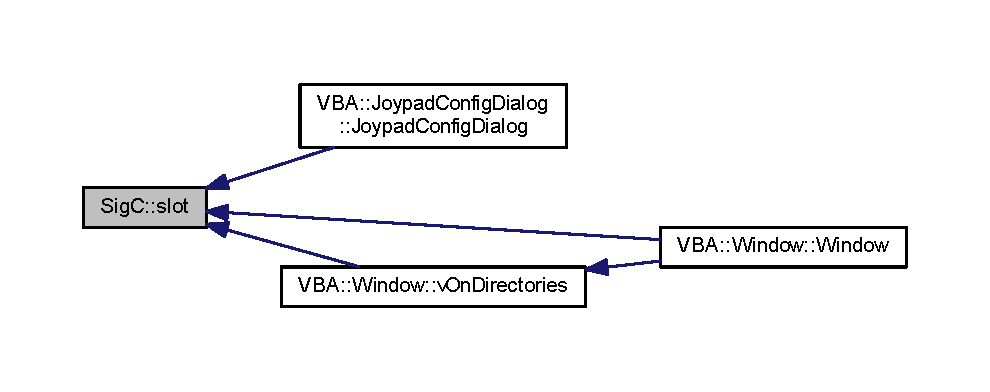
\includegraphics[width=350pt]{namespace_sig_c_a92e4f19202b77e78ac1db05f5a62f6b6_icgraph}
\end{center}
\end{figure}
\mbox{\Hypertarget{namespace_sig_c_a593d0d3f9fec3996bcdb781f14bff628}\label{namespace_sig_c_a593d0d3f9fec3996bcdb781f14bff628}} 
\index{SigC@{SigC}!slot@{slot}}
\index{slot@{slot}!SigC@{SigC}}
\subsubsection{\texorpdfstring{slot()}{slot()}\hspace{0.1cm}{\footnotesize\ttfamily [2/3]}}
{\footnotesize\ttfamily template$<$class T\+\_\+return , class T\+\_\+arg1 , class T\+\_\+obj1 , class T\+\_\+obj2 $>$ \\
Slot1$<$T\+\_\+return, T\+\_\+arg1$>$ Sig\+C\+::slot (\begin{DoxyParamCaption}\item[{T\+\_\+obj1 \&}]{\+\_\+\+A\+\_\+obj,  }\item[{T\+\_\+return(T\+\_\+obj2\+::$\ast$)(T\+\_\+arg1)}]{\+\_\+\+A\+\_\+func }\end{DoxyParamCaption})\hspace{0.3cm}{\ttfamily [inline]}}



sigccompat.\+h 파일의 42 번째 라인에서 정의되었습니다.


\begin{DoxyCode}
43 \{ return ::sigc::bound\_mem\_functor1<T\_return, T\_obj2, T\_arg1>
44              (\textcolor{keyword}{dynamic\_cast<} T\_obj1&\textcolor{keyword}{>}(\_A\_obj), \_A\_func); \}
\end{DoxyCode}
\mbox{\Hypertarget{namespace_sig_c_a894ae71a244ee5c71e891342ab536db1}\label{namespace_sig_c_a894ae71a244ee5c71e891342ab536db1}} 
\index{SigC@{SigC}!slot@{slot}}
\index{slot@{slot}!SigC@{SigC}}
\subsubsection{\texorpdfstring{slot()}{slot()}\hspace{0.1cm}{\footnotesize\ttfamily [3/3]}}
{\footnotesize\ttfamily template$<$class T\+\_\+return , class T\+\_\+arg1 , class T\+\_\+arg2 , class T\+\_\+obj1 , class T\+\_\+obj2 $>$ \\
Slot2$<$T\+\_\+return, T\+\_\+arg1,T\+\_\+arg2$>$ Sig\+C\+::slot (\begin{DoxyParamCaption}\item[{T\+\_\+obj1 \&}]{\+\_\+\+A\+\_\+obj,  }\item[{T\+\_\+return(T\+\_\+obj2\+::$\ast$)(T\+\_\+arg1, T\+\_\+arg2)}]{\+\_\+\+A\+\_\+func }\end{DoxyParamCaption})\hspace{0.3cm}{\ttfamily [inline]}}



sigccompat.\+h 파일의 48 번째 라인에서 정의되었습니다.


\begin{DoxyCode}
49 \{ return ::sigc::bound\_mem\_functor2<T\_return, T\_obj2, T\_arg1,T\_arg2>
50              (\textcolor{keyword}{dynamic\_cast<} T\_obj1&\textcolor{keyword}{>}(\_A\_obj), \_A\_func); \}
\end{DoxyCode}

\hypertarget{namespace_sm60_f_p_s}{}\section{Sm60\+F\+PS 네임스페이스 참조}
\label{namespace_sm60_f_p_s}\index{Sm60\+F\+PS@{Sm60\+F\+PS}}
\subsection*{변수}
\begin{DoxyCompactItemize}
\item 
float \mbox{\hyperlink{namespace_sm60_f_p_s_ae07dfcd12e7bffdd83bdeb522dcee371}{K\+\_\+f\+Cpu\+Speed}} = 98.\+0f
\item 
float \mbox{\hyperlink{namespace_sm60_f_p_s_aa558076e1e1de8036533a25ff4244778}{K\+\_\+f\+Target\+Fps}} = 60.\+0f $\ast$ K\+\_\+f\+Cpu\+Speed / 100
\item 
float \mbox{\hyperlink{namespace_sm60_f_p_s_ab3e0a346fa132eb958ae5622c813cb99}{K\+\_\+f\+DT}} = 1000.\+0f / K\+\_\+f\+Target\+Fps
\item 
\mbox{\hyperlink{_system_8h_a10e94b422ef0c20dcdec20d31a1f5049}{u32}} \mbox{\hyperlink{namespace_sm60_f_p_s_a8456d33b653d1463e8dff058f592d96a}{dw\+Time\+Elapse}}
\item 
\mbox{\hyperlink{_system_8h_a10e94b422ef0c20dcdec20d31a1f5049}{u32}} \mbox{\hyperlink{namespace_sm60_f_p_s_a13cb7b4b6ffee739d08614c86e2c632c}{dw\+Time0}}
\item 
\mbox{\hyperlink{_system_8h_a10e94b422ef0c20dcdec20d31a1f5049}{u32}} \mbox{\hyperlink{namespace_sm60_f_p_s_ab4c0541dfc24ac03a8eea11a8e9b862a}{dw\+Time1}}
\item 
\mbox{\hyperlink{_system_8h_a10e94b422ef0c20dcdec20d31a1f5049}{u32}} \mbox{\hyperlink{namespace_sm60_f_p_s_af16a9bcb3b2eba01862bc42cd189c524}{n\+Frame\+Cnt}}
\item 
float \mbox{\hyperlink{namespace_sm60_f_p_s_add2b9096a788d1dc088810430f7d30bf}{f\+Want\+F\+PS}}
\item 
float \mbox{\hyperlink{namespace_sm60_f_p_s_aee0246375d7c962cc9bca89f54df61a5}{f\+Cur\+F\+PS}}
\item 
bool \mbox{\hyperlink{namespace_sm60_f_p_s_a6399e3de21aba714f8c9df222d4cba31}{b\+Last\+Skip}}
\item 
\mbox{\hyperlink{_util_8cpp_a0ef32aa8672df19503a49fab2d0c8071}{int}} \mbox{\hyperlink{namespace_sm60_f_p_s_ae76f2581ada4617c563e8297832c86a2}{n\+Cur\+Speed}}
\item 
\mbox{\hyperlink{_util_8cpp_a0ef32aa8672df19503a49fab2d0c8071}{int}} \mbox{\hyperlink{namespace_sm60_f_p_s_a89c7f4412351b871a7e4fd3e8921d634}{b\+Save\+More\+C\+PU}}
\end{DoxyCompactItemize}


\subsection{변수 문서화}
\mbox{\Hypertarget{namespace_sm60_f_p_s_a6399e3de21aba714f8c9df222d4cba31}\label{namespace_sm60_f_p_s_a6399e3de21aba714f8c9df222d4cba31}} 
\index{Sm60\+F\+PS@{Sm60\+F\+PS}!b\+Last\+Skip@{b\+Last\+Skip}}
\index{b\+Last\+Skip@{b\+Last\+Skip}!Sm60\+F\+PS@{Sm60\+F\+PS}}
\subsubsection{\texorpdfstring{b\+Last\+Skip}{bLastSkip}}
{\footnotesize\ttfamily bool Sm60\+F\+P\+S\+::b\+Last\+Skip}



V\+B\+A.\+cpp 파일의 145 번째 라인에서 정의되었습니다.

\mbox{\Hypertarget{namespace_sm60_f_p_s_a89c7f4412351b871a7e4fd3e8921d634}\label{namespace_sm60_f_p_s_a89c7f4412351b871a7e4fd3e8921d634}} 
\index{Sm60\+F\+PS@{Sm60\+F\+PS}!b\+Save\+More\+C\+PU@{b\+Save\+More\+C\+PU}}
\index{b\+Save\+More\+C\+PU@{b\+Save\+More\+C\+PU}!Sm60\+F\+PS@{Sm60\+F\+PS}}
\subsubsection{\texorpdfstring{b\+Save\+More\+C\+PU}{bSaveMoreCPU}}
{\footnotesize\ttfamily \mbox{\hyperlink{_util_8cpp_a0ef32aa8672df19503a49fab2d0c8071}{int}} Sm60\+F\+P\+S\+::b\+Save\+More\+C\+PU}



V\+B\+A.\+cpp 파일의 147 번째 라인에서 정의되었습니다.

\mbox{\Hypertarget{namespace_sm60_f_p_s_a13cb7b4b6ffee739d08614c86e2c632c}\label{namespace_sm60_f_p_s_a13cb7b4b6ffee739d08614c86e2c632c}} 
\index{Sm60\+F\+PS@{Sm60\+F\+PS}!dw\+Time0@{dw\+Time0}}
\index{dw\+Time0@{dw\+Time0}!Sm60\+F\+PS@{Sm60\+F\+PS}}
\subsubsection{\texorpdfstring{dw\+Time0}{dwTime0}}
{\footnotesize\ttfamily \mbox{\hyperlink{_system_8h_a10e94b422ef0c20dcdec20d31a1f5049}{u32}} Sm60\+F\+P\+S\+::dw\+Time0}



V\+B\+A.\+cpp 파일의 140 번째 라인에서 정의되었습니다.

\mbox{\Hypertarget{namespace_sm60_f_p_s_ab4c0541dfc24ac03a8eea11a8e9b862a}\label{namespace_sm60_f_p_s_ab4c0541dfc24ac03a8eea11a8e9b862a}} 
\index{Sm60\+F\+PS@{Sm60\+F\+PS}!dw\+Time1@{dw\+Time1}}
\index{dw\+Time1@{dw\+Time1}!Sm60\+F\+PS@{Sm60\+F\+PS}}
\subsubsection{\texorpdfstring{dw\+Time1}{dwTime1}}
{\footnotesize\ttfamily \mbox{\hyperlink{_system_8h_a10e94b422ef0c20dcdec20d31a1f5049}{u32}} Sm60\+F\+P\+S\+::dw\+Time1}



V\+B\+A.\+cpp 파일의 141 번째 라인에서 정의되었습니다.

\mbox{\Hypertarget{namespace_sm60_f_p_s_a8456d33b653d1463e8dff058f592d96a}\label{namespace_sm60_f_p_s_a8456d33b653d1463e8dff058f592d96a}} 
\index{Sm60\+F\+PS@{Sm60\+F\+PS}!dw\+Time\+Elapse@{dw\+Time\+Elapse}}
\index{dw\+Time\+Elapse@{dw\+Time\+Elapse}!Sm60\+F\+PS@{Sm60\+F\+PS}}
\subsubsection{\texorpdfstring{dw\+Time\+Elapse}{dwTimeElapse}}
{\footnotesize\ttfamily \mbox{\hyperlink{_system_8h_a10e94b422ef0c20dcdec20d31a1f5049}{u32}} Sm60\+F\+P\+S\+::dw\+Time\+Elapse}



V\+B\+A.\+cpp 파일의 139 번째 라인에서 정의되었습니다.

\mbox{\Hypertarget{namespace_sm60_f_p_s_aee0246375d7c962cc9bca89f54df61a5}\label{namespace_sm60_f_p_s_aee0246375d7c962cc9bca89f54df61a5}} 
\index{Sm60\+F\+PS@{Sm60\+F\+PS}!f\+Cur\+F\+PS@{f\+Cur\+F\+PS}}
\index{f\+Cur\+F\+PS@{f\+Cur\+F\+PS}!Sm60\+F\+PS@{Sm60\+F\+PS}}
\subsubsection{\texorpdfstring{f\+Cur\+F\+PS}{fCurFPS}}
{\footnotesize\ttfamily float Sm60\+F\+P\+S\+::f\+Cur\+F\+PS}



V\+B\+A.\+cpp 파일의 144 번째 라인에서 정의되었습니다.

\mbox{\Hypertarget{namespace_sm60_f_p_s_add2b9096a788d1dc088810430f7d30bf}\label{namespace_sm60_f_p_s_add2b9096a788d1dc088810430f7d30bf}} 
\index{Sm60\+F\+PS@{Sm60\+F\+PS}!f\+Want\+F\+PS@{f\+Want\+F\+PS}}
\index{f\+Want\+F\+PS@{f\+Want\+F\+PS}!Sm60\+F\+PS@{Sm60\+F\+PS}}
\subsubsection{\texorpdfstring{f\+Want\+F\+PS}{fWantFPS}}
{\footnotesize\ttfamily float Sm60\+F\+P\+S\+::f\+Want\+F\+PS}



V\+B\+A.\+cpp 파일의 143 번째 라인에서 정의되었습니다.

\mbox{\Hypertarget{namespace_sm60_f_p_s_ae07dfcd12e7bffdd83bdeb522dcee371}\label{namespace_sm60_f_p_s_ae07dfcd12e7bffdd83bdeb522dcee371}} 
\index{Sm60\+F\+PS@{Sm60\+F\+PS}!K\+\_\+f\+Cpu\+Speed@{K\+\_\+f\+Cpu\+Speed}}
\index{K\+\_\+f\+Cpu\+Speed@{K\+\_\+f\+Cpu\+Speed}!Sm60\+F\+PS@{Sm60\+F\+PS}}
\subsubsection{\texorpdfstring{K\+\_\+f\+Cpu\+Speed}{K\_fCpuSpeed}}
{\footnotesize\ttfamily float Sm60\+F\+P\+S\+::\+K\+\_\+f\+Cpu\+Speed = 98.\+0f}



V\+B\+A.\+cpp 파일의 135 번째 라인에서 정의되었습니다.

\mbox{\Hypertarget{namespace_sm60_f_p_s_ab3e0a346fa132eb958ae5622c813cb99}\label{namespace_sm60_f_p_s_ab3e0a346fa132eb958ae5622c813cb99}} 
\index{Sm60\+F\+PS@{Sm60\+F\+PS}!K\+\_\+f\+DT@{K\+\_\+f\+DT}}
\index{K\+\_\+f\+DT@{K\+\_\+f\+DT}!Sm60\+F\+PS@{Sm60\+F\+PS}}
\subsubsection{\texorpdfstring{K\+\_\+f\+DT}{K\_fDT}}
{\footnotesize\ttfamily float Sm60\+F\+P\+S\+::\+K\+\_\+f\+DT = 1000.\+0f / K\+\_\+f\+Target\+Fps}



V\+B\+A.\+cpp 파일의 137 번째 라인에서 정의되었습니다.

\mbox{\Hypertarget{namespace_sm60_f_p_s_aa558076e1e1de8036533a25ff4244778}\label{namespace_sm60_f_p_s_aa558076e1e1de8036533a25ff4244778}} 
\index{Sm60\+F\+PS@{Sm60\+F\+PS}!K\+\_\+f\+Target\+Fps@{K\+\_\+f\+Target\+Fps}}
\index{K\+\_\+f\+Target\+Fps@{K\+\_\+f\+Target\+Fps}!Sm60\+F\+PS@{Sm60\+F\+PS}}
\subsubsection{\texorpdfstring{K\+\_\+f\+Target\+Fps}{K\_fTargetFps}}
{\footnotesize\ttfamily float Sm60\+F\+P\+S\+::\+K\+\_\+f\+Target\+Fps = 60.\+0f $\ast$ K\+\_\+f\+Cpu\+Speed / 100}



V\+B\+A.\+cpp 파일의 136 번째 라인에서 정의되었습니다.

\mbox{\Hypertarget{namespace_sm60_f_p_s_ae76f2581ada4617c563e8297832c86a2}\label{namespace_sm60_f_p_s_ae76f2581ada4617c563e8297832c86a2}} 
\index{Sm60\+F\+PS@{Sm60\+F\+PS}!n\+Cur\+Speed@{n\+Cur\+Speed}}
\index{n\+Cur\+Speed@{n\+Cur\+Speed}!Sm60\+F\+PS@{Sm60\+F\+PS}}
\subsubsection{\texorpdfstring{n\+Cur\+Speed}{nCurSpeed}}
{\footnotesize\ttfamily \mbox{\hyperlink{_util_8cpp_a0ef32aa8672df19503a49fab2d0c8071}{int}} Sm60\+F\+P\+S\+::n\+Cur\+Speed}



V\+B\+A.\+cpp 파일의 146 번째 라인에서 정의되었습니다.

\mbox{\Hypertarget{namespace_sm60_f_p_s_af16a9bcb3b2eba01862bc42cd189c524}\label{namespace_sm60_f_p_s_af16a9bcb3b2eba01862bc42cd189c524}} 
\index{Sm60\+F\+PS@{Sm60\+F\+PS}!n\+Frame\+Cnt@{n\+Frame\+Cnt}}
\index{n\+Frame\+Cnt@{n\+Frame\+Cnt}!Sm60\+F\+PS@{Sm60\+F\+PS}}
\subsubsection{\texorpdfstring{n\+Frame\+Cnt}{nFrameCnt}}
{\footnotesize\ttfamily \mbox{\hyperlink{_system_8h_a10e94b422ef0c20dcdec20d31a1f5049}{u32}} Sm60\+F\+P\+S\+::n\+Frame\+Cnt}



V\+B\+A.\+cpp 파일의 142 번째 라인에서 정의되었습니다.


\hypertarget{namespacestd}{}\section{std 네임스페이스 참조}
\label{namespacestd}\index{std@{std}}

\hypertarget{namespace_v_b_a}{}\section{V\+BA 네임스페이스 참조}
\label{namespace_v_b_a}\index{V\+BA@{V\+BA}}
\subsection*{네임스페이스}
\begin{DoxyCompactItemize}
\item 
 \mbox{\hyperlink{namespace_v_b_a_1_1_config}{Config}}
\end{DoxyCompactItemize}
\subsection*{클래스}
\begin{DoxyCompactItemize}
\item 
class \mbox{\hyperlink{class_v_b_a_1_1_image_menu_item}{Image\+Menu\+Item}}
\item 
class \mbox{\hyperlink{class_v_b_a_1_1_joypad_config}{Joypad\+Config}}
\item 
class \mbox{\hyperlink{class_v_b_a_1_1_joypad_config_dialog}{Joypad\+Config\+Dialog}}
\item 
class \mbox{\hyperlink{class_v_b_a_1_1_keymap}{Keymap}}
\item 
class \mbox{\hyperlink{class_v_b_a_1_1_menu_item}{Menu\+Item}}
\item 
class \mbox{\hyperlink{class_v_b_a_1_1_screen_area}{Screen\+Area}}
\item 
class \mbox{\hyperlink{class_v_b_a_1_1_window}{Window}}
\end{DoxyCompactItemize}
\subsection*{함수}
\begin{DoxyCompactItemize}
\item 
\mbox{\hyperlink{class_v_b_a_accd36b6c101a516c50cf8288976739c4}{Filter2x}} \mbox{\hyperlink{namespace_v_b_a_a2a6c0188179e4ee017369e21d8e6f268}{pv\+Get\+Filter2x}} (\mbox{\hyperlink{class_v_b_a_a1683020d7324daf3bda627d0d3658e3e}{E\+Filter2x}} \+\_\+e\+Filter2x, \mbox{\hyperlink{class_v_b_a_a6ec41ea038b4ea42eb8d9ea59d3eb4c5}{E\+Filter\+Depth}} \+\_\+e\+Depth)
\item 
\mbox{\hyperlink{class_v_b_a_a3269ee707f37ad255f2b7b0f20921158}{Filter\+IB}} \mbox{\hyperlink{namespace_v_b_a_ad5980a2981a7b766dce52ebc49a987bb}{pv\+Get\+Filter\+IB}} (\mbox{\hyperlink{class_v_b_a_a304ffeb9f4a8b26e7fa4e2eb620d780f}{E\+Filter\+IB}} \+\_\+e\+Filter\+IB, \mbox{\hyperlink{class_v_b_a_a6ec41ea038b4ea42eb8d9ea59d3eb4c5}{E\+Filter\+Depth}} \+\_\+e\+Depth)
\item 
std\+::string \mbox{\hyperlink{namespace_v_b_a_ad362cd74dbe4234578a0a124f3522dcf}{s\+Cut\+Suffix}} (\mbox{\hyperlink{getopt1_8c_a2c212835823e3c54a8ab6d95c652660e}{const}} std\+::string \&\+\_\+rs\+String, \mbox{\hyperlink{getopt1_8c_a2c212835823e3c54a8ab6d95c652660e}{const}} std\+::string \&\+\_\+rs\+Sep)
\item 
Glib\+::ustring \mbox{\hyperlink{namespace_v_b_a_aa627086c3b36799bc10a36048e5c5b68}{s\+Cut\+Suffix}} (\mbox{\hyperlink{getopt1_8c_a2c212835823e3c54a8ab6d95c652660e}{const}} Glib\+::ustring \&\+\_\+rs\+String, \mbox{\hyperlink{getopt1_8c_a2c212835823e3c54a8ab6d95c652660e}{const}} Glib\+::ustring \&\+\_\+rs\+Sep)
\item 
bool \mbox{\hyperlink{namespace_v_b_a_ad93561fe4528e04192e066e138c3572b}{b\+Has\+Suffix}} (\mbox{\hyperlink{getopt1_8c_a2c212835823e3c54a8ab6d95c652660e}{const}} Glib\+::ustring \&\+\_\+rs\+String, \mbox{\hyperlink{getopt1_8c_a2c212835823e3c54a8ab6d95c652660e}{const}} Glib\+::ustring \&\+\_\+rs\+Suffix, bool \+\_\+b\+Case\+Sensitive)
\end{DoxyCompactItemize}


\subsection{함수 문서화}
\mbox{\Hypertarget{namespace_v_b_a_ad93561fe4528e04192e066e138c3572b}\label{namespace_v_b_a_ad93561fe4528e04192e066e138c3572b}} 
\index{V\+BA@{V\+BA}!b\+Has\+Suffix@{b\+Has\+Suffix}}
\index{b\+Has\+Suffix@{b\+Has\+Suffix}!V\+BA@{V\+BA}}
\subsubsection{\texorpdfstring{b\+Has\+Suffix()}{bHasSuffix()}}
{\footnotesize\ttfamily bool V\+B\+A\+::b\+Has\+Suffix (\begin{DoxyParamCaption}\item[{\mbox{\hyperlink{getopt1_8c_a2c212835823e3c54a8ab6d95c652660e}{const}} Glib\+::ustring \&}]{\+\_\+rs\+String,  }\item[{\mbox{\hyperlink{getopt1_8c_a2c212835823e3c54a8ab6d95c652660e}{const}} Glib\+::ustring \&}]{\+\_\+rs\+Suffix,  }\item[{bool}]{\+\_\+b\+Case\+Sensitive }\end{DoxyParamCaption})}



tools.\+cpp 파일의 36 번째 라인에서 정의되었습니다.


\begin{DoxyCode}
39 \{
40   \textcolor{keywordflow}{if} (\_rsSuffix.size() > \_rsString.size())
41   \{
42     \textcolor{keywordflow}{return} \textcolor{keyword}{false};
43   \}
44 
45   Glib::ustring sEnd = \_rsString.substr(\_rsString.size() - \_rsSuffix.size());
46 
47   \textcolor{keywordflow}{if} (\_bCaseSensitive)
48   \{
49     \textcolor{keywordflow}{if} (\_rsSuffix == sEnd)
50     \{
51       \textcolor{keywordflow}{return} \textcolor{keyword}{true};
52     \}
53   \}
54   \textcolor{keywordflow}{else}
55   \{
56     \textcolor{keywordflow}{if} (\_rsSuffix.lowercase() == sEnd.lowercase())
57     \{
58       \textcolor{keywordflow}{return} \textcolor{keyword}{true};
59     \}
60   \}
61 
62   \textcolor{keywordflow}{return} \textcolor{keyword}{false};
63 \}
\end{DoxyCode}
이 함수를 호출하는 함수들에 대한 그래프입니다.\+:
\nopagebreak
\begin{figure}[H]
\begin{center}
\leavevmode
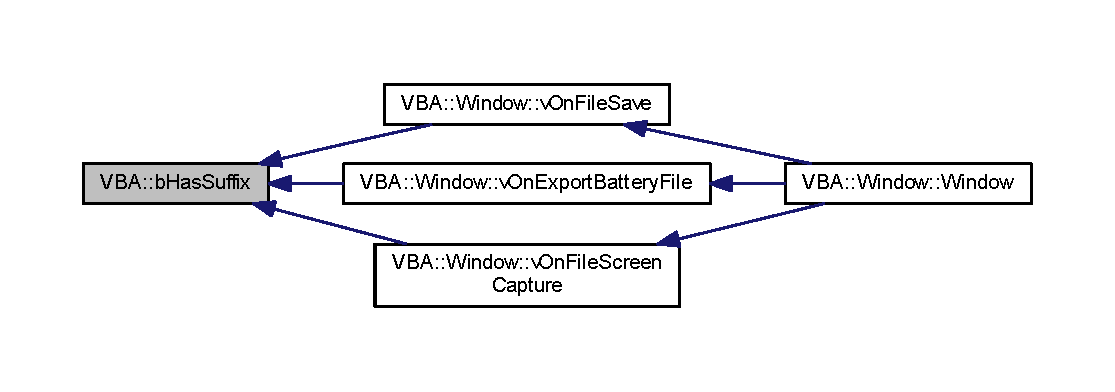
\includegraphics[width=350pt]{namespace_v_b_a_ad93561fe4528e04192e066e138c3572b_icgraph}
\end{center}
\end{figure}
\mbox{\Hypertarget{namespace_v_b_a_a2a6c0188179e4ee017369e21d8e6f268}\label{namespace_v_b_a_a2a6c0188179e4ee017369e21d8e6f268}} 
\index{V\+BA@{V\+BA}!pv\+Get\+Filter2x@{pv\+Get\+Filter2x}}
\index{pv\+Get\+Filter2x@{pv\+Get\+Filter2x}!V\+BA@{V\+BA}}
\subsubsection{\texorpdfstring{pv\+Get\+Filter2x()}{pvGetFilter2x()}}
{\footnotesize\ttfamily \mbox{\hyperlink{class_v_b_a_accd36b6c101a516c50cf8288976739c4}{Filter2x}} V\+B\+A\+::pv\+Get\+Filter2x (\begin{DoxyParamCaption}\item[{\mbox{\hyperlink{class_v_b_a_a1683020d7324daf3bda627d0d3658e3e}{E\+Filter2x}}}]{\+\_\+e\+Filter2x,  }\item[{\mbox{\hyperlink{class_v_b_a_a6ec41ea038b4ea42eb8d9ea59d3eb4c5}{E\+Filter\+Depth}}}]{\+\_\+e\+Depth }\end{DoxyParamCaption})}



filters.\+cpp 파일의 49 번째 라인에서 정의되었습니다.


\begin{DoxyCode}
50 \{
51   \textcolor{keywordflow}{return} apvFilters2x[\_eFilter2x][\_eDepth];
52 \}
\end{DoxyCode}
이 함수를 호출하는 함수들에 대한 그래프입니다.\+:
\nopagebreak
\begin{figure}[H]
\begin{center}
\leavevmode
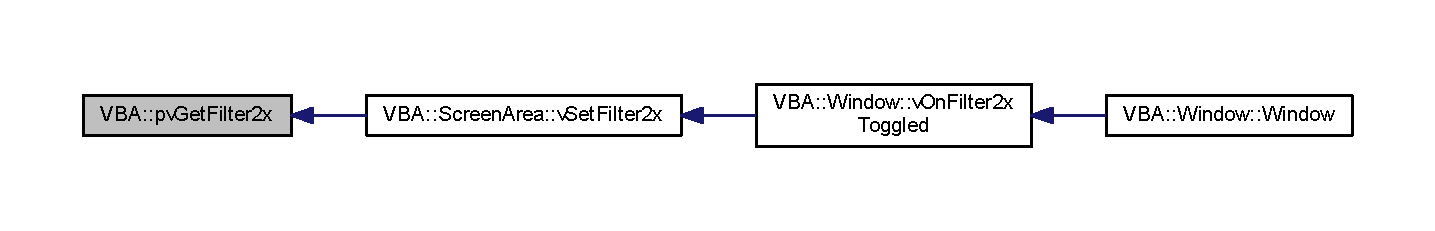
\includegraphics[width=350pt]{namespace_v_b_a_a2a6c0188179e4ee017369e21d8e6f268_icgraph}
\end{center}
\end{figure}
\mbox{\Hypertarget{namespace_v_b_a_ad5980a2981a7b766dce52ebc49a987bb}\label{namespace_v_b_a_ad5980a2981a7b766dce52ebc49a987bb}} 
\index{V\+BA@{V\+BA}!pv\+Get\+Filter\+IB@{pv\+Get\+Filter\+IB}}
\index{pv\+Get\+Filter\+IB@{pv\+Get\+Filter\+IB}!V\+BA@{V\+BA}}
\subsubsection{\texorpdfstring{pv\+Get\+Filter\+I\+B()}{pvGetFilterIB()}}
{\footnotesize\ttfamily \mbox{\hyperlink{class_v_b_a_a3269ee707f37ad255f2b7b0f20921158}{Filter\+IB}} V\+B\+A\+::pv\+Get\+Filter\+IB (\begin{DoxyParamCaption}\item[{\mbox{\hyperlink{class_v_b_a_a304ffeb9f4a8b26e7fa4e2eb620d780f}{E\+Filter\+IB}}}]{\+\_\+e\+Filter\+IB,  }\item[{\mbox{\hyperlink{class_v_b_a_a6ec41ea038b4ea42eb8d9ea59d3eb4c5}{E\+Filter\+Depth}}}]{\+\_\+e\+Depth }\end{DoxyParamCaption})}



filters.\+cpp 파일의 54 번째 라인에서 정의되었습니다.


\begin{DoxyCode}
55 \{
56   \textcolor{keywordflow}{return} apvFiltersIB[\_eFilterIB][\_eDepth];
57 \}
\end{DoxyCode}
이 함수를 호출하는 함수들에 대한 그래프입니다.\+:
\nopagebreak
\begin{figure}[H]
\begin{center}
\leavevmode
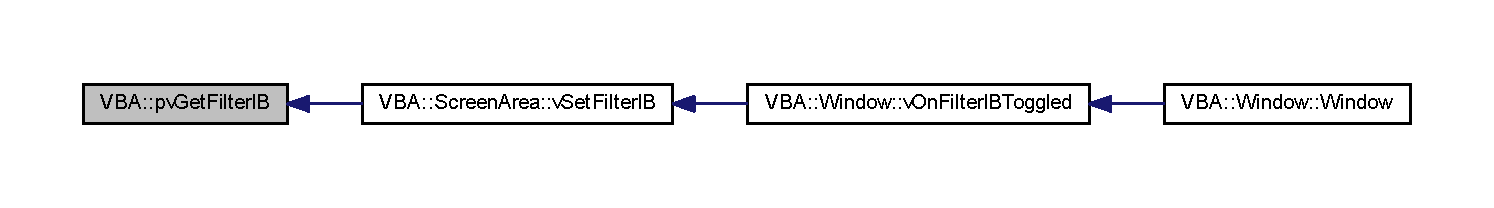
\includegraphics[width=350pt]{namespace_v_b_a_ad5980a2981a7b766dce52ebc49a987bb_icgraph}
\end{center}
\end{figure}
\mbox{\Hypertarget{namespace_v_b_a_ad362cd74dbe4234578a0a124f3522dcf}\label{namespace_v_b_a_ad362cd74dbe4234578a0a124f3522dcf}} 
\index{V\+BA@{V\+BA}!s\+Cut\+Suffix@{s\+Cut\+Suffix}}
\index{s\+Cut\+Suffix@{s\+Cut\+Suffix}!V\+BA@{V\+BA}}
\subsubsection{\texorpdfstring{s\+Cut\+Suffix()}{sCutSuffix()}\hspace{0.1cm}{\footnotesize\ttfamily [1/2]}}
{\footnotesize\ttfamily std\+::string V\+B\+A\+::s\+Cut\+Suffix (\begin{DoxyParamCaption}\item[{\mbox{\hyperlink{getopt1_8c_a2c212835823e3c54a8ab6d95c652660e}{const}} std\+::string \&}]{\+\_\+rs\+String,  }\item[{\mbox{\hyperlink{getopt1_8c_a2c212835823e3c54a8ab6d95c652660e}{const}} std\+::string \&}]{\+\_\+rs\+Sep }\end{DoxyParamCaption})}



tools.\+cpp 파일의 24 번째 라인에서 정의되었습니다.


\begin{DoxyCode}
26 \{
27   \textcolor{keywordflow}{return} \_rsString.substr(0, \_rsString.find\_last\_of(\_rsSep));
28 \}
\end{DoxyCode}
이 함수를 호출하는 함수들에 대한 그래프입니다.\+:
\nopagebreak
\begin{figure}[H]
\begin{center}
\leavevmode
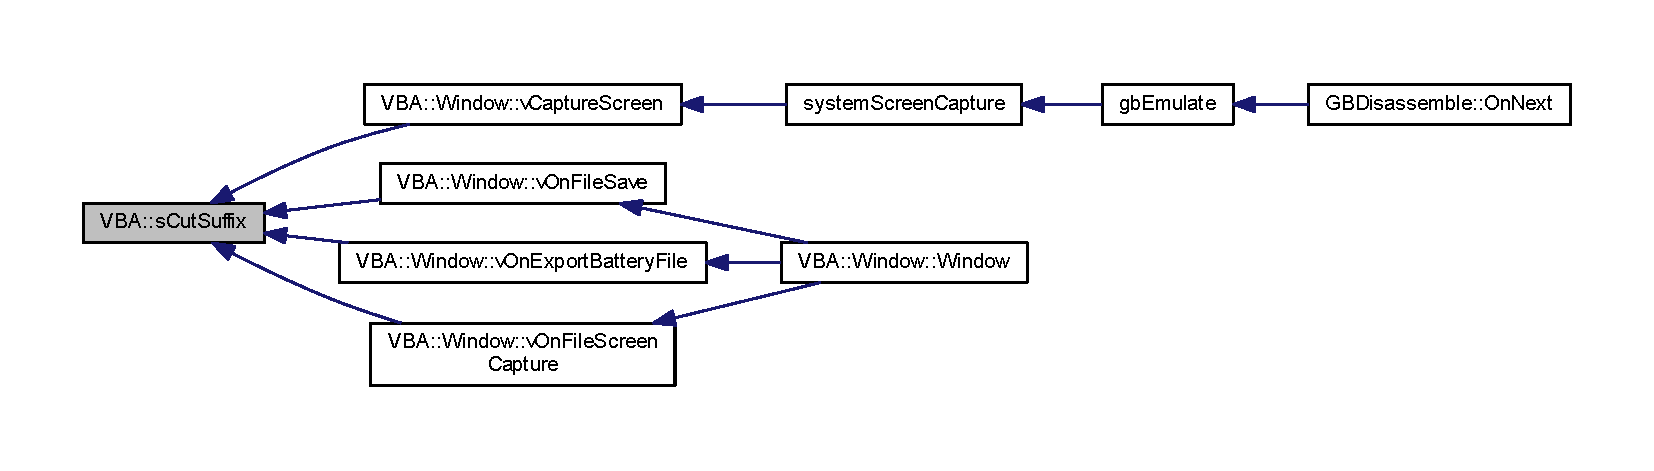
\includegraphics[width=350pt]{namespace_v_b_a_ad362cd74dbe4234578a0a124f3522dcf_icgraph}
\end{center}
\end{figure}
\mbox{\Hypertarget{namespace_v_b_a_aa627086c3b36799bc10a36048e5c5b68}\label{namespace_v_b_a_aa627086c3b36799bc10a36048e5c5b68}} 
\index{V\+BA@{V\+BA}!s\+Cut\+Suffix@{s\+Cut\+Suffix}}
\index{s\+Cut\+Suffix@{s\+Cut\+Suffix}!V\+BA@{V\+BA}}
\subsubsection{\texorpdfstring{s\+Cut\+Suffix()}{sCutSuffix()}\hspace{0.1cm}{\footnotesize\ttfamily [2/2]}}
{\footnotesize\ttfamily Glib\+::ustring V\+B\+A\+::s\+Cut\+Suffix (\begin{DoxyParamCaption}\item[{\mbox{\hyperlink{getopt1_8c_a2c212835823e3c54a8ab6d95c652660e}{const}} Glib\+::ustring \&}]{\+\_\+rs\+String,  }\item[{\mbox{\hyperlink{getopt1_8c_a2c212835823e3c54a8ab6d95c652660e}{const}} Glib\+::ustring \&}]{\+\_\+rs\+Sep }\end{DoxyParamCaption})}



tools.\+cpp 파일의 30 번째 라인에서 정의되었습니다.


\begin{DoxyCode}
32 \{
33   \textcolor{keywordflow}{return} \_rsString.substr(0, \_rsString.find\_last\_of(\_rsSep));
34 \}
\end{DoxyCode}

\hypertarget{namespace_v_b_a_1_1_config}{}\section{V\+BA\+:\+:Config 네임스페이스 참조}
\label{namespace_v_b_a_1_1_config}\index{V\+B\+A\+::\+Config@{V\+B\+A\+::\+Config}}
\subsection*{클래스}
\begin{DoxyCompactItemize}
\item 
class \mbox{\hyperlink{class_v_b_a_1_1_config_1_1_file}{File}}
\item 
class \mbox{\hyperlink{class_v_b_a_1_1_config_1_1_key_not_found}{Key\+Not\+Found}}
\item 
class \mbox{\hyperlink{class_v_b_a_1_1_config_1_1_line}{Line}}
\item 
class \mbox{\hyperlink{class_v_b_a_1_1_config_1_1_not_found}{Not\+Found}}
\item 
class \mbox{\hyperlink{class_v_b_a_1_1_config_1_1_section}{Section}}
\item 
class \mbox{\hyperlink{class_v_b_a_1_1_config_1_1_section_not_found}{Section\+Not\+Found}}
\end{DoxyCompactItemize}
\subsection*{함수}
\begin{DoxyCompactItemize}
\item 
std\+::ostream \& \mbox{\hyperlink{namespace_v_b_a_1_1_config_ae8f486bb30184451079a550ba9de3d7e}{operator$<$$<$}} (std\+::ostream \&\+\_\+ro\+Out, \mbox{\hyperlink{getopt1_8c_a2c212835823e3c54a8ab6d95c652660e}{const}} \mbox{\hyperlink{class_v_b_a_1_1_config_1_1_file}{File}} \&\+\_\+ro\+File)
\end{DoxyCompactItemize}


\subsection{함수 문서화}
\mbox{\Hypertarget{namespace_v_b_a_1_1_config_ae8f486bb30184451079a550ba9de3d7e}\label{namespace_v_b_a_1_1_config_ae8f486bb30184451079a550ba9de3d7e}} 
\index{V\+B\+A\+::\+Config@{V\+B\+A\+::\+Config}!operator$<$$<$@{operator$<$$<$}}
\index{operator$<$$<$@{operator$<$$<$}!V\+B\+A\+::\+Config@{V\+B\+A\+::\+Config}}
\subsubsection{\texorpdfstring{operator$<$$<$()}{operator<<()}}
{\footnotesize\ttfamily std\+::ostream \& V\+B\+A\+::\+Config\+::operator$<$$<$ (\begin{DoxyParamCaption}\item[{std\+::ostream \&}]{\+\_\+ro\+Out,  }\item[{\mbox{\hyperlink{getopt1_8c_a2c212835823e3c54a8ab6d95c652660e}{const}} \mbox{\hyperlink{class_v_b_a_1_1_config_1_1_file}{File}} \&}]{\+\_\+ro\+File }\end{DoxyParamCaption})}



configfile.\+cpp 파일의 240 번째 라인에서 정의되었습니다.


\begin{DoxyCode}
241 \{
242   \textcolor{keywordflow}{for} (File::const\_iterator poSection = \_roFile.begin();
243        poSection != \_roFile.end();
244        poSection++)
245   \{
246     \textcolor{keywordtype}{string} sName = \textcolor{stringliteral}{"["} + poSection->sGetName() + \textcolor{stringliteral}{"]\(\backslash\)n"};
247     \_roOut << sName;
248 
249     \textcolor{keywordflow}{for} (Section::const\_iterator poLine = poSection->begin();
250          poLine != poSection->end();
251          poLine++)
252     \{
253       \textcolor{keywordtype}{string} sLine = poLine->m\_sKey + \textcolor{stringliteral}{"="} + poLine->m\_sValue + \textcolor{stringliteral}{"\(\backslash\)n"};
254       \_roOut << sLine;
255     \}
256     \_roOut << \textcolor{stringliteral}{"\(\backslash\)n"};
257   \}
258   \textcolor{keywordflow}{return} \_roOut;
259 \}
\end{DoxyCode}
이 함수 내부에서 호출하는 함수들에 대한 그래프입니다.\+:
\nopagebreak
\begin{figure}[H]
\begin{center}
\leavevmode
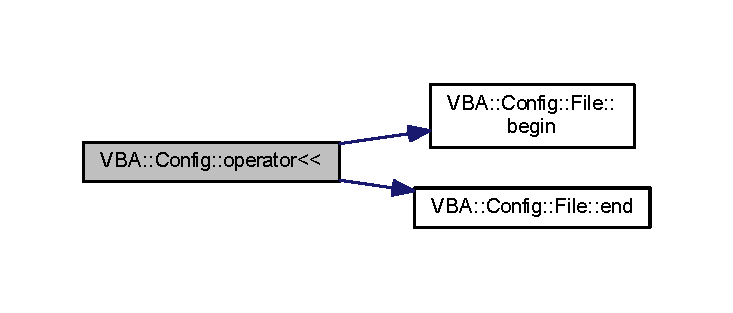
\includegraphics[width=350pt]{namespace_v_b_a_1_1_config_ae8f486bb30184451079a550ba9de3d7e_cgraph}
\end{center}
\end{figure}

\hypertarget{namespace_win_helper}{}\section{Win\+Helper 네임스페이스 참조}
\label{namespace_win_helper}\index{Win\+Helper@{Win\+Helper}}
\subsection*{클래스}
\begin{DoxyCompactItemize}
\item 
class \mbox{\hyperlink{class_win_helper_1_1_c_critical_section}{C\+Critical\+Section}}
\item 
class \mbox{\hyperlink{class_win_helper_1_1_c_defer_window_pos}{C\+Defer\+Window\+Pos}}
\item 
class \mbox{\hyperlink{class_win_helper_1_1_c_point}{C\+Point}}
\item 
class \mbox{\hyperlink{class_win_helper_1_1_c_rect}{C\+Rect}}
\item 
class \mbox{\hyperlink{class_win_helper_1_1_c_scroll_info}{C\+Scroll\+Info}}
\item 
class \mbox{\hyperlink{class_win_helper_1_1_c_size}{C\+Size}}
\end{DoxyCompactItemize}
\subsection*{함수}
\begin{DoxyCompactItemize}
\item 
bool \mbox{\hyperlink{namespace_win_helper_aacb2f91c6ca28b7a5b4b87e52cc2ab9f}{Is\+Shift\+Pressed}} ()
\item 
bool \mbox{\hyperlink{namespace_win_helper_a7eb0bf2b37a02c9fd467b7258a856148}{Is\+Alt\+Pressed}} ()
\item 
bool \mbox{\hyperlink{namespace_win_helper_a0bf0eb5c03232357051e8b4c552a5792}{Is\+Control\+Pressed}} ()
\item 
H\+I\+C\+ON \mbox{\hyperlink{namespace_win_helper_a2ce42916bda6434a5432df1ea8071183}{Load\+Icon16x16}} (H\+I\+N\+S\+T\+A\+N\+CE h\+Inst, U\+I\+NT u\+ID)
\end{DoxyCompactItemize}


\subsection{함수 문서화}
\mbox{\Hypertarget{namespace_win_helper_a7eb0bf2b37a02c9fd467b7258a856148}\label{namespace_win_helper_a7eb0bf2b37a02c9fd467b7258a856148}} 
\index{Win\+Helper@{Win\+Helper}!Is\+Alt\+Pressed@{Is\+Alt\+Pressed}}
\index{Is\+Alt\+Pressed@{Is\+Alt\+Pressed}!Win\+Helper@{Win\+Helper}}
\subsubsection{\texorpdfstring{Is\+Alt\+Pressed()}{IsAltPressed()}}
{\footnotesize\ttfamily bool Win\+Helper\+::\+Is\+Alt\+Pressed (\begin{DoxyParamCaption}{ }\end{DoxyParamCaption})\hspace{0.3cm}{\ttfamily [inline]}}



Win\+Helper.\+h 파일의 192 번째 라인에서 정의되었습니다.


\begin{DoxyCode}
193     \{
194       \textcolor{keywordflow}{return} GetKeyState(VK\_MENU) & 0x8000 ? true : \textcolor{keyword}{false};
195     \}
\end{DoxyCode}
\mbox{\Hypertarget{namespace_win_helper_a0bf0eb5c03232357051e8b4c552a5792}\label{namespace_win_helper_a0bf0eb5c03232357051e8b4c552a5792}} 
\index{Win\+Helper@{Win\+Helper}!Is\+Control\+Pressed@{Is\+Control\+Pressed}}
\index{Is\+Control\+Pressed@{Is\+Control\+Pressed}!Win\+Helper@{Win\+Helper}}
\subsubsection{\texorpdfstring{Is\+Control\+Pressed()}{IsControlPressed()}}
{\footnotesize\ttfamily bool Win\+Helper\+::\+Is\+Control\+Pressed (\begin{DoxyParamCaption}{ }\end{DoxyParamCaption})\hspace{0.3cm}{\ttfamily [inline]}}



Win\+Helper.\+h 파일의 197 번째 라인에서 정의되었습니다.


\begin{DoxyCode}
198     \{
199       \textcolor{keywordflow}{return} GetKeyState(VK\_CONTROL) & 0x8000 ? true : \textcolor{keyword}{false};
200     \}
\end{DoxyCode}
\mbox{\Hypertarget{namespace_win_helper_aacb2f91c6ca28b7a5b4b87e52cc2ab9f}\label{namespace_win_helper_aacb2f91c6ca28b7a5b4b87e52cc2ab9f}} 
\index{Win\+Helper@{Win\+Helper}!Is\+Shift\+Pressed@{Is\+Shift\+Pressed}}
\index{Is\+Shift\+Pressed@{Is\+Shift\+Pressed}!Win\+Helper@{Win\+Helper}}
\subsubsection{\texorpdfstring{Is\+Shift\+Pressed()}{IsShiftPressed()}}
{\footnotesize\ttfamily bool Win\+Helper\+::\+Is\+Shift\+Pressed (\begin{DoxyParamCaption}{ }\end{DoxyParamCaption})\hspace{0.3cm}{\ttfamily [inline]}}



Win\+Helper.\+h 파일의 187 번째 라인에서 정의되었습니다.


\begin{DoxyCode}
188     \{
189       \textcolor{keywordflow}{return} GetKeyState(VK\_SHIFT) & 0x8000 ? true : \textcolor{keyword}{false};
190     \}
\end{DoxyCode}
\mbox{\Hypertarget{namespace_win_helper_a2ce42916bda6434a5432df1ea8071183}\label{namespace_win_helper_a2ce42916bda6434a5432df1ea8071183}} 
\index{Win\+Helper@{Win\+Helper}!Load\+Icon16x16@{Load\+Icon16x16}}
\index{Load\+Icon16x16@{Load\+Icon16x16}!Win\+Helper@{Win\+Helper}}
\subsubsection{\texorpdfstring{Load\+Icon16x16()}{LoadIcon16x16()}}
{\footnotesize\ttfamily H\+I\+C\+ON Win\+Helper\+::\+Load\+Icon16x16 (\begin{DoxyParamCaption}\item[{H\+I\+N\+S\+T\+A\+N\+CE}]{h\+Inst,  }\item[{U\+I\+NT}]{u\+ID }\end{DoxyParamCaption})\hspace{0.3cm}{\ttfamily [inline]}}



Win\+Helper.\+h 파일의 202 번째 라인에서 정의되었습니다.


\begin{DoxyCode}
205     \{
206       \textcolor{keywordflow}{return} \textcolor{keyword}{reinterpret\_cast<}HICON\textcolor{keyword}{>}( ::LoadImage( hInst, MAKEINTRESOURCE( uID ), IMAGE\_ICON, 16, 16, 
      LR\_DEFAULTCOLOR ) );
207     \}
\end{DoxyCode}

\chapter{클래스 문서화}
\hypertarget{struct___mem_file}{}\section{\+\_\+\+Mem\+File 구조체 참조}
\label{struct___mem_file}\index{\+\_\+\+Mem\+File@{\+\_\+\+Mem\+File}}


\+\_\+\+Mem\+File에 대한 협력 다이어그램\+:\nopagebreak
\begin{figure}[H]
\begin{center}
\leavevmode
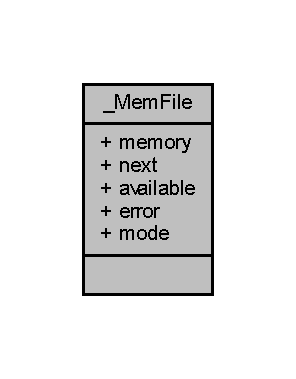
\includegraphics[width=142pt]{struct___mem_file__coll__graph}
\end{center}
\end{figure}
\subsection*{Public 속성}
\begin{DoxyCompactItemize}
\item 
char $\ast$ \mbox{\hyperlink{struct___mem_file_a62a96f96df82e23ef6dace974e19b18c}{memory}}
\item 
char $\ast$ \mbox{\hyperlink{struct___mem_file_aa15859f66ae2eb41245e4ba88486d67f}{next}}
\item 
\mbox{\hyperlink{_util_8cpp_a0ef32aa8672df19503a49fab2d0c8071}{int}} \mbox{\hyperlink{struct___mem_file_a1f48066353e37cf16c9a0065abecf238}{available}}
\item 
\mbox{\hyperlink{_util_8cpp_a0ef32aa8672df19503a49fab2d0c8071}{int}} \mbox{\hyperlink{struct___mem_file_a63100edd8050f287d8dc7070d92a55cb}{error}}
\item 
char \mbox{\hyperlink{struct___mem_file_a88cb51a4419fad64ebfd304b5d0cfe36}{mode}}
\end{DoxyCompactItemize}


\subsection{상세한 설명}


memgzio.\+c 파일의 46 번째 라인에서 정의되었습니다.



\subsection{멤버 데이터 문서화}
\mbox{\Hypertarget{struct___mem_file_a1f48066353e37cf16c9a0065abecf238}\label{struct___mem_file_a1f48066353e37cf16c9a0065abecf238}} 
\index{\+\_\+\+Mem\+File@{\+\_\+\+Mem\+File}!available@{available}}
\index{available@{available}!\+\_\+\+Mem\+File@{\+\_\+\+Mem\+File}}
\subsubsection{\texorpdfstring{available}{available}}
{\footnotesize\ttfamily \mbox{\hyperlink{_util_8cpp_a0ef32aa8672df19503a49fab2d0c8071}{int}} \+\_\+\+Mem\+File\+::available}



memgzio.\+c 파일의 49 번째 라인에서 정의되었습니다.

\mbox{\Hypertarget{struct___mem_file_a63100edd8050f287d8dc7070d92a55cb}\label{struct___mem_file_a63100edd8050f287d8dc7070d92a55cb}} 
\index{\+\_\+\+Mem\+File@{\+\_\+\+Mem\+File}!error@{error}}
\index{error@{error}!\+\_\+\+Mem\+File@{\+\_\+\+Mem\+File}}
\subsubsection{\texorpdfstring{error}{error}}
{\footnotesize\ttfamily \mbox{\hyperlink{_util_8cpp_a0ef32aa8672df19503a49fab2d0c8071}{int}} \+\_\+\+Mem\+File\+::error}



memgzio.\+c 파일의 50 번째 라인에서 정의되었습니다.

\mbox{\Hypertarget{struct___mem_file_a62a96f96df82e23ef6dace974e19b18c}\label{struct___mem_file_a62a96f96df82e23ef6dace974e19b18c}} 
\index{\+\_\+\+Mem\+File@{\+\_\+\+Mem\+File}!memory@{memory}}
\index{memory@{memory}!\+\_\+\+Mem\+File@{\+\_\+\+Mem\+File}}
\subsubsection{\texorpdfstring{memory}{memory}}
{\footnotesize\ttfamily char$\ast$ \+\_\+\+Mem\+File\+::memory}



memgzio.\+c 파일의 47 번째 라인에서 정의되었습니다.

\mbox{\Hypertarget{struct___mem_file_a88cb51a4419fad64ebfd304b5d0cfe36}\label{struct___mem_file_a88cb51a4419fad64ebfd304b5d0cfe36}} 
\index{\+\_\+\+Mem\+File@{\+\_\+\+Mem\+File}!mode@{mode}}
\index{mode@{mode}!\+\_\+\+Mem\+File@{\+\_\+\+Mem\+File}}
\subsubsection{\texorpdfstring{mode}{mode}}
{\footnotesize\ttfamily char \+\_\+\+Mem\+File\+::mode}



memgzio.\+c 파일의 51 번째 라인에서 정의되었습니다.

\mbox{\Hypertarget{struct___mem_file_aa15859f66ae2eb41245e4ba88486d67f}\label{struct___mem_file_aa15859f66ae2eb41245e4ba88486d67f}} 
\index{\+\_\+\+Mem\+File@{\+\_\+\+Mem\+File}!next@{next}}
\index{next@{next}!\+\_\+\+Mem\+File@{\+\_\+\+Mem\+File}}
\subsubsection{\texorpdfstring{next}{next}}
{\footnotesize\ttfamily char$\ast$ \+\_\+\+Mem\+File\+::next}



memgzio.\+c 파일의 48 번째 라인에서 정의되었습니다.



이 구조체에 대한 문서화 페이지는 다음의 파일로부터 생성되었습니다.\+:\begin{DoxyCompactItemize}
\item 
C\+:/\+Users/sjh13/sources/\+Visual\+Boy\+Advance/src/\mbox{\hyperlink{memgzio_8c}{memgzio.\+c}}\end{DoxyCompactItemize}

\hypertarget{class_about_dialog}{}\section{About\+Dialog 클래스 참조}
\label{class_about_dialog}\index{About\+Dialog@{About\+Dialog}}
About\+Dialog에 대한 상속 다이어그램 \+: \begin{figure}[H]
\begin{center}
\leavevmode
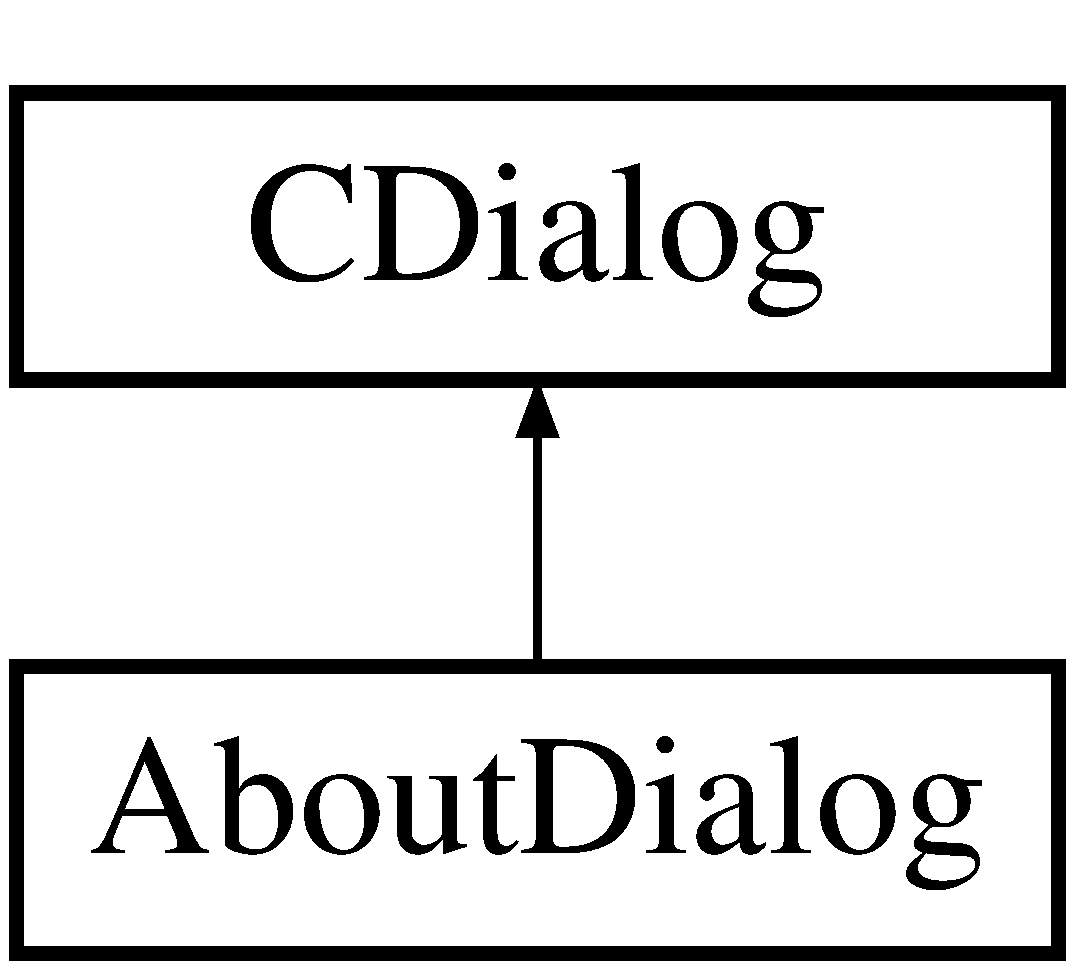
\includegraphics[height=2.000000cm]{class_about_dialog}
\end{center}
\end{figure}
\subsection*{Public 타입}
\begin{DoxyCompactItemize}
\item 
\mbox{\Hypertarget{class_about_dialog_ad39ef53347d21ec0cb70ff40df557e61}\label{class_about_dialog_ad39ef53347d21ec0cb70ff40df557e61}} 
enum \{ {\bfseries I\+DD} = I\+D\+D\+\_\+\+A\+B\+O\+UT
 \}
\end{DoxyCompactItemize}
\subsection*{Public 멤버 함수}
\begin{DoxyCompactItemize}
\item 
\mbox{\Hypertarget{class_about_dialog_a4a8056094af91d12bca94d4fcba1aeae}\label{class_about_dialog_a4a8056094af91d12bca94d4fcba1aeae}} 
{\bfseries About\+Dialog} (C\+Wnd $\ast$p\+Parent=N\+U\+LL)
\end{DoxyCompactItemize}
\subsection*{Public 속성}
\begin{DoxyCompactItemize}
\item 
\mbox{\Hypertarget{class_about_dialog_a78e658a0c2d03632ce86a675b89d8492}\label{class_about_dialog_a78e658a0c2d03632ce86a675b89d8492}} 
C\+String {\bfseries m\+\_\+version}
\end{DoxyCompactItemize}
\subsection*{Protected 멤버 함수}
\begin{DoxyCompactItemize}
\item 
\mbox{\Hypertarget{class_about_dialog_a098f0327b766a8c3fff0fef3076dc9eb}\label{class_about_dialog_a098f0327b766a8c3fff0fef3076dc9eb}} 
virtual void {\bfseries Do\+Data\+Exchange} (C\+Data\+Exchange $\ast$p\+DX)
\item 
\mbox{\Hypertarget{class_about_dialog_ab42eeca93160e48d480b004aaf33c353}\label{class_about_dialog_ab42eeca93160e48d480b004aaf33c353}} 
virtual B\+O\+OL {\bfseries On\+Init\+Dialog} ()
\end{DoxyCompactItemize}


이 클래스에 대한 문서화 페이지는 다음의 파일들로부터 생성되었습니다.\+:\begin{DoxyCompactItemize}
\item 
src/win32/About\+Dialog.\+h\item 
src/win32/About\+Dialog.\+cpp\end{DoxyCompactItemize}

\hypertarget{class_accel_editor}{}\section{Accel\+Editor 클래스 참조}
\label{class_accel_editor}\index{Accel\+Editor@{Accel\+Editor}}


{\ttfamily \#include $<$Accel\+Editor.\+h$>$}



Accel\+Editor에 대한 상속 다이어그램 \+: \nopagebreak
\begin{figure}[H]
\begin{center}
\leavevmode
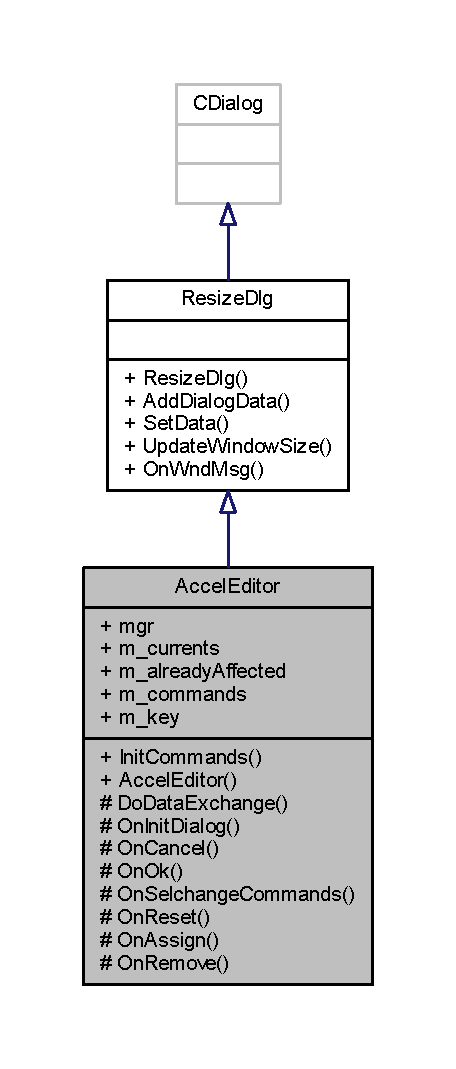
\includegraphics[width=219pt]{class_accel_editor__inherit__graph}
\end{center}
\end{figure}


Accel\+Editor에 대한 협력 다이어그램\+:\nopagebreak
\begin{figure}[H]
\begin{center}
\leavevmode
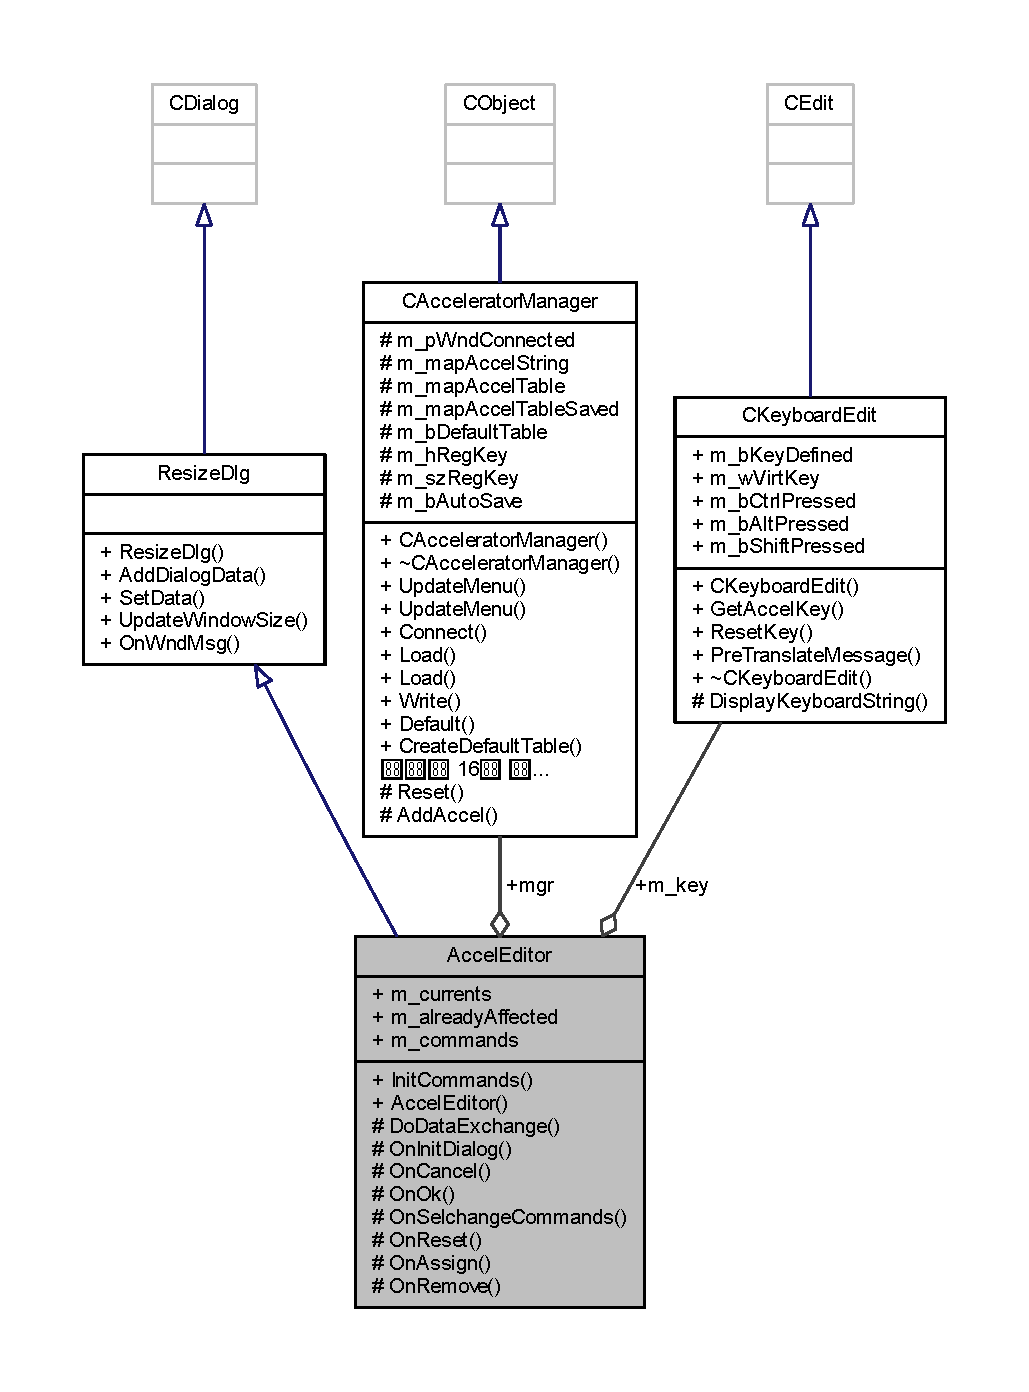
\includegraphics[width=350pt]{class_accel_editor__coll__graph}
\end{center}
\end{figure}
\subsection*{Public 타입}
\begin{DoxyCompactItemize}
\item 
enum \{ \mbox{\hyperlink{class_accel_editor_a2c120196c6edcc4e45a1eb6321060cf7a3ed38c6627e19d20129d5a6eee67408c}{I\+DD}} = I\+D\+D\+\_\+\+A\+C\+C\+E\+L\+\_\+\+E\+D\+I\+T\+OR
 \}
\end{DoxyCompactItemize}
\subsection*{Public 멤버 함수}
\begin{DoxyCompactItemize}
\item 
void \mbox{\hyperlink{class_accel_editor_a3c882fb85c72711e26cfe800fb11ccfa}{Init\+Commands}} ()
\item 
\mbox{\hyperlink{class_accel_editor_a4f3eb3bfb01a597da630a3144687f1ec}{Accel\+Editor}} (C\+Wnd $\ast$p\+Parent=\mbox{\hyperlink{_system_8h_a070d2ce7b6bb7e5c05602aa8c308d0c4}{N\+U\+LL}})
\end{DoxyCompactItemize}
\subsection*{Public 속성}
\begin{DoxyCompactItemize}
\item 
\mbox{\hyperlink{class_c_accelerator_manager}{C\+Accelerator\+Manager}} \mbox{\hyperlink{class_accel_editor_acb731e2193cb5022a95e83122651f96d}{mgr}}
\item 
C\+List\+Box \mbox{\hyperlink{class_accel_editor_a31909da8a929ef7b5e22ffbf64f1c68c}{m\+\_\+currents}}
\item 
C\+Static \mbox{\hyperlink{class_accel_editor_ac3d2378be850611ee51689bd34475275}{m\+\_\+already\+Affected}}
\item 
C\+List\+Box \mbox{\hyperlink{class_accel_editor_aba4ea3d3eced08de9fe39e307b5f40fc}{m\+\_\+commands}}
\item 
\mbox{\hyperlink{class_c_keyboard_edit}{C\+Keyboard\+Edit}} \mbox{\hyperlink{class_accel_editor_af0875f914fdddf5233a951cabd499a4d}{m\+\_\+key}}
\end{DoxyCompactItemize}
\subsection*{Protected 멤버 함수}
\begin{DoxyCompactItemize}
\item 
virtual void \mbox{\hyperlink{class_accel_editor_a3212b434e8c489ba308fa6a474dd32e7}{Do\+Data\+Exchange}} (C\+Data\+Exchange $\ast$p\+DX)
\item 
virtual B\+O\+OL \mbox{\hyperlink{class_accel_editor_a131b32f139220aadd5e36b4ddeb8cd58}{On\+Init\+Dialog}} ()
\item 
afx\+\_\+msg void \mbox{\hyperlink{class_accel_editor_a50b1043d4af01df3925f193b7755c05e}{On\+Cancel}} ()
\item 
afx\+\_\+msg void \mbox{\hyperlink{class_accel_editor_a3afd18b4482500a4ea29ee5d0d43cffc}{On\+Ok}} ()
\item 
afx\+\_\+msg void \mbox{\hyperlink{class_accel_editor_a16cb5c73f55199115c5a4f35268ff3fa}{On\+Selchange\+Commands}} ()
\item 
afx\+\_\+msg void \mbox{\hyperlink{class_accel_editor_a1afed0a04125915ae1517e1b08879b8b}{On\+Reset}} ()
\item 
afx\+\_\+msg void \mbox{\hyperlink{class_accel_editor_ad33ae69dcc262dd73595cb33d82c209e}{On\+Assign}} ()
\item 
afx\+\_\+msg void \mbox{\hyperlink{class_accel_editor_a40b74b67b95694245502b15ceedd278c}{On\+Remove}} ()
\end{DoxyCompactItemize}


\subsection{상세한 설명}


Accel\+Editor.\+h 파일의 35 번째 라인에서 정의되었습니다.



\subsection{멤버 열거형 문서화}
\mbox{\Hypertarget{class_accel_editor_a2c120196c6edcc4e45a1eb6321060cf7}\label{class_accel_editor_a2c120196c6edcc4e45a1eb6321060cf7}} 
\subsubsection{\texorpdfstring{anonymous enum}{anonymous enum}}
{\footnotesize\ttfamily anonymous enum}

\begin{DoxyEnumFields}{열거형 멤버}
\raisebox{\heightof{T}}[0pt][0pt]{\index{I\+DD@{I\+DD}!Accel\+Editor@{Accel\+Editor}}\index{Accel\+Editor@{Accel\+Editor}!I\+DD@{I\+DD}}}\mbox{\Hypertarget{class_accel_editor_a2c120196c6edcc4e45a1eb6321060cf7a3ed38c6627e19d20129d5a6eee67408c}\label{class_accel_editor_a2c120196c6edcc4e45a1eb6321060cf7a3ed38c6627e19d20129d5a6eee67408c}} 
I\+DD&\\
\hline

\end{DoxyEnumFields}


Accel\+Editor.\+h 파일의 45 번째 라인에서 정의되었습니다.


\begin{DoxyCode}
45 \{ \mbox{\hyperlink{class_accel_editor_a2c120196c6edcc4e45a1eb6321060cf7a3ed38c6627e19d20129d5a6eee67408c}{IDD}} = \mbox{\hyperlink{resource_8h_a5244accea8f995e6b35d0dcc7572b379}{IDD\_ACCEL\_EDITOR}} \};
\end{DoxyCode}


\subsection{생성자 \& 소멸자 문서화}
\mbox{\Hypertarget{class_accel_editor_a4f3eb3bfb01a597da630a3144687f1ec}\label{class_accel_editor_a4f3eb3bfb01a597da630a3144687f1ec}} 
\index{Accel\+Editor@{Accel\+Editor}!Accel\+Editor@{Accel\+Editor}}
\index{Accel\+Editor@{Accel\+Editor}!Accel\+Editor@{Accel\+Editor}}
\subsubsection{\texorpdfstring{Accel\+Editor()}{AccelEditor()}}
{\footnotesize\ttfamily Accel\+Editor\+::\+Accel\+Editor (\begin{DoxyParamCaption}\item[{C\+Wnd $\ast$}]{p\+Parent = {\ttfamily \mbox{\hyperlink{_system_8h_a070d2ce7b6bb7e5c05602aa8c308d0c4}{N\+U\+LL}}} }\end{DoxyParamCaption})}



Accel\+Editor.\+cpp 파일의 37 번째 라인에서 정의되었습니다.


\begin{DoxyCode}
38   : \mbox{\hyperlink{class_resize_dlg_a87bab778e9312f274ebe750d4c3a67ee}{ResizeDlg}}(\mbox{\hyperlink{class_accel_editor_a2c120196c6edcc4e45a1eb6321060cf7a3ed38c6627e19d20129d5a6eee67408c}{AccelEditor::IDD}}, pParent)
39 \{
40   \textcolor{comment}{//\{\{AFX\_DATA\_INIT(AccelEditor)}
41   \textcolor{comment}{// NOTE: the ClassWizard will add member initialization here}
42   \textcolor{comment}{//\}\}AFX\_DATA\_INIT}
43   \mbox{\hyperlink{class_accel_editor_acb731e2193cb5022a95e83122651f96d}{mgr}} = \mbox{\hyperlink{_v_b_a_8cpp_a8095a9d06b37a7efe3723f3218ad8fb3}{theApp}}.\mbox{\hyperlink{class_v_b_a_ad7ebce057dbde0ca88cee75e84721a89}{winAccelMgr}};
44 \}
\end{DoxyCode}


\subsection{멤버 함수 문서화}
\mbox{\Hypertarget{class_accel_editor_a3212b434e8c489ba308fa6a474dd32e7}\label{class_accel_editor_a3212b434e8c489ba308fa6a474dd32e7}} 
\index{Accel\+Editor@{Accel\+Editor}!Do\+Data\+Exchange@{Do\+Data\+Exchange}}
\index{Do\+Data\+Exchange@{Do\+Data\+Exchange}!Accel\+Editor@{Accel\+Editor}}
\subsubsection{\texorpdfstring{Do\+Data\+Exchange()}{DoDataExchange()}}
{\footnotesize\ttfamily void Accel\+Editor\+::\+Do\+Data\+Exchange (\begin{DoxyParamCaption}\item[{C\+Data\+Exchange $\ast$}]{p\+DX }\end{DoxyParamCaption})\hspace{0.3cm}{\ttfamily [protected]}, {\ttfamily [virtual]}}



Accel\+Editor.\+cpp 파일의 47 번째 라인에서 정의되었습니다.


\begin{DoxyCode}
48 \{
49   CDialog::DoDataExchange(pDX);
50   \textcolor{comment}{//\{\{AFX\_DATA\_MAP(AccelEditor)}
51   DDX\_Control(pDX, \mbox{\hyperlink{resource_8h_aecf06df6d523df832c4125d6511946ae}{IDC\_CURRENTS}}, \mbox{\hyperlink{class_accel_editor_a31909da8a929ef7b5e22ffbf64f1c68c}{m\_currents}});
52   DDX\_Control(pDX, \mbox{\hyperlink{resource_8h_ac348623d1b045f612bab36c7899d9507}{IDC\_ALREADY\_AFFECTED}}, \mbox{\hyperlink{class_accel_editor_ac3d2378be850611ee51689bd34475275}{m\_alreadyAffected}});
53   DDX\_Control(pDX, \mbox{\hyperlink{resource_8h_abc997c435dcb4d0b7fd9d34b51a905f1}{IDC\_COMMANDS}}, \mbox{\hyperlink{class_accel_editor_aba4ea3d3eced08de9fe39e307b5f40fc}{m\_commands}});
54   DDX\_Control(pDX, \mbox{\hyperlink{resource_8h_a5c53f670221b594a3fd960d7bc18325d}{IDC\_EDIT\_KEY}}, \mbox{\hyperlink{class_accel_editor_af0875f914fdddf5233a951cabd499a4d}{m\_key}});
55   \textcolor{comment}{//\}\}AFX\_DATA\_MAP}
56 \}
\end{DoxyCode}
\mbox{\Hypertarget{class_accel_editor_a3c882fb85c72711e26cfe800fb11ccfa}\label{class_accel_editor_a3c882fb85c72711e26cfe800fb11ccfa}} 
\index{Accel\+Editor@{Accel\+Editor}!Init\+Commands@{Init\+Commands}}
\index{Init\+Commands@{Init\+Commands}!Accel\+Editor@{Accel\+Editor}}
\subsubsection{\texorpdfstring{Init\+Commands()}{InitCommands()}}
{\footnotesize\ttfamily void Accel\+Editor\+::\+Init\+Commands (\begin{DoxyParamCaption}{ }\end{DoxyParamCaption})}



Accel\+Editor.\+cpp 파일의 105 번째 라인에서 정의되었습니다.


\begin{DoxyCode}
106 \{
107   \mbox{\hyperlink{class_accel_editor_aba4ea3d3eced08de9fe39e307b5f40fc}{m\_commands}}.ResetContent();
108   \mbox{\hyperlink{class_accel_editor_ac3d2378be850611ee51689bd34475275}{m\_alreadyAffected}}.SetWindowText(\textcolor{stringliteral}{""});
109 
110   POSITION pos = \mbox{\hyperlink{class_accel_editor_acb731e2193cb5022a95e83122651f96d}{mgr}}.\mbox{\hyperlink{class_c_accelerator_manager_abb40dbb1a44c47ac22590e8f1243835b}{m\_mapAccelString}}.GetStartPosition();
111   
112   \textcolor{keywordflow}{while}(pos != \mbox{\hyperlink{getopt1_8c_a070d2ce7b6bb7e5c05602aa8c308d0c4}{NULL}}) \{
113     CString \mbox{\hyperlink{_commands_8cpp_a9f83d3c4b4c3bb790f90ad79865e37ab}{command}};
114     WORD wID;
115     \mbox{\hyperlink{class_accel_editor_acb731e2193cb5022a95e83122651f96d}{mgr}}.\mbox{\hyperlink{class_c_accelerator_manager_abb40dbb1a44c47ac22590e8f1243835b}{m\_mapAccelString}}.GetNextAssoc(pos, \mbox{\hyperlink{_commands_8cpp_a9f83d3c4b4c3bb790f90ad79865e37ab}{command}}, wID);
116 
117     \textcolor{keywordtype}{int} index = \mbox{\hyperlink{class_accel_editor_aba4ea3d3eced08de9fe39e307b5f40fc}{m\_commands}}.AddString(\mbox{\hyperlink{_commands_8cpp_a9f83d3c4b4c3bb790f90ad79865e37ab}{command}});
118     \mbox{\hyperlink{class_accel_editor_aba4ea3d3eced08de9fe39e307b5f40fc}{m\_commands}}.SetItemData(index, wID);
119   \}
120 
121   \textcolor{comment}{// Update the currents accels associated with the selected command}
122   \textcolor{keywordflow}{if} (\mbox{\hyperlink{class_accel_editor_aba4ea3d3eced08de9fe39e307b5f40fc}{m\_commands}}.SetCurSel(0) != LB\_ERR)
123     \mbox{\hyperlink{class_accel_editor_a16cb5c73f55199115c5a4f35268ff3fa}{OnSelchangeCommands}}();
124 \}
\end{DoxyCode}
이 함수 내부에서 호출하는 함수들에 대한 그래프입니다.\+:
\nopagebreak
\begin{figure}[H]
\begin{center}
\leavevmode
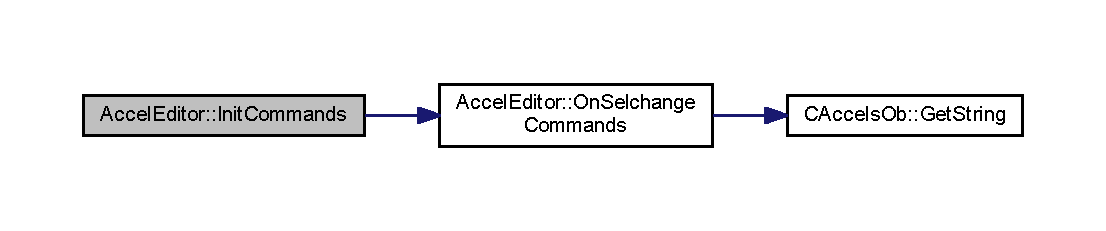
\includegraphics[width=350pt]{class_accel_editor_a3c882fb85c72711e26cfe800fb11ccfa_cgraph}
\end{center}
\end{figure}
이 함수를 호출하는 함수들에 대한 그래프입니다.\+:
\nopagebreak
\begin{figure}[H]
\begin{center}
\leavevmode
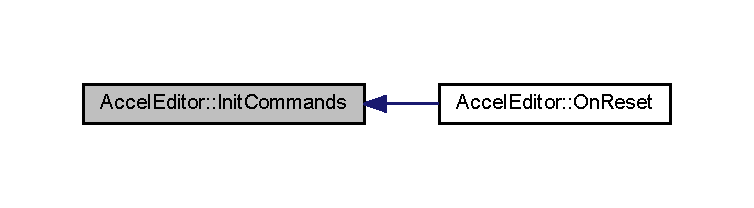
\includegraphics[width=350pt]{class_accel_editor_a3c882fb85c72711e26cfe800fb11ccfa_icgraph}
\end{center}
\end{figure}
\mbox{\Hypertarget{class_accel_editor_ad33ae69dcc262dd73595cb33d82c209e}\label{class_accel_editor_ad33ae69dcc262dd73595cb33d82c209e}} 
\index{Accel\+Editor@{Accel\+Editor}!On\+Assign@{On\+Assign}}
\index{On\+Assign@{On\+Assign}!Accel\+Editor@{Accel\+Editor}}
\subsubsection{\texorpdfstring{On\+Assign()}{OnAssign()}}
{\footnotesize\ttfamily void Accel\+Editor\+::\+On\+Assign (\begin{DoxyParamCaption}{ }\end{DoxyParamCaption})\hspace{0.3cm}{\ttfamily [protected]}}



Accel\+Editor.\+cpp 파일의 173 번째 라인에서 정의되었습니다.


\begin{DoxyCode}
174 \{
175   \textcolor{comment}{// Control if it's not already affected}
176   \mbox{\hyperlink{class_c_cmd_accel_ob}{CCmdAccelOb}}* pCmdAccel;
177   \mbox{\hyperlink{class_c_accels_ob}{CAccelsOb}}* pAccel;
178   WORD wIDCommand;
179   POSITION pos;
180   
181   WORD wKey;
182   \textcolor{keywordtype}{bool} bCtrl, bAlt, bShift;
183 
184   \textcolor{keywordflow}{if} (!\mbox{\hyperlink{class_accel_editor_af0875f914fdddf5233a951cabd499a4d}{m\_key}}.\mbox{\hyperlink{class_c_keyboard_edit_a920dfccebef5e2260e59003e4959ef9f}{GetAccelKey}}(wKey, bCtrl, bAlt, bShift))
185     \textcolor{keywordflow}{return}; \textcolor{comment}{// no valid key, abort}
186 
187   \textcolor{keywordtype}{int} \mbox{\hyperlink{expr_8cpp_a16ff2d8e15ade4948398b0aeb80124a8}{count}} = \mbox{\hyperlink{class_accel_editor_aba4ea3d3eced08de9fe39e307b5f40fc}{m\_commands}}.GetCount();
188   \textcolor{keywordtype}{int} index;
189   \textcolor{keywordflow}{for} (index = 0; index < \mbox{\hyperlink{expr_8cpp_a16ff2d8e15ade4948398b0aeb80124a8}{count}}; index++) \{
190 
191     wIDCommand = LOWORD(\mbox{\hyperlink{class_accel_editor_aba4ea3d3eced08de9fe39e307b5f40fc}{m\_commands}}.GetItemData(index));
192     \mbox{\hyperlink{class_accel_editor_acb731e2193cb5022a95e83122651f96d}{mgr}}.\mbox{\hyperlink{class_c_accelerator_manager_a16b8d3e9328bc0eeeb048630deff2768}{m\_mapAccelTable}}.Lookup(wIDCommand, pCmdAccel);
193 
194     pos = pCmdAccel->\mbox{\hyperlink{class_c_cmd_accel_ob_a85772f1ea9204af42b8a39a0135dc0f8}{m\_Accels}}.GetHeadPosition();
195     \textcolor{keywordflow}{while} (pos != \mbox{\hyperlink{getopt1_8c_a070d2ce7b6bb7e5c05602aa8c308d0c4}{NULL}}) \{
196       pAccel = pCmdAccel->\mbox{\hyperlink{class_c_cmd_accel_ob_a85772f1ea9204af42b8a39a0135dc0f8}{m\_Accels}}.GetNext(pos);
197       \textcolor{keywordflow}{if} (pAccel->\mbox{\hyperlink{class_c_accels_ob_a32714a4454d398d3d3a68d1705a76bc5}{IsEqual}}(wKey, bCtrl, bAlt, bShift)) \{
198         \textcolor{comment}{// the key is already affected (in the same or other command)}
199         \mbox{\hyperlink{class_accel_editor_ac3d2378be850611ee51689bd34475275}{m\_alreadyAffected}}.SetWindowText(pCmdAccel->\mbox{\hyperlink{class_c_cmd_accel_ob_acbd02cc68d3909b1e39b687e76f45d91}{m\_szCommand}});
200         \mbox{\hyperlink{class_accel_editor_af0875f914fdddf5233a951cabd499a4d}{m\_key}}.SetSel(0, -1);
201         \textcolor{keywordflow}{return}; \textcolor{comment}{// abort}
202       \}
203     \}
204   \}
205 
206   \textcolor{comment}{// OK, we can add the accel key in the currently selected group}
207   index = \mbox{\hyperlink{class_accel_editor_aba4ea3d3eced08de9fe39e307b5f40fc}{m\_commands}}.GetCurSel();
208   \textcolor{keywordflow}{if} (index == LB\_ERR)
209     \textcolor{keywordflow}{return};
210 
211   \textcolor{comment}{// Get the object who manage the accels list, associated to the command.}
212   wIDCommand = LOWORD(\mbox{\hyperlink{class_accel_editor_aba4ea3d3eced08de9fe39e307b5f40fc}{m\_commands}}.GetItemData(index));
213 
214   \textcolor{keywordflow}{if} (\mbox{\hyperlink{class_accel_editor_acb731e2193cb5022a95e83122651f96d}{mgr}}.\mbox{\hyperlink{class_c_accelerator_manager_a16b8d3e9328bc0eeeb048630deff2768}{m\_mapAccelTable}}.Lookup(wIDCommand, pCmdAccel) != TRUE)
215     \textcolor{keywordflow}{return};
216 
217   BYTE cVirt = 0;
218   \textcolor{keywordflow}{if} (bCtrl)
219     cVirt |= FCONTROL;
220   \textcolor{keywordflow}{if} (bAlt)
221     cVirt |= FALT;
222   \textcolor{keywordflow}{if} (bShift)
223     cVirt |= FSHIFT;
224 
225   cVirt |= FVIRTKEY;
226 
227   \textcolor{comment}{// Create the new key...}
228   pAccel = \textcolor{keyword}{new} \mbox{\hyperlink{class_c_accels_ob}{CAccelsOb}}(cVirt, wKey, \textcolor{keyword}{false});
229   ASSERT(pAccel != \mbox{\hyperlink{getopt1_8c_a070d2ce7b6bb7e5c05602aa8c308d0c4}{NULL}});
230   \textcolor{comment}{// ...and add in the list.}
231   pCmdAccel->\mbox{\hyperlink{class_c_cmd_accel_ob_a85772f1ea9204af42b8a39a0135dc0f8}{m\_Accels}}.AddTail(pAccel);
232 
233   \textcolor{comment}{// Update the listbox.}
234   CString szBuffer;
235   pAccel->\mbox{\hyperlink{class_c_accels_ob_afaf7510fa1e0707863f6bd469f190de6}{GetString}}(szBuffer);
236 
237   index = \mbox{\hyperlink{class_accel_editor_a31909da8a929ef7b5e22ffbf64f1c68c}{m\_currents}}.AddString(szBuffer);
238   \mbox{\hyperlink{class_accel_editor_a31909da8a929ef7b5e22ffbf64f1c68c}{m\_currents}}.SetItemData(index, (DWORD\_PTR)pAccel);
239 
240   \textcolor{comment}{// Reset the key editor.}
241   \mbox{\hyperlink{class_accel_editor_af0875f914fdddf5233a951cabd499a4d}{m\_key}}.\mbox{\hyperlink{class_c_keyboard_edit_ad0185cc0cad77250cc32ef1d9ffb8593}{ResetKey}}();
242 \}
\end{DoxyCode}
이 함수 내부에서 호출하는 함수들에 대한 그래프입니다.\+:
\nopagebreak
\begin{figure}[H]
\begin{center}
\leavevmode
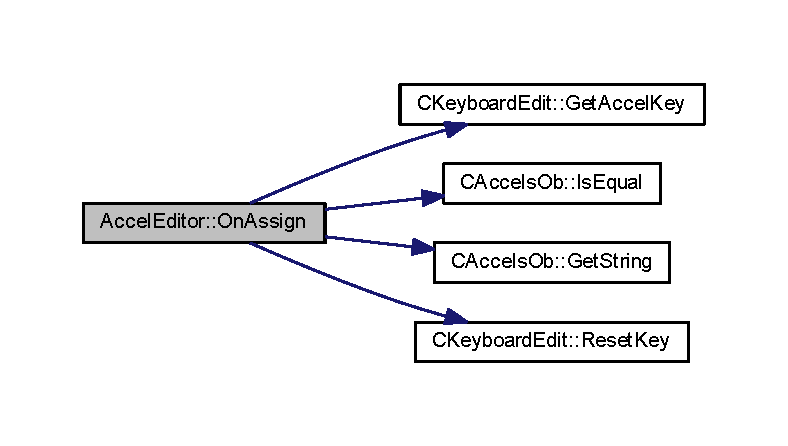
\includegraphics[width=350pt]{class_accel_editor_ad33ae69dcc262dd73595cb33d82c209e_cgraph}
\end{center}
\end{figure}
\mbox{\Hypertarget{class_accel_editor_a50b1043d4af01df3925f193b7755c05e}\label{class_accel_editor_a50b1043d4af01df3925f193b7755c05e}} 
\index{Accel\+Editor@{Accel\+Editor}!On\+Cancel@{On\+Cancel}}
\index{On\+Cancel@{On\+Cancel}!Accel\+Editor@{Accel\+Editor}}
\subsubsection{\texorpdfstring{On\+Cancel()}{OnCancel()}}
{\footnotesize\ttfamily void Accel\+Editor\+::\+On\+Cancel (\begin{DoxyParamCaption}{ }\end{DoxyParamCaption})\hspace{0.3cm}{\ttfamily [protected]}}



Accel\+Editor.\+cpp 파일의 126 번째 라인에서 정의되었습니다.


\begin{DoxyCode}
127 \{
128   EndDialog(FALSE);
129 \}
\end{DoxyCode}
\mbox{\Hypertarget{class_accel_editor_a131b32f139220aadd5e36b4ddeb8cd58}\label{class_accel_editor_a131b32f139220aadd5e36b4ddeb8cd58}} 
\index{Accel\+Editor@{Accel\+Editor}!On\+Init\+Dialog@{On\+Init\+Dialog}}
\index{On\+Init\+Dialog@{On\+Init\+Dialog}!Accel\+Editor@{Accel\+Editor}}
\subsubsection{\texorpdfstring{On\+Init\+Dialog()}{OnInitDialog()}}
{\footnotesize\ttfamily B\+O\+OL Accel\+Editor\+::\+On\+Init\+Dialog (\begin{DoxyParamCaption}{ }\end{DoxyParamCaption})\hspace{0.3cm}{\ttfamily [protected]}, {\ttfamily [virtual]}}



Accel\+Editor.\+cpp 파일의 73 번째 라인에서 정의되었습니다.


\begin{DoxyCode}
74 \{
75   CDialog::OnInitDialog();
76   
77   \mbox{\hyperlink{_resize_dlg_8h_acb9d1d22d9838f6dda8a61cfa132997c}{DIALOG\_SIZER\_START}}( sz )
78     \mbox{\hyperlink{_resize_dlg_8h_a0e9ee7a18c54003893895a009f5d79c8}{DIALOG\_SIZER\_ENTRY}}( \mbox{\hyperlink{resource_8h_a37f587596b464239581b844e04dda1da}{IDC\_STATIC1}}, \mbox{\hyperlink{_resize_dlg_8h_a9f96d817606755d91347bd606825c5af}{DS\_MoveX}})
79     \mbox{\hyperlink{_resize_dlg_8h_a0e9ee7a18c54003893895a009f5d79c8}{DIALOG\_SIZER\_ENTRY}}( \mbox{\hyperlink{resource_8h_acdec4653db2f21850f3ee1f41c3c0080}{IDC\_STATIC2}}, \mbox{\hyperlink{_resize_dlg_8h_ae5309071be822a4dae5cb33a131f6180}{DS\_MoveY}})
80     \mbox{\hyperlink{_resize_dlg_8h_a0e9ee7a18c54003893895a009f5d79c8}{DIALOG\_SIZER\_ENTRY}}( \mbox{\hyperlink{resource_8h_a62cedae02f3076f30d9a6bb0ed8d3e43}{IDC\_STATIC3}}, \mbox{\hyperlink{_resize_dlg_8h_a9f96d817606755d91347bd606825c5af}{DS\_MoveX}} | 
      \mbox{\hyperlink{_resize_dlg_8h_ae5309071be822a4dae5cb33a131f6180}{DS\_MoveY}})
81     \mbox{\hyperlink{_resize_dlg_8h_a0e9ee7a18c54003893895a009f5d79c8}{DIALOG\_SIZER\_ENTRY}}( \mbox{\hyperlink{resource_8h_ac348623d1b045f612bab36c7899d9507}{IDC\_ALREADY\_AFFECTED}}, 
      \mbox{\hyperlink{_resize_dlg_8h_ae5309071be822a4dae5cb33a131f6180}{DS\_MoveY}})
82     \mbox{\hyperlink{_resize_dlg_8h_a0e9ee7a18c54003893895a009f5d79c8}{DIALOG\_SIZER\_ENTRY}}( \mbox{\hyperlink{resource_8h_a4cf7b8af561e85b223c39c4c2b22ef18}{ID\_OK}}, \mbox{\hyperlink{_resize_dlg_8h_a9f96d817606755d91347bd606825c5af}{DS\_MoveX}})
83     \mbox{\hyperlink{_resize_dlg_8h_a0e9ee7a18c54003893895a009f5d79c8}{DIALOG\_SIZER\_ENTRY}}( \mbox{\hyperlink{resource_8h_a9f066b92f1c9e4f0f0a679d67fd29d31}{ID\_CANCEL}}, \mbox{\hyperlink{_resize_dlg_8h_a9f96d817606755d91347bd606825c5af}{DS\_MoveX}})
84     \mbox{\hyperlink{_resize_dlg_8h_a0e9ee7a18c54003893895a009f5d79c8}{DIALOG\_SIZER\_ENTRY}}( \mbox{\hyperlink{resource_8h_a80cc1cf3d03957bcb73aba8214c3d319}{IDC\_ASSIGN}}, \mbox{\hyperlink{_resize_dlg_8h_a9f96d817606755d91347bd606825c5af}{DS\_MoveX}})
85     \mbox{\hyperlink{_resize_dlg_8h_a0e9ee7a18c54003893895a009f5d79c8}{DIALOG\_SIZER\_ENTRY}}( \mbox{\hyperlink{resource_8h_aa8441a495432bef29886eed49bbaa08c}{IDC\_REMOVE}}, \mbox{\hyperlink{_resize_dlg_8h_a9f96d817606755d91347bd606825c5af}{DS\_MoveX}})
86     \mbox{\hyperlink{_resize_dlg_8h_a0e9ee7a18c54003893895a009f5d79c8}{DIALOG\_SIZER\_ENTRY}}( \mbox{\hyperlink{resource_8h_ac19883430c1a49f08af98721f02d95eb}{IDC\_RESET}}, \mbox{\hyperlink{_resize_dlg_8h_a9f96d817606755d91347bd606825c5af}{DS\_MoveX}})
87     \mbox{\hyperlink{_resize_dlg_8h_a0e9ee7a18c54003893895a009f5d79c8}{DIALOG\_SIZER\_ENTRY}}( \mbox{\hyperlink{resource_8h_a27e7224faecfa4040c695a69107088f9}{IDC\_CLOSE}}, \mbox{\hyperlink{_resize_dlg_8h_ae5309071be822a4dae5cb33a131f6180}{DS\_MoveY}})
88     \mbox{\hyperlink{_resize_dlg_8h_a0e9ee7a18c54003893895a009f5d79c8}{DIALOG\_SIZER\_ENTRY}}( \mbox{\hyperlink{resource_8h_abc997c435dcb4d0b7fd9d34b51a905f1}{IDC\_COMMANDS}}, \mbox{\hyperlink{_resize_dlg_8h_a21713fd373c62604a1ee3d5d831101ad}{DS\_SizeX}} | 
      \mbox{\hyperlink{_resize_dlg_8h_a783821ba6bb984916d55f46cdf90cb2b}{DS\_SizeY}})
89     \mbox{\hyperlink{_resize_dlg_8h_a0e9ee7a18c54003893895a009f5d79c8}{DIALOG\_SIZER\_ENTRY}}( \mbox{\hyperlink{resource_8h_aecf06df6d523df832c4125d6511946ae}{IDC\_CURRENTS}}, \mbox{\hyperlink{_resize_dlg_8h_a9f96d817606755d91347bd606825c5af}{DS\_MoveX}} | 
      \mbox{\hyperlink{_resize_dlg_8h_a783821ba6bb984916d55f46cdf90cb2b}{DS\_SizeY}})
90     \mbox{\hyperlink{_resize_dlg_8h_a0e9ee7a18c54003893895a009f5d79c8}{DIALOG\_SIZER\_ENTRY}}( \mbox{\hyperlink{resource_8h_a5c53f670221b594a3fd960d7bc18325d}{IDC\_EDIT\_KEY}}, \mbox{\hyperlink{_resize_dlg_8h_a9f96d817606755d91347bd606825c5af}{DS\_MoveX}} | 
      \mbox{\hyperlink{_resize_dlg_8h_ae5309071be822a4dae5cb33a131f6180}{DS\_MoveY}})
91     \mbox{\hyperlink{_resize_dlg_8h_aeac0c1e32f30e0763df5736e4b3ea50a}{DIALOG\_SIZER\_END}}()
92 
93     \mbox{\hyperlink{class_resize_dlg_a6a3965f44a0c2f5ba9aaa798a9a81df5}{SetData}}(sz,
94             TRUE,
95             HKEY\_CURRENT\_USER,
96             "Software\(\backslash\)\(\backslash\)Emulators\(\backslash\)\(\backslash\)VisualBoyAdvance\(\backslash\)\(\backslash\)Viewer\(\backslash\)\(\backslash\)\mbox{\hyperlink{class_accel_editor}{AccelEditor}}",
97             \mbox{\hyperlink{getopt1_8c_a070d2ce7b6bb7e5c05602aa8c308d0c4}{NULL}});
98 
99   \mbox{\hyperlink{class_accel_editor_a3c882fb85c72711e26cfe800fb11ccfa}{InitCommands}}();
100   
101   \mbox{\hyperlink{gb_codes_8h_a9717e7bbecb906637e86cef6da3d83c2}{return}} TRUE;  \textcolor{comment}{// return TRUE unless you set the focus to a control}
102                 \textcolor{comment}{// EXCEPTION: OCX Property Pages should return FALSE}
103 \}
\end{DoxyCode}
\mbox{\Hypertarget{class_accel_editor_a3afd18b4482500a4ea29ee5d0d43cffc}\label{class_accel_editor_a3afd18b4482500a4ea29ee5d0d43cffc}} 
\index{Accel\+Editor@{Accel\+Editor}!On\+Ok@{On\+Ok}}
\index{On\+Ok@{On\+Ok}!Accel\+Editor@{Accel\+Editor}}
\subsubsection{\texorpdfstring{On\+Ok()}{OnOk()}}
{\footnotesize\ttfamily void Accel\+Editor\+::\+On\+Ok (\begin{DoxyParamCaption}{ }\end{DoxyParamCaption})\hspace{0.3cm}{\ttfamily [protected]}}



Accel\+Editor.\+cpp 파일의 131 번째 라인에서 정의되었습니다.


\begin{DoxyCode}
132 \{
133   EndDialog(TRUE);
134 \}
\end{DoxyCode}
\mbox{\Hypertarget{class_accel_editor_a40b74b67b95694245502b15ceedd278c}\label{class_accel_editor_a40b74b67b95694245502b15ceedd278c}} 
\index{Accel\+Editor@{Accel\+Editor}!On\+Remove@{On\+Remove}}
\index{On\+Remove@{On\+Remove}!Accel\+Editor@{Accel\+Editor}}
\subsubsection{\texorpdfstring{On\+Remove()}{OnRemove()}}
{\footnotesize\ttfamily void Accel\+Editor\+::\+On\+Remove (\begin{DoxyParamCaption}{ }\end{DoxyParamCaption})\hspace{0.3cm}{\ttfamily [protected]}}



Accel\+Editor.\+cpp 파일의 244 번째 라인에서 정의되었습니다.


\begin{DoxyCode}
245 \{
246   \textcolor{comment}{// Some controls}
247   \textcolor{keywordtype}{int} indexCurrent = \mbox{\hyperlink{class_accel_editor_a31909da8a929ef7b5e22ffbf64f1c68c}{m\_currents}}.GetCurSel();
248   \textcolor{keywordflow}{if} (indexCurrent == LB\_ERR)
249     \textcolor{keywordflow}{return};
250   
251   \textcolor{comment}{// 2nd part.}
252   \textcolor{keywordtype}{int} indexCmd = \mbox{\hyperlink{class_accel_editor_aba4ea3d3eced08de9fe39e307b5f40fc}{m\_commands}}.GetCurSel();
253   \textcolor{keywordflow}{if} (indexCmd == LB\_ERR)
254     \textcolor{keywordflow}{return};
255 
256   \textcolor{comment}{// Ref to the ID command}
257   WORD wIDCommand = LOWORD(\mbox{\hyperlink{class_accel_editor_aba4ea3d3eced08de9fe39e307b5f40fc}{m\_commands}}.GetItemData(indexCmd));
258 
259   \textcolor{comment}{// Run through the accels,and control if it can be deleted.}
260   \mbox{\hyperlink{class_c_cmd_accel_ob}{CCmdAccelOb}}* pCmdAccel;
261   \textcolor{keywordflow}{if} (\mbox{\hyperlink{class_accel_editor_acb731e2193cb5022a95e83122651f96d}{mgr}}.\mbox{\hyperlink{class_c_accelerator_manager_a16b8d3e9328bc0eeeb048630deff2768}{m\_mapAccelTable}}.Lookup(wIDCommand, pCmdAccel) == TRUE) \{
262     \mbox{\hyperlink{class_c_accels_ob}{CAccelsOb}}* pAccel;
263     \mbox{\hyperlink{class_c_accels_ob}{CAccelsOb}}* pAccelCurrent = (\mbox{\hyperlink{class_c_accels_ob}{CAccelsOb}}*)(\mbox{\hyperlink{class_accel_editor_a31909da8a929ef7b5e22ffbf64f1c68c}{m\_currents}}.GetItemData(indexCurrent
      ));
264     CString szBuffer;
265     POSITION pos = pCmdAccel->m\_Accels.GetHeadPosition();
266     POSITION PrevPos;
267     \textcolor{keywordflow}{while} (pos != \mbox{\hyperlink{getopt1_8c_a070d2ce7b6bb7e5c05602aa8c308d0c4}{NULL}}) \{
268       PrevPos = pos;
269       pAccel = pCmdAccel->m\_Accels.GetNext(pos);
270       \textcolor{keywordflow}{if} (pAccel == pAccelCurrent) \{
271         \textcolor{keywordflow}{if} (!pAccel->\mbox{\hyperlink{class_c_accels_ob_ad8300bd20bd429ad61f89700e388dd9a}{m\_bLocked}}) \{
272           \textcolor{comment}{// not locked, so we delete the key}
273           pCmdAccel->m\_Accels.RemoveAt(PrevPos);
274           \textcolor{keyword}{delete} pAccel;
275           \textcolor{comment}{// and update the listboxes/key editor/static text}
276           \mbox{\hyperlink{class_accel_editor_a31909da8a929ef7b5e22ffbf64f1c68c}{m\_currents}}.DeleteString(indexCurrent);
277           \mbox{\hyperlink{class_accel_editor_af0875f914fdddf5233a951cabd499a4d}{m\_key}}.\mbox{\hyperlink{class_c_keyboard_edit_ad0185cc0cad77250cc32ef1d9ffb8593}{ResetKey}}();
278           \mbox{\hyperlink{class_accel_editor_ac3d2378be850611ee51689bd34475275}{m\_alreadyAffected}}.SetWindowText(\textcolor{stringliteral}{""});
279           \textcolor{keywordflow}{return};
280         \} \textcolor{keywordflow}{else} \{
281           \mbox{\hyperlink{system_8cpp_a747a9cb8e015a3d45cca636b5bd0fc69}{systemMessage}}(0,\textcolor{stringliteral}{"Unable to remove this\(\backslash\)naccelerator (Locked)"});
282           \textcolor{keywordflow}{return};
283         \}
284       \}
285     \}
286     \mbox{\hyperlink{system_8cpp_a747a9cb8e015a3d45cca636b5bd0fc69}{systemMessage}}(0,\textcolor{stringliteral}{"internal error (CAccelDlgHelper::Remove : pAccel unavailable)"});
287     \textcolor{keywordflow}{return};
288   \}
289   \mbox{\hyperlink{system_8cpp_a747a9cb8e015a3d45cca636b5bd0fc69}{systemMessage}}(0,\textcolor{stringliteral}{"internal error (CAccelDlgHelper::Remove : Lookup failed)"});
290 \}
\end{DoxyCode}
이 함수 내부에서 호출하는 함수들에 대한 그래프입니다.\+:
\nopagebreak
\begin{figure}[H]
\begin{center}
\leavevmode
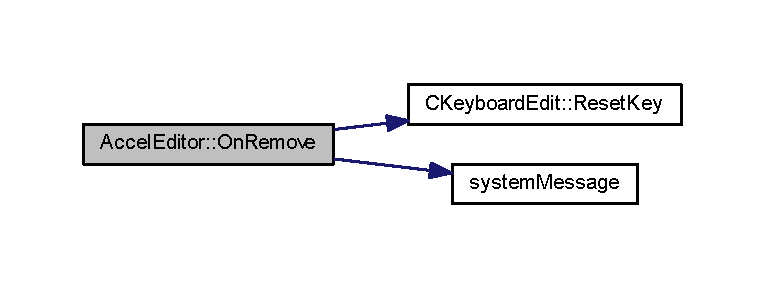
\includegraphics[width=350pt]{class_accel_editor_a40b74b67b95694245502b15ceedd278c_cgraph}
\end{center}
\end{figure}
\mbox{\Hypertarget{class_accel_editor_a1afed0a04125915ae1517e1b08879b8b}\label{class_accel_editor_a1afed0a04125915ae1517e1b08879b8b}} 
\index{Accel\+Editor@{Accel\+Editor}!On\+Reset@{On\+Reset}}
\index{On\+Reset@{On\+Reset}!Accel\+Editor@{Accel\+Editor}}
\subsubsection{\texorpdfstring{On\+Reset()}{OnReset()}}
{\footnotesize\ttfamily void Accel\+Editor\+::\+On\+Reset (\begin{DoxyParamCaption}{ }\end{DoxyParamCaption})\hspace{0.3cm}{\ttfamily [protected]}}



Accel\+Editor.\+cpp 파일의 167 번째 라인에서 정의되었습니다.


\begin{DoxyCode}
168 \{
169   \mbox{\hyperlink{class_accel_editor_acb731e2193cb5022a95e83122651f96d}{mgr}}.\mbox{\hyperlink{class_c_accelerator_manager_aa510a36964ed209de5f7325efa713bf6}{Default}}();
170   \mbox{\hyperlink{class_accel_editor_a3c882fb85c72711e26cfe800fb11ccfa}{InitCommands}}(); \textcolor{comment}{// update the listboxes.}
171 \}
\end{DoxyCode}
이 함수 내부에서 호출하는 함수들에 대한 그래프입니다.\+:
\nopagebreak
\begin{figure}[H]
\begin{center}
\leavevmode
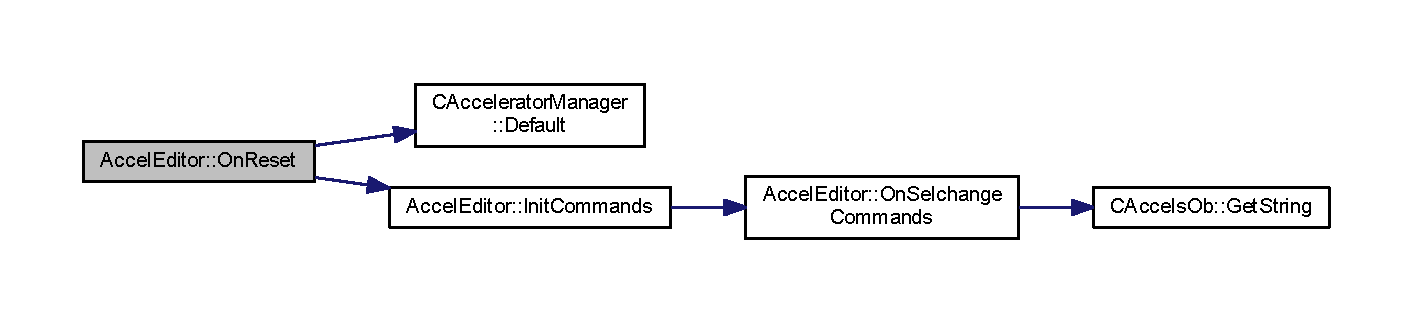
\includegraphics[width=350pt]{class_accel_editor_a1afed0a04125915ae1517e1b08879b8b_cgraph}
\end{center}
\end{figure}
\mbox{\Hypertarget{class_accel_editor_a16cb5c73f55199115c5a4f35268ff3fa}\label{class_accel_editor_a16cb5c73f55199115c5a4f35268ff3fa}} 
\index{Accel\+Editor@{Accel\+Editor}!On\+Selchange\+Commands@{On\+Selchange\+Commands}}
\index{On\+Selchange\+Commands@{On\+Selchange\+Commands}!Accel\+Editor@{Accel\+Editor}}
\subsubsection{\texorpdfstring{On\+Selchange\+Commands()}{OnSelchangeCommands()}}
{\footnotesize\ttfamily void Accel\+Editor\+::\+On\+Selchange\+Commands (\begin{DoxyParamCaption}{ }\end{DoxyParamCaption})\hspace{0.3cm}{\ttfamily [protected]}}



Accel\+Editor.\+cpp 파일의 136 번째 라인에서 정의되었습니다.


\begin{DoxyCode}
137 \{
138   \textcolor{comment}{// Check if some commands exist.}
139   \textcolor{keywordtype}{int} index = \mbox{\hyperlink{class_accel_editor_aba4ea3d3eced08de9fe39e307b5f40fc}{m\_commands}}.GetCurSel();
140   \textcolor{keywordflow}{if} (index == LB\_ERR)
141     \textcolor{keywordflow}{return};
142 
143   WORD wIDCommand = LOWORD(\mbox{\hyperlink{class_accel_editor_aba4ea3d3eced08de9fe39e307b5f40fc}{m\_commands}}.GetItemData(index));
144   \mbox{\hyperlink{class_accel_editor_a31909da8a929ef7b5e22ffbf64f1c68c}{m\_currents}}.ResetContent();
145 
146   \mbox{\hyperlink{class_c_cmd_accel_ob}{CCmdAccelOb}}* pCmdAccel;
147   
148   \textcolor{keywordflow}{if} (\mbox{\hyperlink{class_accel_editor_acb731e2193cb5022a95e83122651f96d}{mgr}}.\mbox{\hyperlink{class_c_accelerator_manager_a16b8d3e9328bc0eeeb048630deff2768}{m\_mapAccelTable}}.Lookup(wIDCommand, pCmdAccel)) \{
149     \mbox{\hyperlink{class_c_accels_ob}{CAccelsOb}}* pAccel;
150     CString szBuffer;
151     POSITION pos = pCmdAccel->\mbox{\hyperlink{class_c_cmd_accel_ob_a85772f1ea9204af42b8a39a0135dc0f8}{m\_Accels}}.GetHeadPosition();
152 
153     \textcolor{comment}{// Add the keys to the 'currents keys' listbox.}
154     \textcolor{keywordflow}{while} (pos != \mbox{\hyperlink{getopt1_8c_a070d2ce7b6bb7e5c05602aa8c308d0c4}{NULL}}) \{
155       pAccel = pCmdAccel->\mbox{\hyperlink{class_c_cmd_accel_ob_a85772f1ea9204af42b8a39a0135dc0f8}{m\_Accels}}.GetNext(pos);
156       pAccel->\mbox{\hyperlink{class_c_accels_ob_afaf7510fa1e0707863f6bd469f190de6}{GetString}}(szBuffer);
157       index = \mbox{\hyperlink{class_accel_editor_a31909da8a929ef7b5e22ffbf64f1c68c}{m\_currents}}.AddString(szBuffer);
158       \textcolor{comment}{// and a pointer to the accel object.}
159       \mbox{\hyperlink{class_accel_editor_a31909da8a929ef7b5e22ffbf64f1c68c}{m\_currents}}.SetItemData(index, (DWORD\_PTR)pAccel);
160     \}
161   \}
162   \textcolor{comment}{// Init the key editor}
163   \textcolor{comment}{//  m\_pKey->ResetKey();}
164 
165 \}
\end{DoxyCode}
이 함수 내부에서 호출하는 함수들에 대한 그래프입니다.\+:
\nopagebreak
\begin{figure}[H]
\begin{center}
\leavevmode
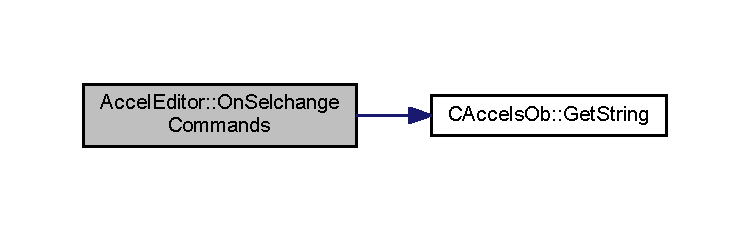
\includegraphics[width=350pt]{class_accel_editor_a16cb5c73f55199115c5a4f35268ff3fa_cgraph}
\end{center}
\end{figure}
이 함수를 호출하는 함수들에 대한 그래프입니다.\+:
\nopagebreak
\begin{figure}[H]
\begin{center}
\leavevmode
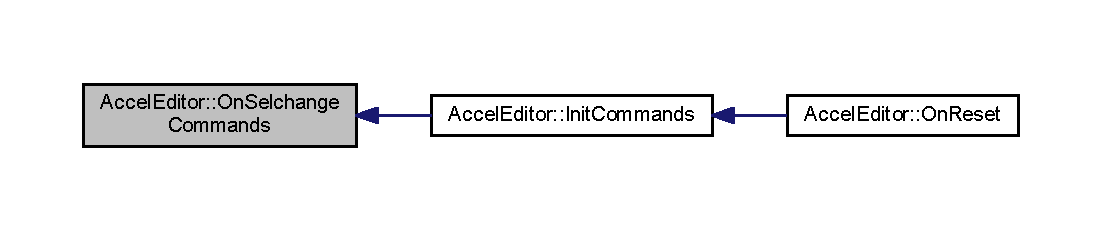
\includegraphics[width=350pt]{class_accel_editor_a16cb5c73f55199115c5a4f35268ff3fa_icgraph}
\end{center}
\end{figure}


\subsection{멤버 데이터 문서화}
\mbox{\Hypertarget{class_accel_editor_ac3d2378be850611ee51689bd34475275}\label{class_accel_editor_ac3d2378be850611ee51689bd34475275}} 
\index{Accel\+Editor@{Accel\+Editor}!m\+\_\+already\+Affected@{m\+\_\+already\+Affected}}
\index{m\+\_\+already\+Affected@{m\+\_\+already\+Affected}!Accel\+Editor@{Accel\+Editor}}
\subsubsection{\texorpdfstring{m\+\_\+already\+Affected}{m\_alreadyAffected}}
{\footnotesize\ttfamily C\+Static Accel\+Editor\+::m\+\_\+already\+Affected}



Accel\+Editor.\+h 파일의 47 번째 라인에서 정의되었습니다.

\mbox{\Hypertarget{class_accel_editor_aba4ea3d3eced08de9fe39e307b5f40fc}\label{class_accel_editor_aba4ea3d3eced08de9fe39e307b5f40fc}} 
\index{Accel\+Editor@{Accel\+Editor}!m\+\_\+commands@{m\+\_\+commands}}
\index{m\+\_\+commands@{m\+\_\+commands}!Accel\+Editor@{Accel\+Editor}}
\subsubsection{\texorpdfstring{m\+\_\+commands}{m\_commands}}
{\footnotesize\ttfamily C\+List\+Box Accel\+Editor\+::m\+\_\+commands}



Accel\+Editor.\+h 파일의 48 번째 라인에서 정의되었습니다.

\mbox{\Hypertarget{class_accel_editor_a31909da8a929ef7b5e22ffbf64f1c68c}\label{class_accel_editor_a31909da8a929ef7b5e22ffbf64f1c68c}} 
\index{Accel\+Editor@{Accel\+Editor}!m\+\_\+currents@{m\+\_\+currents}}
\index{m\+\_\+currents@{m\+\_\+currents}!Accel\+Editor@{Accel\+Editor}}
\subsubsection{\texorpdfstring{m\+\_\+currents}{m\_currents}}
{\footnotesize\ttfamily C\+List\+Box Accel\+Editor\+::m\+\_\+currents}



Accel\+Editor.\+h 파일의 46 번째 라인에서 정의되었습니다.

\mbox{\Hypertarget{class_accel_editor_af0875f914fdddf5233a951cabd499a4d}\label{class_accel_editor_af0875f914fdddf5233a951cabd499a4d}} 
\index{Accel\+Editor@{Accel\+Editor}!m\+\_\+key@{m\+\_\+key}}
\index{m\+\_\+key@{m\+\_\+key}!Accel\+Editor@{Accel\+Editor}}
\subsubsection{\texorpdfstring{m\+\_\+key}{m\_key}}
{\footnotesize\ttfamily \mbox{\hyperlink{class_c_keyboard_edit}{C\+Keyboard\+Edit}} Accel\+Editor\+::m\+\_\+key}



Accel\+Editor.\+h 파일의 49 번째 라인에서 정의되었습니다.

\mbox{\Hypertarget{class_accel_editor_acb731e2193cb5022a95e83122651f96d}\label{class_accel_editor_acb731e2193cb5022a95e83122651f96d}} 
\index{Accel\+Editor@{Accel\+Editor}!mgr@{mgr}}
\index{mgr@{mgr}!Accel\+Editor@{Accel\+Editor}}
\subsubsection{\texorpdfstring{mgr}{mgr}}
{\footnotesize\ttfamily \mbox{\hyperlink{class_c_accelerator_manager}{C\+Accelerator\+Manager}} Accel\+Editor\+::mgr}



Accel\+Editor.\+h 파일의 39 번째 라인에서 정의되었습니다.



이 클래스에 대한 문서화 페이지는 다음의 파일들로부터 생성되었습니다.\+:\begin{DoxyCompactItemize}
\item 
C\+:/\+Users/sjh13/sources/\+Visual\+Boy\+Advance/src/win32/\mbox{\hyperlink{_accel_editor_8h}{Accel\+Editor.\+h}}\item 
C\+:/\+Users/sjh13/sources/\+Visual\+Boy\+Advance/src/win32/\mbox{\hyperlink{_accel_editor_8cpp}{Accel\+Editor.\+cpp}}\end{DoxyCompactItemize}

\hypertarget{class_add_c_b_a_code}{}\section{Add\+C\+B\+A\+Code 클래스 참조}
\label{class_add_c_b_a_code}\index{Add\+C\+B\+A\+Code@{Add\+C\+B\+A\+Code}}


{\ttfamily \#include $<$G\+B\+A\+Cheats.\+h$>$}



Add\+C\+B\+A\+Code에 대한 상속 다이어그램 \+: \nopagebreak
\begin{figure}[H]
\begin{center}
\leavevmode
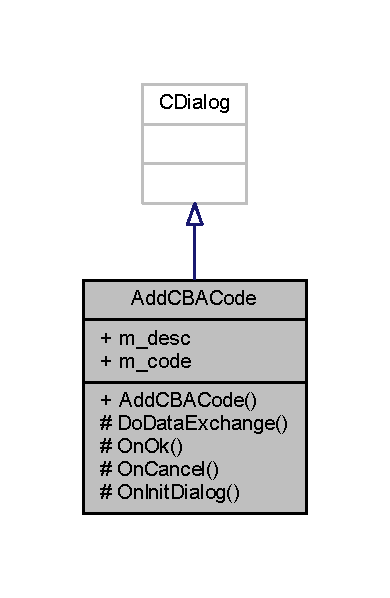
\includegraphics[width=187pt]{class_add_c_b_a_code__inherit__graph}
\end{center}
\end{figure}


Add\+C\+B\+A\+Code에 대한 협력 다이어그램\+:\nopagebreak
\begin{figure}[H]
\begin{center}
\leavevmode
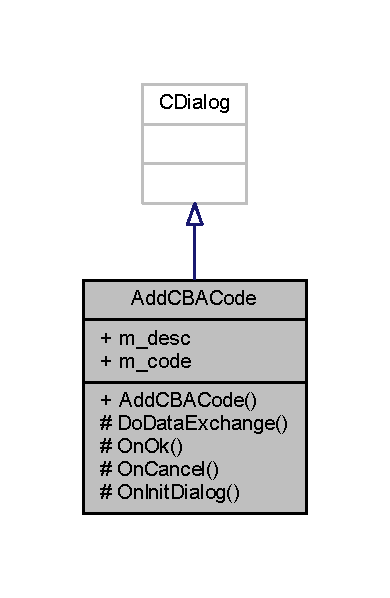
\includegraphics[width=187pt]{class_add_c_b_a_code__coll__graph}
\end{center}
\end{figure}
\subsection*{Public 타입}
\begin{DoxyCompactItemize}
\item 
enum \{ \mbox{\hyperlink{class_add_c_b_a_code_ab086df2c41fbfe55405c6ac046dab7a5a74bfcc1c249905cacf32559b0a875855}{I\+DD}} = I\+D\+D\+\_\+\+A\+D\+D\+\_\+\+C\+H\+E\+A\+T\+\_\+\+D\+LG
 \}
\end{DoxyCompactItemize}
\subsection*{Public 멤버 함수}
\begin{DoxyCompactItemize}
\item 
\mbox{\hyperlink{class_add_c_b_a_code_a13fcdd2e1451c66ac0744a631d95fdb8}{Add\+C\+B\+A\+Code}} (C\+Wnd $\ast$p\+Parent=\mbox{\hyperlink{_system_8h_a070d2ce7b6bb7e5c05602aa8c308d0c4}{N\+U\+LL}})
\end{DoxyCompactItemize}
\subsection*{Public 속성}
\begin{DoxyCompactItemize}
\item 
C\+Edit \mbox{\hyperlink{class_add_c_b_a_code_ab5056f88f9c1f58a20a1ce718599305b}{m\+\_\+desc}}
\item 
C\+Edit \mbox{\hyperlink{class_add_c_b_a_code_ab4b404e9aed23e5dd265f543e98c9c6c}{m\+\_\+code}}
\end{DoxyCompactItemize}
\subsection*{Protected 멤버 함수}
\begin{DoxyCompactItemize}
\item 
virtual void \mbox{\hyperlink{class_add_c_b_a_code_a62f9304a8dd24bfd4621e59ba5073cc4}{Do\+Data\+Exchange}} (C\+Data\+Exchange $\ast$p\+DX)
\item 
afx\+\_\+msg void \mbox{\hyperlink{class_add_c_b_a_code_a63c5cc95366a1a0aad123432054f977a}{On\+Ok}} ()
\item 
afx\+\_\+msg void \mbox{\hyperlink{class_add_c_b_a_code_a94c94b1c124bb028f9237ee9bfa9f41d}{On\+Cancel}} ()
\item 
virtual B\+O\+OL \mbox{\hyperlink{class_add_c_b_a_code_a302c75c08dacdd95eecff6b3b74ebbe6}{On\+Init\+Dialog}} ()
\end{DoxyCompactItemize}


\subsection{상세한 설명}


G\+B\+A\+Cheats.\+h 파일의 220 번째 라인에서 정의되었습니다.



\subsection{멤버 열거형 문서화}
\mbox{\Hypertarget{class_add_c_b_a_code_ab086df2c41fbfe55405c6ac046dab7a5}\label{class_add_c_b_a_code_ab086df2c41fbfe55405c6ac046dab7a5}} 
\subsubsection{\texorpdfstring{anonymous enum}{anonymous enum}}
{\footnotesize\ttfamily anonymous enum}

\begin{DoxyEnumFields}{열거형 멤버}
\raisebox{\heightof{T}}[0pt][0pt]{\index{I\+DD@{I\+DD}!Add\+C\+B\+A\+Code@{Add\+C\+B\+A\+Code}}\index{Add\+C\+B\+A\+Code@{Add\+C\+B\+A\+Code}!I\+DD@{I\+DD}}}\mbox{\Hypertarget{class_add_c_b_a_code_ab086df2c41fbfe55405c6ac046dab7a5a74bfcc1c249905cacf32559b0a875855}\label{class_add_c_b_a_code_ab086df2c41fbfe55405c6ac046dab7a5a74bfcc1c249905cacf32559b0a875855}} 
I\+DD&\\
\hline

\end{DoxyEnumFields}


G\+B\+A\+Cheats.\+h 파일의 228 번째 라인에서 정의되었습니다.


\begin{DoxyCode}
228 \{ \mbox{\hyperlink{class_add_c_b_a_code_ab086df2c41fbfe55405c6ac046dab7a5a74bfcc1c249905cacf32559b0a875855}{IDD}} = \mbox{\hyperlink{resource_8h_a388a8d7b6dea32798ece69044a21790d}{IDD\_ADD\_CHEAT\_DLG}} \};
\end{DoxyCode}


\subsection{생성자 \& 소멸자 문서화}
\mbox{\Hypertarget{class_add_c_b_a_code_a13fcdd2e1451c66ac0744a631d95fdb8}\label{class_add_c_b_a_code_a13fcdd2e1451c66ac0744a631d95fdb8}} 
\index{Add\+C\+B\+A\+Code@{Add\+C\+B\+A\+Code}!Add\+C\+B\+A\+Code@{Add\+C\+B\+A\+Code}}
\index{Add\+C\+B\+A\+Code@{Add\+C\+B\+A\+Code}!Add\+C\+B\+A\+Code@{Add\+C\+B\+A\+Code}}
\subsubsection{\texorpdfstring{Add\+C\+B\+A\+Code()}{AddCBACode()}}
{\footnotesize\ttfamily Add\+C\+B\+A\+Code\+::\+Add\+C\+B\+A\+Code (\begin{DoxyParamCaption}\item[{C\+Wnd $\ast$}]{p\+Parent = {\ttfamily \mbox{\hyperlink{_system_8h_a070d2ce7b6bb7e5c05602aa8c308d0c4}{N\+U\+LL}}} }\end{DoxyParamCaption})}



G\+B\+A\+Cheats.\+cpp 파일의 1010 번째 라인에서 정의되었습니다.


\begin{DoxyCode}
1011   : CDialog(\mbox{\hyperlink{class_add_c_b_a_code_ab086df2c41fbfe55405c6ac046dab7a5a74bfcc1c249905cacf32559b0a875855}{AddCBACode::IDD}}, pParent)
1012 \{
1013   \textcolor{comment}{//\{\{AFX\_DATA\_INIT(AddCBACode)}
1014   \textcolor{comment}{// NOTE: the ClassWizard will add member initialization here}
1015   \textcolor{comment}{//\}\}AFX\_DATA\_INIT}
1016 \}
\end{DoxyCode}


\subsection{멤버 함수 문서화}
\mbox{\Hypertarget{class_add_c_b_a_code_a62f9304a8dd24bfd4621e59ba5073cc4}\label{class_add_c_b_a_code_a62f9304a8dd24bfd4621e59ba5073cc4}} 
\index{Add\+C\+B\+A\+Code@{Add\+C\+B\+A\+Code}!Do\+Data\+Exchange@{Do\+Data\+Exchange}}
\index{Do\+Data\+Exchange@{Do\+Data\+Exchange}!Add\+C\+B\+A\+Code@{Add\+C\+B\+A\+Code}}
\subsubsection{\texorpdfstring{Do\+Data\+Exchange()}{DoDataExchange()}}
{\footnotesize\ttfamily void Add\+C\+B\+A\+Code\+::\+Do\+Data\+Exchange (\begin{DoxyParamCaption}\item[{C\+Data\+Exchange $\ast$}]{p\+DX }\end{DoxyParamCaption})\hspace{0.3cm}{\ttfamily [protected]}, {\ttfamily [virtual]}}



G\+B\+A\+Cheats.\+cpp 파일의 1019 번째 라인에서 정의되었습니다.


\begin{DoxyCode}
1020 \{
1021   CDialog::DoDataExchange(pDX);
1022   \textcolor{comment}{//\{\{AFX\_DATA\_MAP(AddCBACode)}
1023   DDX\_Control(pDX, \mbox{\hyperlink{resource_8h_adb05cf1e74135587a9b3ab93a5152feb}{IDC\_DESC}}, \mbox{\hyperlink{class_add_c_b_a_code_ab5056f88f9c1f58a20a1ce718599305b}{m\_desc}});
1024   DDX\_Control(pDX, \mbox{\hyperlink{resource_8h_abb149f0043fd3834639ddb2d80d31723}{IDC\_CODE}}, \mbox{\hyperlink{class_add_c_b_a_code_ab4b404e9aed23e5dd265f543e98c9c6c}{m\_code}});
1025   \textcolor{comment}{//\}\}AFX\_DATA\_MAP}
1026 \}
\end{DoxyCode}
\mbox{\Hypertarget{class_add_c_b_a_code_a94c94b1c124bb028f9237ee9bfa9f41d}\label{class_add_c_b_a_code_a94c94b1c124bb028f9237ee9bfa9f41d}} 
\index{Add\+C\+B\+A\+Code@{Add\+C\+B\+A\+Code}!On\+Cancel@{On\+Cancel}}
\index{On\+Cancel@{On\+Cancel}!Add\+C\+B\+A\+Code@{Add\+C\+B\+A\+Code}}
\subsubsection{\texorpdfstring{On\+Cancel()}{OnCancel()}}
{\footnotesize\ttfamily void Add\+C\+B\+A\+Code\+::\+On\+Cancel (\begin{DoxyParamCaption}{ }\end{DoxyParamCaption})\hspace{0.3cm}{\ttfamily [protected]}}



G\+B\+A\+Cheats.\+cpp 파일의 1083 번째 라인에서 정의되었습니다.


\begin{DoxyCode}
1084 \{
1085   EndDialog(FALSE);
1086 \}
\end{DoxyCode}
\mbox{\Hypertarget{class_add_c_b_a_code_a302c75c08dacdd95eecff6b3b74ebbe6}\label{class_add_c_b_a_code_a302c75c08dacdd95eecff6b3b74ebbe6}} 
\index{Add\+C\+B\+A\+Code@{Add\+C\+B\+A\+Code}!On\+Init\+Dialog@{On\+Init\+Dialog}}
\index{On\+Init\+Dialog@{On\+Init\+Dialog}!Add\+C\+B\+A\+Code@{Add\+C\+B\+A\+Code}}
\subsubsection{\texorpdfstring{On\+Init\+Dialog()}{OnInitDialog()}}
{\footnotesize\ttfamily B\+O\+OL Add\+C\+B\+A\+Code\+::\+On\+Init\+Dialog (\begin{DoxyParamCaption}{ }\end{DoxyParamCaption})\hspace{0.3cm}{\ttfamily [protected]}, {\ttfamily [virtual]}}



G\+B\+A\+Cheats.\+cpp 파일의 1088 번째 라인에서 정의되었습니다.


\begin{DoxyCode}
1089 \{
1090   CDialog::OnInitDialog();
1091   
1092   \mbox{\hyperlink{class_add_c_b_a_code_ab4b404e9aed23e5dd265f543e98c9c6c}{m\_code}}.LimitText(1024);
1093   \mbox{\hyperlink{class_add_c_b_a_code_ab5056f88f9c1f58a20a1ce718599305b}{m\_desc}}.LimitText(32);
1094   CString title = \mbox{\hyperlink{_win_res_util_8cpp_a416e85e80ab9b01376e87251c83d1a5a}{winResLoadString}}(\mbox{\hyperlink{resource_8h_add1ed8080a9328ce15770b3f9bd29b09}{IDS\_ADD\_CBA\_CODE}});
1095   SetWindowText(title);
1096   CenterWindow();
1097   
1098   \textcolor{keywordflow}{return} TRUE;  \textcolor{comment}{// return TRUE unless you set the focus to a control}
1099                 \textcolor{comment}{// EXCEPTION: OCX Property Pages should return FALSE}
1100 \}
\end{DoxyCode}
이 함수 내부에서 호출하는 함수들에 대한 그래프입니다.\+:
\nopagebreak
\begin{figure}[H]
\begin{center}
\leavevmode
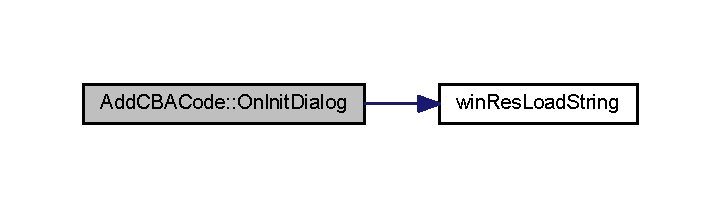
\includegraphics[width=346pt]{class_add_c_b_a_code_a302c75c08dacdd95eecff6b3b74ebbe6_cgraph}
\end{center}
\end{figure}
\mbox{\Hypertarget{class_add_c_b_a_code_a63c5cc95366a1a0aad123432054f977a}\label{class_add_c_b_a_code_a63c5cc95366a1a0aad123432054f977a}} 
\index{Add\+C\+B\+A\+Code@{Add\+C\+B\+A\+Code}!On\+Ok@{On\+Ok}}
\index{On\+Ok@{On\+Ok}!Add\+C\+B\+A\+Code@{Add\+C\+B\+A\+Code}}
\subsubsection{\texorpdfstring{On\+Ok()}{OnOk()}}
{\footnotesize\ttfamily void Add\+C\+B\+A\+Code\+::\+On\+Ok (\begin{DoxyParamCaption}{ }\end{DoxyParamCaption})\hspace{0.3cm}{\ttfamily [protected]}}



G\+B\+A\+Cheats.\+cpp 파일의 1039 번째 라인에서 정의되었습니다.


\begin{DoxyCode}
1040 \{
1041   CString desc;
1042   CString \mbox{\hyperlink{_g_b_a_8cpp_a28d4d3d8445e73a696b2d6f7eadabd96}{buffer}};
1043   CString part1;
1044   CString code;
1045   CString token;
1046 
1047   \mbox{\hyperlink{class_add_c_b_a_code_ab4b404e9aed23e5dd265f543e98c9c6c}{m\_code}}.GetWindowText(\mbox{\hyperlink{_g_b_a_8cpp_a28d4d3d8445e73a696b2d6f7eadabd96}{buffer}});
1048   \mbox{\hyperlink{class_add_c_b_a_code_ab5056f88f9c1f58a20a1ce718599305b}{m\_desc}}.GetWindowText(desc);
1049   
1050   \mbox{\hyperlink{class_string_tokenizer}{StringTokenizer}} st(\mbox{\hyperlink{_g_b_a_8cpp_a28d4d3d8445e73a696b2d6f7eadabd96}{buffer}}, \textcolor{stringliteral}{" \(\backslash\)t\(\backslash\)n\(\backslash\)r"});
1051   part1.Empty();
1052   \textcolor{keyword}{const} \textcolor{keywordtype}{char} *\mbox{\hyperlink{expr_8cpp_aded116371789db1fd63c90ef00c95a3d}{t}} = st.next();
1053   \textcolor{keywordflow}{while}(\mbox{\hyperlink{expr_8cpp_aded116371789db1fd63c90ef00c95a3d}{t}}) \{
1054     token = \mbox{\hyperlink{expr_8cpp_aded116371789db1fd63c90ef00c95a3d}{t}};
1055     token.MakeUpper();
1056     \textcolor{keywordflow}{if}(token.GetLength() == 16)
1057       \mbox{\hyperlink{_cheats_8cpp_a47aded7deffcbfa36ed55944eafb72ab}{cheatsAddGSACode}}(token, desc, \textcolor{keyword}{false});
1058     \textcolor{keywordflow}{else} \textcolor{keywordflow}{if}(token.GetLength() == 12) \{
1059       code = token.Left(8);
1060       code += \textcolor{stringliteral}{" "};
1061       code += token.Right(4);
1062       \mbox{\hyperlink{_cheats_8cpp_af79d349aaea63793beec4fa2626f74c8}{cheatsAddCBACode}}(code, desc);
1063     \} \textcolor{keywordflow}{else} \textcolor{keywordflow}{if}(part1.IsEmpty())
1064       part1 = token;
1065     \textcolor{keywordflow}{else} \{
1066       \textcolor{keywordflow}{if}(token.GetLength() == 4) \{
1067         code = part1;
1068         code += \textcolor{stringliteral}{" "};
1069         code += token;
1070         \mbox{\hyperlink{_cheats_8cpp_af79d349aaea63793beec4fa2626f74c8}{cheatsAddCBACode}}(code, desc);
1071       \} \textcolor{keywordflow}{else} \{
1072         code = part1 + token;
1073         \mbox{\hyperlink{_cheats_8cpp_a47aded7deffcbfa36ed55944eafb72ab}{cheatsAddGSACode}}(code, desc, \textcolor{keyword}{true});
1074       \}
1075       part1.Empty();
1076     \}
1077 
1078     \mbox{\hyperlink{expr_8cpp_aded116371789db1fd63c90ef00c95a3d}{t}} = st.next();
1079   \}
1080   EndDialog(TRUE);
1081 \}
\end{DoxyCode}
이 함수 내부에서 호출하는 함수들에 대한 그래프입니다.\+:
\nopagebreak
\begin{figure}[H]
\begin{center}
\leavevmode
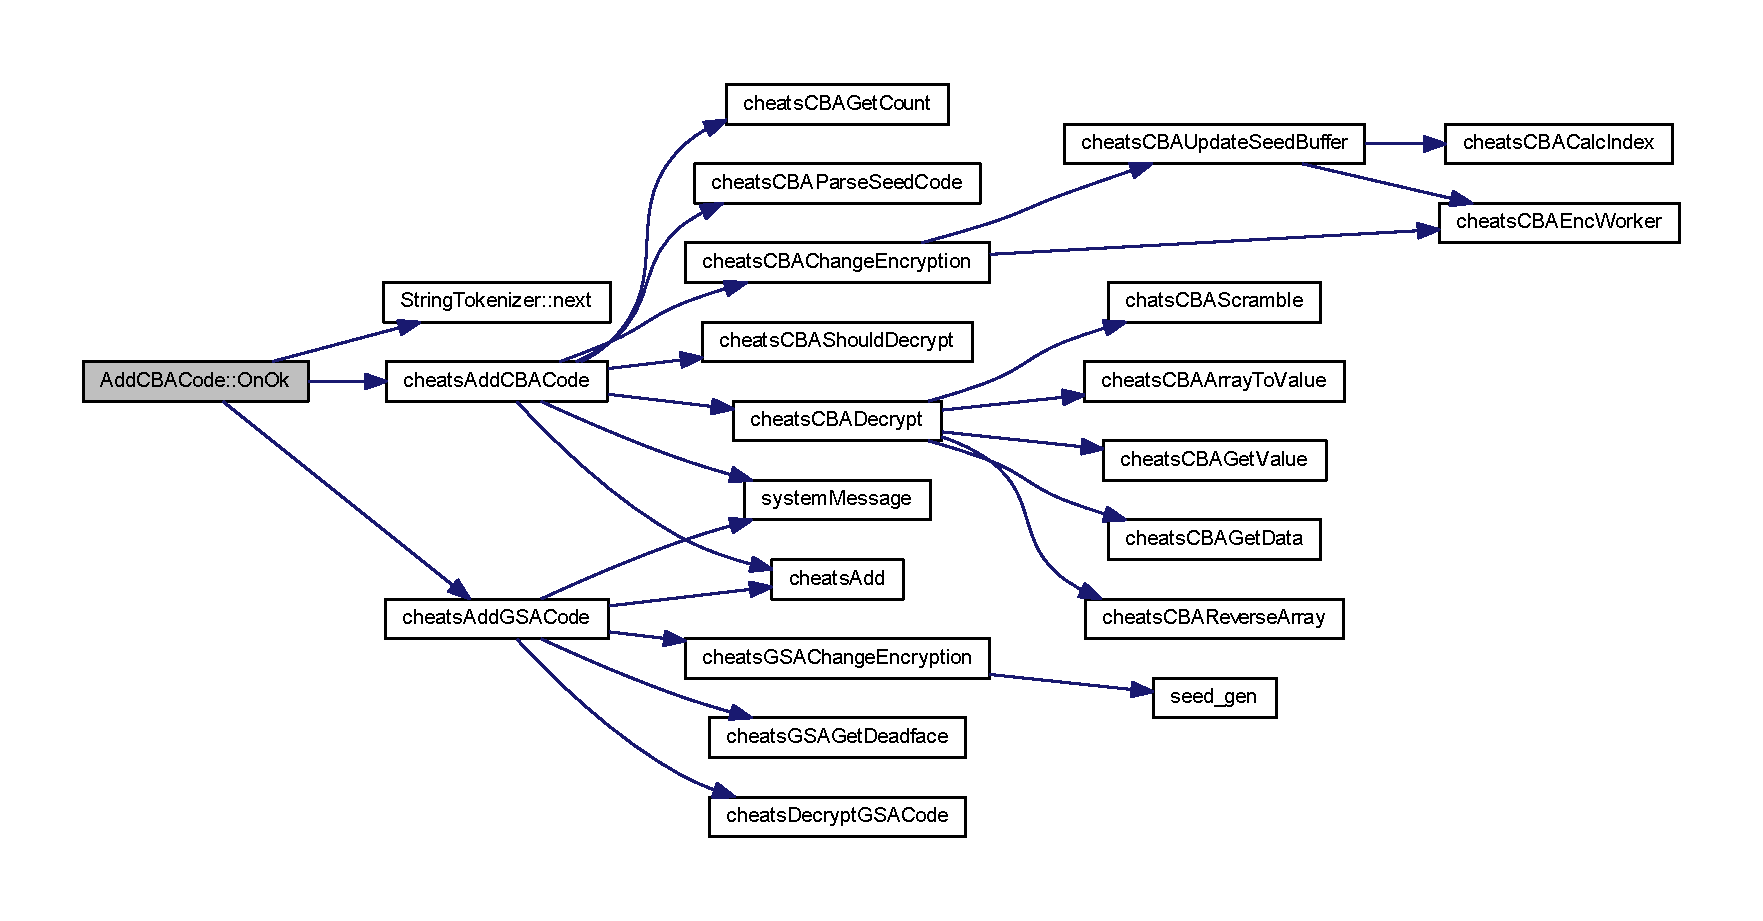
\includegraphics[width=350pt]{class_add_c_b_a_code_a63c5cc95366a1a0aad123432054f977a_cgraph}
\end{center}
\end{figure}


\subsection{멤버 데이터 문서화}
\mbox{\Hypertarget{class_add_c_b_a_code_ab4b404e9aed23e5dd265f543e98c9c6c}\label{class_add_c_b_a_code_ab4b404e9aed23e5dd265f543e98c9c6c}} 
\index{Add\+C\+B\+A\+Code@{Add\+C\+B\+A\+Code}!m\+\_\+code@{m\+\_\+code}}
\index{m\+\_\+code@{m\+\_\+code}!Add\+C\+B\+A\+Code@{Add\+C\+B\+A\+Code}}
\subsubsection{\texorpdfstring{m\+\_\+code}{m\_code}}
{\footnotesize\ttfamily C\+Edit Add\+C\+B\+A\+Code\+::m\+\_\+code}



G\+B\+A\+Cheats.\+h 파일의 230 번째 라인에서 정의되었습니다.

\mbox{\Hypertarget{class_add_c_b_a_code_ab5056f88f9c1f58a20a1ce718599305b}\label{class_add_c_b_a_code_ab5056f88f9c1f58a20a1ce718599305b}} 
\index{Add\+C\+B\+A\+Code@{Add\+C\+B\+A\+Code}!m\+\_\+desc@{m\+\_\+desc}}
\index{m\+\_\+desc@{m\+\_\+desc}!Add\+C\+B\+A\+Code@{Add\+C\+B\+A\+Code}}
\subsubsection{\texorpdfstring{m\+\_\+desc}{m\_desc}}
{\footnotesize\ttfamily C\+Edit Add\+C\+B\+A\+Code\+::m\+\_\+desc}



G\+B\+A\+Cheats.\+h 파일의 229 번째 라인에서 정의되었습니다.



이 클래스에 대한 문서화 페이지는 다음의 파일들로부터 생성되었습니다.\+:\begin{DoxyCompactItemize}
\item 
C\+:/\+Users/sjh13/sources/\+Visual\+Boy\+Advance/src/win32/\mbox{\hyperlink{_g_b_a_cheats_8h}{G\+B\+A\+Cheats.\+h}}\item 
C\+:/\+Users/sjh13/sources/\+Visual\+Boy\+Advance/src/win32/\mbox{\hyperlink{_g_b_a_cheats_8cpp}{G\+B\+A\+Cheats.\+cpp}}\end{DoxyCompactItemize}

\hypertarget{class_add_cheat}{}\section{Add\+Cheat 클래스 참조}
\label{class_add_cheat}\index{Add\+Cheat@{Add\+Cheat}}
Add\+Cheat에 대한 상속 다이어그램 \+: \begin{figure}[H]
\begin{center}
\leavevmode
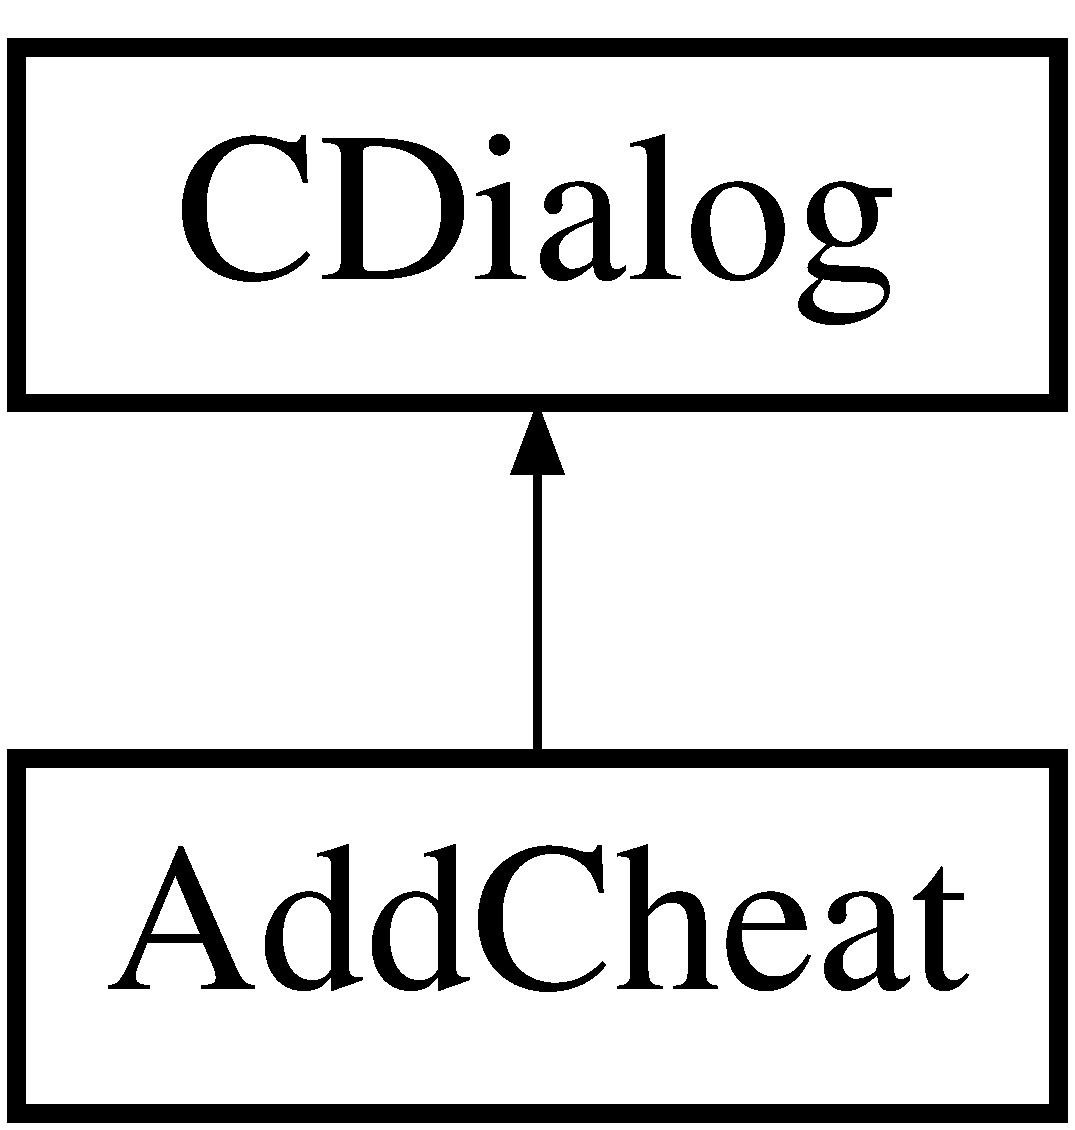
\includegraphics[height=2.000000cm]{class_add_cheat}
\end{center}
\end{figure}
\subsection*{Public 타입}
\begin{DoxyCompactItemize}
\item 
\mbox{\Hypertarget{class_add_cheat_af696833b823db49de5667fcb42b11a26}\label{class_add_cheat_af696833b823db49de5667fcb42b11a26}} 
enum \{ {\bfseries I\+DD} = I\+D\+D\+\_\+\+A\+D\+D\+\_\+\+C\+H\+E\+AT
 \}
\end{DoxyCompactItemize}
\subsection*{Public 멤버 함수}
\begin{DoxyCompactItemize}
\item 
\mbox{\Hypertarget{class_add_cheat_a53989b2f3f179185384d258c9e71ace7}\label{class_add_cheat_a53989b2f3f179185384d258c9e71ace7}} 
bool {\bfseries add\+Cheat} ()
\item 
\mbox{\Hypertarget{class_add_cheat_ae9762fec683ccd9972d29fec47eecba4}\label{class_add_cheat_ae9762fec683ccd9972d29fec47eecba4}} 
afx\+\_\+msg void {\bfseries On\+Size\+Type} (U\+I\+NT id)
\item 
\mbox{\Hypertarget{class_add_cheat_a3ac4c44d5f9ec5037e92034789c276b4}\label{class_add_cheat_a3ac4c44d5f9ec5037e92034789c276b4}} 
afx\+\_\+msg void {\bfseries On\+Number\+Type} (U\+I\+NT id)
\item 
\mbox{\Hypertarget{class_add_cheat_afa75eefc22d2f9449cf3b9283926408c}\label{class_add_cheat_afa75eefc22d2f9449cf3b9283926408c}} 
{\bfseries Add\+Cheat} (u32 address, C\+Wnd $\ast$p\+Parent=N\+U\+LL)
\end{DoxyCompactItemize}
\subsection*{Public 속성}
\begin{DoxyCompactItemize}
\item 
\mbox{\Hypertarget{class_add_cheat_ae21ae20b0a2e3b936b9ecbacb13a2751}\label{class_add_cheat_ae21ae20b0a2e3b936b9ecbacb13a2751}} 
u32 {\bfseries address}
\item 
\mbox{\Hypertarget{class_add_cheat_aff9c3fd61a088f03dba1eb01e6956286}\label{class_add_cheat_aff9c3fd61a088f03dba1eb01e6956286}} 
C\+Edit {\bfseries m\+\_\+value}
\item 
\mbox{\Hypertarget{class_add_cheat_a644f29b6dd8a0d26d5050054bdf2b054}\label{class_add_cheat_a644f29b6dd8a0d26d5050054bdf2b054}} 
C\+Edit {\bfseries m\+\_\+desc}
\item 
\mbox{\Hypertarget{class_add_cheat_a27ec0f498f3827cfc81c19d963c7fef5}\label{class_add_cheat_a27ec0f498f3827cfc81c19d963c7fef5}} 
C\+Edit {\bfseries m\+\_\+address}
\item 
\mbox{\Hypertarget{class_add_cheat_a7c3af367e51b1812d951dd2d24ac1aa8}\label{class_add_cheat_a7c3af367e51b1812d951dd2d24ac1aa8}} 
int {\bfseries size\+Type}
\item 
\mbox{\Hypertarget{class_add_cheat_a50115e7ad42a106db574754cc81bc9a0}\label{class_add_cheat_a50115e7ad42a106db574754cc81bc9a0}} 
int {\bfseries number\+Type}
\end{DoxyCompactItemize}
\subsection*{Protected 멤버 함수}
\begin{DoxyCompactItemize}
\item 
\mbox{\Hypertarget{class_add_cheat_a9d3dbf5955873700caf71f41fa5117cc}\label{class_add_cheat_a9d3dbf5955873700caf71f41fa5117cc}} 
virtual void {\bfseries Do\+Data\+Exchange} (C\+Data\+Exchange $\ast$p\+DX)
\item 
\mbox{\Hypertarget{class_add_cheat_ad3785b90d963668a87ff33fb93cf56d9}\label{class_add_cheat_ad3785b90d963668a87ff33fb93cf56d9}} 
afx\+\_\+msg void {\bfseries On\+Ok} ()
\item 
\mbox{\Hypertarget{class_add_cheat_aef14a7fa535621c242e9007a7c0510e7}\label{class_add_cheat_aef14a7fa535621c242e9007a7c0510e7}} 
afx\+\_\+msg void {\bfseries On\+Cancel} ()
\item 
\mbox{\Hypertarget{class_add_cheat_a92017eb0efe50e09e7c3e5e4980a18cb}\label{class_add_cheat_a92017eb0efe50e09e7c3e5e4980a18cb}} 
virtual B\+O\+OL {\bfseries On\+Init\+Dialog} ()
\end{DoxyCompactItemize}


이 클래스에 대한 문서화 페이지는 다음의 파일들로부터 생성되었습니다.\+:\begin{DoxyCompactItemize}
\item 
src/win32/G\+B\+A\+Cheats.\+h\item 
src/win32/G\+B\+A\+Cheats.\+cpp\end{DoxyCompactItemize}

\hypertarget{class_add_cheat_code}{}\section{Add\+Cheat\+Code 클래스 참조}
\label{class_add_cheat_code}\index{Add\+Cheat\+Code@{Add\+Cheat\+Code}}


{\ttfamily \#include $<$G\+B\+A\+Cheats.\+h$>$}



Add\+Cheat\+Code에 대한 상속 다이어그램 \+: \nopagebreak
\begin{figure}[H]
\begin{center}
\leavevmode
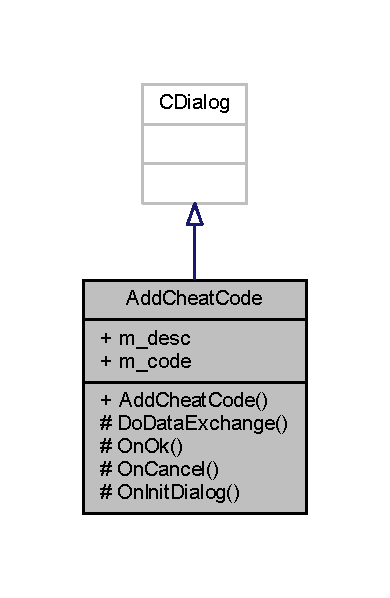
\includegraphics[width=187pt]{class_add_cheat_code__inherit__graph}
\end{center}
\end{figure}


Add\+Cheat\+Code에 대한 협력 다이어그램\+:\nopagebreak
\begin{figure}[H]
\begin{center}
\leavevmode
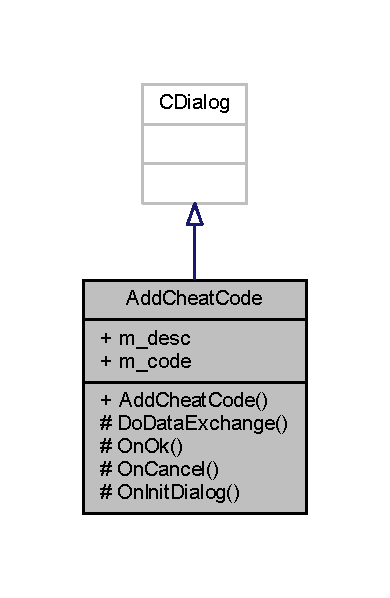
\includegraphics[width=187pt]{class_add_cheat_code__coll__graph}
\end{center}
\end{figure}
\subsection*{Public 타입}
\begin{DoxyCompactItemize}
\item 
enum \{ \mbox{\hyperlink{class_add_cheat_code_a360bc0f5ed2a9d0598c246993ecb57c2a7065caea1931a69dc54b0161b9295ba9}{I\+DD}} = I\+D\+D\+\_\+\+A\+D\+D\+\_\+\+C\+H\+E\+A\+T\+\_\+\+D\+LG
 \}
\end{DoxyCompactItemize}
\subsection*{Public 멤버 함수}
\begin{DoxyCompactItemize}
\item 
\mbox{\hyperlink{class_add_cheat_code_a6904f72f50b5354c479d73ea19dba1ab}{Add\+Cheat\+Code}} (C\+Wnd $\ast$p\+Parent=\mbox{\hyperlink{_system_8h_a070d2ce7b6bb7e5c05602aa8c308d0c4}{N\+U\+LL}})
\end{DoxyCompactItemize}
\subsection*{Public 속성}
\begin{DoxyCompactItemize}
\item 
C\+Edit \mbox{\hyperlink{class_add_cheat_code_a5bbe6b54e71db26da7b3abc7449b3342}{m\+\_\+desc}}
\item 
C\+Edit \mbox{\hyperlink{class_add_cheat_code_a9ae1d05acf10bc6fc8ea8cce2ec2cc6a}{m\+\_\+code}}
\end{DoxyCompactItemize}
\subsection*{Protected 멤버 함수}
\begin{DoxyCompactItemize}
\item 
virtual void \mbox{\hyperlink{class_add_cheat_code_af260d01bd5166f11c1e92894e36c7ad6}{Do\+Data\+Exchange}} (C\+Data\+Exchange $\ast$p\+DX)
\item 
afx\+\_\+msg void \mbox{\hyperlink{class_add_cheat_code_a77b1ec1f5e067495aef92a2f9b8750c8}{On\+Ok}} ()
\item 
afx\+\_\+msg void \mbox{\hyperlink{class_add_cheat_code_abbf22fde6ad9aa52439e4cb4a3d8418b}{On\+Cancel}} ()
\item 
virtual B\+O\+OL \mbox{\hyperlink{class_add_cheat_code_a7818441d921e63c1b0983e86b60beeba}{On\+Init\+Dialog}} ()
\end{DoxyCompactItemize}


\subsection{상세한 설명}


G\+B\+A\+Cheats.\+h 파일의 256 번째 라인에서 정의되었습니다.



\subsection{멤버 열거형 문서화}
\mbox{\Hypertarget{class_add_cheat_code_a360bc0f5ed2a9d0598c246993ecb57c2}\label{class_add_cheat_code_a360bc0f5ed2a9d0598c246993ecb57c2}} 
\subsubsection{\texorpdfstring{anonymous enum}{anonymous enum}}
{\footnotesize\ttfamily anonymous enum}

\begin{DoxyEnumFields}{열거형 멤버}
\raisebox{\heightof{T}}[0pt][0pt]{\index{I\+DD@{I\+DD}!Add\+Cheat\+Code@{Add\+Cheat\+Code}}\index{Add\+Cheat\+Code@{Add\+Cheat\+Code}!I\+DD@{I\+DD}}}\mbox{\Hypertarget{class_add_cheat_code_a360bc0f5ed2a9d0598c246993ecb57c2a7065caea1931a69dc54b0161b9295ba9}\label{class_add_cheat_code_a360bc0f5ed2a9d0598c246993ecb57c2a7065caea1931a69dc54b0161b9295ba9}} 
I\+DD&\\
\hline

\end{DoxyEnumFields}


G\+B\+A\+Cheats.\+h 파일의 264 번째 라인에서 정의되었습니다.


\begin{DoxyCode}
264 \{ \mbox{\hyperlink{class_add_cheat_code_a360bc0f5ed2a9d0598c246993ecb57c2a7065caea1931a69dc54b0161b9295ba9}{IDD}} = \mbox{\hyperlink{resource_8h_a388a8d7b6dea32798ece69044a21790d}{IDD\_ADD\_CHEAT\_DLG}} \};
\end{DoxyCode}


\subsection{생성자 \& 소멸자 문서화}
\mbox{\Hypertarget{class_add_cheat_code_a6904f72f50b5354c479d73ea19dba1ab}\label{class_add_cheat_code_a6904f72f50b5354c479d73ea19dba1ab}} 
\index{Add\+Cheat\+Code@{Add\+Cheat\+Code}!Add\+Cheat\+Code@{Add\+Cheat\+Code}}
\index{Add\+Cheat\+Code@{Add\+Cheat\+Code}!Add\+Cheat\+Code@{Add\+Cheat\+Code}}
\subsubsection{\texorpdfstring{Add\+Cheat\+Code()}{AddCheatCode()}}
{\footnotesize\ttfamily Add\+Cheat\+Code\+::\+Add\+Cheat\+Code (\begin{DoxyParamCaption}\item[{C\+Wnd $\ast$}]{p\+Parent = {\ttfamily \mbox{\hyperlink{_system_8h_a070d2ce7b6bb7e5c05602aa8c308d0c4}{N\+U\+LL}}} }\end{DoxyParamCaption})}



G\+B\+A\+Cheats.\+cpp 파일의 1106 번째 라인에서 정의되었습니다.


\begin{DoxyCode}
1107   : CDialog(\mbox{\hyperlink{class_add_cheat_code_a360bc0f5ed2a9d0598c246993ecb57c2a7065caea1931a69dc54b0161b9295ba9}{AddCheatCode::IDD}}, pParent)
1108 \{
1109   \textcolor{comment}{//\{\{AFX\_DATA\_INIT(AddCheatCode)}
1110   \textcolor{comment}{// NOTE: the ClassWizard will add member initialization here}
1111   \textcolor{comment}{//\}\}AFX\_DATA\_INIT}
1112 \}
\end{DoxyCode}


\subsection{멤버 함수 문서화}
\mbox{\Hypertarget{class_add_cheat_code_af260d01bd5166f11c1e92894e36c7ad6}\label{class_add_cheat_code_af260d01bd5166f11c1e92894e36c7ad6}} 
\index{Add\+Cheat\+Code@{Add\+Cheat\+Code}!Do\+Data\+Exchange@{Do\+Data\+Exchange}}
\index{Do\+Data\+Exchange@{Do\+Data\+Exchange}!Add\+Cheat\+Code@{Add\+Cheat\+Code}}
\subsubsection{\texorpdfstring{Do\+Data\+Exchange()}{DoDataExchange()}}
{\footnotesize\ttfamily void Add\+Cheat\+Code\+::\+Do\+Data\+Exchange (\begin{DoxyParamCaption}\item[{C\+Data\+Exchange $\ast$}]{p\+DX }\end{DoxyParamCaption})\hspace{0.3cm}{\ttfamily [protected]}, {\ttfamily [virtual]}}



G\+B\+A\+Cheats.\+cpp 파일의 1115 번째 라인에서 정의되었습니다.


\begin{DoxyCode}
1116 \{
1117   CDialog::DoDataExchange(pDX);
1118   \textcolor{comment}{//\{\{AFX\_DATA\_MAP(AddCheatCode)}
1119   DDX\_Control(pDX, \mbox{\hyperlink{resource_8h_adb05cf1e74135587a9b3ab93a5152feb}{IDC\_DESC}}, \mbox{\hyperlink{class_add_cheat_code_a5bbe6b54e71db26da7b3abc7449b3342}{m\_desc}});
1120   DDX\_Control(pDX, \mbox{\hyperlink{resource_8h_abb149f0043fd3834639ddb2d80d31723}{IDC\_CODE}}, \mbox{\hyperlink{class_add_cheat_code_a9ae1d05acf10bc6fc8ea8cce2ec2cc6a}{m\_code}});
1121   \textcolor{comment}{//\}\}AFX\_DATA\_MAP}
1122 \}
\end{DoxyCode}
\mbox{\Hypertarget{class_add_cheat_code_abbf22fde6ad9aa52439e4cb4a3d8418b}\label{class_add_cheat_code_abbf22fde6ad9aa52439e4cb4a3d8418b}} 
\index{Add\+Cheat\+Code@{Add\+Cheat\+Code}!On\+Cancel@{On\+Cancel}}
\index{On\+Cancel@{On\+Cancel}!Add\+Cheat\+Code@{Add\+Cheat\+Code}}
\subsubsection{\texorpdfstring{On\+Cancel()}{OnCancel()}}
{\footnotesize\ttfamily void Add\+Cheat\+Code\+::\+On\+Cancel (\begin{DoxyParamCaption}{ }\end{DoxyParamCaption})\hspace{0.3cm}{\ttfamily [protected]}}



G\+B\+A\+Cheats.\+cpp 파일의 1155 번째 라인에서 정의되었습니다.


\begin{DoxyCode}
1156 \{
1157   EndDialog(FALSE);
1158 \}
\end{DoxyCode}
\mbox{\Hypertarget{class_add_cheat_code_a7818441d921e63c1b0983e86b60beeba}\label{class_add_cheat_code_a7818441d921e63c1b0983e86b60beeba}} 
\index{Add\+Cheat\+Code@{Add\+Cheat\+Code}!On\+Init\+Dialog@{On\+Init\+Dialog}}
\index{On\+Init\+Dialog@{On\+Init\+Dialog}!Add\+Cheat\+Code@{Add\+Cheat\+Code}}
\subsubsection{\texorpdfstring{On\+Init\+Dialog()}{OnInitDialog()}}
{\footnotesize\ttfamily B\+O\+OL Add\+Cheat\+Code\+::\+On\+Init\+Dialog (\begin{DoxyParamCaption}{ }\end{DoxyParamCaption})\hspace{0.3cm}{\ttfamily [protected]}, {\ttfamily [virtual]}}



G\+B\+A\+Cheats.\+cpp 파일의 1160 번째 라인에서 정의되었습니다.


\begin{DoxyCode}
1161 \{
1162   CDialog::OnInitDialog();
1163   
1164   \mbox{\hyperlink{class_add_cheat_code_a9ae1d05acf10bc6fc8ea8cce2ec2cc6a}{m\_code}}.LimitText(1024);
1165   \mbox{\hyperlink{class_add_cheat_code_a5bbe6b54e71db26da7b3abc7449b3342}{m\_desc}}.LimitText(32);
1166   CString title = \mbox{\hyperlink{_win_res_util_8cpp_a416e85e80ab9b01376e87251c83d1a5a}{winResLoadString}}(\mbox{\hyperlink{resource_8h_acb74efa1ecac0ed81d23602f6f68ce35}{IDS\_ADD\_CHEAT\_CODE}});
1167   SetWindowText(title);
1168   CenterWindow();
1169   
1170   \textcolor{keywordflow}{return} TRUE;  \textcolor{comment}{// return TRUE unless you set the focus to a control}
1171                 \textcolor{comment}{// EXCEPTION: OCX Property Pages should return FALSE}
1172 \}
\end{DoxyCode}
이 함수 내부에서 호출하는 함수들에 대한 그래프입니다.\+:
\nopagebreak
\begin{figure}[H]
\begin{center}
\leavevmode
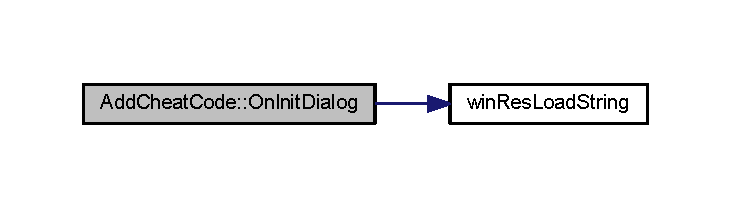
\includegraphics[width=350pt]{class_add_cheat_code_a7818441d921e63c1b0983e86b60beeba_cgraph}
\end{center}
\end{figure}
\mbox{\Hypertarget{class_add_cheat_code_a77b1ec1f5e067495aef92a2f9b8750c8}\label{class_add_cheat_code_a77b1ec1f5e067495aef92a2f9b8750c8}} 
\index{Add\+Cheat\+Code@{Add\+Cheat\+Code}!On\+Ok@{On\+Ok}}
\index{On\+Ok@{On\+Ok}!Add\+Cheat\+Code@{Add\+Cheat\+Code}}
\subsubsection{\texorpdfstring{On\+Ok()}{OnOk()}}
{\footnotesize\ttfamily void Add\+Cheat\+Code\+::\+On\+Ok (\begin{DoxyParamCaption}{ }\end{DoxyParamCaption})\hspace{0.3cm}{\ttfamily [protected]}}



G\+B\+A\+Cheats.\+cpp 파일의 1135 번째 라인에서 정의되었습니다.


\begin{DoxyCode}
1136 \{
1137   CString desc;
1138   CString \mbox{\hyperlink{_g_b_a_8cpp_a28d4d3d8445e73a696b2d6f7eadabd96}{buffer}};
1139   CString token;
1140 
1141   \mbox{\hyperlink{class_add_cheat_code_a9ae1d05acf10bc6fc8ea8cce2ec2cc6a}{m\_code}}.GetWindowText(\mbox{\hyperlink{_g_b_a_8cpp_a28d4d3d8445e73a696b2d6f7eadabd96}{buffer}});
1142   \mbox{\hyperlink{class_add_cheat_code_a5bbe6b54e71db26da7b3abc7449b3342}{m\_desc}}.GetWindowText(desc);
1143   
1144   \mbox{\hyperlink{class_string_tokenizer}{StringTokenizer}} st(\mbox{\hyperlink{_g_b_a_8cpp_a28d4d3d8445e73a696b2d6f7eadabd96}{buffer}}, \textcolor{stringliteral}{" \(\backslash\)t\(\backslash\)n\(\backslash\)r"});
1145   \textcolor{keyword}{const} \textcolor{keywordtype}{char} *\mbox{\hyperlink{expr_8cpp_aded116371789db1fd63c90ef00c95a3d}{t}} = st.next();
1146   \textcolor{keywordflow}{while}(\mbox{\hyperlink{expr_8cpp_aded116371789db1fd63c90ef00c95a3d}{t}}) \{
1147     token = \mbox{\hyperlink{expr_8cpp_aded116371789db1fd63c90ef00c95a3d}{t}};
1148     token.MakeUpper();
1149     \mbox{\hyperlink{_cheats_8cpp_a0e87699a326f10639902f59174a7e6ee}{cheatsAddCheatCode}}(token, desc);
1150     \mbox{\hyperlink{expr_8cpp_aded116371789db1fd63c90ef00c95a3d}{t}} = st.next();
1151   \}
1152   EndDialog(TRUE);
1153 \}
\end{DoxyCode}
이 함수 내부에서 호출하는 함수들에 대한 그래프입니다.\+:
\nopagebreak
\begin{figure}[H]
\begin{center}
\leavevmode
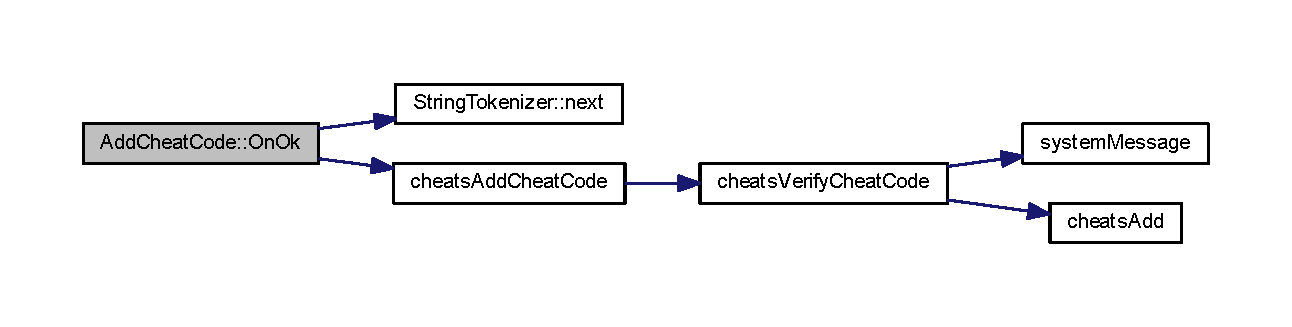
\includegraphics[width=350pt]{class_add_cheat_code_a77b1ec1f5e067495aef92a2f9b8750c8_cgraph}
\end{center}
\end{figure}


\subsection{멤버 데이터 문서화}
\mbox{\Hypertarget{class_add_cheat_code_a9ae1d05acf10bc6fc8ea8cce2ec2cc6a}\label{class_add_cheat_code_a9ae1d05acf10bc6fc8ea8cce2ec2cc6a}} 
\index{Add\+Cheat\+Code@{Add\+Cheat\+Code}!m\+\_\+code@{m\+\_\+code}}
\index{m\+\_\+code@{m\+\_\+code}!Add\+Cheat\+Code@{Add\+Cheat\+Code}}
\subsubsection{\texorpdfstring{m\+\_\+code}{m\_code}}
{\footnotesize\ttfamily C\+Edit Add\+Cheat\+Code\+::m\+\_\+code}



G\+B\+A\+Cheats.\+h 파일의 266 번째 라인에서 정의되었습니다.

\mbox{\Hypertarget{class_add_cheat_code_a5bbe6b54e71db26da7b3abc7449b3342}\label{class_add_cheat_code_a5bbe6b54e71db26da7b3abc7449b3342}} 
\index{Add\+Cheat\+Code@{Add\+Cheat\+Code}!m\+\_\+desc@{m\+\_\+desc}}
\index{m\+\_\+desc@{m\+\_\+desc}!Add\+Cheat\+Code@{Add\+Cheat\+Code}}
\subsubsection{\texorpdfstring{m\+\_\+desc}{m\_desc}}
{\footnotesize\ttfamily C\+Edit Add\+Cheat\+Code\+::m\+\_\+desc}



G\+B\+A\+Cheats.\+h 파일의 265 번째 라인에서 정의되었습니다.



이 클래스에 대한 문서화 페이지는 다음의 파일들로부터 생성되었습니다.\+:\begin{DoxyCompactItemize}
\item 
C\+:/\+Users/sjh13/sources/\+Visual\+Boy\+Advance/src/win32/\mbox{\hyperlink{_g_b_a_cheats_8h}{G\+B\+A\+Cheats.\+h}}\item 
C\+:/\+Users/sjh13/sources/\+Visual\+Boy\+Advance/src/win32/\mbox{\hyperlink{_g_b_a_cheats_8cpp}{G\+B\+A\+Cheats.\+cpp}}\end{DoxyCompactItemize}

\hypertarget{class_add_g_b_cheat}{}\section{Add\+G\+B\+Cheat 클래스 참조}
\label{class_add_g_b_cheat}\index{Add\+G\+B\+Cheat@{Add\+G\+B\+Cheat}}
Add\+G\+B\+Cheat에 대한 상속 다이어그램 \+: \begin{figure}[H]
\begin{center}
\leavevmode
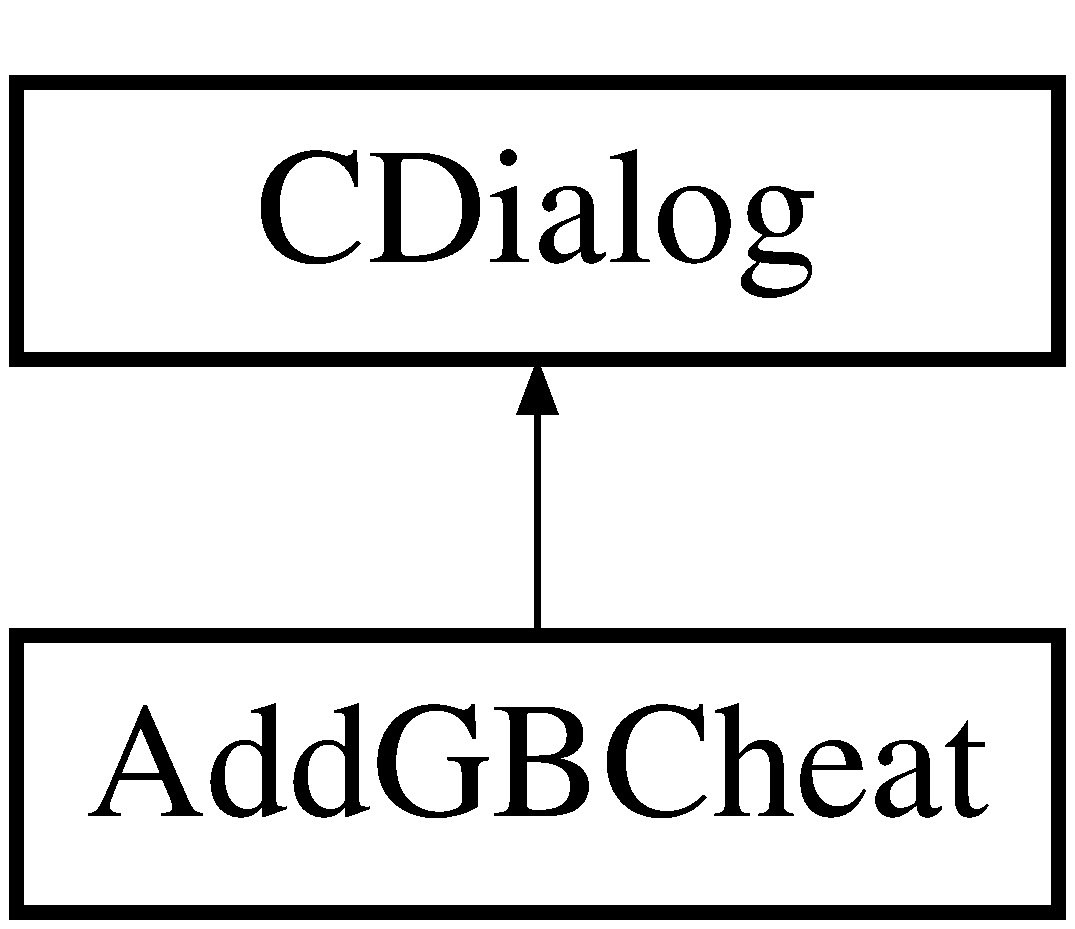
\includegraphics[height=2.000000cm]{class_add_g_b_cheat}
\end{center}
\end{figure}
\subsection*{Public 타입}
\begin{DoxyCompactItemize}
\item 
\mbox{\Hypertarget{class_add_g_b_cheat_ae307c54936e2ef002f6323ab0d1fa05e}\label{class_add_g_b_cheat_ae307c54936e2ef002f6323ab0d1fa05e}} 
enum \{ {\bfseries I\+DD} = I\+D\+D\+\_\+\+A\+D\+D\+\_\+\+C\+H\+E\+AT
 \}
\end{DoxyCompactItemize}
\subsection*{Public 멤버 함수}
\begin{DoxyCompactItemize}
\item 
\mbox{\Hypertarget{class_add_g_b_cheat_a9bff22f01c72ffbcd6071bb604c2e090}\label{class_add_g_b_cheat_a9bff22f01c72ffbcd6071bb604c2e090}} 
afx\+\_\+msg void {\bfseries On\+Size\+Type} (U\+I\+NT id)
\item 
\mbox{\Hypertarget{class_add_g_b_cheat_a1bfddb9d66e182dedc95bf889dc9e6d2}\label{class_add_g_b_cheat_a1bfddb9d66e182dedc95bf889dc9e6d2}} 
afx\+\_\+msg void {\bfseries On\+Number\+Type} (U\+I\+NT id)
\item 
\mbox{\Hypertarget{class_add_g_b_cheat_a054ba5040a40f7ef4b3a0ddb5a458592}\label{class_add_g_b_cheat_a054ba5040a40f7ef4b3a0ddb5a458592}} 
bool {\bfseries add\+Cheat} ()
\item 
\mbox{\Hypertarget{class_add_g_b_cheat_a1794ccc1e4826b5a8b179d20557955b8}\label{class_add_g_b_cheat_a1794ccc1e4826b5a8b179d20557955b8}} 
{\bfseries Add\+G\+B\+Cheat} (u32 addr, C\+Wnd $\ast$p\+Parent=N\+U\+LL)
\end{DoxyCompactItemize}
\subsection*{Public 속성}
\begin{DoxyCompactItemize}
\item 
\mbox{\Hypertarget{class_add_g_b_cheat_ac5705ad3d8964adb59d62c51dd60a0fc}\label{class_add_g_b_cheat_ac5705ad3d8964adb59d62c51dd60a0fc}} 
C\+Edit {\bfseries m\+\_\+value}
\item 
\mbox{\Hypertarget{class_add_g_b_cheat_af68f821a3073c6a01f1c8760dab628ee}\label{class_add_g_b_cheat_af68f821a3073c6a01f1c8760dab628ee}} 
C\+Edit {\bfseries m\+\_\+address}
\item 
\mbox{\Hypertarget{class_add_g_b_cheat_ae1711f59505d7d442a6572a346993cd2}\label{class_add_g_b_cheat_ae1711f59505d7d442a6572a346993cd2}} 
C\+Edit {\bfseries m\+\_\+desc}
\item 
\mbox{\Hypertarget{class_add_g_b_cheat_ae0603ce2570d5b09a64f4bd6c2107962}\label{class_add_g_b_cheat_ae0603ce2570d5b09a64f4bd6c2107962}} 
int {\bfseries size\+Type}
\item 
\mbox{\Hypertarget{class_add_g_b_cheat_ab49fa34156026418e26edf606aa82b1a}\label{class_add_g_b_cheat_ab49fa34156026418e26edf606aa82b1a}} 
int {\bfseries number\+Type}
\end{DoxyCompactItemize}
\subsection*{Protected 멤버 함수}
\begin{DoxyCompactItemize}
\item 
\mbox{\Hypertarget{class_add_g_b_cheat_ab90d0a5d50911d10eec2706250882d6f}\label{class_add_g_b_cheat_ab90d0a5d50911d10eec2706250882d6f}} 
virtual void {\bfseries Do\+Data\+Exchange} (C\+Data\+Exchange $\ast$p\+DX)
\item 
\mbox{\Hypertarget{class_add_g_b_cheat_ac2eb6674e040b6a8af227e6517f857e8}\label{class_add_g_b_cheat_ac2eb6674e040b6a8af227e6517f857e8}} 
afx\+\_\+msg void {\bfseries On\+Cancel} ()
\item 
\mbox{\Hypertarget{class_add_g_b_cheat_aef6d73f3cdf51e28bbba9f7e14b21941}\label{class_add_g_b_cheat_aef6d73f3cdf51e28bbba9f7e14b21941}} 
afx\+\_\+msg void {\bfseries On\+Ok} ()
\item 
\mbox{\Hypertarget{class_add_g_b_cheat_a97210ad566b117af4994adac5d954e94}\label{class_add_g_b_cheat_a97210ad566b117af4994adac5d954e94}} 
virtual B\+O\+OL {\bfseries On\+Init\+Dialog} ()
\end{DoxyCompactItemize}
\subsection*{Protected 속성}
\begin{DoxyCompactItemize}
\item 
\mbox{\Hypertarget{class_add_g_b_cheat_adb910488c84e165b4fd33646b932ee2e}\label{class_add_g_b_cheat_adb910488c84e165b4fd33646b932ee2e}} 
L\+O\+N\+G\+\_\+\+P\+TR {\bfseries address}
\end{DoxyCompactItemize}


이 클래스에 대한 문서화 페이지는 다음의 파일들로부터 생성되었습니다.\+:\begin{DoxyCompactItemize}
\item 
src/win32/G\+B\+Cheats\+Dlg.\+h\item 
src/win32/G\+B\+Cheats\+Dlg.\+cpp\end{DoxyCompactItemize}

\hypertarget{class_add_g_b_code}{}\section{Add\+G\+B\+Code 클래스 참조}
\label{class_add_g_b_code}\index{Add\+G\+B\+Code@{Add\+G\+B\+Code}}
Add\+G\+B\+Code에 대한 상속 다이어그램 \+: \begin{figure}[H]
\begin{center}
\leavevmode
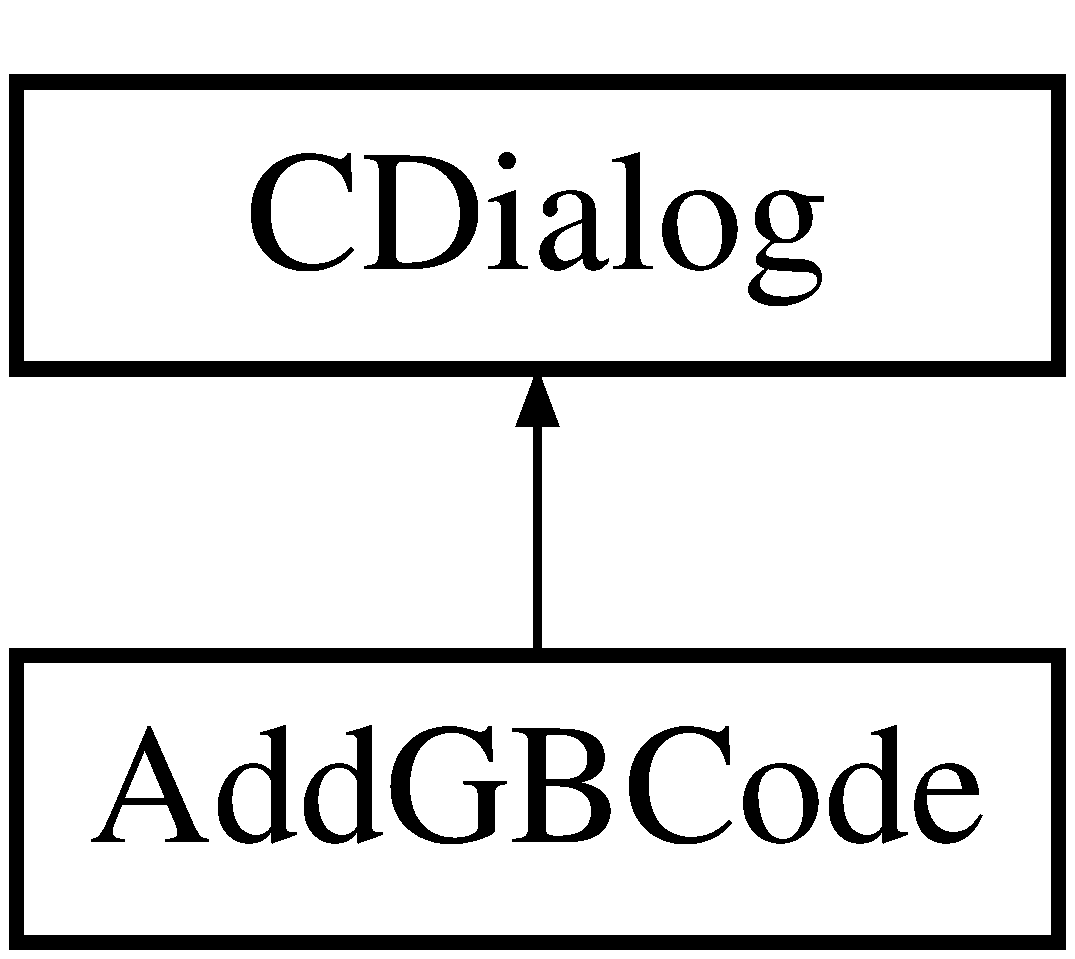
\includegraphics[height=2.000000cm]{class_add_g_b_code}
\end{center}
\end{figure}
\subsection*{Public 타입}
\begin{DoxyCompactItemize}
\item 
\mbox{\Hypertarget{class_add_g_b_code_a2dd2d84fa89620e9d1bd9816ac698df9}\label{class_add_g_b_code_a2dd2d84fa89620e9d1bd9816ac698df9}} 
enum \{ {\bfseries I\+DD} = I\+D\+D\+\_\+\+A\+D\+D\+\_\+\+C\+H\+E\+A\+T\+\_\+\+D\+LG
 \}
\end{DoxyCompactItemize}
\subsection*{Public 멤버 함수}
\begin{DoxyCompactItemize}
\item 
\mbox{\Hypertarget{class_add_g_b_code_a99be74c9c22f954a6a83fb1e8eba7b29}\label{class_add_g_b_code_a99be74c9c22f954a6a83fb1e8eba7b29}} 
{\bfseries Add\+G\+B\+Code} (bool($\ast$verify)(const char $\ast$, const char $\ast$), int, const char $\ast$, C\+Wnd $\ast$p\+Parent=N\+U\+LL)
\end{DoxyCompactItemize}
\subsection*{Public 속성}
\begin{DoxyCompactItemize}
\item 
\mbox{\Hypertarget{class_add_g_b_code_af67488ee0354c39ce9c818e7f389e74f}\label{class_add_g_b_code_af67488ee0354c39ce9c818e7f389e74f}} 
C\+Edit {\bfseries m\+\_\+desc}
\item 
\mbox{\Hypertarget{class_add_g_b_code_a1336063b1498bee29c2a9df7273d8ca9}\label{class_add_g_b_code_a1336063b1498bee29c2a9df7273d8ca9}} 
C\+Edit {\bfseries m\+\_\+code}
\item 
\mbox{\Hypertarget{class_add_g_b_code_abed904b4077498637455cbd6f829a742}\label{class_add_g_b_code_abed904b4077498637455cbd6f829a742}} 
int {\bfseries add\+Length}
\item 
\mbox{\Hypertarget{class_add_g_b_code_a436954b9aea5bac8b7063a6939f829ae}\label{class_add_g_b_code_a436954b9aea5bac8b7063a6939f829ae}} 
C\+String {\bfseries add\+Title}
\item 
\mbox{\Hypertarget{class_add_g_b_code_a3c81ddb0e728491632442e95218f40cf}\label{class_add_g_b_code_a3c81ddb0e728491632442e95218f40cf}} 
bool($\ast$ {\bfseries add\+Verify} )(const char $\ast$, const char $\ast$)
\end{DoxyCompactItemize}
\subsection*{Protected 멤버 함수}
\begin{DoxyCompactItemize}
\item 
\mbox{\Hypertarget{class_add_g_b_code_a7ae9f69b6acec1cb7816dc4959ba0b1c}\label{class_add_g_b_code_a7ae9f69b6acec1cb7816dc4959ba0b1c}} 
virtual void {\bfseries Do\+Data\+Exchange} (C\+Data\+Exchange $\ast$p\+DX)
\item 
\mbox{\Hypertarget{class_add_g_b_code_ad6bdbbb8375531b30329c5ab4689c052}\label{class_add_g_b_code_ad6bdbbb8375531b30329c5ab4689c052}} 
afx\+\_\+msg void {\bfseries On\+Ok} ()
\item 
\mbox{\Hypertarget{class_add_g_b_code_a0ebf90bce5407457b60eb77237adec17}\label{class_add_g_b_code_a0ebf90bce5407457b60eb77237adec17}} 
afx\+\_\+msg void {\bfseries On\+Cancel} ()
\item 
\mbox{\Hypertarget{class_add_g_b_code_a1f7ec5a04ded3dee0016552b0961ffba}\label{class_add_g_b_code_a1f7ec5a04ded3dee0016552b0961ffba}} 
virtual B\+O\+OL {\bfseries On\+Init\+Dialog} ()
\end{DoxyCompactItemize}


이 클래스에 대한 문서화 페이지는 다음의 파일들로부터 생성되었습니다.\+:\begin{DoxyCompactItemize}
\item 
src/win32/G\+B\+Cheats\+Dlg.\+h\item 
src/win32/G\+B\+Cheats\+Dlg.\+cpp\end{DoxyCompactItemize}

\hypertarget{class_add_g_s_a_code}{}\section{Add\+G\+S\+A\+Code 클래스 참조}
\label{class_add_g_s_a_code}\index{Add\+G\+S\+A\+Code@{Add\+G\+S\+A\+Code}}


{\ttfamily \#include $<$G\+B\+A\+Cheats.\+h$>$}



Add\+G\+S\+A\+Code에 대한 상속 다이어그램 \+: \nopagebreak
\begin{figure}[H]
\begin{center}
\leavevmode
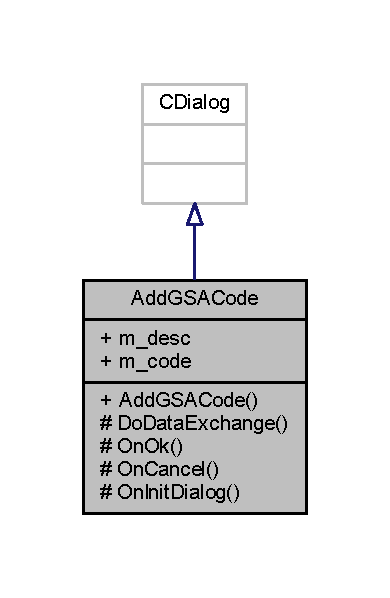
\includegraphics[width=187pt]{class_add_g_s_a_code__inherit__graph}
\end{center}
\end{figure}


Add\+G\+S\+A\+Code에 대한 협력 다이어그램\+:\nopagebreak
\begin{figure}[H]
\begin{center}
\leavevmode
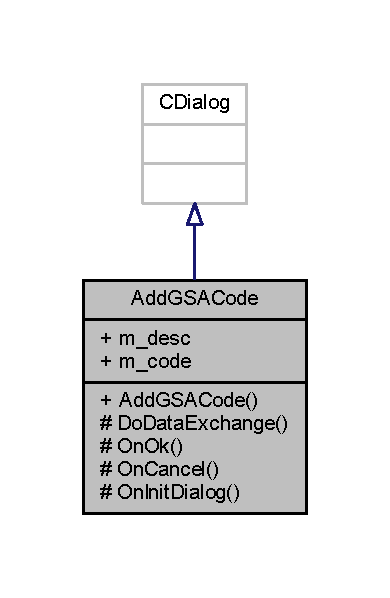
\includegraphics[width=187pt]{class_add_g_s_a_code__coll__graph}
\end{center}
\end{figure}
\subsection*{Public 타입}
\begin{DoxyCompactItemize}
\item 
enum \{ \mbox{\hyperlink{class_add_g_s_a_code_ae09fbbcc1c447c677bf62ee2bcf7c945ade7716d104ed702a0c8cb0e4b61f64f4}{I\+DD}} = I\+D\+D\+\_\+\+A\+D\+D\+\_\+\+C\+H\+E\+A\+T\+\_\+\+D\+LG
 \}
\end{DoxyCompactItemize}
\subsection*{Public 멤버 함수}
\begin{DoxyCompactItemize}
\item 
\mbox{\hyperlink{class_add_g_s_a_code_adae37d67fa94fcd376ae11c6d9bd9d01}{Add\+G\+S\+A\+Code}} (C\+Wnd $\ast$p\+Parent=\mbox{\hyperlink{_system_8h_a070d2ce7b6bb7e5c05602aa8c308d0c4}{N\+U\+LL}})
\end{DoxyCompactItemize}
\subsection*{Public 속성}
\begin{DoxyCompactItemize}
\item 
C\+Edit \mbox{\hyperlink{class_add_g_s_a_code_a766cb9061a235616a856d3c1b16879db}{m\+\_\+desc}}
\item 
C\+Edit \mbox{\hyperlink{class_add_g_s_a_code_a0a4c3486121bd6be93e8f64215fea1ab}{m\+\_\+code}}
\end{DoxyCompactItemize}
\subsection*{Protected 멤버 함수}
\begin{DoxyCompactItemize}
\item 
virtual void \mbox{\hyperlink{class_add_g_s_a_code_a28d3f80ce066475e3d67e7fe62bb1f73}{Do\+Data\+Exchange}} (C\+Data\+Exchange $\ast$p\+DX)
\item 
afx\+\_\+msg void \mbox{\hyperlink{class_add_g_s_a_code_a857608ad314694d15ee6e811fb528d0b}{On\+Ok}} ()
\item 
afx\+\_\+msg void \mbox{\hyperlink{class_add_g_s_a_code_aa0db7ac66785e11cd5f614a06f7a11a2}{On\+Cancel}} ()
\item 
virtual B\+O\+OL \mbox{\hyperlink{class_add_g_s_a_code_af6ea2661ff2da964833f9e86f88cb1ff}{On\+Init\+Dialog}} ()
\end{DoxyCompactItemize}


\subsection{상세한 설명}


G\+B\+A\+Cheats.\+h 파일의 184 번째 라인에서 정의되었습니다.



\subsection{멤버 열거형 문서화}
\mbox{\Hypertarget{class_add_g_s_a_code_ae09fbbcc1c447c677bf62ee2bcf7c945}\label{class_add_g_s_a_code_ae09fbbcc1c447c677bf62ee2bcf7c945}} 
\subsubsection{\texorpdfstring{anonymous enum}{anonymous enum}}
{\footnotesize\ttfamily anonymous enum}

\begin{DoxyEnumFields}{열거형 멤버}
\raisebox{\heightof{T}}[0pt][0pt]{\index{I\+DD@{I\+DD}!Add\+G\+S\+A\+Code@{Add\+G\+S\+A\+Code}}\index{Add\+G\+S\+A\+Code@{Add\+G\+S\+A\+Code}!I\+DD@{I\+DD}}}\mbox{\Hypertarget{class_add_g_s_a_code_ae09fbbcc1c447c677bf62ee2bcf7c945ade7716d104ed702a0c8cb0e4b61f64f4}\label{class_add_g_s_a_code_ae09fbbcc1c447c677bf62ee2bcf7c945ade7716d104ed702a0c8cb0e4b61f64f4}} 
I\+DD&\\
\hline

\end{DoxyEnumFields}


G\+B\+A\+Cheats.\+h 파일의 192 번째 라인에서 정의되었습니다.


\begin{DoxyCode}
192 \{ \mbox{\hyperlink{class_add_g_s_a_code_ae09fbbcc1c447c677bf62ee2bcf7c945ade7716d104ed702a0c8cb0e4b61f64f4}{IDD}} = \mbox{\hyperlink{resource_8h_a388a8d7b6dea32798ece69044a21790d}{IDD\_ADD\_CHEAT\_DLG}} \};
\end{DoxyCode}


\subsection{생성자 \& 소멸자 문서화}
\mbox{\Hypertarget{class_add_g_s_a_code_adae37d67fa94fcd376ae11c6d9bd9d01}\label{class_add_g_s_a_code_adae37d67fa94fcd376ae11c6d9bd9d01}} 
\index{Add\+G\+S\+A\+Code@{Add\+G\+S\+A\+Code}!Add\+G\+S\+A\+Code@{Add\+G\+S\+A\+Code}}
\index{Add\+G\+S\+A\+Code@{Add\+G\+S\+A\+Code}!Add\+G\+S\+A\+Code@{Add\+G\+S\+A\+Code}}
\subsubsection{\texorpdfstring{Add\+G\+S\+A\+Code()}{AddGSACode()}}
{\footnotesize\ttfamily Add\+G\+S\+A\+Code\+::\+Add\+G\+S\+A\+Code (\begin{DoxyParamCaption}\item[{C\+Wnd $\ast$}]{p\+Parent = {\ttfamily \mbox{\hyperlink{_system_8h_a070d2ce7b6bb7e5c05602aa8c308d0c4}{N\+U\+LL}}} }\end{DoxyParamCaption})}



G\+B\+A\+Cheats.\+cpp 파일의 914 번째 라인에서 정의되었습니다.


\begin{DoxyCode}
915   : CDialog(\mbox{\hyperlink{class_add_g_s_a_code_ae09fbbcc1c447c677bf62ee2bcf7c945ade7716d104ed702a0c8cb0e4b61f64f4}{AddGSACode::IDD}}, pParent)
916 \{
917   \textcolor{comment}{//\{\{AFX\_DATA\_INIT(AddGSACode)}
918   \textcolor{comment}{// NOTE: the ClassWizard will add member initialization here}
919   \textcolor{comment}{//\}\}AFX\_DATA\_INIT}
920 \}
\end{DoxyCode}


\subsection{멤버 함수 문서화}
\mbox{\Hypertarget{class_add_g_s_a_code_a28d3f80ce066475e3d67e7fe62bb1f73}\label{class_add_g_s_a_code_a28d3f80ce066475e3d67e7fe62bb1f73}} 
\index{Add\+G\+S\+A\+Code@{Add\+G\+S\+A\+Code}!Do\+Data\+Exchange@{Do\+Data\+Exchange}}
\index{Do\+Data\+Exchange@{Do\+Data\+Exchange}!Add\+G\+S\+A\+Code@{Add\+G\+S\+A\+Code}}
\subsubsection{\texorpdfstring{Do\+Data\+Exchange()}{DoDataExchange()}}
{\footnotesize\ttfamily void Add\+G\+S\+A\+Code\+::\+Do\+Data\+Exchange (\begin{DoxyParamCaption}\item[{C\+Data\+Exchange $\ast$}]{p\+DX }\end{DoxyParamCaption})\hspace{0.3cm}{\ttfamily [protected]}, {\ttfamily [virtual]}}



G\+B\+A\+Cheats.\+cpp 파일의 923 번째 라인에서 정의되었습니다.


\begin{DoxyCode}
924 \{
925   CDialog::DoDataExchange(pDX);
926   \textcolor{comment}{//\{\{AFX\_DATA\_MAP(AddGSACode)}
927   DDX\_Control(pDX, \mbox{\hyperlink{resource_8h_adb05cf1e74135587a9b3ab93a5152feb}{IDC\_DESC}}, \mbox{\hyperlink{class_add_g_s_a_code_a766cb9061a235616a856d3c1b16879db}{m\_desc}});
928   DDX\_Control(pDX, \mbox{\hyperlink{resource_8h_abb149f0043fd3834639ddb2d80d31723}{IDC\_CODE}}, \mbox{\hyperlink{class_add_g_s_a_code_a0a4c3486121bd6be93e8f64215fea1ab}{m\_code}});
929   \textcolor{comment}{//\}\}AFX\_DATA\_MAP}
930 \}
\end{DoxyCode}
\mbox{\Hypertarget{class_add_g_s_a_code_aa0db7ac66785e11cd5f614a06f7a11a2}\label{class_add_g_s_a_code_aa0db7ac66785e11cd5f614a06f7a11a2}} 
\index{Add\+G\+S\+A\+Code@{Add\+G\+S\+A\+Code}!On\+Cancel@{On\+Cancel}}
\index{On\+Cancel@{On\+Cancel}!Add\+G\+S\+A\+Code@{Add\+G\+S\+A\+Code}}
\subsubsection{\texorpdfstring{On\+Cancel()}{OnCancel()}}
{\footnotesize\ttfamily void Add\+G\+S\+A\+Code\+::\+On\+Cancel (\begin{DoxyParamCaption}{ }\end{DoxyParamCaption})\hspace{0.3cm}{\ttfamily [protected]}}



G\+B\+A\+Cheats.\+cpp 파일의 987 번째 라인에서 정의되었습니다.


\begin{DoxyCode}
988 \{
989   EndDialog(FALSE);
990 \}
\end{DoxyCode}
\mbox{\Hypertarget{class_add_g_s_a_code_af6ea2661ff2da964833f9e86f88cb1ff}\label{class_add_g_s_a_code_af6ea2661ff2da964833f9e86f88cb1ff}} 
\index{Add\+G\+S\+A\+Code@{Add\+G\+S\+A\+Code}!On\+Init\+Dialog@{On\+Init\+Dialog}}
\index{On\+Init\+Dialog@{On\+Init\+Dialog}!Add\+G\+S\+A\+Code@{Add\+G\+S\+A\+Code}}
\subsubsection{\texorpdfstring{On\+Init\+Dialog()}{OnInitDialog()}}
{\footnotesize\ttfamily B\+O\+OL Add\+G\+S\+A\+Code\+::\+On\+Init\+Dialog (\begin{DoxyParamCaption}{ }\end{DoxyParamCaption})\hspace{0.3cm}{\ttfamily [protected]}, {\ttfamily [virtual]}}



G\+B\+A\+Cheats.\+cpp 파일의 992 번째 라인에서 정의되었습니다.


\begin{DoxyCode}
993 \{
994   CDialog::OnInitDialog();
995   
996   \mbox{\hyperlink{class_add_g_s_a_code_a0a4c3486121bd6be93e8f64215fea1ab}{m\_code}}.LimitText(1024);
997   \mbox{\hyperlink{class_add_g_s_a_code_a766cb9061a235616a856d3c1b16879db}{m\_desc}}.LimitText(32);
998   CString title = \mbox{\hyperlink{_win_res_util_8cpp_a416e85e80ab9b01376e87251c83d1a5a}{winResLoadString}}(\mbox{\hyperlink{resource_8h_a49836eba8e0beeff1d7e166eea41a5eb}{IDS\_ADD\_GSA\_CODE}});
999   SetWindowText(title);
1000   CenterWindow();
1001   
1002   \textcolor{keywordflow}{return} TRUE;  \textcolor{comment}{// return TRUE unless you set the focus to a control}
1003                 \textcolor{comment}{// EXCEPTION: OCX Property Pages should return FALSE}
1004 \}
\end{DoxyCode}
이 함수 내부에서 호출하는 함수들에 대한 그래프입니다.\+:
\nopagebreak
\begin{figure}[H]
\begin{center}
\leavevmode
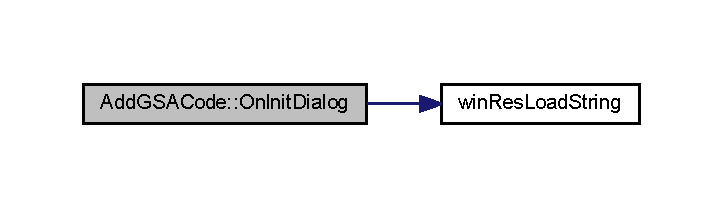
\includegraphics[width=347pt]{class_add_g_s_a_code_af6ea2661ff2da964833f9e86f88cb1ff_cgraph}
\end{center}
\end{figure}
\mbox{\Hypertarget{class_add_g_s_a_code_a857608ad314694d15ee6e811fb528d0b}\label{class_add_g_s_a_code_a857608ad314694d15ee6e811fb528d0b}} 
\index{Add\+G\+S\+A\+Code@{Add\+G\+S\+A\+Code}!On\+Ok@{On\+Ok}}
\index{On\+Ok@{On\+Ok}!Add\+G\+S\+A\+Code@{Add\+G\+S\+A\+Code}}
\subsubsection{\texorpdfstring{On\+Ok()}{OnOk()}}
{\footnotesize\ttfamily void Add\+G\+S\+A\+Code\+::\+On\+Ok (\begin{DoxyParamCaption}{ }\end{DoxyParamCaption})\hspace{0.3cm}{\ttfamily [protected]}}



G\+B\+A\+Cheats.\+cpp 파일의 943 번째 라인에서 정의되었습니다.


\begin{DoxyCode}
944 \{
945   CString desc;
946   CString \mbox{\hyperlink{_g_b_a_8cpp_a28d4d3d8445e73a696b2d6f7eadabd96}{buffer}};
947   CString part1;
948   CString code;
949   CString token;  
950 
951   \mbox{\hyperlink{class_add_g_s_a_code_a0a4c3486121bd6be93e8f64215fea1ab}{m\_code}}.GetWindowText(\mbox{\hyperlink{_g_b_a_8cpp_a28d4d3d8445e73a696b2d6f7eadabd96}{buffer}});
952   \mbox{\hyperlink{class_add_g_s_a_code_a766cb9061a235616a856d3c1b16879db}{m\_desc}}.GetWindowText(desc);
953   
954   \mbox{\hyperlink{class_string_tokenizer}{StringTokenizer}} st(\mbox{\hyperlink{_g_b_a_8cpp_a28d4d3d8445e73a696b2d6f7eadabd96}{buffer}}, \textcolor{stringliteral}{" \(\backslash\)t\(\backslash\)n\(\backslash\)r"});
955   part1.Empty();
956   \textcolor{keyword}{const} \textcolor{keywordtype}{char} *\mbox{\hyperlink{expr_8cpp_aded116371789db1fd63c90ef00c95a3d}{t}} = st.next();
957   \textcolor{keywordflow}{while}(\mbox{\hyperlink{expr_8cpp_aded116371789db1fd63c90ef00c95a3d}{t}}) \{
958     token = \mbox{\hyperlink{expr_8cpp_aded116371789db1fd63c90ef00c95a3d}{t}};
959     token.MakeUpper();
960     \textcolor{keywordflow}{if}(token.GetLength() == 16)
961       \mbox{\hyperlink{_cheats_8cpp_a47aded7deffcbfa36ed55944eafb72ab}{cheatsAddGSACode}}(token, desc, \textcolor{keyword}{false});
962     \textcolor{keywordflow}{else} \textcolor{keywordflow}{if}(token.GetLength() == 12) \{
963       code = token.Left(8);
964       code += \textcolor{stringliteral}{" "};
965       code += token.Right(4);
966       \mbox{\hyperlink{_cheats_8cpp_af79d349aaea63793beec4fa2626f74c8}{cheatsAddCBACode}}(code, desc);
967     \} \textcolor{keywordflow}{else} \textcolor{keywordflow}{if}(part1.IsEmpty())
968       part1 = token;
969     \textcolor{keywordflow}{else} \{
970       \textcolor{keywordflow}{if}(token.GetLength() == 4) \{
971         code = part1;
972         code += \textcolor{stringliteral}{" "};
973         code += token;
974         \mbox{\hyperlink{_cheats_8cpp_af79d349aaea63793beec4fa2626f74c8}{cheatsAddCBACode}}(code, desc);
975       \} \textcolor{keywordflow}{else} \{
976         code = part1 + token;
977         \mbox{\hyperlink{_cheats_8cpp_a47aded7deffcbfa36ed55944eafb72ab}{cheatsAddGSACode}}(code, desc, \textcolor{keyword}{true});
978       \}
979       part1.Empty();
980     \}
981 
982     \mbox{\hyperlink{expr_8cpp_aded116371789db1fd63c90ef00c95a3d}{t}} = st.next();
983   \}
984   EndDialog(TRUE);
985 \}
\end{DoxyCode}
이 함수 내부에서 호출하는 함수들에 대한 그래프입니다.\+:
\nopagebreak
\begin{figure}[H]
\begin{center}
\leavevmode
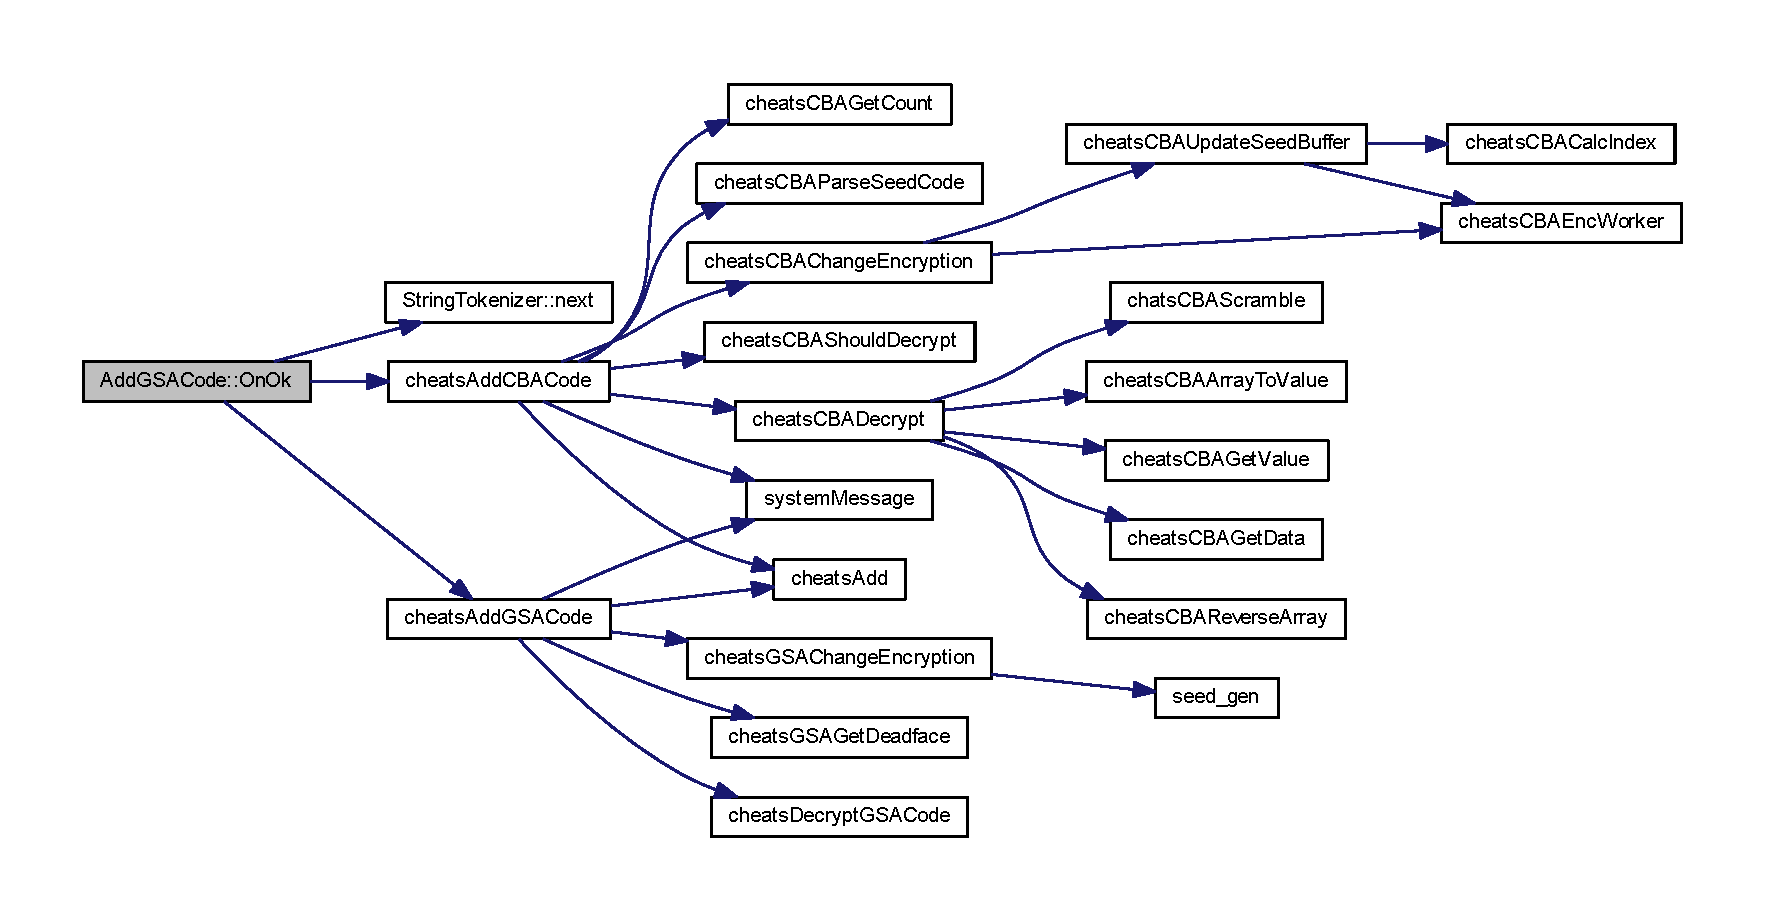
\includegraphics[width=350pt]{class_add_g_s_a_code_a857608ad314694d15ee6e811fb528d0b_cgraph}
\end{center}
\end{figure}


\subsection{멤버 데이터 문서화}
\mbox{\Hypertarget{class_add_g_s_a_code_a0a4c3486121bd6be93e8f64215fea1ab}\label{class_add_g_s_a_code_a0a4c3486121bd6be93e8f64215fea1ab}} 
\index{Add\+G\+S\+A\+Code@{Add\+G\+S\+A\+Code}!m\+\_\+code@{m\+\_\+code}}
\index{m\+\_\+code@{m\+\_\+code}!Add\+G\+S\+A\+Code@{Add\+G\+S\+A\+Code}}
\subsubsection{\texorpdfstring{m\+\_\+code}{m\_code}}
{\footnotesize\ttfamily C\+Edit Add\+G\+S\+A\+Code\+::m\+\_\+code}



G\+B\+A\+Cheats.\+h 파일의 194 번째 라인에서 정의되었습니다.

\mbox{\Hypertarget{class_add_g_s_a_code_a766cb9061a235616a856d3c1b16879db}\label{class_add_g_s_a_code_a766cb9061a235616a856d3c1b16879db}} 
\index{Add\+G\+S\+A\+Code@{Add\+G\+S\+A\+Code}!m\+\_\+desc@{m\+\_\+desc}}
\index{m\+\_\+desc@{m\+\_\+desc}!Add\+G\+S\+A\+Code@{Add\+G\+S\+A\+Code}}
\subsubsection{\texorpdfstring{m\+\_\+desc}{m\_desc}}
{\footnotesize\ttfamily C\+Edit Add\+G\+S\+A\+Code\+::m\+\_\+desc}



G\+B\+A\+Cheats.\+h 파일의 193 번째 라인에서 정의되었습니다.



이 클래스에 대한 문서화 페이지는 다음의 파일들로부터 생성되었습니다.\+:\begin{DoxyCompactItemize}
\item 
C\+:/\+Users/sjh13/sources/\+Visual\+Boy\+Advance/src/win32/\mbox{\hyperlink{_g_b_a_cheats_8h}{G\+B\+A\+Cheats.\+h}}\item 
C\+:/\+Users/sjh13/sources/\+Visual\+Boy\+Advance/src/win32/\mbox{\hyperlink{_g_b_a_cheats_8cpp}{G\+B\+A\+Cheats.\+cpp}}\end{DoxyCompactItemize}

\hypertarget{struct_a_range}{}\section{A\+Range 구조체 참조}
\label{struct_a_range}\index{A\+Range@{A\+Range}}


{\ttfamily \#include $<$elf.\+h$>$}



A\+Range에 대한 협력 다이어그램\+:\nopagebreak
\begin{figure}[H]
\begin{center}
\leavevmode
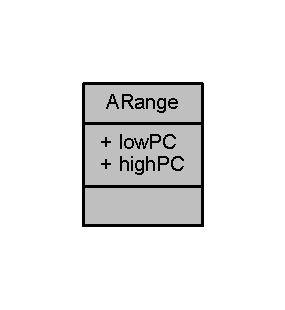
\includegraphics[width=137pt]{struct_a_range__coll__graph}
\end{center}
\end{figure}
\subsection*{Public 속성}
\begin{DoxyCompactItemize}
\item 
\mbox{\hyperlink{_system_8h_a10e94b422ef0c20dcdec20d31a1f5049}{u32}} \mbox{\hyperlink{struct_a_range_a967436344fa630513a70d3fadb4c3bbe}{low\+PC}}
\item 
\mbox{\hyperlink{_system_8h_a10e94b422ef0c20dcdec20d31a1f5049}{u32}} \mbox{\hyperlink{struct_a_range_aa1c1290004480b58c3fb5133e5e00430}{high\+PC}}
\end{DoxyCompactItemize}


\subsection{상세한 설명}


elf.\+h 파일의 220 번째 라인에서 정의되었습니다.



\subsection{멤버 데이터 문서화}
\mbox{\Hypertarget{struct_a_range_aa1c1290004480b58c3fb5133e5e00430}\label{struct_a_range_aa1c1290004480b58c3fb5133e5e00430}} 
\index{A\+Range@{A\+Range}!high\+PC@{high\+PC}}
\index{high\+PC@{high\+PC}!A\+Range@{A\+Range}}
\subsubsection{\texorpdfstring{high\+PC}{highPC}}
{\footnotesize\ttfamily \mbox{\hyperlink{_system_8h_a10e94b422ef0c20dcdec20d31a1f5049}{u32}} A\+Range\+::high\+PC}



elf.\+h 파일의 222 번째 라인에서 정의되었습니다.

\mbox{\Hypertarget{struct_a_range_a967436344fa630513a70d3fadb4c3bbe}\label{struct_a_range_a967436344fa630513a70d3fadb4c3bbe}} 
\index{A\+Range@{A\+Range}!low\+PC@{low\+PC}}
\index{low\+PC@{low\+PC}!A\+Range@{A\+Range}}
\subsubsection{\texorpdfstring{low\+PC}{lowPC}}
{\footnotesize\ttfamily \mbox{\hyperlink{_system_8h_a10e94b422ef0c20dcdec20d31a1f5049}{u32}} A\+Range\+::low\+PC}



elf.\+h 파일의 221 번째 라인에서 정의되었습니다.



이 구조체에 대한 문서화 페이지는 다음의 파일로부터 생성되었습니다.\+:\begin{DoxyCompactItemize}
\item 
C\+:/\+Users/sjh13/sources/\+Visual\+Boy\+Advance/src/\mbox{\hyperlink{elf_8h}{elf.\+h}}\end{DoxyCompactItemize}

\hypertarget{struct_a_ranges}{}\section{A\+Ranges 구조체 참조}
\label{struct_a_ranges}\index{A\+Ranges@{A\+Ranges}}


{\ttfamily \#include $<$elf.\+h$>$}



A\+Ranges에 대한 협력 다이어그램\+:\nopagebreak
\begin{figure}[H]
\begin{center}
\leavevmode
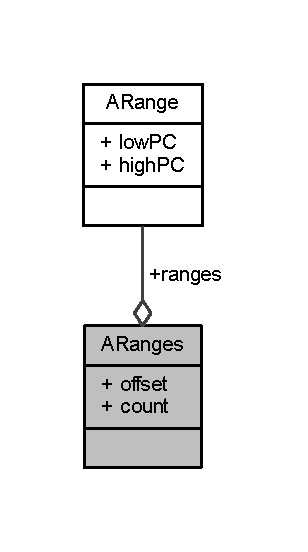
\includegraphics[width=148pt]{struct_a_ranges__coll__graph}
\end{center}
\end{figure}
\subsection*{Public 속성}
\begin{DoxyCompactItemize}
\item 
\mbox{\hyperlink{_system_8h_a10e94b422ef0c20dcdec20d31a1f5049}{u32}} \mbox{\hyperlink{struct_a_ranges_ac9a8655acb6be1e8f52053fc49c34efa}{offset}}
\item 
\mbox{\hyperlink{_util_8cpp_a0ef32aa8672df19503a49fab2d0c8071}{int}} \mbox{\hyperlink{struct_a_ranges_a6f197b7ddb2b3cb334c2eeb9de8d7288}{count}}
\item 
\mbox{\hyperlink{struct_a_range}{A\+Range}} $\ast$ \mbox{\hyperlink{struct_a_ranges_a2eb62f0d43045767640b1d0c4dd8191e}{ranges}}
\end{DoxyCompactItemize}


\subsection{상세한 설명}


elf.\+h 파일의 225 번째 라인에서 정의되었습니다.



\subsection{멤버 데이터 문서화}
\mbox{\Hypertarget{struct_a_ranges_a6f197b7ddb2b3cb334c2eeb9de8d7288}\label{struct_a_ranges_a6f197b7ddb2b3cb334c2eeb9de8d7288}} 
\index{A\+Ranges@{A\+Ranges}!count@{count}}
\index{count@{count}!A\+Ranges@{A\+Ranges}}
\subsubsection{\texorpdfstring{count}{count}}
{\footnotesize\ttfamily \mbox{\hyperlink{_util_8cpp_a0ef32aa8672df19503a49fab2d0c8071}{int}} A\+Ranges\+::count}



elf.\+h 파일의 227 번째 라인에서 정의되었습니다.

\mbox{\Hypertarget{struct_a_ranges_ac9a8655acb6be1e8f52053fc49c34efa}\label{struct_a_ranges_ac9a8655acb6be1e8f52053fc49c34efa}} 
\index{A\+Ranges@{A\+Ranges}!offset@{offset}}
\index{offset@{offset}!A\+Ranges@{A\+Ranges}}
\subsubsection{\texorpdfstring{offset}{offset}}
{\footnotesize\ttfamily \mbox{\hyperlink{_system_8h_a10e94b422ef0c20dcdec20d31a1f5049}{u32}} A\+Ranges\+::offset}



elf.\+h 파일의 226 번째 라인에서 정의되었습니다.

\mbox{\Hypertarget{struct_a_ranges_a2eb62f0d43045767640b1d0c4dd8191e}\label{struct_a_ranges_a2eb62f0d43045767640b1d0c4dd8191e}} 
\index{A\+Ranges@{A\+Ranges}!ranges@{ranges}}
\index{ranges@{ranges}!A\+Ranges@{A\+Ranges}}
\subsubsection{\texorpdfstring{ranges}{ranges}}
{\footnotesize\ttfamily \mbox{\hyperlink{struct_a_range}{A\+Range}}$\ast$ A\+Ranges\+::ranges}



elf.\+h 파일의 228 번째 라인에서 정의되었습니다.



이 구조체에 대한 문서화 페이지는 다음의 파일로부터 생성되었습니다.\+:\begin{DoxyCompactItemize}
\item 
C\+:/\+Users/sjh13/sources/\+Visual\+Boy\+Advance/src/\mbox{\hyperlink{elf_8h}{elf.\+h}}\end{DoxyCompactItemize}

\hypertarget{struct_array}{}\section{Array 구조체 참조}
\label{struct_array}\index{Array@{Array}}
\subsection*{Public 속성}
\begin{DoxyCompactItemize}
\item 
\mbox{\Hypertarget{struct_array_aebd7ba43475f7f6461e4343a7ffce0a7}\label{struct_array_aebd7ba43475f7f6461e4343a7ffce0a7}} 
\mbox{\hyperlink{struct_type}{Type}} $\ast$ {\bfseries type}
\item 
\mbox{\Hypertarget{struct_array_ac416f8022b0d22cb470b0e5cc1e9b356}\label{struct_array_ac416f8022b0d22cb470b0e5cc1e9b356}} 
int {\bfseries max\+Bounds}
\item 
\mbox{\Hypertarget{struct_array_a2d2cd201a0203a12d6f5e7b8a34ab1ad}\label{struct_array_a2d2cd201a0203a12d6f5e7b8a34ab1ad}} 
int $\ast$ {\bfseries bounds}
\end{DoxyCompactItemize}


이 구조체에 대한 문서화 페이지는 다음의 파일로부터 생성되었습니다.\+:\begin{DoxyCompactItemize}
\item 
src/elf.\+h\end{DoxyCompactItemize}

\hypertarget{class_associate}{}\section{Associate 클래스 참조}
\label{class_associate}\index{Associate@{Associate}}
Associate에 대한 상속 다이어그램 \+: \begin{figure}[H]
\begin{center}
\leavevmode
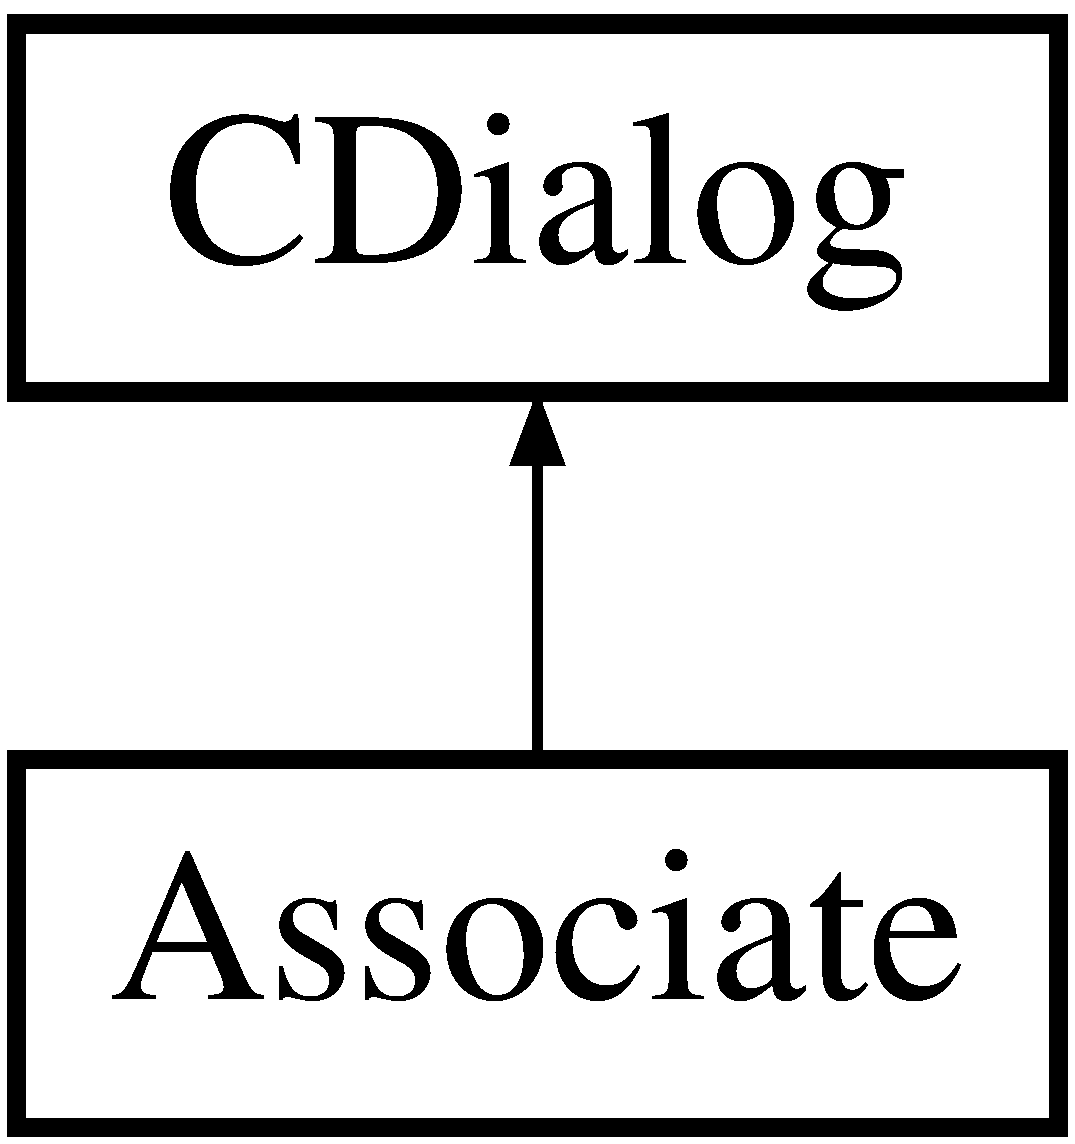
\includegraphics[height=2.000000cm]{class_associate}
\end{center}
\end{figure}
\subsection*{Public 타입}
\begin{DoxyCompactItemize}
\item 
\mbox{\Hypertarget{class_associate_a9696cb7dfd5bf0a5f848d1c0209ca4f8}\label{class_associate_a9696cb7dfd5bf0a5f848d1c0209ca4f8}} 
enum \{ {\bfseries I\+DD} = I\+D\+D\+\_\+\+A\+S\+S\+O\+C\+I\+A\+T\+I\+O\+NS
 \}
\end{DoxyCompactItemize}
\subsection*{Public 멤버 함수}
\begin{DoxyCompactItemize}
\item 
\mbox{\Hypertarget{class_associate_a67a8f8b2f0539a32f8d783f60e2d25b9}\label{class_associate_a67a8f8b2f0539a32f8d783f60e2d25b9}} 
{\bfseries Associate} (C\+Wnd $\ast$p\+Parent=N\+U\+LL)
\end{DoxyCompactItemize}
\subsection*{Public 속성}
\begin{DoxyCompactItemize}
\item 
\mbox{\Hypertarget{class_associate_ab6d59a4b47c5529c1e5f5b8f8b5a6f82}\label{class_associate_ab6d59a4b47c5529c1e5f5b8f8b5a6f82}} 
B\+O\+OL {\bfseries m\+\_\+agb}
\item 
\mbox{\Hypertarget{class_associate_ac132c6bfb6f547702c2e7386650a0a4c}\label{class_associate_ac132c6bfb6f547702c2e7386650a0a4c}} 
B\+O\+OL {\bfseries m\+\_\+bin}
\item 
\mbox{\Hypertarget{class_associate_af245524b613121a7a5291deebfb97e0e}\label{class_associate_af245524b613121a7a5291deebfb97e0e}} 
B\+O\+OL {\bfseries m\+\_\+cgb}
\item 
\mbox{\Hypertarget{class_associate_af4479f05150eb128332d06cba68a955b}\label{class_associate_af4479f05150eb128332d06cba68a955b}} 
B\+O\+OL {\bfseries m\+\_\+gb}
\item 
\mbox{\Hypertarget{class_associate_a7c20c41d1b724e80532ff888b6c7ea56}\label{class_associate_a7c20c41d1b724e80532ff888b6c7ea56}} 
B\+O\+OL {\bfseries m\+\_\+gba}
\item 
\mbox{\Hypertarget{class_associate_a399cc9528f3efc32ec5971fc5e614e97}\label{class_associate_a399cc9528f3efc32ec5971fc5e614e97}} 
B\+O\+OL {\bfseries m\+\_\+gbc}
\item 
\mbox{\Hypertarget{class_associate_a0221f6743a817911817d464579b4a038}\label{class_associate_a0221f6743a817911817d464579b4a038}} 
B\+O\+OL {\bfseries m\+\_\+sgb}
\end{DoxyCompactItemize}
\subsection*{Protected 멤버 함수}
\begin{DoxyCompactItemize}
\item 
\mbox{\Hypertarget{class_associate_af10575d274826cc658ebb2e6a823aa35}\label{class_associate_af10575d274826cc658ebb2e6a823aa35}} 
virtual void {\bfseries Do\+Data\+Exchange} (C\+Data\+Exchange $\ast$p\+DX)
\item 
\mbox{\Hypertarget{class_associate_a66532001ec5d28abd61684b0f62b032b}\label{class_associate_a66532001ec5d28abd61684b0f62b032b}} 
virtual B\+O\+OL {\bfseries On\+Init\+Dialog} ()
\item 
\mbox{\Hypertarget{class_associate_a76fb7e63100511a6d22c53cf3306b8f4}\label{class_associate_a76fb7e63100511a6d22c53cf3306b8f4}} 
afx\+\_\+msg void {\bfseries On\+Cancel} ()
\item 
\mbox{\Hypertarget{class_associate_abb81ded9b91053ed12804ee8674ae860}\label{class_associate_abb81ded9b91053ed12804ee8674ae860}} 
afx\+\_\+msg void {\bfseries On\+Ok} ()
\end{DoxyCompactItemize}


이 클래스에 대한 문서화 페이지는 다음의 파일들로부터 생성되었습니다.\+:\begin{DoxyCompactItemize}
\item 
src/win32/Associate.\+h\item 
src/win32/Associate.\+cpp\end{DoxyCompactItemize}

\hypertarget{class_a_v_i_write}{}\section{A\+V\+I\+Write 클래스 참조}
\label{class_a_v_i_write}\index{A\+V\+I\+Write@{A\+V\+I\+Write}}
\subsection*{Public 멤버 함수}
\begin{DoxyCompactItemize}
\item 
\mbox{\Hypertarget{class_a_v_i_write_a2b4ef2aeeef846bcb12ef58189043eb1}\label{class_a_v_i_write_a2b4ef2aeeef846bcb12ef58189043eb1}} 
bool {\bfseries Open} (const char $\ast$filename)
\item 
\mbox{\Hypertarget{class_a_v_i_write_a904b7f02ff6ecfeeaeec6e1c82f1592a}\label{class_a_v_i_write_a904b7f02ff6ecfeeaeec6e1c82f1592a}} 
virtual bool {\bfseries Add\+Frame} (const int number, const char $\ast$bmp)
\item 
\mbox{\Hypertarget{class_a_v_i_write_a3beb976b918287e0592ab4feebd9ce59}\label{class_a_v_i_write_a3beb976b918287e0592ab4feebd9ce59}} 
void {\bfseries Set\+F\+PS} (int fps)
\item 
\mbox{\Hypertarget{class_a_v_i_write_a1da91adeefacf0dd4655f5029875c5d6}\label{class_a_v_i_write_a1da91adeefacf0dd4655f5029875c5d6}} 
void {\bfseries Set\+Video\+Format} (B\+I\+T\+M\+A\+P\+I\+N\+F\+O\+H\+E\+A\+D\+ER $\ast$)
\item 
\mbox{\Hypertarget{class_a_v_i_write_a7e14c1640c3c888c2b0a0b042c0d5b8f}\label{class_a_v_i_write_a7e14c1640c3c888c2b0a0b042c0d5b8f}} 
bool {\bfseries Is\+Sound\+Added} ()
\item 
\mbox{\Hypertarget{class_a_v_i_write_a8d864e6e2cea4147ffa6f24d69fbe339}\label{class_a_v_i_write_a8d864e6e2cea4147ffa6f24d69fbe339}} 
void {\bfseries Set\+Sound\+Format} (W\+A\+V\+E\+F\+O\+R\+M\+A\+T\+EX $\ast$)
\item 
\mbox{\Hypertarget{class_a_v_i_write_a63b7d54c048e517bbfad0ae2004d9861}\label{class_a_v_i_write_a63b7d54c048e517bbfad0ae2004d9861}} 
bool {\bfseries Add\+Sound} (const char $\ast$sound, int len)
\end{DoxyCompactItemize}


이 클래스에 대한 문서화 페이지는 다음의 파일들로부터 생성되었습니다.\+:\begin{DoxyCompactItemize}
\item 
src/win32/A\+V\+I\+Write.\+h\item 
src/win32/A\+V\+I\+Write.\+cpp\end{DoxyCompactItemize}

\hypertarget{class_bitmap_control}{}\section{Bitmap\+Control 클래스 참조}
\label{class_bitmap_control}\index{Bitmap\+Control@{Bitmap\+Control}}
Bitmap\+Control에 대한 상속 다이어그램 \+: \begin{figure}[H]
\begin{center}
\leavevmode
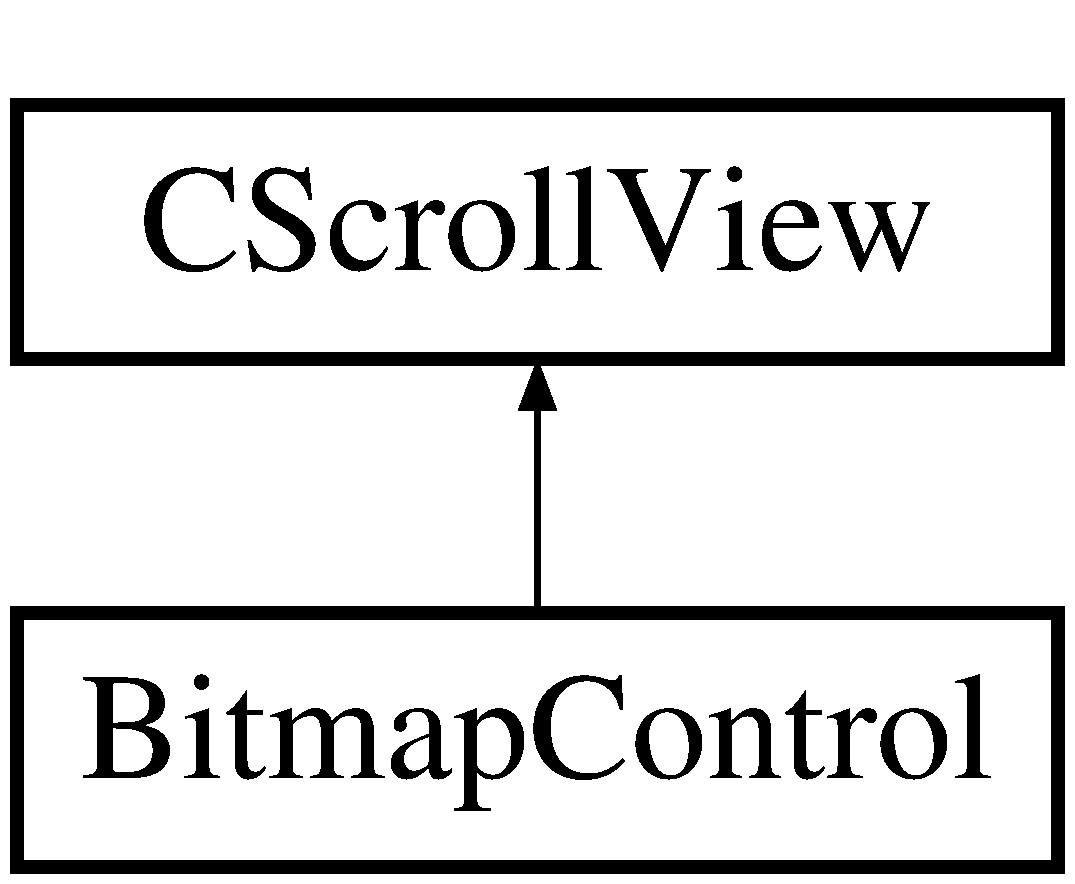
\includegraphics[height=2.000000cm]{class_bitmap_control}
\end{center}
\end{figure}
\subsection*{Public 멤버 함수}
\begin{DoxyCompactItemize}
\item 
\mbox{\Hypertarget{class_bitmap_control_ab545e15ea3edda9f0d80c0b8b0b7c812}\label{class_bitmap_control_ab545e15ea3edda9f0d80c0b8b0b7c812}} 
void {\bfseries set\+Stretch} (bool b)
\item 
\mbox{\Hypertarget{class_bitmap_control_acf061a1e9a4cad90ad2827c14f79caa2}\label{class_bitmap_control_acf061a1e9a4cad90ad2827c14f79caa2}} 
void {\bfseries refresh} ()
\item 
\mbox{\Hypertarget{class_bitmap_control_a421004fe6ba01329dd69259396592d1f}\label{class_bitmap_control_a421004fe6ba01329dd69259396592d1f}} 
void {\bfseries set\+Size} (int w1, int h1)
\item 
\mbox{\Hypertarget{class_bitmap_control_aa6206183896caf192a37709fa5d7b8d2}\label{class_bitmap_control_aa6206183896caf192a37709fa5d7b8d2}} 
void {\bfseries set\+Data} (u8 $\ast$d)
\item 
\mbox{\Hypertarget{class_bitmap_control_a301c52fc62de4368fccdcdc93cefad0b}\label{class_bitmap_control_a301c52fc62de4368fccdcdc93cefad0b}} 
void {\bfseries set\+Bmp\+Info} (B\+I\+T\+M\+A\+P\+I\+N\+FO $\ast$info)
\item 
\mbox{\Hypertarget{class_bitmap_control_a1d3cff9a3b57dd7558d678177dcf4b5c}\label{class_bitmap_control_a1d3cff9a3b57dd7558d678177dcf4b5c}} 
bool {\bfseries get\+Stretch} ()
\end{DoxyCompactItemize}
\subsection*{정적 Public 속성}
\begin{DoxyCompactItemize}
\item 
\mbox{\Hypertarget{class_bitmap_control_acd16ac02d48f1201fc90470b6e29c7fe}\label{class_bitmap_control_acd16ac02d48f1201fc90470b6e29c7fe}} 
static bool {\bfseries is\+Registered} = false
\end{DoxyCompactItemize}
\subsection*{Protected 멤버 함수}
\begin{DoxyCompactItemize}
\item 
\mbox{\Hypertarget{class_bitmap_control_a76ead24c70d33421148716a39cf3a17f}\label{class_bitmap_control_a76ead24c70d33421148716a39cf3a17f}} 
virtual void {\bfseries On\+Draw} (C\+DC $\ast$p\+DC)
\item 
\mbox{\Hypertarget{class_bitmap_control_a532fd9e0bd31674589a224737960bfc0}\label{class_bitmap_control_a532fd9e0bd31674589a224737960bfc0}} 
virtual void {\bfseries On\+Initial\+Update} ()
\item 
\mbox{\Hypertarget{class_bitmap_control_aed7e031df3fd65a4325ea9bf7da5bdc3}\label{class_bitmap_control_aed7e031df3fd65a4325ea9bf7da5bdc3}} 
virtual void {\bfseries Post\+Nc\+Destroy} ()
\item 
\mbox{\Hypertarget{class_bitmap_control_aea73d6e790bb4828eb230c3cd66e5e0b}\label{class_bitmap_control_aea73d6e790bb4828eb230c3cd66e5e0b}} 
afx\+\_\+msg B\+O\+OL {\bfseries On\+Erase\+Bkgnd} (C\+DC $\ast$p\+DC)
\item 
\mbox{\Hypertarget{class_bitmap_control_ac0e60f98809d78a38d5d35942c1bfb2c}\label{class_bitmap_control_ac0e60f98809d78a38d5d35942c1bfb2c}} 
afx\+\_\+msg void {\bfseries On\+Size} (U\+I\+NT n\+Type, int cx, int cy)
\item 
\mbox{\Hypertarget{class_bitmap_control_a2958d0209f702d4207d10797c8aa86bd}\label{class_bitmap_control_a2958d0209f702d4207d10797c8aa86bd}} 
afx\+\_\+msg void {\bfseries On\+L\+Button\+Down} (U\+I\+NT n\+Flags, C\+Point point)
\end{DoxyCompactItemize}


이 클래스에 대한 문서화 페이지는 다음의 파일들로부터 생성되었습니다.\+:\begin{DoxyCompactItemize}
\item 
src/win32/Bitmap\+Control.\+h\item 
src/win32/Bitmap\+Control.\+cpp\end{DoxyCompactItemize}

\hypertarget{structbreakpoint_info}{}\section{breakpoint\+Info 구조체 참조}
\label{structbreakpoint_info}\index{breakpoint\+Info@{breakpoint\+Info}}


breakpoint\+Info에 대한 협력 다이어그램\+:\nopagebreak
\begin{figure}[H]
\begin{center}
\leavevmode
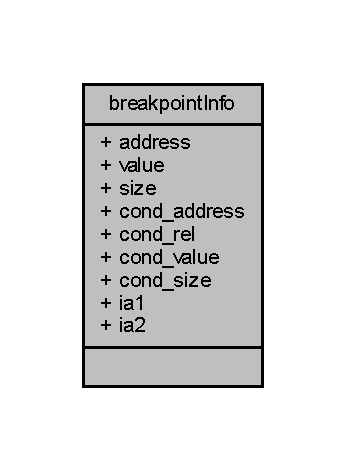
\includegraphics[width=166pt]{structbreakpoint_info__coll__graph}
\end{center}
\end{figure}
\subsection*{Public 속성}
\begin{DoxyCompactItemize}
\item 
\mbox{\hyperlink{_system_8h_a10e94b422ef0c20dcdec20d31a1f5049}{u32}} \mbox{\hyperlink{structbreakpoint_info_ab0cc4bdc931703296ec18aaa1e2242f4}{address}}
\item 
\mbox{\hyperlink{_system_8h_a10e94b422ef0c20dcdec20d31a1f5049}{u32}} \mbox{\hyperlink{structbreakpoint_info_a10cf821e6c0c5b11b921baafa0144448}{value}}
\item 
\mbox{\hyperlink{_util_8cpp_a0ef32aa8672df19503a49fab2d0c8071}{int}} \mbox{\hyperlink{structbreakpoint_info_a39a2c2fabe9c630917e8131a99ce61ec}{size}}
\item 
\mbox{\hyperlink{_system_8h_a10e94b422ef0c20dcdec20d31a1f5049}{u32}} \mbox{\hyperlink{structbreakpoint_info_a4a83f60b18f30afe9fa114b21f02de22}{cond\+\_\+address}}
\item 
char \mbox{\hyperlink{structbreakpoint_info_a6819ea8a99055196410b1070f9750f70}{cond\+\_\+rel}}
\item 
\mbox{\hyperlink{_system_8h_a10e94b422ef0c20dcdec20d31a1f5049}{u32}} \mbox{\hyperlink{structbreakpoint_info_a06f4bafc5e974ae0adf0e3bf651d2afd}{cond\+\_\+value}}
\item 
\mbox{\hyperlink{_util_8cpp_a0ef32aa8672df19503a49fab2d0c8071}{int}} \mbox{\hyperlink{structbreakpoint_info_a4c2f4f1b0f74562121d829e864d73a0e}{cond\+\_\+size}}
\item 
bool \mbox{\hyperlink{structbreakpoint_info_a6d1174b3ac7266b9454683ee36030b97}{ia1}}
\item 
bool \mbox{\hyperlink{structbreakpoint_info_a5c43894b7302cbb085204b39a14dda91}{ia2}}
\end{DoxyCompactItemize}


\subsection{상세한 설명}


debugger.\+cpp 파일의 57 번째 라인에서 정의되었습니다.



\subsection{멤버 데이터 문서화}
\mbox{\Hypertarget{structbreakpoint_info_ab0cc4bdc931703296ec18aaa1e2242f4}\label{structbreakpoint_info_ab0cc4bdc931703296ec18aaa1e2242f4}} 
\index{breakpoint\+Info@{breakpoint\+Info}!address@{address}}
\index{address@{address}!breakpoint\+Info@{breakpoint\+Info}}
\subsubsection{\texorpdfstring{address}{address}}
{\footnotesize\ttfamily \mbox{\hyperlink{_system_8h_a10e94b422ef0c20dcdec20d31a1f5049}{u32}} breakpoint\+Info\+::address}



debugger.\+cpp 파일의 58 번째 라인에서 정의되었습니다.

\mbox{\Hypertarget{structbreakpoint_info_a4a83f60b18f30afe9fa114b21f02de22}\label{structbreakpoint_info_a4a83f60b18f30afe9fa114b21f02de22}} 
\index{breakpoint\+Info@{breakpoint\+Info}!cond\+\_\+address@{cond\+\_\+address}}
\index{cond\+\_\+address@{cond\+\_\+address}!breakpoint\+Info@{breakpoint\+Info}}
\subsubsection{\texorpdfstring{cond\+\_\+address}{cond\_address}}
{\footnotesize\ttfamily \mbox{\hyperlink{_system_8h_a10e94b422ef0c20dcdec20d31a1f5049}{u32}} breakpoint\+Info\+::cond\+\_\+address}



debugger.\+cpp 파일의 62 번째 라인에서 정의되었습니다.

\mbox{\Hypertarget{structbreakpoint_info_a6819ea8a99055196410b1070f9750f70}\label{structbreakpoint_info_a6819ea8a99055196410b1070f9750f70}} 
\index{breakpoint\+Info@{breakpoint\+Info}!cond\+\_\+rel@{cond\+\_\+rel}}
\index{cond\+\_\+rel@{cond\+\_\+rel}!breakpoint\+Info@{breakpoint\+Info}}
\subsubsection{\texorpdfstring{cond\+\_\+rel}{cond\_rel}}
{\footnotesize\ttfamily char breakpoint\+Info\+::cond\+\_\+rel}



debugger.\+cpp 파일의 63 번째 라인에서 정의되었습니다.

\mbox{\Hypertarget{structbreakpoint_info_a4c2f4f1b0f74562121d829e864d73a0e}\label{structbreakpoint_info_a4c2f4f1b0f74562121d829e864d73a0e}} 
\index{breakpoint\+Info@{breakpoint\+Info}!cond\+\_\+size@{cond\+\_\+size}}
\index{cond\+\_\+size@{cond\+\_\+size}!breakpoint\+Info@{breakpoint\+Info}}
\subsubsection{\texorpdfstring{cond\+\_\+size}{cond\_size}}
{\footnotesize\ttfamily \mbox{\hyperlink{_util_8cpp_a0ef32aa8672df19503a49fab2d0c8071}{int}} breakpoint\+Info\+::cond\+\_\+size}



debugger.\+cpp 파일의 65 번째 라인에서 정의되었습니다.

\mbox{\Hypertarget{structbreakpoint_info_a06f4bafc5e974ae0adf0e3bf651d2afd}\label{structbreakpoint_info_a06f4bafc5e974ae0adf0e3bf651d2afd}} 
\index{breakpoint\+Info@{breakpoint\+Info}!cond\+\_\+value@{cond\+\_\+value}}
\index{cond\+\_\+value@{cond\+\_\+value}!breakpoint\+Info@{breakpoint\+Info}}
\subsubsection{\texorpdfstring{cond\+\_\+value}{cond\_value}}
{\footnotesize\ttfamily \mbox{\hyperlink{_system_8h_a10e94b422ef0c20dcdec20d31a1f5049}{u32}} breakpoint\+Info\+::cond\+\_\+value}



debugger.\+cpp 파일의 64 번째 라인에서 정의되었습니다.

\mbox{\Hypertarget{structbreakpoint_info_a6d1174b3ac7266b9454683ee36030b97}\label{structbreakpoint_info_a6d1174b3ac7266b9454683ee36030b97}} 
\index{breakpoint\+Info@{breakpoint\+Info}!ia1@{ia1}}
\index{ia1@{ia1}!breakpoint\+Info@{breakpoint\+Info}}
\subsubsection{\texorpdfstring{ia1}{ia1}}
{\footnotesize\ttfamily bool breakpoint\+Info\+::ia1}



debugger.\+cpp 파일의 66 번째 라인에서 정의되었습니다.

\mbox{\Hypertarget{structbreakpoint_info_a5c43894b7302cbb085204b39a14dda91}\label{structbreakpoint_info_a5c43894b7302cbb085204b39a14dda91}} 
\index{breakpoint\+Info@{breakpoint\+Info}!ia2@{ia2}}
\index{ia2@{ia2}!breakpoint\+Info@{breakpoint\+Info}}
\subsubsection{\texorpdfstring{ia2}{ia2}}
{\footnotesize\ttfamily bool breakpoint\+Info\+::ia2}



debugger.\+cpp 파일의 67 번째 라인에서 정의되었습니다.

\mbox{\Hypertarget{structbreakpoint_info_a39a2c2fabe9c630917e8131a99ce61ec}\label{structbreakpoint_info_a39a2c2fabe9c630917e8131a99ce61ec}} 
\index{breakpoint\+Info@{breakpoint\+Info}!size@{size}}
\index{size@{size}!breakpoint\+Info@{breakpoint\+Info}}
\subsubsection{\texorpdfstring{size}{size}}
{\footnotesize\ttfamily \mbox{\hyperlink{_util_8cpp_a0ef32aa8672df19503a49fab2d0c8071}{int}} breakpoint\+Info\+::size}



debugger.\+cpp 파일의 60 번째 라인에서 정의되었습니다.

\mbox{\Hypertarget{structbreakpoint_info_a10cf821e6c0c5b11b921baafa0144448}\label{structbreakpoint_info_a10cf821e6c0c5b11b921baafa0144448}} 
\index{breakpoint\+Info@{breakpoint\+Info}!value@{value}}
\index{value@{value}!breakpoint\+Info@{breakpoint\+Info}}
\subsubsection{\texorpdfstring{value}{value}}
{\footnotesize\ttfamily \mbox{\hyperlink{_system_8h_a10e94b422ef0c20dcdec20d31a1f5049}{u32}} breakpoint\+Info\+::value}



debugger.\+cpp 파일의 59 번째 라인에서 정의되었습니다.



이 구조체에 대한 문서화 페이지는 다음의 파일로부터 생성되었습니다.\+:\begin{DoxyCompactItemize}
\item 
C\+:/\+Users/sjh13/sources/\+Visual\+Boy\+Advance/src/sdl/\mbox{\hyperlink{debugger_8cpp}{debugger.\+cpp}}\end{DoxyCompactItemize}

\hypertarget{class_bug_report}{}\section{Bug\+Report 클래스 참조}
\label{class_bug_report}\index{Bug\+Report@{Bug\+Report}}
Bug\+Report에 대한 상속 다이어그램 \+: \begin{figure}[H]
\begin{center}
\leavevmode
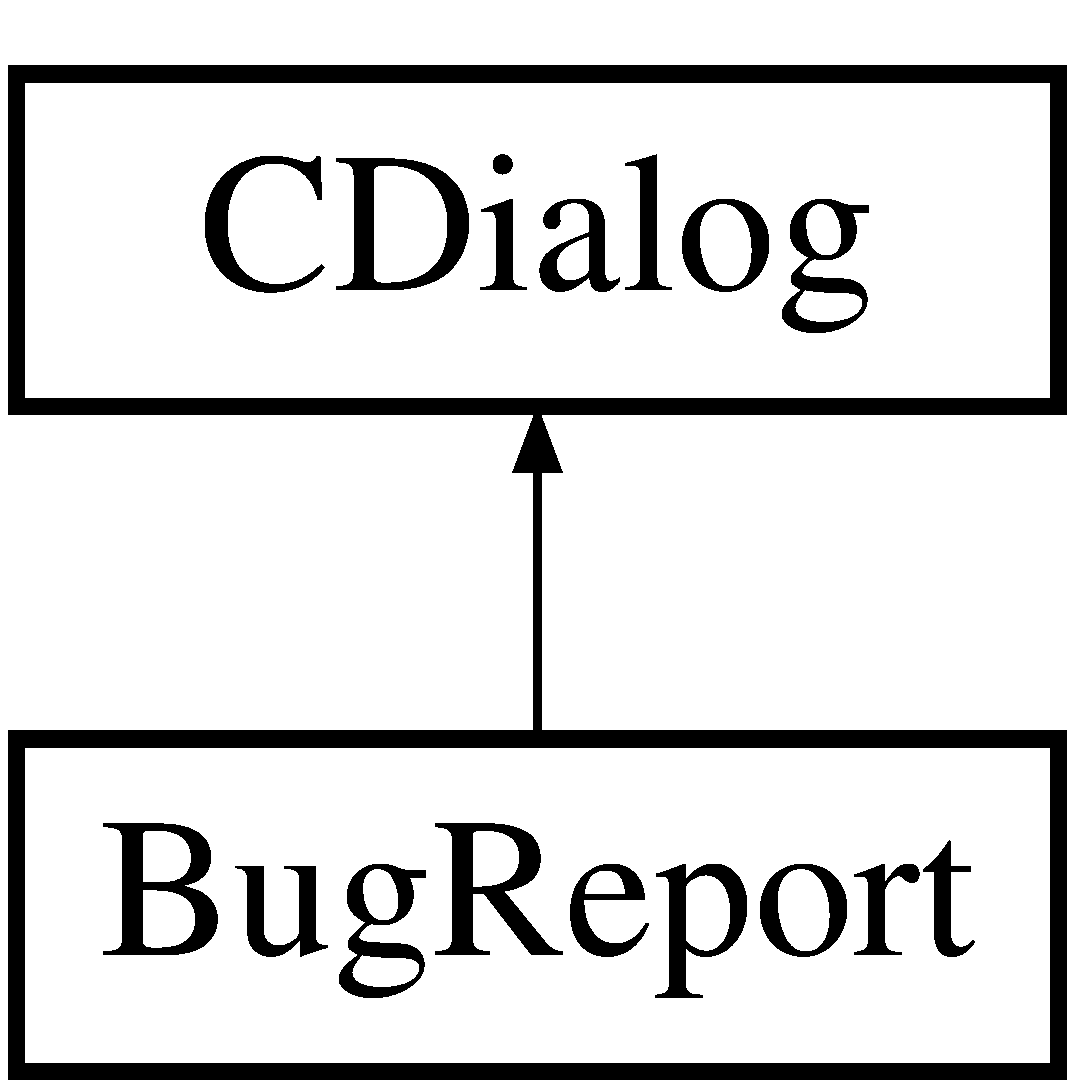
\includegraphics[height=2.000000cm]{class_bug_report}
\end{center}
\end{figure}
\subsection*{Public 타입}
\begin{DoxyCompactItemize}
\item 
\mbox{\Hypertarget{class_bug_report_ac5c6f1960b86db3b70eab6b21625913e}\label{class_bug_report_ac5c6f1960b86db3b70eab6b21625913e}} 
enum \{ {\bfseries I\+DD} = I\+D\+D\+\_\+\+B\+U\+G\+\_\+\+R\+E\+P\+O\+RT
 \}
\end{DoxyCompactItemize}
\subsection*{Public 멤버 함수}
\begin{DoxyCompactItemize}
\item 
\mbox{\Hypertarget{class_bug_report_a0b78ee082b1ca2a2a2c16db3d65842fb}\label{class_bug_report_a0b78ee082b1ca2a2a2c16db3d65842fb}} 
{\bfseries Bug\+Report} (C\+Wnd $\ast$p\+Parent=N\+U\+LL)
\end{DoxyCompactItemize}
\subsection*{Public 속성}
\begin{DoxyCompactItemize}
\item 
\mbox{\Hypertarget{class_bug_report_aef6dd887fcfe40d98d0fa1c6cf2d2466}\label{class_bug_report_aef6dd887fcfe40d98d0fa1c6cf2d2466}} 
C\+Edit {\bfseries m\+\_\+report}
\end{DoxyCompactItemize}
\subsection*{Protected 멤버 함수}
\begin{DoxyCompactItemize}
\item 
\mbox{\Hypertarget{class_bug_report_a5b019306aeca9497b7b6efd438a44558}\label{class_bug_report_a5b019306aeca9497b7b6efd438a44558}} 
virtual void {\bfseries Do\+Data\+Exchange} (C\+Data\+Exchange $\ast$p\+DX)
\item 
\mbox{\Hypertarget{class_bug_report_afe00e8dd3efa190199d8d645cb702e07}\label{class_bug_report_afe00e8dd3efa190199d8d645cb702e07}} 
C\+String {\bfseries create\+Report} ()
\item 
\mbox{\Hypertarget{class_bug_report_a6b74689c7cf7ed6daeaaf2dc8f1498ab}\label{class_bug_report_a6b74689c7cf7ed6daeaaf2dc8f1498ab}} 
afx\+\_\+msg void {\bfseries On\+Copy} ()
\item 
\mbox{\Hypertarget{class_bug_report_a2c9a7f1da33a46ca97f0ecd821e701e9}\label{class_bug_report_a2c9a7f1da33a46ca97f0ecd821e701e9}} 
afx\+\_\+msg void {\bfseries On\+Ok} ()
\item 
\mbox{\Hypertarget{class_bug_report_abcfc2e192747272d1708a1d479bfd45b}\label{class_bug_report_abcfc2e192747272d1708a1d479bfd45b}} 
virtual B\+O\+OL {\bfseries On\+Init\+Dialog} ()
\end{DoxyCompactItemize}


이 클래스에 대한 문서화 페이지는 다음의 파일들로부터 생성되었습니다.\+:\begin{DoxyCompactItemize}
\item 
src/win32/Bug\+Report.\+h\item 
src/win32/Bug\+Report.\+cpp\end{DoxyCompactItemize}

\hypertarget{class_c_accelerator_manager}{}\section{C\+Accelerator\+Manager 클래스 참조}
\label{class_c_accelerator_manager}\index{C\+Accelerator\+Manager@{C\+Accelerator\+Manager}}
C\+Accelerator\+Manager에 대한 상속 다이어그램 \+: \begin{figure}[H]
\begin{center}
\leavevmode
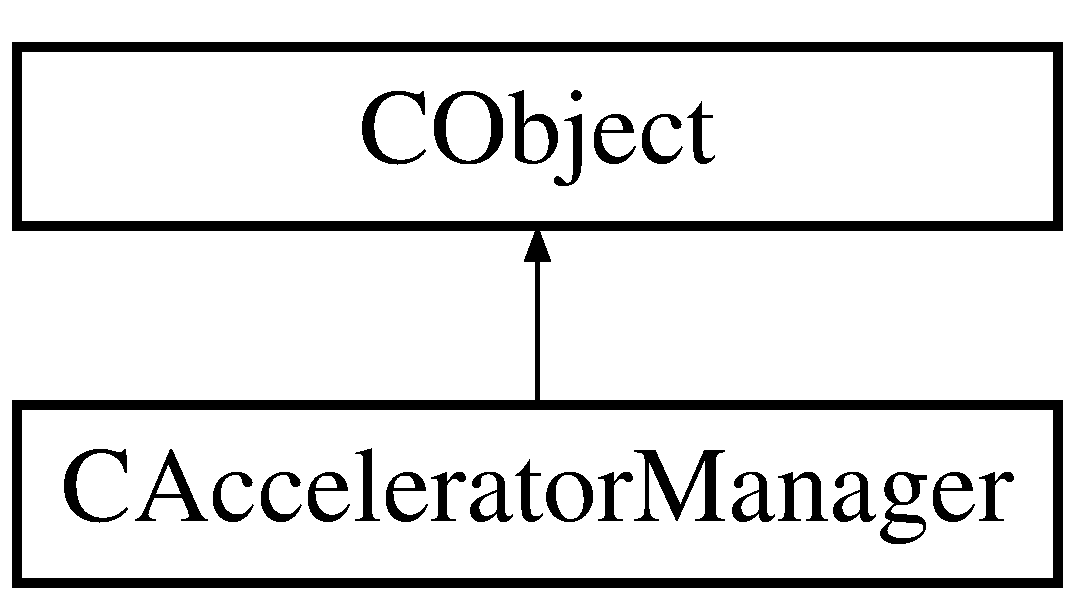
\includegraphics[height=2.000000cm]{class_c_accelerator_manager}
\end{center}
\end{figure}
\subsection*{Public 멤버 함수}
\begin{DoxyCompactItemize}
\item 
\mbox{\Hypertarget{class_c_accelerator_manager_ac7411d20f413ea0ec3bd65705b564adf}\label{class_c_accelerator_manager_ac7411d20f413ea0ec3bd65705b564adf}} 
void {\bfseries Update\+Menu} (H\+M\+E\+NU menu)
\item 
\mbox{\Hypertarget{class_c_accelerator_manager_ac854ec5263a7bab961bf63aec3938984}\label{class_c_accelerator_manager_ac854ec5263a7bab961bf63aec3938984}} 
void {\bfseries Update\+Menu} ()
\item 
\mbox{\Hypertarget{class_c_accelerator_manager_a2d01e04665e3d03f3c1410bd69b0a82c}\label{class_c_accelerator_manager_a2d01e04665e3d03f3c1410bd69b0a82c}} 
void {\bfseries Connect} (C\+Wnd $\ast$p\+Wnd, bool b\+Auto\+Save=true)
\item 
\mbox{\Hypertarget{class_c_accelerator_manager_a8e87ae6f5464a4fa052c91c0ee361b6d}\label{class_c_accelerator_manager_a8e87ae6f5464a4fa052c91c0ee361b6d}} 
bool {\bfseries Load} (H\+K\+EY h\+Reg\+Key, L\+P\+C\+T\+S\+TR sz\+Reg\+Key)
\item 
\mbox{\Hypertarget{class_c_accelerator_manager_a289a9052abea7302d9322283f93cbce6}\label{class_c_accelerator_manager_a289a9052abea7302d9322283f93cbce6}} 
bool {\bfseries Load} ()
\item 
\mbox{\Hypertarget{class_c_accelerator_manager_a6ddd05a54ab0e66bc6ca8a7af3742e61}\label{class_c_accelerator_manager_a6ddd05a54ab0e66bc6ca8a7af3742e61}} 
bool {\bfseries Write} ()
\item 
\mbox{\Hypertarget{class_c_accelerator_manager_aa510a36964ed209de5f7325efa713bf6}\label{class_c_accelerator_manager_aa510a36964ed209de5f7325efa713bf6}} 
bool {\bfseries Default} ()
\item 
\mbox{\Hypertarget{class_c_accelerator_manager_aaefac809b336df14e1a1a7d60f72ae28}\label{class_c_accelerator_manager_aaefac809b336df14e1a1a7d60f72ae28}} 
bool {\bfseries Create\+Default\+Table} ()
\item 
\mbox{\Hypertarget{class_c_accelerator_manager_a508e56037762d035758491d12fd10dfa}\label{class_c_accelerator_manager_a508e56037762d035758491d12fd10dfa}} 
bool {\bfseries Is\+Default\+Table\+Available} ()
\item 
\mbox{\Hypertarget{class_c_accelerator_manager_a6773f028b9c0b04c9a7b6d02c1a96be0}\label{class_c_accelerator_manager_a6773f028b9c0b04c9a7b6d02c1a96be0}} 
bool {\bfseries Is\+Map\+String\+Commands\+Empty} ()
\item 
\mbox{\Hypertarget{class_c_accelerator_manager_afcb43e85351bae0fb475dac40ba4cede}\label{class_c_accelerator_manager_afcb43e85351bae0fb475dac40ba4cede}} 
bool {\bfseries Get\+Reg\+Key} (H\+K\+EY \&h\+Reg\+Key, C\+String \&sz\+Reg\+Key)
\item 
\mbox{\Hypertarget{class_c_accelerator_manager_a6ea67e9b2bfbda2f0305024e0d73a5bb}\label{class_c_accelerator_manager_a6ea67e9b2bfbda2f0305024e0d73a5bb}} 
bool {\bfseries Set\+Reg\+Key} (H\+K\+EY h\+Reg\+Key, L\+P\+C\+T\+S\+TR sz\+Reg\+Key)
\item 
\mbox{\Hypertarget{class_c_accelerator_manager_a895420283e3ce58576ded1a3f999724a}\label{class_c_accelerator_manager_a895420283e3ce58576ded1a3f999724a}} 
bool {\bfseries Is\+Auto\+Save} ()
\item 
\mbox{\Hypertarget{class_c_accelerator_manager_a84b4a9dfb4afc48430655e234ff94349}\label{class_c_accelerator_manager_a84b4a9dfb4afc48430655e234ff94349}} 
void {\bfseries Set\+Auto\+Save} (bool b\+Auto\+Save)
\item 
\mbox{\Hypertarget{class_c_accelerator_manager_a5e861b03f3647e8c4998c49ccd4d8928}\label{class_c_accelerator_manager_a5e861b03f3647e8c4998c49ccd4d8928}} 
bool {\bfseries Get\+String\+From\+A\+C\+C\+EL} (A\+C\+C\+EL $\ast$p\+A\+C\+C\+EL, C\+String \&sz\+Accel)
\item 
\mbox{\Hypertarget{class_c_accelerator_manager_adf91477de6b9df320930786c9755b0eb}\label{class_c_accelerator_manager_adf91477de6b9df320930786c9755b0eb}} 
bool {\bfseries Get\+String\+From\+A\+C\+C\+EL} (B\+Y\+TE c\+Virt, W\+O\+RD n\+Code, C\+String \&sz\+Accel)
\item 
\mbox{\Hypertarget{class_c_accelerator_manager_a3fa9c8e4f44acc76cc40fc7382e597d8}\label{class_c_accelerator_manager_a3fa9c8e4f44acc76cc40fc7382e597d8}} 
bool {\bfseries Update\+Wnd\+Table} ()
\item 
\mbox{\Hypertarget{class_c_accelerator_manager_a96957fd8ed0a15d0dbc508359824db3c}\label{class_c_accelerator_manager_a96957fd8ed0a15d0dbc508359824db3c}} 
bool {\bfseries Set\+Accel} (B\+Y\+TE c\+Virt, W\+O\+RD w\+I\+D\+Command, W\+O\+RD w\+New\+Caract, L\+P\+C\+T\+S\+TR sz\+Command, bool b\+Locked=false)
\item 
\mbox{\Hypertarget{class_c_accelerator_manager_a05227e733c2c5d4a4d8074bf28a4f333}\label{class_c_accelerator_manager_a05227e733c2c5d4a4d8074bf28a4f333}} 
bool {\bfseries Add\+Command\+Accel} (W\+O\+RD w\+I\+D\+Command, L\+P\+C\+T\+S\+TR sz\+Command, bool b\+Locked=true)
\item 
\mbox{\Hypertarget{class_c_accelerator_manager_ab534c2d8c0d7d7e30c5e907677bfad68}\label{class_c_accelerator_manager_ab534c2d8c0d7d7e30c5e907677bfad68}} 
bool {\bfseries Create\+Entry} (W\+O\+RD w\+I\+D\+Command, L\+P\+C\+T\+S\+TR sz\+Command)
\item 
\mbox{\Hypertarget{class_c_accelerator_manager_ae20cd0e0259b70fe7443b442e85d1213}\label{class_c_accelerator_manager_ae20cd0e0259b70fe7443b442e85d1213}} 
bool {\bfseries Delete\+Entry} (L\+P\+C\+T\+S\+TR sz\+Command)
\item 
\mbox{\Hypertarget{class_c_accelerator_manager_a25f2470050bd966a2f45235381dda32b}\label{class_c_accelerator_manager_a25f2470050bd966a2f45235381dda32b}} 
bool {\bfseries Delete\+Entry} (W\+O\+RD w\+I\+D\+Command)
\item 
\mbox{\Hypertarget{class_c_accelerator_manager_a73426e98a7fb4d8e5481a8e55a8a2626}\label{class_c_accelerator_manager_a73426e98a7fb4d8e5481a8e55a8a2626}} 
bool {\bfseries Delete\+Accel} (B\+Y\+TE c\+Virt, W\+O\+RD w\+I\+D\+Command, W\+O\+RD w\+New\+Caract)
\item 
\mbox{\Hypertarget{class_c_accelerator_manager_a11c56cbcdfac0008ecb4aef10ba51ae8}\label{class_c_accelerator_manager_a11c56cbcdfac0008ecb4aef10ba51ae8}} 
\mbox{\hyperlink{class_c_accelerator_manager}{C\+Accelerator\+Manager}} \& {\bfseries operator=} (const \mbox{\hyperlink{class_c_accelerator_manager}{C\+Accelerator\+Manager}} \&accelmgr)
\end{DoxyCompactItemize}
\subsection*{Protected 멤버 함수}
\begin{DoxyCompactItemize}
\item 
\mbox{\Hypertarget{class_c_accelerator_manager_aca456cda1a5f9b17bcfaea4f8ff45903}\label{class_c_accelerator_manager_aca456cda1a5f9b17bcfaea4f8ff45903}} 
void {\bfseries Reset} ()
\item 
\mbox{\Hypertarget{class_c_accelerator_manager_ac9e0e988625c9687666a9f582f9b3536}\label{class_c_accelerator_manager_ac9e0e988625c9687666a9f582f9b3536}} 
bool {\bfseries Add\+Accel} (B\+Y\+TE c\+Virt, W\+O\+RD w\+I\+D\+Command, W\+O\+RD w\+Key, L\+P\+C\+T\+S\+TR sz\+Command, bool b\+Locked)
\end{DoxyCompactItemize}
\subsection*{Protected 속성}
\begin{DoxyCompactItemize}
\item 
\mbox{\Hypertarget{class_c_accelerator_manager_a24f706c75f754982051e1d7fad1916da}\label{class_c_accelerator_manager_a24f706c75f754982051e1d7fad1916da}} 
C\+Wnd $\ast$ {\bfseries m\+\_\+p\+Wnd\+Connected}
\item 
\mbox{\Hypertarget{class_c_accelerator_manager_abb40dbb1a44c47ac22590e8f1243835b}\label{class_c_accelerator_manager_abb40dbb1a44c47ac22590e8f1243835b}} 
C\+Map\+String\+To\+Word {\bfseries m\+\_\+map\+Accel\+String}
\item 
\mbox{\Hypertarget{class_c_accelerator_manager_a16b8d3e9328bc0eeeb048630deff2768}\label{class_c_accelerator_manager_a16b8d3e9328bc0eeeb048630deff2768}} 
C\+Map\+Word\+To\+C\+Cmd\+Accel\+Ob {\bfseries m\+\_\+map\+Accel\+Table}
\item 
\mbox{\Hypertarget{class_c_accelerator_manager_ad7c3ac9a16b8f19e0b5524d8582a5fae}\label{class_c_accelerator_manager_ad7c3ac9a16b8f19e0b5524d8582a5fae}} 
C\+Map\+Word\+To\+C\+Cmd\+Accel\+Ob {\bfseries m\+\_\+map\+Accel\+Table\+Saved}
\item 
\mbox{\Hypertarget{class_c_accelerator_manager_ac563baf2a7cedb91bc44e9b8581a6020}\label{class_c_accelerator_manager_ac563baf2a7cedb91bc44e9b8581a6020}} 
bool {\bfseries m\+\_\+b\+Default\+Table}
\item 
\mbox{\Hypertarget{class_c_accelerator_manager_a2652d64c947f7f3474b3aa054861b34b}\label{class_c_accelerator_manager_a2652d64c947f7f3474b3aa054861b34b}} 
H\+K\+EY {\bfseries m\+\_\+h\+Reg\+Key}
\item 
\mbox{\Hypertarget{class_c_accelerator_manager_a03a6d0e43bcfb63cf1a23ad12cb5aa35}\label{class_c_accelerator_manager_a03a6d0e43bcfb63cf1a23ad12cb5aa35}} 
C\+String {\bfseries m\+\_\+sz\+Reg\+Key}
\item 
\mbox{\Hypertarget{class_c_accelerator_manager_a37b504c74c13ca2d62eea8abffe73102}\label{class_c_accelerator_manager_a37b504c74c13ca2d62eea8abffe73102}} 
bool {\bfseries m\+\_\+b\+Auto\+Save}
\end{DoxyCompactItemize}
\subsection*{Friends}
\begin{DoxyCompactItemize}
\item 
\mbox{\Hypertarget{class_c_accelerator_manager_ad13d9a415d0447ece033ae132991aefc}\label{class_c_accelerator_manager_ad13d9a415d0447ece033ae132991aefc}} 
class {\bfseries Accel\+Editor}
\end{DoxyCompactItemize}


이 클래스에 대한 문서화 페이지는 다음의 파일들로부터 생성되었습니다.\+:\begin{DoxyCompactItemize}
\item 
src/win32/Accelerator\+Manager.\+h\item 
src/win32/Accelerator\+Manager.\+cpp\end{DoxyCompactItemize}

\hypertarget{class_c_accels_ob}{}\section{C\+Accels\+Ob 클래스 참조}
\label{class_c_accels_ob}\index{C\+Accels\+Ob@{C\+Accels\+Ob}}
C\+Accels\+Ob에 대한 상속 다이어그램 \+: \begin{figure}[H]
\begin{center}
\leavevmode
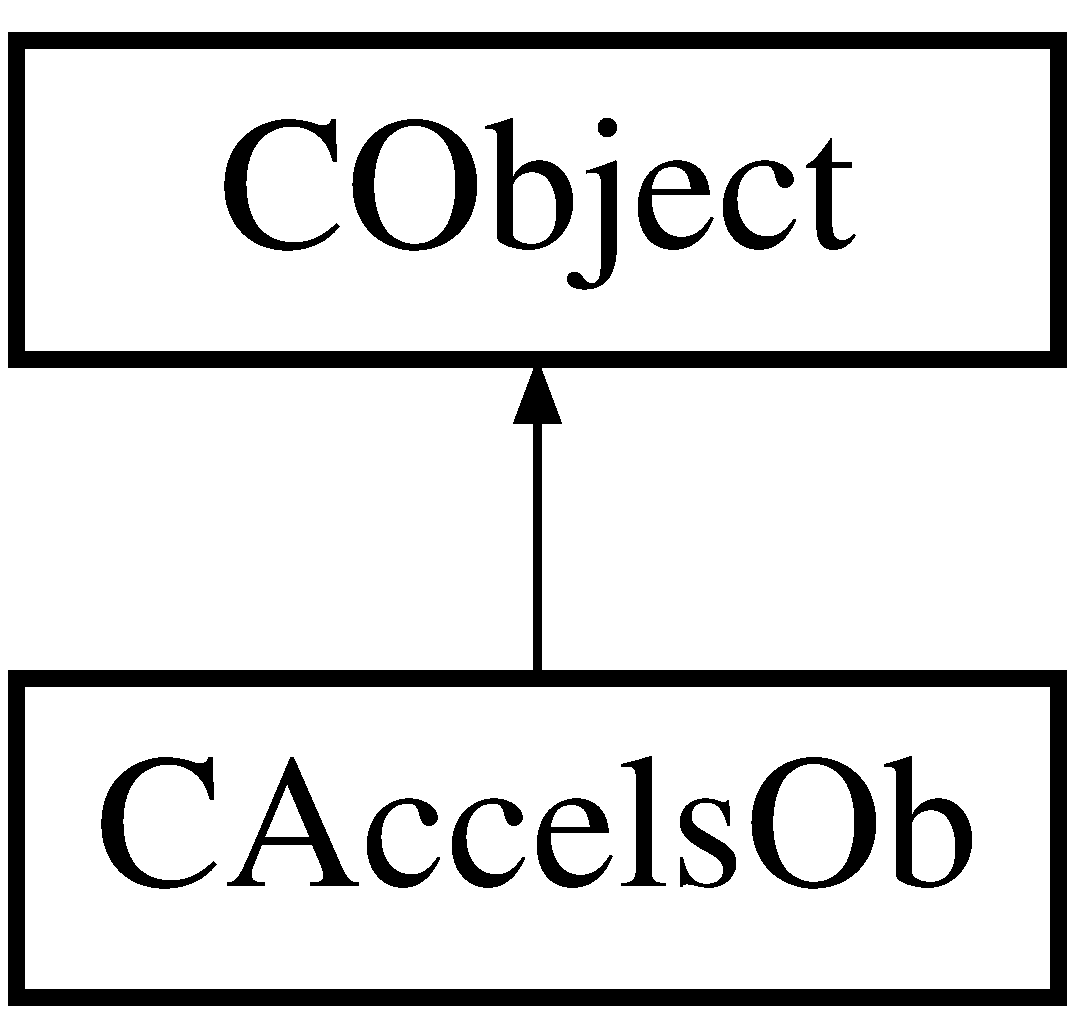
\includegraphics[height=2.000000cm]{class_c_accels_ob}
\end{center}
\end{figure}
\subsection*{Public 멤버 함수}
\begin{DoxyCompactItemize}
\item 
\mbox{\Hypertarget{class_c_accels_ob_afca345908aafde57de46430bbf2018d9}\label{class_c_accels_ob_afca345908aafde57de46430bbf2018d9}} 
{\bfseries C\+Accels\+Ob} (\mbox{\hyperlink{class_c_accels_ob}{C\+Accels\+Ob}} $\ast$p\+From)
\item 
\mbox{\Hypertarget{class_c_accels_ob_acba35eec2e75114289468292870bf484}\label{class_c_accels_ob_acba35eec2e75114289468292870bf484}} 
{\bfseries C\+Accels\+Ob} (B\+Y\+TE c\+Virt, W\+O\+RD w\+Key, bool b\+Locked=false)
\item 
\mbox{\Hypertarget{class_c_accels_ob_aa28d7238be643bb20d922cb360881bd6}\label{class_c_accels_ob_aa28d7238be643bb20d922cb360881bd6}} 
{\bfseries C\+Accels\+Ob} (L\+P\+A\+C\+C\+EL p\+A\+C\+C\+EL)
\item 
\mbox{\Hypertarget{class_c_accels_ob_ae6075be9ad7656823f5cecd277dd7d6e}\label{class_c_accels_ob_ae6075be9ad7656823f5cecd277dd7d6e}} 
\mbox{\hyperlink{class_c_accels_ob}{C\+Accels\+Ob}} \& {\bfseries operator=} (const \mbox{\hyperlink{class_c_accels_ob}{C\+Accels\+Ob}} \&from)
\item 
\mbox{\Hypertarget{class_c_accels_ob_afaf7510fa1e0707863f6bd469f190de6}\label{class_c_accels_ob_afaf7510fa1e0707863f6bd469f190de6}} 
void {\bfseries Get\+String} (C\+String \&sz\+Buffer)
\item 
\mbox{\Hypertarget{class_c_accels_ob_a32714a4454d398d3d3a68d1705a76bc5}\label{class_c_accels_ob_a32714a4454d398d3d3a68d1705a76bc5}} 
bool {\bfseries Is\+Equal} (W\+O\+RD w\+Key, bool b\+Ctrl, bool b\+Alt, bool b\+Shift)
\item 
\mbox{\Hypertarget{class_c_accels_ob_abbbdc5e93061f67ade785c9e4f07b918}\label{class_c_accels_ob_abbbdc5e93061f67ade785c9e4f07b918}} 
D\+W\+O\+RD {\bfseries Get\+Data} ()
\item 
\mbox{\Hypertarget{class_c_accels_ob_a47a1e7e047807b7a36553aa351768096}\label{class_c_accels_ob_a47a1e7e047807b7a36553aa351768096}} 
bool {\bfseries Set\+Data} (D\+W\+O\+RD dw\+Datas)
\end{DoxyCompactItemize}
\subsection*{Public 속성}
\begin{DoxyCompactItemize}
\item 
\mbox{\Hypertarget{class_c_accels_ob_a08b7003ccf92c6afcf31878960d8eee1}\label{class_c_accels_ob_a08b7003ccf92c6afcf31878960d8eee1}} 
B\+Y\+TE {\bfseries m\+\_\+c\+Virt}
\item 
\mbox{\Hypertarget{class_c_accels_ob_a1891250e9a4d00c0862f3a90a965d635}\label{class_c_accels_ob_a1891250e9a4d00c0862f3a90a965d635}} 
W\+O\+RD {\bfseries m\+\_\+w\+Key}
\item 
\mbox{\Hypertarget{class_c_accels_ob_ad8300bd20bd429ad61f89700e388dd9a}\label{class_c_accels_ob_ad8300bd20bd429ad61f89700e388dd9a}} 
bool {\bfseries m\+\_\+b\+Locked}
\end{DoxyCompactItemize}


이 클래스에 대한 문서화 페이지는 다음의 파일들로부터 생성되었습니다.\+:\begin{DoxyCompactItemize}
\item 
src/win32/Cmd\+Accel\+Ob.\+h\item 
src/win32/Cmd\+Accel\+Ob.\+cpp\end{DoxyCompactItemize}

\hypertarget{class_c_cmd_accel_ob}{}\section{C\+Cmd\+Accel\+Ob 클래스 참조}
\label{class_c_cmd_accel_ob}\index{C\+Cmd\+Accel\+Ob@{C\+Cmd\+Accel\+Ob}}


{\ttfamily \#include $<$Cmd\+Accel\+Ob.\+h$>$}



C\+Cmd\+Accel\+Ob에 대한 상속 다이어그램 \+: \nopagebreak
\begin{figure}[H]
\begin{center}
\leavevmode
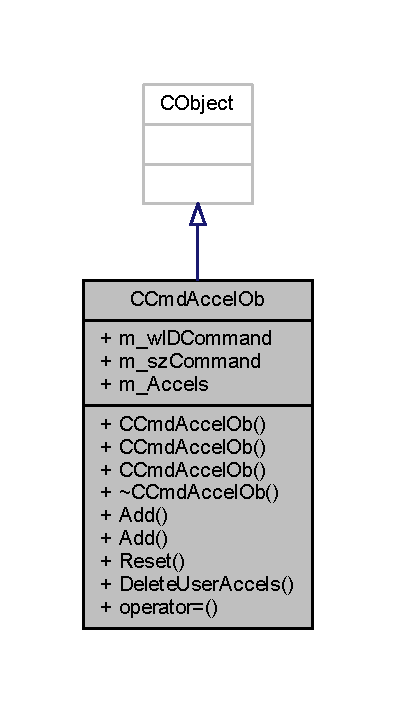
\includegraphics[width=190pt]{class_c_cmd_accel_ob__inherit__graph}
\end{center}
\end{figure}


C\+Cmd\+Accel\+Ob에 대한 협력 다이어그램\+:\nopagebreak
\begin{figure}[H]
\begin{center}
\leavevmode
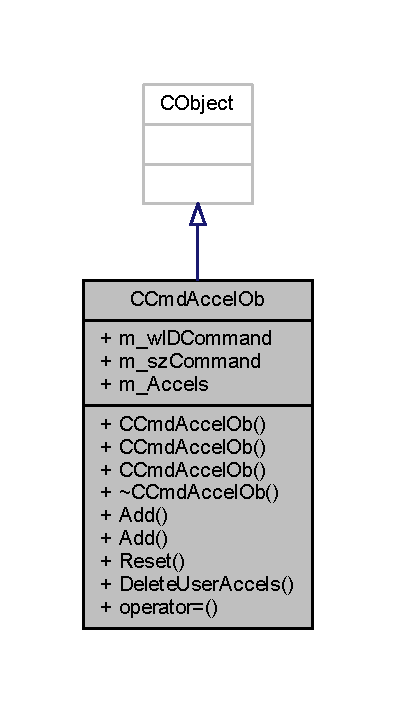
\includegraphics[width=190pt]{class_c_cmd_accel_ob__coll__graph}
\end{center}
\end{figure}
\subsection*{Public 멤버 함수}
\begin{DoxyCompactItemize}
\item 
\mbox{\hyperlink{class_c_cmd_accel_ob_a2f5bb136c7ba36c31551cec05f3c47fc}{C\+Cmd\+Accel\+Ob}} ()
\item 
\mbox{\hyperlink{class_c_cmd_accel_ob_a245369282fbad17c28924e0568fa5bcc}{C\+Cmd\+Accel\+Ob}} (W\+O\+RD w\+I\+D\+Command, L\+P\+C\+T\+S\+TR sz\+Command)
\item 
\mbox{\hyperlink{class_c_cmd_accel_ob_a2c532e999fa7dcb99d7d9b1027cebbef}{C\+Cmd\+Accel\+Ob}} (B\+Y\+TE c\+Virt, W\+O\+RD w\+I\+D\+Command, W\+O\+RD w\+Key, L\+P\+C\+T\+S\+TR sz\+Command, bool b\+Locked=false)
\item 
\mbox{\hyperlink{class_c_cmd_accel_ob_a41d00fee4f058c03fa85630612e1ab69}{$\sim$\+C\+Cmd\+Accel\+Ob}} ()
\item 
void \mbox{\hyperlink{class_c_cmd_accel_ob_a519f8c7ac935b0d06531589e5427b656}{Add}} (\mbox{\hyperlink{class_c_accels_ob}{C\+Accels\+Ob}} $\ast$p\+Accel)
\item 
void \mbox{\hyperlink{class_c_cmd_accel_ob_a15429015a20179a0e181347f35ad9c58}{Add}} (B\+Y\+TE c\+Virt, W\+O\+RD w\+Key, bool b\+Locked=false)
\item 
void \mbox{\hyperlink{class_c_cmd_accel_ob_ac679e57ed400b175109af50ea2ce919d}{Reset}} ()
\item 
void \mbox{\hyperlink{class_c_cmd_accel_ob_a7040471adc76f057a1d79c9fdfb84fe8}{Delete\+User\+Accels}} ()
\item 
\mbox{\hyperlink{class_c_cmd_accel_ob}{C\+Cmd\+Accel\+Ob}} \& \mbox{\hyperlink{class_c_cmd_accel_ob_a045ce00d2465fefed857066eef1406a7}{operator=}} (\mbox{\hyperlink{getopt1_8c_a2c212835823e3c54a8ab6d95c652660e}{const}} \mbox{\hyperlink{class_c_cmd_accel_ob}{C\+Cmd\+Accel\+Ob}} \&\mbox{\hyperlink{expr_8cpp_a765533dfc643627999c751f7e1514664}{from}})
\end{DoxyCompactItemize}
\subsection*{Public 속성}
\begin{DoxyCompactItemize}
\item 
W\+O\+RD \mbox{\hyperlink{class_c_cmd_accel_ob_aa3eb02dcd39ff14763fdefd8fabd7591}{m\+\_\+w\+I\+D\+Command}}
\item 
C\+String \mbox{\hyperlink{class_c_cmd_accel_ob_acbd02cc68d3909b1e39b687e76f45d91}{m\+\_\+sz\+Command}}
\item 
C\+List$<$ \mbox{\hyperlink{class_c_accels_ob}{C\+Accels\+Ob}} $\ast$, \mbox{\hyperlink{class_c_accels_ob}{C\+Accels\+Ob}} $\ast$\&$>$ \mbox{\hyperlink{class_c_cmd_accel_ob_a85772f1ea9204af42b8a39a0135dc0f8}{m\+\_\+\+Accels}}
\end{DoxyCompactItemize}


\subsection{상세한 설명}


Cmd\+Accel\+Ob.\+h 파일의 82 번째 라인에서 정의되었습니다.



\subsection{생성자 \& 소멸자 문서화}
\mbox{\Hypertarget{class_c_cmd_accel_ob_a2f5bb136c7ba36c31551cec05f3c47fc}\label{class_c_cmd_accel_ob_a2f5bb136c7ba36c31551cec05f3c47fc}} 
\index{C\+Cmd\+Accel\+Ob@{C\+Cmd\+Accel\+Ob}!C\+Cmd\+Accel\+Ob@{C\+Cmd\+Accel\+Ob}}
\index{C\+Cmd\+Accel\+Ob@{C\+Cmd\+Accel\+Ob}!C\+Cmd\+Accel\+Ob@{C\+Cmd\+Accel\+Ob}}
\subsubsection{\texorpdfstring{C\+Cmd\+Accel\+Ob()}{CCmdAccelOb()}\hspace{0.1cm}{\footnotesize\ttfamily [1/3]}}
{\footnotesize\ttfamily C\+Cmd\+Accel\+Ob\+::\+C\+Cmd\+Accel\+Ob (\begin{DoxyParamCaption}{ }\end{DoxyParamCaption})}



Cmd\+Accel\+Ob.\+cpp 파일의 368 번째 라인에서 정의되었습니다.


\begin{DoxyCode}
369 \{
370 \}
\end{DoxyCode}
\mbox{\Hypertarget{class_c_cmd_accel_ob_a245369282fbad17c28924e0568fa5bcc}\label{class_c_cmd_accel_ob_a245369282fbad17c28924e0568fa5bcc}} 
\index{C\+Cmd\+Accel\+Ob@{C\+Cmd\+Accel\+Ob}!C\+Cmd\+Accel\+Ob@{C\+Cmd\+Accel\+Ob}}
\index{C\+Cmd\+Accel\+Ob@{C\+Cmd\+Accel\+Ob}!C\+Cmd\+Accel\+Ob@{C\+Cmd\+Accel\+Ob}}
\subsubsection{\texorpdfstring{C\+Cmd\+Accel\+Ob()}{CCmdAccelOb()}\hspace{0.1cm}{\footnotesize\ttfamily [2/3]}}
{\footnotesize\ttfamily C\+Cmd\+Accel\+Ob\+::\+C\+Cmd\+Accel\+Ob (\begin{DoxyParamCaption}\item[{W\+O\+RD}]{w\+I\+D\+Command,  }\item[{L\+P\+C\+T\+S\+TR}]{sz\+Command }\end{DoxyParamCaption})}



Cmd\+Accel\+Ob.\+cpp 파일의 376 번째 라인에서 정의되었습니다.


\begin{DoxyCode}
377 \{
378   ASSERT(szCommand != \mbox{\hyperlink{getopt1_8c_a070d2ce7b6bb7e5c05602aa8c308d0c4}{NULL}});
379 
380   \mbox{\hyperlink{class_c_cmd_accel_ob_aa3eb02dcd39ff14763fdefd8fabd7591}{m\_wIDCommand}} = wIDCommand;
381   \mbox{\hyperlink{class_c_cmd_accel_ob_acbd02cc68d3909b1e39b687e76f45d91}{m\_szCommand}} = szCommand;
382 \}
\end{DoxyCode}
\mbox{\Hypertarget{class_c_cmd_accel_ob_a2c532e999fa7dcb99d7d9b1027cebbef}\label{class_c_cmd_accel_ob_a2c532e999fa7dcb99d7d9b1027cebbef}} 
\index{C\+Cmd\+Accel\+Ob@{C\+Cmd\+Accel\+Ob}!C\+Cmd\+Accel\+Ob@{C\+Cmd\+Accel\+Ob}}
\index{C\+Cmd\+Accel\+Ob@{C\+Cmd\+Accel\+Ob}!C\+Cmd\+Accel\+Ob@{C\+Cmd\+Accel\+Ob}}
\subsubsection{\texorpdfstring{C\+Cmd\+Accel\+Ob()}{CCmdAccelOb()}\hspace{0.1cm}{\footnotesize\ttfamily [3/3]}}
{\footnotesize\ttfamily C\+Cmd\+Accel\+Ob\+::\+C\+Cmd\+Accel\+Ob (\begin{DoxyParamCaption}\item[{B\+Y\+TE}]{c\+Virt,  }\item[{W\+O\+RD}]{w\+I\+D\+Command,  }\item[{W\+O\+RD}]{w\+Key,  }\item[{L\+P\+C\+T\+S\+TR}]{sz\+Command,  }\item[{bool}]{b\+Locked = {\ttfamily false} }\end{DoxyParamCaption})}



Cmd\+Accel\+Ob.\+cpp 파일의 388 번째 라인에서 정의되었습니다.


\begin{DoxyCode}
389 \{
390   ASSERT(szCommand != \mbox{\hyperlink{getopt1_8c_a070d2ce7b6bb7e5c05602aa8c308d0c4}{NULL}});
391   
392   \mbox{\hyperlink{class_c_cmd_accel_ob_aa3eb02dcd39ff14763fdefd8fabd7591}{m\_wIDCommand}} = wIDCommand;
393   \mbox{\hyperlink{class_c_cmd_accel_ob_acbd02cc68d3909b1e39b687e76f45d91}{m\_szCommand}} = szCommand;
394   
395   \mbox{\hyperlink{class_c_accels_ob}{CAccelsOb}}* pAccel = DEBUG\_NEW \mbox{\hyperlink{class_c_accels_ob}{CAccelsOb}}(cVirt, wKey, bLocked);
396   ASSERT(pAccel != \mbox{\hyperlink{getopt1_8c_a070d2ce7b6bb7e5c05602aa8c308d0c4}{NULL}});
397   \mbox{\hyperlink{class_c_cmd_accel_ob_a85772f1ea9204af42b8a39a0135dc0f8}{m\_Accels}}.AddTail(pAccel);
398 \}
\end{DoxyCode}
\mbox{\Hypertarget{class_c_cmd_accel_ob_a41d00fee4f058c03fa85630612e1ab69}\label{class_c_cmd_accel_ob_a41d00fee4f058c03fa85630612e1ab69}} 
\index{C\+Cmd\+Accel\+Ob@{C\+Cmd\+Accel\+Ob}!````~C\+Cmd\+Accel\+Ob@{$\sim$\+C\+Cmd\+Accel\+Ob}}
\index{````~C\+Cmd\+Accel\+Ob@{$\sim$\+C\+Cmd\+Accel\+Ob}!C\+Cmd\+Accel\+Ob@{C\+Cmd\+Accel\+Ob}}
\subsubsection{\texorpdfstring{$\sim$\+C\+Cmd\+Accel\+Ob()}{~CCmdAccelOb()}}
{\footnotesize\ttfamily C\+Cmd\+Accel\+Ob\+::$\sim$\+C\+Cmd\+Accel\+Ob (\begin{DoxyParamCaption}{ }\end{DoxyParamCaption})}



Cmd\+Accel\+Ob.\+cpp 파일의 404 번째 라인에서 정의되었습니다.


\begin{DoxyCode}
405 \{
406   POSITION pos = \mbox{\hyperlink{class_c_cmd_accel_ob_a85772f1ea9204af42b8a39a0135dc0f8}{m\_Accels}}.GetHeadPosition();
407   \textcolor{keywordflow}{while} (pos != \mbox{\hyperlink{getopt1_8c_a070d2ce7b6bb7e5c05602aa8c308d0c4}{NULL}})
408     \textcolor{keyword}{delete} \mbox{\hyperlink{class_c_cmd_accel_ob_a85772f1ea9204af42b8a39a0135dc0f8}{m\_Accels}}.GetNext(pos);
409   \mbox{\hyperlink{class_c_cmd_accel_ob_a85772f1ea9204af42b8a39a0135dc0f8}{m\_Accels}}.RemoveAll();
410 \}
\end{DoxyCode}


\subsection{멤버 함수 문서화}
\mbox{\Hypertarget{class_c_cmd_accel_ob_a519f8c7ac935b0d06531589e5427b656}\label{class_c_cmd_accel_ob_a519f8c7ac935b0d06531589e5427b656}} 
\index{C\+Cmd\+Accel\+Ob@{C\+Cmd\+Accel\+Ob}!Add@{Add}}
\index{Add@{Add}!C\+Cmd\+Accel\+Ob@{C\+Cmd\+Accel\+Ob}}
\subsubsection{\texorpdfstring{Add()}{Add()}\hspace{0.1cm}{\footnotesize\ttfamily [1/2]}}
{\footnotesize\ttfamily void C\+Cmd\+Accel\+Ob\+::\+Add (\begin{DoxyParamCaption}\item[{\mbox{\hyperlink{class_c_accels_ob}{C\+Accels\+Ob}} $\ast$}]{p\+Accel }\end{DoxyParamCaption})}



Cmd\+Accel\+Ob.\+cpp 파일의 429 번째 라인에서 정의되었습니다.


\begin{DoxyCode}
430 \{
431   ASSERT(pAccel != \mbox{\hyperlink{getopt1_8c_a070d2ce7b6bb7e5c05602aa8c308d0c4}{NULL}});
432   \mbox{\hyperlink{class_c_cmd_accel_ob_a85772f1ea9204af42b8a39a0135dc0f8}{m\_Accels}}.AddTail(pAccel);
433 \}
\end{DoxyCode}
이 함수를 호출하는 함수들에 대한 그래프입니다.\+:
\nopagebreak
\begin{figure}[H]
\begin{center}
\leavevmode
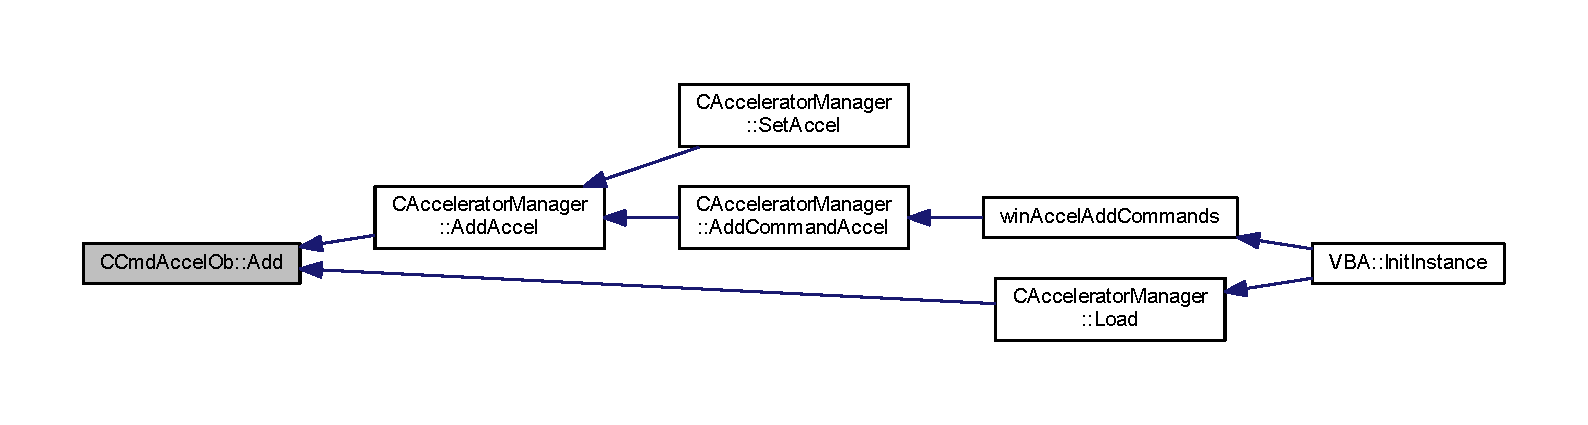
\includegraphics[width=350pt]{class_c_cmd_accel_ob_a519f8c7ac935b0d06531589e5427b656_icgraph}
\end{center}
\end{figure}
\mbox{\Hypertarget{class_c_cmd_accel_ob_a15429015a20179a0e181347f35ad9c58}\label{class_c_cmd_accel_ob_a15429015a20179a0e181347f35ad9c58}} 
\index{C\+Cmd\+Accel\+Ob@{C\+Cmd\+Accel\+Ob}!Add@{Add}}
\index{Add@{Add}!C\+Cmd\+Accel\+Ob@{C\+Cmd\+Accel\+Ob}}
\subsubsection{\texorpdfstring{Add()}{Add()}\hspace{0.1cm}{\footnotesize\ttfamily [2/2]}}
{\footnotesize\ttfamily void C\+Cmd\+Accel\+Ob\+::\+Add (\begin{DoxyParamCaption}\item[{B\+Y\+TE}]{c\+Virt,  }\item[{W\+O\+RD}]{w\+Key,  }\item[{bool}]{b\+Locked = {\ttfamily false} }\end{DoxyParamCaption})}



Cmd\+Accel\+Ob.\+cpp 파일의 418 번째 라인에서 정의되었습니다.


\begin{DoxyCode}
419 \{
420   \mbox{\hyperlink{class_c_accels_ob}{CAccelsOb}}* pAccel = DEBUG\_NEW \mbox{\hyperlink{class_c_accels_ob}{CAccelsOb}}(cVirt, wKey, bLocked);
421   ASSERT(pAccel != \mbox{\hyperlink{getopt1_8c_a070d2ce7b6bb7e5c05602aa8c308d0c4}{NULL}});
422   \mbox{\hyperlink{class_c_cmd_accel_ob_a85772f1ea9204af42b8a39a0135dc0f8}{m\_Accels}}.AddTail(pAccel);
423 \}
\end{DoxyCode}
\mbox{\Hypertarget{class_c_cmd_accel_ob_a7040471adc76f057a1d79c9fdfb84fe8}\label{class_c_cmd_accel_ob_a7040471adc76f057a1d79c9fdfb84fe8}} 
\index{C\+Cmd\+Accel\+Ob@{C\+Cmd\+Accel\+Ob}!Delete\+User\+Accels@{Delete\+User\+Accels}}
\index{Delete\+User\+Accels@{Delete\+User\+Accels}!C\+Cmd\+Accel\+Ob@{C\+Cmd\+Accel\+Ob}}
\subsubsection{\texorpdfstring{Delete\+User\+Accels()}{DeleteUserAccels()}}
{\footnotesize\ttfamily void C\+Cmd\+Accel\+Ob\+::\+Delete\+User\+Accels (\begin{DoxyParamCaption}{ }\end{DoxyParamCaption})}



Cmd\+Accel\+Ob.\+cpp 파일의 460 번째 라인에서 정의되었습니다.


\begin{DoxyCode}
461 \{
462   \mbox{\hyperlink{class_c_accels_ob}{CAccelsOb}}* pAccel;
463   POSITION prevPos;
464   POSITION pos = \mbox{\hyperlink{class_c_cmd_accel_ob_a85772f1ea9204af42b8a39a0135dc0f8}{m\_Accels}}.GetHeadPosition();
465   \textcolor{keywordflow}{while} (pos != \mbox{\hyperlink{getopt1_8c_a070d2ce7b6bb7e5c05602aa8c308d0c4}{NULL}}) \{
466     prevPos = pos;
467     pAccel = \mbox{\hyperlink{class_c_cmd_accel_ob_a85772f1ea9204af42b8a39a0135dc0f8}{m\_Accels}}.GetNext(pos);
468     \textcolor{keywordflow}{if} (!pAccel->\mbox{\hyperlink{class_c_accels_ob_ad8300bd20bd429ad61f89700e388dd9a}{m\_bLocked}}) \{
469       \textcolor{keyword}{delete} pAccel;
470       \mbox{\hyperlink{class_c_cmd_accel_ob_a85772f1ea9204af42b8a39a0135dc0f8}{m\_Accels}}.RemoveAt(prevPos);
471     \}
472   \}
473 \}
\end{DoxyCode}
이 함수를 호출하는 함수들에 대한 그래프입니다.\+:
\nopagebreak
\begin{figure}[H]
\begin{center}
\leavevmode
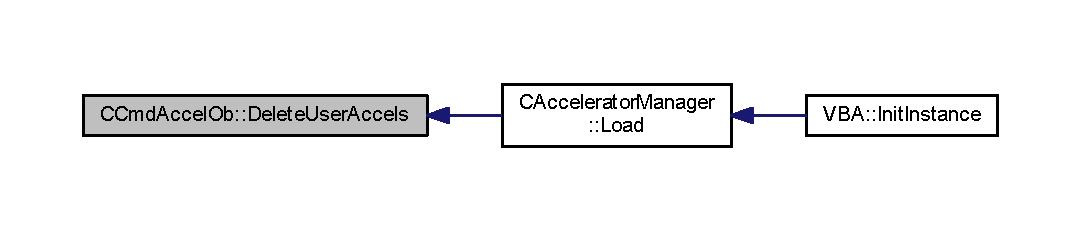
\includegraphics[width=350pt]{class_c_cmd_accel_ob_a7040471adc76f057a1d79c9fdfb84fe8_icgraph}
\end{center}
\end{figure}
\mbox{\Hypertarget{class_c_cmd_accel_ob_a045ce00d2465fefed857066eef1406a7}\label{class_c_cmd_accel_ob_a045ce00d2465fefed857066eef1406a7}} 
\index{C\+Cmd\+Accel\+Ob@{C\+Cmd\+Accel\+Ob}!operator=@{operator=}}
\index{operator=@{operator=}!C\+Cmd\+Accel\+Ob@{C\+Cmd\+Accel\+Ob}}
\subsubsection{\texorpdfstring{operator=()}{operator=()}}
{\footnotesize\ttfamily \mbox{\hyperlink{class_c_cmd_accel_ob}{C\+Cmd\+Accel\+Ob}} \& C\+Cmd\+Accel\+Ob\+::operator= (\begin{DoxyParamCaption}\item[{\mbox{\hyperlink{getopt1_8c_a2c212835823e3c54a8ab6d95c652660e}{const}} \mbox{\hyperlink{class_c_cmd_accel_ob}{C\+Cmd\+Accel\+Ob}} \&}]{from }\end{DoxyParamCaption})}



Cmd\+Accel\+Ob.\+cpp 파일의 439 번째 라인에서 정의되었습니다.


\begin{DoxyCode}
440 \{
441   \mbox{\hyperlink{class_c_cmd_accel_ob_ac679e57ed400b175109af50ea2ce919d}{Reset}}();
442   
443   \mbox{\hyperlink{class_c_cmd_accel_ob_aa3eb02dcd39ff14763fdefd8fabd7591}{m\_wIDCommand}} = \mbox{\hyperlink{expr_8cpp_a765533dfc643627999c751f7e1514664}{from}}.m\_wIDCommand;
444   \mbox{\hyperlink{class_c_cmd_accel_ob_acbd02cc68d3909b1e39b687e76f45d91}{m\_szCommand}} = \mbox{\hyperlink{expr_8cpp_a765533dfc643627999c751f7e1514664}{from}}.m\_szCommand;
445   
446   \mbox{\hyperlink{class_c_accels_ob}{CAccelsOb}}* pAccel;
447   POSITION pos = \mbox{\hyperlink{expr_8cpp_a765533dfc643627999c751f7e1514664}{from}}.m\_Accels.GetHeadPosition();
448   \textcolor{keywordflow}{while} (pos != \mbox{\hyperlink{getopt1_8c_a070d2ce7b6bb7e5c05602aa8c308d0c4}{NULL}}) \{
449     pAccel = DEBUG\_NEW \mbox{\hyperlink{class_c_accels_ob}{CAccelsOb}}(\mbox{\hyperlink{expr_8cpp_a765533dfc643627999c751f7e1514664}{from}}.m\_Accels.GetNext(pos));
450     ASSERT(pAccel != \mbox{\hyperlink{getopt1_8c_a070d2ce7b6bb7e5c05602aa8c308d0c4}{NULL}});
451     \mbox{\hyperlink{class_c_cmd_accel_ob_a85772f1ea9204af42b8a39a0135dc0f8}{m\_Accels}}.AddTail(pAccel);
452   \}
453   \textcolor{keywordflow}{return} *\textcolor{keyword}{this};
454 \}
\end{DoxyCode}
이 함수 내부에서 호출하는 함수들에 대한 그래프입니다.\+:
\nopagebreak
\begin{figure}[H]
\begin{center}
\leavevmode
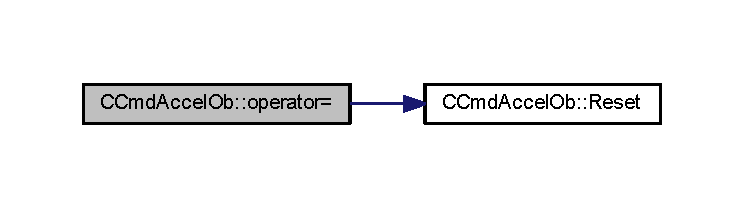
\includegraphics[width=350pt]{class_c_cmd_accel_ob_a045ce00d2465fefed857066eef1406a7_cgraph}
\end{center}
\end{figure}
\mbox{\Hypertarget{class_c_cmd_accel_ob_ac679e57ed400b175109af50ea2ce919d}\label{class_c_cmd_accel_ob_ac679e57ed400b175109af50ea2ce919d}} 
\index{C\+Cmd\+Accel\+Ob@{C\+Cmd\+Accel\+Ob}!Reset@{Reset}}
\index{Reset@{Reset}!C\+Cmd\+Accel\+Ob@{C\+Cmd\+Accel\+Ob}}
\subsubsection{\texorpdfstring{Reset()}{Reset()}}
{\footnotesize\ttfamily void C\+Cmd\+Accel\+Ob\+::\+Reset (\begin{DoxyParamCaption}{ }\end{DoxyParamCaption})}



Cmd\+Accel\+Ob.\+cpp 파일의 479 번째 라인에서 정의되었습니다.


\begin{DoxyCode}
480 \{
481   \mbox{\hyperlink{class_c_cmd_accel_ob_aa3eb02dcd39ff14763fdefd8fabd7591}{m\_wIDCommand}} = 0;
482   \mbox{\hyperlink{class_c_cmd_accel_ob_acbd02cc68d3909b1e39b687e76f45d91}{m\_szCommand}} = \textcolor{stringliteral}{"Empty command"};
483   
484   \mbox{\hyperlink{class_c_accels_ob}{CAccelsOb}}* pAccel;
485   POSITION pos = \mbox{\hyperlink{class_c_cmd_accel_ob_a85772f1ea9204af42b8a39a0135dc0f8}{m\_Accels}}.GetHeadPosition();
486   \textcolor{keywordflow}{while} (pos != \mbox{\hyperlink{getopt1_8c_a070d2ce7b6bb7e5c05602aa8c308d0c4}{NULL}}) \{
487     pAccel = \mbox{\hyperlink{class_c_cmd_accel_ob_a85772f1ea9204af42b8a39a0135dc0f8}{m\_Accels}}.GetNext(pos);
488     \textcolor{keyword}{delete} pAccel;
489   \}
490 \}
\end{DoxyCode}
이 함수를 호출하는 함수들에 대한 그래프입니다.\+:
\nopagebreak
\begin{figure}[H]
\begin{center}
\leavevmode
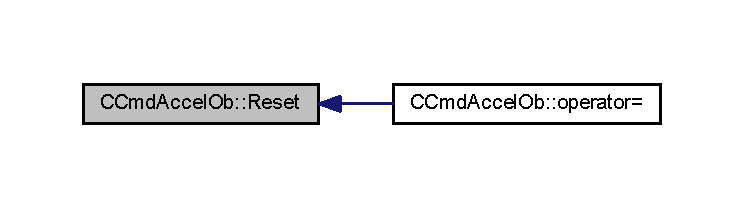
\includegraphics[width=350pt]{class_c_cmd_accel_ob_ac679e57ed400b175109af50ea2ce919d_icgraph}
\end{center}
\end{figure}


\subsection{멤버 데이터 문서화}
\mbox{\Hypertarget{class_c_cmd_accel_ob_a85772f1ea9204af42b8a39a0135dc0f8}\label{class_c_cmd_accel_ob_a85772f1ea9204af42b8a39a0135dc0f8}} 
\index{C\+Cmd\+Accel\+Ob@{C\+Cmd\+Accel\+Ob}!m\+\_\+\+Accels@{m\+\_\+\+Accels}}
\index{m\+\_\+\+Accels@{m\+\_\+\+Accels}!C\+Cmd\+Accel\+Ob@{C\+Cmd\+Accel\+Ob}}
\subsubsection{\texorpdfstring{m\+\_\+\+Accels}{m\_Accels}}
{\footnotesize\ttfamily C\+List$<$ \mbox{\hyperlink{class_c_accels_ob}{C\+Accels\+Ob}}$\ast$, \mbox{\hyperlink{class_c_accels_ob}{C\+Accels\+Ob}}$\ast$\& $>$ C\+Cmd\+Accel\+Ob\+::m\+\_\+\+Accels}



Cmd\+Accel\+Ob.\+h 파일의 106 번째 라인에서 정의되었습니다.

\mbox{\Hypertarget{class_c_cmd_accel_ob_acbd02cc68d3909b1e39b687e76f45d91}\label{class_c_cmd_accel_ob_acbd02cc68d3909b1e39b687e76f45d91}} 
\index{C\+Cmd\+Accel\+Ob@{C\+Cmd\+Accel\+Ob}!m\+\_\+sz\+Command@{m\+\_\+sz\+Command}}
\index{m\+\_\+sz\+Command@{m\+\_\+sz\+Command}!C\+Cmd\+Accel\+Ob@{C\+Cmd\+Accel\+Ob}}
\subsubsection{\texorpdfstring{m\+\_\+sz\+Command}{m\_szCommand}}
{\footnotesize\ttfamily C\+String C\+Cmd\+Accel\+Ob\+::m\+\_\+sz\+Command}



Cmd\+Accel\+Ob.\+h 파일의 104 번째 라인에서 정의되었습니다.

\mbox{\Hypertarget{class_c_cmd_accel_ob_aa3eb02dcd39ff14763fdefd8fabd7591}\label{class_c_cmd_accel_ob_aa3eb02dcd39ff14763fdefd8fabd7591}} 
\index{C\+Cmd\+Accel\+Ob@{C\+Cmd\+Accel\+Ob}!m\+\_\+w\+I\+D\+Command@{m\+\_\+w\+I\+D\+Command}}
\index{m\+\_\+w\+I\+D\+Command@{m\+\_\+w\+I\+D\+Command}!C\+Cmd\+Accel\+Ob@{C\+Cmd\+Accel\+Ob}}
\subsubsection{\texorpdfstring{m\+\_\+w\+I\+D\+Command}{m\_wIDCommand}}
{\footnotesize\ttfamily W\+O\+RD C\+Cmd\+Accel\+Ob\+::m\+\_\+w\+I\+D\+Command}



Cmd\+Accel\+Ob.\+h 파일의 103 번째 라인에서 정의되었습니다.



이 클래스에 대한 문서화 페이지는 다음의 파일들로부터 생성되었습니다.\+:\begin{DoxyCompactItemize}
\item 
C\+:/\+Users/sjh13/sources/\+Visual\+Boy\+Advance/src/win32/\mbox{\hyperlink{_cmd_accel_ob_8h}{Cmd\+Accel\+Ob.\+h}}\item 
C\+:/\+Users/sjh13/sources/\+Visual\+Boy\+Advance/src/win32/\mbox{\hyperlink{_cmd_accel_ob_8cpp}{Cmd\+Accel\+Ob.\+cpp}}\end{DoxyCompactItemize}

\hypertarget{class_win_helper_1_1_c_critical_section}{}\section{Win\+Helper\+:\+:C\+Critical\+Section 클래스 참조}
\label{class_win_helper_1_1_c_critical_section}\index{Win\+Helper\+::\+C\+Critical\+Section@{Win\+Helper\+::\+C\+Critical\+Section}}
\subsection*{클래스}
\begin{DoxyCompactItemize}
\item 
class \mbox{\hyperlink{class_win_helper_1_1_c_critical_section_1_1_c_lock}{C\+Lock}}
\end{DoxyCompactItemize}
\subsection*{Public 멤버 함수}
\begin{DoxyCompactItemize}
\item 
\mbox{\Hypertarget{class_win_helper_1_1_c_critical_section_aa0c20ee0e7de698b37c26a295d0f45fe}\label{class_win_helper_1_1_c_critical_section_aa0c20ee0e7de698b37c26a295d0f45fe}} 
void {\bfseries Lock} ()
\item 
\mbox{\Hypertarget{class_win_helper_1_1_c_critical_section_a32b6fc61701020c400f3bb9b5e00bf12}\label{class_win_helper_1_1_c_critical_section_a32b6fc61701020c400f3bb9b5e00bf12}} 
void {\bfseries Unlock} ()
\end{DoxyCompactItemize}


이 클래스에 대한 문서화 페이지는 다음의 파일로부터 생성되었습니다.\+:\begin{DoxyCompactItemize}
\item 
src/win32/Win\+Helper.\+h\end{DoxyCompactItemize}

\hypertarget{class_win_helper_1_1_c_defer_window_pos}{}\section{Win\+Helper\+:\+:C\+Defer\+Window\+Pos 클래스 참조}
\label{class_win_helper_1_1_c_defer_window_pos}\index{Win\+Helper\+::\+C\+Defer\+Window\+Pos@{Win\+Helper\+::\+C\+Defer\+Window\+Pos}}
\subsection*{Public 멤버 함수}
\begin{DoxyCompactItemize}
\item 
\mbox{\Hypertarget{class_win_helper_1_1_c_defer_window_pos_ac98b161abd5044c2a2e1e8b8efa0744f}\label{class_win_helper_1_1_c_defer_window_pos_ac98b161abd5044c2a2e1e8b8efa0744f}} 
{\bfseries C\+Defer\+Window\+Pos} (const int n\+Windows=1)
\item 
\mbox{\Hypertarget{class_win_helper_1_1_c_defer_window_pos_a50e9a5dfc382996381a506d66f94efd6}\label{class_win_helper_1_1_c_defer_window_pos_a50e9a5dfc382996381a506d66f94efd6}} 
H\+D\+WP {\bfseries Defer\+Window\+Pos} (H\+W\+ND h\+Wnd, H\+W\+ND h\+Wnd\+Insert\+After, int x, int y, int cx, int cy, U\+I\+NT u\+Flags)
\item 
\mbox{\Hypertarget{class_win_helper_1_1_c_defer_window_pos_aeba6047e5182577c14bfe4729a602ca9}\label{class_win_helper_1_1_c_defer_window_pos_aeba6047e5182577c14bfe4729a602ca9}} 
H\+D\+WP {\bfseries Defer\+Window\+Pos} (H\+W\+ND h\+Wnd, H\+W\+ND h\+Wnd\+Insert\+After, const \mbox{\hyperlink{class_win_helper_1_1_c_rect}{C\+Rect}} \&rc, U\+I\+NT u\+Flags)
\end{DoxyCompactItemize}


이 클래스에 대한 문서화 페이지는 다음의 파일로부터 생성되었습니다.\+:\begin{DoxyCompactItemize}
\item 
src/win32/Win\+Helper.\+h\end{DoxyCompactItemize}

\hypertarget{struct_cheats_data}{}\section{Cheats\+Data 구조체 참조}
\label{struct_cheats_data}\index{Cheats\+Data@{Cheats\+Data}}


{\ttfamily \#include $<$Cheats.\+h$>$}



Cheats\+Data에 대한 협력 다이어그램\+:\nopagebreak
\begin{figure}[H]
\begin{center}
\leavevmode
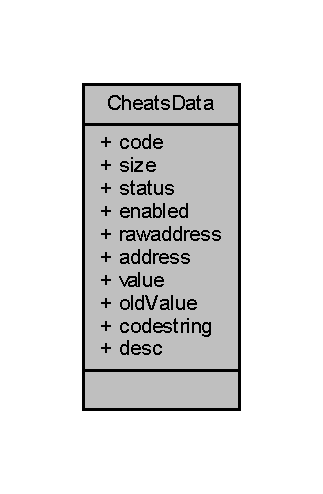
\includegraphics[width=155pt]{struct_cheats_data__coll__graph}
\end{center}
\end{figure}
\subsection*{Public 속성}
\begin{DoxyCompactItemize}
\item 
\mbox{\hyperlink{_util_8cpp_a0ef32aa8672df19503a49fab2d0c8071}{int}} \mbox{\hyperlink{struct_cheats_data_a24cc3911cdbf485ce42b401873e2e269}{code}}
\item 
\mbox{\hyperlink{_util_8cpp_a0ef32aa8672df19503a49fab2d0c8071}{int}} \mbox{\hyperlink{struct_cheats_data_a2e3e50db1415e980fe34da90fdbda02a}{size}}
\item 
\mbox{\hyperlink{_util_8cpp_a0ef32aa8672df19503a49fab2d0c8071}{int}} \mbox{\hyperlink{struct_cheats_data_aeb36cfefe89db53cdb45909d35b9c6e4}{status}}
\item 
bool \mbox{\hyperlink{struct_cheats_data_a99c72fc2074645888a5afe88cfb0fd15}{enabled}}
\item 
\mbox{\hyperlink{_system_8h_a10e94b422ef0c20dcdec20d31a1f5049}{u32}} \mbox{\hyperlink{struct_cheats_data_aa12c1d606385a21c544022d5acb9c95e}{rawaddress}}
\item 
\mbox{\hyperlink{_system_8h_a10e94b422ef0c20dcdec20d31a1f5049}{u32}} \mbox{\hyperlink{struct_cheats_data_a01fd4bf820cf8cb6a4212183b29530cd}{address}}
\item 
\mbox{\hyperlink{_system_8h_a10e94b422ef0c20dcdec20d31a1f5049}{u32}} \mbox{\hyperlink{struct_cheats_data_ab0df909850861e6314b1abb13c6305d1}{value}}
\item 
\mbox{\hyperlink{_system_8h_a10e94b422ef0c20dcdec20d31a1f5049}{u32}} \mbox{\hyperlink{struct_cheats_data_ae53ec4ba23eb94b339cc05b807a944d5}{old\+Value}}
\item 
char \mbox{\hyperlink{struct_cheats_data_a4163c46e82595675cedca34ad19d6f43}{codestring}} \mbox{[}20\mbox{]}
\item 
char \mbox{\hyperlink{struct_cheats_data_a12223e792c360411d694a8e2506dc90e}{desc}} \mbox{[}32\mbox{]}
\end{DoxyCompactItemize}


\subsection{상세한 설명}


Cheats.\+h 파일의 23 번째 라인에서 정의되었습니다.



\subsection{멤버 데이터 문서화}
\mbox{\Hypertarget{struct_cheats_data_a01fd4bf820cf8cb6a4212183b29530cd}\label{struct_cheats_data_a01fd4bf820cf8cb6a4212183b29530cd}} 
\index{Cheats\+Data@{Cheats\+Data}!address@{address}}
\index{address@{address}!Cheats\+Data@{Cheats\+Data}}
\subsubsection{\texorpdfstring{address}{address}}
{\footnotesize\ttfamily \mbox{\hyperlink{_system_8h_a10e94b422ef0c20dcdec20d31a1f5049}{u32}} Cheats\+Data\+::address}



Cheats.\+h 파일의 29 번째 라인에서 정의되었습니다.

\mbox{\Hypertarget{struct_cheats_data_a24cc3911cdbf485ce42b401873e2e269}\label{struct_cheats_data_a24cc3911cdbf485ce42b401873e2e269}} 
\index{Cheats\+Data@{Cheats\+Data}!code@{code}}
\index{code@{code}!Cheats\+Data@{Cheats\+Data}}
\subsubsection{\texorpdfstring{code}{code}}
{\footnotesize\ttfamily \mbox{\hyperlink{_util_8cpp_a0ef32aa8672df19503a49fab2d0c8071}{int}} Cheats\+Data\+::code}



Cheats.\+h 파일의 24 번째 라인에서 정의되었습니다.

\mbox{\Hypertarget{struct_cheats_data_a4163c46e82595675cedca34ad19d6f43}\label{struct_cheats_data_a4163c46e82595675cedca34ad19d6f43}} 
\index{Cheats\+Data@{Cheats\+Data}!codestring@{codestring}}
\index{codestring@{codestring}!Cheats\+Data@{Cheats\+Data}}
\subsubsection{\texorpdfstring{codestring}{codestring}}
{\footnotesize\ttfamily char Cheats\+Data\+::codestring\mbox{[}20\mbox{]}}



Cheats.\+h 파일의 32 번째 라인에서 정의되었습니다.

\mbox{\Hypertarget{struct_cheats_data_a12223e792c360411d694a8e2506dc90e}\label{struct_cheats_data_a12223e792c360411d694a8e2506dc90e}} 
\index{Cheats\+Data@{Cheats\+Data}!desc@{desc}}
\index{desc@{desc}!Cheats\+Data@{Cheats\+Data}}
\subsubsection{\texorpdfstring{desc}{desc}}
{\footnotesize\ttfamily char Cheats\+Data\+::desc\mbox{[}32\mbox{]}}



Cheats.\+h 파일의 33 번째 라인에서 정의되었습니다.

\mbox{\Hypertarget{struct_cheats_data_a99c72fc2074645888a5afe88cfb0fd15}\label{struct_cheats_data_a99c72fc2074645888a5afe88cfb0fd15}} 
\index{Cheats\+Data@{Cheats\+Data}!enabled@{enabled}}
\index{enabled@{enabled}!Cheats\+Data@{Cheats\+Data}}
\subsubsection{\texorpdfstring{enabled}{enabled}}
{\footnotesize\ttfamily bool Cheats\+Data\+::enabled}



Cheats.\+h 파일의 27 번째 라인에서 정의되었습니다.

\mbox{\Hypertarget{struct_cheats_data_ae53ec4ba23eb94b339cc05b807a944d5}\label{struct_cheats_data_ae53ec4ba23eb94b339cc05b807a944d5}} 
\index{Cheats\+Data@{Cheats\+Data}!old\+Value@{old\+Value}}
\index{old\+Value@{old\+Value}!Cheats\+Data@{Cheats\+Data}}
\subsubsection{\texorpdfstring{old\+Value}{oldValue}}
{\footnotesize\ttfamily \mbox{\hyperlink{_system_8h_a10e94b422ef0c20dcdec20d31a1f5049}{u32}} Cheats\+Data\+::old\+Value}



Cheats.\+h 파일의 31 번째 라인에서 정의되었습니다.

\mbox{\Hypertarget{struct_cheats_data_aa12c1d606385a21c544022d5acb9c95e}\label{struct_cheats_data_aa12c1d606385a21c544022d5acb9c95e}} 
\index{Cheats\+Data@{Cheats\+Data}!rawaddress@{rawaddress}}
\index{rawaddress@{rawaddress}!Cheats\+Data@{Cheats\+Data}}
\subsubsection{\texorpdfstring{rawaddress}{rawaddress}}
{\footnotesize\ttfamily \mbox{\hyperlink{_system_8h_a10e94b422ef0c20dcdec20d31a1f5049}{u32}} Cheats\+Data\+::rawaddress}



Cheats.\+h 파일의 28 번째 라인에서 정의되었습니다.

\mbox{\Hypertarget{struct_cheats_data_a2e3e50db1415e980fe34da90fdbda02a}\label{struct_cheats_data_a2e3e50db1415e980fe34da90fdbda02a}} 
\index{Cheats\+Data@{Cheats\+Data}!size@{size}}
\index{size@{size}!Cheats\+Data@{Cheats\+Data}}
\subsubsection{\texorpdfstring{size}{size}}
{\footnotesize\ttfamily \mbox{\hyperlink{_util_8cpp_a0ef32aa8672df19503a49fab2d0c8071}{int}} Cheats\+Data\+::size}



Cheats.\+h 파일의 25 번째 라인에서 정의되었습니다.

\mbox{\Hypertarget{struct_cheats_data_aeb36cfefe89db53cdb45909d35b9c6e4}\label{struct_cheats_data_aeb36cfefe89db53cdb45909d35b9c6e4}} 
\index{Cheats\+Data@{Cheats\+Data}!status@{status}}
\index{status@{status}!Cheats\+Data@{Cheats\+Data}}
\subsubsection{\texorpdfstring{status}{status}}
{\footnotesize\ttfamily \mbox{\hyperlink{_util_8cpp_a0ef32aa8672df19503a49fab2d0c8071}{int}} Cheats\+Data\+::status}



Cheats.\+h 파일의 26 번째 라인에서 정의되었습니다.

\mbox{\Hypertarget{struct_cheats_data_ab0df909850861e6314b1abb13c6305d1}\label{struct_cheats_data_ab0df909850861e6314b1abb13c6305d1}} 
\index{Cheats\+Data@{Cheats\+Data}!value@{value}}
\index{value@{value}!Cheats\+Data@{Cheats\+Data}}
\subsubsection{\texorpdfstring{value}{value}}
{\footnotesize\ttfamily \mbox{\hyperlink{_system_8h_a10e94b422ef0c20dcdec20d31a1f5049}{u32}} Cheats\+Data\+::value}



Cheats.\+h 파일의 30 번째 라인에서 정의되었습니다.



이 구조체에 대한 문서화 페이지는 다음의 파일로부터 생성되었습니다.\+:\begin{DoxyCompactItemize}
\item 
C\+:/\+Users/sjh13/sources/\+Visual\+Boy\+Advance/src/\mbox{\hyperlink{_cheats_8h}{Cheats.\+h}}\end{DoxyCompactItemize}

\hypertarget{struct_cheat_search_block}{}\section{Cheat\+Search\+Block 구조체 참조}
\label{struct_cheat_search_block}\index{Cheat\+Search\+Block@{Cheat\+Search\+Block}}


{\ttfamily \#include $<$Cheat\+Search.\+h$>$}



Cheat\+Search\+Block에 대한 협력 다이어그램\+:\nopagebreak
\begin{figure}[H]
\begin{center}
\leavevmode
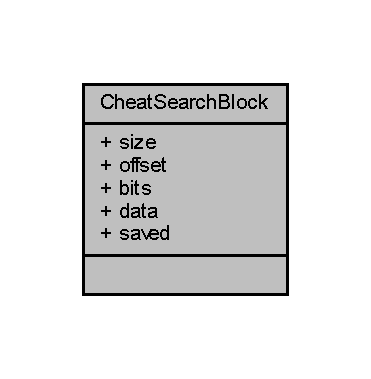
\includegraphics[width=178pt]{struct_cheat_search_block__coll__graph}
\end{center}
\end{figure}
\subsection*{Public 속성}
\begin{DoxyCompactItemize}
\item 
\mbox{\hyperlink{_util_8cpp_a0ef32aa8672df19503a49fab2d0c8071}{int}} \mbox{\hyperlink{struct_cheat_search_block_aaaf9517229363e8807cd511022d90012}{size}}
\item 
\mbox{\hyperlink{_system_8h_a10e94b422ef0c20dcdec20d31a1f5049}{u32}} \mbox{\hyperlink{struct_cheat_search_block_a33001049203a8b1b625ccdd29bf57d8f}{offset}}
\item 
\mbox{\hyperlink{_system_8h_aed742c436da53c1080638ce6ef7d13de}{u8}} $\ast$ \mbox{\hyperlink{struct_cheat_search_block_a59258efebf4223be206ad11d3ca8ebf4}{bits}}
\item 
\mbox{\hyperlink{_system_8h_aed742c436da53c1080638ce6ef7d13de}{u8}} $\ast$ \mbox{\hyperlink{struct_cheat_search_block_aa3a8235324df132c5fc67c5239748f15}{data}}
\item 
\mbox{\hyperlink{_system_8h_aed742c436da53c1080638ce6ef7d13de}{u8}} $\ast$ \mbox{\hyperlink{struct_cheat_search_block_af2b921cffd3f8d9420a8b9a3a33752ca}{saved}}
\end{DoxyCompactItemize}


\subsection{상세한 설명}


Cheat\+Search.\+h 파일의 25 번째 라인에서 정의되었습니다.



\subsection{멤버 데이터 문서화}
\mbox{\Hypertarget{struct_cheat_search_block_a59258efebf4223be206ad11d3ca8ebf4}\label{struct_cheat_search_block_a59258efebf4223be206ad11d3ca8ebf4}} 
\index{Cheat\+Search\+Block@{Cheat\+Search\+Block}!bits@{bits}}
\index{bits@{bits}!Cheat\+Search\+Block@{Cheat\+Search\+Block}}
\subsubsection{\texorpdfstring{bits}{bits}}
{\footnotesize\ttfamily \mbox{\hyperlink{_system_8h_aed742c436da53c1080638ce6ef7d13de}{u8}}$\ast$ Cheat\+Search\+Block\+::bits}



Cheat\+Search.\+h 파일의 28 번째 라인에서 정의되었습니다.

\mbox{\Hypertarget{struct_cheat_search_block_aa3a8235324df132c5fc67c5239748f15}\label{struct_cheat_search_block_aa3a8235324df132c5fc67c5239748f15}} 
\index{Cheat\+Search\+Block@{Cheat\+Search\+Block}!data@{data}}
\index{data@{data}!Cheat\+Search\+Block@{Cheat\+Search\+Block}}
\subsubsection{\texorpdfstring{data}{data}}
{\footnotesize\ttfamily \mbox{\hyperlink{_system_8h_aed742c436da53c1080638ce6ef7d13de}{u8}}$\ast$ Cheat\+Search\+Block\+::data}



Cheat\+Search.\+h 파일의 29 번째 라인에서 정의되었습니다.

\mbox{\Hypertarget{struct_cheat_search_block_a33001049203a8b1b625ccdd29bf57d8f}\label{struct_cheat_search_block_a33001049203a8b1b625ccdd29bf57d8f}} 
\index{Cheat\+Search\+Block@{Cheat\+Search\+Block}!offset@{offset}}
\index{offset@{offset}!Cheat\+Search\+Block@{Cheat\+Search\+Block}}
\subsubsection{\texorpdfstring{offset}{offset}}
{\footnotesize\ttfamily \mbox{\hyperlink{_system_8h_a10e94b422ef0c20dcdec20d31a1f5049}{u32}} Cheat\+Search\+Block\+::offset}



Cheat\+Search.\+h 파일의 27 번째 라인에서 정의되었습니다.

\mbox{\Hypertarget{struct_cheat_search_block_af2b921cffd3f8d9420a8b9a3a33752ca}\label{struct_cheat_search_block_af2b921cffd3f8d9420a8b9a3a33752ca}} 
\index{Cheat\+Search\+Block@{Cheat\+Search\+Block}!saved@{saved}}
\index{saved@{saved}!Cheat\+Search\+Block@{Cheat\+Search\+Block}}
\subsubsection{\texorpdfstring{saved}{saved}}
{\footnotesize\ttfamily \mbox{\hyperlink{_system_8h_aed742c436da53c1080638ce6ef7d13de}{u8}}$\ast$ Cheat\+Search\+Block\+::saved}



Cheat\+Search.\+h 파일의 30 번째 라인에서 정의되었습니다.

\mbox{\Hypertarget{struct_cheat_search_block_aaaf9517229363e8807cd511022d90012}\label{struct_cheat_search_block_aaaf9517229363e8807cd511022d90012}} 
\index{Cheat\+Search\+Block@{Cheat\+Search\+Block}!size@{size}}
\index{size@{size}!Cheat\+Search\+Block@{Cheat\+Search\+Block}}
\subsubsection{\texorpdfstring{size}{size}}
{\footnotesize\ttfamily \mbox{\hyperlink{_util_8cpp_a0ef32aa8672df19503a49fab2d0c8071}{int}} Cheat\+Search\+Block\+::size}



Cheat\+Search.\+h 파일의 26 번째 라인에서 정의되었습니다.



이 구조체에 대한 문서화 페이지는 다음의 파일로부터 생성되었습니다.\+:\begin{DoxyCompactItemize}
\item 
C\+:/\+Users/sjh13/sources/\+Visual\+Boy\+Advance/src/\mbox{\hyperlink{_cheat_search_8h}{Cheat\+Search.\+h}}\end{DoxyCompactItemize}

\hypertarget{struct_cheat_search_data}{}\section{Cheat\+Search\+Data 구조체 참조}
\label{struct_cheat_search_data}\index{Cheat\+Search\+Data@{Cheat\+Search\+Data}}


{\ttfamily \#include $<$Cheat\+Search.\+h$>$}



Cheat\+Search\+Data에 대한 협력 다이어그램\+:\nopagebreak
\begin{figure}[H]
\begin{center}
\leavevmode
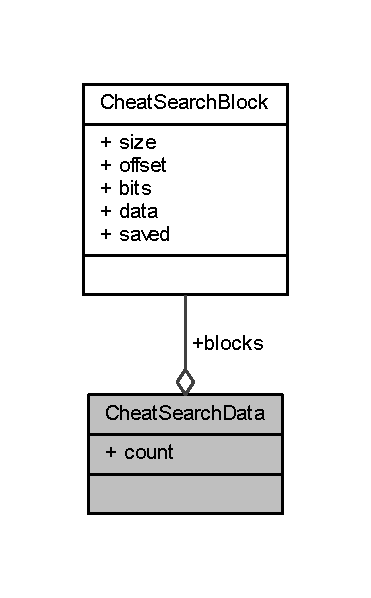
\includegraphics[width=178pt]{struct_cheat_search_data__coll__graph}
\end{center}
\end{figure}
\subsection*{Public 속성}
\begin{DoxyCompactItemize}
\item 
\mbox{\hyperlink{_util_8cpp_a0ef32aa8672df19503a49fab2d0c8071}{int}} \mbox{\hyperlink{struct_cheat_search_data_a4c4d3092ddaff068d820c28067b15774}{count}}
\item 
\mbox{\hyperlink{struct_cheat_search_block}{Cheat\+Search\+Block}} $\ast$ \mbox{\hyperlink{struct_cheat_search_data_ae0235bdc2000cc25b8c072442ce33c2c}{blocks}}
\end{DoxyCompactItemize}


\subsection{상세한 설명}


Cheat\+Search.\+h 파일의 33 번째 라인에서 정의되었습니다.



\subsection{멤버 데이터 문서화}
\mbox{\Hypertarget{struct_cheat_search_data_ae0235bdc2000cc25b8c072442ce33c2c}\label{struct_cheat_search_data_ae0235bdc2000cc25b8c072442ce33c2c}} 
\index{Cheat\+Search\+Data@{Cheat\+Search\+Data}!blocks@{blocks}}
\index{blocks@{blocks}!Cheat\+Search\+Data@{Cheat\+Search\+Data}}
\subsubsection{\texorpdfstring{blocks}{blocks}}
{\footnotesize\ttfamily \mbox{\hyperlink{struct_cheat_search_block}{Cheat\+Search\+Block}}$\ast$ Cheat\+Search\+Data\+::blocks}



Cheat\+Search.\+h 파일의 35 번째 라인에서 정의되었습니다.

\mbox{\Hypertarget{struct_cheat_search_data_a4c4d3092ddaff068d820c28067b15774}\label{struct_cheat_search_data_a4c4d3092ddaff068d820c28067b15774}} 
\index{Cheat\+Search\+Data@{Cheat\+Search\+Data}!count@{count}}
\index{count@{count}!Cheat\+Search\+Data@{Cheat\+Search\+Data}}
\subsubsection{\texorpdfstring{count}{count}}
{\footnotesize\ttfamily \mbox{\hyperlink{_util_8cpp_a0ef32aa8672df19503a49fab2d0c8071}{int}} Cheat\+Search\+Data\+::count}



Cheat\+Search.\+h 파일의 34 번째 라인에서 정의되었습니다.



이 구조체에 대한 문서화 페이지는 다음의 파일로부터 생성되었습니다.\+:\begin{DoxyCompactItemize}
\item 
C\+:/\+Users/sjh13/sources/\+Visual\+Boy\+Advance/src/\mbox{\hyperlink{_cheat_search_8h}{Cheat\+Search.\+h}}\end{DoxyCompactItemize}

\hypertarget{class_c_keyboard_edit}{}\section{C\+Keyboard\+Edit 클래스 참조}
\label{class_c_keyboard_edit}\index{C\+Keyboard\+Edit@{C\+Keyboard\+Edit}}


{\ttfamily \#include $<$Keyboard\+Edit.\+h$>$}



C\+Keyboard\+Edit에 대한 상속 다이어그램 \+: \nopagebreak
\begin{figure}[H]
\begin{center}
\leavevmode
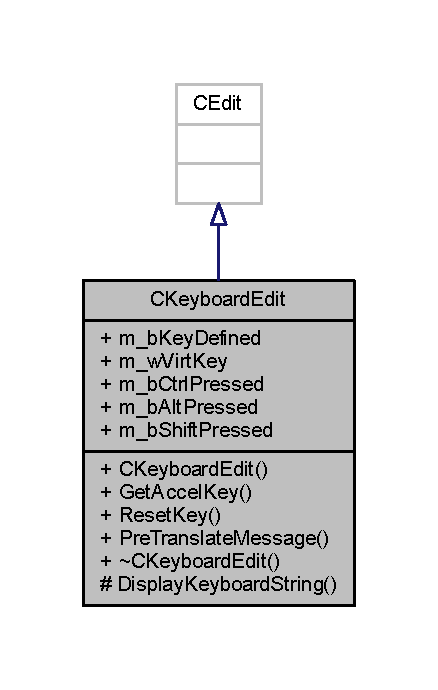
\includegraphics[width=210pt]{class_c_keyboard_edit__inherit__graph}
\end{center}
\end{figure}


C\+Keyboard\+Edit에 대한 협력 다이어그램\+:\nopagebreak
\begin{figure}[H]
\begin{center}
\leavevmode
\includegraphics[width=210pt]{class_c_keyboard_edit__coll__graph}
\end{center}
\end{figure}
\subsection*{Public 멤버 함수}
\begin{DoxyCompactItemize}
\item 
\mbox{\hyperlink{class_c_keyboard_edit_a1a1165204f7f3bbfbd997c8cc94c97f8}{C\+Keyboard\+Edit}} ()
\item 
bool \mbox{\hyperlink{class_c_keyboard_edit_a920dfccebef5e2260e59003e4959ef9f}{Get\+Accel\+Key}} (W\+O\+RD \&w\+Virt\+Key, bool \&b\+Ctrl, bool \&b\+Alt, bool \&b\+Shift)
\item 
void \mbox{\hyperlink{class_c_keyboard_edit_ad0185cc0cad77250cc32ef1d9ffb8593}{Reset\+Key}} ()
\item 
virtual B\+O\+OL \mbox{\hyperlink{class_c_keyboard_edit_a7700247028b07400adf5056c6627e19a}{Pre\+Translate\+Message}} (\mbox{\hyperlink{prof_8cpp_a0c719c414608ef14852670b063876c07}{M\+SG}} $\ast$p\+Msg)
\item 
virtual \mbox{\hyperlink{class_c_keyboard_edit_aeddf780fee33d17188b5641cd384ab92}{$\sim$\+C\+Keyboard\+Edit}} ()
\end{DoxyCompactItemize}
\subsection*{Public 속성}
\begin{DoxyCompactItemize}
\item 
bool \mbox{\hyperlink{class_c_keyboard_edit_a9bf24703c8d1a3a019b43dc67c26c3a0}{m\+\_\+b\+Key\+Defined}}
\item 
W\+O\+RD \mbox{\hyperlink{class_c_keyboard_edit_a6a4efef92e151002720d0d930db29521}{m\+\_\+w\+Virt\+Key}}
\item 
bool \mbox{\hyperlink{class_c_keyboard_edit_a0dbb417bbaaeaa95c00fceaecd210064}{m\+\_\+b\+Ctrl\+Pressed}}
\item 
bool \mbox{\hyperlink{class_c_keyboard_edit_a724b035848eeca7bebc24e1309afeb6d}{m\+\_\+b\+Alt\+Pressed}}
\item 
bool \mbox{\hyperlink{class_c_keyboard_edit_ac4a4f45be9ef923961ab92a48a28f789}{m\+\_\+b\+Shift\+Pressed}}
\end{DoxyCompactItemize}
\subsection*{Protected 멤버 함수}
\begin{DoxyCompactItemize}
\item 
void \mbox{\hyperlink{class_c_keyboard_edit_a432e346d4d5285064b5e92ff4c6a0385}{Display\+Keyboard\+String}} ()
\end{DoxyCompactItemize}


\subsection{상세한 설명}


Keyboard\+Edit.\+h 파일의 40 번째 라인에서 정의되었습니다.



\subsection{생성자 \& 소멸자 문서화}
\mbox{\Hypertarget{class_c_keyboard_edit_a1a1165204f7f3bbfbd997c8cc94c97f8}\label{class_c_keyboard_edit_a1a1165204f7f3bbfbd997c8cc94c97f8}} 
\index{C\+Keyboard\+Edit@{C\+Keyboard\+Edit}!C\+Keyboard\+Edit@{C\+Keyboard\+Edit}}
\index{C\+Keyboard\+Edit@{C\+Keyboard\+Edit}!C\+Keyboard\+Edit@{C\+Keyboard\+Edit}}
\subsubsection{\texorpdfstring{C\+Keyboard\+Edit()}{CKeyboardEdit()}}
{\footnotesize\ttfamily C\+Keyboard\+Edit\+::\+C\+Keyboard\+Edit (\begin{DoxyParamCaption}{ }\end{DoxyParamCaption})}



Keyboard\+Edit.\+cpp 파일의 43 번째 라인에서 정의되었습니다.


\begin{DoxyCode}
44 \{
45   \mbox{\hyperlink{class_c_keyboard_edit_a9bf24703c8d1a3a019b43dc67c26c3a0}{m\_bKeyDefined}} = \textcolor{keyword}{false};
46   \mbox{\hyperlink{class_c_keyboard_edit_ad0185cc0cad77250cc32ef1d9ffb8593}{ResetKey}} ();
47 \}
\end{DoxyCode}
이 함수 내부에서 호출하는 함수들에 대한 그래프입니다.\+:
\nopagebreak
\begin{figure}[H]
\begin{center}
\leavevmode
\includegraphics[width=350pt]{class_c_keyboard_edit_a1a1165204f7f3bbfbd997c8cc94c97f8_cgraph}
\end{center}
\end{figure}
\mbox{\Hypertarget{class_c_keyboard_edit_aeddf780fee33d17188b5641cd384ab92}\label{class_c_keyboard_edit_aeddf780fee33d17188b5641cd384ab92}} 
\index{C\+Keyboard\+Edit@{C\+Keyboard\+Edit}!````~C\+Keyboard\+Edit@{$\sim$\+C\+Keyboard\+Edit}}
\index{````~C\+Keyboard\+Edit@{$\sim$\+C\+Keyboard\+Edit}!C\+Keyboard\+Edit@{C\+Keyboard\+Edit}}
\subsubsection{\texorpdfstring{$\sim$\+C\+Keyboard\+Edit()}{~CKeyboardEdit()}}
{\footnotesize\ttfamily C\+Keyboard\+Edit\+::$\sim$\+C\+Keyboard\+Edit (\begin{DoxyParamCaption}{ }\end{DoxyParamCaption})\hspace{0.3cm}{\ttfamily [virtual]}}



Keyboard\+Edit.\+cpp 파일의 49 번째 라인에서 정의되었습니다.


\begin{DoxyCode}
50 \{
51 \}
\end{DoxyCode}


\subsection{멤버 함수 문서화}
\mbox{\Hypertarget{class_c_keyboard_edit_a432e346d4d5285064b5e92ff4c6a0385}\label{class_c_keyboard_edit_a432e346d4d5285064b5e92ff4c6a0385}} 
\index{C\+Keyboard\+Edit@{C\+Keyboard\+Edit}!Display\+Keyboard\+String@{Display\+Keyboard\+String}}
\index{Display\+Keyboard\+String@{Display\+Keyboard\+String}!C\+Keyboard\+Edit@{C\+Keyboard\+Edit}}
\subsubsection{\texorpdfstring{Display\+Keyboard\+String()}{DisplayKeyboardString()}}
{\footnotesize\ttfamily void C\+Keyboard\+Edit\+::\+Display\+Keyboard\+String (\begin{DoxyParamCaption}{ }\end{DoxyParamCaption})\hspace{0.3cm}{\ttfamily [protected]}}



Keyboard\+Edit.\+cpp 파일의 92 번째 라인에서 정의되었습니다.


\begin{DoxyCode}
93 \{
94   CString strKbd;
95 
96   \textcolor{comment}{// modifiers}
97   \textcolor{keywordflow}{if} (\mbox{\hyperlink{class_c_keyboard_edit_a0dbb417bbaaeaa95c00fceaecd210064}{m\_bCtrlPressed}})
98     strKbd = \textcolor{stringliteral}{"Ctrl"};
99   \textcolor{keywordflow}{if} (\mbox{\hyperlink{class_c_keyboard_edit_a724b035848eeca7bebc24e1309afeb6d}{m\_bAltPressed}}) \{
100     \textcolor{keywordflow}{if} (strKbd.GetLength () > 0)
101       strKbd += \textcolor{charliteral}{'+'};
102     strKbd += \textcolor{stringliteral}{"Alt"};
103   \}
104   \textcolor{keywordflow}{if} (\mbox{\hyperlink{class_c_keyboard_edit_ac4a4f45be9ef923961ab92a48a28f789}{m\_bShiftPressed}}) \{
105     \textcolor{keywordflow}{if} (strKbd.GetLength () > 0)
106       strKbd += \textcolor{charliteral}{'+'};
107     strKbd += \textcolor{stringliteral}{"Shift"};
108   \}
109   \textcolor{comment}{// virtual key}
110   LPCTSTR szVirtKey = \mbox{\hyperlink{_keyboard_edit_8cpp_a114f9fd0dc48511b3d2799f967360087}{mapVirtKeysStringFromWORD}}(
      \mbox{\hyperlink{class_c_keyboard_edit_a6a4efef92e151002720d0d930db29521}{m\_wVirtKey}});
111   \textcolor{keywordflow}{if} (szVirtKey != \mbox{\hyperlink{getopt1_8c_a070d2ce7b6bb7e5c05602aa8c308d0c4}{NULL}}) \{
112     \textcolor{keywordflow}{if} (strKbd.GetLength () > 0)
113       strKbd += \textcolor{charliteral}{'+'};
114     strKbd += szVirtKey;
115   \}
116   SetWindowText (strKbd);
117 \}
\end{DoxyCode}
이 함수 내부에서 호출하는 함수들에 대한 그래프입니다.\+:
\nopagebreak
\begin{figure}[H]
\begin{center}
\leavevmode
\includegraphics[width=350pt]{class_c_keyboard_edit_a432e346d4d5285064b5e92ff4c6a0385_cgraph}
\end{center}
\end{figure}
이 함수를 호출하는 함수들에 대한 그래프입니다.\+:
\nopagebreak
\begin{figure}[H]
\begin{center}
\leavevmode
\includegraphics[width=350pt]{class_c_keyboard_edit_a432e346d4d5285064b5e92ff4c6a0385_icgraph}
\end{center}
\end{figure}
\mbox{\Hypertarget{class_c_keyboard_edit_a920dfccebef5e2260e59003e4959ef9f}\label{class_c_keyboard_edit_a920dfccebef5e2260e59003e4959ef9f}} 
\index{C\+Keyboard\+Edit@{C\+Keyboard\+Edit}!Get\+Accel\+Key@{Get\+Accel\+Key}}
\index{Get\+Accel\+Key@{Get\+Accel\+Key}!C\+Keyboard\+Edit@{C\+Keyboard\+Edit}}
\subsubsection{\texorpdfstring{Get\+Accel\+Key()}{GetAccelKey()}}
{\footnotesize\ttfamily bool C\+Keyboard\+Edit\+::\+Get\+Accel\+Key (\begin{DoxyParamCaption}\item[{W\+O\+RD \&}]{w\+Virt\+Key,  }\item[{bool \&}]{b\+Ctrl,  }\item[{bool \&}]{b\+Alt,  }\item[{bool \&}]{b\+Shift }\end{DoxyParamCaption})}



Keyboard\+Edit.\+cpp 파일의 137 번째 라인에서 정의되었습니다.


\begin{DoxyCode}
138 \{
139   \textcolor{keywordflow}{if} (!\mbox{\hyperlink{class_c_keyboard_edit_a9bf24703c8d1a3a019b43dc67c26c3a0}{m\_bKeyDefined}})
140     \textcolor{keywordflow}{return} \textcolor{keyword}{false};
141   
142   wVirtKey = \mbox{\hyperlink{class_c_keyboard_edit_a6a4efef92e151002720d0d930db29521}{m\_wVirtKey}};
143   bAlt = \mbox{\hyperlink{class_c_keyboard_edit_a724b035848eeca7bebc24e1309afeb6d}{m\_bAltPressed}};
144   bCtrl = \mbox{\hyperlink{class_c_keyboard_edit_a0dbb417bbaaeaa95c00fceaecd210064}{m\_bCtrlPressed}};
145   bShift = \mbox{\hyperlink{class_c_keyboard_edit_ac4a4f45be9ef923961ab92a48a28f789}{m\_bShiftPressed}};
146   \textcolor{keywordflow}{return} \textcolor{keyword}{true};
147 \}
\end{DoxyCode}
이 함수를 호출하는 함수들에 대한 그래프입니다.\+:
\nopagebreak
\begin{figure}[H]
\begin{center}
\leavevmode
\includegraphics[width=350pt]{class_c_keyboard_edit_a920dfccebef5e2260e59003e4959ef9f_icgraph}
\end{center}
\end{figure}
\mbox{\Hypertarget{class_c_keyboard_edit_a7700247028b07400adf5056c6627e19a}\label{class_c_keyboard_edit_a7700247028b07400adf5056c6627e19a}} 
\index{C\+Keyboard\+Edit@{C\+Keyboard\+Edit}!Pre\+Translate\+Message@{Pre\+Translate\+Message}}
\index{Pre\+Translate\+Message@{Pre\+Translate\+Message}!C\+Keyboard\+Edit@{C\+Keyboard\+Edit}}
\subsubsection{\texorpdfstring{Pre\+Translate\+Message()}{PreTranslateMessage()}}
{\footnotesize\ttfamily B\+O\+OL C\+Keyboard\+Edit\+::\+Pre\+Translate\+Message (\begin{DoxyParamCaption}\item[{\mbox{\hyperlink{prof_8cpp_a0c719c414608ef14852670b063876c07}{M\+SG}} $\ast$}]{p\+Msg }\end{DoxyParamCaption})\hspace{0.3cm}{\ttfamily [virtual]}}



Keyboard\+Edit.\+cpp 파일의 62 번째 라인에서 정의되었습니다.


\begin{DoxyCode}
63 \{
64   \textcolor{keywordtype}{bool} bPressed;
65   \textcolor{keywordflow}{if} ((bPressed = (pMsg->message == WM\_KEYDOWN)) || pMsg->message == WM\_KEYUP || (bPressed = (pMsg->message
       == WM\_SYSKEYDOWN)) || pMsg->message == WM\_SYSKEYUP) \{
66     \textcolor{keywordflow}{if} (bPressed && \mbox{\hyperlink{class_c_keyboard_edit_a9bf24703c8d1a3a019b43dc67c26c3a0}{m\_bKeyDefined}} && !((1 << 30) & pMsg->lParam))
67       \mbox{\hyperlink{class_c_keyboard_edit_ad0185cc0cad77250cc32ef1d9ffb8593}{ResetKey}} ();
68     \textcolor{keywordflow}{if} (pMsg->wParam == VK\_SHIFT && !\mbox{\hyperlink{class_c_keyboard_edit_a9bf24703c8d1a3a019b43dc67c26c3a0}{m\_bKeyDefined}})
69       \mbox{\hyperlink{class_c_keyboard_edit_ac4a4f45be9ef923961ab92a48a28f789}{m\_bShiftPressed}} = bPressed;
70     \textcolor{keywordflow}{else} \textcolor{keywordflow}{if} (pMsg->wParam == VK\_CONTROL &&!\mbox{\hyperlink{class_c_keyboard_edit_a9bf24703c8d1a3a019b43dc67c26c3a0}{m\_bKeyDefined}}) \{
71       \mbox{\hyperlink{class_c_keyboard_edit_a0dbb417bbaaeaa95c00fceaecd210064}{m\_bCtrlPressed}} = bPressed;
72     \}
73     \textcolor{keywordflow}{else} \textcolor{keywordflow}{if} (pMsg->wParam == VK\_MENU && !\mbox{\hyperlink{class_c_keyboard_edit_a9bf24703c8d1a3a019b43dc67c26c3a0}{m\_bKeyDefined}})
74       \mbox{\hyperlink{class_c_keyboard_edit_a724b035848eeca7bebc24e1309afeb6d}{m\_bAltPressed}} = bPressed;
75     \textcolor{keywordflow}{else} \{
76       \textcolor{keywordflow}{if} (!\mbox{\hyperlink{class_c_keyboard_edit_a9bf24703c8d1a3a019b43dc67c26c3a0}{m\_bKeyDefined}}) \{
77         \mbox{\hyperlink{class_c_keyboard_edit_a6a4efef92e151002720d0d930db29521}{m\_wVirtKey}} = (WORD)pMsg->wParam;
78         \mbox{\hyperlink{arm-new_8h_a93120066fd6daa54150af823953378d1}{if}} (bPressed)
79           \mbox{\hyperlink{class_c_keyboard_edit_a9bf24703c8d1a3a019b43dc67c26c3a0}{m\_bKeyDefined}} = \textcolor{keyword}{true};
80       \}
81     \}
82     \mbox{\hyperlink{class_c_keyboard_edit_a432e346d4d5285064b5e92ff4c6a0385}{DisplayKeyboardString}} ();
83     \textcolor{keywordflow}{return} TRUE;
84   \}
85         
86   \textcolor{keywordflow}{return} CEdit::PreTranslateMessage(pMsg);
87 \}
\end{DoxyCode}
이 함수 내부에서 호출하는 함수들에 대한 그래프입니다.\+:
\nopagebreak
\begin{figure}[H]
\begin{center}
\leavevmode
\includegraphics[width=350pt]{class_c_keyboard_edit_a7700247028b07400adf5056c6627e19a_cgraph}
\end{center}
\end{figure}
\mbox{\Hypertarget{class_c_keyboard_edit_ad0185cc0cad77250cc32ef1d9ffb8593}\label{class_c_keyboard_edit_ad0185cc0cad77250cc32ef1d9ffb8593}} 
\index{C\+Keyboard\+Edit@{C\+Keyboard\+Edit}!Reset\+Key@{Reset\+Key}}
\index{Reset\+Key@{Reset\+Key}!C\+Keyboard\+Edit@{C\+Keyboard\+Edit}}
\subsubsection{\texorpdfstring{Reset\+Key()}{ResetKey()}}
{\footnotesize\ttfamily void C\+Keyboard\+Edit\+::\+Reset\+Key (\begin{DoxyParamCaption}{ }\end{DoxyParamCaption})}



Keyboard\+Edit.\+cpp 파일의 122 번째 라인에서 정의되었습니다.


\begin{DoxyCode}
123 \{
124   \mbox{\hyperlink{class_c_keyboard_edit_a6a4efef92e151002720d0d930db29521}{m\_wVirtKey}} = 0;
125   \mbox{\hyperlink{class_c_keyboard_edit_a0dbb417bbaaeaa95c00fceaecd210064}{m\_bCtrlPressed}} = \textcolor{keyword}{false};
126   \mbox{\hyperlink{class_c_keyboard_edit_a724b035848eeca7bebc24e1309afeb6d}{m\_bAltPressed}} = \textcolor{keyword}{false};
127   \mbox{\hyperlink{class_c_keyboard_edit_ac4a4f45be9ef923961ab92a48a28f789}{m\_bShiftPressed}} = \textcolor{keyword}{false};
128   
129   \mbox{\hyperlink{class_c_keyboard_edit_a9bf24703c8d1a3a019b43dc67c26c3a0}{m\_bKeyDefined}} = \textcolor{keyword}{false};
130   \textcolor{keywordflow}{if}(m\_hWnd != \mbox{\hyperlink{getopt1_8c_a070d2ce7b6bb7e5c05602aa8c308d0c4}{NULL}})
131     SetWindowText(\_T(\textcolor{stringliteral}{""}));
132 \}
\end{DoxyCode}
이 함수를 호출하는 함수들에 대한 그래프입니다.\+:
\nopagebreak
\begin{figure}[H]
\begin{center}
\leavevmode
\includegraphics[width=350pt]{class_c_keyboard_edit_ad0185cc0cad77250cc32ef1d9ffb8593_icgraph}
\end{center}
\end{figure}


\subsection{멤버 데이터 문서화}
\mbox{\Hypertarget{class_c_keyboard_edit_a724b035848eeca7bebc24e1309afeb6d}\label{class_c_keyboard_edit_a724b035848eeca7bebc24e1309afeb6d}} 
\index{C\+Keyboard\+Edit@{C\+Keyboard\+Edit}!m\+\_\+b\+Alt\+Pressed@{m\+\_\+b\+Alt\+Pressed}}
\index{m\+\_\+b\+Alt\+Pressed@{m\+\_\+b\+Alt\+Pressed}!C\+Keyboard\+Edit@{C\+Keyboard\+Edit}}
\subsubsection{\texorpdfstring{m\+\_\+b\+Alt\+Pressed}{m\_bAltPressed}}
{\footnotesize\ttfamily bool C\+Keyboard\+Edit\+::m\+\_\+b\+Alt\+Pressed}



Keyboard\+Edit.\+h 파일의 52 번째 라인에서 정의되었습니다.

\mbox{\Hypertarget{class_c_keyboard_edit_a0dbb417bbaaeaa95c00fceaecd210064}\label{class_c_keyboard_edit_a0dbb417bbaaeaa95c00fceaecd210064}} 
\index{C\+Keyboard\+Edit@{C\+Keyboard\+Edit}!m\+\_\+b\+Ctrl\+Pressed@{m\+\_\+b\+Ctrl\+Pressed}}
\index{m\+\_\+b\+Ctrl\+Pressed@{m\+\_\+b\+Ctrl\+Pressed}!C\+Keyboard\+Edit@{C\+Keyboard\+Edit}}
\subsubsection{\texorpdfstring{m\+\_\+b\+Ctrl\+Pressed}{m\_bCtrlPressed}}
{\footnotesize\ttfamily bool C\+Keyboard\+Edit\+::m\+\_\+b\+Ctrl\+Pressed}



Keyboard\+Edit.\+h 파일의 51 번째 라인에서 정의되었습니다.

\mbox{\Hypertarget{class_c_keyboard_edit_a9bf24703c8d1a3a019b43dc67c26c3a0}\label{class_c_keyboard_edit_a9bf24703c8d1a3a019b43dc67c26c3a0}} 
\index{C\+Keyboard\+Edit@{C\+Keyboard\+Edit}!m\+\_\+b\+Key\+Defined@{m\+\_\+b\+Key\+Defined}}
\index{m\+\_\+b\+Key\+Defined@{m\+\_\+b\+Key\+Defined}!C\+Keyboard\+Edit@{C\+Keyboard\+Edit}}
\subsubsection{\texorpdfstring{m\+\_\+b\+Key\+Defined}{m\_bKeyDefined}}
{\footnotesize\ttfamily bool C\+Keyboard\+Edit\+::m\+\_\+b\+Key\+Defined}



Keyboard\+Edit.\+h 파일의 48 번째 라인에서 정의되었습니다.

\mbox{\Hypertarget{class_c_keyboard_edit_ac4a4f45be9ef923961ab92a48a28f789}\label{class_c_keyboard_edit_ac4a4f45be9ef923961ab92a48a28f789}} 
\index{C\+Keyboard\+Edit@{C\+Keyboard\+Edit}!m\+\_\+b\+Shift\+Pressed@{m\+\_\+b\+Shift\+Pressed}}
\index{m\+\_\+b\+Shift\+Pressed@{m\+\_\+b\+Shift\+Pressed}!C\+Keyboard\+Edit@{C\+Keyboard\+Edit}}
\subsubsection{\texorpdfstring{m\+\_\+b\+Shift\+Pressed}{m\_bShiftPressed}}
{\footnotesize\ttfamily bool C\+Keyboard\+Edit\+::m\+\_\+b\+Shift\+Pressed}



Keyboard\+Edit.\+h 파일의 53 번째 라인에서 정의되었습니다.

\mbox{\Hypertarget{class_c_keyboard_edit_a6a4efef92e151002720d0d930db29521}\label{class_c_keyboard_edit_a6a4efef92e151002720d0d930db29521}} 
\index{C\+Keyboard\+Edit@{C\+Keyboard\+Edit}!m\+\_\+w\+Virt\+Key@{m\+\_\+w\+Virt\+Key}}
\index{m\+\_\+w\+Virt\+Key@{m\+\_\+w\+Virt\+Key}!C\+Keyboard\+Edit@{C\+Keyboard\+Edit}}
\subsubsection{\texorpdfstring{m\+\_\+w\+Virt\+Key}{m\_wVirtKey}}
{\footnotesize\ttfamily W\+O\+RD C\+Keyboard\+Edit\+::m\+\_\+w\+Virt\+Key}



Keyboard\+Edit.\+h 파일의 50 번째 라인에서 정의되었습니다.



이 클래스에 대한 문서화 페이지는 다음의 파일들로부터 생성되었습니다.\+:\begin{DoxyCompactItemize}
\item 
C\+:/\+Users/sjh13/sources/\+Visual\+Boy\+Advance/src/win32/\mbox{\hyperlink{_keyboard_edit_8h}{Keyboard\+Edit.\+h}}\item 
C\+:/\+Users/sjh13/sources/\+Visual\+Boy\+Advance/src/win32/\mbox{\hyperlink{_keyboard_edit_8cpp}{Keyboard\+Edit.\+cpp}}\end{DoxyCompactItemize}

\hypertarget{class_win_helper_1_1_c_critical_section_1_1_c_lock}{}\section{Win\+Helper\+:\+:C\+Critical\+Section\+:\+:C\+Lock 클래스 참조}
\label{class_win_helper_1_1_c_critical_section_1_1_c_lock}\index{Win\+Helper\+::\+C\+Critical\+Section\+::\+C\+Lock@{Win\+Helper\+::\+C\+Critical\+Section\+::\+C\+Lock}}
\subsection*{Public 멤버 함수}
\begin{DoxyCompactItemize}
\item 
\mbox{\Hypertarget{class_win_helper_1_1_c_critical_section_1_1_c_lock_a68cee1cb129d83775f678a4bde96c049}\label{class_win_helper_1_1_c_critical_section_1_1_c_lock_a68cee1cb129d83775f678a4bde96c049}} 
{\bfseries C\+Lock} (\mbox{\hyperlink{class_win_helper_1_1_c_critical_section}{C\+Critical\+Section}} \&sect)
\end{DoxyCompactItemize}


이 클래스에 대한 문서화 페이지는 다음의 파일로부터 생성되었습니다.\+:\begin{DoxyCompactItemize}
\item 
src/win32/Win\+Helper.\+h\end{DoxyCompactItemize}

\hypertarget{class_color_button}{}\section{Color\+Button 클래스 참조}
\label{class_color_button}\index{Color\+Button@{Color\+Button}}


{\ttfamily \#include $<$Color\+Button.\+h$>$}



Color\+Button에 대한 상속 다이어그램 \+: \nopagebreak
\begin{figure}[H]
\begin{center}
\leavevmode
\includegraphics[width=202pt]{class_color_button__inherit__graph}
\end{center}
\end{figure}


Color\+Button에 대한 협력 다이어그램\+:\nopagebreak
\begin{figure}[H]
\begin{center}
\leavevmode
\includegraphics[width=202pt]{class_color_button__coll__graph}
\end{center}
\end{figure}
\subsection*{Public 멤버 함수}
\begin{DoxyCompactItemize}
\item 
\mbox{\hyperlink{class_color_button_a4b8e318941c5c69efd5a610fd7edb51e}{Color\+Button}} ()
\item 
void \mbox{\hyperlink{class_color_button_a2252acea0c111e198cc5bcc914e2cfeb}{Pre\+Subclass\+Window}} ()
\item 
void \mbox{\hyperlink{class_color_button_a48b973ebb6644f474f64ff1e8fbb1adf}{Draw\+Item}} (L\+P\+D\+R\+A\+W\+I\+T\+E\+M\+S\+T\+R\+U\+CT lp\+Draw\+Item\+Struct)
\item 
void \mbox{\hyperlink{class_color_button_a9ff5dc144a4acd5e2551ab94506b3bb0}{set\+Color}} (\mbox{\hyperlink{_system_8h_a9e6c91d77e24643b888dbd1a1a590054}{u16}} c)
\item 
virtual \mbox{\hyperlink{class_color_button_a992ff40e28cd869985afcf02ef338797}{$\sim$\+Color\+Button}} ()
\item 
void \mbox{\hyperlink{class_color_button_aabbc7306d4354479e0315b2a15026571}{register\+Class}} ()
\end{DoxyCompactItemize}
\subsection*{Public 속성}
\begin{DoxyCompactItemize}
\item 
\mbox{\hyperlink{_system_8h_a9e6c91d77e24643b888dbd1a1a590054}{u16}} \mbox{\hyperlink{class_color_button_ac2e59577aba7413fbf40c97f21df4835}{color}}
\end{DoxyCompactItemize}
\subsection*{정적 Public 속성}
\begin{DoxyCompactItemize}
\item 
static bool \mbox{\hyperlink{class_color_button_a77e2fa25affb19cac1c18594d5bc478f}{is\+Registered}} = false
\end{DoxyCompactItemize}


\subsection{상세한 설명}


Color\+Button.\+h 파일의 33 번째 라인에서 정의되었습니다.



\subsection{생성자 \& 소멸자 문서화}
\mbox{\Hypertarget{class_color_button_a4b8e318941c5c69efd5a610fd7edb51e}\label{class_color_button_a4b8e318941c5c69efd5a610fd7edb51e}} 
\index{Color\+Button@{Color\+Button}!Color\+Button@{Color\+Button}}
\index{Color\+Button@{Color\+Button}!Color\+Button@{Color\+Button}}
\subsubsection{\texorpdfstring{Color\+Button()}{ColorButton()}}
{\footnotesize\ttfamily Color\+Button\+::\+Color\+Button (\begin{DoxyParamCaption}{ }\end{DoxyParamCaption})}



Color\+Button.\+cpp 파일의 37 번째 라인에서 정의되었습니다.


\begin{DoxyCode}
38 \{
39   \mbox{\hyperlink{class_color_button_ac2e59577aba7413fbf40c97f21df4835}{color}} = 0;
40   \mbox{\hyperlink{class_color_button_aabbc7306d4354479e0315b2a15026571}{registerClass}}();
41 \}
\end{DoxyCode}
이 함수 내부에서 호출하는 함수들에 대한 그래프입니다.\+:
\nopagebreak
\begin{figure}[H]
\begin{center}
\leavevmode
\includegraphics[width=350pt]{class_color_button_a4b8e318941c5c69efd5a610fd7edb51e_cgraph}
\end{center}
\end{figure}
\mbox{\Hypertarget{class_color_button_a992ff40e28cd869985afcf02ef338797}\label{class_color_button_a992ff40e28cd869985afcf02ef338797}} 
\index{Color\+Button@{Color\+Button}!````~Color\+Button@{$\sim$\+Color\+Button}}
\index{````~Color\+Button@{$\sim$\+Color\+Button}!Color\+Button@{Color\+Button}}
\subsubsection{\texorpdfstring{$\sim$\+Color\+Button()}{~ColorButton()}}
{\footnotesize\ttfamily Color\+Button\+::$\sim$\+Color\+Button (\begin{DoxyParamCaption}{ }\end{DoxyParamCaption})\hspace{0.3cm}{\ttfamily [virtual]}}



Color\+Button.\+cpp 파일의 43 번째 라인에서 정의되었습니다.


\begin{DoxyCode}
44 \{
45 \}
\end{DoxyCode}


\subsection{멤버 함수 문서화}
\mbox{\Hypertarget{class_color_button_a48b973ebb6644f474f64ff1e8fbb1adf}\label{class_color_button_a48b973ebb6644f474f64ff1e8fbb1adf}} 
\index{Color\+Button@{Color\+Button}!Draw\+Item@{Draw\+Item}}
\index{Draw\+Item@{Draw\+Item}!Color\+Button@{Color\+Button}}
\subsubsection{\texorpdfstring{Draw\+Item()}{DrawItem()}}
{\footnotesize\ttfamily void Color\+Button\+::\+Draw\+Item (\begin{DoxyParamCaption}\item[{L\+P\+D\+R\+A\+W\+I\+T\+E\+M\+S\+T\+R\+U\+CT}]{lp\+Draw\+Item\+Struct }\end{DoxyParamCaption})}



Color\+Button.\+cpp 파일의 63 번째 라인에서 정의되었습니다.


\begin{DoxyCode}
64 \{
65   ASSERT(lpDrawItemStruct);
66   
67   \textcolor{keywordtype}{int} r = (\mbox{\hyperlink{class_color_button_ac2e59577aba7413fbf40c97f21df4835}{color}} & 0x1f) << 3;
68   \textcolor{keywordtype}{int} g = (\mbox{\hyperlink{class_color_button_ac2e59577aba7413fbf40c97f21df4835}{color}} & 0x3e0) >> 2;
69   \textcolor{keywordtype}{int} \mbox{\hyperlink{expr-lex_8cpp_a91b64995742fd30063314f12340b4b5a}{b}} = (\mbox{\hyperlink{class_color_button_ac2e59577aba7413fbf40c97f21df4835}{color}} & 0x7c00) >> 7;
70 
71   HDC dc = lpDrawItemStruct->hDC;
72   UINT state = lpDrawItemStruct->itemState;
73   RECT rect = lpDrawItemStruct->rcItem;
74 
75   SIZE margins;
76   margins.cx = ::GetSystemMetrics(SM\_CXEDGE);
77   margins.cy = ::GetSystemMetrics(SM\_CYEDGE);
78 
79   \textcolor{keywordflow}{if}(GetState() & BST\_PUSHED)
80     DrawEdge(dc, &rect, EDGE\_SUNKEN, BF\_RECT);
81   \textcolor{keywordflow}{else}
82     DrawEdge(dc, &rect, EDGE\_RAISED, BF\_RECT);
83 
84   InflateRect(&rect, -margins.cx, -margins.cy);
85   
86   HBRUSH br = CreateSolidBrush((state & ODS\_DISABLED) ? 
87                                ::GetSysColor(COLOR\_3DFACE) : \mbox{\hyperlink{bilinear_8cpp_a4a118ad3ee36468a3fa616977a64864e}{RGB}}(r,g,\mbox{\hyperlink{expr-lex_8cpp_a91b64995742fd30063314f12340b4b5a}{b}}));
88 
89   FillRect(dc, &rect, br);
90 
91   \textcolor{keywordflow}{if}(state & ODS\_FOCUS) \{
92     InflateRect(&rect, -1, -1);
93     DrawFocusRect(dc, &rect);
94   \}
95   
96   DeleteObject(br);
97 \}
\end{DoxyCode}
\mbox{\Hypertarget{class_color_button_a2252acea0c111e198cc5bcc914e2cfeb}\label{class_color_button_a2252acea0c111e198cc5bcc914e2cfeb}} 
\index{Color\+Button@{Color\+Button}!Pre\+Subclass\+Window@{Pre\+Subclass\+Window}}
\index{Pre\+Subclass\+Window@{Pre\+Subclass\+Window}!Color\+Button@{Color\+Button}}
\subsubsection{\texorpdfstring{Pre\+Subclass\+Window()}{PreSubclassWindow()}}
{\footnotesize\ttfamily void Color\+Button\+::\+Pre\+Subclass\+Window (\begin{DoxyParamCaption}{ }\end{DoxyParamCaption})}



Color\+Button.\+cpp 파일의 57 번째 라인에서 정의되었습니다.


\begin{DoxyCode}
58 \{
59   SetWindowLong(m\_hWnd, GWL\_STYLE, GetStyle() | BS\_OWNERDRAW);
60   CWnd::PreSubclassWindow();
61 \}
\end{DoxyCode}
\mbox{\Hypertarget{class_color_button_aabbc7306d4354479e0315b2a15026571}\label{class_color_button_aabbc7306d4354479e0315b2a15026571}} 
\index{Color\+Button@{Color\+Button}!register\+Class@{register\+Class}}
\index{register\+Class@{register\+Class}!Color\+Button@{Color\+Button}}
\subsubsection{\texorpdfstring{register\+Class()}{registerClass()}}
{\footnotesize\ttfamily void Color\+Button\+::register\+Class (\begin{DoxyParamCaption}{ }\end{DoxyParamCaption})}



Color\+Button.\+cpp 파일의 105 번째 라인에서 정의되었습니다.


\begin{DoxyCode}
106 \{
107   \textcolor{keywordflow}{if}(!\mbox{\hyperlink{class_color_button_a77e2fa25affb19cac1c18594d5bc478f}{isRegistered}}) \{
108     WNDCLASS wc;
109     ZeroMemory(&wc, \textcolor{keyword}{sizeof}(wc));
110     wc.style = CS\_HREDRAW | CS\_VREDRAW | CS\_GLOBALCLASS;
111     wc.lpfnWndProc = (WNDPROC)::DefWindowProc;
112     wc.hInstance = AfxGetInstanceHandle();
113     wc.hIcon = LoadCursor(\mbox{\hyperlink{getopt1_8c_a070d2ce7b6bb7e5c05602aa8c308d0c4}{NULL}}, IDC\_ARROW);
114     wc.hbrBackground = (HBRUSH )GetStockObject(BLACK\_BRUSH);
115     wc.lpszMenuName = \mbox{\hyperlink{getopt1_8c_a070d2ce7b6bb7e5c05602aa8c308d0c4}{NULL}};
116     wc.lpszClassName = \textcolor{stringliteral}{"VbaColorButton"};
117     AfxRegisterClass(&wc);
118     \mbox{\hyperlink{class_color_button_a77e2fa25affb19cac1c18594d5bc478f}{isRegistered}} = \textcolor{keyword}{true};
119   \}
120 \}
\end{DoxyCode}
이 함수를 호출하는 함수들에 대한 그래프입니다.\+:
\nopagebreak
\begin{figure}[H]
\begin{center}
\leavevmode
\includegraphics[width=350pt]{class_color_button_aabbc7306d4354479e0315b2a15026571_icgraph}
\end{center}
\end{figure}
\mbox{\Hypertarget{class_color_button_a9ff5dc144a4acd5e2551ab94506b3bb0}\label{class_color_button_a9ff5dc144a4acd5e2551ab94506b3bb0}} 
\index{Color\+Button@{Color\+Button}!set\+Color@{set\+Color}}
\index{set\+Color@{set\+Color}!Color\+Button@{Color\+Button}}
\subsubsection{\texorpdfstring{set\+Color()}{setColor()}}
{\footnotesize\ttfamily void Color\+Button\+::set\+Color (\begin{DoxyParamCaption}\item[{\mbox{\hyperlink{_system_8h_a9e6c91d77e24643b888dbd1a1a590054}{u16}}}]{c }\end{DoxyParamCaption})}



Color\+Button.\+cpp 파일의 99 번째 라인에서 정의되었습니다.


\begin{DoxyCode}
100 \{
101   \mbox{\hyperlink{class_color_button_ac2e59577aba7413fbf40c97f21df4835}{color}} = c;
102   Invalidate();
103 \}
\end{DoxyCode}
이 함수를 호출하는 함수들에 대한 그래프입니다.\+:
\nopagebreak
\begin{figure}[H]
\begin{center}
\leavevmode
\includegraphics[width=350pt]{class_color_button_a9ff5dc144a4acd5e2551ab94506b3bb0_icgraph}
\end{center}
\end{figure}


\subsection{멤버 데이터 문서화}
\mbox{\Hypertarget{class_color_button_ac2e59577aba7413fbf40c97f21df4835}\label{class_color_button_ac2e59577aba7413fbf40c97f21df4835}} 
\index{Color\+Button@{Color\+Button}!color@{color}}
\index{color@{color}!Color\+Button@{Color\+Button}}
\subsubsection{\texorpdfstring{color}{color}}
{\footnotesize\ttfamily \mbox{\hyperlink{_system_8h_a9e6c91d77e24643b888dbd1a1a590054}{u16}} Color\+Button\+::color}



Color\+Button.\+h 파일의 55 번째 라인에서 정의되었습니다.

\mbox{\Hypertarget{class_color_button_a77e2fa25affb19cac1c18594d5bc478f}\label{class_color_button_a77e2fa25affb19cac1c18594d5bc478f}} 
\index{Color\+Button@{Color\+Button}!is\+Registered@{is\+Registered}}
\index{is\+Registered@{is\+Registered}!Color\+Button@{Color\+Button}}
\subsubsection{\texorpdfstring{is\+Registered}{isRegistered}}
{\footnotesize\ttfamily bool Color\+Button\+::is\+Registered = false\hspace{0.3cm}{\ttfamily [static]}}



Color\+Button.\+h 파일의 42 번째 라인에서 정의되었습니다.



이 클래스에 대한 문서화 페이지는 다음의 파일들로부터 생성되었습니다.\+:\begin{DoxyCompactItemize}
\item 
C\+:/\+Users/sjh13/sources/\+Visual\+Boy\+Advance/src/win32/\mbox{\hyperlink{_color_button_8h}{Color\+Button.\+h}}\item 
C\+:/\+Users/sjh13/sources/\+Visual\+Boy\+Advance/src/win32/\mbox{\hyperlink{_color_button_8cpp}{Color\+Button.\+cpp}}\end{DoxyCompactItemize}

\hypertarget{class_color_control}{}\section{Color\+Control 클래스 참조}
\label{class_color_control}\index{Color\+Control@{Color\+Control}}
Color\+Control에 대한 상속 다이어그램 \+: \begin{figure}[H]
\begin{center}
\leavevmode
\includegraphics[height=2.000000cm]{class_color_control}
\end{center}
\end{figure}
\subsection*{Public 멤버 함수}
\begin{DoxyCompactItemize}
\item 
\mbox{\Hypertarget{class_color_control_ad4f5b637e57ab4e7c4ed718e66e491eb}\label{class_color_control_ad4f5b637e57ab4e7c4ed718e66e491eb}} 
void {\bfseries set\+Color} (u16 c)
\end{DoxyCompactItemize}
\subsection*{Public 속성}
\begin{DoxyCompactItemize}
\item 
\mbox{\Hypertarget{class_color_control_adda78267113753c247e7edcaae47f927}\label{class_color_control_adda78267113753c247e7edcaae47f927}} 
u16 {\bfseries color}
\end{DoxyCompactItemize}
\subsection*{정적 Public 속성}
\begin{DoxyCompactItemize}
\item 
\mbox{\Hypertarget{class_color_control_a844b865ffc83cf76b50a3f7b0793619e}\label{class_color_control_a844b865ffc83cf76b50a3f7b0793619e}} 
static bool {\bfseries is\+Registered} = false
\end{DoxyCompactItemize}
\subsection*{Protected 멤버 함수}
\begin{DoxyCompactItemize}
\item 
\mbox{\Hypertarget{class_color_control_a63bcd96ef7044bf702632cab0fc41eba}\label{class_color_control_a63bcd96ef7044bf702632cab0fc41eba}} 
afx\+\_\+msg void {\bfseries On\+Paint} ()
\item 
\mbox{\Hypertarget{class_color_control_a06b4b2fd6e06aab248c7e63859ea4f11}\label{class_color_control_a06b4b2fd6e06aab248c7e63859ea4f11}} 
afx\+\_\+msg B\+O\+OL {\bfseries On\+Erase\+Bkgnd} (C\+DC $\ast$p\+DC)
\end{DoxyCompactItemize}


이 클래스에 대한 문서화 페이지는 다음의 파일들로부터 생성되었습니다.\+:\begin{DoxyCompactItemize}
\item 
src/win32/Color\+Control.\+h\item 
src/win32/Color\+Control.\+cpp\end{DoxyCompactItemize}

\hypertarget{struct_compile_unit}{}\section{Compile\+Unit 구조체 참조}
\label{struct_compile_unit}\index{Compile\+Unit@{Compile\+Unit}}


{\ttfamily \#include $<$elf.\+h$>$}



Compile\+Unit에 대한 협력 다이어그램\+:\nopagebreak
\begin{figure}[H]
\begin{center}
\leavevmode
\includegraphics[width=350pt]{struct_compile_unit__coll__graph}
\end{center}
\end{figure}
\subsection*{Public 속성}
\begin{DoxyCompactItemize}
\item 
\mbox{\hyperlink{_system_8h_a10e94b422ef0c20dcdec20d31a1f5049}{u32}} \mbox{\hyperlink{struct_compile_unit_acad6384874d710baa10548c0bf9a391a}{length}}
\item 
\mbox{\hyperlink{_system_8h_aed742c436da53c1080638ce6ef7d13de}{u8}} $\ast$ \mbox{\hyperlink{struct_compile_unit_ace3ba5846b6ef2bce6fb6ecf08cad32f}{top}}
\item 
\mbox{\hyperlink{_system_8h_a10e94b422ef0c20dcdec20d31a1f5049}{u32}} \mbox{\hyperlink{struct_compile_unit_a25babc3939d9beaf5f9fb713b06d7ff0}{offset}}
\item 
\mbox{\hyperlink{struct_e_l_f_abbrev}{E\+L\+F\+Abbrev}} $\ast$$\ast$ \mbox{\hyperlink{struct_compile_unit_a53e5f3d3a9863efd87c6bc56de6a8ede}{abbrevs}}
\item 
\mbox{\hyperlink{struct_a_ranges}{A\+Ranges}} $\ast$ \mbox{\hyperlink{struct_compile_unit_a35a7813d5c734076df26479b66448158}{ranges}}
\item 
char $\ast$ \mbox{\hyperlink{struct_compile_unit_a56da363bb4b326b104c5d3e87a81ed6d}{name}}
\item 
char $\ast$ \mbox{\hyperlink{struct_compile_unit_a9841cfa5f9c0facd787471fcbc433c79}{compdir}}
\item 
\mbox{\hyperlink{_system_8h_a10e94b422ef0c20dcdec20d31a1f5049}{u32}} \mbox{\hyperlink{struct_compile_unit_acd16e32e4b2af3a0ebca497e6bfb79aa}{low\+PC}}
\item 
\mbox{\hyperlink{_system_8h_a10e94b422ef0c20dcdec20d31a1f5049}{u32}} \mbox{\hyperlink{struct_compile_unit_a2adc2fbfd2e9f68c720b6bcff3f7d4bb}{high\+PC}}
\item 
bool \mbox{\hyperlink{struct_compile_unit_a378d867eb23538702956763f72e000f3}{has\+Line\+Info}}
\item 
\mbox{\hyperlink{_system_8h_a10e94b422ef0c20dcdec20d31a1f5049}{u32}} \mbox{\hyperlink{struct_compile_unit_a9bfc05acd5b93dec7be2a486346723db}{line\+Info}}
\item 
\mbox{\hyperlink{struct_line_info}{Line\+Info}} $\ast$ \mbox{\hyperlink{struct_compile_unit_a96d38056c5c5e5e723b16980d6c34641}{line\+Info\+Table}}
\item 
\mbox{\hyperlink{struct_function}{Function}} $\ast$ \mbox{\hyperlink{struct_compile_unit_ac105dc0b8c92a401f8dd14f7a537e533}{functions}}
\item 
\mbox{\hyperlink{struct_function}{Function}} $\ast$ \mbox{\hyperlink{struct_compile_unit_a39cac93f270f6ca1329b0fe1533b28d2}{last\+Function}}
\item 
\mbox{\hyperlink{struct_object}{Object}} $\ast$ \mbox{\hyperlink{struct_compile_unit_a88643bd86eef23198ee9e03070ed26cb}{variables}}
\item 
\mbox{\hyperlink{struct_type}{Type}} $\ast$ \mbox{\hyperlink{struct_compile_unit_ac17b554bb4d11740bf0cd06231d5454c}{types}}
\item 
\mbox{\hyperlink{struct_compile_unit}{Compile\+Unit}} $\ast$ \mbox{\hyperlink{struct_compile_unit_ada8fe7f00de2bd5b1808782e1baecf5f}{next}}
\end{DoxyCompactItemize}


\subsection{상세한 설명}


elf.\+h 파일의 231 번째 라인에서 정의되었습니다.



\subsection{멤버 데이터 문서화}
\mbox{\Hypertarget{struct_compile_unit_a53e5f3d3a9863efd87c6bc56de6a8ede}\label{struct_compile_unit_a53e5f3d3a9863efd87c6bc56de6a8ede}} 
\index{Compile\+Unit@{Compile\+Unit}!abbrevs@{abbrevs}}
\index{abbrevs@{abbrevs}!Compile\+Unit@{Compile\+Unit}}
\subsubsection{\texorpdfstring{abbrevs}{abbrevs}}
{\footnotesize\ttfamily \mbox{\hyperlink{struct_e_l_f_abbrev}{E\+L\+F\+Abbrev}}$\ast$$\ast$ Compile\+Unit\+::abbrevs}



elf.\+h 파일의 235 번째 라인에서 정의되었습니다.

\mbox{\Hypertarget{struct_compile_unit_a9841cfa5f9c0facd787471fcbc433c79}\label{struct_compile_unit_a9841cfa5f9c0facd787471fcbc433c79}} 
\index{Compile\+Unit@{Compile\+Unit}!compdir@{compdir}}
\index{compdir@{compdir}!Compile\+Unit@{Compile\+Unit}}
\subsubsection{\texorpdfstring{compdir}{compdir}}
{\footnotesize\ttfamily char$\ast$ Compile\+Unit\+::compdir}



elf.\+h 파일의 238 번째 라인에서 정의되었습니다.

\mbox{\Hypertarget{struct_compile_unit_ac105dc0b8c92a401f8dd14f7a537e533}\label{struct_compile_unit_ac105dc0b8c92a401f8dd14f7a537e533}} 
\index{Compile\+Unit@{Compile\+Unit}!functions@{functions}}
\index{functions@{functions}!Compile\+Unit@{Compile\+Unit}}
\subsubsection{\texorpdfstring{functions}{functions}}
{\footnotesize\ttfamily \mbox{\hyperlink{struct_function}{Function}}$\ast$ Compile\+Unit\+::functions}



elf.\+h 파일의 244 번째 라인에서 정의되었습니다.

\mbox{\Hypertarget{struct_compile_unit_a378d867eb23538702956763f72e000f3}\label{struct_compile_unit_a378d867eb23538702956763f72e000f3}} 
\index{Compile\+Unit@{Compile\+Unit}!has\+Line\+Info@{has\+Line\+Info}}
\index{has\+Line\+Info@{has\+Line\+Info}!Compile\+Unit@{Compile\+Unit}}
\subsubsection{\texorpdfstring{has\+Line\+Info}{hasLineInfo}}
{\footnotesize\ttfamily bool Compile\+Unit\+::has\+Line\+Info}



elf.\+h 파일의 241 번째 라인에서 정의되었습니다.

\mbox{\Hypertarget{struct_compile_unit_a2adc2fbfd2e9f68c720b6bcff3f7d4bb}\label{struct_compile_unit_a2adc2fbfd2e9f68c720b6bcff3f7d4bb}} 
\index{Compile\+Unit@{Compile\+Unit}!high\+PC@{high\+PC}}
\index{high\+PC@{high\+PC}!Compile\+Unit@{Compile\+Unit}}
\subsubsection{\texorpdfstring{high\+PC}{highPC}}
{\footnotesize\ttfamily \mbox{\hyperlink{_system_8h_a10e94b422ef0c20dcdec20d31a1f5049}{u32}} Compile\+Unit\+::high\+PC}



elf.\+h 파일의 240 번째 라인에서 정의되었습니다.

\mbox{\Hypertarget{struct_compile_unit_a39cac93f270f6ca1329b0fe1533b28d2}\label{struct_compile_unit_a39cac93f270f6ca1329b0fe1533b28d2}} 
\index{Compile\+Unit@{Compile\+Unit}!last\+Function@{last\+Function}}
\index{last\+Function@{last\+Function}!Compile\+Unit@{Compile\+Unit}}
\subsubsection{\texorpdfstring{last\+Function}{lastFunction}}
{\footnotesize\ttfamily \mbox{\hyperlink{struct_function}{Function}}$\ast$ Compile\+Unit\+::last\+Function}



elf.\+h 파일의 245 번째 라인에서 정의되었습니다.

\mbox{\Hypertarget{struct_compile_unit_acad6384874d710baa10548c0bf9a391a}\label{struct_compile_unit_acad6384874d710baa10548c0bf9a391a}} 
\index{Compile\+Unit@{Compile\+Unit}!length@{length}}
\index{length@{length}!Compile\+Unit@{Compile\+Unit}}
\subsubsection{\texorpdfstring{length}{length}}
{\footnotesize\ttfamily \mbox{\hyperlink{_system_8h_a10e94b422ef0c20dcdec20d31a1f5049}{u32}} Compile\+Unit\+::length}



elf.\+h 파일의 232 번째 라인에서 정의되었습니다.

\mbox{\Hypertarget{struct_compile_unit_a9bfc05acd5b93dec7be2a486346723db}\label{struct_compile_unit_a9bfc05acd5b93dec7be2a486346723db}} 
\index{Compile\+Unit@{Compile\+Unit}!line\+Info@{line\+Info}}
\index{line\+Info@{line\+Info}!Compile\+Unit@{Compile\+Unit}}
\subsubsection{\texorpdfstring{line\+Info}{lineInfo}}
{\footnotesize\ttfamily \mbox{\hyperlink{_system_8h_a10e94b422ef0c20dcdec20d31a1f5049}{u32}} Compile\+Unit\+::line\+Info}



elf.\+h 파일의 242 번째 라인에서 정의되었습니다.

\mbox{\Hypertarget{struct_compile_unit_a96d38056c5c5e5e723b16980d6c34641}\label{struct_compile_unit_a96d38056c5c5e5e723b16980d6c34641}} 
\index{Compile\+Unit@{Compile\+Unit}!line\+Info\+Table@{line\+Info\+Table}}
\index{line\+Info\+Table@{line\+Info\+Table}!Compile\+Unit@{Compile\+Unit}}
\subsubsection{\texorpdfstring{line\+Info\+Table}{lineInfoTable}}
{\footnotesize\ttfamily \mbox{\hyperlink{struct_line_info}{Line\+Info}}$\ast$ Compile\+Unit\+::line\+Info\+Table}



elf.\+h 파일의 243 번째 라인에서 정의되었습니다.

\mbox{\Hypertarget{struct_compile_unit_acd16e32e4b2af3a0ebca497e6bfb79aa}\label{struct_compile_unit_acd16e32e4b2af3a0ebca497e6bfb79aa}} 
\index{Compile\+Unit@{Compile\+Unit}!low\+PC@{low\+PC}}
\index{low\+PC@{low\+PC}!Compile\+Unit@{Compile\+Unit}}
\subsubsection{\texorpdfstring{low\+PC}{lowPC}}
{\footnotesize\ttfamily \mbox{\hyperlink{_system_8h_a10e94b422ef0c20dcdec20d31a1f5049}{u32}} Compile\+Unit\+::low\+PC}



elf.\+h 파일의 239 번째 라인에서 정의되었습니다.

\mbox{\Hypertarget{struct_compile_unit_a56da363bb4b326b104c5d3e87a81ed6d}\label{struct_compile_unit_a56da363bb4b326b104c5d3e87a81ed6d}} 
\index{Compile\+Unit@{Compile\+Unit}!name@{name}}
\index{name@{name}!Compile\+Unit@{Compile\+Unit}}
\subsubsection{\texorpdfstring{name}{name}}
{\footnotesize\ttfamily char$\ast$ Compile\+Unit\+::name}



elf.\+h 파일의 237 번째 라인에서 정의되었습니다.

\mbox{\Hypertarget{struct_compile_unit_ada8fe7f00de2bd5b1808782e1baecf5f}\label{struct_compile_unit_ada8fe7f00de2bd5b1808782e1baecf5f}} 
\index{Compile\+Unit@{Compile\+Unit}!next@{next}}
\index{next@{next}!Compile\+Unit@{Compile\+Unit}}
\subsubsection{\texorpdfstring{next}{next}}
{\footnotesize\ttfamily \mbox{\hyperlink{struct_compile_unit}{Compile\+Unit}}$\ast$ Compile\+Unit\+::next}



elf.\+h 파일의 248 번째 라인에서 정의되었습니다.

\mbox{\Hypertarget{struct_compile_unit_a25babc3939d9beaf5f9fb713b06d7ff0}\label{struct_compile_unit_a25babc3939d9beaf5f9fb713b06d7ff0}} 
\index{Compile\+Unit@{Compile\+Unit}!offset@{offset}}
\index{offset@{offset}!Compile\+Unit@{Compile\+Unit}}
\subsubsection{\texorpdfstring{offset}{offset}}
{\footnotesize\ttfamily \mbox{\hyperlink{_system_8h_a10e94b422ef0c20dcdec20d31a1f5049}{u32}} Compile\+Unit\+::offset}



elf.\+h 파일의 234 번째 라인에서 정의되었습니다.

\mbox{\Hypertarget{struct_compile_unit_a35a7813d5c734076df26479b66448158}\label{struct_compile_unit_a35a7813d5c734076df26479b66448158}} 
\index{Compile\+Unit@{Compile\+Unit}!ranges@{ranges}}
\index{ranges@{ranges}!Compile\+Unit@{Compile\+Unit}}
\subsubsection{\texorpdfstring{ranges}{ranges}}
{\footnotesize\ttfamily \mbox{\hyperlink{struct_a_ranges}{A\+Ranges}}$\ast$ Compile\+Unit\+::ranges}



elf.\+h 파일의 236 번째 라인에서 정의되었습니다.

\mbox{\Hypertarget{struct_compile_unit_ace3ba5846b6ef2bce6fb6ecf08cad32f}\label{struct_compile_unit_ace3ba5846b6ef2bce6fb6ecf08cad32f}} 
\index{Compile\+Unit@{Compile\+Unit}!top@{top}}
\index{top@{top}!Compile\+Unit@{Compile\+Unit}}
\subsubsection{\texorpdfstring{top}{top}}
{\footnotesize\ttfamily \mbox{\hyperlink{_system_8h_aed742c436da53c1080638ce6ef7d13de}{u8}}$\ast$ Compile\+Unit\+::top}



elf.\+h 파일의 233 번째 라인에서 정의되었습니다.

\mbox{\Hypertarget{struct_compile_unit_ac17b554bb4d11740bf0cd06231d5454c}\label{struct_compile_unit_ac17b554bb4d11740bf0cd06231d5454c}} 
\index{Compile\+Unit@{Compile\+Unit}!types@{types}}
\index{types@{types}!Compile\+Unit@{Compile\+Unit}}
\subsubsection{\texorpdfstring{types}{types}}
{\footnotesize\ttfamily \mbox{\hyperlink{struct_type}{Type}}$\ast$ Compile\+Unit\+::types}



elf.\+h 파일의 247 번째 라인에서 정의되었습니다.

\mbox{\Hypertarget{struct_compile_unit_a88643bd86eef23198ee9e03070ed26cb}\label{struct_compile_unit_a88643bd86eef23198ee9e03070ed26cb}} 
\index{Compile\+Unit@{Compile\+Unit}!variables@{variables}}
\index{variables@{variables}!Compile\+Unit@{Compile\+Unit}}
\subsubsection{\texorpdfstring{variables}{variables}}
{\footnotesize\ttfamily \mbox{\hyperlink{struct_object}{Object}}$\ast$ Compile\+Unit\+::variables}



elf.\+h 파일의 246 번째 라인에서 정의되었습니다.



이 구조체에 대한 문서화 페이지는 다음의 파일로부터 생성되었습니다.\+:\begin{DoxyCompactItemize}
\item 
C\+:/\+Users/sjh13/sources/\+Visual\+Boy\+Advance/src/\mbox{\hyperlink{elf_8h}{elf.\+h}}\end{DoxyCompactItemize}

\hypertarget{class_win_helper_1_1_c_point}{}\section{Win\+Helper\+:\+:C\+Point 클래스 참조}
\label{class_win_helper_1_1_c_point}\index{Win\+Helper\+::\+C\+Point@{Win\+Helper\+::\+C\+Point}}
Win\+Helper\+:\+:C\+Point에 대한 상속 다이어그램 \+: \begin{figure}[H]
\begin{center}
\leavevmode
\includegraphics[height=2.000000cm]{class_win_helper_1_1_c_point}
\end{center}
\end{figure}
\subsection*{Public 멤버 함수}
\begin{DoxyCompactItemize}
\item 
\mbox{\Hypertarget{class_win_helper_1_1_c_point_a1c07b1e078177dbd626443830d1bd8c8}\label{class_win_helper_1_1_c_point_a1c07b1e078177dbd626443830d1bd8c8}} 
{\bfseries C\+Point} (L\+P\+A\+R\+AM l\+Param)
\item 
\mbox{\Hypertarget{class_win_helper_1_1_c_point_af80910f72f637b0cbbe5f45cdf692d70}\label{class_win_helper_1_1_c_point_af80910f72f637b0cbbe5f45cdf692d70}} 
{\bfseries C\+Point} (int nX, int nY)
\item 
\mbox{\Hypertarget{class_win_helper_1_1_c_point_a24a90efac3a1cb2e699ea7cfa6f85bf6}\label{class_win_helper_1_1_c_point_a24a90efac3a1cb2e699ea7cfa6f85bf6}} 
{\bfseries C\+Point} (const P\+O\+I\+NT \&pt)
\item 
\mbox{\Hypertarget{class_win_helper_1_1_c_point_aad210b7d4619dad03142acdd689f4e46}\label{class_win_helper_1_1_c_point_aad210b7d4619dad03142acdd689f4e46}} 
bool {\bfseries operator==} (const \mbox{\hyperlink{class_win_helper_1_1_c_point}{C\+Point}} \&rhs) const
\item 
\mbox{\Hypertarget{class_win_helper_1_1_c_point_a54c819ee7db3549434ac6e5cc8c6b103}\label{class_win_helper_1_1_c_point_a54c819ee7db3549434ac6e5cc8c6b103}} 
bool {\bfseries operator!=} (const \mbox{\hyperlink{class_win_helper_1_1_c_point}{C\+Point}} \&rhs) const
\item 
\mbox{\Hypertarget{class_win_helper_1_1_c_point_a3aa8bdc5ec8ff66c3492bc39c2a3e6a1}\label{class_win_helper_1_1_c_point_a3aa8bdc5ec8ff66c3492bc39c2a3e6a1}} 
{\bfseries operator L\+P\+P\+O\+I\+NT} ()
\end{DoxyCompactItemize}


이 클래스에 대한 문서화 페이지는 다음의 파일로부터 생성되었습니다.\+:\begin{DoxyCompactItemize}
\item 
src/win32/Win\+Helper.\+h\end{DoxyCompactItemize}

\hypertarget{class_win_helper_1_1_c_rect}{}\section{Win\+Helper\+:\+:C\+Rect 클래스 참조}
\label{class_win_helper_1_1_c_rect}\index{Win\+Helper\+::\+C\+Rect@{Win\+Helper\+::\+C\+Rect}}
Win\+Helper\+:\+:C\+Rect에 대한 상속 다이어그램 \+: \begin{figure}[H]
\begin{center}
\leavevmode
\includegraphics[height=2.000000cm]{class_win_helper_1_1_c_rect}
\end{center}
\end{figure}
\subsection*{Public 멤버 함수}
\begin{DoxyCompactItemize}
\item 
\mbox{\Hypertarget{class_win_helper_1_1_c_rect_aae968ffaab6da35e85e7fa0e8941aea7}\label{class_win_helper_1_1_c_rect_aae968ffaab6da35e85e7fa0e8941aea7}} 
{\bfseries C\+Rect} (const R\+E\+CT \&rhs)
\item 
\mbox{\Hypertarget{class_win_helper_1_1_c_rect_a3253ffe9a6b650c58100509712805d30}\label{class_win_helper_1_1_c_rect_a3253ffe9a6b650c58100509712805d30}} 
{\bfseries C\+Rect} (int x\+Left, int y\+Top, int x\+Right, int y\+Bottom)
\item 
\mbox{\Hypertarget{class_win_helper_1_1_c_rect_acde8c61514d7814ab1d7c5f91e549a80}\label{class_win_helper_1_1_c_rect_acde8c61514d7814ab1d7c5f91e549a80}} 
int {\bfseries Width} () const
\item 
\mbox{\Hypertarget{class_win_helper_1_1_c_rect_a227070170fb6da9f8539eb9d35749745}\label{class_win_helper_1_1_c_rect_a227070170fb6da9f8539eb9d35749745}} 
int {\bfseries Height} () const
\item 
\mbox{\Hypertarget{class_win_helper_1_1_c_rect_a744e3b6f0a33e7143dbe852d71190875}\label{class_win_helper_1_1_c_rect_a744e3b6f0a33e7143dbe852d71190875}} 
{\bfseries operator L\+P\+C\+R\+E\+CT} () const
\item 
\mbox{\Hypertarget{class_win_helper_1_1_c_rect_af8af272cf417faeddfba92f44a8b6cb9}\label{class_win_helper_1_1_c_rect_af8af272cf417faeddfba92f44a8b6cb9}} 
{\bfseries operator L\+P\+R\+E\+CT} ()
\item 
\mbox{\Hypertarget{class_win_helper_1_1_c_rect_a37d2e20ba4edaf4f3ab837862ba73c11}\label{class_win_helper_1_1_c_rect_a37d2e20ba4edaf4f3ab837862ba73c11}} 
\mbox{\hyperlink{class_win_helper_1_1_c_size}{C\+Size}} {\bfseries Size} () const
\item 
\mbox{\Hypertarget{class_win_helper_1_1_c_rect_abb394a1600f994a4500c71a48db1b9ad}\label{class_win_helper_1_1_c_rect_abb394a1600f994a4500c71a48db1b9ad}} 
P\+O\+I\+NT {\bfseries Top\+Left} () const
\item 
\mbox{\Hypertarget{class_win_helper_1_1_c_rect_a5484884c667466060e54d20f566376a6}\label{class_win_helper_1_1_c_rect_a5484884c667466060e54d20f566376a6}} 
P\+O\+I\+NT {\bfseries Bottom\+Right} () const
\item 
\mbox{\Hypertarget{class_win_helper_1_1_c_rect_a5cc306b936afd8a1fe8321a7846ad260}\label{class_win_helper_1_1_c_rect_a5cc306b936afd8a1fe8321a7846ad260}} 
void {\bfseries Set} (int x\+Left, int y\+Top, int x\+Right, int y\+Bottom)
\item 
\mbox{\Hypertarget{class_win_helper_1_1_c_rect_a6a78810f08fbb4559fee4910b531735a}\label{class_win_helper_1_1_c_rect_a6a78810f08fbb4559fee4910b531735a}} 
bool {\bfseries Is\+Empty} () const
\item 
\mbox{\Hypertarget{class_win_helper_1_1_c_rect_a15109200bd331bfcfa7bc7bfd86c2c52}\label{class_win_helper_1_1_c_rect_a15109200bd331bfcfa7bc7bfd86c2c52}} 
void {\bfseries Empty} ()
\item 
\mbox{\Hypertarget{class_win_helper_1_1_c_rect_ab53ec9397692f842d8a5c289d44e4741}\label{class_win_helper_1_1_c_rect_ab53ec9397692f842d8a5c289d44e4741}} 
void {\bfseries Set\+Size} (const \mbox{\hyperlink{class_win_helper_1_1_c_size}{C\+Size}} \&size)
\item 
\mbox{\Hypertarget{class_win_helper_1_1_c_rect_a00602a2018250d3fb661831c0aa65ca1}\label{class_win_helper_1_1_c_rect_a00602a2018250d3fb661831c0aa65ca1}} 
void {\bfseries Set\+Size} (const S\+I\+ZE \&size)
\item 
\mbox{\Hypertarget{class_win_helper_1_1_c_rect_a44277ee1ed92bf43b56021d630992987}\label{class_win_helper_1_1_c_rect_a44277ee1ed92bf43b56021d630992987}} 
void {\bfseries Set\+Size} (int cx, int cy)
\item 
\mbox{\Hypertarget{class_win_helper_1_1_c_rect_ab241031d5051b5fa34594cd83fa93534}\label{class_win_helper_1_1_c_rect_ab241031d5051b5fa34594cd83fa93534}} 
void {\bfseries Offset} (int cx, int cy)
\item 
\mbox{\Hypertarget{class_win_helper_1_1_c_rect_a360524ba4e46d6ff65f8e6fa2ee7ef6a}\label{class_win_helper_1_1_c_rect_a360524ba4e46d6ff65f8e6fa2ee7ef6a}} 
void {\bfseries Inflate} (int cx, int cy)
\item 
\mbox{\Hypertarget{class_win_helper_1_1_c_rect_a138cae1d90a65763cb419e158b4c5dda}\label{class_win_helper_1_1_c_rect_a138cae1d90a65763cb419e158b4c5dda}} 
\mbox{\hyperlink{class_win_helper_1_1_c_rect}{C\+Rect}} \& {\bfseries operator=} (const R\+E\+CT \&rhs)
\item 
\mbox{\Hypertarget{class_win_helper_1_1_c_rect_a8417d900e15e2aca83b29225d2dee165}\label{class_win_helper_1_1_c_rect_a8417d900e15e2aca83b29225d2dee165}} 
bool {\bfseries Pt\+In\+Rect} (const P\+O\+I\+NT \&pt) const
\item 
\mbox{\Hypertarget{class_win_helper_1_1_c_rect_ae4e2111ea0d699b212744c15fc8ca560}\label{class_win_helper_1_1_c_rect_ae4e2111ea0d699b212744c15fc8ca560}} 
bool {\bfseries Intersect} (const R\+E\+CT \&rc) const
\end{DoxyCompactItemize}


이 클래스에 대한 문서화 페이지는 다음의 파일로부터 생성되었습니다.\+:\begin{DoxyCompactItemize}
\item 
src/win32/Win\+Helper.\+h\end{DoxyCompactItemize}

\hypertarget{class_win_helper_1_1_c_scroll_info}{}\section{Win\+Helper\+:\+:C\+Scroll\+Info 클래스 참조}
\label{class_win_helper_1_1_c_scroll_info}\index{Win\+Helper\+::\+C\+Scroll\+Info@{Win\+Helper\+::\+C\+Scroll\+Info}}


{\ttfamily \#include $<$Win\+Helper.\+h$>$}



Win\+Helper\+:\+:C\+Scroll\+Info에 대한 상속 다이어그램 \+: \nopagebreak
\begin{figure}[H]
\begin{center}
\leavevmode
\includegraphics[width=194pt]{class_win_helper_1_1_c_scroll_info__inherit__graph}
\end{center}
\end{figure}


Win\+Helper\+:\+:C\+Scroll\+Info에 대한 협력 다이어그램\+:\nopagebreak
\begin{figure}[H]
\begin{center}
\leavevmode
\includegraphics[width=194pt]{class_win_helper_1_1_c_scroll_info__coll__graph}
\end{center}
\end{figure}
\subsection*{Public 멤버 함수}
\begin{DoxyCompactItemize}
\item 
\mbox{\hyperlink{class_win_helper_1_1_c_scroll_info_afc8fca26c959c0c5d70dc19c71333a1e}{C\+Scroll\+Info}} (U\+I\+NT f\+Passed\+Mask)
\end{DoxyCompactItemize}


\subsection{상세한 설명}


Win\+Helper.\+h 파일의 140 번째 라인에서 정의되었습니다.



\subsection{생성자 \& 소멸자 문서화}
\mbox{\Hypertarget{class_win_helper_1_1_c_scroll_info_afc8fca26c959c0c5d70dc19c71333a1e}\label{class_win_helper_1_1_c_scroll_info_afc8fca26c959c0c5d70dc19c71333a1e}} 
\index{Win\+Helper\+::\+C\+Scroll\+Info@{Win\+Helper\+::\+C\+Scroll\+Info}!C\+Scroll\+Info@{C\+Scroll\+Info}}
\index{C\+Scroll\+Info@{C\+Scroll\+Info}!Win\+Helper\+::\+C\+Scroll\+Info@{Win\+Helper\+::\+C\+Scroll\+Info}}
\subsubsection{\texorpdfstring{C\+Scroll\+Info()}{CScrollInfo()}}
{\footnotesize\ttfamily Win\+Helper\+::\+C\+Scroll\+Info\+::\+C\+Scroll\+Info (\begin{DoxyParamCaption}\item[{U\+I\+NT}]{f\+Passed\+Mask }\end{DoxyParamCaption})\hspace{0.3cm}{\ttfamily [inline]}}



Win\+Helper.\+h 파일의 143 번째 라인에서 정의되었습니다.


\begin{DoxyCode}
143 \{ cbSize = \textcolor{keyword}{sizeof}( tagSCROLLINFO ); fMask = fPassedMask; \}
\end{DoxyCode}


이 클래스에 대한 문서화 페이지는 다음의 파일로부터 생성되었습니다.\+:\begin{DoxyCompactItemize}
\item 
C\+:/\+Users/sjh13/sources/\+Visual\+Boy\+Advance/src/win32/\mbox{\hyperlink{_win_helper_8h}{Win\+Helper.\+h}}\end{DoxyCompactItemize}

\hypertarget{class_win_helper_1_1_c_size}{}\section{Win\+Helper\+:\+:C\+Size 클래스 참조}
\label{class_win_helper_1_1_c_size}\index{Win\+Helper\+::\+C\+Size@{Win\+Helper\+::\+C\+Size}}


{\ttfamily \#include $<$Win\+Helper.\+h$>$}



Win\+Helper\+:\+:C\+Size에 대한 상속 다이어그램 \+: \nopagebreak
\begin{figure}[H]
\begin{center}
\leavevmode
\includegraphics[width=183pt]{class_win_helper_1_1_c_size__inherit__graph}
\end{center}
\end{figure}


Win\+Helper\+:\+:C\+Size에 대한 협력 다이어그램\+:\nopagebreak
\begin{figure}[H]
\begin{center}
\leavevmode
\includegraphics[width=183pt]{class_win_helper_1_1_c_size__coll__graph}
\end{center}
\end{figure}
\subsection*{Public 멤버 함수}
\begin{DoxyCompactItemize}
\item 
\mbox{\hyperlink{class_win_helper_1_1_c_size_a65e3aa2cd3a44f989a5088fb53cf0422}{C\+Size}} ()
\item 
\mbox{\hyperlink{class_win_helper_1_1_c_size_a1029bcc5ddd408e57f98841d286396f9}{C\+Size}} (\mbox{\hyperlink{getopt1_8c_a2c212835823e3c54a8ab6d95c652660e}{const}} S\+I\+ZE \&\mbox{\hyperlink{expr-lex_8cpp_ab7d671599a7b25ca99a487fa341bc33a}{size}})
\item 
\mbox{\hyperlink{class_win_helper_1_1_c_size_a69f59e4395efcfabd5ab7b6c3f212fce}{C\+Size}} (long n\+SizeX, long n\+SizeY)
\item 
void \mbox{\hyperlink{class_win_helper_1_1_c_size_a05bf66bfb3fdc5d19da8630983640e5c}{Set}} (long n\+SizeX, long n\+SizeY)
\item 
\mbox{\hyperlink{class_win_helper_1_1_c_size_a44e73f4780871e2980e00c9666de3fb9}{operator L\+P\+S\+I\+ZE}} ()
\item 
bool \mbox{\hyperlink{class_win_helper_1_1_c_size_a745dfa0f95195b3120b6aba2f2346d93}{operator!=}} (\mbox{\hyperlink{getopt1_8c_a2c212835823e3c54a8ab6d95c652660e}{const}} S\+I\+ZE \&\mbox{\hyperlink{expr-lex_8cpp_ab7d671599a7b25ca99a487fa341bc33a}{size}}) \mbox{\hyperlink{getopt1_8c_a2c212835823e3c54a8ab6d95c652660e}{const}}
\item 
\mbox{\hyperlink{class_win_helper_1_1_c_size}{C\+Size}} \& \mbox{\hyperlink{class_win_helper_1_1_c_size_a16db5b403ae9c1b8aaff262dba25c5aa}{operator=}} (\mbox{\hyperlink{getopt1_8c_a2c212835823e3c54a8ab6d95c652660e}{const}} S\+I\+ZE \&\mbox{\hyperlink{expr-lex_8cpp_ab7d671599a7b25ca99a487fa341bc33a}{size}})
\item 
void \mbox{\hyperlink{class_win_helper_1_1_c_size_a8ee92c406fa48d19ceaf5709d372126c}{Empty}} ()
\end{DoxyCompactItemize}


\subsection{상세한 설명}


Win\+Helper.\+h 파일의 45 번째 라인에서 정의되었습니다.



\subsection{생성자 \& 소멸자 문서화}
\mbox{\Hypertarget{class_win_helper_1_1_c_size_a65e3aa2cd3a44f989a5088fb53cf0422}\label{class_win_helper_1_1_c_size_a65e3aa2cd3a44f989a5088fb53cf0422}} 
\index{Win\+Helper\+::\+C\+Size@{Win\+Helper\+::\+C\+Size}!C\+Size@{C\+Size}}
\index{C\+Size@{C\+Size}!Win\+Helper\+::\+C\+Size@{Win\+Helper\+::\+C\+Size}}
\subsubsection{\texorpdfstring{C\+Size()}{CSize()}\hspace{0.1cm}{\footnotesize\ttfamily [1/3]}}
{\footnotesize\ttfamily Win\+Helper\+::\+C\+Size\+::\+C\+Size (\begin{DoxyParamCaption}{ }\end{DoxyParamCaption})\hspace{0.3cm}{\ttfamily [inline]}}



Win\+Helper.\+h 파일의 50 번째 라인에서 정의되었습니다.


\begin{DoxyCode}
50 \{\};
\end{DoxyCode}
\mbox{\Hypertarget{class_win_helper_1_1_c_size_a1029bcc5ddd408e57f98841d286396f9}\label{class_win_helper_1_1_c_size_a1029bcc5ddd408e57f98841d286396f9}} 
\index{Win\+Helper\+::\+C\+Size@{Win\+Helper\+::\+C\+Size}!C\+Size@{C\+Size}}
\index{C\+Size@{C\+Size}!Win\+Helper\+::\+C\+Size@{Win\+Helper\+::\+C\+Size}}
\subsubsection{\texorpdfstring{C\+Size()}{CSize()}\hspace{0.1cm}{\footnotesize\ttfamily [2/3]}}
{\footnotesize\ttfamily Win\+Helper\+::\+C\+Size\+::\+C\+Size (\begin{DoxyParamCaption}\item[{\mbox{\hyperlink{getopt1_8c_a2c212835823e3c54a8ab6d95c652660e}{const}} S\+I\+ZE \&}]{size }\end{DoxyParamCaption})\hspace{0.3cm}{\ttfamily [inline]}, {\ttfamily [explicit]}}



Win\+Helper.\+h 파일의 51 번째 라인에서 정의되었습니다.


\begin{DoxyCode}
51 \{ cx = \mbox{\hyperlink{expr-lex_8cpp_ab7d671599a7b25ca99a487fa341bc33a}{size}}.cx; cy = \mbox{\hyperlink{expr-lex_8cpp_ab7d671599a7b25ca99a487fa341bc33a}{size}}.cy; \}
\end{DoxyCode}
\mbox{\Hypertarget{class_win_helper_1_1_c_size_a69f59e4395efcfabd5ab7b6c3f212fce}\label{class_win_helper_1_1_c_size_a69f59e4395efcfabd5ab7b6c3f212fce}} 
\index{Win\+Helper\+::\+C\+Size@{Win\+Helper\+::\+C\+Size}!C\+Size@{C\+Size}}
\index{C\+Size@{C\+Size}!Win\+Helper\+::\+C\+Size@{Win\+Helper\+::\+C\+Size}}
\subsubsection{\texorpdfstring{C\+Size()}{CSize()}\hspace{0.1cm}{\footnotesize\ttfamily [3/3]}}
{\footnotesize\ttfamily Win\+Helper\+::\+C\+Size\+::\+C\+Size (\begin{DoxyParamCaption}\item[{long}]{n\+SizeX,  }\item[{long}]{n\+SizeY }\end{DoxyParamCaption})\hspace{0.3cm}{\ttfamily [inline]}, {\ttfamily [explicit]}}



Win\+Helper.\+h 파일의 52 번째 라인에서 정의되었습니다.


\begin{DoxyCode}
52 \{ cx = nSizeX; cy = nSizeY; \}
\end{DoxyCode}


\subsection{멤버 함수 문서화}
\mbox{\Hypertarget{class_win_helper_1_1_c_size_a8ee92c406fa48d19ceaf5709d372126c}\label{class_win_helper_1_1_c_size_a8ee92c406fa48d19ceaf5709d372126c}} 
\index{Win\+Helper\+::\+C\+Size@{Win\+Helper\+::\+C\+Size}!Empty@{Empty}}
\index{Empty@{Empty}!Win\+Helper\+::\+C\+Size@{Win\+Helper\+::\+C\+Size}}
\subsubsection{\texorpdfstring{Empty()}{Empty()}}
{\footnotesize\ttfamily void Win\+Helper\+::\+C\+Size\+::\+Empty (\begin{DoxyParamCaption}{ }\end{DoxyParamCaption})\hspace{0.3cm}{\ttfamily [inline]}}



Win\+Helper.\+h 파일의 58 번째 라인에서 정의되었습니다.


\begin{DoxyCode}
58 \{ cx = cy = 0; \}
\end{DoxyCode}
\mbox{\Hypertarget{class_win_helper_1_1_c_size_a44e73f4780871e2980e00c9666de3fb9}\label{class_win_helper_1_1_c_size_a44e73f4780871e2980e00c9666de3fb9}} 
\index{Win\+Helper\+::\+C\+Size@{Win\+Helper\+::\+C\+Size}!operator L\+P\+S\+I\+ZE@{operator L\+P\+S\+I\+ZE}}
\index{operator L\+P\+S\+I\+ZE@{operator L\+P\+S\+I\+ZE}!Win\+Helper\+::\+C\+Size@{Win\+Helper\+::\+C\+Size}}
\subsubsection{\texorpdfstring{operator L\+P\+S\+I\+Z\+E()}{operator LPSIZE()}}
{\footnotesize\ttfamily Win\+Helper\+::\+C\+Size\+::operator L\+P\+S\+I\+ZE (\begin{DoxyParamCaption}{ }\end{DoxyParamCaption})\hspace{0.3cm}{\ttfamily [inline]}}



Win\+Helper.\+h 파일의 54 번째 라인에서 정의되었습니다.


\begin{DoxyCode}
54 \{ \textcolor{keywordflow}{return} \textcolor{keyword}{this}; \};
\end{DoxyCode}
\mbox{\Hypertarget{class_win_helper_1_1_c_size_a745dfa0f95195b3120b6aba2f2346d93}\label{class_win_helper_1_1_c_size_a745dfa0f95195b3120b6aba2f2346d93}} 
\index{Win\+Helper\+::\+C\+Size@{Win\+Helper\+::\+C\+Size}!operator"!=@{operator"!=}}
\index{operator"!=@{operator"!=}!Win\+Helper\+::\+C\+Size@{Win\+Helper\+::\+C\+Size}}
\subsubsection{\texorpdfstring{operator"!=()}{operator!=()}}
{\footnotesize\ttfamily bool Win\+Helper\+::\+C\+Size\+::operator!= (\begin{DoxyParamCaption}\item[{\mbox{\hyperlink{getopt1_8c_a2c212835823e3c54a8ab6d95c652660e}{const}} S\+I\+ZE \&}]{size }\end{DoxyParamCaption}) const\hspace{0.3cm}{\ttfamily [inline]}}



Win\+Helper.\+h 파일의 56 번째 라인에서 정의되었습니다.


\begin{DoxyCode}
56 \{ \textcolor{keywordflow}{return} cx != \mbox{\hyperlink{expr-lex_8cpp_ab7d671599a7b25ca99a487fa341bc33a}{size}}.cx || cy != \mbox{\hyperlink{expr-lex_8cpp_ab7d671599a7b25ca99a487fa341bc33a}{size}}.cy;\}
\end{DoxyCode}
\mbox{\Hypertarget{class_win_helper_1_1_c_size_a16db5b403ae9c1b8aaff262dba25c5aa}\label{class_win_helper_1_1_c_size_a16db5b403ae9c1b8aaff262dba25c5aa}} 
\index{Win\+Helper\+::\+C\+Size@{Win\+Helper\+::\+C\+Size}!operator=@{operator=}}
\index{operator=@{operator=}!Win\+Helper\+::\+C\+Size@{Win\+Helper\+::\+C\+Size}}
\subsubsection{\texorpdfstring{operator=()}{operator=()}}
{\footnotesize\ttfamily \mbox{\hyperlink{class_win_helper_1_1_c_size}{C\+Size}}\& Win\+Helper\+::\+C\+Size\+::operator= (\begin{DoxyParamCaption}\item[{\mbox{\hyperlink{getopt1_8c_a2c212835823e3c54a8ab6d95c652660e}{const}} S\+I\+ZE \&}]{size }\end{DoxyParamCaption})\hspace{0.3cm}{\ttfamily [inline]}}



Win\+Helper.\+h 파일의 57 번째 라인에서 정의되었습니다.


\begin{DoxyCode}
57 \{ cx = \mbox{\hyperlink{expr-lex_8cpp_ab7d671599a7b25ca99a487fa341bc33a}{size}}.cx; cy = \mbox{\hyperlink{expr-lex_8cpp_ab7d671599a7b25ca99a487fa341bc33a}{size}}.cy; \textcolor{keywordflow}{return} *\textcolor{keyword}{this}; \}
\end{DoxyCode}
\mbox{\Hypertarget{class_win_helper_1_1_c_size_a05bf66bfb3fdc5d19da8630983640e5c}\label{class_win_helper_1_1_c_size_a05bf66bfb3fdc5d19da8630983640e5c}} 
\index{Win\+Helper\+::\+C\+Size@{Win\+Helper\+::\+C\+Size}!Set@{Set}}
\index{Set@{Set}!Win\+Helper\+::\+C\+Size@{Win\+Helper\+::\+C\+Size}}
\subsubsection{\texorpdfstring{Set()}{Set()}}
{\footnotesize\ttfamily void Win\+Helper\+::\+C\+Size\+::\+Set (\begin{DoxyParamCaption}\item[{long}]{n\+SizeX,  }\item[{long}]{n\+SizeY }\end{DoxyParamCaption})\hspace{0.3cm}{\ttfamily [inline]}}



Win\+Helper.\+h 파일의 53 번째 라인에서 정의되었습니다.


\begin{DoxyCode}
53 \{ cx = nSizeX; cy = nSizeY; \}
\end{DoxyCode}


이 클래스에 대한 문서화 페이지는 다음의 파일로부터 생성되었습니다.\+:\begin{DoxyCompactItemize}
\item 
C\+:/\+Users/sjh13/sources/\+Visual\+Boy\+Advance/src/win32/\mbox{\hyperlink{_win_helper_8h}{Win\+Helper.\+h}}\end{DoxyCompactItemize}

\hypertarget{class_c_skin}{}\section{C\+Skin 클래스 참조}
\label{class_c_skin}\index{C\+Skin@{C\+Skin}}
\subsection*{Public 멤버 함수}
\begin{DoxyCompactItemize}
\item 
\mbox{\Hypertarget{class_c_skin_ac9b8048b8c4a853574cc4c0f8b29827d}\label{class_c_skin_ac9b8048b8c4a853574cc4c0f8b29827d}} 
bool {\bfseries Initialize} (const char $\ast$)
\item 
\mbox{\Hypertarget{class_c_skin_a13edf7704211f61440871e17eda1d216}\label{class_c_skin_a13edf7704211f61440871e17eda1d216}} 
void {\bfseries Destroy} ()
\item 
\mbox{\Hypertarget{class_c_skin_a4897349a9944fe2e2ee9cfdc4f0baf47}\label{class_c_skin_a4897349a9944fe2e2ee9cfdc4f0baf47}} 
bool {\bfseries Hook} (C\+Wnd $\ast$p\+Wnd)
\item 
\mbox{\Hypertarget{class_c_skin_ab8237ed204df8eb4632ef3bc921783a3}\label{class_c_skin_ab8237ed204df8eb4632ef3bc921783a3}} 
bool {\bfseries Un\+Hook} ()
\item 
\mbox{\Hypertarget{class_c_skin_a99b438d858bbafa83569f19e707ba3c9}\label{class_c_skin_a99b438d858bbafa83569f19e707ba3c9}} 
bool {\bfseries Hooked} ()
\item 
\mbox{\Hypertarget{class_c_skin_ad6adaa12dbedc193c907d4a1b2c2445b}\label{class_c_skin_ad6adaa12dbedc193c907d4a1b2c2445b}} 
bool {\bfseries Enable} (bool b\+Enable)
\item 
\mbox{\Hypertarget{class_c_skin_adb8775c6c421ab3551b51e803bcf20d3}\label{class_c_skin_adb8775c6c421ab3551b51e803bcf20d3}} 
bool {\bfseries Enabled} ()
\item 
\mbox{\Hypertarget{class_c_skin_ae819e05e0e07c194d24bc8cdf5daeb94}\label{class_c_skin_ae819e05e0e07c194d24bc8cdf5daeb94}} 
int {\bfseries Width} ()
\item 
\mbox{\Hypertarget{class_c_skin_a26de0d121ce1811feea27cc30f4c2f70}\label{class_c_skin_a26de0d121ce1811feea27cc30f4c2f70}} 
int {\bfseries Height} ()
\item 
\mbox{\Hypertarget{class_c_skin_a8fe20ca67965deec6e5e29a2bf467933}\label{class_c_skin_a8fe20ca67965deec6e5e29a2bf467933}} 
R\+E\+CT \& {\bfseries Get\+Blit\+Rect} ()
\item 
\mbox{\Hypertarget{class_c_skin_a4112f4df38d9917d38c5db2622777c1f}\label{class_c_skin_a4112f4df38d9917d38c5db2622777c1f}} 
H\+DC {\bfseries H\+DC} ()
\end{DoxyCompactItemize}
\subsection*{Friends}
\begin{DoxyCompactItemize}
\item 
\mbox{\Hypertarget{class_c_skin_ac58ecd226acd172d4941912f99e2cb12}\label{class_c_skin_ac58ecd226acd172d4941912f99e2cb12}} 
L\+R\+E\+S\+U\+LT C\+A\+L\+L\+B\+A\+CK {\bfseries Skin\+Wnd\+Proc} (H\+W\+ND h\+Wnd, U\+I\+NT u\+Message, W\+P\+A\+R\+AM w\+Param, L\+P\+A\+R\+AM l\+Param)
\end{DoxyCompactItemize}


이 클래스에 대한 문서화 페이지는 다음의 파일들로부터 생성되었습니다.\+:\begin{DoxyCompactItemize}
\item 
src/win32/skin.\+h\item 
src/win32/skin.\+cpp\end{DoxyCompactItemize}

\hypertarget{struct_debugger_command}{}\section{Debugger\+Command 구조체 참조}
\label{struct_debugger_command}\index{Debugger\+Command@{Debugger\+Command}}
\subsection*{Public 속성}
\begin{DoxyCompactItemize}
\item 
\mbox{\Hypertarget{struct_debugger_command_a14e015150e5517ddf66877dff61190df}\label{struct_debugger_command_a14e015150e5517ddf66877dff61190df}} 
char $\ast$ {\bfseries name}
\item 
\mbox{\Hypertarget{struct_debugger_command_a7dc1272eddb6304a1266dff8b4d99d18}\label{struct_debugger_command_a7dc1272eddb6304a1266dff8b4d99d18}} 
void($\ast$ {\bfseries function} )(int, char $\ast$$\ast$)
\item 
\mbox{\Hypertarget{struct_debugger_command_a23a8468dffa8e08b122db31ac3c11a4c}\label{struct_debugger_command_a23a8468dffa8e08b122db31ac3c11a4c}} 
char $\ast$ {\bfseries help}
\item 
\mbox{\Hypertarget{struct_debugger_command_aa127ebfc49b0d9b0837c4fd2329e0110}\label{struct_debugger_command_aa127ebfc49b0d9b0837c4fd2329e0110}} 
char $\ast$ {\bfseries syntax}
\end{DoxyCompactItemize}


이 구조체에 대한 문서화 페이지는 다음의 파일로부터 생성되었습니다.\+:\begin{DoxyCompactItemize}
\item 
src/sdl/debugger.\+cpp\end{DoxyCompactItemize}

\hypertarget{struct_debug_info}{}\section{Debug\+Info 구조체 참조}
\label{struct_debug_info}\index{Debug\+Info@{Debug\+Info}}


{\ttfamily \#include $<$elf.\+h$>$}



Debug\+Info에 대한 협력 다이어그램\+:\nopagebreak
\begin{figure}[H]
\begin{center}
\leavevmode
\includegraphics[width=158pt]{struct_debug_info__coll__graph}
\end{center}
\end{figure}
\subsection*{Public 속성}
\begin{DoxyCompactItemize}
\item 
\mbox{\hyperlink{_system_8h_aed742c436da53c1080638ce6ef7d13de}{u8}} $\ast$ \mbox{\hyperlink{struct_debug_info_aea82946966b8b7d1ef959ae9c923a919}{debugfile}}
\item 
\mbox{\hyperlink{_system_8h_aed742c436da53c1080638ce6ef7d13de}{u8}} $\ast$ \mbox{\hyperlink{struct_debug_info_a4d23857bf21907f87641c4081a478f24}{abbrevdata}}
\item 
\mbox{\hyperlink{_system_8h_aed742c436da53c1080638ce6ef7d13de}{u8}} $\ast$ \mbox{\hyperlink{struct_debug_info_a5ee56575f46d355b29ad0a28d61c3d8a}{debugdata}}
\item 
\mbox{\hyperlink{_system_8h_aed742c436da53c1080638ce6ef7d13de}{u8}} $\ast$ \mbox{\hyperlink{struct_debug_info_afa6aab954bee3f4e7070c8efa6cc569f}{infodata}}
\item 
\mbox{\hyperlink{_util_8cpp_a0ef32aa8672df19503a49fab2d0c8071}{int}} \mbox{\hyperlink{struct_debug_info_adcb1491b1a4434a104942115f82b820c}{num\+Ranges}}
\item 
\mbox{\hyperlink{struct_a_ranges}{A\+Ranges}} $\ast$ \mbox{\hyperlink{struct_debug_info_ad048748b52971c0564054f85a1ed6093}{ranges}}
\end{DoxyCompactItemize}


\subsection{상세한 설명}


elf.\+h 파일의 251 번째 라인에서 정의되었습니다.



\subsection{멤버 데이터 문서화}
\mbox{\Hypertarget{struct_debug_info_a4d23857bf21907f87641c4081a478f24}\label{struct_debug_info_a4d23857bf21907f87641c4081a478f24}} 
\index{Debug\+Info@{Debug\+Info}!abbrevdata@{abbrevdata}}
\index{abbrevdata@{abbrevdata}!Debug\+Info@{Debug\+Info}}
\subsubsection{\texorpdfstring{abbrevdata}{abbrevdata}}
{\footnotesize\ttfamily \mbox{\hyperlink{_system_8h_aed742c436da53c1080638ce6ef7d13de}{u8}}$\ast$ Debug\+Info\+::abbrevdata}



elf.\+h 파일의 253 번째 라인에서 정의되었습니다.

\mbox{\Hypertarget{struct_debug_info_a5ee56575f46d355b29ad0a28d61c3d8a}\label{struct_debug_info_a5ee56575f46d355b29ad0a28d61c3d8a}} 
\index{Debug\+Info@{Debug\+Info}!debugdata@{debugdata}}
\index{debugdata@{debugdata}!Debug\+Info@{Debug\+Info}}
\subsubsection{\texorpdfstring{debugdata}{debugdata}}
{\footnotesize\ttfamily \mbox{\hyperlink{_system_8h_aed742c436da53c1080638ce6ef7d13de}{u8}}$\ast$ Debug\+Info\+::debugdata}



elf.\+h 파일의 254 번째 라인에서 정의되었습니다.

\mbox{\Hypertarget{struct_debug_info_aea82946966b8b7d1ef959ae9c923a919}\label{struct_debug_info_aea82946966b8b7d1ef959ae9c923a919}} 
\index{Debug\+Info@{Debug\+Info}!debugfile@{debugfile}}
\index{debugfile@{debugfile}!Debug\+Info@{Debug\+Info}}
\subsubsection{\texorpdfstring{debugfile}{debugfile}}
{\footnotesize\ttfamily \mbox{\hyperlink{_system_8h_aed742c436da53c1080638ce6ef7d13de}{u8}}$\ast$ Debug\+Info\+::debugfile}



elf.\+h 파일의 252 번째 라인에서 정의되었습니다.

\mbox{\Hypertarget{struct_debug_info_afa6aab954bee3f4e7070c8efa6cc569f}\label{struct_debug_info_afa6aab954bee3f4e7070c8efa6cc569f}} 
\index{Debug\+Info@{Debug\+Info}!infodata@{infodata}}
\index{infodata@{infodata}!Debug\+Info@{Debug\+Info}}
\subsubsection{\texorpdfstring{infodata}{infodata}}
{\footnotesize\ttfamily \mbox{\hyperlink{_system_8h_aed742c436da53c1080638ce6ef7d13de}{u8}}$\ast$ Debug\+Info\+::infodata}



elf.\+h 파일의 255 번째 라인에서 정의되었습니다.

\mbox{\Hypertarget{struct_debug_info_adcb1491b1a4434a104942115f82b820c}\label{struct_debug_info_adcb1491b1a4434a104942115f82b820c}} 
\index{Debug\+Info@{Debug\+Info}!num\+Ranges@{num\+Ranges}}
\index{num\+Ranges@{num\+Ranges}!Debug\+Info@{Debug\+Info}}
\subsubsection{\texorpdfstring{num\+Ranges}{numRanges}}
{\footnotesize\ttfamily \mbox{\hyperlink{_util_8cpp_a0ef32aa8672df19503a49fab2d0c8071}{int}} Debug\+Info\+::num\+Ranges}



elf.\+h 파일의 256 번째 라인에서 정의되었습니다.

\mbox{\Hypertarget{struct_debug_info_ad048748b52971c0564054f85a1ed6093}\label{struct_debug_info_ad048748b52971c0564054f85a1ed6093}} 
\index{Debug\+Info@{Debug\+Info}!ranges@{ranges}}
\index{ranges@{ranges}!Debug\+Info@{Debug\+Info}}
\subsubsection{\texorpdfstring{ranges}{ranges}}
{\footnotesize\ttfamily \mbox{\hyperlink{struct_a_ranges}{A\+Ranges}}$\ast$ Debug\+Info\+::ranges}



elf.\+h 파일의 257 번째 라인에서 정의되었습니다.



이 구조체에 대한 문서화 페이지는 다음의 파일로부터 생성되었습니다.\+:\begin{DoxyCompactItemize}
\item 
C\+:/\+Users/sjh13/sources/\+Visual\+Boy\+Advance/src/\mbox{\hyperlink{elf_8h}{elf.\+h}}\end{DoxyCompactItemize}

\hypertarget{structdevice_info}{}\section{device\+Info 구조체 참조}
\label{structdevice_info}\index{device\+Info@{device\+Info}}


device\+Info에 대한 협력 다이어그램\+:\nopagebreak
\begin{figure}[H]
\begin{center}
\leavevmode
\includegraphics[width=145pt]{structdevice_info__coll__graph}
\end{center}
\end{figure}
\subsection*{Public 속성}
\begin{DoxyCompactItemize}
\item 
L\+P\+D\+I\+R\+E\+C\+T\+I\+N\+P\+U\+T\+D\+E\+V\+I\+C\+E8 \mbox{\hyperlink{structdevice_info_a4e2b017b67b850eb267097f95776273f}{device}}
\item 
B\+O\+OL \mbox{\hyperlink{structdevice_info_a405fccb036e90884fb822c59433c2490}{is\+Polled}}
\item 
\mbox{\hyperlink{_util_8cpp_a0ef32aa8672df19503a49fab2d0c8071}{int}} \mbox{\hyperlink{structdevice_info_ad88fd10c7065c35ea68687b9871ebed0}{n\+Buttons}}
\item 
\mbox{\hyperlink{_util_8cpp_a0ef32aa8672df19503a49fab2d0c8071}{int}} \mbox{\hyperlink{structdevice_info_a5ceef6ccdfa5c12661b77e036ba91682}{n\+Axes}}
\item 
\mbox{\hyperlink{_util_8cpp_a0ef32aa8672df19503a49fab2d0c8071}{int}} \mbox{\hyperlink{structdevice_info_a5554d019728b7dace75256a64411417c}{n\+Povs}}
\item 
B\+O\+OL \mbox{\hyperlink{structdevice_info_a0bc40134953f30c68ccf0d2d69e67f17}{first}}
\item 
\begin{tabbing}
xx\=xx\=xx\=xx\=xx\=xx\=xx\=xx\=xx\=\kill
struct \{\\
\>DWORD \mbox{\hyperlink{structdevice_info_a224f64e679eb41aa2c894856d693d57d}{offset}}\\
\>LONG \mbox{\hyperlink{structdevice_info_a06a2e7b32ae7d9ca107f65b56920da72}{center}}\\
\>LONG \mbox{\hyperlink{structdevice_info_a8131c05a7b3332b266af2aa8f2e6528a}{negative}}\\
\>LONG \mbox{\hyperlink{structdevice_info_ae4cfa5b3fb76573fdf1e3936373ae47a}{positive}}\\
\} \mbox{\hyperlink{structdevice_info_aa3139c27b267c0ec8b6f4d96629ee0e2}{axis}} \mbox{[}8\mbox{]}\\

\end{tabbing}\item 
\mbox{\hyperlink{_util_8cpp_a0ef32aa8672df19503a49fab2d0c8071}{int}} \mbox{\hyperlink{structdevice_info_a3e85cef35fcad73f9f5fcd75a627ec80}{needed}}
\item 
\begin{tabbing}
xx\=xx\=xx\=xx\=xx\=xx\=xx\=xx\=xx\=\kill
union \{\\
\>UCHAR \mbox{\hyperlink{structdevice_info_a24db93457c0c8b0c0461e3db1c55ad48}{data}} \mbox{[}256\mbox{]}\\
\>DIJOYSTATE \mbox{\hyperlink{structdevice_info_a32e5855cac9794767be03c67be242c01}{state}}\\
\}; \\

\end{tabbing}\end{DoxyCompactItemize}


\subsection{상세한 설명}


Direct\+Input.\+cpp 파일의 66 번째 라인에서 정의되었습니다.



\subsection{멤버 데이터 문서화}
\mbox{\Hypertarget{structdevice_info_a44f2f54c2a9ac5917b0bb1dce46b15aa}\label{structdevice_info_a44f2f54c2a9ac5917b0bb1dce46b15aa}} 
\subsubsection{\texorpdfstring{"@19}{@19}}
{\footnotesize\ttfamily union \{ ... \} }

\mbox{\Hypertarget{structdevice_info_aa3139c27b267c0ec8b6f4d96629ee0e2}\label{structdevice_info_aa3139c27b267c0ec8b6f4d96629ee0e2}} 
\index{device\+Info@{device\+Info}!axis@{axis}}
\index{axis@{axis}!device\+Info@{device\+Info}}
\subsubsection{\texorpdfstring{axis}{axis}}
{\footnotesize\ttfamily struct \{ ... \}   device\+Info\+::axis\mbox{[}8\mbox{]}}

\mbox{\Hypertarget{structdevice_info_a06a2e7b32ae7d9ca107f65b56920da72}\label{structdevice_info_a06a2e7b32ae7d9ca107f65b56920da72}} 
\index{device\+Info@{device\+Info}!center@{center}}
\index{center@{center}!device\+Info@{device\+Info}}
\subsubsection{\texorpdfstring{center}{center}}
{\footnotesize\ttfamily L\+O\+NG device\+Info\+::center}



Direct\+Input.\+cpp 파일의 75 번째 라인에서 정의되었습니다.

\mbox{\Hypertarget{structdevice_info_a24db93457c0c8b0c0461e3db1c55ad48}\label{structdevice_info_a24db93457c0c8b0c0461e3db1c55ad48}} 
\index{device\+Info@{device\+Info}!data@{data}}
\index{data@{data}!device\+Info@{device\+Info}}
\subsubsection{\texorpdfstring{data}{data}}
{\footnotesize\ttfamily U\+C\+H\+AR device\+Info\+::data\mbox{[}256\mbox{]}}



Direct\+Input.\+cpp 파일의 81 번째 라인에서 정의되었습니다.

\mbox{\Hypertarget{structdevice_info_a4e2b017b67b850eb267097f95776273f}\label{structdevice_info_a4e2b017b67b850eb267097f95776273f}} 
\index{device\+Info@{device\+Info}!device@{device}}
\index{device@{device}!device\+Info@{device\+Info}}
\subsubsection{\texorpdfstring{device}{device}}
{\footnotesize\ttfamily L\+P\+D\+I\+R\+E\+C\+T\+I\+N\+P\+U\+T\+D\+E\+V\+I\+C\+E8 device\+Info\+::device}



Direct\+Input.\+cpp 파일의 67 번째 라인에서 정의되었습니다.

\mbox{\Hypertarget{structdevice_info_a0bc40134953f30c68ccf0d2d69e67f17}\label{structdevice_info_a0bc40134953f30c68ccf0d2d69e67f17}} 
\index{device\+Info@{device\+Info}!first@{first}}
\index{first@{first}!device\+Info@{device\+Info}}
\subsubsection{\texorpdfstring{first}{first}}
{\footnotesize\ttfamily B\+O\+OL device\+Info\+::first}



Direct\+Input.\+cpp 파일의 72 번째 라인에서 정의되었습니다.

\mbox{\Hypertarget{structdevice_info_a405fccb036e90884fb822c59433c2490}\label{structdevice_info_a405fccb036e90884fb822c59433c2490}} 
\index{device\+Info@{device\+Info}!is\+Polled@{is\+Polled}}
\index{is\+Polled@{is\+Polled}!device\+Info@{device\+Info}}
\subsubsection{\texorpdfstring{is\+Polled}{isPolled}}
{\footnotesize\ttfamily B\+O\+OL device\+Info\+::is\+Polled}



Direct\+Input.\+cpp 파일의 68 번째 라인에서 정의되었습니다.

\mbox{\Hypertarget{structdevice_info_a5ceef6ccdfa5c12661b77e036ba91682}\label{structdevice_info_a5ceef6ccdfa5c12661b77e036ba91682}} 
\index{device\+Info@{device\+Info}!n\+Axes@{n\+Axes}}
\index{n\+Axes@{n\+Axes}!device\+Info@{device\+Info}}
\subsubsection{\texorpdfstring{n\+Axes}{nAxes}}
{\footnotesize\ttfamily \mbox{\hyperlink{_util_8cpp_a0ef32aa8672df19503a49fab2d0c8071}{int}} device\+Info\+::n\+Axes}



Direct\+Input.\+cpp 파일의 70 번째 라인에서 정의되었습니다.

\mbox{\Hypertarget{structdevice_info_ad88fd10c7065c35ea68687b9871ebed0}\label{structdevice_info_ad88fd10c7065c35ea68687b9871ebed0}} 
\index{device\+Info@{device\+Info}!n\+Buttons@{n\+Buttons}}
\index{n\+Buttons@{n\+Buttons}!device\+Info@{device\+Info}}
\subsubsection{\texorpdfstring{n\+Buttons}{nButtons}}
{\footnotesize\ttfamily \mbox{\hyperlink{_util_8cpp_a0ef32aa8672df19503a49fab2d0c8071}{int}} device\+Info\+::n\+Buttons}



Direct\+Input.\+cpp 파일의 69 번째 라인에서 정의되었습니다.

\mbox{\Hypertarget{structdevice_info_a3e85cef35fcad73f9f5fcd75a627ec80}\label{structdevice_info_a3e85cef35fcad73f9f5fcd75a627ec80}} 
\index{device\+Info@{device\+Info}!needed@{needed}}
\index{needed@{needed}!device\+Info@{device\+Info}}
\subsubsection{\texorpdfstring{needed}{needed}}
{\footnotesize\ttfamily \mbox{\hyperlink{_util_8cpp_a0ef32aa8672df19503a49fab2d0c8071}{int}} device\+Info\+::needed}



Direct\+Input.\+cpp 파일의 79 번째 라인에서 정의되었습니다.

\mbox{\Hypertarget{structdevice_info_a8131c05a7b3332b266af2aa8f2e6528a}\label{structdevice_info_a8131c05a7b3332b266af2aa8f2e6528a}} 
\index{device\+Info@{device\+Info}!negative@{negative}}
\index{negative@{negative}!device\+Info@{device\+Info}}
\subsubsection{\texorpdfstring{negative}{negative}}
{\footnotesize\ttfamily L\+O\+NG device\+Info\+::negative}



Direct\+Input.\+cpp 파일의 76 번째 라인에서 정의되었습니다.

\mbox{\Hypertarget{structdevice_info_a5554d019728b7dace75256a64411417c}\label{structdevice_info_a5554d019728b7dace75256a64411417c}} 
\index{device\+Info@{device\+Info}!n\+Povs@{n\+Povs}}
\index{n\+Povs@{n\+Povs}!device\+Info@{device\+Info}}
\subsubsection{\texorpdfstring{n\+Povs}{nPovs}}
{\footnotesize\ttfamily \mbox{\hyperlink{_util_8cpp_a0ef32aa8672df19503a49fab2d0c8071}{int}} device\+Info\+::n\+Povs}



Direct\+Input.\+cpp 파일의 71 번째 라인에서 정의되었습니다.

\mbox{\Hypertarget{structdevice_info_a224f64e679eb41aa2c894856d693d57d}\label{structdevice_info_a224f64e679eb41aa2c894856d693d57d}} 
\index{device\+Info@{device\+Info}!offset@{offset}}
\index{offset@{offset}!device\+Info@{device\+Info}}
\subsubsection{\texorpdfstring{offset}{offset}}
{\footnotesize\ttfamily D\+W\+O\+RD device\+Info\+::offset}



Direct\+Input.\+cpp 파일의 74 번째 라인에서 정의되었습니다.

\mbox{\Hypertarget{structdevice_info_ae4cfa5b3fb76573fdf1e3936373ae47a}\label{structdevice_info_ae4cfa5b3fb76573fdf1e3936373ae47a}} 
\index{device\+Info@{device\+Info}!positive@{positive}}
\index{positive@{positive}!device\+Info@{device\+Info}}
\subsubsection{\texorpdfstring{positive}{positive}}
{\footnotesize\ttfamily L\+O\+NG device\+Info\+::positive}



Direct\+Input.\+cpp 파일의 77 번째 라인에서 정의되었습니다.

\mbox{\Hypertarget{structdevice_info_a32e5855cac9794767be03c67be242c01}\label{structdevice_info_a32e5855cac9794767be03c67be242c01}} 
\index{device\+Info@{device\+Info}!state@{state}}
\index{state@{state}!device\+Info@{device\+Info}}
\subsubsection{\texorpdfstring{state}{state}}
{\footnotesize\ttfamily D\+I\+J\+O\+Y\+S\+T\+A\+TE device\+Info\+::state}



Direct\+Input.\+cpp 파일의 82 번째 라인에서 정의되었습니다.



이 구조체에 대한 문서화 페이지는 다음의 파일로부터 생성되었습니다.\+:\begin{DoxyCompactItemize}
\item 
C\+:/\+Users/sjh13/sources/\+Visual\+Boy\+Advance/src/win32/\mbox{\hyperlink{_direct_input_8cpp}{Direct\+Input.\+cpp}}\end{DoxyCompactItemize}

\hypertarget{struct_dialog_data}{}\section{Dialog\+Data 구조체 참조}
\label{struct_dialog_data}\index{Dialog\+Data@{Dialog\+Data}}


Dialog\+Data에 대한 협력 다이어그램\+:\nopagebreak
\begin{figure}[H]
\begin{center}
\leavevmode
\includegraphics[width=324pt]{struct_dialog_data__coll__graph}
\end{center}
\end{figure}
\subsection*{Public 속성}
\begin{DoxyCompactItemize}
\item 
H\+K\+EY \mbox{\hyperlink{struct_dialog_data_a25f688fc8282ac98c0d49658310425ce}{hk\+Root\+Save}}
\item 
L\+P\+C\+T\+S\+TR \mbox{\hyperlink{struct_dialog_data_a6ab5be3a7126b6f9b5fcb7131fcf2909}{pcsz\+Name}}
\item 
\mbox{\hyperlink{_util_8cpp_a0ef32aa8672df19503a49fab2d0c8071}{int}} \mbox{\hyperlink{struct_dialog_data_acd196414db13af6456bbb413f2d1fa7d}{n\+Item\+Count}}
\item 
\mbox{\hyperlink{struct_dialog_sizer_sizing_item}{Dialog\+Sizer\+Sizing\+Item}} $\ast$ \mbox{\hyperlink{struct_dialog_data_aefb399f16dab34e6a2da67716d6147fc}{psd}}
\item 
P\+O\+I\+NT \mbox{\hyperlink{struct_dialog_data_a48eb19417544d0c6ddfd1bd9c03cd2e5}{m\+\_\+pt\+Smallest}}
\item 
P\+O\+I\+NT \mbox{\hyperlink{struct_dialog_data_a577bccf59e71fb65969247d1f8275448}{m\+\_\+pt\+Largest}}
\item 
bool \mbox{\hyperlink{struct_dialog_data_abffcfeeb5f8f9b1ecd84d9bdf7706b07}{m\+\_\+b\+Largest\+Set}}
\item 
S\+I\+ZE \mbox{\hyperlink{struct_dialog_data_af63c4c59aa42a272798f9af446fc4484}{m\+\_\+size\+Client}}
\item 
bool \mbox{\hyperlink{struct_dialog_data_ad1a2c0f029c203945fde9ace5c82c625}{m\+\_\+b\+Maximised}}
\item 
B\+O\+OL \mbox{\hyperlink{struct_dialog_data_aba0ab2f5717e72e528e95a8a1c6a651e}{m\+\_\+b\+Show\+Sizing\+Grip}}
\item 
\mbox{\hyperlink{class_win_helper_1_1_c_rect}{Win\+Helper\+::\+C\+Rect}} \mbox{\hyperlink{struct_dialog_data_a3d543e5db55fefcd025e18f74558de8d}{m\+\_\+rc\+Grip}}
\end{DoxyCompactItemize}


\subsection{상세한 설명}


Resize\+Dlg.\+cpp 파일의 46 번째 라인에서 정의되었습니다.



\subsection{멤버 데이터 문서화}
\mbox{\Hypertarget{struct_dialog_data_a25f688fc8282ac98c0d49658310425ce}\label{struct_dialog_data_a25f688fc8282ac98c0d49658310425ce}} 
\index{Dialog\+Data@{Dialog\+Data}!hk\+Root\+Save@{hk\+Root\+Save}}
\index{hk\+Root\+Save@{hk\+Root\+Save}!Dialog\+Data@{Dialog\+Data}}
\subsubsection{\texorpdfstring{hk\+Root\+Save}{hkRootSave}}
{\footnotesize\ttfamily H\+K\+EY Dialog\+Data\+::hk\+Root\+Save}



Resize\+Dlg.\+cpp 파일의 48 번째 라인에서 정의되었습니다.

\mbox{\Hypertarget{struct_dialog_data_abffcfeeb5f8f9b1ecd84d9bdf7706b07}\label{struct_dialog_data_abffcfeeb5f8f9b1ecd84d9bdf7706b07}} 
\index{Dialog\+Data@{Dialog\+Data}!m\+\_\+b\+Largest\+Set@{m\+\_\+b\+Largest\+Set}}
\index{m\+\_\+b\+Largest\+Set@{m\+\_\+b\+Largest\+Set}!Dialog\+Data@{Dialog\+Data}}
\subsubsection{\texorpdfstring{m\+\_\+b\+Largest\+Set}{m\_bLargestSet}}
{\footnotesize\ttfamily bool Dialog\+Data\+::m\+\_\+b\+Largest\+Set}



Resize\+Dlg.\+cpp 파일의 64 번째 라인에서 정의되었습니다.

\mbox{\Hypertarget{struct_dialog_data_ad1a2c0f029c203945fde9ace5c82c625}\label{struct_dialog_data_ad1a2c0f029c203945fde9ace5c82c625}} 
\index{Dialog\+Data@{Dialog\+Data}!m\+\_\+b\+Maximised@{m\+\_\+b\+Maximised}}
\index{m\+\_\+b\+Maximised@{m\+\_\+b\+Maximised}!Dialog\+Data@{Dialog\+Data}}
\subsubsection{\texorpdfstring{m\+\_\+b\+Maximised}{m\_bMaximised}}
{\footnotesize\ttfamily bool Dialog\+Data\+::m\+\_\+b\+Maximised}



Resize\+Dlg.\+cpp 파일의 72 번째 라인에서 정의되었습니다.

\mbox{\Hypertarget{struct_dialog_data_aba0ab2f5717e72e528e95a8a1c6a651e}\label{struct_dialog_data_aba0ab2f5717e72e528e95a8a1c6a651e}} 
\index{Dialog\+Data@{Dialog\+Data}!m\+\_\+b\+Show\+Sizing\+Grip@{m\+\_\+b\+Show\+Sizing\+Grip}}
\index{m\+\_\+b\+Show\+Sizing\+Grip@{m\+\_\+b\+Show\+Sizing\+Grip}!Dialog\+Data@{Dialog\+Data}}
\subsubsection{\texorpdfstring{m\+\_\+b\+Show\+Sizing\+Grip}{m\_bShowSizingGrip}}
{\footnotesize\ttfamily B\+O\+OL Dialog\+Data\+::m\+\_\+b\+Show\+Sizing\+Grip}



Resize\+Dlg.\+cpp 파일의 73 번째 라인에서 정의되었습니다.

\mbox{\Hypertarget{struct_dialog_data_a577bccf59e71fb65969247d1f8275448}\label{struct_dialog_data_a577bccf59e71fb65969247d1f8275448}} 
\index{Dialog\+Data@{Dialog\+Data}!m\+\_\+pt\+Largest@{m\+\_\+pt\+Largest}}
\index{m\+\_\+pt\+Largest@{m\+\_\+pt\+Largest}!Dialog\+Data@{Dialog\+Data}}
\subsubsection{\texorpdfstring{m\+\_\+pt\+Largest}{m\_ptLargest}}
{\footnotesize\ttfamily P\+O\+I\+NT Dialog\+Data\+::m\+\_\+pt\+Largest}



Resize\+Dlg.\+cpp 파일의 63 번째 라인에서 정의되었습니다.

\mbox{\Hypertarget{struct_dialog_data_a48eb19417544d0c6ddfd1bd9c03cd2e5}\label{struct_dialog_data_a48eb19417544d0c6ddfd1bd9c03cd2e5}} 
\index{Dialog\+Data@{Dialog\+Data}!m\+\_\+pt\+Smallest@{m\+\_\+pt\+Smallest}}
\index{m\+\_\+pt\+Smallest@{m\+\_\+pt\+Smallest}!Dialog\+Data@{Dialog\+Data}}
\subsubsection{\texorpdfstring{m\+\_\+pt\+Smallest}{m\_ptSmallest}}
{\footnotesize\ttfamily P\+O\+I\+NT Dialog\+Data\+::m\+\_\+pt\+Smallest}



Resize\+Dlg.\+cpp 파일의 59 번째 라인에서 정의되었습니다.

\mbox{\Hypertarget{struct_dialog_data_a3d543e5db55fefcd025e18f74558de8d}\label{struct_dialog_data_a3d543e5db55fefcd025e18f74558de8d}} 
\index{Dialog\+Data@{Dialog\+Data}!m\+\_\+rc\+Grip@{m\+\_\+rc\+Grip}}
\index{m\+\_\+rc\+Grip@{m\+\_\+rc\+Grip}!Dialog\+Data@{Dialog\+Data}}
\subsubsection{\texorpdfstring{m\+\_\+rc\+Grip}{m\_rcGrip}}
{\footnotesize\ttfamily \mbox{\hyperlink{class_win_helper_1_1_c_rect}{Win\+Helper\+::\+C\+Rect}} Dialog\+Data\+::m\+\_\+rc\+Grip}



Resize\+Dlg.\+cpp 파일의 75 번째 라인에서 정의되었습니다.

\mbox{\Hypertarget{struct_dialog_data_af63c4c59aa42a272798f9af446fc4484}\label{struct_dialog_data_af63c4c59aa42a272798f9af446fc4484}} 
\index{Dialog\+Data@{Dialog\+Data}!m\+\_\+size\+Client@{m\+\_\+size\+Client}}
\index{m\+\_\+size\+Client@{m\+\_\+size\+Client}!Dialog\+Data@{Dialog\+Data}}
\subsubsection{\texorpdfstring{m\+\_\+size\+Client}{m\_sizeClient}}
{\footnotesize\ttfamily S\+I\+ZE Dialog\+Data\+::m\+\_\+size\+Client}



Resize\+Dlg.\+cpp 파일의 68 번째 라인에서 정의되었습니다.

\mbox{\Hypertarget{struct_dialog_data_acd196414db13af6456bbb413f2d1fa7d}\label{struct_dialog_data_acd196414db13af6456bbb413f2d1fa7d}} 
\index{Dialog\+Data@{Dialog\+Data}!n\+Item\+Count@{n\+Item\+Count}}
\index{n\+Item\+Count@{n\+Item\+Count}!Dialog\+Data@{Dialog\+Data}}
\subsubsection{\texorpdfstring{n\+Item\+Count}{nItemCount}}
{\footnotesize\ttfamily \mbox{\hyperlink{_util_8cpp_a0ef32aa8672df19503a49fab2d0c8071}{int}} Dialog\+Data\+::n\+Item\+Count}



Resize\+Dlg.\+cpp 파일의 54 번째 라인에서 정의되었습니다.

\mbox{\Hypertarget{struct_dialog_data_a6ab5be3a7126b6f9b5fcb7131fcf2909}\label{struct_dialog_data_a6ab5be3a7126b6f9b5fcb7131fcf2909}} 
\index{Dialog\+Data@{Dialog\+Data}!pcsz\+Name@{pcsz\+Name}}
\index{pcsz\+Name@{pcsz\+Name}!Dialog\+Data@{Dialog\+Data}}
\subsubsection{\texorpdfstring{pcsz\+Name}{pcszName}}
{\footnotesize\ttfamily L\+P\+C\+T\+S\+TR Dialog\+Data\+::pcsz\+Name}



Resize\+Dlg.\+cpp 파일의 49 번째 라인에서 정의되었습니다.

\mbox{\Hypertarget{struct_dialog_data_aefb399f16dab34e6a2da67716d6147fc}\label{struct_dialog_data_aefb399f16dab34e6a2da67716d6147fc}} 
\index{Dialog\+Data@{Dialog\+Data}!psd@{psd}}
\index{psd@{psd}!Dialog\+Data@{Dialog\+Data}}
\subsubsection{\texorpdfstring{psd}{psd}}
{\footnotesize\ttfamily \mbox{\hyperlink{struct_dialog_sizer_sizing_item}{Dialog\+Sizer\+Sizing\+Item}}$\ast$ Dialog\+Data\+::psd}



Resize\+Dlg.\+cpp 파일의 55 번째 라인에서 정의되었습니다.



이 구조체에 대한 문서화 페이지는 다음의 파일로부터 생성되었습니다.\+:\begin{DoxyCompactItemize}
\item 
C\+:/\+Users/sjh13/sources/\+Visual\+Boy\+Advance/src/win32/\mbox{\hyperlink{_resize_dlg_8cpp}{Resize\+Dlg.\+cpp}}\end{DoxyCompactItemize}

\hypertarget{struct_dialog_sizer_sizing_item}{}\section{Dialog\+Sizer\+Sizing\+Item 구조체 참조}
\label{struct_dialog_sizer_sizing_item}\index{Dialog\+Sizer\+Sizing\+Item@{Dialog\+Sizer\+Sizing\+Item}}


{\ttfamily \#include $<$Resize\+Dlg.\+h$>$}



Dialog\+Sizer\+Sizing\+Item에 대한 협력 다이어그램\+:\nopagebreak
\begin{figure}[H]
\begin{center}
\leavevmode
\includegraphics[width=192pt]{struct_dialog_sizer_sizing_item__coll__graph}
\end{center}
\end{figure}
\subsection*{Public 속성}
\begin{DoxyCompactItemize}
\item 
U\+I\+NT \mbox{\hyperlink{struct_dialog_sizer_sizing_item_a2896a44af48c19cab4fb847bcf8fd755}{u\+Control\+ID}}
\item 
U\+I\+NT \mbox{\hyperlink{struct_dialog_sizer_sizing_item_af673815342f29c205ec14476c57269c2}{u\+Size\+Info}}
\end{DoxyCompactItemize}


\subsection{상세한 설명}


Resize\+Dlg.\+h 파일의 34 번째 라인에서 정의되었습니다.



\subsection{멤버 데이터 문서화}
\mbox{\Hypertarget{struct_dialog_sizer_sizing_item_a2896a44af48c19cab4fb847bcf8fd755}\label{struct_dialog_sizer_sizing_item_a2896a44af48c19cab4fb847bcf8fd755}} 
\index{Dialog\+Sizer\+Sizing\+Item@{Dialog\+Sizer\+Sizing\+Item}!u\+Control\+ID@{u\+Control\+ID}}
\index{u\+Control\+ID@{u\+Control\+ID}!Dialog\+Sizer\+Sizing\+Item@{Dialog\+Sizer\+Sizing\+Item}}
\subsubsection{\texorpdfstring{u\+Control\+ID}{uControlID}}
{\footnotesize\ttfamily U\+I\+NT Dialog\+Sizer\+Sizing\+Item\+::u\+Control\+ID}



Resize\+Dlg.\+h 파일의 36 번째 라인에서 정의되었습니다.

\mbox{\Hypertarget{struct_dialog_sizer_sizing_item_af673815342f29c205ec14476c57269c2}\label{struct_dialog_sizer_sizing_item_af673815342f29c205ec14476c57269c2}} 
\index{Dialog\+Sizer\+Sizing\+Item@{Dialog\+Sizer\+Sizing\+Item}!u\+Size\+Info@{u\+Size\+Info}}
\index{u\+Size\+Info@{u\+Size\+Info}!Dialog\+Sizer\+Sizing\+Item@{Dialog\+Sizer\+Sizing\+Item}}
\subsubsection{\texorpdfstring{u\+Size\+Info}{uSizeInfo}}
{\footnotesize\ttfamily U\+I\+NT Dialog\+Sizer\+Sizing\+Item\+::u\+Size\+Info}



Resize\+Dlg.\+h 파일의 37 번째 라인에서 정의되었습니다.



이 구조체에 대한 문서화 페이지는 다음의 파일로부터 생성되었습니다.\+:\begin{DoxyCompactItemize}
\item 
C\+:/\+Users/sjh13/sources/\+Visual\+Boy\+Advance/src/win32/\mbox{\hyperlink{_resize_dlg_8h}{Resize\+Dlg.\+h}}\end{DoxyCompactItemize}

\hypertarget{class_direct3_d_display}{}\section{Direct3\+D\+Display 클래스 참조}
\label{class_direct3_d_display}\index{Direct3\+D\+Display@{Direct3\+D\+Display}}
Direct3\+D\+Display에 대한 상속 다이어그램 \+: \begin{figure}[H]
\begin{center}
\leavevmode
\includegraphics[height=2.000000cm]{class_direct3_d_display}
\end{center}
\end{figure}
\subsection*{Public 멤버 함수}
\begin{DoxyCompactItemize}
\item 
\mbox{\Hypertarget{class_direct3_d_display_a517a805d2a5ebb732671851162920868}\label{class_direct3_d_display_a517a805d2a5ebb732671851162920868}} 
virtual D\+I\+S\+P\+L\+A\+Y\+\_\+\+T\+Y\+PE {\bfseries get\+Type} ()
\item 
\mbox{\Hypertarget{class_direct3_d_display_a8b8dfd84005816382396677e23d38879}\label{class_direct3_d_display_a8b8dfd84005816382396677e23d38879}} 
virtual bool {\bfseries initialize} ()
\item 
\mbox{\Hypertarget{class_direct3_d_display_aabdde19c435c484db2e334eca28a8147}\label{class_direct3_d_display_aabdde19c435c484db2e334eca28a8147}} 
virtual void {\bfseries cleanup} ()
\item 
\mbox{\Hypertarget{class_direct3_d_display_a67b8e31e5bb726cb82efbfb0be90935f}\label{class_direct3_d_display_a67b8e31e5bb726cb82efbfb0be90935f}} 
virtual void {\bfseries clear} ()
\item 
\mbox{\Hypertarget{class_direct3_d_display_a1c789bf663cfd32bb2827b9a0f0429c7}\label{class_direct3_d_display_a1c789bf663cfd32bb2827b9a0f0429c7}} 
virtual void {\bfseries render} ()
\item 
\mbox{\Hypertarget{class_direct3_d_display_a099bbef2eaaf90efb3ecb00c68103fe7}\label{class_direct3_d_display_a099bbef2eaaf90efb3ecb00c68103fe7}} 
virtual void {\bfseries render\+Menu} ()
\item 
\mbox{\Hypertarget{class_direct3_d_display_a74e1d9129809bda1014bac928cd0fe52}\label{class_direct3_d_display_a74e1d9129809bda1014bac928cd0fe52}} 
virtual bool {\bfseries change\+Render\+Size} (int w, int h)
\item 
\mbox{\Hypertarget{class_direct3_d_display_a0e6e22fc78ec40c164ec7943581bcf7f}\label{class_direct3_d_display_a0e6e22fc78ec40c164ec7943581bcf7f}} 
virtual void {\bfseries resize} (int w, int h)
\item 
\mbox{\Hypertarget{class_direct3_d_display_a9fb19225514b70c7178aa871c9852936}\label{class_direct3_d_display_a9fb19225514b70c7178aa871c9852936}} 
virtual void {\bfseries set\+Option} (const char $\ast$\mbox{\hyperlink{structoption}{option}}, int value)
\item 
\mbox{\Hypertarget{class_direct3_d_display_a46be4b83a670d9d29cef2e7131ed46ae}\label{class_direct3_d_display_a46be4b83a670d9d29cef2e7131ed46ae}} 
virtual int {\bfseries select\+Full\+Screen\+Mode} (G\+U\+ID $\ast$$\ast$)
\end{DoxyCompactItemize}


이 클래스에 대한 문서화 페이지는 다음의 파일로부터 생성되었습니다.\+:\begin{DoxyCompactItemize}
\item 
src/win32/Direct3\+D.\+cpp\end{DoxyCompactItemize}

\hypertarget{class_direct_draw_display}{}\section{Direct\+Draw\+Display 클래스 참조}
\label{class_direct_draw_display}\index{Direct\+Draw\+Display@{Direct\+Draw\+Display}}


Direct\+Draw\+Display에 대한 상속 다이어그램 \+: \nopagebreak
\begin{figure}[H]
\begin{center}
\leavevmode
\includegraphics[width=208pt]{class_direct_draw_display__inherit__graph}
\end{center}
\end{figure}


Direct\+Draw\+Display에 대한 협력 다이어그램\+:\nopagebreak
\begin{figure}[H]
\begin{center}
\leavevmode
\includegraphics[width=208pt]{class_direct_draw_display__coll__graph}
\end{center}
\end{figure}
\subsection*{Public 멤버 함수}
\begin{DoxyCompactItemize}
\item 
\mbox{\hyperlink{class_direct_draw_display_a09b8b740318dfadec37110b0887dd9e5}{Direct\+Draw\+Display}} ()
\item 
virtual \mbox{\hyperlink{class_direct_draw_display_aa0649f887a0adb27964a13b9f1c5e059}{$\sim$\+Direct\+Draw\+Display}} ()
\item 
virtual bool \mbox{\hyperlink{class_direct_draw_display_a310109ff2530aaa109ed048ede6e1564}{initialize}} ()
\item 
virtual void \mbox{\hyperlink{class_direct_draw_display_a9ef5e33d516c118742d7cf3b52ed28fc}{cleanup}} ()
\item 
virtual void \mbox{\hyperlink{class_direct_draw_display_ab09489c28cb1fb5aaab0e51824fe3a28}{render}} ()
\item 
virtual void \mbox{\hyperlink{class_direct_draw_display_ada4eacae559651471181ec781dce1716}{check\+Full\+Screen}} ()
\item 
virtual void \mbox{\hyperlink{class_direct_draw_display_a0a207e0d27c3ccf35d0b5b56fe78678e}{render\+Menu}} ()
\item 
virtual void \mbox{\hyperlink{class_direct_draw_display_a90c0576a1ad6b80c1377df94d4eaa1a2}{clear}} ()
\item 
virtual bool \mbox{\hyperlink{class_direct_draw_display_a4e91a6dc8d9e32c8f26d11e3879bc850}{change\+Render\+Size}} (\mbox{\hyperlink{_util_8cpp_a0ef32aa8672df19503a49fab2d0c8071}{int}} w, \mbox{\hyperlink{_util_8cpp_a0ef32aa8672df19503a49fab2d0c8071}{int}} h)
\item 
virtual \mbox{\hyperlink{_display_8h_aa50f63b0688d0250e0be64d8401d09a0}{D\+I\+S\+P\+L\+A\+Y\+\_\+\+T\+Y\+PE}} \mbox{\hyperlink{class_direct_draw_display_ab680561928153be1285c826d3e4f0dd7}{get\+Type}} ()
\item 
virtual void \mbox{\hyperlink{class_direct_draw_display_a94010855bad5354842c7c7062ab4ce03}{set\+Option}} (\mbox{\hyperlink{getopt1_8c_a2c212835823e3c54a8ab6d95c652660e}{const}} char $\ast$, \mbox{\hyperlink{_util_8cpp_a0ef32aa8672df19503a49fab2d0c8071}{int}})
\item 
virtual bool \mbox{\hyperlink{class_direct_draw_display_af98136de6311fb224288f7e7cbb36106}{is\+Skin\+Supported}} ()
\item 
virtual \mbox{\hyperlink{_util_8cpp_a0ef32aa8672df19503a49fab2d0c8071}{int}} \mbox{\hyperlink{class_direct_draw_display_a10d4f6b14b3f4de2edb60e05a4277d25}{select\+Full\+Screen\+Mode}} (G\+U\+ID $\ast$$\ast$)
\end{DoxyCompactItemize}


\subsection{상세한 설명}


Direct\+Draw.\+cpp 파일의 49 번째 라인에서 정의되었습니다.



\subsection{생성자 \& 소멸자 문서화}
\mbox{\Hypertarget{class_direct_draw_display_a09b8b740318dfadec37110b0887dd9e5}\label{class_direct_draw_display_a09b8b740318dfadec37110b0887dd9e5}} 
\index{Direct\+Draw\+Display@{Direct\+Draw\+Display}!Direct\+Draw\+Display@{Direct\+Draw\+Display}}
\index{Direct\+Draw\+Display@{Direct\+Draw\+Display}!Direct\+Draw\+Display@{Direct\+Draw\+Display}}
\subsubsection{\texorpdfstring{Direct\+Draw\+Display()}{DirectDrawDisplay()}}
{\footnotesize\ttfamily Direct\+Draw\+Display\+::\+Direct\+Draw\+Display (\begin{DoxyParamCaption}{ }\end{DoxyParamCaption})}



Direct\+Draw.\+cpp 파일의 112 번째 라인에서 정의되었습니다.


\begin{DoxyCode}
113 \{
114   pDirectDraw = \mbox{\hyperlink{getopt1_8c_a070d2ce7b6bb7e5c05602aa8c308d0c4}{NULL}};
115   ddsPrimary = \mbox{\hyperlink{getopt1_8c_a070d2ce7b6bb7e5c05602aa8c308d0c4}{NULL}};
116   ddsOffscreen = \mbox{\hyperlink{getopt1_8c_a070d2ce7b6bb7e5c05602aa8c308d0c4}{NULL}};
117   ddsFlip = \mbox{\hyperlink{getopt1_8c_a070d2ce7b6bb7e5c05602aa8c308d0c4}{NULL}};
118   ddsClipper = \mbox{\hyperlink{getopt1_8c_a070d2ce7b6bb7e5c05602aa8c308d0c4}{NULL}};
119   ddrawDLL = \mbox{\hyperlink{getopt1_8c_a070d2ce7b6bb7e5c05602aa8c308d0c4}{NULL}};
120   width = 0;
121   height = 0;
122   failed = \textcolor{keyword}{false};
123 \}
\end{DoxyCode}
\mbox{\Hypertarget{class_direct_draw_display_aa0649f887a0adb27964a13b9f1c5e059}\label{class_direct_draw_display_aa0649f887a0adb27964a13b9f1c5e059}} 
\index{Direct\+Draw\+Display@{Direct\+Draw\+Display}!````~Direct\+Draw\+Display@{$\sim$\+Direct\+Draw\+Display}}
\index{````~Direct\+Draw\+Display@{$\sim$\+Direct\+Draw\+Display}!Direct\+Draw\+Display@{Direct\+Draw\+Display}}
\subsubsection{\texorpdfstring{$\sim$\+Direct\+Draw\+Display()}{~DirectDrawDisplay()}}
{\footnotesize\ttfamily Direct\+Draw\+Display\+::$\sim$\+Direct\+Draw\+Display (\begin{DoxyParamCaption}{ }\end{DoxyParamCaption})\hspace{0.3cm}{\ttfamily [virtual]}}



Direct\+Draw.\+cpp 파일의 125 번째 라인에서 정의되었습니다.


\begin{DoxyCode}
126 \{
127   \mbox{\hyperlink{class_direct_draw_display_a9ef5e33d516c118742d7cf3b52ed28fc}{cleanup}}();
128 \}
\end{DoxyCode}
이 함수 내부에서 호출하는 함수들에 대한 그래프입니다.\+:
\nopagebreak
\begin{figure}[H]
\begin{center}
\leavevmode
\includegraphics[width=320pt]{class_direct_draw_display_aa0649f887a0adb27964a13b9f1c5e059_cgraph}
\end{center}
\end{figure}


\subsection{멤버 함수 문서화}
\mbox{\Hypertarget{class_direct_draw_display_a4e91a6dc8d9e32c8f26d11e3879bc850}\label{class_direct_draw_display_a4e91a6dc8d9e32c8f26d11e3879bc850}} 
\index{Direct\+Draw\+Display@{Direct\+Draw\+Display}!change\+Render\+Size@{change\+Render\+Size}}
\index{change\+Render\+Size@{change\+Render\+Size}!Direct\+Draw\+Display@{Direct\+Draw\+Display}}
\subsubsection{\texorpdfstring{change\+Render\+Size()}{changeRenderSize()}}
{\footnotesize\ttfamily bool Direct\+Draw\+Display\+::change\+Render\+Size (\begin{DoxyParamCaption}\item[{\mbox{\hyperlink{_util_8cpp_a0ef32aa8672df19503a49fab2d0c8071}{int}}}]{w,  }\item[{\mbox{\hyperlink{_util_8cpp_a0ef32aa8672df19503a49fab2d0c8071}{int}}}]{h }\end{DoxyParamCaption})\hspace{0.3cm}{\ttfamily [virtual]}}



\mbox{\hyperlink{class_i_display_ab6e4355da026afb85710ae3e12329176}{I\+Display}}(으)로부터 재구현되었습니다.



Direct\+Draw.\+cpp 파일의 463 번째 라인에서 정의되었습니다.


\begin{DoxyCode}
464 \{
465   \textcolor{keywordflow}{if}(w != width || h != height) \{
466     \textcolor{keywordflow}{if}(ddsOffscreen) \{
467       ddsOffscreen->Release();
468       ddsOffscreen = \mbox{\hyperlink{getopt1_8c_a070d2ce7b6bb7e5c05602aa8c308d0c4}{NULL}};
469     \}
470     \textcolor{keywordflow}{if}(!initializeOffscreen(w, h)) \{
471       failed = \textcolor{keyword}{true};
472       \textcolor{keywordflow}{return} \textcolor{keyword}{false};
473     \}
474   \}
475   \textcolor{keywordflow}{return} \textcolor{keyword}{true};
476 \}
\end{DoxyCode}
\mbox{\Hypertarget{class_direct_draw_display_ada4eacae559651471181ec781dce1716}\label{class_direct_draw_display_ada4eacae559651471181ec781dce1716}} 
\index{Direct\+Draw\+Display@{Direct\+Draw\+Display}!check\+Full\+Screen@{check\+Full\+Screen}}
\index{check\+Full\+Screen@{check\+Full\+Screen}!Direct\+Draw\+Display@{Direct\+Draw\+Display}}
\subsubsection{\texorpdfstring{check\+Full\+Screen()}{checkFullScreen()}}
{\footnotesize\ttfamily void Direct\+Draw\+Display\+::check\+Full\+Screen (\begin{DoxyParamCaption}{ }\end{DoxyParamCaption})\hspace{0.3cm}{\ttfamily [virtual]}}



\mbox{\hyperlink{class_i_display_afcb9df4a4949d13491f9a07a2ce24eb0}{I\+Display}}(으)로부터 재구현되었습니다.



Direct\+Draw.\+cpp 파일의 627 번째 라인에서 정의되었습니다.


\begin{DoxyCode}
628 \{
629   \textcolor{keywordflow}{if}(\mbox{\hyperlink{_v_b_a_8cpp_a8095a9d06b37a7efe3723f3218ad8fb3}{theApp}}.\mbox{\hyperlink{class_v_b_a_af597e2c2466efdc6365a5d725651b855}{tripleBuffering}})
630     pDirectDraw->FlipToGDISurface();
631 \}
\end{DoxyCode}
이 함수를 호출하는 함수들에 대한 그래프입니다.\+:
\nopagebreak
\begin{figure}[H]
\begin{center}
\leavevmode
\includegraphics[width=320pt]{class_direct_draw_display_ada4eacae559651471181ec781dce1716_icgraph}
\end{center}
\end{figure}
\mbox{\Hypertarget{class_direct_draw_display_a9ef5e33d516c118742d7cf3b52ed28fc}\label{class_direct_draw_display_a9ef5e33d516c118742d7cf3b52ed28fc}} 
\index{Direct\+Draw\+Display@{Direct\+Draw\+Display}!cleanup@{cleanup}}
\index{cleanup@{cleanup}!Direct\+Draw\+Display@{Direct\+Draw\+Display}}
\subsubsection{\texorpdfstring{cleanup()}{cleanup()}}
{\footnotesize\ttfamily void Direct\+Draw\+Display\+::cleanup (\begin{DoxyParamCaption}{ }\end{DoxyParamCaption})\hspace{0.3cm}{\ttfamily [virtual]}}



\mbox{\hyperlink{class_i_display_a039e8c6b3f8fbee485fb895ef70e72c0}{I\+Display}}를 구현.



Direct\+Draw.\+cpp 파일의 130 번째 라인에서 정의되었습니다.


\begin{DoxyCode}
131 \{
132   \textcolor{keywordflow}{if}(pDirectDraw != \mbox{\hyperlink{getopt1_8c_a070d2ce7b6bb7e5c05602aa8c308d0c4}{NULL}}) \{
133     \textcolor{keywordflow}{if}(ddsClipper != \mbox{\hyperlink{getopt1_8c_a070d2ce7b6bb7e5c05602aa8c308d0c4}{NULL}}) \{
134       ddsClipper->Release();
135       ddsClipper = \mbox{\hyperlink{getopt1_8c_a070d2ce7b6bb7e5c05602aa8c308d0c4}{NULL}};
136     \}
137 
138     \textcolor{keywordflow}{if}(ddsFlip != \mbox{\hyperlink{getopt1_8c_a070d2ce7b6bb7e5c05602aa8c308d0c4}{NULL}}) \{
139       ddsFlip->Release();
140       ddsFlip = \mbox{\hyperlink{getopt1_8c_a070d2ce7b6bb7e5c05602aa8c308d0c4}{NULL}};
141     \}
142 
143     \textcolor{keywordflow}{if}(ddsOffscreen != \mbox{\hyperlink{getopt1_8c_a070d2ce7b6bb7e5c05602aa8c308d0c4}{NULL}}) \{
144       ddsOffscreen->Release();
145       ddsOffscreen = \mbox{\hyperlink{getopt1_8c_a070d2ce7b6bb7e5c05602aa8c308d0c4}{NULL}};
146     \}
147     
148     \textcolor{keywordflow}{if}(ddsPrimary != \mbox{\hyperlink{getopt1_8c_a070d2ce7b6bb7e5c05602aa8c308d0c4}{NULL}}) \{
149       ddsPrimary->Release();
150       ddsPrimary = \mbox{\hyperlink{getopt1_8c_a070d2ce7b6bb7e5c05602aa8c308d0c4}{NULL}};
151     \}
152     
153     pDirectDraw->Release();
154     pDirectDraw = \mbox{\hyperlink{getopt1_8c_a070d2ce7b6bb7e5c05602aa8c308d0c4}{NULL}};
155   \}
156 
157   \textcolor{keywordflow}{if}(ddrawDLL != \mbox{\hyperlink{getopt1_8c_a070d2ce7b6bb7e5c05602aa8c308d0c4}{NULL}}) \{
158 \textcolor{preprocessor}{#ifdef \_AFXDLL}
159     AfxFreeLibrary( ddrawDLL );
160 \textcolor{preprocessor}{#else}
161     FreeLibrary( ddrawDLL );
162 \textcolor{preprocessor}{#endif}
163     ddrawDLL = \mbox{\hyperlink{getopt1_8c_a070d2ce7b6bb7e5c05602aa8c308d0c4}{NULL}};
164   \}
165   width = 0;
166   height = 0;
167 \}
\end{DoxyCode}
이 함수를 호출하는 함수들에 대한 그래프입니다.\+:
\nopagebreak
\begin{figure}[H]
\begin{center}
\leavevmode
\includegraphics[width=320pt]{class_direct_draw_display_a9ef5e33d516c118742d7cf3b52ed28fc_icgraph}
\end{center}
\end{figure}
\mbox{\Hypertarget{class_direct_draw_display_a90c0576a1ad6b80c1377df94d4eaa1a2}\label{class_direct_draw_display_a90c0576a1ad6b80c1377df94d4eaa1a2}} 
\index{Direct\+Draw\+Display@{Direct\+Draw\+Display}!clear@{clear}}
\index{clear@{clear}!Direct\+Draw\+Display@{Direct\+Draw\+Display}}
\subsubsection{\texorpdfstring{clear()}{clear()}}
{\footnotesize\ttfamily void Direct\+Draw\+Display\+::clear (\begin{DoxyParamCaption}{ }\end{DoxyParamCaption})\hspace{0.3cm}{\ttfamily [virtual]}}



\mbox{\hyperlink{class_i_display_affb8a8b5651d138058cdbd088ff3968d}{I\+Display}}를 구현.



Direct\+Draw.\+cpp 파일의 604 번째 라인에서 정의되었습니다.


\begin{DoxyCode}
605 \{
606   \textcolor{keywordflow}{if}(\mbox{\hyperlink{_v_b_a_8cpp_a8095a9d06b37a7efe3723f3218ad8fb3}{theApp}}.\mbox{\hyperlink{class_v_b_a_a17dac073149c897f770c00ed7098ad32}{videoOption}} <= \mbox{\hyperlink{_v_b_a_8h_a531c35e38ede3ea4e5ba5afb24b29493a6468bce6b84e6350d3de126f257eb38d}{VIDEO\_4X}} || !\mbox{\hyperlink{_v_b_a_8cpp_a8095a9d06b37a7efe3723f3218ad8fb3}{theApp}}.
      \mbox{\hyperlink{class_v_b_a_af597e2c2466efdc6365a5d725651b855}{tripleBuffering}} || ddsFlip == \mbox{\hyperlink{getopt1_8c_a070d2ce7b6bb7e5c05602aa8c308d0c4}{NULL}})
607     \textcolor{keywordflow}{return};
608 
609   DDBLTFX fx;
610   ZeroMemory(&fx, \textcolor{keyword}{sizeof}(fx));
611   fx.dwSize = \textcolor{keyword}{sizeof}(fx);
612   fx.dwFillColor = 0;
613   ddsFlip->Blt(\mbox{\hyperlink{getopt1_8c_a070d2ce7b6bb7e5c05602aa8c308d0c4}{NULL}}, \mbox{\hyperlink{getopt1_8c_a070d2ce7b6bb7e5c05602aa8c308d0c4}{NULL}}, \mbox{\hyperlink{getopt1_8c_a070d2ce7b6bb7e5c05602aa8c308d0c4}{NULL}}, DDBLT\_COLORFILL | DDBLT\_WAIT, &fx);
614   ddsPrimary->Flip(\mbox{\hyperlink{getopt1_8c_a070d2ce7b6bb7e5c05602aa8c308d0c4}{NULL}}, 0);
615   ddsFlip->Blt(\mbox{\hyperlink{getopt1_8c_a070d2ce7b6bb7e5c05602aa8c308d0c4}{NULL}}, \mbox{\hyperlink{getopt1_8c_a070d2ce7b6bb7e5c05602aa8c308d0c4}{NULL}}, \mbox{\hyperlink{getopt1_8c_a070d2ce7b6bb7e5c05602aa8c308d0c4}{NULL}}, DDBLT\_COLORFILL | DDBLT\_WAIT, &fx);
616   ddsPrimary->Flip(\mbox{\hyperlink{getopt1_8c_a070d2ce7b6bb7e5c05602aa8c308d0c4}{NULL}}, 0);
617   ddsFlip->Blt(\mbox{\hyperlink{getopt1_8c_a070d2ce7b6bb7e5c05602aa8c308d0c4}{NULL}}, \mbox{\hyperlink{getopt1_8c_a070d2ce7b6bb7e5c05602aa8c308d0c4}{NULL}}, \mbox{\hyperlink{getopt1_8c_a070d2ce7b6bb7e5c05602aa8c308d0c4}{NULL}}, DDBLT\_COLORFILL | DDBLT\_WAIT, &fx);
618   ddsPrimary->Flip(\mbox{\hyperlink{getopt1_8c_a070d2ce7b6bb7e5c05602aa8c308d0c4}{NULL}}, 0);    
619 \}
\end{DoxyCode}
\mbox{\Hypertarget{class_direct_draw_display_ab680561928153be1285c826d3e4f0dd7}\label{class_direct_draw_display_ab680561928153be1285c826d3e4f0dd7}} 
\index{Direct\+Draw\+Display@{Direct\+Draw\+Display}!get\+Type@{get\+Type}}
\index{get\+Type@{get\+Type}!Direct\+Draw\+Display@{Direct\+Draw\+Display}}
\subsubsection{\texorpdfstring{get\+Type()}{getType()}}
{\footnotesize\ttfamily virtual \mbox{\hyperlink{_display_8h_aa50f63b0688d0250e0be64d8401d09a0}{D\+I\+S\+P\+L\+A\+Y\+\_\+\+T\+Y\+PE}} Direct\+Draw\+Display\+::get\+Type (\begin{DoxyParamCaption}{ }\end{DoxyParamCaption})\hspace{0.3cm}{\ttfamily [inline]}, {\ttfamily [virtual]}}



\mbox{\hyperlink{class_i_display_a2c7fd4c6721dd8a6992b78f0c588f6f9}{I\+Display}}를 구현.



Direct\+Draw.\+cpp 파일의 73 번째 라인에서 정의되었습니다.


\begin{DoxyCode}
73 \{ \textcolor{keywordflow}{return} \mbox{\hyperlink{_display_8h_aa50f63b0688d0250e0be64d8401d09a0a6673ac9056900ae119f5b5cb24c5fde6}{DIRECT\_DRAW}}; \};
\end{DoxyCode}
\mbox{\Hypertarget{class_direct_draw_display_a310109ff2530aaa109ed048ede6e1564}\label{class_direct_draw_display_a310109ff2530aaa109ed048ede6e1564}} 
\index{Direct\+Draw\+Display@{Direct\+Draw\+Display}!initialize@{initialize}}
\index{initialize@{initialize}!Direct\+Draw\+Display@{Direct\+Draw\+Display}}
\subsubsection{\texorpdfstring{initialize()}{initialize()}}
{\footnotesize\ttfamily bool Direct\+Draw\+Display\+::initialize (\begin{DoxyParamCaption}{ }\end{DoxyParamCaption})\hspace{0.3cm}{\ttfamily [virtual]}}



\mbox{\hyperlink{class_i_display_aa849b5d829138d08cf9efdbb00364a96}{I\+Display}}를 구현.



Direct\+Draw.\+cpp 파일의 169 번째 라인에서 정의되었습니다.


\begin{DoxyCode}
170 \{
171   \mbox{\hyperlink{_v_b_a_8cpp_a8095a9d06b37a7efe3723f3218ad8fb3}{theApp}}.\mbox{\hyperlink{class_v_b_a_a7b711f29fd088fa6611d240277a24e9e}{sizeX}} = 240;
172   \mbox{\hyperlink{_v_b_a_8cpp_a8095a9d06b37a7efe3723f3218ad8fb3}{theApp}}.\mbox{\hyperlink{class_v_b_a_acb2e7221985fd0355f105cd1ec42e52e}{sizeY}} = 160;
173 
174   \textcolor{keywordflow}{switch}(\mbox{\hyperlink{_v_b_a_8cpp_a8095a9d06b37a7efe3723f3218ad8fb3}{theApp}}.\mbox{\hyperlink{class_v_b_a_a17dac073149c897f770c00ed7098ad32}{videoOption}}) \{
175   \textcolor{keywordflow}{case} \mbox{\hyperlink{_v_b_a_8h_a531c35e38ede3ea4e5ba5afb24b29493a3730d0de76011ce1f8af8b173ba948b1}{VIDEO\_1X}}:
176     \mbox{\hyperlink{_v_b_a_8cpp_a8095a9d06b37a7efe3723f3218ad8fb3}{theApp}}.\mbox{\hyperlink{class_v_b_a_a14ab3c3ab83f07d70e2a40090e37deea}{surfaceSizeX}} = \mbox{\hyperlink{_v_b_a_8cpp_a8095a9d06b37a7efe3723f3218ad8fb3}{theApp}}.\mbox{\hyperlink{class_v_b_a_a7b711f29fd088fa6611d240277a24e9e}{sizeX}};
177     \mbox{\hyperlink{_v_b_a_8cpp_a8095a9d06b37a7efe3723f3218ad8fb3}{theApp}}.\mbox{\hyperlink{class_v_b_a_a63dc67ff3aa9347f32f583fee92cf609}{surfaceSizeY}} = \mbox{\hyperlink{_v_b_a_8cpp_a8095a9d06b37a7efe3723f3218ad8fb3}{theApp}}.\mbox{\hyperlink{class_v_b_a_acb2e7221985fd0355f105cd1ec42e52e}{sizeY}};
178     \textcolor{keywordflow}{break};
179   \textcolor{keywordflow}{case} \mbox{\hyperlink{_v_b_a_8h_a531c35e38ede3ea4e5ba5afb24b29493a27e88963372725d01e5bff4aec1acd55}{VIDEO\_2X}}:
180     \mbox{\hyperlink{_v_b_a_8cpp_a8095a9d06b37a7efe3723f3218ad8fb3}{theApp}}.\mbox{\hyperlink{class_v_b_a_a14ab3c3ab83f07d70e2a40090e37deea}{surfaceSizeX}} = \mbox{\hyperlink{_v_b_a_8cpp_a8095a9d06b37a7efe3723f3218ad8fb3}{theApp}}.\mbox{\hyperlink{class_v_b_a_a7b711f29fd088fa6611d240277a24e9e}{sizeX}} * 2;
181     \mbox{\hyperlink{_v_b_a_8cpp_a8095a9d06b37a7efe3723f3218ad8fb3}{theApp}}.\mbox{\hyperlink{class_v_b_a_a63dc67ff3aa9347f32f583fee92cf609}{surfaceSizeY}} = \mbox{\hyperlink{_v_b_a_8cpp_a8095a9d06b37a7efe3723f3218ad8fb3}{theApp}}.\mbox{\hyperlink{class_v_b_a_acb2e7221985fd0355f105cd1ec42e52e}{sizeY}} * 2;
182     \textcolor{keywordflow}{break};
183   \textcolor{keywordflow}{case} \mbox{\hyperlink{_v_b_a_8h_a531c35e38ede3ea4e5ba5afb24b29493afa53ae70520cab28e97f53de9bf2eabd}{VIDEO\_3X}}:
184     \mbox{\hyperlink{_v_b_a_8cpp_a8095a9d06b37a7efe3723f3218ad8fb3}{theApp}}.\mbox{\hyperlink{class_v_b_a_a14ab3c3ab83f07d70e2a40090e37deea}{surfaceSizeX}} = \mbox{\hyperlink{_v_b_a_8cpp_a8095a9d06b37a7efe3723f3218ad8fb3}{theApp}}.\mbox{\hyperlink{class_v_b_a_a7b711f29fd088fa6611d240277a24e9e}{sizeX}} * 3;
185     \mbox{\hyperlink{_v_b_a_8cpp_a8095a9d06b37a7efe3723f3218ad8fb3}{theApp}}.\mbox{\hyperlink{class_v_b_a_a63dc67ff3aa9347f32f583fee92cf609}{surfaceSizeY}} = \mbox{\hyperlink{_v_b_a_8cpp_a8095a9d06b37a7efe3723f3218ad8fb3}{theApp}}.\mbox{\hyperlink{class_v_b_a_acb2e7221985fd0355f105cd1ec42e52e}{sizeY}} * 3;
186     \textcolor{keywordflow}{break};
187   \textcolor{keywordflow}{case} \mbox{\hyperlink{_v_b_a_8h_a531c35e38ede3ea4e5ba5afb24b29493a6468bce6b84e6350d3de126f257eb38d}{VIDEO\_4X}}:
188     \mbox{\hyperlink{_v_b_a_8cpp_a8095a9d06b37a7efe3723f3218ad8fb3}{theApp}}.\mbox{\hyperlink{class_v_b_a_a14ab3c3ab83f07d70e2a40090e37deea}{surfaceSizeX}} = \mbox{\hyperlink{_v_b_a_8cpp_a8095a9d06b37a7efe3723f3218ad8fb3}{theApp}}.\mbox{\hyperlink{class_v_b_a_a7b711f29fd088fa6611d240277a24e9e}{sizeX}} * 4;
189     \mbox{\hyperlink{_v_b_a_8cpp_a8095a9d06b37a7efe3723f3218ad8fb3}{theApp}}.\mbox{\hyperlink{class_v_b_a_a63dc67ff3aa9347f32f583fee92cf609}{surfaceSizeY}} = \mbox{\hyperlink{_v_b_a_8cpp_a8095a9d06b37a7efe3723f3218ad8fb3}{theApp}}.\mbox{\hyperlink{class_v_b_a_acb2e7221985fd0355f105cd1ec42e52e}{sizeY}} * 4;
190     \textcolor{keywordflow}{break};
191   \textcolor{keywordflow}{case} \mbox{\hyperlink{_v_b_a_8h_a531c35e38ede3ea4e5ba5afb24b29493a658665cfbdbd908bdb77babe125d0341}{VIDEO\_320x240}}:
192   \textcolor{keywordflow}{case} \mbox{\hyperlink{_v_b_a_8h_a531c35e38ede3ea4e5ba5afb24b29493a7ff44ba2030715f2e2b337033b5ad85e}{VIDEO\_640x480}}:
193   \textcolor{keywordflow}{case} \mbox{\hyperlink{_v_b_a_8h_a531c35e38ede3ea4e5ba5afb24b29493a1849e033b4567855b2eaba899ed43c17}{VIDEO\_800x600}}:
194   \textcolor{keywordflow}{case} \mbox{\hyperlink{_v_b_a_8h_a531c35e38ede3ea4e5ba5afb24b29493acab4f90135b50a88563541e679dd6cee}{VIDEO\_OTHER}}:
195     \{
196       \textcolor{keywordtype}{int} scaleX = (\mbox{\hyperlink{_v_b_a_8cpp_a8095a9d06b37a7efe3723f3218ad8fb3}{theApp}}.\mbox{\hyperlink{class_v_b_a_a92ef1c149914189da4d110d6dada54bb}{fsWidth}} / \mbox{\hyperlink{_v_b_a_8cpp_a8095a9d06b37a7efe3723f3218ad8fb3}{theApp}}.\mbox{\hyperlink{class_v_b_a_a7b711f29fd088fa6611d240277a24e9e}{sizeX}});
197       \textcolor{keywordtype}{int} scaleY = (\mbox{\hyperlink{_v_b_a_8cpp_a8095a9d06b37a7efe3723f3218ad8fb3}{theApp}}.\mbox{\hyperlink{class_v_b_a_a1e59d9254f1cb6420502c537c35dd5ec}{fsHeight}} / \mbox{\hyperlink{_v_b_a_8cpp_a8095a9d06b37a7efe3723f3218ad8fb3}{theApp}}.\mbox{\hyperlink{class_v_b_a_acb2e7221985fd0355f105cd1ec42e52e}{sizeY}});
198       \textcolor{keywordtype}{int} min = scaleX < scaleY ? scaleX : scaleY;
199       \textcolor{keywordflow}{if}(\mbox{\hyperlink{_v_b_a_8cpp_a8095a9d06b37a7efe3723f3218ad8fb3}{theApp}}.\mbox{\hyperlink{class_v_b_a_a1a4cfe79496ea8a029bc591f33c489d6}{fsMaxScale}})
200         min = min > \mbox{\hyperlink{_v_b_a_8cpp_a8095a9d06b37a7efe3723f3218ad8fb3}{theApp}}.\mbox{\hyperlink{class_v_b_a_a1a4cfe79496ea8a029bc591f33c489d6}{fsMaxScale}} ? \mbox{\hyperlink{_v_b_a_8cpp_a8095a9d06b37a7efe3723f3218ad8fb3}{theApp}}.\mbox{\hyperlink{class_v_b_a_a1a4cfe79496ea8a029bc591f33c489d6}{fsMaxScale}} : min;
201       \mbox{\hyperlink{_v_b_a_8cpp_a8095a9d06b37a7efe3723f3218ad8fb3}{theApp}}.\mbox{\hyperlink{class_v_b_a_a14ab3c3ab83f07d70e2a40090e37deea}{surfaceSizeX}} = \mbox{\hyperlink{_v_b_a_8cpp_a8095a9d06b37a7efe3723f3218ad8fb3}{theApp}}.\mbox{\hyperlink{class_v_b_a_a7b711f29fd088fa6611d240277a24e9e}{sizeX}} * min;
202       \mbox{\hyperlink{_v_b_a_8cpp_a8095a9d06b37a7efe3723f3218ad8fb3}{theApp}}.\mbox{\hyperlink{class_v_b_a_a63dc67ff3aa9347f32f583fee92cf609}{surfaceSizeY}} = \mbox{\hyperlink{_v_b_a_8cpp_a8095a9d06b37a7efe3723f3218ad8fb3}{theApp}}.\mbox{\hyperlink{class_v_b_a_acb2e7221985fd0355f105cd1ec42e52e}{sizeY}} * min;
203       \textcolor{keywordflow}{if}(\mbox{\hyperlink{_v_b_a_8cpp_a8095a9d06b37a7efe3723f3218ad8fb3}{theApp}}.\mbox{\hyperlink{class_v_b_a_a00bd5b85110bd763ad39eb4a9fb403a1}{fullScreenStretch}}) \{
204         \mbox{\hyperlink{_v_b_a_8cpp_a8095a9d06b37a7efe3723f3218ad8fb3}{theApp}}.\mbox{\hyperlink{class_v_b_a_a14ab3c3ab83f07d70e2a40090e37deea}{surfaceSizeX}} = \mbox{\hyperlink{_v_b_a_8cpp_a8095a9d06b37a7efe3723f3218ad8fb3}{theApp}}.\mbox{\hyperlink{class_v_b_a_a92ef1c149914189da4d110d6dada54bb}{fsWidth}};
205         \mbox{\hyperlink{_v_b_a_8cpp_a8095a9d06b37a7efe3723f3218ad8fb3}{theApp}}.\mbox{\hyperlink{class_v_b_a_a63dc67ff3aa9347f32f583fee92cf609}{surfaceSizeY}} = \mbox{\hyperlink{_v_b_a_8cpp_a8095a9d06b37a7efe3723f3218ad8fb3}{theApp}}.\mbox{\hyperlink{class_v_b_a_a1e59d9254f1cb6420502c537c35dd5ec}{fsHeight}};
206       \}
207     \}
208     \textcolor{keywordflow}{break};
209   \}
210   
211   \mbox{\hyperlink{_v_b_a_8cpp_a8095a9d06b37a7efe3723f3218ad8fb3}{theApp}}.\mbox{\hyperlink{class_v_b_a_a1303c6cf4f955c31d828de3fe77355f1}{rect}}.left = 0;
212   \mbox{\hyperlink{_v_b_a_8cpp_a8095a9d06b37a7efe3723f3218ad8fb3}{theApp}}.\mbox{\hyperlink{class_v_b_a_a1303c6cf4f955c31d828de3fe77355f1}{rect}}.top = 0;
213   \mbox{\hyperlink{_v_b_a_8cpp_a8095a9d06b37a7efe3723f3218ad8fb3}{theApp}}.\mbox{\hyperlink{class_v_b_a_a1303c6cf4f955c31d828de3fe77355f1}{rect}}.right = \mbox{\hyperlink{_v_b_a_8cpp_a8095a9d06b37a7efe3723f3218ad8fb3}{theApp}}.\mbox{\hyperlink{class_v_b_a_a7b711f29fd088fa6611d240277a24e9e}{sizeX}};
214   \mbox{\hyperlink{_v_b_a_8cpp_a8095a9d06b37a7efe3723f3218ad8fb3}{theApp}}.\mbox{\hyperlink{class_v_b_a_a1303c6cf4f955c31d828de3fe77355f1}{rect}}.bottom = \mbox{\hyperlink{_v_b_a_8cpp_a8095a9d06b37a7efe3723f3218ad8fb3}{theApp}}.\mbox{\hyperlink{class_v_b_a_acb2e7221985fd0355f105cd1ec42e52e}{sizeY}};
215 
216   \mbox{\hyperlink{_v_b_a_8cpp_a8095a9d06b37a7efe3723f3218ad8fb3}{theApp}}.\mbox{\hyperlink{class_v_b_a_aed77fc82f818810cc87c470768c75e05}{dest}}.left = 0;
217   \mbox{\hyperlink{_v_b_a_8cpp_a8095a9d06b37a7efe3723f3218ad8fb3}{theApp}}.\mbox{\hyperlink{class_v_b_a_aed77fc82f818810cc87c470768c75e05}{dest}}.top = 0;
218   \mbox{\hyperlink{_v_b_a_8cpp_a8095a9d06b37a7efe3723f3218ad8fb3}{theApp}}.\mbox{\hyperlink{class_v_b_a_aed77fc82f818810cc87c470768c75e05}{dest}}.right = \mbox{\hyperlink{_v_b_a_8cpp_a8095a9d06b37a7efe3723f3218ad8fb3}{theApp}}.\mbox{\hyperlink{class_v_b_a_a14ab3c3ab83f07d70e2a40090e37deea}{surfaceSizeX}};
219   \mbox{\hyperlink{_v_b_a_8cpp_a8095a9d06b37a7efe3723f3218ad8fb3}{theApp}}.\mbox{\hyperlink{class_v_b_a_aed77fc82f818810cc87c470768c75e05}{dest}}.bottom = \mbox{\hyperlink{_v_b_a_8cpp_a8095a9d06b37a7efe3723f3218ad8fb3}{theApp}}.\mbox{\hyperlink{class_v_b_a_a63dc67ff3aa9347f32f583fee92cf609}{surfaceSizeY}};
220 
221   DWORD style = WS\_POPUP | WS\_VISIBLE;
222   DWORD styleEx = 0;
223   
224   \textcolor{keywordflow}{if}(\mbox{\hyperlink{_v_b_a_8cpp_a8095a9d06b37a7efe3723f3218ad8fb3}{theApp}}.\mbox{\hyperlink{class_v_b_a_a17dac073149c897f770c00ed7098ad32}{videoOption}} <= \mbox{\hyperlink{_v_b_a_8h_a531c35e38ede3ea4e5ba5afb24b29493a6468bce6b84e6350d3de126f257eb38d}{VIDEO\_4X}})
225     style |= WS\_OVERLAPPEDWINDOW;
226   \textcolor{keywordflow}{else}
227     styleEx = WS\_EX\_TOPMOST;
228 
229   \textcolor{keywordflow}{if}(\mbox{\hyperlink{_v_b_a_8cpp_a8095a9d06b37a7efe3723f3218ad8fb3}{theApp}}.\mbox{\hyperlink{class_v_b_a_a17dac073149c897f770c00ed7098ad32}{videoOption}} <= \mbox{\hyperlink{_v_b_a_8h_a531c35e38ede3ea4e5ba5afb24b29493a6468bce6b84e6350d3de126f257eb38d}{VIDEO\_4X}})
230     AdjustWindowRectEx(&\mbox{\hyperlink{_v_b_a_8cpp_a8095a9d06b37a7efe3723f3218ad8fb3}{theApp}}.\mbox{\hyperlink{class_v_b_a_aed77fc82f818810cc87c470768c75e05}{dest}}, style, TRUE, styleEx);
231   \textcolor{keywordflow}{else}
232     AdjustWindowRectEx(&\mbox{\hyperlink{_v_b_a_8cpp_a8095a9d06b37a7efe3723f3218ad8fb3}{theApp}}.\mbox{\hyperlink{class_v_b_a_aed77fc82f818810cc87c470768c75e05}{dest}}, style, FALSE, styleEx);    
233 
234   \textcolor{keywordtype}{int} winSizeX = \mbox{\hyperlink{_v_b_a_8cpp_a8095a9d06b37a7efe3723f3218ad8fb3}{theApp}}.\mbox{\hyperlink{class_v_b_a_aed77fc82f818810cc87c470768c75e05}{dest}}.right-\mbox{\hyperlink{_v_b_a_8cpp_a8095a9d06b37a7efe3723f3218ad8fb3}{theApp}}.\mbox{\hyperlink{class_v_b_a_aed77fc82f818810cc87c470768c75e05}{dest}}.left;
235   \textcolor{keywordtype}{int} winSizeY = \mbox{\hyperlink{_v_b_a_8cpp_a8095a9d06b37a7efe3723f3218ad8fb3}{theApp}}.\mbox{\hyperlink{class_v_b_a_aed77fc82f818810cc87c470768c75e05}{dest}}.bottom-\mbox{\hyperlink{_v_b_a_8cpp_a8095a9d06b37a7efe3723f3218ad8fb3}{theApp}}.\mbox{\hyperlink{class_v_b_a_aed77fc82f818810cc87c470768c75e05}{dest}}.top;
236 
237   \textcolor{keywordtype}{int} x = 0;
238   \textcolor{keywordtype}{int} y = 0;
239 
240   \textcolor{keywordflow}{if}(\mbox{\hyperlink{_v_b_a_8cpp_a8095a9d06b37a7efe3723f3218ad8fb3}{theApp}}.\mbox{\hyperlink{class_v_b_a_a17dac073149c897f770c00ed7098ad32}{videoOption}} <= \mbox{\hyperlink{_v_b_a_8h_a531c35e38ede3ea4e5ba5afb24b29493a6468bce6b84e6350d3de126f257eb38d}{VIDEO\_4X}}) \{
241     x = \mbox{\hyperlink{_v_b_a_8cpp_a8095a9d06b37a7efe3723f3218ad8fb3}{theApp}}.\mbox{\hyperlink{class_v_b_a_a5f9fb2744603deedbe9f8a77a7a2cf91}{windowPositionX}};
242     y = \mbox{\hyperlink{_v_b_a_8cpp_a8095a9d06b37a7efe3723f3218ad8fb3}{theApp}}.\mbox{\hyperlink{class_v_b_a_a79b40ebb7ccfd4390eb0747168d07cad}{windowPositionY}};
243   \}
244 
245   \textcolor{comment}{// Create a window}
246   \mbox{\hyperlink{class_main_wnd}{MainWnd}} *pWnd = \textcolor{keyword}{new} \mbox{\hyperlink{class_main_wnd}{MainWnd}};
247   \mbox{\hyperlink{_v_b_a_8cpp_a8095a9d06b37a7efe3723f3218ad8fb3}{theApp}}.m\_pMainWnd = pWnd;
248 
249   pWnd->CreateEx(styleEx,
250                  \mbox{\hyperlink{_v_b_a_8cpp_a8095a9d06b37a7efe3723f3218ad8fb3}{theApp}}.\mbox{\hyperlink{class_v_b_a_acd3b584c09c85ec31168b1f7d1d8505e}{wndClass}},
251                  \textcolor{stringliteral}{"VisualBoyAdvance"},
252                  style,
253                  x,y,winSizeX,winSizeY,
254                  \mbox{\hyperlink{getopt1_8c_a070d2ce7b6bb7e5c05602aa8c308d0c4}{NULL}},
255                  0);
256   
257   \textcolor{keywordflow}{if} (!(HWND)*pWnd) \{
258     \mbox{\hyperlink{_direct_draw_8cpp_aceca31284db939464c9dc0fb15c92786}{winlog}}(\textcolor{stringliteral}{"Error creating Window %08x\(\backslash\)n"}, GetLastError());
259     \textcolor{keywordflow}{return} FALSE;
260   \}
261 
262   
263   \mbox{\hyperlink{_v_b_a_8cpp_a8095a9d06b37a7efe3723f3218ad8fb3}{theApp}}.\mbox{\hyperlink{class_v_b_a_accf3451bad473b90400193636cd27c96}{updateMenuBar}}();
264   
265   \mbox{\hyperlink{_v_b_a_8cpp_a8095a9d06b37a7efe3723f3218ad8fb3}{theApp}}.\mbox{\hyperlink{class_v_b_a_acb822065cba8b15810c5a61fd05ca831}{adjustDestRect}}();
266   
267   GUID *guid = \mbox{\hyperlink{getopt1_8c_a070d2ce7b6bb7e5c05602aa8c308d0c4}{NULL}};
268   \textcolor{keywordflow}{if}(\mbox{\hyperlink{_v_b_a_8cpp_a8095a9d06b37a7efe3723f3218ad8fb3}{theApp}}.\mbox{\hyperlink{class_v_b_a_a18c0ee1eaa744d8061ce94ce6ed870fd}{ddrawEmulationOnly}})
269     guid = (GUID *)DDCREATE\_EMULATIONONLY;
270 
271   \textcolor{keywordflow}{if}(\mbox{\hyperlink{_v_b_a_8cpp_a8095a9d06b37a7efe3723f3218ad8fb3}{theApp}}.\mbox{\hyperlink{class_v_b_a_a457e9b79d010d5ece39a37a2e73bde90}{pVideoDriverGUID}})
272     guid = \mbox{\hyperlink{_v_b_a_8cpp_a8095a9d06b37a7efe3723f3218ad8fb3}{theApp}}.\mbox{\hyperlink{class_v_b_a_a457e9b79d010d5ece39a37a2e73bde90}{pVideoDriverGUID}};
273 
274 \textcolor{preprocessor}{#ifdef \_AFXDLL}
275   ddrawDLL = AfxLoadLibrary(\textcolor{stringliteral}{"ddraw.dll"});
276 \textcolor{preprocessor}{#else}
277   ddrawDLL = LoadLibrary( \_T(\textcolor{stringliteral}{"ddraw.dll"}) );
278 \textcolor{preprocessor}{#endif}
279 
280   HRESULT (WINAPI *DDrawCreateEx)(GUID *,LPVOID *,REFIID,IUnknown *);  
281   \textcolor{keywordflow}{if}(ddrawDLL != \mbox{\hyperlink{getopt1_8c_a070d2ce7b6bb7e5c05602aa8c308d0c4}{NULL}}) \{    
282     DDrawCreateEx = (HRESULT (WINAPI *)(GUID *,LPVOID *,REFIID,IUnknown *))
283       GetProcAddress(ddrawDLL, \textcolor{stringliteral}{"DirectDrawCreateEx"});
284 
285     \textcolor{keywordflow}{if}(DDrawCreateEx == \mbox{\hyperlink{getopt1_8c_a070d2ce7b6bb7e5c05602aa8c308d0c4}{NULL}}) \{
286       \mbox{\hyperlink{_v_b_a_8cpp_a8095a9d06b37a7efe3723f3218ad8fb3}{theApp}}.\mbox{\hyperlink{class_v_b_a_acb1288f72a2122817f05df2da91a67d2}{directXMessage}}(\textcolor{stringliteral}{"DirectDrawCreateEx"});
287       \textcolor{keywordflow}{return} FALSE;
288     \}
289   \} \textcolor{keywordflow}{else} \{
290     \mbox{\hyperlink{_v_b_a_8cpp_a8095a9d06b37a7efe3723f3218ad8fb3}{theApp}}.\mbox{\hyperlink{class_v_b_a_acb1288f72a2122817f05df2da91a67d2}{directXMessage}}(\textcolor{stringliteral}{"DDRAW.DLL"});
291     \textcolor{keywordflow}{return} FALSE;
292   \}
293 
294   \mbox{\hyperlink{_v_b_a_8cpp_a8095a9d06b37a7efe3723f3218ad8fb3}{theApp}}.\mbox{\hyperlink{class_v_b_a_a88c703304afd9e17cd80cf3e3a825f7f}{ddrawUsingEmulationOnly}} = \mbox{\hyperlink{_v_b_a_8cpp_a8095a9d06b37a7efe3723f3218ad8fb3}{theApp}}.
      \mbox{\hyperlink{class_v_b_a_a18c0ee1eaa744d8061ce94ce6ed870fd}{ddrawEmulationOnly}};
295   
296   HRESULT hret = DDrawCreateEx(guid,
297                                (\textcolor{keywordtype}{void} **)&pDirectDraw,
298                                IID\_IDirectDraw7,
299                                \mbox{\hyperlink{getopt1_8c_a070d2ce7b6bb7e5c05602aa8c308d0c4}{NULL}});
300     
301   \textcolor{keywordflow}{if}(hret != DD\_OK) \{
302     \mbox{\hyperlink{_direct_draw_8cpp_aceca31284db939464c9dc0fb15c92786}{winlog}}(\textcolor{stringliteral}{"Error creating DirectDraw object %08x\(\backslash\)n"}, hret);
303     \textcolor{keywordflow}{if}(\mbox{\hyperlink{_v_b_a_8cpp_a8095a9d06b37a7efe3723f3218ad8fb3}{theApp}}.\mbox{\hyperlink{class_v_b_a_a18c0ee1eaa744d8061ce94ce6ed870fd}{ddrawEmulationOnly}}) \{
304       \textcolor{comment}{// disable emulation only setting in case of failure}
305       \mbox{\hyperlink{_reg_8cpp_a758e775489a3fb5c3cc7071fdd5af87e}{regSetDwordValue}}(\textcolor{stringliteral}{"ddrawEmulationOnly"}, 0);
306     \}
307     \textcolor{comment}{//    errorMessage(myLoadString(IDS\_ERROR\_DISP\_DRAWCREATE), hret);}
308     \textcolor{keywordflow}{return} FALSE;
309   \}
310 
311   \textcolor{keywordflow}{if}(\mbox{\hyperlink{_v_b_a_8cpp_a8095a9d06b37a7efe3723f3218ad8fb3}{theApp}}.\mbox{\hyperlink{class_v_b_a_a28d611a2c3dfc21191a27e8d8239de35}{ddrawDebug}}) \{
312     DDCAPS driver;
313     DDCAPS hel;
314     ZeroMemory(&driver, \textcolor{keyword}{sizeof}(driver));
315     ZeroMemory(&hel, \textcolor{keyword}{sizeof}(hel));
316     driver.dwSize = \textcolor{keyword}{sizeof}(driver);
317     hel.dwSize = \textcolor{keyword}{sizeof}(hel);
318     pDirectDraw->GetCaps(&driver, &hel);
319     \textcolor{keywordtype}{int} \mbox{\hyperlink{expr-lex_8cpp_acb559820d9ca11295b4500f179ef6392}{i}};
320     DWORD *p = (DWORD *)&driver;
321     \textcolor{keywordflow}{for}(\mbox{\hyperlink{expr-lex_8cpp_acb559820d9ca11295b4500f179ef6392}{i}} = 0; \mbox{\hyperlink{expr-lex_8cpp_acb559820d9ca11295b4500f179ef6392}{i}} < (\mbox{\hyperlink{_util_8cpp_a0ef32aa8672df19503a49fab2d0c8071}{int}})driver.dwSize; \mbox{\hyperlink{expr-lex_8cpp_acb559820d9ca11295b4500f179ef6392}{i}}+=4)
322       \mbox{\hyperlink{_direct_draw_8cpp_aceca31284db939464c9dc0fb15c92786}{winlog}}(\textcolor{stringliteral}{"Driver CAPS %2d: %08x\(\backslash\)n"}, \mbox{\hyperlink{expr-lex_8cpp_acb559820d9ca11295b4500f179ef6392}{i}}>>2, *p++);
323     p = (DWORD *)&hel;
324     \textcolor{keywordflow}{for}(\mbox{\hyperlink{expr-lex_8cpp_acb559820d9ca11295b4500f179ef6392}{i}} = 0; \mbox{\hyperlink{expr-lex_8cpp_acb559820d9ca11295b4500f179ef6392}{i}} < (\mbox{\hyperlink{_util_8cpp_a0ef32aa8672df19503a49fab2d0c8071}{int}})hel.dwSize; \mbox{\hyperlink{expr-lex_8cpp_acb559820d9ca11295b4500f179ef6392}{i}}+=4)
325       \mbox{\hyperlink{_direct_draw_8cpp_aceca31284db939464c9dc0fb15c92786}{winlog}}(\textcolor{stringliteral}{"HEL CAPS %2d: %08x\(\backslash\)n"}, \mbox{\hyperlink{expr-lex_8cpp_acb559820d9ca11295b4500f179ef6392}{i}}>>2, *p++);
326   \}
327   
328   \mbox{\hyperlink{_v_b_a_8cpp_a8095a9d06b37a7efe3723f3218ad8fb3}{theApp}}.\mbox{\hyperlink{class_v_b_a_adcefc742bdb15ddb902bcb2df896d298}{mode320Available}} = \textcolor{keyword}{false};
329   \mbox{\hyperlink{_v_b_a_8cpp_a8095a9d06b37a7efe3723f3218ad8fb3}{theApp}}.\mbox{\hyperlink{class_v_b_a_adc44d61208b927bde7ea49c25a2e30bc}{mode640Available}} = \textcolor{keyword}{false};
330   \mbox{\hyperlink{_v_b_a_8cpp_a8095a9d06b37a7efe3723f3218ad8fb3}{theApp}}.\mbox{\hyperlink{class_v_b_a_a3e2e940c6531daba73473c51a9916574}{mode800Available}} = \textcolor{keyword}{false};
331   \textcolor{comment}{// check for available fullscreen modes}
332   pDirectDraw->EnumDisplayModes(DDEDM\_STANDARDVGAMODES, \mbox{\hyperlink{getopt1_8c_a070d2ce7b6bb7e5c05602aa8c308d0c4}{NULL}}, \mbox{\hyperlink{getopt1_8c_a070d2ce7b6bb7e5c05602aa8c308d0c4}{NULL}},
333                                 checkModesAvailable);
334   
335   DWORD flags = DDSCL\_NORMAL;
336 
337   \textcolor{keywordflow}{if}(\mbox{\hyperlink{_v_b_a_8cpp_a8095a9d06b37a7efe3723f3218ad8fb3}{theApp}}.\mbox{\hyperlink{class_v_b_a_a17dac073149c897f770c00ed7098ad32}{videoOption}} >= \mbox{\hyperlink{_v_b_a_8h_a531c35e38ede3ea4e5ba5afb24b29493a658665cfbdbd908bdb77babe125d0341}{VIDEO\_320x240}})
338     flags = DDSCL\_ALLOWMODEX |
339       DDSCL\_ALLOWREBOOT |
340       DDSCL\_EXCLUSIVE |
341       DDSCL\_FULLSCREEN;
342   
343   hret = pDirectDraw->SetCooperativeLevel(pWnd->m\_hWnd,  
344                                           flags);
345 
346   \textcolor{keywordflow}{if}(hret != DD\_OK) \{
347     \mbox{\hyperlink{_direct_draw_8cpp_aceca31284db939464c9dc0fb15c92786}{winlog}}(\textcolor{stringliteral}{"Error SetCooperativeLevel %08x\(\backslash\)n"}, hret);    
348     \textcolor{comment}{//    errorMessage(myLoadString(IDS\_ERROR\_DISP\_DRAWLEVEL), hret);}
349     \textcolor{keywordflow}{return} FALSE;
350   \}
351   
352   \textcolor{keywordflow}{if}(\mbox{\hyperlink{_v_b_a_8cpp_a8095a9d06b37a7efe3723f3218ad8fb3}{theApp}}.\mbox{\hyperlink{class_v_b_a_a17dac073149c897f770c00ed7098ad32}{videoOption}} > \mbox{\hyperlink{_v_b_a_8h_a531c35e38ede3ea4e5ba5afb24b29493a6468bce6b84e6350d3de126f257eb38d}{VIDEO\_4X}}) \{
353     hret = pDirectDraw->SetDisplayMode(\mbox{\hyperlink{_v_b_a_8cpp_a8095a9d06b37a7efe3723f3218ad8fb3}{theApp}}.\mbox{\hyperlink{class_v_b_a_a92ef1c149914189da4d110d6dada54bb}{fsWidth}},
354                                        \mbox{\hyperlink{_v_b_a_8cpp_a8095a9d06b37a7efe3723f3218ad8fb3}{theApp}}.\mbox{\hyperlink{class_v_b_a_a1e59d9254f1cb6420502c537c35dd5ec}{fsHeight}},
355                                        \mbox{\hyperlink{_v_b_a_8cpp_a8095a9d06b37a7efe3723f3218ad8fb3}{theApp}}.\mbox{\hyperlink{class_v_b_a_a1baf02b3f4ad129bfd713f1a132e96b9}{fsColorDepth}},
356                                        0,
357                                        0);
358     \textcolor{keywordflow}{if}(hret != DD\_OK) \{
359       \mbox{\hyperlink{_direct_draw_8cpp_aceca31284db939464c9dc0fb15c92786}{winlog}}(\textcolor{stringliteral}{"Error SetDisplayMode %08x\(\backslash\)n"}, hret);
360       \textcolor{comment}{//      errorMessage(myLoadString(IDS\_ERROR\_DISP\_DRAWSET), hret);}
361       \textcolor{keywordflow}{return} FALSE;
362     \}
363   \}
364   
365   DDSURFACEDESC2 ddsd;
366   ZeroMemory(&ddsd,\textcolor{keyword}{sizeof}(ddsd));
367   ddsd.dwSize = \textcolor{keyword}{sizeof}(ddsd);
368   ddsd.dwFlags = DDSD\_CAPS;
369   ddsd.ddsCaps.dwCaps = DDSCAPS\_PRIMARYSURFACE;
370   \textcolor{keywordflow}{if}(\mbox{\hyperlink{_v_b_a_8cpp_a8095a9d06b37a7efe3723f3218ad8fb3}{theApp}}.\mbox{\hyperlink{class_v_b_a_a17dac073149c897f770c00ed7098ad32}{videoOption}} > \mbox{\hyperlink{_v_b_a_8h_a531c35e38ede3ea4e5ba5afb24b29493a6468bce6b84e6350d3de126f257eb38d}{VIDEO\_4X}}) \{
371     \textcolor{keywordflow}{if}(\mbox{\hyperlink{_v_b_a_8cpp_a8095a9d06b37a7efe3723f3218ad8fb3}{theApp}}.\mbox{\hyperlink{class_v_b_a_af597e2c2466efdc6365a5d725651b855}{tripleBuffering}}) \{
372       \textcolor{comment}{// setup triple buffering}
373       ddsd.dwFlags |= DDSD\_BACKBUFFERCOUNT;
374       ddsd.ddsCaps.dwCaps |= DDSCAPS\_COMPLEX | DDSCAPS\_FLIP;
375       ddsd.dwBackBufferCount = 2;
376     \}
377   \}
378   
379   hret = pDirectDraw->CreateSurface(&ddsd, &ddsPrimary, \mbox{\hyperlink{getopt1_8c_a070d2ce7b6bb7e5c05602aa8c308d0c4}{NULL}});
380   \textcolor{keywordflow}{if}(hret != DD\_OK) \{
381     \mbox{\hyperlink{_direct_draw_8cpp_aceca31284db939464c9dc0fb15c92786}{winlog}}(\textcolor{stringliteral}{"Error primary CreateSurface %08x\(\backslash\)n"}, hret);    
382     \textcolor{comment}{//    errorMessage(myLoadString(IDS\_ERROR\_DISP\_DRAWSURFACE), hret);}
383     \textcolor{keywordflow}{return} FALSE;
384   \}
385 
386   \textcolor{keywordflow}{if}(\mbox{\hyperlink{_v_b_a_8cpp_a8095a9d06b37a7efe3723f3218ad8fb3}{theApp}}.\mbox{\hyperlink{class_v_b_a_a28d611a2c3dfc21191a27e8d8239de35}{ddrawDebug}}) \{
387     DDSCAPS2 caps;
388     ZeroMemory(&caps, \textcolor{keyword}{sizeof}(caps));
389     ddsPrimary->GetCaps(&caps);
390 
391     \mbox{\hyperlink{_direct_draw_8cpp_aceca31284db939464c9dc0fb15c92786}{winlog}}(\textcolor{stringliteral}{"Primary CAPS 1: %08x\(\backslash\)n"}, caps.dwCaps);
392     \mbox{\hyperlink{_direct_draw_8cpp_aceca31284db939464c9dc0fb15c92786}{winlog}}(\textcolor{stringliteral}{"Primary CAPS 2: %08x\(\backslash\)n"}, caps.dwCaps2);
393     \mbox{\hyperlink{_direct_draw_8cpp_aceca31284db939464c9dc0fb15c92786}{winlog}}(\textcolor{stringliteral}{"Primary CAPS 3: %08x\(\backslash\)n"}, caps.dwCaps3);
394     \mbox{\hyperlink{_direct_draw_8cpp_aceca31284db939464c9dc0fb15c92786}{winlog}}(\textcolor{stringliteral}{"Primary CAPS 4: %08x\(\backslash\)n"}, caps.dwCaps4);
395   \}
396 
397   \textcolor{keywordflow}{if}(\mbox{\hyperlink{_v_b_a_8cpp_a8095a9d06b37a7efe3723f3218ad8fb3}{theApp}}.\mbox{\hyperlink{class_v_b_a_a17dac073149c897f770c00ed7098ad32}{videoOption}} > \mbox{\hyperlink{_v_b_a_8h_a531c35e38ede3ea4e5ba5afb24b29493a6468bce6b84e6350d3de126f257eb38d}{VIDEO\_4X}} && \mbox{\hyperlink{_v_b_a_8cpp_a8095a9d06b37a7efe3723f3218ad8fb3}{theApp}}.
      \mbox{\hyperlink{class_v_b_a_af597e2c2466efdc6365a5d725651b855}{tripleBuffering}}) \{
398     DDSCAPS2 caps;
399     ZeroMemory(&caps, \textcolor{keyword}{sizeof}(caps));
400     \textcolor{comment}{// this gets the third surface. The front one is the primary,}
401     \textcolor{comment}{// the second is the backbuffer and the third is the flip}
402     \textcolor{comment}{// surface}
403     caps.dwCaps = DDSCAPS\_BACKBUFFER;
404     
405     hret = ddsPrimary->GetAttachedSurface(&caps, &ddsFlip);
406     \textcolor{keywordflow}{if}(hret != DD\_OK) \{
407       \mbox{\hyperlink{_direct_draw_8cpp_aceca31284db939464c9dc0fb15c92786}{winlog}}(\textcolor{stringliteral}{"Failed to get attached surface %08x"}, hret);
408       \textcolor{keywordflow}{return} FALSE;
409     \}
410 
411     ddsFlip->AddRef();
412     \mbox{\hyperlink{class_direct_draw_display_a90c0576a1ad6b80c1377df94d4eaa1a2}{clear}}();
413   \}
414 
415   \textcolor{comment}{// create clipper in all modes to avoid paint problems}
416   \textcolor{comment}{//  if(videoOption <= VIDEO\_4X) \{}
417   hret = pDirectDraw->CreateClipper(0, &ddsClipper, \mbox{\hyperlink{getopt1_8c_a070d2ce7b6bb7e5c05602aa8c308d0c4}{NULL}});
418   \textcolor{keywordflow}{if}(hret == DD\_OK) \{
419     ddsClipper->SetHWnd(0, pWnd->m\_hWnd);
420     \textcolor{keywordflow}{if}(\mbox{\hyperlink{_v_b_a_8cpp_a8095a9d06b37a7efe3723f3218ad8fb3}{theApp}}.\mbox{\hyperlink{class_v_b_a_a17dac073149c897f770c00ed7098ad32}{videoOption}} > \mbox{\hyperlink{_v_b_a_8h_a531c35e38ede3ea4e5ba5afb24b29493a6468bce6b84e6350d3de126f257eb38d}{VIDEO\_4X}}) \{
421       \textcolor{keywordflow}{if}(\mbox{\hyperlink{_v_b_a_8cpp_a8095a9d06b37a7efe3723f3218ad8fb3}{theApp}}.\mbox{\hyperlink{class_v_b_a_af597e2c2466efdc6365a5d725651b855}{tripleBuffering}})
422         ddsFlip->SetClipper(ddsClipper);
423       \textcolor{keywordflow}{else}
424         ddsPrimary->SetClipper(ddsClipper);
425     \} \textcolor{keywordflow}{else}
426       ddsPrimary->SetClipper(ddsClipper);
427   \}
428   \textcolor{comment}{//  \}}
429 
430   DDPIXELFORMAT px;
431 
432   px.dwSize = \textcolor{keyword}{sizeof}(px);
433 
434   hret = ddsPrimary->GetPixelFormat(&px);
435 
436   \textcolor{keywordflow}{switch}(px.dwRGBBitCount) \{
437   \textcolor{keywordflow}{case} 15:
438   \textcolor{keywordflow}{case} 16:
439     \mbox{\hyperlink{system_8cpp_adaf454a4617a00b5cfed14c203ab6efa}{systemColorDepth}} = 16;
440     \textcolor{keywordflow}{break};
441   \textcolor{keywordflow}{case} 24:
442     \mbox{\hyperlink{system_8cpp_adaf454a4617a00b5cfed14c203ab6efa}{systemColorDepth}} = 24;
443     \mbox{\hyperlink{_v_b_a_8cpp_a8095a9d06b37a7efe3723f3218ad8fb3}{theApp}}.\mbox{\hyperlink{class_v_b_a_a8267ca41247e8d752776b57a3f8af011}{filterFunction}} = \mbox{\hyperlink{getopt1_8c_a070d2ce7b6bb7e5c05602aa8c308d0c4}{NULL}};
444     \textcolor{keywordflow}{break};
445   \textcolor{keywordflow}{case} 32:
446     \mbox{\hyperlink{system_8cpp_adaf454a4617a00b5cfed14c203ab6efa}{systemColorDepth}} = 32;
447     \textcolor{keywordflow}{break};
448   \textcolor{keywordflow}{default}:
449     \mbox{\hyperlink{system_8cpp_a747a9cb8e015a3d45cca636b5bd0fc69}{systemMessage}}(\mbox{\hyperlink{resource_8h_a2bba14e941233c427df31f1c87298de2}{IDS\_ERROR\_DISP\_COLOR}}, \textcolor{stringliteral}{"Unsupported display setting for
       color depth: %d bits. \(\backslash\)nWindows desktop must be in either 16-bit, 24-bit or 32-bit mode for this program to
       work in window mode."},px.dwRGBBitCount);
450     \textcolor{keywordflow}{return} FALSE;
451   \}
452   \mbox{\hyperlink{_v_b_a_8cpp_a8095a9d06b37a7efe3723f3218ad8fb3}{theApp}}.\mbox{\hyperlink{class_v_b_a_afbe0e6f9458f25adb848516537a91747}{updateFilter}}();
453   \mbox{\hyperlink{_v_b_a_8cpp_a8095a9d06b37a7efe3723f3218ad8fb3}{theApp}}.\mbox{\hyperlink{class_v_b_a_ab1caa25635cd40fc3b49b5d325cc65ef}{updateIFB}}();
454 
455   \textcolor{keywordflow}{if}(failed)
456     \textcolor{keywordflow}{return} \textcolor{keyword}{false};
457 
458   pWnd->DragAcceptFiles(TRUE);
459   
460   \textcolor{keywordflow}{return} \textcolor{keyword}{true};  
461 \}
\end{DoxyCode}
이 함수 내부에서 호출하는 함수들에 대한 그래프입니다.\+:
\nopagebreak
\begin{figure}[H]
\begin{center}
\leavevmode
\includegraphics[width=350pt]{class_direct_draw_display_a310109ff2530aaa109ed048ede6e1564_cgraph}
\end{center}
\end{figure}
\mbox{\Hypertarget{class_direct_draw_display_af98136de6311fb224288f7e7cbb36106}\label{class_direct_draw_display_af98136de6311fb224288f7e7cbb36106}} 
\index{Direct\+Draw\+Display@{Direct\+Draw\+Display}!is\+Skin\+Supported@{is\+Skin\+Supported}}
\index{is\+Skin\+Supported@{is\+Skin\+Supported}!Direct\+Draw\+Display@{Direct\+Draw\+Display}}
\subsubsection{\texorpdfstring{is\+Skin\+Supported()}{isSkinSupported()}}
{\footnotesize\ttfamily virtual bool Direct\+Draw\+Display\+::is\+Skin\+Supported (\begin{DoxyParamCaption}{ }\end{DoxyParamCaption})\hspace{0.3cm}{\ttfamily [inline]}, {\ttfamily [virtual]}}



\mbox{\hyperlink{class_i_display_ad717007b624f0a8e7c830ab803cd8a92}{I\+Display}}(으)로부터 재구현되었습니다.



Direct\+Draw.\+cpp 파일의 75 번째 라인에서 정의되었습니다.


\begin{DoxyCode}
75 \{ \textcolor{keywordflow}{return} \textcolor{keyword}{true}; \}
\end{DoxyCode}
\mbox{\Hypertarget{class_direct_draw_display_ab09489c28cb1fb5aaab0e51824fe3a28}\label{class_direct_draw_display_ab09489c28cb1fb5aaab0e51824fe3a28}} 
\index{Direct\+Draw\+Display@{Direct\+Draw\+Display}!render@{render}}
\index{render@{render}!Direct\+Draw\+Display@{Direct\+Draw\+Display}}
\subsubsection{\texorpdfstring{render()}{render()}}
{\footnotesize\ttfamily void Direct\+Draw\+Display\+::render (\begin{DoxyParamCaption}{ }\end{DoxyParamCaption})\hspace{0.3cm}{\ttfamily [virtual]}}



\mbox{\hyperlink{class_i_display_af61c440b97da313a502e86346a729b03}{I\+Display}}를 구현.



Direct\+Draw.\+cpp 파일의 633 번째 라인에서 정의되었습니다.


\begin{DoxyCode}
634 \{
635   HRESULT hret;
636   \textcolor{keywordtype}{unsigned} \textcolor{keywordtype}{int} nBytesPerPixel = \mbox{\hyperlink{system_8cpp_adaf454a4617a00b5cfed14c203ab6efa}{systemColorDepth}}>>3;
637 
638   \textcolor{keywordflow}{if}(pDirectDraw == \mbox{\hyperlink{getopt1_8c_a070d2ce7b6bb7e5c05602aa8c308d0c4}{NULL}} ||
639      ddsOffscreen == \mbox{\hyperlink{getopt1_8c_a070d2ce7b6bb7e5c05602aa8c308d0c4}{NULL}} ||
640      ddsPrimary == \mbox{\hyperlink{getopt1_8c_a070d2ce7b6bb7e5c05602aa8c308d0c4}{NULL}})
641     \textcolor{keywordflow}{return};
642 
643   DDSURFACEDESC2 ddsDesc;
644   
645   ZeroMemory(&ddsDesc, \textcolor{keyword}{sizeof}(ddsDesc));
646 
647   ddsDesc.dwSize = \textcolor{keyword}{sizeof}(ddsDesc);
648 
649   hret = ddsOffscreen->Lock(\mbox{\hyperlink{getopt1_8c_a070d2ce7b6bb7e5c05602aa8c308d0c4}{NULL}},
650                             &ddsDesc,
651                             DDLOCK\_WRITEONLY|
652 #ifndef FINAL\_VERSION
653                             DDLOCK\_NOSYSLOCK|
654 #endif
655                             DDLOCK\_SURFACEMEMORYPTR,
656                             \mbox{\hyperlink{getopt1_8c_a070d2ce7b6bb7e5c05602aa8c308d0c4}{NULL}});
657 
658   \textcolor{keywordflow}{if}(hret == DDERR\_SURFACELOST) \{
659     hret = ddsPrimary->Restore();
660     \textcolor{keywordflow}{if}(hret == DD\_OK) \{
661       hret = ddsOffscreen->Restore();
662       
663       \textcolor{keywordflow}{if}(hret == DD\_OK) \{
664         hret = ddsOffscreen->Lock(\mbox{\hyperlink{getopt1_8c_a070d2ce7b6bb7e5c05602aa8c308d0c4}{NULL}},
665                                   &ddsDesc,
666                                   DDLOCK\_WRITEONLY|
667 #ifndef FINAL\_VERSION
668                                   DDLOCK\_NOSYSLOCK|
669 #endif
670                                   DDLOCK\_SURFACEMEMORYPTR,
671                                   \mbox{\hyperlink{getopt1_8c_a070d2ce7b6bb7e5c05602aa8c308d0c4}{NULL}});
672         
673       \}
674     \}
675   \}
676     
677   \textcolor{keywordflow}{if}(hret == DD\_OK) \{
678     \textcolor{keywordflow}{if}(\mbox{\hyperlink{_v_b_a_8cpp_a8095a9d06b37a7efe3723f3218ad8fb3}{theApp}}.\mbox{\hyperlink{class_v_b_a_a8267ca41247e8d752776b57a3f8af011}{filterFunction}}) \{
679       \textcolor{keywordflow}{if}(\mbox{\hyperlink{system_8cpp_adaf454a4617a00b5cfed14c203ab6efa}{systemColorDepth}} == 16)
680         (*\mbox{\hyperlink{_v_b_a_8cpp_a8095a9d06b37a7efe3723f3218ad8fb3}{theApp}}.\mbox{\hyperlink{class_v_b_a_a8267ca41247e8d752776b57a3f8af011}{filterFunction}})(\mbox{\hyperlink{_g_b_8cpp_a5ee6554b606dcde59ac92578b33776d0}{pix}}+\mbox{\hyperlink{_v_b_a_8cpp_a8095a9d06b37a7efe3723f3218ad8fb3}{theApp}}.
      \mbox{\hyperlink{class_v_b_a_a1ae8b3a4ed9fd2a3783868ae5d38c3bc}{filterWidth}}*2+4,
681                                  \mbox{\hyperlink{_v_b_a_8cpp_a8095a9d06b37a7efe3723f3218ad8fb3}{theApp}}.\mbox{\hyperlink{class_v_b_a_a1ae8b3a4ed9fd2a3783868ae5d38c3bc}{filterWidth}}*2+4,
682                                  (\mbox{\hyperlink{_system_8h_aed742c436da53c1080638ce6ef7d13de}{u8}}*)\mbox{\hyperlink{_v_b_a_8cpp_a8095a9d06b37a7efe3723f3218ad8fb3}{theApp}}.\mbox{\hyperlink{class_v_b_a_ae53d4a6574bd47657fa6bd76eabd8543}{delta}},
683                                  (\mbox{\hyperlink{_system_8h_aed742c436da53c1080638ce6ef7d13de}{u8}}*)ddsDesc.lpSurface,
684                                  ddsDesc.lPitch,
685                                  \mbox{\hyperlink{_v_b_a_8cpp_a8095a9d06b37a7efe3723f3218ad8fb3}{theApp}}.\mbox{\hyperlink{class_v_b_a_a1ae8b3a4ed9fd2a3783868ae5d38c3bc}{filterWidth}},
686                                  \mbox{\hyperlink{_v_b_a_8cpp_a8095a9d06b37a7efe3723f3218ad8fb3}{theApp}}.\mbox{\hyperlink{class_v_b_a_a1c5e3ef2e69bfe2a6a877606fbb4de9c}{filterHeight}});
687       \textcolor{keywordflow}{else}
688         (*\mbox{\hyperlink{_v_b_a_8cpp_a8095a9d06b37a7efe3723f3218ad8fb3}{theApp}}.\mbox{\hyperlink{class_v_b_a_a8267ca41247e8d752776b57a3f8af011}{filterFunction}})(\mbox{\hyperlink{_g_b_8cpp_a5ee6554b606dcde59ac92578b33776d0}{pix}}+\mbox{\hyperlink{_v_b_a_8cpp_a8095a9d06b37a7efe3723f3218ad8fb3}{theApp}}.
      \mbox{\hyperlink{class_v_b_a_a1ae8b3a4ed9fd2a3783868ae5d38c3bc}{filterWidth}}*4+4,
689                                  \mbox{\hyperlink{_v_b_a_8cpp_a8095a9d06b37a7efe3723f3218ad8fb3}{theApp}}.\mbox{\hyperlink{class_v_b_a_a1ae8b3a4ed9fd2a3783868ae5d38c3bc}{filterWidth}}*4+4,
690                                  (\mbox{\hyperlink{_system_8h_aed742c436da53c1080638ce6ef7d13de}{u8}}*)\mbox{\hyperlink{_v_b_a_8cpp_a8095a9d06b37a7efe3723f3218ad8fb3}{theApp}}.\mbox{\hyperlink{class_v_b_a_ae53d4a6574bd47657fa6bd76eabd8543}{delta}},
691                                  (\mbox{\hyperlink{_system_8h_aed742c436da53c1080638ce6ef7d13de}{u8}}*)ddsDesc.lpSurface,
692                                  ddsDesc.lPitch,
693                                  \mbox{\hyperlink{_v_b_a_8cpp_a8095a9d06b37a7efe3723f3218ad8fb3}{theApp}}.\mbox{\hyperlink{class_v_b_a_a1ae8b3a4ed9fd2a3783868ae5d38c3bc}{filterWidth}},
694                                  \mbox{\hyperlink{_v_b_a_8cpp_a8095a9d06b37a7efe3723f3218ad8fb3}{theApp}}.\mbox{\hyperlink{class_v_b_a_a1c5e3ef2e69bfe2a6a877606fbb4de9c}{filterHeight}});
695         
696     \} \textcolor{keywordflow}{else} \{
697       \textcolor{keywordtype}{int} copyX = 240;
698       \textcolor{keywordtype}{int} copyY = 160;
699       
700       \textcolor{keywordflow}{if}(\mbox{\hyperlink{_v_b_a_8cpp_a8095a9d06b37a7efe3723f3218ad8fb3}{theApp}}.\mbox{\hyperlink{class_v_b_a_af300759fcbc7eeb00ce73f956fc5ddb7}{cartridgeType}} == 1) \{
701         \textcolor{keywordflow}{if}(\mbox{\hyperlink{gb_globals_8cpp_a4700c36a68a6b63f7c2e91756a250cd2}{gbBorderOn}}) \{
702           copyX = 256;
703           copyY = 224;
704         \} \textcolor{keywordflow}{else} \{
705           copyX = 160;
706           copyY = 144;
707         \}
708       \}
709       \mbox{\hyperlink{display_8cpp_af067251fbfac32e8e783daa9587befd8}{copyImage}}( \mbox{\hyperlink{_g_b_8cpp_a5ee6554b606dcde59ac92578b33776d0}{pix}}, ddsDesc.lpSurface, copyX, copyY, ddsDesc.lPitch, 
      \mbox{\hyperlink{system_8cpp_adaf454a4617a00b5cfed14c203ab6efa}{systemColorDepth}} );
710     \}
711     \textcolor{keywordflow}{if}(\mbox{\hyperlink{_v_b_a_8cpp_a8095a9d06b37a7efe3723f3218ad8fb3}{theApp}}.\mbox{\hyperlink{class_v_b_a_ad86589d0d03fceef36d35c0b2e928e9e}{showSpeed}} && (\mbox{\hyperlink{_v_b_a_8cpp_a8095a9d06b37a7efe3723f3218ad8fb3}{theApp}}.\mbox{\hyperlink{class_v_b_a_a17dac073149c897f770c00ed7098ad32}{videoOption}} > 
      \mbox{\hyperlink{_v_b_a_8h_a531c35e38ede3ea4e5ba5afb24b29493a6468bce6b84e6350d3de126f257eb38d}{VIDEO\_4X}} || \mbox{\hyperlink{_v_b_a_8cpp_a8095a9d06b37a7efe3723f3218ad8fb3}{theApp}}.\mbox{\hyperlink{class_v_b_a_a2d80d3f19afa58047c05277aa0c18402}{skin}} != \mbox{\hyperlink{getopt1_8c_a070d2ce7b6bb7e5c05602aa8c308d0c4}{NULL}})) \{
712       \textcolor{keywordtype}{char} \mbox{\hyperlink{_g_b_a_8cpp_a28d4d3d8445e73a696b2d6f7eadabd96}{buffer}}[30];
713       \textcolor{keywordflow}{if}(\mbox{\hyperlink{_v_b_a_8cpp_a8095a9d06b37a7efe3723f3218ad8fb3}{theApp}}.\mbox{\hyperlink{class_v_b_a_ad86589d0d03fceef36d35c0b2e928e9e}{showSpeed}} == 1)
714         sprintf(\mbox{\hyperlink{_g_b_a_8cpp_a28d4d3d8445e73a696b2d6f7eadabd96}{buffer}}, \textcolor{stringliteral}{"%3d%%"}, \mbox{\hyperlink{_direct_draw_8cpp_a0421cd0a68e3a61f63e546af26cbc786}{systemSpeed}});
715       \textcolor{keywordflow}{else}
716         sprintf(\mbox{\hyperlink{_g_b_a_8cpp_a28d4d3d8445e73a696b2d6f7eadabd96}{buffer}}, \textcolor{stringliteral}{"%3d%%(%d, %d fps)"}, \mbox{\hyperlink{_direct_draw_8cpp_a0421cd0a68e3a61f63e546af26cbc786}{systemSpeed}},
717                 \mbox{\hyperlink{system_8cpp_ac88aa402d015fda6917b150c22a28968}{systemFrameSkip}},
718                 \mbox{\hyperlink{_v_b_a_8cpp_a8095a9d06b37a7efe3723f3218ad8fb3}{theApp}}.\mbox{\hyperlink{class_v_b_a_a2d041dae40bdb47cd6bd28463cc484d9}{showRenderedFrames}});
719       \textcolor{keywordflow}{if}(\mbox{\hyperlink{_v_b_a_8cpp_a8095a9d06b37a7efe3723f3218ad8fb3}{theApp}}.\mbox{\hyperlink{class_v_b_a_a0a2ca5a7091f9c79b39ea0916dd88a05}{showSpeedTransparent}})
720         \mbox{\hyperlink{_text_8cpp_a1d0e441a05598dc1c83d0487e5a0fead}{drawTextTransp}}((\mbox{\hyperlink{_system_8h_aed742c436da53c1080638ce6ef7d13de}{u8}}*)ddsDesc.lpSurface,
721                        ddsDesc.lPitch,
722                        \mbox{\hyperlink{_v_b_a_8cpp_a8095a9d06b37a7efe3723f3218ad8fb3}{theApp}}.\mbox{\hyperlink{class_v_b_a_a1303c6cf4f955c31d828de3fe77355f1}{rect}}.left+10,
723                        \mbox{\hyperlink{_v_b_a_8cpp_a8095a9d06b37a7efe3723f3218ad8fb3}{theApp}}.\mbox{\hyperlink{class_v_b_a_a1303c6cf4f955c31d828de3fe77355f1}{rect}}.bottom-10,
724                        \mbox{\hyperlink{_g_b_a_8cpp_a28d4d3d8445e73a696b2d6f7eadabd96}{buffer}});
725       \textcolor{keywordflow}{else}
726         \mbox{\hyperlink{_text_8cpp_ad1345a6f1db95575b5857ee2654eca47}{drawText}}((\mbox{\hyperlink{_system_8h_aed742c436da53c1080638ce6ef7d13de}{u8}}*)ddsDesc.lpSurface,
727                  ddsDesc.lPitch,
728                  \mbox{\hyperlink{_v_b_a_8cpp_a8095a9d06b37a7efe3723f3218ad8fb3}{theApp}}.\mbox{\hyperlink{class_v_b_a_a1303c6cf4f955c31d828de3fe77355f1}{rect}}.left+10,
729                  \mbox{\hyperlink{_v_b_a_8cpp_a8095a9d06b37a7efe3723f3218ad8fb3}{theApp}}.\mbox{\hyperlink{class_v_b_a_a1303c6cf4f955c31d828de3fe77355f1}{rect}}.bottom-10,
730                  \mbox{\hyperlink{_g_b_a_8cpp_a28d4d3d8445e73a696b2d6f7eadabd96}{buffer}});        
731     \}
732   \} \textcolor{keywordflow}{else} \textcolor{keywordflow}{if}(\mbox{\hyperlink{_v_b_a_8cpp_a8095a9d06b37a7efe3723f3218ad8fb3}{theApp}}.\mbox{\hyperlink{class_v_b_a_a28d611a2c3dfc21191a27e8d8239de35}{ddrawDebug}})
733     \mbox{\hyperlink{_direct_draw_8cpp_aceca31284db939464c9dc0fb15c92786}{winlog}}(\textcolor{stringliteral}{"Error during lock: %08x\(\backslash\)n"}, hret);
734 
735   hret = ddsOffscreen->Unlock(\mbox{\hyperlink{getopt1_8c_a070d2ce7b6bb7e5c05602aa8c308d0c4}{NULL}});
736 
737   \textcolor{keywordflow}{if}(hret == DD\_OK) \{
738    \textcolor{keywordflow}{if}(\mbox{\hyperlink{_v_b_a_8cpp_a8095a9d06b37a7efe3723f3218ad8fb3}{theApp}}.\mbox{\hyperlink{class_v_b_a_a84075b77df64f3dc2100159064b79fba}{vsync}} && !(\mbox{\hyperlink{_v_b_a_8cpp_a8095a9d06b37a7efe3723f3218ad8fb3}{theApp}}.\mbox{\hyperlink{class_v_b_a_af597e2c2466efdc6365a5d725651b855}{tripleBuffering}} && 
      \mbox{\hyperlink{_v_b_a_8cpp_a8095a9d06b37a7efe3723f3218ad8fb3}{theApp}}.\mbox{\hyperlink{class_v_b_a_a17dac073149c897f770c00ed7098ad32}{videoOption}} > \mbox{\hyperlink{_v_b_a_8h_a531c35e38ede3ea4e5ba5afb24b29493a6468bce6b84e6350d3de126f257eb38d}{VIDEO\_4X}}) && !\mbox{\hyperlink{_g_b_8cpp_a20b0a3180ffba5989d1414a438ea11dc}{speedup}}) \{ \textcolor{comment}{// isn't the Flip() call
       synced unless a certain flag is passed to it?}
739       hret = pDirectDraw->WaitForVerticalBlank(DDWAITVB\_BLOCKBEGIN, 0);
740     \}
741     ddsOffscreen->PageLock(0);
742     \textcolor{keywordflow}{if}(\mbox{\hyperlink{_v_b_a_8cpp_a8095a9d06b37a7efe3723f3218ad8fb3}{theApp}}.\mbox{\hyperlink{class_v_b_a_af597e2c2466efdc6365a5d725651b855}{tripleBuffering}} && \mbox{\hyperlink{_v_b_a_8cpp_a8095a9d06b37a7efe3723f3218ad8fb3}{theApp}}.\mbox{\hyperlink{class_v_b_a_a17dac073149c897f770c00ed7098ad32}{videoOption}} > 
      \mbox{\hyperlink{_v_b_a_8h_a531c35e38ede3ea4e5ba5afb24b29493a6468bce6b84e6350d3de126f257eb38d}{VIDEO\_4X}}) \{
743       hret = ddsFlip->Blt(&\mbox{\hyperlink{_v_b_a_8cpp_a8095a9d06b37a7efe3723f3218ad8fb3}{theApp}}.\mbox{\hyperlink{class_v_b_a_aed77fc82f818810cc87c470768c75e05}{dest}}, ddsOffscreen, \mbox{\hyperlink{getopt1_8c_a070d2ce7b6bb7e5c05602aa8c308d0c4}{NULL}}, DDBLT\_WAIT, 
      \mbox{\hyperlink{getopt1_8c_a070d2ce7b6bb7e5c05602aa8c308d0c4}{NULL}});
744       \textcolor{keywordflow}{if}(hret == DD\_OK) \{
745         \textcolor{keywordflow}{if}(\mbox{\hyperlink{_v_b_a_8cpp_a8095a9d06b37a7efe3723f3218ad8fb3}{theApp}}.\mbox{\hyperlink{class_v_b_a_a0bacc38e144832326c5d4d6df6ababa3}{menuToggle}} || !\mbox{\hyperlink{_v_b_a_8cpp_a8095a9d06b37a7efe3723f3218ad8fb3}{theApp}}.\mbox{\hyperlink{class_v_b_a_ad3d55365d59a78eb24711c594eeb3b2b}{active}}) \{
746           pDirectDraw->FlipToGDISurface();
747           ddsPrimary->SetClipper(ddsClipper);
748           hret = ddsPrimary->Blt(&\mbox{\hyperlink{_v_b_a_8cpp_a8095a9d06b37a7efe3723f3218ad8fb3}{theApp}}.\mbox{\hyperlink{class_v_b_a_aed77fc82f818810cc87c470768c75e05}{dest}}, ddsFlip, \mbox{\hyperlink{getopt1_8c_a070d2ce7b6bb7e5c05602aa8c308d0c4}{NULL}}, DDBLT\_ASYNC, 
      \mbox{\hyperlink{getopt1_8c_a070d2ce7b6bb7e5c05602aa8c308d0c4}{NULL}});
749           \textcolor{comment}{// if using emulation only, then we have to redraw the menu}
750           \textcolor{comment}{// everytime. It seems like a bug in DirectDraw to me as we not}
751           \textcolor{comment}{// overwritting the menu area at all.}
752           \textcolor{keywordflow}{if}(\mbox{\hyperlink{_v_b_a_8cpp_a8095a9d06b37a7efe3723f3218ad8fb3}{theApp}}.\mbox{\hyperlink{class_v_b_a_a88c703304afd9e17cd80cf3e3a825f7f}{ddrawUsingEmulationOnly}})
753             \mbox{\hyperlink{_v_b_a_8cpp_a8095a9d06b37a7efe3723f3218ad8fb3}{theApp}}.m\_pMainWnd->DrawMenuBar();
754         \} \textcolor{keywordflow}{else}
755           hret = ddsPrimary->Flip(\mbox{\hyperlink{getopt1_8c_a070d2ce7b6bb7e5c05602aa8c308d0c4}{NULL}}, 0);
756       \}
757     \} \textcolor{keywordflow}{else} \{
758       hret = ddsPrimary->Blt(&\mbox{\hyperlink{_v_b_a_8cpp_a8095a9d06b37a7efe3723f3218ad8fb3}{theApp}}.\mbox{\hyperlink{class_v_b_a_aed77fc82f818810cc87c470768c75e05}{dest}}, ddsOffscreen, \mbox{\hyperlink{getopt1_8c_a070d2ce7b6bb7e5c05602aa8c308d0c4}{NULL}},DDBLT\_ASYNC,
      \mbox{\hyperlink{getopt1_8c_a070d2ce7b6bb7e5c05602aa8c308d0c4}{NULL}});
759       
760       \textcolor{keywordflow}{if}(hret == DDERR\_SURFACELOST) \{
761         hret = ddsPrimary->Restore();
762         
763         \textcolor{keywordflow}{if}(hret == DD\_OK) \{
764           hret = ddsPrimary->Blt(&\mbox{\hyperlink{_v_b_a_8cpp_a8095a9d06b37a7efe3723f3218ad8fb3}{theApp}}.\mbox{\hyperlink{class_v_b_a_aed77fc82f818810cc87c470768c75e05}{dest}}, ddsOffscreen, \mbox{\hyperlink{getopt1_8c_a070d2ce7b6bb7e5c05602aa8c308d0c4}{NULL}}, DDBLT\_ASYNC, 
      \mbox{\hyperlink{getopt1_8c_a070d2ce7b6bb7e5c05602aa8c308d0c4}{NULL}});
765         \}
766       \}
767     \}
768     ddsOffscreen->PageUnlock(0);
769   \} \textcolor{keywordflow}{else} \textcolor{keywordflow}{if}(\mbox{\hyperlink{_v_b_a_8cpp_a8095a9d06b37a7efe3723f3218ad8fb3}{theApp}}.\mbox{\hyperlink{class_v_b_a_a28d611a2c3dfc21191a27e8d8239de35}{ddrawDebug}})
770     \mbox{\hyperlink{_direct_draw_8cpp_aceca31284db939464c9dc0fb15c92786}{winlog}}(\textcolor{stringliteral}{"Error during unlock: %08x\(\backslash\)n"}, hret);
771 
772   \textcolor{keywordflow}{if}(\mbox{\hyperlink{_v_b_a_8cpp_a8095a9d06b37a7efe3723f3218ad8fb3}{theApp}}.\mbox{\hyperlink{class_v_b_a_a204d14d33aebd442db9affee1cc4f3a8}{screenMessage}}) \{
773     \textcolor{keywordflow}{if}(((GetTickCount() - \mbox{\hyperlink{_v_b_a_8cpp_a8095a9d06b37a7efe3723f3218ad8fb3}{theApp}}.\mbox{\hyperlink{class_v_b_a_a27f8c0f4add5a8242470289874dd601c}{screenMessageTime}}) < 3000) &&
774        !\mbox{\hyperlink{_v_b_a_8cpp_a8095a9d06b37a7efe3723f3218ad8fb3}{theApp}}.\mbox{\hyperlink{class_v_b_a_a7bfea5ab60b19d26053b22ce070e2248}{disableStatusMessage}}) \{
775       ddsPrimary->SetClipper(ddsClipper);
776       HDC hdc;
777       ddsPrimary->GetDC(&hdc);
778       SetTextColor(hdc, \mbox{\hyperlink{bilinear_8cpp_a4a118ad3ee36468a3fa616977a64864e}{RGB}}(255,0,0));
779       SetBkMode(hdc,TRANSPARENT);      
780       TextOut(hdc, \mbox{\hyperlink{_v_b_a_8cpp_a8095a9d06b37a7efe3723f3218ad8fb3}{theApp}}.\mbox{\hyperlink{class_v_b_a_aed77fc82f818810cc87c470768c75e05}{dest}}.left+10, \mbox{\hyperlink{_v_b_a_8cpp_a8095a9d06b37a7efe3723f3218ad8fb3}{theApp}}.\mbox{\hyperlink{class_v_b_a_aed77fc82f818810cc87c470768c75e05}{dest}}.bottom - 20, 
      \mbox{\hyperlink{_v_b_a_8cpp_a8095a9d06b37a7efe3723f3218ad8fb3}{theApp}}.\mbox{\hyperlink{class_v_b_a_ab9551bfe042a30531aeb47a7b2ac2038}{screenMessageBuffer}},
781               (\textcolor{keywordtype}{int})\_tcslen(\mbox{\hyperlink{_v_b_a_8cpp_a8095a9d06b37a7efe3723f3218ad8fb3}{theApp}}.\mbox{\hyperlink{class_v_b_a_ab9551bfe042a30531aeb47a7b2ac2038}{screenMessageBuffer}}));
782       ddsPrimary->ReleaseDC(hdc);
783     \} \textcolor{keywordflow}{else} \{
784       \mbox{\hyperlink{_v_b_a_8cpp_a8095a9d06b37a7efe3723f3218ad8fb3}{theApp}}.\mbox{\hyperlink{class_v_b_a_a204d14d33aebd442db9affee1cc4f3a8}{screenMessage}} = \textcolor{keyword}{false};
785     \}
786   \}
787   
788   \textcolor{keywordflow}{if}(hret != DD\_OK) \{
789     \textcolor{keywordflow}{if}(\mbox{\hyperlink{_v_b_a_8cpp_a8095a9d06b37a7efe3723f3218ad8fb3}{theApp}}.\mbox{\hyperlink{class_v_b_a_a28d611a2c3dfc21191a27e8d8239de35}{ddrawDebug}})
790       \mbox{\hyperlink{_direct_draw_8cpp_aceca31284db939464c9dc0fb15c92786}{winlog}}(\textcolor{stringliteral}{"Error on update screen: %08x\(\backslash\)n"}, hret);
791   \}  
792 \}
\end{DoxyCode}
이 함수 내부에서 호출하는 함수들에 대한 그래프입니다.\+:
\nopagebreak
\begin{figure}[H]
\begin{center}
\leavevmode
\includegraphics[width=303pt]{class_direct_draw_display_ab09489c28cb1fb5aaab0e51824fe3a28_cgraph}
\end{center}
\end{figure}
\mbox{\Hypertarget{class_direct_draw_display_a0a207e0d27c3ccf35d0b5b56fe78678e}\label{class_direct_draw_display_a0a207e0d27c3ccf35d0b5b56fe78678e}} 
\index{Direct\+Draw\+Display@{Direct\+Draw\+Display}!render\+Menu@{render\+Menu}}
\index{render\+Menu@{render\+Menu}!Direct\+Draw\+Display@{Direct\+Draw\+Display}}
\subsubsection{\texorpdfstring{render\+Menu()}{renderMenu()}}
{\footnotesize\ttfamily void Direct\+Draw\+Display\+::render\+Menu (\begin{DoxyParamCaption}{ }\end{DoxyParamCaption})\hspace{0.3cm}{\ttfamily [virtual]}}



\mbox{\hyperlink{class_i_display_ad6fc199a615635440ca01485c1283d41}{I\+Display}}(으)로부터 재구현되었습니다.



Direct\+Draw.\+cpp 파일의 621 번째 라인에서 정의되었습니다.


\begin{DoxyCode}
622 \{
623   \mbox{\hyperlink{class_direct_draw_display_ada4eacae559651471181ec781dce1716}{checkFullScreen}}();
624   \mbox{\hyperlink{_v_b_a_8cpp_a8095a9d06b37a7efe3723f3218ad8fb3}{theApp}}.m\_pMainWnd->DrawMenuBar();
625 \}
\end{DoxyCode}
이 함수 내부에서 호출하는 함수들에 대한 그래프입니다.\+:
\nopagebreak
\begin{figure}[H]
\begin{center}
\leavevmode
\includegraphics[width=320pt]{class_direct_draw_display_a0a207e0d27c3ccf35d0b5b56fe78678e_cgraph}
\end{center}
\end{figure}
\mbox{\Hypertarget{class_direct_draw_display_a10d4f6b14b3f4de2edb60e05a4277d25}\label{class_direct_draw_display_a10d4f6b14b3f4de2edb60e05a4277d25}} 
\index{Direct\+Draw\+Display@{Direct\+Draw\+Display}!select\+Full\+Screen\+Mode@{select\+Full\+Screen\+Mode}}
\index{select\+Full\+Screen\+Mode@{select\+Full\+Screen\+Mode}!Direct\+Draw\+Display@{Direct\+Draw\+Display}}
\subsubsection{\texorpdfstring{select\+Full\+Screen\+Mode()}{selectFullScreenMode()}}
{\footnotesize\ttfamily \mbox{\hyperlink{_util_8cpp_a0ef32aa8672df19503a49fab2d0c8071}{int}} Direct\+Draw\+Display\+::select\+Full\+Screen\+Mode (\begin{DoxyParamCaption}\item[{G\+U\+ID $\ast$$\ast$}]{p\+G\+U\+ID }\end{DoxyParamCaption})\hspace{0.3cm}{\ttfamily [virtual]}}



\mbox{\hyperlink{class_i_display_a2f7a55f63c5e4b24245aa88228afab68}{I\+Display}}를 구현.



Direct\+Draw.\+cpp 파일의 794 번째 라인에서 정의되었습니다.


\begin{DoxyCode}
795 \{
796   \textcolor{keywordflow}{return} \mbox{\hyperlink{_direct_draw_8cpp_a84893b1d1b564ef7c28a566cba2c1023}{winVideoModeSelect}}(\mbox{\hyperlink{_v_b_a_8cpp_a8095a9d06b37a7efe3723f3218ad8fb3}{theApp}}.m\_pMainWnd, \mbox{\hyperlink{_video_mode_8cpp_a53702c538e287c41ffc68a11699623ce}{pGUID}});
797 \}
\end{DoxyCode}
이 함수 내부에서 호출하는 함수들에 대한 그래프입니다.\+:
\nopagebreak
\begin{figure}[H]
\begin{center}
\leavevmode
\includegraphics[width=336pt]{class_direct_draw_display_a10d4f6b14b3f4de2edb60e05a4277d25_cgraph}
\end{center}
\end{figure}
\mbox{\Hypertarget{class_direct_draw_display_a94010855bad5354842c7c7062ab4ce03}\label{class_direct_draw_display_a94010855bad5354842c7c7062ab4ce03}} 
\index{Direct\+Draw\+Display@{Direct\+Draw\+Display}!set\+Option@{set\+Option}}
\index{set\+Option@{set\+Option}!Direct\+Draw\+Display@{Direct\+Draw\+Display}}
\subsubsection{\texorpdfstring{set\+Option()}{setOption()}}
{\footnotesize\ttfamily virtual void Direct\+Draw\+Display\+::set\+Option (\begin{DoxyParamCaption}\item[{\mbox{\hyperlink{getopt1_8c_a2c212835823e3c54a8ab6d95c652660e}{const}} char $\ast$}]{,  }\item[{\mbox{\hyperlink{_util_8cpp_a0ef32aa8672df19503a49fab2d0c8071}{int}}}]{ }\end{DoxyParamCaption})\hspace{0.3cm}{\ttfamily [inline]}, {\ttfamily [virtual]}}



\mbox{\hyperlink{class_i_display_a1766244708c252bb8781892c76c20ba9}{I\+Display}}(으)로부터 재구현되었습니다.



Direct\+Draw.\+cpp 파일의 74 번째 라인에서 정의되었습니다.


\begin{DoxyCode}
74 \{\}
\end{DoxyCode}


이 클래스에 대한 문서화 페이지는 다음의 파일로부터 생성되었습니다.\+:\begin{DoxyCompactItemize}
\item 
C\+:/\+Users/sjh13/sources/\+Visual\+Boy\+Advance/src/win32/\mbox{\hyperlink{_direct_draw_8cpp}{Direct\+Draw.\+cpp}}\end{DoxyCompactItemize}

\hypertarget{class_direct_input}{}\section{Direct\+Input 클래스 참조}
\label{class_direct_input}\index{Direct\+Input@{Direct\+Input}}
Direct\+Input에 대한 상속 다이어그램 \+: \begin{figure}[H]
\begin{center}
\leavevmode
\includegraphics[height=2.000000cm]{class_direct_input}
\end{center}
\end{figure}
\subsection*{Public 멤버 함수}
\begin{DoxyCompactItemize}
\item 
\mbox{\Hypertarget{class_direct_input_a59a88d57b359bd26c800579edeb19419}\label{class_direct_input_a59a88d57b359bd26c800579edeb19419}} 
virtual void {\bfseries check\+Devices} ()
\item 
\mbox{\Hypertarget{class_direct_input_a56c3e7924e9d115a2b20b31ee415d544}\label{class_direct_input_a56c3e7924e9d115a2b20b31ee415d544}} 
virtual bool {\bfseries initialize} ()
\item 
\mbox{\Hypertarget{class_direct_input_a53a2984e75989b381fdae4c8c33f5c32}\label{class_direct_input_a53a2984e75989b381fdae4c8c33f5c32}} 
virtual bool {\bfseries read\+Devices} ()
\item 
\mbox{\Hypertarget{class_direct_input_af7d74c03d302905eaa06e88ab37b7dac}\label{class_direct_input_af7d74c03d302905eaa06e88ab37b7dac}} 
virtual u32 {\bfseries read\+Device} (int which)
\item 
\mbox{\Hypertarget{class_direct_input_a8ea2797da0b1e806227628804591f63d}\label{class_direct_input_a8ea2797da0b1e806227628804591f63d}} 
virtual C\+String {\bfseries get\+Key\+Name} (L\+O\+N\+G\+\_\+\+P\+TR key)
\item 
\mbox{\Hypertarget{class_direct_input_acecffb99132b93e827373a3683ce342b}\label{class_direct_input_acecffb99132b93e827373a3683ce342b}} 
virtual void {\bfseries check\+Keys} ()
\item 
\mbox{\Hypertarget{class_direct_input_a6e54dc09ff20e12dfe98a24607172c34}\label{class_direct_input_a6e54dc09ff20e12dfe98a24607172c34}} 
virtual void {\bfseries check\+Motion\+Keys} ()
\item 
\mbox{\Hypertarget{class_direct_input_a4d81c1ee99e76949dac0acac4bad0937}\label{class_direct_input_a4d81c1ee99e76949dac0acac4bad0937}} 
virtual void {\bfseries activate} ()
\item 
\mbox{\Hypertarget{class_direct_input_a4b63243a3581158956baf495a0dee51e}\label{class_direct_input_a4b63243a3581158956baf495a0dee51e}} 
virtual void {\bfseries load\+Settings} ()
\item 
\mbox{\Hypertarget{class_direct_input_aaf3473a97962c8dad1ef6715b5164c9d}\label{class_direct_input_aaf3473a97962c8dad1ef6715b5164c9d}} 
virtual void {\bfseries save\+Settings} ()
\end{DoxyCompactItemize}


이 클래스에 대한 문서화 페이지는 다음의 파일로부터 생성되었습니다.\+:\begin{DoxyCompactItemize}
\item 
src/win32/Direct\+Input.\+cpp\end{DoxyCompactItemize}

\hypertarget{class_directories}{}\section{Directories 클래스 참조}
\label{class_directories}\index{Directories@{Directories}}
Directories에 대한 상속 다이어그램 \+: \begin{figure}[H]
\begin{center}
\leavevmode
\includegraphics[height=2.000000cm]{class_directories}
\end{center}
\end{figure}
\subsection*{Public 타입}
\begin{DoxyCompactItemize}
\item 
\mbox{\Hypertarget{class_directories_af0d05207ae8fd4572edf7950c207d6c0}\label{class_directories_af0d05207ae8fd4572edf7950c207d6c0}} 
enum \{ {\bfseries I\+DD} = I\+D\+D\+\_\+\+D\+I\+R\+E\+C\+T\+O\+R\+I\+ES
 \}
\end{DoxyCompactItemize}
\subsection*{Public 멤버 함수}
\begin{DoxyCompactItemize}
\item 
\mbox{\Hypertarget{class_directories_a7e24bf265fe6af9c01e0939952c337e1}\label{class_directories_a7e24bf265fe6af9c01e0939952c337e1}} 
C\+String {\bfseries browse\+For\+Dir} (C\+String title)
\item 
\mbox{\Hypertarget{class_directories_a03ef542d611759b1b619742e0bde92e7}\label{class_directories_a03ef542d611759b1b619742e0bde92e7}} 
{\bfseries Directories} (C\+Wnd $\ast$p\+Parent=N\+U\+LL)
\end{DoxyCompactItemize}
\subsection*{Public 속성}
\begin{DoxyCompactItemize}
\item 
\mbox{\Hypertarget{class_directories_a5f307fd959af44c194c520b5452cafba}\label{class_directories_a5f307fd959af44c194c520b5452cafba}} 
C\+String {\bfseries initial\+Folder\+Dir}
\item 
\mbox{\Hypertarget{class_directories_a9293c8e99ad84e8a78d127ff09534d6c}\label{class_directories_a9293c8e99ad84e8a78d127ff09534d6c}} 
C\+Edit {\bfseries m\+\_\+save\+Path}
\item 
\mbox{\Hypertarget{class_directories_a2d5fa2646d8216ec7f2093073174ab38}\label{class_directories_a2d5fa2646d8216ec7f2093073174ab38}} 
C\+Edit {\bfseries m\+\_\+rom\+Path}
\item 
\mbox{\Hypertarget{class_directories_adffa22cb6f6be3c0b7327670dd885f83}\label{class_directories_adffa22cb6f6be3c0b7327670dd885f83}} 
C\+Edit {\bfseries m\+\_\+gbrom\+Path}
\item 
\mbox{\Hypertarget{class_directories_a4010cf261f54e1477c6587395fd055d4}\label{class_directories_a4010cf261f54e1477c6587395fd055d4}} 
C\+Edit {\bfseries m\+\_\+capture\+Path}
\item 
\mbox{\Hypertarget{class_directories_af8f18fc9d1fbcd0df0cba4ec6fb862de}\label{class_directories_af8f18fc9d1fbcd0df0cba4ec6fb862de}} 
C\+Edit {\bfseries m\+\_\+battery\+Path}
\end{DoxyCompactItemize}
\subsection*{Protected 멤버 함수}
\begin{DoxyCompactItemize}
\item 
\mbox{\Hypertarget{class_directories_a1c9309bbbbd233e7d5916f868f1f2671}\label{class_directories_a1c9309bbbbd233e7d5916f868f1f2671}} 
virtual void {\bfseries Do\+Data\+Exchange} (C\+Data\+Exchange $\ast$p\+DX)
\item 
\mbox{\Hypertarget{class_directories_a53964c598a5541b1d65cfee62e5d8587}\label{class_directories_a53964c598a5541b1d65cfee62e5d8587}} 
virtual B\+O\+OL {\bfseries On\+Init\+Dialog} ()
\item 
\mbox{\Hypertarget{class_directories_a31c9021298d9f3a3ea1beabe73ab7685}\label{class_directories_a31c9021298d9f3a3ea1beabe73ab7685}} 
afx\+\_\+msg void {\bfseries On\+Battery\+Dir} ()
\item 
\mbox{\Hypertarget{class_directories_a9479f79772b934344110acfccd64a064}\label{class_directories_a9479f79772b934344110acfccd64a064}} 
afx\+\_\+msg void {\bfseries On\+Battery\+Dir\+Reset} ()
\item 
\mbox{\Hypertarget{class_directories_a01d34b2ff1d1c0a2a3e638e0cfdd7db7}\label{class_directories_a01d34b2ff1d1c0a2a3e638e0cfdd7db7}} 
afx\+\_\+msg void {\bfseries On\+Capture\+Dir} ()
\item 
\mbox{\Hypertarget{class_directories_a2e98e0696392fcd819f48ac56012c35d}\label{class_directories_a2e98e0696392fcd819f48ac56012c35d}} 
afx\+\_\+msg void {\bfseries On\+Capture\+Dir\+Reset} ()
\item 
\mbox{\Hypertarget{class_directories_acb13ecb0add4c5e10ed47d40d6a8605c}\label{class_directories_acb13ecb0add4c5e10ed47d40d6a8605c}} 
afx\+\_\+msg void {\bfseries On\+Gbrom\+Dir} ()
\item 
\mbox{\Hypertarget{class_directories_aa323eb09c0caba8b8e5ff7984fd8e2e6}\label{class_directories_aa323eb09c0caba8b8e5ff7984fd8e2e6}} 
afx\+\_\+msg void {\bfseries On\+Gbrom\+Dir\+Reset} ()
\item 
\mbox{\Hypertarget{class_directories_a0ed6f361bde84a4a6a37c41582a929ec}\label{class_directories_a0ed6f361bde84a4a6a37c41582a929ec}} 
afx\+\_\+msg void {\bfseries On\+Rom\+Dir} ()
\item 
\mbox{\Hypertarget{class_directories_a944a8a843ab8f0cdec54bf8aaba7d8a5}\label{class_directories_a944a8a843ab8f0cdec54bf8aaba7d8a5}} 
afx\+\_\+msg void {\bfseries On\+Rom\+Dir\+Reset} ()
\item 
\mbox{\Hypertarget{class_directories_a0951489dd35ed7af5fb7ea27c95fbe8e}\label{class_directories_a0951489dd35ed7af5fb7ea27c95fbe8e}} 
afx\+\_\+msg void {\bfseries On\+Save\+Dir} ()
\item 
\mbox{\Hypertarget{class_directories_aeb85866cbd498c057e9bf66b58a78959}\label{class_directories_aeb85866cbd498c057e9bf66b58a78959}} 
afx\+\_\+msg void {\bfseries On\+Save\+Dir\+Reset} ()
\item 
\mbox{\Hypertarget{class_directories_a139df4e3666356c21c7e5f02ae268193}\label{class_directories_a139df4e3666356c21c7e5f02ae268193}} 
virtual void {\bfseries On\+Cancel} ()
\item 
\mbox{\Hypertarget{class_directories_aabe175a096e8718818d7bca6bd6cd455}\label{class_directories_aabe175a096e8718818d7bca6bd6cd455}} 
virtual void {\bfseries On\+OK} ()
\end{DoxyCompactItemize}


이 클래스에 대한 문서화 페이지는 다음의 파일들로부터 생성되었습니다.\+:\begin{DoxyCompactItemize}
\item 
src/win32/Directories.\+h\item 
src/win32/Directories.\+cpp\end{DoxyCompactItemize}

\hypertarget{class_direct_sound}{}\section{Direct\+Sound 클래스 참조}
\label{class_direct_sound}\index{Direct\+Sound@{Direct\+Sound}}


Direct\+Sound에 대한 상속 다이어그램 \+: \nopagebreak
\begin{figure}[H]
\begin{center}
\leavevmode
\includegraphics[width=171pt]{class_direct_sound__inherit__graph}
\end{center}
\end{figure}


Direct\+Sound에 대한 협력 다이어그램\+:\nopagebreak
\begin{figure}[H]
\begin{center}
\leavevmode
\includegraphics[width=171pt]{class_direct_sound__coll__graph}
\end{center}
\end{figure}
\subsection*{Public 멤버 함수}
\begin{DoxyCompactItemize}
\item 
\mbox{\hyperlink{class_direct_sound_a79b2ba458690d888eaeee8b047fac5ca}{Direct\+Sound}} ()
\item 
virtual \mbox{\hyperlink{class_direct_sound_af16e30aa30f5c83d614184010ff3ddc8}{$\sim$\+Direct\+Sound}} ()
\item 
bool \mbox{\hyperlink{class_direct_sound_a006583b3b3c1b16ca4c54bf9a6141fb9}{init}} ()
\item 
void \mbox{\hyperlink{class_direct_sound_a33ee46c99ddf8f06bd6605ec14798f4b}{pause}} ()
\item 
void \mbox{\hyperlink{class_direct_sound_aa947e57a1a67df3a609cd403b8c97bb8}{reset}} ()
\item 
void \mbox{\hyperlink{class_direct_sound_a529b060d31bb252968bc9a387a7dc9ad}{resume}} ()
\item 
void \mbox{\hyperlink{class_direct_sound_a2e2a78f3a6719920fb2a9dfc48e4b1db}{write}} ()
\end{DoxyCompactItemize}


\subsection{상세한 설명}


Direct\+Sound.\+cpp 파일의 39 번째 라인에서 정의되었습니다.



\subsection{생성자 \& 소멸자 문서화}
\mbox{\Hypertarget{class_direct_sound_a79b2ba458690d888eaeee8b047fac5ca}\label{class_direct_sound_a79b2ba458690d888eaeee8b047fac5ca}} 
\index{Direct\+Sound@{Direct\+Sound}!Direct\+Sound@{Direct\+Sound}}
\index{Direct\+Sound@{Direct\+Sound}!Direct\+Sound@{Direct\+Sound}}
\subsubsection{\texorpdfstring{Direct\+Sound()}{DirectSound()}}
{\footnotesize\ttfamily Direct\+Sound\+::\+Direct\+Sound (\begin{DoxyParamCaption}{ }\end{DoxyParamCaption})}



Direct\+Sound.\+cpp 파일의 61 번째 라인에서 정의되었습니다.


\begin{DoxyCode}
62 \{
63     CoInitialize( \mbox{\hyperlink{getopt1_8c_a070d2ce7b6bb7e5c05602aa8c308d0c4}{NULL}} );
64     
65     pDirectSound  = \mbox{\hyperlink{getopt1_8c_a070d2ce7b6bb7e5c05602aa8c308d0c4}{NULL}};
66     dsbPrimary    = \mbox{\hyperlink{getopt1_8c_a070d2ce7b6bb7e5c05602aa8c308d0c4}{NULL}};
67     dsbSecondary  = \mbox{\hyperlink{getopt1_8c_a070d2ce7b6bb7e5c05602aa8c308d0c4}{NULL}};
68     dsbNotify     = \mbox{\hyperlink{getopt1_8c_a070d2ce7b6bb7e5c05602aa8c308d0c4}{NULL}};
69     dsbEvent      = \mbox{\hyperlink{getopt1_8c_a070d2ce7b6bb7e5c05602aa8c308d0c4}{NULL}};
70 \}
\end{DoxyCode}
\mbox{\Hypertarget{class_direct_sound_af16e30aa30f5c83d614184010ff3ddc8}\label{class_direct_sound_af16e30aa30f5c83d614184010ff3ddc8}} 
\index{Direct\+Sound@{Direct\+Sound}!````~Direct\+Sound@{$\sim$\+Direct\+Sound}}
\index{````~Direct\+Sound@{$\sim$\+Direct\+Sound}!Direct\+Sound@{Direct\+Sound}}
\subsubsection{\texorpdfstring{$\sim$\+Direct\+Sound()}{~DirectSound()}}
{\footnotesize\ttfamily Direct\+Sound\+::$\sim$\+Direct\+Sound (\begin{DoxyParamCaption}{ }\end{DoxyParamCaption})\hspace{0.3cm}{\ttfamily [virtual]}}



Direct\+Sound.\+cpp 파일의 73 번째 라인에서 정의되었습니다.


\begin{DoxyCode}
74 \{
75     \textcolor{keywordflow}{if}(\mbox{\hyperlink{_v_b_a_8cpp_a8095a9d06b37a7efe3723f3218ad8fb3}{theApp}}.\mbox{\hyperlink{class_v_b_a_a761be1e36182d12710a199a50c0df020}{aviRecorder}}) \{
76         \textcolor{keyword}{delete} \mbox{\hyperlink{_v_b_a_8cpp_a8095a9d06b37a7efe3723f3218ad8fb3}{theApp}}.\mbox{\hyperlink{class_v_b_a_a761be1e36182d12710a199a50c0df020}{aviRecorder}};
77         \mbox{\hyperlink{_v_b_a_8cpp_a8095a9d06b37a7efe3723f3218ad8fb3}{theApp}}.\mbox{\hyperlink{class_v_b_a_a761be1e36182d12710a199a50c0df020}{aviRecorder}} = \mbox{\hyperlink{getopt1_8c_a070d2ce7b6bb7e5c05602aa8c308d0c4}{NULL}};
78         \mbox{\hyperlink{_v_b_a_8cpp_a8095a9d06b37a7efe3723f3218ad8fb3}{theApp}}.\mbox{\hyperlink{class_v_b_a_a3b3857d94f1df7cf3b722ad494547324}{aviFrameNumber}} = 0;
79     \}
80     
81     \textcolor{keywordflow}{if}(\mbox{\hyperlink{_v_b_a_8cpp_a8095a9d06b37a7efe3723f3218ad8fb3}{theApp}}.\mbox{\hyperlink{class_v_b_a_ae4be99a1a898dc5a3fceed0edeb0c1b0}{soundRecording}}) \{
82         \textcolor{keywordflow}{if}(\mbox{\hyperlink{_v_b_a_8cpp_a8095a9d06b37a7efe3723f3218ad8fb3}{theApp}}.\mbox{\hyperlink{class_v_b_a_ae263135c638f224f26d2f2bfbd069840}{soundRecorder}}) \{
83             \textcolor{keyword}{delete} \mbox{\hyperlink{_v_b_a_8cpp_a8095a9d06b37a7efe3723f3218ad8fb3}{theApp}}.\mbox{\hyperlink{class_v_b_a_ae263135c638f224f26d2f2bfbd069840}{soundRecorder}};
84             \mbox{\hyperlink{_v_b_a_8cpp_a8095a9d06b37a7efe3723f3218ad8fb3}{theApp}}.\mbox{\hyperlink{class_v_b_a_ae263135c638f224f26d2f2bfbd069840}{soundRecorder}} = \mbox{\hyperlink{getopt1_8c_a070d2ce7b6bb7e5c05602aa8c308d0c4}{NULL}};
85         \}
86         \mbox{\hyperlink{_v_b_a_8cpp_a8095a9d06b37a7efe3723f3218ad8fb3}{theApp}}.\mbox{\hyperlink{class_v_b_a_ae4be99a1a898dc5a3fceed0edeb0c1b0}{soundRecording}} = \textcolor{keyword}{false};
87     \}
88     
89     \textcolor{keywordflow}{if}(dsbNotify) \{
90         dsbNotify->Release();
91         dsbNotify = \mbox{\hyperlink{getopt1_8c_a070d2ce7b6bb7e5c05602aa8c308d0c4}{NULL}};
92     \}
93     
94     \textcolor{keywordflow}{if}(dsbEvent) \{
95         CloseHandle(dsbEvent);
96         dsbEvent = \mbox{\hyperlink{getopt1_8c_a070d2ce7b6bb7e5c05602aa8c308d0c4}{NULL}};
97     \}
98     
99     \textcolor{keywordflow}{if}(pDirectSound) \{
100         \textcolor{keywordflow}{if}(dsbPrimary) \{
101             dsbPrimary->Release();
102             dsbPrimary = \mbox{\hyperlink{getopt1_8c_a070d2ce7b6bb7e5c05602aa8c308d0c4}{NULL}};
103         \}
104 
105         \textcolor{keywordflow}{if}(dsbSecondary) \{
106             dsbSecondary->Release();
107             dsbSecondary = \mbox{\hyperlink{getopt1_8c_a070d2ce7b6bb7e5c05602aa8c308d0c4}{NULL}};
108         \}
109         
110         pDirectSound->Release();
111         pDirectSound = \mbox{\hyperlink{getopt1_8c_a070d2ce7b6bb7e5c05602aa8c308d0c4}{NULL}};
112     \}
113     
114     CoUninitialize();
115 \}
\end{DoxyCode}


\subsection{멤버 함수 문서화}
\mbox{\Hypertarget{class_direct_sound_a006583b3b3c1b16ca4c54bf9a6141fb9}\label{class_direct_sound_a006583b3b3c1b16ca4c54bf9a6141fb9}} 
\index{Direct\+Sound@{Direct\+Sound}!init@{init}}
\index{init@{init}!Direct\+Sound@{Direct\+Sound}}
\subsubsection{\texorpdfstring{init()}{init()}}
{\footnotesize\ttfamily bool Direct\+Sound\+::init (\begin{DoxyParamCaption}{ }\end{DoxyParamCaption})\hspace{0.3cm}{\ttfamily [virtual]}}



\mbox{\hyperlink{class_i_sound_ac14f05f2d5050cfefa4133099d9f656e}{I\+Sound}}를 구현.



Direct\+Sound.\+cpp 파일의 118 번째 라인에서 정의되었습니다.


\begin{DoxyCode}
119 \{
120     HRESULT hr;
121     DWORD freq;
122     DSBUFFERDESC dsbdesc;
123     \textcolor{keywordtype}{int} \mbox{\hyperlink{expr-lex_8cpp_acb559820d9ca11295b4500f179ef6392}{i}};
124 
125 
126     \textcolor{comment}{// Initialize DirectSound}
127     \textcolor{keywordflow}{if}( FAILED( hr = DirectSoundCreate8( &DSDEVID\_DefaultPlayback, &pDirectSound, 
      \mbox{\hyperlink{getopt1_8c_a070d2ce7b6bb7e5c05602aa8c308d0c4}{NULL}} ) ) ) \{
128         \mbox{\hyperlink{system_8cpp_a747a9cb8e015a3d45cca636b5bd0fc69}{systemMessage}}( \mbox{\hyperlink{resource_8h_a2cf080a47bcffd2fc082a28d3a81b8ad}{IDS\_CANNOT\_CREATE\_DIRECTSOUND}}, \_T(\textcolor{stringliteral}{"Cannot
       create DirectSound %08x"}), hr );
129         pDirectSound = \mbox{\hyperlink{getopt1_8c_a070d2ce7b6bb7e5c05602aa8c308d0c4}{NULL}};
130         \textcolor{keywordflow}{return} \textcolor{keyword}{false};
131     \}
132 
133 
134     \textcolor{keywordflow}{if}( FAILED( hr = pDirectSound->SetCooperativeLevel( \mbox{\hyperlink{_v_b_a_8cpp_a8095a9d06b37a7efe3723f3218ad8fb3}{theApp}}.m\_pMainWnd->GetSafeHwnd(), 
      DSSCL\_EXCLUSIVE ) ) ) \{
135         \mbox{\hyperlink{system_8cpp_a747a9cb8e015a3d45cca636b5bd0fc69}{systemMessage}}( \mbox{\hyperlink{resource_8h_a4df84f3d1f520bb71a7173be8a29d61b}{IDS\_CANNOT\_SETCOOPERATIVELEVEL}}, \_T(\textcolor{stringliteral}{"
      Cannot SetCooperativeLevel %08x"}), hr );
136         \textcolor{keywordflow}{return} \textcolor{keyword}{false};
137     \}
138 
139 
140     \textcolor{comment}{// Create primary sound buffer}
141     ZeroMemory( &dsbdesc, \textcolor{keyword}{sizeof}(DSBUFFERDESC) );
142     dsbdesc.dwSize = \textcolor{keyword}{sizeof}(DSBUFFERDESC);
143     dsbdesc.dwFlags = DSBCAPS\_PRIMARYBUFFER;
144     \textcolor{keywordflow}{if}( \mbox{\hyperlink{_v_b_a_8cpp_a8095a9d06b37a7efe3723f3218ad8fb3}{theApp}}.\mbox{\hyperlink{class_v_b_a_a58f89c52283d10a0fcaac8abb7eca524}{dsoundDisableHardwareAcceleration}} ) \{
145         dsbdesc.dwFlags |= DSBCAPS\_LOCSOFTWARE;
146     \}
147 
148     \textcolor{keywordflow}{if}( FAILED( hr = pDirectSound->CreateSoundBuffer( &dsbdesc, &dsbPrimary, 
      \mbox{\hyperlink{getopt1_8c_a070d2ce7b6bb7e5c05602aa8c308d0c4}{NULL}} ) ) ) \{
149         \mbox{\hyperlink{system_8cpp_a747a9cb8e015a3d45cca636b5bd0fc69}{systemMessage}}(\mbox{\hyperlink{resource_8h_af4f9815b1cc6df2200fd06bcf1eabd9e}{IDS\_CANNOT\_CREATESOUNDBUFFER}}, \_T(\textcolor{stringliteral}{"Cannot
       CreateSoundBuffer %08x"}), hr);
150         \textcolor{keywordflow}{return} \textcolor{keyword}{false};
151     \}
152 
153     \textcolor{keywordflow}{switch}(\mbox{\hyperlink{gb_sound_8cpp_aaeaa156dcc7083863fa6554b8e14854a}{soundQuality}})
154     \{
155     \textcolor{keywordflow}{case} 4:
156         freq = 11025;
157         \textcolor{keywordflow}{break};
158     \textcolor{keywordflow}{case} 2:
159         freq = 22050;
160         \textcolor{keywordflow}{break};
161     \textcolor{keywordflow}{default}:
162         \mbox{\hyperlink{gb_sound_8cpp_aaeaa156dcc7083863fa6554b8e14854a}{soundQuality}} = 1;
163     \textcolor{keywordflow}{case} 1:
164         freq = 44100;
165         \textcolor{keywordflow}{break};
166     \}
167     \mbox{\hyperlink{gb_sound_8cpp_aae9aa4cd368679872bfcb1d851f33019}{soundBufferLen}} = freq*2/30;
168     \mbox{\hyperlink{gb_sound_8cpp_ad35876ee81c2c65072ae9de971b907b8}{soundBufferTotalLen}} = \mbox{\hyperlink{gb_sound_8cpp_aae9aa4cd368679872bfcb1d851f33019}{soundBufferLen}} * 10;
169 
170     ZeroMemory( &wfx, \textcolor{keyword}{sizeof}(WAVEFORMATEX) );
171     wfx.wFormatTag = WAVE\_FORMAT\_PCM;
172     wfx.nChannels = 2;
173     wfx.nSamplesPerSec = freq;
174     wfx.wBitsPerSample = 16;
175     wfx.nBlockAlign = wfx.nChannels * wfx.wBitsPerSample / 8;
176     wfx.nAvgBytesPerSec = wfx.nSamplesPerSec * wfx.nBlockAlign;
177 
178     \textcolor{keywordflow}{if}( FAILED( hr = dsbPrimary->SetFormat( &wfx ) ) ) \{
179         \mbox{\hyperlink{system_8cpp_a747a9cb8e015a3d45cca636b5bd0fc69}{systemMessage}}( \mbox{\hyperlink{resource_8h_ac6c8e6c30d61ae3415b65b4e5b27f465}{IDS\_CANNOT\_SETFORMAT\_PRIMARY}}, \_T(\textcolor{stringliteral}{"
      CreateSoundBuffer(primary) failed %08x"}), hr );
180         \textcolor{keywordflow}{return} \textcolor{keyword}{false};
181     \}
182 
183 
184     \textcolor{comment}{// Create secondary sound buffer}
185     ZeroMemory( &dsbdesc, \textcolor{keyword}{sizeof}(DSBUFFERDESC) );
186     dsbdesc.dwSize = \textcolor{keyword}{sizeof}(DSBUFFERDESC);
187     dsbdesc.dwFlags = DSBCAPS\_GETCURRENTPOSITION2 | DSBCAPS\_CTRLPOSITIONNOTIFY | DSBCAPS\_GLOBALFOCUS;
188     \textcolor{keywordflow}{if}( \mbox{\hyperlink{_v_b_a_8cpp_a8095a9d06b37a7efe3723f3218ad8fb3}{theApp}}.\mbox{\hyperlink{class_v_b_a_a58f89c52283d10a0fcaac8abb7eca524}{dsoundDisableHardwareAcceleration}} ) \{
189         dsbdesc.dwFlags |= DSBCAPS\_LOCSOFTWARE;
190     \}
191     dsbdesc.dwBufferBytes = \mbox{\hyperlink{gb_sound_8cpp_ad35876ee81c2c65072ae9de971b907b8}{soundBufferTotalLen}};
192     dsbdesc.lpwfxFormat = &wfx;
193 
194     \textcolor{keywordflow}{if}( FAILED( hr = pDirectSound->CreateSoundBuffer( &dsbdesc, &dsbSecondary, 
      \mbox{\hyperlink{getopt1_8c_a070d2ce7b6bb7e5c05602aa8c308d0c4}{NULL}} ) ) ) \{
195         \mbox{\hyperlink{system_8cpp_a747a9cb8e015a3d45cca636b5bd0fc69}{systemMessage}}( \mbox{\hyperlink{resource_8h_af4f9815b1cc6df2200fd06bcf1eabd9e}{IDS\_CANNOT\_CREATESOUNDBUFFER}}, \_T(\textcolor{stringliteral}{"
      CreateSoundBuffer(secondary) failed %08x"}), hr );
196         \textcolor{keywordflow}{return} \textcolor{keyword}{false};
197     \}
198 
199     \textcolor{keywordflow}{if}( FAILED( hr = dsbSecondary->SetCurrentPosition( 0 ) ) ) \{
200         \mbox{\hyperlink{system_8cpp_a747a9cb8e015a3d45cca636b5bd0fc69}{systemMessage}}( 0, \_T(\textcolor{stringliteral}{"dsbSecondary->SetCurrentPosition failed %08x"}), hr );
201         \textcolor{keywordflow}{return} \textcolor{keyword}{false};
202     \}
203 
204 
205     \textcolor{keywordflow}{if}( !\mbox{\hyperlink{_v_b_a_8cpp_a8095a9d06b37a7efe3723f3218ad8fb3}{theApp}}.\mbox{\hyperlink{class_v_b_a_a8a4b36a4e6259df18baf03360aacad4b}{useOldSync}} ) \{
206         \textcolor{keywordflow}{if}( FAILED( hr = dsbSecondary->QueryInterface( IID\_IDirectSoundNotify8, (LPVOID*)&dsbNotify ) ) ) \{
207             dsbEvent = CreateEvent( \mbox{\hyperlink{getopt1_8c_a070d2ce7b6bb7e5c05602aa8c308d0c4}{NULL}}, FALSE, FALSE, \mbox{\hyperlink{getopt1_8c_a070d2ce7b6bb7e5c05602aa8c308d0c4}{NULL}} );
208             DSBPOSITIONNOTIFY notify[10];       
209             \textcolor{keywordflow}{for}( \mbox{\hyperlink{expr-lex_8cpp_acb559820d9ca11295b4500f179ef6392}{i}} = 0; \mbox{\hyperlink{expr-lex_8cpp_acb559820d9ca11295b4500f179ef6392}{i}} < 10; \mbox{\hyperlink{expr-lex_8cpp_acb559820d9ca11295b4500f179ef6392}{i}}++ ) \{
210                 notify[\mbox{\hyperlink{expr-lex_8cpp_acb559820d9ca11295b4500f179ef6392}{i}}].dwOffset = \mbox{\hyperlink{expr-lex_8cpp_acb559820d9ca11295b4500f179ef6392}{i}} * \mbox{\hyperlink{gb_sound_8cpp_aae9aa4cd368679872bfcb1d851f33019}{soundBufferLen}};
211                 notify[\mbox{\hyperlink{expr-lex_8cpp_acb559820d9ca11295b4500f179ef6392}{i}}].hEventNotify = dsbEvent;
212             \}
213 
214             \textcolor{keywordflow}{if}( FAILED( dsbNotify->SetNotificationPositions( 10, notify ) ) ) \{
215                 dsbNotify->Release();
216                 dsbNotify = \mbox{\hyperlink{getopt1_8c_a070d2ce7b6bb7e5c05602aa8c308d0c4}{NULL}};
217                 CloseHandle(dsbEvent);
218                 dsbEvent = \mbox{\hyperlink{getopt1_8c_a070d2ce7b6bb7e5c05602aa8c308d0c4}{NULL}};
219             \}
220         \}
221     \}
222 
223 
224     \textcolor{comment}{// Play primary buffer}
225     \textcolor{keywordflow}{if}( FAILED( hr = dsbPrimary->Play( 0, 0, DSBPLAY\_LOOPING ) ) ) \{
226         \mbox{\hyperlink{system_8cpp_a747a9cb8e015a3d45cca636b5bd0fc69}{systemMessage}}( \mbox{\hyperlink{resource_8h_a80c9381c79bbb08462801f0fc4293413}{IDS\_CANNOT\_PLAY\_PRIMARY}}, \_T(\textcolor{stringliteral}{"Cannot Play primary
       %08x"}), hr );
227         \textcolor{keywordflow}{return} \textcolor{keyword}{false};
228     \}
229     
230     \mbox{\hyperlink{system_8cpp_a3530cb4502bfecb40d4720c1bd4d83f0}{systemSoundOn}} = \textcolor{keyword}{true};
231     
232     \textcolor{keywordflow}{return} \textcolor{keyword}{true};
233 \}
\end{DoxyCode}
이 함수 내부에서 호출하는 함수들에 대한 그래프입니다.\+:
\nopagebreak
\begin{figure}[H]
\begin{center}
\leavevmode
\includegraphics[width=294pt]{class_direct_sound_a006583b3b3c1b16ca4c54bf9a6141fb9_cgraph}
\end{center}
\end{figure}
\mbox{\Hypertarget{class_direct_sound_a33ee46c99ddf8f06bd6605ec14798f4b}\label{class_direct_sound_a33ee46c99ddf8f06bd6605ec14798f4b}} 
\index{Direct\+Sound@{Direct\+Sound}!pause@{pause}}
\index{pause@{pause}!Direct\+Sound@{Direct\+Sound}}
\subsubsection{\texorpdfstring{pause()}{pause()}}
{\footnotesize\ttfamily void Direct\+Sound\+::pause (\begin{DoxyParamCaption}{ }\end{DoxyParamCaption})\hspace{0.3cm}{\ttfamily [virtual]}}



\mbox{\hyperlink{class_i_sound_a9fb848e0e31ab8bcd5384b0422855c3d}{I\+Sound}}를 구현.



Direct\+Sound.\+cpp 파일의 236 번째 라인에서 정의되었습니다.


\begin{DoxyCode}
237 \{
238     \textcolor{keywordflow}{if}( dsbSecondary == \mbox{\hyperlink{getopt1_8c_a070d2ce7b6bb7e5c05602aa8c308d0c4}{NULL}} ) \textcolor{keywordflow}{return};
239     
240     DWORD status;
241 
242     dsbSecondary->GetStatus( &status );
243 
244     \textcolor{keywordflow}{if}( status & DSBSTATUS\_PLAYING ) dsbSecondary->Stop();
245 \}
\end{DoxyCode}
\mbox{\Hypertarget{class_direct_sound_aa947e57a1a67df3a609cd403b8c97bb8}\label{class_direct_sound_aa947e57a1a67df3a609cd403b8c97bb8}} 
\index{Direct\+Sound@{Direct\+Sound}!reset@{reset}}
\index{reset@{reset}!Direct\+Sound@{Direct\+Sound}}
\subsubsection{\texorpdfstring{reset()}{reset()}}
{\footnotesize\ttfamily void Direct\+Sound\+::reset (\begin{DoxyParamCaption}{ }\end{DoxyParamCaption})\hspace{0.3cm}{\ttfamily [virtual]}}



\mbox{\hyperlink{class_i_sound_a7ca59c529f3abce2dd4ed8d8da243c5e}{I\+Sound}}를 구현.



Direct\+Sound.\+cpp 파일의 248 번째 라인에서 정의되었습니다.


\begin{DoxyCode}
249 \{
250     \textcolor{keywordflow}{if}( dsbSecondary == \mbox{\hyperlink{getopt1_8c_a070d2ce7b6bb7e5c05602aa8c308d0c4}{NULL}} ) \textcolor{keywordflow}{return};
251     
252     dsbSecondary->Stop();
253     
254     dsbSecondary->SetCurrentPosition( 0 );
255 \}
\end{DoxyCode}
\mbox{\Hypertarget{class_direct_sound_a529b060d31bb252968bc9a387a7dc9ad}\label{class_direct_sound_a529b060d31bb252968bc9a387a7dc9ad}} 
\index{Direct\+Sound@{Direct\+Sound}!resume@{resume}}
\index{resume@{resume}!Direct\+Sound@{Direct\+Sound}}
\subsubsection{\texorpdfstring{resume()}{resume()}}
{\footnotesize\ttfamily void Direct\+Sound\+::resume (\begin{DoxyParamCaption}{ }\end{DoxyParamCaption})\hspace{0.3cm}{\ttfamily [virtual]}}



\mbox{\hyperlink{class_i_sound_a8e0adea68f52a7f0392a3988a558aaf0}{I\+Sound}}를 구현.



Direct\+Sound.\+cpp 파일의 258 번째 라인에서 정의되었습니다.


\begin{DoxyCode}
259 \{
260     \textcolor{keywordflow}{if}( dsbSecondary == \mbox{\hyperlink{getopt1_8c_a070d2ce7b6bb7e5c05602aa8c308d0c4}{NULL}} ) \textcolor{keywordflow}{return};
261     
262     dsbSecondary->Play( 0, 0, DSBPLAY\_LOOPING );
263 \}
\end{DoxyCode}
\mbox{\Hypertarget{class_direct_sound_a2e2a78f3a6719920fb2a9dfc48e4b1db}\label{class_direct_sound_a2e2a78f3a6719920fb2a9dfc48e4b1db}} 
\index{Direct\+Sound@{Direct\+Sound}!write@{write}}
\index{write@{write}!Direct\+Sound@{Direct\+Sound}}
\subsubsection{\texorpdfstring{write()}{write()}}
{\footnotesize\ttfamily void Direct\+Sound\+::write (\begin{DoxyParamCaption}{ }\end{DoxyParamCaption})\hspace{0.3cm}{\ttfamily [virtual]}}



\mbox{\hyperlink{class_i_sound_ad7913f5fa003c06e8e1a930f760d20e2}{I\+Sound}}를 구현.



Direct\+Sound.\+cpp 파일의 266 번째 라인에서 정의되었습니다.


\begin{DoxyCode}
267 \{
268     \textcolor{keywordflow}{if}(!pDirectSound) \textcolor{keywordflow}{return};
269 
270 
271     HRESULT      hr;
272     DWORD        status = 0;
273     DWORD        play = 0;
274     WAVEFORMATEX format;
275     LPVOID       lpvPtr1;
276     DWORD        dwBytes1 = 0;
277     LPVOID       lpvPtr2;
278     DWORD        dwBytes2 = 0;
279 
280 
281     \textcolor{keywordflow}{if}( \mbox{\hyperlink{_v_b_a_8cpp_a8095a9d06b37a7efe3723f3218ad8fb3}{theApp}}.\mbox{\hyperlink{class_v_b_a_ae4be99a1a898dc5a3fceed0edeb0c1b0}{soundRecording}} ) \{
282         \textcolor{keywordflow}{if}( dsbSecondary ) \{
283             \textcolor{keywordflow}{if}( \mbox{\hyperlink{_v_b_a_8cpp_a8095a9d06b37a7efe3723f3218ad8fb3}{theApp}}.\mbox{\hyperlink{class_v_b_a_ae263135c638f224f26d2f2bfbd069840}{soundRecorder}} ) \{
284                 \mbox{\hyperlink{_v_b_a_8cpp_a8095a9d06b37a7efe3723f3218ad8fb3}{theApp}}.\mbox{\hyperlink{class_v_b_a_ae263135c638f224f26d2f2bfbd069840}{soundRecorder}}->\mbox{\hyperlink{class_wav_writer_a2033f614c70ac3e59d07fb43ea26577a}{AddSound}}( (\mbox{\hyperlink{_system_8h_aed742c436da53c1080638ce6ef7d13de}{u8}} *)
      \mbox{\hyperlink{gb_sound_8cpp_aaaeebaacfff2cb98c4e68a6f89c1c8fc}{soundFinalWave}}, \mbox{\hyperlink{gb_sound_8cpp_aae9aa4cd368679872bfcb1d851f33019}{soundBufferLen}} );
285             \} \textcolor{keywordflow}{else} \{
286                 \mbox{\hyperlink{_v_b_a_8cpp_a8095a9d06b37a7efe3723f3218ad8fb3}{theApp}}.\mbox{\hyperlink{class_v_b_a_ae263135c638f224f26d2f2bfbd069840}{soundRecorder}} = \textcolor{keyword}{new} \mbox{\hyperlink{class_wav_writer}{WavWriter}};
287                 dsbSecondary->GetFormat( &format, \textcolor{keyword}{sizeof}(format), \mbox{\hyperlink{getopt1_8c_a070d2ce7b6bb7e5c05602aa8c308d0c4}{NULL}} );
288                 \textcolor{keywordflow}{if}( \mbox{\hyperlink{_v_b_a_8cpp_a8095a9d06b37a7efe3723f3218ad8fb3}{theApp}}.\mbox{\hyperlink{class_v_b_a_ae263135c638f224f26d2f2bfbd069840}{soundRecorder}}->\mbox{\hyperlink{class_wav_writer_a18a057d0c1901caa6b08f528bd6908a7}{Open}}( \mbox{\hyperlink{_v_b_a_8cpp_a8095a9d06b37a7efe3723f3218ad8fb3}{theApp}}.
      \mbox{\hyperlink{class_v_b_a_a11f02b69eef7e9b876a2f93d6c2f015e}{soundRecordName}} ) ) \{
289                     \mbox{\hyperlink{_v_b_a_8cpp_a8095a9d06b37a7efe3723f3218ad8fb3}{theApp}}.\mbox{\hyperlink{class_v_b_a_ae263135c638f224f26d2f2bfbd069840}{soundRecorder}}->\mbox{\hyperlink{class_wav_writer_a04fe7187eebeff2831af0bc85470744d}{SetFormat}}( &format );
290                 \}
291             \}
292         \}
293     \}
294     
295 
296     \textcolor{keywordflow}{if}( \mbox{\hyperlink{_v_b_a_8cpp_a8095a9d06b37a7efe3723f3218ad8fb3}{theApp}}.\mbox{\hyperlink{class_v_b_a_a96743b6c6ee2d9b45c52b981136e3738}{aviRecording}} ) \{
297         \textcolor{keywordflow}{if}( \mbox{\hyperlink{_v_b_a_8cpp_a8095a9d06b37a7efe3723f3218ad8fb3}{theApp}}.\mbox{\hyperlink{class_v_b_a_a761be1e36182d12710a199a50c0df020}{aviRecorder}} ) \{
298             \textcolor{keywordflow}{if}( dsbSecondary ) \{
299                 \textcolor{keywordflow}{if}( !\mbox{\hyperlink{_v_b_a_8cpp_a8095a9d06b37a7efe3723f3218ad8fb3}{theApp}}.\mbox{\hyperlink{class_v_b_a_a761be1e36182d12710a199a50c0df020}{aviRecorder}}->\mbox{\hyperlink{class_a_v_i_write_a7e14c1640c3c888c2b0a0b042c0d5b8f}{IsSoundAdded}}() ) \{
300                     dsbSecondary->GetFormat( &format, \textcolor{keyword}{sizeof}(format), \mbox{\hyperlink{getopt1_8c_a070d2ce7b6bb7e5c05602aa8c308d0c4}{NULL}} );
301                     \mbox{\hyperlink{_v_b_a_8cpp_a8095a9d06b37a7efe3723f3218ad8fb3}{theApp}}.\mbox{\hyperlink{class_v_b_a_a761be1e36182d12710a199a50c0df020}{aviRecorder}}->\mbox{\hyperlink{class_a_v_i_write_a8d864e6e2cea4147ffa6f24d69fbe339}{SetSoundFormat}}( &format );
302                 \}
303             \}
304             \mbox{\hyperlink{_v_b_a_8cpp_a8095a9d06b37a7efe3723f3218ad8fb3}{theApp}}.\mbox{\hyperlink{class_v_b_a_a761be1e36182d12710a199a50c0df020}{aviRecorder}}->\mbox{\hyperlink{class_a_v_i_write_a63b7d54c048e517bbfad0ae2004d9861}{AddSound}}( (\textcolor{keyword}{const} \textcolor{keywordtype}{char} *)
      \mbox{\hyperlink{gb_sound_8cpp_aaaeebaacfff2cb98c4e68a6f89c1c8fc}{soundFinalWave}}, \mbox{\hyperlink{gb_sound_8cpp_aae9aa4cd368679872bfcb1d851f33019}{soundBufferLen}} );
305         \}
306     \}
307     
308     
309     \textcolor{keywordflow}{if}( !\mbox{\hyperlink{_g_b_8cpp_a20b0a3180ffba5989d1414a438ea11dc}{speedup}} && \mbox{\hyperlink{_globals_8cpp_ac7839c270877c700179f026cb3217a6b}{synchronize}} && !\mbox{\hyperlink{_v_b_a_8cpp_a8095a9d06b37a7efe3723f3218ad8fb3}{theApp}}.\mbox{\hyperlink{class_v_b_a_af21b98509a2589b38e4787f065b40a2b}{throttle}} ) \{
310         hr = dsbSecondary->GetStatus(&status);
311         \textcolor{keywordflow}{if}( status & DSBSTATUS\_PLAYING ) \{
312             \textcolor{keywordflow}{if}( !\mbox{\hyperlink{gb_sound_8cpp_a10f738bb99a0e191b93b16418d4d7ff9}{soundPaused}} ) \{      
313                 \textcolor{keywordflow}{while}( \textcolor{keyword}{true} ) \{
314                     dsbSecondary->GetCurrentPosition(&play, \mbox{\hyperlink{getopt1_8c_a070d2ce7b6bb7e5c05602aa8c308d0c4}{NULL}});
315                     \textcolor{keywordflow}{if}( ( play < \mbox{\hyperlink{gb_sound_8cpp_adc4aef1739da801b4dd16c7d92eccf45}{soundNextPosition}} ) || ( play > (
      \mbox{\hyperlink{gb_sound_8cpp_adc4aef1739da801b4dd16c7d92eccf45}{soundNextPosition}} + \mbox{\hyperlink{gb_sound_8cpp_aae9aa4cd368679872bfcb1d851f33019}{soundBufferLen}}) ) ) \{
316                         \textcolor{keywordflow}{break};
317                     \}
318                     \textcolor{keywordflow}{if}( dsbEvent ) \{
319                         WaitForSingleObject(dsbEvent, 50);
320                     \}
321                 \}
322             \}
323         \} \textcolor{keywordflow}{else} \{
324             \mbox{\hyperlink{gb_sound_8cpp_a10f738bb99a0e191b93b16418d4d7ff9}{soundPaused}} = 1;
325         \}
326     \}
327     
328 
329     \textcolor{comment}{// Obtain memory address of write block.}
330     \textcolor{comment}{// This will be in two parts if the block wraps around.}
331     \textcolor{keywordflow}{if}( DSERR\_BUFFERLOST == ( hr = dsbSecondary->Lock(
332         \mbox{\hyperlink{gb_sound_8cpp_adc4aef1739da801b4dd16c7d92eccf45}{soundNextPosition}},
333         \mbox{\hyperlink{gb_sound_8cpp_aae9aa4cd368679872bfcb1d851f33019}{soundBufferLen}},
334         &lpvPtr1,
335         &dwBytes1,
336         &lpvPtr2,
337         &dwBytes2,
338         0 ) ) ) \{
339             \textcolor{comment}{// If DSERR\_BUFFERLOST is returned, restore and retry lock.}
340             dsbSecondary->Restore();
341             hr = dsbSecondary->Lock(
342                 \mbox{\hyperlink{gb_sound_8cpp_adc4aef1739da801b4dd16c7d92eccf45}{soundNextPosition}},
343                 \mbox{\hyperlink{gb_sound_8cpp_aae9aa4cd368679872bfcb1d851f33019}{soundBufferLen}},
344                 &lpvPtr1,
345                 &dwBytes1,
346                 &lpvPtr2,
347                 &dwBytes2,
348                 0 );
349     \}
350     
351     \mbox{\hyperlink{gb_sound_8cpp_adc4aef1739da801b4dd16c7d92eccf45}{soundNextPosition}} += \mbox{\hyperlink{gb_sound_8cpp_aae9aa4cd368679872bfcb1d851f33019}{soundBufferLen}};
352     \mbox{\hyperlink{gb_sound_8cpp_adc4aef1739da801b4dd16c7d92eccf45}{soundNextPosition}} = \mbox{\hyperlink{gb_sound_8cpp_adc4aef1739da801b4dd16c7d92eccf45}{soundNextPosition}} % 
      \mbox{\hyperlink{gb_sound_8cpp_ad35876ee81c2c65072ae9de971b907b8}{soundBufferTotalLen}};
353 
354     \textcolor{keywordflow}{if}( SUCCEEDED( hr ) ) \{
355         \textcolor{comment}{// Write to pointers.}
356         CopyMemory( lpvPtr1, \mbox{\hyperlink{gb_sound_8cpp_aaaeebaacfff2cb98c4e68a6f89c1c8fc}{soundFinalWave}}, dwBytes1 );
357         \textcolor{keywordflow}{if} ( lpvPtr2 ) \{
358             CopyMemory( lpvPtr2, \mbox{\hyperlink{gb_sound_8cpp_aaaeebaacfff2cb98c4e68a6f89c1c8fc}{soundFinalWave}} + dwBytes1, dwBytes2 );
359         \}
360         
361         \textcolor{comment}{// Release the data back to DirectSound.}
362         hr = dsbSecondary->Unlock( lpvPtr1, dwBytes1, lpvPtr2, dwBytes2 );
363     \} \textcolor{keywordflow}{else} \{
364         \mbox{\hyperlink{system_8cpp_a747a9cb8e015a3d45cca636b5bd0fc69}{systemMessage}}( 0, \_T(\textcolor{stringliteral}{"dsbSecondary->Lock() failed: %08x"}), hr );
365         \textcolor{keywordflow}{return};
366     \}
367 \}
\end{DoxyCode}
이 함수 내부에서 호출하는 함수들에 대한 그래프입니다.\+:
\nopagebreak
\begin{figure}[H]
\begin{center}
\leavevmode
\includegraphics[width=350pt]{class_direct_sound_a2e2a78f3a6719920fb2a9dfc48e4b1db_cgraph}
\end{center}
\end{figure}


이 클래스에 대한 문서화 페이지는 다음의 파일로부터 생성되었습니다.\+:\begin{DoxyCompactItemize}
\item 
C\+:/\+Users/sjh13/sources/\+Visual\+Boy\+Advance/src/win32/\mbox{\hyperlink{_direct_sound_8cpp}{Direct\+Sound.\+cpp}}\end{DoxyCompactItemize}

\hypertarget{class_disassemble}{}\section{Disassemble 클래스 참조}
\label{class_disassemble}\index{Disassemble@{Disassemble}}


{\ttfamily \#include $<$Disassemble.\+h$>$}



Disassemble에 대한 상속 다이어그램 \+: \nopagebreak
\begin{figure}[H]
\begin{center}
\leavevmode
\includegraphics[height=550pt]{class_disassemble__inherit__graph}
\end{center}
\end{figure}


Disassemble에 대한 협력 다이어그램\+:\nopagebreak
\begin{figure}[H]
\begin{center}
\leavevmode
\includegraphics[height=550pt]{class_disassemble__coll__graph}
\end{center}
\end{figure}
\subsection*{Public 타입}
\begin{DoxyCompactItemize}
\item 
enum \{ \mbox{\hyperlink{class_disassemble_ad63913a23ece149e6d04f14419966822a45935fbccc51ff059b05e4200a30d08d}{I\+DD}} = I\+D\+D\+\_\+\+D\+I\+S\+A\+S\+S\+E\+M\+B\+LE
 \}
\end{DoxyCompactItemize}
\subsection*{Public 멤버 함수}
\begin{DoxyCompactItemize}
\item 
virtual void \mbox{\hyperlink{class_disassemble_a30fc26e4204bd886f7cd8eb0c6c22e88}{update}} ()
\item 
void \mbox{\hyperlink{class_disassemble_a7cdf11d53ce0f170ad7dd8fc66961805}{refresh}} ()
\item 
\mbox{\hyperlink{class_disassemble_ac3db9bf735a8a836c5250bf1d5886fce}{Disassemble}} (C\+Wnd $\ast$p\+Parent=\mbox{\hyperlink{_system_8h_a070d2ce7b6bb7e5c05602aa8c308d0c4}{N\+U\+LL}})
\end{DoxyCompactItemize}
\subsection*{Public 속성}
\begin{DoxyCompactItemize}
\item 
\mbox{\hyperlink{_util_8cpp_a0ef32aa8672df19503a49fab2d0c8071}{int}} \mbox{\hyperlink{class_disassemble_a06c362364d2e01bac10fbcfb7ab28f50}{count}}
\item 
bool \mbox{\hyperlink{class_disassemble_a347234b8c8fa03c0bc21e39c03efc36d}{auto\+Update}}
\item 
\mbox{\hyperlink{_system_8h_a10e94b422ef0c20dcdec20d31a1f5049}{u32}} \mbox{\hyperlink{class_disassemble_a960ac8317ada7182e59132a3ee4afb48}{address}}
\item 
C\+Edit \mbox{\hyperlink{class_disassemble_a74582f94dacc9f2eac347fd59b2a906b}{m\+\_\+address}}
\item 
C\+List\+Box \mbox{\hyperlink{class_disassemble_a99205259bac8d57ff61ca23458f76634}{m\+\_\+list}}
\item 
B\+O\+OL \mbox{\hyperlink{class_disassemble_aa38e1a7ec55e3fbe47d067e3a46df422}{m\+\_\+c}}
\item 
B\+O\+OL \mbox{\hyperlink{class_disassemble_aca528eed73b34340d601b725dd688b07}{m\+\_\+f}}
\item 
B\+O\+OL \mbox{\hyperlink{class_disassemble_a6b51f716f8d8513da506a1d7875ca500}{m\+\_\+i}}
\item 
B\+O\+OL \mbox{\hyperlink{class_disassemble_ae8c58060e32c1b456fea8c047052a746}{m\+\_\+n}}
\item 
B\+O\+OL \mbox{\hyperlink{class_disassemble_a477510b19843360a883717917f387412}{m\+\_\+t}}
\item 
B\+O\+OL \mbox{\hyperlink{class_disassemble_ac8fad0495b1da26907516e83c876ec08}{m\+\_\+v}}
\item 
B\+O\+OL \mbox{\hyperlink{class_disassemble_ac4b4e68b91013731333b3019bbc16f1d}{m\+\_\+z}}
\item 
\mbox{\hyperlink{_util_8cpp_a0ef32aa8672df19503a49fab2d0c8071}{int}} \mbox{\hyperlink{class_disassemble_a30b707e1da3b01abda044e78929404cc}{mode}}
\end{DoxyCompactItemize}
\subsection*{Protected 멤버 함수}
\begin{DoxyCompactItemize}
\item 
virtual void \mbox{\hyperlink{class_disassemble_a41d0930174f47e08037b1ea675d03ba0}{Do\+Data\+Exchange}} (C\+Data\+Exchange $\ast$p\+DX)
\item 
virtual void \mbox{\hyperlink{class_disassemble_a2ff6c6b502de3f37aaff6c2f188157a8}{Post\+Nc\+Destroy}} ()
\item 
afx\+\_\+msg void \mbox{\hyperlink{class_disassemble_a5423cb1c85c1e4bb05b3d4018c804826}{On\+Auto\+Update}} ()
\item 
afx\+\_\+msg void \mbox{\hyperlink{class_disassemble_a713e75749b5c7c79927075b57431a298}{On\+Automatic}} ()
\item 
afx\+\_\+msg void \mbox{\hyperlink{class_disassemble_a11695fe0ce9003a5cfcd58e86ad6047e}{On\+Arm}} ()
\item 
afx\+\_\+msg void \mbox{\hyperlink{class_disassemble_a8f239c5117018f44ee0847b530a9eee1}{On\+Close}} ()
\item 
afx\+\_\+msg void \mbox{\hyperlink{class_disassemble_add1cb356f3605cc46f9c83f29473db24}{On\+Go}} ()
\item 
afx\+\_\+msg void \mbox{\hyperlink{class_disassemble_ad757b7defc104599f1a20730cf7f3d63}{On\+Gopc}} ()
\item 
afx\+\_\+msg void \mbox{\hyperlink{class_disassemble_a9d25720f4d6c7a31281301b93b0ae02a}{On\+Next}} ()
\item 
afx\+\_\+msg void \mbox{\hyperlink{class_disassemble_a9b66d72bb746fe9df6bbcb4831dbf8ad}{On\+Refresh}} ()
\item 
afx\+\_\+msg void \mbox{\hyperlink{class_disassemble_a480844a650f1a7ab4a396ff1ffdd5655}{On\+Thumb}} ()
\item 
virtual B\+O\+OL \mbox{\hyperlink{class_disassemble_a23e74e8f32758c5b6ff63914633e2ab5}{On\+Init\+Dialog}} ()
\item 
afx\+\_\+msg void \mbox{\hyperlink{class_disassemble_a96149abe6cfe456c0d799dfe59b19826}{On\+V\+Scroll}} (U\+I\+NT n\+S\+B\+Code, U\+I\+NT n\+Pos, C\+Scroll\+Bar $\ast$p\+Scroll\+Bar)
\end{DoxyCompactItemize}


\subsection{상세한 설명}


Disassemble.\+h 파일의 36 번째 라인에서 정의되었습니다.



\subsection{멤버 열거형 문서화}
\mbox{\Hypertarget{class_disassemble_ad63913a23ece149e6d04f14419966822}\label{class_disassemble_ad63913a23ece149e6d04f14419966822}} 
\subsubsection{\texorpdfstring{anonymous enum}{anonymous enum}}
{\footnotesize\ttfamily anonymous enum}

\begin{DoxyEnumFields}{열거형 멤버}
\raisebox{\heightof{T}}[0pt][0pt]{\index{I\+DD@{I\+DD}!Disassemble@{Disassemble}}\index{Disassemble@{Disassemble}!I\+DD@{I\+DD}}}\mbox{\Hypertarget{class_disassemble_ad63913a23ece149e6d04f14419966822a45935fbccc51ff059b05e4200a30d08d}\label{class_disassemble_ad63913a23ece149e6d04f14419966822a45935fbccc51ff059b05e4200a30d08d}} 
I\+DD&\\
\hline

\end{DoxyEnumFields}


Disassemble.\+h 파일의 49 번째 라인에서 정의되었습니다.


\begin{DoxyCode}
49 \{ \mbox{\hyperlink{class_disassemble_ad63913a23ece149e6d04f14419966822a45935fbccc51ff059b05e4200a30d08d}{IDD}} = \mbox{\hyperlink{resource_8h_ab61c113ce3315c790b521edf74501d0a}{IDD\_DISASSEMBLE}} \};
\end{DoxyCode}


\subsection{생성자 \& 소멸자 문서화}
\mbox{\Hypertarget{class_disassemble_ac3db9bf735a8a836c5250bf1d5886fce}\label{class_disassemble_ac3db9bf735a8a836c5250bf1d5886fce}} 
\index{Disassemble@{Disassemble}!Disassemble@{Disassemble}}
\index{Disassemble@{Disassemble}!Disassemble@{Disassemble}}
\subsubsection{\texorpdfstring{Disassemble()}{Disassemble()}}
{\footnotesize\ttfamily Disassemble\+::\+Disassemble (\begin{DoxyParamCaption}\item[{C\+Wnd $\ast$}]{p\+Parent = {\ttfamily \mbox{\hyperlink{_system_8h_a070d2ce7b6bb7e5c05602aa8c308d0c4}{N\+U\+LL}}} }\end{DoxyParamCaption})}



Disassemble.\+cpp 파일의 46 번째 라인에서 정의되었습니다.


\begin{DoxyCode}
47   : \mbox{\hyperlink{class_resize_dlg_a87bab778e9312f274ebe750d4c3a67ee}{ResizeDlg}}(\mbox{\hyperlink{class_disassemble_ad63913a23ece149e6d04f14419966822a45935fbccc51ff059b05e4200a30d08d}{Disassemble::IDD}}, pParent)
48 \{
49   \textcolor{comment}{//\{\{AFX\_DATA\_INIT(Disassemble)}
50   \mbox{\hyperlink{class_disassemble_aa38e1a7ec55e3fbe47d067e3a46df422}{m\_c}} = FALSE;
51   \mbox{\hyperlink{class_disassemble_aca528eed73b34340d601b725dd688b07}{m\_f}} = FALSE;
52   \mbox{\hyperlink{class_disassemble_a6b51f716f8d8513da506a1d7875ca500}{m\_i}} = FALSE;
53   \mbox{\hyperlink{class_disassemble_ae8c58060e32c1b456fea8c047052a746}{m\_n}} = FALSE;
54   \mbox{\hyperlink{class_disassemble_a477510b19843360a883717917f387412}{m\_t}} = FALSE;
55   \mbox{\hyperlink{class_disassemble_ac8fad0495b1da26907516e83c876ec08}{m\_v}} = FALSE;
56   \mbox{\hyperlink{class_disassemble_ac4b4e68b91013731333b3019bbc16f1d}{m\_z}} = FALSE;
57   \mbox{\hyperlink{class_disassemble_a30b707e1da3b01abda044e78929404cc}{mode}} = -1;
58   \textcolor{comment}{//\}\}AFX\_DATA\_INIT}
59   \mbox{\hyperlink{class_disassemble_a30b707e1da3b01abda044e78929404cc}{mode}} = 0;
60   \mbox{\hyperlink{class_disassemble_a960ac8317ada7182e59132a3ee4afb48}{address}} = 0;
61   \mbox{\hyperlink{class_disassemble_a347234b8c8fa03c0bc21e39c03efc36d}{autoUpdate}} = \textcolor{keyword}{false};
62   \mbox{\hyperlink{class_disassemble_a06c362364d2e01bac10fbcfb7ab28f50}{count}} = 1;
63 \}
\end{DoxyCode}


\subsection{멤버 함수 문서화}
\mbox{\Hypertarget{class_disassemble_a41d0930174f47e08037b1ea675d03ba0}\label{class_disassemble_a41d0930174f47e08037b1ea675d03ba0}} 
\index{Disassemble@{Disassemble}!Do\+Data\+Exchange@{Do\+Data\+Exchange}}
\index{Do\+Data\+Exchange@{Do\+Data\+Exchange}!Disassemble@{Disassemble}}
\subsubsection{\texorpdfstring{Do\+Data\+Exchange()}{DoDataExchange()}}
{\footnotesize\ttfamily void Disassemble\+::\+Do\+Data\+Exchange (\begin{DoxyParamCaption}\item[{C\+Data\+Exchange $\ast$}]{p\+DX }\end{DoxyParamCaption})\hspace{0.3cm}{\ttfamily [protected]}, {\ttfamily [virtual]}}



Disassemble.\+cpp 파일의 66 번째 라인에서 정의되었습니다.


\begin{DoxyCode}
67 \{
68   CDialog::DoDataExchange(pDX);
69   \textcolor{comment}{//\{\{AFX\_DATA\_MAP(Disassemble)}
70   DDX\_Control(pDX, \mbox{\hyperlink{resource_8h_af0726d27cf7b7070867a81fde283a218}{IDC\_ADDRESS}}, \mbox{\hyperlink{class_disassemble_a74582f94dacc9f2eac347fd59b2a906b}{m\_address}});
71   DDX\_Control(pDX, \mbox{\hyperlink{resource_8h_a1e77bc2c6285101b4f86fb554e60299c}{IDC\_DISASSEMBLE}}, \mbox{\hyperlink{class_disassemble_a99205259bac8d57ff61ca23458f76634}{m\_list}});
72   DDX\_Check(pDX, \mbox{\hyperlink{resource_8h_a03060b66d7605871c04bec4173831ab7}{IDC\_C}}, \mbox{\hyperlink{class_disassemble_aa38e1a7ec55e3fbe47d067e3a46df422}{m\_c}});
73   DDX\_Check(pDX, \mbox{\hyperlink{resource_8h_a4933b03b799290719b440545d60b3bce}{IDC\_F}}, \mbox{\hyperlink{class_disassemble_aca528eed73b34340d601b725dd688b07}{m\_f}});
74   DDX\_Check(pDX, \mbox{\hyperlink{resource_8h_a16321ebeb5a839454048c84aed178048}{IDC\_I}}, \mbox{\hyperlink{class_disassemble_a6b51f716f8d8513da506a1d7875ca500}{m\_i}});
75   DDX\_Check(pDX, \mbox{\hyperlink{resource_8h_a38206af99e79e574c7d61741824783aa}{IDC\_N}}, \mbox{\hyperlink{class_disassemble_ae8c58060e32c1b456fea8c047052a746}{m\_n}});
76   DDX\_Check(pDX, \mbox{\hyperlink{resource_8h_a6c2ccbd7d9b61380a081cff7c69d84d1}{IDC\_T}}, \mbox{\hyperlink{class_disassemble_a477510b19843360a883717917f387412}{m\_t}});
77   DDX\_Check(pDX, \mbox{\hyperlink{resource_8h_a9a7fcc5553822abe222f3b64a67b3475}{IDC\_V}}, \mbox{\hyperlink{class_disassemble_ac8fad0495b1da26907516e83c876ec08}{m\_v}});
78   DDX\_Check(pDX, \mbox{\hyperlink{resource_8h_a1c7d666c64cc5fe574706f800edacc1e}{IDC\_Z}}, \mbox{\hyperlink{class_disassemble_ac4b4e68b91013731333b3019bbc16f1d}{m\_z}});
79   DDX\_Radio(pDX, \mbox{\hyperlink{resource_8h_afabb7acda2418542f4f020e4e2f75bf6}{IDC\_AUTOMATIC}}, \mbox{\hyperlink{class_disassemble_a30b707e1da3b01abda044e78929404cc}{mode}});
80   \textcolor{comment}{//\}\}AFX\_DATA\_MAP}
81 \}
\end{DoxyCode}
\mbox{\Hypertarget{class_disassemble_a11695fe0ce9003a5cfcd58e86ad6047e}\label{class_disassemble_a11695fe0ce9003a5cfcd58e86ad6047e}} 
\index{Disassemble@{Disassemble}!On\+Arm@{On\+Arm}}
\index{On\+Arm@{On\+Arm}!Disassemble@{Disassemble}}
\subsubsection{\texorpdfstring{On\+Arm()}{OnArm()}}
{\footnotesize\ttfamily void Disassemble\+::\+On\+Arm (\begin{DoxyParamCaption}{ }\end{DoxyParamCaption})\hspace{0.3cm}{\ttfamily [protected]}}



Disassemble.\+cpp 파일의 118 번째 라인에서 정의되었습니다.


\begin{DoxyCode}
119 \{
120   \mbox{\hyperlink{class_disassemble_a30b707e1da3b01abda044e78929404cc}{mode}} = 1;
121   \mbox{\hyperlink{class_disassemble_a960ac8317ada7182e59132a3ee4afb48}{address}}&=0xfffffffC;
122   \mbox{\hyperlink{class_disassemble_a7cdf11d53ce0f170ad7dd8fc66961805}{refresh}}();
123 \}
\end{DoxyCode}
이 함수 내부에서 호출하는 함수들에 대한 그래프입니다.\+:
\nopagebreak
\begin{figure}[H]
\begin{center}
\leavevmode
\includegraphics[width=350pt]{class_disassemble_a11695fe0ce9003a5cfcd58e86ad6047e_cgraph}
\end{center}
\end{figure}
\mbox{\Hypertarget{class_disassemble_a713e75749b5c7c79927075b57431a298}\label{class_disassemble_a713e75749b5c7c79927075b57431a298}} 
\index{Disassemble@{Disassemble}!On\+Automatic@{On\+Automatic}}
\index{On\+Automatic@{On\+Automatic}!Disassemble@{Disassemble}}
\subsubsection{\texorpdfstring{On\+Automatic()}{OnAutomatic()}}
{\footnotesize\ttfamily void Disassemble\+::\+On\+Automatic (\begin{DoxyParamCaption}{ }\end{DoxyParamCaption})\hspace{0.3cm}{\ttfamily [protected]}}



Disassemble.\+cpp 파일의 112 번째 라인에서 정의되었습니다.


\begin{DoxyCode}
113 \{
114   \mbox{\hyperlink{class_disassemble_a30b707e1da3b01abda044e78929404cc}{mode}} = 0;
115   \mbox{\hyperlink{class_disassemble_a7cdf11d53ce0f170ad7dd8fc66961805}{refresh}}();
116 \}
\end{DoxyCode}
이 함수 내부에서 호출하는 함수들에 대한 그래프입니다.\+:
\nopagebreak
\begin{figure}[H]
\begin{center}
\leavevmode
\includegraphics[width=350pt]{class_disassemble_a713e75749b5c7c79927075b57431a298_cgraph}
\end{center}
\end{figure}
\mbox{\Hypertarget{class_disassemble_a5423cb1c85c1e4bb05b3d4018c804826}\label{class_disassemble_a5423cb1c85c1e4bb05b3d4018c804826}} 
\index{Disassemble@{Disassemble}!On\+Auto\+Update@{On\+Auto\+Update}}
\index{On\+Auto\+Update@{On\+Auto\+Update}!Disassemble@{Disassemble}}
\subsubsection{\texorpdfstring{On\+Auto\+Update()}{OnAutoUpdate()}}
{\footnotesize\ttfamily void Disassemble\+::\+On\+Auto\+Update (\begin{DoxyParamCaption}{ }\end{DoxyParamCaption})\hspace{0.3cm}{\ttfamily [protected]}}



Disassemble.\+cpp 파일의 102 번째 라인에서 정의되었습니다.


\begin{DoxyCode}
103 \{
104   \mbox{\hyperlink{class_disassemble_a347234b8c8fa03c0bc21e39c03efc36d}{autoUpdate}} = !\mbox{\hyperlink{class_disassemble_a347234b8c8fa03c0bc21e39c03efc36d}{autoUpdate}};
105   \textcolor{keywordflow}{if}(\mbox{\hyperlink{class_disassemble_a347234b8c8fa03c0bc21e39c03efc36d}{autoUpdate}}) \{
106     \mbox{\hyperlink{_v_b_a_8cpp_a8095a9d06b37a7efe3723f3218ad8fb3}{theApp}}.\mbox{\hyperlink{class_v_b_a_af0712f70a90d023ab8327a366be08174}{winAddUpdateListener}}(\textcolor{keyword}{this});
107   \} \textcolor{keywordflow}{else} \{
108     \mbox{\hyperlink{_v_b_a_8cpp_a8095a9d06b37a7efe3723f3218ad8fb3}{theApp}}.\mbox{\hyperlink{class_v_b_a_a2d31a0656df2230310aa8dc9e3a735d3}{winRemoveUpdateListener}}(\textcolor{keyword}{this});    
109   \}  
110 \}
\end{DoxyCode}
이 함수 내부에서 호출하는 함수들에 대한 그래프입니다.\+:
\nopagebreak
\begin{figure}[H]
\begin{center}
\leavevmode
\includegraphics[width=350pt]{class_disassemble_a5423cb1c85c1e4bb05b3d4018c804826_cgraph}
\end{center}
\end{figure}
\mbox{\Hypertarget{class_disassemble_a8f239c5117018f44ee0847b530a9eee1}\label{class_disassemble_a8f239c5117018f44ee0847b530a9eee1}} 
\index{Disassemble@{Disassemble}!On\+Close@{On\+Close}}
\index{On\+Close@{On\+Close}!Disassemble@{Disassemble}}
\subsubsection{\texorpdfstring{On\+Close()}{OnClose()}}
{\footnotesize\ttfamily void Disassemble\+::\+On\+Close (\begin{DoxyParamCaption}{ }\end{DoxyParamCaption})\hspace{0.3cm}{\ttfamily [protected]}}



Disassemble.\+cpp 파일의 125 번째 라인에서 정의되었습니다.


\begin{DoxyCode}
126 \{
127   \mbox{\hyperlink{_v_b_a_8cpp_a8095a9d06b37a7efe3723f3218ad8fb3}{theApp}}.\mbox{\hyperlink{class_v_b_a_a2d31a0656df2230310aa8dc9e3a735d3}{winRemoveUpdateListener}}(\textcolor{keyword}{this});
128   
129   DestroyWindow();
130 \}
\end{DoxyCode}
이 함수 내부에서 호출하는 함수들에 대한 그래프입니다.\+:
\nopagebreak
\begin{figure}[H]
\begin{center}
\leavevmode
\includegraphics[width=350pt]{class_disassemble_a8f239c5117018f44ee0847b530a9eee1_cgraph}
\end{center}
\end{figure}
\mbox{\Hypertarget{class_disassemble_add1cb356f3605cc46f9c83f29473db24}\label{class_disassemble_add1cb356f3605cc46f9c83f29473db24}} 
\index{Disassemble@{Disassemble}!On\+Go@{On\+Go}}
\index{On\+Go@{On\+Go}!Disassemble@{Disassemble}}
\subsubsection{\texorpdfstring{On\+Go()}{OnGo()}}
{\footnotesize\ttfamily void Disassemble\+::\+On\+Go (\begin{DoxyParamCaption}{ }\end{DoxyParamCaption})\hspace{0.3cm}{\ttfamily [protected]}}



Disassemble.\+cpp 파일의 132 번째 라인에서 정의되었습니다.


\begin{DoxyCode}
133 \{
134   CString \mbox{\hyperlink{_g_b_a_8cpp_a28d4d3d8445e73a696b2d6f7eadabd96}{buffer}};
135   \mbox{\hyperlink{class_disassemble_a74582f94dacc9f2eac347fd59b2a906b}{m\_address}}.GetWindowText(\mbox{\hyperlink{_g_b_a_8cpp_a28d4d3d8445e73a696b2d6f7eadabd96}{buffer}});
136   sscanf(\mbox{\hyperlink{_g_b_a_8cpp_a28d4d3d8445e73a696b2d6f7eadabd96}{buffer}}, \textcolor{stringliteral}{"%x"}, &\mbox{\hyperlink{class_disassemble_a960ac8317ada7182e59132a3ee4afb48}{address}});
137   \textcolor{keywordflow}{if} (\mbox{\hyperlink{class_disassemble_a30b707e1da3b01abda044e78929404cc}{mode}}==1)
138       \mbox{\hyperlink{class_disassemble_a960ac8317ada7182e59132a3ee4afb48}{address}}&=0xfffffffc;
139   \textcolor{keywordflow}{else} \textcolor{keywordflow}{if} (\mbox{\hyperlink{class_disassemble_a30b707e1da3b01abda044e78929404cc}{mode}}==2)
140       \mbox{\hyperlink{class_disassemble_a960ac8317ada7182e59132a3ee4afb48}{address}}&=0xfffffffe;
141   \mbox{\hyperlink{class_disassemble_a7cdf11d53ce0f170ad7dd8fc66961805}{refresh}}();
142 \}
\end{DoxyCode}
이 함수 내부에서 호출하는 함수들에 대한 그래프입니다.\+:
\nopagebreak
\begin{figure}[H]
\begin{center}
\leavevmode
\includegraphics[width=350pt]{class_disassemble_add1cb356f3605cc46f9c83f29473db24_cgraph}
\end{center}
\end{figure}
\mbox{\Hypertarget{class_disassemble_ad757b7defc104599f1a20730cf7f3d63}\label{class_disassemble_ad757b7defc104599f1a20730cf7f3d63}} 
\index{Disassemble@{Disassemble}!On\+Gopc@{On\+Gopc}}
\index{On\+Gopc@{On\+Gopc}!Disassemble@{Disassemble}}
\subsubsection{\texorpdfstring{On\+Gopc()}{OnGopc()}}
{\footnotesize\ttfamily void Disassemble\+::\+On\+Gopc (\begin{DoxyParamCaption}{ }\end{DoxyParamCaption})\hspace{0.3cm}{\ttfamily [protected]}}



Disassemble.\+cpp 파일의 144 번째 라인에서 정의되었습니다.


\begin{DoxyCode}
145 \{
146   \textcolor{keywordflow}{if}(\mbox{\hyperlink{_globals_8cpp_adafc6ed627110c42f3893c9783f55320}{rom}} != \mbox{\hyperlink{getopt1_8c_a070d2ce7b6bb7e5c05602aa8c308d0c4}{NULL}})
147   \{
148   \textcolor{keywordflow}{if}(\mbox{\hyperlink{_g_b_a_8h_adeb5542a7f7ef80090a22d0133606250}{armState}})
149     \mbox{\hyperlink{class_disassemble_a960ac8317ada7182e59132a3ee4afb48}{address}} = \mbox{\hyperlink{arm-new_8h_a7e8bf67a6667274a53fc092b97961ca4}{armNextPC}} - 16;
150   \textcolor{keywordflow}{else}
151     \mbox{\hyperlink{class_disassemble_a960ac8317ada7182e59132a3ee4afb48}{address}} = \mbox{\hyperlink{arm-new_8h_a7e8bf67a6667274a53fc092b97961ca4}{armNextPC}} - 8;
152 
153   \mbox{\hyperlink{class_disassemble_a7cdf11d53ce0f170ad7dd8fc66961805}{refresh}}();
154   \}
155 \}
\end{DoxyCode}
이 함수 내부에서 호출하는 함수들에 대한 그래프입니다.\+:
\nopagebreak
\begin{figure}[H]
\begin{center}
\leavevmode
\includegraphics[width=350pt]{class_disassemble_ad757b7defc104599f1a20730cf7f3d63_cgraph}
\end{center}
\end{figure}
이 함수를 호출하는 함수들에 대한 그래프입니다.\+:
\nopagebreak
\begin{figure}[H]
\begin{center}
\leavevmode
\includegraphics[width=343pt]{class_disassemble_ad757b7defc104599f1a20730cf7f3d63_icgraph}
\end{center}
\end{figure}
\mbox{\Hypertarget{class_disassemble_a23e74e8f32758c5b6ff63914633e2ab5}\label{class_disassemble_a23e74e8f32758c5b6ff63914633e2ab5}} 
\index{Disassemble@{Disassemble}!On\+Init\+Dialog@{On\+Init\+Dialog}}
\index{On\+Init\+Dialog@{On\+Init\+Dialog}!Disassemble@{Disassemble}}
\subsubsection{\texorpdfstring{On\+Init\+Dialog()}{OnInitDialog()}}
{\footnotesize\ttfamily B\+O\+OL Disassemble\+::\+On\+Init\+Dialog (\begin{DoxyParamCaption}{ }\end{DoxyParamCaption})\hspace{0.3cm}{\ttfamily [protected]}, {\ttfamily [virtual]}}



Disassemble.\+cpp 파일의 191 번째 라인에서 정의되었습니다.


\begin{DoxyCode}
192 \{
193   CDialog::OnInitDialog();
194   
195   \mbox{\hyperlink{_resize_dlg_8h_acb9d1d22d9838f6dda8a61cfa132997c}{DIALOG\_SIZER\_START}}( sz )
196     \mbox{\hyperlink{_resize_dlg_8h_a0e9ee7a18c54003893895a009f5d79c8}{DIALOG\_SIZER\_ENTRY}}( \mbox{\hyperlink{resource_8h_a1e77bc2c6285101b4f86fb554e60299c}{IDC\_DISASSEMBLE}}, 
      \mbox{\hyperlink{_resize_dlg_8h_a783821ba6bb984916d55f46cdf90cb2b}{DS\_SizeY}})
197     \mbox{\hyperlink{_resize_dlg_8h_a0e9ee7a18c54003893895a009f5d79c8}{DIALOG\_SIZER\_ENTRY}}( \mbox{\hyperlink{resource_8h_ab2f366ad34063a7be9de1e2249dc705a}{IDC\_REFRESH}}, \mbox{\hyperlink{_resize_dlg_8h_ae5309071be822a4dae5cb33a131f6180}{DS\_MoveY}})
198     \mbox{\hyperlink{_resize_dlg_8h_a0e9ee7a18c54003893895a009f5d79c8}{DIALOG\_SIZER\_ENTRY}}( \mbox{\hyperlink{resource_8h_a27e7224faecfa4040c695a69107088f9}{IDC\_CLOSE}}, \mbox{\hyperlink{_resize_dlg_8h_ae5309071be822a4dae5cb33a131f6180}{DS\_MoveY}})
199     \mbox{\hyperlink{_resize_dlg_8h_a0e9ee7a18c54003893895a009f5d79c8}{DIALOG\_SIZER\_ENTRY}}( \mbox{\hyperlink{resource_8h_a0bef3b291371b0573bb0ba8987e8d6fa}{IDC\_NEXT}},  \mbox{\hyperlink{_resize_dlg_8h_ae5309071be822a4dae5cb33a131f6180}{DS\_MoveY}})
200     \mbox{\hyperlink{_resize_dlg_8h_a0e9ee7a18c54003893895a009f5d79c8}{DIALOG\_SIZER\_ENTRY}}( \mbox{\hyperlink{resource_8h_ad369b05206010ebec1c8a69a1dd1f141}{IDC\_AUTO\_UPDATE}}, 
      \mbox{\hyperlink{_resize_dlg_8h_ae5309071be822a4dae5cb33a131f6180}{DS\_MoveY}})
201     \mbox{\hyperlink{_resize_dlg_8h_a0e9ee7a18c54003893895a009f5d79c8}{DIALOG\_SIZER\_ENTRY}}( \mbox{\hyperlink{resource_8h_a09f50527734f41cb89a3fbd6bfd9b97c}{IDC\_GOPC}}, \mbox{\hyperlink{_resize_dlg_8h_ae5309071be822a4dae5cb33a131f6180}{DS\_MoveY}})
202     \mbox{\hyperlink{_resize_dlg_8h_a0e9ee7a18c54003893895a009f5d79c8}{DIALOG\_SIZER\_ENTRY}}( \mbox{\hyperlink{resource_8h_a420d68e24dfd23b92f4c35464790687e}{IDC\_VSCROLL}}, \mbox{\hyperlink{_resize_dlg_8h_a783821ba6bb984916d55f46cdf90cb2b}{DS\_SizeY}})
203     \mbox{\hyperlink{_resize_dlg_8h_aeac0c1e32f30e0763df5736e4b3ea50a}{DIALOG\_SIZER\_END}}()
204     \mbox{\hyperlink{class_resize_dlg_a6a3965f44a0c2f5ba9aaa798a9a81df5}{SetData}}(sz,
205             TRUE,
206             HKEY\_CURRENT\_USER,
207             "Software\(\backslash\)\(\backslash\)Emulators\(\backslash\)\(\backslash\)VisualBoyAdvance\(\backslash\)\(\backslash\)Viewer\(\backslash\)\(\backslash\)DisassembleView",
208             \mbox{\hyperlink{getopt1_8c_a070d2ce7b6bb7e5c05602aa8c308d0c4}{NULL}});
209 
210   SCROLLINFO si;
211   ZeroMemory(&si, sizeof(si));
212   si.cbSize = sizeof(si);
213   si.fMask = SIF\_PAGE | SIF\_RANGE | SIF\_POS;
214   si.nMin = 0;
215   si.nMax = 100;
216   si.nPos = 50;
217   si.nPage = 0;
218   GetDlgItem(\mbox{\hyperlink{resource_8h_a420d68e24dfd23b92f4c35464790687e}{IDC\_VSCROLL}})->SetScrollInfo(SB\_CTL, &si, TRUE);
219   
220   CFont *font = CFont::FromHandle((HFONT)GetStockObject(SYSTEM\_FIXED\_FONT));
221   
222   \mbox{\hyperlink{class_disassemble_a99205259bac8d57ff61ca23458f76634}{m\_list}}.SetFont(font, FALSE);
223   \mbox{\hyperlink{expr-lex_8cpp_aa656b692c972ef767f6fe691b696c978}{for}}(\textcolor{keywordtype}{int} \mbox{\hyperlink{expr-lex_8cpp_acb559820d9ca11295b4500f179ef6392}{i}} = 0; \mbox{\hyperlink{expr-lex_8cpp_acb559820d9ca11295b4500f179ef6392}{i}} < 17; \mbox{\hyperlink{expr-lex_8cpp_acb559820d9ca11295b4500f179ef6392}{i}}++)
224     GetDlgItem(\mbox{\hyperlink{resource_8h_ab22910476aba368f21be1572a58db5ca}{IDC\_R0}}+\mbox{\hyperlink{expr-lex_8cpp_acb559820d9ca11295b4500f179ef6392}{i}})->SetFont(font, FALSE);
225 
226   GetDlgItem(\mbox{\hyperlink{resource_8h_a496f68890fb20f445e7456d458757bf2}{IDC\_MODE}})->SetFont(font, FALSE);
227   
228 
229   \mbox{\hyperlink{class_disassemble_a74582f94dacc9f2eac347fd59b2a906b}{m\_address}}.LimitText(8);
230   \mbox{\hyperlink{class_disassemble_a7cdf11d53ce0f170ad7dd8fc66961805}{refresh}}();
231   
232   \mbox{\hyperlink{gb_codes_8h_a9717e7bbecb906637e86cef6da3d83c2}{return}} TRUE;  \textcolor{comment}{// return TRUE unless you set the focus to a control}
233                 \textcolor{comment}{// EXCEPTION: OCX Property Pages should return FALSE}
234 \}
\end{DoxyCode}
이 함수 내부에서 호출하는 함수들에 대한 그래프입니다.\+:
\nopagebreak
\begin{figure}[H]
\begin{center}
\leavevmode
\includegraphics[width=350pt]{class_disassemble_a23e74e8f32758c5b6ff63914633e2ab5_cgraph}
\end{center}
\end{figure}
\mbox{\Hypertarget{class_disassemble_a9d25720f4d6c7a31281301b93b0ae02a}\label{class_disassemble_a9d25720f4d6c7a31281301b93b0ae02a}} 
\index{Disassemble@{Disassemble}!On\+Next@{On\+Next}}
\index{On\+Next@{On\+Next}!Disassemble@{Disassemble}}
\subsubsection{\texorpdfstring{On\+Next()}{OnNext()}}
{\footnotesize\ttfamily void Disassemble\+::\+On\+Next (\begin{DoxyParamCaption}{ }\end{DoxyParamCaption})\hspace{0.3cm}{\ttfamily [protected]}}



Disassemble.\+cpp 파일의 157 번째 라인에서 정의되었습니다.


\begin{DoxyCode}
158 \{
159   \textcolor{keywordflow}{if}(\mbox{\hyperlink{_globals_8cpp_adafc6ed627110c42f3893c9783f55320}{rom}} != \mbox{\hyperlink{getopt1_8c_a070d2ce7b6bb7e5c05602aa8c308d0c4}{NULL}})
160   \{
161   \mbox{\hyperlink{_g_b_a_8cpp_a4b7cf35cc5b9d6e9a65dad93a9a0d918}{CPULoop}}(1);
162   \textcolor{keywordflow}{if}(\mbox{\hyperlink{_g_b_a_8h_adeb5542a7f7ef80090a22d0133606250}{armState}}) \{
163     \mbox{\hyperlink{_system_8h_a10e94b422ef0c20dcdec20d31a1f5049}{u32}} total = \mbox{\hyperlink{class_disassemble_a960ac8317ada7182e59132a3ee4afb48}{address}}+\mbox{\hyperlink{class_disassemble_a06c362364d2e01bac10fbcfb7ab28f50}{count}}*4;
164     \textcolor{keywordflow}{if}(\mbox{\hyperlink{arm-new_8h_a7e8bf67a6667274a53fc092b97961ca4}{armNextPC}} >= \mbox{\hyperlink{class_disassemble_a960ac8317ada7182e59132a3ee4afb48}{address}} && \mbox{\hyperlink{arm-new_8h_a7e8bf67a6667274a53fc092b97961ca4}{armNextPC}} < total) \{
165     \} \textcolor{keywordflow}{else} \{
166       \mbox{\hyperlink{class_disassemble_ad757b7defc104599f1a20730cf7f3d63}{OnGopc}}();
167     \}
168   \} \textcolor{keywordflow}{else} \{
169     \mbox{\hyperlink{_system_8h_a10e94b422ef0c20dcdec20d31a1f5049}{u32}} total = \mbox{\hyperlink{class_disassemble_a960ac8317ada7182e59132a3ee4afb48}{address}}+\mbox{\hyperlink{class_disassemble_a06c362364d2e01bac10fbcfb7ab28f50}{count}}*2;
170     \textcolor{keywordflow}{if}(\mbox{\hyperlink{arm-new_8h_a7e8bf67a6667274a53fc092b97961ca4}{armNextPC}} >= \mbox{\hyperlink{class_disassemble_a960ac8317ada7182e59132a3ee4afb48}{address}} && \mbox{\hyperlink{arm-new_8h_a7e8bf67a6667274a53fc092b97961ca4}{armNextPC}} < total) \{
171     \} \textcolor{keywordflow}{else} \{
172       \mbox{\hyperlink{class_disassemble_ad757b7defc104599f1a20730cf7f3d63}{OnGopc}}();
173     \}
174   \}
175   \mbox{\hyperlink{class_disassemble_a7cdf11d53ce0f170ad7dd8fc66961805}{refresh}}();
176   \}
177 \}
\end{DoxyCode}
이 함수 내부에서 호출하는 함수들에 대한 그래프입니다.\+:
\nopagebreak
\begin{figure}[H]
\begin{center}
\leavevmode
\includegraphics[width=350pt]{class_disassemble_a9d25720f4d6c7a31281301b93b0ae02a_cgraph}
\end{center}
\end{figure}
\mbox{\Hypertarget{class_disassemble_a9b66d72bb746fe9df6bbcb4831dbf8ad}\label{class_disassemble_a9b66d72bb746fe9df6bbcb4831dbf8ad}} 
\index{Disassemble@{Disassemble}!On\+Refresh@{On\+Refresh}}
\index{On\+Refresh@{On\+Refresh}!Disassemble@{Disassemble}}
\subsubsection{\texorpdfstring{On\+Refresh()}{OnRefresh()}}
{\footnotesize\ttfamily void Disassemble\+::\+On\+Refresh (\begin{DoxyParamCaption}{ }\end{DoxyParamCaption})\hspace{0.3cm}{\ttfamily [protected]}}



Disassemble.\+cpp 파일의 179 번째 라인에서 정의되었습니다.


\begin{DoxyCode}
180 \{
181   \mbox{\hyperlink{class_disassemble_a7cdf11d53ce0f170ad7dd8fc66961805}{refresh}}();
182 \}
\end{DoxyCode}
이 함수 내부에서 호출하는 함수들에 대한 그래프입니다.\+:
\nopagebreak
\begin{figure}[H]
\begin{center}
\leavevmode
\includegraphics[width=350pt]{class_disassemble_a9b66d72bb746fe9df6bbcb4831dbf8ad_cgraph}
\end{center}
\end{figure}
\mbox{\Hypertarget{class_disassemble_a480844a650f1a7ab4a396ff1ffdd5655}\label{class_disassemble_a480844a650f1a7ab4a396ff1ffdd5655}} 
\index{Disassemble@{Disassemble}!On\+Thumb@{On\+Thumb}}
\index{On\+Thumb@{On\+Thumb}!Disassemble@{Disassemble}}
\subsubsection{\texorpdfstring{On\+Thumb()}{OnThumb()}}
{\footnotesize\ttfamily void Disassemble\+::\+On\+Thumb (\begin{DoxyParamCaption}{ }\end{DoxyParamCaption})\hspace{0.3cm}{\ttfamily [protected]}}



Disassemble.\+cpp 파일의 184 번째 라인에서 정의되었습니다.


\begin{DoxyCode}
185 \{
186   \mbox{\hyperlink{class_disassemble_a30b707e1da3b01abda044e78929404cc}{mode}} = 2;
187   \mbox{\hyperlink{class_disassemble_a960ac8317ada7182e59132a3ee4afb48}{address}}&=0xfffffffe;
188   \mbox{\hyperlink{class_disassemble_a7cdf11d53ce0f170ad7dd8fc66961805}{refresh}}();
189 \}
\end{DoxyCode}
이 함수 내부에서 호출하는 함수들에 대한 그래프입니다.\+:
\nopagebreak
\begin{figure}[H]
\begin{center}
\leavevmode
\includegraphics[width=350pt]{class_disassemble_a480844a650f1a7ab4a396ff1ffdd5655_cgraph}
\end{center}
\end{figure}
\mbox{\Hypertarget{class_disassemble_a96149abe6cfe456c0d799dfe59b19826}\label{class_disassemble_a96149abe6cfe456c0d799dfe59b19826}} 
\index{Disassemble@{Disassemble}!On\+V\+Scroll@{On\+V\+Scroll}}
\index{On\+V\+Scroll@{On\+V\+Scroll}!Disassemble@{Disassemble}}
\subsubsection{\texorpdfstring{On\+V\+Scroll()}{OnVScroll()}}
{\footnotesize\ttfamily void Disassemble\+::\+On\+V\+Scroll (\begin{DoxyParamCaption}\item[{U\+I\+NT}]{n\+S\+B\+Code,  }\item[{U\+I\+NT}]{n\+Pos,  }\item[{C\+Scroll\+Bar $\ast$}]{p\+Scroll\+Bar }\end{DoxyParamCaption})\hspace{0.3cm}{\ttfamily [protected]}}



Disassemble.\+cpp 파일의 236 번째 라인에서 정의되었습니다.


\begin{DoxyCode}
237 \{
238   \textcolor{keywordflow}{switch}(nSBCode) \{
239   \textcolor{keywordflow}{case} SB\_LINEDOWN:
240     \textcolor{keywordflow}{if}(\mbox{\hyperlink{class_disassemble_a30b707e1da3b01abda044e78929404cc}{mode}} == 0) \{
241       \textcolor{keywordflow}{if}(\mbox{\hyperlink{_g_b_a_8h_adeb5542a7f7ef80090a22d0133606250}{armState}})
242         \mbox{\hyperlink{class_disassemble_a960ac8317ada7182e59132a3ee4afb48}{address}} += 4;
243       \textcolor{keywordflow}{else}
244         \mbox{\hyperlink{class_disassemble_a960ac8317ada7182e59132a3ee4afb48}{address}} += 2;
245     \} \textcolor{keywordflow}{else} \textcolor{keywordflow}{if}(\mbox{\hyperlink{class_disassemble_a30b707e1da3b01abda044e78929404cc}{mode}} == 1)
246       \mbox{\hyperlink{class_disassemble_a960ac8317ada7182e59132a3ee4afb48}{address}} += 4;
247     \textcolor{keywordflow}{else}
248       \mbox{\hyperlink{class_disassemble_a960ac8317ada7182e59132a3ee4afb48}{address}} += 2;
249     \textcolor{keywordflow}{break};
250   \textcolor{keywordflow}{case} SB\_LINEUP:
251     \textcolor{keywordflow}{if}(\mbox{\hyperlink{class_disassemble_a30b707e1da3b01abda044e78929404cc}{mode}} == 0) \{
252       \textcolor{keywordflow}{if}(\mbox{\hyperlink{_g_b_a_8h_adeb5542a7f7ef80090a22d0133606250}{armState}})
253         \mbox{\hyperlink{class_disassemble_a960ac8317ada7182e59132a3ee4afb48}{address}} -= 4;
254       \textcolor{keywordflow}{else}
255         \mbox{\hyperlink{class_disassemble_a960ac8317ada7182e59132a3ee4afb48}{address}} -= 2;
256     \} \textcolor{keywordflow}{else} \textcolor{keywordflow}{if}(\mbox{\hyperlink{class_disassemble_a30b707e1da3b01abda044e78929404cc}{mode}} == 1)
257       \mbox{\hyperlink{class_disassemble_a960ac8317ada7182e59132a3ee4afb48}{address}} -= 4;
258     \textcolor{keywordflow}{else}
259       \mbox{\hyperlink{class_disassemble_a960ac8317ada7182e59132a3ee4afb48}{address}} -= 2;
260     \textcolor{keywordflow}{break};
261   \textcolor{keywordflow}{case} SB\_PAGEDOWN:
262     \textcolor{keywordflow}{if}(\mbox{\hyperlink{class_disassemble_a30b707e1da3b01abda044e78929404cc}{mode}} == 0) \{
263       \textcolor{keywordflow}{if}(\mbox{\hyperlink{_g_b_a_8h_adeb5542a7f7ef80090a22d0133606250}{armState}})
264         \mbox{\hyperlink{class_disassemble_a960ac8317ada7182e59132a3ee4afb48}{address}} += \mbox{\hyperlink{class_disassemble_a06c362364d2e01bac10fbcfb7ab28f50}{count}}*4;
265       \textcolor{keywordflow}{else}
266         \mbox{\hyperlink{class_disassemble_a960ac8317ada7182e59132a3ee4afb48}{address}} += \mbox{\hyperlink{class_disassemble_a06c362364d2e01bac10fbcfb7ab28f50}{count}}*2;
267     \} \textcolor{keywordflow}{else} \textcolor{keywordflow}{if}(\mbox{\hyperlink{class_disassemble_a30b707e1da3b01abda044e78929404cc}{mode}} == 1)
268       \mbox{\hyperlink{class_disassemble_a960ac8317ada7182e59132a3ee4afb48}{address}} += \mbox{\hyperlink{class_disassemble_a06c362364d2e01bac10fbcfb7ab28f50}{count}}*4;
269     \textcolor{keywordflow}{else}
270       \mbox{\hyperlink{class_disassemble_a960ac8317ada7182e59132a3ee4afb48}{address}} += \mbox{\hyperlink{class_disassemble_a06c362364d2e01bac10fbcfb7ab28f50}{count}}*2;
271     \textcolor{keywordflow}{break};
272   \textcolor{keywordflow}{case} SB\_PAGEUP:
273     \textcolor{keywordflow}{if}(\mbox{\hyperlink{class_disassemble_a30b707e1da3b01abda044e78929404cc}{mode}} == 0) \{
274       \textcolor{keywordflow}{if}(\mbox{\hyperlink{_g_b_a_8h_adeb5542a7f7ef80090a22d0133606250}{armState}})
275         \mbox{\hyperlink{class_disassemble_a960ac8317ada7182e59132a3ee4afb48}{address}} -= \mbox{\hyperlink{class_disassemble_a06c362364d2e01bac10fbcfb7ab28f50}{count}}*4;
276       \textcolor{keywordflow}{else}
277         \mbox{\hyperlink{class_disassemble_a960ac8317ada7182e59132a3ee4afb48}{address}} -= \mbox{\hyperlink{class_disassemble_a06c362364d2e01bac10fbcfb7ab28f50}{count}}*2;
278     \} \textcolor{keywordflow}{else} \textcolor{keywordflow}{if}(\mbox{\hyperlink{class_disassemble_a30b707e1da3b01abda044e78929404cc}{mode}} == 1)
279       \mbox{\hyperlink{class_disassemble_a960ac8317ada7182e59132a3ee4afb48}{address}} -= \mbox{\hyperlink{class_disassemble_a06c362364d2e01bac10fbcfb7ab28f50}{count}}*4;
280     \textcolor{keywordflow}{else}
281       \mbox{\hyperlink{class_disassemble_a960ac8317ada7182e59132a3ee4afb48}{address}} -= \mbox{\hyperlink{class_disassemble_a06c362364d2e01bac10fbcfb7ab28f50}{count}}*2;
282     \textcolor{keywordflow}{break};
283   \}
284   \mbox{\hyperlink{class_disassemble_a7cdf11d53ce0f170ad7dd8fc66961805}{refresh}}();
285   
286   CDialog::OnVScroll(nSBCode, nPos, pScrollBar);
287 \}
\end{DoxyCode}
이 함수 내부에서 호출하는 함수들에 대한 그래프입니다.\+:
\nopagebreak
\begin{figure}[H]
\begin{center}
\leavevmode
\includegraphics[width=350pt]{class_disassemble_a96149abe6cfe456c0d799dfe59b19826_cgraph}
\end{center}
\end{figure}
\mbox{\Hypertarget{class_disassemble_a2ff6c6b502de3f37aaff6c2f188157a8}\label{class_disassemble_a2ff6c6b502de3f37aaff6c2f188157a8}} 
\index{Disassemble@{Disassemble}!Post\+Nc\+Destroy@{Post\+Nc\+Destroy}}
\index{Post\+Nc\+Destroy@{Post\+Nc\+Destroy}!Disassemble@{Disassemble}}
\subsubsection{\texorpdfstring{Post\+Nc\+Destroy()}{PostNcDestroy()}}
{\footnotesize\ttfamily void Disassemble\+::\+Post\+Nc\+Destroy (\begin{DoxyParamCaption}{ }\end{DoxyParamCaption})\hspace{0.3cm}{\ttfamily [protected]}, {\ttfamily [virtual]}}



Disassemble.\+cpp 파일의 358 번째 라인에서 정의되었습니다.


\begin{DoxyCode}
359 \{
360   \textcolor{keyword}{delete} \textcolor{keyword}{this};
361 \}
\end{DoxyCode}
\mbox{\Hypertarget{class_disassemble_a7cdf11d53ce0f170ad7dd8fc66961805}\label{class_disassemble_a7cdf11d53ce0f170ad7dd8fc66961805}} 
\index{Disassemble@{Disassemble}!refresh@{refresh}}
\index{refresh@{refresh}!Disassemble@{Disassemble}}
\subsubsection{\texorpdfstring{refresh()}{refresh()}}
{\footnotesize\ttfamily void Disassemble\+::refresh (\begin{DoxyParamCaption}{ }\end{DoxyParamCaption})}



Disassemble.\+cpp 파일의 289 번째 라인에서 정의되었습니다.


\begin{DoxyCode}
290 \{
291   \textcolor{keywordflow}{if}(\mbox{\hyperlink{_globals_8cpp_adafc6ed627110c42f3893c9783f55320}{rom}} == \mbox{\hyperlink{getopt1_8c_a070d2ce7b6bb7e5c05602aa8c308d0c4}{NULL}})
292     \textcolor{keywordflow}{return};
293   
294   \textcolor{keywordtype}{bool} arm = \mbox{\hyperlink{_g_b_a_8h_adeb5542a7f7ef80090a22d0133606250}{armState}};
295   
296   \textcolor{keywordflow}{if}(\mbox{\hyperlink{class_disassemble_a30b707e1da3b01abda044e78929404cc}{mode}} != 0) \{
297     \textcolor{keywordflow}{if}(\mbox{\hyperlink{class_disassemble_a30b707e1da3b01abda044e78929404cc}{mode}} == 1)
298       arm = \textcolor{keyword}{true};
299     \textcolor{keywordflow}{else}
300       arm = \textcolor{keyword}{false};
301   \}
302   
303   \textcolor{keywordtype}{int} h = \mbox{\hyperlink{class_disassemble_a99205259bac8d57ff61ca23458f76634}{m\_list}}.GetItemHeight(0);
304   RECT r;
305   \mbox{\hyperlink{class_disassemble_a99205259bac8d57ff61ca23458f76634}{m\_list}}.GetClientRect(&r);
306   \mbox{\hyperlink{class_disassemble_a06c362364d2e01bac10fbcfb7ab28f50}{count}} = (r.bottom - r.top+1)/h;
307 
308   \mbox{\hyperlink{class_disassemble_a99205259bac8d57ff61ca23458f76634}{m\_list}}.ResetContent();
309   \textcolor{keywordflow}{if}(!\mbox{\hyperlink{_disassemble_8cpp_af9cc36078b1b311753963297ae7f2a74}{emulating}} && \mbox{\hyperlink{_v_b_a_8cpp_a8095a9d06b37a7efe3723f3218ad8fb3}{theApp}}.\mbox{\hyperlink{class_v_b_a_af300759fcbc7eeb00ce73f956fc5ddb7}{cartridgeType}} == 0)
310     \textcolor{keywordflow}{return};
311   
312   \textcolor{keywordtype}{char} \mbox{\hyperlink{_g_b_a_8cpp_a28d4d3d8445e73a696b2d6f7eadabd96}{buffer}}[80];
313   \mbox{\hyperlink{_system_8h_a10e94b422ef0c20dcdec20d31a1f5049}{u32}} addr = \mbox{\hyperlink{class_disassemble_a960ac8317ada7182e59132a3ee4afb48}{address}};
314   \textcolor{keywordtype}{int} \mbox{\hyperlink{expr-lex_8cpp_acb559820d9ca11295b4500f179ef6392}{i}};
315   \textcolor{keywordtype}{int} sel = -1;
316   \textcolor{keywordflow}{for}(\mbox{\hyperlink{expr-lex_8cpp_acb559820d9ca11295b4500f179ef6392}{i}} = 0; \mbox{\hyperlink{expr-lex_8cpp_acb559820d9ca11295b4500f179ef6392}{i}} < \mbox{\hyperlink{class_disassemble_a06c362364d2e01bac10fbcfb7ab28f50}{count}}; \mbox{\hyperlink{expr-lex_8cpp_acb559820d9ca11295b4500f179ef6392}{i}}++) \{
317     \textcolor{keywordflow}{if}(addr == \mbox{\hyperlink{arm-new_8h_a7e8bf67a6667274a53fc092b97961ca4}{armNextPC}})
318       sel = \mbox{\hyperlink{expr-lex_8cpp_acb559820d9ca11295b4500f179ef6392}{i}};
319     \textcolor{keywordflow}{if}(arm) \{
320       addr += \mbox{\hyperlink{armdis_8cpp_ad4be2131ddd63e80d00ca6266c48a7a8}{disArm}}(addr, \mbox{\hyperlink{_g_b_a_8cpp_a28d4d3d8445e73a696b2d6f7eadabd96}{buffer}}, 3);
321     \} \textcolor{keywordflow}{else} \{
322       addr += \mbox{\hyperlink{armdis_8cpp_afe845ff5d0d51e6d26397b5464f45011}{disThumb}}(addr, \mbox{\hyperlink{_g_b_a_8cpp_a28d4d3d8445e73a696b2d6f7eadabd96}{buffer}}, 3);
323     \}
324     \mbox{\hyperlink{class_disassemble_a99205259bac8d57ff61ca23458f76634}{m\_list}}.InsertString(-1, \mbox{\hyperlink{_g_b_a_8cpp_a28d4d3d8445e73a696b2d6f7eadabd96}{buffer}});
325   \}
326 
327   \textcolor{keywordflow}{if}(sel != -1)
328     \mbox{\hyperlink{class_disassemble_a99205259bac8d57ff61ca23458f76634}{m\_list}}.SetCurSel(sel);
329 
330   \mbox{\hyperlink{_disassemble_8cpp_ac48694e791b50357a1a762322adbbed4}{CPUUpdateCPSR}}();
331   
332   \textcolor{keywordflow}{for}(\mbox{\hyperlink{expr-lex_8cpp_acb559820d9ca11295b4500f179ef6392}{i}} = 0; \mbox{\hyperlink{expr-lex_8cpp_acb559820d9ca11295b4500f179ef6392}{i}} < 17; \mbox{\hyperlink{expr-lex_8cpp_acb559820d9ca11295b4500f179ef6392}{i}}++) \{
333     sprintf(\mbox{\hyperlink{_g_b_a_8cpp_a28d4d3d8445e73a696b2d6f7eadabd96}{buffer}}, \textcolor{stringliteral}{"%08x"}, \mbox{\hyperlink{_g_b_a_8h_ae29faba89509024ffd1a292badcedf2d}{reg}}[\mbox{\hyperlink{expr-lex_8cpp_acb559820d9ca11295b4500f179ef6392}{i}}].\mbox{\hyperlink{arm-new_8h_a782b7c7c9a56a2031f6270eac7f000d6}{I}});
334     GetDlgItem(\mbox{\hyperlink{resource_8h_ab22910476aba368f21be1572a58db5ca}{IDC\_R0}}+\mbox{\hyperlink{expr-lex_8cpp_acb559820d9ca11295b4500f179ef6392}{i}})->SetWindowText(\mbox{\hyperlink{_g_b_a_8cpp_a28d4d3d8445e73a696b2d6f7eadabd96}{buffer}});
335   \}
336 
337   \mbox{\hyperlink{class_disassemble_ae8c58060e32c1b456fea8c047052a746}{m\_n}} = (\mbox{\hyperlink{_g_b_a_8h_ae29faba89509024ffd1a292badcedf2d}{reg}}[16].\mbox{\hyperlink{unionreg__pair_a9f6a42d56c07829d7013571eda998252}{I}} & 0x80000000) != 0;
338   \mbox{\hyperlink{class_disassemble_ac4b4e68b91013731333b3019bbc16f1d}{m\_z}} = (\mbox{\hyperlink{_g_b_a_8h_ae29faba89509024ffd1a292badcedf2d}{reg}}[16].\mbox{\hyperlink{unionreg__pair_a9f6a42d56c07829d7013571eda998252}{I}} & 0x40000000) != 0;
339   \mbox{\hyperlink{class_disassemble_aa38e1a7ec55e3fbe47d067e3a46df422}{m\_c}} = (\mbox{\hyperlink{_g_b_a_8h_ae29faba89509024ffd1a292badcedf2d}{reg}}[16].\mbox{\hyperlink{unionreg__pair_a9f6a42d56c07829d7013571eda998252}{I}} & 0x20000000) != 0;
340   \mbox{\hyperlink{class_disassemble_ac8fad0495b1da26907516e83c876ec08}{m\_v}} = (\mbox{\hyperlink{_g_b_a_8h_ae29faba89509024ffd1a292badcedf2d}{reg}}[16].\mbox{\hyperlink{unionreg__pair_a9f6a42d56c07829d7013571eda998252}{I}} & 0x10000000) != 0;
341   \mbox{\hyperlink{class_disassemble_a6b51f716f8d8513da506a1d7875ca500}{m\_i}} = (\mbox{\hyperlink{_g_b_a_8h_ae29faba89509024ffd1a292badcedf2d}{reg}}[16].\mbox{\hyperlink{unionreg__pair_a9f6a42d56c07829d7013571eda998252}{I}} & 0x80) != 0;
342   \mbox{\hyperlink{class_disassemble_aca528eed73b34340d601b725dd688b07}{m\_f}} = (\mbox{\hyperlink{_g_b_a_8h_ae29faba89509024ffd1a292badcedf2d}{reg}}[16].\mbox{\hyperlink{unionreg__pair_a9f6a42d56c07829d7013571eda998252}{I}} & 0x40) != 0;
343   \mbox{\hyperlink{class_disassemble_a477510b19843360a883717917f387412}{m\_t}} = (\mbox{\hyperlink{_g_b_a_8h_ae29faba89509024ffd1a292badcedf2d}{reg}}[16].\mbox{\hyperlink{unionreg__pair_a9f6a42d56c07829d7013571eda998252}{I}} & 0x20) != 0;
344 
345   UpdateData(FALSE);
346 
347   \textcolor{keywordtype}{int} v = \mbox{\hyperlink{_g_b_a_8h_ae29faba89509024ffd1a292badcedf2d}{reg}}[16].\mbox{\hyperlink{unionreg__pair_a9f6a42d56c07829d7013571eda998252}{I}} & 0x1f;
348   sprintf(\mbox{\hyperlink{_g_b_a_8cpp_a28d4d3d8445e73a696b2d6f7eadabd96}{buffer}}, \textcolor{stringliteral}{"%02x"}, v);
349   GetDlgItem(\mbox{\hyperlink{resource_8h_a496f68890fb20f445e7456d458757bf2}{IDC\_MODE}})->SetWindowText(\mbox{\hyperlink{_g_b_a_8cpp_a28d4d3d8445e73a696b2d6f7eadabd96}{buffer}});
350 \}
\end{DoxyCode}
이 함수 내부에서 호출하는 함수들에 대한 그래프입니다.\+:
\nopagebreak
\begin{figure}[H]
\begin{center}
\leavevmode
\includegraphics[width=350pt]{class_disassemble_a7cdf11d53ce0f170ad7dd8fc66961805_cgraph}
\end{center}
\end{figure}
이 함수를 호출하는 함수들에 대한 그래프입니다.\+:
\nopagebreak
\begin{figure}[H]
\begin{center}
\leavevmode
\includegraphics[width=350pt]{class_disassemble_a7cdf11d53ce0f170ad7dd8fc66961805_icgraph}
\end{center}
\end{figure}
\mbox{\Hypertarget{class_disassemble_a30fc26e4204bd886f7cd8eb0c6c22e88}\label{class_disassemble_a30fc26e4204bd886f7cd8eb0c6c22e88}} 
\index{Disassemble@{Disassemble}!update@{update}}
\index{update@{update}!Disassemble@{Disassemble}}
\subsubsection{\texorpdfstring{update()}{update()}}
{\footnotesize\ttfamily void Disassemble\+::update (\begin{DoxyParamCaption}{ }\end{DoxyParamCaption})\hspace{0.3cm}{\ttfamily [virtual]}}



\mbox{\hyperlink{class_i_update_listener_ac03b85f52e858d0bbd08a4984b2cb929}{I\+Update\+Listener}}를 구현.



Disassemble.\+cpp 파일의 352 번째 라인에서 정의되었습니다.


\begin{DoxyCode}
353 \{
354   \mbox{\hyperlink{class_disassemble_ad757b7defc104599f1a20730cf7f3d63}{OnGopc}}();
355   \mbox{\hyperlink{class_disassemble_a7cdf11d53ce0f170ad7dd8fc66961805}{refresh}}();
356 \}
\end{DoxyCode}
이 함수 내부에서 호출하는 함수들에 대한 그래프입니다.\+:
\nopagebreak
\begin{figure}[H]
\begin{center}
\leavevmode
\includegraphics[width=350pt]{class_disassemble_a30fc26e4204bd886f7cd8eb0c6c22e88_cgraph}
\end{center}
\end{figure}


\subsection{멤버 데이터 문서화}
\mbox{\Hypertarget{class_disassemble_a960ac8317ada7182e59132a3ee4afb48}\label{class_disassemble_a960ac8317ada7182e59132a3ee4afb48}} 
\index{Disassemble@{Disassemble}!address@{address}}
\index{address@{address}!Disassemble@{Disassemble}}
\subsubsection{\texorpdfstring{address}{address}}
{\footnotesize\ttfamily \mbox{\hyperlink{_system_8h_a10e94b422ef0c20dcdec20d31a1f5049}{u32}} Disassemble\+::address}



Disassemble.\+h 파일의 44 번째 라인에서 정의되었습니다.

\mbox{\Hypertarget{class_disassemble_a347234b8c8fa03c0bc21e39c03efc36d}\label{class_disassemble_a347234b8c8fa03c0bc21e39c03efc36d}} 
\index{Disassemble@{Disassemble}!auto\+Update@{auto\+Update}}
\index{auto\+Update@{auto\+Update}!Disassemble@{Disassemble}}
\subsubsection{\texorpdfstring{auto\+Update}{autoUpdate}}
{\footnotesize\ttfamily bool Disassemble\+::auto\+Update}



Disassemble.\+h 파일의 43 번째 라인에서 정의되었습니다.

\mbox{\Hypertarget{class_disassemble_a06c362364d2e01bac10fbcfb7ab28f50}\label{class_disassemble_a06c362364d2e01bac10fbcfb7ab28f50}} 
\index{Disassemble@{Disassemble}!count@{count}}
\index{count@{count}!Disassemble@{Disassemble}}
\subsubsection{\texorpdfstring{count}{count}}
{\footnotesize\ttfamily \mbox{\hyperlink{_util_8cpp_a0ef32aa8672df19503a49fab2d0c8071}{int}} Disassemble\+::count}



Disassemble.\+h 파일의 42 번째 라인에서 정의되었습니다.

\mbox{\Hypertarget{class_disassemble_a74582f94dacc9f2eac347fd59b2a906b}\label{class_disassemble_a74582f94dacc9f2eac347fd59b2a906b}} 
\index{Disassemble@{Disassemble}!m\+\_\+address@{m\+\_\+address}}
\index{m\+\_\+address@{m\+\_\+address}!Disassemble@{Disassemble}}
\subsubsection{\texorpdfstring{m\+\_\+address}{m\_address}}
{\footnotesize\ttfamily C\+Edit Disassemble\+::m\+\_\+address}



Disassemble.\+h 파일의 50 번째 라인에서 정의되었습니다.

\mbox{\Hypertarget{class_disassemble_aa38e1a7ec55e3fbe47d067e3a46df422}\label{class_disassemble_aa38e1a7ec55e3fbe47d067e3a46df422}} 
\index{Disassemble@{Disassemble}!m\+\_\+c@{m\+\_\+c}}
\index{m\+\_\+c@{m\+\_\+c}!Disassemble@{Disassemble}}
\subsubsection{\texorpdfstring{m\+\_\+c}{m\_c}}
{\footnotesize\ttfamily B\+O\+OL Disassemble\+::m\+\_\+c}



Disassemble.\+h 파일의 52 번째 라인에서 정의되었습니다.

\mbox{\Hypertarget{class_disassemble_aca528eed73b34340d601b725dd688b07}\label{class_disassemble_aca528eed73b34340d601b725dd688b07}} 
\index{Disassemble@{Disassemble}!m\+\_\+f@{m\+\_\+f}}
\index{m\+\_\+f@{m\+\_\+f}!Disassemble@{Disassemble}}
\subsubsection{\texorpdfstring{m\+\_\+f}{m\_f}}
{\footnotesize\ttfamily B\+O\+OL Disassemble\+::m\+\_\+f}



Disassemble.\+h 파일의 53 번째 라인에서 정의되었습니다.

\mbox{\Hypertarget{class_disassemble_a6b51f716f8d8513da506a1d7875ca500}\label{class_disassemble_a6b51f716f8d8513da506a1d7875ca500}} 
\index{Disassemble@{Disassemble}!m\+\_\+i@{m\+\_\+i}}
\index{m\+\_\+i@{m\+\_\+i}!Disassemble@{Disassemble}}
\subsubsection{\texorpdfstring{m\+\_\+i}{m\_i}}
{\footnotesize\ttfamily B\+O\+OL Disassemble\+::m\+\_\+i}



Disassemble.\+h 파일의 54 번째 라인에서 정의되었습니다.

\mbox{\Hypertarget{class_disassemble_a99205259bac8d57ff61ca23458f76634}\label{class_disassemble_a99205259bac8d57ff61ca23458f76634}} 
\index{Disassemble@{Disassemble}!m\+\_\+list@{m\+\_\+list}}
\index{m\+\_\+list@{m\+\_\+list}!Disassemble@{Disassemble}}
\subsubsection{\texorpdfstring{m\+\_\+list}{m\_list}}
{\footnotesize\ttfamily C\+List\+Box Disassemble\+::m\+\_\+list}



Disassemble.\+h 파일의 51 번째 라인에서 정의되었습니다.

\mbox{\Hypertarget{class_disassemble_ae8c58060e32c1b456fea8c047052a746}\label{class_disassemble_ae8c58060e32c1b456fea8c047052a746}} 
\index{Disassemble@{Disassemble}!m\+\_\+n@{m\+\_\+n}}
\index{m\+\_\+n@{m\+\_\+n}!Disassemble@{Disassemble}}
\subsubsection{\texorpdfstring{m\+\_\+n}{m\_n}}
{\footnotesize\ttfamily B\+O\+OL Disassemble\+::m\+\_\+n}



Disassemble.\+h 파일의 55 번째 라인에서 정의되었습니다.

\mbox{\Hypertarget{class_disassemble_a477510b19843360a883717917f387412}\label{class_disassemble_a477510b19843360a883717917f387412}} 
\index{Disassemble@{Disassemble}!m\+\_\+t@{m\+\_\+t}}
\index{m\+\_\+t@{m\+\_\+t}!Disassemble@{Disassemble}}
\subsubsection{\texorpdfstring{m\+\_\+t}{m\_t}}
{\footnotesize\ttfamily B\+O\+OL Disassemble\+::m\+\_\+t}



Disassemble.\+h 파일의 56 번째 라인에서 정의되었습니다.

\mbox{\Hypertarget{class_disassemble_ac8fad0495b1da26907516e83c876ec08}\label{class_disassemble_ac8fad0495b1da26907516e83c876ec08}} 
\index{Disassemble@{Disassemble}!m\+\_\+v@{m\+\_\+v}}
\index{m\+\_\+v@{m\+\_\+v}!Disassemble@{Disassemble}}
\subsubsection{\texorpdfstring{m\+\_\+v}{m\_v}}
{\footnotesize\ttfamily B\+O\+OL Disassemble\+::m\+\_\+v}



Disassemble.\+h 파일의 57 번째 라인에서 정의되었습니다.

\mbox{\Hypertarget{class_disassemble_ac4b4e68b91013731333b3019bbc16f1d}\label{class_disassemble_ac4b4e68b91013731333b3019bbc16f1d}} 
\index{Disassemble@{Disassemble}!m\+\_\+z@{m\+\_\+z}}
\index{m\+\_\+z@{m\+\_\+z}!Disassemble@{Disassemble}}
\subsubsection{\texorpdfstring{m\+\_\+z}{m\_z}}
{\footnotesize\ttfamily B\+O\+OL Disassemble\+::m\+\_\+z}



Disassemble.\+h 파일의 58 번째 라인에서 정의되었습니다.

\mbox{\Hypertarget{class_disassemble_a30b707e1da3b01abda044e78929404cc}\label{class_disassemble_a30b707e1da3b01abda044e78929404cc}} 
\index{Disassemble@{Disassemble}!mode@{mode}}
\index{mode@{mode}!Disassemble@{Disassemble}}
\subsubsection{\texorpdfstring{mode}{mode}}
{\footnotesize\ttfamily \mbox{\hyperlink{_util_8cpp_a0ef32aa8672df19503a49fab2d0c8071}{int}} Disassemble\+::mode}



Disassemble.\+h 파일의 59 번째 라인에서 정의되었습니다.



이 클래스에 대한 문서화 페이지는 다음의 파일들로부터 생성되었습니다.\+:\begin{DoxyCompactItemize}
\item 
C\+:/\+Users/sjh13/sources/\+Visual\+Boy\+Advance/src/win32/\mbox{\hyperlink{_disassemble_8h}{Disassemble.\+h}}\item 
C\+:/\+Users/sjh13/sources/\+Visual\+Boy\+Advance/src/win32/\mbox{\hyperlink{_disassemble_8cpp}{Disassemble.\+cpp}}\end{DoxyCompactItemize}

\hypertarget{struct_e_l_f_abbrev}{}\section{E\+L\+F\+Abbrev 구조체 참조}
\label{struct_e_l_f_abbrev}\index{E\+L\+F\+Abbrev@{E\+L\+F\+Abbrev}}


{\ttfamily \#include $<$elf.\+h$>$}



E\+L\+F\+Abbrev에 대한 협력 다이어그램\+:\nopagebreak
\begin{figure}[H]
\begin{center}
\leavevmode
\includegraphics[width=203pt]{struct_e_l_f_abbrev__coll__graph}
\end{center}
\end{figure}
\subsection*{Public 속성}
\begin{DoxyCompactItemize}
\item 
\mbox{\hyperlink{_system_8h_a10e94b422ef0c20dcdec20d31a1f5049}{u32}} \mbox{\hyperlink{struct_e_l_f_abbrev_a6b68af30db320e5db907501097c3b329}{number}}
\item 
\mbox{\hyperlink{_system_8h_a10e94b422ef0c20dcdec20d31a1f5049}{u32}} \mbox{\hyperlink{struct_e_l_f_abbrev_a0f670bcd5edab3ceab501595357d4c01}{tag}}
\item 
bool \mbox{\hyperlink{struct_e_l_f_abbrev_ad82152aad0444c5b98f5194bd0dfbc15}{has\+Children}}
\item 
\mbox{\hyperlink{_util_8cpp_a0ef32aa8672df19503a49fab2d0c8071}{int}} \mbox{\hyperlink{struct_e_l_f_abbrev_a5604c4d3d6d4e3beaf6cbbe7bdf8bd66}{num\+Attrs}}
\item 
\mbox{\hyperlink{struct_e_l_f_attr}{E\+L\+F\+Attr}} $\ast$ \mbox{\hyperlink{struct_e_l_f_abbrev_afc84e5b441529cc88fce41021fc0839c}{attrs}}
\item 
\mbox{\hyperlink{struct_e_l_f_abbrev}{E\+L\+F\+Abbrev}} $\ast$ \mbox{\hyperlink{struct_e_l_f_abbrev_a95ecd80ddef4fe77a44c0762725c06dc}{next}}
\end{DoxyCompactItemize}


\subsection{상세한 설명}


elf.\+h 파일의 105 번째 라인에서 정의되었습니다.



\subsection{멤버 데이터 문서화}
\mbox{\Hypertarget{struct_e_l_f_abbrev_afc84e5b441529cc88fce41021fc0839c}\label{struct_e_l_f_abbrev_afc84e5b441529cc88fce41021fc0839c}} 
\index{E\+L\+F\+Abbrev@{E\+L\+F\+Abbrev}!attrs@{attrs}}
\index{attrs@{attrs}!E\+L\+F\+Abbrev@{E\+L\+F\+Abbrev}}
\subsubsection{\texorpdfstring{attrs}{attrs}}
{\footnotesize\ttfamily \mbox{\hyperlink{struct_e_l_f_attr}{E\+L\+F\+Attr}}$\ast$ E\+L\+F\+Abbrev\+::attrs}



elf.\+h 파일의 110 번째 라인에서 정의되었습니다.

\mbox{\Hypertarget{struct_e_l_f_abbrev_ad82152aad0444c5b98f5194bd0dfbc15}\label{struct_e_l_f_abbrev_ad82152aad0444c5b98f5194bd0dfbc15}} 
\index{E\+L\+F\+Abbrev@{E\+L\+F\+Abbrev}!has\+Children@{has\+Children}}
\index{has\+Children@{has\+Children}!E\+L\+F\+Abbrev@{E\+L\+F\+Abbrev}}
\subsubsection{\texorpdfstring{has\+Children}{hasChildren}}
{\footnotesize\ttfamily bool E\+L\+F\+Abbrev\+::has\+Children}



elf.\+h 파일의 108 번째 라인에서 정의되었습니다.

\mbox{\Hypertarget{struct_e_l_f_abbrev_a95ecd80ddef4fe77a44c0762725c06dc}\label{struct_e_l_f_abbrev_a95ecd80ddef4fe77a44c0762725c06dc}} 
\index{E\+L\+F\+Abbrev@{E\+L\+F\+Abbrev}!next@{next}}
\index{next@{next}!E\+L\+F\+Abbrev@{E\+L\+F\+Abbrev}}
\subsubsection{\texorpdfstring{next}{next}}
{\footnotesize\ttfamily \mbox{\hyperlink{struct_e_l_f_abbrev}{E\+L\+F\+Abbrev}}$\ast$ E\+L\+F\+Abbrev\+::next}



elf.\+h 파일의 111 번째 라인에서 정의되었습니다.

\mbox{\Hypertarget{struct_e_l_f_abbrev_a5604c4d3d6d4e3beaf6cbbe7bdf8bd66}\label{struct_e_l_f_abbrev_a5604c4d3d6d4e3beaf6cbbe7bdf8bd66}} 
\index{E\+L\+F\+Abbrev@{E\+L\+F\+Abbrev}!num\+Attrs@{num\+Attrs}}
\index{num\+Attrs@{num\+Attrs}!E\+L\+F\+Abbrev@{E\+L\+F\+Abbrev}}
\subsubsection{\texorpdfstring{num\+Attrs}{numAttrs}}
{\footnotesize\ttfamily \mbox{\hyperlink{_util_8cpp_a0ef32aa8672df19503a49fab2d0c8071}{int}} E\+L\+F\+Abbrev\+::num\+Attrs}



elf.\+h 파일의 109 번째 라인에서 정의되었습니다.

\mbox{\Hypertarget{struct_e_l_f_abbrev_a6b68af30db320e5db907501097c3b329}\label{struct_e_l_f_abbrev_a6b68af30db320e5db907501097c3b329}} 
\index{E\+L\+F\+Abbrev@{E\+L\+F\+Abbrev}!number@{number}}
\index{number@{number}!E\+L\+F\+Abbrev@{E\+L\+F\+Abbrev}}
\subsubsection{\texorpdfstring{number}{number}}
{\footnotesize\ttfamily \mbox{\hyperlink{_system_8h_a10e94b422ef0c20dcdec20d31a1f5049}{u32}} E\+L\+F\+Abbrev\+::number}



elf.\+h 파일의 106 번째 라인에서 정의되었습니다.

\mbox{\Hypertarget{struct_e_l_f_abbrev_a0f670bcd5edab3ceab501595357d4c01}\label{struct_e_l_f_abbrev_a0f670bcd5edab3ceab501595357d4c01}} 
\index{E\+L\+F\+Abbrev@{E\+L\+F\+Abbrev}!tag@{tag}}
\index{tag@{tag}!E\+L\+F\+Abbrev@{E\+L\+F\+Abbrev}}
\subsubsection{\texorpdfstring{tag}{tag}}
{\footnotesize\ttfamily \mbox{\hyperlink{_system_8h_a10e94b422ef0c20dcdec20d31a1f5049}{u32}} E\+L\+F\+Abbrev\+::tag}



elf.\+h 파일의 107 번째 라인에서 정의되었습니다.



이 구조체에 대한 문서화 페이지는 다음의 파일로부터 생성되었습니다.\+:\begin{DoxyCompactItemize}
\item 
C\+:/\+Users/sjh13/sources/\+Visual\+Boy\+Advance/src/\mbox{\hyperlink{elf_8h}{elf.\+h}}\end{DoxyCompactItemize}

\hypertarget{struct_e_l_f_attr}{}\section{E\+L\+F\+Attr 구조체 참조}
\label{struct_e_l_f_attr}\index{E\+L\+F\+Attr@{E\+L\+F\+Attr}}


{\ttfamily \#include $<$elf.\+h$>$}



E\+L\+F\+Attr에 대한 협력 다이어그램\+:\nopagebreak
\begin{figure}[H]
\begin{center}
\leavevmode
\includegraphics[width=143pt]{struct_e_l_f_attr__coll__graph}
\end{center}
\end{figure}
\subsection*{Public 속성}
\begin{DoxyCompactItemize}
\item 
\mbox{\hyperlink{_system_8h_a10e94b422ef0c20dcdec20d31a1f5049}{u32}} \mbox{\hyperlink{struct_e_l_f_attr_aae677b759e5864de3ec3948837a65700}{name}}
\item 
\mbox{\hyperlink{_system_8h_a10e94b422ef0c20dcdec20d31a1f5049}{u32}} \mbox{\hyperlink{struct_e_l_f_attr_a21299233079c1bb24e10eea813f6f1b6}{form}}
\item 
\begin{tabbing}
xx\=xx\=xx\=xx\=xx\=xx\=xx\=xx\=xx\=\kill
union \{\\
\>\mbox{\hyperlink{_system_8h_a10e94b422ef0c20dcdec20d31a1f5049}{u32}} \mbox{\hyperlink{struct_e_l_f_attr_ace26325a106d1a8616f1ecb2e0a209af}{value}}\\
\>char $\ast$ \mbox{\hyperlink{struct_e_l_f_attr_aed4d1145aa992f05614f2627df516845}{string}}\\
\>\mbox{\hyperlink{_system_8h_aed742c436da53c1080638ce6ef7d13de}{u8}} $\ast$ \mbox{\hyperlink{struct_e_l_f_attr_a050f3a442c8113639c5f3b614300b181}{data}}\\
\>bool \mbox{\hyperlink{struct_e_l_f_attr_aa1241e542253a24e5df8b0102602d0a9}{flag}}\\
\>\mbox{\hyperlink{struct_e_l_f_block}{ELFBlock}} $\ast$ \mbox{\hyperlink{struct_e_l_f_attr_a2f3b05bdc1a38fd871bbd17017e14a75}{block}}\\
\}; \\

\end{tabbing}\end{DoxyCompactItemize}


\subsection{상세한 설명}


elf.\+h 파일의 93 번째 라인에서 정의되었습니다.



\subsection{멤버 데이터 문서화}
\mbox{\Hypertarget{struct_e_l_f_attr_a1aa1501a9a9ab1d25817c77736aeba90}\label{struct_e_l_f_attr_a1aa1501a9a9ab1d25817c77736aeba90}} 
\subsubsection{\texorpdfstring{"@3}{@3}}
{\footnotesize\ttfamily union \{ ... \} }

\mbox{\Hypertarget{struct_e_l_f_attr_a2f3b05bdc1a38fd871bbd17017e14a75}\label{struct_e_l_f_attr_a2f3b05bdc1a38fd871bbd17017e14a75}} 
\index{E\+L\+F\+Attr@{E\+L\+F\+Attr}!block@{block}}
\index{block@{block}!E\+L\+F\+Attr@{E\+L\+F\+Attr}}
\subsubsection{\texorpdfstring{block}{block}}
{\footnotesize\ttfamily \mbox{\hyperlink{struct_e_l_f_block}{E\+L\+F\+Block}}$\ast$ E\+L\+F\+Attr\+::block}



elf.\+h 파일의 101 번째 라인에서 정의되었습니다.

\mbox{\Hypertarget{struct_e_l_f_attr_a050f3a442c8113639c5f3b614300b181}\label{struct_e_l_f_attr_a050f3a442c8113639c5f3b614300b181}} 
\index{E\+L\+F\+Attr@{E\+L\+F\+Attr}!data@{data}}
\index{data@{data}!E\+L\+F\+Attr@{E\+L\+F\+Attr}}
\subsubsection{\texorpdfstring{data}{data}}
{\footnotesize\ttfamily \mbox{\hyperlink{_system_8h_aed742c436da53c1080638ce6ef7d13de}{u8}}$\ast$ E\+L\+F\+Attr\+::data}



elf.\+h 파일의 99 번째 라인에서 정의되었습니다.

\mbox{\Hypertarget{struct_e_l_f_attr_aa1241e542253a24e5df8b0102602d0a9}\label{struct_e_l_f_attr_aa1241e542253a24e5df8b0102602d0a9}} 
\index{E\+L\+F\+Attr@{E\+L\+F\+Attr}!flag@{flag}}
\index{flag@{flag}!E\+L\+F\+Attr@{E\+L\+F\+Attr}}
\subsubsection{\texorpdfstring{flag}{flag}}
{\footnotesize\ttfamily bool E\+L\+F\+Attr\+::flag}



elf.\+h 파일의 100 번째 라인에서 정의되었습니다.

\mbox{\Hypertarget{struct_e_l_f_attr_a21299233079c1bb24e10eea813f6f1b6}\label{struct_e_l_f_attr_a21299233079c1bb24e10eea813f6f1b6}} 
\index{E\+L\+F\+Attr@{E\+L\+F\+Attr}!form@{form}}
\index{form@{form}!E\+L\+F\+Attr@{E\+L\+F\+Attr}}
\subsubsection{\texorpdfstring{form}{form}}
{\footnotesize\ttfamily \mbox{\hyperlink{_system_8h_a10e94b422ef0c20dcdec20d31a1f5049}{u32}} E\+L\+F\+Attr\+::form}



elf.\+h 파일의 95 번째 라인에서 정의되었습니다.

\mbox{\Hypertarget{struct_e_l_f_attr_aae677b759e5864de3ec3948837a65700}\label{struct_e_l_f_attr_aae677b759e5864de3ec3948837a65700}} 
\index{E\+L\+F\+Attr@{E\+L\+F\+Attr}!name@{name}}
\index{name@{name}!E\+L\+F\+Attr@{E\+L\+F\+Attr}}
\subsubsection{\texorpdfstring{name}{name}}
{\footnotesize\ttfamily \mbox{\hyperlink{_system_8h_a10e94b422ef0c20dcdec20d31a1f5049}{u32}} E\+L\+F\+Attr\+::name}



elf.\+h 파일의 94 번째 라인에서 정의되었습니다.

\mbox{\Hypertarget{struct_e_l_f_attr_aed4d1145aa992f05614f2627df516845}\label{struct_e_l_f_attr_aed4d1145aa992f05614f2627df516845}} 
\index{E\+L\+F\+Attr@{E\+L\+F\+Attr}!string@{string}}
\index{string@{string}!E\+L\+F\+Attr@{E\+L\+F\+Attr}}
\subsubsection{\texorpdfstring{string}{string}}
{\footnotesize\ttfamily char$\ast$ E\+L\+F\+Attr\+::string}



elf.\+h 파일의 98 번째 라인에서 정의되었습니다.

\mbox{\Hypertarget{struct_e_l_f_attr_ace26325a106d1a8616f1ecb2e0a209af}\label{struct_e_l_f_attr_ace26325a106d1a8616f1ecb2e0a209af}} 
\index{E\+L\+F\+Attr@{E\+L\+F\+Attr}!value@{value}}
\index{value@{value}!E\+L\+F\+Attr@{E\+L\+F\+Attr}}
\subsubsection{\texorpdfstring{value}{value}}
{\footnotesize\ttfamily \mbox{\hyperlink{_system_8h_a10e94b422ef0c20dcdec20d31a1f5049}{u32}} E\+L\+F\+Attr\+::value}



elf.\+h 파일의 97 번째 라인에서 정의되었습니다.



이 구조체에 대한 문서화 페이지는 다음의 파일로부터 생성되었습니다.\+:\begin{DoxyCompactItemize}
\item 
C\+:/\+Users/sjh13/sources/\+Visual\+Boy\+Advance/src/\mbox{\hyperlink{elf_8h}{elf.\+h}}\end{DoxyCompactItemize}

\hypertarget{struct_e_l_f_block}{}\section{E\+L\+F\+Block 구조체 참조}
\label{struct_e_l_f_block}\index{E\+L\+F\+Block@{E\+L\+F\+Block}}
\subsection*{Public 속성}
\begin{DoxyCompactItemize}
\item 
\mbox{\Hypertarget{struct_e_l_f_block_ae79f929b79d2f694695b0633a55078de}\label{struct_e_l_f_block_ae79f929b79d2f694695b0633a55078de}} 
int {\bfseries length}
\item 
\mbox{\Hypertarget{struct_e_l_f_block_a04ec3cb9c21f5e2b3f720733cb892d21}\label{struct_e_l_f_block_a04ec3cb9c21f5e2b3f720733cb892d21}} 
u8 $\ast$ {\bfseries data}
\end{DoxyCompactItemize}


이 구조체에 대한 문서화 페이지는 다음의 파일로부터 생성되었습니다.\+:\begin{DoxyCompactItemize}
\item 
src/elf.\+h\end{DoxyCompactItemize}

\hypertarget{struct_e_l_fcie}{}\section{E\+L\+Fcie 구조체 참조}
\label{struct_e_l_fcie}\index{E\+L\+Fcie@{E\+L\+Fcie}}


E\+L\+Fcie에 대한 협력 다이어그램\+:\nopagebreak
\begin{figure}[H]
\begin{center}
\leavevmode
\includegraphics[width=212pt]{struct_e_l_fcie__coll__graph}
\end{center}
\end{figure}
\subsection*{Public 속성}
\begin{DoxyCompactItemize}
\item 
\mbox{\hyperlink{struct_e_l_fcie}{E\+L\+Fcie}} $\ast$ \mbox{\hyperlink{struct_e_l_fcie_a478060c105cc829f5b800d20d05d4901}{next}}
\item 
\mbox{\hyperlink{_system_8h_a10e94b422ef0c20dcdec20d31a1f5049}{u32}} \mbox{\hyperlink{struct_e_l_fcie_ad77ede21a2619e2a994435f11df3cf53}{offset}}
\item 
\mbox{\hyperlink{_system_8h_aed742c436da53c1080638ce6ef7d13de}{u8}} $\ast$ \mbox{\hyperlink{struct_e_l_fcie_a181b83638e92b83dfc39c641ac71557b}{augmentation}}
\item 
\mbox{\hyperlink{_system_8h_a10e94b422ef0c20dcdec20d31a1f5049}{u32}} \mbox{\hyperlink{struct_e_l_fcie_aec7907fb3c0c13aeba624a1dea3e14ca}{code\+Align}}
\item 
\mbox{\hyperlink{_system_8h_a0ce6887c26c1c49ad3be5710dd42bfd6}{s32}} \mbox{\hyperlink{struct_e_l_fcie_af5d3149b3520f0d56dd96c6f0df8e60f}{data\+Align}}
\item 
\mbox{\hyperlink{_util_8cpp_a0ef32aa8672df19503a49fab2d0c8071}{int}} \mbox{\hyperlink{struct_e_l_fcie_a5c87d6ce3906a0421f5815bda3520abf}{return\+Address}}
\item 
\mbox{\hyperlink{_system_8h_aed742c436da53c1080638ce6ef7d13de}{u8}} $\ast$ \mbox{\hyperlink{struct_e_l_fcie_a24ea835dfe2a5089b098aae27a6de0d8}{data}}
\item 
\mbox{\hyperlink{_system_8h_a10e94b422ef0c20dcdec20d31a1f5049}{u32}} \mbox{\hyperlink{struct_e_l_fcie_a19efbc40471e1308ea700858a74aaa49}{data\+Len}}
\end{DoxyCompactItemize}


\subsection{상세한 설명}


elf.\+cpp 파일의 181 번째 라인에서 정의되었습니다.



\subsection{멤버 데이터 문서화}
\mbox{\Hypertarget{struct_e_l_fcie_a181b83638e92b83dfc39c641ac71557b}\label{struct_e_l_fcie_a181b83638e92b83dfc39c641ac71557b}} 
\index{E\+L\+Fcie@{E\+L\+Fcie}!augmentation@{augmentation}}
\index{augmentation@{augmentation}!E\+L\+Fcie@{E\+L\+Fcie}}
\subsubsection{\texorpdfstring{augmentation}{augmentation}}
{\footnotesize\ttfamily \mbox{\hyperlink{_system_8h_aed742c436da53c1080638ce6ef7d13de}{u8}}$\ast$ E\+L\+Fcie\+::augmentation}



elf.\+cpp 파일의 184 번째 라인에서 정의되었습니다.

\mbox{\Hypertarget{struct_e_l_fcie_aec7907fb3c0c13aeba624a1dea3e14ca}\label{struct_e_l_fcie_aec7907fb3c0c13aeba624a1dea3e14ca}} 
\index{E\+L\+Fcie@{E\+L\+Fcie}!code\+Align@{code\+Align}}
\index{code\+Align@{code\+Align}!E\+L\+Fcie@{E\+L\+Fcie}}
\subsubsection{\texorpdfstring{code\+Align}{codeAlign}}
{\footnotesize\ttfamily \mbox{\hyperlink{_system_8h_a10e94b422ef0c20dcdec20d31a1f5049}{u32}} E\+L\+Fcie\+::code\+Align}



elf.\+cpp 파일의 185 번째 라인에서 정의되었습니다.

\mbox{\Hypertarget{struct_e_l_fcie_a24ea835dfe2a5089b098aae27a6de0d8}\label{struct_e_l_fcie_a24ea835dfe2a5089b098aae27a6de0d8}} 
\index{E\+L\+Fcie@{E\+L\+Fcie}!data@{data}}
\index{data@{data}!E\+L\+Fcie@{E\+L\+Fcie}}
\subsubsection{\texorpdfstring{data}{data}}
{\footnotesize\ttfamily \mbox{\hyperlink{_system_8h_aed742c436da53c1080638ce6ef7d13de}{u8}}$\ast$ E\+L\+Fcie\+::data}



elf.\+cpp 파일의 188 번째 라인에서 정의되었습니다.

\mbox{\Hypertarget{struct_e_l_fcie_af5d3149b3520f0d56dd96c6f0df8e60f}\label{struct_e_l_fcie_af5d3149b3520f0d56dd96c6f0df8e60f}} 
\index{E\+L\+Fcie@{E\+L\+Fcie}!data\+Align@{data\+Align}}
\index{data\+Align@{data\+Align}!E\+L\+Fcie@{E\+L\+Fcie}}
\subsubsection{\texorpdfstring{data\+Align}{dataAlign}}
{\footnotesize\ttfamily \mbox{\hyperlink{_system_8h_a0ce6887c26c1c49ad3be5710dd42bfd6}{s32}} E\+L\+Fcie\+::data\+Align}



elf.\+cpp 파일의 186 번째 라인에서 정의되었습니다.

\mbox{\Hypertarget{struct_e_l_fcie_a19efbc40471e1308ea700858a74aaa49}\label{struct_e_l_fcie_a19efbc40471e1308ea700858a74aaa49}} 
\index{E\+L\+Fcie@{E\+L\+Fcie}!data\+Len@{data\+Len}}
\index{data\+Len@{data\+Len}!E\+L\+Fcie@{E\+L\+Fcie}}
\subsubsection{\texorpdfstring{data\+Len}{dataLen}}
{\footnotesize\ttfamily \mbox{\hyperlink{_system_8h_a10e94b422ef0c20dcdec20d31a1f5049}{u32}} E\+L\+Fcie\+::data\+Len}



elf.\+cpp 파일의 189 번째 라인에서 정의되었습니다.

\mbox{\Hypertarget{struct_e_l_fcie_a478060c105cc829f5b800d20d05d4901}\label{struct_e_l_fcie_a478060c105cc829f5b800d20d05d4901}} 
\index{E\+L\+Fcie@{E\+L\+Fcie}!next@{next}}
\index{next@{next}!E\+L\+Fcie@{E\+L\+Fcie}}
\subsubsection{\texorpdfstring{next}{next}}
{\footnotesize\ttfamily \mbox{\hyperlink{struct_e_l_fcie}{E\+L\+Fcie}}$\ast$ E\+L\+Fcie\+::next}



elf.\+cpp 파일의 182 번째 라인에서 정의되었습니다.

\mbox{\Hypertarget{struct_e_l_fcie_ad77ede21a2619e2a994435f11df3cf53}\label{struct_e_l_fcie_ad77ede21a2619e2a994435f11df3cf53}} 
\index{E\+L\+Fcie@{E\+L\+Fcie}!offset@{offset}}
\index{offset@{offset}!E\+L\+Fcie@{E\+L\+Fcie}}
\subsubsection{\texorpdfstring{offset}{offset}}
{\footnotesize\ttfamily \mbox{\hyperlink{_system_8h_a10e94b422ef0c20dcdec20d31a1f5049}{u32}} E\+L\+Fcie\+::offset}



elf.\+cpp 파일의 183 번째 라인에서 정의되었습니다.

\mbox{\Hypertarget{struct_e_l_fcie_a5c87d6ce3906a0421f5815bda3520abf}\label{struct_e_l_fcie_a5c87d6ce3906a0421f5815bda3520abf}} 
\index{E\+L\+Fcie@{E\+L\+Fcie}!return\+Address@{return\+Address}}
\index{return\+Address@{return\+Address}!E\+L\+Fcie@{E\+L\+Fcie}}
\subsubsection{\texorpdfstring{return\+Address}{returnAddress}}
{\footnotesize\ttfamily \mbox{\hyperlink{_util_8cpp_a0ef32aa8672df19503a49fab2d0c8071}{int}} E\+L\+Fcie\+::return\+Address}



elf.\+cpp 파일의 187 번째 라인에서 정의되었습니다.



이 구조체에 대한 문서화 페이지는 다음의 파일로부터 생성되었습니다.\+:\begin{DoxyCompactItemize}
\item 
C\+:/\+Users/sjh13/sources/\+Visual\+Boy\+Advance/src/\mbox{\hyperlink{elf_8cpp}{elf.\+cpp}}\end{DoxyCompactItemize}

\hypertarget{struct_e_l_ffde}{}\section{E\+L\+Ffde 구조체 참조}
\label{struct_e_l_ffde}\index{E\+L\+Ffde@{E\+L\+Ffde}}


E\+L\+Ffde에 대한 협력 다이어그램\+:\nopagebreak
\begin{figure}[H]
\begin{center}
\leavevmode
\includegraphics[width=212pt]{struct_e_l_ffde__coll__graph}
\end{center}
\end{figure}
\subsection*{Public 속성}
\begin{DoxyCompactItemize}
\item 
\mbox{\hyperlink{struct_e_l_fcie}{E\+L\+Fcie}} $\ast$ \mbox{\hyperlink{struct_e_l_ffde_a3ecfd81fe700bcaf54ea8dd4e573066c}{cie}}
\item 
\mbox{\hyperlink{_system_8h_a10e94b422ef0c20dcdec20d31a1f5049}{u32}} \mbox{\hyperlink{struct_e_l_ffde_a56f664c17014d326fde32fcf334b1f7c}{address}}
\item 
\mbox{\hyperlink{_system_8h_a10e94b422ef0c20dcdec20d31a1f5049}{u32}} \mbox{\hyperlink{struct_e_l_ffde_a7adc7f88e82c38114747df8361ba3c05}{end}}
\item 
\mbox{\hyperlink{_system_8h_aed742c436da53c1080638ce6ef7d13de}{u8}} $\ast$ \mbox{\hyperlink{struct_e_l_ffde_a62e2ad316aaa29267516226b6e8f1e24}{data}}
\item 
\mbox{\hyperlink{_system_8h_a10e94b422ef0c20dcdec20d31a1f5049}{u32}} \mbox{\hyperlink{struct_e_l_ffde_a078548d5c62467613c4a8d57dbfb3396}{data\+Len}}
\end{DoxyCompactItemize}


\subsection{상세한 설명}


elf.\+cpp 파일의 192 번째 라인에서 정의되었습니다.



\subsection{멤버 데이터 문서화}
\mbox{\Hypertarget{struct_e_l_ffde_a56f664c17014d326fde32fcf334b1f7c}\label{struct_e_l_ffde_a56f664c17014d326fde32fcf334b1f7c}} 
\index{E\+L\+Ffde@{E\+L\+Ffde}!address@{address}}
\index{address@{address}!E\+L\+Ffde@{E\+L\+Ffde}}
\subsubsection{\texorpdfstring{address}{address}}
{\footnotesize\ttfamily \mbox{\hyperlink{_system_8h_a10e94b422ef0c20dcdec20d31a1f5049}{u32}} E\+L\+Ffde\+::address}



elf.\+cpp 파일의 194 번째 라인에서 정의되었습니다.

\mbox{\Hypertarget{struct_e_l_ffde_a3ecfd81fe700bcaf54ea8dd4e573066c}\label{struct_e_l_ffde_a3ecfd81fe700bcaf54ea8dd4e573066c}} 
\index{E\+L\+Ffde@{E\+L\+Ffde}!cie@{cie}}
\index{cie@{cie}!E\+L\+Ffde@{E\+L\+Ffde}}
\subsubsection{\texorpdfstring{cie}{cie}}
{\footnotesize\ttfamily \mbox{\hyperlink{struct_e_l_fcie}{E\+L\+Fcie}}$\ast$ E\+L\+Ffde\+::cie}



elf.\+cpp 파일의 193 번째 라인에서 정의되었습니다.

\mbox{\Hypertarget{struct_e_l_ffde_a62e2ad316aaa29267516226b6e8f1e24}\label{struct_e_l_ffde_a62e2ad316aaa29267516226b6e8f1e24}} 
\index{E\+L\+Ffde@{E\+L\+Ffde}!data@{data}}
\index{data@{data}!E\+L\+Ffde@{E\+L\+Ffde}}
\subsubsection{\texorpdfstring{data}{data}}
{\footnotesize\ttfamily \mbox{\hyperlink{_system_8h_aed742c436da53c1080638ce6ef7d13de}{u8}}$\ast$ E\+L\+Ffde\+::data}



elf.\+cpp 파일의 196 번째 라인에서 정의되었습니다.

\mbox{\Hypertarget{struct_e_l_ffde_a078548d5c62467613c4a8d57dbfb3396}\label{struct_e_l_ffde_a078548d5c62467613c4a8d57dbfb3396}} 
\index{E\+L\+Ffde@{E\+L\+Ffde}!data\+Len@{data\+Len}}
\index{data\+Len@{data\+Len}!E\+L\+Ffde@{E\+L\+Ffde}}
\subsubsection{\texorpdfstring{data\+Len}{dataLen}}
{\footnotesize\ttfamily \mbox{\hyperlink{_system_8h_a10e94b422ef0c20dcdec20d31a1f5049}{u32}} E\+L\+Ffde\+::data\+Len}



elf.\+cpp 파일의 197 번째 라인에서 정의되었습니다.

\mbox{\Hypertarget{struct_e_l_ffde_a7adc7f88e82c38114747df8361ba3c05}\label{struct_e_l_ffde_a7adc7f88e82c38114747df8361ba3c05}} 
\index{E\+L\+Ffde@{E\+L\+Ffde}!end@{end}}
\index{end@{end}!E\+L\+Ffde@{E\+L\+Ffde}}
\subsubsection{\texorpdfstring{end}{end}}
{\footnotesize\ttfamily \mbox{\hyperlink{_system_8h_a10e94b422ef0c20dcdec20d31a1f5049}{u32}} E\+L\+Ffde\+::end}



elf.\+cpp 파일의 195 번째 라인에서 정의되었습니다.



이 구조체에 대한 문서화 페이지는 다음의 파일로부터 생성되었습니다.\+:\begin{DoxyCompactItemize}
\item 
C\+:/\+Users/sjh13/sources/\+Visual\+Boy\+Advance/src/\mbox{\hyperlink{elf_8cpp}{elf.\+cpp}}\end{DoxyCompactItemize}

\hypertarget{struct_e_l_f_frame_state}{}\section{E\+L\+F\+Frame\+State 구조체 참조}
\label{struct_e_l_f_frame_state}\index{E\+L\+F\+Frame\+State@{E\+L\+F\+Frame\+State}}


E\+L\+F\+Frame\+State에 대한 협력 다이어그램\+:\nopagebreak
\begin{figure}[H]
\begin{center}
\leavevmode
\includegraphics[width=270pt]{struct_e_l_f_frame_state__coll__graph}
\end{center}
\end{figure}
\subsection*{Public 속성}
\begin{DoxyCompactItemize}
\item 
\mbox{\hyperlink{struct_e_l_f_frame_state_registers}{E\+L\+F\+Frame\+State\+Registers}} \mbox{\hyperlink{struct_e_l_f_frame_state_a581c2ecc500b258e244b75057eade6d2}{registers}}
\item 
\mbox{\hyperlink{elf_8cpp_a59b5196163516898039d7f4d41a3f393}{E\+L\+F\+Cfa\+Mode}} \mbox{\hyperlink{struct_e_l_f_frame_state_a4884a1a012a3593b5e9911775d53e1bc}{cfa\+Mode}}
\item 
\mbox{\hyperlink{_util_8cpp_a0ef32aa8672df19503a49fab2d0c8071}{int}} \mbox{\hyperlink{struct_e_l_f_frame_state_ab70d9959aa4b747f95b792ce0823979c}{cfa\+Register}}
\item 
\mbox{\hyperlink{_system_8h_a0ce6887c26c1c49ad3be5710dd42bfd6}{s32}} \mbox{\hyperlink{struct_e_l_f_frame_state_a944cba546e5de720d2c88bf80c3e1691}{cfa\+Offset}}
\item 
\mbox{\hyperlink{_system_8h_a10e94b422ef0c20dcdec20d31a1f5049}{u32}} \mbox{\hyperlink{struct_e_l_f_frame_state_abc2236d70ad34a4e4755c842b302bff1}{pc}}
\item 
\mbox{\hyperlink{_util_8cpp_a0ef32aa8672df19503a49fab2d0c8071}{int}} \mbox{\hyperlink{struct_e_l_f_frame_state_add20f26010b7c129b0473ca59c6feb84}{data\+Align}}
\item 
\mbox{\hyperlink{_util_8cpp_a0ef32aa8672df19503a49fab2d0c8071}{int}} \mbox{\hyperlink{struct_e_l_f_frame_state_ad5a26df4f99f4d5bdcfaea413e40b932}{code\+Align}}
\item 
\mbox{\hyperlink{_util_8cpp_a0ef32aa8672df19503a49fab2d0c8071}{int}} \mbox{\hyperlink{struct_e_l_f_frame_state_a3b450cc1d351b131706b7f99a606c2f4}{return\+Address}}
\end{DoxyCompactItemize}


\subsection{상세한 설명}


elf.\+cpp 파일의 223 번째 라인에서 정의되었습니다.



\subsection{멤버 데이터 문서화}
\mbox{\Hypertarget{struct_e_l_f_frame_state_a4884a1a012a3593b5e9911775d53e1bc}\label{struct_e_l_f_frame_state_a4884a1a012a3593b5e9911775d53e1bc}} 
\index{E\+L\+F\+Frame\+State@{E\+L\+F\+Frame\+State}!cfa\+Mode@{cfa\+Mode}}
\index{cfa\+Mode@{cfa\+Mode}!E\+L\+F\+Frame\+State@{E\+L\+F\+Frame\+State}}
\subsubsection{\texorpdfstring{cfa\+Mode}{cfaMode}}
{\footnotesize\ttfamily \mbox{\hyperlink{elf_8cpp_a59b5196163516898039d7f4d41a3f393}{E\+L\+F\+Cfa\+Mode}} E\+L\+F\+Frame\+State\+::cfa\+Mode}



elf.\+cpp 파일의 226 번째 라인에서 정의되었습니다.

\mbox{\Hypertarget{struct_e_l_f_frame_state_a944cba546e5de720d2c88bf80c3e1691}\label{struct_e_l_f_frame_state_a944cba546e5de720d2c88bf80c3e1691}} 
\index{E\+L\+F\+Frame\+State@{E\+L\+F\+Frame\+State}!cfa\+Offset@{cfa\+Offset}}
\index{cfa\+Offset@{cfa\+Offset}!E\+L\+F\+Frame\+State@{E\+L\+F\+Frame\+State}}
\subsubsection{\texorpdfstring{cfa\+Offset}{cfaOffset}}
{\footnotesize\ttfamily \mbox{\hyperlink{_system_8h_a0ce6887c26c1c49ad3be5710dd42bfd6}{s32}} E\+L\+F\+Frame\+State\+::cfa\+Offset}



elf.\+cpp 파일의 228 번째 라인에서 정의되었습니다.

\mbox{\Hypertarget{struct_e_l_f_frame_state_ab70d9959aa4b747f95b792ce0823979c}\label{struct_e_l_f_frame_state_ab70d9959aa4b747f95b792ce0823979c}} 
\index{E\+L\+F\+Frame\+State@{E\+L\+F\+Frame\+State}!cfa\+Register@{cfa\+Register}}
\index{cfa\+Register@{cfa\+Register}!E\+L\+F\+Frame\+State@{E\+L\+F\+Frame\+State}}
\subsubsection{\texorpdfstring{cfa\+Register}{cfaRegister}}
{\footnotesize\ttfamily \mbox{\hyperlink{_util_8cpp_a0ef32aa8672df19503a49fab2d0c8071}{int}} E\+L\+F\+Frame\+State\+::cfa\+Register}



elf.\+cpp 파일의 227 번째 라인에서 정의되었습니다.

\mbox{\Hypertarget{struct_e_l_f_frame_state_ad5a26df4f99f4d5bdcfaea413e40b932}\label{struct_e_l_f_frame_state_ad5a26df4f99f4d5bdcfaea413e40b932}} 
\index{E\+L\+F\+Frame\+State@{E\+L\+F\+Frame\+State}!code\+Align@{code\+Align}}
\index{code\+Align@{code\+Align}!E\+L\+F\+Frame\+State@{E\+L\+F\+Frame\+State}}
\subsubsection{\texorpdfstring{code\+Align}{codeAlign}}
{\footnotesize\ttfamily \mbox{\hyperlink{_util_8cpp_a0ef32aa8672df19503a49fab2d0c8071}{int}} E\+L\+F\+Frame\+State\+::code\+Align}



elf.\+cpp 파일의 233 번째 라인에서 정의되었습니다.

\mbox{\Hypertarget{struct_e_l_f_frame_state_add20f26010b7c129b0473ca59c6feb84}\label{struct_e_l_f_frame_state_add20f26010b7c129b0473ca59c6feb84}} 
\index{E\+L\+F\+Frame\+State@{E\+L\+F\+Frame\+State}!data\+Align@{data\+Align}}
\index{data\+Align@{data\+Align}!E\+L\+F\+Frame\+State@{E\+L\+F\+Frame\+State}}
\subsubsection{\texorpdfstring{data\+Align}{dataAlign}}
{\footnotesize\ttfamily \mbox{\hyperlink{_util_8cpp_a0ef32aa8672df19503a49fab2d0c8071}{int}} E\+L\+F\+Frame\+State\+::data\+Align}



elf.\+cpp 파일의 232 번째 라인에서 정의되었습니다.

\mbox{\Hypertarget{struct_e_l_f_frame_state_abc2236d70ad34a4e4755c842b302bff1}\label{struct_e_l_f_frame_state_abc2236d70ad34a4e4755c842b302bff1}} 
\index{E\+L\+F\+Frame\+State@{E\+L\+F\+Frame\+State}!pc@{pc}}
\index{pc@{pc}!E\+L\+F\+Frame\+State@{E\+L\+F\+Frame\+State}}
\subsubsection{\texorpdfstring{pc}{pc}}
{\footnotesize\ttfamily \mbox{\hyperlink{_system_8h_a10e94b422ef0c20dcdec20d31a1f5049}{u32}} E\+L\+F\+Frame\+State\+::pc}



elf.\+cpp 파일의 230 번째 라인에서 정의되었습니다.

\mbox{\Hypertarget{struct_e_l_f_frame_state_a581c2ecc500b258e244b75057eade6d2}\label{struct_e_l_f_frame_state_a581c2ecc500b258e244b75057eade6d2}} 
\index{E\+L\+F\+Frame\+State@{E\+L\+F\+Frame\+State}!registers@{registers}}
\index{registers@{registers}!E\+L\+F\+Frame\+State@{E\+L\+F\+Frame\+State}}
\subsubsection{\texorpdfstring{registers}{registers}}
{\footnotesize\ttfamily \mbox{\hyperlink{struct_e_l_f_frame_state_registers}{E\+L\+F\+Frame\+State\+Registers}} E\+L\+F\+Frame\+State\+::registers}



elf.\+cpp 파일의 224 번째 라인에서 정의되었습니다.

\mbox{\Hypertarget{struct_e_l_f_frame_state_a3b450cc1d351b131706b7f99a606c2f4}\label{struct_e_l_f_frame_state_a3b450cc1d351b131706b7f99a606c2f4}} 
\index{E\+L\+F\+Frame\+State@{E\+L\+F\+Frame\+State}!return\+Address@{return\+Address}}
\index{return\+Address@{return\+Address}!E\+L\+F\+Frame\+State@{E\+L\+F\+Frame\+State}}
\subsubsection{\texorpdfstring{return\+Address}{returnAddress}}
{\footnotesize\ttfamily \mbox{\hyperlink{_util_8cpp_a0ef32aa8672df19503a49fab2d0c8071}{int}} E\+L\+F\+Frame\+State\+::return\+Address}



elf.\+cpp 파일의 234 번째 라인에서 정의되었습니다.



이 구조체에 대한 문서화 페이지는 다음의 파일로부터 생성되었습니다.\+:\begin{DoxyCompactItemize}
\item 
C\+:/\+Users/sjh13/sources/\+Visual\+Boy\+Advance/src/\mbox{\hyperlink{elf_8cpp}{elf.\+cpp}}\end{DoxyCompactItemize}

\hypertarget{struct_e_l_f_frame_state_register}{}\section{E\+L\+F\+Frame\+State\+Register 구조체 참조}
\label{struct_e_l_f_frame_state_register}\index{E\+L\+F\+Frame\+State\+Register@{E\+L\+F\+Frame\+State\+Register}}
\subsection*{Public 속성}
\begin{DoxyCompactItemize}
\item 
\mbox{\Hypertarget{struct_e_l_f_frame_state_register_a985e32a6d582507f95e02e149837498c}\label{struct_e_l_f_frame_state_register_a985e32a6d582507f95e02e149837498c}} 
E\+L\+F\+Reg\+Mode {\bfseries mode}
\item 
\mbox{\Hypertarget{struct_e_l_f_frame_state_register_a9c8eebd7a9afe0d48e833e7610b2153a}\label{struct_e_l_f_frame_state_register_a9c8eebd7a9afe0d48e833e7610b2153a}} 
int {\bfseries reg}
\item 
\mbox{\Hypertarget{struct_e_l_f_frame_state_register_a6ef710a9432cda4aace7c893717d1a16}\label{struct_e_l_f_frame_state_register_a6ef710a9432cda4aace7c893717d1a16}} 
s32 {\bfseries offset}
\end{DoxyCompactItemize}


이 구조체에 대한 문서화 페이지는 다음의 파일로부터 생성되었습니다.\+:\begin{DoxyCompactItemize}
\item 
src/elf.\+cpp\end{DoxyCompactItemize}

\hypertarget{struct_e_l_f_frame_state_registers}{}\section{E\+L\+F\+Frame\+State\+Registers 구조체 참조}
\label{struct_e_l_f_frame_state_registers}\index{E\+L\+F\+Frame\+State\+Registers@{E\+L\+F\+Frame\+State\+Registers}}


E\+L\+F\+Frame\+State\+Registers에 대한 협력 다이어그램\+:\nopagebreak
\begin{figure}[H]
\begin{center}
\leavevmode
\includegraphics[width=270pt]{struct_e_l_f_frame_state_registers__coll__graph}
\end{center}
\end{figure}
\subsection*{Public 속성}
\begin{DoxyCompactItemize}
\item 
\mbox{\hyperlink{struct_e_l_f_frame_state_register}{E\+L\+F\+Frame\+State\+Register}} \mbox{\hyperlink{struct_e_l_f_frame_state_registers_a0b3a4a2b86db2d98e9f0e05837bc7038}{regs}} \mbox{[}16\mbox{]}
\item 
\mbox{\hyperlink{struct_e_l_f_frame_state_registers}{E\+L\+F\+Frame\+State\+Registers}} $\ast$ \mbox{\hyperlink{struct_e_l_f_frame_state_registers_ac15ca53b64834c92c4c43b2652a082ed}{previous}}
\end{DoxyCompactItemize}


\subsection{상세한 설명}


elf.\+cpp 파일의 213 번째 라인에서 정의되었습니다.



\subsection{멤버 데이터 문서화}
\mbox{\Hypertarget{struct_e_l_f_frame_state_registers_ac15ca53b64834c92c4c43b2652a082ed}\label{struct_e_l_f_frame_state_registers_ac15ca53b64834c92c4c43b2652a082ed}} 
\index{E\+L\+F\+Frame\+State\+Registers@{E\+L\+F\+Frame\+State\+Registers}!previous@{previous}}
\index{previous@{previous}!E\+L\+F\+Frame\+State\+Registers@{E\+L\+F\+Frame\+State\+Registers}}
\subsubsection{\texorpdfstring{previous}{previous}}
{\footnotesize\ttfamily \mbox{\hyperlink{struct_e_l_f_frame_state_registers}{E\+L\+F\+Frame\+State\+Registers}}$\ast$ E\+L\+F\+Frame\+State\+Registers\+::previous}



elf.\+cpp 파일의 215 번째 라인에서 정의되었습니다.

\mbox{\Hypertarget{struct_e_l_f_frame_state_registers_a0b3a4a2b86db2d98e9f0e05837bc7038}\label{struct_e_l_f_frame_state_registers_a0b3a4a2b86db2d98e9f0e05837bc7038}} 
\index{E\+L\+F\+Frame\+State\+Registers@{E\+L\+F\+Frame\+State\+Registers}!regs@{regs}}
\index{regs@{regs}!E\+L\+F\+Frame\+State\+Registers@{E\+L\+F\+Frame\+State\+Registers}}
\subsubsection{\texorpdfstring{regs}{regs}}
{\footnotesize\ttfamily \mbox{\hyperlink{struct_e_l_f_frame_state_register}{E\+L\+F\+Frame\+State\+Register}} E\+L\+F\+Frame\+State\+Registers\+::regs\mbox{[}16\mbox{]}}



elf.\+cpp 파일의 214 번째 라인에서 정의되었습니다.



이 구조체에 대한 문서화 페이지는 다음의 파일로부터 생성되었습니다.\+:\begin{DoxyCompactItemize}
\item 
C\+:/\+Users/sjh13/sources/\+Visual\+Boy\+Advance/src/\mbox{\hyperlink{elf_8cpp}{elf.\+cpp}}\end{DoxyCompactItemize}

\hypertarget{struct_e_l_f_header}{}\section{E\+L\+F\+Header 구조체 참조}
\label{struct_e_l_f_header}\index{E\+L\+F\+Header@{E\+L\+F\+Header}}


{\ttfamily \#include $<$elf.\+h$>$}



E\+L\+F\+Header에 대한 협력 다이어그램\+:\nopagebreak
\begin{figure}[H]
\begin{center}
\leavevmode
\includegraphics[width=173pt]{struct_e_l_f_header__coll__graph}
\end{center}
\end{figure}
\subsection*{Public 속성}
\begin{DoxyCompactItemize}
\item 
\mbox{\hyperlink{_system_8h_a10e94b422ef0c20dcdec20d31a1f5049}{u32}} \mbox{\hyperlink{struct_e_l_f_header_a5b65dfa66d5f45063e099e1bd8f7d39a}{magic}}
\item 
\mbox{\hyperlink{_system_8h_aed742c436da53c1080638ce6ef7d13de}{u8}} \mbox{\hyperlink{struct_e_l_f_header_a0fc22a0f7de5c991bf26ed09f4090b0a}{clazz}}
\item 
\mbox{\hyperlink{_system_8h_aed742c436da53c1080638ce6ef7d13de}{u8}} \mbox{\hyperlink{struct_e_l_f_header_a0ebb6f21956e220cfc13e3d709fb29e7}{data}}
\item 
\mbox{\hyperlink{_system_8h_aed742c436da53c1080638ce6ef7d13de}{u8}} \mbox{\hyperlink{struct_e_l_f_header_aadac9bc05322252d95cff920e133ca15}{version}}
\item 
\mbox{\hyperlink{_system_8h_aed742c436da53c1080638ce6ef7d13de}{u8}} \mbox{\hyperlink{struct_e_l_f_header_a031107283881d74df8f63a4bccd7cce1}{pad}} \mbox{[}9\mbox{]}
\item 
\mbox{\hyperlink{_system_8h_a9e6c91d77e24643b888dbd1a1a590054}{u16}} \mbox{\hyperlink{struct_e_l_f_header_afe37d30bff98bf36cb852b938fbc7c40}{e\+\_\+type}}
\item 
\mbox{\hyperlink{_system_8h_a9e6c91d77e24643b888dbd1a1a590054}{u16}} \mbox{\hyperlink{struct_e_l_f_header_a15a148d4a49f9e5993698c2096e8c9bd}{e\+\_\+machine}}
\item 
\mbox{\hyperlink{_system_8h_a10e94b422ef0c20dcdec20d31a1f5049}{u32}} \mbox{\hyperlink{struct_e_l_f_header_a60e61e8eaa05924bef446c706d47b492}{e\+\_\+version}}
\item 
\mbox{\hyperlink{_system_8h_a10e94b422ef0c20dcdec20d31a1f5049}{u32}} \mbox{\hyperlink{struct_e_l_f_header_a1970539a110b9474ca7e802385e63eff}{e\+\_\+entry}}
\item 
\mbox{\hyperlink{_system_8h_a10e94b422ef0c20dcdec20d31a1f5049}{u32}} \mbox{\hyperlink{struct_e_l_f_header_aca3de0226873cd41864a32e600bef156}{e\+\_\+phoff}}
\item 
\mbox{\hyperlink{_system_8h_a10e94b422ef0c20dcdec20d31a1f5049}{u32}} \mbox{\hyperlink{struct_e_l_f_header_ac70240758bf6424ca5c806c65d39a63d}{e\+\_\+shoff}}
\item 
\mbox{\hyperlink{_system_8h_a10e94b422ef0c20dcdec20d31a1f5049}{u32}} \mbox{\hyperlink{struct_e_l_f_header_abf8410fa68218cd420022ee70222e242}{e\+\_\+flags}}
\item 
\mbox{\hyperlink{_system_8h_a9e6c91d77e24643b888dbd1a1a590054}{u16}} \mbox{\hyperlink{struct_e_l_f_header_a5b0c2118b948227b82c61477348f5ce6}{e\+\_\+ehsize}}
\item 
\mbox{\hyperlink{_system_8h_a9e6c91d77e24643b888dbd1a1a590054}{u16}} \mbox{\hyperlink{struct_e_l_f_header_a54f6348c72b743df1298f14d9727ee63}{e\+\_\+phentsize}}
\item 
\mbox{\hyperlink{_system_8h_a9e6c91d77e24643b888dbd1a1a590054}{u16}} \mbox{\hyperlink{struct_e_l_f_header_a40ea098754df174746d084dd4ac1322d}{e\+\_\+phnum}}
\item 
\mbox{\hyperlink{_system_8h_a9e6c91d77e24643b888dbd1a1a590054}{u16}} \mbox{\hyperlink{struct_e_l_f_header_a6fea1910b959192096e6391950e55e12}{e\+\_\+shentsize}}
\item 
\mbox{\hyperlink{_system_8h_a9e6c91d77e24643b888dbd1a1a590054}{u16}} \mbox{\hyperlink{struct_e_l_f_header_a269f1c30e9f4a79074b4914243f83497}{e\+\_\+shnum}}
\item 
\mbox{\hyperlink{_system_8h_a9e6c91d77e24643b888dbd1a1a590054}{u16}} \mbox{\hyperlink{struct_e_l_f_header_a06d7be4a0c5eb3ffcf9e6adade39949c}{e\+\_\+shstrndx}}
\end{DoxyCompactItemize}


\subsection{상세한 설명}


elf.\+h 파일의 34 번째 라인에서 정의되었습니다.



\subsection{멤버 데이터 문서화}
\mbox{\Hypertarget{struct_e_l_f_header_a0fc22a0f7de5c991bf26ed09f4090b0a}\label{struct_e_l_f_header_a0fc22a0f7de5c991bf26ed09f4090b0a}} 
\index{E\+L\+F\+Header@{E\+L\+F\+Header}!clazz@{clazz}}
\index{clazz@{clazz}!E\+L\+F\+Header@{E\+L\+F\+Header}}
\subsubsection{\texorpdfstring{clazz}{clazz}}
{\footnotesize\ttfamily \mbox{\hyperlink{_system_8h_aed742c436da53c1080638ce6ef7d13de}{u8}} E\+L\+F\+Header\+::clazz}



elf.\+h 파일의 36 번째 라인에서 정의되었습니다.

\mbox{\Hypertarget{struct_e_l_f_header_a0ebb6f21956e220cfc13e3d709fb29e7}\label{struct_e_l_f_header_a0ebb6f21956e220cfc13e3d709fb29e7}} 
\index{E\+L\+F\+Header@{E\+L\+F\+Header}!data@{data}}
\index{data@{data}!E\+L\+F\+Header@{E\+L\+F\+Header}}
\subsubsection{\texorpdfstring{data}{data}}
{\footnotesize\ttfamily \mbox{\hyperlink{_system_8h_aed742c436da53c1080638ce6ef7d13de}{u8}} E\+L\+F\+Header\+::data}



elf.\+h 파일의 37 번째 라인에서 정의되었습니다.

\mbox{\Hypertarget{struct_e_l_f_header_a5b0c2118b948227b82c61477348f5ce6}\label{struct_e_l_f_header_a5b0c2118b948227b82c61477348f5ce6}} 
\index{E\+L\+F\+Header@{E\+L\+F\+Header}!e\+\_\+ehsize@{e\+\_\+ehsize}}
\index{e\+\_\+ehsize@{e\+\_\+ehsize}!E\+L\+F\+Header@{E\+L\+F\+Header}}
\subsubsection{\texorpdfstring{e\+\_\+ehsize}{e\_ehsize}}
{\footnotesize\ttfamily \mbox{\hyperlink{_system_8h_a9e6c91d77e24643b888dbd1a1a590054}{u16}} E\+L\+F\+Header\+::e\+\_\+ehsize}



elf.\+h 파일의 47 번째 라인에서 정의되었습니다.

\mbox{\Hypertarget{struct_e_l_f_header_a1970539a110b9474ca7e802385e63eff}\label{struct_e_l_f_header_a1970539a110b9474ca7e802385e63eff}} 
\index{E\+L\+F\+Header@{E\+L\+F\+Header}!e\+\_\+entry@{e\+\_\+entry}}
\index{e\+\_\+entry@{e\+\_\+entry}!E\+L\+F\+Header@{E\+L\+F\+Header}}
\subsubsection{\texorpdfstring{e\+\_\+entry}{e\_entry}}
{\footnotesize\ttfamily \mbox{\hyperlink{_system_8h_a10e94b422ef0c20dcdec20d31a1f5049}{u32}} E\+L\+F\+Header\+::e\+\_\+entry}



elf.\+h 파일의 43 번째 라인에서 정의되었습니다.

\mbox{\Hypertarget{struct_e_l_f_header_abf8410fa68218cd420022ee70222e242}\label{struct_e_l_f_header_abf8410fa68218cd420022ee70222e242}} 
\index{E\+L\+F\+Header@{E\+L\+F\+Header}!e\+\_\+flags@{e\+\_\+flags}}
\index{e\+\_\+flags@{e\+\_\+flags}!E\+L\+F\+Header@{E\+L\+F\+Header}}
\subsubsection{\texorpdfstring{e\+\_\+flags}{e\_flags}}
{\footnotesize\ttfamily \mbox{\hyperlink{_system_8h_a10e94b422ef0c20dcdec20d31a1f5049}{u32}} E\+L\+F\+Header\+::e\+\_\+flags}



elf.\+h 파일의 46 번째 라인에서 정의되었습니다.

\mbox{\Hypertarget{struct_e_l_f_header_a15a148d4a49f9e5993698c2096e8c9bd}\label{struct_e_l_f_header_a15a148d4a49f9e5993698c2096e8c9bd}} 
\index{E\+L\+F\+Header@{E\+L\+F\+Header}!e\+\_\+machine@{e\+\_\+machine}}
\index{e\+\_\+machine@{e\+\_\+machine}!E\+L\+F\+Header@{E\+L\+F\+Header}}
\subsubsection{\texorpdfstring{e\+\_\+machine}{e\_machine}}
{\footnotesize\ttfamily \mbox{\hyperlink{_system_8h_a9e6c91d77e24643b888dbd1a1a590054}{u16}} E\+L\+F\+Header\+::e\+\_\+machine}



elf.\+h 파일의 41 번째 라인에서 정의되었습니다.

\mbox{\Hypertarget{struct_e_l_f_header_a54f6348c72b743df1298f14d9727ee63}\label{struct_e_l_f_header_a54f6348c72b743df1298f14d9727ee63}} 
\index{E\+L\+F\+Header@{E\+L\+F\+Header}!e\+\_\+phentsize@{e\+\_\+phentsize}}
\index{e\+\_\+phentsize@{e\+\_\+phentsize}!E\+L\+F\+Header@{E\+L\+F\+Header}}
\subsubsection{\texorpdfstring{e\+\_\+phentsize}{e\_phentsize}}
{\footnotesize\ttfamily \mbox{\hyperlink{_system_8h_a9e6c91d77e24643b888dbd1a1a590054}{u16}} E\+L\+F\+Header\+::e\+\_\+phentsize}



elf.\+h 파일의 48 번째 라인에서 정의되었습니다.

\mbox{\Hypertarget{struct_e_l_f_header_a40ea098754df174746d084dd4ac1322d}\label{struct_e_l_f_header_a40ea098754df174746d084dd4ac1322d}} 
\index{E\+L\+F\+Header@{E\+L\+F\+Header}!e\+\_\+phnum@{e\+\_\+phnum}}
\index{e\+\_\+phnum@{e\+\_\+phnum}!E\+L\+F\+Header@{E\+L\+F\+Header}}
\subsubsection{\texorpdfstring{e\+\_\+phnum}{e\_phnum}}
{\footnotesize\ttfamily \mbox{\hyperlink{_system_8h_a9e6c91d77e24643b888dbd1a1a590054}{u16}} E\+L\+F\+Header\+::e\+\_\+phnum}



elf.\+h 파일의 49 번째 라인에서 정의되었습니다.

\mbox{\Hypertarget{struct_e_l_f_header_aca3de0226873cd41864a32e600bef156}\label{struct_e_l_f_header_aca3de0226873cd41864a32e600bef156}} 
\index{E\+L\+F\+Header@{E\+L\+F\+Header}!e\+\_\+phoff@{e\+\_\+phoff}}
\index{e\+\_\+phoff@{e\+\_\+phoff}!E\+L\+F\+Header@{E\+L\+F\+Header}}
\subsubsection{\texorpdfstring{e\+\_\+phoff}{e\_phoff}}
{\footnotesize\ttfamily \mbox{\hyperlink{_system_8h_a10e94b422ef0c20dcdec20d31a1f5049}{u32}} E\+L\+F\+Header\+::e\+\_\+phoff}



elf.\+h 파일의 44 번째 라인에서 정의되었습니다.

\mbox{\Hypertarget{struct_e_l_f_header_a6fea1910b959192096e6391950e55e12}\label{struct_e_l_f_header_a6fea1910b959192096e6391950e55e12}} 
\index{E\+L\+F\+Header@{E\+L\+F\+Header}!e\+\_\+shentsize@{e\+\_\+shentsize}}
\index{e\+\_\+shentsize@{e\+\_\+shentsize}!E\+L\+F\+Header@{E\+L\+F\+Header}}
\subsubsection{\texorpdfstring{e\+\_\+shentsize}{e\_shentsize}}
{\footnotesize\ttfamily \mbox{\hyperlink{_system_8h_a9e6c91d77e24643b888dbd1a1a590054}{u16}} E\+L\+F\+Header\+::e\+\_\+shentsize}



elf.\+h 파일의 50 번째 라인에서 정의되었습니다.

\mbox{\Hypertarget{struct_e_l_f_header_a269f1c30e9f4a79074b4914243f83497}\label{struct_e_l_f_header_a269f1c30e9f4a79074b4914243f83497}} 
\index{E\+L\+F\+Header@{E\+L\+F\+Header}!e\+\_\+shnum@{e\+\_\+shnum}}
\index{e\+\_\+shnum@{e\+\_\+shnum}!E\+L\+F\+Header@{E\+L\+F\+Header}}
\subsubsection{\texorpdfstring{e\+\_\+shnum}{e\_shnum}}
{\footnotesize\ttfamily \mbox{\hyperlink{_system_8h_a9e6c91d77e24643b888dbd1a1a590054}{u16}} E\+L\+F\+Header\+::e\+\_\+shnum}



elf.\+h 파일의 51 번째 라인에서 정의되었습니다.

\mbox{\Hypertarget{struct_e_l_f_header_ac70240758bf6424ca5c806c65d39a63d}\label{struct_e_l_f_header_ac70240758bf6424ca5c806c65d39a63d}} 
\index{E\+L\+F\+Header@{E\+L\+F\+Header}!e\+\_\+shoff@{e\+\_\+shoff}}
\index{e\+\_\+shoff@{e\+\_\+shoff}!E\+L\+F\+Header@{E\+L\+F\+Header}}
\subsubsection{\texorpdfstring{e\+\_\+shoff}{e\_shoff}}
{\footnotesize\ttfamily \mbox{\hyperlink{_system_8h_a10e94b422ef0c20dcdec20d31a1f5049}{u32}} E\+L\+F\+Header\+::e\+\_\+shoff}



elf.\+h 파일의 45 번째 라인에서 정의되었습니다.

\mbox{\Hypertarget{struct_e_l_f_header_a06d7be4a0c5eb3ffcf9e6adade39949c}\label{struct_e_l_f_header_a06d7be4a0c5eb3ffcf9e6adade39949c}} 
\index{E\+L\+F\+Header@{E\+L\+F\+Header}!e\+\_\+shstrndx@{e\+\_\+shstrndx}}
\index{e\+\_\+shstrndx@{e\+\_\+shstrndx}!E\+L\+F\+Header@{E\+L\+F\+Header}}
\subsubsection{\texorpdfstring{e\+\_\+shstrndx}{e\_shstrndx}}
{\footnotesize\ttfamily \mbox{\hyperlink{_system_8h_a9e6c91d77e24643b888dbd1a1a590054}{u16}} E\+L\+F\+Header\+::e\+\_\+shstrndx}



elf.\+h 파일의 52 번째 라인에서 정의되었습니다.

\mbox{\Hypertarget{struct_e_l_f_header_afe37d30bff98bf36cb852b938fbc7c40}\label{struct_e_l_f_header_afe37d30bff98bf36cb852b938fbc7c40}} 
\index{E\+L\+F\+Header@{E\+L\+F\+Header}!e\+\_\+type@{e\+\_\+type}}
\index{e\+\_\+type@{e\+\_\+type}!E\+L\+F\+Header@{E\+L\+F\+Header}}
\subsubsection{\texorpdfstring{e\+\_\+type}{e\_type}}
{\footnotesize\ttfamily \mbox{\hyperlink{_system_8h_a9e6c91d77e24643b888dbd1a1a590054}{u16}} E\+L\+F\+Header\+::e\+\_\+type}



elf.\+h 파일의 40 번째 라인에서 정의되었습니다.

\mbox{\Hypertarget{struct_e_l_f_header_a60e61e8eaa05924bef446c706d47b492}\label{struct_e_l_f_header_a60e61e8eaa05924bef446c706d47b492}} 
\index{E\+L\+F\+Header@{E\+L\+F\+Header}!e\+\_\+version@{e\+\_\+version}}
\index{e\+\_\+version@{e\+\_\+version}!E\+L\+F\+Header@{E\+L\+F\+Header}}
\subsubsection{\texorpdfstring{e\+\_\+version}{e\_version}}
{\footnotesize\ttfamily \mbox{\hyperlink{_system_8h_a10e94b422ef0c20dcdec20d31a1f5049}{u32}} E\+L\+F\+Header\+::e\+\_\+version}



elf.\+h 파일의 42 번째 라인에서 정의되었습니다.

\mbox{\Hypertarget{struct_e_l_f_header_a5b65dfa66d5f45063e099e1bd8f7d39a}\label{struct_e_l_f_header_a5b65dfa66d5f45063e099e1bd8f7d39a}} 
\index{E\+L\+F\+Header@{E\+L\+F\+Header}!magic@{magic}}
\index{magic@{magic}!E\+L\+F\+Header@{E\+L\+F\+Header}}
\subsubsection{\texorpdfstring{magic}{magic}}
{\footnotesize\ttfamily \mbox{\hyperlink{_system_8h_a10e94b422ef0c20dcdec20d31a1f5049}{u32}} E\+L\+F\+Header\+::magic}



elf.\+h 파일의 35 번째 라인에서 정의되었습니다.

\mbox{\Hypertarget{struct_e_l_f_header_a031107283881d74df8f63a4bccd7cce1}\label{struct_e_l_f_header_a031107283881d74df8f63a4bccd7cce1}} 
\index{E\+L\+F\+Header@{E\+L\+F\+Header}!pad@{pad}}
\index{pad@{pad}!E\+L\+F\+Header@{E\+L\+F\+Header}}
\subsubsection{\texorpdfstring{pad}{pad}}
{\footnotesize\ttfamily \mbox{\hyperlink{_system_8h_aed742c436da53c1080638ce6ef7d13de}{u8}} E\+L\+F\+Header\+::pad\mbox{[}9\mbox{]}}



elf.\+h 파일의 39 번째 라인에서 정의되었습니다.

\mbox{\Hypertarget{struct_e_l_f_header_aadac9bc05322252d95cff920e133ca15}\label{struct_e_l_f_header_aadac9bc05322252d95cff920e133ca15}} 
\index{E\+L\+F\+Header@{E\+L\+F\+Header}!version@{version}}
\index{version@{version}!E\+L\+F\+Header@{E\+L\+F\+Header}}
\subsubsection{\texorpdfstring{version}{version}}
{\footnotesize\ttfamily \mbox{\hyperlink{_system_8h_aed742c436da53c1080638ce6ef7d13de}{u8}} E\+L\+F\+Header\+::version}



elf.\+h 파일의 38 번째 라인에서 정의되었습니다.



이 구조체에 대한 문서화 페이지는 다음의 파일로부터 생성되었습니다.\+:\begin{DoxyCompactItemize}
\item 
C\+:/\+Users/sjh13/sources/\+Visual\+Boy\+Advance/src/\mbox{\hyperlink{elf_8h}{elf.\+h}}\end{DoxyCompactItemize}

\hypertarget{struct_e_l_f_program_header}{}\section{E\+L\+F\+Program\+Header 구조체 참조}
\label{struct_e_l_f_program_header}\index{E\+L\+F\+Program\+Header@{E\+L\+F\+Program\+Header}}
\subsection*{Public 속성}
\begin{DoxyCompactItemize}
\item 
\mbox{\Hypertarget{struct_e_l_f_program_header_af6f8a937522c04b854720ce9123feb39}\label{struct_e_l_f_program_header_af6f8a937522c04b854720ce9123feb39}} 
u32 {\bfseries type}
\item 
\mbox{\Hypertarget{struct_e_l_f_program_header_ad5321e73c13a67e6b8ff192718c49ef8}\label{struct_e_l_f_program_header_ad5321e73c13a67e6b8ff192718c49ef8}} 
u32 {\bfseries offset}
\item 
\mbox{\Hypertarget{struct_e_l_f_program_header_a7185e6711867b15d2d2dd04666d8838f}\label{struct_e_l_f_program_header_a7185e6711867b15d2d2dd04666d8838f}} 
u32 {\bfseries vaddr}
\item 
\mbox{\Hypertarget{struct_e_l_f_program_header_af64562e4f23abc28184c74b37125fa6c}\label{struct_e_l_f_program_header_af64562e4f23abc28184c74b37125fa6c}} 
u32 {\bfseries paddr}
\item 
\mbox{\Hypertarget{struct_e_l_f_program_header_aa74d6e39126edabc460116b7e2693469}\label{struct_e_l_f_program_header_aa74d6e39126edabc460116b7e2693469}} 
u32 {\bfseries filesz}
\item 
\mbox{\Hypertarget{struct_e_l_f_program_header_a501661133d3a1c9f9d11cd4dd582d626}\label{struct_e_l_f_program_header_a501661133d3a1c9f9d11cd4dd582d626}} 
u32 {\bfseries memsz}
\item 
\mbox{\Hypertarget{struct_e_l_f_program_header_a6e404410651c4610349928dc4dbe8a0f}\label{struct_e_l_f_program_header_a6e404410651c4610349928dc4dbe8a0f}} 
u32 {\bfseries flags}
\item 
\mbox{\Hypertarget{struct_e_l_f_program_header_a202b13684dfefe12c5d43709a3620698}\label{struct_e_l_f_program_header_a202b13684dfefe12c5d43709a3620698}} 
u32 {\bfseries align}
\end{DoxyCompactItemize}


이 구조체에 대한 문서화 페이지는 다음의 파일로부터 생성되었습니다.\+:\begin{DoxyCompactItemize}
\item 
src/elf.\+h\end{DoxyCompactItemize}

\hypertarget{struct_e_l_f_section_header}{}\section{E\+L\+F\+Section\+Header 구조체 참조}
\label{struct_e_l_f_section_header}\index{E\+L\+F\+Section\+Header@{E\+L\+F\+Section\+Header}}
\subsection*{Public 속성}
\begin{DoxyCompactItemize}
\item 
\mbox{\Hypertarget{struct_e_l_f_section_header_a241671009a9056df615f8b5067e1e08d}\label{struct_e_l_f_section_header_a241671009a9056df615f8b5067e1e08d}} 
u32 {\bfseries name}
\item 
\mbox{\Hypertarget{struct_e_l_f_section_header_a0e73af321f9f8f29d7696211bdfbe98e}\label{struct_e_l_f_section_header_a0e73af321f9f8f29d7696211bdfbe98e}} 
u32 {\bfseries type}
\item 
\mbox{\Hypertarget{struct_e_l_f_section_header_ace9a02b7d152576f2358c23e6d37bf79}\label{struct_e_l_f_section_header_ace9a02b7d152576f2358c23e6d37bf79}} 
u32 {\bfseries flags}
\item 
\mbox{\Hypertarget{struct_e_l_f_section_header_afc725f235fad23731a2440a008eb47d0}\label{struct_e_l_f_section_header_afc725f235fad23731a2440a008eb47d0}} 
u32 {\bfseries addr}
\item 
\mbox{\Hypertarget{struct_e_l_f_section_header_af1fc22111db70b6b813f0da79e9cca04}\label{struct_e_l_f_section_header_af1fc22111db70b6b813f0da79e9cca04}} 
u32 {\bfseries offset}
\item 
\mbox{\Hypertarget{struct_e_l_f_section_header_a4c1eb98142e250c761f54d89388e86ab}\label{struct_e_l_f_section_header_a4c1eb98142e250c761f54d89388e86ab}} 
u32 {\bfseries size}
\item 
\mbox{\Hypertarget{struct_e_l_f_section_header_a014584caf23f4eed364275b233fbd131}\label{struct_e_l_f_section_header_a014584caf23f4eed364275b233fbd131}} 
u32 {\bfseries link}
\item 
\mbox{\Hypertarget{struct_e_l_f_section_header_adb23769fc4cda28b806d105979253855}\label{struct_e_l_f_section_header_adb23769fc4cda28b806d105979253855}} 
u32 {\bfseries info}
\item 
\mbox{\Hypertarget{struct_e_l_f_section_header_a373d42b2260c33d6c03eb14f0a76ec42}\label{struct_e_l_f_section_header_a373d42b2260c33d6c03eb14f0a76ec42}} 
u32 {\bfseries addralign}
\item 
\mbox{\Hypertarget{struct_e_l_f_section_header_a87a3476993e99119cc8a46f4ec099fc1}\label{struct_e_l_f_section_header_a87a3476993e99119cc8a46f4ec099fc1}} 
u32 {\bfseries entsize}
\end{DoxyCompactItemize}


이 구조체에 대한 문서화 페이지는 다음의 파일로부터 생성되었습니다.\+:\begin{DoxyCompactItemize}
\item 
src/elf.\+h\end{DoxyCompactItemize}

\hypertarget{struct_e_l_f_symbol}{}\section{E\+L\+F\+Symbol 구조체 참조}
\label{struct_e_l_f_symbol}\index{E\+L\+F\+Symbol@{E\+L\+F\+Symbol}}


{\ttfamily \#include $<$elf.\+h$>$}



E\+L\+F\+Symbol에 대한 협력 다이어그램\+:\nopagebreak
\begin{figure}[H]
\begin{center}
\leavevmode
\includegraphics[width=148pt]{struct_e_l_f_symbol__coll__graph}
\end{center}
\end{figure}
\subsection*{Public 속성}
\begin{DoxyCompactItemize}
\item 
\mbox{\hyperlink{_system_8h_a10e94b422ef0c20dcdec20d31a1f5049}{u32}} \mbox{\hyperlink{struct_e_l_f_symbol_a976a529631ba267687dbd10db51c7d7f}{name}}
\item 
\mbox{\hyperlink{_system_8h_a10e94b422ef0c20dcdec20d31a1f5049}{u32}} \mbox{\hyperlink{struct_e_l_f_symbol_ab2da134d25fef0ac7b83c49a5d0ada6c}{value}}
\item 
\mbox{\hyperlink{_system_8h_a10e94b422ef0c20dcdec20d31a1f5049}{u32}} \mbox{\hyperlink{struct_e_l_f_symbol_a40bb6453d115f04dc63227dd6da7611f}{size}}
\item 
\mbox{\hyperlink{_system_8h_aed742c436da53c1080638ce6ef7d13de}{u8}} \mbox{\hyperlink{struct_e_l_f_symbol_a9cde1ecfa1e072a05540d6ffbb325335}{info}}
\item 
\mbox{\hyperlink{_system_8h_aed742c436da53c1080638ce6ef7d13de}{u8}} \mbox{\hyperlink{struct_e_l_f_symbol_a2ef76e3d315db14d758abd8e30235f8a}{other}}
\item 
\mbox{\hyperlink{_system_8h_a9e6c91d77e24643b888dbd1a1a590054}{u16}} \mbox{\hyperlink{struct_e_l_f_symbol_a66f166eed1f7e96da9bfdc8cee7d887d}{shndx}}
\end{DoxyCompactItemize}


\subsection{상세한 설명}


elf.\+h 파일의 79 번째 라인에서 정의되었습니다.



\subsection{멤버 데이터 문서화}
\mbox{\Hypertarget{struct_e_l_f_symbol_a9cde1ecfa1e072a05540d6ffbb325335}\label{struct_e_l_f_symbol_a9cde1ecfa1e072a05540d6ffbb325335}} 
\index{E\+L\+F\+Symbol@{E\+L\+F\+Symbol}!info@{info}}
\index{info@{info}!E\+L\+F\+Symbol@{E\+L\+F\+Symbol}}
\subsubsection{\texorpdfstring{info}{info}}
{\footnotesize\ttfamily \mbox{\hyperlink{_system_8h_aed742c436da53c1080638ce6ef7d13de}{u8}} E\+L\+F\+Symbol\+::info}



elf.\+h 파일의 83 번째 라인에서 정의되었습니다.

\mbox{\Hypertarget{struct_e_l_f_symbol_a976a529631ba267687dbd10db51c7d7f}\label{struct_e_l_f_symbol_a976a529631ba267687dbd10db51c7d7f}} 
\index{E\+L\+F\+Symbol@{E\+L\+F\+Symbol}!name@{name}}
\index{name@{name}!E\+L\+F\+Symbol@{E\+L\+F\+Symbol}}
\subsubsection{\texorpdfstring{name}{name}}
{\footnotesize\ttfamily \mbox{\hyperlink{_system_8h_a10e94b422ef0c20dcdec20d31a1f5049}{u32}} E\+L\+F\+Symbol\+::name}



elf.\+h 파일의 80 번째 라인에서 정의되었습니다.

\mbox{\Hypertarget{struct_e_l_f_symbol_a2ef76e3d315db14d758abd8e30235f8a}\label{struct_e_l_f_symbol_a2ef76e3d315db14d758abd8e30235f8a}} 
\index{E\+L\+F\+Symbol@{E\+L\+F\+Symbol}!other@{other}}
\index{other@{other}!E\+L\+F\+Symbol@{E\+L\+F\+Symbol}}
\subsubsection{\texorpdfstring{other}{other}}
{\footnotesize\ttfamily \mbox{\hyperlink{_system_8h_aed742c436da53c1080638ce6ef7d13de}{u8}} E\+L\+F\+Symbol\+::other}



elf.\+h 파일의 84 번째 라인에서 정의되었습니다.

\mbox{\Hypertarget{struct_e_l_f_symbol_a66f166eed1f7e96da9bfdc8cee7d887d}\label{struct_e_l_f_symbol_a66f166eed1f7e96da9bfdc8cee7d887d}} 
\index{E\+L\+F\+Symbol@{E\+L\+F\+Symbol}!shndx@{shndx}}
\index{shndx@{shndx}!E\+L\+F\+Symbol@{E\+L\+F\+Symbol}}
\subsubsection{\texorpdfstring{shndx}{shndx}}
{\footnotesize\ttfamily \mbox{\hyperlink{_system_8h_a9e6c91d77e24643b888dbd1a1a590054}{u16}} E\+L\+F\+Symbol\+::shndx}



elf.\+h 파일의 85 번째 라인에서 정의되었습니다.

\mbox{\Hypertarget{struct_e_l_f_symbol_a40bb6453d115f04dc63227dd6da7611f}\label{struct_e_l_f_symbol_a40bb6453d115f04dc63227dd6da7611f}} 
\index{E\+L\+F\+Symbol@{E\+L\+F\+Symbol}!size@{size}}
\index{size@{size}!E\+L\+F\+Symbol@{E\+L\+F\+Symbol}}
\subsubsection{\texorpdfstring{size}{size}}
{\footnotesize\ttfamily \mbox{\hyperlink{_system_8h_a10e94b422ef0c20dcdec20d31a1f5049}{u32}} E\+L\+F\+Symbol\+::size}



elf.\+h 파일의 82 번째 라인에서 정의되었습니다.

\mbox{\Hypertarget{struct_e_l_f_symbol_ab2da134d25fef0ac7b83c49a5d0ada6c}\label{struct_e_l_f_symbol_ab2da134d25fef0ac7b83c49a5d0ada6c}} 
\index{E\+L\+F\+Symbol@{E\+L\+F\+Symbol}!value@{value}}
\index{value@{value}!E\+L\+F\+Symbol@{E\+L\+F\+Symbol}}
\subsubsection{\texorpdfstring{value}{value}}
{\footnotesize\ttfamily \mbox{\hyperlink{_system_8h_a10e94b422ef0c20dcdec20d31a1f5049}{u32}} E\+L\+F\+Symbol\+::value}



elf.\+h 파일의 81 번째 라인에서 정의되었습니다.



이 구조체에 대한 문서화 페이지는 다음의 파일로부터 생성되었습니다.\+:\begin{DoxyCompactItemize}
\item 
C\+:/\+Users/sjh13/sources/\+Visual\+Boy\+Advance/src/\mbox{\hyperlink{elf_8h}{elf.\+h}}\end{DoxyCompactItemize}

\hypertarget{struct_emulated_system}{}\section{Emulated\+System 구조체 참조}
\label{struct_emulated_system}\index{Emulated\+System@{Emulated\+System}}


{\ttfamily \#include $<$System.\+h$>$}



Emulated\+System에 대한 협력 다이어그램\+:\nopagebreak
\begin{figure}[H]
\begin{center}
\leavevmode
\includegraphics[width=193pt]{struct_emulated_system__coll__graph}
\end{center}
\end{figure}
\subsection*{Public 속성}
\begin{DoxyCompactItemize}
\item 
void($\ast$ \mbox{\hyperlink{struct_emulated_system_a7ff4d7f593baf3463709ea72a6c4a20b}{emu\+Main}} )(\mbox{\hyperlink{_util_8cpp_a0ef32aa8672df19503a49fab2d0c8071}{int}})
\item 
void($\ast$ \mbox{\hyperlink{struct_emulated_system_ae79a9b5e75ec8b74ededbbaceac2d630}{emu\+Reset}} )()
\item 
void($\ast$ \mbox{\hyperlink{struct_emulated_system_ad85b1185af3fdc35c666eb4d0eb1a431}{emu\+Clean\+Up}} )()
\item 
bool($\ast$ \mbox{\hyperlink{struct_emulated_system_a8cf069af2706aff38ac0ec1f5ae91a69}{emu\+Read\+Battery}} )(\mbox{\hyperlink{getopt1_8c_a2c212835823e3c54a8ab6d95c652660e}{const}} char $\ast$)
\item 
bool($\ast$ \mbox{\hyperlink{struct_emulated_system_a95f2eb865a1b7866d8eeeb802d36434c}{emu\+Write\+Battery}} )(\mbox{\hyperlink{getopt1_8c_a2c212835823e3c54a8ab6d95c652660e}{const}} char $\ast$)
\item 
bool($\ast$ \mbox{\hyperlink{struct_emulated_system_a1ad8780083ad23c2cbe474fc570745ea}{emu\+Read\+State}} )(\mbox{\hyperlink{getopt1_8c_a2c212835823e3c54a8ab6d95c652660e}{const}} char $\ast$)
\item 
bool($\ast$ \mbox{\hyperlink{struct_emulated_system_a649c6ceaabee941f263a32fa8a73a9c5}{emu\+Write\+State}} )(\mbox{\hyperlink{getopt1_8c_a2c212835823e3c54a8ab6d95c652660e}{const}} char $\ast$)
\item 
bool($\ast$ \mbox{\hyperlink{struct_emulated_system_aeb808d20d5ba0fe3ffa5ec59c798105f}{emu\+Read\+Mem\+State}} )(char $\ast$, \mbox{\hyperlink{_util_8cpp_a0ef32aa8672df19503a49fab2d0c8071}{int}})
\item 
bool($\ast$ \mbox{\hyperlink{struct_emulated_system_a91e29689742db5aa32a73c2f5698605a}{emu\+Write\+Mem\+State}} )(char $\ast$, \mbox{\hyperlink{_util_8cpp_a0ef32aa8672df19503a49fab2d0c8071}{int}})
\item 
bool($\ast$ \mbox{\hyperlink{struct_emulated_system_a741364ed335ac65cc30c6749896274bc}{emu\+Write\+P\+NG}} )(\mbox{\hyperlink{getopt1_8c_a2c212835823e3c54a8ab6d95c652660e}{const}} char $\ast$)
\item 
bool($\ast$ \mbox{\hyperlink{struct_emulated_system_a3196ed548c01811a8c482294d68ec56b}{emu\+Write\+B\+MP}} )(\mbox{\hyperlink{getopt1_8c_a2c212835823e3c54a8ab6d95c652660e}{const}} char $\ast$)
\item 
void($\ast$ \mbox{\hyperlink{struct_emulated_system_a68f7f4e7c67eede19c75eb85ebe805c2}{emu\+Update\+C\+P\+SR}} )()
\item 
bool \mbox{\hyperlink{struct_emulated_system_a3c90818d1108c9f7370a388419344362}{emu\+Has\+Debugger}}
\item 
\mbox{\hyperlink{_util_8cpp_a0ef32aa8672df19503a49fab2d0c8071}{int}} \mbox{\hyperlink{struct_emulated_system_a4241c0057d935ae757508f26be9b37ad}{emu\+Count}}
\end{DoxyCompactItemize}


\subsection{상세한 설명}


System.\+h 파일의 49 번째 라인에서 정의되었습니다.



\subsection{멤버 데이터 문서화}
\mbox{\Hypertarget{struct_emulated_system_ad85b1185af3fdc35c666eb4d0eb1a431}\label{struct_emulated_system_ad85b1185af3fdc35c666eb4d0eb1a431}} 
\index{Emulated\+System@{Emulated\+System}!emu\+Clean\+Up@{emu\+Clean\+Up}}
\index{emu\+Clean\+Up@{emu\+Clean\+Up}!Emulated\+System@{Emulated\+System}}
\subsubsection{\texorpdfstring{emu\+Clean\+Up}{emuCleanUp}}
{\footnotesize\ttfamily void($\ast$ Emulated\+System\+::emu\+Clean\+Up) ()}



System.\+h 파일의 55 번째 라인에서 정의되었습니다.

\mbox{\Hypertarget{struct_emulated_system_a4241c0057d935ae757508f26be9b37ad}\label{struct_emulated_system_a4241c0057d935ae757508f26be9b37ad}} 
\index{Emulated\+System@{Emulated\+System}!emu\+Count@{emu\+Count}}
\index{emu\+Count@{emu\+Count}!Emulated\+System@{Emulated\+System}}
\subsubsection{\texorpdfstring{emu\+Count}{emuCount}}
{\footnotesize\ttfamily \mbox{\hyperlink{_util_8cpp_a0ef32aa8672df19503a49fab2d0c8071}{int}} Emulated\+System\+::emu\+Count}



System.\+h 파일의 77 번째 라인에서 정의되었습니다.

\mbox{\Hypertarget{struct_emulated_system_a3c90818d1108c9f7370a388419344362}\label{struct_emulated_system_a3c90818d1108c9f7370a388419344362}} 
\index{Emulated\+System@{Emulated\+System}!emu\+Has\+Debugger@{emu\+Has\+Debugger}}
\index{emu\+Has\+Debugger@{emu\+Has\+Debugger}!Emulated\+System@{Emulated\+System}}
\subsubsection{\texorpdfstring{emu\+Has\+Debugger}{emuHasDebugger}}
{\footnotesize\ttfamily bool Emulated\+System\+::emu\+Has\+Debugger}



System.\+h 파일의 75 번째 라인에서 정의되었습니다.

\mbox{\Hypertarget{struct_emulated_system_a7ff4d7f593baf3463709ea72a6c4a20b}\label{struct_emulated_system_a7ff4d7f593baf3463709ea72a6c4a20b}} 
\index{Emulated\+System@{Emulated\+System}!emu\+Main@{emu\+Main}}
\index{emu\+Main@{emu\+Main}!Emulated\+System@{Emulated\+System}}
\subsubsection{\texorpdfstring{emu\+Main}{emuMain}}
{\footnotesize\ttfamily void($\ast$ Emulated\+System\+::emu\+Main) (\mbox{\hyperlink{_util_8cpp_a0ef32aa8672df19503a49fab2d0c8071}{int}})}



System.\+h 파일의 51 번째 라인에서 정의되었습니다.

\mbox{\Hypertarget{struct_emulated_system_a8cf069af2706aff38ac0ec1f5ae91a69}\label{struct_emulated_system_a8cf069af2706aff38ac0ec1f5ae91a69}} 
\index{Emulated\+System@{Emulated\+System}!emu\+Read\+Battery@{emu\+Read\+Battery}}
\index{emu\+Read\+Battery@{emu\+Read\+Battery}!Emulated\+System@{Emulated\+System}}
\subsubsection{\texorpdfstring{emu\+Read\+Battery}{emuReadBattery}}
{\footnotesize\ttfamily bool($\ast$ Emulated\+System\+::emu\+Read\+Battery) (\mbox{\hyperlink{getopt1_8c_a2c212835823e3c54a8ab6d95c652660e}{const}} char $\ast$)}



System.\+h 파일의 57 번째 라인에서 정의되었습니다.

\mbox{\Hypertarget{struct_emulated_system_aeb808d20d5ba0fe3ffa5ec59c798105f}\label{struct_emulated_system_aeb808d20d5ba0fe3ffa5ec59c798105f}} 
\index{Emulated\+System@{Emulated\+System}!emu\+Read\+Mem\+State@{emu\+Read\+Mem\+State}}
\index{emu\+Read\+Mem\+State@{emu\+Read\+Mem\+State}!Emulated\+System@{Emulated\+System}}
\subsubsection{\texorpdfstring{emu\+Read\+Mem\+State}{emuReadMemState}}
{\footnotesize\ttfamily bool($\ast$ Emulated\+System\+::emu\+Read\+Mem\+State) (char $\ast$, \mbox{\hyperlink{_util_8cpp_a0ef32aa8672df19503a49fab2d0c8071}{int}})}



System.\+h 파일의 65 번째 라인에서 정의되었습니다.

\mbox{\Hypertarget{struct_emulated_system_a1ad8780083ad23c2cbe474fc570745ea}\label{struct_emulated_system_a1ad8780083ad23c2cbe474fc570745ea}} 
\index{Emulated\+System@{Emulated\+System}!emu\+Read\+State@{emu\+Read\+State}}
\index{emu\+Read\+State@{emu\+Read\+State}!Emulated\+System@{Emulated\+System}}
\subsubsection{\texorpdfstring{emu\+Read\+State}{emuReadState}}
{\footnotesize\ttfamily bool($\ast$ Emulated\+System\+::emu\+Read\+State) (\mbox{\hyperlink{getopt1_8c_a2c212835823e3c54a8ab6d95c652660e}{const}} char $\ast$)}



System.\+h 파일의 61 번째 라인에서 정의되었습니다.

\mbox{\Hypertarget{struct_emulated_system_ae79a9b5e75ec8b74ededbbaceac2d630}\label{struct_emulated_system_ae79a9b5e75ec8b74ededbbaceac2d630}} 
\index{Emulated\+System@{Emulated\+System}!emu\+Reset@{emu\+Reset}}
\index{emu\+Reset@{emu\+Reset}!Emulated\+System@{Emulated\+System}}
\subsubsection{\texorpdfstring{emu\+Reset}{emuReset}}
{\footnotesize\ttfamily void($\ast$ Emulated\+System\+::emu\+Reset) ()}



System.\+h 파일의 53 번째 라인에서 정의되었습니다.

\mbox{\Hypertarget{struct_emulated_system_a68f7f4e7c67eede19c75eb85ebe805c2}\label{struct_emulated_system_a68f7f4e7c67eede19c75eb85ebe805c2}} 
\index{Emulated\+System@{Emulated\+System}!emu\+Update\+C\+P\+SR@{emu\+Update\+C\+P\+SR}}
\index{emu\+Update\+C\+P\+SR@{emu\+Update\+C\+P\+SR}!Emulated\+System@{Emulated\+System}}
\subsubsection{\texorpdfstring{emu\+Update\+C\+P\+SR}{emuUpdateCPSR}}
{\footnotesize\ttfamily void($\ast$ Emulated\+System\+::emu\+Update\+C\+P\+SR) ()}



System.\+h 파일의 73 번째 라인에서 정의되었습니다.

\mbox{\Hypertarget{struct_emulated_system_a95f2eb865a1b7866d8eeeb802d36434c}\label{struct_emulated_system_a95f2eb865a1b7866d8eeeb802d36434c}} 
\index{Emulated\+System@{Emulated\+System}!emu\+Write\+Battery@{emu\+Write\+Battery}}
\index{emu\+Write\+Battery@{emu\+Write\+Battery}!Emulated\+System@{Emulated\+System}}
\subsubsection{\texorpdfstring{emu\+Write\+Battery}{emuWriteBattery}}
{\footnotesize\ttfamily bool($\ast$ Emulated\+System\+::emu\+Write\+Battery) (\mbox{\hyperlink{getopt1_8c_a2c212835823e3c54a8ab6d95c652660e}{const}} char $\ast$)}



System.\+h 파일의 59 번째 라인에서 정의되었습니다.

\mbox{\Hypertarget{struct_emulated_system_a3196ed548c01811a8c482294d68ec56b}\label{struct_emulated_system_a3196ed548c01811a8c482294d68ec56b}} 
\index{Emulated\+System@{Emulated\+System}!emu\+Write\+B\+MP@{emu\+Write\+B\+MP}}
\index{emu\+Write\+B\+MP@{emu\+Write\+B\+MP}!Emulated\+System@{Emulated\+System}}
\subsubsection{\texorpdfstring{emu\+Write\+B\+MP}{emuWriteBMP}}
{\footnotesize\ttfamily bool($\ast$ Emulated\+System\+::emu\+Write\+B\+MP) (\mbox{\hyperlink{getopt1_8c_a2c212835823e3c54a8ab6d95c652660e}{const}} char $\ast$)}



System.\+h 파일의 71 번째 라인에서 정의되었습니다.

\mbox{\Hypertarget{struct_emulated_system_a91e29689742db5aa32a73c2f5698605a}\label{struct_emulated_system_a91e29689742db5aa32a73c2f5698605a}} 
\index{Emulated\+System@{Emulated\+System}!emu\+Write\+Mem\+State@{emu\+Write\+Mem\+State}}
\index{emu\+Write\+Mem\+State@{emu\+Write\+Mem\+State}!Emulated\+System@{Emulated\+System}}
\subsubsection{\texorpdfstring{emu\+Write\+Mem\+State}{emuWriteMemState}}
{\footnotesize\ttfamily bool($\ast$ Emulated\+System\+::emu\+Write\+Mem\+State) (char $\ast$, \mbox{\hyperlink{_util_8cpp_a0ef32aa8672df19503a49fab2d0c8071}{int}})}



System.\+h 파일의 67 번째 라인에서 정의되었습니다.

\mbox{\Hypertarget{struct_emulated_system_a741364ed335ac65cc30c6749896274bc}\label{struct_emulated_system_a741364ed335ac65cc30c6749896274bc}} 
\index{Emulated\+System@{Emulated\+System}!emu\+Write\+P\+NG@{emu\+Write\+P\+NG}}
\index{emu\+Write\+P\+NG@{emu\+Write\+P\+NG}!Emulated\+System@{Emulated\+System}}
\subsubsection{\texorpdfstring{emu\+Write\+P\+NG}{emuWritePNG}}
{\footnotesize\ttfamily bool($\ast$ Emulated\+System\+::emu\+Write\+P\+NG) (\mbox{\hyperlink{getopt1_8c_a2c212835823e3c54a8ab6d95c652660e}{const}} char $\ast$)}



System.\+h 파일의 69 번째 라인에서 정의되었습니다.

\mbox{\Hypertarget{struct_emulated_system_a649c6ceaabee941f263a32fa8a73a9c5}\label{struct_emulated_system_a649c6ceaabee941f263a32fa8a73a9c5}} 
\index{Emulated\+System@{Emulated\+System}!emu\+Write\+State@{emu\+Write\+State}}
\index{emu\+Write\+State@{emu\+Write\+State}!Emulated\+System@{Emulated\+System}}
\subsubsection{\texorpdfstring{emu\+Write\+State}{emuWriteState}}
{\footnotesize\ttfamily bool($\ast$ Emulated\+System\+::emu\+Write\+State) (\mbox{\hyperlink{getopt1_8c_a2c212835823e3c54a8ab6d95c652660e}{const}} char $\ast$)}



System.\+h 파일의 63 번째 라인에서 정의되었습니다.



이 구조체에 대한 문서화 페이지는 다음의 파일로부터 생성되었습니다.\+:\begin{DoxyCompactItemize}
\item 
C\+:/\+Users/sjh13/sources/\+Visual\+Boy\+Advance/src/\mbox{\hyperlink{_system_8h}{System.\+h}}\end{DoxyCompactItemize}

\hypertarget{struct_enum}{}\section{Enum 구조체 참조}
\label{struct_enum}\index{Enum@{Enum}}
\subsection*{Public 속성}
\begin{DoxyCompactItemize}
\item 
\mbox{\Hypertarget{struct_enum_abe9638dad7a7d68bde2843b2b80c8659}\label{struct_enum_abe9638dad7a7d68bde2843b2b80c8659}} 
int {\bfseries count}
\item 
\mbox{\Hypertarget{struct_enum_ab6bd4304bb7b4f66498268417ca1ef00}\label{struct_enum_ab6bd4304bb7b4f66498268417ca1ef00}} 
\mbox{\hyperlink{struct_enum_member}{Enum\+Member}} $\ast$ {\bfseries members}
\end{DoxyCompactItemize}


이 구조체에 대한 문서화 페이지는 다음의 파일로부터 생성되었습니다.\+:\begin{DoxyCompactItemize}
\item 
src/elf.\+h\end{DoxyCompactItemize}

\hypertarget{struct_enum_member}{}\section{Enum\+Member 구조체 참조}
\label{struct_enum_member}\index{Enum\+Member@{Enum\+Member}}
\subsection*{Public 속성}
\begin{DoxyCompactItemize}
\item 
\mbox{\Hypertarget{struct_enum_member_aee93a0df0cd2b1a1fe587878fbd10379}\label{struct_enum_member_aee93a0df0cd2b1a1fe587878fbd10379}} 
char $\ast$ {\bfseries name}
\item 
\mbox{\Hypertarget{struct_enum_member_a087360a6d98032f07a743435e3c19b43}\label{struct_enum_member_a087360a6d98032f07a743435e3c19b43}} 
u32 {\bfseries value}
\end{DoxyCompactItemize}


이 구조체에 대한 문서화 페이지는 다음의 파일로부터 생성되었습니다.\+:\begin{DoxyCompactItemize}
\item 
src/elf.\+h\end{DoxyCompactItemize}

\hypertarget{class_export_g_s_a_snapshot}{}\section{Export\+G\+S\+A\+Snapshot 클래스 참조}
\label{class_export_g_s_a_snapshot}\index{Export\+G\+S\+A\+Snapshot@{Export\+G\+S\+A\+Snapshot}}


{\ttfamily \#include $<$Export\+G\+S\+A\+Snapshot.\+h$>$}



Export\+G\+S\+A\+Snapshot에 대한 상속 다이어그램 \+: \nopagebreak
\begin{figure}[H]
\begin{center}
\leavevmode
\includegraphics[width=202pt]{class_export_g_s_a_snapshot__inherit__graph}
\end{center}
\end{figure}


Export\+G\+S\+A\+Snapshot에 대한 협력 다이어그램\+:\nopagebreak
\begin{figure}[H]
\begin{center}
\leavevmode
\includegraphics[width=202pt]{class_export_g_s_a_snapshot__coll__graph}
\end{center}
\end{figure}
\subsection*{Public 타입}
\begin{DoxyCompactItemize}
\item 
enum \{ \mbox{\hyperlink{class_export_g_s_a_snapshot_ab3257151782aa1db395f22cd47b06c28a85cd9fd1305aaa3351e6c2d68d18b97e}{I\+DD}} = I\+D\+D\+\_\+\+E\+X\+P\+O\+R\+T\+\_\+\+S\+PS
 \}
\end{DoxyCompactItemize}
\subsection*{Public 멤버 함수}
\begin{DoxyCompactItemize}
\item 
\mbox{\hyperlink{class_export_g_s_a_snapshot_ae7d2ef11752f80bfd3c3a13a7c1215ad}{Export\+G\+S\+A\+Snapshot}} (C\+String \mbox{\hyperlink{_test_emu_8cpp_ac33a174c39700095ca0f892624d85a3f}{filename}}, C\+String title, C\+Wnd $\ast$p\+Parent=\mbox{\hyperlink{_system_8h_a070d2ce7b6bb7e5c05602aa8c308d0c4}{N\+U\+LL}})
\end{DoxyCompactItemize}
\subsection*{Public 속성}
\begin{DoxyCompactItemize}
\item 
C\+String \mbox{\hyperlink{class_export_g_s_a_snapshot_afbd1310c7508cf3620cdc29dcb5871cc}{m\+\_\+desc}}
\item 
C\+String \mbox{\hyperlink{class_export_g_s_a_snapshot_ac070b8dc915716aad113bae269ce6e97}{m\+\_\+notes}}
\item 
C\+String \mbox{\hyperlink{class_export_g_s_a_snapshot_a8e7e31444aaab44e9216958e17fceb5d}{m\+\_\+title}}
\item 
C\+String \mbox{\hyperlink{class_export_g_s_a_snapshot_a517746214715c32e5a153b44a80bf79e}{m\+\_\+filename}}
\end{DoxyCompactItemize}
\subsection*{Protected 멤버 함수}
\begin{DoxyCompactItemize}
\item 
virtual void \mbox{\hyperlink{class_export_g_s_a_snapshot_a892a749aacc888d1408cb8fb85c950c9}{Do\+Data\+Exchange}} (C\+Data\+Exchange $\ast$p\+DX)
\item 
virtual B\+O\+OL \mbox{\hyperlink{class_export_g_s_a_snapshot_a1fb347339492a091f3a550767b16ed06}{On\+Init\+Dialog}} ()
\item 
afx\+\_\+msg void \mbox{\hyperlink{class_export_g_s_a_snapshot_a233d4db37eebfb2286379e5ffe757667}{On\+Cancel}} ()
\item 
afx\+\_\+msg void \mbox{\hyperlink{class_export_g_s_a_snapshot_ae057bb5c974df748b1adedfc5bcdca58}{On\+Ok}} ()
\end{DoxyCompactItemize}


\subsection{상세한 설명}


Export\+G\+S\+A\+Snapshot.\+h 파일의 32 번째 라인에서 정의되었습니다.



\subsection{멤버 열거형 문서화}
\mbox{\Hypertarget{class_export_g_s_a_snapshot_ab3257151782aa1db395f22cd47b06c28}\label{class_export_g_s_a_snapshot_ab3257151782aa1db395f22cd47b06c28}} 
\subsubsection{\texorpdfstring{anonymous enum}{anonymous enum}}
{\footnotesize\ttfamily anonymous enum}

\begin{DoxyEnumFields}{열거형 멤버}
\raisebox{\heightof{T}}[0pt][0pt]{\index{I\+DD@{I\+DD}!Export\+G\+S\+A\+Snapshot@{Export\+G\+S\+A\+Snapshot}}\index{Export\+G\+S\+A\+Snapshot@{Export\+G\+S\+A\+Snapshot}!I\+DD@{I\+DD}}}\mbox{\Hypertarget{class_export_g_s_a_snapshot_ab3257151782aa1db395f22cd47b06c28a85cd9fd1305aaa3351e6c2d68d18b97e}\label{class_export_g_s_a_snapshot_ab3257151782aa1db395f22cd47b06c28a85cd9fd1305aaa3351e6c2d68d18b97e}} 
I\+DD&\\
\hline

\end{DoxyEnumFields}


Export\+G\+S\+A\+Snapshot.\+h 파일의 40 번째 라인에서 정의되었습니다.


\begin{DoxyCode}
40 \{ \mbox{\hyperlink{class_export_g_s_a_snapshot_ab3257151782aa1db395f22cd47b06c28a85cd9fd1305aaa3351e6c2d68d18b97e}{IDD}} = \mbox{\hyperlink{resource_8h_a5201e5e8c74c0f24a8e5da97e8acf369}{IDD\_EXPORT\_SPS}} \};
\end{DoxyCode}


\subsection{생성자 \& 소멸자 문서화}
\mbox{\Hypertarget{class_export_g_s_a_snapshot_ae7d2ef11752f80bfd3c3a13a7c1215ad}\label{class_export_g_s_a_snapshot_ae7d2ef11752f80bfd3c3a13a7c1215ad}} 
\index{Export\+G\+S\+A\+Snapshot@{Export\+G\+S\+A\+Snapshot}!Export\+G\+S\+A\+Snapshot@{Export\+G\+S\+A\+Snapshot}}
\index{Export\+G\+S\+A\+Snapshot@{Export\+G\+S\+A\+Snapshot}!Export\+G\+S\+A\+Snapshot@{Export\+G\+S\+A\+Snapshot}}
\subsubsection{\texorpdfstring{Export\+G\+S\+A\+Snapshot()}{ExportGSASnapshot()}}
{\footnotesize\ttfamily Export\+G\+S\+A\+Snapshot\+::\+Export\+G\+S\+A\+Snapshot (\begin{DoxyParamCaption}\item[{C\+String}]{filename,  }\item[{C\+String}]{title,  }\item[{C\+Wnd $\ast$}]{p\+Parent = {\ttfamily \mbox{\hyperlink{_system_8h_a070d2ce7b6bb7e5c05602aa8c308d0c4}{N\+U\+LL}}} }\end{DoxyParamCaption})}



Export\+G\+S\+A\+Snapshot.\+cpp 파일의 39 번째 라인에서 정의되었습니다.


\begin{DoxyCode}
40   : CDialog(\mbox{\hyperlink{class_export_g_s_a_snapshot_ab3257151782aa1db395f22cd47b06c28a85cd9fd1305aaa3351e6c2d68d18b97e}{ExportGSASnapshot::IDD}}, pParent)
41 \{
42   \textcolor{comment}{//\{\{AFX\_DATA\_INIT(ExportGSASnapshot)}
43   \mbox{\hyperlink{class_export_g_s_a_snapshot_afbd1310c7508cf3620cdc29dcb5871cc}{m\_desc}} = \_T(\textcolor{stringliteral}{""});
44   \mbox{\hyperlink{class_export_g_s_a_snapshot_ac070b8dc915716aad113bae269ce6e97}{m\_notes}} = \_T(\textcolor{stringliteral}{""});
45   \mbox{\hyperlink{class_export_g_s_a_snapshot_a8e7e31444aaab44e9216958e17fceb5d}{m\_title}} = \_T(\textcolor{stringliteral}{""});
46   \textcolor{comment}{//\}\}AFX\_DATA\_INIT}
47   \mbox{\hyperlink{class_export_g_s_a_snapshot_a8e7e31444aaab44e9216958e17fceb5d}{m\_title}} = title;
48   \mbox{\hyperlink{class_export_g_s_a_snapshot_a517746214715c32e5a153b44a80bf79e}{m\_filename}} = \mbox{\hyperlink{_s_d_l_8cpp_ac33a174c39700095ca0f892624d85a3f}{filename}};
49   \textcolor{keywordtype}{char} date[100];
50   \textcolor{keywordtype}{char} time[100];
51   
52   GetDateFormat(LOCALE\_USER\_DEFAULT,
53                 DATE\_SHORTDATE,
54                 \mbox{\hyperlink{getopt1_8c_a070d2ce7b6bb7e5c05602aa8c308d0c4}{NULL}},
55                 \mbox{\hyperlink{getopt1_8c_a070d2ce7b6bb7e5c05602aa8c308d0c4}{NULL}},
56                 date,
57                 100);
58   GetTimeFormat(LOCALE\_USER\_DEFAULT,
59                 0,
60                 \mbox{\hyperlink{getopt1_8c_a070d2ce7b6bb7e5c05602aa8c308d0c4}{NULL}},
61                 \mbox{\hyperlink{getopt1_8c_a070d2ce7b6bb7e5c05602aa8c308d0c4}{NULL}},
62                 time,
63                 100);
64   \mbox{\hyperlink{class_export_g_s_a_snapshot_afbd1310c7508cf3620cdc29dcb5871cc}{m\_desc}}.Format(\textcolor{stringliteral}{"%s %s"}, date, time);
65 \}
\end{DoxyCode}


\subsection{멤버 함수 문서화}
\mbox{\Hypertarget{class_export_g_s_a_snapshot_a892a749aacc888d1408cb8fb85c950c9}\label{class_export_g_s_a_snapshot_a892a749aacc888d1408cb8fb85c950c9}} 
\index{Export\+G\+S\+A\+Snapshot@{Export\+G\+S\+A\+Snapshot}!Do\+Data\+Exchange@{Do\+Data\+Exchange}}
\index{Do\+Data\+Exchange@{Do\+Data\+Exchange}!Export\+G\+S\+A\+Snapshot@{Export\+G\+S\+A\+Snapshot}}
\subsubsection{\texorpdfstring{Do\+Data\+Exchange()}{DoDataExchange()}}
{\footnotesize\ttfamily void Export\+G\+S\+A\+Snapshot\+::\+Do\+Data\+Exchange (\begin{DoxyParamCaption}\item[{C\+Data\+Exchange $\ast$}]{p\+DX }\end{DoxyParamCaption})\hspace{0.3cm}{\ttfamily [protected]}, {\ttfamily [virtual]}}



Export\+G\+S\+A\+Snapshot.\+cpp 파일의 68 번째 라인에서 정의되었습니다.


\begin{DoxyCode}
69 \{
70   CDialog::DoDataExchange(pDX);
71   \textcolor{comment}{//\{\{AFX\_DATA\_MAP(ExportGSASnapshot)}
72   DDX\_Text(pDX, \mbox{\hyperlink{resource_8h_adb05cf1e74135587a9b3ab93a5152feb}{IDC\_DESC}}, \mbox{\hyperlink{class_export_g_s_a_snapshot_afbd1310c7508cf3620cdc29dcb5871cc}{m\_desc}});
73   DDV\_MaxChars(pDX, \mbox{\hyperlink{class_export_g_s_a_snapshot_afbd1310c7508cf3620cdc29dcb5871cc}{m\_desc}}, 100);
74   DDX\_Text(pDX, \mbox{\hyperlink{resource_8h_a7555e82bd57225629db18d651d2794d5}{IDC\_NOTES}}, \mbox{\hyperlink{class_export_g_s_a_snapshot_ac070b8dc915716aad113bae269ce6e97}{m\_notes}});
75   DDV\_MaxChars(pDX, \mbox{\hyperlink{class_export_g_s_a_snapshot_ac070b8dc915716aad113bae269ce6e97}{m\_notes}}, 512);
76   DDX\_Text(pDX, \mbox{\hyperlink{resource_8h_a4655f91533a76195a33f52c29af3aa8d}{IDC\_TITLE}}, \mbox{\hyperlink{class_export_g_s_a_snapshot_a8e7e31444aaab44e9216958e17fceb5d}{m\_title}});
77   DDV\_MaxChars(pDX, \mbox{\hyperlink{class_export_g_s_a_snapshot_a8e7e31444aaab44e9216958e17fceb5d}{m\_title}}, 100);
78   \textcolor{comment}{//\}\}AFX\_DATA\_MAP}
79 \}
\end{DoxyCode}
\mbox{\Hypertarget{class_export_g_s_a_snapshot_a233d4db37eebfb2286379e5ffe757667}\label{class_export_g_s_a_snapshot_a233d4db37eebfb2286379e5ffe757667}} 
\index{Export\+G\+S\+A\+Snapshot@{Export\+G\+S\+A\+Snapshot}!On\+Cancel@{On\+Cancel}}
\index{On\+Cancel@{On\+Cancel}!Export\+G\+S\+A\+Snapshot@{Export\+G\+S\+A\+Snapshot}}
\subsubsection{\texorpdfstring{On\+Cancel()}{OnCancel()}}
{\footnotesize\ttfamily void Export\+G\+S\+A\+Snapshot\+::\+On\+Cancel (\begin{DoxyParamCaption}{ }\end{DoxyParamCaption})\hspace{0.3cm}{\ttfamily [protected]}}



Export\+G\+S\+A\+Snapshot.\+cpp 파일의 101 번째 라인에서 정의되었습니다.


\begin{DoxyCode}
102 \{
103   EndDialog(FALSE);
104 \}
\end{DoxyCode}
\mbox{\Hypertarget{class_export_g_s_a_snapshot_a1fb347339492a091f3a550767b16ed06}\label{class_export_g_s_a_snapshot_a1fb347339492a091f3a550767b16ed06}} 
\index{Export\+G\+S\+A\+Snapshot@{Export\+G\+S\+A\+Snapshot}!On\+Init\+Dialog@{On\+Init\+Dialog}}
\index{On\+Init\+Dialog@{On\+Init\+Dialog}!Export\+G\+S\+A\+Snapshot@{Export\+G\+S\+A\+Snapshot}}
\subsubsection{\texorpdfstring{On\+Init\+Dialog()}{OnInitDialog()}}
{\footnotesize\ttfamily B\+O\+OL Export\+G\+S\+A\+Snapshot\+::\+On\+Init\+Dialog (\begin{DoxyParamCaption}{ }\end{DoxyParamCaption})\hspace{0.3cm}{\ttfamily [protected]}, {\ttfamily [virtual]}}



Export\+G\+S\+A\+Snapshot.\+cpp 파일의 92 번째 라인에서 정의되었습니다.


\begin{DoxyCode}
93 \{
94   CDialog::OnInitDialog();
95   CenterWindow();
96   
97   \textcolor{keywordflow}{return} TRUE;  \textcolor{comment}{// return TRUE unless you set the focus to a control}
98                 \textcolor{comment}{// EXCEPTION: OCX Property Pages should return FALSE}
99 \}
\end{DoxyCode}
\mbox{\Hypertarget{class_export_g_s_a_snapshot_ae057bb5c974df748b1adedfc5bcdca58}\label{class_export_g_s_a_snapshot_ae057bb5c974df748b1adedfc5bcdca58}} 
\index{Export\+G\+S\+A\+Snapshot@{Export\+G\+S\+A\+Snapshot}!On\+Ok@{On\+Ok}}
\index{On\+Ok@{On\+Ok}!Export\+G\+S\+A\+Snapshot@{Export\+G\+S\+A\+Snapshot}}
\subsubsection{\texorpdfstring{On\+Ok()}{OnOk()}}
{\footnotesize\ttfamily void Export\+G\+S\+A\+Snapshot\+::\+On\+Ok (\begin{DoxyParamCaption}{ }\end{DoxyParamCaption})\hspace{0.3cm}{\ttfamily [protected]}}



Export\+G\+S\+A\+Snapshot.\+cpp 파일의 106 번째 라인에서 정의되었습니다.


\begin{DoxyCode}
107 \{
108   UpdateData(TRUE);
109 
110   \textcolor{keywordtype}{bool} \mbox{\hyperlink{expr_8cpp_a8ad9a782076057c9c0a54c3a233468d4}{result}} = \mbox{\hyperlink{_g_b_a_8cpp_a0fb8cc7aa1d6b20841074cc15efa1f11}{CPUWriteGSASnapshot}}(\mbox{\hyperlink{class_export_g_s_a_snapshot_a517746214715c32e5a153b44a80bf79e}{m\_filename}}, 
      \mbox{\hyperlink{class_export_g_s_a_snapshot_a8e7e31444aaab44e9216958e17fceb5d}{m\_title}}, \mbox{\hyperlink{class_export_g_s_a_snapshot_afbd1310c7508cf3620cdc29dcb5871cc}{m\_desc}}, \mbox{\hyperlink{class_export_g_s_a_snapshot_ac070b8dc915716aad113bae269ce6e97}{m\_notes}});
111 
112   \textcolor{keywordflow}{if}(!\mbox{\hyperlink{expr_8cpp_a8ad9a782076057c9c0a54c3a233468d4}{result}})
113     \mbox{\hyperlink{system_8cpp_a747a9cb8e015a3d45cca636b5bd0fc69}{systemMessage}}(\mbox{\hyperlink{_n_l_s_8h_a165f1f2539e202f0a24e6e9583c63475}{MSG\_ERROR\_CREATING\_FILE}}, \textcolor{stringliteral}{"Error creating file %s"},
114                   \mbox{\hyperlink{class_export_g_s_a_snapshot_a517746214715c32e5a153b44a80bf79e}{m\_filename}});
115   
116   EndDialog(TRUE);
117 \}
\end{DoxyCode}
이 함수 내부에서 호출하는 함수들에 대한 그래프입니다.\+:
\nopagebreak
\begin{figure}[H]
\begin{center}
\leavevmode
\includegraphics[width=350pt]{class_export_g_s_a_snapshot_ae057bb5c974df748b1adedfc5bcdca58_cgraph}
\end{center}
\end{figure}


\subsection{멤버 데이터 문서화}
\mbox{\Hypertarget{class_export_g_s_a_snapshot_afbd1310c7508cf3620cdc29dcb5871cc}\label{class_export_g_s_a_snapshot_afbd1310c7508cf3620cdc29dcb5871cc}} 
\index{Export\+G\+S\+A\+Snapshot@{Export\+G\+S\+A\+Snapshot}!m\+\_\+desc@{m\+\_\+desc}}
\index{m\+\_\+desc@{m\+\_\+desc}!Export\+G\+S\+A\+Snapshot@{Export\+G\+S\+A\+Snapshot}}
\subsubsection{\texorpdfstring{m\+\_\+desc}{m\_desc}}
{\footnotesize\ttfamily C\+String Export\+G\+S\+A\+Snapshot\+::m\+\_\+desc}



Export\+G\+S\+A\+Snapshot.\+h 파일의 41 번째 라인에서 정의되었습니다.

\mbox{\Hypertarget{class_export_g_s_a_snapshot_a517746214715c32e5a153b44a80bf79e}\label{class_export_g_s_a_snapshot_a517746214715c32e5a153b44a80bf79e}} 
\index{Export\+G\+S\+A\+Snapshot@{Export\+G\+S\+A\+Snapshot}!m\+\_\+filename@{m\+\_\+filename}}
\index{m\+\_\+filename@{m\+\_\+filename}!Export\+G\+S\+A\+Snapshot@{Export\+G\+S\+A\+Snapshot}}
\subsubsection{\texorpdfstring{m\+\_\+filename}{m\_filename}}
{\footnotesize\ttfamily C\+String Export\+G\+S\+A\+Snapshot\+::m\+\_\+filename}



Export\+G\+S\+A\+Snapshot.\+h 파일의 45 번째 라인에서 정의되었습니다.

\mbox{\Hypertarget{class_export_g_s_a_snapshot_ac070b8dc915716aad113bae269ce6e97}\label{class_export_g_s_a_snapshot_ac070b8dc915716aad113bae269ce6e97}} 
\index{Export\+G\+S\+A\+Snapshot@{Export\+G\+S\+A\+Snapshot}!m\+\_\+notes@{m\+\_\+notes}}
\index{m\+\_\+notes@{m\+\_\+notes}!Export\+G\+S\+A\+Snapshot@{Export\+G\+S\+A\+Snapshot}}
\subsubsection{\texorpdfstring{m\+\_\+notes}{m\_notes}}
{\footnotesize\ttfamily C\+String Export\+G\+S\+A\+Snapshot\+::m\+\_\+notes}



Export\+G\+S\+A\+Snapshot.\+h 파일의 42 번째 라인에서 정의되었습니다.

\mbox{\Hypertarget{class_export_g_s_a_snapshot_a8e7e31444aaab44e9216958e17fceb5d}\label{class_export_g_s_a_snapshot_a8e7e31444aaab44e9216958e17fceb5d}} 
\index{Export\+G\+S\+A\+Snapshot@{Export\+G\+S\+A\+Snapshot}!m\+\_\+title@{m\+\_\+title}}
\index{m\+\_\+title@{m\+\_\+title}!Export\+G\+S\+A\+Snapshot@{Export\+G\+S\+A\+Snapshot}}
\subsubsection{\texorpdfstring{m\+\_\+title}{m\_title}}
{\footnotesize\ttfamily C\+String Export\+G\+S\+A\+Snapshot\+::m\+\_\+title}



Export\+G\+S\+A\+Snapshot.\+h 파일의 43 번째 라인에서 정의되었습니다.



이 클래스에 대한 문서화 페이지는 다음의 파일들로부터 생성되었습니다.\+:\begin{DoxyCompactItemize}
\item 
C\+:/\+Users/sjh13/sources/\+Visual\+Boy\+Advance/src/win32/\mbox{\hyperlink{_export_g_s_a_snapshot_8h}{Export\+G\+S\+A\+Snapshot.\+h}}\item 
C\+:/\+Users/sjh13/sources/\+Visual\+Boy\+Advance/src/win32/\mbox{\hyperlink{_export_g_s_a_snapshot_8cpp}{Export\+G\+S\+A\+Snapshot.\+cpp}}\end{DoxyCompactItemize}

\hypertarget{class_v_b_a_1_1_config_1_1_file}{}\section{V\+BA\+:\+:Config\+:\+:File 클래스 참조}
\label{class_v_b_a_1_1_config_1_1_file}\index{V\+B\+A\+::\+Config\+::\+File@{V\+B\+A\+::\+Config\+::\+File}}


{\ttfamily \#include $<$configfile.\+h$>$}



V\+BA\+:\+:Config\+:\+:File에 대한 상속 다이어그램 \+: \nopagebreak
\begin{figure}[H]
\begin{center}
\leavevmode
\includegraphics[width=183pt]{class_v_b_a_1_1_config_1_1_file__inherit__graph}
\end{center}
\end{figure}


V\+BA\+:\+:Config\+:\+:File에 대한 협력 다이어그램\+:\nopagebreak
\begin{figure}[H]
\begin{center}
\leavevmode
\includegraphics[width=183pt]{class_v_b_a_1_1_config_1_1_file__coll__graph}
\end{center}
\end{figure}
\subsection*{Public 타입}
\begin{DoxyCompactItemize}
\item 
typedef std\+::list$<$ \mbox{\hyperlink{class_v_b_a_1_1_config_1_1_section}{Section}} $>$\+::\mbox{\hyperlink{class_v_b_a_1_1_config_1_1_file_a3c4cd2c1e02bbe2dfff43c4e89c71edb}{const\+\_\+iterator}} \mbox{\hyperlink{class_v_b_a_1_1_config_1_1_file_a3c4cd2c1e02bbe2dfff43c4e89c71edb}{const\+\_\+iterator}}
\end{DoxyCompactItemize}
\subsection*{Public 멤버 함수}
\begin{DoxyCompactItemize}
\item 
\mbox{\hyperlink{class_v_b_a_1_1_config_1_1_file_a6ef03ec96b70ff959da2098dc76e3b16}{File}} ()
\item 
\mbox{\hyperlink{class_v_b_a_1_1_config_1_1_file_a5f76dd130a9c0eff526dfd0fbeaa9e44}{File}} (\mbox{\hyperlink{getopt1_8c_a2c212835823e3c54a8ab6d95c652660e}{const}} std\+::string \&\+\_\+rs\+File)
\item 
virtual \mbox{\hyperlink{class_v_b_a_1_1_config_1_1_file_a450d205e5b9934238ab8bb9dee54ec52}{$\sim$\+File}} ()
\item 
bool \mbox{\hyperlink{class_v_b_a_1_1_config_1_1_file_a1c449716812ae76ece9dd315a89da8ff}{b\+Section\+Exists}} (\mbox{\hyperlink{getopt1_8c_a2c212835823e3c54a8ab6d95c652660e}{const}} std\+::string \&\+\_\+rs\+Name)
\item 
\mbox{\hyperlink{class_v_b_a_1_1_config_1_1_section}{Section}} $\ast$ \mbox{\hyperlink{class_v_b_a_1_1_config_1_1_file_a8a785523724a50c1d40a50ea6ada6a4c}{po\+Add\+Section}} (\mbox{\hyperlink{getopt1_8c_a2c212835823e3c54a8ab6d95c652660e}{const}} std\+::string \&\+\_\+rs\+Name)
\item 
\mbox{\hyperlink{class_v_b_a_1_1_config_1_1_section}{Section}} $\ast$ \mbox{\hyperlink{class_v_b_a_1_1_config_1_1_file_a0de8f36155786c73b91a22e62df27958}{po\+Get\+Section}} (\mbox{\hyperlink{getopt1_8c_a2c212835823e3c54a8ab6d95c652660e}{const}} std\+::string \&\+\_\+rs\+Name)
\item 
void \mbox{\hyperlink{class_v_b_a_1_1_config_1_1_file_a4b9de49a799dc1e4de38710669127710}{v\+Remove\+Section}} (\mbox{\hyperlink{getopt1_8c_a2c212835823e3c54a8ab6d95c652660e}{const}} std\+::string \&\+\_\+rs\+Name)
\item 
void \mbox{\hyperlink{class_v_b_a_1_1_config_1_1_file_ac70f83e5efe3c2d7a66de7227099803b}{v\+Load}} (\mbox{\hyperlink{getopt1_8c_a2c212835823e3c54a8ab6d95c652660e}{const}} std\+::string \&\+\_\+rs\+File, bool \+\_\+b\+Add\+Section=true, bool \+\_\+b\+Add\+Key=true)
\item 
void \mbox{\hyperlink{class_v_b_a_1_1_config_1_1_file_a95ce8b60e20b58e730d9987843cba5a4}{v\+Save}} (\mbox{\hyperlink{getopt1_8c_a2c212835823e3c54a8ab6d95c652660e}{const}} std\+::string \&\+\_\+rs\+File)
\item 
void \mbox{\hyperlink{class_v_b_a_1_1_config_1_1_file_aab1ab602f9eafb2ea1cd981a2953756d}{v\+Clear}} ()
\item 
\mbox{\hyperlink{class_v_b_a_1_1_config_1_1_file_a3c4cd2c1e02bbe2dfff43c4e89c71edb}{const\+\_\+iterator}} \mbox{\hyperlink{class_v_b_a_1_1_config_1_1_file_a4dd88e6aa71829ce332139028225efcf}{begin}} () \mbox{\hyperlink{getopt1_8c_a2c212835823e3c54a8ab6d95c652660e}{const}}
\item 
\mbox{\hyperlink{class_v_b_a_1_1_config_1_1_file_a3c4cd2c1e02bbe2dfff43c4e89c71edb}{const\+\_\+iterator}} \mbox{\hyperlink{class_v_b_a_1_1_config_1_1_file_a809724e386bf59c8726c33e822890c70}{end}} () \mbox{\hyperlink{getopt1_8c_a2c212835823e3c54a8ab6d95c652660e}{const}}
\end{DoxyCompactItemize}


\subsection{상세한 설명}


configfile.\+h 파일의 126 번째 라인에서 정의되었습니다.



\subsection{멤버 타입정의 문서화}
\mbox{\Hypertarget{class_v_b_a_1_1_config_1_1_file_a3c4cd2c1e02bbe2dfff43c4e89c71edb}\label{class_v_b_a_1_1_config_1_1_file_a3c4cd2c1e02bbe2dfff43c4e89c71edb}} 
\index{V\+B\+A\+::\+Config\+::\+File@{V\+B\+A\+::\+Config\+::\+File}!const\+\_\+iterator@{const\+\_\+iterator}}
\index{const\+\_\+iterator@{const\+\_\+iterator}!V\+B\+A\+::\+Config\+::\+File@{V\+B\+A\+::\+Config\+::\+File}}
\subsubsection{\texorpdfstring{const\+\_\+iterator}{const\_iterator}}
{\footnotesize\ttfamily typedef std\+::list$<$\mbox{\hyperlink{class_v_b_a_1_1_config_1_1_section}{Section}}$>$\+::\mbox{\hyperlink{class_v_b_a_1_1_config_1_1_file_a3c4cd2c1e02bbe2dfff43c4e89c71edb}{const\+\_\+iterator}} V\+B\+A\+::\+Config\+::\+File\+::const\+\_\+iterator}



configfile.\+h 파일의 144 번째 라인에서 정의되었습니다.



\subsection{생성자 \& 소멸자 문서화}
\mbox{\Hypertarget{class_v_b_a_1_1_config_1_1_file_a6ef03ec96b70ff959da2098dc76e3b16}\label{class_v_b_a_1_1_config_1_1_file_a6ef03ec96b70ff959da2098dc76e3b16}} 
\index{V\+B\+A\+::\+Config\+::\+File@{V\+B\+A\+::\+Config\+::\+File}!File@{File}}
\index{File@{File}!V\+B\+A\+::\+Config\+::\+File@{V\+B\+A\+::\+Config\+::\+File}}
\subsubsection{\texorpdfstring{File()}{File()}\hspace{0.1cm}{\footnotesize\ttfamily [1/2]}}
{\footnotesize\ttfamily V\+B\+A\+::\+Config\+::\+File\+::\+File (\begin{DoxyParamCaption}{ }\end{DoxyParamCaption})}



configfile.\+cpp 파일의 95 번째 라인에서 정의되었습니다.


\begin{DoxyCode}
96 \{
97 \}
\end{DoxyCode}
\mbox{\Hypertarget{class_v_b_a_1_1_config_1_1_file_a5f76dd130a9c0eff526dfd0fbeaa9e44}\label{class_v_b_a_1_1_config_1_1_file_a5f76dd130a9c0eff526dfd0fbeaa9e44}} 
\index{V\+B\+A\+::\+Config\+::\+File@{V\+B\+A\+::\+Config\+::\+File}!File@{File}}
\index{File@{File}!V\+B\+A\+::\+Config\+::\+File@{V\+B\+A\+::\+Config\+::\+File}}
\subsubsection{\texorpdfstring{File()}{File()}\hspace{0.1cm}{\footnotesize\ttfamily [2/2]}}
{\footnotesize\ttfamily V\+B\+A\+::\+Config\+::\+File\+::\+File (\begin{DoxyParamCaption}\item[{\mbox{\hyperlink{getopt1_8c_a2c212835823e3c54a8ab6d95c652660e}{const}} std\+::string \&}]{\+\_\+rs\+File }\end{DoxyParamCaption})}

\mbox{\Hypertarget{class_v_b_a_1_1_config_1_1_file_a450d205e5b9934238ab8bb9dee54ec52}\label{class_v_b_a_1_1_config_1_1_file_a450d205e5b9934238ab8bb9dee54ec52}} 
\index{V\+B\+A\+::\+Config\+::\+File@{V\+B\+A\+::\+Config\+::\+File}!````~File@{$\sim$\+File}}
\index{````~File@{$\sim$\+File}!V\+B\+A\+::\+Config\+::\+File@{V\+B\+A\+::\+Config\+::\+File}}
\subsubsection{\texorpdfstring{$\sim$\+File()}{~File()}}
{\footnotesize\ttfamily V\+B\+A\+::\+Config\+::\+File\+::$\sim$\+File (\begin{DoxyParamCaption}{ }\end{DoxyParamCaption})\hspace{0.3cm}{\ttfamily [virtual]}}



configfile.\+cpp 파일의 104 번째 라인에서 정의되었습니다.


\begin{DoxyCode}
105 \{
106 \}
\end{DoxyCode}


\subsection{멤버 함수 문서화}
\mbox{\Hypertarget{class_v_b_a_1_1_config_1_1_file_a4dd88e6aa71829ce332139028225efcf}\label{class_v_b_a_1_1_config_1_1_file_a4dd88e6aa71829ce332139028225efcf}} 
\index{V\+B\+A\+::\+Config\+::\+File@{V\+B\+A\+::\+Config\+::\+File}!begin@{begin}}
\index{begin@{begin}!V\+B\+A\+::\+Config\+::\+File@{V\+B\+A\+::\+Config\+::\+File}}
\subsubsection{\texorpdfstring{begin()}{begin()}}
{\footnotesize\ttfamily \mbox{\hyperlink{class_v_b_a_1_1_config_1_1_file_a3c4cd2c1e02bbe2dfff43c4e89c71edb}{const\+\_\+iterator}} V\+B\+A\+::\+Config\+::\+File\+::begin (\begin{DoxyParamCaption}{ }\end{DoxyParamCaption}) const\hspace{0.3cm}{\ttfamily [inline]}}



configfile.\+h 파일의 145 번째 라인에서 정의되었습니다.


\begin{DoxyCode}
146     \{
147       \textcolor{keywordflow}{return} std::list<Section>::begin();
148     \}
\end{DoxyCode}
이 함수를 호출하는 함수들에 대한 그래프입니다.\+:
\nopagebreak
\begin{figure}[H]
\begin{center}
\leavevmode
\includegraphics[width=350pt]{class_v_b_a_1_1_config_1_1_file_a4dd88e6aa71829ce332139028225efcf_icgraph}
\end{center}
\end{figure}
\mbox{\Hypertarget{class_v_b_a_1_1_config_1_1_file_a1c449716812ae76ece9dd315a89da8ff}\label{class_v_b_a_1_1_config_1_1_file_a1c449716812ae76ece9dd315a89da8ff}} 
\index{V\+B\+A\+::\+Config\+::\+File@{V\+B\+A\+::\+Config\+::\+File}!b\+Section\+Exists@{b\+Section\+Exists}}
\index{b\+Section\+Exists@{b\+Section\+Exists}!V\+B\+A\+::\+Config\+::\+File@{V\+B\+A\+::\+Config\+::\+File}}
\subsubsection{\texorpdfstring{b\+Section\+Exists()}{bSectionExists()}}
{\footnotesize\ttfamily bool V\+B\+A\+::\+Config\+::\+File\+::b\+Section\+Exists (\begin{DoxyParamCaption}\item[{\mbox{\hyperlink{getopt1_8c_a2c212835823e3c54a8ab6d95c652660e}{const}} std\+::string \&}]{\+\_\+rs\+Name }\end{DoxyParamCaption})}



configfile.\+cpp 파일의 108 번째 라인에서 정의되었습니다.


\begin{DoxyCode}
109 \{
110   \textcolor{keywordflow}{for} (iterator it = \mbox{\hyperlink{class_v_b_a_1_1_config_1_1_file_a4dd88e6aa71829ce332139028225efcf}{begin}}(); it != \mbox{\hyperlink{class_v_b_a_1_1_config_1_1_file_a809724e386bf59c8726c33e822890c70}{end}}(); it++)
111   \{
112     \textcolor{keywordflow}{if} (it->sGetName() == \_rsName)
113     \{
114       \textcolor{keywordflow}{return} \textcolor{keyword}{true};
115     \}
116   \}
117   \textcolor{keywordflow}{return} \textcolor{keyword}{false};
118 \}
\end{DoxyCode}
이 함수 내부에서 호출하는 함수들에 대한 그래프입니다.\+:
\nopagebreak
\begin{figure}[H]
\begin{center}
\leavevmode
\includegraphics[width=327pt]{class_v_b_a_1_1_config_1_1_file_a1c449716812ae76ece9dd315a89da8ff_cgraph}
\end{center}
\end{figure}
\mbox{\Hypertarget{class_v_b_a_1_1_config_1_1_file_a809724e386bf59c8726c33e822890c70}\label{class_v_b_a_1_1_config_1_1_file_a809724e386bf59c8726c33e822890c70}} 
\index{V\+B\+A\+::\+Config\+::\+File@{V\+B\+A\+::\+Config\+::\+File}!end@{end}}
\index{end@{end}!V\+B\+A\+::\+Config\+::\+File@{V\+B\+A\+::\+Config\+::\+File}}
\subsubsection{\texorpdfstring{end()}{end()}}
{\footnotesize\ttfamily \mbox{\hyperlink{class_v_b_a_1_1_config_1_1_file_a3c4cd2c1e02bbe2dfff43c4e89c71edb}{const\+\_\+iterator}} V\+B\+A\+::\+Config\+::\+File\+::end (\begin{DoxyParamCaption}{ }\end{DoxyParamCaption}) const\hspace{0.3cm}{\ttfamily [inline]}}



configfile.\+h 파일의 149 번째 라인에서 정의되었습니다.


\begin{DoxyCode}
150     \{
151       \textcolor{keywordflow}{return} std::list<Section>::end();
152     \}
\end{DoxyCode}
이 함수를 호출하는 함수들에 대한 그래프입니다.\+:
\nopagebreak
\begin{figure}[H]
\begin{center}
\leavevmode
\includegraphics[width=350pt]{class_v_b_a_1_1_config_1_1_file_a809724e386bf59c8726c33e822890c70_icgraph}
\end{center}
\end{figure}
\mbox{\Hypertarget{class_v_b_a_1_1_config_1_1_file_a8a785523724a50c1d40a50ea6ada6a4c}\label{class_v_b_a_1_1_config_1_1_file_a8a785523724a50c1d40a50ea6ada6a4c}} 
\index{V\+B\+A\+::\+Config\+::\+File@{V\+B\+A\+::\+Config\+::\+File}!po\+Add\+Section@{po\+Add\+Section}}
\index{po\+Add\+Section@{po\+Add\+Section}!V\+B\+A\+::\+Config\+::\+File@{V\+B\+A\+::\+Config\+::\+File}}
\subsubsection{\texorpdfstring{po\+Add\+Section()}{poAddSection()}}
{\footnotesize\ttfamily \mbox{\hyperlink{class_v_b_a_1_1_config_1_1_section}{Section}} $\ast$ V\+B\+A\+::\+Config\+::\+File\+::po\+Add\+Section (\begin{DoxyParamCaption}\item[{\mbox{\hyperlink{getopt1_8c_a2c212835823e3c54a8ab6d95c652660e}{const}} std\+::string \&}]{\+\_\+rs\+Name }\end{DoxyParamCaption})}



configfile.\+cpp 파일의 120 번째 라인에서 정의되었습니다.


\begin{DoxyCode}
121 \{
122   Section * poSection = \mbox{\hyperlink{getopt1_8c_a070d2ce7b6bb7e5c05602aa8c308d0c4}{NULL}};
123   \textcolor{keywordflow}{for} (iterator it = \mbox{\hyperlink{class_v_b_a_1_1_config_1_1_file_a4dd88e6aa71829ce332139028225efcf}{begin}}(); it != \mbox{\hyperlink{class_v_b_a_1_1_config_1_1_file_a809724e386bf59c8726c33e822890c70}{end}}(); it++)
124   \{
125     \textcolor{keywordflow}{if} (it->sGetName() == \_rsName)
126     \{
127       poSection = &(*it);
128     \}
129   \}
130   \textcolor{keywordflow}{if} (poSection == \mbox{\hyperlink{getopt1_8c_a070d2ce7b6bb7e5c05602aa8c308d0c4}{NULL}})
131   \{
132     push\_back(Section(\_rsName));
133     poSection = &back();
134   \}
135   \textcolor{keywordflow}{return} poSection;
136 \}
\end{DoxyCode}
이 함수 내부에서 호출하는 함수들에 대한 그래프입니다.\+:
\nopagebreak
\begin{figure}[H]
\begin{center}
\leavevmode
\includegraphics[width=327pt]{class_v_b_a_1_1_config_1_1_file_a8a785523724a50c1d40a50ea6ada6a4c_cgraph}
\end{center}
\end{figure}
이 함수를 호출하는 함수들에 대한 그래프입니다.\+:
\nopagebreak
\begin{figure}[H]
\begin{center}
\leavevmode
\includegraphics[width=312pt]{class_v_b_a_1_1_config_1_1_file_a8a785523724a50c1d40a50ea6ada6a4c_icgraph}
\end{center}
\end{figure}
\mbox{\Hypertarget{class_v_b_a_1_1_config_1_1_file_a0de8f36155786c73b91a22e62df27958}\label{class_v_b_a_1_1_config_1_1_file_a0de8f36155786c73b91a22e62df27958}} 
\index{V\+B\+A\+::\+Config\+::\+File@{V\+B\+A\+::\+Config\+::\+File}!po\+Get\+Section@{po\+Get\+Section}}
\index{po\+Get\+Section@{po\+Get\+Section}!V\+B\+A\+::\+Config\+::\+File@{V\+B\+A\+::\+Config\+::\+File}}
\subsubsection{\texorpdfstring{po\+Get\+Section()}{poGetSection()}}
{\footnotesize\ttfamily \mbox{\hyperlink{class_v_b_a_1_1_config_1_1_section}{Section}} $\ast$ V\+B\+A\+::\+Config\+::\+File\+::po\+Get\+Section (\begin{DoxyParamCaption}\item[{\mbox{\hyperlink{getopt1_8c_a2c212835823e3c54a8ab6d95c652660e}{const}} std\+::string \&}]{\+\_\+rs\+Name }\end{DoxyParamCaption})}



configfile.\+cpp 파일의 138 번째 라인에서 정의되었습니다.


\begin{DoxyCode}
139 \{
140   \textcolor{keywordflow}{for} (iterator it = \mbox{\hyperlink{class_v_b_a_1_1_config_1_1_file_a4dd88e6aa71829ce332139028225efcf}{begin}}(); it != \mbox{\hyperlink{class_v_b_a_1_1_config_1_1_file_a809724e386bf59c8726c33e822890c70}{end}}(); it++)
141   \{
142     \textcolor{keywordflow}{if} (it->sGetName() == \_rsName)
143     \{
144       \textcolor{keywordflow}{return} &(*it);
145     \}
146   \}
147   \textcolor{keywordflow}{throw} SectionNotFound(\_rsName);
148 \}
\end{DoxyCode}
이 함수 내부에서 호출하는 함수들에 대한 그래프입니다.\+:
\nopagebreak
\begin{figure}[H]
\begin{center}
\leavevmode
\includegraphics[width=327pt]{class_v_b_a_1_1_config_1_1_file_a0de8f36155786c73b91a22e62df27958_cgraph}
\end{center}
\end{figure}
이 함수를 호출하는 함수들에 대한 그래프입니다.\+:
\nopagebreak
\begin{figure}[H]
\begin{center}
\leavevmode
\includegraphics[width=312pt]{class_v_b_a_1_1_config_1_1_file_a0de8f36155786c73b91a22e62df27958_icgraph}
\end{center}
\end{figure}
\mbox{\Hypertarget{class_v_b_a_1_1_config_1_1_file_aab1ab602f9eafb2ea1cd981a2953756d}\label{class_v_b_a_1_1_config_1_1_file_aab1ab602f9eafb2ea1cd981a2953756d}} 
\index{V\+B\+A\+::\+Config\+::\+File@{V\+B\+A\+::\+Config\+::\+File}!v\+Clear@{v\+Clear}}
\index{v\+Clear@{v\+Clear}!V\+B\+A\+::\+Config\+::\+File@{V\+B\+A\+::\+Config\+::\+File}}
\subsubsection{\texorpdfstring{v\+Clear()}{vClear()}}
{\footnotesize\ttfamily void V\+B\+A\+::\+Config\+::\+File\+::v\+Clear (\begin{DoxyParamCaption}{ }\end{DoxyParamCaption})}



configfile.\+cpp 파일의 235 번째 라인에서 정의되었습니다.


\begin{DoxyCode}
236 \{
237   clear();
238 \}
\end{DoxyCode}
\mbox{\Hypertarget{class_v_b_a_1_1_config_1_1_file_ac70f83e5efe3c2d7a66de7227099803b}\label{class_v_b_a_1_1_config_1_1_file_ac70f83e5efe3c2d7a66de7227099803b}} 
\index{V\+B\+A\+::\+Config\+::\+File@{V\+B\+A\+::\+Config\+::\+File}!v\+Load@{v\+Load}}
\index{v\+Load@{v\+Load}!V\+B\+A\+::\+Config\+::\+File@{V\+B\+A\+::\+Config\+::\+File}}
\subsubsection{\texorpdfstring{v\+Load()}{vLoad()}}
{\footnotesize\ttfamily void V\+B\+A\+::\+Config\+::\+File\+::v\+Load (\begin{DoxyParamCaption}\item[{\mbox{\hyperlink{getopt1_8c_a2c212835823e3c54a8ab6d95c652660e}{const}} std\+::string \&}]{\+\_\+rs\+File,  }\item[{bool}]{\+\_\+b\+Add\+Section = {\ttfamily true},  }\item[{bool}]{\+\_\+b\+Add\+Key = {\ttfamily true} }\end{DoxyParamCaption})}



configfile.\+cpp 파일의 162 번째 라인에서 정의되었습니다.


\begin{DoxyCode}
165 \{
166   \textcolor{keywordtype}{string} sBuffer = Glib::file\_get\_contents(\_rsFile);
167   Section * poSection = \mbox{\hyperlink{getopt1_8c_a070d2ce7b6bb7e5c05602aa8c308d0c4}{NULL}};
168   \textcolor{keywordtype}{char} ** lines = g\_strsplit(sBuffer.c\_str(), \textcolor{stringliteral}{"\(\backslash\)n"}, 0);
169   \textcolor{keywordtype}{char} * tmp;
170   \textcolor{keywordtype}{int} \mbox{\hyperlink{expr-lex_8cpp_acb559820d9ca11295b4500f179ef6392}{i}} = 0;
171   \textcolor{keywordflow}{while} (lines[\mbox{\hyperlink{expr-lex_8cpp_acb559820d9ca11295b4500f179ef6392}{i}}])
172   \{
173     \textcolor{keywordflow}{if} (lines[\mbox{\hyperlink{expr-lex_8cpp_acb559820d9ca11295b4500f179ef6392}{i}}][0] == \textcolor{charliteral}{'['})
174     \{
175       \textcolor{keywordflow}{if} ((tmp = strchr(lines[\mbox{\hyperlink{expr-lex_8cpp_acb559820d9ca11295b4500f179ef6392}{i}}], \textcolor{charliteral}{']'})))
176       \{
177         *tmp = \textcolor{charliteral}{'\(\backslash\)0'};
178         \textcolor{keywordflow}{if} (\_bAddSection)
179         \{
180           poSection = \mbox{\hyperlink{class_v_b_a_1_1_config_1_1_file_a8a785523724a50c1d40a50ea6ada6a4c}{poAddSection}}(&lines[\mbox{\hyperlink{expr-lex_8cpp_acb559820d9ca11295b4500f179ef6392}{i}}][1]);
181         \}
182         \textcolor{keywordflow}{else}
183         \{
184           \textcolor{keywordflow}{try}
185           \{
186             poSection = \mbox{\hyperlink{class_v_b_a_1_1_config_1_1_file_a0de8f36155786c73b91a22e62df27958}{poGetSection}}(&lines[\mbox{\hyperlink{expr-lex_8cpp_acb559820d9ca11295b4500f179ef6392}{i}}][1]);
187           \}
188           \textcolor{keywordflow}{catch} (...)
189           \{
190             poSection = \mbox{\hyperlink{getopt1_8c_a070d2ce7b6bb7e5c05602aa8c308d0c4}{NULL}};
191           \}
192         \}
193       \}
194     \}
195     \textcolor{keywordflow}{else} \textcolor{keywordflow}{if} (lines[\mbox{\hyperlink{expr-lex_8cpp_acb559820d9ca11295b4500f179ef6392}{i}}][0] != \textcolor{charliteral}{'#'} && poSection != \mbox{\hyperlink{getopt1_8c_a070d2ce7b6bb7e5c05602aa8c308d0c4}{NULL}})
196     \{
197       \textcolor{keywordflow}{if} ((tmp = strchr(lines[\mbox{\hyperlink{expr-lex_8cpp_acb559820d9ca11295b4500f179ef6392}{i}}], \textcolor{charliteral}{'='})))
198       \{
199         *tmp = \textcolor{charliteral}{'\(\backslash\)0'};
200         tmp++;
201         \textcolor{keywordflow}{if} (\_bAddKey || poSection->bKeyExists(lines[\mbox{\hyperlink{expr-lex_8cpp_acb559820d9ca11295b4500f179ef6392}{i}}]))
202         \{
203           poSection->vSetKey(lines[\mbox{\hyperlink{expr-lex_8cpp_acb559820d9ca11295b4500f179ef6392}{i}}], tmp);
204         \}
205       \}
206     \}
207     \mbox{\hyperlink{expr-lex_8cpp_acb559820d9ca11295b4500f179ef6392}{i}}++;
208   \}
209   g\_strfreev(lines);
210 \}
\end{DoxyCode}
이 함수 내부에서 호출하는 함수들에 대한 그래프입니다.\+:
\nopagebreak
\begin{figure}[H]
\begin{center}
\leavevmode
\includegraphics[width=350pt]{class_v_b_a_1_1_config_1_1_file_ac70f83e5efe3c2d7a66de7227099803b_cgraph}
\end{center}
\end{figure}
\mbox{\Hypertarget{class_v_b_a_1_1_config_1_1_file_a4b9de49a799dc1e4de38710669127710}\label{class_v_b_a_1_1_config_1_1_file_a4b9de49a799dc1e4de38710669127710}} 
\index{V\+B\+A\+::\+Config\+::\+File@{V\+B\+A\+::\+Config\+::\+File}!v\+Remove\+Section@{v\+Remove\+Section}}
\index{v\+Remove\+Section@{v\+Remove\+Section}!V\+B\+A\+::\+Config\+::\+File@{V\+B\+A\+::\+Config\+::\+File}}
\subsubsection{\texorpdfstring{v\+Remove\+Section()}{vRemoveSection()}}
{\footnotesize\ttfamily void V\+B\+A\+::\+Config\+::\+File\+::v\+Remove\+Section (\begin{DoxyParamCaption}\item[{\mbox{\hyperlink{getopt1_8c_a2c212835823e3c54a8ab6d95c652660e}{const}} std\+::string \&}]{\+\_\+rs\+Name }\end{DoxyParamCaption})}



configfile.\+cpp 파일의 150 번째 라인에서 정의되었습니다.


\begin{DoxyCode}
151 \{
152   \textcolor{keywordflow}{for} (iterator it = \mbox{\hyperlink{class_v_b_a_1_1_config_1_1_file_a4dd88e6aa71829ce332139028225efcf}{begin}}(); it != \mbox{\hyperlink{class_v_b_a_1_1_config_1_1_file_a809724e386bf59c8726c33e822890c70}{end}}(); it++)
153   \{
154     \textcolor{keywordflow}{if} (it->sGetName() == \_rsName)
155     \{
156       erase(it);
157       \textcolor{keywordflow}{return};
158     \}
159   \}
160 \}
\end{DoxyCode}
이 함수 내부에서 호출하는 함수들에 대한 그래프입니다.\+:
\nopagebreak
\begin{figure}[H]
\begin{center}
\leavevmode
\includegraphics[width=327pt]{class_v_b_a_1_1_config_1_1_file_a4b9de49a799dc1e4de38710669127710_cgraph}
\end{center}
\end{figure}
\mbox{\Hypertarget{class_v_b_a_1_1_config_1_1_file_a95ce8b60e20b58e730d9987843cba5a4}\label{class_v_b_a_1_1_config_1_1_file_a95ce8b60e20b58e730d9987843cba5a4}} 
\index{V\+B\+A\+::\+Config\+::\+File@{V\+B\+A\+::\+Config\+::\+File}!v\+Save@{v\+Save}}
\index{v\+Save@{v\+Save}!V\+B\+A\+::\+Config\+::\+File@{V\+B\+A\+::\+Config\+::\+File}}
\subsubsection{\texorpdfstring{v\+Save()}{vSave()}}
{\footnotesize\ttfamily void V\+B\+A\+::\+Config\+::\+File\+::v\+Save (\begin{DoxyParamCaption}\item[{\mbox{\hyperlink{getopt1_8c_a2c212835823e3c54a8ab6d95c652660e}{const}} std\+::string \&}]{\+\_\+rs\+File }\end{DoxyParamCaption})}



configfile.\+cpp 파일의 212 번째 라인에서 정의되었습니다.


\begin{DoxyCode}
213 \{
214   Glib::RefPtr<IOChannel> poFile = IOChannel::create\_from\_file(\_rsFile, \textcolor{stringliteral}{"w"});
215   poFile->set\_encoding(\textcolor{stringliteral}{""});
216 
217   \textcolor{keywordflow}{for} (\mbox{\hyperlink{class_v_b_a_1_1_config_1_1_file_a3c4cd2c1e02bbe2dfff43c4e89c71edb}{const\_iterator}} poSection = \mbox{\hyperlink{class_v_b_a_1_1_config_1_1_file_a4dd88e6aa71829ce332139028225efcf}{begin}}();
218        poSection != \mbox{\hyperlink{class_v_b_a_1_1_config_1_1_file_a809724e386bf59c8726c33e822890c70}{end}}();
219        poSection++)
220   \{
221     \textcolor{keywordtype}{string} sName = \textcolor{stringliteral}{"["} + poSection->sGetName() + \textcolor{stringliteral}{"]\(\backslash\)n"};
222     poFile->write(sName);
223 
224     \textcolor{keywordflow}{for} (\mbox{\hyperlink{class_v_b_a_1_1_config_1_1_section_a79d4303068448425b08175c0d2dacfab}{Section::const\_iterator}} poLine = poSection->begin();
225          poLine != poSection->end();
226          poLine++)
227     \{
228       \textcolor{keywordtype}{string} sLine = poLine->m\_sKey + \textcolor{stringliteral}{"="} + poLine->m\_sValue + \textcolor{stringliteral}{"\(\backslash\)n"};
229       poFile->write(sLine);
230     \}
231     poFile->write(\textcolor{stringliteral}{"\(\backslash\)n"});
232   \}
233 \}
\end{DoxyCode}
이 함수 내부에서 호출하는 함수들에 대한 그래프입니다.\+:
\nopagebreak
\begin{figure}[H]
\begin{center}
\leavevmode
\includegraphics[width=327pt]{class_v_b_a_1_1_config_1_1_file_a95ce8b60e20b58e730d9987843cba5a4_cgraph}
\end{center}
\end{figure}


이 클래스에 대한 문서화 페이지는 다음의 파일들로부터 생성되었습니다.\+:\begin{DoxyCompactItemize}
\item 
C\+:/\+Users/sjh13/sources/\+Visual\+Boy\+Advance/src/gtk/\mbox{\hyperlink{configfile_8h}{configfile.\+h}}\item 
C\+:/\+Users/sjh13/sources/\+Visual\+Boy\+Advance/src/gtk/\mbox{\hyperlink{configfile_8cpp}{configfile.\+cpp}}\end{DoxyCompactItemize}

\hypertarget{structfile__in__zip__read__info__s}{}\section{file\+\_\+in\+\_\+zip\+\_\+read\+\_\+info\+\_\+s 구조체 참조}
\label{structfile__in__zip__read__info__s}\index{file\+\_\+in\+\_\+zip\+\_\+read\+\_\+info\+\_\+s@{file\+\_\+in\+\_\+zip\+\_\+read\+\_\+info\+\_\+s}}


file\+\_\+in\+\_\+zip\+\_\+read\+\_\+info\+\_\+s에 대한 협력 다이어그램\+:\nopagebreak
\begin{figure}[H]
\begin{center}
\leavevmode
\includegraphics[width=215pt]{structfile__in__zip__read__info__s__coll__graph}
\end{center}
\end{figure}
\subsection*{Public 속성}
\begin{DoxyCompactItemize}
\item 
char $\ast$ \mbox{\hyperlink{structfile__in__zip__read__info__s_a6310a19e33ac2cf3280aa74199cbd89b}{read\+\_\+buffer}}
\item 
z\+\_\+stream \mbox{\hyperlink{structfile__in__zip__read__info__s_a6973c6240c02a1c8e014d6078bb2bbfc}{stream}}
\item 
u\+Long \mbox{\hyperlink{structfile__in__zip__read__info__s_a01d6195d7977bec4db506cdbee9b8a13}{pos\+\_\+in\+\_\+zipfile}}
\item 
u\+Long \mbox{\hyperlink{structfile__in__zip__read__info__s_a8f2d03c24a7b1058288606687eb6d448}{stream\+\_\+initialised}}
\item 
u\+Long \mbox{\hyperlink{structfile__in__zip__read__info__s_a8e3a240c367e7d6d199859b1b311128c}{offset\+\_\+local\+\_\+extrafield}}
\item 
u\+Int \mbox{\hyperlink{structfile__in__zip__read__info__s_a9abdc9b3f3d500d894a635cc9e956180}{size\+\_\+local\+\_\+extrafield}}
\item 
u\+Long \mbox{\hyperlink{structfile__in__zip__read__info__s_aa07cf3d7d5d68e9537ffe99499d7db6f}{pos\+\_\+local\+\_\+extrafield}}
\item 
u\+Long \mbox{\hyperlink{structfile__in__zip__read__info__s_a9d7e4dc6f312fb59bf8e60fb952f4d68}{crc32}}
\item 
u\+Long \mbox{\hyperlink{structfile__in__zip__read__info__s_a6120c521be40e8ba530249f0c766ab9d}{crc32\+\_\+wait}}
\item 
u\+Long \mbox{\hyperlink{structfile__in__zip__read__info__s_a4c7b8e6502f7195feefd676dff0bb494}{rest\+\_\+read\+\_\+compressed}}
\item 
u\+Long \mbox{\hyperlink{structfile__in__zip__read__info__s_a8e3801645cfa5bfd147fd8d037fcf9a5}{rest\+\_\+read\+\_\+uncompressed}}
\item 
F\+I\+LE $\ast$ \mbox{\hyperlink{structfile__in__zip__read__info__s_ac1b9fbf81aac280e5e9f6eaca864161b}{file}}
\item 
u\+Long \mbox{\hyperlink{structfile__in__zip__read__info__s_a86cbaa96568192cae9ab9cd606963fdb}{compression\+\_\+method}}
\item 
u\+Long \mbox{\hyperlink{structfile__in__zip__read__info__s_a52c8e657a1238a3b9fa87b4167d9b7a3}{byte\+\_\+before\+\_\+the\+\_\+zipfile}}
\end{DoxyCompactItemize}


\subsection{상세한 설명}


unzip.\+cpp 파일의 102 번째 라인에서 정의되었습니다.



\subsection{멤버 데이터 문서화}
\mbox{\Hypertarget{structfile__in__zip__read__info__s_a52c8e657a1238a3b9fa87b4167d9b7a3}\label{structfile__in__zip__read__info__s_a52c8e657a1238a3b9fa87b4167d9b7a3}} 
\index{file\+\_\+in\+\_\+zip\+\_\+read\+\_\+info\+\_\+s@{file\+\_\+in\+\_\+zip\+\_\+read\+\_\+info\+\_\+s}!byte\+\_\+before\+\_\+the\+\_\+zipfile@{byte\+\_\+before\+\_\+the\+\_\+zipfile}}
\index{byte\+\_\+before\+\_\+the\+\_\+zipfile@{byte\+\_\+before\+\_\+the\+\_\+zipfile}!file\+\_\+in\+\_\+zip\+\_\+read\+\_\+info\+\_\+s@{file\+\_\+in\+\_\+zip\+\_\+read\+\_\+info\+\_\+s}}
\subsubsection{\texorpdfstring{byte\+\_\+before\+\_\+the\+\_\+zipfile}{byte\_before\_the\_zipfile}}
{\footnotesize\ttfamily u\+Long file\+\_\+in\+\_\+zip\+\_\+read\+\_\+info\+\_\+s\+::byte\+\_\+before\+\_\+the\+\_\+zipfile}



unzip.\+cpp 파일의 120 번째 라인에서 정의되었습니다.

\mbox{\Hypertarget{structfile__in__zip__read__info__s_a86cbaa96568192cae9ab9cd606963fdb}\label{structfile__in__zip__read__info__s_a86cbaa96568192cae9ab9cd606963fdb}} 
\index{file\+\_\+in\+\_\+zip\+\_\+read\+\_\+info\+\_\+s@{file\+\_\+in\+\_\+zip\+\_\+read\+\_\+info\+\_\+s}!compression\+\_\+method@{compression\+\_\+method}}
\index{compression\+\_\+method@{compression\+\_\+method}!file\+\_\+in\+\_\+zip\+\_\+read\+\_\+info\+\_\+s@{file\+\_\+in\+\_\+zip\+\_\+read\+\_\+info\+\_\+s}}
\subsubsection{\texorpdfstring{compression\+\_\+method}{compression\_method}}
{\footnotesize\ttfamily u\+Long file\+\_\+in\+\_\+zip\+\_\+read\+\_\+info\+\_\+s\+::compression\+\_\+method}



unzip.\+cpp 파일의 119 번째 라인에서 정의되었습니다.

\mbox{\Hypertarget{structfile__in__zip__read__info__s_a9d7e4dc6f312fb59bf8e60fb952f4d68}\label{structfile__in__zip__read__info__s_a9d7e4dc6f312fb59bf8e60fb952f4d68}} 
\index{file\+\_\+in\+\_\+zip\+\_\+read\+\_\+info\+\_\+s@{file\+\_\+in\+\_\+zip\+\_\+read\+\_\+info\+\_\+s}!crc32@{crc32}}
\index{crc32@{crc32}!file\+\_\+in\+\_\+zip\+\_\+read\+\_\+info\+\_\+s@{file\+\_\+in\+\_\+zip\+\_\+read\+\_\+info\+\_\+s}}
\subsubsection{\texorpdfstring{crc32}{crc32}}
{\footnotesize\ttfamily u\+Long file\+\_\+in\+\_\+zip\+\_\+read\+\_\+info\+\_\+s\+::crc32}



unzip.\+cpp 파일의 114 번째 라인에서 정의되었습니다.

\mbox{\Hypertarget{structfile__in__zip__read__info__s_a6120c521be40e8ba530249f0c766ab9d}\label{structfile__in__zip__read__info__s_a6120c521be40e8ba530249f0c766ab9d}} 
\index{file\+\_\+in\+\_\+zip\+\_\+read\+\_\+info\+\_\+s@{file\+\_\+in\+\_\+zip\+\_\+read\+\_\+info\+\_\+s}!crc32\+\_\+wait@{crc32\+\_\+wait}}
\index{crc32\+\_\+wait@{crc32\+\_\+wait}!file\+\_\+in\+\_\+zip\+\_\+read\+\_\+info\+\_\+s@{file\+\_\+in\+\_\+zip\+\_\+read\+\_\+info\+\_\+s}}
\subsubsection{\texorpdfstring{crc32\+\_\+wait}{crc32\_wait}}
{\footnotesize\ttfamily u\+Long file\+\_\+in\+\_\+zip\+\_\+read\+\_\+info\+\_\+s\+::crc32\+\_\+wait}



unzip.\+cpp 파일의 115 번째 라인에서 정의되었습니다.

\mbox{\Hypertarget{structfile__in__zip__read__info__s_ac1b9fbf81aac280e5e9f6eaca864161b}\label{structfile__in__zip__read__info__s_ac1b9fbf81aac280e5e9f6eaca864161b}} 
\index{file\+\_\+in\+\_\+zip\+\_\+read\+\_\+info\+\_\+s@{file\+\_\+in\+\_\+zip\+\_\+read\+\_\+info\+\_\+s}!file@{file}}
\index{file@{file}!file\+\_\+in\+\_\+zip\+\_\+read\+\_\+info\+\_\+s@{file\+\_\+in\+\_\+zip\+\_\+read\+\_\+info\+\_\+s}}
\subsubsection{\texorpdfstring{file}{file}}
{\footnotesize\ttfamily F\+I\+LE$\ast$ file\+\_\+in\+\_\+zip\+\_\+read\+\_\+info\+\_\+s\+::file}



unzip.\+cpp 파일의 118 번째 라인에서 정의되었습니다.

\mbox{\Hypertarget{structfile__in__zip__read__info__s_a8e3a240c367e7d6d199859b1b311128c}\label{structfile__in__zip__read__info__s_a8e3a240c367e7d6d199859b1b311128c}} 
\index{file\+\_\+in\+\_\+zip\+\_\+read\+\_\+info\+\_\+s@{file\+\_\+in\+\_\+zip\+\_\+read\+\_\+info\+\_\+s}!offset\+\_\+local\+\_\+extrafield@{offset\+\_\+local\+\_\+extrafield}}
\index{offset\+\_\+local\+\_\+extrafield@{offset\+\_\+local\+\_\+extrafield}!file\+\_\+in\+\_\+zip\+\_\+read\+\_\+info\+\_\+s@{file\+\_\+in\+\_\+zip\+\_\+read\+\_\+info\+\_\+s}}
\subsubsection{\texorpdfstring{offset\+\_\+local\+\_\+extrafield}{offset\_local\_extrafield}}
{\footnotesize\ttfamily u\+Long file\+\_\+in\+\_\+zip\+\_\+read\+\_\+info\+\_\+s\+::offset\+\_\+local\+\_\+extrafield}



unzip.\+cpp 파일의 110 번째 라인에서 정의되었습니다.

\mbox{\Hypertarget{structfile__in__zip__read__info__s_a01d6195d7977bec4db506cdbee9b8a13}\label{structfile__in__zip__read__info__s_a01d6195d7977bec4db506cdbee9b8a13}} 
\index{file\+\_\+in\+\_\+zip\+\_\+read\+\_\+info\+\_\+s@{file\+\_\+in\+\_\+zip\+\_\+read\+\_\+info\+\_\+s}!pos\+\_\+in\+\_\+zipfile@{pos\+\_\+in\+\_\+zipfile}}
\index{pos\+\_\+in\+\_\+zipfile@{pos\+\_\+in\+\_\+zipfile}!file\+\_\+in\+\_\+zip\+\_\+read\+\_\+info\+\_\+s@{file\+\_\+in\+\_\+zip\+\_\+read\+\_\+info\+\_\+s}}
\subsubsection{\texorpdfstring{pos\+\_\+in\+\_\+zipfile}{pos\_in\_zipfile}}
{\footnotesize\ttfamily u\+Long file\+\_\+in\+\_\+zip\+\_\+read\+\_\+info\+\_\+s\+::pos\+\_\+in\+\_\+zipfile}



unzip.\+cpp 파일의 107 번째 라인에서 정의되었습니다.

\mbox{\Hypertarget{structfile__in__zip__read__info__s_aa07cf3d7d5d68e9537ffe99499d7db6f}\label{structfile__in__zip__read__info__s_aa07cf3d7d5d68e9537ffe99499d7db6f}} 
\index{file\+\_\+in\+\_\+zip\+\_\+read\+\_\+info\+\_\+s@{file\+\_\+in\+\_\+zip\+\_\+read\+\_\+info\+\_\+s}!pos\+\_\+local\+\_\+extrafield@{pos\+\_\+local\+\_\+extrafield}}
\index{pos\+\_\+local\+\_\+extrafield@{pos\+\_\+local\+\_\+extrafield}!file\+\_\+in\+\_\+zip\+\_\+read\+\_\+info\+\_\+s@{file\+\_\+in\+\_\+zip\+\_\+read\+\_\+info\+\_\+s}}
\subsubsection{\texorpdfstring{pos\+\_\+local\+\_\+extrafield}{pos\_local\_extrafield}}
{\footnotesize\ttfamily u\+Long file\+\_\+in\+\_\+zip\+\_\+read\+\_\+info\+\_\+s\+::pos\+\_\+local\+\_\+extrafield}



unzip.\+cpp 파일의 112 번째 라인에서 정의되었습니다.

\mbox{\Hypertarget{structfile__in__zip__read__info__s_a6310a19e33ac2cf3280aa74199cbd89b}\label{structfile__in__zip__read__info__s_a6310a19e33ac2cf3280aa74199cbd89b}} 
\index{file\+\_\+in\+\_\+zip\+\_\+read\+\_\+info\+\_\+s@{file\+\_\+in\+\_\+zip\+\_\+read\+\_\+info\+\_\+s}!read\+\_\+buffer@{read\+\_\+buffer}}
\index{read\+\_\+buffer@{read\+\_\+buffer}!file\+\_\+in\+\_\+zip\+\_\+read\+\_\+info\+\_\+s@{file\+\_\+in\+\_\+zip\+\_\+read\+\_\+info\+\_\+s}}
\subsubsection{\texorpdfstring{read\+\_\+buffer}{read\_buffer}}
{\footnotesize\ttfamily char$\ast$ file\+\_\+in\+\_\+zip\+\_\+read\+\_\+info\+\_\+s\+::read\+\_\+buffer}



unzip.\+cpp 파일의 104 번째 라인에서 정의되었습니다.

\mbox{\Hypertarget{structfile__in__zip__read__info__s_a4c7b8e6502f7195feefd676dff0bb494}\label{structfile__in__zip__read__info__s_a4c7b8e6502f7195feefd676dff0bb494}} 
\index{file\+\_\+in\+\_\+zip\+\_\+read\+\_\+info\+\_\+s@{file\+\_\+in\+\_\+zip\+\_\+read\+\_\+info\+\_\+s}!rest\+\_\+read\+\_\+compressed@{rest\+\_\+read\+\_\+compressed}}
\index{rest\+\_\+read\+\_\+compressed@{rest\+\_\+read\+\_\+compressed}!file\+\_\+in\+\_\+zip\+\_\+read\+\_\+info\+\_\+s@{file\+\_\+in\+\_\+zip\+\_\+read\+\_\+info\+\_\+s}}
\subsubsection{\texorpdfstring{rest\+\_\+read\+\_\+compressed}{rest\_read\_compressed}}
{\footnotesize\ttfamily u\+Long file\+\_\+in\+\_\+zip\+\_\+read\+\_\+info\+\_\+s\+::rest\+\_\+read\+\_\+compressed}



unzip.\+cpp 파일의 116 번째 라인에서 정의되었습니다.

\mbox{\Hypertarget{structfile__in__zip__read__info__s_a8e3801645cfa5bfd147fd8d037fcf9a5}\label{structfile__in__zip__read__info__s_a8e3801645cfa5bfd147fd8d037fcf9a5}} 
\index{file\+\_\+in\+\_\+zip\+\_\+read\+\_\+info\+\_\+s@{file\+\_\+in\+\_\+zip\+\_\+read\+\_\+info\+\_\+s}!rest\+\_\+read\+\_\+uncompressed@{rest\+\_\+read\+\_\+uncompressed}}
\index{rest\+\_\+read\+\_\+uncompressed@{rest\+\_\+read\+\_\+uncompressed}!file\+\_\+in\+\_\+zip\+\_\+read\+\_\+info\+\_\+s@{file\+\_\+in\+\_\+zip\+\_\+read\+\_\+info\+\_\+s}}
\subsubsection{\texorpdfstring{rest\+\_\+read\+\_\+uncompressed}{rest\_read\_uncompressed}}
{\footnotesize\ttfamily u\+Long file\+\_\+in\+\_\+zip\+\_\+read\+\_\+info\+\_\+s\+::rest\+\_\+read\+\_\+uncompressed}



unzip.\+cpp 파일의 117 번째 라인에서 정의되었습니다.

\mbox{\Hypertarget{structfile__in__zip__read__info__s_a9abdc9b3f3d500d894a635cc9e956180}\label{structfile__in__zip__read__info__s_a9abdc9b3f3d500d894a635cc9e956180}} 
\index{file\+\_\+in\+\_\+zip\+\_\+read\+\_\+info\+\_\+s@{file\+\_\+in\+\_\+zip\+\_\+read\+\_\+info\+\_\+s}!size\+\_\+local\+\_\+extrafield@{size\+\_\+local\+\_\+extrafield}}
\index{size\+\_\+local\+\_\+extrafield@{size\+\_\+local\+\_\+extrafield}!file\+\_\+in\+\_\+zip\+\_\+read\+\_\+info\+\_\+s@{file\+\_\+in\+\_\+zip\+\_\+read\+\_\+info\+\_\+s}}
\subsubsection{\texorpdfstring{size\+\_\+local\+\_\+extrafield}{size\_local\_extrafield}}
{\footnotesize\ttfamily u\+Int file\+\_\+in\+\_\+zip\+\_\+read\+\_\+info\+\_\+s\+::size\+\_\+local\+\_\+extrafield}



unzip.\+cpp 파일의 111 번째 라인에서 정의되었습니다.

\mbox{\Hypertarget{structfile__in__zip__read__info__s_a6973c6240c02a1c8e014d6078bb2bbfc}\label{structfile__in__zip__read__info__s_a6973c6240c02a1c8e014d6078bb2bbfc}} 
\index{file\+\_\+in\+\_\+zip\+\_\+read\+\_\+info\+\_\+s@{file\+\_\+in\+\_\+zip\+\_\+read\+\_\+info\+\_\+s}!stream@{stream}}
\index{stream@{stream}!file\+\_\+in\+\_\+zip\+\_\+read\+\_\+info\+\_\+s@{file\+\_\+in\+\_\+zip\+\_\+read\+\_\+info\+\_\+s}}
\subsubsection{\texorpdfstring{stream}{stream}}
{\footnotesize\ttfamily z\+\_\+stream file\+\_\+in\+\_\+zip\+\_\+read\+\_\+info\+\_\+s\+::stream}



unzip.\+cpp 파일의 105 번째 라인에서 정의되었습니다.

\mbox{\Hypertarget{structfile__in__zip__read__info__s_a8f2d03c24a7b1058288606687eb6d448}\label{structfile__in__zip__read__info__s_a8f2d03c24a7b1058288606687eb6d448}} 
\index{file\+\_\+in\+\_\+zip\+\_\+read\+\_\+info\+\_\+s@{file\+\_\+in\+\_\+zip\+\_\+read\+\_\+info\+\_\+s}!stream\+\_\+initialised@{stream\+\_\+initialised}}
\index{stream\+\_\+initialised@{stream\+\_\+initialised}!file\+\_\+in\+\_\+zip\+\_\+read\+\_\+info\+\_\+s@{file\+\_\+in\+\_\+zip\+\_\+read\+\_\+info\+\_\+s}}
\subsubsection{\texorpdfstring{stream\+\_\+initialised}{stream\_initialised}}
{\footnotesize\ttfamily u\+Long file\+\_\+in\+\_\+zip\+\_\+read\+\_\+info\+\_\+s\+::stream\+\_\+initialised}



unzip.\+cpp 파일의 108 번째 라인에서 정의되었습니다.



이 구조체에 대한 문서화 페이지는 다음의 파일로부터 생성되었습니다.\+:\begin{DoxyCompactItemize}
\item 
C\+:/\+Users/sjh13/sources/\+Visual\+Boy\+Advance/src/\mbox{\hyperlink{unzip_8cpp}{unzip.\+cpp}}\end{DoxyCompactItemize}

\hypertarget{class_file_dlg}{}\section{File\+Dlg 클래스 참조}
\label{class_file_dlg}\index{File\+Dlg@{File\+Dlg}}


{\ttfamily \#include $<$File\+Dlg.\+h$>$}



File\+Dlg에 대한 협력 다이어그램\+:\nopagebreak
\begin{figure}[H]
\begin{center}
\leavevmode
\includegraphics[width=185pt]{class_file_dlg__coll__graph}
\end{center}
\end{figure}
\subsection*{Public 멤버 함수}
\begin{DoxyCompactItemize}
\item 
\mbox{\hyperlink{_util_8cpp_a0ef32aa8672df19503a49fab2d0c8071}{int}} \mbox{\hyperlink{class_file_dlg_a45b5a0d6b2d8a9b973864ab2b36e16e0}{Do\+Modal}} ()
\item 
L\+P\+C\+T\+S\+TR \mbox{\hyperlink{class_file_dlg_a52be84d9ca25a4d4dbb1f5e0ed1404bd}{Get\+Path\+Name}} ()
\item 
virtual \mbox{\hyperlink{_util_8cpp_a0ef32aa8672df19503a49fab2d0c8071}{int}} \mbox{\hyperlink{class_file_dlg_adee4c9560d3c2668654c50970f8e7f12}{get\+Filter\+Index}} ()
\item 
virtual void \mbox{\hyperlink{class_file_dlg_a91dbefc4d06bedc4bd956838180dc3e8}{On\+Type\+Change}} (H\+W\+ND hwnd)
\item 
\mbox{\hyperlink{class_file_dlg_a0a793ed11256c5a8d5d12d01e13e5eea}{File\+Dlg}} (C\+Wnd $\ast$parent, L\+P\+C\+T\+S\+TR \mbox{\hyperlink{expr-lex_8cpp_a702945180aa732857b380a007a7e2a21}{file}}, L\+P\+C\+T\+S\+TR \mbox{\hyperlink{_s_d_l_8cpp_af0122ee4312107103b580a98c74a4ea6}{filter}}, \mbox{\hyperlink{_util_8cpp_a0ef32aa8672df19503a49fab2d0c8071}{int}} filter\+Index, L\+P\+C\+T\+S\+TR ext, L\+P\+C\+T\+S\+TR $\ast$exts, L\+P\+C\+T\+S\+TR initial\+Dir, L\+P\+C\+T\+S\+TR title, bool save)
\item 
virtual \mbox{\hyperlink{class_file_dlg_a2c16975c30da7d9d32efe76c61082289}{$\sim$\+File\+Dlg}} ()
\end{DoxyCompactItemize}
\subsection*{Public 속성}
\begin{DoxyCompactItemize}
\item 
\mbox{\hyperlink{struct_o_p_e_n_f_i_l_e_n_a_m_e_e_x}{O\+P\+E\+N\+F\+I\+L\+E\+N\+A\+M\+E\+EX}} \mbox{\hyperlink{class_file_dlg_a3ee514d5dca456bd90c598af5412269a}{m\+\_\+ofn}}
\end{DoxyCompactItemize}
\subsection*{Protected 속성}
\begin{DoxyCompactItemize}
\item 
bool \mbox{\hyperlink{class_file_dlg_aea50dcea1e8ef52d9b61f9cd37a69c0f}{is\+Save}}
\item 
L\+P\+C\+T\+S\+TR $\ast$ \mbox{\hyperlink{class_file_dlg_a5ee21f6dd33189d20e302e994323d578}{extensions}}
\end{DoxyCompactItemize}


\subsection{상세한 설명}


File\+Dlg.\+h 파일의 41 번째 라인에서 정의되었습니다.



\subsection{생성자 \& 소멸자 문서화}
\mbox{\Hypertarget{class_file_dlg_a0a793ed11256c5a8d5d12d01e13e5eea}\label{class_file_dlg_a0a793ed11256c5a8d5d12d01e13e5eea}} 
\index{File\+Dlg@{File\+Dlg}!File\+Dlg@{File\+Dlg}}
\index{File\+Dlg@{File\+Dlg}!File\+Dlg@{File\+Dlg}}
\subsubsection{\texorpdfstring{File\+Dlg()}{FileDlg()}}
{\footnotesize\ttfamily File\+Dlg\+::\+File\+Dlg (\begin{DoxyParamCaption}\item[{C\+Wnd $\ast$}]{parent,  }\item[{L\+P\+C\+T\+S\+TR}]{file,  }\item[{L\+P\+C\+T\+S\+TR}]{filter,  }\item[{\mbox{\hyperlink{_util_8cpp_a0ef32aa8672df19503a49fab2d0c8071}{int}}}]{filter\+Index,  }\item[{L\+P\+C\+T\+S\+TR}]{ext,  }\item[{L\+P\+C\+T\+S\+TR $\ast$}]{exts,  }\item[{L\+P\+C\+T\+S\+TR}]{initial\+Dir,  }\item[{L\+P\+C\+T\+S\+TR}]{title,  }\item[{bool}]{save }\end{DoxyParamCaption})}



File\+Dlg.\+cpp 파일의 85 번째 라인에서 정의되었습니다.


\begin{DoxyCode}
88 \{
89   OSVERSIONINFO info;
90   info.dwOSVersionInfoSize = \textcolor{keyword}{sizeof}(info);
91   GetVersionEx(&info);
92   m\_file = \mbox{\hyperlink{expr-lex_8cpp_a702945180aa732857b380a007a7e2a21}{file}};
93   \textcolor{keywordtype}{int} \mbox{\hyperlink{expr-lex_8cpp_ab7d671599a7b25ca99a487fa341bc33a}{size}} = \textcolor{keyword}{sizeof}(OPENFILENAME);
94   
95   \textcolor{comment}{// avoid problems if OPENFILENAME is already defined with the extended fields}
96   \textcolor{comment}{// needed for the enhanced open/save dialog}
97 \textcolor{preprocessor}{#if \_WIN32\_WINNT < 0x0500}
98   \textcolor{keywordflow}{if}(info.dwPlatformId == VER\_PLATFORM\_WIN32\_NT) \{
99     \textcolor{keywordflow}{if}(info.dwMajorVersion >= 5)
100       \mbox{\hyperlink{expr-lex_8cpp_ab7d671599a7b25ca99a487fa341bc33a}{size}} = \textcolor{keyword}{sizeof}(\mbox{\hyperlink{struct_o_p_e_n_f_i_l_e_n_a_m_e_e_x}{OPENFILENAMEEX}});
101   \}
102 \textcolor{preprocessor}{#endif}
103 
104   ZeroMemory(&\mbox{\hyperlink{class_file_dlg_a3ee514d5dca456bd90c598af5412269a}{m\_ofn}}, \textcolor{keyword}{sizeof}(\mbox{\hyperlink{class_file_dlg_a3ee514d5dca456bd90c598af5412269a}{m\_ofn}}));
105   \mbox{\hyperlink{class_file_dlg_a3ee514d5dca456bd90c598af5412269a}{m\_ofn}}.lpstrFile = m\_file.GetBuffer(MAX\_PATH);
106   \mbox{\hyperlink{class_file_dlg_a3ee514d5dca456bd90c598af5412269a}{m\_ofn}}.nMaxFile = MAX\_PATH;
107   \mbox{\hyperlink{class_file_dlg_a3ee514d5dca456bd90c598af5412269a}{m\_ofn}}.lStructSize = \mbox{\hyperlink{expr-lex_8cpp_ab7d671599a7b25ca99a487fa341bc33a}{size}};
108   \mbox{\hyperlink{class_file_dlg_a3ee514d5dca456bd90c598af5412269a}{m\_ofn}}.hwndOwner = parent ? parent->GetSafeHwnd() : \mbox{\hyperlink{getopt1_8c_a070d2ce7b6bb7e5c05602aa8c308d0c4}{NULL}};
109   \mbox{\hyperlink{class_file_dlg_a3ee514d5dca456bd90c598af5412269a}{m\_ofn}}.nFilterIndex = filterIndex;
110   \mbox{\hyperlink{class_file_dlg_a3ee514d5dca456bd90c598af5412269a}{m\_ofn}}.lpstrInitialDir = initialDir;
111   \mbox{\hyperlink{class_file_dlg_a3ee514d5dca456bd90c598af5412269a}{m\_ofn}}.lpstrTitle = title;
112   \mbox{\hyperlink{class_file_dlg_a3ee514d5dca456bd90c598af5412269a}{m\_ofn}}.lpstrDefExt = ext;
113   \mbox{\hyperlink{class_file_dlg_a3ee514d5dca456bd90c598af5412269a}{m\_ofn}}.lpfnHook = HookFunc;
114   \mbox{\hyperlink{class_file_dlg_a3ee514d5dca456bd90c598af5412269a}{m\_ofn}}.Flags = OFN\_PATHMUSTEXIST | OFN\_ENABLESIZING | OFN\_ENABLEHOOK;
115   \mbox{\hyperlink{class_file_dlg_a3ee514d5dca456bd90c598af5412269a}{m\_ofn}}.Flags |= OFN\_EXPLORER;
116   m\_filter = \mbox{\hyperlink{_s_d_l_8cpp_af0122ee4312107103b580a98c74a4ea6}{filter}};
117   
118   \textcolor{keywordtype}{char} *p = m\_filter.GetBuffer(0);
119   
120   \textcolor{keywordflow}{while} ((p = strchr(p, \textcolor{charliteral}{'|'})) != \mbox{\hyperlink{getopt1_8c_a070d2ce7b6bb7e5c05602aa8c308d0c4}{NULL}})
121     *p++ = 0;
122   \mbox{\hyperlink{class_file_dlg_a3ee514d5dca456bd90c598af5412269a}{m\_ofn}}.lpstrFilter = m\_filter;
123 
124   \textcolor{keywordflow}{if}(\mbox{\hyperlink{_v_b_a_8cpp_a8095a9d06b37a7efe3723f3218ad8fb3}{theApp}}.\mbox{\hyperlink{class_v_b_a_a17dac073149c897f770c00ed7098ad32}{videoOption}} == \mbox{\hyperlink{_v_b_a_8h_a531c35e38ede3ea4e5ba5afb24b29493a658665cfbdbd908bdb77babe125d0341}{VIDEO\_320x240}}) \{
125     \mbox{\hyperlink{class_file_dlg_a3ee514d5dca456bd90c598af5412269a}{m\_ofn}}.lpTemplateName = MAKEINTRESOURCE(\mbox{\hyperlink{resource_8h_aca688c219ac7ed13616c1ac7ebcf7e68}{IDD\_OPENDLG}});
126     \mbox{\hyperlink{class_file_dlg_a3ee514d5dca456bd90c598af5412269a}{m\_ofn}}.lpfnHook = HookFuncOldStyle;
127     \mbox{\hyperlink{class_file_dlg_a3ee514d5dca456bd90c598af5412269a}{m\_ofn}}.Flags |= OFN\_ENABLETEMPLATE;
128     \mbox{\hyperlink{class_file_dlg_a3ee514d5dca456bd90c598af5412269a}{m\_ofn}}.Flags &= ~OFN\_EXPLORER;
129   \}
130 
131   \mbox{\hyperlink{class_file_dlg_aea50dcea1e8ef52d9b61f9cd37a69c0f}{isSave}} = save;
132   \mbox{\hyperlink{class_file_dlg_a5ee21f6dd33189d20e302e994323d578}{extensions}} = exts;
133 
134   instance = \textcolor{keyword}{this};
135 \}
\end{DoxyCode}
\mbox{\Hypertarget{class_file_dlg_a2c16975c30da7d9d32efe76c61082289}\label{class_file_dlg_a2c16975c30da7d9d32efe76c61082289}} 
\index{File\+Dlg@{File\+Dlg}!````~File\+Dlg@{$\sim$\+File\+Dlg}}
\index{````~File\+Dlg@{$\sim$\+File\+Dlg}!File\+Dlg@{File\+Dlg}}
\subsubsection{\texorpdfstring{$\sim$\+File\+Dlg()}{~FileDlg()}}
{\footnotesize\ttfamily File\+Dlg\+::$\sim$\+File\+Dlg (\begin{DoxyParamCaption}{ }\end{DoxyParamCaption})\hspace{0.3cm}{\ttfamily [virtual]}}



File\+Dlg.\+cpp 파일의 137 번째 라인에서 정의되었습니다.


\begin{DoxyCode}
138 \{
139   instance = \mbox{\hyperlink{getopt1_8c_a070d2ce7b6bb7e5c05602aa8c308d0c4}{NULL}};
140 \}
\end{DoxyCode}


\subsection{멤버 함수 문서화}
\mbox{\Hypertarget{class_file_dlg_a45b5a0d6b2d8a9b973864ab2b36e16e0}\label{class_file_dlg_a45b5a0d6b2d8a9b973864ab2b36e16e0}} 
\index{File\+Dlg@{File\+Dlg}!Do\+Modal@{Do\+Modal}}
\index{Do\+Modal@{Do\+Modal}!File\+Dlg@{File\+Dlg}}
\subsubsection{\texorpdfstring{Do\+Modal()}{DoModal()}}
{\footnotesize\ttfamily \mbox{\hyperlink{_util_8cpp_a0ef32aa8672df19503a49fab2d0c8071}{int}} File\+Dlg\+::\+Do\+Modal (\begin{DoxyParamCaption}{ }\end{DoxyParamCaption})}



File\+Dlg.\+cpp 파일의 189 번째 라인에서 정의되었습니다.


\begin{DoxyCode}
190 \{
191   BOOL res = \mbox{\hyperlink{class_file_dlg_aea50dcea1e8ef52d9b61f9cd37a69c0f}{isSave}} ? GetSaveFileName(&\mbox{\hyperlink{class_file_dlg_a3ee514d5dca456bd90c598af5412269a}{m\_ofn}}) :
192     GetOpenFileName(&\mbox{\hyperlink{class_file_dlg_a3ee514d5dca456bd90c598af5412269a}{m\_ofn}});
193 
194   \textcolor{keywordflow}{return} res ? IDOK : IDCANCEL;
195 \}
\end{DoxyCode}
이 함수를 호출하는 함수들에 대한 그래프입니다.\+:
\nopagebreak
\begin{figure}[H]
\begin{center}
\leavevmode
\includegraphics[height=550pt]{class_file_dlg_a45b5a0d6b2d8a9b973864ab2b36e16e0_icgraph}
\end{center}
\end{figure}
\mbox{\Hypertarget{class_file_dlg_adee4c9560d3c2668654c50970f8e7f12}\label{class_file_dlg_adee4c9560d3c2668654c50970f8e7f12}} 
\index{File\+Dlg@{File\+Dlg}!get\+Filter\+Index@{get\+Filter\+Index}}
\index{get\+Filter\+Index@{get\+Filter\+Index}!File\+Dlg@{File\+Dlg}}
\subsubsection{\texorpdfstring{get\+Filter\+Index()}{getFilterIndex()}}
{\footnotesize\ttfamily \mbox{\hyperlink{_util_8cpp_a0ef32aa8672df19503a49fab2d0c8071}{int}} File\+Dlg\+::get\+Filter\+Index (\begin{DoxyParamCaption}{ }\end{DoxyParamCaption})\hspace{0.3cm}{\ttfamily [virtual]}}



File\+Dlg.\+cpp 파일의 184 번째 라인에서 정의되었습니다.


\begin{DoxyCode}
185 \{
186   \textcolor{keywordflow}{return} \mbox{\hyperlink{class_file_dlg_a3ee514d5dca456bd90c598af5412269a}{m\_ofn}}.nFilterIndex;
187 \}
\end{DoxyCode}
이 함수를 호출하는 함수들에 대한 그래프입니다.\+:
\nopagebreak
\begin{figure}[H]
\begin{center}
\leavevmode
\includegraphics[width=350pt]{class_file_dlg_adee4c9560d3c2668654c50970f8e7f12_icgraph}
\end{center}
\end{figure}
\mbox{\Hypertarget{class_file_dlg_a52be84d9ca25a4d4dbb1f5e0ed1404bd}\label{class_file_dlg_a52be84d9ca25a4d4dbb1f5e0ed1404bd}} 
\index{File\+Dlg@{File\+Dlg}!Get\+Path\+Name@{Get\+Path\+Name}}
\index{Get\+Path\+Name@{Get\+Path\+Name}!File\+Dlg@{File\+Dlg}}
\subsubsection{\texorpdfstring{Get\+Path\+Name()}{GetPathName()}}
{\footnotesize\ttfamily L\+P\+C\+T\+S\+TR File\+Dlg\+::\+Get\+Path\+Name (\begin{DoxyParamCaption}{ }\end{DoxyParamCaption})}



File\+Dlg.\+cpp 파일의 197 번째 라인에서 정의되었습니다.


\begin{DoxyCode}
198 \{
199   \textcolor{keywordflow}{return} (LPCTSTR)m\_file;
200 \}
\end{DoxyCode}
이 함수를 호출하는 함수들에 대한 그래프입니다.\+:
\nopagebreak
\begin{figure}[H]
\begin{center}
\leavevmode
\includegraphics[height=550pt]{class_file_dlg_a52be84d9ca25a4d4dbb1f5e0ed1404bd_icgraph}
\end{center}
\end{figure}
\mbox{\Hypertarget{class_file_dlg_a91dbefc4d06bedc4bd956838180dc3e8}\label{class_file_dlg_a91dbefc4d06bedc4bd956838180dc3e8}} 
\index{File\+Dlg@{File\+Dlg}!On\+Type\+Change@{On\+Type\+Change}}
\index{On\+Type\+Change@{On\+Type\+Change}!File\+Dlg@{File\+Dlg}}
\subsubsection{\texorpdfstring{On\+Type\+Change()}{OnTypeChange()}}
{\footnotesize\ttfamily void File\+Dlg\+::\+On\+Type\+Change (\begin{DoxyParamCaption}\item[{H\+W\+ND}]{hwnd }\end{DoxyParamCaption})\hspace{0.3cm}{\ttfamily [virtual]}}



File\+Dlg.\+cpp 파일의 142 번째 라인에서 정의되었습니다.


\begin{DoxyCode}
143 \{
144   HWND parent = GetParent(hwnd);
145 
146   HWND fileNameControl = ::GetDlgItem(parent, cmb13);
147 
148   \textcolor{keywordflow}{if}(fileNameControl == \mbox{\hyperlink{getopt1_8c_a070d2ce7b6bb7e5c05602aa8c308d0c4}{NULL}})
149     fileNameControl = ::GetDlgItem(parent, edt1);
150 
151   \textcolor{keywordflow}{if}(fileNameControl == \mbox{\hyperlink{getopt1_8c_a070d2ce7b6bb7e5c05602aa8c308d0c4}{NULL}})
152     \textcolor{keywordflow}{return};
153   
154   CString \mbox{\hyperlink{_s_d_l_8cpp_ac33a174c39700095ca0f892624d85a3f}{filename}};
155   GetWindowText(fileNameControl, \mbox{\hyperlink{_s_d_l_8cpp_ac33a174c39700095ca0f892624d85a3f}{filename}}.GetBuffer(MAX\_PATH), MAX\_PATH);
156   \mbox{\hyperlink{_s_d_l_8cpp_ac33a174c39700095ca0f892624d85a3f}{filename}}.ReleaseBuffer();
157 
158   HWND typeControl = ::GetDlgItem(parent, cmb1);
159 
160   ASSERT(typeControl != \mbox{\hyperlink{getopt1_8c_a070d2ce7b6bb7e5c05602aa8c308d0c4}{NULL}});
161 
162   LRESULT sel = ::SendMessage(typeControl, CB\_GETCURSEL, 0, 0);
163 
164   ASSERT(sel != -1);
165   
166   LPCTSTR typeName = \mbox{\hyperlink{class_file_dlg_a5ee21f6dd33189d20e302e994323d578}{extensions}}[sel];
167   
168   \textcolor{keywordflow}{if}(\mbox{\hyperlink{_s_d_l_8cpp_ac33a174c39700095ca0f892624d85a3f}{filename}}.GetLength() == 0) \{
169     \textcolor{keywordflow}{if}(strlen(typeName) != 0)
170       \mbox{\hyperlink{_s_d_l_8cpp_ac33a174c39700095ca0f892624d85a3f}{filename}}.Format(\textcolor{stringliteral}{"*%s"}, typeName);
171   \} \textcolor{keywordflow}{else} \{
172     \textcolor{keywordflow}{if}(strlen(typeName) != 0) \{
173       \textcolor{keywordtype}{int} index = \mbox{\hyperlink{_s_d_l_8cpp_ac33a174c39700095ca0f892624d85a3f}{filename}}.Find(\textcolor{charliteral}{'.'});
174       \textcolor{keywordflow}{if} (index == -1) \{
175         \mbox{\hyperlink{_s_d_l_8cpp_ac33a174c39700095ca0f892624d85a3f}{filename}} = \mbox{\hyperlink{_s_d_l_8cpp_ac33a174c39700095ca0f892624d85a3f}{filename}} + typeName;
176       \} \textcolor{keywordflow}{else} \{
177         \mbox{\hyperlink{_s_d_l_8cpp_ac33a174c39700095ca0f892624d85a3f}{filename}} = \mbox{\hyperlink{_s_d_l_8cpp_ac33a174c39700095ca0f892624d85a3f}{filename}}.Left(index) + typeName;
178       \}
179     \}
180   \}
181   SetWindowText(fileNameControl, \mbox{\hyperlink{_s_d_l_8cpp_ac33a174c39700095ca0f892624d85a3f}{filename}});
182 \}
\end{DoxyCode}


\subsection{멤버 데이터 문서화}
\mbox{\Hypertarget{class_file_dlg_a5ee21f6dd33189d20e302e994323d578}\label{class_file_dlg_a5ee21f6dd33189d20e302e994323d578}} 
\index{File\+Dlg@{File\+Dlg}!extensions@{extensions}}
\index{extensions@{extensions}!File\+Dlg@{File\+Dlg}}
\subsubsection{\texorpdfstring{extensions}{extensions}}
{\footnotesize\ttfamily L\+P\+C\+T\+S\+TR$\ast$ File\+Dlg\+::extensions\hspace{0.3cm}{\ttfamily [protected]}}



File\+Dlg.\+h 파일의 59 번째 라인에서 정의되었습니다.

\mbox{\Hypertarget{class_file_dlg_aea50dcea1e8ef52d9b61f9cd37a69c0f}\label{class_file_dlg_aea50dcea1e8ef52d9b61f9cd37a69c0f}} 
\index{File\+Dlg@{File\+Dlg}!is\+Save@{is\+Save}}
\index{is\+Save@{is\+Save}!File\+Dlg@{File\+Dlg}}
\subsubsection{\texorpdfstring{is\+Save}{isSave}}
{\footnotesize\ttfamily bool File\+Dlg\+::is\+Save\hspace{0.3cm}{\ttfamily [protected]}}



File\+Dlg.\+h 파일의 58 번째 라인에서 정의되었습니다.

\mbox{\Hypertarget{class_file_dlg_a3ee514d5dca456bd90c598af5412269a}\label{class_file_dlg_a3ee514d5dca456bd90c598af5412269a}} 
\index{File\+Dlg@{File\+Dlg}!m\+\_\+ofn@{m\+\_\+ofn}}
\index{m\+\_\+ofn@{m\+\_\+ofn}!File\+Dlg@{File\+Dlg}}
\subsubsection{\texorpdfstring{m\+\_\+ofn}{m\_ofn}}
{\footnotesize\ttfamily \mbox{\hyperlink{struct_o_p_e_n_f_i_l_e_n_a_m_e_e_x}{O\+P\+E\+N\+F\+I\+L\+E\+N\+A\+M\+E\+EX}} File\+Dlg\+::m\+\_\+ofn}



File\+Dlg.\+h 파일의 47 번째 라인에서 정의되었습니다.



이 클래스에 대한 문서화 페이지는 다음의 파일들로부터 생성되었습니다.\+:\begin{DoxyCompactItemize}
\item 
C\+:/\+Users/sjh13/sources/\+Visual\+Boy\+Advance/src/win32/\mbox{\hyperlink{_file_dlg_8h}{File\+Dlg.\+h}}\item 
C\+:/\+Users/sjh13/sources/\+Visual\+Boy\+Advance/src/win32/\mbox{\hyperlink{_file_dlg_8cpp}{File\+Dlg.\+cpp}}\end{DoxyCompactItemize}

\hypertarget{struct_function}{}\section{Function 구조체 참조}
\label{struct_function}\index{Function@{Function}}


{\ttfamily \#include $<$elf.\+h$>$}



Function에 대한 협력 다이어그램\+:\nopagebreak
\begin{figure}[H]
\begin{center}
\leavevmode
\includegraphics[width=350pt]{struct_function__coll__graph}
\end{center}
\end{figure}
\subsection*{Public 속성}
\begin{DoxyCompactItemize}
\item 
char $\ast$ \mbox{\hyperlink{struct_function_afc3b67aebc6b6c91044c6b09d7279eb0}{name}}
\item 
\mbox{\hyperlink{_system_8h_a10e94b422ef0c20dcdec20d31a1f5049}{u32}} \mbox{\hyperlink{struct_function_acfcfc3e0b585bafa5690e3edf8936d87}{low\+PC}}
\item 
\mbox{\hyperlink{_system_8h_a10e94b422ef0c20dcdec20d31a1f5049}{u32}} \mbox{\hyperlink{struct_function_ac2bb5cba39265122d94851eba25eb5d6}{high\+PC}}
\item 
\mbox{\hyperlink{_util_8cpp_a0ef32aa8672df19503a49fab2d0c8071}{int}} \mbox{\hyperlink{struct_function_a09b77b9d9601b328d7127c62ed93d850}{file}}
\item 
\mbox{\hyperlink{_util_8cpp_a0ef32aa8672df19503a49fab2d0c8071}{int}} \mbox{\hyperlink{struct_function_a5b0b91c925b133e7eb1f0cae96f7aecc}{line}}
\item 
bool \mbox{\hyperlink{struct_function_ad775b69acac9b0efaea721d30d48afe5}{external}}
\item 
\mbox{\hyperlink{struct_type}{Type}} $\ast$ \mbox{\hyperlink{struct_function_ac0e42dfc7467e114a2a55005bd5549e2}{return\+Type}}
\item 
\mbox{\hyperlink{struct_object}{Object}} $\ast$ \mbox{\hyperlink{struct_function_a54c66e528d60629f16233e5690e46863}{parameters}}
\item 
\mbox{\hyperlink{struct_object}{Object}} $\ast$ \mbox{\hyperlink{struct_function_af68017d9a2b267a45154499c26ee981d}{variables}}
\item 
\mbox{\hyperlink{struct_e_l_f_block}{E\+L\+F\+Block}} $\ast$ \mbox{\hyperlink{struct_function_af5d7f2b7322272714f24ca36b2199c12}{frame\+Base}}
\item 
\mbox{\hyperlink{struct_function}{Function}} $\ast$ \mbox{\hyperlink{struct_function_a20ace60d6eba6736e143166b0137b87f}{next}}
\end{DoxyCompactItemize}


\subsection{상세한 설명}


elf.\+h 파일의 193 번째 라인에서 정의되었습니다.



\subsection{멤버 데이터 문서화}
\mbox{\Hypertarget{struct_function_ad775b69acac9b0efaea721d30d48afe5}\label{struct_function_ad775b69acac9b0efaea721d30d48afe5}} 
\index{Function@{Function}!external@{external}}
\index{external@{external}!Function@{Function}}
\subsubsection{\texorpdfstring{external}{external}}
{\footnotesize\ttfamily bool Function\+::external}



elf.\+h 파일의 199 번째 라인에서 정의되었습니다.

\mbox{\Hypertarget{struct_function_a09b77b9d9601b328d7127c62ed93d850}\label{struct_function_a09b77b9d9601b328d7127c62ed93d850}} 
\index{Function@{Function}!file@{file}}
\index{file@{file}!Function@{Function}}
\subsubsection{\texorpdfstring{file}{file}}
{\footnotesize\ttfamily \mbox{\hyperlink{_util_8cpp_a0ef32aa8672df19503a49fab2d0c8071}{int}} Function\+::file}



elf.\+h 파일의 197 번째 라인에서 정의되었습니다.

\mbox{\Hypertarget{struct_function_af5d7f2b7322272714f24ca36b2199c12}\label{struct_function_af5d7f2b7322272714f24ca36b2199c12}} 
\index{Function@{Function}!frame\+Base@{frame\+Base}}
\index{frame\+Base@{frame\+Base}!Function@{Function}}
\subsubsection{\texorpdfstring{frame\+Base}{frameBase}}
{\footnotesize\ttfamily \mbox{\hyperlink{struct_e_l_f_block}{E\+L\+F\+Block}}$\ast$ Function\+::frame\+Base}



elf.\+h 파일의 203 번째 라인에서 정의되었습니다.

\mbox{\Hypertarget{struct_function_ac2bb5cba39265122d94851eba25eb5d6}\label{struct_function_ac2bb5cba39265122d94851eba25eb5d6}} 
\index{Function@{Function}!high\+PC@{high\+PC}}
\index{high\+PC@{high\+PC}!Function@{Function}}
\subsubsection{\texorpdfstring{high\+PC}{highPC}}
{\footnotesize\ttfamily \mbox{\hyperlink{_system_8h_a10e94b422ef0c20dcdec20d31a1f5049}{u32}} Function\+::high\+PC}



elf.\+h 파일의 196 번째 라인에서 정의되었습니다.

\mbox{\Hypertarget{struct_function_a5b0b91c925b133e7eb1f0cae96f7aecc}\label{struct_function_a5b0b91c925b133e7eb1f0cae96f7aecc}} 
\index{Function@{Function}!line@{line}}
\index{line@{line}!Function@{Function}}
\subsubsection{\texorpdfstring{line}{line}}
{\footnotesize\ttfamily \mbox{\hyperlink{_util_8cpp_a0ef32aa8672df19503a49fab2d0c8071}{int}} Function\+::line}



elf.\+h 파일의 198 번째 라인에서 정의되었습니다.

\mbox{\Hypertarget{struct_function_acfcfc3e0b585bafa5690e3edf8936d87}\label{struct_function_acfcfc3e0b585bafa5690e3edf8936d87}} 
\index{Function@{Function}!low\+PC@{low\+PC}}
\index{low\+PC@{low\+PC}!Function@{Function}}
\subsubsection{\texorpdfstring{low\+PC}{lowPC}}
{\footnotesize\ttfamily \mbox{\hyperlink{_system_8h_a10e94b422ef0c20dcdec20d31a1f5049}{u32}} Function\+::low\+PC}



elf.\+h 파일의 195 번째 라인에서 정의되었습니다.

\mbox{\Hypertarget{struct_function_afc3b67aebc6b6c91044c6b09d7279eb0}\label{struct_function_afc3b67aebc6b6c91044c6b09d7279eb0}} 
\index{Function@{Function}!name@{name}}
\index{name@{name}!Function@{Function}}
\subsubsection{\texorpdfstring{name}{name}}
{\footnotesize\ttfamily char$\ast$ Function\+::name}



elf.\+h 파일의 194 번째 라인에서 정의되었습니다.

\mbox{\Hypertarget{struct_function_a20ace60d6eba6736e143166b0137b87f}\label{struct_function_a20ace60d6eba6736e143166b0137b87f}} 
\index{Function@{Function}!next@{next}}
\index{next@{next}!Function@{Function}}
\subsubsection{\texorpdfstring{next}{next}}
{\footnotesize\ttfamily \mbox{\hyperlink{struct_function}{Function}}$\ast$ Function\+::next}



elf.\+h 파일의 204 번째 라인에서 정의되었습니다.

\mbox{\Hypertarget{struct_function_a54c66e528d60629f16233e5690e46863}\label{struct_function_a54c66e528d60629f16233e5690e46863}} 
\index{Function@{Function}!parameters@{parameters}}
\index{parameters@{parameters}!Function@{Function}}
\subsubsection{\texorpdfstring{parameters}{parameters}}
{\footnotesize\ttfamily \mbox{\hyperlink{struct_object}{Object}}$\ast$ Function\+::parameters}



elf.\+h 파일의 201 번째 라인에서 정의되었습니다.

\mbox{\Hypertarget{struct_function_ac0e42dfc7467e114a2a55005bd5549e2}\label{struct_function_ac0e42dfc7467e114a2a55005bd5549e2}} 
\index{Function@{Function}!return\+Type@{return\+Type}}
\index{return\+Type@{return\+Type}!Function@{Function}}
\subsubsection{\texorpdfstring{return\+Type}{returnType}}
{\footnotesize\ttfamily \mbox{\hyperlink{struct_type}{Type}}$\ast$ Function\+::return\+Type}



elf.\+h 파일의 200 번째 라인에서 정의되었습니다.

\mbox{\Hypertarget{struct_function_af68017d9a2b267a45154499c26ee981d}\label{struct_function_af68017d9a2b267a45154499c26ee981d}} 
\index{Function@{Function}!variables@{variables}}
\index{variables@{variables}!Function@{Function}}
\subsubsection{\texorpdfstring{variables}{variables}}
{\footnotesize\ttfamily \mbox{\hyperlink{struct_object}{Object}}$\ast$ Function\+::variables}



elf.\+h 파일의 202 번째 라인에서 정의되었습니다.



이 구조체에 대한 문서화 페이지는 다음의 파일로부터 생성되었습니다.\+:\begin{DoxyCompactItemize}
\item 
C\+:/\+Users/sjh13/sources/\+Visual\+Boy\+Advance/src/\mbox{\hyperlink{elf_8h}{elf.\+h}}\end{DoxyCompactItemize}

\hypertarget{struct_function_type}{}\section{Function\+Type 구조체 참조}
\label{struct_function_type}\index{Function\+Type@{Function\+Type}}


{\ttfamily \#include $<$elf.\+h$>$}



Function\+Type에 대한 협력 다이어그램\+:\nopagebreak
\begin{figure}[H]
\begin{center}
\leavevmode
\includegraphics[width=350pt]{struct_function_type__coll__graph}
\end{center}
\end{figure}
\subsection*{Public 속성}
\begin{DoxyCompactItemize}
\item 
\mbox{\hyperlink{struct_type}{Type}} $\ast$ \mbox{\hyperlink{struct_function_type_a4512eaeaafe53ef9056acd3314263aaa}{return\+Type}}
\item 
\mbox{\hyperlink{struct_object}{Object}} $\ast$ \mbox{\hyperlink{struct_function_type_ab4656e6133839aaa9b96e48949397a6a}{args}}
\end{DoxyCompactItemize}


\subsection{상세한 설명}


elf.\+h 파일의 129 번째 라인에서 정의되었습니다.



\subsection{멤버 데이터 문서화}
\mbox{\Hypertarget{struct_function_type_ab4656e6133839aaa9b96e48949397a6a}\label{struct_function_type_ab4656e6133839aaa9b96e48949397a6a}} 
\index{Function\+Type@{Function\+Type}!args@{args}}
\index{args@{args}!Function\+Type@{Function\+Type}}
\subsubsection{\texorpdfstring{args}{args}}
{\footnotesize\ttfamily \mbox{\hyperlink{struct_object}{Object}}$\ast$ Function\+Type\+::args}



elf.\+h 파일의 131 번째 라인에서 정의되었습니다.

\mbox{\Hypertarget{struct_function_type_a4512eaeaafe53ef9056acd3314263aaa}\label{struct_function_type_a4512eaeaafe53ef9056acd3314263aaa}} 
\index{Function\+Type@{Function\+Type}!return\+Type@{return\+Type}}
\index{return\+Type@{return\+Type}!Function\+Type@{Function\+Type}}
\subsubsection{\texorpdfstring{return\+Type}{returnType}}
{\footnotesize\ttfamily \mbox{\hyperlink{struct_type}{Type}}$\ast$ Function\+Type\+::return\+Type}



elf.\+h 파일의 130 번째 라인에서 정의되었습니다.



이 구조체에 대한 문서화 페이지는 다음의 파일로부터 생성되었습니다.\+:\begin{DoxyCompactItemize}
\item 
C\+:/\+Users/sjh13/sources/\+Visual\+Boy\+Advance/src/\mbox{\hyperlink{elf_8h}{elf.\+h}}\end{DoxyCompactItemize}

\hypertarget{class_game_overrides}{}\section{Game\+Overrides 클래스 참조}
\label{class_game_overrides}\index{Game\+Overrides@{Game\+Overrides}}
Game\+Overrides에 대한 상속 다이어그램 \+: \begin{figure}[H]
\begin{center}
\leavevmode
\includegraphics[height=2.000000cm]{class_game_overrides}
\end{center}
\end{figure}
\subsection*{Public 타입}
\begin{DoxyCompactItemize}
\item 
\mbox{\Hypertarget{class_game_overrides_a0da33253aeb47bae8ed674bc210f2b12}\label{class_game_overrides_a0da33253aeb47bae8ed674bc210f2b12}} 
enum \{ {\bfseries I\+DD} = I\+D\+D\+\_\+\+G\+A\+M\+E\+\_\+\+O\+V\+E\+R\+R\+I\+D\+ES
 \}
\end{DoxyCompactItemize}
\subsection*{Public 멤버 함수}
\begin{DoxyCompactItemize}
\item 
\mbox{\Hypertarget{class_game_overrides_affe74cfac71b81010d1ad7ce555d9853}\label{class_game_overrides_affe74cfac71b81010d1ad7ce555d9853}} 
{\bfseries Game\+Overrides} (C\+Wnd $\ast$p\+Parent=N\+U\+LL)
\end{DoxyCompactItemize}
\subsection*{Public 속성}
\begin{DoxyCompactItemize}
\item 
\mbox{\Hypertarget{class_game_overrides_a5726c0df72b2d2f43ee641026409f026}\label{class_game_overrides_a5726c0df72b2d2f43ee641026409f026}} 
C\+Edit {\bfseries m\+\_\+name}
\item 
\mbox{\Hypertarget{class_game_overrides_a3aeea798546add267de2b8a59b4d6e0e}\label{class_game_overrides_a3aeea798546add267de2b8a59b4d6e0e}} 
C\+Combo\+Box {\bfseries m\+\_\+mirroring}
\item 
\mbox{\Hypertarget{class_game_overrides_a3f75d6a84d709bc9052eae826ae4b1c3}\label{class_game_overrides_a3f75d6a84d709bc9052eae826ae4b1c3}} 
C\+Combo\+Box {\bfseries m\+\_\+flash\+Size}
\item 
\mbox{\Hypertarget{class_game_overrides_ac56384b1ec6d9198db961d3d88e5bbc7}\label{class_game_overrides_ac56384b1ec6d9198db961d3d88e5bbc7}} 
C\+Combo\+Box {\bfseries m\+\_\+save\+Type}
\item 
\mbox{\Hypertarget{class_game_overrides_a68ff1f6bae098f28c5f7a30b90141781}\label{class_game_overrides_a68ff1f6bae098f28c5f7a30b90141781}} 
C\+Combo\+Box {\bfseries m\+\_\+rtc}
\item 
\mbox{\Hypertarget{class_game_overrides_a8fda5a63d4695c79b4bb430717a01daa}\label{class_game_overrides_a8fda5a63d4695c79b4bb430717a01daa}} 
C\+Edit {\bfseries m\+\_\+comment}
\end{DoxyCompactItemize}
\subsection*{Protected 멤버 함수}
\begin{DoxyCompactItemize}
\item 
\mbox{\Hypertarget{class_game_overrides_aa12ac9e6f357416fd5ae76a241bf3e95}\label{class_game_overrides_aa12ac9e6f357416fd5ae76a241bf3e95}} 
virtual void {\bfseries Do\+Data\+Exchange} (C\+Data\+Exchange $\ast$p\+DX)
\item 
\mbox{\Hypertarget{class_game_overrides_ab007ed7280044a2b07f162f430bb2a20}\label{class_game_overrides_ab007ed7280044a2b07f162f430bb2a20}} 
virtual void {\bfseries On\+OK} ()
\item 
\mbox{\Hypertarget{class_game_overrides_a5007baf79bb85e18fc2366b0d82c4e38}\label{class_game_overrides_a5007baf79bb85e18fc2366b0d82c4e38}} 
afx\+\_\+msg void {\bfseries On\+Defaults} ()
\item 
\mbox{\Hypertarget{class_game_overrides_a2bc2c17acb1982dafe3d376c84c369df}\label{class_game_overrides_a2bc2c17acb1982dafe3d376c84c369df}} 
virtual void {\bfseries On\+Cancel} ()
\item 
\mbox{\Hypertarget{class_game_overrides_ace316fc35c2d3b36f7889752c03222a9}\label{class_game_overrides_ace316fc35c2d3b36f7889752c03222a9}} 
virtual B\+O\+OL {\bfseries On\+Init\+Dialog} ()
\end{DoxyCompactItemize}


이 클래스에 대한 문서화 페이지는 다음의 파일들로부터 생성되었습니다.\+:\begin{DoxyCompactItemize}
\item 
src/win32/Game\+Overrides.\+h\item 
src/win32/Game\+Overrides.\+cpp\end{DoxyCompactItemize}

\hypertarget{class_g_b_a_cheat_list}{}\section{G\+B\+A\+Cheat\+List 클래스 참조}
\label{class_g_b_a_cheat_list}\index{G\+B\+A\+Cheat\+List@{G\+B\+A\+Cheat\+List}}
G\+B\+A\+Cheat\+List에 대한 상속 다이어그램 \+: \begin{figure}[H]
\begin{center}
\leavevmode
\includegraphics[height=2.000000cm]{class_g_b_a_cheat_list}
\end{center}
\end{figure}
\subsection*{Public 타입}
\begin{DoxyCompactItemize}
\item 
\mbox{\Hypertarget{class_g_b_a_cheat_list_a5248aad32e8c4e9324c6921e0ff5bf73}\label{class_g_b_a_cheat_list_a5248aad32e8c4e9324c6921e0ff5bf73}} 
enum \{ {\bfseries I\+DD} = I\+D\+D\+\_\+\+C\+H\+E\+A\+T\+\_\+\+L\+I\+ST
 \}
\end{DoxyCompactItemize}
\subsection*{Public 멤버 함수}
\begin{DoxyCompactItemize}
\item 
\mbox{\Hypertarget{class_g_b_a_cheat_list_a12928bb674926ae02d5a3ceb156a3b53}\label{class_g_b_a_cheat_list_a12928bb674926ae02d5a3ceb156a3b53}} 
void {\bfseries refresh} ()
\item 
\mbox{\Hypertarget{class_g_b_a_cheat_list_a0310a79ee81d4d26e02e347e1eacbf95}\label{class_g_b_a_cheat_list_a0310a79ee81d4d26e02e347e1eacbf95}} 
{\bfseries G\+B\+A\+Cheat\+List} (C\+Wnd $\ast$p\+Parent=N\+U\+LL)
\end{DoxyCompactItemize}
\subsection*{Public 속성}
\begin{DoxyCompactItemize}
\item 
\mbox{\Hypertarget{class_g_b_a_cheat_list_a799afe054e40958158b51a8d79b20b56}\label{class_g_b_a_cheat_list_a799afe054e40958158b51a8d79b20b56}} 
bool {\bfseries during\+Refresh}
\item 
\mbox{\Hypertarget{class_g_b_a_cheat_list_a5a6fa66317a2fdab0f9880bd2056c1d0}\label{class_g_b_a_cheat_list_a5a6fa66317a2fdab0f9880bd2056c1d0}} 
bool {\bfseries restore\+Values}
\item 
\mbox{\Hypertarget{class_g_b_a_cheat_list_a4ed2a681da3265741caacda87cf36825}\label{class_g_b_a_cheat_list_a4ed2a681da3265741caacda87cf36825}} 
C\+Button {\bfseries m\+\_\+restore}
\item 
\mbox{\Hypertarget{class_g_b_a_cheat_list_a00626f69b0783f81eaf76a4483ea76ed}\label{class_g_b_a_cheat_list_a00626f69b0783f81eaf76a4483ea76ed}} 
C\+List\+Ctrl {\bfseries m\+\_\+list}
\end{DoxyCompactItemize}
\subsection*{Protected 멤버 함수}
\begin{DoxyCompactItemize}
\item 
\mbox{\Hypertarget{class_g_b_a_cheat_list_ad55813b6695ea45723684f1346efb938}\label{class_g_b_a_cheat_list_ad55813b6695ea45723684f1346efb938}} 
virtual void {\bfseries Do\+Data\+Exchange} (C\+Data\+Exchange $\ast$p\+DX)
\item 
\mbox{\Hypertarget{class_g_b_a_cheat_list_a9e6ac22e19feef95ecd21881324e5d49}\label{class_g_b_a_cheat_list_a9e6ac22e19feef95ecd21881324e5d49}} 
afx\+\_\+msg void {\bfseries On\+Add\+Cheat} ()
\item 
\mbox{\Hypertarget{class_g_b_a_cheat_list_a6ac13ccfe979786032de5a836e9c35a6}\label{class_g_b_a_cheat_list_a6ac13ccfe979786032de5a836e9c35a6}} 
afx\+\_\+msg void {\bfseries On\+Add\+Code} ()
\item 
\mbox{\Hypertarget{class_g_b_a_cheat_list_a06eeb598a3bfdccf747014a7d3c996dc}\label{class_g_b_a_cheat_list_a06eeb598a3bfdccf747014a7d3c996dc}} 
afx\+\_\+msg void {\bfseries On\+Add\+Codebreaker} ()
\item 
\mbox{\Hypertarget{class_g_b_a_cheat_list_acd2892992a12237aa208dbfe53331da2}\label{class_g_b_a_cheat_list_acd2892992a12237aa208dbfe53331da2}} 
afx\+\_\+msg void {\bfseries On\+Add\+Gameshark} ()
\item 
\mbox{\Hypertarget{class_g_b_a_cheat_list_a22de639a60de7c74ffd176281df51b14}\label{class_g_b_a_cheat_list_a22de639a60de7c74ffd176281df51b14}} 
afx\+\_\+msg void {\bfseries On\+Enable} ()
\item 
\mbox{\Hypertarget{class_g_b_a_cheat_list_ae8a0358fd127292dda615a647a6f36c9}\label{class_g_b_a_cheat_list_ae8a0358fd127292dda615a647a6f36c9}} 
afx\+\_\+msg void {\bfseries On\+Remove} ()
\item 
\mbox{\Hypertarget{class_g_b_a_cheat_list_a41727af1d277cd0ac71b80e992b55ec9}\label{class_g_b_a_cheat_list_a41727af1d277cd0ac71b80e992b55ec9}} 
afx\+\_\+msg void {\bfseries On\+Remove\+All} ()
\item 
\mbox{\Hypertarget{class_g_b_a_cheat_list_a0fe16ba1b246f6baa133926505681012}\label{class_g_b_a_cheat_list_a0fe16ba1b246f6baa133926505681012}} 
afx\+\_\+msg void {\bfseries On\+Restore} ()
\item 
\mbox{\Hypertarget{class_g_b_a_cheat_list_a32b955a45061f6e2fbeb513341b90bff}\label{class_g_b_a_cheat_list_a32b955a45061f6e2fbeb513341b90bff}} 
afx\+\_\+msg void {\bfseries On\+Ok} ()
\item 
\mbox{\Hypertarget{class_g_b_a_cheat_list_a64182036127e2c73d0c79706cc1f2d1e}\label{class_g_b_a_cheat_list_a64182036127e2c73d0c79706cc1f2d1e}} 
afx\+\_\+msg void {\bfseries On\+Itemchanged\+Cheat\+List} (N\+M\+H\+DR $\ast$p\+N\+M\+H\+DR, L\+R\+E\+S\+U\+LT $\ast$p\+Result)
\item 
\mbox{\Hypertarget{class_g_b_a_cheat_list_ae6cfd528dfdae4f9e7f64df50a0771ed}\label{class_g_b_a_cheat_list_ae6cfd528dfdae4f9e7f64df50a0771ed}} 
virtual B\+O\+OL {\bfseries On\+Init\+Dialog} ()
\end{DoxyCompactItemize}


이 클래스에 대한 문서화 페이지는 다음의 파일들로부터 생성되었습니다.\+:\begin{DoxyCompactItemize}
\item 
src/win32/G\+B\+A\+Cheats.\+h\item 
src/win32/G\+B\+A\+Cheats.\+cpp\end{DoxyCompactItemize}

\hypertarget{class_g_b_a_cheat_search}{}\section{G\+B\+A\+Cheat\+Search 클래스 참조}
\label{class_g_b_a_cheat_search}\index{G\+B\+A\+Cheat\+Search@{G\+B\+A\+Cheat\+Search}}


{\ttfamily \#include $<$G\+B\+A\+Cheats.\+h$>$}



G\+B\+A\+Cheat\+Search에 대한 상속 다이어그램 \+: \nopagebreak
\begin{figure}[H]
\begin{center}
\leavevmode
\includegraphics[width=220pt]{class_g_b_a_cheat_search__inherit__graph}
\end{center}
\end{figure}


G\+B\+A\+Cheat\+Search에 대한 협력 다이어그램\+:\nopagebreak
\begin{figure}[H]
\begin{center}
\leavevmode
\includegraphics[width=220pt]{class_g_b_a_cheat_search__coll__graph}
\end{center}
\end{figure}
\subsection*{Public 타입}
\begin{DoxyCompactItemize}
\item 
enum \{ \mbox{\hyperlink{class_g_b_a_cheat_search_aad94fa4948a9a182e3d5a15c5d0bf02fa210cc376f2b661862a7031b55a0e5ceb}{I\+DD}} = I\+D\+D\+\_\+\+C\+H\+E\+A\+TS
 \}
\end{DoxyCompactItemize}
\subsection*{Public 멤버 함수}
\begin{DoxyCompactItemize}
\item 
afx\+\_\+msg void \mbox{\hyperlink{class_g_b_a_cheat_search_a3a8aab04dae339242636eaa50b5c3bff}{On\+Size\+Type}} (U\+I\+NT \mbox{\hyperlink{_commands_8cpp_a7b7a6396b2c82ad46c6d8b2bf141a8dd}{id}})
\item 
afx\+\_\+msg void \mbox{\hyperlink{class_g_b_a_cheat_search_ad75552e2edb79b66761e42965221268c}{On\+Number\+Type}} (U\+I\+NT \mbox{\hyperlink{_commands_8cpp_a7b7a6396b2c82ad46c6d8b2bf141a8dd}{id}})
\item 
afx\+\_\+msg void \mbox{\hyperlink{class_g_b_a_cheat_search_a58e09cf82509ff9b68f35d3e3e780c0a}{On\+Search\+Type}} (U\+I\+NT \mbox{\hyperlink{_commands_8cpp_a7b7a6396b2c82ad46c6d8b2bf141a8dd}{id}})
\item 
afx\+\_\+msg void \mbox{\hyperlink{class_g_b_a_cheat_search_a6cafcf45420b6af926e47a70f0f9da02}{On\+Value\+Type}} (U\+I\+NT \mbox{\hyperlink{_commands_8cpp_a7b7a6396b2c82ad46c6d8b2bf141a8dd}{id}})
\item 
void \mbox{\hyperlink{class_g_b_a_cheat_search_afefabf8fcfe952b062d260152c595415}{add\+Change}} (\mbox{\hyperlink{_util_8cpp_a0ef32aa8672df19503a49fab2d0c8071}{int}} index, \mbox{\hyperlink{_system_8h_a10e94b422ef0c20dcdec20d31a1f5049}{u32}} address, \mbox{\hyperlink{_system_8h_a10e94b422ef0c20dcdec20d31a1f5049}{u32}} old\+Value, \mbox{\hyperlink{_system_8h_a10e94b422ef0c20dcdec20d31a1f5049}{u32}} new\+Value)
\item 
\mbox{\hyperlink{class_g_b_a_cheat_search_aa59bfbdaba09776ce59a01770bb4e756}{G\+B\+A\+Cheat\+Search}} (C\+Wnd $\ast$p\+Parent=\mbox{\hyperlink{_system_8h_a070d2ce7b6bb7e5c05602aa8c308d0c4}{N\+U\+LL}})
\item 
\mbox{\hyperlink{class_g_b_a_cheat_search_a3c856e36f9d3fae6e11d53705132e177}{$\sim$\+G\+B\+A\+Cheat\+Search}} ()
\end{DoxyCompactItemize}
\subsection*{Public 속성}
\begin{DoxyCompactItemize}
\item 
C\+Edit \mbox{\hyperlink{class_g_b_a_cheat_search_aaff3a33037e3561aadfdfe905c66148f}{m\+\_\+value}}
\item 
C\+List\+Ctrl \mbox{\hyperlink{class_g_b_a_cheat_search_aab4be5c0e3c3436c738a43f466be0902}{m\+\_\+list}}
\item 
\mbox{\hyperlink{_util_8cpp_a0ef32aa8672df19503a49fab2d0c8071}{int}} \mbox{\hyperlink{class_g_b_a_cheat_search_a633f5b523a814d3f1e4cb06b1799b798}{value\+Type}}
\item 
\mbox{\hyperlink{_util_8cpp_a0ef32aa8672df19503a49fab2d0c8071}{int}} \mbox{\hyperlink{class_g_b_a_cheat_search_a9fc543b94f045d8c778cf921c06cc2c3}{size\+Type}}
\item 
\mbox{\hyperlink{_util_8cpp_a0ef32aa8672df19503a49fab2d0c8071}{int}} \mbox{\hyperlink{class_g_b_a_cheat_search_a708b5bbf00916b2ff173eb07273b1db5}{search\+Type}}
\item 
\mbox{\hyperlink{_util_8cpp_a0ef32aa8672df19503a49fab2d0c8071}{int}} \mbox{\hyperlink{class_g_b_a_cheat_search_a5f4137be5a232d58a5cf4e03c72b008c}{number\+Type}}
\item 
B\+O\+OL \mbox{\hyperlink{class_g_b_a_cheat_search_a1b8eec1d7b81c1e297b71c4de071550f}{update\+Values}}
\end{DoxyCompactItemize}
\subsection*{Protected 멤버 함수}
\begin{DoxyCompactItemize}
\item 
virtual void \mbox{\hyperlink{class_g_b_a_cheat_search_aa72724b88600ea8391dba6f6cf085282}{Do\+Data\+Exchange}} (C\+Data\+Exchange $\ast$p\+DX)
\item 
afx\+\_\+msg void \mbox{\hyperlink{class_g_b_a_cheat_search_a6e17bbbf43d2a744853abfb00fa791ec}{On\+Ok}} ()
\item 
afx\+\_\+msg void \mbox{\hyperlink{class_g_b_a_cheat_search_a7c1882cbc31a995d42b02017af188353}{On\+Start}} ()
\item 
afx\+\_\+msg void \mbox{\hyperlink{class_g_b_a_cheat_search_a2b933c2b548983257f7e92da9bbb1695}{On\+Search}} ()
\item 
afx\+\_\+msg void \mbox{\hyperlink{class_g_b_a_cheat_search_ae1797b0166163a717a3f3dfa873c13e6}{On\+Add\+Cheat}} ()
\item 
afx\+\_\+msg void \mbox{\hyperlink{class_g_b_a_cheat_search_ac38fa782e7bb20f90f40e6605808f9fe}{On\+Update}} ()
\item 
afx\+\_\+msg void \mbox{\hyperlink{class_g_b_a_cheat_search_a6ad35822df234eb7d2db23435381577e}{On\+Getdispinfo\+Cheat\+List}} (N\+M\+H\+DR $\ast$p\+N\+M\+H\+DR, L\+R\+E\+S\+U\+LT $\ast$p\+Result)
\item 
afx\+\_\+msg void \mbox{\hyperlink{class_g_b_a_cheat_search_aa46092b07e72e992913262bc29546b2a}{On\+Itemchanged\+Cheat\+List}} (N\+M\+H\+DR $\ast$p\+N\+M\+H\+DR, L\+R\+E\+S\+U\+LT $\ast$p\+Result)
\item 
virtual B\+O\+OL \mbox{\hyperlink{class_g_b_a_cheat_search_a29ff71ddc116276ad183d91e93d69426}{On\+Init\+Dialog}} ()
\end{DoxyCompactItemize}


\subsection{상세한 설명}


G\+B\+A\+Cheats.\+h 파일의 40 번째 라인에서 정의되었습니다.



\subsection{멤버 열거형 문서화}
\mbox{\Hypertarget{class_g_b_a_cheat_search_aad94fa4948a9a182e3d5a15c5d0bf02f}\label{class_g_b_a_cheat_search_aad94fa4948a9a182e3d5a15c5d0bf02f}} 
\subsubsection{\texorpdfstring{anonymous enum}{anonymous enum}}
{\footnotesize\ttfamily anonymous enum}

\begin{DoxyEnumFields}{열거형 멤버}
\raisebox{\heightof{T}}[0pt][0pt]{\index{I\+DD@{I\+DD}!G\+B\+A\+Cheat\+Search@{G\+B\+A\+Cheat\+Search}}\index{G\+B\+A\+Cheat\+Search@{G\+B\+A\+Cheat\+Search}!I\+DD@{I\+DD}}}\mbox{\Hypertarget{class_g_b_a_cheat_search_aad94fa4948a9a182e3d5a15c5d0bf02fa210cc376f2b661862a7031b55a0e5ceb}\label{class_g_b_a_cheat_search_aad94fa4948a9a182e3d5a15c5d0bf02fa210cc376f2b661862a7031b55a0e5ceb}} 
I\+DD&\\
\hline

\end{DoxyEnumFields}


G\+B\+A\+Cheats.\+h 파일의 54 번째 라인에서 정의되었습니다.


\begin{DoxyCode}
54 \{ \mbox{\hyperlink{class_g_b_a_cheat_search_aad94fa4948a9a182e3d5a15c5d0bf02fa210cc376f2b661862a7031b55a0e5ceb}{IDD}} = \mbox{\hyperlink{resource_8h_afbd4aa5122bc3933c44388ce45e89a07}{IDD\_CHEATS}} \};
\end{DoxyCode}


\subsection{생성자 \& 소멸자 문서화}
\mbox{\Hypertarget{class_g_b_a_cheat_search_aa59bfbdaba09776ce59a01770bb4e756}\label{class_g_b_a_cheat_search_aa59bfbdaba09776ce59a01770bb4e756}} 
\index{G\+B\+A\+Cheat\+Search@{G\+B\+A\+Cheat\+Search}!G\+B\+A\+Cheat\+Search@{G\+B\+A\+Cheat\+Search}}
\index{G\+B\+A\+Cheat\+Search@{G\+B\+A\+Cheat\+Search}!G\+B\+A\+Cheat\+Search@{G\+B\+A\+Cheat\+Search}}
\subsubsection{\texorpdfstring{G\+B\+A\+Cheat\+Search()}{GBACheatSearch()}}
{\footnotesize\ttfamily G\+B\+A\+Cheat\+Search\+::\+G\+B\+A\+Cheat\+Search (\begin{DoxyParamCaption}\item[{C\+Wnd $\ast$}]{p\+Parent = {\ttfamily \mbox{\hyperlink{_system_8h_a070d2ce7b6bb7e5c05602aa8c308d0c4}{N\+U\+LL}}} }\end{DoxyParamCaption})}



G\+B\+A\+Cheats.\+cpp 파일의 45 번째 라인에서 정의되었습니다.


\begin{DoxyCode}
46   : CDialog(\mbox{\hyperlink{class_g_b_a_cheat_search_aad94fa4948a9a182e3d5a15c5d0bf02fa210cc376f2b661862a7031b55a0e5ceb}{GBACheatSearch::IDD}}, pParent)
47 \{
48   \textcolor{comment}{//\{\{AFX\_DATA\_INIT(GBACheatSearch)}
49   \mbox{\hyperlink{class_g_b_a_cheat_search_a633f5b523a814d3f1e4cb06b1799b798}{valueType}} = -1;
50   \mbox{\hyperlink{class_g_b_a_cheat_search_a9fc543b94f045d8c778cf921c06cc2c3}{sizeType}} = -1;
51   \mbox{\hyperlink{class_g_b_a_cheat_search_a708b5bbf00916b2ff173eb07273b1db5}{searchType}} = -1;
52   \mbox{\hyperlink{class_g_b_a_cheat_search_a5f4137be5a232d58a5cf4e03c72b008c}{numberType}} = -1;
53   \mbox{\hyperlink{class_g_b_a_cheat_search_a1b8eec1d7b81c1e297b71c4de071550f}{updateValues}} = FALSE;
54   \textcolor{comment}{//\}\}AFX\_DATA\_INIT}
55   data = \mbox{\hyperlink{getopt1_8c_a070d2ce7b6bb7e5c05602aa8c308d0c4}{NULL}};
56 \}
\end{DoxyCode}
\mbox{\Hypertarget{class_g_b_a_cheat_search_a3c856e36f9d3fae6e11d53705132e177}\label{class_g_b_a_cheat_search_a3c856e36f9d3fae6e11d53705132e177}} 
\index{G\+B\+A\+Cheat\+Search@{G\+B\+A\+Cheat\+Search}!````~G\+B\+A\+Cheat\+Search@{$\sim$\+G\+B\+A\+Cheat\+Search}}
\index{````~G\+B\+A\+Cheat\+Search@{$\sim$\+G\+B\+A\+Cheat\+Search}!G\+B\+A\+Cheat\+Search@{G\+B\+A\+Cheat\+Search}}
\subsubsection{\texorpdfstring{$\sim$\+G\+B\+A\+Cheat\+Search()}{~GBACheatSearch()}}
{\footnotesize\ttfamily G\+B\+A\+Cheat\+Search\+::$\sim$\+G\+B\+A\+Cheat\+Search (\begin{DoxyParamCaption}{ }\end{DoxyParamCaption})}



G\+B\+A\+Cheats.\+cpp 파일의 58 번째 라인에서 정의되었습니다.


\begin{DoxyCode}
59 \{
60   \textcolor{keywordflow}{if}(data)
61     free(data);
62 \}
\end{DoxyCode}


\subsection{멤버 함수 문서화}
\mbox{\Hypertarget{class_g_b_a_cheat_search_afefabf8fcfe952b062d260152c595415}\label{class_g_b_a_cheat_search_afefabf8fcfe952b062d260152c595415}} 
\index{G\+B\+A\+Cheat\+Search@{G\+B\+A\+Cheat\+Search}!add\+Change@{add\+Change}}
\index{add\+Change@{add\+Change}!G\+B\+A\+Cheat\+Search@{G\+B\+A\+Cheat\+Search}}
\subsubsection{\texorpdfstring{add\+Change()}{addChange()}}
{\footnotesize\ttfamily void G\+B\+A\+Cheat\+Search\+::add\+Change (\begin{DoxyParamCaption}\item[{\mbox{\hyperlink{_util_8cpp_a0ef32aa8672df19503a49fab2d0c8071}{int}}}]{index,  }\item[{\mbox{\hyperlink{_system_8h_a10e94b422ef0c20dcdec20d31a1f5049}{u32}}}]{address,  }\item[{\mbox{\hyperlink{_system_8h_a10e94b422ef0c20dcdec20d31a1f5049}{u32}}}]{old\+Value,  }\item[{\mbox{\hyperlink{_system_8h_a10e94b422ef0c20dcdec20d31a1f5049}{u32}}}]{new\+Value }\end{DoxyParamCaption})}



G\+B\+A\+Cheats.\+cpp 파일의 370 번째 라인에서 정의되었습니다.


\begin{DoxyCode}
371 \{
372   data[index].\mbox{\hyperlink{struct_win_cheats_data_ace7d56c82bf83c2d88a5c1d6555b0b50}{addr}} = address;
373   sprintf(data[index].address, \textcolor{stringliteral}{"%08x"},address);
374   \textcolor{keywordflow}{switch}(\mbox{\hyperlink{class_g_b_a_cheat_search_a5f4137be5a232d58a5cf4e03c72b008c}{numberType}}) \{
375   \textcolor{keywordflow}{case} 0:
376     sprintf(data[index].oldValue, \textcolor{stringliteral}{"%d"}, oldValue);
377     sprintf(data[index].newValue, \textcolor{stringliteral}{"%d"}, newValue);
378     \textcolor{keywordflow}{break};        
379   \textcolor{keywordflow}{case} 1:
380     sprintf(data[index].oldValue, \textcolor{stringliteral}{"%u"}, oldValue);
381     sprintf(data[index].newValue, \textcolor{stringliteral}{"%u"}, newValue);
382     \textcolor{keywordflow}{break};    
383   \textcolor{keywordflow}{case} 2:
384     \textcolor{keywordflow}{switch}(\mbox{\hyperlink{class_g_b_a_cheat_search_a9fc543b94f045d8c778cf921c06cc2c3}{sizeType}}) \{
385     \textcolor{keywordflow}{case} 0:
386       sprintf(data[index].oldValue, \textcolor{stringliteral}{"%02x"}, oldValue);
387       sprintf(data[index].newValue, \textcolor{stringliteral}{"%02x"}, newValue);      
388       \textcolor{keywordflow}{break};
389     \textcolor{keywordflow}{case} 1:
390       sprintf(data[index].oldValue, \textcolor{stringliteral}{"%04x"}, oldValue);
391       sprintf(data[index].newValue, \textcolor{stringliteral}{"%04x"}, newValue);      
392       \textcolor{keywordflow}{break};
393     \textcolor{keywordflow}{case} 2:
394       sprintf(data[index].oldValue, \textcolor{stringliteral}{"%08x"}, oldValue);
395       sprintf(data[index].newValue, \textcolor{stringliteral}{"%08x"}, newValue);      
396       \textcolor{keywordflow}{break};
397     \}
398   \}
399 \}
\end{DoxyCode}
\mbox{\Hypertarget{class_g_b_a_cheat_search_aa72724b88600ea8391dba6f6cf085282}\label{class_g_b_a_cheat_search_aa72724b88600ea8391dba6f6cf085282}} 
\index{G\+B\+A\+Cheat\+Search@{G\+B\+A\+Cheat\+Search}!Do\+Data\+Exchange@{Do\+Data\+Exchange}}
\index{Do\+Data\+Exchange@{Do\+Data\+Exchange}!G\+B\+A\+Cheat\+Search@{G\+B\+A\+Cheat\+Search}}
\subsubsection{\texorpdfstring{Do\+Data\+Exchange()}{DoDataExchange()}}
{\footnotesize\ttfamily void G\+B\+A\+Cheat\+Search\+::\+Do\+Data\+Exchange (\begin{DoxyParamCaption}\item[{C\+Data\+Exchange $\ast$}]{p\+DX }\end{DoxyParamCaption})\hspace{0.3cm}{\ttfamily [protected]}, {\ttfamily [virtual]}}



G\+B\+A\+Cheats.\+cpp 파일의 64 번째 라인에서 정의되었습니다.


\begin{DoxyCode}
65 \{
66   CDialog::DoDataExchange(pDX);
67   \textcolor{comment}{//\{\{AFX\_DATA\_MAP(GBACheatSearch)}
68   DDX\_Control(pDX, \mbox{\hyperlink{resource_8h_aa862eefddc803e8e65c3253b8029314f}{IDC\_VALUE}}, \mbox{\hyperlink{class_g_b_a_cheat_search_aaff3a33037e3561aadfdfe905c66148f}{m\_value}});
69   DDX\_Control(pDX, \mbox{\hyperlink{resource_8h_a9e21f8b69374571cc4aa6ab5a8ce0b9b}{IDC\_CHEAT\_LIST}}, \mbox{\hyperlink{class_g_b_a_cheat_search_aab4be5c0e3c3436c738a43f466be0902}{m\_list}});
70   DDX\_Radio(pDX, \mbox{\hyperlink{resource_8h_a82e2e020fb1d5c999e3ffdd35e74dec7}{IDC\_OLD\_VALUE}}, \mbox{\hyperlink{class_g_b_a_cheat_search_a633f5b523a814d3f1e4cb06b1799b798}{valueType}});
71   DDX\_Radio(pDX, \mbox{\hyperlink{resource_8h_aabec7e8ec4648288db9ff8c10fdf3bb7}{IDC\_SIZE\_8}}, \mbox{\hyperlink{class_g_b_a_cheat_search_a9fc543b94f045d8c778cf921c06cc2c3}{sizeType}});
72   DDX\_Radio(pDX, \mbox{\hyperlink{resource_8h_a9ae6b6a030401ea977f3047c9080ba6c}{IDC\_EQ}}, \mbox{\hyperlink{class_g_b_a_cheat_search_a708b5bbf00916b2ff173eb07273b1db5}{searchType}});
73   DDX\_Radio(pDX, \mbox{\hyperlink{resource_8h_ae13e01a62e7c40be0e3a93d98d2cd1d3}{IDC\_SIGNED}}, \mbox{\hyperlink{class_g_b_a_cheat_search_a5f4137be5a232d58a5cf4e03c72b008c}{numberType}});
74   DDX\_Check(pDX, \mbox{\hyperlink{resource_8h_a2a7a453cb162c04233ad8c656a8fd6a9}{IDC\_UPDATE}}, \mbox{\hyperlink{class_g_b_a_cheat_search_a1b8eec1d7b81c1e297b71c4de071550f}{updateValues}});
75   \textcolor{comment}{//\}\}AFX\_DATA\_MAP}
76 \}
\end{DoxyCode}
\mbox{\Hypertarget{class_g_b_a_cheat_search_ae1797b0166163a717a3f3dfa873c13e6}\label{class_g_b_a_cheat_search_ae1797b0166163a717a3f3dfa873c13e6}} 
\index{G\+B\+A\+Cheat\+Search@{G\+B\+A\+Cheat\+Search}!On\+Add\+Cheat@{On\+Add\+Cheat}}
\index{On\+Add\+Cheat@{On\+Add\+Cheat}!G\+B\+A\+Cheat\+Search@{G\+B\+A\+Cheat\+Search}}
\subsubsection{\texorpdfstring{On\+Add\+Cheat()}{OnAddCheat()}}
{\footnotesize\ttfamily void G\+B\+A\+Cheat\+Search\+::\+On\+Add\+Cheat (\begin{DoxyParamCaption}{ }\end{DoxyParamCaption})\hspace{0.3cm}{\ttfamily [protected]}}



G\+B\+A\+Cheats.\+cpp 파일의 166 번째 라인에서 정의되었습니다.


\begin{DoxyCode}
167 \{
168   \textcolor{keywordtype}{int} mark = \mbox{\hyperlink{class_g_b_a_cheat_search_aab4be5c0e3c3436c738a43f466be0902}{m\_list}}.GetSelectionMark();
169   
170   \textcolor{keywordflow}{if}(mark != -1) \{
171     LVITEM item;
172     memset(&item,0, \textcolor{keyword}{sizeof}(item));
173     item.mask = LVIF\_PARAM;
174     item.iItem = mark;
175     \textcolor{keywordflow}{if}(\mbox{\hyperlink{class_g_b_a_cheat_search_aab4be5c0e3c3436c738a43f466be0902}{m\_list}}.GetItem(&item)) \{
176       \mbox{\hyperlink{class_add_cheat}{AddCheat}} dlg((\mbox{\hyperlink{_system_8h_a10e94b422ef0c20dcdec20d31a1f5049}{u32}})item.lParam);
177       dlg.DoModal();
178     \}
179   \}
180 \}
\end{DoxyCode}
\mbox{\Hypertarget{class_g_b_a_cheat_search_a6ad35822df234eb7d2db23435381577e}\label{class_g_b_a_cheat_search_a6ad35822df234eb7d2db23435381577e}} 
\index{G\+B\+A\+Cheat\+Search@{G\+B\+A\+Cheat\+Search}!On\+Getdispinfo\+Cheat\+List@{On\+Getdispinfo\+Cheat\+List}}
\index{On\+Getdispinfo\+Cheat\+List@{On\+Getdispinfo\+Cheat\+List}!G\+B\+A\+Cheat\+Search@{G\+B\+A\+Cheat\+Search}}
\subsubsection{\texorpdfstring{On\+Getdispinfo\+Cheat\+List()}{OnGetdispinfoCheatList()}}
{\footnotesize\ttfamily void G\+B\+A\+Cheat\+Search\+::\+On\+Getdispinfo\+Cheat\+List (\begin{DoxyParamCaption}\item[{N\+M\+H\+DR $\ast$}]{p\+N\+M\+H\+DR,  }\item[{L\+R\+E\+S\+U\+LT $\ast$}]{p\+Result }\end{DoxyParamCaption})\hspace{0.3cm}{\ttfamily [protected]}}



G\+B\+A\+Cheats.\+cpp 파일의 193 번째 라인에서 정의되었습니다.


\begin{DoxyCode}
194 \{
195   LV\_DISPINFO* info = (LV\_DISPINFO*)pNMHDR;
196   \textcolor{keywordflow}{if}(info->item.mask & LVIF\_TEXT) \{
197     \textcolor{keywordtype}{int} index = info->item.iItem;
198     \textcolor{keywordtype}{int} col = info->item.iSubItem;
199     
200     \textcolor{keywordflow}{switch}(col) \{
201     \textcolor{keywordflow}{case} 0:
202       strcpy(info->item.pszText, data[index].address);
203       \textcolor{keywordflow}{break};
204     \textcolor{keywordflow}{case} 1:
205       strcpy(info->item.pszText, data[index].oldValue);
206       \textcolor{keywordflow}{break};
207     \textcolor{keywordflow}{case} 2:
208       strcpy(info->item.pszText, data[index].newValue);
209       \textcolor{keywordflow}{break};
210     \}
211   \}
212   *pResult = TRUE;
213 
214 \}
\end{DoxyCode}
\mbox{\Hypertarget{class_g_b_a_cheat_search_a29ff71ddc116276ad183d91e93d69426}\label{class_g_b_a_cheat_search_a29ff71ddc116276ad183d91e93d69426}} 
\index{G\+B\+A\+Cheat\+Search@{G\+B\+A\+Cheat\+Search}!On\+Init\+Dialog@{On\+Init\+Dialog}}
\index{On\+Init\+Dialog@{On\+Init\+Dialog}!G\+B\+A\+Cheat\+Search@{G\+B\+A\+Cheat\+Search}}
\subsubsection{\texorpdfstring{On\+Init\+Dialog()}{OnInitDialog()}}
{\footnotesize\ttfamily B\+O\+OL G\+B\+A\+Cheat\+Search\+::\+On\+Init\+Dialog (\begin{DoxyParamCaption}{ }\end{DoxyParamCaption})\hspace{0.3cm}{\ttfamily [protected]}, {\ttfamily [virtual]}}



G\+B\+A\+Cheats.\+cpp 파일의 222 번째 라인에서 정의되었습니다.


\begin{DoxyCode}
223 \{
224   CDialog::OnInitDialog();
225   
226   CString temp = \mbox{\hyperlink{_win_res_util_8cpp_a416e85e80ab9b01376e87251c83d1a5a}{winResLoadString}}(\mbox{\hyperlink{resource_8h_a8c4c43573ba54b99f146c39eca3ef75d}{IDS\_ADDRESS}});
227 
228   \mbox{\hyperlink{class_g_b_a_cheat_search_aab4be5c0e3c3436c738a43f466be0902}{m\_list}}.InsertColumn(0, temp, LVCFMT\_CENTER, 125, 0);
229 
230   temp = \mbox{\hyperlink{_win_res_util_8cpp_a416e85e80ab9b01376e87251c83d1a5a}{winResLoadString}}(\mbox{\hyperlink{resource_8h_af732ffa656c552ce5c9865bde1c8f45a}{IDS\_OLD\_VALUE}});
231   \mbox{\hyperlink{class_g_b_a_cheat_search_aab4be5c0e3c3436c738a43f466be0902}{m\_list}}.InsertColumn(1, temp, LVCFMT\_CENTER, 125, 1);
232 
233   temp = \mbox{\hyperlink{_win_res_util_8cpp_a416e85e80ab9b01376e87251c83d1a5a}{winResLoadString}}(\mbox{\hyperlink{resource_8h_aa9cf1947b74bb2e7c2bd69d827145e75}{IDS\_NEW\_VALUE}});
234   \mbox{\hyperlink{class_g_b_a_cheat_search_aab4be5c0e3c3436c738a43f466be0902}{m\_list}}.InsertColumn(2, temp, LVCFMT\_CENTER, 125, 2);
235   
236   \mbox{\hyperlink{class_g_b_a_cheat_search_aab4be5c0e3c3436c738a43f466be0902}{m\_list}}.SetFont(CFont::FromHandle((HFONT)GetStockObject(SYSTEM\_FIXED\_FONT)),
237                  TRUE);
238 
239   \mbox{\hyperlink{class_g_b_a_cheat_search_aab4be5c0e3c3436c738a43f466be0902}{m\_list}}.SetExtendedStyle(LVS\_EX\_FULLROWSELECT);
240   
241   \textcolor{keywordflow}{if}(!\mbox{\hyperlink{_cheat_search_8cpp_aeeb4f5916a0f16b1bb45e57aa2cc58d4}{cheatSearchData}}.\mbox{\hyperlink{struct_cheat_search_data_a4c4d3092ddaff068d820c28067b15774}{count}}) \{
242     GetDlgItem(\mbox{\hyperlink{resource_8h_a8c4255e9c378282d679addf177c44b8f}{IDC\_SEARCH}})->EnableWindow(FALSE);
243     GetDlgItem(\mbox{\hyperlink{resource_8h_a37e53836b85277d7baf69ac54a0fd3e7}{IDC\_ADD\_CHEAT}})->EnableWindow(FALSE);
244   \}
245   
246   \mbox{\hyperlink{class_g_b_a_cheat_search_a633f5b523a814d3f1e4cb06b1799b798}{valueType}} = \mbox{\hyperlink{_reg_8cpp_a150640889ffff4851ee26d7b999ec7c3}{regQueryDwordValue}}(\textcolor{stringliteral}{"cheatsValueType"}, 0);
247   \textcolor{keywordflow}{if}(valueType < 0 || valueType > 1)
248     \mbox{\hyperlink{class_g_b_a_cheat_search_a633f5b523a814d3f1e4cb06b1799b798}{valueType}} = 0;
249 
250   \mbox{\hyperlink{class_g_b_a_cheat_search_a708b5bbf00916b2ff173eb07273b1db5}{searchType}} = \mbox{\hyperlink{_reg_8cpp_a150640889ffff4851ee26d7b999ec7c3}{regQueryDwordValue}}(\textcolor{stringliteral}{"cheatsSearchType"}, 
      \mbox{\hyperlink{_cheat_search_8h_a06fc87d81c62e9abb8790b6e5713c55ba234250b8584bedf460dbd7ead0c30e5f}{SEARCH\_EQ}});
251   \textcolor{keywordflow}{if}(\mbox{\hyperlink{class_g_b_a_cheat_search_a708b5bbf00916b2ff173eb07273b1db5}{searchType}} > 5 || \mbox{\hyperlink{class_g_b_a_cheat_search_a708b5bbf00916b2ff173eb07273b1db5}{searchType}} < 0)
252     \mbox{\hyperlink{class_g_b_a_cheat_search_a708b5bbf00916b2ff173eb07273b1db5}{searchType}} = 0;
253   
254   \mbox{\hyperlink{class_g_b_a_cheat_search_a5f4137be5a232d58a5cf4e03c72b008c}{numberType}} = \mbox{\hyperlink{_reg_8cpp_a150640889ffff4851ee26d7b999ec7c3}{regQueryDwordValue}}(\textcolor{stringliteral}{"cheatsNumberType"}, 2);
255   \textcolor{keywordflow}{if}(numberType < 0 || numberType > 2)
256     \mbox{\hyperlink{class_g_b_a_cheat_search_a5f4137be5a232d58a5cf4e03c72b008c}{numberType}} = 2;
257   
258   \mbox{\hyperlink{class_g_b_a_cheat_search_a9fc543b94f045d8c778cf921c06cc2c3}{sizeType}} = \mbox{\hyperlink{_reg_8cpp_a150640889ffff4851ee26d7b999ec7c3}{regQueryDwordValue}}(\textcolor{stringliteral}{"cheatsSizeType"}, 0);
259   \textcolor{keywordflow}{if}(sizeType < 0 || sizeType > 2)
260     \mbox{\hyperlink{class_g_b_a_cheat_search_a9fc543b94f045d8c778cf921c06cc2c3}{sizeType}} = 0;
261   
262   \mbox{\hyperlink{class_g_b_a_cheat_search_a1b8eec1d7b81c1e297b71c4de071550f}{updateValues}} = \mbox{\hyperlink{_reg_8cpp_a150640889ffff4851ee26d7b999ec7c3}{regQueryDwordValue}}(\textcolor{stringliteral}{"cheatsUpdate"}, 0) ?
263     true : \textcolor{keyword}{false};
264 
265   UpdateData(FALSE);
266 
267   \textcolor{keywordflow}{if}(\mbox{\hyperlink{class_g_b_a_cheat_search_a633f5b523a814d3f1e4cb06b1799b798}{valueType}} == 0)
268     \mbox{\hyperlink{class_g_b_a_cheat_search_aaff3a33037e3561aadfdfe905c66148f}{m\_value}}.EnableWindow(FALSE);
269   CenterWindow();
270 
271   \textcolor{keywordflow}{if}(\mbox{\hyperlink{_cheat_search_8cpp_aeeb4f5916a0f16b1bb45e57aa2cc58d4}{cheatSearchData}}.\mbox{\hyperlink{struct_cheat_search_data_a4c4d3092ddaff068d820c28067b15774}{count}}) \{
272     addChanges(\textcolor{keyword}{false});
273   \}
274   
275   \textcolor{keywordflow}{return} TRUE;  \textcolor{comment}{// return TRUE unless you set the focus to a control}
276                 \textcolor{comment}{// EXCEPTION: OCX Property Pages should return FALSE}
277 \}
\end{DoxyCode}
이 함수 내부에서 호출하는 함수들에 대한 그래프입니다.\+:
\nopagebreak
\begin{figure}[H]
\begin{center}
\leavevmode
\includegraphics[width=350pt]{class_g_b_a_cheat_search_a29ff71ddc116276ad183d91e93d69426_cgraph}
\end{center}
\end{figure}
\mbox{\Hypertarget{class_g_b_a_cheat_search_aa46092b07e72e992913262bc29546b2a}\label{class_g_b_a_cheat_search_aa46092b07e72e992913262bc29546b2a}} 
\index{G\+B\+A\+Cheat\+Search@{G\+B\+A\+Cheat\+Search}!On\+Itemchanged\+Cheat\+List@{On\+Itemchanged\+Cheat\+List}}
\index{On\+Itemchanged\+Cheat\+List@{On\+Itemchanged\+Cheat\+List}!G\+B\+A\+Cheat\+Search@{G\+B\+A\+Cheat\+Search}}
\subsubsection{\texorpdfstring{On\+Itemchanged\+Cheat\+List()}{OnItemchangedCheatList()}}
{\footnotesize\ttfamily void G\+B\+A\+Cheat\+Search\+::\+On\+Itemchanged\+Cheat\+List (\begin{DoxyParamCaption}\item[{N\+M\+H\+DR $\ast$}]{p\+N\+M\+H\+DR,  }\item[{L\+R\+E\+S\+U\+LT $\ast$}]{p\+Result }\end{DoxyParamCaption})\hspace{0.3cm}{\ttfamily [protected]}}



G\+B\+A\+Cheats.\+cpp 파일의 216 번째 라인에서 정의되었습니다.


\begin{DoxyCode}
217 \{
218   GetDlgItem(\mbox{\hyperlink{resource_8h_a37e53836b85277d7baf69ac54a0fd3e7}{IDC\_ADD\_CHEAT}})->EnableWindow(\mbox{\hyperlink{class_g_b_a_cheat_search_aab4be5c0e3c3436c738a43f466be0902}{m\_list}}.GetSelectionMark() != -1);
219   *pResult = TRUE;
220 \}
\end{DoxyCode}
\mbox{\Hypertarget{class_g_b_a_cheat_search_ad75552e2edb79b66761e42965221268c}\label{class_g_b_a_cheat_search_ad75552e2edb79b66761e42965221268c}} 
\index{G\+B\+A\+Cheat\+Search@{G\+B\+A\+Cheat\+Search}!On\+Number\+Type@{On\+Number\+Type}}
\index{On\+Number\+Type@{On\+Number\+Type}!G\+B\+A\+Cheat\+Search@{G\+B\+A\+Cheat\+Search}}
\subsubsection{\texorpdfstring{On\+Number\+Type()}{OnNumberType()}}
{\footnotesize\ttfamily void G\+B\+A\+Cheat\+Search\+::\+On\+Number\+Type (\begin{DoxyParamCaption}\item[{U\+I\+NT}]{id }\end{DoxyParamCaption})}



G\+B\+A\+Cheats.\+cpp 파일의 447 번째 라인에서 정의되었습니다.


\begin{DoxyCode}
448 \{
449   \textcolor{keywordflow}{switch}(\textcolor{keywordtype}{id}) \{
450   \textcolor{keywordflow}{case} \mbox{\hyperlink{resource_8h_ae13e01a62e7c40be0e3a93d98d2cd1d3}{IDC\_SIGNED}}:
451     \mbox{\hyperlink{class_g_b_a_cheat_search_a5f4137be5a232d58a5cf4e03c72b008c}{numberType}} = 0;
452     \mbox{\hyperlink{_reg_8cpp_a758e775489a3fb5c3cc7071fdd5af87e}{regSetDwordValue}}(\textcolor{stringliteral}{"cheatsNumberType"}, 0);
453     \textcolor{keywordflow}{if}(\mbox{\hyperlink{class_g_b_a_cheat_search_aab4be5c0e3c3436c738a43f466be0902}{m\_list}}.GetItemCount()) \{
454       addChanges(\textcolor{keyword}{false});
455     \}
456     \textcolor{keywordflow}{break};
457   \textcolor{keywordflow}{case} \mbox{\hyperlink{resource_8h_aeedbb412500d742d9253c77868e55102}{IDC\_UNSIGNED}}:
458     \mbox{\hyperlink{class_g_b_a_cheat_search_a5f4137be5a232d58a5cf4e03c72b008c}{numberType}} = 1;
459     \mbox{\hyperlink{_reg_8cpp_a758e775489a3fb5c3cc7071fdd5af87e}{regSetDwordValue}}(\textcolor{stringliteral}{"cheatsNumberType"}, 1);
460     \textcolor{keywordflow}{if}(\mbox{\hyperlink{class_g_b_a_cheat_search_aab4be5c0e3c3436c738a43f466be0902}{m\_list}}.GetItemCount()) \{
461       addChanges(\textcolor{keyword}{false});
462     \}
463     \textcolor{keywordflow}{break};
464   \textcolor{keywordflow}{case} \mbox{\hyperlink{resource_8h_a41e2d269f242a0163051e37d88a2ee61}{IDC\_HEXADECIMAL}}:
465     \mbox{\hyperlink{class_g_b_a_cheat_search_a5f4137be5a232d58a5cf4e03c72b008c}{numberType}} = 2;
466     \mbox{\hyperlink{_reg_8cpp_a758e775489a3fb5c3cc7071fdd5af87e}{regSetDwordValue}}(\textcolor{stringliteral}{"cheatsNumberType"}, 2);
467     \textcolor{keywordflow}{if}(\mbox{\hyperlink{class_g_b_a_cheat_search_aab4be5c0e3c3436c738a43f466be0902}{m\_list}}.GetItemCount()) \{
468       addChanges(\textcolor{keyword}{false});
469     \}
470     \textcolor{keywordflow}{break};
471   \}
472 \}
\end{DoxyCode}
이 함수 내부에서 호출하는 함수들에 대한 그래프입니다.\+:
\nopagebreak
\begin{figure}[H]
\begin{center}
\leavevmode
\includegraphics[width=350pt]{class_g_b_a_cheat_search_ad75552e2edb79b66761e42965221268c_cgraph}
\end{center}
\end{figure}
\mbox{\Hypertarget{class_g_b_a_cheat_search_a6e17bbbf43d2a744853abfb00fa791ec}\label{class_g_b_a_cheat_search_a6e17bbbf43d2a744853abfb00fa791ec}} 
\index{G\+B\+A\+Cheat\+Search@{G\+B\+A\+Cheat\+Search}!On\+Ok@{On\+Ok}}
\index{On\+Ok@{On\+Ok}!G\+B\+A\+Cheat\+Search@{G\+B\+A\+Cheat\+Search}}
\subsubsection{\texorpdfstring{On\+Ok()}{OnOk()}}
{\footnotesize\ttfamily void G\+B\+A\+Cheat\+Search\+::\+On\+Ok (\begin{DoxyParamCaption}{ }\end{DoxyParamCaption})\hspace{0.3cm}{\ttfamily [protected]}}



G\+B\+A\+Cheats.\+cpp 파일의 98 번째 라인에서 정의되었습니다.


\begin{DoxyCode}
99 \{
100   EndDialog(TRUE);
101 \}
\end{DoxyCode}
\mbox{\Hypertarget{class_g_b_a_cheat_search_a2b933c2b548983257f7e92da9bbb1695}\label{class_g_b_a_cheat_search_a2b933c2b548983257f7e92da9bbb1695}} 
\index{G\+B\+A\+Cheat\+Search@{G\+B\+A\+Cheat\+Search}!On\+Search@{On\+Search}}
\index{On\+Search@{On\+Search}!G\+B\+A\+Cheat\+Search@{G\+B\+A\+Cheat\+Search}}
\subsubsection{\texorpdfstring{On\+Search()}{OnSearch()}}
{\footnotesize\ttfamily void G\+B\+A\+Cheat\+Search\+::\+On\+Search (\begin{DoxyParamCaption}{ }\end{DoxyParamCaption})\hspace{0.3cm}{\ttfamily [protected]}}



G\+B\+A\+Cheats.\+cpp 파일의 127 번째 라인에서 정의되었습니다.


\begin{DoxyCode}
128 \{
129   CString \mbox{\hyperlink{_g_b_a_8cpp_a28d4d3d8445e73a696b2d6f7eadabd96}{buffer}};
130 
131   \textcolor{keywordflow}{if}(\mbox{\hyperlink{class_g_b_a_cheat_search_a633f5b523a814d3f1e4cb06b1799b798}{valueType}} == 0)
132     \mbox{\hyperlink{_cheat_search_8cpp_aa96e226cba5a501fe958decea1c46e29}{cheatSearch}}(&\mbox{\hyperlink{_cheat_search_8cpp_aeeb4f5916a0f16b1bb45e57aa2cc58d4}{cheatSearchData}},
133                 \mbox{\hyperlink{class_g_b_a_cheat_search_a708b5bbf00916b2ff173eb07273b1db5}{searchType}},
134                 \mbox{\hyperlink{class_g_b_a_cheat_search_a9fc543b94f045d8c778cf921c06cc2c3}{sizeType}},
135                 \mbox{\hyperlink{class_g_b_a_cheat_search_a5f4137be5a232d58a5cf4e03c72b008c}{numberType}} == 0);
136   \textcolor{keywordflow}{else} \{
137     \mbox{\hyperlink{class_g_b_a_cheat_search_aaff3a33037e3561aadfdfe905c66148f}{m\_value}}.GetWindowText(\mbox{\hyperlink{_g_b_a_8cpp_a28d4d3d8445e73a696b2d6f7eadabd96}{buffer}});
138     \textcolor{keywordflow}{if}(\mbox{\hyperlink{_g_b_a_8cpp_a28d4d3d8445e73a696b2d6f7eadabd96}{buffer}}.IsEmpty()) \{
139       \mbox{\hyperlink{system_8cpp_a747a9cb8e015a3d45cca636b5bd0fc69}{systemMessage}}(\mbox{\hyperlink{resource_8h_a539dad13801bdb7b9d3f7ec6d4ee8584}{IDS\_NUMBER\_CANNOT\_BE\_EMPTY}}, \textcolor{stringliteral}{"Number cannot be
       empty"});
140       \textcolor{keywordflow}{return};
141     \}
142     \textcolor{keywordtype}{int} value = 0;
143     \textcolor{keywordflow}{switch}(\mbox{\hyperlink{class_g_b_a_cheat_search_a5f4137be5a232d58a5cf4e03c72b008c}{numberType}}) \{
144     \textcolor{keywordflow}{case} 0:
145       sscanf(\mbox{\hyperlink{_g_b_a_8cpp_a28d4d3d8445e73a696b2d6f7eadabd96}{buffer}}, \textcolor{stringliteral}{"%d"}, &value);
146       \textcolor{keywordflow}{break};
147     \textcolor{keywordflow}{case} 1:
148       sscanf(\mbox{\hyperlink{_g_b_a_8cpp_a28d4d3d8445e73a696b2d6f7eadabd96}{buffer}}, \textcolor{stringliteral}{"%u"}, &value);
149       \textcolor{keywordflow}{break};
150     \textcolor{keywordflow}{default}:
151       sscanf(\mbox{\hyperlink{_g_b_a_8cpp_a28d4d3d8445e73a696b2d6f7eadabd96}{buffer}}, \textcolor{stringliteral}{"%x"}, &value);
152     \}
153     \mbox{\hyperlink{_cheat_search_8cpp_ac4f98ea28d7eff38c83216918248837b}{cheatSearchValue}}(&\mbox{\hyperlink{_cheat_search_8cpp_aeeb4f5916a0f16b1bb45e57aa2cc58d4}{cheatSearchData}},
154                      \mbox{\hyperlink{class_g_b_a_cheat_search_a708b5bbf00916b2ff173eb07273b1db5}{searchType}},
155                      \mbox{\hyperlink{class_g_b_a_cheat_search_a9fc543b94f045d8c778cf921c06cc2c3}{sizeType}},
156                      \mbox{\hyperlink{class_g_b_a_cheat_search_a5f4137be5a232d58a5cf4e03c72b008c}{numberType}} == 0,
157                      value);
158   \}
159   
160   addChanges(\textcolor{keyword}{true});
161 
162   \textcolor{keywordflow}{if}(\mbox{\hyperlink{class_g_b_a_cheat_search_a1b8eec1d7b81c1e297b71c4de071550f}{updateValues}})
163     \mbox{\hyperlink{_cheat_search_8cpp_a61ea1e5e35fc93f6e4be8db3a8c4288d}{cheatSearchUpdateValues}}(&\mbox{\hyperlink{_cheat_search_8cpp_aeeb4f5916a0f16b1bb45e57aa2cc58d4}{cheatSearchData}});
164 \}
\end{DoxyCode}
이 함수 내부에서 호출하는 함수들에 대한 그래프입니다.\+:
\nopagebreak
\begin{figure}[H]
\begin{center}
\leavevmode
\includegraphics[width=350pt]{class_g_b_a_cheat_search_a2b933c2b548983257f7e92da9bbb1695_cgraph}
\end{center}
\end{figure}
\mbox{\Hypertarget{class_g_b_a_cheat_search_a58e09cf82509ff9b68f35d3e3e780c0a}\label{class_g_b_a_cheat_search_a58e09cf82509ff9b68f35d3e3e780c0a}} 
\index{G\+B\+A\+Cheat\+Search@{G\+B\+A\+Cheat\+Search}!On\+Search\+Type@{On\+Search\+Type}}
\index{On\+Search\+Type@{On\+Search\+Type}!G\+B\+A\+Cheat\+Search@{G\+B\+A\+Cheat\+Search}}
\subsubsection{\texorpdfstring{On\+Search\+Type()}{OnSearchType()}}
{\footnotesize\ttfamily void G\+B\+A\+Cheat\+Search\+::\+On\+Search\+Type (\begin{DoxyParamCaption}\item[{U\+I\+NT}]{id }\end{DoxyParamCaption})}



G\+B\+A\+Cheats.\+cpp 파일의 417 번째 라인에서 정의되었습니다.


\begin{DoxyCode}
418 \{
419   \textcolor{keywordflow}{switch}(\textcolor{keywordtype}{id}) \{
420   \textcolor{keywordflow}{case} \mbox{\hyperlink{resource_8h_a9ae6b6a030401ea977f3047c9080ba6c}{IDC\_EQ}}:
421     \mbox{\hyperlink{class_g_b_a_cheat_search_a708b5bbf00916b2ff173eb07273b1db5}{searchType}} = \mbox{\hyperlink{_cheat_search_8h_a06fc87d81c62e9abb8790b6e5713c55ba234250b8584bedf460dbd7ead0c30e5f}{SEARCH\_EQ}};
422     \mbox{\hyperlink{_reg_8cpp_a758e775489a3fb5c3cc7071fdd5af87e}{regSetDwordValue}}(\textcolor{stringliteral}{"cheatsSearchType"}, 0);
423     \textcolor{keywordflow}{break};
424   \textcolor{keywordflow}{case} \mbox{\hyperlink{resource_8h_ac2ad22c83727468c96f4be5f0454cdc9}{IDC\_NE}}:
425     \mbox{\hyperlink{class_g_b_a_cheat_search_a708b5bbf00916b2ff173eb07273b1db5}{searchType}} = \mbox{\hyperlink{_cheat_search_8h_a06fc87d81c62e9abb8790b6e5713c55ba2c1767b060e021d84fbe2875c6efdbb0}{SEARCH\_NE}};
426     \mbox{\hyperlink{_reg_8cpp_a758e775489a3fb5c3cc7071fdd5af87e}{regSetDwordValue}}(\textcolor{stringliteral}{"cheatsSearchType"}, 1);
427     \textcolor{keywordflow}{break};
428   \textcolor{keywordflow}{case} \mbox{\hyperlink{resource_8h_a707914b391df38791d4eafd237094ef5}{IDC\_LT}}:
429     \mbox{\hyperlink{class_g_b_a_cheat_search_a708b5bbf00916b2ff173eb07273b1db5}{searchType}} = \mbox{\hyperlink{_cheat_search_8h_a06fc87d81c62e9abb8790b6e5713c55baf208d36b4102ddf677b9f8288f8aaab8}{SEARCH\_LT}};
430     \mbox{\hyperlink{_reg_8cpp_a758e775489a3fb5c3cc7071fdd5af87e}{regSetDwordValue}}(\textcolor{stringliteral}{"cheatsSearchType"}, 2);
431     \textcolor{keywordflow}{break};
432   \textcolor{keywordflow}{case} \mbox{\hyperlink{resource_8h_a7260e8f9a035f9d16a3d7d1d663752ab}{IDC\_LE}}:
433     \mbox{\hyperlink{class_g_b_a_cheat_search_a708b5bbf00916b2ff173eb07273b1db5}{searchType}} = \mbox{\hyperlink{_cheat_search_8h_a06fc87d81c62e9abb8790b6e5713c55ba955bac1b7b48ba446e77a4ca7a1f230e}{SEARCH\_LE}};
434     \mbox{\hyperlink{_reg_8cpp_a758e775489a3fb5c3cc7071fdd5af87e}{regSetDwordValue}}(\textcolor{stringliteral}{"cheatsSearchType"}, 3);
435     \textcolor{keywordflow}{break};
436   \textcolor{keywordflow}{case} \mbox{\hyperlink{resource_8h_a3204cd93021af59cab5ceefc7022c360}{IDC\_GT}}:
437     \mbox{\hyperlink{class_g_b_a_cheat_search_a708b5bbf00916b2ff173eb07273b1db5}{searchType}} = \mbox{\hyperlink{_cheat_search_8h_a06fc87d81c62e9abb8790b6e5713c55ba0923ce98916b28b16ba4701ccdf45e54}{SEARCH\_GT}};
438     \mbox{\hyperlink{_reg_8cpp_a758e775489a3fb5c3cc7071fdd5af87e}{regSetDwordValue}}(\textcolor{stringliteral}{"cheatsSearchType"}, 4);
439     \textcolor{keywordflow}{break};
440   \textcolor{keywordflow}{case} \mbox{\hyperlink{resource_8h_a68e97f49eaf57f47b83ec3d07f665288}{IDC\_GE}}:
441     \mbox{\hyperlink{class_g_b_a_cheat_search_a708b5bbf00916b2ff173eb07273b1db5}{searchType}} = \mbox{\hyperlink{_cheat_search_8h_a06fc87d81c62e9abb8790b6e5713c55ba1c30bb53503b288990cdfe93875a9a93}{SEARCH\_GE}};
442     \mbox{\hyperlink{_reg_8cpp_a758e775489a3fb5c3cc7071fdd5af87e}{regSetDwordValue}}(\textcolor{stringliteral}{"cheatsSearchType"}, 5);
443     \textcolor{keywordflow}{break};
444   \}
445 \}
\end{DoxyCode}
이 함수 내부에서 호출하는 함수들에 대한 그래프입니다.\+:
\nopagebreak
\begin{figure}[H]
\begin{center}
\leavevmode
\includegraphics[width=350pt]{class_g_b_a_cheat_search_a58e09cf82509ff9b68f35d3e3e780c0a_cgraph}
\end{center}
\end{figure}
\mbox{\Hypertarget{class_g_b_a_cheat_search_a3a8aab04dae339242636eaa50b5c3bff}\label{class_g_b_a_cheat_search_a3a8aab04dae339242636eaa50b5c3bff}} 
\index{G\+B\+A\+Cheat\+Search@{G\+B\+A\+Cheat\+Search}!On\+Size\+Type@{On\+Size\+Type}}
\index{On\+Size\+Type@{On\+Size\+Type}!G\+B\+A\+Cheat\+Search@{G\+B\+A\+Cheat\+Search}}
\subsubsection{\texorpdfstring{On\+Size\+Type()}{OnSizeType()}}
{\footnotesize\ttfamily void G\+B\+A\+Cheat\+Search\+::\+On\+Size\+Type (\begin{DoxyParamCaption}\item[{U\+I\+NT}]{id }\end{DoxyParamCaption})}



G\+B\+A\+Cheats.\+cpp 파일의 474 번째 라인에서 정의되었습니다.


\begin{DoxyCode}
475 \{
476   \textcolor{keywordflow}{switch}(\textcolor{keywordtype}{id}) \{
477   \textcolor{keywordflow}{case} \mbox{\hyperlink{resource_8h_aabec7e8ec4648288db9ff8c10fdf3bb7}{IDC\_SIZE\_8}}:
478     \mbox{\hyperlink{class_g_b_a_cheat_search_a9fc543b94f045d8c778cf921c06cc2c3}{sizeType}} = \mbox{\hyperlink{_cheat_search_8h_adf764cbdea00d65edcd07bb9953ad2b7af0816abbef0501e93cc698ee906d1fcc}{BITS\_8}};
479     \mbox{\hyperlink{_reg_8cpp_a758e775489a3fb5c3cc7071fdd5af87e}{regSetDwordValue}}(\textcolor{stringliteral}{"cheatsSizeType"}, 0);
480     \textcolor{keywordflow}{if}(\mbox{\hyperlink{class_g_b_a_cheat_search_aab4be5c0e3c3436c738a43f466be0902}{m\_list}}.GetItemCount()) \{
481       addChanges(\textcolor{keyword}{false});
482     \}
483     \textcolor{keywordflow}{break};
484   \textcolor{keywordflow}{case} \mbox{\hyperlink{resource_8h_a3b1ce25b145995e8af592b0a80b8e564}{IDC\_SIZE\_16}}:
485     \mbox{\hyperlink{class_g_b_a_cheat_search_a9fc543b94f045d8c778cf921c06cc2c3}{sizeType}} = \mbox{\hyperlink{_cheat_search_8h_adf764cbdea00d65edcd07bb9953ad2b7abb0eee326b181eb02d5c284fc424ffeb}{BITS\_16}};
486     \mbox{\hyperlink{_reg_8cpp_a758e775489a3fb5c3cc7071fdd5af87e}{regSetDwordValue}}(\textcolor{stringliteral}{"cheatsSizeType"}, 1);
487     \textcolor{keywordflow}{if}(\mbox{\hyperlink{class_g_b_a_cheat_search_aab4be5c0e3c3436c738a43f466be0902}{m\_list}}.GetItemCount()) \{
488       addChanges(\textcolor{keyword}{false});
489     \}
490     \textcolor{keywordflow}{break};
491   \textcolor{keywordflow}{case} \mbox{\hyperlink{resource_8h_a2d7fa8cb0d3104b26a76be5ab586ff5a}{IDC\_SIZE\_32}}:
492     \mbox{\hyperlink{class_g_b_a_cheat_search_a9fc543b94f045d8c778cf921c06cc2c3}{sizeType}} = \mbox{\hyperlink{_cheat_search_8h_adf764cbdea00d65edcd07bb9953ad2b7aa9302713d54f2f027fa92a747c80c91a}{BITS\_32}};
493     \mbox{\hyperlink{_reg_8cpp_a758e775489a3fb5c3cc7071fdd5af87e}{regSetDwordValue}}(\textcolor{stringliteral}{"cheatsSizeType"}, 2);
494     \textcolor{keywordflow}{if}(\mbox{\hyperlink{class_g_b_a_cheat_search_aab4be5c0e3c3436c738a43f466be0902}{m\_list}}.GetItemCount()) \{
495       addChanges(\textcolor{keyword}{false});
496     \}
497     \textcolor{keywordflow}{break};
498   \}
499 \}
\end{DoxyCode}
이 함수 내부에서 호출하는 함수들에 대한 그래프입니다.\+:
\nopagebreak
\begin{figure}[H]
\begin{center}
\leavevmode
\includegraphics[width=350pt]{class_g_b_a_cheat_search_a3a8aab04dae339242636eaa50b5c3bff_cgraph}
\end{center}
\end{figure}
\mbox{\Hypertarget{class_g_b_a_cheat_search_a7c1882cbc31a995d42b02017af188353}\label{class_g_b_a_cheat_search_a7c1882cbc31a995d42b02017af188353}} 
\index{G\+B\+A\+Cheat\+Search@{G\+B\+A\+Cheat\+Search}!On\+Start@{On\+Start}}
\index{On\+Start@{On\+Start}!G\+B\+A\+Cheat\+Search@{G\+B\+A\+Cheat\+Search}}
\subsubsection{\texorpdfstring{On\+Start()}{OnStart()}}
{\footnotesize\ttfamily void G\+B\+A\+Cheat\+Search\+::\+On\+Start (\begin{DoxyParamCaption}{ }\end{DoxyParamCaption})\hspace{0.3cm}{\ttfamily [protected]}}



G\+B\+A\+Cheats.\+cpp 파일의 103 번째 라인에서 정의되었습니다.


\begin{DoxyCode}
104 \{
105   \textcolor{keywordflow}{if}(\mbox{\hyperlink{_cheat_search_8cpp_aeeb4f5916a0f16b1bb45e57aa2cc58d4}{cheatSearchData}}.\mbox{\hyperlink{struct_cheat_search_data_a4c4d3092ddaff068d820c28067b15774}{count}} == 0) \{
106     \mbox{\hyperlink{struct_cheat_search_block}{CheatSearchBlock}} *block = &\mbox{\hyperlink{_cheat_search_8cpp_aeeb4f5916a0f16b1bb45e57aa2cc58d4}{cheatSearchData}}.
      \mbox{\hyperlink{struct_cheat_search_data_ae0235bdc2000cc25b8c072442ce33c2c}{blocks}}[0];
107     block->\mbox{\hyperlink{struct_cheat_search_block_aaaf9517229363e8807cd511022d90012}{size}} = 0x40000;
108     block->\mbox{\hyperlink{struct_cheat_search_block_a33001049203a8b1b625ccdd29bf57d8f}{offset}} = 0x2000000;
109     block->\mbox{\hyperlink{struct_cheat_search_block_a59258efebf4223be206ad11d3ca8ebf4}{bits}} = (\mbox{\hyperlink{_system_8h_aed742c436da53c1080638ce6ef7d13de}{u8}} *)malloc(0x40000>>3);
110     block->\mbox{\hyperlink{struct_cheat_search_block_aa3a8235324df132c5fc67c5239748f15}{data}} = \mbox{\hyperlink{_globals_8cpp_ae4b38ed5a2dad2b13b71e540d3fa42d2}{workRAM}};
111     block->\mbox{\hyperlink{struct_cheat_search_block_af2b921cffd3f8d9420a8b9a3a33752ca}{saved}} = (\mbox{\hyperlink{_system_8h_aed742c436da53c1080638ce6ef7d13de}{u8}} *)malloc(0x40000);
112     
113     block = &\mbox{\hyperlink{_cheat_search_8cpp_aeeb4f5916a0f16b1bb45e57aa2cc58d4}{cheatSearchData}}.\mbox{\hyperlink{struct_cheat_search_data_ae0235bdc2000cc25b8c072442ce33c2c}{blocks}}[1];
114     block->\mbox{\hyperlink{struct_cheat_search_block_aaaf9517229363e8807cd511022d90012}{size}} = 0x8000;
115     block->\mbox{\hyperlink{struct_cheat_search_block_a33001049203a8b1b625ccdd29bf57d8f}{offset}} = 0x3000000;
116     block->\mbox{\hyperlink{struct_cheat_search_block_a59258efebf4223be206ad11d3ca8ebf4}{bits}} = (\mbox{\hyperlink{_system_8h_aed742c436da53c1080638ce6ef7d13de}{u8}} *)malloc(0x8000>>3);
117     block->\mbox{\hyperlink{struct_cheat_search_block_aa3a8235324df132c5fc67c5239748f15}{data}} = \mbox{\hyperlink{_globals_8cpp_ab4b8589b867755e0a00a7f9bd1993cb8}{internalRAM}};
118     block->\mbox{\hyperlink{struct_cheat_search_block_af2b921cffd3f8d9420a8b9a3a33752ca}{saved}} = (\mbox{\hyperlink{_system_8h_aed742c436da53c1080638ce6ef7d13de}{u8}} *)malloc(0x8000);
119     
120     \mbox{\hyperlink{_cheat_search_8cpp_aeeb4f5916a0f16b1bb45e57aa2cc58d4}{cheatSearchData}}.\mbox{\hyperlink{struct_cheat_search_data_a4c4d3092ddaff068d820c28067b15774}{count}} = 2;
121   \}
122 
123   \mbox{\hyperlink{_cheat_search_8cpp_a1779719e65aedd0eb19d29f7de1c1aeb}{cheatSearchStart}}(&\mbox{\hyperlink{_cheat_search_8cpp_aeeb4f5916a0f16b1bb45e57aa2cc58d4}{cheatSearchData}});
124   GetDlgItem(\mbox{\hyperlink{resource_8h_a8c4255e9c378282d679addf177c44b8f}{IDC\_SEARCH}})->EnableWindow(TRUE);
125 \}
\end{DoxyCode}
이 함수 내부에서 호출하는 함수들에 대한 그래프입니다.\+:
\nopagebreak
\begin{figure}[H]
\begin{center}
\leavevmode
\includegraphics[width=342pt]{class_g_b_a_cheat_search_a7c1882cbc31a995d42b02017af188353_cgraph}
\end{center}
\end{figure}
\mbox{\Hypertarget{class_g_b_a_cheat_search_ac38fa782e7bb20f90f40e6605808f9fe}\label{class_g_b_a_cheat_search_ac38fa782e7bb20f90f40e6605808f9fe}} 
\index{G\+B\+A\+Cheat\+Search@{G\+B\+A\+Cheat\+Search}!On\+Update@{On\+Update}}
\index{On\+Update@{On\+Update}!G\+B\+A\+Cheat\+Search@{G\+B\+A\+Cheat\+Search}}
\subsubsection{\texorpdfstring{On\+Update()}{OnUpdate()}}
{\footnotesize\ttfamily void G\+B\+A\+Cheat\+Search\+::\+On\+Update (\begin{DoxyParamCaption}{ }\end{DoxyParamCaption})\hspace{0.3cm}{\ttfamily [protected]}}



G\+B\+A\+Cheats.\+cpp 파일의 182 번째 라인에서 정의되었습니다.


\begin{DoxyCode}
183 \{
184   \textcolor{keywordflow}{if}(GetDlgItem(\mbox{\hyperlink{resource_8h_a2a7a453cb162c04233ad8c656a8fd6a9}{IDC\_UPDATE}})->SendMessage(BM\_GETCHECK,
185                                          0,
186                                          0) & BST\_CHECKED)
187     \mbox{\hyperlink{class_g_b_a_cheat_search_a1b8eec1d7b81c1e297b71c4de071550f}{updateValues}} = \textcolor{keyword}{true};
188   \textcolor{keywordflow}{else}
189     \mbox{\hyperlink{class_g_b_a_cheat_search_a1b8eec1d7b81c1e297b71c4de071550f}{updateValues}} = \textcolor{keyword}{false};
190   \mbox{\hyperlink{_reg_8cpp_a758e775489a3fb5c3cc7071fdd5af87e}{regSetDwordValue}}(\textcolor{stringliteral}{"cheatsUpdate"}, \mbox{\hyperlink{class_g_b_a_cheat_search_a1b8eec1d7b81c1e297b71c4de071550f}{updateValues}});
191 \}
\end{DoxyCode}
이 함수 내부에서 호출하는 함수들에 대한 그래프입니다.\+:
\nopagebreak
\begin{figure}[H]
\begin{center}
\leavevmode
\includegraphics[width=350pt]{class_g_b_a_cheat_search_ac38fa782e7bb20f90f40e6605808f9fe_cgraph}
\end{center}
\end{figure}
\mbox{\Hypertarget{class_g_b_a_cheat_search_a6cafcf45420b6af926e47a70f0f9da02}\label{class_g_b_a_cheat_search_a6cafcf45420b6af926e47a70f0f9da02}} 
\index{G\+B\+A\+Cheat\+Search@{G\+B\+A\+Cheat\+Search}!On\+Value\+Type@{On\+Value\+Type}}
\index{On\+Value\+Type@{On\+Value\+Type}!G\+B\+A\+Cheat\+Search@{G\+B\+A\+Cheat\+Search}}
\subsubsection{\texorpdfstring{On\+Value\+Type()}{OnValueType()}}
{\footnotesize\ttfamily void G\+B\+A\+Cheat\+Search\+::\+On\+Value\+Type (\begin{DoxyParamCaption}\item[{U\+I\+NT}]{id }\end{DoxyParamCaption})}



G\+B\+A\+Cheats.\+cpp 파일의 401 번째 라인에서 정의되었습니다.


\begin{DoxyCode}
402 \{
403   \textcolor{keywordflow}{switch}(\textcolor{keywordtype}{id}) \{
404   \textcolor{keywordflow}{case} \mbox{\hyperlink{resource_8h_a82e2e020fb1d5c999e3ffdd35e74dec7}{IDC\_OLD\_VALUE}}:
405     \mbox{\hyperlink{class_g_b_a_cheat_search_a633f5b523a814d3f1e4cb06b1799b798}{valueType}} = 0;
406     \mbox{\hyperlink{class_g_b_a_cheat_search_aaff3a33037e3561aadfdfe905c66148f}{m\_value}}.EnableWindow(FALSE);
407     \mbox{\hyperlink{_reg_8cpp_a758e775489a3fb5c3cc7071fdd5af87e}{regSetDwordValue}}(\textcolor{stringliteral}{"cheatsValueType"}, 0);
408     \textcolor{keywordflow}{break};
409   \textcolor{keywordflow}{case} \mbox{\hyperlink{resource_8h_aa1efc15f5ddbd77b1cc05bfb756a3567}{IDC\_SPECIFIC\_VALUE}}:
410     \mbox{\hyperlink{class_g_b_a_cheat_search_a633f5b523a814d3f1e4cb06b1799b798}{valueType}} = 1;
411     \mbox{\hyperlink{class_g_b_a_cheat_search_aaff3a33037e3561aadfdfe905c66148f}{m\_value}}.EnableWindow(TRUE);
412     \mbox{\hyperlink{_reg_8cpp_a758e775489a3fb5c3cc7071fdd5af87e}{regSetDwordValue}}(\textcolor{stringliteral}{"cheatsValueType"}, 1);     
413     \textcolor{keywordflow}{break};
414   \}
415 \}
\end{DoxyCode}
이 함수 내부에서 호출하는 함수들에 대한 그래프입니다.\+:
\nopagebreak
\begin{figure}[H]
\begin{center}
\leavevmode
\includegraphics[width=350pt]{class_g_b_a_cheat_search_a6cafcf45420b6af926e47a70f0f9da02_cgraph}
\end{center}
\end{figure}


\subsection{멤버 데이터 문서화}
\mbox{\Hypertarget{class_g_b_a_cheat_search_aab4be5c0e3c3436c738a43f466be0902}\label{class_g_b_a_cheat_search_aab4be5c0e3c3436c738a43f466be0902}} 
\index{G\+B\+A\+Cheat\+Search@{G\+B\+A\+Cheat\+Search}!m\+\_\+list@{m\+\_\+list}}
\index{m\+\_\+list@{m\+\_\+list}!G\+B\+A\+Cheat\+Search@{G\+B\+A\+Cheat\+Search}}
\subsubsection{\texorpdfstring{m\+\_\+list}{m\_list}}
{\footnotesize\ttfamily C\+List\+Ctrl G\+B\+A\+Cheat\+Search\+::m\+\_\+list}



G\+B\+A\+Cheats.\+h 파일의 56 번째 라인에서 정의되었습니다.

\mbox{\Hypertarget{class_g_b_a_cheat_search_aaff3a33037e3561aadfdfe905c66148f}\label{class_g_b_a_cheat_search_aaff3a33037e3561aadfdfe905c66148f}} 
\index{G\+B\+A\+Cheat\+Search@{G\+B\+A\+Cheat\+Search}!m\+\_\+value@{m\+\_\+value}}
\index{m\+\_\+value@{m\+\_\+value}!G\+B\+A\+Cheat\+Search@{G\+B\+A\+Cheat\+Search}}
\subsubsection{\texorpdfstring{m\+\_\+value}{m\_value}}
{\footnotesize\ttfamily C\+Edit G\+B\+A\+Cheat\+Search\+::m\+\_\+value}



G\+B\+A\+Cheats.\+h 파일의 55 번째 라인에서 정의되었습니다.

\mbox{\Hypertarget{class_g_b_a_cheat_search_a5f4137be5a232d58a5cf4e03c72b008c}\label{class_g_b_a_cheat_search_a5f4137be5a232d58a5cf4e03c72b008c}} 
\index{G\+B\+A\+Cheat\+Search@{G\+B\+A\+Cheat\+Search}!number\+Type@{number\+Type}}
\index{number\+Type@{number\+Type}!G\+B\+A\+Cheat\+Search@{G\+B\+A\+Cheat\+Search}}
\subsubsection{\texorpdfstring{number\+Type}{numberType}}
{\footnotesize\ttfamily \mbox{\hyperlink{_util_8cpp_a0ef32aa8672df19503a49fab2d0c8071}{int}} G\+B\+A\+Cheat\+Search\+::number\+Type}



G\+B\+A\+Cheats.\+h 파일의 60 번째 라인에서 정의되었습니다.

\mbox{\Hypertarget{class_g_b_a_cheat_search_a708b5bbf00916b2ff173eb07273b1db5}\label{class_g_b_a_cheat_search_a708b5bbf00916b2ff173eb07273b1db5}} 
\index{G\+B\+A\+Cheat\+Search@{G\+B\+A\+Cheat\+Search}!search\+Type@{search\+Type}}
\index{search\+Type@{search\+Type}!G\+B\+A\+Cheat\+Search@{G\+B\+A\+Cheat\+Search}}
\subsubsection{\texorpdfstring{search\+Type}{searchType}}
{\footnotesize\ttfamily \mbox{\hyperlink{_util_8cpp_a0ef32aa8672df19503a49fab2d0c8071}{int}} G\+B\+A\+Cheat\+Search\+::search\+Type}



G\+B\+A\+Cheats.\+h 파일의 59 번째 라인에서 정의되었습니다.

\mbox{\Hypertarget{class_g_b_a_cheat_search_a9fc543b94f045d8c778cf921c06cc2c3}\label{class_g_b_a_cheat_search_a9fc543b94f045d8c778cf921c06cc2c3}} 
\index{G\+B\+A\+Cheat\+Search@{G\+B\+A\+Cheat\+Search}!size\+Type@{size\+Type}}
\index{size\+Type@{size\+Type}!G\+B\+A\+Cheat\+Search@{G\+B\+A\+Cheat\+Search}}
\subsubsection{\texorpdfstring{size\+Type}{sizeType}}
{\footnotesize\ttfamily \mbox{\hyperlink{_util_8cpp_a0ef32aa8672df19503a49fab2d0c8071}{int}} G\+B\+A\+Cheat\+Search\+::size\+Type}



G\+B\+A\+Cheats.\+h 파일의 58 번째 라인에서 정의되었습니다.

\mbox{\Hypertarget{class_g_b_a_cheat_search_a1b8eec1d7b81c1e297b71c4de071550f}\label{class_g_b_a_cheat_search_a1b8eec1d7b81c1e297b71c4de071550f}} 
\index{G\+B\+A\+Cheat\+Search@{G\+B\+A\+Cheat\+Search}!update\+Values@{update\+Values}}
\index{update\+Values@{update\+Values}!G\+B\+A\+Cheat\+Search@{G\+B\+A\+Cheat\+Search}}
\subsubsection{\texorpdfstring{update\+Values}{updateValues}}
{\footnotesize\ttfamily B\+O\+OL G\+B\+A\+Cheat\+Search\+::update\+Values}



G\+B\+A\+Cheats.\+h 파일의 61 번째 라인에서 정의되었습니다.

\mbox{\Hypertarget{class_g_b_a_cheat_search_a633f5b523a814d3f1e4cb06b1799b798}\label{class_g_b_a_cheat_search_a633f5b523a814d3f1e4cb06b1799b798}} 
\index{G\+B\+A\+Cheat\+Search@{G\+B\+A\+Cheat\+Search}!value\+Type@{value\+Type}}
\index{value\+Type@{value\+Type}!G\+B\+A\+Cheat\+Search@{G\+B\+A\+Cheat\+Search}}
\subsubsection{\texorpdfstring{value\+Type}{valueType}}
{\footnotesize\ttfamily \mbox{\hyperlink{_util_8cpp_a0ef32aa8672df19503a49fab2d0c8071}{int}} G\+B\+A\+Cheat\+Search\+::value\+Type}



G\+B\+A\+Cheats.\+h 파일의 57 번째 라인에서 정의되었습니다.



이 클래스에 대한 문서화 페이지는 다음의 파일들로부터 생성되었습니다.\+:\begin{DoxyCompactItemize}
\item 
C\+:/\+Users/sjh13/sources/\+Visual\+Boy\+Advance/src/win32/\mbox{\hyperlink{_g_b_a_cheats_8h}{G\+B\+A\+Cheats.\+h}}\item 
C\+:/\+Users/sjh13/sources/\+Visual\+Boy\+Advance/src/win32/\mbox{\hyperlink{_g_b_a_cheats_8cpp}{G\+B\+A\+Cheats.\+cpp}}\end{DoxyCompactItemize}

\hypertarget{class_g_b_a_memory_viewer}{}\section{G\+B\+A\+Memory\+Viewer 클래스 참조}
\label{class_g_b_a_memory_viewer}\index{G\+B\+A\+Memory\+Viewer@{G\+B\+A\+Memory\+Viewer}}


{\ttfamily \#include $<$Memory\+Viewer\+Dlg.\+h$>$}



G\+B\+A\+Memory\+Viewer에 대한 상속 다이어그램 \+: \nopagebreak
\begin{figure}[H]
\begin{center}
\leavevmode
\includegraphics[height=550pt]{class_g_b_a_memory_viewer__inherit__graph}
\end{center}
\end{figure}


G\+B\+A\+Memory\+Viewer에 대한 협력 다이어그램\+:\nopagebreak
\begin{figure}[H]
\begin{center}
\leavevmode
\includegraphics[height=550pt]{class_g_b_a_memory_viewer__coll__graph}
\end{center}
\end{figure}
\subsection*{Public 멤버 함수}
\begin{DoxyCompactItemize}
\item 
\mbox{\hyperlink{class_g_b_a_memory_viewer_a00911f11f334d2357bdbb5eaa968f868}{G\+B\+A\+Memory\+Viewer}} ()
\item 
virtual void \mbox{\hyperlink{class_g_b_a_memory_viewer_a443f550e4a3a065a0ae3a1142c678e91}{read\+Data}} (\mbox{\hyperlink{_system_8h_a10e94b422ef0c20dcdec20d31a1f5049}{u32}}, \mbox{\hyperlink{_util_8cpp_a0ef32aa8672df19503a49fab2d0c8071}{int}}, \mbox{\hyperlink{_system_8h_aed742c436da53c1080638ce6ef7d13de}{u8}} $\ast$)
\item 
virtual void \mbox{\hyperlink{class_g_b_a_memory_viewer_a6bfb5ccea3b6f87c3b186149538ad709}{edit\+Data}} (\mbox{\hyperlink{_system_8h_a10e94b422ef0c20dcdec20d31a1f5049}{u32}}, \mbox{\hyperlink{_util_8cpp_a0ef32aa8672df19503a49fab2d0c8071}{int}}, \mbox{\hyperlink{_util_8cpp_a0ef32aa8672df19503a49fab2d0c8071}{int}}, \mbox{\hyperlink{_system_8h_a10e94b422ef0c20dcdec20d31a1f5049}{u32}})
\end{DoxyCompactItemize}
\subsection*{추가로 상속된 멤버들}


\subsection{상세한 설명}


Memory\+Viewer\+Dlg.\+h 파일의 33 번째 라인에서 정의되었습니다.



\subsection{생성자 \& 소멸자 문서화}
\mbox{\Hypertarget{class_g_b_a_memory_viewer_a00911f11f334d2357bdbb5eaa968f868}\label{class_g_b_a_memory_viewer_a00911f11f334d2357bdbb5eaa968f868}} 
\index{G\+B\+A\+Memory\+Viewer@{G\+B\+A\+Memory\+Viewer}!G\+B\+A\+Memory\+Viewer@{G\+B\+A\+Memory\+Viewer}}
\index{G\+B\+A\+Memory\+Viewer@{G\+B\+A\+Memory\+Viewer}!G\+B\+A\+Memory\+Viewer@{G\+B\+A\+Memory\+Viewer}}
\subsubsection{\texorpdfstring{G\+B\+A\+Memory\+Viewer()}{GBAMemoryViewer()}}
{\footnotesize\ttfamily G\+B\+A\+Memory\+Viewer\+::\+G\+B\+A\+Memory\+Viewer (\begin{DoxyParamCaption}{ }\end{DoxyParamCaption})}



Memory\+Viewer\+Dlg.\+cpp 파일의 59 번째 라인에서 정의되었습니다.


\begin{DoxyCode}
60   : \mbox{\hyperlink{class_memory_viewer_abb2fe8dcb2bfbf02b714dacc3d46cc55}{MemoryViewer}}()
61 \{
62   \mbox{\hyperlink{class_memory_viewer_a64938573e15f4d5b31eea26dc6788d0e}{setAddressSize}}(0);
63 \}
\end{DoxyCode}
이 함수 내부에서 호출하는 함수들에 대한 그래프입니다.\+:
\nopagebreak
\begin{figure}[H]
\begin{center}
\leavevmode
\includegraphics[width=350pt]{class_g_b_a_memory_viewer_a00911f11f334d2357bdbb5eaa968f868_cgraph}
\end{center}
\end{figure}


\subsection{멤버 함수 문서화}
\mbox{\Hypertarget{class_g_b_a_memory_viewer_a6bfb5ccea3b6f87c3b186149538ad709}\label{class_g_b_a_memory_viewer_a6bfb5ccea3b6f87c3b186149538ad709}} 
\index{G\+B\+A\+Memory\+Viewer@{G\+B\+A\+Memory\+Viewer}!edit\+Data@{edit\+Data}}
\index{edit\+Data@{edit\+Data}!G\+B\+A\+Memory\+Viewer@{G\+B\+A\+Memory\+Viewer}}
\subsubsection{\texorpdfstring{edit\+Data()}{editData()}}
{\footnotesize\ttfamily void G\+B\+A\+Memory\+Viewer\+::edit\+Data (\begin{DoxyParamCaption}\item[{\mbox{\hyperlink{_system_8h_a10e94b422ef0c20dcdec20d31a1f5049}{u32}}}]{address,  }\item[{\mbox{\hyperlink{_util_8cpp_a0ef32aa8672df19503a49fab2d0c8071}{int}}}]{size,  }\item[{\mbox{\hyperlink{_util_8cpp_a0ef32aa8672df19503a49fab2d0c8071}{int}}}]{mask,  }\item[{\mbox{\hyperlink{_system_8h_a10e94b422ef0c20dcdec20d31a1f5049}{u32}}}]{value }\end{DoxyParamCaption})\hspace{0.3cm}{\ttfamily [virtual]}}



\mbox{\hyperlink{class_memory_viewer_a07778cf336e9f145a6403849407fb72d}{Memory\+Viewer}}를 구현.



Memory\+Viewer\+Dlg.\+cpp 파일의 80 번째 라인에서 정의되었습니다.


\begin{DoxyCode}
81 \{
82   \mbox{\hyperlink{_system_8h_a10e94b422ef0c20dcdec20d31a1f5049}{u32}} oldValue;
83   
84   \textcolor{keywordflow}{switch}(\mbox{\hyperlink{expr-lex_8cpp_ab7d671599a7b25ca99a487fa341bc33a}{size}}) \{
85   \textcolor{keywordflow}{case} 8:
86     oldValue = (\mbox{\hyperlink{_memory_viewer_dlg_8cpp_ab9d417f7a58507a4fd4a574eb00d7106}{CPUReadByteQuick}}(address) & mask) | value;
87     \mbox{\hyperlink{_memory_viewer_dlg_8cpp_ae5009afd14501c6882caf998a3bb72c5}{CPUWriteByteQuick}}(address, oldValue);
88     \textcolor{keywordflow}{break};
89   \textcolor{keywordflow}{case} 16:
90     oldValue = (\mbox{\hyperlink{_memory_viewer_dlg_8cpp_a61e2bc29faecc87495deda27757cc7af}{CPUReadHalfWordQuick}}(address) & mask) | value;
91     \mbox{\hyperlink{_memory_viewer_dlg_8cpp_afd04f96dfbfca0c6a8f90b77e4870446}{CPUWriteHalfWordQuick}}(address, oldValue);
92     \textcolor{keywordflow}{break};
93   \textcolor{keywordflow}{case} 32:
94     oldValue = (\mbox{\hyperlink{_memory_viewer_dlg_8cpp_ae45f9b4e317620550878e8cd94d3e823}{CPUReadMemoryQuick}}(address) & mask) | value;
95     \mbox{\hyperlink{_memory_viewer_dlg_8cpp_acec74b80f73371b76dfb1f90ff1c25d4}{CPUWriteMemoryQuick}}(address, oldValue);
96     \textcolor{keywordflow}{break};
97   \}
98 \}
\end{DoxyCode}
\mbox{\Hypertarget{class_g_b_a_memory_viewer_a443f550e4a3a065a0ae3a1142c678e91}\label{class_g_b_a_memory_viewer_a443f550e4a3a065a0ae3a1142c678e91}} 
\index{G\+B\+A\+Memory\+Viewer@{G\+B\+A\+Memory\+Viewer}!read\+Data@{read\+Data}}
\index{read\+Data@{read\+Data}!G\+B\+A\+Memory\+Viewer@{G\+B\+A\+Memory\+Viewer}}
\subsubsection{\texorpdfstring{read\+Data()}{readData()}}
{\footnotesize\ttfamily void G\+B\+A\+Memory\+Viewer\+::read\+Data (\begin{DoxyParamCaption}\item[{\mbox{\hyperlink{_system_8h_a10e94b422ef0c20dcdec20d31a1f5049}{u32}}}]{address,  }\item[{\mbox{\hyperlink{_util_8cpp_a0ef32aa8672df19503a49fab2d0c8071}{int}}}]{len,  }\item[{\mbox{\hyperlink{_system_8h_aed742c436da53c1080638ce6ef7d13de}{u8}} $\ast$}]{data }\end{DoxyParamCaption})\hspace{0.3cm}{\ttfamily [virtual]}}



\mbox{\hyperlink{class_memory_viewer_a2e1b969cce8f4d60912f6b640febc54a}{Memory\+Viewer}}를 구현.



Memory\+Viewer\+Dlg.\+cpp 파일의 65 번째 라인에서 정의되었습니다.


\begin{DoxyCode}
66 \{
67   \textcolor{keywordflow}{if}(\mbox{\hyperlink{_memory_viewer_dlg_8cpp_af9cc36078b1b311753963297ae7f2a74}{emulating}} && \mbox{\hyperlink{_globals_8cpp_adafc6ed627110c42f3893c9783f55320}{rom}} != \mbox{\hyperlink{getopt1_8c_a070d2ce7b6bb7e5c05602aa8c308d0c4}{NULL}}) \{
68     \textcolor{keywordflow}{for}(\textcolor{keywordtype}{int} \mbox{\hyperlink{expr-lex_8cpp_acb559820d9ca11295b4500f179ef6392}{i}} = 0; \mbox{\hyperlink{expr-lex_8cpp_acb559820d9ca11295b4500f179ef6392}{i}} < \mbox{\hyperlink{expr-lex_8cpp_afed088663f8704004425cdae2120b9b3}{len}}; \mbox{\hyperlink{expr-lex_8cpp_acb559820d9ca11295b4500f179ef6392}{i}}++) \{
69       *data++ = \mbox{\hyperlink{_memory_viewer_dlg_8cpp_ab9d417f7a58507a4fd4a574eb00d7106}{CPUReadByteQuick}}(address);
70       address++;
71     \}
72   \} \textcolor{keywordflow}{else} \{
73     \textcolor{keywordflow}{for}(\textcolor{keywordtype}{int} \mbox{\hyperlink{expr-lex_8cpp_acb559820d9ca11295b4500f179ef6392}{i}} = 0; \mbox{\hyperlink{expr-lex_8cpp_acb559820d9ca11295b4500f179ef6392}{i}} < \mbox{\hyperlink{expr-lex_8cpp_afed088663f8704004425cdae2120b9b3}{len}}; \mbox{\hyperlink{expr-lex_8cpp_acb559820d9ca11295b4500f179ef6392}{i}}++) \{
74       *data++ = 0;
75       address++;
76     \}    
77   \}
78 \}
\end{DoxyCode}


이 클래스에 대한 문서화 페이지는 다음의 파일들로부터 생성되었습니다.\+:\begin{DoxyCompactItemize}
\item 
C\+:/\+Users/sjh13/sources/\+Visual\+Boy\+Advance/src/win32/\mbox{\hyperlink{_memory_viewer_dlg_8h}{Memory\+Viewer\+Dlg.\+h}}\item 
C\+:/\+Users/sjh13/sources/\+Visual\+Boy\+Advance/src/win32/\mbox{\hyperlink{_memory_viewer_dlg_8cpp}{Memory\+Viewer\+Dlg.\+cpp}}\end{DoxyCompactItemize}

\hypertarget{class_g_b_a_palette_view_control}{}\section{G\+B\+A\+Palette\+View\+Control 클래스 참조}
\label{class_g_b_a_palette_view_control}\index{G\+B\+A\+Palette\+View\+Control@{G\+B\+A\+Palette\+View\+Control}}


{\ttfamily \#include $<$Palette\+View.\+h$>$}



G\+B\+A\+Palette\+View\+Control에 대한 상속 다이어그램 \+: \nopagebreak
\begin{figure}[H]
\begin{center}
\leavevmode
\includegraphics[width=200pt]{class_g_b_a_palette_view_control__inherit__graph}
\end{center}
\end{figure}


G\+B\+A\+Palette\+View\+Control에 대한 협력 다이어그램\+:\nopagebreak
\begin{figure}[H]
\begin{center}
\leavevmode
\includegraphics[width=200pt]{class_g_b_a_palette_view_control__coll__graph}
\end{center}
\end{figure}
\subsection*{Public 멤버 함수}
\begin{DoxyCompactItemize}
\item 
virtual void \mbox{\hyperlink{class_g_b_a_palette_view_control_a020d7db2f3efb69b4e08d1b5fb351850}{update\+Palette}} ()
\end{DoxyCompactItemize}
\subsection*{추가로 상속된 멤버들}


\subsection{상세한 설명}


Palette\+View.\+h 파일의 33 번째 라인에서 정의되었습니다.



\subsection{멤버 함수 문서화}
\mbox{\Hypertarget{class_g_b_a_palette_view_control_a020d7db2f3efb69b4e08d1b5fb351850}\label{class_g_b_a_palette_view_control_a020d7db2f3efb69b4e08d1b5fb351850}} 
\index{G\+B\+A\+Palette\+View\+Control@{G\+B\+A\+Palette\+View\+Control}!update\+Palette@{update\+Palette}}
\index{update\+Palette@{update\+Palette}!G\+B\+A\+Palette\+View\+Control@{G\+B\+A\+Palette\+View\+Control}}
\subsubsection{\texorpdfstring{update\+Palette()}{updatePalette()}}
{\footnotesize\ttfamily void G\+B\+A\+Palette\+View\+Control\+::update\+Palette (\begin{DoxyParamCaption}{ }\end{DoxyParamCaption})\hspace{0.3cm}{\ttfamily [virtual]}}



\mbox{\hyperlink{class_palette_view_control_a12772d59f8e890a920cb200d2f6a4b7a}{Palette\+View\+Control}}를 구현.



Palette\+View.\+cpp 파일의 38 번째 라인에서 정의되었습니다.


\begin{DoxyCode}
39 \{
40   \textcolor{keywordflow}{if}(\mbox{\hyperlink{_globals_8cpp_aea0283719ad27328f3cf5f883f58813e}{paletteRAM}} != \mbox{\hyperlink{getopt1_8c_a070d2ce7b6bb7e5c05602aa8c308d0c4}{NULL}})
41     memcpy(\mbox{\hyperlink{class_palette_view_control_a1a5ce1812cf6c8d26889f4eb03d1d4ec}{palette}}, &\mbox{\hyperlink{_globals_8cpp_aea0283719ad27328f3cf5f883f58813e}{paletteRAM}}[\mbox{\hyperlink{class_palette_view_control_a53b2efd4174e06a68e545608e458947b}{paletteAddress}}], 512);
42 \}
\end{DoxyCode}


이 클래스에 대한 문서화 페이지는 다음의 파일들로부터 생성되었습니다.\+:\begin{DoxyCompactItemize}
\item 
C\+:/\+Users/sjh13/sources/\+Visual\+Boy\+Advance/src/win32/\mbox{\hyperlink{_palette_view_8h}{Palette\+View.\+h}}\item 
C\+:/\+Users/sjh13/sources/\+Visual\+Boy\+Advance/src/win32/\mbox{\hyperlink{_palette_view_8cpp}{Palette\+View.\+cpp}}\end{DoxyCompactItemize}

\hypertarget{structgb_cheat}{}\section{gb\+Cheat 구조체 참조}
\label{structgb_cheat}\index{gb\+Cheat@{gb\+Cheat}}


{\ttfamily \#include $<$gb\+Cheats.\+h$>$}



gb\+Cheat에 대한 협력 다이어그램\+:\nopagebreak
\begin{figure}[H]
\begin{center}
\leavevmode
\includegraphics[width=152pt]{structgb_cheat__coll__graph}
\end{center}
\end{figure}
\subsection*{Public 속성}
\begin{DoxyCompactItemize}
\item 
char \mbox{\hyperlink{structgb_cheat_ae91f81b3b07bd842606880b4fb1a74a8}{cheat\+Code}} \mbox{[}20\mbox{]}
\item 
char \mbox{\hyperlink{structgb_cheat_aeddcedaba8d5c8f0a9c6eb4903a321fa}{cheat\+Desc}} \mbox{[}32\mbox{]}
\item 
\mbox{\hyperlink{_system_8h_a9e6c91d77e24643b888dbd1a1a590054}{u16}} \mbox{\hyperlink{structgb_cheat_a9cd0d16b2f8cfad6408130d037181559}{address}}
\item 
\mbox{\hyperlink{_util_8cpp_a0ef32aa8672df19503a49fab2d0c8071}{int}} \mbox{\hyperlink{structgb_cheat_ab501c0fb95ea8338237734ec8e2fc981}{code}}
\item 
\mbox{\hyperlink{_system_8h_aed742c436da53c1080638ce6ef7d13de}{u8}} \mbox{\hyperlink{structgb_cheat_aae5ac2290ab371e369b8c11789b5d7f9}{compare}}
\item 
\mbox{\hyperlink{_system_8h_aed742c436da53c1080638ce6ef7d13de}{u8}} \mbox{\hyperlink{structgb_cheat_acabb64808f69357b955b5c9f464c9cc1}{value}}
\item 
bool \mbox{\hyperlink{structgb_cheat_af45ed85e44d6d20c3f0f9be2e2fd8c3b}{enabled}}
\end{DoxyCompactItemize}


\subsection{상세한 설명}


gb\+Cheats.\+h 파일의 30 번째 라인에서 정의되었습니다.



\subsection{멤버 데이터 문서화}
\mbox{\Hypertarget{structgb_cheat_a9cd0d16b2f8cfad6408130d037181559}\label{structgb_cheat_a9cd0d16b2f8cfad6408130d037181559}} 
\index{gb\+Cheat@{gb\+Cheat}!address@{address}}
\index{address@{address}!gb\+Cheat@{gb\+Cheat}}
\subsubsection{\texorpdfstring{address}{address}}
{\footnotesize\ttfamily \mbox{\hyperlink{_system_8h_a9e6c91d77e24643b888dbd1a1a590054}{u16}} gb\+Cheat\+::address}



gb\+Cheats.\+h 파일의 33 번째 라인에서 정의되었습니다.

\mbox{\Hypertarget{structgb_cheat_ae91f81b3b07bd842606880b4fb1a74a8}\label{structgb_cheat_ae91f81b3b07bd842606880b4fb1a74a8}} 
\index{gb\+Cheat@{gb\+Cheat}!cheat\+Code@{cheat\+Code}}
\index{cheat\+Code@{cheat\+Code}!gb\+Cheat@{gb\+Cheat}}
\subsubsection{\texorpdfstring{cheat\+Code}{cheatCode}}
{\footnotesize\ttfamily char gb\+Cheat\+::cheat\+Code\mbox{[}20\mbox{]}}



gb\+Cheats.\+h 파일의 31 번째 라인에서 정의되었습니다.

\mbox{\Hypertarget{structgb_cheat_aeddcedaba8d5c8f0a9c6eb4903a321fa}\label{structgb_cheat_aeddcedaba8d5c8f0a9c6eb4903a321fa}} 
\index{gb\+Cheat@{gb\+Cheat}!cheat\+Desc@{cheat\+Desc}}
\index{cheat\+Desc@{cheat\+Desc}!gb\+Cheat@{gb\+Cheat}}
\subsubsection{\texorpdfstring{cheat\+Desc}{cheatDesc}}
{\footnotesize\ttfamily char gb\+Cheat\+::cheat\+Desc\mbox{[}32\mbox{]}}



gb\+Cheats.\+h 파일의 32 번째 라인에서 정의되었습니다.

\mbox{\Hypertarget{structgb_cheat_ab501c0fb95ea8338237734ec8e2fc981}\label{structgb_cheat_ab501c0fb95ea8338237734ec8e2fc981}} 
\index{gb\+Cheat@{gb\+Cheat}!code@{code}}
\index{code@{code}!gb\+Cheat@{gb\+Cheat}}
\subsubsection{\texorpdfstring{code}{code}}
{\footnotesize\ttfamily \mbox{\hyperlink{_util_8cpp_a0ef32aa8672df19503a49fab2d0c8071}{int}} gb\+Cheat\+::code}



gb\+Cheats.\+h 파일의 34 번째 라인에서 정의되었습니다.

\mbox{\Hypertarget{structgb_cheat_aae5ac2290ab371e369b8c11789b5d7f9}\label{structgb_cheat_aae5ac2290ab371e369b8c11789b5d7f9}} 
\index{gb\+Cheat@{gb\+Cheat}!compare@{compare}}
\index{compare@{compare}!gb\+Cheat@{gb\+Cheat}}
\subsubsection{\texorpdfstring{compare}{compare}}
{\footnotesize\ttfamily \mbox{\hyperlink{_system_8h_aed742c436da53c1080638ce6ef7d13de}{u8}} gb\+Cheat\+::compare}



gb\+Cheats.\+h 파일의 35 번째 라인에서 정의되었습니다.

\mbox{\Hypertarget{structgb_cheat_af45ed85e44d6d20c3f0f9be2e2fd8c3b}\label{structgb_cheat_af45ed85e44d6d20c3f0f9be2e2fd8c3b}} 
\index{gb\+Cheat@{gb\+Cheat}!enabled@{enabled}}
\index{enabled@{enabled}!gb\+Cheat@{gb\+Cheat}}
\subsubsection{\texorpdfstring{enabled}{enabled}}
{\footnotesize\ttfamily bool gb\+Cheat\+::enabled}



gb\+Cheats.\+h 파일의 37 번째 라인에서 정의되었습니다.

\mbox{\Hypertarget{structgb_cheat_acabb64808f69357b955b5c9f464c9cc1}\label{structgb_cheat_acabb64808f69357b955b5c9f464c9cc1}} 
\index{gb\+Cheat@{gb\+Cheat}!value@{value}}
\index{value@{value}!gb\+Cheat@{gb\+Cheat}}
\subsubsection{\texorpdfstring{value}{value}}
{\footnotesize\ttfamily \mbox{\hyperlink{_system_8h_aed742c436da53c1080638ce6ef7d13de}{u8}} gb\+Cheat\+::value}



gb\+Cheats.\+h 파일의 36 번째 라인에서 정의되었습니다.



이 구조체에 대한 문서화 페이지는 다음의 파일로부터 생성되었습니다.\+:\begin{DoxyCompactItemize}
\item 
C\+:/\+Users/sjh13/sources/\+Visual\+Boy\+Advance/src/gb/\mbox{\hyperlink{gb_cheats_8h}{gb\+Cheats.\+h}}\end{DoxyCompactItemize}

\hypertarget{class_g_b_cheat_list}{}\section{G\+B\+Cheat\+List 클래스 참조}
\label{class_g_b_cheat_list}\index{G\+B\+Cheat\+List@{G\+B\+Cheat\+List}}
G\+B\+Cheat\+List에 대한 상속 다이어그램 \+: \begin{figure}[H]
\begin{center}
\leavevmode
\includegraphics[height=2.000000cm]{class_g_b_cheat_list}
\end{center}
\end{figure}
\subsection*{Public 타입}
\begin{DoxyCompactItemize}
\item 
\mbox{\Hypertarget{class_g_b_cheat_list_acbd6ac83ab43510a2dcbab793ecb5fb8}\label{class_g_b_cheat_list_acbd6ac83ab43510a2dcbab793ecb5fb8}} 
enum \{ {\bfseries I\+DD} = I\+D\+D\+\_\+\+G\+B\+\_\+\+C\+H\+E\+A\+T\+\_\+\+L\+I\+ST
 \}
\end{DoxyCompactItemize}
\subsection*{Public 멤버 함수}
\begin{DoxyCompactItemize}
\item 
\mbox{\Hypertarget{class_g_b_cheat_list_a248cc28fa5e392d2f55d0f66ff6c5821}\label{class_g_b_cheat_list_a248cc28fa5e392d2f55d0f66ff6c5821}} 
void {\bfseries refresh} ()
\item 
\mbox{\Hypertarget{class_g_b_cheat_list_a1eb2762c0143fad856fcf28086734c30}\label{class_g_b_cheat_list_a1eb2762c0143fad856fcf28086734c30}} 
{\bfseries G\+B\+Cheat\+List} (C\+Wnd $\ast$p\+Parent=N\+U\+LL)
\end{DoxyCompactItemize}
\subsection*{Public 속성}
\begin{DoxyCompactItemize}
\item 
\mbox{\Hypertarget{class_g_b_cheat_list_aba5dc0a50355411fd9c82f87fbdbeb2e}\label{class_g_b_cheat_list_aba5dc0a50355411fd9c82f87fbdbeb2e}} 
bool {\bfseries during\+Refresh}
\item 
\mbox{\Hypertarget{class_g_b_cheat_list_aca0eaf2ff30100f5d11e4c80193ad90e}\label{class_g_b_cheat_list_aca0eaf2ff30100f5d11e4c80193ad90e}} 
C\+List\+Ctrl {\bfseries m\+\_\+list}
\end{DoxyCompactItemize}
\subsection*{Protected 멤버 함수}
\begin{DoxyCompactItemize}
\item 
\mbox{\Hypertarget{class_g_b_cheat_list_ab521fa9ea4378fa0d15b4f61a6e7f965}\label{class_g_b_cheat_list_ab521fa9ea4378fa0d15b4f61a6e7f965}} 
virtual void {\bfseries Do\+Data\+Exchange} (C\+Data\+Exchange $\ast$p\+DX)
\item 
\mbox{\Hypertarget{class_g_b_cheat_list_a354069c10c3804094ce2b4079588115e}\label{class_g_b_cheat_list_a354069c10c3804094ce2b4079588115e}} 
afx\+\_\+msg void {\bfseries On\+Ok} ()
\item 
\mbox{\Hypertarget{class_g_b_cheat_list_a9bb70cfb03b60aae7f599000144df75e}\label{class_g_b_cheat_list_a9bb70cfb03b60aae7f599000144df75e}} 
afx\+\_\+msg void {\bfseries On\+Add\+Gg\+Cheat} ()
\item 
\mbox{\Hypertarget{class_g_b_cheat_list_a50f8baaa9c1fc25bbddc698d1679b4c3}\label{class_g_b_cheat_list_a50f8baaa9c1fc25bbddc698d1679b4c3}} 
afx\+\_\+msg void {\bfseries On\+Add\+Gs\+Cheat} ()
\item 
\mbox{\Hypertarget{class_g_b_cheat_list_a3a9af133cd9547881b6f71404ab9171f}\label{class_g_b_cheat_list_a3a9af133cd9547881b6f71404ab9171f}} 
afx\+\_\+msg void {\bfseries On\+Enable} ()
\item 
\mbox{\Hypertarget{class_g_b_cheat_list_ae8c2c668dbb6ab9989c50efc60448a54}\label{class_g_b_cheat_list_ae8c2c668dbb6ab9989c50efc60448a54}} 
afx\+\_\+msg void {\bfseries On\+Remove} ()
\item 
\mbox{\Hypertarget{class_g_b_cheat_list_a572e8d726efb4dcaed99de7b7f1a815d}\label{class_g_b_cheat_list_a572e8d726efb4dcaed99de7b7f1a815d}} 
afx\+\_\+msg void {\bfseries On\+Remove\+All} ()
\item 
\mbox{\Hypertarget{class_g_b_cheat_list_a35c4625f3b1696bf7647d23831ae310b}\label{class_g_b_cheat_list_a35c4625f3b1696bf7647d23831ae310b}} 
afx\+\_\+msg void {\bfseries On\+Itemchanged\+Cheat\+List} (N\+M\+H\+DR $\ast$p\+N\+M\+H\+DR, L\+R\+E\+S\+U\+LT $\ast$p\+Result)
\item 
\mbox{\Hypertarget{class_g_b_cheat_list_a3adbb125356d48a379d2e60609fb775f}\label{class_g_b_cheat_list_a3adbb125356d48a379d2e60609fb775f}} 
virtual B\+O\+OL {\bfseries On\+Init\+Dialog} ()
\end{DoxyCompactItemize}


이 클래스에 대한 문서화 페이지는 다음의 파일들로부터 생성되었습니다.\+:\begin{DoxyCompactItemize}
\item 
src/win32/G\+B\+Cheats\+Dlg.\+h\item 
src/win32/G\+B\+Cheats\+Dlg.\+cpp\end{DoxyCompactItemize}

\hypertarget{class_g_b_cheat_search}{}\section{G\+B\+Cheat\+Search 클래스 참조}
\label{class_g_b_cheat_search}\index{G\+B\+Cheat\+Search@{G\+B\+Cheat\+Search}}
G\+B\+Cheat\+Search에 대한 상속 다이어그램 \+: \begin{figure}[H]
\begin{center}
\leavevmode
\includegraphics[height=2.000000cm]{class_g_b_cheat_search}
\end{center}
\end{figure}
\subsection*{Public 타입}
\begin{DoxyCompactItemize}
\item 
\mbox{\Hypertarget{class_g_b_cheat_search_a8a05654b6ab7a791118b280a11c2bee4}\label{class_g_b_cheat_search_a8a05654b6ab7a791118b280a11c2bee4}} 
enum \{ {\bfseries I\+DD} = I\+D\+D\+\_\+\+C\+H\+E\+A\+TS
 \}
\end{DoxyCompactItemize}
\subsection*{Public 멤버 함수}
\begin{DoxyCompactItemize}
\item 
\mbox{\Hypertarget{class_g_b_cheat_search_afd12bb730e61ef2cf06ccd22e89eb487}\label{class_g_b_cheat_search_afd12bb730e61ef2cf06ccd22e89eb487}} 
afx\+\_\+msg void {\bfseries On\+Size\+Type} (U\+I\+NT id)
\item 
\mbox{\Hypertarget{class_g_b_cheat_search_a2efda7e683705801f7c40be0ae7e59f2}\label{class_g_b_cheat_search_a2efda7e683705801f7c40be0ae7e59f2}} 
afx\+\_\+msg void {\bfseries On\+Number\+Type} (U\+I\+NT id)
\item 
\mbox{\Hypertarget{class_g_b_cheat_search_a676c75efb01f9db07ca3d4bc6f499687}\label{class_g_b_cheat_search_a676c75efb01f9db07ca3d4bc6f499687}} 
afx\+\_\+msg void {\bfseries On\+Search\+Type} (U\+I\+NT id)
\item 
\mbox{\Hypertarget{class_g_b_cheat_search_a9f187d1fa0dfccbaa4a7a298284a2b8f}\label{class_g_b_cheat_search_a9f187d1fa0dfccbaa4a7a298284a2b8f}} 
afx\+\_\+msg void {\bfseries On\+Value\+Type} (U\+I\+NT id)
\item 
\mbox{\Hypertarget{class_g_b_cheat_search_a10b0314fc3b27cda2e217539c9c1e052}\label{class_g_b_cheat_search_a10b0314fc3b27cda2e217539c9c1e052}} 
void {\bfseries add\+Changes} (bool show\+Msg)
\item 
\mbox{\Hypertarget{class_g_b_cheat_search_a1765135b0200e93b3d8fd13c8c9c2ea0}\label{class_g_b_cheat_search_a1765135b0200e93b3d8fd13c8c9c2ea0}} 
void {\bfseries add\+Change} (int index, int bank, u16 address, int offset, u32 old\+Value, u32 new\+Value)
\item 
\mbox{\Hypertarget{class_g_b_cheat_search_aa5ca7951ce9dcc691eff7abb51cde184}\label{class_g_b_cheat_search_aa5ca7951ce9dcc691eff7abb51cde184}} 
int {\bfseries get\+Bank} (u16 addr, int j)
\item 
\mbox{\Hypertarget{class_g_b_cheat_search_ad5e4e36c0e6c0155db2b2e1887419d3e}\label{class_g_b_cheat_search_ad5e4e36c0e6c0155db2b2e1887419d3e}} 
{\bfseries G\+B\+Cheat\+Search} (C\+Wnd $\ast$p\+Parent=N\+U\+LL)
\end{DoxyCompactItemize}
\subsection*{Public 속성}
\begin{DoxyCompactItemize}
\item 
\mbox{\Hypertarget{class_g_b_cheat_search_a95286f2e1e0637f2879a2dbe729d34c1}\label{class_g_b_cheat_search_a95286f2e1e0637f2879a2dbe729d34c1}} 
C\+Edit {\bfseries m\+\_\+value}
\item 
\mbox{\Hypertarget{class_g_b_cheat_search_a4385c178810aafb751e2bbc80a1a67c3}\label{class_g_b_cheat_search_a4385c178810aafb751e2bbc80a1a67c3}} 
C\+List\+Ctrl {\bfseries m\+\_\+list}
\item 
\mbox{\Hypertarget{class_g_b_cheat_search_a35d0a28509b050fcb3608d6f9777bda7}\label{class_g_b_cheat_search_a35d0a28509b050fcb3608d6f9777bda7}} 
int {\bfseries search\+Type}
\item 
\mbox{\Hypertarget{class_g_b_cheat_search_aff51de1046c650805a8b749aa8df9cad}\label{class_g_b_cheat_search_aff51de1046c650805a8b749aa8df9cad}} 
int {\bfseries number\+Type}
\item 
\mbox{\Hypertarget{class_g_b_cheat_search_ad6db93445aa94c36d4d5275204e7ecb0}\label{class_g_b_cheat_search_ad6db93445aa94c36d4d5275204e7ecb0}} 
int {\bfseries size\+Type}
\item 
\mbox{\Hypertarget{class_g_b_cheat_search_aa300097df0223fda71edea99324e9cb6}\label{class_g_b_cheat_search_aa300097df0223fda71edea99324e9cb6}} 
B\+O\+OL {\bfseries update\+Values}
\item 
\mbox{\Hypertarget{class_g_b_cheat_search_a86a4834163ee6a13a5bb8531a7c67c1d}\label{class_g_b_cheat_search_a86a4834163ee6a13a5bb8531a7c67c1d}} 
int {\bfseries value\+Type}
\end{DoxyCompactItemize}
\subsection*{Protected 멤버 함수}
\begin{DoxyCompactItemize}
\item 
\mbox{\Hypertarget{class_g_b_cheat_search_ab867411287037dfaee49451bb149d5ad}\label{class_g_b_cheat_search_ab867411287037dfaee49451bb149d5ad}} 
virtual void {\bfseries Do\+Data\+Exchange} (C\+Data\+Exchange $\ast$p\+DX)
\item 
\mbox{\Hypertarget{class_g_b_cheat_search_a8a4503d0b05a2061a281f01b6e23f586}\label{class_g_b_cheat_search_a8a4503d0b05a2061a281f01b6e23f586}} 
afx\+\_\+msg void {\bfseries On\+Ok} ()
\item 
\mbox{\Hypertarget{class_g_b_cheat_search_acd735709495f4e21e284a4442886152a}\label{class_g_b_cheat_search_acd735709495f4e21e284a4442886152a}} 
afx\+\_\+msg void {\bfseries On\+Add\+Cheat} ()
\item 
\mbox{\Hypertarget{class_g_b_cheat_search_acdfee4ab94748a31036cd473c60a4573}\label{class_g_b_cheat_search_acdfee4ab94748a31036cd473c60a4573}} 
afx\+\_\+msg void {\bfseries On\+Search} ()
\item 
\mbox{\Hypertarget{class_g_b_cheat_search_add94032f04d4e03bee943d9a7051df20}\label{class_g_b_cheat_search_add94032f04d4e03bee943d9a7051df20}} 
afx\+\_\+msg void {\bfseries On\+Start} ()
\item 
\mbox{\Hypertarget{class_g_b_cheat_search_a9e91910287e7ff53576af9b32de875ad}\label{class_g_b_cheat_search_a9e91910287e7ff53576af9b32de875ad}} 
afx\+\_\+msg void {\bfseries On\+Update} ()
\item 
\mbox{\Hypertarget{class_g_b_cheat_search_a8aba3602d876fba97b2ef5195dc0b648}\label{class_g_b_cheat_search_a8aba3602d876fba97b2ef5195dc0b648}} 
virtual B\+O\+OL {\bfseries On\+Init\+Dialog} ()
\item 
\mbox{\Hypertarget{class_g_b_cheat_search_ae7ab3b9b14715f3984bdef66ed321e1f}\label{class_g_b_cheat_search_ae7ab3b9b14715f3984bdef66ed321e1f}} 
afx\+\_\+msg void {\bfseries On\+Getdispinfo\+Cheat\+List} (N\+M\+H\+DR $\ast$p\+N\+M\+H\+DR, L\+R\+E\+S\+U\+LT $\ast$p\+Result)
\item 
\mbox{\Hypertarget{class_g_b_cheat_search_af1edf086e30536c43b13528e4114ebc2}\label{class_g_b_cheat_search_af1edf086e30536c43b13528e4114ebc2}} 
afx\+\_\+msg void {\bfseries On\+Itemchanged\+Cheat\+List} (N\+M\+H\+DR $\ast$p\+N\+M\+H\+DR, L\+R\+E\+S\+U\+LT $\ast$p\+Result)
\end{DoxyCompactItemize}
\subsection*{Protected 속성}
\begin{DoxyCompactItemize}
\item 
\mbox{\Hypertarget{class_g_b_cheat_search_a3b53d05af5d79a51830df8d06256e1fc}\label{class_g_b_cheat_search_a3b53d05af5d79a51830df8d06256e1fc}} 
\mbox{\hyperlink{struct_win_gb_cheats_data}{Win\+Gb\+Cheats\+Data}} $\ast$ {\bfseries data}
\end{DoxyCompactItemize}


이 클래스에 대한 문서화 페이지는 다음의 파일들로부터 생성되었습니다.\+:\begin{DoxyCompactItemize}
\item 
src/win32/G\+B\+Cheats\+Dlg.\+h\item 
src/win32/G\+B\+Cheats\+Dlg.\+cpp\end{DoxyCompactItemize}

\hypertarget{class_g_b_color_dlg}{}\section{G\+B\+Color\+Dlg 클래스 참조}
\label{class_g_b_color_dlg}\index{G\+B\+Color\+Dlg@{G\+B\+Color\+Dlg}}


{\ttfamily \#include $<$G\+B\+Color\+Dlg.\+h$>$}



G\+B\+Color\+Dlg에 대한 상속 다이어그램 \+: \nopagebreak
\begin{figure}[H]
\begin{center}
\leavevmode
\includegraphics[width=215pt]{class_g_b_color_dlg__inherit__graph}
\end{center}
\end{figure}


G\+B\+Color\+Dlg에 대한 협력 다이어그램\+:\nopagebreak
\begin{figure}[H]
\begin{center}
\leavevmode
\includegraphics[height=550pt]{class_g_b_color_dlg__coll__graph}
\end{center}
\end{figure}
\subsection*{Public 타입}
\begin{DoxyCompactItemize}
\item 
enum \{ \mbox{\hyperlink{class_g_b_color_dlg_a0521b97d21035c132d3dba9bc818837aa01c90b6607907f62141ba86d0eca589e}{I\+DD}} = I\+D\+D\+\_\+\+G\+B\+\_\+\+C\+O\+L\+O\+RS
 \}
\end{DoxyCompactItemize}
\subsection*{Public 멤버 함수}
\begin{DoxyCompactItemize}
\item 
\mbox{\hyperlink{_util_8cpp_a0ef32aa8672df19503a49fab2d0c8071}{int}} \mbox{\hyperlink{class_g_b_color_dlg_a8f4e8dbf15d1f2d1bab9df384ebf484e}{get\+Which}} ()
\item 
afx\+\_\+msg void \mbox{\hyperlink{class_g_b_color_dlg_a244aa29f38fa1e813aca166ba63982c6}{On\+Color\+Clicked}} (U\+I\+NT \mbox{\hyperlink{_commands_8cpp_a7b7a6396b2c82ad46c6d8b2bf141a8dd}{id}})
\item 
\mbox{\hyperlink{_system_8h_a9e6c91d77e24643b888dbd1a1a590054}{u16}} $\ast$ \mbox{\hyperlink{class_g_b_color_dlg_ab3fe3dff45003cb0483ad90eb42a3052}{get\+Colors}} ()
\item 
void \mbox{\hyperlink{class_g_b_color_dlg_a1e00eaaeaf344a830f1dd5692e26af1d}{set\+Which}} (\mbox{\hyperlink{_util_8cpp_a0ef32aa8672df19503a49fab2d0c8071}{int}} w)
\item 
\mbox{\hyperlink{class_g_b_color_dlg_a57ebd7e910414cd9c33725faf038afcb}{G\+B\+Color\+Dlg}} (C\+Wnd $\ast$p\+Parent=\mbox{\hyperlink{_system_8h_a070d2ce7b6bb7e5c05602aa8c308d0c4}{N\+U\+LL}})
\end{DoxyCompactItemize}
\subsection*{Public 속성}
\begin{DoxyCompactItemize}
\item 
\mbox{\hyperlink{_system_8h_a9e6c91d77e24643b888dbd1a1a590054}{u16}} \mbox{\hyperlink{class_g_b_color_dlg_a24de2e906e28d7b4a006d68d6c8afeee}{colors}} \mbox{[}24\mbox{]}
\item 
\mbox{\hyperlink{class_color_button}{Color\+Button}} \mbox{\hyperlink{class_g_b_color_dlg_a7b80bc0f290c7f26e84283dc7c457240}{color\+Controls}} \mbox{[}8\mbox{]}
\item 
C\+Combo\+Box \mbox{\hyperlink{class_g_b_color_dlg_abd7ea64ca037d12cec0615ef7872c66b}{m\+\_\+predefined}}
\item 
\mbox{\hyperlink{_util_8cpp_a0ef32aa8672df19503a49fab2d0c8071}{int}} \mbox{\hyperlink{class_g_b_color_dlg_a8f7bbf1c4a4ffe4a6c57454b9087ff28}{which}}
\end{DoxyCompactItemize}
\subsection*{Protected 멤버 함수}
\begin{DoxyCompactItemize}
\item 
virtual void \mbox{\hyperlink{class_g_b_color_dlg_ab1cf7d47e5c9154f6ca742678242f861}{Do\+Data\+Exchange}} (C\+Data\+Exchange $\ast$p\+DX)
\item 
afx\+\_\+msg void \mbox{\hyperlink{class_g_b_color_dlg_ae38cfe6c74e0cc3d920a05567fd02581}{On\+Default}} ()
\item 
afx\+\_\+msg void \mbox{\hyperlink{class_g_b_color_dlg_adab1ec84eb5ffdf0489cfe025d01ea7b}{On\+Reset}} ()
\item 
afx\+\_\+msg void \mbox{\hyperlink{class_g_b_color_dlg_a2648ec830505581e9268be52c4136df6}{On\+User1}} ()
\item 
afx\+\_\+msg void \mbox{\hyperlink{class_g_b_color_dlg_a932281a7e5ed6c1e816dff7403d1ee2e}{On\+User2}} ()
\item 
afx\+\_\+msg void \mbox{\hyperlink{class_g_b_color_dlg_ab17b13356eebe33676cd07b8b6c75d8c}{On\+Cancel}} ()
\item 
afx\+\_\+msg void \mbox{\hyperlink{class_g_b_color_dlg_a8e5665fcb4b77352198f77936b53190d}{On\+Ok}} ()
\item 
virtual B\+O\+OL \mbox{\hyperlink{class_g_b_color_dlg_a376d61164a4ef4b8a60a0a3297e5470e}{On\+Init\+Dialog}} ()
\item 
afx\+\_\+msg void \mbox{\hyperlink{class_g_b_color_dlg_aa2227421c4564023d2ded8198b2194d3}{On\+Selchange\+Predefined}} ()
\end{DoxyCompactItemize}


\subsection{상세한 설명}


G\+B\+Color\+Dlg.\+h 파일의 34 번째 라인에서 정의되었습니다.



\subsection{멤버 열거형 문서화}
\mbox{\Hypertarget{class_g_b_color_dlg_a0521b97d21035c132d3dba9bc818837a}\label{class_g_b_color_dlg_a0521b97d21035c132d3dba9bc818837a}} 
\subsubsection{\texorpdfstring{anonymous enum}{anonymous enum}}
{\footnotesize\ttfamily anonymous enum}

\begin{DoxyEnumFields}{열거형 멤버}
\raisebox{\heightof{T}}[0pt][0pt]{\index{I\+DD@{I\+DD}!G\+B\+Color\+Dlg@{G\+B\+Color\+Dlg}}\index{G\+B\+Color\+Dlg@{G\+B\+Color\+Dlg}!I\+DD@{I\+DD}}}\mbox{\Hypertarget{class_g_b_color_dlg_a0521b97d21035c132d3dba9bc818837aa01c90b6607907f62141ba86d0eca589e}\label{class_g_b_color_dlg_a0521b97d21035c132d3dba9bc818837aa01c90b6607907f62141ba86d0eca589e}} 
I\+DD&\\
\hline

\end{DoxyEnumFields}


G\+B\+Color\+Dlg.\+h 파일의 48 번째 라인에서 정의되었습니다.


\begin{DoxyCode}
48 \{ \mbox{\hyperlink{class_g_b_color_dlg_a0521b97d21035c132d3dba9bc818837aa01c90b6607907f62141ba86d0eca589e}{IDD}} = \mbox{\hyperlink{resource_8h_a23ec635906e98396ba2ce91fba3406ad}{IDD\_GB\_COLORS}} \};
\end{DoxyCode}


\subsection{생성자 \& 소멸자 문서화}
\mbox{\Hypertarget{class_g_b_color_dlg_a57ebd7e910414cd9c33725faf038afcb}\label{class_g_b_color_dlg_a57ebd7e910414cd9c33725faf038afcb}} 
\index{G\+B\+Color\+Dlg@{G\+B\+Color\+Dlg}!G\+B\+Color\+Dlg@{G\+B\+Color\+Dlg}}
\index{G\+B\+Color\+Dlg@{G\+B\+Color\+Dlg}!G\+B\+Color\+Dlg@{G\+B\+Color\+Dlg}}
\subsubsection{\texorpdfstring{G\+B\+Color\+Dlg()}{GBColorDlg()}}
{\footnotesize\ttfamily G\+B\+Color\+Dlg\+::\+G\+B\+Color\+Dlg (\begin{DoxyParamCaption}\item[{C\+Wnd $\ast$}]{p\+Parent = {\ttfamily \mbox{\hyperlink{_system_8h_a070d2ce7b6bb7e5c05602aa8c308d0c4}{N\+U\+LL}}} }\end{DoxyParamCaption})}



G\+B\+Color\+Dlg.\+cpp 파일의 73 번째 라인에서 정의되었습니다.


\begin{DoxyCode}
74   : CDialog(\mbox{\hyperlink{class_g_b_color_dlg_a0521b97d21035c132d3dba9bc818837aa01c90b6607907f62141ba86d0eca589e}{GBColorDlg::IDD}}, pParent)
75 \{
76   \mbox{\hyperlink{class_g_b_color_dlg_a8f7bbf1c4a4ffe4a6c57454b9087ff28}{which}} = \mbox{\hyperlink{_g_b_color_dlg_8cpp_ad7c4a50738533f076243c2814ffb61b4}{gbPaletteOption}};
77 \}
\end{DoxyCode}


\subsection{멤버 함수 문서화}
\mbox{\Hypertarget{class_g_b_color_dlg_ab1cf7d47e5c9154f6ca742678242f861}\label{class_g_b_color_dlg_ab1cf7d47e5c9154f6ca742678242f861}} 
\index{G\+B\+Color\+Dlg@{G\+B\+Color\+Dlg}!Do\+Data\+Exchange@{Do\+Data\+Exchange}}
\index{Do\+Data\+Exchange@{Do\+Data\+Exchange}!G\+B\+Color\+Dlg@{G\+B\+Color\+Dlg}}
\subsubsection{\texorpdfstring{Do\+Data\+Exchange()}{DoDataExchange()}}
{\footnotesize\ttfamily void G\+B\+Color\+Dlg\+::\+Do\+Data\+Exchange (\begin{DoxyParamCaption}\item[{C\+Data\+Exchange $\ast$}]{p\+DX }\end{DoxyParamCaption})\hspace{0.3cm}{\ttfamily [protected]}, {\ttfamily [virtual]}}



G\+B\+Color\+Dlg.\+cpp 파일의 80 번째 라인에서 정의되었습니다.


\begin{DoxyCode}
81 \{
82     CDialog::DoDataExchange(pDX);
83     DDX\_Control(pDX, \mbox{\hyperlink{resource_8h_abb87a25253d4e207f521e7ce3d252da1}{IDC\_PREDEFINED}}, \mbox{\hyperlink{class_g_b_color_dlg_abd7ea64ca037d12cec0615ef7872c66b}{m\_predefined}});
84     DDX\_Radio(pDX, \mbox{\hyperlink{resource_8h_a7e071dc85b4dd3df18d253a7ac56646b}{IDC\_DEFAULT}}, \mbox{\hyperlink{class_g_b_color_dlg_a8f7bbf1c4a4ffe4a6c57454b9087ff28}{which}});
85 \}
\end{DoxyCode}
\mbox{\Hypertarget{class_g_b_color_dlg_ab3fe3dff45003cb0483ad90eb42a3052}\label{class_g_b_color_dlg_ab3fe3dff45003cb0483ad90eb42a3052}} 
\index{G\+B\+Color\+Dlg@{G\+B\+Color\+Dlg}!get\+Colors@{get\+Colors}}
\index{get\+Colors@{get\+Colors}!G\+B\+Color\+Dlg@{G\+B\+Color\+Dlg}}
\subsubsection{\texorpdfstring{get\+Colors()}{getColors()}}
{\footnotesize\ttfamily \mbox{\hyperlink{_system_8h_a9e6c91d77e24643b888dbd1a1a590054}{u16}} $\ast$ G\+B\+Color\+Dlg\+::get\+Colors (\begin{DoxyParamCaption}{ }\end{DoxyParamCaption})}



G\+B\+Color\+Dlg.\+cpp 파일의 216 번째 라인에서 정의되었습니다.


\begin{DoxyCode}
217 \{
218   \textcolor{keywordflow}{return} \mbox{\hyperlink{class_g_b_color_dlg_a24de2e906e28d7b4a006d68d6c8afeee}{colors}};
219 \}
\end{DoxyCode}
이 함수를 호출하는 함수들에 대한 그래프입니다.\+:
\nopagebreak
\begin{figure}[H]
\begin{center}
\leavevmode
\includegraphics[width=350pt]{class_g_b_color_dlg_ab3fe3dff45003cb0483ad90eb42a3052_icgraph}
\end{center}
\end{figure}
\mbox{\Hypertarget{class_g_b_color_dlg_a8f4e8dbf15d1f2d1bab9df384ebf484e}\label{class_g_b_color_dlg_a8f4e8dbf15d1f2d1bab9df384ebf484e}} 
\index{G\+B\+Color\+Dlg@{G\+B\+Color\+Dlg}!get\+Which@{get\+Which}}
\index{get\+Which@{get\+Which}!G\+B\+Color\+Dlg@{G\+B\+Color\+Dlg}}
\subsubsection{\texorpdfstring{get\+Which()}{getWhich()}}
{\footnotesize\ttfamily \mbox{\hyperlink{_util_8cpp_a0ef32aa8672df19503a49fab2d0c8071}{int}} G\+B\+Color\+Dlg\+::get\+Which (\begin{DoxyParamCaption}{ }\end{DoxyParamCaption})}



G\+B\+Color\+Dlg.\+cpp 파일의 243 번째 라인에서 정의되었습니다.


\begin{DoxyCode}
244 \{
245   \textcolor{keywordflow}{return} \mbox{\hyperlink{class_g_b_color_dlg_a8f7bbf1c4a4ffe4a6c57454b9087ff28}{which}};
246 \}
\end{DoxyCode}
이 함수를 호출하는 함수들에 대한 그래프입니다.\+:
\nopagebreak
\begin{figure}[H]
\begin{center}
\leavevmode
\includegraphics[width=350pt]{class_g_b_color_dlg_a8f4e8dbf15d1f2d1bab9df384ebf484e_icgraph}
\end{center}
\end{figure}
\mbox{\Hypertarget{class_g_b_color_dlg_ab17b13356eebe33676cd07b8b6c75d8c}\label{class_g_b_color_dlg_ab17b13356eebe33676cd07b8b6c75d8c}} 
\index{G\+B\+Color\+Dlg@{G\+B\+Color\+Dlg}!On\+Cancel@{On\+Cancel}}
\index{On\+Cancel@{On\+Cancel}!G\+B\+Color\+Dlg@{G\+B\+Color\+Dlg}}
\subsubsection{\texorpdfstring{On\+Cancel()}{OnCancel()}}
{\footnotesize\ttfamily void G\+B\+Color\+Dlg\+::\+On\+Cancel (\begin{DoxyParamCaption}{ }\end{DoxyParamCaption})\hspace{0.3cm}{\ttfamily [protected]}}



G\+B\+Color\+Dlg.\+cpp 파일의 134 번째 라인에서 정의되었습니다.


\begin{DoxyCode}
135 \{
136   EndDialog(FALSE);
137 \}
\end{DoxyCode}
\mbox{\Hypertarget{class_g_b_color_dlg_a244aa29f38fa1e813aca166ba63982c6}\label{class_g_b_color_dlg_a244aa29f38fa1e813aca166ba63982c6}} 
\index{G\+B\+Color\+Dlg@{G\+B\+Color\+Dlg}!On\+Color\+Clicked@{On\+Color\+Clicked}}
\index{On\+Color\+Clicked@{On\+Color\+Clicked}!G\+B\+Color\+Dlg@{G\+B\+Color\+Dlg}}
\subsubsection{\texorpdfstring{On\+Color\+Clicked()}{OnColorClicked()}}
{\footnotesize\ttfamily void G\+B\+Color\+Dlg\+::\+On\+Color\+Clicked (\begin{DoxyParamCaption}\item[{U\+I\+NT}]{id }\end{DoxyParamCaption})}



G\+B\+Color\+Dlg.\+cpp 파일의 221 번째 라인에서 정의되었습니다.


\begin{DoxyCode}
222 \{
223   \textcolor{keywordtype}{id} -= \mbox{\hyperlink{resource_8h_ab773ac83ae1ef4a4312f7fa9af9813d3}{IDC\_COLOR\_BG0}};
224   
225   \mbox{\hyperlink{_system_8h_a9e6c91d77e24643b888dbd1a1a590054}{u16}} color = \mbox{\hyperlink{class_g_b_color_dlg_a24de2e906e28d7b4a006d68d6c8afeee}{colors}}[\mbox{\hyperlink{class_g_b_color_dlg_a8f7bbf1c4a4ffe4a6c57454b9087ff28}{which}}*8+\mbox{\hyperlink{_commands_8cpp_a7b7a6396b2c82ad46c6d8b2bf141a8dd}{id}}];
226 
227   COLORREF colorInit =
228       \mbox{\hyperlink{bilinear_8cpp_a4a118ad3ee36468a3fa616977a64864e}{RGB}}((color & 0x1f) << 3, ((color >> 5) & 0x1f) << 3, ((color >> 10) & 0x1f) << 3);
229 
230   CColorDialog dlg(colorInit,
231                    CC\_FULLOPEN | CC\_ANYCOLOR, \textcolor{keyword}{this});
232 
233   \textcolor{keywordflow}{if}(IDOK == dlg.DoModal())
234   \{
235     COLORREF c = dlg.GetColor();
236     
237     \mbox{\hyperlink{class_g_b_color_dlg_a24de2e906e28d7b4a006d68d6c8afeee}{colors}}[\mbox{\hyperlink{class_g_b_color_dlg_a8f7bbf1c4a4ffe4a6c57454b9087ff28}{which}}*8+\mbox{\hyperlink{_commands_8cpp_a7b7a6396b2c82ad46c6d8b2bf141a8dd}{id}}] = (\mbox{\hyperlink{_system_8h_a9e6c91d77e24643b888dbd1a1a590054}{u16}})((c >> 3) & 0x1f | ((c >> 11) & 0x1f) << 5 | ((c >> 19) & 0
      x1f) << 10);
238 
239     \mbox{\hyperlink{class_g_b_color_dlg_a7b80bc0f290c7f26e84283dc7c457240}{colorControls}}[\mbox{\hyperlink{_commands_8cpp_a7b7a6396b2c82ad46c6d8b2bf141a8dd}{id}}].\mbox{\hyperlink{class_color_button_a9ff5dc144a4acd5e2551ab94506b3bb0}{setColor}}(\mbox{\hyperlink{class_g_b_color_dlg_a24de2e906e28d7b4a006d68d6c8afeee}{colors}}[\mbox{\hyperlink{class_g_b_color_dlg_a8f7bbf1c4a4ffe4a6c57454b9087ff28}{which}}*8+\textcolor{keywordtype}{id}]);
240   \}  
241 \}
\end{DoxyCode}
이 함수 내부에서 호출하는 함수들에 대한 그래프입니다.\+:
\nopagebreak
\begin{figure}[H]
\begin{center}
\leavevmode
\includegraphics[width=350pt]{class_g_b_color_dlg_a244aa29f38fa1e813aca166ba63982c6_cgraph}
\end{center}
\end{figure}
\mbox{\Hypertarget{class_g_b_color_dlg_ae38cfe6c74e0cc3d920a05567fd02581}\label{class_g_b_color_dlg_ae38cfe6c74e0cc3d920a05567fd02581}} 
\index{G\+B\+Color\+Dlg@{G\+B\+Color\+Dlg}!On\+Default@{On\+Default}}
\index{On\+Default@{On\+Default}!G\+B\+Color\+Dlg@{G\+B\+Color\+Dlg}}
\subsubsection{\texorpdfstring{On\+Default()}{OnDefault()}}
{\footnotesize\ttfamily void G\+B\+Color\+Dlg\+::\+On\+Default (\begin{DoxyParamCaption}{ }\end{DoxyParamCaption})\hspace{0.3cm}{\ttfamily [protected]}}



G\+B\+Color\+Dlg.\+cpp 파일의 104 번째 라인에서 정의되었습니다.


\begin{DoxyCode}
105 \{
106   \mbox{\hyperlink{class_g_b_color_dlg_a1e00eaaeaf344a830f1dd5692e26af1d}{setWhich}}(0);  
107 \}
\end{DoxyCode}
\mbox{\Hypertarget{class_g_b_color_dlg_a376d61164a4ef4b8a60a0a3297e5470e}\label{class_g_b_color_dlg_a376d61164a4ef4b8a60a0a3297e5470e}} 
\index{G\+B\+Color\+Dlg@{G\+B\+Color\+Dlg}!On\+Init\+Dialog@{On\+Init\+Dialog}}
\index{On\+Init\+Dialog@{On\+Init\+Dialog}!G\+B\+Color\+Dlg@{G\+B\+Color\+Dlg}}
\subsubsection{\texorpdfstring{On\+Init\+Dialog()}{OnInitDialog()}}
{\footnotesize\ttfamily B\+O\+OL G\+B\+Color\+Dlg\+::\+On\+Init\+Dialog (\begin{DoxyParamCaption}{ }\end{DoxyParamCaption})\hspace{0.3cm}{\ttfamily [protected]}, {\ttfamily [virtual]}}



G\+B\+Color\+Dlg.\+cpp 파일의 144 번째 라인에서 정의되었습니다.


\begin{DoxyCode}
145 \{
146   CDialog::OnInitDialog();
147   
148   \mbox{\hyperlink{class_g_b_color_dlg_a7b80bc0f290c7f26e84283dc7c457240}{colorControls}}[0].SubclassDlgItem(\mbox{\hyperlink{resource_8h_ab773ac83ae1ef4a4312f7fa9af9813d3}{IDC\_COLOR\_BG0}}, \textcolor{keyword}{this});
149   \mbox{\hyperlink{class_g_b_color_dlg_a7b80bc0f290c7f26e84283dc7c457240}{colorControls}}[1].SubclassDlgItem(\mbox{\hyperlink{resource_8h_ad30bd0da5e289f5660aec333f10b0d01}{IDC\_COLOR\_BG1}}, \textcolor{keyword}{this});
150   \mbox{\hyperlink{class_g_b_color_dlg_a7b80bc0f290c7f26e84283dc7c457240}{colorControls}}[2].SubclassDlgItem(\mbox{\hyperlink{resource_8h_acd1ebd018a7489001e98b1d71ac75145}{IDC\_COLOR\_BG2}}, \textcolor{keyword}{this});
151   \mbox{\hyperlink{class_g_b_color_dlg_a7b80bc0f290c7f26e84283dc7c457240}{colorControls}}[3].SubclassDlgItem(\mbox{\hyperlink{resource_8h_ad6196efbd59f2eef4ffe1a12347d2330}{IDC\_COLOR\_BG3}}, \textcolor{keyword}{this});
152   \mbox{\hyperlink{class_g_b_color_dlg_a7b80bc0f290c7f26e84283dc7c457240}{colorControls}}[4].SubclassDlgItem(\mbox{\hyperlink{resource_8h_ad4a063844cb57ea2caa0eb93a33003f9}{IDC\_COLOR\_OB0}}, \textcolor{keyword}{this});
153   \mbox{\hyperlink{class_g_b_color_dlg_a7b80bc0f290c7f26e84283dc7c457240}{colorControls}}[5].SubclassDlgItem(\mbox{\hyperlink{resource_8h_a5fcd7401085f02730bcc857edd74a02c}{IDC\_COLOR\_OB1}}, \textcolor{keyword}{this});
154   \mbox{\hyperlink{class_g_b_color_dlg_a7b80bc0f290c7f26e84283dc7c457240}{colorControls}}[6].SubclassDlgItem(\mbox{\hyperlink{resource_8h_a7a2094db33ab6f1c281a8d75c16398f2}{IDC\_COLOR\_OB2}}, \textcolor{keyword}{this});
155   \mbox{\hyperlink{class_g_b_color_dlg_a7b80bc0f290c7f26e84283dc7c457240}{colorControls}}[7].SubclassDlgItem(\mbox{\hyperlink{resource_8h_a11e80a7d5436677fe8b99d44504f7b2a}{IDC\_COLOR\_OB3}}, \textcolor{keyword}{this});
156 
157   \textcolor{keywordflow}{for}(\textcolor{keywordtype}{int} \mbox{\hyperlink{expr-lex_8cpp_acb559820d9ca11295b4500f179ef6392}{i}} = 0; \mbox{\hyperlink{expr-lex_8cpp_acb559820d9ca11295b4500f179ef6392}{i}} < 24; \mbox{\hyperlink{expr-lex_8cpp_acb559820d9ca11295b4500f179ef6392}{i}}++) \{
158     \mbox{\hyperlink{class_g_b_color_dlg_a24de2e906e28d7b4a006d68d6c8afeee}{colors}}[\mbox{\hyperlink{expr-lex_8cpp_acb559820d9ca11295b4500f179ef6392}{i}}] = \mbox{\hyperlink{system_8cpp_a0ba4f8654ea47591cc8a66df33d6d3c9}{systemGbPalette}}[\mbox{\hyperlink{expr-lex_8cpp_acb559820d9ca11295b4500f179ef6392}{i}}];
159   \}
160 
161   \textcolor{keyword}{const} \textcolor{keywordtype}{char} *names[] = \{
162     \textcolor{stringliteral}{"Standard"},
163     \textcolor{stringliteral}{"Blue Sea"},
164     \textcolor{stringliteral}{"Dark Night"},
165     \textcolor{stringliteral}{"Green Forest"},
166     \textcolor{stringliteral}{"Hot Desert"},
167     \textcolor{stringliteral}{"Pink Dreams"},
168     \textcolor{stringliteral}{"Weird Colors"},
169     \textcolor{stringliteral}{"Real GB Colors"},
170     \textcolor{stringliteral}{"Real 'GB on GBASP' Colors"}
171   \};
172 
173   \textcolor{keywordflow}{for}(\textcolor{keywordtype}{int} j = 0; j < 9; j++) \{
174     \textcolor{keywordtype}{int} index = \mbox{\hyperlink{class_g_b_color_dlg_abd7ea64ca037d12cec0615ef7872c66b}{m\_predefined}}.AddString(names[j]);
175     \mbox{\hyperlink{class_g_b_color_dlg_abd7ea64ca037d12cec0615ef7872c66b}{m\_predefined}}.SetItemData(index, j);
176   \}
177 
178   RECT cbSize;
179   \textcolor{keywordtype}{int} Height;
180   
181   \mbox{\hyperlink{class_g_b_color_dlg_abd7ea64ca037d12cec0615ef7872c66b}{m\_predefined}}.GetClientRect(&cbSize);
182   Height = \mbox{\hyperlink{class_g_b_color_dlg_abd7ea64ca037d12cec0615ef7872c66b}{m\_predefined}}.GetItemHeight(0);
183   Height += \mbox{\hyperlink{class_g_b_color_dlg_abd7ea64ca037d12cec0615ef7872c66b}{m\_predefined}}.GetItemHeight(0) * (10);
184   
185   \textcolor{comment}{// Note: The use of SM\_CYEDGE assumes that we're using Windows '95}
186   \textcolor{comment}{// Now add on the height of the border of the edit box}
187   Height += GetSystemMetrics(SM\_CYEDGE) * 2;  \textcolor{comment}{// top & bottom edges}
188   
189   \textcolor{comment}{// The height of the border of the drop-down box}
190   Height += GetSystemMetrics(SM\_CYEDGE) * 2;  \textcolor{comment}{// top & bottom edges}
191   
192   \textcolor{comment}{// now set the size of the window}
193   \mbox{\hyperlink{class_g_b_color_dlg_abd7ea64ca037d12cec0615ef7872c66b}{m\_predefined}}.SetWindowPos(\mbox{\hyperlink{getopt1_8c_a070d2ce7b6bb7e5c05602aa8c308d0c4}{NULL}},
194                             0, 0,
195                             cbSize.right, Height,
196                             SWP\_NOMOVE | SWP\_NOZORDER);
197 
198 
199   \mbox{\hyperlink{class_g_b_color_dlg_a1e00eaaeaf344a830f1dd5692e26af1d}{setWhich}}(\mbox{\hyperlink{class_g_b_color_dlg_a8f7bbf1c4a4ffe4a6c57454b9087ff28}{which}});
200 
201   CenterWindow();
202   
203   \textcolor{keywordflow}{return} TRUE;  \textcolor{comment}{// return TRUE unless you set the focus to a control}
204                 \textcolor{comment}{// EXCEPTION: OCX Property Pages should return FALSE}
205 \}
\end{DoxyCode}
이 함수 내부에서 호출하는 함수들에 대한 그래프입니다.\+:
\nopagebreak
\begin{figure}[H]
\begin{center}
\leavevmode
\includegraphics[width=350pt]{class_g_b_color_dlg_a376d61164a4ef4b8a60a0a3297e5470e_cgraph}
\end{center}
\end{figure}
\mbox{\Hypertarget{class_g_b_color_dlg_a8e5665fcb4b77352198f77936b53190d}\label{class_g_b_color_dlg_a8e5665fcb4b77352198f77936b53190d}} 
\index{G\+B\+Color\+Dlg@{G\+B\+Color\+Dlg}!On\+Ok@{On\+Ok}}
\index{On\+Ok@{On\+Ok}!G\+B\+Color\+Dlg@{G\+B\+Color\+Dlg}}
\subsubsection{\texorpdfstring{On\+Ok()}{OnOk()}}
{\footnotesize\ttfamily void G\+B\+Color\+Dlg\+::\+On\+Ok (\begin{DoxyParamCaption}{ }\end{DoxyParamCaption})\hspace{0.3cm}{\ttfamily [protected]}}



G\+B\+Color\+Dlg.\+cpp 파일의 139 번째 라인에서 정의되었습니다.


\begin{DoxyCode}
140 \{
141   EndDialog(TRUE);
142 \}
\end{DoxyCode}
\mbox{\Hypertarget{class_g_b_color_dlg_adab1ec84eb5ffdf0489cfe025d01ea7b}\label{class_g_b_color_dlg_adab1ec84eb5ffdf0489cfe025d01ea7b}} 
\index{G\+B\+Color\+Dlg@{G\+B\+Color\+Dlg}!On\+Reset@{On\+Reset}}
\index{On\+Reset@{On\+Reset}!G\+B\+Color\+Dlg@{G\+B\+Color\+Dlg}}
\subsubsection{\texorpdfstring{On\+Reset()}{OnReset()}}
{\footnotesize\ttfamily void G\+B\+Color\+Dlg\+::\+On\+Reset (\begin{DoxyParamCaption}{ }\end{DoxyParamCaption})\hspace{0.3cm}{\ttfamily [protected]}}



G\+B\+Color\+Dlg.\+cpp 파일의 109 번째 라인에서 정의되었습니다.


\begin{DoxyCode}
110 \{
111   \textcolor{keywordtype}{int} s = \mbox{\hyperlink{class_g_b_color_dlg_a8f7bbf1c4a4ffe4a6c57454b9087ff28}{which}} * 8;
112   \mbox{\hyperlink{class_g_b_color_dlg_a24de2e906e28d7b4a006d68d6c8afeee}{colors}}[s++] = (0x1f) | (0x1f << 5) | (0x1f << 10);
113   \mbox{\hyperlink{class_g_b_color_dlg_a24de2e906e28d7b4a006d68d6c8afeee}{colors}}[s++] = (0x15) | (0x15 << 5) | (0x15 << 10);
114   \mbox{\hyperlink{class_g_b_color_dlg_a24de2e906e28d7b4a006d68d6c8afeee}{colors}}[s++] = (0x0c) | (0x0c << 5) | (0x0c << 10);
115   \mbox{\hyperlink{class_g_b_color_dlg_a24de2e906e28d7b4a006d68d6c8afeee}{colors}}[s++] = 0;
116   
117   \mbox{\hyperlink{class_g_b_color_dlg_a24de2e906e28d7b4a006d68d6c8afeee}{colors}}[s++] = (0x1f) | (0x1f << 5) | (0x1f << 10);
118   \mbox{\hyperlink{class_g_b_color_dlg_a24de2e906e28d7b4a006d68d6c8afeee}{colors}}[s++] = (0x15) | (0x15 << 5) | (0x15 << 10);
119   \mbox{\hyperlink{class_g_b_color_dlg_a24de2e906e28d7b4a006d68d6c8afeee}{colors}}[s++] = (0x0c) | (0x0c << 5) | (0x0c << 10);
120   \mbox{\hyperlink{class_g_b_color_dlg_a24de2e906e28d7b4a006d68d6c8afeee}{colors}}[s] = 0;
121   \mbox{\hyperlink{class_g_b_color_dlg_a1e00eaaeaf344a830f1dd5692e26af1d}{setWhich}}(\mbox{\hyperlink{class_g_b_color_dlg_a8f7bbf1c4a4ffe4a6c57454b9087ff28}{which}});
122 \}
\end{DoxyCode}
이 함수 내부에서 호출하는 함수들에 대한 그래프입니다.\+:
\nopagebreak
\begin{figure}[H]
\begin{center}
\leavevmode
\includegraphics[width=350pt]{class_g_b_color_dlg_adab1ec84eb5ffdf0489cfe025d01ea7b_cgraph}
\end{center}
\end{figure}
\mbox{\Hypertarget{class_g_b_color_dlg_aa2227421c4564023d2ded8198b2194d3}\label{class_g_b_color_dlg_aa2227421c4564023d2ded8198b2194d3}} 
\index{G\+B\+Color\+Dlg@{G\+B\+Color\+Dlg}!On\+Selchange\+Predefined@{On\+Selchange\+Predefined}}
\index{On\+Selchange\+Predefined@{On\+Selchange\+Predefined}!G\+B\+Color\+Dlg@{G\+B\+Color\+Dlg}}
\subsubsection{\texorpdfstring{On\+Selchange\+Predefined()}{OnSelchangePredefined()}}
{\footnotesize\ttfamily void G\+B\+Color\+Dlg\+::\+On\+Selchange\+Predefined (\begin{DoxyParamCaption}{ }\end{DoxyParamCaption})\hspace{0.3cm}{\ttfamily [protected]}}



G\+B\+Color\+Dlg.\+cpp 파일의 249 번째 라인에서 정의되었습니다.


\begin{DoxyCode}
250 \{
251     \textcolor{keywordtype}{int} sel = \mbox{\hyperlink{class_g_b_color_dlg_abd7ea64ca037d12cec0615ef7872c66b}{m\_predefined}}.GetCurSel();
252 
253   \textcolor{keywordflow}{if}(sel != -1) \{
254     DWORD\_PTR data = \mbox{\hyperlink{class_g_b_color_dlg_abd7ea64ca037d12cec0615ef7872c66b}{m\_predefined}}.GetItemData(sel);
255     \textcolor{keywordflow}{for}(\textcolor{keywordtype}{int} \mbox{\hyperlink{expr-lex_8cpp_acb559820d9ca11295b4500f179ef6392}{i}} = 0; \mbox{\hyperlink{expr-lex_8cpp_acb559820d9ca11295b4500f179ef6392}{i}} < 8; \mbox{\hyperlink{expr-lex_8cpp_acb559820d9ca11295b4500f179ef6392}{i}}++) \{
256       \mbox{\hyperlink{class_g_b_color_dlg_a7b80bc0f290c7f26e84283dc7c457240}{colorControls}}[\mbox{\hyperlink{expr-lex_8cpp_acb559820d9ca11295b4500f179ef6392}{i}}].\mbox{\hyperlink{class_color_button_a9ff5dc144a4acd5e2551ab94506b3bb0}{setColor}}(defaultPalettes[data][\mbox{\hyperlink{expr-lex_8cpp_acb559820d9ca11295b4500f179ef6392}{i}}]);
257       \mbox{\hyperlink{class_g_b_color_dlg_a24de2e906e28d7b4a006d68d6c8afeee}{colors}}[\mbox{\hyperlink{class_g_b_color_dlg_a8f7bbf1c4a4ffe4a6c57454b9087ff28}{which}}*8+\mbox{\hyperlink{expr-lex_8cpp_acb559820d9ca11295b4500f179ef6392}{i}}] = defaultPalettes[data][\mbox{\hyperlink{expr-lex_8cpp_acb559820d9ca11295b4500f179ef6392}{i}}];
258     \}
259   \}
260 \}
\end{DoxyCode}
이 함수 내부에서 호출하는 함수들에 대한 그래프입니다.\+:
\nopagebreak
\begin{figure}[H]
\begin{center}
\leavevmode
\includegraphics[width=350pt]{class_g_b_color_dlg_aa2227421c4564023d2ded8198b2194d3_cgraph}
\end{center}
\end{figure}
\mbox{\Hypertarget{class_g_b_color_dlg_a2648ec830505581e9268be52c4136df6}\label{class_g_b_color_dlg_a2648ec830505581e9268be52c4136df6}} 
\index{G\+B\+Color\+Dlg@{G\+B\+Color\+Dlg}!On\+User1@{On\+User1}}
\index{On\+User1@{On\+User1}!G\+B\+Color\+Dlg@{G\+B\+Color\+Dlg}}
\subsubsection{\texorpdfstring{On\+User1()}{OnUser1()}}
{\footnotesize\ttfamily void G\+B\+Color\+Dlg\+::\+On\+User1 (\begin{DoxyParamCaption}{ }\end{DoxyParamCaption})\hspace{0.3cm}{\ttfamily [protected]}}



G\+B\+Color\+Dlg.\+cpp 파일의 124 번째 라인에서 정의되었습니다.


\begin{DoxyCode}
125 \{
126   \mbox{\hyperlink{class_g_b_color_dlg_a1e00eaaeaf344a830f1dd5692e26af1d}{setWhich}}(1);  
127 \}
\end{DoxyCode}
이 함수 내부에서 호출하는 함수들에 대한 그래프입니다.\+:
\nopagebreak
\begin{figure}[H]
\begin{center}
\leavevmode
\includegraphics[width=350pt]{class_g_b_color_dlg_a2648ec830505581e9268be52c4136df6_cgraph}
\end{center}
\end{figure}
\mbox{\Hypertarget{class_g_b_color_dlg_a932281a7e5ed6c1e816dff7403d1ee2e}\label{class_g_b_color_dlg_a932281a7e5ed6c1e816dff7403d1ee2e}} 
\index{G\+B\+Color\+Dlg@{G\+B\+Color\+Dlg}!On\+User2@{On\+User2}}
\index{On\+User2@{On\+User2}!G\+B\+Color\+Dlg@{G\+B\+Color\+Dlg}}
\subsubsection{\texorpdfstring{On\+User2()}{OnUser2()}}
{\footnotesize\ttfamily void G\+B\+Color\+Dlg\+::\+On\+User2 (\begin{DoxyParamCaption}{ }\end{DoxyParamCaption})\hspace{0.3cm}{\ttfamily [protected]}}



G\+B\+Color\+Dlg.\+cpp 파일의 129 번째 라인에서 정의되었습니다.


\begin{DoxyCode}
130 \{
131   \mbox{\hyperlink{class_g_b_color_dlg_a1e00eaaeaf344a830f1dd5692e26af1d}{setWhich}}(2);  
132 \}
\end{DoxyCode}
이 함수 내부에서 호출하는 함수들에 대한 그래프입니다.\+:
\nopagebreak
\begin{figure}[H]
\begin{center}
\leavevmode
\includegraphics[width=350pt]{class_g_b_color_dlg_a932281a7e5ed6c1e816dff7403d1ee2e_cgraph}
\end{center}
\end{figure}
\mbox{\Hypertarget{class_g_b_color_dlg_a1e00eaaeaf344a830f1dd5692e26af1d}\label{class_g_b_color_dlg_a1e00eaaeaf344a830f1dd5692e26af1d}} 
\index{G\+B\+Color\+Dlg@{G\+B\+Color\+Dlg}!set\+Which@{set\+Which}}
\index{set\+Which@{set\+Which}!G\+B\+Color\+Dlg@{G\+B\+Color\+Dlg}}
\subsubsection{\texorpdfstring{set\+Which()}{setWhich()}}
{\footnotesize\ttfamily void G\+B\+Color\+Dlg\+::set\+Which (\begin{DoxyParamCaption}\item[{\mbox{\hyperlink{_util_8cpp_a0ef32aa8672df19503a49fab2d0c8071}{int}}}]{w }\end{DoxyParamCaption})}



G\+B\+Color\+Dlg.\+cpp 파일의 207 번째 라인에서 정의되었습니다.


\begin{DoxyCode}
208 \{
209   \mbox{\hyperlink{class_g_b_color_dlg_a8f7bbf1c4a4ffe4a6c57454b9087ff28}{which}} = w;
210 
211   \textcolor{keywordflow}{for}(\textcolor{keywordtype}{int} \mbox{\hyperlink{expr-lex_8cpp_acb559820d9ca11295b4500f179ef6392}{i}} = 0; \mbox{\hyperlink{expr-lex_8cpp_acb559820d9ca11295b4500f179ef6392}{i}} < 8; \mbox{\hyperlink{expr-lex_8cpp_acb559820d9ca11295b4500f179ef6392}{i}}++) \{
212     \mbox{\hyperlink{class_g_b_color_dlg_a7b80bc0f290c7f26e84283dc7c457240}{colorControls}}[\mbox{\hyperlink{expr-lex_8cpp_acb559820d9ca11295b4500f179ef6392}{i}}].\mbox{\hyperlink{class_color_button_a9ff5dc144a4acd5e2551ab94506b3bb0}{setColor}}(\mbox{\hyperlink{class_g_b_color_dlg_a24de2e906e28d7b4a006d68d6c8afeee}{colors}}[\mbox{\hyperlink{class_g_b_color_dlg_a8f7bbf1c4a4ffe4a6c57454b9087ff28}{which}}*8+\mbox{\hyperlink{expr-lex_8cpp_acb559820d9ca11295b4500f179ef6392}{i}}]);
213   \}
214 \}
\end{DoxyCode}
이 함수 내부에서 호출하는 함수들에 대한 그래프입니다.\+:
\nopagebreak
\begin{figure}[H]
\begin{center}
\leavevmode
\includegraphics[width=341pt]{class_g_b_color_dlg_a1e00eaaeaf344a830f1dd5692e26af1d_cgraph}
\end{center}
\end{figure}
이 함수를 호출하는 함수들에 대한 그래프입니다.\+:
\nopagebreak
\begin{figure}[H]
\begin{center}
\leavevmode
\includegraphics[width=350pt]{class_g_b_color_dlg_a1e00eaaeaf344a830f1dd5692e26af1d_icgraph}
\end{center}
\end{figure}


\subsection{멤버 데이터 문서화}
\mbox{\Hypertarget{class_g_b_color_dlg_a7b80bc0f290c7f26e84283dc7c457240}\label{class_g_b_color_dlg_a7b80bc0f290c7f26e84283dc7c457240}} 
\index{G\+B\+Color\+Dlg@{G\+B\+Color\+Dlg}!color\+Controls@{color\+Controls}}
\index{color\+Controls@{color\+Controls}!G\+B\+Color\+Dlg@{G\+B\+Color\+Dlg}}
\subsubsection{\texorpdfstring{color\+Controls}{colorControls}}
{\footnotesize\ttfamily \mbox{\hyperlink{class_color_button}{Color\+Button}} G\+B\+Color\+Dlg\+::color\+Controls\mbox{[}8\mbox{]}}



G\+B\+Color\+Dlg.\+h 파일의 43 번째 라인에서 정의되었습니다.

\mbox{\Hypertarget{class_g_b_color_dlg_a24de2e906e28d7b4a006d68d6c8afeee}\label{class_g_b_color_dlg_a24de2e906e28d7b4a006d68d6c8afeee}} 
\index{G\+B\+Color\+Dlg@{G\+B\+Color\+Dlg}!colors@{colors}}
\index{colors@{colors}!G\+B\+Color\+Dlg@{G\+B\+Color\+Dlg}}
\subsubsection{\texorpdfstring{colors}{colors}}
{\footnotesize\ttfamily \mbox{\hyperlink{_system_8h_a9e6c91d77e24643b888dbd1a1a590054}{u16}} G\+B\+Color\+Dlg\+::colors\mbox{[}24\mbox{]}}



G\+B\+Color\+Dlg.\+h 파일의 42 번째 라인에서 정의되었습니다.

\mbox{\Hypertarget{class_g_b_color_dlg_abd7ea64ca037d12cec0615ef7872c66b}\label{class_g_b_color_dlg_abd7ea64ca037d12cec0615ef7872c66b}} 
\index{G\+B\+Color\+Dlg@{G\+B\+Color\+Dlg}!m\+\_\+predefined@{m\+\_\+predefined}}
\index{m\+\_\+predefined@{m\+\_\+predefined}!G\+B\+Color\+Dlg@{G\+B\+Color\+Dlg}}
\subsubsection{\texorpdfstring{m\+\_\+predefined}{m\_predefined}}
{\footnotesize\ttfamily C\+Combo\+Box G\+B\+Color\+Dlg\+::m\+\_\+predefined}



G\+B\+Color\+Dlg.\+h 파일의 49 번째 라인에서 정의되었습니다.

\mbox{\Hypertarget{class_g_b_color_dlg_a8f7bbf1c4a4ffe4a6c57454b9087ff28}\label{class_g_b_color_dlg_a8f7bbf1c4a4ffe4a6c57454b9087ff28}} 
\index{G\+B\+Color\+Dlg@{G\+B\+Color\+Dlg}!which@{which}}
\index{which@{which}!G\+B\+Color\+Dlg@{G\+B\+Color\+Dlg}}
\subsubsection{\texorpdfstring{which}{which}}
{\footnotesize\ttfamily \mbox{\hyperlink{_util_8cpp_a0ef32aa8672df19503a49fab2d0c8071}{int}} G\+B\+Color\+Dlg\+::which}



G\+B\+Color\+Dlg.\+h 파일의 50 번째 라인에서 정의되었습니다.



이 클래스에 대한 문서화 페이지는 다음의 파일들로부터 생성되었습니다.\+:\begin{DoxyCompactItemize}
\item 
C\+:/\+Users/sjh13/sources/\+Visual\+Boy\+Advance/src/win32/\mbox{\hyperlink{_g_b_color_dlg_8h}{G\+B\+Color\+Dlg.\+h}}\item 
C\+:/\+Users/sjh13/sources/\+Visual\+Boy\+Advance/src/win32/\mbox{\hyperlink{_g_b_color_dlg_8cpp}{G\+B\+Color\+Dlg.\+cpp}}\end{DoxyCompactItemize}

\hypertarget{class_g_b_disassemble}{}\section{G\+B\+Disassemble 클래스 참조}
\label{class_g_b_disassemble}\index{G\+B\+Disassemble@{G\+B\+Disassemble}}


{\ttfamily \#include $<$G\+B\+Disassemble.\+h$>$}



G\+B\+Disassemble에 대한 상속 다이어그램 \+: \nopagebreak
\begin{figure}[H]
\begin{center}
\leavevmode
\includegraphics[height=550pt]{class_g_b_disassemble__inherit__graph}
\end{center}
\end{figure}


G\+B\+Disassemble에 대한 협력 다이어그램\+:\nopagebreak
\begin{figure}[H]
\begin{center}
\leavevmode
\includegraphics[height=550pt]{class_g_b_disassemble__coll__graph}
\end{center}
\end{figure}
\subsection*{Public 타입}
\begin{DoxyCompactItemize}
\item 
enum \{ \mbox{\hyperlink{class_g_b_disassemble_a7af15be4d057c5f04b6b51c5e8011416ab3ecbcf1d05db942d787bf38dbf7051c}{I\+DD}} = I\+D\+D\+\_\+\+G\+B\+\_\+\+D\+I\+S\+A\+S\+S\+E\+M\+B\+LE
 \}
\end{DoxyCompactItemize}
\subsection*{Public 멤버 함수}
\begin{DoxyCompactItemize}
\item 
void \mbox{\hyperlink{class_g_b_disassemble_a0ae217c08ead8a3cf62c59dadaa27fde}{refresh}} ()
\item 
\mbox{\hyperlink{class_g_b_disassemble_a64795e9c53d508a948db15b940e707e5}{G\+B\+Disassemble}} (C\+Wnd $\ast$p\+Parent=\mbox{\hyperlink{_system_8h_a070d2ce7b6bb7e5c05602aa8c308d0c4}{N\+U\+LL}})
\item 
virtual void \mbox{\hyperlink{class_g_b_disassemble_a1170fe51e14d0b770f5200bf4e193423}{update}} ()
\end{DoxyCompactItemize}
\subsection*{Public 속성}
\begin{DoxyCompactItemize}
\item 
\mbox{\hyperlink{_system_8h_a9e6c91d77e24643b888dbd1a1a590054}{u16}} \mbox{\hyperlink{class_g_b_disassemble_ac1e3b7cd4e945eff2d9d89f14c4cbca9}{last\+Address}}
\item 
\mbox{\hyperlink{_util_8cpp_a0ef32aa8672df19503a49fab2d0c8071}{int}} \mbox{\hyperlink{class_g_b_disassemble_a656a8c8553caae166131f58e924129f5}{count}}
\item 
bool \mbox{\hyperlink{class_g_b_disassemble_ac61f998dee99af2b137fe45297a5715a}{auto\+Update}}
\item 
\mbox{\hyperlink{_system_8h_a9e6c91d77e24643b888dbd1a1a590054}{u16}} \mbox{\hyperlink{class_g_b_disassemble_afcfc78edb6d25dc9ef3f0ae25ac6731f}{address}}
\item 
C\+Edit \mbox{\hyperlink{class_g_b_disassemble_ae307e3f799572b623e21bb94c345c5ce}{m\+\_\+address}}
\item 
C\+List\+Box \mbox{\hyperlink{class_g_b_disassemble_a9c85552a373d70a612231c68d2702658}{m\+\_\+list}}
\item 
B\+O\+OL \mbox{\hyperlink{class_g_b_disassemble_aa5e67e4603c41c05ed19f599336139be}{m\+\_\+c}}
\item 
B\+O\+OL \mbox{\hyperlink{class_g_b_disassemble_a2756a29fdbf8424bd977ea326b00b9e7}{m\+\_\+h}}
\item 
B\+O\+OL \mbox{\hyperlink{class_g_b_disassemble_acd44f179ab1fc59a252e21370ce183e9}{m\+\_\+n}}
\item 
B\+O\+OL \mbox{\hyperlink{class_g_b_disassemble_a3fe7947162446aea8ba1dcb1e6920b60}{m\+\_\+z}}
\end{DoxyCompactItemize}
\subsection*{Protected 멤버 함수}
\begin{DoxyCompactItemize}
\item 
virtual void \mbox{\hyperlink{class_g_b_disassemble_a38c5f5c6c903e54fb87b5c6eaa4afc73}{Do\+Data\+Exchange}} (C\+Data\+Exchange $\ast$p\+DX)
\item 
virtual void \mbox{\hyperlink{class_g_b_disassemble_a0302b8ddf70b5c788766fbed0e0c852e}{Post\+Nc\+Destroy}} ()
\item 
afx\+\_\+msg void \mbox{\hyperlink{class_g_b_disassemble_a2cbf8f743dec4f14119762d81f77ad60}{On\+Close}} ()
\item 
afx\+\_\+msg void \mbox{\hyperlink{class_g_b_disassemble_a44507cea06041430c59bfe5586f4914a}{On\+Refresh}} ()
\item 
afx\+\_\+msg void \mbox{\hyperlink{class_g_b_disassemble_ac818bf955fab0b2433d68ed992033169}{On\+Next}} ()
\item 
afx\+\_\+msg void \mbox{\hyperlink{class_g_b_disassemble_a567143c841e67475b78afe7aca95f520}{On\+Go}} ()
\item 
afx\+\_\+msg void \mbox{\hyperlink{class_g_b_disassemble_abd524f55b59a178d22778d9e5b80905f}{On\+Gopc}} ()
\item 
afx\+\_\+msg void \mbox{\hyperlink{class_g_b_disassemble_a5fad3e2f0c06721bd881fa0dda1001e4}{On\+Auto\+Update}} ()
\item 
virtual B\+O\+OL \mbox{\hyperlink{class_g_b_disassemble_a62b06166477944c21edeeda699fcdba5}{On\+Init\+Dialog}} ()
\item 
afx\+\_\+msg void \mbox{\hyperlink{class_g_b_disassemble_a80098655a0c93eeecc024a57ac0519ee}{On\+V\+Scroll}} (U\+I\+NT n\+S\+B\+Code, U\+I\+NT n\+Pos, C\+Scroll\+Bar $\ast$p\+Scroll\+Bar)
\end{DoxyCompactItemize}


\subsection{상세한 설명}


G\+B\+Disassemble.\+h 파일의 36 번째 라인에서 정의되었습니다.



\subsection{멤버 열거형 문서화}
\mbox{\Hypertarget{class_g_b_disassemble_a7af15be4d057c5f04b6b51c5e8011416}\label{class_g_b_disassemble_a7af15be4d057c5f04b6b51c5e8011416}} 
\subsubsection{\texorpdfstring{anonymous enum}{anonymous enum}}
{\footnotesize\ttfamily anonymous enum}

\begin{DoxyEnumFields}{열거형 멤버}
\raisebox{\heightof{T}}[0pt][0pt]{\index{I\+DD@{I\+DD}!G\+B\+Disassemble@{G\+B\+Disassemble}}\index{G\+B\+Disassemble@{G\+B\+Disassemble}!I\+DD@{I\+DD}}}\mbox{\Hypertarget{class_g_b_disassemble_a7af15be4d057c5f04b6b51c5e8011416ab3ecbcf1d05db942d787bf38dbf7051c}\label{class_g_b_disassemble_a7af15be4d057c5f04b6b51c5e8011416ab3ecbcf1d05db942d787bf38dbf7051c}} 
I\+DD&\\
\hline

\end{DoxyEnumFields}


G\+B\+Disassemble.\+h 파일의 51 번째 라인에서 정의되었습니다.


\begin{DoxyCode}
51 \{ \mbox{\hyperlink{class_g_b_disassemble_a7af15be4d057c5f04b6b51c5e8011416ab3ecbcf1d05db942d787bf38dbf7051c}{IDD}} = \mbox{\hyperlink{resource_8h_a91377affef0e606098c85e3f2f59383b}{IDD\_GB\_DISASSEMBLE}} \};
\end{DoxyCode}


\subsection{생성자 \& 소멸자 문서화}
\mbox{\Hypertarget{class_g_b_disassemble_a64795e9c53d508a948db15b940e707e5}\label{class_g_b_disassemble_a64795e9c53d508a948db15b940e707e5}} 
\index{G\+B\+Disassemble@{G\+B\+Disassemble}!G\+B\+Disassemble@{G\+B\+Disassemble}}
\index{G\+B\+Disassemble@{G\+B\+Disassemble}!G\+B\+Disassemble@{G\+B\+Disassemble}}
\subsubsection{\texorpdfstring{G\+B\+Disassemble()}{GBDisassemble()}}
{\footnotesize\ttfamily G\+B\+Disassemble\+::\+G\+B\+Disassemble (\begin{DoxyParamCaption}\item[{C\+Wnd $\ast$}]{p\+Parent = {\ttfamily \mbox{\hyperlink{_system_8h_a070d2ce7b6bb7e5c05602aa8c308d0c4}{N\+U\+LL}}} }\end{DoxyParamCaption})}



G\+B\+Disassemble.\+cpp 파일의 50 번째 라인에서 정의되었습니다.


\begin{DoxyCode}
51   : \mbox{\hyperlink{class_resize_dlg_a87bab778e9312f274ebe750d4c3a67ee}{ResizeDlg}}(\mbox{\hyperlink{class_g_b_disassemble_a7af15be4d057c5f04b6b51c5e8011416ab3ecbcf1d05db942d787bf38dbf7051c}{GBDisassemble::IDD}}, pParent)
52 \{
53   \textcolor{comment}{//\{\{AFX\_DATA\_INIT(GBDisassemble)}
54   \mbox{\hyperlink{class_g_b_disassemble_aa5e67e4603c41c05ed19f599336139be}{m\_c}} = FALSE;
55   \mbox{\hyperlink{class_g_b_disassemble_a2756a29fdbf8424bd977ea326b00b9e7}{m\_h}} = FALSE;
56   \mbox{\hyperlink{class_g_b_disassemble_acd44f179ab1fc59a252e21370ce183e9}{m\_n}} = FALSE;
57   \mbox{\hyperlink{class_g_b_disassemble_a3fe7947162446aea8ba1dcb1e6920b60}{m\_z}} = FALSE;
58   \textcolor{comment}{//\}\}AFX\_DATA\_INIT}
59   \mbox{\hyperlink{class_g_b_disassemble_afcfc78edb6d25dc9ef3f0ae25ac6731f}{address}} = 0;
60   \mbox{\hyperlink{class_g_b_disassemble_ac61f998dee99af2b137fe45297a5715a}{autoUpdate}} = \textcolor{keyword}{false};
61   \mbox{\hyperlink{class_g_b_disassemble_a656a8c8553caae166131f58e924129f5}{count}} = 1;
62   \mbox{\hyperlink{class_g_b_disassemble_ac1e3b7cd4e945eff2d9d89f14c4cbca9}{lastAddress}} = 0;
63 \}
\end{DoxyCode}


\subsection{멤버 함수 문서화}
\mbox{\Hypertarget{class_g_b_disassemble_a38c5f5c6c903e54fb87b5c6eaa4afc73}\label{class_g_b_disassemble_a38c5f5c6c903e54fb87b5c6eaa4afc73}} 
\index{G\+B\+Disassemble@{G\+B\+Disassemble}!Do\+Data\+Exchange@{Do\+Data\+Exchange}}
\index{Do\+Data\+Exchange@{Do\+Data\+Exchange}!G\+B\+Disassemble@{G\+B\+Disassemble}}
\subsubsection{\texorpdfstring{Do\+Data\+Exchange()}{DoDataExchange()}}
{\footnotesize\ttfamily void G\+B\+Disassemble\+::\+Do\+Data\+Exchange (\begin{DoxyParamCaption}\item[{C\+Data\+Exchange $\ast$}]{p\+DX }\end{DoxyParamCaption})\hspace{0.3cm}{\ttfamily [protected]}, {\ttfamily [virtual]}}



G\+B\+Disassemble.\+cpp 파일의 66 번째 라인에서 정의되었습니다.


\begin{DoxyCode}
67 \{
68   CDialog::DoDataExchange(pDX);
69   \textcolor{comment}{//\{\{AFX\_DATA\_MAP(GBDisassemble)}
70   DDX\_Control(pDX, \mbox{\hyperlink{resource_8h_af0726d27cf7b7070867a81fde283a218}{IDC\_ADDRESS}}, \mbox{\hyperlink{class_g_b_disassemble_ae307e3f799572b623e21bb94c345c5ce}{m\_address}});
71   DDX\_Control(pDX, \mbox{\hyperlink{resource_8h_a1e77bc2c6285101b4f86fb554e60299c}{IDC\_DISASSEMBLE}}, \mbox{\hyperlink{class_g_b_disassemble_a9c85552a373d70a612231c68d2702658}{m\_list}});
72   DDX\_Check(pDX, \mbox{\hyperlink{resource_8h_a03060b66d7605871c04bec4173831ab7}{IDC\_C}}, \mbox{\hyperlink{class_g_b_disassemble_aa5e67e4603c41c05ed19f599336139be}{m\_c}});
73   DDX\_Check(pDX, \mbox{\hyperlink{resource_8h_aa29d7e7fac80dd8fe1755b2d12cc8249}{IDC\_H}}, \mbox{\hyperlink{class_g_b_disassemble_a2756a29fdbf8424bd977ea326b00b9e7}{m\_h}});
74   DDX\_Check(pDX, \mbox{\hyperlink{resource_8h_a38206af99e79e574c7d61741824783aa}{IDC\_N}}, \mbox{\hyperlink{class_g_b_disassemble_acd44f179ab1fc59a252e21370ce183e9}{m\_n}});
75   DDX\_Check(pDX, \mbox{\hyperlink{resource_8h_a1c7d666c64cc5fe574706f800edacc1e}{IDC\_Z}}, \mbox{\hyperlink{class_g_b_disassemble_a3fe7947162446aea8ba1dcb1e6920b60}{m\_z}});
76   \textcolor{comment}{//\}\}AFX\_DATA\_MAP}
77 \}
\end{DoxyCode}
\mbox{\Hypertarget{class_g_b_disassemble_a5fad3e2f0c06721bd881fa0dda1001e4}\label{class_g_b_disassemble_a5fad3e2f0c06721bd881fa0dda1001e4}} 
\index{G\+B\+Disassemble@{G\+B\+Disassemble}!On\+Auto\+Update@{On\+Auto\+Update}}
\index{On\+Auto\+Update@{On\+Auto\+Update}!G\+B\+Disassemble@{G\+B\+Disassemble}}
\subsubsection{\texorpdfstring{On\+Auto\+Update()}{OnAutoUpdate()}}
{\footnotesize\ttfamily void G\+B\+Disassemble\+::\+On\+Auto\+Update (\begin{DoxyParamCaption}{ }\end{DoxyParamCaption})\hspace{0.3cm}{\ttfamily [protected]}}



G\+B\+Disassemble.\+cpp 파일의 131 번째 라인에서 정의되었습니다.


\begin{DoxyCode}
132 \{
133   \mbox{\hyperlink{class_g_b_disassemble_ac61f998dee99af2b137fe45297a5715a}{autoUpdate}} = !\mbox{\hyperlink{class_g_b_disassemble_ac61f998dee99af2b137fe45297a5715a}{autoUpdate}};
134   \textcolor{keywordflow}{if}(\mbox{\hyperlink{class_g_b_disassemble_ac61f998dee99af2b137fe45297a5715a}{autoUpdate}}) \{
135     \mbox{\hyperlink{_v_b_a_8cpp_a8095a9d06b37a7efe3723f3218ad8fb3}{theApp}}.\mbox{\hyperlink{class_v_b_a_af0712f70a90d023ab8327a366be08174}{winAddUpdateListener}}(\textcolor{keyword}{this});
136   \} \textcolor{keywordflow}{else} \{
137     \mbox{\hyperlink{_v_b_a_8cpp_a8095a9d06b37a7efe3723f3218ad8fb3}{theApp}}.\mbox{\hyperlink{class_v_b_a_a2d31a0656df2230310aa8dc9e3a735d3}{winRemoveUpdateListener}}(\textcolor{keyword}{this});    
138   \}  
139 \}
\end{DoxyCode}
이 함수 내부에서 호출하는 함수들에 대한 그래프입니다.\+:
\nopagebreak
\begin{figure}[H]
\begin{center}
\leavevmode
\includegraphics[width=350pt]{class_g_b_disassemble_a5fad3e2f0c06721bd881fa0dda1001e4_cgraph}
\end{center}
\end{figure}
\mbox{\Hypertarget{class_g_b_disassemble_a2cbf8f743dec4f14119762d81f77ad60}\label{class_g_b_disassemble_a2cbf8f743dec4f14119762d81f77ad60}} 
\index{G\+B\+Disassemble@{G\+B\+Disassemble}!On\+Close@{On\+Close}}
\index{On\+Close@{On\+Close}!G\+B\+Disassemble@{G\+B\+Disassemble}}
\subsubsection{\texorpdfstring{On\+Close()}{OnClose()}}
{\footnotesize\ttfamily void G\+B\+Disassemble\+::\+On\+Close (\begin{DoxyParamCaption}{ }\end{DoxyParamCaption})\hspace{0.3cm}{\ttfamily [protected]}}



G\+B\+Disassemble.\+cpp 파일의 95 번째 라인에서 정의되었습니다.


\begin{DoxyCode}
96 \{
97   \mbox{\hyperlink{_v_b_a_8cpp_a8095a9d06b37a7efe3723f3218ad8fb3}{theApp}}.\mbox{\hyperlink{class_v_b_a_a2d31a0656df2230310aa8dc9e3a735d3}{winRemoveUpdateListener}}(\textcolor{keyword}{this});
98   
99   DestroyWindow();
100 \}
\end{DoxyCode}
이 함수 내부에서 호출하는 함수들에 대한 그래프입니다.\+:
\nopagebreak
\begin{figure}[H]
\begin{center}
\leavevmode
\includegraphics[width=350pt]{class_g_b_disassemble_a2cbf8f743dec4f14119762d81f77ad60_cgraph}
\end{center}
\end{figure}
\mbox{\Hypertarget{class_g_b_disassemble_a567143c841e67475b78afe7aca95f520}\label{class_g_b_disassemble_a567143c841e67475b78afe7aca95f520}} 
\index{G\+B\+Disassemble@{G\+B\+Disassemble}!On\+Go@{On\+Go}}
\index{On\+Go@{On\+Go}!G\+B\+Disassemble@{G\+B\+Disassemble}}
\subsubsection{\texorpdfstring{On\+Go()}{OnGo()}}
{\footnotesize\ttfamily void G\+B\+Disassemble\+::\+On\+Go (\begin{DoxyParamCaption}{ }\end{DoxyParamCaption})\hspace{0.3cm}{\ttfamily [protected]}}



G\+B\+Disassemble.\+cpp 파일의 115 번째 라인에서 정의되었습니다.


\begin{DoxyCode}
116 \{
117   CString \mbox{\hyperlink{_g_b_a_8cpp_a28d4d3d8445e73a696b2d6f7eadabd96}{buffer}};
118 
119   \mbox{\hyperlink{class_g_b_disassemble_ae307e3f799572b623e21bb94c345c5ce}{m\_address}}.GetWindowText(\mbox{\hyperlink{_g_b_a_8cpp_a28d4d3d8445e73a696b2d6f7eadabd96}{buffer}});
120   sscanf(\mbox{\hyperlink{_g_b_a_8cpp_a28d4d3d8445e73a696b2d6f7eadabd96}{buffer}}, \textcolor{stringliteral}{"%hx"}, &\mbox{\hyperlink{class_g_b_disassemble_afcfc78edb6d25dc9ef3f0ae25ac6731f}{address}});
121   \mbox{\hyperlink{class_g_b_disassemble_a0ae217c08ead8a3cf62c59dadaa27fde}{refresh}}();
122 \}
\end{DoxyCode}
이 함수 내부에서 호출하는 함수들에 대한 그래프입니다.\+:
\nopagebreak
\begin{figure}[H]
\begin{center}
\leavevmode
\includegraphics[width=350pt]{class_g_b_disassemble_a567143c841e67475b78afe7aca95f520_cgraph}
\end{center}
\end{figure}
\mbox{\Hypertarget{class_g_b_disassemble_abd524f55b59a178d22778d9e5b80905f}\label{class_g_b_disassemble_abd524f55b59a178d22778d9e5b80905f}} 
\index{G\+B\+Disassemble@{G\+B\+Disassemble}!On\+Gopc@{On\+Gopc}}
\index{On\+Gopc@{On\+Gopc}!G\+B\+Disassemble@{G\+B\+Disassemble}}
\subsubsection{\texorpdfstring{On\+Gopc()}{OnGopc()}}
{\footnotesize\ttfamily void G\+B\+Disassemble\+::\+On\+Gopc (\begin{DoxyParamCaption}{ }\end{DoxyParamCaption})\hspace{0.3cm}{\ttfamily [protected]}}



G\+B\+Disassemble.\+cpp 파일의 124 번째 라인에서 정의되었습니다.


\begin{DoxyCode}
125 \{
126   \mbox{\hyperlink{class_g_b_disassemble_afcfc78edb6d25dc9ef3f0ae25ac6731f}{address}} = \mbox{\hyperlink{_g_b_disassemble_8cpp_abc78e2e4c6db630eeae9741c27e9bda3}{PC}}.\mbox{\hyperlink{uniongb_register_ab3d596e48605bc14793ff0292e6ed814}{W}};
127 
128   \mbox{\hyperlink{class_g_b_disassemble_a0ae217c08ead8a3cf62c59dadaa27fde}{refresh}}();
129 \}
\end{DoxyCode}
이 함수 내부에서 호출하는 함수들에 대한 그래프입니다.\+:
\nopagebreak
\begin{figure}[H]
\begin{center}
\leavevmode
\includegraphics[width=350pt]{class_g_b_disassemble_abd524f55b59a178d22778d9e5b80905f_cgraph}
\end{center}
\end{figure}
이 함수를 호출하는 함수들에 대한 그래프입니다.\+:
\nopagebreak
\begin{figure}[H]
\begin{center}
\leavevmode
\includegraphics[width=350pt]{class_g_b_disassemble_abd524f55b59a178d22778d9e5b80905f_icgraph}
\end{center}
\end{figure}
\mbox{\Hypertarget{class_g_b_disassemble_a62b06166477944c21edeeda699fcdba5}\label{class_g_b_disassemble_a62b06166477944c21edeeda699fcdba5}} 
\index{G\+B\+Disassemble@{G\+B\+Disassemble}!On\+Init\+Dialog@{On\+Init\+Dialog}}
\index{On\+Init\+Dialog@{On\+Init\+Dialog}!G\+B\+Disassemble@{G\+B\+Disassemble}}
\subsubsection{\texorpdfstring{On\+Init\+Dialog()}{OnInitDialog()}}
{\footnotesize\ttfamily B\+O\+OL G\+B\+Disassemble\+::\+On\+Init\+Dialog (\begin{DoxyParamCaption}{ }\end{DoxyParamCaption})\hspace{0.3cm}{\ttfamily [protected]}, {\ttfamily [virtual]}}



G\+B\+Disassemble.\+cpp 파일의 141 번째 라인에서 정의되었습니다.


\begin{DoxyCode}
142 \{
143   CDialog::OnInitDialog();
144   
145   \mbox{\hyperlink{_resize_dlg_8h_acb9d1d22d9838f6dda8a61cfa132997c}{DIALOG\_SIZER\_START}}( sz )
146     \mbox{\hyperlink{_resize_dlg_8h_a0e9ee7a18c54003893895a009f5d79c8}{DIALOG\_SIZER\_ENTRY}}( \mbox{\hyperlink{resource_8h_a1e77bc2c6285101b4f86fb554e60299c}{IDC\_DISASSEMBLE}}, 
      \mbox{\hyperlink{_resize_dlg_8h_a783821ba6bb984916d55f46cdf90cb2b}{DS\_SizeY}})
147     \mbox{\hyperlink{_resize_dlg_8h_a0e9ee7a18c54003893895a009f5d79c8}{DIALOG\_SIZER\_ENTRY}}( \mbox{\hyperlink{resource_8h_ab2f366ad34063a7be9de1e2249dc705a}{IDC\_REFRESH}}, \mbox{\hyperlink{_resize_dlg_8h_ae5309071be822a4dae5cb33a131f6180}{DS\_MoveY}})
148     \mbox{\hyperlink{_resize_dlg_8h_a0e9ee7a18c54003893895a009f5d79c8}{DIALOG\_SIZER\_ENTRY}}( \mbox{\hyperlink{resource_8h_a27e7224faecfa4040c695a69107088f9}{IDC\_CLOSE}}, \mbox{\hyperlink{_resize_dlg_8h_ae5309071be822a4dae5cb33a131f6180}{DS\_MoveY}})
149     \mbox{\hyperlink{_resize_dlg_8h_a0e9ee7a18c54003893895a009f5d79c8}{DIALOG\_SIZER\_ENTRY}}( \mbox{\hyperlink{resource_8h_a0bef3b291371b0573bb0ba8987e8d6fa}{IDC\_NEXT}},  \mbox{\hyperlink{_resize_dlg_8h_ae5309071be822a4dae5cb33a131f6180}{DS\_MoveY}})
150     \mbox{\hyperlink{_resize_dlg_8h_a0e9ee7a18c54003893895a009f5d79c8}{DIALOG\_SIZER\_ENTRY}}( \mbox{\hyperlink{resource_8h_ad369b05206010ebec1c8a69a1dd1f141}{IDC\_AUTO\_UPDATE}}, 
      \mbox{\hyperlink{_resize_dlg_8h_ae5309071be822a4dae5cb33a131f6180}{DS\_MoveY}})
151     \mbox{\hyperlink{_resize_dlg_8h_a0e9ee7a18c54003893895a009f5d79c8}{DIALOG\_SIZER\_ENTRY}}( \mbox{\hyperlink{resource_8h_a09f50527734f41cb89a3fbd6bfd9b97c}{IDC\_GOPC}}, \mbox{\hyperlink{_resize_dlg_8h_ae5309071be822a4dae5cb33a131f6180}{DS\_MoveY}})
152     \mbox{\hyperlink{_resize_dlg_8h_a0e9ee7a18c54003893895a009f5d79c8}{DIALOG\_SIZER\_ENTRY}}( \mbox{\hyperlink{resource_8h_a420d68e24dfd23b92f4c35464790687e}{IDC\_VSCROLL}}, \mbox{\hyperlink{_resize_dlg_8h_a783821ba6bb984916d55f46cdf90cb2b}{DS\_SizeY}})
153     \mbox{\hyperlink{_resize_dlg_8h_aeac0c1e32f30e0763df5736e4b3ea50a}{DIALOG\_SIZER\_END}}()
154     \mbox{\hyperlink{class_resize_dlg_a6a3965f44a0c2f5ba9aaa798a9a81df5}{SetData}}(sz,
155             TRUE,
156             HKEY\_CURRENT\_USER,
157             "Software\(\backslash\)\(\backslash\)Emulators\(\backslash\)\(\backslash\)VisualBoyAdvance\(\backslash\)\(\backslash\)Viewer\(\backslash\)\(\backslash\)GBDisassembleView",
158             \mbox{\hyperlink{getopt1_8c_a070d2ce7b6bb7e5c05602aa8c308d0c4}{NULL}});
159 
160   SCROLLINFO si;
161   ZeroMemory(&si, sizeof(si));
162   si.cbSize = sizeof(si);
163   si.fMask = SIF\_PAGE | SIF\_RANGE | SIF\_POS;
164   si.nMin = 0;
165   si.nMax = 100;
166   si.nPos = 50;
167   si.nPage = 0;
168   GetDlgItem(\mbox{\hyperlink{resource_8h_a420d68e24dfd23b92f4c35464790687e}{IDC\_VSCROLL}})->SetScrollInfo(SB\_CTL, &si, TRUE);
169   CFont *font = CFont::FromHandle((HFONT)GetStockObject(SYSTEM\_FIXED\_FONT));
170   \mbox{\hyperlink{class_g_b_disassemble_a9c85552a373d70a612231c68d2702658}{m\_list}}.SetFont(font);
171   
172   \mbox{\hyperlink{expr-lex_8cpp_aa656b692c972ef767f6fe691b696c978}{for}}(\textcolor{keywordtype}{int} \mbox{\hyperlink{expr-lex_8cpp_acb559820d9ca11295b4500f179ef6392}{i}} = 0; \mbox{\hyperlink{expr-lex_8cpp_acb559820d9ca11295b4500f179ef6392}{i}} < 6; \mbox{\hyperlink{expr-lex_8cpp_acb559820d9ca11295b4500f179ef6392}{i}}++)
173     GetDlgItem(\mbox{\hyperlink{resource_8h_ab22910476aba368f21be1572a58db5ca}{IDC\_R0}}+\mbox{\hyperlink{expr-lex_8cpp_acb559820d9ca11295b4500f179ef6392}{i}})->SetFont(font);
174 
175   \mbox{\hyperlink{class_g_b_disassemble_ae307e3f799572b623e21bb94c345c5ce}{m\_address}}.LimitText(4);
176   \mbox{\hyperlink{class_g_b_disassemble_a0ae217c08ead8a3cf62c59dadaa27fde}{refresh}}();
177   
178   \mbox{\hyperlink{gb_codes_8h_a9717e7bbecb906637e86cef6da3d83c2}{return}} TRUE;  \textcolor{comment}{// return TRUE unless you set the focus to a control}
179                 \textcolor{comment}{// EXCEPTION: OCX Property Pages should return FALSE}
180 \}
\end{DoxyCode}
이 함수 내부에서 호출하는 함수들에 대한 그래프입니다.\+:
\nopagebreak
\begin{figure}[H]
\begin{center}
\leavevmode
\includegraphics[width=350pt]{class_g_b_disassemble_a62b06166477944c21edeeda699fcdba5_cgraph}
\end{center}
\end{figure}
\mbox{\Hypertarget{class_g_b_disassemble_ac818bf955fab0b2433d68ed992033169}\label{class_g_b_disassemble_ac818bf955fab0b2433d68ed992033169}} 
\index{G\+B\+Disassemble@{G\+B\+Disassemble}!On\+Next@{On\+Next}}
\index{On\+Next@{On\+Next}!G\+B\+Disassemble@{G\+B\+Disassemble}}
\subsubsection{\texorpdfstring{On\+Next()}{OnNext()}}
{\footnotesize\ttfamily void G\+B\+Disassemble\+::\+On\+Next (\begin{DoxyParamCaption}{ }\end{DoxyParamCaption})\hspace{0.3cm}{\ttfamily [protected]}}



G\+B\+Disassemble.\+cpp 파일의 107 번째 라인에서 정의되었습니다.


\begin{DoxyCode}
108 \{
109   \mbox{\hyperlink{_g_b_8cpp_a0f6e82515034f969e357890e1718416d}{gbEmulate}}(1);
110   \textcolor{keywordflow}{if}(\mbox{\hyperlink{_g_b_disassemble_8cpp_abc78e2e4c6db630eeae9741c27e9bda3}{PC}}.\mbox{\hyperlink{uniongb_register_ab3d596e48605bc14793ff0292e6ed814}{W}} < \mbox{\hyperlink{class_g_b_disassemble_afcfc78edb6d25dc9ef3f0ae25ac6731f}{address}} || \mbox{\hyperlink{_g_b_disassemble_8cpp_abc78e2e4c6db630eeae9741c27e9bda3}{PC}}.\mbox{\hyperlink{uniongb_register_ab3d596e48605bc14793ff0292e6ed814}{W}} >= \mbox{\hyperlink{class_g_b_disassemble_ac1e3b7cd4e945eff2d9d89f14c4cbca9}{lastAddress}})
111     \mbox{\hyperlink{class_g_b_disassemble_abd524f55b59a178d22778d9e5b80905f}{OnGopc}}();
112   \mbox{\hyperlink{class_g_b_disassemble_a0ae217c08ead8a3cf62c59dadaa27fde}{refresh}}();
113 \}
\end{DoxyCode}
이 함수 내부에서 호출하는 함수들에 대한 그래프입니다.\+:
\nopagebreak
\begin{figure}[H]
\begin{center}
\leavevmode
\includegraphics[width=350pt]{class_g_b_disassemble_ac818bf955fab0b2433d68ed992033169_cgraph}
\end{center}
\end{figure}
\mbox{\Hypertarget{class_g_b_disassemble_a44507cea06041430c59bfe5586f4914a}\label{class_g_b_disassemble_a44507cea06041430c59bfe5586f4914a}} 
\index{G\+B\+Disassemble@{G\+B\+Disassemble}!On\+Refresh@{On\+Refresh}}
\index{On\+Refresh@{On\+Refresh}!G\+B\+Disassemble@{G\+B\+Disassemble}}
\subsubsection{\texorpdfstring{On\+Refresh()}{OnRefresh()}}
{\footnotesize\ttfamily void G\+B\+Disassemble\+::\+On\+Refresh (\begin{DoxyParamCaption}{ }\end{DoxyParamCaption})\hspace{0.3cm}{\ttfamily [protected]}}



G\+B\+Disassemble.\+cpp 파일의 102 번째 라인에서 정의되었습니다.


\begin{DoxyCode}
103 \{
104   \mbox{\hyperlink{class_g_b_disassemble_a0ae217c08ead8a3cf62c59dadaa27fde}{refresh}}();
105 \}
\end{DoxyCode}
이 함수 내부에서 호출하는 함수들에 대한 그래프입니다.\+:
\nopagebreak
\begin{figure}[H]
\begin{center}
\leavevmode
\includegraphics[width=350pt]{class_g_b_disassemble_a44507cea06041430c59bfe5586f4914a_cgraph}
\end{center}
\end{figure}
\mbox{\Hypertarget{class_g_b_disassemble_a80098655a0c93eeecc024a57ac0519ee}\label{class_g_b_disassemble_a80098655a0c93eeecc024a57ac0519ee}} 
\index{G\+B\+Disassemble@{G\+B\+Disassemble}!On\+V\+Scroll@{On\+V\+Scroll}}
\index{On\+V\+Scroll@{On\+V\+Scroll}!G\+B\+Disassemble@{G\+B\+Disassemble}}
\subsubsection{\texorpdfstring{On\+V\+Scroll()}{OnVScroll()}}
{\footnotesize\ttfamily void G\+B\+Disassemble\+::\+On\+V\+Scroll (\begin{DoxyParamCaption}\item[{U\+I\+NT}]{n\+S\+B\+Code,  }\item[{U\+I\+NT}]{n\+Pos,  }\item[{C\+Scroll\+Bar $\ast$}]{p\+Scroll\+Bar }\end{DoxyParamCaption})\hspace{0.3cm}{\ttfamily [protected]}}



G\+B\+Disassemble.\+cpp 파일의 182 번째 라인에서 정의되었습니다.


\begin{DoxyCode}
183 \{
184   \textcolor{keywordtype}{char} \mbox{\hyperlink{_g_b_a_8cpp_a28d4d3d8445e73a696b2d6f7eadabd96}{buffer}}[80];
185   
186   \textcolor{keywordflow}{switch}(nSBCode) \{
187   \textcolor{keywordflow}{case} SB\_LINEDOWN:
188     \mbox{\hyperlink{class_g_b_disassemble_afcfc78edb6d25dc9ef3f0ae25ac6731f}{address}} += \mbox{\hyperlink{_g_b_disassemble_8cpp_a4a1ab39ca4eef9345a5301970e27a8de}{gbDis}}(\mbox{\hyperlink{_g_b_a_8cpp_a28d4d3d8445e73a696b2d6f7eadabd96}{buffer}}, \mbox{\hyperlink{class_g_b_disassemble_afcfc78edb6d25dc9ef3f0ae25ac6731f}{address}});
189     \textcolor{keywordflow}{break};
190   \textcolor{keywordflow}{case} SB\_LINEUP:
191     \mbox{\hyperlink{class_g_b_disassemble_afcfc78edb6d25dc9ef3f0ae25ac6731f}{address}}--;
192     \textcolor{keywordflow}{break};
193   \textcolor{keywordflow}{case} SB\_PAGEDOWN:
194     \mbox{\hyperlink{class_g_b_disassemble_afcfc78edb6d25dc9ef3f0ae25ac6731f}{address}} = \mbox{\hyperlink{class_g_b_disassemble_ac1e3b7cd4e945eff2d9d89f14c4cbca9}{lastAddress}};
195     \textcolor{keywordflow}{break};
196   \textcolor{keywordflow}{case} SB\_PAGEUP:
197     \mbox{\hyperlink{class_g_b_disassemble_afcfc78edb6d25dc9ef3f0ae25ac6731f}{address}} -= \mbox{\hyperlink{class_g_b_disassemble_a656a8c8553caae166131f58e924129f5}{count}};
198     \textcolor{keywordflow}{break};
199   \}
200   \mbox{\hyperlink{class_g_b_disassemble_a0ae217c08ead8a3cf62c59dadaa27fde}{refresh}}();
201   
202   CDialog::OnVScroll(nSBCode, nPos, pScrollBar);
203 \}
\end{DoxyCode}
이 함수 내부에서 호출하는 함수들에 대한 그래프입니다.\+:
\nopagebreak
\begin{figure}[H]
\begin{center}
\leavevmode
\includegraphics[width=350pt]{class_g_b_disassemble_a80098655a0c93eeecc024a57ac0519ee_cgraph}
\end{center}
\end{figure}
\mbox{\Hypertarget{class_g_b_disassemble_a0302b8ddf70b5c788766fbed0e0c852e}\label{class_g_b_disassemble_a0302b8ddf70b5c788766fbed0e0c852e}} 
\index{G\+B\+Disassemble@{G\+B\+Disassemble}!Post\+Nc\+Destroy@{Post\+Nc\+Destroy}}
\index{Post\+Nc\+Destroy@{Post\+Nc\+Destroy}!G\+B\+Disassemble@{G\+B\+Disassemble}}
\subsubsection{\texorpdfstring{Post\+Nc\+Destroy()}{PostNcDestroy()}}
{\footnotesize\ttfamily void G\+B\+Disassemble\+::\+Post\+Nc\+Destroy (\begin{DoxyParamCaption}{ }\end{DoxyParamCaption})\hspace{0.3cm}{\ttfamily [protected]}, {\ttfamily [virtual]}}



G\+B\+Disassemble.\+cpp 파일의 263 번째 라인에서 정의되었습니다.


\begin{DoxyCode}
264 \{
265   \textcolor{keyword}{delete} \textcolor{keyword}{this};
266 \}
\end{DoxyCode}
\mbox{\Hypertarget{class_g_b_disassemble_a0ae217c08ead8a3cf62c59dadaa27fde}\label{class_g_b_disassemble_a0ae217c08ead8a3cf62c59dadaa27fde}} 
\index{G\+B\+Disassemble@{G\+B\+Disassemble}!refresh@{refresh}}
\index{refresh@{refresh}!G\+B\+Disassemble@{G\+B\+Disassemble}}
\subsubsection{\texorpdfstring{refresh()}{refresh()}}
{\footnotesize\ttfamily void G\+B\+Disassemble\+::refresh (\begin{DoxyParamCaption}{ }\end{DoxyParamCaption})}



G\+B\+Disassemble.\+cpp 파일의 205 번째 라인에서 정의되었습니다.


\begin{DoxyCode}
206 \{
207   \textcolor{keywordflow}{if}(\mbox{\hyperlink{gb_globals_8cpp_ae4f6bd8162474dbcfdbc54c36d7f5695}{gbRom}} == \mbox{\hyperlink{getopt1_8c_a070d2ce7b6bb7e5c05602aa8c308d0c4}{NULL}})
208     \textcolor{keywordflow}{return};
209   
210   \textcolor{keywordtype}{int} h = \mbox{\hyperlink{class_g_b_disassemble_a9c85552a373d70a612231c68d2702658}{m\_list}}.GetItemHeight(0);
211   RECT r;
212   \mbox{\hyperlink{class_g_b_disassemble_a9c85552a373d70a612231c68d2702658}{m\_list}}.GetClientRect(&r);
213   \mbox{\hyperlink{class_g_b_disassemble_a656a8c8553caae166131f58e924129f5}{count}} = (r.bottom - r.top+1)/h;
214 
215   \mbox{\hyperlink{class_g_b_disassemble_a9c85552a373d70a612231c68d2702658}{m\_list}}.ResetContent();
216   \textcolor{keywordflow}{if}(!\mbox{\hyperlink{gb_globals_8h_af9cc36078b1b311753963297ae7f2a74}{emulating}} || \mbox{\hyperlink{_v_b_a_8cpp_a8095a9d06b37a7efe3723f3218ad8fb3}{theApp}}.\mbox{\hyperlink{class_v_b_a_af300759fcbc7eeb00ce73f956fc5ddb7}{cartridgeType}} != 1)
217     \textcolor{keywordflow}{return};
218   
219   \textcolor{keywordtype}{char} \mbox{\hyperlink{_g_b_a_8cpp_a28d4d3d8445e73a696b2d6f7eadabd96}{buffer}}[80];
220   \mbox{\hyperlink{_system_8h_a9e6c91d77e24643b888dbd1a1a590054}{u16}} addr = \mbox{\hyperlink{class_g_b_disassemble_afcfc78edb6d25dc9ef3f0ae25ac6731f}{address}};
221   \textcolor{keywordtype}{int} \mbox{\hyperlink{expr-lex_8cpp_acb559820d9ca11295b4500f179ef6392}{i}};
222   \textcolor{keywordtype}{int} sel = -1;
223   \textcolor{keywordflow}{for}(\mbox{\hyperlink{expr-lex_8cpp_acb559820d9ca11295b4500f179ef6392}{i}} = 0; \mbox{\hyperlink{expr-lex_8cpp_acb559820d9ca11295b4500f179ef6392}{i}} < \mbox{\hyperlink{class_g_b_disassemble_a656a8c8553caae166131f58e924129f5}{count}}; \mbox{\hyperlink{expr-lex_8cpp_acb559820d9ca11295b4500f179ef6392}{i}}++) \{
224     \textcolor{keywordflow}{if}(addr == \mbox{\hyperlink{_g_b_disassemble_8cpp_abc78e2e4c6db630eeae9741c27e9bda3}{PC}}.\mbox{\hyperlink{uniongb_register_ab3d596e48605bc14793ff0292e6ed814}{W}})
225       sel = \mbox{\hyperlink{expr-lex_8cpp_acb559820d9ca11295b4500f179ef6392}{i}};
226     addr += \mbox{\hyperlink{_g_b_disassemble_8cpp_a4a1ab39ca4eef9345a5301970e27a8de}{gbDis}}(\mbox{\hyperlink{_g_b_a_8cpp_a28d4d3d8445e73a696b2d6f7eadabd96}{buffer}}, addr);
227     \mbox{\hyperlink{class_g_b_disassemble_a9c85552a373d70a612231c68d2702658}{m\_list}}.InsertString(-1, \mbox{\hyperlink{_g_b_a_8cpp_a28d4d3d8445e73a696b2d6f7eadabd96}{buffer}});
228   \}
229   \mbox{\hyperlink{class_g_b_disassemble_ac1e3b7cd4e945eff2d9d89f14c4cbca9}{lastAddress}} = addr-1;
230   \textcolor{keywordflow}{if}(sel != -1)
231     \mbox{\hyperlink{class_g_b_disassemble_a9c85552a373d70a612231c68d2702658}{m\_list}}.SetCurSel(sel);
232 
233   sprintf(\mbox{\hyperlink{_g_b_a_8cpp_a28d4d3d8445e73a696b2d6f7eadabd96}{buffer}}, \textcolor{stringliteral}{"%04x"}, \mbox{\hyperlink{_g_b_disassemble_8cpp_adbdbabf733f29a8d90be3a45b89db300}{AF}}.\mbox{\hyperlink{uniongb_register_ab3d596e48605bc14793ff0292e6ed814}{W}});
234   GetDlgItem(\mbox{\hyperlink{resource_8h_ab22910476aba368f21be1572a58db5ca}{IDC\_R0}})->SetWindowText(\mbox{\hyperlink{_g_b_a_8cpp_a28d4d3d8445e73a696b2d6f7eadabd96}{buffer}});
235   sprintf(\mbox{\hyperlink{_g_b_a_8cpp_a28d4d3d8445e73a696b2d6f7eadabd96}{buffer}}, \textcolor{stringliteral}{"%04x"}, \mbox{\hyperlink{_g_b_disassemble_8cpp_a7d5b0176171a95aaf6a5883fcfe15e73}{BC}}.\mbox{\hyperlink{uniongb_register_ab3d596e48605bc14793ff0292e6ed814}{W}});
236   GetDlgItem(\mbox{\hyperlink{resource_8h_a1bc9019dd4b900b836ab54b3362f8f33}{IDC\_R1}})->SetWindowText(\mbox{\hyperlink{_g_b_a_8cpp_a28d4d3d8445e73a696b2d6f7eadabd96}{buffer}});  
237   sprintf(\mbox{\hyperlink{_g_b_a_8cpp_a28d4d3d8445e73a696b2d6f7eadabd96}{buffer}}, \textcolor{stringliteral}{"%04x"}, \mbox{\hyperlink{_g_b_disassemble_8cpp_a7ef08d5336cc8f5a93c110c771ba850d}{DE}}.\mbox{\hyperlink{uniongb_register_ab3d596e48605bc14793ff0292e6ed814}{W}});
238   GetDlgItem(\mbox{\hyperlink{resource_8h_a32753f52be989e755781b45753af0f00}{IDC\_R2}})->SetWindowText(\mbox{\hyperlink{_g_b_a_8cpp_a28d4d3d8445e73a696b2d6f7eadabd96}{buffer}});  
239   sprintf(\mbox{\hyperlink{_g_b_a_8cpp_a28d4d3d8445e73a696b2d6f7eadabd96}{buffer}}, \textcolor{stringliteral}{"%04x"}, \mbox{\hyperlink{_g_b_disassemble_8cpp_a764b6d6d468edba273b26b27618a1f5e}{HL}}.\mbox{\hyperlink{uniongb_register_ab3d596e48605bc14793ff0292e6ed814}{W}});
240   GetDlgItem(\mbox{\hyperlink{resource_8h_a75918f4b02c68e0d52815eab2bc0b902}{IDC\_R3}})->SetWindowText(\mbox{\hyperlink{_g_b_a_8cpp_a28d4d3d8445e73a696b2d6f7eadabd96}{buffer}});  
241   sprintf(\mbox{\hyperlink{_g_b_a_8cpp_a28d4d3d8445e73a696b2d6f7eadabd96}{buffer}}, \textcolor{stringliteral}{"%04x"}, \mbox{\hyperlink{_g_b_disassemble_8cpp_ae227d31e10437c2c514b176a640233ee}{SP}}.\mbox{\hyperlink{uniongb_register_ab3d596e48605bc14793ff0292e6ed814}{W}});
242   GetDlgItem(\mbox{\hyperlink{resource_8h_aa0f95ee58e54aad155b1a98ade9c9f66}{IDC\_R4}})->SetWindowText(\mbox{\hyperlink{_g_b_a_8cpp_a28d4d3d8445e73a696b2d6f7eadabd96}{buffer}});  
243   sprintf(\mbox{\hyperlink{_g_b_a_8cpp_a28d4d3d8445e73a696b2d6f7eadabd96}{buffer}}, \textcolor{stringliteral}{"%04x"}, \mbox{\hyperlink{_g_b_disassemble_8cpp_abc78e2e4c6db630eeae9741c27e9bda3}{PC}}.\mbox{\hyperlink{uniongb_register_ab3d596e48605bc14793ff0292e6ed814}{W}});
244   GetDlgItem(\mbox{\hyperlink{resource_8h_a7f97059771451626dbd6094477919a61}{IDC\_R5}})->SetWindowText(\mbox{\hyperlink{_g_b_a_8cpp_a28d4d3d8445e73a696b2d6f7eadabd96}{buffer}});  
245   sprintf(\mbox{\hyperlink{_g_b_a_8cpp_a28d4d3d8445e73a696b2d6f7eadabd96}{buffer}}, \textcolor{stringliteral}{"%04x"}, \mbox{\hyperlink{_g_b_disassemble_8cpp_a5e859ca14cc13bd60eaca4b78b656b6e}{IFF}});
246   GetDlgItem(\mbox{\hyperlink{resource_8h_ac7d0897157d987dde6d724d9971a3df6}{IDC\_R6}})->SetWindowText(\mbox{\hyperlink{_g_b_a_8cpp_a28d4d3d8445e73a696b2d6f7eadabd96}{buffer}});  
247   sprintf(\mbox{\hyperlink{_g_b_a_8cpp_a28d4d3d8445e73a696b2d6f7eadabd96}{buffer}}, \textcolor{stringliteral}{"%04x"}, \mbox{\hyperlink{_g_b_disassemble_8cpp_aad4589c2dc32beaef2c70b2f9af5e54b}{register\_LY}});
248   GetDlgItem(\mbox{\hyperlink{resource_8h_a938f46ebad714f96cb51eb467b0eee70}{IDC\_LY}})->SetWindowText(\mbox{\hyperlink{_g_b_a_8cpp_a28d4d3d8445e73a696b2d6f7eadabd96}{buffer}});
249 
250   \mbox{\hyperlink{class_g_b_disassemble_a3fe7947162446aea8ba1dcb1e6920b60}{m\_z}} = (\mbox{\hyperlink{_g_b_disassemble_8cpp_adbdbabf733f29a8d90be3a45b89db300}{AF}}.\mbox{\hyperlink{uniongb_register_a038dba01c9bc9f3d72a2d49094319cb5}{B}}.\mbox{\hyperlink{uniongb_register_a33d5b51c075ca4181cc1e72211f3a131}{B0}} & 0x80) != 0;
251   \mbox{\hyperlink{class_g_b_disassemble_acd44f179ab1fc59a252e21370ce183e9}{m\_n}} = (\mbox{\hyperlink{_g_b_disassemble_8cpp_adbdbabf733f29a8d90be3a45b89db300}{AF}}.\mbox{\hyperlink{uniongb_register_a038dba01c9bc9f3d72a2d49094319cb5}{B}}.\mbox{\hyperlink{uniongb_register_a33d5b51c075ca4181cc1e72211f3a131}{B0}} & 0x40) != 0;
252   \mbox{\hyperlink{class_g_b_disassemble_a2756a29fdbf8424bd977ea326b00b9e7}{m\_h}} = (\mbox{\hyperlink{_g_b_disassemble_8cpp_adbdbabf733f29a8d90be3a45b89db300}{AF}}.\mbox{\hyperlink{uniongb_register_a038dba01c9bc9f3d72a2d49094319cb5}{B}}.\mbox{\hyperlink{uniongb_register_a33d5b51c075ca4181cc1e72211f3a131}{B0}} & 0x20) != 0;
253   \mbox{\hyperlink{class_g_b_disassemble_aa5e67e4603c41c05ed19f599336139be}{m\_c}} = (\mbox{\hyperlink{_g_b_disassemble_8cpp_adbdbabf733f29a8d90be3a45b89db300}{AF}}.\mbox{\hyperlink{uniongb_register_a038dba01c9bc9f3d72a2d49094319cb5}{B}}.\mbox{\hyperlink{uniongb_register_a33d5b51c075ca4181cc1e72211f3a131}{B0}} & 0x10) != 0;
254   UpdateData(FALSE);
255 \}
\end{DoxyCode}
이 함수 내부에서 호출하는 함수들에 대한 그래프입니다.\+:
\nopagebreak
\begin{figure}[H]
\begin{center}
\leavevmode
\includegraphics[width=279pt]{class_g_b_disassemble_a0ae217c08ead8a3cf62c59dadaa27fde_cgraph}
\end{center}
\end{figure}
이 함수를 호출하는 함수들에 대한 그래프입니다.\+:
\nopagebreak
\begin{figure}[H]
\begin{center}
\leavevmode
\includegraphics[width=350pt]{class_g_b_disassemble_a0ae217c08ead8a3cf62c59dadaa27fde_icgraph}
\end{center}
\end{figure}
\mbox{\Hypertarget{class_g_b_disassemble_a1170fe51e14d0b770f5200bf4e193423}\label{class_g_b_disassemble_a1170fe51e14d0b770f5200bf4e193423}} 
\index{G\+B\+Disassemble@{G\+B\+Disassemble}!update@{update}}
\index{update@{update}!G\+B\+Disassemble@{G\+B\+Disassemble}}
\subsubsection{\texorpdfstring{update()}{update()}}
{\footnotesize\ttfamily void G\+B\+Disassemble\+::update (\begin{DoxyParamCaption}{ }\end{DoxyParamCaption})\hspace{0.3cm}{\ttfamily [virtual]}}



\mbox{\hyperlink{class_i_update_listener_ac03b85f52e858d0bbd08a4984b2cb929}{I\+Update\+Listener}}를 구현.



G\+B\+Disassemble.\+cpp 파일의 257 번째 라인에서 정의되었습니다.


\begin{DoxyCode}
258 \{
259   \mbox{\hyperlink{class_g_b_disassemble_abd524f55b59a178d22778d9e5b80905f}{OnGopc}}();
260   \mbox{\hyperlink{class_g_b_disassemble_a0ae217c08ead8a3cf62c59dadaa27fde}{refresh}}();
261 \}
\end{DoxyCode}
이 함수 내부에서 호출하는 함수들에 대한 그래프입니다.\+:
\nopagebreak
\begin{figure}[H]
\begin{center}
\leavevmode
\includegraphics[width=350pt]{class_g_b_disassemble_a1170fe51e14d0b770f5200bf4e193423_cgraph}
\end{center}
\end{figure}


\subsection{멤버 데이터 문서화}
\mbox{\Hypertarget{class_g_b_disassemble_afcfc78edb6d25dc9ef3f0ae25ac6731f}\label{class_g_b_disassemble_afcfc78edb6d25dc9ef3f0ae25ac6731f}} 
\index{G\+B\+Disassemble@{G\+B\+Disassemble}!address@{address}}
\index{address@{address}!G\+B\+Disassemble@{G\+B\+Disassemble}}
\subsubsection{\texorpdfstring{address}{address}}
{\footnotesize\ttfamily \mbox{\hyperlink{_system_8h_a9e6c91d77e24643b888dbd1a1a590054}{u16}} G\+B\+Disassemble\+::address}



G\+B\+Disassemble.\+h 파일의 44 번째 라인에서 정의되었습니다.

\mbox{\Hypertarget{class_g_b_disassemble_ac61f998dee99af2b137fe45297a5715a}\label{class_g_b_disassemble_ac61f998dee99af2b137fe45297a5715a}} 
\index{G\+B\+Disassemble@{G\+B\+Disassemble}!auto\+Update@{auto\+Update}}
\index{auto\+Update@{auto\+Update}!G\+B\+Disassemble@{G\+B\+Disassemble}}
\subsubsection{\texorpdfstring{auto\+Update}{autoUpdate}}
{\footnotesize\ttfamily bool G\+B\+Disassemble\+::auto\+Update}



G\+B\+Disassemble.\+h 파일의 43 번째 라인에서 정의되었습니다.

\mbox{\Hypertarget{class_g_b_disassemble_a656a8c8553caae166131f58e924129f5}\label{class_g_b_disassemble_a656a8c8553caae166131f58e924129f5}} 
\index{G\+B\+Disassemble@{G\+B\+Disassemble}!count@{count}}
\index{count@{count}!G\+B\+Disassemble@{G\+B\+Disassemble}}
\subsubsection{\texorpdfstring{count}{count}}
{\footnotesize\ttfamily \mbox{\hyperlink{_util_8cpp_a0ef32aa8672df19503a49fab2d0c8071}{int}} G\+B\+Disassemble\+::count}



G\+B\+Disassemble.\+h 파일의 42 번째 라인에서 정의되었습니다.

\mbox{\Hypertarget{class_g_b_disassemble_ac1e3b7cd4e945eff2d9d89f14c4cbca9}\label{class_g_b_disassemble_ac1e3b7cd4e945eff2d9d89f14c4cbca9}} 
\index{G\+B\+Disassemble@{G\+B\+Disassemble}!last\+Address@{last\+Address}}
\index{last\+Address@{last\+Address}!G\+B\+Disassemble@{G\+B\+Disassemble}}
\subsubsection{\texorpdfstring{last\+Address}{lastAddress}}
{\footnotesize\ttfamily \mbox{\hyperlink{_system_8h_a9e6c91d77e24643b888dbd1a1a590054}{u16}} G\+B\+Disassemble\+::last\+Address}



G\+B\+Disassemble.\+h 파일의 41 번째 라인에서 정의되었습니다.

\mbox{\Hypertarget{class_g_b_disassemble_ae307e3f799572b623e21bb94c345c5ce}\label{class_g_b_disassemble_ae307e3f799572b623e21bb94c345c5ce}} 
\index{G\+B\+Disassemble@{G\+B\+Disassemble}!m\+\_\+address@{m\+\_\+address}}
\index{m\+\_\+address@{m\+\_\+address}!G\+B\+Disassemble@{G\+B\+Disassemble}}
\subsubsection{\texorpdfstring{m\+\_\+address}{m\_address}}
{\footnotesize\ttfamily C\+Edit G\+B\+Disassemble\+::m\+\_\+address}



G\+B\+Disassemble.\+h 파일의 52 번째 라인에서 정의되었습니다.

\mbox{\Hypertarget{class_g_b_disassemble_aa5e67e4603c41c05ed19f599336139be}\label{class_g_b_disassemble_aa5e67e4603c41c05ed19f599336139be}} 
\index{G\+B\+Disassemble@{G\+B\+Disassemble}!m\+\_\+c@{m\+\_\+c}}
\index{m\+\_\+c@{m\+\_\+c}!G\+B\+Disassemble@{G\+B\+Disassemble}}
\subsubsection{\texorpdfstring{m\+\_\+c}{m\_c}}
{\footnotesize\ttfamily B\+O\+OL G\+B\+Disassemble\+::m\+\_\+c}



G\+B\+Disassemble.\+h 파일의 54 번째 라인에서 정의되었습니다.

\mbox{\Hypertarget{class_g_b_disassemble_a2756a29fdbf8424bd977ea326b00b9e7}\label{class_g_b_disassemble_a2756a29fdbf8424bd977ea326b00b9e7}} 
\index{G\+B\+Disassemble@{G\+B\+Disassemble}!m\+\_\+h@{m\+\_\+h}}
\index{m\+\_\+h@{m\+\_\+h}!G\+B\+Disassemble@{G\+B\+Disassemble}}
\subsubsection{\texorpdfstring{m\+\_\+h}{m\_h}}
{\footnotesize\ttfamily B\+O\+OL G\+B\+Disassemble\+::m\+\_\+h}



G\+B\+Disassemble.\+h 파일의 55 번째 라인에서 정의되었습니다.

\mbox{\Hypertarget{class_g_b_disassemble_a9c85552a373d70a612231c68d2702658}\label{class_g_b_disassemble_a9c85552a373d70a612231c68d2702658}} 
\index{G\+B\+Disassemble@{G\+B\+Disassemble}!m\+\_\+list@{m\+\_\+list}}
\index{m\+\_\+list@{m\+\_\+list}!G\+B\+Disassemble@{G\+B\+Disassemble}}
\subsubsection{\texorpdfstring{m\+\_\+list}{m\_list}}
{\footnotesize\ttfamily C\+List\+Box G\+B\+Disassemble\+::m\+\_\+list}



G\+B\+Disassemble.\+h 파일의 53 번째 라인에서 정의되었습니다.

\mbox{\Hypertarget{class_g_b_disassemble_acd44f179ab1fc59a252e21370ce183e9}\label{class_g_b_disassemble_acd44f179ab1fc59a252e21370ce183e9}} 
\index{G\+B\+Disassemble@{G\+B\+Disassemble}!m\+\_\+n@{m\+\_\+n}}
\index{m\+\_\+n@{m\+\_\+n}!G\+B\+Disassemble@{G\+B\+Disassemble}}
\subsubsection{\texorpdfstring{m\+\_\+n}{m\_n}}
{\footnotesize\ttfamily B\+O\+OL G\+B\+Disassemble\+::m\+\_\+n}



G\+B\+Disassemble.\+h 파일의 56 번째 라인에서 정의되었습니다.

\mbox{\Hypertarget{class_g_b_disassemble_a3fe7947162446aea8ba1dcb1e6920b60}\label{class_g_b_disassemble_a3fe7947162446aea8ba1dcb1e6920b60}} 
\index{G\+B\+Disassemble@{G\+B\+Disassemble}!m\+\_\+z@{m\+\_\+z}}
\index{m\+\_\+z@{m\+\_\+z}!G\+B\+Disassemble@{G\+B\+Disassemble}}
\subsubsection{\texorpdfstring{m\+\_\+z}{m\_z}}
{\footnotesize\ttfamily B\+O\+OL G\+B\+Disassemble\+::m\+\_\+z}



G\+B\+Disassemble.\+h 파일의 57 번째 라인에서 정의되었습니다.



이 클래스에 대한 문서화 페이지는 다음의 파일들로부터 생성되었습니다.\+:\begin{DoxyCompactItemize}
\item 
C\+:/\+Users/sjh13/sources/\+Visual\+Boy\+Advance/src/win32/\mbox{\hyperlink{_g_b_disassemble_8h}{G\+B\+Disassemble.\+h}}\item 
C\+:/\+Users/sjh13/sources/\+Visual\+Boy\+Advance/src/win32/\mbox{\hyperlink{_g_b_disassemble_8cpp}{G\+B\+Disassemble.\+cpp}}\end{DoxyCompactItemize}

\hypertarget{class_g_b_map_view}{}\section{G\+B\+Map\+View 클래스 참조}
\label{class_g_b_map_view}\index{G\+B\+Map\+View@{G\+B\+Map\+View}}


{\ttfamily \#include $<$G\+B\+Map\+View.\+h$>$}



G\+B\+Map\+View에 대한 상속 다이어그램 \+: \nopagebreak
\begin{figure}[H]
\begin{center}
\leavevmode
\includegraphics[height=550pt]{class_g_b_map_view__inherit__graph}
\end{center}
\end{figure}


G\+B\+Map\+View에 대한 협력 다이어그램\+:\nopagebreak
\begin{figure}[H]
\begin{center}
\leavevmode
\includegraphics[height=550pt]{class_g_b_map_view__coll__graph}
\end{center}
\end{figure}
\subsection*{Public 타입}
\begin{DoxyCompactItemize}
\item 
enum \{ \mbox{\hyperlink{class_g_b_map_view_a7888981cacff337e7de3a48be4a69e95a9f52d893a13755f31b76360a8ea894ef}{I\+DD}} = I\+D\+D\+\_\+\+G\+B\+\_\+\+M\+A\+P\+\_\+\+V\+I\+EW
 \}
\end{DoxyCompactItemize}
\subsection*{Public 멤버 함수}
\begin{DoxyCompactItemize}
\item 
afx\+\_\+msg L\+R\+E\+S\+U\+LT \mbox{\hyperlink{class_g_b_map_view_a6a6842be36789566f8fc918ded572bbe}{On\+Col\+Info}} (W\+P\+A\+R\+AM w\+Param, L\+P\+A\+R\+AM l\+Param)
\item 
afx\+\_\+msg L\+R\+E\+S\+U\+LT \mbox{\hyperlink{class_g_b_map_view_afcc3ed555a52330d768b2cfb0f726dfc}{On\+Map\+Info}} (W\+P\+A\+R\+AM w\+Param, L\+P\+A\+R\+AM l\+Param)
\item 
\mbox{\hyperlink{_system_8h_a10e94b422ef0c20dcdec20d31a1f5049}{u32}} \mbox{\hyperlink{class_g_b_map_view_a8071362b1d60245c02266c3d48d51495}{Get\+Click\+Address}} (\mbox{\hyperlink{_util_8cpp_a0ef32aa8672df19503a49fab2d0c8071}{int}} x, \mbox{\hyperlink{_util_8cpp_a0ef32aa8672df19503a49fab2d0c8071}{int}} y)
\item 
void \mbox{\hyperlink{class_g_b_map_view_af907981b2a105364f52d9fc11030a200}{update}} ()
\item 
void \mbox{\hyperlink{class_g_b_map_view_a42de669273417186b01ca6f8d06eb347}{paint}} ()
\item 
void \mbox{\hyperlink{class_g_b_map_view_a48aeac68f689682206749e933513b98e}{render}} ()
\item 
void \mbox{\hyperlink{class_g_b_map_view_a18226efdae32cdcf93b2994d2c002a02}{save\+P\+NG}} (\mbox{\hyperlink{getopt1_8c_a2c212835823e3c54a8ab6d95c652660e}{const}} char $\ast$name)
\item 
void \mbox{\hyperlink{class_g_b_map_view_a90fcc5d761fb5dfdb8f61e405831f3b5}{save\+B\+MP}} (\mbox{\hyperlink{getopt1_8c_a2c212835823e3c54a8ab6d95c652660e}{const}} char $\ast$name)
\item 
\mbox{\hyperlink{class_g_b_map_view_a40c036e1d605f7046fcda2674feea0e1}{$\sim$\+G\+B\+Map\+View}} ()
\item 
\mbox{\hyperlink{class_g_b_map_view_ab0e95e7d8dd6638a2451b7faa6937acb}{G\+B\+Map\+View}} (C\+Wnd $\ast$p\+Parent=\mbox{\hyperlink{_system_8h_a070d2ce7b6bb7e5c05602aa8c308d0c4}{N\+U\+LL}})
\end{DoxyCompactItemize}
\subsection*{Protected 멤버 함수}
\begin{DoxyCompactItemize}
\item 
virtual void \mbox{\hyperlink{class_g_b_map_view_a8d268ce36e59f20ebabe08aa9dbed9f0}{Do\+Data\+Exchange}} (C\+Data\+Exchange $\ast$p\+DX)
\item 
virtual void \mbox{\hyperlink{class_g_b_map_view_ac613a0601eb7bea0ca757dda85011b73}{Post\+Nc\+Destroy}} ()
\item 
afx\+\_\+msg void \mbox{\hyperlink{class_g_b_map_view_a667f0f830b816e2ec34519d75a5ad488}{On\+Save}} ()
\item 
afx\+\_\+msg void \mbox{\hyperlink{class_g_b_map_view_ac34b80cd3cb8b8b6d434e59dcfb3bed2}{On\+Refresh}} ()
\item 
virtual B\+O\+OL \mbox{\hyperlink{class_g_b_map_view_a3bcd4b5e76fbe0ae04809770fce64765}{On\+Init\+Dialog}} ()
\item 
afx\+\_\+msg void \mbox{\hyperlink{class_g_b_map_view_a7e9247c42189f718f173f765c4d5a5ba}{On\+Bg0}} ()
\item 
afx\+\_\+msg void \mbox{\hyperlink{class_g_b_map_view_a8cbe9a5f305ebaff40a3a345f444ef98}{On\+Bg1}} ()
\item 
afx\+\_\+msg void \mbox{\hyperlink{class_g_b_map_view_a157cce075c5c7ad137098c04201ce30d}{On\+Bank0}} ()
\item 
afx\+\_\+msg void \mbox{\hyperlink{class_g_b_map_view_a7a1e36efab710bedd617b431486a42b3}{On\+Bank1}} ()
\item 
afx\+\_\+msg void \mbox{\hyperlink{class_g_b_map_view_a9938d288e7e3c1b36757cbf49ff4bb97}{On\+Stretch}} ()
\item 
afx\+\_\+msg void \mbox{\hyperlink{class_g_b_map_view_ad58a2f86c686e80be789229bdee2e64f}{On\+Auto\+Update}} ()
\item 
afx\+\_\+msg void \mbox{\hyperlink{class_g_b_map_view_a71cb2125ab0c6216749d128c16d37bff}{On\+Close}} ()
\end{DoxyCompactItemize}


\subsection{상세한 설명}


G\+B\+Map\+View.\+h 파일의 39 번째 라인에서 정의되었습니다.



\subsection{멤버 열거형 문서화}
\mbox{\Hypertarget{class_g_b_map_view_a7888981cacff337e7de3a48be4a69e95}\label{class_g_b_map_view_a7888981cacff337e7de3a48be4a69e95}} 
\subsubsection{\texorpdfstring{anonymous enum}{anonymous enum}}
{\footnotesize\ttfamily anonymous enum}

\begin{DoxyEnumFields}{열거형 멤버}
\raisebox{\heightof{T}}[0pt][0pt]{\index{I\+DD@{I\+DD}!G\+B\+Map\+View@{G\+B\+Map\+View}}\index{G\+B\+Map\+View@{G\+B\+Map\+View}!I\+DD@{I\+DD}}}\mbox{\Hypertarget{class_g_b_map_view_a7888981cacff337e7de3a48be4a69e95a9f52d893a13755f31b76360a8ea894ef}\label{class_g_b_map_view_a7888981cacff337e7de3a48be4a69e95a9f52d893a13755f31b76360a8ea894ef}} 
I\+DD&\\
\hline

\end{DoxyEnumFields}


G\+B\+Map\+View.\+h 파일의 67 번째 라인에서 정의되었습니다.


\begin{DoxyCode}
67 \{ \mbox{\hyperlink{class_g_b_map_view_a7888981cacff337e7de3a48be4a69e95a9f52d893a13755f31b76360a8ea894ef}{IDD}} = \mbox{\hyperlink{resource_8h_acc59e963ff3b17afe0fbb934c043e56a}{IDD\_GB\_MAP\_VIEW}} \};
\end{DoxyCode}


\subsection{생성자 \& 소멸자 문서화}
\mbox{\Hypertarget{class_g_b_map_view_a40c036e1d605f7046fcda2674feea0e1}\label{class_g_b_map_view_a40c036e1d605f7046fcda2674feea0e1}} 
\index{G\+B\+Map\+View@{G\+B\+Map\+View}!````~G\+B\+Map\+View@{$\sim$\+G\+B\+Map\+View}}
\index{````~G\+B\+Map\+View@{$\sim$\+G\+B\+Map\+View}!G\+B\+Map\+View@{G\+B\+Map\+View}}
\subsubsection{\texorpdfstring{$\sim$\+G\+B\+Map\+View()}{~GBMapView()}}
{\footnotesize\ttfamily G\+B\+Map\+View\+::$\sim$\+G\+B\+Map\+View (\begin{DoxyParamCaption}{ }\end{DoxyParamCaption})}



G\+B\+Map\+View.\+cpp 파일의 107 번째 라인에서 정의되었습니다.


\begin{DoxyCode}
108 \{
109   free(data);
110   data = \mbox{\hyperlink{getopt1_8c_a070d2ce7b6bb7e5c05602aa8c308d0c4}{NULL}};
111 \}
\end{DoxyCode}
\mbox{\Hypertarget{class_g_b_map_view_ab0e95e7d8dd6638a2451b7faa6937acb}\label{class_g_b_map_view_ab0e95e7d8dd6638a2451b7faa6937acb}} 
\index{G\+B\+Map\+View@{G\+B\+Map\+View}!G\+B\+Map\+View@{G\+B\+Map\+View}}
\index{G\+B\+Map\+View@{G\+B\+Map\+View}!G\+B\+Map\+View@{G\+B\+Map\+View}}
\subsubsection{\texorpdfstring{G\+B\+Map\+View()}{GBMapView()}}
{\footnotesize\ttfamily G\+B\+Map\+View\+::\+G\+B\+Map\+View (\begin{DoxyParamCaption}\item[{C\+Wnd $\ast$}]{p\+Parent = {\ttfamily \mbox{\hyperlink{_system_8h_a070d2ce7b6bb7e5c05602aa8c308d0c4}{N\+U\+LL}}} }\end{DoxyParamCaption})}



G\+B\+Map\+View.\+cpp 파일의 50 번째 라인에서 정의되었습니다.


\begin{DoxyCode}
51   : \mbox{\hyperlink{class_resize_dlg_a87bab778e9312f274ebe750d4c3a67ee}{ResizeDlg}}(\mbox{\hyperlink{class_g_b_map_view_a7888981cacff337e7de3a48be4a69e95a9f52d893a13755f31b76360a8ea894ef}{GBMapView::IDD}}, pParent)
52 \{
53   \textcolor{comment}{//\{\{AFX\_DATA\_INIT(GBMapView)}
54   \textcolor{comment}{// NOTE: the ClassWizard will add member initialization here}
55   \textcolor{comment}{//\}\}AFX\_DATA\_INIT}
56   autoUpdate = \textcolor{keyword}{false};
57   
58   memset(&bmpInfo.bmiHeader, 0, \textcolor{keyword}{sizeof}(bmpInfo.bmiHeader));
59   
60   bmpInfo.bmiHeader.biSize = \textcolor{keyword}{sizeof}(bmpInfo.bmiHeader);
61   bmpInfo.bmiHeader.biWidth = 1024;
62   bmpInfo.bmiHeader.biHeight = -1024;
63   bmpInfo.bmiHeader.biPlanes = 1;
64   bmpInfo.bmiHeader.biBitCount = 24;
65   bmpInfo.bmiHeader.biCompression = BI\_RGB;
66   data = (\mbox{\hyperlink{_system_8h_aed742c436da53c1080638ce6ef7d13de}{u8}} *)calloc(1, 3 * 1024 * 1024);
67 
68   mapView.\mbox{\hyperlink{class_bitmap_control_aa6206183896caf192a37709fa5d7b8d2}{setData}}(data);
69   mapView.\mbox{\hyperlink{class_bitmap_control_a301c52fc62de4368fccdcdc93cefad0b}{setBmpInfo}}(&bmpInfo);
70   
71   bg = 0;
72   bank = 0;
73 \}
\end{DoxyCode}
이 함수 내부에서 호출하는 함수들에 대한 그래프입니다.\+:
\nopagebreak
\begin{figure}[H]
\begin{center}
\leavevmode
\includegraphics[width=350pt]{class_g_b_map_view_ab0e95e7d8dd6638a2451b7faa6937acb_cgraph}
\end{center}
\end{figure}


\subsection{멤버 함수 문서화}
\mbox{\Hypertarget{class_g_b_map_view_a8d268ce36e59f20ebabe08aa9dbed9f0}\label{class_g_b_map_view_a8d268ce36e59f20ebabe08aa9dbed9f0}} 
\index{G\+B\+Map\+View@{G\+B\+Map\+View}!Do\+Data\+Exchange@{Do\+Data\+Exchange}}
\index{Do\+Data\+Exchange@{Do\+Data\+Exchange}!G\+B\+Map\+View@{G\+B\+Map\+View}}
\subsubsection{\texorpdfstring{Do\+Data\+Exchange()}{DoDataExchange()}}
{\footnotesize\ttfamily void G\+B\+Map\+View\+::\+Do\+Data\+Exchange (\begin{DoxyParamCaption}\item[{C\+Data\+Exchange $\ast$}]{p\+DX }\end{DoxyParamCaption})\hspace{0.3cm}{\ttfamily [protected]}, {\ttfamily [virtual]}}



G\+B\+Map\+View.\+cpp 파일의 76 번째 라인에서 정의되었습니다.


\begin{DoxyCode}
77 \{
78   CDialog::DoDataExchange(pDX);
79   \textcolor{comment}{//\{\{AFX\_DATA\_MAP(GBMapView)}
80   \textcolor{comment}{// NOTE: the ClassWizard will add DDX and DDV calls here}
81   \textcolor{comment}{//\}\}AFX\_DATA\_MAP}
82   DDX\_Control(pDX, \mbox{\hyperlink{resource_8h_a3e6bb424d55ccf9fed6fa557eba35488}{IDC\_MAP\_VIEW}}, mapView);
83   DDX\_Control(pDX, \mbox{\hyperlink{resource_8h_a623597a58dcab206815a2c2fc7de0d91}{IDC\_MAP\_VIEW\_ZOOM}}, mapViewZoom);
84   DDX\_Control(pDX, \mbox{\hyperlink{resource_8h_a611975b03b6d7ce68b2de260b97086d0}{IDC\_COLOR}}, color);
85 \}
\end{DoxyCode}
\mbox{\Hypertarget{class_g_b_map_view_a8071362b1d60245c02266c3d48d51495}\label{class_g_b_map_view_a8071362b1d60245c02266c3d48d51495}} 
\index{G\+B\+Map\+View@{G\+B\+Map\+View}!Get\+Click\+Address@{Get\+Click\+Address}}
\index{Get\+Click\+Address@{Get\+Click\+Address}!G\+B\+Map\+View@{G\+B\+Map\+View}}
\subsubsection{\texorpdfstring{Get\+Click\+Address()}{GetClickAddress()}}
{\footnotesize\ttfamily \mbox{\hyperlink{_system_8h_a10e94b422ef0c20dcdec20d31a1f5049}{u32}} G\+B\+Map\+View\+::\+Get\+Click\+Address (\begin{DoxyParamCaption}\item[{\mbox{\hyperlink{_util_8cpp_a0ef32aa8672df19503a49fab2d0c8071}{int}}}]{x,  }\item[{\mbox{\hyperlink{_util_8cpp_a0ef32aa8672df19503a49fab2d0c8071}{int}}}]{y }\end{DoxyParamCaption})}



G\+B\+Map\+View.\+cpp 파일의 488 번째 라인에서 정의되었습니다.


\begin{DoxyCode}
489 \{
490   \mbox{\hyperlink{_system_8h_a10e94b422ef0c20dcdec20d31a1f5049}{u32}} base = 0x9800;
491   \textcolor{keywordflow}{if}(bg == 1)
492     base = 0x9c00;
493 
494   \textcolor{keywordflow}{return} base + (y >> 3)*32 + (x >> 3);
495 \}
\end{DoxyCode}
이 함수를 호출하는 함수들에 대한 그래프입니다.\+:
\nopagebreak
\begin{figure}[H]
\begin{center}
\leavevmode
\includegraphics[width=350pt]{class_g_b_map_view_a8071362b1d60245c02266c3d48d51495_icgraph}
\end{center}
\end{figure}
\mbox{\Hypertarget{class_g_b_map_view_ad58a2f86c686e80be789229bdee2e64f}\label{class_g_b_map_view_ad58a2f86c686e80be789229bdee2e64f}} 
\index{G\+B\+Map\+View@{G\+B\+Map\+View}!On\+Auto\+Update@{On\+Auto\+Update}}
\index{On\+Auto\+Update@{On\+Auto\+Update}!G\+B\+Map\+View@{G\+B\+Map\+View}}
\subsubsection{\texorpdfstring{On\+Auto\+Update()}{OnAutoUpdate()}}
{\footnotesize\ttfamily void G\+B\+Map\+View\+::\+On\+Auto\+Update (\begin{DoxyParamCaption}{ }\end{DoxyParamCaption})\hspace{0.3cm}{\ttfamily [protected]}}



G\+B\+Map\+View.\+cpp 파일의 471 번째 라인에서 정의되었습니다.


\begin{DoxyCode}
472 \{
473   autoUpdate = !autoUpdate;
474   \textcolor{keywordflow}{if}(autoUpdate) \{
475     \mbox{\hyperlink{_v_b_a_8cpp_a8095a9d06b37a7efe3723f3218ad8fb3}{theApp}}.\mbox{\hyperlink{class_v_b_a_af0712f70a90d023ab8327a366be08174}{winAddUpdateListener}}(\textcolor{keyword}{this});
476   \} \textcolor{keywordflow}{else} \{
477     \mbox{\hyperlink{_v_b_a_8cpp_a8095a9d06b37a7efe3723f3218ad8fb3}{theApp}}.\mbox{\hyperlink{class_v_b_a_a2d31a0656df2230310aa8dc9e3a735d3}{winRemoveUpdateListener}}(\textcolor{keyword}{this});    
478   \}
479 \}
\end{DoxyCode}
이 함수 내부에서 호출하는 함수들에 대한 그래프입니다.\+:
\nopagebreak
\begin{figure}[H]
\begin{center}
\leavevmode
\includegraphics[width=350pt]{class_g_b_map_view_ad58a2f86c686e80be789229bdee2e64f_cgraph}
\end{center}
\end{figure}
\mbox{\Hypertarget{class_g_b_map_view_a157cce075c5c7ad137098c04201ce30d}\label{class_g_b_map_view_a157cce075c5c7ad137098c04201ce30d}} 
\index{G\+B\+Map\+View@{G\+B\+Map\+View}!On\+Bank0@{On\+Bank0}}
\index{On\+Bank0@{On\+Bank0}!G\+B\+Map\+View@{G\+B\+Map\+View}}
\subsubsection{\texorpdfstring{On\+Bank0()}{OnBank0()}}
{\footnotesize\ttfamily void G\+B\+Map\+View\+::\+On\+Bank0 (\begin{DoxyParamCaption}{ }\end{DoxyParamCaption})\hspace{0.3cm}{\ttfamily [protected]}}



G\+B\+Map\+View.\+cpp 파일의 452 번째 라인에서 정의되었습니다.


\begin{DoxyCode}
453 \{
454   bank = 0;
455   \mbox{\hyperlink{class_g_b_map_view_a42de669273417186b01ca6f8d06eb347}{paint}}();
456 \}
\end{DoxyCode}
이 함수 내부에서 호출하는 함수들에 대한 그래프입니다.\+:
\nopagebreak
\begin{figure}[H]
\begin{center}
\leavevmode
\includegraphics[width=350pt]{class_g_b_map_view_a157cce075c5c7ad137098c04201ce30d_cgraph}
\end{center}
\end{figure}
\mbox{\Hypertarget{class_g_b_map_view_a7a1e36efab710bedd617b431486a42b3}\label{class_g_b_map_view_a7a1e36efab710bedd617b431486a42b3}} 
\index{G\+B\+Map\+View@{G\+B\+Map\+View}!On\+Bank1@{On\+Bank1}}
\index{On\+Bank1@{On\+Bank1}!G\+B\+Map\+View@{G\+B\+Map\+View}}
\subsubsection{\texorpdfstring{On\+Bank1()}{OnBank1()}}
{\footnotesize\ttfamily void G\+B\+Map\+View\+::\+On\+Bank1 (\begin{DoxyParamCaption}{ }\end{DoxyParamCaption})\hspace{0.3cm}{\ttfamily [protected]}}



G\+B\+Map\+View.\+cpp 파일의 458 번째 라인에서 정의되었습니다.


\begin{DoxyCode}
459 \{
460   bank = 1;
461   \mbox{\hyperlink{class_g_b_map_view_a42de669273417186b01ca6f8d06eb347}{paint}}();
462 \}
\end{DoxyCode}
이 함수 내부에서 호출하는 함수들에 대한 그래프입니다.\+:
\nopagebreak
\begin{figure}[H]
\begin{center}
\leavevmode
\includegraphics[width=350pt]{class_g_b_map_view_a7a1e36efab710bedd617b431486a42b3_cgraph}
\end{center}
\end{figure}
\mbox{\Hypertarget{class_g_b_map_view_a7e9247c42189f718f173f765c4d5a5ba}\label{class_g_b_map_view_a7e9247c42189f718f173f765c4d5a5ba}} 
\index{G\+B\+Map\+View@{G\+B\+Map\+View}!On\+Bg0@{On\+Bg0}}
\index{On\+Bg0@{On\+Bg0}!G\+B\+Map\+View@{G\+B\+Map\+View}}
\subsubsection{\texorpdfstring{On\+Bg0()}{OnBg0()}}
{\footnotesize\ttfamily void G\+B\+Map\+View\+::\+On\+Bg0 (\begin{DoxyParamCaption}{ }\end{DoxyParamCaption})\hspace{0.3cm}{\ttfamily [protected]}}



G\+B\+Map\+View.\+cpp 파일의 440 번째 라인에서 정의되었습니다.


\begin{DoxyCode}
441 \{
442   bg = 0;
443   \mbox{\hyperlink{class_g_b_map_view_a42de669273417186b01ca6f8d06eb347}{paint}}();
444 \}
\end{DoxyCode}
이 함수 내부에서 호출하는 함수들에 대한 그래프입니다.\+:
\nopagebreak
\begin{figure}[H]
\begin{center}
\leavevmode
\includegraphics[width=350pt]{class_g_b_map_view_a7e9247c42189f718f173f765c4d5a5ba_cgraph}
\end{center}
\end{figure}
\mbox{\Hypertarget{class_g_b_map_view_a8cbe9a5f305ebaff40a3a345f444ef98}\label{class_g_b_map_view_a8cbe9a5f305ebaff40a3a345f444ef98}} 
\index{G\+B\+Map\+View@{G\+B\+Map\+View}!On\+Bg1@{On\+Bg1}}
\index{On\+Bg1@{On\+Bg1}!G\+B\+Map\+View@{G\+B\+Map\+View}}
\subsubsection{\texorpdfstring{On\+Bg1()}{OnBg1()}}
{\footnotesize\ttfamily void G\+B\+Map\+View\+::\+On\+Bg1 (\begin{DoxyParamCaption}{ }\end{DoxyParamCaption})\hspace{0.3cm}{\ttfamily [protected]}}



G\+B\+Map\+View.\+cpp 파일의 446 번째 라인에서 정의되었습니다.


\begin{DoxyCode}
447 \{
448   bg = 1;
449   \mbox{\hyperlink{class_g_b_map_view_a42de669273417186b01ca6f8d06eb347}{paint}}();
450 \}
\end{DoxyCode}
이 함수 내부에서 호출하는 함수들에 대한 그래프입니다.\+:
\nopagebreak
\begin{figure}[H]
\begin{center}
\leavevmode
\includegraphics[width=350pt]{class_g_b_map_view_a8cbe9a5f305ebaff40a3a345f444ef98_cgraph}
\end{center}
\end{figure}
\mbox{\Hypertarget{class_g_b_map_view_a71cb2125ab0c6216749d128c16d37bff}\label{class_g_b_map_view_a71cb2125ab0c6216749d128c16d37bff}} 
\index{G\+B\+Map\+View@{G\+B\+Map\+View}!On\+Close@{On\+Close}}
\index{On\+Close@{On\+Close}!G\+B\+Map\+View@{G\+B\+Map\+View}}
\subsubsection{\texorpdfstring{On\+Close()}{OnClose()}}
{\footnotesize\ttfamily void G\+B\+Map\+View\+::\+On\+Close (\begin{DoxyParamCaption}{ }\end{DoxyParamCaption})\hspace{0.3cm}{\ttfamily [protected]}}



G\+B\+Map\+View.\+cpp 파일의 481 번째 라인에서 정의되었습니다.


\begin{DoxyCode}
482 \{
483   \mbox{\hyperlink{_v_b_a_8cpp_a8095a9d06b37a7efe3723f3218ad8fb3}{theApp}}.\mbox{\hyperlink{class_v_b_a_a2d31a0656df2230310aa8dc9e3a735d3}{winRemoveUpdateListener}}(\textcolor{keyword}{this});
484   
485   DestroyWindow();
486 \}
\end{DoxyCode}
이 함수 내부에서 호출하는 함수들에 대한 그래프입니다.\+:
\nopagebreak
\begin{figure}[H]
\begin{center}
\leavevmode
\includegraphics[width=350pt]{class_g_b_map_view_a71cb2125ab0c6216749d128c16d37bff_cgraph}
\end{center}
\end{figure}
\mbox{\Hypertarget{class_g_b_map_view_a6a6842be36789566f8fc918ded572bbe}\label{class_g_b_map_view_a6a6842be36789566f8fc918ded572bbe}} 
\index{G\+B\+Map\+View@{G\+B\+Map\+View}!On\+Col\+Info@{On\+Col\+Info}}
\index{On\+Col\+Info@{On\+Col\+Info}!G\+B\+Map\+View@{G\+B\+Map\+View}}
\subsubsection{\texorpdfstring{On\+Col\+Info()}{OnColInfo()}}
{\footnotesize\ttfamily L\+R\+E\+S\+U\+LT G\+B\+Map\+View\+::\+On\+Col\+Info (\begin{DoxyParamCaption}\item[{W\+P\+A\+R\+AM}]{w\+Param,  }\item[{L\+P\+A\+R\+AM}]{l\+Param }\end{DoxyParamCaption})}



G\+B\+Map\+View.\+cpp 파일의 550 번째 라인에서 정의되었습니다.


\begin{DoxyCode}
551 \{
552   \mbox{\hyperlink{_system_8h_a9e6c91d77e24643b888dbd1a1a590054}{u16}} c = (\mbox{\hyperlink{_system_8h_a9e6c91d77e24643b888dbd1a1a590054}{u16}})wParam;
553 
554   color.\mbox{\hyperlink{class_color_control_ad4f5b637e57ab4e7c4ed718e66e491eb}{setColor}}(c);  
555 
556   \textcolor{keywordtype}{int} r = (c & 0x1f);
557   \textcolor{keywordtype}{int} g = (c & 0x3e0) >> 5;
558   \textcolor{keywordtype}{int} \mbox{\hyperlink{expr-lex_8cpp_a91b64995742fd30063314f12340b4b5a}{b}} = (c & 0x7c00) >> 10;
559 
560   CString \mbox{\hyperlink{_g_b_a_8cpp_a28d4d3d8445e73a696b2d6f7eadabd96}{buffer}};
561   \mbox{\hyperlink{_g_b_a_8cpp_a28d4d3d8445e73a696b2d6f7eadabd96}{buffer}}.Format(\textcolor{stringliteral}{"R: %d"}, r);
562   GetDlgItem(\mbox{\hyperlink{resource_8h_ab801af70383175ec71fd14d356bf9c9d}{IDC\_R}})->SetWindowText(\mbox{\hyperlink{_g_b_a_8cpp_a28d4d3d8445e73a696b2d6f7eadabd96}{buffer}});
563 
564   \mbox{\hyperlink{_g_b_a_8cpp_a28d4d3d8445e73a696b2d6f7eadabd96}{buffer}}.Format(\textcolor{stringliteral}{"G: %d"}, g);
565   GetDlgItem(\mbox{\hyperlink{resource_8h_a35ca279082796c6a98895939aa06826d}{IDC\_G}})->SetWindowText(\mbox{\hyperlink{_g_b_a_8cpp_a28d4d3d8445e73a696b2d6f7eadabd96}{buffer}});
566 
567   \mbox{\hyperlink{_g_b_a_8cpp_a28d4d3d8445e73a696b2d6f7eadabd96}{buffer}}.Format(\textcolor{stringliteral}{"B: %d"}, \mbox{\hyperlink{expr-lex_8cpp_a91b64995742fd30063314f12340b4b5a}{b}});
568   GetDlgItem(\mbox{\hyperlink{resource_8h_a96306052e53348b1e760b8dcabf2b0c7}{IDC\_B}})->SetWindowText(\mbox{\hyperlink{_g_b_a_8cpp_a28d4d3d8445e73a696b2d6f7eadabd96}{buffer}});
569 
570   \textcolor{keywordflow}{return} TRUE;
571 \}
\end{DoxyCode}
이 함수 내부에서 호출하는 함수들에 대한 그래프입니다.\+:
\nopagebreak
\begin{figure}[H]
\begin{center}
\leavevmode
\includegraphics[width=347pt]{class_g_b_map_view_a6a6842be36789566f8fc918ded572bbe_cgraph}
\end{center}
\end{figure}
\mbox{\Hypertarget{class_g_b_map_view_a3bcd4b5e76fbe0ae04809770fce64765}\label{class_g_b_map_view_a3bcd4b5e76fbe0ae04809770fce64765}} 
\index{G\+B\+Map\+View@{G\+B\+Map\+View}!On\+Init\+Dialog@{On\+Init\+Dialog}}
\index{On\+Init\+Dialog@{On\+Init\+Dialog}!G\+B\+Map\+View@{G\+B\+Map\+View}}
\subsubsection{\texorpdfstring{On\+Init\+Dialog()}{OnInitDialog()}}
{\footnotesize\ttfamily B\+O\+OL G\+B\+Map\+View\+::\+On\+Init\+Dialog (\begin{DoxyParamCaption}{ }\end{DoxyParamCaption})\hspace{0.3cm}{\ttfamily [protected]}, {\ttfamily [virtual]}}



G\+B\+Map\+View.\+cpp 파일의 401 번째 라인에서 정의되었습니다.


\begin{DoxyCode}
402 \{
403   CDialog::OnInitDialog();
404   
405   \mbox{\hyperlink{_resize_dlg_8h_acb9d1d22d9838f6dda8a61cfa132997c}{DIALOG\_SIZER\_START}}( sz )
406     \mbox{\hyperlink{_resize_dlg_8h_a0e9ee7a18c54003893895a009f5d79c8}{DIALOG\_SIZER\_ENTRY}}( \mbox{\hyperlink{resource_8h_a3e6bb424d55ccf9fed6fa557eba35488}{IDC\_MAP\_VIEW}}, \mbox{\hyperlink{_resize_dlg_8h_a21713fd373c62604a1ee3d5d831101ad}{DS\_SizeX}} | 
      \mbox{\hyperlink{_resize_dlg_8h_a783821ba6bb984916d55f46cdf90cb2b}{DS\_SizeY}} )
407     \mbox{\hyperlink{_resize_dlg_8h_a0e9ee7a18c54003893895a009f5d79c8}{DIALOG\_SIZER\_ENTRY}}( \mbox{\hyperlink{resource_8h_ab2f366ad34063a7be9de1e2249dc705a}{IDC\_REFRESH}}, \mbox{\hyperlink{_resize_dlg_8h_ae5309071be822a4dae5cb33a131f6180}{DS\_MoveY}})
408     \mbox{\hyperlink{_resize_dlg_8h_a0e9ee7a18c54003893895a009f5d79c8}{DIALOG\_SIZER\_ENTRY}}( \mbox{\hyperlink{resource_8h_a27e7224faecfa4040c695a69107088f9}{IDC\_CLOSE}}, \mbox{\hyperlink{_resize_dlg_8h_ae5309071be822a4dae5cb33a131f6180}{DS\_MoveY}})
409     \mbox{\hyperlink{_resize_dlg_8h_a0e9ee7a18c54003893895a009f5d79c8}{DIALOG\_SIZER\_ENTRY}}( \mbox{\hyperlink{resource_8h_a305f8d6fb810f32b99a97396ac92f9d5}{IDC\_SAVE}},  \mbox{\hyperlink{_resize_dlg_8h_ae5309071be822a4dae5cb33a131f6180}{DS\_MoveY}})
410     \mbox{\hyperlink{_resize_dlg_8h_a0e9ee7a18c54003893895a009f5d79c8}{DIALOG\_SIZER\_ENTRY}}( \mbox{\hyperlink{resource_8h_a611975b03b6d7ce68b2de260b97086d0}{IDC\_COLOR}}, \mbox{\hyperlink{_resize_dlg_8h_ae5309071be822a4dae5cb33a131f6180}{DS\_MoveY}})
411     \mbox{\hyperlink{_resize_dlg_8h_a0e9ee7a18c54003893895a009f5d79c8}{DIALOG\_SIZER\_ENTRY}}( \mbox{\hyperlink{resource_8h_ab801af70383175ec71fd14d356bf9c9d}{IDC\_R}}, \mbox{\hyperlink{_resize_dlg_8h_ae5309071be822a4dae5cb33a131f6180}{DS\_MoveY}})
412     \mbox{\hyperlink{_resize_dlg_8h_a0e9ee7a18c54003893895a009f5d79c8}{DIALOG\_SIZER\_ENTRY}}( \mbox{\hyperlink{resource_8h_a35ca279082796c6a98895939aa06826d}{IDC\_G}}, \mbox{\hyperlink{_resize_dlg_8h_ae5309071be822a4dae5cb33a131f6180}{DS\_MoveY}})
413     \mbox{\hyperlink{_resize_dlg_8h_a0e9ee7a18c54003893895a009f5d79c8}{DIALOG\_SIZER\_ENTRY}}( \mbox{\hyperlink{resource_8h_a96306052e53348b1e760b8dcabf2b0c7}{IDC\_B}}, \mbox{\hyperlink{_resize_dlg_8h_ae5309071be822a4dae5cb33a131f6180}{DS\_MoveY}})    
414     \mbox{\hyperlink{_resize_dlg_8h_aeac0c1e32f30e0763df5736e4b3ea50a}{DIALOG\_SIZER\_END}}()
415     \mbox{\hyperlink{class_resize_dlg_a6a3965f44a0c2f5ba9aaa798a9a81df5}{SetData}}(sz,
416             TRUE,
417             HKEY\_CURRENT\_USER,
418             "Software\(\backslash\)\(\backslash\)Emulators\(\backslash\)\(\backslash\)VisualBoyAdvance\(\backslash\)\(\backslash\)Viewer\(\backslash\)\(\backslash\)\mbox{\hyperlink{class_g_b_map_view}{GBMapView}}",
419             \mbox{\hyperlink{getopt1_8c_a070d2ce7b6bb7e5c05602aa8c308d0c4}{NULL}});
420 
421   \textcolor{keywordtype}{int} s = \mbox{\hyperlink{_reg_8cpp_a150640889ffff4851ee26d7b999ec7c3}{regQueryDwordValue}}("mapViewStretch", 0);
422   \mbox{\hyperlink{arm-new_8h_a93120066fd6daa54150af823953378d1}{if}}(s)
423     mapView.setStretch(true);
424   ((CButton *)GetDlgItem(\mbox{\hyperlink{resource_8h_a639d2318d8892c6f42b323500aae50f0}{IDC\_STRETCH}}))->SetCheck(s);
425 
426   UINT \textcolor{keywordtype}{id} = \mbox{\hyperlink{resource_8h_a190a3b55c16d4bfa4df4bc4334a82568}{IDC\_BANK\_0}};
427   \mbox{\hyperlink{arm-new_8h_a93120066fd6daa54150af823953378d1}{if}}(bank == 1)
428     \textcolor{keywordtype}{id} = \mbox{\hyperlink{resource_8h_ae657eb8f2ec86b79fb9962dda16c1130}{IDC\_BANK\_1}};
429   CheckRadioButton(\mbox{\hyperlink{resource_8h_a190a3b55c16d4bfa4df4bc4334a82568}{IDC\_BANK\_0}}, \mbox{\hyperlink{resource_8h_ae657eb8f2ec86b79fb9962dda16c1130}{IDC\_BANK\_1}}, \textcolor{keywordtype}{id});
430   \textcolor{keywordtype}{id} = \mbox{\hyperlink{resource_8h_ac10192f91d4434cb8a1a3c00c0e143e3}{IDC\_BG0}};
431   \mbox{\hyperlink{arm-new_8h_a93120066fd6daa54150af823953378d1}{if}}(bg == 1)
432     \textcolor{keywordtype}{id} = \mbox{\hyperlink{resource_8h_a238da5af2b82de3c8d0563394f97f6b2}{IDC\_BG1}};
433   CheckRadioButton(\mbox{\hyperlink{resource_8h_ac10192f91d4434cb8a1a3c00c0e143e3}{IDC\_BG0}}, \mbox{\hyperlink{resource_8h_a238da5af2b82de3c8d0563394f97f6b2}{IDC\_BG1}}, \textcolor{keywordtype}{id});
434   \mbox{\hyperlink{class_g_b_map_view_a42de669273417186b01ca6f8d06eb347}{paint}}();
435 
436   \mbox{\hyperlink{gb_codes_8h_a9717e7bbecb906637e86cef6da3d83c2}{return}} TRUE;  \textcolor{comment}{// return TRUE unless you set the focus to a control}
437                 \textcolor{comment}{// EXCEPTION: OCX Property Pages should return FALSE}
438 \}
\end{DoxyCode}
이 함수 내부에서 호출하는 함수들에 대한 그래프입니다.\+:
\nopagebreak
\begin{figure}[H]
\begin{center}
\leavevmode
\includegraphics[width=350pt]{class_g_b_map_view_a3bcd4b5e76fbe0ae04809770fce64765_cgraph}
\end{center}
\end{figure}
\mbox{\Hypertarget{class_g_b_map_view_afcc3ed555a52330d768b2cfb0f726dfc}\label{class_g_b_map_view_afcc3ed555a52330d768b2cfb0f726dfc}} 
\index{G\+B\+Map\+View@{G\+B\+Map\+View}!On\+Map\+Info@{On\+Map\+Info}}
\index{On\+Map\+Info@{On\+Map\+Info}!G\+B\+Map\+View@{G\+B\+Map\+View}}
\subsubsection{\texorpdfstring{On\+Map\+Info()}{OnMapInfo()}}
{\footnotesize\ttfamily L\+R\+E\+S\+U\+LT G\+B\+Map\+View\+::\+On\+Map\+Info (\begin{DoxyParamCaption}\item[{W\+P\+A\+R\+AM}]{w\+Param,  }\item[{L\+P\+A\+R\+AM}]{l\+Param }\end{DoxyParamCaption})}



G\+B\+Map\+View.\+cpp 파일의 497 번째 라인에서 정의되었습니다.


\begin{DoxyCode}
498 \{
499   \mbox{\hyperlink{_system_8h_aed742c436da53c1080638ce6ef7d13de}{u8}} *colors = (\mbox{\hyperlink{_system_8h_aed742c436da53c1080638ce6ef7d13de}{u8}} *)lParam;
500   mapViewZoom.\mbox{\hyperlink{class_zoom_control_a97501cc16d3068eefa1b5d9d23e9d0d9}{setColors}}(colors);
501 
502   \textcolor{keywordtype}{int} x = (\mbox{\hyperlink{_util_8cpp_a0ef32aa8672df19503a49fab2d0c8071}{int}})(wParam & 0xffff);
503   \textcolor{keywordtype}{int} y = (\mbox{\hyperlink{_util_8cpp_a0ef32aa8672df19503a49fab2d0c8071}{int}})(wParam >> 16);
504   
505   CString \mbox{\hyperlink{_g_b_a_8cpp_a28d4d3d8445e73a696b2d6f7eadabd96}{buffer}};
506   \mbox{\hyperlink{_g_b_a_8cpp_a28d4d3d8445e73a696b2d6f7eadabd96}{buffer}}.Format(\textcolor{stringliteral}{"(%d,%d)"}, x, y);
507   GetDlgItem(\mbox{\hyperlink{resource_8h_a5b3f7b85cc5d8e5338510582cd3225f7}{IDC\_XY}})->SetWindowText(\mbox{\hyperlink{_g_b_a_8cpp_a28d4d3d8445e73a696b2d6f7eadabd96}{buffer}});
508 
509   \mbox{\hyperlink{_system_8h_a10e94b422ef0c20dcdec20d31a1f5049}{u32}} address = \mbox{\hyperlink{class_g_b_map_view_a8071362b1d60245c02266c3d48d51495}{GetClickAddress}}(x,y);
510   \mbox{\hyperlink{_g_b_a_8cpp_a28d4d3d8445e73a696b2d6f7eadabd96}{buffer}}.Format(\textcolor{stringliteral}{"0x%08X"}, address);
511   GetDlgItem(\mbox{\hyperlink{resource_8h_af0726d27cf7b7070867a81fde283a218}{IDC\_ADDRESS}})->SetWindowText(\mbox{\hyperlink{_g_b_a_8cpp_a28d4d3d8445e73a696b2d6f7eadabd96}{buffer}});
512 
513   \mbox{\hyperlink{_system_8h_aed742c436da53c1080638ce6ef7d13de}{u8}} attrs = 0;
514 
515   \mbox{\hyperlink{_system_8h_aed742c436da53c1080638ce6ef7d13de}{u8}} tile = \mbox{\hyperlink{gb_globals_8cpp_a71edbb615a1ec7c5b134e660531dd7dd}{gbMemoryMap}}[9][address & 0xfff];
516   \textcolor{keywordflow}{if}(\mbox{\hyperlink{gb_globals_8cpp_aa3e3449c9ba4db2eeb687d6facfca761}{gbCgbMode}}) \{
517     attrs = \mbox{\hyperlink{gb_globals_8cpp_acc4cae98f0f9473610870333741081e9}{gbVram}}[0x2000 + address - 0x8000];
518     tile = \mbox{\hyperlink{gb_globals_8cpp_acc4cae98f0f9473610870333741081e9}{gbVram}}[address & 0x1fff];
519   \}
520 
521   \textcolor{keywordflow}{if}(bank == 1) \{
522     \textcolor{keywordflow}{if}(tile > 128) tile -= 128;
523     \textcolor{keywordflow}{else} tile += 128;
524   \}
525   
526   \mbox{\hyperlink{_g_b_a_8cpp_a28d4d3d8445e73a696b2d6f7eadabd96}{buffer}}.Format(\textcolor{stringliteral}{"%d"}, tile);
527   GetDlgItem(\mbox{\hyperlink{resource_8h_a91b7e470182ad94661b7fbe26c057e38}{IDC\_TILE\_NUM}})->SetWindowText(\mbox{\hyperlink{_g_b_a_8cpp_a28d4d3d8445e73a696b2d6f7eadabd96}{buffer}});
528   
529   \mbox{\hyperlink{_g_b_a_8cpp_a28d4d3d8445e73a696b2d6f7eadabd96}{buffer}}.Empty();
530   \mbox{\hyperlink{_g_b_a_8cpp_a28d4d3d8445e73a696b2d6f7eadabd96}{buffer}} += attrs & 0x20 ? \textcolor{charliteral}{'H'} : \textcolor{charliteral}{'-'};
531   \mbox{\hyperlink{_g_b_a_8cpp_a28d4d3d8445e73a696b2d6f7eadabd96}{buffer}} += attrs & 0x40 ? \textcolor{charliteral}{'V'} : \textcolor{charliteral}{'-'};
532   GetDlgItem(\mbox{\hyperlink{resource_8h_a4924fb586ba7a86820300a1012b54abd}{IDC\_FLIP}})->SetWindowText(\mbox{\hyperlink{_g_b_a_8cpp_a28d4d3d8445e73a696b2d6f7eadabd96}{buffer}});
533   
534   \textcolor{keywordflow}{if}(\mbox{\hyperlink{gb_globals_8cpp_aa3e3449c9ba4db2eeb687d6facfca761}{gbCgbMode}}) \{
535     \mbox{\hyperlink{_g_b_a_8cpp_a28d4d3d8445e73a696b2d6f7eadabd96}{buffer}}.Format(\textcolor{stringliteral}{"%d"}, (attrs & 7));
536   \} \textcolor{keywordflow}{else}
537     \mbox{\hyperlink{_g_b_a_8cpp_a28d4d3d8445e73a696b2d6f7eadabd96}{buffer}} = \textcolor{stringliteral}{"---"};
538   GetDlgItem(\mbox{\hyperlink{resource_8h_a86222afaa0343f8ac438c9ac67f98f5c}{IDC\_PALETTE\_NUM}})->SetWindowText(\mbox{\hyperlink{_g_b_a_8cpp_a28d4d3d8445e73a696b2d6f7eadabd96}{buffer}});
539   
540   \mbox{\hyperlink{_g_b_a_8cpp_a28d4d3d8445e73a696b2d6f7eadabd96}{buffer}}.Empty();
541   \textcolor{keywordflow}{if}(\mbox{\hyperlink{gb_globals_8cpp_aa3e3449c9ba4db2eeb687d6facfca761}{gbCgbMode}})
542     \mbox{\hyperlink{_g_b_a_8cpp_a28d4d3d8445e73a696b2d6f7eadabd96}{buffer}} += attrs & 0x80 ? \textcolor{charliteral}{'P'} : \textcolor{charliteral}{'-'};
543   \textcolor{keywordflow}{else}
544     \mbox{\hyperlink{_g_b_a_8cpp_a28d4d3d8445e73a696b2d6f7eadabd96}{buffer}} += \textcolor{charliteral}{'-'};
545   GetDlgItem(\mbox{\hyperlink{resource_8h_a5f9b7ceb0787e6ae1dda7db9edd604d2}{IDC\_PRIORITY}})->SetWindowText(\mbox{\hyperlink{_g_b_a_8cpp_a28d4d3d8445e73a696b2d6f7eadabd96}{buffer}});
546 
547   \textcolor{keywordflow}{return} TRUE;
548 \}
\end{DoxyCode}
이 함수 내부에서 호출하는 함수들에 대한 그래프입니다.\+:
\nopagebreak
\begin{figure}[H]
\begin{center}
\leavevmode
\includegraphics[width=350pt]{class_g_b_map_view_afcc3ed555a52330d768b2cfb0f726dfc_cgraph}
\end{center}
\end{figure}
\mbox{\Hypertarget{class_g_b_map_view_ac34b80cd3cb8b8b6d434e59dcfb3bed2}\label{class_g_b_map_view_ac34b80cd3cb8b8b6d434e59dcfb3bed2}} 
\index{G\+B\+Map\+View@{G\+B\+Map\+View}!On\+Refresh@{On\+Refresh}}
\index{On\+Refresh@{On\+Refresh}!G\+B\+Map\+View@{G\+B\+Map\+View}}
\subsubsection{\texorpdfstring{On\+Refresh()}{OnRefresh()}}
{\footnotesize\ttfamily void G\+B\+Map\+View\+::\+On\+Refresh (\begin{DoxyParamCaption}{ }\end{DoxyParamCaption})\hspace{0.3cm}{\ttfamily [protected]}}



G\+B\+Map\+View.\+cpp 파일의 391 번째 라인에서 정의되었습니다.


\begin{DoxyCode}
392 \{
393   \mbox{\hyperlink{class_g_b_map_view_a42de669273417186b01ca6f8d06eb347}{paint}}();
394 \}
\end{DoxyCode}
이 함수 내부에서 호출하는 함수들에 대한 그래프입니다.\+:
\nopagebreak
\begin{figure}[H]
\begin{center}
\leavevmode
\includegraphics[width=350pt]{class_g_b_map_view_ac34b80cd3cb8b8b6d434e59dcfb3bed2_cgraph}
\end{center}
\end{figure}
\mbox{\Hypertarget{class_g_b_map_view_a667f0f830b816e2ec34519d75a5ad488}\label{class_g_b_map_view_a667f0f830b816e2ec34519d75a5ad488}} 
\index{G\+B\+Map\+View@{G\+B\+Map\+View}!On\+Save@{On\+Save}}
\index{On\+Save@{On\+Save}!G\+B\+Map\+View@{G\+B\+Map\+View}}
\subsubsection{\texorpdfstring{On\+Save()}{OnSave()}}
{\footnotesize\ttfamily void G\+B\+Map\+View\+::\+On\+Save (\begin{DoxyParamCaption}{ }\end{DoxyParamCaption})\hspace{0.3cm}{\ttfamily [protected]}}



G\+B\+Map\+View.\+cpp 파일의 256 번째 라인에서 정의되었습니다.


\begin{DoxyCode}
257 \{
258   CString \mbox{\hyperlink{_s_d_l_8cpp_ac33a174c39700095ca0f892624d85a3f}{filename}};
259 
260   \textcolor{keywordflow}{if}(\mbox{\hyperlink{_v_b_a_8cpp_a8095a9d06b37a7efe3723f3218ad8fb3}{theApp}}.\mbox{\hyperlink{class_v_b_a_a103f0b25433c57c4458a208a06799cf8}{captureFormat}} == 0)
261     \mbox{\hyperlink{_s_d_l_8cpp_ac33a174c39700095ca0f892624d85a3f}{filename}} = \textcolor{stringliteral}{"map.png"};
262   \textcolor{keywordflow}{else}
263     \mbox{\hyperlink{_s_d_l_8cpp_ac33a174c39700095ca0f892624d85a3f}{filename}} = \textcolor{stringliteral}{"map.bmp"};
264 
265   LPCTSTR exts[] = \{\textcolor{stringliteral}{".png"}, \textcolor{stringliteral}{".bmp"} \};
266   CString title = \mbox{\hyperlink{_win_res_util_8cpp_a416e85e80ab9b01376e87251c83d1a5a}{winResLoadString}}(\mbox{\hyperlink{resource_8h_a10c24c77703afe57f6e641e939997cd2}{IDS\_SELECT\_CAPTURE\_NAME}});
267   CString \mbox{\hyperlink{_s_d_l_8cpp_af0122ee4312107103b580a98c74a4ea6}{filter}} = \mbox{\hyperlink{_v_b_a_8cpp_a8095a9d06b37a7efe3723f3218ad8fb3}{theApp}}.\mbox{\hyperlink{class_v_b_a_a228edf26b0dc4129658c174ee5a3c27c}{winLoadFilter}}(\mbox{\hyperlink{resource_8h_a374944c3928d8197bc2bbf9e85207a4d}{IDS\_FILTER\_PNG}});
268 
269   \mbox{\hyperlink{class_file_dlg}{FileDlg}} dlg(\textcolor{keyword}{this},
270               \mbox{\hyperlink{_s_d_l_8cpp_ac33a174c39700095ca0f892624d85a3f}{filename}},
271               \mbox{\hyperlink{_s_d_l_8cpp_af0122ee4312107103b580a98c74a4ea6}{filter}},
272               \mbox{\hyperlink{_v_b_a_8cpp_a8095a9d06b37a7efe3723f3218ad8fb3}{theApp}}.\mbox{\hyperlink{class_v_b_a_a103f0b25433c57c4458a208a06799cf8}{captureFormat}} ? 2 : 1,
273               \mbox{\hyperlink{_v_b_a_8cpp_a8095a9d06b37a7efe3723f3218ad8fb3}{theApp}}.\mbox{\hyperlink{class_v_b_a_a103f0b25433c57c4458a208a06799cf8}{captureFormat}} ? \textcolor{stringliteral}{"BMP"} : \textcolor{stringliteral}{"PNG"},
274               exts,
275               \textcolor{stringliteral}{""},
276               title, 
277               \textcolor{keyword}{true});
278 
279   \textcolor{keywordflow}{if}(dlg.DoModal() == IDCANCEL) \{
280     \textcolor{keywordflow}{return};
281   \}
282 
283   \textcolor{keywordflow}{if}(dlg.getFilterIndex() == 2)
284     \mbox{\hyperlink{class_g_b_map_view_a90fcc5d761fb5dfdb8f61e405831f3b5}{saveBMP}}(dlg.GetPathName());
285   \textcolor{keywordflow}{else}
286     \mbox{\hyperlink{class_g_b_map_view_a18226efdae32cdcf93b2994d2c002a02}{savePNG}}(dlg.GetPathName());
287 \}
\end{DoxyCode}
이 함수 내부에서 호출하는 함수들에 대한 그래프입니다.\+:
\nopagebreak
\begin{figure}[H]
\begin{center}
\leavevmode
\includegraphics[width=350pt]{class_g_b_map_view_a667f0f830b816e2ec34519d75a5ad488_cgraph}
\end{center}
\end{figure}
\mbox{\Hypertarget{class_g_b_map_view_a9938d288e7e3c1b36757cbf49ff4bb97}\label{class_g_b_map_view_a9938d288e7e3c1b36757cbf49ff4bb97}} 
\index{G\+B\+Map\+View@{G\+B\+Map\+View}!On\+Stretch@{On\+Stretch}}
\index{On\+Stretch@{On\+Stretch}!G\+B\+Map\+View@{G\+B\+Map\+View}}
\subsubsection{\texorpdfstring{On\+Stretch()}{OnStretch()}}
{\footnotesize\ttfamily void G\+B\+Map\+View\+::\+On\+Stretch (\begin{DoxyParamCaption}{ }\end{DoxyParamCaption})\hspace{0.3cm}{\ttfamily [protected]}}



G\+B\+Map\+View.\+cpp 파일의 464 번째 라인에서 정의되었습니다.


\begin{DoxyCode}
465 \{
466   mapView.\mbox{\hyperlink{class_bitmap_control_ab545e15ea3edda9f0d80c0b8b0b7c812}{setStretch}}(!mapView.\mbox{\hyperlink{class_bitmap_control_a1d3cff9a3b57dd7558d678177dcf4b5c}{getStretch}}());
467   \mbox{\hyperlink{class_g_b_map_view_a42de669273417186b01ca6f8d06eb347}{paint}}();
468   \mbox{\hyperlink{_reg_8cpp_a758e775489a3fb5c3cc7071fdd5af87e}{regSetDwordValue}}(\textcolor{stringliteral}{"mapViewStretch"}, mapView.\mbox{\hyperlink{class_bitmap_control_a1d3cff9a3b57dd7558d678177dcf4b5c}{getStretch}}());  
469 \}
\end{DoxyCode}
이 함수 내부에서 호출하는 함수들에 대한 그래프입니다.\+:
\nopagebreak
\begin{figure}[H]
\begin{center}
\leavevmode
\includegraphics[width=350pt]{class_g_b_map_view_a9938d288e7e3c1b36757cbf49ff4bb97_cgraph}
\end{center}
\end{figure}
\mbox{\Hypertarget{class_g_b_map_view_a42de669273417186b01ca6f8d06eb347}\label{class_g_b_map_view_a42de669273417186b01ca6f8d06eb347}} 
\index{G\+B\+Map\+View@{G\+B\+Map\+View}!paint@{paint}}
\index{paint@{paint}!G\+B\+Map\+View@{G\+B\+Map\+View}}
\subsubsection{\texorpdfstring{paint()}{paint()}}
{\footnotesize\ttfamily void G\+B\+Map\+View\+::paint (\begin{DoxyParamCaption}{ }\end{DoxyParamCaption})}



G\+B\+Map\+View.\+cpp 파일의 370 번째 라인에서 정의되었습니다.


\begin{DoxyCode}
371 \{
372   \textcolor{keywordflow}{if}(\mbox{\hyperlink{gb_globals_8cpp_ae4f6bd8162474dbcfdbc54c36d7f5695}{gbRom}} == \mbox{\hyperlink{getopt1_8c_a070d2ce7b6bb7e5c05602aa8c308d0c4}{NULL}})
373     \textcolor{keywordflow}{return};
374   \mbox{\hyperlink{class_g_b_map_view_a48aeac68f689682206749e933513b98e}{render}}();
375   
376   SIZE s;
377   \textcolor{keywordflow}{if}(mapView.\mbox{\hyperlink{class_bitmap_control_a1d3cff9a3b57dd7558d678177dcf4b5c}{getStretch}}()) \{
378     mapView.\mbox{\hyperlink{class_bitmap_control_a421004fe6ba01329dd69259396592d1f}{setSize}}(w, h);
379     s.cx = s.cy = 1;
380     mapView.SetScrollSizes(MM\_TEXT, s);
381   \} \textcolor{keywordflow}{else} \{
382     mapView.\mbox{\hyperlink{class_bitmap_control_a421004fe6ba01329dd69259396592d1f}{setSize}}(w, h);
383     s.cx = w;
384     s.cy = h;
385     mapView.SetScrollSizes(MM\_TEXT, s);
386   \}
387 
388   mapView.\mbox{\hyperlink{class_bitmap_control_acf061a1e9a4cad90ad2827c14f79caa2}{refresh}}();
389 \}
\end{DoxyCode}
이 함수 내부에서 호출하는 함수들에 대한 그래프입니다.\+:
\nopagebreak
\begin{figure}[H]
\begin{center}
\leavevmode
\includegraphics[width=343pt]{class_g_b_map_view_a42de669273417186b01ca6f8d06eb347_cgraph}
\end{center}
\end{figure}
이 함수를 호출하는 함수들에 대한 그래프입니다.\+:
\nopagebreak
\begin{figure}[H]
\begin{center}
\leavevmode
\includegraphics[width=343pt]{class_g_b_map_view_a42de669273417186b01ca6f8d06eb347_icgraph}
\end{center}
\end{figure}
\mbox{\Hypertarget{class_g_b_map_view_ac613a0601eb7bea0ca757dda85011b73}\label{class_g_b_map_view_ac613a0601eb7bea0ca757dda85011b73}} 
\index{G\+B\+Map\+View@{G\+B\+Map\+View}!Post\+Nc\+Destroy@{Post\+Nc\+Destroy}}
\index{Post\+Nc\+Destroy@{Post\+Nc\+Destroy}!G\+B\+Map\+View@{G\+B\+Map\+View}}
\subsubsection{\texorpdfstring{Post\+Nc\+Destroy()}{PostNcDestroy()}}
{\footnotesize\ttfamily void G\+B\+Map\+View\+::\+Post\+Nc\+Destroy (\begin{DoxyParamCaption}{ }\end{DoxyParamCaption})\hspace{0.3cm}{\ttfamily [protected]}, {\ttfamily [virtual]}}



G\+B\+Map\+View.\+cpp 파일의 573 번째 라인에서 정의되었습니다.


\begin{DoxyCode}
574 \{
575   \textcolor{keyword}{delete} \textcolor{keyword}{this};
576   CDialog::PostNcDestroy();
577 \}
\end{DoxyCode}
\mbox{\Hypertarget{class_g_b_map_view_a48aeac68f689682206749e933513b98e}\label{class_g_b_map_view_a48aeac68f689682206749e933513b98e}} 
\index{G\+B\+Map\+View@{G\+B\+Map\+View}!render@{render}}
\index{render@{render}!G\+B\+Map\+View@{G\+B\+Map\+View}}
\subsubsection{\texorpdfstring{render()}{render()}}
{\footnotesize\ttfamily void G\+B\+Map\+View\+::render (\begin{DoxyParamCaption}{ }\end{DoxyParamCaption})}



G\+B\+Map\+View.\+cpp 파일의 289 번째 라인에서 정의되었습니다.


\begin{DoxyCode}
290 \{
291   \mbox{\hyperlink{_system_8h_aed742c436da53c1080638ce6ef7d13de}{u8}} * bank0;
292   \mbox{\hyperlink{_system_8h_aed742c436da53c1080638ce6ef7d13de}{u8}} * bank1;
293   \textcolor{keywordflow}{if}(\mbox{\hyperlink{gb_globals_8cpp_aa3e3449c9ba4db2eeb687d6facfca761}{gbCgbMode}}) \{
294     bank0 = &\mbox{\hyperlink{gb_globals_8cpp_acc4cae98f0f9473610870333741081e9}{gbVram}}[0x0000];
295     bank1 = &\mbox{\hyperlink{gb_globals_8cpp_acc4cae98f0f9473610870333741081e9}{gbVram}}[0x2000];
296   \} \textcolor{keywordflow}{else} \{
297     bank0 = &\mbox{\hyperlink{gb_globals_8cpp_a43f07d3a5fcb2301e2662188e888c5a1}{gbMemory}}[0x8000];
298     bank1 = \mbox{\hyperlink{getopt1_8c_a070d2ce7b6bb7e5c05602aa8c308d0c4}{NULL}};
299   \}
300 
301   \textcolor{keywordtype}{int} tile\_map\_address = 0x1800;
302   \textcolor{keywordflow}{if}(bg == 1)
303     tile\_map\_address = 0x1c00;
304 
305   \textcolor{keywordtype}{int} tile\_pattern = 0x0000;
306   \textcolor{keywordflow}{if}(bank == 1)
307     tile\_pattern = 0x0800;
308   
309   w = 256;
310   h = 256;
311   
312   \textcolor{keywordtype}{int} tile = 0;
313   \textcolor{keywordflow}{for}(\textcolor{keywordtype}{int} y = 0; y < 32; y++) \{
314     \textcolor{keywordflow}{for}(\textcolor{keywordtype}{int} x = 0; x < 32; x++) \{
315       \mbox{\hyperlink{_system_8h_aed742c436da53c1080638ce6ef7d13de}{u8}} *bmp = &data[y * 8 * 32 * 24 + x*24];      
316       \mbox{\hyperlink{_system_8h_aed742c436da53c1080638ce6ef7d13de}{u8}} attrs = 0;
317       \textcolor{keywordflow}{if}(bank1 != \mbox{\hyperlink{getopt1_8c_a070d2ce7b6bb7e5c05602aa8c308d0c4}{NULL}})
318         attrs = bank1[tile\_map\_address];
319       \mbox{\hyperlink{_system_8h_aed742c436da53c1080638ce6ef7d13de}{u8}} tile = bank0[tile\_map\_address];
320       tile\_map\_address++;
321 
322       \textcolor{keywordflow}{if}(bank == 1) \{
323         \textcolor{keywordflow}{if}(tile < 128) tile += 128;
324         \textcolor{keywordflow}{else} tile -= 128;
325       \}
326       \textcolor{keywordflow}{for}(\textcolor{keywordtype}{int} j = 0; j < 8; j++) \{
327         \textcolor{keywordtype}{int} tile\_pattern\_address = attrs & 0x40 ?
328           tile\_pattern + tile*16 + (7-j)*2:
329           tile\_pattern + tile*16+j*2;
330         
331         \mbox{\hyperlink{_system_8h_aed742c436da53c1080638ce6ef7d13de}{u8}} tile\_a = 0;
332         \mbox{\hyperlink{_system_8h_aed742c436da53c1080638ce6ef7d13de}{u8}} tile\_b = 0;
333         
334         \textcolor{keywordflow}{if}(attrs & 0x08) \{
335           tile\_a = bank1[tile\_pattern\_address++];
336           tile\_b = bank1[tile\_pattern\_address];
337         \} \textcolor{keywordflow}{else} \{
338           tile\_a = bank0[tile\_pattern\_address++];
339           tile\_b = bank0[tile\_pattern\_address];
340         \}
341         
342         \textcolor{keywordflow}{if}(attrs & 0x20) \{
343           tile\_a = \mbox{\hyperlink{_g_b_map_view_8cpp_a97f094c733e10c52d264471592f505de}{gbInvertTab}}[tile\_a];
344           tile\_b = \mbox{\hyperlink{_g_b_map_view_8cpp_a97f094c733e10c52d264471592f505de}{gbInvertTab}}[tile\_b];
345         \}
346         
347         \mbox{\hyperlink{_system_8h_aed742c436da53c1080638ce6ef7d13de}{u8}} mask = 0x80;
348         
349         \textcolor{keywordflow}{while}(mask > 0) \{
350           \mbox{\hyperlink{_system_8h_aed742c436da53c1080638ce6ef7d13de}{u8}} c = (tile\_a & mask) ? 1 : 0;
351           c += (tile\_b & mask) ? 2 : 0;
352           
353           \textcolor{keywordflow}{if}(\mbox{\hyperlink{gb_globals_8cpp_aa3e3449c9ba4db2eeb687d6facfca761}{gbCgbMode}})
354             c = c + (attrs & 7)*4;
355           
356           \mbox{\hyperlink{_system_8h_a9e6c91d77e24643b888dbd1a1a590054}{u16}} color = \mbox{\hyperlink{gb_globals_8cpp_a7c46bfb4d71e64d27d5aec543ba85b9a}{gbPalette}}[c];
357           
358           *bmp++ = ((color >> 10) & 0x1f) << 3;
359           *bmp++ = ((color >> 5) & 0x1f) << 3;
360           *bmp++ = (color & 0x1f) << 3;
361           
362           mask >>= 1;
363         \}
364         bmp += 31*24;
365       \}
366     \}
367   \}
368 \}
\end{DoxyCode}
이 함수를 호출하는 함수들에 대한 그래프입니다.\+:
\nopagebreak
\begin{figure}[H]
\begin{center}
\leavevmode
\includegraphics[width=350pt]{class_g_b_map_view_a48aeac68f689682206749e933513b98e_icgraph}
\end{center}
\end{figure}
\mbox{\Hypertarget{class_g_b_map_view_a90fcc5d761fb5dfdb8f61e405831f3b5}\label{class_g_b_map_view_a90fcc5d761fb5dfdb8f61e405831f3b5}} 
\index{G\+B\+Map\+View@{G\+B\+Map\+View}!save\+B\+MP@{save\+B\+MP}}
\index{save\+B\+MP@{save\+B\+MP}!G\+B\+Map\+View@{G\+B\+Map\+View}}
\subsubsection{\texorpdfstring{save\+B\+M\+P()}{saveBMP()}}
{\footnotesize\ttfamily void G\+B\+Map\+View\+::save\+B\+MP (\begin{DoxyParamCaption}\item[{\mbox{\hyperlink{getopt1_8c_a2c212835823e3c54a8ab6d95c652660e}{const}} char $\ast$}]{name }\end{DoxyParamCaption})}



G\+B\+Map\+View.\+cpp 파일의 113 번째 라인에서 정의되었습니다.


\begin{DoxyCode}
114 \{
115   \mbox{\hyperlink{_system_8h_aed742c436da53c1080638ce6ef7d13de}{u8}} writeBuffer[1024 * 3];
116   
117   FILE *fp = fopen(name,\textcolor{stringliteral}{"wb"});
118 
119   \textcolor{keywordflow}{if}(!fp) \{
120     \mbox{\hyperlink{system_8cpp_a747a9cb8e015a3d45cca636b5bd0fc69}{systemMessage}}(\mbox{\hyperlink{_n_l_s_8h_a165f1f2539e202f0a24e6e9583c63475}{MSG\_ERROR\_CREATING\_FILE}}, \textcolor{stringliteral}{"Error creating file %s"}, 
      name);
121     \textcolor{keywordflow}{return};
122   \}
123 
124   \textcolor{keyword}{struct }\{
125     \mbox{\hyperlink{_system_8h_aed742c436da53c1080638ce6ef7d13de}{u8}} ident[2];
126     \mbox{\hyperlink{_system_8h_aed742c436da53c1080638ce6ef7d13de}{u8}} filesize[4];
127     \mbox{\hyperlink{_system_8h_aed742c436da53c1080638ce6ef7d13de}{u8}} reserved[4];
128     \mbox{\hyperlink{_system_8h_aed742c436da53c1080638ce6ef7d13de}{u8}} dataoffset[4];
129     \mbox{\hyperlink{_system_8h_aed742c436da53c1080638ce6ef7d13de}{u8}} headersize[4];
130     \mbox{\hyperlink{_system_8h_aed742c436da53c1080638ce6ef7d13de}{u8}} width[4];
131     \mbox{\hyperlink{_system_8h_aed742c436da53c1080638ce6ef7d13de}{u8}} height[4];
132     \mbox{\hyperlink{_system_8h_aed742c436da53c1080638ce6ef7d13de}{u8}} planes[2];
133     \mbox{\hyperlink{_system_8h_aed742c436da53c1080638ce6ef7d13de}{u8}} bitsperpixel[2];
134     \mbox{\hyperlink{_system_8h_aed742c436da53c1080638ce6ef7d13de}{u8}} compression[4];
135     \mbox{\hyperlink{_system_8h_aed742c436da53c1080638ce6ef7d13de}{u8}} datasize[4];
136     \mbox{\hyperlink{_system_8h_aed742c436da53c1080638ce6ef7d13de}{u8}} hres[4];
137     \mbox{\hyperlink{_system_8h_aed742c436da53c1080638ce6ef7d13de}{u8}} vres[4];
138     \mbox{\hyperlink{_system_8h_aed742c436da53c1080638ce6ef7d13de}{u8}} colors[4];
139     \mbox{\hyperlink{_system_8h_aed742c436da53c1080638ce6ef7d13de}{u8}} importantcolors[4];
140     \mbox{\hyperlink{_system_8h_aed742c436da53c1080638ce6ef7d13de}{u8}} pad[2];
141   \} bmpheader;
142   memset(&bmpheader, 0, \textcolor{keyword}{sizeof}(bmpheader));
143 
144   bmpheader.ident[0] = \textcolor{charliteral}{'B'};
145   bmpheader.ident[1] = \textcolor{charliteral}{'M'};
146 
147   \mbox{\hyperlink{_system_8h_a10e94b422ef0c20dcdec20d31a1f5049}{u32}} fsz = \textcolor{keyword}{sizeof}(bmpheader) + w*h*3;
148   \mbox{\hyperlink{_util_8cpp_a61ef2cbdb9d8b5c50004ebd1557439c7}{utilPutDword}}(bmpheader.filesize, fsz);
149   \mbox{\hyperlink{_util_8cpp_a61ef2cbdb9d8b5c50004ebd1557439c7}{utilPutDword}}(bmpheader.dataoffset, 0x38);
150   \mbox{\hyperlink{_util_8cpp_a61ef2cbdb9d8b5c50004ebd1557439c7}{utilPutDword}}(bmpheader.headersize, 0x28);
151   \mbox{\hyperlink{_util_8cpp_a61ef2cbdb9d8b5c50004ebd1557439c7}{utilPutDword}}(bmpheader.width, w);
152   \mbox{\hyperlink{_util_8cpp_a61ef2cbdb9d8b5c50004ebd1557439c7}{utilPutDword}}(bmpheader.height, h);
153   \mbox{\hyperlink{_util_8cpp_a61ef2cbdb9d8b5c50004ebd1557439c7}{utilPutDword}}(bmpheader.planes, 1);
154   \mbox{\hyperlink{_util_8cpp_a61ef2cbdb9d8b5c50004ebd1557439c7}{utilPutDword}}(bmpheader.bitsperpixel, 24);
155   \mbox{\hyperlink{_util_8cpp_a61ef2cbdb9d8b5c50004ebd1557439c7}{utilPutDword}}(bmpheader.datasize, 3*w*h);
156 
157   fwrite(&bmpheader, 1, \textcolor{keyword}{sizeof}(bmpheader), fp);
158 
159   \mbox{\hyperlink{_system_8h_aed742c436da53c1080638ce6ef7d13de}{u8}} *\mbox{\hyperlink{expr-lex_8cpp_a91b64995742fd30063314f12340b4b5a}{b}} = writeBuffer;
160 
161   \textcolor{keywordtype}{int} sizeX = w;
162   \textcolor{keywordtype}{int} sizeY = h;
163 
164   \mbox{\hyperlink{_system_8h_aed742c436da53c1080638ce6ef7d13de}{u8}} *pixU8 = (\mbox{\hyperlink{_system_8h_aed742c436da53c1080638ce6ef7d13de}{u8}} *)data+3*w*(h-1);
165   \textcolor{keywordflow}{for}(\textcolor{keywordtype}{int} y = 0; y < sizeY; y++) \{
166     \textcolor{keywordflow}{for}(\textcolor{keywordtype}{int} x = 0; x < sizeX; x++) \{
167       *\mbox{\hyperlink{expr-lex_8cpp_a91b64995742fd30063314f12340b4b5a}{b}}++ = *pixU8++; \textcolor{comment}{// B}
168       *\mbox{\hyperlink{expr-lex_8cpp_a91b64995742fd30063314f12340b4b5a}{b}}++ = *pixU8++; \textcolor{comment}{// G}
169       *\mbox{\hyperlink{expr-lex_8cpp_a91b64995742fd30063314f12340b4b5a}{b}}++ = *pixU8++; \textcolor{comment}{// R}
170     \}
171     pixU8 -= 2*3*w;
172     fwrite(writeBuffer, 1, 3*w, fp);
173     
174     \mbox{\hyperlink{expr-lex_8cpp_a91b64995742fd30063314f12340b4b5a}{b}} = writeBuffer;
175   \}
176 
177   fclose(fp);
178 \}
\end{DoxyCode}
이 함수 내부에서 호출하는 함수들에 대한 그래프입니다.\+:
\nopagebreak
\begin{figure}[H]
\begin{center}
\leavevmode
\includegraphics[width=323pt]{class_g_b_map_view_a90fcc5d761fb5dfdb8f61e405831f3b5_cgraph}
\end{center}
\end{figure}
이 함수를 호출하는 함수들에 대한 그래프입니다.\+:
\nopagebreak
\begin{figure}[H]
\begin{center}
\leavevmode
\includegraphics[width=344pt]{class_g_b_map_view_a90fcc5d761fb5dfdb8f61e405831f3b5_icgraph}
\end{center}
\end{figure}
\mbox{\Hypertarget{class_g_b_map_view_a18226efdae32cdcf93b2994d2c002a02}\label{class_g_b_map_view_a18226efdae32cdcf93b2994d2c002a02}} 
\index{G\+B\+Map\+View@{G\+B\+Map\+View}!save\+P\+NG@{save\+P\+NG}}
\index{save\+P\+NG@{save\+P\+NG}!G\+B\+Map\+View@{G\+B\+Map\+View}}
\subsubsection{\texorpdfstring{save\+P\+N\+G()}{savePNG()}}
{\footnotesize\ttfamily void G\+B\+Map\+View\+::save\+P\+NG (\begin{DoxyParamCaption}\item[{\mbox{\hyperlink{getopt1_8c_a2c212835823e3c54a8ab6d95c652660e}{const}} char $\ast$}]{name }\end{DoxyParamCaption})}



G\+B\+Map\+View.\+cpp 파일의 180 번째 라인에서 정의되었습니다.


\begin{DoxyCode}
181 \{
182   \mbox{\hyperlink{_system_8h_aed742c436da53c1080638ce6ef7d13de}{u8}} writeBuffer[1024 * 3];
183   
184   FILE *fp = fopen(name,\textcolor{stringliteral}{"wb"});
185 
186   \textcolor{keywordflow}{if}(!fp) \{
187     \mbox{\hyperlink{system_8cpp_a747a9cb8e015a3d45cca636b5bd0fc69}{systemMessage}}(\mbox{\hyperlink{_n_l_s_8h_a165f1f2539e202f0a24e6e9583c63475}{MSG\_ERROR\_CREATING\_FILE}}, \textcolor{stringliteral}{"Error creating file %s"}, 
      name);
188     \textcolor{keywordflow}{return};
189   \}
190   
191   png\_structp png\_ptr = png\_create\_write\_struct(PNG\_LIBPNG\_VER\_STRING,
192                                                 \mbox{\hyperlink{getopt1_8c_a070d2ce7b6bb7e5c05602aa8c308d0c4}{NULL}},
193                                                 \mbox{\hyperlink{getopt1_8c_a070d2ce7b6bb7e5c05602aa8c308d0c4}{NULL}},
194                                                 \mbox{\hyperlink{getopt1_8c_a070d2ce7b6bb7e5c05602aa8c308d0c4}{NULL}});
195   \textcolor{keywordflow}{if}(!png\_ptr) \{
196     fclose(fp);
197     \textcolor{keywordflow}{return};
198   \}
199 
200   png\_infop info\_ptr = png\_create\_info\_struct(png\_ptr);
201 
202   \textcolor{keywordflow}{if}(!info\_ptr) \{
203     png\_destroy\_write\_struct(&png\_ptr,\mbox{\hyperlink{getopt1_8c_a070d2ce7b6bb7e5c05602aa8c308d0c4}{NULL}});
204     fclose(fp);
205     \textcolor{keywordflow}{return};
206   \}
207 
208   \textcolor{keywordflow}{if}(setjmp(png\_ptr->jmpbuf)) \{
209     png\_destroy\_write\_struct(&png\_ptr,\mbox{\hyperlink{getopt1_8c_a070d2ce7b6bb7e5c05602aa8c308d0c4}{NULL}});
210     fclose(fp);
211     \textcolor{keywordflow}{return};
212   \}
213 
214   png\_init\_io(png\_ptr,fp);
215 
216   png\_set\_IHDR(png\_ptr,
217                info\_ptr,
218                w,
219                h,
220                8,
221                PNG\_COLOR\_TYPE\_RGB,
222                PNG\_INTERLACE\_NONE,
223                PNG\_COMPRESSION\_TYPE\_DEFAULT,
224                PNG\_FILTER\_TYPE\_DEFAULT);
225 
226   png\_write\_info(png\_ptr,info\_ptr);
227 
228   \mbox{\hyperlink{_system_8h_aed742c436da53c1080638ce6ef7d13de}{u8}} *\mbox{\hyperlink{expr-lex_8cpp_a91b64995742fd30063314f12340b4b5a}{b}} = writeBuffer;
229 
230   \textcolor{keywordtype}{int} sizeX = w;
231   \textcolor{keywordtype}{int} sizeY = h;
232 
233   \mbox{\hyperlink{_system_8h_aed742c436da53c1080638ce6ef7d13de}{u8}} *pixU8 = (\mbox{\hyperlink{_system_8h_aed742c436da53c1080638ce6ef7d13de}{u8}} *)data;
234   \textcolor{keywordflow}{for}(\textcolor{keywordtype}{int} y = 0; y < sizeY; y++) \{
235     \textcolor{keywordflow}{for}(\textcolor{keywordtype}{int} x = 0; x < sizeX; x++) \{
236       \textcolor{keywordtype}{int} blue = *pixU8++;
237       \textcolor{keywordtype}{int} green = *pixU8++;
238       \textcolor{keywordtype}{int} red = *pixU8++;
239       
240       *\mbox{\hyperlink{expr-lex_8cpp_a91b64995742fd30063314f12340b4b5a}{b}}++ = red;
241       *\mbox{\hyperlink{expr-lex_8cpp_a91b64995742fd30063314f12340b4b5a}{b}}++ = green;
242       *\mbox{\hyperlink{expr-lex_8cpp_a91b64995742fd30063314f12340b4b5a}{b}}++ = blue;
243     \}
244     png\_write\_row(png\_ptr,writeBuffer);
245     
246     \mbox{\hyperlink{expr-lex_8cpp_a91b64995742fd30063314f12340b4b5a}{b}} = writeBuffer;
247   \}
248   
249   png\_write\_end(png\_ptr, info\_ptr);
250 
251   png\_destroy\_write\_struct(&png\_ptr, &info\_ptr);
252 
253   fclose(fp);
254 \}
\end{DoxyCode}
이 함수 내부에서 호출하는 함수들에 대한 그래프입니다.\+:
\nopagebreak
\begin{figure}[H]
\begin{center}
\leavevmode
\includegraphics[width=322pt]{class_g_b_map_view_a18226efdae32cdcf93b2994d2c002a02_cgraph}
\end{center}
\end{figure}
이 함수를 호출하는 함수들에 대한 그래프입니다.\+:
\nopagebreak
\begin{figure}[H]
\begin{center}
\leavevmode
\includegraphics[width=343pt]{class_g_b_map_view_a18226efdae32cdcf93b2994d2c002a02_icgraph}
\end{center}
\end{figure}
\mbox{\Hypertarget{class_g_b_map_view_af907981b2a105364f52d9fc11030a200}\label{class_g_b_map_view_af907981b2a105364f52d9fc11030a200}} 
\index{G\+B\+Map\+View@{G\+B\+Map\+View}!update@{update}}
\index{update@{update}!G\+B\+Map\+View@{G\+B\+Map\+View}}
\subsubsection{\texorpdfstring{update()}{update()}}
{\footnotesize\ttfamily void G\+B\+Map\+View\+::update (\begin{DoxyParamCaption}{ }\end{DoxyParamCaption})\hspace{0.3cm}{\ttfamily [virtual]}}



\mbox{\hyperlink{class_i_update_listener_ac03b85f52e858d0bbd08a4984b2cb929}{I\+Update\+Listener}}를 구현.



G\+B\+Map\+View.\+cpp 파일의 396 번째 라인에서 정의되었습니다.


\begin{DoxyCode}
397 \{
398   \mbox{\hyperlink{class_g_b_map_view_a42de669273417186b01ca6f8d06eb347}{paint}}();
399 \}
\end{DoxyCode}
이 함수 내부에서 호출하는 함수들에 대한 그래프입니다.\+:
\nopagebreak
\begin{figure}[H]
\begin{center}
\leavevmode
\includegraphics[width=350pt]{class_g_b_map_view_af907981b2a105364f52d9fc11030a200_cgraph}
\end{center}
\end{figure}


이 클래스에 대한 문서화 페이지는 다음의 파일들로부터 생성되었습니다.\+:\begin{DoxyCompactItemize}
\item 
C\+:/\+Users/sjh13/sources/\+Visual\+Boy\+Advance/src/win32/\mbox{\hyperlink{_g_b_map_view_8h}{G\+B\+Map\+View.\+h}}\item 
C\+:/\+Users/sjh13/sources/\+Visual\+Boy\+Advance/src/win32/\mbox{\hyperlink{_g_b_map_view_8cpp}{G\+B\+Map\+View.\+cpp}}\end{DoxyCompactItemize}

\hypertarget{class_g_b_memory_viewer}{}\section{G\+B\+Memory\+Viewer 클래스 참조}
\label{class_g_b_memory_viewer}\index{G\+B\+Memory\+Viewer@{G\+B\+Memory\+Viewer}}


{\ttfamily \#include $<$G\+B\+Memory\+Viewer\+Dlg.\+h$>$}



G\+B\+Memory\+Viewer에 대한 상속 다이어그램 \+: \nopagebreak
\begin{figure}[H]
\begin{center}
\leavevmode
\includegraphics[height=550pt]{class_g_b_memory_viewer__inherit__graph}
\end{center}
\end{figure}


G\+B\+Memory\+Viewer에 대한 협력 다이어그램\+:\nopagebreak
\begin{figure}[H]
\begin{center}
\leavevmode
\includegraphics[height=550pt]{class_g_b_memory_viewer__coll__graph}
\end{center}
\end{figure}
\subsection*{Public 멤버 함수}
\begin{DoxyCompactItemize}
\item 
\mbox{\hyperlink{class_g_b_memory_viewer_a5a01f4c525ddefc77be187179f7358f1}{G\+B\+Memory\+Viewer}} ()
\item 
virtual void \mbox{\hyperlink{class_g_b_memory_viewer_a9feb85c84ffef853cad4139ea8c3c567}{read\+Data}} (\mbox{\hyperlink{_system_8h_a10e94b422ef0c20dcdec20d31a1f5049}{u32}}, \mbox{\hyperlink{_util_8cpp_a0ef32aa8672df19503a49fab2d0c8071}{int}}, \mbox{\hyperlink{_system_8h_aed742c436da53c1080638ce6ef7d13de}{u8}} $\ast$)
\item 
virtual void \mbox{\hyperlink{class_g_b_memory_viewer_ada4ac6d60aab7d4169b8809cf7fe7e1e}{edit\+Data}} (\mbox{\hyperlink{_system_8h_a10e94b422ef0c20dcdec20d31a1f5049}{u32}}, \mbox{\hyperlink{_util_8cpp_a0ef32aa8672df19503a49fab2d0c8071}{int}}, \mbox{\hyperlink{_util_8cpp_a0ef32aa8672df19503a49fab2d0c8071}{int}}, \mbox{\hyperlink{_system_8h_a10e94b422ef0c20dcdec20d31a1f5049}{u32}})
\end{DoxyCompactItemize}
\subsection*{추가로 상속된 멤버들}


\subsection{상세한 설명}


G\+B\+Memory\+Viewer\+Dlg.\+h 파일의 32 번째 라인에서 정의되었습니다.



\subsection{생성자 \& 소멸자 문서화}
\mbox{\Hypertarget{class_g_b_memory_viewer_a5a01f4c525ddefc77be187179f7358f1}\label{class_g_b_memory_viewer_a5a01f4c525ddefc77be187179f7358f1}} 
\index{G\+B\+Memory\+Viewer@{G\+B\+Memory\+Viewer}!G\+B\+Memory\+Viewer@{G\+B\+Memory\+Viewer}}
\index{G\+B\+Memory\+Viewer@{G\+B\+Memory\+Viewer}!G\+B\+Memory\+Viewer@{G\+B\+Memory\+Viewer}}
\subsubsection{\texorpdfstring{G\+B\+Memory\+Viewer()}{GBMemoryViewer()}}
{\footnotesize\ttfamily G\+B\+Memory\+Viewer\+::\+G\+B\+Memory\+Viewer (\begin{DoxyParamCaption}{ }\end{DoxyParamCaption})}



G\+B\+Memory\+Viewer\+Dlg.\+cpp 파일의 39 번째 라인에서 정의되었습니다.


\begin{DoxyCode}
40   : \mbox{\hyperlink{class_memory_viewer_abb2fe8dcb2bfbf02b714dacc3d46cc55}{MemoryViewer}}()
41 \{
42   \mbox{\hyperlink{class_memory_viewer_a64938573e15f4d5b31eea26dc6788d0e}{setAddressSize}}(1);
43 \}
\end{DoxyCode}
이 함수 내부에서 호출하는 함수들에 대한 그래프입니다.\+:
\nopagebreak
\begin{figure}[H]
\begin{center}
\leavevmode
\includegraphics[width=350pt]{class_g_b_memory_viewer_a5a01f4c525ddefc77be187179f7358f1_cgraph}
\end{center}
\end{figure}


\subsection{멤버 함수 문서화}
\mbox{\Hypertarget{class_g_b_memory_viewer_ada4ac6d60aab7d4169b8809cf7fe7e1e}\label{class_g_b_memory_viewer_ada4ac6d60aab7d4169b8809cf7fe7e1e}} 
\index{G\+B\+Memory\+Viewer@{G\+B\+Memory\+Viewer}!edit\+Data@{edit\+Data}}
\index{edit\+Data@{edit\+Data}!G\+B\+Memory\+Viewer@{G\+B\+Memory\+Viewer}}
\subsubsection{\texorpdfstring{edit\+Data()}{editData()}}
{\footnotesize\ttfamily void G\+B\+Memory\+Viewer\+::edit\+Data (\begin{DoxyParamCaption}\item[{\mbox{\hyperlink{_system_8h_a10e94b422ef0c20dcdec20d31a1f5049}{u32}}}]{address,  }\item[{\mbox{\hyperlink{_util_8cpp_a0ef32aa8672df19503a49fab2d0c8071}{int}}}]{size,  }\item[{\mbox{\hyperlink{_util_8cpp_a0ef32aa8672df19503a49fab2d0c8071}{int}}}]{mask,  }\item[{\mbox{\hyperlink{_system_8h_a10e94b422ef0c20dcdec20d31a1f5049}{u32}}}]{value }\end{DoxyParamCaption})\hspace{0.3cm}{\ttfamily [virtual]}}



\mbox{\hyperlink{class_memory_viewer_a07778cf336e9f145a6403849407fb72d}{Memory\+Viewer}}를 구현.



G\+B\+Memory\+Viewer\+Dlg.\+cpp 파일의 67 번째 라인에서 정의되었습니다.


\begin{DoxyCode}
68 \{
69   \mbox{\hyperlink{_system_8h_a10e94b422ef0c20dcdec20d31a1f5049}{u32}} oldValue;
70   \mbox{\hyperlink{_system_8h_a9e6c91d77e24643b888dbd1a1a590054}{u16}} addr = (\mbox{\hyperlink{_system_8h_a9e6c91d77e24643b888dbd1a1a590054}{u16}})address & 0xffff;
71   \textcolor{keywordflow}{switch}(\mbox{\hyperlink{expr-lex_8cpp_ab7d671599a7b25ca99a487fa341bc33a}{size}}) \{
72   \textcolor{keywordflow}{case} 8:
73     oldValue = \mbox{\hyperlink{_g_b_memory_viewer_dlg_8cpp_a74881b5ca2b8d5b69cca647c19c7674c}{GB\_READBYTE\_QUICK}}(addr);
74     oldValue &= mask;
75     oldValue |= (\mbox{\hyperlink{_system_8h_aed742c436da53c1080638ce6ef7d13de}{u8}})value;
76     \mbox{\hyperlink{_g_b_memory_viewer_dlg_8cpp_a8c737f227af92308de95d9486ee202c8}{GB\_WRITEBYTE\_QUICK}}(addr, oldValue);
77     \textcolor{keywordflow}{break};
78   \textcolor{keywordflow}{case} 16:
79     oldValue = \mbox{\hyperlink{_g_b_memory_viewer_dlg_8cpp_a74881b5ca2b8d5b69cca647c19c7674c}{GB\_READBYTE\_QUICK}}(addr) |
80       (\mbox{\hyperlink{_g_b_memory_viewer_dlg_8cpp_a74881b5ca2b8d5b69cca647c19c7674c}{GB\_READBYTE\_QUICK}}(addr + 1) << 8);
81     oldValue &= mask;
82     oldValue |= (\mbox{\hyperlink{_system_8h_a9e6c91d77e24643b888dbd1a1a590054}{u16}})value;
83     \mbox{\hyperlink{_g_b_memory_viewer_dlg_8cpp_a8c737f227af92308de95d9486ee202c8}{GB\_WRITEBYTE\_QUICK}}(addr, (oldValue & 255));
84     \mbox{\hyperlink{_g_b_memory_viewer_dlg_8cpp_a8c737f227af92308de95d9486ee202c8}{GB\_WRITEBYTE\_QUICK}}(addr+1, (oldValue >> 8));
85     \textcolor{keywordflow}{break};
86   \textcolor{keywordflow}{case} 32:
87     oldValue = \mbox{\hyperlink{_g_b_memory_viewer_dlg_8cpp_a74881b5ca2b8d5b69cca647c19c7674c}{GB\_READBYTE\_QUICK}}(addr) |
88       (\mbox{\hyperlink{_g_b_memory_viewer_dlg_8cpp_a74881b5ca2b8d5b69cca647c19c7674c}{GB\_READBYTE\_QUICK}}(addr + 1) << 8) |
89       (\mbox{\hyperlink{_g_b_memory_viewer_dlg_8cpp_a74881b5ca2b8d5b69cca647c19c7674c}{GB\_READBYTE\_QUICK}}(addr + 2) << 16) |
90       (\mbox{\hyperlink{_g_b_memory_viewer_dlg_8cpp_a74881b5ca2b8d5b69cca647c19c7674c}{GB\_READBYTE\_QUICK}}(addr + 3) << 24);
91     oldValue &= mask;
92     oldValue |= (\mbox{\hyperlink{_system_8h_a10e94b422ef0c20dcdec20d31a1f5049}{u32}})value;
93     \mbox{\hyperlink{_g_b_memory_viewer_dlg_8cpp_a8c737f227af92308de95d9486ee202c8}{GB\_WRITEBYTE\_QUICK}}(addr, (oldValue & 255));
94     \mbox{\hyperlink{_g_b_memory_viewer_dlg_8cpp_a8c737f227af92308de95d9486ee202c8}{GB\_WRITEBYTE\_QUICK}}(addr+1, (oldValue >> 8));
95     \mbox{\hyperlink{_g_b_memory_viewer_dlg_8cpp_a8c737f227af92308de95d9486ee202c8}{GB\_WRITEBYTE\_QUICK}}(addr+2, (oldValue >> 16));
96     \mbox{\hyperlink{_g_b_memory_viewer_dlg_8cpp_a8c737f227af92308de95d9486ee202c8}{GB\_WRITEBYTE\_QUICK}}(addr+3, (oldValue >> 24));
97     \textcolor{keywordflow}{break};
98   \}    
99 \}
\end{DoxyCode}
\mbox{\Hypertarget{class_g_b_memory_viewer_a9feb85c84ffef853cad4139ea8c3c567}\label{class_g_b_memory_viewer_a9feb85c84ffef853cad4139ea8c3c567}} 
\index{G\+B\+Memory\+Viewer@{G\+B\+Memory\+Viewer}!read\+Data@{read\+Data}}
\index{read\+Data@{read\+Data}!G\+B\+Memory\+Viewer@{G\+B\+Memory\+Viewer}}
\subsubsection{\texorpdfstring{read\+Data()}{readData()}}
{\footnotesize\ttfamily void G\+B\+Memory\+Viewer\+::read\+Data (\begin{DoxyParamCaption}\item[{\mbox{\hyperlink{_system_8h_a10e94b422ef0c20dcdec20d31a1f5049}{u32}}}]{address,  }\item[{\mbox{\hyperlink{_util_8cpp_a0ef32aa8672df19503a49fab2d0c8071}{int}}}]{len,  }\item[{\mbox{\hyperlink{_system_8h_aed742c436da53c1080638ce6ef7d13de}{u8}} $\ast$}]{data }\end{DoxyParamCaption})\hspace{0.3cm}{\ttfamily [virtual]}}



\mbox{\hyperlink{class_memory_viewer_a2e1b969cce8f4d60912f6b640febc54a}{Memory\+Viewer}}를 구현.



G\+B\+Memory\+Viewer\+Dlg.\+cpp 파일의 45 번째 라인에서 정의되었습니다.


\begin{DoxyCode}
46 \{
47   \mbox{\hyperlink{_system_8h_a9e6c91d77e24643b888dbd1a1a590054}{u16}} addr = address & 0xffff;
48   \textcolor{keywordflow}{if}(\mbox{\hyperlink{gb_globals_8h_af9cc36078b1b311753963297ae7f2a74}{emulating}} && \mbox{\hyperlink{gb_globals_8cpp_ae4f6bd8162474dbcfdbc54c36d7f5695}{gbRom}} != \mbox{\hyperlink{getopt1_8c_a070d2ce7b6bb7e5c05602aa8c308d0c4}{NULL}}) \{
49     \textcolor{keywordflow}{for}(\textcolor{keywordtype}{int} \mbox{\hyperlink{expr-lex_8cpp_acb559820d9ca11295b4500f179ef6392}{i}} = 0; \mbox{\hyperlink{expr-lex_8cpp_acb559820d9ca11295b4500f179ef6392}{i}} < \mbox{\hyperlink{expr-lex_8cpp_afed088663f8704004425cdae2120b9b3}{len}}; \mbox{\hyperlink{expr-lex_8cpp_acb559820d9ca11295b4500f179ef6392}{i}}++) \{
50       *data++ = \mbox{\hyperlink{gb_globals_8cpp_a71edbb615a1ec7c5b134e660531dd7dd}{gbMemoryMap}}[addr >> 12][addr & 0xfff];
51       addr++;
52     \}
53   \} \textcolor{keywordflow}{else} \{
54     \textcolor{keywordflow}{for}(\textcolor{keywordtype}{int} \mbox{\hyperlink{expr-lex_8cpp_acb559820d9ca11295b4500f179ef6392}{i}} = 0; \mbox{\hyperlink{expr-lex_8cpp_acb559820d9ca11295b4500f179ef6392}{i}} < \mbox{\hyperlink{expr-lex_8cpp_afed088663f8704004425cdae2120b9b3}{len}}; \mbox{\hyperlink{expr-lex_8cpp_acb559820d9ca11295b4500f179ef6392}{i}}++) \{
55       *data++ = 0;
56       addr++;
57     \}    
58   \}
59 \}
\end{DoxyCode}


이 클래스에 대한 문서화 페이지는 다음의 파일들로부터 생성되었습니다.\+:\begin{DoxyCompactItemize}
\item 
C\+:/\+Users/sjh13/sources/\+Visual\+Boy\+Advance/src/win32/\mbox{\hyperlink{_g_b_memory_viewer_dlg_8h}{G\+B\+Memory\+Viewer\+Dlg.\+h}}\item 
C\+:/\+Users/sjh13/sources/\+Visual\+Boy\+Advance/src/win32/\mbox{\hyperlink{_g_b_memory_viewer_dlg_8cpp}{G\+B\+Memory\+Viewer\+Dlg.\+cpp}}\end{DoxyCompactItemize}

\hypertarget{class_g_b_memory_viewer_dlg}{}\section{G\+B\+Memory\+Viewer\+Dlg 클래스 참조}
\label{class_g_b_memory_viewer_dlg}\index{G\+B\+Memory\+Viewer\+Dlg@{G\+B\+Memory\+Viewer\+Dlg}}
G\+B\+Memory\+Viewer\+Dlg에 대한 상속 다이어그램 \+: \begin{figure}[H]
\begin{center}
\leavevmode
\includegraphics[height=3.000000cm]{class_g_b_memory_viewer_dlg}
\end{center}
\end{figure}
\subsection*{Public 타입}
\begin{DoxyCompactItemize}
\item 
\mbox{\Hypertarget{class_g_b_memory_viewer_dlg_a9817c54337df4c66ab82b7ea720879a2}\label{class_g_b_memory_viewer_dlg_a9817c54337df4c66ab82b7ea720879a2}} 
enum \{ {\bfseries I\+DD} = I\+D\+D\+\_\+\+M\+E\+M\+\_\+\+V\+I\+E\+W\+ER
 \}
\end{DoxyCompactItemize}
\subsection*{Public 멤버 함수}
\begin{DoxyCompactItemize}
\item 
\mbox{\Hypertarget{class_g_b_memory_viewer_dlg_a9d6e6bf119f77c2b8843800ae5a6df7b}\label{class_g_b_memory_viewer_dlg_a9d6e6bf119f77c2b8843800ae5a6df7b}} 
void {\bfseries set\+Current\+Address} (u32 address)
\item 
\mbox{\Hypertarget{class_g_b_memory_viewer_dlg_ae3507dbe84b33eb4839ba04b706f3bcc}\label{class_g_b_memory_viewer_dlg_ae3507dbe84b33eb4839ba04b706f3bcc}} 
{\bfseries G\+B\+Memory\+Viewer\+Dlg} (C\+Wnd $\ast$p\+Parent=N\+U\+LL)
\item 
\mbox{\Hypertarget{class_g_b_memory_viewer_dlg_acb02578600a9ecd38ac653306241089b}\label{class_g_b_memory_viewer_dlg_acb02578600a9ecd38ac653306241089b}} 
virtual void {\bfseries update} ()
\end{DoxyCompactItemize}
\subsection*{Public 속성}
\begin{DoxyCompactItemize}
\item 
\mbox{\Hypertarget{class_g_b_memory_viewer_dlg_a6348445a74339561b811824e2698d501}\label{class_g_b_memory_viewer_dlg_a6348445a74339561b811824e2698d501}} 
C\+Edit {\bfseries m\+\_\+current}
\item 
\mbox{\Hypertarget{class_g_b_memory_viewer_dlg_abf9f9d9537192c37806951dc8b1f96c0}\label{class_g_b_memory_viewer_dlg_abf9f9d9537192c37806951dc8b1f96c0}} 
C\+Edit {\bfseries m\+\_\+address}
\item 
\mbox{\Hypertarget{class_g_b_memory_viewer_dlg_af3cb69fc0a793bfb57e2abebbb300e4d}\label{class_g_b_memory_viewer_dlg_af3cb69fc0a793bfb57e2abebbb300e4d}} 
C\+Combo\+Box {\bfseries m\+\_\+addresses}
\item 
\mbox{\Hypertarget{class_g_b_memory_viewer_dlg_a9837ff346b59fb46c6b778a0adf8adf8}\label{class_g_b_memory_viewer_dlg_a9837ff346b59fb46c6b778a0adf8adf8}} 
int {\bfseries m\+\_\+size}
\end{DoxyCompactItemize}
\subsection*{Protected 멤버 함수}
\begin{DoxyCompactItemize}
\item 
\mbox{\Hypertarget{class_g_b_memory_viewer_dlg_a124868a573da84a7958c38409059bde3}\label{class_g_b_memory_viewer_dlg_a124868a573da84a7958c38409059bde3}} 
virtual void {\bfseries Do\+Data\+Exchange} (C\+Data\+Exchange $\ast$p\+DX)
\item 
\mbox{\Hypertarget{class_g_b_memory_viewer_dlg_a5c0847f6b059bc27ccf18ae85ebe249a}\label{class_g_b_memory_viewer_dlg_a5c0847f6b059bc27ccf18ae85ebe249a}} 
virtual void {\bfseries Post\+Nc\+Destroy} ()
\item 
\mbox{\Hypertarget{class_g_b_memory_viewer_dlg_a17f1561370d3e56e71044555399dc8de}\label{class_g_b_memory_viewer_dlg_a17f1561370d3e56e71044555399dc8de}} 
virtual B\+O\+OL {\bfseries On\+Init\+Dialog} ()
\item 
\mbox{\Hypertarget{class_g_b_memory_viewer_dlg_aff8b13af0ecd94d5ef812dbfcb73728a}\label{class_g_b_memory_viewer_dlg_aff8b13af0ecd94d5ef812dbfcb73728a}} 
afx\+\_\+msg void {\bfseries On\+Close} ()
\item 
\mbox{\Hypertarget{class_g_b_memory_viewer_dlg_a06c19ee769949ce93010ff891bcac340}\label{class_g_b_memory_viewer_dlg_a06c19ee769949ce93010ff891bcac340}} 
afx\+\_\+msg void {\bfseries On\+Refresh} ()
\item 
\mbox{\Hypertarget{class_g_b_memory_viewer_dlg_a3e6f7abe8cf8dbc567d662eb33cf569b}\label{class_g_b_memory_viewer_dlg_a3e6f7abe8cf8dbc567d662eb33cf569b}} 
afx\+\_\+msg void {\bfseries On8\+Bit} ()
\item 
\mbox{\Hypertarget{class_g_b_memory_viewer_dlg_a52b3f9fedab4314bd634becf88c756a2}\label{class_g_b_memory_viewer_dlg_a52b3f9fedab4314bd634becf88c756a2}} 
afx\+\_\+msg void {\bfseries On16\+Bit} ()
\item 
\mbox{\Hypertarget{class_g_b_memory_viewer_dlg_a4e97f32250cfe77d1381fb21eed6daa4}\label{class_g_b_memory_viewer_dlg_a4e97f32250cfe77d1381fb21eed6daa4}} 
afx\+\_\+msg void {\bfseries On32\+Bit} ()
\item 
\mbox{\Hypertarget{class_g_b_memory_viewer_dlg_a7c7da28ae22f8a9f5f8ad3e6bb358949}\label{class_g_b_memory_viewer_dlg_a7c7da28ae22f8a9f5f8ad3e6bb358949}} 
afx\+\_\+msg void {\bfseries On\+Auto\+Update} ()
\item 
\mbox{\Hypertarget{class_g_b_memory_viewer_dlg_ade5919e22370d16bb0457a79f81d5877}\label{class_g_b_memory_viewer_dlg_ade5919e22370d16bb0457a79f81d5877}} 
afx\+\_\+msg void {\bfseries On\+Go} ()
\item 
\mbox{\Hypertarget{class_g_b_memory_viewer_dlg_a4e089b7216a76ba514f26f061f53fd8c}\label{class_g_b_memory_viewer_dlg_a4e089b7216a76ba514f26f061f53fd8c}} 
afx\+\_\+msg void {\bfseries On\+Selchange\+Addresses} ()
\item 
\mbox{\Hypertarget{class_g_b_memory_viewer_dlg_abea90b70d9579272367ed561fe796b01}\label{class_g_b_memory_viewer_dlg_abea90b70d9579272367ed561fe796b01}} 
afx\+\_\+msg void {\bfseries On\+Save} ()
\item 
\mbox{\Hypertarget{class_g_b_memory_viewer_dlg_ac81a1ae7e069e1db594879cddbd7b6d8}\label{class_g_b_memory_viewer_dlg_ac81a1ae7e069e1db594879cddbd7b6d8}} 
afx\+\_\+msg void {\bfseries On\+Load} ()
\end{DoxyCompactItemize}


이 클래스에 대한 문서화 페이지는 다음의 파일들로부터 생성되었습니다.\+:\begin{DoxyCompactItemize}
\item 
src/win32/G\+B\+Memory\+Viewer\+Dlg.\+h\item 
src/win32/G\+B\+Memory\+Viewer\+Dlg.\+cpp\end{DoxyCompactItemize}

\hypertarget{class_g_b_oam_view}{}\section{G\+B\+Oam\+View 클래스 참조}
\label{class_g_b_oam_view}\index{G\+B\+Oam\+View@{G\+B\+Oam\+View}}


{\ttfamily \#include $<$G\+B\+Oam\+View.\+h$>$}



G\+B\+Oam\+View에 대한 상속 다이어그램 \+: \nopagebreak
\begin{figure}[H]
\begin{center}
\leavevmode
\includegraphics[height=550pt]{class_g_b_oam_view__inherit__graph}
\end{center}
\end{figure}


G\+B\+Oam\+View에 대한 협력 다이어그램\+:\nopagebreak
\begin{figure}[H]
\begin{center}
\leavevmode
\includegraphics[height=550pt]{class_g_b_oam_view__coll__graph}
\end{center}
\end{figure}
\subsection*{Public 타입}
\begin{DoxyCompactItemize}
\item 
enum \{ \mbox{\hyperlink{class_g_b_oam_view_a5c41d4094ee7a3c5fc13c3e57414e350ae84ca5a6130d1f054bb8372fc76c89c9}{I\+DD}} = I\+D\+D\+\_\+\+G\+B\+\_\+\+O\+A\+M\+\_\+\+V\+I\+EW
 \}
\end{DoxyCompactItemize}
\subsection*{Public 멤버 함수}
\begin{DoxyCompactItemize}
\item 
void \mbox{\hyperlink{class_g_b_oam_view_a20ce1c6ed837362872920c23e281e523}{update\+Scroll\+Info}} ()
\item 
void \mbox{\hyperlink{class_g_b_oam_view_a04f7a345e1f9d71b149b9df3b2db30d4}{save}} ()
\item 
void \mbox{\hyperlink{class_g_b_oam_view_a06b80040df2b94b034d5b0822ebc27ed}{save\+P\+NG}} (\mbox{\hyperlink{getopt1_8c_a2c212835823e3c54a8ab6d95c652660e}{const}} char $\ast$name)
\item 
void \mbox{\hyperlink{class_g_b_oam_view_a03a02a1b15d607e9891e58695dcfd7dc}{save\+B\+MP}} (\mbox{\hyperlink{getopt1_8c_a2c212835823e3c54a8ab6d95c652660e}{const}} char $\ast$name)
\item 
void \mbox{\hyperlink{class_g_b_oam_view_a6862114f9b3873d08f7ae8bd465c2eda}{render}} ()
\item 
void \mbox{\hyperlink{class_g_b_oam_view_a16e71e6ba20139f7ede42b3c884597d7}{set\+Attributes}} (\mbox{\hyperlink{_util_8cpp_a0ef32aa8672df19503a49fab2d0c8071}{int}} y, \mbox{\hyperlink{_util_8cpp_a0ef32aa8672df19503a49fab2d0c8071}{int}} x, \mbox{\hyperlink{_util_8cpp_a0ef32aa8672df19503a49fab2d0c8071}{int}} tile, \mbox{\hyperlink{_util_8cpp_a0ef32aa8672df19503a49fab2d0c8071}{int}} flags)
\item 
void \mbox{\hyperlink{class_g_b_oam_view_a8ed062f5cac9239a17b0f5942a5d9e5b}{paint}} ()
\item 
\mbox{\hyperlink{class_g_b_oam_view_afb55eb0347b0ba6460217f261489596a}{$\sim$\+G\+B\+Oam\+View}} ()
\item 
\mbox{\hyperlink{class_g_b_oam_view_a3e2e1ed3de07569a08af410042e1ba8f}{G\+B\+Oam\+View}} (C\+Wnd $\ast$p\+Parent=\mbox{\hyperlink{_system_8h_a070d2ce7b6bb7e5c05602aa8c308d0c4}{N\+U\+LL}})
\item 
afx\+\_\+msg L\+R\+E\+S\+U\+LT \mbox{\hyperlink{class_g_b_oam_view_a3b0623e23cfd8b04d576baed34f4d12d}{On\+Col\+Info}} (W\+P\+A\+R\+AM w\+Param, L\+P\+A\+R\+AM l\+Param)
\item 
afx\+\_\+msg L\+R\+E\+S\+U\+LT \mbox{\hyperlink{class_g_b_oam_view_af5f1f2fd340a83cbf218ef8be53f4089}{On\+Map\+Info}} (W\+P\+A\+R\+AM w\+Param, L\+P\+A\+R\+AM l\+Param)
\item 
virtual void \mbox{\hyperlink{class_g_b_oam_view_a4e4dc00c48996d9fb2dc1169b65b4cc8}{update}} ()
\end{DoxyCompactItemize}
\subsection*{Public 속성}
\begin{DoxyCompactItemize}
\item 
C\+Edit \mbox{\hyperlink{class_g_b_oam_view_a696d053b141cce3bf87fc4b85732159b}{m\+\_\+sprite}}
\item 
B\+O\+OL \mbox{\hyperlink{class_g_b_oam_view_a3148ea0439a7fc0679298adbdb5d2a3e}{m\+\_\+stretch}}
\end{DoxyCompactItemize}
\subsection*{Protected 멤버 함수}
\begin{DoxyCompactItemize}
\item 
virtual void \mbox{\hyperlink{class_g_b_oam_view_ab5683ad7b53ee6ac8208155503164506}{Do\+Data\+Exchange}} (C\+Data\+Exchange $\ast$p\+DX)
\item 
virtual void \mbox{\hyperlink{class_g_b_oam_view_ac9b79cd9099423b88668870db35a739a}{Post\+Nc\+Destroy}} ()
\item 
virtual B\+O\+OL \mbox{\hyperlink{class_g_b_oam_view_a633fdb700275a8a8ce96978472c643b5}{On\+Init\+Dialog}} ()
\item 
afx\+\_\+msg void \mbox{\hyperlink{class_g_b_oam_view_a580f292889a2fd21ab0bbf217d6abaa3}{On\+Stretch}} ()
\item 
afx\+\_\+msg void \mbox{\hyperlink{class_g_b_oam_view_a2c508aeb9089bfb1a21f88bd92c6753d}{On\+Auto\+Update}} ()
\item 
afx\+\_\+msg void \mbox{\hyperlink{class_g_b_oam_view_aabd5dcff93f2d91fbc979853123cd30f}{On\+Change\+Sprite}} ()
\item 
afx\+\_\+msg void \mbox{\hyperlink{class_g_b_oam_view_a09793b8c72f602f1e30b802552c13ee3}{On\+Close}} ()
\item 
afx\+\_\+msg void \mbox{\hyperlink{class_g_b_oam_view_a06667c6c7951c82b8a222b6663d2e999}{On\+H\+Scroll}} (U\+I\+NT n\+S\+B\+Code, U\+I\+NT n\+Pos, C\+Scroll\+Bar $\ast$p\+Scroll\+Bar)
\end{DoxyCompactItemize}


\subsection{상세한 설명}


G\+B\+Oam\+View.\+h 파일의 39 번째 라인에서 정의되었습니다.



\subsection{멤버 열거형 문서화}
\mbox{\Hypertarget{class_g_b_oam_view_a5c41d4094ee7a3c5fc13c3e57414e350}\label{class_g_b_oam_view_a5c41d4094ee7a3c5fc13c3e57414e350}} 
\subsubsection{\texorpdfstring{anonymous enum}{anonymous enum}}
{\footnotesize\ttfamily anonymous enum}

\begin{DoxyEnumFields}{열거형 멤버}
\raisebox{\heightof{T}}[0pt][0pt]{\index{I\+DD@{I\+DD}!G\+B\+Oam\+View@{G\+B\+Oam\+View}}\index{G\+B\+Oam\+View@{G\+B\+Oam\+View}!I\+DD@{I\+DD}}}\mbox{\Hypertarget{class_g_b_oam_view_a5c41d4094ee7a3c5fc13c3e57414e350ae84ca5a6130d1f054bb8372fc76c89c9}\label{class_g_b_oam_view_a5c41d4094ee7a3c5fc13c3e57414e350ae84ca5a6130d1f054bb8372fc76c89c9}} 
I\+DD&\\
\hline

\end{DoxyEnumFields}


G\+B\+Oam\+View.\+h 파일의 71 번째 라인에서 정의되었습니다.


\begin{DoxyCode}
71 \{ \mbox{\hyperlink{class_g_b_oam_view_a5c41d4094ee7a3c5fc13c3e57414e350ae84ca5a6130d1f054bb8372fc76c89c9}{IDD}} = \mbox{\hyperlink{resource_8h_a4181bac198f45f438568253af0ce927b}{IDD\_GB\_OAM\_VIEW}} \};
\end{DoxyCode}


\subsection{생성자 \& 소멸자 문서화}
\mbox{\Hypertarget{class_g_b_oam_view_afb55eb0347b0ba6460217f261489596a}\label{class_g_b_oam_view_afb55eb0347b0ba6460217f261489596a}} 
\index{G\+B\+Oam\+View@{G\+B\+Oam\+View}!````~G\+B\+Oam\+View@{$\sim$\+G\+B\+Oam\+View}}
\index{````~G\+B\+Oam\+View@{$\sim$\+G\+B\+Oam\+View}!G\+B\+Oam\+View@{G\+B\+Oam\+View}}
\subsubsection{\texorpdfstring{$\sim$\+G\+B\+Oam\+View()}{~GBOamView()}}
{\footnotesize\ttfamily G\+B\+Oam\+View\+::$\sim$\+G\+B\+Oam\+View (\begin{DoxyParamCaption}{ }\end{DoxyParamCaption})}



G\+B\+Oam\+View.\+cpp 파일의 101 번째 라인에서 정의되었습니다.


\begin{DoxyCode}
102 \{
103   free(data);
104   data = \mbox{\hyperlink{getopt1_8c_a070d2ce7b6bb7e5c05602aa8c308d0c4}{NULL}};
105 \}
\end{DoxyCode}
\mbox{\Hypertarget{class_g_b_oam_view_a3e2e1ed3de07569a08af410042e1ba8f}\label{class_g_b_oam_view_a3e2e1ed3de07569a08af410042e1ba8f}} 
\index{G\+B\+Oam\+View@{G\+B\+Oam\+View}!G\+B\+Oam\+View@{G\+B\+Oam\+View}}
\index{G\+B\+Oam\+View@{G\+B\+Oam\+View}!G\+B\+Oam\+View@{G\+B\+Oam\+View}}
\subsubsection{\texorpdfstring{G\+B\+Oam\+View()}{GBOamView()}}
{\footnotesize\ttfamily G\+B\+Oam\+View\+::\+G\+B\+Oam\+View (\begin{DoxyParamCaption}\item[{C\+Wnd $\ast$}]{p\+Parent = {\ttfamily \mbox{\hyperlink{_system_8h_a070d2ce7b6bb7e5c05602aa8c308d0c4}{N\+U\+LL}}} }\end{DoxyParamCaption})}



G\+B\+Oam\+View.\+cpp 파일의 48 번째 라인에서 정의되었습니다.


\begin{DoxyCode}
49   : \mbox{\hyperlink{class_resize_dlg_a87bab778e9312f274ebe750d4c3a67ee}{ResizeDlg}}(\mbox{\hyperlink{class_g_b_oam_view_a5c41d4094ee7a3c5fc13c3e57414e350ae84ca5a6130d1f054bb8372fc76c89c9}{GBOamView::IDD}}, pParent)
50 \{
51   \textcolor{comment}{//\{\{AFX\_DATA\_INIT(GBOamView)}
52   \mbox{\hyperlink{class_g_b_oam_view_a3148ea0439a7fc0679298adbdb5d2a3e}{m\_stretch}} = FALSE;
53   \textcolor{comment}{//\}\}AFX\_DATA\_INIT}
54   autoUpdate = \textcolor{keyword}{false};
55   
56   memset(&bmpInfo.bmiHeader, 0, \textcolor{keyword}{sizeof}(bmpInfo.bmiHeader));
57   
58   bmpInfo.bmiHeader.biSize = \textcolor{keyword}{sizeof}(bmpInfo.bmiHeader);
59   bmpInfo.bmiHeader.biWidth = 8;
60   bmpInfo.bmiHeader.biHeight = 16;
61   bmpInfo.bmiHeader.biPlanes = 1;
62   bmpInfo.bmiHeader.biBitCount = 24;
63   bmpInfo.bmiHeader.biCompression = BI\_RGB;
64   data = (\mbox{\hyperlink{_system_8h_aed742c436da53c1080638ce6ef7d13de}{u8}} *)calloc(1, 3 * 8 * 16);
65 
66   oamView.\mbox{\hyperlink{class_bitmap_control_aa6206183896caf192a37709fa5d7b8d2}{setData}}(data);
67   oamView.\mbox{\hyperlink{class_bitmap_control_a301c52fc62de4368fccdcdc93cefad0b}{setBmpInfo}}(&bmpInfo);
68 
69   number = 0;
70 \}
\end{DoxyCode}
이 함수 내부에서 호출하는 함수들에 대한 그래프입니다.\+:
\nopagebreak
\begin{figure}[H]
\begin{center}
\leavevmode
\includegraphics[width=350pt]{class_g_b_oam_view_a3e2e1ed3de07569a08af410042e1ba8f_cgraph}
\end{center}
\end{figure}


\subsection{멤버 함수 문서화}
\mbox{\Hypertarget{class_g_b_oam_view_ab5683ad7b53ee6ac8208155503164506}\label{class_g_b_oam_view_ab5683ad7b53ee6ac8208155503164506}} 
\index{G\+B\+Oam\+View@{G\+B\+Oam\+View}!Do\+Data\+Exchange@{Do\+Data\+Exchange}}
\index{Do\+Data\+Exchange@{Do\+Data\+Exchange}!G\+B\+Oam\+View@{G\+B\+Oam\+View}}
\subsubsection{\texorpdfstring{Do\+Data\+Exchange()}{DoDataExchange()}}
{\footnotesize\ttfamily void G\+B\+Oam\+View\+::\+Do\+Data\+Exchange (\begin{DoxyParamCaption}\item[{C\+Data\+Exchange $\ast$}]{p\+DX }\end{DoxyParamCaption})\hspace{0.3cm}{\ttfamily [protected]}, {\ttfamily [virtual]}}



G\+B\+Oam\+View.\+cpp 파일의 73 번째 라인에서 정의되었습니다.


\begin{DoxyCode}
74 \{
75   CDialog::DoDataExchange(pDX);
76   \textcolor{comment}{//\{\{AFX\_DATA\_MAP(GBOamView)}
77   DDX\_Control(pDX, \mbox{\hyperlink{resource_8h_a39ea4aab0d21552e54f688ffae515f40}{IDC\_SPRITE}}, \mbox{\hyperlink{class_g_b_oam_view_a696d053b141cce3bf87fc4b85732159b}{m\_sprite}});
78   DDX\_Check(pDX, \mbox{\hyperlink{resource_8h_a639d2318d8892c6f42b323500aae50f0}{IDC\_STRETCH}}, \mbox{\hyperlink{class_g_b_oam_view_a3148ea0439a7fc0679298adbdb5d2a3e}{m\_stretch}});
79   \textcolor{comment}{//\}\}AFX\_DATA\_MAP}
80   DDX\_Control(pDX, \mbox{\hyperlink{resource_8h_a611975b03b6d7ce68b2de260b97086d0}{IDC\_COLOR}}, color);
81   DDX\_Control(pDX, \mbox{\hyperlink{resource_8h_a9b64c0912aa96e257bf909982c83e5ab}{IDC\_OAM\_VIEW}}, oamView);
82   DDX\_Control(pDX, \mbox{\hyperlink{resource_8h_a7e646a067717f74b563429c8b81c7df2}{IDC\_OAM\_VIEW\_ZOOM}}, oamZoom);
83 \}
\end{DoxyCode}
\mbox{\Hypertarget{class_g_b_oam_view_a2c508aeb9089bfb1a21f88bd92c6753d}\label{class_g_b_oam_view_a2c508aeb9089bfb1a21f88bd92c6753d}} 
\index{G\+B\+Oam\+View@{G\+B\+Oam\+View}!On\+Auto\+Update@{On\+Auto\+Update}}
\index{On\+Auto\+Update@{On\+Auto\+Update}!G\+B\+Oam\+View@{G\+B\+Oam\+View}}
\subsubsection{\texorpdfstring{On\+Auto\+Update()}{OnAutoUpdate()}}
{\footnotesize\ttfamily void G\+B\+Oam\+View\+::\+On\+Auto\+Update (\begin{DoxyParamCaption}{ }\end{DoxyParamCaption})\hspace{0.3cm}{\ttfamily [protected]}}



G\+B\+Oam\+View.\+cpp 파일의 469 번째 라인에서 정의되었습니다.


\begin{DoxyCode}
470 \{
471   autoUpdate = !autoUpdate;
472   \textcolor{keywordflow}{if}(autoUpdate) \{
473     \mbox{\hyperlink{_v_b_a_8cpp_a8095a9d06b37a7efe3723f3218ad8fb3}{theApp}}.\mbox{\hyperlink{class_v_b_a_af0712f70a90d023ab8327a366be08174}{winAddUpdateListener}}(\textcolor{keyword}{this});
474   \} \textcolor{keywordflow}{else} \{
475     \mbox{\hyperlink{_v_b_a_8cpp_a8095a9d06b37a7efe3723f3218ad8fb3}{theApp}}.\mbox{\hyperlink{class_v_b_a_a2d31a0656df2230310aa8dc9e3a735d3}{winRemoveUpdateListener}}(\textcolor{keyword}{this});    
476   \}  
477 \}
\end{DoxyCode}
이 함수 내부에서 호출하는 함수들에 대한 그래프입니다.\+:
\nopagebreak
\begin{figure}[H]
\begin{center}
\leavevmode
\includegraphics[width=350pt]{class_g_b_oam_view_a2c508aeb9089bfb1a21f88bd92c6753d_cgraph}
\end{center}
\end{figure}
\mbox{\Hypertarget{class_g_b_oam_view_aabd5dcff93f2d91fbc979853123cd30f}\label{class_g_b_oam_view_aabd5dcff93f2d91fbc979853123cd30f}} 
\index{G\+B\+Oam\+View@{G\+B\+Oam\+View}!On\+Change\+Sprite@{On\+Change\+Sprite}}
\index{On\+Change\+Sprite@{On\+Change\+Sprite}!G\+B\+Oam\+View@{G\+B\+Oam\+View}}
\subsubsection{\texorpdfstring{On\+Change\+Sprite()}{OnChangeSprite()}}
{\footnotesize\ttfamily void G\+B\+Oam\+View\+::\+On\+Change\+Sprite (\begin{DoxyParamCaption}{ }\end{DoxyParamCaption})\hspace{0.3cm}{\ttfamily [protected]}}



G\+B\+Oam\+View.\+cpp 파일의 480 번째 라인에서 정의되었습니다.


\begin{DoxyCode}
481 \{
482   CString \mbox{\hyperlink{_g_b_a_8cpp_a28d4d3d8445e73a696b2d6f7eadabd96}{buffer}};
483   \mbox{\hyperlink{class_g_b_oam_view_a696d053b141cce3bf87fc4b85732159b}{m\_sprite}}.GetWindowText(\mbox{\hyperlink{_g_b_a_8cpp_a28d4d3d8445e73a696b2d6f7eadabd96}{buffer}});
484   \textcolor{keywordtype}{int} \mbox{\hyperlink{expr-lex_8cpp_aeab71244afb687f16d8c4f5ee9d6ef0e}{n}} = atoi(\mbox{\hyperlink{_g_b_a_8cpp_a28d4d3d8445e73a696b2d6f7eadabd96}{buffer}});
485   \textcolor{keywordflow}{if}(n < 0 || n > 39) \{
486     \mbox{\hyperlink{_g_b_a_8cpp_a28d4d3d8445e73a696b2d6f7eadabd96}{buffer}}.Format(\textcolor{stringliteral}{"%d"}, number);
487     \mbox{\hyperlink{class_g_b_oam_view_a696d053b141cce3bf87fc4b85732159b}{m\_sprite}}.SetWindowText(\mbox{\hyperlink{_g_b_a_8cpp_a28d4d3d8445e73a696b2d6f7eadabd96}{buffer}});
488     \textcolor{keywordflow}{return};
489   \}
490   number = \mbox{\hyperlink{expr-lex_8cpp_aeab71244afb687f16d8c4f5ee9d6ef0e}{n}};
491   \mbox{\hyperlink{class_g_b_oam_view_a8ed062f5cac9239a17b0f5942a5d9e5b}{paint}}();
492   \mbox{\hyperlink{class_g_b_oam_view_a20ce1c6ed837362872920c23e281e523}{updateScrollInfo}}();
493 \}
\end{DoxyCode}
이 함수 내부에서 호출하는 함수들에 대한 그래프입니다.\+:
\nopagebreak
\begin{figure}[H]
\begin{center}
\leavevmode
\includegraphics[width=350pt]{class_g_b_oam_view_aabd5dcff93f2d91fbc979853123cd30f_cgraph}
\end{center}
\end{figure}
\mbox{\Hypertarget{class_g_b_oam_view_a09793b8c72f602f1e30b802552c13ee3}\label{class_g_b_oam_view_a09793b8c72f602f1e30b802552c13ee3}} 
\index{G\+B\+Oam\+View@{G\+B\+Oam\+View}!On\+Close@{On\+Close}}
\index{On\+Close@{On\+Close}!G\+B\+Oam\+View@{G\+B\+Oam\+View}}
\subsubsection{\texorpdfstring{On\+Close()}{OnClose()}}
{\footnotesize\ttfamily void G\+B\+Oam\+View\+::\+On\+Close (\begin{DoxyParamCaption}{ }\end{DoxyParamCaption})\hspace{0.3cm}{\ttfamily [protected]}}



G\+B\+Oam\+View.\+cpp 파일의 495 번째 라인에서 정의되었습니다.


\begin{DoxyCode}
496 \{
497   \mbox{\hyperlink{_v_b_a_8cpp_a8095a9d06b37a7efe3723f3218ad8fb3}{theApp}}.\mbox{\hyperlink{class_v_b_a_a2d31a0656df2230310aa8dc9e3a735d3}{winRemoveUpdateListener}}(\textcolor{keyword}{this});
498   
499   DestroyWindow();
500 \}
\end{DoxyCode}
이 함수 내부에서 호출하는 함수들에 대한 그래프입니다.\+:
\nopagebreak
\begin{figure}[H]
\begin{center}
\leavevmode
\includegraphics[width=350pt]{class_g_b_oam_view_a09793b8c72f602f1e30b802552c13ee3_cgraph}
\end{center}
\end{figure}
\mbox{\Hypertarget{class_g_b_oam_view_a3b0623e23cfd8b04d576baed34f4d12d}\label{class_g_b_oam_view_a3b0623e23cfd8b04d576baed34f4d12d}} 
\index{G\+B\+Oam\+View@{G\+B\+Oam\+View}!On\+Col\+Info@{On\+Col\+Info}}
\index{On\+Col\+Info@{On\+Col\+Info}!G\+B\+Oam\+View@{G\+B\+Oam\+View}}
\subsubsection{\texorpdfstring{On\+Col\+Info()}{OnColInfo()}}
{\footnotesize\ttfamily L\+R\+E\+S\+U\+LT G\+B\+Oam\+View\+::\+On\+Col\+Info (\begin{DoxyParamCaption}\item[{W\+P\+A\+R\+AM}]{w\+Param,  }\item[{L\+P\+A\+R\+AM}]{l\+Param }\end{DoxyParamCaption})}



G\+B\+Oam\+View.\+cpp 파일의 510 번째 라인에서 정의되었습니다.


\begin{DoxyCode}
511 \{
512   \mbox{\hyperlink{_system_8h_a9e6c91d77e24643b888dbd1a1a590054}{u16}} c = (\mbox{\hyperlink{_system_8h_a9e6c91d77e24643b888dbd1a1a590054}{u16}})wParam;
513 
514   color.\mbox{\hyperlink{class_color_control_ad4f5b637e57ab4e7c4ed718e66e491eb}{setColor}}(c);  
515 
516   \textcolor{keywordtype}{int} r = (c & 0x1f);
517   \textcolor{keywordtype}{int} g = (c & 0x3e0) >> 5;
518   \textcolor{keywordtype}{int} \mbox{\hyperlink{expr-lex_8cpp_a91b64995742fd30063314f12340b4b5a}{b}} = (c & 0x7c00) >> 10;
519 
520   CString \mbox{\hyperlink{_g_b_a_8cpp_a28d4d3d8445e73a696b2d6f7eadabd96}{buffer}};
521   \mbox{\hyperlink{_g_b_a_8cpp_a28d4d3d8445e73a696b2d6f7eadabd96}{buffer}}.Format(\textcolor{stringliteral}{"R: %d"}, r);
522   GetDlgItem(\mbox{\hyperlink{resource_8h_ab801af70383175ec71fd14d356bf9c9d}{IDC\_R}})->SetWindowText(\mbox{\hyperlink{_g_b_a_8cpp_a28d4d3d8445e73a696b2d6f7eadabd96}{buffer}});
523 
524   \mbox{\hyperlink{_g_b_a_8cpp_a28d4d3d8445e73a696b2d6f7eadabd96}{buffer}}.Format(\textcolor{stringliteral}{"G: %d"}, g);
525   GetDlgItem(\mbox{\hyperlink{resource_8h_a35ca279082796c6a98895939aa06826d}{IDC\_G}})->SetWindowText(\mbox{\hyperlink{_g_b_a_8cpp_a28d4d3d8445e73a696b2d6f7eadabd96}{buffer}});
526 
527   \mbox{\hyperlink{_g_b_a_8cpp_a28d4d3d8445e73a696b2d6f7eadabd96}{buffer}}.Format(\textcolor{stringliteral}{"B: %d"}, \mbox{\hyperlink{expr-lex_8cpp_a91b64995742fd30063314f12340b4b5a}{b}});
528   GetDlgItem(\mbox{\hyperlink{resource_8h_a96306052e53348b1e760b8dcabf2b0c7}{IDC\_B}})->SetWindowText(\mbox{\hyperlink{_g_b_a_8cpp_a28d4d3d8445e73a696b2d6f7eadabd96}{buffer}});
529 
530   \textcolor{keywordflow}{return} TRUE;
531 \}
\end{DoxyCode}
이 함수 내부에서 호출하는 함수들에 대한 그래프입니다.\+:
\nopagebreak
\begin{figure}[H]
\begin{center}
\leavevmode
\includegraphics[width=349pt]{class_g_b_oam_view_a3b0623e23cfd8b04d576baed34f4d12d_cgraph}
\end{center}
\end{figure}
\mbox{\Hypertarget{class_g_b_oam_view_a06667c6c7951c82b8a222b6663d2e999}\label{class_g_b_oam_view_a06667c6c7951c82b8a222b6663d2e999}} 
\index{G\+B\+Oam\+View@{G\+B\+Oam\+View}!On\+H\+Scroll@{On\+H\+Scroll}}
\index{On\+H\+Scroll@{On\+H\+Scroll}!G\+B\+Oam\+View@{G\+B\+Oam\+View}}
\subsubsection{\texorpdfstring{On\+H\+Scroll()}{OnHScroll()}}
{\footnotesize\ttfamily void G\+B\+Oam\+View\+::\+On\+H\+Scroll (\begin{DoxyParamCaption}\item[{U\+I\+NT}]{n\+S\+B\+Code,  }\item[{U\+I\+NT}]{n\+Pos,  }\item[{C\+Scroll\+Bar $\ast$}]{p\+Scroll\+Bar }\end{DoxyParamCaption})\hspace{0.3cm}{\ttfamily [protected]}}



G\+B\+Oam\+View.\+cpp 파일의 550 번째 라인에서 정의되었습니다.


\begin{DoxyCode}
551 \{
552   \textcolor{keywordflow}{switch}(nSBCode) \{
553   \textcolor{keywordflow}{case} SB\_BOTTOM:
554     number = 39;
555     \textcolor{keywordflow}{break};
556   \textcolor{keywordflow}{case} SB\_LINEDOWN:
557     number++;
558     \textcolor{keywordflow}{if}(number > 39)
559       number = 39;
560     \textcolor{keywordflow}{break};
561   \textcolor{keywordflow}{case} SB\_LINEUP:
562     number--;
563     \textcolor{keywordflow}{if}(number < 0)
564       number = 0;
565     \textcolor{keywordflow}{break};
566   \textcolor{keywordflow}{case} SB\_PAGEDOWN:
567     number += 16;
568     \textcolor{keywordflow}{if}(number > 39)
569       number = 39;
570     \textcolor{keywordflow}{break};
571   \textcolor{keywordflow}{case} SB\_PAGEUP:
572     number -= 16;
573     \textcolor{keywordflow}{if}(number < 0)
574       number = 0;
575     \textcolor{keywordflow}{break};
576   \textcolor{keywordflow}{case} SB\_TOP:
577     number = 0;
578     \textcolor{keywordflow}{break};
579   \textcolor{keywordflow}{case} SB\_THUMBTRACK:
580     number = nPos;
581     \textcolor{keywordflow}{if}(number < 0)
582       number = 0;
583     \textcolor{keywordflow}{if}(number > 39)
584       number = 39;
585     \textcolor{keywordflow}{break};
586   \}
587 
588   \mbox{\hyperlink{class_g_b_oam_view_a20ce1c6ed837362872920c23e281e523}{updateScrollInfo}}();
589   
590   CString \mbox{\hyperlink{_g_b_a_8cpp_a28d4d3d8445e73a696b2d6f7eadabd96}{buffer}};
591   \mbox{\hyperlink{_g_b_a_8cpp_a28d4d3d8445e73a696b2d6f7eadabd96}{buffer}}.Format(\textcolor{stringliteral}{"%d"}, number);
592   \mbox{\hyperlink{class_g_b_oam_view_a696d053b141cce3bf87fc4b85732159b}{m\_sprite}}.SetWindowText(\mbox{\hyperlink{_g_b_a_8cpp_a28d4d3d8445e73a696b2d6f7eadabd96}{buffer}});
593   \mbox{\hyperlink{class_g_b_oam_view_a8ed062f5cac9239a17b0f5942a5d9e5b}{paint}}();
594 \}
\end{DoxyCode}
이 함수 내부에서 호출하는 함수들에 대한 그래프입니다.\+:
\nopagebreak
\begin{figure}[H]
\begin{center}
\leavevmode
\includegraphics[width=350pt]{class_g_b_oam_view_a06667c6c7951c82b8a222b6663d2e999_cgraph}
\end{center}
\end{figure}
\mbox{\Hypertarget{class_g_b_oam_view_a633fdb700275a8a8ce96978472c643b5}\label{class_g_b_oam_view_a633fdb700275a8a8ce96978472c643b5}} 
\index{G\+B\+Oam\+View@{G\+B\+Oam\+View}!On\+Init\+Dialog@{On\+Init\+Dialog}}
\index{On\+Init\+Dialog@{On\+Init\+Dialog}!G\+B\+Oam\+View@{G\+B\+Oam\+View}}
\subsubsection{\texorpdfstring{On\+Init\+Dialog()}{OnInitDialog()}}
{\footnotesize\ttfamily B\+O\+OL G\+B\+Oam\+View\+::\+On\+Init\+Dialog (\begin{DoxyParamCaption}{ }\end{DoxyParamCaption})\hspace{0.3cm}{\ttfamily [protected]}, {\ttfamily [virtual]}}



G\+B\+Oam\+View.\+cpp 파일의 427 번째 라인에서 정의되었습니다.


\begin{DoxyCode}
428 \{
429   CDialog::OnInitDialog();
430   
431   \mbox{\hyperlink{_resize_dlg_8h_acb9d1d22d9838f6dda8a61cfa132997c}{DIALOG\_SIZER\_START}}( sz )
432     \mbox{\hyperlink{_resize_dlg_8h_a0e9ee7a18c54003893895a009f5d79c8}{DIALOG\_SIZER\_ENTRY}}( \mbox{\hyperlink{resource_8h_a9b64c0912aa96e257bf909982c83e5ab}{IDC\_OAM\_VIEW}}, \mbox{\hyperlink{_resize_dlg_8h_a21713fd373c62604a1ee3d5d831101ad}{DS\_SizeX}} | 
      \mbox{\hyperlink{_resize_dlg_8h_a783821ba6bb984916d55f46cdf90cb2b}{DS\_SizeY}} )
433     \mbox{\hyperlink{_resize_dlg_8h_a0e9ee7a18c54003893895a009f5d79c8}{DIALOG\_SIZER\_ENTRY}}( \mbox{\hyperlink{resource_8h_a7e646a067717f74b563429c8b81c7df2}{IDC\_OAM\_VIEW\_ZOOM}}, 
      \mbox{\hyperlink{_resize_dlg_8h_a9f96d817606755d91347bd606825c5af}{DS\_MoveX}})
434     \mbox{\hyperlink{_resize_dlg_8h_a0e9ee7a18c54003893895a009f5d79c8}{DIALOG\_SIZER\_ENTRY}}( \mbox{\hyperlink{resource_8h_ab2f366ad34063a7be9de1e2249dc705a}{IDC\_REFRESH}}, \mbox{\hyperlink{_resize_dlg_8h_ae5309071be822a4dae5cb33a131f6180}{DS\_MoveY}})
435     \mbox{\hyperlink{_resize_dlg_8h_a0e9ee7a18c54003893895a009f5d79c8}{DIALOG\_SIZER\_ENTRY}}( \mbox{\hyperlink{resource_8h_a305f8d6fb810f32b99a97396ac92f9d5}{IDC\_SAVE}},  \mbox{\hyperlink{_resize_dlg_8h_ae5309071be822a4dae5cb33a131f6180}{DS\_MoveY}})
436     \mbox{\hyperlink{_resize_dlg_8h_a0e9ee7a18c54003893895a009f5d79c8}{DIALOG\_SIZER\_ENTRY}}( \mbox{\hyperlink{resource_8h_a27e7224faecfa4040c695a69107088f9}{IDC\_CLOSE}}, \mbox{\hyperlink{_resize_dlg_8h_ae5309071be822a4dae5cb33a131f6180}{DS\_MoveY}})
437     \mbox{\hyperlink{_resize_dlg_8h_a0e9ee7a18c54003893895a009f5d79c8}{DIALOG\_SIZER\_ENTRY}}( \mbox{\hyperlink{resource_8h_a611975b03b6d7ce68b2de260b97086d0}{IDC\_COLOR}}, \mbox{\hyperlink{_resize_dlg_8h_ae5309071be822a4dae5cb33a131f6180}{DS\_MoveY}})
438     \mbox{\hyperlink{_resize_dlg_8h_a0e9ee7a18c54003893895a009f5d79c8}{DIALOG\_SIZER\_ENTRY}}( \mbox{\hyperlink{resource_8h_ab801af70383175ec71fd14d356bf9c9d}{IDC\_R}}, \mbox{\hyperlink{_resize_dlg_8h_ae5309071be822a4dae5cb33a131f6180}{DS\_MoveY}})
439     \mbox{\hyperlink{_resize_dlg_8h_a0e9ee7a18c54003893895a009f5d79c8}{DIALOG\_SIZER\_ENTRY}}( \mbox{\hyperlink{resource_8h_a35ca279082796c6a98895939aa06826d}{IDC\_G}}, \mbox{\hyperlink{_resize_dlg_8h_ae5309071be822a4dae5cb33a131f6180}{DS\_MoveY}})
440     \mbox{\hyperlink{_resize_dlg_8h_a0e9ee7a18c54003893895a009f5d79c8}{DIALOG\_SIZER\_ENTRY}}( \mbox{\hyperlink{resource_8h_a96306052e53348b1e760b8dcabf2b0c7}{IDC\_B}}, \mbox{\hyperlink{_resize_dlg_8h_ae5309071be822a4dae5cb33a131f6180}{DS\_MoveY}})    
441     \mbox{\hyperlink{_resize_dlg_8h_aeac0c1e32f30e0763df5736e4b3ea50a}{DIALOG\_SIZER\_END}}()
442     \mbox{\hyperlink{class_resize_dlg_a6a3965f44a0c2f5ba9aaa798a9a81df5}{SetData}}(sz,
443             TRUE,
444             HKEY\_CURRENT\_USER,
445             "Software\(\backslash\)\(\backslash\)Emulators\(\backslash\)\(\backslash\)VisualBoyAdvance\(\backslash\)\(\backslash\)Viewer\(\backslash\)\(\backslash\)\mbox{\hyperlink{class_g_b_oam_view}{GBOamView}}",
446             \mbox{\hyperlink{getopt1_8c_a070d2ce7b6bb7e5c05602aa8c308d0c4}{NULL}});
447   \mbox{\hyperlink{class_g_b_oam_view_a696d053b141cce3bf87fc4b85732159b}{m\_sprite}}.SetWindowText("0");
448 
449   \mbox{\hyperlink{class_g_b_oam_view_a20ce1c6ed837362872920c23e281e523}{updateScrollInfo}}();
450 
451   \mbox{\hyperlink{class_g_b_oam_view_a3148ea0439a7fc0679298adbdb5d2a3e}{m\_stretch}} = \mbox{\hyperlink{_reg_8cpp_a150640889ffff4851ee26d7b999ec7c3}{regQueryDwordValue}}("GBOamViewStretch", 0);
452   \mbox{\hyperlink{arm-new_8h_a93120066fd6daa54150af823953378d1}{if}}(\mbox{\hyperlink{class_g_b_oam_view_a3148ea0439a7fc0679298adbdb5d2a3e}{m\_stretch}})
453     oamView.setStretch(true);
454   UpdateData(FALSE);
455   
456   \mbox{\hyperlink{class_g_b_oam_view_a8ed062f5cac9239a17b0f5942a5d9e5b}{paint}}();
457   
458   \mbox{\hyperlink{gb_codes_8h_a9717e7bbecb906637e86cef6da3d83c2}{return}} TRUE;  \textcolor{comment}{// return TRUE unless you set the focus to a control}
459                 \textcolor{comment}{// EXCEPTION: OCX Property Pages should return FALSE}
460 \}
\end{DoxyCode}
이 함수 내부에서 호출하는 함수들에 대한 그래프입니다.\+:
\nopagebreak
\begin{figure}[H]
\begin{center}
\leavevmode
\includegraphics[width=350pt]{class_g_b_oam_view_a633fdb700275a8a8ce96978472c643b5_cgraph}
\end{center}
\end{figure}
\mbox{\Hypertarget{class_g_b_oam_view_af5f1f2fd340a83cbf218ef8be53f4089}\label{class_g_b_oam_view_af5f1f2fd340a83cbf218ef8be53f4089}} 
\index{G\+B\+Oam\+View@{G\+B\+Oam\+View}!On\+Map\+Info@{On\+Map\+Info}}
\index{On\+Map\+Info@{On\+Map\+Info}!G\+B\+Oam\+View@{G\+B\+Oam\+View}}
\subsubsection{\texorpdfstring{On\+Map\+Info()}{OnMapInfo()}}
{\footnotesize\ttfamily L\+R\+E\+S\+U\+LT G\+B\+Oam\+View\+::\+On\+Map\+Info (\begin{DoxyParamCaption}\item[{W\+P\+A\+R\+AM}]{w\+Param,  }\item[{L\+P\+A\+R\+AM}]{l\+Param }\end{DoxyParamCaption})}



G\+B\+Oam\+View.\+cpp 파일의 502 번째 라인에서 정의되었습니다.


\begin{DoxyCode}
503 \{
504   \mbox{\hyperlink{_system_8h_aed742c436da53c1080638ce6ef7d13de}{u8}} *colors = (\mbox{\hyperlink{_system_8h_aed742c436da53c1080638ce6ef7d13de}{u8}} *)lParam;
505   oamZoom.\mbox{\hyperlink{class_zoom_control_a97501cc16d3068eefa1b5d9d23e9d0d9}{setColors}}(colors);
506   
507   \textcolor{keywordflow}{return} TRUE;
508 \}
\end{DoxyCode}
이 함수 내부에서 호출하는 함수들에 대한 그래프입니다.\+:
\nopagebreak
\begin{figure}[H]
\begin{center}
\leavevmode
\includegraphics[width=350pt]{class_g_b_oam_view_af5f1f2fd340a83cbf218ef8be53f4089_cgraph}
\end{center}
\end{figure}
\mbox{\Hypertarget{class_g_b_oam_view_a580f292889a2fd21ab0bbf217d6abaa3}\label{class_g_b_oam_view_a580f292889a2fd21ab0bbf217d6abaa3}} 
\index{G\+B\+Oam\+View@{G\+B\+Oam\+View}!On\+Stretch@{On\+Stretch}}
\index{On\+Stretch@{On\+Stretch}!G\+B\+Oam\+View@{G\+B\+Oam\+View}}
\subsubsection{\texorpdfstring{On\+Stretch()}{OnStretch()}}
{\footnotesize\ttfamily void G\+B\+Oam\+View\+::\+On\+Stretch (\begin{DoxyParamCaption}{ }\end{DoxyParamCaption})\hspace{0.3cm}{\ttfamily [protected]}}



G\+B\+Oam\+View.\+cpp 파일의 462 번째 라인에서 정의되었습니다.


\begin{DoxyCode}
463 \{
464   oamView.\mbox{\hyperlink{class_bitmap_control_ab545e15ea3edda9f0d80c0b8b0b7c812}{setStretch}}(!oamView.\mbox{\hyperlink{class_bitmap_control_a1d3cff9a3b57dd7558d678177dcf4b5c}{getStretch}}());
465   \mbox{\hyperlink{class_g_b_oam_view_a8ed062f5cac9239a17b0f5942a5d9e5b}{paint}}();
466   \mbox{\hyperlink{_reg_8cpp_a758e775489a3fb5c3cc7071fdd5af87e}{regSetDwordValue}}(\textcolor{stringliteral}{"GBOamViewStretch"}, oamView.\mbox{\hyperlink{class_bitmap_control_a1d3cff9a3b57dd7558d678177dcf4b5c}{getStretch}}());  
467 \}
\end{DoxyCode}
이 함수 내부에서 호출하는 함수들에 대한 그래프입니다.\+:
\nopagebreak
\begin{figure}[H]
\begin{center}
\leavevmode
\includegraphics[width=350pt]{class_g_b_oam_view_a580f292889a2fd21ab0bbf217d6abaa3_cgraph}
\end{center}
\end{figure}
\mbox{\Hypertarget{class_g_b_oam_view_a8ed062f5cac9239a17b0f5942a5d9e5b}\label{class_g_b_oam_view_a8ed062f5cac9239a17b0f5942a5d9e5b}} 
\index{G\+B\+Oam\+View@{G\+B\+Oam\+View}!paint@{paint}}
\index{paint@{paint}!G\+B\+Oam\+View@{G\+B\+Oam\+View}}
\subsubsection{\texorpdfstring{paint()}{paint()}}
{\footnotesize\ttfamily void G\+B\+Oam\+View\+::paint (\begin{DoxyParamCaption}{ }\end{DoxyParamCaption})}



G\+B\+Oam\+View.\+cpp 파일의 108 번째 라인에서 정의되었습니다.


\begin{DoxyCode}
109 \{
110   \textcolor{keywordflow}{if}(\mbox{\hyperlink{gb_globals_8cpp_ae4f6bd8162474dbcfdbc54c36d7f5695}{gbRom}} == \mbox{\hyperlink{getopt1_8c_a070d2ce7b6bb7e5c05602aa8c308d0c4}{NULL}})
111     \textcolor{keywordflow}{return};
112   
113   \mbox{\hyperlink{class_g_b_oam_view_a6862114f9b3873d08f7ae8bd465c2eda}{render}}();
114   oamView.\mbox{\hyperlink{class_bitmap_control_a421004fe6ba01329dd69259396592d1f}{setSize}}(w,h);
115   oamView.\mbox{\hyperlink{class_bitmap_control_acf061a1e9a4cad90ad2827c14f79caa2}{refresh}}();
116 \}
\end{DoxyCode}
이 함수 내부에서 호출하는 함수들에 대한 그래프입니다.\+:
\nopagebreak
\begin{figure}[H]
\begin{center}
\leavevmode
\includegraphics[width=350pt]{class_g_b_oam_view_a8ed062f5cac9239a17b0f5942a5d9e5b_cgraph}
\end{center}
\end{figure}
이 함수를 호출하는 함수들에 대한 그래프입니다.\+:
\nopagebreak
\begin{figure}[H]
\begin{center}
\leavevmode
\includegraphics[width=350pt]{class_g_b_oam_view_a8ed062f5cac9239a17b0f5942a5d9e5b_icgraph}
\end{center}
\end{figure}
\mbox{\Hypertarget{class_g_b_oam_view_ac9b79cd9099423b88668870db35a739a}\label{class_g_b_oam_view_ac9b79cd9099423b88668870db35a739a}} 
\index{G\+B\+Oam\+View@{G\+B\+Oam\+View}!Post\+Nc\+Destroy@{Post\+Nc\+Destroy}}
\index{Post\+Nc\+Destroy@{Post\+Nc\+Destroy}!G\+B\+Oam\+View@{G\+B\+Oam\+View}}
\subsubsection{\texorpdfstring{Post\+Nc\+Destroy()}{PostNcDestroy()}}
{\footnotesize\ttfamily void G\+B\+Oam\+View\+::\+Post\+Nc\+Destroy (\begin{DoxyParamCaption}{ }\end{DoxyParamCaption})\hspace{0.3cm}{\ttfamily [protected]}, {\ttfamily [virtual]}}



G\+B\+Oam\+View.\+cpp 파일의 596 번째 라인에서 정의되었습니다.


\begin{DoxyCode}
597 \{
598   \textcolor{keyword}{delete} \textcolor{keyword}{this};
599 \}
\end{DoxyCode}
\mbox{\Hypertarget{class_g_b_oam_view_a6862114f9b3873d08f7ae8bd465c2eda}\label{class_g_b_oam_view_a6862114f9b3873d08f7ae8bd465c2eda}} 
\index{G\+B\+Oam\+View@{G\+B\+Oam\+View}!render@{render}}
\index{render@{render}!G\+B\+Oam\+View@{G\+B\+Oam\+View}}
\subsubsection{\texorpdfstring{render()}{render()}}
{\footnotesize\ttfamily void G\+B\+Oam\+View\+::render (\begin{DoxyParamCaption}{ }\end{DoxyParamCaption})}



G\+B\+Oam\+View.\+cpp 파일의 165 번째 라인에서 정의되었습니다.


\begin{DoxyCode}
166 \{
167   \textcolor{keywordtype}{int} m=0;
168   \textcolor{keywordflow}{if}(\mbox{\hyperlink{gb_globals_8cpp_ae4f6bd8162474dbcfdbc54c36d7f5695}{gbRom}} == \mbox{\hyperlink{getopt1_8c_a070d2ce7b6bb7e5c05602aa8c308d0c4}{NULL}})
169     \textcolor{keywordflow}{return};
170 
171   \mbox{\hyperlink{_system_8h_a9e6c91d77e24643b888dbd1a1a590054}{u16}} addr = number * 4 + 0xfe00;
172 
173   \textcolor{keywordtype}{int} \mbox{\hyperlink{expr-lex_8cpp_ab7d671599a7b25ca99a487fa341bc33a}{size}} = \mbox{\hyperlink{_g_b_8cpp_af18da9d87d0d4a930844db59eef99432}{register\_LCDC}} & 4;
174   
175   \mbox{\hyperlink{_system_8h_aed742c436da53c1080638ce6ef7d13de}{u8}} y = \mbox{\hyperlink{gb_globals_8cpp_a43f07d3a5fcb2301e2662188e888c5a1}{gbMemory}}[addr++];
176   \mbox{\hyperlink{_system_8h_aed742c436da53c1080638ce6ef7d13de}{u8}} x = \mbox{\hyperlink{gb_globals_8cpp_a43f07d3a5fcb2301e2662188e888c5a1}{gbMemory}}[addr++];
177   \mbox{\hyperlink{_system_8h_aed742c436da53c1080638ce6ef7d13de}{u8}} tile = \mbox{\hyperlink{gb_globals_8cpp_a43f07d3a5fcb2301e2662188e888c5a1}{gbMemory}}[addr++];
178   \textcolor{keywordflow}{if}(\mbox{\hyperlink{expr-lex_8cpp_ab7d671599a7b25ca99a487fa341bc33a}{size}})
179     tile &= 254;
180   \mbox{\hyperlink{_system_8h_aed742c436da53c1080638ce6ef7d13de}{u8}} flags = \mbox{\hyperlink{gb_globals_8cpp_a43f07d3a5fcb2301e2662188e888c5a1}{gbMemory}}[addr++];
181   
182   \mbox{\hyperlink{_system_8h_aed742c436da53c1080638ce6ef7d13de}{u8}} *bmp = data;
183   
184   w = 8;
185   h = \mbox{\hyperlink{expr-lex_8cpp_ab7d671599a7b25ca99a487fa341bc33a}{size}} ? 16 : 8;
186 
187   \mbox{\hyperlink{class_g_b_oam_view_a16e71e6ba20139f7ede42b3c884597d7}{setAttributes}}(y, x, tile, flags);
188 
189   \mbox{\hyperlink{_system_8h_aed742c436da53c1080638ce6ef7d13de}{u8}} * bank0;
190   \mbox{\hyperlink{_system_8h_aed742c436da53c1080638ce6ef7d13de}{u8}} * bank1;
191   \textcolor{keywordflow}{if}(\mbox{\hyperlink{gb_globals_8cpp_aa3e3449c9ba4db2eeb687d6facfca761}{gbCgbMode}}) \{
192     \textcolor{keywordflow}{if}(\mbox{\hyperlink{_g_b_8cpp_a649138268bf54f59608cbe4543a7d6de}{register\_VBK}} & 1) \{
193       bank0 = &\mbox{\hyperlink{gb_globals_8cpp_acc4cae98f0f9473610870333741081e9}{gbVram}}[0x0000];
194       bank1 = &\mbox{\hyperlink{gb_globals_8cpp_acc4cae98f0f9473610870333741081e9}{gbVram}}[0x2000];
195     \} \textcolor{keywordflow}{else} \{
196       bank0 = &\mbox{\hyperlink{gb_globals_8cpp_acc4cae98f0f9473610870333741081e9}{gbVram}}[0x0000];
197       bank1 = &\mbox{\hyperlink{gb_globals_8cpp_acc4cae98f0f9473610870333741081e9}{gbVram}}[0x2000];
198     \}
199   \} \textcolor{keywordflow}{else} \{
200     bank0 = &\mbox{\hyperlink{gb_globals_8cpp_a43f07d3a5fcb2301e2662188e888c5a1}{gbMemory}}[0x8000];
201     bank1 = \mbox{\hyperlink{getopt1_8c_a070d2ce7b6bb7e5c05602aa8c308d0c4}{NULL}};
202   \}
203   
204   \textcolor{keywordtype}{int} init = 0x0000;
205 
206   \mbox{\hyperlink{_system_8h_aed742c436da53c1080638ce6ef7d13de}{u8}} *pal = \mbox{\hyperlink{gb_globals_8cpp_ac4d1dd952085f2cbecc7663050994012}{gbObp0}};
207 
208   \textcolor{keywordflow}{if}((flags & 0x10))
209     pal = \mbox{\hyperlink{gb_globals_8cpp_a8200c8214bf94708e583eee237042d00}{gbObp1}};
210   
211   \textcolor{keywordflow}{for}(\textcolor{keywordtype}{int} yy = 0; yy < h; yy++) \{
212     \textcolor{keywordtype}{int} address = init + tile * 16 + 2*yy;
213     \textcolor{keywordtype}{int} a = 0;
214     \textcolor{keywordtype}{int} \mbox{\hyperlink{expr-lex_8cpp_a91b64995742fd30063314f12340b4b5a}{b}} = 0;
215     
216     \textcolor{keywordflow}{if}(\mbox{\hyperlink{gb_globals_8cpp_aa3e3449c9ba4db2eeb687d6facfca761}{gbCgbMode}} && flags & 0x08) \{
217       a = bank1[address++];
218       \mbox{\hyperlink{expr-lex_8cpp_a91b64995742fd30063314f12340b4b5a}{b}} = bank1[address++];
219     \} \textcolor{keywordflow}{else} \{
220       a = bank0[address++];
221       \mbox{\hyperlink{expr-lex_8cpp_a91b64995742fd30063314f12340b4b5a}{b}} = bank0[address++];
222     \}
223     
224     \textcolor{keywordflow}{for}(\textcolor{keywordtype}{int} xx = 0; xx < 8; xx++) \{
225       \mbox{\hyperlink{_system_8h_aed742c436da53c1080638ce6ef7d13de}{u8}} mask = 1 << (7-xx);
226       \mbox{\hyperlink{_system_8h_aed742c436da53c1080638ce6ef7d13de}{u8}} c = 0;
227       \textcolor{keywordflow}{if}( (a & mask))
228         c++;
229       \textcolor{keywordflow}{if}( (\mbox{\hyperlink{expr-lex_8cpp_a91b64995742fd30063314f12340b4b5a}{b}} & mask))
230         c+=2;
231       
232       \textcolor{comment}{// make sure that sprites will work even in CGB mode}
233       \textcolor{keywordflow}{if}(\mbox{\hyperlink{gb_globals_8cpp_aa3e3449c9ba4db2eeb687d6facfca761}{gbCgbMode}}) \{
234         c = c + (flags & 0x07)*4 + 32;
235       \} \textcolor{keywordflow}{else} \{
236         c = pal[c];
237       \}
238       
239       \mbox{\hyperlink{_system_8h_a9e6c91d77e24643b888dbd1a1a590054}{u16}} color = \mbox{\hyperlink{gb_globals_8cpp_a7c46bfb4d71e64d27d5aec543ba85b9a}{gbPalette}}[c];
240       *bmp++ = ((color >> 10) & 0x1f) << 3;
241       *bmp++ = ((color >> 5) & 0x1f) << 3;
242       *bmp++ = (color & 0x1f) << 3;
243     \}
244   \}
245 \}
\end{DoxyCode}
이 함수 내부에서 호출하는 함수들에 대한 그래프입니다.\+:
\nopagebreak
\begin{figure}[H]
\begin{center}
\leavevmode
\includegraphics[width=350pt]{class_g_b_oam_view_a6862114f9b3873d08f7ae8bd465c2eda_cgraph}
\end{center}
\end{figure}
이 함수를 호출하는 함수들에 대한 그래프입니다.\+:
\nopagebreak
\begin{figure}[H]
\begin{center}
\leavevmode
\includegraphics[width=350pt]{class_g_b_oam_view_a6862114f9b3873d08f7ae8bd465c2eda_icgraph}
\end{center}
\end{figure}
\mbox{\Hypertarget{class_g_b_oam_view_a04f7a345e1f9d71b149b9df3b2db30d4}\label{class_g_b_oam_view_a04f7a345e1f9d71b149b9df3b2db30d4}} 
\index{G\+B\+Oam\+View@{G\+B\+Oam\+View}!save@{save}}
\index{save@{save}!G\+B\+Oam\+View@{G\+B\+Oam\+View}}
\subsubsection{\texorpdfstring{save()}{save()}}
{\footnotesize\ttfamily void G\+B\+Oam\+View\+::save (\begin{DoxyParamCaption}{ }\end{DoxyParamCaption})}



G\+B\+Oam\+View.\+cpp 파일의 392 번째 라인에서 정의되었습니다.


\begin{DoxyCode}
393 \{
394   CString captureBuffer;
395 
396   \textcolor{keywordflow}{if}(\mbox{\hyperlink{_v_b_a_8cpp_a8095a9d06b37a7efe3723f3218ad8fb3}{theApp}}.\mbox{\hyperlink{class_v_b_a_a103f0b25433c57c4458a208a06799cf8}{captureFormat}} == 0)
397     captureBuffer = \textcolor{stringliteral}{"oam.png"};
398   \textcolor{keywordflow}{else}
399     captureBuffer = \textcolor{stringliteral}{"oam.bmp"};
400 
401   LPCTSTR exts[] = \{\textcolor{stringliteral}{".png"}, \textcolor{stringliteral}{".bmp"} \};
402 
403   CString \mbox{\hyperlink{_s_d_l_8cpp_af0122ee4312107103b580a98c74a4ea6}{filter}} = \mbox{\hyperlink{_v_b_a_8cpp_a8095a9d06b37a7efe3723f3218ad8fb3}{theApp}}.\mbox{\hyperlink{class_v_b_a_a228edf26b0dc4129658c174ee5a3c27c}{winLoadFilter}}(\mbox{\hyperlink{resource_8h_a374944c3928d8197bc2bbf9e85207a4d}{IDS\_FILTER\_PNG}});
404   CString title = \mbox{\hyperlink{_win_res_util_8cpp_a416e85e80ab9b01376e87251c83d1a5a}{winResLoadString}}(\mbox{\hyperlink{resource_8h_a10c24c77703afe57f6e641e939997cd2}{IDS\_SELECT\_CAPTURE\_NAME}});
405 
406   \mbox{\hyperlink{class_file_dlg}{FileDlg}} dlg(\textcolor{keyword}{this},
407               captureBuffer,
408               \mbox{\hyperlink{_s_d_l_8cpp_af0122ee4312107103b580a98c74a4ea6}{filter}},
409               \mbox{\hyperlink{_v_b_a_8cpp_a8095a9d06b37a7efe3723f3218ad8fb3}{theApp}}.\mbox{\hyperlink{class_v_b_a_a103f0b25433c57c4458a208a06799cf8}{captureFormat}} ? 2 : 1,
410               \mbox{\hyperlink{_v_b_a_8cpp_a8095a9d06b37a7efe3723f3218ad8fb3}{theApp}}.\mbox{\hyperlink{class_v_b_a_a103f0b25433c57c4458a208a06799cf8}{captureFormat}} ? \textcolor{stringliteral}{"BMP"} : \textcolor{stringliteral}{"PNG"},
411               exts,
412               \textcolor{stringliteral}{""},
413               title, 
414               \textcolor{keyword}{true});
415 
416   \textcolor{keywordflow}{if}(dlg.DoModal() == IDCANCEL) \{
417     \textcolor{keywordflow}{return};
418   \}
419   captureBuffer = dlg.GetPathName();
420 
421   \textcolor{keywordflow}{if}(dlg.getFilterIndex() == 2)
422     \mbox{\hyperlink{class_g_b_oam_view_a03a02a1b15d607e9891e58695dcfd7dc}{saveBMP}}(captureBuffer);
423   \textcolor{keywordflow}{else}
424     \mbox{\hyperlink{class_g_b_oam_view_a06b80040df2b94b034d5b0822ebc27ed}{savePNG}}(captureBuffer);  
425 \}
\end{DoxyCode}
이 함수 내부에서 호출하는 함수들에 대한 그래프입니다.\+:
\nopagebreak
\begin{figure}[H]
\begin{center}
\leavevmode
\includegraphics[width=350pt]{class_g_b_oam_view_a04f7a345e1f9d71b149b9df3b2db30d4_cgraph}
\end{center}
\end{figure}
\mbox{\Hypertarget{class_g_b_oam_view_a03a02a1b15d607e9891e58695dcfd7dc}\label{class_g_b_oam_view_a03a02a1b15d607e9891e58695dcfd7dc}} 
\index{G\+B\+Oam\+View@{G\+B\+Oam\+View}!save\+B\+MP@{save\+B\+MP}}
\index{save\+B\+MP@{save\+B\+MP}!G\+B\+Oam\+View@{G\+B\+Oam\+View}}
\subsubsection{\texorpdfstring{save\+B\+M\+P()}{saveBMP()}}
{\footnotesize\ttfamily void G\+B\+Oam\+View\+::save\+B\+MP (\begin{DoxyParamCaption}\item[{\mbox{\hyperlink{getopt1_8c_a2c212835823e3c54a8ab6d95c652660e}{const}} char $\ast$}]{name }\end{DoxyParamCaption})}



G\+B\+Oam\+View.\+cpp 파일의 247 번째 라인에서 정의되었습니다.


\begin{DoxyCode}
248 \{
249   \mbox{\hyperlink{_system_8h_aed742c436da53c1080638ce6ef7d13de}{u8}} writeBuffer[1024 * 3];
250   
251   FILE *fp = fopen(name,\textcolor{stringliteral}{"wb"});
252 
253   \textcolor{keywordflow}{if}(!fp) \{
254     \mbox{\hyperlink{system_8cpp_a747a9cb8e015a3d45cca636b5bd0fc69}{systemMessage}}(\mbox{\hyperlink{_n_l_s_8h_a165f1f2539e202f0a24e6e9583c63475}{MSG\_ERROR\_CREATING\_FILE}}, \textcolor{stringliteral}{"Error creating file %s"}, 
      name);
255     \textcolor{keywordflow}{return};
256   \}
257 
258   \textcolor{keyword}{struct }\{
259     \mbox{\hyperlink{_system_8h_aed742c436da53c1080638ce6ef7d13de}{u8}} ident[2];
260     \mbox{\hyperlink{_system_8h_aed742c436da53c1080638ce6ef7d13de}{u8}} filesize[4];
261     \mbox{\hyperlink{_system_8h_aed742c436da53c1080638ce6ef7d13de}{u8}} reserved[4];
262     \mbox{\hyperlink{_system_8h_aed742c436da53c1080638ce6ef7d13de}{u8}} dataoffset[4];
263     \mbox{\hyperlink{_system_8h_aed742c436da53c1080638ce6ef7d13de}{u8}} headersize[4];
264     \mbox{\hyperlink{_system_8h_aed742c436da53c1080638ce6ef7d13de}{u8}} width[4];
265     \mbox{\hyperlink{_system_8h_aed742c436da53c1080638ce6ef7d13de}{u8}} height[4];
266     \mbox{\hyperlink{_system_8h_aed742c436da53c1080638ce6ef7d13de}{u8}} planes[2];
267     \mbox{\hyperlink{_system_8h_aed742c436da53c1080638ce6ef7d13de}{u8}} bitsperpixel[2];
268     \mbox{\hyperlink{_system_8h_aed742c436da53c1080638ce6ef7d13de}{u8}} compression[4];
269     \mbox{\hyperlink{_system_8h_aed742c436da53c1080638ce6ef7d13de}{u8}} datasize[4];
270     \mbox{\hyperlink{_system_8h_aed742c436da53c1080638ce6ef7d13de}{u8}} hres[4];
271     \mbox{\hyperlink{_system_8h_aed742c436da53c1080638ce6ef7d13de}{u8}} vres[4];
272     \mbox{\hyperlink{_system_8h_aed742c436da53c1080638ce6ef7d13de}{u8}} colors[4];
273     \mbox{\hyperlink{_system_8h_aed742c436da53c1080638ce6ef7d13de}{u8}} importantcolors[4];
274     \mbox{\hyperlink{_system_8h_aed742c436da53c1080638ce6ef7d13de}{u8}} pad[2];
275   \} bmpheader;
276   memset(&bmpheader, 0, \textcolor{keyword}{sizeof}(bmpheader));
277 
278   bmpheader.ident[0] = \textcolor{charliteral}{'B'};
279   bmpheader.ident[1] = \textcolor{charliteral}{'M'};
280 
281   \mbox{\hyperlink{_system_8h_a10e94b422ef0c20dcdec20d31a1f5049}{u32}} fsz = \textcolor{keyword}{sizeof}(bmpheader) + w*h*3;
282   \mbox{\hyperlink{_util_8cpp_a61ef2cbdb9d8b5c50004ebd1557439c7}{utilPutDword}}(bmpheader.filesize, fsz);
283   \mbox{\hyperlink{_util_8cpp_a61ef2cbdb9d8b5c50004ebd1557439c7}{utilPutDword}}(bmpheader.dataoffset, 0x38);
284   \mbox{\hyperlink{_util_8cpp_a61ef2cbdb9d8b5c50004ebd1557439c7}{utilPutDword}}(bmpheader.headersize, 0x28);
285   \mbox{\hyperlink{_util_8cpp_a61ef2cbdb9d8b5c50004ebd1557439c7}{utilPutDword}}(bmpheader.width, w);
286   \mbox{\hyperlink{_util_8cpp_a61ef2cbdb9d8b5c50004ebd1557439c7}{utilPutDword}}(bmpheader.height, h);
287   \mbox{\hyperlink{_util_8cpp_a61ef2cbdb9d8b5c50004ebd1557439c7}{utilPutDword}}(bmpheader.planes, 1);
288   \mbox{\hyperlink{_util_8cpp_a61ef2cbdb9d8b5c50004ebd1557439c7}{utilPutDword}}(bmpheader.bitsperpixel, 24);
289   \mbox{\hyperlink{_util_8cpp_a61ef2cbdb9d8b5c50004ebd1557439c7}{utilPutDword}}(bmpheader.datasize, 3*w*h);
290 
291   fwrite(&bmpheader, 1, \textcolor{keyword}{sizeof}(bmpheader), fp);
292 
293   \mbox{\hyperlink{_system_8h_aed742c436da53c1080638ce6ef7d13de}{u8}} *\mbox{\hyperlink{expr-lex_8cpp_a91b64995742fd30063314f12340b4b5a}{b}} = writeBuffer;
294 
295   \textcolor{keywordtype}{int} sizeX = w;
296   \textcolor{keywordtype}{int} sizeY = h;
297 
298   \mbox{\hyperlink{_system_8h_aed742c436da53c1080638ce6ef7d13de}{u8}} *pixU8 = (\mbox{\hyperlink{_system_8h_aed742c436da53c1080638ce6ef7d13de}{u8}} *)data+3*w*(h-1);
299   \textcolor{keywordflow}{for}(\textcolor{keywordtype}{int} y = 0; y < sizeY; y++) \{
300     \textcolor{keywordflow}{for}(\textcolor{keywordtype}{int} x = 0; x < sizeX; x++) \{
301       *\mbox{\hyperlink{expr-lex_8cpp_a91b64995742fd30063314f12340b4b5a}{b}}++ = *pixU8++; \textcolor{comment}{// B}
302       *\mbox{\hyperlink{expr-lex_8cpp_a91b64995742fd30063314f12340b4b5a}{b}}++ = *pixU8++; \textcolor{comment}{// G}
303       *\mbox{\hyperlink{expr-lex_8cpp_a91b64995742fd30063314f12340b4b5a}{b}}++ = *pixU8++; \textcolor{comment}{// R}
304     \}
305     pixU8 -= 2*3*w;
306     fwrite(writeBuffer, 1, 3*w, fp);
307     
308     \mbox{\hyperlink{expr-lex_8cpp_a91b64995742fd30063314f12340b4b5a}{b}} = writeBuffer;
309   \}
310 
311   fclose(fp);
312 \}
\end{DoxyCode}
이 함수 내부에서 호출하는 함수들에 대한 그래프입니다.\+:
\nopagebreak
\begin{figure}[H]
\begin{center}
\leavevmode
\includegraphics[width=325pt]{class_g_b_oam_view_a03a02a1b15d607e9891e58695dcfd7dc_cgraph}
\end{center}
\end{figure}
이 함수를 호출하는 함수들에 대한 그래프입니다.\+:
\nopagebreak
\begin{figure}[H]
\begin{center}
\leavevmode
\includegraphics[width=334pt]{class_g_b_oam_view_a03a02a1b15d607e9891e58695dcfd7dc_icgraph}
\end{center}
\end{figure}
\mbox{\Hypertarget{class_g_b_oam_view_a06b80040df2b94b034d5b0822ebc27ed}\label{class_g_b_oam_view_a06b80040df2b94b034d5b0822ebc27ed}} 
\index{G\+B\+Oam\+View@{G\+B\+Oam\+View}!save\+P\+NG@{save\+P\+NG}}
\index{save\+P\+NG@{save\+P\+NG}!G\+B\+Oam\+View@{G\+B\+Oam\+View}}
\subsubsection{\texorpdfstring{save\+P\+N\+G()}{savePNG()}}
{\footnotesize\ttfamily void G\+B\+Oam\+View\+::save\+P\+NG (\begin{DoxyParamCaption}\item[{\mbox{\hyperlink{getopt1_8c_a2c212835823e3c54a8ab6d95c652660e}{const}} char $\ast$}]{name }\end{DoxyParamCaption})}



G\+B\+Oam\+View.\+cpp 파일의 315 번째 라인에서 정의되었습니다.


\begin{DoxyCode}
316 \{
317   \mbox{\hyperlink{_system_8h_aed742c436da53c1080638ce6ef7d13de}{u8}} writeBuffer[1024 * 3];
318   
319   FILE *fp = fopen(name,\textcolor{stringliteral}{"wb"});
320 
321   \textcolor{keywordflow}{if}(!fp) \{
322     \mbox{\hyperlink{system_8cpp_a747a9cb8e015a3d45cca636b5bd0fc69}{systemMessage}}(\mbox{\hyperlink{_n_l_s_8h_a165f1f2539e202f0a24e6e9583c63475}{MSG\_ERROR\_CREATING\_FILE}}, \textcolor{stringliteral}{"Error creating file %s"}, 
      name);
323     \textcolor{keywordflow}{return};
324   \}
325   
326   png\_structp png\_ptr = png\_create\_write\_struct(PNG\_LIBPNG\_VER\_STRING,
327                                                 \mbox{\hyperlink{getopt1_8c_a070d2ce7b6bb7e5c05602aa8c308d0c4}{NULL}},
328                                                 \mbox{\hyperlink{getopt1_8c_a070d2ce7b6bb7e5c05602aa8c308d0c4}{NULL}},
329                                                 \mbox{\hyperlink{getopt1_8c_a070d2ce7b6bb7e5c05602aa8c308d0c4}{NULL}});
330   \textcolor{keywordflow}{if}(!png\_ptr) \{
331     fclose(fp);
332     \textcolor{keywordflow}{return};
333   \}
334 
335   png\_infop info\_ptr = png\_create\_info\_struct(png\_ptr);
336 
337   \textcolor{keywordflow}{if}(!info\_ptr) \{
338     png\_destroy\_write\_struct(&png\_ptr,\mbox{\hyperlink{getopt1_8c_a070d2ce7b6bb7e5c05602aa8c308d0c4}{NULL}});
339     fclose(fp);
340     \textcolor{keywordflow}{return};
341   \}
342 
343   \textcolor{keywordflow}{if}(setjmp(png\_ptr->jmpbuf)) \{
344     png\_destroy\_write\_struct(&png\_ptr,\mbox{\hyperlink{getopt1_8c_a070d2ce7b6bb7e5c05602aa8c308d0c4}{NULL}});
345     fclose(fp);
346     \textcolor{keywordflow}{return};
347   \}
348 
349   png\_init\_io(png\_ptr,fp);
350 
351   png\_set\_IHDR(png\_ptr,
352                info\_ptr,
353                w,
354                h,
355                8,
356                PNG\_COLOR\_TYPE\_RGB,
357                PNG\_INTERLACE\_NONE,
358                PNG\_COMPRESSION\_TYPE\_DEFAULT,
359                PNG\_FILTER\_TYPE\_DEFAULT);
360 
361   png\_write\_info(png\_ptr,info\_ptr);
362 
363   \mbox{\hyperlink{_system_8h_aed742c436da53c1080638ce6ef7d13de}{u8}} *\mbox{\hyperlink{expr-lex_8cpp_a91b64995742fd30063314f12340b4b5a}{b}} = writeBuffer;
364 
365   \textcolor{keywordtype}{int} sizeX = w;
366   \textcolor{keywordtype}{int} sizeY = h;
367 
368   \mbox{\hyperlink{_system_8h_aed742c436da53c1080638ce6ef7d13de}{u8}} *pixU8 = (\mbox{\hyperlink{_system_8h_aed742c436da53c1080638ce6ef7d13de}{u8}} *)data;
369   \textcolor{keywordflow}{for}(\textcolor{keywordtype}{int} y = 0; y < sizeY; y++) \{
370     \textcolor{keywordflow}{for}(\textcolor{keywordtype}{int} x = 0; x < sizeX; x++) \{
371       \textcolor{keywordtype}{int} blue = *pixU8++;
372       \textcolor{keywordtype}{int} green = *pixU8++;
373       \textcolor{keywordtype}{int} red = *pixU8++;
374       
375       *\mbox{\hyperlink{expr-lex_8cpp_a91b64995742fd30063314f12340b4b5a}{b}}++ = red;
376       *\mbox{\hyperlink{expr-lex_8cpp_a91b64995742fd30063314f12340b4b5a}{b}}++ = green;
377       *\mbox{\hyperlink{expr-lex_8cpp_a91b64995742fd30063314f12340b4b5a}{b}}++ = blue;
378     \}
379     png\_write\_row(png\_ptr,writeBuffer);
380     
381     \mbox{\hyperlink{expr-lex_8cpp_a91b64995742fd30063314f12340b4b5a}{b}} = writeBuffer;
382   \}
383   
384   png\_write\_end(png\_ptr, info\_ptr);
385 
386   png\_destroy\_write\_struct(&png\_ptr, &info\_ptr);
387 
388   fclose(fp);
389 \}
\end{DoxyCode}
이 함수 내부에서 호출하는 함수들에 대한 그래프입니다.\+:
\nopagebreak
\begin{figure}[H]
\begin{center}
\leavevmode
\includegraphics[width=324pt]{class_g_b_oam_view_a06b80040df2b94b034d5b0822ebc27ed_cgraph}
\end{center}
\end{figure}
이 함수를 호출하는 함수들에 대한 그래프입니다.\+:
\nopagebreak
\begin{figure}[H]
\begin{center}
\leavevmode
\includegraphics[width=333pt]{class_g_b_oam_view_a06b80040df2b94b034d5b0822ebc27ed_icgraph}
\end{center}
\end{figure}
\mbox{\Hypertarget{class_g_b_oam_view_a16e71e6ba20139f7ede42b3c884597d7}\label{class_g_b_oam_view_a16e71e6ba20139f7ede42b3c884597d7}} 
\index{G\+B\+Oam\+View@{G\+B\+Oam\+View}!set\+Attributes@{set\+Attributes}}
\index{set\+Attributes@{set\+Attributes}!G\+B\+Oam\+View@{G\+B\+Oam\+View}}
\subsubsection{\texorpdfstring{set\+Attributes()}{setAttributes()}}
{\footnotesize\ttfamily void G\+B\+Oam\+View\+::set\+Attributes (\begin{DoxyParamCaption}\item[{\mbox{\hyperlink{_util_8cpp_a0ef32aa8672df19503a49fab2d0c8071}{int}}}]{y,  }\item[{\mbox{\hyperlink{_util_8cpp_a0ef32aa8672df19503a49fab2d0c8071}{int}}}]{x,  }\item[{\mbox{\hyperlink{_util_8cpp_a0ef32aa8672df19503a49fab2d0c8071}{int}}}]{tile,  }\item[{\mbox{\hyperlink{_util_8cpp_a0ef32aa8672df19503a49fab2d0c8071}{int}}}]{flags }\end{DoxyParamCaption})}



G\+B\+Oam\+View.\+cpp 파일의 124 번째 라인에서 정의되었습니다.


\begin{DoxyCode}
125 \{
126   CString \mbox{\hyperlink{_g_b_a_8cpp_a28d4d3d8445e73a696b2d6f7eadabd96}{buffer}};
127   
128   \textcolor{keywordtype}{int} flipH = flags & 0x20;
129   \textcolor{keywordtype}{int} flipV = flags & 0x40;
130   \textcolor{keywordtype}{int} prio = (flags & 0x80) >> 7;
131   \textcolor{keywordtype}{int} pal = flags & 0x7;
132   \textcolor{keywordtype}{int} oap = (flags & 0x08) >> 3;
133   \textcolor{keywordtype}{int} bank = (flags & 0x10) >> 4;
134 
135   \mbox{\hyperlink{_g_b_a_8cpp_a28d4d3d8445e73a696b2d6f7eadabd96}{buffer}}.Format(\textcolor{stringliteral}{"%d,%d"}, x,y);
136   GetDlgItem(\mbox{\hyperlink{resource_8h_a02c2891cbd5d20cc7658528c2281c0e5}{IDC\_POS}})->SetWindowText(\mbox{\hyperlink{_g_b_a_8cpp_a28d4d3d8445e73a696b2d6f7eadabd96}{buffer}});
137 
138   \mbox{\hyperlink{_g_b_a_8cpp_a28d4d3d8445e73a696b2d6f7eadabd96}{buffer}}.Format(\textcolor{stringliteral}{"%d"}, pal);
139   GetDlgItem(\mbox{\hyperlink{resource_8h_a874a0d9bc0960c0638d30f28cd741c9f}{IDC\_PALETTE}})->SetWindowText(\mbox{\hyperlink{_g_b_a_8cpp_a28d4d3d8445e73a696b2d6f7eadabd96}{buffer}});
140 
141   \mbox{\hyperlink{_g_b_a_8cpp_a28d4d3d8445e73a696b2d6f7eadabd96}{buffer}}.Format(\textcolor{stringliteral}{"%d"}, tile);
142   GetDlgItem(\mbox{\hyperlink{resource_8h_a6b1a2807d2c091a4c2714a7e45590ca1}{IDC\_TILE}})->SetWindowText(\mbox{\hyperlink{_g_b_a_8cpp_a28d4d3d8445e73a696b2d6f7eadabd96}{buffer}});
143 
144   \mbox{\hyperlink{_g_b_a_8cpp_a28d4d3d8445e73a696b2d6f7eadabd96}{buffer}}.Format(\textcolor{stringliteral}{"%d"}, prio);
145   GetDlgItem(\mbox{\hyperlink{resource_8h_aeb799b0604aec5e4c2ae6719032544f2}{IDC\_PRIO}})->SetWindowText(\mbox{\hyperlink{_g_b_a_8cpp_a28d4d3d8445e73a696b2d6f7eadabd96}{buffer}});
146 
147   \mbox{\hyperlink{_g_b_a_8cpp_a28d4d3d8445e73a696b2d6f7eadabd96}{buffer}}.Format(\textcolor{stringliteral}{"%d"}, bank);
148   GetDlgItem(\mbox{\hyperlink{resource_8h_ac476d791fede6f6c3e835f5701cda24c}{IDC\_BANK}})->SetWindowText(\mbox{\hyperlink{_g_b_a_8cpp_a28d4d3d8445e73a696b2d6f7eadabd96}{buffer}});
149   
150   \mbox{\hyperlink{_g_b_a_8cpp_a28d4d3d8445e73a696b2d6f7eadabd96}{buffer}}.Empty();
151   \textcolor{keywordflow}{if}(flipH)
152     \mbox{\hyperlink{_g_b_a_8cpp_a28d4d3d8445e73a696b2d6f7eadabd96}{buffer}} += \textcolor{charliteral}{'H'};
153   \textcolor{keywordflow}{else}
154     \mbox{\hyperlink{_g_b_a_8cpp_a28d4d3d8445e73a696b2d6f7eadabd96}{buffer}} += \textcolor{charliteral}{' '};
155   \textcolor{keywordflow}{if}(flipV)
156     \mbox{\hyperlink{_g_b_a_8cpp_a28d4d3d8445e73a696b2d6f7eadabd96}{buffer}} += \textcolor{charliteral}{'V'};
157   \textcolor{keywordflow}{else}
158     \mbox{\hyperlink{_g_b_a_8cpp_a28d4d3d8445e73a696b2d6f7eadabd96}{buffer}} += \textcolor{charliteral}{' '};
159   GetDlgItem(\mbox{\hyperlink{resource_8h_a90b2ad375d14e9ce6bf4f44a182b381c}{IDC\_FLAGS}})->SetWindowText(\mbox{\hyperlink{_g_b_a_8cpp_a28d4d3d8445e73a696b2d6f7eadabd96}{buffer}});
160 
161   \mbox{\hyperlink{_g_b_a_8cpp_a28d4d3d8445e73a696b2d6f7eadabd96}{buffer}}.Format(\textcolor{stringliteral}{"%d"}, oap);
162   GetDlgItem(\mbox{\hyperlink{resource_8h_a711126de8b77e0ef6bca816cd591957e}{IDC\_OAP}})->SetWindowText(\mbox{\hyperlink{_g_b_a_8cpp_a28d4d3d8445e73a696b2d6f7eadabd96}{buffer}});
163 \}
\end{DoxyCode}
이 함수를 호출하는 함수들에 대한 그래프입니다.\+:
\nopagebreak
\begin{figure}[H]
\begin{center}
\leavevmode
\includegraphics[width=350pt]{class_g_b_oam_view_a16e71e6ba20139f7ede42b3c884597d7_icgraph}
\end{center}
\end{figure}
\mbox{\Hypertarget{class_g_b_oam_view_a4e4dc00c48996d9fb2dc1169b65b4cc8}\label{class_g_b_oam_view_a4e4dc00c48996d9fb2dc1169b65b4cc8}} 
\index{G\+B\+Oam\+View@{G\+B\+Oam\+View}!update@{update}}
\index{update@{update}!G\+B\+Oam\+View@{G\+B\+Oam\+View}}
\subsubsection{\texorpdfstring{update()}{update()}}
{\footnotesize\ttfamily void G\+B\+Oam\+View\+::update (\begin{DoxyParamCaption}{ }\end{DoxyParamCaption})\hspace{0.3cm}{\ttfamily [virtual]}}



\mbox{\hyperlink{class_i_update_listener_ac03b85f52e858d0bbd08a4984b2cb929}{I\+Update\+Listener}}를 구현.



G\+B\+Oam\+View.\+cpp 파일의 118 번째 라인에서 정의되었습니다.


\begin{DoxyCode}
119 \{
120   \mbox{\hyperlink{class_g_b_oam_view_a8ed062f5cac9239a17b0f5942a5d9e5b}{paint}}();
121 \}
\end{DoxyCode}
이 함수 내부에서 호출하는 함수들에 대한 그래프입니다.\+:
\nopagebreak
\begin{figure}[H]
\begin{center}
\leavevmode
\includegraphics[width=350pt]{class_g_b_oam_view_a4e4dc00c48996d9fb2dc1169b65b4cc8_cgraph}
\end{center}
\end{figure}
\mbox{\Hypertarget{class_g_b_oam_view_a20ce1c6ed837362872920c23e281e523}\label{class_g_b_oam_view_a20ce1c6ed837362872920c23e281e523}} 
\index{G\+B\+Oam\+View@{G\+B\+Oam\+View}!update\+Scroll\+Info@{update\+Scroll\+Info}}
\index{update\+Scroll\+Info@{update\+Scroll\+Info}!G\+B\+Oam\+View@{G\+B\+Oam\+View}}
\subsubsection{\texorpdfstring{update\+Scroll\+Info()}{updateScrollInfo()}}
{\footnotesize\ttfamily void G\+B\+Oam\+View\+::update\+Scroll\+Info (\begin{DoxyParamCaption}{ }\end{DoxyParamCaption})}



G\+B\+Oam\+View.\+cpp 파일의 534 번째 라인에서 정의되었습니다.


\begin{DoxyCode}
535 \{
536   SCROLLINFO si;
537   ZeroMemory(&si, \textcolor{keyword}{sizeof}(si));
538   si.cbSize = \textcolor{keyword}{sizeof}(si);
539   si.fMask = SIF\_PAGE | SIF\_RANGE | SIF\_DISABLENOSCROLL | SIF\_POS;
540   si.nMin = 0;
541   si.nMax = 39;
542   si.nPage = 1;
543   si.nPos = number;
544   GetDlgItem(\mbox{\hyperlink{resource_8h_ae17ccfaa60dc621c2a9b5650c81afe77}{IDC\_SCROLLBAR}})->SetScrollInfo(SB\_CTL,
545                                            &si,
546                                            TRUE);    
547 \}
\end{DoxyCode}
이 함수를 호출하는 함수들에 대한 그래프입니다.\+:
\nopagebreak
\begin{figure}[H]
\begin{center}
\leavevmode
\includegraphics[width=350pt]{class_g_b_oam_view_a20ce1c6ed837362872920c23e281e523_icgraph}
\end{center}
\end{figure}


\subsection{멤버 데이터 문서화}
\mbox{\Hypertarget{class_g_b_oam_view_a696d053b141cce3bf87fc4b85732159b}\label{class_g_b_oam_view_a696d053b141cce3bf87fc4b85732159b}} 
\index{G\+B\+Oam\+View@{G\+B\+Oam\+View}!m\+\_\+sprite@{m\+\_\+sprite}}
\index{m\+\_\+sprite@{m\+\_\+sprite}!G\+B\+Oam\+View@{G\+B\+Oam\+View}}
\subsubsection{\texorpdfstring{m\+\_\+sprite}{m\_sprite}}
{\footnotesize\ttfamily C\+Edit G\+B\+Oam\+View\+::m\+\_\+sprite}



G\+B\+Oam\+View.\+h 파일의 72 번째 라인에서 정의되었습니다.

\mbox{\Hypertarget{class_g_b_oam_view_a3148ea0439a7fc0679298adbdb5d2a3e}\label{class_g_b_oam_view_a3148ea0439a7fc0679298adbdb5d2a3e}} 
\index{G\+B\+Oam\+View@{G\+B\+Oam\+View}!m\+\_\+stretch@{m\+\_\+stretch}}
\index{m\+\_\+stretch@{m\+\_\+stretch}!G\+B\+Oam\+View@{G\+B\+Oam\+View}}
\subsubsection{\texorpdfstring{m\+\_\+stretch}{m\_stretch}}
{\footnotesize\ttfamily B\+O\+OL G\+B\+Oam\+View\+::m\+\_\+stretch}



G\+B\+Oam\+View.\+h 파일의 73 번째 라인에서 정의되었습니다.



이 클래스에 대한 문서화 페이지는 다음의 파일들로부터 생성되었습니다.\+:\begin{DoxyCompactItemize}
\item 
C\+:/\+Users/sjh13/sources/\+Visual\+Boy\+Advance/src/win32/\mbox{\hyperlink{_g_b_oam_view_8h}{G\+B\+Oam\+View.\+h}}\item 
C\+:/\+Users/sjh13/sources/\+Visual\+Boy\+Advance/src/win32/\mbox{\hyperlink{_g_b_oam_view_8cpp}{G\+B\+Oam\+View.\+cpp}}\end{DoxyCompactItemize}

\hypertarget{struct_g_b_o_p_c_o_d_e}{}\section{G\+B\+O\+P\+C\+O\+DE 구조체 참조}
\label{struct_g_b_o_p_c_o_d_e}\index{G\+B\+O\+P\+C\+O\+DE@{G\+B\+O\+P\+C\+O\+DE}}


G\+B\+O\+P\+C\+O\+D\+E에 대한 협력 다이어그램\+:\nopagebreak
\begin{figure}[H]
\begin{center}
\leavevmode
\includegraphics[width=153pt]{struct_g_b_o_p_c_o_d_e__coll__graph}
\end{center}
\end{figure}
\subsection*{Public 속성}
\begin{DoxyCompactItemize}
\item 
\mbox{\hyperlink{_system_8h_aed742c436da53c1080638ce6ef7d13de}{u8}} \mbox{\hyperlink{struct_g_b_o_p_c_o_d_e_afb18b1f0b688b4274a48b425b65942d4}{mask}}
\item 
\mbox{\hyperlink{_system_8h_aed742c436da53c1080638ce6ef7d13de}{u8}} \mbox{\hyperlink{struct_g_b_o_p_c_o_d_e_a7a595245e5b9550b3ad680a89e5f010d}{value}}
\item 
char $\ast$ \mbox{\hyperlink{struct_g_b_o_p_c_o_d_e_ac9518919dba6fed9895f2e41fb61b6ca}{mnen}}
\end{DoxyCompactItemize}


\subsection{상세한 설명}


gb\+Dis.\+cpp 파일의 25 번째 라인에서 정의되었습니다.



\subsection{멤버 데이터 문서화}
\mbox{\Hypertarget{struct_g_b_o_p_c_o_d_e_afb18b1f0b688b4274a48b425b65942d4}\label{struct_g_b_o_p_c_o_d_e_afb18b1f0b688b4274a48b425b65942d4}} 
\index{G\+B\+O\+P\+C\+O\+DE@{G\+B\+O\+P\+C\+O\+DE}!mask@{mask}}
\index{mask@{mask}!G\+B\+O\+P\+C\+O\+DE@{G\+B\+O\+P\+C\+O\+DE}}
\subsubsection{\texorpdfstring{mask}{mask}}
{\footnotesize\ttfamily \mbox{\hyperlink{_system_8h_aed742c436da53c1080638ce6ef7d13de}{u8}} G\+B\+O\+P\+C\+O\+D\+E\+::mask}



gb\+Dis.\+cpp 파일의 26 번째 라인에서 정의되었습니다.

\mbox{\Hypertarget{struct_g_b_o_p_c_o_d_e_ac9518919dba6fed9895f2e41fb61b6ca}\label{struct_g_b_o_p_c_o_d_e_ac9518919dba6fed9895f2e41fb61b6ca}} 
\index{G\+B\+O\+P\+C\+O\+DE@{G\+B\+O\+P\+C\+O\+DE}!mnen@{mnen}}
\index{mnen@{mnen}!G\+B\+O\+P\+C\+O\+DE@{G\+B\+O\+P\+C\+O\+DE}}
\subsubsection{\texorpdfstring{mnen}{mnen}}
{\footnotesize\ttfamily char$\ast$ G\+B\+O\+P\+C\+O\+D\+E\+::mnen}



gb\+Dis.\+cpp 파일의 28 번째 라인에서 정의되었습니다.

\mbox{\Hypertarget{struct_g_b_o_p_c_o_d_e_a7a595245e5b9550b3ad680a89e5f010d}\label{struct_g_b_o_p_c_o_d_e_a7a595245e5b9550b3ad680a89e5f010d}} 
\index{G\+B\+O\+P\+C\+O\+DE@{G\+B\+O\+P\+C\+O\+DE}!value@{value}}
\index{value@{value}!G\+B\+O\+P\+C\+O\+DE@{G\+B\+O\+P\+C\+O\+DE}}
\subsubsection{\texorpdfstring{value}{value}}
{\footnotesize\ttfamily \mbox{\hyperlink{_system_8h_aed742c436da53c1080638ce6ef7d13de}{u8}} G\+B\+O\+P\+C\+O\+D\+E\+::value}



gb\+Dis.\+cpp 파일의 27 번째 라인에서 정의되었습니다.



이 구조체에 대한 문서화 페이지는 다음의 파일로부터 생성되었습니다.\+:\begin{DoxyCompactItemize}
\item 
C\+:/\+Users/sjh13/sources/\+Visual\+Boy\+Advance/src/gb/\mbox{\hyperlink{gb_dis_8cpp}{gb\+Dis.\+cpp}}\end{DoxyCompactItemize}

\hypertarget{class_g_b_palette_view}{}\section{G\+B\+Palette\+View 클래스 참조}
\label{class_g_b_palette_view}\index{G\+B\+Palette\+View@{G\+B\+Palette\+View}}
G\+B\+Palette\+View에 대한 상속 다이어그램 \+: \begin{figure}[H]
\begin{center}
\leavevmode
\includegraphics[height=3.000000cm]{class_g_b_palette_view}
\end{center}
\end{figure}
\subsection*{Public 타입}
\begin{DoxyCompactItemize}
\item 
\mbox{\Hypertarget{class_g_b_palette_view_a523298d9315ba49a30c3982b035329fb}\label{class_g_b_palette_view_a523298d9315ba49a30c3982b035329fb}} 
enum \{ {\bfseries I\+DD} = I\+D\+D\+\_\+\+G\+B\+\_\+\+P\+A\+L\+E\+T\+T\+E\+\_\+\+V\+I\+EW
 \}
\end{DoxyCompactItemize}
\subsection*{Public 멤버 함수}
\begin{DoxyCompactItemize}
\item 
\mbox{\Hypertarget{class_g_b_palette_view_a90cca0ba09442c669f7403d31e8ab0ee}\label{class_g_b_palette_view_a90cca0ba09442c669f7403d31e8ab0ee}} 
void {\bfseries save} (int which)
\item 
\mbox{\Hypertarget{class_g_b_palette_view_a2e6568baf28747b9f2f0169cbbaf6e20}\label{class_g_b_palette_view_a2e6568baf28747b9f2f0169cbbaf6e20}} 
{\bfseries G\+B\+Palette\+View} (C\+Wnd $\ast$p\+Parent=N\+U\+LL)
\end{DoxyCompactItemize}
\subsection*{Protected 멤버 함수}
\begin{DoxyCompactItemize}
\item 
\mbox{\Hypertarget{class_g_b_palette_view_a44dd90ae3c09c4fb0b2788a4c0577634}\label{class_g_b_palette_view_a44dd90ae3c09c4fb0b2788a4c0577634}} 
virtual void {\bfseries Do\+Data\+Exchange} (C\+Data\+Exchange $\ast$p\+DX)
\item 
\mbox{\Hypertarget{class_g_b_palette_view_a076a96cf195fe071e3050704636247ff}\label{class_g_b_palette_view_a076a96cf195fe071e3050704636247ff}} 
virtual void {\bfseries Post\+Nc\+Destroy} ()
\item 
\mbox{\Hypertarget{class_g_b_palette_view_a43a43edd82e080e860aeb6a82ec106fc}\label{class_g_b_palette_view_a43a43edd82e080e860aeb6a82ec106fc}} 
virtual void {\bfseries update} ()
\item 
\mbox{\Hypertarget{class_g_b_palette_view_a01960a28d93aef1873f5d5256fa11c79}\label{class_g_b_palette_view_a01960a28d93aef1873f5d5256fa11c79}} 
virtual afx\+\_\+msg L\+R\+E\+S\+U\+LT {\bfseries On\+Pal\+Info} (W\+P\+A\+R\+AM w\+Param, L\+P\+A\+R\+AM l\+Param)
\item 
\mbox{\Hypertarget{class_g_b_palette_view_a8d71e7140c51c2a7a81c39398497e61e}\label{class_g_b_palette_view_a8d71e7140c51c2a7a81c39398497e61e}} 
virtual B\+O\+OL {\bfseries On\+Init\+Dialog} ()
\item 
\mbox{\Hypertarget{class_g_b_palette_view_a0186b41f6db460271256f36800ffa980}\label{class_g_b_palette_view_a0186b41f6db460271256f36800ffa980}} 
afx\+\_\+msg void {\bfseries On\+Save\+Bg} ()
\item 
\mbox{\Hypertarget{class_g_b_palette_view_a20eb0c24604804e9c33db15f3ff394f0}\label{class_g_b_palette_view_a20eb0c24604804e9c33db15f3ff394f0}} 
afx\+\_\+msg void {\bfseries On\+Save\+Obj} ()
\item 
\mbox{\Hypertarget{class_g_b_palette_view_a15d94f40712405e466296772b7087f3f}\label{class_g_b_palette_view_a15d94f40712405e466296772b7087f3f}} 
afx\+\_\+msg void {\bfseries On\+Refresh2} ()
\item 
\mbox{\Hypertarget{class_g_b_palette_view_a8d2c0e66a90accbbe35b286a51857728}\label{class_g_b_palette_view_a8d2c0e66a90accbbe35b286a51857728}} 
afx\+\_\+msg void {\bfseries On\+Auto\+Update} ()
\item 
\mbox{\Hypertarget{class_g_b_palette_view_a7cbc4954d55851e0991ee4419904fcec}\label{class_g_b_palette_view_a7cbc4954d55851e0991ee4419904fcec}} 
afx\+\_\+msg void {\bfseries On\+Close} ()
\end{DoxyCompactItemize}


이 클래스에 대한 문서화 페이지는 다음의 파일들로부터 생성되었습니다.\+:\begin{DoxyCompactItemize}
\item 
src/win32/G\+B\+Palette\+View.\+h\item 
src/win32/G\+B\+Palette\+View.\+cpp\end{DoxyCompactItemize}

\hypertarget{class_g_b_palette_view_control}{}\section{G\+B\+Palette\+View\+Control 클래스 참조}
\label{class_g_b_palette_view_control}\index{G\+B\+Palette\+View\+Control@{G\+B\+Palette\+View\+Control}}


{\ttfamily \#include $<$G\+B\+Palette\+View.\+h$>$}



G\+B\+Palette\+View\+Control에 대한 상속 다이어그램 \+: \nopagebreak
\begin{figure}[H]
\begin{center}
\leavevmode
\includegraphics[width=200pt]{class_g_b_palette_view_control__inherit__graph}
\end{center}
\end{figure}


G\+B\+Palette\+View\+Control에 대한 협력 다이어그램\+:\nopagebreak
\begin{figure}[H]
\begin{center}
\leavevmode
\includegraphics[width=200pt]{class_g_b_palette_view_control__coll__graph}
\end{center}
\end{figure}
\subsection*{Public 멤버 함수}
\begin{DoxyCompactItemize}
\item 
virtual void \mbox{\hyperlink{class_g_b_palette_view_control_a0fb70c16ea8f4731e7159df59beb3c6e}{update\+Palette}} ()
\end{DoxyCompactItemize}
\subsection*{추가로 상속된 멤버들}


\subsection{상세한 설명}


G\+B\+Palette\+View.\+h 파일의 34 번째 라인에서 정의되었습니다.



\subsection{멤버 함수 문서화}
\mbox{\Hypertarget{class_g_b_palette_view_control_a0fb70c16ea8f4731e7159df59beb3c6e}\label{class_g_b_palette_view_control_a0fb70c16ea8f4731e7159df59beb3c6e}} 
\index{G\+B\+Palette\+View\+Control@{G\+B\+Palette\+View\+Control}!update\+Palette@{update\+Palette}}
\index{update\+Palette@{update\+Palette}!G\+B\+Palette\+View\+Control@{G\+B\+Palette\+View\+Control}}
\subsubsection{\texorpdfstring{update\+Palette()}{updatePalette()}}
{\footnotesize\ttfamily void G\+B\+Palette\+View\+Control\+::update\+Palette (\begin{DoxyParamCaption}{ }\end{DoxyParamCaption})\hspace{0.3cm}{\ttfamily [virtual]}}



\mbox{\hyperlink{class_palette_view_control_a12772d59f8e890a920cb200d2f6a4b7a}{Palette\+View\+Control}}를 구현.



G\+B\+Palette\+View.\+cpp 파일의 37 번째 라인에서 정의되었습니다.


\begin{DoxyCode}
38 \{
39   \textcolor{keywordflow}{if}(\mbox{\hyperlink{gb_globals_8cpp_ae4f6bd8162474dbcfdbc54c36d7f5695}{gbRom}}) \{
40     memcpy(\mbox{\hyperlink{class_palette_view_control_a1a5ce1812cf6c8d26889f4eb03d1d4ec}{palette}}, &\mbox{\hyperlink{gb_globals_8cpp_a7c46bfb4d71e64d27d5aec543ba85b9a}{gbPalette}}[\mbox{\hyperlink{class_palette_view_control_a53b2efd4174e06a68e545608e458947b}{paletteAddress}}], 64);
41   \}
42 \}
\end{DoxyCode}


이 클래스에 대한 문서화 페이지는 다음의 파일들로부터 생성되었습니다.\+:\begin{DoxyCompactItemize}
\item 
C\+:/\+Users/sjh13/sources/\+Visual\+Boy\+Advance/src/win32/\mbox{\hyperlink{_g_b_palette_view_8h}{G\+B\+Palette\+View.\+h}}\item 
C\+:/\+Users/sjh13/sources/\+Visual\+Boy\+Advance/src/win32/\mbox{\hyperlink{_g_b_palette_view_8cpp}{G\+B\+Palette\+View.\+cpp}}\end{DoxyCompactItemize}

\hypertarget{class_g_b_printer_dlg}{}\section{G\+B\+Printer\+Dlg 클래스 참조}
\label{class_g_b_printer_dlg}\index{G\+B\+Printer\+Dlg@{G\+B\+Printer\+Dlg}}
G\+B\+Printer\+Dlg에 대한 상속 다이어그램 \+: \begin{figure}[H]
\begin{center}
\leavevmode
\includegraphics[height=2.000000cm]{class_g_b_printer_dlg}
\end{center}
\end{figure}
\subsection*{Public 타입}
\begin{DoxyCompactItemize}
\item 
\mbox{\Hypertarget{class_g_b_printer_dlg_a1651cac3900d0c9e28bfdb591965155b}\label{class_g_b_printer_dlg_a1651cac3900d0c9e28bfdb591965155b}} 
enum \{ {\bfseries I\+DD} = I\+D\+D\+\_\+\+G\+B\+\_\+\+P\+R\+I\+N\+T\+ER
 \}
\end{DoxyCompactItemize}
\subsection*{Public 멤버 함수}
\begin{DoxyCompactItemize}
\item 
\mbox{\Hypertarget{class_g_b_printer_dlg_a9dcd976e6386374b0f2c70af0b09a43e}\label{class_g_b_printer_dlg_a9dcd976e6386374b0f2c70af0b09a43e}} 
void {\bfseries process\+Data} (u8 $\ast$data)
\item 
\mbox{\Hypertarget{class_g_b_printer_dlg_ad776132a614d5e3bec1567f38d9c5d9c}\label{class_g_b_printer_dlg_ad776132a614d5e3bec1567f38d9c5d9c}} 
void {\bfseries save\+As\+P\+NG} (const char $\ast$name)
\item 
\mbox{\Hypertarget{class_g_b_printer_dlg_a49404740bed8928cf83d77acb9dcaf83}\label{class_g_b_printer_dlg_a49404740bed8928cf83d77acb9dcaf83}} 
void {\bfseries save\+As\+B\+MP} (const char $\ast$name)
\item 
\mbox{\Hypertarget{class_g_b_printer_dlg_af449afffcd0cad3eb2fc1240a0aedf35}\label{class_g_b_printer_dlg_af449afffcd0cad3eb2fc1240a0aedf35}} 
{\bfseries G\+B\+Printer\+Dlg} (C\+Wnd $\ast$p\+Parent=N\+U\+LL)
\end{DoxyCompactItemize}
\subsection*{Public 속성}
\begin{DoxyCompactItemize}
\item 
\mbox{\Hypertarget{class_g_b_printer_dlg_a0d0e4757bd074a2ab18268b938f76f85}\label{class_g_b_printer_dlg_a0d0e4757bd074a2ab18268b938f76f85}} 
int {\bfseries m\+\_\+scale}
\end{DoxyCompactItemize}
\subsection*{Protected 멤버 함수}
\begin{DoxyCompactItemize}
\item 
\mbox{\Hypertarget{class_g_b_printer_dlg_a686ce094a0100066f2a6446c908af150}\label{class_g_b_printer_dlg_a686ce094a0100066f2a6446c908af150}} 
virtual void {\bfseries Do\+Data\+Exchange} (C\+Data\+Exchange $\ast$p\+DX)
\item 
\mbox{\Hypertarget{class_g_b_printer_dlg_a3cfa1c22a60df868b53c9e9d52094963}\label{class_g_b_printer_dlg_a3cfa1c22a60df868b53c9e9d52094963}} 
afx\+\_\+msg void {\bfseries On\+Save} ()
\item 
\mbox{\Hypertarget{class_g_b_printer_dlg_ac778254287374af1e218e778bdde4f26}\label{class_g_b_printer_dlg_ac778254287374af1e218e778bdde4f26}} 
afx\+\_\+msg void {\bfseries On\+Print} ()
\item 
\mbox{\Hypertarget{class_g_b_printer_dlg_a0e1d0d5e238e3133e088bd1be4711755}\label{class_g_b_printer_dlg_a0e1d0d5e238e3133e088bd1be4711755}} 
virtual B\+O\+OL {\bfseries On\+Init\+Dialog} ()
\item 
\mbox{\Hypertarget{class_g_b_printer_dlg_aa66f44a9ecd963327cf019c25ad3c54d}\label{class_g_b_printer_dlg_aa66f44a9ecd963327cf019c25ad3c54d}} 
afx\+\_\+msg void {\bfseries On\+Ok} ()
\item 
\mbox{\Hypertarget{class_g_b_printer_dlg_a56ab3fb0b4285c737a7ea796771a01a4}\label{class_g_b_printer_dlg_a56ab3fb0b4285c737a7ea796771a01a4}} 
afx\+\_\+msg void {\bfseries On1x} ()
\item 
\mbox{\Hypertarget{class_g_b_printer_dlg_a9b887ad630794874e2b39c3558bf5d33}\label{class_g_b_printer_dlg_a9b887ad630794874e2b39c3558bf5d33}} 
afx\+\_\+msg void {\bfseries On2x} ()
\item 
\mbox{\Hypertarget{class_g_b_printer_dlg_ac3863f81d31a5d37a0369dab6bfbf87e}\label{class_g_b_printer_dlg_ac3863f81d31a5d37a0369dab6bfbf87e}} 
afx\+\_\+msg void {\bfseries On3x} ()
\item 
\mbox{\Hypertarget{class_g_b_printer_dlg_a36d0db8d85c1c2b70c3b9aa8b35c0026}\label{class_g_b_printer_dlg_a36d0db8d85c1c2b70c3b9aa8b35c0026}} 
afx\+\_\+msg void {\bfseries On4x} ()
\item 
\mbox{\Hypertarget{class_g_b_printer_dlg_a07a9791b8dc7695afcaa02abada894db}\label{class_g_b_printer_dlg_a07a9791b8dc7695afcaa02abada894db}} 
afx\+\_\+msg void {\bfseries On\+Paint} ()
\end{DoxyCompactItemize}


이 클래스에 대한 문서화 페이지는 다음의 파일들로부터 생성되었습니다.\+:\begin{DoxyCompactItemize}
\item 
src/win32/G\+B\+Printer\+Dlg.\+h\item 
src/win32/G\+B\+Printer\+Dlg.\+cpp\end{DoxyCompactItemize}

\hypertarget{uniongb_register}{}\section{gb\+Register 공용체 참조}
\label{uniongb_register}\index{gb\+Register@{gb\+Register}}
\subsection*{Public 속성}
\begin{DoxyCompactItemize}
\item 
\mbox{\Hypertarget{uniongb_register_a038dba01c9bc9f3d72a2d49094319cb5}\label{uniongb_register_a038dba01c9bc9f3d72a2d49094319cb5}} 
\begin{tabbing}
xx\=xx\=xx\=xx\=xx\=xx\=xx\=xx\=xx\=\kill
struct \{\\
\>u8 {\bfseries B0}\\
\>u8 {\bfseries B1}\\
\} {\bfseries B}\\

\end{tabbing}\item 
\mbox{\Hypertarget{uniongb_register_ab3d596e48605bc14793ff0292e6ed814}\label{uniongb_register_ab3d596e48605bc14793ff0292e6ed814}} 
u16 {\bfseries W}
\end{DoxyCompactItemize}


이 공용체에 대한 문서화 페이지는 다음의 파일로부터 생성되었습니다.\+:\begin{DoxyCompactItemize}
\item 
src/gb/G\+B.\+h\end{DoxyCompactItemize}

\hypertarget{class_g_b_tile_view}{}\section{G\+B\+Tile\+View 클래스 참조}
\label{class_g_b_tile_view}\index{G\+B\+Tile\+View@{G\+B\+Tile\+View}}
G\+B\+Tile\+View에 대한 상속 다이어그램 \+: \begin{figure}[H]
\begin{center}
\leavevmode
\includegraphics[height=3.000000cm]{class_g_b_tile_view}
\end{center}
\end{figure}
\subsection*{Public 타입}
\begin{DoxyCompactItemize}
\item 
\mbox{\Hypertarget{class_g_b_tile_view_a827f593cb0979d00c2e51aab7eecc619}\label{class_g_b_tile_view_a827f593cb0979d00c2e51aab7eecc619}} 
enum \{ {\bfseries I\+DD} = I\+D\+D\+\_\+\+G\+B\+\_\+\+T\+I\+L\+E\+\_\+\+V\+I\+E\+W\+ER
 \}
\end{DoxyCompactItemize}
\subsection*{Public 멤버 함수}
\begin{DoxyCompactItemize}
\item 
\mbox{\Hypertarget{class_g_b_tile_view_aa78a471956e777509644a0a04bab2c4d}\label{class_g_b_tile_view_aa78a471956e777509644a0a04bab2c4d}} 
void {\bfseries paint} ()
\item 
\mbox{\Hypertarget{class_g_b_tile_view_a1012b77fed7304d7b27b9d619472e6a7}\label{class_g_b_tile_view_a1012b77fed7304d7b27b9d619472e6a7}} 
void {\bfseries render} ()
\item 
\mbox{\Hypertarget{class_g_b_tile_view_ade04081b3b047c110f6ae5673c7154ee}\label{class_g_b_tile_view_ade04081b3b047c110f6ae5673c7154ee}} 
void {\bfseries render\+Tile} (int tile, int x, int y, u8 $\ast$char\+Base)
\item 
\mbox{\Hypertarget{class_g_b_tile_view_a7d48513402a49269828c3111bc153d46}\label{class_g_b_tile_view_a7d48513402a49269828c3111bc153d46}} 
void {\bfseries save\+P\+NG} (const char $\ast$name)
\item 
\mbox{\Hypertarget{class_g_b_tile_view_ac61ccd982b57db14794e1f9febc67c16}\label{class_g_b_tile_view_ac61ccd982b57db14794e1f9febc67c16}} 
void {\bfseries save\+B\+MP} (const char $\ast$name)
\item 
\mbox{\Hypertarget{class_g_b_tile_view_a16e732a5dfc802bca970d5cf667386df}\label{class_g_b_tile_view_a16e732a5dfc802bca970d5cf667386df}} 
{\bfseries G\+B\+Tile\+View} (C\+Wnd $\ast$p\+Parent=N\+U\+LL)
\item 
\mbox{\Hypertarget{class_g_b_tile_view_a0b36c27b43fea0e457a26860b2476b9d}\label{class_g_b_tile_view_a0b36c27b43fea0e457a26860b2476b9d}} 
virtual void {\bfseries update} ()
\end{DoxyCompactItemize}
\subsection*{Public 속성}
\begin{DoxyCompactItemize}
\item 
\mbox{\Hypertarget{class_g_b_tile_view_ace72ce81e68876fe62cb85b09405e296}\label{class_g_b_tile_view_ace72ce81e68876fe62cb85b09405e296}} 
C\+Slider\+Ctrl {\bfseries m\+\_\+slider}
\item 
\mbox{\Hypertarget{class_g_b_tile_view_a0ad19c822952ef98ced0a46d051cb87e}\label{class_g_b_tile_view_a0ad19c822952ef98ced0a46d051cb87e}} 
int {\bfseries m\+\_\+char\+Base}
\item 
\mbox{\Hypertarget{class_g_b_tile_view_a765264072397d9630d2f3ae8e58c414e}\label{class_g_b_tile_view_a765264072397d9630d2f3ae8e58c414e}} 
int {\bfseries m\+\_\+bank}
\item 
\mbox{\Hypertarget{class_g_b_tile_view_afaaee0263ecf447f8c628d0bbf1ff76f}\label{class_g_b_tile_view_afaaee0263ecf447f8c628d0bbf1ff76f}} 
B\+O\+OL {\bfseries m\+\_\+stretch}
\end{DoxyCompactItemize}
\subsection*{Protected 멤버 함수}
\begin{DoxyCompactItemize}
\item 
\mbox{\Hypertarget{class_g_b_tile_view_a6f6a323365040d7675c035b26fdecd9f}\label{class_g_b_tile_view_a6f6a323365040d7675c035b26fdecd9f}} 
virtual void {\bfseries Do\+Data\+Exchange} (C\+Data\+Exchange $\ast$p\+DX)
\item 
\mbox{\Hypertarget{class_g_b_tile_view_a2bc3fcd50b001a8c3ed3a592772eeb8b}\label{class_g_b_tile_view_a2bc3fcd50b001a8c3ed3a592772eeb8b}} 
virtual void {\bfseries Post\+Nc\+Destroy} ()
\item 
\mbox{\Hypertarget{class_g_b_tile_view_a865e1fe72caf57cc6d55700bfdac0a84}\label{class_g_b_tile_view_a865e1fe72caf57cc6d55700bfdac0a84}} 
virtual afx\+\_\+msg L\+R\+E\+S\+U\+LT {\bfseries On\+Map\+Info} (W\+P\+A\+R\+AM w\+Param, L\+P\+A\+R\+AM l\+Param)
\item 
\mbox{\Hypertarget{class_g_b_tile_view_a6d47aa6bfc46f3d698272efb7da79dc4}\label{class_g_b_tile_view_a6d47aa6bfc46f3d698272efb7da79dc4}} 
virtual afx\+\_\+msg L\+R\+E\+S\+U\+LT {\bfseries On\+Col\+Info} (W\+P\+A\+R\+AM w\+Param, L\+P\+A\+R\+AM l\+Param)
\item 
\mbox{\Hypertarget{class_g_b_tile_view_a97f989bc4a5f5872258b5d8d47ae60d0}\label{class_g_b_tile_view_a97f989bc4a5f5872258b5d8d47ae60d0}} 
afx\+\_\+msg void {\bfseries On\+Save} ()
\item 
\mbox{\Hypertarget{class_g_b_tile_view_a4d97fe7dcfd863756d993834548d2ca6}\label{class_g_b_tile_view_a4d97fe7dcfd863756d993834548d2ca6}} 
virtual B\+O\+OL {\bfseries On\+Init\+Dialog} ()
\item 
\mbox{\Hypertarget{class_g_b_tile_view_a59304e229d01ff07e7e232389d19017b}\label{class_g_b_tile_view_a59304e229d01ff07e7e232389d19017b}} 
afx\+\_\+msg void {\bfseries On\+Close} ()
\item 
\mbox{\Hypertarget{class_g_b_tile_view_ad31fb32f27279e00c296717013144d33}\label{class_g_b_tile_view_ad31fb32f27279e00c296717013144d33}} 
afx\+\_\+msg void {\bfseries On\+Auto\+Update} ()
\item 
\mbox{\Hypertarget{class_g_b_tile_view_afb45c55e706bed1468f547510490fa2a}\label{class_g_b_tile_view_afb45c55e706bed1468f547510490fa2a}} 
afx\+\_\+msg void {\bfseries On\+Charbase0} ()
\item 
\mbox{\Hypertarget{class_g_b_tile_view_a9d5c6de9e7d359cf221b164f51cb6a18}\label{class_g_b_tile_view_a9d5c6de9e7d359cf221b164f51cb6a18}} 
afx\+\_\+msg void {\bfseries On\+Charbase1} ()
\item 
\mbox{\Hypertarget{class_g_b_tile_view_a35e281e40e9fd8867f04a01595f54ef2}\label{class_g_b_tile_view_a35e281e40e9fd8867f04a01595f54ef2}} 
afx\+\_\+msg void {\bfseries On\+Bank0} ()
\item 
\mbox{\Hypertarget{class_g_b_tile_view_a5c1db6a1066d8e37b743ca2407652b7d}\label{class_g_b_tile_view_a5c1db6a1066d8e37b743ca2407652b7d}} 
afx\+\_\+msg void {\bfseries On\+Bank1} ()
\item 
\mbox{\Hypertarget{class_g_b_tile_view_a7386c9ed9651610461d4342ebd492bf9}\label{class_g_b_tile_view_a7386c9ed9651610461d4342ebd492bf9}} 
afx\+\_\+msg void {\bfseries On\+Stretch} ()
\item 
\mbox{\Hypertarget{class_g_b_tile_view_a0b2b262f47b7d6c3f53270eaf80a24a1}\label{class_g_b_tile_view_a0b2b262f47b7d6c3f53270eaf80a24a1}} 
afx\+\_\+msg void {\bfseries On\+H\+Scroll} (U\+I\+NT n\+S\+B\+Code, U\+I\+NT n\+Pos, C\+Scroll\+Bar $\ast$p\+Scroll\+Bar)
\end{DoxyCompactItemize}


이 클래스에 대한 문서화 페이지는 다음의 파일들로부터 생성되었습니다.\+:\begin{DoxyCompactItemize}
\item 
src/win32/G\+B\+Tile\+View.\+h\item 
src/win32/G\+B\+Tile\+View.\+cpp\end{DoxyCompactItemize}

\hypertarget{structgb_xx_cheat}{}\section{gb\+Xx\+Cheat 구조체 참조}
\label{structgb_xx_cheat}\index{gb\+Xx\+Cheat@{gb\+Xx\+Cheat}}
\subsection*{Public 속성}
\begin{DoxyCompactItemize}
\item 
\mbox{\Hypertarget{structgb_xx_cheat_a44a4fb7ecbad404cba31ef24bbf9fa72}\label{structgb_xx_cheat_a44a4fb7ecbad404cba31ef24bbf9fa72}} 
char {\bfseries cheat\+Desc} \mbox{[}100\mbox{]}
\item 
\mbox{\Hypertarget{structgb_xx_cheat_a913e5f0e9db40d08fb4c6133cd313e1f}\label{structgb_xx_cheat_a913e5f0e9db40d08fb4c6133cd313e1f}} 
char {\bfseries cheat\+Code} \mbox{[}20\mbox{]}
\end{DoxyCompactItemize}


이 구조체에 대한 문서화 페이지는 다음의 파일로부터 생성되었습니다.\+:\begin{DoxyCompactItemize}
\item 
src/gb/gb\+Cheats.\+h\end{DoxyCompactItemize}

\hypertarget{class_g_d_b_port_dlg}{}\section{G\+D\+B\+Port\+Dlg 클래스 참조}
\label{class_g_d_b_port_dlg}\index{G\+D\+B\+Port\+Dlg@{G\+D\+B\+Port\+Dlg}}
G\+D\+B\+Port\+Dlg에 대한 상속 다이어그램 \+: \begin{figure}[H]
\begin{center}
\leavevmode
\includegraphics[height=2.000000cm]{class_g_d_b_port_dlg}
\end{center}
\end{figure}
\subsection*{Public 타입}
\begin{DoxyCompactItemize}
\item 
\mbox{\Hypertarget{class_g_d_b_port_dlg_a04b7310ce182cc037cf3e74852d61ebb}\label{class_g_d_b_port_dlg_a04b7310ce182cc037cf3e74852d61ebb}} 
enum \{ {\bfseries I\+DD} = I\+D\+D\+\_\+\+G\+D\+B\+\_\+\+P\+O\+RT
 \}
\end{DoxyCompactItemize}
\subsection*{Public 멤버 함수}
\begin{DoxyCompactItemize}
\item 
\mbox{\Hypertarget{class_g_d_b_port_dlg_a6319081133e78827d9dfb6c287d88068}\label{class_g_d_b_port_dlg_a6319081133e78827d9dfb6c287d88068}} 
S\+O\+C\+K\+ET {\bfseries get\+Socket} ()
\item 
\mbox{\Hypertarget{class_g_d_b_port_dlg_aedb1de0b6ce4cf403b6be05f2a6d9668}\label{class_g_d_b_port_dlg_aedb1de0b6ce4cf403b6be05f2a6d9668}} 
int {\bfseries get\+Port} ()
\item 
\mbox{\Hypertarget{class_g_d_b_port_dlg_aaae63af104a2adb206c99bcb33e22794}\label{class_g_d_b_port_dlg_aaae63af104a2adb206c99bcb33e22794}} 
{\bfseries G\+D\+B\+Port\+Dlg} (C\+Wnd $\ast$p\+Parent=N\+U\+LL)
\end{DoxyCompactItemize}
\subsection*{Public 속성}
\begin{DoxyCompactItemize}
\item 
\mbox{\Hypertarget{class_g_d_b_port_dlg_a243e7307371feed3fe058cbf822c3cb0}\label{class_g_d_b_port_dlg_a243e7307371feed3fe058cbf822c3cb0}} 
C\+Edit {\bfseries m\+\_\+port}
\end{DoxyCompactItemize}
\subsection*{Protected 멤버 함수}
\begin{DoxyCompactItemize}
\item 
\mbox{\Hypertarget{class_g_d_b_port_dlg_a05547373a733d6038a8b1091e3f94d71}\label{class_g_d_b_port_dlg_a05547373a733d6038a8b1091e3f94d71}} 
virtual void {\bfseries Do\+Data\+Exchange} (C\+Data\+Exchange $\ast$p\+DX)
\item 
\mbox{\Hypertarget{class_g_d_b_port_dlg_af7abe221ad56b1aedf9f3dad6e03a031}\label{class_g_d_b_port_dlg_af7abe221ad56b1aedf9f3dad6e03a031}} 
virtual B\+O\+OL {\bfseries On\+Init\+Dialog} ()
\item 
\mbox{\Hypertarget{class_g_d_b_port_dlg_a1f6d1611b04e5e1803b4d2faf1a117f2}\label{class_g_d_b_port_dlg_a1f6d1611b04e5e1803b4d2faf1a117f2}} 
afx\+\_\+msg void {\bfseries On\+Ok} ()
\item 
\mbox{\Hypertarget{class_g_d_b_port_dlg_aec825d9c81585a57a4951fe68940293d}\label{class_g_d_b_port_dlg_aec825d9c81585a57a4951fe68940293d}} 
afx\+\_\+msg void {\bfseries On\+Cancel} ()
\item 
\mbox{\Hypertarget{class_g_d_b_port_dlg_a77f1b200ffbe8a3d0cc555baec9c36ce}\label{class_g_d_b_port_dlg_a77f1b200ffbe8a3d0cc555baec9c36ce}} 
afx\+\_\+msg void {\bfseries On\+Close} ()
\end{DoxyCompactItemize}


이 클래스에 대한 문서화 페이지는 다음의 파일들로부터 생성되었습니다.\+:\begin{DoxyCompactItemize}
\item 
src/win32/G\+D\+B\+Connection.\+h\item 
src/win32/G\+D\+B\+Connection.\+cpp\end{DoxyCompactItemize}

\hypertarget{class_g_d_b_waiting_dlg}{}\section{G\+D\+B\+Waiting\+Dlg 클래스 참조}
\label{class_g_d_b_waiting_dlg}\index{G\+D\+B\+Waiting\+Dlg@{G\+D\+B\+Waiting\+Dlg}}
G\+D\+B\+Waiting\+Dlg에 대한 상속 다이어그램 \+: \begin{figure}[H]
\begin{center}
\leavevmode
\includegraphics[height=2.000000cm]{class_g_d_b_waiting_dlg}
\end{center}
\end{figure}
\subsection*{Public 타입}
\begin{DoxyCompactItemize}
\item 
\mbox{\Hypertarget{class_g_d_b_waiting_dlg_aa533de8ec8419795c0d1572d637c9101}\label{class_g_d_b_waiting_dlg_aa533de8ec8419795c0d1572d637c9101}} 
enum \{ {\bfseries I\+DD} = I\+D\+D\+\_\+\+G\+D\+B\+\_\+\+W\+A\+I\+T\+I\+NG
 \}
\end{DoxyCompactItemize}
\subsection*{Public 멤버 함수}
\begin{DoxyCompactItemize}
\item 
\mbox{\Hypertarget{class_g_d_b_waiting_dlg_a21c7ce6a732f447fbdb277f0c6b596d3}\label{class_g_d_b_waiting_dlg_a21c7ce6a732f447fbdb277f0c6b596d3}} 
S\+O\+C\+K\+ET {\bfseries get\+Socket} ()
\item 
\mbox{\Hypertarget{class_g_d_b_waiting_dlg_ab5fef2284ac8d9ea1b93f05dc4832438}\label{class_g_d_b_waiting_dlg_ab5fef2284ac8d9ea1b93f05dc4832438}} 
S\+O\+C\+K\+ET {\bfseries get\+Listen\+Socket} ()
\item 
\mbox{\Hypertarget{class_g_d_b_waiting_dlg_a086e273c913d5f12449f04a80956d9ee}\label{class_g_d_b_waiting_dlg_a086e273c913d5f12449f04a80956d9ee}} 
afx\+\_\+msg L\+R\+E\+S\+U\+LT {\bfseries On\+Socket\+Accept} (W\+P\+A\+R\+AM w\+Param, L\+P\+A\+R\+AM l\+Param)
\item 
\mbox{\Hypertarget{class_g_d_b_waiting_dlg_ad71a7ff67a8f328efb264ac69af7cd8f}\label{class_g_d_b_waiting_dlg_ad71a7ff67a8f328efb264ac69af7cd8f}} 
{\bfseries G\+D\+B\+Waiting\+Dlg} (S\+O\+C\+K\+ET s, int p, C\+Wnd $\ast$p\+Parent=N\+U\+LL)
\end{DoxyCompactItemize}
\subsection*{Public 속성}
\begin{DoxyCompactItemize}
\item 
\mbox{\Hypertarget{class_g_d_b_waiting_dlg_a3acb8dcd210dc9bb20df25b0ebb6dc4e}\label{class_g_d_b_waiting_dlg_a3acb8dcd210dc9bb20df25b0ebb6dc4e}} 
C\+Static {\bfseries m\+\_\+port}
\end{DoxyCompactItemize}
\subsection*{Protected 멤버 함수}
\begin{DoxyCompactItemize}
\item 
\mbox{\Hypertarget{class_g_d_b_waiting_dlg_af600ff1c657c7db6c325a5276328a4a0}\label{class_g_d_b_waiting_dlg_af600ff1c657c7db6c325a5276328a4a0}} 
virtual void {\bfseries Do\+Data\+Exchange} (C\+Data\+Exchange $\ast$p\+DX)
\item 
\mbox{\Hypertarget{class_g_d_b_waiting_dlg_a9709c0dd18068bfc9f3e9b0c06f1b6d6}\label{class_g_d_b_waiting_dlg_a9709c0dd18068bfc9f3e9b0c06f1b6d6}} 
virtual B\+O\+OL {\bfseries On\+Init\+Dialog} ()
\item 
\mbox{\Hypertarget{class_g_d_b_waiting_dlg_a5838b8b0663a918e2ceaaa2018ed29ae}\label{class_g_d_b_waiting_dlg_a5838b8b0663a918e2ceaaa2018ed29ae}} 
afx\+\_\+msg void {\bfseries On\+Cancel} ()
\item 
\mbox{\Hypertarget{class_g_d_b_waiting_dlg_a9f08e30520f95b333ba224ebd41c47e3}\label{class_g_d_b_waiting_dlg_a9f08e30520f95b333ba224ebd41c47e3}} 
afx\+\_\+msg void {\bfseries On\+Close} ()
\end{DoxyCompactItemize}


이 클래스에 대한 문서화 페이지는 다음의 파일들로부터 생성되었습니다.\+:\begin{DoxyCompactItemize}
\item 
src/win32/G\+D\+B\+Connection.\+h\item 
src/win32/G\+D\+B\+Connection.\+cpp\end{DoxyCompactItemize}

\hypertarget{class_g_d_i_display}{}\section{G\+D\+I\+Display 클래스 참조}
\label{class_g_d_i_display}\index{G\+D\+I\+Display@{G\+D\+I\+Display}}


G\+D\+I\+Display에 대한 상속 다이어그램 \+: \nopagebreak
\begin{figure}[H]
\begin{center}
\leavevmode
\includegraphics[width=208pt]{class_g_d_i_display__inherit__graph}
\end{center}
\end{figure}


G\+D\+I\+Display에 대한 협력 다이어그램\+:\nopagebreak
\begin{figure}[H]
\begin{center}
\leavevmode
\includegraphics[width=208pt]{class_g_d_i_display__coll__graph}
\end{center}
\end{figure}
\subsection*{Public 멤버 함수}
\begin{DoxyCompactItemize}
\item 
\mbox{\hyperlink{class_g_d_i_display_a31a11d8bcf225bc71429c054b776793c}{G\+D\+I\+Display}} ()
\item 
virtual \mbox{\hyperlink{class_g_d_i_display_afedb6dc098b7138a2dc311f1b9fd67ed}{$\sim$\+G\+D\+I\+Display}} ()
\item 
virtual bool \mbox{\hyperlink{class_g_d_i_display_a7d3e0b3443b68302d759d7cdecd718ef}{initialize}} ()
\item 
virtual void \mbox{\hyperlink{class_g_d_i_display_ac1bee01ce5982ad75f5d8883133b0ee9}{cleanup}} ()
\item 
virtual void \mbox{\hyperlink{class_g_d_i_display_a7c83b043ba5d2058b8419053615ffabc}{render}} ()
\item 
virtual void \mbox{\hyperlink{class_g_d_i_display_a515bce84bcfc615fe0bb983f2ce3e20b}{check\+Full\+Screen}} ()
\item 
virtual void \mbox{\hyperlink{class_g_d_i_display_a0d38608d640f217ded743d3c88dfe62a}{render\+Menu}} ()
\item 
virtual void \mbox{\hyperlink{class_g_d_i_display_a68a4add7ba35706237739a587131f463}{clear}} ()
\item 
virtual \mbox{\hyperlink{_display_8h_aa50f63b0688d0250e0be64d8401d09a0}{D\+I\+S\+P\+L\+A\+Y\+\_\+\+T\+Y\+PE}} \mbox{\hyperlink{class_g_d_i_display_a4c7acf65b39361a2a1479c71f6f404a7}{get\+Type}} ()
\item 
virtual void \mbox{\hyperlink{class_g_d_i_display_a4e8f52858b49c9132c77c2f14b13bead}{set\+Option}} (\mbox{\hyperlink{getopt1_8c_a2c212835823e3c54a8ab6d95c652660e}{const}} char $\ast$, \mbox{\hyperlink{_util_8cpp_a0ef32aa8672df19503a49fab2d0c8071}{int}})
\item 
virtual bool \mbox{\hyperlink{class_g_d_i_display_aa6c3c9482950413829f81f1aadae9929}{is\+Skin\+Supported}} ()
\item 
virtual \mbox{\hyperlink{_util_8cpp_a0ef32aa8672df19503a49fab2d0c8071}{int}} \mbox{\hyperlink{class_g_d_i_display_ace69c8ae01b3842aebfabb4f008c529d}{select\+Full\+Screen\+Mode}} (G\+U\+ID $\ast$$\ast$)
\end{DoxyCompactItemize}


\subsection{상세한 설명}


G\+D\+I\+Display.\+cpp 파일의 45 번째 라인에서 정의되었습니다.



\subsection{생성자 \& 소멸자 문서화}
\mbox{\Hypertarget{class_g_d_i_display_a31a11d8bcf225bc71429c054b776793c}\label{class_g_d_i_display_a31a11d8bcf225bc71429c054b776793c}} 
\index{G\+D\+I\+Display@{G\+D\+I\+Display}!G\+D\+I\+Display@{G\+D\+I\+Display}}
\index{G\+D\+I\+Display@{G\+D\+I\+Display}!G\+D\+I\+Display@{G\+D\+I\+Display}}
\subsubsection{\texorpdfstring{G\+D\+I\+Display()}{GDIDisplay()}}
{\footnotesize\ttfamily G\+D\+I\+Display\+::\+G\+D\+I\+Display (\begin{DoxyParamCaption}{ }\end{DoxyParamCaption})}



G\+D\+I\+Display.\+cpp 파일의 78 번째 라인에서 정의되었습니다.


\begin{DoxyCode}
79 \{
80   filterData = (\mbox{\hyperlink{_system_8h_aed742c436da53c1080638ce6ef7d13de}{u8}} *)malloc(4*4*256*240);
81 \}
\end{DoxyCode}
\mbox{\Hypertarget{class_g_d_i_display_afedb6dc098b7138a2dc311f1b9fd67ed}\label{class_g_d_i_display_afedb6dc098b7138a2dc311f1b9fd67ed}} 
\index{G\+D\+I\+Display@{G\+D\+I\+Display}!````~G\+D\+I\+Display@{$\sim$\+G\+D\+I\+Display}}
\index{````~G\+D\+I\+Display@{$\sim$\+G\+D\+I\+Display}!G\+D\+I\+Display@{G\+D\+I\+Display}}
\subsubsection{\texorpdfstring{$\sim$\+G\+D\+I\+Display()}{~GDIDisplay()}}
{\footnotesize\ttfamily G\+D\+I\+Display\+::$\sim$\+G\+D\+I\+Display (\begin{DoxyParamCaption}{ }\end{DoxyParamCaption})\hspace{0.3cm}{\ttfamily [virtual]}}



G\+D\+I\+Display.\+cpp 파일의 83 번째 라인에서 정의되었습니다.


\begin{DoxyCode}
84 \{
85   \mbox{\hyperlink{class_g_d_i_display_ac1bee01ce5982ad75f5d8883133b0ee9}{cleanup}}();
86 \}
\end{DoxyCode}
이 함수 내부에서 호출하는 함수들에 대한 그래프입니다.\+:
\nopagebreak
\begin{figure}[H]
\begin{center}
\leavevmode
\includegraphics[width=347pt]{class_g_d_i_display_afedb6dc098b7138a2dc311f1b9fd67ed_cgraph}
\end{center}
\end{figure}


\subsection{멤버 함수 문서화}
\mbox{\Hypertarget{class_g_d_i_display_a515bce84bcfc615fe0bb983f2ce3e20b}\label{class_g_d_i_display_a515bce84bcfc615fe0bb983f2ce3e20b}} 
\index{G\+D\+I\+Display@{G\+D\+I\+Display}!check\+Full\+Screen@{check\+Full\+Screen}}
\index{check\+Full\+Screen@{check\+Full\+Screen}!G\+D\+I\+Display@{G\+D\+I\+Display}}
\subsubsection{\texorpdfstring{check\+Full\+Screen()}{checkFullScreen()}}
{\footnotesize\ttfamily void G\+D\+I\+Display\+::check\+Full\+Screen (\begin{DoxyParamCaption}{ }\end{DoxyParamCaption})\hspace{0.3cm}{\ttfamily [virtual]}}



\mbox{\hyperlink{class_i_display_afcb9df4a4949d13491f9a07a2ce24eb0}{I\+Display}}(으)로부터 재구현되었습니다.



G\+D\+I\+Display.\+cpp 파일의 263 번째 라인에서 정의되었습니다.


\begin{DoxyCode}
264 \{
265 \}
\end{DoxyCode}
이 함수를 호출하는 함수들에 대한 그래프입니다.\+:
\nopagebreak
\begin{figure}[H]
\begin{center}
\leavevmode
\includegraphics[width=350pt]{class_g_d_i_display_a515bce84bcfc615fe0bb983f2ce3e20b_icgraph}
\end{center}
\end{figure}
\mbox{\Hypertarget{class_g_d_i_display_ac1bee01ce5982ad75f5d8883133b0ee9}\label{class_g_d_i_display_ac1bee01ce5982ad75f5d8883133b0ee9}} 
\index{G\+D\+I\+Display@{G\+D\+I\+Display}!cleanup@{cleanup}}
\index{cleanup@{cleanup}!G\+D\+I\+Display@{G\+D\+I\+Display}}
\subsubsection{\texorpdfstring{cleanup()}{cleanup()}}
{\footnotesize\ttfamily void G\+D\+I\+Display\+::cleanup (\begin{DoxyParamCaption}{ }\end{DoxyParamCaption})\hspace{0.3cm}{\ttfamily [virtual]}}



\mbox{\hyperlink{class_i_display_a039e8c6b3f8fbee485fb895ef70e72c0}{I\+Display}}를 구현.



G\+D\+I\+Display.\+cpp 파일의 88 번째 라인에서 정의되었습니다.


\begin{DoxyCode}
89 \{
90   \textcolor{keywordflow}{if}(filterData) \{
91     free(filterData);
92     filterData = \mbox{\hyperlink{getopt1_8c_a070d2ce7b6bb7e5c05602aa8c308d0c4}{NULL}};
93   \}
94 \}
\end{DoxyCode}
이 함수를 호출하는 함수들에 대한 그래프입니다.\+:
\nopagebreak
\begin{figure}[H]
\begin{center}
\leavevmode
\includegraphics[width=347pt]{class_g_d_i_display_ac1bee01ce5982ad75f5d8883133b0ee9_icgraph}
\end{center}
\end{figure}
\mbox{\Hypertarget{class_g_d_i_display_a68a4add7ba35706237739a587131f463}\label{class_g_d_i_display_a68a4add7ba35706237739a587131f463}} 
\index{G\+D\+I\+Display@{G\+D\+I\+Display}!clear@{clear}}
\index{clear@{clear}!G\+D\+I\+Display@{G\+D\+I\+Display}}
\subsubsection{\texorpdfstring{clear()}{clear()}}
{\footnotesize\ttfamily void G\+D\+I\+Display\+::clear (\begin{DoxyParamCaption}{ }\end{DoxyParamCaption})\hspace{0.3cm}{\ttfamily [virtual]}}



\mbox{\hyperlink{class_i_display_affb8a8b5651d138058cdbd088ff3968d}{I\+Display}}를 구현.



G\+D\+I\+Display.\+cpp 파일의 253 번째 라인에서 정의되었습니다.


\begin{DoxyCode}
254 \{
255 \}
\end{DoxyCode}
\mbox{\Hypertarget{class_g_d_i_display_a4c7acf65b39361a2a1479c71f6f404a7}\label{class_g_d_i_display_a4c7acf65b39361a2a1479c71f6f404a7}} 
\index{G\+D\+I\+Display@{G\+D\+I\+Display}!get\+Type@{get\+Type}}
\index{get\+Type@{get\+Type}!G\+D\+I\+Display@{G\+D\+I\+Display}}
\subsubsection{\texorpdfstring{get\+Type()}{getType()}}
{\footnotesize\ttfamily virtual \mbox{\hyperlink{_display_8h_aa50f63b0688d0250e0be64d8401d09a0}{D\+I\+S\+P\+L\+A\+Y\+\_\+\+T\+Y\+PE}} G\+D\+I\+Display\+::get\+Type (\begin{DoxyParamCaption}{ }\end{DoxyParamCaption})\hspace{0.3cm}{\ttfamily [inline]}, {\ttfamily [virtual]}}



\mbox{\hyperlink{class_i_display_a2c7fd4c6721dd8a6992b78f0c588f6f9}{I\+Display}}를 구현.



G\+D\+I\+Display.\+cpp 파일의 60 번째 라인에서 정의되었습니다.


\begin{DoxyCode}
60 \{ \textcolor{keywordflow}{return} \mbox{\hyperlink{_display_8h_aa50f63b0688d0250e0be64d8401d09a0ac22b78df6634245907697ac0ba4b87af}{GDI}}; \};
\end{DoxyCode}
\mbox{\Hypertarget{class_g_d_i_display_a7d3e0b3443b68302d759d7cdecd718ef}\label{class_g_d_i_display_a7d3e0b3443b68302d759d7cdecd718ef}} 
\index{G\+D\+I\+Display@{G\+D\+I\+Display}!initialize@{initialize}}
\index{initialize@{initialize}!G\+D\+I\+Display@{G\+D\+I\+Display}}
\subsubsection{\texorpdfstring{initialize()}{initialize()}}
{\footnotesize\ttfamily bool G\+D\+I\+Display\+::initialize (\begin{DoxyParamCaption}{ }\end{DoxyParamCaption})\hspace{0.3cm}{\ttfamily [virtual]}}



\mbox{\hyperlink{class_i_display_aa849b5d829138d08cf9efdbb00364a96}{I\+Display}}를 구현.



G\+D\+I\+Display.\+cpp 파일의 96 번째 라인에서 정의되었습니다.


\begin{DoxyCode}
97 \{
98   \mbox{\hyperlink{_v_b_a_8cpp_a8095a9d06b37a7efe3723f3218ad8fb3}{theApp}}.\mbox{\hyperlink{class_v_b_a_a7b711f29fd088fa6611d240277a24e9e}{sizeX}} = 240;
99   \mbox{\hyperlink{_v_b_a_8cpp_a8095a9d06b37a7efe3723f3218ad8fb3}{theApp}}.\mbox{\hyperlink{class_v_b_a_acb2e7221985fd0355f105cd1ec42e52e}{sizeY}} = 160;
100   \textcolor{keywordflow}{switch}(\mbox{\hyperlink{_v_b_a_8cpp_a8095a9d06b37a7efe3723f3218ad8fb3}{theApp}}.\mbox{\hyperlink{class_v_b_a_a17dac073149c897f770c00ed7098ad32}{videoOption}}) \{
101   \textcolor{keywordflow}{case} \mbox{\hyperlink{_v_b_a_8h_a531c35e38ede3ea4e5ba5afb24b29493a3730d0de76011ce1f8af8b173ba948b1}{VIDEO\_1X}}:
102     \mbox{\hyperlink{_v_b_a_8cpp_a8095a9d06b37a7efe3723f3218ad8fb3}{theApp}}.\mbox{\hyperlink{class_v_b_a_a14ab3c3ab83f07d70e2a40090e37deea}{surfaceSizeX}} = \mbox{\hyperlink{_v_b_a_8cpp_a8095a9d06b37a7efe3723f3218ad8fb3}{theApp}}.\mbox{\hyperlink{class_v_b_a_a7b711f29fd088fa6611d240277a24e9e}{sizeX}};
103     \mbox{\hyperlink{_v_b_a_8cpp_a8095a9d06b37a7efe3723f3218ad8fb3}{theApp}}.\mbox{\hyperlink{class_v_b_a_a63dc67ff3aa9347f32f583fee92cf609}{surfaceSizeY}} = \mbox{\hyperlink{_v_b_a_8cpp_a8095a9d06b37a7efe3723f3218ad8fb3}{theApp}}.\mbox{\hyperlink{class_v_b_a_acb2e7221985fd0355f105cd1ec42e52e}{sizeY}};
104     \textcolor{keywordflow}{break};
105   \textcolor{keywordflow}{case} \mbox{\hyperlink{_v_b_a_8h_a531c35e38ede3ea4e5ba5afb24b29493a27e88963372725d01e5bff4aec1acd55}{VIDEO\_2X}}:
106     \mbox{\hyperlink{_v_b_a_8cpp_a8095a9d06b37a7efe3723f3218ad8fb3}{theApp}}.\mbox{\hyperlink{class_v_b_a_a14ab3c3ab83f07d70e2a40090e37deea}{surfaceSizeX}} = \mbox{\hyperlink{_v_b_a_8cpp_a8095a9d06b37a7efe3723f3218ad8fb3}{theApp}}.\mbox{\hyperlink{class_v_b_a_a7b711f29fd088fa6611d240277a24e9e}{sizeX}} * 2;
107     \mbox{\hyperlink{_v_b_a_8cpp_a8095a9d06b37a7efe3723f3218ad8fb3}{theApp}}.\mbox{\hyperlink{class_v_b_a_a63dc67ff3aa9347f32f583fee92cf609}{surfaceSizeY}} = \mbox{\hyperlink{_v_b_a_8cpp_a8095a9d06b37a7efe3723f3218ad8fb3}{theApp}}.\mbox{\hyperlink{class_v_b_a_acb2e7221985fd0355f105cd1ec42e52e}{sizeY}} * 2;
108     \textcolor{keywordflow}{break};
109   \textcolor{keywordflow}{case} \mbox{\hyperlink{_v_b_a_8h_a531c35e38ede3ea4e5ba5afb24b29493afa53ae70520cab28e97f53de9bf2eabd}{VIDEO\_3X}}:
110     \mbox{\hyperlink{_v_b_a_8cpp_a8095a9d06b37a7efe3723f3218ad8fb3}{theApp}}.\mbox{\hyperlink{class_v_b_a_a14ab3c3ab83f07d70e2a40090e37deea}{surfaceSizeX}} = \mbox{\hyperlink{_v_b_a_8cpp_a8095a9d06b37a7efe3723f3218ad8fb3}{theApp}}.\mbox{\hyperlink{class_v_b_a_a7b711f29fd088fa6611d240277a24e9e}{sizeX}} * 3;
111     \mbox{\hyperlink{_v_b_a_8cpp_a8095a9d06b37a7efe3723f3218ad8fb3}{theApp}}.\mbox{\hyperlink{class_v_b_a_a63dc67ff3aa9347f32f583fee92cf609}{surfaceSizeY}} = \mbox{\hyperlink{_v_b_a_8cpp_a8095a9d06b37a7efe3723f3218ad8fb3}{theApp}}.\mbox{\hyperlink{class_v_b_a_acb2e7221985fd0355f105cd1ec42e52e}{sizeY}} * 3;
112     \textcolor{keywordflow}{break};
113   \textcolor{keywordflow}{case} \mbox{\hyperlink{_v_b_a_8h_a531c35e38ede3ea4e5ba5afb24b29493a6468bce6b84e6350d3de126f257eb38d}{VIDEO\_4X}}:
114     \mbox{\hyperlink{_v_b_a_8cpp_a8095a9d06b37a7efe3723f3218ad8fb3}{theApp}}.\mbox{\hyperlink{class_v_b_a_a14ab3c3ab83f07d70e2a40090e37deea}{surfaceSizeX}} = \mbox{\hyperlink{_v_b_a_8cpp_a8095a9d06b37a7efe3723f3218ad8fb3}{theApp}}.\mbox{\hyperlink{class_v_b_a_a7b711f29fd088fa6611d240277a24e9e}{sizeX}} * 4;
115     \mbox{\hyperlink{_v_b_a_8cpp_a8095a9d06b37a7efe3723f3218ad8fb3}{theApp}}.\mbox{\hyperlink{class_v_b_a_a63dc67ff3aa9347f32f583fee92cf609}{surfaceSizeY}} = \mbox{\hyperlink{_v_b_a_8cpp_a8095a9d06b37a7efe3723f3218ad8fb3}{theApp}}.\mbox{\hyperlink{class_v_b_a_acb2e7221985fd0355f105cd1ec42e52e}{sizeY}} * 4;
116     \textcolor{keywordflow}{break};
117   \textcolor{keywordflow}{case} \mbox{\hyperlink{_v_b_a_8h_a531c35e38ede3ea4e5ba5afb24b29493a658665cfbdbd908bdb77babe125d0341}{VIDEO\_320x240}}:
118   \textcolor{keywordflow}{case} \mbox{\hyperlink{_v_b_a_8h_a531c35e38ede3ea4e5ba5afb24b29493a7ff44ba2030715f2e2b337033b5ad85e}{VIDEO\_640x480}}:
119   \textcolor{keywordflow}{case} \mbox{\hyperlink{_v_b_a_8h_a531c35e38ede3ea4e5ba5afb24b29493a1849e033b4567855b2eaba899ed43c17}{VIDEO\_800x600}}:
120   \textcolor{keywordflow}{case} \mbox{\hyperlink{_v_b_a_8h_a531c35e38ede3ea4e5ba5afb24b29493acab4f90135b50a88563541e679dd6cee}{VIDEO\_OTHER}}:
121     \{
122       \textcolor{keywordtype}{int} scaleX = (\mbox{\hyperlink{_v_b_a_8cpp_a8095a9d06b37a7efe3723f3218ad8fb3}{theApp}}.\mbox{\hyperlink{class_v_b_a_a92ef1c149914189da4d110d6dada54bb}{fsWidth}} / \mbox{\hyperlink{_v_b_a_8cpp_a8095a9d06b37a7efe3723f3218ad8fb3}{theApp}}.\mbox{\hyperlink{class_v_b_a_a7b711f29fd088fa6611d240277a24e9e}{sizeX}});
123       \textcolor{keywordtype}{int} scaleY = (\mbox{\hyperlink{_v_b_a_8cpp_a8095a9d06b37a7efe3723f3218ad8fb3}{theApp}}.\mbox{\hyperlink{class_v_b_a_a1e59d9254f1cb6420502c537c35dd5ec}{fsHeight}} / \mbox{\hyperlink{_v_b_a_8cpp_a8095a9d06b37a7efe3723f3218ad8fb3}{theApp}}.\mbox{\hyperlink{class_v_b_a_acb2e7221985fd0355f105cd1ec42e52e}{sizeY}});
124       \textcolor{keywordtype}{int} min = scaleX < scaleY ? scaleX : scaleY;
125       \textcolor{keywordflow}{if}(\mbox{\hyperlink{_v_b_a_8cpp_a8095a9d06b37a7efe3723f3218ad8fb3}{theApp}}.\mbox{\hyperlink{class_v_b_a_a1a4cfe79496ea8a029bc591f33c489d6}{fsMaxScale}})
126         min = min > \mbox{\hyperlink{_v_b_a_8cpp_a8095a9d06b37a7efe3723f3218ad8fb3}{theApp}}.\mbox{\hyperlink{class_v_b_a_a1a4cfe79496ea8a029bc591f33c489d6}{fsMaxScale}} ? \mbox{\hyperlink{_v_b_a_8cpp_a8095a9d06b37a7efe3723f3218ad8fb3}{theApp}}.\mbox{\hyperlink{class_v_b_a_a1a4cfe79496ea8a029bc591f33c489d6}{fsMaxScale}} : min;
127       \mbox{\hyperlink{_v_b_a_8cpp_a8095a9d06b37a7efe3723f3218ad8fb3}{theApp}}.\mbox{\hyperlink{class_v_b_a_a14ab3c3ab83f07d70e2a40090e37deea}{surfaceSizeX}} = \mbox{\hyperlink{_v_b_a_8cpp_a8095a9d06b37a7efe3723f3218ad8fb3}{theApp}}.\mbox{\hyperlink{class_v_b_a_a7b711f29fd088fa6611d240277a24e9e}{sizeX}} * min;
128       \mbox{\hyperlink{_v_b_a_8cpp_a8095a9d06b37a7efe3723f3218ad8fb3}{theApp}}.\mbox{\hyperlink{class_v_b_a_a63dc67ff3aa9347f32f583fee92cf609}{surfaceSizeY}} = \mbox{\hyperlink{_v_b_a_8cpp_a8095a9d06b37a7efe3723f3218ad8fb3}{theApp}}.\mbox{\hyperlink{class_v_b_a_acb2e7221985fd0355f105cd1ec42e52e}{sizeY}} * min;
129       \textcolor{keywordflow}{if}(\mbox{\hyperlink{_v_b_a_8cpp_a8095a9d06b37a7efe3723f3218ad8fb3}{theApp}}.\mbox{\hyperlink{class_v_b_a_a00bd5b85110bd763ad39eb4a9fb403a1}{fullScreenStretch}}) \{
130         \mbox{\hyperlink{_v_b_a_8cpp_a8095a9d06b37a7efe3723f3218ad8fb3}{theApp}}.\mbox{\hyperlink{class_v_b_a_a14ab3c3ab83f07d70e2a40090e37deea}{surfaceSizeX}} = \mbox{\hyperlink{_v_b_a_8cpp_a8095a9d06b37a7efe3723f3218ad8fb3}{theApp}}.\mbox{\hyperlink{class_v_b_a_a92ef1c149914189da4d110d6dada54bb}{fsWidth}};
131         \mbox{\hyperlink{_v_b_a_8cpp_a8095a9d06b37a7efe3723f3218ad8fb3}{theApp}}.\mbox{\hyperlink{class_v_b_a_a63dc67ff3aa9347f32f583fee92cf609}{surfaceSizeY}} = \mbox{\hyperlink{_v_b_a_8cpp_a8095a9d06b37a7efe3723f3218ad8fb3}{theApp}}.\mbox{\hyperlink{class_v_b_a_a1e59d9254f1cb6420502c537c35dd5ec}{fsHeight}};
132       \}
133     \}
134     \textcolor{keywordflow}{break};
135   \}
136   
137   \mbox{\hyperlink{_v_b_a_8cpp_a8095a9d06b37a7efe3723f3218ad8fb3}{theApp}}.\mbox{\hyperlink{class_v_b_a_a1303c6cf4f955c31d828de3fe77355f1}{rect}}.left = 0;
138   \mbox{\hyperlink{_v_b_a_8cpp_a8095a9d06b37a7efe3723f3218ad8fb3}{theApp}}.\mbox{\hyperlink{class_v_b_a_a1303c6cf4f955c31d828de3fe77355f1}{rect}}.top = 0;
139   \mbox{\hyperlink{_v_b_a_8cpp_a8095a9d06b37a7efe3723f3218ad8fb3}{theApp}}.\mbox{\hyperlink{class_v_b_a_a1303c6cf4f955c31d828de3fe77355f1}{rect}}.right = \mbox{\hyperlink{_v_b_a_8cpp_a8095a9d06b37a7efe3723f3218ad8fb3}{theApp}}.\mbox{\hyperlink{class_v_b_a_a7b711f29fd088fa6611d240277a24e9e}{sizeX}};
140   \mbox{\hyperlink{_v_b_a_8cpp_a8095a9d06b37a7efe3723f3218ad8fb3}{theApp}}.\mbox{\hyperlink{class_v_b_a_a1303c6cf4f955c31d828de3fe77355f1}{rect}}.bottom = \mbox{\hyperlink{_v_b_a_8cpp_a8095a9d06b37a7efe3723f3218ad8fb3}{theApp}}.\mbox{\hyperlink{class_v_b_a_acb2e7221985fd0355f105cd1ec42e52e}{sizeY}};
141 
142   \mbox{\hyperlink{_v_b_a_8cpp_a8095a9d06b37a7efe3723f3218ad8fb3}{theApp}}.\mbox{\hyperlink{class_v_b_a_aed77fc82f818810cc87c470768c75e05}{dest}}.left = 0;
143   \mbox{\hyperlink{_v_b_a_8cpp_a8095a9d06b37a7efe3723f3218ad8fb3}{theApp}}.\mbox{\hyperlink{class_v_b_a_aed77fc82f818810cc87c470768c75e05}{dest}}.top = 0;
144   \mbox{\hyperlink{_v_b_a_8cpp_a8095a9d06b37a7efe3723f3218ad8fb3}{theApp}}.\mbox{\hyperlink{class_v_b_a_aed77fc82f818810cc87c470768c75e05}{dest}}.right = \mbox{\hyperlink{_v_b_a_8cpp_a8095a9d06b37a7efe3723f3218ad8fb3}{theApp}}.\mbox{\hyperlink{class_v_b_a_a14ab3c3ab83f07d70e2a40090e37deea}{surfaceSizeX}};
145   \mbox{\hyperlink{_v_b_a_8cpp_a8095a9d06b37a7efe3723f3218ad8fb3}{theApp}}.\mbox{\hyperlink{class_v_b_a_aed77fc82f818810cc87c470768c75e05}{dest}}.bottom = \mbox{\hyperlink{_v_b_a_8cpp_a8095a9d06b37a7efe3723f3218ad8fb3}{theApp}}.\mbox{\hyperlink{class_v_b_a_a63dc67ff3aa9347f32f583fee92cf609}{surfaceSizeY}};
146 
147   DWORD style = WS\_POPUP | WS\_VISIBLE;
148   DWORD styleEx = 0;
149   
150   \textcolor{keywordflow}{if}(\mbox{\hyperlink{_v_b_a_8cpp_a8095a9d06b37a7efe3723f3218ad8fb3}{theApp}}.\mbox{\hyperlink{class_v_b_a_a17dac073149c897f770c00ed7098ad32}{videoOption}} <= \mbox{\hyperlink{_v_b_a_8h_a531c35e38ede3ea4e5ba5afb24b29493a6468bce6b84e6350d3de126f257eb38d}{VIDEO\_4X}})
151     style |= WS\_OVERLAPPEDWINDOW;
152   \textcolor{keywordflow}{else}
153     styleEx = 0;
154 
155   \textcolor{keywordflow}{if}(\mbox{\hyperlink{_v_b_a_8cpp_a8095a9d06b37a7efe3723f3218ad8fb3}{theApp}}.\mbox{\hyperlink{class_v_b_a_a17dac073149c897f770c00ed7098ad32}{videoOption}} <= \mbox{\hyperlink{_v_b_a_8h_a531c35e38ede3ea4e5ba5afb24b29493a6468bce6b84e6350d3de126f257eb38d}{VIDEO\_4X}})
156     AdjustWindowRectEx(&\mbox{\hyperlink{_v_b_a_8cpp_a8095a9d06b37a7efe3723f3218ad8fb3}{theApp}}.\mbox{\hyperlink{class_v_b_a_aed77fc82f818810cc87c470768c75e05}{dest}}, style, TRUE, styleEx);
157   \textcolor{keywordflow}{else}
158     AdjustWindowRectEx(&\mbox{\hyperlink{_v_b_a_8cpp_a8095a9d06b37a7efe3723f3218ad8fb3}{theApp}}.\mbox{\hyperlink{class_v_b_a_aed77fc82f818810cc87c470768c75e05}{dest}}, style, FALSE, styleEx);    
159 
160   \textcolor{keywordtype}{int} winSizeX = \mbox{\hyperlink{_v_b_a_8cpp_a8095a9d06b37a7efe3723f3218ad8fb3}{theApp}}.\mbox{\hyperlink{class_v_b_a_aed77fc82f818810cc87c470768c75e05}{dest}}.right-\mbox{\hyperlink{_v_b_a_8cpp_a8095a9d06b37a7efe3723f3218ad8fb3}{theApp}}.\mbox{\hyperlink{class_v_b_a_aed77fc82f818810cc87c470768c75e05}{dest}}.left;
161   \textcolor{keywordtype}{int} winSizeY = \mbox{\hyperlink{_v_b_a_8cpp_a8095a9d06b37a7efe3723f3218ad8fb3}{theApp}}.\mbox{\hyperlink{class_v_b_a_aed77fc82f818810cc87c470768c75e05}{dest}}.bottom-\mbox{\hyperlink{_v_b_a_8cpp_a8095a9d06b37a7efe3723f3218ad8fb3}{theApp}}.\mbox{\hyperlink{class_v_b_a_aed77fc82f818810cc87c470768c75e05}{dest}}.top;
162 
163   \textcolor{keywordflow}{if}(\mbox{\hyperlink{_v_b_a_8cpp_a8095a9d06b37a7efe3723f3218ad8fb3}{theApp}}.\mbox{\hyperlink{class_v_b_a_a17dac073149c897f770c00ed7098ad32}{videoOption}} > \mbox{\hyperlink{_v_b_a_8h_a531c35e38ede3ea4e5ba5afb24b29493a6468bce6b84e6350d3de126f257eb38d}{VIDEO\_4X}}) \{
164     winSizeX = \mbox{\hyperlink{_v_b_a_8cpp_a8095a9d06b37a7efe3723f3218ad8fb3}{theApp}}.\mbox{\hyperlink{class_v_b_a_a92ef1c149914189da4d110d6dada54bb}{fsWidth}};
165     winSizeY = \mbox{\hyperlink{_v_b_a_8cpp_a8095a9d06b37a7efe3723f3218ad8fb3}{theApp}}.\mbox{\hyperlink{class_v_b_a_a1e59d9254f1cb6420502c537c35dd5ec}{fsHeight}};
166   \}
167   
168   \textcolor{keywordtype}{int} x = 0;
169   \textcolor{keywordtype}{int} y = 0;
170 
171   \textcolor{keywordflow}{if}(\mbox{\hyperlink{_v_b_a_8cpp_a8095a9d06b37a7efe3723f3218ad8fb3}{theApp}}.\mbox{\hyperlink{class_v_b_a_a17dac073149c897f770c00ed7098ad32}{videoOption}} <= \mbox{\hyperlink{_v_b_a_8h_a531c35e38ede3ea4e5ba5afb24b29493a6468bce6b84e6350d3de126f257eb38d}{VIDEO\_4X}}) \{
172     x = \mbox{\hyperlink{_v_b_a_8cpp_a8095a9d06b37a7efe3723f3218ad8fb3}{theApp}}.\mbox{\hyperlink{class_v_b_a_a5f9fb2744603deedbe9f8a77a7a2cf91}{windowPositionX}};
173     y = \mbox{\hyperlink{_v_b_a_8cpp_a8095a9d06b37a7efe3723f3218ad8fb3}{theApp}}.\mbox{\hyperlink{class_v_b_a_a79b40ebb7ccfd4390eb0747168d07cad}{windowPositionY}};
174   \}
175   
176   \textcolor{comment}{// Create a window}
177   \mbox{\hyperlink{class_main_wnd}{MainWnd}} *pWnd = \textcolor{keyword}{new} \mbox{\hyperlink{class_main_wnd}{MainWnd}};
178   \mbox{\hyperlink{_v_b_a_8cpp_a8095a9d06b37a7efe3723f3218ad8fb3}{theApp}}.m\_pMainWnd = pWnd;
179 
180   pWnd->CreateEx(styleEx,
181                  \mbox{\hyperlink{_v_b_a_8cpp_a8095a9d06b37a7efe3723f3218ad8fb3}{theApp}}.\mbox{\hyperlink{class_v_b_a_acd3b584c09c85ec31168b1f7d1d8505e}{wndClass}},
182                  \textcolor{stringliteral}{"VisualBoyAdvance"},
183                  style,
184                  x,y,winSizeX,winSizeY,
185                  \mbox{\hyperlink{getopt1_8c_a070d2ce7b6bb7e5c05602aa8c308d0c4}{NULL}},
186                  0);
187   
188   \textcolor{keywordflow}{if} (!(HWND)*pWnd) \{
189     \mbox{\hyperlink{_g_d_i_display_8cpp_aceca31284db939464c9dc0fb15c92786}{winlog}}(\textcolor{stringliteral}{"Error creating Window %08x\(\backslash\)n"}, GetLastError());
190     \textcolor{keywordflow}{return} FALSE;
191   \}
192   
193   \mbox{\hyperlink{_v_b_a_8cpp_a8095a9d06b37a7efe3723f3218ad8fb3}{theApp}}.\mbox{\hyperlink{class_v_b_a_accf3451bad473b90400193636cd27c96}{updateMenuBar}}();
194   
195   \mbox{\hyperlink{_v_b_a_8cpp_a8095a9d06b37a7efe3723f3218ad8fb3}{theApp}}.\mbox{\hyperlink{class_v_b_a_acb822065cba8b15810c5a61fd05ca831}{adjustDestRect}}();
196   
197   \mbox{\hyperlink{_v_b_a_8cpp_a8095a9d06b37a7efe3723f3218ad8fb3}{theApp}}.\mbox{\hyperlink{class_v_b_a_adcefc742bdb15ddb902bcb2df896d298}{mode320Available}} = \textcolor{keyword}{false};
198   \mbox{\hyperlink{_v_b_a_8cpp_a8095a9d06b37a7efe3723f3218ad8fb3}{theApp}}.\mbox{\hyperlink{class_v_b_a_adc44d61208b927bde7ea49c25a2e30bc}{mode640Available}} = \textcolor{keyword}{false};
199   \mbox{\hyperlink{_v_b_a_8cpp_a8095a9d06b37a7efe3723f3218ad8fb3}{theApp}}.\mbox{\hyperlink{class_v_b_a_a3e2e940c6531daba73473c51a9916574}{mode800Available}} = \textcolor{keyword}{false};
200   
201   HDC dc = GetDC(\mbox{\hyperlink{getopt1_8c_a070d2ce7b6bb7e5c05602aa8c308d0c4}{NULL}});
202   HBITMAP hbm = CreateCompatibleBitmap(dc, 1, 1);
203   BITMAPINFO *bi = (BITMAPINFO *)info;
204   ZeroMemory(bi, \textcolor{keyword}{sizeof}(info));
205   bi->bmiHeader.biSize = \textcolor{keyword}{sizeof}(BITMAPINFOHEADER);
206   GetDIBits(dc, hbm, 0, 1, \mbox{\hyperlink{getopt1_8c_a070d2ce7b6bb7e5c05602aa8c308d0c4}{NULL}}, (LPBITMAPINFO)info, DIB\_RGB\_COLORS);  
207   GetDIBits(dc, hbm, 0, 1, \mbox{\hyperlink{getopt1_8c_a070d2ce7b6bb7e5c05602aa8c308d0c4}{NULL}}, (LPBITMAPINFO)info, DIB\_RGB\_COLORS);
208   DeleteObject(hbm);
209   ReleaseDC(\mbox{\hyperlink{getopt1_8c_a070d2ce7b6bb7e5c05602aa8c308d0c4}{NULL}}, dc);
210 
211   \textcolor{keywordflow}{if}(bi->bmiHeader.biCompression == BI\_BITFIELDS) \{
212     \mbox{\hyperlink{system_8cpp_adaf454a4617a00b5cfed14c203ab6efa}{systemColorDepth}} = bi->bmiHeader.biBitCount;
213     \textcolor{keywordflow}{if}(\mbox{\hyperlink{system_8cpp_adaf454a4617a00b5cfed14c203ab6efa}{systemColorDepth}} == 15)
214       \mbox{\hyperlink{system_8cpp_adaf454a4617a00b5cfed14c203ab6efa}{systemColorDepth}} = 16;
215     \mbox{\hyperlink{system_8cpp_a85b93b8fc1532633063574112af2de18}{systemRedShift}} = calculateShift(*((DWORD *)&bi->bmiColors[0]));
216     \mbox{\hyperlink{system_8cpp_a6ae69465c0e8ab78f44b7f31b4967f9a}{systemGreenShift}} = calculateShift(*((DWORD *)&bi->bmiColors[1]));
217     \mbox{\hyperlink{system_8cpp_a3e43ed3bb6f846123ce7da1b003b6679}{systemBlueShift}} = calculateShift(*((DWORD *)&bi->bmiColors[2]));
218     \textcolor{keywordflow}{if}(\mbox{\hyperlink{system_8cpp_adaf454a4617a00b5cfed14c203ab6efa}{systemColorDepth}} == 16) \{
219       \textcolor{keywordflow}{if}(\mbox{\hyperlink{system_8cpp_a6ae69465c0e8ab78f44b7f31b4967f9a}{systemGreenShift}} == 6) \{
220         \mbox{\hyperlink{_g_d_i_display_8cpp_ab579c0c6efc95a3920d5e26196161306}{Init\_2xSaI}}(565);
221       \} \textcolor{keywordflow}{else} \{
222         \mbox{\hyperlink{_g_d_i_display_8cpp_ab579c0c6efc95a3920d5e26196161306}{Init\_2xSaI}}(555);
223       \}
224     \} \textcolor{keywordflow}{else} \textcolor{keywordflow}{if}(\mbox{\hyperlink{system_8cpp_adaf454a4617a00b5cfed14c203ab6efa}{systemColorDepth}} == 32)
225       \mbox{\hyperlink{_g_d_i_display_8cpp_ab579c0c6efc95a3920d5e26196161306}{Init\_2xSaI}}(32);
226   \} \textcolor{keywordflow}{else} \{
227     \mbox{\hyperlink{system_8cpp_adaf454a4617a00b5cfed14c203ab6efa}{systemColorDepth}} = 32;
228     \mbox{\hyperlink{system_8cpp_a85b93b8fc1532633063574112af2de18}{systemRedShift}} = 19;
229     \mbox{\hyperlink{system_8cpp_a6ae69465c0e8ab78f44b7f31b4967f9a}{systemGreenShift}} = 11;
230     \mbox{\hyperlink{system_8cpp_a3e43ed3bb6f846123ce7da1b003b6679}{systemBlueShift}} = 3;
231 
232     \mbox{\hyperlink{_g_d_i_display_8cpp_ab579c0c6efc95a3920d5e26196161306}{Init\_2xSaI}}(32);    
233   \}
234   \mbox{\hyperlink{_v_b_a_8cpp_a8095a9d06b37a7efe3723f3218ad8fb3}{theApp}}.\mbox{\hyperlink{class_v_b_a_a1baf02b3f4ad129bfd713f1a132e96b9}{fsColorDepth}} = \mbox{\hyperlink{system_8cpp_adaf454a4617a00b5cfed14c203ab6efa}{systemColorDepth}};
235   \textcolor{keywordflow}{if}(\mbox{\hyperlink{system_8cpp_adaf454a4617a00b5cfed14c203ab6efa}{systemColorDepth}} == 24)
236     \mbox{\hyperlink{_v_b_a_8cpp_a8095a9d06b37a7efe3723f3218ad8fb3}{theApp}}.\mbox{\hyperlink{class_v_b_a_a8267ca41247e8d752776b57a3f8af011}{filterFunction}} = \mbox{\hyperlink{getopt1_8c_a070d2ce7b6bb7e5c05602aa8c308d0c4}{NULL}};
237 \textcolor{preprocessor}{#ifdef MMX}
238   \textcolor{keywordflow}{if}(!\mbox{\hyperlink{_v_b_a_8cpp_a8095a9d06b37a7efe3723f3218ad8fb3}{theApp}}.\mbox{\hyperlink{class_v_b_a_ac417f46c467d0fcf095731620ca7de71}{disableMMX}})
239     cpu\_mmx = \mbox{\hyperlink{_v_b_a_8cpp_a8095a9d06b37a7efe3723f3218ad8fb3}{theApp}}.detectMMX();
240   \textcolor{keywordflow}{else}
241     cpu\_mmx = 0;
242 \textcolor{preprocessor}{#endif}
243   
244   \mbox{\hyperlink{_util_8cpp_a5d5317ea1bb74f382ceeffba7eeaa797}{utilUpdateSystemColorMaps}}();
245   \mbox{\hyperlink{_v_b_a_8cpp_a8095a9d06b37a7efe3723f3218ad8fb3}{theApp}}.\mbox{\hyperlink{class_v_b_a_afbe0e6f9458f25adb848516537a91747}{updateFilter}}();
246   \mbox{\hyperlink{_v_b_a_8cpp_a8095a9d06b37a7efe3723f3218ad8fb3}{theApp}}.\mbox{\hyperlink{class_v_b_a_ab1caa25635cd40fc3b49b5d325cc65ef}{updateIFB}}();
247   
248   pWnd->DragAcceptFiles(TRUE);
249   
250   \textcolor{keywordflow}{return} TRUE;  
251 \}
\end{DoxyCode}
이 함수 내부에서 호출하는 함수들에 대한 그래프입니다.\+:
\nopagebreak
\begin{figure}[H]
\begin{center}
\leavevmode
\includegraphics[width=350pt]{class_g_d_i_display_a7d3e0b3443b68302d759d7cdecd718ef_cgraph}
\end{center}
\end{figure}
\mbox{\Hypertarget{class_g_d_i_display_aa6c3c9482950413829f81f1aadae9929}\label{class_g_d_i_display_aa6c3c9482950413829f81f1aadae9929}} 
\index{G\+D\+I\+Display@{G\+D\+I\+Display}!is\+Skin\+Supported@{is\+Skin\+Supported}}
\index{is\+Skin\+Supported@{is\+Skin\+Supported}!G\+D\+I\+Display@{G\+D\+I\+Display}}
\subsubsection{\texorpdfstring{is\+Skin\+Supported()}{isSkinSupported()}}
{\footnotesize\ttfamily virtual bool G\+D\+I\+Display\+::is\+Skin\+Supported (\begin{DoxyParamCaption}{ }\end{DoxyParamCaption})\hspace{0.3cm}{\ttfamily [inline]}, {\ttfamily [virtual]}}



\mbox{\hyperlink{class_i_display_ad717007b624f0a8e7c830ab803cd8a92}{I\+Display}}(으)로부터 재구현되었습니다.



G\+D\+I\+Display.\+cpp 파일의 62 번째 라인에서 정의되었습니다.


\begin{DoxyCode}
62 \{ \textcolor{keywordflow}{return} \textcolor{keyword}{true}; \}
\end{DoxyCode}
\mbox{\Hypertarget{class_g_d_i_display_a7c83b043ba5d2058b8419053615ffabc}\label{class_g_d_i_display_a7c83b043ba5d2058b8419053615ffabc}} 
\index{G\+D\+I\+Display@{G\+D\+I\+Display}!render@{render}}
\index{render@{render}!G\+D\+I\+Display@{G\+D\+I\+Display}}
\subsubsection{\texorpdfstring{render()}{render()}}
{\footnotesize\ttfamily void G\+D\+I\+Display\+::render (\begin{DoxyParamCaption}{ }\end{DoxyParamCaption})\hspace{0.3cm}{\ttfamily [virtual]}}



\mbox{\hyperlink{class_i_display_af61c440b97da313a502e86346a729b03}{I\+Display}}를 구현.



G\+D\+I\+Display.\+cpp 파일의 267 번째 라인에서 정의되었습니다.


\begin{DoxyCode}
268 \{ 
269   BITMAPINFO *bi = (BITMAPINFO *)info;
270   bi->bmiHeader.biWidth = \mbox{\hyperlink{_v_b_a_8cpp_a8095a9d06b37a7efe3723f3218ad8fb3}{theApp}}.\mbox{\hyperlink{class_v_b_a_a1ae8b3a4ed9fd2a3783868ae5d38c3bc}{filterWidth}}+1;
271   bi->bmiHeader.biHeight = -\mbox{\hyperlink{_v_b_a_8cpp_a8095a9d06b37a7efe3723f3218ad8fb3}{theApp}}.\mbox{\hyperlink{class_v_b_a_a1c5e3ef2e69bfe2a6a877606fbb4de9c}{filterHeight}};
272 
273   \textcolor{keywordtype}{int} pitch = \mbox{\hyperlink{_v_b_a_8cpp_a8095a9d06b37a7efe3723f3218ad8fb3}{theApp}}.\mbox{\hyperlink{class_v_b_a_a1ae8b3a4ed9fd2a3783868ae5d38c3bc}{filterWidth}} * 2 + 4;
274   \textcolor{keywordflow}{if}(\mbox{\hyperlink{system_8cpp_adaf454a4617a00b5cfed14c203ab6efa}{systemColorDepth}} == 24)
275     pitch = \mbox{\hyperlink{_v_b_a_8cpp_a8095a9d06b37a7efe3723f3218ad8fb3}{theApp}}.\mbox{\hyperlink{class_v_b_a_a1ae8b3a4ed9fd2a3783868ae5d38c3bc}{filterWidth}} * 3;
276   \textcolor{keywordflow}{else} \textcolor{keywordflow}{if}(\mbox{\hyperlink{system_8cpp_adaf454a4617a00b5cfed14c203ab6efa}{systemColorDepth}} == 32)
277     pitch = \mbox{\hyperlink{_v_b_a_8cpp_a8095a9d06b37a7efe3723f3218ad8fb3}{theApp}}.\mbox{\hyperlink{class_v_b_a_a1ae8b3a4ed9fd2a3783868ae5d38c3bc}{filterWidth}} * 4 + 4;
278   
279   \textcolor{keywordflow}{if}(\mbox{\hyperlink{_v_b_a_8cpp_a8095a9d06b37a7efe3723f3218ad8fb3}{theApp}}.\mbox{\hyperlink{class_v_b_a_a8267ca41247e8d752776b57a3f8af011}{filterFunction}}) \{
280     bi->bmiHeader.biWidth = \mbox{\hyperlink{_v_b_a_8cpp_a8095a9d06b37a7efe3723f3218ad8fb3}{theApp}}.\mbox{\hyperlink{class_v_b_a_a1ae8b3a4ed9fd2a3783868ae5d38c3bc}{filterWidth}} * 2;
281     bi->bmiHeader.biHeight = -\mbox{\hyperlink{_v_b_a_8cpp_a8095a9d06b37a7efe3723f3218ad8fb3}{theApp}}.\mbox{\hyperlink{class_v_b_a_a1c5e3ef2e69bfe2a6a877606fbb4de9c}{filterHeight}} * 2;
282     
283     \textcolor{keywordflow}{if}(\mbox{\hyperlink{system_8cpp_adaf454a4617a00b5cfed14c203ab6efa}{systemColorDepth}} == 16)
284       (*\mbox{\hyperlink{_v_b_a_8cpp_a8095a9d06b37a7efe3723f3218ad8fb3}{theApp}}.\mbox{\hyperlink{class_v_b_a_a8267ca41247e8d752776b57a3f8af011}{filterFunction}})(\mbox{\hyperlink{_g_b_8cpp_a5ee6554b606dcde59ac92578b33776d0}{pix}}+pitch,
285                                pitch,
286                                (\mbox{\hyperlink{_system_8h_aed742c436da53c1080638ce6ef7d13de}{u8}}*)\mbox{\hyperlink{_v_b_a_8cpp_a8095a9d06b37a7efe3723f3218ad8fb3}{theApp}}.\mbox{\hyperlink{class_v_b_a_ae53d4a6574bd47657fa6bd76eabd8543}{delta}},
287                                (\mbox{\hyperlink{_system_8h_aed742c436da53c1080638ce6ef7d13de}{u8}}*)filterData,
288                                \mbox{\hyperlink{_v_b_a_8cpp_a8095a9d06b37a7efe3723f3218ad8fb3}{theApp}}.\mbox{\hyperlink{class_v_b_a_a1ae8b3a4ed9fd2a3783868ae5d38c3bc}{filterWidth}}*2*2,
289                                \mbox{\hyperlink{_v_b_a_8cpp_a8095a9d06b37a7efe3723f3218ad8fb3}{theApp}}.\mbox{\hyperlink{class_v_b_a_a1ae8b3a4ed9fd2a3783868ae5d38c3bc}{filterWidth}},
290                                \mbox{\hyperlink{_v_b_a_8cpp_a8095a9d06b37a7efe3723f3218ad8fb3}{theApp}}.\mbox{\hyperlink{class_v_b_a_a1c5e3ef2e69bfe2a6a877606fbb4de9c}{filterHeight}});
291     \textcolor{keywordflow}{else}
292       (*\mbox{\hyperlink{_v_b_a_8cpp_a8095a9d06b37a7efe3723f3218ad8fb3}{theApp}}.\mbox{\hyperlink{class_v_b_a_a8267ca41247e8d752776b57a3f8af011}{filterFunction}})(\mbox{\hyperlink{_g_b_8cpp_a5ee6554b606dcde59ac92578b33776d0}{pix}}+pitch,
293                                pitch,
294                                (\mbox{\hyperlink{_system_8h_aed742c436da53c1080638ce6ef7d13de}{u8}}*)\mbox{\hyperlink{_v_b_a_8cpp_a8095a9d06b37a7efe3723f3218ad8fb3}{theApp}}.\mbox{\hyperlink{class_v_b_a_ae53d4a6574bd47657fa6bd76eabd8543}{delta}},
295                                (\mbox{\hyperlink{_system_8h_aed742c436da53c1080638ce6ef7d13de}{u8}}*)filterData,
296                                \mbox{\hyperlink{_v_b_a_8cpp_a8095a9d06b37a7efe3723f3218ad8fb3}{theApp}}.\mbox{\hyperlink{class_v_b_a_a1ae8b3a4ed9fd2a3783868ae5d38c3bc}{filterWidth}}*4*2,
297                                \mbox{\hyperlink{_v_b_a_8cpp_a8095a9d06b37a7efe3723f3218ad8fb3}{theApp}}.\mbox{\hyperlink{class_v_b_a_a1ae8b3a4ed9fd2a3783868ae5d38c3bc}{filterWidth}},
298                                \mbox{\hyperlink{_v_b_a_8cpp_a8095a9d06b37a7efe3723f3218ad8fb3}{theApp}}.\mbox{\hyperlink{class_v_b_a_a1c5e3ef2e69bfe2a6a877606fbb4de9c}{filterHeight}});
299   \}
300 
301   \textcolor{keywordflow}{if}(\mbox{\hyperlink{_v_b_a_8cpp_a8095a9d06b37a7efe3723f3218ad8fb3}{theApp}}.\mbox{\hyperlink{class_v_b_a_ad86589d0d03fceef36d35c0b2e928e9e}{showSpeed}} && (\mbox{\hyperlink{_v_b_a_8cpp_a8095a9d06b37a7efe3723f3218ad8fb3}{theApp}}.\mbox{\hyperlink{class_v_b_a_a17dac073149c897f770c00ed7098ad32}{videoOption}} > 
      \mbox{\hyperlink{_v_b_a_8h_a531c35e38ede3ea4e5ba5afb24b29493a6468bce6b84e6350d3de126f257eb38d}{VIDEO\_4X}} || \mbox{\hyperlink{_v_b_a_8cpp_a8095a9d06b37a7efe3723f3218ad8fb3}{theApp}}.\mbox{\hyperlink{class_v_b_a_a2d80d3f19afa58047c05277aa0c18402}{skin}} != \mbox{\hyperlink{getopt1_8c_a070d2ce7b6bb7e5c05602aa8c308d0c4}{NULL}})) \{
302     \textcolor{keywordtype}{char} \mbox{\hyperlink{_g_b_a_8cpp_a28d4d3d8445e73a696b2d6f7eadabd96}{buffer}}[30];
303     \textcolor{keywordflow}{if}(\mbox{\hyperlink{_v_b_a_8cpp_a8095a9d06b37a7efe3723f3218ad8fb3}{theApp}}.\mbox{\hyperlink{class_v_b_a_ad86589d0d03fceef36d35c0b2e928e9e}{showSpeed}} == 1)
304       sprintf(\mbox{\hyperlink{_g_b_a_8cpp_a28d4d3d8445e73a696b2d6f7eadabd96}{buffer}}, \textcolor{stringliteral}{"%3d%%"}, \mbox{\hyperlink{_g_d_i_display_8cpp_a0421cd0a68e3a61f63e546af26cbc786}{systemSpeed}});
305     \textcolor{keywordflow}{else}
306       sprintf(\mbox{\hyperlink{_g_b_a_8cpp_a28d4d3d8445e73a696b2d6f7eadabd96}{buffer}}, \textcolor{stringliteral}{"%3d%%(%d, %d fps)"}, \mbox{\hyperlink{_g_d_i_display_8cpp_a0421cd0a68e3a61f63e546af26cbc786}{systemSpeed}},
307               \mbox{\hyperlink{system_8cpp_ac88aa402d015fda6917b150c22a28968}{systemFrameSkip}},
308               \mbox{\hyperlink{_v_b_a_8cpp_a8095a9d06b37a7efe3723f3218ad8fb3}{theApp}}.\mbox{\hyperlink{class_v_b_a_a2d041dae40bdb47cd6bd28463cc484d9}{showRenderedFrames}});
309 
310     \textcolor{keywordflow}{if}(\mbox{\hyperlink{_v_b_a_8cpp_a8095a9d06b37a7efe3723f3218ad8fb3}{theApp}}.\mbox{\hyperlink{class_v_b_a_a8267ca41247e8d752776b57a3f8af011}{filterFunction}}) \{
311       \textcolor{keywordtype}{int} p = \mbox{\hyperlink{_v_b_a_8cpp_a8095a9d06b37a7efe3723f3218ad8fb3}{theApp}}.\mbox{\hyperlink{class_v_b_a_a1ae8b3a4ed9fd2a3783868ae5d38c3bc}{filterWidth}} * 4;
312       \textcolor{keywordflow}{if}(\mbox{\hyperlink{system_8cpp_adaf454a4617a00b5cfed14c203ab6efa}{systemColorDepth}} == 24)
313         p = \mbox{\hyperlink{_v_b_a_8cpp_a8095a9d06b37a7efe3723f3218ad8fb3}{theApp}}.\mbox{\hyperlink{class_v_b_a_a1ae8b3a4ed9fd2a3783868ae5d38c3bc}{filterWidth}} * 6;
314       \textcolor{keywordflow}{else} \textcolor{keywordflow}{if}(\mbox{\hyperlink{system_8cpp_adaf454a4617a00b5cfed14c203ab6efa}{systemColorDepth}} == 32)
315         p = \mbox{\hyperlink{_v_b_a_8cpp_a8095a9d06b37a7efe3723f3218ad8fb3}{theApp}}.\mbox{\hyperlink{class_v_b_a_a1ae8b3a4ed9fd2a3783868ae5d38c3bc}{filterWidth}} * 8;
316       \textcolor{keywordflow}{if}(\mbox{\hyperlink{_v_b_a_8cpp_a8095a9d06b37a7efe3723f3218ad8fb3}{theApp}}.\mbox{\hyperlink{class_v_b_a_a0a2ca5a7091f9c79b39ea0916dd88a05}{showSpeedTransparent}})
317         \mbox{\hyperlink{_text_8cpp_a1d0e441a05598dc1c83d0487e5a0fead}{drawTextTransp}}((\mbox{\hyperlink{_system_8h_aed742c436da53c1080638ce6ef7d13de}{u8}}*)filterData,
318                        p,
319                        10,
320                        \mbox{\hyperlink{_v_b_a_8cpp_a8095a9d06b37a7efe3723f3218ad8fb3}{theApp}}.\mbox{\hyperlink{class_v_b_a_a1c5e3ef2e69bfe2a6a877606fbb4de9c}{filterHeight}}*2-10,
321                        \mbox{\hyperlink{_g_b_a_8cpp_a28d4d3d8445e73a696b2d6f7eadabd96}{buffer}});
322       \textcolor{keywordflow}{else}
323         \mbox{\hyperlink{_text_8cpp_ad1345a6f1db95575b5857ee2654eca47}{drawText}}((\mbox{\hyperlink{_system_8h_aed742c436da53c1080638ce6ef7d13de}{u8}}*)filterData,
324                  p,
325                  10,
326                  \mbox{\hyperlink{_v_b_a_8cpp_a8095a9d06b37a7efe3723f3218ad8fb3}{theApp}}.\mbox{\hyperlink{class_v_b_a_a1c5e3ef2e69bfe2a6a877606fbb4de9c}{filterHeight}}*2-10,
327                  \mbox{\hyperlink{_g_b_a_8cpp_a28d4d3d8445e73a696b2d6f7eadabd96}{buffer}});      
328     \} \textcolor{keywordflow}{else} \{
329       \textcolor{keywordflow}{if}(\mbox{\hyperlink{_v_b_a_8cpp_a8095a9d06b37a7efe3723f3218ad8fb3}{theApp}}.\mbox{\hyperlink{class_v_b_a_a0a2ca5a7091f9c79b39ea0916dd88a05}{showSpeedTransparent}})
330         \mbox{\hyperlink{_text_8cpp_a1d0e441a05598dc1c83d0487e5a0fead}{drawTextTransp}}((\mbox{\hyperlink{_system_8h_aed742c436da53c1080638ce6ef7d13de}{u8}}*)\mbox{\hyperlink{_g_b_8cpp_a5ee6554b606dcde59ac92578b33776d0}{pix}},
331                        pitch,
332                        10,
333                        \mbox{\hyperlink{_v_b_a_8cpp_a8095a9d06b37a7efe3723f3218ad8fb3}{theApp}}.\mbox{\hyperlink{class_v_b_a_a1c5e3ef2e69bfe2a6a877606fbb4de9c}{filterHeight}}-10,
334                        \mbox{\hyperlink{_g_b_a_8cpp_a28d4d3d8445e73a696b2d6f7eadabd96}{buffer}});
335       \textcolor{keywordflow}{else}
336         \mbox{\hyperlink{_text_8cpp_ad1345a6f1db95575b5857ee2654eca47}{drawText}}((\mbox{\hyperlink{_system_8h_aed742c436da53c1080638ce6ef7d13de}{u8}}*)\mbox{\hyperlink{_g_b_8cpp_a5ee6554b606dcde59ac92578b33776d0}{pix}},
337                  pitch,
338                  10,
339                  \mbox{\hyperlink{_v_b_a_8cpp_a8095a9d06b37a7efe3723f3218ad8fb3}{theApp}}.\mbox{\hyperlink{class_v_b_a_a1c5e3ef2e69bfe2a6a877606fbb4de9c}{filterHeight}}-10,
340                  \mbox{\hyperlink{_g_b_a_8cpp_a28d4d3d8445e73a696b2d6f7eadabd96}{buffer}});
341     \}
342   \}
343 
344   POINT p;
345   p.x = \mbox{\hyperlink{_v_b_a_8cpp_a8095a9d06b37a7efe3723f3218ad8fb3}{theApp}}.\mbox{\hyperlink{class_v_b_a_aed77fc82f818810cc87c470768c75e05}{dest}}.left;
346   p.y = \mbox{\hyperlink{_v_b_a_8cpp_a8095a9d06b37a7efe3723f3218ad8fb3}{theApp}}.\mbox{\hyperlink{class_v_b_a_aed77fc82f818810cc87c470768c75e05}{dest}}.top;
347   CWnd *pWnd = \mbox{\hyperlink{_v_b_a_8cpp_a8095a9d06b37a7efe3723f3218ad8fb3}{theApp}}.m\_pMainWnd;
348   pWnd->ScreenToClient(&p);
349   POINT p2;
350   p2.x = \mbox{\hyperlink{_v_b_a_8cpp_a8095a9d06b37a7efe3723f3218ad8fb3}{theApp}}.\mbox{\hyperlink{class_v_b_a_aed77fc82f818810cc87c470768c75e05}{dest}}.right;
351   p2.y = \mbox{\hyperlink{_v_b_a_8cpp_a8095a9d06b37a7efe3723f3218ad8fb3}{theApp}}.\mbox{\hyperlink{class_v_b_a_aed77fc82f818810cc87c470768c75e05}{dest}}.bottom;
352   pWnd->ScreenToClient(&p2);
353   
354   CDC *dc = pWnd->GetDC();
355 
356   StretchDIBits((HDC)*dc,
357                 p.x,
358                 p.y,
359                 p2.x - p.x,
360                 p2.y - p.y,
361                 0,
362                 0,
363                 \mbox{\hyperlink{_v_b_a_8cpp_a8095a9d06b37a7efe3723f3218ad8fb3}{theApp}}.\mbox{\hyperlink{class_v_b_a_a1303c6cf4f955c31d828de3fe77355f1}{rect}}.right,
364                 \mbox{\hyperlink{_v_b_a_8cpp_a8095a9d06b37a7efe3723f3218ad8fb3}{theApp}}.\mbox{\hyperlink{class_v_b_a_a1303c6cf4f955c31d828de3fe77355f1}{rect}}.bottom,
365                 \mbox{\hyperlink{_v_b_a_8cpp_a8095a9d06b37a7efe3723f3218ad8fb3}{theApp}}.\mbox{\hyperlink{class_v_b_a_a8267ca41247e8d752776b57a3f8af011}{filterFunction}} ? filterData : \mbox{\hyperlink{_g_b_8cpp_a5ee6554b606dcde59ac92578b33776d0}{pix}}+pitch,
366                 bi,
367                 DIB\_RGB\_COLORS,
368                 SRCCOPY);
369 
370   \textcolor{keywordflow}{if}(\mbox{\hyperlink{_v_b_a_8cpp_a8095a9d06b37a7efe3723f3218ad8fb3}{theApp}}.\mbox{\hyperlink{class_v_b_a_a204d14d33aebd442db9affee1cc4f3a8}{screenMessage}}) \{
371     \textcolor{keywordflow}{if}(((GetTickCount() - \mbox{\hyperlink{_v_b_a_8cpp_a8095a9d06b37a7efe3723f3218ad8fb3}{theApp}}.\mbox{\hyperlink{class_v_b_a_a27f8c0f4add5a8242470289874dd601c}{screenMessageTime}}) < 3000) &&
372        !\mbox{\hyperlink{_v_b_a_8cpp_a8095a9d06b37a7efe3723f3218ad8fb3}{theApp}}.\mbox{\hyperlink{class_v_b_a_a7bfea5ab60b19d26053b22ce070e2248}{disableStatusMessage}}) \{
373       dc->SetTextColor(\mbox{\hyperlink{bilinear_8cpp_a4a118ad3ee36468a3fa616977a64864e}{RGB}}(255,0,0));
374       dc->SetBkMode(TRANSPARENT);
375       dc->TextOut(p.x+10, p2.y - 20, \mbox{\hyperlink{_v_b_a_8cpp_a8095a9d06b37a7efe3723f3218ad8fb3}{theApp}}.\mbox{\hyperlink{class_v_b_a_ab9551bfe042a30531aeb47a7b2ac2038}{screenMessageBuffer}});
376     \} \textcolor{keywordflow}{else} \{
377       \mbox{\hyperlink{_v_b_a_8cpp_a8095a9d06b37a7efe3723f3218ad8fb3}{theApp}}.\mbox{\hyperlink{class_v_b_a_a204d14d33aebd442db9affee1cc4f3a8}{screenMessage}} = \textcolor{keyword}{false};
378     \}
379   \}
380   
381   pWnd->ReleaseDC(dc);
382 \}
\end{DoxyCode}
이 함수 내부에서 호출하는 함수들에 대한 그래프입니다.\+:
\nopagebreak
\begin{figure}[H]
\begin{center}
\leavevmode
\includegraphics[width=299pt]{class_g_d_i_display_a7c83b043ba5d2058b8419053615ffabc_cgraph}
\end{center}
\end{figure}
\mbox{\Hypertarget{class_g_d_i_display_a0d38608d640f217ded743d3c88dfe62a}\label{class_g_d_i_display_a0d38608d640f217ded743d3c88dfe62a}} 
\index{G\+D\+I\+Display@{G\+D\+I\+Display}!render\+Menu@{render\+Menu}}
\index{render\+Menu@{render\+Menu}!G\+D\+I\+Display@{G\+D\+I\+Display}}
\subsubsection{\texorpdfstring{render\+Menu()}{renderMenu()}}
{\footnotesize\ttfamily void G\+D\+I\+Display\+::render\+Menu (\begin{DoxyParamCaption}{ }\end{DoxyParamCaption})\hspace{0.3cm}{\ttfamily [virtual]}}



\mbox{\hyperlink{class_i_display_ad6fc199a615635440ca01485c1283d41}{I\+Display}}(으)로부터 재구현되었습니다.



G\+D\+I\+Display.\+cpp 파일의 257 번째 라인에서 정의되었습니다.


\begin{DoxyCode}
258 \{
259   \mbox{\hyperlink{class_g_d_i_display_a515bce84bcfc615fe0bb983f2ce3e20b}{checkFullScreen}}();
260   \mbox{\hyperlink{_v_b_a_8cpp_a8095a9d06b37a7efe3723f3218ad8fb3}{theApp}}.m\_pMainWnd->DrawMenuBar();
261 \}
\end{DoxyCode}
이 함수 내부에서 호출하는 함수들에 대한 그래프입니다.\+:
\nopagebreak
\begin{figure}[H]
\begin{center}
\leavevmode
\includegraphics[width=350pt]{class_g_d_i_display_a0d38608d640f217ded743d3c88dfe62a_cgraph}
\end{center}
\end{figure}
\mbox{\Hypertarget{class_g_d_i_display_ace69c8ae01b3842aebfabb4f008c529d}\label{class_g_d_i_display_ace69c8ae01b3842aebfabb4f008c529d}} 
\index{G\+D\+I\+Display@{G\+D\+I\+Display}!select\+Full\+Screen\+Mode@{select\+Full\+Screen\+Mode}}
\index{select\+Full\+Screen\+Mode@{select\+Full\+Screen\+Mode}!G\+D\+I\+Display@{G\+D\+I\+Display}}
\subsubsection{\texorpdfstring{select\+Full\+Screen\+Mode()}{selectFullScreenMode()}}
{\footnotesize\ttfamily \mbox{\hyperlink{_util_8cpp_a0ef32aa8672df19503a49fab2d0c8071}{int}} G\+D\+I\+Display\+::select\+Full\+Screen\+Mode (\begin{DoxyParamCaption}\item[{G\+U\+ID $\ast$$\ast$}]{ }\end{DoxyParamCaption})\hspace{0.3cm}{\ttfamily [virtual]}}



\mbox{\hyperlink{class_i_display_a2f7a55f63c5e4b24245aa88228afab68}{I\+Display}}를 구현.



G\+D\+I\+Display.\+cpp 파일의 384 번째 라인에서 정의되었습니다.


\begin{DoxyCode}
385 \{
386   HWND wnd = GetDesktopWindow();
387   RECT r;
388   GetWindowRect(wnd, &r);
389   \textcolor{keywordtype}{int} w = (r.right - r.left) & 4095;
390   \textcolor{keywordtype}{int} h = (r.bottom - r.top) & 4095;
391   HDC dc = GetDC(wnd);
392   \textcolor{keywordtype}{int} c = GetDeviceCaps(dc, BITSPIXEL);
393   ReleaseDC(wnd, dc);
394 
395   \textcolor{keywordflow}{return} (c << 24) | (w << 12) | h;
396 \}
\end{DoxyCode}
\mbox{\Hypertarget{class_g_d_i_display_a4e8f52858b49c9132c77c2f14b13bead}\label{class_g_d_i_display_a4e8f52858b49c9132c77c2f14b13bead}} 
\index{G\+D\+I\+Display@{G\+D\+I\+Display}!set\+Option@{set\+Option}}
\index{set\+Option@{set\+Option}!G\+D\+I\+Display@{G\+D\+I\+Display}}
\subsubsection{\texorpdfstring{set\+Option()}{setOption()}}
{\footnotesize\ttfamily virtual void G\+D\+I\+Display\+::set\+Option (\begin{DoxyParamCaption}\item[{\mbox{\hyperlink{getopt1_8c_a2c212835823e3c54a8ab6d95c652660e}{const}} char $\ast$}]{,  }\item[{\mbox{\hyperlink{_util_8cpp_a0ef32aa8672df19503a49fab2d0c8071}{int}}}]{ }\end{DoxyParamCaption})\hspace{0.3cm}{\ttfamily [inline]}, {\ttfamily [virtual]}}



\mbox{\hyperlink{class_i_display_a1766244708c252bb8781892c76c20ba9}{I\+Display}}(으)로부터 재구현되었습니다.



G\+D\+I\+Display.\+cpp 파일의 61 번째 라인에서 정의되었습니다.


\begin{DoxyCode}
61 \{\}
\end{DoxyCode}


이 클래스에 대한 문서화 페이지는 다음의 파일로부터 생성되었습니다.\+:\begin{DoxyCompactItemize}
\item 
C\+:/\+Users/sjh13/sources/\+Visual\+Boy\+Advance/src/win32/\mbox{\hyperlink{_g_d_i_display_8cpp}{G\+D\+I\+Display.\+cpp}}\end{DoxyCompactItemize}

\hypertarget{structgmon__hdr}{}\section{gmon\+\_\+hdr 구조체 참조}
\label{structgmon__hdr}\index{gmon\+\_\+hdr@{gmon\+\_\+hdr}}


{\ttfamily \#include $<$gmon\+\_\+out.\+h$>$}



gmon\+\_\+hdr에 대한 협력 다이어그램\+:\nopagebreak
\begin{figure}[H]
\begin{center}
\leavevmode
\includegraphics[width=139pt]{structgmon__hdr__coll__graph}
\end{center}
\end{figure}
\subsection*{Public 속성}
\begin{DoxyCompactItemize}
\item 
char \mbox{\hyperlink{structgmon__hdr_a9e6e4c738f31c7bfe47a4507f9eb77fa}{cookie}} \mbox{[}4\mbox{]}
\item 
char \mbox{\hyperlink{structgmon__hdr_a7c55998776369522f545c4d74889d92e}{version}} \mbox{[}4\mbox{]}
\item 
char \mbox{\hyperlink{structgmon__hdr_a6d6fb9f3dc97f964c24f900cace54992}{spare}} \mbox{[}3 $\ast$4\mbox{]}
\end{DoxyCompactItemize}


\subsection{상세한 설명}


gmon\+\_\+out.\+h 파일의 31 번째 라인에서 정의되었습니다.



\subsection{멤버 데이터 문서화}
\mbox{\Hypertarget{structgmon__hdr_a9e6e4c738f31c7bfe47a4507f9eb77fa}\label{structgmon__hdr_a9e6e4c738f31c7bfe47a4507f9eb77fa}} 
\index{gmon\+\_\+hdr@{gmon\+\_\+hdr}!cookie@{cookie}}
\index{cookie@{cookie}!gmon\+\_\+hdr@{gmon\+\_\+hdr}}
\subsubsection{\texorpdfstring{cookie}{cookie}}
{\footnotesize\ttfamily char gmon\+\_\+hdr\+::cookie\mbox{[}4\mbox{]}}



gmon\+\_\+out.\+h 파일의 33 번째 라인에서 정의되었습니다.

\mbox{\Hypertarget{structgmon__hdr_a6d6fb9f3dc97f964c24f900cace54992}\label{structgmon__hdr_a6d6fb9f3dc97f964c24f900cace54992}} 
\index{gmon\+\_\+hdr@{gmon\+\_\+hdr}!spare@{spare}}
\index{spare@{spare}!gmon\+\_\+hdr@{gmon\+\_\+hdr}}
\subsubsection{\texorpdfstring{spare}{spare}}
{\footnotesize\ttfamily char gmon\+\_\+hdr\+::spare\mbox{[}3 $\ast$4\mbox{]}}



gmon\+\_\+out.\+h 파일의 35 번째 라인에서 정의되었습니다.

\mbox{\Hypertarget{structgmon__hdr_a7c55998776369522f545c4d74889d92e}\label{structgmon__hdr_a7c55998776369522f545c4d74889d92e}} 
\index{gmon\+\_\+hdr@{gmon\+\_\+hdr}!version@{version}}
\index{version@{version}!gmon\+\_\+hdr@{gmon\+\_\+hdr}}
\subsubsection{\texorpdfstring{version}{version}}
{\footnotesize\ttfamily char gmon\+\_\+hdr\+::version\mbox{[}4\mbox{]}}



gmon\+\_\+out.\+h 파일의 34 번째 라인에서 정의되었습니다.



이 구조체에 대한 문서화 페이지는 다음의 파일로부터 생성되었습니다.\+:\begin{DoxyCompactItemize}
\item 
C\+:/\+Users/sjh13/sources/\+Visual\+Boy\+Advance/src/prof/\mbox{\hyperlink{gmon__out_8h}{gmon\+\_\+out.\+h}}\end{DoxyCompactItemize}

\hypertarget{class_g_s_a_code_select}{}\section{G\+S\+A\+Code\+Select 클래스 참조}
\label{class_g_s_a_code_select}\index{G\+S\+A\+Code\+Select@{G\+S\+A\+Code\+Select}}
G\+S\+A\+Code\+Select에 대한 상속 다이어그램 \+: \begin{figure}[H]
\begin{center}
\leavevmode
\includegraphics[height=2.000000cm]{class_g_s_a_code_select}
\end{center}
\end{figure}
\subsection*{Public 타입}
\begin{DoxyCompactItemize}
\item 
\mbox{\Hypertarget{class_g_s_a_code_select_a248fc16f816d8ee4cc8e8e16f71a0167}\label{class_g_s_a_code_select_a248fc16f816d8ee4cc8e8e16f71a0167}} 
enum \{ {\bfseries I\+DD} = I\+D\+D\+\_\+\+C\+O\+D\+E\+\_\+\+S\+E\+L\+E\+CT
 \}
\end{DoxyCompactItemize}
\subsection*{Public 멤버 함수}
\begin{DoxyCompactItemize}
\item 
\mbox{\Hypertarget{class_g_s_a_code_select_abe2d23afcbf2fe70e2aaf6ced96c9b1c}\label{class_g_s_a_code_select_abe2d23afcbf2fe70e2aaf6ced96c9b1c}} 
{\bfseries G\+S\+A\+Code\+Select} (F\+I\+LE $\ast$file, C\+Wnd $\ast$p\+Parent=N\+U\+LL)
\end{DoxyCompactItemize}
\subsection*{Public 속성}
\begin{DoxyCompactItemize}
\item 
\mbox{\Hypertarget{class_g_s_a_code_select_a732e7dca958e45d23a1d00234c23c838}\label{class_g_s_a_code_select_a732e7dca958e45d23a1d00234c23c838}} 
C\+List\+Box {\bfseries m\+\_\+games}
\item 
\mbox{\Hypertarget{class_g_s_a_code_select_a96b171e4976a250bdcac447654cdef12}\label{class_g_s_a_code_select_a96b171e4976a250bdcac447654cdef12}} 
F\+I\+LE $\ast$ {\bfseries m\+\_\+file}
\end{DoxyCompactItemize}
\subsection*{Protected 멤버 함수}
\begin{DoxyCompactItemize}
\item 
\mbox{\Hypertarget{class_g_s_a_code_select_adae15096d0425900fee08d7bf710ac21}\label{class_g_s_a_code_select_adae15096d0425900fee08d7bf710ac21}} 
virtual void {\bfseries Do\+Data\+Exchange} (C\+Data\+Exchange $\ast$p\+DX)
\item 
\mbox{\Hypertarget{class_g_s_a_code_select_ab959eeacc114c26cdb5933e4e501164b}\label{class_g_s_a_code_select_ab959eeacc114c26cdb5933e4e501164b}} 
afx\+\_\+msg void {\bfseries On\+Cancel} ()
\item 
\mbox{\Hypertarget{class_g_s_a_code_select_a8d35a28174f3e4a5b42b7906741c4a63}\label{class_g_s_a_code_select_a8d35a28174f3e4a5b42b7906741c4a63}} 
afx\+\_\+msg void {\bfseries On\+Ok} ()
\item 
\mbox{\Hypertarget{class_g_s_a_code_select_a14529b62932e8eed3bc92f1a4d902b48}\label{class_g_s_a_code_select_a14529b62932e8eed3bc92f1a4d902b48}} 
afx\+\_\+msg void {\bfseries On\+Selchange\+Game\+List} ()
\item 
\mbox{\Hypertarget{class_g_s_a_code_select_a8614bcbc03f8fc22303296416f66025f}\label{class_g_s_a_code_select_a8614bcbc03f8fc22303296416f66025f}} 
virtual B\+O\+OL {\bfseries On\+Init\+Dialog} ()
\end{DoxyCompactItemize}


이 클래스에 대한 문서화 페이지는 다음의 파일들로부터 생성되었습니다.\+:\begin{DoxyCompactItemize}
\item 
src/win32/G\+S\+A\+Code\+Select.\+h\item 
src/win32/G\+S\+A\+Code\+Select.\+cpp\end{DoxyCompactItemize}

\hypertarget{class_hyperlink}{}\section{Hyperlink 클래스 참조}
\label{class_hyperlink}\index{Hyperlink@{Hyperlink}}


{\ttfamily \#include $<$Hyperlink.\+h$>$}



Hyperlink에 대한 상속 다이어그램 \+: \nopagebreak
\begin{figure}[H]
\begin{center}
\leavevmode
\includegraphics[width=201pt]{class_hyperlink__inherit__graph}
\end{center}
\end{figure}


Hyperlink에 대한 협력 다이어그램\+:\nopagebreak
\begin{figure}[H]
\begin{center}
\leavevmode
\includegraphics[width=201pt]{class_hyperlink__coll__graph}
\end{center}
\end{figure}
\subsection*{Public 멤버 함수}
\begin{DoxyCompactItemize}
\item 
\mbox{\hyperlink{class_hyperlink_a54a241958a42b58e8fdb2d532ae16714}{Hyperlink}} ()
\item 
afx\+\_\+msg void \mbox{\hyperlink{class_hyperlink_a9fc8208b20a3f28c07bbb66aafe6fbee}{On\+Clicked}} ()
\item 
virtual \mbox{\hyperlink{class_hyperlink_ae5310ef7bff2f6f70cf08493d574cc3d}{$\sim$\+Hyperlink}} ()
\end{DoxyCompactItemize}
\subsection*{Public 속성}
\begin{DoxyCompactItemize}
\item 
bool \mbox{\hyperlink{class_hyperlink_a78f23c373fa8a3e7deb0cd9e0f8100f4}{m\+\_\+over}}
\item 
H\+C\+U\+R\+S\+OR \mbox{\hyperlink{class_hyperlink_a1caebeaeff16f7e5cf3a15718490b0c6}{m\+\_\+cursor}}
\item 
C\+Font \mbox{\hyperlink{class_hyperlink_a613980484b9ae1fbbb22d84b60fa1f33}{m\+\_\+underline\+Font}}
\end{DoxyCompactItemize}
\subsection*{Protected 멤버 함수}
\begin{DoxyCompactItemize}
\item 
virtual void \mbox{\hyperlink{class_hyperlink_a8825e770ef8eaebc598f887f8344b03a}{Pre\+Subclass\+Window}} ()
\item 
afx\+\_\+msg H\+B\+R\+U\+SH \mbox{\hyperlink{class_hyperlink_a2b38eff4e51bdefd6f2158b0c8625659}{Ctl\+Color}} (C\+DC $\ast$p\+DC, U\+I\+NT n\+Ctl\+Color)
\item 
afx\+\_\+msg B\+O\+OL \mbox{\hyperlink{class_hyperlink_a0af05ff8e84693b9bb575a814c2e46b9}{On\+Erase\+Bkgnd}} (C\+DC $\ast$p\+DC)
\item 
afx\+\_\+msg void \mbox{\hyperlink{class_hyperlink_a72fe2dbc81212528289454a7d13393c6}{On\+Mouse\+Move}} (U\+I\+NT n\+Flags, C\+Point point)
\end{DoxyCompactItemize}


\subsection{상세한 설명}


Hyperlink.\+h 파일의 32 번째 라인에서 정의되었습니다.



\subsection{생성자 \& 소멸자 문서화}
\mbox{\Hypertarget{class_hyperlink_a54a241958a42b58e8fdb2d532ae16714}\label{class_hyperlink_a54a241958a42b58e8fdb2d532ae16714}} 
\index{Hyperlink@{Hyperlink}!Hyperlink@{Hyperlink}}
\index{Hyperlink@{Hyperlink}!Hyperlink@{Hyperlink}}
\subsubsection{\texorpdfstring{Hyperlink()}{Hyperlink()}}
{\footnotesize\ttfamily Hyperlink\+::\+Hyperlink (\begin{DoxyParamCaption}{ }\end{DoxyParamCaption})}



Hyperlink.\+cpp 파일의 35 번째 라인에서 정의되었습니다.


\begin{DoxyCode}
36 \{
37   \mbox{\hyperlink{class_hyperlink_a78f23c373fa8a3e7deb0cd9e0f8100f4}{m\_over}} = \textcolor{keyword}{false};
38 \}
\end{DoxyCode}
\mbox{\Hypertarget{class_hyperlink_ae5310ef7bff2f6f70cf08493d574cc3d}\label{class_hyperlink_ae5310ef7bff2f6f70cf08493d574cc3d}} 
\index{Hyperlink@{Hyperlink}!````~Hyperlink@{$\sim$\+Hyperlink}}
\index{````~Hyperlink@{$\sim$\+Hyperlink}!Hyperlink@{Hyperlink}}
\subsubsection{\texorpdfstring{$\sim$\+Hyperlink()}{~Hyperlink()}}
{\footnotesize\ttfamily Hyperlink\+::$\sim$\+Hyperlink (\begin{DoxyParamCaption}{ }\end{DoxyParamCaption})\hspace{0.3cm}{\ttfamily [virtual]}}



Hyperlink.\+cpp 파일의 40 번째 라인에서 정의되었습니다.


\begin{DoxyCode}
41 \{
42   \mbox{\hyperlink{class_hyperlink_a613980484b9ae1fbbb22d84b60fa1f33}{m\_underlineFont}}.DeleteObject();
43 \}
\end{DoxyCode}


\subsection{멤버 함수 문서화}
\mbox{\Hypertarget{class_hyperlink_a2b38eff4e51bdefd6f2158b0c8625659}\label{class_hyperlink_a2b38eff4e51bdefd6f2158b0c8625659}} 
\index{Hyperlink@{Hyperlink}!Ctl\+Color@{Ctl\+Color}}
\index{Ctl\+Color@{Ctl\+Color}!Hyperlink@{Hyperlink}}
\subsubsection{\texorpdfstring{Ctl\+Color()}{CtlColor()}}
{\footnotesize\ttfamily H\+B\+R\+U\+SH Hyperlink\+::\+Ctl\+Color (\begin{DoxyParamCaption}\item[{C\+DC $\ast$}]{p\+DC,  }\item[{U\+I\+NT}]{n\+Ctl\+Color }\end{DoxyParamCaption})\hspace{0.3cm}{\ttfamily [protected]}}



Hyperlink.\+cpp 파일의 87 번째 라인에서 정의되었습니다.


\begin{DoxyCode}
88 \{
89   pDC->SetTextColor(\mbox{\hyperlink{bilinear_8cpp_a4a118ad3ee36468a3fa616977a64864e}{RGB}}(0,0,240));
90     
91   \textcolor{keywordflow}{return} (HBRUSH)GetStockObject(NULL\_BRUSH);
92 \}
\end{DoxyCode}
\mbox{\Hypertarget{class_hyperlink_a9fc8208b20a3f28c07bbb66aafe6fbee}\label{class_hyperlink_a9fc8208b20a3f28c07bbb66aafe6fbee}} 
\index{Hyperlink@{Hyperlink}!On\+Clicked@{On\+Clicked}}
\index{On\+Clicked@{On\+Clicked}!Hyperlink@{Hyperlink}}
\subsubsection{\texorpdfstring{On\+Clicked()}{OnClicked()}}
{\footnotesize\ttfamily void Hyperlink\+::\+On\+Clicked (\begin{DoxyParamCaption}{ }\end{DoxyParamCaption})}



Hyperlink.\+cpp 파일의 79 번째 라인에서 정의되었습니다.


\begin{DoxyCode}
80 \{
81   CString url;
82   GetWindowText(url);
83   ::ShellExecute(0, \_T(\textcolor{stringliteral}{"open"}), url, 
84                  0, 0, SW\_SHOWNORMAL);
85 \}
\end{DoxyCode}
\mbox{\Hypertarget{class_hyperlink_a0af05ff8e84693b9bb575a814c2e46b9}\label{class_hyperlink_a0af05ff8e84693b9bb575a814c2e46b9}} 
\index{Hyperlink@{Hyperlink}!On\+Erase\+Bkgnd@{On\+Erase\+Bkgnd}}
\index{On\+Erase\+Bkgnd@{On\+Erase\+Bkgnd}!Hyperlink@{Hyperlink}}
\subsubsection{\texorpdfstring{On\+Erase\+Bkgnd()}{OnEraseBkgnd()}}
{\footnotesize\ttfamily B\+O\+OL Hyperlink\+::\+On\+Erase\+Bkgnd (\begin{DoxyParamCaption}\item[{C\+DC $\ast$}]{p\+DC }\end{DoxyParamCaption})\hspace{0.3cm}{\ttfamily [protected]}}



Hyperlink.\+cpp 파일의 94 번째 라인에서 정의되었습니다.


\begin{DoxyCode}
95 \{
96   CRect rect;
97   GetClientRect(rect);
98   pDC->FillSolidRect(rect, ::GetSysColor(COLOR\_3DFACE));
99 
100   \textcolor{keywordflow}{return} TRUE;
101 \}
\end{DoxyCode}
\mbox{\Hypertarget{class_hyperlink_a72fe2dbc81212528289454a7d13393c6}\label{class_hyperlink_a72fe2dbc81212528289454a7d13393c6}} 
\index{Hyperlink@{Hyperlink}!On\+Mouse\+Move@{On\+Mouse\+Move}}
\index{On\+Mouse\+Move@{On\+Mouse\+Move}!Hyperlink@{Hyperlink}}
\subsubsection{\texorpdfstring{On\+Mouse\+Move()}{OnMouseMove()}}
{\footnotesize\ttfamily void Hyperlink\+::\+On\+Mouse\+Move (\begin{DoxyParamCaption}\item[{U\+I\+NT}]{n\+Flags,  }\item[{C\+Point}]{point }\end{DoxyParamCaption})\hspace{0.3cm}{\ttfamily [protected]}}



Hyperlink.\+cpp 파일의 103 번째 라인에서 정의되었습니다.


\begin{DoxyCode}
104 \{
105   \textcolor{keywordflow}{if}(!\mbox{\hyperlink{class_hyperlink_a78f23c373fa8a3e7deb0cd9e0f8100f4}{m\_over}}) \{
106     \mbox{\hyperlink{class_hyperlink_a78f23c373fa8a3e7deb0cd9e0f8100f4}{m\_over}} = \textcolor{keyword}{true};
107     SetCapture();
108     ::SetCursor(\mbox{\hyperlink{class_hyperlink_a1caebeaeff16f7e5cf3a15718490b0c6}{m\_cursor}});
109   \} \textcolor{keywordflow}{else} \{
110     CRect r;
111     GetClientRect(&r);
112 
113     \textcolor{keywordflow}{if}(!r.PtInRect(point)) \{
114       \mbox{\hyperlink{class_hyperlink_a78f23c373fa8a3e7deb0cd9e0f8100f4}{m\_over}} = \textcolor{keyword}{false};
115       ReleaseCapture();
116     \}
117   \}
118 \}
\end{DoxyCode}
\mbox{\Hypertarget{class_hyperlink_a8825e770ef8eaebc598f887f8344b03a}\label{class_hyperlink_a8825e770ef8eaebc598f887f8344b03a}} 
\index{Hyperlink@{Hyperlink}!Pre\+Subclass\+Window@{Pre\+Subclass\+Window}}
\index{Pre\+Subclass\+Window@{Pre\+Subclass\+Window}!Hyperlink@{Hyperlink}}
\subsubsection{\texorpdfstring{Pre\+Subclass\+Window()}{PreSubclassWindow()}}
{\footnotesize\ttfamily void Hyperlink\+::\+Pre\+Subclass\+Window (\begin{DoxyParamCaption}{ }\end{DoxyParamCaption})\hspace{0.3cm}{\ttfamily [protected]}, {\ttfamily [virtual]}}



Hyperlink.\+cpp 파일의 58 번째 라인에서 정의되었습니다.


\begin{DoxyCode}
59 \{
60   DWORD dwStyle = GetStyle();
61   ::SetWindowLong(GetSafeHwnd(), GWL\_STYLE, dwStyle | SS\_NOTIFY);
62 
63   \textcolor{comment}{// 32649 is the hand cursor}
64   \mbox{\hyperlink{class_hyperlink_a1caebeaeff16f7e5cf3a15718490b0c6}{m\_cursor}} = LoadCursor(\mbox{\hyperlink{getopt1_8c_a070d2ce7b6bb7e5c05602aa8c308d0c4}{NULL}}, MAKEINTRESOURCE(32649));
65 
66   CFont *font = GetFont();
67 
68   LOGFONT lg;
69   font->GetLogFont(&lg);
70 
71   lg.lfUnderline = TRUE;
72   
73   \mbox{\hyperlink{class_hyperlink_a613980484b9ae1fbbb22d84b60fa1f33}{m\_underlineFont}}.CreateFontIndirect(&lg);
74   SetFont(&\mbox{\hyperlink{class_hyperlink_a613980484b9ae1fbbb22d84b60fa1f33}{m\_underlineFont}});
75     
76   CStatic::PreSubclassWindow();
77 \}
\end{DoxyCode}


\subsection{멤버 데이터 문서화}
\mbox{\Hypertarget{class_hyperlink_a1caebeaeff16f7e5cf3a15718490b0c6}\label{class_hyperlink_a1caebeaeff16f7e5cf3a15718490b0c6}} 
\index{Hyperlink@{Hyperlink}!m\+\_\+cursor@{m\+\_\+cursor}}
\index{m\+\_\+cursor@{m\+\_\+cursor}!Hyperlink@{Hyperlink}}
\subsubsection{\texorpdfstring{m\+\_\+cursor}{m\_cursor}}
{\footnotesize\ttfamily H\+C\+U\+R\+S\+OR Hyperlink\+::m\+\_\+cursor}



Hyperlink.\+h 파일의 54 번째 라인에서 정의되었습니다.

\mbox{\Hypertarget{class_hyperlink_a78f23c373fa8a3e7deb0cd9e0f8100f4}\label{class_hyperlink_a78f23c373fa8a3e7deb0cd9e0f8100f4}} 
\index{Hyperlink@{Hyperlink}!m\+\_\+over@{m\+\_\+over}}
\index{m\+\_\+over@{m\+\_\+over}!Hyperlink@{Hyperlink}}
\subsubsection{\texorpdfstring{m\+\_\+over}{m\_over}}
{\footnotesize\ttfamily bool Hyperlink\+::m\+\_\+over}



Hyperlink.\+h 파일의 53 번째 라인에서 정의되었습니다.

\mbox{\Hypertarget{class_hyperlink_a613980484b9ae1fbbb22d84b60fa1f33}\label{class_hyperlink_a613980484b9ae1fbbb22d84b60fa1f33}} 
\index{Hyperlink@{Hyperlink}!m\+\_\+underline\+Font@{m\+\_\+underline\+Font}}
\index{m\+\_\+underline\+Font@{m\+\_\+underline\+Font}!Hyperlink@{Hyperlink}}
\subsubsection{\texorpdfstring{m\+\_\+underline\+Font}{m\_underlineFont}}
{\footnotesize\ttfamily C\+Font Hyperlink\+::m\+\_\+underline\+Font}



Hyperlink.\+h 파일의 56 번째 라인에서 정의되었습니다.



이 클래스에 대한 문서화 페이지는 다음의 파일들로부터 생성되었습니다.\+:\begin{DoxyCompactItemize}
\item 
C\+:/\+Users/sjh13/sources/\+Visual\+Boy\+Advance/src/win32/\mbox{\hyperlink{_hyperlink_8h}{Hyperlink.\+h}}\item 
C\+:/\+Users/sjh13/sources/\+Visual\+Boy\+Advance/src/win32/\mbox{\hyperlink{_hyperlink_8cpp}{Hyperlink.\+cpp}}\end{DoxyCompactItemize}

\hypertarget{class_i_display}{}\section{I\+Display 클래스 참조}
\label{class_i_display}\index{I\+Display@{I\+Display}}


{\ttfamily \#include $<$Display.\+h$>$}



I\+Display에 대한 상속 다이어그램 \+: \nopagebreak
\begin{figure}[H]
\begin{center}
\leavevmode
\includegraphics[width=350pt]{class_i_display__inherit__graph}
\end{center}
\end{figure}


I\+Display에 대한 협력 다이어그램\+:\nopagebreak
\begin{figure}[H]
\begin{center}
\leavevmode
\includegraphics[width=208pt]{class_i_display__coll__graph}
\end{center}
\end{figure}
\subsection*{Public 멤버 함수}
\begin{DoxyCompactItemize}
\item 
\mbox{\hyperlink{class_i_display_a97aa6c259f01df9a808ba12381bb496e}{I\+Display}} ()
\item 
virtual \mbox{\hyperlink{class_i_display_a1565628adf40731374c6ea2c76afb1fb}{$\sim$\+I\+Display}} ()
\item 
virtual bool \mbox{\hyperlink{class_i_display_aa849b5d829138d08cf9efdbb00364a96}{initialize}} ()=0
\item 
virtual void \mbox{\hyperlink{class_i_display_a039e8c6b3f8fbee485fb895ef70e72c0}{cleanup}} ()=0
\item 
virtual void \mbox{\hyperlink{class_i_display_af61c440b97da313a502e86346a729b03}{render}} ()=0
\item 
virtual void \mbox{\hyperlink{class_i_display_afcb9df4a4949d13491f9a07a2ce24eb0}{check\+Full\+Screen}} ()
\item 
virtual void \mbox{\hyperlink{class_i_display_ad6fc199a615635440ca01485c1283d41}{render\+Menu}} ()
\item 
virtual void \mbox{\hyperlink{class_i_display_affb8a8b5651d138058cdbd088ff3968d}{clear}} ()=0
\item 
virtual bool \mbox{\hyperlink{class_i_display_ab6e4355da026afb85710ae3e12329176}{change\+Render\+Size}} (\mbox{\hyperlink{_util_8cpp_a0ef32aa8672df19503a49fab2d0c8071}{int}} w, \mbox{\hyperlink{_util_8cpp_a0ef32aa8672df19503a49fab2d0c8071}{int}} h)
\item 
virtual void \mbox{\hyperlink{class_i_display_ad0b4ba99f59edd7a6857e3b3941b3ba2}{resize}} (\mbox{\hyperlink{_util_8cpp_a0ef32aa8672df19503a49fab2d0c8071}{int}} w, \mbox{\hyperlink{_util_8cpp_a0ef32aa8672df19503a49fab2d0c8071}{int}} h)
\item 
virtual void \mbox{\hyperlink{class_i_display_a1766244708c252bb8781892c76c20ba9}{set\+Option}} (\mbox{\hyperlink{getopt1_8c_a2c212835823e3c54a8ab6d95c652660e}{const}} char $\ast$\mbox{\hyperlink{structoption}{option}}, \mbox{\hyperlink{_util_8cpp_a0ef32aa8672df19503a49fab2d0c8071}{int}} value)
\item 
virtual \mbox{\hyperlink{_display_8h_aa50f63b0688d0250e0be64d8401d09a0}{D\+I\+S\+P\+L\+A\+Y\+\_\+\+T\+Y\+PE}} \mbox{\hyperlink{class_i_display_a2c7fd4c6721dd8a6992b78f0c588f6f9}{get\+Type}} ()=0
\item 
virtual bool \mbox{\hyperlink{class_i_display_ad717007b624f0a8e7c830ab803cd8a92}{is\+Skin\+Supported}} ()
\item 
virtual \mbox{\hyperlink{_util_8cpp_a0ef32aa8672df19503a49fab2d0c8071}{int}} \mbox{\hyperlink{class_i_display_a2f7a55f63c5e4b24245aa88228afab68}{select\+Full\+Screen\+Mode}} (G\+U\+ID $\ast$$\ast$)=0
\end{DoxyCompactItemize}


\subsection{상세한 설명}


Display.\+h 파일의 29 번째 라인에서 정의되었습니다.



\subsection{생성자 \& 소멸자 문서화}
\mbox{\Hypertarget{class_i_display_a97aa6c259f01df9a808ba12381bb496e}\label{class_i_display_a97aa6c259f01df9a808ba12381bb496e}} 
\index{I\+Display@{I\+Display}!I\+Display@{I\+Display}}
\index{I\+Display@{I\+Display}!I\+Display@{I\+Display}}
\subsubsection{\texorpdfstring{I\+Display()}{IDisplay()}}
{\footnotesize\ttfamily I\+Display\+::\+I\+Display (\begin{DoxyParamCaption}{ }\end{DoxyParamCaption})\hspace{0.3cm}{\ttfamily [inline]}}



Display.\+h 파일의 31 번째 라인에서 정의되었습니다.


\begin{DoxyCode}
31 \{\};
\end{DoxyCode}
\mbox{\Hypertarget{class_i_display_a1565628adf40731374c6ea2c76afb1fb}\label{class_i_display_a1565628adf40731374c6ea2c76afb1fb}} 
\index{I\+Display@{I\+Display}!````~I\+Display@{$\sim$\+I\+Display}}
\index{````~I\+Display@{$\sim$\+I\+Display}!I\+Display@{I\+Display}}
\subsubsection{\texorpdfstring{$\sim$\+I\+Display()}{~IDisplay()}}
{\footnotesize\ttfamily virtual I\+Display\+::$\sim$\+I\+Display (\begin{DoxyParamCaption}{ }\end{DoxyParamCaption})\hspace{0.3cm}{\ttfamily [inline]}, {\ttfamily [virtual]}}



Display.\+h 파일의 32 번째 라인에서 정의되었습니다.


\begin{DoxyCode}
32 \{\};
\end{DoxyCode}


\subsection{멤버 함수 문서화}
\mbox{\Hypertarget{class_i_display_ab6e4355da026afb85710ae3e12329176}\label{class_i_display_ab6e4355da026afb85710ae3e12329176}} 
\index{I\+Display@{I\+Display}!change\+Render\+Size@{change\+Render\+Size}}
\index{change\+Render\+Size@{change\+Render\+Size}!I\+Display@{I\+Display}}
\subsubsection{\texorpdfstring{change\+Render\+Size()}{changeRenderSize()}}
{\footnotesize\ttfamily virtual bool I\+Display\+::change\+Render\+Size (\begin{DoxyParamCaption}\item[{\mbox{\hyperlink{_util_8cpp_a0ef32aa8672df19503a49fab2d0c8071}{int}}}]{w,  }\item[{\mbox{\hyperlink{_util_8cpp_a0ef32aa8672df19503a49fab2d0c8071}{int}}}]{h }\end{DoxyParamCaption})\hspace{0.3cm}{\ttfamily [inline]}, {\ttfamily [virtual]}}



\mbox{\hyperlink{class_direct3_d_display_a74e1d9129809bda1014bac928cd0fe52}{Direct3\+D\+Display}}, \mbox{\hyperlink{class_open_g_l_display_aa0dc96c6070cadf3eb6e52875a72b449}{Open\+G\+L\+Display}}, \mbox{\hyperlink{class_direct_draw_display_a4e91a6dc8d9e32c8f26d11e3879bc850}{Direct\+Draw\+Display}}에서 재구현되었습니다.



Display.\+h 파일의 40 번째 라인에서 정의되었습니다.


\begin{DoxyCode}
40 \{ \textcolor{keywordflow}{return} \textcolor{keyword}{true}; \};
\end{DoxyCode}
이 함수를 호출하는 함수들에 대한 그래프입니다.\+:
\nopagebreak
\begin{figure}[H]
\begin{center}
\leavevmode
\includegraphics[width=350pt]{class_i_display_ab6e4355da026afb85710ae3e12329176_icgraph}
\end{center}
\end{figure}
\mbox{\Hypertarget{class_i_display_afcb9df4a4949d13491f9a07a2ce24eb0}\label{class_i_display_afcb9df4a4949d13491f9a07a2ce24eb0}} 
\index{I\+Display@{I\+Display}!check\+Full\+Screen@{check\+Full\+Screen}}
\index{check\+Full\+Screen@{check\+Full\+Screen}!I\+Display@{I\+Display}}
\subsubsection{\texorpdfstring{check\+Full\+Screen()}{checkFullScreen()}}
{\footnotesize\ttfamily virtual void I\+Display\+::check\+Full\+Screen (\begin{DoxyParamCaption}{ }\end{DoxyParamCaption})\hspace{0.3cm}{\ttfamily [inline]}, {\ttfamily [virtual]}}



\mbox{\hyperlink{class_direct_draw_display_ada4eacae559651471181ec781dce1716}{Direct\+Draw\+Display}}, \mbox{\hyperlink{class_g_d_i_display_a515bce84bcfc615fe0bb983f2ce3e20b}{G\+D\+I\+Display}}에서 재구현되었습니다.



Display.\+h 파일의 37 번째 라인에서 정의되었습니다.


\begin{DoxyCode}
37 \{\};
\end{DoxyCode}
이 함수를 호출하는 함수들에 대한 그래프입니다.\+:
\nopagebreak
\begin{figure}[H]
\begin{center}
\leavevmode
\includegraphics[width=350pt]{class_i_display_afcb9df4a4949d13491f9a07a2ce24eb0_icgraph}
\end{center}
\end{figure}
\mbox{\Hypertarget{class_i_display_a039e8c6b3f8fbee485fb895ef70e72c0}\label{class_i_display_a039e8c6b3f8fbee485fb895ef70e72c0}} 
\index{I\+Display@{I\+Display}!cleanup@{cleanup}}
\index{cleanup@{cleanup}!I\+Display@{I\+Display}}
\subsubsection{\texorpdfstring{cleanup()}{cleanup()}}
{\footnotesize\ttfamily virtual void I\+Display\+::cleanup (\begin{DoxyParamCaption}{ }\end{DoxyParamCaption})\hspace{0.3cm}{\ttfamily [pure virtual]}}



\mbox{\hyperlink{class_direct3_d_display_aabdde19c435c484db2e334eca28a8147}{Direct3\+D\+Display}}, \mbox{\hyperlink{class_open_g_l_display_a870bdc3cf12a50ff23755e1869f9026e}{Open\+G\+L\+Display}}, \mbox{\hyperlink{class_direct_draw_display_a9ef5e33d516c118742d7cf3b52ed28fc}{Direct\+Draw\+Display}}, \mbox{\hyperlink{class_g_d_i_display_ac1bee01ce5982ad75f5d8883133b0ee9}{G\+D\+I\+Display}}에서 구현되었습니다.

이 함수를 호출하는 함수들에 대한 그래프입니다.\+:
\nopagebreak
\begin{figure}[H]
\begin{center}
\leavevmode
\includegraphics[width=350pt]{class_i_display_a039e8c6b3f8fbee485fb895ef70e72c0_icgraph}
\end{center}
\end{figure}
\mbox{\Hypertarget{class_i_display_affb8a8b5651d138058cdbd088ff3968d}\label{class_i_display_affb8a8b5651d138058cdbd088ff3968d}} 
\index{I\+Display@{I\+Display}!clear@{clear}}
\index{clear@{clear}!I\+Display@{I\+Display}}
\subsubsection{\texorpdfstring{clear()}{clear()}}
{\footnotesize\ttfamily virtual void I\+Display\+::clear (\begin{DoxyParamCaption}{ }\end{DoxyParamCaption})\hspace{0.3cm}{\ttfamily [pure virtual]}}



\mbox{\hyperlink{class_direct3_d_display_a67b8e31e5bb726cb82efbfb0be90935f}{Direct3\+D\+Display}}, \mbox{\hyperlink{class_open_g_l_display_abef343fb8d951b4bc63bd3b7afe285a2}{Open\+G\+L\+Display}}, \mbox{\hyperlink{class_direct_draw_display_a90c0576a1ad6b80c1377df94d4eaa1a2}{Direct\+Draw\+Display}}, \mbox{\hyperlink{class_g_d_i_display_a68a4add7ba35706237739a587131f463}{G\+D\+I\+Display}}에서 구현되었습니다.

이 함수를 호출하는 함수들에 대한 그래프입니다.\+:
\nopagebreak
\begin{figure}[H]
\begin{center}
\leavevmode
\includegraphics[width=350pt]{class_i_display_affb8a8b5651d138058cdbd088ff3968d_icgraph}
\end{center}
\end{figure}
\mbox{\Hypertarget{class_i_display_a2c7fd4c6721dd8a6992b78f0c588f6f9}\label{class_i_display_a2c7fd4c6721dd8a6992b78f0c588f6f9}} 
\index{I\+Display@{I\+Display}!get\+Type@{get\+Type}}
\index{get\+Type@{get\+Type}!I\+Display@{I\+Display}}
\subsubsection{\texorpdfstring{get\+Type()}{getType()}}
{\footnotesize\ttfamily virtual \mbox{\hyperlink{_display_8h_aa50f63b0688d0250e0be64d8401d09a0}{D\+I\+S\+P\+L\+A\+Y\+\_\+\+T\+Y\+PE}} I\+Display\+::get\+Type (\begin{DoxyParamCaption}{ }\end{DoxyParamCaption})\hspace{0.3cm}{\ttfamily [pure virtual]}}



\mbox{\hyperlink{class_direct3_d_display_a517a805d2a5ebb732671851162920868}{Direct3\+D\+Display}}, \mbox{\hyperlink{class_open_g_l_display_a82bec99b2136823801a0cf90813de9c2}{Open\+G\+L\+Display}}, \mbox{\hyperlink{class_direct_draw_display_ab680561928153be1285c826d3e4f0dd7}{Direct\+Draw\+Display}}, \mbox{\hyperlink{class_g_d_i_display_a4c7acf65b39361a2a1479c71f6f404a7}{G\+D\+I\+Display}}에서 구현되었습니다.

이 함수를 호출하는 함수들에 대한 그래프입니다.\+:
\nopagebreak
\begin{figure}[H]
\begin{center}
\leavevmode
\includegraphics[width=350pt]{class_i_display_a2c7fd4c6721dd8a6992b78f0c588f6f9_icgraph}
\end{center}
\end{figure}
\mbox{\Hypertarget{class_i_display_aa849b5d829138d08cf9efdbb00364a96}\label{class_i_display_aa849b5d829138d08cf9efdbb00364a96}} 
\index{I\+Display@{I\+Display}!initialize@{initialize}}
\index{initialize@{initialize}!I\+Display@{I\+Display}}
\subsubsection{\texorpdfstring{initialize()}{initialize()}}
{\footnotesize\ttfamily virtual bool I\+Display\+::initialize (\begin{DoxyParamCaption}{ }\end{DoxyParamCaption})\hspace{0.3cm}{\ttfamily [pure virtual]}}



\mbox{\hyperlink{class_direct3_d_display_a8b8dfd84005816382396677e23d38879}{Direct3\+D\+Display}}, \mbox{\hyperlink{class_open_g_l_display_af0db619c7083f43e9bc61f1705843b53}{Open\+G\+L\+Display}}, \mbox{\hyperlink{class_direct_draw_display_a310109ff2530aaa109ed048ede6e1564}{Direct\+Draw\+Display}}, \mbox{\hyperlink{class_g_d_i_display_a7d3e0b3443b68302d759d7cdecd718ef}{G\+D\+I\+Display}}에서 구현되었습니다.

이 함수를 호출하는 함수들에 대한 그래프입니다.\+:
\nopagebreak
\begin{figure}[H]
\begin{center}
\leavevmode
\includegraphics[width=350pt]{class_i_display_aa849b5d829138d08cf9efdbb00364a96_icgraph}
\end{center}
\end{figure}
\mbox{\Hypertarget{class_i_display_ad717007b624f0a8e7c830ab803cd8a92}\label{class_i_display_ad717007b624f0a8e7c830ab803cd8a92}} 
\index{I\+Display@{I\+Display}!is\+Skin\+Supported@{is\+Skin\+Supported}}
\index{is\+Skin\+Supported@{is\+Skin\+Supported}!I\+Display@{I\+Display}}
\subsubsection{\texorpdfstring{is\+Skin\+Supported()}{isSkinSupported()}}
{\footnotesize\ttfamily virtual bool I\+Display\+::is\+Skin\+Supported (\begin{DoxyParamCaption}{ }\end{DoxyParamCaption})\hspace{0.3cm}{\ttfamily [inline]}, {\ttfamily [virtual]}}



\mbox{\hyperlink{class_direct_draw_display_af98136de6311fb224288f7e7cbb36106}{Direct\+Draw\+Display}}, \mbox{\hyperlink{class_g_d_i_display_aa6c3c9482950413829f81f1aadae9929}{G\+D\+I\+Display}}에서 재구현되었습니다.



Display.\+h 파일의 44 번째 라인에서 정의되었습니다.


\begin{DoxyCode}
44 \{ \textcolor{keywordflow}{return} \textcolor{keyword}{false}; \}
\end{DoxyCode}
이 함수를 호출하는 함수들에 대한 그래프입니다.\+:
\nopagebreak
\begin{figure}[H]
\begin{center}
\leavevmode
\includegraphics[width=350pt]{class_i_display_ad717007b624f0a8e7c830ab803cd8a92_icgraph}
\end{center}
\end{figure}
\mbox{\Hypertarget{class_i_display_af61c440b97da313a502e86346a729b03}\label{class_i_display_af61c440b97da313a502e86346a729b03}} 
\index{I\+Display@{I\+Display}!render@{render}}
\index{render@{render}!I\+Display@{I\+Display}}
\subsubsection{\texorpdfstring{render()}{render()}}
{\footnotesize\ttfamily virtual void I\+Display\+::render (\begin{DoxyParamCaption}{ }\end{DoxyParamCaption})\hspace{0.3cm}{\ttfamily [pure virtual]}}



\mbox{\hyperlink{class_direct3_d_display_a1c789bf663cfd32bb2827b9a0f0429c7}{Direct3\+D\+Display}}, \mbox{\hyperlink{class_open_g_l_display_aa0ae6cc7e0a15da37e167d6f91590c49}{Open\+G\+L\+Display}}, \mbox{\hyperlink{class_direct_draw_display_ab09489c28cb1fb5aaab0e51824fe3a28}{Direct\+Draw\+Display}}, \mbox{\hyperlink{class_g_d_i_display_a7c83b043ba5d2058b8419053615ffabc}{G\+D\+I\+Display}}에서 구현되었습니다.

이 함수를 호출하는 함수들에 대한 그래프입니다.\+:
\nopagebreak
\begin{figure}[H]
\begin{center}
\leavevmode
\includegraphics[width=301pt]{class_i_display_af61c440b97da313a502e86346a729b03_icgraph}
\end{center}
\end{figure}
\mbox{\Hypertarget{class_i_display_ad6fc199a615635440ca01485c1283d41}\label{class_i_display_ad6fc199a615635440ca01485c1283d41}} 
\index{I\+Display@{I\+Display}!render\+Menu@{render\+Menu}}
\index{render\+Menu@{render\+Menu}!I\+Display@{I\+Display}}
\subsubsection{\texorpdfstring{render\+Menu()}{renderMenu()}}
{\footnotesize\ttfamily virtual void I\+Display\+::render\+Menu (\begin{DoxyParamCaption}{ }\end{DoxyParamCaption})\hspace{0.3cm}{\ttfamily [inline]}, {\ttfamily [virtual]}}



\mbox{\hyperlink{class_direct3_d_display_a099bbef2eaaf90efb3ecb00c68103fe7}{Direct3\+D\+Display}}, \mbox{\hyperlink{class_open_g_l_display_a55b32d45baec33ca6f800e5d847cb8f4}{Open\+G\+L\+Display}}, \mbox{\hyperlink{class_direct_draw_display_a0a207e0d27c3ccf35d0b5b56fe78678e}{Direct\+Draw\+Display}}, \mbox{\hyperlink{class_g_d_i_display_a0d38608d640f217ded743d3c88dfe62a}{G\+D\+I\+Display}}에서 재구현되었습니다.



Display.\+h 파일의 38 번째 라인에서 정의되었습니다.


\begin{DoxyCode}
38 \{\};
\end{DoxyCode}
\mbox{\Hypertarget{class_i_display_ad0b4ba99f59edd7a6857e3b3941b3ba2}\label{class_i_display_ad0b4ba99f59edd7a6857e3b3941b3ba2}} 
\index{I\+Display@{I\+Display}!resize@{resize}}
\index{resize@{resize}!I\+Display@{I\+Display}}
\subsubsection{\texorpdfstring{resize()}{resize()}}
{\footnotesize\ttfamily virtual void I\+Display\+::resize (\begin{DoxyParamCaption}\item[{\mbox{\hyperlink{_util_8cpp_a0ef32aa8672df19503a49fab2d0c8071}{int}}}]{w,  }\item[{\mbox{\hyperlink{_util_8cpp_a0ef32aa8672df19503a49fab2d0c8071}{int}}}]{h }\end{DoxyParamCaption})\hspace{0.3cm}{\ttfamily [inline]}, {\ttfamily [virtual]}}



\mbox{\hyperlink{class_direct3_d_display_a0e6e22fc78ec40c164ec7943581bcf7f}{Direct3\+D\+Display}}, \mbox{\hyperlink{class_open_g_l_display_aac55119e649c9530a19b6b02fcd4910b}{Open\+G\+L\+Display}}에서 재구현되었습니다.



Display.\+h 파일의 41 번째 라인에서 정의되었습니다.


\begin{DoxyCode}
41 \{\};
\end{DoxyCode}
이 함수를 호출하는 함수들에 대한 그래프입니다.\+:
\nopagebreak
\begin{figure}[H]
\begin{center}
\leavevmode
\includegraphics[width=350pt]{class_i_display_ad0b4ba99f59edd7a6857e3b3941b3ba2_icgraph}
\end{center}
\end{figure}
\mbox{\Hypertarget{class_i_display_a2f7a55f63c5e4b24245aa88228afab68}\label{class_i_display_a2f7a55f63c5e4b24245aa88228afab68}} 
\index{I\+Display@{I\+Display}!select\+Full\+Screen\+Mode@{select\+Full\+Screen\+Mode}}
\index{select\+Full\+Screen\+Mode@{select\+Full\+Screen\+Mode}!I\+Display@{I\+Display}}
\subsubsection{\texorpdfstring{select\+Full\+Screen\+Mode()}{selectFullScreenMode()}}
{\footnotesize\ttfamily virtual \mbox{\hyperlink{_util_8cpp_a0ef32aa8672df19503a49fab2d0c8071}{int}} I\+Display\+::select\+Full\+Screen\+Mode (\begin{DoxyParamCaption}\item[{G\+U\+ID $\ast$$\ast$}]{ }\end{DoxyParamCaption})\hspace{0.3cm}{\ttfamily [pure virtual]}}



\mbox{\hyperlink{class_direct3_d_display_a46be4b83a670d9d29cef2e7131ed46ae}{Direct3\+D\+Display}}, \mbox{\hyperlink{class_open_g_l_display_aade9c3229c9fc024ad55b3d1419499e8}{Open\+G\+L\+Display}}, \mbox{\hyperlink{class_direct_draw_display_a10d4f6b14b3f4de2edb60e05a4277d25}{Direct\+Draw\+Display}}, \mbox{\hyperlink{class_g_d_i_display_ace69c8ae01b3842aebfabb4f008c529d}{G\+D\+I\+Display}}에서 구현되었습니다.

이 함수를 호출하는 함수들에 대한 그래프입니다.\+:
\nopagebreak
\begin{figure}[H]
\begin{center}
\leavevmode
\includegraphics[width=350pt]{class_i_display_a2f7a55f63c5e4b24245aa88228afab68_icgraph}
\end{center}
\end{figure}
\mbox{\Hypertarget{class_i_display_a1766244708c252bb8781892c76c20ba9}\label{class_i_display_a1766244708c252bb8781892c76c20ba9}} 
\index{I\+Display@{I\+Display}!set\+Option@{set\+Option}}
\index{set\+Option@{set\+Option}!I\+Display@{I\+Display}}
\subsubsection{\texorpdfstring{set\+Option()}{setOption()}}
{\footnotesize\ttfamily virtual void I\+Display\+::set\+Option (\begin{DoxyParamCaption}\item[{\mbox{\hyperlink{getopt1_8c_a2c212835823e3c54a8ab6d95c652660e}{const}} char $\ast$}]{option,  }\item[{\mbox{\hyperlink{_util_8cpp_a0ef32aa8672df19503a49fab2d0c8071}{int}}}]{value }\end{DoxyParamCaption})\hspace{0.3cm}{\ttfamily [inline]}, {\ttfamily [virtual]}}



\mbox{\hyperlink{class_direct3_d_display_a9fb19225514b70c7178aa871c9852936}{Direct3\+D\+Display}}, \mbox{\hyperlink{class_open_g_l_display_ad92750f75fabf5873f8626cb154f29b9}{Open\+G\+L\+Display}}, \mbox{\hyperlink{class_direct_draw_display_a94010855bad5354842c7c7062ab4ce03}{Direct\+Draw\+Display}}, \mbox{\hyperlink{class_g_d_i_display_a4e8f52858b49c9132c77c2f14b13bead}{G\+D\+I\+Display}}에서 재구현되었습니다.



Display.\+h 파일의 42 번째 라인에서 정의되었습니다.


\begin{DoxyCode}
42 \{\};
\end{DoxyCode}
이 함수를 호출하는 함수들에 대한 그래프입니다.\+:
\nopagebreak
\begin{figure}[H]
\begin{center}
\leavevmode
\includegraphics[width=350pt]{class_i_display_a1766244708c252bb8781892c76c20ba9_icgraph}
\end{center}
\end{figure}


이 클래스에 대한 문서화 페이지는 다음의 파일로부터 생성되었습니다.\+:\begin{DoxyCompactItemize}
\item 
C\+:/\+Users/sjh13/sources/\+Visual\+Boy\+Advance/src/win32/\mbox{\hyperlink{_display_8h}{Display.\+h}}\end{DoxyCompactItemize}

\hypertarget{class_v_b_a_1_1_image_menu_item}{}\section{V\+BA\+:\+:Image\+Menu\+Item 클래스 참조}
\label{class_v_b_a_1_1_image_menu_item}\index{V\+B\+A\+::\+Image\+Menu\+Item@{V\+B\+A\+::\+Image\+Menu\+Item}}
V\+BA\+:\+:Image\+Menu\+Item에 대한 상속 다이어그램 \+: \begin{figure}[H]
\begin{center}
\leavevmode
\includegraphics[height=2.000000cm]{class_v_b_a_1_1_image_menu_item}
\end{center}
\end{figure}
\subsection*{Public 멤버 함수}
\begin{DoxyCompactItemize}
\item 
\mbox{\Hypertarget{class_v_b_a_1_1_image_menu_item_a52aaf1e5ccc5520a9136f113ee69c47b}\label{class_v_b_a_1_1_image_menu_item_a52aaf1e5ccc5520a9136f113ee69c47b}} 
{\bfseries Image\+Menu\+Item} (Widget \&\+\_\+ro\+Image, const Glib\+::ustring \&\+\_\+rs\+Label, bool \+\_\+b\+Mnemonic=false)
\item 
\mbox{\Hypertarget{class_v_b_a_1_1_image_menu_item_a3cc1d64f1275f7e31c6cf1d48a21c070}\label{class_v_b_a_1_1_image_menu_item_a3cc1d64f1275f7e31c6cf1d48a21c070}} 
{\bfseries Image\+Menu\+Item} (const Glib\+::ustring \&\+\_\+rs\+Label, bool \+\_\+b\+Mnemonic=false)
\item 
\mbox{\Hypertarget{class_v_b_a_1_1_image_menu_item_a3b7e700a518ea938513b80817662b1d1}\label{class_v_b_a_1_1_image_menu_item_a3b7e700a518ea938513b80817662b1d1}} 
{\bfseries Image\+Menu\+Item} (const Gtk\+::\+Stock\+ID \&\+\_\+ro\+Id)
\item 
\mbox{\Hypertarget{class_v_b_a_1_1_image_menu_item_a709d7e9ac328ac7d53f576caf804398b}\label{class_v_b_a_1_1_image_menu_item_a709d7e9ac328ac7d53f576caf804398b}} 
void {\bfseries set\+\_\+accel\+\_\+key} (const Gtk\+::\+Accel\+Key \&\+\_\+ro\+Accel\+Key)
\end{DoxyCompactItemize}


이 클래스에 대한 문서화 페이지는 다음의 파일로부터 생성되었습니다.\+:\begin{DoxyCompactItemize}
\item 
src/gtk/menuitem.\+h\end{DoxyCompactItemize}

\hypertarget{class_i_memory_viewer_dlg}{}\section{I\+Memory\+Viewer\+Dlg 클래스 참조}
\label{class_i_memory_viewer_dlg}\index{I\+Memory\+Viewer\+Dlg@{I\+Memory\+Viewer\+Dlg}}


{\ttfamily \#include $<$Memory\+Viewer.\+h$>$}



I\+Memory\+Viewer\+Dlg에 대한 상속 다이어그램 \+: \nopagebreak
\begin{figure}[H]
\begin{center}
\leavevmode
\includegraphics[width=350pt]{class_i_memory_viewer_dlg__inherit__graph}
\end{center}
\end{figure}


I\+Memory\+Viewer\+Dlg에 대한 협력 다이어그램\+:\nopagebreak
\begin{figure}[H]
\begin{center}
\leavevmode
\includegraphics[width=193pt]{class_i_memory_viewer_dlg__coll__graph}
\end{center}
\end{figure}
\subsection*{Public 멤버 함수}
\begin{DoxyCompactItemize}
\item 
virtual void \mbox{\hyperlink{class_i_memory_viewer_dlg_a95cad5a86447abbc593b7154c110bb2c}{set\+Current\+Address}} (\mbox{\hyperlink{_system_8h_a10e94b422ef0c20dcdec20d31a1f5049}{u32}} address)=0
\end{DoxyCompactItemize}


\subsection{상세한 설명}


Memory\+Viewer.\+h 파일의 33 번째 라인에서 정의되었습니다.



\subsection{멤버 함수 문서화}
\mbox{\Hypertarget{class_i_memory_viewer_dlg_a95cad5a86447abbc593b7154c110bb2c}\label{class_i_memory_viewer_dlg_a95cad5a86447abbc593b7154c110bb2c}} 
\index{I\+Memory\+Viewer\+Dlg@{I\+Memory\+Viewer\+Dlg}!set\+Current\+Address@{set\+Current\+Address}}
\index{set\+Current\+Address@{set\+Current\+Address}!I\+Memory\+Viewer\+Dlg@{I\+Memory\+Viewer\+Dlg}}
\subsubsection{\texorpdfstring{set\+Current\+Address()}{setCurrentAddress()}}
{\footnotesize\ttfamily virtual void I\+Memory\+Viewer\+Dlg\+::set\+Current\+Address (\begin{DoxyParamCaption}\item[{\mbox{\hyperlink{_system_8h_a10e94b422ef0c20dcdec20d31a1f5049}{u32}}}]{address }\end{DoxyParamCaption})\hspace{0.3cm}{\ttfamily [pure virtual]}}



\mbox{\hyperlink{class_g_b_memory_viewer_dlg_a9d6e6bf119f77c2b8843800ae5a6df7b}{G\+B\+Memory\+Viewer\+Dlg}}, \mbox{\hyperlink{class_memory_viewer_dlg_ac027e2a8dc226a7053068680050abd1f}{Memory\+Viewer\+Dlg}}에서 구현되었습니다.

이 함수를 호출하는 함수들에 대한 그래프입니다.\+:
\nopagebreak
\begin{figure}[H]
\begin{center}
\leavevmode
\includegraphics[width=350pt]{class_i_memory_viewer_dlg_a95cad5a86447abbc593b7154c110bb2c_icgraph}
\end{center}
\end{figure}


이 클래스에 대한 문서화 페이지는 다음의 파일로부터 생성되었습니다.\+:\begin{DoxyCompactItemize}
\item 
C\+:/\+Users/sjh13/sources/\+Visual\+Boy\+Advance/src/win32/\mbox{\hyperlink{_memory_viewer_8h}{Memory\+Viewer.\+h}}\end{DoxyCompactItemize}

\hypertarget{class_input}{}\section{Input 클래스 참조}
\label{class_input}\index{Input@{Input}}
Input에 대한 상속 다이어그램 \+: \begin{figure}[H]
\begin{center}
\leavevmode
\includegraphics[height=2.000000cm]{class_input}
\end{center}
\end{figure}
\subsection*{Public 멤버 함수}
\begin{DoxyCompactItemize}
\item 
\mbox{\Hypertarget{class_input_affd45f0c278a6ff71b7ae1a567a3dc1c}\label{class_input_affd45f0c278a6ff71b7ae1a567a3dc1c}} 
virtual bool {\bfseries initialize} ()=0
\item 
\mbox{\Hypertarget{class_input_a422dbf7bc783378d47eddec93d1f565a}\label{class_input_a422dbf7bc783378d47eddec93d1f565a}} 
virtual bool {\bfseries read\+Devices} ()=0
\item 
\mbox{\Hypertarget{class_input_a57a47977bda8fcf6de237401b4c2e0dd}\label{class_input_a57a47977bda8fcf6de237401b4c2e0dd}} 
virtual u32 {\bfseries read\+Device} (int which)=0
\item 
\mbox{\Hypertarget{class_input_a2c4ec8a744b040657e220480987cd8bf}\label{class_input_a2c4ec8a744b040657e220480987cd8bf}} 
virtual C\+String {\bfseries get\+Key\+Name} (L\+O\+N\+G\+\_\+\+P\+TR key)=0
\item 
\mbox{\Hypertarget{class_input_a91418a5762e6e50aa4f59e4ce92d2dfa}\label{class_input_a91418a5762e6e50aa4f59e4ce92d2dfa}} 
virtual void {\bfseries check\+Keys} ()=0
\item 
\mbox{\Hypertarget{class_input_aac8f25a1a6a7e0bd54e5d50b9b774844}\label{class_input_aac8f25a1a6a7e0bd54e5d50b9b774844}} 
virtual void {\bfseries check\+Motion\+Keys} ()=0
\item 
\mbox{\Hypertarget{class_input_a7a6ef57ff2638f545380618b2d3fdf9d}\label{class_input_a7a6ef57ff2638f545380618b2d3fdf9d}} 
virtual void {\bfseries check\+Devices} ()=0
\item 
\mbox{\Hypertarget{class_input_a5917709c5d9cf1270d430667982895d1}\label{class_input_a5917709c5d9cf1270d430667982895d1}} 
virtual void {\bfseries activate} ()=0
\item 
\mbox{\Hypertarget{class_input_a098708c062b906c84ab036c04d447a29}\label{class_input_a098708c062b906c84ab036c04d447a29}} 
virtual void {\bfseries load\+Settings} ()=0
\item 
\mbox{\Hypertarget{class_input_a90c42a9d91bf671aaee3d5f611199eec}\label{class_input_a90c42a9d91bf671aaee3d5f611199eec}} 
virtual void {\bfseries save\+Settings} ()=0
\end{DoxyCompactItemize}


이 클래스에 대한 문서화 페이지는 다음의 파일로부터 생성되었습니다.\+:\begin{DoxyCompactItemize}
\item 
src/win32/Input.\+h\end{DoxyCompactItemize}

\hypertarget{struct_i_o_data}{}\section{I\+O\+Data 구조체 참조}
\label{struct_i_o_data}\index{I\+O\+Data@{I\+O\+Data}}


{\ttfamily \#include $<$I\+O\+Viewer\+Regs.\+h$>$}



I\+O\+Data에 대한 협력 다이어그램\+:\nopagebreak
\begin{figure}[H]
\begin{center}
\leavevmode
\includegraphics[width=140pt]{struct_i_o_data__coll__graph}
\end{center}
\end{figure}
\subsection*{Public 속성}
\begin{DoxyCompactItemize}
\item 
\mbox{\hyperlink{_system_8h_a9e6c91d77e24643b888dbd1a1a590054}{u16}} $\ast$ \mbox{\hyperlink{struct_i_o_data_a5fcb4807916458a82aef9ed9b51a175e}{address}}
\item 
\mbox{\hyperlink{_system_8h_a9e6c91d77e24643b888dbd1a1a590054}{u16}} \mbox{\hyperlink{struct_i_o_data_a233a9f32b3427e87b64dc90fe22f9b02}{offset}}
\item 
char $\ast$ \mbox{\hyperlink{struct_i_o_data_ae8309728b994911239463cf8eabbfe17}{name}}
\item 
\mbox{\hyperlink{_system_8h_a9e6c91d77e24643b888dbd1a1a590054}{u16}} \mbox{\hyperlink{struct_i_o_data_a63aed2fbb67f748415d947e0c403ef2c}{write}}
\item 
char $\ast$ \mbox{\hyperlink{struct_i_o_data_a31e899a3963226dc851ee4dc9f92a0c1}{bits}} \mbox{[}16\mbox{]}
\end{DoxyCompactItemize}


\subsection{상세한 설명}


I\+O\+Viewer\+Regs.\+h 파일의 20 번째 라인에서 정의되었습니다.



\subsection{멤버 데이터 문서화}
\mbox{\Hypertarget{struct_i_o_data_a5fcb4807916458a82aef9ed9b51a175e}\label{struct_i_o_data_a5fcb4807916458a82aef9ed9b51a175e}} 
\index{I\+O\+Data@{I\+O\+Data}!address@{address}}
\index{address@{address}!I\+O\+Data@{I\+O\+Data}}
\subsubsection{\texorpdfstring{address}{address}}
{\footnotesize\ttfamily \mbox{\hyperlink{_system_8h_a9e6c91d77e24643b888dbd1a1a590054}{u16}}$\ast$ I\+O\+Data\+::address}



I\+O\+Viewer\+Regs.\+h 파일의 21 번째 라인에서 정의되었습니다.

\mbox{\Hypertarget{struct_i_o_data_a31e899a3963226dc851ee4dc9f92a0c1}\label{struct_i_o_data_a31e899a3963226dc851ee4dc9f92a0c1}} 
\index{I\+O\+Data@{I\+O\+Data}!bits@{bits}}
\index{bits@{bits}!I\+O\+Data@{I\+O\+Data}}
\subsubsection{\texorpdfstring{bits}{bits}}
{\footnotesize\ttfamily char$\ast$ I\+O\+Data\+::bits\mbox{[}16\mbox{]}}



I\+O\+Viewer\+Regs.\+h 파일의 25 번째 라인에서 정의되었습니다.

\mbox{\Hypertarget{struct_i_o_data_ae8309728b994911239463cf8eabbfe17}\label{struct_i_o_data_ae8309728b994911239463cf8eabbfe17}} 
\index{I\+O\+Data@{I\+O\+Data}!name@{name}}
\index{name@{name}!I\+O\+Data@{I\+O\+Data}}
\subsubsection{\texorpdfstring{name}{name}}
{\footnotesize\ttfamily char$\ast$ I\+O\+Data\+::name}



I\+O\+Viewer\+Regs.\+h 파일의 23 번째 라인에서 정의되었습니다.

\mbox{\Hypertarget{struct_i_o_data_a233a9f32b3427e87b64dc90fe22f9b02}\label{struct_i_o_data_a233a9f32b3427e87b64dc90fe22f9b02}} 
\index{I\+O\+Data@{I\+O\+Data}!offset@{offset}}
\index{offset@{offset}!I\+O\+Data@{I\+O\+Data}}
\subsubsection{\texorpdfstring{offset}{offset}}
{\footnotesize\ttfamily \mbox{\hyperlink{_system_8h_a9e6c91d77e24643b888dbd1a1a590054}{u16}} I\+O\+Data\+::offset}



I\+O\+Viewer\+Regs.\+h 파일의 22 번째 라인에서 정의되었습니다.

\mbox{\Hypertarget{struct_i_o_data_a63aed2fbb67f748415d947e0c403ef2c}\label{struct_i_o_data_a63aed2fbb67f748415d947e0c403ef2c}} 
\index{I\+O\+Data@{I\+O\+Data}!write@{write}}
\index{write@{write}!I\+O\+Data@{I\+O\+Data}}
\subsubsection{\texorpdfstring{write}{write}}
{\footnotesize\ttfamily \mbox{\hyperlink{_system_8h_a9e6c91d77e24643b888dbd1a1a590054}{u16}} I\+O\+Data\+::write}



I\+O\+Viewer\+Regs.\+h 파일의 24 번째 라인에서 정의되었습니다.



이 구조체에 대한 문서화 페이지는 다음의 파일로부터 생성되었습니다.\+:\begin{DoxyCompactItemize}
\item 
C\+:/\+Users/sjh13/sources/\+Visual\+Boy\+Advance/src/win32/\mbox{\hyperlink{_i_o_viewer_regs_8h}{I\+O\+Viewer\+Regs.\+h}}\end{DoxyCompactItemize}

\hypertarget{class_i_o_viewer}{}\section{I\+O\+Viewer 클래스 참조}
\label{class_i_o_viewer}\index{I\+O\+Viewer@{I\+O\+Viewer}}
I\+O\+Viewer에 대한 상속 다이어그램 \+: \begin{figure}[H]
\begin{center}
\leavevmode
\includegraphics[height=3.000000cm]{class_i_o_viewer}
\end{center}
\end{figure}
\subsection*{Public 타입}
\begin{DoxyCompactItemize}
\item 
\mbox{\Hypertarget{class_i_o_viewer_ae3a0a931b85052266f471555982f4467}\label{class_i_o_viewer_ae3a0a931b85052266f471555982f4467}} 
enum \{ {\bfseries I\+DD} = I\+D\+D\+\_\+\+I\+O\+\_\+\+V\+I\+E\+W\+ER
 \}
\end{DoxyCompactItemize}
\subsection*{Public 멤버 함수}
\begin{DoxyCompactItemize}
\item 
\mbox{\Hypertarget{class_i_o_viewer_a500c8fc593280ff95977fb59293b6ab6}\label{class_i_o_viewer_a500c8fc593280ff95977fb59293b6ab6}} 
void {\bfseries update} ()
\item 
\mbox{\Hypertarget{class_i_o_viewer_af0c313447ad43d835f1eeca938bfd759}\label{class_i_o_viewer_af0c313447ad43d835f1eeca938bfd759}} 
void {\bfseries bit\+Change} ()
\item 
\mbox{\Hypertarget{class_i_o_viewer_a0a407ba2dca2ad056507e2ed888d6fc3}\label{class_i_o_viewer_a0a407ba2dca2ad056507e2ed888d6fc3}} 
{\bfseries I\+O\+Viewer} (C\+Wnd $\ast$p\+Parent=N\+U\+LL)
\end{DoxyCompactItemize}
\subsection*{Public 속성}
\begin{DoxyCompactItemize}
\item 
\mbox{\Hypertarget{class_i_o_viewer_a6f3bc2241e369ffba682365f58412dc7}\label{class_i_o_viewer_a6f3bc2241e369ffba682365f58412dc7}} 
bool {\bfseries auto\+Update}
\item 
\mbox{\Hypertarget{class_i_o_viewer_a418dd29c924f6fa180e995ba9db8399c}\label{class_i_o_viewer_a418dd29c924f6fa180e995ba9db8399c}} 
int {\bfseries selected}
\item 
\mbox{\Hypertarget{class_i_o_viewer_aeb772ac65eb0a1c472473b2436b83728}\label{class_i_o_viewer_aeb772ac65eb0a1c472473b2436b83728}} 
C\+Static {\bfseries m\+\_\+value}
\item 
\mbox{\Hypertarget{class_i_o_viewer_ab381b72aee2da8c7f3c25ba58c69c3cd}\label{class_i_o_viewer_ab381b72aee2da8c7f3c25ba58c69c3cd}} 
C\+Combo\+Box {\bfseries m\+\_\+address}
\end{DoxyCompactItemize}
\subsection*{Protected 멤버 함수}
\begin{DoxyCompactItemize}
\item 
\mbox{\Hypertarget{class_i_o_viewer_aac7d35447b8dc9a733a772d67626a9a6}\label{class_i_o_viewer_aac7d35447b8dc9a733a772d67626a9a6}} 
virtual void {\bfseries Do\+Data\+Exchange} (C\+Data\+Exchange $\ast$p\+DX)
\item 
\mbox{\Hypertarget{class_i_o_viewer_aba88a6282cb5c6e57cd169a1821182be}\label{class_i_o_viewer_aba88a6282cb5c6e57cd169a1821182be}} 
virtual void {\bfseries Post\+Nc\+Destroy} ()
\item 
\mbox{\Hypertarget{class_i_o_viewer_a99c1044f4eed5c69ca652edfc032289d}\label{class_i_o_viewer_a99c1044f4eed5c69ca652edfc032289d}} 
afx\+\_\+msg void {\bfseries On\+Close} ()
\item 
\mbox{\Hypertarget{class_i_o_viewer_a1a50f763e39ff7672a2665ab23e44ee7}\label{class_i_o_viewer_a1a50f763e39ff7672a2665ab23e44ee7}} 
afx\+\_\+msg void {\bfseries On\+Refresh} ()
\item 
\mbox{\Hypertarget{class_i_o_viewer_a8e9ae4ebf837dff76500534337c0d609}\label{class_i_o_viewer_a8e9ae4ebf837dff76500534337c0d609}} 
afx\+\_\+msg void {\bfseries On\+Auto\+Update} ()
\item 
\mbox{\Hypertarget{class_i_o_viewer_a406130e0b8572721cf8ede30d2005fa2}\label{class_i_o_viewer_a406130e0b8572721cf8ede30d2005fa2}} 
afx\+\_\+msg void {\bfseries On\+Selchange\+Addresses} ()
\item 
\mbox{\Hypertarget{class_i_o_viewer_a4d36007016944a2ed21ee72323204f00}\label{class_i_o_viewer_a4d36007016944a2ed21ee72323204f00}} 
virtual B\+O\+OL {\bfseries On\+Init\+Dialog} ()
\item 
\mbox{\Hypertarget{class_i_o_viewer_ab90a9bf33360f3410ea2d1341b61e6d9}\label{class_i_o_viewer_ab90a9bf33360f3410ea2d1341b61e6d9}} 
afx\+\_\+msg void {\bfseries On\+Apply} ()
\end{DoxyCompactItemize}


이 클래스에 대한 문서화 페이지는 다음의 파일들로부터 생성되었습니다.\+:\begin{DoxyCompactItemize}
\item 
src/win32/I\+O\+Viewer.\+h\item 
src/win32/I\+O\+Viewer.\+cpp\end{DoxyCompactItemize}

\hypertarget{class_i_sound}{}\section{I\+Sound 클래스 참조}
\label{class_i_sound}\index{I\+Sound@{I\+Sound}}


{\ttfamily \#include $<$Sound.\+h$>$}



I\+Sound에 대한 상속 다이어그램 \+: \nopagebreak
\begin{figure}[H]
\begin{center}
\leavevmode
\includegraphics[width=171pt]{class_i_sound__inherit__graph}
\end{center}
\end{figure}


I\+Sound에 대한 협력 다이어그램\+:\nopagebreak
\begin{figure}[H]
\begin{center}
\leavevmode
\includegraphics[width=148pt]{class_i_sound__coll__graph}
\end{center}
\end{figure}
\subsection*{Public 멤버 함수}
\begin{DoxyCompactItemize}
\item 
virtual \mbox{\hyperlink{class_i_sound_ad968d59f5fdb16f050b3c74108c693b5}{$\sim$\+I\+Sound}} ()
\item 
virtual bool \mbox{\hyperlink{class_i_sound_ac14f05f2d5050cfefa4133099d9f656e}{init}} ()=0
\item 
virtual void \mbox{\hyperlink{class_i_sound_a9fb848e0e31ab8bcd5384b0422855c3d}{pause}} ()=0
\item 
virtual void \mbox{\hyperlink{class_i_sound_a7ca59c529f3abce2dd4ed8d8da243c5e}{reset}} ()=0
\item 
virtual void \mbox{\hyperlink{class_i_sound_a8e0adea68f52a7f0392a3988a558aaf0}{resume}} ()=0
\item 
virtual void \mbox{\hyperlink{class_i_sound_ad7913f5fa003c06e8e1a930f760d20e2}{write}} ()=0
\end{DoxyCompactItemize}


\subsection{상세한 설명}


Sound.\+h 파일의 23 번째 라인에서 정의되었습니다.



\subsection{생성자 \& 소멸자 문서화}
\mbox{\Hypertarget{class_i_sound_ad968d59f5fdb16f050b3c74108c693b5}\label{class_i_sound_ad968d59f5fdb16f050b3c74108c693b5}} 
\index{I\+Sound@{I\+Sound}!````~I\+Sound@{$\sim$\+I\+Sound}}
\index{````~I\+Sound@{$\sim$\+I\+Sound}!I\+Sound@{I\+Sound}}
\subsubsection{\texorpdfstring{$\sim$\+I\+Sound()}{~ISound()}}
{\footnotesize\ttfamily virtual I\+Sound\+::$\sim$\+I\+Sound (\begin{DoxyParamCaption}{ }\end{DoxyParamCaption})\hspace{0.3cm}{\ttfamily [inline]}, {\ttfamily [virtual]}}



Sound.\+h 파일의 26 번째 라인에서 정의되었습니다.


\begin{DoxyCode}
26 \{\};
\end{DoxyCode}


\subsection{멤버 함수 문서화}
\mbox{\Hypertarget{class_i_sound_ac14f05f2d5050cfefa4133099d9f656e}\label{class_i_sound_ac14f05f2d5050cfefa4133099d9f656e}} 
\index{I\+Sound@{I\+Sound}!init@{init}}
\index{init@{init}!I\+Sound@{I\+Sound}}
\subsubsection{\texorpdfstring{init()}{init()}}
{\footnotesize\ttfamily virtual bool I\+Sound\+::init (\begin{DoxyParamCaption}{ }\end{DoxyParamCaption})\hspace{0.3cm}{\ttfamily [pure virtual]}}



\mbox{\hyperlink{class_direct_sound_a006583b3b3c1b16ca4c54bf9a6141fb9}{Direct\+Sound}}에서 구현되었습니다.

이 함수를 호출하는 함수들에 대한 그래프입니다.\+:
\nopagebreak
\begin{figure}[H]
\begin{center}
\leavevmode
\includegraphics[width=270pt]{class_i_sound_ac14f05f2d5050cfefa4133099d9f656e_icgraph}
\end{center}
\end{figure}
\mbox{\Hypertarget{class_i_sound_a9fb848e0e31ab8bcd5384b0422855c3d}\label{class_i_sound_a9fb848e0e31ab8bcd5384b0422855c3d}} 
\index{I\+Sound@{I\+Sound}!pause@{pause}}
\index{pause@{pause}!I\+Sound@{I\+Sound}}
\subsubsection{\texorpdfstring{pause()}{pause()}}
{\footnotesize\ttfamily virtual void I\+Sound\+::pause (\begin{DoxyParamCaption}{ }\end{DoxyParamCaption})\hspace{0.3cm}{\ttfamily [pure virtual]}}



\mbox{\hyperlink{class_direct_sound_a33ee46c99ddf8f06bd6605ec14798f4b}{Direct\+Sound}}에서 구현되었습니다.

이 함수를 호출하는 함수들에 대한 그래프입니다.\+:
\nopagebreak
\begin{figure}[H]
\begin{center}
\leavevmode
\includegraphics[width=299pt]{class_i_sound_a9fb848e0e31ab8bcd5384b0422855c3d_icgraph}
\end{center}
\end{figure}
\mbox{\Hypertarget{class_i_sound_a7ca59c529f3abce2dd4ed8d8da243c5e}\label{class_i_sound_a7ca59c529f3abce2dd4ed8d8da243c5e}} 
\index{I\+Sound@{I\+Sound}!reset@{reset}}
\index{reset@{reset}!I\+Sound@{I\+Sound}}
\subsubsection{\texorpdfstring{reset()}{reset()}}
{\footnotesize\ttfamily virtual void I\+Sound\+::reset (\begin{DoxyParamCaption}{ }\end{DoxyParamCaption})\hspace{0.3cm}{\ttfamily [pure virtual]}}



\mbox{\hyperlink{class_direct_sound_aa947e57a1a67df3a609cd403b8c97bb8}{Direct\+Sound}}에서 구현되었습니다.

이 함수를 호출하는 함수들에 대한 그래프입니다.\+:
\nopagebreak
\begin{figure}[H]
\begin{center}
\leavevmode
\includegraphics[width=292pt]{class_i_sound_a7ca59c529f3abce2dd4ed8d8da243c5e_icgraph}
\end{center}
\end{figure}
\mbox{\Hypertarget{class_i_sound_a8e0adea68f52a7f0392a3988a558aaf0}\label{class_i_sound_a8e0adea68f52a7f0392a3988a558aaf0}} 
\index{I\+Sound@{I\+Sound}!resume@{resume}}
\index{resume@{resume}!I\+Sound@{I\+Sound}}
\subsubsection{\texorpdfstring{resume()}{resume()}}
{\footnotesize\ttfamily virtual void I\+Sound\+::resume (\begin{DoxyParamCaption}{ }\end{DoxyParamCaption})\hspace{0.3cm}{\ttfamily [pure virtual]}}



\mbox{\hyperlink{class_direct_sound_a529b060d31bb252968bc9a387a7dc9ad}{Direct\+Sound}}에서 구현되었습니다.

이 함수를 호출하는 함수들에 대한 그래프입니다.\+:
\nopagebreak
\begin{figure}[H]
\begin{center}
\leavevmode
\includegraphics[width=314pt]{class_i_sound_a8e0adea68f52a7f0392a3988a558aaf0_icgraph}
\end{center}
\end{figure}
\mbox{\Hypertarget{class_i_sound_ad7913f5fa003c06e8e1a930f760d20e2}\label{class_i_sound_ad7913f5fa003c06e8e1a930f760d20e2}} 
\index{I\+Sound@{I\+Sound}!write@{write}}
\index{write@{write}!I\+Sound@{I\+Sound}}
\subsubsection{\texorpdfstring{write()}{write()}}
{\footnotesize\ttfamily virtual void I\+Sound\+::write (\begin{DoxyParamCaption}{ }\end{DoxyParamCaption})\hspace{0.3cm}{\ttfamily [pure virtual]}}



\mbox{\hyperlink{class_direct_sound_a2e2a78f3a6719920fb2a9dfc48e4b1db}{Direct\+Sound}}에서 구현되었습니다.

이 함수를 호출하는 함수들에 대한 그래프입니다.\+:
\nopagebreak
\begin{figure}[H]
\begin{center}
\leavevmode
\includegraphics[width=344pt]{class_i_sound_ad7913f5fa003c06e8e1a930f760d20e2_icgraph}
\end{center}
\end{figure}


이 클래스에 대한 문서화 페이지는 다음의 파일로부터 생성되었습니다.\+:\begin{DoxyCompactItemize}
\item 
C\+:/\+Users/sjh13/sources/\+Visual\+Boy\+Advance/src/win32/\mbox{\hyperlink{win32_2_sound_8h}{Sound.\+h}}\end{DoxyCompactItemize}

\hypertarget{class_i_update_listener}{}\section{I\+Update\+Listener 클래스 참조}
\label{class_i_update_listener}\index{I\+Update\+Listener@{I\+Update\+Listener}}


{\ttfamily \#include $<$I\+Update.\+h$>$}



I\+Update\+Listener에 대한 상속 다이어그램 \+: \nopagebreak
\begin{figure}[H]
\begin{center}
\leavevmode
\includegraphics[width=350pt]{class_i_update_listener__inherit__graph}
\end{center}
\end{figure}


I\+Update\+Listener에 대한 협력 다이어그램\+:\nopagebreak
\begin{figure}[H]
\begin{center}
\leavevmode
\includegraphics[width=164pt]{class_i_update_listener__coll__graph}
\end{center}
\end{figure}
\subsection*{Public 멤버 함수}
\begin{DoxyCompactItemize}
\item 
virtual void \mbox{\hyperlink{class_i_update_listener_ac03b85f52e858d0bbd08a4984b2cb929}{update}} ()=0
\end{DoxyCompactItemize}


\subsection{상세한 설명}


I\+Update.\+h 파일의 23 번째 라인에서 정의되었습니다.



\subsection{멤버 함수 문서화}
\mbox{\Hypertarget{class_i_update_listener_ac03b85f52e858d0bbd08a4984b2cb929}\label{class_i_update_listener_ac03b85f52e858d0bbd08a4984b2cb929}} 
\index{I\+Update\+Listener@{I\+Update\+Listener}!update@{update}}
\index{update@{update}!I\+Update\+Listener@{I\+Update\+Listener}}
\subsubsection{\texorpdfstring{update()}{update()}}
{\footnotesize\ttfamily virtual void I\+Update\+Listener\+::update (\begin{DoxyParamCaption}{ }\end{DoxyParamCaption})\hspace{0.3cm}{\ttfamily [pure virtual]}}



\mbox{\hyperlink{class_g_b_palette_view_a43a43edd82e080e860aeb6a82ec106fc}{G\+B\+Palette\+View}}, \mbox{\hyperlink{class_palette_view_a94549cb400d23e790497c4263bf1e09b}{Palette\+View}}, \mbox{\hyperlink{class_g_b_oam_view_a4e4dc00c48996d9fb2dc1169b65b4cc8}{G\+B\+Oam\+View}}, \mbox{\hyperlink{class_oam_view_a9a54cb2672c3302524a00b744d09b645}{Oam\+View}}, \mbox{\hyperlink{class_map_view_ac41eb53f60bccbfe4f5601f1a997c51e}{Map\+View}}, \mbox{\hyperlink{class_tile_view_a09b04d6b0135ef2b6da3c08796c1d354}{Tile\+View}}, \mbox{\hyperlink{class_g_b_tile_view_a0b36c27b43fea0e457a26860b2476b9d}{G\+B\+Tile\+View}}, \mbox{\hyperlink{class_g_b_map_view_af907981b2a105364f52d9fc11030a200}{G\+B\+Map\+View}}, \mbox{\hyperlink{class_g_b_memory_viewer_dlg_acb02578600a9ecd38ac653306241089b}{G\+B\+Memory\+Viewer\+Dlg}}, \mbox{\hyperlink{class_memory_viewer_dlg_a0222a6beddfef071bc19b8849dc4ee15}{Memory\+Viewer\+Dlg}}, \mbox{\hyperlink{class_g_b_disassemble_a1170fe51e14d0b770f5200bf4e193423}{G\+B\+Disassemble}}, \mbox{\hyperlink{class_disassemble_a30fc26e4204bd886f7cd8eb0c6c22e88}{Disassemble}}, \mbox{\hyperlink{class_i_o_viewer_a500c8fc593280ff95977fb59293b6ab6}{I\+O\+Viewer}}에서 구현되었습니다.

이 함수를 호출하는 함수들에 대한 그래프입니다.\+:
\nopagebreak
\begin{figure}[H]
\begin{center}
\leavevmode
\includegraphics[width=336pt]{class_i_update_listener_ac03b85f52e858d0bbd08a4984b2cb929_icgraph}
\end{center}
\end{figure}


이 클래스에 대한 문서화 페이지는 다음의 파일로부터 생성되었습니다.\+:\begin{DoxyCompactItemize}
\item 
C\+:/\+Users/sjh13/sources/\+Visual\+Boy\+Advance/src/win32/\mbox{\hyperlink{_i_update_8h}{I\+Update.\+h}}\end{DoxyCompactItemize}

\hypertarget{class_v_b_a_1_1_joypad_config}{}\section{V\+BA\+:\+:Joypad\+Config 클래스 참조}
\label{class_v_b_a_1_1_joypad_config}\index{V\+B\+A\+::\+Joypad\+Config@{V\+B\+A\+::\+Joypad\+Config}}


{\ttfamily \#include $<$joypadconfig.\+h$>$}



V\+BA\+:\+:Joypad\+Config에 대한 협력 다이어그램\+:\nopagebreak
\begin{figure}[H]
\begin{center}
\leavevmode
\includegraphics[width=187pt]{class_v_b_a_1_1_joypad_config__coll__graph}
\end{center}
\end{figure}
\subsection*{Public 멤버 함수}
\begin{DoxyCompactItemize}
\item 
guint $\ast$ \mbox{\hyperlink{class_v_b_a_1_1_joypad_config_afa304227fa214176c874619365ffc445}{pui\+At}} (\mbox{\hyperlink{_util_8cpp_a0ef32aa8672df19503a49fab2d0c8071}{int}} \+\_\+i\+Index)
\item 
\mbox{\hyperlink{_util_8cpp_a0ef32aa8672df19503a49fab2d0c8071}{int}} \mbox{\hyperlink{class_v_b_a_1_1_joypad_config_a27d56b77293ce938b1a6437a384d625d}{i\+Find}} (guint \+\_\+ui\+Keycode)
\item 
void \mbox{\hyperlink{class_v_b_a_1_1_joypad_config_af9f282b555d910519ce2fa03d5c66dda}{v\+Set\+Default}} ()
\item 
\mbox{\hyperlink{class_v_b_a_1_1_keymap}{Keymap}} $\ast$ \mbox{\hyperlink{class_v_b_a_1_1_joypad_config_a959ba3641c366cf9acae6bf03990fcfb}{po\+Create\+Keymap}} () \mbox{\hyperlink{getopt1_8c_a2c212835823e3c54a8ab6d95c652660e}{const}}
\end{DoxyCompactItemize}
\subsection*{Public 속성}
\begin{DoxyCompactItemize}
\item 
guint \mbox{\hyperlink{class_v_b_a_1_1_joypad_config_a9cd889f0d74de1737b32e81b21a0f78d}{m\+\_\+ui\+Up}}
\item 
guint \mbox{\hyperlink{class_v_b_a_1_1_joypad_config_a9c414798f77a069295c251e9d8805452}{m\+\_\+ui\+Down}}
\item 
guint \mbox{\hyperlink{class_v_b_a_1_1_joypad_config_af93165db21cb58f3b6df8f315d2471b5}{m\+\_\+ui\+Left}}
\item 
guint \mbox{\hyperlink{class_v_b_a_1_1_joypad_config_abc942773203f5ece2be3e4cb177d543f}{m\+\_\+ui\+Right}}
\item 
guint \mbox{\hyperlink{class_v_b_a_1_1_joypad_config_afd5a199c5dccb3d838f181a620b1fd33}{m\+\_\+uiA}}
\item 
guint \mbox{\hyperlink{class_v_b_a_1_1_joypad_config_a08925fb801c679365dc7209cd68f9039}{m\+\_\+uiB}}
\item 
guint \mbox{\hyperlink{class_v_b_a_1_1_joypad_config_a381cc261054c37379e3e558af75f2ade}{m\+\_\+uiL}}
\item 
guint \mbox{\hyperlink{class_v_b_a_1_1_joypad_config_ae78aa1e4661abe1501ae6d1dbc55db25}{m\+\_\+uiR}}
\item 
guint \mbox{\hyperlink{class_v_b_a_1_1_joypad_config_aed4863e16a6c6690449c953190954cd4}{m\+\_\+ui\+Select}}
\item 
guint \mbox{\hyperlink{class_v_b_a_1_1_joypad_config_a67e697cb5ca51bc15837385ea6fdf2b3}{m\+\_\+ui\+Start}}
\item 
guint \mbox{\hyperlink{class_v_b_a_1_1_joypad_config_acb2ec2357b18f2e259097b8827f37e3e}{m\+\_\+ui\+Speed}}
\item 
guint \mbox{\hyperlink{class_v_b_a_1_1_joypad_config_a2322b0a1550314bab86db0231d260459}{m\+\_\+ui\+Capture}}
\end{DoxyCompactItemize}


\subsection{상세한 설명}


joypadconfig.\+h 파일의 37 번째 라인에서 정의되었습니다.



\subsection{멤버 함수 문서화}
\mbox{\Hypertarget{class_v_b_a_1_1_joypad_config_a27d56b77293ce938b1a6437a384d625d}\label{class_v_b_a_1_1_joypad_config_a27d56b77293ce938b1a6437a384d625d}} 
\index{V\+B\+A\+::\+Joypad\+Config@{V\+B\+A\+::\+Joypad\+Config}!i\+Find@{i\+Find}}
\index{i\+Find@{i\+Find}!V\+B\+A\+::\+Joypad\+Config@{V\+B\+A\+::\+Joypad\+Config}}
\subsubsection{\texorpdfstring{i\+Find()}{iFind()}}
{\footnotesize\ttfamily \mbox{\hyperlink{_util_8cpp_a0ef32aa8672df19503a49fab2d0c8071}{int}} V\+B\+A\+::\+Joypad\+Config\+::i\+Find (\begin{DoxyParamCaption}\item[{guint}]{\+\_\+ui\+Keycode }\end{DoxyParamCaption})}



joypadconfig.\+cpp 파일의 77 번째 라인에서 정의되었습니다.


\begin{DoxyCode}
78 \{
79   \textcolor{keywordflow}{for} (guint \mbox{\hyperlink{expr-lex_8cpp_acb559820d9ca11295b4500f179ef6392}{i}} = 0; \mbox{\hyperlink{expr-lex_8cpp_acb559820d9ca11295b4500f179ef6392}{i}} < 12; \mbox{\hyperlink{expr-lex_8cpp_acb559820d9ca11295b4500f179ef6392}{i}}++)
80   \{
81     \textcolor{keywordflow}{if} (*\mbox{\hyperlink{class_v_b_a_1_1_joypad_config_afa304227fa214176c874619365ffc445}{puiAt}}(\mbox{\hyperlink{expr-lex_8cpp_acb559820d9ca11295b4500f179ef6392}{i}}) == \_uiKeycode)
82     \{
83       \textcolor{keywordflow}{return} \mbox{\hyperlink{expr-lex_8cpp_acb559820d9ca11295b4500f179ef6392}{i}};
84     \}
85   \}
86 
87   \textcolor{keywordflow}{return} -1;
88 \}
\end{DoxyCode}
이 함수 내부에서 호출하는 함수들에 대한 그래프입니다.\+:
\nopagebreak
\begin{figure}[H]
\begin{center}
\leavevmode
\includegraphics[width=330pt]{class_v_b_a_1_1_joypad_config_a27d56b77293ce938b1a6437a384d625d_cgraph}
\end{center}
\end{figure}
이 함수를 호출하는 함수들에 대한 그래프입니다.\+:
\nopagebreak
\begin{figure}[H]
\begin{center}
\leavevmode
\includegraphics[width=350pt]{class_v_b_a_1_1_joypad_config_a27d56b77293ce938b1a6437a384d625d_icgraph}
\end{center}
\end{figure}
\mbox{\Hypertarget{class_v_b_a_1_1_joypad_config_a959ba3641c366cf9acae6bf03990fcfb}\label{class_v_b_a_1_1_joypad_config_a959ba3641c366cf9acae6bf03990fcfb}} 
\index{V\+B\+A\+::\+Joypad\+Config@{V\+B\+A\+::\+Joypad\+Config}!po\+Create\+Keymap@{po\+Create\+Keymap}}
\index{po\+Create\+Keymap@{po\+Create\+Keymap}!V\+B\+A\+::\+Joypad\+Config@{V\+B\+A\+::\+Joypad\+Config}}
\subsubsection{\texorpdfstring{po\+Create\+Keymap()}{poCreateKeymap()}}
{\footnotesize\ttfamily \mbox{\hyperlink{class_v_b_a_1_1_keymap}{Keymap}} $\ast$ V\+B\+A\+::\+Joypad\+Config\+::po\+Create\+Keymap (\begin{DoxyParamCaption}{ }\end{DoxyParamCaption}) const}



joypadconfig.\+cpp 파일의 120 번째 라인에서 정의되었습니다.


\begin{DoxyCode}
121 \{
122   Keymap * poKeymap = \textcolor{keyword}{new} Keymap();
123 
124   poKeymap->vRegister(\mbox{\hyperlink{class_v_b_a_1_1_joypad_config_a9cd889f0d74de1737b32e81b21a0f78d}{m\_uiUp}},      \mbox{\hyperlink{class_v_b_a_a5839ea5408735bd8ce070c4c245750ccaf15bb7d949826d0445e598c6f57e892c}{KeyUp}}      );
125   poKeymap->vRegister(\mbox{\hyperlink{class_v_b_a_1_1_joypad_config_a9c414798f77a069295c251e9d8805452}{m\_uiDown}},    \mbox{\hyperlink{class_v_b_a_a5839ea5408735bd8ce070c4c245750cca147b673477c3629369ea4247f5c0a091}{KeyDown}}    );
126   poKeymap->vRegister(\mbox{\hyperlink{class_v_b_a_1_1_joypad_config_af93165db21cb58f3b6df8f315d2471b5}{m\_uiLeft}},    \mbox{\hyperlink{class_v_b_a_a5839ea5408735bd8ce070c4c245750cca2ee0df348225925299f7a29f13eb4407}{KeyLeft}}    );
127   poKeymap->vRegister(\mbox{\hyperlink{class_v_b_a_1_1_joypad_config_abc942773203f5ece2be3e4cb177d543f}{m\_uiRight}},   \mbox{\hyperlink{class_v_b_a_a5839ea5408735bd8ce070c4c245750cca618bcf8c40480e6e7182c068cb96f098}{KeyRight}}   );
128   poKeymap->vRegister(\mbox{\hyperlink{class_v_b_a_1_1_joypad_config_afd5a199c5dccb3d838f181a620b1fd33}{m\_uiA}},       \mbox{\hyperlink{class_v_b_a_a5839ea5408735bd8ce070c4c245750cca5b4c8a5e9be54212ade9ad3f13be441b}{KeyA}}       );
129   poKeymap->vRegister(\mbox{\hyperlink{class_v_b_a_1_1_joypad_config_a08925fb801c679365dc7209cd68f9039}{m\_uiB}},       \mbox{\hyperlink{class_v_b_a_a5839ea5408735bd8ce070c4c245750ccafdef64d5c7454882d4682ac464867600}{KeyB}}       );
130   poKeymap->vRegister(\mbox{\hyperlink{class_v_b_a_1_1_joypad_config_a381cc261054c37379e3e558af75f2ade}{m\_uiL}},       \mbox{\hyperlink{class_v_b_a_a5839ea5408735bd8ce070c4c245750cca3748b8c565a3c267316531f7a9f783b4}{KeyL}}       );
131   poKeymap->vRegister(\mbox{\hyperlink{class_v_b_a_1_1_joypad_config_ae78aa1e4661abe1501ae6d1dbc55db25}{m\_uiR}},       \mbox{\hyperlink{class_v_b_a_a5839ea5408735bd8ce070c4c245750cca3a8e26b65f48c10474336241f9c546c7}{KeyR}}       );
132   poKeymap->vRegister(\mbox{\hyperlink{class_v_b_a_1_1_joypad_config_aed4863e16a6c6690449c953190954cd4}{m\_uiSelect}},  \mbox{\hyperlink{class_v_b_a_a5839ea5408735bd8ce070c4c245750cca0f81c48b83d318b91fbfb66725306366}{KeySelect}}  );
133   poKeymap->vRegister(\mbox{\hyperlink{class_v_b_a_1_1_joypad_config_a67e697cb5ca51bc15837385ea6fdf2b3}{m\_uiStart}},   \mbox{\hyperlink{class_v_b_a_a5839ea5408735bd8ce070c4c245750ccafe5ae238d7a06f0004d8ae863f67452f}{KeyStart}}   );
134   poKeymap->vRegister(\mbox{\hyperlink{class_v_b_a_1_1_joypad_config_acb2ec2357b18f2e259097b8827f37e3e}{m\_uiSpeed}},   \mbox{\hyperlink{class_v_b_a_a5839ea5408735bd8ce070c4c245750cca885e1eaec5c49b6b0390828126f43a1d}{KeySpeed}}   );
135   poKeymap->vRegister(\mbox{\hyperlink{class_v_b_a_1_1_joypad_config_a2322b0a1550314bab86db0231d260459}{m\_uiCapture}}, \mbox{\hyperlink{class_v_b_a_a5839ea5408735bd8ce070c4c245750cca526bd10ceb184276281299f7ebcc90c8}{KeyCapture}} );
136 
137   \textcolor{keywordflow}{return} poKeymap;
138 \}
\end{DoxyCode}
이 함수 내부에서 호출하는 함수들에 대한 그래프입니다.\+:
\nopagebreak
\begin{figure}[H]
\begin{center}
\leavevmode
\includegraphics[width=348pt]{class_v_b_a_1_1_joypad_config_a959ba3641c366cf9acae6bf03990fcfb_cgraph}
\end{center}
\end{figure}
\mbox{\Hypertarget{class_v_b_a_1_1_joypad_config_afa304227fa214176c874619365ffc445}\label{class_v_b_a_1_1_joypad_config_afa304227fa214176c874619365ffc445}} 
\index{V\+B\+A\+::\+Joypad\+Config@{V\+B\+A\+::\+Joypad\+Config}!pui\+At@{pui\+At}}
\index{pui\+At@{pui\+At}!V\+B\+A\+::\+Joypad\+Config@{V\+B\+A\+::\+Joypad\+Config}}
\subsubsection{\texorpdfstring{pui\+At()}{puiAt()}}
{\footnotesize\ttfamily guint $\ast$ V\+B\+A\+::\+Joypad\+Config\+::pui\+At (\begin{DoxyParamCaption}\item[{\mbox{\hyperlink{_util_8cpp_a0ef32aa8672df19503a49fab2d0c8071}{int}}}]{\+\_\+i\+Index }\end{DoxyParamCaption})}



joypadconfig.\+cpp 파일의 28 번째 라인에서 정의되었습니다.


\begin{DoxyCode}
29 \{
30   guint * puiMember;
31 
32   \textcolor{keywordflow}{switch} (\_iIndex)
33   \{
34   \textcolor{keywordflow}{case} 0:
35     puiMember = &\mbox{\hyperlink{class_v_b_a_1_1_joypad_config_a9cd889f0d74de1737b32e81b21a0f78d}{m\_uiUp}};
36     \textcolor{keywordflow}{break};
37   \textcolor{keywordflow}{case} 1:
38     puiMember = &\mbox{\hyperlink{class_v_b_a_1_1_joypad_config_a9c414798f77a069295c251e9d8805452}{m\_uiDown}};
39     \textcolor{keywordflow}{break};
40   \textcolor{keywordflow}{case} 2:
41     puiMember = &\mbox{\hyperlink{class_v_b_a_1_1_joypad_config_af93165db21cb58f3b6df8f315d2471b5}{m\_uiLeft}};
42     \textcolor{keywordflow}{break};
43   \textcolor{keywordflow}{case} 3:
44     puiMember = &\mbox{\hyperlink{class_v_b_a_1_1_joypad_config_abc942773203f5ece2be3e4cb177d543f}{m\_uiRight}};
45     \textcolor{keywordflow}{break};
46   \textcolor{keywordflow}{case} 4:
47     puiMember = &\mbox{\hyperlink{class_v_b_a_1_1_joypad_config_afd5a199c5dccb3d838f181a620b1fd33}{m\_uiA}};
48     \textcolor{keywordflow}{break};
49   \textcolor{keywordflow}{case} 5:
50     puiMember = &\mbox{\hyperlink{class_v_b_a_1_1_joypad_config_a08925fb801c679365dc7209cd68f9039}{m\_uiB}};
51     \textcolor{keywordflow}{break};
52   \textcolor{keywordflow}{case} 6:
53     puiMember = &\mbox{\hyperlink{class_v_b_a_1_1_joypad_config_a381cc261054c37379e3e558af75f2ade}{m\_uiL}};
54     \textcolor{keywordflow}{break};
55   \textcolor{keywordflow}{case} 7:
56     puiMember = &\mbox{\hyperlink{class_v_b_a_1_1_joypad_config_ae78aa1e4661abe1501ae6d1dbc55db25}{m\_uiR}};
57     \textcolor{keywordflow}{break};
58   \textcolor{keywordflow}{case} 8:
59     puiMember = &\mbox{\hyperlink{class_v_b_a_1_1_joypad_config_aed4863e16a6c6690449c953190954cd4}{m\_uiSelect}};
60     \textcolor{keywordflow}{break};
61   \textcolor{keywordflow}{case} 9:
62     puiMember = &\mbox{\hyperlink{class_v_b_a_1_1_joypad_config_a67e697cb5ca51bc15837385ea6fdf2b3}{m\_uiStart}};
63     \textcolor{keywordflow}{break};
64   \textcolor{keywordflow}{case} 10:
65     puiMember = &\mbox{\hyperlink{class_v_b_a_1_1_joypad_config_acb2ec2357b18f2e259097b8827f37e3e}{m\_uiSpeed}};
66     \textcolor{keywordflow}{break};
67   \textcolor{keywordflow}{case} 11:
68     puiMember = &\mbox{\hyperlink{class_v_b_a_1_1_joypad_config_a2322b0a1550314bab86db0231d260459}{m\_uiCapture}};
69     \textcolor{keywordflow}{break};
70   \textcolor{keywordflow}{default}:
71     puiMember = \mbox{\hyperlink{getopt1_8c_a070d2ce7b6bb7e5c05602aa8c308d0c4}{NULL}};
72   \}
73 
74   \textcolor{keywordflow}{return} puiMember;
75 \}
\end{DoxyCode}
이 함수를 호출하는 함수들에 대한 그래프입니다.\+:
\nopagebreak
\begin{figure}[H]
\begin{center}
\leavevmode
\includegraphics[width=350pt]{class_v_b_a_1_1_joypad_config_afa304227fa214176c874619365ffc445_icgraph}
\end{center}
\end{figure}
\mbox{\Hypertarget{class_v_b_a_1_1_joypad_config_af9f282b555d910519ce2fa03d5c66dda}\label{class_v_b_a_1_1_joypad_config_af9f282b555d910519ce2fa03d5c66dda}} 
\index{V\+B\+A\+::\+Joypad\+Config@{V\+B\+A\+::\+Joypad\+Config}!v\+Set\+Default@{v\+Set\+Default}}
\index{v\+Set\+Default@{v\+Set\+Default}!V\+B\+A\+::\+Joypad\+Config@{V\+B\+A\+::\+Joypad\+Config}}
\subsubsection{\texorpdfstring{v\+Set\+Default()}{vSetDefault()}}
{\footnotesize\ttfamily void V\+B\+A\+::\+Joypad\+Config\+::v\+Set\+Default (\begin{DoxyParamCaption}{ }\end{DoxyParamCaption})}



joypadconfig.\+cpp 파일의 90 번째 라인에서 정의되었습니다.


\begin{DoxyCode}
91 \{
92   guint auiKeyval[] =
93   \{
94     GDK\_Up, GDK\_Down, GDK\_Left, GDK\_Right,
95     GDK\_z, GDK\_x, GDK\_a, GDK\_s,
96     GDK\_BackSpace, GDK\_Return,
97     GDK\_space, GDK\_F12
98   \};
99 
100   \textcolor{keywordflow}{for} (guint \mbox{\hyperlink{expr-lex_8cpp_acb559820d9ca11295b4500f179ef6392}{i}} = 0; \mbox{\hyperlink{expr-lex_8cpp_acb559820d9ca11295b4500f179ef6392}{i}} < G\_N\_ELEMENTS(auiKeyval); \mbox{\hyperlink{expr-lex_8cpp_acb559820d9ca11295b4500f179ef6392}{i}}++)
101   \{
102     GdkKeymapKey * pstKeys;
103     \textcolor{keywordtype}{int} iKeys;
104 
105     \textcolor{keywordflow}{if} (gdk\_keymap\_get\_entries\_for\_keyval(gdk\_keymap\_get\_default(),
106                                           auiKeyval[\mbox{\hyperlink{expr-lex_8cpp_acb559820d9ca11295b4500f179ef6392}{i}}],
107                                           &pstKeys,
108                                           &iKeys))
109     \{
110       *\mbox{\hyperlink{class_v_b_a_1_1_joypad_config_afa304227fa214176c874619365ffc445}{puiAt}}(\mbox{\hyperlink{expr-lex_8cpp_acb559820d9ca11295b4500f179ef6392}{i}}) = pstKeys[0].keycode;
111       g\_free(pstKeys);
112     \}
113     \textcolor{keywordflow}{else}
114     \{
115       *\mbox{\hyperlink{class_v_b_a_1_1_joypad_config_afa304227fa214176c874619365ffc445}{puiAt}}(\mbox{\hyperlink{expr-lex_8cpp_acb559820d9ca11295b4500f179ef6392}{i}}) = 0;
116     \}
117   \}
118 \}
\end{DoxyCode}
이 함수 내부에서 호출하는 함수들에 대한 그래프입니다.\+:
\nopagebreak
\begin{figure}[H]
\begin{center}
\leavevmode
\includegraphics[width=330pt]{class_v_b_a_1_1_joypad_config_af9f282b555d910519ce2fa03d5c66dda_cgraph}
\end{center}
\end{figure}


\subsection{멤버 데이터 문서화}
\mbox{\Hypertarget{class_v_b_a_1_1_joypad_config_afd5a199c5dccb3d838f181a620b1fd33}\label{class_v_b_a_1_1_joypad_config_afd5a199c5dccb3d838f181a620b1fd33}} 
\index{V\+B\+A\+::\+Joypad\+Config@{V\+B\+A\+::\+Joypad\+Config}!m\+\_\+uiA@{m\+\_\+uiA}}
\index{m\+\_\+uiA@{m\+\_\+uiA}!V\+B\+A\+::\+Joypad\+Config@{V\+B\+A\+::\+Joypad\+Config}}
\subsubsection{\texorpdfstring{m\+\_\+uiA}{m\_uiA}}
{\footnotesize\ttfamily guint V\+B\+A\+::\+Joypad\+Config\+::m\+\_\+uiA}



joypadconfig.\+h 파일의 44 번째 라인에서 정의되었습니다.

\mbox{\Hypertarget{class_v_b_a_1_1_joypad_config_a08925fb801c679365dc7209cd68f9039}\label{class_v_b_a_1_1_joypad_config_a08925fb801c679365dc7209cd68f9039}} 
\index{V\+B\+A\+::\+Joypad\+Config@{V\+B\+A\+::\+Joypad\+Config}!m\+\_\+uiB@{m\+\_\+uiB}}
\index{m\+\_\+uiB@{m\+\_\+uiB}!V\+B\+A\+::\+Joypad\+Config@{V\+B\+A\+::\+Joypad\+Config}}
\subsubsection{\texorpdfstring{m\+\_\+uiB}{m\_uiB}}
{\footnotesize\ttfamily guint V\+B\+A\+::\+Joypad\+Config\+::m\+\_\+uiB}



joypadconfig.\+h 파일의 45 번째 라인에서 정의되었습니다.

\mbox{\Hypertarget{class_v_b_a_1_1_joypad_config_a2322b0a1550314bab86db0231d260459}\label{class_v_b_a_1_1_joypad_config_a2322b0a1550314bab86db0231d260459}} 
\index{V\+B\+A\+::\+Joypad\+Config@{V\+B\+A\+::\+Joypad\+Config}!m\+\_\+ui\+Capture@{m\+\_\+ui\+Capture}}
\index{m\+\_\+ui\+Capture@{m\+\_\+ui\+Capture}!V\+B\+A\+::\+Joypad\+Config@{V\+B\+A\+::\+Joypad\+Config}}
\subsubsection{\texorpdfstring{m\+\_\+ui\+Capture}{m\_uiCapture}}
{\footnotesize\ttfamily guint V\+B\+A\+::\+Joypad\+Config\+::m\+\_\+ui\+Capture}



joypadconfig.\+h 파일의 51 번째 라인에서 정의되었습니다.

\mbox{\Hypertarget{class_v_b_a_1_1_joypad_config_a9c414798f77a069295c251e9d8805452}\label{class_v_b_a_1_1_joypad_config_a9c414798f77a069295c251e9d8805452}} 
\index{V\+B\+A\+::\+Joypad\+Config@{V\+B\+A\+::\+Joypad\+Config}!m\+\_\+ui\+Down@{m\+\_\+ui\+Down}}
\index{m\+\_\+ui\+Down@{m\+\_\+ui\+Down}!V\+B\+A\+::\+Joypad\+Config@{V\+B\+A\+::\+Joypad\+Config}}
\subsubsection{\texorpdfstring{m\+\_\+ui\+Down}{m\_uiDown}}
{\footnotesize\ttfamily guint V\+B\+A\+::\+Joypad\+Config\+::m\+\_\+ui\+Down}



joypadconfig.\+h 파일의 41 번째 라인에서 정의되었습니다.

\mbox{\Hypertarget{class_v_b_a_1_1_joypad_config_a381cc261054c37379e3e558af75f2ade}\label{class_v_b_a_1_1_joypad_config_a381cc261054c37379e3e558af75f2ade}} 
\index{V\+B\+A\+::\+Joypad\+Config@{V\+B\+A\+::\+Joypad\+Config}!m\+\_\+uiL@{m\+\_\+uiL}}
\index{m\+\_\+uiL@{m\+\_\+uiL}!V\+B\+A\+::\+Joypad\+Config@{V\+B\+A\+::\+Joypad\+Config}}
\subsubsection{\texorpdfstring{m\+\_\+uiL}{m\_uiL}}
{\footnotesize\ttfamily guint V\+B\+A\+::\+Joypad\+Config\+::m\+\_\+uiL}



joypadconfig.\+h 파일의 46 번째 라인에서 정의되었습니다.

\mbox{\Hypertarget{class_v_b_a_1_1_joypad_config_af93165db21cb58f3b6df8f315d2471b5}\label{class_v_b_a_1_1_joypad_config_af93165db21cb58f3b6df8f315d2471b5}} 
\index{V\+B\+A\+::\+Joypad\+Config@{V\+B\+A\+::\+Joypad\+Config}!m\+\_\+ui\+Left@{m\+\_\+ui\+Left}}
\index{m\+\_\+ui\+Left@{m\+\_\+ui\+Left}!V\+B\+A\+::\+Joypad\+Config@{V\+B\+A\+::\+Joypad\+Config}}
\subsubsection{\texorpdfstring{m\+\_\+ui\+Left}{m\_uiLeft}}
{\footnotesize\ttfamily guint V\+B\+A\+::\+Joypad\+Config\+::m\+\_\+ui\+Left}



joypadconfig.\+h 파일의 42 번째 라인에서 정의되었습니다.

\mbox{\Hypertarget{class_v_b_a_1_1_joypad_config_ae78aa1e4661abe1501ae6d1dbc55db25}\label{class_v_b_a_1_1_joypad_config_ae78aa1e4661abe1501ae6d1dbc55db25}} 
\index{V\+B\+A\+::\+Joypad\+Config@{V\+B\+A\+::\+Joypad\+Config}!m\+\_\+uiR@{m\+\_\+uiR}}
\index{m\+\_\+uiR@{m\+\_\+uiR}!V\+B\+A\+::\+Joypad\+Config@{V\+B\+A\+::\+Joypad\+Config}}
\subsubsection{\texorpdfstring{m\+\_\+uiR}{m\_uiR}}
{\footnotesize\ttfamily guint V\+B\+A\+::\+Joypad\+Config\+::m\+\_\+uiR}



joypadconfig.\+h 파일의 47 번째 라인에서 정의되었습니다.

\mbox{\Hypertarget{class_v_b_a_1_1_joypad_config_abc942773203f5ece2be3e4cb177d543f}\label{class_v_b_a_1_1_joypad_config_abc942773203f5ece2be3e4cb177d543f}} 
\index{V\+B\+A\+::\+Joypad\+Config@{V\+B\+A\+::\+Joypad\+Config}!m\+\_\+ui\+Right@{m\+\_\+ui\+Right}}
\index{m\+\_\+ui\+Right@{m\+\_\+ui\+Right}!V\+B\+A\+::\+Joypad\+Config@{V\+B\+A\+::\+Joypad\+Config}}
\subsubsection{\texorpdfstring{m\+\_\+ui\+Right}{m\_uiRight}}
{\footnotesize\ttfamily guint V\+B\+A\+::\+Joypad\+Config\+::m\+\_\+ui\+Right}



joypadconfig.\+h 파일의 43 번째 라인에서 정의되었습니다.

\mbox{\Hypertarget{class_v_b_a_1_1_joypad_config_aed4863e16a6c6690449c953190954cd4}\label{class_v_b_a_1_1_joypad_config_aed4863e16a6c6690449c953190954cd4}} 
\index{V\+B\+A\+::\+Joypad\+Config@{V\+B\+A\+::\+Joypad\+Config}!m\+\_\+ui\+Select@{m\+\_\+ui\+Select}}
\index{m\+\_\+ui\+Select@{m\+\_\+ui\+Select}!V\+B\+A\+::\+Joypad\+Config@{V\+B\+A\+::\+Joypad\+Config}}
\subsubsection{\texorpdfstring{m\+\_\+ui\+Select}{m\_uiSelect}}
{\footnotesize\ttfamily guint V\+B\+A\+::\+Joypad\+Config\+::m\+\_\+ui\+Select}



joypadconfig.\+h 파일의 48 번째 라인에서 정의되었습니다.

\mbox{\Hypertarget{class_v_b_a_1_1_joypad_config_acb2ec2357b18f2e259097b8827f37e3e}\label{class_v_b_a_1_1_joypad_config_acb2ec2357b18f2e259097b8827f37e3e}} 
\index{V\+B\+A\+::\+Joypad\+Config@{V\+B\+A\+::\+Joypad\+Config}!m\+\_\+ui\+Speed@{m\+\_\+ui\+Speed}}
\index{m\+\_\+ui\+Speed@{m\+\_\+ui\+Speed}!V\+B\+A\+::\+Joypad\+Config@{V\+B\+A\+::\+Joypad\+Config}}
\subsubsection{\texorpdfstring{m\+\_\+ui\+Speed}{m\_uiSpeed}}
{\footnotesize\ttfamily guint V\+B\+A\+::\+Joypad\+Config\+::m\+\_\+ui\+Speed}



joypadconfig.\+h 파일의 50 번째 라인에서 정의되었습니다.

\mbox{\Hypertarget{class_v_b_a_1_1_joypad_config_a67e697cb5ca51bc15837385ea6fdf2b3}\label{class_v_b_a_1_1_joypad_config_a67e697cb5ca51bc15837385ea6fdf2b3}} 
\index{V\+B\+A\+::\+Joypad\+Config@{V\+B\+A\+::\+Joypad\+Config}!m\+\_\+ui\+Start@{m\+\_\+ui\+Start}}
\index{m\+\_\+ui\+Start@{m\+\_\+ui\+Start}!V\+B\+A\+::\+Joypad\+Config@{V\+B\+A\+::\+Joypad\+Config}}
\subsubsection{\texorpdfstring{m\+\_\+ui\+Start}{m\_uiStart}}
{\footnotesize\ttfamily guint V\+B\+A\+::\+Joypad\+Config\+::m\+\_\+ui\+Start}



joypadconfig.\+h 파일의 49 번째 라인에서 정의되었습니다.

\mbox{\Hypertarget{class_v_b_a_1_1_joypad_config_a9cd889f0d74de1737b32e81b21a0f78d}\label{class_v_b_a_1_1_joypad_config_a9cd889f0d74de1737b32e81b21a0f78d}} 
\index{V\+B\+A\+::\+Joypad\+Config@{V\+B\+A\+::\+Joypad\+Config}!m\+\_\+ui\+Up@{m\+\_\+ui\+Up}}
\index{m\+\_\+ui\+Up@{m\+\_\+ui\+Up}!V\+B\+A\+::\+Joypad\+Config@{V\+B\+A\+::\+Joypad\+Config}}
\subsubsection{\texorpdfstring{m\+\_\+ui\+Up}{m\_uiUp}}
{\footnotesize\ttfamily guint V\+B\+A\+::\+Joypad\+Config\+::m\+\_\+ui\+Up}



joypadconfig.\+h 파일의 40 번째 라인에서 정의되었습니다.



이 클래스에 대한 문서화 페이지는 다음의 파일들로부터 생성되었습니다.\+:\begin{DoxyCompactItemize}
\item 
C\+:/\+Users/sjh13/sources/\+Visual\+Boy\+Advance/src/gtk/\mbox{\hyperlink{joypadconfig_8h}{joypadconfig.\+h}}\item 
C\+:/\+Users/sjh13/sources/\+Visual\+Boy\+Advance/src/gtk/\mbox{\hyperlink{joypadconfig_8cpp}{joypadconfig.\+cpp}}\end{DoxyCompactItemize}

\hypertarget{class_joypad_config}{}\section{Joypad\+Config 클래스 참조}
\label{class_joypad_config}\index{Joypad\+Config@{Joypad\+Config}}
Joypad\+Config에 대한 상속 다이어그램 \+: \begin{figure}[H]
\begin{center}
\leavevmode
\includegraphics[height=2.000000cm]{class_joypad_config}
\end{center}
\end{figure}
\subsection*{Public 타입}
\begin{DoxyCompactItemize}
\item 
\mbox{\Hypertarget{class_joypad_config_a3de60b70a9e5b5a104211e300d388bea}\label{class_joypad_config_a3de60b70a9e5b5a104211e300d388bea}} 
enum \{ {\bfseries I\+DD} = I\+D\+D\+\_\+\+C\+O\+N\+F\+IG
 \}
\end{DoxyCompactItemize}
\subsection*{Public 멤버 함수}
\begin{DoxyCompactItemize}
\item 
\mbox{\Hypertarget{class_joypad_config_a37ced249f71ab247733787e07085e295}\label{class_joypad_config_a37ced249f71ab247733787e07085e295}} 
void {\bfseries assign\+Keys} ()
\item 
\mbox{\Hypertarget{class_joypad_config_a6fe836465dc6d861d96691c03ad0a636}\label{class_joypad_config_a6fe836465dc6d861d96691c03ad0a636}} 
void {\bfseries assign\+Key} (int id, L\+O\+N\+G\+\_\+\+P\+TR key)
\item 
\mbox{\Hypertarget{class_joypad_config_ade281c386d18c3e9ab2d806cd89ab7ce}\label{class_joypad_config_ade281c386d18c3e9ab2d806cd89ab7ce}} 
{\bfseries Joypad\+Config} (int w, C\+Wnd $\ast$p\+Parent=N\+U\+LL)
\end{DoxyCompactItemize}
\subsection*{Public 속성}
\begin{DoxyCompactItemize}
\item 
\mbox{\Hypertarget{class_joypad_config_a65379815cbe3f6b1d63d6d6655be22dd}\label{class_joypad_config_a65379815cbe3f6b1d63d6d6655be22dd}} 
\mbox{\hyperlink{class_joypad_edit_control}{Joypad\+Edit\+Control}} {\bfseries up}
\item 
\mbox{\Hypertarget{class_joypad_config_a57365c2b56d24e6cf20d3586d692583d}\label{class_joypad_config_a57365c2b56d24e6cf20d3586d692583d}} 
\mbox{\hyperlink{class_joypad_edit_control}{Joypad\+Edit\+Control}} {\bfseries speed}
\item 
\mbox{\Hypertarget{class_joypad_config_ae941e8b6868e423b3c2bf4313c3c340f}\label{class_joypad_config_ae941e8b6868e423b3c2bf4313c3c340f}} 
\mbox{\hyperlink{class_joypad_edit_control}{Joypad\+Edit\+Control}} {\bfseries right}
\item 
\mbox{\Hypertarget{class_joypad_config_a99c36e2559ce17f64aa004c37c5f8771}\label{class_joypad_config_a99c36e2559ce17f64aa004c37c5f8771}} 
\mbox{\hyperlink{class_joypad_edit_control}{Joypad\+Edit\+Control}} {\bfseries left}
\item 
\mbox{\Hypertarget{class_joypad_config_ad42ffdfc61bb990382b0a35d15909644}\label{class_joypad_config_ad42ffdfc61bb990382b0a35d15909644}} 
\mbox{\hyperlink{class_joypad_edit_control}{Joypad\+Edit\+Control}} {\bfseries down}
\item 
\mbox{\Hypertarget{class_joypad_config_a82881a0174178e60d0a60a2b574fd385}\label{class_joypad_config_a82881a0174178e60d0a60a2b574fd385}} 
\mbox{\hyperlink{class_joypad_edit_control}{Joypad\+Edit\+Control}} {\bfseries capture}
\item 
\mbox{\Hypertarget{class_joypad_config_a9083bf057d36c0fd78fe1976bee9fb74}\label{class_joypad_config_a9083bf057d36c0fd78fe1976bee9fb74}} 
\mbox{\hyperlink{class_joypad_edit_control}{Joypad\+Edit\+Control}} {\bfseries button\+Start}
\item 
\mbox{\Hypertarget{class_joypad_config_a79baa8f4d47b02dde3f032961e239556}\label{class_joypad_config_a79baa8f4d47b02dde3f032961e239556}} 
\mbox{\hyperlink{class_joypad_edit_control}{Joypad\+Edit\+Control}} {\bfseries button\+Select}
\item 
\mbox{\Hypertarget{class_joypad_config_ae8492d5da1c116da58dbaecc7572576b}\label{class_joypad_config_ae8492d5da1c116da58dbaecc7572576b}} 
\mbox{\hyperlink{class_joypad_edit_control}{Joypad\+Edit\+Control}} {\bfseries buttonR}
\item 
\mbox{\Hypertarget{class_joypad_config_a5a03e1bd6ea571aeeadfbaee7362830f}\label{class_joypad_config_a5a03e1bd6ea571aeeadfbaee7362830f}} 
\mbox{\hyperlink{class_joypad_edit_control}{Joypad\+Edit\+Control}} {\bfseries buttonL}
\item 
\mbox{\Hypertarget{class_joypad_config_a4aa48681f17e03adced442271f29211f}\label{class_joypad_config_a4aa48681f17e03adced442271f29211f}} 
\mbox{\hyperlink{class_joypad_edit_control}{Joypad\+Edit\+Control}} {\bfseries button\+GS}
\item 
\mbox{\Hypertarget{class_joypad_config_a8600f90f1074cda2ff14b73e6fc8e3d6}\label{class_joypad_config_a8600f90f1074cda2ff14b73e6fc8e3d6}} 
\mbox{\hyperlink{class_joypad_edit_control}{Joypad\+Edit\+Control}} {\bfseries buttonB}
\item 
\mbox{\Hypertarget{class_joypad_config_a8b18405a6d92fbdca34cb1d1a6fcee2c}\label{class_joypad_config_a8b18405a6d92fbdca34cb1d1a6fcee2c}} 
\mbox{\hyperlink{class_joypad_edit_control}{Joypad\+Edit\+Control}} {\bfseries buttonA}
\end{DoxyCompactItemize}
\subsection*{Protected 멤버 함수}
\begin{DoxyCompactItemize}
\item 
\mbox{\Hypertarget{class_joypad_config_a9b0e5a934f13fb9009211c082933eb50}\label{class_joypad_config_a9b0e5a934f13fb9009211c082933eb50}} 
virtual void {\bfseries Do\+Data\+Exchange} (C\+Data\+Exchange $\ast$p\+DX)
\item 
\mbox{\Hypertarget{class_joypad_config_a1ff1e82beb3c0cb4363165277fabc796}\label{class_joypad_config_a1ff1e82beb3c0cb4363165277fabc796}} 
afx\+\_\+msg void {\bfseries On\+Cancel} ()
\item 
\mbox{\Hypertarget{class_joypad_config_a80b628b0368a606e47d6ecd2d1e76624}\label{class_joypad_config_a80b628b0368a606e47d6ecd2d1e76624}} 
afx\+\_\+msg void {\bfseries On\+Ok} ()
\item 
\mbox{\Hypertarget{class_joypad_config_a466cce6bccb02ce7a31dd5697668c904}\label{class_joypad_config_a466cce6bccb02ce7a31dd5697668c904}} 
afx\+\_\+msg void {\bfseries On\+Destroy} ()
\item 
\mbox{\Hypertarget{class_joypad_config_af55cd03e7ed293d17d338858285a8087}\label{class_joypad_config_af55cd03e7ed293d17d338858285a8087}} 
afx\+\_\+msg void {\bfseries On\+Timer} (U\+I\+N\+T\+\_\+\+P\+TR n\+I\+D\+Event)
\item 
\mbox{\Hypertarget{class_joypad_config_a17d863f586b81ee50fa579ec637d834c}\label{class_joypad_config_a17d863f586b81ee50fa579ec637d834c}} 
afx\+\_\+msg void {\bfseries On\+Key\+Down} (U\+I\+NT n\+Char, U\+I\+NT n\+Rep\+Cnt, U\+I\+NT n\+Flags)
\item 
\mbox{\Hypertarget{class_joypad_config_afc8d09942cc5d7ff9e69e27a98ff2430}\label{class_joypad_config_afc8d09942cc5d7ff9e69e27a98ff2430}} 
virtual B\+O\+OL {\bfseries On\+Init\+Dialog} ()
\end{DoxyCompactItemize}
\subsection*{Protected 속성}
\begin{DoxyCompactItemize}
\item 
\mbox{\Hypertarget{class_joypad_config_ae2eb21b8f63e8cf86a5461e78901c3f5}\label{class_joypad_config_ae2eb21b8f63e8cf86a5461e78901c3f5}} 
U\+I\+N\+T\+\_\+\+P\+TR {\bfseries timer\+Id}
\item 
\mbox{\Hypertarget{class_joypad_config_ad71f1ad36754d788de00eb4bb5630dda}\label{class_joypad_config_ad71f1ad36754d788de00eb4bb5630dda}} 
int {\bfseries which}
\end{DoxyCompactItemize}


이 클래스에 대한 문서화 페이지는 다음의 파일들로부터 생성되었습니다.\+:\begin{DoxyCompactItemize}
\item 
src/win32/Joypad.\+h\item 
src/win32/Joypad.\+cpp\end{DoxyCompactItemize}

\hypertarget{class_v_b_a_1_1_joypad_config_dialog}{}\section{V\+BA\+:\+:Joypad\+Config\+Dialog 클래스 참조}
\label{class_v_b_a_1_1_joypad_config_dialog}\index{V\+B\+A\+::\+Joypad\+Config\+Dialog@{V\+B\+A\+::\+Joypad\+Config\+Dialog}}
V\+BA\+:\+:Joypad\+Config\+Dialog에 대한 상속 다이어그램 \+: \begin{figure}[H]
\begin{center}
\leavevmode
\includegraphics[height=2.000000cm]{class_v_b_a_1_1_joypad_config_dialog}
\end{center}
\end{figure}
\subsection*{Public 멤버 함수}
\begin{DoxyCompactItemize}
\item 
\mbox{\Hypertarget{class_v_b_a_1_1_joypad_config_dialog_a056ae385dbbaa2eef8e8b8913da72b79}\label{class_v_b_a_1_1_joypad_config_dialog_a056ae385dbbaa2eef8e8b8913da72b79}} 
{\bfseries Joypad\+Config\+Dialog} (Gtk\+Dialog $\ast$\+\_\+pst\+Dialog, const Glib\+::\+Ref\+Ptr$<$ Gnome\+::\+Glade\+::\+Xml $>$ \&\+\_\+po\+Xml)
\item 
\mbox{\Hypertarget{class_v_b_a_1_1_joypad_config_dialog_a287e47a32aec963efaa309b8f031268b}\label{class_v_b_a_1_1_joypad_config_dialog_a287e47a32aec963efaa309b8f031268b}} 
void {\bfseries v\+Set\+Config} (const \mbox{\hyperlink{class_v_b_a_1_1_joypad_config}{Joypad\+Config}} \&\+\_\+ro\+Config)
\item 
\mbox{\Hypertarget{class_v_b_a_1_1_joypad_config_dialog_a8b45cad0f50bcd7ec3b422d2e535f645}\label{class_v_b_a_1_1_joypad_config_dialog_a8b45cad0f50bcd7ec3b422d2e535f645}} 
\mbox{\hyperlink{class_v_b_a_1_1_joypad_config}{Joypad\+Config}} {\bfseries st\+Get\+Config} () const
\end{DoxyCompactItemize}
\subsection*{Protected 멤버 함수}
\begin{DoxyCompactItemize}
\item 
\mbox{\Hypertarget{class_v_b_a_1_1_joypad_config_dialog_a8be1420a4a3feee2e71bde31a2d7932d}\label{class_v_b_a_1_1_joypad_config_dialog_a8be1420a4a3feee2e71bde31a2d7932d}} 
bool {\bfseries b\+On\+Entry\+Focus\+In} (Gdk\+Event\+Focus $\ast$\+\_\+pst\+Event, guint \+\_\+ui\+Entry)
\item 
\mbox{\Hypertarget{class_v_b_a_1_1_joypad_config_dialog_a1e8f4908a9d7c4f027d4eeee8848a984}\label{class_v_b_a_1_1_joypad_config_dialog_a1e8f4908a9d7c4f027d4eeee8848a984}} 
bool {\bfseries b\+On\+Entry\+Focus\+Out} (Gdk\+Event\+Focus $\ast$\+\_\+pst\+Event)
\item 
\mbox{\Hypertarget{class_v_b_a_1_1_joypad_config_dialog_afc9f3c90aa8e8f09811c470f97ef3993}\label{class_v_b_a_1_1_joypad_config_dialog_afc9f3c90aa8e8f09811c470f97ef3993}} 
bool {\bfseries on\+\_\+key\+\_\+press\+\_\+event} (Gdk\+Event\+Key $\ast$\+\_\+pst\+Event)
\end{DoxyCompactItemize}


이 클래스에 대한 문서화 페이지는 다음의 파일들로부터 생성되었습니다.\+:\begin{DoxyCompactItemize}
\item 
src/gtk/joypadconfig.\+h\item 
src/gtk/joypadconfig.\+cpp\end{DoxyCompactItemize}

\hypertarget{class_joypad_edit_control}{}\section{Joypad\+Edit\+Control 클래스 참조}
\label{class_joypad_edit_control}\index{Joypad\+Edit\+Control@{Joypad\+Edit\+Control}}
Joypad\+Edit\+Control에 대한 상속 다이어그램 \+: \begin{figure}[H]
\begin{center}
\leavevmode
\includegraphics[height=2.000000cm]{class_joypad_edit_control}
\end{center}
\end{figure}
\subsection*{Public 멤버 함수}
\begin{DoxyCompactItemize}
\item 
\mbox{\Hypertarget{class_joypad_edit_control_abeca620abd7b0118c1d044f9480bbede}\label{class_joypad_edit_control_abeca620abd7b0118c1d044f9480bbede}} 
virtual B\+O\+OL {\bfseries Pre\+Translate\+Message} (M\+SG $\ast$p\+Msg)
\item 
\mbox{\Hypertarget{class_joypad_edit_control_a26c5c6132fe22f6947adc741c930504e}\label{class_joypad_edit_control_a26c5c6132fe22f6947adc741c930504e}} 
afx\+\_\+msg L\+R\+E\+S\+U\+LT {\bfseries On\+Joy\+Config} (W\+P\+A\+R\+AM w\+Param, L\+P\+A\+R\+AM l\+Param)
\end{DoxyCompactItemize}


이 클래스에 대한 문서화 페이지는 다음의 파일들로부터 생성되었습니다.\+:\begin{DoxyCompactItemize}
\item 
src/win32/Joypad.\+h\item 
src/win32/Joypad.\+cpp\end{DoxyCompactItemize}

\hypertarget{class_v_b_a_1_1_keymap}{}\section{V\+BA\+:\+:Keymap 클래스 참조}
\label{class_v_b_a_1_1_keymap}\index{V\+B\+A\+::\+Keymap@{V\+B\+A\+::\+Keymap}}


{\ttfamily \#include $<$input.\+h$>$}



V\+BA\+:\+:Keymap에 대한 협력 다이어그램\+:\nopagebreak
\begin{figure}[H]
\begin{center}
\leavevmode
\includegraphics[width=159pt]{class_v_b_a_1_1_keymap__coll__graph}
\end{center}
\end{figure}
\subsection*{Public 멤버 함수}
\begin{DoxyCompactItemize}
\item 
\mbox{\hyperlink{class_v_b_a_1_1_keymap_a4bfe26cd2bbd32743c62fb73892e256c}{Keymap}} ()
\item 
\mbox{\hyperlink{class_v_b_a_1_1_keymap_affd3b003c7a026ce1ceea6581d042d1d}{$\sim$\+Keymap}} ()
\item 
void \mbox{\hyperlink{class_v_b_a_1_1_keymap_a016d13905248b39677f9be0382616d79}{v\+Register}} (guint \+\_\+ui\+Val, \mbox{\hyperlink{class_v_b_a_a5839ea5408735bd8ce070c4c245750cc}{E\+Key}} \+\_\+e\+Key)
\item 
void \mbox{\hyperlink{class_v_b_a_1_1_keymap_a3ab4ca7dcf977067ab7ce631fe6aab57}{v\+Clear}} ()
\item 
\mbox{\hyperlink{class_v_b_a_a5839ea5408735bd8ce070c4c245750cc}{E\+Key}} \mbox{\hyperlink{class_v_b_a_1_1_keymap_a486ec30d582382b892c6e81588baa03c}{e\+Get\+Key}} (guint \+\_\+ui\+Val)
\end{DoxyCompactItemize}


\subsection{상세한 설명}


input.\+h 파일의 65 번째 라인에서 정의되었습니다.



\subsection{생성자 \& 소멸자 문서화}
\mbox{\Hypertarget{class_v_b_a_1_1_keymap_a4bfe26cd2bbd32743c62fb73892e256c}\label{class_v_b_a_1_1_keymap_a4bfe26cd2bbd32743c62fb73892e256c}} 
\index{V\+B\+A\+::\+Keymap@{V\+B\+A\+::\+Keymap}!Keymap@{Keymap}}
\index{Keymap@{Keymap}!V\+B\+A\+::\+Keymap@{V\+B\+A\+::\+Keymap}}
\subsubsection{\texorpdfstring{Keymap()}{Keymap()}}
{\footnotesize\ttfamily V\+B\+A\+::\+Keymap\+::\+Keymap (\begin{DoxyParamCaption}{ }\end{DoxyParamCaption})}



input.\+cpp 파일의 26 번째 라인에서 정의되었습니다.


\begin{DoxyCode}
27 \{
28   m\_pstTable = g\_hash\_table\_new(g\_direct\_hash, g\_direct\_equal);
29   \textcolor{keywordflow}{if} (m\_pstTable == \mbox{\hyperlink{getopt1_8c_a070d2ce7b6bb7e5c05602aa8c308d0c4}{NULL}})
30   \{
31     \textcolor{keywordflow}{throw} std::bad\_alloc();
32   \}
33 \}
\end{DoxyCode}
\mbox{\Hypertarget{class_v_b_a_1_1_keymap_affd3b003c7a026ce1ceea6581d042d1d}\label{class_v_b_a_1_1_keymap_affd3b003c7a026ce1ceea6581d042d1d}} 
\index{V\+B\+A\+::\+Keymap@{V\+B\+A\+::\+Keymap}!````~Keymap@{$\sim$\+Keymap}}
\index{````~Keymap@{$\sim$\+Keymap}!V\+B\+A\+::\+Keymap@{V\+B\+A\+::\+Keymap}}
\subsubsection{\texorpdfstring{$\sim$\+Keymap()}{~Keymap()}}
{\footnotesize\ttfamily V\+B\+A\+::\+Keymap\+::$\sim$\+Keymap (\begin{DoxyParamCaption}{ }\end{DoxyParamCaption})}



input.\+cpp 파일의 35 번째 라인에서 정의되었습니다.


\begin{DoxyCode}
36 \{
37   g\_hash\_table\_destroy(m\_pstTable);
38 \}
\end{DoxyCode}


\subsection{멤버 함수 문서화}
\mbox{\Hypertarget{class_v_b_a_1_1_keymap_a486ec30d582382b892c6e81588baa03c}\label{class_v_b_a_1_1_keymap_a486ec30d582382b892c6e81588baa03c}} 
\index{V\+B\+A\+::\+Keymap@{V\+B\+A\+::\+Keymap}!e\+Get\+Key@{e\+Get\+Key}}
\index{e\+Get\+Key@{e\+Get\+Key}!V\+B\+A\+::\+Keymap@{V\+B\+A\+::\+Keymap}}
\subsubsection{\texorpdfstring{e\+Get\+Key()}{eGetKey()}}
{\footnotesize\ttfamily \mbox{\hyperlink{class_v_b_a_a5839ea5408735bd8ce070c4c245750cc}{E\+Key}} V\+B\+A\+::\+Keymap\+::e\+Get\+Key (\begin{DoxyParamCaption}\item[{guint}]{\+\_\+ui\+Val }\end{DoxyParamCaption})\hspace{0.3cm}{\ttfamily [inline]}}



input.\+h 파일의 83 번째 라인에서 정의되었습니다.


\begin{DoxyCode}
84 \{
85   \textcolor{keywordflow}{return} (\mbox{\hyperlink{class_v_b_a_a5839ea5408735bd8ce070c4c245750cc}{EKey}})GPOINTER\_TO\_UINT(g\_hash\_table\_lookup(m\_pstTable,
86                                                     GUINT\_TO\_POINTER(\_uiVal)));
87 \}
\end{DoxyCode}
이 함수를 호출하는 함수들에 대한 그래프입니다.\+:
\nopagebreak
\begin{figure}[H]
\begin{center}
\leavevmode
\includegraphics[width=350pt]{class_v_b_a_1_1_keymap_a486ec30d582382b892c6e81588baa03c_icgraph}
\end{center}
\end{figure}
\mbox{\Hypertarget{class_v_b_a_1_1_keymap_a3ab4ca7dcf977067ab7ce631fe6aab57}\label{class_v_b_a_1_1_keymap_a3ab4ca7dcf977067ab7ce631fe6aab57}} 
\index{V\+B\+A\+::\+Keymap@{V\+B\+A\+::\+Keymap}!v\+Clear@{v\+Clear}}
\index{v\+Clear@{v\+Clear}!V\+B\+A\+::\+Keymap@{V\+B\+A\+::\+Keymap}}
\subsubsection{\texorpdfstring{v\+Clear()}{vClear()}}
{\footnotesize\ttfamily void V\+B\+A\+::\+Keymap\+::v\+Clear (\begin{DoxyParamCaption}{ }\end{DoxyParamCaption})}



input.\+cpp 파일의 47 번째 라인에서 정의되었습니다.


\begin{DoxyCode}
48 \{
49   g\_hash\_table\_destroy(m\_pstTable);
50   m\_pstTable = g\_hash\_table\_new(g\_direct\_hash, g\_direct\_equal);
51 \}
\end{DoxyCode}
\mbox{\Hypertarget{class_v_b_a_1_1_keymap_a016d13905248b39677f9be0382616d79}\label{class_v_b_a_1_1_keymap_a016d13905248b39677f9be0382616d79}} 
\index{V\+B\+A\+::\+Keymap@{V\+B\+A\+::\+Keymap}!v\+Register@{v\+Register}}
\index{v\+Register@{v\+Register}!V\+B\+A\+::\+Keymap@{V\+B\+A\+::\+Keymap}}
\subsubsection{\texorpdfstring{v\+Register()}{vRegister()}}
{\footnotesize\ttfamily void V\+B\+A\+::\+Keymap\+::v\+Register (\begin{DoxyParamCaption}\item[{guint}]{\+\_\+ui\+Val,  }\item[{\mbox{\hyperlink{class_v_b_a_a5839ea5408735bd8ce070c4c245750cc}{E\+Key}}}]{\+\_\+e\+Key }\end{DoxyParamCaption})}



input.\+cpp 파일의 40 번째 라인에서 정의되었습니다.


\begin{DoxyCode}
41 \{
42   g\_hash\_table\_insert(m\_pstTable,
43                       GUINT\_TO\_POINTER(\_uiVal),
44                       GUINT\_TO\_POINTER(\_eKey));
45 \}
\end{DoxyCode}
이 함수를 호출하는 함수들에 대한 그래프입니다.\+:
\nopagebreak
\begin{figure}[H]
\begin{center}
\leavevmode
\includegraphics[width=348pt]{class_v_b_a_1_1_keymap_a016d13905248b39677f9be0382616d79_icgraph}
\end{center}
\end{figure}


이 클래스에 대한 문서화 페이지는 다음의 파일들로부터 생성되었습니다.\+:\begin{DoxyCompactItemize}
\item 
C\+:/\+Users/sjh13/sources/\+Visual\+Boy\+Advance/src/gtk/\mbox{\hyperlink{gtk_2input_8h}{input.\+h}}\item 
C\+:/\+Users/sjh13/sources/\+Visual\+Boy\+Advance/src/gtk/\mbox{\hyperlink{input_8cpp}{input.\+cpp}}\end{DoxyCompactItemize}

\hypertarget{class_v_b_a_1_1_config_1_1_key_not_found}{}\section{V\+BA\+:\+:Config\+:\+:Key\+Not\+Found 클래스 참조}
\label{class_v_b_a_1_1_config_1_1_key_not_found}\index{V\+B\+A\+::\+Config\+::\+Key\+Not\+Found@{V\+B\+A\+::\+Config\+::\+Key\+Not\+Found}}


{\ttfamily \#include $<$configfile.\+h$>$}



V\+BA\+:\+:Config\+:\+:Key\+Not\+Found에 대한 상속 다이어그램 \+: \nopagebreak
\begin{figure}[H]
\begin{center}
\leavevmode
\includegraphics[width=215pt]{class_v_b_a_1_1_config_1_1_key_not_found__inherit__graph}
\end{center}
\end{figure}


V\+BA\+:\+:Config\+:\+:Key\+Not\+Found에 대한 협력 다이어그램\+:\nopagebreak
\begin{figure}[H]
\begin{center}
\leavevmode
\includegraphics[width=215pt]{class_v_b_a_1_1_config_1_1_key_not_found__coll__graph}
\end{center}
\end{figure}
\subsection*{Public 멤버 함수}
\begin{DoxyCompactItemize}
\item 
\mbox{\hyperlink{class_v_b_a_1_1_config_1_1_key_not_found_ad78272fbd8847d510dadd7bd8a7d9f03}{Key\+Not\+Found}} (\mbox{\hyperlink{getopt1_8c_a2c212835823e3c54a8ab6d95c652660e}{const}} std\+::string \&\+\_\+rs\+Section, \mbox{\hyperlink{getopt1_8c_a2c212835823e3c54a8ab6d95c652660e}{const}} std\+::string \&\+\_\+rs\+Key)
\item 
virtual \mbox{\hyperlink{class_v_b_a_1_1_config_1_1_key_not_found_a35313d3ebddcac7e640bf3b7e264b297}{$\sim$\+Key\+Not\+Found}} ()
\item 
std\+::string \mbox{\hyperlink{class_v_b_a_1_1_config_1_1_key_not_found_af2eaee8322a1bed64dba70c801335916}{s\+Get\+Section}} () \mbox{\hyperlink{getopt1_8c_a2c212835823e3c54a8ab6d95c652660e}{const}}
\item 
std\+::string \mbox{\hyperlink{class_v_b_a_1_1_config_1_1_key_not_found_af9b10ec83d7e8af942de3abec286bda2}{s\+Get\+Key}} () \mbox{\hyperlink{getopt1_8c_a2c212835823e3c54a8ab6d95c652660e}{const}}
\end{DoxyCompactItemize}
\subsection*{추가로 상속된 멤버들}


\subsection{상세한 설명}


configfile.\+h 파일의 57 번째 라인에서 정의되었습니다.



\subsection{생성자 \& 소멸자 문서화}
\mbox{\Hypertarget{class_v_b_a_1_1_config_1_1_key_not_found_ad78272fbd8847d510dadd7bd8a7d9f03}\label{class_v_b_a_1_1_config_1_1_key_not_found_ad78272fbd8847d510dadd7bd8a7d9f03}} 
\index{V\+B\+A\+::\+Config\+::\+Key\+Not\+Found@{V\+B\+A\+::\+Config\+::\+Key\+Not\+Found}!Key\+Not\+Found@{Key\+Not\+Found}}
\index{Key\+Not\+Found@{Key\+Not\+Found}!V\+B\+A\+::\+Config\+::\+Key\+Not\+Found@{V\+B\+A\+::\+Config\+::\+Key\+Not\+Found}}
\subsubsection{\texorpdfstring{Key\+Not\+Found()}{KeyNotFound()}}
{\footnotesize\ttfamily V\+B\+A\+::\+Config\+::\+Key\+Not\+Found\+::\+Key\+Not\+Found (\begin{DoxyParamCaption}\item[{\mbox{\hyperlink{getopt1_8c_a2c212835823e3c54a8ab6d95c652660e}{const}} std\+::string \&}]{\+\_\+rs\+Section,  }\item[{\mbox{\hyperlink{getopt1_8c_a2c212835823e3c54a8ab6d95c652660e}{const}} std\+::string \&}]{\+\_\+rs\+Key }\end{DoxyParamCaption})\hspace{0.3cm}{\ttfamily [inline]}}



configfile.\+h 파일의 60 번째 라인에서 정의되었습니다.


\begin{DoxyCode}
60                                                                       :
61     m\_sSection(\_rsSection),
62     m\_sKey(\_rsKey)
63     \{
64     \}
\end{DoxyCode}
\mbox{\Hypertarget{class_v_b_a_1_1_config_1_1_key_not_found_a35313d3ebddcac7e640bf3b7e264b297}\label{class_v_b_a_1_1_config_1_1_key_not_found_a35313d3ebddcac7e640bf3b7e264b297}} 
\index{V\+B\+A\+::\+Config\+::\+Key\+Not\+Found@{V\+B\+A\+::\+Config\+::\+Key\+Not\+Found}!````~Key\+Not\+Found@{$\sim$\+Key\+Not\+Found}}
\index{````~Key\+Not\+Found@{$\sim$\+Key\+Not\+Found}!V\+B\+A\+::\+Config\+::\+Key\+Not\+Found@{V\+B\+A\+::\+Config\+::\+Key\+Not\+Found}}
\subsubsection{\texorpdfstring{$\sim$\+Key\+Not\+Found()}{~KeyNotFound()}}
{\footnotesize\ttfamily virtual V\+B\+A\+::\+Config\+::\+Key\+Not\+Found\+::$\sim$\+Key\+Not\+Found (\begin{DoxyParamCaption}{ }\end{DoxyParamCaption})\hspace{0.3cm}{\ttfamily [inline]}, {\ttfamily [virtual]}}



configfile.\+h 파일의 65 번째 라인에서 정의되었습니다.


\begin{DoxyCode}
65 \{\}
\end{DoxyCode}


\subsection{멤버 함수 문서화}
\mbox{\Hypertarget{class_v_b_a_1_1_config_1_1_key_not_found_af9b10ec83d7e8af942de3abec286bda2}\label{class_v_b_a_1_1_config_1_1_key_not_found_af9b10ec83d7e8af942de3abec286bda2}} 
\index{V\+B\+A\+::\+Config\+::\+Key\+Not\+Found@{V\+B\+A\+::\+Config\+::\+Key\+Not\+Found}!s\+Get\+Key@{s\+Get\+Key}}
\index{s\+Get\+Key@{s\+Get\+Key}!V\+B\+A\+::\+Config\+::\+Key\+Not\+Found@{V\+B\+A\+::\+Config\+::\+Key\+Not\+Found}}
\subsubsection{\texorpdfstring{s\+Get\+Key()}{sGetKey()}}
{\footnotesize\ttfamily std\+::string V\+B\+A\+::\+Config\+::\+Key\+Not\+Found\+::s\+Get\+Key (\begin{DoxyParamCaption}{ }\end{DoxyParamCaption}) const\hspace{0.3cm}{\ttfamily [inline]}}



configfile.\+h 파일의 68 번째 라인에서 정의되었습니다.


\begin{DoxyCode}
68 \{ \textcolor{keywordflow}{return} m\_sKey; \}
\end{DoxyCode}
\mbox{\Hypertarget{class_v_b_a_1_1_config_1_1_key_not_found_af2eaee8322a1bed64dba70c801335916}\label{class_v_b_a_1_1_config_1_1_key_not_found_af2eaee8322a1bed64dba70c801335916}} 
\index{V\+B\+A\+::\+Config\+::\+Key\+Not\+Found@{V\+B\+A\+::\+Config\+::\+Key\+Not\+Found}!s\+Get\+Section@{s\+Get\+Section}}
\index{s\+Get\+Section@{s\+Get\+Section}!V\+B\+A\+::\+Config\+::\+Key\+Not\+Found@{V\+B\+A\+::\+Config\+::\+Key\+Not\+Found}}
\subsubsection{\texorpdfstring{s\+Get\+Section()}{sGetSection()}}
{\footnotesize\ttfamily std\+::string V\+B\+A\+::\+Config\+::\+Key\+Not\+Found\+::s\+Get\+Section (\begin{DoxyParamCaption}{ }\end{DoxyParamCaption}) const\hspace{0.3cm}{\ttfamily [inline]}}



configfile.\+h 파일의 67 번째 라인에서 정의되었습니다.


\begin{DoxyCode}
67 \{ \textcolor{keywordflow}{return} m\_sSection; \}
\end{DoxyCode}


이 클래스에 대한 문서화 페이지는 다음의 파일로부터 생성되었습니다.\+:\begin{DoxyCompactItemize}
\item 
C\+:/\+Users/sjh13/sources/\+Visual\+Boy\+Advance/src/gtk/\mbox{\hyperlink{configfile_8h}{configfile.\+h}}\end{DoxyCompactItemize}

\hypertarget{class_lang_select}{}\section{Lang\+Select 클래스 참조}
\label{class_lang_select}\index{Lang\+Select@{Lang\+Select}}


{\ttfamily \#include $<$Lang\+Select.\+h$>$}



Lang\+Select에 대한 상속 다이어그램 \+: \nopagebreak
\begin{figure}[H]
\begin{center}
\leavevmode
\includegraphics[width=187pt]{class_lang_select__inherit__graph}
\end{center}
\end{figure}


Lang\+Select에 대한 협력 다이어그램\+:\nopagebreak
\begin{figure}[H]
\begin{center}
\leavevmode
\includegraphics[width=187pt]{class_lang_select__coll__graph}
\end{center}
\end{figure}
\subsection*{Public 타입}
\begin{DoxyCompactItemize}
\item 
enum \{ \mbox{\hyperlink{class_lang_select_af4e6d80a5f0f0e069d0e56b265244d4da5bc96450a48a899892ede71c87113aa3}{I\+DD}} = I\+D\+D\+\_\+\+L\+A\+N\+G\+\_\+\+S\+E\+L\+E\+CT
 \}
\end{DoxyCompactItemize}
\subsection*{Public 멤버 함수}
\begin{DoxyCompactItemize}
\item 
\mbox{\hyperlink{class_lang_select_a87e6124e69b3969d3f1494751c08af6e}{Lang\+Select}} (C\+Wnd $\ast$p\+Parent=\mbox{\hyperlink{_system_8h_a070d2ce7b6bb7e5c05602aa8c308d0c4}{N\+U\+LL}})
\end{DoxyCompactItemize}
\subsection*{Public 속성}
\begin{DoxyCompactItemize}
\item 
C\+Edit \mbox{\hyperlink{class_lang_select_af75ddf60623799cb4c761692a8057b46}{m\+\_\+lang\+String}}
\item 
C\+Static \mbox{\hyperlink{class_lang_select_ab18b546f12c8230292959ce2258ef240}{m\+\_\+lang\+Name}}
\end{DoxyCompactItemize}
\subsection*{Protected 멤버 함수}
\begin{DoxyCompactItemize}
\item 
virtual void \mbox{\hyperlink{class_lang_select_aed6d5a0a1a5ffc02ac08f06cade9169a}{Do\+Data\+Exchange}} (C\+Data\+Exchange $\ast$p\+DX)
\item 
afx\+\_\+msg void \mbox{\hyperlink{class_lang_select_af77cabdf85041273c5b6da89cb92508c}{On\+Cancel}} ()
\item 
afx\+\_\+msg void \mbox{\hyperlink{class_lang_select_ad10c9461cc371d496c41ede46c64c35e}{On\+Ok}} ()
\item 
virtual B\+O\+OL \mbox{\hyperlink{class_lang_select_ab98f0d9a2302d971a9430c921fc52f8b}{On\+Init\+Dialog}} ()
\end{DoxyCompactItemize}


\subsection{상세한 설명}


Lang\+Select.\+h 파일의 32 번째 라인에서 정의되었습니다.



\subsection{멤버 열거형 문서화}
\mbox{\Hypertarget{class_lang_select_af4e6d80a5f0f0e069d0e56b265244d4d}\label{class_lang_select_af4e6d80a5f0f0e069d0e56b265244d4d}} 
\subsubsection{\texorpdfstring{anonymous enum}{anonymous enum}}
{\footnotesize\ttfamily anonymous enum}

\begin{DoxyEnumFields}{열거형 멤버}
\raisebox{\heightof{T}}[0pt][0pt]{\index{I\+DD@{I\+DD}!Lang\+Select@{Lang\+Select}}\index{Lang\+Select@{Lang\+Select}!I\+DD@{I\+DD}}}\mbox{\Hypertarget{class_lang_select_af4e6d80a5f0f0e069d0e56b265244d4da5bc96450a48a899892ede71c87113aa3}\label{class_lang_select_af4e6d80a5f0f0e069d0e56b265244d4da5bc96450a48a899892ede71c87113aa3}} 
I\+DD&\\
\hline

\end{DoxyEnumFields}


Lang\+Select.\+h 파일의 40 번째 라인에서 정의되었습니다.


\begin{DoxyCode}
40 \{ \mbox{\hyperlink{class_lang_select_af4e6d80a5f0f0e069d0e56b265244d4da5bc96450a48a899892ede71c87113aa3}{IDD}} = \mbox{\hyperlink{resource_8h_a79e367ce8bc0f97b1fe50b13ed5d53c5}{IDD\_LANG\_SELECT}} \};
\end{DoxyCode}


\subsection{생성자 \& 소멸자 문서화}
\mbox{\Hypertarget{class_lang_select_a87e6124e69b3969d3f1494751c08af6e}\label{class_lang_select_a87e6124e69b3969d3f1494751c08af6e}} 
\index{Lang\+Select@{Lang\+Select}!Lang\+Select@{Lang\+Select}}
\index{Lang\+Select@{Lang\+Select}!Lang\+Select@{Lang\+Select}}
\subsubsection{\texorpdfstring{Lang\+Select()}{LangSelect()}}
{\footnotesize\ttfamily Lang\+Select\+::\+Lang\+Select (\begin{DoxyParamCaption}\item[{C\+Wnd $\ast$}]{p\+Parent = {\ttfamily \mbox{\hyperlink{_system_8h_a070d2ce7b6bb7e5c05602aa8c308d0c4}{N\+U\+LL}}} }\end{DoxyParamCaption})}



Lang\+Select.\+cpp 파일의 36 번째 라인에서 정의되었습니다.


\begin{DoxyCode}
37   : CDialog(\mbox{\hyperlink{class_lang_select_af4e6d80a5f0f0e069d0e56b265244d4da5bc96450a48a899892ede71c87113aa3}{LangSelect::IDD}}, pParent)
38 \{
39   \textcolor{comment}{//\{\{AFX\_DATA\_INIT(LangSelect)}
40   \textcolor{comment}{// NOTE: the ClassWizard will add member initialization here}
41   \textcolor{comment}{//\}\}AFX\_DATA\_INIT}
42 \}
\end{DoxyCode}


\subsection{멤버 함수 문서화}
\mbox{\Hypertarget{class_lang_select_aed6d5a0a1a5ffc02ac08f06cade9169a}\label{class_lang_select_aed6d5a0a1a5ffc02ac08f06cade9169a}} 
\index{Lang\+Select@{Lang\+Select}!Do\+Data\+Exchange@{Do\+Data\+Exchange}}
\index{Do\+Data\+Exchange@{Do\+Data\+Exchange}!Lang\+Select@{Lang\+Select}}
\subsubsection{\texorpdfstring{Do\+Data\+Exchange()}{DoDataExchange()}}
{\footnotesize\ttfamily void Lang\+Select\+::\+Do\+Data\+Exchange (\begin{DoxyParamCaption}\item[{C\+Data\+Exchange $\ast$}]{p\+DX }\end{DoxyParamCaption})\hspace{0.3cm}{\ttfamily [protected]}, {\ttfamily [virtual]}}



Lang\+Select.\+cpp 파일의 45 번째 라인에서 정의되었습니다.


\begin{DoxyCode}
46 \{
47   CDialog::DoDataExchange(pDX);
48   \textcolor{comment}{//\{\{AFX\_DATA\_MAP(LangSelect)}
49   DDX\_Control(pDX, \mbox{\hyperlink{resource_8h_ab057419c1495738c93ee5fdd541d8493}{IDC\_LANG\_STRING}}, \mbox{\hyperlink{class_lang_select_af75ddf60623799cb4c761692a8057b46}{m\_langString}});
50   DDX\_Control(pDX, \mbox{\hyperlink{resource_8h_a4d8bc925802d9c218314ff2314707a7f}{IDC\_LANG\_NAME}}, \mbox{\hyperlink{class_lang_select_ab18b546f12c8230292959ce2258ef240}{m\_langName}});
51   \textcolor{comment}{//\}\}AFX\_DATA\_MAP}
52 \}
\end{DoxyCode}
\mbox{\Hypertarget{class_lang_select_af77cabdf85041273c5b6da89cb92508c}\label{class_lang_select_af77cabdf85041273c5b6da89cb92508c}} 
\index{Lang\+Select@{Lang\+Select}!On\+Cancel@{On\+Cancel}}
\index{On\+Cancel@{On\+Cancel}!Lang\+Select@{Lang\+Select}}
\subsubsection{\texorpdfstring{On\+Cancel()}{OnCancel()}}
{\footnotesize\ttfamily void Lang\+Select\+::\+On\+Cancel (\begin{DoxyParamCaption}{ }\end{DoxyParamCaption})\hspace{0.3cm}{\ttfamily [protected]}}



Lang\+Select.\+cpp 파일의 65 번째 라인에서 정의되었습니다.


\begin{DoxyCode}
66 \{
67   EndDialog(FALSE);
68 \}
\end{DoxyCode}
\mbox{\Hypertarget{class_lang_select_ab98f0d9a2302d971a9430c921fc52f8b}\label{class_lang_select_ab98f0d9a2302d971a9430c921fc52f8b}} 
\index{Lang\+Select@{Lang\+Select}!On\+Init\+Dialog@{On\+Init\+Dialog}}
\index{On\+Init\+Dialog@{On\+Init\+Dialog}!Lang\+Select@{Lang\+Select}}
\subsubsection{\texorpdfstring{On\+Init\+Dialog()}{OnInitDialog()}}
{\footnotesize\ttfamily B\+O\+OL Lang\+Select\+::\+On\+Init\+Dialog (\begin{DoxyParamCaption}{ }\end{DoxyParamCaption})\hspace{0.3cm}{\ttfamily [protected]}, {\ttfamily [virtual]}}



Lang\+Select.\+cpp 파일의 76 번째 라인에서 정의되었습니다.


\begin{DoxyCode}
77 \{
78   CDialog::OnInitDialog();
79   
80   \textcolor{keywordtype}{char} lbuffer[10];
81   \textcolor{keywordflow}{if}(GetLocaleInfo(LOCALE\_SYSTEM\_DEFAULT, LOCALE\_SABBREVLANGNAME,
82                    lbuffer, 10)) \{
83     \mbox{\hyperlink{class_lang_select_ab18b546f12c8230292959ce2258ef240}{m\_langName}}.SetWindowText(lbuffer);
84   \} \textcolor{keywordflow}{else} \{
85     \mbox{\hyperlink{class_lang_select_ab18b546f12c8230292959ce2258ef240}{m\_langName}}.SetWindowText(\textcolor{stringliteral}{"???"});
86   \}
87   
88   \textcolor{keywordflow}{if}(!\mbox{\hyperlink{_v_b_a_8cpp_a8095a9d06b37a7efe3723f3218ad8fb3}{theApp}}.\mbox{\hyperlink{class_v_b_a_a9763c257edcdac0bff2b0ecab70ffc80}{languageName}}.IsEmpty())
89     \mbox{\hyperlink{class_lang_select_af75ddf60623799cb4c761692a8057b46}{m\_langString}}.SetWindowText(\mbox{\hyperlink{_v_b_a_8cpp_a8095a9d06b37a7efe3723f3218ad8fb3}{theApp}}.\mbox{\hyperlink{class_v_b_a_a9763c257edcdac0bff2b0ecab70ffc80}{languageName}});
90       
91   \mbox{\hyperlink{class_lang_select_af75ddf60623799cb4c761692a8057b46}{m\_langString}}.LimitText(3);
92   
93   CenterWindow();
94   
95   \textcolor{keywordflow}{return} TRUE;  \textcolor{comment}{// return TRUE unless you set the focus to a control}
96                 \textcolor{comment}{// EXCEPTION: OCX Property Pages should return FALSE}
97 \}
\end{DoxyCode}
\mbox{\Hypertarget{class_lang_select_ad10c9461cc371d496c41ede46c64c35e}\label{class_lang_select_ad10c9461cc371d496c41ede46c64c35e}} 
\index{Lang\+Select@{Lang\+Select}!On\+Ok@{On\+Ok}}
\index{On\+Ok@{On\+Ok}!Lang\+Select@{Lang\+Select}}
\subsubsection{\texorpdfstring{On\+Ok()}{OnOk()}}
{\footnotesize\ttfamily void Lang\+Select\+::\+On\+Ok (\begin{DoxyParamCaption}{ }\end{DoxyParamCaption})\hspace{0.3cm}{\ttfamily [protected]}}



Lang\+Select.\+cpp 파일의 70 번째 라인에서 정의되었습니다.


\begin{DoxyCode}
71 \{
72   \mbox{\hyperlink{class_lang_select_af75ddf60623799cb4c761692a8057b46}{m\_langString}}.GetWindowText(\mbox{\hyperlink{_v_b_a_8cpp_a8095a9d06b37a7efe3723f3218ad8fb3}{theApp}}.\mbox{\hyperlink{class_v_b_a_a9763c257edcdac0bff2b0ecab70ffc80}{languageName}});
73   EndDialog(TRUE);
74 \}
\end{DoxyCode}


\subsection{멤버 데이터 문서화}
\mbox{\Hypertarget{class_lang_select_ab18b546f12c8230292959ce2258ef240}\label{class_lang_select_ab18b546f12c8230292959ce2258ef240}} 
\index{Lang\+Select@{Lang\+Select}!m\+\_\+lang\+Name@{m\+\_\+lang\+Name}}
\index{m\+\_\+lang\+Name@{m\+\_\+lang\+Name}!Lang\+Select@{Lang\+Select}}
\subsubsection{\texorpdfstring{m\+\_\+lang\+Name}{m\_langName}}
{\footnotesize\ttfamily C\+Static Lang\+Select\+::m\+\_\+lang\+Name}



Lang\+Select.\+h 파일의 42 번째 라인에서 정의되었습니다.

\mbox{\Hypertarget{class_lang_select_af75ddf60623799cb4c761692a8057b46}\label{class_lang_select_af75ddf60623799cb4c761692a8057b46}} 
\index{Lang\+Select@{Lang\+Select}!m\+\_\+lang\+String@{m\+\_\+lang\+String}}
\index{m\+\_\+lang\+String@{m\+\_\+lang\+String}!Lang\+Select@{Lang\+Select}}
\subsubsection{\texorpdfstring{m\+\_\+lang\+String}{m\_langString}}
{\footnotesize\ttfamily C\+Edit Lang\+Select\+::m\+\_\+lang\+String}



Lang\+Select.\+h 파일의 41 번째 라인에서 정의되었습니다.



이 클래스에 대한 문서화 페이지는 다음의 파일들로부터 생성되었습니다.\+:\begin{DoxyCompactItemize}
\item 
C\+:/\+Users/sjh13/sources/\+Visual\+Boy\+Advance/src/win32/\mbox{\hyperlink{_lang_select_8h}{Lang\+Select.\+h}}\item 
C\+:/\+Users/sjh13/sources/\+Visual\+Boy\+Advance/src/win32/\mbox{\hyperlink{_lang_select_8cpp}{Lang\+Select.\+cpp}}\end{DoxyCompactItemize}

\hypertarget{class_v_b_a_1_1_config_1_1_line}{}\section{V\+BA\+:\+:Config\+:\+:Line 클래스 참조}
\label{class_v_b_a_1_1_config_1_1_line}\index{V\+B\+A\+::\+Config\+::\+Line@{V\+B\+A\+::\+Config\+::\+Line}}
\subsection*{Public 멤버 함수}
\begin{DoxyCompactItemize}
\item 
\mbox{\Hypertarget{class_v_b_a_1_1_config_1_1_line_a79482ad95747330d0b31e862410a2e41}\label{class_v_b_a_1_1_config_1_1_line_a79482ad95747330d0b31e862410a2e41}} 
{\bfseries Line} (const std\+::string \&\+\_\+rs\+Key, const std\+::string \&\+\_\+rs\+Value)
\end{DoxyCompactItemize}
\subsection*{Public 속성}
\begin{DoxyCompactItemize}
\item 
\mbox{\Hypertarget{class_v_b_a_1_1_config_1_1_line_a24c2691b23a1e55614f5c7f493199fa0}\label{class_v_b_a_1_1_config_1_1_line_a24c2691b23a1e55614f5c7f493199fa0}} 
std\+::string {\bfseries m\+\_\+s\+Key}
\item 
\mbox{\Hypertarget{class_v_b_a_1_1_config_1_1_line_a49ce629848d486c0a3f0ee4e5d7d015a}\label{class_v_b_a_1_1_config_1_1_line_a49ce629848d486c0a3f0ee4e5d7d015a}} 
std\+::string {\bfseries m\+\_\+s\+Value}
\end{DoxyCompactItemize}


이 클래스에 대한 문서화 페이지는 다음의 파일들로부터 생성되었습니다.\+:\begin{DoxyCompactItemize}
\item 
src/gtk/configfile.\+h\item 
src/gtk/configfile.\+cpp\end{DoxyCompactItemize}

\hypertarget{struct_line_info}{}\section{Line\+Info 구조체 참조}
\label{struct_line_info}\index{Line\+Info@{Line\+Info}}
\subsection*{Public 속성}
\begin{DoxyCompactItemize}
\item 
\mbox{\Hypertarget{struct_line_info_a360dc53764f78411604eb10087a4218c}\label{struct_line_info_a360dc53764f78411604eb10087a4218c}} 
int {\bfseries file\+Count}
\item 
\mbox{\Hypertarget{struct_line_info_ac6a6675bb12eb9ae43556403a8f98f21}\label{struct_line_info_ac6a6675bb12eb9ae43556403a8f98f21}} 
char $\ast$$\ast$ {\bfseries files}
\item 
\mbox{\Hypertarget{struct_line_info_a5f3cdc8f3a9dceeb63412d3c1e468069}\label{struct_line_info_a5f3cdc8f3a9dceeb63412d3c1e468069}} 
int {\bfseries number}
\item 
\mbox{\Hypertarget{struct_line_info_a774f0940e01fa7dd5a07dfa19acc81c6}\label{struct_line_info_a774f0940e01fa7dd5a07dfa19acc81c6}} 
\mbox{\hyperlink{struct_line_info_item}{Line\+Info\+Item}} $\ast$ {\bfseries lines}
\end{DoxyCompactItemize}


이 구조체에 대한 문서화 페이지는 다음의 파일로부터 생성되었습니다.\+:\begin{DoxyCompactItemize}
\item 
src/elf.\+h\end{DoxyCompactItemize}

\hypertarget{struct_line_info_item}{}\section{Line\+Info\+Item 구조체 참조}
\label{struct_line_info_item}\index{Line\+Info\+Item@{Line\+Info\+Item}}
\subsection*{Public 속성}
\begin{DoxyCompactItemize}
\item 
\mbox{\Hypertarget{struct_line_info_item_aa5147adab5d2634bec7965619b5773ab}\label{struct_line_info_item_aa5147adab5d2634bec7965619b5773ab}} 
u32 {\bfseries address}
\item 
\mbox{\Hypertarget{struct_line_info_item_a61a140c862884d34fbf8e13e16ee17af}\label{struct_line_info_item_a61a140c862884d34fbf8e13e16ee17af}} 
char $\ast$ {\bfseries file}
\item 
\mbox{\Hypertarget{struct_line_info_item_aa1c188f0239f74291b066489d1bc86c2}\label{struct_line_info_item_aa1c188f0239f74291b066489d1bc86c2}} 
int {\bfseries line}
\end{DoxyCompactItemize}


이 구조체에 대한 문서화 페이지는 다음의 파일로부터 생성되었습니다.\+:\begin{DoxyCompactItemize}
\item 
src/elf.\+h\end{DoxyCompactItemize}

\hypertarget{class_logging}{}\section{Logging 클래스 참조}
\label{class_logging}\index{Logging@{Logging}}
Logging에 대한 상속 다이어그램 \+: \begin{figure}[H]
\begin{center}
\leavevmode
\includegraphics[height=3.000000cm]{class_logging}
\end{center}
\end{figure}
\subsection*{Public 타입}
\begin{DoxyCompactItemize}
\item 
\mbox{\Hypertarget{class_logging_a6590c79913651cd5b099a01eb6159aff}\label{class_logging_a6590c79913651cd5b099a01eb6159aff}} 
enum \{ {\bfseries I\+DD} = I\+D\+D\+\_\+\+L\+O\+G\+G\+I\+NG
 \}
\end{DoxyCompactItemize}
\subsection*{Public 멤버 함수}
\begin{DoxyCompactItemize}
\item 
\mbox{\Hypertarget{class_logging_a01865a1ae55994b43fb518909bbe1552}\label{class_logging_a01865a1ae55994b43fb518909bbe1552}} 
void {\bfseries log} (const char $\ast$)
\item 
\mbox{\Hypertarget{class_logging_a84ca355086d1c4e35b3db0b68126a0cd}\label{class_logging_a84ca355086d1c4e35b3db0b68126a0cd}} 
{\bfseries Logging} (C\+Wnd $\ast$p\+Parent=N\+U\+LL)
\end{DoxyCompactItemize}
\subsection*{Public 속성}
\begin{DoxyCompactItemize}
\item 
\mbox{\Hypertarget{class_logging_ab1fbdc0eaf2afc3f7f493a3c9605511c}\label{class_logging_ab1fbdc0eaf2afc3f7f493a3c9605511c}} 
C\+Edit {\bfseries m\+\_\+log}
\item 
\mbox{\Hypertarget{class_logging_abd4d213306cb311e8ae4ebdeebb02855}\label{class_logging_abd4d213306cb311e8ae4ebdeebb02855}} 
B\+O\+OL {\bfseries m\+\_\+swi}
\item 
\mbox{\Hypertarget{class_logging_a7d30e53c3d12b78d9db8627a39fa9d4e}\label{class_logging_a7d30e53c3d12b78d9db8627a39fa9d4e}} 
B\+O\+OL {\bfseries m\+\_\+unaligned\+\_\+access}
\item 
\mbox{\Hypertarget{class_logging_a423cc3cbd5f9b710e696fdfb9ef4ec4b}\label{class_logging_a423cc3cbd5f9b710e696fdfb9ef4ec4b}} 
B\+O\+OL {\bfseries m\+\_\+illegal\+\_\+write}
\item 
\mbox{\Hypertarget{class_logging_a3b4a194ce51579e42841f4773510cb7d}\label{class_logging_a3b4a194ce51579e42841f4773510cb7d}} 
B\+O\+OL {\bfseries m\+\_\+illegal\+\_\+read}
\item 
\mbox{\Hypertarget{class_logging_ab0e3d418460cc5c8d699fd8c321463a2}\label{class_logging_ab0e3d418460cc5c8d699fd8c321463a2}} 
B\+O\+OL {\bfseries m\+\_\+dma0}
\item 
\mbox{\Hypertarget{class_logging_a7c8a00ceb6cc33b59daff89a3b509ab6}\label{class_logging_a7c8a00ceb6cc33b59daff89a3b509ab6}} 
B\+O\+OL {\bfseries m\+\_\+dma1}
\item 
\mbox{\Hypertarget{class_logging_a55074d40fb891df86bda48f59568b1e6}\label{class_logging_a55074d40fb891df86bda48f59568b1e6}} 
B\+O\+OL {\bfseries m\+\_\+dma2}
\item 
\mbox{\Hypertarget{class_logging_aa540b301bc08f1302beb83ff574d89c4}\label{class_logging_aa540b301bc08f1302beb83ff574d89c4}} 
B\+O\+OL {\bfseries m\+\_\+dma3}
\item 
\mbox{\Hypertarget{class_logging_a1d79a280aa882918585c08f3e0c2b747}\label{class_logging_a1d79a280aa882918585c08f3e0c2b747}} 
B\+O\+OL {\bfseries m\+\_\+agbprint}
\item 
\mbox{\Hypertarget{class_logging_a622f9b082c10c8195c5faa7a8577d520}\label{class_logging_a622f9b082c10c8195c5faa7a8577d520}} 
B\+O\+OL {\bfseries m\+\_\+undefined}
\end{DoxyCompactItemize}
\subsection*{정적 Public 속성}
\begin{DoxyCompactItemize}
\item 
\mbox{\Hypertarget{class_logging_abbc7b283056098e51d9791175abbdc23}\label{class_logging_abbc7b283056098e51d9791175abbdc23}} 
static \mbox{\hyperlink{class_logging}{Logging}} $\ast$ {\bfseries instance} = N\+U\+LL
\item 
\mbox{\Hypertarget{class_logging_a4a9482d0ffecc6b04232867690fd7b21}\label{class_logging_a4a9482d0ffecc6b04232867690fd7b21}} 
static C\+String {\bfseries text}
\end{DoxyCompactItemize}
\subsection*{Protected 멤버 함수}
\begin{DoxyCompactItemize}
\item 
\mbox{\Hypertarget{class_logging_acae1b2006158246fdb01652ef474b35e}\label{class_logging_acae1b2006158246fdb01652ef474b35e}} 
virtual void {\bfseries Do\+Data\+Exchange} (C\+Data\+Exchange $\ast$p\+DX)
\item 
\mbox{\Hypertarget{class_logging_ab1765bcb53cd404f0e511f5a20e05f78}\label{class_logging_ab1765bcb53cd404f0e511f5a20e05f78}} 
virtual void {\bfseries Post\+Nc\+Destroy} ()
\item 
\mbox{\Hypertarget{class_logging_a65ef606af9b874a580b1845405414e3d}\label{class_logging_a65ef606af9b874a580b1845405414e3d}} 
afx\+\_\+msg void {\bfseries On\+Ok} ()
\item 
\mbox{\Hypertarget{class_logging_a3f790eea70e4747a0279fab3ccc4de33}\label{class_logging_a3f790eea70e4747a0279fab3ccc4de33}} 
afx\+\_\+msg void {\bfseries On\+Clear} ()
\item 
\mbox{\Hypertarget{class_logging_a2753a791376fbbf7afc759eda3c5f797}\label{class_logging_a2753a791376fbbf7afc759eda3c5f797}} 
afx\+\_\+msg void {\bfseries On\+Verbose\+Agbprint} ()
\item 
\mbox{\Hypertarget{class_logging_a0b84d239efc2e8bb496a315804a41553}\label{class_logging_a0b84d239efc2e8bb496a315804a41553}} 
afx\+\_\+msg void {\bfseries On\+Verbose\+Dma0} ()
\item 
\mbox{\Hypertarget{class_logging_af1b9e807abdf717e20bf3cb7a3a39099}\label{class_logging_af1b9e807abdf717e20bf3cb7a3a39099}} 
afx\+\_\+msg void {\bfseries On\+Verbose\+Dma1} ()
\item 
\mbox{\Hypertarget{class_logging_a5976754962789093961701eeeca3e0a9}\label{class_logging_a5976754962789093961701eeeca3e0a9}} 
afx\+\_\+msg void {\bfseries On\+Verbose\+Dma2} ()
\item 
\mbox{\Hypertarget{class_logging_acbb2488ba65d526996806d3a4156bac9}\label{class_logging_acbb2488ba65d526996806d3a4156bac9}} 
afx\+\_\+msg void {\bfseries On\+Verbose\+Dma3} ()
\item 
\mbox{\Hypertarget{class_logging_a33d7f61c6216cb3cff88fd4e1e614087}\label{class_logging_a33d7f61c6216cb3cff88fd4e1e614087}} 
afx\+\_\+msg void {\bfseries On\+Verbose\+Illegal\+Read} ()
\item 
\mbox{\Hypertarget{class_logging_a16b403f45f3ac4191d65a09ed76b71ea}\label{class_logging_a16b403f45f3ac4191d65a09ed76b71ea}} 
afx\+\_\+msg void {\bfseries On\+Verbose\+Illegal\+Write} ()
\item 
\mbox{\Hypertarget{class_logging_a259d3e7d18156282e39c7f8594c03c92}\label{class_logging_a259d3e7d18156282e39c7f8594c03c92}} 
afx\+\_\+msg void {\bfseries On\+Verbose\+Swi} ()
\item 
\mbox{\Hypertarget{class_logging_ab6beb507c8821168ba87abc732eb6ca1}\label{class_logging_ab6beb507c8821168ba87abc732eb6ca1}} 
afx\+\_\+msg void {\bfseries On\+Verbose\+Unaligned\+Access} ()
\item 
\mbox{\Hypertarget{class_logging_a7b4d1fd1026a4b1746f83847b0aee17e}\label{class_logging_a7b4d1fd1026a4b1746f83847b0aee17e}} 
afx\+\_\+msg void {\bfseries On\+Verbose\+Undefined} ()
\item 
\mbox{\Hypertarget{class_logging_ae00d039caa8724e18442bb7beaf8457c}\label{class_logging_ae00d039caa8724e18442bb7beaf8457c}} 
afx\+\_\+msg void {\bfseries On\+Save} ()
\item 
\mbox{\Hypertarget{class_logging_afe62d9f99dd8178d053c88adb90fc120}\label{class_logging_afe62d9f99dd8178d053c88adb90fc120}} 
afx\+\_\+msg void {\bfseries On\+Errspace\+Log} ()
\item 
\mbox{\Hypertarget{class_logging_a4d292fcd815e0ea21894c4ff08b4a4f8}\label{class_logging_a4d292fcd815e0ea21894c4ff08b4a4f8}} 
afx\+\_\+msg void {\bfseries On\+Maxtext\+Log} ()
\item 
\mbox{\Hypertarget{class_logging_a5a0a6200a3d55702597a73f7fe8794f5}\label{class_logging_a5a0a6200a3d55702597a73f7fe8794f5}} 
virtual B\+O\+OL {\bfseries On\+Init\+Dialog} ()
\item 
\mbox{\Hypertarget{class_logging_a25fa65fba20c90cf095583abc29318e7}\label{class_logging_a25fa65fba20c90cf095583abc29318e7}} 
afx\+\_\+msg void {\bfseries On\+Close} ()
\end{DoxyCompactItemize}


이 클래스에 대한 문서화 페이지는 다음의 파일들로부터 생성되었습니다.\+:\begin{DoxyCompactItemize}
\item 
src/win32/Logging.\+h\item 
src/win32/Logging.\+cpp\end{DoxyCompactItemize}

\hypertarget{class_main_wnd}{}\section{Main\+Wnd 클래스 참조}
\label{class_main_wnd}\index{Main\+Wnd@{Main\+Wnd}}
Main\+Wnd에 대한 상속 다이어그램 \+: \begin{figure}[H]
\begin{center}
\leavevmode
\includegraphics[height=2.000000cm]{class_main_wnd}
\end{center}
\end{figure}
\subsection*{Public 멤버 함수}
\begin{DoxyCompactItemize}
\item 
\mbox{\Hypertarget{class_main_wnd_a946cd4793215a424eb736af418ccbc3d}\label{class_main_wnd_a946cd4793215a424eb736af418ccbc3d}} 
bool {\bfseries File\+Run} ()
\item 
\mbox{\Hypertarget{class_main_wnd_a540792c5b97a767144d2bd821c46bfb3}\label{class_main_wnd_a540792c5b97a767144d2bd821c46bfb3}} 
virtual B\+O\+OL {\bfseries Pre\+Translate\+Message} (M\+SG $\ast$p\+Msg)
\item 
\mbox{\Hypertarget{class_main_wnd_aadc325bab367045adb1258609f8f2c9e}\label{class_main_wnd_aadc325bab367045adb1258609f8f2c9e}} 
void {\bfseries win\+Mouse\+On} ()
\item 
\mbox{\Hypertarget{class_main_wnd_aea243ed57e88a9efec1196d510d6b235}\label{class_main_wnd_aea243ed57e88a9efec1196d510d6b235}} 
void {\bfseries screen\+Capture} (int capture\+Number)
\item 
\mbox{\Hypertarget{class_main_wnd_a872b497a88ca77012694cc909c62e6e4}\label{class_main_wnd_a872b497a88ca77012694cc909c62e6e4}} 
bool {\bfseries file\+Open\+Select} (bool gb=false)
\item 
\mbox{\Hypertarget{class_main_wnd_a6e5d37a503b080743b30005e2d51e28d}\label{class_main_wnd_a6e5d37a503b080743b30005e2d51e28d}} 
afx\+\_\+msg L\+R\+E\+S\+U\+LT {\bfseries On\+Confirm\+Mode} (W\+P\+A\+R\+AM, L\+P\+A\+R\+AM)
\item 
\mbox{\Hypertarget{class_main_wnd_a314268b72fbd07b1e4fe0b96dada585e}\label{class_main_wnd_a314268b72fbd07b1e4fe0b96dada585e}} 
afx\+\_\+msg L\+R\+E\+S\+U\+LT {\bfseries On\+My\+Sys\+Command} (W\+P\+A\+R\+AM, L\+P\+A\+R\+AM)
\item 
\mbox{\Hypertarget{class_main_wnd_a3b43dc9ab5ebe806a89d50eca3820369}\label{class_main_wnd_a3b43dc9ab5ebe806a89d50eca3820369}} 
afx\+\_\+msg void {\bfseries On\+Update\+File\+Load\+Game\+Slot} (C\+Cmd\+UI $\ast$p\+Cmd\+UI)
\item 
\mbox{\Hypertarget{class_main_wnd_a55a4bc3c3b2b956aa3a58af9a0656a79}\label{class_main_wnd_a55a4bc3c3b2b956aa3a58af9a0656a79}} 
afx\+\_\+msg void {\bfseries On\+Update\+File\+Save\+Game\+Slot} (C\+Cmd\+UI $\ast$p\+Cmd\+UI)
\item 
\mbox{\Hypertarget{class_main_wnd_a3cb911708a00979763e000bed2023791}\label{class_main_wnd_a3cb911708a00979763e000bed2023791}} 
afx\+\_\+msg void {\bfseries On\+Update\+Options\+Joypad\+Autofire} (C\+Cmd\+UI $\ast$p\+Cmd\+UI)
\item 
\mbox{\Hypertarget{class_main_wnd_a2b3ef3e8d807f8399870b6a898fbd4e3}\label{class_main_wnd_a2b3ef3e8d807f8399870b6a898fbd4e3}} 
afx\+\_\+msg B\+O\+OL {\bfseries On\+Options\+Joypad\+Autofire} (U\+I\+NT n\+ID)
\item 
\mbox{\Hypertarget{class_main_wnd_ae916bc94a817e76c6520085d2eeb0118}\label{class_main_wnd_ae916bc94a817e76c6520085d2eeb0118}} 
afx\+\_\+msg void {\bfseries On\+Update\+Options\+Joypad\+Default} (C\+Cmd\+UI $\ast$p\+Cmd\+UI)
\item 
\mbox{\Hypertarget{class_main_wnd_a4c5c9c58649b58fb32119749fe2f2d18}\label{class_main_wnd_a4c5c9c58649b58fb32119749fe2f2d18}} 
afx\+\_\+msg B\+O\+OL {\bfseries On\+Options\+Joypad\+Default} (U\+I\+NT n\+ID)
\item 
\mbox{\Hypertarget{class_main_wnd_a526505f41dd67ef0c1971aa6825af564}\label{class_main_wnd_a526505f41dd67ef0c1971aa6825af564}} 
afx\+\_\+msg void {\bfseries On\+Update\+Options\+Filter\+I\+FB} (C\+Cmd\+UI $\ast$p\+Cmd\+UI)
\item 
\mbox{\Hypertarget{class_main_wnd_ac08824702182bf311a093c5aa39936ef}\label{class_main_wnd_ac08824702182bf311a093c5aa39936ef}} 
afx\+\_\+msg B\+O\+OL {\bfseries On\+Options\+Filter\+I\+FB} (U\+I\+NT n\+ID)
\item 
\mbox{\Hypertarget{class_main_wnd_aa85c55f64e32373f8478ca899aa31ba7}\label{class_main_wnd_aa85c55f64e32373f8478ca899aa31ba7}} 
afx\+\_\+msg void {\bfseries On\+Update\+Options\+Filter} (C\+Cmd\+UI $\ast$p\+Cmd\+UI)
\item 
\mbox{\Hypertarget{class_main_wnd_adfab8994e984c069ace4f06dafcbfbd1}\label{class_main_wnd_adfab8994e984c069ace4f06dafcbfbd1}} 
afx\+\_\+msg B\+O\+OL {\bfseries On\+Options\+Filter} (U\+I\+NT n\+ID)
\item 
\mbox{\Hypertarget{class_main_wnd_ad41b7cfd6de150a00d8fd50b498b0a96}\label{class_main_wnd_ad41b7cfd6de150a00d8fd50b498b0a96}} 
afx\+\_\+msg void {\bfseries On\+Update\+Options\+Priority} (C\+Cmd\+UI $\ast$p\+Cmd\+UI)
\item 
\mbox{\Hypertarget{class_main_wnd_a98477c70a1ecbeacd3972419972d713e}\label{class_main_wnd_a98477c70a1ecbeacd3972419972d713e}} 
afx\+\_\+msg B\+O\+OL {\bfseries On\+Options\+Priority} (U\+I\+NT n\+ID)
\item 
\mbox{\Hypertarget{class_main_wnd_a30b67d9db53d79122684a81e549ebd1c}\label{class_main_wnd_a30b67d9db53d79122684a81e549ebd1c}} 
void {\bfseries update\+Sound\+Channels} (U\+I\+NT n\+ID)
\item 
\mbox{\Hypertarget{class_main_wnd_a552ffff0119f7cb71c14eb321cec4a4f}\label{class_main_wnd_a552ffff0119f7cb71c14eb321cec4a4f}} 
afx\+\_\+msg void {\bfseries On\+Update\+Options\+Sound\+Volume} (C\+Cmd\+UI $\ast$p\+Cmd\+UI)
\item 
\mbox{\Hypertarget{class_main_wnd_ae784df9d960de0aed023ebfdd444e979}\label{class_main_wnd_ae784df9d960de0aed023ebfdd444e979}} 
afx\+\_\+msg B\+O\+OL {\bfseries On\+Options\+Sound\+Volume} (U\+I\+NT n\+ID)
\item 
\mbox{\Hypertarget{class_main_wnd_accdf36d9ca8700e9e49ecd1432de6c11}\label{class_main_wnd_accdf36d9ca8700e9e49ecd1432de6c11}} 
afx\+\_\+msg void {\bfseries On\+Update\+Options\+Emulator\+Show\+Speed} (C\+Cmd\+UI $\ast$p\+Cmd\+UI)
\item 
\mbox{\Hypertarget{class_main_wnd_a5f538c28cfe7007a8dd651215f6e4768}\label{class_main_wnd_a5f538c28cfe7007a8dd651215f6e4768}} 
afx\+\_\+msg B\+O\+OL {\bfseries On\+Options\+Emulator\+Show\+Speed} (U\+I\+NT n\+ID)
\item 
\mbox{\Hypertarget{class_main_wnd_a0fe0ca31c45bc8041267a67eabb9f28e}\label{class_main_wnd_a0fe0ca31c45bc8041267a67eabb9f28e}} 
afx\+\_\+msg void {\bfseries On\+System\+Minimize} ()
\item 
\mbox{\Hypertarget{class_main_wnd_a559482a80b53127046816f476257cbc7}\label{class_main_wnd_a559482a80b53127046816f476257cbc7}} 
afx\+\_\+msg void {\bfseries On\+Update\+Video\+Layer} (C\+Cmd\+UI $\ast$p\+Cmd\+UI)
\item 
\mbox{\Hypertarget{class_main_wnd_aba2fc4c22ea3cbda1187a08a85eeebbe}\label{class_main_wnd_aba2fc4c22ea3cbda1187a08a85eeebbe}} 
afx\+\_\+msg B\+O\+OL {\bfseries On\+Video\+Layer} (U\+I\+NT n\+ID)
\item 
\mbox{\Hypertarget{class_main_wnd_ac2dd4c52f72943279a8d8338edc06343}\label{class_main_wnd_ac2dd4c52f72943279a8d8338edc06343}} 
void {\bfseries win\+Confirm\+Mode} ()
\item 
\mbox{\Hypertarget{class_main_wnd_a3db1b6ad5af63ac2c3476868c015f6aa}\label{class_main_wnd_a3db1b6ad5af63ac2c3476868c015f6aa}} 
afx\+\_\+msg B\+O\+OL {\bfseries On\+Option\+Video\+Size} (U\+I\+NT n\+ID)
\item 
\mbox{\Hypertarget{class_main_wnd_a753174cb5893b2a20c004f9431d1f7aa}\label{class_main_wnd_a753174cb5893b2a20c004f9431d1f7aa}} 
afx\+\_\+msg B\+O\+OL {\bfseries On\+Options\+Frameskip} (U\+I\+NT n\+ID)
\item 
\mbox{\Hypertarget{class_main_wnd_af376f9dd20c49c2b0543102e321ea79c}\label{class_main_wnd_af376f9dd20c49c2b0543102e321ea79c}} 
bool {\bfseries file\+Import\+G\+S\+A\+Code\+File} (C\+String \&file\+Name)
\item 
\mbox{\Hypertarget{class_main_wnd_a2ce340f4f9cfbb4ec41be6ce2e33ed23}\label{class_main_wnd_a2ce340f4f9cfbb4ec41be6ce2e33ed23}} 
bool {\bfseries write\+Save\+Game} (const char $\ast$name)
\item 
\mbox{\Hypertarget{class_main_wnd_ae53f005e124fddf8681dc9a31992841f}\label{class_main_wnd_ae53f005e124fddf8681dc9a31992841f}} 
bool {\bfseries load\+Save\+Game} (const char $\ast$name)
\item 
\mbox{\Hypertarget{class_main_wnd_a7adc4aa2a10246fa13637e9d0870843d}\label{class_main_wnd_a7adc4aa2a10246fa13637e9d0870843d}} 
C\+String {\bfseries win\+Load\+Filter} (U\+I\+NT id)
\item 
\mbox{\Hypertarget{class_main_wnd_adfe445d042cd87dfa30b07fdcfa7eeff}\label{class_main_wnd_adfe445d042cd87dfa30b07fdcfa7eeff}} 
void {\bfseries win\+Load\+Cheat\+List} (const char $\ast$name)
\item 
\mbox{\Hypertarget{class_main_wnd_a9d0fc611b92ef43d6a56c9f785051bee}\label{class_main_wnd_a9d0fc611b92ef43d6a56c9f785051bee}} 
void {\bfseries win\+Load\+Cheat\+List\+Default} ()
\item 
\mbox{\Hypertarget{class_main_wnd_a6f37e1bbcd8c635131b84ded2786578b}\label{class_main_wnd_a6f37e1bbcd8c635131b84ded2786578b}} 
void {\bfseries read\+Battery\+File} ()
\item 
\mbox{\Hypertarget{class_main_wnd_a653d11c15657ad15c35073eaf892519c}\label{class_main_wnd_a653d11c15657ad15c35073eaf892519c}} 
void {\bfseries write\+Battery\+File} ()
\item 
\mbox{\Hypertarget{class_main_wnd_a3ee1d2026d24932c2ca0985c04fc8dd5}\label{class_main_wnd_a3ee1d2026d24932c2ca0985c04fc8dd5}} 
bool {\bfseries is\+Drive\+Root} (C\+String \&file)
\item 
\mbox{\Hypertarget{class_main_wnd_a55c4858ec2c3f621790c9c7aec67011e}\label{class_main_wnd_a55c4858ec2c3f621790c9c7aec67011e}} 
C\+String {\bfseries get\+Dir\+From\+File} (C\+String \&file)
\item 
\mbox{\Hypertarget{class_main_wnd_ab71924a5be91bd6193c6ea19ddd3d483}\label{class_main_wnd_ab71924a5be91bd6193c6ea19ddd3d483}} 
void {\bfseries win\+Save\+Cheat\+List} (const char $\ast$name)
\item 
\mbox{\Hypertarget{class_main_wnd_afd3b77fc621f2b464369c472262689ab}\label{class_main_wnd_afd3b77fc621f2b464369c472262689ab}} 
void {\bfseries win\+Save\+Cheat\+List\+Default} ()
\item 
\mbox{\Hypertarget{class_main_wnd_a8adfcf00230b2bf44aa4a077bcdb6a0e}\label{class_main_wnd_a8adfcf00230b2bf44aa4a077bcdb6a0e}} 
afx\+\_\+msg void {\bfseries On\+Options\+Sound\+Hardwareacceleration} ()
\item 
\mbox{\Hypertarget{class_main_wnd_aac8ad5e0c9a1a7051aea0f5327787f94}\label{class_main_wnd_aac8ad5e0c9a1a7051aea0f5327787f94}} 
afx\+\_\+msg void {\bfseries On\+Update\+Options\+Sound\+Hardwareacceleration} (C\+Cmd\+UI $\ast$p\+Cmd\+UI)
\end{DoxyCompactItemize}
\subsection*{Public 속성}
\begin{DoxyCompactItemize}
\item 
\mbox{\Hypertarget{class_main_wnd_aacb2a400730b1e95ee16792acd6a089f}\label{class_main_wnd_aacb2a400730b1e95ee16792acd6a089f}} 
H\+C\+U\+R\+S\+OR {\bfseries arrow}
\item 
\mbox{\Hypertarget{class_main_wnd_adde0f53e1d63ef457254bfb346e48152}\label{class_main_wnd_adde0f53e1d63ef457254bfb346e48152}} 
H\+A\+C\+C\+EL {\bfseries m\+\_\+h\+Accel\+Table}
\end{DoxyCompactItemize}
\subsection*{Protected 멤버 함수}
\begin{DoxyCompactItemize}
\item 
\mbox{\Hypertarget{class_main_wnd_a81c7de136db9ecc6e98033ae3c3d511c}\label{class_main_wnd_a81c7de136db9ecc6e98033ae3c3d511c}} 
afx\+\_\+msg void {\bfseries On\+Close} ()
\item 
\mbox{\Hypertarget{class_main_wnd_a2151b9822f8f20900f98142b3f74d2be}\label{class_main_wnd_a2151b9822f8f20900f98142b3f74d2be}} 
afx\+\_\+msg void {\bfseries On\+Help\+About} ()
\item 
\mbox{\Hypertarget{class_main_wnd_ad808c9977aa3296be28ded7caad4fe73}\label{class_main_wnd_ad808c9977aa3296be28ded7caad4fe73}} 
afx\+\_\+msg void {\bfseries On\+Help\+Faq} ()
\item 
\mbox{\Hypertarget{class_main_wnd_ad60908c1c8c44204ea3c87c1109fa468}\label{class_main_wnd_ad60908c1c8c44204ea3c87c1109fa468}} 
afx\+\_\+msg void {\bfseries On\+File\+Open} ()
\item 
\mbox{\Hypertarget{class_main_wnd_ad6e6b4e816151f616328de005d5f5a3d}\label{class_main_wnd_ad6e6b4e816151f616328de005d5f5a3d}} 
afx\+\_\+msg void {\bfseries On\+Init\+Menu\+Popup} (C\+Menu $\ast$p\+Popup\+Menu, U\+I\+NT n\+Index, B\+O\+OL b\+Sys\+Menu)
\item 
\mbox{\Hypertarget{class_main_wnd_a31048c989663d5e2121c2e96b6c8408d}\label{class_main_wnd_a31048c989663d5e2121c2e96b6c8408d}} 
afx\+\_\+msg void {\bfseries On\+File\+Pause} ()
\item 
\mbox{\Hypertarget{class_main_wnd_a408711da9dc428b4bf0d7335089a4482}\label{class_main_wnd_a408711da9dc428b4bf0d7335089a4482}} 
afx\+\_\+msg void {\bfseries On\+Update\+File\+Pause} (C\+Cmd\+UI $\ast$p\+Cmd\+UI)
\item 
\mbox{\Hypertarget{class_main_wnd_ac61e74030dfc91e1439e7b4c6c4ee59c}\label{class_main_wnd_ac61e74030dfc91e1439e7b4c6c4ee59c}} 
afx\+\_\+msg void {\bfseries On\+File\+Reset} ()
\item 
\mbox{\Hypertarget{class_main_wnd_a14c19b1298d7910f712c2aa347e7fe19}\label{class_main_wnd_a14c19b1298d7910f712c2aa347e7fe19}} 
afx\+\_\+msg void {\bfseries On\+Update\+File\+Reset} (C\+Cmd\+UI $\ast$p\+Cmd\+UI)
\item 
\mbox{\Hypertarget{class_main_wnd_a105c377d7748cfb083db564e0f545383}\label{class_main_wnd_a105c377d7748cfb083db564e0f545383}} 
afx\+\_\+msg void {\bfseries On\+Update\+File\+Recent\+Freeze} (C\+Cmd\+UI $\ast$p\+Cmd\+UI)
\item 
\mbox{\Hypertarget{class_main_wnd_ae80656d038d25f9d3ad2dc7b0d283a54}\label{class_main_wnd_ae80656d038d25f9d3ad2dc7b0d283a54}} 
afx\+\_\+msg void {\bfseries On\+File\+Recent\+Reset} ()
\item 
\mbox{\Hypertarget{class_main_wnd_a7ea11eb4bb58a99c3aa2a39276c24864}\label{class_main_wnd_a7ea11eb4bb58a99c3aa2a39276c24864}} 
afx\+\_\+msg void {\bfseries On\+File\+Recent\+Freeze} ()
\item 
\mbox{\Hypertarget{class_main_wnd_a61ca65c37ef1650dfc06de2c3e27891c}\label{class_main_wnd_a61ca65c37ef1650dfc06de2c3e27891c}} 
afx\+\_\+msg void {\bfseries On\+File\+Exit} ()
\item 
\mbox{\Hypertarget{class_main_wnd_abf162c1763ea3246bdac171847fb2d9d}\label{class_main_wnd_abf162c1763ea3246bdac171847fb2d9d}} 
afx\+\_\+msg void {\bfseries On\+File\+Close} ()
\item 
\mbox{\Hypertarget{class_main_wnd_a2a6f2246f0bced548c0267e1869896f4}\label{class_main_wnd_a2a6f2246f0bced548c0267e1869896f4}} 
afx\+\_\+msg void {\bfseries On\+Update\+File\+Close} (C\+Cmd\+UI $\ast$p\+Cmd\+UI)
\item 
\mbox{\Hypertarget{class_main_wnd_ad1cfc9f500a8049610e1b7bc4c5ce725}\label{class_main_wnd_ad1cfc9f500a8049610e1b7bc4c5ce725}} 
afx\+\_\+msg void {\bfseries On\+File\+Opengameboy} ()
\item 
\mbox{\Hypertarget{class_main_wnd_a50801b3ffe4aa323fdd654dc56e71d32}\label{class_main_wnd_a50801b3ffe4aa323fdd654dc56e71d32}} 
afx\+\_\+msg void {\bfseries On\+File\+Load} ()
\item 
\mbox{\Hypertarget{class_main_wnd_acb0b11e80174e75041bf222d5025e860}\label{class_main_wnd_acb0b11e80174e75041bf222d5025e860}} 
afx\+\_\+msg void {\bfseries On\+Update\+File\+Load} (C\+Cmd\+UI $\ast$p\+Cmd\+UI)
\item 
\mbox{\Hypertarget{class_main_wnd_a962abbb99f5b6bba3f05ba043358584e}\label{class_main_wnd_a962abbb99f5b6bba3f05ba043358584e}} 
afx\+\_\+msg void {\bfseries On\+File\+Save} ()
\item 
\mbox{\Hypertarget{class_main_wnd_a751b8875a072014c27ec1eb4648e03b9}\label{class_main_wnd_a751b8875a072014c27ec1eb4648e03b9}} 
afx\+\_\+msg void {\bfseries On\+Update\+File\+Save} (C\+Cmd\+UI $\ast$p\+Cmd\+UI)
\item 
\mbox{\Hypertarget{class_main_wnd_abea55fe16d21636d4c8704dd1fdfcfe9}\label{class_main_wnd_abea55fe16d21636d4c8704dd1fdfcfe9}} 
afx\+\_\+msg void {\bfseries On\+File\+Import\+Batteryfile} ()
\item 
\mbox{\Hypertarget{class_main_wnd_a8495cabf7c5e45a773160b17a0555da7}\label{class_main_wnd_a8495cabf7c5e45a773160b17a0555da7}} 
afx\+\_\+msg void {\bfseries On\+Update\+File\+Import\+Batteryfile} (C\+Cmd\+UI $\ast$p\+Cmd\+UI)
\item 
\mbox{\Hypertarget{class_main_wnd_a3e7abf73687cb0dbf61c3707de5e10f4}\label{class_main_wnd_a3e7abf73687cb0dbf61c3707de5e10f4}} 
afx\+\_\+msg void {\bfseries On\+File\+Import\+Gamesharkcodefile} ()
\item 
\mbox{\Hypertarget{class_main_wnd_aec0517b8da64f0752ce975f0ac84d8a1}\label{class_main_wnd_aec0517b8da64f0752ce975f0ac84d8a1}} 
afx\+\_\+msg void {\bfseries On\+Update\+File\+Import\+Gamesharkcodefile} (C\+Cmd\+UI $\ast$p\+Cmd\+UI)
\item 
\mbox{\Hypertarget{class_main_wnd_a1ba9d10fce306e309613d8e06097219c}\label{class_main_wnd_a1ba9d10fce306e309613d8e06097219c}} 
afx\+\_\+msg void {\bfseries On\+File\+Import\+Gamesharksnapshot} ()
\item 
\mbox{\Hypertarget{class_main_wnd_a12a769f8883bf0abc2e51764b6969ecd}\label{class_main_wnd_a12a769f8883bf0abc2e51764b6969ecd}} 
afx\+\_\+msg void {\bfseries On\+Update\+File\+Import\+Gamesharksnapshot} (C\+Cmd\+UI $\ast$p\+Cmd\+UI)
\item 
\mbox{\Hypertarget{class_main_wnd_a0da8957d2bcd55859914b0013c6d21f7}\label{class_main_wnd_a0da8957d2bcd55859914b0013c6d21f7}} 
afx\+\_\+msg void {\bfseries On\+File\+Export\+Batteryfile} ()
\item 
\mbox{\Hypertarget{class_main_wnd_af5aa05b853a2792f8448f2e331c5e44a}\label{class_main_wnd_af5aa05b853a2792f8448f2e331c5e44a}} 
afx\+\_\+msg void {\bfseries On\+Update\+File\+Export\+Batteryfile} (C\+Cmd\+UI $\ast$p\+Cmd\+UI)
\item 
\mbox{\Hypertarget{class_main_wnd_ae567674cd79ab30eb420af2f91f5688c}\label{class_main_wnd_ae567674cd79ab30eb420af2f91f5688c}} 
afx\+\_\+msg void {\bfseries On\+File\+Export\+Gamesharksnapshot} ()
\item 
\mbox{\Hypertarget{class_main_wnd_a2ec36732add704ab58b3c2a05e336d3b}\label{class_main_wnd_a2ec36732add704ab58b3c2a05e336d3b}} 
afx\+\_\+msg void {\bfseries On\+Update\+File\+Export\+Gamesharksnapshot} (C\+Cmd\+UI $\ast$p\+Cmd\+UI)
\item 
\mbox{\Hypertarget{class_main_wnd_a869b47c3aae70c534109b9a8310e1faf}\label{class_main_wnd_a869b47c3aae70c534109b9a8310e1faf}} 
afx\+\_\+msg void {\bfseries On\+File\+Screencapture} ()
\item 
\mbox{\Hypertarget{class_main_wnd_a5b9a0551c29d223054e314f8018e0ab9}\label{class_main_wnd_a5b9a0551c29d223054e314f8018e0ab9}} 
afx\+\_\+msg void {\bfseries On\+Update\+File\+Screencapture} (C\+Cmd\+UI $\ast$p\+Cmd\+UI)
\item 
\mbox{\Hypertarget{class_main_wnd_a81e882a9db84a84f2507a63161b5bc4c}\label{class_main_wnd_a81e882a9db84a84f2507a63161b5bc4c}} 
afx\+\_\+msg void {\bfseries On\+File\+Rominformation} ()
\item 
\mbox{\Hypertarget{class_main_wnd_ad95c3d153c3dc0faac385a6b765853c8}\label{class_main_wnd_ad95c3d153c3dc0faac385a6b765853c8}} 
afx\+\_\+msg void {\bfseries On\+Update\+File\+Rominformation} (C\+Cmd\+UI $\ast$p\+Cmd\+UI)
\item 
\mbox{\Hypertarget{class_main_wnd_ad376d27bd5299961827dda9d8700a375}\label{class_main_wnd_ad376d27bd5299961827dda9d8700a375}} 
afx\+\_\+msg void {\bfseries On\+File\+Togglemenu} ()
\item 
\mbox{\Hypertarget{class_main_wnd_aa5c872c99d1d656c74971eb67f4a2b97}\label{class_main_wnd_aa5c872c99d1d656c74971eb67f4a2b97}} 
afx\+\_\+msg void {\bfseries On\+Update\+File\+Togglemenu} (C\+Cmd\+UI $\ast$p\+Cmd\+UI)
\item 
\mbox{\Hypertarget{class_main_wnd_a257268a463135c72751be8111df48fae}\label{class_main_wnd_a257268a463135c72751be8111df48fae}} 
afx\+\_\+msg void {\bfseries On\+Update\+Options\+Frameskip\+Throttle\+Nothrottle} (C\+Cmd\+UI $\ast$p\+Cmd\+UI)
\item 
\mbox{\Hypertarget{class_main_wnd_ac92a00f1057a61ae756c93004fb42938}\label{class_main_wnd_ac92a00f1057a61ae756c93004fb42938}} 
afx\+\_\+msg void {\bfseries On\+Update\+Options\+Frameskip\+Throttle25} (C\+Cmd\+UI $\ast$p\+Cmd\+UI)
\item 
\mbox{\Hypertarget{class_main_wnd_a1a3e6740086e386c8953eed9c59d005d}\label{class_main_wnd_a1a3e6740086e386c8953eed9c59d005d}} 
afx\+\_\+msg void {\bfseries On\+Update\+Options\+Frameskip\+Throttle50} (C\+Cmd\+UI $\ast$p\+Cmd\+UI)
\item 
\mbox{\Hypertarget{class_main_wnd_adb8330ee73130cb9c4dd676a9da387b9}\label{class_main_wnd_adb8330ee73130cb9c4dd676a9da387b9}} 
afx\+\_\+msg void {\bfseries On\+Update\+Options\+Frameskip\+Throttle100} (C\+Cmd\+UI $\ast$p\+Cmd\+UI)
\item 
\mbox{\Hypertarget{class_main_wnd_a22dde850fc137ea95bd63898d35086d1}\label{class_main_wnd_a22dde850fc137ea95bd63898d35086d1}} 
afx\+\_\+msg void {\bfseries On\+Update\+Options\+Frameskip\+Throttle150} (C\+Cmd\+UI $\ast$p\+Cmd\+UI)
\item 
\mbox{\Hypertarget{class_main_wnd_a1e2ba1a5a6a690c4a2cd946f9621dbd2}\label{class_main_wnd_a1e2ba1a5a6a690c4a2cd946f9621dbd2}} 
afx\+\_\+msg void {\bfseries On\+Update\+Options\+Frameskip\+Throttle200} (C\+Cmd\+UI $\ast$p\+Cmd\+UI)
\item 
\mbox{\Hypertarget{class_main_wnd_a3d0b3623cc17e6a1f6855dff9106e737}\label{class_main_wnd_a3d0b3623cc17e6a1f6855dff9106e737}} 
afx\+\_\+msg void {\bfseries On\+Update\+Options\+Frameskip\+Throttle\+Other} (C\+Cmd\+UI $\ast$p\+Cmd\+UI)
\item 
\mbox{\Hypertarget{class_main_wnd_a54d38aa98017f7e37c6b8938a480b9ce}\label{class_main_wnd_a54d38aa98017f7e37c6b8938a480b9ce}} 
afx\+\_\+msg void {\bfseries On\+Options\+Frameskip\+Throttle\+Nothrottle} ()
\item 
\mbox{\Hypertarget{class_main_wnd_aabf5abcedfd47af722f1c42e8363b568}\label{class_main_wnd_aabf5abcedfd47af722f1c42e8363b568}} 
afx\+\_\+msg void {\bfseries On\+Options\+Frameskip\+Throttle25} ()
\item 
\mbox{\Hypertarget{class_main_wnd_a40d884dcce34c24b6fa501f8e056af46}\label{class_main_wnd_a40d884dcce34c24b6fa501f8e056af46}} 
afx\+\_\+msg void {\bfseries On\+Options\+Frameskip\+Throttle50} ()
\item 
\mbox{\Hypertarget{class_main_wnd_aa16e562b5f9e456543112253588f57be}\label{class_main_wnd_aa16e562b5f9e456543112253588f57be}} 
afx\+\_\+msg void {\bfseries On\+Options\+Frameskip\+Throttle100} ()
\item 
\mbox{\Hypertarget{class_main_wnd_a39292c20b9a0cddfbd60d5230bbe0b3e}\label{class_main_wnd_a39292c20b9a0cddfbd60d5230bbe0b3e}} 
afx\+\_\+msg void {\bfseries On\+Options\+Frameskip\+Throttle150} ()
\item 
\mbox{\Hypertarget{class_main_wnd_a989cf9b90b96b67c9c016cd3652d2e6e}\label{class_main_wnd_a989cf9b90b96b67c9c016cd3652d2e6e}} 
afx\+\_\+msg void {\bfseries On\+Options\+Frameskip\+Throttle200} ()
\item 
\mbox{\Hypertarget{class_main_wnd_ae29a4d47a221049a8fbdc820ea6fffa9}\label{class_main_wnd_ae29a4d47a221049a8fbdc820ea6fffa9}} 
afx\+\_\+msg void {\bfseries On\+Options\+Frameskip\+Throttle\+Other} ()
\item 
\mbox{\Hypertarget{class_main_wnd_aafb7bdce8ddf0dbe3420c1f5fcd9fd62}\label{class_main_wnd_aafb7bdce8ddf0dbe3420c1f5fcd9fd62}} 
afx\+\_\+msg void {\bfseries On\+Options\+Frameskip\+Automatic} ()
\item 
\mbox{\Hypertarget{class_main_wnd_ae5649490db983b067dbb0827ce64b14c}\label{class_main_wnd_ae5649490db983b067dbb0827ce64b14c}} 
afx\+\_\+msg void {\bfseries On\+Update\+Options\+Frameskip\+Automatic} (C\+Cmd\+UI $\ast$p\+Cmd\+UI)
\item 
\mbox{\Hypertarget{class_main_wnd_a81fdf41b0bef9ec1cef244c686c5d740}\label{class_main_wnd_a81fdf41b0bef9ec1cef244c686c5d740}} 
afx\+\_\+msg void {\bfseries On\+Update\+Options\+Video\+Frameskip0} (C\+Cmd\+UI $\ast$p\+Cmd\+UI)
\item 
\mbox{\Hypertarget{class_main_wnd_a7f66c2de8b4946bd0c48b8124365cbfd}\label{class_main_wnd_a7f66c2de8b4946bd0c48b8124365cbfd}} 
afx\+\_\+msg void {\bfseries On\+Update\+Options\+Video\+Frameskip1} (C\+Cmd\+UI $\ast$p\+Cmd\+UI)
\item 
\mbox{\Hypertarget{class_main_wnd_ab6f8fbd462e7b2079a185074d54c205c}\label{class_main_wnd_ab6f8fbd462e7b2079a185074d54c205c}} 
afx\+\_\+msg void {\bfseries On\+Update\+Options\+Video\+Frameskip2} (C\+Cmd\+UI $\ast$p\+Cmd\+UI)
\item 
\mbox{\Hypertarget{class_main_wnd_a700b4eb8a69599721b04abba60a9aad8}\label{class_main_wnd_a700b4eb8a69599721b04abba60a9aad8}} 
afx\+\_\+msg void {\bfseries On\+Update\+Options\+Video\+Frameskip3} (C\+Cmd\+UI $\ast$p\+Cmd\+UI)
\item 
\mbox{\Hypertarget{class_main_wnd_a793b2ef26a9ac27dbfb59dbf86175207}\label{class_main_wnd_a793b2ef26a9ac27dbfb59dbf86175207}} 
afx\+\_\+msg void {\bfseries On\+Update\+Options\+Video\+Frameskip4} (C\+Cmd\+UI $\ast$p\+Cmd\+UI)
\item 
\mbox{\Hypertarget{class_main_wnd_ae097e4242099e9486304041874aea0dc}\label{class_main_wnd_ae097e4242099e9486304041874aea0dc}} 
afx\+\_\+msg void {\bfseries On\+Update\+Options\+Video\+Frameskip5} (C\+Cmd\+UI $\ast$p\+Cmd\+UI)
\item 
\mbox{\Hypertarget{class_main_wnd_a741975d106105e7fb2dd0e9b6626b972}\label{class_main_wnd_a741975d106105e7fb2dd0e9b6626b972}} 
afx\+\_\+msg void {\bfseries On\+Update\+Options\+Video\+Frameskip6} (C\+Cmd\+UI $\ast$p\+Cmd\+UI)
\item 
\mbox{\Hypertarget{class_main_wnd_a3d78f5ca60b11eae68cdc77c4a404331}\label{class_main_wnd_a3d78f5ca60b11eae68cdc77c4a404331}} 
afx\+\_\+msg void {\bfseries On\+Update\+Options\+Video\+Frameskip7} (C\+Cmd\+UI $\ast$p\+Cmd\+UI)
\item 
\mbox{\Hypertarget{class_main_wnd_ab25f2cb1c1aca7a47fccb953ee77d6ae}\label{class_main_wnd_ab25f2cb1c1aca7a47fccb953ee77d6ae}} 
afx\+\_\+msg void {\bfseries On\+Update\+Options\+Video\+Frameskip8} (C\+Cmd\+UI $\ast$p\+Cmd\+UI)
\item 
\mbox{\Hypertarget{class_main_wnd_af7fce43b8808d14ab4de5b3e23c3db49}\label{class_main_wnd_af7fce43b8808d14ab4de5b3e23c3db49}} 
afx\+\_\+msg void {\bfseries On\+Update\+Options\+Video\+Frameskip9} (C\+Cmd\+UI $\ast$p\+Cmd\+UI)
\item 
\mbox{\Hypertarget{class_main_wnd_ad539bc63bc7704f4aa66e3a75a39826b}\label{class_main_wnd_ad539bc63bc7704f4aa66e3a75a39826b}} 
afx\+\_\+msg void {\bfseries On\+Options\+Video\+Vsync} ()
\item 
\mbox{\Hypertarget{class_main_wnd_a62d2c4008242d583674336b144f82bbd}\label{class_main_wnd_a62d2c4008242d583674336b144f82bbd}} 
afx\+\_\+msg void {\bfseries On\+Update\+Options\+Video\+Vsync} (C\+Cmd\+UI $\ast$p\+Cmd\+UI)
\item 
\mbox{\Hypertarget{class_main_wnd_a74d2c1b8649f464fc5995638a22aabae}\label{class_main_wnd_a74d2c1b8649f464fc5995638a22aabae}} 
afx\+\_\+msg void {\bfseries On\+Update\+Options\+Video\+X1} (C\+Cmd\+UI $\ast$p\+Cmd\+UI)
\item 
\mbox{\Hypertarget{class_main_wnd_a8577839827a8f6684675feb1820dae88}\label{class_main_wnd_a8577839827a8f6684675feb1820dae88}} 
afx\+\_\+msg void {\bfseries On\+Update\+Options\+Video\+X2} (C\+Cmd\+UI $\ast$p\+Cmd\+UI)
\item 
\mbox{\Hypertarget{class_main_wnd_aa6cb4b2f08200d2df0ead57a7d008ad9}\label{class_main_wnd_aa6cb4b2f08200d2df0ead57a7d008ad9}} 
afx\+\_\+msg void {\bfseries On\+Update\+Options\+Video\+X3} (C\+Cmd\+UI $\ast$p\+Cmd\+UI)
\item 
\mbox{\Hypertarget{class_main_wnd_a3605271418d3f68bc60293ee699d6917}\label{class_main_wnd_a3605271418d3f68bc60293ee699d6917}} 
afx\+\_\+msg void {\bfseries On\+Update\+Options\+Video\+X4} (C\+Cmd\+UI $\ast$p\+Cmd\+UI)
\item 
\mbox{\Hypertarget{class_main_wnd_afa6d29afbce490545bac5c87e99d18e6}\label{class_main_wnd_afa6d29afbce490545bac5c87e99d18e6}} 
afx\+\_\+msg void {\bfseries On\+Update\+Options\+Video\+Fullscreen320x240} (C\+Cmd\+UI $\ast$p\+Cmd\+UI)
\item 
\mbox{\Hypertarget{class_main_wnd_a464b9ea581a489b94f09f6729041b62c}\label{class_main_wnd_a464b9ea581a489b94f09f6729041b62c}} 
afx\+\_\+msg void {\bfseries On\+Update\+Options\+Video\+Fullscreen640x480} (C\+Cmd\+UI $\ast$p\+Cmd\+UI)
\item 
\mbox{\Hypertarget{class_main_wnd_ac7f87e2d41aa1674be4489729c87526c}\label{class_main_wnd_ac7f87e2d41aa1674be4489729c87526c}} 
afx\+\_\+msg void {\bfseries On\+Update\+Options\+Video\+Fullscreen800x600} (C\+Cmd\+UI $\ast$p\+Cmd\+UI)
\item 
\mbox{\Hypertarget{class_main_wnd_a6cdf116ca046f531f38d3d4ecb506f93}\label{class_main_wnd_a6cdf116ca046f531f38d3d4ecb506f93}} 
afx\+\_\+msg void {\bfseries On\+Options\+Video\+Fullscreen320x240} ()
\item 
\mbox{\Hypertarget{class_main_wnd_ae205b52e438eb0305310ca81436967db}\label{class_main_wnd_ae205b52e438eb0305310ca81436967db}} 
afx\+\_\+msg void {\bfseries On\+Options\+Video\+Fullscreen640x480} ()
\item 
\mbox{\Hypertarget{class_main_wnd_a2b287efa1b6df3057aedd5e5e6a85d6e}\label{class_main_wnd_a2b287efa1b6df3057aedd5e5e6a85d6e}} 
afx\+\_\+msg void {\bfseries On\+Options\+Video\+Fullscreen800x600} ()
\item 
\mbox{\Hypertarget{class_main_wnd_af40af1ba864ff1718ef3fe96279656d2}\label{class_main_wnd_af40af1ba864ff1718ef3fe96279656d2}} 
afx\+\_\+msg void {\bfseries On\+Options\+Video\+Fullscreen} ()
\item 
\mbox{\Hypertarget{class_main_wnd_a6d5a346212032eb5299be7575fbafb60}\label{class_main_wnd_a6d5a346212032eb5299be7575fbafb60}} 
afx\+\_\+msg void {\bfseries On\+Update\+Options\+Video\+Fullscreen} (C\+Cmd\+UI $\ast$p\+Cmd\+UI)
\item 
\mbox{\Hypertarget{class_main_wnd_ab6523035512af1482f5a9656ea556661}\label{class_main_wnd_ab6523035512af1482f5a9656ea556661}} 
afx\+\_\+msg void {\bfseries On\+Move} (int x, int y)
\item 
\mbox{\Hypertarget{class_main_wnd_a8aae2e29b1e1426dbfce42deade38485}\label{class_main_wnd_a8aae2e29b1e1426dbfce42deade38485}} 
afx\+\_\+msg void {\bfseries On\+Size} (U\+I\+NT n\+Type, int cx, int cy)
\item 
\mbox{\Hypertarget{class_main_wnd_a18272b2ec178d9123804805b82fc3db6}\label{class_main_wnd_a18272b2ec178d9123804805b82fc3db6}} 
afx\+\_\+msg void {\bfseries On\+Options\+Video\+Disablesfx} ()
\item 
\mbox{\Hypertarget{class_main_wnd_aab300c45188274983a69dcddb774b1d8}\label{class_main_wnd_aab300c45188274983a69dcddb774b1d8}} 
afx\+\_\+msg void {\bfseries On\+Update\+Options\+Video\+Disablesfx} (C\+Cmd\+UI $\ast$p\+Cmd\+UI)
\item 
\mbox{\Hypertarget{class_main_wnd_a261e810d4a9386c968d30a3449389f54}\label{class_main_wnd_a261e810d4a9386c968d30a3449389f54}} 
afx\+\_\+msg void {\bfseries On\+Options\+Video\+Fullscreenstretchtofit} ()
\item 
\mbox{\Hypertarget{class_main_wnd_a7556a5adf4120d6c9561f21e4a9fea82}\label{class_main_wnd_a7556a5adf4120d6c9561f21e4a9fea82}} 
afx\+\_\+msg void {\bfseries On\+Update\+Options\+Video\+Fullscreenstretchtofit} (C\+Cmd\+UI $\ast$p\+Cmd\+UI)
\item 
\mbox{\Hypertarget{class_main_wnd_a0418a1b43cf05159e2e0679bc538e669}\label{class_main_wnd_a0418a1b43cf05159e2e0679bc538e669}} 
afx\+\_\+msg void {\bfseries On\+Options\+Video\+Rendermethod\+Gdi} ()
\item 
\mbox{\Hypertarget{class_main_wnd_aa9bcdd260d4a368a3ae7b3b988b5adb6}\label{class_main_wnd_aa9bcdd260d4a368a3ae7b3b988b5adb6}} 
afx\+\_\+msg void {\bfseries On\+Update\+Options\+Video\+Rendermethod\+Gdi} (C\+Cmd\+UI $\ast$p\+Cmd\+UI)
\item 
\mbox{\Hypertarget{class_main_wnd_a09d758ad2d47abea0fbed2f778501958}\label{class_main_wnd_a09d758ad2d47abea0fbed2f778501958}} 
afx\+\_\+msg void {\bfseries On\+Options\+Video\+Rendermethod\+Directdraw} ()
\item 
\mbox{\Hypertarget{class_main_wnd_aeb37587c171ba07587e8ae76b18afa61}\label{class_main_wnd_aeb37587c171ba07587e8ae76b18afa61}} 
afx\+\_\+msg void {\bfseries On\+Update\+Options\+Video\+Rendermethod\+Directdraw} (C\+Cmd\+UI $\ast$p\+Cmd\+UI)
\item 
\mbox{\Hypertarget{class_main_wnd_aa90dfd9dfe90390a030a60e484af0958}\label{class_main_wnd_aa90dfd9dfe90390a030a60e484af0958}} 
afx\+\_\+msg void {\bfseries On\+Options\+Video\+Rendermethod\+Direct3d} ()
\item 
\mbox{\Hypertarget{class_main_wnd_a8779ba5e97c383930dcaa658e6f26438}\label{class_main_wnd_a8779ba5e97c383930dcaa658e6f26438}} 
afx\+\_\+msg void {\bfseries On\+Update\+Options\+Video\+Rendermethod\+Direct3d} (C\+Cmd\+UI $\ast$p\+Cmd\+UI)
\item 
\mbox{\Hypertarget{class_main_wnd_ad8709590f7d9289c19ec3a216490d742}\label{class_main_wnd_ad8709590f7d9289c19ec3a216490d742}} 
afx\+\_\+msg void {\bfseries On\+Options\+Video\+Rendermethod\+Opengl} ()
\item 
\mbox{\Hypertarget{class_main_wnd_a7871df88f8403990a518d441b242a633}\label{class_main_wnd_a7871df88f8403990a518d441b242a633}} 
afx\+\_\+msg void {\bfseries On\+Update\+Options\+Video\+Rendermethod\+Opengl} (C\+Cmd\+UI $\ast$p\+Cmd\+UI)
\item 
\mbox{\Hypertarget{class_main_wnd_a3d08e3bf2be9dee73c57674e4a6d890e}\label{class_main_wnd_a3d08e3bf2be9dee73c57674e4a6d890e}} 
afx\+\_\+msg void {\bfseries On\+Options\+Video\+Triplebuffering} ()
\item 
\mbox{\Hypertarget{class_main_wnd_afe2f2080e99e36884b1cc80dcc996520}\label{class_main_wnd_afe2f2080e99e36884b1cc80dcc996520}} 
afx\+\_\+msg void {\bfseries On\+Update\+Options\+Video\+Triplebuffering} (C\+Cmd\+UI $\ast$p\+Cmd\+UI)
\item 
\mbox{\Hypertarget{class_main_wnd_a69c7fd2297cf789a4d25ffd6099776e6}\label{class_main_wnd_a69c7fd2297cf789a4d25ffd6099776e6}} 
afx\+\_\+msg void {\bfseries On\+Options\+Video\+Ddrawemulationonly} ()
\item 
\mbox{\Hypertarget{class_main_wnd_a970b6c15909603ac56471c2275170791}\label{class_main_wnd_a970b6c15909603ac56471c2275170791}} 
afx\+\_\+msg void {\bfseries On\+Update\+Options\+Video\+Ddrawemulationonly} (C\+Cmd\+UI $\ast$p\+Cmd\+UI)
\item 
\mbox{\Hypertarget{class_main_wnd_a1ba5ef62512a0cdef95369a411bb3c0d}\label{class_main_wnd_a1ba5ef62512a0cdef95369a411bb3c0d}} 
afx\+\_\+msg void {\bfseries On\+Options\+Video\+Ddrawusevideomemory} ()
\item 
\mbox{\Hypertarget{class_main_wnd_a142e1ed6bc371e50341d8e60ce1afa82}\label{class_main_wnd_a142e1ed6bc371e50341d8e60ce1afa82}} 
afx\+\_\+msg void {\bfseries On\+Update\+Options\+Video\+Ddrawusevideomemory} (C\+Cmd\+UI $\ast$p\+Cmd\+UI)
\item 
\mbox{\Hypertarget{class_main_wnd_add9253b241396c29c979ef81199b7fb3}\label{class_main_wnd_add9253b241396c29c979ef81199b7fb3}} 
afx\+\_\+msg void {\bfseries On\+Options\+Video\+Renderoptions\+D3dnofilter} ()
\item 
\mbox{\Hypertarget{class_main_wnd_a09f3b77c773efa5548d4edbc23e2f1cb}\label{class_main_wnd_a09f3b77c773efa5548d4edbc23e2f1cb}} 
afx\+\_\+msg void {\bfseries On\+Update\+Options\+Video\+Renderoptions\+D3dnofilter} (C\+Cmd\+UI $\ast$p\+Cmd\+UI)
\item 
\mbox{\Hypertarget{class_main_wnd_abc93855509cbfc4d8c063d7be9d765d4}\label{class_main_wnd_abc93855509cbfc4d8c063d7be9d765d4}} 
afx\+\_\+msg void {\bfseries On\+Options\+Video\+Renderoptions\+D3dbilinear} ()
\item 
\mbox{\Hypertarget{class_main_wnd_a0e30aec4baedb265a010ea7a65c1cecb}\label{class_main_wnd_a0e30aec4baedb265a010ea7a65c1cecb}} 
afx\+\_\+msg void {\bfseries On\+Update\+Options\+Video\+Renderoptions\+D3dbilinear} (C\+Cmd\+UI $\ast$p\+Cmd\+UI)
\item 
\mbox{\Hypertarget{class_main_wnd_a02eb06936ef0d4723a0bf743db3d929b}\label{class_main_wnd_a02eb06936ef0d4723a0bf743db3d929b}} 
afx\+\_\+msg void {\bfseries On\+Options\+Video\+Renderoptions\+Glnearest} ()
\item 
\mbox{\Hypertarget{class_main_wnd_a919aee70c540401f59a34852550fe698}\label{class_main_wnd_a919aee70c540401f59a34852550fe698}} 
afx\+\_\+msg void {\bfseries On\+Update\+Options\+Video\+Renderoptions\+Glnearest} (C\+Cmd\+UI $\ast$p\+Cmd\+UI)
\item 
\mbox{\Hypertarget{class_main_wnd_afff6d21ce58320731fae2b0f38390640}\label{class_main_wnd_afff6d21ce58320731fae2b0f38390640}} 
afx\+\_\+msg void {\bfseries On\+Options\+Video\+Renderoptions\+Glbilinear} ()
\item 
\mbox{\Hypertarget{class_main_wnd_a164bd7358a8e4bab78e3b9378914e533}\label{class_main_wnd_a164bd7358a8e4bab78e3b9378914e533}} 
afx\+\_\+msg void {\bfseries On\+Update\+Options\+Video\+Renderoptions\+Glbilinear} (C\+Cmd\+UI $\ast$p\+Cmd\+UI)
\item 
\mbox{\Hypertarget{class_main_wnd_a80f5fb3891f417bc919adc26f5773a08}\label{class_main_wnd_a80f5fb3891f417bc919adc26f5773a08}} 
afx\+\_\+msg void {\bfseries On\+Options\+Video\+Renderoptions\+Gltriangle} ()
\item 
\mbox{\Hypertarget{class_main_wnd_ac7ba8a582332e116ac1619d9fcbdafc8}\label{class_main_wnd_ac7ba8a582332e116ac1619d9fcbdafc8}} 
afx\+\_\+msg void {\bfseries On\+Update\+Options\+Video\+Renderoptions\+Gltriangle} (C\+Cmd\+UI $\ast$p\+Cmd\+UI)
\item 
\mbox{\Hypertarget{class_main_wnd_adc9d14bd286462fdf5f04111352de799}\label{class_main_wnd_adc9d14bd286462fdf5f04111352de799}} 
afx\+\_\+msg void {\bfseries On\+Options\+Video\+Renderoptions\+Glquads} ()
\item 
\mbox{\Hypertarget{class_main_wnd_a4914ee86ae355c18c88b733db04529bb}\label{class_main_wnd_a4914ee86ae355c18c88b733db04529bb}} 
afx\+\_\+msg void {\bfseries On\+Update\+Options\+Video\+Renderoptions\+Glquads} (C\+Cmd\+UI $\ast$p\+Cmd\+UI)
\item 
\mbox{\Hypertarget{class_main_wnd_a38b0a1dbd8af4407e43866565ffb9bad}\label{class_main_wnd_a38b0a1dbd8af4407e43866565ffb9bad}} 
afx\+\_\+msg void {\bfseries On\+Options\+Video\+Renderoptions\+Selectskin} ()
\item 
\mbox{\Hypertarget{class_main_wnd_a313b7202736612b30754e6b321246f28}\label{class_main_wnd_a313b7202736612b30754e6b321246f28}} 
afx\+\_\+msg void {\bfseries On\+Update\+Options\+Video\+Renderoptions\+Selectskin} (C\+Cmd\+UI $\ast$p\+Cmd\+UI)
\item 
\mbox{\Hypertarget{class_main_wnd_a5f44893bd6c5452bbd514c034ee15fbd}\label{class_main_wnd_a5f44893bd6c5452bbd514c034ee15fbd}} 
afx\+\_\+msg void {\bfseries On\+Options\+Video\+Renderoptions\+Skin} ()
\item 
\mbox{\Hypertarget{class_main_wnd_a2ad43f4ad55a02c28d1c288c4b5afe7c}\label{class_main_wnd_a2ad43f4ad55a02c28d1c288c4b5afe7c}} 
afx\+\_\+msg void {\bfseries On\+Update\+Options\+Video\+Renderoptions\+Skin} (C\+Cmd\+UI $\ast$p\+Cmd\+UI)
\item 
\mbox{\Hypertarget{class_main_wnd_ad3e0c95642b4f96e97e699f67e6e8d39}\label{class_main_wnd_ad3e0c95642b4f96e97e699f67e6e8d39}} 
afx\+\_\+msg void {\bfseries On\+Context\+Menu} (C\+Wnd $\ast$p\+Wnd, C\+Point point)
\item 
\mbox{\Hypertarget{class_main_wnd_a824b678e28dacab4a43b4ac0918e8555}\label{class_main_wnd_a824b678e28dacab4a43b4ac0918e8555}} 
afx\+\_\+msg void {\bfseries On\+Options\+Emulator\+Associate} ()
\item 
\mbox{\Hypertarget{class_main_wnd_a5d36b0308cca73a7aa4af8df269a743c}\label{class_main_wnd_a5d36b0308cca73a7aa4af8df269a743c}} 
afx\+\_\+msg void {\bfseries On\+Options\+Emulator\+Directories} ()
\item 
\mbox{\Hypertarget{class_main_wnd_adaf6a97c2076cf3b509e5847f57c223d}\label{class_main_wnd_adaf6a97c2076cf3b509e5847f57c223d}} 
afx\+\_\+msg void {\bfseries On\+Options\+Emulator\+Disablestatusmessages} ()
\item 
\mbox{\Hypertarget{class_main_wnd_a21587f86709a0f12079e3eb7b51c60dd}\label{class_main_wnd_a21587f86709a0f12079e3eb7b51c60dd}} 
afx\+\_\+msg void {\bfseries On\+Update\+Options\+Emulator\+Disablestatusmessages} (C\+Cmd\+UI $\ast$p\+Cmd\+UI)
\item 
\mbox{\Hypertarget{class_main_wnd_a7c06835a2c41f9999bd1ac57573b1ca5}\label{class_main_wnd_a7c06835a2c41f9999bd1ac57573b1ca5}} 
afx\+\_\+msg void {\bfseries On\+Options\+Emulator\+Synchronize} ()
\item 
\mbox{\Hypertarget{class_main_wnd_a8a7e869df1655fe77cb450db712fd9a9}\label{class_main_wnd_a8a7e869df1655fe77cb450db712fd9a9}} 
afx\+\_\+msg void {\bfseries On\+Update\+Options\+Emulator\+Synchronize} (C\+Cmd\+UI $\ast$p\+Cmd\+UI)
\item 
\mbox{\Hypertarget{class_main_wnd_a0def4f8d03a9034f1644571a029cd062}\label{class_main_wnd_a0def4f8d03a9034f1644571a029cd062}} 
afx\+\_\+msg void {\bfseries On\+Options\+Emulator\+Pausewheninactive} ()
\item 
\mbox{\Hypertarget{class_main_wnd_a10dd32a50e583f5ddb0d2af4ecfd0440}\label{class_main_wnd_a10dd32a50e583f5ddb0d2af4ecfd0440}} 
afx\+\_\+msg void {\bfseries On\+Update\+Options\+Emulator\+Pausewheninactive} (C\+Cmd\+UI $\ast$p\+Cmd\+UI)
\item 
\mbox{\Hypertarget{class_main_wnd_a3c88d3d358d76bb7ef362fa7c4b1be4b}\label{class_main_wnd_a3c88d3d358d76bb7ef362fa7c4b1be4b}} 
afx\+\_\+msg void {\bfseries On\+Options\+Emulator\+Speeduptoggle} ()
\item 
\mbox{\Hypertarget{class_main_wnd_af19332119096c90e31ee0c2f49ec8359}\label{class_main_wnd_af19332119096c90e31ee0c2f49ec8359}} 
afx\+\_\+msg void {\bfseries On\+Update\+Options\+Emulator\+Speeduptoggle} (C\+Cmd\+UI $\ast$p\+Cmd\+UI)
\item 
\mbox{\Hypertarget{class_main_wnd_a346906f834cf5c654550dafab20e864c}\label{class_main_wnd_a346906f834cf5c654550dafab20e864c}} 
afx\+\_\+msg void {\bfseries On\+Options\+Emulator\+Automaticallyipspatch} ()
\item 
\mbox{\Hypertarget{class_main_wnd_ae5a5c5ae891dd3cd876325b59a50465b}\label{class_main_wnd_ae5a5c5ae891dd3cd876325b59a50465b}} 
afx\+\_\+msg void {\bfseries On\+Update\+Options\+Emulator\+Automaticallyipspatch} (C\+Cmd\+UI $\ast$p\+Cmd\+UI)
\item 
\mbox{\Hypertarget{class_main_wnd_ac4ff3f77ecc063505ba2565d5f54277b}\label{class_main_wnd_ac4ff3f77ecc063505ba2565d5f54277b}} 
afx\+\_\+msg void {\bfseries On\+Options\+Emulator\+Agbprint} ()
\item 
\mbox{\Hypertarget{class_main_wnd_aad1f7f9bff514babc68d81e52bdfdd92}\label{class_main_wnd_aad1f7f9bff514babc68d81e52bdfdd92}} 
afx\+\_\+msg void {\bfseries On\+Update\+Options\+Emulator\+Agbprint} (C\+Cmd\+UI $\ast$p\+Cmd\+UI)
\item 
\mbox{\Hypertarget{class_main_wnd_a53770e7d481b904a0a3993d7c2e1dedb}\label{class_main_wnd_a53770e7d481b904a0a3993d7c2e1dedb}} 
afx\+\_\+msg void {\bfseries On\+Options\+Emulator\+Realtimeclock} ()
\item 
\mbox{\Hypertarget{class_main_wnd_a0db3f50e5b656ca0d67ddfeccfbd4dba}\label{class_main_wnd_a0db3f50e5b656ca0d67ddfeccfbd4dba}} 
afx\+\_\+msg void {\bfseries On\+Update\+Options\+Emulator\+Realtimeclock} (C\+Cmd\+UI $\ast$p\+Cmd\+UI)
\item 
\mbox{\Hypertarget{class_main_wnd_a39017815a0e680f2e6db60c49bae967e}\label{class_main_wnd_a39017815a0e680f2e6db60c49bae967e}} 
afx\+\_\+msg void {\bfseries On\+Options\+Emulator\+Genericflashcard} ()
\item 
\mbox{\Hypertarget{class_main_wnd_a4f2fe44c9b633dd600d93fbb0b0e3840}\label{class_main_wnd_a4f2fe44c9b633dd600d93fbb0b0e3840}} 
afx\+\_\+msg void {\bfseries On\+Update\+Options\+Emulator\+Genericflashcard} (C\+Cmd\+UI $\ast$p\+Cmd\+UI)
\item 
\mbox{\Hypertarget{class_main_wnd_aad0ef218c2640f431c99fa522c2b3518}\label{class_main_wnd_aad0ef218c2640f431c99fa522c2b3518}} 
afx\+\_\+msg void {\bfseries On\+Options\+Emulator\+Autohidemenu} ()
\item 
\mbox{\Hypertarget{class_main_wnd_ad3cade08132d08c4db013a0d240cc729}\label{class_main_wnd_ad3cade08132d08c4db013a0d240cc729}} 
afx\+\_\+msg void {\bfseries On\+Update\+Options\+Emulator\+Autohidemenu} (C\+Cmd\+UI $\ast$p\+Cmd\+UI)
\item 
\mbox{\Hypertarget{class_main_wnd_aed243489fe737a76bfdabee4a0a1b8f8}\label{class_main_wnd_aed243489fe737a76bfdabee4a0a1b8f8}} 
afx\+\_\+msg void {\bfseries On\+Options\+Emulator\+Rewindinterval} ()
\item 
\mbox{\Hypertarget{class_main_wnd_a052e23f4c24c94b273a095d36e660fdd}\label{class_main_wnd_a052e23f4c24c94b273a095d36e660fdd}} 
afx\+\_\+msg void {\bfseries On\+Options\+Emulator\+Savetype\+Automatic} ()
\item 
\mbox{\Hypertarget{class_main_wnd_a5173da0c1314856915ce11a4c96fa69c}\label{class_main_wnd_a5173da0c1314856915ce11a4c96fa69c}} 
afx\+\_\+msg void {\bfseries On\+Update\+Options\+Emulator\+Savetype\+Automatic} (C\+Cmd\+UI $\ast$p\+Cmd\+UI)
\item 
\mbox{\Hypertarget{class_main_wnd_ab0b7f0078bb9327c33fa04501e971e57}\label{class_main_wnd_ab0b7f0078bb9327c33fa04501e971e57}} 
afx\+\_\+msg void {\bfseries On\+Options\+Emulator\+Savetype\+Eeprom} ()
\item 
\mbox{\Hypertarget{class_main_wnd_ac10419115fc79d4d6cb8ff3c5bea5e36}\label{class_main_wnd_ac10419115fc79d4d6cb8ff3c5bea5e36}} 
afx\+\_\+msg void {\bfseries On\+Update\+Options\+Emulator\+Savetype\+Eeprom} (C\+Cmd\+UI $\ast$p\+Cmd\+UI)
\item 
\mbox{\Hypertarget{class_main_wnd_a3599dc0ef10dceab417ada2584cb18e6}\label{class_main_wnd_a3599dc0ef10dceab417ada2584cb18e6}} 
afx\+\_\+msg void {\bfseries On\+Options\+Emulator\+Savetype\+Sram} ()
\item 
\mbox{\Hypertarget{class_main_wnd_a8ad77ce8b5d29f009b9086f708ae2aba}\label{class_main_wnd_a8ad77ce8b5d29f009b9086f708ae2aba}} 
afx\+\_\+msg void {\bfseries On\+Update\+Options\+Emulator\+Savetype\+Sram} (C\+Cmd\+UI $\ast$p\+Cmd\+UI)
\item 
\mbox{\Hypertarget{class_main_wnd_aa52cbad3383a4f2d0f05f4c8e2e5f556}\label{class_main_wnd_aa52cbad3383a4f2d0f05f4c8e2e5f556}} 
afx\+\_\+msg void {\bfseries On\+Options\+Emulator\+Savetype\+Flash} ()
\item 
\mbox{\Hypertarget{class_main_wnd_a70b80fcf494b4d70c006956144170803}\label{class_main_wnd_a70b80fcf494b4d70c006956144170803}} 
afx\+\_\+msg void {\bfseries On\+Update\+Options\+Emulator\+Savetype\+Flash} (C\+Cmd\+UI $\ast$p\+Cmd\+UI)
\item 
\mbox{\Hypertarget{class_main_wnd_ac623d029d6d33c1c8e22fbb671725558}\label{class_main_wnd_ac623d029d6d33c1c8e22fbb671725558}} 
afx\+\_\+msg void {\bfseries On\+Options\+Emulator\+Savetype\+Eepromsensor} ()
\item 
\mbox{\Hypertarget{class_main_wnd_afc4b0435b25dfd00d358f2ad05b5193a}\label{class_main_wnd_afc4b0435b25dfd00d358f2ad05b5193a}} 
afx\+\_\+msg void {\bfseries On\+Update\+Options\+Emulator\+Savetype\+Eepromsensor} (C\+Cmd\+UI $\ast$p\+Cmd\+UI)
\item 
\mbox{\Hypertarget{class_main_wnd_a41903300d898006e3d52466dd2ceb283}\label{class_main_wnd_a41903300d898006e3d52466dd2ceb283}} 
afx\+\_\+msg void {\bfseries On\+Options\+Emulator\+Savetype\+None} ()
\item 
\mbox{\Hypertarget{class_main_wnd_acd01898bd8817e39f36dbd01d940dfc9}\label{class_main_wnd_acd01898bd8817e39f36dbd01d940dfc9}} 
afx\+\_\+msg void {\bfseries On\+Update\+Options\+Emulator\+Savetype\+None} (C\+Cmd\+UI $\ast$p\+Cmd\+UI)
\item 
\mbox{\Hypertarget{class_main_wnd_a10c98fcb234998c2d621585d4b244451}\label{class_main_wnd_a10c98fcb234998c2d621585d4b244451}} 
afx\+\_\+msg void {\bfseries On\+Options\+Emulator\+Savetype\+Flash512k} ()
\item 
\mbox{\Hypertarget{class_main_wnd_ae2bb26c3109ad3cb4cdd3a81b2584477}\label{class_main_wnd_ae2bb26c3109ad3cb4cdd3a81b2584477}} 
afx\+\_\+msg void {\bfseries On\+Update\+Options\+Emulator\+Savetype\+Flash512k} (C\+Cmd\+UI $\ast$p\+Cmd\+UI)
\item 
\mbox{\Hypertarget{class_main_wnd_ac70aeadfab0e7ed9120a03f11564f56c}\label{class_main_wnd_ac70aeadfab0e7ed9120a03f11564f56c}} 
afx\+\_\+msg void {\bfseries On\+Options\+Emulator\+Savetype\+Flash1m} ()
\item 
\mbox{\Hypertarget{class_main_wnd_a9626a5265957c4674aff99fec01356bf}\label{class_main_wnd_a9626a5265957c4674aff99fec01356bf}} 
afx\+\_\+msg void {\bfseries On\+Update\+Options\+Emulator\+Savetype\+Flash1m} (C\+Cmd\+UI $\ast$p\+Cmd\+UI)
\item 
\mbox{\Hypertarget{class_main_wnd_a26ef871056784bfd1f22efd86dc96991}\label{class_main_wnd_a26ef871056784bfd1f22efd86dc96991}} 
afx\+\_\+msg void {\bfseries On\+Options\+Emulator\+Usebiosfile} ()
\item 
\mbox{\Hypertarget{class_main_wnd_a602a9a86e5cc8e903fbf201a4478a3bc}\label{class_main_wnd_a602a9a86e5cc8e903fbf201a4478a3bc}} 
afx\+\_\+msg void {\bfseries On\+Update\+Options\+Emulator\+Usebiosfile} (C\+Cmd\+UI $\ast$p\+Cmd\+UI)
\item 
\mbox{\Hypertarget{class_main_wnd_a41f8561c0b900be55957b1b6be4b6930}\label{class_main_wnd_a41f8561c0b900be55957b1b6be4b6930}} 
afx\+\_\+msg void {\bfseries On\+Options\+Emulator\+Skipbios} ()
\item 
\mbox{\Hypertarget{class_main_wnd_a6808315740b4fa5adcd51384dff66b2a}\label{class_main_wnd_a6808315740b4fa5adcd51384dff66b2a}} 
afx\+\_\+msg void {\bfseries On\+Update\+Options\+Emulator\+Skipbios} (C\+Cmd\+UI $\ast$p\+Cmd\+UI)
\item 
\mbox{\Hypertarget{class_main_wnd_a7a3ee694ccb8d2fd21066b71d93cef22}\label{class_main_wnd_a7a3ee694ccb8d2fd21066b71d93cef22}} 
afx\+\_\+msg void {\bfseries On\+Options\+Emulator\+Selectbiosfile} ()
\item 
\mbox{\Hypertarget{class_main_wnd_a7b6bec3286f6833167cd6e6adfcf39e0}\label{class_main_wnd_a7b6bec3286f6833167cd6e6adfcf39e0}} 
afx\+\_\+msg void {\bfseries On\+Options\+Emulator\+Pngformat} ()
\item 
\mbox{\Hypertarget{class_main_wnd_aaf6f0e9673e24e2137d2bdf8527a2a1a}\label{class_main_wnd_aaf6f0e9673e24e2137d2bdf8527a2a1a}} 
afx\+\_\+msg void {\bfseries On\+Update\+Options\+Emulator\+Pngformat} (C\+Cmd\+UI $\ast$p\+Cmd\+UI)
\item 
\mbox{\Hypertarget{class_main_wnd_abbfe0cda67be481a746de75493b6af07}\label{class_main_wnd_abbfe0cda67be481a746de75493b6af07}} 
afx\+\_\+msg void {\bfseries On\+Options\+Emulator\+Bmpformat} ()
\item 
\mbox{\Hypertarget{class_main_wnd_a2db751ffefb04f3b4d337e29f6d1da7d}\label{class_main_wnd_a2db751ffefb04f3b4d337e29f6d1da7d}} 
afx\+\_\+msg void {\bfseries On\+Update\+Options\+Emulator\+Bmpformat} (C\+Cmd\+UI $\ast$p\+Cmd\+UI)
\item 
\mbox{\Hypertarget{class_main_wnd_a4d0172fc524e4d24d039ac5050acf160}\label{class_main_wnd_a4d0172fc524e4d24d039ac5050acf160}} 
afx\+\_\+msg void {\bfseries On\+Options\+Sound\+Off} ()
\item 
\mbox{\Hypertarget{class_main_wnd_a5c80e54eef1bc1e6cd6d00f2c196c2c0}\label{class_main_wnd_a5c80e54eef1bc1e6cd6d00f2c196c2c0}} 
afx\+\_\+msg void {\bfseries On\+Update\+Options\+Sound\+Off} (C\+Cmd\+UI $\ast$p\+Cmd\+UI)
\item 
\mbox{\Hypertarget{class_main_wnd_affac8ac6a130bb9f388c6d4148ae1a0d}\label{class_main_wnd_affac8ac6a130bb9f388c6d4148ae1a0d}} 
afx\+\_\+msg void {\bfseries On\+Options\+Sound\+Mute} ()
\item 
\mbox{\Hypertarget{class_main_wnd_a63964846dcc81703c9041f4b4c6d92c2}\label{class_main_wnd_a63964846dcc81703c9041f4b4c6d92c2}} 
afx\+\_\+msg void {\bfseries On\+Update\+Options\+Sound\+Mute} (C\+Cmd\+UI $\ast$p\+Cmd\+UI)
\item 
\mbox{\Hypertarget{class_main_wnd_a98e970e0bfd8e8bdfd58b5bf6068d75f}\label{class_main_wnd_a98e970e0bfd8e8bdfd58b5bf6068d75f}} 
afx\+\_\+msg void {\bfseries On\+Options\+Sound\+On} ()
\item 
\mbox{\Hypertarget{class_main_wnd_a116f77e43b912bb2fcf33d746294882f}\label{class_main_wnd_a116f77e43b912bb2fcf33d746294882f}} 
afx\+\_\+msg void {\bfseries On\+Update\+Options\+Sound\+On} (C\+Cmd\+UI $\ast$p\+Cmd\+UI)
\item 
\mbox{\Hypertarget{class_main_wnd_a58f33cfb8f434804b45d391e7a9a9427}\label{class_main_wnd_a58f33cfb8f434804b45d391e7a9a9427}} 
afx\+\_\+msg void {\bfseries On\+Options\+Sound\+Useoldsynchronization} ()
\item 
\mbox{\Hypertarget{class_main_wnd_ad409c739ea2f37ff73e079067d75d2e5}\label{class_main_wnd_ad409c739ea2f37ff73e079067d75d2e5}} 
afx\+\_\+msg void {\bfseries On\+Update\+Options\+Sound\+Useoldsynchronization} (C\+Cmd\+UI $\ast$p\+Cmd\+UI)
\item 
\mbox{\Hypertarget{class_main_wnd_a8b2ccc9d323d27e0b748e0e03c544537}\label{class_main_wnd_a8b2ccc9d323d27e0b748e0e03c544537}} 
afx\+\_\+msg void {\bfseries On\+Options\+Sound\+Echo} ()
\item 
\mbox{\Hypertarget{class_main_wnd_a9b5182cec889a64c08fdd74638ef5fd9}\label{class_main_wnd_a9b5182cec889a64c08fdd74638ef5fd9}} 
afx\+\_\+msg void {\bfseries On\+Update\+Options\+Sound\+Echo} (C\+Cmd\+UI $\ast$p\+Cmd\+UI)
\item 
\mbox{\Hypertarget{class_main_wnd_ae0615da70b0d8ad601287b6d78f3d100}\label{class_main_wnd_ae0615da70b0d8ad601287b6d78f3d100}} 
afx\+\_\+msg void {\bfseries On\+Options\+Sound\+Lowpassfilter} ()
\item 
\mbox{\Hypertarget{class_main_wnd_a3dce17aef080623fbfb5b044b0602cd1}\label{class_main_wnd_a3dce17aef080623fbfb5b044b0602cd1}} 
afx\+\_\+msg void {\bfseries On\+Update\+Options\+Sound\+Lowpassfilter} (C\+Cmd\+UI $\ast$p\+Cmd\+UI)
\item 
\mbox{\Hypertarget{class_main_wnd_a17ac28c79cacf19d1f02925b8c8ea6e3}\label{class_main_wnd_a17ac28c79cacf19d1f02925b8c8ea6e3}} 
afx\+\_\+msg void {\bfseries On\+Options\+Sound\+Reversestereo} ()
\item 
\mbox{\Hypertarget{class_main_wnd_aa8de36d9ebca9c8080800573464ee464}\label{class_main_wnd_aa8de36d9ebca9c8080800573464ee464}} 
afx\+\_\+msg void {\bfseries On\+Update\+Options\+Sound\+Reversestereo} (C\+Cmd\+UI $\ast$p\+Cmd\+UI)
\item 
\mbox{\Hypertarget{class_main_wnd_a8e81270ba800c278c27501dcf4ac7cf0}\label{class_main_wnd_a8e81270ba800c278c27501dcf4ac7cf0}} 
afx\+\_\+msg void {\bfseries On\+Options\+Sound11khz} ()
\item 
\mbox{\Hypertarget{class_main_wnd_a5b856fbd35deabdd0478f976efa1b00f}\label{class_main_wnd_a5b856fbd35deabdd0478f976efa1b00f}} 
afx\+\_\+msg void {\bfseries On\+Update\+Options\+Sound11khz} (C\+Cmd\+UI $\ast$p\+Cmd\+UI)
\item 
\mbox{\Hypertarget{class_main_wnd_af0c7e1b51b3b500531bbef87b56b5fe7}\label{class_main_wnd_af0c7e1b51b3b500531bbef87b56b5fe7}} 
afx\+\_\+msg void {\bfseries On\+Options\+Sound22khz} ()
\item 
\mbox{\Hypertarget{class_main_wnd_a46fd5386680b36338e706b9ca4e54694}\label{class_main_wnd_a46fd5386680b36338e706b9ca4e54694}} 
afx\+\_\+msg void {\bfseries On\+Update\+Options\+Sound22khz} (C\+Cmd\+UI $\ast$p\+Cmd\+UI)
\item 
\mbox{\Hypertarget{class_main_wnd_a3045a6a1996566e65701d44a0db19a50}\label{class_main_wnd_a3045a6a1996566e65701d44a0db19a50}} 
afx\+\_\+msg void {\bfseries On\+Options\+Sound44khz} ()
\item 
\mbox{\Hypertarget{class_main_wnd_addaa6cd2dcb4b919176fb2214e6def42}\label{class_main_wnd_addaa6cd2dcb4b919176fb2214e6def42}} 
afx\+\_\+msg void {\bfseries On\+Update\+Options\+Sound44khz} (C\+Cmd\+UI $\ast$p\+Cmd\+UI)
\item 
\mbox{\Hypertarget{class_main_wnd_a6a21a6e3756553868f1792f371e7c468}\label{class_main_wnd_a6a21a6e3756553868f1792f371e7c468}} 
afx\+\_\+msg void {\bfseries On\+Options\+Sound\+Channel1} ()
\item 
\mbox{\Hypertarget{class_main_wnd_a1609087341107ba7ef7ff37757cc307b}\label{class_main_wnd_a1609087341107ba7ef7ff37757cc307b}} 
afx\+\_\+msg void {\bfseries On\+Update\+Options\+Sound\+Channel1} (C\+Cmd\+UI $\ast$p\+Cmd\+UI)
\item 
\mbox{\Hypertarget{class_main_wnd_a4f31de4544cb10e41968ccabfec95422}\label{class_main_wnd_a4f31de4544cb10e41968ccabfec95422}} 
afx\+\_\+msg void {\bfseries On\+Options\+Sound\+Channel2} ()
\item 
\mbox{\Hypertarget{class_main_wnd_a23b93b9a81b78b2c0107df90b7df6510}\label{class_main_wnd_a23b93b9a81b78b2c0107df90b7df6510}} 
afx\+\_\+msg void {\bfseries On\+Update\+Options\+Sound\+Channel2} (C\+Cmd\+UI $\ast$p\+Cmd\+UI)
\item 
\mbox{\Hypertarget{class_main_wnd_afa834c32c467c4c0e60aeea35034336b}\label{class_main_wnd_afa834c32c467c4c0e60aeea35034336b}} 
afx\+\_\+msg void {\bfseries On\+Options\+Sound\+Channel3} ()
\item 
\mbox{\Hypertarget{class_main_wnd_a9dbf1190b86d5962ea43afb16fb48559}\label{class_main_wnd_a9dbf1190b86d5962ea43afb16fb48559}} 
afx\+\_\+msg void {\bfseries On\+Update\+Options\+Sound\+Channel3} (C\+Cmd\+UI $\ast$p\+Cmd\+UI)
\item 
\mbox{\Hypertarget{class_main_wnd_a1c6886c26731e96cff8cd50c16c42101}\label{class_main_wnd_a1c6886c26731e96cff8cd50c16c42101}} 
afx\+\_\+msg void {\bfseries On\+Options\+Sound\+Channel4} ()
\item 
\mbox{\Hypertarget{class_main_wnd_aafd7a1e3f482022ffbb6731f02de0ee1}\label{class_main_wnd_aafd7a1e3f482022ffbb6731f02de0ee1}} 
afx\+\_\+msg void {\bfseries On\+Update\+Options\+Sound\+Channel4} (C\+Cmd\+UI $\ast$p\+Cmd\+UI)
\item 
\mbox{\Hypertarget{class_main_wnd_adf862907e5764ee38c51cdd192dc5bae}\label{class_main_wnd_adf862907e5764ee38c51cdd192dc5bae}} 
afx\+\_\+msg void {\bfseries On\+Options\+Sound\+Directsounda} ()
\item 
\mbox{\Hypertarget{class_main_wnd_a47d8a1f6079e54d268ff2a19a34aba6e}\label{class_main_wnd_a47d8a1f6079e54d268ff2a19a34aba6e}} 
afx\+\_\+msg void {\bfseries On\+Update\+Options\+Sound\+Directsounda} (C\+Cmd\+UI $\ast$p\+Cmd\+UI)
\item 
\mbox{\Hypertarget{class_main_wnd_a19e333bd762c2497d3ff416d21c3c0c0}\label{class_main_wnd_a19e333bd762c2497d3ff416d21c3c0c0}} 
afx\+\_\+msg void {\bfseries On\+Options\+Sound\+Directsoundb} ()
\item 
\mbox{\Hypertarget{class_main_wnd_aa1b7a906630cf65b6a41c416eaecf3c3}\label{class_main_wnd_aa1b7a906630cf65b6a41c416eaecf3c3}} 
afx\+\_\+msg void {\bfseries On\+Update\+Options\+Sound\+Directsoundb} (C\+Cmd\+UI $\ast$p\+Cmd\+UI)
\item 
\mbox{\Hypertarget{class_main_wnd_a8fce3257c75cb141371c422adbcb5fd1}\label{class_main_wnd_a8fce3257c75cb141371c422adbcb5fd1}} 
afx\+\_\+msg void {\bfseries On\+Options\+Gameboy\+Border} ()
\item 
\mbox{\Hypertarget{class_main_wnd_a29620d7ff13dcf0a51ba63a051e9b2d4}\label{class_main_wnd_a29620d7ff13dcf0a51ba63a051e9b2d4}} 
afx\+\_\+msg void {\bfseries On\+Update\+Options\+Gameboy\+Border} (C\+Cmd\+UI $\ast$p\+Cmd\+UI)
\item 
\mbox{\Hypertarget{class_main_wnd_a5909d22b4cea6315004fc60b0f997b23}\label{class_main_wnd_a5909d22b4cea6315004fc60b0f997b23}} 
afx\+\_\+msg void {\bfseries On\+Options\+Gameboy\+Printer} ()
\item 
\mbox{\Hypertarget{class_main_wnd_ab7257fc8414b9a73639c04106ecd1765}\label{class_main_wnd_ab7257fc8414b9a73639c04106ecd1765}} 
afx\+\_\+msg void {\bfseries On\+Update\+Options\+Gameboy\+Printer} (C\+Cmd\+UI $\ast$p\+Cmd\+UI)
\item 
\mbox{\Hypertarget{class_main_wnd_a3a618010f19c5aa69a036380631eaea7}\label{class_main_wnd_a3a618010f19c5aa69a036380631eaea7}} 
afx\+\_\+msg void {\bfseries On\+Options\+Gameboy\+Border\+Automatic} ()
\item 
\mbox{\Hypertarget{class_main_wnd_a7181010c8912d36e6921ef2bfd1adf59}\label{class_main_wnd_a7181010c8912d36e6921ef2bfd1adf59}} 
afx\+\_\+msg void {\bfseries On\+Update\+Options\+Gameboy\+Border\+Automatic} (C\+Cmd\+UI $\ast$p\+Cmd\+UI)
\item 
\mbox{\Hypertarget{class_main_wnd_ab3133ad26d9d8f243c32c3243e8b28d9}\label{class_main_wnd_ab3133ad26d9d8f243c32c3243e8b28d9}} 
afx\+\_\+msg void {\bfseries On\+Options\+Gameboy\+Automatic} ()
\item 
\mbox{\Hypertarget{class_main_wnd_abb2fc8aa13f0ac3379e8ce8ede02c8ad}\label{class_main_wnd_abb2fc8aa13f0ac3379e8ce8ede02c8ad}} 
afx\+\_\+msg void {\bfseries On\+Update\+Options\+Gameboy\+Automatic} (C\+Cmd\+UI $\ast$p\+Cmd\+UI)
\item 
\mbox{\Hypertarget{class_main_wnd_abb13c622e7fb92ea067235276584d2ea}\label{class_main_wnd_abb13c622e7fb92ea067235276584d2ea}} 
afx\+\_\+msg void {\bfseries On\+Options\+Gameboy\+Gba} ()
\item 
\mbox{\Hypertarget{class_main_wnd_ac19dc2b23a6bc58bd372598025ebf82b}\label{class_main_wnd_ac19dc2b23a6bc58bd372598025ebf82b}} 
afx\+\_\+msg void {\bfseries On\+Update\+Options\+Gameboy\+Gba} (C\+Cmd\+UI $\ast$p\+Cmd\+UI)
\item 
\mbox{\Hypertarget{class_main_wnd_a962d2f50647e403aff3939a87cbfbd83}\label{class_main_wnd_a962d2f50647e403aff3939a87cbfbd83}} 
afx\+\_\+msg void {\bfseries On\+Options\+Gameboy\+Cgb} ()
\item 
\mbox{\Hypertarget{class_main_wnd_a981614dcd952edf9cc56bea10a776116}\label{class_main_wnd_a981614dcd952edf9cc56bea10a776116}} 
afx\+\_\+msg void {\bfseries On\+Update\+Options\+Gameboy\+Cgb} (C\+Cmd\+UI $\ast$p\+Cmd\+UI)
\item 
\mbox{\Hypertarget{class_main_wnd_a8a68d6c4577e01b29a29860266c7ed07}\label{class_main_wnd_a8a68d6c4577e01b29a29860266c7ed07}} 
afx\+\_\+msg void {\bfseries On\+Options\+Gameboy\+Sgb} ()
\item 
\mbox{\Hypertarget{class_main_wnd_a7da1fc10502037d014524bac0bdea7c6}\label{class_main_wnd_a7da1fc10502037d014524bac0bdea7c6}} 
afx\+\_\+msg void {\bfseries On\+Update\+Options\+Gameboy\+Sgb} (C\+Cmd\+UI $\ast$p\+Cmd\+UI)
\item 
\mbox{\Hypertarget{class_main_wnd_aabb11ee170b5116fb889995f168e6045}\label{class_main_wnd_aabb11ee170b5116fb889995f168e6045}} 
afx\+\_\+msg void {\bfseries On\+Options\+Gameboy\+Sgb2} ()
\item 
\mbox{\Hypertarget{class_main_wnd_af4ff595c3cbb12ff64dd2f485472740c}\label{class_main_wnd_af4ff595c3cbb12ff64dd2f485472740c}} 
afx\+\_\+msg void {\bfseries On\+Update\+Options\+Gameboy\+Sgb2} (C\+Cmd\+UI $\ast$p\+Cmd\+UI)
\item 
\mbox{\Hypertarget{class_main_wnd_a0b2a5caeea62067bd152c9247a52c3fa}\label{class_main_wnd_a0b2a5caeea62067bd152c9247a52c3fa}} 
afx\+\_\+msg void {\bfseries On\+Options\+Gameboy\+Gb} ()
\item 
\mbox{\Hypertarget{class_main_wnd_a5a439a63c75a38577924c18e6f8b7bf9}\label{class_main_wnd_a5a439a63c75a38577924c18e6f8b7bf9}} 
afx\+\_\+msg void {\bfseries On\+Update\+Options\+Gameboy\+Gb} (C\+Cmd\+UI $\ast$p\+Cmd\+UI)
\item 
\mbox{\Hypertarget{class_main_wnd_a3c22c4fc314110e06499edd9028ad033}\label{class_main_wnd_a3c22c4fc314110e06499edd9028ad033}} 
afx\+\_\+msg void {\bfseries On\+Options\+Gameboy\+Realcolors} ()
\item 
\mbox{\Hypertarget{class_main_wnd_ae6d09f6d944ff25a57bfef8b23c77c0c}\label{class_main_wnd_ae6d09f6d944ff25a57bfef8b23c77c0c}} 
afx\+\_\+msg void {\bfseries On\+Update\+Options\+Gameboy\+Realcolors} (C\+Cmd\+UI $\ast$p\+Cmd\+UI)
\item 
\mbox{\Hypertarget{class_main_wnd_a50303dd10fbc876ddb67642295664d50}\label{class_main_wnd_a50303dd10fbc876ddb67642295664d50}} 
afx\+\_\+msg void {\bfseries On\+Options\+Gameboy\+Gameboycolors} ()
\item 
\mbox{\Hypertarget{class_main_wnd_afc1d1c793e24da9855d3dfc0d37fcaaf}\label{class_main_wnd_afc1d1c793e24da9855d3dfc0d37fcaaf}} 
afx\+\_\+msg void {\bfseries On\+Update\+Options\+Gameboy\+Gameboycolors} (C\+Cmd\+UI $\ast$p\+Cmd\+UI)
\item 
\mbox{\Hypertarget{class_main_wnd_a26f32c1e841c679d112a15f00db1d9b2}\label{class_main_wnd_a26f32c1e841c679d112a15f00db1d9b2}} 
afx\+\_\+msg void {\bfseries On\+Options\+Gameboy\+Colors} ()
\item 
\mbox{\Hypertarget{class_main_wnd_aec2034cf5c7ea0ff74b1f81cd29a5e10}\label{class_main_wnd_aec2034cf5c7ea0ff74b1f81cd29a5e10}} 
afx\+\_\+msg void {\bfseries On\+Options\+Filter\+Disablemmx} ()
\item 
\mbox{\Hypertarget{class_main_wnd_a8399bcb846d0d5d0fe3d28e8a8232af9}\label{class_main_wnd_a8399bcb846d0d5d0fe3d28e8a8232af9}} 
afx\+\_\+msg void {\bfseries On\+Update\+Options\+Filter\+Disablemmx} (C\+Cmd\+UI $\ast$p\+Cmd\+UI)
\item 
\mbox{\Hypertarget{class_main_wnd_a9e8eaf3488f32697f695789cb89a7dce}\label{class_main_wnd_a9e8eaf3488f32697f695789cb89a7dce}} 
afx\+\_\+msg void {\bfseries On\+Options\+Language\+System} ()
\item 
\mbox{\Hypertarget{class_main_wnd_a4f8798fc51757dbdff7f0b2bd7e93a82}\label{class_main_wnd_a4f8798fc51757dbdff7f0b2bd7e93a82}} 
afx\+\_\+msg void {\bfseries On\+Update\+Options\+Language\+System} (C\+Cmd\+UI $\ast$p\+Cmd\+UI)
\item 
\mbox{\Hypertarget{class_main_wnd_a611b1bde0b2a2ca47ace63d4dec8c27a}\label{class_main_wnd_a611b1bde0b2a2ca47ace63d4dec8c27a}} 
afx\+\_\+msg void {\bfseries On\+Options\+Language\+English} ()
\item 
\mbox{\Hypertarget{class_main_wnd_a4c2148b6e984eadb4bc8e16f43d720dc}\label{class_main_wnd_a4c2148b6e984eadb4bc8e16f43d720dc}} 
afx\+\_\+msg void {\bfseries On\+Update\+Options\+Language\+English} (C\+Cmd\+UI $\ast$p\+Cmd\+UI)
\item 
\mbox{\Hypertarget{class_main_wnd_a49362710ce41db0c6afc8e8bf529ea4d}\label{class_main_wnd_a49362710ce41db0c6afc8e8bf529ea4d}} 
afx\+\_\+msg void {\bfseries On\+Options\+Language\+Other} ()
\item 
\mbox{\Hypertarget{class_main_wnd_a253ed6fa2a8e7f58b8ad1fce6b45f70e}\label{class_main_wnd_a253ed6fa2a8e7f58b8ad1fce6b45f70e}} 
afx\+\_\+msg void {\bfseries On\+Update\+Options\+Language\+Other} (C\+Cmd\+UI $\ast$p\+Cmd\+UI)
\item 
\mbox{\Hypertarget{class_main_wnd_af3ee3cb477d6492d5a548cf41ad1b16f}\label{class_main_wnd_af3ee3cb477d6492d5a548cf41ad1b16f}} 
afx\+\_\+msg void {\bfseries On\+Options\+Joypad\+Configure1} ()
\item 
\mbox{\Hypertarget{class_main_wnd_a286f4a4cb4a6cfba840645853ab7132c}\label{class_main_wnd_a286f4a4cb4a6cfba840645853ab7132c}} 
afx\+\_\+msg void {\bfseries On\+Update\+Options\+Joypad\+Configure1} (C\+Cmd\+UI $\ast$p\+Cmd\+UI)
\item 
\mbox{\Hypertarget{class_main_wnd_afb2b65a9fbb1b37c10b73c1752b94f4e}\label{class_main_wnd_afb2b65a9fbb1b37c10b73c1752b94f4e}} 
afx\+\_\+msg void {\bfseries On\+Options\+Joypad\+Configure2} ()
\item 
\mbox{\Hypertarget{class_main_wnd_aab2ac316b4151d3235065ddb6fae1c42}\label{class_main_wnd_aab2ac316b4151d3235065ddb6fae1c42}} 
afx\+\_\+msg void {\bfseries On\+Update\+Options\+Joypad\+Configure2} (C\+Cmd\+UI $\ast$p\+Cmd\+UI)
\item 
\mbox{\Hypertarget{class_main_wnd_a0def1429ded1fc96ecdda38a7e5257b8}\label{class_main_wnd_a0def1429ded1fc96ecdda38a7e5257b8}} 
afx\+\_\+msg void {\bfseries On\+Options\+Joypad\+Configure3} ()
\item 
\mbox{\Hypertarget{class_main_wnd_adce78783951780ef126850460c0d058e}\label{class_main_wnd_adce78783951780ef126850460c0d058e}} 
afx\+\_\+msg void {\bfseries On\+Update\+Options\+Joypad\+Configure3} (C\+Cmd\+UI $\ast$p\+Cmd\+UI)
\item 
\mbox{\Hypertarget{class_main_wnd_afc6e9e67b71193dca7d906bb62ad259b}\label{class_main_wnd_afc6e9e67b71193dca7d906bb62ad259b}} 
afx\+\_\+msg void {\bfseries On\+Options\+Joypad\+Configure4} ()
\item 
\mbox{\Hypertarget{class_main_wnd_ab4e1c44549ff60b9c38c2ef34b7139a1}\label{class_main_wnd_ab4e1c44549ff60b9c38c2ef34b7139a1}} 
afx\+\_\+msg void {\bfseries On\+Update\+Options\+Joypad\+Configure4} (C\+Cmd\+UI $\ast$p\+Cmd\+UI)
\item 
\mbox{\Hypertarget{class_main_wnd_a53193c4dc50dce98008dfbd3644ee1ca}\label{class_main_wnd_a53193c4dc50dce98008dfbd3644ee1ca}} 
afx\+\_\+msg void {\bfseries On\+Options\+Joypad\+Motionconfigure} ()
\item 
\mbox{\Hypertarget{class_main_wnd_a3fd5aad599ccaff89fc20fb38a7c93d6}\label{class_main_wnd_a3fd5aad599ccaff89fc20fb38a7c93d6}} 
afx\+\_\+msg void {\bfseries On\+Update\+Options\+Joypad\+Motionconfigure} (C\+Cmd\+UI $\ast$p\+Cmd\+UI)
\item 
\mbox{\Hypertarget{class_main_wnd_aab3f78322d45b6e9300a8399b19bf35a}\label{class_main_wnd_aab3f78322d45b6e9300a8399b19bf35a}} 
afx\+\_\+msg void {\bfseries On\+Cheats\+Searchforcheats} ()
\item 
\mbox{\Hypertarget{class_main_wnd_aa8d542452917aad684d8762790c74e96}\label{class_main_wnd_aa8d542452917aad684d8762790c74e96}} 
afx\+\_\+msg void {\bfseries On\+Update\+Cheats\+Searchforcheats} (C\+Cmd\+UI $\ast$p\+Cmd\+UI)
\item 
\mbox{\Hypertarget{class_main_wnd_a1559502f63289fd4d3414ef1a287b1d8}\label{class_main_wnd_a1559502f63289fd4d3414ef1a287b1d8}} 
afx\+\_\+msg void {\bfseries On\+Cheats\+Cheatlist} ()
\item 
\mbox{\Hypertarget{class_main_wnd_ae88de7e8f7d73a87e5f3bb1ffa28a792}\label{class_main_wnd_ae88de7e8f7d73a87e5f3bb1ffa28a792}} 
afx\+\_\+msg void {\bfseries On\+Update\+Cheats\+Cheatlist} (C\+Cmd\+UI $\ast$p\+Cmd\+UI)
\item 
\mbox{\Hypertarget{class_main_wnd_acf3525f8b6804fb4fcc4332d976c9961}\label{class_main_wnd_acf3525f8b6804fb4fcc4332d976c9961}} 
afx\+\_\+msg void {\bfseries On\+Cheats\+Automaticsaveloadcheats} ()
\item 
\mbox{\Hypertarget{class_main_wnd_a576e72b77e11a1e9f92b00279023b755}\label{class_main_wnd_a576e72b77e11a1e9f92b00279023b755}} 
afx\+\_\+msg void {\bfseries On\+Cheats\+Loadcheatlist} ()
\item 
\mbox{\Hypertarget{class_main_wnd_a1afd028f12bc4f140adbf5cd052b62f4}\label{class_main_wnd_a1afd028f12bc4f140adbf5cd052b62f4}} 
afx\+\_\+msg void {\bfseries On\+Update\+Cheats\+Loadcheatlist} (C\+Cmd\+UI $\ast$p\+Cmd\+UI)
\item 
\mbox{\Hypertarget{class_main_wnd_a460ab90b938c269df34be6d15777eb14}\label{class_main_wnd_a460ab90b938c269df34be6d15777eb14}} 
afx\+\_\+msg void {\bfseries On\+Cheats\+Savecheatlist} ()
\item 
\mbox{\Hypertarget{class_main_wnd_ae49480ad4a8f36b444eef64f77f65806}\label{class_main_wnd_ae49480ad4a8f36b444eef64f77f65806}} 
afx\+\_\+msg void {\bfseries On\+Update\+Cheats\+Savecheatlist} (C\+Cmd\+UI $\ast$p\+Cmd\+UI)
\item 
\mbox{\Hypertarget{class_main_wnd_a9344948fd01b5295707700e2ba4eaee4}\label{class_main_wnd_a9344948fd01b5295707700e2ba4eaee4}} 
afx\+\_\+msg void {\bfseries On\+Tools\+Disassemble} ()
\item 
\mbox{\Hypertarget{class_main_wnd_aea8ccf27ebeaa61f96f6818d4c4ead3a}\label{class_main_wnd_aea8ccf27ebeaa61f96f6818d4c4ead3a}} 
afx\+\_\+msg void {\bfseries On\+Update\+Tools\+Disassemble} (C\+Cmd\+UI $\ast$p\+Cmd\+UI)
\item 
\mbox{\Hypertarget{class_main_wnd_a18b152a47c0ce3d299120f5b3631232b}\label{class_main_wnd_a18b152a47c0ce3d299120f5b3631232b}} 
afx\+\_\+msg void {\bfseries On\+Tools\+Logging} ()
\item 
\mbox{\Hypertarget{class_main_wnd_a304d0e3ec18ccd207ddaf1effc9019b0}\label{class_main_wnd_a304d0e3ec18ccd207ddaf1effc9019b0}} 
afx\+\_\+msg void {\bfseries On\+Update\+Tools\+Logging} (C\+Cmd\+UI $\ast$p\+Cmd\+UI)
\item 
\mbox{\Hypertarget{class_main_wnd_a7c63493ab974ac97642c7ac683cdb6f1}\label{class_main_wnd_a7c63493ab974ac97642c7ac683cdb6f1}} 
afx\+\_\+msg void {\bfseries On\+Tools\+Ioviewer} ()
\item 
\mbox{\Hypertarget{class_main_wnd_a0ad22b86f8eac276ed6be53909f1400f}\label{class_main_wnd_a0ad22b86f8eac276ed6be53909f1400f}} 
afx\+\_\+msg void {\bfseries On\+Update\+Tools\+Ioviewer} (C\+Cmd\+UI $\ast$p\+Cmd\+UI)
\item 
\mbox{\Hypertarget{class_main_wnd_ab80b793bf5f38350a4c213677583ad24}\label{class_main_wnd_ab80b793bf5f38350a4c213677583ad24}} 
afx\+\_\+msg void {\bfseries On\+Tools\+Mapview} ()
\item 
\mbox{\Hypertarget{class_main_wnd_a2a5c40477c6841deb29e03e5fb0c6b5b}\label{class_main_wnd_a2a5c40477c6841deb29e03e5fb0c6b5b}} 
afx\+\_\+msg void {\bfseries On\+Update\+Tools\+Mapview} (C\+Cmd\+UI $\ast$p\+Cmd\+UI)
\item 
\mbox{\Hypertarget{class_main_wnd_ada5f0ce84127265d01a332262bbfe709}\label{class_main_wnd_ada5f0ce84127265d01a332262bbfe709}} 
afx\+\_\+msg void {\bfseries On\+Tools\+Memoryviewer} ()
\item 
\mbox{\Hypertarget{class_main_wnd_afaa4badc2595220f6bf9c38f337fd287}\label{class_main_wnd_afaa4badc2595220f6bf9c38f337fd287}} 
afx\+\_\+msg void {\bfseries On\+Update\+Tools\+Memoryviewer} (C\+Cmd\+UI $\ast$p\+Cmd\+UI)
\item 
\mbox{\Hypertarget{class_main_wnd_a4509ef876a03e499fe8e676224202e63}\label{class_main_wnd_a4509ef876a03e499fe8e676224202e63}} 
afx\+\_\+msg void {\bfseries On\+Tools\+Oamviewer} ()
\item 
\mbox{\Hypertarget{class_main_wnd_afa65b90a781b4edc8122ed4673115202}\label{class_main_wnd_afa65b90a781b4edc8122ed4673115202}} 
afx\+\_\+msg void {\bfseries On\+Update\+Tools\+Oamviewer} (C\+Cmd\+UI $\ast$p\+Cmd\+UI)
\item 
\mbox{\Hypertarget{class_main_wnd_a0d76be8ae46c1e556ec0323b4373bddc}\label{class_main_wnd_a0d76be8ae46c1e556ec0323b4373bddc}} 
afx\+\_\+msg void {\bfseries On\+Tools\+Paletteview} ()
\item 
\mbox{\Hypertarget{class_main_wnd_a0866cdfcf1bbe035762b7dc45b156f98}\label{class_main_wnd_a0866cdfcf1bbe035762b7dc45b156f98}} 
afx\+\_\+msg void {\bfseries On\+Update\+Tools\+Paletteview} (C\+Cmd\+UI $\ast$p\+Cmd\+UI)
\item 
\mbox{\Hypertarget{class_main_wnd_ab456c9b37a33a87b68dc0d3ca74b0246}\label{class_main_wnd_ab456c9b37a33a87b68dc0d3ca74b0246}} 
afx\+\_\+msg void {\bfseries On\+Tools\+Tileviewer} ()
\item 
\mbox{\Hypertarget{class_main_wnd_a980070c28374d525e43990697d3b10fd}\label{class_main_wnd_a980070c28374d525e43990697d3b10fd}} 
afx\+\_\+msg void {\bfseries On\+Update\+Tools\+Tileviewer} (C\+Cmd\+UI $\ast$p\+Cmd\+UI)
\item 
\mbox{\Hypertarget{class_main_wnd_aee77d5bcdf32fa6ae1ede10345b449b3}\label{class_main_wnd_aee77d5bcdf32fa6ae1ede10345b449b3}} 
afx\+\_\+msg void {\bfseries On\+Debug\+Nextframe} ()
\item 
\mbox{\Hypertarget{class_main_wnd_afa1543743f747c2a7de5f4b7a60be05b}\label{class_main_wnd_afa1543743f747c2a7de5f4b7a60be05b}} 
afx\+\_\+msg void {\bfseries On\+Update\+Cheats\+Automaticsaveloadcheats} (C\+Cmd\+UI $\ast$p\+Cmd\+UI)
\item 
\mbox{\Hypertarget{class_main_wnd_afd978409fe7d362576094249789ea364}\label{class_main_wnd_afd978409fe7d362576094249789ea364}} 
afx\+\_\+msg void {\bfseries On\+Tools\+Debug\+Gdb} ()
\item 
\mbox{\Hypertarget{class_main_wnd_a0b78ffc6321596788767291e2d139e6f}\label{class_main_wnd_a0b78ffc6321596788767291e2d139e6f}} 
afx\+\_\+msg void {\bfseries On\+Update\+Tools\+Debug\+Gdb} (C\+Cmd\+UI $\ast$p\+Cmd\+UI)
\item 
\mbox{\Hypertarget{class_main_wnd_a9a253419b0bc7b8b246b68fcaefc1668}\label{class_main_wnd_a9a253419b0bc7b8b246b68fcaefc1668}} 
afx\+\_\+msg void {\bfseries On\+Tools\+Debug\+Loadandwait} ()
\item 
\mbox{\Hypertarget{class_main_wnd_a747e0b43ebf87f4b3551767a9fce4d9e}\label{class_main_wnd_a747e0b43ebf87f4b3551767a9fce4d9e}} 
afx\+\_\+msg void {\bfseries On\+Update\+Tools\+Debug\+Loadandwait} (C\+Cmd\+UI $\ast$p\+Cmd\+UI)
\item 
\mbox{\Hypertarget{class_main_wnd_af61485d2b07b79fb1efc1cc6437d1ab1}\label{class_main_wnd_af61485d2b07b79fb1efc1cc6437d1ab1}} 
afx\+\_\+msg void {\bfseries On\+Tools\+Debug\+Break} ()
\item 
\mbox{\Hypertarget{class_main_wnd_ae3d32c8d517114261df5adc88ff0f2c9}\label{class_main_wnd_ae3d32c8d517114261df5adc88ff0f2c9}} 
afx\+\_\+msg void {\bfseries On\+Update\+Tools\+Debug\+Break} (C\+Cmd\+UI $\ast$p\+Cmd\+UI)
\item 
\mbox{\Hypertarget{class_main_wnd_aecca3d7d993909f95fe965275b73efae}\label{class_main_wnd_aecca3d7d993909f95fe965275b73efae}} 
afx\+\_\+msg void {\bfseries On\+Tools\+Debug\+Disconnect} ()
\item 
\mbox{\Hypertarget{class_main_wnd_a41dd5d381b27cae7a9f7d1d685d1ab09}\label{class_main_wnd_a41dd5d381b27cae7a9f7d1d685d1ab09}} 
afx\+\_\+msg void {\bfseries On\+Update\+Tools\+Debug\+Disconnect} (C\+Cmd\+UI $\ast$p\+Cmd\+UI)
\item 
\mbox{\Hypertarget{class_main_wnd_a61b3657a1df45da0e444c99fa5b298c5}\label{class_main_wnd_a61b3657a1df45da0e444c99fa5b298c5}} 
afx\+\_\+msg void {\bfseries On\+Options\+Sound\+Startrecording} ()
\item 
\mbox{\Hypertarget{class_main_wnd_afe112a4df6bc333e8b7e6ffc3521fe5f}\label{class_main_wnd_afe112a4df6bc333e8b7e6ffc3521fe5f}} 
afx\+\_\+msg void {\bfseries On\+Update\+Options\+Sound\+Startrecording} (C\+Cmd\+UI $\ast$p\+Cmd\+UI)
\item 
\mbox{\Hypertarget{class_main_wnd_ab2f36ba26274b2b2d5b9f2cd5d74f9f2}\label{class_main_wnd_ab2f36ba26274b2b2d5b9f2cd5d74f9f2}} 
afx\+\_\+msg void {\bfseries On\+Options\+Sound\+Stoprecording} ()
\item 
\mbox{\Hypertarget{class_main_wnd_af54c122c1f7c4787b8441f35384da473}\label{class_main_wnd_af54c122c1f7c4787b8441f35384da473}} 
afx\+\_\+msg void {\bfseries On\+Update\+Options\+Sound\+Stoprecording} (C\+Cmd\+UI $\ast$p\+Cmd\+UI)
\item 
\mbox{\Hypertarget{class_main_wnd_ae512a86963451914ea7eee95c85d6280}\label{class_main_wnd_ae512a86963451914ea7eee95c85d6280}} 
afx\+\_\+msg void {\bfseries On\+Tools\+Record\+Startavirecording} ()
\item 
\mbox{\Hypertarget{class_main_wnd_a56e8845d8092224b874101a2deb947b9}\label{class_main_wnd_a56e8845d8092224b874101a2deb947b9}} 
afx\+\_\+msg void {\bfseries On\+Update\+Tools\+Record\+Startavirecording} (C\+Cmd\+UI $\ast$p\+Cmd\+UI)
\item 
\mbox{\Hypertarget{class_main_wnd_a46eb975ae0f428195025c8c2a83fcabb}\label{class_main_wnd_a46eb975ae0f428195025c8c2a83fcabb}} 
afx\+\_\+msg void {\bfseries On\+Tools\+Record\+Stopavirecording} ()
\item 
\mbox{\Hypertarget{class_main_wnd_a3265cdcc2e36ee6c34137fc470b6b7e0}\label{class_main_wnd_a3265cdcc2e36ee6c34137fc470b6b7e0}} 
afx\+\_\+msg void {\bfseries On\+Update\+Tools\+Record\+Stopavirecording} (C\+Cmd\+UI $\ast$p\+Cmd\+UI)
\item 
\mbox{\Hypertarget{class_main_wnd_a0c100c54d2e6d48fa3f68d2da1609e65}\label{class_main_wnd_a0c100c54d2e6d48fa3f68d2da1609e65}} 
afx\+\_\+msg void {\bfseries On\+Paint} ()
\item 
\mbox{\Hypertarget{class_main_wnd_af473a4d7ccfadb980b92de352ea6a4ae}\label{class_main_wnd_af473a4d7ccfadb980b92de352ea6a4ae}} 
afx\+\_\+msg void {\bfseries On\+Tools\+Record\+Startmovierecording} ()
\item 
\mbox{\Hypertarget{class_main_wnd_acd6ea3612f6959388549defbb7398b16}\label{class_main_wnd_acd6ea3612f6959388549defbb7398b16}} 
afx\+\_\+msg void {\bfseries On\+Update\+Tools\+Record\+Startmovierecording} (C\+Cmd\+UI $\ast$p\+Cmd\+UI)
\item 
\mbox{\Hypertarget{class_main_wnd_a5bd28d030d2596417ba4479fe7a5dfad}\label{class_main_wnd_a5bd28d030d2596417ba4479fe7a5dfad}} 
afx\+\_\+msg void {\bfseries On\+Tools\+Record\+Stopmovierecording} ()
\item 
\mbox{\Hypertarget{class_main_wnd_aa72a602faefe912310c776e32445c708}\label{class_main_wnd_aa72a602faefe912310c776e32445c708}} 
afx\+\_\+msg void {\bfseries On\+Update\+Tools\+Record\+Stopmovierecording} (C\+Cmd\+UI $\ast$p\+Cmd\+UI)
\item 
\mbox{\Hypertarget{class_main_wnd_a96ea89975374d5b7a434070d58e9c260}\label{class_main_wnd_a96ea89975374d5b7a434070d58e9c260}} 
afx\+\_\+msg void {\bfseries On\+Tools\+Play\+Startmovieplaying} ()
\item 
\mbox{\Hypertarget{class_main_wnd_aca67af593b1041fbdab04ddfd2bf5910}\label{class_main_wnd_aca67af593b1041fbdab04ddfd2bf5910}} 
afx\+\_\+msg void {\bfseries On\+Update\+Tools\+Play\+Startmovieplaying} (C\+Cmd\+UI $\ast$p\+Cmd\+UI)
\item 
\mbox{\Hypertarget{class_main_wnd_a82b88a60ca164731e9ccec3055e763c9}\label{class_main_wnd_a82b88a60ca164731e9ccec3055e763c9}} 
afx\+\_\+msg void {\bfseries On\+Tools\+Play\+Stopmovieplaying} ()
\item 
\mbox{\Hypertarget{class_main_wnd_ab8effcda4b05e28ae51729df11115cae}\label{class_main_wnd_ab8effcda4b05e28ae51729df11115cae}} 
afx\+\_\+msg void {\bfseries On\+Update\+Tools\+Play\+Stopmovieplaying} (C\+Cmd\+UI $\ast$p\+Cmd\+UI)
\item 
\mbox{\Hypertarget{class_main_wnd_a70093f3937e2d2c45832749226e6eab5}\label{class_main_wnd_a70093f3937e2d2c45832749226e6eab5}} 
afx\+\_\+msg void {\bfseries On\+Tools\+Rewind} ()
\item 
\mbox{\Hypertarget{class_main_wnd_a540e2396272cb013f8490fe1a6c6e27c}\label{class_main_wnd_a540e2396272cb013f8490fe1a6c6e27c}} 
afx\+\_\+msg void {\bfseries On\+Update\+Tools\+Rewind} (C\+Cmd\+UI $\ast$p\+Cmd\+UI)
\item 
\mbox{\Hypertarget{class_main_wnd_a37f9cc51f47fe32648f937b8ff64e955}\label{class_main_wnd_a37f9cc51f47fe32648f937b8ff64e955}} 
afx\+\_\+msg void {\bfseries On\+Tools\+Customize} ()
\item 
\mbox{\Hypertarget{class_main_wnd_a628bccba9f50a91d0c37e23c7cecaf8a}\label{class_main_wnd_a628bccba9f50a91d0c37e23c7cecaf8a}} 
afx\+\_\+msg void {\bfseries On\+Update\+Tools\+Customize} (C\+Cmd\+UI $\ast$p\+Cmd\+UI)
\item 
\mbox{\Hypertarget{class_main_wnd_aa2ca8cf6faaa7a20d52785029767c50f}\label{class_main_wnd_aa2ca8cf6faaa7a20d52785029767c50f}} 
afx\+\_\+msg void {\bfseries On\+Help\+Bugreport} ()
\item 
\mbox{\Hypertarget{class_main_wnd_a487d640fdc35218fbe8fd5d917cb104f}\label{class_main_wnd_a487d640fdc35218fbe8fd5d917cb104f}} 
afx\+\_\+msg void {\bfseries On\+Mouse\+Move} (U\+I\+NT n\+Flags, C\+Point point)
\item 
\mbox{\Hypertarget{class_main_wnd_a7bb12340c3ca647cc23d751319302225}\label{class_main_wnd_a7bb12340c3ca647cc23d751319302225}} 
afx\+\_\+msg void {\bfseries On\+Init\+Menu} (C\+Menu $\ast$p\+Menu)
\item 
\mbox{\Hypertarget{class_main_wnd_a13b06fced945b76eb11328fb66f70123}\label{class_main_wnd_a13b06fced945b76eb11328fb66f70123}} 
afx\+\_\+msg void {\bfseries On\+Activate} (U\+I\+NT n\+State, C\+Wnd $\ast$p\+Wnd\+Other, B\+O\+OL b\+Minimized)
\item 
\mbox{\Hypertarget{class_main_wnd_af5891778521ca0b293453e8d6be97533}\label{class_main_wnd_af5891778521ca0b293453e8d6be97533}} 
afx\+\_\+msg void {\bfseries On\+Activate\+App} (B\+O\+OL b\+Active, H\+T\+A\+SK h\+Task)
\item 
\mbox{\Hypertarget{class_main_wnd_a360d0179bc8f8ae13dfb4cdf573e2c55}\label{class_main_wnd_a360d0179bc8f8ae13dfb4cdf573e2c55}} 
afx\+\_\+msg void {\bfseries On\+Drop\+Files} (H\+D\+R\+OP h\+Drop\+Info)
\item 
\mbox{\Hypertarget{class_main_wnd_a946615293a97e8d381bb34bee4d7ff24}\label{class_main_wnd_a946615293a97e8d381bb34bee4d7ff24}} 
afx\+\_\+msg void {\bfseries On\+File\+Savegame\+Oldestslot} ()
\item 
\mbox{\Hypertarget{class_main_wnd_ac037eba8953facb1e191ad0b4bb6ff39}\label{class_main_wnd_ac037eba8953facb1e191ad0b4bb6ff39}} 
afx\+\_\+msg void {\bfseries On\+Update\+File\+Savegame\+Oldestslot} (C\+Cmd\+UI $\ast$p\+Cmd\+UI)
\item 
\mbox{\Hypertarget{class_main_wnd_aafa7776c35ba50c4244cb22650f15337}\label{class_main_wnd_aafa7776c35ba50c4244cb22650f15337}} 
afx\+\_\+msg void {\bfseries On\+File\+Loadgame\+Mostrecent} ()
\item 
\mbox{\Hypertarget{class_main_wnd_ae97e51d61f89103a934b4f55ed09c4d9}\label{class_main_wnd_ae97e51d61f89103a934b4f55ed09c4d9}} 
afx\+\_\+msg void {\bfseries On\+Update\+File\+Loadgame\+Mostrecent} (C\+Cmd\+UI $\ast$p\+Cmd\+UI)
\item 
\mbox{\Hypertarget{class_main_wnd_af53d8941c90b605bfa148a2a74c9f178}\label{class_main_wnd_af53d8941c90b605bfa148a2a74c9f178}} 
afx\+\_\+msg void {\bfseries On\+File\+Loadgame\+Autoloadmostrecent} ()
\item 
\mbox{\Hypertarget{class_main_wnd_abe122b4b5d794d792cdf65a4c066d43d}\label{class_main_wnd_abe122b4b5d794d792cdf65a4c066d43d}} 
afx\+\_\+msg void {\bfseries On\+Update\+File\+Loadgame\+Autoloadmostrecent} (C\+Cmd\+UI $\ast$p\+Cmd\+UI)
\item 
\mbox{\Hypertarget{class_main_wnd_a023f468053008a509a35b2a08a7661ee}\label{class_main_wnd_a023f468053008a509a35b2a08a7661ee}} 
afx\+\_\+msg void {\bfseries On\+Options\+Sound\+Volume25x} ()
\item 
\mbox{\Hypertarget{class_main_wnd_a87b6c7456e128d8d0740c7265a080285}\label{class_main_wnd_a87b6c7456e128d8d0740c7265a080285}} 
afx\+\_\+msg void {\bfseries On\+Update\+Options\+Sound\+Volume25x} (C\+Cmd\+UI $\ast$p\+Cmd\+UI)
\item 
\mbox{\Hypertarget{class_main_wnd_a1f06aa4d5d0a115db396574ec2fc7f02}\label{class_main_wnd_a1f06aa4d5d0a115db396574ec2fc7f02}} 
afx\+\_\+msg void {\bfseries On\+Options\+Sound\+Volume5x} ()
\item 
\mbox{\Hypertarget{class_main_wnd_ae343c11545af1642af98dfa03584e114}\label{class_main_wnd_ae343c11545af1642af98dfa03584e114}} 
afx\+\_\+msg void {\bfseries On\+Update\+Options\+Sound\+Volume5x} (C\+Cmd\+UI $\ast$p\+Cmd\+UI)
\item 
\mbox{\Hypertarget{class_main_wnd_a0bd860492fa9bd1b58a3baf46bda6cad}\label{class_main_wnd_a0bd860492fa9bd1b58a3baf46bda6cad}} 
afx\+\_\+msg void {\bfseries On\+Cheats\+Disablecheats} ()
\item 
\mbox{\Hypertarget{class_main_wnd_a7eae676f3ed65c790243e6a051c554c0}\label{class_main_wnd_a7eae676f3ed65c790243e6a051c554c0}} 
afx\+\_\+msg void {\bfseries On\+Update\+Cheats\+Disablecheats} (C\+Cmd\+UI $\ast$p\+Cmd\+UI)
\item 
\mbox{\Hypertarget{class_main_wnd_a31678f98dfdc982e2f4e242293fc85e0}\label{class_main_wnd_a31678f98dfdc982e2f4e242293fc85e0}} 
afx\+\_\+msg void {\bfseries On\+Options\+Video\+Fullscreenmaxscale} ()
\item 
\mbox{\Hypertarget{class_main_wnd_a219c1f71e6f873fc5f48d19fe6ce36ac}\label{class_main_wnd_a219c1f71e6f873fc5f48d19fe6ce36ac}} 
afx\+\_\+msg void {\bfseries On\+Options\+Emulator\+Gameoverrides} ()
\item 
\mbox{\Hypertarget{class_main_wnd_ae8b5a29533bf12488647e91737a775c0}\label{class_main_wnd_ae8b5a29533bf12488647e91737a775c0}} 
afx\+\_\+msg void {\bfseries On\+Update\+Options\+Emulator\+Gameoverrides} (C\+Cmd\+UI $\ast$p\+Cmd\+UI)
\item 
\mbox{\Hypertarget{class_main_wnd_ac0666597df52e2525a34d65f9795db75}\label{class_main_wnd_ac0666597df52e2525a34d65f9795db75}} 
afx\+\_\+msg void {\bfseries On\+Help\+Gnupubliclicense} ()
\item 
\mbox{\Hypertarget{class_main_wnd_a0d7f7d468e486be90f1b6771bff84846}\label{class_main_wnd_a0d7f7d468e486be90f1b6771bff84846}} 
afx\+\_\+msg B\+O\+OL {\bfseries On\+File\+Recent\+File} (U\+I\+NT n\+ID)
\item 
\mbox{\Hypertarget{class_main_wnd_a84c4154350bd26b393fcd82948d342e1}\label{class_main_wnd_a84c4154350bd26b393fcd82948d342e1}} 
afx\+\_\+msg B\+O\+OL {\bfseries On\+File\+Load\+Slot} (U\+I\+NT n\+ID)
\item 
\mbox{\Hypertarget{class_main_wnd_aa10e0e321035d0cd1e1e953529df5f19}\label{class_main_wnd_aa10e0e321035d0cd1e1e953529df5f19}} 
afx\+\_\+msg B\+O\+OL {\bfseries On\+File\+Save\+Slot} (U\+I\+NT n\+ID)
\end{DoxyCompactItemize}


이 클래스에 대한 문서화 페이지는 다음의 파일들로부터 생성되었습니다.\+:\begin{DoxyCompactItemize}
\item 
src/win32/Main\+Wnd.\+h\item 
src/win32/Main\+Wnd.\+cpp\item 
src/win32/Main\+Wnd\+Cheats.\+cpp\item 
src/win32/Main\+Wnd\+File.\+cpp\item 
src/win32/Main\+Wnd\+Help.\+cpp\item 
src/win32/Main\+Wnd\+Options.\+cpp\item 
src/win32/Main\+Wnd\+Tools.\+cpp\end{DoxyCompactItemize}

\hypertarget{structmapper_g_s3}{}\section{mapper\+G\+S3 구조체 참조}
\label{structmapper_g_s3}\index{mapper\+G\+S3@{mapper\+G\+S3}}


{\ttfamily \#include $<$gb\+Memory.\+h$>$}



mapper\+G\+S3에 대한 협력 다이어그램\+:\nopagebreak
\begin{figure}[H]
\begin{center}
\leavevmode
\includegraphics[width=183pt]{structmapper_g_s3__coll__graph}
\end{center}
\end{figure}
\subsection*{Public 속성}
\begin{DoxyCompactItemize}
\item 
\mbox{\hyperlink{_util_8cpp_a0ef32aa8672df19503a49fab2d0c8071}{int}} \mbox{\hyperlink{structmapper_g_s3_a375ce461bdac1b363b026c832000513e}{mapper\+R\+O\+M\+Bank}}
\end{DoxyCompactItemize}


\subsection{상세한 설명}


gb\+Memory.\+h 파일의 149 번째 라인에서 정의되었습니다.



\subsection{멤버 데이터 문서화}
\mbox{\Hypertarget{structmapper_g_s3_a375ce461bdac1b363b026c832000513e}\label{structmapper_g_s3_a375ce461bdac1b363b026c832000513e}} 
\index{mapper\+G\+S3@{mapper\+G\+S3}!mapper\+R\+O\+M\+Bank@{mapper\+R\+O\+M\+Bank}}
\index{mapper\+R\+O\+M\+Bank@{mapper\+R\+O\+M\+Bank}!mapper\+G\+S3@{mapper\+G\+S3}}
\subsubsection{\texorpdfstring{mapper\+R\+O\+M\+Bank}{mapperROMBank}}
{\footnotesize\ttfamily \mbox{\hyperlink{_util_8cpp_a0ef32aa8672df19503a49fab2d0c8071}{int}} mapper\+G\+S3\+::mapper\+R\+O\+M\+Bank}



gb\+Memory.\+h 파일의 150 번째 라인에서 정의되었습니다.



이 구조체에 대한 문서화 페이지는 다음의 파일로부터 생성되었습니다.\+:\begin{DoxyCompactItemize}
\item 
C\+:/\+Users/sjh13/sources/\+Visual\+Boy\+Advance/src/gb/\mbox{\hyperlink{gb_memory_8h}{gb\+Memory.\+h}}\end{DoxyCompactItemize}

\hypertarget{structmapper_hu_c1}{}\section{mapper\+Hu\+C1 구조체 참조}
\label{structmapper_hu_c1}\index{mapper\+Hu\+C1@{mapper\+Hu\+C1}}


{\ttfamily \#include $<$gb\+Memory.\+h$>$}



mapper\+Hu\+C1에 대한 협력 다이어그램\+:\nopagebreak
\begin{figure}[H]
\begin{center}
\leavevmode
\includegraphics[width=216pt]{structmapper_hu_c1__coll__graph}
\end{center}
\end{figure}
\subsection*{Public 속성}
\begin{DoxyCompactItemize}
\item 
\mbox{\hyperlink{_util_8cpp_a0ef32aa8672df19503a49fab2d0c8071}{int}} \mbox{\hyperlink{structmapper_hu_c1_abed6ba52cc80f9c0571ecc9a4673c253}{mapper\+R\+A\+M\+Enable}}
\item 
\mbox{\hyperlink{_util_8cpp_a0ef32aa8672df19503a49fab2d0c8071}{int}} \mbox{\hyperlink{structmapper_hu_c1_a7fb083af2e79a98adbcc83ff4d039c6e}{mapper\+R\+O\+M\+Bank}}
\item 
\mbox{\hyperlink{_util_8cpp_a0ef32aa8672df19503a49fab2d0c8071}{int}} \mbox{\hyperlink{structmapper_hu_c1_a0199405980430215b615fa9fd3e46a19}{mapper\+R\+A\+M\+Bank}}
\item 
\mbox{\hyperlink{_util_8cpp_a0ef32aa8672df19503a49fab2d0c8071}{int}} \mbox{\hyperlink{structmapper_hu_c1_a22afbac167276896703576f5e237f141}{mapper\+Memory\+Model}}
\item 
\mbox{\hyperlink{_util_8cpp_a0ef32aa8672df19503a49fab2d0c8071}{int}} \mbox{\hyperlink{structmapper_hu_c1_a016a39f55f5441bdaed916ff0477e0c6}{mapper\+R\+O\+M\+High\+Address}}
\item 
\mbox{\hyperlink{_util_8cpp_a0ef32aa8672df19503a49fab2d0c8071}{int}} \mbox{\hyperlink{structmapper_hu_c1_af122d3984f260f428d007fa095d2df27}{mapper\+R\+A\+M\+Address}}
\end{DoxyCompactItemize}


\subsection{상세한 설명}


gb\+Memory.\+h 파일의 83 번째 라인에서 정의되었습니다.



\subsection{멤버 데이터 문서화}
\mbox{\Hypertarget{structmapper_hu_c1_a22afbac167276896703576f5e237f141}\label{structmapper_hu_c1_a22afbac167276896703576f5e237f141}} 
\index{mapper\+Hu\+C1@{mapper\+Hu\+C1}!mapper\+Memory\+Model@{mapper\+Memory\+Model}}
\index{mapper\+Memory\+Model@{mapper\+Memory\+Model}!mapper\+Hu\+C1@{mapper\+Hu\+C1}}
\subsubsection{\texorpdfstring{mapper\+Memory\+Model}{mapperMemoryModel}}
{\footnotesize\ttfamily \mbox{\hyperlink{_util_8cpp_a0ef32aa8672df19503a49fab2d0c8071}{int}} mapper\+Hu\+C1\+::mapper\+Memory\+Model}



gb\+Memory.\+h 파일의 87 번째 라인에서 정의되었습니다.

\mbox{\Hypertarget{structmapper_hu_c1_af122d3984f260f428d007fa095d2df27}\label{structmapper_hu_c1_af122d3984f260f428d007fa095d2df27}} 
\index{mapper\+Hu\+C1@{mapper\+Hu\+C1}!mapper\+R\+A\+M\+Address@{mapper\+R\+A\+M\+Address}}
\index{mapper\+R\+A\+M\+Address@{mapper\+R\+A\+M\+Address}!mapper\+Hu\+C1@{mapper\+Hu\+C1}}
\subsubsection{\texorpdfstring{mapper\+R\+A\+M\+Address}{mapperRAMAddress}}
{\footnotesize\ttfamily \mbox{\hyperlink{_util_8cpp_a0ef32aa8672df19503a49fab2d0c8071}{int}} mapper\+Hu\+C1\+::mapper\+R\+A\+M\+Address}



gb\+Memory.\+h 파일의 89 번째 라인에서 정의되었습니다.

\mbox{\Hypertarget{structmapper_hu_c1_a0199405980430215b615fa9fd3e46a19}\label{structmapper_hu_c1_a0199405980430215b615fa9fd3e46a19}} 
\index{mapper\+Hu\+C1@{mapper\+Hu\+C1}!mapper\+R\+A\+M\+Bank@{mapper\+R\+A\+M\+Bank}}
\index{mapper\+R\+A\+M\+Bank@{mapper\+R\+A\+M\+Bank}!mapper\+Hu\+C1@{mapper\+Hu\+C1}}
\subsubsection{\texorpdfstring{mapper\+R\+A\+M\+Bank}{mapperRAMBank}}
{\footnotesize\ttfamily \mbox{\hyperlink{_util_8cpp_a0ef32aa8672df19503a49fab2d0c8071}{int}} mapper\+Hu\+C1\+::mapper\+R\+A\+M\+Bank}



gb\+Memory.\+h 파일의 86 번째 라인에서 정의되었습니다.

\mbox{\Hypertarget{structmapper_hu_c1_abed6ba52cc80f9c0571ecc9a4673c253}\label{structmapper_hu_c1_abed6ba52cc80f9c0571ecc9a4673c253}} 
\index{mapper\+Hu\+C1@{mapper\+Hu\+C1}!mapper\+R\+A\+M\+Enable@{mapper\+R\+A\+M\+Enable}}
\index{mapper\+R\+A\+M\+Enable@{mapper\+R\+A\+M\+Enable}!mapper\+Hu\+C1@{mapper\+Hu\+C1}}
\subsubsection{\texorpdfstring{mapper\+R\+A\+M\+Enable}{mapperRAMEnable}}
{\footnotesize\ttfamily \mbox{\hyperlink{_util_8cpp_a0ef32aa8672df19503a49fab2d0c8071}{int}} mapper\+Hu\+C1\+::mapper\+R\+A\+M\+Enable}



gb\+Memory.\+h 파일의 84 번째 라인에서 정의되었습니다.

\mbox{\Hypertarget{structmapper_hu_c1_a7fb083af2e79a98adbcc83ff4d039c6e}\label{structmapper_hu_c1_a7fb083af2e79a98adbcc83ff4d039c6e}} 
\index{mapper\+Hu\+C1@{mapper\+Hu\+C1}!mapper\+R\+O\+M\+Bank@{mapper\+R\+O\+M\+Bank}}
\index{mapper\+R\+O\+M\+Bank@{mapper\+R\+O\+M\+Bank}!mapper\+Hu\+C1@{mapper\+Hu\+C1}}
\subsubsection{\texorpdfstring{mapper\+R\+O\+M\+Bank}{mapperROMBank}}
{\footnotesize\ttfamily \mbox{\hyperlink{_util_8cpp_a0ef32aa8672df19503a49fab2d0c8071}{int}} mapper\+Hu\+C1\+::mapper\+R\+O\+M\+Bank}



gb\+Memory.\+h 파일의 85 번째 라인에서 정의되었습니다.

\mbox{\Hypertarget{structmapper_hu_c1_a016a39f55f5441bdaed916ff0477e0c6}\label{structmapper_hu_c1_a016a39f55f5441bdaed916ff0477e0c6}} 
\index{mapper\+Hu\+C1@{mapper\+Hu\+C1}!mapper\+R\+O\+M\+High\+Address@{mapper\+R\+O\+M\+High\+Address}}
\index{mapper\+R\+O\+M\+High\+Address@{mapper\+R\+O\+M\+High\+Address}!mapper\+Hu\+C1@{mapper\+Hu\+C1}}
\subsubsection{\texorpdfstring{mapper\+R\+O\+M\+High\+Address}{mapperROMHighAddress}}
{\footnotesize\ttfamily \mbox{\hyperlink{_util_8cpp_a0ef32aa8672df19503a49fab2d0c8071}{int}} mapper\+Hu\+C1\+::mapper\+R\+O\+M\+High\+Address}



gb\+Memory.\+h 파일의 88 번째 라인에서 정의되었습니다.



이 구조체에 대한 문서화 페이지는 다음의 파일로부터 생성되었습니다.\+:\begin{DoxyCompactItemize}
\item 
C\+:/\+Users/sjh13/sources/\+Visual\+Boy\+Advance/src/gb/\mbox{\hyperlink{gb_memory_8h}{gb\+Memory.\+h}}\end{DoxyCompactItemize}

\hypertarget{structmapper_hu_c3}{}\section{mapper\+Hu\+C3 구조체 참조}
\label{structmapper_hu_c3}\index{mapper\+Hu\+C3@{mapper\+Hu\+C3}}


{\ttfamily \#include $<$gb\+Memory.\+h$>$}



mapper\+Hu\+C3에 대한 협력 다이어그램\+:\nopagebreak
\begin{figure}[H]
\begin{center}
\leavevmode
\includegraphics[width=196pt]{structmapper_hu_c3__coll__graph}
\end{center}
\end{figure}
\subsection*{Public 속성}
\begin{DoxyCompactItemize}
\item 
\mbox{\hyperlink{_util_8cpp_a0ef32aa8672df19503a49fab2d0c8071}{int}} \mbox{\hyperlink{structmapper_hu_c3_a86d9d7ad1d6be7d39f03d2aa5b8c57bc}{mapper\+R\+A\+M\+Enable}}
\item 
\mbox{\hyperlink{_util_8cpp_a0ef32aa8672df19503a49fab2d0c8071}{int}} \mbox{\hyperlink{structmapper_hu_c3_a0e4220842438d77ce5ee80686ebd0e87}{mapper\+R\+O\+M\+Bank}}
\item 
\mbox{\hyperlink{_util_8cpp_a0ef32aa8672df19503a49fab2d0c8071}{int}} \mbox{\hyperlink{structmapper_hu_c3_a75471cab85c2a3fcde2253ae1dfaaf6f}{mapper\+R\+A\+M\+Bank}}
\item 
\mbox{\hyperlink{_util_8cpp_a0ef32aa8672df19503a49fab2d0c8071}{int}} \mbox{\hyperlink{structmapper_hu_c3_a4cf3e58fe7b61a1a718114cad6fde78d}{mapper\+R\+A\+M\+Address}}
\item 
\mbox{\hyperlink{_util_8cpp_a0ef32aa8672df19503a49fab2d0c8071}{int}} \mbox{\hyperlink{structmapper_hu_c3_ad4b565c84b6f4900210d9d7cf717e208}{mapper\+Address}}
\item 
\mbox{\hyperlink{_util_8cpp_a0ef32aa8672df19503a49fab2d0c8071}{int}} \mbox{\hyperlink{structmapper_hu_c3_a25465c1d3261b9b3b0522d258bca79ba}{mapper\+R\+A\+M\+Flag}}
\item 
\mbox{\hyperlink{_util_8cpp_a0ef32aa8672df19503a49fab2d0c8071}{int}} \mbox{\hyperlink{structmapper_hu_c3_aa2d5817f57d1108acd2f845cae5311ce}{mapper\+R\+A\+M\+Value}}
\item 
\mbox{\hyperlink{_util_8cpp_a0ef32aa8672df19503a49fab2d0c8071}{int}} \mbox{\hyperlink{structmapper_hu_c3_ab44fd5523f02d928423c47e0b1102ad6}{mapper\+Register1}}
\item 
\mbox{\hyperlink{_util_8cpp_a0ef32aa8672df19503a49fab2d0c8071}{int}} \mbox{\hyperlink{structmapper_hu_c3_a090f938fbd955e71aeacae17062f7e28}{mapper\+Register2}}
\item 
\mbox{\hyperlink{_util_8cpp_a0ef32aa8672df19503a49fab2d0c8071}{int}} \mbox{\hyperlink{structmapper_hu_c3_a3ac6832834e80d8a9547f034d7cad12a}{mapper\+Register3}}
\item 
\mbox{\hyperlink{_util_8cpp_a0ef32aa8672df19503a49fab2d0c8071}{int}} \mbox{\hyperlink{structmapper_hu_c3_abbd3e6768218879289e081bfe61085a0}{mapper\+Register4}}
\item 
\mbox{\hyperlink{_util_8cpp_a0ef32aa8672df19503a49fab2d0c8071}{int}} \mbox{\hyperlink{structmapper_hu_c3_ad72bed2f2b497e68ff30c70f8105c03a}{mapper\+Register5}}
\item 
\mbox{\hyperlink{_util_8cpp_a0ef32aa8672df19503a49fab2d0c8071}{int}} \mbox{\hyperlink{structmapper_hu_c3_a5dace14f152956810d188d6b08ca0739}{mapper\+Register6}}
\item 
\mbox{\hyperlink{_util_8cpp_a0ef32aa8672df19503a49fab2d0c8071}{int}} \mbox{\hyperlink{structmapper_hu_c3_a3d611f8b421806dd7b684dc6c6859107}{mapper\+Register7}}
\item 
\mbox{\hyperlink{_util_8cpp_a0ef32aa8672df19503a49fab2d0c8071}{int}} \mbox{\hyperlink{structmapper_hu_c3_a7a22f2e1258e8b5c86e359ffd54eef85}{mapper\+Register8}}
\end{DoxyCompactItemize}


\subsection{상세한 설명}


gb\+Memory.\+h 파일의 92 번째 라인에서 정의되었습니다.



\subsection{멤버 데이터 문서화}
\mbox{\Hypertarget{structmapper_hu_c3_ad4b565c84b6f4900210d9d7cf717e208}\label{structmapper_hu_c3_ad4b565c84b6f4900210d9d7cf717e208}} 
\index{mapper\+Hu\+C3@{mapper\+Hu\+C3}!mapper\+Address@{mapper\+Address}}
\index{mapper\+Address@{mapper\+Address}!mapper\+Hu\+C3@{mapper\+Hu\+C3}}
\subsubsection{\texorpdfstring{mapper\+Address}{mapperAddress}}
{\footnotesize\ttfamily \mbox{\hyperlink{_util_8cpp_a0ef32aa8672df19503a49fab2d0c8071}{int}} mapper\+Hu\+C3\+::mapper\+Address}



gb\+Memory.\+h 파일의 97 번째 라인에서 정의되었습니다.

\mbox{\Hypertarget{structmapper_hu_c3_a4cf3e58fe7b61a1a718114cad6fde78d}\label{structmapper_hu_c3_a4cf3e58fe7b61a1a718114cad6fde78d}} 
\index{mapper\+Hu\+C3@{mapper\+Hu\+C3}!mapper\+R\+A\+M\+Address@{mapper\+R\+A\+M\+Address}}
\index{mapper\+R\+A\+M\+Address@{mapper\+R\+A\+M\+Address}!mapper\+Hu\+C3@{mapper\+Hu\+C3}}
\subsubsection{\texorpdfstring{mapper\+R\+A\+M\+Address}{mapperRAMAddress}}
{\footnotesize\ttfamily \mbox{\hyperlink{_util_8cpp_a0ef32aa8672df19503a49fab2d0c8071}{int}} mapper\+Hu\+C3\+::mapper\+R\+A\+M\+Address}



gb\+Memory.\+h 파일의 96 번째 라인에서 정의되었습니다.

\mbox{\Hypertarget{structmapper_hu_c3_a75471cab85c2a3fcde2253ae1dfaaf6f}\label{structmapper_hu_c3_a75471cab85c2a3fcde2253ae1dfaaf6f}} 
\index{mapper\+Hu\+C3@{mapper\+Hu\+C3}!mapper\+R\+A\+M\+Bank@{mapper\+R\+A\+M\+Bank}}
\index{mapper\+R\+A\+M\+Bank@{mapper\+R\+A\+M\+Bank}!mapper\+Hu\+C3@{mapper\+Hu\+C3}}
\subsubsection{\texorpdfstring{mapper\+R\+A\+M\+Bank}{mapperRAMBank}}
{\footnotesize\ttfamily \mbox{\hyperlink{_util_8cpp_a0ef32aa8672df19503a49fab2d0c8071}{int}} mapper\+Hu\+C3\+::mapper\+R\+A\+M\+Bank}



gb\+Memory.\+h 파일의 95 번째 라인에서 정의되었습니다.

\mbox{\Hypertarget{structmapper_hu_c3_a86d9d7ad1d6be7d39f03d2aa5b8c57bc}\label{structmapper_hu_c3_a86d9d7ad1d6be7d39f03d2aa5b8c57bc}} 
\index{mapper\+Hu\+C3@{mapper\+Hu\+C3}!mapper\+R\+A\+M\+Enable@{mapper\+R\+A\+M\+Enable}}
\index{mapper\+R\+A\+M\+Enable@{mapper\+R\+A\+M\+Enable}!mapper\+Hu\+C3@{mapper\+Hu\+C3}}
\subsubsection{\texorpdfstring{mapper\+R\+A\+M\+Enable}{mapperRAMEnable}}
{\footnotesize\ttfamily \mbox{\hyperlink{_util_8cpp_a0ef32aa8672df19503a49fab2d0c8071}{int}} mapper\+Hu\+C3\+::mapper\+R\+A\+M\+Enable}



gb\+Memory.\+h 파일의 93 번째 라인에서 정의되었습니다.

\mbox{\Hypertarget{structmapper_hu_c3_a25465c1d3261b9b3b0522d258bca79ba}\label{structmapper_hu_c3_a25465c1d3261b9b3b0522d258bca79ba}} 
\index{mapper\+Hu\+C3@{mapper\+Hu\+C3}!mapper\+R\+A\+M\+Flag@{mapper\+R\+A\+M\+Flag}}
\index{mapper\+R\+A\+M\+Flag@{mapper\+R\+A\+M\+Flag}!mapper\+Hu\+C3@{mapper\+Hu\+C3}}
\subsubsection{\texorpdfstring{mapper\+R\+A\+M\+Flag}{mapperRAMFlag}}
{\footnotesize\ttfamily \mbox{\hyperlink{_util_8cpp_a0ef32aa8672df19503a49fab2d0c8071}{int}} mapper\+Hu\+C3\+::mapper\+R\+A\+M\+Flag}



gb\+Memory.\+h 파일의 98 번째 라인에서 정의되었습니다.

\mbox{\Hypertarget{structmapper_hu_c3_aa2d5817f57d1108acd2f845cae5311ce}\label{structmapper_hu_c3_aa2d5817f57d1108acd2f845cae5311ce}} 
\index{mapper\+Hu\+C3@{mapper\+Hu\+C3}!mapper\+R\+A\+M\+Value@{mapper\+R\+A\+M\+Value}}
\index{mapper\+R\+A\+M\+Value@{mapper\+R\+A\+M\+Value}!mapper\+Hu\+C3@{mapper\+Hu\+C3}}
\subsubsection{\texorpdfstring{mapper\+R\+A\+M\+Value}{mapperRAMValue}}
{\footnotesize\ttfamily \mbox{\hyperlink{_util_8cpp_a0ef32aa8672df19503a49fab2d0c8071}{int}} mapper\+Hu\+C3\+::mapper\+R\+A\+M\+Value}



gb\+Memory.\+h 파일의 99 번째 라인에서 정의되었습니다.

\mbox{\Hypertarget{structmapper_hu_c3_ab44fd5523f02d928423c47e0b1102ad6}\label{structmapper_hu_c3_ab44fd5523f02d928423c47e0b1102ad6}} 
\index{mapper\+Hu\+C3@{mapper\+Hu\+C3}!mapper\+Register1@{mapper\+Register1}}
\index{mapper\+Register1@{mapper\+Register1}!mapper\+Hu\+C3@{mapper\+Hu\+C3}}
\subsubsection{\texorpdfstring{mapper\+Register1}{mapperRegister1}}
{\footnotesize\ttfamily \mbox{\hyperlink{_util_8cpp_a0ef32aa8672df19503a49fab2d0c8071}{int}} mapper\+Hu\+C3\+::mapper\+Register1}



gb\+Memory.\+h 파일의 100 번째 라인에서 정의되었습니다.

\mbox{\Hypertarget{structmapper_hu_c3_a090f938fbd955e71aeacae17062f7e28}\label{structmapper_hu_c3_a090f938fbd955e71aeacae17062f7e28}} 
\index{mapper\+Hu\+C3@{mapper\+Hu\+C3}!mapper\+Register2@{mapper\+Register2}}
\index{mapper\+Register2@{mapper\+Register2}!mapper\+Hu\+C3@{mapper\+Hu\+C3}}
\subsubsection{\texorpdfstring{mapper\+Register2}{mapperRegister2}}
{\footnotesize\ttfamily \mbox{\hyperlink{_util_8cpp_a0ef32aa8672df19503a49fab2d0c8071}{int}} mapper\+Hu\+C3\+::mapper\+Register2}



gb\+Memory.\+h 파일의 101 번째 라인에서 정의되었습니다.

\mbox{\Hypertarget{structmapper_hu_c3_a3ac6832834e80d8a9547f034d7cad12a}\label{structmapper_hu_c3_a3ac6832834e80d8a9547f034d7cad12a}} 
\index{mapper\+Hu\+C3@{mapper\+Hu\+C3}!mapper\+Register3@{mapper\+Register3}}
\index{mapper\+Register3@{mapper\+Register3}!mapper\+Hu\+C3@{mapper\+Hu\+C3}}
\subsubsection{\texorpdfstring{mapper\+Register3}{mapperRegister3}}
{\footnotesize\ttfamily \mbox{\hyperlink{_util_8cpp_a0ef32aa8672df19503a49fab2d0c8071}{int}} mapper\+Hu\+C3\+::mapper\+Register3}



gb\+Memory.\+h 파일의 102 번째 라인에서 정의되었습니다.

\mbox{\Hypertarget{structmapper_hu_c3_abbd3e6768218879289e081bfe61085a0}\label{structmapper_hu_c3_abbd3e6768218879289e081bfe61085a0}} 
\index{mapper\+Hu\+C3@{mapper\+Hu\+C3}!mapper\+Register4@{mapper\+Register4}}
\index{mapper\+Register4@{mapper\+Register4}!mapper\+Hu\+C3@{mapper\+Hu\+C3}}
\subsubsection{\texorpdfstring{mapper\+Register4}{mapperRegister4}}
{\footnotesize\ttfamily \mbox{\hyperlink{_util_8cpp_a0ef32aa8672df19503a49fab2d0c8071}{int}} mapper\+Hu\+C3\+::mapper\+Register4}



gb\+Memory.\+h 파일의 103 번째 라인에서 정의되었습니다.

\mbox{\Hypertarget{structmapper_hu_c3_ad72bed2f2b497e68ff30c70f8105c03a}\label{structmapper_hu_c3_ad72bed2f2b497e68ff30c70f8105c03a}} 
\index{mapper\+Hu\+C3@{mapper\+Hu\+C3}!mapper\+Register5@{mapper\+Register5}}
\index{mapper\+Register5@{mapper\+Register5}!mapper\+Hu\+C3@{mapper\+Hu\+C3}}
\subsubsection{\texorpdfstring{mapper\+Register5}{mapperRegister5}}
{\footnotesize\ttfamily \mbox{\hyperlink{_util_8cpp_a0ef32aa8672df19503a49fab2d0c8071}{int}} mapper\+Hu\+C3\+::mapper\+Register5}



gb\+Memory.\+h 파일의 104 번째 라인에서 정의되었습니다.

\mbox{\Hypertarget{structmapper_hu_c3_a5dace14f152956810d188d6b08ca0739}\label{structmapper_hu_c3_a5dace14f152956810d188d6b08ca0739}} 
\index{mapper\+Hu\+C3@{mapper\+Hu\+C3}!mapper\+Register6@{mapper\+Register6}}
\index{mapper\+Register6@{mapper\+Register6}!mapper\+Hu\+C3@{mapper\+Hu\+C3}}
\subsubsection{\texorpdfstring{mapper\+Register6}{mapperRegister6}}
{\footnotesize\ttfamily \mbox{\hyperlink{_util_8cpp_a0ef32aa8672df19503a49fab2d0c8071}{int}} mapper\+Hu\+C3\+::mapper\+Register6}



gb\+Memory.\+h 파일의 105 번째 라인에서 정의되었습니다.

\mbox{\Hypertarget{structmapper_hu_c3_a3d611f8b421806dd7b684dc6c6859107}\label{structmapper_hu_c3_a3d611f8b421806dd7b684dc6c6859107}} 
\index{mapper\+Hu\+C3@{mapper\+Hu\+C3}!mapper\+Register7@{mapper\+Register7}}
\index{mapper\+Register7@{mapper\+Register7}!mapper\+Hu\+C3@{mapper\+Hu\+C3}}
\subsubsection{\texorpdfstring{mapper\+Register7}{mapperRegister7}}
{\footnotesize\ttfamily \mbox{\hyperlink{_util_8cpp_a0ef32aa8672df19503a49fab2d0c8071}{int}} mapper\+Hu\+C3\+::mapper\+Register7}



gb\+Memory.\+h 파일의 106 번째 라인에서 정의되었습니다.

\mbox{\Hypertarget{structmapper_hu_c3_a7a22f2e1258e8b5c86e359ffd54eef85}\label{structmapper_hu_c3_a7a22f2e1258e8b5c86e359ffd54eef85}} 
\index{mapper\+Hu\+C3@{mapper\+Hu\+C3}!mapper\+Register8@{mapper\+Register8}}
\index{mapper\+Register8@{mapper\+Register8}!mapper\+Hu\+C3@{mapper\+Hu\+C3}}
\subsubsection{\texorpdfstring{mapper\+Register8}{mapperRegister8}}
{\footnotesize\ttfamily \mbox{\hyperlink{_util_8cpp_a0ef32aa8672df19503a49fab2d0c8071}{int}} mapper\+Hu\+C3\+::mapper\+Register8}



gb\+Memory.\+h 파일의 107 번째 라인에서 정의되었습니다.

\mbox{\Hypertarget{structmapper_hu_c3_a0e4220842438d77ce5ee80686ebd0e87}\label{structmapper_hu_c3_a0e4220842438d77ce5ee80686ebd0e87}} 
\index{mapper\+Hu\+C3@{mapper\+Hu\+C3}!mapper\+R\+O\+M\+Bank@{mapper\+R\+O\+M\+Bank}}
\index{mapper\+R\+O\+M\+Bank@{mapper\+R\+O\+M\+Bank}!mapper\+Hu\+C3@{mapper\+Hu\+C3}}
\subsubsection{\texorpdfstring{mapper\+R\+O\+M\+Bank}{mapperROMBank}}
{\footnotesize\ttfamily \mbox{\hyperlink{_util_8cpp_a0ef32aa8672df19503a49fab2d0c8071}{int}} mapper\+Hu\+C3\+::mapper\+R\+O\+M\+Bank}



gb\+Memory.\+h 파일의 94 번째 라인에서 정의되었습니다.



이 구조체에 대한 문서화 페이지는 다음의 파일로부터 생성되었습니다.\+:\begin{DoxyCompactItemize}
\item 
C\+:/\+Users/sjh13/sources/\+Visual\+Boy\+Advance/src/gb/\mbox{\hyperlink{gb_memory_8h}{gb\+Memory.\+h}}\end{DoxyCompactItemize}

\hypertarget{structmapper_m_b_c1}{}\section{mapper\+M\+B\+C1 구조체 참조}
\label{structmapper_m_b_c1}\index{mapper\+M\+B\+C1@{mapper\+M\+B\+C1}}
\subsection*{Public 속성}
\begin{DoxyCompactItemize}
\item 
\mbox{\Hypertarget{structmapper_m_b_c1_a444aae31d54f8f68f4d141bc21efc2a3}\label{structmapper_m_b_c1_a444aae31d54f8f68f4d141bc21efc2a3}} 
int {\bfseries mapper\+R\+A\+M\+Enable}
\item 
\mbox{\Hypertarget{structmapper_m_b_c1_a4ef895e141334ea18c5f4af278b3bc76}\label{structmapper_m_b_c1_a4ef895e141334ea18c5f4af278b3bc76}} 
int {\bfseries mapper\+R\+O\+M\+Bank}
\item 
\mbox{\Hypertarget{structmapper_m_b_c1_a69513ec2d0118ee2f3b0d7e570f01f77}\label{structmapper_m_b_c1_a69513ec2d0118ee2f3b0d7e570f01f77}} 
int {\bfseries mapper\+R\+A\+M\+Bank}
\item 
\mbox{\Hypertarget{structmapper_m_b_c1_a935a1164b520c174208742d6b530eef7}\label{structmapper_m_b_c1_a935a1164b520c174208742d6b530eef7}} 
int {\bfseries mapper\+Memory\+Model}
\item 
\mbox{\Hypertarget{structmapper_m_b_c1_a3f67a98b1f2e81822fb700afeb9cbbe6}\label{structmapper_m_b_c1_a3f67a98b1f2e81822fb700afeb9cbbe6}} 
int {\bfseries mapper\+R\+O\+M\+High\+Address}
\item 
\mbox{\Hypertarget{structmapper_m_b_c1_a6dcbb2f1cdcd7b0345786002921bfae9}\label{structmapper_m_b_c1_a6dcbb2f1cdcd7b0345786002921bfae9}} 
int {\bfseries mapper\+R\+A\+M\+Address}
\item 
\mbox{\Hypertarget{structmapper_m_b_c1_a617ace83f58c31fcc09c685ad8cabb40}\label{structmapper_m_b_c1_a617ace83f58c31fcc09c685ad8cabb40}} 
int {\bfseries mapper\+Rom\+Bank0\+Remapping}
\end{DoxyCompactItemize}


이 구조체에 대한 문서화 페이지는 다음의 파일로부터 생성되었습니다.\+:\begin{DoxyCompactItemize}
\item 
src/gb/gb\+Memory.\+h\end{DoxyCompactItemize}

\hypertarget{structmapper_m_b_c2}{}\section{mapper\+M\+B\+C2 구조체 참조}
\label{structmapper_m_b_c2}\index{mapper\+M\+B\+C2@{mapper\+M\+B\+C2}}
\subsection*{Public 속성}
\begin{DoxyCompactItemize}
\item 
\mbox{\Hypertarget{structmapper_m_b_c2_ab3d0eb8c729491ca26f62d4f70b335ac}\label{structmapper_m_b_c2_ab3d0eb8c729491ca26f62d4f70b335ac}} 
int {\bfseries mapper\+R\+A\+M\+Enable}
\item 
\mbox{\Hypertarget{structmapper_m_b_c2_a608aebcc4a8b623a2feac2f78dbeb3c8}\label{structmapper_m_b_c2_a608aebcc4a8b623a2feac2f78dbeb3c8}} 
int {\bfseries mapper\+R\+O\+M\+Bank}
\end{DoxyCompactItemize}


이 구조체에 대한 문서화 페이지는 다음의 파일로부터 생성되었습니다.\+:\begin{DoxyCompactItemize}
\item 
src/gb/gb\+Memory.\+h\end{DoxyCompactItemize}

\hypertarget{structmapper_m_b_c3}{}\section{mapper\+M\+B\+C3 구조체 참조}
\label{structmapper_m_b_c3}\index{mapper\+M\+B\+C3@{mapper\+M\+B\+C3}}
\subsection*{Public 속성}
\begin{DoxyCompactItemize}
\item 
\mbox{\Hypertarget{structmapper_m_b_c3_af7dc96b2f24755ecba64a07352d09ec7}\label{structmapper_m_b_c3_af7dc96b2f24755ecba64a07352d09ec7}} 
int {\bfseries mapper\+R\+A\+M\+Enable}
\item 
\mbox{\Hypertarget{structmapper_m_b_c3_a7a2bf68415cbdab5212e896b4387a1a2}\label{structmapper_m_b_c3_a7a2bf68415cbdab5212e896b4387a1a2}} 
int {\bfseries mapper\+R\+O\+M\+Bank}
\item 
\mbox{\Hypertarget{structmapper_m_b_c3_a0eca8c8e7b1c8a2b125dc4e12ad7172c}\label{structmapper_m_b_c3_a0eca8c8e7b1c8a2b125dc4e12ad7172c}} 
int {\bfseries mapper\+R\+A\+M\+Bank}
\item 
\mbox{\Hypertarget{structmapper_m_b_c3_a5a8101132357afcbedff9b9a242a2f36}\label{structmapper_m_b_c3_a5a8101132357afcbedff9b9a242a2f36}} 
int {\bfseries mapper\+R\+A\+M\+Address}
\item 
\mbox{\Hypertarget{structmapper_m_b_c3_a7c4d4b0f79f1e91660e0acbe5c1f541d}\label{structmapper_m_b_c3_a7c4d4b0f79f1e91660e0acbe5c1f541d}} 
int {\bfseries mapper\+Clock\+Latch}
\item 
\mbox{\Hypertarget{structmapper_m_b_c3_a6004623680d6c33c7845ff7cddba3211}\label{structmapper_m_b_c3_a6004623680d6c33c7845ff7cddba3211}} 
int {\bfseries mapper\+Clock\+Register}
\item 
\mbox{\Hypertarget{structmapper_m_b_c3_a9a361b45b036291bc6b6eaa8f612d3e0}\label{structmapper_m_b_c3_a9a361b45b036291bc6b6eaa8f612d3e0}} 
int {\bfseries mapper\+Seconds}
\item 
\mbox{\Hypertarget{structmapper_m_b_c3_a1accaec3dd364cbd7c511bc30b1a9c69}\label{structmapper_m_b_c3_a1accaec3dd364cbd7c511bc30b1a9c69}} 
int {\bfseries mapper\+Minutes}
\item 
\mbox{\Hypertarget{structmapper_m_b_c3_ae781e00e6d350fcaa9799047005d97fd}\label{structmapper_m_b_c3_ae781e00e6d350fcaa9799047005d97fd}} 
int {\bfseries mapper\+Hours}
\item 
\mbox{\Hypertarget{structmapper_m_b_c3_a0b5ce518ea25e7df36833c2b5ad0ed28}\label{structmapper_m_b_c3_a0b5ce518ea25e7df36833c2b5ad0ed28}} 
int {\bfseries mapper\+Days}
\item 
\mbox{\Hypertarget{structmapper_m_b_c3_a05a1f6d6d1a63d7b7a9d03fb25b05baf}\label{structmapper_m_b_c3_a05a1f6d6d1a63d7b7a9d03fb25b05baf}} 
int {\bfseries mapper\+Control}
\item 
\mbox{\Hypertarget{structmapper_m_b_c3_a5c7710784dadb3e7060dbb0b9142b704}\label{structmapper_m_b_c3_a5c7710784dadb3e7060dbb0b9142b704}} 
int {\bfseries mapper\+L\+Seconds}
\item 
\mbox{\Hypertarget{structmapper_m_b_c3_adb3ee748b8ab95c0a0838149852d38f7}\label{structmapper_m_b_c3_adb3ee748b8ab95c0a0838149852d38f7}} 
int {\bfseries mapper\+L\+Minutes}
\item 
\mbox{\Hypertarget{structmapper_m_b_c3_a57baf0090734e5934fcc90b2a4ed371e}\label{structmapper_m_b_c3_a57baf0090734e5934fcc90b2a4ed371e}} 
int {\bfseries mapper\+L\+Hours}
\item 
\mbox{\Hypertarget{structmapper_m_b_c3_a064bb5d4f64ac74e8ce84a19f4ceceeb}\label{structmapper_m_b_c3_a064bb5d4f64ac74e8ce84a19f4ceceeb}} 
int {\bfseries mapper\+L\+Days}
\item 
\mbox{\Hypertarget{structmapper_m_b_c3_aaa650a87f08367af631a599d2ff39655}\label{structmapper_m_b_c3_aaa650a87f08367af631a599d2ff39655}} 
int {\bfseries mapper\+L\+Control}
\item 
\mbox{\Hypertarget{structmapper_m_b_c3_a0af0b1504e0506e54dafd63f19bfedf5}\label{structmapper_m_b_c3_a0af0b1504e0506e54dafd63f19bfedf5}} 
time\+\_\+t {\bfseries mapper\+Last\+Time}
\end{DoxyCompactItemize}


이 구조체에 대한 문서화 페이지는 다음의 파일로부터 생성되었습니다.\+:\begin{DoxyCompactItemize}
\item 
src/gb/gb\+Memory.\+h\end{DoxyCompactItemize}

\hypertarget{structmapper_m_b_c5}{}\section{mapper\+M\+B\+C5 구조체 참조}
\label{structmapper_m_b_c5}\index{mapper\+M\+B\+C5@{mapper\+M\+B\+C5}}


{\ttfamily \#include $<$gb\+Memory.\+h$>$}



mapper\+M\+B\+C5에 대한 협력 다이어그램\+:\nopagebreak
\begin{figure}[H]
\begin{center}
\leavevmode
\includegraphics[width=216pt]{structmapper_m_b_c5__coll__graph}
\end{center}
\end{figure}
\subsection*{Public 속성}
\begin{DoxyCompactItemize}
\item 
\mbox{\hyperlink{_util_8cpp_a0ef32aa8672df19503a49fab2d0c8071}{int}} \mbox{\hyperlink{structmapper_m_b_c5_a719277ef6f243d6270d394eb4f6701e7}{mapper\+R\+A\+M\+Enable}}
\item 
\mbox{\hyperlink{_util_8cpp_a0ef32aa8672df19503a49fab2d0c8071}{int}} \mbox{\hyperlink{structmapper_m_b_c5_a6c1503dde2a71a9cca438b331fc2f96a}{mapper\+R\+O\+M\+Bank}}
\item 
\mbox{\hyperlink{_util_8cpp_a0ef32aa8672df19503a49fab2d0c8071}{int}} \mbox{\hyperlink{structmapper_m_b_c5_a44f10df4538a1a90080cf625203ddfe9}{mapper\+R\+A\+M\+Bank}}
\item 
\mbox{\hyperlink{_util_8cpp_a0ef32aa8672df19503a49fab2d0c8071}{int}} \mbox{\hyperlink{structmapper_m_b_c5_ac439fc9836d18dece2da122cca4cb0be}{mapper\+R\+O\+M\+High\+Address}}
\item 
\mbox{\hyperlink{_util_8cpp_a0ef32aa8672df19503a49fab2d0c8071}{int}} \mbox{\hyperlink{structmapper_m_b_c5_ac0566cbc10191dba164d756ed2750ef9}{mapper\+R\+A\+M\+Address}}
\item 
\mbox{\hyperlink{_util_8cpp_a0ef32aa8672df19503a49fab2d0c8071}{int}} \mbox{\hyperlink{structmapper_m_b_c5_af30d38450c27d153ee0cf288a2c3a9cc}{is\+Rumble\+Cartridge}}
\end{DoxyCompactItemize}


\subsection{상세한 설명}


gb\+Memory.\+h 파일의 57 번째 라인에서 정의되었습니다.



\subsection{멤버 데이터 문서화}
\mbox{\Hypertarget{structmapper_m_b_c5_af30d38450c27d153ee0cf288a2c3a9cc}\label{structmapper_m_b_c5_af30d38450c27d153ee0cf288a2c3a9cc}} 
\index{mapper\+M\+B\+C5@{mapper\+M\+B\+C5}!is\+Rumble\+Cartridge@{is\+Rumble\+Cartridge}}
\index{is\+Rumble\+Cartridge@{is\+Rumble\+Cartridge}!mapper\+M\+B\+C5@{mapper\+M\+B\+C5}}
\subsubsection{\texorpdfstring{is\+Rumble\+Cartridge}{isRumbleCartridge}}
{\footnotesize\ttfamily \mbox{\hyperlink{_util_8cpp_a0ef32aa8672df19503a49fab2d0c8071}{int}} mapper\+M\+B\+C5\+::is\+Rumble\+Cartridge}



gb\+Memory.\+h 파일의 63 번째 라인에서 정의되었습니다.

\mbox{\Hypertarget{structmapper_m_b_c5_ac0566cbc10191dba164d756ed2750ef9}\label{structmapper_m_b_c5_ac0566cbc10191dba164d756ed2750ef9}} 
\index{mapper\+M\+B\+C5@{mapper\+M\+B\+C5}!mapper\+R\+A\+M\+Address@{mapper\+R\+A\+M\+Address}}
\index{mapper\+R\+A\+M\+Address@{mapper\+R\+A\+M\+Address}!mapper\+M\+B\+C5@{mapper\+M\+B\+C5}}
\subsubsection{\texorpdfstring{mapper\+R\+A\+M\+Address}{mapperRAMAddress}}
{\footnotesize\ttfamily \mbox{\hyperlink{_util_8cpp_a0ef32aa8672df19503a49fab2d0c8071}{int}} mapper\+M\+B\+C5\+::mapper\+R\+A\+M\+Address}



gb\+Memory.\+h 파일의 62 번째 라인에서 정의되었습니다.

\mbox{\Hypertarget{structmapper_m_b_c5_a44f10df4538a1a90080cf625203ddfe9}\label{structmapper_m_b_c5_a44f10df4538a1a90080cf625203ddfe9}} 
\index{mapper\+M\+B\+C5@{mapper\+M\+B\+C5}!mapper\+R\+A\+M\+Bank@{mapper\+R\+A\+M\+Bank}}
\index{mapper\+R\+A\+M\+Bank@{mapper\+R\+A\+M\+Bank}!mapper\+M\+B\+C5@{mapper\+M\+B\+C5}}
\subsubsection{\texorpdfstring{mapper\+R\+A\+M\+Bank}{mapperRAMBank}}
{\footnotesize\ttfamily \mbox{\hyperlink{_util_8cpp_a0ef32aa8672df19503a49fab2d0c8071}{int}} mapper\+M\+B\+C5\+::mapper\+R\+A\+M\+Bank}



gb\+Memory.\+h 파일의 60 번째 라인에서 정의되었습니다.

\mbox{\Hypertarget{structmapper_m_b_c5_a719277ef6f243d6270d394eb4f6701e7}\label{structmapper_m_b_c5_a719277ef6f243d6270d394eb4f6701e7}} 
\index{mapper\+M\+B\+C5@{mapper\+M\+B\+C5}!mapper\+R\+A\+M\+Enable@{mapper\+R\+A\+M\+Enable}}
\index{mapper\+R\+A\+M\+Enable@{mapper\+R\+A\+M\+Enable}!mapper\+M\+B\+C5@{mapper\+M\+B\+C5}}
\subsubsection{\texorpdfstring{mapper\+R\+A\+M\+Enable}{mapperRAMEnable}}
{\footnotesize\ttfamily \mbox{\hyperlink{_util_8cpp_a0ef32aa8672df19503a49fab2d0c8071}{int}} mapper\+M\+B\+C5\+::mapper\+R\+A\+M\+Enable}



gb\+Memory.\+h 파일의 58 번째 라인에서 정의되었습니다.

\mbox{\Hypertarget{structmapper_m_b_c5_a6c1503dde2a71a9cca438b331fc2f96a}\label{structmapper_m_b_c5_a6c1503dde2a71a9cca438b331fc2f96a}} 
\index{mapper\+M\+B\+C5@{mapper\+M\+B\+C5}!mapper\+R\+O\+M\+Bank@{mapper\+R\+O\+M\+Bank}}
\index{mapper\+R\+O\+M\+Bank@{mapper\+R\+O\+M\+Bank}!mapper\+M\+B\+C5@{mapper\+M\+B\+C5}}
\subsubsection{\texorpdfstring{mapper\+R\+O\+M\+Bank}{mapperROMBank}}
{\footnotesize\ttfamily \mbox{\hyperlink{_util_8cpp_a0ef32aa8672df19503a49fab2d0c8071}{int}} mapper\+M\+B\+C5\+::mapper\+R\+O\+M\+Bank}



gb\+Memory.\+h 파일의 59 번째 라인에서 정의되었습니다.

\mbox{\Hypertarget{structmapper_m_b_c5_ac439fc9836d18dece2da122cca4cb0be}\label{structmapper_m_b_c5_ac439fc9836d18dece2da122cca4cb0be}} 
\index{mapper\+M\+B\+C5@{mapper\+M\+B\+C5}!mapper\+R\+O\+M\+High\+Address@{mapper\+R\+O\+M\+High\+Address}}
\index{mapper\+R\+O\+M\+High\+Address@{mapper\+R\+O\+M\+High\+Address}!mapper\+M\+B\+C5@{mapper\+M\+B\+C5}}
\subsubsection{\texorpdfstring{mapper\+R\+O\+M\+High\+Address}{mapperROMHighAddress}}
{\footnotesize\ttfamily \mbox{\hyperlink{_util_8cpp_a0ef32aa8672df19503a49fab2d0c8071}{int}} mapper\+M\+B\+C5\+::mapper\+R\+O\+M\+High\+Address}



gb\+Memory.\+h 파일의 61 번째 라인에서 정의되었습니다.



이 구조체에 대한 문서화 페이지는 다음의 파일로부터 생성되었습니다.\+:\begin{DoxyCompactItemize}
\item 
C\+:/\+Users/sjh13/sources/\+Visual\+Boy\+Advance/src/gb/\mbox{\hyperlink{gb_memory_8h}{gb\+Memory.\+h}}\end{DoxyCompactItemize}

\hypertarget{structmapper_m_b_c7}{}\section{mapper\+M\+B\+C7 구조체 참조}
\label{structmapper_m_b_c7}\index{mapper\+M\+B\+C7@{mapper\+M\+B\+C7}}
\subsection*{Public 속성}
\begin{DoxyCompactItemize}
\item 
\mbox{\Hypertarget{structmapper_m_b_c7_a308dbc9dd64faa04d2e95f61491c468e}\label{structmapper_m_b_c7_a308dbc9dd64faa04d2e95f61491c468e}} 
int {\bfseries mapper\+R\+A\+M\+Enable}
\item 
\mbox{\Hypertarget{structmapper_m_b_c7_a4b98c0c2af73da2d2ed5b61309ad20f4}\label{structmapper_m_b_c7_a4b98c0c2af73da2d2ed5b61309ad20f4}} 
int {\bfseries mapper\+R\+O\+M\+Bank}
\item 
\mbox{\Hypertarget{structmapper_m_b_c7_a079931b2d99b6a11fa4634c51d220a4b}\label{structmapper_m_b_c7_a079931b2d99b6a11fa4634c51d220a4b}} 
int {\bfseries mapper\+R\+A\+M\+Bank}
\item 
\mbox{\Hypertarget{structmapper_m_b_c7_a57b352ae322a433431c93993b978b5f8}\label{structmapper_m_b_c7_a57b352ae322a433431c93993b978b5f8}} 
int {\bfseries mapper\+R\+A\+M\+Address}
\item 
\mbox{\Hypertarget{structmapper_m_b_c7_ac60ec6543e31662a5fe47333b56e1153}\label{structmapper_m_b_c7_ac60ec6543e31662a5fe47333b56e1153}} 
int {\bfseries cs}
\item 
\mbox{\Hypertarget{structmapper_m_b_c7_a088e6d513db11995a4c0be5471e6eb1e}\label{structmapper_m_b_c7_a088e6d513db11995a4c0be5471e6eb1e}} 
int {\bfseries sk}
\item 
\mbox{\Hypertarget{structmapper_m_b_c7_a10cd38456a7b38fd215213deca812b43}\label{structmapper_m_b_c7_a10cd38456a7b38fd215213deca812b43}} 
int {\bfseries state}
\item 
\mbox{\Hypertarget{structmapper_m_b_c7_a2a78696abc5026b581f7d9b560f9957e}\label{structmapper_m_b_c7_a2a78696abc5026b581f7d9b560f9957e}} 
int {\bfseries buffer}
\item 
\mbox{\Hypertarget{structmapper_m_b_c7_a7b67228ff9c824cc833cf6c4fe692526}\label{structmapper_m_b_c7_a7b67228ff9c824cc833cf6c4fe692526}} 
int {\bfseries idle}
\item 
\mbox{\Hypertarget{structmapper_m_b_c7_aaad1e70e16b8915cdef583baca91402f}\label{structmapper_m_b_c7_aaad1e70e16b8915cdef583baca91402f}} 
int {\bfseries count}
\item 
\mbox{\Hypertarget{structmapper_m_b_c7_ad7fc3ef605f742be9754778297982441}\label{structmapper_m_b_c7_ad7fc3ef605f742be9754778297982441}} 
int {\bfseries code}
\item 
\mbox{\Hypertarget{structmapper_m_b_c7_a23b1a5a0926bb85d8e6d1fd3998914be}\label{structmapper_m_b_c7_a23b1a5a0926bb85d8e6d1fd3998914be}} 
int {\bfseries address}
\item 
\mbox{\Hypertarget{structmapper_m_b_c7_a8885a4983e918c11894d242c623ee4ad}\label{structmapper_m_b_c7_a8885a4983e918c11894d242c623ee4ad}} 
int {\bfseries write\+Enable}
\item 
\mbox{\Hypertarget{structmapper_m_b_c7_a2f07066b9e31c4e36abca0844e53e3dc}\label{structmapper_m_b_c7_a2f07066b9e31c4e36abca0844e53e3dc}} 
int {\bfseries value}
\end{DoxyCompactItemize}


이 구조체에 대한 문서화 페이지는 다음의 파일로부터 생성되었습니다.\+:\begin{DoxyCompactItemize}
\item 
src/gb/gb\+Memory.\+h\end{DoxyCompactItemize}

\hypertarget{structmapper_m_m_m01}{}\section{mapper\+M\+M\+M01 구조체 참조}
\label{structmapper_m_m_m01}\index{mapper\+M\+M\+M01@{mapper\+M\+M\+M01}}


{\ttfamily \#include $<$gb\+Memory.\+h$>$}



mapper\+M\+M\+M01에 대한 협력 다이어그램\+:\nopagebreak
\begin{figure}[H]
\begin{center}
\leavevmode
\includegraphics[width=235pt]{structmapper_m_m_m01__coll__graph}
\end{center}
\end{figure}
\subsection*{Public 속성}
\begin{DoxyCompactItemize}
\item 
\mbox{\hyperlink{_util_8cpp_a0ef32aa8672df19503a49fab2d0c8071}{int}} \mbox{\hyperlink{structmapper_m_m_m01_aa6b5a4c8f0ea53c5e2388f1feb168d4f}{mapper\+R\+A\+M\+Enable}}
\item 
\mbox{\hyperlink{_util_8cpp_a0ef32aa8672df19503a49fab2d0c8071}{int}} \mbox{\hyperlink{structmapper_m_m_m01_a3910af13771783e82d42fc1c9fe55157}{mapper\+R\+O\+M\+Bank}}
\item 
\mbox{\hyperlink{_util_8cpp_a0ef32aa8672df19503a49fab2d0c8071}{int}} \mbox{\hyperlink{structmapper_m_m_m01_a2f61701eeaa2c54843c49ea9a20a364c}{mapper\+R\+A\+M\+Bank}}
\item 
\mbox{\hyperlink{_util_8cpp_a0ef32aa8672df19503a49fab2d0c8071}{int}} \mbox{\hyperlink{structmapper_m_m_m01_a007dd4c2ddf664624e8d2fb89c132621}{mapper\+Memory\+Model}}
\item 
\mbox{\hyperlink{_util_8cpp_a0ef32aa8672df19503a49fab2d0c8071}{int}} \mbox{\hyperlink{structmapper_m_m_m01_a934a4728ec31f549910192215c163947}{mapper\+R\+O\+M\+High\+Address}}
\item 
\mbox{\hyperlink{_util_8cpp_a0ef32aa8672df19503a49fab2d0c8071}{int}} \mbox{\hyperlink{structmapper_m_m_m01_a582eba3e06837207223913c29d8e152d}{mapper\+R\+A\+M\+Address}}
\item 
\mbox{\hyperlink{_util_8cpp_a0ef32aa8672df19503a49fab2d0c8071}{int}} \mbox{\hyperlink{structmapper_m_m_m01_ad6ee8a3b9dbf7536cfb40081fad78a95}{mapper\+Rom\+Bank0\+Remapping}}
\end{DoxyCompactItemize}


\subsection{상세한 설명}


gb\+Memory.\+h 파일의 139 번째 라인에서 정의되었습니다.



\subsection{멤버 데이터 문서화}
\mbox{\Hypertarget{structmapper_m_m_m01_a007dd4c2ddf664624e8d2fb89c132621}\label{structmapper_m_m_m01_a007dd4c2ddf664624e8d2fb89c132621}} 
\index{mapper\+M\+M\+M01@{mapper\+M\+M\+M01}!mapper\+Memory\+Model@{mapper\+Memory\+Model}}
\index{mapper\+Memory\+Model@{mapper\+Memory\+Model}!mapper\+M\+M\+M01@{mapper\+M\+M\+M01}}
\subsubsection{\texorpdfstring{mapper\+Memory\+Model}{mapperMemoryModel}}
{\footnotesize\ttfamily \mbox{\hyperlink{_util_8cpp_a0ef32aa8672df19503a49fab2d0c8071}{int}} mapper\+M\+M\+M01\+::mapper\+Memory\+Model}



gb\+Memory.\+h 파일의 143 번째 라인에서 정의되었습니다.

\mbox{\Hypertarget{structmapper_m_m_m01_a582eba3e06837207223913c29d8e152d}\label{structmapper_m_m_m01_a582eba3e06837207223913c29d8e152d}} 
\index{mapper\+M\+M\+M01@{mapper\+M\+M\+M01}!mapper\+R\+A\+M\+Address@{mapper\+R\+A\+M\+Address}}
\index{mapper\+R\+A\+M\+Address@{mapper\+R\+A\+M\+Address}!mapper\+M\+M\+M01@{mapper\+M\+M\+M01}}
\subsubsection{\texorpdfstring{mapper\+R\+A\+M\+Address}{mapperRAMAddress}}
{\footnotesize\ttfamily \mbox{\hyperlink{_util_8cpp_a0ef32aa8672df19503a49fab2d0c8071}{int}} mapper\+M\+M\+M01\+::mapper\+R\+A\+M\+Address}



gb\+Memory.\+h 파일의 145 번째 라인에서 정의되었습니다.

\mbox{\Hypertarget{structmapper_m_m_m01_a2f61701eeaa2c54843c49ea9a20a364c}\label{structmapper_m_m_m01_a2f61701eeaa2c54843c49ea9a20a364c}} 
\index{mapper\+M\+M\+M01@{mapper\+M\+M\+M01}!mapper\+R\+A\+M\+Bank@{mapper\+R\+A\+M\+Bank}}
\index{mapper\+R\+A\+M\+Bank@{mapper\+R\+A\+M\+Bank}!mapper\+M\+M\+M01@{mapper\+M\+M\+M01}}
\subsubsection{\texorpdfstring{mapper\+R\+A\+M\+Bank}{mapperRAMBank}}
{\footnotesize\ttfamily \mbox{\hyperlink{_util_8cpp_a0ef32aa8672df19503a49fab2d0c8071}{int}} mapper\+M\+M\+M01\+::mapper\+R\+A\+M\+Bank}



gb\+Memory.\+h 파일의 142 번째 라인에서 정의되었습니다.

\mbox{\Hypertarget{structmapper_m_m_m01_aa6b5a4c8f0ea53c5e2388f1feb168d4f}\label{structmapper_m_m_m01_aa6b5a4c8f0ea53c5e2388f1feb168d4f}} 
\index{mapper\+M\+M\+M01@{mapper\+M\+M\+M01}!mapper\+R\+A\+M\+Enable@{mapper\+R\+A\+M\+Enable}}
\index{mapper\+R\+A\+M\+Enable@{mapper\+R\+A\+M\+Enable}!mapper\+M\+M\+M01@{mapper\+M\+M\+M01}}
\subsubsection{\texorpdfstring{mapper\+R\+A\+M\+Enable}{mapperRAMEnable}}
{\footnotesize\ttfamily \mbox{\hyperlink{_util_8cpp_a0ef32aa8672df19503a49fab2d0c8071}{int}} mapper\+M\+M\+M01\+::mapper\+R\+A\+M\+Enable}



gb\+Memory.\+h 파일의 140 번째 라인에서 정의되었습니다.

\mbox{\Hypertarget{structmapper_m_m_m01_a3910af13771783e82d42fc1c9fe55157}\label{structmapper_m_m_m01_a3910af13771783e82d42fc1c9fe55157}} 
\index{mapper\+M\+M\+M01@{mapper\+M\+M\+M01}!mapper\+R\+O\+M\+Bank@{mapper\+R\+O\+M\+Bank}}
\index{mapper\+R\+O\+M\+Bank@{mapper\+R\+O\+M\+Bank}!mapper\+M\+M\+M01@{mapper\+M\+M\+M01}}
\subsubsection{\texorpdfstring{mapper\+R\+O\+M\+Bank}{mapperROMBank}}
{\footnotesize\ttfamily \mbox{\hyperlink{_util_8cpp_a0ef32aa8672df19503a49fab2d0c8071}{int}} mapper\+M\+M\+M01\+::mapper\+R\+O\+M\+Bank}



gb\+Memory.\+h 파일의 141 번째 라인에서 정의되었습니다.

\mbox{\Hypertarget{structmapper_m_m_m01_ad6ee8a3b9dbf7536cfb40081fad78a95}\label{structmapper_m_m_m01_ad6ee8a3b9dbf7536cfb40081fad78a95}} 
\index{mapper\+M\+M\+M01@{mapper\+M\+M\+M01}!mapper\+Rom\+Bank0\+Remapping@{mapper\+Rom\+Bank0\+Remapping}}
\index{mapper\+Rom\+Bank0\+Remapping@{mapper\+Rom\+Bank0\+Remapping}!mapper\+M\+M\+M01@{mapper\+M\+M\+M01}}
\subsubsection{\texorpdfstring{mapper\+Rom\+Bank0\+Remapping}{mapperRomBank0Remapping}}
{\footnotesize\ttfamily \mbox{\hyperlink{_util_8cpp_a0ef32aa8672df19503a49fab2d0c8071}{int}} mapper\+M\+M\+M01\+::mapper\+Rom\+Bank0\+Remapping}



gb\+Memory.\+h 파일의 146 번째 라인에서 정의되었습니다.

\mbox{\Hypertarget{structmapper_m_m_m01_a934a4728ec31f549910192215c163947}\label{structmapper_m_m_m01_a934a4728ec31f549910192215c163947}} 
\index{mapper\+M\+M\+M01@{mapper\+M\+M\+M01}!mapper\+R\+O\+M\+High\+Address@{mapper\+R\+O\+M\+High\+Address}}
\index{mapper\+R\+O\+M\+High\+Address@{mapper\+R\+O\+M\+High\+Address}!mapper\+M\+M\+M01@{mapper\+M\+M\+M01}}
\subsubsection{\texorpdfstring{mapper\+R\+O\+M\+High\+Address}{mapperROMHighAddress}}
{\footnotesize\ttfamily \mbox{\hyperlink{_util_8cpp_a0ef32aa8672df19503a49fab2d0c8071}{int}} mapper\+M\+M\+M01\+::mapper\+R\+O\+M\+High\+Address}



gb\+Memory.\+h 파일의 144 번째 라인에서 정의되었습니다.



이 구조체에 대한 문서화 페이지는 다음의 파일로부터 생성되었습니다.\+:\begin{DoxyCompactItemize}
\item 
C\+:/\+Users/sjh13/sources/\+Visual\+Boy\+Advance/src/gb/\mbox{\hyperlink{gb_memory_8h}{gb\+Memory.\+h}}\end{DoxyCompactItemize}

\hypertarget{structmapper_t_a_m_a5}{}\section{mapper\+T\+A\+M\+A5 구조체 참조}
\label{structmapper_t_a_m_a5}\index{mapper\+T\+A\+M\+A5@{mapper\+T\+A\+M\+A5}}
\subsection*{Public 속성}
\begin{DoxyCompactItemize}
\item 
\mbox{\Hypertarget{structmapper_t_a_m_a5_aac7b2e1f7346e4db54bdb3158b1faf96}\label{structmapper_t_a_m_a5_aac7b2e1f7346e4db54bdb3158b1faf96}} 
int {\bfseries mapper\+R\+A\+M\+Enable}
\item 
\mbox{\Hypertarget{structmapper_t_a_m_a5_a29746447b0317e41dc6b23031c02ae97}\label{structmapper_t_a_m_a5_a29746447b0317e41dc6b23031c02ae97}} 
int {\bfseries mapper\+R\+O\+M\+Bank}
\item 
\mbox{\Hypertarget{structmapper_t_a_m_a5_a13e94f27b6428ce1c120ca95eff610ab}\label{structmapper_t_a_m_a5_a13e94f27b6428ce1c120ca95eff610ab}} 
int {\bfseries mapper\+R\+A\+M\+Bank}
\item 
\mbox{\Hypertarget{structmapper_t_a_m_a5_a35ce9e6605c0506391bd92b2a8b0bb9c}\label{structmapper_t_a_m_a5_a35ce9e6605c0506391bd92b2a8b0bb9c}} 
int {\bfseries mapper\+R\+A\+M\+Address}
\item 
\mbox{\Hypertarget{structmapper_t_a_m_a5_afbb084b777ea7e13fe5ee89daef3682e}\label{structmapper_t_a_m_a5_afbb084b777ea7e13fe5ee89daef3682e}} 
int {\bfseries mapper\+Ram\+Byte\+Select}
\item 
\mbox{\Hypertarget{structmapper_t_a_m_a5_a7509dcd66b893b18dc697bb083d6d6c5}\label{structmapper_t_a_m_a5_a7509dcd66b893b18dc697bb083d6d6c5}} 
int {\bfseries mapper\+Command\+Number}
\item 
\mbox{\Hypertarget{structmapper_t_a_m_a5_a7d91d982ac641c24b7a06122f551e8c4}\label{structmapper_t_a_m_a5_a7d91d982ac641c24b7a06122f551e8c4}} 
int {\bfseries mapper\+Last\+Command\+Number}
\item 
\mbox{\Hypertarget{structmapper_t_a_m_a5_acaae7b31142e0906a0a19477007d755c}\label{structmapper_t_a_m_a5_acaae7b31142e0906a0a19477007d755c}} 
int {\bfseries mapper\+Commands} \mbox{[}0x10\mbox{]}
\item 
\mbox{\Hypertarget{structmapper_t_a_m_a5_a61d49b486114e79a62394c5b3100dcd1}\label{structmapper_t_a_m_a5_a61d49b486114e79a62394c5b3100dcd1}} 
int {\bfseries mapper\+Register}
\item 
\mbox{\Hypertarget{structmapper_t_a_m_a5_aa4963da5b52b15caa2f2856b68b7c9f3}\label{structmapper_t_a_m_a5_aa4963da5b52b15caa2f2856b68b7c9f3}} 
int {\bfseries mapper\+Clock\+Latch}
\item 
\mbox{\Hypertarget{structmapper_t_a_m_a5_ae91a4bd3916079418b100eecb05e59d3}\label{structmapper_t_a_m_a5_ae91a4bd3916079418b100eecb05e59d3}} 
int {\bfseries mapper\+Clock\+Register}
\item 
\mbox{\Hypertarget{structmapper_t_a_m_a5_a550e9e8cc1387017520092bbd9890bfc}\label{structmapper_t_a_m_a5_a550e9e8cc1387017520092bbd9890bfc}} 
int {\bfseries mapper\+Seconds}
\item 
\mbox{\Hypertarget{structmapper_t_a_m_a5_aeda85e46297097650e96cb4d39d238b0}\label{structmapper_t_a_m_a5_aeda85e46297097650e96cb4d39d238b0}} 
int {\bfseries mapper\+Minutes}
\item 
\mbox{\Hypertarget{structmapper_t_a_m_a5_a0deb99c94aea41a2ca1d355a0d209274}\label{structmapper_t_a_m_a5_a0deb99c94aea41a2ca1d355a0d209274}} 
int {\bfseries mapper\+Hours}
\item 
\mbox{\Hypertarget{structmapper_t_a_m_a5_aee94a4b7e0b59dc7eec9b27d708d6b40}\label{structmapper_t_a_m_a5_aee94a4b7e0b59dc7eec9b27d708d6b40}} 
int {\bfseries mapper\+Days}
\item 
\mbox{\Hypertarget{structmapper_t_a_m_a5_ad085d7e9850d22965300876cf540bc4f}\label{structmapper_t_a_m_a5_ad085d7e9850d22965300876cf540bc4f}} 
int {\bfseries mapper\+Months}
\item 
\mbox{\Hypertarget{structmapper_t_a_m_a5_a992518f0c70132b2462a70ae61a19f96}\label{structmapper_t_a_m_a5_a992518f0c70132b2462a70ae61a19f96}} 
int {\bfseries mapper\+Years}
\item 
\mbox{\Hypertarget{structmapper_t_a_m_a5_aecd47b2b0c963d9f7d41aaf562c67ebd}\label{structmapper_t_a_m_a5_aecd47b2b0c963d9f7d41aaf562c67ebd}} 
int {\bfseries mapper\+Control}
\item 
\mbox{\Hypertarget{structmapper_t_a_m_a5_acb892e31d6bbb30b7be7802b0e20dbb7}\label{structmapper_t_a_m_a5_acb892e31d6bbb30b7be7802b0e20dbb7}} 
int {\bfseries mapper\+L\+Seconds}
\item 
\mbox{\Hypertarget{structmapper_t_a_m_a5_a9444e2231f0ece574a3774b8f130f655}\label{structmapper_t_a_m_a5_a9444e2231f0ece574a3774b8f130f655}} 
int {\bfseries mapper\+L\+Minutes}
\item 
\mbox{\Hypertarget{structmapper_t_a_m_a5_af7f847cf6cfafa67b72e8fc3ffd3f861}\label{structmapper_t_a_m_a5_af7f847cf6cfafa67b72e8fc3ffd3f861}} 
int {\bfseries mapper\+L\+Hours}
\item 
\mbox{\Hypertarget{structmapper_t_a_m_a5_a5bb8ba93e67591444c6f28c7af361d52}\label{structmapper_t_a_m_a5_a5bb8ba93e67591444c6f28c7af361d52}} 
int {\bfseries mapper\+L\+Days}
\item 
\mbox{\Hypertarget{structmapper_t_a_m_a5_ad54677af9a017944377be6f9fe52e51f}\label{structmapper_t_a_m_a5_ad54677af9a017944377be6f9fe52e51f}} 
int {\bfseries mapper\+L\+Months}
\item 
\mbox{\Hypertarget{structmapper_t_a_m_a5_aeb81064a3eaeb9934ef2c3ddfef1dad6}\label{structmapper_t_a_m_a5_aeb81064a3eaeb9934ef2c3ddfef1dad6}} 
int {\bfseries mapper\+L\+Years}
\item 
\mbox{\Hypertarget{structmapper_t_a_m_a5_a1a6997b47e984b300ba077b1713f9522}\label{structmapper_t_a_m_a5_a1a6997b47e984b300ba077b1713f9522}} 
int {\bfseries mapper\+L\+Control}
\item 
\mbox{\Hypertarget{structmapper_t_a_m_a5_a17c496365ad1dc010ae670fb795ad22e}\label{structmapper_t_a_m_a5_a17c496365ad1dc010ae670fb795ad22e}} 
time\+\_\+t {\bfseries mapper\+Last\+Time}
\end{DoxyCompactItemize}


이 구조체에 대한 문서화 페이지는 다음의 파일로부터 생성되었습니다.\+:\begin{DoxyCompactItemize}
\item 
src/gb/gb\+Memory.\+h\end{DoxyCompactItemize}

\hypertarget{class_map_view}{}\section{Map\+View 클래스 참조}
\label{class_map_view}\index{Map\+View@{Map\+View}}


{\ttfamily \#include $<$Map\+View.\+h$>$}



Map\+View에 대한 상속 다이어그램 \+: \nopagebreak
\begin{figure}[H]
\begin{center}
\leavevmode
\includegraphics[height=550pt]{class_map_view__inherit__graph}
\end{center}
\end{figure}


Map\+View에 대한 협력 다이어그램\+:\nopagebreak
\begin{figure}[H]
\begin{center}
\leavevmode
\includegraphics[height=550pt]{class_map_view__coll__graph}
\end{center}
\end{figure}
\subsection*{Public 타입}
\begin{DoxyCompactItemize}
\item 
enum \{ \mbox{\hyperlink{class_map_view_ad398582947c2a9b34e2217a782349299a9bcd3b06eb8616269560902b0a5ca782}{I\+DD}} = I\+D\+D\+\_\+\+M\+A\+P\+\_\+\+V\+I\+EW
 \}
\end{DoxyCompactItemize}
\subsection*{Public 멤버 함수}
\begin{DoxyCompactItemize}
\item 
void \mbox{\hyperlink{class_map_view_afadc38148227210fd5d8e12c50e7f22d}{save\+P\+NG}} (\mbox{\hyperlink{getopt1_8c_a2c212835823e3c54a8ab6d95c652660e}{const}} char $\ast$name)
\item 
void \mbox{\hyperlink{class_map_view_a792d85841dc88e63ab7f31ed6de066d7}{save\+B\+MP}} (\mbox{\hyperlink{getopt1_8c_a2c212835823e3c54a8ab6d95c652660e}{const}} char $\ast$name)
\item 
afx\+\_\+msg L\+R\+E\+S\+U\+LT \mbox{\hyperlink{class_map_view_ae6fd15cfd77671946d4ad08f901bde3c}{On\+Col\+Info}} (W\+P\+A\+R\+AM w\+Param, L\+P\+A\+R\+AM l\+Param)
\item 
afx\+\_\+msg L\+R\+E\+S\+U\+LT \mbox{\hyperlink{class_map_view_a9d5b068db40e4d9641bfeca9f81bb53a}{On\+Map\+Info}} (W\+P\+A\+R\+AM w\+Param, L\+P\+A\+R\+AM l\+Param)
\item 
\mbox{\hyperlink{_system_8h_a10e94b422ef0c20dcdec20d31a1f5049}{u32}} \mbox{\hyperlink{class_map_view_ad05aa1227f5a62d8e9477eeeec37115c}{Get\+Click\+Address}} (\mbox{\hyperlink{_util_8cpp_a0ef32aa8672df19503a49fab2d0c8071}{int}} x, \mbox{\hyperlink{_util_8cpp_a0ef32aa8672df19503a49fab2d0c8071}{int}} y)
\item 
\mbox{\hyperlink{_system_8h_a10e94b422ef0c20dcdec20d31a1f5049}{u32}} \mbox{\hyperlink{class_map_view_a30bef411235a6b8666f34991c2b90619}{Get\+Text\+Click\+Address}} (\mbox{\hyperlink{_system_8h_a10e94b422ef0c20dcdec20d31a1f5049}{u32}} base, \mbox{\hyperlink{_util_8cpp_a0ef32aa8672df19503a49fab2d0c8071}{int}} x, \mbox{\hyperlink{_util_8cpp_a0ef32aa8672df19503a49fab2d0c8071}{int}} y)
\item 
void \mbox{\hyperlink{class_map_view_ac41eb53f60bccbfe4f5601f1a997c51e}{update}} ()
\item 
void \mbox{\hyperlink{class_map_view_aad00c64b13ff280b4279a7f8cd57b083}{enable\+Buttons}} (\mbox{\hyperlink{_util_8cpp_a0ef32aa8672df19503a49fab2d0c8071}{int}} mode)
\item 
void \mbox{\hyperlink{class_map_view_a89edf3053cffa4a68516178dbd987339}{paint}} ()
\item 
void \mbox{\hyperlink{class_map_view_a8f6282ba1ec4a295b2fb33a41e541ba1}{render\+Mode5}} ()
\item 
void \mbox{\hyperlink{class_map_view_a2e10ddf467ef8b43907459790c20016e}{render\+Mode4}} ()
\item 
void \mbox{\hyperlink{class_map_view_a554841422c2e7d39ed988017561276b1}{render\+Mode3}} ()
\item 
void \mbox{\hyperlink{class_map_view_a4c9cc923e9b7112cfc15887fdec4284d}{render\+Mode2}} ()
\item 
void \mbox{\hyperlink{class_map_view_afcc44b85ee5727fc507a34672a3b6ce4}{render\+Mode1}} ()
\item 
void \mbox{\hyperlink{class_map_view_a03250392fe23753257ed120df86aaea1}{render\+Mode0}} ()
\item 
void \mbox{\hyperlink{class_map_view_a2e462e6466f052427cd894a7c047fa68}{render\+Rot\+Screen}} (\mbox{\hyperlink{_system_8h_a9e6c91d77e24643b888dbd1a1a590054}{u16}} control)
\item 
void \mbox{\hyperlink{class_map_view_acff08c9c182f791799a27592ea7aafff}{render\+Text\+Screen}} (\mbox{\hyperlink{_system_8h_a9e6c91d77e24643b888dbd1a1a590054}{u16}} control)
\item 
\mbox{\hyperlink{class_map_view_ab044e2656406cb180611dd46fa04d9cb}{Map\+View}} (C\+Wnd $\ast$p\+Parent=\mbox{\hyperlink{_system_8h_a070d2ce7b6bb7e5c05602aa8c308d0c4}{N\+U\+LL}})
\item 
\mbox{\hyperlink{class_map_view_a6c3788b3c08e116287872347b3b0e9f6}{$\sim$\+Map\+View}} ()
\end{DoxyCompactItemize}
\subsection*{Public 속성}
\begin{DoxyCompactItemize}
\item 
C\+Static \mbox{\hyperlink{class_map_view_a211ea4eb337579e7193702ed2f20279c}{m\+\_\+numcolors}}
\item 
C\+Static \mbox{\hyperlink{class_map_view_a9d3a6ede0046bc5a24b3472b59594056}{m\+\_\+mode}}
\item 
C\+Static \mbox{\hyperlink{class_map_view_a594a0ff999a2dd22853a45b584325543}{m\+\_\+overflow}}
\item 
C\+Static \mbox{\hyperlink{class_map_view_a382e8904120801584d23def0e73360f9}{m\+\_\+mosaic}}
\item 
C\+Static \mbox{\hyperlink{class_map_view_a3b5211e836b2d9b0124e0bcb71a49c3c}{m\+\_\+priority}}
\item 
C\+Static \mbox{\hyperlink{class_map_view_a78939f6f277c3e2b39292ecd4b21ca00}{m\+\_\+dim}}
\item 
C\+Static \mbox{\hyperlink{class_map_view_ad1561bbb87fe21907a1df6085855d1b1}{m\+\_\+charbase}}
\item 
C\+Static \mbox{\hyperlink{class_map_view_a8f4a820c52aaffadc6132ccd7727aa9d}{m\+\_\+mapbase}}
\end{DoxyCompactItemize}
\subsection*{Protected 멤버 함수}
\begin{DoxyCompactItemize}
\item 
virtual void \mbox{\hyperlink{class_map_view_aee4e07be36ab0fbfe2c268d149c40e98}{Do\+Data\+Exchange}} (C\+Data\+Exchange $\ast$p\+DX)
\item 
virtual void \mbox{\hyperlink{class_map_view_a50910da172e0cd2a6e13fde5d5799906}{Post\+Nc\+Destroy}} ()
\item 
afx\+\_\+msg void \mbox{\hyperlink{class_map_view_aecebb6b2f85810fad29d3e26e125036f}{On\+Refresh}} ()
\item 
virtual B\+O\+OL \mbox{\hyperlink{class_map_view_a10c4f05b5c4289dfc08c6501de3cf40c}{On\+Init\+Dialog}} ()
\item 
afx\+\_\+msg void \mbox{\hyperlink{class_map_view_a40f869c5b6d3c5b93d46a0b0167cdbd8}{On\+Frame0}} ()
\item 
afx\+\_\+msg void \mbox{\hyperlink{class_map_view_ad8ca5cae3a97cb68c733a993317ce695}{On\+Frame1}} ()
\item 
afx\+\_\+msg void \mbox{\hyperlink{class_map_view_a63d587842197ce259cfcf9cfd29d0771}{On\+Bg0}} ()
\item 
afx\+\_\+msg void \mbox{\hyperlink{class_map_view_a67a49b3a77fa0205f7729a391d45f26c}{On\+Bg1}} ()
\item 
afx\+\_\+msg void \mbox{\hyperlink{class_map_view_a886ec2fa23dba5da34cdbc6f004c1bea}{On\+Bg2}} ()
\item 
afx\+\_\+msg void \mbox{\hyperlink{class_map_view_a1d3dab96b11cbe494f45f4d1bc86331f}{On\+Bg3}} ()
\item 
afx\+\_\+msg void \mbox{\hyperlink{class_map_view_a835d1f2f38753ace4840b69e4eaafcaf}{On\+Stretch}} ()
\item 
afx\+\_\+msg void \mbox{\hyperlink{class_map_view_ace8d1802d7e8ae5bd92e572b9c0c84df}{On\+Auto\+Update}} ()
\item 
afx\+\_\+msg void \mbox{\hyperlink{class_map_view_a4831981d7411a8a37353679421517cf8}{On\+Close}} ()
\item 
afx\+\_\+msg void \mbox{\hyperlink{class_map_view_a3fc9d61706da44e2fd3e8762805d9f0b}{On\+Save}} ()
\end{DoxyCompactItemize}


\subsection{상세한 설명}


Map\+View.\+h 파일의 39 번째 라인에서 정의되었습니다.



\subsection{멤버 열거형 문서화}
\mbox{\Hypertarget{class_map_view_ad398582947c2a9b34e2217a782349299}\label{class_map_view_ad398582947c2a9b34e2217a782349299}} 
\subsubsection{\texorpdfstring{anonymous enum}{anonymous enum}}
{\footnotesize\ttfamily anonymous enum}

\begin{DoxyEnumFields}{열거형 멤버}
\raisebox{\heightof{T}}[0pt][0pt]{\index{I\+DD@{I\+DD}!Map\+View@{Map\+View}}\index{Map\+View@{Map\+View}!I\+DD@{I\+DD}}}\mbox{\Hypertarget{class_map_view_ad398582947c2a9b34e2217a782349299a9bcd3b06eb8616269560902b0a5ca782}\label{class_map_view_ad398582947c2a9b34e2217a782349299a9bcd3b06eb8616269560902b0a5ca782}} 
I\+DD&\\
\hline

\end{DoxyEnumFields}


Map\+View.\+h 파일의 78 번째 라인에서 정의되었습니다.


\begin{DoxyCode}
78 \{ \mbox{\hyperlink{class_map_view_ad398582947c2a9b34e2217a782349299a9bcd3b06eb8616269560902b0a5ca782}{IDD}} = \mbox{\hyperlink{resource_8h_a0fa1df94b09ec9f03fc640608fd995a4}{IDD\_MAP\_VIEW}} \};
\end{DoxyCode}


\subsection{생성자 \& 소멸자 문서화}
\mbox{\Hypertarget{class_map_view_ab044e2656406cb180611dd46fa04d9cb}\label{class_map_view_ab044e2656406cb180611dd46fa04d9cb}} 
\index{Map\+View@{Map\+View}!Map\+View@{Map\+View}}
\index{Map\+View@{Map\+View}!Map\+View@{Map\+View}}
\subsubsection{\texorpdfstring{Map\+View()}{MapView()}}
{\footnotesize\ttfamily Map\+View\+::\+Map\+View (\begin{DoxyParamCaption}\item[{C\+Wnd $\ast$}]{p\+Parent = {\ttfamily \mbox{\hyperlink{_system_8h_a070d2ce7b6bb7e5c05602aa8c308d0c4}{N\+U\+LL}}} }\end{DoxyParamCaption})}



Map\+View.\+cpp 파일의 49 번째 라인에서 정의되었습니다.


\begin{DoxyCode}
50   : \mbox{\hyperlink{class_resize_dlg_a87bab778e9312f274ebe750d4c3a67ee}{ResizeDlg}}(\mbox{\hyperlink{class_map_view_ad398582947c2a9b34e2217a782349299a9bcd3b06eb8616269560902b0a5ca782}{MapView::IDD}}, pParent)
51 \{
52   \textcolor{comment}{//\{\{AFX\_DATA\_INIT(MapView)}
53   \textcolor{comment}{//\}\}AFX\_DATA\_INIT}
54   autoUpdate = \textcolor{keyword}{false};
55   
56   memset(&bmpInfo.bmiHeader, 0, \textcolor{keyword}{sizeof}(bmpInfo.bmiHeader));
57   
58   bmpInfo.bmiHeader.biSize = \textcolor{keyword}{sizeof}(bmpInfo.bmiHeader);
59   bmpInfo.bmiHeader.biWidth = 1024;
60   bmpInfo.bmiHeader.biHeight = -1024;
61   bmpInfo.bmiHeader.biPlanes = 1;
62   bmpInfo.bmiHeader.biBitCount = 24;
63   bmpInfo.bmiHeader.biCompression = BI\_RGB;
64   data = (\mbox{\hyperlink{_system_8h_aed742c436da53c1080638ce6ef7d13de}{u8}} *)calloc(1, 3 * 1024 * 1024);
65 
66   mapView.\mbox{\hyperlink{class_bitmap_control_aa6206183896caf192a37709fa5d7b8d2}{setData}}(data);
67   mapView.\mbox{\hyperlink{class_bitmap_control_a301c52fc62de4368fccdcdc93cefad0b}{setBmpInfo}}(&bmpInfo);
68   
69   control = \mbox{\hyperlink{_globals_8cpp_a6b479219dfffa1ef8c5f2884384b579e}{BG0CNT}};
70 
71   bg = 0;
72   frame = 0;
73 \}
\end{DoxyCode}
이 함수 내부에서 호출하는 함수들에 대한 그래프입니다.\+:
\nopagebreak
\begin{figure}[H]
\begin{center}
\leavevmode
\includegraphics[width=350pt]{class_map_view_ab044e2656406cb180611dd46fa04d9cb_cgraph}
\end{center}
\end{figure}
\mbox{\Hypertarget{class_map_view_a6c3788b3c08e116287872347b3b0e9f6}\label{class_map_view_a6c3788b3c08e116287872347b3b0e9f6}} 
\index{Map\+View@{Map\+View}!````~Map\+View@{$\sim$\+Map\+View}}
\index{````~Map\+View@{$\sim$\+Map\+View}!Map\+View@{Map\+View}}
\subsubsection{\texorpdfstring{$\sim$\+Map\+View()}{~MapView()}}
{\footnotesize\ttfamily Map\+View\+::$\sim$\+Map\+View (\begin{DoxyParamCaption}{ }\end{DoxyParamCaption})}



Map\+View.\+cpp 파일의 75 번째 라인에서 정의되었습니다.


\begin{DoxyCode}
76 \{
77   free(data);
78   data = \mbox{\hyperlink{getopt1_8c_a070d2ce7b6bb7e5c05602aa8c308d0c4}{NULL}};
79 \}
\end{DoxyCode}


\subsection{멤버 함수 문서화}
\mbox{\Hypertarget{class_map_view_aee4e07be36ab0fbfe2c268d149c40e98}\label{class_map_view_aee4e07be36ab0fbfe2c268d149c40e98}} 
\index{Map\+View@{Map\+View}!Do\+Data\+Exchange@{Do\+Data\+Exchange}}
\index{Do\+Data\+Exchange@{Do\+Data\+Exchange}!Map\+View@{Map\+View}}
\subsubsection{\texorpdfstring{Do\+Data\+Exchange()}{DoDataExchange()}}
{\footnotesize\ttfamily void Map\+View\+::\+Do\+Data\+Exchange (\begin{DoxyParamCaption}\item[{C\+Data\+Exchange $\ast$}]{p\+DX }\end{DoxyParamCaption})\hspace{0.3cm}{\ttfamily [protected]}, {\ttfamily [virtual]}}



Map\+View.\+cpp 파일의 81 번째 라인에서 정의되었습니다.


\begin{DoxyCode}
82 \{
83   CDialog::DoDataExchange(pDX);
84   \textcolor{comment}{//\{\{AFX\_DATA\_MAP(MapView)}
85   DDX\_Control(pDX, \mbox{\hyperlink{resource_8h_a9e6aad4c0a4a41ed652210b2020b7978}{IDC\_NUMCOLORS}}, \mbox{\hyperlink{class_map_view_a211ea4eb337579e7193702ed2f20279c}{m\_numcolors}});
86   DDX\_Control(pDX, \mbox{\hyperlink{resource_8h_a496f68890fb20f445e7456d458757bf2}{IDC\_MODE}}, \mbox{\hyperlink{class_map_view_a9d3a6ede0046bc5a24b3472b59594056}{m\_mode}});
87   DDX\_Control(pDX, \mbox{\hyperlink{resource_8h_a87dcba41de19597c66c71e0fb198e73b}{IDC\_OVERFLOW}}, \mbox{\hyperlink{class_map_view_a594a0ff999a2dd22853a45b584325543}{m\_overflow}});
88   DDX\_Control(pDX, \mbox{\hyperlink{resource_8h_a1c27ccea83aee8ba8f8e36c29e58b540}{IDC\_MOSAIC}}, \mbox{\hyperlink{class_map_view_a382e8904120801584d23def0e73360f9}{m\_mosaic}});
89   DDX\_Control(pDX, \mbox{\hyperlink{resource_8h_a5f9b7ceb0787e6ae1dda7db9edd604d2}{IDC\_PRIORITY}}, \mbox{\hyperlink{class_map_view_a3b5211e836b2d9b0124e0bcb71a49c3c}{m\_priority}});
90   DDX\_Control(pDX, \mbox{\hyperlink{resource_8h_a4c2fd4837fd31d9fdb4ef9d3f33d5652}{IDC\_DIM}}, \mbox{\hyperlink{class_map_view_a78939f6f277c3e2b39292ecd4b21ca00}{m\_dim}});
91   DDX\_Control(pDX, \mbox{\hyperlink{resource_8h_a92a345ce422442a5a6bd681f6ba5450b}{IDC\_CHARBASE}}, \mbox{\hyperlink{class_map_view_ad1561bbb87fe21907a1df6085855d1b1}{m\_charbase}});
92   DDX\_Control(pDX, \mbox{\hyperlink{resource_8h_abaa4130147e520612bfd912f0ced570f}{IDC\_MAPBASE}}, \mbox{\hyperlink{class_map_view_a8f4a820c52aaffadc6132ccd7727aa9d}{m\_mapbase}});
93   \textcolor{comment}{//\}\}AFX\_DATA\_MAP}
94   DDX\_Control(pDX, \mbox{\hyperlink{resource_8h_a3e6bb424d55ccf9fed6fa557eba35488}{IDC\_MAP\_VIEW}}, mapView);
95   DDX\_Control(pDX, \mbox{\hyperlink{resource_8h_a623597a58dcab206815a2c2fc7de0d91}{IDC\_MAP\_VIEW\_ZOOM}}, mapViewZoom);
96   DDX\_Control(pDX, \mbox{\hyperlink{resource_8h_a611975b03b6d7ce68b2de260b97086d0}{IDC\_COLOR}}, color);
97 \}
\end{DoxyCode}
\mbox{\Hypertarget{class_map_view_aad00c64b13ff280b4279a7f8cd57b083}\label{class_map_view_aad00c64b13ff280b4279a7f8cd57b083}} 
\index{Map\+View@{Map\+View}!enable\+Buttons@{enable\+Buttons}}
\index{enable\+Buttons@{enable\+Buttons}!Map\+View@{Map\+View}}
\subsubsection{\texorpdfstring{enable\+Buttons()}{enableButtons()}}
{\footnotesize\ttfamily void Map\+View\+::enable\+Buttons (\begin{DoxyParamCaption}\item[{\mbox{\hyperlink{_util_8cpp_a0ef32aa8672df19503a49fab2d0c8071}{int}}}]{mode }\end{DoxyParamCaption})}



Map\+View.\+cpp 파일의 609 번째 라인에서 정의되었습니다.


\begin{DoxyCode}
610 \{
611   \textcolor{keywordtype}{bool} enable[6] = \{ \textcolor{keyword}{true}, \textcolor{keyword}{true}, \textcolor{keyword}{true}, \textcolor{keyword}{true}, \textcolor{keyword}{true}, \textcolor{keyword}{true} \};
612 
613   \textcolor{keywordflow}{switch}(mode) \{
614   \textcolor{keywordflow}{case} 0:
615     enable[4] = \textcolor{keyword}{false};
616     enable[5] = \textcolor{keyword}{false};
617     \textcolor{keywordflow}{break};
618   \textcolor{keywordflow}{case} 1:
619     enable[3] = \textcolor{keyword}{false};
620     enable[4] = \textcolor{keyword}{false};
621     enable[5] = \textcolor{keyword}{false};
622     \textcolor{keywordflow}{break};
623   \textcolor{keywordflow}{case} 2:
624     enable[0] = \textcolor{keyword}{false};
625     enable[1] = \textcolor{keyword}{false};
626     enable[4] = \textcolor{keyword}{false};
627     enable[5] = \textcolor{keyword}{false};
628     \textcolor{keywordflow}{break};
629   \textcolor{keywordflow}{case} 3:
630     enable[0] = \textcolor{keyword}{false};
631     enable[1] = \textcolor{keyword}{false};
632     enable[2] = \textcolor{keyword}{false};
633     enable[3] = \textcolor{keyword}{false};
634     enable[4] = \textcolor{keyword}{false};
635     enable[5] = \textcolor{keyword}{false};
636     \textcolor{keywordflow}{break};
637   \textcolor{keywordflow}{case} 4:
638     enable[0] = \textcolor{keyword}{false};
639     enable[1] = \textcolor{keyword}{false};
640     enable[2] = \textcolor{keyword}{false};
641     enable[3] = \textcolor{keyword}{false};
642     \textcolor{keywordflow}{break};    
643   \textcolor{keywordflow}{case} 5:
644     enable[0] = \textcolor{keyword}{false};
645     enable[1] = \textcolor{keyword}{false};
646     enable[2] = \textcolor{keyword}{false};
647     enable[3] = \textcolor{keyword}{false};
648     \textcolor{keywordflow}{break};    
649   \}
650   GetDlgItem(\mbox{\hyperlink{resource_8h_ac10192f91d4434cb8a1a3c00c0e143e3}{IDC\_BG0}})->EnableWindow(enable[0]);
651   GetDlgItem(\mbox{\hyperlink{resource_8h_a238da5af2b82de3c8d0563394f97f6b2}{IDC\_BG1}})->EnableWindow(enable[1]);
652   GetDlgItem(\mbox{\hyperlink{resource_8h_a3ebf831ad9e66fd39c265ee6c645506d}{IDC\_BG2}})->EnableWindow(enable[2]);
653   GetDlgItem(\mbox{\hyperlink{resource_8h_a7bde682dd1cfa236c27f69d59f2382f7}{IDC\_BG3}})->EnableWindow(enable[3]);
654   GetDlgItem(\mbox{\hyperlink{resource_8h_ab4bccbcf89d4ccb95d624cf128bfb2db}{IDC\_FRAME\_0}})->EnableWindow(enable[4]);
655   GetDlgItem(\mbox{\hyperlink{resource_8h_aaa3d54ab56340fb1fa8cbf3b218b13ee}{IDC\_FRAME\_1}})->EnableWindow(enable[5]);
656   \textcolor{keywordtype}{int} \textcolor{keywordtype}{id} = \mbox{\hyperlink{resource_8h_ac10192f91d4434cb8a1a3c00c0e143e3}{IDC\_BG0}};
657   \textcolor{keywordflow}{switch}(bg) \{
658   \textcolor{keywordflow}{case} 1:
659     \textcolor{keywordtype}{id} = \mbox{\hyperlink{resource_8h_a238da5af2b82de3c8d0563394f97f6b2}{IDC\_BG1}};
660     \textcolor{keywordflow}{break};
661   \textcolor{keywordflow}{case} 2:
662     \textcolor{keywordtype}{id} = \mbox{\hyperlink{resource_8h_a3ebf831ad9e66fd39c265ee6c645506d}{IDC\_BG2}};
663     \textcolor{keywordflow}{break};
664   \textcolor{keywordflow}{case} 3:
665     \textcolor{keywordtype}{id} = \mbox{\hyperlink{resource_8h_a7bde682dd1cfa236c27f69d59f2382f7}{IDC\_BG3}};
666     \textcolor{keywordflow}{break};
667   \}
668   CheckRadioButton(\mbox{\hyperlink{resource_8h_ac10192f91d4434cb8a1a3c00c0e143e3}{IDC\_BG0}}, \mbox{\hyperlink{resource_8h_a7bde682dd1cfa236c27f69d59f2382f7}{IDC\_BG3}}, \textcolor{keywordtype}{id});
669   \textcolor{keywordtype}{id} = \mbox{\hyperlink{resource_8h_ab4bccbcf89d4ccb95d624cf128bfb2db}{IDC\_FRAME\_0}};
670   \textcolor{keywordflow}{if}(frame != 0)
671     \textcolor{keywordtype}{id} = \mbox{\hyperlink{resource_8h_aaa3d54ab56340fb1fa8cbf3b218b13ee}{IDC\_FRAME\_1}};
672   CheckRadioButton(\mbox{\hyperlink{resource_8h_ab4bccbcf89d4ccb95d624cf128bfb2db}{IDC\_FRAME\_0}}, \mbox{\hyperlink{resource_8h_aaa3d54ab56340fb1fa8cbf3b218b13ee}{IDC\_FRAME\_1}}, \textcolor{keywordtype}{id});
673 \}
\end{DoxyCode}
이 함수를 호출하는 함수들에 대한 그래프입니다.\+:
\nopagebreak
\begin{figure}[H]
\begin{center}
\leavevmode
\includegraphics[width=350pt]{class_map_view_aad00c64b13ff280b4279a7f8cd57b083_icgraph}
\end{center}
\end{figure}
\mbox{\Hypertarget{class_map_view_ad05aa1227f5a62d8e9477eeeec37115c}\label{class_map_view_ad05aa1227f5a62d8e9477eeeec37115c}} 
\index{Map\+View@{Map\+View}!Get\+Click\+Address@{Get\+Click\+Address}}
\index{Get\+Click\+Address@{Get\+Click\+Address}!Map\+View@{Map\+View}}
\subsubsection{\texorpdfstring{Get\+Click\+Address()}{GetClickAddress()}}
{\footnotesize\ttfamily \mbox{\hyperlink{_system_8h_a10e94b422ef0c20dcdec20d31a1f5049}{u32}} Map\+View\+::\+Get\+Click\+Address (\begin{DoxyParamCaption}\item[{\mbox{\hyperlink{_util_8cpp_a0ef32aa8672df19503a49fab2d0c8071}{int}}}]{x,  }\item[{\mbox{\hyperlink{_util_8cpp_a0ef32aa8672df19503a49fab2d0c8071}{int}}}]{y }\end{DoxyParamCaption})}



Map\+View.\+cpp 파일의 762 번째 라인에서 정의되었습니다.


\begin{DoxyCode}
763 \{
764   \textcolor{keywordtype}{int} mode = \mbox{\hyperlink{_globals_8cpp_a843ca20ea4281609edb7d32392e31de8}{DISPCNT}} & 7;
765 
766   \mbox{\hyperlink{_system_8h_a10e94b422ef0c20dcdec20d31a1f5049}{u32}} base = ((control >> 8) & 0x1f) * 0x800 + 0x6000000;
767   
768   \textcolor{comment}{// all text bgs (16 bits)}
769   \textcolor{keywordflow}{if}(mode == 0 ||(mode < 3 && bg < 2) || mode == 6 || mode == 7) \{
770     \textcolor{keywordflow}{return} \mbox{\hyperlink{class_map_view_a30bef411235a6b8666f34991c2b90619}{GetTextClickAddress}}(base, x, y);
771   \}
772   \textcolor{comment}{// rot bgs (8 bits)}
773   \textcolor{keywordflow}{if}(mode < 3) \{
774     \textcolor{keywordflow}{return} base + (x>>3) + (w>>3)*(y>>3);
775   \}
776   \textcolor{comment}{// mode 3/5 (16 bits)}
777   \textcolor{keywordflow}{if}(mode != 4) \{
778     \textcolor{keywordflow}{return} 0x6000000 + 0xa000*frame + 2*x + w*y*2;
779   \}
780   \textcolor{comment}{// mode 4 (8 bits)}
781   \textcolor{keywordflow}{return} 0x6000000 + 0xa000*frame + x + w*y;
782 \}
\end{DoxyCode}
이 함수 내부에서 호출하는 함수들에 대한 그래프입니다.\+:
\nopagebreak
\begin{figure}[H]
\begin{center}
\leavevmode
\includegraphics[width=350pt]{class_map_view_ad05aa1227f5a62d8e9477eeeec37115c_cgraph}
\end{center}
\end{figure}
이 함수를 호출하는 함수들에 대한 그래프입니다.\+:
\nopagebreak
\begin{figure}[H]
\begin{center}
\leavevmode
\includegraphics[width=350pt]{class_map_view_ad05aa1227f5a62d8e9477eeeec37115c_icgraph}
\end{center}
\end{figure}
\mbox{\Hypertarget{class_map_view_a30bef411235a6b8666f34991c2b90619}\label{class_map_view_a30bef411235a6b8666f34991c2b90619}} 
\index{Map\+View@{Map\+View}!Get\+Text\+Click\+Address@{Get\+Text\+Click\+Address}}
\index{Get\+Text\+Click\+Address@{Get\+Text\+Click\+Address}!Map\+View@{Map\+View}}
\subsubsection{\texorpdfstring{Get\+Text\+Click\+Address()}{GetTextClickAddress()}}
{\footnotesize\ttfamily \mbox{\hyperlink{_system_8h_a10e94b422ef0c20dcdec20d31a1f5049}{u32}} Map\+View\+::\+Get\+Text\+Click\+Address (\begin{DoxyParamCaption}\item[{\mbox{\hyperlink{_system_8h_a10e94b422ef0c20dcdec20d31a1f5049}{u32}}}]{base,  }\item[{\mbox{\hyperlink{_util_8cpp_a0ef32aa8672df19503a49fab2d0c8071}{int}}}]{x,  }\item[{\mbox{\hyperlink{_util_8cpp_a0ef32aa8672df19503a49fab2d0c8071}{int}}}]{y }\end{DoxyParamCaption})}



Map\+View.\+cpp 파일의 744 번째 라인에서 정의되었습니다.


\begin{DoxyCode}
745 \{
746   \textcolor{keywordflow}{if}(y > 255 && h > 256) \{
747     base += 0x800;
748     \textcolor{keywordflow}{if}(w > 256)
749       base += 0x800;
750   \}
751   \textcolor{keywordflow}{if}(x >= 256)
752     base += 0x800;
753   x &= 255;
754   y &= 255;
755   base += (x>>3)*2 + 64*(y>>3);
756 
757   \textcolor{keywordflow}{return} base;
758 \}
\end{DoxyCode}
이 함수를 호출하는 함수들에 대한 그래프입니다.\+:
\nopagebreak
\begin{figure}[H]
\begin{center}
\leavevmode
\includegraphics[width=350pt]{class_map_view_a30bef411235a6b8666f34991c2b90619_icgraph}
\end{center}
\end{figure}
\mbox{\Hypertarget{class_map_view_ace8d1802d7e8ae5bd92e572b9c0c84df}\label{class_map_view_ace8d1802d7e8ae5bd92e572b9c0c84df}} 
\index{Map\+View@{Map\+View}!On\+Auto\+Update@{On\+Auto\+Update}}
\index{On\+Auto\+Update@{On\+Auto\+Update}!Map\+View@{Map\+View}}
\subsubsection{\texorpdfstring{On\+Auto\+Update()}{OnAutoUpdate()}}
{\footnotesize\ttfamily void Map\+View\+::\+On\+Auto\+Update (\begin{DoxyParamCaption}{ }\end{DoxyParamCaption})\hspace{0.3cm}{\ttfamily [protected]}}



Map\+View.\+cpp 파일의 722 번째 라인에서 정의되었습니다.


\begin{DoxyCode}
723 \{
724   autoUpdate = !autoUpdate;
725   \textcolor{keywordflow}{if}(autoUpdate) \{
726     \mbox{\hyperlink{_v_b_a_8cpp_a8095a9d06b37a7efe3723f3218ad8fb3}{theApp}}.\mbox{\hyperlink{class_v_b_a_af0712f70a90d023ab8327a366be08174}{winAddUpdateListener}}(\textcolor{keyword}{this});
727   \} \textcolor{keywordflow}{else} \{
728     \mbox{\hyperlink{_v_b_a_8cpp_a8095a9d06b37a7efe3723f3218ad8fb3}{theApp}}.\mbox{\hyperlink{class_v_b_a_a2d31a0656df2230310aa8dc9e3a735d3}{winRemoveUpdateListener}}(\textcolor{keyword}{this});    
729   \}
730 \}
\end{DoxyCode}
이 함수 내부에서 호출하는 함수들에 대한 그래프입니다.\+:
\nopagebreak
\begin{figure}[H]
\begin{center}
\leavevmode
\includegraphics[width=350pt]{class_map_view_ace8d1802d7e8ae5bd92e572b9c0c84df_cgraph}
\end{center}
\end{figure}
\mbox{\Hypertarget{class_map_view_a63d587842197ce259cfcf9cfd29d0771}\label{class_map_view_a63d587842197ce259cfcf9cfd29d0771}} 
\index{Map\+View@{Map\+View}!On\+Bg0@{On\+Bg0}}
\index{On\+Bg0@{On\+Bg0}!Map\+View@{Map\+View}}
\subsubsection{\texorpdfstring{On\+Bg0()}{OnBg0()}}
{\footnotesize\ttfamily void Map\+View\+::\+On\+Bg0 (\begin{DoxyParamCaption}{ }\end{DoxyParamCaption})\hspace{0.3cm}{\ttfamily [protected]}}



Map\+View.\+cpp 파일의 687 번째 라인에서 정의되었습니다.


\begin{DoxyCode}
688 \{
689   bg = 0;
690   control = \mbox{\hyperlink{_globals_8cpp_a6b479219dfffa1ef8c5f2884384b579e}{BG0CNT}};
691   \mbox{\hyperlink{class_map_view_a89edf3053cffa4a68516178dbd987339}{paint}}();
692 \}
\end{DoxyCode}
이 함수 내부에서 호출하는 함수들에 대한 그래프입니다.\+:
\nopagebreak
\begin{figure}[H]
\begin{center}
\leavevmode
\includegraphics[width=350pt]{class_map_view_a63d587842197ce259cfcf9cfd29d0771_cgraph}
\end{center}
\end{figure}
\mbox{\Hypertarget{class_map_view_a67a49b3a77fa0205f7729a391d45f26c}\label{class_map_view_a67a49b3a77fa0205f7729a391d45f26c}} 
\index{Map\+View@{Map\+View}!On\+Bg1@{On\+Bg1}}
\index{On\+Bg1@{On\+Bg1}!Map\+View@{Map\+View}}
\subsubsection{\texorpdfstring{On\+Bg1()}{OnBg1()}}
{\footnotesize\ttfamily void Map\+View\+::\+On\+Bg1 (\begin{DoxyParamCaption}{ }\end{DoxyParamCaption})\hspace{0.3cm}{\ttfamily [protected]}}



Map\+View.\+cpp 파일의 694 번째 라인에서 정의되었습니다.


\begin{DoxyCode}
695 \{
696   bg = 1;
697   control = \mbox{\hyperlink{_globals_8cpp_af2dab781fc00b14c17ae0357c3c13b84}{BG1CNT}};
698   \mbox{\hyperlink{class_map_view_a89edf3053cffa4a68516178dbd987339}{paint}}();
699 \}
\end{DoxyCode}
이 함수 내부에서 호출하는 함수들에 대한 그래프입니다.\+:
\nopagebreak
\begin{figure}[H]
\begin{center}
\leavevmode
\includegraphics[width=350pt]{class_map_view_a67a49b3a77fa0205f7729a391d45f26c_cgraph}
\end{center}
\end{figure}
\mbox{\Hypertarget{class_map_view_a886ec2fa23dba5da34cdbc6f004c1bea}\label{class_map_view_a886ec2fa23dba5da34cdbc6f004c1bea}} 
\index{Map\+View@{Map\+View}!On\+Bg2@{On\+Bg2}}
\index{On\+Bg2@{On\+Bg2}!Map\+View@{Map\+View}}
\subsubsection{\texorpdfstring{On\+Bg2()}{OnBg2()}}
{\footnotesize\ttfamily void Map\+View\+::\+On\+Bg2 (\begin{DoxyParamCaption}{ }\end{DoxyParamCaption})\hspace{0.3cm}{\ttfamily [protected]}}



Map\+View.\+cpp 파일의 701 번째 라인에서 정의되었습니다.


\begin{DoxyCode}
702 \{
703   bg = 2;
704   control = \mbox{\hyperlink{_globals_8cpp_ad0659703e38445ba2d4959ffe4eb6e5b}{BG2CNT}};
705   \mbox{\hyperlink{class_map_view_a89edf3053cffa4a68516178dbd987339}{paint}}();
706 \}
\end{DoxyCode}
이 함수 내부에서 호출하는 함수들에 대한 그래프입니다.\+:
\nopagebreak
\begin{figure}[H]
\begin{center}
\leavevmode
\includegraphics[width=350pt]{class_map_view_a886ec2fa23dba5da34cdbc6f004c1bea_cgraph}
\end{center}
\end{figure}
\mbox{\Hypertarget{class_map_view_a1d3dab96b11cbe494f45f4d1bc86331f}\label{class_map_view_a1d3dab96b11cbe494f45f4d1bc86331f}} 
\index{Map\+View@{Map\+View}!On\+Bg3@{On\+Bg3}}
\index{On\+Bg3@{On\+Bg3}!Map\+View@{Map\+View}}
\subsubsection{\texorpdfstring{On\+Bg3()}{OnBg3()}}
{\footnotesize\ttfamily void Map\+View\+::\+On\+Bg3 (\begin{DoxyParamCaption}{ }\end{DoxyParamCaption})\hspace{0.3cm}{\ttfamily [protected]}}



Map\+View.\+cpp 파일의 708 번째 라인에서 정의되었습니다.


\begin{DoxyCode}
709 \{
710   bg = 3;
711   control = \mbox{\hyperlink{_globals_8cpp_ad80ca049358c18c094d43407ad2f9573}{BG3CNT}};
712   \mbox{\hyperlink{class_map_view_a89edf3053cffa4a68516178dbd987339}{paint}}();
713 \}
\end{DoxyCode}
이 함수 내부에서 호출하는 함수들에 대한 그래프입니다.\+:
\nopagebreak
\begin{figure}[H]
\begin{center}
\leavevmode
\includegraphics[width=350pt]{class_map_view_a1d3dab96b11cbe494f45f4d1bc86331f_cgraph}
\end{center}
\end{figure}
\mbox{\Hypertarget{class_map_view_a4831981d7411a8a37353679421517cf8}\label{class_map_view_a4831981d7411a8a37353679421517cf8}} 
\index{Map\+View@{Map\+View}!On\+Close@{On\+Close}}
\index{On\+Close@{On\+Close}!Map\+View@{Map\+View}}
\subsubsection{\texorpdfstring{On\+Close()}{OnClose()}}
{\footnotesize\ttfamily void Map\+View\+::\+On\+Close (\begin{DoxyParamCaption}{ }\end{DoxyParamCaption})\hspace{0.3cm}{\ttfamily [protected]}}



Map\+View.\+cpp 파일의 737 번째 라인에서 정의되었습니다.


\begin{DoxyCode}
738 \{
739   \mbox{\hyperlink{_v_b_a_8cpp_a8095a9d06b37a7efe3723f3218ad8fb3}{theApp}}.\mbox{\hyperlink{class_v_b_a_a2d31a0656df2230310aa8dc9e3a735d3}{winRemoveUpdateListener}}(\textcolor{keyword}{this});
740   
741   DestroyWindow();
742 \}
\end{DoxyCode}
이 함수 내부에서 호출하는 함수들에 대한 그래프입니다.\+:
\nopagebreak
\begin{figure}[H]
\begin{center}
\leavevmode
\includegraphics[width=350pt]{class_map_view_a4831981d7411a8a37353679421517cf8_cgraph}
\end{center}
\end{figure}
\mbox{\Hypertarget{class_map_view_ae6fd15cfd77671946d4ad08f901bde3c}\label{class_map_view_ae6fd15cfd77671946d4ad08f901bde3c}} 
\index{Map\+View@{Map\+View}!On\+Col\+Info@{On\+Col\+Info}}
\index{On\+Col\+Info@{On\+Col\+Info}!Map\+View@{Map\+View}}
\subsubsection{\texorpdfstring{On\+Col\+Info()}{OnColInfo()}}
{\footnotesize\ttfamily L\+R\+E\+S\+U\+LT Map\+View\+::\+On\+Col\+Info (\begin{DoxyParamCaption}\item[{W\+P\+A\+R\+AM}]{w\+Param,  }\item[{L\+P\+A\+R\+AM}]{l\+Param }\end{DoxyParamCaption})}



Map\+View.\+cpp 파일의 833 번째 라인에서 정의되었습니다.


\begin{DoxyCode}
834 \{
835   \mbox{\hyperlink{_system_8h_a9e6c91d77e24643b888dbd1a1a590054}{u16}} c = (\mbox{\hyperlink{_system_8h_a9e6c91d77e24643b888dbd1a1a590054}{u16}})wParam;
836 
837   color.\mbox{\hyperlink{class_color_control_ad4f5b637e57ab4e7c4ed718e66e491eb}{setColor}}(c);  
838 
839   \textcolor{keywordtype}{int} r = (c & 0x1f);
840   \textcolor{keywordtype}{int} g = (c & 0x3e0) >> 5;
841   \textcolor{keywordtype}{int} \mbox{\hyperlink{expr-lex_8cpp_a91b64995742fd30063314f12340b4b5a}{b}} = (c & 0x7c00) >> 10;
842 
843   CString \mbox{\hyperlink{_g_b_a_8cpp_a28d4d3d8445e73a696b2d6f7eadabd96}{buffer}};
844   \mbox{\hyperlink{_g_b_a_8cpp_a28d4d3d8445e73a696b2d6f7eadabd96}{buffer}}.Format(\textcolor{stringliteral}{"R: %d"}, r);
845   GetDlgItem(\mbox{\hyperlink{resource_8h_ab801af70383175ec71fd14d356bf9c9d}{IDC\_R}})->SetWindowText(\mbox{\hyperlink{_g_b_a_8cpp_a28d4d3d8445e73a696b2d6f7eadabd96}{buffer}});
846 
847   \mbox{\hyperlink{_g_b_a_8cpp_a28d4d3d8445e73a696b2d6f7eadabd96}{buffer}}.Format(\textcolor{stringliteral}{"G: %d"}, g);
848   GetDlgItem(\mbox{\hyperlink{resource_8h_a35ca279082796c6a98895939aa06826d}{IDC\_G}})->SetWindowText(\mbox{\hyperlink{_g_b_a_8cpp_a28d4d3d8445e73a696b2d6f7eadabd96}{buffer}});
849 
850   \mbox{\hyperlink{_g_b_a_8cpp_a28d4d3d8445e73a696b2d6f7eadabd96}{buffer}}.Format(\textcolor{stringliteral}{"B: %d"}, \mbox{\hyperlink{expr-lex_8cpp_a91b64995742fd30063314f12340b4b5a}{b}});
851   GetDlgItem(\mbox{\hyperlink{resource_8h_a96306052e53348b1e760b8dcabf2b0c7}{IDC\_B}})->SetWindowText(\mbox{\hyperlink{_g_b_a_8cpp_a28d4d3d8445e73a696b2d6f7eadabd96}{buffer}});
852 
853   \textcolor{keywordflow}{return} TRUE;
854 \}
\end{DoxyCode}
이 함수 내부에서 호출하는 함수들에 대한 그래프입니다.\+:
\nopagebreak
\begin{figure}[H]
\begin{center}
\leavevmode
\includegraphics[width=332pt]{class_map_view_ae6fd15cfd77671946d4ad08f901bde3c_cgraph}
\end{center}
\end{figure}
\mbox{\Hypertarget{class_map_view_a40f869c5b6d3c5b93d46a0b0167cdbd8}\label{class_map_view_a40f869c5b6d3c5b93d46a0b0167cdbd8}} 
\index{Map\+View@{Map\+View}!On\+Frame0@{On\+Frame0}}
\index{On\+Frame0@{On\+Frame0}!Map\+View@{Map\+View}}
\subsubsection{\texorpdfstring{On\+Frame0()}{OnFrame0()}}
{\footnotesize\ttfamily void Map\+View\+::\+On\+Frame0 (\begin{DoxyParamCaption}{ }\end{DoxyParamCaption})\hspace{0.3cm}{\ttfamily [protected]}}



Map\+View.\+cpp 파일의 675 번째 라인에서 정의되었습니다.


\begin{DoxyCode}
676 \{
677   frame = 0;
678   \mbox{\hyperlink{class_map_view_a89edf3053cffa4a68516178dbd987339}{paint}}();  
679 \}
\end{DoxyCode}
이 함수 내부에서 호출하는 함수들에 대한 그래프입니다.\+:
\nopagebreak
\begin{figure}[H]
\begin{center}
\leavevmode
\includegraphics[width=350pt]{class_map_view_a40f869c5b6d3c5b93d46a0b0167cdbd8_cgraph}
\end{center}
\end{figure}
\mbox{\Hypertarget{class_map_view_ad8ca5cae3a97cb68c733a993317ce695}\label{class_map_view_ad8ca5cae3a97cb68c733a993317ce695}} 
\index{Map\+View@{Map\+View}!On\+Frame1@{On\+Frame1}}
\index{On\+Frame1@{On\+Frame1}!Map\+View@{Map\+View}}
\subsubsection{\texorpdfstring{On\+Frame1()}{OnFrame1()}}
{\footnotesize\ttfamily void Map\+View\+::\+On\+Frame1 (\begin{DoxyParamCaption}{ }\end{DoxyParamCaption})\hspace{0.3cm}{\ttfamily [protected]}}



Map\+View.\+cpp 파일의 681 번째 라인에서 정의되었습니다.


\begin{DoxyCode}
682 \{
683   frame = 1;
684   \mbox{\hyperlink{class_map_view_a89edf3053cffa4a68516178dbd987339}{paint}}();
685 \}
\end{DoxyCode}
이 함수 내부에서 호출하는 함수들에 대한 그래프입니다.\+:
\nopagebreak
\begin{figure}[H]
\begin{center}
\leavevmode
\includegraphics[width=350pt]{class_map_view_ad8ca5cae3a97cb68c733a993317ce695_cgraph}
\end{center}
\end{figure}
\mbox{\Hypertarget{class_map_view_a10c4f05b5c4289dfc08c6501de3cf40c}\label{class_map_view_a10c4f05b5c4289dfc08c6501de3cf40c}} 
\index{Map\+View@{Map\+View}!On\+Init\+Dialog@{On\+Init\+Dialog}}
\index{On\+Init\+Dialog@{On\+Init\+Dialog}!Map\+View@{Map\+View}}
\subsubsection{\texorpdfstring{On\+Init\+Dialog()}{OnInitDialog()}}
{\footnotesize\ttfamily B\+O\+OL Map\+View\+::\+On\+Init\+Dialog (\begin{DoxyParamCaption}{ }\end{DoxyParamCaption})\hspace{0.3cm}{\ttfamily [protected]}, {\ttfamily [virtual]}}



Map\+View.\+cpp 파일의 571 번째 라인에서 정의되었습니다.


\begin{DoxyCode}
572 \{
573   CDialog::OnInitDialog();
574   
575   \mbox{\hyperlink{_resize_dlg_8h_acb9d1d22d9838f6dda8a61cfa132997c}{DIALOG\_SIZER\_START}}( sz )
576     \mbox{\hyperlink{_resize_dlg_8h_a0e9ee7a18c54003893895a009f5d79c8}{DIALOG\_SIZER\_ENTRY}}( \mbox{\hyperlink{resource_8h_a3e6bb424d55ccf9fed6fa557eba35488}{IDC\_MAP\_VIEW}}, \mbox{\hyperlink{_resize_dlg_8h_a21713fd373c62604a1ee3d5d831101ad}{DS\_SizeX}} | 
      \mbox{\hyperlink{_resize_dlg_8h_a783821ba6bb984916d55f46cdf90cb2b}{DS\_SizeY}} )
577     \mbox{\hyperlink{_resize_dlg_8h_a0e9ee7a18c54003893895a009f5d79c8}{DIALOG\_SIZER\_ENTRY}}( \mbox{\hyperlink{resource_8h_ab2f366ad34063a7be9de1e2249dc705a}{IDC\_REFRESH}}, \mbox{\hyperlink{_resize_dlg_8h_ae5309071be822a4dae5cb33a131f6180}{DS\_MoveY}})
578     \mbox{\hyperlink{_resize_dlg_8h_a0e9ee7a18c54003893895a009f5d79c8}{DIALOG\_SIZER\_ENTRY}}( \mbox{\hyperlink{resource_8h_a27e7224faecfa4040c695a69107088f9}{IDC\_CLOSE}}, \mbox{\hyperlink{_resize_dlg_8h_ae5309071be822a4dae5cb33a131f6180}{DS\_MoveY}})
579     \mbox{\hyperlink{_resize_dlg_8h_a0e9ee7a18c54003893895a009f5d79c8}{DIALOG\_SIZER\_ENTRY}}( \mbox{\hyperlink{resource_8h_a305f8d6fb810f32b99a97396ac92f9d5}{IDC\_SAVE}},  \mbox{\hyperlink{_resize_dlg_8h_ae5309071be822a4dae5cb33a131f6180}{DS\_MoveY}})
580     \mbox{\hyperlink{_resize_dlg_8h_a0e9ee7a18c54003893895a009f5d79c8}{DIALOG\_SIZER\_ENTRY}}( \mbox{\hyperlink{resource_8h_a611975b03b6d7ce68b2de260b97086d0}{IDC\_COLOR}}, \mbox{\hyperlink{_resize_dlg_8h_ae5309071be822a4dae5cb33a131f6180}{DS\_MoveY}})
581     \mbox{\hyperlink{_resize_dlg_8h_a0e9ee7a18c54003893895a009f5d79c8}{DIALOG\_SIZER\_ENTRY}}( \mbox{\hyperlink{resource_8h_ab801af70383175ec71fd14d356bf9c9d}{IDC\_R}}, \mbox{\hyperlink{_resize_dlg_8h_ae5309071be822a4dae5cb33a131f6180}{DS\_MoveY}})
582     \mbox{\hyperlink{_resize_dlg_8h_a0e9ee7a18c54003893895a009f5d79c8}{DIALOG\_SIZER\_ENTRY}}( \mbox{\hyperlink{resource_8h_a35ca279082796c6a98895939aa06826d}{IDC\_G}}, \mbox{\hyperlink{_resize_dlg_8h_ae5309071be822a4dae5cb33a131f6180}{DS\_MoveY}})
583     \mbox{\hyperlink{_resize_dlg_8h_a0e9ee7a18c54003893895a009f5d79c8}{DIALOG\_SIZER\_ENTRY}}( \mbox{\hyperlink{resource_8h_a96306052e53348b1e760b8dcabf2b0c7}{IDC\_B}}, \mbox{\hyperlink{_resize_dlg_8h_ae5309071be822a4dae5cb33a131f6180}{DS\_MoveY}})    
584     \mbox{\hyperlink{_resize_dlg_8h_aeac0c1e32f30e0763df5736e4b3ea50a}{DIALOG\_SIZER\_END}}()
585     \mbox{\hyperlink{class_resize_dlg_a6a3965f44a0c2f5ba9aaa798a9a81df5}{SetData}}(sz,
586             TRUE,
587             HKEY\_CURRENT\_USER,
588             "Software\(\backslash\)\(\backslash\)Emulators\(\backslash\)\(\backslash\)VisualBoyAdvance\(\backslash\)\(\backslash\)Viewer\(\backslash\)\(\backslash\)\mbox{\hyperlink{class_map_view}{MapView}}",
589             \mbox{\hyperlink{getopt1_8c_a070d2ce7b6bb7e5c05602aa8c308d0c4}{NULL}});
590   SIZE \mbox{\hyperlink{expr-lex_8cpp_ab7d671599a7b25ca99a487fa341bc33a}{size}};
591   \mbox{\hyperlink{expr-lex_8cpp_ab7d671599a7b25ca99a487fa341bc33a}{size}}.cx = 1;
592   \mbox{\hyperlink{expr-lex_8cpp_ab7d671599a7b25ca99a487fa341bc33a}{size}}.cy = 1;
593   mapView.SetScrollSizes(MM\_TEXT,\mbox{\hyperlink{expr-lex_8cpp_ab7d671599a7b25ca99a487fa341bc33a}{size}});
594   \textcolor{keywordtype}{int} s = \mbox{\hyperlink{_reg_8cpp_a150640889ffff4851ee26d7b999ec7c3}{regQueryDwordValue}}("mapViewStretch", 0);
595   \mbox{\hyperlink{arm-new_8h_a93120066fd6daa54150af823953378d1}{if}}(s)
596     mapView.setStretch(true);
597   ((CButton *)GetDlgItem(\mbox{\hyperlink{resource_8h_a639d2318d8892c6f42b323500aae50f0}{IDC\_STRETCH}}))->SetCheck(s);
598   \mbox{\hyperlink{class_map_view_a89edf3053cffa4a68516178dbd987339}{paint}}();
599   
600   \mbox{\hyperlink{gb_codes_8h_a9717e7bbecb906637e86cef6da3d83c2}{return}} TRUE;  \textcolor{comment}{// return TRUE unless you set the focus to a control}
601                 \textcolor{comment}{// EXCEPTION: OCX Property Pages should return FALSE}
602 \}
\end{DoxyCode}
이 함수 내부에서 호출하는 함수들에 대한 그래프입니다.\+:
\nopagebreak
\begin{figure}[H]
\begin{center}
\leavevmode
\includegraphics[width=350pt]{class_map_view_a10c4f05b5c4289dfc08c6501de3cf40c_cgraph}
\end{center}
\end{figure}
\mbox{\Hypertarget{class_map_view_a9d5b068db40e4d9641bfeca9f81bb53a}\label{class_map_view_a9d5b068db40e4d9641bfeca9f81bb53a}} 
\index{Map\+View@{Map\+View}!On\+Map\+Info@{On\+Map\+Info}}
\index{On\+Map\+Info@{On\+Map\+Info}!Map\+View@{Map\+View}}
\subsubsection{\texorpdfstring{On\+Map\+Info()}{OnMapInfo()}}
{\footnotesize\ttfamily L\+R\+E\+S\+U\+LT Map\+View\+::\+On\+Map\+Info (\begin{DoxyParamCaption}\item[{W\+P\+A\+R\+AM}]{w\+Param,  }\item[{L\+P\+A\+R\+AM}]{l\+Param }\end{DoxyParamCaption})}



Map\+View.\+cpp 파일의 784 번째 라인에서 정의되었습니다.


\begin{DoxyCode}
785 \{
786   \mbox{\hyperlink{_system_8h_aed742c436da53c1080638ce6ef7d13de}{u8}} *colors = (\mbox{\hyperlink{_system_8h_aed742c436da53c1080638ce6ef7d13de}{u8}} *)lParam;
787   mapViewZoom.\mbox{\hyperlink{class_zoom_control_a97501cc16d3068eefa1b5d9d23e9d0d9}{setColors}}(colors);
788 
789   \textcolor{keywordtype}{int} x = (\mbox{\hyperlink{_util_8cpp_a0ef32aa8672df19503a49fab2d0c8071}{int}})(wParam & 0xffff);
790   \textcolor{keywordtype}{int} y = (\mbox{\hyperlink{_util_8cpp_a0ef32aa8672df19503a49fab2d0c8071}{int}})(wParam >> 16);
791   
792   CString \mbox{\hyperlink{_g_b_a_8cpp_a28d4d3d8445e73a696b2d6f7eadabd96}{buffer}};
793   \mbox{\hyperlink{_g_b_a_8cpp_a28d4d3d8445e73a696b2d6f7eadabd96}{buffer}}.Format(\textcolor{stringliteral}{"(%d,%d)"}, x, y);
794   GetDlgItem(\mbox{\hyperlink{resource_8h_a5b3f7b85cc5d8e5338510582cd3225f7}{IDC\_XY}})->SetWindowText(\mbox{\hyperlink{_g_b_a_8cpp_a28d4d3d8445e73a696b2d6f7eadabd96}{buffer}});
795 
796   \mbox{\hyperlink{_system_8h_a10e94b422ef0c20dcdec20d31a1f5049}{u32}} address = \mbox{\hyperlink{class_map_view_ad05aa1227f5a62d8e9477eeeec37115c}{GetClickAddress}}(x,y);
797   \mbox{\hyperlink{_g_b_a_8cpp_a28d4d3d8445e73a696b2d6f7eadabd96}{buffer}}.Format(\textcolor{stringliteral}{"0x%08X"}, address);
798   GetDlgItem(\mbox{\hyperlink{resource_8h_af0726d27cf7b7070867a81fde283a218}{IDC\_ADDRESS}})->SetWindowText(\mbox{\hyperlink{_g_b_a_8cpp_a28d4d3d8445e73a696b2d6f7eadabd96}{buffer}});
799 
800   \textcolor{keywordtype}{int} mode = \mbox{\hyperlink{_globals_8cpp_a843ca20ea4281609edb7d32392e31de8}{DISPCNT}} & 7;  
801   \textcolor{keywordflow}{if}(mode >= 3 && mode <=5) \{
802     \textcolor{comment}{// bitmap modes}
803     GetDlgItem(\mbox{\hyperlink{resource_8h_a91b7e470182ad94661b7fbe26c057e38}{IDC\_TILE\_NUM}})->SetWindowText(\textcolor{stringliteral}{"---"});
804     GetDlgItem(\mbox{\hyperlink{resource_8h_a4924fb586ba7a86820300a1012b54abd}{IDC\_FLIP}})->SetWindowText(\textcolor{stringliteral}{"--"});
805     GetDlgItem(\mbox{\hyperlink{resource_8h_a86222afaa0343f8ac438c9ac67f98f5c}{IDC\_PALETTE\_NUM}})->SetWindowText(\textcolor{stringliteral}{"---"});
806   \} \textcolor{keywordflow}{else} \textcolor{keywordflow}{if}(mode == 0 || bg < 2) \{
807     \textcolor{comment}{// text bgs}
808     \mbox{\hyperlink{_system_8h_a9e6c91d77e24643b888dbd1a1a590054}{u16}} value = *((\mbox{\hyperlink{_system_8h_a9e6c91d77e24643b888dbd1a1a590054}{u16}} *)&\mbox{\hyperlink{_globals_8cpp_a983f8cd19ae66ea98e180c2e13bee5b9}{vram}}[address - 0x6000000]);
809 
810     \textcolor{keywordtype}{int} tile = value & 1023;
811     \mbox{\hyperlink{_g_b_a_8cpp_a28d4d3d8445e73a696b2d6f7eadabd96}{buffer}}.Format(\textcolor{stringliteral}{"%d"}, tile);
812     GetDlgItem(\mbox{\hyperlink{resource_8h_a91b7e470182ad94661b7fbe26c057e38}{IDC\_TILE\_NUM}})->SetWindowText(\mbox{\hyperlink{_g_b_a_8cpp_a28d4d3d8445e73a696b2d6f7eadabd96}{buffer}});
813     \mbox{\hyperlink{_g_b_a_8cpp_a28d4d3d8445e73a696b2d6f7eadabd96}{buffer}}.Empty();
814     \mbox{\hyperlink{_g_b_a_8cpp_a28d4d3d8445e73a696b2d6f7eadabd96}{buffer}} += value & 1024 ? \textcolor{charliteral}{'H'} : \textcolor{charliteral}{'-'};
815     \mbox{\hyperlink{_g_b_a_8cpp_a28d4d3d8445e73a696b2d6f7eadabd96}{buffer}} += value & 2048 ? \textcolor{charliteral}{'V'} : \textcolor{charliteral}{'-'};
816     GetDlgItem(\mbox{\hyperlink{resource_8h_a4924fb586ba7a86820300a1012b54abd}{IDC\_FLIP}})->SetWindowText(\mbox{\hyperlink{_g_b_a_8cpp_a28d4d3d8445e73a696b2d6f7eadabd96}{buffer}});
817 
818     \textcolor{keywordflow}{if}(!(control & 0x80)) \{
819       \mbox{\hyperlink{_g_b_a_8cpp_a28d4d3d8445e73a696b2d6f7eadabd96}{buffer}}.Format(\textcolor{stringliteral}{"%d"}, (value >> 12) & 15);
820     \} \textcolor{keywordflow}{else}
821       \mbox{\hyperlink{_g_b_a_8cpp_a28d4d3d8445e73a696b2d6f7eadabd96}{buffer}} = \textcolor{stringliteral}{"---"};
822     GetDlgItem(\mbox{\hyperlink{resource_8h_a86222afaa0343f8ac438c9ac67f98f5c}{IDC\_PALETTE\_NUM}})->SetWindowText(\mbox{\hyperlink{_g_b_a_8cpp_a28d4d3d8445e73a696b2d6f7eadabd96}{buffer}});
823   \} \textcolor{keywordflow}{else} \{
824     \textcolor{comment}{// rot bgs}
825     GetDlgItem(\mbox{\hyperlink{resource_8h_a91b7e470182ad94661b7fbe26c057e38}{IDC\_TILE\_NUM}})->SetWindowText(\textcolor{stringliteral}{"---"});
826     GetDlgItem(\mbox{\hyperlink{resource_8h_a4924fb586ba7a86820300a1012b54abd}{IDC\_FLIP}})->SetWindowText(\textcolor{stringliteral}{"--"});
827     GetDlgItem(\mbox{\hyperlink{resource_8h_a86222afaa0343f8ac438c9ac67f98f5c}{IDC\_PALETTE\_NUM}})->SetWindowText(\textcolor{stringliteral}{"---"});
828   \}
829   
830   \textcolor{keywordflow}{return} TRUE;
831 \}
\end{DoxyCode}
이 함수 내부에서 호출하는 함수들에 대한 그래프입니다.\+:
\nopagebreak
\begin{figure}[H]
\begin{center}
\leavevmode
\includegraphics[width=350pt]{class_map_view_a9d5b068db40e4d9641bfeca9f81bb53a_cgraph}
\end{center}
\end{figure}
\mbox{\Hypertarget{class_map_view_aecebb6b2f85810fad29d3e26e125036f}\label{class_map_view_aecebb6b2f85810fad29d3e26e125036f}} 
\index{Map\+View@{Map\+View}!On\+Refresh@{On\+Refresh}}
\index{On\+Refresh@{On\+Refresh}!Map\+View@{Map\+View}}
\subsubsection{\texorpdfstring{On\+Refresh()}{OnRefresh()}}
{\footnotesize\ttfamily void Map\+View\+::\+On\+Refresh (\begin{DoxyParamCaption}{ }\end{DoxyParamCaption})\hspace{0.3cm}{\ttfamily [protected]}}



Map\+View.\+cpp 파일의 469 번째 라인에서 정의되었습니다.


\begin{DoxyCode}
470 \{
471   \mbox{\hyperlink{class_map_view_a89edf3053cffa4a68516178dbd987339}{paint}}();  
472 \}
\end{DoxyCode}
이 함수 내부에서 호출하는 함수들에 대한 그래프입니다.\+:
\nopagebreak
\begin{figure}[H]
\begin{center}
\leavevmode
\includegraphics[width=350pt]{class_map_view_aecebb6b2f85810fad29d3e26e125036f_cgraph}
\end{center}
\end{figure}
\mbox{\Hypertarget{class_map_view_a3fc9d61706da44e2fd3e8762805d9f0b}\label{class_map_view_a3fc9d61706da44e2fd3e8762805d9f0b}} 
\index{Map\+View@{Map\+View}!On\+Save@{On\+Save}}
\index{On\+Save@{On\+Save}!Map\+View@{Map\+View}}
\subsubsection{\texorpdfstring{On\+Save()}{OnSave()}}
{\footnotesize\ttfamily void Map\+View\+::\+On\+Save (\begin{DoxyParamCaption}{ }\end{DoxyParamCaption})\hspace{0.3cm}{\ttfamily [protected]}}



Map\+View.\+cpp 파일의 1001 번째 라인에서 정의되었습니다.


\begin{DoxyCode}
1002 \{
1003   \textcolor{keywordflow}{if}(\mbox{\hyperlink{_globals_8cpp_adafc6ed627110c42f3893c9783f55320}{rom}} != \mbox{\hyperlink{getopt1_8c_a070d2ce7b6bb7e5c05602aa8c308d0c4}{NULL}})
1004   \{
1005     CString \mbox{\hyperlink{_s_d_l_8cpp_ac33a174c39700095ca0f892624d85a3f}{filename}};
1006 
1007     \textcolor{keywordflow}{if}(\mbox{\hyperlink{_v_b_a_8cpp_a8095a9d06b37a7efe3723f3218ad8fb3}{theApp}}.\mbox{\hyperlink{class_v_b_a_a103f0b25433c57c4458a208a06799cf8}{captureFormat}} == 0)
1008       \mbox{\hyperlink{_s_d_l_8cpp_ac33a174c39700095ca0f892624d85a3f}{filename}} = \textcolor{stringliteral}{"map.png"};
1009     \textcolor{keywordflow}{else}
1010       \mbox{\hyperlink{_s_d_l_8cpp_ac33a174c39700095ca0f892624d85a3f}{filename}} = \textcolor{stringliteral}{"map.bmp"};
1011 
1012     LPCTSTR exts[] = \{\textcolor{stringliteral}{".png"}, \textcolor{stringliteral}{".bmp"} \};
1013 
1014     CString \mbox{\hyperlink{_s_d_l_8cpp_af0122ee4312107103b580a98c74a4ea6}{filter}} = \mbox{\hyperlink{_v_b_a_8cpp_a8095a9d06b37a7efe3723f3218ad8fb3}{theApp}}.\mbox{\hyperlink{class_v_b_a_a228edf26b0dc4129658c174ee5a3c27c}{winLoadFilter}}(
      \mbox{\hyperlink{resource_8h_a374944c3928d8197bc2bbf9e85207a4d}{IDS\_FILTER\_PNG}});
1015     CString title = \mbox{\hyperlink{_win_res_util_8cpp_a416e85e80ab9b01376e87251c83d1a5a}{winResLoadString}}(\mbox{\hyperlink{resource_8h_a10c24c77703afe57f6e641e939997cd2}{IDS\_SELECT\_CAPTURE\_NAME}});
1016 
1017     \mbox{\hyperlink{class_file_dlg}{FileDlg}} dlg(\textcolor{keyword}{this},
1018                 \mbox{\hyperlink{_s_d_l_8cpp_ac33a174c39700095ca0f892624d85a3f}{filename}},
1019                 \mbox{\hyperlink{_s_d_l_8cpp_af0122ee4312107103b580a98c74a4ea6}{filter}},
1020                 \mbox{\hyperlink{_v_b_a_8cpp_a8095a9d06b37a7efe3723f3218ad8fb3}{theApp}}.\mbox{\hyperlink{class_v_b_a_a103f0b25433c57c4458a208a06799cf8}{captureFormat}} ? 2 : 1,
1021                 \mbox{\hyperlink{_v_b_a_8cpp_a8095a9d06b37a7efe3723f3218ad8fb3}{theApp}}.\mbox{\hyperlink{class_v_b_a_a103f0b25433c57c4458a208a06799cf8}{captureFormat}} ? \textcolor{stringliteral}{"BMP"} : \textcolor{stringliteral}{"PNG"},
1022                 exts,
1023                 \textcolor{stringliteral}{""},
1024                 title,
1025                 \textcolor{keyword}{true});
1026 
1027     \textcolor{keywordflow}{if}(dlg.DoModal() == IDCANCEL) \{
1028       \textcolor{keywordflow}{return};
1029     \}
1030 
1031     \textcolor{keywordflow}{if}(dlg.getFilterIndex() == 2)
1032       \mbox{\hyperlink{class_map_view_a792d85841dc88e63ab7f31ed6de066d7}{saveBMP}}(dlg.GetPathName());
1033     \textcolor{keywordflow}{else}
1034       \mbox{\hyperlink{class_map_view_afadc38148227210fd5d8e12c50e7f22d}{savePNG}}(dlg.GetPathName());
1035   \}
1036 \}
\end{DoxyCode}
이 함수 내부에서 호출하는 함수들에 대한 그래프입니다.\+:
\nopagebreak
\begin{figure}[H]
\begin{center}
\leavevmode
\includegraphics[width=350pt]{class_map_view_a3fc9d61706da44e2fd3e8762805d9f0b_cgraph}
\end{center}
\end{figure}
\mbox{\Hypertarget{class_map_view_a835d1f2f38753ace4840b69e4eaafcaf}\label{class_map_view_a835d1f2f38753ace4840b69e4eaafcaf}} 
\index{Map\+View@{Map\+View}!On\+Stretch@{On\+Stretch}}
\index{On\+Stretch@{On\+Stretch}!Map\+View@{Map\+View}}
\subsubsection{\texorpdfstring{On\+Stretch()}{OnStretch()}}
{\footnotesize\ttfamily void Map\+View\+::\+On\+Stretch (\begin{DoxyParamCaption}{ }\end{DoxyParamCaption})\hspace{0.3cm}{\ttfamily [protected]}}



Map\+View.\+cpp 파일의 715 번째 라인에서 정의되었습니다.


\begin{DoxyCode}
716 \{
717   mapView.\mbox{\hyperlink{class_bitmap_control_ab545e15ea3edda9f0d80c0b8b0b7c812}{setStretch}}(!mapView.\mbox{\hyperlink{class_bitmap_control_a1d3cff9a3b57dd7558d678177dcf4b5c}{getStretch}}());
718   \mbox{\hyperlink{class_map_view_a89edf3053cffa4a68516178dbd987339}{paint}}();
719   \mbox{\hyperlink{_reg_8cpp_a758e775489a3fb5c3cc7071fdd5af87e}{regSetDwordValue}}(\textcolor{stringliteral}{"mapViewStretch"}, mapView.\mbox{\hyperlink{class_bitmap_control_a1d3cff9a3b57dd7558d678177dcf4b5c}{getStretch}}());  
720 \}
\end{DoxyCode}
이 함수 내부에서 호출하는 함수들에 대한 그래프입니다.\+:
\nopagebreak
\begin{figure}[H]
\begin{center}
\leavevmode
\includegraphics[width=350pt]{class_map_view_a835d1f2f38753ace4840b69e4eaafcaf_cgraph}
\end{center}
\end{figure}
\mbox{\Hypertarget{class_map_view_a89edf3053cffa4a68516178dbd987339}\label{class_map_view_a89edf3053cffa4a68516178dbd987339}} 
\index{Map\+View@{Map\+View}!paint@{paint}}
\index{paint@{paint}!Map\+View@{Map\+View}}
\subsubsection{\texorpdfstring{paint()}{paint()}}
{\footnotesize\ttfamily void Map\+View\+::paint (\begin{DoxyParamCaption}{ }\end{DoxyParamCaption})}



Map\+View.\+cpp 파일의 474 번째 라인에서 정의되었습니다.


\begin{DoxyCode}
475 \{
476   \textcolor{keywordflow}{if}(\mbox{\hyperlink{_globals_8cpp_a983f8cd19ae66ea98e180c2e13bee5b9}{vram}} == \mbox{\hyperlink{getopt1_8c_a070d2ce7b6bb7e5c05602aa8c308d0c4}{NULL}})
477     \textcolor{keywordflow}{return};
478   \textcolor{keywordtype}{int} mode = \mbox{\hyperlink{_globals_8cpp_a843ca20ea4281609edb7d32392e31de8}{DISPCNT}} & 7;
479 
480   \textcolor{keywordflow}{switch}(bg) \{
481   \textcolor{keywordflow}{default}:
482   \textcolor{keywordflow}{case} 0:
483     control = \mbox{\hyperlink{_globals_8cpp_a6b479219dfffa1ef8c5f2884384b579e}{BG0CNT}};
484     \textcolor{keywordflow}{break};
485   \textcolor{keywordflow}{case} 1:
486     control = \mbox{\hyperlink{_globals_8cpp_af2dab781fc00b14c17ae0357c3c13b84}{BG1CNT}};
487     \textcolor{keywordflow}{break};
488   \textcolor{keywordflow}{case} 2:
489     control = \mbox{\hyperlink{_globals_8cpp_ad0659703e38445ba2d4959ffe4eb6e5b}{BG2CNT}};
490     \textcolor{keywordflow}{break};
491   \textcolor{keywordflow}{case} 3:
492     control = \mbox{\hyperlink{_globals_8cpp_ad80ca049358c18c094d43407ad2f9573}{BG3CNT}};
493     \textcolor{keywordflow}{break};
494   \}
495   
496   \textcolor{keywordflow}{switch}(mode) \{
497   \textcolor{keywordflow}{case} 0:
498     \mbox{\hyperlink{class_map_view_a03250392fe23753257ed120df86aaea1}{renderMode0}}();
499     \textcolor{keywordflow}{break};
500   \textcolor{keywordflow}{case} 1:
501     \mbox{\hyperlink{class_map_view_afcc44b85ee5727fc507a34672a3b6ce4}{renderMode1}}();
502     \textcolor{keywordflow}{break};
503   \textcolor{keywordflow}{case} 2:
504     \mbox{\hyperlink{class_map_view_a4c9cc923e9b7112cfc15887fdec4284d}{renderMode2}}();
505     \textcolor{keywordflow}{break};
506   \textcolor{keywordflow}{case} 3:
507     \mbox{\hyperlink{class_map_view_a554841422c2e7d39ed988017561276b1}{renderMode3}}();
508     \textcolor{keywordflow}{break};
509   \textcolor{keywordflow}{case} 4:
510     \mbox{\hyperlink{class_map_view_a2e10ddf467ef8b43907459790c20016e}{renderMode4}}();
511     \textcolor{keywordflow}{break};
512   \textcolor{keywordflow}{case} 5:
513     \mbox{\hyperlink{class_map_view_a8f6282ba1ec4a295b2fb33a41e541ba1}{renderMode5}}();
514     \textcolor{keywordflow}{break};
515   \textcolor{keywordflow}{case} 6:
516     \mbox{\hyperlink{class_map_view_a8f6282ba1ec4a295b2fb33a41e541ba1}{renderMode5}}();
517     \textcolor{keywordflow}{break};
518   \textcolor{keywordflow}{case} 7:
519     \mbox{\hyperlink{class_map_view_a8f6282ba1ec4a295b2fb33a41e541ba1}{renderMode5}}();
520     \textcolor{keywordflow}{break};
521   \}
522   \mbox{\hyperlink{class_map_view_aad00c64b13ff280b4279a7f8cd57b083}{enableButtons}}(mode);
523   SIZE s;
524   
525   \textcolor{keywordflow}{if}(mapView.\mbox{\hyperlink{class_bitmap_control_a1d3cff9a3b57dd7558d678177dcf4b5c}{getStretch}}()) \{
526     mapView.\mbox{\hyperlink{class_bitmap_control_a421004fe6ba01329dd69259396592d1f}{setSize}}(w, h);
527     s.cx = s.cy = 1;
528     mapView.SetScrollSizes(MM\_TEXT, s);
529   \} \textcolor{keywordflow}{else} \{
530     mapView.\mbox{\hyperlink{class_bitmap_control_a421004fe6ba01329dd69259396592d1f}{setSize}}(w, h);
531     s.cx = w;
532     s.cy = h;
533     mapView.SetScrollSizes(MM\_TEXT, s);
534   \}
535 
536   mapView.\mbox{\hyperlink{class_bitmap_control_acf061a1e9a4cad90ad2827c14f79caa2}{refresh}}();
537 
538   CString \mbox{\hyperlink{_g_b_a_8cpp_a28d4d3d8445e73a696b2d6f7eadabd96}{buffer}};
539   
540   \mbox{\hyperlink{_system_8h_a10e94b422ef0c20dcdec20d31a1f5049}{u32}} charBase = ((control >> 2) & 0x03) * 0x4000 + 0x6000000;
541   \mbox{\hyperlink{_system_8h_a10e94b422ef0c20dcdec20d31a1f5049}{u32}} screenBase = ((control >> 8) & 0x1f) * 0x800 + 0x6000000;  
542 
543   \mbox{\hyperlink{_g_b_a_8cpp_a28d4d3d8445e73a696b2d6f7eadabd96}{buffer}}.Format(\textcolor{stringliteral}{"%d"}, mode);
544   \mbox{\hyperlink{class_map_view_a9d3a6ede0046bc5a24b3472b59594056}{m\_mode}}.SetWindowText(\mbox{\hyperlink{_g_b_a_8cpp_a28d4d3d8445e73a696b2d6f7eadabd96}{buffer}});
545 
546   \textcolor{keywordflow}{if}(mode >= 3) \{
547     \mbox{\hyperlink{class_map_view_a8f4a820c52aaffadc6132ccd7727aa9d}{m\_mapbase}}.SetWindowText(\textcolor{stringliteral}{""});
548     \mbox{\hyperlink{class_map_view_ad1561bbb87fe21907a1df6085855d1b1}{m\_charbase}}.SetWindowText(\textcolor{stringliteral}{""});
549   \} \textcolor{keywordflow}{else} \{
550     \mbox{\hyperlink{_g_b_a_8cpp_a28d4d3d8445e73a696b2d6f7eadabd96}{buffer}}.Format(\textcolor{stringliteral}{"0x%08X"}, screenBase);
551     \mbox{\hyperlink{class_map_view_a8f4a820c52aaffadc6132ccd7727aa9d}{m\_mapbase}}.SetWindowText(\mbox{\hyperlink{_g_b_a_8cpp_a28d4d3d8445e73a696b2d6f7eadabd96}{buffer}});
552     
553     \mbox{\hyperlink{_g_b_a_8cpp_a28d4d3d8445e73a696b2d6f7eadabd96}{buffer}}.Format(\textcolor{stringliteral}{"0x%08X"}, charBase);
554     \mbox{\hyperlink{class_map_view_ad1561bbb87fe21907a1df6085855d1b1}{m\_charbase}}.SetWindowText(\mbox{\hyperlink{_g_b_a_8cpp_a28d4d3d8445e73a696b2d6f7eadabd96}{buffer}});
555   \}
556 
557   \mbox{\hyperlink{_g_b_a_8cpp_a28d4d3d8445e73a696b2d6f7eadabd96}{buffer}}.Format(\textcolor{stringliteral}{"%dx%d"}, w, h);
558   \mbox{\hyperlink{class_map_view_a78939f6f277c3e2b39292ecd4b21ca00}{m\_dim}}.SetWindowText(\mbox{\hyperlink{_g_b_a_8cpp_a28d4d3d8445e73a696b2d6f7eadabd96}{buffer}});
559 
560   \mbox{\hyperlink{class_map_view_a211ea4eb337579e7193702ed2f20279c}{m\_numcolors}}.SetWindowText(control & 0x80 ? \textcolor{stringliteral}{"256"} : \textcolor{stringliteral}{"16"});
561 
562   \mbox{\hyperlink{_g_b_a_8cpp_a28d4d3d8445e73a696b2d6f7eadabd96}{buffer}}.Format(\textcolor{stringliteral}{"%d"}, control & 3);
563   \mbox{\hyperlink{class_map_view_a3b5211e836b2d9b0124e0bcb71a49c3c}{m\_priority}}.SetWindowText(\mbox{\hyperlink{_g_b_a_8cpp_a28d4d3d8445e73a696b2d6f7eadabd96}{buffer}});
564 
565   \mbox{\hyperlink{class_map_view_a382e8904120801584d23def0e73360f9}{m\_mosaic}}.SetWindowText(control & 0x40 ? \textcolor{stringliteral}{"1"} : \textcolor{stringliteral}{"0"});
566 
567   \mbox{\hyperlink{class_map_view_a594a0ff999a2dd22853a45b584325543}{m\_overflow}}.SetWindowText(bg <= 1 ? \textcolor{stringliteral}{""} :
568                            control & 0x2000 ? \textcolor{stringliteral}{"1"} : \textcolor{stringliteral}{"0"});
569 \}
\end{DoxyCode}
이 함수 내부에서 호출하는 함수들에 대한 그래프입니다.\+:
\nopagebreak
\begin{figure}[H]
\begin{center}
\leavevmode
\includegraphics[width=350pt]{class_map_view_a89edf3053cffa4a68516178dbd987339_cgraph}
\end{center}
\end{figure}
이 함수를 호출하는 함수들에 대한 그래프입니다.\+:
\nopagebreak
\begin{figure}[H]
\begin{center}
\leavevmode
\includegraphics[width=314pt]{class_map_view_a89edf3053cffa4a68516178dbd987339_icgraph}
\end{center}
\end{figure}
\mbox{\Hypertarget{class_map_view_a50910da172e0cd2a6e13fde5d5799906}\label{class_map_view_a50910da172e0cd2a6e13fde5d5799906}} 
\index{Map\+View@{Map\+View}!Post\+Nc\+Destroy@{Post\+Nc\+Destroy}}
\index{Post\+Nc\+Destroy@{Post\+Nc\+Destroy}!Map\+View@{Map\+View}}
\subsubsection{\texorpdfstring{Post\+Nc\+Destroy()}{PostNcDestroy()}}
{\footnotesize\ttfamily void Map\+View\+::\+Post\+Nc\+Destroy (\begin{DoxyParamCaption}{ }\end{DoxyParamCaption})\hspace{0.3cm}{\ttfamily [protected]}, {\ttfamily [virtual]}}



Map\+View.\+cpp 파일의 604 번째 라인에서 정의되었습니다.


\begin{DoxyCode}
605 \{
606   \textcolor{keyword}{delete} \textcolor{keyword}{this};
607 \}
\end{DoxyCode}
\mbox{\Hypertarget{class_map_view_a03250392fe23753257ed120df86aaea1}\label{class_map_view_a03250392fe23753257ed120df86aaea1}} 
\index{Map\+View@{Map\+View}!render\+Mode0@{render\+Mode0}}
\index{render\+Mode0@{render\+Mode0}!Map\+View@{Map\+View}}
\subsubsection{\texorpdfstring{render\+Mode0()}{renderMode0()}}
{\footnotesize\ttfamily void Map\+View\+::render\+Mode0 (\begin{DoxyParamCaption}{ }\end{DoxyParamCaption})}



Map\+View.\+cpp 파일의 369 번째 라인에서 정의되었습니다.


\begin{DoxyCode}
370 \{
371   \mbox{\hyperlink{class_map_view_acff08c9c182f791799a27592ea7aafff}{renderTextScreen}}(control);
372 \}
\end{DoxyCode}
이 함수 내부에서 호출하는 함수들에 대한 그래프입니다.\+:
\nopagebreak
\begin{figure}[H]
\begin{center}
\leavevmode
\includegraphics[width=350pt]{class_map_view_a03250392fe23753257ed120df86aaea1_cgraph}
\end{center}
\end{figure}
이 함수를 호출하는 함수들에 대한 그래프입니다.\+:
\nopagebreak
\begin{figure}[H]
\begin{center}
\leavevmode
\includegraphics[width=350pt]{class_map_view_a03250392fe23753257ed120df86aaea1_icgraph}
\end{center}
\end{figure}
\mbox{\Hypertarget{class_map_view_afcc44b85ee5727fc507a34672a3b6ce4}\label{class_map_view_afcc44b85ee5727fc507a34672a3b6ce4}} 
\index{Map\+View@{Map\+View}!render\+Mode1@{render\+Mode1}}
\index{render\+Mode1@{render\+Mode1}!Map\+View@{Map\+View}}
\subsubsection{\texorpdfstring{render\+Mode1()}{renderMode1()}}
{\footnotesize\ttfamily void Map\+View\+::render\+Mode1 (\begin{DoxyParamCaption}{ }\end{DoxyParamCaption})}



Map\+View.\+cpp 파일의 374 번째 라인에서 정의되었습니다.


\begin{DoxyCode}
375 \{
376   \textcolor{keywordflow}{switch}(bg) \{
377   \textcolor{keywordflow}{case} 0:
378   \textcolor{keywordflow}{case} 1:
379     \mbox{\hyperlink{class_map_view_acff08c9c182f791799a27592ea7aafff}{renderTextScreen}}(control);
380     \textcolor{keywordflow}{break};
381   \textcolor{keywordflow}{case} 2:
382     \mbox{\hyperlink{class_map_view_a2e462e6466f052427cd894a7c047fa68}{renderRotScreen}}(control);
383     \textcolor{keywordflow}{break};
384   \textcolor{keywordflow}{default}:
385     bg = 0;
386     control = \mbox{\hyperlink{_globals_8cpp_a6b479219dfffa1ef8c5f2884384b579e}{BG0CNT}};
387     \mbox{\hyperlink{class_map_view_acff08c9c182f791799a27592ea7aafff}{renderTextScreen}}(control);
388     \textcolor{keywordflow}{break};
389   \}
390 \}
\end{DoxyCode}
이 함수 내부에서 호출하는 함수들에 대한 그래프입니다.\+:
\nopagebreak
\begin{figure}[H]
\begin{center}
\leavevmode
\includegraphics[width=350pt]{class_map_view_afcc44b85ee5727fc507a34672a3b6ce4_cgraph}
\end{center}
\end{figure}
이 함수를 호출하는 함수들에 대한 그래프입니다.\+:
\nopagebreak
\begin{figure}[H]
\begin{center}
\leavevmode
\includegraphics[width=350pt]{class_map_view_afcc44b85ee5727fc507a34672a3b6ce4_icgraph}
\end{center}
\end{figure}
\mbox{\Hypertarget{class_map_view_a4c9cc923e9b7112cfc15887fdec4284d}\label{class_map_view_a4c9cc923e9b7112cfc15887fdec4284d}} 
\index{Map\+View@{Map\+View}!render\+Mode2@{render\+Mode2}}
\index{render\+Mode2@{render\+Mode2}!Map\+View@{Map\+View}}
\subsubsection{\texorpdfstring{render\+Mode2()}{renderMode2()}}
{\footnotesize\ttfamily void Map\+View\+::render\+Mode2 (\begin{DoxyParamCaption}{ }\end{DoxyParamCaption})}



Map\+View.\+cpp 파일의 392 번째 라인에서 정의되었습니다.


\begin{DoxyCode}
393 \{
394   \textcolor{keywordflow}{switch}(bg) \{
395   \textcolor{keywordflow}{case} 2:
396   \textcolor{keywordflow}{case} 3:
397     \mbox{\hyperlink{class_map_view_a2e462e6466f052427cd894a7c047fa68}{renderRotScreen}}(control);
398     \textcolor{keywordflow}{break};
399   \textcolor{keywordflow}{default}:
400     bg = 2;
401     control = \mbox{\hyperlink{_globals_8cpp_ad0659703e38445ba2d4959ffe4eb6e5b}{BG2CNT}};
402     \mbox{\hyperlink{class_map_view_a2e462e6466f052427cd894a7c047fa68}{renderRotScreen}}(control);
403     \textcolor{keywordflow}{break};
404   \}  
405 \}
\end{DoxyCode}
이 함수 내부에서 호출하는 함수들에 대한 그래프입니다.\+:
\nopagebreak
\begin{figure}[H]
\begin{center}
\leavevmode
\includegraphics[width=350pt]{class_map_view_a4c9cc923e9b7112cfc15887fdec4284d_cgraph}
\end{center}
\end{figure}
이 함수를 호출하는 함수들에 대한 그래프입니다.\+:
\nopagebreak
\begin{figure}[H]
\begin{center}
\leavevmode
\includegraphics[width=350pt]{class_map_view_a4c9cc923e9b7112cfc15887fdec4284d_icgraph}
\end{center}
\end{figure}
\mbox{\Hypertarget{class_map_view_a554841422c2e7d39ed988017561276b1}\label{class_map_view_a554841422c2e7d39ed988017561276b1}} 
\index{Map\+View@{Map\+View}!render\+Mode3@{render\+Mode3}}
\index{render\+Mode3@{render\+Mode3}!Map\+View@{Map\+View}}
\subsubsection{\texorpdfstring{render\+Mode3()}{renderMode3()}}
{\footnotesize\ttfamily void Map\+View\+::render\+Mode3 (\begin{DoxyParamCaption}{ }\end{DoxyParamCaption})}



Map\+View.\+cpp 파일의 407 번째 라인에서 정의되었습니다.


\begin{DoxyCode}
408 \{
409   \mbox{\hyperlink{_system_8h_aed742c436da53c1080638ce6ef7d13de}{u8}} *bmp = data;
410   \mbox{\hyperlink{_system_8h_a9e6c91d77e24643b888dbd1a1a590054}{u16}} *src = (\mbox{\hyperlink{_system_8h_a9e6c91d77e24643b888dbd1a1a590054}{u16}} *)&\mbox{\hyperlink{_globals_8cpp_a983f8cd19ae66ea98e180c2e13bee5b9}{vram}}[0];
411 
412   w = 240;
413   h = 160;
414   
415   \textcolor{keywordflow}{for}(\textcolor{keywordtype}{int} y = 0; y < 160; y++) \{
416     \textcolor{keywordflow}{for}(\textcolor{keywordtype}{int} x = 0; x < 240; x++) \{
417       \mbox{\hyperlink{_system_8h_a9e6c91d77e24643b888dbd1a1a590054}{u16}} data = *src++;
418       *bmp++ = ((data >> 10) & 0x1f) << 3;
419       *bmp++ = ((data >> 5) & 0x1f) << 3;
420       *bmp++ = (data & 0x1f) << 3;      
421     \}
422   \}
423   bg = 2;
424 \}
\end{DoxyCode}
이 함수를 호출하는 함수들에 대한 그래프입니다.\+:
\nopagebreak
\begin{figure}[H]
\begin{center}
\leavevmode
\includegraphics[width=350pt]{class_map_view_a554841422c2e7d39ed988017561276b1_icgraph}
\end{center}
\end{figure}
\mbox{\Hypertarget{class_map_view_a2e10ddf467ef8b43907459790c20016e}\label{class_map_view_a2e10ddf467ef8b43907459790c20016e}} 
\index{Map\+View@{Map\+View}!render\+Mode4@{render\+Mode4}}
\index{render\+Mode4@{render\+Mode4}!Map\+View@{Map\+View}}
\subsubsection{\texorpdfstring{render\+Mode4()}{renderMode4()}}
{\footnotesize\ttfamily void Map\+View\+::render\+Mode4 (\begin{DoxyParamCaption}{ }\end{DoxyParamCaption})}



Map\+View.\+cpp 파일의 427 번째 라인에서 정의되었습니다.


\begin{DoxyCode}
428 \{
429   \mbox{\hyperlink{_system_8h_aed742c436da53c1080638ce6ef7d13de}{u8}} *bmp = data;
430   \mbox{\hyperlink{_system_8h_aed742c436da53c1080638ce6ef7d13de}{u8}} *src = frame ? &\mbox{\hyperlink{_globals_8cpp_a983f8cd19ae66ea98e180c2e13bee5b9}{vram}}[0xa000] : &\mbox{\hyperlink{_globals_8cpp_a983f8cd19ae66ea98e180c2e13bee5b9}{vram}}[0];
431   \mbox{\hyperlink{_system_8h_a9e6c91d77e24643b888dbd1a1a590054}{u16}} *pal = (\mbox{\hyperlink{_system_8h_a9e6c91d77e24643b888dbd1a1a590054}{u16}} *)&\mbox{\hyperlink{_globals_8cpp_aea0283719ad27328f3cf5f883f58813e}{paletteRAM}}[0];
432   
433   w = 240;
434   h = 160;
435   
436   \textcolor{keywordflow}{for}(\textcolor{keywordtype}{int} y = 0; y < 160; y++) \{
437     \textcolor{keywordflow}{for}(\textcolor{keywordtype}{int} x = 0; x < 240; x++) \{
438       \mbox{\hyperlink{_system_8h_aed742c436da53c1080638ce6ef7d13de}{u8}} c = *src++;
439       \mbox{\hyperlink{_system_8h_a9e6c91d77e24643b888dbd1a1a590054}{u16}} data = pal[c];
440       *bmp++ = ((data >> 10) & 0x1f) << 3;
441       *bmp++ = ((data >> 5) & 0x1f) << 3;
442       *bmp++ = (data & 0x1f) << 3;      
443     \}
444   \}
445   bg = 2;
446 \}
\end{DoxyCode}
이 함수를 호출하는 함수들에 대한 그래프입니다.\+:
\nopagebreak
\begin{figure}[H]
\begin{center}
\leavevmode
\includegraphics[width=350pt]{class_map_view_a2e10ddf467ef8b43907459790c20016e_icgraph}
\end{center}
\end{figure}
\mbox{\Hypertarget{class_map_view_a8f6282ba1ec4a295b2fb33a41e541ba1}\label{class_map_view_a8f6282ba1ec4a295b2fb33a41e541ba1}} 
\index{Map\+View@{Map\+View}!render\+Mode5@{render\+Mode5}}
\index{render\+Mode5@{render\+Mode5}!Map\+View@{Map\+View}}
\subsubsection{\texorpdfstring{render\+Mode5()}{renderMode5()}}
{\footnotesize\ttfamily void Map\+View\+::render\+Mode5 (\begin{DoxyParamCaption}{ }\end{DoxyParamCaption})}



Map\+View.\+cpp 파일의 449 번째 라인에서 정의되었습니다.


\begin{DoxyCode}
450 \{
451   \mbox{\hyperlink{_system_8h_aed742c436da53c1080638ce6ef7d13de}{u8}} *bmp = data;
452   \mbox{\hyperlink{_system_8h_a9e6c91d77e24643b888dbd1a1a590054}{u16}} *src = (\mbox{\hyperlink{_system_8h_a9e6c91d77e24643b888dbd1a1a590054}{u16}} *)(frame ? &\mbox{\hyperlink{_globals_8cpp_a983f8cd19ae66ea98e180c2e13bee5b9}{vram}}[0xa000] : &\mbox{\hyperlink{_globals_8cpp_a983f8cd19ae66ea98e180c2e13bee5b9}{vram}}[0]);
453 
454   w = 160;
455   h = 128;
456   
457   \textcolor{keywordflow}{for}(\textcolor{keywordtype}{int} y = 0; y < 128; y++) \{
458     \textcolor{keywordflow}{for}(\textcolor{keywordtype}{int} x = 0; x < 160; x++) \{
459       \mbox{\hyperlink{_system_8h_a9e6c91d77e24643b888dbd1a1a590054}{u16}} data = *src++;
460       *bmp++ = ((data >> 10) & 0x1f) << 3;
461       *bmp++ = ((data >> 5) & 0x1f) << 3;
462       *bmp++ = (data & 0x1f) << 3;      
463     \}
464   \}
465   bg = 2;
466 \}
\end{DoxyCode}
이 함수를 호출하는 함수들에 대한 그래프입니다.\+:
\nopagebreak
\begin{figure}[H]
\begin{center}
\leavevmode
\includegraphics[width=350pt]{class_map_view_a8f6282ba1ec4a295b2fb33a41e541ba1_icgraph}
\end{center}
\end{figure}
\mbox{\Hypertarget{class_map_view_a2e462e6466f052427cd894a7c047fa68}\label{class_map_view_a2e462e6466f052427cd894a7c047fa68}} 
\index{Map\+View@{Map\+View}!render\+Rot\+Screen@{render\+Rot\+Screen}}
\index{render\+Rot\+Screen@{render\+Rot\+Screen}!Map\+View@{Map\+View}}
\subsubsection{\texorpdfstring{render\+Rot\+Screen()}{renderRotScreen()}}
{\footnotesize\ttfamily void Map\+View\+::render\+Rot\+Screen (\begin{DoxyParamCaption}\item[{\mbox{\hyperlink{_system_8h_a9e6c91d77e24643b888dbd1a1a590054}{u16}}}]{control }\end{DoxyParamCaption})}



Map\+View.\+cpp 파일의 277 번째 라인에서 정의되었습니다.


\begin{DoxyCode}
278 \{
279   \mbox{\hyperlink{_system_8h_a9e6c91d77e24643b888dbd1a1a590054}{u16}} *palette = (\mbox{\hyperlink{_system_8h_a9e6c91d77e24643b888dbd1a1a590054}{u16}} *)\mbox{\hyperlink{_globals_8cpp_aea0283719ad27328f3cf5f883f58813e}{paletteRAM}};
280   \mbox{\hyperlink{_system_8h_aed742c436da53c1080638ce6ef7d13de}{u8}} *charBase = &\mbox{\hyperlink{_globals_8cpp_a983f8cd19ae66ea98e180c2e13bee5b9}{vram}}[((control >> 2) & 0x03) * 0x4000];
281   \mbox{\hyperlink{_system_8h_aed742c436da53c1080638ce6ef7d13de}{u8}} *screenBase = (\mbox{\hyperlink{_system_8h_aed742c436da53c1080638ce6ef7d13de}{u8}} *)&\mbox{\hyperlink{_globals_8cpp_a983f8cd19ae66ea98e180c2e13bee5b9}{vram}}[((control >> 8) & 0x1f) * 0x800];
282   \mbox{\hyperlink{_system_8h_aed742c436da53c1080638ce6ef7d13de}{u8}} *bmp = data;
283 
284   \textcolor{keywordtype}{int} sizeX = 128;
285   \textcolor{keywordtype}{int} sizeY = 128;
286   \textcolor{keywordflow}{switch}((control >> 14) & 3) \{
287   \textcolor{keywordflow}{case} 0:
288     \textcolor{keywordflow}{break};
289   \textcolor{keywordflow}{case} 1:
290     sizeX = sizeY = 256;
291     \textcolor{keywordflow}{break};
292   \textcolor{keywordflow}{case} 2:
293     sizeX = sizeY = 512;
294     \textcolor{keywordflow}{break};
295   \textcolor{keywordflow}{case} 3:
296     sizeX = sizeY = 1024;
297     \textcolor{keywordflow}{break};
298   \}
299 
300   w = sizeX;
301   h = sizeY;
302   
303   \textcolor{keywordflow}{if}(control & 0x80) \{
304     \textcolor{keywordflow}{for}(\textcolor{keywordtype}{int} y = 0; y < sizeY; y++) \{
305       \textcolor{keywordflow}{for}(\textcolor{keywordtype}{int} x = 0; x < sizeX; x++) \{
306         \textcolor{keywordtype}{int} tile = screenBase[(x>>3) + (y>>3)*(w>>3)];
307         
308         \textcolor{keywordtype}{int} tileX = (x & 7);
309         \textcolor{keywordtype}{int} tileY = y & 7;
310         
311         \mbox{\hyperlink{_system_8h_aed742c436da53c1080638ce6ef7d13de}{u8}} color = charBase[tile * 64 + tileY * 8 + tileX];
312         \mbox{\hyperlink{_system_8h_a9e6c91d77e24643b888dbd1a1a590054}{u16}} color2 = palette[color];
313 
314         *bmp++ = ((color2 >> 10) & 0x1f) << 3;
315         *bmp++ = ((color2 >> 5) & 0x1f) << 3;
316         *bmp++ = (color2 & 0x1f) << 3;
317       \}
318     \}
319   \} \textcolor{keywordflow}{else} \{
320     \textcolor{keywordflow}{for}(\textcolor{keywordtype}{int} y = 0; y < sizeY; y++) \{
321       \textcolor{keywordflow}{for}(\textcolor{keywordtype}{int} x = 0; x < sizeX; x++) \{
322         \textcolor{keywordtype}{int} tile = screenBase[(x>>3) + (y>>3)*(w>>3)];
323         
324         \textcolor{keywordtype}{int} tileX = (x & 7);
325         \textcolor{keywordtype}{int} tileY = y & 7;
326         
327         \mbox{\hyperlink{_system_8h_aed742c436da53c1080638ce6ef7d13de}{u8}} color = charBase[tile * 64 + tileY * 8 + tileX];
328         \mbox{\hyperlink{_system_8h_a9e6c91d77e24643b888dbd1a1a590054}{u16}} color2 = palette[color];
329 
330         *bmp++ = ((color2 >> 10) & 0x1f) << 3;
331         *bmp++ = ((color2 >> 5) & 0x1f) << 3;
332         *bmp++ = (color2 & 0x1f) << 3;        
333       \}
334     \}    
335   \}
336 
337   \mbox{\hyperlink{_system_8h_a10e94b422ef0c20dcdec20d31a1f5049}{u32}} xx;
338   \mbox{\hyperlink{_system_8h_a10e94b422ef0c20dcdec20d31a1f5049}{u32}} yy;
339   
340   \textcolor{keywordflow}{switch}(bg) \{
341   \textcolor{keywordflow}{case} 2:
342     xx = \mbox{\hyperlink{_globals_8cpp_a3430b08164c50d5bebb9bad4d9c850e4}{BG2X\_L}} | \mbox{\hyperlink{_globals_8cpp_a499b313af1e4390f0f42b3626daceee3}{BG2X\_H}} << 16;
343     yy = \mbox{\hyperlink{_globals_8cpp_ae9213b72a93fab65593511949f01563f}{BG2Y\_L}} | \mbox{\hyperlink{_globals_8cpp_aef22925b8185832dab00fdb2d0042666}{BG2Y\_H}} << 16;
344 
345     \textcolor{comment}{/*    }
346 \textcolor{comment}{          renderView(xx, yy, }
347 \textcolor{comment}{          BG2PA, BG2PC,}
348 \textcolor{comment}{          BG2PB, BG2PD,}
349 \textcolor{comment}{          (sizeX -1) <<8,}
350 \textcolor{comment}{          (sizeY -1) << 8,}
351 \textcolor{comment}{          (control & 0x2000) != 0);}
352 \textcolor{comment}{    */}
353     \textcolor{keywordflow}{break};
354   \textcolor{keywordflow}{case} 3:
355     xx = \mbox{\hyperlink{_globals_8cpp_a96800f981e5aabc792e850211c4d453a}{BG3X\_L}} | \mbox{\hyperlink{_globals_8cpp_a01a2b5362be35995562fb6b436a4460b}{BG3X\_H}} << 16;
356     yy = \mbox{\hyperlink{_globals_8cpp_a932f56d63c1006e38ac0b2a6517fce3b}{BG3Y\_L}} | \mbox{\hyperlink{_globals_8cpp_aa7e9d49e83abcb500a1f6a28310d6c34}{BG3Y\_H}} << 16;
357     \textcolor{comment}{/*    }
358 \textcolor{comment}{          renderView(xx, yy, }
359 \textcolor{comment}{          BG3PA, BG3PC,}
360 \textcolor{comment}{          BG3PB, BG3PD,}
361 \textcolor{comment}{          (sizeX -1) <<8,}
362 \textcolor{comment}{          (sizeY -1) << 8,}
363 \textcolor{comment}{          (control & 0x2000) != 0);}
364 \textcolor{comment}{    */}
365     \textcolor{keywordflow}{break};
366   \}
367 \}
\end{DoxyCode}
이 함수를 호출하는 함수들에 대한 그래프입니다.\+:
\nopagebreak
\begin{figure}[H]
\begin{center}
\leavevmode
\includegraphics[width=350pt]{class_map_view_a2e462e6466f052427cd894a7c047fa68_icgraph}
\end{center}
\end{figure}
\mbox{\Hypertarget{class_map_view_acff08c9c182f791799a27592ea7aafff}\label{class_map_view_acff08c9c182f791799a27592ea7aafff}} 
\index{Map\+View@{Map\+View}!render\+Text\+Screen@{render\+Text\+Screen}}
\index{render\+Text\+Screen@{render\+Text\+Screen}!Map\+View@{Map\+View}}
\subsubsection{\texorpdfstring{render\+Text\+Screen()}{renderTextScreen()}}
{\footnotesize\ttfamily void Map\+View\+::render\+Text\+Screen (\begin{DoxyParamCaption}\item[{\mbox{\hyperlink{_system_8h_a9e6c91d77e24643b888dbd1a1a590054}{u16}}}]{control }\end{DoxyParamCaption})}



Map\+View.\+cpp 파일의 121 번째 라인에서 정의되었습니다.


\begin{DoxyCode}
122 \{
123   \mbox{\hyperlink{_system_8h_a9e6c91d77e24643b888dbd1a1a590054}{u16}} *palette = (\mbox{\hyperlink{_system_8h_a9e6c91d77e24643b888dbd1a1a590054}{u16}} *)\mbox{\hyperlink{_globals_8cpp_aea0283719ad27328f3cf5f883f58813e}{paletteRAM}};
124   \mbox{\hyperlink{_system_8h_aed742c436da53c1080638ce6ef7d13de}{u8}} *charBase = &\mbox{\hyperlink{_globals_8cpp_a983f8cd19ae66ea98e180c2e13bee5b9}{vram}}[((control >> 2) & 0x03) * 0x4000];
125   \mbox{\hyperlink{_system_8h_a9e6c91d77e24643b888dbd1a1a590054}{u16}} *screenBase = (\mbox{\hyperlink{_system_8h_a9e6c91d77e24643b888dbd1a1a590054}{u16}} *)&\mbox{\hyperlink{_globals_8cpp_a983f8cd19ae66ea98e180c2e13bee5b9}{vram}}[((control >> 8) & 0x1f) * 0x800];
126   \mbox{\hyperlink{_system_8h_aed742c436da53c1080638ce6ef7d13de}{u8}} *bmp = data;
127 
128   \textcolor{keywordtype}{int} sizeX = 256;
129   \textcolor{keywordtype}{int} sizeY = 256;
130   \textcolor{keywordflow}{switch}((control >> 14) & 3) \{
131   \textcolor{keywordflow}{case} 0:
132     \textcolor{keywordflow}{break};
133   \textcolor{keywordflow}{case} 1:
134     sizeX = 512;
135     \textcolor{keywordflow}{break};
136   \textcolor{keywordflow}{case} 2:
137     sizeY = 512;
138     \textcolor{keywordflow}{break};
139   \textcolor{keywordflow}{case} 3:
140     sizeX = 512;
141     sizeY = 512;
142     \textcolor{keywordflow}{break};
143   \}
144 
145   w = sizeX;
146   h = sizeY;
147   
148   \textcolor{keywordflow}{if}(control & 0x80) \{
149     \textcolor{keywordflow}{for}(\textcolor{keywordtype}{int} y = 0; y < sizeY; y++) \{
150       \textcolor{keywordtype}{int} yy = y & 255;
151 
152       \textcolor{keywordflow}{if}(y == 256 && sizeY > 256) \{
153         screenBase += 0x400;
154         \textcolor{keywordflow}{if}(sizeX > 256)
155           screenBase += 0x400;
156       \}
157       \mbox{\hyperlink{_system_8h_a9e6c91d77e24643b888dbd1a1a590054}{u16}} *screenSource = screenBase + ((yy>>3)*32);
158 
159       \textcolor{keywordflow}{for}(\textcolor{keywordtype}{int} x = 0; x < sizeX; x++) \{
160         \mbox{\hyperlink{_system_8h_a9e6c91d77e24643b888dbd1a1a590054}{u16}} data = *screenSource;
161       
162         \textcolor{keywordtype}{int} tile = data & 0x3FF;
163         \textcolor{keywordtype}{int} tileX = (x & 7);
164         \textcolor{keywordtype}{int} tileY = y & 7;
165         
166         \textcolor{keywordflow}{if}(data & 0x0400)
167           tileX = 7 - tileX;
168         \textcolor{keywordflow}{if}(data & 0x0800)
169           tileY = 7 - tileY;
170 
171         \mbox{\hyperlink{_system_8h_aed742c436da53c1080638ce6ef7d13de}{u8}} c = charBase[tile * 64 + tileY * 8 + tileX];
172         
173         \mbox{\hyperlink{_system_8h_a9e6c91d77e24643b888dbd1a1a590054}{u16}} color = palette[c];
174         
175         *bmp++ = ((color >> 10) & 0x1f) << 3;
176         *bmp++ = ((color >> 5) & 0x1f) << 3;
177         *bmp++ = (color & 0x1f) << 3;      
178       
179         \textcolor{keywordflow}{if}(data & 0x0400) \{
180           \textcolor{keywordflow}{if}(tileX == 0)
181             screenSource++;
182         \} \textcolor{keywordflow}{else} \textcolor{keywordflow}{if}(tileX == 7)
183           screenSource++;
184         \textcolor{keywordflow}{if}(x == 255 && sizeX > 256) \{
185           screenSource = screenBase + 0x400 + ((yy>>3)*32);
186         \}
187       \}
188     \}
189   \} \textcolor{keywordflow}{else} \{
190     \textcolor{keywordflow}{for}(\textcolor{keywordtype}{int} y = 0; y < sizeY; y++) \{
191       \textcolor{keywordtype}{int} yy = y & 255;
192 
193       \textcolor{keywordflow}{if}(y == 256 && sizeY > 256) \{
194         screenBase += 0x400;
195         \textcolor{keywordflow}{if}(sizeX > 256)
196           screenBase += 0x400;
197       \}
198       \mbox{\hyperlink{_system_8h_a9e6c91d77e24643b888dbd1a1a590054}{u16}} *screenSource = screenBase + ((yy>>3)*32);
199 
200       \textcolor{keywordflow}{for}(\textcolor{keywordtype}{int} x = 0; x < sizeX; x++) \{
201         \mbox{\hyperlink{_system_8h_a9e6c91d77e24643b888dbd1a1a590054}{u16}} data = *screenSource;
202         
203         \textcolor{keywordtype}{int} tile = data & 0x3FF;
204         \textcolor{keywordtype}{int} tileX = (x & 7);
205         \textcolor{keywordtype}{int} tileY = y & 7;
206 
207         \textcolor{keywordflow}{if}(data & 0x0400)
208           tileX = 7 - tileX;
209         \textcolor{keywordflow}{if}(data & 0x0800)
210           tileY = 7 - tileY;
211         
212         \mbox{\hyperlink{_system_8h_aed742c436da53c1080638ce6ef7d13de}{u8}} color = charBase[tile * 32 + tileY * 4 + (tileX>>1)];
213         
214         \textcolor{keywordflow}{if}(tileX & 1) \{
215           color = (color >> 4);
216         \} \textcolor{keywordflow}{else} \{
217           color &= 0x0F;
218         \}
219 
220         \textcolor{keywordtype}{int} pal = (*screenSource>>8) & 0xF0;
221         \mbox{\hyperlink{_system_8h_a9e6c91d77e24643b888dbd1a1a590054}{u16}} color2 = palette[pal + color];
222 
223         *bmp++ = ((color2 >> 10) & 0x1f) << 3;
224         *bmp++ = ((color2 >> 5) & 0x1f) << 3;
225         *bmp++ = (color2 & 0x1f) << 3;
226         
227         \textcolor{keywordflow}{if}(data & 0x0400) \{
228           \textcolor{keywordflow}{if}(tileX == 0)
229             screenSource++;
230         \} \textcolor{keywordflow}{else} \textcolor{keywordflow}{if}(tileX == 7)
231           screenSource++;
232 
233         \textcolor{keywordflow}{if}(x == 255 && sizeX > 256) \{
234           screenSource = screenBase + 0x400 + ((yy>>3)*32);
235         \}        
236       \}
237     \}
238   \}
239   \textcolor{comment}{/*}
240 \textcolor{comment}{    switch(bg) \{}
241 \textcolor{comment}{    case 0:}
242 \textcolor{comment}{    renderView(BG0HOFS<<8, BG0VOFS<<8,}
243 \textcolor{comment}{    0x100, 0x000,}
244 \textcolor{comment}{    0x000, 0x100,}
245 \textcolor{comment}{    (sizeX -1) <<8,}
246 \textcolor{comment}{    (sizeY -1) << 8,}
247 \textcolor{comment}{    true);}
248 \textcolor{comment}{    break;}
249 \textcolor{comment}{    case 1:}
250 \textcolor{comment}{    renderView(BG1HOFS<<8, BG1VOFS<<8,}
251 \textcolor{comment}{    0x100, 0x000,}
252 \textcolor{comment}{    0x000, 0x100,}
253 \textcolor{comment}{    (sizeX -1) <<8,}
254 \textcolor{comment}{    (sizeY -1) << 8,}
255 \textcolor{comment}{    true);}
256 \textcolor{comment}{    break;}
257 \textcolor{comment}{    case 2:}
258 \textcolor{comment}{    renderView(BG2HOFS<<8, BG2VOFS<<8,}
259 \textcolor{comment}{    0x100, 0x000,}
260 \textcolor{comment}{    0x000, 0x100,}
261 \textcolor{comment}{    (sizeX -1) <<8,}
262 \textcolor{comment}{    (sizeY -1) << 8,}
263 \textcolor{comment}{    true);}
264 \textcolor{comment}{    break;}
265 \textcolor{comment}{    case 3:}
266 \textcolor{comment}{    renderView(BG3HOFS<<8, BG3VOFS<<8,}
267 \textcolor{comment}{    0x100, 0x000,}
268 \textcolor{comment}{    0x000, 0x100,}
269 \textcolor{comment}{    (sizeX -1) <<8,}
270 \textcolor{comment}{    (sizeY -1) << 8,}
271 \textcolor{comment}{    true);}
272 \textcolor{comment}{    break;}
273 \textcolor{comment}{    \}}
274 \textcolor{comment}{  */}
275 \}
\end{DoxyCode}
이 함수를 호출하는 함수들에 대한 그래프입니다.\+:
\nopagebreak
\begin{figure}[H]
\begin{center}
\leavevmode
\includegraphics[width=350pt]{class_map_view_acff08c9c182f791799a27592ea7aafff_icgraph}
\end{center}
\end{figure}
\mbox{\Hypertarget{class_map_view_a792d85841dc88e63ab7f31ed6de066d7}\label{class_map_view_a792d85841dc88e63ab7f31ed6de066d7}} 
\index{Map\+View@{Map\+View}!save\+B\+MP@{save\+B\+MP}}
\index{save\+B\+MP@{save\+B\+MP}!Map\+View@{Map\+View}}
\subsubsection{\texorpdfstring{save\+B\+M\+P()}{saveBMP()}}
{\footnotesize\ttfamily void Map\+View\+::save\+B\+MP (\begin{DoxyParamCaption}\item[{\mbox{\hyperlink{getopt1_8c_a2c212835823e3c54a8ab6d95c652660e}{const}} char $\ast$}]{name }\end{DoxyParamCaption})}



Map\+View.\+cpp 파일의 856 번째 라인에서 정의되었습니다.


\begin{DoxyCode}
857 \{
858   \mbox{\hyperlink{_system_8h_aed742c436da53c1080638ce6ef7d13de}{u8}} writeBuffer[1024 * 3];
859   
860   FILE *fp = fopen(name,\textcolor{stringliteral}{"wb"});
861 
862   \textcolor{keywordflow}{if}(!fp) \{
863     \mbox{\hyperlink{system_8cpp_a747a9cb8e015a3d45cca636b5bd0fc69}{systemMessage}}(\mbox{\hyperlink{_n_l_s_8h_a165f1f2539e202f0a24e6e9583c63475}{MSG\_ERROR\_CREATING\_FILE}}, \textcolor{stringliteral}{"Error creating file %s"}, 
      name);
864     \textcolor{keywordflow}{return};
865   \}
866 
867   \textcolor{keyword}{struct }\{
868     \mbox{\hyperlink{_system_8h_aed742c436da53c1080638ce6ef7d13de}{u8}} ident[2];
869     \mbox{\hyperlink{_system_8h_aed742c436da53c1080638ce6ef7d13de}{u8}} filesize[4];
870     \mbox{\hyperlink{_system_8h_aed742c436da53c1080638ce6ef7d13de}{u8}} reserved[4];
871     \mbox{\hyperlink{_system_8h_aed742c436da53c1080638ce6ef7d13de}{u8}} dataoffset[4];
872     \mbox{\hyperlink{_system_8h_aed742c436da53c1080638ce6ef7d13de}{u8}} headersize[4];
873     \mbox{\hyperlink{_system_8h_aed742c436da53c1080638ce6ef7d13de}{u8}} width[4];
874     \mbox{\hyperlink{_system_8h_aed742c436da53c1080638ce6ef7d13de}{u8}} height[4];
875     \mbox{\hyperlink{_system_8h_aed742c436da53c1080638ce6ef7d13de}{u8}} planes[2];
876     \mbox{\hyperlink{_system_8h_aed742c436da53c1080638ce6ef7d13de}{u8}} bitsperpixel[2];
877     \mbox{\hyperlink{_system_8h_aed742c436da53c1080638ce6ef7d13de}{u8}} compression[4];
878     \mbox{\hyperlink{_system_8h_aed742c436da53c1080638ce6ef7d13de}{u8}} datasize[4];
879     \mbox{\hyperlink{_system_8h_aed742c436da53c1080638ce6ef7d13de}{u8}} hres[4];
880     \mbox{\hyperlink{_system_8h_aed742c436da53c1080638ce6ef7d13de}{u8}} vres[4];
881     \mbox{\hyperlink{_system_8h_aed742c436da53c1080638ce6ef7d13de}{u8}} colors[4];
882     \mbox{\hyperlink{_system_8h_aed742c436da53c1080638ce6ef7d13de}{u8}} importantcolors[4];
883     \mbox{\hyperlink{_system_8h_aed742c436da53c1080638ce6ef7d13de}{u8}} pad[2];
884   \} bmpheader;
885   memset(&bmpheader, 0, \textcolor{keyword}{sizeof}(bmpheader));
886 
887   bmpheader.ident[0] = \textcolor{charliteral}{'B'};
888   bmpheader.ident[1] = \textcolor{charliteral}{'M'};
889 
890   \mbox{\hyperlink{_system_8h_a10e94b422ef0c20dcdec20d31a1f5049}{u32}} fsz = \textcolor{keyword}{sizeof}(bmpheader) + w*h*3;
891   \mbox{\hyperlink{_util_8cpp_a61ef2cbdb9d8b5c50004ebd1557439c7}{utilPutDword}}(bmpheader.filesize, fsz);
892   \mbox{\hyperlink{_util_8cpp_a61ef2cbdb9d8b5c50004ebd1557439c7}{utilPutDword}}(bmpheader.dataoffset, 0x38);
893   \mbox{\hyperlink{_util_8cpp_a61ef2cbdb9d8b5c50004ebd1557439c7}{utilPutDword}}(bmpheader.headersize, 0x28);
894   \mbox{\hyperlink{_util_8cpp_a61ef2cbdb9d8b5c50004ebd1557439c7}{utilPutDword}}(bmpheader.width, w);
895   \mbox{\hyperlink{_util_8cpp_a61ef2cbdb9d8b5c50004ebd1557439c7}{utilPutDword}}(bmpheader.height, h);
896   \mbox{\hyperlink{_util_8cpp_a61ef2cbdb9d8b5c50004ebd1557439c7}{utilPutDword}}(bmpheader.planes, 1);
897   \mbox{\hyperlink{_util_8cpp_a61ef2cbdb9d8b5c50004ebd1557439c7}{utilPutDword}}(bmpheader.bitsperpixel, 24);
898   \mbox{\hyperlink{_util_8cpp_a61ef2cbdb9d8b5c50004ebd1557439c7}{utilPutDword}}(bmpheader.datasize, 3*w*h);
899 
900   fwrite(&bmpheader, 1, \textcolor{keyword}{sizeof}(bmpheader), fp);
901 
902   \mbox{\hyperlink{_system_8h_aed742c436da53c1080638ce6ef7d13de}{u8}} *\mbox{\hyperlink{expr-lex_8cpp_a91b64995742fd30063314f12340b4b5a}{b}} = writeBuffer;
903 
904   \textcolor{keywordtype}{int} sizeX = w;
905   \textcolor{keywordtype}{int} sizeY = h;
906 
907   \mbox{\hyperlink{_system_8h_aed742c436da53c1080638ce6ef7d13de}{u8}} *pixU8 = (\mbox{\hyperlink{_system_8h_aed742c436da53c1080638ce6ef7d13de}{u8}} *)data+3*w*(h-1);
908   \textcolor{keywordflow}{for}(\textcolor{keywordtype}{int} y = 0; y < sizeY; y++) \{
909     \textcolor{keywordflow}{for}(\textcolor{keywordtype}{int} x = 0; x < sizeX; x++) \{
910       *\mbox{\hyperlink{expr-lex_8cpp_a91b64995742fd30063314f12340b4b5a}{b}}++ = *pixU8++; \textcolor{comment}{// B}
911       *\mbox{\hyperlink{expr-lex_8cpp_a91b64995742fd30063314f12340b4b5a}{b}}++ = *pixU8++; \textcolor{comment}{// G}
912       *\mbox{\hyperlink{expr-lex_8cpp_a91b64995742fd30063314f12340b4b5a}{b}}++ = *pixU8++; \textcolor{comment}{// R}
913     \}
914     pixU8 -= 2*3*w;
915     fwrite(writeBuffer, 1, 3*w, fp);
916     
917     \mbox{\hyperlink{expr-lex_8cpp_a91b64995742fd30063314f12340b4b5a}{b}} = writeBuffer;
918   \}
919 
920   fclose(fp);
921 \}
\end{DoxyCode}
이 함수 내부에서 호출하는 함수들에 대한 그래프입니다.\+:
\nopagebreak
\begin{figure}[H]
\begin{center}
\leavevmode
\includegraphics[width=309pt]{class_map_view_a792d85841dc88e63ab7f31ed6de066d7_cgraph}
\end{center}
\end{figure}
이 함수를 호출하는 함수들에 대한 그래프입니다.\+:
\nopagebreak
\begin{figure}[H]
\begin{center}
\leavevmode
\includegraphics[width=316pt]{class_map_view_a792d85841dc88e63ab7f31ed6de066d7_icgraph}
\end{center}
\end{figure}
\mbox{\Hypertarget{class_map_view_afadc38148227210fd5d8e12c50e7f22d}\label{class_map_view_afadc38148227210fd5d8e12c50e7f22d}} 
\index{Map\+View@{Map\+View}!save\+P\+NG@{save\+P\+NG}}
\index{save\+P\+NG@{save\+P\+NG}!Map\+View@{Map\+View}}
\subsubsection{\texorpdfstring{save\+P\+N\+G()}{savePNG()}}
{\footnotesize\ttfamily void Map\+View\+::save\+P\+NG (\begin{DoxyParamCaption}\item[{\mbox{\hyperlink{getopt1_8c_a2c212835823e3c54a8ab6d95c652660e}{const}} char $\ast$}]{name }\end{DoxyParamCaption})}



Map\+View.\+cpp 파일의 925 번째 라인에서 정의되었습니다.


\begin{DoxyCode}
926 \{
927   \mbox{\hyperlink{_system_8h_aed742c436da53c1080638ce6ef7d13de}{u8}} writeBuffer[1024 * 3];
928   
929   FILE *fp = fopen(name,\textcolor{stringliteral}{"wb"});
930 
931   \textcolor{keywordflow}{if}(!fp) \{
932     \mbox{\hyperlink{system_8cpp_a747a9cb8e015a3d45cca636b5bd0fc69}{systemMessage}}(\mbox{\hyperlink{_n_l_s_8h_a165f1f2539e202f0a24e6e9583c63475}{MSG\_ERROR\_CREATING\_FILE}}, \textcolor{stringliteral}{"Error creating file %s"}, 
      name);
933     \textcolor{keywordflow}{return};
934   \}
935   
936   png\_structp png\_ptr = png\_create\_write\_struct(PNG\_LIBPNG\_VER\_STRING,
937                                                 \mbox{\hyperlink{getopt1_8c_a070d2ce7b6bb7e5c05602aa8c308d0c4}{NULL}},
938                                                 \mbox{\hyperlink{getopt1_8c_a070d2ce7b6bb7e5c05602aa8c308d0c4}{NULL}},
939                                                 \mbox{\hyperlink{getopt1_8c_a070d2ce7b6bb7e5c05602aa8c308d0c4}{NULL}});
940   \textcolor{keywordflow}{if}(!png\_ptr) \{
941     fclose(fp);
942     \textcolor{keywordflow}{return};
943   \}
944 
945   png\_infop info\_ptr = png\_create\_info\_struct(png\_ptr);
946 
947   \textcolor{keywordflow}{if}(!info\_ptr) \{
948     png\_destroy\_write\_struct(&png\_ptr,\mbox{\hyperlink{getopt1_8c_a070d2ce7b6bb7e5c05602aa8c308d0c4}{NULL}});
949     fclose(fp);
950     \textcolor{keywordflow}{return};
951   \}
952 
953   \textcolor{keywordflow}{if}(setjmp(png\_ptr->jmpbuf)) \{
954     png\_destroy\_write\_struct(&png\_ptr,\mbox{\hyperlink{getopt1_8c_a070d2ce7b6bb7e5c05602aa8c308d0c4}{NULL}});
955     fclose(fp);
956     \textcolor{keywordflow}{return};
957   \}
958 
959   png\_init\_io(png\_ptr,fp);
960 
961   png\_set\_IHDR(png\_ptr,
962                info\_ptr,
963                w,
964                h,
965                8,
966                PNG\_COLOR\_TYPE\_RGB,
967                PNG\_INTERLACE\_NONE,
968                PNG\_COMPRESSION\_TYPE\_DEFAULT,
969                PNG\_FILTER\_TYPE\_DEFAULT);
970 
971   png\_write\_info(png\_ptr,info\_ptr);
972 
973   \mbox{\hyperlink{_system_8h_aed742c436da53c1080638ce6ef7d13de}{u8}} *\mbox{\hyperlink{expr-lex_8cpp_a91b64995742fd30063314f12340b4b5a}{b}} = writeBuffer;
974 
975   \textcolor{keywordtype}{int} sizeX = w;
976   \textcolor{keywordtype}{int} sizeY = h;
977 
978   \mbox{\hyperlink{_system_8h_aed742c436da53c1080638ce6ef7d13de}{u8}} *pixU8 = (\mbox{\hyperlink{_system_8h_aed742c436da53c1080638ce6ef7d13de}{u8}} *)data;
979   \textcolor{keywordflow}{for}(\textcolor{keywordtype}{int} y = 0; y < sizeY; y++) \{
980     \textcolor{keywordflow}{for}(\textcolor{keywordtype}{int} x = 0; x < sizeX; x++) \{
981       \textcolor{keywordtype}{int} blue = *pixU8++;
982       \textcolor{keywordtype}{int} green = *pixU8++;
983       \textcolor{keywordtype}{int} red = *pixU8++;
984       
985       *\mbox{\hyperlink{expr-lex_8cpp_a91b64995742fd30063314f12340b4b5a}{b}}++ = red;
986       *\mbox{\hyperlink{expr-lex_8cpp_a91b64995742fd30063314f12340b4b5a}{b}}++ = green;
987       *\mbox{\hyperlink{expr-lex_8cpp_a91b64995742fd30063314f12340b4b5a}{b}}++ = blue;
988     \}
989     png\_write\_row(png\_ptr,writeBuffer);
990     
991     \mbox{\hyperlink{expr-lex_8cpp_a91b64995742fd30063314f12340b4b5a}{b}} = writeBuffer;
992   \}
993   
994   png\_write\_end(png\_ptr, info\_ptr);
995 
996   png\_destroy\_write\_struct(&png\_ptr, &info\_ptr);
997 
998   fclose(fp);
999 \}
\end{DoxyCode}
이 함수 내부에서 호출하는 함수들에 대한 그래프입니다.\+:
\nopagebreak
\begin{figure}[H]
\begin{center}
\leavevmode
\includegraphics[width=308pt]{class_map_view_afadc38148227210fd5d8e12c50e7f22d_cgraph}
\end{center}
\end{figure}
이 함수를 호출하는 함수들에 대한 그래프입니다.\+:
\nopagebreak
\begin{figure}[H]
\begin{center}
\leavevmode
\includegraphics[width=315pt]{class_map_view_afadc38148227210fd5d8e12c50e7f22d_icgraph}
\end{center}
\end{figure}
\mbox{\Hypertarget{class_map_view_ac41eb53f60bccbfe4f5601f1a997c51e}\label{class_map_view_ac41eb53f60bccbfe4f5601f1a997c51e}} 
\index{Map\+View@{Map\+View}!update@{update}}
\index{update@{update}!Map\+View@{Map\+View}}
\subsubsection{\texorpdfstring{update()}{update()}}
{\footnotesize\ttfamily void Map\+View\+::update (\begin{DoxyParamCaption}{ }\end{DoxyParamCaption})\hspace{0.3cm}{\ttfamily [virtual]}}



\mbox{\hyperlink{class_i_update_listener_ac03b85f52e858d0bbd08a4984b2cb929}{I\+Update\+Listener}}를 구현.



Map\+View.\+cpp 파일의 732 번째 라인에서 정의되었습니다.


\begin{DoxyCode}
733 \{
734   \mbox{\hyperlink{class_map_view_a89edf3053cffa4a68516178dbd987339}{paint}}();
735 \}
\end{DoxyCode}
이 함수 내부에서 호출하는 함수들에 대한 그래프입니다.\+:
\nopagebreak
\begin{figure}[H]
\begin{center}
\leavevmode
\includegraphics[width=350pt]{class_map_view_ac41eb53f60bccbfe4f5601f1a997c51e_cgraph}
\end{center}
\end{figure}


\subsection{멤버 데이터 문서화}
\mbox{\Hypertarget{class_map_view_ad1561bbb87fe21907a1df6085855d1b1}\label{class_map_view_ad1561bbb87fe21907a1df6085855d1b1}} 
\index{Map\+View@{Map\+View}!m\+\_\+charbase@{m\+\_\+charbase}}
\index{m\+\_\+charbase@{m\+\_\+charbase}!Map\+View@{Map\+View}}
\subsubsection{\texorpdfstring{m\+\_\+charbase}{m\_charbase}}
{\footnotesize\ttfamily C\+Static Map\+View\+::m\+\_\+charbase}



Map\+View.\+h 파일의 85 번째 라인에서 정의되었습니다.

\mbox{\Hypertarget{class_map_view_a78939f6f277c3e2b39292ecd4b21ca00}\label{class_map_view_a78939f6f277c3e2b39292ecd4b21ca00}} 
\index{Map\+View@{Map\+View}!m\+\_\+dim@{m\+\_\+dim}}
\index{m\+\_\+dim@{m\+\_\+dim}!Map\+View@{Map\+View}}
\subsubsection{\texorpdfstring{m\+\_\+dim}{m\_dim}}
{\footnotesize\ttfamily C\+Static Map\+View\+::m\+\_\+dim}



Map\+View.\+h 파일의 84 번째 라인에서 정의되었습니다.

\mbox{\Hypertarget{class_map_view_a8f4a820c52aaffadc6132ccd7727aa9d}\label{class_map_view_a8f4a820c52aaffadc6132ccd7727aa9d}} 
\index{Map\+View@{Map\+View}!m\+\_\+mapbase@{m\+\_\+mapbase}}
\index{m\+\_\+mapbase@{m\+\_\+mapbase}!Map\+View@{Map\+View}}
\subsubsection{\texorpdfstring{m\+\_\+mapbase}{m\_mapbase}}
{\footnotesize\ttfamily C\+Static Map\+View\+::m\+\_\+mapbase}



Map\+View.\+h 파일의 86 번째 라인에서 정의되었습니다.

\mbox{\Hypertarget{class_map_view_a9d3a6ede0046bc5a24b3472b59594056}\label{class_map_view_a9d3a6ede0046bc5a24b3472b59594056}} 
\index{Map\+View@{Map\+View}!m\+\_\+mode@{m\+\_\+mode}}
\index{m\+\_\+mode@{m\+\_\+mode}!Map\+View@{Map\+View}}
\subsubsection{\texorpdfstring{m\+\_\+mode}{m\_mode}}
{\footnotesize\ttfamily C\+Static Map\+View\+::m\+\_\+mode}



Map\+View.\+h 파일의 80 번째 라인에서 정의되었습니다.

\mbox{\Hypertarget{class_map_view_a382e8904120801584d23def0e73360f9}\label{class_map_view_a382e8904120801584d23def0e73360f9}} 
\index{Map\+View@{Map\+View}!m\+\_\+mosaic@{m\+\_\+mosaic}}
\index{m\+\_\+mosaic@{m\+\_\+mosaic}!Map\+View@{Map\+View}}
\subsubsection{\texorpdfstring{m\+\_\+mosaic}{m\_mosaic}}
{\footnotesize\ttfamily C\+Static Map\+View\+::m\+\_\+mosaic}



Map\+View.\+h 파일의 82 번째 라인에서 정의되었습니다.

\mbox{\Hypertarget{class_map_view_a211ea4eb337579e7193702ed2f20279c}\label{class_map_view_a211ea4eb337579e7193702ed2f20279c}} 
\index{Map\+View@{Map\+View}!m\+\_\+numcolors@{m\+\_\+numcolors}}
\index{m\+\_\+numcolors@{m\+\_\+numcolors}!Map\+View@{Map\+View}}
\subsubsection{\texorpdfstring{m\+\_\+numcolors}{m\_numcolors}}
{\footnotesize\ttfamily C\+Static Map\+View\+::m\+\_\+numcolors}



Map\+View.\+h 파일의 79 번째 라인에서 정의되었습니다.

\mbox{\Hypertarget{class_map_view_a594a0ff999a2dd22853a45b584325543}\label{class_map_view_a594a0ff999a2dd22853a45b584325543}} 
\index{Map\+View@{Map\+View}!m\+\_\+overflow@{m\+\_\+overflow}}
\index{m\+\_\+overflow@{m\+\_\+overflow}!Map\+View@{Map\+View}}
\subsubsection{\texorpdfstring{m\+\_\+overflow}{m\_overflow}}
{\footnotesize\ttfamily C\+Static Map\+View\+::m\+\_\+overflow}



Map\+View.\+h 파일의 81 번째 라인에서 정의되었습니다.

\mbox{\Hypertarget{class_map_view_a3b5211e836b2d9b0124e0bcb71a49c3c}\label{class_map_view_a3b5211e836b2d9b0124e0bcb71a49c3c}} 
\index{Map\+View@{Map\+View}!m\+\_\+priority@{m\+\_\+priority}}
\index{m\+\_\+priority@{m\+\_\+priority}!Map\+View@{Map\+View}}
\subsubsection{\texorpdfstring{m\+\_\+priority}{m\_priority}}
{\footnotesize\ttfamily C\+Static Map\+View\+::m\+\_\+priority}



Map\+View.\+h 파일의 83 번째 라인에서 정의되었습니다.



이 클래스에 대한 문서화 페이지는 다음의 파일들로부터 생성되었습니다.\+:\begin{DoxyCompactItemize}
\item 
C\+:/\+Users/sjh13/sources/\+Visual\+Boy\+Advance/src/win32/\mbox{\hyperlink{_map_view_8h}{Map\+View.\+h}}\item 
C\+:/\+Users/sjh13/sources/\+Visual\+Boy\+Advance/src/win32/\mbox{\hyperlink{_map_view_8cpp}{Map\+View.\+cpp}}\end{DoxyCompactItemize}

\hypertarget{class_max_scale}{}\section{Max\+Scale 클래스 참조}
\label{class_max_scale}\index{Max\+Scale@{Max\+Scale}}


{\ttfamily \#include $<$Max\+Scale.\+h$>$}



Max\+Scale에 대한 상속 다이어그램 \+: \nopagebreak
\begin{figure}[H]
\begin{center}
\leavevmode
\includegraphics[width=187pt]{class_max_scale__inherit__graph}
\end{center}
\end{figure}


Max\+Scale에 대한 협력 다이어그램\+:\nopagebreak
\begin{figure}[H]
\begin{center}
\leavevmode
\includegraphics[width=187pt]{class_max_scale__coll__graph}
\end{center}
\end{figure}
\subsection*{Public 타입}
\begin{DoxyCompactItemize}
\item 
enum \{ \mbox{\hyperlink{class_max_scale_a2584d0e001acfcc3d5381fcfa28802d1abe3c08f7c43ce9c923a676f61a12a09e}{I\+DD}} = I\+D\+D\+\_\+\+M\+A\+X\+\_\+\+S\+C\+A\+LE
 \}
\end{DoxyCompactItemize}
\subsection*{Public 멤버 함수}
\begin{DoxyCompactItemize}
\item 
\mbox{\hyperlink{class_max_scale_ac641f139272a4259f94f058bfeffa502}{Max\+Scale}} (C\+Wnd $\ast$p\+Parent=\mbox{\hyperlink{_system_8h_a070d2ce7b6bb7e5c05602aa8c308d0c4}{N\+U\+LL}})
\end{DoxyCompactItemize}
\subsection*{Public 속성}
\begin{DoxyCompactItemize}
\item 
C\+Edit \mbox{\hyperlink{class_max_scale_a95c50937477be6af50f60f022b5fd4f8}{m\+\_\+value}}
\end{DoxyCompactItemize}
\subsection*{Protected 멤버 함수}
\begin{DoxyCompactItemize}
\item 
virtual void \mbox{\hyperlink{class_max_scale_a662145e5302d2f9ecf0beb9cb59badf6}{Do\+Data\+Exchange}} (C\+Data\+Exchange $\ast$p\+DX)
\item 
afx\+\_\+msg void \mbox{\hyperlink{class_max_scale_a2adeba2f4a8d4371f8c8f301a44c0b3b}{On\+Cancel}} ()
\item 
afx\+\_\+msg void \mbox{\hyperlink{class_max_scale_a3769f394432ad37e3d631434333d6141}{On\+Ok}} ()
\item 
virtual B\+O\+OL \mbox{\hyperlink{class_max_scale_a7d3d960c9c4846d318a878dec66cf8c5}{On\+Init\+Dialog}} ()
\end{DoxyCompactItemize}


\subsection{상세한 설명}


Max\+Scale.\+h 파일의 32 번째 라인에서 정의되었습니다.



\subsection{멤버 열거형 문서화}
\mbox{\Hypertarget{class_max_scale_a2584d0e001acfcc3d5381fcfa28802d1}\label{class_max_scale_a2584d0e001acfcc3d5381fcfa28802d1}} 
\subsubsection{\texorpdfstring{anonymous enum}{anonymous enum}}
{\footnotesize\ttfamily anonymous enum}

\begin{DoxyEnumFields}{열거형 멤버}
\raisebox{\heightof{T}}[0pt][0pt]{\index{I\+DD@{I\+DD}!Max\+Scale@{Max\+Scale}}\index{Max\+Scale@{Max\+Scale}!I\+DD@{I\+DD}}}\mbox{\Hypertarget{class_max_scale_a2584d0e001acfcc3d5381fcfa28802d1abe3c08f7c43ce9c923a676f61a12a09e}\label{class_max_scale_a2584d0e001acfcc3d5381fcfa28802d1abe3c08f7c43ce9c923a676f61a12a09e}} 
I\+DD&\\
\hline

\end{DoxyEnumFields}


Max\+Scale.\+h 파일의 40 번째 라인에서 정의되었습니다.


\begin{DoxyCode}
40 \{ \mbox{\hyperlink{class_max_scale_a2584d0e001acfcc3d5381fcfa28802d1abe3c08f7c43ce9c923a676f61a12a09e}{IDD}} = \mbox{\hyperlink{resource_8h_a9b10112430de902e829e3f7ccde93676}{IDD\_MAX\_SCALE}} \};
\end{DoxyCode}


\subsection{생성자 \& 소멸자 문서화}
\mbox{\Hypertarget{class_max_scale_ac641f139272a4259f94f058bfeffa502}\label{class_max_scale_ac641f139272a4259f94f058bfeffa502}} 
\index{Max\+Scale@{Max\+Scale}!Max\+Scale@{Max\+Scale}}
\index{Max\+Scale@{Max\+Scale}!Max\+Scale@{Max\+Scale}}
\subsubsection{\texorpdfstring{Max\+Scale()}{MaxScale()}}
{\footnotesize\ttfamily Max\+Scale\+::\+Max\+Scale (\begin{DoxyParamCaption}\item[{C\+Wnd $\ast$}]{p\+Parent = {\ttfamily \mbox{\hyperlink{_system_8h_a070d2ce7b6bb7e5c05602aa8c308d0c4}{N\+U\+LL}}} }\end{DoxyParamCaption})}



Max\+Scale.\+cpp 파일의 36 번째 라인에서 정의되었습니다.


\begin{DoxyCode}
37     : CDialog(\mbox{\hyperlink{class_max_scale_a2584d0e001acfcc3d5381fcfa28802d1abe3c08f7c43ce9c923a676f61a12a09e}{MaxScale::IDD}}, pParent)
38 \{
39     \textcolor{comment}{//\{\{AFX\_DATA\_INIT(MaxScale)}
40         \textcolor{comment}{// NOTE: the ClassWizard will add member initialization here}
41     \textcolor{comment}{//\}\}AFX\_DATA\_INIT}
42 \}
\end{DoxyCode}


\subsection{멤버 함수 문서화}
\mbox{\Hypertarget{class_max_scale_a662145e5302d2f9ecf0beb9cb59badf6}\label{class_max_scale_a662145e5302d2f9ecf0beb9cb59badf6}} 
\index{Max\+Scale@{Max\+Scale}!Do\+Data\+Exchange@{Do\+Data\+Exchange}}
\index{Do\+Data\+Exchange@{Do\+Data\+Exchange}!Max\+Scale@{Max\+Scale}}
\subsubsection{\texorpdfstring{Do\+Data\+Exchange()}{DoDataExchange()}}
{\footnotesize\ttfamily void Max\+Scale\+::\+Do\+Data\+Exchange (\begin{DoxyParamCaption}\item[{C\+Data\+Exchange $\ast$}]{p\+DX }\end{DoxyParamCaption})\hspace{0.3cm}{\ttfamily [protected]}, {\ttfamily [virtual]}}



Max\+Scale.\+cpp 파일의 45 번째 라인에서 정의되었습니다.


\begin{DoxyCode}
46 \{
47     CDialog::DoDataExchange(pDX);
48     \textcolor{comment}{//\{\{AFX\_DATA\_MAP(MaxScale)}
49     DDX\_Control(pDX, \mbox{\hyperlink{resource_8h_aa862eefddc803e8e65c3253b8029314f}{IDC\_VALUE}}, \mbox{\hyperlink{class_max_scale_a95c50937477be6af50f60f022b5fd4f8}{m\_value}});
50     \textcolor{comment}{//\}\}AFX\_DATA\_MAP}
51 \}
\end{DoxyCode}
\mbox{\Hypertarget{class_max_scale_a2adeba2f4a8d4371f8c8f301a44c0b3b}\label{class_max_scale_a2adeba2f4a8d4371f8c8f301a44c0b3b}} 
\index{Max\+Scale@{Max\+Scale}!On\+Cancel@{On\+Cancel}}
\index{On\+Cancel@{On\+Cancel}!Max\+Scale@{Max\+Scale}}
\subsubsection{\texorpdfstring{On\+Cancel()}{OnCancel()}}
{\footnotesize\ttfamily void Max\+Scale\+::\+On\+Cancel (\begin{DoxyParamCaption}{ }\end{DoxyParamCaption})\hspace{0.3cm}{\ttfamily [protected]}}



Max\+Scale.\+cpp 파일의 64 번째 라인에서 정의되었습니다.


\begin{DoxyCode}
65 \{
66   EndDialog(FALSE);
67 \}
\end{DoxyCode}
\mbox{\Hypertarget{class_max_scale_a7d3d960c9c4846d318a878dec66cf8c5}\label{class_max_scale_a7d3d960c9c4846d318a878dec66cf8c5}} 
\index{Max\+Scale@{Max\+Scale}!On\+Init\+Dialog@{On\+Init\+Dialog}}
\index{On\+Init\+Dialog@{On\+Init\+Dialog}!Max\+Scale@{Max\+Scale}}
\subsubsection{\texorpdfstring{On\+Init\+Dialog()}{OnInitDialog()}}
{\footnotesize\ttfamily B\+O\+OL Max\+Scale\+::\+On\+Init\+Dialog (\begin{DoxyParamCaption}{ }\end{DoxyParamCaption})\hspace{0.3cm}{\ttfamily [protected]}, {\ttfamily [virtual]}}



Max\+Scale.\+cpp 파일의 77 번째 라인에서 정의되었습니다.


\begin{DoxyCode}
78 \{
79     CDialog::OnInitDialog();
80     
81     CString temp;
82 
83   temp.Format(\textcolor{stringliteral}{"%d"}, \mbox{\hyperlink{_v_b_a_8cpp_a8095a9d06b37a7efe3723f3218ad8fb3}{theApp}}.\mbox{\hyperlink{class_v_b_a_a1a4cfe79496ea8a029bc591f33c489d6}{fsMaxScale}});
84 
85   \mbox{\hyperlink{class_max_scale_a95c50937477be6af50f60f022b5fd4f8}{m\_value}}.SetWindowText(temp);
86     
87     \textcolor{keywordflow}{return} TRUE;  \textcolor{comment}{// return TRUE unless you set the focus to a control}
88                   \textcolor{comment}{// EXCEPTION: OCX Property Pages should return FALSE}
89 \}
\end{DoxyCode}
\mbox{\Hypertarget{class_max_scale_a3769f394432ad37e3d631434333d6141}\label{class_max_scale_a3769f394432ad37e3d631434333d6141}} 
\index{Max\+Scale@{Max\+Scale}!On\+Ok@{On\+Ok}}
\index{On\+Ok@{On\+Ok}!Max\+Scale@{Max\+Scale}}
\subsubsection{\texorpdfstring{On\+Ok()}{OnOk()}}
{\footnotesize\ttfamily void Max\+Scale\+::\+On\+Ok (\begin{DoxyParamCaption}{ }\end{DoxyParamCaption})\hspace{0.3cm}{\ttfamily [protected]}}



Max\+Scale.\+cpp 파일의 69 번째 라인에서 정의되었습니다.


\begin{DoxyCode}
70 \{
71   CString tmp;
72   \mbox{\hyperlink{class_max_scale_a95c50937477be6af50f60f022b5fd4f8}{m\_value}}.GetWindowText(tmp);
73   \mbox{\hyperlink{_v_b_a_8cpp_a8095a9d06b37a7efe3723f3218ad8fb3}{theApp}}.\mbox{\hyperlink{class_v_b_a_a1a4cfe79496ea8a029bc591f33c489d6}{fsMaxScale}} = atoi(tmp);
74   EndDialog(TRUE);
75 \}
\end{DoxyCode}


\subsection{멤버 데이터 문서화}
\mbox{\Hypertarget{class_max_scale_a95c50937477be6af50f60f022b5fd4f8}\label{class_max_scale_a95c50937477be6af50f60f022b5fd4f8}} 
\index{Max\+Scale@{Max\+Scale}!m\+\_\+value@{m\+\_\+value}}
\index{m\+\_\+value@{m\+\_\+value}!Max\+Scale@{Max\+Scale}}
\subsubsection{\texorpdfstring{m\+\_\+value}{m\_value}}
{\footnotesize\ttfamily C\+Edit Max\+Scale\+::m\+\_\+value}



Max\+Scale.\+h 파일의 41 번째 라인에서 정의되었습니다.



이 클래스에 대한 문서화 페이지는 다음의 파일들로부터 생성되었습니다.\+:\begin{DoxyCompactItemize}
\item 
C\+:/\+Users/sjh13/sources/\+Visual\+Boy\+Advance/src/win32/\mbox{\hyperlink{_max_scale_8h}{Max\+Scale.\+h}}\item 
C\+:/\+Users/sjh13/sources/\+Visual\+Boy\+Advance/src/win32/\mbox{\hyperlink{_max_scale_8cpp}{Max\+Scale.\+cpp}}\end{DoxyCompactItemize}

\hypertarget{structmem__stream}{}\section{mem\+\_\+stream 구조체 참조}
\label{structmem__stream}\index{mem\+\_\+stream@{mem\+\_\+stream}}


mem\+\_\+stream에 대한 협력 다이어그램\+:\nopagebreak
\begin{figure}[H]
\begin{center}
\leavevmode
\includegraphics[width=154pt]{structmem__stream__coll__graph}
\end{center}
\end{figure}
\subsection*{Public 속성}
\begin{DoxyCompactItemize}
\item 
z\+\_\+stream \mbox{\hyperlink{structmem__stream_a8e95715455ffbde3f8bf840180eabd37}{stream}}
\item 
\mbox{\hyperlink{_util_8cpp_a0ef32aa8672df19503a49fab2d0c8071}{int}} \mbox{\hyperlink{structmem__stream_a0049d60995cda5d1638ebce2a4eb3155}{z\+\_\+err}}
\item 
\mbox{\hyperlink{_util_8cpp_a0ef32aa8672df19503a49fab2d0c8071}{int}} \mbox{\hyperlink{structmem__stream_ac41bfcdbcada66bebb9709e8638f6b80}{z\+\_\+eof}}
\item 
\mbox{\hyperlink{memgzio_8c_aebbc1e519147882ded18ad14979fe817}{M\+E\+M\+F\+I\+LE}} $\ast$ \mbox{\hyperlink{structmem__stream_a3bba5271c2ba53db444ce0b70d1c6fe1}{file}}
\item 
Byte $\ast$ \mbox{\hyperlink{structmem__stream_ad151b26e8ac236612276193c515b6e67}{inbuf}}
\item 
Byte $\ast$ \mbox{\hyperlink{structmem__stream_a3c4eae5484fee4862306c274407f3d13}{outbuf}}
\item 
u\+Long \mbox{\hyperlink{structmem__stream_a51276ceb0be94f2201a059c8697dc853}{crc}}
\item 
char $\ast$ \mbox{\hyperlink{structmem__stream_a8b64f897dff31431aaf6608e32996e26}{msg}}
\item 
\mbox{\hyperlink{_util_8cpp_a0ef32aa8672df19503a49fab2d0c8071}{int}} \mbox{\hyperlink{structmem__stream_ad970d09fe4cbcc6595b2d08b39d50db1}{transparent}}
\item 
char \mbox{\hyperlink{structmem__stream_a30a6ad1cea6962847c45dd540d702f6f}{mode}}
\item 
long \mbox{\hyperlink{structmem__stream_a50cada517a32582e93025846359ddec7}{startpos}}
\end{DoxyCompactItemize}


\subsection{상세한 설명}


memgzio.\+c 파일의 54 번째 라인에서 정의되었습니다.



\subsection{멤버 데이터 문서화}
\mbox{\Hypertarget{structmem__stream_a51276ceb0be94f2201a059c8697dc853}\label{structmem__stream_a51276ceb0be94f2201a059c8697dc853}} 
\index{mem\+\_\+stream@{mem\+\_\+stream}!crc@{crc}}
\index{crc@{crc}!mem\+\_\+stream@{mem\+\_\+stream}}
\subsubsection{\texorpdfstring{crc}{crc}}
{\footnotesize\ttfamily u\+Long mem\+\_\+stream\+::crc}



memgzio.\+c 파일의 61 번째 라인에서 정의되었습니다.

\mbox{\Hypertarget{structmem__stream_a3bba5271c2ba53db444ce0b70d1c6fe1}\label{structmem__stream_a3bba5271c2ba53db444ce0b70d1c6fe1}} 
\index{mem\+\_\+stream@{mem\+\_\+stream}!file@{file}}
\index{file@{file}!mem\+\_\+stream@{mem\+\_\+stream}}
\subsubsection{\texorpdfstring{file}{file}}
{\footnotesize\ttfamily \mbox{\hyperlink{memgzio_8c_aebbc1e519147882ded18ad14979fe817}{M\+E\+M\+F\+I\+LE}}$\ast$ mem\+\_\+stream\+::file}



memgzio.\+c 파일의 58 번째 라인에서 정의되었습니다.

\mbox{\Hypertarget{structmem__stream_ad151b26e8ac236612276193c515b6e67}\label{structmem__stream_ad151b26e8ac236612276193c515b6e67}} 
\index{mem\+\_\+stream@{mem\+\_\+stream}!inbuf@{inbuf}}
\index{inbuf@{inbuf}!mem\+\_\+stream@{mem\+\_\+stream}}
\subsubsection{\texorpdfstring{inbuf}{inbuf}}
{\footnotesize\ttfamily Byte$\ast$ mem\+\_\+stream\+::inbuf}



memgzio.\+c 파일의 59 번째 라인에서 정의되었습니다.

\mbox{\Hypertarget{structmem__stream_a30a6ad1cea6962847c45dd540d702f6f}\label{structmem__stream_a30a6ad1cea6962847c45dd540d702f6f}} 
\index{mem\+\_\+stream@{mem\+\_\+stream}!mode@{mode}}
\index{mode@{mode}!mem\+\_\+stream@{mem\+\_\+stream}}
\subsubsection{\texorpdfstring{mode}{mode}}
{\footnotesize\ttfamily char mem\+\_\+stream\+::mode}



memgzio.\+c 파일의 64 번째 라인에서 정의되었습니다.

\mbox{\Hypertarget{structmem__stream_a8b64f897dff31431aaf6608e32996e26}\label{structmem__stream_a8b64f897dff31431aaf6608e32996e26}} 
\index{mem\+\_\+stream@{mem\+\_\+stream}!msg@{msg}}
\index{msg@{msg}!mem\+\_\+stream@{mem\+\_\+stream}}
\subsubsection{\texorpdfstring{msg}{msg}}
{\footnotesize\ttfamily char$\ast$ mem\+\_\+stream\+::msg}



memgzio.\+c 파일의 62 번째 라인에서 정의되었습니다.

\mbox{\Hypertarget{structmem__stream_a3c4eae5484fee4862306c274407f3d13}\label{structmem__stream_a3c4eae5484fee4862306c274407f3d13}} 
\index{mem\+\_\+stream@{mem\+\_\+stream}!outbuf@{outbuf}}
\index{outbuf@{outbuf}!mem\+\_\+stream@{mem\+\_\+stream}}
\subsubsection{\texorpdfstring{outbuf}{outbuf}}
{\footnotesize\ttfamily Byte$\ast$ mem\+\_\+stream\+::outbuf}



memgzio.\+c 파일의 60 번째 라인에서 정의되었습니다.

\mbox{\Hypertarget{structmem__stream_a50cada517a32582e93025846359ddec7}\label{structmem__stream_a50cada517a32582e93025846359ddec7}} 
\index{mem\+\_\+stream@{mem\+\_\+stream}!startpos@{startpos}}
\index{startpos@{startpos}!mem\+\_\+stream@{mem\+\_\+stream}}
\subsubsection{\texorpdfstring{startpos}{startpos}}
{\footnotesize\ttfamily long mem\+\_\+stream\+::startpos}



memgzio.\+c 파일의 65 번째 라인에서 정의되었습니다.

\mbox{\Hypertarget{structmem__stream_a8e95715455ffbde3f8bf840180eabd37}\label{structmem__stream_a8e95715455ffbde3f8bf840180eabd37}} 
\index{mem\+\_\+stream@{mem\+\_\+stream}!stream@{stream}}
\index{stream@{stream}!mem\+\_\+stream@{mem\+\_\+stream}}
\subsubsection{\texorpdfstring{stream}{stream}}
{\footnotesize\ttfamily z\+\_\+stream mem\+\_\+stream\+::stream}



memgzio.\+c 파일의 55 번째 라인에서 정의되었습니다.

\mbox{\Hypertarget{structmem__stream_ad970d09fe4cbcc6595b2d08b39d50db1}\label{structmem__stream_ad970d09fe4cbcc6595b2d08b39d50db1}} 
\index{mem\+\_\+stream@{mem\+\_\+stream}!transparent@{transparent}}
\index{transparent@{transparent}!mem\+\_\+stream@{mem\+\_\+stream}}
\subsubsection{\texorpdfstring{transparent}{transparent}}
{\footnotesize\ttfamily \mbox{\hyperlink{_util_8cpp_a0ef32aa8672df19503a49fab2d0c8071}{int}} mem\+\_\+stream\+::transparent}



memgzio.\+c 파일의 63 번째 라인에서 정의되었습니다.

\mbox{\Hypertarget{structmem__stream_ac41bfcdbcada66bebb9709e8638f6b80}\label{structmem__stream_ac41bfcdbcada66bebb9709e8638f6b80}} 
\index{mem\+\_\+stream@{mem\+\_\+stream}!z\+\_\+eof@{z\+\_\+eof}}
\index{z\+\_\+eof@{z\+\_\+eof}!mem\+\_\+stream@{mem\+\_\+stream}}
\subsubsection{\texorpdfstring{z\+\_\+eof}{z\_eof}}
{\footnotesize\ttfamily \mbox{\hyperlink{_util_8cpp_a0ef32aa8672df19503a49fab2d0c8071}{int}} mem\+\_\+stream\+::z\+\_\+eof}



memgzio.\+c 파일의 57 번째 라인에서 정의되었습니다.

\mbox{\Hypertarget{structmem__stream_a0049d60995cda5d1638ebce2a4eb3155}\label{structmem__stream_a0049d60995cda5d1638ebce2a4eb3155}} 
\index{mem\+\_\+stream@{mem\+\_\+stream}!z\+\_\+err@{z\+\_\+err}}
\index{z\+\_\+err@{z\+\_\+err}!mem\+\_\+stream@{mem\+\_\+stream}}
\subsubsection{\texorpdfstring{z\+\_\+err}{z\_err}}
{\footnotesize\ttfamily \mbox{\hyperlink{_util_8cpp_a0ef32aa8672df19503a49fab2d0c8071}{int}} mem\+\_\+stream\+::z\+\_\+err}



memgzio.\+c 파일의 56 번째 라인에서 정의되었습니다.



이 구조체에 대한 문서화 페이지는 다음의 파일로부터 생성되었습니다.\+:\begin{DoxyCompactItemize}
\item 
C\+:/\+Users/sjh13/sources/\+Visual\+Boy\+Advance/src/\mbox{\hyperlink{memgzio_8c}{memgzio.\+c}}\end{DoxyCompactItemize}

\hypertarget{struct_member}{}\section{Member 구조체 참조}
\label{struct_member}\index{Member@{Member}}


{\ttfamily \#include $<$elf.\+h$>$}



Member에 대한 협력 다이어그램\+:\nopagebreak
\begin{figure}[H]
\begin{center}
\leavevmode
\includegraphics[height=550pt]{struct_member__coll__graph}
\end{center}
\end{figure}
\subsection*{Public 속성}
\begin{DoxyCompactItemize}
\item 
char $\ast$ \mbox{\hyperlink{struct_member_ac8be1720085e46e70c678c5885837ccb}{name}}
\item 
\mbox{\hyperlink{struct_type}{Type}} $\ast$ \mbox{\hyperlink{struct_member_a7161459617d2ec472eb3830235c18d32}{type}}
\item 
\mbox{\hyperlink{_util_8cpp_a0ef32aa8672df19503a49fab2d0c8071}{int}} \mbox{\hyperlink{struct_member_a8bf551a2d4b44b5f83737444c90e15aa}{bit\+Size}}
\item 
\mbox{\hyperlink{_util_8cpp_a0ef32aa8672df19503a49fab2d0c8071}{int}} \mbox{\hyperlink{struct_member_a7c79fe4b6825fbbb5135651ddfb9ae8f}{bit\+Offset}}
\item 
\mbox{\hyperlink{_util_8cpp_a0ef32aa8672df19503a49fab2d0c8071}{int}} \mbox{\hyperlink{struct_member_a4c713b726b98ec770e1139b672899ef4}{byte\+Size}}
\item 
\mbox{\hyperlink{struct_e_l_f_block}{E\+L\+F\+Block}} $\ast$ \mbox{\hyperlink{struct_member_adceaf807e8862e3464a63dacfd1d7fb3}{location}}
\end{DoxyCompactItemize}


\subsection{상세한 설명}


elf.\+h 파일의 134 번째 라인에서 정의되었습니다.



\subsection{멤버 데이터 문서화}
\mbox{\Hypertarget{struct_member_a7c79fe4b6825fbbb5135651ddfb9ae8f}\label{struct_member_a7c79fe4b6825fbbb5135651ddfb9ae8f}} 
\index{Member@{Member}!bit\+Offset@{bit\+Offset}}
\index{bit\+Offset@{bit\+Offset}!Member@{Member}}
\subsubsection{\texorpdfstring{bit\+Offset}{bitOffset}}
{\footnotesize\ttfamily \mbox{\hyperlink{_util_8cpp_a0ef32aa8672df19503a49fab2d0c8071}{int}} Member\+::bit\+Offset}



elf.\+h 파일의 138 번째 라인에서 정의되었습니다.

\mbox{\Hypertarget{struct_member_a8bf551a2d4b44b5f83737444c90e15aa}\label{struct_member_a8bf551a2d4b44b5f83737444c90e15aa}} 
\index{Member@{Member}!bit\+Size@{bit\+Size}}
\index{bit\+Size@{bit\+Size}!Member@{Member}}
\subsubsection{\texorpdfstring{bit\+Size}{bitSize}}
{\footnotesize\ttfamily \mbox{\hyperlink{_util_8cpp_a0ef32aa8672df19503a49fab2d0c8071}{int}} Member\+::bit\+Size}



elf.\+h 파일의 137 번째 라인에서 정의되었습니다.

\mbox{\Hypertarget{struct_member_a4c713b726b98ec770e1139b672899ef4}\label{struct_member_a4c713b726b98ec770e1139b672899ef4}} 
\index{Member@{Member}!byte\+Size@{byte\+Size}}
\index{byte\+Size@{byte\+Size}!Member@{Member}}
\subsubsection{\texorpdfstring{byte\+Size}{byteSize}}
{\footnotesize\ttfamily \mbox{\hyperlink{_util_8cpp_a0ef32aa8672df19503a49fab2d0c8071}{int}} Member\+::byte\+Size}



elf.\+h 파일의 139 번째 라인에서 정의되었습니다.

\mbox{\Hypertarget{struct_member_adceaf807e8862e3464a63dacfd1d7fb3}\label{struct_member_adceaf807e8862e3464a63dacfd1d7fb3}} 
\index{Member@{Member}!location@{location}}
\index{location@{location}!Member@{Member}}
\subsubsection{\texorpdfstring{location}{location}}
{\footnotesize\ttfamily \mbox{\hyperlink{struct_e_l_f_block}{E\+L\+F\+Block}}$\ast$ Member\+::location}



elf.\+h 파일의 140 번째 라인에서 정의되었습니다.

\mbox{\Hypertarget{struct_member_ac8be1720085e46e70c678c5885837ccb}\label{struct_member_ac8be1720085e46e70c678c5885837ccb}} 
\index{Member@{Member}!name@{name}}
\index{name@{name}!Member@{Member}}
\subsubsection{\texorpdfstring{name}{name}}
{\footnotesize\ttfamily char$\ast$ Member\+::name}



elf.\+h 파일의 135 번째 라인에서 정의되었습니다.

\mbox{\Hypertarget{struct_member_a7161459617d2ec472eb3830235c18d32}\label{struct_member_a7161459617d2ec472eb3830235c18d32}} 
\index{Member@{Member}!type@{type}}
\index{type@{type}!Member@{Member}}
\subsubsection{\texorpdfstring{type}{type}}
{\footnotesize\ttfamily \mbox{\hyperlink{struct_type}{Type}}$\ast$ Member\+::type}



elf.\+h 파일의 136 번째 라인에서 정의되었습니다.



이 구조체에 대한 문서화 페이지는 다음의 파일로부터 생성되었습니다.\+:\begin{DoxyCompactItemize}
\item 
C\+:/\+Users/sjh13/sources/\+Visual\+Boy\+Advance/src/\mbox{\hyperlink{elf_8h}{elf.\+h}}\end{DoxyCompactItemize}

\hypertarget{structmemory_map}{}\section{memory\+Map 구조체 참조}
\label{structmemory_map}\index{memory\+Map@{memory\+Map}}


{\ttfamily \#include $<$G\+B\+A.\+h$>$}



memory\+Map에 대한 협력 다이어그램\+:\nopagebreak
\begin{figure}[H]
\begin{center}
\leavevmode
\includegraphics[width=151pt]{structmemory_map__coll__graph}
\end{center}
\end{figure}
\subsection*{Public 속성}
\begin{DoxyCompactItemize}
\item 
\mbox{\hyperlink{_system_8h_aed742c436da53c1080638ce6ef7d13de}{u8}} $\ast$ \mbox{\hyperlink{structmemory_map_ae1937ce06d98a959b8d8d5a9c1642f37}{address}}
\item 
\mbox{\hyperlink{_system_8h_a10e94b422ef0c20dcdec20d31a1f5049}{u32}} \mbox{\hyperlink{structmemory_map_ad1fc74c431f99d7fe2fbad6d199cfdc0}{mask}}
\end{DoxyCompactItemize}


\subsection{상세한 설명}


G\+B\+A.\+h 파일의 36 번째 라인에서 정의되었습니다.



\subsection{멤버 데이터 문서화}
\mbox{\Hypertarget{structmemory_map_ae1937ce06d98a959b8d8d5a9c1642f37}\label{structmemory_map_ae1937ce06d98a959b8d8d5a9c1642f37}} 
\index{memory\+Map@{memory\+Map}!address@{address}}
\index{address@{address}!memory\+Map@{memory\+Map}}
\subsubsection{\texorpdfstring{address}{address}}
{\footnotesize\ttfamily \mbox{\hyperlink{_system_8h_aed742c436da53c1080638ce6ef7d13de}{u8}}$\ast$ memory\+Map\+::address}



G\+B\+A.\+h 파일의 37 번째 라인에서 정의되었습니다.

\mbox{\Hypertarget{structmemory_map_ad1fc74c431f99d7fe2fbad6d199cfdc0}\label{structmemory_map_ad1fc74c431f99d7fe2fbad6d199cfdc0}} 
\index{memory\+Map@{memory\+Map}!mask@{mask}}
\index{mask@{mask}!memory\+Map@{memory\+Map}}
\subsubsection{\texorpdfstring{mask}{mask}}
{\footnotesize\ttfamily \mbox{\hyperlink{_system_8h_a10e94b422ef0c20dcdec20d31a1f5049}{u32}} memory\+Map\+::mask}



G\+B\+A.\+h 파일의 38 번째 라인에서 정의되었습니다.



이 구조체에 대한 문서화 페이지는 다음의 파일로부터 생성되었습니다.\+:\begin{DoxyCompactItemize}
\item 
C\+:/\+Users/sjh13/sources/\+Visual\+Boy\+Advance/src/\mbox{\hyperlink{_g_b_a_8h}{G\+B\+A.\+h}}\end{DoxyCompactItemize}

\hypertarget{class_memory_viewer}{}\section{Memory\+Viewer 클래스 참조}
\label{class_memory_viewer}\index{Memory\+Viewer@{Memory\+Viewer}}
Memory\+Viewer에 대한 상속 다이어그램 \+: \begin{figure}[H]
\begin{center}
\leavevmode
\includegraphics[height=3.000000cm]{class_memory_viewer}
\end{center}
\end{figure}
\subsection*{Public 멤버 함수}
\begin{DoxyCompactItemize}
\item 
\mbox{\Hypertarget{class_memory_viewer_a2e1b969cce8f4d60912f6b640febc54a}\label{class_memory_viewer_a2e1b969cce8f4d60912f6b640febc54a}} 
virtual void {\bfseries read\+Data} (u32, int, u8 $\ast$)=0
\item 
\mbox{\Hypertarget{class_memory_viewer_a07778cf336e9f145a6403849407fb72d}\label{class_memory_viewer_a07778cf336e9f145a6403849407fb72d}} 
virtual void {\bfseries edit\+Data} (u32, int, int, u32)=0
\item 
\mbox{\Hypertarget{class_memory_viewer_a288ec6d61ae8687974786bf8d04a4e77}\label{class_memory_viewer_a288ec6d61ae8687974786bf8d04a4e77}} 
int {\bfseries get\+Size} ()
\item 
\mbox{\Hypertarget{class_memory_viewer_a7c3931c2a0b1247e4a093a1688d443bf}\label{class_memory_viewer_a7c3931c2a0b1247e4a093a1688d443bf}} 
u32 {\bfseries get\+Current\+Address} ()
\item 
\mbox{\Hypertarget{class_memory_viewer_a64938573e15f4d5b31eea26dc6788d0e}\label{class_memory_viewer_a64938573e15f4d5b31eea26dc6788d0e}} 
void {\bfseries set\+Address\+Size} (int s)
\item 
\mbox{\Hypertarget{class_memory_viewer_af3d30272c691967ea6a4cc37ceb87595}\label{class_memory_viewer_af3d30272c691967ea6a4cc37ceb87595}} 
void {\bfseries register\+Class} ()
\item 
\mbox{\Hypertarget{class_memory_viewer_a32096a7542505dd4c2b94b9a1f715ae9}\label{class_memory_viewer_a32096a7542505dd4c2b94b9a1f715ae9}} 
void {\bfseries beep} ()
\item 
\mbox{\Hypertarget{class_memory_viewer_ab3cf8e1e2318a15b1e7c783b9a7bad80}\label{class_memory_viewer_ab3cf8e1e2318a15b1e7c783b9a7bad80}} 
bool {\bfseries On\+Edit\+Input} (U\+I\+NT c)
\item 
\mbox{\Hypertarget{class_memory_viewer_a0a371c925fc00dd78fedd8d21ebc8cdc}\label{class_memory_viewer_a0a371c925fc00dd78fedd8d21ebc8cdc}} 
void {\bfseries move\+Address} (s32 offset, int nibble\+Off)
\item 
\mbox{\Hypertarget{class_memory_viewer_abfed49727a6de1b52e5495ed96816759}\label{class_memory_viewer_abfed49727a6de1b52e5495ed96816759}} 
void {\bfseries set\+Caret\+Pos} ()
\item 
\mbox{\Hypertarget{class_memory_viewer_ab658d89232d31d190ac4e323d61c4b8f}\label{class_memory_viewer_ab658d89232d31d190ac4e323d61c4b8f}} 
void {\bfseries destroy\+Edit\+Caret} ()
\item 
\mbox{\Hypertarget{class_memory_viewer_a73ddaf427846eedb7073ad6fc69001ac}\label{class_memory_viewer_a73ddaf427846eedb7073ad6fc69001ac}} 
void {\bfseries create\+Edit\+Caret} (int w, int h)
\item 
\mbox{\Hypertarget{class_memory_viewer_aa133e5db4bf989efa18892de371c0f43}\label{class_memory_viewer_aa133e5db4bf989efa18892de371c0f43}} 
void {\bfseries update\+Scroll\+Info} (int lines)
\item 
\mbox{\Hypertarget{class_memory_viewer_a185cb06e604ff1e0016b9be859c21387}\label{class_memory_viewer_a185cb06e604ff1e0016b9be859c21387}} 
void {\bfseries set\+Size} (int s)
\item 
\mbox{\Hypertarget{class_memory_viewer_abe391051455e116889da0613c19888a2}\label{class_memory_viewer_abe391051455e116889da0613c19888a2}} 
void {\bfseries set\+Address} (u32 a)
\item 
\mbox{\Hypertarget{class_memory_viewer_a546b937c21dfa976c99dc1891569e503}\label{class_memory_viewer_a546b937c21dfa976c99dc1891569e503}} 
void {\bfseries set\+Dialog} (\mbox{\hyperlink{class_i_memory_viewer_dlg}{I\+Memory\+Viewer\+Dlg}} $\ast$d)
\end{DoxyCompactItemize}
\subsection*{Protected 멤버 함수}
\begin{DoxyCompactItemize}
\item 
\mbox{\Hypertarget{class_memory_viewer_a4526960fde4490046ce584462eb26dcb}\label{class_memory_viewer_a4526960fde4490046ce584462eb26dcb}} 
afx\+\_\+msg B\+O\+OL {\bfseries On\+Erase\+Bkgnd} (C\+DC $\ast$p\+DC)
\item 
\mbox{\Hypertarget{class_memory_viewer_a83e2e0a597c7c25d7fc496411ec1d46f}\label{class_memory_viewer_a83e2e0a597c7c25d7fc496411ec1d46f}} 
afx\+\_\+msg void {\bfseries On\+Paint} ()
\item 
\mbox{\Hypertarget{class_memory_viewer_ab371c01b5cc7069561f448e46e7d44a4}\label{class_memory_viewer_ab371c01b5cc7069561f448e46e7d44a4}} 
afx\+\_\+msg void {\bfseries On\+V\+Scroll} (U\+I\+NT n\+S\+B\+Code, U\+I\+NT n\+Pos, C\+Scroll\+Bar $\ast$p\+Scroll\+Bar)
\item 
\mbox{\Hypertarget{class_memory_viewer_ab33125683b4ca8997d8dda88835512ff}\label{class_memory_viewer_ab33125683b4ca8997d8dda88835512ff}} 
afx\+\_\+msg U\+I\+NT {\bfseries On\+Get\+Dlg\+Code} ()
\item 
\mbox{\Hypertarget{class_memory_viewer_aa17edb0fbc507fe79493ec235cd124f2}\label{class_memory_viewer_aa17edb0fbc507fe79493ec235cd124f2}} 
afx\+\_\+msg void {\bfseries On\+L\+Button\+Down} (U\+I\+NT n\+Flags, C\+Point point)
\item 
\mbox{\Hypertarget{class_memory_viewer_a8a245f3c99b525dded9e776a4a5976de}\label{class_memory_viewer_a8a245f3c99b525dded9e776a4a5976de}} 
afx\+\_\+msg void {\bfseries On\+Set\+Focus} (C\+Wnd $\ast$p\+Old\+Wnd)
\item 
\mbox{\Hypertarget{class_memory_viewer_af513c221df2a84b02c4172213cdbeec1}\label{class_memory_viewer_af513c221df2a84b02c4172213cdbeec1}} 
afx\+\_\+msg void {\bfseries On\+Kill\+Focus} (C\+Wnd $\ast$p\+New\+Wnd)
\item 
\mbox{\Hypertarget{class_memory_viewer_afc4781b16d21212f67e5dd299c537718}\label{class_memory_viewer_afc4781b16d21212f67e5dd299c537718}} 
afx\+\_\+msg void {\bfseries On\+Key\+Down} (U\+I\+NT n\+Char, U\+I\+NT n\+Rep\+Cnt, U\+I\+NT n\+Flags)
\item 
\mbox{\Hypertarget{class_memory_viewer_a47fb6730b742faedeafbb622e008317e}\label{class_memory_viewer_a47fb6730b742faedeafbb622e008317e}} 
afx\+\_\+msg L\+R\+E\+S\+U\+LT {\bfseries On\+W\+M\+Char} (W\+P\+A\+R\+AM w\+Param, L\+P\+A\+R\+AM l\+Param)
\end{DoxyCompactItemize}


이 클래스에 대한 문서화 페이지는 다음의 파일들로부터 생성되었습니다.\+:\begin{DoxyCompactItemize}
\item 
src/win32/Memory\+Viewer.\+h\item 
src/win32/Memory\+Viewer.\+cpp\end{DoxyCompactItemize}

\hypertarget{class_memory_viewer_address_size}{}\section{Memory\+Viewer\+Address\+Size 클래스 참조}
\label{class_memory_viewer_address_size}\index{Memory\+Viewer\+Address\+Size@{Memory\+Viewer\+Address\+Size}}


{\ttfamily \#include $<$Memory\+Viewer\+Address\+Size.\+h$>$}



Memory\+Viewer\+Address\+Size에 대한 상속 다이어그램 \+: \nopagebreak
\begin{figure}[H]
\begin{center}
\leavevmode
\includegraphics[width=232pt]{class_memory_viewer_address_size__inherit__graph}
\end{center}
\end{figure}


Memory\+Viewer\+Address\+Size에 대한 협력 다이어그램\+:\nopagebreak
\begin{figure}[H]
\begin{center}
\leavevmode
\includegraphics[width=232pt]{class_memory_viewer_address_size__coll__graph}
\end{center}
\end{figure}
\subsection*{Public 타입}
\begin{DoxyCompactItemize}
\item 
enum \{ \mbox{\hyperlink{class_memory_viewer_address_size_a20a7438413cb28be1f8a838f6f07dd1aaf952aee8c8eac701dc1be256e60f4753}{I\+DD}} = I\+D\+D\+\_\+\+A\+D\+D\+R\+\_\+\+S\+I\+ZE
 \}
\end{DoxyCompactItemize}
\subsection*{Public 멤버 함수}
\begin{DoxyCompactItemize}
\item 
\mbox{\hyperlink{_util_8cpp_a0ef32aa8672df19503a49fab2d0c8071}{int}} \mbox{\hyperlink{class_memory_viewer_address_size_ade3cfceb89cd35954e57d10dba882eb1}{get\+Size}} ()
\item 
\mbox{\hyperlink{_system_8h_a10e94b422ef0c20dcdec20d31a1f5049}{u32}} \mbox{\hyperlink{class_memory_viewer_address_size_a3d31492056e5b255aa882f7732671c4c}{get\+Address}} ()
\item 
void \mbox{\hyperlink{class_memory_viewer_address_size_a20e77ae46d654fc217b381d6d8aac00d}{set\+Size}} (\mbox{\hyperlink{_util_8cpp_a0ef32aa8672df19503a49fab2d0c8071}{int}} s)
\item 
void \mbox{\hyperlink{class_memory_viewer_address_size_adb284f02039e70a6b0c44e0bacf9feff}{set\+Address}} (\mbox{\hyperlink{_system_8h_a10e94b422ef0c20dcdec20d31a1f5049}{u32}} a)
\item 
\mbox{\hyperlink{class_memory_viewer_address_size_a84ec64f3339841082887f5566ce68d19}{Memory\+Viewer\+Address\+Size}} (\mbox{\hyperlink{_system_8h_a10e94b422ef0c20dcdec20d31a1f5049}{u32}} a=0xffffff, int s=-\/1, C\+Wnd $\ast$p\+Parent=\+N\+U\+L\+L)
\end{DoxyCompactItemize}
\subsection*{Public 속성}
\begin{DoxyCompactItemize}
\item 
C\+Edit \mbox{\hyperlink{class_memory_viewer_address_size_a02bf9c56d2fe4c0edb66f6f26323378e}{m\+\_\+size}}
\item 
C\+Edit \mbox{\hyperlink{class_memory_viewer_address_size_a91998e945a9ebfc2dd2636f75e89d974}{m\+\_\+address}}
\end{DoxyCompactItemize}
\subsection*{Protected 멤버 함수}
\begin{DoxyCompactItemize}
\item 
virtual void \mbox{\hyperlink{class_memory_viewer_address_size_a5b80a5682982a31e25469c1ba9d75ee8}{Do\+Data\+Exchange}} (C\+Data\+Exchange $\ast$p\+DX)
\item 
virtual B\+O\+OL \mbox{\hyperlink{class_memory_viewer_address_size_a986a62d4477f5c2b6d227386803a6b5e}{On\+Init\+Dialog}} ()
\item 
afx\+\_\+msg void \mbox{\hyperlink{class_memory_viewer_address_size_acc7b79baafb3ae6fad9b4ca0b12aa34f}{On\+Ok}} ()
\item 
afx\+\_\+msg void \mbox{\hyperlink{class_memory_viewer_address_size_af05210504fe10d13c328d7d953da28d8}{On\+Cancel}} ()
\end{DoxyCompactItemize}


\subsection{상세한 설명}


Memory\+Viewer\+Address\+Size.\+h 파일의 33 번째 라인에서 정의되었습니다.



\subsection{멤버 열거형 문서화}
\mbox{\Hypertarget{class_memory_viewer_address_size_a20a7438413cb28be1f8a838f6f07dd1a}\label{class_memory_viewer_address_size_a20a7438413cb28be1f8a838f6f07dd1a}} 
\subsubsection{\texorpdfstring{anonymous enum}{anonymous enum}}
{\footnotesize\ttfamily anonymous enum}

\begin{DoxyEnumFields}{열거형 멤버}
\raisebox{\heightof{T}}[0pt][0pt]{\index{I\+DD@{I\+DD}!Memory\+Viewer\+Address\+Size@{Memory\+Viewer\+Address\+Size}}\index{Memory\+Viewer\+Address\+Size@{Memory\+Viewer\+Address\+Size}!I\+DD@{I\+DD}}}\mbox{\Hypertarget{class_memory_viewer_address_size_a20a7438413cb28be1f8a838f6f07dd1aaf952aee8c8eac701dc1be256e60f4753}\label{class_memory_viewer_address_size_a20a7438413cb28be1f8a838f6f07dd1aaf952aee8c8eac701dc1be256e60f4753}} 
I\+DD&\\
\hline

\end{DoxyEnumFields}


Memory\+Viewer\+Address\+Size.\+h 파일의 47 번째 라인에서 정의되었습니다.


\begin{DoxyCode}
47 \{ \mbox{\hyperlink{class_memory_viewer_address_size_a20a7438413cb28be1f8a838f6f07dd1aaf952aee8c8eac701dc1be256e60f4753}{IDD}} = \mbox{\hyperlink{resource_8h_a22e91911dc77b31220039dea0e1b81b8}{IDD\_ADDR\_SIZE}} \};
\end{DoxyCode}


\subsection{생성자 \& 소멸자 문서화}
\mbox{\Hypertarget{class_memory_viewer_address_size_a84ec64f3339841082887f5566ce68d19}\label{class_memory_viewer_address_size_a84ec64f3339841082887f5566ce68d19}} 
\index{Memory\+Viewer\+Address\+Size@{Memory\+Viewer\+Address\+Size}!Memory\+Viewer\+Address\+Size@{Memory\+Viewer\+Address\+Size}}
\index{Memory\+Viewer\+Address\+Size@{Memory\+Viewer\+Address\+Size}!Memory\+Viewer\+Address\+Size@{Memory\+Viewer\+Address\+Size}}
\subsubsection{\texorpdfstring{Memory\+Viewer\+Address\+Size()}{MemoryViewerAddressSize()}}
{\footnotesize\ttfamily Memory\+Viewer\+Address\+Size\+::\+Memory\+Viewer\+Address\+Size (\begin{DoxyParamCaption}\item[{\mbox{\hyperlink{_system_8h_a10e94b422ef0c20dcdec20d31a1f5049}{u32}}}]{a = {\ttfamily 0xffffff},  }\item[{\mbox{\hyperlink{_util_8cpp_a0ef32aa8672df19503a49fab2d0c8071}{int}}}]{s = {\ttfamily -\/1},  }\item[{C\+Wnd $\ast$}]{p\+Parent = {\ttfamily \mbox{\hyperlink{_system_8h_a070d2ce7b6bb7e5c05602aa8c308d0c4}{N\+U\+LL}}} }\end{DoxyParamCaption})}



Memory\+Viewer\+Address\+Size.\+cpp 파일의 36 번째 라인에서 정의되었습니다.


\begin{DoxyCode}
37   : CDialog(\mbox{\hyperlink{class_memory_viewer_address_size_a20a7438413cb28be1f8a838f6f07dd1aaf952aee8c8eac701dc1be256e60f4753}{MemoryViewerAddressSize::IDD}}, pParent)
38 \{
39   \textcolor{comment}{//\{\{AFX\_DATA\_INIT(MemoryViewerAddressSize)}
40   \textcolor{comment}{// NOTE: the ClassWizard will add member initialization here}
41   \textcolor{comment}{//\}\}AFX\_DATA\_INIT}
42   address = a;
43   size = s;
44 \}
\end{DoxyCode}


\subsection{멤버 함수 문서화}
\mbox{\Hypertarget{class_memory_viewer_address_size_a5b80a5682982a31e25469c1ba9d75ee8}\label{class_memory_viewer_address_size_a5b80a5682982a31e25469c1ba9d75ee8}} 
\index{Memory\+Viewer\+Address\+Size@{Memory\+Viewer\+Address\+Size}!Do\+Data\+Exchange@{Do\+Data\+Exchange}}
\index{Do\+Data\+Exchange@{Do\+Data\+Exchange}!Memory\+Viewer\+Address\+Size@{Memory\+Viewer\+Address\+Size}}
\subsubsection{\texorpdfstring{Do\+Data\+Exchange()}{DoDataExchange()}}
{\footnotesize\ttfamily void Memory\+Viewer\+Address\+Size\+::\+Do\+Data\+Exchange (\begin{DoxyParamCaption}\item[{C\+Data\+Exchange $\ast$}]{p\+DX }\end{DoxyParamCaption})\hspace{0.3cm}{\ttfamily [protected]}, {\ttfamily [virtual]}}



Memory\+Viewer\+Address\+Size.\+cpp 파일의 47 번째 라인에서 정의되었습니다.


\begin{DoxyCode}
48 \{
49   CDialog::DoDataExchange(pDX);
50   \textcolor{comment}{//\{\{AFX\_DATA\_MAP(MemoryViewerAddressSize)}
51   DDX\_Control(pDX, \mbox{\hyperlink{resource_8h_ae780f25b0ff893c084d3c64f36838ee5}{IDC\_SIZE\_CONTROL}}, \mbox{\hyperlink{class_memory_viewer_address_size_a02bf9c56d2fe4c0edb66f6f26323378e}{m\_size}});
52   DDX\_Control(pDX, \mbox{\hyperlink{resource_8h_af0726d27cf7b7070867a81fde283a218}{IDC\_ADDRESS}}, \mbox{\hyperlink{class_memory_viewer_address_size_a91998e945a9ebfc2dd2636f75e89d974}{m\_address}});
53   \textcolor{comment}{//\}\}AFX\_DATA\_MAP}
54 \}
\end{DoxyCode}
\mbox{\Hypertarget{class_memory_viewer_address_size_a3d31492056e5b255aa882f7732671c4c}\label{class_memory_viewer_address_size_a3d31492056e5b255aa882f7732671c4c}} 
\index{Memory\+Viewer\+Address\+Size@{Memory\+Viewer\+Address\+Size}!get\+Address@{get\+Address}}
\index{get\+Address@{get\+Address}!Memory\+Viewer\+Address\+Size@{Memory\+Viewer\+Address\+Size}}
\subsubsection{\texorpdfstring{get\+Address()}{getAddress()}}
{\footnotesize\ttfamily \mbox{\hyperlink{_system_8h_a10e94b422ef0c20dcdec20d31a1f5049}{u32}} Memory\+Viewer\+Address\+Size\+::get\+Address (\begin{DoxyParamCaption}{ }\end{DoxyParamCaption})}



Memory\+Viewer\+Address\+Size.\+cpp 파일의 128 번째 라인에서 정의되었습니다.


\begin{DoxyCode}
129 \{
130   \textcolor{keywordflow}{return} address;
131 \}
\end{DoxyCode}
이 함수를 호출하는 함수들에 대한 그래프입니다.\+:
\nopagebreak
\begin{figure}[H]
\begin{center}
\leavevmode
\includegraphics[width=350pt]{class_memory_viewer_address_size_a3d31492056e5b255aa882f7732671c4c_icgraph}
\end{center}
\end{figure}
\mbox{\Hypertarget{class_memory_viewer_address_size_ade3cfceb89cd35954e57d10dba882eb1}\label{class_memory_viewer_address_size_ade3cfceb89cd35954e57d10dba882eb1}} 
\index{Memory\+Viewer\+Address\+Size@{Memory\+Viewer\+Address\+Size}!get\+Size@{get\+Size}}
\index{get\+Size@{get\+Size}!Memory\+Viewer\+Address\+Size@{Memory\+Viewer\+Address\+Size}}
\subsubsection{\texorpdfstring{get\+Size()}{getSize()}}
{\footnotesize\ttfamily \mbox{\hyperlink{_util_8cpp_a0ef32aa8672df19503a49fab2d0c8071}{int}} Memory\+Viewer\+Address\+Size\+::get\+Size (\begin{DoxyParamCaption}{ }\end{DoxyParamCaption})}



Memory\+Viewer\+Address\+Size.\+cpp 파일의 134 번째 라인에서 정의되었습니다.


\begin{DoxyCode}
135 \{
136   \textcolor{keywordflow}{return} size;
137 \}
\end{DoxyCode}
이 함수를 호출하는 함수들에 대한 그래프입니다.\+:
\nopagebreak
\begin{figure}[H]
\begin{center}
\leavevmode
\includegraphics[width=350pt]{class_memory_viewer_address_size_ade3cfceb89cd35954e57d10dba882eb1_icgraph}
\end{center}
\end{figure}
\mbox{\Hypertarget{class_memory_viewer_address_size_af05210504fe10d13c328d7d953da28d8}\label{class_memory_viewer_address_size_af05210504fe10d13c328d7d953da28d8}} 
\index{Memory\+Viewer\+Address\+Size@{Memory\+Viewer\+Address\+Size}!On\+Cancel@{On\+Cancel}}
\index{On\+Cancel@{On\+Cancel}!Memory\+Viewer\+Address\+Size@{Memory\+Viewer\+Address\+Size}}
\subsubsection{\texorpdfstring{On\+Cancel()}{OnCancel()}}
{\footnotesize\ttfamily void Memory\+Viewer\+Address\+Size\+::\+On\+Cancel (\begin{DoxyParamCaption}{ }\end{DoxyParamCaption})\hspace{0.3cm}{\ttfamily [protected]}}



Memory\+Viewer\+Address\+Size.\+cpp 파일의 112 번째 라인에서 정의되었습니다.


\begin{DoxyCode}
113 \{
114   EndDialog(FALSE);
115 \}
\end{DoxyCode}
\mbox{\Hypertarget{class_memory_viewer_address_size_a986a62d4477f5c2b6d227386803a6b5e}\label{class_memory_viewer_address_size_a986a62d4477f5c2b6d227386803a6b5e}} 
\index{Memory\+Viewer\+Address\+Size@{Memory\+Viewer\+Address\+Size}!On\+Init\+Dialog@{On\+Init\+Dialog}}
\index{On\+Init\+Dialog@{On\+Init\+Dialog}!Memory\+Viewer\+Address\+Size@{Memory\+Viewer\+Address\+Size}}
\subsubsection{\texorpdfstring{On\+Init\+Dialog()}{OnInitDialog()}}
{\footnotesize\ttfamily B\+O\+OL Memory\+Viewer\+Address\+Size\+::\+On\+Init\+Dialog (\begin{DoxyParamCaption}{ }\end{DoxyParamCaption})\hspace{0.3cm}{\ttfamily [protected]}, {\ttfamily [virtual]}}



Memory\+Viewer\+Address\+Size.\+cpp 파일의 67 번째 라인에서 정의되었습니다.


\begin{DoxyCode}
68 \{
69   CDialog::OnInitDialog();
70   
71   CString \mbox{\hyperlink{_g_b_a_8cpp_a28d4d3d8445e73a696b2d6f7eadabd96}{buffer}};
72   \textcolor{keywordflow}{if}(address != 0xFFFFFFFF) \{
73     \mbox{\hyperlink{_g_b_a_8cpp_a28d4d3d8445e73a696b2d6f7eadabd96}{buffer}}.Format(\textcolor{stringliteral}{"%08X"}, address);
74     \mbox{\hyperlink{class_memory_viewer_address_size_a91998e945a9ebfc2dd2636f75e89d974}{m\_address}}.SetWindowText(\mbox{\hyperlink{_g_b_a_8cpp_a28d4d3d8445e73a696b2d6f7eadabd96}{buffer}});
75   \}
76   \textcolor{keywordflow}{if}(size != -1) \{
77     \mbox{\hyperlink{_g_b_a_8cpp_a28d4d3d8445e73a696b2d6f7eadabd96}{buffer}}.Format(\textcolor{stringliteral}{"%08X"}, size);
78     \mbox{\hyperlink{class_memory_viewer_address_size_a02bf9c56d2fe4c0edb66f6f26323378e}{m\_size}}.SetWindowText(\mbox{\hyperlink{_g_b_a_8cpp_a28d4d3d8445e73a696b2d6f7eadabd96}{buffer}});
79     \mbox{\hyperlink{class_memory_viewer_address_size_a02bf9c56d2fe4c0edb66f6f26323378e}{m\_size}}.EnableWindow(FALSE);
80   \}
81 
82   \textcolor{keywordflow}{if}(size == -1 && address != 0xFFFFFFFF)
83     \mbox{\hyperlink{class_memory_viewer_address_size_a02bf9c56d2fe4c0edb66f6f26323378e}{m\_size}}.SetFocus();
84   
85   \mbox{\hyperlink{class_memory_viewer_address_size_a91998e945a9ebfc2dd2636f75e89d974}{m\_address}}.LimitText(9);
86   \mbox{\hyperlink{class_memory_viewer_address_size_a02bf9c56d2fe4c0edb66f6f26323378e}{m\_size}}.LimitText(9);
87   
88   \textcolor{keywordflow}{return} TRUE;  \textcolor{comment}{// return TRUE unless you set the focus to a control}
89                 \textcolor{comment}{// EXCEPTION: OCX Property Pages should return FALSE}
90 \}
\end{DoxyCode}
\mbox{\Hypertarget{class_memory_viewer_address_size_acc7b79baafb3ae6fad9b4ca0b12aa34f}\label{class_memory_viewer_address_size_acc7b79baafb3ae6fad9b4ca0b12aa34f}} 
\index{Memory\+Viewer\+Address\+Size@{Memory\+Viewer\+Address\+Size}!On\+Ok@{On\+Ok}}
\index{On\+Ok@{On\+Ok}!Memory\+Viewer\+Address\+Size@{Memory\+Viewer\+Address\+Size}}
\subsubsection{\texorpdfstring{On\+Ok()}{OnOk()}}
{\footnotesize\ttfamily void Memory\+Viewer\+Address\+Size\+::\+On\+Ok (\begin{DoxyParamCaption}{ }\end{DoxyParamCaption})\hspace{0.3cm}{\ttfamily [protected]}}



Memory\+Viewer\+Address\+Size.\+cpp 파일의 92 번째 라인에서 정의되었습니다.


\begin{DoxyCode}
93 \{
94   CString \mbox{\hyperlink{_g_b_a_8cpp_a28d4d3d8445e73a696b2d6f7eadabd96}{buffer}};
95 
96   \mbox{\hyperlink{class_memory_viewer_address_size_a91998e945a9ebfc2dd2636f75e89d974}{m\_address}}.GetWindowText(\mbox{\hyperlink{_g_b_a_8cpp_a28d4d3d8445e73a696b2d6f7eadabd96}{buffer}});
97   \textcolor{keywordflow}{if}(\mbox{\hyperlink{_g_b_a_8cpp_a28d4d3d8445e73a696b2d6f7eadabd96}{buffer}}.IsEmpty()) \{
98     \mbox{\hyperlink{class_memory_viewer_address_size_a91998e945a9ebfc2dd2636f75e89d974}{m\_address}}.SetFocus();
99     \textcolor{keywordflow}{return};
100   \}
101   sscanf(\mbox{\hyperlink{_g_b_a_8cpp_a28d4d3d8445e73a696b2d6f7eadabd96}{buffer}}, \textcolor{stringliteral}{"%x"}, &address);
102   
103   \mbox{\hyperlink{class_memory_viewer_address_size_a02bf9c56d2fe4c0edb66f6f26323378e}{m\_size}}.GetWindowText(\mbox{\hyperlink{_g_b_a_8cpp_a28d4d3d8445e73a696b2d6f7eadabd96}{buffer}});
104   \textcolor{keywordflow}{if}(\mbox{\hyperlink{_g_b_a_8cpp_a28d4d3d8445e73a696b2d6f7eadabd96}{buffer}}.IsEmpty()) \{
105     \mbox{\hyperlink{class_memory_viewer_address_size_a02bf9c56d2fe4c0edb66f6f26323378e}{m\_size}}.SetFocus();
106     \textcolor{keywordflow}{return};
107   \}
108   sscanf(\mbox{\hyperlink{_g_b_a_8cpp_a28d4d3d8445e73a696b2d6f7eadabd96}{buffer}}, \textcolor{stringliteral}{"%x"}, &size);
109   EndDialog(TRUE);
110 \}
\end{DoxyCode}
\mbox{\Hypertarget{class_memory_viewer_address_size_adb284f02039e70a6b0c44e0bacf9feff}\label{class_memory_viewer_address_size_adb284f02039e70a6b0c44e0bacf9feff}} 
\index{Memory\+Viewer\+Address\+Size@{Memory\+Viewer\+Address\+Size}!set\+Address@{set\+Address}}
\index{set\+Address@{set\+Address}!Memory\+Viewer\+Address\+Size@{Memory\+Viewer\+Address\+Size}}
\subsubsection{\texorpdfstring{set\+Address()}{setAddress()}}
{\footnotesize\ttfamily void Memory\+Viewer\+Address\+Size\+::set\+Address (\begin{DoxyParamCaption}\item[{\mbox{\hyperlink{_system_8h_a10e94b422ef0c20dcdec20d31a1f5049}{u32}}}]{a }\end{DoxyParamCaption})}



Memory\+Viewer\+Address\+Size.\+cpp 파일의 117 번째 라인에서 정의되었습니다.


\begin{DoxyCode}
118 \{
119   address = a;
120 \}
\end{DoxyCode}
이 함수를 호출하는 함수들에 대한 그래프입니다.\+:
\nopagebreak
\begin{figure}[H]
\begin{center}
\leavevmode
\includegraphics[width=350pt]{class_memory_viewer_address_size_adb284f02039e70a6b0c44e0bacf9feff_icgraph}
\end{center}
\end{figure}
\mbox{\Hypertarget{class_memory_viewer_address_size_a20e77ae46d654fc217b381d6d8aac00d}\label{class_memory_viewer_address_size_a20e77ae46d654fc217b381d6d8aac00d}} 
\index{Memory\+Viewer\+Address\+Size@{Memory\+Viewer\+Address\+Size}!set\+Size@{set\+Size}}
\index{set\+Size@{set\+Size}!Memory\+Viewer\+Address\+Size@{Memory\+Viewer\+Address\+Size}}
\subsubsection{\texorpdfstring{set\+Size()}{setSize()}}
{\footnotesize\ttfamily void Memory\+Viewer\+Address\+Size\+::set\+Size (\begin{DoxyParamCaption}\item[{\mbox{\hyperlink{_util_8cpp_a0ef32aa8672df19503a49fab2d0c8071}{int}}}]{s }\end{DoxyParamCaption})}



Memory\+Viewer\+Address\+Size.\+cpp 파일의 122 번째 라인에서 정의되었습니다.


\begin{DoxyCode}
123 \{
124   size = s;
125 \}
\end{DoxyCode}
이 함수를 호출하는 함수들에 대한 그래프입니다.\+:
\nopagebreak
\begin{figure}[H]
\begin{center}
\leavevmode
\includegraphics[width=350pt]{class_memory_viewer_address_size_a20e77ae46d654fc217b381d6d8aac00d_icgraph}
\end{center}
\end{figure}


\subsection{멤버 데이터 문서화}
\mbox{\Hypertarget{class_memory_viewer_address_size_a91998e945a9ebfc2dd2636f75e89d974}\label{class_memory_viewer_address_size_a91998e945a9ebfc2dd2636f75e89d974}} 
\index{Memory\+Viewer\+Address\+Size@{Memory\+Viewer\+Address\+Size}!m\+\_\+address@{m\+\_\+address}}
\index{m\+\_\+address@{m\+\_\+address}!Memory\+Viewer\+Address\+Size@{Memory\+Viewer\+Address\+Size}}
\subsubsection{\texorpdfstring{m\+\_\+address}{m\_address}}
{\footnotesize\ttfamily C\+Edit Memory\+Viewer\+Address\+Size\+::m\+\_\+address}



Memory\+Viewer\+Address\+Size.\+h 파일의 49 번째 라인에서 정의되었습니다.

\mbox{\Hypertarget{class_memory_viewer_address_size_a02bf9c56d2fe4c0edb66f6f26323378e}\label{class_memory_viewer_address_size_a02bf9c56d2fe4c0edb66f6f26323378e}} 
\index{Memory\+Viewer\+Address\+Size@{Memory\+Viewer\+Address\+Size}!m\+\_\+size@{m\+\_\+size}}
\index{m\+\_\+size@{m\+\_\+size}!Memory\+Viewer\+Address\+Size@{Memory\+Viewer\+Address\+Size}}
\subsubsection{\texorpdfstring{m\+\_\+size}{m\_size}}
{\footnotesize\ttfamily C\+Edit Memory\+Viewer\+Address\+Size\+::m\+\_\+size}



Memory\+Viewer\+Address\+Size.\+h 파일의 48 번째 라인에서 정의되었습니다.



이 클래스에 대한 문서화 페이지는 다음의 파일들로부터 생성되었습니다.\+:\begin{DoxyCompactItemize}
\item 
C\+:/\+Users/sjh13/sources/\+Visual\+Boy\+Advance/src/win32/\mbox{\hyperlink{_memory_viewer_address_size_8h}{Memory\+Viewer\+Address\+Size.\+h}}\item 
C\+:/\+Users/sjh13/sources/\+Visual\+Boy\+Advance/src/win32/\mbox{\hyperlink{_memory_viewer_address_size_8cpp}{Memory\+Viewer\+Address\+Size.\+cpp}}\end{DoxyCompactItemize}

\hypertarget{class_memory_viewer_dlg}{}\section{Memory\+Viewer\+Dlg 클래스 참조}
\label{class_memory_viewer_dlg}\index{Memory\+Viewer\+Dlg@{Memory\+Viewer\+Dlg}}


{\ttfamily \#include $<$Memory\+Viewer\+Dlg.\+h$>$}



Memory\+Viewer\+Dlg에 대한 상속 다이어그램 \+: \nopagebreak
\begin{figure}[H]
\begin{center}
\leavevmode
\includegraphics[width=350pt]{class_memory_viewer_dlg__inherit__graph}
\end{center}
\end{figure}


Memory\+Viewer\+Dlg에 대한 협력 다이어그램\+:\nopagebreak
\begin{figure}[H]
\begin{center}
\leavevmode
\includegraphics[width=350pt]{class_memory_viewer_dlg__coll__graph}
\end{center}
\end{figure}
\subsection*{Public 타입}
\begin{DoxyCompactItemize}
\item 
enum \{ \mbox{\hyperlink{class_memory_viewer_dlg_aca9567bd4cf2ec1aa5ac0473ce2d1fa2a7d71336246f22396669425fa2bea86cd}{I\+DD}} = I\+D\+D\+\_\+\+M\+E\+M\+\_\+\+V\+I\+E\+W\+ER
 \}
\end{DoxyCompactItemize}
\subsection*{Public 멤버 함수}
\begin{DoxyCompactItemize}
\item 
void \mbox{\hyperlink{class_memory_viewer_dlg_ac027e2a8dc226a7053068680050abd1f}{set\+Current\+Address}} (\mbox{\hyperlink{_system_8h_a10e94b422ef0c20dcdec20d31a1f5049}{u32}} address)
\item 
void \mbox{\hyperlink{class_memory_viewer_dlg_a0222a6beddfef071bc19b8849dc4ee15}{update}} ()
\item 
\mbox{\hyperlink{class_memory_viewer_dlg_aed16c2ef99beec1b0ffa2c9b22cd0e5c}{Memory\+Viewer\+Dlg}} (C\+Wnd $\ast$p\+Parent=\mbox{\hyperlink{_system_8h_a070d2ce7b6bb7e5c05602aa8c308d0c4}{N\+U\+LL}})
\end{DoxyCompactItemize}
\subsection*{Public 속성}
\begin{DoxyCompactItemize}
\item 
bool \mbox{\hyperlink{class_memory_viewer_dlg_a3ec3d36d4676977f8f37f55ec7f7fb39}{auto\+Update}}
\item 
C\+Edit \mbox{\hyperlink{class_memory_viewer_dlg_a857486db87e66ac05d46733b0794aec7}{m\+\_\+current}}
\item 
C\+Edit \mbox{\hyperlink{class_memory_viewer_dlg_aef3a67a90aa1b49c204d9d6a3910f13c}{m\+\_\+address}}
\item 
C\+Combo\+Box \mbox{\hyperlink{class_memory_viewer_dlg_ac61656d575927b23941090002e5ce996}{m\+\_\+addresses}}
\item 
\mbox{\hyperlink{_util_8cpp_a0ef32aa8672df19503a49fab2d0c8071}{int}} \mbox{\hyperlink{class_memory_viewer_dlg_aa24e55d166ddeecb94fea8ab7ad4d836}{m\+\_\+size}}
\end{DoxyCompactItemize}
\subsection*{Protected 멤버 함수}
\begin{DoxyCompactItemize}
\item 
virtual void \mbox{\hyperlink{class_memory_viewer_dlg_aeee7f9087554df8563689ab22facbbd6}{Do\+Data\+Exchange}} (C\+Data\+Exchange $\ast$p\+DX)
\item 
virtual void \mbox{\hyperlink{class_memory_viewer_dlg_a3dd16d8770e7b5d3e174c9630ca4ecb8}{Post\+Nc\+Destroy}} ()
\item 
virtual B\+O\+OL \mbox{\hyperlink{class_memory_viewer_dlg_a2061415e67d04b0c157ba2bd50a8c56c}{On\+Init\+Dialog}} ()
\item 
afx\+\_\+msg void \mbox{\hyperlink{class_memory_viewer_dlg_a49522f159a0ccbca8c511e5c248b9b93}{On\+Close}} ()
\item 
afx\+\_\+msg void \mbox{\hyperlink{class_memory_viewer_dlg_a2c10fa49648424e4994c8c5a71f4effc}{On\+Refresh}} ()
\item 
afx\+\_\+msg void \mbox{\hyperlink{class_memory_viewer_dlg_ad408c6c194db416a0cf23480184ef610}{On8\+Bit}} ()
\item 
afx\+\_\+msg void \mbox{\hyperlink{class_memory_viewer_dlg_a61f6aec84a4bcf908dc32f9e85c871d0}{On16\+Bit}} ()
\item 
afx\+\_\+msg void \mbox{\hyperlink{class_memory_viewer_dlg_afb8178dcad55d86c9217f89e0ed4814f}{On32\+Bit}} ()
\item 
afx\+\_\+msg void \mbox{\hyperlink{class_memory_viewer_dlg_abd1a90d5974c83a3b388043d6162f118}{On\+Auto\+Update}} ()
\item 
afx\+\_\+msg void \mbox{\hyperlink{class_memory_viewer_dlg_aa21f28b3490b179e79e3a3687fef0c45}{On\+Go}} ()
\item 
afx\+\_\+msg void \mbox{\hyperlink{class_memory_viewer_dlg_ab7624247967998f1973da99a035a28e3}{On\+Selchange\+Addresses}} ()
\item 
afx\+\_\+msg void \mbox{\hyperlink{class_memory_viewer_dlg_aaa3651f618355f6d1d3bf3158cb9c812}{On\+Save}} ()
\item 
afx\+\_\+msg void \mbox{\hyperlink{class_memory_viewer_dlg_adfc256215ade1d48a24a3eb72b3ecfed}{On\+Load}} ()
\end{DoxyCompactItemize}


\subsection{상세한 설명}


Memory\+Viewer\+Dlg.\+h 파일의 43 번째 라인에서 정의되었습니다.



\subsection{멤버 열거형 문서화}
\mbox{\Hypertarget{class_memory_viewer_dlg_aca9567bd4cf2ec1aa5ac0473ce2d1fa2}\label{class_memory_viewer_dlg_aca9567bd4cf2ec1aa5ac0473ce2d1fa2}} 
\subsubsection{\texorpdfstring{anonymous enum}{anonymous enum}}
{\footnotesize\ttfamily anonymous enum}

\begin{DoxyEnumFields}{열거형 멤버}
\raisebox{\heightof{T}}[0pt][0pt]{\index{I\+DD@{I\+DD}!Memory\+Viewer\+Dlg@{Memory\+Viewer\+Dlg}}\index{Memory\+Viewer\+Dlg@{Memory\+Viewer\+Dlg}!I\+DD@{I\+DD}}}\mbox{\Hypertarget{class_memory_viewer_dlg_aca9567bd4cf2ec1aa5ac0473ce2d1fa2a7d71336246f22396669425fa2bea86cd}\label{class_memory_viewer_dlg_aca9567bd4cf2ec1aa5ac0473ce2d1fa2a7d71336246f22396669425fa2bea86cd}} 
I\+DD&\\
\hline

\end{DoxyEnumFields}


Memory\+Viewer\+Dlg.\+h 파일의 55 번째 라인에서 정의되었습니다.


\begin{DoxyCode}
55 \{ \mbox{\hyperlink{class_memory_viewer_dlg_aca9567bd4cf2ec1aa5ac0473ce2d1fa2a7d71336246f22396669425fa2bea86cd}{IDD}} = \mbox{\hyperlink{resource_8h_a7959c254ebf54e215a5e29857e26de3c}{IDD\_MEM\_VIEWER}} \};
\end{DoxyCode}


\subsection{생성자 \& 소멸자 문서화}
\mbox{\Hypertarget{class_memory_viewer_dlg_aed16c2ef99beec1b0ffa2c9b22cd0e5c}\label{class_memory_viewer_dlg_aed16c2ef99beec1b0ffa2c9b22cd0e5c}} 
\index{Memory\+Viewer\+Dlg@{Memory\+Viewer\+Dlg}!Memory\+Viewer\+Dlg@{Memory\+Viewer\+Dlg}}
\index{Memory\+Viewer\+Dlg@{Memory\+Viewer\+Dlg}!Memory\+Viewer\+Dlg@{Memory\+Viewer\+Dlg}}
\subsubsection{\texorpdfstring{Memory\+Viewer\+Dlg()}{MemoryViewerDlg()}}
{\footnotesize\ttfamily Memory\+Viewer\+Dlg\+::\+Memory\+Viewer\+Dlg (\begin{DoxyParamCaption}\item[{C\+Wnd $\ast$}]{p\+Parent = {\ttfamily \mbox{\hyperlink{_system_8h_a070d2ce7b6bb7e5c05602aa8c308d0c4}{N\+U\+LL}}} }\end{DoxyParamCaption})}



Memory\+Viewer\+Dlg.\+cpp 파일의 105 번째 라인에서 정의되었습니다.


\begin{DoxyCode}
106   : \mbox{\hyperlink{class_resize_dlg_a87bab778e9312f274ebe750d4c3a67ee}{ResizeDlg}}(\mbox{\hyperlink{class_memory_viewer_dlg_aca9567bd4cf2ec1aa5ac0473ce2d1fa2a7d71336246f22396669425fa2bea86cd}{MemoryViewerDlg::IDD}}, pParent)
107 \{
108   \textcolor{comment}{//\{\{AFX\_DATA\_INIT(MemoryViewerDlg)}
109   \mbox{\hyperlink{class_memory_viewer_dlg_aa24e55d166ddeecb94fea8ab7ad4d836}{m\_size}} = -1;
110   \textcolor{comment}{//\}\}AFX\_DATA\_INIT}
111   \mbox{\hyperlink{class_memory_viewer_dlg_a3ec3d36d4676977f8f37f55ec7f7fb39}{autoUpdate}} = \textcolor{keyword}{false};
112 \}
\end{DoxyCode}


\subsection{멤버 함수 문서화}
\mbox{\Hypertarget{class_memory_viewer_dlg_aeee7f9087554df8563689ab22facbbd6}\label{class_memory_viewer_dlg_aeee7f9087554df8563689ab22facbbd6}} 
\index{Memory\+Viewer\+Dlg@{Memory\+Viewer\+Dlg}!Do\+Data\+Exchange@{Do\+Data\+Exchange}}
\index{Do\+Data\+Exchange@{Do\+Data\+Exchange}!Memory\+Viewer\+Dlg@{Memory\+Viewer\+Dlg}}
\subsubsection{\texorpdfstring{Do\+Data\+Exchange()}{DoDataExchange()}}
{\footnotesize\ttfamily void Memory\+Viewer\+Dlg\+::\+Do\+Data\+Exchange (\begin{DoxyParamCaption}\item[{C\+Data\+Exchange $\ast$}]{p\+DX }\end{DoxyParamCaption})\hspace{0.3cm}{\ttfamily [protected]}, {\ttfamily [virtual]}}



Memory\+Viewer\+Dlg.\+cpp 파일의 115 번째 라인에서 정의되었습니다.


\begin{DoxyCode}
116 \{
117   CDialog::DoDataExchange(pDX);
118   \textcolor{comment}{//\{\{AFX\_DATA\_MAP(MemoryViewerDlg)}
119   DDX\_Control(pDX, \mbox{\hyperlink{resource_8h_a276d745c58339acb548a3b1d2f2ce3fb}{IDC\_CURRENT\_ADDRESS}}, \mbox{\hyperlink{class_memory_viewer_dlg_a857486db87e66ac05d46733b0794aec7}{m\_current}});
120   DDX\_Control(pDX, \mbox{\hyperlink{resource_8h_af0726d27cf7b7070867a81fde283a218}{IDC\_ADDRESS}}, \mbox{\hyperlink{class_memory_viewer_dlg_aef3a67a90aa1b49c204d9d6a3910f13c}{m\_address}});
121   DDX\_Control(pDX, \mbox{\hyperlink{resource_8h_a900caa910614ea7f4cf4c2fa5ef5ef2f}{IDC\_ADDRESSES}}, \mbox{\hyperlink{class_memory_viewer_dlg_ac61656d575927b23941090002e5ce996}{m\_addresses}});
122   DDX\_Radio(pDX, \mbox{\hyperlink{resource_8h_a91648d6bfade78604103afe17af937bb}{IDC\_8\_BIT}}, \mbox{\hyperlink{class_memory_viewer_dlg_aa24e55d166ddeecb94fea8ab7ad4d836}{m\_size}});
123   \textcolor{comment}{//\}\}AFX\_DATA\_MAP}
124   DDX\_Control(pDX, \mbox{\hyperlink{resource_8h_a183e37b5faddaacf9f89ffbaf9eac751}{IDC\_VIEWER}}, m\_viewer);
125 \}
\end{DoxyCode}
\mbox{\Hypertarget{class_memory_viewer_dlg_a61f6aec84a4bcf908dc32f9e85c871d0}\label{class_memory_viewer_dlg_a61f6aec84a4bcf908dc32f9e85c871d0}} 
\index{Memory\+Viewer\+Dlg@{Memory\+Viewer\+Dlg}!On16\+Bit@{On16\+Bit}}
\index{On16\+Bit@{On16\+Bit}!Memory\+Viewer\+Dlg@{Memory\+Viewer\+Dlg}}
\subsubsection{\texorpdfstring{On16\+Bit()}{On16Bit()}}
{\footnotesize\ttfamily void Memory\+Viewer\+Dlg\+::\+On16\+Bit (\begin{DoxyParamCaption}{ }\end{DoxyParamCaption})\hspace{0.3cm}{\ttfamily [protected]}}



Memory\+Viewer\+Dlg.\+cpp 파일의 244 번째 라인에서 정의되었습니다.


\begin{DoxyCode}
245 \{
246   m\_viewer.\mbox{\hyperlink{class_memory_viewer_a185cb06e604ff1e0016b9be859c21387}{setSize}}(1);
247   \mbox{\hyperlink{_reg_8cpp_a758e775489a3fb5c3cc7071fdd5af87e}{regSetDwordValue}}(\textcolor{stringliteral}{"memViewerDataSize"}, 1);
248 \}
\end{DoxyCode}
이 함수 내부에서 호출하는 함수들에 대한 그래프입니다.\+:
\nopagebreak
\begin{figure}[H]
\begin{center}
\leavevmode
\includegraphics[width=350pt]{class_memory_viewer_dlg_a61f6aec84a4bcf908dc32f9e85c871d0_cgraph}
\end{center}
\end{figure}
\mbox{\Hypertarget{class_memory_viewer_dlg_afb8178dcad55d86c9217f89e0ed4814f}\label{class_memory_viewer_dlg_afb8178dcad55d86c9217f89e0ed4814f}} 
\index{Memory\+Viewer\+Dlg@{Memory\+Viewer\+Dlg}!On32\+Bit@{On32\+Bit}}
\index{On32\+Bit@{On32\+Bit}!Memory\+Viewer\+Dlg@{Memory\+Viewer\+Dlg}}
\subsubsection{\texorpdfstring{On32\+Bit()}{On32Bit()}}
{\footnotesize\ttfamily void Memory\+Viewer\+Dlg\+::\+On32\+Bit (\begin{DoxyParamCaption}{ }\end{DoxyParamCaption})\hspace{0.3cm}{\ttfamily [protected]}}



Memory\+Viewer\+Dlg.\+cpp 파일의 250 번째 라인에서 정의되었습니다.


\begin{DoxyCode}
251 \{
252   m\_viewer.\mbox{\hyperlink{class_memory_viewer_a185cb06e604ff1e0016b9be859c21387}{setSize}}(2);
253   \mbox{\hyperlink{_reg_8cpp_a758e775489a3fb5c3cc7071fdd5af87e}{regSetDwordValue}}(\textcolor{stringliteral}{"memViewerDataSize"}, 2);
254 \}
\end{DoxyCode}
이 함수 내부에서 호출하는 함수들에 대한 그래프입니다.\+:
\nopagebreak
\begin{figure}[H]
\begin{center}
\leavevmode
\includegraphics[width=350pt]{class_memory_viewer_dlg_afb8178dcad55d86c9217f89e0ed4814f_cgraph}
\end{center}
\end{figure}
\mbox{\Hypertarget{class_memory_viewer_dlg_ad408c6c194db416a0cf23480184ef610}\label{class_memory_viewer_dlg_ad408c6c194db416a0cf23480184ef610}} 
\index{Memory\+Viewer\+Dlg@{Memory\+Viewer\+Dlg}!On8\+Bit@{On8\+Bit}}
\index{On8\+Bit@{On8\+Bit}!Memory\+Viewer\+Dlg@{Memory\+Viewer\+Dlg}}
\subsubsection{\texorpdfstring{On8\+Bit()}{On8Bit()}}
{\footnotesize\ttfamily void Memory\+Viewer\+Dlg\+::\+On8\+Bit (\begin{DoxyParamCaption}{ }\end{DoxyParamCaption})\hspace{0.3cm}{\ttfamily [protected]}}



Memory\+Viewer\+Dlg.\+cpp 파일의 238 번째 라인에서 정의되었습니다.


\begin{DoxyCode}
239 \{
240   m\_viewer.\mbox{\hyperlink{class_memory_viewer_a185cb06e604ff1e0016b9be859c21387}{setSize}}(0);
241   \mbox{\hyperlink{_reg_8cpp_a758e775489a3fb5c3cc7071fdd5af87e}{regSetDwordValue}}(\textcolor{stringliteral}{"memViewerDataSize"}, 0);
242 \}
\end{DoxyCode}
이 함수 내부에서 호출하는 함수들에 대한 그래프입니다.\+:
\nopagebreak
\begin{figure}[H]
\begin{center}
\leavevmode
\includegraphics[width=350pt]{class_memory_viewer_dlg_ad408c6c194db416a0cf23480184ef610_cgraph}
\end{center}
\end{figure}
\mbox{\Hypertarget{class_memory_viewer_dlg_abd1a90d5974c83a3b388043d6162f118}\label{class_memory_viewer_dlg_abd1a90d5974c83a3b388043d6162f118}} 
\index{Memory\+Viewer\+Dlg@{Memory\+Viewer\+Dlg}!On\+Auto\+Update@{On\+Auto\+Update}}
\index{On\+Auto\+Update@{On\+Auto\+Update}!Memory\+Viewer\+Dlg@{Memory\+Viewer\+Dlg}}
\subsubsection{\texorpdfstring{On\+Auto\+Update()}{OnAutoUpdate()}}
{\footnotesize\ttfamily void Memory\+Viewer\+Dlg\+::\+On\+Auto\+Update (\begin{DoxyParamCaption}{ }\end{DoxyParamCaption})\hspace{0.3cm}{\ttfamily [protected]}}



Memory\+Viewer\+Dlg.\+cpp 파일의 256 번째 라인에서 정의되었습니다.


\begin{DoxyCode}
257 \{
258   \mbox{\hyperlink{class_memory_viewer_dlg_a3ec3d36d4676977f8f37f55ec7f7fb39}{autoUpdate}} = !\mbox{\hyperlink{class_memory_viewer_dlg_a3ec3d36d4676977f8f37f55ec7f7fb39}{autoUpdate}};
259   \textcolor{keywordflow}{if}(\mbox{\hyperlink{class_memory_viewer_dlg_a3ec3d36d4676977f8f37f55ec7f7fb39}{autoUpdate}}) \{
260     \mbox{\hyperlink{_v_b_a_8cpp_a8095a9d06b37a7efe3723f3218ad8fb3}{theApp}}.\mbox{\hyperlink{class_v_b_a_af0712f70a90d023ab8327a366be08174}{winAddUpdateListener}}(\textcolor{keyword}{this});
261   \} \textcolor{keywordflow}{else} \{
262     \mbox{\hyperlink{_v_b_a_8cpp_a8095a9d06b37a7efe3723f3218ad8fb3}{theApp}}.\mbox{\hyperlink{class_v_b_a_a2d31a0656df2230310aa8dc9e3a735d3}{winRemoveUpdateListener}}(\textcolor{keyword}{this});    
263   \}  
264 \}
\end{DoxyCode}
이 함수 내부에서 호출하는 함수들에 대한 그래프입니다.\+:
\nopagebreak
\begin{figure}[H]
\begin{center}
\leavevmode
\includegraphics[width=350pt]{class_memory_viewer_dlg_abd1a90d5974c83a3b388043d6162f118_cgraph}
\end{center}
\end{figure}
\mbox{\Hypertarget{class_memory_viewer_dlg_a49522f159a0ccbca8c511e5c248b9b93}\label{class_memory_viewer_dlg_a49522f159a0ccbca8c511e5c248b9b93}} 
\index{Memory\+Viewer\+Dlg@{Memory\+Viewer\+Dlg}!On\+Close@{On\+Close}}
\index{On\+Close@{On\+Close}!Memory\+Viewer\+Dlg@{Memory\+Viewer\+Dlg}}
\subsubsection{\texorpdfstring{On\+Close()}{OnClose()}}
{\footnotesize\ttfamily void Memory\+Viewer\+Dlg\+::\+On\+Close (\begin{DoxyParamCaption}{ }\end{DoxyParamCaption})\hspace{0.3cm}{\ttfamily [protected]}}



Memory\+Viewer\+Dlg.\+cpp 파일의 220 번째 라인에서 정의되었습니다.


\begin{DoxyCode}
221 \{
222   \mbox{\hyperlink{_v_b_a_8cpp_a8095a9d06b37a7efe3723f3218ad8fb3}{theApp}}.\mbox{\hyperlink{class_v_b_a_a2d31a0656df2230310aa8dc9e3a735d3}{winRemoveUpdateListener}}(\textcolor{keyword}{this});
223   
224   DestroyWindow();
225 \}
\end{DoxyCode}
이 함수 내부에서 호출하는 함수들에 대한 그래프입니다.\+:
\nopagebreak
\begin{figure}[H]
\begin{center}
\leavevmode
\includegraphics[width=350pt]{class_memory_viewer_dlg_a49522f159a0ccbca8c511e5c248b9b93_cgraph}
\end{center}
\end{figure}
\mbox{\Hypertarget{class_memory_viewer_dlg_aa21f28b3490b179e79e3a3687fef0c45}\label{class_memory_viewer_dlg_aa21f28b3490b179e79e3a3687fef0c45}} 
\index{Memory\+Viewer\+Dlg@{Memory\+Viewer\+Dlg}!On\+Go@{On\+Go}}
\index{On\+Go@{On\+Go}!Memory\+Viewer\+Dlg@{Memory\+Viewer\+Dlg}}
\subsubsection{\texorpdfstring{On\+Go()}{OnGo()}}
{\footnotesize\ttfamily void Memory\+Viewer\+Dlg\+::\+On\+Go (\begin{DoxyParamCaption}{ }\end{DoxyParamCaption})\hspace{0.3cm}{\ttfamily [protected]}}



Memory\+Viewer\+Dlg.\+cpp 파일의 266 번째 라인에서 정의되었습니다.


\begin{DoxyCode}
267 \{
268   CString \mbox{\hyperlink{_g_b_a_8cpp_a28d4d3d8445e73a696b2d6f7eadabd96}{buffer}};
269   
270   \mbox{\hyperlink{class_memory_viewer_dlg_aef3a67a90aa1b49c204d9d6a3910f13c}{m\_address}}.GetWindowText(\mbox{\hyperlink{_g_b_a_8cpp_a28d4d3d8445e73a696b2d6f7eadabd96}{buffer}});
271   
272   \mbox{\hyperlink{_system_8h_a10e94b422ef0c20dcdec20d31a1f5049}{u32}} address;
273   sscanf(\mbox{\hyperlink{_g_b_a_8cpp_a28d4d3d8445e73a696b2d6f7eadabd96}{buffer}}, \textcolor{stringliteral}{"%x"}, &address);
274   \textcolor{keywordflow}{if}(m\_viewer.\mbox{\hyperlink{class_memory_viewer_a288ec6d61ae8687974786bf8d04a4e77}{getSize}}() == 1)
275     address &= ~1;
276   \textcolor{keywordflow}{else} \textcolor{keywordflow}{if}(m\_viewer.\mbox{\hyperlink{class_memory_viewer_a288ec6d61ae8687974786bf8d04a4e77}{getSize}}() == 2)
277     address &= ~3;
278   m\_viewer.\mbox{\hyperlink{class_memory_viewer_abe391051455e116889da0613c19888a2}{setAddress}}(address);
279 \}
\end{DoxyCode}
이 함수 내부에서 호출하는 함수들에 대한 그래프입니다.\+:
\nopagebreak
\begin{figure}[H]
\begin{center}
\leavevmode
\includegraphics[width=350pt]{class_memory_viewer_dlg_aa21f28b3490b179e79e3a3687fef0c45_cgraph}
\end{center}
\end{figure}
\mbox{\Hypertarget{class_memory_viewer_dlg_a2061415e67d04b0c157ba2bd50a8c56c}\label{class_memory_viewer_dlg_a2061415e67d04b0c157ba2bd50a8c56c}} 
\index{Memory\+Viewer\+Dlg@{Memory\+Viewer\+Dlg}!On\+Init\+Dialog@{On\+Init\+Dialog}}
\index{On\+Init\+Dialog@{On\+Init\+Dialog}!Memory\+Viewer\+Dlg@{Memory\+Viewer\+Dlg}}
\subsubsection{\texorpdfstring{On\+Init\+Dialog()}{OnInitDialog()}}
{\footnotesize\ttfamily B\+O\+OL Memory\+Viewer\+Dlg\+::\+On\+Init\+Dialog (\begin{DoxyParamCaption}{ }\end{DoxyParamCaption})\hspace{0.3cm}{\ttfamily [protected]}, {\ttfamily [virtual]}}



Memory\+Viewer\+Dlg.\+cpp 파일의 146 번째 라인에서 정의되었습니다.


\begin{DoxyCode}
147 \{
148   CDialog::OnInitDialog();
149   
150   \mbox{\hyperlink{_resize_dlg_8h_acb9d1d22d9838f6dda8a61cfa132997c}{DIALOG\_SIZER\_START}}( sz )
151     \mbox{\hyperlink{_resize_dlg_8h_a0e9ee7a18c54003893895a009f5d79c8}{DIALOG\_SIZER\_ENTRY}}( \mbox{\hyperlink{resource_8h_a183e37b5faddaacf9f89ffbaf9eac751}{IDC\_VIEWER}}, \mbox{\hyperlink{_resize_dlg_8h_a21713fd373c62604a1ee3d5d831101ad}{DS\_SizeX}} | 
      \mbox{\hyperlink{_resize_dlg_8h_a783821ba6bb984916d55f46cdf90cb2b}{DS\_SizeY}} )
152     \mbox{\hyperlink{_resize_dlg_8h_a0e9ee7a18c54003893895a009f5d79c8}{DIALOG\_SIZER\_ENTRY}}( \mbox{\hyperlink{resource_8h_ab2f366ad34063a7be9de1e2249dc705a}{IDC\_REFRESH}}, \mbox{\hyperlink{_resize_dlg_8h_ae5309071be822a4dae5cb33a131f6180}{DS\_MoveY}})
153     \mbox{\hyperlink{_resize_dlg_8h_a0e9ee7a18c54003893895a009f5d79c8}{DIALOG\_SIZER\_ENTRY}}( \mbox{\hyperlink{resource_8h_a27e7224faecfa4040c695a69107088f9}{IDC\_CLOSE}}, \mbox{\hyperlink{_resize_dlg_8h_ae5309071be822a4dae5cb33a131f6180}{DS\_MoveY}})
154     \mbox{\hyperlink{_resize_dlg_8h_a0e9ee7a18c54003893895a009f5d79c8}{DIALOG\_SIZER\_ENTRY}}( \mbox{\hyperlink{resource_8h_a00b5a792c57cb3a7893f04ddd3944073}{IDC\_LOAD}}, \mbox{\hyperlink{_resize_dlg_8h_ae5309071be822a4dae5cb33a131f6180}{DS\_MoveY}})
155     \mbox{\hyperlink{_resize_dlg_8h_a0e9ee7a18c54003893895a009f5d79c8}{DIALOG\_SIZER\_ENTRY}}( \mbox{\hyperlink{resource_8h_a305f8d6fb810f32b99a97396ac92f9d5}{IDC\_SAVE}}, \mbox{\hyperlink{_resize_dlg_8h_ae5309071be822a4dae5cb33a131f6180}{DS\_MoveY}})
156     \mbox{\hyperlink{_resize_dlg_8h_a0e9ee7a18c54003893895a009f5d79c8}{DIALOG\_SIZER\_ENTRY}}( \mbox{\hyperlink{resource_8h_ad369b05206010ebec1c8a69a1dd1f141}{IDC\_AUTO\_UPDATE}}, 
      \mbox{\hyperlink{_resize_dlg_8h_ae5309071be822a4dae5cb33a131f6180}{DS\_MoveY}})
157     \mbox{\hyperlink{_resize_dlg_8h_a0e9ee7a18c54003893895a009f5d79c8}{DIALOG\_SIZER\_ENTRY}}( \mbox{\hyperlink{resource_8h_ac165826c6eedc5689757deea0b53b161}{IDC\_CURRENT\_ADDRESS\_LABEL}}, 
      \mbox{\hyperlink{_resize_dlg_8h_ae5309071be822a4dae5cb33a131f6180}{DS\_MoveY}} | \mbox{\hyperlink{_resize_dlg_8h_a9f96d817606755d91347bd606825c5af}{DS\_MoveX}})
158     \mbox{\hyperlink{_resize_dlg_8h_a0e9ee7a18c54003893895a009f5d79c8}{DIALOG\_SIZER\_ENTRY}}( \mbox{\hyperlink{resource_8h_a276d745c58339acb548a3b1d2f2ce3fb}{IDC\_CURRENT\_ADDRESS}}, 
      \mbox{\hyperlink{_resize_dlg_8h_ae5309071be822a4dae5cb33a131f6180}{DS\_MoveY}} | \mbox{\hyperlink{_resize_dlg_8h_a9f96d817606755d91347bd606825c5af}{DS\_MoveX}})
159     \mbox{\hyperlink{_resize_dlg_8h_aeac0c1e32f30e0763df5736e4b3ea50a}{DIALOG\_SIZER\_END}}()
160     \mbox{\hyperlink{class_resize_dlg_a6a3965f44a0c2f5ba9aaa798a9a81df5}{SetData}}(sz,
161             TRUE,
162             HKEY\_CURRENT\_USER,
163             "Software\(\backslash\)\(\backslash\)Emulators\(\backslash\)\(\backslash\)VisualBoyAdvance\(\backslash\)\(\backslash\)Viewer\(\backslash\)\(\backslash\)MemoryView",
164             \mbox{\hyperlink{getopt1_8c_a070d2ce7b6bb7e5c05602aa8c308d0c4}{NULL}});
165   
166   m\_viewer.setDialog(this);
167   m\_viewer.ShowScrollBar(SB\_VERT, TRUE);
168   m\_viewer.EnableScrollBar(SB\_VERT, ESB\_ENABLE\_BOTH);
169 
170   LPCTSTR s[] = \{
171     \textcolor{stringliteral}{"0x00000000 - BIOS"},
172     \textcolor{stringliteral}{"0x02000000 - WRAM"},
173     \textcolor{stringliteral}{"0x03000000 - IRAM"},
174     \textcolor{stringliteral}{"0x04000000 - I/O"},
175     \textcolor{stringliteral}{"0x05000000 - PALETTE"},
176     \textcolor{stringliteral}{"0x06000000 - VRAM"},
177     \textcolor{stringliteral}{"0x07000000 - OAM"},
178     \textcolor{stringliteral}{"0x08000000 - ROM"}
179   \};
180 
181   \textcolor{keywordflow}{for}(\textcolor{keywordtype}{int} \mbox{\hyperlink{expr-lex_8cpp_acb559820d9ca11295b4500f179ef6392}{i}} = 0; \mbox{\hyperlink{expr-lex_8cpp_acb559820d9ca11295b4500f179ef6392}{i}} < 8; \mbox{\hyperlink{expr-lex_8cpp_acb559820d9ca11295b4500f179ef6392}{i}}++)
182     \mbox{\hyperlink{class_memory_viewer_dlg_ac61656d575927b23941090002e5ce996}{m\_addresses}}.AddString(s[\mbox{\hyperlink{expr-lex_8cpp_acb559820d9ca11295b4500f179ef6392}{i}}]);
183 
184   \mbox{\hyperlink{class_memory_viewer_dlg_ac61656d575927b23941090002e5ce996}{m\_addresses}}.SetCurSel(0);
185 
186   RECT cbSize;
187   \textcolor{keywordtype}{int} Height;
188   
189   \mbox{\hyperlink{class_memory_viewer_dlg_ac61656d575927b23941090002e5ce996}{m\_addresses}}.GetClientRect(&cbSize);
190   Height = \mbox{\hyperlink{class_memory_viewer_dlg_ac61656d575927b23941090002e5ce996}{m\_addresses}}.GetItemHeight(-1);
191   Height += \mbox{\hyperlink{class_memory_viewer_dlg_ac61656d575927b23941090002e5ce996}{m\_addresses}}.GetItemHeight(0) * (9);
192   
193   \textcolor{comment}{// Note: The use of SM\_CYEDGE assumes that we're using Windows '95}
194   \textcolor{comment}{// Now add on the height of the border of the edit box}
195   Height += GetSystemMetrics(SM\_CYEDGE) * 2;  \textcolor{comment}{// top & bottom edges}
196   
197   \textcolor{comment}{// The height of the border of the drop-down box}
198   Height += GetSystemMetrics(SM\_CYEDGE) * 2;  \textcolor{comment}{// top & bottom edges}
199   
200   \textcolor{comment}{// now set the size of the window}
201   \mbox{\hyperlink{class_memory_viewer_dlg_ac61656d575927b23941090002e5ce996}{m\_addresses}}.SetWindowPos(\mbox{\hyperlink{getopt1_8c_a070d2ce7b6bb7e5c05602aa8c308d0c4}{NULL}},
202                            0, 0,
203                            cbSize.right, Height,
204                            SWP\_NOMOVE | SWP\_NOZORDER);
205 
206   \mbox{\hyperlink{class_memory_viewer_dlg_aef3a67a90aa1b49c204d9d6a3910f13c}{m\_address}}.LimitText(8);
207 
208   \mbox{\hyperlink{class_memory_viewer_dlg_aa24e55d166ddeecb94fea8ab7ad4d836}{m\_size}} = \mbox{\hyperlink{_reg_8cpp_a150640889ffff4851ee26d7b999ec7c3}{regQueryDwordValue}}(\textcolor{stringliteral}{"memViewerDataSize"}, 0);
209   \textcolor{keywordflow}{if}(m\_size < 0 || m\_size > 2)
210     \mbox{\hyperlink{class_memory_viewer_dlg_aa24e55d166ddeecb94fea8ab7ad4d836}{m\_size}} = 0;
211   m\_viewer.\mbox{\hyperlink{class_memory_viewer_a185cb06e604ff1e0016b9be859c21387}{setSize}}(\mbox{\hyperlink{class_memory_viewer_dlg_aa24e55d166ddeecb94fea8ab7ad4d836}{m\_size}});
212   UpdateData(FALSE);
213 
214   \mbox{\hyperlink{class_memory_viewer_dlg_a857486db87e66ac05d46733b0794aec7}{m\_current}}.SetFont(CFont::FromHandle((HFONT)GetStockObject(SYSTEM\_FIXED\_FONT)));
215   
216   \textcolor{keywordflow}{return} TRUE;  \textcolor{comment}{// return TRUE unless you set the focus to a control}
217                 \textcolor{comment}{// EXCEPTION: OCX Property Pages should return FALSE}
218 \}
\end{DoxyCode}
이 함수 내부에서 호출하는 함수들에 대한 그래프입니다.\+:
\nopagebreak
\begin{figure}[H]
\begin{center}
\leavevmode
\includegraphics[width=350pt]{class_memory_viewer_dlg_a2061415e67d04b0c157ba2bd50a8c56c_cgraph}
\end{center}
\end{figure}
\mbox{\Hypertarget{class_memory_viewer_dlg_adfc256215ade1d48a24a3eb72b3ecfed}\label{class_memory_viewer_dlg_adfc256215ade1d48a24a3eb72b3ecfed}} 
\index{Memory\+Viewer\+Dlg@{Memory\+Viewer\+Dlg}!On\+Load@{On\+Load}}
\index{On\+Load@{On\+Load}!Memory\+Viewer\+Dlg@{Memory\+Viewer\+Dlg}}
\subsubsection{\texorpdfstring{On\+Load()}{OnLoad()}}
{\footnotesize\ttfamily void Memory\+Viewer\+Dlg\+::\+On\+Load (\begin{DoxyParamCaption}{ }\end{DoxyParamCaption})\hspace{0.3cm}{\ttfamily [protected]}}



Memory\+Viewer\+Dlg.\+cpp 파일의 369 번째 라인에서 정의되었습니다.


\begin{DoxyCode}
370 \{
371   \textcolor{keywordflow}{if}(\mbox{\hyperlink{_globals_8cpp_adafc6ed627110c42f3893c9783f55320}{rom}} != \mbox{\hyperlink{getopt1_8c_a070d2ce7b6bb7e5c05602aa8c308d0c4}{NULL}})
372   \{
373     CString \mbox{\hyperlink{_g_b_a_8cpp_a28d4d3d8445e73a696b2d6f7eadabd96}{buffer}};
374     LPCTSTR exts[] = \{ \textcolor{stringliteral}{".dmp"} \};
375 
376     CString \mbox{\hyperlink{_s_d_l_8cpp_af0122ee4312107103b580a98c74a4ea6}{filter}} = \mbox{\hyperlink{_v_b_a_8cpp_a8095a9d06b37a7efe3723f3218ad8fb3}{theApp}}.\mbox{\hyperlink{class_v_b_a_a228edf26b0dc4129658c174ee5a3c27c}{winLoadFilter}}(
      \mbox{\hyperlink{resource_8h_aaf1a4e4f021c1d724b128a7e1434e3b0}{IDS\_FILTER\_DUMP}});
377     CString title = \mbox{\hyperlink{_win_res_util_8cpp_a416e85e80ab9b01376e87251c83d1a5a}{winResLoadString}}(\mbox{\hyperlink{resource_8h_a3f960ace1d09f5827e8739b1e7ea2002}{IDS\_SELECT\_DUMP\_FILE}});
378 
379     \mbox{\hyperlink{class_file_dlg}{FileDlg}} \mbox{\hyperlink{expr-lex_8cpp_a702945180aa732857b380a007a7e2a21}{file}}(\textcolor{keyword}{this},
380                  \mbox{\hyperlink{_g_b_a_8cpp_a28d4d3d8445e73a696b2d6f7eadabd96}{buffer}},
381                  \mbox{\hyperlink{_s_d_l_8cpp_af0122ee4312107103b580a98c74a4ea6}{filter}},
382                  0,
383                  \textcolor{stringliteral}{"DMP"},
384                  exts,
385                  \textcolor{stringliteral}{""},
386                  title,
387                  \textcolor{keyword}{false});
388   
389     \textcolor{keywordflow}{if}(\mbox{\hyperlink{expr-lex_8cpp_a702945180aa732857b380a007a7e2a21}{file}}.DoModal() == IDOK) \{
390       \mbox{\hyperlink{_g_b_a_8cpp_a28d4d3d8445e73a696b2d6f7eadabd96}{buffer}} = \mbox{\hyperlink{expr-lex_8cpp_a702945180aa732857b380a007a7e2a21}{file}}.GetPathName();
391       FILE *f = fopen(\mbox{\hyperlink{_g_b_a_8cpp_a28d4d3d8445e73a696b2d6f7eadabd96}{buffer}}, \textcolor{stringliteral}{"rb"});
392       \textcolor{keywordflow}{if}(f == \mbox{\hyperlink{getopt1_8c_a070d2ce7b6bb7e5c05602aa8c308d0c4}{NULL}}) \{
393         \mbox{\hyperlink{system_8cpp_a747a9cb8e015a3d45cca636b5bd0fc69}{systemMessage}}(\mbox{\hyperlink{resource_8h_a6fbf5fa70687bb1b3cc82c050b88bca8}{IDS\_CANNOT\_OPEN\_FILE}},
394                       \textcolor{stringliteral}{"Cannot open file %s"},
395                       \mbox{\hyperlink{_g_b_a_8cpp_a28d4d3d8445e73a696b2d6f7eadabd96}{buffer}});
396         \textcolor{keywordflow}{return};
397       \}
398     
399       \mbox{\hyperlink{class_memory_viewer_address_size}{MemoryViewerAddressSize}} dlg;    
400 
401       fseek(f, 0, \mbox{\hyperlink{unzip_8cpp_ad2a2e6c114780c3071efd24f16c7f7d8}{SEEK\_END}});
402       \textcolor{keywordtype}{int} \mbox{\hyperlink{expr-lex_8cpp_ab7d671599a7b25ca99a487fa341bc33a}{size}} = ftell(f);
403 
404       fseek(f, 0, \mbox{\hyperlink{unzip_8cpp_a0d112bae8fd35be772185b6ec6bcbe64}{SEEK\_SET}});
405     
406       dlg.\mbox{\hyperlink{class_memory_viewer_address_size_adb284f02039e70a6b0c44e0bacf9feff}{setAddress}}(m\_viewer.\mbox{\hyperlink{class_memory_viewer_a7c3931c2a0b1247e4a093a1688d443bf}{getCurrentAddress}}());
407       dlg.\mbox{\hyperlink{class_memory_viewer_address_size_a20e77ae46d654fc217b381d6d8aac00d}{setSize}}(\mbox{\hyperlink{expr-lex_8cpp_ab7d671599a7b25ca99a487fa341bc33a}{size}});
408     
409       \textcolor{keywordflow}{if}(dlg.DoModal() == IDOK) \{
410         \textcolor{keywordtype}{int} \mbox{\hyperlink{expr-lex_8cpp_ab7d671599a7b25ca99a487fa341bc33a}{size}} = dlg.\mbox{\hyperlink{class_memory_viewer_address_size_ade3cfceb89cd35954e57d10dba882eb1}{getSize}}();
411         \mbox{\hyperlink{_system_8h_a10e94b422ef0c20dcdec20d31a1f5049}{u32}} addr = dlg.\mbox{\hyperlink{class_memory_viewer_address_size_a3d31492056e5b255aa882f7732671c4c}{getAddress}}();
412 
413         \textcolor{keywordflow}{for}(\textcolor{keywordtype}{int} \mbox{\hyperlink{expr-lex_8cpp_acb559820d9ca11295b4500f179ef6392}{i}} = 0; \mbox{\hyperlink{expr-lex_8cpp_acb559820d9ca11295b4500f179ef6392}{i}} < \mbox{\hyperlink{expr-lex_8cpp_ab7d671599a7b25ca99a487fa341bc33a}{size}}; \mbox{\hyperlink{expr-lex_8cpp_acb559820d9ca11295b4500f179ef6392}{i}}++) \{
414           \textcolor{keywordtype}{int} c = fgetc(f);
415           \textcolor{keywordflow}{if}(c == -1)
416             \textcolor{keywordflow}{break};
417           \mbox{\hyperlink{_memory_viewer_dlg_8cpp_ae5009afd14501c6882caf998a3bb72c5}{CPUWriteByteQuick}}(addr, c);
418           addr++;
419         \}
420         \mbox{\hyperlink{class_memory_viewer_dlg_a2c10fa49648424e4994c8c5a71f4effc}{OnRefresh}}();
421       \}
422       fclose(f);    
423     \}
424   \}
425 \}
\end{DoxyCode}
이 함수 내부에서 호출하는 함수들에 대한 그래프입니다.\+:
\nopagebreak
\begin{figure}[H]
\begin{center}
\leavevmode
\includegraphics[width=350pt]{class_memory_viewer_dlg_adfc256215ade1d48a24a3eb72b3ecfed_cgraph}
\end{center}
\end{figure}
\mbox{\Hypertarget{class_memory_viewer_dlg_a2c10fa49648424e4994c8c5a71f4effc}\label{class_memory_viewer_dlg_a2c10fa49648424e4994c8c5a71f4effc}} 
\index{Memory\+Viewer\+Dlg@{Memory\+Viewer\+Dlg}!On\+Refresh@{On\+Refresh}}
\index{On\+Refresh@{On\+Refresh}!Memory\+Viewer\+Dlg@{Memory\+Viewer\+Dlg}}
\subsubsection{\texorpdfstring{On\+Refresh()}{OnRefresh()}}
{\footnotesize\ttfamily void Memory\+Viewer\+Dlg\+::\+On\+Refresh (\begin{DoxyParamCaption}{ }\end{DoxyParamCaption})\hspace{0.3cm}{\ttfamily [protected]}}



Memory\+Viewer\+Dlg.\+cpp 파일의 227 번째 라인에서 정의되었습니다.


\begin{DoxyCode}
228 \{
229   m\_viewer.Invalidate();
230 \}
\end{DoxyCode}
이 함수를 호출하는 함수들에 대한 그래프입니다.\+:
\nopagebreak
\begin{figure}[H]
\begin{center}
\leavevmode
\includegraphics[width=350pt]{class_memory_viewer_dlg_a2c10fa49648424e4994c8c5a71f4effc_icgraph}
\end{center}
\end{figure}
\mbox{\Hypertarget{class_memory_viewer_dlg_aaa3651f618355f6d1d3bf3158cb9c812}\label{class_memory_viewer_dlg_aaa3651f618355f6d1d3bf3158cb9c812}} 
\index{Memory\+Viewer\+Dlg@{Memory\+Viewer\+Dlg}!On\+Save@{On\+Save}}
\index{On\+Save@{On\+Save}!Memory\+Viewer\+Dlg@{Memory\+Viewer\+Dlg}}
\subsubsection{\texorpdfstring{On\+Save()}{OnSave()}}
{\footnotesize\ttfamily void Memory\+Viewer\+Dlg\+::\+On\+Save (\begin{DoxyParamCaption}{ }\end{DoxyParamCaption})\hspace{0.3cm}{\ttfamily [protected]}}



Memory\+Viewer\+Dlg.\+cpp 파일의 321 번째 라인에서 정의되었습니다.


\begin{DoxyCode}
322 \{
323   \textcolor{keywordflow}{if}(\mbox{\hyperlink{_globals_8cpp_adafc6ed627110c42f3893c9783f55320}{rom}} != \mbox{\hyperlink{getopt1_8c_a070d2ce7b6bb7e5c05602aa8c308d0c4}{NULL}})
324   \{
325     \mbox{\hyperlink{class_memory_viewer_address_size}{MemoryViewerAddressSize}} dlg;
326     CString \mbox{\hyperlink{_g_b_a_8cpp_a28d4d3d8445e73a696b2d6f7eadabd96}{buffer}};
327 
328     dlg.\mbox{\hyperlink{class_memory_viewer_address_size_adb284f02039e70a6b0c44e0bacf9feff}{setAddress}}(m\_viewer.\mbox{\hyperlink{class_memory_viewer_a7c3931c2a0b1247e4a093a1688d443bf}{getCurrentAddress}}());
329 
330     LPCTSTR exts[] = \{ \textcolor{stringliteral}{".dmp"} \};
331   
332     \textcolor{keywordflow}{if}(dlg.DoModal() == IDOK) \{
333       CString \mbox{\hyperlink{_s_d_l_8cpp_af0122ee4312107103b580a98c74a4ea6}{filter}} = \mbox{\hyperlink{_v_b_a_8cpp_a8095a9d06b37a7efe3723f3218ad8fb3}{theApp}}.\mbox{\hyperlink{class_v_b_a_a228edf26b0dc4129658c174ee5a3c27c}{winLoadFilter}}(
      \mbox{\hyperlink{resource_8h_aaf1a4e4f021c1d724b128a7e1434e3b0}{IDS\_FILTER\_DUMP}});
334       CString title = \mbox{\hyperlink{_win_res_util_8cpp_a416e85e80ab9b01376e87251c83d1a5a}{winResLoadString}}(\mbox{\hyperlink{resource_8h_a3f960ace1d09f5827e8739b1e7ea2002}{IDS\_SELECT\_DUMP\_FILE}});
335 
336       \mbox{\hyperlink{class_file_dlg}{FileDlg}} \mbox{\hyperlink{expr-lex_8cpp_a702945180aa732857b380a007a7e2a21}{file}}(\textcolor{keyword}{this},
337                    \mbox{\hyperlink{_g_b_a_8cpp_a28d4d3d8445e73a696b2d6f7eadabd96}{buffer}},
338                    \mbox{\hyperlink{_s_d_l_8cpp_af0122ee4312107103b580a98c74a4ea6}{filter}},
339                    0,
340                    \textcolor{stringliteral}{"DMP"},
341                    exts,
342                    \textcolor{stringliteral}{""},
343                    title, 
344                    \textcolor{keyword}{true});
345       \textcolor{keywordflow}{if}(\mbox{\hyperlink{expr-lex_8cpp_a702945180aa732857b380a007a7e2a21}{file}}.DoModal() == IDOK) \{
346         \mbox{\hyperlink{_g_b_a_8cpp_a28d4d3d8445e73a696b2d6f7eadabd96}{buffer}} = \mbox{\hyperlink{expr-lex_8cpp_a702945180aa732857b380a007a7e2a21}{file}}.GetPathName();
347 
348         FILE *f = fopen(\mbox{\hyperlink{_g_b_a_8cpp_a28d4d3d8445e73a696b2d6f7eadabd96}{buffer}}, \textcolor{stringliteral}{"wb"});
349       
350         \textcolor{keywordflow}{if}(f == \mbox{\hyperlink{getopt1_8c_a070d2ce7b6bb7e5c05602aa8c308d0c4}{NULL}}) \{
351           \mbox{\hyperlink{system_8cpp_a747a9cb8e015a3d45cca636b5bd0fc69}{systemMessage}}(\mbox{\hyperlink{resource_8h_a843e381ee2f296559dee17bf79e11600}{IDS\_ERROR\_CREATING\_FILE}}, 
      \mbox{\hyperlink{_g_b_a_8cpp_a28d4d3d8445e73a696b2d6f7eadabd96}{buffer}});
352           \textcolor{keywordflow}{return};
353         \}
354 
355         \textcolor{keywordtype}{int} \mbox{\hyperlink{expr-lex_8cpp_ab7d671599a7b25ca99a487fa341bc33a}{size}} = dlg.\mbox{\hyperlink{class_memory_viewer_address_size_ade3cfceb89cd35954e57d10dba882eb1}{getSize}}();
356         \mbox{\hyperlink{_system_8h_a10e94b422ef0c20dcdec20d31a1f5049}{u32}} addr = dlg.\mbox{\hyperlink{class_memory_viewer_address_size_a3d31492056e5b255aa882f7732671c4c}{getAddress}}();
357 
358         \textcolor{keywordflow}{for}(\textcolor{keywordtype}{int} \mbox{\hyperlink{expr-lex_8cpp_acb559820d9ca11295b4500f179ef6392}{i}} = 0; \mbox{\hyperlink{expr-lex_8cpp_acb559820d9ca11295b4500f179ef6392}{i}} < \mbox{\hyperlink{expr-lex_8cpp_ab7d671599a7b25ca99a487fa341bc33a}{size}}; \mbox{\hyperlink{expr-lex_8cpp_acb559820d9ca11295b4500f179ef6392}{i}}++) \{
359           fputc(\mbox{\hyperlink{_memory_viewer_dlg_8cpp_ab9d417f7a58507a4fd4a574eb00d7106}{CPUReadByteQuick}}(addr), f);
360           addr++;
361         \}
362 
363         fclose(f);
364       \}
365     \}
366   \}
367 \}
\end{DoxyCode}
이 함수 내부에서 호출하는 함수들에 대한 그래프입니다.\+:
\nopagebreak
\begin{figure}[H]
\begin{center}
\leavevmode
\includegraphics[width=350pt]{class_memory_viewer_dlg_aaa3651f618355f6d1d3bf3158cb9c812_cgraph}
\end{center}
\end{figure}
\mbox{\Hypertarget{class_memory_viewer_dlg_ab7624247967998f1973da99a035a28e3}\label{class_memory_viewer_dlg_ab7624247967998f1973da99a035a28e3}} 
\index{Memory\+Viewer\+Dlg@{Memory\+Viewer\+Dlg}!On\+Selchange\+Addresses@{On\+Selchange\+Addresses}}
\index{On\+Selchange\+Addresses@{On\+Selchange\+Addresses}!Memory\+Viewer\+Dlg@{Memory\+Viewer\+Dlg}}
\subsubsection{\texorpdfstring{On\+Selchange\+Addresses()}{OnSelchangeAddresses()}}
{\footnotesize\ttfamily void Memory\+Viewer\+Dlg\+::\+On\+Selchange\+Addresses (\begin{DoxyParamCaption}{ }\end{DoxyParamCaption})\hspace{0.3cm}{\ttfamily [protected]}}



Memory\+Viewer\+Dlg.\+cpp 파일의 281 번째 라인에서 정의되었습니다.


\begin{DoxyCode}
282 \{
283   \textcolor{keywordtype}{int} cur = \mbox{\hyperlink{class_memory_viewer_dlg_ac61656d575927b23941090002e5ce996}{m\_addresses}}.GetCurSel();
284   
285   \textcolor{keywordflow}{switch}(cur) \{
286   \textcolor{keywordflow}{case} 0:
287     m\_viewer.\mbox{\hyperlink{class_memory_viewer_abe391051455e116889da0613c19888a2}{setAddress}}(0);
288     \textcolor{keywordflow}{break};
289   \textcolor{keywordflow}{case} 1:
290     m\_viewer.\mbox{\hyperlink{class_memory_viewer_abe391051455e116889da0613c19888a2}{setAddress}}(0x2000000);
291     \textcolor{keywordflow}{break};
292   \textcolor{keywordflow}{case} 2:
293     m\_viewer.\mbox{\hyperlink{class_memory_viewer_abe391051455e116889da0613c19888a2}{setAddress}}(0x3000000);
294     \textcolor{keywordflow}{break};
295   \textcolor{keywordflow}{case} 3:
296     m\_viewer.\mbox{\hyperlink{class_memory_viewer_abe391051455e116889da0613c19888a2}{setAddress}}(0x4000000);
297     \textcolor{keywordflow}{break};
298   \textcolor{keywordflow}{case} 4:
299     m\_viewer.\mbox{\hyperlink{class_memory_viewer_abe391051455e116889da0613c19888a2}{setAddress}}(0x5000000);
300     \textcolor{keywordflow}{break};
301   \textcolor{keywordflow}{case} 5:
302     m\_viewer.\mbox{\hyperlink{class_memory_viewer_abe391051455e116889da0613c19888a2}{setAddress}}(0x6000000);
303     \textcolor{keywordflow}{break};
304   \textcolor{keywordflow}{case} 6:
305     m\_viewer.\mbox{\hyperlink{class_memory_viewer_abe391051455e116889da0613c19888a2}{setAddress}}(0x7000000);
306     \textcolor{keywordflow}{break};
307   \textcolor{keywordflow}{case} 7:
308     m\_viewer.\mbox{\hyperlink{class_memory_viewer_abe391051455e116889da0613c19888a2}{setAddress}}(0x8000000);
309     \textcolor{keywordflow}{break};
310   \}
311 \}
\end{DoxyCode}
이 함수 내부에서 호출하는 함수들에 대한 그래프입니다.\+:
\nopagebreak
\begin{figure}[H]
\begin{center}
\leavevmode
\includegraphics[width=350pt]{class_memory_viewer_dlg_ab7624247967998f1973da99a035a28e3_cgraph}
\end{center}
\end{figure}
\mbox{\Hypertarget{class_memory_viewer_dlg_a3dd16d8770e7b5d3e174c9630ca4ecb8}\label{class_memory_viewer_dlg_a3dd16d8770e7b5d3e174c9630ca4ecb8}} 
\index{Memory\+Viewer\+Dlg@{Memory\+Viewer\+Dlg}!Post\+Nc\+Destroy@{Post\+Nc\+Destroy}}
\index{Post\+Nc\+Destroy@{Post\+Nc\+Destroy}!Memory\+Viewer\+Dlg@{Memory\+Viewer\+Dlg}}
\subsubsection{\texorpdfstring{Post\+Nc\+Destroy()}{PostNcDestroy()}}
{\footnotesize\ttfamily void Memory\+Viewer\+Dlg\+::\+Post\+Nc\+Destroy (\begin{DoxyParamCaption}{ }\end{DoxyParamCaption})\hspace{0.3cm}{\ttfamily [protected]}, {\ttfamily [virtual]}}



Memory\+Viewer\+Dlg.\+cpp 파일의 427 번째 라인에서 정의되었습니다.


\begin{DoxyCode}
428 \{
429   \textcolor{keyword}{delete} \textcolor{keyword}{this};
430 \}
\end{DoxyCode}
\mbox{\Hypertarget{class_memory_viewer_dlg_ac027e2a8dc226a7053068680050abd1f}\label{class_memory_viewer_dlg_ac027e2a8dc226a7053068680050abd1f}} 
\index{Memory\+Viewer\+Dlg@{Memory\+Viewer\+Dlg}!set\+Current\+Address@{set\+Current\+Address}}
\index{set\+Current\+Address@{set\+Current\+Address}!Memory\+Viewer\+Dlg@{Memory\+Viewer\+Dlg}}
\subsubsection{\texorpdfstring{set\+Current\+Address()}{setCurrentAddress()}}
{\footnotesize\ttfamily void Memory\+Viewer\+Dlg\+::set\+Current\+Address (\begin{DoxyParamCaption}\item[{\mbox{\hyperlink{_system_8h_a10e94b422ef0c20dcdec20d31a1f5049}{u32}}}]{address }\end{DoxyParamCaption})\hspace{0.3cm}{\ttfamily [virtual]}}



\mbox{\hyperlink{class_i_memory_viewer_dlg_a95cad5a86447abbc593b7154c110bb2c}{I\+Memory\+Viewer\+Dlg}}를 구현.



Memory\+Viewer\+Dlg.\+cpp 파일의 313 번째 라인에서 정의되었습니다.


\begin{DoxyCode}
314 \{
315   CString \mbox{\hyperlink{_g_b_a_8cpp_a28d4d3d8445e73a696b2d6f7eadabd96}{buffer}};
316 
317   \mbox{\hyperlink{_g_b_a_8cpp_a28d4d3d8445e73a696b2d6f7eadabd96}{buffer}}.Format(\textcolor{stringliteral}{"0x%08X"}, address);
318   \mbox{\hyperlink{class_memory_viewer_dlg_a857486db87e66ac05d46733b0794aec7}{m\_current}}.SetWindowText(\mbox{\hyperlink{_g_b_a_8cpp_a28d4d3d8445e73a696b2d6f7eadabd96}{buffer}});
319 \}
\end{DoxyCode}
\mbox{\Hypertarget{class_memory_viewer_dlg_a0222a6beddfef071bc19b8849dc4ee15}\label{class_memory_viewer_dlg_a0222a6beddfef071bc19b8849dc4ee15}} 
\index{Memory\+Viewer\+Dlg@{Memory\+Viewer\+Dlg}!update@{update}}
\index{update@{update}!Memory\+Viewer\+Dlg@{Memory\+Viewer\+Dlg}}
\subsubsection{\texorpdfstring{update()}{update()}}
{\footnotesize\ttfamily void Memory\+Viewer\+Dlg\+::update (\begin{DoxyParamCaption}{ }\end{DoxyParamCaption})\hspace{0.3cm}{\ttfamily [virtual]}}



\mbox{\hyperlink{class_i_update_listener_ac03b85f52e858d0bbd08a4984b2cb929}{I\+Update\+Listener}}를 구현.



Memory\+Viewer\+Dlg.\+cpp 파일의 232 번째 라인에서 정의되었습니다.


\begin{DoxyCode}
233 \{
234   \mbox{\hyperlink{class_memory_viewer_dlg_a2c10fa49648424e4994c8c5a71f4effc}{OnRefresh}}();
235 \}
\end{DoxyCode}
이 함수 내부에서 호출하는 함수들에 대한 그래프입니다.\+:
\nopagebreak
\begin{figure}[H]
\begin{center}
\leavevmode
\includegraphics[width=350pt]{class_memory_viewer_dlg_a0222a6beddfef071bc19b8849dc4ee15_cgraph}
\end{center}
\end{figure}


\subsection{멤버 데이터 문서화}
\mbox{\Hypertarget{class_memory_viewer_dlg_a3ec3d36d4676977f8f37f55ec7f7fb39}\label{class_memory_viewer_dlg_a3ec3d36d4676977f8f37f55ec7f7fb39}} 
\index{Memory\+Viewer\+Dlg@{Memory\+Viewer\+Dlg}!auto\+Update@{auto\+Update}}
\index{auto\+Update@{auto\+Update}!Memory\+Viewer\+Dlg@{Memory\+Viewer\+Dlg}}
\subsubsection{\texorpdfstring{auto\+Update}{autoUpdate}}
{\footnotesize\ttfamily bool Memory\+Viewer\+Dlg\+::auto\+Update}



Memory\+Viewer\+Dlg.\+h 파일의 49 번째 라인에서 정의되었습니다.

\mbox{\Hypertarget{class_memory_viewer_dlg_aef3a67a90aa1b49c204d9d6a3910f13c}\label{class_memory_viewer_dlg_aef3a67a90aa1b49c204d9d6a3910f13c}} 
\index{Memory\+Viewer\+Dlg@{Memory\+Viewer\+Dlg}!m\+\_\+address@{m\+\_\+address}}
\index{m\+\_\+address@{m\+\_\+address}!Memory\+Viewer\+Dlg@{Memory\+Viewer\+Dlg}}
\subsubsection{\texorpdfstring{m\+\_\+address}{m\_address}}
{\footnotesize\ttfamily C\+Edit Memory\+Viewer\+Dlg\+::m\+\_\+address}



Memory\+Viewer\+Dlg.\+h 파일의 57 번째 라인에서 정의되었습니다.

\mbox{\Hypertarget{class_memory_viewer_dlg_ac61656d575927b23941090002e5ce996}\label{class_memory_viewer_dlg_ac61656d575927b23941090002e5ce996}} 
\index{Memory\+Viewer\+Dlg@{Memory\+Viewer\+Dlg}!m\+\_\+addresses@{m\+\_\+addresses}}
\index{m\+\_\+addresses@{m\+\_\+addresses}!Memory\+Viewer\+Dlg@{Memory\+Viewer\+Dlg}}
\subsubsection{\texorpdfstring{m\+\_\+addresses}{m\_addresses}}
{\footnotesize\ttfamily C\+Combo\+Box Memory\+Viewer\+Dlg\+::m\+\_\+addresses}



Memory\+Viewer\+Dlg.\+h 파일의 58 번째 라인에서 정의되었습니다.

\mbox{\Hypertarget{class_memory_viewer_dlg_a857486db87e66ac05d46733b0794aec7}\label{class_memory_viewer_dlg_a857486db87e66ac05d46733b0794aec7}} 
\index{Memory\+Viewer\+Dlg@{Memory\+Viewer\+Dlg}!m\+\_\+current@{m\+\_\+current}}
\index{m\+\_\+current@{m\+\_\+current}!Memory\+Viewer\+Dlg@{Memory\+Viewer\+Dlg}}
\subsubsection{\texorpdfstring{m\+\_\+current}{m\_current}}
{\footnotesize\ttfamily C\+Edit Memory\+Viewer\+Dlg\+::m\+\_\+current}



Memory\+Viewer\+Dlg.\+h 파일의 56 번째 라인에서 정의되었습니다.

\mbox{\Hypertarget{class_memory_viewer_dlg_aa24e55d166ddeecb94fea8ab7ad4d836}\label{class_memory_viewer_dlg_aa24e55d166ddeecb94fea8ab7ad4d836}} 
\index{Memory\+Viewer\+Dlg@{Memory\+Viewer\+Dlg}!m\+\_\+size@{m\+\_\+size}}
\index{m\+\_\+size@{m\+\_\+size}!Memory\+Viewer\+Dlg@{Memory\+Viewer\+Dlg}}
\subsubsection{\texorpdfstring{m\+\_\+size}{m\_size}}
{\footnotesize\ttfamily \mbox{\hyperlink{_util_8cpp_a0ef32aa8672df19503a49fab2d0c8071}{int}} Memory\+Viewer\+Dlg\+::m\+\_\+size}



Memory\+Viewer\+Dlg.\+h 파일의 59 번째 라인에서 정의되었습니다.



이 클래스에 대한 문서화 페이지는 다음의 파일들로부터 생성되었습니다.\+:\begin{DoxyCompactItemize}
\item 
C\+:/\+Users/sjh13/sources/\+Visual\+Boy\+Advance/src/win32/\mbox{\hyperlink{_memory_viewer_dlg_8h}{Memory\+Viewer\+Dlg.\+h}}\item 
C\+:/\+Users/sjh13/sources/\+Visual\+Boy\+Advance/src/win32/\mbox{\hyperlink{_memory_viewer_dlg_8cpp}{Memory\+Viewer\+Dlg.\+cpp}}\end{DoxyCompactItemize}

\hypertarget{class_v_b_a_1_1_menu_item}{}\section{V\+BA\+:\+:Menu\+Item 클래스 참조}
\label{class_v_b_a_1_1_menu_item}\index{V\+B\+A\+::\+Menu\+Item@{V\+B\+A\+::\+Menu\+Item}}
V\+BA\+:\+:Menu\+Item에 대한 상속 다이어그램 \+: \begin{figure}[H]
\begin{center}
\leavevmode
\includegraphics[height=2.000000cm]{class_v_b_a_1_1_menu_item}
\end{center}
\end{figure}
\subsection*{Public 멤버 함수}
\begin{DoxyCompactItemize}
\item 
\mbox{\Hypertarget{class_v_b_a_1_1_menu_item_a4fd75eb019ae756ae60bc0699bf8b101}\label{class_v_b_a_1_1_menu_item_a4fd75eb019ae756ae60bc0699bf8b101}} 
{\bfseries Menu\+Item} (Gtk\+::\+Widget \&\+\_\+ro\+Widget)
\item 
\mbox{\Hypertarget{class_v_b_a_1_1_menu_item_afa20a05e88460b0b601c4cd2a4217298}\label{class_v_b_a_1_1_menu_item_afa20a05e88460b0b601c4cd2a4217298}} 
{\bfseries Menu\+Item} (const Glib\+::ustring \&\+\_\+rs\+Label, bool \+\_\+b\+Mnemonic=false)
\item 
\mbox{\Hypertarget{class_v_b_a_1_1_menu_item_aa29889bacc86ccf386e0225b7f03e5be}\label{class_v_b_a_1_1_menu_item_aa29889bacc86ccf386e0225b7f03e5be}} 
void {\bfseries set\+\_\+accel\+\_\+key} (const Gtk\+::\+Accel\+Key \&\+\_\+ro\+Accel\+Key)
\end{DoxyCompactItemize}


이 클래스에 대한 문서화 페이지는 다음의 파일로부터 생성되었습니다.\+:\begin{DoxyCompactItemize}
\item 
src/gtk/menuitem.\+h\end{DoxyCompactItemize}

\hypertarget{class_mode_confirm}{}\section{Mode\+Confirm 클래스 참조}
\label{class_mode_confirm}\index{Mode\+Confirm@{Mode\+Confirm}}


{\ttfamily \#include $<$Mode\+Confirm.\+h$>$}



Mode\+Confirm에 대한 상속 다이어그램 \+: \nopagebreak
\begin{figure}[H]
\begin{center}
\leavevmode
\includegraphics[width=187pt]{class_mode_confirm__inherit__graph}
\end{center}
\end{figure}


Mode\+Confirm에 대한 협력 다이어그램\+:\nopagebreak
\begin{figure}[H]
\begin{center}
\leavevmode
\includegraphics[width=187pt]{class_mode_confirm__coll__graph}
\end{center}
\end{figure}
\subsection*{Public 타입}
\begin{DoxyCompactItemize}
\item 
enum \{ \mbox{\hyperlink{class_mode_confirm_a8e439d67303e9c4b5eabe35621f0b130a24889350f357e37d8f7359dfdf7b5ae5}{I\+DD}} = I\+D\+D\+\_\+\+M\+O\+D\+E\+\_\+\+C\+O\+N\+F\+I\+RM
 \}
\end{DoxyCompactItemize}
\subsection*{Public 멤버 함수}
\begin{DoxyCompactItemize}
\item 
\mbox{\hyperlink{class_mode_confirm_ae1f0d757ed04ed5e6f5455a94bff868d}{Mode\+Confirm}} (C\+Wnd $\ast$p\+Parent)
\end{DoxyCompactItemize}
\subsection*{Public 속성}
\begin{DoxyCompactItemize}
\item 
\mbox{\hyperlink{_util_8cpp_a0ef32aa8672df19503a49fab2d0c8071}{int}} \mbox{\hyperlink{class_mode_confirm_a5084929261ffab2d070714ba905395d3}{count}}
\item 
U\+I\+N\+T\+\_\+\+P\+TR \mbox{\hyperlink{class_mode_confirm_a14129767fe1e52b1779e533b3dc3953d}{timer}}
\end{DoxyCompactItemize}
\subsection*{Protected 멤버 함수}
\begin{DoxyCompactItemize}
\item 
virtual void \mbox{\hyperlink{class_mode_confirm_a7bdff1de3b87c2d066fabf0fcb4e5211}{Do\+Data\+Exchange}} (C\+Data\+Exchange $\ast$p\+DX)
\item 
afx\+\_\+msg void \mbox{\hyperlink{class_mode_confirm_a5933e4703c9d0af9747384a61f994804}{On\+Cancel}} ()
\item 
afx\+\_\+msg void \mbox{\hyperlink{class_mode_confirm_a96cb9297efcd1f637efa870a21561f51}{On\+Ok}} ()
\item 
afx\+\_\+msg void \mbox{\hyperlink{class_mode_confirm_a74d3691e5fe1cbe376f082a431de8c43}{On\+Destroy}} ()
\item 
virtual B\+O\+OL \mbox{\hyperlink{class_mode_confirm_a9ff77c7ebd8b567013ca1ef1dee00b46}{On\+Init\+Dialog}} ()
\item 
afx\+\_\+msg void \mbox{\hyperlink{class_mode_confirm_a403c1ae22f1d3791ed51a452185a64be}{On\+Timer}} (U\+I\+N\+T\+\_\+\+P\+TR n\+I\+D\+Event)
\end{DoxyCompactItemize}


\subsection{상세한 설명}


Mode\+Confirm.\+h 파일의 32 번째 라인에서 정의되었습니다.



\subsection{멤버 열거형 문서화}
\mbox{\Hypertarget{class_mode_confirm_a8e439d67303e9c4b5eabe35621f0b130}\label{class_mode_confirm_a8e439d67303e9c4b5eabe35621f0b130}} 
\subsubsection{\texorpdfstring{anonymous enum}{anonymous enum}}
{\footnotesize\ttfamily anonymous enum}

\begin{DoxyEnumFields}{열거형 멤버}
\raisebox{\heightof{T}}[0pt][0pt]{\index{I\+DD@{I\+DD}!Mode\+Confirm@{Mode\+Confirm}}\index{Mode\+Confirm@{Mode\+Confirm}!I\+DD@{I\+DD}}}\mbox{\Hypertarget{class_mode_confirm_a8e439d67303e9c4b5eabe35621f0b130a24889350f357e37d8f7359dfdf7b5ae5}\label{class_mode_confirm_a8e439d67303e9c4b5eabe35621f0b130a24889350f357e37d8f7359dfdf7b5ae5}} 
I\+DD&\\
\hline

\end{DoxyEnumFields}


Mode\+Confirm.\+h 파일의 42 번째 라인에서 정의되었습니다.


\begin{DoxyCode}
42 \{ \mbox{\hyperlink{class_mode_confirm_a8e439d67303e9c4b5eabe35621f0b130a24889350f357e37d8f7359dfdf7b5ae5}{IDD}} = \mbox{\hyperlink{resource_8h_a4f5e436377cbbf99da53b1c77e2a5fa3}{IDD\_MODE\_CONFIRM}} \};
\end{DoxyCode}


\subsection{생성자 \& 소멸자 문서화}
\mbox{\Hypertarget{class_mode_confirm_ae1f0d757ed04ed5e6f5455a94bff868d}\label{class_mode_confirm_ae1f0d757ed04ed5e6f5455a94bff868d}} 
\index{Mode\+Confirm@{Mode\+Confirm}!Mode\+Confirm@{Mode\+Confirm}}
\index{Mode\+Confirm@{Mode\+Confirm}!Mode\+Confirm@{Mode\+Confirm}}
\subsubsection{\texorpdfstring{Mode\+Confirm()}{ModeConfirm()}}
{\footnotesize\ttfamily Mode\+Confirm\+::\+Mode\+Confirm (\begin{DoxyParamCaption}\item[{C\+Wnd $\ast$}]{p\+Parent }\end{DoxyParamCaption})}



Mode\+Confirm.\+cpp 파일의 36 번째 라인에서 정의되었습니다.


\begin{DoxyCode}
37   : CDialog(\mbox{\hyperlink{class_mode_confirm_a8e439d67303e9c4b5eabe35621f0b130a24889350f357e37d8f7359dfdf7b5ae5}{ModeConfirm::IDD}}, pParent)
38 \{
39   \textcolor{comment}{//\{\{AFX\_DATA\_INIT(ModeConfirm)}
40   \textcolor{comment}{// NOTE: the ClassWizard will add member initialization here}
41   \textcolor{comment}{//\}\}AFX\_DATA\_INIT}
42 \}
\end{DoxyCode}


\subsection{멤버 함수 문서화}
\mbox{\Hypertarget{class_mode_confirm_a7bdff1de3b87c2d066fabf0fcb4e5211}\label{class_mode_confirm_a7bdff1de3b87c2d066fabf0fcb4e5211}} 
\index{Mode\+Confirm@{Mode\+Confirm}!Do\+Data\+Exchange@{Do\+Data\+Exchange}}
\index{Do\+Data\+Exchange@{Do\+Data\+Exchange}!Mode\+Confirm@{Mode\+Confirm}}
\subsubsection{\texorpdfstring{Do\+Data\+Exchange()}{DoDataExchange()}}
{\footnotesize\ttfamily void Mode\+Confirm\+::\+Do\+Data\+Exchange (\begin{DoxyParamCaption}\item[{C\+Data\+Exchange $\ast$}]{p\+DX }\end{DoxyParamCaption})\hspace{0.3cm}{\ttfamily [protected]}, {\ttfamily [virtual]}}



Mode\+Confirm.\+cpp 파일의 45 번째 라인에서 정의되었습니다.


\begin{DoxyCode}
46 \{
47   CDialog::DoDataExchange(pDX);
48   \textcolor{comment}{//\{\{AFX\_DATA\_MAP(ModeConfirm)}
49   \textcolor{comment}{// NOTE: the ClassWizard will add DDX and DDV calls here}
50   \textcolor{comment}{//\}\}AFX\_DATA\_MAP}
51 \}
\end{DoxyCode}
\mbox{\Hypertarget{class_mode_confirm_a5933e4703c9d0af9747384a61f994804}\label{class_mode_confirm_a5933e4703c9d0af9747384a61f994804}} 
\index{Mode\+Confirm@{Mode\+Confirm}!On\+Cancel@{On\+Cancel}}
\index{On\+Cancel@{On\+Cancel}!Mode\+Confirm@{Mode\+Confirm}}
\subsubsection{\texorpdfstring{On\+Cancel()}{OnCancel()}}
{\footnotesize\ttfamily void Mode\+Confirm\+::\+On\+Cancel (\begin{DoxyParamCaption}{ }\end{DoxyParamCaption})\hspace{0.3cm}{\ttfamily [protected]}}



Mode\+Confirm.\+cpp 파일의 66 번째 라인에서 정의되었습니다.


\begin{DoxyCode}
67 \{
68   EndDialog(FALSE);
69 \}
\end{DoxyCode}
\mbox{\Hypertarget{class_mode_confirm_a74d3691e5fe1cbe376f082a431de8c43}\label{class_mode_confirm_a74d3691e5fe1cbe376f082a431de8c43}} 
\index{Mode\+Confirm@{Mode\+Confirm}!On\+Destroy@{On\+Destroy}}
\index{On\+Destroy@{On\+Destroy}!Mode\+Confirm@{Mode\+Confirm}}
\subsubsection{\texorpdfstring{On\+Destroy()}{OnDestroy()}}
{\footnotesize\ttfamily void Mode\+Confirm\+::\+On\+Destroy (\begin{DoxyParamCaption}{ }\end{DoxyParamCaption})\hspace{0.3cm}{\ttfamily [protected]}}



Mode\+Confirm.\+cpp 파일의 76 번째 라인에서 정의되었습니다.


\begin{DoxyCode}
77 \{
78   CDialog::OnDestroy();
79   
80   KillTimer(\mbox{\hyperlink{class_mode_confirm_a14129767fe1e52b1779e533b3dc3953d}{timer}});
81   \mbox{\hyperlink{class_mode_confirm_a14129767fe1e52b1779e533b3dc3953d}{timer}} = 0;
82 \}
\end{DoxyCode}
\mbox{\Hypertarget{class_mode_confirm_a9ff77c7ebd8b567013ca1ef1dee00b46}\label{class_mode_confirm_a9ff77c7ebd8b567013ca1ef1dee00b46}} 
\index{Mode\+Confirm@{Mode\+Confirm}!On\+Init\+Dialog@{On\+Init\+Dialog}}
\index{On\+Init\+Dialog@{On\+Init\+Dialog}!Mode\+Confirm@{Mode\+Confirm}}
\subsubsection{\texorpdfstring{On\+Init\+Dialog()}{OnInitDialog()}}
{\footnotesize\ttfamily B\+O\+OL Mode\+Confirm\+::\+On\+Init\+Dialog (\begin{DoxyParamCaption}{ }\end{DoxyParamCaption})\hspace{0.3cm}{\ttfamily [protected]}, {\ttfamily [virtual]}}



Mode\+Confirm.\+cpp 파일의 84 번째 라인에서 정의되었습니다.


\begin{DoxyCode}
85 \{
86   CDialog::OnInitDialog();
87   
88   \mbox{\hyperlink{class_mode_confirm_a14129767fe1e52b1779e533b3dc3953d}{timer}} = SetTimer(0, 1000, \mbox{\hyperlink{getopt1_8c_a070d2ce7b6bb7e5c05602aa8c308d0c4}{NULL}});
89 
90   \mbox{\hyperlink{class_mode_confirm_a5084929261ffab2d070714ba905395d3}{count}} = 10;
91 
92   CString \mbox{\hyperlink{_g_b_a_8cpp_a28d4d3d8445e73a696b2d6f7eadabd96}{buffer}};
93   \mbox{\hyperlink{_g_b_a_8cpp_a28d4d3d8445e73a696b2d6f7eadabd96}{buffer}}.Format(\textcolor{stringliteral}{"%d"}, \mbox{\hyperlink{class_mode_confirm_a5084929261ffab2d070714ba905395d3}{count}});
94 
95   GetDlgItem(\mbox{\hyperlink{resource_8h_ab5f1e53c1f20ecf12f5cd93b6d43be97}{IDC\_TIMER}})->SetWindowText(\mbox{\hyperlink{_g_b_a_8cpp_a28d4d3d8445e73a696b2d6f7eadabd96}{buffer}});
96 
97   CenterWindow(\mbox{\hyperlink{_v_b_a_8cpp_a8095a9d06b37a7efe3723f3218ad8fb3}{theApp}}.m\_pMainWnd);
98   
99   \textcolor{keywordflow}{return} TRUE;  \textcolor{comment}{// return TRUE unless you set the focus to a control}
100                 \textcolor{comment}{// EXCEPTION: OCX Property Pages should return FALSE}
101 \}
\end{DoxyCode}
\mbox{\Hypertarget{class_mode_confirm_a96cb9297efcd1f637efa870a21561f51}\label{class_mode_confirm_a96cb9297efcd1f637efa870a21561f51}} 
\index{Mode\+Confirm@{Mode\+Confirm}!On\+Ok@{On\+Ok}}
\index{On\+Ok@{On\+Ok}!Mode\+Confirm@{Mode\+Confirm}}
\subsubsection{\texorpdfstring{On\+Ok()}{OnOk()}}
{\footnotesize\ttfamily void Mode\+Confirm\+::\+On\+Ok (\begin{DoxyParamCaption}{ }\end{DoxyParamCaption})\hspace{0.3cm}{\ttfamily [protected]}}



Mode\+Confirm.\+cpp 파일의 71 번째 라인에서 정의되었습니다.


\begin{DoxyCode}
72 \{
73   EndDialog(TRUE);
74 \}
\end{DoxyCode}
\mbox{\Hypertarget{class_mode_confirm_a403c1ae22f1d3791ed51a452185a64be}\label{class_mode_confirm_a403c1ae22f1d3791ed51a452185a64be}} 
\index{Mode\+Confirm@{Mode\+Confirm}!On\+Timer@{On\+Timer}}
\index{On\+Timer@{On\+Timer}!Mode\+Confirm@{Mode\+Confirm}}
\subsubsection{\texorpdfstring{On\+Timer()}{OnTimer()}}
{\footnotesize\ttfamily void Mode\+Confirm\+::\+On\+Timer (\begin{DoxyParamCaption}\item[{U\+I\+N\+T\+\_\+\+P\+TR}]{n\+I\+D\+Event }\end{DoxyParamCaption})\hspace{0.3cm}{\ttfamily [protected]}}



Mode\+Confirm.\+cpp 파일의 103 번째 라인에서 정의되었습니다.


\begin{DoxyCode}
104 \{
105   CString \mbox{\hyperlink{_g_b_a_8cpp_a28d4d3d8445e73a696b2d6f7eadabd96}{buffer}};  
106   \mbox{\hyperlink{class_mode_confirm_a5084929261ffab2d070714ba905395d3}{count}}--;
107   \textcolor{keywordflow}{if}(\mbox{\hyperlink{class_mode_confirm_a5084929261ffab2d070714ba905395d3}{count}} == 0)
108     EndDialog(FALSE);
109   \mbox{\hyperlink{_g_b_a_8cpp_a28d4d3d8445e73a696b2d6f7eadabd96}{buffer}}.Format(\textcolor{stringliteral}{"%d"}, \mbox{\hyperlink{class_mode_confirm_a5084929261ffab2d070714ba905395d3}{count}});
110   GetDlgItem(\mbox{\hyperlink{resource_8h_ab5f1e53c1f20ecf12f5cd93b6d43be97}{IDC\_TIMER}})->SetWindowText(\mbox{\hyperlink{_g_b_a_8cpp_a28d4d3d8445e73a696b2d6f7eadabd96}{buffer}});
111   
112   CDialog::OnTimer(nIDEvent);
113 \}
\end{DoxyCode}


\subsection{멤버 데이터 문서화}
\mbox{\Hypertarget{class_mode_confirm_a5084929261ffab2d070714ba905395d3}\label{class_mode_confirm_a5084929261ffab2d070714ba905395d3}} 
\index{Mode\+Confirm@{Mode\+Confirm}!count@{count}}
\index{count@{count}!Mode\+Confirm@{Mode\+Confirm}}
\subsubsection{\texorpdfstring{count}{count}}
{\footnotesize\ttfamily \mbox{\hyperlink{_util_8cpp_a0ef32aa8672df19503a49fab2d0c8071}{int}} Mode\+Confirm\+::count}



Mode\+Confirm.\+h 파일의 36 번째 라인에서 정의되었습니다.

\mbox{\Hypertarget{class_mode_confirm_a14129767fe1e52b1779e533b3dc3953d}\label{class_mode_confirm_a14129767fe1e52b1779e533b3dc3953d}} 
\index{Mode\+Confirm@{Mode\+Confirm}!timer@{timer}}
\index{timer@{timer}!Mode\+Confirm@{Mode\+Confirm}}
\subsubsection{\texorpdfstring{timer}{timer}}
{\footnotesize\ttfamily U\+I\+N\+T\+\_\+\+P\+TR Mode\+Confirm\+::timer}



Mode\+Confirm.\+h 파일의 37 번째 라인에서 정의되었습니다.



이 클래스에 대한 문서화 페이지는 다음의 파일들로부터 생성되었습니다.\+:\begin{DoxyCompactItemize}
\item 
C\+:/\+Users/sjh13/sources/\+Visual\+Boy\+Advance/src/win32/\mbox{\hyperlink{_mode_confirm_8h}{Mode\+Confirm.\+h}}\item 
C\+:/\+Users/sjh13/sources/\+Visual\+Boy\+Advance/src/win32/\mbox{\hyperlink{_mode_confirm_8cpp}{Mode\+Confirm.\+cpp}}\end{DoxyCompactItemize}

\hypertarget{class_motion_config}{}\section{Motion\+Config 클래스 참조}
\label{class_motion_config}\index{Motion\+Config@{Motion\+Config}}


{\ttfamily \#include $<$Joypad.\+h$>$}



Motion\+Config에 대한 상속 다이어그램 \+: \nopagebreak
\begin{figure}[H]
\begin{center}
\leavevmode
\includegraphics[width=187pt]{class_motion_config__inherit__graph}
\end{center}
\end{figure}


Motion\+Config에 대한 협력 다이어그램\+:\nopagebreak
\begin{figure}[H]
\begin{center}
\leavevmode
\includegraphics[width=274pt]{class_motion_config__coll__graph}
\end{center}
\end{figure}
\subsection*{Public 타입}
\begin{DoxyCompactItemize}
\item 
enum \{ \mbox{\hyperlink{class_motion_config_a8d6ecd105518fc0b880fdd120583c743acda326956e507e0274c3deb88512c76a}{I\+DD}} = I\+D\+D\+\_\+\+M\+O\+T\+I\+O\+N\+\_\+\+C\+O\+N\+F\+IG
 \}
\end{DoxyCompactItemize}
\subsection*{Public 멤버 함수}
\begin{DoxyCompactItemize}
\item 
void \mbox{\hyperlink{class_motion_config_a73d6bc239e8abd59b68f23ddaaf6daf4}{assign\+Keys}} ()
\item 
void \mbox{\hyperlink{class_motion_config_a50d94176c92cf39ca894892a0b3bf2ef}{assign\+Key}} (\mbox{\hyperlink{_util_8cpp_a0ef32aa8672df19503a49fab2d0c8071}{int}} \mbox{\hyperlink{_commands_8cpp_a7b7a6396b2c82ad46c6d8b2bf141a8dd}{id}}, L\+O\+N\+G\+\_\+\+P\+TR key)
\item 
\mbox{\hyperlink{class_motion_config_a005e9fbe2d6a2d783a48e1bc3b6aa27e}{Motion\+Config}} (C\+Wnd $\ast$p\+Parent=\mbox{\hyperlink{_system_8h_a070d2ce7b6bb7e5c05602aa8c308d0c4}{N\+U\+LL}})
\end{DoxyCompactItemize}
\subsection*{Public 속성}
\begin{DoxyCompactItemize}
\item 
\mbox{\hyperlink{class_joypad_edit_control}{Joypad\+Edit\+Control}} \mbox{\hyperlink{class_motion_config_a44c25ec4fbd230d6fe19416d8c280157}{up}}
\item 
\mbox{\hyperlink{class_joypad_edit_control}{Joypad\+Edit\+Control}} \mbox{\hyperlink{class_motion_config_ae9203bef30efdd067ea44d1f7cded8dc}{right}}
\item 
\mbox{\hyperlink{class_joypad_edit_control}{Joypad\+Edit\+Control}} \mbox{\hyperlink{class_motion_config_a634ed163b30d08aceb8573542ee7fc07}{left}}
\item 
\mbox{\hyperlink{class_joypad_edit_control}{Joypad\+Edit\+Control}} \mbox{\hyperlink{class_motion_config_a0fd0b825d61a2959b3dd20ea3c0fb9ad}{down}}
\end{DoxyCompactItemize}
\subsection*{Protected 멤버 함수}
\begin{DoxyCompactItemize}
\item 
virtual void \mbox{\hyperlink{class_motion_config_a1f27a900666b5c804f255f39b32d5dfd}{Do\+Data\+Exchange}} (C\+Data\+Exchange $\ast$p\+DX)
\item 
afx\+\_\+msg void \mbox{\hyperlink{class_motion_config_a3b2f649ce95dfb9f6b1efb8c7d8c9213}{On\+Cancel}} ()
\item 
afx\+\_\+msg void \mbox{\hyperlink{class_motion_config_a252355cb318ff1f62c63d89941b2758e}{On\+Ok}} ()
\item 
afx\+\_\+msg void \mbox{\hyperlink{class_motion_config_a45547ed24ce1f7fdabd5754ec526d0a9}{On\+Destroy}} ()
\item 
virtual B\+O\+OL \mbox{\hyperlink{class_motion_config_ac1e282a94d14b433764eeae95b4cab6b}{On\+Init\+Dialog}} ()
\item 
afx\+\_\+msg void \mbox{\hyperlink{class_motion_config_a210354b3272911c9ed7507c7262243f1}{On\+Key\+Down}} (U\+I\+NT n\+Char, U\+I\+NT n\+Rep\+Cnt, U\+I\+NT n\+Flags)
\item 
afx\+\_\+msg void \mbox{\hyperlink{class_motion_config_ac787a62c63e00f55582bb4695bbd04d6}{On\+Timer}} (U\+I\+N\+T\+\_\+\+P\+TR n\+I\+D\+Event)
\end{DoxyCompactItemize}


\subsection{상세한 설명}


Joypad.\+h 파일의 111 번째 라인에서 정의되었습니다.



\subsection{멤버 열거형 문서화}
\mbox{\Hypertarget{class_motion_config_a8d6ecd105518fc0b880fdd120583c743}\label{class_motion_config_a8d6ecd105518fc0b880fdd120583c743}} 
\subsubsection{\texorpdfstring{anonymous enum}{anonymous enum}}
{\footnotesize\ttfamily anonymous enum}

\begin{DoxyEnumFields}{열거형 멤버}
\raisebox{\heightof{T}}[0pt][0pt]{\index{I\+DD@{I\+DD}!Motion\+Config@{Motion\+Config}}\index{Motion\+Config@{Motion\+Config}!I\+DD@{I\+DD}}}\mbox{\Hypertarget{class_motion_config_a8d6ecd105518fc0b880fdd120583c743acda326956e507e0274c3deb88512c76a}\label{class_motion_config_a8d6ecd105518fc0b880fdd120583c743acda326956e507e0274c3deb88512c76a}} 
I\+DD&\\
\hline

\end{DoxyEnumFields}


Joypad.\+h 파일의 121 번째 라인에서 정의되었습니다.


\begin{DoxyCode}
121 \{ \mbox{\hyperlink{class_motion_config_a8d6ecd105518fc0b880fdd120583c743acda326956e507e0274c3deb88512c76a}{IDD}} = \mbox{\hyperlink{resource_8h_ac12b1e04b51749dc1fea2c3bef6809c6}{IDD\_MOTION\_CONFIG}} \};
\end{DoxyCode}


\subsection{생성자 \& 소멸자 문서화}
\mbox{\Hypertarget{class_motion_config_a005e9fbe2d6a2d783a48e1bc3b6aa27e}\label{class_motion_config_a005e9fbe2d6a2d783a48e1bc3b6aa27e}} 
\index{Motion\+Config@{Motion\+Config}!Motion\+Config@{Motion\+Config}}
\index{Motion\+Config@{Motion\+Config}!Motion\+Config@{Motion\+Config}}
\subsubsection{\texorpdfstring{Motion\+Config()}{MotionConfig()}}
{\footnotesize\ttfamily Motion\+Config\+::\+Motion\+Config (\begin{DoxyParamCaption}\item[{C\+Wnd $\ast$}]{p\+Parent = {\ttfamily \mbox{\hyperlink{_system_8h_a070d2ce7b6bb7e5c05602aa8c308d0c4}{N\+U\+LL}}} }\end{DoxyParamCaption})}



Joypad.\+cpp 파일의 295 번째 라인에서 정의되었습니다.


\begin{DoxyCode}
296   : CDialog(\mbox{\hyperlink{class_motion_config_a8d6ecd105518fc0b880fdd120583c743acda326956e507e0274c3deb88512c76a}{MotionConfig::IDD}}, pParent)
297 \{
298   \textcolor{comment}{//\{\{AFX\_DATA\_INIT(MotionConfig)}
299   \textcolor{comment}{// NOTE: the ClassWizard will add member initialization here}
300   \textcolor{comment}{//\}\}AFX\_DATA\_INIT}
301   timerId = 0;
302 \}
\end{DoxyCode}


\subsection{멤버 함수 문서화}
\mbox{\Hypertarget{class_motion_config_a50d94176c92cf39ca894892a0b3bf2ef}\label{class_motion_config_a50d94176c92cf39ca894892a0b3bf2ef}} 
\index{Motion\+Config@{Motion\+Config}!assign\+Key@{assign\+Key}}
\index{assign\+Key@{assign\+Key}!Motion\+Config@{Motion\+Config}}
\subsubsection{\texorpdfstring{assign\+Key()}{assignKey()}}
{\footnotesize\ttfamily void Motion\+Config\+::assign\+Key (\begin{DoxyParamCaption}\item[{\mbox{\hyperlink{_util_8cpp_a0ef32aa8672df19503a49fab2d0c8071}{int}}}]{id,  }\item[{L\+O\+N\+G\+\_\+\+P\+TR}]{key }\end{DoxyParamCaption})}



Joypad.\+cpp 파일의 382 번째 라인에서 정의되었습니다.


\begin{DoxyCode}
383 \{
384   \textcolor{keywordflow}{switch}(\textcolor{keywordtype}{id}) \{
385   \textcolor{keywordflow}{case} \mbox{\hyperlink{resource_8h_ae8bd1d3525011019fb5ff9406e0d2404}{IDC\_EDIT\_LEFT}}:
386     \mbox{\hyperlink{_joypad_8cpp_af6761499604a971a202b9ea0dc6ef5a9}{motion}}[\mbox{\hyperlink{_s_d_l_8cpp_abc5c98fcc1211af2b80116dd6e0a035da612120b69c7dfd46086db7aaebdbcf65}{KEY\_LEFT}}] = key;
387     \textcolor{keywordflow}{break};
388   \textcolor{keywordflow}{case} \mbox{\hyperlink{resource_8h_ae29438ab510968afa9068e0c6b80ed57}{IDC\_EDIT\_RIGHT}}:
389     \mbox{\hyperlink{_joypad_8cpp_af6761499604a971a202b9ea0dc6ef5a9}{motion}}[\mbox{\hyperlink{_s_d_l_8cpp_abc5c98fcc1211af2b80116dd6e0a035da6504370d9c6391e1a9da6a1a529b089d}{KEY\_RIGHT}}] = key;
390     \textcolor{keywordflow}{break};
391   \textcolor{keywordflow}{case} \mbox{\hyperlink{resource_8h_ae0645e746a25d4d061e3fae80babcc78}{IDC\_EDIT\_UP}}:
392     \mbox{\hyperlink{_joypad_8cpp_af6761499604a971a202b9ea0dc6ef5a9}{motion}}[\mbox{\hyperlink{_s_d_l_8cpp_abc5c98fcc1211af2b80116dd6e0a035da0848a442d907968b211b97bc2bd88acd}{KEY\_UP}}] = key;
393     \textcolor{keywordflow}{break};
394   \textcolor{keywordflow}{case} \mbox{\hyperlink{resource_8h_a3c298d6303318c2193f262cfae3e413c}{IDC\_EDIT\_DOWN}}:
395     \mbox{\hyperlink{_joypad_8cpp_af6761499604a971a202b9ea0dc6ef5a9}{motion}}[\mbox{\hyperlink{_s_d_l_8cpp_abc5c98fcc1211af2b80116dd6e0a035daa9cdac7967bf7d88fdb761138a2a3416}{KEY\_DOWN}}] = key;
396     \textcolor{keywordflow}{break};
397   \}
398 \}
\end{DoxyCode}
이 함수를 호출하는 함수들에 대한 그래프입니다.\+:
\nopagebreak
\begin{figure}[H]
\begin{center}
\leavevmode
\includegraphics[width=350pt]{class_motion_config_a50d94176c92cf39ca894892a0b3bf2ef_icgraph}
\end{center}
\end{figure}
\mbox{\Hypertarget{class_motion_config_a73d6bc239e8abd59b68f23ddaaf6daf4}\label{class_motion_config_a73d6bc239e8abd59b68f23ddaaf6daf4}} 
\index{Motion\+Config@{Motion\+Config}!assign\+Keys@{assign\+Keys}}
\index{assign\+Keys@{assign\+Keys}!Motion\+Config@{Motion\+Config}}
\subsubsection{\texorpdfstring{assign\+Keys()}{assignKeys()}}
{\footnotesize\ttfamily void Motion\+Config\+::assign\+Keys (\begin{DoxyParamCaption}{ }\end{DoxyParamCaption})}



Joypad.\+cpp 파일의 400 번째 라인에서 정의되었습니다.


\begin{DoxyCode}
401 \{
402   \textcolor{keywordtype}{int} \mbox{\hyperlink{_commands_8cpp_a7b7a6396b2c82ad46c6d8b2bf141a8dd}{id}};
403 
404   \textcolor{keywordtype}{id} = \mbox{\hyperlink{resource_8h_ae0645e746a25d4d061e3fae80babcc78}{IDC\_EDIT\_UP}};
405   \mbox{\hyperlink{class_motion_config_a50d94176c92cf39ca894892a0b3bf2ef}{assignKey}}(\textcolor{keywordtype}{id}, GetWindowLongPtr(\mbox{\hyperlink{class_motion_config_a44c25ec4fbd230d6fe19416d8c280157}{up}}, GWLP\_USERDATA));
406 
407   \textcolor{keywordtype}{id} = \mbox{\hyperlink{resource_8h_a3c298d6303318c2193f262cfae3e413c}{IDC\_EDIT\_DOWN}};
408   \mbox{\hyperlink{class_motion_config_a50d94176c92cf39ca894892a0b3bf2ef}{assignKey}}(\textcolor{keywordtype}{id}, GetWindowLongPtr(\mbox{\hyperlink{class_motion_config_a0fd0b825d61a2959b3dd20ea3c0fb9ad}{down}}, GWLP\_USERDATA));
409 
410   \textcolor{keywordtype}{id} = \mbox{\hyperlink{resource_8h_ae8bd1d3525011019fb5ff9406e0d2404}{IDC\_EDIT\_LEFT}};
411   \mbox{\hyperlink{class_motion_config_a50d94176c92cf39ca894892a0b3bf2ef}{assignKey}}(\textcolor{keywordtype}{id}, GetWindowLongPtr(\mbox{\hyperlink{class_motion_config_a634ed163b30d08aceb8573542ee7fc07}{left}}, GWLP\_USERDATA));
412 
413   \textcolor{keywordtype}{id} = \mbox{\hyperlink{resource_8h_ae29438ab510968afa9068e0c6b80ed57}{IDC\_EDIT\_RIGHT}};
414   \mbox{\hyperlink{class_motion_config_a50d94176c92cf39ca894892a0b3bf2ef}{assignKey}}(\textcolor{keywordtype}{id}, GetWindowLongPtr(\mbox{\hyperlink{class_motion_config_ae9203bef30efdd067ea44d1f7cded8dc}{right}}, GWLP\_USERDATA));
415 \}
\end{DoxyCode}
이 함수 내부에서 호출하는 함수들에 대한 그래프입니다.\+:
\nopagebreak
\begin{figure}[H]
\begin{center}
\leavevmode
\includegraphics[width=350pt]{class_motion_config_a73d6bc239e8abd59b68f23ddaaf6daf4_cgraph}
\end{center}
\end{figure}
이 함수를 호출하는 함수들에 대한 그래프입니다.\+:
\nopagebreak
\begin{figure}[H]
\begin{center}
\leavevmode
\includegraphics[width=350pt]{class_motion_config_a73d6bc239e8abd59b68f23ddaaf6daf4_icgraph}
\end{center}
\end{figure}
\mbox{\Hypertarget{class_motion_config_a1f27a900666b5c804f255f39b32d5dfd}\label{class_motion_config_a1f27a900666b5c804f255f39b32d5dfd}} 
\index{Motion\+Config@{Motion\+Config}!Do\+Data\+Exchange@{Do\+Data\+Exchange}}
\index{Do\+Data\+Exchange@{Do\+Data\+Exchange}!Motion\+Config@{Motion\+Config}}
\subsubsection{\texorpdfstring{Do\+Data\+Exchange()}{DoDataExchange()}}
{\footnotesize\ttfamily void Motion\+Config\+::\+Do\+Data\+Exchange (\begin{DoxyParamCaption}\item[{C\+Data\+Exchange $\ast$}]{p\+DX }\end{DoxyParamCaption})\hspace{0.3cm}{\ttfamily [protected]}, {\ttfamily [virtual]}}



Joypad.\+cpp 파일의 305 번째 라인에서 정의되었습니다.


\begin{DoxyCode}
306 \{
307   CDialog::DoDataExchange(pDX);
308   \textcolor{comment}{//\{\{AFX\_DATA\_MAP(MotionConfig)}
309   DDX\_Control(pDX, \mbox{\hyperlink{resource_8h_ae0645e746a25d4d061e3fae80babcc78}{IDC\_EDIT\_UP}}, \mbox{\hyperlink{class_motion_config_a44c25ec4fbd230d6fe19416d8c280157}{up}});
310   DDX\_Control(pDX, \mbox{\hyperlink{resource_8h_ae29438ab510968afa9068e0c6b80ed57}{IDC\_EDIT\_RIGHT}}, \mbox{\hyperlink{class_motion_config_ae9203bef30efdd067ea44d1f7cded8dc}{right}});
311   DDX\_Control(pDX, \mbox{\hyperlink{resource_8h_ae8bd1d3525011019fb5ff9406e0d2404}{IDC\_EDIT\_LEFT}}, \mbox{\hyperlink{class_motion_config_a634ed163b30d08aceb8573542ee7fc07}{left}});
312   DDX\_Control(pDX, \mbox{\hyperlink{resource_8h_a3c298d6303318c2193f262cfae3e413c}{IDC\_EDIT\_DOWN}}, \mbox{\hyperlink{class_motion_config_a0fd0b825d61a2959b3dd20ea3c0fb9ad}{down}});
313   \textcolor{comment}{//\}\}AFX\_DATA\_MAP}
314 \}
\end{DoxyCode}
\mbox{\Hypertarget{class_motion_config_a3b2f649ce95dfb9f6b1efb8c7d8c9213}\label{class_motion_config_a3b2f649ce95dfb9f6b1efb8c7d8c9213}} 
\index{Motion\+Config@{Motion\+Config}!On\+Cancel@{On\+Cancel}}
\index{On\+Cancel@{On\+Cancel}!Motion\+Config@{Motion\+Config}}
\subsubsection{\texorpdfstring{On\+Cancel()}{OnCancel()}}
{\footnotesize\ttfamily void Motion\+Config\+::\+On\+Cancel (\begin{DoxyParamCaption}{ }\end{DoxyParamCaption})\hspace{0.3cm}{\ttfamily [protected]}}



Joypad.\+cpp 파일의 328 번째 라인에서 정의되었습니다.


\begin{DoxyCode}
329 \{
330   EndDialog(FALSE);
331 \}
\end{DoxyCode}
\mbox{\Hypertarget{class_motion_config_a45547ed24ce1f7fdabd5754ec526d0a9}\label{class_motion_config_a45547ed24ce1f7fdabd5754ec526d0a9}} 
\index{Motion\+Config@{Motion\+Config}!On\+Destroy@{On\+Destroy}}
\index{On\+Destroy@{On\+Destroy}!Motion\+Config@{Motion\+Config}}
\subsubsection{\texorpdfstring{On\+Destroy()}{OnDestroy()}}
{\footnotesize\ttfamily void Motion\+Config\+::\+On\+Destroy (\begin{DoxyParamCaption}{ }\end{DoxyParamCaption})\hspace{0.3cm}{\ttfamily [protected]}}



Joypad.\+cpp 파일의 340 번째 라인에서 정의되었습니다.


\begin{DoxyCode}
341 \{
342   CDialog::OnDestroy();
343   
344   KillTimer(timerId);
345 \}
\end{DoxyCode}
\mbox{\Hypertarget{class_motion_config_ac1e282a94d14b433764eeae95b4cab6b}\label{class_motion_config_ac1e282a94d14b433764eeae95b4cab6b}} 
\index{Motion\+Config@{Motion\+Config}!On\+Init\+Dialog@{On\+Init\+Dialog}}
\index{On\+Init\+Dialog@{On\+Init\+Dialog}!Motion\+Config@{Motion\+Config}}
\subsubsection{\texorpdfstring{On\+Init\+Dialog()}{OnInitDialog()}}
{\footnotesize\ttfamily B\+O\+OL Motion\+Config\+::\+On\+Init\+Dialog (\begin{DoxyParamCaption}{ }\end{DoxyParamCaption})\hspace{0.3cm}{\ttfamily [protected]}, {\ttfamily [virtual]}}



Joypad.\+cpp 파일의 347 번째 라인에서 정의되었습니다.


\begin{DoxyCode}
348 \{
349   CDialog::OnInitDialog();
350   
351   timerId = SetTimer(0,200,\mbox{\hyperlink{getopt1_8c_a070d2ce7b6bb7e5c05602aa8c308d0c4}{NULL}});
352   
353   SetWindowLongPtr(\mbox{\hyperlink{class_motion_config_a44c25ec4fbd230d6fe19416d8c280157}{up}}, GWLP\_USERDATA,\mbox{\hyperlink{_joypad_8cpp_af6761499604a971a202b9ea0dc6ef5a9}{motion}}[\mbox{\hyperlink{_s_d_l_8cpp_abc5c98fcc1211af2b80116dd6e0a035da0848a442d907968b211b97bc2bd88acd}{KEY\_UP}}]);
354   \mbox{\hyperlink{class_motion_config_a44c25ec4fbd230d6fe19416d8c280157}{up}}.SetWindowText(\mbox{\hyperlink{_v_b_a_8cpp_a8095a9d06b37a7efe3723f3218ad8fb3}{theApp}}.\mbox{\hyperlink{class_v_b_a_aaab971cb5d67a69e1a26502d15a4dc60}{input}}->\mbox{\hyperlink{class_input_a2c4ec8a744b040657e220480987cd8bf}{getKeyName}}(\mbox{\hyperlink{_joypad_8cpp_af6761499604a971a202b9ea0dc6ef5a9}{motion}}[
      \mbox{\hyperlink{_s_d_l_8cpp_abc5c98fcc1211af2b80116dd6e0a035da0848a442d907968b211b97bc2bd88acd}{KEY\_UP}}]));
355   
356   SetWindowLongPtr(\mbox{\hyperlink{class_motion_config_a0fd0b825d61a2959b3dd20ea3c0fb9ad}{down}}, GWLP\_USERDATA,\mbox{\hyperlink{_joypad_8cpp_af6761499604a971a202b9ea0dc6ef5a9}{motion}}[\mbox{\hyperlink{_s_d_l_8cpp_abc5c98fcc1211af2b80116dd6e0a035daa9cdac7967bf7d88fdb761138a2a3416}{KEY\_DOWN}}]);
357   \mbox{\hyperlink{class_motion_config_a0fd0b825d61a2959b3dd20ea3c0fb9ad}{down}}.SetWindowText(\mbox{\hyperlink{_v_b_a_8cpp_a8095a9d06b37a7efe3723f3218ad8fb3}{theApp}}.\mbox{\hyperlink{class_v_b_a_aaab971cb5d67a69e1a26502d15a4dc60}{input}}->\mbox{\hyperlink{class_input_a2c4ec8a744b040657e220480987cd8bf}{getKeyName}}(\mbox{\hyperlink{_joypad_8cpp_af6761499604a971a202b9ea0dc6ef5a9}{motion}}[
      \mbox{\hyperlink{_s_d_l_8cpp_abc5c98fcc1211af2b80116dd6e0a035daa9cdac7967bf7d88fdb761138a2a3416}{KEY\_DOWN}}]));
358 
359   SetWindowLongPtr(\mbox{\hyperlink{class_motion_config_a634ed163b30d08aceb8573542ee7fc07}{left}}, GWLP\_USERDATA,\mbox{\hyperlink{_joypad_8cpp_af6761499604a971a202b9ea0dc6ef5a9}{motion}}[\mbox{\hyperlink{_s_d_l_8cpp_abc5c98fcc1211af2b80116dd6e0a035da612120b69c7dfd46086db7aaebdbcf65}{KEY\_LEFT}}]);
360   \mbox{\hyperlink{class_motion_config_a634ed163b30d08aceb8573542ee7fc07}{left}}.SetWindowText(\mbox{\hyperlink{_v_b_a_8cpp_a8095a9d06b37a7efe3723f3218ad8fb3}{theApp}}.\mbox{\hyperlink{class_v_b_a_aaab971cb5d67a69e1a26502d15a4dc60}{input}}->\mbox{\hyperlink{class_input_a2c4ec8a744b040657e220480987cd8bf}{getKeyName}}(\mbox{\hyperlink{_joypad_8cpp_af6761499604a971a202b9ea0dc6ef5a9}{motion}}[
      \mbox{\hyperlink{_s_d_l_8cpp_abc5c98fcc1211af2b80116dd6e0a035da612120b69c7dfd46086db7aaebdbcf65}{KEY\_LEFT}}]));
361 
362   SetWindowLongPtr(\mbox{\hyperlink{class_motion_config_ae9203bef30efdd067ea44d1f7cded8dc}{right}}, GWLP\_USERDATA,\mbox{\hyperlink{_joypad_8cpp_af6761499604a971a202b9ea0dc6ef5a9}{motion}}[\mbox{\hyperlink{_s_d_l_8cpp_abc5c98fcc1211af2b80116dd6e0a035da6504370d9c6391e1a9da6a1a529b089d}{KEY\_RIGHT}}]);
363   \mbox{\hyperlink{class_motion_config_ae9203bef30efdd067ea44d1f7cded8dc}{right}}.SetWindowText(\mbox{\hyperlink{_v_b_a_8cpp_a8095a9d06b37a7efe3723f3218ad8fb3}{theApp}}.\mbox{\hyperlink{class_v_b_a_aaab971cb5d67a69e1a26502d15a4dc60}{input}}->\mbox{\hyperlink{class_input_a2c4ec8a744b040657e220480987cd8bf}{getKeyName}}(\mbox{\hyperlink{_joypad_8cpp_af6761499604a971a202b9ea0dc6ef5a9}{motion}}[
      \mbox{\hyperlink{_s_d_l_8cpp_abc5c98fcc1211af2b80116dd6e0a035da6504370d9c6391e1a9da6a1a529b089d}{KEY\_RIGHT}}]));
364 
365   CenterWindow();
366 
367   \textcolor{keywordflow}{return} TRUE;  \textcolor{comment}{// return TRUE unless you set the focus to a control}
368                 \textcolor{comment}{// EXCEPTION: OCX Property Pages should return FALSE}
369 \}
\end{DoxyCode}
이 함수 내부에서 호출하는 함수들에 대한 그래프입니다.\+:
\nopagebreak
\begin{figure}[H]
\begin{center}
\leavevmode
\includegraphics[width=347pt]{class_motion_config_ac1e282a94d14b433764eeae95b4cab6b_cgraph}
\end{center}
\end{figure}
\mbox{\Hypertarget{class_motion_config_a210354b3272911c9ed7507c7262243f1}\label{class_motion_config_a210354b3272911c9ed7507c7262243f1}} 
\index{Motion\+Config@{Motion\+Config}!On\+Key\+Down@{On\+Key\+Down}}
\index{On\+Key\+Down@{On\+Key\+Down}!Motion\+Config@{Motion\+Config}}
\subsubsection{\texorpdfstring{On\+Key\+Down()}{OnKeyDown()}}
{\footnotesize\ttfamily void Motion\+Config\+::\+On\+Key\+Down (\begin{DoxyParamCaption}\item[{U\+I\+NT}]{n\+Char,  }\item[{U\+I\+NT}]{n\+Rep\+Cnt,  }\item[{U\+I\+NT}]{n\+Flags }\end{DoxyParamCaption})\hspace{0.3cm}{\ttfamily [protected]}}



Joypad.\+cpp 파일의 371 번째 라인에서 정의되었습니다.


\begin{DoxyCode}
372 \{
373 \}
\end{DoxyCode}
\mbox{\Hypertarget{class_motion_config_a252355cb318ff1f62c63d89941b2758e}\label{class_motion_config_a252355cb318ff1f62c63d89941b2758e}} 
\index{Motion\+Config@{Motion\+Config}!On\+Ok@{On\+Ok}}
\index{On\+Ok@{On\+Ok}!Motion\+Config@{Motion\+Config}}
\subsubsection{\texorpdfstring{On\+Ok()}{OnOk()}}
{\footnotesize\ttfamily void Motion\+Config\+::\+On\+Ok (\begin{DoxyParamCaption}{ }\end{DoxyParamCaption})\hspace{0.3cm}{\ttfamily [protected]}}



Joypad.\+cpp 파일의 333 번째 라인에서 정의되었습니다.


\begin{DoxyCode}
334 \{
335   \mbox{\hyperlink{class_motion_config_a73d6bc239e8abd59b68f23ddaaf6daf4}{assignKeys}}();
336   \mbox{\hyperlink{_v_b_a_8cpp_a8095a9d06b37a7efe3723f3218ad8fb3}{theApp}}.\mbox{\hyperlink{class_v_b_a_aaab971cb5d67a69e1a26502d15a4dc60}{input}}->\mbox{\hyperlink{class_input_a91418a5762e6e50aa4f59e4ce92d2dfa}{checkKeys}}();
337   EndDialog( TRUE);
338 \}
\end{DoxyCode}
이 함수 내부에서 호출하는 함수들에 대한 그래프입니다.\+:
\nopagebreak
\begin{figure}[H]
\begin{center}
\leavevmode
\includegraphics[width=350pt]{class_motion_config_a252355cb318ff1f62c63d89941b2758e_cgraph}
\end{center}
\end{figure}
\mbox{\Hypertarget{class_motion_config_ac787a62c63e00f55582bb4695bbd04d6}\label{class_motion_config_ac787a62c63e00f55582bb4695bbd04d6}} 
\index{Motion\+Config@{Motion\+Config}!On\+Timer@{On\+Timer}}
\index{On\+Timer@{On\+Timer}!Motion\+Config@{Motion\+Config}}
\subsubsection{\texorpdfstring{On\+Timer()}{OnTimer()}}
{\footnotesize\ttfamily void Motion\+Config\+::\+On\+Timer (\begin{DoxyParamCaption}\item[{U\+I\+N\+T\+\_\+\+P\+TR}]{n\+I\+D\+Event }\end{DoxyParamCaption})\hspace{0.3cm}{\ttfamily [protected]}}



Joypad.\+cpp 파일의 375 번째 라인에서 정의되었습니다.


\begin{DoxyCode}
376 \{
377   \mbox{\hyperlink{_v_b_a_8cpp_a8095a9d06b37a7efe3723f3218ad8fb3}{theApp}}.\mbox{\hyperlink{class_v_b_a_aaab971cb5d67a69e1a26502d15a4dc60}{input}}->\mbox{\hyperlink{class_input_a7a6ef57ff2638f545380618b2d3fdf9d}{checkDevices}}();
378   
379   CDialog::OnTimer(nIDEvent);
380 \}
\end{DoxyCode}
이 함수 내부에서 호출하는 함수들에 대한 그래프입니다.\+:
\nopagebreak
\begin{figure}[H]
\begin{center}
\leavevmode
\includegraphics[width=336pt]{class_motion_config_ac787a62c63e00f55582bb4695bbd04d6_cgraph}
\end{center}
\end{figure}


\subsection{멤버 데이터 문서화}
\mbox{\Hypertarget{class_motion_config_a0fd0b825d61a2959b3dd20ea3c0fb9ad}\label{class_motion_config_a0fd0b825d61a2959b3dd20ea3c0fb9ad}} 
\index{Motion\+Config@{Motion\+Config}!down@{down}}
\index{down@{down}!Motion\+Config@{Motion\+Config}}
\subsubsection{\texorpdfstring{down}{down}}
{\footnotesize\ttfamily \mbox{\hyperlink{class_joypad_edit_control}{Joypad\+Edit\+Control}} Motion\+Config\+::down}



Joypad.\+h 파일의 125 번째 라인에서 정의되었습니다.

\mbox{\Hypertarget{class_motion_config_a634ed163b30d08aceb8573542ee7fc07}\label{class_motion_config_a634ed163b30d08aceb8573542ee7fc07}} 
\index{Motion\+Config@{Motion\+Config}!left@{left}}
\index{left@{left}!Motion\+Config@{Motion\+Config}}
\subsubsection{\texorpdfstring{left}{left}}
{\footnotesize\ttfamily \mbox{\hyperlink{class_joypad_edit_control}{Joypad\+Edit\+Control}} Motion\+Config\+::left}



Joypad.\+h 파일의 124 번째 라인에서 정의되었습니다.

\mbox{\Hypertarget{class_motion_config_ae9203bef30efdd067ea44d1f7cded8dc}\label{class_motion_config_ae9203bef30efdd067ea44d1f7cded8dc}} 
\index{Motion\+Config@{Motion\+Config}!right@{right}}
\index{right@{right}!Motion\+Config@{Motion\+Config}}
\subsubsection{\texorpdfstring{right}{right}}
{\footnotesize\ttfamily \mbox{\hyperlink{class_joypad_edit_control}{Joypad\+Edit\+Control}} Motion\+Config\+::right}



Joypad.\+h 파일의 123 번째 라인에서 정의되었습니다.

\mbox{\Hypertarget{class_motion_config_a44c25ec4fbd230d6fe19416d8c280157}\label{class_motion_config_a44c25ec4fbd230d6fe19416d8c280157}} 
\index{Motion\+Config@{Motion\+Config}!up@{up}}
\index{up@{up}!Motion\+Config@{Motion\+Config}}
\subsubsection{\texorpdfstring{up}{up}}
{\footnotesize\ttfamily \mbox{\hyperlink{class_joypad_edit_control}{Joypad\+Edit\+Control}} Motion\+Config\+::up}



Joypad.\+h 파일의 122 번째 라인에서 정의되었습니다.



이 클래스에 대한 문서화 페이지는 다음의 파일들로부터 생성되었습니다.\+:\begin{DoxyCompactItemize}
\item 
C\+:/\+Users/sjh13/sources/\+Visual\+Boy\+Advance/src/win32/\mbox{\hyperlink{_joypad_8h}{Joypad.\+h}}\item 
C\+:/\+Users/sjh13/sources/\+Visual\+Boy\+Advance/src/win32/\mbox{\hyperlink{_joypad_8cpp}{Joypad.\+cpp}}\end{DoxyCompactItemize}

\hypertarget{struct_node}{}\section{Node 구조체 참조}
\label{struct_node}\index{Node@{Node}}
\subsection*{Public 속성}
\begin{DoxyCompactItemize}
\item 
\mbox{\Hypertarget{struct_node_ae5bfe58e068d3ebbf9e5de3b9429ce78}\label{struct_node_ae5bfe58e068d3ebbf9e5de3b9429ce78}} 
\mbox{\hyperlink{struct_type}{Type}} $\ast$ {\bfseries type}
\item 
\mbox{\Hypertarget{struct_node_af29d6730c1ae4dfa7a901ae7611b0973}\label{struct_node_af29d6730c1ae4dfa7a901ae7611b0973}} 
u32 {\bfseries location}
\item 
\mbox{\Hypertarget{struct_node_ab16254ec466168164ba6e5790396c3cc}\label{struct_node_ab16254ec466168164ba6e5790396c3cc}} 
u32 {\bfseries obj\+Location}
\item 
\mbox{\Hypertarget{struct_node_a844bc1a892e4efae954736f91a068ba2}\label{struct_node_a844bc1a892e4efae954736f91a068ba2}} 
Location\+Type {\bfseries loc\+Type}
\item 
\mbox{\Hypertarget{struct_node_aaa0cd30d78a90c5a6ab64eb3d58b8f87}\label{struct_node_aaa0cd30d78a90c5a6ab64eb3d58b8f87}} 
int {\bfseries value}
\item 
\mbox{\Hypertarget{struct_node_ac8055cdbda20cacce417192557741ab8}\label{struct_node_ac8055cdbda20cacce417192557741ab8}} 
int {\bfseries index}
\item 
\mbox{\Hypertarget{struct_node_a059a0ea6f86dce9fd919c08a707b360b}\label{struct_node_a059a0ea6f86dce9fd919c08a707b360b}} 
char $\ast$ {\bfseries name}
\item 
\mbox{\Hypertarget{struct_node_a1a1f36a3a65310a67b4e6e10b595d5a4}\label{struct_node_a1a1f36a3a65310a67b4e6e10b595d5a4}} 
\mbox{\hyperlink{struct_node}{Node}} $\ast$ {\bfseries expression}
\item 
\mbox{\Hypertarget{struct_node_aa221d21bde05ecda9cca447fdd550ca0}\label{struct_node_aa221d21bde05ecda9cca447fdd550ca0}} 
\mbox{\hyperlink{struct_member}{Member}} $\ast$ {\bfseries member}
\item 
\mbox{\Hypertarget{struct_node_a8023bbc1d73f9273930ef05ef20f7404}\label{struct_node_a8023bbc1d73f9273930ef05ef20f7404}} 
void($\ast$ {\bfseries print} )(\mbox{\hyperlink{struct_node}{Node}} $\ast$)
\item 
\mbox{\Hypertarget{struct_node_a9d300576a9dcaf307b6c3b7da0d24ede}\label{struct_node_a9d300576a9dcaf307b6c3b7da0d24ede}} 
bool($\ast$ {\bfseries resolve} )(\mbox{\hyperlink{struct_node}{Node}} $\ast$, \mbox{\hyperlink{struct_function}{Function}} $\ast$f, \mbox{\hyperlink{struct_compile_unit}{Compile\+Unit}} $\ast$u)
\end{DoxyCompactItemize}


이 구조체에 대한 문서화 페이지는 다음의 파일로부터 생성되었습니다.\+:\begin{DoxyCompactItemize}
\item 
src/expr\+Node.\+h\end{DoxyCompactItemize}

\hypertarget{class_v_b_a_1_1_config_1_1_not_found}{}\section{V\+BA\+:\+:Config\+:\+:Not\+Found 클래스 참조}
\label{class_v_b_a_1_1_config_1_1_not_found}\index{V\+B\+A\+::\+Config\+::\+Not\+Found@{V\+B\+A\+::\+Config\+::\+Not\+Found}}


{\ttfamily \#include $<$configfile.\+h$>$}



V\+BA\+:\+:Config\+:\+:Not\+Found에 대한 상속 다이어그램 \+: \nopagebreak
\begin{figure}[H]
\begin{center}
\leavevmode
\includegraphics[width=350pt]{class_v_b_a_1_1_config_1_1_not_found__inherit__graph}
\end{center}
\end{figure}


V\+BA\+:\+:Config\+:\+:Not\+Found에 대한 협력 다이어그램\+:\nopagebreak
\begin{figure}[H]
\begin{center}
\leavevmode
\includegraphics[width=198pt]{class_v_b_a_1_1_config_1_1_not_found__coll__graph}
\end{center}
\end{figure}
\subsection*{Public 멤버 함수}
\begin{DoxyCompactItemize}
\item 
virtual \mbox{\hyperlink{class_v_b_a_1_1_config_1_1_not_found_a080694e368f76edfc9fa18621191f4f2}{$\sim$\+Not\+Found}} ()
\end{DoxyCompactItemize}
\subsection*{Protected 멤버 함수}
\begin{DoxyCompactItemize}
\item 
\mbox{\hyperlink{class_v_b_a_1_1_config_1_1_not_found_af726fdbaac59859049e6fb028c3f6d14}{Not\+Found}} ()
\end{DoxyCompactItemize}


\subsection{상세한 설명}


configfile.\+h 파일의 33 번째 라인에서 정의되었습니다.



\subsection{생성자 \& 소멸자 문서화}
\mbox{\Hypertarget{class_v_b_a_1_1_config_1_1_not_found_a080694e368f76edfc9fa18621191f4f2}\label{class_v_b_a_1_1_config_1_1_not_found_a080694e368f76edfc9fa18621191f4f2}} 
\index{V\+B\+A\+::\+Config\+::\+Not\+Found@{V\+B\+A\+::\+Config\+::\+Not\+Found}!````~Not\+Found@{$\sim$\+Not\+Found}}
\index{````~Not\+Found@{$\sim$\+Not\+Found}!V\+B\+A\+::\+Config\+::\+Not\+Found@{V\+B\+A\+::\+Config\+::\+Not\+Found}}
\subsubsection{\texorpdfstring{$\sim$\+Not\+Found()}{~NotFound()}}
{\footnotesize\ttfamily virtual V\+B\+A\+::\+Config\+::\+Not\+Found\+::$\sim$\+Not\+Found (\begin{DoxyParamCaption}{ }\end{DoxyParamCaption})\hspace{0.3cm}{\ttfamily [inline]}, {\ttfamily [virtual]}}



configfile.\+h 파일의 36 번째 라인에서 정의되었습니다.


\begin{DoxyCode}
36 \{\}
\end{DoxyCode}
\mbox{\Hypertarget{class_v_b_a_1_1_config_1_1_not_found_af726fdbaac59859049e6fb028c3f6d14}\label{class_v_b_a_1_1_config_1_1_not_found_af726fdbaac59859049e6fb028c3f6d14}} 
\index{V\+B\+A\+::\+Config\+::\+Not\+Found@{V\+B\+A\+::\+Config\+::\+Not\+Found}!Not\+Found@{Not\+Found}}
\index{Not\+Found@{Not\+Found}!V\+B\+A\+::\+Config\+::\+Not\+Found@{V\+B\+A\+::\+Config\+::\+Not\+Found}}
\subsubsection{\texorpdfstring{Not\+Found()}{NotFound()}}
{\footnotesize\ttfamily V\+B\+A\+::\+Config\+::\+Not\+Found\+::\+Not\+Found (\begin{DoxyParamCaption}{ }\end{DoxyParamCaption})\hspace{0.3cm}{\ttfamily [inline]}, {\ttfamily [protected]}}



configfile.\+h 파일의 39 번째 라인에서 정의되었습니다.


\begin{DoxyCode}
39 \{\}
\end{DoxyCode}


이 클래스에 대한 문서화 페이지는 다음의 파일로부터 생성되었습니다.\+:\begin{DoxyCompactItemize}
\item 
C\+:/\+Users/sjh13/sources/\+Visual\+Boy\+Advance/src/gtk/\mbox{\hyperlink{configfile_8h}{configfile.\+h}}\end{DoxyCompactItemize}

\hypertarget{class_oam_view}{}\section{Oam\+View 클래스 참조}
\label{class_oam_view}\index{Oam\+View@{Oam\+View}}
Oam\+View에 대한 상속 다이어그램 \+: \begin{figure}[H]
\begin{center}
\leavevmode
\includegraphics[height=3.000000cm]{class_oam_view}
\end{center}
\end{figure}
\subsection*{Public 타입}
\begin{DoxyCompactItemize}
\item 
\mbox{\Hypertarget{class_oam_view_ac29ce9205f4917f10053370f06262098}\label{class_oam_view_ac29ce9205f4917f10053370f06262098}} 
enum \{ {\bfseries I\+DD} = I\+D\+D\+\_\+\+O\+A\+M\+\_\+\+V\+I\+EW
 \}
\end{DoxyCompactItemize}
\subsection*{Public 멤버 함수}
\begin{DoxyCompactItemize}
\item 
\mbox{\Hypertarget{class_oam_view_ae51c17aebff73f557073546febb45eba}\label{class_oam_view_ae51c17aebff73f557073546febb45eba}} 
void {\bfseries update\+Scroll\+Info} ()
\item 
\mbox{\Hypertarget{class_oam_view_a5b910cf923020f054165c52c01d0181f}\label{class_oam_view_a5b910cf923020f054165c52c01d0181f}} 
afx\+\_\+msg L\+R\+E\+S\+U\+LT {\bfseries On\+Col\+Info} (W\+P\+A\+R\+AM w\+Param, L\+P\+A\+R\+AM l\+Param)
\item 
\mbox{\Hypertarget{class_oam_view_a139d46b95c3f0a9198e7d4fc134f88c2}\label{class_oam_view_a139d46b95c3f0a9198e7d4fc134f88c2}} 
afx\+\_\+msg L\+R\+E\+S\+U\+LT {\bfseries On\+Map\+Info} (W\+P\+A\+R\+AM w\+Param, L\+P\+A\+R\+AM l\+Param)
\item 
\mbox{\Hypertarget{class_oam_view_ac5531c409060efd6ef1654ae908db4ef}\label{class_oam_view_ac5531c409060efd6ef1654ae908db4ef}} 
void {\bfseries save\+P\+NG} (const char $\ast$name)
\item 
\mbox{\Hypertarget{class_oam_view_aa760ae67c006a164258c21a127e1e847}\label{class_oam_view_aa760ae67c006a164258c21a127e1e847}} 
void {\bfseries save\+B\+MP} (const char $\ast$name)
\item 
\mbox{\Hypertarget{class_oam_view_a391d8ee2931b2927e936c7100e676451}\label{class_oam_view_a391d8ee2931b2927e936c7100e676451}} 
void {\bfseries render} ()
\item 
\mbox{\Hypertarget{class_oam_view_aafceb25b05d3ff2eacffa1a53308ee1d}\label{class_oam_view_aafceb25b05d3ff2eacffa1a53308ee1d}} 
void {\bfseries set\+Attributes} (u16 a0, u16 a1, u16 a2)
\item 
\mbox{\Hypertarget{class_oam_view_af9092e04b559ef87670e18dd42c45669}\label{class_oam_view_af9092e04b559ef87670e18dd42c45669}} 
void {\bfseries paint} ()
\item 
\mbox{\Hypertarget{class_oam_view_a58028e15d10221a62f25799321516416}\label{class_oam_view_a58028e15d10221a62f25799321516416}} 
{\bfseries Oam\+View} (C\+Wnd $\ast$p\+Parent=N\+U\+LL)
\item 
\mbox{\Hypertarget{class_oam_view_a9a54cb2672c3302524a00b744d09b645}\label{class_oam_view_a9a54cb2672c3302524a00b744d09b645}} 
virtual void {\bfseries update} ()
\end{DoxyCompactItemize}
\subsection*{Public 속성}
\begin{DoxyCompactItemize}
\item 
\mbox{\Hypertarget{class_oam_view_a808b936a1493d14a2a4bf27f3030af14}\label{class_oam_view_a808b936a1493d14a2a4bf27f3030af14}} 
C\+Edit {\bfseries m\+\_\+sprite}
\item 
\mbox{\Hypertarget{class_oam_view_a0eeb8a1eeda8d53816c2696d70d61da4}\label{class_oam_view_a0eeb8a1eeda8d53816c2696d70d61da4}} 
B\+O\+OL {\bfseries m\+\_\+stretch}
\end{DoxyCompactItemize}
\subsection*{Protected 멤버 함수}
\begin{DoxyCompactItemize}
\item 
\mbox{\Hypertarget{class_oam_view_a0f3152b720294d92994d5240523fa64e}\label{class_oam_view_a0f3152b720294d92994d5240523fa64e}} 
virtual void {\bfseries Do\+Data\+Exchange} (C\+Data\+Exchange $\ast$p\+DX)
\item 
\mbox{\Hypertarget{class_oam_view_ade58501064b40396703757df105b944b}\label{class_oam_view_ade58501064b40396703757df105b944b}} 
virtual void {\bfseries Post\+Nc\+Destroy} ()
\item 
\mbox{\Hypertarget{class_oam_view_adb535d2f90a5c8edce8cb900e64a5854}\label{class_oam_view_adb535d2f90a5c8edce8cb900e64a5854}} 
afx\+\_\+msg void {\bfseries On\+Save} ()
\item 
\mbox{\Hypertarget{class_oam_view_a925c72977181efd7be81b302af7ed071}\label{class_oam_view_a925c72977181efd7be81b302af7ed071}} 
virtual B\+O\+OL {\bfseries On\+Init\+Dialog} ()
\item 
\mbox{\Hypertarget{class_oam_view_a60c3ddf70e740451daa8bb8a76661667}\label{class_oam_view_a60c3ddf70e740451daa8bb8a76661667}} 
afx\+\_\+msg void {\bfseries On\+Stretch} ()
\item 
\mbox{\Hypertarget{class_oam_view_a5c3407e6ff2ffc673ea913d19883a4c8}\label{class_oam_view_a5c3407e6ff2ffc673ea913d19883a4c8}} 
afx\+\_\+msg void {\bfseries On\+Auto\+Update} ()
\item 
\mbox{\Hypertarget{class_oam_view_abe95dd5fc8a624b1ae5b3e4f4deb304a}\label{class_oam_view_abe95dd5fc8a624b1ae5b3e4f4deb304a}} 
afx\+\_\+msg void {\bfseries On\+Change\+Sprite} ()
\item 
\mbox{\Hypertarget{class_oam_view_aa09ba3520dcfe8357764cbbd170e7c9c}\label{class_oam_view_aa09ba3520dcfe8357764cbbd170e7c9c}} 
afx\+\_\+msg void {\bfseries On\+Close} ()
\item 
\mbox{\Hypertarget{class_oam_view_abe18288bced0938ce18be385de441bd4}\label{class_oam_view_abe18288bced0938ce18be385de441bd4}} 
afx\+\_\+msg void {\bfseries On\+H\+Scroll} (U\+I\+NT n\+S\+B\+Code, U\+I\+NT n\+Pos, C\+Scroll\+Bar $\ast$p\+Scroll\+Bar)
\end{DoxyCompactItemize}


이 클래스에 대한 문서화 페이지는 다음의 파일들로부터 생성되었습니다.\+:\begin{DoxyCompactItemize}
\item 
src/win32/Oam\+View.\+h\item 
src/win32/Oam\+View.\+cpp\end{DoxyCompactItemize}

\hypertarget{struct_object}{}\section{Object 구조체 참조}
\label{struct_object}\index{Object@{Object}}


{\ttfamily \#include $<$elf.\+h$>$}



Object에 대한 협력 다이어그램\+:\nopagebreak
\begin{figure}[H]
\begin{center}
\leavevmode
\includegraphics[height=550pt]{struct_object__coll__graph}
\end{center}
\end{figure}
\subsection*{Public 속성}
\begin{DoxyCompactItemize}
\item 
char $\ast$ \mbox{\hyperlink{struct_object_a1792dbef505e3bb7eab133117b431010}{name}}
\item 
\mbox{\hyperlink{_util_8cpp_a0ef32aa8672df19503a49fab2d0c8071}{int}} \mbox{\hyperlink{struct_object_a378b52bc4620a2ec9df0f0d3d0a1b48a}{file}}
\item 
\mbox{\hyperlink{_util_8cpp_a0ef32aa8672df19503a49fab2d0c8071}{int}} \mbox{\hyperlink{struct_object_aa3f350a46fefbb0a82c0a00dede2294a}{line}}
\item 
bool \mbox{\hyperlink{struct_object_add5f5917bb52d63d6b80e56c8f48ba59}{external}}
\item 
\mbox{\hyperlink{struct_type}{Type}} $\ast$ \mbox{\hyperlink{struct_object_ae0e4e287e6fcefa00b8ae4e4c127ffa9}{type}}
\item 
\mbox{\hyperlink{struct_e_l_f_block}{E\+L\+F\+Block}} $\ast$ \mbox{\hyperlink{struct_object_ad1adf7cf51dfe7a95d2802696f93bd0f}{location}}
\item 
\mbox{\hyperlink{_system_8h_a10e94b422ef0c20dcdec20d31a1f5049}{u32}} \mbox{\hyperlink{struct_object_a15512a3ed1b2415c37a5d240a215cbb4}{start\+Scope}}
\item 
\mbox{\hyperlink{_system_8h_a10e94b422ef0c20dcdec20d31a1f5049}{u32}} \mbox{\hyperlink{struct_object_a897fd61737cc389e4660eb6df0f54a4f}{end\+Scope}}
\item 
\mbox{\hyperlink{struct_object}{Object}} $\ast$ \mbox{\hyperlink{struct_object_a29524055e3b5fe5df2e3c41fa81ff1ff}{next}}
\end{DoxyCompactItemize}


\subsection{상세한 설명}


elf.\+h 파일의 181 번째 라인에서 정의되었습니다.



\subsection{멤버 데이터 문서화}
\mbox{\Hypertarget{struct_object_a897fd61737cc389e4660eb6df0f54a4f}\label{struct_object_a897fd61737cc389e4660eb6df0f54a4f}} 
\index{Object@{Object}!end\+Scope@{end\+Scope}}
\index{end\+Scope@{end\+Scope}!Object@{Object}}
\subsubsection{\texorpdfstring{end\+Scope}{endScope}}
{\footnotesize\ttfamily \mbox{\hyperlink{_system_8h_a10e94b422ef0c20dcdec20d31a1f5049}{u32}} Object\+::end\+Scope}



elf.\+h 파일의 189 번째 라인에서 정의되었습니다.

\mbox{\Hypertarget{struct_object_add5f5917bb52d63d6b80e56c8f48ba59}\label{struct_object_add5f5917bb52d63d6b80e56c8f48ba59}} 
\index{Object@{Object}!external@{external}}
\index{external@{external}!Object@{Object}}
\subsubsection{\texorpdfstring{external}{external}}
{\footnotesize\ttfamily bool Object\+::external}



elf.\+h 파일의 185 번째 라인에서 정의되었습니다.

\mbox{\Hypertarget{struct_object_a378b52bc4620a2ec9df0f0d3d0a1b48a}\label{struct_object_a378b52bc4620a2ec9df0f0d3d0a1b48a}} 
\index{Object@{Object}!file@{file}}
\index{file@{file}!Object@{Object}}
\subsubsection{\texorpdfstring{file}{file}}
{\footnotesize\ttfamily \mbox{\hyperlink{_util_8cpp_a0ef32aa8672df19503a49fab2d0c8071}{int}} Object\+::file}



elf.\+h 파일의 183 번째 라인에서 정의되었습니다.

\mbox{\Hypertarget{struct_object_aa3f350a46fefbb0a82c0a00dede2294a}\label{struct_object_aa3f350a46fefbb0a82c0a00dede2294a}} 
\index{Object@{Object}!line@{line}}
\index{line@{line}!Object@{Object}}
\subsubsection{\texorpdfstring{line}{line}}
{\footnotesize\ttfamily \mbox{\hyperlink{_util_8cpp_a0ef32aa8672df19503a49fab2d0c8071}{int}} Object\+::line}



elf.\+h 파일의 184 번째 라인에서 정의되었습니다.

\mbox{\Hypertarget{struct_object_ad1adf7cf51dfe7a95d2802696f93bd0f}\label{struct_object_ad1adf7cf51dfe7a95d2802696f93bd0f}} 
\index{Object@{Object}!location@{location}}
\index{location@{location}!Object@{Object}}
\subsubsection{\texorpdfstring{location}{location}}
{\footnotesize\ttfamily \mbox{\hyperlink{struct_e_l_f_block}{E\+L\+F\+Block}}$\ast$ Object\+::location}



elf.\+h 파일의 187 번째 라인에서 정의되었습니다.

\mbox{\Hypertarget{struct_object_a1792dbef505e3bb7eab133117b431010}\label{struct_object_a1792dbef505e3bb7eab133117b431010}} 
\index{Object@{Object}!name@{name}}
\index{name@{name}!Object@{Object}}
\subsubsection{\texorpdfstring{name}{name}}
{\footnotesize\ttfamily char$\ast$ Object\+::name}



elf.\+h 파일의 182 번째 라인에서 정의되었습니다.

\mbox{\Hypertarget{struct_object_a29524055e3b5fe5df2e3c41fa81ff1ff}\label{struct_object_a29524055e3b5fe5df2e3c41fa81ff1ff}} 
\index{Object@{Object}!next@{next}}
\index{next@{next}!Object@{Object}}
\subsubsection{\texorpdfstring{next}{next}}
{\footnotesize\ttfamily \mbox{\hyperlink{struct_object}{Object}}$\ast$ Object\+::next}



elf.\+h 파일의 190 번째 라인에서 정의되었습니다.

\mbox{\Hypertarget{struct_object_a15512a3ed1b2415c37a5d240a215cbb4}\label{struct_object_a15512a3ed1b2415c37a5d240a215cbb4}} 
\index{Object@{Object}!start\+Scope@{start\+Scope}}
\index{start\+Scope@{start\+Scope}!Object@{Object}}
\subsubsection{\texorpdfstring{start\+Scope}{startScope}}
{\footnotesize\ttfamily \mbox{\hyperlink{_system_8h_a10e94b422ef0c20dcdec20d31a1f5049}{u32}} Object\+::start\+Scope}



elf.\+h 파일의 188 번째 라인에서 정의되었습니다.

\mbox{\Hypertarget{struct_object_ae0e4e287e6fcefa00b8ae4e4c127ffa9}\label{struct_object_ae0e4e287e6fcefa00b8ae4e4c127ffa9}} 
\index{Object@{Object}!type@{type}}
\index{type@{type}!Object@{Object}}
\subsubsection{\texorpdfstring{type}{type}}
{\footnotesize\ttfamily \mbox{\hyperlink{struct_type}{Type}}$\ast$ Object\+::type}



elf.\+h 파일의 186 번째 라인에서 정의되었습니다.



이 구조체에 대한 문서화 페이지는 다음의 파일로부터 생성되었습니다.\+:\begin{DoxyCompactItemize}
\item 
C\+:/\+Users/sjh13/sources/\+Visual\+Boy\+Advance/src/\mbox{\hyperlink{elf_8h}{elf.\+h}}\end{DoxyCompactItemize}

\hypertarget{struct_opcodes}{}\section{Opcodes 구조체 참조}
\label{struct_opcodes}\index{Opcodes@{Opcodes}}
\subsection*{Public 속성}
\begin{DoxyCompactItemize}
\item 
\mbox{\Hypertarget{struct_opcodes_a78e77d19cd457c2d1a665ccbcc5fef41}\label{struct_opcodes_a78e77d19cd457c2d1a665ccbcc5fef41}} 
u32 {\bfseries mask}
\item 
\mbox{\Hypertarget{struct_opcodes_ad17d40d63e52c5714a043cc7287046e7}\label{struct_opcodes_ad17d40d63e52c5714a043cc7287046e7}} 
u32 {\bfseries cval}
\item 
\mbox{\Hypertarget{struct_opcodes_a1999a6e81f58365cbd0164e5626d445a}\label{struct_opcodes_a1999a6e81f58365cbd0164e5626d445a}} 
char $\ast$ {\bfseries mnemonic}
\end{DoxyCompactItemize}


이 구조체에 대한 문서화 페이지는 다음의 파일로부터 생성되었습니다.\+:\begin{DoxyCompactItemize}
\item 
src/armdis.\+cpp\end{DoxyCompactItemize}

\hypertarget{struct_o_p_e_n_f_i_l_e_n_a_m_e_e_x}{}\section{O\+P\+E\+N\+F\+I\+L\+E\+N\+A\+M\+E\+EX 구조체 참조}
\label{struct_o_p_e_n_f_i_l_e_n_a_m_e_e_x}\index{O\+P\+E\+N\+F\+I\+L\+E\+N\+A\+M\+E\+EX@{O\+P\+E\+N\+F\+I\+L\+E\+N\+A\+M\+E\+EX}}
O\+P\+E\+N\+F\+I\+L\+E\+N\+A\+M\+E\+E\+X에 대한 상속 다이어그램 \+: \begin{figure}[H]
\begin{center}
\leavevmode
\includegraphics[height=2.000000cm]{struct_o_p_e_n_f_i_l_e_n_a_m_e_e_x}
\end{center}
\end{figure}
\subsection*{Public 속성}
\begin{DoxyCompactItemize}
\item 
\mbox{\Hypertarget{struct_o_p_e_n_f_i_l_e_n_a_m_e_e_x_a7a86ce8d401fd1e27346e6ed40ece33a}\label{struct_o_p_e_n_f_i_l_e_n_a_m_e_e_x_a7a86ce8d401fd1e27346e6ed40ece33a}} 
void $\ast$ {\bfseries pv\+Reserved}
\item 
\mbox{\Hypertarget{struct_o_p_e_n_f_i_l_e_n_a_m_e_e_x_a81b2e87ff9ffc00a50e73b3bc6a25e17}\label{struct_o_p_e_n_f_i_l_e_n_a_m_e_e_x_a81b2e87ff9ffc00a50e73b3bc6a25e17}} 
D\+W\+O\+RD {\bfseries dw\+Reserved}
\item 
\mbox{\Hypertarget{struct_o_p_e_n_f_i_l_e_n_a_m_e_e_x_a287159f9ba4611835b31d46af8ddba6d}\label{struct_o_p_e_n_f_i_l_e_n_a_m_e_e_x_a287159f9ba4611835b31d46af8ddba6d}} 
D\+W\+O\+RD {\bfseries Flags\+Ex}
\end{DoxyCompactItemize}


이 구조체에 대한 문서화 페이지는 다음의 파일로부터 생성되었습니다.\+:\begin{DoxyCompactItemize}
\item 
src/win32/File\+Dlg.\+h\end{DoxyCompactItemize}

\hypertarget{class_open_g_l_display}{}\section{Open\+G\+L\+Display 클래스 참조}
\label{class_open_g_l_display}\index{Open\+G\+L\+Display@{Open\+G\+L\+Display}}
Open\+G\+L\+Display에 대한 상속 다이어그램 \+: \begin{figure}[H]
\begin{center}
\leavevmode
\includegraphics[height=2.000000cm]{class_open_g_l_display}
\end{center}
\end{figure}
\subsection*{Public 멤버 함수}
\begin{DoxyCompactItemize}
\item 
\mbox{\Hypertarget{class_open_g_l_display_a82bec99b2136823801a0cf90813de9c2}\label{class_open_g_l_display_a82bec99b2136823801a0cf90813de9c2}} 
virtual D\+I\+S\+P\+L\+A\+Y\+\_\+\+T\+Y\+PE {\bfseries get\+Type} ()
\item 
\mbox{\Hypertarget{class_open_g_l_display_af0db619c7083f43e9bc61f1705843b53}\label{class_open_g_l_display_af0db619c7083f43e9bc61f1705843b53}} 
virtual bool {\bfseries initialize} ()
\item 
\mbox{\Hypertarget{class_open_g_l_display_a870bdc3cf12a50ff23755e1869f9026e}\label{class_open_g_l_display_a870bdc3cf12a50ff23755e1869f9026e}} 
virtual void {\bfseries cleanup} ()
\item 
\mbox{\Hypertarget{class_open_g_l_display_aa0ae6cc7e0a15da37e167d6f91590c49}\label{class_open_g_l_display_aa0ae6cc7e0a15da37e167d6f91590c49}} 
virtual void {\bfseries render} ()
\item 
\mbox{\Hypertarget{class_open_g_l_display_a55b32d45baec33ca6f800e5d847cb8f4}\label{class_open_g_l_display_a55b32d45baec33ca6f800e5d847cb8f4}} 
virtual void {\bfseries render\+Menu} ()
\item 
\mbox{\Hypertarget{class_open_g_l_display_abef343fb8d951b4bc63bd3b7afe285a2}\label{class_open_g_l_display_abef343fb8d951b4bc63bd3b7afe285a2}} 
virtual void {\bfseries clear} ()
\item 
\mbox{\Hypertarget{class_open_g_l_display_aa0dc96c6070cadf3eb6e52875a72b449}\label{class_open_g_l_display_aa0dc96c6070cadf3eb6e52875a72b449}} 
virtual bool {\bfseries change\+Render\+Size} (int w, int h)
\item 
\mbox{\Hypertarget{class_open_g_l_display_aac55119e649c9530a19b6b02fcd4910b}\label{class_open_g_l_display_aac55119e649c9530a19b6b02fcd4910b}} 
virtual void {\bfseries resize} (int w, int h)
\item 
\mbox{\Hypertarget{class_open_g_l_display_ad92750f75fabf5873f8626cb154f29b9}\label{class_open_g_l_display_ad92750f75fabf5873f8626cb154f29b9}} 
virtual void {\bfseries set\+Option} (const char $\ast$, int)
\item 
\mbox{\Hypertarget{class_open_g_l_display_aade9c3229c9fc024ad55b3d1419499e8}\label{class_open_g_l_display_aade9c3229c9fc024ad55b3d1419499e8}} 
virtual int {\bfseries select\+Full\+Screen\+Mode} (G\+U\+ID $\ast$$\ast$)
\end{DoxyCompactItemize}


이 클래스에 대한 문서화 페이지는 다음의 파일로부터 생성되었습니다.\+:\begin{DoxyCompactItemize}
\item 
src/win32/Open\+G\+L.\+cpp\end{DoxyCompactItemize}

\hypertarget{structoption}{}\section{option 구조체 참조}
\label{structoption}\index{option@{option}}
\subsection*{Public 속성}
\begin{DoxyCompactItemize}
\item 
\mbox{\Hypertarget{structoption_a92c850a23c7828c1dba453bf8d15e1f0}\label{structoption_a92c850a23c7828c1dba453bf8d15e1f0}} 
char $\ast$ {\bfseries name}
\item 
\mbox{\Hypertarget{structoption_a90d7ee9a51eea5c002682dbd0af149e4}\label{structoption_a90d7ee9a51eea5c002682dbd0af149e4}} 
int {\bfseries has\+\_\+arg}
\item 
\mbox{\Hypertarget{structoption_ab366eea5fe7be25c1928328ba715e353}\label{structoption_ab366eea5fe7be25c1928328ba715e353}} 
int $\ast$ {\bfseries flag}
\item 
\mbox{\Hypertarget{structoption_a13bd155ec3b405d29c41ab8d0793be11}\label{structoption_a13bd155ec3b405d29c41ab8d0793be11}} 
int {\bfseries val}
\end{DoxyCompactItemize}


이 구조체에 대한 문서화 페이지는 다음의 파일로부터 생성되었습니다.\+:\begin{DoxyCompactItemize}
\item 
src/getopt.\+h\end{DoxyCompactItemize}

\hypertarget{class_palette_view}{}\section{Palette\+View 클래스 참조}
\label{class_palette_view}\index{Palette\+View@{Palette\+View}}
Palette\+View에 대한 상속 다이어그램 \+: \begin{figure}[H]
\begin{center}
\leavevmode
\includegraphics[height=3.000000cm]{class_palette_view}
\end{center}
\end{figure}
\subsection*{Public 타입}
\begin{DoxyCompactItemize}
\item 
\mbox{\Hypertarget{class_palette_view_ac9e3b15a860a96ff9e01c7eb81030460}\label{class_palette_view_ac9e3b15a860a96ff9e01c7eb81030460}} 
enum \{ {\bfseries I\+DD} = I\+D\+D\+\_\+\+P\+A\+L\+E\+T\+T\+E\+\_\+\+V\+I\+EW
 \}
\end{DoxyCompactItemize}
\subsection*{Public 멤버 함수}
\begin{DoxyCompactItemize}
\item 
\mbox{\Hypertarget{class_palette_view_a107b71060221c9d44bdf0d38ca77c689}\label{class_palette_view_a107b71060221c9d44bdf0d38ca77c689}} 
void {\bfseries save} (int which)
\item 
\mbox{\Hypertarget{class_palette_view_afee218ccd679f4feecc362a8c2763729}\label{class_palette_view_afee218ccd679f4feecc362a8c2763729}} 
{\bfseries Palette\+View} (C\+Wnd $\ast$p\+Parent=N\+U\+LL)
\item 
\mbox{\Hypertarget{class_palette_view_a458786a4c3317411b5cd818c544ea50a}\label{class_palette_view_a458786a4c3317411b5cd818c544ea50a}} 
afx\+\_\+msg L\+R\+E\+S\+U\+LT {\bfseries On\+Pal\+Info} (W\+P\+A\+R\+AM w\+Param, L\+P\+A\+R\+AM l\+Param)
\end{DoxyCompactItemize}
\subsection*{Protected 멤버 함수}
\begin{DoxyCompactItemize}
\item 
\mbox{\Hypertarget{class_palette_view_ab6773c354d2dbf71f320a37d58889b84}\label{class_palette_view_ab6773c354d2dbf71f320a37d58889b84}} 
virtual void {\bfseries Do\+Data\+Exchange} (C\+Data\+Exchange $\ast$p\+DX)
\item 
\mbox{\Hypertarget{class_palette_view_a04d420d2e5e101622394b6da9bcd4a52}\label{class_palette_view_a04d420d2e5e101622394b6da9bcd4a52}} 
virtual void {\bfseries Post\+Nc\+Destroy} ()
\item 
\mbox{\Hypertarget{class_palette_view_a94549cb400d23e790497c4263bf1e09b}\label{class_palette_view_a94549cb400d23e790497c4263bf1e09b}} 
virtual void {\bfseries update} ()
\item 
\mbox{\Hypertarget{class_palette_view_a5b6b2d948cd58f3fe450ffd7322bc9f7}\label{class_palette_view_a5b6b2d948cd58f3fe450ffd7322bc9f7}} 
virtual B\+O\+OL {\bfseries On\+Init\+Dialog} ()
\item 
\mbox{\Hypertarget{class_palette_view_a4e11f19e5535efcd1b34d38899f18482}\label{class_palette_view_a4e11f19e5535efcd1b34d38899f18482}} 
afx\+\_\+msg void {\bfseries On\+Save\+Bg} ()
\item 
\mbox{\Hypertarget{class_palette_view_a1a09199a2ab1045bbbcef736d05296c1}\label{class_palette_view_a1a09199a2ab1045bbbcef736d05296c1}} 
afx\+\_\+msg void {\bfseries On\+Save\+Obj} ()
\item 
\mbox{\Hypertarget{class_palette_view_ae5eaa6866be56bc87f8fe73033947c7d}\label{class_palette_view_ae5eaa6866be56bc87f8fe73033947c7d}} 
afx\+\_\+msg void {\bfseries On\+Refresh2} ()
\item 
\mbox{\Hypertarget{class_palette_view_a4308e6a50e6b4870432bcb90c03f3c91}\label{class_palette_view_a4308e6a50e6b4870432bcb90c03f3c91}} 
afx\+\_\+msg void {\bfseries On\+Auto\+Update} ()
\item 
\mbox{\Hypertarget{class_palette_view_a58ce1d32d85fc8ee06f4e97948684cea}\label{class_palette_view_a58ce1d32d85fc8ee06f4e97948684cea}} 
afx\+\_\+msg void {\bfseries On\+Close} ()
\end{DoxyCompactItemize}


이 클래스에 대한 문서화 페이지는 다음의 파일들로부터 생성되었습니다.\+:\begin{DoxyCompactItemize}
\item 
src/win32/Palette\+View.\+h\item 
src/win32/Palette\+View.\+cpp\end{DoxyCompactItemize}

\hypertarget{class_palette_view_control}{}\section{Palette\+View\+Control 클래스 참조}
\label{class_palette_view_control}\index{Palette\+View\+Control@{Palette\+View\+Control}}


{\ttfamily \#include $<$Palette\+View\+Control.\+h$>$}



Palette\+View\+Control에 대한 상속 다이어그램 \+: \nopagebreak
\begin{figure}[H]
\begin{center}
\leavevmode
\includegraphics[width=332pt]{class_palette_view_control__inherit__graph}
\end{center}
\end{figure}


Palette\+View\+Control에 대한 협력 다이어그램\+:\nopagebreak
\begin{figure}[H]
\begin{center}
\leavevmode
\includegraphics[width=200pt]{class_palette_view_control__coll__graph}
\end{center}
\end{figure}
\subsection*{Public 멤버 함수}
\begin{DoxyCompactItemize}
\item 
\mbox{\hyperlink{class_palette_view_control_ae7bc315eab0f7925e3c45b063244098b}{Palette\+View\+Control}} ()
\item 
virtual void \mbox{\hyperlink{class_palette_view_control_a12772d59f8e890a920cb200d2f6a4b7a}{update\+Palette}} ()=0
\item 
void \mbox{\hyperlink{class_palette_view_control_add54d86e21f3acfcdc129dd656109c83}{register\+Class}} ()
\item 
void \mbox{\hyperlink{class_palette_view_control_aace3ab97afe8216b3873159ee852779f}{refresh}} ()
\item 
void \mbox{\hyperlink{class_palette_view_control_adbcdd372f28027690355099e14b669d1}{render}} (\mbox{\hyperlink{_system_8h_a9e6c91d77e24643b888dbd1a1a590054}{u16}} color, \mbox{\hyperlink{_util_8cpp_a0ef32aa8672df19503a49fab2d0c8071}{int}} x, \mbox{\hyperlink{_util_8cpp_a0ef32aa8672df19503a49fab2d0c8071}{int}} y)
\item 
void \mbox{\hyperlink{class_palette_view_control_afe3570f3d0bf905f25977346a50dec7f}{set\+Selected}} (\mbox{\hyperlink{_util_8cpp_a0ef32aa8672df19503a49fab2d0c8071}{int}} s)
\item 
void \mbox{\hyperlink{class_palette_view_control_af552330a1e761f659936d3dd628f9a81}{set\+Palette\+Address}} (\mbox{\hyperlink{_util_8cpp_a0ef32aa8672df19503a49fab2d0c8071}{int}} address)
\item 
bool \mbox{\hyperlink{class_palette_view_control_a9efcff77eaf476013ac5f3ebd2d53779}{save\+J\+A\+S\+C\+P\+AL}} (\mbox{\hyperlink{getopt1_8c_a2c212835823e3c54a8ab6d95c652660e}{const}} char $\ast$name)
\item 
bool \mbox{\hyperlink{class_palette_view_control_a0e2249bb157bf7fb36b128a83bf108b5}{save\+M\+S\+P\+AL}} (\mbox{\hyperlink{getopt1_8c_a2c212835823e3c54a8ab6d95c652660e}{const}} char $\ast$name)
\item 
bool \mbox{\hyperlink{class_palette_view_control_a14d553a87d89463719adcaa63f42a72b}{save\+Adobe}} (\mbox{\hyperlink{getopt1_8c_a2c212835823e3c54a8ab6d95c652660e}{const}} char $\ast$name)
\item 
void \mbox{\hyperlink{class_palette_view_control_abc7a9dd832f6b5fc8ca81c8b08bd2ee8}{init}} (\mbox{\hyperlink{_util_8cpp_a0ef32aa8672df19503a49fab2d0c8071}{int}} c, \mbox{\hyperlink{_util_8cpp_a0ef32aa8672df19503a49fab2d0c8071}{int}} w, \mbox{\hyperlink{_util_8cpp_a0ef32aa8672df19503a49fab2d0c8071}{int}} h)
\item 
virtual \mbox{\hyperlink{class_palette_view_control_ab09935586912db770ff77aa433be4d84}{$\sim$\+Palette\+View\+Control}} ()
\end{DoxyCompactItemize}
\subsection*{Protected 멤버 함수}
\begin{DoxyCompactItemize}
\item 
afx\+\_\+msg void \mbox{\hyperlink{class_palette_view_control_a766a44e9b018fc6c87f81f3c0fdd6c6e}{On\+L\+Button\+Down}} (U\+I\+NT n\+Flags, C\+Point point)
\item 
afx\+\_\+msg B\+O\+OL \mbox{\hyperlink{class_palette_view_control_ac2086b2ba7161f3adb5ac76484f77cc9}{On\+Erase\+Bkgnd}} (C\+DC $\ast$p\+DC)
\item 
afx\+\_\+msg void \mbox{\hyperlink{class_palette_view_control_ab68c1927e30e1b35b207d6884ef9822d}{On\+Paint}} ()
\end{DoxyCompactItemize}
\subsection*{Protected 속성}
\begin{DoxyCompactItemize}
\item 
\mbox{\hyperlink{_system_8h_a9e6c91d77e24643b888dbd1a1a590054}{u16}} \mbox{\hyperlink{class_palette_view_control_a1a5ce1812cf6c8d26889f4eb03d1d4ec}{palette}} \mbox{[}256\mbox{]}
\item 
\mbox{\hyperlink{_util_8cpp_a0ef32aa8672df19503a49fab2d0c8071}{int}} \mbox{\hyperlink{class_palette_view_control_a53b2efd4174e06a68e545608e458947b}{palette\+Address}}
\end{DoxyCompactItemize}


\subsection{상세한 설명}


Palette\+View\+Control.\+h 파일의 33 번째 라인에서 정의되었습니다.



\subsection{생성자 \& 소멸자 문서화}
\mbox{\Hypertarget{class_palette_view_control_ae7bc315eab0f7925e3c45b063244098b}\label{class_palette_view_control_ae7bc315eab0f7925e3c45b063244098b}} 
\index{Palette\+View\+Control@{Palette\+View\+Control}!Palette\+View\+Control@{Palette\+View\+Control}}
\index{Palette\+View\+Control@{Palette\+View\+Control}!Palette\+View\+Control@{Palette\+View\+Control}}
\subsubsection{\texorpdfstring{Palette\+View\+Control()}{PaletteViewControl()}}
{\footnotesize\ttfamily Palette\+View\+Control\+::\+Palette\+View\+Control (\begin{DoxyParamCaption}{ }\end{DoxyParamCaption})}



Palette\+View\+Control.\+cpp 파일의 39 번째 라인에서 정의되었습니다.


\begin{DoxyCode}
40 \{
41   memset(&bmpInfo.bmiHeader, 0, \textcolor{keyword}{sizeof}(bmpInfo.bmiHeader));
42   
43   bmpInfo.bmiHeader.biSize = \textcolor{keyword}{sizeof}(bmpInfo.bmiHeader);
44   bmpInfo.bmiHeader.biWidth = 256;
45   bmpInfo.bmiHeader.biHeight = -256;
46   bmpInfo.bmiHeader.biPlanes = 1;
47   bmpInfo.bmiHeader.biBitCount = 24;
48   bmpInfo.bmiHeader.biCompression = BI\_RGB;
49   data = (\mbox{\hyperlink{_system_8h_aed742c436da53c1080638ce6ef7d13de}{u8}} *)malloc(3 * 256 * 256);
50 
51   w = 256;
52   h = 256;
53 
54   colors = 256;
55 
56   \mbox{\hyperlink{class_palette_view_control_a53b2efd4174e06a68e545608e458947b}{paletteAddress}} = 0;
57   
58   ZeroMemory(\mbox{\hyperlink{class_palette_view_control_a1a5ce1812cf6c8d26889f4eb03d1d4ec}{palette}}, 512);
59 
60   selected = -1;
61   \mbox{\hyperlink{class_palette_view_control_add54d86e21f3acfcdc129dd656109c83}{registerClass}}();
62 \}
\end{DoxyCode}
이 함수 내부에서 호출하는 함수들에 대한 그래프입니다.\+:
\nopagebreak
\begin{figure}[H]
\begin{center}
\leavevmode
\includegraphics[width=320pt]{class_palette_view_control_ae7bc315eab0f7925e3c45b063244098b_cgraph}
\end{center}
\end{figure}
\mbox{\Hypertarget{class_palette_view_control_ab09935586912db770ff77aa433be4d84}\label{class_palette_view_control_ab09935586912db770ff77aa433be4d84}} 
\index{Palette\+View\+Control@{Palette\+View\+Control}!````~Palette\+View\+Control@{$\sim$\+Palette\+View\+Control}}
\index{````~Palette\+View\+Control@{$\sim$\+Palette\+View\+Control}!Palette\+View\+Control@{Palette\+View\+Control}}
\subsubsection{\texorpdfstring{$\sim$\+Palette\+View\+Control()}{~PaletteViewControl()}}
{\footnotesize\ttfamily Palette\+View\+Control\+::$\sim$\+Palette\+View\+Control (\begin{DoxyParamCaption}{ }\end{DoxyParamCaption})\hspace{0.3cm}{\ttfamily [virtual]}}



Palette\+View\+Control.\+cpp 파일의 64 번째 라인에서 정의되었습니다.


\begin{DoxyCode}
65 \{
66   \textcolor{keywordflow}{if}(data)
67     free(data);
68 \}
\end{DoxyCode}


\subsection{멤버 함수 문서화}
\mbox{\Hypertarget{class_palette_view_control_abc7a9dd832f6b5fc8ca81c8b08bd2ee8}\label{class_palette_view_control_abc7a9dd832f6b5fc8ca81c8b08bd2ee8}} 
\index{Palette\+View\+Control@{Palette\+View\+Control}!init@{init}}
\index{init@{init}!Palette\+View\+Control@{Palette\+View\+Control}}
\subsubsection{\texorpdfstring{init()}{init()}}
{\footnotesize\ttfamily void Palette\+View\+Control\+::init (\begin{DoxyParamCaption}\item[{\mbox{\hyperlink{_util_8cpp_a0ef32aa8672df19503a49fab2d0c8071}{int}}}]{c,  }\item[{\mbox{\hyperlink{_util_8cpp_a0ef32aa8672df19503a49fab2d0c8071}{int}}}]{w,  }\item[{\mbox{\hyperlink{_util_8cpp_a0ef32aa8672df19503a49fab2d0c8071}{int}}}]{h }\end{DoxyParamCaption})}



Palette\+View\+Control.\+cpp 파일의 83 번째 라인에서 정의되었습니다.


\begin{DoxyCode}
84 \{
85   this->w = w;
86   this->h = h;
87   this->colors = c;
88 
89   bmpInfo.bmiHeader.biWidth = w;
90   bmpInfo.bmiHeader.biHeight = -h;  
91 \}
\end{DoxyCode}
\mbox{\Hypertarget{class_palette_view_control_ac2086b2ba7161f3adb5ac76484f77cc9}\label{class_palette_view_control_ac2086b2ba7161f3adb5ac76484f77cc9}} 
\index{Palette\+View\+Control@{Palette\+View\+Control}!On\+Erase\+Bkgnd@{On\+Erase\+Bkgnd}}
\index{On\+Erase\+Bkgnd@{On\+Erase\+Bkgnd}!Palette\+View\+Control@{Palette\+View\+Control}}
\subsubsection{\texorpdfstring{On\+Erase\+Bkgnd()}{OnEraseBkgnd()}}
{\footnotesize\ttfamily B\+O\+OL Palette\+View\+Control\+::\+On\+Erase\+Bkgnd (\begin{DoxyParamCaption}\item[{C\+DC $\ast$}]{p\+DC }\end{DoxyParamCaption})\hspace{0.3cm}{\ttfamily [protected]}}



Palette\+View\+Control.\+cpp 파일의 313 번째 라인에서 정의되었습니다.


\begin{DoxyCode}
314 \{
315   \textcolor{keywordflow}{return} TRUE;
316 \}
\end{DoxyCode}
\mbox{\Hypertarget{class_palette_view_control_a766a44e9b018fc6c87f81f3c0fdd6c6e}\label{class_palette_view_control_a766a44e9b018fc6c87f81f3c0fdd6c6e}} 
\index{Palette\+View\+Control@{Palette\+View\+Control}!On\+L\+Button\+Down@{On\+L\+Button\+Down}}
\index{On\+L\+Button\+Down@{On\+L\+Button\+Down}!Palette\+View\+Control@{Palette\+View\+Control}}
\subsubsection{\texorpdfstring{On\+L\+Button\+Down()}{OnLButtonDown()}}
{\footnotesize\ttfamily void Palette\+View\+Control\+::\+On\+L\+Button\+Down (\begin{DoxyParamCaption}\item[{U\+I\+NT}]{n\+Flags,  }\item[{C\+Point}]{point }\end{DoxyParamCaption})\hspace{0.3cm}{\ttfamily [protected]}}



Palette\+View\+Control.\+cpp 파일의 293 번째 라인에서 정의되었습니다.


\begin{DoxyCode}
294 \{
295   \textcolor{keywordtype}{int} x = point.x;
296   \textcolor{keywordtype}{int} y = point.y;
297   RECT rect;
298   GetClientRect(&rect);
299   \textcolor{keywordtype}{int} h = rect.bottom - rect.top;
300   \textcolor{keywordtype}{int} w = rect.right - rect.left;
301   \textcolor{keywordtype}{int} sw = (this->w/16);
302   \textcolor{keywordtype}{int} sh = (this->h/16);
303   \textcolor{keywordtype}{int} mult = w / sw;
304   \textcolor{keywordtype}{int} multY = h / sh;
305 
306   \mbox{\hyperlink{class_palette_view_control_afe3570f3d0bf905f25977346a50dec7f}{setSelected}}(x/mult + (y/multY)*sw);
307   
308   GetParent()->SendMessage(\mbox{\hyperlink{_palette_view_control_8h_aab2f2ea29095251b86d7fb5d93051bc5}{WM\_PALINFO}},
309                            \mbox{\hyperlink{class_palette_view_control_a1a5ce1812cf6c8d26889f4eb03d1d4ec}{palette}}[x/mult+(y/multY)*sw],
310                            \mbox{\hyperlink{class_palette_view_control_a53b2efd4174e06a68e545608e458947b}{paletteAddress}}+(x/mult+(y/multY)*sw));
311 \}
\end{DoxyCode}
이 함수 내부에서 호출하는 함수들에 대한 그래프입니다.\+:
\nopagebreak
\begin{figure}[H]
\begin{center}
\leavevmode
\includegraphics[width=314pt]{class_palette_view_control_a766a44e9b018fc6c87f81f3c0fdd6c6e_cgraph}
\end{center}
\end{figure}
\mbox{\Hypertarget{class_palette_view_control_ab68c1927e30e1b35b207d6884ef9822d}\label{class_palette_view_control_ab68c1927e30e1b35b207d6884ef9822d}} 
\index{Palette\+View\+Control@{Palette\+View\+Control}!On\+Paint@{On\+Paint}}
\index{On\+Paint@{On\+Paint}!Palette\+View\+Control@{Palette\+View\+Control}}
\subsubsection{\texorpdfstring{On\+Paint()}{OnPaint()}}
{\footnotesize\ttfamily void Palette\+View\+Control\+::\+On\+Paint (\begin{DoxyParamCaption}{ }\end{DoxyParamCaption})\hspace{0.3cm}{\ttfamily [protected]}}



Palette\+View\+Control.\+cpp 파일의 319 번째 라인에서 정의되었습니다.


\begin{DoxyCode}
320 \{
321   CPaintDC dc(\textcolor{keyword}{this}); \textcolor{comment}{// device context for painting}
322   
323   RECT rect;
324   GetClientRect(&rect);
325   \textcolor{keywordtype}{int} w = rect.right - rect.left;
326   \textcolor{keywordtype}{int} h = rect.bottom - rect.top;
327   
328   CDC memDC;
329   memDC.CreateCompatibleDC(&dc);
330   CBitmap bitmap, *pOldBitmap;
331   bitmap.CreateCompatibleBitmap(&dc, w, h);
332   pOldBitmap = memDC.SelectObject(&bitmap);
333   
334   StretchDIBits(memDC.GetSafeHdc(),
335                 0,
336                 0,
337                 w,
338                 h,
339                 0,
340                 0,
341                 this->w,
342                 this->h,
343                 data,
344                 &bmpInfo,
345                 DIB\_RGB\_COLORS,
346                 SRCCOPY);
347   \textcolor{keywordtype}{int} sw = this->w / 16;
348   \textcolor{keywordtype}{int} sh = this->h / 16;
349   \textcolor{keywordtype}{int} mult  = w / sw;
350   \textcolor{keywordtype}{int} multY = h / sh;
351   CPen pen;
352   pen.CreatePen(PS\_SOLID, 1, \mbox{\hyperlink{bilinear_8cpp_a4a118ad3ee36468a3fa616977a64864e}{RGB}}(192,192,192));
353   CPen *old = memDC.SelectObject(&pen);
354   \textcolor{keywordtype}{int} \mbox{\hyperlink{expr-lex_8cpp_acb559820d9ca11295b4500f179ef6392}{i}};
355   \textcolor{keywordflow}{for}(\mbox{\hyperlink{expr-lex_8cpp_acb559820d9ca11295b4500f179ef6392}{i}} = 1; \mbox{\hyperlink{expr-lex_8cpp_acb559820d9ca11295b4500f179ef6392}{i}} < sh; \mbox{\hyperlink{expr-lex_8cpp_acb559820d9ca11295b4500f179ef6392}{i}}++) \{
356     memDC.MoveTo(0, \mbox{\hyperlink{expr-lex_8cpp_acb559820d9ca11295b4500f179ef6392}{i}} * multY);
357     memDC.LineTo(w, \mbox{\hyperlink{expr-lex_8cpp_acb559820d9ca11295b4500f179ef6392}{i}} * multY);
358   \}
359   \textcolor{keywordflow}{for}(\mbox{\hyperlink{expr-lex_8cpp_acb559820d9ca11295b4500f179ef6392}{i}} = 1; \mbox{\hyperlink{expr-lex_8cpp_acb559820d9ca11295b4500f179ef6392}{i}} < sw; \mbox{\hyperlink{expr-lex_8cpp_acb559820d9ca11295b4500f179ef6392}{i}}++) \{
360     memDC.MoveTo(\mbox{\hyperlink{expr-lex_8cpp_acb559820d9ca11295b4500f179ef6392}{i}} * mult, 0);
361     memDC.LineTo(\mbox{\hyperlink{expr-lex_8cpp_acb559820d9ca11295b4500f179ef6392}{i}} * mult, h);
362   \}
363   memDC.DrawEdge(&rect, EDGE\_SUNKEN, BF\_RECT);
364   memDC.SelectObject(old);
365   pen.DeleteObject();
366 
367   \textcolor{keywordflow}{if}(selected != -1) \{
368     pen.CreatePen(PS\_SOLID, 2, \mbox{\hyperlink{bilinear_8cpp_a4a118ad3ee36468a3fa616977a64864e}{RGB}}(255, 0, 0));
369     old = memDC.SelectObject(&pen);
370 
371     \textcolor{keywordtype}{int} startX = (selected & (sw-1))*mult+1;
372     \textcolor{keywordtype}{int} startY = (selected / sw)*multY+1;
373     \textcolor{keywordtype}{int} endX = startX + mult-2;
374     \textcolor{keywordtype}{int} endY = startY + multY-2;
375     
376     memDC.MoveTo(startX, startY);
377     memDC.LineTo(endX, startY);
378     memDC.LineTo(endX, endY);
379     memDC.LineTo(startX, endY);
380     memDC.LineTo(startX, startY-1);
381 
382     memDC.SelectObject(old);
383     pen.DeleteObject();
384   \}
385   
386   dc.BitBlt(0,0,w,h,
387             &memDC,0,0,SRCCOPY);
388 
389   memDC.SelectObject(pOldBitmap);
390   bitmap.DeleteObject();
391   memDC.DeleteDC();
392 \}
\end{DoxyCode}
\mbox{\Hypertarget{class_palette_view_control_aace3ab97afe8216b3873159ee852779f}\label{class_palette_view_control_aace3ab97afe8216b3873159ee852779f}} 
\index{Palette\+View\+Control@{Palette\+View\+Control}!refresh@{refresh}}
\index{refresh@{refresh}!Palette\+View\+Control@{Palette\+View\+Control}}
\subsubsection{\texorpdfstring{refresh()}{refresh()}}
{\footnotesize\ttfamily void Palette\+View\+Control\+::refresh (\begin{DoxyParamCaption}{ }\end{DoxyParamCaption})}



Palette\+View\+Control.\+cpp 파일의 282 번째 라인에서 정의되었습니다.


\begin{DoxyCode}
283 \{
284   \mbox{\hyperlink{class_palette_view_control_a12772d59f8e890a920cb200d2f6a4b7a}{updatePalette}}();
285   \textcolor{keywordtype}{int} sw = w/16;
286   \textcolor{keywordtype}{int} sh = h/16;
287   \textcolor{keywordflow}{for}(\textcolor{keywordtype}{int} \mbox{\hyperlink{expr-lex_8cpp_acb559820d9ca11295b4500f179ef6392}{i}} = 0; \mbox{\hyperlink{expr-lex_8cpp_acb559820d9ca11295b4500f179ef6392}{i}} < colors; \mbox{\hyperlink{expr-lex_8cpp_acb559820d9ca11295b4500f179ef6392}{i}}++) \{
288     \mbox{\hyperlink{class_palette_view_control_adbcdd372f28027690355099e14b669d1}{render}}(\mbox{\hyperlink{class_palette_view_control_a1a5ce1812cf6c8d26889f4eb03d1d4ec}{palette}}[\mbox{\hyperlink{expr-lex_8cpp_acb559820d9ca11295b4500f179ef6392}{i}}], \mbox{\hyperlink{expr-lex_8cpp_acb559820d9ca11295b4500f179ef6392}{i}} & (sw-1), \mbox{\hyperlink{expr-lex_8cpp_acb559820d9ca11295b4500f179ef6392}{i}}/sw);
289   \}
290   InvalidateRect(\mbox{\hyperlink{getopt1_8c_a070d2ce7b6bb7e5c05602aa8c308d0c4}{NULL}}, FALSE);
291 \}
\end{DoxyCode}
이 함수 내부에서 호출하는 함수들에 대한 그래프입니다.\+:
\nopagebreak
\begin{figure}[H]
\begin{center}
\leavevmode
\includegraphics[width=314pt]{class_palette_view_control_aace3ab97afe8216b3873159ee852779f_cgraph}
\end{center}
\end{figure}
이 함수를 호출하는 함수들에 대한 그래프입니다.\+:
\nopagebreak
\begin{figure}[H]
\begin{center}
\leavevmode
\includegraphics[width=350pt]{class_palette_view_control_aace3ab97afe8216b3873159ee852779f_icgraph}
\end{center}
\end{figure}
\mbox{\Hypertarget{class_palette_view_control_add54d86e21f3acfcdc129dd656109c83}\label{class_palette_view_control_add54d86e21f3acfcdc129dd656109c83}} 
\index{Palette\+View\+Control@{Palette\+View\+Control}!register\+Class@{register\+Class}}
\index{register\+Class@{register\+Class}!Palette\+View\+Control@{Palette\+View\+Control}}
\subsubsection{\texorpdfstring{register\+Class()}{registerClass()}}
{\footnotesize\ttfamily void Palette\+View\+Control\+::register\+Class (\begin{DoxyParamCaption}{ }\end{DoxyParamCaption})}



Palette\+View\+Control.\+cpp 파일의 394 번째 라인에서 정의되었습니다.


\begin{DoxyCode}
395 \{
396   \textcolor{keywordflow}{if}(!isRegistered) \{
397     WNDCLASS wc;
398     ZeroMemory(&wc, \textcolor{keyword}{sizeof}(wc));
399     wc.style = CS\_HREDRAW | CS\_VREDRAW | CS\_GLOBALCLASS;
400     wc.lpfnWndProc = (WNDPROC)::DefWindowProc;
401     wc.hInstance = AfxGetInstanceHandle();
402     wc.hCursor = LoadCursor(\mbox{\hyperlink{getopt1_8c_a070d2ce7b6bb7e5c05602aa8c308d0c4}{NULL}}, IDC\_ARROW);
403     wc.hbrBackground = (HBRUSH )GetStockObject(BLACK\_BRUSH);
404     wc.lpszMenuName = \mbox{\hyperlink{getopt1_8c_a070d2ce7b6bb7e5c05602aa8c308d0c4}{NULL}};
405     wc.lpszClassName = \textcolor{stringliteral}{"VbaPaletteViewControl"};
406     AfxRegisterClass(&wc);
407     isRegistered = \textcolor{keyword}{true};
408   \}
409 \}
\end{DoxyCode}
이 함수를 호출하는 함수들에 대한 그래프입니다.\+:
\nopagebreak
\begin{figure}[H]
\begin{center}
\leavevmode
\includegraphics[width=320pt]{class_palette_view_control_add54d86e21f3acfcdc129dd656109c83_icgraph}
\end{center}
\end{figure}
\mbox{\Hypertarget{class_palette_view_control_adbcdd372f28027690355099e14b669d1}\label{class_palette_view_control_adbcdd372f28027690355099e14b669d1}} 
\index{Palette\+View\+Control@{Palette\+View\+Control}!render@{render}}
\index{render@{render}!Palette\+View\+Control@{Palette\+View\+Control}}
\subsubsection{\texorpdfstring{render()}{render()}}
{\footnotesize\ttfamily void Palette\+View\+Control\+::render (\begin{DoxyParamCaption}\item[{\mbox{\hyperlink{_system_8h_a9e6c91d77e24643b888dbd1a1a590054}{u16}}}]{color,  }\item[{\mbox{\hyperlink{_util_8cpp_a0ef32aa8672df19503a49fab2d0c8071}{int}}}]{x,  }\item[{\mbox{\hyperlink{_util_8cpp_a0ef32aa8672df19503a49fab2d0c8071}{int}}}]{y }\end{DoxyParamCaption})}



Palette\+View\+Control.\+cpp 파일의 204 번째 라인에서 정의되었습니다.


\begin{DoxyCode}
205 \{
206   \mbox{\hyperlink{_system_8h_aed742c436da53c1080638ce6ef7d13de}{u8}} *start = data + y*16*w*3 + x*16*3;
207   \textcolor{keywordtype}{int} skip = w*3-16*3;
208 
209   \textcolor{keywordtype}{int} r = (color & 0x1f) << 3;
210   \textcolor{keywordtype}{int} g = (color & 0x3e0) >> 2;
211   \textcolor{keywordtype}{int} \mbox{\hyperlink{expr-lex_8cpp_a91b64995742fd30063314f12340b4b5a}{b}} = (color & 0x7c00) >> 7;
212 
213   \textcolor{keywordflow}{for}(\textcolor{keywordtype}{int} \mbox{\hyperlink{expr-lex_8cpp_acb559820d9ca11295b4500f179ef6392}{i}} = 0; \mbox{\hyperlink{expr-lex_8cpp_acb559820d9ca11295b4500f179ef6392}{i}} < 16; \mbox{\hyperlink{expr-lex_8cpp_acb559820d9ca11295b4500f179ef6392}{i}}++) \{
214     *start++ = \mbox{\hyperlink{expr-lex_8cpp_a91b64995742fd30063314f12340b4b5a}{b}};
215     *start++ = g;
216     *start++ = r;
217 
218     *start++ = \mbox{\hyperlink{expr-lex_8cpp_a91b64995742fd30063314f12340b4b5a}{b}};
219     *start++ = g;
220     *start++ = r;
221 
222     *start++ = \mbox{\hyperlink{expr-lex_8cpp_a91b64995742fd30063314f12340b4b5a}{b}};
223     *start++ = g;
224     *start++ = r;
225 
226     *start++ = \mbox{\hyperlink{expr-lex_8cpp_a91b64995742fd30063314f12340b4b5a}{b}};
227     *start++ = g;
228     *start++ = r;
229 
230     *start++ = \mbox{\hyperlink{expr-lex_8cpp_a91b64995742fd30063314f12340b4b5a}{b}};
231     *start++ = g;
232     *start++ = r;
233 
234     *start++ = \mbox{\hyperlink{expr-lex_8cpp_a91b64995742fd30063314f12340b4b5a}{b}};
235     *start++ = g;
236     *start++ = r;
237 
238     *start++ = \mbox{\hyperlink{expr-lex_8cpp_a91b64995742fd30063314f12340b4b5a}{b}};
239     *start++ = g;
240     *start++ = r;
241 
242     *start++ = \mbox{\hyperlink{expr-lex_8cpp_a91b64995742fd30063314f12340b4b5a}{b}};
243     *start++ = g;
244     *start++ = r;
245 
246     *start++ = \mbox{\hyperlink{expr-lex_8cpp_a91b64995742fd30063314f12340b4b5a}{b}};
247     *start++ = g;
248     *start++ = r;
249 
250     *start++ = \mbox{\hyperlink{expr-lex_8cpp_a91b64995742fd30063314f12340b4b5a}{b}};
251     *start++ = g;
252     *start++ = r;
253 
254     *start++ = \mbox{\hyperlink{expr-lex_8cpp_a91b64995742fd30063314f12340b4b5a}{b}};
255     *start++ = g;
256     *start++ = r;
257 
258     *start++ = \mbox{\hyperlink{expr-lex_8cpp_a91b64995742fd30063314f12340b4b5a}{b}};
259     *start++ = g;
260     *start++ = r;
261 
262     *start++ = \mbox{\hyperlink{expr-lex_8cpp_a91b64995742fd30063314f12340b4b5a}{b}};
263     *start++ = g;
264     *start++ = r;
265 
266     *start++ = \mbox{\hyperlink{expr-lex_8cpp_a91b64995742fd30063314f12340b4b5a}{b}};
267     *start++ = g;
268     *start++ = r;
269 
270     *start++ = \mbox{\hyperlink{expr-lex_8cpp_a91b64995742fd30063314f12340b4b5a}{b}};
271     *start++ = g;
272     *start++ = r;
273 
274     *start++ = \mbox{\hyperlink{expr-lex_8cpp_a91b64995742fd30063314f12340b4b5a}{b}};
275     *start++ = g;
276     *start++ = r;
277     
278     start += skip;
279   \}
280 \}
\end{DoxyCode}
이 함수를 호출하는 함수들에 대한 그래프입니다.\+:
\nopagebreak
\begin{figure}[H]
\begin{center}
\leavevmode
\includegraphics[width=350pt]{class_palette_view_control_adbcdd372f28027690355099e14b669d1_icgraph}
\end{center}
\end{figure}
\mbox{\Hypertarget{class_palette_view_control_a14d553a87d89463719adcaa63f42a72b}\label{class_palette_view_control_a14d553a87d89463719adcaa63f42a72b}} 
\index{Palette\+View\+Control@{Palette\+View\+Control}!save\+Adobe@{save\+Adobe}}
\index{save\+Adobe@{save\+Adobe}!Palette\+View\+Control@{Palette\+View\+Control}}
\subsubsection{\texorpdfstring{save\+Adobe()}{saveAdobe()}}
{\footnotesize\ttfamily bool Palette\+View\+Control\+::save\+Adobe (\begin{DoxyParamCaption}\item[{\mbox{\hyperlink{getopt1_8c_a2c212835823e3c54a8ab6d95c652660e}{const}} char $\ast$}]{name }\end{DoxyParamCaption})}



Palette\+View\+Control.\+cpp 파일의 94 번째 라인에서 정의되었습니다.


\begin{DoxyCode}
95 \{
96   FILE *f = fopen(name, \textcolor{stringliteral}{"wb"});
97 
98   \textcolor{keywordflow}{if}(!f)
99     \textcolor{keywordflow}{return} \textcolor{keyword}{false};
100 
101   \textcolor{keywordflow}{for}(\textcolor{keywordtype}{int} \mbox{\hyperlink{expr-lex_8cpp_acb559820d9ca11295b4500f179ef6392}{i}} = 0; \mbox{\hyperlink{expr-lex_8cpp_acb559820d9ca11295b4500f179ef6392}{i}} < colors; \mbox{\hyperlink{expr-lex_8cpp_acb559820d9ca11295b4500f179ef6392}{i}}++) \{
102     \mbox{\hyperlink{_system_8h_a9e6c91d77e24643b888dbd1a1a590054}{u16}} c = \mbox{\hyperlink{class_palette_view_control_a1a5ce1812cf6c8d26889f4eb03d1d4ec}{palette}}[\mbox{\hyperlink{expr-lex_8cpp_acb559820d9ca11295b4500f179ef6392}{i}}];
103     \textcolor{keywordtype}{int} r = (c & 0x1f) << 3;
104     \textcolor{keywordtype}{int} g = (c & 0x3e0) >> 2;
105     \textcolor{keywordtype}{int} \mbox{\hyperlink{expr-lex_8cpp_a91b64995742fd30063314f12340b4b5a}{b}} = (c & 0x7c00) >> 7;
106 
107     \mbox{\hyperlink{_system_8h_aed742c436da53c1080638ce6ef7d13de}{u8}} data[3] = \{ r, g, \mbox{\hyperlink{expr-lex_8cpp_a91b64995742fd30063314f12340b4b5a}{b}} \};
108     fwrite(data, 1, 3, f);
109   \}
110   \textcolor{keywordflow}{if}(colors < 256) \{
111     \textcolor{keywordflow}{for}(\textcolor{keywordtype}{int} \mbox{\hyperlink{expr-lex_8cpp_acb559820d9ca11295b4500f179ef6392}{i}} = colors; \mbox{\hyperlink{expr-lex_8cpp_acb559820d9ca11295b4500f179ef6392}{i}} < 256; \mbox{\hyperlink{expr-lex_8cpp_acb559820d9ca11295b4500f179ef6392}{i}}++) \{
112       \mbox{\hyperlink{_system_8h_aed742c436da53c1080638ce6ef7d13de}{u8}} data[3] = \{ 0, 0, 0 \};
113       fwrite(data, 1, 3, f);
114     \}
115   \}
116   fclose(f);
117 
118   \textcolor{keywordflow}{return} \textcolor{keyword}{true};
119 \}
\end{DoxyCode}
이 함수를 호출하는 함수들에 대한 그래프입니다.\+:
\nopagebreak
\begin{figure}[H]
\begin{center}
\leavevmode
\includegraphics[width=350pt]{class_palette_view_control_a14d553a87d89463719adcaa63f42a72b_icgraph}
\end{center}
\end{figure}
\mbox{\Hypertarget{class_palette_view_control_a9efcff77eaf476013ac5f3ebd2d53779}\label{class_palette_view_control_a9efcff77eaf476013ac5f3ebd2d53779}} 
\index{Palette\+View\+Control@{Palette\+View\+Control}!save\+J\+A\+S\+C\+P\+AL@{save\+J\+A\+S\+C\+P\+AL}}
\index{save\+J\+A\+S\+C\+P\+AL@{save\+J\+A\+S\+C\+P\+AL}!Palette\+View\+Control@{Palette\+View\+Control}}
\subsubsection{\texorpdfstring{save\+J\+A\+S\+C\+P\+A\+L()}{saveJASCPAL()}}
{\footnotesize\ttfamily bool Palette\+View\+Control\+::save\+J\+A\+S\+C\+P\+AL (\begin{DoxyParamCaption}\item[{\mbox{\hyperlink{getopt1_8c_a2c212835823e3c54a8ab6d95c652660e}{const}} char $\ast$}]{name }\end{DoxyParamCaption})}



Palette\+View\+Control.\+cpp 파일의 165 번째 라인에서 정의되었습니다.


\begin{DoxyCode}
166 \{
167   FILE *f = fopen(name, \textcolor{stringliteral}{"wb"});
168 
169   \textcolor{keywordflow}{if}(!f)
170     \textcolor{keywordflow}{return} \textcolor{keyword}{false};
171 
172   fprintf(f, \textcolor{stringliteral}{"JASC-PAL\(\backslash\)r\(\backslash\)n0100\(\backslash\)r\(\backslash\)n256\(\backslash\)r\(\backslash\)n"});
173   
174   \textcolor{keywordflow}{for}(\textcolor{keywordtype}{int} \mbox{\hyperlink{expr-lex_8cpp_acb559820d9ca11295b4500f179ef6392}{i}} = 0; \mbox{\hyperlink{expr-lex_8cpp_acb559820d9ca11295b4500f179ef6392}{i}} < colors; \mbox{\hyperlink{expr-lex_8cpp_acb559820d9ca11295b4500f179ef6392}{i}}++) \{
175     \mbox{\hyperlink{_system_8h_a9e6c91d77e24643b888dbd1a1a590054}{u16}} c = \mbox{\hyperlink{class_palette_view_control_a1a5ce1812cf6c8d26889f4eb03d1d4ec}{palette}}[\mbox{\hyperlink{expr-lex_8cpp_acb559820d9ca11295b4500f179ef6392}{i}}];
176     \textcolor{keywordtype}{int} r = (c & 0x1f) << 3;
177     \textcolor{keywordtype}{int} g = (c & 0x3e0) >> 2;
178     \textcolor{keywordtype}{int} \mbox{\hyperlink{expr-lex_8cpp_a91b64995742fd30063314f12340b4b5a}{b}} = (c & 0x7c00) >> 7;
179 
180     fprintf(f, \textcolor{stringliteral}{"%d %d %d\(\backslash\)r\(\backslash\)n"}, r, g, \mbox{\hyperlink{expr-lex_8cpp_a91b64995742fd30063314f12340b4b5a}{b}});
181   \}
182   \textcolor{keywordflow}{if}(colors < 256) \{
183     \textcolor{keywordflow}{for}(\textcolor{keywordtype}{int} \mbox{\hyperlink{expr-lex_8cpp_acb559820d9ca11295b4500f179ef6392}{i}} = colors; \mbox{\hyperlink{expr-lex_8cpp_acb559820d9ca11295b4500f179ef6392}{i}} < 256; \mbox{\hyperlink{expr-lex_8cpp_acb559820d9ca11295b4500f179ef6392}{i}}++)
184       fprintf(f, \textcolor{stringliteral}{"0 0 0\(\backslash\)r\(\backslash\)n"});
185   \}
186   fclose(f);
187 
188   \textcolor{keywordflow}{return} \textcolor{keyword}{true};  
189 \}
\end{DoxyCode}
이 함수를 호출하는 함수들에 대한 그래프입니다.\+:
\nopagebreak
\begin{figure}[H]
\begin{center}
\leavevmode
\includegraphics[width=350pt]{class_palette_view_control_a9efcff77eaf476013ac5f3ebd2d53779_icgraph}
\end{center}
\end{figure}
\mbox{\Hypertarget{class_palette_view_control_a0e2249bb157bf7fb36b128a83bf108b5}\label{class_palette_view_control_a0e2249bb157bf7fb36b128a83bf108b5}} 
\index{Palette\+View\+Control@{Palette\+View\+Control}!save\+M\+S\+P\+AL@{save\+M\+S\+P\+AL}}
\index{save\+M\+S\+P\+AL@{save\+M\+S\+P\+AL}!Palette\+View\+Control@{Palette\+View\+Control}}
\subsubsection{\texorpdfstring{save\+M\+S\+P\+A\+L()}{saveMSPAL()}}
{\footnotesize\ttfamily bool Palette\+View\+Control\+::save\+M\+S\+P\+AL (\begin{DoxyParamCaption}\item[{\mbox{\hyperlink{getopt1_8c_a2c212835823e3c54a8ab6d95c652660e}{const}} char $\ast$}]{name }\end{DoxyParamCaption})}



Palette\+View\+Control.\+cpp 파일의 122 번째 라인에서 정의되었습니다.


\begin{DoxyCode}
123 \{
124   FILE *f = fopen(name, \textcolor{stringliteral}{"wb"});
125 
126   \textcolor{keywordflow}{if}(!f)
127     \textcolor{keywordflow}{return} \textcolor{keyword}{false};
128 
129   \mbox{\hyperlink{_system_8h_aed742c436da53c1080638ce6ef7d13de}{u8}} data[4] = \{ \textcolor{charliteral}{'R'}, \textcolor{charliteral}{'I'}, \textcolor{charliteral}{'F'}, \textcolor{charliteral}{'F'} \};
130 
131   fwrite(data, 1, 4, f);
132   \mbox{\hyperlink{_util_8cpp_a61ef2cbdb9d8b5c50004ebd1557439c7}{utilPutDword}}(data, 256 * 4 + 16);
133   fwrite(data, 1, 4, f);
134   \mbox{\hyperlink{_system_8h_aed742c436da53c1080638ce6ef7d13de}{u8}} data3[4] = \{ \textcolor{charliteral}{'P'}, \textcolor{charliteral}{'A'}, \textcolor{charliteral}{'L'}, \textcolor{charliteral}{' '} \};
135   fwrite(data3, 1, 4, f);
136   \mbox{\hyperlink{_system_8h_aed742c436da53c1080638ce6ef7d13de}{u8}} data4[4] = \{ \textcolor{charliteral}{'d'}, \textcolor{charliteral}{'a'}, \textcolor{charliteral}{'t'}, \textcolor{charliteral}{'a'} \};
137   fwrite(data4, 1, 4, f);
138   \mbox{\hyperlink{_util_8cpp_a61ef2cbdb9d8b5c50004ebd1557439c7}{utilPutDword}}(data, 256*4+4);
139   fwrite(data, 1, 4, f);
140   \mbox{\hyperlink{_util_8cpp_abd48a362a22fcf94d4a2d920b8bc3db8}{utilPutWord}}(&data[0], 0x0300);
141   \mbox{\hyperlink{_util_8cpp_abd48a362a22fcf94d4a2d920b8bc3db8}{utilPutWord}}(&data[2], 256); \textcolor{comment}{// causes problems if not 16 or 256}
142   fwrite(data, 1, 4, f);
143   
144   \textcolor{keywordflow}{for}(\textcolor{keywordtype}{int} \mbox{\hyperlink{expr-lex_8cpp_acb559820d9ca11295b4500f179ef6392}{i}} = 0; \mbox{\hyperlink{expr-lex_8cpp_acb559820d9ca11295b4500f179ef6392}{i}} < colors; \mbox{\hyperlink{expr-lex_8cpp_acb559820d9ca11295b4500f179ef6392}{i}}++) \{
145     \mbox{\hyperlink{_system_8h_a9e6c91d77e24643b888dbd1a1a590054}{u16}} c = \mbox{\hyperlink{class_palette_view_control_a1a5ce1812cf6c8d26889f4eb03d1d4ec}{palette}}[\mbox{\hyperlink{expr-lex_8cpp_acb559820d9ca11295b4500f179ef6392}{i}}];
146     \textcolor{keywordtype}{int} r = (c & 0x1f) << 3;
147     \textcolor{keywordtype}{int} g = (c & 0x3e0) >> 2;
148     \textcolor{keywordtype}{int} \mbox{\hyperlink{expr-lex_8cpp_a91b64995742fd30063314f12340b4b5a}{b}} = (c & 0x7c00) >> 7;
149 
150     \mbox{\hyperlink{_system_8h_aed742c436da53c1080638ce6ef7d13de}{u8}} data7[4] = \{ r, g, \mbox{\hyperlink{expr-lex_8cpp_a91b64995742fd30063314f12340b4b5a}{b}}, 0 \};
151     fwrite(data7, 1, 4, f);
152   \}
153   \textcolor{keywordflow}{if}(colors < 256) \{
154     \textcolor{keywordflow}{for}(\textcolor{keywordtype}{int} \mbox{\hyperlink{expr-lex_8cpp_acb559820d9ca11295b4500f179ef6392}{i}} = colors; \mbox{\hyperlink{expr-lex_8cpp_acb559820d9ca11295b4500f179ef6392}{i}} < 256; \mbox{\hyperlink{expr-lex_8cpp_acb559820d9ca11295b4500f179ef6392}{i}}++) \{
155       \mbox{\hyperlink{_system_8h_aed742c436da53c1080638ce6ef7d13de}{u8}} data7[4] = \{ 0, 0, 0, 0 \};
156       fwrite(data7, 1, 4, f);
157     \}
158   \}
159   fclose(f);
160 
161   \textcolor{keywordflow}{return} \textcolor{keyword}{true};
162 \}
\end{DoxyCode}
이 함수 내부에서 호출하는 함수들에 대한 그래프입니다.\+:
\nopagebreak
\begin{figure}[H]
\begin{center}
\leavevmode
\includegraphics[width=286pt]{class_palette_view_control_a0e2249bb157bf7fb36b128a83bf108b5_cgraph}
\end{center}
\end{figure}
이 함수를 호출하는 함수들에 대한 그래프입니다.\+:
\nopagebreak
\begin{figure}[H]
\begin{center}
\leavevmode
\includegraphics[width=350pt]{class_palette_view_control_a0e2249bb157bf7fb36b128a83bf108b5_icgraph}
\end{center}
\end{figure}
\mbox{\Hypertarget{class_palette_view_control_af552330a1e761f659936d3dd628f9a81}\label{class_palette_view_control_af552330a1e761f659936d3dd628f9a81}} 
\index{Palette\+View\+Control@{Palette\+View\+Control}!set\+Palette\+Address@{set\+Palette\+Address}}
\index{set\+Palette\+Address@{set\+Palette\+Address}!Palette\+View\+Control@{Palette\+View\+Control}}
\subsubsection{\texorpdfstring{set\+Palette\+Address()}{setPaletteAddress()}}
{\footnotesize\ttfamily void Palette\+View\+Control\+::set\+Palette\+Address (\begin{DoxyParamCaption}\item[{\mbox{\hyperlink{_util_8cpp_a0ef32aa8672df19503a49fab2d0c8071}{int}}}]{address }\end{DoxyParamCaption})}



Palette\+View\+Control.\+cpp 파일의 191 번째 라인에서 정의되었습니다.


\begin{DoxyCode}
192 \{
193   \mbox{\hyperlink{class_palette_view_control_a53b2efd4174e06a68e545608e458947b}{paletteAddress}} = address;
194 \}
\end{DoxyCode}
\mbox{\Hypertarget{class_palette_view_control_afe3570f3d0bf905f25977346a50dec7f}\label{class_palette_view_control_afe3570f3d0bf905f25977346a50dec7f}} 
\index{Palette\+View\+Control@{Palette\+View\+Control}!set\+Selected@{set\+Selected}}
\index{set\+Selected@{set\+Selected}!Palette\+View\+Control@{Palette\+View\+Control}}
\subsubsection{\texorpdfstring{set\+Selected()}{setSelected()}}
{\footnotesize\ttfamily void Palette\+View\+Control\+::set\+Selected (\begin{DoxyParamCaption}\item[{\mbox{\hyperlink{_util_8cpp_a0ef32aa8672df19503a49fab2d0c8071}{int}}}]{s }\end{DoxyParamCaption})}



Palette\+View\+Control.\+cpp 파일의 197 번째 라인에서 정의되었습니다.


\begin{DoxyCode}
198 \{
199   selected = s;
200   InvalidateRect(\mbox{\hyperlink{getopt1_8c_a070d2ce7b6bb7e5c05602aa8c308d0c4}{NULL}}, FALSE);
201 \}
\end{DoxyCode}
이 함수를 호출하는 함수들에 대한 그래프입니다.\+:
\nopagebreak
\begin{figure}[H]
\begin{center}
\leavevmode
\includegraphics[width=346pt]{class_palette_view_control_afe3570f3d0bf905f25977346a50dec7f_icgraph}
\end{center}
\end{figure}
\mbox{\Hypertarget{class_palette_view_control_a12772d59f8e890a920cb200d2f6a4b7a}\label{class_palette_view_control_a12772d59f8e890a920cb200d2f6a4b7a}} 
\index{Palette\+View\+Control@{Palette\+View\+Control}!update\+Palette@{update\+Palette}}
\index{update\+Palette@{update\+Palette}!Palette\+View\+Control@{Palette\+View\+Control}}
\subsubsection{\texorpdfstring{update\+Palette()}{updatePalette()}}
{\footnotesize\ttfamily virtual void Palette\+View\+Control\+::update\+Palette (\begin{DoxyParamCaption}{ }\end{DoxyParamCaption})\hspace{0.3cm}{\ttfamily [pure virtual]}}



\mbox{\hyperlink{class_g_b_palette_view_control_a0fb70c16ea8f4731e7159df59beb3c6e}{G\+B\+Palette\+View\+Control}}, \mbox{\hyperlink{class_g_b_a_palette_view_control_a020d7db2f3efb69b4e08d1b5fb351850}{G\+B\+A\+Palette\+View\+Control}}에서 구현되었습니다.

이 함수를 호출하는 함수들에 대한 그래프입니다.\+:
\nopagebreak
\begin{figure}[H]
\begin{center}
\leavevmode
\includegraphics[width=350pt]{class_palette_view_control_a12772d59f8e890a920cb200d2f6a4b7a_icgraph}
\end{center}
\end{figure}


\subsection{멤버 데이터 문서화}
\mbox{\Hypertarget{class_palette_view_control_a1a5ce1812cf6c8d26889f4eb03d1d4ec}\label{class_palette_view_control_a1a5ce1812cf6c8d26889f4eb03d1d4ec}} 
\index{Palette\+View\+Control@{Palette\+View\+Control}!palette@{palette}}
\index{palette@{palette}!Palette\+View\+Control@{Palette\+View\+Control}}
\subsubsection{\texorpdfstring{palette}{palette}}
{\footnotesize\ttfamily \mbox{\hyperlink{_system_8h_a9e6c91d77e24643b888dbd1a1a590054}{u16}} Palette\+View\+Control\+::palette\mbox{[}256\mbox{]}\hspace{0.3cm}{\ttfamily [protected]}}



Palette\+View\+Control.\+h 파일의 43 번째 라인에서 정의되었습니다.

\mbox{\Hypertarget{class_palette_view_control_a53b2efd4174e06a68e545608e458947b}\label{class_palette_view_control_a53b2efd4174e06a68e545608e458947b}} 
\index{Palette\+View\+Control@{Palette\+View\+Control}!palette\+Address@{palette\+Address}}
\index{palette\+Address@{palette\+Address}!Palette\+View\+Control@{Palette\+View\+Control}}
\subsubsection{\texorpdfstring{palette\+Address}{paletteAddress}}
{\footnotesize\ttfamily \mbox{\hyperlink{_util_8cpp_a0ef32aa8672df19503a49fab2d0c8071}{int}} Palette\+View\+Control\+::palette\+Address\hspace{0.3cm}{\ttfamily [protected]}}



Palette\+View\+Control.\+h 파일의 44 번째 라인에서 정의되었습니다.



이 클래스에 대한 문서화 페이지는 다음의 파일들로부터 생성되었습니다.\+:\begin{DoxyCompactItemize}
\item 
C\+:/\+Users/sjh13/sources/\+Visual\+Boy\+Advance/src/win32/\mbox{\hyperlink{_palette_view_control_8h}{Palette\+View\+Control.\+h}}\item 
C\+:/\+Users/sjh13/sources/\+Visual\+Boy\+Advance/src/win32/\mbox{\hyperlink{_palette_view_control_8cpp}{Palette\+View\+Control.\+cpp}}\end{DoxyCompactItemize}

\hypertarget{structprofile__segment}{}\section{profile\+\_\+segment 구조체 참조}
\label{structprofile__segment}\index{profile\+\_\+segment@{profile\+\_\+segment}}
\subsection*{Public 속성}
\begin{DoxyCompactItemize}
\item 
\mbox{\Hypertarget{structprofile__segment_a95f5dd8cfc985546636f224205f13d63}\label{structprofile__segment_a95f5dd8cfc985546636f224205f13d63}} 
unsigned short $\ast$ {\bfseries froms}
\item 
\mbox{\Hypertarget{structprofile__segment_abef295486183253034168e0b10ab0145}\label{structprofile__segment_abef295486183253034168e0b10ab0145}} 
struct \mbox{\hyperlink{structtostruct}{tostruct}} $\ast$ {\bfseries tos}
\item 
\mbox{\Hypertarget{structprofile__segment_ae05a2e4cec6f5e9b4d09617b1dd14154}\label{structprofile__segment_ae05a2e4cec6f5e9b4d09617b1dd14154}} 
long {\bfseries tolimit}
\item 
\mbox{\Hypertarget{structprofile__segment_aa8ee9d63ea20e39b677163d2de599c0a}\label{structprofile__segment_aa8ee9d63ea20e39b677163d2de599c0a}} 
u32 {\bfseries s\+\_\+lowpc}
\item 
\mbox{\Hypertarget{structprofile__segment_a7f09373641edd894f53bc8eb0133698e}\label{structprofile__segment_a7f09373641edd894f53bc8eb0133698e}} 
u32 {\bfseries s\+\_\+highpc}
\item 
\mbox{\Hypertarget{structprofile__segment_abdd1f062a546f1deae937249beff75e0}\label{structprofile__segment_abdd1f062a546f1deae937249beff75e0}} 
unsigned long {\bfseries s\+\_\+textsize}
\item 
\mbox{\Hypertarget{structprofile__segment_abb1125e53b4e5c215e7a9d3fccbd0a37}\label{structprofile__segment_abb1125e53b4e5c215e7a9d3fccbd0a37}} 
int {\bfseries ssiz}
\item 
\mbox{\Hypertarget{structprofile__segment_a62d09b5209cad3577bfdd8b5b664c429}\label{structprofile__segment_a62d09b5209cad3577bfdd8b5b664c429}} 
char $\ast$ {\bfseries sbuf}
\item 
\mbox{\Hypertarget{structprofile__segment_a4fafbba78188d70492831e298d7d42fc}\label{structprofile__segment_a4fafbba78188d70492831e298d7d42fc}} 
int {\bfseries s\+\_\+scale}
\item 
\mbox{\Hypertarget{structprofile__segment_a105e1835554471470a91583c6da7860e}\label{structprofile__segment_a105e1835554471470a91583c6da7860e}} 
struct \mbox{\hyperlink{structprofile__segment}{profile\+\_\+segment}} $\ast$ {\bfseries next}
\end{DoxyCompactItemize}


이 구조체에 대한 문서화 페이지는 다음의 파일로부터 생성되었습니다.\+:\begin{DoxyCompactItemize}
\item 
src/prof/prof.\+h\end{DoxyCompactItemize}

\hypertarget{unionreg__pair}{}\section{reg\+\_\+pair 공용체 참조}
\label{unionreg__pair}\index{reg\+\_\+pair@{reg\+\_\+pair}}
\subsection*{Public 속성}
\begin{DoxyCompactItemize}
\item 
\mbox{\Hypertarget{unionreg__pair_a4aa9f4a2c7db57ca409d6f6b1b9fad02}\label{unionreg__pair_a4aa9f4a2c7db57ca409d6f6b1b9fad02}} 
\begin{tabbing}
xx\=xx\=xx\=xx\=xx\=xx\=xx\=xx\=xx\=\kill
struct \{\\
\>u8 {\bfseries B0}\\
\>u8 {\bfseries B1}\\
\>u8 {\bfseries B2}\\
\>u8 {\bfseries B3}\\
\} {\bfseries B}\\

\end{tabbing}\item 
\mbox{\Hypertarget{unionreg__pair_aaa63aa528e9ef659bfefa9ae70aa05b0}\label{unionreg__pair_aaa63aa528e9ef659bfefa9ae70aa05b0}} 
\begin{tabbing}
xx\=xx\=xx\=xx\=xx\=xx\=xx\=xx\=xx\=\kill
struct \{\\
\>u16 {\bfseries W0}\\
\>u16 {\bfseries W1}\\
\} {\bfseries W}\\

\end{tabbing}\item 
\mbox{\Hypertarget{unionreg__pair_a9f6a42d56c07829d7013571eda998252}\label{unionreg__pair_a9f6a42d56c07829d7013571eda998252}} 
u32 {\bfseries I}
\end{DoxyCompactItemize}


이 공용체에 대한 문서화 페이지는 다음의 파일로부터 생성되었습니다.\+:\begin{DoxyCompactItemize}
\item 
src/G\+B\+A.\+h\end{DoxyCompactItemize}

\hypertarget{struct_registry_data}{}\section{Registry\+Data 구조체 참조}
\label{struct_registry_data}\index{Registry\+Data@{Registry\+Data}}


Registry\+Data에 대한 협력 다이어그램\+:\nopagebreak
\begin{figure}[H]
\begin{center}
\leavevmode
\includegraphics[width=153pt]{struct_registry_data__coll__graph}
\end{center}
\end{figure}
\subsection*{Public 속성}
\begin{DoxyCompactItemize}
\item 
W\+I\+N\+D\+O\+W\+P\+L\+A\+C\+E\+M\+E\+NT \mbox{\hyperlink{struct_registry_data_a8635a0973196376667281ae2ae52e6be}{m\+\_\+wpl}}
\end{DoxyCompactItemize}


\subsection{상세한 설명}


Resize\+Dlg.\+cpp 파일의 40 번째 라인에서 정의되었습니다.



\subsection{멤버 데이터 문서화}
\mbox{\Hypertarget{struct_registry_data_a8635a0973196376667281ae2ae52e6be}\label{struct_registry_data_a8635a0973196376667281ae2ae52e6be}} 
\index{Registry\+Data@{Registry\+Data}!m\+\_\+wpl@{m\+\_\+wpl}}
\index{m\+\_\+wpl@{m\+\_\+wpl}!Registry\+Data@{Registry\+Data}}
\subsubsection{\texorpdfstring{m\+\_\+wpl}{m\_wpl}}
{\footnotesize\ttfamily W\+I\+N\+D\+O\+W\+P\+L\+A\+C\+E\+M\+E\+NT Registry\+Data\+::m\+\_\+wpl}



Resize\+Dlg.\+cpp 파일의 42 번째 라인에서 정의되었습니다.



이 구조체에 대한 문서화 페이지는 다음의 파일로부터 생성되었습니다.\+:\begin{DoxyCompactItemize}
\item 
C\+:/\+Users/sjh13/sources/\+Visual\+Boy\+Advance/src/win32/\mbox{\hyperlink{_resize_dlg_8cpp}{Resize\+Dlg.\+cpp}}\end{DoxyCompactItemize}

\hypertarget{class_resize_dlg}{}\section{Resize\+Dlg 클래스 참조}
\label{class_resize_dlg}\index{Resize\+Dlg@{Resize\+Dlg}}


{\ttfamily \#include $<$Resize\+Dlg.\+h$>$}



Resize\+Dlg에 대한 상속 다이어그램 \+: \nopagebreak
\begin{figure}[H]
\begin{center}
\leavevmode
\includegraphics[width=350pt]{class_resize_dlg__inherit__graph}
\end{center}
\end{figure}


Resize\+Dlg에 대한 협력 다이어그램\+:\nopagebreak
\begin{figure}[H]
\begin{center}
\leavevmode
\includegraphics[width=196pt]{class_resize_dlg__coll__graph}
\end{center}
\end{figure}
\subsection*{Public 멤버 함수}
\begin{DoxyCompactItemize}
\item 
\mbox{\hyperlink{class_resize_dlg_a87bab778e9312f274ebe750d4c3a67ee}{Resize\+Dlg}} (U\+I\+NT \mbox{\hyperlink{_commands_8cpp_a7b7a6396b2c82ad46c6d8b2bf141a8dd}{id}}, C\+Wnd $\ast$parent=\mbox{\hyperlink{_system_8h_a070d2ce7b6bb7e5c05602aa8c308d0c4}{N\+U\+LL}})
\item 
void $\ast$ \mbox{\hyperlink{class_resize_dlg_a5657ce3f83f261aceaf138cd1c69f0fc}{Add\+Dialog\+Data}} ()
\item 
B\+O\+OL \mbox{\hyperlink{class_resize_dlg_a6a3965f44a0c2f5ba9aaa798a9a81df5}{Set\+Data}} (\mbox{\hyperlink{getopt1_8c_a2c212835823e3c54a8ab6d95c652660e}{const}} \mbox{\hyperlink{struct_dialog_sizer_sizing_item}{Dialog\+Sizer\+Sizing\+Item}} $\ast$psd, B\+O\+OL b\+Show\+Sizing\+Grip, H\+K\+EY hk\+Root\+Save, L\+P\+C\+T\+S\+TR pcsz\+Name, S\+I\+ZE $\ast$psize\+Max)
\item 
void \mbox{\hyperlink{class_resize_dlg_ae2d0d2b44dd32f668c6d9091b14bfc00}{Update\+Window\+Size}} (\mbox{\hyperlink{getopt1_8c_a2c212835823e3c54a8ab6d95c652660e}{const}} \mbox{\hyperlink{_util_8cpp_a0ef32aa8672df19503a49fab2d0c8071}{int}} cx, \mbox{\hyperlink{getopt1_8c_a2c212835823e3c54a8ab6d95c652660e}{const}} \mbox{\hyperlink{_util_8cpp_a0ef32aa8672df19503a49fab2d0c8071}{int}} cy, H\+W\+ND)
\item 
virtual B\+O\+OL \mbox{\hyperlink{class_resize_dlg_a9d3f421da2488db11224b0508be654fd}{On\+Wnd\+Msg}} (U\+I\+NT, W\+P\+A\+R\+AM, L\+P\+A\+R\+AM, L\+R\+E\+S\+U\+LT $\ast$)
\end{DoxyCompactItemize}


\subsection{상세한 설명}


Resize\+Dlg.\+h 파일의 44 번째 라인에서 정의되었습니다.



\subsection{생성자 \& 소멸자 문서화}
\mbox{\Hypertarget{class_resize_dlg_a87bab778e9312f274ebe750d4c3a67ee}\label{class_resize_dlg_a87bab778e9312f274ebe750d4c3a67ee}} 
\index{Resize\+Dlg@{Resize\+Dlg}!Resize\+Dlg@{Resize\+Dlg}}
\index{Resize\+Dlg@{Resize\+Dlg}!Resize\+Dlg@{Resize\+Dlg}}
\subsubsection{\texorpdfstring{Resize\+Dlg()}{ResizeDlg()}}
{\footnotesize\ttfamily Resize\+Dlg\+::\+Resize\+Dlg (\begin{DoxyParamCaption}\item[{U\+I\+NT}]{id,  }\item[{C\+Wnd $\ast$}]{parent = {\ttfamily \mbox{\hyperlink{_system_8h_a070d2ce7b6bb7e5c05602aa8c308d0c4}{N\+U\+LL}}} }\end{DoxyParamCaption})}



Resize\+Dlg.\+cpp 파일의 311 번째 라인에서 정의되었습니다.


\begin{DoxyCode}
312   : CDialog(\textcolor{keywordtype}{id}, parent)
313 \{
314   dd = \mbox{\hyperlink{getopt1_8c_a070d2ce7b6bb7e5c05602aa8c308d0c4}{NULL}};
315 \}
\end{DoxyCode}


\subsection{멤버 함수 문서화}
\mbox{\Hypertarget{class_resize_dlg_a5657ce3f83f261aceaf138cd1c69f0fc}\label{class_resize_dlg_a5657ce3f83f261aceaf138cd1c69f0fc}} 
\index{Resize\+Dlg@{Resize\+Dlg}!Add\+Dialog\+Data@{Add\+Dialog\+Data}}
\index{Add\+Dialog\+Data@{Add\+Dialog\+Data}!Resize\+Dlg@{Resize\+Dlg}}
\subsubsection{\texorpdfstring{Add\+Dialog\+Data()}{AddDialogData()}}
{\footnotesize\ttfamily void $\ast$ Resize\+Dlg\+::\+Add\+Dialog\+Data (\begin{DoxyParamCaption}{ }\end{DoxyParamCaption})}



Resize\+Dlg.\+cpp 파일의 317 번째 라인에서 정의되었습니다.


\begin{DoxyCode}
321 \{
322   \mbox{\hyperlink{struct_dialog_data}{DialogData}} *pdd = (\mbox{\hyperlink{struct_dialog_data}{DialogData}}*)dd;
323   \textcolor{keywordflow}{if}( !pdd ) \{
324     pdd = (\mbox{\hyperlink{struct_dialog_data}{DialogData}} *)calloc(1, \textcolor{keyword}{sizeof}(\mbox{\hyperlink{struct_dialog_data}{DialogData}}));
325   \}
326   
327   \textcolor{keywordflow}{if}( pdd ) \{
328     \textcolor{comment}{//}
329     \textcolor{comment}{//  Store some sizes etc. for later.}
330     CRect rc;
331     GetWindowRect( rc );
332     pdd->\mbox{\hyperlink{struct_dialog_data_a48eb19417544d0c6ddfd1bd9c03cd2e5}{m\_ptSmallest}}.x = rc.Width();
333     pdd->\mbox{\hyperlink{struct_dialog_data_a48eb19417544d0c6ddfd1bd9c03cd2e5}{m\_ptSmallest}}.y = rc.Height();
334     
335     
336     GetClientRect( rc );
337     pdd->\mbox{\hyperlink{struct_dialog_data_af63c4c59aa42a272798f9af446fc4484}{m\_sizeClient}} = rc.Size();
338     dd = pdd;
339     \mbox{\hyperlink{_resize_dlg_8cpp_af86ee86600de84824a5d7b8b3aaed6e8}{ResizeDlgUpdateGripperRect}}( pdd->\mbox{\hyperlink{struct_dialog_data_af63c4c59aa42a272798f9af446fc4484}{m\_sizeClient}}.cx, pdd->
      \mbox{\hyperlink{struct_dialog_data_af63c4c59aa42a272798f9af446fc4484}{m\_sizeClient}}.cy, pdd->\mbox{\hyperlink{struct_dialog_data_a3d543e5db55fefcd025e18f74558de8d}{m\_rcGrip}} );
340   \}
341   \textcolor{keywordflow}{return} pdd;
342 \}
\end{DoxyCode}
이 함수 내부에서 호출하는 함수들에 대한 그래프입니다.\+:
\nopagebreak
\begin{figure}[H]
\begin{center}
\leavevmode
\includegraphics[width=350pt]{class_resize_dlg_a5657ce3f83f261aceaf138cd1c69f0fc_cgraph}
\end{center}
\end{figure}
이 함수를 호출하는 함수들에 대한 그래프입니다.\+:
\nopagebreak
\begin{figure}[H]
\begin{center}
\leavevmode
\includegraphics[width=350pt]{class_resize_dlg_a5657ce3f83f261aceaf138cd1c69f0fc_icgraph}
\end{center}
\end{figure}
\mbox{\Hypertarget{class_resize_dlg_a9d3f421da2488db11224b0508be654fd}\label{class_resize_dlg_a9d3f421da2488db11224b0508be654fd}} 
\index{Resize\+Dlg@{Resize\+Dlg}!On\+Wnd\+Msg@{On\+Wnd\+Msg}}
\index{On\+Wnd\+Msg@{On\+Wnd\+Msg}!Resize\+Dlg@{Resize\+Dlg}}
\subsubsection{\texorpdfstring{On\+Wnd\+Msg()}{OnWndMsg()}}
{\footnotesize\ttfamily B\+O\+OL Resize\+Dlg\+::\+On\+Wnd\+Msg (\begin{DoxyParamCaption}\item[{U\+I\+NT}]{msg,  }\item[{W\+P\+A\+R\+AM}]{w\+Param,  }\item[{L\+P\+A\+R\+AM}]{l\+Param,  }\item[{L\+R\+E\+S\+U\+LT $\ast$}]{res }\end{DoxyParamCaption})\hspace{0.3cm}{\ttfamily [virtual]}}



Resize\+Dlg.\+cpp 파일의 469 번째 라인에서 정의되었습니다.


\begin{DoxyCode}
472 \{
473   \textcolor{keywordflow}{if}(dd == \mbox{\hyperlink{getopt1_8c_a070d2ce7b6bb7e5c05602aa8c308d0c4}{NULL}}) \{
474     \textcolor{keywordflow}{return} CDialog::OnWndMsg(msg, wParam, lParam, res);
475   \}
476   \textcolor{keywordflow}{switch}( msg ) \{
477   \textcolor{keywordflow}{case} WM\_ERASEBKGND:
478     \{
479       BOOL r = CDialog::OnWndMsg(msg, wParam, lParam, res);
480       \mbox{\hyperlink{struct_dialog_data}{DialogData}} *pdd = (\mbox{\hyperlink{struct_dialog_data}{DialogData}}*)dd;
481       \textcolor{keywordflow}{if}( pdd && pdd->\mbox{\hyperlink{struct_dialog_data_aba0ab2f5717e72e528e95a8a1c6a651e}{m\_bShowSizingGrip}} && !pdd->\mbox{\hyperlink{struct_dialog_data_ad1a2c0f029c203945fde9ace5c82c625}{m\_bMaximised}} ) \{
482         \mbox{\hyperlink{_win_helper_8h_a5b2d2a39a00a17407c148a7392e32895}{VAPI}}( ::DrawFrameControl( reinterpret\_cast<HDC>( wParam ),
483                                   pdd->\mbox{\hyperlink{struct_dialog_data_a3d543e5db55fefcd025e18f74558de8d}{m\_rcGrip}},
484                                   DFC\_SCROLL, DFCS\_SCROLLSIZEGRIP ) );
485       \}
486       \textcolor{keywordflow}{return} r;
487     \}
488   \textcolor{keywordflow}{case} WM\_SIZE:
489     \{
490       \mbox{\hyperlink{struct_dialog_data}{DialogData}} *pdd = (\mbox{\hyperlink{struct_dialog_data}{DialogData}}*)dd;
491       \textcolor{keywordflow}{if}( pdd && wParam != SIZE\_MINIMIZED ) \{
492         pdd->\mbox{\hyperlink{struct_dialog_data_ad1a2c0f029c203945fde9ace5c82c625}{m\_bMaximised}} = ( wParam == SIZE\_MAXIMIZED ? true : false );
493         \mbox{\hyperlink{class_resize_dlg_ae2d0d2b44dd32f668c6d9091b14bfc00}{UpdateWindowSize}}( LOWORD( lParam ), HIWORD( lParam ), *\textcolor{keyword}{this});
494       \}
495     \}
496     \textcolor{keywordflow}{break};
497   \textcolor{keywordflow}{case} WM\_NCHITTEST:
498     \{
499       \textcolor{comment}{//}
500       \textcolor{comment}{//        If the gripper is enabled then perform a simple hit test on our gripper area.}
501       \mbox{\hyperlink{struct_dialog_data}{DialogData}} *pdd = (\mbox{\hyperlink{struct_dialog_data}{DialogData}}*)dd;
502       \textcolor{keywordflow}{if}( pdd && pdd->\mbox{\hyperlink{struct_dialog_data_aba0ab2f5717e72e528e95a8a1c6a651e}{m\_bShowSizingGrip}} ) \{
503         POINT pt = \{ LOWORD(lParam), HIWORD(lParam) \};
504         (void)ScreenToClient( &pt );
505         \textcolor{keywordflow}{if}( PtInRect( pdd->\mbox{\hyperlink{struct_dialog_data_a3d543e5db55fefcd025e18f74558de8d}{m\_rcGrip}}, pt ) )
506           \textcolor{keywordflow}{return} (BOOL)HTBOTTOMRIGHT;
507       \}
508     \}
509     \textcolor{keywordflow}{break};
510   \textcolor{keywordflow}{case} WM\_GETMINMAXINFO:
511     \{
512       \textcolor{comment}{//}
513       \textcolor{comment}{//        Our opportunity to say that we do not want the dialog to grow or shrink any more.}
514       \mbox{\hyperlink{struct_dialog_data}{DialogData}} *pdd = (\mbox{\hyperlink{struct_dialog_data}{DialogData}}*)dd;
515       LPMINMAXINFO lpmmi = \textcolor{keyword}{reinterpret\_cast<}LPMINMAXINFO\textcolor{keyword}{>}( lParam );
516       lpmmi->ptMinTrackSize = pdd->\mbox{\hyperlink{struct_dialog_data_a48eb19417544d0c6ddfd1bd9c03cd2e5}{m\_ptSmallest}};
517       \textcolor{keywordflow}{if}( pdd->\mbox{\hyperlink{struct_dialog_data_abffcfeeb5f8f9b1ecd84d9bdf7706b07}{m\_bLargestSet}} ) \{
518         lpmmi->ptMaxTrackSize = pdd->\mbox{\hyperlink{struct_dialog_data_a577bccf59e71fb65969247d1f8275448}{m\_ptLargest}};
519       \}
520     \}
521     \textcolor{keywordflow}{return} (BOOL)0;
522   \textcolor{keywordflow}{case} WM\_NOTIFY:
523     \{
524       \textcolor{keywordflow}{if}( reinterpret\_cast<LPNMHDR>(lParam)->code == PSN\_SETACTIVE ) \{
525         CRect rc;
526         \mbox{\hyperlink{_win_helper_8h_a5b2d2a39a00a17407c148a7392e32895}{VAPI}}( ::GetClientRect( *GetParent( ), &rc ) );
527         \mbox{\hyperlink{class_resize_dlg_ae2d0d2b44dd32f668c6d9091b14bfc00}{UpdateWindowSize}}( rc.Width(), rc.Height(), *GetParent( ) );
528       \}
529     \}
530     \textcolor{keywordflow}{break};
531   \textcolor{keywordflow}{case} WM\_DESTROY:
532     \{
533       \textcolor{comment}{//}
534       \textcolor{comment}{//        Our opportunty for cleanup.}
535       \textcolor{comment}{//        Simply acquire all of our objects, free the appropriate memory and remove the }
536       \textcolor{comment}{//        properties from the window. If we do not remove the properties then they will constitute}
537       \textcolor{comment}{//        a resource leak.}
538       \mbox{\hyperlink{struct_dialog_data}{DialogData}} *pdd = (\mbox{\hyperlink{struct_dialog_data}{DialogData}}*)dd;
539       \textcolor{keywordflow}{if}( pdd ) \{
540         \mbox{\hyperlink{struct_registry_data}{RegistryData}} rd;
541         rd.\mbox{\hyperlink{struct_registry_data_a8635a0973196376667281ae2ae52e6be}{m\_wpl}}.length = \textcolor{keyword}{sizeof}( rd.\mbox{\hyperlink{struct_registry_data_a8635a0973196376667281ae2ae52e6be}{m\_wpl}} );
542         \mbox{\hyperlink{_win_helper_8h_a5b2d2a39a00a17407c148a7392e32895}{VAPI}}( GetWindowPlacement( &rd.\mbox{\hyperlink{struct_registry_data_a8635a0973196376667281ae2ae52e6be}{m\_wpl}} ) );
543         
544         \textcolor{keywordflow}{if}( pdd->\mbox{\hyperlink{struct_dialog_data_a25f688fc8282ac98c0d49658310425ce}{hkRootSave}} && pdd->\mbox{\hyperlink{struct_dialog_data_a6ab5be3a7126b6f9b5fcb7131fcf2909}{pcszName}} ) \{
545           (void)\mbox{\hyperlink{_resize_dlg_8cpp_a6e2db8b85e2460acfe66d5d3183d3cd7}{RegSetValueExRecursive}}( pdd->\mbox{\hyperlink{struct_dialog_data_a25f688fc8282ac98c0d49658310425ce}{hkRootSave}}, pdd->
      \mbox{\hyperlink{struct_dialog_data_a6ab5be3a7126b6f9b5fcb7131fcf2909}{pcszName}},
546                                         \mbox{\hyperlink{getopt1_8c_a070d2ce7b6bb7e5c05602aa8c308d0c4}{NULL}}, REG\_BINARY,
547                                         reinterpret\_cast<LPBYTE>( &rd ),
548                                         \textcolor{keyword}{sizeof}( rd ) );
549         \}
550         
551         \textcolor{keywordflow}{if}( pdd->\mbox{\hyperlink{struct_dialog_data_aefb399f16dab34e6a2da67716d6147fc}{psd}} ) \{
552           free(pdd->\mbox{\hyperlink{struct_dialog_data_aefb399f16dab34e6a2da67716d6147fc}{psd}});
553         \}
554         free(pdd);
555       \}
556       
557     \}
558     \textcolor{keywordflow}{break};
559   \}
560   \textcolor{keywordflow}{return} CDialog::OnWndMsg(msg, wParam, lParam, res);
561 \}
\end{DoxyCode}
이 함수 내부에서 호출하는 함수들에 대한 그래프입니다.\+:
\nopagebreak
\begin{figure}[H]
\begin{center}
\leavevmode
\includegraphics[width=350pt]{class_resize_dlg_a9d3f421da2488db11224b0508be654fd_cgraph}
\end{center}
\end{figure}
\mbox{\Hypertarget{class_resize_dlg_a6a3965f44a0c2f5ba9aaa798a9a81df5}\label{class_resize_dlg_a6a3965f44a0c2f5ba9aaa798a9a81df5}} 
\index{Resize\+Dlg@{Resize\+Dlg}!Set\+Data@{Set\+Data}}
\index{Set\+Data@{Set\+Data}!Resize\+Dlg@{Resize\+Dlg}}
\subsubsection{\texorpdfstring{Set\+Data()}{SetData()}}
{\footnotesize\ttfamily B\+O\+OL Resize\+Dlg\+::\+Set\+Data (\begin{DoxyParamCaption}\item[{\mbox{\hyperlink{getopt1_8c_a2c212835823e3c54a8ab6d95c652660e}{const}} \mbox{\hyperlink{struct_dialog_sizer_sizing_item}{Dialog\+Sizer\+Sizing\+Item}} $\ast$}]{psd,  }\item[{B\+O\+OL}]{b\+Show\+Sizing\+Grip,  }\item[{H\+K\+EY}]{hk\+Root\+Save,  }\item[{L\+P\+C\+T\+S\+TR}]{pcsz\+Name,  }\item[{S\+I\+ZE $\ast$}]{psize\+Max }\end{DoxyParamCaption})}



Resize\+Dlg.\+cpp 파일의 344 번째 라인에서 정의되었습니다.


\begin{DoxyCode}
356 \{
357   \mbox{\hyperlink{_win_helper_8h_aeb6b3a05243ebc8646e694a65d4b21a3}{R\_ASSERT}}( psd );
358   \mbox{\hyperlink{_win_helper_8h_aeb6b3a05243ebc8646e694a65d4b21a3}{R\_ASSERT}}( ( hkRootSave != \mbox{\hyperlink{getopt1_8c_a070d2ce7b6bb7e5c05602aa8c308d0c4}{NULL}} && pcszName != \mbox{\hyperlink{getopt1_8c_a070d2ce7b6bb7e5c05602aa8c308d0c4}{NULL}} )
359             || ( hkRootSave == \mbox{\hyperlink{getopt1_8c_a070d2ce7b6bb7e5c05602aa8c308d0c4}{NULL}} && pcszName == \mbox{\hyperlink{getopt1_8c_a070d2ce7b6bb7e5c05602aa8c308d0c4}{NULL}} ) );
360   \textcolor{comment}{//}
361   \textcolor{comment}{//    Make sure all of the parameters are valid.}
362   \textcolor{keywordflow}{if}( ::IsWindow( *\textcolor{keyword}{this} )
363       && psd
364       && ( ( hkRootSave != \mbox{\hyperlink{getopt1_8c_a070d2ce7b6bb7e5c05602aa8c308d0c4}{NULL}} && pcszName != \mbox{\hyperlink{getopt1_8c_a070d2ce7b6bb7e5c05602aa8c308d0c4}{NULL}} &&
365              !IsBadStringPtr( pcszName, 0xFFFF ) ) ||
366            ( hkRootSave == \mbox{\hyperlink{getopt1_8c_a070d2ce7b6bb7e5c05602aa8c308d0c4}{NULL}} && pcszName == \mbox{\hyperlink{getopt1_8c_a070d2ce7b6bb7e5c05602aa8c308d0c4}{NULL}} ) )
367       && ( psizeMax == \mbox{\hyperlink{getopt1_8c_a070d2ce7b6bb7e5c05602aa8c308d0c4}{NULL}} || !IsBadReadPtr( psizeMax, \textcolor{keyword}{sizeof}( SIZE ) ) )
368       ) \{
369     \mbox{\hyperlink{struct_dialog_data}{DialogData}} *pdd = (\mbox{\hyperlink{struct_dialog_data}{DialogData}} *)\mbox{\hyperlink{class_resize_dlg_a5657ce3f83f261aceaf138cd1c69f0fc}{AddDialogData}}();
370     \textcolor{keywordflow}{if}( pdd ) \{
371       pdd->\mbox{\hyperlink{struct_dialog_data_a25f688fc8282ac98c0d49658310425ce}{hkRootSave}} = hkRootSave;
372       pdd->\mbox{\hyperlink{struct_dialog_data_a6ab5be3a7126b6f9b5fcb7131fcf2909}{pcszName}} = pcszName;
373       pdd->\mbox{\hyperlink{struct_dialog_data_aba0ab2f5717e72e528e95a8a1c6a651e}{m\_bShowSizingGrip}} = bShowSizingGrip;
374       pdd->\mbox{\hyperlink{struct_dialog_data_acd196414db13af6456bbb413f2d1fa7d}{nItemCount}} = \mbox{\hyperlink{_resize_dlg_8cpp_a42fd95f9181ab52619b7bd3e5d51475b}{ResizeDlgGetItemCount}}( psd ) + 1;
375       pdd->\mbox{\hyperlink{struct_dialog_data_aefb399f16dab34e6a2da67716d6147fc}{psd}} = (\mbox{\hyperlink{struct_dialog_sizer_sizing_item}{DialogSizerSizingItem}} *)
376         calloc(pdd->\mbox{\hyperlink{struct_dialog_data_acd196414db13af6456bbb413f2d1fa7d}{nItemCount}},
377                \textcolor{keyword}{sizeof}(\mbox{\hyperlink{struct_dialog_sizer_sizing_item}{DialogSizerSizingItem}} ));
378       \textcolor{keywordflow}{if}( pdd->\mbox{\hyperlink{struct_dialog_data_aefb399f16dab34e6a2da67716d6147fc}{psd}} ) \{
379         \textcolor{comment}{//}
380         \textcolor{comment}{//      Copy all of the user controls etc. for later, this way the user can quite happily}
381         \textcolor{comment}{//      let the structure go out of scope.}
382         \mbox{\hyperlink{_resize_dlg_8cpp_ad4ba4376f50f357ac88b0fd3bfeb1a19}{ResizeDlgCopyItems}}( pdd->\mbox{\hyperlink{struct_dialog_data_aefb399f16dab34e6a2da67716d6147fc}{psd}}, psd );
383         \textcolor{keywordflow}{if}( psizeMax ) \{
384           pdd->\mbox{\hyperlink{struct_dialog_data_a577bccf59e71fb65969247d1f8275448}{m\_ptLargest}}.x = psizeMax->cx;
385           pdd->\mbox{\hyperlink{struct_dialog_data_a577bccf59e71fb65969247d1f8275448}{m\_ptLargest}}.y = psizeMax->cy;
386           pdd->\mbox{\hyperlink{struct_dialog_data_abffcfeeb5f8f9b1ecd84d9bdf7706b07}{m\_bLargestSet}} = \textcolor{keyword}{true};
387         \}
388         
389         \textcolor{comment}{//}
390         \textcolor{comment}{//      If the there was save info passed in then we need to make damn good use of it}
391         \textcolor{comment}{//      by attempting to load the RegistryData structure }
392         \textcolor{keywordflow}{if}( hkRootSave && pcszName ) \{
393           \mbox{\hyperlink{struct_registry_data}{RegistryData}} rd;
394           DWORD dwSize = \textcolor{keyword}{sizeof}( \mbox{\hyperlink{struct_registry_data}{RegistryData}} );
395           DWORD dwType = REG\_BINARY;
396           \textcolor{keywordflow}{if}( \mbox{\hyperlink{_resize_dlg_8cpp_a74702acf423eaa66851bd656c737b6ba}{RegQueryValueExRecursive}}( hkRootSave, pcszName, 
      \mbox{\hyperlink{getopt1_8c_a070d2ce7b6bb7e5c05602aa8c308d0c4}{NULL}}, &dwType, reinterpret\_cast<LPBYTE>( &rd ), &dwSize ) == ERROR\_SUCCESS && dwSize == \textcolor{keyword}{sizeof}( rd ) ) 
      \{
397             \textcolor{keywordflow}{if}( !(GetWindowLong( *\textcolor{keyword}{this}, GWL\_STYLE ) & WS\_VISIBLE) )
398               rd.\mbox{\hyperlink{struct_registry_data_a8635a0973196376667281ae2ae52e6be}{m\_wpl}}.showCmd = SW\_HIDE;
399             
400             \mbox{\hyperlink{_win_helper_8h_a5b2d2a39a00a17407c148a7392e32895}{VAPI}}( SetWindowPlacement( &rd.\mbox{\hyperlink{struct_registry_data_a8635a0973196376667281ae2ae52e6be}{m\_wpl}} ) );
401           \}
402         \}
403         \textcolor{keywordflow}{return} TRUE;
404       \} \textcolor{keywordflow}{else} \{
405         free(pdd);
406       \}
407     \}
408   \}
409   \textcolor{keywordflow}{return} FALSE;
410 \}
\end{DoxyCode}
이 함수 내부에서 호출하는 함수들에 대한 그래프입니다.\+:
\nopagebreak
\begin{figure}[H]
\begin{center}
\leavevmode
\includegraphics[width=350pt]{class_resize_dlg_a6a3965f44a0c2f5ba9aaa798a9a81df5_cgraph}
\end{center}
\end{figure}
이 함수를 호출하는 함수들에 대한 그래프입니다.\+:
\nopagebreak
\begin{figure}[H]
\begin{center}
\leavevmode
\includegraphics[width=350pt]{class_resize_dlg_a6a3965f44a0c2f5ba9aaa798a9a81df5_icgraph}
\end{center}
\end{figure}
\mbox{\Hypertarget{class_resize_dlg_ae2d0d2b44dd32f668c6d9091b14bfc00}\label{class_resize_dlg_ae2d0d2b44dd32f668c6d9091b14bfc00}} 
\index{Resize\+Dlg@{Resize\+Dlg}!Update\+Window\+Size@{Update\+Window\+Size}}
\index{Update\+Window\+Size@{Update\+Window\+Size}!Resize\+Dlg@{Resize\+Dlg}}
\subsubsection{\texorpdfstring{Update\+Window\+Size()}{UpdateWindowSize()}}
{\footnotesize\ttfamily void Resize\+Dlg\+::\+Update\+Window\+Size (\begin{DoxyParamCaption}\item[{\mbox{\hyperlink{getopt1_8c_a2c212835823e3c54a8ab6d95c652660e}{const}} \mbox{\hyperlink{_util_8cpp_a0ef32aa8672df19503a49fab2d0c8071}{int}}}]{cx,  }\item[{\mbox{\hyperlink{getopt1_8c_a2c212835823e3c54a8ab6d95c652660e}{const}} \mbox{\hyperlink{_util_8cpp_a0ef32aa8672df19503a49fab2d0c8071}{int}}}]{cy,  }\item[{H\+W\+ND}]{hwnd }\end{DoxyParamCaption})}



Resize\+Dlg.\+cpp 파일의 412 번째 라인에서 정의되었습니다.


\begin{DoxyCode}
413 \{
414   \mbox{\hyperlink{struct_dialog_data}{DialogData}} *pdd = (\mbox{\hyperlink{struct_dialog_data}{DialogData}}*)dd;
415   \textcolor{keywordflow}{if}( pdd ) \{
416     \textcolor{keyword}{const} \textcolor{keywordtype}{int} nDeltaX = cx - pdd->\mbox{\hyperlink{struct_dialog_data_af63c4c59aa42a272798f9af446fc4484}{m\_sizeClient}}.cx;
417     \textcolor{keyword}{const} \textcolor{keywordtype}{int} nDeltaY = cy - pdd->\mbox{\hyperlink{struct_dialog_data_af63c4c59aa42a272798f9af446fc4484}{m\_sizeClient}}.cy;
418     \mbox{\hyperlink{class_win_helper_1_1_c_defer_window_pos}{WinHelper::CDeferWindowPos}} def( pdd->\mbox{\hyperlink{struct_dialog_data_acd196414db13af6456bbb413f2d1fa7d}{nItemCount}} );
419     \mbox{\hyperlink{class_win_helper_1_1_c_rect}{WinHelper::CRect}} rc;
420     \textcolor{keyword}{const} \mbox{\hyperlink{struct_dialog_sizer_sizing_item}{DialogSizerSizingItem}} *psd = pdd->\mbox{\hyperlink{struct_dialog_data_aefb399f16dab34e6a2da67716d6147fc}{psd}};
421     \textcolor{keywordflow}{while}( psd->\mbox{\hyperlink{struct_dialog_sizer_sizing_item_af673815342f29c205ec14476c57269c2}{uSizeInfo}} != 0xFFFFFFFF ) \{
422       HWND hwndChild = ::GetDlgItem( *\textcolor{keyword}{this}, psd->\mbox{\hyperlink{struct_dialog_sizer_sizing_item_a2896a44af48c19cab4fb847bcf8fd755}{uControlID}} );
423       \textcolor{keywordflow}{if}( ::IsWindow( hwndChild ) ) \{
424         \mbox{\hyperlink{_win_helper_8h_a5b2d2a39a00a17407c148a7392e32895}{VAPI}}( ::GetWindowRect( hwndChild, rc ) );
425         (void)::MapWindowPoints( ::GetDesktopWindow(),  hwnd,
426                                  (LPPOINT)&rc, 2 );
427         
428         \textcolor{comment}{//}
429         \textcolor{comment}{//      Adjust the window horizontally}
430         \textcolor{keywordflow}{if}( psd->\mbox{\hyperlink{struct_dialog_sizer_sizing_item_af673815342f29c205ec14476c57269c2}{uSizeInfo}} & \mbox{\hyperlink{_resize_dlg_8h_a9f96d817606755d91347bd606825c5af}{DS\_MoveX}} ) \{
431           rc.left += nDeltaX;
432           rc.right += nDeltaX;
433         \}
434         
435         \textcolor{comment}{//}
436         \textcolor{comment}{//      Adjust the window vertically}
437         \textcolor{keywordflow}{if}( psd->\mbox{\hyperlink{struct_dialog_sizer_sizing_item_af673815342f29c205ec14476c57269c2}{uSizeInfo}} & \mbox{\hyperlink{_resize_dlg_8h_ae5309071be822a4dae5cb33a131f6180}{DS\_MoveY}} ) \{
438           rc.top += nDeltaY;
439           rc.bottom += nDeltaY;
440         \}
441         
442         \textcolor{comment}{//}
443         \textcolor{comment}{//      Size the window horizontally}
444         \textcolor{keywordflow}{if}( psd->\mbox{\hyperlink{struct_dialog_sizer_sizing_item_af673815342f29c205ec14476c57269c2}{uSizeInfo}} & \mbox{\hyperlink{_resize_dlg_8h_a21713fd373c62604a1ee3d5d831101ad}{DS\_SizeX}} ) \{
445           rc.right += nDeltaX;
446         \}
447         
448         \textcolor{comment}{//}
449         \textcolor{comment}{//      Size the window vertically}
450         \textcolor{keywordflow}{if}( psd->\mbox{\hyperlink{struct_dialog_sizer_sizing_item_af673815342f29c205ec14476c57269c2}{uSizeInfo}} & \mbox{\hyperlink{_resize_dlg_8h_a783821ba6bb984916d55f46cdf90cb2b}{DS\_SizeY}} ) \{
451           rc.bottom += nDeltaY;
452         \}
453         
454         (void)def.DeferWindowPos( hwndChild, \mbox{\hyperlink{getopt1_8c_a070d2ce7b6bb7e5c05602aa8c308d0c4}{NULL}}, rc,
455                                   SWP\_NOACTIVATE | SWP\_NOZORDER );
456       \}
457       psd++;
458     \}
459     
460     pdd->\mbox{\hyperlink{struct_dialog_data_af63c4c59aa42a272798f9af446fc4484}{m\_sizeClient}}.cx = cx;
461     pdd->\mbox{\hyperlink{struct_dialog_data_af63c4c59aa42a272798f9af446fc4484}{m\_sizeClient}}.cy = cy;
462     
463     \textcolor{comment}{//}
464     \textcolor{comment}{//  If we have a sizing grip enabled then adjust it's position}
465     \mbox{\hyperlink{_resize_dlg_8cpp_a1de1329cfe834f6067987ae67b4db837}{ResizeDlgUpdateGripper}}( hwnd, pdd );
466   \}
467 \}
\end{DoxyCode}
이 함수 내부에서 호출하는 함수들에 대한 그래프입니다.\+:
\nopagebreak
\begin{figure}[H]
\begin{center}
\leavevmode
\includegraphics[width=350pt]{class_resize_dlg_ae2d0d2b44dd32f668c6d9091b14bfc00_cgraph}
\end{center}
\end{figure}
이 함수를 호출하는 함수들에 대한 그래프입니다.\+:
\nopagebreak
\begin{figure}[H]
\begin{center}
\leavevmode
\includegraphics[width=350pt]{class_resize_dlg_ae2d0d2b44dd32f668c6d9091b14bfc00_icgraph}
\end{center}
\end{figure}


이 클래스에 대한 문서화 페이지는 다음의 파일들로부터 생성되었습니다.\+:\begin{DoxyCompactItemize}
\item 
C\+:/\+Users/sjh13/sources/\+Visual\+Boy\+Advance/src/win32/\mbox{\hyperlink{_resize_dlg_8h}{Resize\+Dlg.\+h}}\item 
C\+:/\+Users/sjh13/sources/\+Visual\+Boy\+Advance/src/win32/\mbox{\hyperlink{_resize_dlg_8cpp}{Resize\+Dlg.\+cpp}}\end{DoxyCompactItemize}

\hypertarget{class_rewind_interval}{}\section{Rewind\+Interval 클래스 참조}
\label{class_rewind_interval}\index{Rewind\+Interval@{Rewind\+Interval}}


{\ttfamily \#include $<$Rewind\+Interval.\+h$>$}



Rewind\+Interval에 대한 상속 다이어그램 \+: \nopagebreak
\begin{figure}[H]
\begin{center}
\leavevmode
\includegraphics[width=187pt]{class_rewind_interval__inherit__graph}
\end{center}
\end{figure}


Rewind\+Interval에 대한 협력 다이어그램\+:\nopagebreak
\begin{figure}[H]
\begin{center}
\leavevmode
\includegraphics[width=187pt]{class_rewind_interval__coll__graph}
\end{center}
\end{figure}
\subsection*{Public 타입}
\begin{DoxyCompactItemize}
\item 
enum \{ \mbox{\hyperlink{class_rewind_interval_aea74dcd9cfdb01eab907a1e6a633786fa422d7fb0e0b5b81c5e1681c417ea1963}{I\+DD}} = I\+D\+D\+\_\+\+R\+E\+W\+I\+N\+D\+\_\+\+I\+N\+T\+E\+R\+V\+AL
 \}
\end{DoxyCompactItemize}
\subsection*{Public 멤버 함수}
\begin{DoxyCompactItemize}
\item 
\mbox{\hyperlink{class_rewind_interval_abf63f08752f596ac0fa23b5cc75705ef}{Rewind\+Interval}} (\mbox{\hyperlink{_util_8cpp_a0ef32aa8672df19503a49fab2d0c8071}{int}} \mbox{\hyperlink{class_rewind_interval_a3bf155d8d02f9b48cfb2c521fbd05c10}{interval}}, C\+Wnd $\ast$p\+Parent=\mbox{\hyperlink{_system_8h_a070d2ce7b6bb7e5c05602aa8c308d0c4}{N\+U\+LL}})
\end{DoxyCompactItemize}
\subsection*{Public 속성}
\begin{DoxyCompactItemize}
\item 
\mbox{\hyperlink{_util_8cpp_a0ef32aa8672df19503a49fab2d0c8071}{int}} \mbox{\hyperlink{class_rewind_interval_a3bf155d8d02f9b48cfb2c521fbd05c10}{interval}}
\item 
C\+Edit \mbox{\hyperlink{class_rewind_interval_a67355ee1278bb5827beca804a2e2fcb5}{m\+\_\+interval}}
\end{DoxyCompactItemize}
\subsection*{Protected 멤버 함수}
\begin{DoxyCompactItemize}
\item 
virtual void \mbox{\hyperlink{class_rewind_interval_a5edc01838b4b72a8aef111e9c1103d1b}{Do\+Data\+Exchange}} (C\+Data\+Exchange $\ast$p\+DX)
\item 
afx\+\_\+msg void \mbox{\hyperlink{class_rewind_interval_a8aecd163bdd5ac7472b24976de094fcc}{On\+Cancel}} ()
\item 
afx\+\_\+msg void \mbox{\hyperlink{class_rewind_interval_a1375930198e073532314da8b6ed40286}{On\+Ok}} ()
\item 
virtual B\+O\+OL \mbox{\hyperlink{class_rewind_interval_ad108898e1ce2a68db6e1478225e8f842}{On\+Init\+Dialog}} ()
\end{DoxyCompactItemize}


\subsection{상세한 설명}


Rewind\+Interval.\+h 파일의 32 번째 라인에서 정의되었습니다.



\subsection{멤버 열거형 문서화}
\mbox{\Hypertarget{class_rewind_interval_aea74dcd9cfdb01eab907a1e6a633786f}\label{class_rewind_interval_aea74dcd9cfdb01eab907a1e6a633786f}} 
\subsubsection{\texorpdfstring{anonymous enum}{anonymous enum}}
{\footnotesize\ttfamily anonymous enum}

\begin{DoxyEnumFields}{열거형 멤버}
\raisebox{\heightof{T}}[0pt][0pt]{\index{I\+DD@{I\+DD}!Rewind\+Interval@{Rewind\+Interval}}\index{Rewind\+Interval@{Rewind\+Interval}!I\+DD@{I\+DD}}}\mbox{\Hypertarget{class_rewind_interval_aea74dcd9cfdb01eab907a1e6a633786fa422d7fb0e0b5b81c5e1681c417ea1963}\label{class_rewind_interval_aea74dcd9cfdb01eab907a1e6a633786fa422d7fb0e0b5b81c5e1681c417ea1963}} 
I\+DD&\\
\hline

\end{DoxyEnumFields}


Rewind\+Interval.\+h 파일의 41 번째 라인에서 정의되었습니다.


\begin{DoxyCode}
41 \{ \mbox{\hyperlink{class_rewind_interval_aea74dcd9cfdb01eab907a1e6a633786fa422d7fb0e0b5b81c5e1681c417ea1963}{IDD}} = \mbox{\hyperlink{resource_8h_a2ee735534c18b61ce38dade678d686a2}{IDD\_REWIND\_INTERVAL}} \};
\end{DoxyCode}


\subsection{생성자 \& 소멸자 문서화}
\mbox{\Hypertarget{class_rewind_interval_abf63f08752f596ac0fa23b5cc75705ef}\label{class_rewind_interval_abf63f08752f596ac0fa23b5cc75705ef}} 
\index{Rewind\+Interval@{Rewind\+Interval}!Rewind\+Interval@{Rewind\+Interval}}
\index{Rewind\+Interval@{Rewind\+Interval}!Rewind\+Interval@{Rewind\+Interval}}
\subsubsection{\texorpdfstring{Rewind\+Interval()}{RewindInterval()}}
{\footnotesize\ttfamily Rewind\+Interval\+::\+Rewind\+Interval (\begin{DoxyParamCaption}\item[{\mbox{\hyperlink{_util_8cpp_a0ef32aa8672df19503a49fab2d0c8071}{int}}}]{interval,  }\item[{C\+Wnd $\ast$}]{p\+Parent = {\ttfamily \mbox{\hyperlink{_system_8h_a070d2ce7b6bb7e5c05602aa8c308d0c4}{N\+U\+LL}}} }\end{DoxyParamCaption})}



Rewind\+Interval.\+cpp 파일의 36 번째 라인에서 정의되었습니다.


\begin{DoxyCode}
37   : CDialog(\mbox{\hyperlink{class_rewind_interval_aea74dcd9cfdb01eab907a1e6a633786fa422d7fb0e0b5b81c5e1681c417ea1963}{RewindInterval::IDD}}, pParent)
38 \{
39   \textcolor{comment}{//\{\{AFX\_DATA\_INIT(RewindInterval)}
40   \textcolor{comment}{// NOTE: the ClassWizard will add member initialization here}
41   \textcolor{comment}{//\}\}AFX\_DATA\_INIT}
42   this->\mbox{\hyperlink{class_rewind_interval_a3bf155d8d02f9b48cfb2c521fbd05c10}{interval}} = \mbox{\hyperlink{class_rewind_interval_a3bf155d8d02f9b48cfb2c521fbd05c10}{interval}};
43 \}
\end{DoxyCode}


\subsection{멤버 함수 문서화}
\mbox{\Hypertarget{class_rewind_interval_a5edc01838b4b72a8aef111e9c1103d1b}\label{class_rewind_interval_a5edc01838b4b72a8aef111e9c1103d1b}} 
\index{Rewind\+Interval@{Rewind\+Interval}!Do\+Data\+Exchange@{Do\+Data\+Exchange}}
\index{Do\+Data\+Exchange@{Do\+Data\+Exchange}!Rewind\+Interval@{Rewind\+Interval}}
\subsubsection{\texorpdfstring{Do\+Data\+Exchange()}{DoDataExchange()}}
{\footnotesize\ttfamily void Rewind\+Interval\+::\+Do\+Data\+Exchange (\begin{DoxyParamCaption}\item[{C\+Data\+Exchange $\ast$}]{p\+DX }\end{DoxyParamCaption})\hspace{0.3cm}{\ttfamily [protected]}, {\ttfamily [virtual]}}



Rewind\+Interval.\+cpp 파일의 46 번째 라인에서 정의되었습니다.


\begin{DoxyCode}
47 \{
48   CDialog::DoDataExchange(pDX);
49   \textcolor{comment}{//\{\{AFX\_DATA\_MAP(RewindInterval)}
50   DDX\_Control(pDX, \mbox{\hyperlink{resource_8h_a27c6caf81457fc3e3bf1c720a6566749}{IDC\_INTERVAL}}, \mbox{\hyperlink{class_rewind_interval_a67355ee1278bb5827beca804a2e2fcb5}{m\_interval}});
51   \textcolor{comment}{//\}\}AFX\_DATA\_MAP}
52 \}
\end{DoxyCode}
\mbox{\Hypertarget{class_rewind_interval_a8aecd163bdd5ac7472b24976de094fcc}\label{class_rewind_interval_a8aecd163bdd5ac7472b24976de094fcc}} 
\index{Rewind\+Interval@{Rewind\+Interval}!On\+Cancel@{On\+Cancel}}
\index{On\+Cancel@{On\+Cancel}!Rewind\+Interval@{Rewind\+Interval}}
\subsubsection{\texorpdfstring{On\+Cancel()}{OnCancel()}}
{\footnotesize\ttfamily void Rewind\+Interval\+::\+On\+Cancel (\begin{DoxyParamCaption}{ }\end{DoxyParamCaption})\hspace{0.3cm}{\ttfamily [protected]}}



Rewind\+Interval.\+cpp 파일의 65 번째 라인에서 정의되었습니다.


\begin{DoxyCode}
66 \{
67   EndDialog(-1);
68 \}
\end{DoxyCode}
\mbox{\Hypertarget{class_rewind_interval_ad108898e1ce2a68db6e1478225e8f842}\label{class_rewind_interval_ad108898e1ce2a68db6e1478225e8f842}} 
\index{Rewind\+Interval@{Rewind\+Interval}!On\+Init\+Dialog@{On\+Init\+Dialog}}
\index{On\+Init\+Dialog@{On\+Init\+Dialog}!Rewind\+Interval@{Rewind\+Interval}}
\subsubsection{\texorpdfstring{On\+Init\+Dialog()}{OnInitDialog()}}
{\footnotesize\ttfamily B\+O\+OL Rewind\+Interval\+::\+On\+Init\+Dialog (\begin{DoxyParamCaption}{ }\end{DoxyParamCaption})\hspace{0.3cm}{\ttfamily [protected]}, {\ttfamily [virtual]}}



Rewind\+Interval.\+cpp 파일의 86 번째 라인에서 정의되었습니다.


\begin{DoxyCode}
87 \{
88   CDialog::OnInitDialog();
89   
90   \mbox{\hyperlink{class_rewind_interval_a67355ee1278bb5827beca804a2e2fcb5}{m\_interval}}.LimitText(3);
91 
92   CString \mbox{\hyperlink{_g_b_a_8cpp_a28d4d3d8445e73a696b2d6f7eadabd96}{buffer}};
93   \mbox{\hyperlink{_g_b_a_8cpp_a28d4d3d8445e73a696b2d6f7eadabd96}{buffer}}.Format(\textcolor{stringliteral}{"%d"}, \mbox{\hyperlink{class_rewind_interval_a3bf155d8d02f9b48cfb2c521fbd05c10}{interval}});
94   \mbox{\hyperlink{class_rewind_interval_a67355ee1278bb5827beca804a2e2fcb5}{m\_interval}}.SetWindowText(\mbox{\hyperlink{_g_b_a_8cpp_a28d4d3d8445e73a696b2d6f7eadabd96}{buffer}});
95 
96   CenterWindow();
97   
98   \textcolor{keywordflow}{return} TRUE;  \textcolor{comment}{// return TRUE unless you set the focus to a control}
99                 \textcolor{comment}{// EXCEPTION: OCX Property Pages should return FALSE}
100 \}
\end{DoxyCode}
\mbox{\Hypertarget{class_rewind_interval_a1375930198e073532314da8b6ed40286}\label{class_rewind_interval_a1375930198e073532314da8b6ed40286}} 
\index{Rewind\+Interval@{Rewind\+Interval}!On\+Ok@{On\+Ok}}
\index{On\+Ok@{On\+Ok}!Rewind\+Interval@{Rewind\+Interval}}
\subsubsection{\texorpdfstring{On\+Ok()}{OnOk()}}
{\footnotesize\ttfamily void Rewind\+Interval\+::\+On\+Ok (\begin{DoxyParamCaption}{ }\end{DoxyParamCaption})\hspace{0.3cm}{\ttfamily [protected]}}



Rewind\+Interval.\+cpp 파일의 70 번째 라인에서 정의되었습니다.


\begin{DoxyCode}
71 \{
72   CString \mbox{\hyperlink{_g_b_a_8cpp_a28d4d3d8445e73a696b2d6f7eadabd96}{buffer}};
73 
74   \mbox{\hyperlink{class_rewind_interval_a67355ee1278bb5827beca804a2e2fcb5}{m\_interval}}.GetWindowText(\mbox{\hyperlink{_g_b_a_8cpp_a28d4d3d8445e73a696b2d6f7eadabd96}{buffer}});
75 
76   \textcolor{keywordtype}{int} v = atoi(\mbox{\hyperlink{_g_b_a_8cpp_a28d4d3d8445e73a696b2d6f7eadabd96}{buffer}});
77 
78   \textcolor{keywordflow}{if}(v >= 0 && v <= 600) \{
79     EndDialog(v);
80   \} \textcolor{keywordflow}{else}
81     \mbox{\hyperlink{system_8cpp_a747a9cb8e015a3d45cca636b5bd0fc69}{systemMessage}}(\mbox{\hyperlink{resource_8h_a63f354929dba5bb87a95dd54b96b6c93}{IDS\_INVALID\_INTERVAL\_VALUE}}, 
82                   \textcolor{stringliteral}{"Invalid rewind interval value. Please enter a number "}
83                   \textcolor{stringliteral}{"between 0 and 600 seconds"});
84 \}
\end{DoxyCode}
이 함수 내부에서 호출하는 함수들에 대한 그래프입니다.\+:
\nopagebreak
\begin{figure}[H]
\begin{center}
\leavevmode
\includegraphics[width=315pt]{class_rewind_interval_a1375930198e073532314da8b6ed40286_cgraph}
\end{center}
\end{figure}


\subsection{멤버 데이터 문서화}
\mbox{\Hypertarget{class_rewind_interval_a3bf155d8d02f9b48cfb2c521fbd05c10}\label{class_rewind_interval_a3bf155d8d02f9b48cfb2c521fbd05c10}} 
\index{Rewind\+Interval@{Rewind\+Interval}!interval@{interval}}
\index{interval@{interval}!Rewind\+Interval@{Rewind\+Interval}}
\subsubsection{\texorpdfstring{interval}{interval}}
{\footnotesize\ttfamily \mbox{\hyperlink{_util_8cpp_a0ef32aa8672df19503a49fab2d0c8071}{int}} Rewind\+Interval\+::interval}



Rewind\+Interval.\+h 파일의 36 번째 라인에서 정의되었습니다.

\mbox{\Hypertarget{class_rewind_interval_a67355ee1278bb5827beca804a2e2fcb5}\label{class_rewind_interval_a67355ee1278bb5827beca804a2e2fcb5}} 
\index{Rewind\+Interval@{Rewind\+Interval}!m\+\_\+interval@{m\+\_\+interval}}
\index{m\+\_\+interval@{m\+\_\+interval}!Rewind\+Interval@{Rewind\+Interval}}
\subsubsection{\texorpdfstring{m\+\_\+interval}{m\_interval}}
{\footnotesize\ttfamily C\+Edit Rewind\+Interval\+::m\+\_\+interval}



Rewind\+Interval.\+h 파일의 42 번째 라인에서 정의되었습니다.



이 클래스에 대한 문서화 페이지는 다음의 파일들로부터 생성되었습니다.\+:\begin{DoxyCompactItemize}
\item 
C\+:/\+Users/sjh13/sources/\+Visual\+Boy\+Advance/src/win32/\mbox{\hyperlink{_rewind_interval_8h}{Rewind\+Interval.\+h}}\item 
C\+:/\+Users/sjh13/sources/\+Visual\+Boy\+Advance/src/win32/\mbox{\hyperlink{_rewind_interval_8cpp}{Rewind\+Interval.\+cpp}}\end{DoxyCompactItemize}

\hypertarget{class_rom_info_g_b}{}\section{Rom\+Info\+GB 클래스 참조}
\label{class_rom_info_g_b}\index{Rom\+Info\+GB@{Rom\+Info\+GB}}
Rom\+Info\+G\+B에 대한 상속 다이어그램 \+: \begin{figure}[H]
\begin{center}
\leavevmode
\includegraphics[height=2.000000cm]{class_rom_info_g_b}
\end{center}
\end{figure}
\subsection*{Public 타입}
\begin{DoxyCompactItemize}
\item 
\mbox{\Hypertarget{class_rom_info_g_b_a064c2e7a699087424ed18892356145f5}\label{class_rom_info_g_b_a064c2e7a699087424ed18892356145f5}} 
enum \{ {\bfseries I\+DD} = I\+D\+D\+\_\+\+G\+B\+\_\+\+R\+O\+M\+\_\+\+I\+N\+FO
 \}
\end{DoxyCompactItemize}
\subsection*{Public 멤버 함수}
\begin{DoxyCompactItemize}
\item 
\mbox{\Hypertarget{class_rom_info_g_b_a89d8213c4f8c05b76fdf395757a51cef}\label{class_rom_info_g_b_a89d8213c4f8c05b76fdf395757a51cef}} 
{\bfseries Rom\+Info\+GB} (u8 $\ast$rom, C\+Wnd $\ast$p\+Parent=N\+U\+LL)
\end{DoxyCompactItemize}
\subsection*{Protected 멤버 함수}
\begin{DoxyCompactItemize}
\item 
\mbox{\Hypertarget{class_rom_info_g_b_aff85d9d0011b4b73cdf3ed85ecf64ff8}\label{class_rom_info_g_b_aff85d9d0011b4b73cdf3ed85ecf64ff8}} 
virtual void {\bfseries Do\+Data\+Exchange} (C\+Data\+Exchange $\ast$p\+DX)
\item 
\mbox{\Hypertarget{class_rom_info_g_b_a1d2f685c9b4215ff9dae328e90777312}\label{class_rom_info_g_b_a1d2f685c9b4215ff9dae328e90777312}} 
afx\+\_\+msg void {\bfseries On\+Ok} ()
\item 
\mbox{\Hypertarget{class_rom_info_g_b_a91b078804aeeca8f6bc23479b1b3e839}\label{class_rom_info_g_b_a91b078804aeeca8f6bc23479b1b3e839}} 
virtual B\+O\+OL {\bfseries On\+Init\+Dialog} ()
\end{DoxyCompactItemize}
\subsection*{Protected 속성}
\begin{DoxyCompactItemize}
\item 
\mbox{\Hypertarget{class_rom_info_g_b_ab7ac87e9a9566fce1f057d7c37f60770}\label{class_rom_info_g_b_ab7ac87e9a9566fce1f057d7c37f60770}} 
u8 $\ast$ {\bfseries rom}
\end{DoxyCompactItemize}


이 클래스에 대한 문서화 페이지는 다음의 파일들로부터 생성되었습니다.\+:\begin{DoxyCompactItemize}
\item 
src/win32/Rom\+Info.\+h\item 
src/win32/Rom\+Info.\+cpp\end{DoxyCompactItemize}

\hypertarget{class_rom_info_g_b_a}{}\section{Rom\+Info\+G\+BA 클래스 참조}
\label{class_rom_info_g_b_a}\index{Rom\+Info\+G\+BA@{Rom\+Info\+G\+BA}}


{\ttfamily \#include $<$Rom\+Info.\+h$>$}



Rom\+Info\+G\+B\+A에 대한 상속 다이어그램 \+: \nopagebreak
\begin{figure}[H]
\begin{center}
\leavevmode
\includegraphics[width=187pt]{class_rom_info_g_b_a__inherit__graph}
\end{center}
\end{figure}


Rom\+Info\+G\+B\+A에 대한 협력 다이어그램\+:\nopagebreak
\begin{figure}[H]
\begin{center}
\leavevmode
\includegraphics[width=187pt]{class_rom_info_g_b_a__coll__graph}
\end{center}
\end{figure}
\subsection*{Public 타입}
\begin{DoxyCompactItemize}
\item 
enum \{ \mbox{\hyperlink{class_rom_info_g_b_a_a6425fe061557249d4e064c130d9768f8a10060dd49f055afb737390d2a0f0c93c}{I\+DD}} = I\+D\+D\+\_\+\+G\+B\+A\+\_\+\+R\+O\+M\+\_\+\+I\+N\+FO
 \}
\end{DoxyCompactItemize}
\subsection*{Public 멤버 함수}
\begin{DoxyCompactItemize}
\item 
\mbox{\hyperlink{class_rom_info_g_b_a_a60647da88fd06c7e804844aa1836415c}{Rom\+Info\+G\+BA}} (\mbox{\hyperlink{_system_8h_aed742c436da53c1080638ce6ef7d13de}{u8}} $\ast$\mbox{\hyperlink{class_rom_info_g_b_a_af44895da29e3b91d95cd31f3acb0eb60}{rom}}, C\+Wnd $\ast$p\+Parent=\mbox{\hyperlink{_system_8h_a070d2ce7b6bb7e5c05602aa8c308d0c4}{N\+U\+LL}})
\end{DoxyCompactItemize}
\subsection*{Public 속성}
\begin{DoxyCompactItemize}
\item 
\mbox{\hyperlink{_system_8h_aed742c436da53c1080638ce6ef7d13de}{u8}} $\ast$ \mbox{\hyperlink{class_rom_info_g_b_a_af44895da29e3b91d95cd31f3acb0eb60}{rom}}
\end{DoxyCompactItemize}
\subsection*{Protected 멤버 함수}
\begin{DoxyCompactItemize}
\item 
virtual void \mbox{\hyperlink{class_rom_info_g_b_a_a19a2f111cce09e494d2877767ad615dd}{Do\+Data\+Exchange}} (C\+Data\+Exchange $\ast$p\+DX)
\item 
afx\+\_\+msg void \mbox{\hyperlink{class_rom_info_g_b_a_ad01e4389fa3c966b785976bbcb2a430b}{On\+Ok}} ()
\item 
virtual B\+O\+OL \mbox{\hyperlink{class_rom_info_g_b_a_aa449f0a97d7515dd30ef8b5dabb343a3}{On\+Init\+Dialog}} ()
\end{DoxyCompactItemize}


\subsection{상세한 설명}


Rom\+Info.\+h 파일의 67 번째 라인에서 정의되었습니다.



\subsection{멤버 열거형 문서화}
\mbox{\Hypertarget{class_rom_info_g_b_a_a6425fe061557249d4e064c130d9768f8}\label{class_rom_info_g_b_a_a6425fe061557249d4e064c130d9768f8}} 
\subsubsection{\texorpdfstring{anonymous enum}{anonymous enum}}
{\footnotesize\ttfamily anonymous enum}

\begin{DoxyEnumFields}{열거형 멤버}
\raisebox{\heightof{T}}[0pt][0pt]{\index{I\+DD@{I\+DD}!Rom\+Info\+G\+BA@{Rom\+Info\+G\+BA}}\index{Rom\+Info\+G\+BA@{Rom\+Info\+G\+BA}!I\+DD@{I\+DD}}}\mbox{\Hypertarget{class_rom_info_g_b_a_a6425fe061557249d4e064c130d9768f8a10060dd49f055afb737390d2a0f0c93c}\label{class_rom_info_g_b_a_a6425fe061557249d4e064c130d9768f8a10060dd49f055afb737390d2a0f0c93c}} 
I\+DD&\\
\hline

\end{DoxyEnumFields}


Rom\+Info.\+h 파일의 75 번째 라인에서 정의되었습니다.


\begin{DoxyCode}
75 \{ \mbox{\hyperlink{class_rom_info_g_b_a_a6425fe061557249d4e064c130d9768f8a10060dd49f055afb737390d2a0f0c93c}{IDD}} = \mbox{\hyperlink{resource_8h_a05f991424440ad42446337968276cf1a}{IDD\_GBA\_ROM\_INFO}} \};
\end{DoxyCode}


\subsection{생성자 \& 소멸자 문서화}
\mbox{\Hypertarget{class_rom_info_g_b_a_a60647da88fd06c7e804844aa1836415c}\label{class_rom_info_g_b_a_a60647da88fd06c7e804844aa1836415c}} 
\index{Rom\+Info\+G\+BA@{Rom\+Info\+G\+BA}!Rom\+Info\+G\+BA@{Rom\+Info\+G\+BA}}
\index{Rom\+Info\+G\+BA@{Rom\+Info\+G\+BA}!Rom\+Info\+G\+BA@{Rom\+Info\+G\+BA}}
\subsubsection{\texorpdfstring{Rom\+Info\+G\+B\+A()}{RomInfoGBA()}}
{\footnotesize\ttfamily Rom\+Info\+G\+B\+A\+::\+Rom\+Info\+G\+BA (\begin{DoxyParamCaption}\item[{\mbox{\hyperlink{_system_8h_aed742c436da53c1080638ce6ef7d13de}{u8}} $\ast$}]{rom,  }\item[{C\+Wnd $\ast$}]{p\+Parent = {\ttfamily \mbox{\hyperlink{_system_8h_a070d2ce7b6bb7e5c05602aa8c308d0c4}{N\+U\+LL}}} }\end{DoxyParamCaption})}



Rom\+Info.\+cpp 파일의 521 번째 라인에서 정의되었습니다.


\begin{DoxyCode}
522   : CDialog(\mbox{\hyperlink{class_rom_info_g_b_a_a6425fe061557249d4e064c130d9768f8a10060dd49f055afb737390d2a0f0c93c}{RomInfoGBA::IDD}}, pParent)
523 \{
524   \textcolor{comment}{//\{\{AFX\_DATA\_INIT(RomInfoGBA)}
525   \textcolor{comment}{// NOTE: the ClassWizard will add member initialization here}
526   \textcolor{comment}{//\}\}AFX\_DATA\_INIT}
527   this->\mbox{\hyperlink{class_rom_info_g_b_a_af44895da29e3b91d95cd31f3acb0eb60}{rom}} = \mbox{\hyperlink{class_rom_info_g_b_a_af44895da29e3b91d95cd31f3acb0eb60}{rom}};
528 \}
\end{DoxyCode}


\subsection{멤버 함수 문서화}
\mbox{\Hypertarget{class_rom_info_g_b_a_a19a2f111cce09e494d2877767ad615dd}\label{class_rom_info_g_b_a_a19a2f111cce09e494d2877767ad615dd}} 
\index{Rom\+Info\+G\+BA@{Rom\+Info\+G\+BA}!Do\+Data\+Exchange@{Do\+Data\+Exchange}}
\index{Do\+Data\+Exchange@{Do\+Data\+Exchange}!Rom\+Info\+G\+BA@{Rom\+Info\+G\+BA}}
\subsubsection{\texorpdfstring{Do\+Data\+Exchange()}{DoDataExchange()}}
{\footnotesize\ttfamily void Rom\+Info\+G\+B\+A\+::\+Do\+Data\+Exchange (\begin{DoxyParamCaption}\item[{C\+Data\+Exchange $\ast$}]{p\+DX }\end{DoxyParamCaption})\hspace{0.3cm}{\ttfamily [protected]}, {\ttfamily [virtual]}}



Rom\+Info.\+cpp 파일의 531 번째 라인에서 정의되었습니다.


\begin{DoxyCode}
532 \{
533   CDialog::DoDataExchange(pDX);
534   \textcolor{comment}{//\{\{AFX\_DATA\_MAP(RomInfoGBA)}
535   \textcolor{comment}{// NOTE: the ClassWizard will add DDX and DDV calls here}
536   \textcolor{comment}{//\}\}AFX\_DATA\_MAP}
537 \}
\end{DoxyCode}
\mbox{\Hypertarget{class_rom_info_g_b_a_aa449f0a97d7515dd30ef8b5dabb343a3}\label{class_rom_info_g_b_a_aa449f0a97d7515dd30ef8b5dabb343a3}} 
\index{Rom\+Info\+G\+BA@{Rom\+Info\+G\+BA}!On\+Init\+Dialog@{On\+Init\+Dialog}}
\index{On\+Init\+Dialog@{On\+Init\+Dialog}!Rom\+Info\+G\+BA@{Rom\+Info\+G\+BA}}
\subsubsection{\texorpdfstring{On\+Init\+Dialog()}{OnInitDialog()}}
{\footnotesize\ttfamily B\+O\+OL Rom\+Info\+G\+B\+A\+::\+On\+Init\+Dialog (\begin{DoxyParamCaption}{ }\end{DoxyParamCaption})\hspace{0.3cm}{\ttfamily [protected]}, {\ttfamily [virtual]}}



Rom\+Info.\+cpp 파일의 554 번째 라인에서 정의되었습니다.


\begin{DoxyCode}
555 \{
556   CDialog::OnInitDialog();
557 
558   \textcolor{keywordtype}{char} \mbox{\hyperlink{_g_b_a_8cpp_a28d4d3d8445e73a696b2d6f7eadabd96}{buffer}}[13];
559 
560   strncpy(\mbox{\hyperlink{_g_b_a_8cpp_a28d4d3d8445e73a696b2d6f7eadabd96}{buffer}}, (\textcolor{keyword}{const} \textcolor{keywordtype}{char} *)&\mbox{\hyperlink{class_rom_info_g_b_a_af44895da29e3b91d95cd31f3acb0eb60}{rom}}[0xa0], 12);
561   \mbox{\hyperlink{_g_b_a_8cpp_a28d4d3d8445e73a696b2d6f7eadabd96}{buffer}}[12] = 0;
562   GetDlgItem(\mbox{\hyperlink{resource_8h_abb84afdca45bbfe3549191640e97be63}{IDC\_ROM\_TITLE}})->SetWindowText(\mbox{\hyperlink{_g_b_a_8cpp_a28d4d3d8445e73a696b2d6f7eadabd96}{buffer}});
563 
564   strncpy(\mbox{\hyperlink{_g_b_a_8cpp_a28d4d3d8445e73a696b2d6f7eadabd96}{buffer}}, (\textcolor{keyword}{const} \textcolor{keywordtype}{char} *)&\mbox{\hyperlink{class_rom_info_g_b_a_af44895da29e3b91d95cd31f3acb0eb60}{rom}}[0xac], 4);
565   \mbox{\hyperlink{_g_b_a_8cpp_a28d4d3d8445e73a696b2d6f7eadabd96}{buffer}}[4] = 0;
566   GetDlgItem(\mbox{\hyperlink{resource_8h_a123d4ab08df30092a6706ed90992a4ce}{IDC\_ROM\_GAME\_CODE}})->SetWindowText(\mbox{\hyperlink{_g_b_a_8cpp_a28d4d3d8445e73a696b2d6f7eadabd96}{buffer}});
567 
568   strncpy(\mbox{\hyperlink{_g_b_a_8cpp_a28d4d3d8445e73a696b2d6f7eadabd96}{buffer}}, (\textcolor{keyword}{const} \textcolor{keywordtype}{char} *)&\mbox{\hyperlink{class_rom_info_g_b_a_af44895da29e3b91d95cd31f3acb0eb60}{rom}}[0xb0],2);
569   \mbox{\hyperlink{_g_b_a_8cpp_a28d4d3d8445e73a696b2d6f7eadabd96}{buffer}}[2] = 0;
570   GetDlgItem(\mbox{\hyperlink{resource_8h_adb5db445e06db6bc262e4d08818ad07b}{IDC\_ROM\_MAKER\_CODE}})->SetWindowText(\mbox{\hyperlink{_g_b_a_8cpp_a28d4d3d8445e73a696b2d6f7eadabd96}{buffer}});
571 
572   GetDlgItem(\mbox{\hyperlink{resource_8h_a474cb483130635a7f55250fc5efc6e34}{IDC\_ROM\_MAKER\_NAME}})->SetWindowText(winGBARomInfoFindMakerCode(
      \mbox{\hyperlink{_g_b_a_8cpp_a28d4d3d8445e73a696b2d6f7eadabd96}{buffer}}));
573   
574   sprintf(\mbox{\hyperlink{_g_b_a_8cpp_a28d4d3d8445e73a696b2d6f7eadabd96}{buffer}}, \textcolor{stringliteral}{"%02x"}, \mbox{\hyperlink{class_rom_info_g_b_a_af44895da29e3b91d95cd31f3acb0eb60}{rom}}[0xb3]);
575   GetDlgItem(\mbox{\hyperlink{resource_8h_ac80d2dd85da7acdcbab3b0f5fadda0ac}{IDC\_ROM\_UNIT\_CODE}})->SetWindowText(\mbox{\hyperlink{_g_b_a_8cpp_a28d4d3d8445e73a696b2d6f7eadabd96}{buffer}});
576 
577   sprintf(\mbox{\hyperlink{_g_b_a_8cpp_a28d4d3d8445e73a696b2d6f7eadabd96}{buffer}}, \textcolor{stringliteral}{"%02x"}, \mbox{\hyperlink{class_rom_info_g_b_a_af44895da29e3b91d95cd31f3acb0eb60}{rom}}[0xb4]);
578   \textcolor{keywordflow}{if}( \mbox{\hyperlink{class_rom_info_g_b_a_af44895da29e3b91d95cd31f3acb0eb60}{rom}}[0xb4] & 0x80 ) \{
579       strcat(\mbox{\hyperlink{_g_b_a_8cpp_a28d4d3d8445e73a696b2d6f7eadabd96}{buffer}}, \textcolor{stringliteral}{" (DACS)"});
580   \}
581   GetDlgItem(\mbox{\hyperlink{resource_8h_a0332e5848397c6d4c24d8a3157c370be}{IDC\_ROM\_DEVICE\_TYPE}})->SetWindowText(\mbox{\hyperlink{_g_b_a_8cpp_a28d4d3d8445e73a696b2d6f7eadabd96}{buffer}});
582 
583   sprintf(\mbox{\hyperlink{_g_b_a_8cpp_a28d4d3d8445e73a696b2d6f7eadabd96}{buffer}}, \textcolor{stringliteral}{"%02x"}, \mbox{\hyperlink{class_rom_info_g_b_a_af44895da29e3b91d95cd31f3acb0eb60}{rom}}[0xbc]);
584   GetDlgItem(\mbox{\hyperlink{resource_8h_a75c0ed55be68da14546b1f5a5b0acc3b}{IDC\_ROM\_VERSION}})->SetWindowText(\mbox{\hyperlink{_g_b_a_8cpp_a28d4d3d8445e73a696b2d6f7eadabd96}{buffer}});
585 
586   \mbox{\hyperlink{_system_8h_aed742c436da53c1080638ce6ef7d13de}{u8}} crc = 0x19;
587   \textcolor{keywordflow}{for}(\textcolor{keywordtype}{int} \mbox{\hyperlink{expr-lex_8cpp_acb559820d9ca11295b4500f179ef6392}{i}} = 0xa0; \mbox{\hyperlink{expr-lex_8cpp_acb559820d9ca11295b4500f179ef6392}{i}} < 0xbd; \mbox{\hyperlink{expr-lex_8cpp_acb559820d9ca11295b4500f179ef6392}{i}}++) \{
588     crc += \mbox{\hyperlink{class_rom_info_g_b_a_af44895da29e3b91d95cd31f3acb0eb60}{rom}}[\mbox{\hyperlink{expr-lex_8cpp_acb559820d9ca11295b4500f179ef6392}{i}}];
589   \}
590 
591   crc = (-crc) & 255;
592 
593   sprintf(\mbox{\hyperlink{_g_b_a_8cpp_a28d4d3d8445e73a696b2d6f7eadabd96}{buffer}}, \textcolor{stringliteral}{"%02x (%02x)"}, crc, \mbox{\hyperlink{class_rom_info_g_b_a_af44895da29e3b91d95cd31f3acb0eb60}{rom}}[0xbd]);
594   GetDlgItem(\mbox{\hyperlink{resource_8h_a1a77d4b1463dc4495ab37c12c7a2b9c2}{IDC\_ROM\_CRC}})->SetWindowText(\mbox{\hyperlink{_g_b_a_8cpp_a28d4d3d8445e73a696b2d6f7eadabd96}{buffer}});
595   CenterWindow();
596   
597   \textcolor{keywordflow}{return} TRUE;  \textcolor{comment}{// return TRUE unless you set the focus to a control}
598                 \textcolor{comment}{// EXCEPTION: OCX Property Pages should return FALSE}
599 \}
\end{DoxyCode}
\mbox{\Hypertarget{class_rom_info_g_b_a_ad01e4389fa3c966b785976bbcb2a430b}\label{class_rom_info_g_b_a_ad01e4389fa3c966b785976bbcb2a430b}} 
\index{Rom\+Info\+G\+BA@{Rom\+Info\+G\+BA}!On\+Ok@{On\+Ok}}
\index{On\+Ok@{On\+Ok}!Rom\+Info\+G\+BA@{Rom\+Info\+G\+BA}}
\subsubsection{\texorpdfstring{On\+Ok()}{OnOk()}}
{\footnotesize\ttfamily void Rom\+Info\+G\+B\+A\+::\+On\+Ok (\begin{DoxyParamCaption}{ }\end{DoxyParamCaption})\hspace{0.3cm}{\ttfamily [protected]}}



Rom\+Info.\+cpp 파일의 549 번째 라인에서 정의되었습니다.


\begin{DoxyCode}
550 \{
551   EndDialog(TRUE);
552 \}
\end{DoxyCode}


\subsection{멤버 데이터 문서화}
\mbox{\Hypertarget{class_rom_info_g_b_a_af44895da29e3b91d95cd31f3acb0eb60}\label{class_rom_info_g_b_a_af44895da29e3b91d95cd31f3acb0eb60}} 
\index{Rom\+Info\+G\+BA@{Rom\+Info\+G\+BA}!rom@{rom}}
\index{rom@{rom}!Rom\+Info\+G\+BA@{Rom\+Info\+G\+BA}}
\subsubsection{\texorpdfstring{rom}{rom}}
{\footnotesize\ttfamily \mbox{\hyperlink{_system_8h_aed742c436da53c1080638ce6ef7d13de}{u8}}$\ast$ Rom\+Info\+G\+B\+A\+::rom}



Rom\+Info.\+h 파일의 78 번째 라인에서 정의되었습니다.



이 클래스에 대한 문서화 페이지는 다음의 파일들로부터 생성되었습니다.\+:\begin{DoxyCompactItemize}
\item 
C\+:/\+Users/sjh13/sources/\+Visual\+Boy\+Advance/src/win32/\mbox{\hyperlink{_rom_info_8h}{Rom\+Info.\+h}}\item 
C\+:/\+Users/sjh13/sources/\+Visual\+Boy\+Advance/src/win32/\mbox{\hyperlink{_rom_info_8cpp}{Rom\+Info.\+cpp}}\end{DoxyCompactItemize}

\hypertarget{struct_r_t_c_c_l_o_c_k_d_a_t_a}{}\section{R\+T\+C\+C\+L\+O\+C\+K\+D\+A\+TA 구조체 참조}
\label{struct_r_t_c_c_l_o_c_k_d_a_t_a}\index{R\+T\+C\+C\+L\+O\+C\+K\+D\+A\+TA@{R\+T\+C\+C\+L\+O\+C\+K\+D\+A\+TA}}
\subsection*{Public 속성}
\begin{DoxyCompactItemize}
\item 
\mbox{\Hypertarget{struct_r_t_c_c_l_o_c_k_d_a_t_a_a6761fe56d94421e4d8a684d2dd0acad3}\label{struct_r_t_c_c_l_o_c_k_d_a_t_a_a6761fe56d94421e4d8a684d2dd0acad3}} 
u8 {\bfseries byte0}
\item 
\mbox{\Hypertarget{struct_r_t_c_c_l_o_c_k_d_a_t_a_a7e8628728166853bb0c50a22a1071af8}\label{struct_r_t_c_c_l_o_c_k_d_a_t_a_a7e8628728166853bb0c50a22a1071af8}} 
u8 {\bfseries byte1}
\item 
\mbox{\Hypertarget{struct_r_t_c_c_l_o_c_k_d_a_t_a_a35e3e12280a58eeac5fd27e586c9b57a}\label{struct_r_t_c_c_l_o_c_k_d_a_t_a_a35e3e12280a58eeac5fd27e586c9b57a}} 
u8 {\bfseries byte2}
\item 
\mbox{\Hypertarget{struct_r_t_c_c_l_o_c_k_d_a_t_a_a911611e39e00cb0cc98cad454768f888}\label{struct_r_t_c_c_l_o_c_k_d_a_t_a_a911611e39e00cb0cc98cad454768f888}} 
u8 {\bfseries command}
\item 
\mbox{\Hypertarget{struct_r_t_c_c_l_o_c_k_d_a_t_a_ac87f848e9ad2f8d80c19f25c528f9fe8}\label{struct_r_t_c_c_l_o_c_k_d_a_t_a_ac87f848e9ad2f8d80c19f25c528f9fe8}} 
int {\bfseries data\+Len}
\item 
\mbox{\Hypertarget{struct_r_t_c_c_l_o_c_k_d_a_t_a_a20c0f94e7e275c1d52b18be2886df0df}\label{struct_r_t_c_c_l_o_c_k_d_a_t_a_a20c0f94e7e275c1d52b18be2886df0df}} 
int {\bfseries bits}
\item 
\mbox{\Hypertarget{struct_r_t_c_c_l_o_c_k_d_a_t_a_aff7d87dd71426276629f84e79cf3e77a}\label{struct_r_t_c_c_l_o_c_k_d_a_t_a_aff7d87dd71426276629f84e79cf3e77a}} 
R\+T\+C\+S\+T\+A\+TE {\bfseries state}
\item 
\mbox{\Hypertarget{struct_r_t_c_c_l_o_c_k_d_a_t_a_a0ba8929e9478b7a19f1d852f1b059ffd}\label{struct_r_t_c_c_l_o_c_k_d_a_t_a_a0ba8929e9478b7a19f1d852f1b059ffd}} 
u8 {\bfseries data} \mbox{[}12\mbox{]}
\item 
\mbox{\Hypertarget{struct_r_t_c_c_l_o_c_k_d_a_t_a_aa53127b494b4bcdff480d76c326a3c24}\label{struct_r_t_c_c_l_o_c_k_d_a_t_a_aa53127b494b4bcdff480d76c326a3c24}} 
u8 {\bfseries reserved} \mbox{[}12\mbox{]}
\item 
\mbox{\Hypertarget{struct_r_t_c_c_l_o_c_k_d_a_t_a_ac98c4aeff33301d5ac6b4161c98c90a7}\label{struct_r_t_c_c_l_o_c_k_d_a_t_a_ac98c4aeff33301d5ac6b4161c98c90a7}} 
bool {\bfseries reserved2}
\item 
\mbox{\Hypertarget{struct_r_t_c_c_l_o_c_k_d_a_t_a_af852b907782adf7d24694ceadaebf008}\label{struct_r_t_c_c_l_o_c_k_d_a_t_a_af852b907782adf7d24694ceadaebf008}} 
u32 {\bfseries reserved3}
\end{DoxyCompactItemize}


이 구조체에 대한 문서화 페이지는 다음의 파일로부터 생성되었습니다.\+:\begin{DoxyCompactItemize}
\item 
src/R\+T\+C.\+cpp\end{DoxyCompactItemize}

\hypertarget{class_v_b_a_1_1_screen_area}{}\section{V\+BA\+:\+:Screen\+Area 클래스 참조}
\label{class_v_b_a_1_1_screen_area}\index{V\+B\+A\+::\+Screen\+Area@{V\+B\+A\+::\+Screen\+Area}}
V\+BA\+:\+:Screen\+Area에 대한 상속 다이어그램 \+: \begin{figure}[H]
\begin{center}
\leavevmode
\includegraphics[height=2.000000cm]{class_v_b_a_1_1_screen_area}
\end{center}
\end{figure}
\subsection*{Public 멤버 함수}
\begin{DoxyCompactItemize}
\item 
\mbox{\Hypertarget{class_v_b_a_1_1_screen_area_a5bc7bd5f6077d82a7affa8527d3112c9}\label{class_v_b_a_1_1_screen_area_a5bc7bd5f6077d82a7affa8527d3112c9}} 
{\bfseries Screen\+Area} (int \+\_\+i\+Width, int \+\_\+i\+Height, int \+\_\+i\+Scale=1)
\item 
\mbox{\Hypertarget{class_v_b_a_1_1_screen_area_a67e85578c2affd30bfe40b8768900d83}\label{class_v_b_a_1_1_screen_area_a67e85578c2affd30bfe40b8768900d83}} 
void {\bfseries v\+Set\+Size} (int \+\_\+i\+Width, int \+\_\+i\+Height)
\item 
\mbox{\Hypertarget{class_v_b_a_1_1_screen_area_a39182c21dfcc5c1f58171986f9c6305f}\label{class_v_b_a_1_1_screen_area_a39182c21dfcc5c1f58171986f9c6305f}} 
void {\bfseries v\+Set\+Scale} (int \+\_\+i\+Scale)
\item 
\mbox{\Hypertarget{class_v_b_a_1_1_screen_area_ad42090409e7ddec2c1cd9d715a38f8d9}\label{class_v_b_a_1_1_screen_area_ad42090409e7ddec2c1cd9d715a38f8d9}} 
void {\bfseries v\+Set\+Filter2x} (E\+Filter2x \+\_\+e\+Filter2x)
\item 
\mbox{\Hypertarget{class_v_b_a_1_1_screen_area_a7a23a673843050e232e83588cfab81ce}\label{class_v_b_a_1_1_screen_area_a7a23a673843050e232e83588cfab81ce}} 
void {\bfseries v\+Set\+Filter\+IB} (E\+Filter\+IB \+\_\+e\+Filter\+IB)
\item 
\mbox{\Hypertarget{class_v_b_a_1_1_screen_area_ad7b6579afb665abf3b6a5004f03b63f8}\label{class_v_b_a_1_1_screen_area_ad7b6579afb665abf3b6a5004f03b63f8}} 
void {\bfseries v\+Draw\+Pixels} (u8 $\ast$\+\_\+pui\+Data)
\item 
\mbox{\Hypertarget{class_v_b_a_1_1_screen_area_aaefba8f2cfd6d3c759df0b38f9edd1bd}\label{class_v_b_a_1_1_screen_area_aaefba8f2cfd6d3c759df0b38f9edd1bd}} 
void {\bfseries v\+Draw\+Color} (u32 \+\_\+ui\+Color)
\end{DoxyCompactItemize}
\subsection*{Protected 멤버 함수}
\begin{DoxyCompactItemize}
\item 
\mbox{\Hypertarget{class_v_b_a_1_1_screen_area_ab800ac1ff230ac9cf33ac144e614160e}\label{class_v_b_a_1_1_screen_area_ab800ac1ff230ac9cf33ac144e614160e}} 
virtual bool {\bfseries on\+\_\+expose\+\_\+event} (Gdk\+Event\+Expose $\ast$\+\_\+pst\+Event)
\item 
\mbox{\Hypertarget{class_v_b_a_1_1_screen_area_a3a341c2aa9a29f33e16923073b43e3e6}\label{class_v_b_a_1_1_screen_area_a3a341c2aa9a29f33e16923073b43e3e6}} 
virtual bool {\bfseries on\+\_\+motion\+\_\+notify\+\_\+event} (Gdk\+Event\+Motion $\ast$\+\_\+pst\+Event)
\item 
\mbox{\Hypertarget{class_v_b_a_1_1_screen_area_aa0bb4110528b060c4fb9a01ad868e4b5}\label{class_v_b_a_1_1_screen_area_aa0bb4110528b060c4fb9a01ad868e4b5}} 
virtual bool {\bfseries on\+\_\+enter\+\_\+notify\+\_\+event} (Gdk\+Event\+Crossing $\ast$\+\_\+pst\+Event)
\item 
\mbox{\Hypertarget{class_v_b_a_1_1_screen_area_a15325a7cba813d00e8b2638a6abf651f}\label{class_v_b_a_1_1_screen_area_a15325a7cba813d00e8b2638a6abf651f}} 
virtual bool {\bfseries on\+\_\+leave\+\_\+notify\+\_\+event} (Gdk\+Event\+Crossing $\ast$\+\_\+pst\+Event)
\item 
\mbox{\Hypertarget{class_v_b_a_1_1_screen_area_a27266c7186e0d854759430c400d3e48a}\label{class_v_b_a_1_1_screen_area_a27266c7186e0d854759430c400d3e48a}} 
virtual bool {\bfseries b\+On\+Cursor\+Timeout} ()
\end{DoxyCompactItemize}


이 클래스에 대한 문서화 페이지는 다음의 파일들로부터 생성되었습니다.\+:\begin{DoxyCompactItemize}
\item 
src/gtk/screenarea.\+h\item 
src/gtk/screenarea.\+cpp\end{DoxyCompactItemize}

\hypertarget{class_v_b_a_1_1_config_1_1_section}{}\section{V\+BA\+:\+:Config\+:\+:Section 클래스 참조}
\label{class_v_b_a_1_1_config_1_1_section}\index{V\+B\+A\+::\+Config\+::\+Section@{V\+B\+A\+::\+Config\+::\+Section}}
V\+BA\+:\+:Config\+:\+:Section에 대한 상속 다이어그램 \+: \begin{figure}[H]
\begin{center}
\leavevmode
\includegraphics[height=2.000000cm]{class_v_b_a_1_1_config_1_1_section}
\end{center}
\end{figure}
\subsection*{Public 타입}
\begin{DoxyCompactItemize}
\item 
\mbox{\Hypertarget{class_v_b_a_1_1_config_1_1_section_a79d4303068448425b08175c0d2dacfab}\label{class_v_b_a_1_1_config_1_1_section_a79d4303068448425b08175c0d2dacfab}} 
typedef std\+::list$<$ \mbox{\hyperlink{class_v_b_a_1_1_config_1_1_line}{Line}} $>$\+::const\+\_\+iterator {\bfseries const\+\_\+iterator}
\end{DoxyCompactItemize}
\subsection*{Public 멤버 함수}
\begin{DoxyCompactItemize}
\item 
\mbox{\Hypertarget{class_v_b_a_1_1_config_1_1_section_af1a15ac7cc46f2738a702b7dcbf62de2}\label{class_v_b_a_1_1_config_1_1_section_af1a15ac7cc46f2738a702b7dcbf62de2}} 
{\bfseries Section} (const std\+::string \&\+\_\+rs\+Name)
\item 
\mbox{\Hypertarget{class_v_b_a_1_1_config_1_1_section_a5d966e5bee05a441c62f775b79224baf}\label{class_v_b_a_1_1_config_1_1_section_a5d966e5bee05a441c62f775b79224baf}} 
std\+::string {\bfseries s\+Get\+Name} () const
\item 
\mbox{\Hypertarget{class_v_b_a_1_1_config_1_1_section_a2c189e6a7e47e3c13a4e3eb6aa7f477e}\label{class_v_b_a_1_1_config_1_1_section_a2c189e6a7e47e3c13a4e3eb6aa7f477e}} 
bool {\bfseries b\+Key\+Exists} (const std\+::string \&\+\_\+rs\+Key)
\item 
\mbox{\Hypertarget{class_v_b_a_1_1_config_1_1_section_a57e1b95cbea40db71c093381beff4b0e}\label{class_v_b_a_1_1_config_1_1_section_a57e1b95cbea40db71c093381beff4b0e}} 
void {\bfseries v\+Set\+Key} (const std\+::string \&\+\_\+rs\+Key, const std\+::string \&\+\_\+rs\+Value)
\item 
\mbox{\Hypertarget{class_v_b_a_1_1_config_1_1_section_a7ac9dfabf38bc1db83a6017e130f04ac}\label{class_v_b_a_1_1_config_1_1_section_a7ac9dfabf38bc1db83a6017e130f04ac}} 
std\+::string {\bfseries s\+Get\+Key} (const std\+::string \&\+\_\+rs\+Key) const
\item 
\mbox{\Hypertarget{class_v_b_a_1_1_config_1_1_section_a4634d3e637b664d40ba4d36f859e4573}\label{class_v_b_a_1_1_config_1_1_section_a4634d3e637b664d40ba4d36f859e4573}} 
void {\bfseries v\+Remove\+Key} (const std\+::string \&\+\_\+rs\+Key)
\item 
\mbox{\Hypertarget{class_v_b_a_1_1_config_1_1_section_afd12017e2b18dd1e1be08dde721a37d0}\label{class_v_b_a_1_1_config_1_1_section_afd12017e2b18dd1e1be08dde721a37d0}} 
{\footnotesize template$<$typename T $>$ }\\void {\bfseries v\+Set\+Key} (const std\+::string \&\+\_\+rs\+Key, const T \&\+\_\+r\+Value)
\item 
\mbox{\Hypertarget{class_v_b_a_1_1_config_1_1_section_ab169d7aae4e9dde91418ba1668e3ad39}\label{class_v_b_a_1_1_config_1_1_section_ab169d7aae4e9dde91418ba1668e3ad39}} 
{\footnotesize template$<$typename T $>$ }\\T {\bfseries o\+Get\+Key} (const std\+::string \&\+\_\+rs\+Key) const
\item 
\mbox{\Hypertarget{class_v_b_a_1_1_config_1_1_section_ac345183b43a45fd3eeaa646eac631390}\label{class_v_b_a_1_1_config_1_1_section_ac345183b43a45fd3eeaa646eac631390}} 
const\+\_\+iterator {\bfseries begin} () const
\item 
\mbox{\Hypertarget{class_v_b_a_1_1_config_1_1_section_a15ff15ecb9f7f3aa0bb1c218d47f8829}\label{class_v_b_a_1_1_config_1_1_section_a15ff15ecb9f7f3aa0bb1c218d47f8829}} 
const\+\_\+iterator {\bfseries end} () const
\end{DoxyCompactItemize}


이 클래스에 대한 문서화 페이지는 다음의 파일들로부터 생성되었습니다.\+:\begin{DoxyCompactItemize}
\item 
src/gtk/configfile.\+h\item 
src/gtk/configfile.\+cpp\end{DoxyCompactItemize}

\hypertarget{class_v_b_a_1_1_config_1_1_section_not_found}{}\section{V\+BA\+:\+:Config\+:\+:Section\+Not\+Found 클래스 참조}
\label{class_v_b_a_1_1_config_1_1_section_not_found}\index{V\+B\+A\+::\+Config\+::\+Section\+Not\+Found@{V\+B\+A\+::\+Config\+::\+Section\+Not\+Found}}


{\ttfamily \#include $<$configfile.\+h$>$}



V\+BA\+:\+:Config\+:\+:Section\+Not\+Found에 대한 상속 다이어그램 \+: \nopagebreak
\begin{figure}[H]
\begin{center}
\leavevmode
\includegraphics[width=231pt]{class_v_b_a_1_1_config_1_1_section_not_found__inherit__graph}
\end{center}
\end{figure}


V\+BA\+:\+:Config\+:\+:Section\+Not\+Found에 대한 협력 다이어그램\+:\nopagebreak
\begin{figure}[H]
\begin{center}
\leavevmode
\includegraphics[width=231pt]{class_v_b_a_1_1_config_1_1_section_not_found__coll__graph}
\end{center}
\end{figure}
\subsection*{Public 멤버 함수}
\begin{DoxyCompactItemize}
\item 
\mbox{\hyperlink{class_v_b_a_1_1_config_1_1_section_not_found_aeb897a2e04241f06da0bb12a972e65ff}{Section\+Not\+Found}} (\mbox{\hyperlink{getopt1_8c_a2c212835823e3c54a8ab6d95c652660e}{const}} std\+::string \&\+\_\+rs\+Name)
\item 
virtual \mbox{\hyperlink{class_v_b_a_1_1_config_1_1_section_not_found_a5a9097bde0f3bb2bf24afc2a07672b65}{$\sim$\+Section\+Not\+Found}} ()
\item 
std\+::string \mbox{\hyperlink{class_v_b_a_1_1_config_1_1_section_not_found_a0c718b305a09b59b4887654f24a218c9}{s\+Get\+Name}} () \mbox{\hyperlink{getopt1_8c_a2c212835823e3c54a8ab6d95c652660e}{const}}
\end{DoxyCompactItemize}
\subsection*{추가로 상속된 멤버들}


\subsection{상세한 설명}


configfile.\+h 파일의 42 번째 라인에서 정의되었습니다.



\subsection{생성자 \& 소멸자 문서화}
\mbox{\Hypertarget{class_v_b_a_1_1_config_1_1_section_not_found_aeb897a2e04241f06da0bb12a972e65ff}\label{class_v_b_a_1_1_config_1_1_section_not_found_aeb897a2e04241f06da0bb12a972e65ff}} 
\index{V\+B\+A\+::\+Config\+::\+Section\+Not\+Found@{V\+B\+A\+::\+Config\+::\+Section\+Not\+Found}!Section\+Not\+Found@{Section\+Not\+Found}}
\index{Section\+Not\+Found@{Section\+Not\+Found}!V\+B\+A\+::\+Config\+::\+Section\+Not\+Found@{V\+B\+A\+::\+Config\+::\+Section\+Not\+Found}}
\subsubsection{\texorpdfstring{Section\+Not\+Found()}{SectionNotFound()}}
{\footnotesize\ttfamily V\+B\+A\+::\+Config\+::\+Section\+Not\+Found\+::\+Section\+Not\+Found (\begin{DoxyParamCaption}\item[{\mbox{\hyperlink{getopt1_8c_a2c212835823e3c54a8ab6d95c652660e}{const}} std\+::string \&}]{\+\_\+rs\+Name }\end{DoxyParamCaption})\hspace{0.3cm}{\ttfamily [inline]}}



configfile.\+h 파일의 45 번째 라인에서 정의되었습니다.


\begin{DoxyCode}
45                                              :
46     m\_sName(\_rsName)
47     \{
48     \}
\end{DoxyCode}
\mbox{\Hypertarget{class_v_b_a_1_1_config_1_1_section_not_found_a5a9097bde0f3bb2bf24afc2a07672b65}\label{class_v_b_a_1_1_config_1_1_section_not_found_a5a9097bde0f3bb2bf24afc2a07672b65}} 
\index{V\+B\+A\+::\+Config\+::\+Section\+Not\+Found@{V\+B\+A\+::\+Config\+::\+Section\+Not\+Found}!````~Section\+Not\+Found@{$\sim$\+Section\+Not\+Found}}
\index{````~Section\+Not\+Found@{$\sim$\+Section\+Not\+Found}!V\+B\+A\+::\+Config\+::\+Section\+Not\+Found@{V\+B\+A\+::\+Config\+::\+Section\+Not\+Found}}
\subsubsection{\texorpdfstring{$\sim$\+Section\+Not\+Found()}{~SectionNotFound()}}
{\footnotesize\ttfamily virtual V\+B\+A\+::\+Config\+::\+Section\+Not\+Found\+::$\sim$\+Section\+Not\+Found (\begin{DoxyParamCaption}{ }\end{DoxyParamCaption})\hspace{0.3cm}{\ttfamily [inline]}, {\ttfamily [virtual]}}



configfile.\+h 파일의 49 번째 라인에서 정의되었습니다.


\begin{DoxyCode}
49 \{\}
\end{DoxyCode}


\subsection{멤버 함수 문서화}
\mbox{\Hypertarget{class_v_b_a_1_1_config_1_1_section_not_found_a0c718b305a09b59b4887654f24a218c9}\label{class_v_b_a_1_1_config_1_1_section_not_found_a0c718b305a09b59b4887654f24a218c9}} 
\index{V\+B\+A\+::\+Config\+::\+Section\+Not\+Found@{V\+B\+A\+::\+Config\+::\+Section\+Not\+Found}!s\+Get\+Name@{s\+Get\+Name}}
\index{s\+Get\+Name@{s\+Get\+Name}!V\+B\+A\+::\+Config\+::\+Section\+Not\+Found@{V\+B\+A\+::\+Config\+::\+Section\+Not\+Found}}
\subsubsection{\texorpdfstring{s\+Get\+Name()}{sGetName()}}
{\footnotesize\ttfamily std\+::string V\+B\+A\+::\+Config\+::\+Section\+Not\+Found\+::s\+Get\+Name (\begin{DoxyParamCaption}{ }\end{DoxyParamCaption}) const\hspace{0.3cm}{\ttfamily [inline]}}



configfile.\+h 파일의 51 번째 라인에서 정의되었습니다.


\begin{DoxyCode}
51 \{ \textcolor{keywordflow}{return} m\_sName; \}
\end{DoxyCode}


이 클래스에 대한 문서화 페이지는 다음의 파일로부터 생성되었습니다.\+:\begin{DoxyCompactItemize}
\item 
C\+:/\+Users/sjh13/sources/\+Visual\+Boy\+Advance/src/gtk/\mbox{\hyperlink{configfile_8h}{configfile.\+h}}\end{DoxyCompactItemize}

\hypertarget{class_skin_button}{}\section{Skin\+Button 클래스 참조}
\label{class_skin_button}\index{Skin\+Button@{Skin\+Button}}


{\ttfamily \#include $<$skin\+Button.\+h$>$}



Skin\+Button에 대한 상속 다이어그램 \+: \nopagebreak
\begin{figure}[H]
\begin{center}
\leavevmode
\includegraphics[width=201pt]{class_skin_button__inherit__graph}
\end{center}
\end{figure}


Skin\+Button에 대한 협력 다이어그램\+:\nopagebreak
\begin{figure}[H]
\begin{center}
\leavevmode
\includegraphics[width=201pt]{class_skin_button__coll__graph}
\end{center}
\end{figure}
\subsection*{Public 멤버 함수}
\begin{DoxyCompactItemize}
\item 
\mbox{\hyperlink{class_skin_button_aa21793524684d86b0ef80fd9e6d57ba7}{Skin\+Button}} ()
\item 
B\+O\+OL \mbox{\hyperlink{class_skin_button_ad70dc6ed236a2274028c32744e3690bb}{Create\+Button}} (\mbox{\hyperlink{getopt1_8c_a2c212835823e3c54a8ab6d95c652660e}{const}} char $\ast$, D\+W\+O\+RD, \mbox{\hyperlink{getopt1_8c_a2c212835823e3c54a8ab6d95c652660e}{const}} R\+E\+CT \&, C\+Wnd $\ast$, U\+I\+NT)
\item 
void \mbox{\hyperlink{class_skin_button_a0546240e8395f52b721a5c95f03de902}{Set\+Normal\+Bitmap}} (H\+B\+I\+T\+M\+AP)
\item 
void \mbox{\hyperlink{class_skin_button_a42845ac49a2d37651369d40a81656c4b}{Set\+Down\+Bitmap}} (H\+B\+I\+T\+M\+AP)
\item 
void \mbox{\hyperlink{class_skin_button_aa2f72f089e76e7611f5498deab412d80}{Set\+Over\+Bitmap}} (H\+B\+I\+T\+M\+AP)
\item 
void \mbox{\hyperlink{class_skin_button_ad260dbe4c70216d2c3d1f8df018c05a7}{Set\+Rect}} (\mbox{\hyperlink{getopt1_8c_a2c212835823e3c54a8ab6d95c652660e}{const}} R\+E\+CT \&)
\item 
void \mbox{\hyperlink{class_skin_button_aef7f1ced23d060545eabd5b57175143a}{Get\+Rect}} (R\+E\+CT \&r)
\item 
void \mbox{\hyperlink{class_skin_button_ae710ecb793cf09d625d842bb863aa1da}{Set\+Id}} (\mbox{\hyperlink{getopt1_8c_a2c212835823e3c54a8ab6d95c652660e}{const}} char $\ast$)
\item 
void \mbox{\hyperlink{class_skin_button_abe8db625fad410a12db9eb1a281ba214}{Set\+Region}} (H\+R\+GN)
\item 
afx\+\_\+msg L\+R\+E\+S\+U\+LT \mbox{\hyperlink{class_skin_button_a9ceb207ee0e34032dd2bc12c3da24e15}{On\+Mouse\+Leave\+Msg}} (W\+P\+A\+R\+AM w\+Param, L\+P\+A\+R\+AM l\+Param)
\item 
afx\+\_\+msg L\+R\+E\+S\+U\+LT \mbox{\hyperlink{class_skin_button_ad4654dfa88cab2918e1fcd58223cdd5a}{On\+Mouse\+Move\+Msg}} (W\+P\+A\+R\+AM w\+Param, L\+P\+A\+R\+AM l\+Param)
\item 
afx\+\_\+msg L\+R\+E\+S\+U\+LT \mbox{\hyperlink{class_skin_button_a824c7ad6169c7373af133b1df439a405}{On\+L\+Button\+Down\+Msg}} (W\+P\+A\+R\+AM w\+Param, L\+P\+A\+R\+AM l\+Param)
\item 
afx\+\_\+msg L\+R\+E\+S\+U\+LT \mbox{\hyperlink{class_skin_button_a698952f37a3b9b3dbc3341260c7737bc}{On\+L\+Button\+Up\+Msg}} (W\+P\+A\+R\+AM w\+Param, L\+P\+A\+R\+AM l\+Param)
\item 
virtual \mbox{\hyperlink{class_skin_button_ab91c10baa5bcb5f7c0303b8b4e2b2ed3}{$\sim$\+Skin\+Button}} ()
\end{DoxyCompactItemize}
\subsection*{Protected 멤버 함수}
\begin{DoxyCompactItemize}
\item 
afx\+\_\+msg B\+O\+OL \mbox{\hyperlink{class_skin_button_ad046e6e663c72734fb1dc470d67f6ae0}{On\+Erase\+Bkgnd}} (C\+DC $\ast$p\+DC)
\item 
afx\+\_\+msg void \mbox{\hyperlink{class_skin_button_ac508eb8cb788a169c264f48e202aec37}{On\+Paint}} ()
\item 
afx\+\_\+msg void \mbox{\hyperlink{class_skin_button_ab89eac5d77588b47adfcbb9f664568be}{On\+Kill\+Focus}} (C\+Wnd $\ast$p\+New\+Wnd)
\item 
afx\+\_\+msg void \mbox{\hyperlink{class_skin_button_ad4f3d9812259e8f4a9df22a14ae06c6f}{On\+Capture\+Changed}} (C\+Wnd $\ast$p\+Wnd)
\item 
afx\+\_\+msg void \mbox{\hyperlink{class_skin_button_a1d8e1d9486a36b42c1a1d2a26bde5efa}{On\+Context\+Menu}} (C\+Wnd $\ast$p\+Wnd, C\+Point point)
\end{DoxyCompactItemize}


\subsection{상세한 설명}


skin\+Button.\+h 파일의 32 번째 라인에서 정의되었습니다.



\subsection{생성자 \& 소멸자 문서화}
\mbox{\Hypertarget{class_skin_button_aa21793524684d86b0ef80fd9e6d57ba7}\label{class_skin_button_aa21793524684d86b0ef80fd9e6d57ba7}} 
\index{Skin\+Button@{Skin\+Button}!Skin\+Button@{Skin\+Button}}
\index{Skin\+Button@{Skin\+Button}!Skin\+Button@{Skin\+Button}}
\subsubsection{\texorpdfstring{Skin\+Button()}{SkinButton()}}
{\footnotesize\ttfamily Skin\+Button\+::\+Skin\+Button (\begin{DoxyParamCaption}{ }\end{DoxyParamCaption})}



skin\+Button.\+cpp 파일의 37 번째 라인에서 정의되었습니다.


\begin{DoxyCode}
38 \{
39   normalBmp = \mbox{\hyperlink{getopt1_8c_a070d2ce7b6bb7e5c05602aa8c308d0c4}{NULL}};
40   downBmp = \mbox{\hyperlink{getopt1_8c_a070d2ce7b6bb7e5c05602aa8c308d0c4}{NULL}};
41   overBmp = \mbox{\hyperlink{getopt1_8c_a070d2ce7b6bb7e5c05602aa8c308d0c4}{NULL}};
42   mouseOver = \textcolor{keyword}{false};
43   \textcolor{keywordtype}{id} = \textcolor{stringliteral}{""};
44   idCommand = 0;
45   region = \mbox{\hyperlink{getopt1_8c_a070d2ce7b6bb7e5c05602aa8c308d0c4}{NULL}};
46   buttonMask = 0;
47   menu = -1;
48 \}
\end{DoxyCode}
\mbox{\Hypertarget{class_skin_button_ab91c10baa5bcb5f7c0303b8b4e2b2ed3}\label{class_skin_button_ab91c10baa5bcb5f7c0303b8b4e2b2ed3}} 
\index{Skin\+Button@{Skin\+Button}!````~Skin\+Button@{$\sim$\+Skin\+Button}}
\index{````~Skin\+Button@{$\sim$\+Skin\+Button}!Skin\+Button@{Skin\+Button}}
\subsubsection{\texorpdfstring{$\sim$\+Skin\+Button()}{~SkinButton()}}
{\footnotesize\ttfamily Skin\+Button\+::$\sim$\+Skin\+Button (\begin{DoxyParamCaption}{ }\end{DoxyParamCaption})\hspace{0.3cm}{\ttfamily [virtual]}}



skin\+Button.\+cpp 파일의 50 번째 라인에서 정의되었습니다.


\begin{DoxyCode}
51 \{
52   DestroyWindow();
53   \textcolor{keywordflow}{if}(normalBmp) \{
54     DeleteObject(normalBmp);
55     normalBmp = \mbox{\hyperlink{getopt1_8c_a070d2ce7b6bb7e5c05602aa8c308d0c4}{NULL}};
56   \}
57   \textcolor{keywordflow}{if}(downBmp) \{
58     DeleteObject(downBmp);
59     downBmp = \mbox{\hyperlink{getopt1_8c_a070d2ce7b6bb7e5c05602aa8c308d0c4}{NULL}};
60   \}
61   \textcolor{keywordflow}{if}(overBmp) \{
62     DeleteObject(overBmp);
63     overBmp = \mbox{\hyperlink{getopt1_8c_a070d2ce7b6bb7e5c05602aa8c308d0c4}{NULL}};
64   \}
65   \textcolor{keywordflow}{if}(region) \{
66     DeleteObject(region);
67     region = \mbox{\hyperlink{getopt1_8c_a070d2ce7b6bb7e5c05602aa8c308d0c4}{NULL}};
68   \}
69 \}
\end{DoxyCode}


\subsection{멤버 함수 문서화}
\mbox{\Hypertarget{class_skin_button_ad70dc6ed236a2274028c32744e3690bb}\label{class_skin_button_ad70dc6ed236a2274028c32744e3690bb}} 
\index{Skin\+Button@{Skin\+Button}!Create\+Button@{Create\+Button}}
\index{Create\+Button@{Create\+Button}!Skin\+Button@{Skin\+Button}}
\subsubsection{\texorpdfstring{Create\+Button()}{CreateButton()}}
{\footnotesize\ttfamily B\+O\+OL Skin\+Button\+::\+Create\+Button (\begin{DoxyParamCaption}\item[{\mbox{\hyperlink{getopt1_8c_a2c212835823e3c54a8ab6d95c652660e}{const}} char $\ast$}]{name,  }\item[{D\+W\+O\+RD}]{style,  }\item[{\mbox{\hyperlink{getopt1_8c_a2c212835823e3c54a8ab6d95c652660e}{const}} R\+E\+CT \&}]{r,  }\item[{C\+Wnd $\ast$}]{parent,  }\item[{U\+I\+NT}]{id }\end{DoxyParamCaption})}



skin\+Button.\+cpp 파일의 321 번째 라인에서 정의되었습니다.


\begin{DoxyCode}
323 \{
324   \textcolor{keywordflow}{return} CWnd::Create(\textcolor{stringliteral}{"BUTTON"},
325                       name,
326                       style|WS\_CHILDWINDOW,
327                       r,
328                       parent,
329                       \textcolor{keywordtype}{id});
330 \}
\end{DoxyCode}
이 함수를 호출하는 함수들에 대한 그래프입니다.\+:
\nopagebreak
\begin{figure}[H]
\begin{center}
\leavevmode
\includegraphics[width=350pt]{class_skin_button_ad70dc6ed236a2274028c32744e3690bb_icgraph}
\end{center}
\end{figure}
\mbox{\Hypertarget{class_skin_button_aef7f1ced23d060545eabd5b57175143a}\label{class_skin_button_aef7f1ced23d060545eabd5b57175143a}} 
\index{Skin\+Button@{Skin\+Button}!Get\+Rect@{Get\+Rect}}
\index{Get\+Rect@{Get\+Rect}!Skin\+Button@{Skin\+Button}}
\subsubsection{\texorpdfstring{Get\+Rect()}{GetRect()}}
{\footnotesize\ttfamily void Skin\+Button\+::\+Get\+Rect (\begin{DoxyParamCaption}\item[{R\+E\+CT \&}]{r }\end{DoxyParamCaption})}



skin\+Button.\+cpp 파일의 316 번째 라인에서 정의되었습니다.


\begin{DoxyCode}
317 \{
318   r = rect;
319 \}
\end{DoxyCode}
이 함수를 호출하는 함수들에 대한 그래프입니다.\+:
\nopagebreak
\begin{figure}[H]
\begin{center}
\leavevmode
\includegraphics[width=350pt]{class_skin_button_aef7f1ced23d060545eabd5b57175143a_icgraph}
\end{center}
\end{figure}
\mbox{\Hypertarget{class_skin_button_ad4f3d9812259e8f4a9df22a14ae06c6f}\label{class_skin_button_ad4f3d9812259e8f4a9df22a14ae06c6f}} 
\index{Skin\+Button@{Skin\+Button}!On\+Capture\+Changed@{On\+Capture\+Changed}}
\index{On\+Capture\+Changed@{On\+Capture\+Changed}!Skin\+Button@{Skin\+Button}}
\subsubsection{\texorpdfstring{On\+Capture\+Changed()}{OnCaptureChanged()}}
{\footnotesize\ttfamily void Skin\+Button\+::\+On\+Capture\+Changed (\begin{DoxyParamCaption}\item[{C\+Wnd $\ast$}]{p\+Wnd }\end{DoxyParamCaption})\hspace{0.3cm}{\ttfamily [protected]}}



skin\+Button.\+cpp 파일의 215 번째 라인에서 정의되었습니다.


\begin{DoxyCode}
216 \{
217   \textcolor{keywordflow}{if}(mouseOver) \{
218     ReleaseCapture();
219     Invalidate();
220   \}
221   
222   CWnd::OnCaptureChanged(pWnd);
223 \}
\end{DoxyCode}
\mbox{\Hypertarget{class_skin_button_a1d8e1d9486a36b42c1a1d2a26bde5efa}\label{class_skin_button_a1d8e1d9486a36b42c1a1d2a26bde5efa}} 
\index{Skin\+Button@{Skin\+Button}!On\+Context\+Menu@{On\+Context\+Menu}}
\index{On\+Context\+Menu@{On\+Context\+Menu}!Skin\+Button@{Skin\+Button}}
\subsubsection{\texorpdfstring{On\+Context\+Menu()}{OnContextMenu()}}
{\footnotesize\ttfamily void Skin\+Button\+::\+On\+Context\+Menu (\begin{DoxyParamCaption}\item[{C\+Wnd $\ast$}]{p\+Wnd,  }\item[{C\+Point}]{point }\end{DoxyParamCaption})\hspace{0.3cm}{\ttfamily [protected]}}



skin\+Button.\+cpp 파일의 236 번째 라인에서 정의되었습니다.


\begin{DoxyCode}
237 \{
238 \}
\end{DoxyCode}
\mbox{\Hypertarget{class_skin_button_ad046e6e663c72734fb1dc470d67f6ae0}\label{class_skin_button_ad046e6e663c72734fb1dc470d67f6ae0}} 
\index{Skin\+Button@{Skin\+Button}!On\+Erase\+Bkgnd@{On\+Erase\+Bkgnd}}
\index{On\+Erase\+Bkgnd@{On\+Erase\+Bkgnd}!Skin\+Button@{Skin\+Button}}
\subsubsection{\texorpdfstring{On\+Erase\+Bkgnd()}{OnEraseBkgnd()}}
{\footnotesize\ttfamily B\+O\+OL Skin\+Button\+::\+On\+Erase\+Bkgnd (\begin{DoxyParamCaption}\item[{C\+DC $\ast$}]{p\+DC }\end{DoxyParamCaption})\hspace{0.3cm}{\ttfamily [protected]}}



skin\+Button.\+cpp 파일의 90 번째 라인에서 정의되었습니다.


\begin{DoxyCode}
91 \{
92   \textcolor{keywordflow}{return} TRUE;
93 \}
\end{DoxyCode}
\mbox{\Hypertarget{class_skin_button_ab89eac5d77588b47adfcbb9f664568be}\label{class_skin_button_ab89eac5d77588b47adfcbb9f664568be}} 
\index{Skin\+Button@{Skin\+Button}!On\+Kill\+Focus@{On\+Kill\+Focus}}
\index{On\+Kill\+Focus@{On\+Kill\+Focus}!Skin\+Button@{Skin\+Button}}
\subsubsection{\texorpdfstring{On\+Kill\+Focus()}{OnKillFocus()}}
{\footnotesize\ttfamily void Skin\+Button\+::\+On\+Kill\+Focus (\begin{DoxyParamCaption}\item[{C\+Wnd $\ast$}]{p\+New\+Wnd }\end{DoxyParamCaption})\hspace{0.3cm}{\ttfamily [protected]}}



skin\+Button.\+cpp 파일의 207 번째 라인에서 정의되었습니다.


\begin{DoxyCode}
208 \{
209   mouseOver = \textcolor{keyword}{false};
210   Invalidate();
211 
212   CWnd::OnKillFocus(pNewWnd);
213 \}
\end{DoxyCode}
\mbox{\Hypertarget{class_skin_button_a824c7ad6169c7373af133b1df439a405}\label{class_skin_button_a824c7ad6169c7373af133b1df439a405}} 
\index{Skin\+Button@{Skin\+Button}!On\+L\+Button\+Down\+Msg@{On\+L\+Button\+Down\+Msg}}
\index{On\+L\+Button\+Down\+Msg@{On\+L\+Button\+Down\+Msg}!Skin\+Button@{Skin\+Button}}
\subsubsection{\texorpdfstring{On\+L\+Button\+Down\+Msg()}{OnLButtonDownMsg()}}
{\footnotesize\ttfamily L\+R\+E\+S\+U\+LT Skin\+Button\+::\+On\+L\+Button\+Down\+Msg (\begin{DoxyParamCaption}\item[{W\+P\+A\+R\+AM}]{w\+Param,  }\item[{L\+P\+A\+R\+AM}]{l\+Param }\end{DoxyParamCaption})}



skin\+Button.\+cpp 파일의 150 번째 라인에서 정의되었습니다.


\begin{DoxyCode}
151 \{
152   \textcolor{keywordflow}{if}(idCommand != 0)
153     \textcolor{keywordflow}{return} Default();
154 
155   POINT pt;
156   pt.x = LOWORD(lParam);
157   pt.y = HIWORD(lParam);
158   RECT r;
159   GetClientRect(&r);
160   BOOL inside = PtInRect(&r, pt);
161   \textcolor{keywordflow}{if}(region != \mbox{\hyperlink{getopt1_8c_a070d2ce7b6bb7e5c05602aa8c308d0c4}{NULL}})
162     inside &= PtInRegion(region, pt.x, pt.y);
163   \textcolor{keywordflow}{if}(inside) \{
164     \textcolor{keywordflow}{if}(buttonMask)
165       \mbox{\hyperlink{_v_b_a_8cpp_a8095a9d06b37a7efe3723f3218ad8fb3}{theApp}}.\mbox{\hyperlink{class_v_b_a_a18dd81b37aa33a8f580a2dabe358a280}{skinButtons}} = buttonMask;
166     \textcolor{keywordflow}{return} Default();
167   \}
168   \textcolor{keywordflow}{return} GetParent()->SendMessage(WM\_LBUTTONDOWN, wParam, lParam);
169 \}
\end{DoxyCode}
\mbox{\Hypertarget{class_skin_button_a698952f37a3b9b3dbc3341260c7737bc}\label{class_skin_button_a698952f37a3b9b3dbc3341260c7737bc}} 
\index{Skin\+Button@{Skin\+Button}!On\+L\+Button\+Up\+Msg@{On\+L\+Button\+Up\+Msg}}
\index{On\+L\+Button\+Up\+Msg@{On\+L\+Button\+Up\+Msg}!Skin\+Button@{Skin\+Button}}
\subsubsection{\texorpdfstring{On\+L\+Button\+Up\+Msg()}{OnLButtonUpMsg()}}
{\footnotesize\ttfamily L\+R\+E\+S\+U\+LT Skin\+Button\+::\+On\+L\+Button\+Up\+Msg (\begin{DoxyParamCaption}\item[{W\+P\+A\+R\+AM}]{w\+Param,  }\item[{L\+P\+A\+R\+AM}]{l\+Param }\end{DoxyParamCaption})}



skin\+Button.\+cpp 파일의 118 번째 라인에서 정의되었습니다.


\begin{DoxyCode}
119 \{
120   POINT pt;
121   pt.x = LOWORD(lParam);
122   pt.y = HIWORD(lParam);
123   RECT r;
124   GetClientRect(&r);
125   BOOL inside = PtInRect(&r, pt);
126   \textcolor{keywordflow}{if}(region != \mbox{\hyperlink{getopt1_8c_a070d2ce7b6bb7e5c05602aa8c308d0c4}{NULL}})
127     inside &= PtInRegion(region, pt.x, pt.y);
128   \textcolor{keywordflow}{if}(inside) \{
129     ReleaseCapture();
130     Invalidate();
131     HWND hWnd = m\_hWnd;
132     \textcolor{keywordflow}{if}(idCommand != 0)
133       GetParent()->SendMessage(WM\_COMMAND, idCommand, 0);
134     \textcolor{keywordflow}{else} \textcolor{keywordflow}{if}(buttonMask)
135       \mbox{\hyperlink{_v_b_a_8cpp_a8095a9d06b37a7efe3723f3218ad8fb3}{theApp}}.\mbox{\hyperlink{class_v_b_a_a18dd81b37aa33a8f580a2dabe358a280}{skinButtons}} = 0;
136     \textcolor{keywordflow}{else} \textcolor{keywordflow}{if}(menu != -1) \{
137       HMENU m = GetSubMenu(\mbox{\hyperlink{_v_b_a_8cpp_a8095a9d06b37a7efe3723f3218ad8fb3}{theApp}}.\mbox{\hyperlink{class_v_b_a_acf9d855b5b959a2df9c6cb21b888366e}{menu}}, menu);
138       pt.x = r.left;
139       pt.y = r.bottom;
140       ClientToScreen(&pt);
141       \mbox{\hyperlink{_v_b_a_8cpp_a8095a9d06b37a7efe3723f3218ad8fb3}{theApp}}.m\_pMainWnd->SendMessage(WM\_INITMENUPOPUP, (WPARAM)m, menu);
142       TrackPopupMenu(m, 0, pt.x, pt.y, 0, *\mbox{\hyperlink{_v_b_a_8cpp_a8095a9d06b37a7efe3723f3218ad8fb3}{theApp}}.m\_pMainWnd, \mbox{\hyperlink{getopt1_8c_a070d2ce7b6bb7e5c05602aa8c308d0c4}{NULL}});
143     \}
144 
145     return ::DefWindowProc(hWnd, WM\_LBUTTONUP, wParam, lParam);
146   \}
147   \textcolor{keywordflow}{return} GetParent()->SendMessage(WM\_LBUTTONUP, wParam, lParam);
148 \}
\end{DoxyCode}
\mbox{\Hypertarget{class_skin_button_a9ceb207ee0e34032dd2bc12c3da24e15}\label{class_skin_button_a9ceb207ee0e34032dd2bc12c3da24e15}} 
\index{Skin\+Button@{Skin\+Button}!On\+Mouse\+Leave\+Msg@{On\+Mouse\+Leave\+Msg}}
\index{On\+Mouse\+Leave\+Msg@{On\+Mouse\+Leave\+Msg}!Skin\+Button@{Skin\+Button}}
\subsubsection{\texorpdfstring{On\+Mouse\+Leave\+Msg()}{OnMouseLeaveMsg()}}
{\footnotesize\ttfamily L\+R\+E\+S\+U\+LT Skin\+Button\+::\+On\+Mouse\+Leave\+Msg (\begin{DoxyParamCaption}\item[{W\+P\+A\+R\+AM}]{w\+Param,  }\item[{L\+P\+A\+R\+AM}]{l\+Param }\end{DoxyParamCaption})}



skin\+Button.\+cpp 파일의 225 번째 라인에서 정의되었습니다.


\begin{DoxyCode}
226 \{
227   \textcolor{keywordflow}{if}(mouseOver) \{
228     ReleaseCapture();
229     mouseOver = \textcolor{keyword}{false};
230     Invalidate();
231   \}
232 
233   \textcolor{keywordflow}{return} Default();
234 \}
\end{DoxyCode}
\mbox{\Hypertarget{class_skin_button_ad4654dfa88cab2918e1fcd58223cdd5a}\label{class_skin_button_ad4654dfa88cab2918e1fcd58223cdd5a}} 
\index{Skin\+Button@{Skin\+Button}!On\+Mouse\+Move\+Msg@{On\+Mouse\+Move\+Msg}}
\index{On\+Mouse\+Move\+Msg@{On\+Mouse\+Move\+Msg}!Skin\+Button@{Skin\+Button}}
\subsubsection{\texorpdfstring{On\+Mouse\+Move\+Msg()}{OnMouseMoveMsg()}}
{\footnotesize\ttfamily L\+R\+E\+S\+U\+LT Skin\+Button\+::\+On\+Mouse\+Move\+Msg (\begin{DoxyParamCaption}\item[{W\+P\+A\+R\+AM}]{w\+Param,  }\item[{L\+P\+A\+R\+AM}]{l\+Param }\end{DoxyParamCaption})}



skin\+Button.\+cpp 파일의 171 번째 라인에서 정의되었습니다.


\begin{DoxyCode}
172 \{
173   \textcolor{keywordflow}{if}(wParam & MK\_LBUTTON && !mouseOver)
174     \textcolor{keywordflow}{return} Default();
175 
176   \textcolor{keywordflow}{if}(GetCapture() != \textcolor{keyword}{this}) \{
177     SetCapture();
178   \}
179   POINT pt;
180   pt.x = LOWORD(lParam);
181   pt.y = HIWORD(lParam);
182   \textcolor{comment}{//  ClientToScreen(getHandle(), &p);}
183   RECT r;
184   GetClientRect(&r);
185   BOOL inside = PtInRect(&r, pt);
186   \textcolor{keywordflow}{if}(region != \mbox{\hyperlink{getopt1_8c_a070d2ce7b6bb7e5c05602aa8c308d0c4}{NULL}})
187     inside &= PtInRegion(region, pt.x, pt.y);
188 
189   \textcolor{keywordflow}{if}(!inside) \{
190     \textcolor{comment}{//  HWND h = WindowFromPoint(p);}
191     \textcolor{comment}{//  if(h != getHandle()) \{}
192     \textcolor{keywordflow}{if}(mouseOver) \{
193       mouseOver = \textcolor{keyword}{false};
194       Invalidate();
195     \}
196     \textcolor{keywordflow}{if}(!(wParam & MK\_LBUTTON))
197       ReleaseCapture();
198   \} \textcolor{keywordflow}{else} \{
199     \textcolor{keywordflow}{if}(!mouseOver) \{
200       mouseOver = \textcolor{keyword}{true};
201       Invalidate();
202     \}
203   \}
204   \textcolor{keywordflow}{return} Default();
205 \}
\end{DoxyCode}
\mbox{\Hypertarget{class_skin_button_ac508eb8cb788a169c264f48e202aec37}\label{class_skin_button_ac508eb8cb788a169c264f48e202aec37}} 
\index{Skin\+Button@{Skin\+Button}!On\+Paint@{On\+Paint}}
\index{On\+Paint@{On\+Paint}!Skin\+Button@{Skin\+Button}}
\subsubsection{\texorpdfstring{On\+Paint()}{OnPaint()}}
{\footnotesize\ttfamily void Skin\+Button\+::\+On\+Paint (\begin{DoxyParamCaption}{ }\end{DoxyParamCaption})\hspace{0.3cm}{\ttfamily [protected]}}



skin\+Button.\+cpp 파일의 95 번째 라인에서 정의되었습니다.


\begin{DoxyCode}
96 \{
97   PAINTSTRUCT ps;
98   HDC hDC = ::BeginPaint(m\_hWnd, &ps);
99   HDC memDC = ::CreateCompatibleDC(hDC);
100   LRESULT state = ::SendMessage(m\_hWnd, BM\_GETSTATE, 0, 0);
101   HBITMAP oldBitmap;
102   \textcolor{keywordflow}{if}(state & BST\_PUSHED)
103     oldBitmap = (HBITMAP)SelectObject(memDC, downBmp);
104   \textcolor{keywordflow}{else} \textcolor{keywordflow}{if}(mouseOver && overBmp != \mbox{\hyperlink{getopt1_8c_a070d2ce7b6bb7e5c05602aa8c308d0c4}{NULL}})
105     oldBitmap = (HBITMAP)SelectObject(memDC, overBmp);
106   \textcolor{keywordflow}{else}
107     oldBitmap = (HBITMAP)SelectObject(memDC, normalBmp);
108   SelectClipRgn(hDC, region);
109   BitBlt(hDC, 0, 0, \mbox{\hyperlink{_v_b_a_8cpp_a8095a9d06b37a7efe3723f3218ad8fb3}{theApp}}.\mbox{\hyperlink{class_v_b_a_a1303c6cf4f955c31d828de3fe77355f1}{rect}}.right - \mbox{\hyperlink{_v_b_a_8cpp_a8095a9d06b37a7efe3723f3218ad8fb3}{theApp}}.\mbox{\hyperlink{class_v_b_a_a1303c6cf4f955c31d828de3fe77355f1}{rect}}.left,
110          \mbox{\hyperlink{_v_b_a_8cpp_a8095a9d06b37a7efe3723f3218ad8fb3}{theApp}}.\mbox{\hyperlink{class_v_b_a_a1303c6cf4f955c31d828de3fe77355f1}{rect}}.bottom - \mbox{\hyperlink{_v_b_a_8cpp_a8095a9d06b37a7efe3723f3218ad8fb3}{theApp}}.\mbox{\hyperlink{class_v_b_a_a1303c6cf4f955c31d828de3fe77355f1}{rect}}.top, memDC, 0, 0, SRCCOPY);
111   SelectClipRgn(hDC, \mbox{\hyperlink{getopt1_8c_a070d2ce7b6bb7e5c05602aa8c308d0c4}{NULL}});
112   SelectObject(memDC, oldBitmap);
113   DeleteDC(memDC);
114 
115   ::EndPaint(m\_hWnd, &ps);
116 \}
\end{DoxyCode}
\mbox{\Hypertarget{class_skin_button_a42845ac49a2d37651369d40a81656c4b}\label{class_skin_button_a42845ac49a2d37651369d40a81656c4b}} 
\index{Skin\+Button@{Skin\+Button}!Set\+Down\+Bitmap@{Set\+Down\+Bitmap}}
\index{Set\+Down\+Bitmap@{Set\+Down\+Bitmap}!Skin\+Button@{Skin\+Button}}
\subsubsection{\texorpdfstring{Set\+Down\+Bitmap()}{SetDownBitmap()}}
{\footnotesize\ttfamily void Skin\+Button\+::\+Set\+Down\+Bitmap (\begin{DoxyParamCaption}\item[{H\+B\+I\+T\+M\+AP}]{bmp }\end{DoxyParamCaption})}



skin\+Button.\+cpp 파일의 245 번째 라인에서 정의되었습니다.


\begin{DoxyCode}
246 \{
247   downBmp = bmp;
248 \}
\end{DoxyCode}
\mbox{\Hypertarget{class_skin_button_ae710ecb793cf09d625d842bb863aa1da}\label{class_skin_button_ae710ecb793cf09d625d842bb863aa1da}} 
\index{Skin\+Button@{Skin\+Button}!Set\+Id@{Set\+Id}}
\index{Set\+Id@{Set\+Id}!Skin\+Button@{Skin\+Button}}
\subsubsection{\texorpdfstring{Set\+Id()}{SetId()}}
{\footnotesize\ttfamily void Skin\+Button\+::\+Set\+Id (\begin{DoxyParamCaption}\item[{\mbox{\hyperlink{getopt1_8c_a2c212835823e3c54a8ab6d95c652660e}{const}} char $\ast$}]{id }\end{DoxyParamCaption})}



skin\+Button.\+cpp 파일의 260 번째 라인에서 정의되었습니다.


\begin{DoxyCode}
261 \{
262   this->\textcolor{keywordtype}{id} = id;
263   \textcolor{keywordflow}{if}(!\mbox{\hyperlink{skin_button_8cpp_a0902750e5d4d5fc36d5a1e4bf45dc4b8}{winAccelGetID}}(\textcolor{keywordtype}{id}, idCommand)) \{
264     \textcolor{keywordflow}{if}(!strcmp(\textcolor{keywordtype}{id}, \textcolor{stringliteral}{"A"}))
265       buttonMask = 1;
266     \textcolor{keywordflow}{else} \textcolor{keywordflow}{if}(!strcmp(\textcolor{stringliteral}{"B"}, \textcolor{keywordtype}{id}))
267       buttonMask = 2;
268     \textcolor{keywordflow}{else} \textcolor{keywordflow}{if}(!strcmp(\textcolor{stringliteral}{"SEL"}, \textcolor{keywordtype}{id}))
269       buttonMask = 4;
270     \textcolor{keywordflow}{else} \textcolor{keywordflow}{if}(!strcmp(\textcolor{stringliteral}{"START"}, \textcolor{keywordtype}{id}))
271       buttonMask = 8;
272     \textcolor{keywordflow}{else} \textcolor{keywordflow}{if}(!strcmp(\textcolor{stringliteral}{"R"}, \textcolor{keywordtype}{id}))
273       buttonMask = 16;
274     \textcolor{keywordflow}{else} \textcolor{keywordflow}{if}(!strcmp(\textcolor{stringliteral}{"L"}, \textcolor{keywordtype}{id}))
275       buttonMask = 32;
276     \textcolor{keywordflow}{else} \textcolor{keywordflow}{if}(!strcmp(\textcolor{stringliteral}{"U"}, \textcolor{keywordtype}{id}))
277       buttonMask = 64;
278     \textcolor{keywordflow}{else} \textcolor{keywordflow}{if}(!strcmp(\textcolor{stringliteral}{"D"}, \textcolor{keywordtype}{id}))
279       buttonMask = 128;
280     \textcolor{keywordflow}{else} \textcolor{keywordflow}{if}(!strcmp(\textcolor{stringliteral}{"BR"}, \textcolor{keywordtype}{id}))
281       buttonMask = 256;
282     \textcolor{keywordflow}{else} \textcolor{keywordflow}{if}(!strcmp(\textcolor{stringliteral}{"BL"}, \textcolor{keywordtype}{id}))
283       buttonMask = 512;
284     \textcolor{keywordflow}{else} \textcolor{keywordflow}{if}(!strcmp(\textcolor{stringliteral}{"SPEED"}, \textcolor{keywordtype}{id}))
285       buttonMask = 1024;
286     \textcolor{keywordflow}{else} \textcolor{keywordflow}{if}(!strcmp(\textcolor{stringliteral}{"CAPTURE"}, \textcolor{keywordtype}{id}))
287       buttonMask = 2048;
288     \textcolor{keywordflow}{else} \textcolor{keywordflow}{if}(!strcmp(\textcolor{stringliteral}{"GS"}, \textcolor{keywordtype}{id}))
289       buttonMask = 4096;
290     \textcolor{keywordflow}{else} \textcolor{keywordflow}{if}(!strcmp(\textcolor{stringliteral}{"UR"}, \textcolor{keywordtype}{id}))
291       buttonMask = 64+16;
292     \textcolor{keywordflow}{else} \textcolor{keywordflow}{if}(!strcmp(\textcolor{stringliteral}{"UL"}, \textcolor{keywordtype}{id}))
293       buttonMask = 64+32;
294     \textcolor{keywordflow}{else} \textcolor{keywordflow}{if}(!strcmp(\textcolor{stringliteral}{"DR"}, \textcolor{keywordtype}{id}))
295       buttonMask = 128+16;
296     \textcolor{keywordflow}{else} \textcolor{keywordflow}{if}(!strcmp(\textcolor{stringliteral}{"DL"}, \textcolor{keywordtype}{id}))
297       buttonMask = 128+32;
298     \textcolor{keywordflow}{else} \textcolor{keywordflow}{if}(!strcmp(\textcolor{stringliteral}{"MENUFILE"}, \textcolor{keywordtype}{id}))
299       menu = 0;
300     \textcolor{keywordflow}{else} \textcolor{keywordflow}{if}(!strcmp(\textcolor{stringliteral}{"MENUOPTIONS"}, \textcolor{keywordtype}{id}))
301       menu = 1;
302     \textcolor{keywordflow}{else} \textcolor{keywordflow}{if}(!strcmp(\textcolor{stringliteral}{"MENUCHEATS"}, \textcolor{keywordtype}{id}))
303       menu = 2;
304     \textcolor{keywordflow}{else} \textcolor{keywordflow}{if}(!strcmp(\textcolor{stringliteral}{"MENUTOOLS"}, \textcolor{keywordtype}{id}))
305       menu = 3;
306     \textcolor{keywordflow}{else} \textcolor{keywordflow}{if}(!strcmp(\textcolor{stringliteral}{"MENUHELP"}, \textcolor{keywordtype}{id}))
307       menu = 4;
308   \}
309 \}
\end{DoxyCode}
이 함수 내부에서 호출하는 함수들에 대한 그래프입니다.\+:
\nopagebreak
\begin{figure}[H]
\begin{center}
\leavevmode
\includegraphics[width=289pt]{class_skin_button_ae710ecb793cf09d625d842bb863aa1da_cgraph}
\end{center}
\end{figure}
\mbox{\Hypertarget{class_skin_button_a0546240e8395f52b721a5c95f03de902}\label{class_skin_button_a0546240e8395f52b721a5c95f03de902}} 
\index{Skin\+Button@{Skin\+Button}!Set\+Normal\+Bitmap@{Set\+Normal\+Bitmap}}
\index{Set\+Normal\+Bitmap@{Set\+Normal\+Bitmap}!Skin\+Button@{Skin\+Button}}
\subsubsection{\texorpdfstring{Set\+Normal\+Bitmap()}{SetNormalBitmap()}}
{\footnotesize\ttfamily void Skin\+Button\+::\+Set\+Normal\+Bitmap (\begin{DoxyParamCaption}\item[{H\+B\+I\+T\+M\+AP}]{bmp }\end{DoxyParamCaption})}



skin\+Button.\+cpp 파일의 240 번째 라인에서 정의되었습니다.


\begin{DoxyCode}
241 \{
242   normalBmp = bmp;
243 \}
\end{DoxyCode}
\mbox{\Hypertarget{class_skin_button_aa2f72f089e76e7611f5498deab412d80}\label{class_skin_button_aa2f72f089e76e7611f5498deab412d80}} 
\index{Skin\+Button@{Skin\+Button}!Set\+Over\+Bitmap@{Set\+Over\+Bitmap}}
\index{Set\+Over\+Bitmap@{Set\+Over\+Bitmap}!Skin\+Button@{Skin\+Button}}
\subsubsection{\texorpdfstring{Set\+Over\+Bitmap()}{SetOverBitmap()}}
{\footnotesize\ttfamily void Skin\+Button\+::\+Set\+Over\+Bitmap (\begin{DoxyParamCaption}\item[{H\+B\+I\+T\+M\+AP}]{bmp }\end{DoxyParamCaption})}



skin\+Button.\+cpp 파일의 250 번째 라인에서 정의되었습니다.


\begin{DoxyCode}
251 \{
252   overBmp = bmp;
253 \}
\end{DoxyCode}
\mbox{\Hypertarget{class_skin_button_ad260dbe4c70216d2c3d1f8df018c05a7}\label{class_skin_button_ad260dbe4c70216d2c3d1f8df018c05a7}} 
\index{Skin\+Button@{Skin\+Button}!Set\+Rect@{Set\+Rect}}
\index{Set\+Rect@{Set\+Rect}!Skin\+Button@{Skin\+Button}}
\subsubsection{\texorpdfstring{Set\+Rect()}{SetRect()}}
{\footnotesize\ttfamily void Skin\+Button\+::\+Set\+Rect (\begin{DoxyParamCaption}\item[{\mbox{\hyperlink{getopt1_8c_a2c212835823e3c54a8ab6d95c652660e}{const}} R\+E\+CT \&}]{r }\end{DoxyParamCaption})}



skin\+Button.\+cpp 파일의 255 번째 라인에서 정의되었습니다.


\begin{DoxyCode}
256 \{
257   rect = r;
258 \}
\end{DoxyCode}
\mbox{\Hypertarget{class_skin_button_abe8db625fad410a12db9eb1a281ba214}\label{class_skin_button_abe8db625fad410a12db9eb1a281ba214}} 
\index{Skin\+Button@{Skin\+Button}!Set\+Region@{Set\+Region}}
\index{Set\+Region@{Set\+Region}!Skin\+Button@{Skin\+Button}}
\subsubsection{\texorpdfstring{Set\+Region()}{SetRegion()}}
{\footnotesize\ttfamily void Skin\+Button\+::\+Set\+Region (\begin{DoxyParamCaption}\item[{H\+R\+GN}]{rgn }\end{DoxyParamCaption})}



skin\+Button.\+cpp 파일의 311 번째 라인에서 정의되었습니다.


\begin{DoxyCode}
312 \{
313   region = rgn;
314 \}
\end{DoxyCode}


이 클래스에 대한 문서화 페이지는 다음의 파일들로부터 생성되었습니다.\+:\begin{DoxyCompactItemize}
\item 
C\+:/\+Users/sjh13/sources/\+Visual\+Boy\+Advance/src/win32/\mbox{\hyperlink{skin_button_8h}{skin\+Button.\+h}}\item 
C\+:/\+Users/sjh13/sources/\+Visual\+Boy\+Advance/src/win32/\mbox{\hyperlink{skin_button_8cpp}{skin\+Button.\+cpp}}\end{DoxyCompactItemize}

\hypertarget{class_string_tokenizer}{}\section{String\+Tokenizer 클래스 참조}
\label{class_string_tokenizer}\index{String\+Tokenizer@{String\+Tokenizer}}
\subsection*{Public 멤버 함수}
\begin{DoxyCompactItemize}
\item 
\mbox{\Hypertarget{class_string_tokenizer_abeba9010a819d5d0bf8436894f71f049}\label{class_string_tokenizer_abeba9010a819d5d0bf8436894f71f049}} 
const char $\ast$ {\bfseries next} ()
\item 
\mbox{\Hypertarget{class_string_tokenizer_aad9d79efdc0b06f3ac696ed650d2f392}\label{class_string_tokenizer_aad9d79efdc0b06f3ac696ed650d2f392}} 
{\bfseries String\+Tokenizer} (C\+String str, C\+String token)
\end{DoxyCompactItemize}


이 클래스에 대한 문서화 페이지는 다음의 파일들로부터 생성되었습니다.\+:\begin{DoxyCompactItemize}
\item 
src/win32/String\+Tokenizer.\+h\item 
src/win32/String\+Tokenizer.\+cpp\end{DoxyCompactItemize}

\hypertarget{struct_struct}{}\section{Struct 구조체 참조}
\label{struct_struct}\index{Struct@{Struct}}
\subsection*{Public 속성}
\begin{DoxyCompactItemize}
\item 
\mbox{\Hypertarget{struct_struct_a3dc20c2c1073675cfd036ae35d63d0ff}\label{struct_struct_a3dc20c2c1073675cfd036ae35d63d0ff}} 
int {\bfseries member\+Count}
\item 
\mbox{\Hypertarget{struct_struct_aecffaae8752f8d8f85c33d5b05d29d2e}\label{struct_struct_aecffaae8752f8d8f85c33d5b05d29d2e}} 
\mbox{\hyperlink{struct_member}{Member}} $\ast$ {\bfseries members}
\end{DoxyCompactItemize}


이 구조체에 대한 문서화 페이지는 다음의 파일로부터 생성되었습니다.\+:\begin{DoxyCompactItemize}
\item 
src/elf.\+h\end{DoxyCompactItemize}

\hypertarget{struct_symbol}{}\section{Symbol 구조체 참조}
\label{struct_symbol}\index{Symbol@{Symbol}}


{\ttfamily \#include $<$elf.\+h$>$}



Symbol에 대한 협력 다이어그램\+:\nopagebreak
\begin{figure}[H]
\begin{center}
\leavevmode
\includegraphics[width=140pt]{struct_symbol__coll__graph}
\end{center}
\end{figure}
\subsection*{Public 속성}
\begin{DoxyCompactItemize}
\item 
char $\ast$ \mbox{\hyperlink{struct_symbol_aa9ba617cd9de17ed73148893a6c14606}{name}}
\item 
\mbox{\hyperlink{_util_8cpp_a0ef32aa8672df19503a49fab2d0c8071}{int}} \mbox{\hyperlink{struct_symbol_a3a8a7698da2e96f2fd77296b5191ce6f}{type}}
\item 
\mbox{\hyperlink{_util_8cpp_a0ef32aa8672df19503a49fab2d0c8071}{int}} \mbox{\hyperlink{struct_symbol_a7b846956436c2911e3b316bf06b080fd}{binding}}
\item 
\mbox{\hyperlink{_system_8h_a10e94b422ef0c20dcdec20d31a1f5049}{u32}} \mbox{\hyperlink{struct_symbol_a410b524fa23be6c41b1de68c9b620226}{address}}
\item 
\mbox{\hyperlink{_system_8h_a10e94b422ef0c20dcdec20d31a1f5049}{u32}} \mbox{\hyperlink{struct_symbol_aefbe563b4964a3cc4ee85c3efaccb7d2}{value}}
\item 
\mbox{\hyperlink{_system_8h_a10e94b422ef0c20dcdec20d31a1f5049}{u32}} \mbox{\hyperlink{struct_symbol_a1ce0cce2939edefe73195657c6371f56}{size}}
\end{DoxyCompactItemize}


\subsection{상세한 설명}


elf.\+h 파일의 260 번째 라인에서 정의되었습니다.



\subsection{멤버 데이터 문서화}
\mbox{\Hypertarget{struct_symbol_a410b524fa23be6c41b1de68c9b620226}\label{struct_symbol_a410b524fa23be6c41b1de68c9b620226}} 
\index{Symbol@{Symbol}!address@{address}}
\index{address@{address}!Symbol@{Symbol}}
\subsubsection{\texorpdfstring{address}{address}}
{\footnotesize\ttfamily \mbox{\hyperlink{_system_8h_a10e94b422ef0c20dcdec20d31a1f5049}{u32}} Symbol\+::address}



elf.\+h 파일의 264 번째 라인에서 정의되었습니다.

\mbox{\Hypertarget{struct_symbol_a7b846956436c2911e3b316bf06b080fd}\label{struct_symbol_a7b846956436c2911e3b316bf06b080fd}} 
\index{Symbol@{Symbol}!binding@{binding}}
\index{binding@{binding}!Symbol@{Symbol}}
\subsubsection{\texorpdfstring{binding}{binding}}
{\footnotesize\ttfamily \mbox{\hyperlink{_util_8cpp_a0ef32aa8672df19503a49fab2d0c8071}{int}} Symbol\+::binding}



elf.\+h 파일의 263 번째 라인에서 정의되었습니다.

\mbox{\Hypertarget{struct_symbol_aa9ba617cd9de17ed73148893a6c14606}\label{struct_symbol_aa9ba617cd9de17ed73148893a6c14606}} 
\index{Symbol@{Symbol}!name@{name}}
\index{name@{name}!Symbol@{Symbol}}
\subsubsection{\texorpdfstring{name}{name}}
{\footnotesize\ttfamily char$\ast$ Symbol\+::name}



elf.\+h 파일의 261 번째 라인에서 정의되었습니다.

\mbox{\Hypertarget{struct_symbol_a1ce0cce2939edefe73195657c6371f56}\label{struct_symbol_a1ce0cce2939edefe73195657c6371f56}} 
\index{Symbol@{Symbol}!size@{size}}
\index{size@{size}!Symbol@{Symbol}}
\subsubsection{\texorpdfstring{size}{size}}
{\footnotesize\ttfamily \mbox{\hyperlink{_system_8h_a10e94b422ef0c20dcdec20d31a1f5049}{u32}} Symbol\+::size}



elf.\+h 파일의 266 번째 라인에서 정의되었습니다.

\mbox{\Hypertarget{struct_symbol_a3a8a7698da2e96f2fd77296b5191ce6f}\label{struct_symbol_a3a8a7698da2e96f2fd77296b5191ce6f}} 
\index{Symbol@{Symbol}!type@{type}}
\index{type@{type}!Symbol@{Symbol}}
\subsubsection{\texorpdfstring{type}{type}}
{\footnotesize\ttfamily \mbox{\hyperlink{_util_8cpp_a0ef32aa8672df19503a49fab2d0c8071}{int}} Symbol\+::type}



elf.\+h 파일의 262 번째 라인에서 정의되었습니다.

\mbox{\Hypertarget{struct_symbol_aefbe563b4964a3cc4ee85c3efaccb7d2}\label{struct_symbol_aefbe563b4964a3cc4ee85c3efaccb7d2}} 
\index{Symbol@{Symbol}!value@{value}}
\index{value@{value}!Symbol@{Symbol}}
\subsubsection{\texorpdfstring{value}{value}}
{\footnotesize\ttfamily \mbox{\hyperlink{_system_8h_a10e94b422ef0c20dcdec20d31a1f5049}{u32}} Symbol\+::value}



elf.\+h 파일의 265 번째 라인에서 정의되었습니다.



이 구조체에 대한 문서화 페이지는 다음의 파일로부터 생성되었습니다.\+:\begin{DoxyCompactItemize}
\item 
C\+:/\+Users/sjh13/sources/\+Visual\+Boy\+Advance/src/\mbox{\hyperlink{elf_8h}{elf.\+h}}\end{DoxyCompactItemize}

\hypertarget{structtag_m_a_p_v_i_r_t_k_e_y_s}{}\section{tag\+M\+A\+P\+V\+I\+R\+T\+K\+E\+YS 구조체 참조}
\label{structtag_m_a_p_v_i_r_t_k_e_y_s}\index{tag\+M\+A\+P\+V\+I\+R\+T\+K\+E\+YS@{tag\+M\+A\+P\+V\+I\+R\+T\+K\+E\+YS}}


{\ttfamily \#include $<$Cmd\+Accel\+Ob.\+h$>$}



tag\+M\+A\+P\+V\+I\+R\+T\+K\+E\+Y\+S에 대한 협력 다이어그램\+:\nopagebreak
\begin{figure}[H]
\begin{center}
\leavevmode
\includegraphics[width=180pt]{structtag_m_a_p_v_i_r_t_k_e_y_s__coll__graph}
\end{center}
\end{figure}
\subsection*{Public 속성}
\begin{DoxyCompactItemize}
\item 
W\+O\+RD \mbox{\hyperlink{structtag_m_a_p_v_i_r_t_k_e_y_s_aa21999ab90fcd0989352e3914fd796d7}{w\+Key}}
\item 
T\+C\+H\+AR \mbox{\hyperlink{structtag_m_a_p_v_i_r_t_k_e_y_s_a8450e89846bdbfa3f2daeec9583dfd15}{sz\+Key}} \mbox{[}15\mbox{]}
\end{DoxyCompactItemize}


\subsection{상세한 설명}


Cmd\+Accel\+Ob.\+h 파일의 36 번째 라인에서 정의되었습니다.



\subsection{멤버 데이터 문서화}
\mbox{\Hypertarget{structtag_m_a_p_v_i_r_t_k_e_y_s_a8450e89846bdbfa3f2daeec9583dfd15}\label{structtag_m_a_p_v_i_r_t_k_e_y_s_a8450e89846bdbfa3f2daeec9583dfd15}} 
\index{tag\+M\+A\+P\+V\+I\+R\+T\+K\+E\+YS@{tag\+M\+A\+P\+V\+I\+R\+T\+K\+E\+YS}!sz\+Key@{sz\+Key}}
\index{sz\+Key@{sz\+Key}!tag\+M\+A\+P\+V\+I\+R\+T\+K\+E\+YS@{tag\+M\+A\+P\+V\+I\+R\+T\+K\+E\+YS}}
\subsubsection{\texorpdfstring{sz\+Key}{szKey}}
{\footnotesize\ttfamily T\+C\+H\+AR tag\+M\+A\+P\+V\+I\+R\+T\+K\+E\+Y\+S\+::sz\+Key\mbox{[}15\mbox{]}}



Cmd\+Accel\+Ob.\+h 파일의 38 번째 라인에서 정의되었습니다.

\mbox{\Hypertarget{structtag_m_a_p_v_i_r_t_k_e_y_s_aa21999ab90fcd0989352e3914fd796d7}\label{structtag_m_a_p_v_i_r_t_k_e_y_s_aa21999ab90fcd0989352e3914fd796d7}} 
\index{tag\+M\+A\+P\+V\+I\+R\+T\+K\+E\+YS@{tag\+M\+A\+P\+V\+I\+R\+T\+K\+E\+YS}!w\+Key@{w\+Key}}
\index{w\+Key@{w\+Key}!tag\+M\+A\+P\+V\+I\+R\+T\+K\+E\+YS@{tag\+M\+A\+P\+V\+I\+R\+T\+K\+E\+YS}}
\subsubsection{\texorpdfstring{w\+Key}{wKey}}
{\footnotesize\ttfamily W\+O\+RD tag\+M\+A\+P\+V\+I\+R\+T\+K\+E\+Y\+S\+::w\+Key}



Cmd\+Accel\+Ob.\+h 파일의 37 번째 라인에서 정의되었습니다.



이 구조체에 대한 문서화 페이지는 다음의 파일로부터 생성되었습니다.\+:\begin{DoxyCompactItemize}
\item 
C\+:/\+Users/sjh13/sources/\+Visual\+Boy\+Advance/src/win32/\mbox{\hyperlink{_cmd_accel_ob_8h}{Cmd\+Accel\+Ob.\+h}}\end{DoxyCompactItemize}

\hypertarget{class_throttle}{}\section{Throttle 클래스 참조}
\label{class_throttle}\index{Throttle@{Throttle}}
Throttle에 대한 상속 다이어그램 \+: \begin{figure}[H]
\begin{center}
\leavevmode
\includegraphics[height=2.000000cm]{class_throttle}
\end{center}
\end{figure}
\subsection*{Public 타입}
\begin{DoxyCompactItemize}
\item 
\mbox{\Hypertarget{class_throttle_abdcbc5b42292d645e94509c3735773a0}\label{class_throttle_abdcbc5b42292d645e94509c3735773a0}} 
enum \{ {\bfseries I\+DD} = I\+D\+D\+\_\+\+T\+H\+R\+O\+T\+T\+LE
 \}
\end{DoxyCompactItemize}
\subsection*{Public 멤버 함수}
\begin{DoxyCompactItemize}
\item 
\mbox{\Hypertarget{class_throttle_ad87807ba6799b18bfb06e6e7bd3c4b62}\label{class_throttle_ad87807ba6799b18bfb06e6e7bd3c4b62}} 
{\bfseries Throttle} (C\+Wnd $\ast$p\+Parent=N\+U\+LL)
\end{DoxyCompactItemize}
\subsection*{Public 속성}
\begin{DoxyCompactItemize}
\item 
\mbox{\Hypertarget{class_throttle_aba71c48b95cd2a114625ebb3db55bc0b}\label{class_throttle_aba71c48b95cd2a114625ebb3db55bc0b}} 
int {\bfseries m\+\_\+throttle}
\end{DoxyCompactItemize}
\subsection*{Protected 멤버 함수}
\begin{DoxyCompactItemize}
\item 
\mbox{\Hypertarget{class_throttle_a634843a66c6f1f27b70d8313a88765a5}\label{class_throttle_a634843a66c6f1f27b70d8313a88765a5}} 
virtual void {\bfseries Do\+Data\+Exchange} (C\+Data\+Exchange $\ast$p\+DX)
\item 
\mbox{\Hypertarget{class_throttle_ac091cd673324246105b4c3d76e25e894}\label{class_throttle_ac091cd673324246105b4c3d76e25e894}} 
virtual B\+O\+OL {\bfseries On\+Init\+Dialog} ()
\item 
\mbox{\Hypertarget{class_throttle_a958ff983d0c33bebd3a4035695774eed}\label{class_throttle_a958ff983d0c33bebd3a4035695774eed}} 
afx\+\_\+msg void {\bfseries On\+Cancel} ()
\item 
\mbox{\Hypertarget{class_throttle_ae8947386977fc3c1e47bea6f3ddb07b8}\label{class_throttle_ae8947386977fc3c1e47bea6f3ddb07b8}} 
afx\+\_\+msg void {\bfseries On\+Ok} ()
\end{DoxyCompactItemize}


이 클래스에 대한 문서화 페이지는 다음의 파일들로부터 생성되었습니다.\+:\begin{DoxyCompactItemize}
\item 
src/win32/Throttle.\+h\item 
src/win32/Throttle.\+cpp\end{DoxyCompactItemize}

\hypertarget{class_tile_view}{}\section{Tile\+View 클래스 참조}
\label{class_tile_view}\index{Tile\+View@{Tile\+View}}


{\ttfamily \#include $<$Tile\+View.\+h$>$}



Tile\+View에 대한 상속 다이어그램 \+: \nopagebreak
\begin{figure}[H]
\begin{center}
\leavevmode
\includegraphics[height=550pt]{class_tile_view__inherit__graph}
\end{center}
\end{figure}


Tile\+View에 대한 협력 다이어그램\+:\nopagebreak
\begin{figure}[H]
\begin{center}
\leavevmode
\includegraphics[height=550pt]{class_tile_view__coll__graph}
\end{center}
\end{figure}
\subsection*{Public 타입}
\begin{DoxyCompactItemize}
\item 
enum \{ \mbox{\hyperlink{class_tile_view_a845736b4060c250e1714163c078d1bc3a890e8d0680375a9b21dea40f16c9a8aa}{I\+DD}} = I\+D\+D\+\_\+\+T\+I\+L\+E\+\_\+\+V\+I\+E\+W\+ER
 \}
\end{DoxyCompactItemize}
\subsection*{Public 멤버 함수}
\begin{DoxyCompactItemize}
\item 
void \mbox{\hyperlink{class_tile_view_a4341071a0cab0d5a8b6dfa7318230636}{paint}} ()
\item 
void \mbox{\hyperlink{class_tile_view_a4b8f6e14f8ee7d4abea3a751cb5f7d74}{render}} ()
\item 
void \mbox{\hyperlink{class_tile_view_abc4f9051fc3c2bfad76a6b11787460f8}{render\+Tile16}} (\mbox{\hyperlink{_util_8cpp_a0ef32aa8672df19503a49fab2d0c8071}{int}} tile, \mbox{\hyperlink{_util_8cpp_a0ef32aa8672df19503a49fab2d0c8071}{int}} x, \mbox{\hyperlink{_util_8cpp_a0ef32aa8672df19503a49fab2d0c8071}{int}} y, \mbox{\hyperlink{_system_8h_aed742c436da53c1080638ce6ef7d13de}{u8}} $\ast$char\+Base, \mbox{\hyperlink{_system_8h_a9e6c91d77e24643b888dbd1a1a590054}{u16}} $\ast$palette)
\item 
void \mbox{\hyperlink{class_tile_view_a1232e131b9ef993edea4390809c41814}{render\+Tile256}} (\mbox{\hyperlink{_util_8cpp_a0ef32aa8672df19503a49fab2d0c8071}{int}} tile, \mbox{\hyperlink{_util_8cpp_a0ef32aa8672df19503a49fab2d0c8071}{int}} x, \mbox{\hyperlink{_util_8cpp_a0ef32aa8672df19503a49fab2d0c8071}{int}} y, \mbox{\hyperlink{_system_8h_aed742c436da53c1080638ce6ef7d13de}{u8}} $\ast$char\+Base, \mbox{\hyperlink{_system_8h_a9e6c91d77e24643b888dbd1a1a590054}{u16}} $\ast$palette)
\item 
void \mbox{\hyperlink{class_tile_view_a43f168cd426f0e9215f55c742b6826e7}{save\+P\+NG}} (\mbox{\hyperlink{getopt1_8c_a2c212835823e3c54a8ab6d95c652660e}{const}} char $\ast$name)
\item 
void \mbox{\hyperlink{class_tile_view_aaea86e952981c5622d400ffb57b30480}{save\+B\+MP}} (\mbox{\hyperlink{getopt1_8c_a2c212835823e3c54a8ab6d95c652660e}{const}} char $\ast$name)
\item 
\mbox{\hyperlink{class_tile_view_a870ab4767d06b82a3537dd5aaf7697c1}{Tile\+View}} (C\+Wnd $\ast$p\+Parent=\mbox{\hyperlink{_system_8h_a070d2ce7b6bb7e5c05602aa8c308d0c4}{N\+U\+LL}})
\item 
virtual \mbox{\hyperlink{class_tile_view_a8ecd586e7186c5f85e34aab4fe2a2351}{$\sim$\+Tile\+View}} ()
\item 
virtual void \mbox{\hyperlink{class_tile_view_a09b04d6b0135ef2b6da3c08796c1d354}{update}} ()
\end{DoxyCompactItemize}
\subsection*{Public 속성}
\begin{DoxyCompactItemize}
\item 
C\+Slider\+Ctrl \mbox{\hyperlink{class_tile_view_a3423f8bf0fe4b1bd0273d9ffbd3fb390}{m\+\_\+slider}}
\item 
\mbox{\hyperlink{_util_8cpp_a0ef32aa8672df19503a49fab2d0c8071}{int}} \mbox{\hyperlink{class_tile_view_ad61048a17d2a93f3b8cb413d17a1533a}{m\+\_\+colors}}
\item 
\mbox{\hyperlink{_util_8cpp_a0ef32aa8672df19503a49fab2d0c8071}{int}} \mbox{\hyperlink{class_tile_view_a1fd549925ae533d9ce7215b8d5de4c63}{m\+\_\+char\+Base}}
\item 
B\+O\+OL \mbox{\hyperlink{class_tile_view_a21a8f1dc56ad2e1107719d64fb206d2e}{m\+\_\+stretch}}
\end{DoxyCompactItemize}
\subsection*{Protected 멤버 함수}
\begin{DoxyCompactItemize}
\item 
virtual void \mbox{\hyperlink{class_tile_view_a6c10f973f1ebbb7169bd6440572a9328}{Do\+Data\+Exchange}} (C\+Data\+Exchange $\ast$p\+DX)
\item 
virtual void \mbox{\hyperlink{class_tile_view_a83fee9256658f418f7562c0ff098eb22}{Post\+Nc\+Destroy}} ()
\item 
virtual afx\+\_\+msg L\+R\+E\+S\+U\+LT \mbox{\hyperlink{class_tile_view_ae4ba4c47c672fb6e856fbe3921e3667e}{On\+Map\+Info}} (W\+P\+A\+R\+AM w\+Param, L\+P\+A\+R\+AM l\+Param)
\item 
virtual afx\+\_\+msg L\+R\+E\+S\+U\+LT \mbox{\hyperlink{class_tile_view_ad01d09783bbe107d9837d6847938e564}{On\+Col\+Info}} (W\+P\+A\+R\+AM w\+Param, L\+P\+A\+R\+AM l\+Param)
\item 
afx\+\_\+msg void \mbox{\hyperlink{class_tile_view_ae318b9ed3c7567dcbc897c77d063a0eb}{On\+Save}} ()
\item 
virtual B\+O\+OL \mbox{\hyperlink{class_tile_view_a597e32fa09187fe6ea909cca947bfbc1}{On\+Init\+Dialog}} ()
\item 
afx\+\_\+msg void \mbox{\hyperlink{class_tile_view_a88e865b649c2a32c403670cca70ed55c}{On\+Close}} ()
\item 
afx\+\_\+msg void \mbox{\hyperlink{class_tile_view_ab51dcedc72c43cf57133d4adcd264c10}{On\+Auto\+Update}} ()
\item 
afx\+\_\+msg void \mbox{\hyperlink{class_tile_view_a482139c5bc655015ba0700db5c04ec91}{On16\+Colors}} ()
\item 
afx\+\_\+msg void \mbox{\hyperlink{class_tile_view_a021f1139dccc2ec023a315ed1f4619e1}{On256\+Colors}} ()
\item 
afx\+\_\+msg void \mbox{\hyperlink{class_tile_view_a5b1b1e61396178f21ee28c6c7a779142}{On\+Charbase0}} ()
\item 
afx\+\_\+msg void \mbox{\hyperlink{class_tile_view_a4c2151cc553eabc4d08f8a8b6954aa72}{On\+Charbase1}} ()
\item 
afx\+\_\+msg void \mbox{\hyperlink{class_tile_view_ab50f2c2c7575222ee7e4bb72161bbda7}{On\+Charbase2}} ()
\item 
afx\+\_\+msg void \mbox{\hyperlink{class_tile_view_af0ec3a1a2c7e142612fe13d85c4faa63}{On\+Charbase3}} ()
\item 
afx\+\_\+msg void \mbox{\hyperlink{class_tile_view_abfd5f9562f84ae4903db87425788d410}{On\+Charbase4}} ()
\item 
afx\+\_\+msg void \mbox{\hyperlink{class_tile_view_afe0a1c444008b7e76d4669ffdda2e0bd}{On\+Stretch}} ()
\item 
afx\+\_\+msg void \mbox{\hyperlink{class_tile_view_a8ca2f73ad6c372183494c0870905b9ac}{On\+H\+Scroll}} (U\+I\+NT n\+S\+B\+Code, U\+I\+NT n\+Pos, C\+Scroll\+Bar $\ast$p\+Scroll\+Bar)
\end{DoxyCompactItemize}


\subsection{상세한 설명}


Tile\+View.\+h 파일의 38 번째 라인에서 정의되었습니다.



\subsection{멤버 열거형 문서화}
\mbox{\Hypertarget{class_tile_view_a845736b4060c250e1714163c078d1bc3}\label{class_tile_view_a845736b4060c250e1714163c078d1bc3}} 
\subsubsection{\texorpdfstring{anonymous enum}{anonymous enum}}
{\footnotesize\ttfamily anonymous enum}

\begin{DoxyEnumFields}{열거형 멤버}
\raisebox{\heightof{T}}[0pt][0pt]{\index{I\+DD@{I\+DD}!Tile\+View@{Tile\+View}}\index{Tile\+View@{Tile\+View}!I\+DD@{I\+DD}}}\mbox{\Hypertarget{class_tile_view_a845736b4060c250e1714163c078d1bc3a890e8d0680375a9b21dea40f16c9a8aa}\label{class_tile_view_a845736b4060c250e1714163c078d1bc3a890e8d0680375a9b21dea40f16c9a8aa}} 
I\+DD&\\
\hline

\end{DoxyEnumFields}


Tile\+View.\+h 파일의 66 번째 라인에서 정의되었습니다.


\begin{DoxyCode}
66 \{ \mbox{\hyperlink{class_tile_view_a845736b4060c250e1714163c078d1bc3a890e8d0680375a9b21dea40f16c9a8aa}{IDD}} = \mbox{\hyperlink{resource_8h_a375920ad1073742c5301fffbbed0e205}{IDD\_TILE\_VIEWER}} \};
\end{DoxyCode}


\subsection{생성자 \& 소멸자 문서화}
\mbox{\Hypertarget{class_tile_view_a870ab4767d06b82a3537dd5aaf7697c1}\label{class_tile_view_a870ab4767d06b82a3537dd5aaf7697c1}} 
\index{Tile\+View@{Tile\+View}!Tile\+View@{Tile\+View}}
\index{Tile\+View@{Tile\+View}!Tile\+View@{Tile\+View}}
\subsubsection{\texorpdfstring{Tile\+View()}{TileView()}}
{\footnotesize\ttfamily Tile\+View\+::\+Tile\+View (\begin{DoxyParamCaption}\item[{C\+Wnd $\ast$}]{p\+Parent = {\ttfamily \mbox{\hyperlink{_system_8h_a070d2ce7b6bb7e5c05602aa8c308d0c4}{N\+U\+LL}}} }\end{DoxyParamCaption})}



Tile\+View.\+cpp 파일의 49 번째 라인에서 정의되었습니다.


\begin{DoxyCode}
50   : \mbox{\hyperlink{class_resize_dlg_a87bab778e9312f274ebe750d4c3a67ee}{ResizeDlg}}(\mbox{\hyperlink{class_tile_view_a845736b4060c250e1714163c078d1bc3a890e8d0680375a9b21dea40f16c9a8aa}{TileView::IDD}}, pParent)
51 \{
52   \textcolor{comment}{//\{\{AFX\_DATA\_INIT(TileView)}
53   \mbox{\hyperlink{class_tile_view_ad61048a17d2a93f3b8cb413d17a1533a}{m\_colors}} = -1;
54   \mbox{\hyperlink{class_tile_view_a1fd549925ae533d9ce7215b8d5de4c63}{m\_charBase}} = -1;
55   \mbox{\hyperlink{class_tile_view_a21a8f1dc56ad2e1107719d64fb206d2e}{m\_stretch}} = FALSE;
56   \textcolor{comment}{//\}\}AFX\_DATA\_INIT}
57   autoUpdate = \textcolor{keyword}{false};
58   
59   memset(&bmpInfo, 0, \textcolor{keyword}{sizeof}(bmpInfo));
60 
61   bmpInfo.bmiHeader.biSize = \textcolor{keyword}{sizeof}(bmpInfo.bmiHeader);
62   bmpInfo.bmiHeader.biWidth = 32*8;
63   bmpInfo.bmiHeader.biHeight = 32*8;
64   bmpInfo.bmiHeader.biPlanes = 1;
65   bmpInfo.bmiHeader.biBitCount = 24;
66   bmpInfo.bmiHeader.biCompression = BI\_RGB;
67   data = (\mbox{\hyperlink{_system_8h_aed742c436da53c1080638ce6ef7d13de}{u8}} *)calloc(1, 3 * 32*32 * 64);
68 
69   tileView.\mbox{\hyperlink{class_bitmap_control_aa6206183896caf192a37709fa5d7b8d2}{setData}}(data);
70   tileView.\mbox{\hyperlink{class_bitmap_control_a301c52fc62de4368fccdcdc93cefad0b}{setBmpInfo}}(&bmpInfo);
71 
72   charBase = 0;
73   is256Colors = 0;
74   palette = 0;
75   w = h = 0;
76 \}
\end{DoxyCode}
이 함수 내부에서 호출하는 함수들에 대한 그래프입니다.\+:
\nopagebreak
\begin{figure}[H]
\begin{center}
\leavevmode
\includegraphics[width=344pt]{class_tile_view_a870ab4767d06b82a3537dd5aaf7697c1_cgraph}
\end{center}
\end{figure}
\mbox{\Hypertarget{class_tile_view_a8ecd586e7186c5f85e34aab4fe2a2351}\label{class_tile_view_a8ecd586e7186c5f85e34aab4fe2a2351}} 
\index{Tile\+View@{Tile\+View}!````~Tile\+View@{$\sim$\+Tile\+View}}
\index{````~Tile\+View@{$\sim$\+Tile\+View}!Tile\+View@{Tile\+View}}
\subsubsection{\texorpdfstring{$\sim$\+Tile\+View()}{~TileView()}}
{\footnotesize\ttfamily Tile\+View\+::$\sim$\+Tile\+View (\begin{DoxyParamCaption}{ }\end{DoxyParamCaption})\hspace{0.3cm}{\ttfamily [virtual]}}



Tile\+View.\+cpp 파일의 78 번째 라인에서 정의되었습니다.


\begin{DoxyCode}
79 \{
80   free(data);
81   data = \mbox{\hyperlink{getopt1_8c_a070d2ce7b6bb7e5c05602aa8c308d0c4}{NULL}};
82 \}
\end{DoxyCode}


\subsection{멤버 함수 문서화}
\mbox{\Hypertarget{class_tile_view_a6c10f973f1ebbb7169bd6440572a9328}\label{class_tile_view_a6c10f973f1ebbb7169bd6440572a9328}} 
\index{Tile\+View@{Tile\+View}!Do\+Data\+Exchange@{Do\+Data\+Exchange}}
\index{Do\+Data\+Exchange@{Do\+Data\+Exchange}!Tile\+View@{Tile\+View}}
\subsubsection{\texorpdfstring{Do\+Data\+Exchange()}{DoDataExchange()}}
{\footnotesize\ttfamily void Tile\+View\+::\+Do\+Data\+Exchange (\begin{DoxyParamCaption}\item[{C\+Data\+Exchange $\ast$}]{p\+DX }\end{DoxyParamCaption})\hspace{0.3cm}{\ttfamily [protected]}, {\ttfamily [virtual]}}



Tile\+View.\+cpp 파일의 84 번째 라인에서 정의되었습니다.


\begin{DoxyCode}
85 \{
86   CDialog::DoDataExchange(pDX);
87   \textcolor{comment}{//\{\{AFX\_DATA\_MAP(TileView)}
88   DDX\_Control(pDX, \mbox{\hyperlink{resource_8h_ae398a4a3d20d01692ce6aa2e9ad41c76}{IDC\_PALETTE\_SLIDER}}, \mbox{\hyperlink{class_tile_view_a3423f8bf0fe4b1bd0273d9ffbd3fb390}{m\_slider}});
89   DDX\_Radio(pDX, \mbox{\hyperlink{resource_8h_a78f8c25f0c6dba01f76023a9a6151322}{IDC\_16\_COLORS}}, \mbox{\hyperlink{class_tile_view_ad61048a17d2a93f3b8cb413d17a1533a}{m\_colors}});
90   DDX\_Radio(pDX, \mbox{\hyperlink{resource_8h_ae2dd08d4db99bfdb3e6aa9513a5e0790}{IDC\_CHARBASE\_0}}, \mbox{\hyperlink{class_tile_view_a1fd549925ae533d9ce7215b8d5de4c63}{m\_charBase}});
91   DDX\_Check(pDX, \mbox{\hyperlink{resource_8h_a639d2318d8892c6f42b323500aae50f0}{IDC\_STRETCH}}, \mbox{\hyperlink{class_tile_view_a21a8f1dc56ad2e1107719d64fb206d2e}{m\_stretch}});
92   \textcolor{comment}{//\}\}AFX\_DATA\_MAP}
93   DDX\_Control(pDX, \mbox{\hyperlink{resource_8h_a091df1e8af92b702472240d05fafd9cc}{IDC\_TILE\_VIEW}}, tileView);
94   DDX\_Control(pDX, \mbox{\hyperlink{resource_8h_a623597a58dcab206815a2c2fc7de0d91}{IDC\_MAP\_VIEW\_ZOOM}}, zoom);
95   DDX\_Control(pDX, \mbox{\hyperlink{resource_8h_a611975b03b6d7ce68b2de260b97086d0}{IDC\_COLOR}}, color);
96 \}
\end{DoxyCode}
\mbox{\Hypertarget{class_tile_view_a482139c5bc655015ba0700db5c04ec91}\label{class_tile_view_a482139c5bc655015ba0700db5c04ec91}} 
\index{Tile\+View@{Tile\+View}!On16\+Colors@{On16\+Colors}}
\index{On16\+Colors@{On16\+Colors}!Tile\+View@{Tile\+View}}
\subsubsection{\texorpdfstring{On16\+Colors()}{On16Colors()}}
{\footnotesize\ttfamily void Tile\+View\+::\+On16\+Colors (\begin{DoxyParamCaption}{ }\end{DoxyParamCaption})\hspace{0.3cm}{\ttfamily [protected]}}



Tile\+View.\+cpp 파일의 478 번째 라인에서 정의되었습니다.


\begin{DoxyCode}
479 \{
480   is256Colors = 0;
481   \mbox{\hyperlink{class_tile_view_a4341071a0cab0d5a8b6dfa7318230636}{paint}}();
482 \}
\end{DoxyCode}
이 함수 내부에서 호출하는 함수들에 대한 그래프입니다.\+:
\nopagebreak
\begin{figure}[H]
\begin{center}
\leavevmode
\includegraphics[width=350pt]{class_tile_view_a482139c5bc655015ba0700db5c04ec91_cgraph}
\end{center}
\end{figure}
\mbox{\Hypertarget{class_tile_view_a021f1139dccc2ec023a315ed1f4619e1}\label{class_tile_view_a021f1139dccc2ec023a315ed1f4619e1}} 
\index{Tile\+View@{Tile\+View}!On256\+Colors@{On256\+Colors}}
\index{On256\+Colors@{On256\+Colors}!Tile\+View@{Tile\+View}}
\subsubsection{\texorpdfstring{On256\+Colors()}{On256Colors()}}
{\footnotesize\ttfamily void Tile\+View\+::\+On256\+Colors (\begin{DoxyParamCaption}{ }\end{DoxyParamCaption})\hspace{0.3cm}{\ttfamily [protected]}}



Tile\+View.\+cpp 파일의 484 번째 라인에서 정의되었습니다.


\begin{DoxyCode}
485 \{
486   is256Colors = 1;
487   \mbox{\hyperlink{class_tile_view_a4341071a0cab0d5a8b6dfa7318230636}{paint}}();
488 \}
\end{DoxyCode}
이 함수 내부에서 호출하는 함수들에 대한 그래프입니다.\+:
\nopagebreak
\begin{figure}[H]
\begin{center}
\leavevmode
\includegraphics[width=350pt]{class_tile_view_a021f1139dccc2ec023a315ed1f4619e1_cgraph}
\end{center}
\end{figure}
\mbox{\Hypertarget{class_tile_view_ab51dcedc72c43cf57133d4adcd264c10}\label{class_tile_view_ab51dcedc72c43cf57133d4adcd264c10}} 
\index{Tile\+View@{Tile\+View}!On\+Auto\+Update@{On\+Auto\+Update}}
\index{On\+Auto\+Update@{On\+Auto\+Update}!Tile\+View@{Tile\+View}}
\subsubsection{\texorpdfstring{On\+Auto\+Update()}{OnAutoUpdate()}}
{\footnotesize\ttfamily void Tile\+View\+::\+On\+Auto\+Update (\begin{DoxyParamCaption}{ }\end{DoxyParamCaption})\hspace{0.3cm}{\ttfamily [protected]}}



Tile\+View.\+cpp 파일의 458 번째 라인에서 정의되었습니다.


\begin{DoxyCode}
459 \{
460   autoUpdate = !autoUpdate;
461   \textcolor{keywordflow}{if}(autoUpdate) \{
462     \mbox{\hyperlink{_v_b_a_8cpp_a8095a9d06b37a7efe3723f3218ad8fb3}{theApp}}.\mbox{\hyperlink{class_v_b_a_af0712f70a90d023ab8327a366be08174}{winAddUpdateListener}}(\textcolor{keyword}{this});
463   \} \textcolor{keywordflow}{else} \{
464     \mbox{\hyperlink{_v_b_a_8cpp_a8095a9d06b37a7efe3723f3218ad8fb3}{theApp}}.\mbox{\hyperlink{class_v_b_a_a2d31a0656df2230310aa8dc9e3a735d3}{winRemoveUpdateListener}}(\textcolor{keyword}{this});    
465   \}  
466 \}
\end{DoxyCode}
이 함수 내부에서 호출하는 함수들에 대한 그래프입니다.\+:
\nopagebreak
\begin{figure}[H]
\begin{center}
\leavevmode
\includegraphics[width=350pt]{class_tile_view_ab51dcedc72c43cf57133d4adcd264c10_cgraph}
\end{center}
\end{figure}
\mbox{\Hypertarget{class_tile_view_a5b1b1e61396178f21ee28c6c7a779142}\label{class_tile_view_a5b1b1e61396178f21ee28c6c7a779142}} 
\index{Tile\+View@{Tile\+View}!On\+Charbase0@{On\+Charbase0}}
\index{On\+Charbase0@{On\+Charbase0}!Tile\+View@{Tile\+View}}
\subsubsection{\texorpdfstring{On\+Charbase0()}{OnCharbase0()}}
{\footnotesize\ttfamily void Tile\+View\+::\+On\+Charbase0 (\begin{DoxyParamCaption}{ }\end{DoxyParamCaption})\hspace{0.3cm}{\ttfamily [protected]}}



Tile\+View.\+cpp 파일의 490 번째 라인에서 정의되었습니다.


\begin{DoxyCode}
491 \{
492   charBase = 0;
493   \mbox{\hyperlink{class_tile_view_a4341071a0cab0d5a8b6dfa7318230636}{paint}}();
494 \}
\end{DoxyCode}
이 함수 내부에서 호출하는 함수들에 대한 그래프입니다.\+:
\nopagebreak
\begin{figure}[H]
\begin{center}
\leavevmode
\includegraphics[width=350pt]{class_tile_view_a5b1b1e61396178f21ee28c6c7a779142_cgraph}
\end{center}
\end{figure}
\mbox{\Hypertarget{class_tile_view_a4c2151cc553eabc4d08f8a8b6954aa72}\label{class_tile_view_a4c2151cc553eabc4d08f8a8b6954aa72}} 
\index{Tile\+View@{Tile\+View}!On\+Charbase1@{On\+Charbase1}}
\index{On\+Charbase1@{On\+Charbase1}!Tile\+View@{Tile\+View}}
\subsubsection{\texorpdfstring{On\+Charbase1()}{OnCharbase1()}}
{\footnotesize\ttfamily void Tile\+View\+::\+On\+Charbase1 (\begin{DoxyParamCaption}{ }\end{DoxyParamCaption})\hspace{0.3cm}{\ttfamily [protected]}}



Tile\+View.\+cpp 파일의 496 번째 라인에서 정의되었습니다.


\begin{DoxyCode}
497 \{
498   charBase = 1;
499   \mbox{\hyperlink{class_tile_view_a4341071a0cab0d5a8b6dfa7318230636}{paint}}();
500 \}
\end{DoxyCode}
이 함수 내부에서 호출하는 함수들에 대한 그래프입니다.\+:
\nopagebreak
\begin{figure}[H]
\begin{center}
\leavevmode
\includegraphics[width=350pt]{class_tile_view_a4c2151cc553eabc4d08f8a8b6954aa72_cgraph}
\end{center}
\end{figure}
\mbox{\Hypertarget{class_tile_view_ab50f2c2c7575222ee7e4bb72161bbda7}\label{class_tile_view_ab50f2c2c7575222ee7e4bb72161bbda7}} 
\index{Tile\+View@{Tile\+View}!On\+Charbase2@{On\+Charbase2}}
\index{On\+Charbase2@{On\+Charbase2}!Tile\+View@{Tile\+View}}
\subsubsection{\texorpdfstring{On\+Charbase2()}{OnCharbase2()}}
{\footnotesize\ttfamily void Tile\+View\+::\+On\+Charbase2 (\begin{DoxyParamCaption}{ }\end{DoxyParamCaption})\hspace{0.3cm}{\ttfamily [protected]}}



Tile\+View.\+cpp 파일의 502 번째 라인에서 정의되었습니다.


\begin{DoxyCode}
503 \{
504   charBase = 2;
505   \mbox{\hyperlink{class_tile_view_a4341071a0cab0d5a8b6dfa7318230636}{paint}}();
506 \}
\end{DoxyCode}
이 함수 내부에서 호출하는 함수들에 대한 그래프입니다.\+:
\nopagebreak
\begin{figure}[H]
\begin{center}
\leavevmode
\includegraphics[width=350pt]{class_tile_view_ab50f2c2c7575222ee7e4bb72161bbda7_cgraph}
\end{center}
\end{figure}
\mbox{\Hypertarget{class_tile_view_af0ec3a1a2c7e142612fe13d85c4faa63}\label{class_tile_view_af0ec3a1a2c7e142612fe13d85c4faa63}} 
\index{Tile\+View@{Tile\+View}!On\+Charbase3@{On\+Charbase3}}
\index{On\+Charbase3@{On\+Charbase3}!Tile\+View@{Tile\+View}}
\subsubsection{\texorpdfstring{On\+Charbase3()}{OnCharbase3()}}
{\footnotesize\ttfamily void Tile\+View\+::\+On\+Charbase3 (\begin{DoxyParamCaption}{ }\end{DoxyParamCaption})\hspace{0.3cm}{\ttfamily [protected]}}



Tile\+View.\+cpp 파일의 508 번째 라인에서 정의되었습니다.


\begin{DoxyCode}
509 \{
510   charBase = 3;
511   \mbox{\hyperlink{class_tile_view_a4341071a0cab0d5a8b6dfa7318230636}{paint}}();
512 \}
\end{DoxyCode}
이 함수 내부에서 호출하는 함수들에 대한 그래프입니다.\+:
\nopagebreak
\begin{figure}[H]
\begin{center}
\leavevmode
\includegraphics[width=350pt]{class_tile_view_af0ec3a1a2c7e142612fe13d85c4faa63_cgraph}
\end{center}
\end{figure}
\mbox{\Hypertarget{class_tile_view_abfd5f9562f84ae4903db87425788d410}\label{class_tile_view_abfd5f9562f84ae4903db87425788d410}} 
\index{Tile\+View@{Tile\+View}!On\+Charbase4@{On\+Charbase4}}
\index{On\+Charbase4@{On\+Charbase4}!Tile\+View@{Tile\+View}}
\subsubsection{\texorpdfstring{On\+Charbase4()}{OnCharbase4()}}
{\footnotesize\ttfamily void Tile\+View\+::\+On\+Charbase4 (\begin{DoxyParamCaption}{ }\end{DoxyParamCaption})\hspace{0.3cm}{\ttfamily [protected]}}



Tile\+View.\+cpp 파일의 514 번째 라인에서 정의되었습니다.


\begin{DoxyCode}
515 \{
516   charBase = 4;
517   \mbox{\hyperlink{class_tile_view_a4341071a0cab0d5a8b6dfa7318230636}{paint}}();
518 \}
\end{DoxyCode}
이 함수 내부에서 호출하는 함수들에 대한 그래프입니다.\+:
\nopagebreak
\begin{figure}[H]
\begin{center}
\leavevmode
\includegraphics[width=350pt]{class_tile_view_abfd5f9562f84ae4903db87425788d410_cgraph}
\end{center}
\end{figure}
\mbox{\Hypertarget{class_tile_view_a88e865b649c2a32c403670cca70ed55c}\label{class_tile_view_a88e865b649c2a32c403670cca70ed55c}} 
\index{Tile\+View@{Tile\+View}!On\+Close@{On\+Close}}
\index{On\+Close@{On\+Close}!Tile\+View@{Tile\+View}}
\subsubsection{\texorpdfstring{On\+Close()}{OnClose()}}
{\footnotesize\ttfamily void Tile\+View\+::\+On\+Close (\begin{DoxyParamCaption}{ }\end{DoxyParamCaption})\hspace{0.3cm}{\ttfamily [protected]}}



Tile\+View.\+cpp 파일의 450 번째 라인에서 정의되었습니다.


\begin{DoxyCode}
451 \{
452   \mbox{\hyperlink{_v_b_a_8cpp_a8095a9d06b37a7efe3723f3218ad8fb3}{theApp}}.\mbox{\hyperlink{class_v_b_a_a2d31a0656df2230310aa8dc9e3a735d3}{winRemoveUpdateListener}}(\textcolor{keyword}{this});
453   
454   DestroyWindow();
455 \}
\end{DoxyCode}
이 함수 내부에서 호출하는 함수들에 대한 그래프입니다.\+:
\nopagebreak
\begin{figure}[H]
\begin{center}
\leavevmode
\includegraphics[width=350pt]{class_tile_view_a88e865b649c2a32c403670cca70ed55c_cgraph}
\end{center}
\end{figure}
\mbox{\Hypertarget{class_tile_view_ad01d09783bbe107d9837d6847938e564}\label{class_tile_view_ad01d09783bbe107d9837d6847938e564}} 
\index{Tile\+View@{Tile\+View}!On\+Col\+Info@{On\+Col\+Info}}
\index{On\+Col\+Info@{On\+Col\+Info}!Tile\+View@{Tile\+View}}
\subsubsection{\texorpdfstring{On\+Col\+Info()}{OnColInfo()}}
{\footnotesize\ttfamily L\+R\+E\+S\+U\+LT Tile\+View\+::\+On\+Col\+Info (\begin{DoxyParamCaption}\item[{W\+P\+A\+R\+AM}]{w\+Param,  }\item[{L\+P\+A\+R\+AM}]{l\+Param }\end{DoxyParamCaption})\hspace{0.3cm}{\ttfamily [protected]}, {\ttfamily [virtual]}}



Tile\+View.\+cpp 파일의 551 번째 라인에서 정의되었습니다.


\begin{DoxyCode}
552 \{
553   \mbox{\hyperlink{_system_8h_a9e6c91d77e24643b888dbd1a1a590054}{u16}} c = (\mbox{\hyperlink{_system_8h_a9e6c91d77e24643b888dbd1a1a590054}{u16}})wParam;
554 
555   color.\mbox{\hyperlink{class_color_control_ad4f5b637e57ab4e7c4ed718e66e491eb}{setColor}}(c);  
556 
557   \textcolor{keywordtype}{int} r = (c & 0x1f);
558   \textcolor{keywordtype}{int} g = (c & 0x3e0) >> 5;
559   \textcolor{keywordtype}{int} \mbox{\hyperlink{expr-lex_8cpp_a91b64995742fd30063314f12340b4b5a}{b}} = (c & 0x7c00) >> 10;
560 
561   CString \mbox{\hyperlink{_g_b_a_8cpp_a28d4d3d8445e73a696b2d6f7eadabd96}{buffer}};
562   \mbox{\hyperlink{_g_b_a_8cpp_a28d4d3d8445e73a696b2d6f7eadabd96}{buffer}}.Format(\textcolor{stringliteral}{"R: %d"}, r);
563   GetDlgItem(\mbox{\hyperlink{resource_8h_ab801af70383175ec71fd14d356bf9c9d}{IDC\_R}})->SetWindowText(\mbox{\hyperlink{_g_b_a_8cpp_a28d4d3d8445e73a696b2d6f7eadabd96}{buffer}});
564 
565   \mbox{\hyperlink{_g_b_a_8cpp_a28d4d3d8445e73a696b2d6f7eadabd96}{buffer}}.Format(\textcolor{stringliteral}{"G: %d"}, g);
566   GetDlgItem(\mbox{\hyperlink{resource_8h_a35ca279082796c6a98895939aa06826d}{IDC\_G}})->SetWindowText(\mbox{\hyperlink{_g_b_a_8cpp_a28d4d3d8445e73a696b2d6f7eadabd96}{buffer}});
567 
568   \mbox{\hyperlink{_g_b_a_8cpp_a28d4d3d8445e73a696b2d6f7eadabd96}{buffer}}.Format(\textcolor{stringliteral}{"B: %d"}, \mbox{\hyperlink{expr-lex_8cpp_a91b64995742fd30063314f12340b4b5a}{b}});
569   GetDlgItem(\mbox{\hyperlink{resource_8h_a96306052e53348b1e760b8dcabf2b0c7}{IDC\_B}})->SetWindowText(\mbox{\hyperlink{_g_b_a_8cpp_a28d4d3d8445e73a696b2d6f7eadabd96}{buffer}});
570 
571   \textcolor{keywordflow}{return} TRUE;
572 \}
\end{DoxyCode}
이 함수 내부에서 호출하는 함수들에 대한 그래프입니다.\+:
\nopagebreak
\begin{figure}[H]
\begin{center}
\leavevmode
\includegraphics[width=329pt]{class_tile_view_ad01d09783bbe107d9837d6847938e564_cgraph}
\end{center}
\end{figure}
\mbox{\Hypertarget{class_tile_view_a8ca2f73ad6c372183494c0870905b9ac}\label{class_tile_view_a8ca2f73ad6c372183494c0870905b9ac}} 
\index{Tile\+View@{Tile\+View}!On\+H\+Scroll@{On\+H\+Scroll}}
\index{On\+H\+Scroll@{On\+H\+Scroll}!Tile\+View@{Tile\+View}}
\subsubsection{\texorpdfstring{On\+H\+Scroll()}{OnHScroll()}}
{\footnotesize\ttfamily void Tile\+View\+::\+On\+H\+Scroll (\begin{DoxyParamCaption}\item[{U\+I\+NT}]{n\+S\+B\+Code,  }\item[{U\+I\+NT}]{n\+Pos,  }\item[{C\+Scroll\+Bar $\ast$}]{p\+Scroll\+Bar }\end{DoxyParamCaption})\hspace{0.3cm}{\ttfamily [protected]}}



Tile\+View.\+cpp 파일의 574 번째 라인에서 정의되었습니다.


\begin{DoxyCode}
575 \{
576   \textcolor{keywordflow}{switch}(nSBCode) \{
577   \textcolor{keywordflow}{case} TB\_THUMBPOSITION:
578     palette = nPos;
579     \textcolor{keywordflow}{break};
580   \textcolor{keywordflow}{default}:
581     palette = \mbox{\hyperlink{class_tile_view_a3423f8bf0fe4b1bd0273d9ffbd3fb390}{m\_slider}}.GetPos();
582     \textcolor{keywordflow}{break};
583   \}
584   \mbox{\hyperlink{class_tile_view_a4341071a0cab0d5a8b6dfa7318230636}{paint}}();
585 \}
\end{DoxyCode}
이 함수 내부에서 호출하는 함수들에 대한 그래프입니다.\+:
\nopagebreak
\begin{figure}[H]
\begin{center}
\leavevmode
\includegraphics[width=350pt]{class_tile_view_a8ca2f73ad6c372183494c0870905b9ac_cgraph}
\end{center}
\end{figure}
\mbox{\Hypertarget{class_tile_view_a597e32fa09187fe6ea909cca947bfbc1}\label{class_tile_view_a597e32fa09187fe6ea909cca947bfbc1}} 
\index{Tile\+View@{Tile\+View}!On\+Init\+Dialog@{On\+Init\+Dialog}}
\index{On\+Init\+Dialog@{On\+Init\+Dialog}!Tile\+View@{Tile\+View}}
\subsubsection{\texorpdfstring{On\+Init\+Dialog()}{OnInitDialog()}}
{\footnotesize\ttfamily B\+O\+OL Tile\+View\+::\+On\+Init\+Dialog (\begin{DoxyParamCaption}{ }\end{DoxyParamCaption})\hspace{0.3cm}{\ttfamily [protected]}, {\ttfamily [virtual]}}



Tile\+View.\+cpp 파일의 412 번째 라인에서 정의되었습니다.


\begin{DoxyCode}
413 \{
414   CDialog::OnInitDialog();
415   
416   \mbox{\hyperlink{_resize_dlg_8h_acb9d1d22d9838f6dda8a61cfa132997c}{DIALOG\_SIZER\_START}}( sz )
417     \mbox{\hyperlink{_resize_dlg_8h_a0e9ee7a18c54003893895a009f5d79c8}{DIALOG\_SIZER\_ENTRY}}( \mbox{\hyperlink{resource_8h_a091df1e8af92b702472240d05fafd9cc}{IDC\_TILE\_VIEW}}, \mbox{\hyperlink{_resize_dlg_8h_a21713fd373c62604a1ee3d5d831101ad}{DS\_SizeX}} | 
      \mbox{\hyperlink{_resize_dlg_8h_a783821ba6bb984916d55f46cdf90cb2b}{DS\_SizeY}} )
418     \mbox{\hyperlink{_resize_dlg_8h_a0e9ee7a18c54003893895a009f5d79c8}{DIALOG\_SIZER\_ENTRY}}( \mbox{\hyperlink{resource_8h_a611975b03b6d7ce68b2de260b97086d0}{IDC\_COLOR}}, \mbox{\hyperlink{_resize_dlg_8h_ae5309071be822a4dae5cb33a131f6180}{DS\_MoveY}})
419     \mbox{\hyperlink{_resize_dlg_8h_a0e9ee7a18c54003893895a009f5d79c8}{DIALOG\_SIZER\_ENTRY}}( \mbox{\hyperlink{resource_8h_ab801af70383175ec71fd14d356bf9c9d}{IDC\_R}}, \mbox{\hyperlink{_resize_dlg_8h_ae5309071be822a4dae5cb33a131f6180}{DS\_MoveY}})
420     \mbox{\hyperlink{_resize_dlg_8h_a0e9ee7a18c54003893895a009f5d79c8}{DIALOG\_SIZER\_ENTRY}}( \mbox{\hyperlink{resource_8h_a35ca279082796c6a98895939aa06826d}{IDC\_G}}, \mbox{\hyperlink{_resize_dlg_8h_ae5309071be822a4dae5cb33a131f6180}{DS\_MoveY}})
421     \mbox{\hyperlink{_resize_dlg_8h_a0e9ee7a18c54003893895a009f5d79c8}{DIALOG\_SIZER\_ENTRY}}( \mbox{\hyperlink{resource_8h_a96306052e53348b1e760b8dcabf2b0c7}{IDC\_B}}, \mbox{\hyperlink{_resize_dlg_8h_ae5309071be822a4dae5cb33a131f6180}{DS\_MoveY}})
422     \mbox{\hyperlink{_resize_dlg_8h_a0e9ee7a18c54003893895a009f5d79c8}{DIALOG\_SIZER\_ENTRY}}( \mbox{\hyperlink{resource_8h_ab2f366ad34063a7be9de1e2249dc705a}{IDC\_REFRESH}}, \mbox{\hyperlink{_resize_dlg_8h_ae5309071be822a4dae5cb33a131f6180}{DS\_MoveY}})
423     \mbox{\hyperlink{_resize_dlg_8h_a0e9ee7a18c54003893895a009f5d79c8}{DIALOG\_SIZER\_ENTRY}}( \mbox{\hyperlink{resource_8h_a27e7224faecfa4040c695a69107088f9}{IDC\_CLOSE}}, \mbox{\hyperlink{_resize_dlg_8h_ae5309071be822a4dae5cb33a131f6180}{DS\_MoveY}})
424     \mbox{\hyperlink{_resize_dlg_8h_a0e9ee7a18c54003893895a009f5d79c8}{DIALOG\_SIZER\_ENTRY}}( \mbox{\hyperlink{resource_8h_a305f8d6fb810f32b99a97396ac92f9d5}{IDC\_SAVE}}, \mbox{\hyperlink{_resize_dlg_8h_ae5309071be822a4dae5cb33a131f6180}{DS\_MoveY}})
425     \mbox{\hyperlink{_resize_dlg_8h_aeac0c1e32f30e0763df5736e4b3ea50a}{DIALOG\_SIZER\_END}}()
426     \mbox{\hyperlink{class_resize_dlg_a6a3965f44a0c2f5ba9aaa798a9a81df5}{SetData}}(sz,
427             TRUE,
428             HKEY\_CURRENT\_USER,
429             "Software\(\backslash\)\(\backslash\)Emulators\(\backslash\)\(\backslash\)VisualBoyAdvance\(\backslash\)\(\backslash\)Viewer\(\backslash\)\(\backslash\)\mbox{\hyperlink{class_tile_view}{TileView}}",
430             \mbox{\hyperlink{getopt1_8c_a070d2ce7b6bb7e5c05602aa8c308d0c4}{NULL}});
431 
432   \mbox{\hyperlink{class_tile_view_ad61048a17d2a93f3b8cb413d17a1533a}{m\_colors}} = is256Colors;
433   \mbox{\hyperlink{class_tile_view_a1fd549925ae533d9ce7215b8d5de4c63}{m\_charBase}} = charBase;
434 
435   \mbox{\hyperlink{class_tile_view_a3423f8bf0fe4b1bd0273d9ffbd3fb390}{m\_slider}}.SetRange(0, 15);
436   \mbox{\hyperlink{class_tile_view_a3423f8bf0fe4b1bd0273d9ffbd3fb390}{m\_slider}}.SetPageSize(4);
437   \mbox{\hyperlink{class_tile_view_a3423f8bf0fe4b1bd0273d9ffbd3fb390}{m\_slider}}.SetTicFreq(1);
438 
439   \mbox{\hyperlink{class_tile_view_a4341071a0cab0d5a8b6dfa7318230636}{paint}}();
440 
441   \mbox{\hyperlink{class_tile_view_a21a8f1dc56ad2e1107719d64fb206d2e}{m\_stretch}} = \mbox{\hyperlink{_reg_8cpp_a150640889ffff4851ee26d7b999ec7c3}{regQueryDwordValue}}("tileViewStretch", 0);
442   \mbox{\hyperlink{arm-new_8h_a93120066fd6daa54150af823953378d1}{if}}(\mbox{\hyperlink{class_tile_view_a21a8f1dc56ad2e1107719d64fb206d2e}{m\_stretch}})
443     tileView.setStretch(true);
444   UpdateData(FALSE);
445   
446   \mbox{\hyperlink{gb_codes_8h_a9717e7bbecb906637e86cef6da3d83c2}{return}} TRUE;  \textcolor{comment}{// return TRUE unless you set the focus to a control}
447                 \textcolor{comment}{// EXCEPTION: OCX Property Pages should return FALSE}
448 \}
\end{DoxyCode}
이 함수 내부에서 호출하는 함수들에 대한 그래프입니다.\+:
\nopagebreak
\begin{figure}[H]
\begin{center}
\leavevmode
\includegraphics[width=350pt]{class_tile_view_a597e32fa09187fe6ea909cca947bfbc1_cgraph}
\end{center}
\end{figure}
\mbox{\Hypertarget{class_tile_view_ae4ba4c47c672fb6e856fbe3921e3667e}\label{class_tile_view_ae4ba4c47c672fb6e856fbe3921e3667e}} 
\index{Tile\+View@{Tile\+View}!On\+Map\+Info@{On\+Map\+Info}}
\index{On\+Map\+Info@{On\+Map\+Info}!Tile\+View@{Tile\+View}}
\subsubsection{\texorpdfstring{On\+Map\+Info()}{OnMapInfo()}}
{\footnotesize\ttfamily L\+R\+E\+S\+U\+LT Tile\+View\+::\+On\+Map\+Info (\begin{DoxyParamCaption}\item[{W\+P\+A\+R\+AM}]{w\+Param,  }\item[{L\+P\+A\+R\+AM}]{l\+Param }\end{DoxyParamCaption})\hspace{0.3cm}{\ttfamily [protected]}, {\ttfamily [virtual]}}



Tile\+View.\+cpp 파일의 527 번째 라인에서 정의되었습니다.


\begin{DoxyCode}
528 \{
529   \mbox{\hyperlink{_system_8h_aed742c436da53c1080638ce6ef7d13de}{u8}} *colors = (\mbox{\hyperlink{_system_8h_aed742c436da53c1080638ce6ef7d13de}{u8}} *)lParam;
530   zoom.\mbox{\hyperlink{class_zoom_control_a97501cc16d3068eefa1b5d9d23e9d0d9}{setColors}}(colors);
531 
532   \textcolor{keywordtype}{int} x = (\mbox{\hyperlink{_util_8cpp_a0ef32aa8672df19503a49fab2d0c8071}{int}})((wParam & 0xFFFF) / 8);
533   \textcolor{keywordtype}{int} y = (\mbox{\hyperlink{_util_8cpp_a0ef32aa8672df19503a49fab2d0c8071}{int}})(((wParam >> 16) & 0xFFFF) / 8);
534 
535   \mbox{\hyperlink{_system_8h_a10e94b422ef0c20dcdec20d31a1f5049}{u32}} address = 0x6000000 + 0x4000 * charBase;
536   \textcolor{keywordtype}{int} tile = 32 * y + x;
537   \textcolor{keywordflow}{if}(is256Colors)
538     tile *= 2;
539   address += 32 * tile;
540 
541   CString \mbox{\hyperlink{_g_b_a_8cpp_a28d4d3d8445e73a696b2d6f7eadabd96}{buffer}};
542   \mbox{\hyperlink{_g_b_a_8cpp_a28d4d3d8445e73a696b2d6f7eadabd96}{buffer}}.Format(\textcolor{stringliteral}{"%d"}, tile);
543   GetDlgItem(\mbox{\hyperlink{resource_8h_a21c99c65af5b356c16c07e73a2746b25}{IDC\_TILE\_NUMBER}})->SetWindowText(\mbox{\hyperlink{_g_b_a_8cpp_a28d4d3d8445e73a696b2d6f7eadabd96}{buffer}});
544 
545   \mbox{\hyperlink{_g_b_a_8cpp_a28d4d3d8445e73a696b2d6f7eadabd96}{buffer}}.Format(\textcolor{stringliteral}{"%08x"}, address);
546   GetDlgItem(\mbox{\hyperlink{resource_8h_af0726d27cf7b7070867a81fde283a218}{IDC\_ADDRESS}})->SetWindowText(\mbox{\hyperlink{_g_b_a_8cpp_a28d4d3d8445e73a696b2d6f7eadabd96}{buffer}});
547   
548   \textcolor{keywordflow}{return} TRUE;
549 \}
\end{DoxyCode}
이 함수 내부에서 호출하는 함수들에 대한 그래프입니다.\+:
\nopagebreak
\begin{figure}[H]
\begin{center}
\leavevmode
\includegraphics[width=340pt]{class_tile_view_ae4ba4c47c672fb6e856fbe3921e3667e_cgraph}
\end{center}
\end{figure}
\mbox{\Hypertarget{class_tile_view_ae318b9ed3c7567dcbc897c77d063a0eb}\label{class_tile_view_ae318b9ed3c7567dcbc897c77d063a0eb}} 
\index{Tile\+View@{Tile\+View}!On\+Save@{On\+Save}}
\index{On\+Save@{On\+Save}!Tile\+View@{Tile\+View}}
\subsubsection{\texorpdfstring{On\+Save()}{OnSave()}}
{\footnotesize\ttfamily void Tile\+View\+::\+On\+Save (\begin{DoxyParamCaption}{ }\end{DoxyParamCaption})\hspace{0.3cm}{\ttfamily [protected]}}



Tile\+View.\+cpp 파일의 266 번째 라인에서 정의되었습니다.


\begin{DoxyCode}
267 \{
268   \textcolor{keywordflow}{if}(\mbox{\hyperlink{_globals_8cpp_adafc6ed627110c42f3893c9783f55320}{rom}} != \mbox{\hyperlink{getopt1_8c_a070d2ce7b6bb7e5c05602aa8c308d0c4}{NULL}})
269   \{
270     CString captureBuffer;
271 
272     \textcolor{keywordflow}{if}(\mbox{\hyperlink{_v_b_a_8cpp_a8095a9d06b37a7efe3723f3218ad8fb3}{theApp}}.\mbox{\hyperlink{class_v_b_a_a103f0b25433c57c4458a208a06799cf8}{captureFormat}} == 0)
273       captureBuffer = \textcolor{stringliteral}{"tiles.png"};
274     \textcolor{keywordflow}{else}
275       captureBuffer = \textcolor{stringliteral}{"tiles.bmp"};
276 
277     LPCTSTR exts[] = \{\textcolor{stringliteral}{".png"}, \textcolor{stringliteral}{".bmp"} \};
278 
279     CString \mbox{\hyperlink{_s_d_l_8cpp_af0122ee4312107103b580a98c74a4ea6}{filter}} = \mbox{\hyperlink{_v_b_a_8cpp_a8095a9d06b37a7efe3723f3218ad8fb3}{theApp}}.\mbox{\hyperlink{class_v_b_a_a228edf26b0dc4129658c174ee5a3c27c}{winLoadFilter}}(
      \mbox{\hyperlink{resource_8h_a374944c3928d8197bc2bbf9e85207a4d}{IDS\_FILTER\_PNG}});
280     CString title = \mbox{\hyperlink{_win_res_util_8cpp_a416e85e80ab9b01376e87251c83d1a5a}{winResLoadString}}(\mbox{\hyperlink{resource_8h_a10c24c77703afe57f6e641e939997cd2}{IDS\_SELECT\_CAPTURE\_NAME}});
281 
282     \mbox{\hyperlink{class_file_dlg}{FileDlg}} dlg(\textcolor{keyword}{this},
283                 captureBuffer,
284                 \mbox{\hyperlink{_s_d_l_8cpp_af0122ee4312107103b580a98c74a4ea6}{filter}},
285                 \mbox{\hyperlink{_v_b_a_8cpp_a8095a9d06b37a7efe3723f3218ad8fb3}{theApp}}.\mbox{\hyperlink{class_v_b_a_a103f0b25433c57c4458a208a06799cf8}{captureFormat}} ? 2 : 1,
286                 \mbox{\hyperlink{_v_b_a_8cpp_a8095a9d06b37a7efe3723f3218ad8fb3}{theApp}}.\mbox{\hyperlink{class_v_b_a_a103f0b25433c57c4458a208a06799cf8}{captureFormat}} ? \textcolor{stringliteral}{"BMP"} : \textcolor{stringliteral}{"PNG"},
287                 exts,
288                 \textcolor{stringliteral}{""},
289                 title,
290                 \textcolor{keyword}{true});
291 
292     \textcolor{keywordflow}{if}(dlg.DoModal() == IDCANCEL) \{
293       \textcolor{keywordflow}{return};
294     \}
295 
296     captureBuffer = dlg.GetPathName();
297 
298     \textcolor{keywordflow}{if}(dlg.getFilterIndex() == 2)
299       \mbox{\hyperlink{class_tile_view_aaea86e952981c5622d400ffb57b30480}{saveBMP}}(captureBuffer);
300     \textcolor{keywordflow}{else}
301       \mbox{\hyperlink{class_tile_view_a43f168cd426f0e9215f55c742b6826e7}{savePNG}}(captureBuffer);
302   \}
303 \}
\end{DoxyCode}
이 함수 내부에서 호출하는 함수들에 대한 그래프입니다.\+:
\nopagebreak
\begin{figure}[H]
\begin{center}
\leavevmode
\includegraphics[width=350pt]{class_tile_view_ae318b9ed3c7567dcbc897c77d063a0eb_cgraph}
\end{center}
\end{figure}
\mbox{\Hypertarget{class_tile_view_afe0a1c444008b7e76d4669ffdda2e0bd}\label{class_tile_view_afe0a1c444008b7e76d4669ffdda2e0bd}} 
\index{Tile\+View@{Tile\+View}!On\+Stretch@{On\+Stretch}}
\index{On\+Stretch@{On\+Stretch}!Tile\+View@{Tile\+View}}
\subsubsection{\texorpdfstring{On\+Stretch()}{OnStretch()}}
{\footnotesize\ttfamily void Tile\+View\+::\+On\+Stretch (\begin{DoxyParamCaption}{ }\end{DoxyParamCaption})\hspace{0.3cm}{\ttfamily [protected]}}



Tile\+View.\+cpp 파일의 520 번째 라인에서 정의되었습니다.


\begin{DoxyCode}
521 \{
522   tileView.\mbox{\hyperlink{class_bitmap_control_ab545e15ea3edda9f0d80c0b8b0b7c812}{setStretch}}(!tileView.\mbox{\hyperlink{class_bitmap_control_a1d3cff9a3b57dd7558d678177dcf4b5c}{getStretch}}());
523   \mbox{\hyperlink{class_tile_view_a4341071a0cab0d5a8b6dfa7318230636}{paint}}();
524   \mbox{\hyperlink{_reg_8cpp_a758e775489a3fb5c3cc7071fdd5af87e}{regSetDwordValue}}(\textcolor{stringliteral}{"tileViewStretch"}, tileView.\mbox{\hyperlink{class_bitmap_control_a1d3cff9a3b57dd7558d678177dcf4b5c}{getStretch}}());  
525 \}
\end{DoxyCode}
이 함수 내부에서 호출하는 함수들에 대한 그래프입니다.\+:
\nopagebreak
\begin{figure}[H]
\begin{center}
\leavevmode
\includegraphics[width=350pt]{class_tile_view_afe0a1c444008b7e76d4669ffdda2e0bd_cgraph}
\end{center}
\end{figure}
\mbox{\Hypertarget{class_tile_view_a4341071a0cab0d5a8b6dfa7318230636}\label{class_tile_view_a4341071a0cab0d5a8b6dfa7318230636}} 
\index{Tile\+View@{Tile\+View}!paint@{paint}}
\index{paint@{paint}!Tile\+View@{Tile\+View}}
\subsubsection{\texorpdfstring{paint()}{paint()}}
{\footnotesize\ttfamily void Tile\+View\+::paint (\begin{DoxyParamCaption}{ }\end{DoxyParamCaption})}



Tile\+View.\+cpp 파일의 469 번째 라인에서 정의되었습니다.


\begin{DoxyCode}
470 \{
471   \textcolor{keywordflow}{if}(\mbox{\hyperlink{_globals_8cpp_a983f8cd19ae66ea98e180c2e13bee5b9}{vram}} != \mbox{\hyperlink{getopt1_8c_a070d2ce7b6bb7e5c05602aa8c308d0c4}{NULL}} && \mbox{\hyperlink{_globals_8cpp_aea0283719ad27328f3cf5f883f58813e}{paletteRAM}} != \mbox{\hyperlink{getopt1_8c_a070d2ce7b6bb7e5c05602aa8c308d0c4}{NULL}}) \{
472     \mbox{\hyperlink{class_tile_view_a4b8f6e14f8ee7d4abea3a751cb5f7d74}{render}}();
473     tileView.\mbox{\hyperlink{class_bitmap_control_acf061a1e9a4cad90ad2827c14f79caa2}{refresh}}();
474   \}
475 \}
\end{DoxyCode}
이 함수 내부에서 호출하는 함수들에 대한 그래프입니다.\+:
\nopagebreak
\begin{figure}[H]
\begin{center}
\leavevmode
\includegraphics[width=350pt]{class_tile_view_a4341071a0cab0d5a8b6dfa7318230636_cgraph}
\end{center}
\end{figure}
이 함수를 호출하는 함수들에 대한 그래프입니다.\+:
\nopagebreak
\begin{figure}[H]
\begin{center}
\leavevmode
\includegraphics[width=314pt]{class_tile_view_a4341071a0cab0d5a8b6dfa7318230636_icgraph}
\end{center}
\end{figure}
\mbox{\Hypertarget{class_tile_view_a83fee9256658f418f7562c0ff098eb22}\label{class_tile_view_a83fee9256658f418f7562c0ff098eb22}} 
\index{Tile\+View@{Tile\+View}!Post\+Nc\+Destroy@{Post\+Nc\+Destroy}}
\index{Post\+Nc\+Destroy@{Post\+Nc\+Destroy}!Tile\+View@{Tile\+View}}
\subsubsection{\texorpdfstring{Post\+Nc\+Destroy()}{PostNcDestroy()}}
{\footnotesize\ttfamily void Tile\+View\+::\+Post\+Nc\+Destroy (\begin{DoxyParamCaption}{ }\end{DoxyParamCaption})\hspace{0.3cm}{\ttfamily [protected]}, {\ttfamily [virtual]}}



Tile\+View.\+cpp 파일의 587 번째 라인에서 정의되었습니다.


\begin{DoxyCode}
588 \{
589   \textcolor{keyword}{delete} \textcolor{keyword}{this};
590 \}
\end{DoxyCode}
\mbox{\Hypertarget{class_tile_view_a4b8f6e14f8ee7d4abea3a751cb5f7d74}\label{class_tile_view_a4b8f6e14f8ee7d4abea3a751cb5f7d74}} 
\index{Tile\+View@{Tile\+View}!render@{render}}
\index{render@{render}!Tile\+View@{Tile\+View}}
\subsubsection{\texorpdfstring{render()}{render()}}
{\footnotesize\ttfamily void Tile\+View\+::render (\begin{DoxyParamCaption}{ }\end{DoxyParamCaption})}



Tile\+View.\+cpp 파일의 353 번째 라인에서 정의되었습니다.


\begin{DoxyCode}
354 \{
355   \mbox{\hyperlink{_system_8h_a9e6c91d77e24643b888dbd1a1a590054}{u16}} *palette = (\mbox{\hyperlink{_system_8h_a9e6c91d77e24643b888dbd1a1a590054}{u16}} *)\mbox{\hyperlink{_globals_8cpp_aea0283719ad27328f3cf5f883f58813e}{paletteRAM}};
356   \mbox{\hyperlink{_system_8h_aed742c436da53c1080638ce6ef7d13de}{u8}} *charBase = &\mbox{\hyperlink{_globals_8cpp_a983f8cd19ae66ea98e180c2e13bee5b9}{vram}}[this->charBase * 0x4000];
357  
358   \textcolor{keywordtype}{int} maxY;
359 
360   \textcolor{keywordflow}{if}(is256Colors) \{
361     \textcolor{keywordtype}{int} tile = 0;
362     maxY = 16;
363     \textcolor{keywordflow}{for}(\textcolor{keywordtype}{int} y = 0; y < maxY; y++) \{
364       \textcolor{keywordflow}{for}(\textcolor{keywordtype}{int} x = 0; x < 32; x++) \{
365         \textcolor{keywordflow}{if}(this->charBase == 4)
366           \mbox{\hyperlink{class_tile_view_a1232e131b9ef993edea4390809c41814}{renderTile256}}(tile, x, y, charBase, &palette[256]);
367         \textcolor{keywordflow}{else}
368           \mbox{\hyperlink{class_tile_view_a1232e131b9ef993edea4390809c41814}{renderTile256}}(tile, x, y, charBase, palette);
369         tile++;
370       \}
371     \}
372     tileView.\mbox{\hyperlink{class_bitmap_control_a421004fe6ba01329dd69259396592d1f}{setSize}}(32*8, maxY*8);
373     w = 32*8;
374     h = maxY*8;
375     SIZE s;
376     s.cx = 32*8;
377     s.cy = maxY*8;
378     \textcolor{keywordflow}{if}(tileView.\mbox{\hyperlink{class_bitmap_control_a1d3cff9a3b57dd7558d678177dcf4b5c}{getStretch}}()) \{
379       s.cx = s.cy = 1;
380     \}
381     tileView.SetScrollSizes(MM\_TEXT,s);
382   \} \textcolor{keywordflow}{else} \{
383     \textcolor{keywordtype}{int} tile = 0;
384     maxY = 32;
385     \textcolor{keywordflow}{if}(this->charBase == 3)
386       maxY = 16;
387     \textcolor{keywordflow}{for}(\textcolor{keywordtype}{int} y = 0; y < maxY; y++) \{
388       \textcolor{keywordflow}{for}(\textcolor{keywordtype}{int} x = 0; x < 32; x++) \{
389         \mbox{\hyperlink{class_tile_view_abc4f9051fc3c2bfad76a6b11787460f8}{renderTile16}}(tile, x, y, charBase, palette);    
390         tile++;
391       \}
392     \}
393     tileView.\mbox{\hyperlink{class_bitmap_control_a421004fe6ba01329dd69259396592d1f}{setSize}}(32*8, maxY*8);
394     w = 32*8;
395     h = maxY*8;
396     SIZE s;
397     s.cx = 32*8;
398     s.cy = maxY*8;
399     \textcolor{keywordflow}{if}(tileView.\mbox{\hyperlink{class_bitmap_control_a1d3cff9a3b57dd7558d678177dcf4b5c}{getStretch}}()) \{
400       s.cx = s.cy = 1;
401     \}
402     tileView.SetScrollSizes(MM\_TEXT, s);
403   \}
404 \}
\end{DoxyCode}
이 함수 내부에서 호출하는 함수들에 대한 그래프입니다.\+:
\nopagebreak
\begin{figure}[H]
\begin{center}
\leavevmode
\includegraphics[width=331pt]{class_tile_view_a4b8f6e14f8ee7d4abea3a751cb5f7d74_cgraph}
\end{center}
\end{figure}
이 함수를 호출하는 함수들에 대한 그래프입니다.\+:
\nopagebreak
\begin{figure}[H]
\begin{center}
\leavevmode
\includegraphics[width=350pt]{class_tile_view_a4b8f6e14f8ee7d4abea3a751cb5f7d74_icgraph}
\end{center}
\end{figure}
\mbox{\Hypertarget{class_tile_view_abc4f9051fc3c2bfad76a6b11787460f8}\label{class_tile_view_abc4f9051fc3c2bfad76a6b11787460f8}} 
\index{Tile\+View@{Tile\+View}!render\+Tile16@{render\+Tile16}}
\index{render\+Tile16@{render\+Tile16}!Tile\+View@{Tile\+View}}
\subsubsection{\texorpdfstring{render\+Tile16()}{renderTile16()}}
{\footnotesize\ttfamily void Tile\+View\+::render\+Tile16 (\begin{DoxyParamCaption}\item[{\mbox{\hyperlink{_util_8cpp_a0ef32aa8672df19503a49fab2d0c8071}{int}}}]{tile,  }\item[{\mbox{\hyperlink{_util_8cpp_a0ef32aa8672df19503a49fab2d0c8071}{int}}}]{x,  }\item[{\mbox{\hyperlink{_util_8cpp_a0ef32aa8672df19503a49fab2d0c8071}{int}}}]{y,  }\item[{\mbox{\hyperlink{_system_8h_aed742c436da53c1080638ce6ef7d13de}{u8}} $\ast$}]{char\+Base,  }\item[{\mbox{\hyperlink{_system_8h_a9e6c91d77e24643b888dbd1a1a590054}{u16}} $\ast$}]{palette }\end{DoxyParamCaption})}



Tile\+View.\+cpp 파일의 324 번째 라인에서 정의되었습니다.


\begin{DoxyCode}
325 \{
326   \mbox{\hyperlink{_system_8h_aed742c436da53c1080638ce6ef7d13de}{u8}} *bmp = &data[24*x + 8*32*24*y];
327 
328   \textcolor{keywordtype}{int} pal = this->palette;
329 
330   \textcolor{keywordflow}{if}(this->charBase == 4)
331     pal += 16;
332 
333   \textcolor{keywordflow}{for}(\textcolor{keywordtype}{int} j = 0; j < 8; j++) \{
334     \textcolor{keywordflow}{for}(\textcolor{keywordtype}{int} \mbox{\hyperlink{expr-lex_8cpp_acb559820d9ca11295b4500f179ef6392}{i}} = 0; \mbox{\hyperlink{expr-lex_8cpp_acb559820d9ca11295b4500f179ef6392}{i}} < 8; \mbox{\hyperlink{expr-lex_8cpp_acb559820d9ca11295b4500f179ef6392}{i}}++) \{
335       \mbox{\hyperlink{_system_8h_aed742c436da53c1080638ce6ef7d13de}{u8}} c = charBase[tile*32 + j * 4 + (\mbox{\hyperlink{expr-lex_8cpp_acb559820d9ca11295b4500f179ef6392}{i}}>>1)];
336 
337       \textcolor{keywordflow}{if}(\mbox{\hyperlink{expr-lex_8cpp_acb559820d9ca11295b4500f179ef6392}{i}} & 1)
338         c = c>>4;
339       \textcolor{keywordflow}{else}
340         c = c & 15;
341 
342       \mbox{\hyperlink{_system_8h_a9e6c91d77e24643b888dbd1a1a590054}{u16}} color = palette[pal*16+c];
343 
344       *bmp++ = ((color >> 10) & 0x1f) << 3;
345       *bmp++ = ((color >> 5) & 0x1f) << 3;
346       *bmp++ = (color & 0x1f) << 3;
347     \}
348     bmp += 31*24; \textcolor{comment}{// advance line}
349   \}
350 \}
\end{DoxyCode}
이 함수를 호출하는 함수들에 대한 그래프입니다.\+:
\nopagebreak
\begin{figure}[H]
\begin{center}
\leavevmode
\includegraphics[width=350pt]{class_tile_view_abc4f9051fc3c2bfad76a6b11787460f8_icgraph}
\end{center}
\end{figure}
\mbox{\Hypertarget{class_tile_view_a1232e131b9ef993edea4390809c41814}\label{class_tile_view_a1232e131b9ef993edea4390809c41814}} 
\index{Tile\+View@{Tile\+View}!render\+Tile256@{render\+Tile256}}
\index{render\+Tile256@{render\+Tile256}!Tile\+View@{Tile\+View}}
\subsubsection{\texorpdfstring{render\+Tile256()}{renderTile256()}}
{\footnotesize\ttfamily void Tile\+View\+::render\+Tile256 (\begin{DoxyParamCaption}\item[{\mbox{\hyperlink{_util_8cpp_a0ef32aa8672df19503a49fab2d0c8071}{int}}}]{tile,  }\item[{\mbox{\hyperlink{_util_8cpp_a0ef32aa8672df19503a49fab2d0c8071}{int}}}]{x,  }\item[{\mbox{\hyperlink{_util_8cpp_a0ef32aa8672df19503a49fab2d0c8071}{int}}}]{y,  }\item[{\mbox{\hyperlink{_system_8h_aed742c436da53c1080638ce6ef7d13de}{u8}} $\ast$}]{char\+Base,  }\item[{\mbox{\hyperlink{_system_8h_a9e6c91d77e24643b888dbd1a1a590054}{u16}} $\ast$}]{palette }\end{DoxyParamCaption})}



Tile\+View.\+cpp 파일의 305 번째 라인에서 정의되었습니다.


\begin{DoxyCode}
306 \{
307   \mbox{\hyperlink{_system_8h_aed742c436da53c1080638ce6ef7d13de}{u8}} *bmp = &data[24*x + 8*32*24*y];
308 
309   \textcolor{keywordflow}{for}(\textcolor{keywordtype}{int} j = 0; j < 8; j++) \{
310     \textcolor{keywordflow}{for}(\textcolor{keywordtype}{int} \mbox{\hyperlink{expr-lex_8cpp_acb559820d9ca11295b4500f179ef6392}{i}} = 0; \mbox{\hyperlink{expr-lex_8cpp_acb559820d9ca11295b4500f179ef6392}{i}} < 8; \mbox{\hyperlink{expr-lex_8cpp_acb559820d9ca11295b4500f179ef6392}{i}}++) \{
311       \mbox{\hyperlink{_system_8h_aed742c436da53c1080638ce6ef7d13de}{u8}} c = charBase[tile*64 + j * 8 + \mbox{\hyperlink{expr-lex_8cpp_acb559820d9ca11295b4500f179ef6392}{i}}];
312 
313       \mbox{\hyperlink{_system_8h_a9e6c91d77e24643b888dbd1a1a590054}{u16}} color = palette[c];
314 
315       *bmp++ = ((color >> 10) & 0x1f) << 3;
316       *bmp++ = ((color >> 5) & 0x1f) << 3;
317       *bmp++ = (color & 0x1f) << 3;      
318 
319     \}
320     bmp += 31*24; \textcolor{comment}{// advance line}
321   \}
322 \}
\end{DoxyCode}
이 함수를 호출하는 함수들에 대한 그래프입니다.\+:
\nopagebreak
\begin{figure}[H]
\begin{center}
\leavevmode
\includegraphics[width=350pt]{class_tile_view_a1232e131b9ef993edea4390809c41814_icgraph}
\end{center}
\end{figure}
\mbox{\Hypertarget{class_tile_view_aaea86e952981c5622d400ffb57b30480}\label{class_tile_view_aaea86e952981c5622d400ffb57b30480}} 
\index{Tile\+View@{Tile\+View}!save\+B\+MP@{save\+B\+MP}}
\index{save\+B\+MP@{save\+B\+MP}!Tile\+View@{Tile\+View}}
\subsubsection{\texorpdfstring{save\+B\+M\+P()}{saveBMP()}}
{\footnotesize\ttfamily void Tile\+View\+::save\+B\+MP (\begin{DoxyParamCaption}\item[{\mbox{\hyperlink{getopt1_8c_a2c212835823e3c54a8ab6d95c652660e}{const}} char $\ast$}]{name }\end{DoxyParamCaption})}



Tile\+View.\+cpp 파일의 121 번째 라인에서 정의되었습니다.


\begin{DoxyCode}
122 \{
123   \mbox{\hyperlink{_system_8h_aed742c436da53c1080638ce6ef7d13de}{u8}} writeBuffer[1024 * 3];
124   
125   FILE *fp = fopen(name,\textcolor{stringliteral}{"wb"});
126 
127   \textcolor{keywordflow}{if}(!fp) \{
128     \mbox{\hyperlink{system_8cpp_a747a9cb8e015a3d45cca636b5bd0fc69}{systemMessage}}(\mbox{\hyperlink{_n_l_s_8h_a165f1f2539e202f0a24e6e9583c63475}{MSG\_ERROR\_CREATING\_FILE}}, \textcolor{stringliteral}{"Error creating file %s"}, 
      name);
129     \textcolor{keywordflow}{return};
130   \}
131 
132   \textcolor{keyword}{struct }\{
133     \mbox{\hyperlink{_system_8h_aed742c436da53c1080638ce6ef7d13de}{u8}} ident[2];
134     \mbox{\hyperlink{_system_8h_aed742c436da53c1080638ce6ef7d13de}{u8}} filesize[4];
135     \mbox{\hyperlink{_system_8h_aed742c436da53c1080638ce6ef7d13de}{u8}} reserved[4];
136     \mbox{\hyperlink{_system_8h_aed742c436da53c1080638ce6ef7d13de}{u8}} dataoffset[4];
137     \mbox{\hyperlink{_system_8h_aed742c436da53c1080638ce6ef7d13de}{u8}} headersize[4];
138     \mbox{\hyperlink{_system_8h_aed742c436da53c1080638ce6ef7d13de}{u8}} width[4];
139     \mbox{\hyperlink{_system_8h_aed742c436da53c1080638ce6ef7d13de}{u8}} height[4];
140     \mbox{\hyperlink{_system_8h_aed742c436da53c1080638ce6ef7d13de}{u8}} planes[2];
141     \mbox{\hyperlink{_system_8h_aed742c436da53c1080638ce6ef7d13de}{u8}} bitsperpixel[2];
142     \mbox{\hyperlink{_system_8h_aed742c436da53c1080638ce6ef7d13de}{u8}} compression[4];
143     \mbox{\hyperlink{_system_8h_aed742c436da53c1080638ce6ef7d13de}{u8}} datasize[4];
144     \mbox{\hyperlink{_system_8h_aed742c436da53c1080638ce6ef7d13de}{u8}} hres[4];
145     \mbox{\hyperlink{_system_8h_aed742c436da53c1080638ce6ef7d13de}{u8}} vres[4];
146     \mbox{\hyperlink{_system_8h_aed742c436da53c1080638ce6ef7d13de}{u8}} colors[4];
147     \mbox{\hyperlink{_system_8h_aed742c436da53c1080638ce6ef7d13de}{u8}} importantcolors[4];
148     \mbox{\hyperlink{_system_8h_aed742c436da53c1080638ce6ef7d13de}{u8}} pad[2];
149   \} bmpheader;
150   memset(&bmpheader, 0, \textcolor{keyword}{sizeof}(bmpheader));
151 
152   bmpheader.ident[0] = \textcolor{charliteral}{'B'};
153   bmpheader.ident[1] = \textcolor{charliteral}{'M'};
154 
155   \mbox{\hyperlink{_system_8h_a10e94b422ef0c20dcdec20d31a1f5049}{u32}} fsz = \textcolor{keyword}{sizeof}(bmpheader) + w*h*3;
156   \mbox{\hyperlink{_util_8cpp_a61ef2cbdb9d8b5c50004ebd1557439c7}{utilPutDword}}(bmpheader.filesize, fsz);
157   \mbox{\hyperlink{_util_8cpp_a61ef2cbdb9d8b5c50004ebd1557439c7}{utilPutDword}}(bmpheader.dataoffset, 0x38);
158   \mbox{\hyperlink{_util_8cpp_a61ef2cbdb9d8b5c50004ebd1557439c7}{utilPutDword}}(bmpheader.headersize, 0x28);
159   \mbox{\hyperlink{_util_8cpp_a61ef2cbdb9d8b5c50004ebd1557439c7}{utilPutDword}}(bmpheader.width, w);
160   \mbox{\hyperlink{_util_8cpp_a61ef2cbdb9d8b5c50004ebd1557439c7}{utilPutDword}}(bmpheader.height, h);
161   \mbox{\hyperlink{_util_8cpp_a61ef2cbdb9d8b5c50004ebd1557439c7}{utilPutDword}}(bmpheader.planes, 1);
162   \mbox{\hyperlink{_util_8cpp_a61ef2cbdb9d8b5c50004ebd1557439c7}{utilPutDword}}(bmpheader.bitsperpixel, 24);
163   \mbox{\hyperlink{_util_8cpp_a61ef2cbdb9d8b5c50004ebd1557439c7}{utilPutDword}}(bmpheader.datasize, 3*w*h);
164 
165   fwrite(&bmpheader, 1, \textcolor{keyword}{sizeof}(bmpheader), fp);
166 
167   \mbox{\hyperlink{_system_8h_aed742c436da53c1080638ce6ef7d13de}{u8}} *\mbox{\hyperlink{expr-lex_8cpp_a91b64995742fd30063314f12340b4b5a}{b}} = writeBuffer;
168 
169   \textcolor{keywordtype}{int} sizeX = w;
170   \textcolor{keywordtype}{int} sizeY = h;
171 
172   \mbox{\hyperlink{_system_8h_aed742c436da53c1080638ce6ef7d13de}{u8}} *pixU8 = (\mbox{\hyperlink{_system_8h_aed742c436da53c1080638ce6ef7d13de}{u8}} *)data+3*w*(h-1);
173   \textcolor{keywordflow}{for}(\textcolor{keywordtype}{int} y = 0; y < sizeY; y++) \{
174     \textcolor{keywordflow}{for}(\textcolor{keywordtype}{int} x = 0; x < sizeX; x++) \{
175       *\mbox{\hyperlink{expr-lex_8cpp_a91b64995742fd30063314f12340b4b5a}{b}}++ = *pixU8++; \textcolor{comment}{// B}
176       *\mbox{\hyperlink{expr-lex_8cpp_a91b64995742fd30063314f12340b4b5a}{b}}++ = *pixU8++; \textcolor{comment}{// G}
177       *\mbox{\hyperlink{expr-lex_8cpp_a91b64995742fd30063314f12340b4b5a}{b}}++ = *pixU8++; \textcolor{comment}{// R}
178     \}
179     pixU8 -= 2*3*w;
180     fwrite(writeBuffer, 1, 3*w, fp);
181     
182     \mbox{\hyperlink{expr-lex_8cpp_a91b64995742fd30063314f12340b4b5a}{b}} = writeBuffer;
183   \}
184 
185   fclose(fp);
186 \}
\end{DoxyCode}
이 함수 내부에서 호출하는 함수들에 대한 그래프입니다.\+:
\nopagebreak
\begin{figure}[H]
\begin{center}
\leavevmode
\includegraphics[width=305pt]{class_tile_view_aaea86e952981c5622d400ffb57b30480_cgraph}
\end{center}
\end{figure}
이 함수를 호출하는 함수들에 대한 그래프입니다.\+:
\nopagebreak
\begin{figure}[H]
\begin{center}
\leavevmode
\includegraphics[width=308pt]{class_tile_view_aaea86e952981c5622d400ffb57b30480_icgraph}
\end{center}
\end{figure}
\mbox{\Hypertarget{class_tile_view_a43f168cd426f0e9215f55c742b6826e7}\label{class_tile_view_a43f168cd426f0e9215f55c742b6826e7}} 
\index{Tile\+View@{Tile\+View}!save\+P\+NG@{save\+P\+NG}}
\index{save\+P\+NG@{save\+P\+NG}!Tile\+View@{Tile\+View}}
\subsubsection{\texorpdfstring{save\+P\+N\+G()}{savePNG()}}
{\footnotesize\ttfamily void Tile\+View\+::save\+P\+NG (\begin{DoxyParamCaption}\item[{\mbox{\hyperlink{getopt1_8c_a2c212835823e3c54a8ab6d95c652660e}{const}} char $\ast$}]{name }\end{DoxyParamCaption})}



Tile\+View.\+cpp 파일의 189 번째 라인에서 정의되었습니다.


\begin{DoxyCode}
190 \{
191   \mbox{\hyperlink{_system_8h_aed742c436da53c1080638ce6ef7d13de}{u8}} writeBuffer[1024 * 3];
192   
193   FILE *fp = fopen(name,\textcolor{stringliteral}{"wb"});
194 
195   \textcolor{keywordflow}{if}(!fp) \{
196     \mbox{\hyperlink{system_8cpp_a747a9cb8e015a3d45cca636b5bd0fc69}{systemMessage}}(\mbox{\hyperlink{_n_l_s_8h_a165f1f2539e202f0a24e6e9583c63475}{MSG\_ERROR\_CREATING\_FILE}}, \textcolor{stringliteral}{"Error creating file %s"}, 
      name);
197     \textcolor{keywordflow}{return};
198   \}
199   
200   png\_structp png\_ptr = png\_create\_write\_struct(PNG\_LIBPNG\_VER\_STRING,
201                                                 \mbox{\hyperlink{getopt1_8c_a070d2ce7b6bb7e5c05602aa8c308d0c4}{NULL}},
202                                                 \mbox{\hyperlink{getopt1_8c_a070d2ce7b6bb7e5c05602aa8c308d0c4}{NULL}},
203                                                 \mbox{\hyperlink{getopt1_8c_a070d2ce7b6bb7e5c05602aa8c308d0c4}{NULL}});
204   \textcolor{keywordflow}{if}(!png\_ptr) \{
205     fclose(fp);
206     \textcolor{keywordflow}{return};
207   \}
208 
209   png\_infop info\_ptr = png\_create\_info\_struct(png\_ptr);
210 
211   \textcolor{keywordflow}{if}(!info\_ptr) \{
212     png\_destroy\_write\_struct(&png\_ptr,\mbox{\hyperlink{getopt1_8c_a070d2ce7b6bb7e5c05602aa8c308d0c4}{NULL}});
213     fclose(fp);
214     \textcolor{keywordflow}{return};
215   \}
216 
217   \textcolor{keywordflow}{if}(setjmp(png\_ptr->jmpbuf)) \{
218     png\_destroy\_write\_struct(&png\_ptr,\mbox{\hyperlink{getopt1_8c_a070d2ce7b6bb7e5c05602aa8c308d0c4}{NULL}});
219     fclose(fp);
220     \textcolor{keywordflow}{return};
221   \}
222 
223   png\_init\_io(png\_ptr,fp);
224 
225   png\_set\_IHDR(png\_ptr,
226                info\_ptr,
227                w,
228                h,
229                8,
230                PNG\_COLOR\_TYPE\_RGB,
231                PNG\_INTERLACE\_NONE,
232                PNG\_COMPRESSION\_TYPE\_DEFAULT,
233                PNG\_FILTER\_TYPE\_DEFAULT);
234 
235   png\_write\_info(png\_ptr,info\_ptr);
236 
237   \mbox{\hyperlink{_system_8h_aed742c436da53c1080638ce6ef7d13de}{u8}} *\mbox{\hyperlink{expr-lex_8cpp_a91b64995742fd30063314f12340b4b5a}{b}} = writeBuffer;
238 
239   \textcolor{keywordtype}{int} sizeX = w;
240   \textcolor{keywordtype}{int} sizeY = h;
241 
242   \mbox{\hyperlink{_system_8h_aed742c436da53c1080638ce6ef7d13de}{u8}} *pixU8 = (\mbox{\hyperlink{_system_8h_aed742c436da53c1080638ce6ef7d13de}{u8}} *)data;
243   \textcolor{keywordflow}{for}(\textcolor{keywordtype}{int} y = 0; y < sizeY; y++) \{
244     \textcolor{keywordflow}{for}(\textcolor{keywordtype}{int} x = 0; x < sizeX; x++) \{
245       \textcolor{keywordtype}{int} blue = *pixU8++;
246       \textcolor{keywordtype}{int} green = *pixU8++;
247       \textcolor{keywordtype}{int} red = *pixU8++;
248       
249       *\mbox{\hyperlink{expr-lex_8cpp_a91b64995742fd30063314f12340b4b5a}{b}}++ = red;
250       *\mbox{\hyperlink{expr-lex_8cpp_a91b64995742fd30063314f12340b4b5a}{b}}++ = green;
251       *\mbox{\hyperlink{expr-lex_8cpp_a91b64995742fd30063314f12340b4b5a}{b}}++ = blue;
252     \}
253     png\_write\_row(png\_ptr,writeBuffer);
254     
255     \mbox{\hyperlink{expr-lex_8cpp_a91b64995742fd30063314f12340b4b5a}{b}} = writeBuffer;
256   \}
257   
258   png\_write\_end(png\_ptr, info\_ptr);
259 
260   png\_destroy\_write\_struct(&png\_ptr, &info\_ptr);
261 
262   fclose(fp);
263 \}
\end{DoxyCode}
이 함수 내부에서 호출하는 함수들에 대한 그래프입니다.\+:
\nopagebreak
\begin{figure}[H]
\begin{center}
\leavevmode
\includegraphics[width=304pt]{class_tile_view_a43f168cd426f0e9215f55c742b6826e7_cgraph}
\end{center}
\end{figure}
이 함수를 호출하는 함수들에 대한 그래프입니다.\+:
\nopagebreak
\begin{figure}[H]
\begin{center}
\leavevmode
\includegraphics[width=307pt]{class_tile_view_a43f168cd426f0e9215f55c742b6826e7_icgraph}
\end{center}
\end{figure}
\mbox{\Hypertarget{class_tile_view_a09b04d6b0135ef2b6da3c08796c1d354}\label{class_tile_view_a09b04d6b0135ef2b6da3c08796c1d354}} 
\index{Tile\+View@{Tile\+View}!update@{update}}
\index{update@{update}!Tile\+View@{Tile\+View}}
\subsubsection{\texorpdfstring{update()}{update()}}
{\footnotesize\ttfamily void Tile\+View\+::update (\begin{DoxyParamCaption}{ }\end{DoxyParamCaption})\hspace{0.3cm}{\ttfamily [virtual]}}



\mbox{\hyperlink{class_i_update_listener_ac03b85f52e858d0bbd08a4984b2cb929}{I\+Update\+Listener}}를 구현.



Tile\+View.\+cpp 파일의 406 번째 라인에서 정의되었습니다.


\begin{DoxyCode}
407 \{
408   \mbox{\hyperlink{class_tile_view_a4341071a0cab0d5a8b6dfa7318230636}{paint}}();
409 \}
\end{DoxyCode}
이 함수 내부에서 호출하는 함수들에 대한 그래프입니다.\+:
\nopagebreak
\begin{figure}[H]
\begin{center}
\leavevmode
\includegraphics[width=350pt]{class_tile_view_a09b04d6b0135ef2b6da3c08796c1d354_cgraph}
\end{center}
\end{figure}


\subsection{멤버 데이터 문서화}
\mbox{\Hypertarget{class_tile_view_a1fd549925ae533d9ce7215b8d5de4c63}\label{class_tile_view_a1fd549925ae533d9ce7215b8d5de4c63}} 
\index{Tile\+View@{Tile\+View}!m\+\_\+char\+Base@{m\+\_\+char\+Base}}
\index{m\+\_\+char\+Base@{m\+\_\+char\+Base}!Tile\+View@{Tile\+View}}
\subsubsection{\texorpdfstring{m\+\_\+char\+Base}{m\_charBase}}
{\footnotesize\ttfamily \mbox{\hyperlink{_util_8cpp_a0ef32aa8672df19503a49fab2d0c8071}{int}} Tile\+View\+::m\+\_\+char\+Base}



Tile\+View.\+h 파일의 69 번째 라인에서 정의되었습니다.

\mbox{\Hypertarget{class_tile_view_ad61048a17d2a93f3b8cb413d17a1533a}\label{class_tile_view_ad61048a17d2a93f3b8cb413d17a1533a}} 
\index{Tile\+View@{Tile\+View}!m\+\_\+colors@{m\+\_\+colors}}
\index{m\+\_\+colors@{m\+\_\+colors}!Tile\+View@{Tile\+View}}
\subsubsection{\texorpdfstring{m\+\_\+colors}{m\_colors}}
{\footnotesize\ttfamily \mbox{\hyperlink{_util_8cpp_a0ef32aa8672df19503a49fab2d0c8071}{int}} Tile\+View\+::m\+\_\+colors}



Tile\+View.\+h 파일의 68 번째 라인에서 정의되었습니다.

\mbox{\Hypertarget{class_tile_view_a3423f8bf0fe4b1bd0273d9ffbd3fb390}\label{class_tile_view_a3423f8bf0fe4b1bd0273d9ffbd3fb390}} 
\index{Tile\+View@{Tile\+View}!m\+\_\+slider@{m\+\_\+slider}}
\index{m\+\_\+slider@{m\+\_\+slider}!Tile\+View@{Tile\+View}}
\subsubsection{\texorpdfstring{m\+\_\+slider}{m\_slider}}
{\footnotesize\ttfamily C\+Slider\+Ctrl Tile\+View\+::m\+\_\+slider}



Tile\+View.\+h 파일의 67 번째 라인에서 정의되었습니다.

\mbox{\Hypertarget{class_tile_view_a21a8f1dc56ad2e1107719d64fb206d2e}\label{class_tile_view_a21a8f1dc56ad2e1107719d64fb206d2e}} 
\index{Tile\+View@{Tile\+View}!m\+\_\+stretch@{m\+\_\+stretch}}
\index{m\+\_\+stretch@{m\+\_\+stretch}!Tile\+View@{Tile\+View}}
\subsubsection{\texorpdfstring{m\+\_\+stretch}{m\_stretch}}
{\footnotesize\ttfamily B\+O\+OL Tile\+View\+::m\+\_\+stretch}



Tile\+View.\+h 파일의 70 번째 라인에서 정의되었습니다.



이 클래스에 대한 문서화 페이지는 다음의 파일들로부터 생성되었습니다.\+:\begin{DoxyCompactItemize}
\item 
C\+:/\+Users/sjh13/sources/\+Visual\+Boy\+Advance/src/win32/\mbox{\hyperlink{_tile_view_8h}{Tile\+View.\+h}}\item 
C\+:/\+Users/sjh13/sources/\+Visual\+Boy\+Advance/src/win32/\mbox{\hyperlink{_tile_view_8cpp}{Tile\+View.\+cpp}}\end{DoxyCompactItemize}

\hypertarget{structtm__unz__s}{}\section{tm\+\_\+unz\+\_\+s 구조체 참조}
\label{structtm__unz__s}\index{tm\+\_\+unz\+\_\+s@{tm\+\_\+unz\+\_\+s}}


{\ttfamily \#include $<$unzip.\+h$>$}



tm\+\_\+unz\+\_\+s에 대한 협력 다이어그램\+:\nopagebreak
\begin{figure}[H]
\begin{center}
\leavevmode
\includegraphics[width=146pt]{structtm__unz__s__coll__graph}
\end{center}
\end{figure}
\subsection*{Public 속성}
\begin{DoxyCompactItemize}
\item 
u\+Int \mbox{\hyperlink{structtm__unz__s_ab91e69a9869e5db5be51b1aebaa5ea0d}{tm\+\_\+sec}}
\item 
u\+Int \mbox{\hyperlink{structtm__unz__s_ac5a6bf08a4c5db8ae2243d4f0c35b192}{tm\+\_\+min}}
\item 
u\+Int \mbox{\hyperlink{structtm__unz__s_ada09255f794d6c2db07ef73b77266b9c}{tm\+\_\+hour}}
\item 
u\+Int \mbox{\hyperlink{structtm__unz__s_a51ed1873e1dcabf08ff0f85caf8aefee}{tm\+\_\+mday}}
\item 
u\+Int \mbox{\hyperlink{structtm__unz__s_a4f5e461d8cad18d1aff7ec012168111d}{tm\+\_\+mon}}
\item 
u\+Int \mbox{\hyperlink{structtm__unz__s_a5f17147e3cfbbfdbeb2e29cbc1df8136}{tm\+\_\+year}}
\end{DoxyCompactItemize}


\subsection{상세한 설명}


unzip.\+h 파일의 91 번째 라인에서 정의되었습니다.



\subsection{멤버 데이터 문서화}
\mbox{\Hypertarget{structtm__unz__s_ada09255f794d6c2db07ef73b77266b9c}\label{structtm__unz__s_ada09255f794d6c2db07ef73b77266b9c}} 
\index{tm\+\_\+unz\+\_\+s@{tm\+\_\+unz\+\_\+s}!tm\+\_\+hour@{tm\+\_\+hour}}
\index{tm\+\_\+hour@{tm\+\_\+hour}!tm\+\_\+unz\+\_\+s@{tm\+\_\+unz\+\_\+s}}
\subsubsection{\texorpdfstring{tm\+\_\+hour}{tm\_hour}}
{\footnotesize\ttfamily u\+Int tm\+\_\+unz\+\_\+s\+::tm\+\_\+hour}



unzip.\+h 파일의 95 번째 라인에서 정의되었습니다.

\mbox{\Hypertarget{structtm__unz__s_a51ed1873e1dcabf08ff0f85caf8aefee}\label{structtm__unz__s_a51ed1873e1dcabf08ff0f85caf8aefee}} 
\index{tm\+\_\+unz\+\_\+s@{tm\+\_\+unz\+\_\+s}!tm\+\_\+mday@{tm\+\_\+mday}}
\index{tm\+\_\+mday@{tm\+\_\+mday}!tm\+\_\+unz\+\_\+s@{tm\+\_\+unz\+\_\+s}}
\subsubsection{\texorpdfstring{tm\+\_\+mday}{tm\_mday}}
{\footnotesize\ttfamily u\+Int tm\+\_\+unz\+\_\+s\+::tm\+\_\+mday}



unzip.\+h 파일의 96 번째 라인에서 정의되었습니다.

\mbox{\Hypertarget{structtm__unz__s_ac5a6bf08a4c5db8ae2243d4f0c35b192}\label{structtm__unz__s_ac5a6bf08a4c5db8ae2243d4f0c35b192}} 
\index{tm\+\_\+unz\+\_\+s@{tm\+\_\+unz\+\_\+s}!tm\+\_\+min@{tm\+\_\+min}}
\index{tm\+\_\+min@{tm\+\_\+min}!tm\+\_\+unz\+\_\+s@{tm\+\_\+unz\+\_\+s}}
\subsubsection{\texorpdfstring{tm\+\_\+min}{tm\_min}}
{\footnotesize\ttfamily u\+Int tm\+\_\+unz\+\_\+s\+::tm\+\_\+min}



unzip.\+h 파일의 94 번째 라인에서 정의되었습니다.

\mbox{\Hypertarget{structtm__unz__s_a4f5e461d8cad18d1aff7ec012168111d}\label{structtm__unz__s_a4f5e461d8cad18d1aff7ec012168111d}} 
\index{tm\+\_\+unz\+\_\+s@{tm\+\_\+unz\+\_\+s}!tm\+\_\+mon@{tm\+\_\+mon}}
\index{tm\+\_\+mon@{tm\+\_\+mon}!tm\+\_\+unz\+\_\+s@{tm\+\_\+unz\+\_\+s}}
\subsubsection{\texorpdfstring{tm\+\_\+mon}{tm\_mon}}
{\footnotesize\ttfamily u\+Int tm\+\_\+unz\+\_\+s\+::tm\+\_\+mon}



unzip.\+h 파일의 97 번째 라인에서 정의되었습니다.

\mbox{\Hypertarget{structtm__unz__s_ab91e69a9869e5db5be51b1aebaa5ea0d}\label{structtm__unz__s_ab91e69a9869e5db5be51b1aebaa5ea0d}} 
\index{tm\+\_\+unz\+\_\+s@{tm\+\_\+unz\+\_\+s}!tm\+\_\+sec@{tm\+\_\+sec}}
\index{tm\+\_\+sec@{tm\+\_\+sec}!tm\+\_\+unz\+\_\+s@{tm\+\_\+unz\+\_\+s}}
\subsubsection{\texorpdfstring{tm\+\_\+sec}{tm\_sec}}
{\footnotesize\ttfamily u\+Int tm\+\_\+unz\+\_\+s\+::tm\+\_\+sec}



unzip.\+h 파일의 93 번째 라인에서 정의되었습니다.

\mbox{\Hypertarget{structtm__unz__s_a5f17147e3cfbbfdbeb2e29cbc1df8136}\label{structtm__unz__s_a5f17147e3cfbbfdbeb2e29cbc1df8136}} 
\index{tm\+\_\+unz\+\_\+s@{tm\+\_\+unz\+\_\+s}!tm\+\_\+year@{tm\+\_\+year}}
\index{tm\+\_\+year@{tm\+\_\+year}!tm\+\_\+unz\+\_\+s@{tm\+\_\+unz\+\_\+s}}
\subsubsection{\texorpdfstring{tm\+\_\+year}{tm\_year}}
{\footnotesize\ttfamily u\+Int tm\+\_\+unz\+\_\+s\+::tm\+\_\+year}



unzip.\+h 파일의 98 번째 라인에서 정의되었습니다.



이 구조체에 대한 문서화 페이지는 다음의 파일로부터 생성되었습니다.\+:\begin{DoxyCompactItemize}
\item 
C\+:/\+Users/sjh13/sources/\+Visual\+Boy\+Advance/src/\mbox{\hyperlink{unzip_8h}{unzip.\+h}}\end{DoxyCompactItemize}

\hypertarget{structtostruct}{}\section{tostruct 구조체 참조}
\label{structtostruct}\index{tostruct@{tostruct}}
\subsection*{Public 속성}
\begin{DoxyCompactItemize}
\item 
\mbox{\Hypertarget{structtostruct_a0d2bae308211046a2b1c36b85f611044}\label{structtostruct_a0d2bae308211046a2b1c36b85f611044}} 
char $\ast$ {\bfseries selfpc}
\item 
\mbox{\Hypertarget{structtostruct_adeb5d86711902c1a49e2de64dc1704b7}\label{structtostruct_adeb5d86711902c1a49e2de64dc1704b7}} 
int {\bfseries count}
\item 
\mbox{\Hypertarget{structtostruct_a69307956aeadd440e3bc426e1ca7ce9c}\label{structtostruct_a69307956aeadd440e3bc426e1ca7ce9c}} 
unsigned short {\bfseries link}
\end{DoxyCompactItemize}


이 구조체에 대한 문서화 페이지는 다음의 파일로부터 생성되었습니다.\+:\begin{DoxyCompactItemize}
\item 
src/prof/gmon.\+h\end{DoxyCompactItemize}

\hypertarget{struct_type}{}\section{Type 구조체 참조}
\label{struct_type}\index{Type@{Type}}


{\ttfamily \#include $<$elf.\+h$>$}



Type에 대한 협력 다이어그램\+:\nopagebreak
\begin{figure}[H]
\begin{center}
\leavevmode
\includegraphics[width=350pt]{struct_type__coll__graph}
\end{center}
\end{figure}
\subsection*{Public 속성}
\begin{DoxyCompactItemize}
\item 
\mbox{\hyperlink{_system_8h_a10e94b422ef0c20dcdec20d31a1f5049}{u32}} \mbox{\hyperlink{struct_type_a1da9bf1a40d9e23c0c03b291b00e7521}{offset}}
\item 
\mbox{\hyperlink{elf_8h_a600075cb26e64fe549c214f4c5b16b70}{Type\+Enum}} \mbox{\hyperlink{struct_type_a22ff3703af18731e0965866dab0a219f}{type}}
\item 
char $\ast$ \mbox{\hyperlink{struct_type_a40204c03d16be33365f3ebfc8f0efdc6}{name}}
\item 
\mbox{\hyperlink{_util_8cpp_a0ef32aa8672df19503a49fab2d0c8071}{int}} \mbox{\hyperlink{struct_type_a8a28b973d98063a67755e710d6383feb}{encoding}}
\item 
\mbox{\hyperlink{_util_8cpp_a0ef32aa8672df19503a49fab2d0c8071}{int}} \mbox{\hyperlink{struct_type_a871302dc63ac1a37c0b6a225cf82048d}{size}}
\item 
\mbox{\hyperlink{_util_8cpp_a0ef32aa8672df19503a49fab2d0c8071}{int}} \mbox{\hyperlink{struct_type_a15eb0924ca4d483bf9dd0d7e4029b60c}{bit\+Size}}
\item 
\begin{tabbing}
xx\=xx\=xx\=xx\=xx\=xx\=xx\=xx\=xx\=\kill
union \{\\
\>\mbox{\hyperlink{struct_type}{Type}} $\ast$ \mbox{\hyperlink{struct_type_a47e2e4b5c179cc331ce50ebba3b9308b}{pointer}}\\
\>\mbox{\hyperlink{struct_function_type}{FunctionType}} $\ast$ \mbox{\hyperlink{struct_type_aeed63343ba804730a8b477a288d3be41}{function}}\\
\>\mbox{\hyperlink{struct_array}{Array}} $\ast$ \mbox{\hyperlink{struct_type_a5144affb9491fc424e1a8a4ee315d001}{array}}\\
\>\mbox{\hyperlink{struct_struct}{Struct}} $\ast$ \mbox{\hyperlink{struct_type_a2db050f37fd4bd027748355abf258dcf}{structure}}\\
\>\mbox{\hyperlink{struct_enum}{Enum}} $\ast$ \mbox{\hyperlink{struct_type_ae7e05fc19fc6d70ef0c5c2ee14bfc34f}{enumeration}}\\
\}; \\

\end{tabbing}\item 
\mbox{\hyperlink{struct_type}{Type}} $\ast$ \mbox{\hyperlink{struct_type_ada2a3b3d0180c6958e699fdc870fdbba}{next}}
\end{DoxyCompactItemize}


\subsection{상세한 설명}


elf.\+h 파일의 164 번째 라인에서 정의되었습니다.



\subsection{멤버 데이터 문서화}
\mbox{\Hypertarget{struct_type_a6ec0777bfd5d60479a928f2253ef397f}\label{struct_type_a6ec0777bfd5d60479a928f2253ef397f}} 
\subsubsection{\texorpdfstring{"@5}{@5}}
{\footnotesize\ttfamily union \{ ... \} }

\mbox{\Hypertarget{struct_type_a5144affb9491fc424e1a8a4ee315d001}\label{struct_type_a5144affb9491fc424e1a8a4ee315d001}} 
\index{Type@{Type}!array@{array}}
\index{array@{array}!Type@{Type}}
\subsubsection{\texorpdfstring{array}{array}}
{\footnotesize\ttfamily \mbox{\hyperlink{struct_array}{Array}}$\ast$ Type\+::array}



elf.\+h 파일의 174 번째 라인에서 정의되었습니다.

\mbox{\Hypertarget{struct_type_a15eb0924ca4d483bf9dd0d7e4029b60c}\label{struct_type_a15eb0924ca4d483bf9dd0d7e4029b60c}} 
\index{Type@{Type}!bit\+Size@{bit\+Size}}
\index{bit\+Size@{bit\+Size}!Type@{Type}}
\subsubsection{\texorpdfstring{bit\+Size}{bitSize}}
{\footnotesize\ttfamily \mbox{\hyperlink{_util_8cpp_a0ef32aa8672df19503a49fab2d0c8071}{int}} Type\+::bit\+Size}



elf.\+h 파일의 170 번째 라인에서 정의되었습니다.

\mbox{\Hypertarget{struct_type_a8a28b973d98063a67755e710d6383feb}\label{struct_type_a8a28b973d98063a67755e710d6383feb}} 
\index{Type@{Type}!encoding@{encoding}}
\index{encoding@{encoding}!Type@{Type}}
\subsubsection{\texorpdfstring{encoding}{encoding}}
{\footnotesize\ttfamily \mbox{\hyperlink{_util_8cpp_a0ef32aa8672df19503a49fab2d0c8071}{int}} Type\+::encoding}



elf.\+h 파일의 168 번째 라인에서 정의되었습니다.

\mbox{\Hypertarget{struct_type_ae7e05fc19fc6d70ef0c5c2ee14bfc34f}\label{struct_type_ae7e05fc19fc6d70ef0c5c2ee14bfc34f}} 
\index{Type@{Type}!enumeration@{enumeration}}
\index{enumeration@{enumeration}!Type@{Type}}
\subsubsection{\texorpdfstring{enumeration}{enumeration}}
{\footnotesize\ttfamily \mbox{\hyperlink{struct_enum}{Enum}}$\ast$ Type\+::enumeration}



elf.\+h 파일의 176 번째 라인에서 정의되었습니다.

\mbox{\Hypertarget{struct_type_aeed63343ba804730a8b477a288d3be41}\label{struct_type_aeed63343ba804730a8b477a288d3be41}} 
\index{Type@{Type}!function@{function}}
\index{function@{function}!Type@{Type}}
\subsubsection{\texorpdfstring{function}{function}}
{\footnotesize\ttfamily \mbox{\hyperlink{struct_function_type}{Function\+Type}}$\ast$ Type\+::function}



elf.\+h 파일의 173 번째 라인에서 정의되었습니다.

\mbox{\Hypertarget{struct_type_a40204c03d16be33365f3ebfc8f0efdc6}\label{struct_type_a40204c03d16be33365f3ebfc8f0efdc6}} 
\index{Type@{Type}!name@{name}}
\index{name@{name}!Type@{Type}}
\subsubsection{\texorpdfstring{name}{name}}
{\footnotesize\ttfamily char$\ast$ Type\+::name}



elf.\+h 파일의 167 번째 라인에서 정의되었습니다.

\mbox{\Hypertarget{struct_type_ada2a3b3d0180c6958e699fdc870fdbba}\label{struct_type_ada2a3b3d0180c6958e699fdc870fdbba}} 
\index{Type@{Type}!next@{next}}
\index{next@{next}!Type@{Type}}
\subsubsection{\texorpdfstring{next}{next}}
{\footnotesize\ttfamily \mbox{\hyperlink{struct_type}{Type}}$\ast$ Type\+::next}



elf.\+h 파일의 178 번째 라인에서 정의되었습니다.

\mbox{\Hypertarget{struct_type_a1da9bf1a40d9e23c0c03b291b00e7521}\label{struct_type_a1da9bf1a40d9e23c0c03b291b00e7521}} 
\index{Type@{Type}!offset@{offset}}
\index{offset@{offset}!Type@{Type}}
\subsubsection{\texorpdfstring{offset}{offset}}
{\footnotesize\ttfamily \mbox{\hyperlink{_system_8h_a10e94b422ef0c20dcdec20d31a1f5049}{u32}} Type\+::offset}



elf.\+h 파일의 165 번째 라인에서 정의되었습니다.

\mbox{\Hypertarget{struct_type_a47e2e4b5c179cc331ce50ebba3b9308b}\label{struct_type_a47e2e4b5c179cc331ce50ebba3b9308b}} 
\index{Type@{Type}!pointer@{pointer}}
\index{pointer@{pointer}!Type@{Type}}
\subsubsection{\texorpdfstring{pointer}{pointer}}
{\footnotesize\ttfamily \mbox{\hyperlink{struct_type}{Type}}$\ast$ Type\+::pointer}



elf.\+h 파일의 172 번째 라인에서 정의되었습니다.

\mbox{\Hypertarget{struct_type_a871302dc63ac1a37c0b6a225cf82048d}\label{struct_type_a871302dc63ac1a37c0b6a225cf82048d}} 
\index{Type@{Type}!size@{size}}
\index{size@{size}!Type@{Type}}
\subsubsection{\texorpdfstring{size}{size}}
{\footnotesize\ttfamily \mbox{\hyperlink{_util_8cpp_a0ef32aa8672df19503a49fab2d0c8071}{int}} Type\+::size}



elf.\+h 파일의 169 번째 라인에서 정의되었습니다.

\mbox{\Hypertarget{struct_type_a2db050f37fd4bd027748355abf258dcf}\label{struct_type_a2db050f37fd4bd027748355abf258dcf}} 
\index{Type@{Type}!structure@{structure}}
\index{structure@{structure}!Type@{Type}}
\subsubsection{\texorpdfstring{structure}{structure}}
{\footnotesize\ttfamily \mbox{\hyperlink{struct_struct}{Struct}}$\ast$ Type\+::structure}



elf.\+h 파일의 175 번째 라인에서 정의되었습니다.

\mbox{\Hypertarget{struct_type_a22ff3703af18731e0965866dab0a219f}\label{struct_type_a22ff3703af18731e0965866dab0a219f}} 
\index{Type@{Type}!type@{type}}
\index{type@{type}!Type@{Type}}
\subsubsection{\texorpdfstring{type}{type}}
{\footnotesize\ttfamily \mbox{\hyperlink{elf_8h_a600075cb26e64fe549c214f4c5b16b70}{Type\+Enum}} Type\+::type}



elf.\+h 파일의 166 번째 라인에서 정의되었습니다.



이 구조체에 대한 문서화 페이지는 다음의 파일로부터 생성되었습니다.\+:\begin{DoxyCompactItemize}
\item 
C\+:/\+Users/sjh13/sources/\+Visual\+Boy\+Advance/src/\mbox{\hyperlink{elf_8h}{elf.\+h}}\end{DoxyCompactItemize}

\hypertarget{structunz__file__info__internal__s}{}\section{unz\+\_\+file\+\_\+info\+\_\+internal\+\_\+s 구조체 참조}
\label{structunz__file__info__internal__s}\index{unz\+\_\+file\+\_\+info\+\_\+internal\+\_\+s@{unz\+\_\+file\+\_\+info\+\_\+internal\+\_\+s}}


unz\+\_\+file\+\_\+info\+\_\+internal\+\_\+s에 대한 협력 다이어그램\+:\nopagebreak
\begin{figure}[H]
\begin{center}
\leavevmode
\includegraphics[width=197pt]{structunz__file__info__internal__s__coll__graph}
\end{center}
\end{figure}
\subsection*{Public 속성}
\begin{DoxyCompactItemize}
\item 
u\+Long \mbox{\hyperlink{structunz__file__info__internal__s_a23d3a1c3584888bdf066d7bfed95f62e}{offset\+\_\+curfile}}
\end{DoxyCompactItemize}


\subsection{상세한 설명}


unzip.\+cpp 파일의 94 번째 라인에서 정의되었습니다.



\subsection{멤버 데이터 문서화}
\mbox{\Hypertarget{structunz__file__info__internal__s_a23d3a1c3584888bdf066d7bfed95f62e}\label{structunz__file__info__internal__s_a23d3a1c3584888bdf066d7bfed95f62e}} 
\index{unz\+\_\+file\+\_\+info\+\_\+internal\+\_\+s@{unz\+\_\+file\+\_\+info\+\_\+internal\+\_\+s}!offset\+\_\+curfile@{offset\+\_\+curfile}}
\index{offset\+\_\+curfile@{offset\+\_\+curfile}!unz\+\_\+file\+\_\+info\+\_\+internal\+\_\+s@{unz\+\_\+file\+\_\+info\+\_\+internal\+\_\+s}}
\subsubsection{\texorpdfstring{offset\+\_\+curfile}{offset\_curfile}}
{\footnotesize\ttfamily u\+Long unz\+\_\+file\+\_\+info\+\_\+internal\+\_\+s\+::offset\+\_\+curfile}



unzip.\+cpp 파일의 96 번째 라인에서 정의되었습니다.



이 구조체에 대한 문서화 페이지는 다음의 파일로부터 생성되었습니다.\+:\begin{DoxyCompactItemize}
\item 
C\+:/\+Users/sjh13/sources/\+Visual\+Boy\+Advance/src/\mbox{\hyperlink{unzip_8cpp}{unzip.\+cpp}}\end{DoxyCompactItemize}

\hypertarget{structunz__file__info__s}{}\section{unz\+\_\+file\+\_\+info\+\_\+s 구조체 참조}
\label{structunz__file__info__s}\index{unz\+\_\+file\+\_\+info\+\_\+s@{unz\+\_\+file\+\_\+info\+\_\+s}}


{\ttfamily \#include $<$unzip.\+h$>$}



unz\+\_\+file\+\_\+info\+\_\+s에 대한 협력 다이어그램\+:\nopagebreak
\begin{figure}[H]
\begin{center}
\leavevmode
\includegraphics[width=199pt]{structunz__file__info__s__coll__graph}
\end{center}
\end{figure}
\subsection*{Public 속성}
\begin{DoxyCompactItemize}
\item 
u\+Long \mbox{\hyperlink{structunz__file__info__s_a635f933b26b636d8314cef61af62fcef}{version}}
\item 
u\+Long \mbox{\hyperlink{structunz__file__info__s_a1578aca2bb7fed658f9f94c78d00288e}{version\+\_\+needed}}
\item 
u\+Long \mbox{\hyperlink{structunz__file__info__s_adff7171a3114d55e5532c593b1779ecc}{flag}}
\item 
u\+Long \mbox{\hyperlink{structunz__file__info__s_aaaca88f0ebec5c1cfebb436b8e70a774}{compression\+\_\+method}}
\item 
u\+Long \mbox{\hyperlink{structunz__file__info__s_a14bd7da84cada0f4b1455d60274eef91}{dos\+Date}}
\item 
u\+Long \mbox{\hyperlink{structunz__file__info__s_a6d741cb2df07794d7a4794841148893b}{crc}}
\item 
u\+Long \mbox{\hyperlink{structunz__file__info__s_a35ee9d733879c87565e40a545fe46fb6}{compressed\+\_\+size}}
\item 
u\+Long \mbox{\hyperlink{structunz__file__info__s_a7696a98511bc57e389485e5313a9c2bf}{uncompressed\+\_\+size}}
\item 
u\+Long \mbox{\hyperlink{structunz__file__info__s_ae4f2f81a5301f7df9014838a56a496c6}{size\+\_\+filename}}
\item 
u\+Long \mbox{\hyperlink{structunz__file__info__s_a479402dcb3555c922e3ce87c8f967990}{size\+\_\+file\+\_\+extra}}
\item 
u\+Long \mbox{\hyperlink{structunz__file__info__s_afa9feffb3b9c9c03e02599118d5f548e}{size\+\_\+file\+\_\+comment}}
\item 
u\+Long \mbox{\hyperlink{structunz__file__info__s_ab7bfba2b7d0cdb7260a7cd9f9ccd00ff}{disk\+\_\+num\+\_\+start}}
\item 
u\+Long \mbox{\hyperlink{structunz__file__info__s_aa20738bf82bca71cc950b9475b5d8c3c}{internal\+\_\+fa}}
\item 
u\+Long \mbox{\hyperlink{structunz__file__info__s_ae3365fdb260668fca60bfb975b1513aa}{external\+\_\+fa}}
\item 
\mbox{\hyperlink{unzip_8h_a369a14c48c4b71afa6bf6cf95c6b9160}{tm\+\_\+unz}} \mbox{\hyperlink{structunz__file__info__s_ad52c08c65349f674b00244d81cdb1736}{tmu\+\_\+date}}
\end{DoxyCompactItemize}


\subsection{상세한 설명}


unzip.\+h 파일의 112 번째 라인에서 정의되었습니다.



\subsection{멤버 데이터 문서화}
\mbox{\Hypertarget{structunz__file__info__s_a35ee9d733879c87565e40a545fe46fb6}\label{structunz__file__info__s_a35ee9d733879c87565e40a545fe46fb6}} 
\index{unz\+\_\+file\+\_\+info\+\_\+s@{unz\+\_\+file\+\_\+info\+\_\+s}!compressed\+\_\+size@{compressed\+\_\+size}}
\index{compressed\+\_\+size@{compressed\+\_\+size}!unz\+\_\+file\+\_\+info\+\_\+s@{unz\+\_\+file\+\_\+info\+\_\+s}}
\subsubsection{\texorpdfstring{compressed\+\_\+size}{compressed\_size}}
{\footnotesize\ttfamily u\+Long unz\+\_\+file\+\_\+info\+\_\+s\+::compressed\+\_\+size}



unzip.\+h 파일의 120 번째 라인에서 정의되었습니다.

\mbox{\Hypertarget{structunz__file__info__s_aaaca88f0ebec5c1cfebb436b8e70a774}\label{structunz__file__info__s_aaaca88f0ebec5c1cfebb436b8e70a774}} 
\index{unz\+\_\+file\+\_\+info\+\_\+s@{unz\+\_\+file\+\_\+info\+\_\+s}!compression\+\_\+method@{compression\+\_\+method}}
\index{compression\+\_\+method@{compression\+\_\+method}!unz\+\_\+file\+\_\+info\+\_\+s@{unz\+\_\+file\+\_\+info\+\_\+s}}
\subsubsection{\texorpdfstring{compression\+\_\+method}{compression\_method}}
{\footnotesize\ttfamily u\+Long unz\+\_\+file\+\_\+info\+\_\+s\+::compression\+\_\+method}



unzip.\+h 파일의 117 번째 라인에서 정의되었습니다.

\mbox{\Hypertarget{structunz__file__info__s_a6d741cb2df07794d7a4794841148893b}\label{structunz__file__info__s_a6d741cb2df07794d7a4794841148893b}} 
\index{unz\+\_\+file\+\_\+info\+\_\+s@{unz\+\_\+file\+\_\+info\+\_\+s}!crc@{crc}}
\index{crc@{crc}!unz\+\_\+file\+\_\+info\+\_\+s@{unz\+\_\+file\+\_\+info\+\_\+s}}
\subsubsection{\texorpdfstring{crc}{crc}}
{\footnotesize\ttfamily u\+Long unz\+\_\+file\+\_\+info\+\_\+s\+::crc}



unzip.\+h 파일의 119 번째 라인에서 정의되었습니다.

\mbox{\Hypertarget{structunz__file__info__s_ab7bfba2b7d0cdb7260a7cd9f9ccd00ff}\label{structunz__file__info__s_ab7bfba2b7d0cdb7260a7cd9f9ccd00ff}} 
\index{unz\+\_\+file\+\_\+info\+\_\+s@{unz\+\_\+file\+\_\+info\+\_\+s}!disk\+\_\+num\+\_\+start@{disk\+\_\+num\+\_\+start}}
\index{disk\+\_\+num\+\_\+start@{disk\+\_\+num\+\_\+start}!unz\+\_\+file\+\_\+info\+\_\+s@{unz\+\_\+file\+\_\+info\+\_\+s}}
\subsubsection{\texorpdfstring{disk\+\_\+num\+\_\+start}{disk\_num\_start}}
{\footnotesize\ttfamily u\+Long unz\+\_\+file\+\_\+info\+\_\+s\+::disk\+\_\+num\+\_\+start}



unzip.\+h 파일의 126 번째 라인에서 정의되었습니다.

\mbox{\Hypertarget{structunz__file__info__s_a14bd7da84cada0f4b1455d60274eef91}\label{structunz__file__info__s_a14bd7da84cada0f4b1455d60274eef91}} 
\index{unz\+\_\+file\+\_\+info\+\_\+s@{unz\+\_\+file\+\_\+info\+\_\+s}!dos\+Date@{dos\+Date}}
\index{dos\+Date@{dos\+Date}!unz\+\_\+file\+\_\+info\+\_\+s@{unz\+\_\+file\+\_\+info\+\_\+s}}
\subsubsection{\texorpdfstring{dos\+Date}{dosDate}}
{\footnotesize\ttfamily u\+Long unz\+\_\+file\+\_\+info\+\_\+s\+::dos\+Date}



unzip.\+h 파일의 118 번째 라인에서 정의되었습니다.

\mbox{\Hypertarget{structunz__file__info__s_ae3365fdb260668fca60bfb975b1513aa}\label{structunz__file__info__s_ae3365fdb260668fca60bfb975b1513aa}} 
\index{unz\+\_\+file\+\_\+info\+\_\+s@{unz\+\_\+file\+\_\+info\+\_\+s}!external\+\_\+fa@{external\+\_\+fa}}
\index{external\+\_\+fa@{external\+\_\+fa}!unz\+\_\+file\+\_\+info\+\_\+s@{unz\+\_\+file\+\_\+info\+\_\+s}}
\subsubsection{\texorpdfstring{external\+\_\+fa}{external\_fa}}
{\footnotesize\ttfamily u\+Long unz\+\_\+file\+\_\+info\+\_\+s\+::external\+\_\+fa}



unzip.\+h 파일의 128 번째 라인에서 정의되었습니다.

\mbox{\Hypertarget{structunz__file__info__s_adff7171a3114d55e5532c593b1779ecc}\label{structunz__file__info__s_adff7171a3114d55e5532c593b1779ecc}} 
\index{unz\+\_\+file\+\_\+info\+\_\+s@{unz\+\_\+file\+\_\+info\+\_\+s}!flag@{flag}}
\index{flag@{flag}!unz\+\_\+file\+\_\+info\+\_\+s@{unz\+\_\+file\+\_\+info\+\_\+s}}
\subsubsection{\texorpdfstring{flag}{flag}}
{\footnotesize\ttfamily u\+Long unz\+\_\+file\+\_\+info\+\_\+s\+::flag}



unzip.\+h 파일의 116 번째 라인에서 정의되었습니다.

\mbox{\Hypertarget{structunz__file__info__s_aa20738bf82bca71cc950b9475b5d8c3c}\label{structunz__file__info__s_aa20738bf82bca71cc950b9475b5d8c3c}} 
\index{unz\+\_\+file\+\_\+info\+\_\+s@{unz\+\_\+file\+\_\+info\+\_\+s}!internal\+\_\+fa@{internal\+\_\+fa}}
\index{internal\+\_\+fa@{internal\+\_\+fa}!unz\+\_\+file\+\_\+info\+\_\+s@{unz\+\_\+file\+\_\+info\+\_\+s}}
\subsubsection{\texorpdfstring{internal\+\_\+fa}{internal\_fa}}
{\footnotesize\ttfamily u\+Long unz\+\_\+file\+\_\+info\+\_\+s\+::internal\+\_\+fa}



unzip.\+h 파일의 127 번째 라인에서 정의되었습니다.

\mbox{\Hypertarget{structunz__file__info__s_afa9feffb3b9c9c03e02599118d5f548e}\label{structunz__file__info__s_afa9feffb3b9c9c03e02599118d5f548e}} 
\index{unz\+\_\+file\+\_\+info\+\_\+s@{unz\+\_\+file\+\_\+info\+\_\+s}!size\+\_\+file\+\_\+comment@{size\+\_\+file\+\_\+comment}}
\index{size\+\_\+file\+\_\+comment@{size\+\_\+file\+\_\+comment}!unz\+\_\+file\+\_\+info\+\_\+s@{unz\+\_\+file\+\_\+info\+\_\+s}}
\subsubsection{\texorpdfstring{size\+\_\+file\+\_\+comment}{size\_file\_comment}}
{\footnotesize\ttfamily u\+Long unz\+\_\+file\+\_\+info\+\_\+s\+::size\+\_\+file\+\_\+comment}



unzip.\+h 파일의 124 번째 라인에서 정의되었습니다.

\mbox{\Hypertarget{structunz__file__info__s_a479402dcb3555c922e3ce87c8f967990}\label{structunz__file__info__s_a479402dcb3555c922e3ce87c8f967990}} 
\index{unz\+\_\+file\+\_\+info\+\_\+s@{unz\+\_\+file\+\_\+info\+\_\+s}!size\+\_\+file\+\_\+extra@{size\+\_\+file\+\_\+extra}}
\index{size\+\_\+file\+\_\+extra@{size\+\_\+file\+\_\+extra}!unz\+\_\+file\+\_\+info\+\_\+s@{unz\+\_\+file\+\_\+info\+\_\+s}}
\subsubsection{\texorpdfstring{size\+\_\+file\+\_\+extra}{size\_file\_extra}}
{\footnotesize\ttfamily u\+Long unz\+\_\+file\+\_\+info\+\_\+s\+::size\+\_\+file\+\_\+extra}



unzip.\+h 파일의 123 번째 라인에서 정의되었습니다.

\mbox{\Hypertarget{structunz__file__info__s_ae4f2f81a5301f7df9014838a56a496c6}\label{structunz__file__info__s_ae4f2f81a5301f7df9014838a56a496c6}} 
\index{unz\+\_\+file\+\_\+info\+\_\+s@{unz\+\_\+file\+\_\+info\+\_\+s}!size\+\_\+filename@{size\+\_\+filename}}
\index{size\+\_\+filename@{size\+\_\+filename}!unz\+\_\+file\+\_\+info\+\_\+s@{unz\+\_\+file\+\_\+info\+\_\+s}}
\subsubsection{\texorpdfstring{size\+\_\+filename}{size\_filename}}
{\footnotesize\ttfamily u\+Long unz\+\_\+file\+\_\+info\+\_\+s\+::size\+\_\+filename}



unzip.\+h 파일의 122 번째 라인에서 정의되었습니다.

\mbox{\Hypertarget{structunz__file__info__s_ad52c08c65349f674b00244d81cdb1736}\label{structunz__file__info__s_ad52c08c65349f674b00244d81cdb1736}} 
\index{unz\+\_\+file\+\_\+info\+\_\+s@{unz\+\_\+file\+\_\+info\+\_\+s}!tmu\+\_\+date@{tmu\+\_\+date}}
\index{tmu\+\_\+date@{tmu\+\_\+date}!unz\+\_\+file\+\_\+info\+\_\+s@{unz\+\_\+file\+\_\+info\+\_\+s}}
\subsubsection{\texorpdfstring{tmu\+\_\+date}{tmu\_date}}
{\footnotesize\ttfamily \mbox{\hyperlink{unzip_8h_a369a14c48c4b71afa6bf6cf95c6b9160}{tm\+\_\+unz}} unz\+\_\+file\+\_\+info\+\_\+s\+::tmu\+\_\+date}



unzip.\+h 파일의 130 번째 라인에서 정의되었습니다.

\mbox{\Hypertarget{structunz__file__info__s_a7696a98511bc57e389485e5313a9c2bf}\label{structunz__file__info__s_a7696a98511bc57e389485e5313a9c2bf}} 
\index{unz\+\_\+file\+\_\+info\+\_\+s@{unz\+\_\+file\+\_\+info\+\_\+s}!uncompressed\+\_\+size@{uncompressed\+\_\+size}}
\index{uncompressed\+\_\+size@{uncompressed\+\_\+size}!unz\+\_\+file\+\_\+info\+\_\+s@{unz\+\_\+file\+\_\+info\+\_\+s}}
\subsubsection{\texorpdfstring{uncompressed\+\_\+size}{uncompressed\_size}}
{\footnotesize\ttfamily u\+Long unz\+\_\+file\+\_\+info\+\_\+s\+::uncompressed\+\_\+size}



unzip.\+h 파일의 121 번째 라인에서 정의되었습니다.

\mbox{\Hypertarget{structunz__file__info__s_a635f933b26b636d8314cef61af62fcef}\label{structunz__file__info__s_a635f933b26b636d8314cef61af62fcef}} 
\index{unz\+\_\+file\+\_\+info\+\_\+s@{unz\+\_\+file\+\_\+info\+\_\+s}!version@{version}}
\index{version@{version}!unz\+\_\+file\+\_\+info\+\_\+s@{unz\+\_\+file\+\_\+info\+\_\+s}}
\subsubsection{\texorpdfstring{version}{version}}
{\footnotesize\ttfamily u\+Long unz\+\_\+file\+\_\+info\+\_\+s\+::version}



unzip.\+h 파일의 114 번째 라인에서 정의되었습니다.

\mbox{\Hypertarget{structunz__file__info__s_a1578aca2bb7fed658f9f94c78d00288e}\label{structunz__file__info__s_a1578aca2bb7fed658f9f94c78d00288e}} 
\index{unz\+\_\+file\+\_\+info\+\_\+s@{unz\+\_\+file\+\_\+info\+\_\+s}!version\+\_\+needed@{version\+\_\+needed}}
\index{version\+\_\+needed@{version\+\_\+needed}!unz\+\_\+file\+\_\+info\+\_\+s@{unz\+\_\+file\+\_\+info\+\_\+s}}
\subsubsection{\texorpdfstring{version\+\_\+needed}{version\_needed}}
{\footnotesize\ttfamily u\+Long unz\+\_\+file\+\_\+info\+\_\+s\+::version\+\_\+needed}



unzip.\+h 파일의 115 번째 라인에서 정의되었습니다.



이 구조체에 대한 문서화 페이지는 다음의 파일로부터 생성되었습니다.\+:\begin{DoxyCompactItemize}
\item 
C\+:/\+Users/sjh13/sources/\+Visual\+Boy\+Advance/src/\mbox{\hyperlink{unzip_8h}{unzip.\+h}}\end{DoxyCompactItemize}

\hypertarget{structunz__global__info__s}{}\section{unz\+\_\+global\+\_\+info\+\_\+s 구조체 참조}
\label{structunz__global__info__s}\index{unz\+\_\+global\+\_\+info\+\_\+s@{unz\+\_\+global\+\_\+info\+\_\+s}}
\subsection*{Public 속성}
\begin{DoxyCompactItemize}
\item 
\mbox{\Hypertarget{structunz__global__info__s_a827d1cd1d09f12acd6c2ee12494cb320}\label{structunz__global__info__s_a827d1cd1d09f12acd6c2ee12494cb320}} 
u\+Long {\bfseries number\+\_\+entry}
\item 
\mbox{\Hypertarget{structunz__global__info__s_a10b58ab57b62301de813ecac0e974363}\label{structunz__global__info__s_a10b58ab57b62301de813ecac0e974363}} 
u\+Long {\bfseries size\+\_\+comment}
\end{DoxyCompactItemize}


이 구조체에 대한 문서화 페이지는 다음의 파일로부터 생성되었습니다.\+:\begin{DoxyCompactItemize}
\item 
src/unzip.\+h\end{DoxyCompactItemize}

\hypertarget{structunz__s}{}\section{unz\+\_\+s 구조체 참조}
\label{structunz__s}\index{unz\+\_\+s@{unz\+\_\+s}}


unz\+\_\+s에 대한 협력 다이어그램\+:\nopagebreak
\begin{figure}[H]
\begin{center}
\leavevmode
\includegraphics[width=350pt]{structunz__s__coll__graph}
\end{center}
\end{figure}
\subsection*{Public 속성}
\begin{DoxyCompactItemize}
\item 
F\+I\+LE $\ast$ \mbox{\hyperlink{structunz__s_ae3672e9d6fcd9741941ed1ba376f86c7}{file}}
\item 
\mbox{\hyperlink{unzip_8h_a18c3b238618ea86ef503ecbd4092dbce}{unz\+\_\+global\+\_\+info}} \mbox{\hyperlink{structunz__s_a131303f89af11a26b53e99a58d6517cf}{gi}}
\item 
u\+Long \mbox{\hyperlink{structunz__s_a788688a8021cbbba6a2ac1765edd362e}{byte\+\_\+before\+\_\+the\+\_\+zipfile}}
\item 
u\+Long \mbox{\hyperlink{structunz__s_a737337b347bd5cc52bfabdcfbc11b853}{num\+\_\+file}}
\item 
u\+Long \mbox{\hyperlink{structunz__s_a70f2901a7ba85573aa280bad826baf4a}{pos\+\_\+in\+\_\+central\+\_\+dir}}
\item 
u\+Long \mbox{\hyperlink{structunz__s_abe2244ba62db8b3251634e26183f1c9a}{current\+\_\+file\+\_\+ok}}
\item 
u\+Long \mbox{\hyperlink{structunz__s_a2d8ae4c0975d2057e30b13c3148c27eb}{central\+\_\+pos}}
\item 
u\+Long \mbox{\hyperlink{structunz__s_a60b803a02e17ae46755cb94026ae973a}{size\+\_\+central\+\_\+dir}}
\item 
u\+Long \mbox{\hyperlink{structunz__s_ac6c37ef70549769fa59bca623565d78f}{offset\+\_\+central\+\_\+dir}}
\item 
\mbox{\hyperlink{unzip_8h_a03b3ec1a8745daa96699ac49f193b177}{unz\+\_\+file\+\_\+info}} \mbox{\hyperlink{structunz__s_ab1963897ac959ca0f9b4208c573c2795}{cur\+\_\+file\+\_\+info}}
\item 
\mbox{\hyperlink{unzip_8cpp_a8f7400cb2fdf408412d6f75accea8305}{unz\+\_\+file\+\_\+info\+\_\+internal}} \mbox{\hyperlink{structunz__s_a36625697385b9a675f02a446fa5ba583}{cur\+\_\+file\+\_\+info\+\_\+internal}}
\item 
\mbox{\hyperlink{structfile__in__zip__read__info__s}{file\+\_\+in\+\_\+zip\+\_\+read\+\_\+info\+\_\+s}} $\ast$ \mbox{\hyperlink{structunz__s_a7a5f0568475ad9a36ee2c1f3972406f0}{pfile\+\_\+in\+\_\+zip\+\_\+read}}
\end{DoxyCompactItemize}


\subsection{상세한 설명}


unzip.\+cpp 파일의 126 번째 라인에서 정의되었습니다.



\subsection{멤버 데이터 문서화}
\mbox{\Hypertarget{structunz__s_a788688a8021cbbba6a2ac1765edd362e}\label{structunz__s_a788688a8021cbbba6a2ac1765edd362e}} 
\index{unz\+\_\+s@{unz\+\_\+s}!byte\+\_\+before\+\_\+the\+\_\+zipfile@{byte\+\_\+before\+\_\+the\+\_\+zipfile}}
\index{byte\+\_\+before\+\_\+the\+\_\+zipfile@{byte\+\_\+before\+\_\+the\+\_\+zipfile}!unz\+\_\+s@{unz\+\_\+s}}
\subsubsection{\texorpdfstring{byte\+\_\+before\+\_\+the\+\_\+zipfile}{byte\_before\_the\_zipfile}}
{\footnotesize\ttfamily u\+Long unz\+\_\+s\+::byte\+\_\+before\+\_\+the\+\_\+zipfile}



unzip.\+cpp 파일의 130 번째 라인에서 정의되었습니다.

\mbox{\Hypertarget{structunz__s_a2d8ae4c0975d2057e30b13c3148c27eb}\label{structunz__s_a2d8ae4c0975d2057e30b13c3148c27eb}} 
\index{unz\+\_\+s@{unz\+\_\+s}!central\+\_\+pos@{central\+\_\+pos}}
\index{central\+\_\+pos@{central\+\_\+pos}!unz\+\_\+s@{unz\+\_\+s}}
\subsubsection{\texorpdfstring{central\+\_\+pos}{central\_pos}}
{\footnotesize\ttfamily u\+Long unz\+\_\+s\+::central\+\_\+pos}



unzip.\+cpp 파일의 134 번째 라인에서 정의되었습니다.

\mbox{\Hypertarget{structunz__s_ab1963897ac959ca0f9b4208c573c2795}\label{structunz__s_ab1963897ac959ca0f9b4208c573c2795}} 
\index{unz\+\_\+s@{unz\+\_\+s}!cur\+\_\+file\+\_\+info@{cur\+\_\+file\+\_\+info}}
\index{cur\+\_\+file\+\_\+info@{cur\+\_\+file\+\_\+info}!unz\+\_\+s@{unz\+\_\+s}}
\subsubsection{\texorpdfstring{cur\+\_\+file\+\_\+info}{cur\_file\_info}}
{\footnotesize\ttfamily \mbox{\hyperlink{unzip_8h_a03b3ec1a8745daa96699ac49f193b177}{unz\+\_\+file\+\_\+info}} unz\+\_\+s\+::cur\+\_\+file\+\_\+info}



unzip.\+cpp 파일의 140 번째 라인에서 정의되었습니다.

\mbox{\Hypertarget{structunz__s_a36625697385b9a675f02a446fa5ba583}\label{structunz__s_a36625697385b9a675f02a446fa5ba583}} 
\index{unz\+\_\+s@{unz\+\_\+s}!cur\+\_\+file\+\_\+info\+\_\+internal@{cur\+\_\+file\+\_\+info\+\_\+internal}}
\index{cur\+\_\+file\+\_\+info\+\_\+internal@{cur\+\_\+file\+\_\+info\+\_\+internal}!unz\+\_\+s@{unz\+\_\+s}}
\subsubsection{\texorpdfstring{cur\+\_\+file\+\_\+info\+\_\+internal}{cur\_file\_info\_internal}}
{\footnotesize\ttfamily \mbox{\hyperlink{unzip_8cpp_a8f7400cb2fdf408412d6f75accea8305}{unz\+\_\+file\+\_\+info\+\_\+internal}} unz\+\_\+s\+::cur\+\_\+file\+\_\+info\+\_\+internal}



unzip.\+cpp 파일의 141 번째 라인에서 정의되었습니다.

\mbox{\Hypertarget{structunz__s_abe2244ba62db8b3251634e26183f1c9a}\label{structunz__s_abe2244ba62db8b3251634e26183f1c9a}} 
\index{unz\+\_\+s@{unz\+\_\+s}!current\+\_\+file\+\_\+ok@{current\+\_\+file\+\_\+ok}}
\index{current\+\_\+file\+\_\+ok@{current\+\_\+file\+\_\+ok}!unz\+\_\+s@{unz\+\_\+s}}
\subsubsection{\texorpdfstring{current\+\_\+file\+\_\+ok}{current\_file\_ok}}
{\footnotesize\ttfamily u\+Long unz\+\_\+s\+::current\+\_\+file\+\_\+ok}



unzip.\+cpp 파일의 133 번째 라인에서 정의되었습니다.

\mbox{\Hypertarget{structunz__s_ae3672e9d6fcd9741941ed1ba376f86c7}\label{structunz__s_ae3672e9d6fcd9741941ed1ba376f86c7}} 
\index{unz\+\_\+s@{unz\+\_\+s}!file@{file}}
\index{file@{file}!unz\+\_\+s@{unz\+\_\+s}}
\subsubsection{\texorpdfstring{file}{file}}
{\footnotesize\ttfamily F\+I\+LE$\ast$ unz\+\_\+s\+::file}



unzip.\+cpp 파일의 128 번째 라인에서 정의되었습니다.

\mbox{\Hypertarget{structunz__s_a131303f89af11a26b53e99a58d6517cf}\label{structunz__s_a131303f89af11a26b53e99a58d6517cf}} 
\index{unz\+\_\+s@{unz\+\_\+s}!gi@{gi}}
\index{gi@{gi}!unz\+\_\+s@{unz\+\_\+s}}
\subsubsection{\texorpdfstring{gi}{gi}}
{\footnotesize\ttfamily \mbox{\hyperlink{unzip_8h_a18c3b238618ea86ef503ecbd4092dbce}{unz\+\_\+global\+\_\+info}} unz\+\_\+s\+::gi}



unzip.\+cpp 파일의 129 번째 라인에서 정의되었습니다.

\mbox{\Hypertarget{structunz__s_a737337b347bd5cc52bfabdcfbc11b853}\label{structunz__s_a737337b347bd5cc52bfabdcfbc11b853}} 
\index{unz\+\_\+s@{unz\+\_\+s}!num\+\_\+file@{num\+\_\+file}}
\index{num\+\_\+file@{num\+\_\+file}!unz\+\_\+s@{unz\+\_\+s}}
\subsubsection{\texorpdfstring{num\+\_\+file}{num\_file}}
{\footnotesize\ttfamily u\+Long unz\+\_\+s\+::num\+\_\+file}



unzip.\+cpp 파일의 131 번째 라인에서 정의되었습니다.

\mbox{\Hypertarget{structunz__s_ac6c37ef70549769fa59bca623565d78f}\label{structunz__s_ac6c37ef70549769fa59bca623565d78f}} 
\index{unz\+\_\+s@{unz\+\_\+s}!offset\+\_\+central\+\_\+dir@{offset\+\_\+central\+\_\+dir}}
\index{offset\+\_\+central\+\_\+dir@{offset\+\_\+central\+\_\+dir}!unz\+\_\+s@{unz\+\_\+s}}
\subsubsection{\texorpdfstring{offset\+\_\+central\+\_\+dir}{offset\_central\_dir}}
{\footnotesize\ttfamily u\+Long unz\+\_\+s\+::offset\+\_\+central\+\_\+dir}



unzip.\+cpp 파일의 137 번째 라인에서 정의되었습니다.

\mbox{\Hypertarget{structunz__s_a7a5f0568475ad9a36ee2c1f3972406f0}\label{structunz__s_a7a5f0568475ad9a36ee2c1f3972406f0}} 
\index{unz\+\_\+s@{unz\+\_\+s}!pfile\+\_\+in\+\_\+zip\+\_\+read@{pfile\+\_\+in\+\_\+zip\+\_\+read}}
\index{pfile\+\_\+in\+\_\+zip\+\_\+read@{pfile\+\_\+in\+\_\+zip\+\_\+read}!unz\+\_\+s@{unz\+\_\+s}}
\subsubsection{\texorpdfstring{pfile\+\_\+in\+\_\+zip\+\_\+read}{pfile\_in\_zip\_read}}
{\footnotesize\ttfamily \mbox{\hyperlink{structfile__in__zip__read__info__s}{file\+\_\+in\+\_\+zip\+\_\+read\+\_\+info\+\_\+s}}$\ast$ unz\+\_\+s\+::pfile\+\_\+in\+\_\+zip\+\_\+read}



unzip.\+cpp 파일의 142 번째 라인에서 정의되었습니다.

\mbox{\Hypertarget{structunz__s_a70f2901a7ba85573aa280bad826baf4a}\label{structunz__s_a70f2901a7ba85573aa280bad826baf4a}} 
\index{unz\+\_\+s@{unz\+\_\+s}!pos\+\_\+in\+\_\+central\+\_\+dir@{pos\+\_\+in\+\_\+central\+\_\+dir}}
\index{pos\+\_\+in\+\_\+central\+\_\+dir@{pos\+\_\+in\+\_\+central\+\_\+dir}!unz\+\_\+s@{unz\+\_\+s}}
\subsubsection{\texorpdfstring{pos\+\_\+in\+\_\+central\+\_\+dir}{pos\_in\_central\_dir}}
{\footnotesize\ttfamily u\+Long unz\+\_\+s\+::pos\+\_\+in\+\_\+central\+\_\+dir}



unzip.\+cpp 파일의 132 번째 라인에서 정의되었습니다.

\mbox{\Hypertarget{structunz__s_a60b803a02e17ae46755cb94026ae973a}\label{structunz__s_a60b803a02e17ae46755cb94026ae973a}} 
\index{unz\+\_\+s@{unz\+\_\+s}!size\+\_\+central\+\_\+dir@{size\+\_\+central\+\_\+dir}}
\index{size\+\_\+central\+\_\+dir@{size\+\_\+central\+\_\+dir}!unz\+\_\+s@{unz\+\_\+s}}
\subsubsection{\texorpdfstring{size\+\_\+central\+\_\+dir}{size\_central\_dir}}
{\footnotesize\ttfamily u\+Long unz\+\_\+s\+::size\+\_\+central\+\_\+dir}



unzip.\+cpp 파일의 136 번째 라인에서 정의되었습니다.



이 구조체에 대한 문서화 페이지는 다음의 파일로부터 생성되었습니다.\+:\begin{DoxyCompactItemize}
\item 
C\+:/\+Users/sjh13/sources/\+Visual\+Boy\+Advance/src/\mbox{\hyperlink{unzip_8cpp}{unzip.\+cpp}}\end{DoxyCompactItemize}

\hypertarget{structvariable__desc}{}\section{variable\+\_\+desc 구조체 참조}
\label{structvariable__desc}\index{variable\+\_\+desc@{variable\+\_\+desc}}


{\ttfamily \#include $<$Util.\+h$>$}



variable\+\_\+desc에 대한 협력 다이어그램\+:\nopagebreak
\begin{figure}[H]
\begin{center}
\leavevmode
\includegraphics[width=155pt]{structvariable__desc__coll__graph}
\end{center}
\end{figure}
\subsection*{Public 속성}
\begin{DoxyCompactItemize}
\item 
void $\ast$ \mbox{\hyperlink{structvariable__desc_a8c9e09fce894d5f90f88b51a39a8d951}{address}}
\item 
\mbox{\hyperlink{_util_8cpp_a0ef32aa8672df19503a49fab2d0c8071}{int}} \mbox{\hyperlink{structvariable__desc_a4ba82f17bb7b2231d8884eebde322bca}{size}}
\end{DoxyCompactItemize}


\subsection{상세한 설명}


Util.\+h 파일의 30 번째 라인에서 정의되었습니다.



\subsection{멤버 데이터 문서화}
\mbox{\Hypertarget{structvariable__desc_a8c9e09fce894d5f90f88b51a39a8d951}\label{structvariable__desc_a8c9e09fce894d5f90f88b51a39a8d951}} 
\index{variable\+\_\+desc@{variable\+\_\+desc}!address@{address}}
\index{address@{address}!variable\+\_\+desc@{variable\+\_\+desc}}
\subsubsection{\texorpdfstring{address}{address}}
{\footnotesize\ttfamily void$\ast$ variable\+\_\+desc\+::address}



Util.\+h 파일의 31 번째 라인에서 정의되었습니다.

\mbox{\Hypertarget{structvariable__desc_a4ba82f17bb7b2231d8884eebde322bca}\label{structvariable__desc_a4ba82f17bb7b2231d8884eebde322bca}} 
\index{variable\+\_\+desc@{variable\+\_\+desc}!size@{size}}
\index{size@{size}!variable\+\_\+desc@{variable\+\_\+desc}}
\subsubsection{\texorpdfstring{size}{size}}
{\footnotesize\ttfamily \mbox{\hyperlink{_util_8cpp_a0ef32aa8672df19503a49fab2d0c8071}{int}} variable\+\_\+desc\+::size}



Util.\+h 파일의 32 번째 라인에서 정의되었습니다.



이 구조체에 대한 문서화 페이지는 다음의 파일로부터 생성되었습니다.\+:\begin{DoxyCompactItemize}
\item 
C\+:/\+Users/sjh13/sources/\+Visual\+Boy\+Advance/src/\mbox{\hyperlink{_util_8h}{Util.\+h}}\end{DoxyCompactItemize}

\hypertarget{class_v_b_a}{}\section{V\+BA 클래스 참조}
\label{class_v_b_a}\index{V\+BA@{V\+BA}}


{\ttfamily \#include $<$V\+B\+A.\+h$>$}



V\+B\+A에 대한 상속 다이어그램 \+: \nopagebreak
\begin{figure}[H]
\begin{center}
\leavevmode
\includegraphics[width=226pt]{class_v_b_a__inherit__graph}
\end{center}
\end{figure}


V\+B\+A에 대한 협력 다이어그램\+:\nopagebreak
\begin{figure}[H]
\begin{center}
\leavevmode
\includegraphics[width=350pt]{class_v_b_a__coll__graph}
\end{center}
\end{figure}
\subsection*{Public 타입}
\begin{DoxyCompactItemize}
\item 
enum \mbox{\hyperlink{class_v_b_a_a1683020d7324daf3bda627d0d3658e3e}{E\+Filter2x}} \{ \newline
\mbox{\hyperlink{class_v_b_a_a1683020d7324daf3bda627d0d3658e3ea3c843b4e248ec6fa85c8f864fdd5d627}{First\+Filter}}, 
\mbox{\hyperlink{class_v_b_a_a1683020d7324daf3bda627d0d3658e3eacd31000742f2258cbdfe6440c1a019ac}{Filter\+None}} = First\+Filter, 
\mbox{\hyperlink{class_v_b_a_a1683020d7324daf3bda627d0d3658e3ea833d7cbe0d397e865f09fcda9a7f6ff6}{Filter2x\+SaI}}, 
\mbox{\hyperlink{class_v_b_a_a1683020d7324daf3bda627d0d3658e3eac78d5322c5c032b32a2e1a517b6bf5a1}{Filter\+Super2x\+SaI}}, 
\newline
\mbox{\hyperlink{class_v_b_a_a1683020d7324daf3bda627d0d3658e3eae92c527e643fe6e707ef3099f9bfa18f}{Filter\+Super\+Eagle}}, 
\mbox{\hyperlink{class_v_b_a_a1683020d7324daf3bda627d0d3658e3ea0213ac295247cc01999b513f20911b7c}{Filter\+Pixelate}}, 
\mbox{\hyperlink{class_v_b_a_a1683020d7324daf3bda627d0d3658e3eac8429be2d0fe8c78240162af6066a20f}{Filter\+Motion\+Blur}}, 
\mbox{\hyperlink{class_v_b_a_a1683020d7324daf3bda627d0d3658e3ea9074bec2236d51cf55864f22ebb241dd}{Filter\+Ad\+Mame2x}}, 
\newline
\mbox{\hyperlink{class_v_b_a_a1683020d7324daf3bda627d0d3658e3ea062ecd9702cbf49981f35ee145954eb1}{Filter\+Simple2x}}, 
\mbox{\hyperlink{class_v_b_a_a1683020d7324daf3bda627d0d3658e3eaa6907f9a75b6629321ace6341cc6cb74}{Filter\+Bilinear}}, 
\mbox{\hyperlink{class_v_b_a_a1683020d7324daf3bda627d0d3658e3ea62423b14544f4e8407c3782cbda73ea5}{Filter\+Bilinear\+Plus}}, 
\mbox{\hyperlink{class_v_b_a_a1683020d7324daf3bda627d0d3658e3ea5be32f285bd9186fbfc2b7c8e3fb88e6}{Filter\+Scanlines}}, 
\newline
\mbox{\hyperlink{class_v_b_a_a1683020d7324daf3bda627d0d3658e3ea48c43fe971d2cb5775427176eecd27ee}{Filter\+Scanlines\+TV}}, 
\mbox{\hyperlink{class_v_b_a_a1683020d7324daf3bda627d0d3658e3eab7675fc6a8daa2bd735d45c64cd48461}{Filter\+Hq2x}}, 
\mbox{\hyperlink{class_v_b_a_a1683020d7324daf3bda627d0d3658e3eaf61b7eb046be3f55c0999b35e3cb2170}{Filter\+Lq2x}}, 
\mbox{\hyperlink{class_v_b_a_a1683020d7324daf3bda627d0d3658e3ea93151049c1e37e54cc5da878a75fe687}{Last\+Filter}} = Filter\+Lq2x
 \}
\item 
enum \mbox{\hyperlink{class_v_b_a_a304ffeb9f4a8b26e7fa4e2eb620d780f}{E\+Filter\+IB}} \{ \newline
\mbox{\hyperlink{class_v_b_a_a304ffeb9f4a8b26e7fa4e2eb620d780fa82ad08b7cb0fb3a1705da0378852dd77}{First\+Filter\+IB}}, 
\mbox{\hyperlink{class_v_b_a_a304ffeb9f4a8b26e7fa4e2eb620d780fab054f4d5f2444fb31370e618cfe85eb7}{Filter\+I\+B\+None}} = First\+Filter\+IB, 
\mbox{\hyperlink{class_v_b_a_a304ffeb9f4a8b26e7fa4e2eb620d780fac1cd2d227ad1026f772ed5cef553199b}{Filter\+I\+B\+Smart}}, 
\mbox{\hyperlink{class_v_b_a_a304ffeb9f4a8b26e7fa4e2eb620d780fa2d6d23375f2b61bac1fabffffd25d6ed}{Filter\+I\+B\+Motion\+Blur}}, 
\newline
\mbox{\hyperlink{class_v_b_a_a304ffeb9f4a8b26e7fa4e2eb620d780fafca057c0928de0cb32742728aabd6354}{Last\+Filter\+IB}} = Filter\+I\+B\+Motion\+Blur
 \}
\item 
enum \mbox{\hyperlink{class_v_b_a_a6ec41ea038b4ea42eb8d9ea59d3eb4c5}{E\+Filter\+Depth}} \{ \mbox{\hyperlink{class_v_b_a_a6ec41ea038b4ea42eb8d9ea59d3eb4c5aaaa0e13c22ee35b413dbdb1a8a86c248}{Filter\+Depth16}}, 
\mbox{\hyperlink{class_v_b_a_a6ec41ea038b4ea42eb8d9ea59d3eb4c5a5f5e047b6fb2c818c71882c4b3f3fc0c}{Filter\+Depth32}}
 \}
\item 
enum \mbox{\hyperlink{class_v_b_a_a5839ea5408735bd8ce070c4c245750cc}{E\+Key}} \{ \newline
\mbox{\hyperlink{class_v_b_a_a5839ea5408735bd8ce070c4c245750cca183553ab4e5da29f6cda581728067223}{Key\+None}}, 
\mbox{\hyperlink{class_v_b_a_a5839ea5408735bd8ce070c4c245750cca5b4c8a5e9be54212ade9ad3f13be441b}{KeyA}}, 
\mbox{\hyperlink{class_v_b_a_a5839ea5408735bd8ce070c4c245750ccafdef64d5c7454882d4682ac464867600}{KeyB}}, 
\mbox{\hyperlink{class_v_b_a_a5839ea5408735bd8ce070c4c245750cca0f81c48b83d318b91fbfb66725306366}{Key\+Select}}, 
\newline
\mbox{\hyperlink{class_v_b_a_a5839ea5408735bd8ce070c4c245750ccafe5ae238d7a06f0004d8ae863f67452f}{Key\+Start}}, 
\mbox{\hyperlink{class_v_b_a_a5839ea5408735bd8ce070c4c245750cca618bcf8c40480e6e7182c068cb96f098}{Key\+Right}}, 
\mbox{\hyperlink{class_v_b_a_a5839ea5408735bd8ce070c4c245750cca2ee0df348225925299f7a29f13eb4407}{Key\+Left}}, 
\mbox{\hyperlink{class_v_b_a_a5839ea5408735bd8ce070c4c245750ccaf15bb7d949826d0445e598c6f57e892c}{Key\+Up}}, 
\newline
\mbox{\hyperlink{class_v_b_a_a5839ea5408735bd8ce070c4c245750cca147b673477c3629369ea4247f5c0a091}{Key\+Down}}, 
\mbox{\hyperlink{class_v_b_a_a5839ea5408735bd8ce070c4c245750cca3a8e26b65f48c10474336241f9c546c7}{KeyR}}, 
\mbox{\hyperlink{class_v_b_a_a5839ea5408735bd8ce070c4c245750cca3748b8c565a3c267316531f7a9f783b4}{KeyL}}, 
\mbox{\hyperlink{class_v_b_a_a5839ea5408735bd8ce070c4c245750cca885e1eaec5c49b6b0390828126f43a1d}{Key\+Speed}}, 
\newline
\mbox{\hyperlink{class_v_b_a_a5839ea5408735bd8ce070c4c245750cca526bd10ceb184276281299f7ebcc90c8}{Key\+Capture}}
 \}
\item 
enum \mbox{\hyperlink{class_v_b_a_a20a8479ee93dc52b1fbd911a13cb30a5}{E\+Key\+Flag}} \{ \newline
\mbox{\hyperlink{class_v_b_a_a20a8479ee93dc52b1fbd911a13cb30a5a4006161734414cc3ea97edc3105c8231}{Key\+FlagA}} = 1 $<$$<$ 0, 
\mbox{\hyperlink{class_v_b_a_a20a8479ee93dc52b1fbd911a13cb30a5a94baf7a0d970d139d3617120b54dd2b9}{Key\+FlagB}} = 1 $<$$<$ 1, 
\mbox{\hyperlink{class_v_b_a_a20a8479ee93dc52b1fbd911a13cb30a5ad3ad5ac251007a09ec532ae097142252}{Key\+Flag\+Select}} = 1 $<$$<$ 2, 
\mbox{\hyperlink{class_v_b_a_a20a8479ee93dc52b1fbd911a13cb30a5a0d823a0b6b5e2a4dd17fc670c10daabd}{Key\+Flag\+Start}} = 1 $<$$<$ 3, 
\newline
\mbox{\hyperlink{class_v_b_a_a20a8479ee93dc52b1fbd911a13cb30a5a441100ceee961ee31d4aedb0f3917bc6}{Key\+Flag\+Right}} = 1 $<$$<$ 4, 
\mbox{\hyperlink{class_v_b_a_a20a8479ee93dc52b1fbd911a13cb30a5ad99be6497cdd8bc29f305fcd69a81500}{Key\+Flag\+Left}} = 1 $<$$<$ 5, 
\mbox{\hyperlink{class_v_b_a_a20a8479ee93dc52b1fbd911a13cb30a5a02b1e23bde2f5e6241fd64069322d05c}{Key\+Flag\+Up}} = 1 $<$$<$ 6, 
\mbox{\hyperlink{class_v_b_a_a20a8479ee93dc52b1fbd911a13cb30a5a84eb49bded085472c16fc080c423be90}{Key\+Flag\+Down}} = 1 $<$$<$ 7, 
\newline
\mbox{\hyperlink{class_v_b_a_a20a8479ee93dc52b1fbd911a13cb30a5ae74198fb73e9b0d06aca1dedcac42732}{Key\+FlagR}} = 1 $<$$<$ 8, 
\mbox{\hyperlink{class_v_b_a_a20a8479ee93dc52b1fbd911a13cb30a5ad04b7c8e1cf8bb6053010c681bfa253d}{Key\+FlagL}} = 1 $<$$<$ 9, 
\mbox{\hyperlink{class_v_b_a_a20a8479ee93dc52b1fbd911a13cb30a5a27ccfb3e8dfb99a74170dacd35b3f4df}{Key\+Flag\+Speed}} = 1 $<$$<$ 10, 
\mbox{\hyperlink{class_v_b_a_a20a8479ee93dc52b1fbd911a13cb30a5a5413c49ad0399cb0372eba4b7bf24dfc}{Key\+Flag\+Capture}} = 1 $<$$<$ 11
 \}
\item 
typedef void($\ast$ \mbox{\hyperlink{class_v_b_a_accd36b6c101a516c50cf8288976739c4}{Filter2x}}) (\mbox{\hyperlink{_system_8h_aed742c436da53c1080638ce6ef7d13de}{u8}} $\ast$, \mbox{\hyperlink{_system_8h_a10e94b422ef0c20dcdec20d31a1f5049}{u32}}, \mbox{\hyperlink{_system_8h_aed742c436da53c1080638ce6ef7d13de}{u8}} $\ast$, \mbox{\hyperlink{_system_8h_aed742c436da53c1080638ce6ef7d13de}{u8}} $\ast$, \mbox{\hyperlink{_system_8h_a10e94b422ef0c20dcdec20d31a1f5049}{u32}}, \mbox{\hyperlink{_util_8cpp_a0ef32aa8672df19503a49fab2d0c8071}{int}}, \mbox{\hyperlink{_util_8cpp_a0ef32aa8672df19503a49fab2d0c8071}{int}})
\item 
typedef void($\ast$ \mbox{\hyperlink{class_v_b_a_a3269ee707f37ad255f2b7b0f20921158}{Filter\+IB}}) (\mbox{\hyperlink{_system_8h_aed742c436da53c1080638ce6ef7d13de}{u8}} $\ast$, \mbox{\hyperlink{_system_8h_a10e94b422ef0c20dcdec20d31a1f5049}{u32}}, \mbox{\hyperlink{_util_8cpp_a0ef32aa8672df19503a49fab2d0c8071}{int}}, \mbox{\hyperlink{_util_8cpp_a0ef32aa8672df19503a49fab2d0c8071}{int}})
\end{DoxyCompactItemize}
\subsection*{Public 멤버 함수}
\begin{DoxyCompactItemize}
\item 
\mbox{\hyperlink{class_v_b_a_a70ffc29da53239a79cb4aab99805d0e1}{V\+BA}} ()
\item 
\mbox{\hyperlink{class_v_b_a_a601b4d3c159fde6e6232749e47af58b1}{$\sim$\+V\+BA}} ()
\item 
void \mbox{\hyperlink{class_v_b_a_acb822065cba8b15810c5a61fd05ca831}{adjust\+Dest\+Rect}} ()
\item 
void \mbox{\hyperlink{class_v_b_a_ab1caa25635cd40fc3b49b5d325cc65ef}{update\+I\+FB}} ()
\item 
void \mbox{\hyperlink{class_v_b_a_afbe0e6f9458f25adb848516537a91747}{update\+Filter}} ()
\item 
void \mbox{\hyperlink{class_v_b_a_accf3451bad473b90400193636cd27c96}{update\+Menu\+Bar}} ()
\item 
void \mbox{\hyperlink{class_v_b_a_af0712f70a90d023ab8327a366be08174}{win\+Add\+Update\+Listener}} (\mbox{\hyperlink{class_i_update_listener}{I\+Update\+Listener}} $\ast$l)
\item 
void \mbox{\hyperlink{class_v_b_a_a2d31a0656df2230310aa8dc9e3a735d3}{win\+Remove\+Update\+Listener}} (\mbox{\hyperlink{class_i_update_listener}{I\+Update\+Listener}} $\ast$l)
\item 
C\+String \mbox{\hyperlink{class_v_b_a_a228edf26b0dc4129658c174ee5a3c27c}{win\+Load\+Filter}} (U\+I\+NT \mbox{\hyperlink{_commands_8cpp_a7b7a6396b2c82ad46c6d8b2bf141a8dd}{id}})
\item 
virtual B\+O\+OL \mbox{\hyperlink{class_v_b_a_a35c73ff552824e3eba6e90393a4692d4}{Init\+Instance}} ()
\item 
virtual B\+O\+OL \mbox{\hyperlink{class_v_b_a_a0296d1fa6a340dffd47dbe623b64475c}{On\+Idle}} (L\+O\+NG l\+Count)
\item 
void \mbox{\hyperlink{class_v_b_a_aa09989acc3edb3991dc98a88655dabdb}{save\+Settings}} ()
\item 
void \mbox{\hyperlink{class_v_b_a_a0f0d982604ac77d23e7fd474c4ebbe2c}{movie\+Read\+Next}} ()
\item 
bool \mbox{\hyperlink{class_v_b_a_ac19c75e259950ddd9bb5e97d73203ebb}{init\+Input}} ()
\item 
H\+M\+O\+D\+U\+LE \mbox{\hyperlink{class_v_b_a_abbf1f3cbda50fca40ddf50a6fafe8e05}{win\+Load\+Language}} (\mbox{\hyperlink{getopt1_8c_a2c212835823e3c54a8ab6d95c652660e}{const}} char $\ast$name)
\item 
void \mbox{\hyperlink{class_v_b_a_ae872998a3ecf3ec0d504378744f441e6}{win\+Set\+Language\+Option}} (\mbox{\hyperlink{_util_8cpp_a0ef32aa8672df19503a49fab2d0c8071}{int}} \mbox{\hyperlink{structoption}{option}}, bool force)
\item 
void \mbox{\hyperlink{class_v_b_a_a82623f5ce8199b90e3a68fe8c8fee853}{update\+Priority}} ()
\item 
void \mbox{\hyperlink{class_v_b_a_a4648998e25679df69b15afdccb428b8f}{win\+Update\+Skin}} ()
\item 
void \mbox{\hyperlink{class_v_b_a_acb1288f72a2122817f05df2da91a67d2}{direct\+X\+Message}} (\mbox{\hyperlink{getopt1_8c_a2c212835823e3c54a8ab6d95c652660e}{const}} char $\ast$msg)
\item 
void \mbox{\hyperlink{class_v_b_a_ac71d70eba3bf4229255b6aeeea9573e5}{shutdown\+Display}} ()
\item 
void \mbox{\hyperlink{class_v_b_a_a340eaeeb7fcfc242f08ac3442d991a96}{win\+Check\+Fullscreen}} ()
\item 
bool \mbox{\hyperlink{class_v_b_a_a0db47ba257f450e098e7079199385b70}{update\+Render\+Method0}} (bool force)
\item 
bool \mbox{\hyperlink{class_v_b_a_a1d5b9c4597d5c565ce4d8ba1e594a89f}{update\+Render\+Method}} (bool force)
\item 
bool \mbox{\hyperlink{class_v_b_a_a641fd39cdf7ab5f8eff2f85f3ecf3260}{init\+Display}} ()
\item 
void \mbox{\hyperlink{class_v_b_a_ac278ece4958310ce2ef8751afbad08f3}{update\+Window\+Size}} (\mbox{\hyperlink{_util_8cpp_a0ef32aa8672df19503a49fab2d0c8071}{int}} value)
\item 
void \mbox{\hyperlink{class_v_b_a_afe121e9ee080eca73146eb339408a148}{update\+Video\+Size}} (U\+I\+NT \mbox{\hyperlink{_commands_8cpp_a7b7a6396b2c82ad46c6d8b2bf141a8dd}{id}})
\item 
void \mbox{\hyperlink{class_v_b_a_a2b3524193d398b041e90907430361ed8}{update\+Frame\+Skip}} ()
\item 
void \mbox{\hyperlink{class_v_b_a_aed48a7db8cc5b65a1e495661f6040915}{load\+Settings}} ()
\item 
void \mbox{\hyperlink{class_v_b_a_a6b68e58bd0ae7a246ca3c1cd66a1c9db}{add\+Recent\+File}} (C\+String \mbox{\hyperlink{expr-lex_8cpp_a702945180aa732857b380a007a7e2a21}{file}})
\item 
afx\+\_\+msg void \mbox{\hyperlink{class_v_b_a_a0b2f996850d439b4c61c5f8ab7f5afb1}{On\+App\+About}} ()
\end{DoxyCompactItemize}
\subsection*{Public 속성}
\begin{DoxyCompactItemize}
\item 
C\+Menu \mbox{\hyperlink{class_v_b_a_a7f2defb31b3597bac8b7e372b2b12fba}{m\+\_\+menu}}
\item 
H\+M\+E\+NU \mbox{\hyperlink{class_v_b_a_acf9d855b5b959a2df9c6cb21b888366e}{menu}}
\item 
H\+M\+E\+NU \mbox{\hyperlink{class_v_b_a_ae9de0b5d432ad2e8a21faf040182fe03}{popup}}
\item 
bool \mbox{\hyperlink{class_v_b_a_adcefc742bdb15ddb902bcb2df896d298}{mode320\+Available}}
\item 
bool \mbox{\hyperlink{class_v_b_a_adc44d61208b927bde7ea49c25a2e30bc}{mode640\+Available}}
\item 
bool \mbox{\hyperlink{class_v_b_a_a3e2e940c6531daba73473c51a9916574}{mode800\+Available}}
\item 
\mbox{\hyperlink{_util_8cpp_a0ef32aa8672df19503a49fab2d0c8071}{int}} \mbox{\hyperlink{class_v_b_a_a5f9fb2744603deedbe9f8a77a7a2cf91}{window\+PositionX}}
\item 
\mbox{\hyperlink{_util_8cpp_a0ef32aa8672df19503a49fab2d0c8071}{int}} \mbox{\hyperlink{class_v_b_a_a79b40ebb7ccfd4390eb0747168d07cad}{window\+PositionY}}
\item 
void($\ast$ \mbox{\hyperlink{class_v_b_a_a8267ca41247e8d752776b57a3f8af011}{filter\+Function}} )(\mbox{\hyperlink{_system_8h_aed742c436da53c1080638ce6ef7d13de}{u8}} $\ast$, \mbox{\hyperlink{_system_8h_a10e94b422ef0c20dcdec20d31a1f5049}{u32}}, \mbox{\hyperlink{_system_8h_aed742c436da53c1080638ce6ef7d13de}{u8}} $\ast$, \mbox{\hyperlink{_system_8h_aed742c436da53c1080638ce6ef7d13de}{u8}} $\ast$, \mbox{\hyperlink{_system_8h_a10e94b422ef0c20dcdec20d31a1f5049}{u32}}, \mbox{\hyperlink{_util_8cpp_a0ef32aa8672df19503a49fab2d0c8071}{int}}, \mbox{\hyperlink{_util_8cpp_a0ef32aa8672df19503a49fab2d0c8071}{int}})
\item 
void($\ast$ \mbox{\hyperlink{class_v_b_a_af044c0f19b7118a5cc01cf25e059145e}{ifb\+Function}} )(\mbox{\hyperlink{_system_8h_aed742c436da53c1080638ce6ef7d13de}{u8}} $\ast$, \mbox{\hyperlink{_system_8h_a10e94b422ef0c20dcdec20d31a1f5049}{u32}}, \mbox{\hyperlink{_util_8cpp_a0ef32aa8672df19503a49fab2d0c8071}{int}}, \mbox{\hyperlink{_util_8cpp_a0ef32aa8672df19503a49fab2d0c8071}{int}})
\item 
\mbox{\hyperlink{_util_8cpp_a0ef32aa8672df19503a49fab2d0c8071}{int}} \mbox{\hyperlink{class_v_b_a_a4349741c5cec8852f8914093484418e8}{ifb\+Type}}
\item 
\mbox{\hyperlink{_util_8cpp_a0ef32aa8672df19503a49fab2d0c8071}{int}} \mbox{\hyperlink{class_v_b_a_a835f54f74420b21459e0f3ce0eacc20d}{filter\+Type}}
\item 
\mbox{\hyperlink{_util_8cpp_a0ef32aa8672df19503a49fab2d0c8071}{int}} \mbox{\hyperlink{class_v_b_a_a1ae8b3a4ed9fd2a3783868ae5d38c3bc}{filter\+Width}}
\item 
\mbox{\hyperlink{_util_8cpp_a0ef32aa8672df19503a49fab2d0c8071}{int}} \mbox{\hyperlink{class_v_b_a_a1c5e3ef2e69bfe2a6a877606fbb4de9c}{filter\+Height}}
\item 
\mbox{\hyperlink{_util_8cpp_a0ef32aa8672df19503a49fab2d0c8071}{int}} \mbox{\hyperlink{class_v_b_a_a7d5755450adf7917d1275965ed2620ce}{fs\+Adapter}}
\item 
\mbox{\hyperlink{_util_8cpp_a0ef32aa8672df19503a49fab2d0c8071}{int}} \mbox{\hyperlink{class_v_b_a_a92ef1c149914189da4d110d6dada54bb}{fs\+Width}}
\item 
\mbox{\hyperlink{_util_8cpp_a0ef32aa8672df19503a49fab2d0c8071}{int}} \mbox{\hyperlink{class_v_b_a_a1e59d9254f1cb6420502c537c35dd5ec}{fs\+Height}}
\item 
\mbox{\hyperlink{_util_8cpp_a0ef32aa8672df19503a49fab2d0c8071}{int}} \mbox{\hyperlink{class_v_b_a_a1baf02b3f4ad129bfd713f1a132e96b9}{fs\+Color\+Depth}}
\item 
\mbox{\hyperlink{_util_8cpp_a0ef32aa8672df19503a49fab2d0c8071}{int}} \mbox{\hyperlink{class_v_b_a_a5953d6683aed93e49e71bc7617845d9e}{fs\+Frequency}}
\item 
bool \mbox{\hyperlink{class_v_b_a_a9374990edcde0964629b3c1c2e868878}{fs\+Force\+Change}}
\item 
\mbox{\hyperlink{_util_8cpp_a0ef32aa8672df19503a49fab2d0c8071}{int}} \mbox{\hyperlink{class_v_b_a_a7b711f29fd088fa6611d240277a24e9e}{sizeX}}
\item 
\mbox{\hyperlink{_util_8cpp_a0ef32aa8672df19503a49fab2d0c8071}{int}} \mbox{\hyperlink{class_v_b_a_acb2e7221985fd0355f105cd1ec42e52e}{sizeY}}
\item 
\mbox{\hyperlink{_util_8cpp_a0ef32aa8672df19503a49fab2d0c8071}{int}} \mbox{\hyperlink{class_v_b_a_a14ab3c3ab83f07d70e2a40090e37deea}{surface\+SizeX}}
\item 
\mbox{\hyperlink{_util_8cpp_a0ef32aa8672df19503a49fab2d0c8071}{int}} \mbox{\hyperlink{class_v_b_a_a63dc67ff3aa9347f32f583fee92cf609}{surface\+SizeY}}
\item 
\mbox{\hyperlink{_util_8cpp_a0ef32aa8672df19503a49fab2d0c8071}{int}} \mbox{\hyperlink{class_v_b_a_a17dac073149c897f770c00ed7098ad32}{video\+Option}}
\item 
bool \mbox{\hyperlink{class_v_b_a_a00bd5b85110bd763ad39eb4a9fb403a1}{full\+Screen\+Stretch}}
\item 
bool \mbox{\hyperlink{class_v_b_a_a7bfea5ab60b19d26053b22ce070e2248}{disable\+Status\+Message}}
\item 
\mbox{\hyperlink{_util_8cpp_a0ef32aa8672df19503a49fab2d0c8071}{int}} \mbox{\hyperlink{class_v_b_a_ad86589d0d03fceef36d35c0b2e928e9e}{show\+Speed}}
\item 
B\+O\+OL \mbox{\hyperlink{class_v_b_a_a0a2ca5a7091f9c79b39ea0916dd88a05}{show\+Speed\+Transparent}}
\item 
\mbox{\hyperlink{_util_8cpp_a0ef32aa8672df19503a49fab2d0c8071}{int}} \mbox{\hyperlink{class_v_b_a_a2d041dae40bdb47cd6bd28463cc484d9}{show\+Rendered\+Frames}}
\item 
bool \mbox{\hyperlink{class_v_b_a_a204d14d33aebd442db9affee1cc4f3a8}{screen\+Message}}
\item 
C\+String \mbox{\hyperlink{class_v_b_a_ab9551bfe042a30531aeb47a7b2ac2038}{screen\+Message\+Buffer}}
\item 
D\+W\+O\+RD \mbox{\hyperlink{class_v_b_a_a27f8c0f4add5a8242470289874dd601c}{screen\+Message\+Time}}
\item 
\mbox{\hyperlink{_system_8h_aed742c436da53c1080638ce6ef7d13de}{u8}} $\ast$ \mbox{\hyperlink{class_v_b_a_ae53d4a6574bd47657fa6bd76eabd8543}{delta}} \mbox{[}257 $\ast$244 $\ast$4\mbox{]}
\item 
bool \mbox{\hyperlink{class_v_b_a_a0bacc38e144832326c5d4d6df6ababa3}{menu\+Toggle}}
\item 
\mbox{\hyperlink{class_i_display}{I\+Display}} $\ast$ \mbox{\hyperlink{class_v_b_a_a940e5bad8b3ed2436888dbcd03bfd563}{display}}
\item 
\mbox{\hyperlink{_util_8h_aef8b88d56fdf9a25f990a68d80c014d8}{I\+M\+A\+G\+E\+\_\+\+T\+Y\+PE}} \mbox{\hyperlink{class_v_b_a_af300759fcbc7eeb00ce73f956fc5ddb7}{cartridge\+Type}}
\item 
bool \mbox{\hyperlink{class_v_b_a_ab183a69bf3da1ebd78a3dc115071e592}{sound\+Initialized}}
\item 
bool \mbox{\hyperlink{class_v_b_a_a0ad579388cd52cc4df5fadc560f27a37}{use\+Bios\+File}}
\item 
bool \mbox{\hyperlink{class_v_b_a_a5cb340a521f9f53bf082a63b26fbda25}{skip\+Bios\+File}}
\item 
C\+String \mbox{\hyperlink{class_v_b_a_a7bc70f5f75c0e2e3e2b1b63411af4559}{bios\+File\+Name}}
\item 
bool \mbox{\hyperlink{class_v_b_a_ad3d55365d59a78eb24711c594eeb3b2b}{active}}
\item 
bool \mbox{\hyperlink{class_v_b_a_af7447bf3bf3f93948d2757e4cb223cfc}{paused}}
\item 
C\+String \mbox{\hyperlink{class_v_b_a_ab5efdeee24caf6cec163a3f51b50bf64}{recent\+Files}} \mbox{[}10\mbox{]}
\item 
bool \mbox{\hyperlink{class_v_b_a_a673f86057f7d022a426a1c1c3d6de36f}{recent\+Freeze}}
\item 
bool \mbox{\hyperlink{class_v_b_a_a234d3693fb47b5ca956545eb7f9671fb}{auto\+Save\+Load\+Cheat\+List}}
\item 
F\+I\+LE $\ast$ \mbox{\hyperlink{class_v_b_a_a62dbeb6d37279fa4d58f644af8b12d88}{winout}}
\item 
bool \mbox{\hyperlink{class_v_b_a_a6554de6c629baaf1567d4c3ed9f99e95}{remove\+Intros}}
\item 
bool \mbox{\hyperlink{class_v_b_a_a7655aea2f21bde8159a666f977c30975}{auto\+I\+PS}}
\item 
\mbox{\hyperlink{_util_8cpp_a0ef32aa8672df19503a49fab2d0c8071}{int}} \mbox{\hyperlink{class_v_b_a_afacb46f54fb546d8d97055dc535b074e}{win\+Gb\+Border\+On}}
\item 
\mbox{\hyperlink{_util_8cpp_a0ef32aa8672df19503a49fab2d0c8071}{int}} \mbox{\hyperlink{class_v_b_a_a5c99844bc4d1e5556434afaa75ae91e5}{win\+Flash\+Size}}
\item 
bool \mbox{\hyperlink{class_v_b_a_ae289fc4c9e951e0844900c522c151170}{win\+Rtc\+Enable}}
\item 
bool \mbox{\hyperlink{class_v_b_a_ac51ec97cd7b489be24edc77f346e5de7}{win\+Genericflashcard\+Enable}}
\item 
\mbox{\hyperlink{_util_8cpp_a0ef32aa8672df19503a49fab2d0c8071}{int}} \mbox{\hyperlink{class_v_b_a_a70060f88010280739406c87ef66d036a}{win\+Save\+Type}}
\item 
char $\ast$ \mbox{\hyperlink{class_v_b_a_ad2f4e21586cc185a1e6525080532471a}{rewind\+Memory}}
\item 
\mbox{\hyperlink{_util_8cpp_a0ef32aa8672df19503a49fab2d0c8071}{int}} \mbox{\hyperlink{class_v_b_a_a5d8ea18c98b5188813210a84819da5e8}{rewind\+Pos}}
\item 
\mbox{\hyperlink{_util_8cpp_a0ef32aa8672df19503a49fab2d0c8071}{int}} \mbox{\hyperlink{class_v_b_a_aa83e33c3d4bb203a5d223a0906a977d8}{rewind\+Top\+Pos}}
\item 
\mbox{\hyperlink{_util_8cpp_a0ef32aa8672df19503a49fab2d0c8071}{int}} \mbox{\hyperlink{class_v_b_a_a63a3cf03d4213b2596b59226134b0d5b}{rewind\+Counter}}
\item 
\mbox{\hyperlink{_util_8cpp_a0ef32aa8672df19503a49fab2d0c8071}{int}} \mbox{\hyperlink{class_v_b_a_a39430ba84d3e7205846e24f0484d7880}{rewind\+Count}}
\item 
bool \mbox{\hyperlink{class_v_b_a_a3f8cd6f6705f0306f57818e885a50aa3}{rewind\+Save\+Needed}}
\item 
\mbox{\hyperlink{_util_8cpp_a0ef32aa8672df19503a49fab2d0c8071}{int}} \mbox{\hyperlink{class_v_b_a_a682a6a9633f41038b23a2bdcdbde844e}{rewind\+Timer}}
\item 
\mbox{\hyperlink{_util_8cpp_a0ef32aa8672df19503a49fab2d0c8071}{int}} \mbox{\hyperlink{class_v_b_a_a103f0b25433c57c4458a208a06799cf8}{capture\+Format}}
\item 
bool \mbox{\hyperlink{class_v_b_a_af597e2c2466efdc6365a5d725651b855}{triple\+Buffering}}
\item 
bool \mbox{\hyperlink{class_v_b_a_a19362d5508f73c0f93f307eef61d6915}{auto\+Hide\+Menu}}
\item 
\mbox{\hyperlink{_util_8cpp_a0ef32aa8672df19503a49fab2d0c8071}{int}} \mbox{\hyperlink{class_v_b_a_af21b98509a2589b38e4787f065b40a2b}{throttle}}
\item 
\mbox{\hyperlink{_system_8h_a10e94b422ef0c20dcdec20d31a1f5049}{u32}} \mbox{\hyperlink{class_v_b_a_ae66aa4e61c40718518c617dcc21516bf}{throttle\+Last\+Time}}
\item 
\mbox{\hyperlink{_system_8h_a10e94b422ef0c20dcdec20d31a1f5049}{u32}} \mbox{\hyperlink{class_v_b_a_ad50caab57b4ddb20bf511fe1a8c46024}{auto\+Frame\+Skip\+Last\+Time}}
\item 
bool \mbox{\hyperlink{class_v_b_a_a9ecbee7d82db73b24aee3afb66128388}{auto\+Frame\+Skip}}
\item 
bool \mbox{\hyperlink{class_v_b_a_a84075b77df64f3dc2100159064b79fba}{vsync}}
\item 
bool \mbox{\hyperlink{class_v_b_a_ace8fe4b9a73291e292f0d4879cf2c852}{changing\+Video\+Size}}
\item 
G\+U\+ID \mbox{\hyperlink{class_v_b_a_a797f633003e17035a87922e9f76f8a6d}{video\+Driver\+G\+U\+ID}}
\item 
G\+U\+ID $\ast$ \mbox{\hyperlink{class_v_b_a_a457e9b79d010d5ece39a37a2e73bde90}{p\+Video\+Driver\+G\+U\+ID}}
\item 
\mbox{\hyperlink{_display_8h_aa50f63b0688d0250e0be64d8401d09a0}{D\+I\+S\+P\+L\+A\+Y\+\_\+\+T\+Y\+PE}} \mbox{\hyperlink{class_v_b_a_ae31026d8986a7658f3aaa46fba9de663}{render\+Method}}
\item 
bool \mbox{\hyperlink{class_v_b_a_a8507ddf862a4e87df9491b5de3b121c1}{iconic}}
\item 
bool \mbox{\hyperlink{class_v_b_a_a18c0ee1eaa744d8061ce94ce6ed870fd}{ddraw\+Emulation\+Only}}
\item 
bool \mbox{\hyperlink{class_v_b_a_a88c703304afd9e17cd80cf3e3a825f7f}{ddraw\+Using\+Emulation\+Only}}
\item 
bool \mbox{\hyperlink{class_v_b_a_a28d611a2c3dfc21191a27e8d8239de35}{ddraw\+Debug}}
\item 
bool \mbox{\hyperlink{class_v_b_a_a875d3208513412753e2e946b8d6e6ce3}{ddraw\+Use\+Video\+Memory}}
\item 
\mbox{\hyperlink{_util_8cpp_a0ef32aa8672df19503a49fab2d0c8071}{int}} \mbox{\hyperlink{class_v_b_a_a8563e53b73a28a011e656f6fc8a4e5ff}{d3d\+Filter}}
\item 
\mbox{\hyperlink{_util_8cpp_a0ef32aa8672df19503a49fab2d0c8071}{int}} \mbox{\hyperlink{class_v_b_a_a7861cd60864163f310ae87f746eba9e6}{gl\+Filter}}
\item 
\mbox{\hyperlink{_util_8cpp_a0ef32aa8672df19503a49fab2d0c8071}{int}} \mbox{\hyperlink{class_v_b_a_afb5faab6c2ddf2661b2fe19f118fd882}{gl\+Type}}
\item 
\mbox{\hyperlink{class_c_skin}{C\+Skin}} $\ast$ \mbox{\hyperlink{class_v_b_a_a2d80d3f19afa58047c05277aa0c18402}{skin}}
\item 
C\+String \mbox{\hyperlink{class_v_b_a_a61c4b5378e8a3a36cf65bf095cca7f47}{skin\+Name}}
\item 
bool \mbox{\hyperlink{class_v_b_a_a5cc7dbf58210b127d9e807e8a3262829}{skin\+Enabled}}
\item 
\mbox{\hyperlink{_util_8cpp_a0ef32aa8672df19503a49fab2d0c8071}{int}} \mbox{\hyperlink{class_v_b_a_a18dd81b37aa33a8f580a2dabe358a280}{skin\+Buttons}}
\item 
bool \mbox{\hyperlink{class_v_b_a_a77e9763291376839d4c1e5eff00604b5}{pause\+When\+Inactive}}
\item 
bool \mbox{\hyperlink{class_v_b_a_aab299545104f6df869bf8f7abee6ef0a}{speedup\+Toggle}}
\item 
bool \mbox{\hyperlink{class_v_b_a_a8a4b36a4e6259df18baf03360aacad4b}{use\+Old\+Sync}}
\item 
bool \mbox{\hyperlink{class_v_b_a_ad02c13c4fea97781a17ca6c9f9cdaa49}{win\+Gb\+Printer\+Enabled}}
\item 
\mbox{\hyperlink{_util_8cpp_a0ef32aa8672df19503a49fab2d0c8071}{int}} \mbox{\hyperlink{class_v_b_a_acde3a2cf1f42d8222850f9e8b5b28316}{thread\+Priority}}
\item 
bool \mbox{\hyperlink{class_v_b_a_ac417f46c467d0fcf095731620ca7de71}{disable\+M\+MX}}
\item 
\mbox{\hyperlink{_util_8cpp_a0ef32aa8672df19503a49fab2d0c8071}{int}} \mbox{\hyperlink{class_v_b_a_ac747a07ec2db4bcddea1b4581ebe5c6b}{language\+Option}}
\item 
C\+String \mbox{\hyperlink{class_v_b_a_a9763c257edcdac0bff2b0ecab70ffc80}{language\+Name}}
\item 
H\+M\+O\+D\+U\+LE \mbox{\hyperlink{class_v_b_a_ae4c01c2d55e31b9b29a850d22e691df8}{language\+Module}}
\item 
\mbox{\hyperlink{_util_8cpp_a0ef32aa8672df19503a49fab2d0c8071}{int}} \mbox{\hyperlink{class_v_b_a_a05df4a540441a0a8862376af6a2fc57b}{rendered\+Frames}}
\item 
\mbox{\hyperlink{class_input}{Input}} $\ast$ \mbox{\hyperlink{class_v_b_a_aaab971cb5d67a69e1a26502d15a4dc60}{input}}
\item 
\mbox{\hyperlink{_util_8cpp_a0ef32aa8672df19503a49fab2d0c8071}{int}} \mbox{\hyperlink{class_v_b_a_af42f79cc8ea9f0f95bf4634c0b9224dd}{joypad\+Default}}
\item 
\mbox{\hyperlink{_util_8cpp_a0ef32aa8672df19503a49fab2d0c8071}{int}} \mbox{\hyperlink{class_v_b_a_a1a3c37d6609939c821133cf4a2cd9d0d}{auto\+Fire}}
\item 
bool \mbox{\hyperlink{class_v_b_a_a846626fa8ac7d18c7622e4ec49c526ff}{auto\+Fire\+Toggle}}
\item 
bool \mbox{\hyperlink{class_v_b_a_a76ae27aad714b508806d1799afe97a50}{win\+Pause\+Next\+Frame}}
\item 
bool \mbox{\hyperlink{class_v_b_a_ae4be99a1a898dc5a3fceed0edeb0c1b0}{sound\+Recording}}
\item 
\mbox{\hyperlink{class_wav_writer}{Wav\+Writer}} $\ast$ \mbox{\hyperlink{class_v_b_a_ae263135c638f224f26d2f2bfbd069840}{sound\+Recorder}}
\item 
C\+String \mbox{\hyperlink{class_v_b_a_a11f02b69eef7e9b876a2f93d6c2f015e}{sound\+Record\+Name}}
\item 
bool \mbox{\hyperlink{class_v_b_a_a58f89c52283d10a0fcaac8abb7eca524}{dsound\+Disable\+Hardware\+Acceleration}}
\item 
\mbox{\hyperlink{class_i_sound}{I\+Sound}} $\ast$ \mbox{\hyperlink{class_v_b_a_ac6befecbeb59eb76556d3d7490e0452c}{sound}}
\item 
bool \mbox{\hyperlink{class_v_b_a_a96743b6c6ee2d9b45c52b981136e3738}{avi\+Recording}}
\item 
\mbox{\hyperlink{class_a_v_i_write}{A\+V\+I\+Write}} $\ast$ \mbox{\hyperlink{class_v_b_a_a761be1e36182d12710a199a50c0df020}{avi\+Recorder}}
\item 
C\+String \mbox{\hyperlink{class_v_b_a_a62ff0f88b2380de18a1412783c8d9959}{avi\+Record\+Name}}
\item 
\mbox{\hyperlink{_util_8cpp_a0ef32aa8672df19503a49fab2d0c8071}{int}} \mbox{\hyperlink{class_v_b_a_a3b3857d94f1df7cf3b722ad494547324}{avi\+Frame\+Number}}
\item 
bool \mbox{\hyperlink{class_v_b_a_acf5db3724f3961d0c7b7a48b1682ab09}{painting}}
\item 
bool \mbox{\hyperlink{class_v_b_a_a7fbf39fb4604c00c8ad139b2e27f3756}{movie\+Recording}}
\item 
bool \mbox{\hyperlink{class_v_b_a_ac490c27ebc24ea8fbccf42e2909d04ed}{movie\+Playing}}
\item 
\mbox{\hyperlink{_util_8cpp_a0ef32aa8672df19503a49fab2d0c8071}{int}} \mbox{\hyperlink{class_v_b_a_ae1d2d002a3d425b509b93171e8ade926}{movie\+Frame}}
\item 
\mbox{\hyperlink{_util_8cpp_a0ef32aa8672df19503a49fab2d0c8071}{int}} \mbox{\hyperlink{class_v_b_a_afcffae74eebd4424790f8c48faede1c8}{movie\+Play\+Frame}}
\item 
F\+I\+LE $\ast$ \mbox{\hyperlink{class_v_b_a_abf9ac3c15536552d322f20a2dad1f519}{movie\+File}}
\item 
\mbox{\hyperlink{_system_8h_a10e94b422ef0c20dcdec20d31a1f5049}{u32}} \mbox{\hyperlink{class_v_b_a_a911d9dbab0a3565480a29b8149099ed1}{movie\+Last\+Joypad}}
\item 
\mbox{\hyperlink{_system_8h_a10e94b422ef0c20dcdec20d31a1f5049}{u32}} \mbox{\hyperlink{class_v_b_a_ae528fc1f675add097200192deecb4236}{movie\+Next\+Joypad}}
\item 
\mbox{\hyperlink{_util_8cpp_a0ef32aa8672df19503a49fab2d0c8071}{int}} \mbox{\hyperlink{class_v_b_a_a070ab23839c3e1b67c29c70a34c87b1a}{sensorX}}
\item 
\mbox{\hyperlink{_util_8cpp_a0ef32aa8672df19503a49fab2d0c8071}{int}} \mbox{\hyperlink{class_v_b_a_a090bef0a0f7702b275e46ee14a130359}{sensorY}}
\item 
\mbox{\hyperlink{_util_8cpp_a0ef32aa8672df19503a49fab2d0c8071}{int}} \mbox{\hyperlink{class_v_b_a_af042fea29b45069293e90bef70c7839a}{mouse\+Counter}}
\item 
bool \mbox{\hyperlink{class_v_b_a_a3c2e2ea8cb921007fcf2764da22c06e0}{was\+Paused}}
\item 
\mbox{\hyperlink{_util_8cpp_a0ef32aa8672df19503a49fab2d0c8071}{int}} \mbox{\hyperlink{class_v_b_a_a68ed258ae51274c7dcf72cf866d43733}{frameskipadjust}}
\item 
bool \mbox{\hyperlink{class_v_b_a_aa523f068e8e2939fa2907a95f0881bde}{auto\+Load\+Most\+Recent}}
\item 
\mbox{\hyperlink{_util_8cpp_a0ef32aa8672df19503a49fab2d0c8071}{int}} \mbox{\hyperlink{class_v_b_a_a1a4cfe79496ea8a029bc591f33c489d6}{fs\+Max\+Scale}}
\item 
\mbox{\hyperlink{_util_8cpp_a0ef32aa8672df19503a49fab2d0c8071}{int}} \mbox{\hyperlink{class_v_b_a_ab7d47241ad4bc8c0e6717770797e6d57}{rom\+Size}}
\item 
C\+List$<$ \mbox{\hyperlink{class_i_update_listener}{I\+Update\+Listener}} $\ast$, \mbox{\hyperlink{class_i_update_listener}{I\+Update\+Listener}} $\ast$\& $>$ \mbox{\hyperlink{class_v_b_a_ad1bea05b3d5cd2fe5c3ea3c98db33ddc}{update\+List}}
\item 
\mbox{\hyperlink{_util_8cpp_a0ef32aa8672df19503a49fab2d0c8071}{int}} \mbox{\hyperlink{class_v_b_a_a61d96a23607a428ad97f74f4b750fcc2}{update\+Count}}
\item 
\mbox{\hyperlink{class_c_accelerator_manager}{C\+Accelerator\+Manager}} \mbox{\hyperlink{class_v_b_a_ad7ebce057dbde0ca88cee75e84721a89}{win\+Accel\+Mgr}}
\item 
H\+A\+C\+C\+EL \mbox{\hyperlink{class_v_b_a_a6ca8052bfc1574a9ef8ca4482563e1e3}{h\+Accel}}
\item 
R\+E\+CT \mbox{\hyperlink{class_v_b_a_a1303c6cf4f955c31d828de3fe77355f1}{rect}}
\item 
R\+E\+CT \mbox{\hyperlink{class_v_b_a_aed77fc82f818810cc87c470768c75e05}{dest}}
\item 
struct \mbox{\hyperlink{struct_emulated_system}{Emulated\+System}} \mbox{\hyperlink{class_v_b_a_ab40fc008c6714c3c8670eb8a9085a4a1}{emulator}}
\item 
C\+String \mbox{\hyperlink{class_v_b_a_ac85720ef4e00c5455be15266b7119045}{sz\+File}}
\item 
C\+String \mbox{\hyperlink{class_v_b_a_a66eee6b61ec8bee20f21164cb0c37d2d}{filename}}
\item 
C\+String \mbox{\hyperlink{class_v_b_a_a7177c0b51e84b91c6027ea73461c457e}{dir}}
\item 
C\+String \mbox{\hyperlink{class_v_b_a_acd3b584c09c85ec31168b1f7d1d8505e}{wnd\+Class}}
\end{DoxyCompactItemize}
\subsection*{정적 Public 속성}
\begin{DoxyCompactItemize}
\item 
static \mbox{\hyperlink{getopt1_8c_a2c212835823e3c54a8ab6d95c652660e}{const}} \mbox{\hyperlink{class_v_b_a_accd36b6c101a516c50cf8288976739c4}{Filter2x}} \mbox{\hyperlink{class_v_b_a_a99a7ccca7fb310a0a3d836f999a4b738}{apv\+Filters2x}} \mbox{[}$\,$\mbox{]}\mbox{[}2\mbox{]}
\item 
static \mbox{\hyperlink{getopt1_8c_a2c212835823e3c54a8ab6d95c652660e}{const}} \mbox{\hyperlink{class_v_b_a_a3269ee707f37ad255f2b7b0f20921158}{Filter\+IB}} \mbox{\hyperlink{class_v_b_a_a146f20875aaa489ae1b57d31918f25f8}{apv\+Filters\+IB}} \mbox{[}$\,$\mbox{]}\mbox{[}2\mbox{]}
\end{DoxyCompactItemize}


\subsection{상세한 설명}


V\+B\+A.\+h 파일의 63 번째 라인에서 정의되었습니다.



\subsection{멤버 타입정의 문서화}
\mbox{\Hypertarget{class_v_b_a_accd36b6c101a516c50cf8288976739c4}\label{class_v_b_a_accd36b6c101a516c50cf8288976739c4}} 
\index{V\+BA@{V\+BA}!Filter2x@{Filter2x}}
\index{Filter2x@{Filter2x}!V\+BA@{V\+BA}}
\subsubsection{\texorpdfstring{Filter2x}{Filter2x}}
{\footnotesize\ttfamily typedef void($\ast$ V\+B\+A\+::\+Filter2x) (\mbox{\hyperlink{_system_8h_aed742c436da53c1080638ce6ef7d13de}{u8}} $\ast$, \mbox{\hyperlink{_system_8h_a10e94b422ef0c20dcdec20d31a1f5049}{u32}}, \mbox{\hyperlink{_system_8h_aed742c436da53c1080638ce6ef7d13de}{u8}} $\ast$, \mbox{\hyperlink{_system_8h_aed742c436da53c1080638ce6ef7d13de}{u8}} $\ast$, \mbox{\hyperlink{_system_8h_a10e94b422ef0c20dcdec20d31a1f5049}{u32}}, \mbox{\hyperlink{_util_8cpp_a0ef32aa8672df19503a49fab2d0c8071}{int}}, \mbox{\hyperlink{_util_8cpp_a0ef32aa8672df19503a49fab2d0c8071}{int}})}



filters.\+h 파일의 62 번째 라인에서 정의되었습니다.

\mbox{\Hypertarget{class_v_b_a_a3269ee707f37ad255f2b7b0f20921158}\label{class_v_b_a_a3269ee707f37ad255f2b7b0f20921158}} 
\index{V\+BA@{V\+BA}!Filter\+IB@{Filter\+IB}}
\index{Filter\+IB@{Filter\+IB}!V\+BA@{V\+BA}}
\subsubsection{\texorpdfstring{Filter\+IB}{FilterIB}}
{\footnotesize\ttfamily typedef void($\ast$ V\+B\+A\+::\+Filter\+IB) (\mbox{\hyperlink{_system_8h_aed742c436da53c1080638ce6ef7d13de}{u8}} $\ast$, \mbox{\hyperlink{_system_8h_a10e94b422ef0c20dcdec20d31a1f5049}{u32}}, \mbox{\hyperlink{_util_8cpp_a0ef32aa8672df19503a49fab2d0c8071}{int}}, \mbox{\hyperlink{_util_8cpp_a0ef32aa8672df19503a49fab2d0c8071}{int}})}



filters.\+h 파일의 63 번째 라인에서 정의되었습니다.



\subsection{멤버 열거형 문서화}
\mbox{\Hypertarget{class_v_b_a_a1683020d7324daf3bda627d0d3658e3e}\label{class_v_b_a_a1683020d7324daf3bda627d0d3658e3e}} 
\index{V\+BA@{V\+BA}!E\+Filter2x@{E\+Filter2x}}
\index{E\+Filter2x@{E\+Filter2x}!V\+BA@{V\+BA}}
\subsubsection{\texorpdfstring{E\+Filter2x}{EFilter2x}}
{\footnotesize\ttfamily enum \mbox{\hyperlink{class_v_b_a_a1683020d7324daf3bda627d0d3658e3e}{V\+B\+A\+::\+E\+Filter2x}}}

\begin{DoxyEnumFields}{열거형 멤버}
\raisebox{\heightof{T}}[0pt][0pt]{\index{First\+Filter@{First\+Filter}!V\+BA@{V\+BA}}\index{V\+BA@{V\+BA}!First\+Filter@{First\+Filter}}}\mbox{\Hypertarget{class_v_b_a_a1683020d7324daf3bda627d0d3658e3ea3c843b4e248ec6fa85c8f864fdd5d627}\label{class_v_b_a_a1683020d7324daf3bda627d0d3658e3ea3c843b4e248ec6fa85c8f864fdd5d627}} 
First\+Filter&\\
\hline

\raisebox{\heightof{T}}[0pt][0pt]{\index{Filter\+None@{Filter\+None}!V\+BA@{V\+BA}}\index{V\+BA@{V\+BA}!Filter\+None@{Filter\+None}}}\mbox{\Hypertarget{class_v_b_a_a1683020d7324daf3bda627d0d3658e3eacd31000742f2258cbdfe6440c1a019ac}\label{class_v_b_a_a1683020d7324daf3bda627d0d3658e3eacd31000742f2258cbdfe6440c1a019ac}} 
Filter\+None&\\
\hline

\raisebox{\heightof{T}}[0pt][0pt]{\index{Filter2x\+SaI@{Filter2x\+SaI}!V\+BA@{V\+BA}}\index{V\+BA@{V\+BA}!Filter2x\+SaI@{Filter2x\+SaI}}}\mbox{\Hypertarget{class_v_b_a_a1683020d7324daf3bda627d0d3658e3ea833d7cbe0d397e865f09fcda9a7f6ff6}\label{class_v_b_a_a1683020d7324daf3bda627d0d3658e3ea833d7cbe0d397e865f09fcda9a7f6ff6}} 
Filter2x\+SaI&\\
\hline

\raisebox{\heightof{T}}[0pt][0pt]{\index{Filter\+Super2x\+SaI@{Filter\+Super2x\+SaI}!V\+BA@{V\+BA}}\index{V\+BA@{V\+BA}!Filter\+Super2x\+SaI@{Filter\+Super2x\+SaI}}}\mbox{\Hypertarget{class_v_b_a_a1683020d7324daf3bda627d0d3658e3eac78d5322c5c032b32a2e1a517b6bf5a1}\label{class_v_b_a_a1683020d7324daf3bda627d0d3658e3eac78d5322c5c032b32a2e1a517b6bf5a1}} 
Filter\+Super2x\+SaI&\\
\hline

\raisebox{\heightof{T}}[0pt][0pt]{\index{Filter\+Super\+Eagle@{Filter\+Super\+Eagle}!V\+BA@{V\+BA}}\index{V\+BA@{V\+BA}!Filter\+Super\+Eagle@{Filter\+Super\+Eagle}}}\mbox{\Hypertarget{class_v_b_a_a1683020d7324daf3bda627d0d3658e3eae92c527e643fe6e707ef3099f9bfa18f}\label{class_v_b_a_a1683020d7324daf3bda627d0d3658e3eae92c527e643fe6e707ef3099f9bfa18f}} 
Filter\+Super\+Eagle&\\
\hline

\raisebox{\heightof{T}}[0pt][0pt]{\index{Filter\+Pixelate@{Filter\+Pixelate}!V\+BA@{V\+BA}}\index{V\+BA@{V\+BA}!Filter\+Pixelate@{Filter\+Pixelate}}}\mbox{\Hypertarget{class_v_b_a_a1683020d7324daf3bda627d0d3658e3ea0213ac295247cc01999b513f20911b7c}\label{class_v_b_a_a1683020d7324daf3bda627d0d3658e3ea0213ac295247cc01999b513f20911b7c}} 
Filter\+Pixelate&\\
\hline

\raisebox{\heightof{T}}[0pt][0pt]{\index{Filter\+Motion\+Blur@{Filter\+Motion\+Blur}!V\+BA@{V\+BA}}\index{V\+BA@{V\+BA}!Filter\+Motion\+Blur@{Filter\+Motion\+Blur}}}\mbox{\Hypertarget{class_v_b_a_a1683020d7324daf3bda627d0d3658e3eac8429be2d0fe8c78240162af6066a20f}\label{class_v_b_a_a1683020d7324daf3bda627d0d3658e3eac8429be2d0fe8c78240162af6066a20f}} 
Filter\+Motion\+Blur&\\
\hline

\raisebox{\heightof{T}}[0pt][0pt]{\index{Filter\+Ad\+Mame2x@{Filter\+Ad\+Mame2x}!V\+BA@{V\+BA}}\index{V\+BA@{V\+BA}!Filter\+Ad\+Mame2x@{Filter\+Ad\+Mame2x}}}\mbox{\Hypertarget{class_v_b_a_a1683020d7324daf3bda627d0d3658e3ea9074bec2236d51cf55864f22ebb241dd}\label{class_v_b_a_a1683020d7324daf3bda627d0d3658e3ea9074bec2236d51cf55864f22ebb241dd}} 
Filter\+Ad\+Mame2x&\\
\hline

\raisebox{\heightof{T}}[0pt][0pt]{\index{Filter\+Simple2x@{Filter\+Simple2x}!V\+BA@{V\+BA}}\index{V\+BA@{V\+BA}!Filter\+Simple2x@{Filter\+Simple2x}}}\mbox{\Hypertarget{class_v_b_a_a1683020d7324daf3bda627d0d3658e3ea062ecd9702cbf49981f35ee145954eb1}\label{class_v_b_a_a1683020d7324daf3bda627d0d3658e3ea062ecd9702cbf49981f35ee145954eb1}} 
Filter\+Simple2x&\\
\hline

\raisebox{\heightof{T}}[0pt][0pt]{\index{Filter\+Bilinear@{Filter\+Bilinear}!V\+BA@{V\+BA}}\index{V\+BA@{V\+BA}!Filter\+Bilinear@{Filter\+Bilinear}}}\mbox{\Hypertarget{class_v_b_a_a1683020d7324daf3bda627d0d3658e3eaa6907f9a75b6629321ace6341cc6cb74}\label{class_v_b_a_a1683020d7324daf3bda627d0d3658e3eaa6907f9a75b6629321ace6341cc6cb74}} 
Filter\+Bilinear&\\
\hline

\raisebox{\heightof{T}}[0pt][0pt]{\index{Filter\+Bilinear\+Plus@{Filter\+Bilinear\+Plus}!V\+BA@{V\+BA}}\index{V\+BA@{V\+BA}!Filter\+Bilinear\+Plus@{Filter\+Bilinear\+Plus}}}\mbox{\Hypertarget{class_v_b_a_a1683020d7324daf3bda627d0d3658e3ea62423b14544f4e8407c3782cbda73ea5}\label{class_v_b_a_a1683020d7324daf3bda627d0d3658e3ea62423b14544f4e8407c3782cbda73ea5}} 
Filter\+Bilinear\+Plus&\\
\hline

\raisebox{\heightof{T}}[0pt][0pt]{\index{Filter\+Scanlines@{Filter\+Scanlines}!V\+BA@{V\+BA}}\index{V\+BA@{V\+BA}!Filter\+Scanlines@{Filter\+Scanlines}}}\mbox{\Hypertarget{class_v_b_a_a1683020d7324daf3bda627d0d3658e3ea5be32f285bd9186fbfc2b7c8e3fb88e6}\label{class_v_b_a_a1683020d7324daf3bda627d0d3658e3ea5be32f285bd9186fbfc2b7c8e3fb88e6}} 
Filter\+Scanlines&\\
\hline

\raisebox{\heightof{T}}[0pt][0pt]{\index{Filter\+Scanlines\+TV@{Filter\+Scanlines\+TV}!V\+BA@{V\+BA}}\index{V\+BA@{V\+BA}!Filter\+Scanlines\+TV@{Filter\+Scanlines\+TV}}}\mbox{\Hypertarget{class_v_b_a_a1683020d7324daf3bda627d0d3658e3ea48c43fe971d2cb5775427176eecd27ee}\label{class_v_b_a_a1683020d7324daf3bda627d0d3658e3ea48c43fe971d2cb5775427176eecd27ee}} 
Filter\+Scanlines\+TV&\\
\hline

\raisebox{\heightof{T}}[0pt][0pt]{\index{Filter\+Hq2x@{Filter\+Hq2x}!V\+BA@{V\+BA}}\index{V\+BA@{V\+BA}!Filter\+Hq2x@{Filter\+Hq2x}}}\mbox{\Hypertarget{class_v_b_a_a1683020d7324daf3bda627d0d3658e3eab7675fc6a8daa2bd735d45c64cd48461}\label{class_v_b_a_a1683020d7324daf3bda627d0d3658e3eab7675fc6a8daa2bd735d45c64cd48461}} 
Filter\+Hq2x&\\
\hline

\raisebox{\heightof{T}}[0pt][0pt]{\index{Filter\+Lq2x@{Filter\+Lq2x}!V\+BA@{V\+BA}}\index{V\+BA@{V\+BA}!Filter\+Lq2x@{Filter\+Lq2x}}}\mbox{\Hypertarget{class_v_b_a_a1683020d7324daf3bda627d0d3658e3eaf61b7eb046be3f55c0999b35e3cb2170}\label{class_v_b_a_a1683020d7324daf3bda627d0d3658e3eaf61b7eb046be3f55c0999b35e3cb2170}} 
Filter\+Lq2x&\\
\hline

\raisebox{\heightof{T}}[0pt][0pt]{\index{Last\+Filter@{Last\+Filter}!V\+BA@{V\+BA}}\index{V\+BA@{V\+BA}!Last\+Filter@{Last\+Filter}}}\mbox{\Hypertarget{class_v_b_a_a1683020d7324daf3bda627d0d3658e3ea93151049c1e37e54cc5da878a75fe687}\label{class_v_b_a_a1683020d7324daf3bda627d0d3658e3ea93151049c1e37e54cc5da878a75fe687}} 
Last\+Filter&\\
\hline

\end{DoxyEnumFields}


filters.\+h 파일의 65 번째 라인에서 정의되었습니다.


\begin{DoxyCode}
66 \{
67   \mbox{\hyperlink{class_v_b_a_a1683020d7324daf3bda627d0d3658e3ea3c843b4e248ec6fa85c8f864fdd5d627}{FirstFilter}},
68   \mbox{\hyperlink{class_v_b_a_a1683020d7324daf3bda627d0d3658e3eacd31000742f2258cbdfe6440c1a019ac}{FilterNone}} = \mbox{\hyperlink{class_v_b_a_a1683020d7324daf3bda627d0d3658e3ea3c843b4e248ec6fa85c8f864fdd5d627}{FirstFilter}},
69   \mbox{\hyperlink{class_v_b_a_a1683020d7324daf3bda627d0d3658e3ea833d7cbe0d397e865f09fcda9a7f6ff6}{Filter2xSaI}},
70   \mbox{\hyperlink{class_v_b_a_a1683020d7324daf3bda627d0d3658e3eac78d5322c5c032b32a2e1a517b6bf5a1}{FilterSuper2xSaI}},
71   \mbox{\hyperlink{class_v_b_a_a1683020d7324daf3bda627d0d3658e3eae92c527e643fe6e707ef3099f9bfa18f}{FilterSuperEagle}},
72   \mbox{\hyperlink{class_v_b_a_a1683020d7324daf3bda627d0d3658e3ea0213ac295247cc01999b513f20911b7c}{FilterPixelate}},
73   \mbox{\hyperlink{class_v_b_a_a1683020d7324daf3bda627d0d3658e3eac8429be2d0fe8c78240162af6066a20f}{FilterMotionBlur}},
74   \mbox{\hyperlink{class_v_b_a_a1683020d7324daf3bda627d0d3658e3ea9074bec2236d51cf55864f22ebb241dd}{FilterAdMame2x}},
75   \mbox{\hyperlink{class_v_b_a_a1683020d7324daf3bda627d0d3658e3ea062ecd9702cbf49981f35ee145954eb1}{FilterSimple2x}},
76   \mbox{\hyperlink{class_v_b_a_a1683020d7324daf3bda627d0d3658e3eaa6907f9a75b6629321ace6341cc6cb74}{FilterBilinear}},
77   \mbox{\hyperlink{class_v_b_a_a1683020d7324daf3bda627d0d3658e3ea62423b14544f4e8407c3782cbda73ea5}{FilterBilinearPlus}},
78   \mbox{\hyperlink{class_v_b_a_a1683020d7324daf3bda627d0d3658e3ea5be32f285bd9186fbfc2b7c8e3fb88e6}{FilterScanlines}},
79   \mbox{\hyperlink{class_v_b_a_a1683020d7324daf3bda627d0d3658e3ea48c43fe971d2cb5775427176eecd27ee}{FilterScanlinesTV}},
80   \mbox{\hyperlink{class_v_b_a_a1683020d7324daf3bda627d0d3658e3eab7675fc6a8daa2bd735d45c64cd48461}{FilterHq2x}},
81   \mbox{\hyperlink{class_v_b_a_a1683020d7324daf3bda627d0d3658e3eaf61b7eb046be3f55c0999b35e3cb2170}{FilterLq2x}},
82   \mbox{\hyperlink{class_v_b_a_a1683020d7324daf3bda627d0d3658e3ea93151049c1e37e54cc5da878a75fe687}{LastFilter}} = \mbox{\hyperlink{class_v_b_a_a1683020d7324daf3bda627d0d3658e3eaf61b7eb046be3f55c0999b35e3cb2170}{FilterLq2x}}
83 \};
\end{DoxyCode}
\mbox{\Hypertarget{class_v_b_a_a6ec41ea038b4ea42eb8d9ea59d3eb4c5}\label{class_v_b_a_a6ec41ea038b4ea42eb8d9ea59d3eb4c5}} 
\index{V\+BA@{V\+BA}!E\+Filter\+Depth@{E\+Filter\+Depth}}
\index{E\+Filter\+Depth@{E\+Filter\+Depth}!V\+BA@{V\+BA}}
\subsubsection{\texorpdfstring{E\+Filter\+Depth}{EFilterDepth}}
{\footnotesize\ttfamily enum \mbox{\hyperlink{class_v_b_a_a6ec41ea038b4ea42eb8d9ea59d3eb4c5}{V\+B\+A\+::\+E\+Filter\+Depth}}}

\begin{DoxyEnumFields}{열거형 멤버}
\raisebox{\heightof{T}}[0pt][0pt]{\index{Filter\+Depth16@{Filter\+Depth16}!V\+BA@{V\+BA}}\index{V\+BA@{V\+BA}!Filter\+Depth16@{Filter\+Depth16}}}\mbox{\Hypertarget{class_v_b_a_a6ec41ea038b4ea42eb8d9ea59d3eb4c5aaaa0e13c22ee35b413dbdb1a8a86c248}\label{class_v_b_a_a6ec41ea038b4ea42eb8d9ea59d3eb4c5aaaa0e13c22ee35b413dbdb1a8a86c248}} 
Filter\+Depth16&\\
\hline

\raisebox{\heightof{T}}[0pt][0pt]{\index{Filter\+Depth32@{Filter\+Depth32}!V\+BA@{V\+BA}}\index{V\+BA@{V\+BA}!Filter\+Depth32@{Filter\+Depth32}}}\mbox{\Hypertarget{class_v_b_a_a6ec41ea038b4ea42eb8d9ea59d3eb4c5a5f5e047b6fb2c818c71882c4b3f3fc0c}\label{class_v_b_a_a6ec41ea038b4ea42eb8d9ea59d3eb4c5a5f5e047b6fb2c818c71882c4b3f3fc0c}} 
Filter\+Depth32&\\
\hline

\end{DoxyEnumFields}


filters.\+h 파일의 94 번째 라인에서 정의되었습니다.


\begin{DoxyCode}
95 \{
96   \mbox{\hyperlink{class_v_b_a_a6ec41ea038b4ea42eb8d9ea59d3eb4c5aaaa0e13c22ee35b413dbdb1a8a86c248}{FilterDepth16}},
97   \mbox{\hyperlink{class_v_b_a_a6ec41ea038b4ea42eb8d9ea59d3eb4c5a5f5e047b6fb2c818c71882c4b3f3fc0c}{FilterDepth32}}
98 \};
\end{DoxyCode}
\mbox{\Hypertarget{class_v_b_a_a304ffeb9f4a8b26e7fa4e2eb620d780f}\label{class_v_b_a_a304ffeb9f4a8b26e7fa4e2eb620d780f}} 
\index{V\+BA@{V\+BA}!E\+Filter\+IB@{E\+Filter\+IB}}
\index{E\+Filter\+IB@{E\+Filter\+IB}!V\+BA@{V\+BA}}
\subsubsection{\texorpdfstring{E\+Filter\+IB}{EFilterIB}}
{\footnotesize\ttfamily enum \mbox{\hyperlink{class_v_b_a_a304ffeb9f4a8b26e7fa4e2eb620d780f}{V\+B\+A\+::\+E\+Filter\+IB}}}

\begin{DoxyEnumFields}{열거형 멤버}
\raisebox{\heightof{T}}[0pt][0pt]{\index{First\+Filter\+IB@{First\+Filter\+IB}!V\+BA@{V\+BA}}\index{V\+BA@{V\+BA}!First\+Filter\+IB@{First\+Filter\+IB}}}\mbox{\Hypertarget{class_v_b_a_a304ffeb9f4a8b26e7fa4e2eb620d780fa82ad08b7cb0fb3a1705da0378852dd77}\label{class_v_b_a_a304ffeb9f4a8b26e7fa4e2eb620d780fa82ad08b7cb0fb3a1705da0378852dd77}} 
First\+Filter\+IB&\\
\hline

\raisebox{\heightof{T}}[0pt][0pt]{\index{Filter\+I\+B\+None@{Filter\+I\+B\+None}!V\+BA@{V\+BA}}\index{V\+BA@{V\+BA}!Filter\+I\+B\+None@{Filter\+I\+B\+None}}}\mbox{\Hypertarget{class_v_b_a_a304ffeb9f4a8b26e7fa4e2eb620d780fab054f4d5f2444fb31370e618cfe85eb7}\label{class_v_b_a_a304ffeb9f4a8b26e7fa4e2eb620d780fab054f4d5f2444fb31370e618cfe85eb7}} 
Filter\+I\+B\+None&\\
\hline

\raisebox{\heightof{T}}[0pt][0pt]{\index{Filter\+I\+B\+Smart@{Filter\+I\+B\+Smart}!V\+BA@{V\+BA}}\index{V\+BA@{V\+BA}!Filter\+I\+B\+Smart@{Filter\+I\+B\+Smart}}}\mbox{\Hypertarget{class_v_b_a_a304ffeb9f4a8b26e7fa4e2eb620d780fac1cd2d227ad1026f772ed5cef553199b}\label{class_v_b_a_a304ffeb9f4a8b26e7fa4e2eb620d780fac1cd2d227ad1026f772ed5cef553199b}} 
Filter\+I\+B\+Smart&\\
\hline

\raisebox{\heightof{T}}[0pt][0pt]{\index{Filter\+I\+B\+Motion\+Blur@{Filter\+I\+B\+Motion\+Blur}!V\+BA@{V\+BA}}\index{V\+BA@{V\+BA}!Filter\+I\+B\+Motion\+Blur@{Filter\+I\+B\+Motion\+Blur}}}\mbox{\Hypertarget{class_v_b_a_a304ffeb9f4a8b26e7fa4e2eb620d780fa2d6d23375f2b61bac1fabffffd25d6ed}\label{class_v_b_a_a304ffeb9f4a8b26e7fa4e2eb620d780fa2d6d23375f2b61bac1fabffffd25d6ed}} 
Filter\+I\+B\+Motion\+Blur&\\
\hline

\raisebox{\heightof{T}}[0pt][0pt]{\index{Last\+Filter\+IB@{Last\+Filter\+IB}!V\+BA@{V\+BA}}\index{V\+BA@{V\+BA}!Last\+Filter\+IB@{Last\+Filter\+IB}}}\mbox{\Hypertarget{class_v_b_a_a304ffeb9f4a8b26e7fa4e2eb620d780fafca057c0928de0cb32742728aabd6354}\label{class_v_b_a_a304ffeb9f4a8b26e7fa4e2eb620d780fafca057c0928de0cb32742728aabd6354}} 
Last\+Filter\+IB&\\
\hline

\end{DoxyEnumFields}


filters.\+h 파일의 85 번째 라인에서 정의되었습니다.


\begin{DoxyCode}
86 \{
87   \mbox{\hyperlink{class_v_b_a_a304ffeb9f4a8b26e7fa4e2eb620d780fa82ad08b7cb0fb3a1705da0378852dd77}{FirstFilterIB}},
88   \mbox{\hyperlink{class_v_b_a_a304ffeb9f4a8b26e7fa4e2eb620d780fab054f4d5f2444fb31370e618cfe85eb7}{FilterIBNone}} = \mbox{\hyperlink{class_v_b_a_a304ffeb9f4a8b26e7fa4e2eb620d780fa82ad08b7cb0fb3a1705da0378852dd77}{FirstFilterIB}},
89   \mbox{\hyperlink{class_v_b_a_a304ffeb9f4a8b26e7fa4e2eb620d780fac1cd2d227ad1026f772ed5cef553199b}{FilterIBSmart}},
90   \mbox{\hyperlink{class_v_b_a_a304ffeb9f4a8b26e7fa4e2eb620d780fa2d6d23375f2b61bac1fabffffd25d6ed}{FilterIBMotionBlur}},
91   \mbox{\hyperlink{class_v_b_a_a304ffeb9f4a8b26e7fa4e2eb620d780fafca057c0928de0cb32742728aabd6354}{LastFilterIB}} = \mbox{\hyperlink{class_v_b_a_a304ffeb9f4a8b26e7fa4e2eb620d780fa2d6d23375f2b61bac1fabffffd25d6ed}{FilterIBMotionBlur}}
92 \};
\end{DoxyCode}
\mbox{\Hypertarget{class_v_b_a_a5839ea5408735bd8ce070c4c245750cc}\label{class_v_b_a_a5839ea5408735bd8ce070c4c245750cc}} 
\index{V\+BA@{V\+BA}!E\+Key@{E\+Key}}
\index{E\+Key@{E\+Key}!V\+BA@{V\+BA}}
\subsubsection{\texorpdfstring{E\+Key}{EKey}}
{\footnotesize\ttfamily enum \mbox{\hyperlink{class_v_b_a_a5839ea5408735bd8ce070c4c245750cc}{V\+B\+A\+::\+E\+Key}}}

\begin{DoxyEnumFields}{열거형 멤버}
\raisebox{\heightof{T}}[0pt][0pt]{\index{Key\+None@{Key\+None}!V\+BA@{V\+BA}}\index{V\+BA@{V\+BA}!Key\+None@{Key\+None}}}\mbox{\Hypertarget{class_v_b_a_a5839ea5408735bd8ce070c4c245750cca183553ab4e5da29f6cda581728067223}\label{class_v_b_a_a5839ea5408735bd8ce070c4c245750cca183553ab4e5da29f6cda581728067223}} 
Key\+None&\\
\hline

\raisebox{\heightof{T}}[0pt][0pt]{\index{KeyA@{KeyA}!V\+BA@{V\+BA}}\index{V\+BA@{V\+BA}!KeyA@{KeyA}}}\mbox{\Hypertarget{class_v_b_a_a5839ea5408735bd8ce070c4c245750cca5b4c8a5e9be54212ade9ad3f13be441b}\label{class_v_b_a_a5839ea5408735bd8ce070c4c245750cca5b4c8a5e9be54212ade9ad3f13be441b}} 
KeyA&\\
\hline

\raisebox{\heightof{T}}[0pt][0pt]{\index{KeyB@{KeyB}!V\+BA@{V\+BA}}\index{V\+BA@{V\+BA}!KeyB@{KeyB}}}\mbox{\Hypertarget{class_v_b_a_a5839ea5408735bd8ce070c4c245750ccafdef64d5c7454882d4682ac464867600}\label{class_v_b_a_a5839ea5408735bd8ce070c4c245750ccafdef64d5c7454882d4682ac464867600}} 
KeyB&\\
\hline

\raisebox{\heightof{T}}[0pt][0pt]{\index{Key\+Select@{Key\+Select}!V\+BA@{V\+BA}}\index{V\+BA@{V\+BA}!Key\+Select@{Key\+Select}}}\mbox{\Hypertarget{class_v_b_a_a5839ea5408735bd8ce070c4c245750cca0f81c48b83d318b91fbfb66725306366}\label{class_v_b_a_a5839ea5408735bd8ce070c4c245750cca0f81c48b83d318b91fbfb66725306366}} 
Key\+Select&\\
\hline

\raisebox{\heightof{T}}[0pt][0pt]{\index{Key\+Start@{Key\+Start}!V\+BA@{V\+BA}}\index{V\+BA@{V\+BA}!Key\+Start@{Key\+Start}}}\mbox{\Hypertarget{class_v_b_a_a5839ea5408735bd8ce070c4c245750ccafe5ae238d7a06f0004d8ae863f67452f}\label{class_v_b_a_a5839ea5408735bd8ce070c4c245750ccafe5ae238d7a06f0004d8ae863f67452f}} 
Key\+Start&\\
\hline

\raisebox{\heightof{T}}[0pt][0pt]{\index{Key\+Right@{Key\+Right}!V\+BA@{V\+BA}}\index{V\+BA@{V\+BA}!Key\+Right@{Key\+Right}}}\mbox{\Hypertarget{class_v_b_a_a5839ea5408735bd8ce070c4c245750cca618bcf8c40480e6e7182c068cb96f098}\label{class_v_b_a_a5839ea5408735bd8ce070c4c245750cca618bcf8c40480e6e7182c068cb96f098}} 
Key\+Right&\\
\hline

\raisebox{\heightof{T}}[0pt][0pt]{\index{Key\+Left@{Key\+Left}!V\+BA@{V\+BA}}\index{V\+BA@{V\+BA}!Key\+Left@{Key\+Left}}}\mbox{\Hypertarget{class_v_b_a_a5839ea5408735bd8ce070c4c245750cca2ee0df348225925299f7a29f13eb4407}\label{class_v_b_a_a5839ea5408735bd8ce070c4c245750cca2ee0df348225925299f7a29f13eb4407}} 
Key\+Left&\\
\hline

\raisebox{\heightof{T}}[0pt][0pt]{\index{Key\+Up@{Key\+Up}!V\+BA@{V\+BA}}\index{V\+BA@{V\+BA}!Key\+Up@{Key\+Up}}}\mbox{\Hypertarget{class_v_b_a_a5839ea5408735bd8ce070c4c245750ccaf15bb7d949826d0445e598c6f57e892c}\label{class_v_b_a_a5839ea5408735bd8ce070c4c245750ccaf15bb7d949826d0445e598c6f57e892c}} 
Key\+Up&\\
\hline

\raisebox{\heightof{T}}[0pt][0pt]{\index{Key\+Down@{Key\+Down}!V\+BA@{V\+BA}}\index{V\+BA@{V\+BA}!Key\+Down@{Key\+Down}}}\mbox{\Hypertarget{class_v_b_a_a5839ea5408735bd8ce070c4c245750cca147b673477c3629369ea4247f5c0a091}\label{class_v_b_a_a5839ea5408735bd8ce070c4c245750cca147b673477c3629369ea4247f5c0a091}} 
Key\+Down&\\
\hline

\raisebox{\heightof{T}}[0pt][0pt]{\index{KeyR@{KeyR}!V\+BA@{V\+BA}}\index{V\+BA@{V\+BA}!KeyR@{KeyR}}}\mbox{\Hypertarget{class_v_b_a_a5839ea5408735bd8ce070c4c245750cca3a8e26b65f48c10474336241f9c546c7}\label{class_v_b_a_a5839ea5408735bd8ce070c4c245750cca3a8e26b65f48c10474336241f9c546c7}} 
KeyR&\\
\hline

\raisebox{\heightof{T}}[0pt][0pt]{\index{KeyL@{KeyL}!V\+BA@{V\+BA}}\index{V\+BA@{V\+BA}!KeyL@{KeyL}}}\mbox{\Hypertarget{class_v_b_a_a5839ea5408735bd8ce070c4c245750cca3748b8c565a3c267316531f7a9f783b4}\label{class_v_b_a_a5839ea5408735bd8ce070c4c245750cca3748b8c565a3c267316531f7a9f783b4}} 
KeyL&\\
\hline

\raisebox{\heightof{T}}[0pt][0pt]{\index{Key\+Speed@{Key\+Speed}!V\+BA@{V\+BA}}\index{V\+BA@{V\+BA}!Key\+Speed@{Key\+Speed}}}\mbox{\Hypertarget{class_v_b_a_a5839ea5408735bd8ce070c4c245750cca885e1eaec5c49b6b0390828126f43a1d}\label{class_v_b_a_a5839ea5408735bd8ce070c4c245750cca885e1eaec5c49b6b0390828126f43a1d}} 
Key\+Speed&\\
\hline

\raisebox{\heightof{T}}[0pt][0pt]{\index{Key\+Capture@{Key\+Capture}!V\+BA@{V\+BA}}\index{V\+BA@{V\+BA}!Key\+Capture@{Key\+Capture}}}\mbox{\Hypertarget{class_v_b_a_a5839ea5408735bd8ce070c4c245750cca526bd10ceb184276281299f7ebcc90c8}\label{class_v_b_a_a5839ea5408735bd8ce070c4c245750cca526bd10ceb184276281299f7ebcc90c8}} 
Key\+Capture&\\
\hline

\end{DoxyEnumFields}


input.\+h 파일의 28 번째 라인에서 정의되었습니다.


\begin{DoxyCode}
29 \{
30   \mbox{\hyperlink{class_v_b_a_a5839ea5408735bd8ce070c4c245750cca183553ab4e5da29f6cda581728067223}{KeyNone}},
31   \textcolor{comment}{// GBA keys}
32   \mbox{\hyperlink{class_v_b_a_a5839ea5408735bd8ce070c4c245750cca5b4c8a5e9be54212ade9ad3f13be441b}{KeyA}},
33   \mbox{\hyperlink{class_v_b_a_a5839ea5408735bd8ce070c4c245750ccafdef64d5c7454882d4682ac464867600}{KeyB}},
34   \mbox{\hyperlink{class_v_b_a_a5839ea5408735bd8ce070c4c245750cca0f81c48b83d318b91fbfb66725306366}{KeySelect}},
35   \mbox{\hyperlink{class_v_b_a_a5839ea5408735bd8ce070c4c245750ccafe5ae238d7a06f0004d8ae863f67452f}{KeyStart}},
36   \mbox{\hyperlink{class_v_b_a_a5839ea5408735bd8ce070c4c245750cca618bcf8c40480e6e7182c068cb96f098}{KeyRight}},
37   \mbox{\hyperlink{class_v_b_a_a5839ea5408735bd8ce070c4c245750cca2ee0df348225925299f7a29f13eb4407}{KeyLeft}},
38   \mbox{\hyperlink{class_v_b_a_a5839ea5408735bd8ce070c4c245750ccaf15bb7d949826d0445e598c6f57e892c}{KeyUp}},
39   \mbox{\hyperlink{class_v_b_a_a5839ea5408735bd8ce070c4c245750cca147b673477c3629369ea4247f5c0a091}{KeyDown}},
40   \mbox{\hyperlink{class_v_b_a_a5839ea5408735bd8ce070c4c245750cca3a8e26b65f48c10474336241f9c546c7}{KeyR}},
41   \mbox{\hyperlink{class_v_b_a_a5839ea5408735bd8ce070c4c245750cca3748b8c565a3c267316531f7a9f783b4}{KeyL}},
42   \textcolor{comment}{// VBA extension}
43   \mbox{\hyperlink{class_v_b_a_a5839ea5408735bd8ce070c4c245750cca885e1eaec5c49b6b0390828126f43a1d}{KeySpeed}},
44   \mbox{\hyperlink{class_v_b_a_a5839ea5408735bd8ce070c4c245750cca526bd10ceb184276281299f7ebcc90c8}{KeyCapture}}
45 \};
\end{DoxyCode}
\mbox{\Hypertarget{class_v_b_a_a20a8479ee93dc52b1fbd911a13cb30a5}\label{class_v_b_a_a20a8479ee93dc52b1fbd911a13cb30a5}} 
\index{V\+BA@{V\+BA}!E\+Key\+Flag@{E\+Key\+Flag}}
\index{E\+Key\+Flag@{E\+Key\+Flag}!V\+BA@{V\+BA}}
\subsubsection{\texorpdfstring{E\+Key\+Flag}{EKeyFlag}}
{\footnotesize\ttfamily enum \mbox{\hyperlink{class_v_b_a_a20a8479ee93dc52b1fbd911a13cb30a5}{V\+B\+A\+::\+E\+Key\+Flag}}}

\begin{DoxyEnumFields}{열거형 멤버}
\raisebox{\heightof{T}}[0pt][0pt]{\index{Key\+FlagA@{Key\+FlagA}!V\+BA@{V\+BA}}\index{V\+BA@{V\+BA}!Key\+FlagA@{Key\+FlagA}}}\mbox{\Hypertarget{class_v_b_a_a20a8479ee93dc52b1fbd911a13cb30a5a4006161734414cc3ea97edc3105c8231}\label{class_v_b_a_a20a8479ee93dc52b1fbd911a13cb30a5a4006161734414cc3ea97edc3105c8231}} 
Key\+FlagA&\\
\hline

\raisebox{\heightof{T}}[0pt][0pt]{\index{Key\+FlagB@{Key\+FlagB}!V\+BA@{V\+BA}}\index{V\+BA@{V\+BA}!Key\+FlagB@{Key\+FlagB}}}\mbox{\Hypertarget{class_v_b_a_a20a8479ee93dc52b1fbd911a13cb30a5a94baf7a0d970d139d3617120b54dd2b9}\label{class_v_b_a_a20a8479ee93dc52b1fbd911a13cb30a5a94baf7a0d970d139d3617120b54dd2b9}} 
Key\+FlagB&\\
\hline

\raisebox{\heightof{T}}[0pt][0pt]{\index{Key\+Flag\+Select@{Key\+Flag\+Select}!V\+BA@{V\+BA}}\index{V\+BA@{V\+BA}!Key\+Flag\+Select@{Key\+Flag\+Select}}}\mbox{\Hypertarget{class_v_b_a_a20a8479ee93dc52b1fbd911a13cb30a5ad3ad5ac251007a09ec532ae097142252}\label{class_v_b_a_a20a8479ee93dc52b1fbd911a13cb30a5ad3ad5ac251007a09ec532ae097142252}} 
Key\+Flag\+Select&\\
\hline

\raisebox{\heightof{T}}[0pt][0pt]{\index{Key\+Flag\+Start@{Key\+Flag\+Start}!V\+BA@{V\+BA}}\index{V\+BA@{V\+BA}!Key\+Flag\+Start@{Key\+Flag\+Start}}}\mbox{\Hypertarget{class_v_b_a_a20a8479ee93dc52b1fbd911a13cb30a5a0d823a0b6b5e2a4dd17fc670c10daabd}\label{class_v_b_a_a20a8479ee93dc52b1fbd911a13cb30a5a0d823a0b6b5e2a4dd17fc670c10daabd}} 
Key\+Flag\+Start&\\
\hline

\raisebox{\heightof{T}}[0pt][0pt]{\index{Key\+Flag\+Right@{Key\+Flag\+Right}!V\+BA@{V\+BA}}\index{V\+BA@{V\+BA}!Key\+Flag\+Right@{Key\+Flag\+Right}}}\mbox{\Hypertarget{class_v_b_a_a20a8479ee93dc52b1fbd911a13cb30a5a441100ceee961ee31d4aedb0f3917bc6}\label{class_v_b_a_a20a8479ee93dc52b1fbd911a13cb30a5a441100ceee961ee31d4aedb0f3917bc6}} 
Key\+Flag\+Right&\\
\hline

\raisebox{\heightof{T}}[0pt][0pt]{\index{Key\+Flag\+Left@{Key\+Flag\+Left}!V\+BA@{V\+BA}}\index{V\+BA@{V\+BA}!Key\+Flag\+Left@{Key\+Flag\+Left}}}\mbox{\Hypertarget{class_v_b_a_a20a8479ee93dc52b1fbd911a13cb30a5ad99be6497cdd8bc29f305fcd69a81500}\label{class_v_b_a_a20a8479ee93dc52b1fbd911a13cb30a5ad99be6497cdd8bc29f305fcd69a81500}} 
Key\+Flag\+Left&\\
\hline

\raisebox{\heightof{T}}[0pt][0pt]{\index{Key\+Flag\+Up@{Key\+Flag\+Up}!V\+BA@{V\+BA}}\index{V\+BA@{V\+BA}!Key\+Flag\+Up@{Key\+Flag\+Up}}}\mbox{\Hypertarget{class_v_b_a_a20a8479ee93dc52b1fbd911a13cb30a5a02b1e23bde2f5e6241fd64069322d05c}\label{class_v_b_a_a20a8479ee93dc52b1fbd911a13cb30a5a02b1e23bde2f5e6241fd64069322d05c}} 
Key\+Flag\+Up&\\
\hline

\raisebox{\heightof{T}}[0pt][0pt]{\index{Key\+Flag\+Down@{Key\+Flag\+Down}!V\+BA@{V\+BA}}\index{V\+BA@{V\+BA}!Key\+Flag\+Down@{Key\+Flag\+Down}}}\mbox{\Hypertarget{class_v_b_a_a20a8479ee93dc52b1fbd911a13cb30a5a84eb49bded085472c16fc080c423be90}\label{class_v_b_a_a20a8479ee93dc52b1fbd911a13cb30a5a84eb49bded085472c16fc080c423be90}} 
Key\+Flag\+Down&\\
\hline

\raisebox{\heightof{T}}[0pt][0pt]{\index{Key\+FlagR@{Key\+FlagR}!V\+BA@{V\+BA}}\index{V\+BA@{V\+BA}!Key\+FlagR@{Key\+FlagR}}}\mbox{\Hypertarget{class_v_b_a_a20a8479ee93dc52b1fbd911a13cb30a5ae74198fb73e9b0d06aca1dedcac42732}\label{class_v_b_a_a20a8479ee93dc52b1fbd911a13cb30a5ae74198fb73e9b0d06aca1dedcac42732}} 
Key\+FlagR&\\
\hline

\raisebox{\heightof{T}}[0pt][0pt]{\index{Key\+FlagL@{Key\+FlagL}!V\+BA@{V\+BA}}\index{V\+BA@{V\+BA}!Key\+FlagL@{Key\+FlagL}}}\mbox{\Hypertarget{class_v_b_a_a20a8479ee93dc52b1fbd911a13cb30a5ad04b7c8e1cf8bb6053010c681bfa253d}\label{class_v_b_a_a20a8479ee93dc52b1fbd911a13cb30a5ad04b7c8e1cf8bb6053010c681bfa253d}} 
Key\+FlagL&\\
\hline

\raisebox{\heightof{T}}[0pt][0pt]{\index{Key\+Flag\+Speed@{Key\+Flag\+Speed}!V\+BA@{V\+BA}}\index{V\+BA@{V\+BA}!Key\+Flag\+Speed@{Key\+Flag\+Speed}}}\mbox{\Hypertarget{class_v_b_a_a20a8479ee93dc52b1fbd911a13cb30a5a27ccfb3e8dfb99a74170dacd35b3f4df}\label{class_v_b_a_a20a8479ee93dc52b1fbd911a13cb30a5a27ccfb3e8dfb99a74170dacd35b3f4df}} 
Key\+Flag\+Speed&\\
\hline

\raisebox{\heightof{T}}[0pt][0pt]{\index{Key\+Flag\+Capture@{Key\+Flag\+Capture}!V\+BA@{V\+BA}}\index{V\+BA@{V\+BA}!Key\+Flag\+Capture@{Key\+Flag\+Capture}}}\mbox{\Hypertarget{class_v_b_a_a20a8479ee93dc52b1fbd911a13cb30a5a5413c49ad0399cb0372eba4b7bf24dfc}\label{class_v_b_a_a20a8479ee93dc52b1fbd911a13cb30a5a5413c49ad0399cb0372eba4b7bf24dfc}} 
Key\+Flag\+Capture&\\
\hline

\end{DoxyEnumFields}


input.\+h 파일의 47 번째 라인에서 정의되었습니다.


\begin{DoxyCode}
48 \{
49   \textcolor{comment}{// GBA keys}
50   \mbox{\hyperlink{class_v_b_a_a20a8479ee93dc52b1fbd911a13cb30a5a4006161734414cc3ea97edc3105c8231}{KeyFlagA}}       = 1 << 0,
51   \mbox{\hyperlink{class_v_b_a_a20a8479ee93dc52b1fbd911a13cb30a5a94baf7a0d970d139d3617120b54dd2b9}{KeyFlagB}}       = 1 << 1,
52   \mbox{\hyperlink{class_v_b_a_a20a8479ee93dc52b1fbd911a13cb30a5ad3ad5ac251007a09ec532ae097142252}{KeyFlagSelect}}  = 1 << 2,
53   \mbox{\hyperlink{class_v_b_a_a20a8479ee93dc52b1fbd911a13cb30a5a0d823a0b6b5e2a4dd17fc670c10daabd}{KeyFlagStart}}   = 1 << 3,
54   \mbox{\hyperlink{class_v_b_a_a20a8479ee93dc52b1fbd911a13cb30a5a441100ceee961ee31d4aedb0f3917bc6}{KeyFlagRight}}   = 1 << 4,
55   \mbox{\hyperlink{class_v_b_a_a20a8479ee93dc52b1fbd911a13cb30a5ad99be6497cdd8bc29f305fcd69a81500}{KeyFlagLeft}}    = 1 << 5,
56   \mbox{\hyperlink{class_v_b_a_a20a8479ee93dc52b1fbd911a13cb30a5a02b1e23bde2f5e6241fd64069322d05c}{KeyFlagUp}}      = 1 << 6,
57   \mbox{\hyperlink{class_v_b_a_a20a8479ee93dc52b1fbd911a13cb30a5a84eb49bded085472c16fc080c423be90}{KeyFlagDown}}    = 1 << 7,
58   \mbox{\hyperlink{class_v_b_a_a20a8479ee93dc52b1fbd911a13cb30a5ae74198fb73e9b0d06aca1dedcac42732}{KeyFlagR}}       = 1 << 8,
59   \mbox{\hyperlink{class_v_b_a_a20a8479ee93dc52b1fbd911a13cb30a5ad04b7c8e1cf8bb6053010c681bfa253d}{KeyFlagL}}       = 1 << 9,
60   \textcolor{comment}{// VBA extension}
61   \mbox{\hyperlink{class_v_b_a_a20a8479ee93dc52b1fbd911a13cb30a5a27ccfb3e8dfb99a74170dacd35b3f4df}{KeyFlagSpeed}}   = 1 << 10,
62   \mbox{\hyperlink{class_v_b_a_a20a8479ee93dc52b1fbd911a13cb30a5a5413c49ad0399cb0372eba4b7bf24dfc}{KeyFlagCapture}} = 1 << 11,
63 \};
\end{DoxyCode}


\subsection{생성자 \& 소멸자 문서화}
\mbox{\Hypertarget{class_v_b_a_a70ffc29da53239a79cb4aab99805d0e1}\label{class_v_b_a_a70ffc29da53239a79cb4aab99805d0e1}} 
\index{V\+BA@{V\+BA}!V\+BA@{V\+BA}}
\index{V\+BA@{V\+BA}!V\+BA@{V\+BA}}
\subsubsection{\texorpdfstring{V\+B\+A()}{VBA()}}
{\footnotesize\ttfamily V\+B\+A\+::\+V\+BA (\begin{DoxyParamCaption}{ }\end{DoxyParamCaption})}



V\+B\+A.\+cpp 파일의 170 번째 라인에서 정의되었습니다.


\begin{DoxyCode}
171 \{
172   \mbox{\hyperlink{class_v_b_a_adcefc742bdb15ddb902bcb2df896d298}{mode320Available}} = \textcolor{keyword}{false};
173   \mbox{\hyperlink{class_v_b_a_adc44d61208b927bde7ea49c25a2e30bc}{mode640Available}} = \textcolor{keyword}{false};
174   \mbox{\hyperlink{class_v_b_a_a3e2e940c6531daba73473c51a9916574}{mode800Available}} = \textcolor{keyword}{false};
175   \mbox{\hyperlink{class_v_b_a_a5f9fb2744603deedbe9f8a77a7a2cf91}{windowPositionX}} = 0;
176   \mbox{\hyperlink{class_v_b_a_a79b40ebb7ccfd4390eb0747168d07cad}{windowPositionY}} = 0;
177   \mbox{\hyperlink{class_v_b_a_a8267ca41247e8d752776b57a3f8af011}{filterFunction}} = \mbox{\hyperlink{getopt1_8c_a070d2ce7b6bb7e5c05602aa8c308d0c4}{NULL}};
178   \mbox{\hyperlink{class_v_b_a_af044c0f19b7118a5cc01cf25e059145e}{ifbFunction}} = \mbox{\hyperlink{getopt1_8c_a070d2ce7b6bb7e5c05602aa8c308d0c4}{NULL}};
179   \mbox{\hyperlink{class_v_b_a_a4349741c5cec8852f8914093484418e8}{ifbType}} = 0;
180   \mbox{\hyperlink{class_v_b_a_a835f54f74420b21459e0f3ce0eacc20d}{filterType}} = 0;
181   \mbox{\hyperlink{class_v_b_a_a1ae8b3a4ed9fd2a3783868ae5d38c3bc}{filterWidth}} = 0;
182   \mbox{\hyperlink{class_v_b_a_a1c5e3ef2e69bfe2a6a877606fbb4de9c}{filterHeight}} = 0;
183   \mbox{\hyperlink{class_v_b_a_a7d5755450adf7917d1275965ed2620ce}{fsAdapter}} = 0;
184   \mbox{\hyperlink{class_v_b_a_a92ef1c149914189da4d110d6dada54bb}{fsWidth}} = 0;
185   \mbox{\hyperlink{class_v_b_a_a1e59d9254f1cb6420502c537c35dd5ec}{fsHeight}} = 0;
186   \mbox{\hyperlink{class_v_b_a_a1baf02b3f4ad129bfd713f1a132e96b9}{fsColorDepth}} = 0;
187   \mbox{\hyperlink{class_v_b_a_a5953d6683aed93e49e71bc7617845d9e}{fsFrequency}} = 0;
188   \mbox{\hyperlink{class_v_b_a_a9374990edcde0964629b3c1c2e868878}{fsForceChange}} = \textcolor{keyword}{false};
189   \mbox{\hyperlink{class_v_b_a_a14ab3c3ab83f07d70e2a40090e37deea}{surfaceSizeX}} = 0;
190   \mbox{\hyperlink{class_v_b_a_a63dc67ff3aa9347f32f583fee92cf609}{surfaceSizeY}} = 0;
191   \mbox{\hyperlink{class_v_b_a_a7b711f29fd088fa6611d240277a24e9e}{sizeX}} = 0;
192   \mbox{\hyperlink{class_v_b_a_acb2e7221985fd0355f105cd1ec42e52e}{sizeY}} = 0;
193   \mbox{\hyperlink{class_v_b_a_a17dac073149c897f770c00ed7098ad32}{videoOption}} = 0;
194   \mbox{\hyperlink{class_v_b_a_a00bd5b85110bd763ad39eb4a9fb403a1}{fullScreenStretch}} = \textcolor{keyword}{false};
195   \mbox{\hyperlink{class_v_b_a_a7bfea5ab60b19d26053b22ce070e2248}{disableStatusMessage}} = \textcolor{keyword}{false};
196   \mbox{\hyperlink{class_v_b_a_ad86589d0d03fceef36d35c0b2e928e9e}{showSpeed}} = 1;
197   \mbox{\hyperlink{class_v_b_a_a0a2ca5a7091f9c79b39ea0916dd88a05}{showSpeedTransparent}} = \textcolor{keyword}{true};
198   \mbox{\hyperlink{class_v_b_a_a2d041dae40bdb47cd6bd28463cc484d9}{showRenderedFrames}} = 0;
199   \mbox{\hyperlink{class_v_b_a_a204d14d33aebd442db9affee1cc4f3a8}{screenMessage}} = \textcolor{keyword}{false};
200   \mbox{\hyperlink{class_v_b_a_a27f8c0f4add5a8242470289874dd601c}{screenMessageTime}} = 0;
201   \mbox{\hyperlink{class_v_b_a_a0bacc38e144832326c5d4d6df6ababa3}{menuToggle}} = \textcolor{keyword}{true};
202   \mbox{\hyperlink{class_v_b_a_a940e5bad8b3ed2436888dbcd03bfd563}{display}} = \mbox{\hyperlink{getopt1_8c_a070d2ce7b6bb7e5c05602aa8c308d0c4}{NULL}};
203   \mbox{\hyperlink{class_v_b_a_acf9d855b5b959a2df9c6cb21b888366e}{menu}} = \mbox{\hyperlink{getopt1_8c_a070d2ce7b6bb7e5c05602aa8c308d0c4}{NULL}};
204   \mbox{\hyperlink{class_v_b_a_ae9de0b5d432ad2e8a21faf040182fe03}{popup}} = \mbox{\hyperlink{getopt1_8c_a070d2ce7b6bb7e5c05602aa8c308d0c4}{NULL}};
205   \mbox{\hyperlink{class_v_b_a_af300759fcbc7eeb00ce73f956fc5ddb7}{cartridgeType}} = \mbox{\hyperlink{_util_8h_aef8b88d56fdf9a25f990a68d80c014d8a25f0ac1f3a37d568346fedece32e4bfb}{IMAGE\_GBA}};
206   \mbox{\hyperlink{class_v_b_a_ab183a69bf3da1ebd78a3dc115071e592}{soundInitialized}} = \textcolor{keyword}{false};
207   \mbox{\hyperlink{class_v_b_a_a0ad579388cd52cc4df5fadc560f27a37}{useBiosFile}} = \textcolor{keyword}{false};
208   \mbox{\hyperlink{class_v_b_a_a5cb340a521f9f53bf082a63b26fbda25}{skipBiosFile}} = \textcolor{keyword}{false};
209   \mbox{\hyperlink{class_v_b_a_ad3d55365d59a78eb24711c594eeb3b2b}{active}} = \textcolor{keyword}{true};
210   \mbox{\hyperlink{class_v_b_a_af7447bf3bf3f93948d2757e4cb223cfc}{paused}} = \textcolor{keyword}{false};
211   \mbox{\hyperlink{class_v_b_a_a673f86057f7d022a426a1c1c3d6de36f}{recentFreeze}} = \textcolor{keyword}{false};
212   \mbox{\hyperlink{class_v_b_a_a234d3693fb47b5ca956545eb7f9671fb}{autoSaveLoadCheatList}} = \textcolor{keyword}{false};
213   \mbox{\hyperlink{class_v_b_a_a62dbeb6d37279fa4d58f644af8b12d88}{winout}} = \mbox{\hyperlink{getopt1_8c_a070d2ce7b6bb7e5c05602aa8c308d0c4}{NULL}};
214   \mbox{\hyperlink{class_v_b_a_a6554de6c629baaf1567d4c3ed9f99e95}{removeIntros}} = \textcolor{keyword}{false};
215   \mbox{\hyperlink{class_v_b_a_a7655aea2f21bde8159a666f977c30975}{autoIPS}} = \textcolor{keyword}{true};
216   \mbox{\hyperlink{class_v_b_a_afacb46f54fb546d8d97055dc535b074e}{winGbBorderOn}} = 0;
217   \mbox{\hyperlink{class_v_b_a_a5c99844bc4d1e5556434afaa75ae91e5}{winFlashSize}} = 0x10000;
218   \mbox{\hyperlink{class_v_b_a_ae289fc4c9e951e0844900c522c151170}{winRtcEnable}} = \textcolor{keyword}{false};
219   \mbox{\hyperlink{class_v_b_a_ac51ec97cd7b489be24edc77f346e5de7}{winGenericflashcardEnable}} = \textcolor{keyword}{false};
220   \mbox{\hyperlink{class_v_b_a_a70060f88010280739406c87ef66d036a}{winSaveType}} = 0;
221   \mbox{\hyperlink{class_v_b_a_ad2f4e21586cc185a1e6525080532471a}{rewindMemory}} = \mbox{\hyperlink{getopt1_8c_a070d2ce7b6bb7e5c05602aa8c308d0c4}{NULL}};
222   \mbox{\hyperlink{class_v_b_a_a5d8ea18c98b5188813210a84819da5e8}{rewindPos}} = 0;
223   \mbox{\hyperlink{class_v_b_a_aa83e33c3d4bb203a5d223a0906a977d8}{rewindTopPos}} = 0;
224   \mbox{\hyperlink{class_v_b_a_a63a3cf03d4213b2596b59226134b0d5b}{rewindCounter}} = 0;
225   \mbox{\hyperlink{class_v_b_a_a39430ba84d3e7205846e24f0484d7880}{rewindCount}} = 0;
226   \mbox{\hyperlink{class_v_b_a_a3f8cd6f6705f0306f57818e885a50aa3}{rewindSaveNeeded}} = \textcolor{keyword}{false};
227   \mbox{\hyperlink{class_v_b_a_a682a6a9633f41038b23a2bdcdbde844e}{rewindTimer}} = 0;
228   \mbox{\hyperlink{class_v_b_a_a103f0b25433c57c4458a208a06799cf8}{captureFormat}} = 0;
229   \mbox{\hyperlink{class_v_b_a_af597e2c2466efdc6365a5d725651b855}{tripleBuffering}} = \textcolor{keyword}{true};
230   \mbox{\hyperlink{class_v_b_a_a19362d5508f73c0f93f307eef61d6915}{autoHideMenu}} = \textcolor{keyword}{false};
231   \mbox{\hyperlink{class_v_b_a_af21b98509a2589b38e4787f065b40a2b}{throttle}} = 0;
232   \mbox{\hyperlink{class_v_b_a_ae66aa4e61c40718518c617dcc21516bf}{throttleLastTime}} = 0;
233   \mbox{\hyperlink{class_v_b_a_ad50caab57b4ddb20bf511fe1a8c46024}{autoFrameSkipLastTime}} = 0;  
234   \mbox{\hyperlink{class_v_b_a_a9ecbee7d82db73b24aee3afb66128388}{autoFrameSkip}} = \textcolor{keyword}{false};
235   \mbox{\hyperlink{class_v_b_a_a84075b77df64f3dc2100159064b79fba}{vsync}} = \textcolor{keyword}{false};
236   \mbox{\hyperlink{class_v_b_a_ace8fe4b9a73291e292f0d4879cf2c852}{changingVideoSize}} = \textcolor{keyword}{false};
237   \mbox{\hyperlink{class_v_b_a_a457e9b79d010d5ece39a37a2e73bde90}{pVideoDriverGUID}} = \mbox{\hyperlink{getopt1_8c_a070d2ce7b6bb7e5c05602aa8c308d0c4}{NULL}};
238   \mbox{\hyperlink{class_v_b_a_ae31026d8986a7658f3aaa46fba9de663}{renderMethod}} = \mbox{\hyperlink{_display_8h_aa50f63b0688d0250e0be64d8401d09a0a6673ac9056900ae119f5b5cb24c5fde6}{DIRECT\_DRAW}};
239   \mbox{\hyperlink{class_v_b_a_a8507ddf862a4e87df9491b5de3b121c1}{iconic}} = \textcolor{keyword}{false};
240   \mbox{\hyperlink{class_v_b_a_a18c0ee1eaa744d8061ce94ce6ed870fd}{ddrawEmulationOnly}} = \textcolor{keyword}{false};
241   \mbox{\hyperlink{class_v_b_a_a88c703304afd9e17cd80cf3e3a825f7f}{ddrawUsingEmulationOnly}} = \textcolor{keyword}{false};
242   \mbox{\hyperlink{class_v_b_a_a28d611a2c3dfc21191a27e8d8239de35}{ddrawDebug}} = \textcolor{keyword}{false};
243   \mbox{\hyperlink{class_v_b_a_a875d3208513412753e2e946b8d6e6ce3}{ddrawUseVideoMemory}} = \textcolor{keyword}{false};
244   \mbox{\hyperlink{class_v_b_a_a8563e53b73a28a011e656f6fc8a4e5ff}{d3dFilter}} = 0;
245   \mbox{\hyperlink{class_v_b_a_a7861cd60864163f310ae87f746eba9e6}{glFilter}} = 0;
246   \mbox{\hyperlink{class_v_b_a_afb5faab6c2ddf2661b2fe19f118fd882}{glType}} = 0;
247   \mbox{\hyperlink{class_v_b_a_a2d80d3f19afa58047c05277aa0c18402}{skin}} = \mbox{\hyperlink{getopt1_8c_a070d2ce7b6bb7e5c05602aa8c308d0c4}{NULL}};
248   \mbox{\hyperlink{class_v_b_a_a61c4b5378e8a3a36cf65bf095cca7f47}{skinName}} = \textcolor{stringliteral}{""};
249   \mbox{\hyperlink{class_v_b_a_a5cc7dbf58210b127d9e807e8a3262829}{skinEnabled}} = \textcolor{keyword}{false};
250   \mbox{\hyperlink{class_v_b_a_a18dd81b37aa33a8f580a2dabe358a280}{skinButtons}} = 0;
251   \mbox{\hyperlink{_reg_8cpp_a795672c7dc9174d321e48db1ea332a93}{regEnabled}} = \textcolor{keyword}{false};
252   \mbox{\hyperlink{class_v_b_a_a77e9763291376839d4c1e5eff00604b5}{pauseWhenInactive}} = \textcolor{keyword}{true};
253   \mbox{\hyperlink{class_v_b_a_aab299545104f6df869bf8f7abee6ef0a}{speedupToggle}} = \textcolor{keyword}{false};
254   \mbox{\hyperlink{class_v_b_a_a8a4b36a4e6259df18baf03360aacad4b}{useOldSync}} = \textcolor{keyword}{false};
255   \mbox{\hyperlink{class_v_b_a_ad02c13c4fea97781a17ca6c9f9cdaa49}{winGbPrinterEnabled}} = \textcolor{keyword}{false};
256   \mbox{\hyperlink{class_v_b_a_acde3a2cf1f42d8222850f9e8b5b28316}{threadPriority}} = 2;
257   \mbox{\hyperlink{class_v_b_a_ac417f46c467d0fcf095731620ca7de71}{disableMMX}} = \textcolor{keyword}{false};
258   \mbox{\hyperlink{class_v_b_a_ac747a07ec2db4bcddea1b4581ebe5c6b}{languageOption}} = 0;
259   \mbox{\hyperlink{class_v_b_a_ae4c01c2d55e31b9b29a850d22e691df8}{languageModule}} = \mbox{\hyperlink{getopt1_8c_a070d2ce7b6bb7e5c05602aa8c308d0c4}{NULL}};
260   \mbox{\hyperlink{class_v_b_a_a9763c257edcdac0bff2b0ecab70ffc80}{languageName}} = \textcolor{stringliteral}{""};
261   \mbox{\hyperlink{class_v_b_a_a05df4a540441a0a8862376af6a2fc57b}{renderedFrames}} = 0;
262   \mbox{\hyperlink{class_v_b_a_aaab971cb5d67a69e1a26502d15a4dc60}{input}} = \mbox{\hyperlink{getopt1_8c_a070d2ce7b6bb7e5c05602aa8c308d0c4}{NULL}};
263   \mbox{\hyperlink{class_v_b_a_af42f79cc8ea9f0f95bf4634c0b9224dd}{joypadDefault}} = 0;
264   \mbox{\hyperlink{class_v_b_a_a1a3c37d6609939c821133cf4a2cd9d0d}{autoFire}} = 0;
265   \mbox{\hyperlink{class_v_b_a_a846626fa8ac7d18c7622e4ec49c526ff}{autoFireToggle}} = \textcolor{keyword}{false};
266   \mbox{\hyperlink{class_v_b_a_a76ae27aad714b508806d1799afe97a50}{winPauseNextFrame}} = \textcolor{keyword}{false};
267   \mbox{\hyperlink{class_v_b_a_ae4be99a1a898dc5a3fceed0edeb0c1b0}{soundRecording}} = \textcolor{keyword}{false};
268   \mbox{\hyperlink{class_v_b_a_ae263135c638f224f26d2f2bfbd069840}{soundRecorder}} = \mbox{\hyperlink{getopt1_8c_a070d2ce7b6bb7e5c05602aa8c308d0c4}{NULL}};
269   \mbox{\hyperlink{class_v_b_a_a58f89c52283d10a0fcaac8abb7eca524}{dsoundDisableHardwareAcceleration}} = \textcolor{keyword}{true};
270   \mbox{\hyperlink{class_v_b_a_ac6befecbeb59eb76556d3d7490e0452c}{sound}} = \mbox{\hyperlink{getopt1_8c_a070d2ce7b6bb7e5c05602aa8c308d0c4}{NULL}};
271   \mbox{\hyperlink{class_v_b_a_a96743b6c6ee2d9b45c52b981136e3738}{aviRecording}} = \textcolor{keyword}{false};
272   \mbox{\hyperlink{class_v_b_a_a761be1e36182d12710a199a50c0df020}{aviRecorder}} = \mbox{\hyperlink{getopt1_8c_a070d2ce7b6bb7e5c05602aa8c308d0c4}{NULL}};
273   \mbox{\hyperlink{class_v_b_a_a3b3857d94f1df7cf3b722ad494547324}{aviFrameNumber}} = 0;
274   \mbox{\hyperlink{class_v_b_a_acf5db3724f3961d0c7b7a48b1682ab09}{painting}} = \textcolor{keyword}{false};
275   \mbox{\hyperlink{class_v_b_a_a7fbf39fb4604c00c8ad139b2e27f3756}{movieRecording}} = \textcolor{keyword}{false};
276   \mbox{\hyperlink{class_v_b_a_ac490c27ebc24ea8fbccf42e2909d04ed}{moviePlaying}} = \textcolor{keyword}{false};
277   \mbox{\hyperlink{class_v_b_a_ae1d2d002a3d425b509b93171e8ade926}{movieFrame}} = 0;
278   \mbox{\hyperlink{class_v_b_a_afcffae74eebd4424790f8c48faede1c8}{moviePlayFrame}} = 0;
279   \mbox{\hyperlink{class_v_b_a_abf9ac3c15536552d322f20a2dad1f519}{movieFile}} = \mbox{\hyperlink{getopt1_8c_a070d2ce7b6bb7e5c05602aa8c308d0c4}{NULL}};
280   \mbox{\hyperlink{class_v_b_a_a911d9dbab0a3565480a29b8149099ed1}{movieLastJoypad}} = 0;
281   \mbox{\hyperlink{class_v_b_a_ae528fc1f675add097200192deecb4236}{movieNextJoypad}} = 0;
282   \mbox{\hyperlink{class_v_b_a_a070ab23839c3e1b67c29c70a34c87b1a}{sensorX}} = 2047;
283   \mbox{\hyperlink{class_v_b_a_a090bef0a0f7702b275e46ee14a130359}{sensorY}} = 2047;
284   \mbox{\hyperlink{class_v_b_a_af042fea29b45069293e90bef70c7839a}{mouseCounter}} = 0;
285   \mbox{\hyperlink{class_v_b_a_a3c2e2ea8cb921007fcf2764da22c06e0}{wasPaused}} = \textcolor{keyword}{false};
286   \mbox{\hyperlink{class_v_b_a_a68ed258ae51274c7dcf72cf866d43733}{frameskipadjust}} = 0;
287   \mbox{\hyperlink{class_v_b_a_aa523f068e8e2939fa2907a95f0881bde}{autoLoadMostRecent}} = \textcolor{keyword}{false};
288   \mbox{\hyperlink{class_v_b_a_a1a4cfe79496ea8a029bc591f33c489d6}{fsMaxScale}} = 0;
289   \mbox{\hyperlink{class_v_b_a_ab7d47241ad4bc8c0e6717770797e6d57}{romSize}} = 0;
290   
291   \mbox{\hyperlink{class_v_b_a_a61d96a23607a428ad97f74f4b750fcc2}{updateCount}} = 0;
292 
293   \mbox{\hyperlink{_v_b_a_8cpp_a2f706b3379eaffa6beb045c711a2102c}{systemSaveUpdateCounter}} = \mbox{\hyperlink{_system_8h_a84a7ba498ccb75cd12b84b881d4d2db3}{SYSTEM\_SAVE\_NOT\_UPDATED}};
294 
295   ZeroMemory(&\mbox{\hyperlink{class_v_b_a_ab40fc008c6714c3c8670eb8a9085a4a1}{emulator}}, \textcolor{keyword}{sizeof}(\mbox{\hyperlink{class_v_b_a_ab40fc008c6714c3c8670eb8a9085a4a1}{emulator}}));
296 
297   \mbox{\hyperlink{class_v_b_a_a6ca8052bfc1574a9ef8ca4482563e1e3}{hAccel}} = \mbox{\hyperlink{getopt1_8c_a070d2ce7b6bb7e5c05602aa8c308d0c4}{NULL}};
298 
299   \textcolor{keywordflow}{for}(\textcolor{keywordtype}{int} \mbox{\hyperlink{expr-lex_8cpp_acb559820d9ca11295b4500f179ef6392}{i}} = 0; \mbox{\hyperlink{expr-lex_8cpp_acb559820d9ca11295b4500f179ef6392}{i}} < 24;) \{
300     \mbox{\hyperlink{_v_b_a_8cpp_a0ba4f8654ea47591cc8a66df33d6d3c9}{systemGbPalette}}[\mbox{\hyperlink{expr-lex_8cpp_acb559820d9ca11295b4500f179ef6392}{i}}++] = (0x1f) | (0x1f << 5) | (0x1f << 10);
301     \mbox{\hyperlink{_v_b_a_8cpp_a0ba4f8654ea47591cc8a66df33d6d3c9}{systemGbPalette}}[\mbox{\hyperlink{expr-lex_8cpp_acb559820d9ca11295b4500f179ef6392}{i}}++] = (0x15) | (0x15 << 5) | (0x15 << 10);
302     \mbox{\hyperlink{_v_b_a_8cpp_a0ba4f8654ea47591cc8a66df33d6d3c9}{systemGbPalette}}[\mbox{\hyperlink{expr-lex_8cpp_acb559820d9ca11295b4500f179ef6392}{i}}++] = (0x0c) | (0x0c << 5) | (0x0c << 10);
303     \mbox{\hyperlink{_v_b_a_8cpp_a0ba4f8654ea47591cc8a66df33d6d3c9}{systemGbPalette}}[\mbox{\hyperlink{expr-lex_8cpp_acb559820d9ca11295b4500f179ef6392}{i}}++] = 0;
304   \}
305 \}
\end{DoxyCode}
\mbox{\Hypertarget{class_v_b_a_a601b4d3c159fde6e6232749e47af58b1}\label{class_v_b_a_a601b4d3c159fde6e6232749e47af58b1}} 
\index{V\+BA@{V\+BA}!````~V\+BA@{$\sim$\+V\+BA}}
\index{````~V\+BA@{$\sim$\+V\+BA}!V\+BA@{V\+BA}}
\subsubsection{\texorpdfstring{$\sim$\+V\+B\+A()}{~VBA()}}
{\footnotesize\ttfamily V\+B\+A\+::$\sim$\+V\+BA (\begin{DoxyParamCaption}{ }\end{DoxyParamCaption})}



V\+B\+A.\+cpp 파일의 307 번째 라인에서 정의되었습니다.


\begin{DoxyCode}
308 \{
309   \mbox{\hyperlink{_v_b_a_8cpp_a8fb92e50593bf5bf4827794574c2d28f}{InterframeCleanup}}();
310 
311   \textcolor{keywordtype}{char} winBuffer[2048];
312 
313   GetModuleFileName(\mbox{\hyperlink{getopt1_8c_a070d2ce7b6bb7e5c05602aa8c308d0c4}{NULL}}, winBuffer, 2048);
314   \textcolor{keywordtype}{char} *p = strrchr(winBuffer, \textcolor{charliteral}{'\(\backslash\)\(\backslash\)'});
315   \textcolor{keywordflow}{if}(p)
316     *p = 0;
317   
318   \mbox{\hyperlink{_reg_8cpp_a4ac70c76e14c1b94cdfa21703918d2a2}{regInit}}(winBuffer);
319 
320   \mbox{\hyperlink{class_v_b_a_aa09989acc3edb3991dc98a88655dabdb}{saveSettings}}();
321 
322   \textcolor{keywordflow}{if}(\mbox{\hyperlink{class_v_b_a_ac490c27ebc24ea8fbccf42e2909d04ed}{moviePlaying}}) \{
323     \textcolor{keywordflow}{if}(\mbox{\hyperlink{class_v_b_a_abf9ac3c15536552d322f20a2dad1f519}{movieFile}} != \mbox{\hyperlink{getopt1_8c_a070d2ce7b6bb7e5c05602aa8c308d0c4}{NULL}}) \{
324       fclose(\mbox{\hyperlink{class_v_b_a_abf9ac3c15536552d322f20a2dad1f519}{movieFile}});
325       \mbox{\hyperlink{class_v_b_a_abf9ac3c15536552d322f20a2dad1f519}{movieFile}} = \mbox{\hyperlink{getopt1_8c_a070d2ce7b6bb7e5c05602aa8c308d0c4}{NULL}};
326     \}
327     \mbox{\hyperlink{class_v_b_a_ac490c27ebc24ea8fbccf42e2909d04ed}{moviePlaying}} = \textcolor{keyword}{false};
328     \mbox{\hyperlink{class_v_b_a_a911d9dbab0a3565480a29b8149099ed1}{movieLastJoypad}} = 0;
329   \}
330 
331   \textcolor{keywordflow}{if}(\mbox{\hyperlink{class_v_b_a_a7fbf39fb4604c00c8ad139b2e27f3756}{movieRecording}}) \{
332     \textcolor{keywordflow}{if}(\mbox{\hyperlink{class_v_b_a_abf9ac3c15536552d322f20a2dad1f519}{movieFile}} != \mbox{\hyperlink{getopt1_8c_a070d2ce7b6bb7e5c05602aa8c308d0c4}{NULL}}) \{
333       \textcolor{comment}{// record the last joypad change so that the correct time can be}
334       \textcolor{comment}{// recorded}
335       fwrite(&\mbox{\hyperlink{class_v_b_a_ae1d2d002a3d425b509b93171e8ade926}{movieFrame}}, 1, \textcolor{keyword}{sizeof}(\textcolor{keywordtype}{int}), \mbox{\hyperlink{class_v_b_a_abf9ac3c15536552d322f20a2dad1f519}{movieFile}});
336       fwrite(&\mbox{\hyperlink{class_v_b_a_a911d9dbab0a3565480a29b8149099ed1}{movieLastJoypad}}, 1, \textcolor{keyword}{sizeof}(\mbox{\hyperlink{_system_8h_a10e94b422ef0c20dcdec20d31a1f5049}{u32}}), \mbox{\hyperlink{class_v_b_a_abf9ac3c15536552d322f20a2dad1f519}{movieFile}});
337       fclose(\mbox{\hyperlink{class_v_b_a_abf9ac3c15536552d322f20a2dad1f519}{movieFile}});
338       \mbox{\hyperlink{class_v_b_a_abf9ac3c15536552d322f20a2dad1f519}{movieFile}} = \mbox{\hyperlink{getopt1_8c_a070d2ce7b6bb7e5c05602aa8c308d0c4}{NULL}};
339     \}
340     \mbox{\hyperlink{class_v_b_a_a7fbf39fb4604c00c8ad139b2e27f3756}{movieRecording}} = \textcolor{keyword}{false};
341     \mbox{\hyperlink{class_v_b_a_ac490c27ebc24ea8fbccf42e2909d04ed}{moviePlaying}} = \textcolor{keyword}{false};
342     \mbox{\hyperlink{class_v_b_a_a911d9dbab0a3565480a29b8149099ed1}{movieLastJoypad}} = 0;
343   \}
344 
345   \textcolor{keywordflow}{if}(\mbox{\hyperlink{class_v_b_a_a761be1e36182d12710a199a50c0df020}{aviRecorder}}) \{
346     \textcolor{keyword}{delete} \mbox{\hyperlink{class_v_b_a_a761be1e36182d12710a199a50c0df020}{aviRecorder}};
347     \mbox{\hyperlink{class_v_b_a_a96743b6c6ee2d9b45c52b981136e3738}{aviRecording}} = \textcolor{keyword}{false};
348   \}
349 
350   \textcolor{keywordflow}{if}(\mbox{\hyperlink{class_v_b_a_ae263135c638f224f26d2f2bfbd069840}{soundRecorder}}) \{
351     \textcolor{keyword}{delete} \mbox{\hyperlink{class_v_b_a_ae263135c638f224f26d2f2bfbd069840}{soundRecorder}};
352     \mbox{\hyperlink{class_v_b_a_ae263135c638f224f26d2f2bfbd069840}{soundRecorder}} = \mbox{\hyperlink{getopt1_8c_a070d2ce7b6bb7e5c05602aa8c308d0c4}{NULL}};
353   \}
354   \mbox{\hyperlink{class_v_b_a_ae4be99a1a898dc5a3fceed0edeb0c1b0}{soundRecording}} = \textcolor{keyword}{false};
355   \mbox{\hyperlink{_sound_8cpp_a0716e7957671de324eeaa4ac1729d6b7}{soundPause}}();
356   \mbox{\hyperlink{gb_sound_8cpp_a2f94fcc352d566069ad4cee1e9a62a39}{soundShutdown}}();
357 
358   \textcolor{keywordflow}{if}(\mbox{\hyperlink{gb_globals_8cpp_ae4f6bd8162474dbcfdbc54c36d7f5695}{gbRom}} != \mbox{\hyperlink{getopt1_8c_a070d2ce7b6bb7e5c05602aa8c308d0c4}{NULL}} || \mbox{\hyperlink{_globals_8cpp_adafc6ed627110c42f3893c9783f55320}{rom}} != \mbox{\hyperlink{getopt1_8c_a070d2ce7b6bb7e5c05602aa8c308d0c4}{NULL}}) \{
359     \textcolor{keywordflow}{if}(\mbox{\hyperlink{class_v_b_a_a234d3693fb47b5ca956545eb7f9671fb}{autoSaveLoadCheatList}})
360       ((\mbox{\hyperlink{class_main_wnd}{MainWnd}} *)m\_pMainWnd)->winSaveCheatListDefault();
361     ((\mbox{\hyperlink{class_main_wnd}{MainWnd}} *)m\_pMainWnd)->writeBatteryFile();
362     \mbox{\hyperlink{_cheat_search_8cpp_a15dcda66385f7eef4240fc7868d46c8e}{cheatSearchCleanup}}(&\mbox{\hyperlink{_cheat_search_8cpp_aeeb4f5916a0f16b1bb45e57aa2cc58d4}{cheatSearchData}});
363     \mbox{\hyperlink{class_v_b_a_ab40fc008c6714c3c8670eb8a9085a4a1}{emulator}}.\mbox{\hyperlink{struct_emulated_system_ad85b1185af3fdc35c666eb4d0eb1a431}{emuCleanUp}}();
364   \}
365 
366   \textcolor{keywordflow}{if}(\mbox{\hyperlink{class_v_b_a_aaab971cb5d67a69e1a26502d15a4dc60}{input}})
367     \textcolor{keyword}{delete} \mbox{\hyperlink{class_v_b_a_aaab971cb5d67a69e1a26502d15a4dc60}{input}};
368 
369   \mbox{\hyperlink{class_v_b_a_ac71d70eba3bf4229255b6aeeea9573e5}{shutdownDisplay}}();
370 
371   \textcolor{keywordflow}{if}(\mbox{\hyperlink{class_v_b_a_a2d80d3f19afa58047c05277aa0c18402}{skin}}) \{
372     \textcolor{keyword}{delete} \mbox{\hyperlink{class_v_b_a_a2d80d3f19afa58047c05277aa0c18402}{skin}};
373   \}
374 
375   \textcolor{keywordflow}{if}(\mbox{\hyperlink{class_v_b_a_ad2f4e21586cc185a1e6525080532471a}{rewindMemory}})
376     free(\mbox{\hyperlink{class_v_b_a_ad2f4e21586cc185a1e6525080532471a}{rewindMemory}});
377 \}
\end{DoxyCode}
이 함수 내부에서 호출하는 함수들에 대한 그래프입니다.\+:
\nopagebreak
\begin{figure}[H]
\begin{center}
\leavevmode
\includegraphics[width=350pt]{class_v_b_a_a601b4d3c159fde6e6232749e47af58b1_cgraph}
\end{center}
\end{figure}


\subsection{멤버 함수 문서화}
\mbox{\Hypertarget{class_v_b_a_a6b68e58bd0ae7a246ca3c1cd66a1c9db}\label{class_v_b_a_a6b68e58bd0ae7a246ca3c1cd66a1c9db}} 
\index{V\+BA@{V\+BA}!add\+Recent\+File@{add\+Recent\+File}}
\index{add\+Recent\+File@{add\+Recent\+File}!V\+BA@{V\+BA}}
\subsubsection{\texorpdfstring{add\+Recent\+File()}{addRecentFile()}}
{\footnotesize\ttfamily void V\+B\+A\+::add\+Recent\+File (\begin{DoxyParamCaption}\item[{C\+String}]{file }\end{DoxyParamCaption})}



V\+B\+A.\+cpp 파일의 1134 번째 라인에서 정의되었습니다.


\begin{DoxyCode}
1135 \{
1136   \textcolor{comment}{// Do not change recent list if frozen}
1137   \textcolor{keywordflow}{if}(\mbox{\hyperlink{class_v_b_a_a673f86057f7d022a426a1c1c3d6de36f}{recentFreeze}})
1138     \textcolor{keywordflow}{return};
1139   \textcolor{keywordtype}{int} \mbox{\hyperlink{expr-lex_8cpp_acb559820d9ca11295b4500f179ef6392}{i}} = 0;
1140   \textcolor{keywordflow}{for}(\mbox{\hyperlink{expr-lex_8cpp_acb559820d9ca11295b4500f179ef6392}{i}} = 0; \mbox{\hyperlink{expr-lex_8cpp_acb559820d9ca11295b4500f179ef6392}{i}} < 10; \mbox{\hyperlink{expr-lex_8cpp_acb559820d9ca11295b4500f179ef6392}{i}}++) \{
1141     \textcolor{keywordflow}{if}(\mbox{\hyperlink{class_v_b_a_ab5efdeee24caf6cec163a3f51b50bf64}{recentFiles}}[\mbox{\hyperlink{expr-lex_8cpp_acb559820d9ca11295b4500f179ef6392}{i}}].GetLength() == 0)
1142       \textcolor{keywordflow}{break};
1143     
1144     \textcolor{keywordflow}{if}(\mbox{\hyperlink{class_v_b_a_ab5efdeee24caf6cec163a3f51b50bf64}{recentFiles}}[\mbox{\hyperlink{expr-lex_8cpp_acb559820d9ca11295b4500f179ef6392}{i}}].Compare(\mbox{\hyperlink{expr-lex_8cpp_a702945180aa732857b380a007a7e2a21}{file}}) == 0) \{
1145       \textcolor{keywordflow}{if}(\mbox{\hyperlink{expr-lex_8cpp_acb559820d9ca11295b4500f179ef6392}{i}} == 0)
1146         \textcolor{keywordflow}{return};
1147       CString p = \mbox{\hyperlink{class_v_b_a_ab5efdeee24caf6cec163a3f51b50bf64}{recentFiles}}[\mbox{\hyperlink{expr-lex_8cpp_acb559820d9ca11295b4500f179ef6392}{i}}];
1148       \textcolor{keywordflow}{for}(\textcolor{keywordtype}{int} j = \mbox{\hyperlink{expr-lex_8cpp_acb559820d9ca11295b4500f179ef6392}{i}}; j > 0; j--) \{
1149         \mbox{\hyperlink{class_v_b_a_ab5efdeee24caf6cec163a3f51b50bf64}{recentFiles}}[j] = \mbox{\hyperlink{class_v_b_a_ab5efdeee24caf6cec163a3f51b50bf64}{recentFiles}}[j-1];
1150       \}
1151       \mbox{\hyperlink{class_v_b_a_ab5efdeee24caf6cec163a3f51b50bf64}{recentFiles}}[0] = p;
1152       \textcolor{keywordflow}{return};
1153     \}
1154   \}
1155   \textcolor{keywordtype}{int} num = 0;
1156   \textcolor{keywordflow}{for}(\mbox{\hyperlink{expr-lex_8cpp_acb559820d9ca11295b4500f179ef6392}{i}} = 0; \mbox{\hyperlink{expr-lex_8cpp_acb559820d9ca11295b4500f179ef6392}{i}} < 10; \mbox{\hyperlink{expr-lex_8cpp_acb559820d9ca11295b4500f179ef6392}{i}}++) \{
1157     \textcolor{keywordflow}{if}(\mbox{\hyperlink{class_v_b_a_ab5efdeee24caf6cec163a3f51b50bf64}{recentFiles}}[\mbox{\hyperlink{expr-lex_8cpp_acb559820d9ca11295b4500f179ef6392}{i}}].GetLength() != 0)
1158       num++;
1159   \}
1160   \textcolor{keywordflow}{if}(num == 10) \{
1161     num--;
1162   \}
1163 
1164   \textcolor{keywordflow}{for}(\mbox{\hyperlink{expr-lex_8cpp_acb559820d9ca11295b4500f179ef6392}{i}} = num; \mbox{\hyperlink{expr-lex_8cpp_acb559820d9ca11295b4500f179ef6392}{i}} >= 1; \mbox{\hyperlink{expr-lex_8cpp_acb559820d9ca11295b4500f179ef6392}{i}}--) \{
1165     \mbox{\hyperlink{class_v_b_a_ab5efdeee24caf6cec163a3f51b50bf64}{recentFiles}}[\mbox{\hyperlink{expr-lex_8cpp_acb559820d9ca11295b4500f179ef6392}{i}}] = \mbox{\hyperlink{class_v_b_a_ab5efdeee24caf6cec163a3f51b50bf64}{recentFiles}}[\mbox{\hyperlink{expr-lex_8cpp_acb559820d9ca11295b4500f179ef6392}{i}}-1];
1166   \}
1167   \mbox{\hyperlink{class_v_b_a_ab5efdeee24caf6cec163a3f51b50bf64}{recentFiles}}[0] = \mbox{\hyperlink{expr-lex_8cpp_a702945180aa732857b380a007a7e2a21}{file}};
1168 \}
\end{DoxyCode}
이 함수를 호출하는 함수들에 대한 그래프입니다.\+:
\nopagebreak
\begin{figure}[H]
\begin{center}
\leavevmode
\includegraphics[width=350pt]{class_v_b_a_a6b68e58bd0ae7a246ca3c1cd66a1c9db_icgraph}
\end{center}
\end{figure}
\mbox{\Hypertarget{class_v_b_a_acb822065cba8b15810c5a61fd05ca831}\label{class_v_b_a_acb822065cba8b15810c5a61fd05ca831}} 
\index{V\+BA@{V\+BA}!adjust\+Dest\+Rect@{adjust\+Dest\+Rect}}
\index{adjust\+Dest\+Rect@{adjust\+Dest\+Rect}!V\+BA@{V\+BA}}
\subsubsection{\texorpdfstring{adjust\+Dest\+Rect()}{adjustDestRect()}}
{\footnotesize\ttfamily void V\+B\+A\+::adjust\+Dest\+Rect (\begin{DoxyParamCaption}{ }\end{DoxyParamCaption})}



V\+B\+A.\+cpp 파일의 533 번째 라인에서 정의되었습니다.


\begin{DoxyCode}
534 \{
535   POINT point;
536   RECT skinRect;
537   \textcolor{keywordflow}{if}(\mbox{\hyperlink{class_v_b_a_a2d80d3f19afa58047c05277aa0c18402}{skin}})
538     skinRect = \mbox{\hyperlink{class_v_b_a_a2d80d3f19afa58047c05277aa0c18402}{skin}}->\mbox{\hyperlink{class_c_skin_a8fe20ca67965deec6e5e29a2bf467933}{GetBlitRect}}();
539   
540   point.x = 0;
541   point.y = 0;
542 
543   \textcolor{keywordflow}{if}(\mbox{\hyperlink{class_v_b_a_a2d80d3f19afa58047c05277aa0c18402}{skin}}) \{
544     point.x = skinRect.left;
545     point.y = skinRect.top;
546   \}
547 
548   m\_pMainWnd->ClientToScreen(&point);
549   \mbox{\hyperlink{class_v_b_a_aed77fc82f818810cc87c470768c75e05}{dest}}.top = point.y;
550   \mbox{\hyperlink{class_v_b_a_aed77fc82f818810cc87c470768c75e05}{dest}}.left = point.x;
551 
552   point.x = \mbox{\hyperlink{class_v_b_a_a14ab3c3ab83f07d70e2a40090e37deea}{surfaceSizeX}};
553   point.y = \mbox{\hyperlink{class_v_b_a_a63dc67ff3aa9347f32f583fee92cf609}{surfaceSizeY}};
554 
555   \textcolor{keywordflow}{if}(\mbox{\hyperlink{class_v_b_a_a2d80d3f19afa58047c05277aa0c18402}{skin}}) \{
556     point.x = skinRect.right;
557     point.y = skinRect.bottom;
558   \}
559 
560   m\_pMainWnd->ClientToScreen(&point);
561   \mbox{\hyperlink{class_v_b_a_aed77fc82f818810cc87c470768c75e05}{dest}}.bottom = point.y;
562   \mbox{\hyperlink{class_v_b_a_aed77fc82f818810cc87c470768c75e05}{dest}}.right = point.x;
563 
564   \textcolor{comment}{// make sure that dest rect lies in the monitor}
565   \textcolor{keywordflow}{if}(\mbox{\hyperlink{class_v_b_a_a17dac073149c897f770c00ed7098ad32}{videoOption}} >= \mbox{\hyperlink{_v_b_a_8h_a531c35e38ede3ea4e5ba5afb24b29493a658665cfbdbd908bdb77babe125d0341}{VIDEO\_320x240}}) \{
566     \mbox{\hyperlink{class_v_b_a_aed77fc82f818810cc87c470768c75e05}{dest}}.top -= \mbox{\hyperlink{class_v_b_a_a79b40ebb7ccfd4390eb0747168d07cad}{windowPositionY}};
567     \mbox{\hyperlink{class_v_b_a_aed77fc82f818810cc87c470768c75e05}{dest}}.left -= \mbox{\hyperlink{class_v_b_a_a5f9fb2744603deedbe9f8a77a7a2cf91}{windowPositionX}};
568     \mbox{\hyperlink{class_v_b_a_aed77fc82f818810cc87c470768c75e05}{dest}}.bottom-= \mbox{\hyperlink{class_v_b_a_a79b40ebb7ccfd4390eb0747168d07cad}{windowPositionY}};
569     \mbox{\hyperlink{class_v_b_a_aed77fc82f818810cc87c470768c75e05}{dest}}.right -= \mbox{\hyperlink{class_v_b_a_a5f9fb2744603deedbe9f8a77a7a2cf91}{windowPositionX}};
570   \}
571 
572   \textcolor{keywordflow}{if}(\mbox{\hyperlink{class_v_b_a_a2d80d3f19afa58047c05277aa0c18402}{skin}})
573     \textcolor{keywordflow}{return};
574   
575   \textcolor{keywordtype}{int} menuSkip = 0;
576   
577   \textcolor{keywordflow}{if}(\mbox{\hyperlink{class_v_b_a_a17dac073149c897f770c00ed7098ad32}{videoOption}} >= \mbox{\hyperlink{_v_b_a_8h_a531c35e38ede3ea4e5ba5afb24b29493a658665cfbdbd908bdb77babe125d0341}{VIDEO\_320x240}} && \mbox{\hyperlink{class_v_b_a_a0bacc38e144832326c5d4d6df6ababa3}{menuToggle}}) \{
578     \textcolor{keywordtype}{int} m = GetSystemMetrics(SM\_CYMENU);
579     menuSkip = m;
580     \mbox{\hyperlink{class_v_b_a_aed77fc82f818810cc87c470768c75e05}{dest}}.bottom -=m;
581   \}
582 
583   \textcolor{keywordflow}{if}(\mbox{\hyperlink{class_v_b_a_a17dac073149c897f770c00ed7098ad32}{videoOption}} > \mbox{\hyperlink{_v_b_a_8h_a531c35e38ede3ea4e5ba5afb24b29493a6468bce6b84e6350d3de126f257eb38d}{VIDEO\_4X}}) \{
584     \textcolor{keywordtype}{int} top = (\mbox{\hyperlink{class_v_b_a_a1e59d9254f1cb6420502c537c35dd5ec}{fsHeight}} - \mbox{\hyperlink{class_v_b_a_a63dc67ff3aa9347f32f583fee92cf609}{surfaceSizeY}}) / 2;
585     \textcolor{keywordtype}{int} left = (\mbox{\hyperlink{class_v_b_a_a92ef1c149914189da4d110d6dada54bb}{fsWidth}} - \mbox{\hyperlink{class_v_b_a_a14ab3c3ab83f07d70e2a40090e37deea}{surfaceSizeX}}) / 2;
586     \mbox{\hyperlink{class_v_b_a_aed77fc82f818810cc87c470768c75e05}{dest}}.top += top;
587     \mbox{\hyperlink{class_v_b_a_aed77fc82f818810cc87c470768c75e05}{dest}}.bottom += top;
588     \mbox{\hyperlink{class_v_b_a_aed77fc82f818810cc87c470768c75e05}{dest}}.left += left;
589     \mbox{\hyperlink{class_v_b_a_aed77fc82f818810cc87c470768c75e05}{dest}}.right += left;
590     \textcolor{keywordflow}{if}(\mbox{\hyperlink{class_v_b_a_a00bd5b85110bd763ad39eb4a9fb403a1}{fullScreenStretch}}) \{
591       \mbox{\hyperlink{class_v_b_a_aed77fc82f818810cc87c470768c75e05}{dest}}.top = 0+menuSkip;
592       \mbox{\hyperlink{class_v_b_a_aed77fc82f818810cc87c470768c75e05}{dest}}.left = 0;
593       \mbox{\hyperlink{class_v_b_a_aed77fc82f818810cc87c470768c75e05}{dest}}.right = \mbox{\hyperlink{class_v_b_a_a92ef1c149914189da4d110d6dada54bb}{fsWidth}};
594       \mbox{\hyperlink{class_v_b_a_aed77fc82f818810cc87c470768c75e05}{dest}}.bottom = \mbox{\hyperlink{class_v_b_a_a1e59d9254f1cb6420502c537c35dd5ec}{fsHeight}};
595     \}          
596   \}
597 \}
\end{DoxyCode}
이 함수 내부에서 호출하는 함수들에 대한 그래프입니다.\+:
\nopagebreak
\begin{figure}[H]
\begin{center}
\leavevmode
\includegraphics[width=325pt]{class_v_b_a_acb822065cba8b15810c5a61fd05ca831_cgraph}
\end{center}
\end{figure}
이 함수를 호출하는 함수들에 대한 그래프입니다.\+:
\nopagebreak
\begin{figure}[H]
\begin{center}
\leavevmode
\includegraphics[width=350pt]{class_v_b_a_acb822065cba8b15810c5a61fd05ca831_icgraph}
\end{center}
\end{figure}
\mbox{\Hypertarget{class_v_b_a_acb1288f72a2122817f05df2da91a67d2}\label{class_v_b_a_acb1288f72a2122817f05df2da91a67d2}} 
\index{V\+BA@{V\+BA}!direct\+X\+Message@{direct\+X\+Message}}
\index{direct\+X\+Message@{direct\+X\+Message}!V\+BA@{V\+BA}}
\subsubsection{\texorpdfstring{direct\+X\+Message()}{directXMessage()}}
{\footnotesize\ttfamily void V\+B\+A\+::direct\+X\+Message (\begin{DoxyParamCaption}\item[{\mbox{\hyperlink{getopt1_8c_a2c212835823e3c54a8ab6d95c652660e}{const}} char $\ast$}]{msg }\end{DoxyParamCaption})}



V\+B\+A.\+cpp 파일의 1827 번째 라인에서 정의되었습니다.


\begin{DoxyCode}
1828 \{
1829   \mbox{\hyperlink{_v_b_a_8cpp_a2c709b1a3f26930ca4351d7516339436}{systemMessage}}(\mbox{\hyperlink{resource_8h_a6e31c16ba6e019983152f6580730a74b}{IDS\_DIRECTX\_7\_REQUIRED}},
1830                 \textcolor{stringliteral}{"DirectX 7.0 or greater is required to run.\(\backslash\)nDownload at http://www.microsoft.com/directx.
      \(\backslash\)n\(\backslash\)nError found at: %s"},
1831                 msg);
1832 \}
\end{DoxyCode}
이 함수 내부에서 호출하는 함수들에 대한 그래프입니다.\+:
\nopagebreak
\begin{figure}[H]
\begin{center}
\leavevmode
\includegraphics[width=350pt]{class_v_b_a_acb1288f72a2122817f05df2da91a67d2_cgraph}
\end{center}
\end{figure}
이 함수를 호출하는 함수들에 대한 그래프입니다.\+:
\nopagebreak
\begin{figure}[H]
\begin{center}
\leavevmode
\includegraphics[width=330pt]{class_v_b_a_acb1288f72a2122817f05df2da91a67d2_icgraph}
\end{center}
\end{figure}
\mbox{\Hypertarget{class_v_b_a_a641fd39cdf7ab5f8eff2f85f3ecf3260}\label{class_v_b_a_a641fd39cdf7ab5f8eff2f85f3ecf3260}} 
\index{V\+BA@{V\+BA}!init\+Display@{init\+Display}}
\index{init\+Display@{init\+Display}!V\+BA@{V\+BA}}
\subsubsection{\texorpdfstring{init\+Display()}{initDisplay()}}
{\footnotesize\ttfamily bool V\+B\+A\+::init\+Display (\begin{DoxyParamCaption}{ }\end{DoxyParamCaption})}



V\+B\+A.\+cpp 파일의 1695 번째 라인에서 정의되었습니다.


\begin{DoxyCode}
1696 \{
1697   \textcolor{keywordflow}{return} \mbox{\hyperlink{class_v_b_a_a1d5b9c4597d5c565ce4d8ba1e594a89f}{updateRenderMethod}}(\textcolor{keyword}{false});
1698 \}
\end{DoxyCode}
이 함수 내부에서 호출하는 함수들에 대한 그래프입니다.\+:
\nopagebreak
\begin{figure}[H]
\begin{center}
\leavevmode
\includegraphics[width=350pt]{class_v_b_a_a641fd39cdf7ab5f8eff2f85f3ecf3260_cgraph}
\end{center}
\end{figure}
이 함수를 호출하는 함수들에 대한 그래프입니다.\+:
\nopagebreak
\begin{figure}[H]
\begin{center}
\leavevmode
\includegraphics[width=350pt]{class_v_b_a_a641fd39cdf7ab5f8eff2f85f3ecf3260_icgraph}
\end{center}
\end{figure}
\mbox{\Hypertarget{class_v_b_a_ac19c75e259950ddd9bb5e97d73203ebb}\label{class_v_b_a_ac19c75e259950ddd9bb5e97d73203ebb}} 
\index{V\+BA@{V\+BA}!init\+Input@{init\+Input}}
\index{init\+Input@{init\+Input}!V\+BA@{V\+BA}}
\subsubsection{\texorpdfstring{init\+Input()}{initInput()}}
{\footnotesize\ttfamily bool V\+B\+A\+::init\+Input (\begin{DoxyParamCaption}{ }\end{DoxyParamCaption})}



V\+B\+A.\+cpp 파일의 2045 번째 라인에서 정의되었습니다.


\begin{DoxyCode}
2046 \{
2047   \textcolor{keywordflow}{if}(\mbox{\hyperlink{class_v_b_a_aaab971cb5d67a69e1a26502d15a4dc60}{input}})
2048     \textcolor{keyword}{delete} \mbox{\hyperlink{class_v_b_a_aaab971cb5d67a69e1a26502d15a4dc60}{input}};
2049   \mbox{\hyperlink{class_v_b_a_aaab971cb5d67a69e1a26502d15a4dc60}{input}} = \mbox{\hyperlink{_v_b_a_8cpp_a93c7d83181c7df44bc628c163ab7ef25}{newDirectInput}}();
2050   \textcolor{keywordflow}{if}(\mbox{\hyperlink{class_v_b_a_aaab971cb5d67a69e1a26502d15a4dc60}{input}}->\mbox{\hyperlink{class_input_affd45f0c278a6ff71b7ae1a567a3dc1c}{initialize}}()) \{
2051     \mbox{\hyperlink{class_v_b_a_aaab971cb5d67a69e1a26502d15a4dc60}{input}}->\mbox{\hyperlink{class_input_a098708c062b906c84ab036c04d447a29}{loadSettings}}();
2052     \mbox{\hyperlink{class_v_b_a_aaab971cb5d67a69e1a26502d15a4dc60}{input}}->\mbox{\hyperlink{class_input_a91418a5762e6e50aa4f59e4ce92d2dfa}{checkKeys}}();
2053     \textcolor{keywordflow}{return} \textcolor{keyword}{true};
2054   \}
2055   \textcolor{keyword}{delete} \mbox{\hyperlink{class_v_b_a_aaab971cb5d67a69e1a26502d15a4dc60}{input}};
2056   \textcolor{keywordflow}{return} \textcolor{keyword}{false};
2057 \}
\end{DoxyCode}
이 함수 내부에서 호출하는 함수들에 대한 그래프입니다.\+:
\nopagebreak
\begin{figure}[H]
\begin{center}
\leavevmode
\includegraphics[width=291pt]{class_v_b_a_ac19c75e259950ddd9bb5e97d73203ebb_cgraph}
\end{center}
\end{figure}
이 함수를 호출하는 함수들에 대한 그래프입니다.\+:
\nopagebreak
\begin{figure}[H]
\begin{center}
\leavevmode
\includegraphics[width=350pt]{class_v_b_a_ac19c75e259950ddd9bb5e97d73203ebb_icgraph}
\end{center}
\end{figure}
\mbox{\Hypertarget{class_v_b_a_a35c73ff552824e3eba6e90393a4692d4}\label{class_v_b_a_a35c73ff552824e3eba6e90393a4692d4}} 
\index{V\+BA@{V\+BA}!Init\+Instance@{Init\+Instance}}
\index{Init\+Instance@{Init\+Instance}!V\+BA@{V\+BA}}
\subsubsection{\texorpdfstring{Init\+Instance()}{InitInstance()}}
{\footnotesize\ttfamily B\+O\+OL V\+B\+A\+::\+Init\+Instance (\begin{DoxyParamCaption}{ }\end{DoxyParamCaption})\hspace{0.3cm}{\ttfamily [virtual]}}



V\+B\+A.\+cpp 파일의 437 번째 라인에서 정의되었습니다.


\begin{DoxyCode}
438 \{
439 \textcolor{preprocessor}{#if \_MSC\_VER < 1400}
440 \textcolor{preprocessor}{#ifdef \_AFXDLL}
441   Enable3dControls();      \textcolor{comment}{// Call this when using MFC in a shared DLL}
442 \textcolor{preprocessor}{#else}
443   Enable3dControlsStatic();  \textcolor{comment}{// Call this when linking to MFC statically}
444 \textcolor{preprocessor}{#endif}
445 \textcolor{preprocessor}{#endif}
446 
447   SetRegistryKey(\_T(\textcolor{stringliteral}{"VBA"}));
448 
449   \mbox{\hyperlink{_v_b_a_8cpp_ae12004b9afc1b49d9f40d3efb5862c81}{remoteSetProtocol}}(0);
450 
451   \mbox{\hyperlink{_v_b_a_8cpp_a67739df6b2271a8b807f01c50a610478}{systemVerbose}} = GetPrivateProfileInt(\textcolor{stringliteral}{"config"},
452                                        \textcolor{stringliteral}{"verbose"},
453                                        0,
454                                        \textcolor{stringliteral}{"VBA.ini"});
455   
456   \mbox{\hyperlink{_v_b_a_8cpp_afa60dd2422feecb4839acdc9648ed783}{systemDebug}} = GetPrivateProfileInt(\textcolor{stringliteral}{"config"},
457                                      \textcolor{stringliteral}{"debug"},
458                                      0,
459                                      \textcolor{stringliteral}{"VBA.ini"});
460   \mbox{\hyperlink{class_v_b_a_a28d611a2c3dfc21191a27e8d8239de35}{ddrawDebug}} = GetPrivateProfileInt(\textcolor{stringliteral}{"config"},
461                                     \textcolor{stringliteral}{"ddrawDebug"},
462                                     0,
463                                     \textcolor{stringliteral}{"VBA.ini"}) ? true : \textcolor{keyword}{false};
464 
465   \mbox{\hyperlink{class_v_b_a_acd3b584c09c85ec31168b1f7d1d8505e}{wndClass}} = AfxRegisterWndClass(0, LoadCursor(IDC\_ARROW), (HBRUSH)GetStockObject(BLACK\_BRUSH), 
      LoadIcon(\mbox{\hyperlink{resource2_8h_a8b58cab14806de7fb85b9da0998d9b45}{IDI\_ICON}}));
466   
467   \textcolor{keywordtype}{char} winBuffer[2048];
468 
469   GetModuleFileName(\mbox{\hyperlink{getopt1_8c_a070d2ce7b6bb7e5c05602aa8c308d0c4}{NULL}}, winBuffer, 2048);
470   \textcolor{keywordtype}{char} *p = strrchr(winBuffer, \textcolor{charliteral}{'\(\backslash\)\(\backslash\)'});
471   \textcolor{keywordflow}{if}(p)
472     *p = 0;
473   
474   \mbox{\hyperlink{_reg_8cpp_a4ac70c76e14c1b94cdfa21703918d2a2}{regInit}}(winBuffer);
475 
476   \mbox{\hyperlink{class_v_b_a_aed48a7db8cc5b65a1e495661f6040915}{loadSettings}}();
477 
478   \textcolor{keywordflow}{if}(!\mbox{\hyperlink{class_v_b_a_ac19c75e259950ddd9bb5e97d73203ebb}{initInput}}())
479     \textcolor{keywordflow}{return} FALSE;
480 
481   \textcolor{keywordflow}{if}(!\mbox{\hyperlink{class_v_b_a_a641fd39cdf7ab5f8eff2f85f3ecf3260}{initDisplay}}()) \{
482     \textcolor{keywordflow}{if}(\mbox{\hyperlink{class_v_b_a_a17dac073149c897f770c00ed7098ad32}{videoOption}} >= \mbox{\hyperlink{_v_b_a_8h_a531c35e38ede3ea4e5ba5afb24b29493a658665cfbdbd908bdb77babe125d0341}{VIDEO\_320x240}}) \{
483       \mbox{\hyperlink{_reg_8cpp_a758e775489a3fb5c3cc7071fdd5af87e}{regSetDwordValue}}(\textcolor{stringliteral}{"video"}, \mbox{\hyperlink{_v_b_a_8h_a531c35e38ede3ea4e5ba5afb24b29493a3730d0de76011ce1f8af8b173ba948b1}{VIDEO\_1X}});
484       \textcolor{keywordflow}{if}(\mbox{\hyperlink{class_v_b_a_a457e9b79d010d5ece39a37a2e73bde90}{pVideoDriverGUID}})
485         \mbox{\hyperlink{_reg_8cpp_a758e775489a3fb5c3cc7071fdd5af87e}{regSetDwordValue}}(\textcolor{stringliteral}{"defaultVideoDriver"}, TRUE);
486     \}
487     \textcolor{keywordflow}{return} FALSE;
488   \}
489 
490   \mbox{\hyperlink{class_v_b_a_a6ca8052bfc1574a9ef8ca4482563e1e3}{hAccel}} = LoadAccelerators(AfxGetInstanceHandle(), MAKEINTRESOURCE(
      \mbox{\hyperlink{resource_8h_a82f8a0c06012f993df740fe8fb960d4a}{IDR\_ACCELERATOR}}));
491 
492   \mbox{\hyperlink{class_v_b_a_ad7ebce057dbde0ca88cee75e84721a89}{winAccelMgr}}.\mbox{\hyperlink{class_c_accelerator_manager_a2d01e04665e3d03f3c1410bd69b0a82c}{Connect}}((\mbox{\hyperlink{class_main_wnd}{MainWnd}} *)m\_pMainWnd);
493 
494   \mbox{\hyperlink{class_v_b_a_ad7ebce057dbde0ca88cee75e84721a89}{winAccelMgr}}.\mbox{\hyperlink{class_c_accelerator_manager_a6ea67e9b2bfbda2f0305024e0d73a5bb}{SetRegKey}}(HKEY\_CURRENT\_USER, \textcolor{stringliteral}{"Software\(\backslash\)\(\backslash\)Emulators\(\backslash\)\(\backslash\)VisualBoyAdvance"});
495 
496   \textcolor{keyword}{extern} \textcolor{keywordtype}{void} \mbox{\hyperlink{_commands_8cpp_aa8445924009cdf4d2629c07e555ede0f}{winAccelAddCommands}}(\mbox{\hyperlink{class_c_accelerator_manager}{CAcceleratorManager}}&);
497 
498   \mbox{\hyperlink{_commands_8cpp_aa8445924009cdf4d2629c07e555ede0f}{winAccelAddCommands}}(\mbox{\hyperlink{class_v_b_a_ad7ebce057dbde0ca88cee75e84721a89}{winAccelMgr}});
499 
500   \mbox{\hyperlink{class_v_b_a_ad7ebce057dbde0ca88cee75e84721a89}{winAccelMgr}}.\mbox{\hyperlink{class_c_accelerator_manager_aaefac809b336df14e1a1a7d60f72ae28}{CreateDefaultTable}}();
501 
502   \mbox{\hyperlink{class_v_b_a_ad7ebce057dbde0ca88cee75e84721a89}{winAccelMgr}}.\mbox{\hyperlink{class_c_accelerator_manager_a8e87ae6f5464a4fa052c91c0ee361b6d}{Load}}();
503 
504   \mbox{\hyperlink{class_v_b_a_ad7ebce057dbde0ca88cee75e84721a89}{winAccelMgr}}.\mbox{\hyperlink{class_c_accelerator_manager_a3fa9c8e4f44acc76cc40fc7382e597d8}{UpdateWndTable}}();
505   
506   \mbox{\hyperlink{class_v_b_a_ad7ebce057dbde0ca88cee75e84721a89}{winAccelMgr}}.\mbox{\hyperlink{class_c_accelerator_manager_ac7411d20f413ea0ec3bd65705b564adf}{UpdateMenu}}(\mbox{\hyperlink{class_v_b_a_acf9d855b5b959a2df9c6cb21b888366e}{menu}});
507 
508   \textcolor{keywordflow}{if} (m\_lpCmdLine[0])
509     \{
510       \textcolor{keywordtype}{int} argc = parseCommandLine(m\_lpCmdLine, \mbox{\hyperlink{getopt1_8c_a070d2ce7b6bb7e5c05602aa8c308d0c4}{NULL}});
511       \textcolor{keywordtype}{char} **argv = (\textcolor{keywordtype}{char} **)malloc((argc+1)*\textcolor{keyword}{sizeof}(\textcolor{keywordtype}{char} *));
512       parseCommandLine(m\_lpCmdLine, argv);
513       \textcolor{keywordflow}{if}(argc > 0) \{
514         \mbox{\hyperlink{class_v_b_a_ac85720ef4e00c5455be15266b7119045}{szFile}} = argv[0];
515         \mbox{\hyperlink{class_v_b_a_a66eee6b61ec8bee20f21164cb0c37d2d}{filename}} = \mbox{\hyperlink{class_v_b_a_ac85720ef4e00c5455be15266b7119045}{szFile}};
516       \}
517       \textcolor{keywordtype}{int} index = \mbox{\hyperlink{class_v_b_a_a66eee6b61ec8bee20f21164cb0c37d2d}{filename}}.ReverseFind(\textcolor{charliteral}{'.'});
518 
519       \textcolor{keywordflow}{if}(index != -1)
520         \mbox{\hyperlink{class_v_b_a_a66eee6b61ec8bee20f21164cb0c37d2d}{filename}} = \mbox{\hyperlink{class_v_b_a_a66eee6b61ec8bee20f21164cb0c37d2d}{filename}}.Left(index);
521       
522       \textcolor{keywordflow}{if}(((\mbox{\hyperlink{class_main_wnd}{MainWnd}}*)m\_pMainWnd)->FileRun())
523         \mbox{\hyperlink{_v_b_a_8cpp_af9cc36078b1b311753963297ae7f2a74}{emulating}} = \textcolor{keyword}{true};
524       \textcolor{keywordflow}{else}
525         \mbox{\hyperlink{_v_b_a_8cpp_af9cc36078b1b311753963297ae7f2a74}{emulating}} = \textcolor{keyword}{false};
526       free(argv);
527     \}
528         
529   \textcolor{keywordflow}{return} TRUE;
530 \}
\end{DoxyCode}
이 함수 내부에서 호출하는 함수들에 대한 그래프입니다.\+:
\nopagebreak
\begin{figure}[H]
\begin{center}
\leavevmode
\includegraphics[height=550pt]{class_v_b_a_a35c73ff552824e3eba6e90393a4692d4_cgraph}
\end{center}
\end{figure}
\mbox{\Hypertarget{class_v_b_a_aed48a7db8cc5b65a1e495661f6040915}\label{class_v_b_a_aed48a7db8cc5b65a1e495661f6040915}} 
\index{V\+BA@{V\+BA}!load\+Settings@{load\+Settings}}
\index{load\+Settings@{load\+Settings}!V\+BA@{V\+BA}}
\subsubsection{\texorpdfstring{load\+Settings()}{loadSettings()}}
{\footnotesize\ttfamily void V\+B\+A\+::load\+Settings (\begin{DoxyParamCaption}{ }\end{DoxyParamCaption})}



V\+B\+A.\+cpp 파일의 1170 번째 라인에서 정의되었습니다.


\begin{DoxyCode}
1171 \{
1172   CString \mbox{\hyperlink{_g_b_a_8cpp_a28d4d3d8445e73a696b2d6f7eadabd96}{buffer}};
1173 
1174   \mbox{\hyperlink{class_v_b_a_ac747a07ec2db4bcddea1b4581ebe5c6b}{languageOption}} = \mbox{\hyperlink{_reg_8cpp_a150640889ffff4851ee26d7b999ec7c3}{regQueryDwordValue}}(\textcolor{stringliteral}{"language"}, 1);
1175   \textcolor{keywordflow}{if}(languageOption < 0 || languageOption > 2)
1176     \mbox{\hyperlink{class_v_b_a_ac747a07ec2db4bcddea1b4581ebe5c6b}{languageOption}} = 1;
1177 
1178   \mbox{\hyperlink{_g_b_a_8cpp_a28d4d3d8445e73a696b2d6f7eadabd96}{buffer}} = \mbox{\hyperlink{_reg_8cpp_a618826d274df0d9c19fab2ff28bd9008}{regQueryStringValue}}(\textcolor{stringliteral}{"languageName"}, \textcolor{stringliteral}{""});
1179   \textcolor{keywordflow}{if}(!\mbox{\hyperlink{_g_b_a_8cpp_a28d4d3d8445e73a696b2d6f7eadabd96}{buffer}}.IsEmpty()) \{
1180     \mbox{\hyperlink{class_v_b_a_a9763c257edcdac0bff2b0ecab70ffc80}{languageName}} = \mbox{\hyperlink{_g_b_a_8cpp_a28d4d3d8445e73a696b2d6f7eadabd96}{buffer}}.Left(3);
1181   \} \textcolor{keywordflow}{else}
1182     \mbox{\hyperlink{class_v_b_a_a9763c257edcdac0bff2b0ecab70ffc80}{languageName}} = \textcolor{stringliteral}{""};
1183   
1184   \mbox{\hyperlink{class_v_b_a_ae872998a3ecf3ec0d504378744f441e6}{winSetLanguageOption}}(\mbox{\hyperlink{class_v_b_a_ac747a07ec2db4bcddea1b4581ebe5c6b}{languageOption}}, \textcolor{keyword}{true});
1185   
1186   \mbox{\hyperlink{_globals_8cpp_a668e22999d7fcea3ed14130fd680b795}{frameSkip}} = \mbox{\hyperlink{_reg_8cpp_a150640889ffff4851ee26d7b999ec7c3}{regQueryDwordValue}}(\textcolor{stringliteral}{"frameSkip"}, 0);
1187   \textcolor{keywordflow}{if}(frameSkip < 0 || frameSkip > 9)
1188     \mbox{\hyperlink{_globals_8cpp_a668e22999d7fcea3ed14130fd680b795}{frameSkip}} = 0;
1189 
1190   \mbox{\hyperlink{_g_b_8cpp_a2139360d32d74969f470ef05414ecaf8}{gbFrameSkip}} = \mbox{\hyperlink{_reg_8cpp_a150640889ffff4851ee26d7b999ec7c3}{regQueryDwordValue}}(\textcolor{stringliteral}{"gbFrameSkip"}, 0);
1191   \textcolor{keywordflow}{if}(gbFrameSkip < 0 || gbFrameSkip > 9)
1192     \mbox{\hyperlink{_g_b_8cpp_a2139360d32d74969f470ef05414ecaf8}{gbFrameSkip}} = 0;
1193 
1194   \mbox{\hyperlink{class_v_b_a_a9ecbee7d82db73b24aee3afb66128388}{autoFrameSkip}} = \mbox{\hyperlink{_reg_8cpp_a150640889ffff4851ee26d7b999ec7c3}{regQueryDwordValue}}(\textcolor{stringliteral}{"autoFrameSkip"}, FALSE) ? TRUE : FALSE;
1195   
1196   \mbox{\hyperlink{class_v_b_a_a84075b77df64f3dc2100159064b79fba}{vsync}} = \mbox{\hyperlink{_reg_8cpp_a150640889ffff4851ee26d7b999ec7c3}{regQueryDwordValue}}(\textcolor{stringliteral}{"vsync"}, \textcolor{keyword}{false}) ? true : false ;
1197   \mbox{\hyperlink{_globals_8cpp_ac7839c270877c700179f026cb3217a6b}{synchronize}} = \mbox{\hyperlink{_reg_8cpp_a150640889ffff4851ee26d7b999ec7c3}{regQueryDwordValue}}(\textcolor{stringliteral}{"synchronize"}, 1) ? true : \textcolor{keyword}{false};
1198   \mbox{\hyperlink{class_v_b_a_a00bd5b85110bd763ad39eb4a9fb403a1}{fullScreenStretch}} = \mbox{\hyperlink{_reg_8cpp_a150640889ffff4851ee26d7b999ec7c3}{regQueryDwordValue}}(\textcolor{stringliteral}{"stretch"}, 0) ? true : \textcolor{keyword}{false};
1199 
1200   \mbox{\hyperlink{class_v_b_a_a17dac073149c897f770c00ed7098ad32}{videoOption}} = \mbox{\hyperlink{_reg_8cpp_a150640889ffff4851ee26d7b999ec7c3}{regQueryDwordValue}}(\textcolor{stringliteral}{"video"}, 1);
1201   \textcolor{keywordflow}{if}(videoOption < 0 || videoOption > \mbox{\hyperlink{_v_b_a_8h_a531c35e38ede3ea4e5ba5afb24b29493acab4f90135b50a88563541e679dd6cee}{VIDEO\_OTHER}})
1202     \mbox{\hyperlink{class_v_b_a_a17dac073149c897f770c00ed7098ad32}{videoOption}} = 0;
1203 
1204   \textcolor{keywordtype}{bool} defaultVideoDriver = \mbox{\hyperlink{_reg_8cpp_a150640889ffff4851ee26d7b999ec7c3}{regQueryDwordValue}}(\textcolor{stringliteral}{"defaultVideoDriver"}, \textcolor{keyword}{true}) ?
1205     true : \textcolor{keyword}{false};
1206 
1207   \textcolor{keywordflow}{if}(!\mbox{\hyperlink{_reg_8cpp_a5a8a3c049a214600cf436451fe8d184e}{regQueryBinaryValue}}(\textcolor{stringliteral}{"videoDriverGUID"}, (\textcolor{keywordtype}{char} *)&
      \mbox{\hyperlink{class_v_b_a_a797f633003e17035a87922e9f76f8a6d}{videoDriverGUID}},
1208                           \textcolor{keyword}{sizeof}(GUID))) \{
1209     defaultVideoDriver = TRUE;
1210   \}
1211 
1212   \textcolor{keywordflow}{if}(defaultVideoDriver)
1213     \mbox{\hyperlink{class_v_b_a_a457e9b79d010d5ece39a37a2e73bde90}{pVideoDriverGUID}} = \mbox{\hyperlink{getopt1_8c_a070d2ce7b6bb7e5c05602aa8c308d0c4}{NULL}};
1214   \textcolor{keywordflow}{else}
1215     \mbox{\hyperlink{class_v_b_a_a457e9b79d010d5ece39a37a2e73bde90}{pVideoDriverGUID}} = &\mbox{\hyperlink{class_v_b_a_a797f633003e17035a87922e9f76f8a6d}{videoDriverGUID}};
1216 
1217   \mbox{\hyperlink{class_v_b_a_a7d5755450adf7917d1275965ed2620ce}{fsAdapter}} = \mbox{\hyperlink{_reg_8cpp_a150640889ffff4851ee26d7b999ec7c3}{regQueryDwordValue}}(\textcolor{stringliteral}{"fsAdapter"}, 0);
1218   \mbox{\hyperlink{class_v_b_a_a92ef1c149914189da4d110d6dada54bb}{fsWidth}} = \mbox{\hyperlink{_reg_8cpp_a150640889ffff4851ee26d7b999ec7c3}{regQueryDwordValue}}(\textcolor{stringliteral}{"fsWidth"}, 0);
1219   \mbox{\hyperlink{class_v_b_a_a1e59d9254f1cb6420502c537c35dd5ec}{fsHeight}} = \mbox{\hyperlink{_reg_8cpp_a150640889ffff4851ee26d7b999ec7c3}{regQueryDwordValue}}(\textcolor{stringliteral}{"fsHeight"}, 0);
1220   \mbox{\hyperlink{class_v_b_a_a1baf02b3f4ad129bfd713f1a132e96b9}{fsColorDepth}} = \mbox{\hyperlink{_reg_8cpp_a150640889ffff4851ee26d7b999ec7c3}{regQueryDwordValue}}(\textcolor{stringliteral}{"fsColorDepth"}, 0);
1221   \mbox{\hyperlink{class_v_b_a_a5953d6683aed93e49e71bc7617845d9e}{fsFrequency}} = \mbox{\hyperlink{_reg_8cpp_a150640889ffff4851ee26d7b999ec7c3}{regQueryDwordValue}}(\textcolor{stringliteral}{"fsFrequency"}, 0);
1222 
1223   \textcolor{keywordflow}{if}(\mbox{\hyperlink{class_v_b_a_a17dac073149c897f770c00ed7098ad32}{videoOption}} == \mbox{\hyperlink{_v_b_a_8h_a531c35e38ede3ea4e5ba5afb24b29493acab4f90135b50a88563541e679dd6cee}{VIDEO\_OTHER}}) \{
1224     \textcolor{keywordflow}{if}(fsWidth < 0 || fsWidth > 4095 || fsHeight < 0 || fsHeight > 4095)
1225       \mbox{\hyperlink{class_v_b_a_a17dac073149c897f770c00ed7098ad32}{videoOption}} = 0;
1226     \textcolor{keywordflow}{if}(\mbox{\hyperlink{class_v_b_a_a1baf02b3f4ad129bfd713f1a132e96b9}{fsColorDepth}} != 16 && \mbox{\hyperlink{class_v_b_a_a1baf02b3f4ad129bfd713f1a132e96b9}{fsColorDepth}} != 24 && 
      \mbox{\hyperlink{class_v_b_a_a1baf02b3f4ad129bfd713f1a132e96b9}{fsColorDepth}} != 32)
1227       \mbox{\hyperlink{class_v_b_a_a17dac073149c897f770c00ed7098ad32}{videoOption}} = 0;
1228   \}
1229 
1230   \mbox{\hyperlink{class_v_b_a_ae31026d8986a7658f3aaa46fba9de663}{renderMethod}} = (\mbox{\hyperlink{_display_8h_aa50f63b0688d0250e0be64d8401d09a0}{DISPLAY\_TYPE}})\mbox{\hyperlink{_reg_8cpp_a150640889ffff4851ee26d7b999ec7c3}{regQueryDwordValue}}(\textcolor{stringliteral}{"renderMethod"},
       \mbox{\hyperlink{_display_8h_aa50f63b0688d0250e0be64d8401d09a0a6673ac9056900ae119f5b5cb24c5fde6}{DIRECT\_DRAW}});
1231   \textcolor{keywordflow}{if}(renderMethod < GDI || renderMethod > \mbox{\hyperlink{_display_8h_aa50f63b0688d0250e0be64d8401d09a0a4cd6ad65d345a77065fda71b3751ec24}{OPENGL}})
1232     \mbox{\hyperlink{class_v_b_a_ae31026d8986a7658f3aaa46fba9de663}{renderMethod}} = \mbox{\hyperlink{_display_8h_aa50f63b0688d0250e0be64d8401d09a0a6673ac9056900ae119f5b5cb24c5fde6}{DIRECT\_DRAW}};
1233   
1234   \mbox{\hyperlink{class_v_b_a_a5f9fb2744603deedbe9f8a77a7a2cf91}{windowPositionX}} = \mbox{\hyperlink{_reg_8cpp_a150640889ffff4851ee26d7b999ec7c3}{regQueryDwordValue}}(\textcolor{stringliteral}{"windowX"}, 0);
1235   \textcolor{keywordflow}{if}(\mbox{\hyperlink{class_v_b_a_a5f9fb2744603deedbe9f8a77a7a2cf91}{windowPositionX}} < 0)
1236     \mbox{\hyperlink{class_v_b_a_a5f9fb2744603deedbe9f8a77a7a2cf91}{windowPositionX}} = 0;
1237   \mbox{\hyperlink{class_v_b_a_a79b40ebb7ccfd4390eb0747168d07cad}{windowPositionY}} = \mbox{\hyperlink{_reg_8cpp_a150640889ffff4851ee26d7b999ec7c3}{regQueryDwordValue}}(\textcolor{stringliteral}{"windowY"}, 0);
1238   \textcolor{keywordflow}{if}(\mbox{\hyperlink{class_v_b_a_a79b40ebb7ccfd4390eb0747168d07cad}{windowPositionY}} < 0)
1239     \mbox{\hyperlink{class_v_b_a_a79b40ebb7ccfd4390eb0747168d07cad}{windowPositionY}} = 0;
1240 
1241   \mbox{\hyperlink{class_v_b_a_a0ad579388cd52cc4df5fadc560f27a37}{useBiosFile}} = \mbox{\hyperlink{_reg_8cpp_a150640889ffff4851ee26d7b999ec7c3}{regQueryDwordValue}}(\textcolor{stringliteral}{"useBios"}, 0) ? \textcolor{keyword}{true}: \textcolor{keyword}{false};
1242 
1243   \mbox{\hyperlink{class_v_b_a_a5cb340a521f9f53bf082a63b26fbda25}{skipBiosFile}} = \mbox{\hyperlink{_reg_8cpp_a150640889ffff4851ee26d7b999ec7c3}{regQueryDwordValue}}(\textcolor{stringliteral}{"skipBios"}, 0) ? true : \textcolor{keyword}{false};
1244 
1245   \mbox{\hyperlink{_g_b_a_8cpp_a28d4d3d8445e73a696b2d6f7eadabd96}{buffer}} = \mbox{\hyperlink{_reg_8cpp_a618826d274df0d9c19fab2ff28bd9008}{regQueryStringValue}}(\textcolor{stringliteral}{"biosFile"}, \textcolor{stringliteral}{""});
1246 
1247   \textcolor{keywordflow}{if}(!\mbox{\hyperlink{_g_b_a_8cpp_a28d4d3d8445e73a696b2d6f7eadabd96}{buffer}}.IsEmpty()) \{
1248     \mbox{\hyperlink{class_v_b_a_a7bc70f5f75c0e2e3e2b1b63411af4559}{biosFileName}} = \mbox{\hyperlink{_g_b_a_8cpp_a28d4d3d8445e73a696b2d6f7eadabd96}{buffer}};
1249   \}
1250   
1251   \textcolor{keywordtype}{int} res = \mbox{\hyperlink{_reg_8cpp_a150640889ffff4851ee26d7b999ec7c3}{regQueryDwordValue}}(\textcolor{stringliteral}{"soundEnable"}, 0x30f);
1252   
1253   \mbox{\hyperlink{_sound_8cpp_aa3562ee185ac50bb560c6a034475bd18}{soundEnable}}(res);
1254   \mbox{\hyperlink{_sound_8cpp_ac659f56970310e671066599c629618b5}{soundDisable}}(~res);
1255 
1256   \mbox{\hyperlink{gb_sound_8cpp_a2ff51b8fba1a4efea2d3d72f93210375}{soundOffFlag}} = (\mbox{\hyperlink{_reg_8cpp_a150640889ffff4851ee26d7b999ec7c3}{regQueryDwordValue}}(\textcolor{stringliteral}{"soundOff"}, 0)) ? \textcolor{keyword}{true} : \textcolor{keyword}{false};
1257 
1258   \mbox{\hyperlink{gb_sound_8cpp_aaeaa156dcc7083863fa6554b8e14854a}{soundQuality}} = \mbox{\hyperlink{_reg_8cpp_a150640889ffff4851ee26d7b999ec7c3}{regQueryDwordValue}}(\textcolor{stringliteral}{"soundQuality"}, 1);
1259 
1260   \mbox{\hyperlink{gb_sound_8cpp_a687b8b28b681969302cdf6e804bcf8db}{soundEcho}} = \mbox{\hyperlink{_reg_8cpp_a150640889ffff4851ee26d7b999ec7c3}{regQueryDwordValue}}(\textcolor{stringliteral}{"soundEcho"}, 0) ? true : \textcolor{keyword}{false};
1261 
1262   \mbox{\hyperlink{gb_sound_8cpp_aec5149401826955810b6cdef5758badb}{soundLowPass}} = \mbox{\hyperlink{_reg_8cpp_a150640889ffff4851ee26d7b999ec7c3}{regQueryDwordValue}}(\textcolor{stringliteral}{"soundLowPass"}, 0) ? true : \textcolor{keyword}{false};
1263 
1264   \mbox{\hyperlink{gb_sound_8cpp_a34a44cbcbdf585c7e2f1e17948600c1f}{soundReverse}} = \mbox{\hyperlink{_reg_8cpp_a150640889ffff4851ee26d7b999ec7c3}{regQueryDwordValue}}(\textcolor{stringliteral}{"soundReverse"}, 0) ? true : \textcolor{keyword}{false};
1265 
1266   \mbox{\hyperlink{gb_sound_8cpp_a44346dfa73de6666c4727594bb20f6b7}{soundVolume}} = \mbox{\hyperlink{_reg_8cpp_a150640889ffff4851ee26d7b999ec7c3}{regQueryDwordValue}}(\textcolor{stringliteral}{"soundVolume"}, 0);
1267   \textcolor{keywordflow}{if}(soundVolume < 0 || soundVolume > 5)
1268     \mbox{\hyperlink{gb_sound_8cpp_a44346dfa73de6666c4727594bb20f6b7}{soundVolume}} = 0;
1269 
1270   \mbox{\hyperlink{class_v_b_a_a18c0ee1eaa744d8061ce94ce6ed870fd}{ddrawEmulationOnly}} = \mbox{\hyperlink{_reg_8cpp_a150640889ffff4851ee26d7b999ec7c3}{regQueryDwordValue}}(\textcolor{stringliteral}{"ddrawEmulationOnly"}, \textcolor{keyword}{false}) 
      ? true : \textcolor{keyword}{false};
1271   \mbox{\hyperlink{class_v_b_a_a875d3208513412753e2e946b8d6e6ce3}{ddrawUseVideoMemory}} = \mbox{\hyperlink{_reg_8cpp_a150640889ffff4851ee26d7b999ec7c3}{regQueryDwordValue}}(\textcolor{stringliteral}{"ddrawUseVideoMemory"}, \textcolor{keyword}{true}
      ) ? true : \textcolor{keyword}{false};
1272   \mbox{\hyperlink{class_v_b_a_af597e2c2466efdc6365a5d725651b855}{tripleBuffering}} = \mbox{\hyperlink{_reg_8cpp_a150640889ffff4851ee26d7b999ec7c3}{regQueryDwordValue}}(\textcolor{stringliteral}{"tripleBuffering"}, \textcolor{keyword}{false}) ? true : \textcolor{keyword}{
      false};
1273 
1274   \mbox{\hyperlink{class_v_b_a_a8563e53b73a28a011e656f6fc8a4e5ff}{d3dFilter}} = \mbox{\hyperlink{_reg_8cpp_a150640889ffff4851ee26d7b999ec7c3}{regQueryDwordValue}}(\textcolor{stringliteral}{"d3dFilter"}, 1);
1275   \textcolor{keywordflow}{if}(d3dFilter < 0 || d3dFilter > 1)
1276     \mbox{\hyperlink{class_v_b_a_a8563e53b73a28a011e656f6fc8a4e5ff}{d3dFilter}} = 1;
1277 
1278   \mbox{\hyperlink{class_v_b_a_a7861cd60864163f310ae87f746eba9e6}{glFilter}} = \mbox{\hyperlink{_reg_8cpp_a150640889ffff4851ee26d7b999ec7c3}{regQueryDwordValue}}(\textcolor{stringliteral}{"glFilter"}, 1);
1279   \textcolor{keywordflow}{if}(glFilter < 0 || glFilter > 1)
1280     \mbox{\hyperlink{class_v_b_a_a7861cd60864163f310ae87f746eba9e6}{glFilter}} = 1;
1281 
1282   \mbox{\hyperlink{class_v_b_a_afb5faab6c2ddf2661b2fe19f118fd882}{glType}} = \mbox{\hyperlink{_reg_8cpp_a150640889ffff4851ee26d7b999ec7c3}{regQueryDwordValue}}(\textcolor{stringliteral}{"glType"}, 0);
1283   \textcolor{keywordflow}{if}(glType < 0 || glType > 1)
1284     \mbox{\hyperlink{class_v_b_a_afb5faab6c2ddf2661b2fe19f118fd882}{glType}} = 0;
1285 
1286   \mbox{\hyperlink{class_v_b_a_a835f54f74420b21459e0f3ce0eacc20d}{filterType}} = \mbox{\hyperlink{_reg_8cpp_a150640889ffff4851ee26d7b999ec7c3}{regQueryDwordValue}}(\textcolor{stringliteral}{"filter"}, 0);
1287   \textcolor{keywordflow}{if}(filterType < 0 || filterType > 13)
1288     \mbox{\hyperlink{class_v_b_a_a835f54f74420b21459e0f3ce0eacc20d}{filterType}} = 0;
1289 
1290   \mbox{\hyperlink{class_v_b_a_ac417f46c467d0fcf095731620ca7de71}{disableMMX}} = \mbox{\hyperlink{_reg_8cpp_a150640889ffff4851ee26d7b999ec7c3}{regQueryDwordValue}}(\textcolor{stringliteral}{"disableMMX"}, \textcolor{keyword}{false}) ? \textcolor{keyword}{true}: \textcolor{keyword}{false};
1291 
1292   \mbox{\hyperlink{class_v_b_a_a7bfea5ab60b19d26053b22ce070e2248}{disableStatusMessage}} = \mbox{\hyperlink{_reg_8cpp_a150640889ffff4851ee26d7b999ec7c3}{regQueryDwordValue}}(\textcolor{stringliteral}{"disableStatus"}, 0) ? 
      true : \textcolor{keyword}{false};
1293 
1294   \mbox{\hyperlink{class_v_b_a_ad86589d0d03fceef36d35c0b2e928e9e}{showSpeed}} = \mbox{\hyperlink{_reg_8cpp_a150640889ffff4851ee26d7b999ec7c3}{regQueryDwordValue}}(\textcolor{stringliteral}{"showSpeed"}, 1);
1295   \textcolor{keywordflow}{if}(showSpeed < 0 || showSpeed > 2)
1296     \mbox{\hyperlink{class_v_b_a_ad86589d0d03fceef36d35c0b2e928e9e}{showSpeed}} = 1;
1297 
1298   \mbox{\hyperlink{class_v_b_a_a0a2ca5a7091f9c79b39ea0916dd88a05}{showSpeedTransparent}} = \mbox{\hyperlink{_reg_8cpp_a150640889ffff4851ee26d7b999ec7c3}{regQueryDwordValue}}(\textcolor{stringliteral}{"showSpeedTransparent"}, 
      TRUE) ?
1299     TRUE : FALSE;
1300 
1301   \mbox{\hyperlink{class_v_b_a_ad02c13c4fea97781a17ca6c9f9cdaa49}{winGbPrinterEnabled}} = \mbox{\hyperlink{_reg_8cpp_a150640889ffff4851ee26d7b999ec7c3}{regQueryDwordValue}}(\textcolor{stringliteral}{"gbPrinter"}, \textcolor{keyword}{false}) ? true 
      : \textcolor{keyword}{false};
1302 
1303   \textcolor{keywordflow}{if}(\mbox{\hyperlink{class_v_b_a_ad02c13c4fea97781a17ca6c9f9cdaa49}{winGbPrinterEnabled}})
1304     \mbox{\hyperlink{gb_globals_8cpp_a824d706a8d4285ee024bfd05a69e47e4}{gbSerialFunction}} = \mbox{\hyperlink{gb_printer_8cpp_ad92e246f72a463f50f3c0856418e087e}{gbPrinterSend}};
1305   \textcolor{keywordflow}{else}
1306     \mbox{\hyperlink{gb_globals_8cpp_a824d706a8d4285ee024bfd05a69e47e4}{gbSerialFunction}} = \mbox{\hyperlink{getopt1_8c_a070d2ce7b6bb7e5c05602aa8c308d0c4}{NULL}};  
1307 
1308   \mbox{\hyperlink{class_v_b_a_a77e9763291376839d4c1e5eff00604b5}{pauseWhenInactive}} = \mbox{\hyperlink{_reg_8cpp_a150640889ffff4851ee26d7b999ec7c3}{regQueryDwordValue}}(\textcolor{stringliteral}{"pauseWhenInactive"}, 1) ?
1309     true : \textcolor{keyword}{false};
1310 
1311   \mbox{\hyperlink{class_v_b_a_a8a4b36a4e6259df18baf03360aacad4b}{useOldSync}} = \mbox{\hyperlink{_reg_8cpp_a150640889ffff4851ee26d7b999ec7c3}{regQueryDwordValue}}(\textcolor{stringliteral}{"useOldSync"}, 0) ?
1312     TRUE : FALSE;
1313 
1314   \mbox{\hyperlink{class_v_b_a_a103f0b25433c57c4458a208a06799cf8}{captureFormat}} = \mbox{\hyperlink{_reg_8cpp_a150640889ffff4851ee26d7b999ec7c3}{regQueryDwordValue}}(\textcolor{stringliteral}{"captureFormat"}, 0);
1315 
1316   \mbox{\hyperlink{class_v_b_a_a6554de6c629baaf1567d4c3ed9f99e95}{removeIntros}} = \mbox{\hyperlink{_reg_8cpp_a150640889ffff4851ee26d7b999ec7c3}{regQueryDwordValue}}(\textcolor{stringliteral}{"removeIntros"}, \textcolor{keyword}{false}) ? true : \textcolor{keyword}{false};
1317 
1318   \mbox{\hyperlink{class_v_b_a_a673f86057f7d022a426a1c1c3d6de36f}{recentFreeze}} = \mbox{\hyperlink{_reg_8cpp_a150640889ffff4851ee26d7b999ec7c3}{regQueryDwordValue}}(\textcolor{stringliteral}{"recentFreeze"}, \textcolor{keyword}{false}) ? true : \textcolor{keyword}{false};
1319 
1320   \mbox{\hyperlink{class_v_b_a_a7655aea2f21bde8159a666f977c30975}{autoIPS}} = \mbox{\hyperlink{_reg_8cpp_a150640889ffff4851ee26d7b999ec7c3}{regQueryDwordValue}}(\textcolor{stringliteral}{"autoIPS"}, \textcolor{keyword}{true}) ? true : \textcolor{keyword}{false};
1321 
1322   \mbox{\hyperlink{_globals_8cpp_a71b9f49fb3c59657da7fa489a52b615e}{cpuDisableSfx}} = \mbox{\hyperlink{_reg_8cpp_a150640889ffff4851ee26d7b999ec7c3}{regQueryDwordValue}}(\textcolor{stringliteral}{"disableSfx"}, 0) ? true : \textcolor{keyword}{false};
1323   
1324   \mbox{\hyperlink{class_v_b_a_a70060f88010280739406c87ef66d036a}{winSaveType}} = \mbox{\hyperlink{_reg_8cpp_a150640889ffff4851ee26d7b999ec7c3}{regQueryDwordValue}}(\textcolor{stringliteral}{"saveType"}, 0);
1325   \textcolor{keywordflow}{if}(winSaveType < 0 || winSaveType > 5)
1326     \mbox{\hyperlink{class_v_b_a_a70060f88010280739406c87ef66d036a}{winSaveType}} = 0;
1327   
1328   \mbox{\hyperlink{class_v_b_a_a4349741c5cec8852f8914093484418e8}{ifbType}} = \mbox{\hyperlink{_reg_8cpp_a150640889ffff4851ee26d7b999ec7c3}{regQueryDwordValue}}(\textcolor{stringliteral}{"ifbType"}, 0);
1329   \textcolor{keywordflow}{if}(ifbType < 0 || ifbType > 2)
1330     \mbox{\hyperlink{class_v_b_a_a4349741c5cec8852f8914093484418e8}{ifbType}} = 0;
1331 
1332   \mbox{\hyperlink{class_v_b_a_a5c99844bc4d1e5556434afaa75ae91e5}{winFlashSize}} = \mbox{\hyperlink{_reg_8cpp_a150640889ffff4851ee26d7b999ec7c3}{regQueryDwordValue}}(\textcolor{stringliteral}{"flashSize"}, 0x10000);
1333   \textcolor{keywordflow}{if}(\mbox{\hyperlink{class_v_b_a_a5c99844bc4d1e5556434afaa75ae91e5}{winFlashSize}} != 0x10000 && \mbox{\hyperlink{class_v_b_a_a5c99844bc4d1e5556434afaa75ae91e5}{winFlashSize}} != 0x20000)
1334     \mbox{\hyperlink{class_v_b_a_a5c99844bc4d1e5556434afaa75ae91e5}{winFlashSize}} = 0x10000;
1335   \mbox{\hyperlink{_flash_8cpp_a6cc360d6cd58f7c4ea981de97c808179}{flashSize}} = \mbox{\hyperlink{class_v_b_a_a5c99844bc4d1e5556434afaa75ae91e5}{winFlashSize}};
1336 
1337   \mbox{\hyperlink{agbprint_8cpp_a2c1eb14a0b2362011cc1aac05a1e5902}{agbPrintEnable}}(\mbox{\hyperlink{_reg_8cpp_a150640889ffff4851ee26d7b999ec7c3}{regQueryDwordValue}}(\textcolor{stringliteral}{"agbPrint"}, 0) ? \textcolor{keyword}{true} : \textcolor{keyword}{false});
1338 
1339   \mbox{\hyperlink{class_v_b_a_ae289fc4c9e951e0844900c522c151170}{winRtcEnable}} = \mbox{\hyperlink{_reg_8cpp_a150640889ffff4851ee26d7b999ec7c3}{regQueryDwordValue}}(\textcolor{stringliteral}{"rtcEnabled"}, 0) ? true : \textcolor{keyword}{false};
1340   \mbox{\hyperlink{_r_t_c_8cpp_adeda2e1885e236dfefcf2be3760e6ac1}{rtcEnable}}(\mbox{\hyperlink{class_v_b_a_ae289fc4c9e951e0844900c522c151170}{winRtcEnable}});
1341 
1342   \mbox{\hyperlink{class_v_b_a_a19362d5508f73c0f93f307eef61d6915}{autoHideMenu}} = \mbox{\hyperlink{_reg_8cpp_a150640889ffff4851ee26d7b999ec7c3}{regQueryDwordValue}}(\textcolor{stringliteral}{"autoHideMenu"}, 0) ? true : \textcolor{keyword}{false};
1343 
1344   \mbox{\hyperlink{class_v_b_a_a5cc7dbf58210b127d9e807e8a3262829}{skinEnabled}} = \mbox{\hyperlink{_reg_8cpp_a150640889ffff4851ee26d7b999ec7c3}{regQueryDwordValue}}(\textcolor{stringliteral}{"skinEnabled"}, 0) ? true : \textcolor{keyword}{false};
1345 
1346   \mbox{\hyperlink{class_v_b_a_a61c4b5378e8a3a36cf65bf095cca7f47}{skinName}} = \mbox{\hyperlink{_reg_8cpp_a618826d274df0d9c19fab2ff28bd9008}{regQueryStringValue}}(\textcolor{stringliteral}{"skinName"}, \textcolor{stringliteral}{""});
1347 
1348   \textcolor{keywordflow}{switch}(\mbox{\hyperlink{class_v_b_a_a17dac073149c897f770c00ed7098ad32}{videoOption}}) \{
1349   \textcolor{keywordflow}{case} \mbox{\hyperlink{_v_b_a_8h_a531c35e38ede3ea4e5ba5afb24b29493a658665cfbdbd908bdb77babe125d0341}{VIDEO\_320x240}}:
1350     \mbox{\hyperlink{class_v_b_a_a92ef1c149914189da4d110d6dada54bb}{fsWidth}} = 320;
1351     \mbox{\hyperlink{class_v_b_a_a1e59d9254f1cb6420502c537c35dd5ec}{fsHeight}} = 240;
1352     \mbox{\hyperlink{class_v_b_a_a1baf02b3f4ad129bfd713f1a132e96b9}{fsColorDepth}} = 16;
1353     \textcolor{keywordflow}{break};
1354   \textcolor{keywordflow}{case} \mbox{\hyperlink{_v_b_a_8h_a531c35e38ede3ea4e5ba5afb24b29493a7ff44ba2030715f2e2b337033b5ad85e}{VIDEO\_640x480}}:
1355     \mbox{\hyperlink{class_v_b_a_a92ef1c149914189da4d110d6dada54bb}{fsWidth}} = 640;
1356     \mbox{\hyperlink{class_v_b_a_a1e59d9254f1cb6420502c537c35dd5ec}{fsHeight}} = 480;
1357     \mbox{\hyperlink{class_v_b_a_a1baf02b3f4ad129bfd713f1a132e96b9}{fsColorDepth}} = 16;
1358     \textcolor{keywordflow}{break};
1359   \textcolor{keywordflow}{case} \mbox{\hyperlink{_v_b_a_8h_a531c35e38ede3ea4e5ba5afb24b29493a1849e033b4567855b2eaba899ed43c17}{VIDEO\_800x600}}:
1360     \mbox{\hyperlink{class_v_b_a_a92ef1c149914189da4d110d6dada54bb}{fsWidth}} = 800;
1361     \mbox{\hyperlink{class_v_b_a_a1e59d9254f1cb6420502c537c35dd5ec}{fsHeight}} = 600;
1362     \mbox{\hyperlink{class_v_b_a_a1baf02b3f4ad129bfd713f1a132e96b9}{fsColorDepth}} = 16;
1363     \textcolor{keywordflow}{break};
1364   \}
1365 
1366   \mbox{\hyperlink{class_v_b_a_afacb46f54fb546d8d97055dc535b074e}{winGbBorderOn}} = \mbox{\hyperlink{_reg_8cpp_a150640889ffff4851ee26d7b999ec7c3}{regQueryDwordValue}}(\textcolor{stringliteral}{"borderOn"}, 0);
1367   \mbox{\hyperlink{gb_globals_8cpp_aa48c27f0812b59fa3489b9f026d9533b}{gbBorderAutomatic}} = \mbox{\hyperlink{_reg_8cpp_a150640889ffff4851ee26d7b999ec7c3}{regQueryDwordValue}}(\textcolor{stringliteral}{"borderAutomatic"}, 0);
1368   \mbox{\hyperlink{gb_globals_8cpp_aab449ed6ecf2bd502928a3d5aa5c54c4}{gbEmulatorType}} = \mbox{\hyperlink{_reg_8cpp_a150640889ffff4851ee26d7b999ec7c3}{regQueryDwordValue}}(\textcolor{stringliteral}{"emulatorType"}, 1);
1369   \textcolor{keywordflow}{if}(gbEmulatorType < 0 || gbEmulatorType > 5)
1370     \mbox{\hyperlink{gb_globals_8cpp_aab449ed6ecf2bd502928a3d5aa5c54c4}{gbEmulatorType}} = 1;
1371   \mbox{\hyperlink{gb_globals_8cpp_abb08650d8f653865820da10dc8e59a8b}{gbColorOption}} = \mbox{\hyperlink{_reg_8cpp_a150640889ffff4851ee26d7b999ec7c3}{regQueryDwordValue}}(\textcolor{stringliteral}{"colorOption"}, 0);
1372 
1373   \mbox{\hyperlink{class_v_b_a_acde3a2cf1f42d8222850f9e8b5b28316}{threadPriority}} = \mbox{\hyperlink{_reg_8cpp_a150640889ffff4851ee26d7b999ec7c3}{regQueryDwordValue}}(\textcolor{stringliteral}{"priority"}, 2);
1374 
1375   \textcolor{keywordflow}{if}(threadPriority < 0 || threadPriority >3)
1376     \mbox{\hyperlink{class_v_b_a_acde3a2cf1f42d8222850f9e8b5b28316}{threadPriority}} = 2;
1377   \mbox{\hyperlink{class_v_b_a_a82623f5ce8199b90e3a68fe8c8fee853}{updatePriority}}();
1378 
1379   \mbox{\hyperlink{class_v_b_a_a234d3693fb47b5ca956545eb7f9671fb}{autoSaveLoadCheatList}} = \mbox{\hyperlink{_reg_8cpp_a150640889ffff4851ee26d7b999ec7c3}{regQueryDwordValue}}(\textcolor{stringliteral}{"autoSaveCheatList"}, 0)
       ?
1380     true : \textcolor{keyword}{false};
1381 
1382   \mbox{\hyperlink{gb_globals_8cpp_ad7c4a50738533f076243c2814ffb61b4}{gbPaletteOption}} = \mbox{\hyperlink{_reg_8cpp_a150640889ffff4851ee26d7b999ec7c3}{regQueryDwordValue}}(\textcolor{stringliteral}{"gbPaletteOption"}, 0);
1383   \textcolor{keywordflow}{if}(\mbox{\hyperlink{gb_globals_8cpp_ad7c4a50738533f076243c2814ffb61b4}{gbPaletteOption}} < 0)
1384     \mbox{\hyperlink{gb_globals_8cpp_ad7c4a50738533f076243c2814ffb61b4}{gbPaletteOption}} = 0;
1385   \textcolor{keywordflow}{if}(\mbox{\hyperlink{gb_globals_8cpp_ad7c4a50738533f076243c2814ffb61b4}{gbPaletteOption}} > 2)
1386     \mbox{\hyperlink{gb_globals_8cpp_ad7c4a50738533f076243c2814ffb61b4}{gbPaletteOption}} = 2;
1387 
1388   \mbox{\hyperlink{_reg_8cpp_a5a8a3c049a214600cf436451fe8d184e}{regQueryBinaryValue}}(\textcolor{stringliteral}{"gbPalette"}, (\textcolor{keywordtype}{char} *)\mbox{\hyperlink{_v_b_a_8cpp_a0ba4f8654ea47591cc8a66df33d6d3c9}{systemGbPalette}},
1389                       24*\textcolor{keyword}{sizeof}(\mbox{\hyperlink{_system_8h_a9e6c91d77e24643b888dbd1a1a590054}{u16}}));
1390 
1391   \mbox{\hyperlink{class_v_b_a_a682a6a9633f41038b23a2bdcdbde844e}{rewindTimer}} = \mbox{\hyperlink{_reg_8cpp_a150640889ffff4851ee26d7b999ec7c3}{regQueryDwordValue}}(\textcolor{stringliteral}{"rewindTimer"}, 0);
1392 
1393   \textcolor{keywordflow}{if}(rewindTimer < 0 || rewindTimer > 600)
1394     \mbox{\hyperlink{class_v_b_a_a682a6a9633f41038b23a2bdcdbde844e}{rewindTimer}} = 0;
1395 
1396   \mbox{\hyperlink{class_v_b_a_a682a6a9633f41038b23a2bdcdbde844e}{rewindTimer}} *= 6; \textcolor{comment}{// convert to 10 frames multiple}
1397   
1398   \textcolor{keywordflow}{if}(\mbox{\hyperlink{class_v_b_a_a682a6a9633f41038b23a2bdcdbde844e}{rewindTimer}} != 0)
1399     \mbox{\hyperlink{class_v_b_a_ad2f4e21586cc185a1e6525080532471a}{rewindMemory}} = (\textcolor{keywordtype}{char} *)malloc(8*\mbox{\hyperlink{_s_d_l_8cpp_ac23853e466152bcbd456ac1e976f4e84}{REWIND\_SIZE}});
1400 
1401   \textcolor{keywordflow}{for}(\textcolor{keywordtype}{int} \mbox{\hyperlink{expr-lex_8cpp_acb559820d9ca11295b4500f179ef6392}{i}} = 0; \mbox{\hyperlink{expr-lex_8cpp_acb559820d9ca11295b4500f179ef6392}{i}} < 10; \mbox{\hyperlink{expr-lex_8cpp_acb559820d9ca11295b4500f179ef6392}{i}}++) \{
1402     \mbox{\hyperlink{_g_b_a_8cpp_a28d4d3d8445e73a696b2d6f7eadabd96}{buffer}}.Format(\textcolor{stringliteral}{"recent%d"}, \mbox{\hyperlink{expr-lex_8cpp_acb559820d9ca11295b4500f179ef6392}{i}});
1403     \textcolor{keywordtype}{char} *s = \mbox{\hyperlink{_reg_8cpp_a618826d274df0d9c19fab2ff28bd9008}{regQueryStringValue}}(\mbox{\hyperlink{_g_b_a_8cpp_a28d4d3d8445e73a696b2d6f7eadabd96}{buffer}}, \mbox{\hyperlink{getopt1_8c_a070d2ce7b6bb7e5c05602aa8c308d0c4}{NULL}});
1404     \textcolor{keywordflow}{if}(s == \mbox{\hyperlink{getopt1_8c_a070d2ce7b6bb7e5c05602aa8c308d0c4}{NULL}})
1405       \textcolor{keywordflow}{break};
1406     \mbox{\hyperlink{class_v_b_a_ab5efdeee24caf6cec163a3f51b50bf64}{recentFiles}}[\mbox{\hyperlink{expr-lex_8cpp_acb559820d9ca11295b4500f179ef6392}{i}}] = s;
1407   \}
1408 
1409   \mbox{\hyperlink{class_v_b_a_af42f79cc8ea9f0f95bf4634c0b9224dd}{joypadDefault}} = \mbox{\hyperlink{_reg_8cpp_a150640889ffff4851ee26d7b999ec7c3}{regQueryDwordValue}}(\textcolor{stringliteral}{"joypadDefault"}, 0);
1410   \textcolor{keywordflow}{if}(joypadDefault < 0 || joypadDefault > 3)
1411     \mbox{\hyperlink{class_v_b_a_af42f79cc8ea9f0f95bf4634c0b9224dd}{joypadDefault}} = 0;
1412 
1413   \mbox{\hyperlink{class_v_b_a_aa523f068e8e2939fa2907a95f0881bde}{autoLoadMostRecent}} = \mbox{\hyperlink{_reg_8cpp_a150640889ffff4851ee26d7b999ec7c3}{regQueryDwordValue}}(\textcolor{stringliteral}{"autoLoadMostRecent"}, \textcolor{keyword}{false}) 
      ? true :
1414     \textcolor{keyword}{false};
1415   
1416   \mbox{\hyperlink{gb_cheats_8cpp_a77d9fae8175282841c0cdda4dd1dc24a}{cheatsEnabled}} = \mbox{\hyperlink{_reg_8cpp_a150640889ffff4851ee26d7b999ec7c3}{regQueryDwordValue}}(\textcolor{stringliteral}{"cheatsEnabled"}, \textcolor{keyword}{true}) ? true : \textcolor{keyword}{false};
1417 
1418   \mbox{\hyperlink{class_v_b_a_a1a4cfe79496ea8a029bc591f33c489d6}{fsMaxScale}} = \mbox{\hyperlink{_reg_8cpp_a150640889ffff4851ee26d7b999ec7c3}{regQueryDwordValue}}(\textcolor{stringliteral}{"fsMaxScale"}, 0);
1419 
1420   \mbox{\hyperlink{class_v_b_a_af21b98509a2589b38e4787f065b40a2b}{throttle}} = \mbox{\hyperlink{_reg_8cpp_a150640889ffff4851ee26d7b999ec7c3}{regQueryDwordValue}}(\textcolor{stringliteral}{"throttle"}, 0);
1421   \textcolor{keywordflow}{if}(throttle < 5 || throttle > 1000)
1422     \mbox{\hyperlink{class_v_b_a_af21b98509a2589b38e4787f065b40a2b}{throttle}} = 0;
1423 
1424   \textcolor{keywordflow}{if} (\mbox{\hyperlink{class_v_b_a_a9ecbee7d82db73b24aee3afb66128388}{autoFrameSkip}})
1425   \{
1426       \mbox{\hyperlink{class_v_b_a_af21b98509a2589b38e4787f065b40a2b}{throttle}} = 0;
1427       \mbox{\hyperlink{_globals_8cpp_a668e22999d7fcea3ed14130fd680b795}{frameSkip}} = 0;
1428       \mbox{\hyperlink{_v_b_a_8cpp_ac88aa402d015fda6917b150c22a28968}{systemFrameSkip}} = 0;
1429   \}
1430 
1431   \mbox{\hyperlink{namespace_sm60_f_p_s_a89c7f4412351b871a7e4fd3e8921d634}{Sm60FPS::bSaveMoreCPU}} = \mbox{\hyperlink{_reg_8cpp_a150640889ffff4851ee26d7b999ec7c3}{regQueryDwordValue}}(\textcolor{stringliteral}{"saveMoreCPU"}, 0);
1432 \}
\end{DoxyCode}
이 함수 내부에서 호출하는 함수들에 대한 그래프입니다.\+:
\nopagebreak
\begin{figure}[H]
\begin{center}
\leavevmode
\includegraphics[width=350pt]{class_v_b_a_aed48a7db8cc5b65a1e495661f6040915_cgraph}
\end{center}
\end{figure}
이 함수를 호출하는 함수들에 대한 그래프입니다.\+:
\nopagebreak
\begin{figure}[H]
\begin{center}
\leavevmode
\includegraphics[width=305pt]{class_v_b_a_aed48a7db8cc5b65a1e495661f6040915_icgraph}
\end{center}
\end{figure}
\mbox{\Hypertarget{class_v_b_a_a0f0d982604ac77d23e7fd474c4ebbe2c}\label{class_v_b_a_a0f0d982604ac77d23e7fd474c4ebbe2c}} 
\index{V\+BA@{V\+BA}!movie\+Read\+Next@{movie\+Read\+Next}}
\index{movie\+Read\+Next@{movie\+Read\+Next}!V\+BA@{V\+BA}}
\subsubsection{\texorpdfstring{movie\+Read\+Next()}{movieReadNext()}}
{\footnotesize\ttfamily void V\+B\+A\+::movie\+Read\+Next (\begin{DoxyParamCaption}{ }\end{DoxyParamCaption})}



V\+B\+A.\+cpp 파일의 2084 번째 라인에서 정의되었습니다.


\begin{DoxyCode}
2085 \{
2086   \textcolor{keywordflow}{if}(\mbox{\hyperlink{class_v_b_a_abf9ac3c15536552d322f20a2dad1f519}{movieFile}}) \{
2087     \textcolor{keywordtype}{bool} movieEnd = \textcolor{keyword}{false};
2088 
2089     \textcolor{keywordflow}{if}(fread(&\mbox{\hyperlink{class_v_b_a_afcffae74eebd4424790f8c48faede1c8}{moviePlayFrame}}, 1, \textcolor{keyword}{sizeof}(\textcolor{keywordtype}{int}), \mbox{\hyperlink{class_v_b_a_abf9ac3c15536552d322f20a2dad1f519}{movieFile}}) == \textcolor{keyword}{sizeof}(\textcolor{keywordtype}{int})) \{
2090       \textcolor{keywordflow}{if}(fread(&\mbox{\hyperlink{class_v_b_a_ae528fc1f675add097200192deecb4236}{movieNextJoypad}}, 1, \textcolor{keyword}{sizeof}(\mbox{\hyperlink{_system_8h_a10e94b422ef0c20dcdec20d31a1f5049}{u32}}), \mbox{\hyperlink{class_v_b_a_abf9ac3c15536552d322f20a2dad1f519}{movieFile}}) == \textcolor{keyword}{sizeof}(\textcolor{keywordtype}{int})) \{
2091         \textcolor{comment}{// make sure we don't have spurious entries on the movie that can}
2092         \textcolor{comment}{// cause us to play it forever}
2093         \textcolor{keywordflow}{if}(\mbox{\hyperlink{class_v_b_a_afcffae74eebd4424790f8c48faede1c8}{moviePlayFrame}} <= \mbox{\hyperlink{class_v_b_a_ae1d2d002a3d425b509b93171e8ade926}{movieFrame}})
2094           movieEnd = \textcolor{keyword}{true};
2095       \} \textcolor{keywordflow}{else}
2096         movieEnd = \textcolor{keyword}{true};
2097     \} \textcolor{keywordflow}{else}
2098       movieEnd = \textcolor{keyword}{true};
2099     \textcolor{keywordflow}{if}(movieEnd) \{
2100       CString \textcolor{keywordtype}{string} = \mbox{\hyperlink{_win_res_util_8cpp_a416e85e80ab9b01376e87251c83d1a5a}{winResLoadString}}(\mbox{\hyperlink{resource_8h_a63f0fd42a408e3590b2ee6be47a736f5}{IDS\_END\_OF\_MOVIE}});
2101       \mbox{\hyperlink{_v_b_a_8cpp_adbab5ef99d17d7629390e8ed201952c3}{systemScreenMessage}}(\textcolor{keywordtype}{string});
2102       \mbox{\hyperlink{class_v_b_a_ac490c27ebc24ea8fbccf42e2909d04ed}{moviePlaying}} = \textcolor{keyword}{false};
2103       fclose(\mbox{\hyperlink{class_v_b_a_abf9ac3c15536552d322f20a2dad1f519}{movieFile}});
2104       \mbox{\hyperlink{class_v_b_a_abf9ac3c15536552d322f20a2dad1f519}{movieFile}} = \mbox{\hyperlink{getopt1_8c_a070d2ce7b6bb7e5c05602aa8c308d0c4}{NULL}};
2105       \textcolor{keywordflow}{return};
2106     \}
2107   \} \textcolor{keywordflow}{else} 
2108     \mbox{\hyperlink{class_v_b_a_ac490c27ebc24ea8fbccf42e2909d04ed}{moviePlaying}} = \textcolor{keyword}{false};
2109 \}
\end{DoxyCode}
이 함수 내부에서 호출하는 함수들에 대한 그래프입니다.\+:
\nopagebreak
\begin{figure}[H]
\begin{center}
\leavevmode
\includegraphics[width=345pt]{class_v_b_a_a0f0d982604ac77d23e7fd474c4ebbe2c_cgraph}
\end{center}
\end{figure}
이 함수를 호출하는 함수들에 대한 그래프입니다.\+:
\nopagebreak
\begin{figure}[H]
\begin{center}
\leavevmode
\includegraphics[width=350pt]{class_v_b_a_a0f0d982604ac77d23e7fd474c4ebbe2c_icgraph}
\end{center}
\end{figure}
\mbox{\Hypertarget{class_v_b_a_a0b2f996850d439b4c61c5f8ab7f5afb1}\label{class_v_b_a_a0b2f996850d439b4c61c5f8ab7f5afb1}} 
\index{V\+BA@{V\+BA}!On\+App\+About@{On\+App\+About}}
\index{On\+App\+About@{On\+App\+About}!V\+BA@{V\+BA}}
\subsubsection{\texorpdfstring{On\+App\+About()}{OnAppAbout()}}
{\footnotesize\ttfamily afx\+\_\+msg void V\+B\+A\+::\+On\+App\+About (\begin{DoxyParamCaption}{ }\end{DoxyParamCaption})}

\mbox{\Hypertarget{class_v_b_a_a0296d1fa6a340dffd47dbe623b64475c}\label{class_v_b_a_a0296d1fa6a340dffd47dbe623b64475c}} 
\index{V\+BA@{V\+BA}!On\+Idle@{On\+Idle}}
\index{On\+Idle@{On\+Idle}!V\+BA@{V\+BA}}
\subsubsection{\texorpdfstring{On\+Idle()}{OnIdle()}}
{\footnotesize\ttfamily B\+O\+OL V\+B\+A\+::\+On\+Idle (\begin{DoxyParamCaption}\item[{L\+O\+NG}]{l\+Count }\end{DoxyParamCaption})\hspace{0.3cm}{\ttfamily [virtual]}}



V\+B\+A.\+cpp 파일의 1095 번째 라인에서 정의되었습니다.


\begin{DoxyCode}
1096 \{
1097   \textcolor{keywordflow}{if}(\mbox{\hyperlink{_v_b_a_8cpp_af9cc36078b1b311753963297ae7f2a74}{emulating}} && \mbox{\hyperlink{_v_b_a_8cpp_af67e2df4c66ef114f4edb85c06810007}{debugger}}) \{
1098     \mbox{\hyperlink{prof_8cpp_a0c719c414608ef14852670b063876c07}{MSG}} msg;    
1099     \mbox{\hyperlink{_v_b_a_8cpp_a3fc86793182abde32b75da7885cb7337}{remoteStubMain}}();
1100     \textcolor{keywordflow}{if}(\mbox{\hyperlink{_v_b_a_8cpp_af67e2df4c66ef114f4edb85c06810007}{debugger}})
1101       \textcolor{keywordflow}{return} TRUE; \textcolor{comment}{// continue loop}
1102     \textcolor{keywordflow}{return} !::PeekMessage(&msg, \mbox{\hyperlink{getopt1_8c_a070d2ce7b6bb7e5c05602aa8c308d0c4}{NULL}}, \mbox{\hyperlink{getopt1_8c_a070d2ce7b6bb7e5c05602aa8c308d0c4}{NULL}}, \mbox{\hyperlink{getopt1_8c_a070d2ce7b6bb7e5c05602aa8c308d0c4}{NULL}}, PM\_NOREMOVE);
1103   \} \textcolor{keywordflow}{else} \textcolor{keywordflow}{if}(\mbox{\hyperlink{_v_b_a_8cpp_af9cc36078b1b311753963297ae7f2a74}{emulating}} && \mbox{\hyperlink{class_v_b_a_ad3d55365d59a78eb24711c594eeb3b2b}{active}} && !\mbox{\hyperlink{class_v_b_a_af7447bf3bf3f93948d2757e4cb223cfc}{paused}}) \{
1104     \textcolor{keywordflow}{for}(\textcolor{keywordtype}{int} \mbox{\hyperlink{expr-lex_8cpp_acb559820d9ca11295b4500f179ef6392}{i}} = 0; \mbox{\hyperlink{expr-lex_8cpp_acb559820d9ca11295b4500f179ef6392}{i}} < 2; \mbox{\hyperlink{expr-lex_8cpp_acb559820d9ca11295b4500f179ef6392}{i}}++) \{
1105       \mbox{\hyperlink{class_v_b_a_ab40fc008c6714c3c8670eb8a9085a4a1}{emulator}}.\mbox{\hyperlink{struct_emulated_system_a7ff4d7f593baf3463709ea72a6c4a20b}{emuMain}}(\mbox{\hyperlink{class_v_b_a_ab40fc008c6714c3c8670eb8a9085a4a1}{emulator}}.\mbox{\hyperlink{struct_emulated_system_a4241c0057d935ae757508f26be9b37ad}{emuCount}});
1106 
1107       \textcolor{keywordflow}{if}(\mbox{\hyperlink{class_v_b_a_a3f8cd6f6705f0306f57818e885a50aa3}{rewindSaveNeeded}} && \mbox{\hyperlink{class_v_b_a_ad2f4e21586cc185a1e6525080532471a}{rewindMemory}} && 
      \mbox{\hyperlink{class_v_b_a_ab40fc008c6714c3c8670eb8a9085a4a1}{emulator}}.\mbox{\hyperlink{struct_emulated_system_a91e29689742db5aa32a73c2f5698605a}{emuWriteMemState}}) \{
1108         \mbox{\hyperlink{class_v_b_a_a39430ba84d3e7205846e24f0484d7880}{rewindCount}}++;
1109         \textcolor{keywordflow}{if}(\mbox{\hyperlink{class_v_b_a_a39430ba84d3e7205846e24f0484d7880}{rewindCount}} > 8)
1110           \mbox{\hyperlink{class_v_b_a_a39430ba84d3e7205846e24f0484d7880}{rewindCount}} = 8;
1111         \textcolor{keywordflow}{if}(\mbox{\hyperlink{class_v_b_a_ab40fc008c6714c3c8670eb8a9085a4a1}{emulator}}.\mbox{\hyperlink{struct_emulated_system_a91e29689742db5aa32a73c2f5698605a}{emuWriteMemState}}(&\mbox{\hyperlink{class_v_b_a_ad2f4e21586cc185a1e6525080532471a}{rewindMemory}}[
      \mbox{\hyperlink{class_v_b_a_a5d8ea18c98b5188813210a84819da5e8}{rewindPos}}*\mbox{\hyperlink{_s_d_l_8cpp_ac23853e466152bcbd456ac1e976f4e84}{REWIND\_SIZE}}], 
1112                                      \mbox{\hyperlink{_s_d_l_8cpp_ac23853e466152bcbd456ac1e976f4e84}{REWIND\_SIZE}})) \{
1113           \mbox{\hyperlink{class_v_b_a_a5d8ea18c98b5188813210a84819da5e8}{rewindPos}} = ++\mbox{\hyperlink{class_v_b_a_a5d8ea18c98b5188813210a84819da5e8}{rewindPos}} & 7;
1114           \textcolor{keywordflow}{if}(\mbox{\hyperlink{class_v_b_a_a39430ba84d3e7205846e24f0484d7880}{rewindCount}} == 8)
1115             \mbox{\hyperlink{class_v_b_a_aa83e33c3d4bb203a5d223a0906a977d8}{rewindTopPos}} = ++\mbox{\hyperlink{class_v_b_a_aa83e33c3d4bb203a5d223a0906a977d8}{rewindTopPos}} & 7;
1116         \}
1117       \}
1118     
1119       \mbox{\hyperlink{class_v_b_a_a3f8cd6f6705f0306f57818e885a50aa3}{rewindSaveNeeded}} = \textcolor{keyword}{false};
1120     \}
1121     
1122     \textcolor{keywordflow}{if}(\mbox{\hyperlink{class_v_b_a_af042fea29b45069293e90bef70c7839a}{mouseCounter}}) \{
1123       \textcolor{keywordflow}{if}(--\mbox{\hyperlink{class_v_b_a_af042fea29b45069293e90bef70c7839a}{mouseCounter}} == 0) \{
1124         SetCursor(\mbox{\hyperlink{getopt1_8c_a070d2ce7b6bb7e5c05602aa8c308d0c4}{NULL}});
1125       \}
1126     \}    
1127     \textcolor{keywordflow}{return} TRUE;
1128   \}
1129   \textcolor{keywordflow}{return} FALSE;
1130   
1131   \textcolor{comment}{//  return CWinApp::OnIdle(lCount);}
1132 \}
\end{DoxyCode}
이 함수 내부에서 호출하는 함수들에 대한 그래프입니다.\+:
\nopagebreak
\begin{figure}[H]
\begin{center}
\leavevmode
\includegraphics[width=350pt]{class_v_b_a_a0296d1fa6a340dffd47dbe623b64475c_cgraph}
\end{center}
\end{figure}
\mbox{\Hypertarget{class_v_b_a_aa09989acc3edb3991dc98a88655dabdb}\label{class_v_b_a_aa09989acc3edb3991dc98a88655dabdb}} 
\index{V\+BA@{V\+BA}!save\+Settings@{save\+Settings}}
\index{save\+Settings@{save\+Settings}!V\+BA@{V\+BA}}
\subsubsection{\texorpdfstring{save\+Settings()}{saveSettings()}}
{\footnotesize\ttfamily void V\+B\+A\+::save\+Settings (\begin{DoxyParamCaption}{ }\end{DoxyParamCaption})}



V\+B\+A.\+cpp 파일의 2111 번째 라인에서 정의되었습니다.


\begin{DoxyCode}
2112 \{
2113   \mbox{\hyperlink{_reg_8cpp_a758e775489a3fb5c3cc7071fdd5af87e}{regSetDwordValue}}(\textcolor{stringliteral}{"language"}, \mbox{\hyperlink{class_v_b_a_ac747a07ec2db4bcddea1b4581ebe5c6b}{languageOption}});
2114 
2115   \mbox{\hyperlink{_reg_8cpp_a37fa244e34332f058ba14f206dc7e0ea}{regSetStringValue}}(\textcolor{stringliteral}{"languageName"}, \mbox{\hyperlink{class_v_b_a_a9763c257edcdac0bff2b0ecab70ffc80}{languageName}});
2116   
2117   \mbox{\hyperlink{_reg_8cpp_a758e775489a3fb5c3cc7071fdd5af87e}{regSetDwordValue}}(\textcolor{stringliteral}{"frameSkip"}, \mbox{\hyperlink{_globals_8cpp_a668e22999d7fcea3ed14130fd680b795}{frameSkip}});
2118 
2119   \mbox{\hyperlink{_reg_8cpp_a758e775489a3fb5c3cc7071fdd5af87e}{regSetDwordValue}}(\textcolor{stringliteral}{"gbFrameSkip"}, \mbox{\hyperlink{_g_b_8cpp_a2139360d32d74969f470ef05414ecaf8}{gbFrameSkip}});
2120 
2121   \mbox{\hyperlink{_reg_8cpp_a758e775489a3fb5c3cc7071fdd5af87e}{regSetDwordValue}}(\textcolor{stringliteral}{"autoFrameSkip"}, \mbox{\hyperlink{class_v_b_a_a9ecbee7d82db73b24aee3afb66128388}{autoFrameSkip}});
2122   
2123   \mbox{\hyperlink{_reg_8cpp_a758e775489a3fb5c3cc7071fdd5af87e}{regSetDwordValue}}(\textcolor{stringliteral}{"vsync"}, \mbox{\hyperlink{class_v_b_a_a84075b77df64f3dc2100159064b79fba}{vsync}});
2124   \mbox{\hyperlink{_reg_8cpp_a758e775489a3fb5c3cc7071fdd5af87e}{regSetDwordValue}}(\textcolor{stringliteral}{"synchronize"}, \mbox{\hyperlink{_globals_8cpp_ac7839c270877c700179f026cb3217a6b}{synchronize}});
2125   \mbox{\hyperlink{_reg_8cpp_a758e775489a3fb5c3cc7071fdd5af87e}{regSetDwordValue}}(\textcolor{stringliteral}{"stretch"}, \mbox{\hyperlink{class_v_b_a_a00bd5b85110bd763ad39eb4a9fb403a1}{fullScreenStretch}});
2126 
2127   \mbox{\hyperlink{_reg_8cpp_a758e775489a3fb5c3cc7071fdd5af87e}{regSetDwordValue}}(\textcolor{stringliteral}{"video"}, \mbox{\hyperlink{class_v_b_a_a17dac073149c897f770c00ed7098ad32}{videoOption}});
2128 
2129   \mbox{\hyperlink{_reg_8cpp_a758e775489a3fb5c3cc7071fdd5af87e}{regSetDwordValue}}(\textcolor{stringliteral}{"defaultVideoDriver"}, \mbox{\hyperlink{class_v_b_a_a457e9b79d010d5ece39a37a2e73bde90}{pVideoDriverGUID}} == 
      \mbox{\hyperlink{getopt1_8c_a070d2ce7b6bb7e5c05602aa8c308d0c4}{NULL}});
2130 
2131   \textcolor{keywordflow}{if}(\mbox{\hyperlink{class_v_b_a_a457e9b79d010d5ece39a37a2e73bde90}{pVideoDriverGUID}}) \{
2132     \mbox{\hyperlink{_reg_8cpp_a353479c95a247e54f069cc5eb4cd3536}{regSetBinaryValue}}(\textcolor{stringliteral}{"videoDriverGUID"}, (\textcolor{keywordtype}{char} *)&
      \mbox{\hyperlink{class_v_b_a_a797f633003e17035a87922e9f76f8a6d}{videoDriverGUID}},
2133                       \textcolor{keyword}{sizeof}(GUID));
2134   \}
2135 
2136 
2137   \mbox{\hyperlink{_reg_8cpp_a758e775489a3fb5c3cc7071fdd5af87e}{regSetDwordValue}}(\textcolor{stringliteral}{"fsAdapter"}, \mbox{\hyperlink{class_v_b_a_a7d5755450adf7917d1275965ed2620ce}{fsAdapter}});
2138   \mbox{\hyperlink{_reg_8cpp_a758e775489a3fb5c3cc7071fdd5af87e}{regSetDwordValue}}(\textcolor{stringliteral}{"fsWidth"}, \mbox{\hyperlink{class_v_b_a_a92ef1c149914189da4d110d6dada54bb}{fsWidth}});
2139   \mbox{\hyperlink{_reg_8cpp_a758e775489a3fb5c3cc7071fdd5af87e}{regSetDwordValue}}(\textcolor{stringliteral}{"fsHeight"}, \mbox{\hyperlink{class_v_b_a_a1e59d9254f1cb6420502c537c35dd5ec}{fsHeight}});
2140   \mbox{\hyperlink{_reg_8cpp_a758e775489a3fb5c3cc7071fdd5af87e}{regSetDwordValue}}(\textcolor{stringliteral}{"fsColorDepth"}, \mbox{\hyperlink{class_v_b_a_a1baf02b3f4ad129bfd713f1a132e96b9}{fsColorDepth}});
2141   \mbox{\hyperlink{_reg_8cpp_a758e775489a3fb5c3cc7071fdd5af87e}{regSetDwordValue}}(\textcolor{stringliteral}{"fsFrequency"}, \mbox{\hyperlink{class_v_b_a_a5953d6683aed93e49e71bc7617845d9e}{fsFrequency}});
2142 
2143   \mbox{\hyperlink{_reg_8cpp_a758e775489a3fb5c3cc7071fdd5af87e}{regSetDwordValue}}(\textcolor{stringliteral}{"renderMethod"}, \mbox{\hyperlink{class_v_b_a_ae31026d8986a7658f3aaa46fba9de663}{renderMethod}});
2144 
2145   \mbox{\hyperlink{_reg_8cpp_a758e775489a3fb5c3cc7071fdd5af87e}{regSetDwordValue}}(\textcolor{stringliteral}{"windowX"}, \mbox{\hyperlink{class_v_b_a_a5f9fb2744603deedbe9f8a77a7a2cf91}{windowPositionX}});
2146   \mbox{\hyperlink{_reg_8cpp_a758e775489a3fb5c3cc7071fdd5af87e}{regSetDwordValue}}(\textcolor{stringliteral}{"windowY"}, \mbox{\hyperlink{class_v_b_a_a79b40ebb7ccfd4390eb0747168d07cad}{windowPositionY}});
2147 
2148   \mbox{\hyperlink{_reg_8cpp_a758e775489a3fb5c3cc7071fdd5af87e}{regSetDwordValue}}(\textcolor{stringliteral}{"useBios"}, \mbox{\hyperlink{class_v_b_a_a0ad579388cd52cc4df5fadc560f27a37}{useBiosFile}});
2149 
2150   \mbox{\hyperlink{_reg_8cpp_a758e775489a3fb5c3cc7071fdd5af87e}{regSetDwordValue}}(\textcolor{stringliteral}{"skipBios"}, \mbox{\hyperlink{class_v_b_a_a5cb340a521f9f53bf082a63b26fbda25}{skipBiosFile}});
2151 
2152   \textcolor{keywordflow}{if}(!\mbox{\hyperlink{class_v_b_a_a7bc70f5f75c0e2e3e2b1b63411af4559}{biosFileName}}.IsEmpty())
2153     \mbox{\hyperlink{_reg_8cpp_a37fa244e34332f058ba14f206dc7e0ea}{regSetStringValue}}(\textcolor{stringliteral}{"biosFile"}, \mbox{\hyperlink{class_v_b_a_a7bc70f5f75c0e2e3e2b1b63411af4559}{biosFileName}});
2154   
2155   \mbox{\hyperlink{_reg_8cpp_a758e775489a3fb5c3cc7071fdd5af87e}{regSetDwordValue}}(\textcolor{stringliteral}{"soundEnable"}, \mbox{\hyperlink{_sound_8cpp_a3d1f6129176583804274bb162c3428a8}{soundGetEnable}}() & 0x30f);
2156 
2157   \mbox{\hyperlink{_reg_8cpp_a758e775489a3fb5c3cc7071fdd5af87e}{regSetDwordValue}}(\textcolor{stringliteral}{"soundOff"}, \mbox{\hyperlink{gb_sound_8cpp_a2ff51b8fba1a4efea2d3d72f93210375}{soundOffFlag}});
2158 
2159   \mbox{\hyperlink{_reg_8cpp_a758e775489a3fb5c3cc7071fdd5af87e}{regSetDwordValue}}(\textcolor{stringliteral}{"soundQuality"}, \mbox{\hyperlink{gb_sound_8cpp_aaeaa156dcc7083863fa6554b8e14854a}{soundQuality}});
2160 
2161   \mbox{\hyperlink{_reg_8cpp_a758e775489a3fb5c3cc7071fdd5af87e}{regSetDwordValue}}(\textcolor{stringliteral}{"soundEcho"}, \mbox{\hyperlink{gb_sound_8cpp_a687b8b28b681969302cdf6e804bcf8db}{soundEcho}});
2162 
2163   \mbox{\hyperlink{_reg_8cpp_a758e775489a3fb5c3cc7071fdd5af87e}{regSetDwordValue}}(\textcolor{stringliteral}{"soundLowPass"}, \mbox{\hyperlink{gb_sound_8cpp_aec5149401826955810b6cdef5758badb}{soundLowPass}});
2164 
2165   \mbox{\hyperlink{_reg_8cpp_a758e775489a3fb5c3cc7071fdd5af87e}{regSetDwordValue}}(\textcolor{stringliteral}{"soundReverse"}, \mbox{\hyperlink{gb_sound_8cpp_a34a44cbcbdf585c7e2f1e17948600c1f}{soundReverse}});
2166 
2167   \mbox{\hyperlink{_reg_8cpp_a758e775489a3fb5c3cc7071fdd5af87e}{regSetDwordValue}}(\textcolor{stringliteral}{"soundVolume"}, \mbox{\hyperlink{gb_sound_8cpp_a44346dfa73de6666c4727594bb20f6b7}{soundVolume}});
2168 
2169   \mbox{\hyperlink{_reg_8cpp_a758e775489a3fb5c3cc7071fdd5af87e}{regSetDwordValue}}(\textcolor{stringliteral}{"ddrawEmulationOnly"}, \mbox{\hyperlink{class_v_b_a_a18c0ee1eaa744d8061ce94ce6ed870fd}{ddrawEmulationOnly}});
2170   \mbox{\hyperlink{_reg_8cpp_a758e775489a3fb5c3cc7071fdd5af87e}{regSetDwordValue}}(\textcolor{stringliteral}{"ddrawUseVideoMemory"}, \mbox{\hyperlink{class_v_b_a_a875d3208513412753e2e946b8d6e6ce3}{ddrawUseVideoMemory}});
2171   \mbox{\hyperlink{_reg_8cpp_a758e775489a3fb5c3cc7071fdd5af87e}{regSetDwordValue}}(\textcolor{stringliteral}{"tripleBuffering"}, \mbox{\hyperlink{class_v_b_a_af597e2c2466efdc6365a5d725651b855}{tripleBuffering}});
2172 
2173   \mbox{\hyperlink{_reg_8cpp_a758e775489a3fb5c3cc7071fdd5af87e}{regSetDwordValue}}(\textcolor{stringliteral}{"d3dFilter"}, \mbox{\hyperlink{class_v_b_a_a8563e53b73a28a011e656f6fc8a4e5ff}{d3dFilter}});
2174   \mbox{\hyperlink{_reg_8cpp_a758e775489a3fb5c3cc7071fdd5af87e}{regSetDwordValue}}(\textcolor{stringliteral}{"glFilter"}, \mbox{\hyperlink{class_v_b_a_a7861cd60864163f310ae87f746eba9e6}{glFilter}});
2175   \mbox{\hyperlink{_reg_8cpp_a758e775489a3fb5c3cc7071fdd5af87e}{regSetDwordValue}}(\textcolor{stringliteral}{"glType"}, \mbox{\hyperlink{class_v_b_a_afb5faab6c2ddf2661b2fe19f118fd882}{glType}});
2176 
2177   \mbox{\hyperlink{_reg_8cpp_a758e775489a3fb5c3cc7071fdd5af87e}{regSetDwordValue}}(\textcolor{stringliteral}{"filter"}, \mbox{\hyperlink{class_v_b_a_a835f54f74420b21459e0f3ce0eacc20d}{filterType}});
2178 
2179   \mbox{\hyperlink{_reg_8cpp_a758e775489a3fb5c3cc7071fdd5af87e}{regSetDwordValue}}(\textcolor{stringliteral}{"disableMMX"}, \mbox{\hyperlink{class_v_b_a_ac417f46c467d0fcf095731620ca7de71}{disableMMX}});
2180 
2181   \mbox{\hyperlink{_reg_8cpp_a758e775489a3fb5c3cc7071fdd5af87e}{regSetDwordValue}}(\textcolor{stringliteral}{"disableStatus"}, \mbox{\hyperlink{class_v_b_a_a7bfea5ab60b19d26053b22ce070e2248}{disableStatusMessage}});
2182 
2183   \mbox{\hyperlink{_reg_8cpp_a758e775489a3fb5c3cc7071fdd5af87e}{regSetDwordValue}}(\textcolor{stringliteral}{"showSpeed"}, \mbox{\hyperlink{class_v_b_a_ad86589d0d03fceef36d35c0b2e928e9e}{showSpeed}});
2184 
2185   \mbox{\hyperlink{_reg_8cpp_a758e775489a3fb5c3cc7071fdd5af87e}{regSetDwordValue}}(\textcolor{stringliteral}{"showSpeedTransparent"}, \mbox{\hyperlink{class_v_b_a_a0a2ca5a7091f9c79b39ea0916dd88a05}{showSpeedTransparent}});
2186 
2187   \mbox{\hyperlink{_reg_8cpp_a758e775489a3fb5c3cc7071fdd5af87e}{regSetDwordValue}}(\textcolor{stringliteral}{"gbPrinter"}, \mbox{\hyperlink{class_v_b_a_ad02c13c4fea97781a17ca6c9f9cdaa49}{winGbPrinterEnabled}});
2188 
2189   \mbox{\hyperlink{_reg_8cpp_a758e775489a3fb5c3cc7071fdd5af87e}{regSetDwordValue}}(\textcolor{stringliteral}{"pauseWhenInactive"}, \mbox{\hyperlink{class_v_b_a_a77e9763291376839d4c1e5eff00604b5}{pauseWhenInactive}});
2190 
2191   \mbox{\hyperlink{_reg_8cpp_a758e775489a3fb5c3cc7071fdd5af87e}{regSetDwordValue}}(\textcolor{stringliteral}{"useOldSync"}, \mbox{\hyperlink{class_v_b_a_a8a4b36a4e6259df18baf03360aacad4b}{useOldSync}});
2192 
2193   \mbox{\hyperlink{_reg_8cpp_a758e775489a3fb5c3cc7071fdd5af87e}{regSetDwordValue}}(\textcolor{stringliteral}{"captureFormat"}, \mbox{\hyperlink{class_v_b_a_a103f0b25433c57c4458a208a06799cf8}{captureFormat}});
2194 
2195   \mbox{\hyperlink{_reg_8cpp_a758e775489a3fb5c3cc7071fdd5af87e}{regSetDwordValue}}(\textcolor{stringliteral}{"removeIntros"}, \mbox{\hyperlink{class_v_b_a_a6554de6c629baaf1567d4c3ed9f99e95}{removeIntros}});
2196 
2197   \mbox{\hyperlink{_reg_8cpp_a758e775489a3fb5c3cc7071fdd5af87e}{regSetDwordValue}}(\textcolor{stringliteral}{"recentFreeze"}, \mbox{\hyperlink{class_v_b_a_a673f86057f7d022a426a1c1c3d6de36f}{recentFreeze}});
2198 
2199   \mbox{\hyperlink{_reg_8cpp_a758e775489a3fb5c3cc7071fdd5af87e}{regSetDwordValue}}(\textcolor{stringliteral}{"autoIPS"}, \mbox{\hyperlink{class_v_b_a_a7655aea2f21bde8159a666f977c30975}{autoIPS}});
2200 
2201   \mbox{\hyperlink{_reg_8cpp_a758e775489a3fb5c3cc7071fdd5af87e}{regSetDwordValue}}(\textcolor{stringliteral}{"disableSfx"}, \mbox{\hyperlink{_globals_8cpp_a71b9f49fb3c59657da7fa489a52b615e}{cpuDisableSfx}});
2202   
2203   \mbox{\hyperlink{_reg_8cpp_a758e775489a3fb5c3cc7071fdd5af87e}{regSetDwordValue}}(\textcolor{stringliteral}{"saveType"}, \mbox{\hyperlink{class_v_b_a_a70060f88010280739406c87ef66d036a}{winSaveType}});
2204   
2205   \mbox{\hyperlink{_reg_8cpp_a758e775489a3fb5c3cc7071fdd5af87e}{regSetDwordValue}}(\textcolor{stringliteral}{"ifbType"}, \mbox{\hyperlink{class_v_b_a_a4349741c5cec8852f8914093484418e8}{ifbType}});
2206 
2207   \mbox{\hyperlink{_reg_8cpp_a758e775489a3fb5c3cc7071fdd5af87e}{regSetDwordValue}}(\textcolor{stringliteral}{"flashSize"}, \mbox{\hyperlink{class_v_b_a_a5c99844bc4d1e5556434afaa75ae91e5}{winFlashSize}});
2208 
2209   \mbox{\hyperlink{_reg_8cpp_a758e775489a3fb5c3cc7071fdd5af87e}{regSetDwordValue}}(\textcolor{stringliteral}{"agbPrint"}, \mbox{\hyperlink{agbprint_8cpp_ab6b9c9b8eb5e971359941e3b4923ced9}{agbPrintIsEnabled}}());
2210 
2211   \mbox{\hyperlink{_reg_8cpp_a758e775489a3fb5c3cc7071fdd5af87e}{regSetDwordValue}}(\textcolor{stringliteral}{"rtcEnabled"}, \mbox{\hyperlink{class_v_b_a_ae289fc4c9e951e0844900c522c151170}{winRtcEnable}});
2212 
2213   \mbox{\hyperlink{_reg_8cpp_a758e775489a3fb5c3cc7071fdd5af87e}{regSetDwordValue}}(\textcolor{stringliteral}{"autoHideMenu"}, \mbox{\hyperlink{class_v_b_a_a19362d5508f73c0f93f307eef61d6915}{autoHideMenu}});
2214 
2215   \mbox{\hyperlink{_reg_8cpp_a758e775489a3fb5c3cc7071fdd5af87e}{regSetDwordValue}}(\textcolor{stringliteral}{"skinEnabled"}, \mbox{\hyperlink{class_v_b_a_a5cc7dbf58210b127d9e807e8a3262829}{skinEnabled}});
2216 
2217   \mbox{\hyperlink{_reg_8cpp_a37fa244e34332f058ba14f206dc7e0ea}{regSetStringValue}}(\textcolor{stringliteral}{"skinName"}, \mbox{\hyperlink{class_v_b_a_a61c4b5378e8a3a36cf65bf095cca7f47}{skinName}});
2218 
2219   \mbox{\hyperlink{_reg_8cpp_a758e775489a3fb5c3cc7071fdd5af87e}{regSetDwordValue}}(\textcolor{stringliteral}{"borderOn"}, \mbox{\hyperlink{class_v_b_a_afacb46f54fb546d8d97055dc535b074e}{winGbBorderOn}});
2220   \mbox{\hyperlink{_reg_8cpp_a758e775489a3fb5c3cc7071fdd5af87e}{regSetDwordValue}}(\textcolor{stringliteral}{"borderAutomatic"}, \mbox{\hyperlink{gb_globals_8cpp_aa48c27f0812b59fa3489b9f026d9533b}{gbBorderAutomatic}});
2221   \mbox{\hyperlink{_reg_8cpp_a758e775489a3fb5c3cc7071fdd5af87e}{regSetDwordValue}}(\textcolor{stringliteral}{"emulatorType"}, \mbox{\hyperlink{gb_globals_8cpp_aab449ed6ecf2bd502928a3d5aa5c54c4}{gbEmulatorType}});
2222   \mbox{\hyperlink{_reg_8cpp_a758e775489a3fb5c3cc7071fdd5af87e}{regSetDwordValue}}(\textcolor{stringliteral}{"colorOption"}, \mbox{\hyperlink{gb_globals_8cpp_abb08650d8f653865820da10dc8e59a8b}{gbColorOption}});
2223 
2224   \mbox{\hyperlink{_reg_8cpp_a758e775489a3fb5c3cc7071fdd5af87e}{regSetDwordValue}}(\textcolor{stringliteral}{"priority"}, \mbox{\hyperlink{class_v_b_a_acde3a2cf1f42d8222850f9e8b5b28316}{threadPriority}});
2225 
2226   \mbox{\hyperlink{_reg_8cpp_a758e775489a3fb5c3cc7071fdd5af87e}{regSetDwordValue}}(\textcolor{stringliteral}{"autoSaveCheatList"}, \mbox{\hyperlink{class_v_b_a_a234d3693fb47b5ca956545eb7f9671fb}{autoSaveLoadCheatList}});
2227 
2228   \mbox{\hyperlink{_reg_8cpp_a758e775489a3fb5c3cc7071fdd5af87e}{regSetDwordValue}}(\textcolor{stringliteral}{"gbPaletteOption"}, \mbox{\hyperlink{gb_globals_8cpp_ad7c4a50738533f076243c2814ffb61b4}{gbPaletteOption}});
2229 
2230   \mbox{\hyperlink{_reg_8cpp_a353479c95a247e54f069cc5eb4cd3536}{regSetBinaryValue}}(\textcolor{stringliteral}{"gbPalette"}, (\textcolor{keywordtype}{char} *)\mbox{\hyperlink{_v_b_a_8cpp_a0ba4f8654ea47591cc8a66df33d6d3c9}{systemGbPalette}},
2231                     24*\textcolor{keyword}{sizeof}(\mbox{\hyperlink{_system_8h_a9e6c91d77e24643b888dbd1a1a590054}{u16}}));
2232 
2233   \mbox{\hyperlink{_reg_8cpp_a758e775489a3fb5c3cc7071fdd5af87e}{regSetDwordValue}}(\textcolor{stringliteral}{"rewindTimer"}, \mbox{\hyperlink{class_v_b_a_a682a6a9633f41038b23a2bdcdbde844e}{rewindTimer}}/6);
2234 
2235   CString \mbox{\hyperlink{_g_b_a_8cpp_a28d4d3d8445e73a696b2d6f7eadabd96}{buffer}};
2236   \textcolor{keywordflow}{for}(\textcolor{keywordtype}{int} \mbox{\hyperlink{expr-lex_8cpp_acb559820d9ca11295b4500f179ef6392}{i}} = 0; \mbox{\hyperlink{expr-lex_8cpp_acb559820d9ca11295b4500f179ef6392}{i}} < 10; \mbox{\hyperlink{expr-lex_8cpp_acb559820d9ca11295b4500f179ef6392}{i}}++) \{
2237     \mbox{\hyperlink{_g_b_a_8cpp_a28d4d3d8445e73a696b2d6f7eadabd96}{buffer}}.Format(\textcolor{stringliteral}{"recent%d"}, \mbox{\hyperlink{expr-lex_8cpp_acb559820d9ca11295b4500f179ef6392}{i}});
2238     \mbox{\hyperlink{_reg_8cpp_a37fa244e34332f058ba14f206dc7e0ea}{regSetStringValue}}(\mbox{\hyperlink{_g_b_a_8cpp_a28d4d3d8445e73a696b2d6f7eadabd96}{buffer}}, \mbox{\hyperlink{class_v_b_a_ab5efdeee24caf6cec163a3f51b50bf64}{recentFiles}}[\mbox{\hyperlink{expr-lex_8cpp_acb559820d9ca11295b4500f179ef6392}{i}}]);
2239   \}
2240 
2241   \mbox{\hyperlink{_reg_8cpp_a758e775489a3fb5c3cc7071fdd5af87e}{regSetDwordValue}}(\textcolor{stringliteral}{"joypadDefault"}, \mbox{\hyperlink{class_v_b_a_af42f79cc8ea9f0f95bf4634c0b9224dd}{joypadDefault}});
2242   \mbox{\hyperlink{_reg_8cpp_a758e775489a3fb5c3cc7071fdd5af87e}{regSetDwordValue}}(\textcolor{stringliteral}{"autoLoadMostRecent"}, \mbox{\hyperlink{class_v_b_a_aa523f068e8e2939fa2907a95f0881bde}{autoLoadMostRecent}});
2243   \mbox{\hyperlink{_reg_8cpp_a758e775489a3fb5c3cc7071fdd5af87e}{regSetDwordValue}}(\textcolor{stringliteral}{"cheatsEnabled"}, \mbox{\hyperlink{gb_cheats_8cpp_a77d9fae8175282841c0cdda4dd1dc24a}{cheatsEnabled}});
2244   \mbox{\hyperlink{_reg_8cpp_a758e775489a3fb5c3cc7071fdd5af87e}{regSetDwordValue}}(\textcolor{stringliteral}{"fsMaxScale"}, \mbox{\hyperlink{class_v_b_a_a1a4cfe79496ea8a029bc591f33c489d6}{fsMaxScale}});
2245   \mbox{\hyperlink{_reg_8cpp_a758e775489a3fb5c3cc7071fdd5af87e}{regSetDwordValue}}(\textcolor{stringliteral}{"throttle"}, \mbox{\hyperlink{class_v_b_a_af21b98509a2589b38e4787f065b40a2b}{throttle}});
2246 
2247   \mbox{\hyperlink{_reg_8cpp_a758e775489a3fb5c3cc7071fdd5af87e}{regSetDwordValue}}(\textcolor{stringliteral}{"saveMoreCPU"}, \mbox{\hyperlink{namespace_sm60_f_p_s_a89c7f4412351b871a7e4fd3e8921d634}{Sm60FPS::bSaveMoreCPU}});
2248 \}
\end{DoxyCode}
이 함수 내부에서 호출하는 함수들에 대한 그래프입니다.\+:
\nopagebreak
\begin{figure}[H]
\begin{center}
\leavevmode
\includegraphics[width=312pt]{class_v_b_a_aa09989acc3edb3991dc98a88655dabdb_cgraph}
\end{center}
\end{figure}
이 함수를 호출하는 함수들에 대한 그래프입니다.\+:
\nopagebreak
\begin{figure}[H]
\begin{center}
\leavevmode
\includegraphics[width=283pt]{class_v_b_a_aa09989acc3edb3991dc98a88655dabdb_icgraph}
\end{center}
\end{figure}
\mbox{\Hypertarget{class_v_b_a_ac71d70eba3bf4229255b6aeeea9573e5}\label{class_v_b_a_ac71d70eba3bf4229255b6aeeea9573e5}} 
\index{V\+BA@{V\+BA}!shutdown\+Display@{shutdown\+Display}}
\index{shutdown\+Display@{shutdown\+Display}!V\+BA@{V\+BA}}
\subsubsection{\texorpdfstring{shutdown\+Display()}{shutdownDisplay()}}
{\footnotesize\ttfamily void V\+B\+A\+::shutdown\+Display (\begin{DoxyParamCaption}{ }\end{DoxyParamCaption})}



V\+B\+A.\+cpp 파일의 1818 번째 라인에서 정의되었습니다.


\begin{DoxyCode}
1819 \{
1820   \textcolor{keywordflow}{if}(\mbox{\hyperlink{class_v_b_a_a940e5bad8b3ed2436888dbcd03bfd563}{display}} != \mbox{\hyperlink{getopt1_8c_a070d2ce7b6bb7e5c05602aa8c308d0c4}{NULL}}) \{
1821     \mbox{\hyperlink{class_v_b_a_a940e5bad8b3ed2436888dbcd03bfd563}{display}}->\mbox{\hyperlink{class_i_display_a039e8c6b3f8fbee485fb895ef70e72c0}{cleanup}}();
1822     \textcolor{keyword}{delete} \mbox{\hyperlink{class_v_b_a_a940e5bad8b3ed2436888dbcd03bfd563}{display}};
1823     \mbox{\hyperlink{class_v_b_a_a940e5bad8b3ed2436888dbcd03bfd563}{display}} = \mbox{\hyperlink{getopt1_8c_a070d2ce7b6bb7e5c05602aa8c308d0c4}{NULL}};
1824   \}
1825 \}
\end{DoxyCode}
이 함수 내부에서 호출하는 함수들에 대한 그래프입니다.\+:
\nopagebreak
\begin{figure}[H]
\begin{center}
\leavevmode
\includegraphics[width=323pt]{class_v_b_a_ac71d70eba3bf4229255b6aeeea9573e5_cgraph}
\end{center}
\end{figure}
이 함수를 호출하는 함수들에 대한 그래프입니다.\+:
\nopagebreak
\begin{figure}[H]
\begin{center}
\leavevmode
\includegraphics[width=350pt]{class_v_b_a_ac71d70eba3bf4229255b6aeeea9573e5_icgraph}
\end{center}
\end{figure}
\mbox{\Hypertarget{class_v_b_a_afbe0e6f9458f25adb848516537a91747}\label{class_v_b_a_afbe0e6f9458f25adb848516537a91747}} 
\index{V\+BA@{V\+BA}!update\+Filter@{update\+Filter}}
\index{update\+Filter@{update\+Filter}!V\+BA@{V\+BA}}
\subsubsection{\texorpdfstring{update\+Filter()}{updateFilter()}}
{\footnotesize\ttfamily void V\+B\+A\+::update\+Filter (\begin{DoxyParamCaption}{ }\end{DoxyParamCaption})}



V\+B\+A.\+cpp 파일의 632 번째 라인에서 정의되었습니다.


\begin{DoxyCode}
633 \{
634   \mbox{\hyperlink{class_v_b_a_a1ae8b3a4ed9fd2a3783868ae5d38c3bc}{filterWidth}} = \mbox{\hyperlink{class_v_b_a_a7b711f29fd088fa6611d240277a24e9e}{sizeX}};
635   \mbox{\hyperlink{class_v_b_a_a1c5e3ef2e69bfe2a6a877606fbb4de9c}{filterHeight}} = \mbox{\hyperlink{class_v_b_a_acb2e7221985fd0355f105cd1ec42e52e}{sizeY}};
636   
637   \textcolor{keywordflow}{if}(\mbox{\hyperlink{_v_b_a_8cpp_adaf454a4617a00b5cfed14c203ab6efa}{systemColorDepth}} == 16 && (\mbox{\hyperlink{class_v_b_a_a17dac073149c897f770c00ed7098ad32}{videoOption}} > 
      \mbox{\hyperlink{_v_b_a_8h_a531c35e38ede3ea4e5ba5afb24b29493a3730d0de76011ce1f8af8b173ba948b1}{VIDEO\_1X}} &&
638                                 \mbox{\hyperlink{class_v_b_a_a17dac073149c897f770c00ed7098ad32}{videoOption}} != \mbox{\hyperlink{_v_b_a_8h_a531c35e38ede3ea4e5ba5afb24b29493a658665cfbdbd908bdb77babe125d0341}{VIDEO\_320x240}})) \{
639     \textcolor{keywordflow}{switch}(\mbox{\hyperlink{class_v_b_a_a835f54f74420b21459e0f3ce0eacc20d}{filterType}}) \{
640     \textcolor{keywordflow}{default}:
641     \textcolor{keywordflow}{case} 0:
642       \mbox{\hyperlink{class_v_b_a_a8267ca41247e8d752776b57a3f8af011}{filterFunction}} = \mbox{\hyperlink{getopt1_8c_a070d2ce7b6bb7e5c05602aa8c308d0c4}{NULL}};
643       \textcolor{keywordflow}{break};
644     \textcolor{keywordflow}{case} 1:
645       \mbox{\hyperlink{class_v_b_a_a8267ca41247e8d752776b57a3f8af011}{filterFunction}} = \mbox{\hyperlink{_v_b_a_8cpp_a7ccc02429549a515a99becf81560b55e}{ScanlinesTV}};
646       \textcolor{keywordflow}{break};
647     \textcolor{keywordflow}{case} 2:
648       \mbox{\hyperlink{class_v_b_a_a8267ca41247e8d752776b57a3f8af011}{filterFunction}} = \mbox{\hyperlink{_v_b_a_8cpp_a91c01cd7f76003cb2139cf1e475f91c8}{\_2xSaI}};
649       \textcolor{keywordflow}{break};
650     \textcolor{keywordflow}{case} 3:
651       \mbox{\hyperlink{class_v_b_a_a8267ca41247e8d752776b57a3f8af011}{filterFunction}} = \mbox{\hyperlink{_v_b_a_8cpp_a547bc7cb76e394fad839924b59bca105}{Super2xSaI}};
652       \textcolor{keywordflow}{break};
653     \textcolor{keywordflow}{case} 4:
654       \mbox{\hyperlink{class_v_b_a_a8267ca41247e8d752776b57a3f8af011}{filterFunction}} = \mbox{\hyperlink{_v_b_a_8cpp_a3a4d5d262bc1f4f089e9a2574f3e4982}{SuperEagle}};
655       \textcolor{keywordflow}{break};
656     \textcolor{keywordflow}{case} 5:
657       \mbox{\hyperlink{class_v_b_a_a8267ca41247e8d752776b57a3f8af011}{filterFunction}} = \mbox{\hyperlink{_v_b_a_8cpp_a5976d745d1ee86ef56b01b59536033f6}{Pixelate}};
658       \textcolor{keywordflow}{break};
659     \textcolor{keywordflow}{case} 6:
660       \mbox{\hyperlink{class_v_b_a_a8267ca41247e8d752776b57a3f8af011}{filterFunction}} = \mbox{\hyperlink{_v_b_a_8cpp_abf96336ef83b7da41f0fc99c42c028c6}{MotionBlur}};
661       \textcolor{keywordflow}{break};
662     \textcolor{keywordflow}{case} 7:
663       \mbox{\hyperlink{class_v_b_a_a8267ca41247e8d752776b57a3f8af011}{filterFunction}} = \mbox{\hyperlink{_v_b_a_8cpp_af9268d3b5e77c08c6c6e4bab867af8ee}{AdMame2x}};
664       \textcolor{keywordflow}{break};
665     \textcolor{keywordflow}{case} 8:
666       \mbox{\hyperlink{class_v_b_a_a8267ca41247e8d752776b57a3f8af011}{filterFunction}} = \mbox{\hyperlink{_v_b_a_8cpp_ad5901961f31b65255ce9810c13a7ae30}{Simple2x}};
667       \textcolor{keywordflow}{break};
668     \textcolor{keywordflow}{case} 9:
669       \mbox{\hyperlink{class_v_b_a_a8267ca41247e8d752776b57a3f8af011}{filterFunction}} = \mbox{\hyperlink{_v_b_a_8cpp_a5e8fb00e9c944812c2096c24b9e3b1c1}{Bilinear}};
670       \textcolor{keywordflow}{break};
671     \textcolor{keywordflow}{case} 10:
672       \mbox{\hyperlink{class_v_b_a_a8267ca41247e8d752776b57a3f8af011}{filterFunction}} = \mbox{\hyperlink{_v_b_a_8cpp_a000d1d1c028ef9067127e8d15f9bc15b}{BilinearPlus}};
673       \textcolor{keywordflow}{break};
674     \textcolor{keywordflow}{case} 11:
675       \mbox{\hyperlink{class_v_b_a_a8267ca41247e8d752776b57a3f8af011}{filterFunction}} = \mbox{\hyperlink{_v_b_a_8cpp_a77497048e927836885cdeac94ee417e8}{Scanlines}};
676       \textcolor{keywordflow}{break};
677     \textcolor{keywordflow}{case} 12:
678       \mbox{\hyperlink{class_v_b_a_a8267ca41247e8d752776b57a3f8af011}{filterFunction}} = \mbox{\hyperlink{_v_b_a_8cpp_a7fff6fa245097d0c1ab64d72544eedfa}{hq2x}};
679       \textcolor{keywordflow}{break};
680     \textcolor{keywordflow}{case} 13:
681       \mbox{\hyperlink{class_v_b_a_a8267ca41247e8d752776b57a3f8af011}{filterFunction}} = \mbox{\hyperlink{_v_b_a_8cpp_a11e1c292bb0d3d688d982986c2a9cdf8}{lq2x}};
682       \textcolor{keywordflow}{break};
683     \}
684     
685     \textcolor{keywordflow}{if}(\mbox{\hyperlink{class_v_b_a_a835f54f74420b21459e0f3ce0eacc20d}{filterType}} != 0) \{
686       \mbox{\hyperlink{class_v_b_a_a1303c6cf4f955c31d828de3fe77355f1}{rect}}.right = \mbox{\hyperlink{class_v_b_a_a7b711f29fd088fa6611d240277a24e9e}{sizeX}}*2;
687       \mbox{\hyperlink{class_v_b_a_a1303c6cf4f955c31d828de3fe77355f1}{rect}}.bottom = \mbox{\hyperlink{class_v_b_a_acb2e7221985fd0355f105cd1ec42e52e}{sizeY}}*2;
688       memset(\mbox{\hyperlink{class_v_b_a_ae53d4a6574bd47657fa6bd76eabd8543}{delta}},255,\textcolor{keyword}{sizeof}(\mbox{\hyperlink{class_v_b_a_ae53d4a6574bd47657fa6bd76eabd8543}{delta}}));
689     \} \textcolor{keywordflow}{else} \{
690       \mbox{\hyperlink{class_v_b_a_a1303c6cf4f955c31d828de3fe77355f1}{rect}}.right = \mbox{\hyperlink{class_v_b_a_a7b711f29fd088fa6611d240277a24e9e}{sizeX}};
691       \mbox{\hyperlink{class_v_b_a_a1303c6cf4f955c31d828de3fe77355f1}{rect}}.bottom = \mbox{\hyperlink{class_v_b_a_acb2e7221985fd0355f105cd1ec42e52e}{sizeY}};
692     \}
693   \} \textcolor{keywordflow}{else} \{
694     \textcolor{keywordflow}{if}(\mbox{\hyperlink{_v_b_a_8cpp_adaf454a4617a00b5cfed14c203ab6efa}{systemColorDepth}} == 32 && \mbox{\hyperlink{class_v_b_a_a17dac073149c897f770c00ed7098ad32}{videoOption}} > 
      \mbox{\hyperlink{_v_b_a_8h_a531c35e38ede3ea4e5ba5afb24b29493a3730d0de76011ce1f8af8b173ba948b1}{VIDEO\_1X}} &&
695        \mbox{\hyperlink{class_v_b_a_a17dac073149c897f770c00ed7098ad32}{videoOption}} != \mbox{\hyperlink{_v_b_a_8h_a531c35e38ede3ea4e5ba5afb24b29493a658665cfbdbd908bdb77babe125d0341}{VIDEO\_320x240}}) \{
696       \textcolor{keywordflow}{switch}(\mbox{\hyperlink{class_v_b_a_a835f54f74420b21459e0f3ce0eacc20d}{filterType}}) \{
697       \textcolor{keywordflow}{default}:
698       \textcolor{keywordflow}{case} 0:
699         \mbox{\hyperlink{class_v_b_a_a8267ca41247e8d752776b57a3f8af011}{filterFunction}} = \mbox{\hyperlink{getopt1_8c_a070d2ce7b6bb7e5c05602aa8c308d0c4}{NULL}};
700         \textcolor{keywordflow}{break};
701       \textcolor{keywordflow}{case} 1:
702         \mbox{\hyperlink{class_v_b_a_a8267ca41247e8d752776b57a3f8af011}{filterFunction}} = \mbox{\hyperlink{_v_b_a_8cpp_adaae5dfb40ebe04a6ec4ff93ffffe21d}{ScanlinesTV32}};
703         \textcolor{keywordflow}{break};
704       \textcolor{keywordflow}{case} 2:
705         \mbox{\hyperlink{class_v_b_a_a8267ca41247e8d752776b57a3f8af011}{filterFunction}} = \mbox{\hyperlink{_v_b_a_8cpp_aa8a2ada93833020ec06c45ff6e3853a7}{\_2xSaI32}};
706         \textcolor{keywordflow}{break};
707       \textcolor{keywordflow}{case} 3:
708         \mbox{\hyperlink{class_v_b_a_a8267ca41247e8d752776b57a3f8af011}{filterFunction}} = \mbox{\hyperlink{_v_b_a_8cpp_a9b048abfe59f30be2a702b57e41d2177}{Super2xSaI32}};
709         \textcolor{keywordflow}{break};
710       \textcolor{keywordflow}{case} 4:
711         \mbox{\hyperlink{class_v_b_a_a8267ca41247e8d752776b57a3f8af011}{filterFunction}} = \mbox{\hyperlink{_v_b_a_8cpp_aaadabe6bcbfb63ed4749737c48c69b5e}{SuperEagle32}};
712         \textcolor{keywordflow}{break};        
713       \textcolor{keywordflow}{case} 5:
714         \mbox{\hyperlink{class_v_b_a_a8267ca41247e8d752776b57a3f8af011}{filterFunction}} = \mbox{\hyperlink{_v_b_a_8cpp_a59b5b0909af17b6d5be3ddf8d251f901}{Pixelate32}};
715         \textcolor{keywordflow}{break};
716       \textcolor{keywordflow}{case} 6:
717         \mbox{\hyperlink{class_v_b_a_a8267ca41247e8d752776b57a3f8af011}{filterFunction}} = \mbox{\hyperlink{_v_b_a_8cpp_aac683c3401932b9411406f16da529d75}{MotionBlur32}};
718         \textcolor{keywordflow}{break};
719       \textcolor{keywordflow}{case} 7:
720         \mbox{\hyperlink{class_v_b_a_a8267ca41247e8d752776b57a3f8af011}{filterFunction}} = \mbox{\hyperlink{_v_b_a_8cpp_a6196695cf899256cf83acecc9a4917b1}{AdMame2x32}};
721         \textcolor{keywordflow}{break};
722       \textcolor{keywordflow}{case} 8:
723         \mbox{\hyperlink{class_v_b_a_a8267ca41247e8d752776b57a3f8af011}{filterFunction}} = \mbox{\hyperlink{_v_b_a_8cpp_a0584d938db5bca266b5117e65f8af19e}{Simple2x32}};
724         \textcolor{keywordflow}{break};
725       \textcolor{keywordflow}{case} 9:
726         \mbox{\hyperlink{class_v_b_a_a8267ca41247e8d752776b57a3f8af011}{filterFunction}} = \mbox{\hyperlink{_v_b_a_8cpp_a4b56cf1a238f727c3d073b98baaf240e}{Bilinear32}};
727         \textcolor{keywordflow}{break};
728       \textcolor{keywordflow}{case} 10:
729         \mbox{\hyperlink{class_v_b_a_a8267ca41247e8d752776b57a3f8af011}{filterFunction}} = \mbox{\hyperlink{_v_b_a_8cpp_a2069f0c1028bff49fddfbf84723729f5}{BilinearPlus32}};
730         \textcolor{keywordflow}{break};
731       \textcolor{keywordflow}{case} 11:
732         \mbox{\hyperlink{class_v_b_a_a8267ca41247e8d752776b57a3f8af011}{filterFunction}} = \mbox{\hyperlink{_v_b_a_8cpp_a951b7124d232f62e67a2e24d13be6a9d}{Scanlines32}};
733         \textcolor{keywordflow}{break};
734       \textcolor{keywordflow}{case} 12:
735         \mbox{\hyperlink{class_v_b_a_a8267ca41247e8d752776b57a3f8af011}{filterFunction}} = \mbox{\hyperlink{_v_b_a_8cpp_a812201c81a7ddfd83fb65dbddfc6fa85}{hq2x32}};
736         \textcolor{keywordflow}{break};
737       \textcolor{keywordflow}{case} 13:
738         \mbox{\hyperlink{class_v_b_a_a8267ca41247e8d752776b57a3f8af011}{filterFunction}} = \mbox{\hyperlink{_v_b_a_8cpp_a23204552d2088b2cb241e772027b849f}{lq2x32}};
739         \textcolor{keywordflow}{break};
740       \}
741       \textcolor{keywordflow}{if}(\mbox{\hyperlink{class_v_b_a_a835f54f74420b21459e0f3ce0eacc20d}{filterType}} != 0) \{
742         \mbox{\hyperlink{class_v_b_a_a1303c6cf4f955c31d828de3fe77355f1}{rect}}.right = \mbox{\hyperlink{class_v_b_a_a7b711f29fd088fa6611d240277a24e9e}{sizeX}}*2;
743         \mbox{\hyperlink{class_v_b_a_a1303c6cf4f955c31d828de3fe77355f1}{rect}}.bottom = \mbox{\hyperlink{class_v_b_a_acb2e7221985fd0355f105cd1ec42e52e}{sizeY}}*2;
744         memset(\mbox{\hyperlink{class_v_b_a_ae53d4a6574bd47657fa6bd76eabd8543}{delta}},255,\textcolor{keyword}{sizeof}(\mbox{\hyperlink{class_v_b_a_ae53d4a6574bd47657fa6bd76eabd8543}{delta}}));
745       \} \textcolor{keywordflow}{else} \{
746         \mbox{\hyperlink{class_v_b_a_a1303c6cf4f955c31d828de3fe77355f1}{rect}}.right = \mbox{\hyperlink{class_v_b_a_a7b711f29fd088fa6611d240277a24e9e}{sizeX}};
747         \mbox{\hyperlink{class_v_b_a_a1303c6cf4f955c31d828de3fe77355f1}{rect}}.bottom = \mbox{\hyperlink{class_v_b_a_acb2e7221985fd0355f105cd1ec42e52e}{sizeY}};
748       \}
749     \} \textcolor{keywordflow}{else}
750       \mbox{\hyperlink{class_v_b_a_a8267ca41247e8d752776b57a3f8af011}{filterFunction}} = \mbox{\hyperlink{getopt1_8c_a070d2ce7b6bb7e5c05602aa8c308d0c4}{NULL}};
751   \}
752 
753   \textcolor{keywordflow}{if}(\mbox{\hyperlink{class_v_b_a_a940e5bad8b3ed2436888dbcd03bfd563}{display}})
754     \mbox{\hyperlink{class_v_b_a_a940e5bad8b3ed2436888dbcd03bfd563}{display}}->\mbox{\hyperlink{class_i_display_ab6e4355da026afb85710ae3e12329176}{changeRenderSize}}(\mbox{\hyperlink{class_v_b_a_a1303c6cf4f955c31d828de3fe77355f1}{rect}}.right, \mbox{\hyperlink{class_v_b_a_a1303c6cf4f955c31d828de3fe77355f1}{rect}}.bottom);  
755 \}
\end{DoxyCode}
이 함수 내부에서 호출하는 함수들에 대한 그래프입니다.\+:
\nopagebreak
\begin{figure}[H]
\begin{center}
\leavevmode
\includegraphics[height=550pt]{class_v_b_a_afbe0e6f9458f25adb848516537a91747_cgraph}
\end{center}
\end{figure}
이 함수를 호출하는 함수들에 대한 그래프입니다.\+:
\nopagebreak
\begin{figure}[H]
\begin{center}
\leavevmode
\includegraphics[width=342pt]{class_v_b_a_afbe0e6f9458f25adb848516537a91747_icgraph}
\end{center}
\end{figure}
\mbox{\Hypertarget{class_v_b_a_a2b3524193d398b041e90907430361ed8}\label{class_v_b_a_a2b3524193d398b041e90907430361ed8}} 
\index{V\+BA@{V\+BA}!update\+Frame\+Skip@{update\+Frame\+Skip}}
\index{update\+Frame\+Skip@{update\+Frame\+Skip}!V\+BA@{V\+BA}}
\subsubsection{\texorpdfstring{update\+Frame\+Skip()}{updateFrameSkip()}}
{\footnotesize\ttfamily void V\+B\+A\+::update\+Frame\+Skip (\begin{DoxyParamCaption}{ }\end{DoxyParamCaption})}



V\+B\+A.\+cpp 파일의 1434 번째 라인에서 정의되었습니다.


\begin{DoxyCode}
1435 \{
1436   \textcolor{keywordflow}{switch}(\mbox{\hyperlink{class_v_b_a_af300759fcbc7eeb00ce73f956fc5ddb7}{cartridgeType}}) \{
1437   \textcolor{keywordflow}{case} 0:
1438     \mbox{\hyperlink{_v_b_a_8cpp_ac88aa402d015fda6917b150c22a28968}{systemFrameSkip}} = \mbox{\hyperlink{_globals_8cpp_a668e22999d7fcea3ed14130fd680b795}{frameSkip}};
1439     \textcolor{keywordflow}{break};
1440   \textcolor{keywordflow}{case} 1:
1441     \mbox{\hyperlink{_v_b_a_8cpp_ac88aa402d015fda6917b150c22a28968}{systemFrameSkip}} = \mbox{\hyperlink{_g_b_8cpp_a2139360d32d74969f470ef05414ecaf8}{gbFrameSkip}};
1442     \textcolor{keywordflow}{break};
1443   \}
1444 \}
\end{DoxyCode}
이 함수를 호출하는 함수들에 대한 그래프입니다.\+:
\nopagebreak
\begin{figure}[H]
\begin{center}
\leavevmode
\includegraphics[width=350pt]{class_v_b_a_a2b3524193d398b041e90907430361ed8_icgraph}
\end{center}
\end{figure}
\mbox{\Hypertarget{class_v_b_a_ab1caa25635cd40fc3b49b5d325cc65ef}\label{class_v_b_a_ab1caa25635cd40fc3b49b5d325cc65ef}} 
\index{V\+BA@{V\+BA}!update\+I\+FB@{update\+I\+FB}}
\index{update\+I\+FB@{update\+I\+FB}!V\+BA@{V\+BA}}
\subsubsection{\texorpdfstring{update\+I\+F\+B()}{updateIFB()}}
{\footnotesize\ttfamily void V\+B\+A\+::update\+I\+FB (\begin{DoxyParamCaption}{ }\end{DoxyParamCaption})}



V\+B\+A.\+cpp 파일의 600 번째 라인에서 정의되었습니다.


\begin{DoxyCode}
601 \{
602   \textcolor{keywordflow}{if}(\mbox{\hyperlink{_v_b_a_8cpp_adaf454a4617a00b5cfed14c203ab6efa}{systemColorDepth}} == 16) \{
603     \textcolor{keywordflow}{switch}(\mbox{\hyperlink{class_v_b_a_a4349741c5cec8852f8914093484418e8}{ifbType}}) \{
604     \textcolor{keywordflow}{case} 0:
605     \textcolor{keywordflow}{default}:
606       \mbox{\hyperlink{class_v_b_a_af044c0f19b7118a5cc01cf25e059145e}{ifbFunction}} = \mbox{\hyperlink{getopt1_8c_a070d2ce7b6bb7e5c05602aa8c308d0c4}{NULL}};
607       \textcolor{keywordflow}{break};
608     \textcolor{keywordflow}{case} 1:
609       \mbox{\hyperlink{class_v_b_a_af044c0f19b7118a5cc01cf25e059145e}{ifbFunction}} = \mbox{\hyperlink{_v_b_a_8cpp_a4b388a2f01620e0bf2e9a1c10c189866}{MotionBlurIB}};
610       \textcolor{keywordflow}{break};
611     \textcolor{keywordflow}{case} 2:
612       \mbox{\hyperlink{class_v_b_a_af044c0f19b7118a5cc01cf25e059145e}{ifbFunction}} = \mbox{\hyperlink{_v_b_a_8cpp_a9f004c820bb4707dd9a43c2c3e9c851d}{SmartIB}};
613       \textcolor{keywordflow}{break};
614     \}
615   \} \textcolor{keywordflow}{else} \textcolor{keywordflow}{if}(\mbox{\hyperlink{_v_b_a_8cpp_adaf454a4617a00b5cfed14c203ab6efa}{systemColorDepth}} == 32) \{
616     \textcolor{keywordflow}{switch}(\mbox{\hyperlink{class_v_b_a_a4349741c5cec8852f8914093484418e8}{ifbType}}) \{
617     \textcolor{keywordflow}{case} 0:
618     \textcolor{keywordflow}{default}:
619       \mbox{\hyperlink{class_v_b_a_af044c0f19b7118a5cc01cf25e059145e}{ifbFunction}} = \mbox{\hyperlink{getopt1_8c_a070d2ce7b6bb7e5c05602aa8c308d0c4}{NULL}};
620       \textcolor{keywordflow}{break};
621     \textcolor{keywordflow}{case} 1:
622       \mbox{\hyperlink{class_v_b_a_af044c0f19b7118a5cc01cf25e059145e}{ifbFunction}} = \mbox{\hyperlink{_v_b_a_8cpp_afd60c9159e817571e02d1958b27b7f76}{MotionBlurIB32}};
623       \textcolor{keywordflow}{break};
624     \textcolor{keywordflow}{case} 2:
625       \mbox{\hyperlink{class_v_b_a_af044c0f19b7118a5cc01cf25e059145e}{ifbFunction}} = \mbox{\hyperlink{_v_b_a_8cpp_a408385952d763c13c6be333f2989f7fb}{SmartIB32}};
626       \textcolor{keywordflow}{break};
627     \}
628   \} \textcolor{keywordflow}{else}
629     \mbox{\hyperlink{class_v_b_a_af044c0f19b7118a5cc01cf25e059145e}{ifbFunction}} = \mbox{\hyperlink{getopt1_8c_a070d2ce7b6bb7e5c05602aa8c308d0c4}{NULL}};
630 \}
\end{DoxyCode}
이 함수 내부에서 호출하는 함수들에 대한 그래프입니다.\+:
\nopagebreak
\begin{figure}[H]
\begin{center}
\leavevmode
\includegraphics[width=286pt]{class_v_b_a_ab1caa25635cd40fc3b49b5d325cc65ef_cgraph}
\end{center}
\end{figure}
이 함수를 호출하는 함수들에 대한 그래프입니다.\+:
\nopagebreak
\begin{figure}[H]
\begin{center}
\leavevmode
\includegraphics[width=350pt]{class_v_b_a_ab1caa25635cd40fc3b49b5d325cc65ef_icgraph}
\end{center}
\end{figure}
\mbox{\Hypertarget{class_v_b_a_accf3451bad473b90400193636cd27c96}\label{class_v_b_a_accf3451bad473b90400193636cd27c96}} 
\index{V\+BA@{V\+BA}!update\+Menu\+Bar@{update\+Menu\+Bar}}
\index{update\+Menu\+Bar@{update\+Menu\+Bar}!V\+BA@{V\+BA}}
\subsubsection{\texorpdfstring{update\+Menu\+Bar()}{updateMenuBar()}}
{\footnotesize\ttfamily void V\+B\+A\+::update\+Menu\+Bar (\begin{DoxyParamCaption}{ }\end{DoxyParamCaption})}



V\+B\+A.\+cpp 파일의 757 번째 라인에서 정의되었습니다.


\begin{DoxyCode}
758 \{
759   \textcolor{keywordflow}{if}(\mbox{\hyperlink{class_v_b_a_acf9d855b5b959a2df9c6cb21b888366e}{menu}} != \mbox{\hyperlink{getopt1_8c_a070d2ce7b6bb7e5c05602aa8c308d0c4}{NULL}}) \{
760     \textcolor{keywordflow}{if}(m\_pMainWnd)
761       m\_pMainWnd->SetMenu(\mbox{\hyperlink{getopt1_8c_a070d2ce7b6bb7e5c05602aa8c308d0c4}{NULL}});
762     \mbox{\hyperlink{class_v_b_a_a7f2defb31b3597bac8b7e372b2b12fba}{m\_menu}}.Detach();
763     DestroyMenu(\mbox{\hyperlink{class_v_b_a_acf9d855b5b959a2df9c6cb21b888366e}{menu}});
764   \}
765 
766   \textcolor{keywordflow}{if}(\mbox{\hyperlink{class_v_b_a_ae9de0b5d432ad2e8a21faf040182fe03}{popup}} != \mbox{\hyperlink{getopt1_8c_a070d2ce7b6bb7e5c05602aa8c308d0c4}{NULL}}) \{
767     \textcolor{comment}{// force popup recreation if language changed}
768     DestroyMenu(\mbox{\hyperlink{class_v_b_a_ae9de0b5d432ad2e8a21faf040182fe03}{popup}});
769     \mbox{\hyperlink{class_v_b_a_ae9de0b5d432ad2e8a21faf040182fe03}{popup}} = \mbox{\hyperlink{getopt1_8c_a070d2ce7b6bb7e5c05602aa8c308d0c4}{NULL}};
770   \}
771 
772   \mbox{\hyperlink{class_v_b_a_a7f2defb31b3597bac8b7e372b2b12fba}{m\_menu}}.Attach(\mbox{\hyperlink{_win_res_util_8cpp_a455bea54e4ebdd67b568795f019b8d30}{winResLoadMenu}}(MAKEINTRESOURCE(\mbox{\hyperlink{resource_8h_a1df8e1e22d4ca57228ef934a2dda15bb}{IDR\_MENU}})));
773   \mbox{\hyperlink{class_v_b_a_acf9d855b5b959a2df9c6cb21b888366e}{menu}} = (HMENU)\mbox{\hyperlink{class_v_b_a_a7f2defb31b3597bac8b7e372b2b12fba}{m\_menu}};
774 
775   \textcolor{comment}{// don't set a menu if skin is active}
776   \textcolor{keywordflow}{if}(\mbox{\hyperlink{class_v_b_a_a2d80d3f19afa58047c05277aa0c18402}{skin}} == \mbox{\hyperlink{getopt1_8c_a070d2ce7b6bb7e5c05602aa8c308d0c4}{NULL}})
777     \textcolor{keywordflow}{if}(m\_pMainWnd)
778       m\_pMainWnd->SetMenu(&\mbox{\hyperlink{class_v_b_a_a7f2defb31b3597bac8b7e372b2b12fba}{m\_menu}});
779 \}
\end{DoxyCode}
이 함수 내부에서 호출하는 함수들에 대한 그래프입니다.\+:
\nopagebreak
\begin{figure}[H]
\begin{center}
\leavevmode
\includegraphics[width=350pt]{class_v_b_a_accf3451bad473b90400193636cd27c96_cgraph}
\end{center}
\end{figure}
이 함수를 호출하는 함수들에 대한 그래프입니다.\+:
\nopagebreak
\begin{figure}[H]
\begin{center}
\leavevmode
\includegraphics[width=350pt]{class_v_b_a_accf3451bad473b90400193636cd27c96_icgraph}
\end{center}
\end{figure}
\mbox{\Hypertarget{class_v_b_a_a82623f5ce8199b90e3a68fe8c8fee853}\label{class_v_b_a_a82623f5ce8199b90e3a68fe8c8fee853}} 
\index{V\+BA@{V\+BA}!update\+Priority@{update\+Priority}}
\index{update\+Priority@{update\+Priority}!V\+BA@{V\+BA}}
\subsubsection{\texorpdfstring{update\+Priority()}{updatePriority()}}
{\footnotesize\ttfamily void V\+B\+A\+::update\+Priority (\begin{DoxyParamCaption}{ }\end{DoxyParamCaption})}



V\+B\+A.\+cpp 파일의 1861 번째 라인에서 정의되었습니다.


\begin{DoxyCode}
1862 \{
1863   \textcolor{keywordflow}{switch}(\mbox{\hyperlink{class_v_b_a_acde3a2cf1f42d8222850f9e8b5b28316}{threadPriority}}) \{
1864   \textcolor{keywordflow}{case} 0:
1865     SetThreadPriority(THREAD\_PRIORITY\_HIGHEST);
1866     \textcolor{keywordflow}{break};
1867   \textcolor{keywordflow}{case} 1:
1868     SetThreadPriority(THREAD\_PRIORITY\_ABOVE\_NORMAL);    
1869     \textcolor{keywordflow}{break};
1870   \textcolor{keywordflow}{case} 3:
1871     SetThreadPriority(THREAD\_PRIORITY\_BELOW\_NORMAL);    
1872     \textcolor{keywordflow}{break};
1873   \textcolor{keywordflow}{default}:
1874     SetThreadPriority(THREAD\_PRIORITY\_NORMAL);
1875   \}
1876 \}
\end{DoxyCode}
이 함수를 호출하는 함수들에 대한 그래프입니다.\+:
\nopagebreak
\begin{figure}[H]
\begin{center}
\leavevmode
\includegraphics[width=350pt]{class_v_b_a_a82623f5ce8199b90e3a68fe8c8fee853_icgraph}
\end{center}
\end{figure}
\mbox{\Hypertarget{class_v_b_a_a1d5b9c4597d5c565ce4d8ba1e594a89f}\label{class_v_b_a_a1d5b9c4597d5c565ce4d8ba1e594a89f}} 
\index{V\+BA@{V\+BA}!update\+Render\+Method@{update\+Render\+Method}}
\index{update\+Render\+Method@{update\+Render\+Method}!V\+BA@{V\+BA}}
\subsubsection{\texorpdfstring{update\+Render\+Method()}{updateRenderMethod()}}
{\footnotesize\ttfamily bool V\+B\+A\+::update\+Render\+Method (\begin{DoxyParamCaption}\item[{bool}]{force }\end{DoxyParamCaption})}



V\+B\+A.\+cpp 파일의 1700 번째 라인에서 정의되었습니다.


\begin{DoxyCode}
1701 \{
1702     \mbox{\hyperlink{_v_b_a_8cpp_aa8afb013aa7273ba1fec5368be7bd401}{Sm60FPS\_Init}}();
1703     \textcolor{keywordtype}{bool} res = \mbox{\hyperlink{class_v_b_a_a0db47ba257f450e098e7079199385b70}{updateRenderMethod0}}(force);
1704 
1705     \textcolor{keywordflow}{while}(!res && \mbox{\hyperlink{class_v_b_a_ae31026d8986a7658f3aaa46fba9de663}{renderMethod}} > 0) \{
1706         \textcolor{keywordflow}{if}( \mbox{\hyperlink{class_v_b_a_a7d5755450adf7917d1275965ed2620ce}{fsAdapter}} > 0 ) \{
1707             \mbox{\hyperlink{class_v_b_a_a7d5755450adf7917d1275965ed2620ce}{fsAdapter}} = 0;
1708         \} \textcolor{keywordflow}{else} \{
1709             \textcolor{keywordflow}{if}( \mbox{\hyperlink{class_v_b_a_a17dac073149c897f770c00ed7098ad32}{videoOption}} > \mbox{\hyperlink{_v_b_a_8h_a531c35e38ede3ea4e5ba5afb24b29493a6468bce6b84e6350d3de126f257eb38d}{VIDEO\_4X}} ) \{
1710                 \mbox{\hyperlink{class_v_b_a_a17dac073149c897f770c00ed7098ad32}{videoOption}} = \mbox{\hyperlink{_v_b_a_8h_a531c35e38ede3ea4e5ba5afb24b29493a3730d0de76011ce1f8af8b173ba948b1}{VIDEO\_1X}};
1711                 force = \textcolor{keyword}{true};
1712             \} \textcolor{keywordflow}{else} \{
1713                 \textcolor{keywordflow}{if}(\mbox{\hyperlink{class_v_b_a_ae31026d8986a7658f3aaa46fba9de663}{renderMethod}} == \mbox{\hyperlink{_display_8h_aa50f63b0688d0250e0be64d8401d09a0a4cd6ad65d345a77065fda71b3751ec24}{OPENGL}}) \{
1714                     \mbox{\hyperlink{class_v_b_a_ae31026d8986a7658f3aaa46fba9de663}{renderMethod}} = \mbox{\hyperlink{_display_8h_aa50f63b0688d0250e0be64d8401d09a0acff887f7ebbcc7cd915719b8b594a56b}{DIRECT\_3D}};
1715                 \} \textcolor{keywordflow}{else} \{
1716                     \textcolor{keywordflow}{if}(\mbox{\hyperlink{class_v_b_a_ae31026d8986a7658f3aaa46fba9de663}{renderMethod}} == \mbox{\hyperlink{_display_8h_aa50f63b0688d0250e0be64d8401d09a0acff887f7ebbcc7cd915719b8b594a56b}{DIRECT\_3D}}) \{
1717                         \mbox{\hyperlink{class_v_b_a_ae31026d8986a7658f3aaa46fba9de663}{renderMethod}} = \mbox{\hyperlink{_display_8h_aa50f63b0688d0250e0be64d8401d09a0a6673ac9056900ae119f5b5cb24c5fde6}{DIRECT\_DRAW}};
1718                     \} \textcolor{keywordflow}{else} \{
1719                         \textcolor{keywordflow}{if}(\mbox{\hyperlink{class_v_b_a_ae31026d8986a7658f3aaa46fba9de663}{renderMethod}} == \mbox{\hyperlink{_display_8h_aa50f63b0688d0250e0be64d8401d09a0a6673ac9056900ae119f5b5cb24c5fde6}{DIRECT\_DRAW}}) \{
1720                             \mbox{\hyperlink{class_v_b_a_ae31026d8986a7658f3aaa46fba9de663}{renderMethod}} = \mbox{\hyperlink{_display_8h_aa50f63b0688d0250e0be64d8401d09a0ac22b78df6634245907697ac0ba4b87af}{GDI}};
1721                         \}
1722                     \}
1723                 \}
1724             \}
1725         \}
1726         res = \mbox{\hyperlink{class_v_b_a_a1d5b9c4597d5c565ce4d8ba1e594a89f}{updateRenderMethod}}(force);
1727     \}
1728 
1729     \textcolor{keywordflow}{return} res;
1730 \}
\end{DoxyCode}
이 함수 내부에서 호출하는 함수들에 대한 그래프입니다.\+:
\nopagebreak
\begin{figure}[H]
\begin{center}
\leavevmode
\includegraphics[width=350pt]{class_v_b_a_a1d5b9c4597d5c565ce4d8ba1e594a89f_cgraph}
\end{center}
\end{figure}
이 함수를 호출하는 함수들에 대한 그래프입니다.\+:
\nopagebreak
\begin{figure}[H]
\begin{center}
\leavevmode
\includegraphics[width=350pt]{class_v_b_a_a1d5b9c4597d5c565ce4d8ba1e594a89f_icgraph}
\end{center}
\end{figure}
\mbox{\Hypertarget{class_v_b_a_a0db47ba257f450e098e7079199385b70}\label{class_v_b_a_a0db47ba257f450e098e7079199385b70}} 
\index{V\+BA@{V\+BA}!update\+Render\+Method0@{update\+Render\+Method0}}
\index{update\+Render\+Method0@{update\+Render\+Method0}!V\+BA@{V\+BA}}
\subsubsection{\texorpdfstring{update\+Render\+Method0()}{updateRenderMethod0()}}
{\footnotesize\ttfamily bool V\+B\+A\+::update\+Render\+Method0 (\begin{DoxyParamCaption}\item[{bool}]{force }\end{DoxyParamCaption})}



V\+B\+A.\+cpp 파일의 1733 번째 라인에서 정의되었습니다.


\begin{DoxyCode}
1734 \{
1735   \textcolor{keywordtype}{bool} \mbox{\hyperlink{class_v_b_a_ac19c75e259950ddd9bb5e97d73203ebb}{initInput}} = \textcolor{keyword}{false};
1736   
1737   \textcolor{keywordflow}{if}(\mbox{\hyperlink{class_v_b_a_a940e5bad8b3ed2436888dbcd03bfd563}{display}}) \{
1738     \textcolor{keywordflow}{if}(\mbox{\hyperlink{class_v_b_a_a940e5bad8b3ed2436888dbcd03bfd563}{display}}->\mbox{\hyperlink{class_i_display_a2c7fd4c6721dd8a6992b78f0c588f6f9}{getType}}() != \mbox{\hyperlink{class_v_b_a_ae31026d8986a7658f3aaa46fba9de663}{renderMethod}} || force) \{
1739       \textcolor{keywordflow}{if}(\mbox{\hyperlink{class_v_b_a_a2d80d3f19afa58047c05277aa0c18402}{skin}}) \{
1740         \textcolor{keyword}{delete} \mbox{\hyperlink{class_v_b_a_a2d80d3f19afa58047c05277aa0c18402}{skin}};
1741         \mbox{\hyperlink{class_v_b_a_a2d80d3f19afa58047c05277aa0c18402}{skin}} = \mbox{\hyperlink{getopt1_8c_a070d2ce7b6bb7e5c05602aa8c308d0c4}{NULL}};
1742       \}
1743       \mbox{\hyperlink{class_v_b_a_ac19c75e259950ddd9bb5e97d73203ebb}{initInput}} = \textcolor{keyword}{true};
1744       \mbox{\hyperlink{class_v_b_a_ace8fe4b9a73291e292f0d4879cf2c852}{changingVideoSize}} = \textcolor{keyword}{true};
1745       \mbox{\hyperlink{class_v_b_a_ac71d70eba3bf4229255b6aeeea9573e5}{shutdownDisplay}}();
1746       \textcolor{keywordflow}{if}(\mbox{\hyperlink{class_v_b_a_aaab971cb5d67a69e1a26502d15a4dc60}{input}}) \{
1747         \textcolor{keyword}{delete} \mbox{\hyperlink{class_v_b_a_aaab971cb5d67a69e1a26502d15a4dc60}{input}};
1748         \mbox{\hyperlink{class_v_b_a_aaab971cb5d67a69e1a26502d15a4dc60}{input}} = \mbox{\hyperlink{getopt1_8c_a070d2ce7b6bb7e5c05602aa8c308d0c4}{NULL}};
1749       \}
1750       CWnd *pWnd = m\_pMainWnd;
1751 
1752       m\_pMainWnd = \mbox{\hyperlink{getopt1_8c_a070d2ce7b6bb7e5c05602aa8c308d0c4}{NULL}};
1753       pWnd->DragAcceptFiles(FALSE);
1754       pWnd->DestroyWindow();
1755       \textcolor{keyword}{delete} pWnd;
1756       
1757       \mbox{\hyperlink{class_v_b_a_a940e5bad8b3ed2436888dbcd03bfd563}{display}} = \mbox{\hyperlink{getopt1_8c_a070d2ce7b6bb7e5c05602aa8c308d0c4}{NULL}};
1758       \mbox{\hyperlink{_reg_8cpp_a758e775489a3fb5c3cc7071fdd5af87e}{regSetDwordValue}}(\textcolor{stringliteral}{"renderMethod"}, \mbox{\hyperlink{class_v_b_a_ae31026d8986a7658f3aaa46fba9de663}{renderMethod}});      
1759     \}
1760   \}
1761   \textcolor{keywordflow}{if}(\mbox{\hyperlink{class_v_b_a_a940e5bad8b3ed2436888dbcd03bfd563}{display}} == \mbox{\hyperlink{getopt1_8c_a070d2ce7b6bb7e5c05602aa8c308d0c4}{NULL}}) \{
1762     \textcolor{keywordflow}{switch}(\mbox{\hyperlink{class_v_b_a_ae31026d8986a7658f3aaa46fba9de663}{renderMethod}}) \{
1763     \textcolor{keywordflow}{case} \mbox{\hyperlink{_display_8h_aa50f63b0688d0250e0be64d8401d09a0ac22b78df6634245907697ac0ba4b87af}{GDI}}:
1764         \mbox{\hyperlink{class_v_b_a_a940e5bad8b3ed2436888dbcd03bfd563}{display}} = \mbox{\hyperlink{_v_b_a_8cpp_af84f8e8845153c43db70a5892a38eabf}{newGDIDisplay}}();
1765         \textcolor{keywordflow}{break};
1766     \textcolor{keywordflow}{case} \mbox{\hyperlink{_display_8h_aa50f63b0688d0250e0be64d8401d09a0a6673ac9056900ae119f5b5cb24c5fde6}{DIRECT\_DRAW}}:
1767         \mbox{\hyperlink{class_v_b_a_a457e9b79d010d5ece39a37a2e73bde90}{pVideoDriverGUID}} = \mbox{\hyperlink{getopt1_8c_a070d2ce7b6bb7e5c05602aa8c308d0c4}{NULL}};
1768         ZeroMemory( &\mbox{\hyperlink{class_v_b_a_a797f633003e17035a87922e9f76f8a6d}{videoDriverGUID}}, \textcolor{keyword}{sizeof}( GUID ) );
1769         \mbox{\hyperlink{class_v_b_a_a940e5bad8b3ed2436888dbcd03bfd563}{display}} = \mbox{\hyperlink{_v_b_a_8cpp_a3dacb6c50facce4a7ec36058bed9f8a3}{newDirectDrawDisplay}}();
1770         \textcolor{keywordflow}{break};
1771     \textcolor{keywordflow}{case} \mbox{\hyperlink{_display_8h_aa50f63b0688d0250e0be64d8401d09a0acff887f7ebbcc7cd915719b8b594a56b}{DIRECT\_3D}}:
1772         \mbox{\hyperlink{class_v_b_a_a940e5bad8b3ed2436888dbcd03bfd563}{display}} = \mbox{\hyperlink{_v_b_a_8cpp_adead6ec90c398d8d49f934d79e0a04bc}{newDirect3DDisplay}}();
1773         \textcolor{keywordflow}{break};
1774     \textcolor{keywordflow}{case} \mbox{\hyperlink{_display_8h_aa50f63b0688d0250e0be64d8401d09a0a4cd6ad65d345a77065fda71b3751ec24}{OPENGL}}:
1775         \mbox{\hyperlink{class_v_b_a_a940e5bad8b3ed2436888dbcd03bfd563}{display}} = \mbox{\hyperlink{_v_b_a_8cpp_a5e24b37888574abc5b41f7cd3af65008}{newOpenGLDisplay}}();
1776         \textcolor{keywordflow}{break};
1777     \}
1778     
1779     \textcolor{keywordflow}{if}(\mbox{\hyperlink{class_v_b_a_a940e5bad8b3ed2436888dbcd03bfd563}{display}}->\mbox{\hyperlink{class_i_display_aa849b5d829138d08cf9efdbb00364a96}{initialize}}()) \{
1780       \mbox{\hyperlink{class_v_b_a_a4648998e25679df69b15afdccb428b8f}{winUpdateSkin}}();
1781       \textcolor{keywordflow}{if}(\mbox{\hyperlink{class_v_b_a_ac19c75e259950ddd9bb5e97d73203ebb}{initInput}}) \{
1782         \textcolor{keywordflow}{if}(!this->\mbox{\hyperlink{class_v_b_a_ac19c75e259950ddd9bb5e97d73203ebb}{initInput}}()) \{
1783           \mbox{\hyperlink{class_v_b_a_ace8fe4b9a73291e292f0d4879cf2c852}{changingVideoSize}} = \textcolor{keyword}{false};
1784           AfxPostQuitMessage(0);
1785           \textcolor{keywordflow}{return} \textcolor{keyword}{false};
1786         \}
1787         \mbox{\hyperlink{class_v_b_a_aaab971cb5d67a69e1a26502d15a4dc60}{input}}->\mbox{\hyperlink{class_input_a91418a5762e6e50aa4f59e4ce92d2dfa}{checkKeys}}();
1788         \mbox{\hyperlink{class_v_b_a_accf3451bad473b90400193636cd27c96}{updateMenuBar}}();
1789         \mbox{\hyperlink{class_v_b_a_ace8fe4b9a73291e292f0d4879cf2c852}{changingVideoSize}} = \textcolor{keyword}{false};
1790         \mbox{\hyperlink{class_v_b_a_ac278ece4958310ce2ef8751afbad08f3}{updateWindowSize}}(\mbox{\hyperlink{class_v_b_a_a17dac073149c897f770c00ed7098ad32}{videoOption}});
1791 
1792         m\_pMainWnd->ShowWindow(SW\_SHOW);
1793         m\_pMainWnd->UpdateWindow();
1794         m\_pMainWnd->SetFocus();
1795         
1796         \textcolor{keywordflow}{return} \textcolor{keyword}{true};
1797       \} \textcolor{keywordflow}{else} \{
1798         \mbox{\hyperlink{class_v_b_a_ace8fe4b9a73291e292f0d4879cf2c852}{changingVideoSize}} = \textcolor{keyword}{false};
1799         \textcolor{keywordflow}{return} \textcolor{keyword}{true};
1800       \}
1801     \}
1802     \mbox{\hyperlink{class_v_b_a_ace8fe4b9a73291e292f0d4879cf2c852}{changingVideoSize}} = \textcolor{keyword}{false};
1803   \}
1804   \textcolor{keywordflow}{return} \textcolor{keyword}{true};
1805 \}
\end{DoxyCode}
이 함수 내부에서 호출하는 함수들에 대한 그래프입니다.\+:
\nopagebreak
\begin{figure}[H]
\begin{center}
\leavevmode
\includegraphics[width=350pt]{class_v_b_a_a0db47ba257f450e098e7079199385b70_cgraph}
\end{center}
\end{figure}
이 함수를 호출하는 함수들에 대한 그래프입니다.\+:
\nopagebreak
\begin{figure}[H]
\begin{center}
\leavevmode
\includegraphics[width=350pt]{class_v_b_a_a0db47ba257f450e098e7079199385b70_icgraph}
\end{center}
\end{figure}
\mbox{\Hypertarget{class_v_b_a_afe121e9ee080eca73146eb339408a148}\label{class_v_b_a_afe121e9ee080eca73146eb339408a148}} 
\index{V\+BA@{V\+BA}!update\+Video\+Size@{update\+Video\+Size}}
\index{update\+Video\+Size@{update\+Video\+Size}!V\+BA@{V\+BA}}
\subsubsection{\texorpdfstring{update\+Video\+Size()}{updateVideoSize()}}
{\footnotesize\ttfamily void V\+B\+A\+::update\+Video\+Size (\begin{DoxyParamCaption}\item[{U\+I\+NT}]{id }\end{DoxyParamCaption})}



V\+B\+A.\+cpp 파일의 1446 번째 라인에서 정의되었습니다.


\begin{DoxyCode}
1447 \{
1448   \textcolor{keywordtype}{int} value = 0;
1449 
1450   \textcolor{keywordflow}{switch}(\textcolor{keywordtype}{id}) \{
1451   \textcolor{keywordflow}{case} \mbox{\hyperlink{resource_8h_af2b51f47a81ac42eaaa0dbcfcfdf94b1}{ID\_OPTIONS\_VIDEO\_X1}}:
1452     value = \mbox{\hyperlink{_v_b_a_8h_a531c35e38ede3ea4e5ba5afb24b29493a3730d0de76011ce1f8af8b173ba948b1}{VIDEO\_1X}};
1453     \textcolor{keywordflow}{break};
1454   \textcolor{keywordflow}{case} \mbox{\hyperlink{resource_8h_a8b0028ea6bbbe3d1fbae96e17d0e9bdd}{ID\_OPTIONS\_VIDEO\_X2}}:
1455     value = \mbox{\hyperlink{_v_b_a_8h_a531c35e38ede3ea4e5ba5afb24b29493a27e88963372725d01e5bff4aec1acd55}{VIDEO\_2X}};
1456     \textcolor{keywordflow}{break};
1457   \textcolor{keywordflow}{case} \mbox{\hyperlink{resource_8h_a3791afe098e6a61e3b3b3ac527538590}{ID\_OPTIONS\_VIDEO\_X3}}:
1458     value = \mbox{\hyperlink{_v_b_a_8h_a531c35e38ede3ea4e5ba5afb24b29493afa53ae70520cab28e97f53de9bf2eabd}{VIDEO\_3X}};
1459     \textcolor{keywordflow}{break};
1460   \textcolor{keywordflow}{case} \mbox{\hyperlink{resource_8h_a7c50917ec9476e40daa38b2844bbddc8}{ID\_OPTIONS\_VIDEO\_X4}}:
1461     value = \mbox{\hyperlink{_v_b_a_8h_a531c35e38ede3ea4e5ba5afb24b29493a6468bce6b84e6350d3de126f257eb38d}{VIDEO\_4X}};
1462     \textcolor{keywordflow}{break};
1463   \textcolor{keywordflow}{case} \mbox{\hyperlink{resource_8h_ab637f5c65bbe48ce43c512478daa1491}{ID\_OPTIONS\_VIDEO\_FULLSCREEN320X240}}:
1464     value = \mbox{\hyperlink{_v_b_a_8h_a531c35e38ede3ea4e5ba5afb24b29493a658665cfbdbd908bdb77babe125d0341}{VIDEO\_320x240}};
1465     \mbox{\hyperlink{class_v_b_a_a92ef1c149914189da4d110d6dada54bb}{fsWidth}} = 320;
1466     \mbox{\hyperlink{class_v_b_a_a1e59d9254f1cb6420502c537c35dd5ec}{fsHeight}} = 240;
1467     \mbox{\hyperlink{class_v_b_a_a1baf02b3f4ad129bfd713f1a132e96b9}{fsColorDepth}} = 32;
1468     \textcolor{keywordflow}{break};
1469   \textcolor{keywordflow}{case} \mbox{\hyperlink{resource_8h_ac81791f4a3ae411e197f852faa32a9d9}{ID\_OPTIONS\_VIDEO\_FULLSCREEN640X480}}:
1470     value = \mbox{\hyperlink{_v_b_a_8h_a531c35e38ede3ea4e5ba5afb24b29493a7ff44ba2030715f2e2b337033b5ad85e}{VIDEO\_640x480}};
1471     \mbox{\hyperlink{class_v_b_a_a92ef1c149914189da4d110d6dada54bb}{fsWidth}} = 640;
1472     \mbox{\hyperlink{class_v_b_a_a1e59d9254f1cb6420502c537c35dd5ec}{fsHeight}} = 480;
1473     \mbox{\hyperlink{class_v_b_a_a1baf02b3f4ad129bfd713f1a132e96b9}{fsColorDepth}} = 32;
1474     \textcolor{keywordflow}{break};
1475   \textcolor{keywordflow}{case} \mbox{\hyperlink{resource_8h_a29646b6d927f8acef2633bec4e14c8b1}{ID\_OPTIONS\_VIDEO\_FULLSCREEN800X600}}:
1476     value = \mbox{\hyperlink{_v_b_a_8h_a531c35e38ede3ea4e5ba5afb24b29493a1849e033b4567855b2eaba899ed43c17}{VIDEO\_800x600}};
1477     \mbox{\hyperlink{class_v_b_a_a92ef1c149914189da4d110d6dada54bb}{fsWidth}} = 800;
1478     \mbox{\hyperlink{class_v_b_a_a1e59d9254f1cb6420502c537c35dd5ec}{fsHeight}} = 600;
1479     \mbox{\hyperlink{class_v_b_a_a1baf02b3f4ad129bfd713f1a132e96b9}{fsColorDepth}} = 32;
1480     \textcolor{keywordflow}{break};
1481   \textcolor{keywordflow}{case} \mbox{\hyperlink{resource_8h_abc37fbc81d7b51ec9dc9e4cb941e2fd5}{ID\_OPTIONS\_VIDEO\_FULLSCREEN}}:
1482     value = \mbox{\hyperlink{_v_b_a_8h_a531c35e38ede3ea4e5ba5afb24b29493acab4f90135b50a88563541e679dd6cee}{VIDEO\_OTHER}};
1483     \textcolor{keywordflow}{break};
1484   \}
1485 
1486   \mbox{\hyperlink{class_v_b_a_ac278ece4958310ce2ef8751afbad08f3}{updateWindowSize}}(value);
1487 \}
\end{DoxyCode}
이 함수 내부에서 호출하는 함수들에 대한 그래프입니다.\+:
\nopagebreak
\begin{figure}[H]
\begin{center}
\leavevmode
\includegraphics[width=350pt]{class_v_b_a_afe121e9ee080eca73146eb339408a148_cgraph}
\end{center}
\end{figure}
이 함수를 호출하는 함수들에 대한 그래프입니다.\+:
\nopagebreak
\begin{figure}[H]
\begin{center}
\leavevmode
\includegraphics[width=350pt]{class_v_b_a_afe121e9ee080eca73146eb339408a148_icgraph}
\end{center}
\end{figure}
\mbox{\Hypertarget{class_v_b_a_ac278ece4958310ce2ef8751afbad08f3}\label{class_v_b_a_ac278ece4958310ce2ef8751afbad08f3}} 
\index{V\+BA@{V\+BA}!update\+Window\+Size@{update\+Window\+Size}}
\index{update\+Window\+Size@{update\+Window\+Size}!V\+BA@{V\+BA}}
\subsubsection{\texorpdfstring{update\+Window\+Size()}{updateWindowSize()}}
{\footnotesize\ttfamily void V\+B\+A\+::update\+Window\+Size (\begin{DoxyParamCaption}\item[{\mbox{\hyperlink{_util_8cpp_a0ef32aa8672df19503a49fab2d0c8071}{int}}}]{value }\end{DoxyParamCaption})}



V\+B\+A.\+cpp 파일의 1532 번째 라인에서 정의되었습니다.


\begin{DoxyCode}
1533 \{
1534   \mbox{\hyperlink{_reg_8cpp_a758e775489a3fb5c3cc7071fdd5af87e}{regSetDwordValue}}(\textcolor{stringliteral}{"video"}, value);
1535 
1536   \textcolor{keywordflow}{if}(value == \mbox{\hyperlink{_v_b_a_8h_a531c35e38ede3ea4e5ba5afb24b29493acab4f90135b50a88563541e679dd6cee}{VIDEO\_OTHER}}) \{
1537     \mbox{\hyperlink{_reg_8cpp_a758e775489a3fb5c3cc7071fdd5af87e}{regSetDwordValue}}(\textcolor{stringliteral}{"fsWidth"}, \mbox{\hyperlink{class_v_b_a_a92ef1c149914189da4d110d6dada54bb}{fsWidth}});
1538     \mbox{\hyperlink{_reg_8cpp_a758e775489a3fb5c3cc7071fdd5af87e}{regSetDwordValue}}(\textcolor{stringliteral}{"fsHeight"}, \mbox{\hyperlink{class_v_b_a_a1e59d9254f1cb6420502c537c35dd5ec}{fsHeight}});
1539     \mbox{\hyperlink{_reg_8cpp_a758e775489a3fb5c3cc7071fdd5af87e}{regSetDwordValue}}(\textcolor{stringliteral}{"fsColorDepth"}, \mbox{\hyperlink{class_v_b_a_a1baf02b3f4ad129bfd713f1a132e96b9}{fsColorDepth}});
1540   \}
1541   
1542   \textcolor{keywordflow}{if}(((value >= \mbox{\hyperlink{_v_b_a_8h_a531c35e38ede3ea4e5ba5afb24b29493a658665cfbdbd908bdb77babe125d0341}{VIDEO\_320x240}}) &&
1543       (\mbox{\hyperlink{class_v_b_a_a17dac073149c897f770c00ed7098ad32}{videoOption}} != value)) ||
1544      (\mbox{\hyperlink{class_v_b_a_a17dac073149c897f770c00ed7098ad32}{videoOption}} >= \mbox{\hyperlink{_v_b_a_8h_a531c35e38ede3ea4e5ba5afb24b29493a658665cfbdbd908bdb77babe125d0341}{VIDEO\_320x240}} &&
1545       value <= \mbox{\hyperlink{_v_b_a_8h_a531c35e38ede3ea4e5ba5afb24b29493a6468bce6b84e6350d3de126f257eb38d}{VIDEO\_4X}}) ||
1546      \mbox{\hyperlink{class_v_b_a_a9374990edcde0964629b3c1c2e868878}{fsForceChange}}) \{
1547     \mbox{\hyperlink{class_v_b_a_a9374990edcde0964629b3c1c2e868878}{fsForceChange}} = \textcolor{keyword}{false};
1548     \mbox{\hyperlink{class_v_b_a_ace8fe4b9a73291e292f0d4879cf2c852}{changingVideoSize}} = \textcolor{keyword}{true};
1549     \mbox{\hyperlink{class_v_b_a_ac71d70eba3bf4229255b6aeeea9573e5}{shutdownDisplay}}();
1550     \textcolor{keywordflow}{if}(\mbox{\hyperlink{class_v_b_a_aaab971cb5d67a69e1a26502d15a4dc60}{input}}) \{
1551       \textcolor{keyword}{delete} \mbox{\hyperlink{class_v_b_a_aaab971cb5d67a69e1a26502d15a4dc60}{input}};
1552       \mbox{\hyperlink{class_v_b_a_aaab971cb5d67a69e1a26502d15a4dc60}{input}} = \mbox{\hyperlink{getopt1_8c_a070d2ce7b6bb7e5c05602aa8c308d0c4}{NULL}};
1553     \}
1554     m\_pMainWnd->DragAcceptFiles(FALSE);
1555     CWnd *pWnd = m\_pMainWnd;
1556     m\_pMainWnd = \mbox{\hyperlink{getopt1_8c_a070d2ce7b6bb7e5c05602aa8c308d0c4}{NULL}};
1557     pWnd->DestroyWindow();
1558     \textcolor{keyword}{delete} pWnd;
1559     \mbox{\hyperlink{class_v_b_a_a17dac073149c897f770c00ed7098ad32}{videoOption}} = value;
1560     \textcolor{keywordflow}{if}(!\mbox{\hyperlink{class_v_b_a_a641fd39cdf7ab5f8eff2f85f3ecf3260}{initDisplay}}()) \{
1561       \textcolor{keywordflow}{if}(\mbox{\hyperlink{class_v_b_a_a17dac073149c897f770c00ed7098ad32}{videoOption}} == \mbox{\hyperlink{_v_b_a_8h_a531c35e38ede3ea4e5ba5afb24b29493a658665cfbdbd908bdb77babe125d0341}{VIDEO\_320x240}} ||
1562          \mbox{\hyperlink{class_v_b_a_a17dac073149c897f770c00ed7098ad32}{videoOption}} == \mbox{\hyperlink{_v_b_a_8h_a531c35e38ede3ea4e5ba5afb24b29493a7ff44ba2030715f2e2b337033b5ad85e}{VIDEO\_640x480}} ||
1563          \mbox{\hyperlink{class_v_b_a_a17dac073149c897f770c00ed7098ad32}{videoOption}} == \mbox{\hyperlink{_v_b_a_8h_a531c35e38ede3ea4e5ba5afb24b29493a1849e033b4567855b2eaba899ed43c17}{VIDEO\_800x600}} ||
1564          \mbox{\hyperlink{class_v_b_a_a17dac073149c897f770c00ed7098ad32}{videoOption}} == \mbox{\hyperlink{_v_b_a_8h_a531c35e38ede3ea4e5ba5afb24b29493acab4f90135b50a88563541e679dd6cee}{VIDEO\_OTHER}}) \{
1565         \mbox{\hyperlink{_reg_8cpp_a758e775489a3fb5c3cc7071fdd5af87e}{regSetDwordValue}}(\textcolor{stringliteral}{"video"}, \mbox{\hyperlink{_v_b_a_8h_a531c35e38ede3ea4e5ba5afb24b29493a3730d0de76011ce1f8af8b173ba948b1}{VIDEO\_1X}});
1566         \textcolor{keywordflow}{if}(\mbox{\hyperlink{class_v_b_a_a457e9b79d010d5ece39a37a2e73bde90}{pVideoDriverGUID}})
1567           \mbox{\hyperlink{_reg_8cpp_a758e775489a3fb5c3cc7071fdd5af87e}{regSetDwordValue}}(\textcolor{stringliteral}{"defaultVideoDriver"}, TRUE);
1568       \}
1569       \mbox{\hyperlink{class_v_b_a_ace8fe4b9a73291e292f0d4879cf2c852}{changingVideoSize}} = \textcolor{keyword}{false};
1570       AfxPostQuitMessage(0);
1571       \textcolor{keywordflow}{return};
1572     \}
1573     \textcolor{keywordflow}{if}(!\mbox{\hyperlink{class_v_b_a_ac19c75e259950ddd9bb5e97d73203ebb}{initInput}}()) \{
1574       \mbox{\hyperlink{class_v_b_a_ace8fe4b9a73291e292f0d4879cf2c852}{changingVideoSize}} = \textcolor{keyword}{false};
1575       AfxPostQuitMessage(0);
1576       \textcolor{keywordflow}{return};
1577     \}
1578     \mbox{\hyperlink{class_v_b_a_aaab971cb5d67a69e1a26502d15a4dc60}{input}}->\mbox{\hyperlink{class_input_a91418a5762e6e50aa4f59e4ce92d2dfa}{checkKeys}}();
1579     \mbox{\hyperlink{class_v_b_a_accf3451bad473b90400193636cd27c96}{updateMenuBar}}();
1580     \mbox{\hyperlink{class_v_b_a_ace8fe4b9a73291e292f0d4879cf2c852}{changingVideoSize}} = FALSE;
1581     \mbox{\hyperlink{class_v_b_a_ac278ece4958310ce2ef8751afbad08f3}{updateWindowSize}}(\mbox{\hyperlink{class_v_b_a_a17dac073149c897f770c00ed7098ad32}{videoOption}});
1582     \textcolor{keywordflow}{return};
1583   \}
1584   
1585   \mbox{\hyperlink{class_v_b_a_a7b711f29fd088fa6611d240277a24e9e}{sizeX}} = 240;
1586   \mbox{\hyperlink{class_v_b_a_acb2e7221985fd0355f105cd1ec42e52e}{sizeY}} = 160;
1587 
1588   \mbox{\hyperlink{class_v_b_a_a17dac073149c897f770c00ed7098ad32}{videoOption}} = value;
1589   
1590   \textcolor{keywordflow}{if}(\mbox{\hyperlink{class_v_b_a_af300759fcbc7eeb00ce73f956fc5ddb7}{cartridgeType}} == \mbox{\hyperlink{_util_8h_aef8b88d56fdf9a25f990a68d80c014d8a72281d361ec2edaf47e3a93b136dd4ed}{IMAGE\_GB}}) \{
1591     \textcolor{keywordflow}{if}(\mbox{\hyperlink{gb_globals_8cpp_a4700c36a68a6b63f7c2e91756a250cd2}{gbBorderOn}}) \{
1592       \mbox{\hyperlink{class_v_b_a_a7b711f29fd088fa6611d240277a24e9e}{sizeX}} = 256;
1593       \mbox{\hyperlink{class_v_b_a_acb2e7221985fd0355f105cd1ec42e52e}{sizeY}} = 224;
1594       \mbox{\hyperlink{gb_globals_8cpp_a339d3ea261c09a3d8f8b3912b72dc11a}{gbBorderLineSkip}} = 256;
1595       \mbox{\hyperlink{gb_globals_8cpp_a94f76528fdae3fc266629ff515fe0fc4}{gbBorderColumnSkip}} = 48;
1596       \mbox{\hyperlink{gb_globals_8cpp_a7706b8196f64bb526165a1e3db04adb3}{gbBorderRowSkip}} = 40;
1597     \} \textcolor{keywordflow}{else} \{
1598       \mbox{\hyperlink{class_v_b_a_a7b711f29fd088fa6611d240277a24e9e}{sizeX}} = 160;
1599       \mbox{\hyperlink{class_v_b_a_acb2e7221985fd0355f105cd1ec42e52e}{sizeY}} = 144;
1600       \mbox{\hyperlink{gb_globals_8cpp_a339d3ea261c09a3d8f8b3912b72dc11a}{gbBorderLineSkip}} = 160;
1601       \mbox{\hyperlink{gb_globals_8cpp_a94f76528fdae3fc266629ff515fe0fc4}{gbBorderColumnSkip}} = 0;
1602       \mbox{\hyperlink{gb_globals_8cpp_a7706b8196f64bb526165a1e3db04adb3}{gbBorderRowSkip}} = 0;
1603     \}
1604   \}
1605   
1606   \mbox{\hyperlink{class_v_b_a_a14ab3c3ab83f07d70e2a40090e37deea}{surfaceSizeX}} = \mbox{\hyperlink{class_v_b_a_a7b711f29fd088fa6611d240277a24e9e}{sizeX}};
1607   \mbox{\hyperlink{class_v_b_a_a63dc67ff3aa9347f32f583fee92cf609}{surfaceSizeY}} = \mbox{\hyperlink{class_v_b_a_acb2e7221985fd0355f105cd1ec42e52e}{sizeY}};
1608 
1609   \textcolor{keywordflow}{switch}(\mbox{\hyperlink{class_v_b_a_a17dac073149c897f770c00ed7098ad32}{videoOption}}) \{
1610   \textcolor{keywordflow}{case} \mbox{\hyperlink{_v_b_a_8h_a531c35e38ede3ea4e5ba5afb24b29493a3730d0de76011ce1f8af8b173ba948b1}{VIDEO\_1X}}:
1611     \mbox{\hyperlink{class_v_b_a_a14ab3c3ab83f07d70e2a40090e37deea}{surfaceSizeX}} = \mbox{\hyperlink{class_v_b_a_a7b711f29fd088fa6611d240277a24e9e}{sizeX}};
1612     \mbox{\hyperlink{class_v_b_a_a63dc67ff3aa9347f32f583fee92cf609}{surfaceSizeY}} = \mbox{\hyperlink{class_v_b_a_acb2e7221985fd0355f105cd1ec42e52e}{sizeY}};
1613     \textcolor{keywordflow}{break};
1614   \textcolor{keywordflow}{case} \mbox{\hyperlink{_v_b_a_8h_a531c35e38ede3ea4e5ba5afb24b29493a27e88963372725d01e5bff4aec1acd55}{VIDEO\_2X}}:
1615     \mbox{\hyperlink{class_v_b_a_a14ab3c3ab83f07d70e2a40090e37deea}{surfaceSizeX}} = \mbox{\hyperlink{class_v_b_a_a7b711f29fd088fa6611d240277a24e9e}{sizeX}} * 2;
1616     \mbox{\hyperlink{class_v_b_a_a63dc67ff3aa9347f32f583fee92cf609}{surfaceSizeY}} = \mbox{\hyperlink{class_v_b_a_acb2e7221985fd0355f105cd1ec42e52e}{sizeY}} * 2;
1617     \textcolor{keywordflow}{break};
1618   \textcolor{keywordflow}{case} \mbox{\hyperlink{_v_b_a_8h_a531c35e38ede3ea4e5ba5afb24b29493afa53ae70520cab28e97f53de9bf2eabd}{VIDEO\_3X}}:
1619     \mbox{\hyperlink{class_v_b_a_a14ab3c3ab83f07d70e2a40090e37deea}{surfaceSizeX}} = \mbox{\hyperlink{class_v_b_a_a7b711f29fd088fa6611d240277a24e9e}{sizeX}} * 3;
1620     \mbox{\hyperlink{class_v_b_a_a63dc67ff3aa9347f32f583fee92cf609}{surfaceSizeY}} = \mbox{\hyperlink{class_v_b_a_acb2e7221985fd0355f105cd1ec42e52e}{sizeY}} * 3;
1621     \textcolor{keywordflow}{break};
1622   \textcolor{keywordflow}{case} \mbox{\hyperlink{_v_b_a_8h_a531c35e38ede3ea4e5ba5afb24b29493a6468bce6b84e6350d3de126f257eb38d}{VIDEO\_4X}}:
1623     \mbox{\hyperlink{class_v_b_a_a14ab3c3ab83f07d70e2a40090e37deea}{surfaceSizeX}} = \mbox{\hyperlink{class_v_b_a_a7b711f29fd088fa6611d240277a24e9e}{sizeX}} * 4;
1624     \mbox{\hyperlink{class_v_b_a_a63dc67ff3aa9347f32f583fee92cf609}{surfaceSizeY}} = \mbox{\hyperlink{class_v_b_a_acb2e7221985fd0355f105cd1ec42e52e}{sizeY}} * 4;
1625     \textcolor{keywordflow}{break};
1626   \textcolor{keywordflow}{case} \mbox{\hyperlink{_v_b_a_8h_a531c35e38ede3ea4e5ba5afb24b29493a658665cfbdbd908bdb77babe125d0341}{VIDEO\_320x240}}:
1627   \textcolor{keywordflow}{case} \mbox{\hyperlink{_v_b_a_8h_a531c35e38ede3ea4e5ba5afb24b29493a7ff44ba2030715f2e2b337033b5ad85e}{VIDEO\_640x480}}:
1628   \textcolor{keywordflow}{case} \mbox{\hyperlink{_v_b_a_8h_a531c35e38ede3ea4e5ba5afb24b29493a1849e033b4567855b2eaba899ed43c17}{VIDEO\_800x600}}:
1629   \textcolor{keywordflow}{case} \mbox{\hyperlink{_v_b_a_8h_a531c35e38ede3ea4e5ba5afb24b29493acab4f90135b50a88563541e679dd6cee}{VIDEO\_OTHER}}:
1630     \{
1631       \textcolor{keywordtype}{int} scaleX = 1;
1632       \textcolor{keywordtype}{int} scaleY = 1;
1633       scaleX = (\mbox{\hyperlink{class_v_b_a_a92ef1c149914189da4d110d6dada54bb}{fsWidth}} / \mbox{\hyperlink{class_v_b_a_a7b711f29fd088fa6611d240277a24e9e}{sizeX}});
1634       scaleY = (\mbox{\hyperlink{class_v_b_a_a1e59d9254f1cb6420502c537c35dd5ec}{fsHeight}} / \mbox{\hyperlink{class_v_b_a_acb2e7221985fd0355f105cd1ec42e52e}{sizeY}});
1635       \textcolor{keywordtype}{int} min = scaleX < scaleY ? scaleX : scaleY;
1636       \textcolor{keywordflow}{if}(\mbox{\hyperlink{class_v_b_a_a1a4cfe79496ea8a029bc591f33c489d6}{fsMaxScale}})
1637         min = min > \mbox{\hyperlink{class_v_b_a_a1a4cfe79496ea8a029bc591f33c489d6}{fsMaxScale}} ? \mbox{\hyperlink{class_v_b_a_a1a4cfe79496ea8a029bc591f33c489d6}{fsMaxScale}} : min;
1638       \mbox{\hyperlink{class_v_b_a_a14ab3c3ab83f07d70e2a40090e37deea}{surfaceSizeX}} = min * \mbox{\hyperlink{class_v_b_a_a7b711f29fd088fa6611d240277a24e9e}{sizeX}};
1639       \mbox{\hyperlink{class_v_b_a_a63dc67ff3aa9347f32f583fee92cf609}{surfaceSizeY}} = min * \mbox{\hyperlink{class_v_b_a_acb2e7221985fd0355f105cd1ec42e52e}{sizeY}};
1640       \textcolor{keywordflow}{if}((\mbox{\hyperlink{class_v_b_a_a00bd5b85110bd763ad39eb4a9fb403a1}{fullScreenStretch}} && (\mbox{\hyperlink{class_v_b_a_a940e5bad8b3ed2436888dbcd03bfd563}{display}} != \mbox{\hyperlink{getopt1_8c_a070d2ce7b6bb7e5c05602aa8c308d0c4}{NULL}} && 
1641                                 (\mbox{\hyperlink{class_v_b_a_a940e5bad8b3ed2436888dbcd03bfd563}{display}}->\mbox{\hyperlink{class_i_display_a2c7fd4c6721dd8a6992b78f0c588f6f9}{getType}}() != \mbox{\hyperlink{_display_8h_aa50f63b0688d0250e0be64d8401d09a0acff887f7ebbcc7cd915719b8b594a56b}{DIRECT\_3D}})))
1642          || (\mbox{\hyperlink{class_v_b_a_a940e5bad8b3ed2436888dbcd03bfd563}{display}} != \mbox{\hyperlink{getopt1_8c_a070d2ce7b6bb7e5c05602aa8c308d0c4}{NULL}} && \mbox{\hyperlink{class_v_b_a_a940e5bad8b3ed2436888dbcd03bfd563}{display}}->\mbox{\hyperlink{class_i_display_a2c7fd4c6721dd8a6992b78f0c588f6f9}{getType}}() >= 
      \mbox{\hyperlink{_display_8h_aa50f63b0688d0250e0be64d8401d09a0acff887f7ebbcc7cd915719b8b594a56b}{DIRECT\_3D}})) \{
1643         \mbox{\hyperlink{class_v_b_a_a14ab3c3ab83f07d70e2a40090e37deea}{surfaceSizeX}} = \mbox{\hyperlink{class_v_b_a_a92ef1c149914189da4d110d6dada54bb}{fsWidth}};
1644         \mbox{\hyperlink{class_v_b_a_a63dc67ff3aa9347f32f583fee92cf609}{surfaceSizeY}} = \mbox{\hyperlink{class_v_b_a_a1e59d9254f1cb6420502c537c35dd5ec}{fsHeight}};
1645       \}
1646     \}
1647     \textcolor{keywordflow}{break};
1648   \}
1649 
1650   \mbox{\hyperlink{class_v_b_a_a1303c6cf4f955c31d828de3fe77355f1}{rect}}.right = \mbox{\hyperlink{class_v_b_a_a7b711f29fd088fa6611d240277a24e9e}{sizeX}};
1651   \mbox{\hyperlink{class_v_b_a_a1303c6cf4f955c31d828de3fe77355f1}{rect}}.bottom = \mbox{\hyperlink{class_v_b_a_acb2e7221985fd0355f105cd1ec42e52e}{sizeY}};
1652 
1653   \textcolor{keywordtype}{int} winSizeX = \mbox{\hyperlink{class_v_b_a_a7b711f29fd088fa6611d240277a24e9e}{sizeX}};
1654   \textcolor{keywordtype}{int} winSizeY = \mbox{\hyperlink{class_v_b_a_acb2e7221985fd0355f105cd1ec42e52e}{sizeY}};
1655   
1656   \textcolor{keywordflow}{if}(\mbox{\hyperlink{class_v_b_a_a17dac073149c897f770c00ed7098ad32}{videoOption}} <= \mbox{\hyperlink{_v_b_a_8h_a531c35e38ede3ea4e5ba5afb24b29493a6468bce6b84e6350d3de126f257eb38d}{VIDEO\_4X}}) \{
1657     \mbox{\hyperlink{class_v_b_a_aed77fc82f818810cc87c470768c75e05}{dest}}.left = 0;
1658     \mbox{\hyperlink{class_v_b_a_aed77fc82f818810cc87c470768c75e05}{dest}}.top = 0;
1659     \mbox{\hyperlink{class_v_b_a_aed77fc82f818810cc87c470768c75e05}{dest}}.right = \mbox{\hyperlink{class_v_b_a_a14ab3c3ab83f07d70e2a40090e37deea}{surfaceSizeX}};
1660     \mbox{\hyperlink{class_v_b_a_aed77fc82f818810cc87c470768c75e05}{dest}}.bottom = \mbox{\hyperlink{class_v_b_a_a63dc67ff3aa9347f32f583fee92cf609}{surfaceSizeY}};    
1661     
1662     DWORD style = WS\_POPUP | WS\_VISIBLE;
1663     
1664     style |= WS\_OVERLAPPEDWINDOW;
1665     
1666     \mbox{\hyperlink{class_v_b_a_a0bacc38e144832326c5d4d6df6ababa3}{menuToggle}} = TRUE;
1667     AdjustWindowRectEx(&\mbox{\hyperlink{class_v_b_a_aed77fc82f818810cc87c470768c75e05}{dest}}, style, TRUE, 0); \textcolor{comment}{//WS\_EX\_TOPMOST);}
1668     
1669     winSizeX = \mbox{\hyperlink{class_v_b_a_aed77fc82f818810cc87c470768c75e05}{dest}}.right-\mbox{\hyperlink{class_v_b_a_aed77fc82f818810cc87c470768c75e05}{dest}}.left;
1670     winSizeY = \mbox{\hyperlink{class_v_b_a_aed77fc82f818810cc87c470768c75e05}{dest}}.bottom-\mbox{\hyperlink{class_v_b_a_aed77fc82f818810cc87c470768c75e05}{dest}}.top;
1671 
1672     \textcolor{keywordflow}{if}(\mbox{\hyperlink{class_v_b_a_a2d80d3f19afa58047c05277aa0c18402}{skin}} == \mbox{\hyperlink{getopt1_8c_a070d2ce7b6bb7e5c05602aa8c308d0c4}{NULL}}) \{
1673       m\_pMainWnd->SetWindowPos(0, \textcolor{comment}{//HWND\_TOPMOST,}
1674                                \mbox{\hyperlink{class_v_b_a_a5f9fb2744603deedbe9f8a77a7a2cf91}{windowPositionX}},
1675                                \mbox{\hyperlink{class_v_b_a_a79b40ebb7ccfd4390eb0747168d07cad}{windowPositionY}},
1676                                winSizeX,
1677                                winSizeY,
1678                                SWP\_NOMOVE | SWP\_SHOWWINDOW);
1679 
1680       winCheckMenuBarInfo(winSizeX, winSizeY);
1681     \}
1682   \}
1683 
1684   \mbox{\hyperlink{class_v_b_a_acb822065cba8b15810c5a61fd05ca831}{adjustDestRect}}();
1685 
1686   \mbox{\hyperlink{class_v_b_a_ab1caa25635cd40fc3b49b5d325cc65ef}{updateIFB}}();  
1687   \mbox{\hyperlink{class_v_b_a_afbe0e6f9458f25adb848516537a91747}{updateFilter}}();
1688   
1689   \textcolor{keywordflow}{if}(\mbox{\hyperlink{class_v_b_a_a940e5bad8b3ed2436888dbcd03bfd563}{display}})
1690     \mbox{\hyperlink{class_v_b_a_a940e5bad8b3ed2436888dbcd03bfd563}{display}}->\mbox{\hyperlink{class_i_display_ad0b4ba99f59edd7a6857e3b3941b3ba2}{resize}}(\mbox{\hyperlink{_v_b_a_8cpp_a8095a9d06b37a7efe3723f3218ad8fb3}{theApp}}.\mbox{\hyperlink{class_v_b_a_aed77fc82f818810cc87c470768c75e05}{dest}}.right-\mbox{\hyperlink{_v_b_a_8cpp_a8095a9d06b37a7efe3723f3218ad8fb3}{theApp}}.\mbox{\hyperlink{class_v_b_a_aed77fc82f818810cc87c470768c75e05}{dest}}.left, 
      \mbox{\hyperlink{_v_b_a_8cpp_a8095a9d06b37a7efe3723f3218ad8fb3}{theApp}}.\mbox{\hyperlink{class_v_b_a_aed77fc82f818810cc87c470768c75e05}{dest}}.bottom-\mbox{\hyperlink{_v_b_a_8cpp_a8095a9d06b37a7efe3723f3218ad8fb3}{theApp}}.\mbox{\hyperlink{class_v_b_a_aed77fc82f818810cc87c470768c75e05}{dest}}.top);
1691   
1692   m\_pMainWnd->RedrawWindow(\mbox{\hyperlink{getopt1_8c_a070d2ce7b6bb7e5c05602aa8c308d0c4}{NULL}},\mbox{\hyperlink{getopt1_8c_a070d2ce7b6bb7e5c05602aa8c308d0c4}{NULL}},RDW\_INVALIDATE|RDW\_ERASE|RDW\_ALLCHILDREN);  
1693 \}
\end{DoxyCode}
이 함수 내부에서 호출하는 함수들에 대한 그래프입니다.\+:
\nopagebreak
\begin{figure}[H]
\begin{center}
\leavevmode
\includegraphics[width=350pt]{class_v_b_a_ac278ece4958310ce2ef8751afbad08f3_cgraph}
\end{center}
\end{figure}
이 함수를 호출하는 함수들에 대한 그래프입니다.\+:
\nopagebreak
\begin{figure}[H]
\begin{center}
\leavevmode
\includegraphics[width=350pt]{class_v_b_a_ac278ece4958310ce2ef8751afbad08f3_icgraph}
\end{center}
\end{figure}
\mbox{\Hypertarget{class_v_b_a_af0712f70a90d023ab8327a366be08174}\label{class_v_b_a_af0712f70a90d023ab8327a366be08174}} 
\index{V\+BA@{V\+BA}!win\+Add\+Update\+Listener@{win\+Add\+Update\+Listener}}
\index{win\+Add\+Update\+Listener@{win\+Add\+Update\+Listener}!V\+BA@{V\+BA}}
\subsubsection{\texorpdfstring{win\+Add\+Update\+Listener()}{winAddUpdateListener()}}
{\footnotesize\ttfamily void V\+B\+A\+::win\+Add\+Update\+Listener (\begin{DoxyParamCaption}\item[{\mbox{\hyperlink{class_i_update_listener}{I\+Update\+Listener}} $\ast$}]{l }\end{DoxyParamCaption})}



V\+B\+A.\+cpp 파일의 2059 번째 라인에서 정의되었습니다.


\begin{DoxyCode}
2060 \{
2061   \mbox{\hyperlink{class_v_b_a_ad1bea05b3d5cd2fe5c3ea3c98db33ddc}{updateList}}.AddTail(l);
2062   \mbox{\hyperlink{class_v_b_a_a61d96a23607a428ad97f74f4b750fcc2}{updateCount}}++;
2063 \}
\end{DoxyCode}
이 함수를 호출하는 함수들에 대한 그래프입니다.\+:
\nopagebreak
\begin{figure}[H]
\begin{center}
\leavevmode
\includegraphics[width=350pt]{class_v_b_a_af0712f70a90d023ab8327a366be08174_icgraph}
\end{center}
\end{figure}
\mbox{\Hypertarget{class_v_b_a_a340eaeeb7fcfc242f08ac3442d991a96}\label{class_v_b_a_a340eaeeb7fcfc242f08ac3442d991a96}} 
\index{V\+BA@{V\+BA}!win\+Check\+Fullscreen@{win\+Check\+Fullscreen}}
\index{win\+Check\+Fullscreen@{win\+Check\+Fullscreen}!V\+BA@{V\+BA}}
\subsubsection{\texorpdfstring{win\+Check\+Fullscreen()}{winCheckFullscreen()}}
{\footnotesize\ttfamily void V\+B\+A\+::win\+Check\+Fullscreen (\begin{DoxyParamCaption}{ }\end{DoxyParamCaption})}



V\+B\+A.\+cpp 파일의 1808 번째 라인에서 정의되었습니다.


\begin{DoxyCode}
1809 \{
1810     \textcolor{keywordflow}{if}(\mbox{\hyperlink{class_v_b_a_a17dac073149c897f770c00ed7098ad32}{videoOption}} > \mbox{\hyperlink{_v_b_a_8h_a531c35e38ede3ea4e5ba5afb24b29493a6468bce6b84e6350d3de126f257eb38d}{VIDEO\_4X}} && \mbox{\hyperlink{class_v_b_a_af597e2c2466efdc6365a5d725651b855}{tripleBuffering}}) \{
1811         \textcolor{keywordflow}{if}(\mbox{\hyperlink{class_v_b_a_a940e5bad8b3ed2436888dbcd03bfd563}{display}}) \{
1812             \mbox{\hyperlink{class_v_b_a_a940e5bad8b3ed2436888dbcd03bfd563}{display}}->\mbox{\hyperlink{class_i_display_afcb9df4a4949d13491f9a07a2ce24eb0}{checkFullScreen}}();
1813         \}
1814     \}
1815 \}
\end{DoxyCode}
이 함수 내부에서 호출하는 함수들에 대한 그래프입니다.\+:
\nopagebreak
\begin{figure}[H]
\begin{center}
\leavevmode
\includegraphics[width=350pt]{class_v_b_a_a340eaeeb7fcfc242f08ac3442d991a96_cgraph}
\end{center}
\end{figure}
이 함수를 호출하는 함수들에 대한 그래프입니다.\+:
\nopagebreak
\begin{figure}[H]
\begin{center}
\leavevmode
\includegraphics[height=550pt]{class_v_b_a_a340eaeeb7fcfc242f08ac3442d991a96_icgraph}
\end{center}
\end{figure}
\mbox{\Hypertarget{class_v_b_a_a228edf26b0dc4129658c174ee5a3c27c}\label{class_v_b_a_a228edf26b0dc4129658c174ee5a3c27c}} 
\index{V\+BA@{V\+BA}!win\+Load\+Filter@{win\+Load\+Filter}}
\index{win\+Load\+Filter@{win\+Load\+Filter}!V\+BA@{V\+BA}}
\subsubsection{\texorpdfstring{win\+Load\+Filter()}{winLoadFilter()}}
{\footnotesize\ttfamily C\+String V\+B\+A\+::win\+Load\+Filter (\begin{DoxyParamCaption}\item[{U\+I\+NT}]{id }\end{DoxyParamCaption})}



V\+B\+A.\+cpp 파일의 2076 번째 라인에서 정의되었습니다.


\begin{DoxyCode}
2077 \{
2078   CString res = \mbox{\hyperlink{_win_res_util_8cpp_a416e85e80ab9b01376e87251c83d1a5a}{winResLoadString}}(\textcolor{keywordtype}{id});
2079   res.Replace(\textcolor{charliteral}{'\_'},\textcolor{charliteral}{'|'});
2080   
2081   \textcolor{keywordflow}{return} res;
2082 \}
\end{DoxyCode}
이 함수 내부에서 호출하는 함수들에 대한 그래프입니다.\+:
\nopagebreak
\begin{figure}[H]
\begin{center}
\leavevmode
\includegraphics[width=311pt]{class_v_b_a_a228edf26b0dc4129658c174ee5a3c27c_cgraph}
\end{center}
\end{figure}
이 함수를 호출하는 함수들에 대한 그래프입니다.\+:
\nopagebreak
\begin{figure}[H]
\begin{center}
\leavevmode
\includegraphics[width=350pt]{class_v_b_a_a228edf26b0dc4129658c174ee5a3c27c_icgraph}
\end{center}
\end{figure}
\mbox{\Hypertarget{class_v_b_a_abbf1f3cbda50fca40ddf50a6fafe8e05}\label{class_v_b_a_abbf1f3cbda50fca40ddf50a6fafe8e05}} 
\index{V\+BA@{V\+BA}!win\+Load\+Language@{win\+Load\+Language}}
\index{win\+Load\+Language@{win\+Load\+Language}!V\+BA@{V\+BA}}
\subsubsection{\texorpdfstring{win\+Load\+Language()}{winLoadLanguage()}}
{\footnotesize\ttfamily H\+I\+N\+S\+T\+A\+N\+CE V\+B\+A\+::win\+Load\+Language (\begin{DoxyParamCaption}\item[{\mbox{\hyperlink{getopt1_8c_a2c212835823e3c54a8ab6d95c652660e}{const}} char $\ast$}]{name }\end{DoxyParamCaption})}



V\+B\+A.\+cpp 파일의 2014 번째 라인에서 정의되었습니다.


\begin{DoxyCode}
2015 \{
2016   CString \mbox{\hyperlink{_g_b_a_8cpp_a28d4d3d8445e73a696b2d6f7eadabd96}{buffer}};
2017   
2018   \mbox{\hyperlink{_g_b_a_8cpp_a28d4d3d8445e73a696b2d6f7eadabd96}{buffer}}.Format( \_T(\textcolor{stringliteral}{"vba\_%s.dll"}), name);
2019 
2020 \textcolor{preprocessor}{#ifdef \_AFXDLL}
2021   HINSTANCE l = AfxLoadLibrary( \mbox{\hyperlink{_g_b_a_8cpp_a28d4d3d8445e73a696b2d6f7eadabd96}{buffer}} );
2022 \textcolor{preprocessor}{#else}
2023   HMODULE l = LoadLibrary( \mbox{\hyperlink{_g_b_a_8cpp_a28d4d3d8445e73a696b2d6f7eadabd96}{buffer}} );
2024 \textcolor{preprocessor}{#endif}
2025   
2026   \textcolor{keywordflow}{if}(l == \mbox{\hyperlink{getopt1_8c_a070d2ce7b6bb7e5c05602aa8c308d0c4}{NULL}}) \{
2027     \textcolor{keywordflow}{if}(strlen(name) == 3) \{
2028       \textcolor{keywordtype}{char} buffer2[3];
2029       buffer2[0] = name[0];
2030       buffer2[1] = name[1];
2031       buffer2[2] = 0;
2032       \mbox{\hyperlink{_g_b_a_8cpp_a28d4d3d8445e73a696b2d6f7eadabd96}{buffer}}.Format(\textcolor{stringliteral}{"vba\_%s.dll"}, buffer2);
2033 
2034 \textcolor{preprocessor}{#ifdef \_AFXDLL}
2035       \textcolor{keywordflow}{return} AfxLoadLibrary( \mbox{\hyperlink{_g_b_a_8cpp_a28d4d3d8445e73a696b2d6f7eadabd96}{buffer}} );
2036 \textcolor{preprocessor}{#else}
2037       \textcolor{keywordflow}{return} LoadLibrary( \mbox{\hyperlink{_g_b_a_8cpp_a28d4d3d8445e73a696b2d6f7eadabd96}{buffer}} );
2038 \textcolor{preprocessor}{#endif}
2039     \}
2040   \}
2041   \textcolor{keywordflow}{return} l;
2042 \}
\end{DoxyCode}
이 함수를 호출하는 함수들에 대한 그래프입니다.\+:
\nopagebreak
\begin{figure}[H]
\begin{center}
\leavevmode
\includegraphics[width=350pt]{class_v_b_a_abbf1f3cbda50fca40ddf50a6fafe8e05_icgraph}
\end{center}
\end{figure}
\mbox{\Hypertarget{class_v_b_a_a2d31a0656df2230310aa8dc9e3a735d3}\label{class_v_b_a_a2d31a0656df2230310aa8dc9e3a735d3}} 
\index{V\+BA@{V\+BA}!win\+Remove\+Update\+Listener@{win\+Remove\+Update\+Listener}}
\index{win\+Remove\+Update\+Listener@{win\+Remove\+Update\+Listener}!V\+BA@{V\+BA}}
\subsubsection{\texorpdfstring{win\+Remove\+Update\+Listener()}{winRemoveUpdateListener()}}
{\footnotesize\ttfamily void V\+B\+A\+::win\+Remove\+Update\+Listener (\begin{DoxyParamCaption}\item[{\mbox{\hyperlink{class_i_update_listener}{I\+Update\+Listener}} $\ast$}]{l }\end{DoxyParamCaption})}



V\+B\+A.\+cpp 파일의 2065 번째 라인에서 정의되었습니다.


\begin{DoxyCode}
2066 \{
2067   POSITION pos = \mbox{\hyperlink{class_v_b_a_ad1bea05b3d5cd2fe5c3ea3c98db33ddc}{updateList}}.Find(l);
2068   \textcolor{keywordflow}{if}(pos) \{
2069     \mbox{\hyperlink{class_v_b_a_ad1bea05b3d5cd2fe5c3ea3c98db33ddc}{updateList}}.RemoveAt(pos);
2070     \mbox{\hyperlink{class_v_b_a_a61d96a23607a428ad97f74f4b750fcc2}{updateCount}}--;
2071     \textcolor{keywordflow}{if}(\mbox{\hyperlink{class_v_b_a_a61d96a23607a428ad97f74f4b750fcc2}{updateCount}} < 0)
2072       \mbox{\hyperlink{class_v_b_a_a61d96a23607a428ad97f74f4b750fcc2}{updateCount}} = 0;
2073   \}
2074 \}
\end{DoxyCode}
이 함수를 호출하는 함수들에 대한 그래프입니다.\+:
\nopagebreak
\begin{figure}[H]
\begin{center}
\leavevmode
\includegraphics[height=550pt]{class_v_b_a_a2d31a0656df2230310aa8dc9e3a735d3_icgraph}
\end{center}
\end{figure}
\mbox{\Hypertarget{class_v_b_a_ae872998a3ecf3ec0d504378744f441e6}\label{class_v_b_a_ae872998a3ecf3ec0d504378744f441e6}} 
\index{V\+BA@{V\+BA}!win\+Set\+Language\+Option@{win\+Set\+Language\+Option}}
\index{win\+Set\+Language\+Option@{win\+Set\+Language\+Option}!V\+BA@{V\+BA}}
\subsubsection{\texorpdfstring{win\+Set\+Language\+Option()}{winSetLanguageOption()}}
{\footnotesize\ttfamily void V\+B\+A\+::win\+Set\+Language\+Option (\begin{DoxyParamCaption}\item[{\mbox{\hyperlink{_util_8cpp_a0ef32aa8672df19503a49fab2d0c8071}{int}}}]{option,  }\item[{bool}]{force }\end{DoxyParamCaption})}



V\+B\+A.\+cpp 파일의 1919 번째 라인에서 정의되었습니다.


\begin{DoxyCode}
1920 \{
1921   \textcolor{keywordflow}{if}(((\mbox{\hyperlink{structoption}{option}} == \mbox{\hyperlink{class_v_b_a_ac747a07ec2db4bcddea1b4581ebe5c6b}{languageOption}}) && \mbox{\hyperlink{structoption}{option}} != 2) && !force)
1922     \textcolor{keywordflow}{return};
1923   \textcolor{keywordflow}{switch}(\mbox{\hyperlink{structoption}{option}}) \{
1924   \textcolor{keywordflow}{case} 0:
1925     \{
1926       \textcolor{keywordtype}{char} lbuffer[10];
1927 
1928       \textcolor{keywordflow}{if}(GetLocaleInfo(LOCALE\_SYSTEM\_DEFAULT, LOCALE\_SABBREVLANGNAME,
1929                        lbuffer, 10)) \{
1930         HINSTANCE l = \mbox{\hyperlink{class_v_b_a_abbf1f3cbda50fca40ddf50a6fafe8e05}{winLoadLanguage}}(lbuffer);
1931         \textcolor{keywordflow}{if}(l == \mbox{\hyperlink{getopt1_8c_a070d2ce7b6bb7e5c05602aa8c308d0c4}{NULL}}) \{
1932           LCID locIdBase = MAKELCID( MAKELANGID( PRIMARYLANGID( GetSystemDefaultLangID() ), SUBLANG\_NEUTRAL
       ), SORT\_DEFAULT );
1933           \textcolor{keywordflow}{if}(GetLocaleInfo(locIdBase, LOCALE\_SABBREVLANGNAME,
1934                            lbuffer, 10)) \{
1935             l = \mbox{\hyperlink{class_v_b_a_abbf1f3cbda50fca40ddf50a6fafe8e05}{winLoadLanguage}}(lbuffer);
1936             \textcolor{keywordflow}{if}(l == \mbox{\hyperlink{getopt1_8c_a070d2ce7b6bb7e5c05602aa8c308d0c4}{NULL}}) \{
1937               \mbox{\hyperlink{_v_b_a_8cpp_a2c709b1a3f26930ca4351d7516339436}{systemMessage}}(\mbox{\hyperlink{resource_8h_a3477bed37b8399c34699d02891c6a3a7}{IDS\_FAILED\_TO\_LOAD\_LIBRARY}},
1938                             \textcolor{stringliteral}{"Failed to load library %s"},
1939                             lbuffer);
1940               \textcolor{keywordflow}{return};
1941             \}
1942           \}
1943         \}
1944         AfxSetResourceHandle(l);
1945         \textcolor{keywordflow}{if}(\mbox{\hyperlink{class_v_b_a_ae4c01c2d55e31b9b29a850d22e691df8}{languageModule}} != \mbox{\hyperlink{getopt1_8c_a070d2ce7b6bb7e5c05602aa8c308d0c4}{NULL}})
1946 \textcolor{preprocessor}{#ifdef \_AFXDLL}
1947           AfxFreeLibrary( \mbox{\hyperlink{class_v_b_a_ae4c01c2d55e31b9b29a850d22e691df8}{languageModule}} );
1948 \textcolor{preprocessor}{#else}
1949           FreeLibrary( \mbox{\hyperlink{class_v_b_a_ae4c01c2d55e31b9b29a850d22e691df8}{languageModule}} );
1950 \textcolor{preprocessor}{#endif}
1951         \mbox{\hyperlink{class_v_b_a_ae4c01c2d55e31b9b29a850d22e691df8}{languageModule}} = l;
1952       \} \textcolor{keywordflow}{else} \{
1953         \mbox{\hyperlink{_v_b_a_8cpp_a2c709b1a3f26930ca4351d7516339436}{systemMessage}}(\mbox{\hyperlink{resource_8h_a2ec70aa44313f7ca3a3db744c3b2bda4}{IDS\_FAILED\_TO\_GET\_LOCINFO}},
1954                       \textcolor{stringliteral}{"Failed to get locale information"});
1955         \textcolor{keywordflow}{return};
1956       \}
1957     \}
1958     \textcolor{keywordflow}{break};
1959   \textcolor{keywordflow}{case} 1:
1960     \textcolor{keywordflow}{if}(\mbox{\hyperlink{class_v_b_a_ae4c01c2d55e31b9b29a850d22e691df8}{languageModule}} != \mbox{\hyperlink{getopt1_8c_a070d2ce7b6bb7e5c05602aa8c308d0c4}{NULL}})
1961 \textcolor{preprocessor}{#ifdef \_AFXDLL}
1962       AfxFreeLibrary( \mbox{\hyperlink{class_v_b_a_ae4c01c2d55e31b9b29a850d22e691df8}{languageModule}} );
1963 \textcolor{preprocessor}{#else}
1964       FreeLibrary( \mbox{\hyperlink{class_v_b_a_ae4c01c2d55e31b9b29a850d22e691df8}{languageModule}} );
1965 \textcolor{preprocessor}{#endif}
1966     \mbox{\hyperlink{class_v_b_a_ae4c01c2d55e31b9b29a850d22e691df8}{languageModule}} = \mbox{\hyperlink{getopt1_8c_a070d2ce7b6bb7e5c05602aa8c308d0c4}{NULL}};
1967     AfxSetResourceHandle(AfxGetInstanceHandle());
1968     \textcolor{keywordflow}{break};
1969   \textcolor{keywordflow}{case} 2:
1970     \{
1971       \textcolor{keywordflow}{if}(!force) \{
1972         \mbox{\hyperlink{class_lang_select}{LangSelect}} dlg;
1973         \textcolor{keywordflow}{if}(dlg.DoModal()) \{
1974           HINSTANCE l = \mbox{\hyperlink{class_v_b_a_abbf1f3cbda50fca40ddf50a6fafe8e05}{winLoadLanguage}}(\mbox{\hyperlink{class_v_b_a_a9763c257edcdac0bff2b0ecab70ffc80}{languageName}});
1975           \textcolor{keywordflow}{if}(l == \mbox{\hyperlink{getopt1_8c_a070d2ce7b6bb7e5c05602aa8c308d0c4}{NULL}}) \{
1976             \mbox{\hyperlink{_v_b_a_8cpp_a2c709b1a3f26930ca4351d7516339436}{systemMessage}}(\mbox{\hyperlink{resource_8h_a3477bed37b8399c34699d02891c6a3a7}{IDS\_FAILED\_TO\_LOAD\_LIBRARY}},
1977                           \textcolor{stringliteral}{"Failed to load library %s"},
1978                           \mbox{\hyperlink{class_v_b_a_a9763c257edcdac0bff2b0ecab70ffc80}{languageName}});
1979             \textcolor{keywordflow}{return};
1980           \}
1981           AfxSetResourceHandle(l);
1982           \textcolor{keywordflow}{if}(\mbox{\hyperlink{class_v_b_a_ae4c01c2d55e31b9b29a850d22e691df8}{languageModule}} != \mbox{\hyperlink{getopt1_8c_a070d2ce7b6bb7e5c05602aa8c308d0c4}{NULL}})
1983           \{
1984 \textcolor{preprocessor}{#ifdef \_AFXDLL}
1985             AfxFreeLibrary( \mbox{\hyperlink{class_v_b_a_ae4c01c2d55e31b9b29a850d22e691df8}{languageModule}} );
1986 \textcolor{preprocessor}{#else}
1987             FreeLibrary( \mbox{\hyperlink{class_v_b_a_ae4c01c2d55e31b9b29a850d22e691df8}{languageModule}} );
1988 \textcolor{preprocessor}{#endif}
1989           \}
1990           \mbox{\hyperlink{class_v_b_a_ae4c01c2d55e31b9b29a850d22e691df8}{languageModule}} = l;
1991         \}
1992       \} \textcolor{keywordflow}{else} \{
1993         \textcolor{keywordflow}{if}(\mbox{\hyperlink{class_v_b_a_a9763c257edcdac0bff2b0ecab70ffc80}{languageName}}.IsEmpty())
1994           \textcolor{keywordflow}{return};
1995         HINSTANCE l = \mbox{\hyperlink{class_v_b_a_abbf1f3cbda50fca40ddf50a6fafe8e05}{winLoadLanguage}}(\mbox{\hyperlink{class_v_b_a_a9763c257edcdac0bff2b0ecab70ffc80}{languageName}});
1996         \textcolor{keywordflow}{if}(l == \mbox{\hyperlink{getopt1_8c_a070d2ce7b6bb7e5c05602aa8c308d0c4}{NULL}}) \{
1997           \mbox{\hyperlink{_v_b_a_8cpp_a2c709b1a3f26930ca4351d7516339436}{systemMessage}}(\mbox{\hyperlink{resource_8h_a3477bed37b8399c34699d02891c6a3a7}{IDS\_FAILED\_TO\_LOAD\_LIBRARY}},
1998                         \textcolor{stringliteral}{"Failed to load library %s"},
1999                         \mbox{\hyperlink{class_v_b_a_a9763c257edcdac0bff2b0ecab70ffc80}{languageName}});
2000           \textcolor{keywordflow}{return};
2001         \}
2002         AfxSetResourceHandle(l);
2003         \textcolor{keywordflow}{if}(\mbox{\hyperlink{class_v_b_a_ae4c01c2d55e31b9b29a850d22e691df8}{languageModule}} != \mbox{\hyperlink{getopt1_8c_a070d2ce7b6bb7e5c05602aa8c308d0c4}{NULL}})
2004           FreeLibrary(\mbox{\hyperlink{class_v_b_a_ae4c01c2d55e31b9b29a850d22e691df8}{languageModule}});
2005         \mbox{\hyperlink{class_v_b_a_ae4c01c2d55e31b9b29a850d22e691df8}{languageModule}} = l;
2006       \}
2007     \}
2008     \textcolor{keywordflow}{break};
2009   \}
2010   \mbox{\hyperlink{class_v_b_a_ac747a07ec2db4bcddea1b4581ebe5c6b}{languageOption}} = \mbox{\hyperlink{structoption}{option}};
2011   \mbox{\hyperlink{class_v_b_a_accf3451bad473b90400193636cd27c96}{updateMenuBar}}();
2012 \}
\end{DoxyCode}
이 함수 내부에서 호출하는 함수들에 대한 그래프입니다.\+:
\nopagebreak
\begin{figure}[H]
\begin{center}
\leavevmode
\includegraphics[width=350pt]{class_v_b_a_ae872998a3ecf3ec0d504378744f441e6_cgraph}
\end{center}
\end{figure}
이 함수를 호출하는 함수들에 대한 그래프입니다.\+:
\nopagebreak
\begin{figure}[H]
\begin{center}
\leavevmode
\includegraphics[width=350pt]{class_v_b_a_ae872998a3ecf3ec0d504378744f441e6_icgraph}
\end{center}
\end{figure}
\mbox{\Hypertarget{class_v_b_a_a4648998e25679df69b15afdccb428b8f}\label{class_v_b_a_a4648998e25679df69b15afdccb428b8f}} 
\index{V\+BA@{V\+BA}!win\+Update\+Skin@{win\+Update\+Skin}}
\index{win\+Update\+Skin@{win\+Update\+Skin}!V\+BA@{V\+BA}}
\subsubsection{\texorpdfstring{win\+Update\+Skin()}{winUpdateSkin()}}
{\footnotesize\ttfamily void V\+B\+A\+::win\+Update\+Skin (\begin{DoxyParamCaption}{ }\end{DoxyParamCaption})}



V\+B\+A.\+cpp 파일의 1834 번째 라인에서 정의되었습니다.


\begin{DoxyCode}
1835 \{
1836 \textcolor{preprocessor}{#ifndef NOSKINS}
1837   \mbox{\hyperlink{class_v_b_a_a18dd81b37aa33a8f580a2dabe358a280}{skinButtons}} = 0;
1838   \textcolor{keywordflow}{if}(\mbox{\hyperlink{class_v_b_a_a2d80d3f19afa58047c05277aa0c18402}{skin}}) \{
1839     \textcolor{keyword}{delete} \mbox{\hyperlink{class_v_b_a_a2d80d3f19afa58047c05277aa0c18402}{skin}};
1840     \mbox{\hyperlink{class_v_b_a_a2d80d3f19afa58047c05277aa0c18402}{skin}} = \mbox{\hyperlink{getopt1_8c_a070d2ce7b6bb7e5c05602aa8c308d0c4}{NULL}};
1841   \}
1842   
1843   \textcolor{keywordflow}{if}(!\mbox{\hyperlink{class_v_b_a_a61c4b5378e8a3a36cf65bf095cca7f47}{skinName}}.IsEmpty() && \mbox{\hyperlink{class_v_b_a_a5cc7dbf58210b127d9e807e8a3262829}{skinEnabled}} && \mbox{\hyperlink{class_v_b_a_a940e5bad8b3ed2436888dbcd03bfd563}{display}}->
      \mbox{\hyperlink{class_i_display_ad717007b624f0a8e7c830ab803cd8a92}{isSkinSupported}}()) \{
1844     \mbox{\hyperlink{class_v_b_a_a2d80d3f19afa58047c05277aa0c18402}{skin}} = \textcolor{keyword}{new} \mbox{\hyperlink{class_c_skin}{CSkin}}();
1845     \textcolor{keywordflow}{if}(\mbox{\hyperlink{class_v_b_a_a2d80d3f19afa58047c05277aa0c18402}{skin}}->\mbox{\hyperlink{class_c_skin_ac9b8048b8c4a853574cc4c0f8b29827d}{Initialize}}(\mbox{\hyperlink{class_v_b_a_a61c4b5378e8a3a36cf65bf095cca7f47}{skinName}})) \{
1846       \mbox{\hyperlink{class_v_b_a_a2d80d3f19afa58047c05277aa0c18402}{skin}}->\mbox{\hyperlink{class_c_skin_a4897349a9944fe2e2ee9cfdc4f0baf47}{Hook}}(m\_pMainWnd);
1847       \mbox{\hyperlink{class_v_b_a_a2d80d3f19afa58047c05277aa0c18402}{skin}}->\mbox{\hyperlink{class_c_skin_ad6adaa12dbedc193c907d4a1b2c2445b}{Enable}}(\textcolor{keyword}{true});
1848     \} \textcolor{keywordflow}{else} \{
1849       \textcolor{keyword}{delete} \mbox{\hyperlink{class_v_b_a_a2d80d3f19afa58047c05277aa0c18402}{skin}};
1850       \mbox{\hyperlink{class_v_b_a_a2d80d3f19afa58047c05277aa0c18402}{skin}} = \mbox{\hyperlink{getopt1_8c_a070d2ce7b6bb7e5c05602aa8c308d0c4}{NULL}};
1851     \}
1852   \}
1853 
1854   \textcolor{keywordflow}{if}(!\mbox{\hyperlink{class_v_b_a_a2d80d3f19afa58047c05277aa0c18402}{skin}}) \{
1855     \mbox{\hyperlink{class_v_b_a_acb822065cba8b15810c5a61fd05ca831}{adjustDestRect}}();
1856     \mbox{\hyperlink{class_v_b_a_accf3451bad473b90400193636cd27c96}{updateMenuBar}}();
1857   \}
1858 \textcolor{preprocessor}{#endif}
1859 \}
\end{DoxyCode}
이 함수 내부에서 호출하는 함수들에 대한 그래프입니다.\+:
\nopagebreak
\begin{figure}[H]
\begin{center}
\leavevmode
\includegraphics[width=350pt]{class_v_b_a_a4648998e25679df69b15afdccb428b8f_cgraph}
\end{center}
\end{figure}
이 함수를 호출하는 함수들에 대한 그래프입니다.\+:
\nopagebreak
\begin{figure}[H]
\begin{center}
\leavevmode
\includegraphics[width=350pt]{class_v_b_a_a4648998e25679df69b15afdccb428b8f_icgraph}
\end{center}
\end{figure}


\subsection{멤버 데이터 문서화}
\mbox{\Hypertarget{class_v_b_a_ad3d55365d59a78eb24711c594eeb3b2b}\label{class_v_b_a_ad3d55365d59a78eb24711c594eeb3b2b}} 
\index{V\+BA@{V\+BA}!active@{active}}
\index{active@{active}!V\+BA@{V\+BA}}
\subsubsection{\texorpdfstring{active}{active}}
{\footnotesize\ttfamily bool V\+B\+A\+::active}



V\+B\+A.\+h 파일의 107 번째 라인에서 정의되었습니다.

\mbox{\Hypertarget{class_v_b_a_a99a7ccca7fb310a0a3d836f999a4b738}\label{class_v_b_a_a99a7ccca7fb310a0a3d836f999a4b738}} 
\index{V\+BA@{V\+BA}!apv\+Filters2x@{apv\+Filters2x}}
\index{apv\+Filters2x@{apv\+Filters2x}!V\+BA@{V\+BA}}
\subsubsection{\texorpdfstring{apv\+Filters2x}{apvFilters2x}}
{\footnotesize\ttfamily \mbox{\hyperlink{getopt1_8c_a2c212835823e3c54a8ab6d95c652660e}{const}} \mbox{\hyperlink{class_v_b_a_accd36b6c101a516c50cf8288976739c4}{Filter2x}} V\+B\+A\+::apv\+Filters2x\mbox{[}$\,$\mbox{]}\mbox{[}2\mbox{]}\hspace{0.3cm}{\ttfamily [static]}}

{\bfseries 초기값\+:}
\begin{DoxyCode}
=
\{
  \{ \mbox{\hyperlink{getopt1_8c_a070d2ce7b6bb7e5c05602aa8c308d0c4}{NULL}},         \mbox{\hyperlink{getopt1_8c_a070d2ce7b6bb7e5c05602aa8c308d0c4}{NULL}}           \},
  \{ \mbox{\hyperlink{2x_sa_i_8cpp_a08062cc85e5a0f974119a7fd05425ff9}{\_2xSaI}},       \mbox{\hyperlink{2x_sa_i_8cpp_af3f4a86a232dfc83f35170b60eb9d4a8}{\_2xSaI32}}       \},
  \{ \mbox{\hyperlink{2x_sa_i_8cpp_a1587aad13c6a6215c22f879613dd3f05}{Super2xSaI}},   \mbox{\hyperlink{2x_sa_i_8cpp_ae3f8269e72f4e169017169013284337c}{Super2xSaI32}}   \},
  \{ \mbox{\hyperlink{2x_sa_i_8cpp_aaaf51780a02cbcc681a03760acd07147}{SuperEagle}},   \mbox{\hyperlink{2x_sa_i_8cpp_aba7998f3f4ef79405cb115038d0a6ea1}{SuperEagle32}}   \},
  \{ \mbox{\hyperlink{filters_8h_a5976d745d1ee86ef56b01b59536033f6}{Pixelate}},     \mbox{\hyperlink{filters_8h_a59b5b0909af17b6d5be3ddf8d251f901}{Pixelate32}}     \},
  \{ \mbox{\hyperlink{filters_8h_abf96336ef83b7da41f0fc99c42c028c6}{MotionBlur}},   \mbox{\hyperlink{filters_8h_aac683c3401932b9411406f16da529d75}{MotionBlur32}}   \},
  \{ \mbox{\hyperlink{admame_8cpp_a6c37fb4e5d98c045d10eec2664adcedd}{AdMame2x}},     \mbox{\hyperlink{admame_8cpp_a33d5d888a4016c529291698427cd81b9}{AdMame2x32}}     \},
  \{ \mbox{\hyperlink{filters_8h_ad5901961f31b65255ce9810c13a7ae30}{Simple2x}},     \mbox{\hyperlink{filters_8h_a0584d938db5bca266b5117e65f8af19e}{Simple2x32}}     \},
  \{ \mbox{\hyperlink{bilinear_8cpp_aa7a2ae6ec833f4952858464979982710}{Bilinear}},     \mbox{\hyperlink{bilinear_8cpp_a5d623afec75c067a371069542b9d58c0}{Bilinear32}}     \},
  \{ \mbox{\hyperlink{bilinear_8cpp_a46f791c45f0ceec5268bfac47677b4e7}{BilinearPlus}}, \mbox{\hyperlink{bilinear_8cpp_a03c1d4697d6e5698e046a08a8dc67a82}{BilinearPlus32}} \},
  \{ \mbox{\hyperlink{filters_8h_a77497048e927836885cdeac94ee417e8}{Scanlines}},    \mbox{\hyperlink{filters_8h_a951b7124d232f62e67a2e24d13be6a9d}{Scanlines32}}    \},
  \{ \mbox{\hyperlink{filters_8h_a7ccc02429549a515a99becf81560b55e}{ScanlinesTV}},  \mbox{\hyperlink{filters_8h_adaae5dfb40ebe04a6ec4ff93ffffe21d}{ScanlinesTV32}}  \},
  \{ \mbox{\hyperlink{filters_8h_a7fff6fa245097d0c1ab64d72544eedfa}{hq2x}},         \mbox{\hyperlink{filters_8h_a812201c81a7ddfd83fb65dbddfc6fa85}{hq2x32}}         \},
  \{ \mbox{\hyperlink{filters_8h_a11e1c292bb0d3d688d982986c2a9cdf8}{lq2x}},         \mbox{\hyperlink{filters_8h_a23204552d2088b2cb241e772027b849f}{lq2x32}}         \}
\}
\end{DoxyCode}


filters.\+cpp 파일의 24 번째 라인에서 정의되었습니다.

\mbox{\Hypertarget{class_v_b_a_a146f20875aaa489ae1b57d31918f25f8}\label{class_v_b_a_a146f20875aaa489ae1b57d31918f25f8}} 
\index{V\+BA@{V\+BA}!apv\+Filters\+IB@{apv\+Filters\+IB}}
\index{apv\+Filters\+IB@{apv\+Filters\+IB}!V\+BA@{V\+BA}}
\subsubsection{\texorpdfstring{apv\+Filters\+IB}{apvFiltersIB}}
{\footnotesize\ttfamily \mbox{\hyperlink{getopt1_8c_a2c212835823e3c54a8ab6d95c652660e}{const}} \mbox{\hyperlink{class_v_b_a_a3269ee707f37ad255f2b7b0f20921158}{Filter\+IB}} V\+B\+A\+::apv\+Filters\+IB\mbox{[}$\,$\mbox{]}\mbox{[}2\mbox{]}\hspace{0.3cm}{\ttfamily [static]}}

{\bfseries 초기값\+:}
\begin{DoxyCode}
=
\{
  \{ \mbox{\hyperlink{getopt1_8c_a070d2ce7b6bb7e5c05602aa8c308d0c4}{NULL}},         \mbox{\hyperlink{getopt1_8c_a070d2ce7b6bb7e5c05602aa8c308d0c4}{NULL}}           \},
  \{ \mbox{\hyperlink{filters_8h_a9f004c820bb4707dd9a43c2c3e9c851d}{SmartIB}},      \mbox{\hyperlink{filters_8h_a408385952d763c13c6be333f2989f7fb}{SmartIB32}}      \},
  \{ \mbox{\hyperlink{filters_8h_a4b388a2f01620e0bf2e9a1c10c189866}{MotionBlurIB}}, \mbox{\hyperlink{filters_8h_afd60c9159e817571e02d1958b27b7f76}{MotionBlurIB32}} \}
\}
\end{DoxyCode}


filters.\+cpp 파일의 42 번째 라인에서 정의되었습니다.

\mbox{\Hypertarget{class_v_b_a_a1a3c37d6609939c821133cf4a2cd9d0d}\label{class_v_b_a_a1a3c37d6609939c821133cf4a2cd9d0d}} 
\index{V\+BA@{V\+BA}!auto\+Fire@{auto\+Fire}}
\index{auto\+Fire@{auto\+Fire}!V\+BA@{V\+BA}}
\subsubsection{\texorpdfstring{auto\+Fire}{autoFire}}
{\footnotesize\ttfamily \mbox{\hyperlink{_util_8cpp_a0ef32aa8672df19503a49fab2d0c8071}{int}} V\+B\+A\+::auto\+Fire}



V\+B\+A.\+h 파일의 163 번째 라인에서 정의되었습니다.

\mbox{\Hypertarget{class_v_b_a_a846626fa8ac7d18c7622e4ec49c526ff}\label{class_v_b_a_a846626fa8ac7d18c7622e4ec49c526ff}} 
\index{V\+BA@{V\+BA}!auto\+Fire\+Toggle@{auto\+Fire\+Toggle}}
\index{auto\+Fire\+Toggle@{auto\+Fire\+Toggle}!V\+BA@{V\+BA}}
\subsubsection{\texorpdfstring{auto\+Fire\+Toggle}{autoFireToggle}}
{\footnotesize\ttfamily bool V\+B\+A\+::auto\+Fire\+Toggle}



V\+B\+A.\+h 파일의 164 번째 라인에서 정의되었습니다.

\mbox{\Hypertarget{class_v_b_a_a9ecbee7d82db73b24aee3afb66128388}\label{class_v_b_a_a9ecbee7d82db73b24aee3afb66128388}} 
\index{V\+BA@{V\+BA}!auto\+Frame\+Skip@{auto\+Frame\+Skip}}
\index{auto\+Frame\+Skip@{auto\+Frame\+Skip}!V\+BA@{V\+BA}}
\subsubsection{\texorpdfstring{auto\+Frame\+Skip}{autoFrameSkip}}
{\footnotesize\ttfamily bool V\+B\+A\+::auto\+Frame\+Skip}



V\+B\+A.\+h 파일의 133 번째 라인에서 정의되었습니다.

\mbox{\Hypertarget{class_v_b_a_ad50caab57b4ddb20bf511fe1a8c46024}\label{class_v_b_a_ad50caab57b4ddb20bf511fe1a8c46024}} 
\index{V\+BA@{V\+BA}!auto\+Frame\+Skip\+Last\+Time@{auto\+Frame\+Skip\+Last\+Time}}
\index{auto\+Frame\+Skip\+Last\+Time@{auto\+Frame\+Skip\+Last\+Time}!V\+BA@{V\+BA}}
\subsubsection{\texorpdfstring{auto\+Frame\+Skip\+Last\+Time}{autoFrameSkipLastTime}}
{\footnotesize\ttfamily \mbox{\hyperlink{_system_8h_a10e94b422ef0c20dcdec20d31a1f5049}{u32}} V\+B\+A\+::auto\+Frame\+Skip\+Last\+Time}



V\+B\+A.\+h 파일의 132 번째 라인에서 정의되었습니다.

\mbox{\Hypertarget{class_v_b_a_a19362d5508f73c0f93f307eef61d6915}\label{class_v_b_a_a19362d5508f73c0f93f307eef61d6915}} 
\index{V\+BA@{V\+BA}!auto\+Hide\+Menu@{auto\+Hide\+Menu}}
\index{auto\+Hide\+Menu@{auto\+Hide\+Menu}!V\+BA@{V\+BA}}
\subsubsection{\texorpdfstring{auto\+Hide\+Menu}{autoHideMenu}}
{\footnotesize\ttfamily bool V\+B\+A\+::auto\+Hide\+Menu}



V\+B\+A.\+h 파일의 129 번째 라인에서 정의되었습니다.

\mbox{\Hypertarget{class_v_b_a_a7655aea2f21bde8159a666f977c30975}\label{class_v_b_a_a7655aea2f21bde8159a666f977c30975}} 
\index{V\+BA@{V\+BA}!auto\+I\+PS@{auto\+I\+PS}}
\index{auto\+I\+PS@{auto\+I\+PS}!V\+BA@{V\+BA}}
\subsubsection{\texorpdfstring{auto\+I\+PS}{autoIPS}}
{\footnotesize\ttfamily bool V\+B\+A\+::auto\+I\+PS}



V\+B\+A.\+h 파일의 114 번째 라인에서 정의되었습니다.

\mbox{\Hypertarget{class_v_b_a_aa523f068e8e2939fa2907a95f0881bde}\label{class_v_b_a_aa523f068e8e2939fa2907a95f0881bde}} 
\index{V\+BA@{V\+BA}!auto\+Load\+Most\+Recent@{auto\+Load\+Most\+Recent}}
\index{auto\+Load\+Most\+Recent@{auto\+Load\+Most\+Recent}!V\+BA@{V\+BA}}
\subsubsection{\texorpdfstring{auto\+Load\+Most\+Recent}{autoLoadMostRecent}}
{\footnotesize\ttfamily bool V\+B\+A\+::auto\+Load\+Most\+Recent}



V\+B\+A.\+h 파일의 188 번째 라인에서 정의되었습니다.

\mbox{\Hypertarget{class_v_b_a_a234d3693fb47b5ca956545eb7f9671fb}\label{class_v_b_a_a234d3693fb47b5ca956545eb7f9671fb}} 
\index{V\+BA@{V\+BA}!auto\+Save\+Load\+Cheat\+List@{auto\+Save\+Load\+Cheat\+List}}
\index{auto\+Save\+Load\+Cheat\+List@{auto\+Save\+Load\+Cheat\+List}!V\+BA@{V\+BA}}
\subsubsection{\texorpdfstring{auto\+Save\+Load\+Cheat\+List}{autoSaveLoadCheatList}}
{\footnotesize\ttfamily bool V\+B\+A\+::auto\+Save\+Load\+Cheat\+List}



V\+B\+A.\+h 파일의 111 번째 라인에서 정의되었습니다.

\mbox{\Hypertarget{class_v_b_a_a3b3857d94f1df7cf3b722ad494547324}\label{class_v_b_a_a3b3857d94f1df7cf3b722ad494547324}} 
\index{V\+BA@{V\+BA}!avi\+Frame\+Number@{avi\+Frame\+Number}}
\index{avi\+Frame\+Number@{avi\+Frame\+Number}!V\+BA@{V\+BA}}
\subsubsection{\texorpdfstring{avi\+Frame\+Number}{aviFrameNumber}}
{\footnotesize\ttfamily \mbox{\hyperlink{_util_8cpp_a0ef32aa8672df19503a49fab2d0c8071}{int}} V\+B\+A\+::avi\+Frame\+Number}



V\+B\+A.\+h 파일의 174 번째 라인에서 정의되었습니다.

\mbox{\Hypertarget{class_v_b_a_a761be1e36182d12710a199a50c0df020}\label{class_v_b_a_a761be1e36182d12710a199a50c0df020}} 
\index{V\+BA@{V\+BA}!avi\+Recorder@{avi\+Recorder}}
\index{avi\+Recorder@{avi\+Recorder}!V\+BA@{V\+BA}}
\subsubsection{\texorpdfstring{avi\+Recorder}{aviRecorder}}
{\footnotesize\ttfamily \mbox{\hyperlink{class_a_v_i_write}{A\+V\+I\+Write}}$\ast$ V\+B\+A\+::avi\+Recorder}



V\+B\+A.\+h 파일의 172 번째 라인에서 정의되었습니다.

\mbox{\Hypertarget{class_v_b_a_a96743b6c6ee2d9b45c52b981136e3738}\label{class_v_b_a_a96743b6c6ee2d9b45c52b981136e3738}} 
\index{V\+BA@{V\+BA}!avi\+Recording@{avi\+Recording}}
\index{avi\+Recording@{avi\+Recording}!V\+BA@{V\+BA}}
\subsubsection{\texorpdfstring{avi\+Recording}{aviRecording}}
{\footnotesize\ttfamily bool V\+B\+A\+::avi\+Recording}



V\+B\+A.\+h 파일의 171 번째 라인에서 정의되었습니다.

\mbox{\Hypertarget{class_v_b_a_a62ff0f88b2380de18a1412783c8d9959}\label{class_v_b_a_a62ff0f88b2380de18a1412783c8d9959}} 
\index{V\+BA@{V\+BA}!avi\+Record\+Name@{avi\+Record\+Name}}
\index{avi\+Record\+Name@{avi\+Record\+Name}!V\+BA@{V\+BA}}
\subsubsection{\texorpdfstring{avi\+Record\+Name}{aviRecordName}}
{\footnotesize\ttfamily C\+String V\+B\+A\+::avi\+Record\+Name}



V\+B\+A.\+h 파일의 173 번째 라인에서 정의되었습니다.

\mbox{\Hypertarget{class_v_b_a_a7bc70f5f75c0e2e3e2b1b63411af4559}\label{class_v_b_a_a7bc70f5f75c0e2e3e2b1b63411af4559}} 
\index{V\+BA@{V\+BA}!bios\+File\+Name@{bios\+File\+Name}}
\index{bios\+File\+Name@{bios\+File\+Name}!V\+BA@{V\+BA}}
\subsubsection{\texorpdfstring{bios\+File\+Name}{biosFileName}}
{\footnotesize\ttfamily C\+String V\+B\+A\+::bios\+File\+Name}



V\+B\+A.\+h 파일의 106 번째 라인에서 정의되었습니다.

\mbox{\Hypertarget{class_v_b_a_a103f0b25433c57c4458a208a06799cf8}\label{class_v_b_a_a103f0b25433c57c4458a208a06799cf8}} 
\index{V\+BA@{V\+BA}!capture\+Format@{capture\+Format}}
\index{capture\+Format@{capture\+Format}!V\+BA@{V\+BA}}
\subsubsection{\texorpdfstring{capture\+Format}{captureFormat}}
{\footnotesize\ttfamily \mbox{\hyperlink{_util_8cpp_a0ef32aa8672df19503a49fab2d0c8071}{int}} V\+B\+A\+::capture\+Format}



V\+B\+A.\+h 파일의 127 번째 라인에서 정의되었습니다.

\mbox{\Hypertarget{class_v_b_a_af300759fcbc7eeb00ce73f956fc5ddb7}\label{class_v_b_a_af300759fcbc7eeb00ce73f956fc5ddb7}} 
\index{V\+BA@{V\+BA}!cartridge\+Type@{cartridge\+Type}}
\index{cartridge\+Type@{cartridge\+Type}!V\+BA@{V\+BA}}
\subsubsection{\texorpdfstring{cartridge\+Type}{cartridgeType}}
{\footnotesize\ttfamily \mbox{\hyperlink{_util_8h_aef8b88d56fdf9a25f990a68d80c014d8}{I\+M\+A\+G\+E\+\_\+\+T\+Y\+PE}} V\+B\+A\+::cartridge\+Type}



V\+B\+A.\+h 파일의 102 번째 라인에서 정의되었습니다.

\mbox{\Hypertarget{class_v_b_a_ace8fe4b9a73291e292f0d4879cf2c852}\label{class_v_b_a_ace8fe4b9a73291e292f0d4879cf2c852}} 
\index{V\+BA@{V\+BA}!changing\+Video\+Size@{changing\+Video\+Size}}
\index{changing\+Video\+Size@{changing\+Video\+Size}!V\+BA@{V\+BA}}
\subsubsection{\texorpdfstring{changing\+Video\+Size}{changingVideoSize}}
{\footnotesize\ttfamily bool V\+B\+A\+::changing\+Video\+Size}



V\+B\+A.\+h 파일의 135 번째 라인에서 정의되었습니다.

\mbox{\Hypertarget{class_v_b_a_a8563e53b73a28a011e656f6fc8a4e5ff}\label{class_v_b_a_a8563e53b73a28a011e656f6fc8a4e5ff}} 
\index{V\+BA@{V\+BA}!d3d\+Filter@{d3d\+Filter}}
\index{d3d\+Filter@{d3d\+Filter}!V\+BA@{V\+BA}}
\subsubsection{\texorpdfstring{d3d\+Filter}{d3dFilter}}
{\footnotesize\ttfamily \mbox{\hyperlink{_util_8cpp_a0ef32aa8672df19503a49fab2d0c8071}{int}} V\+B\+A\+::d3d\+Filter}



V\+B\+A.\+h 파일의 144 번째 라인에서 정의되었습니다.

\mbox{\Hypertarget{class_v_b_a_a28d611a2c3dfc21191a27e8d8239de35}\label{class_v_b_a_a28d611a2c3dfc21191a27e8d8239de35}} 
\index{V\+BA@{V\+BA}!ddraw\+Debug@{ddraw\+Debug}}
\index{ddraw\+Debug@{ddraw\+Debug}!V\+BA@{V\+BA}}
\subsubsection{\texorpdfstring{ddraw\+Debug}{ddrawDebug}}
{\footnotesize\ttfamily bool V\+B\+A\+::ddraw\+Debug}



V\+B\+A.\+h 파일의 142 번째 라인에서 정의되었습니다.

\mbox{\Hypertarget{class_v_b_a_a18c0ee1eaa744d8061ce94ce6ed870fd}\label{class_v_b_a_a18c0ee1eaa744d8061ce94ce6ed870fd}} 
\index{V\+BA@{V\+BA}!ddraw\+Emulation\+Only@{ddraw\+Emulation\+Only}}
\index{ddraw\+Emulation\+Only@{ddraw\+Emulation\+Only}!V\+BA@{V\+BA}}
\subsubsection{\texorpdfstring{ddraw\+Emulation\+Only}{ddrawEmulationOnly}}
{\footnotesize\ttfamily bool V\+B\+A\+::ddraw\+Emulation\+Only}



V\+B\+A.\+h 파일의 140 번째 라인에서 정의되었습니다.

\mbox{\Hypertarget{class_v_b_a_a875d3208513412753e2e946b8d6e6ce3}\label{class_v_b_a_a875d3208513412753e2e946b8d6e6ce3}} 
\index{V\+BA@{V\+BA}!ddraw\+Use\+Video\+Memory@{ddraw\+Use\+Video\+Memory}}
\index{ddraw\+Use\+Video\+Memory@{ddraw\+Use\+Video\+Memory}!V\+BA@{V\+BA}}
\subsubsection{\texorpdfstring{ddraw\+Use\+Video\+Memory}{ddrawUseVideoMemory}}
{\footnotesize\ttfamily bool V\+B\+A\+::ddraw\+Use\+Video\+Memory}



V\+B\+A.\+h 파일의 143 번째 라인에서 정의되었습니다.

\mbox{\Hypertarget{class_v_b_a_a88c703304afd9e17cd80cf3e3a825f7f}\label{class_v_b_a_a88c703304afd9e17cd80cf3e3a825f7f}} 
\index{V\+BA@{V\+BA}!ddraw\+Using\+Emulation\+Only@{ddraw\+Using\+Emulation\+Only}}
\index{ddraw\+Using\+Emulation\+Only@{ddraw\+Using\+Emulation\+Only}!V\+BA@{V\+BA}}
\subsubsection{\texorpdfstring{ddraw\+Using\+Emulation\+Only}{ddrawUsingEmulationOnly}}
{\footnotesize\ttfamily bool V\+B\+A\+::ddraw\+Using\+Emulation\+Only}



V\+B\+A.\+h 파일의 141 번째 라인에서 정의되었습니다.

\mbox{\Hypertarget{class_v_b_a_ae53d4a6574bd47657fa6bd76eabd8543}\label{class_v_b_a_ae53d4a6574bd47657fa6bd76eabd8543}} 
\index{V\+BA@{V\+BA}!delta@{delta}}
\index{delta@{delta}!V\+BA@{V\+BA}}
\subsubsection{\texorpdfstring{delta}{delta}}
{\footnotesize\ttfamily \mbox{\hyperlink{_system_8h_aed742c436da53c1080638ce6ef7d13de}{u8}}$\ast$ V\+B\+A\+::delta\mbox{[}257 $\ast$244 $\ast$4\mbox{]}}



V\+B\+A.\+h 파일의 99 번째 라인에서 정의되었습니다.

\mbox{\Hypertarget{class_v_b_a_aed77fc82f818810cc87c470768c75e05}\label{class_v_b_a_aed77fc82f818810cc87c470768c75e05}} 
\index{V\+BA@{V\+BA}!dest@{dest}}
\index{dest@{dest}!V\+BA@{V\+BA}}
\subsubsection{\texorpdfstring{dest}{dest}}
{\footnotesize\ttfamily R\+E\+CT V\+B\+A\+::dest}



V\+B\+A.\+h 파일의 199 번째 라인에서 정의되었습니다.

\mbox{\Hypertarget{class_v_b_a_a7177c0b51e84b91c6027ea73461c457e}\label{class_v_b_a_a7177c0b51e84b91c6027ea73461c457e}} 
\index{V\+BA@{V\+BA}!dir@{dir}}
\index{dir@{dir}!V\+BA@{V\+BA}}
\subsubsection{\texorpdfstring{dir}{dir}}
{\footnotesize\ttfamily C\+String V\+B\+A\+::dir}



V\+B\+A.\+h 파일의 205 번째 라인에서 정의되었습니다.

\mbox{\Hypertarget{class_v_b_a_ac417f46c467d0fcf095731620ca7de71}\label{class_v_b_a_ac417f46c467d0fcf095731620ca7de71}} 
\index{V\+BA@{V\+BA}!disable\+M\+MX@{disable\+M\+MX}}
\index{disable\+M\+MX@{disable\+M\+MX}!V\+BA@{V\+BA}}
\subsubsection{\texorpdfstring{disable\+M\+MX}{disableMMX}}
{\footnotesize\ttfamily bool V\+B\+A\+::disable\+M\+MX}



V\+B\+A.\+h 파일의 156 번째 라인에서 정의되었습니다.

\mbox{\Hypertarget{class_v_b_a_a7bfea5ab60b19d26053b22ce070e2248}\label{class_v_b_a_a7bfea5ab60b19d26053b22ce070e2248}} 
\index{V\+BA@{V\+BA}!disable\+Status\+Message@{disable\+Status\+Message}}
\index{disable\+Status\+Message@{disable\+Status\+Message}!V\+BA@{V\+BA}}
\subsubsection{\texorpdfstring{disable\+Status\+Message}{disableStatusMessage}}
{\footnotesize\ttfamily bool V\+B\+A\+::disable\+Status\+Message}



V\+B\+A.\+h 파일의 92 번째 라인에서 정의되었습니다.

\mbox{\Hypertarget{class_v_b_a_a940e5bad8b3ed2436888dbcd03bfd563}\label{class_v_b_a_a940e5bad8b3ed2436888dbcd03bfd563}} 
\index{V\+BA@{V\+BA}!display@{display}}
\index{display@{display}!V\+BA@{V\+BA}}
\subsubsection{\texorpdfstring{display}{display}}
{\footnotesize\ttfamily \mbox{\hyperlink{class_i_display}{I\+Display}}$\ast$ V\+B\+A\+::display}



V\+B\+A.\+h 파일의 101 번째 라인에서 정의되었습니다.

\mbox{\Hypertarget{class_v_b_a_a58f89c52283d10a0fcaac8abb7eca524}\label{class_v_b_a_a58f89c52283d10a0fcaac8abb7eca524}} 
\index{V\+BA@{V\+BA}!dsound\+Disable\+Hardware\+Acceleration@{dsound\+Disable\+Hardware\+Acceleration}}
\index{dsound\+Disable\+Hardware\+Acceleration@{dsound\+Disable\+Hardware\+Acceleration}!V\+BA@{V\+BA}}
\subsubsection{\texorpdfstring{dsound\+Disable\+Hardware\+Acceleration}{dsoundDisableHardwareAcceleration}}
{\footnotesize\ttfamily bool V\+B\+A\+::dsound\+Disable\+Hardware\+Acceleration}



V\+B\+A.\+h 파일의 169 번째 라인에서 정의되었습니다.

\mbox{\Hypertarget{class_v_b_a_ab40fc008c6714c3c8670eb8a9085a4a1}\label{class_v_b_a_ab40fc008c6714c3c8670eb8a9085a4a1}} 
\index{V\+BA@{V\+BA}!emulator@{emulator}}
\index{emulator@{emulator}!V\+BA@{V\+BA}}
\subsubsection{\texorpdfstring{emulator}{emulator}}
{\footnotesize\ttfamily struct \mbox{\hyperlink{struct_emulated_system}{Emulated\+System}} V\+B\+A\+::emulator}



V\+B\+A.\+h 파일의 201 번째 라인에서 정의되었습니다.

\mbox{\Hypertarget{class_v_b_a_a66eee6b61ec8bee20f21164cb0c37d2d}\label{class_v_b_a_a66eee6b61ec8bee20f21164cb0c37d2d}} 
\index{V\+BA@{V\+BA}!filename@{filename}}
\index{filename@{filename}!V\+BA@{V\+BA}}
\subsubsection{\texorpdfstring{filename}{filename}}
{\footnotesize\ttfamily C\+String V\+B\+A\+::filename}



V\+B\+A.\+h 파일의 204 번째 라인에서 정의되었습니다.

\mbox{\Hypertarget{class_v_b_a_a8267ca41247e8d752776b57a3f8af011}\label{class_v_b_a_a8267ca41247e8d752776b57a3f8af011}} 
\index{V\+BA@{V\+BA}!filter\+Function@{filter\+Function}}
\index{filter\+Function@{filter\+Function}!V\+BA@{V\+BA}}
\subsubsection{\texorpdfstring{filter\+Function}{filterFunction}}
{\footnotesize\ttfamily void($\ast$ V\+B\+A\+::filter\+Function) (\mbox{\hyperlink{_system_8h_aed742c436da53c1080638ce6ef7d13de}{u8}} $\ast$, \mbox{\hyperlink{_system_8h_a10e94b422ef0c20dcdec20d31a1f5049}{u32}}, \mbox{\hyperlink{_system_8h_aed742c436da53c1080638ce6ef7d13de}{u8}} $\ast$, \mbox{\hyperlink{_system_8h_aed742c436da53c1080638ce6ef7d13de}{u8}} $\ast$, \mbox{\hyperlink{_system_8h_a10e94b422ef0c20dcdec20d31a1f5049}{u32}}, \mbox{\hyperlink{_util_8cpp_a0ef32aa8672df19503a49fab2d0c8071}{int}}, \mbox{\hyperlink{_util_8cpp_a0ef32aa8672df19503a49fab2d0c8071}{int}})}



V\+B\+A.\+h 파일의 74 번째 라인에서 정의되었습니다.

\mbox{\Hypertarget{class_v_b_a_a1c5e3ef2e69bfe2a6a877606fbb4de9c}\label{class_v_b_a_a1c5e3ef2e69bfe2a6a877606fbb4de9c}} 
\index{V\+BA@{V\+BA}!filter\+Height@{filter\+Height}}
\index{filter\+Height@{filter\+Height}!V\+BA@{V\+BA}}
\subsubsection{\texorpdfstring{filter\+Height}{filterHeight}}
{\footnotesize\ttfamily \mbox{\hyperlink{_util_8cpp_a0ef32aa8672df19503a49fab2d0c8071}{int}} V\+B\+A\+::filter\+Height}



V\+B\+A.\+h 파일의 79 번째 라인에서 정의되었습니다.

\mbox{\Hypertarget{class_v_b_a_a835f54f74420b21459e0f3ce0eacc20d}\label{class_v_b_a_a835f54f74420b21459e0f3ce0eacc20d}} 
\index{V\+BA@{V\+BA}!filter\+Type@{filter\+Type}}
\index{filter\+Type@{filter\+Type}!V\+BA@{V\+BA}}
\subsubsection{\texorpdfstring{filter\+Type}{filterType}}
{\footnotesize\ttfamily \mbox{\hyperlink{_util_8cpp_a0ef32aa8672df19503a49fab2d0c8071}{int}} V\+B\+A\+::filter\+Type}



V\+B\+A.\+h 파일의 77 번째 라인에서 정의되었습니다.

\mbox{\Hypertarget{class_v_b_a_a1ae8b3a4ed9fd2a3783868ae5d38c3bc}\label{class_v_b_a_a1ae8b3a4ed9fd2a3783868ae5d38c3bc}} 
\index{V\+BA@{V\+BA}!filter\+Width@{filter\+Width}}
\index{filter\+Width@{filter\+Width}!V\+BA@{V\+BA}}
\subsubsection{\texorpdfstring{filter\+Width}{filterWidth}}
{\footnotesize\ttfamily \mbox{\hyperlink{_util_8cpp_a0ef32aa8672df19503a49fab2d0c8071}{int}} V\+B\+A\+::filter\+Width}



V\+B\+A.\+h 파일의 78 번째 라인에서 정의되었습니다.

\mbox{\Hypertarget{class_v_b_a_a68ed258ae51274c7dcf72cf866d43733}\label{class_v_b_a_a68ed258ae51274c7dcf72cf866d43733}} 
\index{V\+BA@{V\+BA}!frameskipadjust@{frameskipadjust}}
\index{frameskipadjust@{frameskipadjust}!V\+BA@{V\+BA}}
\subsubsection{\texorpdfstring{frameskipadjust}{frameskipadjust}}
{\footnotesize\ttfamily \mbox{\hyperlink{_util_8cpp_a0ef32aa8672df19503a49fab2d0c8071}{int}} V\+B\+A\+::frameskipadjust}



V\+B\+A.\+h 파일의 187 번째 라인에서 정의되었습니다.

\mbox{\Hypertarget{class_v_b_a_a7d5755450adf7917d1275965ed2620ce}\label{class_v_b_a_a7d5755450adf7917d1275965ed2620ce}} 
\index{V\+BA@{V\+BA}!fs\+Adapter@{fs\+Adapter}}
\index{fs\+Adapter@{fs\+Adapter}!V\+BA@{V\+BA}}
\subsubsection{\texorpdfstring{fs\+Adapter}{fsAdapter}}
{\footnotesize\ttfamily \mbox{\hyperlink{_util_8cpp_a0ef32aa8672df19503a49fab2d0c8071}{int}} V\+B\+A\+::fs\+Adapter}



V\+B\+A.\+h 파일의 80 번째 라인에서 정의되었습니다.

\mbox{\Hypertarget{class_v_b_a_a1baf02b3f4ad129bfd713f1a132e96b9}\label{class_v_b_a_a1baf02b3f4ad129bfd713f1a132e96b9}} 
\index{V\+BA@{V\+BA}!fs\+Color\+Depth@{fs\+Color\+Depth}}
\index{fs\+Color\+Depth@{fs\+Color\+Depth}!V\+BA@{V\+BA}}
\subsubsection{\texorpdfstring{fs\+Color\+Depth}{fsColorDepth}}
{\footnotesize\ttfamily \mbox{\hyperlink{_util_8cpp_a0ef32aa8672df19503a49fab2d0c8071}{int}} V\+B\+A\+::fs\+Color\+Depth}



V\+B\+A.\+h 파일의 83 번째 라인에서 정의되었습니다.

\mbox{\Hypertarget{class_v_b_a_a9374990edcde0964629b3c1c2e868878}\label{class_v_b_a_a9374990edcde0964629b3c1c2e868878}} 
\index{V\+BA@{V\+BA}!fs\+Force\+Change@{fs\+Force\+Change}}
\index{fs\+Force\+Change@{fs\+Force\+Change}!V\+BA@{V\+BA}}
\subsubsection{\texorpdfstring{fs\+Force\+Change}{fsForceChange}}
{\footnotesize\ttfamily bool V\+B\+A\+::fs\+Force\+Change}



V\+B\+A.\+h 파일의 85 번째 라인에서 정의되었습니다.

\mbox{\Hypertarget{class_v_b_a_a5953d6683aed93e49e71bc7617845d9e}\label{class_v_b_a_a5953d6683aed93e49e71bc7617845d9e}} 
\index{V\+BA@{V\+BA}!fs\+Frequency@{fs\+Frequency}}
\index{fs\+Frequency@{fs\+Frequency}!V\+BA@{V\+BA}}
\subsubsection{\texorpdfstring{fs\+Frequency}{fsFrequency}}
{\footnotesize\ttfamily \mbox{\hyperlink{_util_8cpp_a0ef32aa8672df19503a49fab2d0c8071}{int}} V\+B\+A\+::fs\+Frequency}



V\+B\+A.\+h 파일의 84 번째 라인에서 정의되었습니다.

\mbox{\Hypertarget{class_v_b_a_a1e59d9254f1cb6420502c537c35dd5ec}\label{class_v_b_a_a1e59d9254f1cb6420502c537c35dd5ec}} 
\index{V\+BA@{V\+BA}!fs\+Height@{fs\+Height}}
\index{fs\+Height@{fs\+Height}!V\+BA@{V\+BA}}
\subsubsection{\texorpdfstring{fs\+Height}{fsHeight}}
{\footnotesize\ttfamily \mbox{\hyperlink{_util_8cpp_a0ef32aa8672df19503a49fab2d0c8071}{int}} V\+B\+A\+::fs\+Height}



V\+B\+A.\+h 파일의 82 번째 라인에서 정의되었습니다.

\mbox{\Hypertarget{class_v_b_a_a1a4cfe79496ea8a029bc591f33c489d6}\label{class_v_b_a_a1a4cfe79496ea8a029bc591f33c489d6}} 
\index{V\+BA@{V\+BA}!fs\+Max\+Scale@{fs\+Max\+Scale}}
\index{fs\+Max\+Scale@{fs\+Max\+Scale}!V\+BA@{V\+BA}}
\subsubsection{\texorpdfstring{fs\+Max\+Scale}{fsMaxScale}}
{\footnotesize\ttfamily \mbox{\hyperlink{_util_8cpp_a0ef32aa8672df19503a49fab2d0c8071}{int}} V\+B\+A\+::fs\+Max\+Scale}



V\+B\+A.\+h 파일의 189 번째 라인에서 정의되었습니다.

\mbox{\Hypertarget{class_v_b_a_a92ef1c149914189da4d110d6dada54bb}\label{class_v_b_a_a92ef1c149914189da4d110d6dada54bb}} 
\index{V\+BA@{V\+BA}!fs\+Width@{fs\+Width}}
\index{fs\+Width@{fs\+Width}!V\+BA@{V\+BA}}
\subsubsection{\texorpdfstring{fs\+Width}{fsWidth}}
{\footnotesize\ttfamily \mbox{\hyperlink{_util_8cpp_a0ef32aa8672df19503a49fab2d0c8071}{int}} V\+B\+A\+::fs\+Width}



V\+B\+A.\+h 파일의 81 번째 라인에서 정의되었습니다.

\mbox{\Hypertarget{class_v_b_a_a00bd5b85110bd763ad39eb4a9fb403a1}\label{class_v_b_a_a00bd5b85110bd763ad39eb4a9fb403a1}} 
\index{V\+BA@{V\+BA}!full\+Screen\+Stretch@{full\+Screen\+Stretch}}
\index{full\+Screen\+Stretch@{full\+Screen\+Stretch}!V\+BA@{V\+BA}}
\subsubsection{\texorpdfstring{full\+Screen\+Stretch}{fullScreenStretch}}
{\footnotesize\ttfamily bool V\+B\+A\+::full\+Screen\+Stretch}



V\+B\+A.\+h 파일의 91 번째 라인에서 정의되었습니다.

\mbox{\Hypertarget{class_v_b_a_a7861cd60864163f310ae87f746eba9e6}\label{class_v_b_a_a7861cd60864163f310ae87f746eba9e6}} 
\index{V\+BA@{V\+BA}!gl\+Filter@{gl\+Filter}}
\index{gl\+Filter@{gl\+Filter}!V\+BA@{V\+BA}}
\subsubsection{\texorpdfstring{gl\+Filter}{glFilter}}
{\footnotesize\ttfamily \mbox{\hyperlink{_util_8cpp_a0ef32aa8672df19503a49fab2d0c8071}{int}} V\+B\+A\+::gl\+Filter}



V\+B\+A.\+h 파일의 145 번째 라인에서 정의되었습니다.

\mbox{\Hypertarget{class_v_b_a_afb5faab6c2ddf2661b2fe19f118fd882}\label{class_v_b_a_afb5faab6c2ddf2661b2fe19f118fd882}} 
\index{V\+BA@{V\+BA}!gl\+Type@{gl\+Type}}
\index{gl\+Type@{gl\+Type}!V\+BA@{V\+BA}}
\subsubsection{\texorpdfstring{gl\+Type}{glType}}
{\footnotesize\ttfamily \mbox{\hyperlink{_util_8cpp_a0ef32aa8672df19503a49fab2d0c8071}{int}} V\+B\+A\+::gl\+Type}



V\+B\+A.\+h 파일의 146 번째 라인에서 정의되었습니다.

\mbox{\Hypertarget{class_v_b_a_a6ca8052bfc1574a9ef8ca4482563e1e3}\label{class_v_b_a_a6ca8052bfc1574a9ef8ca4482563e1e3}} 
\index{V\+BA@{V\+BA}!h\+Accel@{h\+Accel}}
\index{h\+Accel@{h\+Accel}!V\+BA@{V\+BA}}
\subsubsection{\texorpdfstring{h\+Accel}{hAccel}}
{\footnotesize\ttfamily H\+A\+C\+C\+EL V\+B\+A\+::h\+Accel}



V\+B\+A.\+h 파일의 196 번째 라인에서 정의되었습니다.

\mbox{\Hypertarget{class_v_b_a_a8507ddf862a4e87df9491b5de3b121c1}\label{class_v_b_a_a8507ddf862a4e87df9491b5de3b121c1}} 
\index{V\+BA@{V\+BA}!iconic@{iconic}}
\index{iconic@{iconic}!V\+BA@{V\+BA}}
\subsubsection{\texorpdfstring{iconic}{iconic}}
{\footnotesize\ttfamily bool V\+B\+A\+::iconic}



V\+B\+A.\+h 파일의 139 번째 라인에서 정의되었습니다.

\mbox{\Hypertarget{class_v_b_a_af044c0f19b7118a5cc01cf25e059145e}\label{class_v_b_a_af044c0f19b7118a5cc01cf25e059145e}} 
\index{V\+BA@{V\+BA}!ifb\+Function@{ifb\+Function}}
\index{ifb\+Function@{ifb\+Function}!V\+BA@{V\+BA}}
\subsubsection{\texorpdfstring{ifb\+Function}{ifbFunction}}
{\footnotesize\ttfamily void($\ast$ V\+B\+A\+::ifb\+Function) (\mbox{\hyperlink{_system_8h_aed742c436da53c1080638ce6ef7d13de}{u8}} $\ast$, \mbox{\hyperlink{_system_8h_a10e94b422ef0c20dcdec20d31a1f5049}{u32}}, \mbox{\hyperlink{_util_8cpp_a0ef32aa8672df19503a49fab2d0c8071}{int}}, \mbox{\hyperlink{_util_8cpp_a0ef32aa8672df19503a49fab2d0c8071}{int}})}



V\+B\+A.\+h 파일의 75 번째 라인에서 정의되었습니다.

\mbox{\Hypertarget{class_v_b_a_a4349741c5cec8852f8914093484418e8}\label{class_v_b_a_a4349741c5cec8852f8914093484418e8}} 
\index{V\+BA@{V\+BA}!ifb\+Type@{ifb\+Type}}
\index{ifb\+Type@{ifb\+Type}!V\+BA@{V\+BA}}
\subsubsection{\texorpdfstring{ifb\+Type}{ifbType}}
{\footnotesize\ttfamily \mbox{\hyperlink{_util_8cpp_a0ef32aa8672df19503a49fab2d0c8071}{int}} V\+B\+A\+::ifb\+Type}



V\+B\+A.\+h 파일의 76 번째 라인에서 정의되었습니다.

\mbox{\Hypertarget{class_v_b_a_aaab971cb5d67a69e1a26502d15a4dc60}\label{class_v_b_a_aaab971cb5d67a69e1a26502d15a4dc60}} 
\index{V\+BA@{V\+BA}!input@{input}}
\index{input@{input}!V\+BA@{V\+BA}}
\subsubsection{\texorpdfstring{input}{input}}
{\footnotesize\ttfamily \mbox{\hyperlink{class_input}{Input}}$\ast$ V\+B\+A\+::input}



V\+B\+A.\+h 파일의 161 번째 라인에서 정의되었습니다.

\mbox{\Hypertarget{class_v_b_a_af42f79cc8ea9f0f95bf4634c0b9224dd}\label{class_v_b_a_af42f79cc8ea9f0f95bf4634c0b9224dd}} 
\index{V\+BA@{V\+BA}!joypad\+Default@{joypad\+Default}}
\index{joypad\+Default@{joypad\+Default}!V\+BA@{V\+BA}}
\subsubsection{\texorpdfstring{joypad\+Default}{joypadDefault}}
{\footnotesize\ttfamily \mbox{\hyperlink{_util_8cpp_a0ef32aa8672df19503a49fab2d0c8071}{int}} V\+B\+A\+::joypad\+Default}



V\+B\+A.\+h 파일의 162 번째 라인에서 정의되었습니다.

\mbox{\Hypertarget{class_v_b_a_ae4c01c2d55e31b9b29a850d22e691df8}\label{class_v_b_a_ae4c01c2d55e31b9b29a850d22e691df8}} 
\index{V\+BA@{V\+BA}!language\+Module@{language\+Module}}
\index{language\+Module@{language\+Module}!V\+BA@{V\+BA}}
\subsubsection{\texorpdfstring{language\+Module}{languageModule}}
{\footnotesize\ttfamily H\+M\+O\+D\+U\+LE V\+B\+A\+::language\+Module}



V\+B\+A.\+h 파일의 159 번째 라인에서 정의되었습니다.

\mbox{\Hypertarget{class_v_b_a_a9763c257edcdac0bff2b0ecab70ffc80}\label{class_v_b_a_a9763c257edcdac0bff2b0ecab70ffc80}} 
\index{V\+BA@{V\+BA}!language\+Name@{language\+Name}}
\index{language\+Name@{language\+Name}!V\+BA@{V\+BA}}
\subsubsection{\texorpdfstring{language\+Name}{languageName}}
{\footnotesize\ttfamily C\+String V\+B\+A\+::language\+Name}



V\+B\+A.\+h 파일의 158 번째 라인에서 정의되었습니다.

\mbox{\Hypertarget{class_v_b_a_ac747a07ec2db4bcddea1b4581ebe5c6b}\label{class_v_b_a_ac747a07ec2db4bcddea1b4581ebe5c6b}} 
\index{V\+BA@{V\+BA}!language\+Option@{language\+Option}}
\index{language\+Option@{language\+Option}!V\+BA@{V\+BA}}
\subsubsection{\texorpdfstring{language\+Option}{languageOption}}
{\footnotesize\ttfamily \mbox{\hyperlink{_util_8cpp_a0ef32aa8672df19503a49fab2d0c8071}{int}} V\+B\+A\+::language\+Option}



V\+B\+A.\+h 파일의 157 번째 라인에서 정의되었습니다.

\mbox{\Hypertarget{class_v_b_a_a7f2defb31b3597bac8b7e372b2b12fba}\label{class_v_b_a_a7f2defb31b3597bac8b7e372b2b12fba}} 
\index{V\+BA@{V\+BA}!m\+\_\+menu@{m\+\_\+menu}}
\index{m\+\_\+menu@{m\+\_\+menu}!V\+BA@{V\+BA}}
\subsubsection{\texorpdfstring{m\+\_\+menu}{m\_menu}}
{\footnotesize\ttfamily C\+Menu V\+B\+A\+::m\+\_\+menu}



V\+B\+A.\+h 파일의 66 번째 라인에서 정의되었습니다.

\mbox{\Hypertarget{class_v_b_a_acf9d855b5b959a2df9c6cb21b888366e}\label{class_v_b_a_acf9d855b5b959a2df9c6cb21b888366e}} 
\index{V\+BA@{V\+BA}!menu@{menu}}
\index{menu@{menu}!V\+BA@{V\+BA}}
\subsubsection{\texorpdfstring{menu}{menu}}
{\footnotesize\ttfamily H\+M\+E\+NU V\+B\+A\+::menu}



V\+B\+A.\+h 파일의 67 번째 라인에서 정의되었습니다.

\mbox{\Hypertarget{class_v_b_a_a0bacc38e144832326c5d4d6df6ababa3}\label{class_v_b_a_a0bacc38e144832326c5d4d6df6ababa3}} 
\index{V\+BA@{V\+BA}!menu\+Toggle@{menu\+Toggle}}
\index{menu\+Toggle@{menu\+Toggle}!V\+BA@{V\+BA}}
\subsubsection{\texorpdfstring{menu\+Toggle}{menuToggle}}
{\footnotesize\ttfamily bool V\+B\+A\+::menu\+Toggle}



V\+B\+A.\+h 파일의 100 번째 라인에서 정의되었습니다.

\mbox{\Hypertarget{class_v_b_a_adcefc742bdb15ddb902bcb2df896d298}\label{class_v_b_a_adcefc742bdb15ddb902bcb2df896d298}} 
\index{V\+BA@{V\+BA}!mode320\+Available@{mode320\+Available}}
\index{mode320\+Available@{mode320\+Available}!V\+BA@{V\+BA}}
\subsubsection{\texorpdfstring{mode320\+Available}{mode320Available}}
{\footnotesize\ttfamily bool V\+B\+A\+::mode320\+Available}



V\+B\+A.\+h 파일의 69 번째 라인에서 정의되었습니다.

\mbox{\Hypertarget{class_v_b_a_adc44d61208b927bde7ea49c25a2e30bc}\label{class_v_b_a_adc44d61208b927bde7ea49c25a2e30bc}} 
\index{V\+BA@{V\+BA}!mode640\+Available@{mode640\+Available}}
\index{mode640\+Available@{mode640\+Available}!V\+BA@{V\+BA}}
\subsubsection{\texorpdfstring{mode640\+Available}{mode640Available}}
{\footnotesize\ttfamily bool V\+B\+A\+::mode640\+Available}



V\+B\+A.\+h 파일의 70 번째 라인에서 정의되었습니다.

\mbox{\Hypertarget{class_v_b_a_a3e2e940c6531daba73473c51a9916574}\label{class_v_b_a_a3e2e940c6531daba73473c51a9916574}} 
\index{V\+BA@{V\+BA}!mode800\+Available@{mode800\+Available}}
\index{mode800\+Available@{mode800\+Available}!V\+BA@{V\+BA}}
\subsubsection{\texorpdfstring{mode800\+Available}{mode800Available}}
{\footnotesize\ttfamily bool V\+B\+A\+::mode800\+Available}



V\+B\+A.\+h 파일의 71 번째 라인에서 정의되었습니다.

\mbox{\Hypertarget{class_v_b_a_af042fea29b45069293e90bef70c7839a}\label{class_v_b_a_af042fea29b45069293e90bef70c7839a}} 
\index{V\+BA@{V\+BA}!mouse\+Counter@{mouse\+Counter}}
\index{mouse\+Counter@{mouse\+Counter}!V\+BA@{V\+BA}}
\subsubsection{\texorpdfstring{mouse\+Counter}{mouseCounter}}
{\footnotesize\ttfamily \mbox{\hyperlink{_util_8cpp_a0ef32aa8672df19503a49fab2d0c8071}{int}} V\+B\+A\+::mouse\+Counter}



V\+B\+A.\+h 파일의 185 번째 라인에서 정의되었습니다.

\mbox{\Hypertarget{class_v_b_a_abf9ac3c15536552d322f20a2dad1f519}\label{class_v_b_a_abf9ac3c15536552d322f20a2dad1f519}} 
\index{V\+BA@{V\+BA}!movie\+File@{movie\+File}}
\index{movie\+File@{movie\+File}!V\+BA@{V\+BA}}
\subsubsection{\texorpdfstring{movie\+File}{movieFile}}
{\footnotesize\ttfamily F\+I\+LE$\ast$ V\+B\+A\+::movie\+File}



V\+B\+A.\+h 파일의 180 번째 라인에서 정의되었습니다.

\mbox{\Hypertarget{class_v_b_a_ae1d2d002a3d425b509b93171e8ade926}\label{class_v_b_a_ae1d2d002a3d425b509b93171e8ade926}} 
\index{V\+BA@{V\+BA}!movie\+Frame@{movie\+Frame}}
\index{movie\+Frame@{movie\+Frame}!V\+BA@{V\+BA}}
\subsubsection{\texorpdfstring{movie\+Frame}{movieFrame}}
{\footnotesize\ttfamily \mbox{\hyperlink{_util_8cpp_a0ef32aa8672df19503a49fab2d0c8071}{int}} V\+B\+A\+::movie\+Frame}



V\+B\+A.\+h 파일의 178 번째 라인에서 정의되었습니다.

\mbox{\Hypertarget{class_v_b_a_a911d9dbab0a3565480a29b8149099ed1}\label{class_v_b_a_a911d9dbab0a3565480a29b8149099ed1}} 
\index{V\+BA@{V\+BA}!movie\+Last\+Joypad@{movie\+Last\+Joypad}}
\index{movie\+Last\+Joypad@{movie\+Last\+Joypad}!V\+BA@{V\+BA}}
\subsubsection{\texorpdfstring{movie\+Last\+Joypad}{movieLastJoypad}}
{\footnotesize\ttfamily \mbox{\hyperlink{_system_8h_a10e94b422ef0c20dcdec20d31a1f5049}{u32}} V\+B\+A\+::movie\+Last\+Joypad}



V\+B\+A.\+h 파일의 181 번째 라인에서 정의되었습니다.

\mbox{\Hypertarget{class_v_b_a_ae528fc1f675add097200192deecb4236}\label{class_v_b_a_ae528fc1f675add097200192deecb4236}} 
\index{V\+BA@{V\+BA}!movie\+Next\+Joypad@{movie\+Next\+Joypad}}
\index{movie\+Next\+Joypad@{movie\+Next\+Joypad}!V\+BA@{V\+BA}}
\subsubsection{\texorpdfstring{movie\+Next\+Joypad}{movieNextJoypad}}
{\footnotesize\ttfamily \mbox{\hyperlink{_system_8h_a10e94b422ef0c20dcdec20d31a1f5049}{u32}} V\+B\+A\+::movie\+Next\+Joypad}



V\+B\+A.\+h 파일의 182 번째 라인에서 정의되었습니다.

\mbox{\Hypertarget{class_v_b_a_afcffae74eebd4424790f8c48faede1c8}\label{class_v_b_a_afcffae74eebd4424790f8c48faede1c8}} 
\index{V\+BA@{V\+BA}!movie\+Play\+Frame@{movie\+Play\+Frame}}
\index{movie\+Play\+Frame@{movie\+Play\+Frame}!V\+BA@{V\+BA}}
\subsubsection{\texorpdfstring{movie\+Play\+Frame}{moviePlayFrame}}
{\footnotesize\ttfamily \mbox{\hyperlink{_util_8cpp_a0ef32aa8672df19503a49fab2d0c8071}{int}} V\+B\+A\+::movie\+Play\+Frame}



V\+B\+A.\+h 파일의 179 번째 라인에서 정의되었습니다.

\mbox{\Hypertarget{class_v_b_a_ac490c27ebc24ea8fbccf42e2909d04ed}\label{class_v_b_a_ac490c27ebc24ea8fbccf42e2909d04ed}} 
\index{V\+BA@{V\+BA}!movie\+Playing@{movie\+Playing}}
\index{movie\+Playing@{movie\+Playing}!V\+BA@{V\+BA}}
\subsubsection{\texorpdfstring{movie\+Playing}{moviePlaying}}
{\footnotesize\ttfamily bool V\+B\+A\+::movie\+Playing}



V\+B\+A.\+h 파일의 177 번째 라인에서 정의되었습니다.

\mbox{\Hypertarget{class_v_b_a_a7fbf39fb4604c00c8ad139b2e27f3756}\label{class_v_b_a_a7fbf39fb4604c00c8ad139b2e27f3756}} 
\index{V\+BA@{V\+BA}!movie\+Recording@{movie\+Recording}}
\index{movie\+Recording@{movie\+Recording}!V\+BA@{V\+BA}}
\subsubsection{\texorpdfstring{movie\+Recording}{movieRecording}}
{\footnotesize\ttfamily bool V\+B\+A\+::movie\+Recording}



V\+B\+A.\+h 파일의 176 번째 라인에서 정의되었습니다.

\mbox{\Hypertarget{class_v_b_a_acf5db3724f3961d0c7b7a48b1682ab09}\label{class_v_b_a_acf5db3724f3961d0c7b7a48b1682ab09}} 
\index{V\+BA@{V\+BA}!painting@{painting}}
\index{painting@{painting}!V\+BA@{V\+BA}}
\subsubsection{\texorpdfstring{painting}{painting}}
{\footnotesize\ttfamily bool V\+B\+A\+::painting}



V\+B\+A.\+h 파일의 175 번째 라인에서 정의되었습니다.

\mbox{\Hypertarget{class_v_b_a_af7447bf3bf3f93948d2757e4cb223cfc}\label{class_v_b_a_af7447bf3bf3f93948d2757e4cb223cfc}} 
\index{V\+BA@{V\+BA}!paused@{paused}}
\index{paused@{paused}!V\+BA@{V\+BA}}
\subsubsection{\texorpdfstring{paused}{paused}}
{\footnotesize\ttfamily bool V\+B\+A\+::paused}



V\+B\+A.\+h 파일의 108 번째 라인에서 정의되었습니다.

\mbox{\Hypertarget{class_v_b_a_a77e9763291376839d4c1e5eff00604b5}\label{class_v_b_a_a77e9763291376839d4c1e5eff00604b5}} 
\index{V\+BA@{V\+BA}!pause\+When\+Inactive@{pause\+When\+Inactive}}
\index{pause\+When\+Inactive@{pause\+When\+Inactive}!V\+BA@{V\+BA}}
\subsubsection{\texorpdfstring{pause\+When\+Inactive}{pauseWhenInactive}}
{\footnotesize\ttfamily bool V\+B\+A\+::pause\+When\+Inactive}



V\+B\+A.\+h 파일의 151 번째 라인에서 정의되었습니다.

\mbox{\Hypertarget{class_v_b_a_ae9de0b5d432ad2e8a21faf040182fe03}\label{class_v_b_a_ae9de0b5d432ad2e8a21faf040182fe03}} 
\index{V\+BA@{V\+BA}!popup@{popup}}
\index{popup@{popup}!V\+BA@{V\+BA}}
\subsubsection{\texorpdfstring{popup}{popup}}
{\footnotesize\ttfamily H\+M\+E\+NU V\+B\+A\+::popup}



V\+B\+A.\+h 파일의 68 번째 라인에서 정의되었습니다.

\mbox{\Hypertarget{class_v_b_a_a457e9b79d010d5ece39a37a2e73bde90}\label{class_v_b_a_a457e9b79d010d5ece39a37a2e73bde90}} 
\index{V\+BA@{V\+BA}!p\+Video\+Driver\+G\+U\+ID@{p\+Video\+Driver\+G\+U\+ID}}
\index{p\+Video\+Driver\+G\+U\+ID@{p\+Video\+Driver\+G\+U\+ID}!V\+BA@{V\+BA}}
\subsubsection{\texorpdfstring{p\+Video\+Driver\+G\+U\+ID}{pVideoDriverGUID}}
{\footnotesize\ttfamily G\+U\+ID$\ast$ V\+B\+A\+::p\+Video\+Driver\+G\+U\+ID}



V\+B\+A.\+h 파일의 137 번째 라인에서 정의되었습니다.

\mbox{\Hypertarget{class_v_b_a_ab5efdeee24caf6cec163a3f51b50bf64}\label{class_v_b_a_ab5efdeee24caf6cec163a3f51b50bf64}} 
\index{V\+BA@{V\+BA}!recent\+Files@{recent\+Files}}
\index{recent\+Files@{recent\+Files}!V\+BA@{V\+BA}}
\subsubsection{\texorpdfstring{recent\+Files}{recentFiles}}
{\footnotesize\ttfamily C\+String V\+B\+A\+::recent\+Files\mbox{[}10\mbox{]}}



V\+B\+A.\+h 파일의 109 번째 라인에서 정의되었습니다.

\mbox{\Hypertarget{class_v_b_a_a673f86057f7d022a426a1c1c3d6de36f}\label{class_v_b_a_a673f86057f7d022a426a1c1c3d6de36f}} 
\index{V\+BA@{V\+BA}!recent\+Freeze@{recent\+Freeze}}
\index{recent\+Freeze@{recent\+Freeze}!V\+BA@{V\+BA}}
\subsubsection{\texorpdfstring{recent\+Freeze}{recentFreeze}}
{\footnotesize\ttfamily bool V\+B\+A\+::recent\+Freeze}



V\+B\+A.\+h 파일의 110 번째 라인에서 정의되었습니다.

\mbox{\Hypertarget{class_v_b_a_a1303c6cf4f955c31d828de3fe77355f1}\label{class_v_b_a_a1303c6cf4f955c31d828de3fe77355f1}} 
\index{V\+BA@{V\+BA}!rect@{rect}}
\index{rect@{rect}!V\+BA@{V\+BA}}
\subsubsection{\texorpdfstring{rect}{rect}}
{\footnotesize\ttfamily R\+E\+CT V\+B\+A\+::rect}



V\+B\+A.\+h 파일의 198 번째 라인에서 정의되었습니다.

\mbox{\Hypertarget{class_v_b_a_a6554de6c629baaf1567d4c3ed9f99e95}\label{class_v_b_a_a6554de6c629baaf1567d4c3ed9f99e95}} 
\index{V\+BA@{V\+BA}!remove\+Intros@{remove\+Intros}}
\index{remove\+Intros@{remove\+Intros}!V\+BA@{V\+BA}}
\subsubsection{\texorpdfstring{remove\+Intros}{removeIntros}}
{\footnotesize\ttfamily bool V\+B\+A\+::remove\+Intros}



V\+B\+A.\+h 파일의 113 번째 라인에서 정의되었습니다.

\mbox{\Hypertarget{class_v_b_a_a05df4a540441a0a8862376af6a2fc57b}\label{class_v_b_a_a05df4a540441a0a8862376af6a2fc57b}} 
\index{V\+BA@{V\+BA}!rendered\+Frames@{rendered\+Frames}}
\index{rendered\+Frames@{rendered\+Frames}!V\+BA@{V\+BA}}
\subsubsection{\texorpdfstring{rendered\+Frames}{renderedFrames}}
{\footnotesize\ttfamily \mbox{\hyperlink{_util_8cpp_a0ef32aa8672df19503a49fab2d0c8071}{int}} V\+B\+A\+::rendered\+Frames}



V\+B\+A.\+h 파일의 160 번째 라인에서 정의되었습니다.

\mbox{\Hypertarget{class_v_b_a_ae31026d8986a7658f3aaa46fba9de663}\label{class_v_b_a_ae31026d8986a7658f3aaa46fba9de663}} 
\index{V\+BA@{V\+BA}!render\+Method@{render\+Method}}
\index{render\+Method@{render\+Method}!V\+BA@{V\+BA}}
\subsubsection{\texorpdfstring{render\+Method}{renderMethod}}
{\footnotesize\ttfamily \mbox{\hyperlink{_display_8h_aa50f63b0688d0250e0be64d8401d09a0}{D\+I\+S\+P\+L\+A\+Y\+\_\+\+T\+Y\+PE}} V\+B\+A\+::render\+Method}



V\+B\+A.\+h 파일의 138 번째 라인에서 정의되었습니다.

\mbox{\Hypertarget{class_v_b_a_a39430ba84d3e7205846e24f0484d7880}\label{class_v_b_a_a39430ba84d3e7205846e24f0484d7880}} 
\index{V\+BA@{V\+BA}!rewind\+Count@{rewind\+Count}}
\index{rewind\+Count@{rewind\+Count}!V\+BA@{V\+BA}}
\subsubsection{\texorpdfstring{rewind\+Count}{rewindCount}}
{\footnotesize\ttfamily \mbox{\hyperlink{_util_8cpp_a0ef32aa8672df19503a49fab2d0c8071}{int}} V\+B\+A\+::rewind\+Count}



V\+B\+A.\+h 파일의 124 번째 라인에서 정의되었습니다.

\mbox{\Hypertarget{class_v_b_a_a63a3cf03d4213b2596b59226134b0d5b}\label{class_v_b_a_a63a3cf03d4213b2596b59226134b0d5b}} 
\index{V\+BA@{V\+BA}!rewind\+Counter@{rewind\+Counter}}
\index{rewind\+Counter@{rewind\+Counter}!V\+BA@{V\+BA}}
\subsubsection{\texorpdfstring{rewind\+Counter}{rewindCounter}}
{\footnotesize\ttfamily \mbox{\hyperlink{_util_8cpp_a0ef32aa8672df19503a49fab2d0c8071}{int}} V\+B\+A\+::rewind\+Counter}



V\+B\+A.\+h 파일의 123 번째 라인에서 정의되었습니다.

\mbox{\Hypertarget{class_v_b_a_ad2f4e21586cc185a1e6525080532471a}\label{class_v_b_a_ad2f4e21586cc185a1e6525080532471a}} 
\index{V\+BA@{V\+BA}!rewind\+Memory@{rewind\+Memory}}
\index{rewind\+Memory@{rewind\+Memory}!V\+BA@{V\+BA}}
\subsubsection{\texorpdfstring{rewind\+Memory}{rewindMemory}}
{\footnotesize\ttfamily char$\ast$ V\+B\+A\+::rewind\+Memory}



V\+B\+A.\+h 파일의 120 번째 라인에서 정의되었습니다.

\mbox{\Hypertarget{class_v_b_a_a5d8ea18c98b5188813210a84819da5e8}\label{class_v_b_a_a5d8ea18c98b5188813210a84819da5e8}} 
\index{V\+BA@{V\+BA}!rewind\+Pos@{rewind\+Pos}}
\index{rewind\+Pos@{rewind\+Pos}!V\+BA@{V\+BA}}
\subsubsection{\texorpdfstring{rewind\+Pos}{rewindPos}}
{\footnotesize\ttfamily \mbox{\hyperlink{_util_8cpp_a0ef32aa8672df19503a49fab2d0c8071}{int}} V\+B\+A\+::rewind\+Pos}



V\+B\+A.\+h 파일의 121 번째 라인에서 정의되었습니다.

\mbox{\Hypertarget{class_v_b_a_a3f8cd6f6705f0306f57818e885a50aa3}\label{class_v_b_a_a3f8cd6f6705f0306f57818e885a50aa3}} 
\index{V\+BA@{V\+BA}!rewind\+Save\+Needed@{rewind\+Save\+Needed}}
\index{rewind\+Save\+Needed@{rewind\+Save\+Needed}!V\+BA@{V\+BA}}
\subsubsection{\texorpdfstring{rewind\+Save\+Needed}{rewindSaveNeeded}}
{\footnotesize\ttfamily bool V\+B\+A\+::rewind\+Save\+Needed}



V\+B\+A.\+h 파일의 125 번째 라인에서 정의되었습니다.

\mbox{\Hypertarget{class_v_b_a_a682a6a9633f41038b23a2bdcdbde844e}\label{class_v_b_a_a682a6a9633f41038b23a2bdcdbde844e}} 
\index{V\+BA@{V\+BA}!rewind\+Timer@{rewind\+Timer}}
\index{rewind\+Timer@{rewind\+Timer}!V\+BA@{V\+BA}}
\subsubsection{\texorpdfstring{rewind\+Timer}{rewindTimer}}
{\footnotesize\ttfamily \mbox{\hyperlink{_util_8cpp_a0ef32aa8672df19503a49fab2d0c8071}{int}} V\+B\+A\+::rewind\+Timer}



V\+B\+A.\+h 파일의 126 번째 라인에서 정의되었습니다.

\mbox{\Hypertarget{class_v_b_a_aa83e33c3d4bb203a5d223a0906a977d8}\label{class_v_b_a_aa83e33c3d4bb203a5d223a0906a977d8}} 
\index{V\+BA@{V\+BA}!rewind\+Top\+Pos@{rewind\+Top\+Pos}}
\index{rewind\+Top\+Pos@{rewind\+Top\+Pos}!V\+BA@{V\+BA}}
\subsubsection{\texorpdfstring{rewind\+Top\+Pos}{rewindTopPos}}
{\footnotesize\ttfamily \mbox{\hyperlink{_util_8cpp_a0ef32aa8672df19503a49fab2d0c8071}{int}} V\+B\+A\+::rewind\+Top\+Pos}



V\+B\+A.\+h 파일의 122 번째 라인에서 정의되었습니다.

\mbox{\Hypertarget{class_v_b_a_ab7d47241ad4bc8c0e6717770797e6d57}\label{class_v_b_a_ab7d47241ad4bc8c0e6717770797e6d57}} 
\index{V\+BA@{V\+BA}!rom\+Size@{rom\+Size}}
\index{rom\+Size@{rom\+Size}!V\+BA@{V\+BA}}
\subsubsection{\texorpdfstring{rom\+Size}{romSize}}
{\footnotesize\ttfamily \mbox{\hyperlink{_util_8cpp_a0ef32aa8672df19503a49fab2d0c8071}{int}} V\+B\+A\+::rom\+Size}



V\+B\+A.\+h 파일의 190 번째 라인에서 정의되었습니다.

\mbox{\Hypertarget{class_v_b_a_a204d14d33aebd442db9affee1cc4f3a8}\label{class_v_b_a_a204d14d33aebd442db9affee1cc4f3a8}} 
\index{V\+BA@{V\+BA}!screen\+Message@{screen\+Message}}
\index{screen\+Message@{screen\+Message}!V\+BA@{V\+BA}}
\subsubsection{\texorpdfstring{screen\+Message}{screenMessage}}
{\footnotesize\ttfamily bool V\+B\+A\+::screen\+Message}



V\+B\+A.\+h 파일의 96 번째 라인에서 정의되었습니다.

\mbox{\Hypertarget{class_v_b_a_ab9551bfe042a30531aeb47a7b2ac2038}\label{class_v_b_a_ab9551bfe042a30531aeb47a7b2ac2038}} 
\index{V\+BA@{V\+BA}!screen\+Message\+Buffer@{screen\+Message\+Buffer}}
\index{screen\+Message\+Buffer@{screen\+Message\+Buffer}!V\+BA@{V\+BA}}
\subsubsection{\texorpdfstring{screen\+Message\+Buffer}{screenMessageBuffer}}
{\footnotesize\ttfamily C\+String V\+B\+A\+::screen\+Message\+Buffer}



V\+B\+A.\+h 파일의 97 번째 라인에서 정의되었습니다.

\mbox{\Hypertarget{class_v_b_a_a27f8c0f4add5a8242470289874dd601c}\label{class_v_b_a_a27f8c0f4add5a8242470289874dd601c}} 
\index{V\+BA@{V\+BA}!screen\+Message\+Time@{screen\+Message\+Time}}
\index{screen\+Message\+Time@{screen\+Message\+Time}!V\+BA@{V\+BA}}
\subsubsection{\texorpdfstring{screen\+Message\+Time}{screenMessageTime}}
{\footnotesize\ttfamily D\+W\+O\+RD V\+B\+A\+::screen\+Message\+Time}



V\+B\+A.\+h 파일의 98 번째 라인에서 정의되었습니다.

\mbox{\Hypertarget{class_v_b_a_a070ab23839c3e1b67c29c70a34c87b1a}\label{class_v_b_a_a070ab23839c3e1b67c29c70a34c87b1a}} 
\index{V\+BA@{V\+BA}!sensorX@{sensorX}}
\index{sensorX@{sensorX}!V\+BA@{V\+BA}}
\subsubsection{\texorpdfstring{sensorX}{sensorX}}
{\footnotesize\ttfamily \mbox{\hyperlink{_util_8cpp_a0ef32aa8672df19503a49fab2d0c8071}{int}} V\+B\+A\+::sensorX}



V\+B\+A.\+h 파일의 183 번째 라인에서 정의되었습니다.

\mbox{\Hypertarget{class_v_b_a_a090bef0a0f7702b275e46ee14a130359}\label{class_v_b_a_a090bef0a0f7702b275e46ee14a130359}} 
\index{V\+BA@{V\+BA}!sensorY@{sensorY}}
\index{sensorY@{sensorY}!V\+BA@{V\+BA}}
\subsubsection{\texorpdfstring{sensorY}{sensorY}}
{\footnotesize\ttfamily \mbox{\hyperlink{_util_8cpp_a0ef32aa8672df19503a49fab2d0c8071}{int}} V\+B\+A\+::sensorY}



V\+B\+A.\+h 파일의 184 번째 라인에서 정의되었습니다.

\mbox{\Hypertarget{class_v_b_a_a2d041dae40bdb47cd6bd28463cc484d9}\label{class_v_b_a_a2d041dae40bdb47cd6bd28463cc484d9}} 
\index{V\+BA@{V\+BA}!show\+Rendered\+Frames@{show\+Rendered\+Frames}}
\index{show\+Rendered\+Frames@{show\+Rendered\+Frames}!V\+BA@{V\+BA}}
\subsubsection{\texorpdfstring{show\+Rendered\+Frames}{showRenderedFrames}}
{\footnotesize\ttfamily \mbox{\hyperlink{_util_8cpp_a0ef32aa8672df19503a49fab2d0c8071}{int}} V\+B\+A\+::show\+Rendered\+Frames}



V\+B\+A.\+h 파일의 95 번째 라인에서 정의되었습니다.

\mbox{\Hypertarget{class_v_b_a_ad86589d0d03fceef36d35c0b2e928e9e}\label{class_v_b_a_ad86589d0d03fceef36d35c0b2e928e9e}} 
\index{V\+BA@{V\+BA}!show\+Speed@{show\+Speed}}
\index{show\+Speed@{show\+Speed}!V\+BA@{V\+BA}}
\subsubsection{\texorpdfstring{show\+Speed}{showSpeed}}
{\footnotesize\ttfamily \mbox{\hyperlink{_util_8cpp_a0ef32aa8672df19503a49fab2d0c8071}{int}} V\+B\+A\+::show\+Speed}



V\+B\+A.\+h 파일의 93 번째 라인에서 정의되었습니다.

\mbox{\Hypertarget{class_v_b_a_a0a2ca5a7091f9c79b39ea0916dd88a05}\label{class_v_b_a_a0a2ca5a7091f9c79b39ea0916dd88a05}} 
\index{V\+BA@{V\+BA}!show\+Speed\+Transparent@{show\+Speed\+Transparent}}
\index{show\+Speed\+Transparent@{show\+Speed\+Transparent}!V\+BA@{V\+BA}}
\subsubsection{\texorpdfstring{show\+Speed\+Transparent}{showSpeedTransparent}}
{\footnotesize\ttfamily B\+O\+OL V\+B\+A\+::show\+Speed\+Transparent}



V\+B\+A.\+h 파일의 94 번째 라인에서 정의되었습니다.

\mbox{\Hypertarget{class_v_b_a_a7b711f29fd088fa6611d240277a24e9e}\label{class_v_b_a_a7b711f29fd088fa6611d240277a24e9e}} 
\index{V\+BA@{V\+BA}!sizeX@{sizeX}}
\index{sizeX@{sizeX}!V\+BA@{V\+BA}}
\subsubsection{\texorpdfstring{sizeX}{sizeX}}
{\footnotesize\ttfamily \mbox{\hyperlink{_util_8cpp_a0ef32aa8672df19503a49fab2d0c8071}{int}} V\+B\+A\+::sizeX}



V\+B\+A.\+h 파일의 86 번째 라인에서 정의되었습니다.

\mbox{\Hypertarget{class_v_b_a_acb2e7221985fd0355f105cd1ec42e52e}\label{class_v_b_a_acb2e7221985fd0355f105cd1ec42e52e}} 
\index{V\+BA@{V\+BA}!sizeY@{sizeY}}
\index{sizeY@{sizeY}!V\+BA@{V\+BA}}
\subsubsection{\texorpdfstring{sizeY}{sizeY}}
{\footnotesize\ttfamily \mbox{\hyperlink{_util_8cpp_a0ef32aa8672df19503a49fab2d0c8071}{int}} V\+B\+A\+::sizeY}



V\+B\+A.\+h 파일의 87 번째 라인에서 정의되었습니다.

\mbox{\Hypertarget{class_v_b_a_a2d80d3f19afa58047c05277aa0c18402}\label{class_v_b_a_a2d80d3f19afa58047c05277aa0c18402}} 
\index{V\+BA@{V\+BA}!skin@{skin}}
\index{skin@{skin}!V\+BA@{V\+BA}}
\subsubsection{\texorpdfstring{skin}{skin}}
{\footnotesize\ttfamily \mbox{\hyperlink{class_c_skin}{C\+Skin}}$\ast$ V\+B\+A\+::skin}



V\+B\+A.\+h 파일의 147 번째 라인에서 정의되었습니다.

\mbox{\Hypertarget{class_v_b_a_a18dd81b37aa33a8f580a2dabe358a280}\label{class_v_b_a_a18dd81b37aa33a8f580a2dabe358a280}} 
\index{V\+BA@{V\+BA}!skin\+Buttons@{skin\+Buttons}}
\index{skin\+Buttons@{skin\+Buttons}!V\+BA@{V\+BA}}
\subsubsection{\texorpdfstring{skin\+Buttons}{skinButtons}}
{\footnotesize\ttfamily \mbox{\hyperlink{_util_8cpp_a0ef32aa8672df19503a49fab2d0c8071}{int}} V\+B\+A\+::skin\+Buttons}



V\+B\+A.\+h 파일의 150 번째 라인에서 정의되었습니다.

\mbox{\Hypertarget{class_v_b_a_a5cc7dbf58210b127d9e807e8a3262829}\label{class_v_b_a_a5cc7dbf58210b127d9e807e8a3262829}} 
\index{V\+BA@{V\+BA}!skin\+Enabled@{skin\+Enabled}}
\index{skin\+Enabled@{skin\+Enabled}!V\+BA@{V\+BA}}
\subsubsection{\texorpdfstring{skin\+Enabled}{skinEnabled}}
{\footnotesize\ttfamily bool V\+B\+A\+::skin\+Enabled}



V\+B\+A.\+h 파일의 149 번째 라인에서 정의되었습니다.

\mbox{\Hypertarget{class_v_b_a_a61c4b5378e8a3a36cf65bf095cca7f47}\label{class_v_b_a_a61c4b5378e8a3a36cf65bf095cca7f47}} 
\index{V\+BA@{V\+BA}!skin\+Name@{skin\+Name}}
\index{skin\+Name@{skin\+Name}!V\+BA@{V\+BA}}
\subsubsection{\texorpdfstring{skin\+Name}{skinName}}
{\footnotesize\ttfamily C\+String V\+B\+A\+::skin\+Name}



V\+B\+A.\+h 파일의 148 번째 라인에서 정의되었습니다.

\mbox{\Hypertarget{class_v_b_a_a5cb340a521f9f53bf082a63b26fbda25}\label{class_v_b_a_a5cb340a521f9f53bf082a63b26fbda25}} 
\index{V\+BA@{V\+BA}!skip\+Bios\+File@{skip\+Bios\+File}}
\index{skip\+Bios\+File@{skip\+Bios\+File}!V\+BA@{V\+BA}}
\subsubsection{\texorpdfstring{skip\+Bios\+File}{skipBiosFile}}
{\footnotesize\ttfamily bool V\+B\+A\+::skip\+Bios\+File}



V\+B\+A.\+h 파일의 105 번째 라인에서 정의되었습니다.

\mbox{\Hypertarget{class_v_b_a_ac6befecbeb59eb76556d3d7490e0452c}\label{class_v_b_a_ac6befecbeb59eb76556d3d7490e0452c}} 
\index{V\+BA@{V\+BA}!sound@{sound}}
\index{sound@{sound}!V\+BA@{V\+BA}}
\subsubsection{\texorpdfstring{sound}{sound}}
{\footnotesize\ttfamily \mbox{\hyperlink{class_i_sound}{I\+Sound}}$\ast$ V\+B\+A\+::sound}



V\+B\+A.\+h 파일의 170 번째 라인에서 정의되었습니다.

\mbox{\Hypertarget{class_v_b_a_ab183a69bf3da1ebd78a3dc115071e592}\label{class_v_b_a_ab183a69bf3da1ebd78a3dc115071e592}} 
\index{V\+BA@{V\+BA}!sound\+Initialized@{sound\+Initialized}}
\index{sound\+Initialized@{sound\+Initialized}!V\+BA@{V\+BA}}
\subsubsection{\texorpdfstring{sound\+Initialized}{soundInitialized}}
{\footnotesize\ttfamily bool V\+B\+A\+::sound\+Initialized}



V\+B\+A.\+h 파일의 103 번째 라인에서 정의되었습니다.

\mbox{\Hypertarget{class_v_b_a_ae263135c638f224f26d2f2bfbd069840}\label{class_v_b_a_ae263135c638f224f26d2f2bfbd069840}} 
\index{V\+BA@{V\+BA}!sound\+Recorder@{sound\+Recorder}}
\index{sound\+Recorder@{sound\+Recorder}!V\+BA@{V\+BA}}
\subsubsection{\texorpdfstring{sound\+Recorder}{soundRecorder}}
{\footnotesize\ttfamily \mbox{\hyperlink{class_wav_writer}{Wav\+Writer}}$\ast$ V\+B\+A\+::sound\+Recorder}



V\+B\+A.\+h 파일의 167 번째 라인에서 정의되었습니다.

\mbox{\Hypertarget{class_v_b_a_ae4be99a1a898dc5a3fceed0edeb0c1b0}\label{class_v_b_a_ae4be99a1a898dc5a3fceed0edeb0c1b0}} 
\index{V\+BA@{V\+BA}!sound\+Recording@{sound\+Recording}}
\index{sound\+Recording@{sound\+Recording}!V\+BA@{V\+BA}}
\subsubsection{\texorpdfstring{sound\+Recording}{soundRecording}}
{\footnotesize\ttfamily bool V\+B\+A\+::sound\+Recording}



V\+B\+A.\+h 파일의 166 번째 라인에서 정의되었습니다.

\mbox{\Hypertarget{class_v_b_a_a11f02b69eef7e9b876a2f93d6c2f015e}\label{class_v_b_a_a11f02b69eef7e9b876a2f93d6c2f015e}} 
\index{V\+BA@{V\+BA}!sound\+Record\+Name@{sound\+Record\+Name}}
\index{sound\+Record\+Name@{sound\+Record\+Name}!V\+BA@{V\+BA}}
\subsubsection{\texorpdfstring{sound\+Record\+Name}{soundRecordName}}
{\footnotesize\ttfamily C\+String V\+B\+A\+::sound\+Record\+Name}



V\+B\+A.\+h 파일의 168 번째 라인에서 정의되었습니다.

\mbox{\Hypertarget{class_v_b_a_aab299545104f6df869bf8f7abee6ef0a}\label{class_v_b_a_aab299545104f6df869bf8f7abee6ef0a}} 
\index{V\+BA@{V\+BA}!speedup\+Toggle@{speedup\+Toggle}}
\index{speedup\+Toggle@{speedup\+Toggle}!V\+BA@{V\+BA}}
\subsubsection{\texorpdfstring{speedup\+Toggle}{speedupToggle}}
{\footnotesize\ttfamily bool V\+B\+A\+::speedup\+Toggle}



V\+B\+A.\+h 파일의 152 번째 라인에서 정의되었습니다.

\mbox{\Hypertarget{class_v_b_a_a14ab3c3ab83f07d70e2a40090e37deea}\label{class_v_b_a_a14ab3c3ab83f07d70e2a40090e37deea}} 
\index{V\+BA@{V\+BA}!surface\+SizeX@{surface\+SizeX}}
\index{surface\+SizeX@{surface\+SizeX}!V\+BA@{V\+BA}}
\subsubsection{\texorpdfstring{surface\+SizeX}{surfaceSizeX}}
{\footnotesize\ttfamily \mbox{\hyperlink{_util_8cpp_a0ef32aa8672df19503a49fab2d0c8071}{int}} V\+B\+A\+::surface\+SizeX}



V\+B\+A.\+h 파일의 88 번째 라인에서 정의되었습니다.

\mbox{\Hypertarget{class_v_b_a_a63dc67ff3aa9347f32f583fee92cf609}\label{class_v_b_a_a63dc67ff3aa9347f32f583fee92cf609}} 
\index{V\+BA@{V\+BA}!surface\+SizeY@{surface\+SizeY}}
\index{surface\+SizeY@{surface\+SizeY}!V\+BA@{V\+BA}}
\subsubsection{\texorpdfstring{surface\+SizeY}{surfaceSizeY}}
{\footnotesize\ttfamily \mbox{\hyperlink{_util_8cpp_a0ef32aa8672df19503a49fab2d0c8071}{int}} V\+B\+A\+::surface\+SizeY}



V\+B\+A.\+h 파일의 89 번째 라인에서 정의되었습니다.

\mbox{\Hypertarget{class_v_b_a_ac85720ef4e00c5455be15266b7119045}\label{class_v_b_a_ac85720ef4e00c5455be15266b7119045}} 
\index{V\+BA@{V\+BA}!sz\+File@{sz\+File}}
\index{sz\+File@{sz\+File}!V\+BA@{V\+BA}}
\subsubsection{\texorpdfstring{sz\+File}{szFile}}
{\footnotesize\ttfamily C\+String V\+B\+A\+::sz\+File}



V\+B\+A.\+h 파일의 203 번째 라인에서 정의되었습니다.

\mbox{\Hypertarget{class_v_b_a_acde3a2cf1f42d8222850f9e8b5b28316}\label{class_v_b_a_acde3a2cf1f42d8222850f9e8b5b28316}} 
\index{V\+BA@{V\+BA}!thread\+Priority@{thread\+Priority}}
\index{thread\+Priority@{thread\+Priority}!V\+BA@{V\+BA}}
\subsubsection{\texorpdfstring{thread\+Priority}{threadPriority}}
{\footnotesize\ttfamily \mbox{\hyperlink{_util_8cpp_a0ef32aa8672df19503a49fab2d0c8071}{int}} V\+B\+A\+::thread\+Priority}



V\+B\+A.\+h 파일의 155 번째 라인에서 정의되었습니다.

\mbox{\Hypertarget{class_v_b_a_af21b98509a2589b38e4787f065b40a2b}\label{class_v_b_a_af21b98509a2589b38e4787f065b40a2b}} 
\index{V\+BA@{V\+BA}!throttle@{throttle}}
\index{throttle@{throttle}!V\+BA@{V\+BA}}
\subsubsection{\texorpdfstring{throttle}{throttle}}
{\footnotesize\ttfamily \mbox{\hyperlink{_util_8cpp_a0ef32aa8672df19503a49fab2d0c8071}{int}} V\+B\+A\+::throttle}



V\+B\+A.\+h 파일의 130 번째 라인에서 정의되었습니다.

\mbox{\Hypertarget{class_v_b_a_ae66aa4e61c40718518c617dcc21516bf}\label{class_v_b_a_ae66aa4e61c40718518c617dcc21516bf}} 
\index{V\+BA@{V\+BA}!throttle\+Last\+Time@{throttle\+Last\+Time}}
\index{throttle\+Last\+Time@{throttle\+Last\+Time}!V\+BA@{V\+BA}}
\subsubsection{\texorpdfstring{throttle\+Last\+Time}{throttleLastTime}}
{\footnotesize\ttfamily \mbox{\hyperlink{_system_8h_a10e94b422ef0c20dcdec20d31a1f5049}{u32}} V\+B\+A\+::throttle\+Last\+Time}



V\+B\+A.\+h 파일의 131 번째 라인에서 정의되었습니다.

\mbox{\Hypertarget{class_v_b_a_af597e2c2466efdc6365a5d725651b855}\label{class_v_b_a_af597e2c2466efdc6365a5d725651b855}} 
\index{V\+BA@{V\+BA}!triple\+Buffering@{triple\+Buffering}}
\index{triple\+Buffering@{triple\+Buffering}!V\+BA@{V\+BA}}
\subsubsection{\texorpdfstring{triple\+Buffering}{tripleBuffering}}
{\footnotesize\ttfamily bool V\+B\+A\+::triple\+Buffering}



V\+B\+A.\+h 파일의 128 번째 라인에서 정의되었습니다.

\mbox{\Hypertarget{class_v_b_a_a61d96a23607a428ad97f74f4b750fcc2}\label{class_v_b_a_a61d96a23607a428ad97f74f4b750fcc2}} 
\index{V\+BA@{V\+BA}!update\+Count@{update\+Count}}
\index{update\+Count@{update\+Count}!V\+BA@{V\+BA}}
\subsubsection{\texorpdfstring{update\+Count}{updateCount}}
{\footnotesize\ttfamily \mbox{\hyperlink{_util_8cpp_a0ef32aa8672df19503a49fab2d0c8071}{int}} V\+B\+A\+::update\+Count}



V\+B\+A.\+h 파일의 193 번째 라인에서 정의되었습니다.

\mbox{\Hypertarget{class_v_b_a_ad1bea05b3d5cd2fe5c3ea3c98db33ddc}\label{class_v_b_a_ad1bea05b3d5cd2fe5c3ea3c98db33ddc}} 
\index{V\+BA@{V\+BA}!update\+List@{update\+List}}
\index{update\+List@{update\+List}!V\+BA@{V\+BA}}
\subsubsection{\texorpdfstring{update\+List}{updateList}}
{\footnotesize\ttfamily C\+List$<$\mbox{\hyperlink{class_i_update_listener}{I\+Update\+Listener}} $\ast$, \mbox{\hyperlink{class_i_update_listener}{I\+Update\+Listener}}$\ast$\&$>$ V\+B\+A\+::update\+List}



V\+B\+A.\+h 파일의 192 번째 라인에서 정의되었습니다.

\mbox{\Hypertarget{class_v_b_a_a0ad579388cd52cc4df5fadc560f27a37}\label{class_v_b_a_a0ad579388cd52cc4df5fadc560f27a37}} 
\index{V\+BA@{V\+BA}!use\+Bios\+File@{use\+Bios\+File}}
\index{use\+Bios\+File@{use\+Bios\+File}!V\+BA@{V\+BA}}
\subsubsection{\texorpdfstring{use\+Bios\+File}{useBiosFile}}
{\footnotesize\ttfamily bool V\+B\+A\+::use\+Bios\+File}



V\+B\+A.\+h 파일의 104 번째 라인에서 정의되었습니다.

\mbox{\Hypertarget{class_v_b_a_a8a4b36a4e6259df18baf03360aacad4b}\label{class_v_b_a_a8a4b36a4e6259df18baf03360aacad4b}} 
\index{V\+BA@{V\+BA}!use\+Old\+Sync@{use\+Old\+Sync}}
\index{use\+Old\+Sync@{use\+Old\+Sync}!V\+BA@{V\+BA}}
\subsubsection{\texorpdfstring{use\+Old\+Sync}{useOldSync}}
{\footnotesize\ttfamily bool V\+B\+A\+::use\+Old\+Sync}



V\+B\+A.\+h 파일의 153 번째 라인에서 정의되었습니다.

\mbox{\Hypertarget{class_v_b_a_a797f633003e17035a87922e9f76f8a6d}\label{class_v_b_a_a797f633003e17035a87922e9f76f8a6d}} 
\index{V\+BA@{V\+BA}!video\+Driver\+G\+U\+ID@{video\+Driver\+G\+U\+ID}}
\index{video\+Driver\+G\+U\+ID@{video\+Driver\+G\+U\+ID}!V\+BA@{V\+BA}}
\subsubsection{\texorpdfstring{video\+Driver\+G\+U\+ID}{videoDriverGUID}}
{\footnotesize\ttfamily G\+U\+ID V\+B\+A\+::video\+Driver\+G\+U\+ID}



V\+B\+A.\+h 파일의 136 번째 라인에서 정의되었습니다.

\mbox{\Hypertarget{class_v_b_a_a17dac073149c897f770c00ed7098ad32}\label{class_v_b_a_a17dac073149c897f770c00ed7098ad32}} 
\index{V\+BA@{V\+BA}!video\+Option@{video\+Option}}
\index{video\+Option@{video\+Option}!V\+BA@{V\+BA}}
\subsubsection{\texorpdfstring{video\+Option}{videoOption}}
{\footnotesize\ttfamily \mbox{\hyperlink{_util_8cpp_a0ef32aa8672df19503a49fab2d0c8071}{int}} V\+B\+A\+::video\+Option}



V\+B\+A.\+h 파일의 90 번째 라인에서 정의되었습니다.

\mbox{\Hypertarget{class_v_b_a_a84075b77df64f3dc2100159064b79fba}\label{class_v_b_a_a84075b77df64f3dc2100159064b79fba}} 
\index{V\+BA@{V\+BA}!vsync@{vsync}}
\index{vsync@{vsync}!V\+BA@{V\+BA}}
\subsubsection{\texorpdfstring{vsync}{vsync}}
{\footnotesize\ttfamily bool V\+B\+A\+::vsync}



V\+B\+A.\+h 파일의 134 번째 라인에서 정의되었습니다.

\mbox{\Hypertarget{class_v_b_a_a3c2e2ea8cb921007fcf2764da22c06e0}\label{class_v_b_a_a3c2e2ea8cb921007fcf2764da22c06e0}} 
\index{V\+BA@{V\+BA}!was\+Paused@{was\+Paused}}
\index{was\+Paused@{was\+Paused}!V\+BA@{V\+BA}}
\subsubsection{\texorpdfstring{was\+Paused}{wasPaused}}
{\footnotesize\ttfamily bool V\+B\+A\+::was\+Paused}



V\+B\+A.\+h 파일의 186 번째 라인에서 정의되었습니다.

\mbox{\Hypertarget{class_v_b_a_ad7ebce057dbde0ca88cee75e84721a89}\label{class_v_b_a_ad7ebce057dbde0ca88cee75e84721a89}} 
\index{V\+BA@{V\+BA}!win\+Accel\+Mgr@{win\+Accel\+Mgr}}
\index{win\+Accel\+Mgr@{win\+Accel\+Mgr}!V\+BA@{V\+BA}}
\subsubsection{\texorpdfstring{win\+Accel\+Mgr}{winAccelMgr}}
{\footnotesize\ttfamily \mbox{\hyperlink{class_c_accelerator_manager}{C\+Accelerator\+Manager}} V\+B\+A\+::win\+Accel\+Mgr}



V\+B\+A.\+h 파일의 195 번째 라인에서 정의되었습니다.

\mbox{\Hypertarget{class_v_b_a_a5f9fb2744603deedbe9f8a77a7a2cf91}\label{class_v_b_a_a5f9fb2744603deedbe9f8a77a7a2cf91}} 
\index{V\+BA@{V\+BA}!window\+PositionX@{window\+PositionX}}
\index{window\+PositionX@{window\+PositionX}!V\+BA@{V\+BA}}
\subsubsection{\texorpdfstring{window\+PositionX}{windowPositionX}}
{\footnotesize\ttfamily \mbox{\hyperlink{_util_8cpp_a0ef32aa8672df19503a49fab2d0c8071}{int}} V\+B\+A\+::window\+PositionX}



V\+B\+A.\+h 파일의 72 번째 라인에서 정의되었습니다.

\mbox{\Hypertarget{class_v_b_a_a79b40ebb7ccfd4390eb0747168d07cad}\label{class_v_b_a_a79b40ebb7ccfd4390eb0747168d07cad}} 
\index{V\+BA@{V\+BA}!window\+PositionY@{window\+PositionY}}
\index{window\+PositionY@{window\+PositionY}!V\+BA@{V\+BA}}
\subsubsection{\texorpdfstring{window\+PositionY}{windowPositionY}}
{\footnotesize\ttfamily \mbox{\hyperlink{_util_8cpp_a0ef32aa8672df19503a49fab2d0c8071}{int}} V\+B\+A\+::window\+PositionY}



V\+B\+A.\+h 파일의 73 번째 라인에서 정의되었습니다.

\mbox{\Hypertarget{class_v_b_a_a5c99844bc4d1e5556434afaa75ae91e5}\label{class_v_b_a_a5c99844bc4d1e5556434afaa75ae91e5}} 
\index{V\+BA@{V\+BA}!win\+Flash\+Size@{win\+Flash\+Size}}
\index{win\+Flash\+Size@{win\+Flash\+Size}!V\+BA@{V\+BA}}
\subsubsection{\texorpdfstring{win\+Flash\+Size}{winFlashSize}}
{\footnotesize\ttfamily \mbox{\hyperlink{_util_8cpp_a0ef32aa8672df19503a49fab2d0c8071}{int}} V\+B\+A\+::win\+Flash\+Size}



V\+B\+A.\+h 파일의 116 번째 라인에서 정의되었습니다.

\mbox{\Hypertarget{class_v_b_a_afacb46f54fb546d8d97055dc535b074e}\label{class_v_b_a_afacb46f54fb546d8d97055dc535b074e}} 
\index{V\+BA@{V\+BA}!win\+Gb\+Border\+On@{win\+Gb\+Border\+On}}
\index{win\+Gb\+Border\+On@{win\+Gb\+Border\+On}!V\+BA@{V\+BA}}
\subsubsection{\texorpdfstring{win\+Gb\+Border\+On}{winGbBorderOn}}
{\footnotesize\ttfamily \mbox{\hyperlink{_util_8cpp_a0ef32aa8672df19503a49fab2d0c8071}{int}} V\+B\+A\+::win\+Gb\+Border\+On}



V\+B\+A.\+h 파일의 115 번째 라인에서 정의되었습니다.

\mbox{\Hypertarget{class_v_b_a_ad02c13c4fea97781a17ca6c9f9cdaa49}\label{class_v_b_a_ad02c13c4fea97781a17ca6c9f9cdaa49}} 
\index{V\+BA@{V\+BA}!win\+Gb\+Printer\+Enabled@{win\+Gb\+Printer\+Enabled}}
\index{win\+Gb\+Printer\+Enabled@{win\+Gb\+Printer\+Enabled}!V\+BA@{V\+BA}}
\subsubsection{\texorpdfstring{win\+Gb\+Printer\+Enabled}{winGbPrinterEnabled}}
{\footnotesize\ttfamily bool V\+B\+A\+::win\+Gb\+Printer\+Enabled}



V\+B\+A.\+h 파일의 154 번째 라인에서 정의되었습니다.

\mbox{\Hypertarget{class_v_b_a_ac51ec97cd7b489be24edc77f346e5de7}\label{class_v_b_a_ac51ec97cd7b489be24edc77f346e5de7}} 
\index{V\+BA@{V\+BA}!win\+Genericflashcard\+Enable@{win\+Genericflashcard\+Enable}}
\index{win\+Genericflashcard\+Enable@{win\+Genericflashcard\+Enable}!V\+BA@{V\+BA}}
\subsubsection{\texorpdfstring{win\+Genericflashcard\+Enable}{winGenericflashcardEnable}}
{\footnotesize\ttfamily bool V\+B\+A\+::win\+Genericflashcard\+Enable}



V\+B\+A.\+h 파일의 118 번째 라인에서 정의되었습니다.

\mbox{\Hypertarget{class_v_b_a_a62dbeb6d37279fa4d58f644af8b12d88}\label{class_v_b_a_a62dbeb6d37279fa4d58f644af8b12d88}} 
\index{V\+BA@{V\+BA}!winout@{winout}}
\index{winout@{winout}!V\+BA@{V\+BA}}
\subsubsection{\texorpdfstring{winout}{winout}}
{\footnotesize\ttfamily F\+I\+LE$\ast$ V\+B\+A\+::winout}



V\+B\+A.\+h 파일의 112 번째 라인에서 정의되었습니다.

\mbox{\Hypertarget{class_v_b_a_a76ae27aad714b508806d1799afe97a50}\label{class_v_b_a_a76ae27aad714b508806d1799afe97a50}} 
\index{V\+BA@{V\+BA}!win\+Pause\+Next\+Frame@{win\+Pause\+Next\+Frame}}
\index{win\+Pause\+Next\+Frame@{win\+Pause\+Next\+Frame}!V\+BA@{V\+BA}}
\subsubsection{\texorpdfstring{win\+Pause\+Next\+Frame}{winPauseNextFrame}}
{\footnotesize\ttfamily bool V\+B\+A\+::win\+Pause\+Next\+Frame}



V\+B\+A.\+h 파일의 165 번째 라인에서 정의되었습니다.

\mbox{\Hypertarget{class_v_b_a_ae289fc4c9e951e0844900c522c151170}\label{class_v_b_a_ae289fc4c9e951e0844900c522c151170}} 
\index{V\+BA@{V\+BA}!win\+Rtc\+Enable@{win\+Rtc\+Enable}}
\index{win\+Rtc\+Enable@{win\+Rtc\+Enable}!V\+BA@{V\+BA}}
\subsubsection{\texorpdfstring{win\+Rtc\+Enable}{winRtcEnable}}
{\footnotesize\ttfamily bool V\+B\+A\+::win\+Rtc\+Enable}



V\+B\+A.\+h 파일의 117 번째 라인에서 정의되었습니다.

\mbox{\Hypertarget{class_v_b_a_a70060f88010280739406c87ef66d036a}\label{class_v_b_a_a70060f88010280739406c87ef66d036a}} 
\index{V\+BA@{V\+BA}!win\+Save\+Type@{win\+Save\+Type}}
\index{win\+Save\+Type@{win\+Save\+Type}!V\+BA@{V\+BA}}
\subsubsection{\texorpdfstring{win\+Save\+Type}{winSaveType}}
{\footnotesize\ttfamily \mbox{\hyperlink{_util_8cpp_a0ef32aa8672df19503a49fab2d0c8071}{int}} V\+B\+A\+::win\+Save\+Type}



V\+B\+A.\+h 파일의 119 번째 라인에서 정의되었습니다.

\mbox{\Hypertarget{class_v_b_a_acd3b584c09c85ec31168b1f7d1d8505e}\label{class_v_b_a_acd3b584c09c85ec31168b1f7d1d8505e}} 
\index{V\+BA@{V\+BA}!wnd\+Class@{wnd\+Class}}
\index{wnd\+Class@{wnd\+Class}!V\+BA@{V\+BA}}
\subsubsection{\texorpdfstring{wnd\+Class}{wndClass}}
{\footnotesize\ttfamily C\+String V\+B\+A\+::wnd\+Class}



V\+B\+A.\+h 파일의 207 번째 라인에서 정의되었습니다.



이 클래스에 대한 문서화 페이지는 다음의 파일들로부터 생성되었습니다.\+:\begin{DoxyCompactItemize}
\item 
C\+:/\+Users/sjh13/sources/\+Visual\+Boy\+Advance/src/win32/\mbox{\hyperlink{_v_b_a_8h}{V\+B\+A.\+h}}\item 
C\+:/\+Users/sjh13/sources/\+Visual\+Boy\+Advance/src/gtk/\mbox{\hyperlink{filters_8h}{filters.\+h}}\item 
C\+:/\+Users/sjh13/sources/\+Visual\+Boy\+Advance/src/gtk/\mbox{\hyperlink{filters_8cpp}{filters.\+cpp}}\item 
C\+:/\+Users/sjh13/sources/\+Visual\+Boy\+Advance/src/gtk/\mbox{\hyperlink{gtk_2input_8h}{input.\+h}}\item 
C\+:/\+Users/sjh13/sources/\+Visual\+Boy\+Advance/src/win32/\mbox{\hyperlink{_v_b_a_8cpp}{V\+B\+A.\+cpp}}\end{DoxyCompactItemize}

\hypertarget{class_video_driver_select}{}\section{Video\+Driver\+Select 클래스 참조}
\label{class_video_driver_select}\index{Video\+Driver\+Select@{Video\+Driver\+Select}}


{\ttfamily \#include $<$Video\+Mode.\+h$>$}



Video\+Driver\+Select에 대한 상속 다이어그램 \+: \nopagebreak
\begin{figure}[H]
\begin{center}
\leavevmode
\includegraphics[width=199pt]{class_video_driver_select__inherit__graph}
\end{center}
\end{figure}


Video\+Driver\+Select에 대한 협력 다이어그램\+:\nopagebreak
\begin{figure}[H]
\begin{center}
\leavevmode
\includegraphics[width=199pt]{class_video_driver_select__coll__graph}
\end{center}
\end{figure}
\subsection*{Public 타입}
\begin{DoxyCompactItemize}
\item 
enum \{ \mbox{\hyperlink{class_video_driver_select_aca4a8f04ceb8dbf7c359c6c185573af6add6bc5e0e3b72451b510ce04d102930f}{I\+DD}} = I\+D\+D\+\_\+\+D\+R\+I\+V\+E\+RS
 \}
\end{DoxyCompactItemize}
\subsection*{Public 멤버 함수}
\begin{DoxyCompactItemize}
\item 
\mbox{\hyperlink{class_video_driver_select_aca923e596b34b0189bb365ef0850dada}{Video\+Driver\+Select}} (C\+Wnd $\ast$p\+Parent=\mbox{\hyperlink{_system_8h_a070d2ce7b6bb7e5c05602aa8c308d0c4}{N\+U\+LL}})
\end{DoxyCompactItemize}
\subsection*{Public 속성}
\begin{DoxyCompactItemize}
\item 
C\+List\+Box \mbox{\hyperlink{class_video_driver_select_a6f3953363969c0e8a4c52f6247fb41d9}{m\+\_\+drivers}}
\end{DoxyCompactItemize}
\subsection*{Protected 멤버 함수}
\begin{DoxyCompactItemize}
\item 
virtual void \mbox{\hyperlink{class_video_driver_select_a47e5d56d294f03dd184e2d4b28f38d4c}{Do\+Data\+Exchange}} (C\+Data\+Exchange $\ast$p\+DX)
\item 
afx\+\_\+msg void \mbox{\hyperlink{class_video_driver_select_a99f4c0111aa492baa088621c1e615168}{On\+Cancel}} ()
\item 
afx\+\_\+msg void \mbox{\hyperlink{class_video_driver_select_ac9cbbcd8f906e21b7f7fb5cce824b7b8}{On\+Ok}} ()
\item 
virtual B\+O\+OL \mbox{\hyperlink{class_video_driver_select_a3f6aa71282c6849f1f4841867768eaaf}{On\+Init\+Dialog}} ()
\item 
afx\+\_\+msg void \mbox{\hyperlink{class_video_driver_select_a2b1a9be6efd33676c0c6db48d24e9a55}{On\+Selchange\+Drivers}} ()
\end{DoxyCompactItemize}


\subsection{상세한 설명}


Video\+Mode.\+h 파일의 70 번째 라인에서 정의되었습니다.



\subsection{멤버 열거형 문서화}
\mbox{\Hypertarget{class_video_driver_select_aca4a8f04ceb8dbf7c359c6c185573af6}\label{class_video_driver_select_aca4a8f04ceb8dbf7c359c6c185573af6}} 
\subsubsection{\texorpdfstring{anonymous enum}{anonymous enum}}
{\footnotesize\ttfamily anonymous enum}

\begin{DoxyEnumFields}{열거형 멤버}
\raisebox{\heightof{T}}[0pt][0pt]{\index{I\+DD@{I\+DD}!Video\+Driver\+Select@{Video\+Driver\+Select}}\index{Video\+Driver\+Select@{Video\+Driver\+Select}!I\+DD@{I\+DD}}}\mbox{\Hypertarget{class_video_driver_select_aca4a8f04ceb8dbf7c359c6c185573af6add6bc5e0e3b72451b510ce04d102930f}\label{class_video_driver_select_aca4a8f04ceb8dbf7c359c6c185573af6add6bc5e0e3b72451b510ce04d102930f}} 
I\+DD&\\
\hline

\end{DoxyEnumFields}


Video\+Mode.\+h 파일의 78 번째 라인에서 정의되었습니다.


\begin{DoxyCode}
78 \{ \mbox{\hyperlink{class_video_driver_select_aca4a8f04ceb8dbf7c359c6c185573af6add6bc5e0e3b72451b510ce04d102930f}{IDD}} = \mbox{\hyperlink{resource_8h_a7e1512c0a04b7560dcca29e3a6723b08}{IDD\_DRIVERS}} \};
\end{DoxyCode}


\subsection{생성자 \& 소멸자 문서화}
\mbox{\Hypertarget{class_video_driver_select_aca923e596b34b0189bb365ef0850dada}\label{class_video_driver_select_aca923e596b34b0189bb365ef0850dada}} 
\index{Video\+Driver\+Select@{Video\+Driver\+Select}!Video\+Driver\+Select@{Video\+Driver\+Select}}
\index{Video\+Driver\+Select@{Video\+Driver\+Select}!Video\+Driver\+Select@{Video\+Driver\+Select}}
\subsubsection{\texorpdfstring{Video\+Driver\+Select()}{VideoDriverSelect()}}
{\footnotesize\ttfamily Video\+Driver\+Select\+::\+Video\+Driver\+Select (\begin{DoxyParamCaption}\item[{C\+Wnd $\ast$}]{p\+Parent = {\ttfamily \mbox{\hyperlink{_system_8h_a070d2ce7b6bb7e5c05602aa8c308d0c4}{N\+U\+LL}}} }\end{DoxyParamCaption})}



Video\+Mode.\+cpp 파일의 338 번째 라인에서 정의되었습니다.


\begin{DoxyCode}
339   : CDialog(\mbox{\hyperlink{class_video_driver_select_aca4a8f04ceb8dbf7c359c6c185573af6add6bc5e0e3b72451b510ce04d102930f}{VideoDriverSelect::IDD}}, pParent)
340 \{
341   \textcolor{comment}{//\{\{AFX\_DATA\_INIT(VideoDriverSelect)}
342   \textcolor{comment}{// NOTE: the ClassWizard will add member initialization here}
343   \textcolor{comment}{//\}\}AFX\_DATA\_INIT}
344 \}
\end{DoxyCode}


\subsection{멤버 함수 문서화}
\mbox{\Hypertarget{class_video_driver_select_a47e5d56d294f03dd184e2d4b28f38d4c}\label{class_video_driver_select_a47e5d56d294f03dd184e2d4b28f38d4c}} 
\index{Video\+Driver\+Select@{Video\+Driver\+Select}!Do\+Data\+Exchange@{Do\+Data\+Exchange}}
\index{Do\+Data\+Exchange@{Do\+Data\+Exchange}!Video\+Driver\+Select@{Video\+Driver\+Select}}
\subsubsection{\texorpdfstring{Do\+Data\+Exchange()}{DoDataExchange()}}
{\footnotesize\ttfamily void Video\+Driver\+Select\+::\+Do\+Data\+Exchange (\begin{DoxyParamCaption}\item[{C\+Data\+Exchange $\ast$}]{p\+DX }\end{DoxyParamCaption})\hspace{0.3cm}{\ttfamily [protected]}, {\ttfamily [virtual]}}



Video\+Mode.\+cpp 파일의 347 번째 라인에서 정의되었습니다.


\begin{DoxyCode}
348 \{
349   CDialog::DoDataExchange(pDX);
350   \textcolor{comment}{//\{\{AFX\_DATA\_MAP(VideoDriverSelect)}
351   DDX\_Control(pDX, \mbox{\hyperlink{resource_8h_a6981ec9ac28e895eee4933ad4932f858}{IDC\_DRIVERS}}, \mbox{\hyperlink{class_video_driver_select_a6f3953363969c0e8a4c52f6247fb41d9}{m\_drivers}});
352   \textcolor{comment}{//\}\}AFX\_DATA\_MAP}
353 \}
\end{DoxyCode}
\mbox{\Hypertarget{class_video_driver_select_a99f4c0111aa492baa088621c1e615168}\label{class_video_driver_select_a99f4c0111aa492baa088621c1e615168}} 
\index{Video\+Driver\+Select@{Video\+Driver\+Select}!On\+Cancel@{On\+Cancel}}
\index{On\+Cancel@{On\+Cancel}!Video\+Driver\+Select@{Video\+Driver\+Select}}
\subsubsection{\texorpdfstring{On\+Cancel()}{OnCancel()}}
{\footnotesize\ttfamily void Video\+Driver\+Select\+::\+On\+Cancel (\begin{DoxyParamCaption}{ }\end{DoxyParamCaption})\hspace{0.3cm}{\ttfamily [protected]}}



Video\+Mode.\+cpp 파일의 367 번째 라인에서 정의되었습니다.


\begin{DoxyCode}
368 \{
369   EndDialog(-1);
370 \}
\end{DoxyCode}
\mbox{\Hypertarget{class_video_driver_select_a3f6aa71282c6849f1f4841867768eaaf}\label{class_video_driver_select_a3f6aa71282c6849f1f4841867768eaaf}} 
\index{Video\+Driver\+Select@{Video\+Driver\+Select}!On\+Init\+Dialog@{On\+Init\+Dialog}}
\index{On\+Init\+Dialog@{On\+Init\+Dialog}!Video\+Driver\+Select@{Video\+Driver\+Select}}
\subsubsection{\texorpdfstring{On\+Init\+Dialog()}{OnInitDialog()}}
{\footnotesize\ttfamily B\+O\+OL Video\+Driver\+Select\+::\+On\+Init\+Dialog (\begin{DoxyParamCaption}{ }\end{DoxyParamCaption})\hspace{0.3cm}{\ttfamily [protected]}, {\ttfamily [virtual]}}



Video\+Mode.\+cpp 파일의 377 번째 라인에서 정의되었습니다.


\begin{DoxyCode}
378 \{
379   CDialog::OnInitDialog();
380   
381   \textcolor{keywordflow}{for}(\textcolor{keywordtype}{int} \mbox{\hyperlink{expr-lex_8cpp_acb559820d9ca11295b4500f179ef6392}{i}} = 0; \mbox{\hyperlink{expr-lex_8cpp_acb559820d9ca11295b4500f179ef6392}{i}} < gDriverCnt; \mbox{\hyperlink{expr-lex_8cpp_acb559820d9ca11295b4500f179ef6392}{i}}++) \{
382     \mbox{\hyperlink{class_video_driver_select_a6f3953363969c0e8a4c52f6247fb41d9}{m\_drivers}}.AddString(\mbox{\hyperlink{_video_mode_8cpp_aff7bc69820fcbd39d1537778da4f5d3e}{Drivers}}[\mbox{\hyperlink{expr-lex_8cpp_acb559820d9ca11295b4500f179ef6392}{i}}].\mbox{\hyperlink{_video_mode_8cpp_ac013d3a1126cbee383518915afb6c706}{szDescription}});
383   \}
384   
385   GetDlgItem(\mbox{\hyperlink{resource_8h_a4cf7b8af561e85b223c39c4c2b22ef18}{ID\_OK}})->EnableWindow(FALSE);      
386   CenterWindow();
387   
388   \textcolor{keywordflow}{return} TRUE;  \textcolor{comment}{// return TRUE unless you set the focus to a control}
389                 \textcolor{comment}{// EXCEPTION: OCX Property Pages should return FALSE}
390 \}
\end{DoxyCode}
\mbox{\Hypertarget{class_video_driver_select_ac9cbbcd8f906e21b7f7fb5cce824b7b8}\label{class_video_driver_select_ac9cbbcd8f906e21b7f7fb5cce824b7b8}} 
\index{Video\+Driver\+Select@{Video\+Driver\+Select}!On\+Ok@{On\+Ok}}
\index{On\+Ok@{On\+Ok}!Video\+Driver\+Select@{Video\+Driver\+Select}}
\subsubsection{\texorpdfstring{On\+Ok()}{OnOk()}}
{\footnotesize\ttfamily void Video\+Driver\+Select\+::\+On\+Ok (\begin{DoxyParamCaption}{ }\end{DoxyParamCaption})\hspace{0.3cm}{\ttfamily [protected]}}



Video\+Mode.\+cpp 파일의 372 번째 라인에서 정의되었습니다.


\begin{DoxyCode}
373 \{
374   EndDialog(\mbox{\hyperlink{class_video_driver_select_a6f3953363969c0e8a4c52f6247fb41d9}{m\_drivers}}.GetCurSel());
375 \}
\end{DoxyCode}
\mbox{\Hypertarget{class_video_driver_select_a2b1a9be6efd33676c0c6db48d24e9a55}\label{class_video_driver_select_a2b1a9be6efd33676c0c6db48d24e9a55}} 
\index{Video\+Driver\+Select@{Video\+Driver\+Select}!On\+Selchange\+Drivers@{On\+Selchange\+Drivers}}
\index{On\+Selchange\+Drivers@{On\+Selchange\+Drivers}!Video\+Driver\+Select@{Video\+Driver\+Select}}
\subsubsection{\texorpdfstring{On\+Selchange\+Drivers()}{OnSelchangeDrivers()}}
{\footnotesize\ttfamily void Video\+Driver\+Select\+::\+On\+Selchange\+Drivers (\begin{DoxyParamCaption}{ }\end{DoxyParamCaption})\hspace{0.3cm}{\ttfamily [protected]}}



Video\+Mode.\+cpp 파일의 392 번째 라인에서 정의되었습니다.


\begin{DoxyCode}
393 \{
394     GetDlgItem(\mbox{\hyperlink{resource_8h_a4cf7b8af561e85b223c39c4c2b22ef18}{ID\_OK}})->EnableWindow(\mbox{\hyperlink{class_video_driver_select_a6f3953363969c0e8a4c52f6247fb41d9}{m\_drivers}}.GetCurSel() != -1);
395 \}
\end{DoxyCode}


\subsection{멤버 데이터 문서화}
\mbox{\Hypertarget{class_video_driver_select_a6f3953363969c0e8a4c52f6247fb41d9}\label{class_video_driver_select_a6f3953363969c0e8a4c52f6247fb41d9}} 
\index{Video\+Driver\+Select@{Video\+Driver\+Select}!m\+\_\+drivers@{m\+\_\+drivers}}
\index{m\+\_\+drivers@{m\+\_\+drivers}!Video\+Driver\+Select@{Video\+Driver\+Select}}
\subsubsection{\texorpdfstring{m\+\_\+drivers}{m\_drivers}}
{\footnotesize\ttfamily C\+List\+Box Video\+Driver\+Select\+::m\+\_\+drivers}



Video\+Mode.\+h 파일의 79 번째 라인에서 정의되었습니다.



이 클래스에 대한 문서화 페이지는 다음의 파일들로부터 생성되었습니다.\+:\begin{DoxyCompactItemize}
\item 
C\+:/\+Users/sjh13/sources/\+Visual\+Boy\+Advance/src/win32/\mbox{\hyperlink{_video_mode_8h}{Video\+Mode.\+h}}\item 
C\+:/\+Users/sjh13/sources/\+Visual\+Boy\+Advance/src/win32/\mbox{\hyperlink{_video_mode_8cpp}{Video\+Mode.\+cpp}}\end{DoxyCompactItemize}

\hypertarget{class_video_mode}{}\section{Video\+Mode 클래스 참조}
\label{class_video_mode}\index{Video\+Mode@{Video\+Mode}}
Video\+Mode에 대한 상속 다이어그램 \+: \begin{figure}[H]
\begin{center}
\leavevmode
\includegraphics[height=2.000000cm]{class_video_mode}
\end{center}
\end{figure}
\subsection*{Public 타입}
\begin{DoxyCompactItemize}
\item 
\mbox{\Hypertarget{class_video_mode_a5888f5e68b768e91695a058cace7e5a4}\label{class_video_mode_a5888f5e68b768e91695a058cace7e5a4}} 
enum \{ {\bfseries I\+DD} = I\+D\+D\+\_\+\+M\+O\+D\+ES
 \}
\end{DoxyCompactItemize}
\subsection*{Public 멤버 함수}
\begin{DoxyCompactItemize}
\item 
\mbox{\Hypertarget{class_video_mode_a1546b8240c6190c4c3f951ffcb74411c}\label{class_video_mode_a1546b8240c6190c4c3f951ffcb74411c}} 
{\bfseries Video\+Mode} (L\+P\+D\+I\+R\+E\+C\+T\+D\+R\+A\+W7 p\+Draw, C\+Wnd $\ast$p\+Parent=N\+U\+LL)
\end{DoxyCompactItemize}
\subsection*{Public 속성}
\begin{DoxyCompactItemize}
\item 
\mbox{\Hypertarget{class_video_mode_a89d4dd07ee169f0f6f4f845582fa3695}\label{class_video_mode_a89d4dd07ee169f0f6f4f845582fa3695}} 
C\+List\+Box {\bfseries m\+\_\+modes}
\end{DoxyCompactItemize}
\subsection*{Protected 멤버 함수}
\begin{DoxyCompactItemize}
\item 
\mbox{\Hypertarget{class_video_mode_a1ba1890dc2533e494de5f16ce05e59c5}\label{class_video_mode_a1ba1890dc2533e494de5f16ce05e59c5}} 
virtual void {\bfseries Do\+Data\+Exchange} (C\+Data\+Exchange $\ast$p\+DX)
\item 
\mbox{\Hypertarget{class_video_mode_a8f9eece36c71ae9f171d53bf0cce9c68}\label{class_video_mode_a8f9eece36c71ae9f171d53bf0cce9c68}} 
afx\+\_\+msg void {\bfseries On\+Selchange\+Modes} ()
\item 
\mbox{\Hypertarget{class_video_mode_ad50575dec1b43e682cdf94a998a5bc1a}\label{class_video_mode_ad50575dec1b43e682cdf94a998a5bc1a}} 
afx\+\_\+msg void {\bfseries On\+Cancel} ()
\item 
\mbox{\Hypertarget{class_video_mode_af9bcacc26657ea8610ae926f14fc648e}\label{class_video_mode_af9bcacc26657ea8610ae926f14fc648e}} 
afx\+\_\+msg void {\bfseries On\+Ok} ()
\item 
\mbox{\Hypertarget{class_video_mode_acb6a1c86e30e641be5e8d7f904547deb}\label{class_video_mode_acb6a1c86e30e641be5e8d7f904547deb}} 
virtual B\+O\+OL {\bfseries On\+Init\+Dialog} ()
\end{DoxyCompactItemize}


이 클래스에 대한 문서화 페이지는 다음의 파일들로부터 생성되었습니다.\+:\begin{DoxyCompactItemize}
\item 
src/win32/Video\+Mode.\+h\item 
src/win32/Video\+Mode.\+cpp\end{DoxyCompactItemize}

\hypertarget{class_wav_writer}{}\section{Wav\+Writer 클래스 참조}
\label{class_wav_writer}\index{Wav\+Writer@{Wav\+Writer}}
\subsection*{Public 멤버 함수}
\begin{DoxyCompactItemize}
\item 
\mbox{\Hypertarget{class_wav_writer_a18a057d0c1901caa6b08f528bd6908a7}\label{class_wav_writer_a18a057d0c1901caa6b08f528bd6908a7}} 
bool {\bfseries Open} (const char $\ast$name)
\item 
\mbox{\Hypertarget{class_wav_writer_a04fe7187eebeff2831af0bc85470744d}\label{class_wav_writer_a04fe7187eebeff2831af0bc85470744d}} 
void {\bfseries Set\+Format} (const W\+A\+V\+E\+F\+O\+R\+M\+A\+T\+EX $\ast$format)
\item 
\mbox{\Hypertarget{class_wav_writer_a2033f614c70ac3e59d07fb43ea26577a}\label{class_wav_writer_a2033f614c70ac3e59d07fb43ea26577a}} 
void {\bfseries Add\+Sound} (const u8 $\ast$data, int len)
\end{DoxyCompactItemize}


이 클래스에 대한 문서화 페이지는 다음의 파일들로부터 생성되었습니다.\+:\begin{DoxyCompactItemize}
\item 
src/win32/Wav\+Writer.\+h\item 
src/win32/Wav\+Writer.\+cpp\end{DoxyCompactItemize}

\hypertarget{struct_win_cheats_data}{}\section{Win\+Cheats\+Data 구조체 참조}
\label{struct_win_cheats_data}\index{Win\+Cheats\+Data@{Win\+Cheats\+Data}}
\subsection*{Public 속성}
\begin{DoxyCompactItemize}
\item 
\mbox{\Hypertarget{struct_win_cheats_data_ace7d56c82bf83c2d88a5c1d6555b0b50}\label{struct_win_cheats_data_ace7d56c82bf83c2d88a5c1d6555b0b50}} 
u32 {\bfseries addr}
\item 
\mbox{\Hypertarget{struct_win_cheats_data_aee18406386236acfb28aa838a027b5b2}\label{struct_win_cheats_data_aee18406386236acfb28aa838a027b5b2}} 
char {\bfseries address} \mbox{[}9\mbox{]}
\item 
\mbox{\Hypertarget{struct_win_cheats_data_a62b624b83f4613d5753d49b4c9fcf0f1}\label{struct_win_cheats_data_a62b624b83f4613d5753d49b4c9fcf0f1}} 
char {\bfseries old\+Value} \mbox{[}12\mbox{]}
\item 
\mbox{\Hypertarget{struct_win_cheats_data_ae00918c0a8daa1d847eaac10d63fd559}\label{struct_win_cheats_data_ae00918c0a8daa1d847eaac10d63fd559}} 
char {\bfseries new\+Value} \mbox{[}12\mbox{]}
\end{DoxyCompactItemize}


이 구조체에 대한 문서화 페이지는 다음의 파일로부터 생성되었습니다.\+:\begin{DoxyCompactItemize}
\item 
src/win32/G\+B\+A\+Cheats.\+h\end{DoxyCompactItemize}

\hypertarget{class_v_b_a_1_1_window}{}\section{V\+BA\+:\+:Window 클래스 참조}
\label{class_v_b_a_1_1_window}\index{V\+B\+A\+::\+Window@{V\+B\+A\+::\+Window}}
V\+BA\+:\+:Window에 대한 상속 다이어그램 \+: \begin{figure}[H]
\begin{center}
\leavevmode
\includegraphics[height=2.000000cm]{class_v_b_a_1_1_window}
\end{center}
\end{figure}
\subsection*{Public 타입}
\begin{DoxyCompactItemize}
\item 
\mbox{\Hypertarget{class_v_b_a_1_1_window_af580451d3ee7a738a73434858a08fa65}\label{class_v_b_a_1_1_window_af580451d3ee7a738a73434858a08fa65}} 
enum {\bfseries E\+Cartridge} \{ {\bfseries Cartridge\+None}, 
{\bfseries Cartridge\+GB}, 
{\bfseries Cartridge\+G\+BA}
 \}
\end{DoxyCompactItemize}
\subsection*{Public 멤버 함수}
\begin{DoxyCompactItemize}
\item 
\mbox{\Hypertarget{class_v_b_a_1_1_window_a69ddb41bd29d9f0db04175671ff2e2f4}\label{class_v_b_a_1_1_window_a69ddb41bd29d9f0db04175671ff2e2f4}} 
bool {\bfseries b\+Load\+R\+OM} (const std\+::string \&\+\_\+rs\+File)
\item 
\mbox{\Hypertarget{class_v_b_a_1_1_window_afde18894816458e195f561b03ee2898c}\label{class_v_b_a_1_1_window_afde18894816458e195f561b03ee2898c}} 
void {\bfseries v\+Popup\+Error} (const char $\ast$\+\_\+cs\+Format,...)
\item 
\mbox{\Hypertarget{class_v_b_a_1_1_window_a1f89a108839ea022393c56782dde0f60}\label{class_v_b_a_1_1_window_a1f89a108839ea022393c56782dde0f60}} 
void {\bfseries v\+Popup\+ErrorV} (const char $\ast$\+\_\+cs\+Format, va\+\_\+list \+\_\+args)
\item 
\mbox{\Hypertarget{class_v_b_a_1_1_window_af82e47600303a15b2aa4fdffb90df394}\label{class_v_b_a_1_1_window_af82e47600303a15b2aa4fdffb90df394}} 
void {\bfseries v\+Draw\+Screen} ()
\item 
\mbox{\Hypertarget{class_v_b_a_1_1_window_abcfa3555126b7804609a8438ece3266e}\label{class_v_b_a_1_1_window_abcfa3555126b7804609a8438ece3266e}} 
void {\bfseries v\+Compute\+Frameskip} (int \+\_\+i\+Rate)
\item 
\mbox{\Hypertarget{class_v_b_a_1_1_window_acf7f6aac9ae790353c5c61e7afa3515e}\label{class_v_b_a_1_1_window_acf7f6aac9ae790353c5c61e7afa3515e}} 
void {\bfseries v\+Show\+Speed} (int \+\_\+i\+Speed)
\item 
\mbox{\Hypertarget{class_v_b_a_1_1_window_a68341ae65a5ec41c6e6269d6f579aa08}\label{class_v_b_a_1_1_window_a68341ae65a5ec41c6e6269d6f579aa08}} 
void {\bfseries v\+Capture\+Screen} (int \+\_\+i\+Num)
\item 
\mbox{\Hypertarget{class_v_b_a_1_1_window_ad5768e6fccecbcc761de003ae915684b}\label{class_v_b_a_1_1_window_ad5768e6fccecbcc761de003ae915684b}} 
u32 {\bfseries ui\+Read\+Joypad} ()
\item 
\mbox{\Hypertarget{class_v_b_a_1_1_window_aed86700e3c983d6858c24e48eea48710}\label{class_v_b_a_1_1_window_aed86700e3c983d6858c24e48eea48710}} 
E\+Cartridge {\bfseries e\+Get\+Cartridge} () const
\item 
\mbox{\Hypertarget{class_v_b_a_1_1_window_a1f6599f43eda534897aa9aea53a840a0}\label{class_v_b_a_1_1_window_a1f6599f43eda534897aa9aea53a840a0}} 
int {\bfseries i\+Get\+Throttle} () const
\end{DoxyCompactItemize}
\subsection*{정적 Public 멤버 함수}
\begin{DoxyCompactItemize}
\item 
\mbox{\Hypertarget{class_v_b_a_1_1_window_a8e084a0514c78b2c93013c3fb9e2e6e9}\label{class_v_b_a_1_1_window_a8e084a0514c78b2c93013c3fb9e2e6e9}} 
static \mbox{\hyperlink{class_v_b_a_1_1_window}{Window}} $\ast$ {\bfseries po\+Get\+Instance} ()
\end{DoxyCompactItemize}
\subsection*{Public 속성}
\begin{DoxyCompactItemize}
\item 
\mbox{\Hypertarget{class_v_b_a_1_1_window_ab87ef83b1c563956f2ccb79f465e60a5}\label{class_v_b_a_1_1_window_ab87ef83b1c563956f2ccb79f465e60a5}} 
const int {\bfseries m\+\_\+i\+G\+B\+Screen\+Width}
\item 
\mbox{\Hypertarget{class_v_b_a_1_1_window_ad87b6a11eafd636e92c7a24af249af36}\label{class_v_b_a_1_1_window_ad87b6a11eafd636e92c7a24af249af36}} 
const int {\bfseries m\+\_\+i\+G\+B\+Screen\+Height}
\item 
\mbox{\Hypertarget{class_v_b_a_1_1_window_af01e947f6f9a8fce2de3df5f0420d066}\label{class_v_b_a_1_1_window_af01e947f6f9a8fce2de3df5f0420d066}} 
const int {\bfseries m\+\_\+i\+S\+G\+B\+Screen\+Width}
\item 
\mbox{\Hypertarget{class_v_b_a_1_1_window_adc64e75d94960c2a9d0680465a838b5d}\label{class_v_b_a_1_1_window_adc64e75d94960c2a9d0680465a838b5d}} 
const int {\bfseries m\+\_\+i\+S\+G\+B\+Screen\+Height}
\item 
\mbox{\Hypertarget{class_v_b_a_1_1_window_a9a7257c8edba5383674c7a7eea250679}\label{class_v_b_a_1_1_window_a9a7257c8edba5383674c7a7eea250679}} 
const int {\bfseries m\+\_\+i\+G\+B\+A\+Screen\+Width}
\item 
\mbox{\Hypertarget{class_v_b_a_1_1_window_a5029d02ff8ee7d81fa7e9ad210d537d6}\label{class_v_b_a_1_1_window_a5029d02ff8ee7d81fa7e9ad210d537d6}} 
const int {\bfseries m\+\_\+i\+G\+B\+A\+Screen\+Height}
\end{DoxyCompactItemize}
\subsection*{Protected 타입}
\begin{DoxyCompactItemize}
\item 
\mbox{\Hypertarget{class_v_b_a_1_1_window_a9dfcf6d1a23c7576d357221d4bedda45}\label{class_v_b_a_1_1_window_a9dfcf6d1a23c7576d357221d4bedda45}} 
enum {\bfseries E\+Show\+Speed} \{ {\bfseries Show\+None}, 
{\bfseries Show\+Percentage}, 
{\bfseries Show\+Detailed}
 \}
\item 
\mbox{\Hypertarget{class_v_b_a_1_1_window_a299f71905bca4f89a8df627dd25dafa5}\label{class_v_b_a_1_1_window_a299f71905bca4f89a8df627dd25dafa5}} 
enum {\bfseries E\+Save\+Type} \{ \newline
{\bfseries Save\+Auto}, 
{\bfseries Save\+E\+E\+P\+R\+OM}, 
{\bfseries Save\+S\+R\+AM}, 
{\bfseries Save\+Flash}, 
\newline
{\bfseries Save\+E\+E\+P\+R\+O\+M\+Sensor}, 
{\bfseries Save\+None}
 \}
\item 
\mbox{\Hypertarget{class_v_b_a_1_1_window_a0d5c8ea46df2e5d53537db8aa5ecc175}\label{class_v_b_a_1_1_window_a0d5c8ea46df2e5d53537db8aa5ecc175}} 
enum {\bfseries E\+Sound\+Status} \{ {\bfseries Sound\+Off}, 
{\bfseries Sound\+Mute}, 
{\bfseries Sound\+On}
 \}
\item 
\mbox{\Hypertarget{class_v_b_a_1_1_window_a320f2aa064d602888b12cdd2ebfbb3c8}\label{class_v_b_a_1_1_window_a320f2aa064d602888b12cdd2ebfbb3c8}} 
enum {\bfseries E\+Sound\+Quality} \{ {\bfseries Sound44K} = 1, 
{\bfseries Sound22K} = 2, 
{\bfseries Sound11K} = 4
 \}
\item 
\mbox{\Hypertarget{class_v_b_a_1_1_window_a50ce3c1e3f6a9ce3ed41b5c2a5535115}\label{class_v_b_a_1_1_window_a50ce3c1e3f6a9ce3ed41b5c2a5535115}} 
enum {\bfseries E\+Sound\+Volume} \{ \newline
{\bfseries Sound100}, 
{\bfseries Sound200}, 
{\bfseries Sound300}, 
{\bfseries Sound400}, 
\newline
{\bfseries Sound25}, 
{\bfseries Sound50}
 \}
\item 
\mbox{\Hypertarget{class_v_b_a_1_1_window_ac8b20507b5006b2ce37db6a76ea69b55}\label{class_v_b_a_1_1_window_ac8b20507b5006b2ce37db6a76ea69b55}} 
enum {\bfseries E\+Emulator\+Type} \{ \newline
{\bfseries Emulator\+Auto}, 
{\bfseries Emulator\+C\+GB}, 
{\bfseries Emulator\+S\+GB}, 
{\bfseries Emulator\+GB}, 
\newline
{\bfseries Emulator\+G\+BA}, 
{\bfseries Emulator\+S\+G\+B2}
 \}
\end{DoxyCompactItemize}
\subsection*{Protected 멤버 함수}
\begin{DoxyCompactItemize}
\item 
\mbox{\Hypertarget{class_v_b_a_1_1_window_a747763400ba237d06f6e01577998f6ab}\label{class_v_b_a_1_1_window_a747763400ba237d06f6e01577998f6ab}} 
{\bfseries Window} (Gtk\+Window $\ast$\+\_\+pst\+Window, const Glib\+::\+Ref\+Ptr$<$ Gnome\+::\+Glade\+::\+Xml $>$ \&\+\_\+po\+Xml)
\item 
\mbox{\Hypertarget{class_v_b_a_1_1_window_a8495a133642f2f0428d9487c86c8a231}\label{class_v_b_a_1_1_window_a8495a133642f2f0428d9487c86c8a231}} 
virtual void {\bfseries v\+On\+File\+Open} ()
\item 
\mbox{\Hypertarget{class_v_b_a_1_1_window_a74bd51bc1e0e699d5523ad7828031394}\label{class_v_b_a_1_1_window_a74bd51bc1e0e699d5523ad7828031394}} 
virtual void {\bfseries v\+On\+File\+Load} ()
\item 
\mbox{\Hypertarget{class_v_b_a_1_1_window_a27bb0ed15cc90758c95eb11fddd14a86}\label{class_v_b_a_1_1_window_a27bb0ed15cc90758c95eb11fddd14a86}} 
virtual void {\bfseries v\+On\+File\+Save} ()
\item 
\mbox{\Hypertarget{class_v_b_a_1_1_window_ac73a836767434700186832ae1ea49cc5}\label{class_v_b_a_1_1_window_ac73a836767434700186832ae1ea49cc5}} 
virtual void {\bfseries v\+On\+Load\+Game\+Most\+Recent} ()
\item 
\mbox{\Hypertarget{class_v_b_a_1_1_window_a9457e3b8fe1022c96a548e1169002f0c}\label{class_v_b_a_1_1_window_a9457e3b8fe1022c96a548e1169002f0c}} 
virtual void {\bfseries v\+On\+Load\+Game\+Auto\+Toggled} (Gtk\+::\+Check\+Menu\+Item $\ast$\+\_\+po\+C\+MI)
\item 
\mbox{\Hypertarget{class_v_b_a_1_1_window_a18461a94955930d3e10fdb093322d7a9}\label{class_v_b_a_1_1_window_a18461a94955930d3e10fdb093322d7a9}} 
virtual void {\bfseries v\+On\+Load\+Game} (int \+\_\+i\+Slot)
\item 
\mbox{\Hypertarget{class_v_b_a_1_1_window_ac582c9416136eaaf39469fc9eff83fee}\label{class_v_b_a_1_1_window_ac582c9416136eaaf39469fc9eff83fee}} 
virtual void {\bfseries v\+On\+Save\+Game\+Oldest} ()
\item 
\mbox{\Hypertarget{class_v_b_a_1_1_window_aa614f13101a25febb6f3c3805c947e3e}\label{class_v_b_a_1_1_window_aa614f13101a25febb6f3c3805c947e3e}} 
virtual void {\bfseries v\+On\+Save\+Game} (int \+\_\+i\+Slot)
\item 
\mbox{\Hypertarget{class_v_b_a_1_1_window_a8cfc0cc364908602c3881304be30dfe4}\label{class_v_b_a_1_1_window_a8cfc0cc364908602c3881304be30dfe4}} 
virtual void {\bfseries v\+On\+File\+Pause\+Toggled} (Gtk\+::\+Check\+Menu\+Item $\ast$\+\_\+po\+C\+MI)
\item 
\mbox{\Hypertarget{class_v_b_a_1_1_window_acd364daa2b85fc1c6b34d096305d8b48}\label{class_v_b_a_1_1_window_acd364daa2b85fc1c6b34d096305d8b48}} 
virtual void {\bfseries v\+On\+File\+Reset} ()
\item 
\mbox{\Hypertarget{class_v_b_a_1_1_window_a8f8de1653cccaa5c61312c68f4a037fe}\label{class_v_b_a_1_1_window_a8f8de1653cccaa5c61312c68f4a037fe}} 
virtual void {\bfseries v\+On\+Recent\+Reset} ()
\item 
\mbox{\Hypertarget{class_v_b_a_1_1_window_aed773f053d4ab731d5a555dc940c0195}\label{class_v_b_a_1_1_window_aed773f053d4ab731d5a555dc940c0195}} 
virtual void {\bfseries v\+On\+Recent\+Freeze\+Toggled} (Gtk\+::\+Check\+Menu\+Item $\ast$\+\_\+po\+C\+MI)
\item 
\mbox{\Hypertarget{class_v_b_a_1_1_window_ab96850739fb7f53a370e6b6f059b87a9}\label{class_v_b_a_1_1_window_ab96850739fb7f53a370e6b6f059b87a9}} 
virtual void {\bfseries v\+On\+Recent\+File} (std\+::string \+\_\+s\+File)
\item 
\mbox{\Hypertarget{class_v_b_a_1_1_window_aa376015acdd7b7fe83a67bc1306d3553}\label{class_v_b_a_1_1_window_aa376015acdd7b7fe83a67bc1306d3553}} 
virtual void {\bfseries v\+On\+Import\+Battery\+File} ()
\item 
\mbox{\Hypertarget{class_v_b_a_1_1_window_a26d233092dd624a0bd3734ec0cdc0d7c}\label{class_v_b_a_1_1_window_a26d233092dd624a0bd3734ec0cdc0d7c}} 
virtual void {\bfseries v\+On\+Export\+Battery\+File} ()
\item 
\mbox{\Hypertarget{class_v_b_a_1_1_window_ae96308c56cf84f9c56dc97c196adc49c}\label{class_v_b_a_1_1_window_ae96308c56cf84f9c56dc97c196adc49c}} 
virtual void {\bfseries v\+On\+File\+Screen\+Capture} ()
\item 
\mbox{\Hypertarget{class_v_b_a_1_1_window_a9bb969481b9cfea3b5b5bc157ccc0ff6}\label{class_v_b_a_1_1_window_a9bb969481b9cfea3b5b5bc157ccc0ff6}} 
virtual void {\bfseries v\+On\+File\+Close} ()
\item 
\mbox{\Hypertarget{class_v_b_a_1_1_window_acf22a1b1a9e46ac71e466f160d4e672e}\label{class_v_b_a_1_1_window_acf22a1b1a9e46ac71e466f160d4e672e}} 
virtual void {\bfseries v\+On\+File\+Exit} ()
\item 
\mbox{\Hypertarget{class_v_b_a_1_1_window_a1d969d55fcb1a69d13d3a29c9365e699}\label{class_v_b_a_1_1_window_a1d969d55fcb1a69d13d3a29c9365e699}} 
virtual void {\bfseries v\+On\+Frameskip\+Toggled} (Gtk\+::\+Check\+Menu\+Item $\ast$\+\_\+po\+C\+MI, int \+\_\+i\+Value)
\item 
\mbox{\Hypertarget{class_v_b_a_1_1_window_a86f6a68bfbf9928605aa80a543d49038}\label{class_v_b_a_1_1_window_a86f6a68bfbf9928605aa80a543d49038}} 
virtual void {\bfseries v\+On\+Throttle\+Toggled} (Gtk\+::\+Check\+Menu\+Item $\ast$\+\_\+po\+C\+MI, int \+\_\+i\+Percent)
\item 
\mbox{\Hypertarget{class_v_b_a_1_1_window_a3d2033ebb1a3ef25bada10bef93e856a}\label{class_v_b_a_1_1_window_a3d2033ebb1a3ef25bada10bef93e856a}} 
virtual void {\bfseries v\+On\+Throttle\+Other} (Gtk\+::\+Check\+Menu\+Item $\ast$\+\_\+po\+C\+MI)
\item 
\mbox{\Hypertarget{class_v_b_a_1_1_window_af0072d4a223c1a543dd5ce0933a72804}\label{class_v_b_a_1_1_window_af0072d4a223c1a543dd5ce0933a72804}} 
virtual void {\bfseries v\+On\+Video\+Scale\+Toggled} (Gtk\+::\+Check\+Menu\+Item $\ast$\+\_\+po\+C\+MI, int \+\_\+i\+Scale)
\item 
\mbox{\Hypertarget{class_v_b_a_1_1_window_aabcf3fafc945b040ac1f775cb32a7245}\label{class_v_b_a_1_1_window_aabcf3fafc945b040ac1f775cb32a7245}} 
virtual void {\bfseries v\+On\+Layer\+Toggled} (Gtk\+::\+Check\+Menu\+Item $\ast$\+\_\+po\+C\+MI, int \+\_\+i\+Layer)
\item 
\mbox{\Hypertarget{class_v_b_a_1_1_window_ab0ff6c3b3ac5df7ab482be673ac02732}\label{class_v_b_a_1_1_window_ab0ff6c3b3ac5df7ab482be673ac02732}} 
virtual void {\bfseries v\+On\+Directories} ()
\item 
\mbox{\Hypertarget{class_v_b_a_1_1_window_aedc6f08a9c1f1a54ec41347f96dfd213}\label{class_v_b_a_1_1_window_aedc6f08a9c1f1a54ec41347f96dfd213}} 
virtual void {\bfseries v\+On\+Directory\+Reset} (Gtk\+::\+Entry $\ast$\+\_\+po\+Entry)
\item 
\mbox{\Hypertarget{class_v_b_a_1_1_window_ab2aa067d967ea52a685574fc09c11f33}\label{class_v_b_a_1_1_window_ab2aa067d967ea52a685574fc09c11f33}} 
virtual void {\bfseries v\+On\+Directory\+Select} (Gtk\+::\+Entry $\ast$\+\_\+po\+Entry)
\item 
\mbox{\Hypertarget{class_v_b_a_1_1_window_aec8ba72231d668912f3b71353925f2f2}\label{class_v_b_a_1_1_window_aec8ba72231d668912f3b71353925f2f2}} 
virtual void {\bfseries v\+On\+Pause\+When\+Inactive\+Toggled} (Gtk\+::\+Check\+Menu\+Item $\ast$\+\_\+po\+C\+MI)
\item 
\mbox{\Hypertarget{class_v_b_a_1_1_window_a5d20c67c2118e4a18e97cab4ba111c65}\label{class_v_b_a_1_1_window_a5d20c67c2118e4a18e97cab4ba111c65}} 
virtual void {\bfseries v\+On\+Select\+Bios} ()
\item 
\mbox{\Hypertarget{class_v_b_a_1_1_window_a4c3cba9990c0f7315b49d2c8d338280b}\label{class_v_b_a_1_1_window_a4c3cba9990c0f7315b49d2c8d338280b}} 
virtual void {\bfseries v\+On\+Use\+Bios\+Toggled} (Gtk\+::\+Check\+Menu\+Item $\ast$\+\_\+po\+C\+MI)
\item 
\mbox{\Hypertarget{class_v_b_a_1_1_window_a81a46aa6f68c512ed86aa04ca13dbd71}\label{class_v_b_a_1_1_window_a81a46aa6f68c512ed86aa04ca13dbd71}} 
virtual void {\bfseries v\+On\+Show\+Speed\+Toggled} (Gtk\+::\+Check\+Menu\+Item $\ast$\+\_\+po\+C\+MI, int \+\_\+i\+Show\+Speed)
\item 
\mbox{\Hypertarget{class_v_b_a_1_1_window_ac28bedaab2e51b684869e85b4b20b7be}\label{class_v_b_a_1_1_window_ac28bedaab2e51b684869e85b4b20b7be}} 
virtual void {\bfseries v\+On\+Save\+Type\+Toggled} (Gtk\+::\+Check\+Menu\+Item $\ast$\+\_\+po\+C\+MI, int \+\_\+i\+Save\+Type)
\item 
\mbox{\Hypertarget{class_v_b_a_1_1_window_a592d046d6e85921562d26285387cc45a}\label{class_v_b_a_1_1_window_a592d046d6e85921562d26285387cc45a}} 
virtual void {\bfseries v\+On\+Flash\+Size\+Toggled} (Gtk\+::\+Check\+Menu\+Item $\ast$\+\_\+po\+C\+MI, int \+\_\+i\+Flash\+Size)
\item 
\mbox{\Hypertarget{class_v_b_a_1_1_window_a8536700b1c3ab6cd07b8fd14bf3d3d82}\label{class_v_b_a_1_1_window_a8536700b1c3ab6cd07b8fd14bf3d3d82}} 
virtual void {\bfseries v\+On\+Screenshot\+Format\+Toggled} (Gtk\+::\+Check\+Menu\+Item $\ast$\+\_\+po\+C\+MI, std\+::string \+\_\+s\+Format)
\item 
\mbox{\Hypertarget{class_v_b_a_1_1_window_af883be4dc5fbd611a2b5610aa26cfff7}\label{class_v_b_a_1_1_window_af883be4dc5fbd611a2b5610aa26cfff7}} 
virtual void {\bfseries v\+On\+Sound\+Status\+Toggled} (Gtk\+::\+Check\+Menu\+Item $\ast$\+\_\+po\+C\+MI, int \+\_\+i\+Sound\+Status)
\item 
\mbox{\Hypertarget{class_v_b_a_1_1_window_acf58efc519acc8f3fd42b0e3481eff23}\label{class_v_b_a_1_1_window_acf58efc519acc8f3fd42b0e3481eff23}} 
virtual void {\bfseries v\+On\+Sound\+Echo\+Toggled} (Gtk\+::\+Check\+Menu\+Item $\ast$\+\_\+po\+C\+MI)
\item 
\mbox{\Hypertarget{class_v_b_a_1_1_window_a424a694cc0b0e3cb750ed07457b2b11e}\label{class_v_b_a_1_1_window_a424a694cc0b0e3cb750ed07457b2b11e}} 
virtual void {\bfseries v\+On\+Sound\+Low\+Pass\+Toggled} (Gtk\+::\+Check\+Menu\+Item $\ast$\+\_\+po\+C\+MI)
\item 
\mbox{\Hypertarget{class_v_b_a_1_1_window_a1b7f801dd8f6c48c9161314e4ed266ed}\label{class_v_b_a_1_1_window_a1b7f801dd8f6c48c9161314e4ed266ed}} 
virtual void {\bfseries v\+On\+Sound\+Reverse\+Toggled} (Gtk\+::\+Check\+Menu\+Item $\ast$\+\_\+po\+C\+MI)
\item 
\mbox{\Hypertarget{class_v_b_a_1_1_window_aa64899ec70d7a82ab4eee24567585f3b}\label{class_v_b_a_1_1_window_aa64899ec70d7a82ab4eee24567585f3b}} 
virtual void {\bfseries v\+On\+Sound\+Channel\+Toggled} (Gtk\+::\+Check\+Menu\+Item $\ast$\+\_\+po\+C\+MI, int \+\_\+i\+Sound\+Channel)
\item 
\mbox{\Hypertarget{class_v_b_a_1_1_window_ae0ea496e382a463114dab0895698fed7}\label{class_v_b_a_1_1_window_ae0ea496e382a463114dab0895698fed7}} 
virtual void {\bfseries v\+On\+Sound\+Quality\+Toggled} (Gtk\+::\+Check\+Menu\+Item $\ast$\+\_\+po\+C\+MI, int \+\_\+i\+Sound\+Quality)
\item 
\mbox{\Hypertarget{class_v_b_a_1_1_window_a6e1456ec5b5efc3a5e24d91ed918d503}\label{class_v_b_a_1_1_window_a6e1456ec5b5efc3a5e24d91ed918d503}} 
virtual void {\bfseries v\+On\+Sound\+Volume\+Toggled} (Gtk\+::\+Check\+Menu\+Item $\ast$\+\_\+po\+C\+MI, int \+\_\+i\+Sound\+Volume)
\item 
\mbox{\Hypertarget{class_v_b_a_1_1_window_aa7cf1b717713eb050de751b12ddfe72a}\label{class_v_b_a_1_1_window_aa7cf1b717713eb050de751b12ddfe72a}} 
virtual void {\bfseries v\+On\+G\+B\+Border\+Toggled} (Gtk\+::\+Check\+Menu\+Item $\ast$\+\_\+po\+C\+MI)
\item 
\mbox{\Hypertarget{class_v_b_a_1_1_window_a2d6e4c0bd7467305b02bd6f5b0343f26}\label{class_v_b_a_1_1_window_a2d6e4c0bd7467305b02bd6f5b0343f26}} 
virtual void {\bfseries v\+On\+G\+B\+Printer\+Toggled} (Gtk\+::\+Check\+Menu\+Item $\ast$\+\_\+po\+C\+MI)
\item 
\mbox{\Hypertarget{class_v_b_a_1_1_window_a223cab540dae446895699f2ca1494f8e}\label{class_v_b_a_1_1_window_a223cab540dae446895699f2ca1494f8e}} 
virtual void {\bfseries v\+On\+Emulator\+Type\+Toggled} (Gtk\+::\+Check\+Menu\+Item $\ast$\+\_\+po\+C\+MI, int \+\_\+i\+Emulator\+Type)
\item 
\mbox{\Hypertarget{class_v_b_a_1_1_window_ad73fe13a9e4c8b40fbe6f0726210cc5c}\label{class_v_b_a_1_1_window_ad73fe13a9e4c8b40fbe6f0726210cc5c}} 
virtual void {\bfseries v\+On\+Filter2x\+Toggled} (Gtk\+::\+Check\+Menu\+Item $\ast$\+\_\+po\+C\+MI, int \+\_\+i\+Filter2x)
\item 
\mbox{\Hypertarget{class_v_b_a_1_1_window_afddc93921e9561601104184bb16941e5}\label{class_v_b_a_1_1_window_afddc93921e9561601104184bb16941e5}} 
virtual void {\bfseries v\+On\+Filter\+I\+B\+Toggled} (Gtk\+::\+Check\+Menu\+Item $\ast$\+\_\+po\+C\+MI, int \+\_\+i\+Filter\+IB)
\item 
\mbox{\Hypertarget{class_v_b_a_1_1_window_a9a72206ce2e6c13d5bd66863292f9515}\label{class_v_b_a_1_1_window_a9a72206ce2e6c13d5bd66863292f9515}} 
virtual void {\bfseries v\+On\+Joypad\+Configure} (int \+\_\+i\+Joypad)
\item 
\mbox{\Hypertarget{class_v_b_a_1_1_window_a38491fe3a0daf6be7ab610fd282d2e47}\label{class_v_b_a_1_1_window_a38491fe3a0daf6be7ab610fd282d2e47}} 
virtual void {\bfseries v\+On\+Joypad\+Toggled} (Gtk\+::\+Check\+Menu\+Item $\ast$\+\_\+po\+C\+MI, int \+\_\+i\+Joypad)
\item 
\mbox{\Hypertarget{class_v_b_a_1_1_window_a7267bdc270816ef841f3fe1bcfd03f27}\label{class_v_b_a_1_1_window_a7267bdc270816ef841f3fe1bcfd03f27}} 
virtual void {\bfseries v\+On\+Autofire\+Toggled} (Gtk\+::\+Check\+Menu\+Item $\ast$\+\_\+po\+C\+MI, u32 \+\_\+ui\+Key\+Flag)
\item 
\mbox{\Hypertarget{class_v_b_a_1_1_window_a35c038f07a5ea91103c5e05b82b8bd0b}\label{class_v_b_a_1_1_window_a35c038f07a5ea91103c5e05b82b8bd0b}} 
virtual void {\bfseries v\+On\+G\+D\+B\+Wait} ()
\item 
\mbox{\Hypertarget{class_v_b_a_1_1_window_a266811d22fbeb400a01d1c2330fb9877}\label{class_v_b_a_1_1_window_a266811d22fbeb400a01d1c2330fb9877}} 
virtual void {\bfseries v\+On\+G\+D\+B\+Load\+And\+Wait} ()
\item 
\mbox{\Hypertarget{class_v_b_a_1_1_window_add1f8eb55cc9523cfdb6dbc3b9fbf4cf}\label{class_v_b_a_1_1_window_add1f8eb55cc9523cfdb6dbc3b9fbf4cf}} 
virtual void {\bfseries v\+On\+G\+D\+B\+Break} ()
\item 
\mbox{\Hypertarget{class_v_b_a_1_1_window_ad6f454f394ed7265f374e78b2a255cbb}\label{class_v_b_a_1_1_window_ad6f454f394ed7265f374e78b2a255cbb}} 
virtual void {\bfseries v\+On\+G\+D\+B\+Disconnect} ()
\item 
\mbox{\Hypertarget{class_v_b_a_1_1_window_a032219499a0266249033431bc86c559f}\label{class_v_b_a_1_1_window_a032219499a0266249033431bc86c559f}} 
virtual void {\bfseries v\+On\+Help\+About} ()
\item 
\mbox{\Hypertarget{class_v_b_a_1_1_window_a2ac2bae273728c175c38770da8a9ad8a}\label{class_v_b_a_1_1_window_a2ac2bae273728c175c38770da8a9ad8a}} 
virtual bool {\bfseries b\+On\+Emu\+Idle} ()
\item 
\mbox{\Hypertarget{class_v_b_a_1_1_window_a12b2428d319af7010bbc689193f1b801}\label{class_v_b_a_1_1_window_a12b2428d319af7010bbc689193f1b801}} 
virtual bool {\bfseries on\+\_\+focus\+\_\+in\+\_\+event} (Gdk\+Event\+Focus $\ast$\+\_\+pst\+Event)
\item 
\mbox{\Hypertarget{class_v_b_a_1_1_window_a1153e9927db5e913c4364d507adbfc4b}\label{class_v_b_a_1_1_window_a1153e9927db5e913c4364d507adbfc4b}} 
virtual bool {\bfseries on\+\_\+focus\+\_\+out\+\_\+event} (Gdk\+Event\+Focus $\ast$\+\_\+pst\+Event)
\item 
\mbox{\Hypertarget{class_v_b_a_1_1_window_a3fc2f454d5b9bbb8a74d44c3ac10655d}\label{class_v_b_a_1_1_window_a3fc2f454d5b9bbb8a74d44c3ac10655d}} 
virtual bool {\bfseries on\+\_\+key\+\_\+press\+\_\+event} (Gdk\+Event\+Key $\ast$\+\_\+pst\+Event)
\item 
\mbox{\Hypertarget{class_v_b_a_1_1_window_af7c7628164d393dd278503b1d95298fa}\label{class_v_b_a_1_1_window_af7c7628164d393dd278503b1d95298fa}} 
virtual bool {\bfseries on\+\_\+key\+\_\+release\+\_\+event} (Gdk\+Event\+Key $\ast$\+\_\+pst\+Event)
\end{DoxyCompactItemize}
\subsection*{Friends}
\begin{DoxyCompactItemize}
\item 
\mbox{\Hypertarget{class_v_b_a_1_1_window_af61c9d83735058c67bfeb2f2bbc43c47}\label{class_v_b_a_1_1_window_af61c9d83735058c67bfeb2f2bbc43c47}} 
class {\bfseries Gnome\+::\+Glade\+::\+Xml}
\end{DoxyCompactItemize}


이 클래스에 대한 문서화 페이지는 다음의 파일들로부터 생성되었습니다.\+:\begin{DoxyCompactItemize}
\item 
src/gtk/window.\+h\item 
src/gtk/window.\+cpp\item 
src/gtk/windowcallbacks.\+cpp\end{DoxyCompactItemize}

\hypertarget{struct_win_g_b_a_company_name}{}\section{Win\+G\+B\+A\+Company\+Name 구조체 참조}
\label{struct_win_g_b_a_company_name}\index{Win\+G\+B\+A\+Company\+Name@{Win\+G\+B\+A\+Company\+Name}}


Win\+G\+B\+A\+Company\+Name에 대한 협력 다이어그램\+:\nopagebreak
\begin{figure}[H]
\begin{center}
\leavevmode
\includegraphics[width=202pt]{struct_win_g_b_a_company_name__coll__graph}
\end{center}
\end{figure}
\subsection*{Public 속성}
\begin{DoxyCompactItemize}
\item 
L\+P\+C\+T\+S\+TR \mbox{\hyperlink{struct_win_g_b_a_company_name_a8c8a9f3a68535b96bae0b3c1734a1696}{code}}
\item 
L\+P\+C\+T\+S\+TR \mbox{\hyperlink{struct_win_g_b_a_company_name_a61746fed679453b425013ae539c4c3a7}{name}}
\end{DoxyCompactItemize}


\subsection{상세한 설명}


Rom\+Info.\+cpp 파일의 35 번째 라인에서 정의되었습니다.



\subsection{멤버 데이터 문서화}
\mbox{\Hypertarget{struct_win_g_b_a_company_name_a8c8a9f3a68535b96bae0b3c1734a1696}\label{struct_win_g_b_a_company_name_a8c8a9f3a68535b96bae0b3c1734a1696}} 
\index{Win\+G\+B\+A\+Company\+Name@{Win\+G\+B\+A\+Company\+Name}!code@{code}}
\index{code@{code}!Win\+G\+B\+A\+Company\+Name@{Win\+G\+B\+A\+Company\+Name}}
\subsubsection{\texorpdfstring{code}{code}}
{\footnotesize\ttfamily L\+P\+C\+T\+S\+TR Win\+G\+B\+A\+Company\+Name\+::code}



Rom\+Info.\+cpp 파일의 36 번째 라인에서 정의되었습니다.

\mbox{\Hypertarget{struct_win_g_b_a_company_name_a61746fed679453b425013ae539c4c3a7}\label{struct_win_g_b_a_company_name_a61746fed679453b425013ae539c4c3a7}} 
\index{Win\+G\+B\+A\+Company\+Name@{Win\+G\+B\+A\+Company\+Name}!name@{name}}
\index{name@{name}!Win\+G\+B\+A\+Company\+Name@{Win\+G\+B\+A\+Company\+Name}}
\subsubsection{\texorpdfstring{name}{name}}
{\footnotesize\ttfamily L\+P\+C\+T\+S\+TR Win\+G\+B\+A\+Company\+Name\+::name}



Rom\+Info.\+cpp 파일의 37 번째 라인에서 정의되었습니다.



이 구조체에 대한 문서화 페이지는 다음의 파일로부터 생성되었습니다.\+:\begin{DoxyCompactItemize}
\item 
C\+:/\+Users/sjh13/sources/\+Visual\+Boy\+Advance/src/win32/\mbox{\hyperlink{_rom_info_8cpp}{Rom\+Info.\+cpp}}\end{DoxyCompactItemize}

\hypertarget{struct_win_gb_cheats_data}{}\section{Win\+Gb\+Cheats\+Data 구조체 참조}
\label{struct_win_gb_cheats_data}\index{Win\+Gb\+Cheats\+Data@{Win\+Gb\+Cheats\+Data}}
\subsection*{Public 속성}
\begin{DoxyCompactItemize}
\item 
\mbox{\Hypertarget{struct_win_gb_cheats_data_a3cbfcdcf0184d58e83261e2238385480}\label{struct_win_gb_cheats_data_a3cbfcdcf0184d58e83261e2238385480}} 
int {\bfseries bank}
\item 
\mbox{\Hypertarget{struct_win_gb_cheats_data_a80015100674ee2f689deb0f182ba6ca8}\label{struct_win_gb_cheats_data_a80015100674ee2f689deb0f182ba6ca8}} 
u16 {\bfseries addr}
\item 
\mbox{\Hypertarget{struct_win_gb_cheats_data_a7d260c5c47f95346767df3da6838221c}\label{struct_win_gb_cheats_data_a7d260c5c47f95346767df3da6838221c}} 
char {\bfseries address} \mbox{[}9\mbox{]}
\item 
\mbox{\Hypertarget{struct_win_gb_cheats_data_abe8e108df6ab1b40209bdc2e3e490c8a}\label{struct_win_gb_cheats_data_abe8e108df6ab1b40209bdc2e3e490c8a}} 
char {\bfseries old\+Value} \mbox{[}12\mbox{]}
\item 
\mbox{\Hypertarget{struct_win_gb_cheats_data_a6fc49b4d1e4bb935624c98a337091eb9}\label{struct_win_gb_cheats_data_a6fc49b4d1e4bb935624c98a337091eb9}} 
char {\bfseries new\+Value} \mbox{[}12\mbox{]}
\end{DoxyCompactItemize}


이 구조체에 대한 문서화 페이지는 다음의 파일로부터 생성되었습니다.\+:\begin{DoxyCompactItemize}
\item 
src/win32/G\+B\+Cheats\+Dlg.\+h\end{DoxyCompactItemize}

\hypertarget{structyy__buffer__state}{}\section{yy\+\_\+buffer\+\_\+state 구조체 참조}
\label{structyy__buffer__state}\index{yy\+\_\+buffer\+\_\+state@{yy\+\_\+buffer\+\_\+state}}


yy\+\_\+buffer\+\_\+state에 대한 협력 다이어그램\+:\nopagebreak
\begin{figure}[H]
\begin{center}
\leavevmode
\includegraphics[width=178pt]{structyy__buffer__state__coll__graph}
\end{center}
\end{figure}
\subsection*{Public 속성}
\begin{DoxyCompactItemize}
\item 
F\+I\+LE $\ast$ \mbox{\hyperlink{structyy__buffer__state_a4843d1422e3276b636d475a3095bd948}{yy\+\_\+input\+\_\+file}}
\item 
char $\ast$ \mbox{\hyperlink{structyy__buffer__state_ad7b8df8d8a4688e57b0b8d3ca75adc85}{yy\+\_\+ch\+\_\+buf}}
\item 
char $\ast$ \mbox{\hyperlink{structyy__buffer__state_a58aa927f098b99d99e75da80f9b681ef}{yy\+\_\+buf\+\_\+pos}}
\item 
\mbox{\hyperlink{expr-lex_8cpp_aa14cc3d400000eef0cd40225fd790cfe}{yy\+\_\+size\+\_\+t}} \mbox{\hyperlink{structyy__buffer__state_a48302f5f3477a9c78bbddf56d356ef54}{yy\+\_\+buf\+\_\+size}}
\item 
\mbox{\hyperlink{_util_8cpp_a0ef32aa8672df19503a49fab2d0c8071}{int}} \mbox{\hyperlink{structyy__buffer__state_a06406208824817acfec2183b79080945}{yy\+\_\+n\+\_\+chars}}
\item 
\mbox{\hyperlink{_util_8cpp_a0ef32aa8672df19503a49fab2d0c8071}{int}} \mbox{\hyperlink{structyy__buffer__state_a80ce2431c70dc4f89ced487f18449465}{yy\+\_\+is\+\_\+our\+\_\+buffer}}
\item 
\mbox{\hyperlink{_util_8cpp_a0ef32aa8672df19503a49fab2d0c8071}{int}} \mbox{\hyperlink{structyy__buffer__state_abf5c70eea75581b58c0ee7bd31b14490}{yy\+\_\+is\+\_\+interactive}}
\item 
\mbox{\hyperlink{_util_8cpp_a0ef32aa8672df19503a49fab2d0c8071}{int}} \mbox{\hyperlink{structyy__buffer__state_a9d60c60af6e1a6f69de16871fd64f85f}{yy\+\_\+at\+\_\+bol}}
\item 
\mbox{\hyperlink{_util_8cpp_a0ef32aa8672df19503a49fab2d0c8071}{int}} \mbox{\hyperlink{structyy__buffer__state_a63d2afbb1d79a3fc63df9e12626f827d}{yy\+\_\+fill\+\_\+buffer}}
\item 
\mbox{\hyperlink{_util_8cpp_a0ef32aa8672df19503a49fab2d0c8071}{int}} \mbox{\hyperlink{structyy__buffer__state_a70fd925d37a2f0454fbd0def675d106c}{yy\+\_\+buffer\+\_\+status}}
\end{DoxyCompactItemize}


\subsection{상세한 설명}


expr-\/lex.\+cpp 파일의 147 번째 라인에서 정의되었습니다.



\subsection{멤버 데이터 문서화}
\mbox{\Hypertarget{structyy__buffer__state_a9d60c60af6e1a6f69de16871fd64f85f}\label{structyy__buffer__state_a9d60c60af6e1a6f69de16871fd64f85f}} 
\index{yy\+\_\+buffer\+\_\+state@{yy\+\_\+buffer\+\_\+state}!yy\+\_\+at\+\_\+bol@{yy\+\_\+at\+\_\+bol}}
\index{yy\+\_\+at\+\_\+bol@{yy\+\_\+at\+\_\+bol}!yy\+\_\+buffer\+\_\+state@{yy\+\_\+buffer\+\_\+state}}
\subsubsection{\texorpdfstring{yy\+\_\+at\+\_\+bol}{yy\_at\_bol}}
{\footnotesize\ttfamily \mbox{\hyperlink{_util_8cpp_a0ef32aa8672df19503a49fab2d0c8071}{int}} yy\+\_\+buffer\+\_\+state\+::yy\+\_\+at\+\_\+bol}



expr-\/lex.\+cpp 파일의 181 번째 라인에서 정의되었습니다.

\mbox{\Hypertarget{structyy__buffer__state_a58aa927f098b99d99e75da80f9b681ef}\label{structyy__buffer__state_a58aa927f098b99d99e75da80f9b681ef}} 
\index{yy\+\_\+buffer\+\_\+state@{yy\+\_\+buffer\+\_\+state}!yy\+\_\+buf\+\_\+pos@{yy\+\_\+buf\+\_\+pos}}
\index{yy\+\_\+buf\+\_\+pos@{yy\+\_\+buf\+\_\+pos}!yy\+\_\+buffer\+\_\+state@{yy\+\_\+buffer\+\_\+state}}
\subsubsection{\texorpdfstring{yy\+\_\+buf\+\_\+pos}{yy\_buf\_pos}}
{\footnotesize\ttfamily char$\ast$ yy\+\_\+buffer\+\_\+state\+::yy\+\_\+buf\+\_\+pos}



expr-\/lex.\+cpp 파일의 152 번째 라인에서 정의되었습니다.

\mbox{\Hypertarget{structyy__buffer__state_a48302f5f3477a9c78bbddf56d356ef54}\label{structyy__buffer__state_a48302f5f3477a9c78bbddf56d356ef54}} 
\index{yy\+\_\+buffer\+\_\+state@{yy\+\_\+buffer\+\_\+state}!yy\+\_\+buf\+\_\+size@{yy\+\_\+buf\+\_\+size}}
\index{yy\+\_\+buf\+\_\+size@{yy\+\_\+buf\+\_\+size}!yy\+\_\+buffer\+\_\+state@{yy\+\_\+buffer\+\_\+state}}
\subsubsection{\texorpdfstring{yy\+\_\+buf\+\_\+size}{yy\_buf\_size}}
{\footnotesize\ttfamily \mbox{\hyperlink{expr-lex_8cpp_aa14cc3d400000eef0cd40225fd790cfe}{yy\+\_\+size\+\_\+t}} yy\+\_\+buffer\+\_\+state\+::yy\+\_\+buf\+\_\+size}



expr-\/lex.\+cpp 파일의 157 번째 라인에서 정의되었습니다.

\mbox{\Hypertarget{structyy__buffer__state_a70fd925d37a2f0454fbd0def675d106c}\label{structyy__buffer__state_a70fd925d37a2f0454fbd0def675d106c}} 
\index{yy\+\_\+buffer\+\_\+state@{yy\+\_\+buffer\+\_\+state}!yy\+\_\+buffer\+\_\+status@{yy\+\_\+buffer\+\_\+status}}
\index{yy\+\_\+buffer\+\_\+status@{yy\+\_\+buffer\+\_\+status}!yy\+\_\+buffer\+\_\+state@{yy\+\_\+buffer\+\_\+state}}
\subsubsection{\texorpdfstring{yy\+\_\+buffer\+\_\+status}{yy\_buffer\_status}}
{\footnotesize\ttfamily \mbox{\hyperlink{_util_8cpp_a0ef32aa8672df19503a49fab2d0c8071}{int}} yy\+\_\+buffer\+\_\+state\+::yy\+\_\+buffer\+\_\+status}



expr-\/lex.\+cpp 파일의 188 번째 라인에서 정의되었습니다.

\mbox{\Hypertarget{structyy__buffer__state_ad7b8df8d8a4688e57b0b8d3ca75adc85}\label{structyy__buffer__state_ad7b8df8d8a4688e57b0b8d3ca75adc85}} 
\index{yy\+\_\+buffer\+\_\+state@{yy\+\_\+buffer\+\_\+state}!yy\+\_\+ch\+\_\+buf@{yy\+\_\+ch\+\_\+buf}}
\index{yy\+\_\+ch\+\_\+buf@{yy\+\_\+ch\+\_\+buf}!yy\+\_\+buffer\+\_\+state@{yy\+\_\+buffer\+\_\+state}}
\subsubsection{\texorpdfstring{yy\+\_\+ch\+\_\+buf}{yy\_ch\_buf}}
{\footnotesize\ttfamily char$\ast$ yy\+\_\+buffer\+\_\+state\+::yy\+\_\+ch\+\_\+buf}



expr-\/lex.\+cpp 파일의 151 번째 라인에서 정의되었습니다.

\mbox{\Hypertarget{structyy__buffer__state_a63d2afbb1d79a3fc63df9e12626f827d}\label{structyy__buffer__state_a63d2afbb1d79a3fc63df9e12626f827d}} 
\index{yy\+\_\+buffer\+\_\+state@{yy\+\_\+buffer\+\_\+state}!yy\+\_\+fill\+\_\+buffer@{yy\+\_\+fill\+\_\+buffer}}
\index{yy\+\_\+fill\+\_\+buffer@{yy\+\_\+fill\+\_\+buffer}!yy\+\_\+buffer\+\_\+state@{yy\+\_\+buffer\+\_\+state}}
\subsubsection{\texorpdfstring{yy\+\_\+fill\+\_\+buffer}{yy\_fill\_buffer}}
{\footnotesize\ttfamily \mbox{\hyperlink{_util_8cpp_a0ef32aa8672df19503a49fab2d0c8071}{int}} yy\+\_\+buffer\+\_\+state\+::yy\+\_\+fill\+\_\+buffer}



expr-\/lex.\+cpp 파일의 186 번째 라인에서 정의되었습니다.

\mbox{\Hypertarget{structyy__buffer__state_a4843d1422e3276b636d475a3095bd948}\label{structyy__buffer__state_a4843d1422e3276b636d475a3095bd948}} 
\index{yy\+\_\+buffer\+\_\+state@{yy\+\_\+buffer\+\_\+state}!yy\+\_\+input\+\_\+file@{yy\+\_\+input\+\_\+file}}
\index{yy\+\_\+input\+\_\+file@{yy\+\_\+input\+\_\+file}!yy\+\_\+buffer\+\_\+state@{yy\+\_\+buffer\+\_\+state}}
\subsubsection{\texorpdfstring{yy\+\_\+input\+\_\+file}{yy\_input\_file}}
{\footnotesize\ttfamily F\+I\+LE$\ast$ yy\+\_\+buffer\+\_\+state\+::yy\+\_\+input\+\_\+file}



expr-\/lex.\+cpp 파일의 149 번째 라인에서 정의되었습니다.

\mbox{\Hypertarget{structyy__buffer__state_abf5c70eea75581b58c0ee7bd31b14490}\label{structyy__buffer__state_abf5c70eea75581b58c0ee7bd31b14490}} 
\index{yy\+\_\+buffer\+\_\+state@{yy\+\_\+buffer\+\_\+state}!yy\+\_\+is\+\_\+interactive@{yy\+\_\+is\+\_\+interactive}}
\index{yy\+\_\+is\+\_\+interactive@{yy\+\_\+is\+\_\+interactive}!yy\+\_\+buffer\+\_\+state@{yy\+\_\+buffer\+\_\+state}}
\subsubsection{\texorpdfstring{yy\+\_\+is\+\_\+interactive}{yy\_is\_interactive}}
{\footnotesize\ttfamily \mbox{\hyperlink{_util_8cpp_a0ef32aa8672df19503a49fab2d0c8071}{int}} yy\+\_\+buffer\+\_\+state\+::yy\+\_\+is\+\_\+interactive}



expr-\/lex.\+cpp 파일의 175 번째 라인에서 정의되었습니다.

\mbox{\Hypertarget{structyy__buffer__state_a80ce2431c70dc4f89ced487f18449465}\label{structyy__buffer__state_a80ce2431c70dc4f89ced487f18449465}} 
\index{yy\+\_\+buffer\+\_\+state@{yy\+\_\+buffer\+\_\+state}!yy\+\_\+is\+\_\+our\+\_\+buffer@{yy\+\_\+is\+\_\+our\+\_\+buffer}}
\index{yy\+\_\+is\+\_\+our\+\_\+buffer@{yy\+\_\+is\+\_\+our\+\_\+buffer}!yy\+\_\+buffer\+\_\+state@{yy\+\_\+buffer\+\_\+state}}
\subsubsection{\texorpdfstring{yy\+\_\+is\+\_\+our\+\_\+buffer}{yy\_is\_our\_buffer}}
{\footnotesize\ttfamily \mbox{\hyperlink{_util_8cpp_a0ef32aa8672df19503a49fab2d0c8071}{int}} yy\+\_\+buffer\+\_\+state\+::yy\+\_\+is\+\_\+our\+\_\+buffer}



expr-\/lex.\+cpp 파일의 168 번째 라인에서 정의되었습니다.

\mbox{\Hypertarget{structyy__buffer__state_a06406208824817acfec2183b79080945}\label{structyy__buffer__state_a06406208824817acfec2183b79080945}} 
\index{yy\+\_\+buffer\+\_\+state@{yy\+\_\+buffer\+\_\+state}!yy\+\_\+n\+\_\+chars@{yy\+\_\+n\+\_\+chars}}
\index{yy\+\_\+n\+\_\+chars@{yy\+\_\+n\+\_\+chars}!yy\+\_\+buffer\+\_\+state@{yy\+\_\+buffer\+\_\+state}}
\subsubsection{\texorpdfstring{yy\+\_\+n\+\_\+chars}{yy\_n\_chars}}
{\footnotesize\ttfamily \mbox{\hyperlink{_util_8cpp_a0ef32aa8672df19503a49fab2d0c8071}{int}} yy\+\_\+buffer\+\_\+state\+::yy\+\_\+n\+\_\+chars}



expr-\/lex.\+cpp 파일의 162 번째 라인에서 정의되었습니다.



이 구조체에 대한 문서화 페이지는 다음의 파일로부터 생성되었습니다.\+:\begin{DoxyCompactItemize}
\item 
C\+:/\+Users/sjh13/sources/\+Visual\+Boy\+Advance/src/\mbox{\hyperlink{expr-lex_8cpp}{expr-\/lex.\+cpp}}\end{DoxyCompactItemize}

\hypertarget{class_zoom_control}{}\section{Zoom\+Control 클래스 참조}
\label{class_zoom_control}\index{Zoom\+Control@{Zoom\+Control}}
Zoom\+Control에 대한 상속 다이어그램 \+: \begin{figure}[H]
\begin{center}
\leavevmode
\includegraphics[height=2.000000cm]{class_zoom_control}
\end{center}
\end{figure}
\subsection*{Public 멤버 함수}
\begin{DoxyCompactItemize}
\item 
\mbox{\Hypertarget{class_zoom_control_a97501cc16d3068eefa1b5d9d23e9d0d9}\label{class_zoom_control_a97501cc16d3068eefa1b5d9d23e9d0d9}} 
void {\bfseries set\+Colors} (const u8 $\ast$c)
\end{DoxyCompactItemize}
\subsection*{정적 Public 속성}
\begin{DoxyCompactItemize}
\item 
\mbox{\Hypertarget{class_zoom_control_a545871645485be870723f47d8ef439ff}\label{class_zoom_control_a545871645485be870723f47d8ef439ff}} 
static bool {\bfseries is\+Registered} = false
\end{DoxyCompactItemize}
\subsection*{Protected 멤버 함수}
\begin{DoxyCompactItemize}
\item 
\mbox{\Hypertarget{class_zoom_control_a76dc63877ee99097aa9b0aa86a408419}\label{class_zoom_control_a76dc63877ee99097aa9b0aa86a408419}} 
afx\+\_\+msg void {\bfseries On\+Paint} ()
\item 
\mbox{\Hypertarget{class_zoom_control_a350939fc193e3fd5dbc1f3e6cb18b4c0}\label{class_zoom_control_a350939fc193e3fd5dbc1f3e6cb18b4c0}} 
afx\+\_\+msg void {\bfseries On\+L\+Button\+Down} (U\+I\+NT n\+Flags, C\+Point point)
\item 
\mbox{\Hypertarget{class_zoom_control_a9efd77599efc02d9059a797b59a7911f}\label{class_zoom_control_a9efd77599efc02d9059a797b59a7911f}} 
afx\+\_\+msg B\+O\+OL {\bfseries On\+Erase\+Bkgnd} (C\+DC $\ast$p\+DC)
\end{DoxyCompactItemize}


이 클래스에 대한 문서화 페이지는 다음의 파일들로부터 생성되었습니다.\+:\begin{DoxyCompactItemize}
\item 
src/win32/Zoom\+Control.\+h\item 
src/win32/Zoom\+Control.\+cpp\end{DoxyCompactItemize}

\chapter{파일 문서화}
\hypertarget{2x_sa_i_8cpp}{}\section{C\+:/\+Users/sjh13/sources/\+Visual\+Boy\+Advance/src/2x\+SaI.cpp 파일 참조}
\label{2x_sa_i_8cpp}\index{C\+:/\+Users/sjh13/sources/\+Visual\+Boy\+Advance/src/2x\+Sa\+I.\+cpp@{C\+:/\+Users/sjh13/sources/\+Visual\+Boy\+Advance/src/2x\+Sa\+I.\+cpp}}
{\ttfamily \#include \char`\"{}System.\+h\char`\"{}}\newline
{\ttfamily \#include \char`\"{}Port.\+h\char`\"{}}\newline
2x\+SaI.cpp에 대한 include 의존 그래프
\nopagebreak
\begin{figure}[H]
\begin{center}
\leavevmode
\includegraphics[width=203pt]{2x_sa_i_8cpp__incl}
\end{center}
\end{figure}
\subsection*{매크로}
\begin{DoxyCompactItemize}
\item 
\#define \mbox{\hyperlink{2x_sa_i_8cpp_a5e0949a99300fd530bf6880473c90af6}{B\+L\+U\+E\+\_\+\+M\+A\+S\+K565}}~0x001\+F001F
\item 
\#define \mbox{\hyperlink{2x_sa_i_8cpp_a8cdf555799f41d8416d36a06ac4faa68}{R\+E\+D\+\_\+\+M\+A\+S\+K565}}~0x\+F800\+F800
\item 
\#define \mbox{\hyperlink{2x_sa_i_8cpp_a3c9ce2f8ef33816eb0dd6ec74b61d847}{G\+R\+E\+E\+N\+\_\+\+M\+A\+S\+K565}}~0x07\+E007\+E0
\item 
\#define \mbox{\hyperlink{2x_sa_i_8cpp_a90d03812bf78d68271bd4fa33dae3b36}{B\+L\+U\+E\+\_\+\+M\+A\+S\+K555}}~0x001\+F001F
\item 
\#define \mbox{\hyperlink{2x_sa_i_8cpp_a0807ba70a2091cab5ab686555c403b58}{R\+E\+D\+\_\+\+M\+A\+S\+K555}}~0x7\+C007\+C00
\item 
\#define \mbox{\hyperlink{2x_sa_i_8cpp_aba6e1976642bf73429b7400bf56581f0}{G\+R\+E\+E\+N\+\_\+\+M\+A\+S\+K555}}~0x03\+E003\+E0
\end{DoxyCompactItemize}
\subsection*{함수}
\begin{DoxyCompactItemize}
\item 
void \mbox{\hyperlink{2x_sa_i_8cpp_aedac16cb58a27f06c93aded5576b3d27}{hq2x\+\_\+init}} (unsigned)
\item 
\mbox{\hyperlink{_util_8cpp_a0ef32aa8672df19503a49fab2d0c8071}{int}} \mbox{\hyperlink{2x_sa_i_8cpp_a2d11905f411adbf8f65a7c7c679a6f61}{Init\+\_\+2x\+SaI}} (\mbox{\hyperlink{_system_8h_a10e94b422ef0c20dcdec20d31a1f5049}{u32}} Bit\+Format)
\item 
void \mbox{\hyperlink{2x_sa_i_8cpp_a1587aad13c6a6215c22f879613dd3f05}{Super2x\+SaI}} (\mbox{\hyperlink{_system_8h_aed742c436da53c1080638ce6ef7d13de}{u8}} $\ast$src\+Ptr, \mbox{\hyperlink{_system_8h_a10e94b422ef0c20dcdec20d31a1f5049}{u32}} \mbox{\hyperlink{_s_d_l_8cpp_aa6d3fee54d3033b4d748f94cdbfc2fe3}{src\+Pitch}}, \mbox{\hyperlink{_system_8h_aed742c436da53c1080638ce6ef7d13de}{u8}} $\ast$delta\+Ptr, \mbox{\hyperlink{_system_8h_aed742c436da53c1080638ce6ef7d13de}{u8}} $\ast$dst\+Ptr, \mbox{\hyperlink{_system_8h_a10e94b422ef0c20dcdec20d31a1f5049}{u32}} dst\+Pitch, \mbox{\hyperlink{_util_8cpp_a0ef32aa8672df19503a49fab2d0c8071}{int}} width, \mbox{\hyperlink{_util_8cpp_a0ef32aa8672df19503a49fab2d0c8071}{int}} height)
\item 
void \mbox{\hyperlink{2x_sa_i_8cpp_ae3f8269e72f4e169017169013284337c}{Super2x\+Sa\+I32}} (\mbox{\hyperlink{_system_8h_aed742c436da53c1080638ce6ef7d13de}{u8}} $\ast$src\+Ptr, \mbox{\hyperlink{_system_8h_a10e94b422ef0c20dcdec20d31a1f5049}{u32}} \mbox{\hyperlink{_s_d_l_8cpp_aa6d3fee54d3033b4d748f94cdbfc2fe3}{src\+Pitch}}, \mbox{\hyperlink{_system_8h_aed742c436da53c1080638ce6ef7d13de}{u8}} $\ast$, \mbox{\hyperlink{_system_8h_aed742c436da53c1080638ce6ef7d13de}{u8}} $\ast$dst\+Ptr, \mbox{\hyperlink{_system_8h_a10e94b422ef0c20dcdec20d31a1f5049}{u32}} dst\+Pitch, \mbox{\hyperlink{_util_8cpp_a0ef32aa8672df19503a49fab2d0c8071}{int}} width, \mbox{\hyperlink{_util_8cpp_a0ef32aa8672df19503a49fab2d0c8071}{int}} height)
\item 
void \mbox{\hyperlink{2x_sa_i_8cpp_aaaf51780a02cbcc681a03760acd07147}{Super\+Eagle}} (\mbox{\hyperlink{_system_8h_aed742c436da53c1080638ce6ef7d13de}{u8}} $\ast$src\+Ptr, \mbox{\hyperlink{_system_8h_a10e94b422ef0c20dcdec20d31a1f5049}{u32}} \mbox{\hyperlink{_s_d_l_8cpp_aa6d3fee54d3033b4d748f94cdbfc2fe3}{src\+Pitch}}, \mbox{\hyperlink{_system_8h_aed742c436da53c1080638ce6ef7d13de}{u8}} $\ast$delta\+Ptr, \mbox{\hyperlink{_system_8h_aed742c436da53c1080638ce6ef7d13de}{u8}} $\ast$dst\+Ptr, \mbox{\hyperlink{_system_8h_a10e94b422ef0c20dcdec20d31a1f5049}{u32}} dst\+Pitch, \mbox{\hyperlink{_util_8cpp_a0ef32aa8672df19503a49fab2d0c8071}{int}} width, \mbox{\hyperlink{_util_8cpp_a0ef32aa8672df19503a49fab2d0c8071}{int}} height)
\item 
void \mbox{\hyperlink{2x_sa_i_8cpp_aba7998f3f4ef79405cb115038d0a6ea1}{Super\+Eagle32}} (\mbox{\hyperlink{_system_8h_aed742c436da53c1080638ce6ef7d13de}{u8}} $\ast$src\+Ptr, \mbox{\hyperlink{_system_8h_a10e94b422ef0c20dcdec20d31a1f5049}{u32}} \mbox{\hyperlink{_s_d_l_8cpp_aa6d3fee54d3033b4d748f94cdbfc2fe3}{src\+Pitch}}, \mbox{\hyperlink{_system_8h_aed742c436da53c1080638ce6ef7d13de}{u8}} $\ast$delta\+Ptr, \mbox{\hyperlink{_system_8h_aed742c436da53c1080638ce6ef7d13de}{u8}} $\ast$dst\+Ptr, \mbox{\hyperlink{_system_8h_a10e94b422ef0c20dcdec20d31a1f5049}{u32}} dst\+Pitch, \mbox{\hyperlink{_util_8cpp_a0ef32aa8672df19503a49fab2d0c8071}{int}} width, \mbox{\hyperlink{_util_8cpp_a0ef32aa8672df19503a49fab2d0c8071}{int}} height)
\item 
void \mbox{\hyperlink{2x_sa_i_8cpp_a08062cc85e5a0f974119a7fd05425ff9}{\+\_\+2x\+SaI}} (\mbox{\hyperlink{_system_8h_aed742c436da53c1080638ce6ef7d13de}{u8}} $\ast$src\+Ptr, \mbox{\hyperlink{_system_8h_a10e94b422ef0c20dcdec20d31a1f5049}{u32}} \mbox{\hyperlink{_s_d_l_8cpp_aa6d3fee54d3033b4d748f94cdbfc2fe3}{src\+Pitch}}, \mbox{\hyperlink{_system_8h_aed742c436da53c1080638ce6ef7d13de}{u8}} $\ast$delta\+Ptr, \mbox{\hyperlink{_system_8h_aed742c436da53c1080638ce6ef7d13de}{u8}} $\ast$dst\+Ptr, \mbox{\hyperlink{_system_8h_a10e94b422ef0c20dcdec20d31a1f5049}{u32}} dst\+Pitch, \mbox{\hyperlink{_util_8cpp_a0ef32aa8672df19503a49fab2d0c8071}{int}} width, \mbox{\hyperlink{_util_8cpp_a0ef32aa8672df19503a49fab2d0c8071}{int}} height)
\item 
void \mbox{\hyperlink{2x_sa_i_8cpp_af3f4a86a232dfc83f35170b60eb9d4a8}{\+\_\+2x\+Sa\+I32}} (\mbox{\hyperlink{_system_8h_aed742c436da53c1080638ce6ef7d13de}{u8}} $\ast$src\+Ptr, \mbox{\hyperlink{_system_8h_a10e94b422ef0c20dcdec20d31a1f5049}{u32}} \mbox{\hyperlink{_s_d_l_8cpp_aa6d3fee54d3033b4d748f94cdbfc2fe3}{src\+Pitch}}, \mbox{\hyperlink{_system_8h_aed742c436da53c1080638ce6ef7d13de}{u8}} $\ast$, \mbox{\hyperlink{_system_8h_aed742c436da53c1080638ce6ef7d13de}{u8}} $\ast$dst\+Ptr, \mbox{\hyperlink{_system_8h_a10e94b422ef0c20dcdec20d31a1f5049}{u32}} dst\+Pitch, \mbox{\hyperlink{_util_8cpp_a0ef32aa8672df19503a49fab2d0c8071}{int}} width, \mbox{\hyperlink{_util_8cpp_a0ef32aa8672df19503a49fab2d0c8071}{int}} height)
\item 
void \mbox{\hyperlink{2x_sa_i_8cpp_ad7180ed4845c0671f355737e4cea75b5}{Scale\+\_\+2x\+SaI}} (\mbox{\hyperlink{_system_8h_aed742c436da53c1080638ce6ef7d13de}{u8}} $\ast$src\+Ptr, \mbox{\hyperlink{_system_8h_a10e94b422ef0c20dcdec20d31a1f5049}{u32}} \mbox{\hyperlink{_s_d_l_8cpp_aa6d3fee54d3033b4d748f94cdbfc2fe3}{src\+Pitch}}, \mbox{\hyperlink{_system_8h_aed742c436da53c1080638ce6ef7d13de}{u8}} $\ast$, \mbox{\hyperlink{_system_8h_aed742c436da53c1080638ce6ef7d13de}{u8}} $\ast$dst\+Ptr, \mbox{\hyperlink{_system_8h_a10e94b422ef0c20dcdec20d31a1f5049}{u32}} dst\+Pitch, \mbox{\hyperlink{_system_8h_a10e94b422ef0c20dcdec20d31a1f5049}{u32}} dst\+Width, \mbox{\hyperlink{_system_8h_a10e94b422ef0c20dcdec20d31a1f5049}{u32}} dst\+Height, \mbox{\hyperlink{_util_8cpp_a0ef32aa8672df19503a49fab2d0c8071}{int}} width, \mbox{\hyperlink{_util_8cpp_a0ef32aa8672df19503a49fab2d0c8071}{int}} height)
\end{DoxyCompactItemize}
\subsection*{변수}
\begin{DoxyCompactItemize}
\item 
\mbox{\hyperlink{_util_8cpp_a0ef32aa8672df19503a49fab2d0c8071}{int}} \mbox{\hyperlink{2x_sa_i_8cpp_adc95249f4e7f061627835e49b2cf5210}{R\+G\+B\+\_\+\+L\+O\+W\+\_\+\+B\+I\+T\+S\+\_\+\+M\+A\+SK}}
\item 
\mbox{\hyperlink{_system_8h_a10e94b422ef0c20dcdec20d31a1f5049}{u32}} \mbox{\hyperlink{2x_sa_i_8cpp_a7bc9f64a1ca3860df809364bd9ce4e6b}{q\+R\+G\+B\+\_\+\+C\+O\+L\+O\+R\+\_\+\+M\+A\+SK}} \mbox{[}2\mbox{]} = \{ 0x\+F7\+D\+E\+F7\+D\+E, 0x\+F7\+D\+E\+F7\+D\+E \}
\end{DoxyCompactItemize}


\subsection{매크로 문서화}
\mbox{\Hypertarget{2x_sa_i_8cpp_a90d03812bf78d68271bd4fa33dae3b36}\label{2x_sa_i_8cpp_a90d03812bf78d68271bd4fa33dae3b36}} 
\index{2x\+Sa\+I.\+cpp@{2x\+Sa\+I.\+cpp}!B\+L\+U\+E\+\_\+\+M\+A\+S\+K555@{B\+L\+U\+E\+\_\+\+M\+A\+S\+K555}}
\index{B\+L\+U\+E\+\_\+\+M\+A\+S\+K555@{B\+L\+U\+E\+\_\+\+M\+A\+S\+K555}!2x\+Sa\+I.\+cpp@{2x\+Sa\+I.\+cpp}}
\subsubsection{\texorpdfstring{B\+L\+U\+E\+\_\+\+M\+A\+S\+K555}{BLUE\_MASK555}}
{\footnotesize\ttfamily \#define B\+L\+U\+E\+\_\+\+M\+A\+S\+K555~0x001\+F001F}



2x\+Sa\+I.\+cpp 파일의 219 번째 라인에서 정의되었습니다.

\mbox{\Hypertarget{2x_sa_i_8cpp_a5e0949a99300fd530bf6880473c90af6}\label{2x_sa_i_8cpp_a5e0949a99300fd530bf6880473c90af6}} 
\index{2x\+Sa\+I.\+cpp@{2x\+Sa\+I.\+cpp}!B\+L\+U\+E\+\_\+\+M\+A\+S\+K565@{B\+L\+U\+E\+\_\+\+M\+A\+S\+K565}}
\index{B\+L\+U\+E\+\_\+\+M\+A\+S\+K565@{B\+L\+U\+E\+\_\+\+M\+A\+S\+K565}!2x\+Sa\+I.\+cpp@{2x\+Sa\+I.\+cpp}}
\subsubsection{\texorpdfstring{B\+L\+U\+E\+\_\+\+M\+A\+S\+K565}{BLUE\_MASK565}}
{\footnotesize\ttfamily \#define B\+L\+U\+E\+\_\+\+M\+A\+S\+K565~0x001\+F001F}



2x\+Sa\+I.\+cpp 파일의 215 번째 라인에서 정의되었습니다.

\mbox{\Hypertarget{2x_sa_i_8cpp_aba6e1976642bf73429b7400bf56581f0}\label{2x_sa_i_8cpp_aba6e1976642bf73429b7400bf56581f0}} 
\index{2x\+Sa\+I.\+cpp@{2x\+Sa\+I.\+cpp}!G\+R\+E\+E\+N\+\_\+\+M\+A\+S\+K555@{G\+R\+E\+E\+N\+\_\+\+M\+A\+S\+K555}}
\index{G\+R\+E\+E\+N\+\_\+\+M\+A\+S\+K555@{G\+R\+E\+E\+N\+\_\+\+M\+A\+S\+K555}!2x\+Sa\+I.\+cpp@{2x\+Sa\+I.\+cpp}}
\subsubsection{\texorpdfstring{G\+R\+E\+E\+N\+\_\+\+M\+A\+S\+K555}{GREEN\_MASK555}}
{\footnotesize\ttfamily \#define G\+R\+E\+E\+N\+\_\+\+M\+A\+S\+K555~0x03\+E003\+E0}



2x\+Sa\+I.\+cpp 파일의 221 번째 라인에서 정의되었습니다.

\mbox{\Hypertarget{2x_sa_i_8cpp_a3c9ce2f8ef33816eb0dd6ec74b61d847}\label{2x_sa_i_8cpp_a3c9ce2f8ef33816eb0dd6ec74b61d847}} 
\index{2x\+Sa\+I.\+cpp@{2x\+Sa\+I.\+cpp}!G\+R\+E\+E\+N\+\_\+\+M\+A\+S\+K565@{G\+R\+E\+E\+N\+\_\+\+M\+A\+S\+K565}}
\index{G\+R\+E\+E\+N\+\_\+\+M\+A\+S\+K565@{G\+R\+E\+E\+N\+\_\+\+M\+A\+S\+K565}!2x\+Sa\+I.\+cpp@{2x\+Sa\+I.\+cpp}}
\subsubsection{\texorpdfstring{G\+R\+E\+E\+N\+\_\+\+M\+A\+S\+K565}{GREEN\_MASK565}}
{\footnotesize\ttfamily \#define G\+R\+E\+E\+N\+\_\+\+M\+A\+S\+K565~0x07\+E007\+E0}



2x\+Sa\+I.\+cpp 파일의 217 번째 라인에서 정의되었습니다.

\mbox{\Hypertarget{2x_sa_i_8cpp_a0807ba70a2091cab5ab686555c403b58}\label{2x_sa_i_8cpp_a0807ba70a2091cab5ab686555c403b58}} 
\index{2x\+Sa\+I.\+cpp@{2x\+Sa\+I.\+cpp}!R\+E\+D\+\_\+\+M\+A\+S\+K555@{R\+E\+D\+\_\+\+M\+A\+S\+K555}}
\index{R\+E\+D\+\_\+\+M\+A\+S\+K555@{R\+E\+D\+\_\+\+M\+A\+S\+K555}!2x\+Sa\+I.\+cpp@{2x\+Sa\+I.\+cpp}}
\subsubsection{\texorpdfstring{R\+E\+D\+\_\+\+M\+A\+S\+K555}{RED\_MASK555}}
{\footnotesize\ttfamily \#define R\+E\+D\+\_\+\+M\+A\+S\+K555~0x7\+C007\+C00}



2x\+Sa\+I.\+cpp 파일의 220 번째 라인에서 정의되었습니다.

\mbox{\Hypertarget{2x_sa_i_8cpp_a8cdf555799f41d8416d36a06ac4faa68}\label{2x_sa_i_8cpp_a8cdf555799f41d8416d36a06ac4faa68}} 
\index{2x\+Sa\+I.\+cpp@{2x\+Sa\+I.\+cpp}!R\+E\+D\+\_\+\+M\+A\+S\+K565@{R\+E\+D\+\_\+\+M\+A\+S\+K565}}
\index{R\+E\+D\+\_\+\+M\+A\+S\+K565@{R\+E\+D\+\_\+\+M\+A\+S\+K565}!2x\+Sa\+I.\+cpp@{2x\+Sa\+I.\+cpp}}
\subsubsection{\texorpdfstring{R\+E\+D\+\_\+\+M\+A\+S\+K565}{RED\_MASK565}}
{\footnotesize\ttfamily \#define R\+E\+D\+\_\+\+M\+A\+S\+K565~0x\+F800\+F800}



2x\+Sa\+I.\+cpp 파일의 216 번째 라인에서 정의되었습니다.



\subsection{함수 문서화}
\mbox{\Hypertarget{2x_sa_i_8cpp_a08062cc85e5a0f974119a7fd05425ff9}\label{2x_sa_i_8cpp_a08062cc85e5a0f974119a7fd05425ff9}} 
\index{2x\+Sa\+I.\+cpp@{2x\+Sa\+I.\+cpp}!\+\_\+2x\+SaI@{\+\_\+2x\+SaI}}
\index{\+\_\+2x\+SaI@{\+\_\+2x\+SaI}!2x\+Sa\+I.\+cpp@{2x\+Sa\+I.\+cpp}}
\subsubsection{\texorpdfstring{\+\_\+2x\+Sa\+I()}{\_2xSaI()}}
{\footnotesize\ttfamily void \+\_\+2x\+SaI (\begin{DoxyParamCaption}\item[{\mbox{\hyperlink{_system_8h_aed742c436da53c1080638ce6ef7d13de}{u8}} $\ast$}]{src\+Ptr,  }\item[{\mbox{\hyperlink{_system_8h_a10e94b422ef0c20dcdec20d31a1f5049}{u32}}}]{src\+Pitch,  }\item[{\mbox{\hyperlink{_system_8h_aed742c436da53c1080638ce6ef7d13de}{u8}} $\ast$}]{delta\+Ptr,  }\item[{\mbox{\hyperlink{_system_8h_aed742c436da53c1080638ce6ef7d13de}{u8}} $\ast$}]{dst\+Ptr,  }\item[{\mbox{\hyperlink{_system_8h_a10e94b422ef0c20dcdec20d31a1f5049}{u32}}}]{dst\+Pitch,  }\item[{\mbox{\hyperlink{_util_8cpp_a0ef32aa8672df19503a49fab2d0c8071}{int}}}]{width,  }\item[{\mbox{\hyperlink{_util_8cpp_a0ef32aa8672df19503a49fab2d0c8071}{int}}}]{height }\end{DoxyParamCaption})}



2x\+Sa\+I.\+cpp 파일의 766 번째 라인에서 정의되었습니다.


\begin{DoxyCode}
768 \{
769   \mbox{\hyperlink{_system_8h_aed742c436da53c1080638ce6ef7d13de}{u8}}  *dP;
770   \mbox{\hyperlink{_system_8h_a9e6c91d77e24643b888dbd1a1a590054}{u16}} *bP;
771   \mbox{\hyperlink{_system_8h_a10e94b422ef0c20dcdec20d31a1f5049}{u32}} inc\_bP;
772   
773 \textcolor{preprocessor}{#ifdef MMX}
774   \textcolor{keywordflow}{if} (cpu\_mmx) \{
775     \textcolor{keywordflow}{for} (; height; height -= 1) \{
776       \_2xSaILine (srcPtr, deltaPtr, \mbox{\hyperlink{_s_d_l_8cpp_aa6d3fee54d3033b4d748f94cdbfc2fe3}{srcPitch}}, width, dstPtr, dstPitch);
777       srcPtr += \mbox{\hyperlink{_s_d_l_8cpp_aa6d3fee54d3033b4d748f94cdbfc2fe3}{srcPitch}};
778       dstPtr += dstPitch * 2;
779       deltaPtr += \mbox{\hyperlink{_s_d_l_8cpp_aa6d3fee54d3033b4d748f94cdbfc2fe3}{srcPitch}};
780     \}
781   \} \textcolor{keywordflow}{else}
782 \textcolor{preprocessor}{#endif}
783   \{
784     inc\_bP = 1;
785     
786     \mbox{\hyperlink{_system_8h_a10e94b422ef0c20dcdec20d31a1f5049}{u32}} Nextline = \mbox{\hyperlink{_s_d_l_8cpp_aa6d3fee54d3033b4d748f94cdbfc2fe3}{srcPitch}} >> 1;
787     
788     \textcolor{keywordflow}{for} (; height; height--) \{
789       bP = (\mbox{\hyperlink{_system_8h_a9e6c91d77e24643b888dbd1a1a590054}{u16}} *) srcPtr;
790       dP = dstPtr;
791       
792       \textcolor{keywordflow}{for} (\mbox{\hyperlink{_system_8h_a10e94b422ef0c20dcdec20d31a1f5049}{u32}} finish = width; finish; finish -= inc\_bP) \{
793         
794         \textcolor{keyword}{register} \mbox{\hyperlink{_system_8h_a10e94b422ef0c20dcdec20d31a1f5049}{u32}} colorA, colorB;
795         \mbox{\hyperlink{_system_8h_a10e94b422ef0c20dcdec20d31a1f5049}{u32}} colorC, colorD,
796           colorE, colorF, colorG, colorH,
797           colorI, colorJ, colorK, colorL,
798           
799           colorM, colorN, colorO, colorP;
800         \mbox{\hyperlink{_system_8h_a10e94b422ef0c20dcdec20d31a1f5049}{u32}} product, product1, product2;
801         
802         \textcolor{comment}{//---------------------------------------}
803         \textcolor{comment}{// Map of the pixels:                    I|E F|J}
804         \textcolor{comment}{//                                       G|A B|K}
805         \textcolor{comment}{//                                       H|C D|L}
806         \textcolor{comment}{//                                       M|N O|P}
807         colorI = *(bP - Nextline - 1);
808         colorE = *(bP - Nextline);
809         colorF = *(bP - Nextline + 1);
810         colorJ = *(bP - Nextline + 2);
811         
812         colorG = *(bP - 1);
813         colorA = *(bP);
814         colorB = *(bP + 1);
815         colorK = *(bP + 2);
816         
817         colorH = *(bP + Nextline - 1);
818         colorC = *(bP + Nextline);
819         colorD = *(bP + Nextline + 1);
820         colorL = *(bP + Nextline + 2);
821         
822         colorM = *(bP + Nextline + Nextline - 1);
823         colorN = *(bP + Nextline + Nextline);
824         colorO = *(bP + Nextline + Nextline + 1);
825         colorP = *(bP + Nextline + Nextline + 2);
826         
827         \textcolor{keywordflow}{if} ((colorA == colorD) && (colorB != colorC)) \{
828           \textcolor{keywordflow}{if} (((colorA == colorE) && (colorB == colorL)) ||
829               ((colorA == colorC) && (colorA == colorF)
830                && (colorB != colorE) && (colorB == colorJ))) \{
831             product = colorA;
832           \} \textcolor{keywordflow}{else} \{
833             product = INTERPOLATE (colorA, colorB);
834           \}
835           
836           \textcolor{keywordflow}{if} (((colorA == colorG) && (colorC == colorO)) ||
837               ((colorA == colorB) && (colorA == colorH)
838                && (colorG != colorC) && (colorC == colorM))) \{
839             product1 = colorA;
840           \} \textcolor{keywordflow}{else} \{
841             product1 = INTERPOLATE (colorA, colorC);
842           \}
843           product2 = colorA;
844         \} \textcolor{keywordflow}{else} \textcolor{keywordflow}{if} ((colorB == colorC) && (colorA != colorD)) \{
845           \textcolor{keywordflow}{if} (((colorB == colorF) && (colorA == colorH)) ||
846               ((colorB == colorE) && (colorB == colorD)
847                && (colorA != colorF) && (colorA == colorI))) \{
848             product = colorB;
849           \} \textcolor{keywordflow}{else} \{
850             product = INTERPOLATE (colorA, colorB);
851           \}
852           
853           \textcolor{keywordflow}{if} (((colorC == colorH) && (colorA == colorF)) ||
854               ((colorC == colorG) && (colorC == colorD)
855                && (colorA != colorH) && (colorA == colorI))) \{
856             product1 = colorC;
857           \} \textcolor{keywordflow}{else} \{
858             product1 = INTERPOLATE (colorA, colorC);
859           \}
860           product2 = colorB;
861         \} \textcolor{keywordflow}{else} \textcolor{keywordflow}{if} ((colorA == colorD) && (colorB == colorC)) \{
862           \textcolor{keywordflow}{if} (colorA == colorB) \{
863             product = colorA;
864             product1 = colorA;
865             product2 = colorA;
866           \} \textcolor{keywordflow}{else} \{
867             \textcolor{keyword}{register} \textcolor{keywordtype}{int} r = 0;
868             
869             product1 = INTERPOLATE (colorA, colorC);
870             product = INTERPOLATE (colorA, colorB);
871             
872             r +=
873               GetResult1 (colorA, colorB, colorG, colorE,
874                           colorI);
875             r +=
876               GetResult2 (colorB, colorA, colorK, colorF,
877                           colorJ);
878             r +=
879               GetResult2 (colorB, colorA, colorH, colorN,
880                           colorM);
881             r +=
882               GetResult1 (colorA, colorB, colorL, colorO,
883                           colorP);
884             
885             \textcolor{keywordflow}{if} (r > 0)
886               product2 = colorA;
887             \textcolor{keywordflow}{else} \textcolor{keywordflow}{if} (r < 0)
888               product2 = colorB;
889             \textcolor{keywordflow}{else} \{
890               product2 =
891                 Q\_INTERPOLATE (colorA, colorB, colorC,
892                                colorD);
893             \}
894           \}
895         \} \textcolor{keywordflow}{else} \{
896           product2 = Q\_INTERPOLATE (colorA, colorB, colorC, colorD);
897           
898           \textcolor{keywordflow}{if} ((colorA == colorC) && (colorA == colorF)
899               && (colorB != colorE) && (colorB == colorJ)) \{
900             product = colorA;
901           \} \textcolor{keywordflow}{else} \textcolor{keywordflow}{if} ((colorB == colorE) && (colorB == colorD)
902                      && (colorA != colorF) && (colorA == colorI)) \{
903             product = colorB;
904           \} \textcolor{keywordflow}{else} \{
905             product = INTERPOLATE (colorA, colorB);
906           \}
907           
908           \textcolor{keywordflow}{if} ((colorA == colorB) && (colorA == colorH)
909               && (colorG != colorC) && (colorC == colorM)) \{
910             product1 = colorA;
911           \} \textcolor{keywordflow}{else} \textcolor{keywordflow}{if} ((colorC == colorG) && (colorC == colorD)
912                      && (colorA != colorH) && (colorA == colorI)) \{
913             product1 = colorC;
914           \} \textcolor{keywordflow}{else} \{
915             product1 = INTERPOLATE (colorA, colorC);
916           \}
917         \}
918         
919 \textcolor{preprocessor}{#ifdef WORDS\_BIGENDIAN}
920         product = (colorA << 16) | product ;
921         product1 = (product1 << 16) | product2 ;
922 \textcolor{preprocessor}{#else}
923         product = colorA | (product << 16);
924         product1 = product1 | (product2 << 16);
925 \textcolor{preprocessor}{#endif}
926         *((\mbox{\hyperlink{_system_8h_a0ce6887c26c1c49ad3be5710dd42bfd6}{s32}} *) dP) = product;
927         *((\mbox{\hyperlink{_system_8h_a10e94b422ef0c20dcdec20d31a1f5049}{u32}} *) (dP + dstPitch)) = product1;
928         
929         bP += inc\_bP;
930         dP += \textcolor{keyword}{sizeof} (\mbox{\hyperlink{_system_8h_a10e94b422ef0c20dcdec20d31a1f5049}{u32}});
931       \}                 \textcolor{comment}{// end of for ( finish= width etc..)}
932       
933       srcPtr += \mbox{\hyperlink{_s_d_l_8cpp_aa6d3fee54d3033b4d748f94cdbfc2fe3}{srcPitch}};
934       dstPtr += dstPitch << 1;
935       deltaPtr += \mbox{\hyperlink{_s_d_l_8cpp_aa6d3fee54d3033b4d748f94cdbfc2fe3}{srcPitch}};
936     \}                   \textcolor{comment}{// endof: for (height; height; height--)}
937   \}
938 \}
\end{DoxyCode}
이 함수를 호출하는 함수들에 대한 그래프입니다.\+:
\nopagebreak
\begin{figure}[H]
\begin{center}
\leavevmode
\includegraphics[width=350pt]{2x_sa_i_8cpp_a08062cc85e5a0f974119a7fd05425ff9_icgraph}
\end{center}
\end{figure}
\mbox{\Hypertarget{2x_sa_i_8cpp_af3f4a86a232dfc83f35170b60eb9d4a8}\label{2x_sa_i_8cpp_af3f4a86a232dfc83f35170b60eb9d4a8}} 
\index{2x\+Sa\+I.\+cpp@{2x\+Sa\+I.\+cpp}!\+\_\+2x\+Sa\+I32@{\+\_\+2x\+Sa\+I32}}
\index{\+\_\+2x\+Sa\+I32@{\+\_\+2x\+Sa\+I32}!2x\+Sa\+I.\+cpp@{2x\+Sa\+I.\+cpp}}
\subsubsection{\texorpdfstring{\+\_\+2x\+Sa\+I32()}{\_2xSaI32()}}
{\footnotesize\ttfamily void \+\_\+2x\+Sa\+I32 (\begin{DoxyParamCaption}\item[{\mbox{\hyperlink{_system_8h_aed742c436da53c1080638ce6ef7d13de}{u8}} $\ast$}]{src\+Ptr,  }\item[{\mbox{\hyperlink{_system_8h_a10e94b422ef0c20dcdec20d31a1f5049}{u32}}}]{src\+Pitch,  }\item[{\mbox{\hyperlink{_system_8h_aed742c436da53c1080638ce6ef7d13de}{u8}} $\ast$}]{,  }\item[{\mbox{\hyperlink{_system_8h_aed742c436da53c1080638ce6ef7d13de}{u8}} $\ast$}]{dst\+Ptr,  }\item[{\mbox{\hyperlink{_system_8h_a10e94b422ef0c20dcdec20d31a1f5049}{u32}}}]{dst\+Pitch,  }\item[{\mbox{\hyperlink{_util_8cpp_a0ef32aa8672df19503a49fab2d0c8071}{int}}}]{width,  }\item[{\mbox{\hyperlink{_util_8cpp_a0ef32aa8672df19503a49fab2d0c8071}{int}}}]{height }\end{DoxyParamCaption})}



2x\+Sa\+I.\+cpp 파일의 940 번째 라인에서 정의되었습니다.


\begin{DoxyCode}
942 \{
943   \mbox{\hyperlink{_system_8h_a10e94b422ef0c20dcdec20d31a1f5049}{u32}}  *dP;
944   \mbox{\hyperlink{_system_8h_a10e94b422ef0c20dcdec20d31a1f5049}{u32}} *bP;
945   \mbox{\hyperlink{_system_8h_a10e94b422ef0c20dcdec20d31a1f5049}{u32}} inc\_bP = 1;
946     
947   \mbox{\hyperlink{_system_8h_a10e94b422ef0c20dcdec20d31a1f5049}{u32}} Nextline = \mbox{\hyperlink{_s_d_l_8cpp_aa6d3fee54d3033b4d748f94cdbfc2fe3}{srcPitch}} >> 2;
948     
949   \textcolor{keywordflow}{for} (; height; height--) \{
950     bP = (\mbox{\hyperlink{_system_8h_a10e94b422ef0c20dcdec20d31a1f5049}{u32}} *) srcPtr;
951     dP = (\mbox{\hyperlink{_system_8h_a10e94b422ef0c20dcdec20d31a1f5049}{u32}} *) dstPtr;
952       
953     \textcolor{keywordflow}{for} (\mbox{\hyperlink{_system_8h_a10e94b422ef0c20dcdec20d31a1f5049}{u32}} finish = width; finish; finish -= inc\_bP) \{
954       \textcolor{keyword}{register} \mbox{\hyperlink{_system_8h_a10e94b422ef0c20dcdec20d31a1f5049}{u32}} colorA, colorB;
955       \mbox{\hyperlink{_system_8h_a10e94b422ef0c20dcdec20d31a1f5049}{u32}} colorC, colorD,
956         colorE, colorF, colorG, colorH,
957         colorI, colorJ, colorK, colorL,
958         
959         colorM, colorN, colorO, colorP;
960       \mbox{\hyperlink{_system_8h_a10e94b422ef0c20dcdec20d31a1f5049}{u32}} product, product1, product2;
961       
962       \textcolor{comment}{//---------------------------------------}
963       \textcolor{comment}{// Map of the pixels:                    I|E F|J}
964       \textcolor{comment}{//                                       G|A B|K}
965       \textcolor{comment}{//                                       H|C D|L}
966       \textcolor{comment}{//                                       M|N O|P}
967       colorI = *(bP - Nextline - 1);
968       colorE = *(bP - Nextline);
969       colorF = *(bP - Nextline + 1);
970       colorJ = *(bP - Nextline + 2);
971         
972       colorG = *(bP - 1);
973       colorA = *(bP);
974       colorB = *(bP + 1);
975       colorK = *(bP + 2);
976         
977       colorH = *(bP + Nextline - 1);
978       colorC = *(bP + Nextline);
979       colorD = *(bP + Nextline + 1);
980       colorL = *(bP + Nextline + 2);
981       
982       colorM = *(bP + Nextline + Nextline - 1);
983       colorN = *(bP + Nextline + Nextline);
984       colorO = *(bP + Nextline + Nextline + 1);
985       colorP = *(bP + Nextline + Nextline + 2);
986       
987       \textcolor{keywordflow}{if} ((colorA == colorD) && (colorB != colorC)) \{
988         \textcolor{keywordflow}{if} (((colorA == colorE) && (colorB == colorL)) ||
989             ((colorA == colorC) && (colorA == colorF)
990              && (colorB != colorE) && (colorB == colorJ))) \{
991           product = colorA;
992         \} \textcolor{keywordflow}{else} \{
993           product = INTERPOLATE (colorA, colorB);
994         \}
995           
996         \textcolor{keywordflow}{if} (((colorA == colorG) && (colorC == colorO)) ||
997             ((colorA == colorB) && (colorA == colorH)
998              && (colorG != colorC) && (colorC == colorM))) \{
999           product1 = colorA;
1000         \} \textcolor{keywordflow}{else} \{
1001           product1 = INTERPOLATE (colorA, colorC);
1002         \}
1003         product2 = colorA;
1004       \} \textcolor{keywordflow}{else} \textcolor{keywordflow}{if} ((colorB == colorC) && (colorA != colorD)) \{
1005         \textcolor{keywordflow}{if} (((colorB == colorF) && (colorA == colorH)) ||
1006             ((colorB == colorE) && (colorB == colorD)
1007              && (colorA != colorF) && (colorA == colorI))) \{
1008           product = colorB;
1009         \} \textcolor{keywordflow}{else} \{
1010           product = INTERPOLATE (colorA, colorB);
1011         \}
1012         
1013         \textcolor{keywordflow}{if} (((colorC == colorH) && (colorA == colorF)) ||
1014             ((colorC == colorG) && (colorC == colorD)
1015              && (colorA != colorH) && (colorA == colorI))) \{
1016           product1 = colorC;
1017         \} \textcolor{keywordflow}{else} \{
1018           product1 = INTERPOLATE (colorA, colorC);
1019         \}
1020         product2 = colorB;
1021       \} \textcolor{keywordflow}{else} \textcolor{keywordflow}{if} ((colorA == colorD) && (colorB == colorC)) \{
1022         \textcolor{keywordflow}{if} (colorA == colorB) \{
1023           product = colorA;
1024           product1 = colorA;
1025           product2 = colorA;
1026         \} \textcolor{keywordflow}{else} \{
1027           \textcolor{keyword}{register} \textcolor{keywordtype}{int} r = 0;
1028           
1029           product1 = INTERPOLATE (colorA, colorC);
1030           product = INTERPOLATE (colorA, colorB);
1031           
1032           r +=
1033             GetResult1 (colorA, colorB, colorG, colorE,
1034                         colorI);
1035           r +=
1036             GetResult2 (colorB, colorA, colorK, colorF,
1037                         colorJ);
1038           r +=
1039             GetResult2 (colorB, colorA, colorH, colorN,
1040                            colorM);
1041           r +=
1042             GetResult1 (colorA, colorB, colorL, colorO,
1043                            colorP);
1044             
1045           \textcolor{keywordflow}{if} (r > 0)
1046             product2 = colorA;
1047           \textcolor{keywordflow}{else} \textcolor{keywordflow}{if} (r < 0)
1048             product2 = colorB;
1049           \textcolor{keywordflow}{else} \{
1050             product2 =
1051               Q\_INTERPOLATE (colorA, colorB, colorC,
1052                                colorD);
1053             \}
1054         \}
1055       \} \textcolor{keywordflow}{else} \{
1056         product2 = Q\_INTERPOLATE (colorA, colorB, colorC, colorD);
1057         
1058         \textcolor{keywordflow}{if} ((colorA == colorC) && (colorA == colorF)
1059             && (colorB != colorE) && (colorB == colorJ)) \{
1060           product = colorA;
1061         \} \textcolor{keywordflow}{else} \textcolor{keywordflow}{if} ((colorB == colorE) && (colorB == colorD)
1062                    && (colorA != colorF) && (colorA == colorI)) \{
1063           product = colorB;
1064         \} \textcolor{keywordflow}{else} \{
1065           product = INTERPOLATE (colorA, colorB);
1066         \}
1067         
1068         \textcolor{keywordflow}{if} ((colorA == colorB) && (colorA == colorH)
1069             && (colorG != colorC) && (colorC == colorM)) \{
1070           product1 = colorA;
1071         \} \textcolor{keywordflow}{else} \textcolor{keywordflow}{if} ((colorC == colorG) && (colorC == colorD)
1072                    && (colorA != colorH) && (colorA == colorI)) \{
1073           product1 = colorC;
1074         \} \textcolor{keywordflow}{else} \{
1075           product1 = INTERPOLATE (colorA, colorC);
1076         \}
1077       \}
1078       *(dP) = colorA;
1079       *(dP + 1) = product;
1080       *(dP + (dstPitch >> 2)) = product1;
1081       *(dP + (dstPitch >> 2) + 1) = product2;
1082       
1083       bP += inc\_bP;
1084       dP += 2;
1085     \}                 \textcolor{comment}{// end of for ( finish= width etc..)}
1086     
1087     srcPtr += \mbox{\hyperlink{_s_d_l_8cpp_aa6d3fee54d3033b4d748f94cdbfc2fe3}{srcPitch}};
1088     dstPtr += dstPitch << 1;
1089     \textcolor{comment}{//    deltaPtr += srcPitch;}
1090   \}                   \textcolor{comment}{// endof: for (height; height; height--)}
1091 \}
\end{DoxyCode}
이 함수를 호출하는 함수들에 대한 그래프입니다.\+:
\nopagebreak
\begin{figure}[H]
\begin{center}
\leavevmode
\includegraphics[width=350pt]{2x_sa_i_8cpp_af3f4a86a232dfc83f35170b60eb9d4a8_icgraph}
\end{center}
\end{figure}
\mbox{\Hypertarget{2x_sa_i_8cpp_aedac16cb58a27f06c93aded5576b3d27}\label{2x_sa_i_8cpp_aedac16cb58a27f06c93aded5576b3d27}} 
\index{2x\+Sa\+I.\+cpp@{2x\+Sa\+I.\+cpp}!hq2x\+\_\+init@{hq2x\+\_\+init}}
\index{hq2x\+\_\+init@{hq2x\+\_\+init}!2x\+Sa\+I.\+cpp@{2x\+Sa\+I.\+cpp}}
\subsubsection{\texorpdfstring{hq2x\+\_\+init()}{hq2x\_init()}}
{\footnotesize\ttfamily void hq2x\+\_\+init (\begin{DoxyParamCaption}\item[{unsigned}]{ }\end{DoxyParamCaption})}



hq2x.\+cpp 파일의 601 번째 라인에서 정의되었습니다.


\begin{DoxyCode}
602 \{
603   interp\_set(bits\_per\_pixel);
604 \}
\end{DoxyCode}
\mbox{\Hypertarget{2x_sa_i_8cpp_a2d11905f411adbf8f65a7c7c679a6f61}\label{2x_sa_i_8cpp_a2d11905f411adbf8f65a7c7c679a6f61}} 
\index{2x\+Sa\+I.\+cpp@{2x\+Sa\+I.\+cpp}!Init\+\_\+2x\+SaI@{Init\+\_\+2x\+SaI}}
\index{Init\+\_\+2x\+SaI@{Init\+\_\+2x\+SaI}!2x\+Sa\+I.\+cpp@{2x\+Sa\+I.\+cpp}}
\subsubsection{\texorpdfstring{Init\+\_\+2x\+Sa\+I()}{Init\_2xSaI()}}
{\footnotesize\ttfamily \mbox{\hyperlink{_util_8cpp_a0ef32aa8672df19503a49fab2d0c8071}{int}} Init\+\_\+2x\+SaI (\begin{DoxyParamCaption}\item[{\mbox{\hyperlink{_system_8h_a10e94b422ef0c20dcdec20d31a1f5049}{u32}}}]{Bit\+Format }\end{DoxyParamCaption})}



2x\+Sa\+I.\+cpp 파일의 41 번째 라인에서 정의되었습니다.


\begin{DoxyCode}
42 \{
43   \textcolor{keywordflow}{if}(\mbox{\hyperlink{system_8cpp_adaf454a4617a00b5cfed14c203ab6efa}{systemColorDepth}} == 16) \{
44     \textcolor{keywordflow}{if} (BitFormat == 565) \{
45       colorMask = 0xF7DEF7DE;
46       lowPixelMask = 0x08210821;
47       qcolorMask = 0xE79CE79C;
48       qlowpixelMask = 0x18631863;
49       redblueMask = 0xF81F;
50       greenMask = 0x7E0;
51       \mbox{\hyperlink{2x_sa_i_8cpp_a7bc9f64a1ca3860df809364bd9ce4e6b}{qRGB\_COLOR\_MASK}}[0] = \mbox{\hyperlink{2x_sa_i_8cpp_a7bc9f64a1ca3860df809364bd9ce4e6b}{qRGB\_COLOR\_MASK}}[1] = 0xF7DEF7DE;
52       \mbox{\hyperlink{2x_sa_i_8cpp_aedac16cb58a27f06c93aded5576b3d27}{hq2x\_init}}(16);
53       \mbox{\hyperlink{2x_sa_i_8cpp_adc95249f4e7f061627835e49b2cf5210}{RGB\_LOW\_BITS\_MASK}} = 0x0821; 
54     \} \textcolor{keywordflow}{else} \textcolor{keywordflow}{if} (BitFormat == 555) \{
55       colorMask = 0x7BDE7BDE;
56       lowPixelMask = 0x04210421;
57       qcolorMask = 0x739C739C;
58       qlowpixelMask = 0x0C630C63;
59       redblueMask = 0x7C1F;
60       greenMask = 0x3E0;
61       \mbox{\hyperlink{2x_sa_i_8cpp_a7bc9f64a1ca3860df809364bd9ce4e6b}{qRGB\_COLOR\_MASK}}[0] = \mbox{\hyperlink{2x_sa_i_8cpp_a7bc9f64a1ca3860df809364bd9ce4e6b}{qRGB\_COLOR\_MASK}}[1] = 0x7BDE7BDE;
62       \mbox{\hyperlink{2x_sa_i_8cpp_aedac16cb58a27f06c93aded5576b3d27}{hq2x\_init}}(15);
63       \mbox{\hyperlink{2x_sa_i_8cpp_adc95249f4e7f061627835e49b2cf5210}{RGB\_LOW\_BITS\_MASK}} = 0x0421; 
64     \} \textcolor{keywordflow}{else} \{
65       \textcolor{keywordflow}{return} 0;
66     \}
67   \} \textcolor{keywordflow}{else} \textcolor{keywordflow}{if}(\mbox{\hyperlink{system_8cpp_adaf454a4617a00b5cfed14c203ab6efa}{systemColorDepth}} == 32) \{
68     colorMask = 0xfefefe;
69     lowPixelMask = 0x010101;
70     qcolorMask = 0xfcfcfc;
71     qlowpixelMask = 0x030303;
72     \mbox{\hyperlink{2x_sa_i_8cpp_a7bc9f64a1ca3860df809364bd9ce4e6b}{qRGB\_COLOR\_MASK}}[0] = \mbox{\hyperlink{2x_sa_i_8cpp_a7bc9f64a1ca3860df809364bd9ce4e6b}{qRGB\_COLOR\_MASK}}[1] = 0xfefefe;
73     \mbox{\hyperlink{2x_sa_i_8cpp_aedac16cb58a27f06c93aded5576b3d27}{hq2x\_init}}(32);
74     \mbox{\hyperlink{2x_sa_i_8cpp_adc95249f4e7f061627835e49b2cf5210}{RGB\_LOW\_BITS\_MASK}} = 0x010101; 
75   \} \textcolor{keywordflow}{else}
76     \textcolor{keywordflow}{return} 0;
77 
78 \textcolor{preprocessor}{#ifdef MMX}
79     Init\_2xSaIMMX (BitFormat);
80 \textcolor{preprocessor}{#endif}
81   
82   \textcolor{keywordflow}{return} 1;
83 \}
\end{DoxyCode}
이 함수를 호출하는 함수들에 대한 그래프입니다.\+:
\nopagebreak
\begin{figure}[H]
\begin{center}
\leavevmode
\includegraphics[width=303pt]{2x_sa_i_8cpp_a2d11905f411adbf8f65a7c7c679a6f61_icgraph}
\end{center}
\end{figure}
\mbox{\Hypertarget{2x_sa_i_8cpp_ad7180ed4845c0671f355737e4cea75b5}\label{2x_sa_i_8cpp_ad7180ed4845c0671f355737e4cea75b5}} 
\index{2x\+Sa\+I.\+cpp@{2x\+Sa\+I.\+cpp}!Scale\+\_\+2x\+SaI@{Scale\+\_\+2x\+SaI}}
\index{Scale\+\_\+2x\+SaI@{Scale\+\_\+2x\+SaI}!2x\+Sa\+I.\+cpp@{2x\+Sa\+I.\+cpp}}
\subsubsection{\texorpdfstring{Scale\+\_\+2x\+Sa\+I()}{Scale\_2xSaI()}}
{\footnotesize\ttfamily void Scale\+\_\+2x\+SaI (\begin{DoxyParamCaption}\item[{\mbox{\hyperlink{_system_8h_aed742c436da53c1080638ce6ef7d13de}{u8}} $\ast$}]{src\+Ptr,  }\item[{\mbox{\hyperlink{_system_8h_a10e94b422ef0c20dcdec20d31a1f5049}{u32}}}]{src\+Pitch,  }\item[{\mbox{\hyperlink{_system_8h_aed742c436da53c1080638ce6ef7d13de}{u8}} $\ast$}]{,  }\item[{\mbox{\hyperlink{_system_8h_aed742c436da53c1080638ce6ef7d13de}{u8}} $\ast$}]{dst\+Ptr,  }\item[{\mbox{\hyperlink{_system_8h_a10e94b422ef0c20dcdec20d31a1f5049}{u32}}}]{dst\+Pitch,  }\item[{\mbox{\hyperlink{_system_8h_a10e94b422ef0c20dcdec20d31a1f5049}{u32}}}]{dst\+Width,  }\item[{\mbox{\hyperlink{_system_8h_a10e94b422ef0c20dcdec20d31a1f5049}{u32}}}]{dst\+Height,  }\item[{\mbox{\hyperlink{_util_8cpp_a0ef32aa8672df19503a49fab2d0c8071}{int}}}]{width,  }\item[{\mbox{\hyperlink{_util_8cpp_a0ef32aa8672df19503a49fab2d0c8071}{int}}}]{height }\end{DoxyParamCaption})}



2x\+Sa\+I.\+cpp 파일의 1137 번째 라인에서 정의되었습니다.


\begin{DoxyCode}
1140 \{
1141   \mbox{\hyperlink{_system_8h_aed742c436da53c1080638ce6ef7d13de}{u8}}  *dP;
1142   \mbox{\hyperlink{_system_8h_a9e6c91d77e24643b888dbd1a1a590054}{u16}} *bP;
1143 
1144   \mbox{\hyperlink{_system_8h_a10e94b422ef0c20dcdec20d31a1f5049}{u32}} w;
1145   \mbox{\hyperlink{_system_8h_a10e94b422ef0c20dcdec20d31a1f5049}{u32}} h;
1146   \mbox{\hyperlink{_system_8h_a10e94b422ef0c20dcdec20d31a1f5049}{u32}} dw;
1147   \mbox{\hyperlink{_system_8h_a10e94b422ef0c20dcdec20d31a1f5049}{u32}} dh;
1148   \mbox{\hyperlink{_system_8h_a10e94b422ef0c20dcdec20d31a1f5049}{u32}} hfinish;
1149   \mbox{\hyperlink{_system_8h_a10e94b422ef0c20dcdec20d31a1f5049}{u32}} wfinish;
1150   
1151   \mbox{\hyperlink{_system_8h_a10e94b422ef0c20dcdec20d31a1f5049}{u32}} Nextline = \mbox{\hyperlink{_s_d_l_8cpp_aa6d3fee54d3033b4d748f94cdbfc2fe3}{srcPitch}} >> 1;
1152   
1153   wfinish = (width - 1) << 16;  \textcolor{comment}{// convert to fixed point}
1154   dw = wfinish / (dstWidth - 1);
1155   hfinish = (height - 1) << 16; \textcolor{comment}{// convert to fixed point}
1156   dh = hfinish / (dstHeight - 1);
1157   
1158   \textcolor{keywordflow}{for} (h = 0; h < hfinish; h += dh) \{
1159     \mbox{\hyperlink{_system_8h_a10e94b422ef0c20dcdec20d31a1f5049}{u32}} y1, y2;
1160     
1161     y1 = h & 0xffff;    \textcolor{comment}{// fraction part of fixed point}
1162     bP = (\mbox{\hyperlink{_system_8h_a9e6c91d77e24643b888dbd1a1a590054}{u16}} *) (srcPtr + ((h >> 16) * \mbox{\hyperlink{_s_d_l_8cpp_aa6d3fee54d3033b4d748f94cdbfc2fe3}{srcPitch}}));
1163     dP = dstPtr;
1164     y2 = 0x10000 - y1;
1165     
1166     w = 0;
1167     
1168     \textcolor{keywordflow}{for} (; w < wfinish;) \{
1169       \mbox{\hyperlink{_system_8h_a10e94b422ef0c20dcdec20d31a1f5049}{u32}} A, B, C, D;
1170       \mbox{\hyperlink{_system_8h_a10e94b422ef0c20dcdec20d31a1f5049}{u32}} E, F, G, H;
1171       \mbox{\hyperlink{_system_8h_a10e94b422ef0c20dcdec20d31a1f5049}{u32}} \mbox{\hyperlink{arm-new_8h_a782b7c7c9a56a2031f6270eac7f000d6}{I}}, J, K, L;
1172       \mbox{\hyperlink{_system_8h_a10e94b422ef0c20dcdec20d31a1f5049}{u32}} x1, x2, a1, f1, f2;
1173       \mbox{\hyperlink{_system_8h_a10e94b422ef0c20dcdec20d31a1f5049}{u32}} position, product1;
1174       
1175       position = w >> 16;
1176       A = bP[position]; \textcolor{comment}{// current pixel}
1177       B = bP[position + 1];     \textcolor{comment}{// next pixel}
1178       C = bP[position + Nextline];
1179       D = bP[position + Nextline + 1];
1180       E = bP[position - Nextline];
1181       F = bP[position - Nextline + 1];
1182       G = bP[position - 1];
1183       H = bP[position + Nextline - 1];
1184       \mbox{\hyperlink{arm-new_8h_a782b7c7c9a56a2031f6270eac7f000d6}{I}} = bP[position + 2];
1185       J = bP[position + Nextline + 2];
1186       K = bP[position + Nextline + Nextline];
1187       L = bP[position + Nextline + Nextline + 1];
1188       
1189       x1 = w & 0xffff;  \textcolor{comment}{// fraction part of fixed point}
1190       x2 = 0x10000 - x1;
1191       
1192       \textcolor{comment}{/*0*/} 
1193       \textcolor{keywordflow}{if} (A == B && C == D && A == C)
1194         product1 = A;
1195       \textcolor{keywordflow}{else} \textcolor{comment}{/*1*/} \textcolor{keywordflow}{if} (A == D && B != C) \{
1196         f1 = (x1 >> 1) + (0x10000 >> 2);
1197         f2 = (y1 >> 1) + (0x10000 >> 2);
1198         \textcolor{keywordflow}{if} (y1 <= f1 && A == J && A != E)       \textcolor{comment}{// close to B}
1199           \{
1200             a1 = f1 - y1;
1201             product1 = Bilinear (A, B, a1);
1202           \} \textcolor{keywordflow}{else} \textcolor{keywordflow}{if} (y1 >= f1 && A == G && A != L)      \textcolor{comment}{// close to C}
1203             \{
1204               a1 = y1 - f1;
1205               product1 = Bilinear (A, C, a1);
1206             \}
1207         \textcolor{keywordflow}{else} \textcolor{keywordflow}{if} (x1 >= f2 && A == E && A != J)  \textcolor{comment}{// close to B}
1208           \{
1209             a1 = x1 - f2;
1210             product1 = Bilinear (A, B, a1);
1211           \}
1212         \textcolor{keywordflow}{else} \textcolor{keywordflow}{if} (x1 <= f2 && A == L && A != G)  \textcolor{comment}{// close to C}
1213           \{
1214             a1 = f2 - x1;
1215             product1 = Bilinear (A, C, a1);
1216           \}
1217         \textcolor{keywordflow}{else} \textcolor{keywordflow}{if} (y1 >= x1)      \textcolor{comment}{// close to C}
1218           \{
1219             a1 = y1 - x1;
1220             product1 = Bilinear (A, C, a1);
1221           \}
1222         \textcolor{keywordflow}{else} \textcolor{keywordflow}{if} (y1 <= x1)      \textcolor{comment}{// close to B}
1223           \{
1224             a1 = x1 - y1;
1225             product1 = Bilinear (A, B, a1);
1226           \}
1227       \}
1228       \textcolor{keywordflow}{else}
1229         \textcolor{comment}{/*2*/} 
1230         \textcolor{keywordflow}{if} (B == C && A != D)
1231           \{
1232             f1 = (x1 >> 1) + (0x10000 >> 2);
1233             f2 = (y1 >> 1) + (0x10000 >> 2);
1234             \textcolor{keywordflow}{if} (y2 >= f1 && B == H && B != F)   \textcolor{comment}{// close to A}
1235               \{
1236                 a1 = y2 - f1;
1237                 product1 = Bilinear (B, A, a1);
1238               \}
1239             \textcolor{keywordflow}{else} \textcolor{keywordflow}{if} (y2 <= f1 && B == \mbox{\hyperlink{arm-new_8h_a782b7c7c9a56a2031f6270eac7f000d6}{I}} && B != K)      \textcolor{comment}{// close to D}
1240               \{
1241                 a1 = f1 - y2;
1242                 product1 = Bilinear (B, D, a1);
1243               \}
1244             \textcolor{keywordflow}{else} \textcolor{keywordflow}{if} (x2 >= f2 && B == F && B != H)      \textcolor{comment}{// close to A}
1245               \{
1246                 a1 = x2 - f2;
1247                 product1 = Bilinear (B, A, a1);
1248               \}
1249             \textcolor{keywordflow}{else} \textcolor{keywordflow}{if} (x2 <= f2 && B == K && B != \mbox{\hyperlink{arm-new_8h_a782b7c7c9a56a2031f6270eac7f000d6}{I}})      \textcolor{comment}{// close to D}
1250               \{
1251                 a1 = f2 - x2;
1252                 product1 = Bilinear (B, D, a1);
1253               \}
1254             \textcolor{keywordflow}{else} \textcolor{keywordflow}{if} (y2 >= x1)  \textcolor{comment}{// close to A}
1255               \{
1256                 a1 = y2 - x1;
1257                 product1 = Bilinear (B, A, a1);
1258               \}
1259             \textcolor{keywordflow}{else} \textcolor{keywordflow}{if} (y2 <= x1)  \textcolor{comment}{// close to D}
1260               \{
1261                 a1 = x1 - y2;
1262                 product1 = Bilinear (B, D, a1);
1263               \}
1264           \}
1265       \textcolor{comment}{/*3*/}
1266         \textcolor{keywordflow}{else}
1267           \{
1268             product1 = Bilinear4 (A, B, C, D, x1, y1);
1269           \}
1270       
1271       \textcolor{comment}{//end First Pixel}
1272       *(\mbox{\hyperlink{_system_8h_a10e94b422ef0c20dcdec20d31a1f5049}{u32}} *) dP = product1;
1273       dP += 2;
1274       w += dw;
1275     \}
1276     dstPtr += dstPitch;
1277   \}
1278 \}
\end{DoxyCode}
\mbox{\Hypertarget{2x_sa_i_8cpp_a1587aad13c6a6215c22f879613dd3f05}\label{2x_sa_i_8cpp_a1587aad13c6a6215c22f879613dd3f05}} 
\index{2x\+Sa\+I.\+cpp@{2x\+Sa\+I.\+cpp}!Super2x\+SaI@{Super2x\+SaI}}
\index{Super2x\+SaI@{Super2x\+SaI}!2x\+Sa\+I.\+cpp@{2x\+Sa\+I.\+cpp}}
\subsubsection{\texorpdfstring{Super2x\+Sa\+I()}{Super2xSaI()}}
{\footnotesize\ttfamily void Super2x\+SaI (\begin{DoxyParamCaption}\item[{\mbox{\hyperlink{_system_8h_aed742c436da53c1080638ce6ef7d13de}{u8}} $\ast$}]{src\+Ptr,  }\item[{\mbox{\hyperlink{_system_8h_a10e94b422ef0c20dcdec20d31a1f5049}{u32}}}]{src\+Pitch,  }\item[{\mbox{\hyperlink{_system_8h_aed742c436da53c1080638ce6ef7d13de}{u8}} $\ast$}]{delta\+Ptr,  }\item[{\mbox{\hyperlink{_system_8h_aed742c436da53c1080638ce6ef7d13de}{u8}} $\ast$}]{dst\+Ptr,  }\item[{\mbox{\hyperlink{_system_8h_a10e94b422ef0c20dcdec20d31a1f5049}{u32}}}]{dst\+Pitch,  }\item[{\mbox{\hyperlink{_util_8cpp_a0ef32aa8672df19503a49fab2d0c8071}{int}}}]{width,  }\item[{\mbox{\hyperlink{_util_8cpp_a0ef32aa8672df19503a49fab2d0c8071}{int}}}]{height }\end{DoxyParamCaption})}



2x\+Sa\+I.\+cpp 파일의 223 번째 라인에서 정의되었습니다.


\begin{DoxyCode}
226 \{
227   \mbox{\hyperlink{_system_8h_a9e6c91d77e24643b888dbd1a1a590054}{u16}} *bP;
228   \mbox{\hyperlink{_system_8h_aed742c436da53c1080638ce6ef7d13de}{u8}}  *dP;
229   \mbox{\hyperlink{_system_8h_a10e94b422ef0c20dcdec20d31a1f5049}{u32}} inc\_bP;
230   \mbox{\hyperlink{_system_8h_a10e94b422ef0c20dcdec20d31a1f5049}{u32}} Nextline = \mbox{\hyperlink{_s_d_l_8cpp_aa6d3fee54d3033b4d748f94cdbfc2fe3}{srcPitch}} >> 1;
231 \textcolor{preprocessor}{#ifdef MMX}
232   \textcolor{keywordflow}{if} (cpu\_mmx) \{
233     \textcolor{keywordflow}{for} (; height; height--) \{
234       \_2xSaISuper2xSaILine (srcPtr, deltaPtr, \mbox{\hyperlink{_s_d_l_8cpp_aa6d3fee54d3033b4d748f94cdbfc2fe3}{srcPitch}}, width,
235                             dstPtr, dstPitch);
236       srcPtr += \mbox{\hyperlink{_s_d_l_8cpp_aa6d3fee54d3033b4d748f94cdbfc2fe3}{srcPitch}};
237       dstPtr += dstPitch * 2;
238       deltaPtr += \mbox{\hyperlink{_s_d_l_8cpp_aa6d3fee54d3033b4d748f94cdbfc2fe3}{srcPitch}};
239     \}
240   \} \textcolor{keywordflow}{else}
241 \textcolor{preprocessor}{#endif}
242     \{
243       inc\_bP = 1;
244       
245       \textcolor{keywordflow}{for} (; height; height--) \{
246         bP = (\mbox{\hyperlink{_system_8h_a9e6c91d77e24643b888dbd1a1a590054}{u16}} *) srcPtr;
247         dP = (\mbox{\hyperlink{_system_8h_aed742c436da53c1080638ce6ef7d13de}{u8}} *) dstPtr;
248         
249         \textcolor{keywordflow}{for} (\mbox{\hyperlink{_system_8h_a10e94b422ef0c20dcdec20d31a1f5049}{u32}} finish = width; finish; finish -= inc\_bP) \{
250           \mbox{\hyperlink{_system_8h_a10e94b422ef0c20dcdec20d31a1f5049}{u32}} color4, color5, color6;
251           \mbox{\hyperlink{_system_8h_a10e94b422ef0c20dcdec20d31a1f5049}{u32}} color1, color2, color3;
252           \mbox{\hyperlink{_system_8h_a10e94b422ef0c20dcdec20d31a1f5049}{u32}} colorA0, colorA1, colorA2, colorA3,
253             colorB0, colorB1, colorB2, colorB3, colorS1, colorS2;
254           \mbox{\hyperlink{_system_8h_a10e94b422ef0c20dcdec20d31a1f5049}{u32}} product1a, product1b, product2a, product2b;
255           
256           \textcolor{comment}{//---------------------------------------    B1 B2}
257           \textcolor{comment}{//                                         4  5  6 S2}
258           \textcolor{comment}{//                                         1  2  3 S1}
259           \textcolor{comment}{//                                           A1 A2}
260           
261           colorB0 = *(bP - Nextline - 1);
262           colorB1 = *(bP - Nextline);
263           colorB2 = *(bP - Nextline + 1);
264           colorB3 = *(bP - Nextline + 2);
265           
266           color4 = *(bP - 1);
267           color5 = *(bP);
268           color6 = *(bP + 1);
269           colorS2 = *(bP + 2);
270           
271           color1 = *(bP + Nextline - 1);
272           color2 = *(bP + Nextline);
273           color3 = *(bP + Nextline + 1);
274           colorS1 = *(bP + Nextline + 2);
275           
276           colorA0 = *(bP + Nextline + Nextline - 1);
277           colorA1 = *(bP + Nextline + Nextline);
278           colorA2 = *(bP + Nextline + Nextline + 1);
279           colorA3 = *(bP + Nextline + Nextline + 2);
280           
281           \textcolor{comment}{//--------------------------------------}
282           \textcolor{keywordflow}{if} (color2 == color6 && color5 != color3) \{
283             product2b = product1b = color2;
284           \} \textcolor{keywordflow}{else} \textcolor{keywordflow}{if} (color5 == color3 && color2 != color6) \{
285             product2b = product1b = color5;
286           \} \textcolor{keywordflow}{else} \textcolor{keywordflow}{if} (color5 == color3 && color2 == color6) \{
287             \textcolor{keyword}{register} \textcolor{keywordtype}{int} r = 0;
288             
289             r += GetResult (color6, color5, color1, colorA1);
290             r += GetResult (color6, color5, color4, colorB1);
291             r += GetResult (color6, color5, colorA2, colorS1);
292             r += GetResult (color6, color5, colorB2, colorS2);
293             
294             \textcolor{keywordflow}{if} (r > 0)
295               product2b = product1b = color6;
296             \textcolor{keywordflow}{else} \textcolor{keywordflow}{if} (r < 0)
297               product2b = product1b = color5;
298             \textcolor{keywordflow}{else} \{
299               product2b = product1b = INTERPOLATE (color5, color6);
300             \}
301           \} \textcolor{keywordflow}{else} \{
302             \textcolor{keywordflow}{if} (color6 == color3 && color3 == colorA1
303                 && color2 != colorA2 && color3 != colorA0)
304               product2b =
305                 Q\_INTERPOLATE (color3, color3, color3, color2);
306             \textcolor{keywordflow}{else} \textcolor{keywordflow}{if} (color5 == color2 && color2 == colorA2
307                      && colorA1 != color3 && color2 != colorA3)
308               product2b =
309                 Q\_INTERPOLATE (color2, color2, color2, color3);
310             \textcolor{keywordflow}{else}
311               product2b = INTERPOLATE (color2, color3);
312             
313             \textcolor{keywordflow}{if} (color6 == color3 && color6 == colorB1
314                 && color5 != colorB2 && color6 != colorB0)
315               product1b =
316                 Q\_INTERPOLATE (color6, color6, color6, color5);
317             \textcolor{keywordflow}{else} \textcolor{keywordflow}{if} (color5 == color2 && color5 == colorB2
318                      && colorB1 != color6 && color5 != colorB3)
319               product1b =
320                 Q\_INTERPOLATE (color6, color5, color5, color5);
321             \textcolor{keywordflow}{else}
322               product1b = INTERPOLATE (color5, color6);
323           \}
324           
325           \textcolor{keywordflow}{if} (color5 == color3 && color2 != color6 && color4 == color5
326               && color5 != colorA2)
327             product2a = INTERPOLATE (color2, color5);
328           \textcolor{keywordflow}{else}
329             \textcolor{keywordflow}{if} (color5 == color1 && color6 == color5
330                 && color4 != color2 && color5 != colorA0)
331               product2a = INTERPOLATE (color2, color5);
332             \textcolor{keywordflow}{else}
333               product2a = color2;
334           
335           \textcolor{keywordflow}{if} (color2 == color6 && color5 != color3 && color1 == color2
336               && color2 != colorB2)
337             product1a = INTERPOLATE (color2, color5);
338           \textcolor{keywordflow}{else}
339             \textcolor{keywordflow}{if} (color4 == color2 && color3 == color2
340                 && color1 != color5 && color2 != colorB0)
341               product1a = INTERPOLATE (color2, color5);
342             \textcolor{keywordflow}{else}
343               product1a = color5;
344           
345 \textcolor{preprocessor}{#ifdef WORDS\_BIGENDIAN}
346           product1a = (product1a << 16) | product1b;
347           product2a = (product2a << 16) | product2b;
348 \textcolor{preprocessor}{#else}
349           product1a = product1a | (product1b << 16);
350           product2a = product2a | (product2b << 16);
351 \textcolor{preprocessor}{#endif}
352           
353           *((\mbox{\hyperlink{_system_8h_a10e94b422ef0c20dcdec20d31a1f5049}{u32}} *) dP) = product1a;
354           *((\mbox{\hyperlink{_system_8h_a10e94b422ef0c20dcdec20d31a1f5049}{u32}} *) (dP + dstPitch)) = product2a;
355           
356           bP += inc\_bP;
357           dP += \textcolor{keyword}{sizeof} (\mbox{\hyperlink{_system_8h_a10e94b422ef0c20dcdec20d31a1f5049}{u32}});
358         \}                       \textcolor{comment}{// end of for ( finish= width etc..)}
359         
360         srcPtr   += \mbox{\hyperlink{_s_d_l_8cpp_aa6d3fee54d3033b4d748f94cdbfc2fe3}{srcPitch}};
361         dstPtr   += dstPitch << 1;
362         deltaPtr += \mbox{\hyperlink{_s_d_l_8cpp_aa6d3fee54d3033b4d748f94cdbfc2fe3}{srcPitch}};
363       \}                 \textcolor{comment}{// endof: for (; height; height--)}
364     \}
365 \}
\end{DoxyCode}
이 함수를 호출하는 함수들에 대한 그래프입니다.\+:
\nopagebreak
\begin{figure}[H]
\begin{center}
\leavevmode
\includegraphics[width=350pt]{2x_sa_i_8cpp_a1587aad13c6a6215c22f879613dd3f05_icgraph}
\end{center}
\end{figure}
\mbox{\Hypertarget{2x_sa_i_8cpp_ae3f8269e72f4e169017169013284337c}\label{2x_sa_i_8cpp_ae3f8269e72f4e169017169013284337c}} 
\index{2x\+Sa\+I.\+cpp@{2x\+Sa\+I.\+cpp}!Super2x\+Sa\+I32@{Super2x\+Sa\+I32}}
\index{Super2x\+Sa\+I32@{Super2x\+Sa\+I32}!2x\+Sa\+I.\+cpp@{2x\+Sa\+I.\+cpp}}
\subsubsection{\texorpdfstring{Super2x\+Sa\+I32()}{Super2xSaI32()}}
{\footnotesize\ttfamily void Super2x\+Sa\+I32 (\begin{DoxyParamCaption}\item[{\mbox{\hyperlink{_system_8h_aed742c436da53c1080638ce6ef7d13de}{u8}} $\ast$}]{src\+Ptr,  }\item[{\mbox{\hyperlink{_system_8h_a10e94b422ef0c20dcdec20d31a1f5049}{u32}}}]{src\+Pitch,  }\item[{\mbox{\hyperlink{_system_8h_aed742c436da53c1080638ce6ef7d13de}{u8}} $\ast$}]{,  }\item[{\mbox{\hyperlink{_system_8h_aed742c436da53c1080638ce6ef7d13de}{u8}} $\ast$}]{dst\+Ptr,  }\item[{\mbox{\hyperlink{_system_8h_a10e94b422ef0c20dcdec20d31a1f5049}{u32}}}]{dst\+Pitch,  }\item[{\mbox{\hyperlink{_util_8cpp_a0ef32aa8672df19503a49fab2d0c8071}{int}}}]{width,  }\item[{\mbox{\hyperlink{_util_8cpp_a0ef32aa8672df19503a49fab2d0c8071}{int}}}]{height }\end{DoxyParamCaption})}



2x\+Sa\+I.\+cpp 파일의 367 번째 라인에서 정의되었습니다.


\begin{DoxyCode}
370 \{
371   \mbox{\hyperlink{_system_8h_a10e94b422ef0c20dcdec20d31a1f5049}{u32}} *bP;
372   \mbox{\hyperlink{_system_8h_a10e94b422ef0c20dcdec20d31a1f5049}{u32}} *dP;
373   \mbox{\hyperlink{_system_8h_a10e94b422ef0c20dcdec20d31a1f5049}{u32}} inc\_bP;
374   \mbox{\hyperlink{_system_8h_a10e94b422ef0c20dcdec20d31a1f5049}{u32}} Nextline = \mbox{\hyperlink{_s_d_l_8cpp_aa6d3fee54d3033b4d748f94cdbfc2fe3}{srcPitch}} >> 2;
375   inc\_bP = 1;
376   
377   \textcolor{keywordflow}{for} (; height; height--) \{
378     bP = (\mbox{\hyperlink{_system_8h_a10e94b422ef0c20dcdec20d31a1f5049}{u32}} *) srcPtr;
379     dP = (\mbox{\hyperlink{_system_8h_a10e94b422ef0c20dcdec20d31a1f5049}{u32}} *) dstPtr;
380     
381     \textcolor{keywordflow}{for} (\mbox{\hyperlink{_system_8h_a10e94b422ef0c20dcdec20d31a1f5049}{u32}} finish = width; finish; finish -= inc\_bP) \{
382       \mbox{\hyperlink{_system_8h_a10e94b422ef0c20dcdec20d31a1f5049}{u32}} color4, color5, color6;
383       \mbox{\hyperlink{_system_8h_a10e94b422ef0c20dcdec20d31a1f5049}{u32}} color1, color2, color3;
384       \mbox{\hyperlink{_system_8h_a10e94b422ef0c20dcdec20d31a1f5049}{u32}} colorA0, colorA1, colorA2, colorA3,
385         colorB0, colorB1, colorB2, colorB3, colorS1, colorS2;
386       \mbox{\hyperlink{_system_8h_a10e94b422ef0c20dcdec20d31a1f5049}{u32}} product1a, product1b, product2a, product2b;
387       
388       \textcolor{comment}{//---------------------------------------    B1 B2}
389       \textcolor{comment}{//                                         4  5  6 S2}
390       \textcolor{comment}{//                                         1  2  3 S1}
391       \textcolor{comment}{//                                           A1 A2}
392       
393       colorB0 = *(bP - Nextline - 1);
394       colorB1 = *(bP - Nextline);
395       colorB2 = *(bP - Nextline + 1);
396       colorB3 = *(bP - Nextline + 2);
397       
398       color4 = *(bP - 1);
399       color5 = *(bP);
400       color6 = *(bP + 1);
401       colorS2 = *(bP + 2);
402       
403       color1 = *(bP + Nextline - 1);
404       color2 = *(bP + Nextline);
405       color3 = *(bP + Nextline + 1);
406       colorS1 = *(bP + Nextline + 2);
407       
408       colorA0 = *(bP + Nextline + Nextline - 1);
409       colorA1 = *(bP + Nextline + Nextline);
410       colorA2 = *(bP + Nextline + Nextline + 1);
411       colorA3 = *(bP + Nextline + Nextline + 2);
412       
413       \textcolor{comment}{//--------------------------------------}
414       \textcolor{keywordflow}{if} (color2 == color6 && color5 != color3) \{
415         product2b = product1b = color2;
416       \} \textcolor{keywordflow}{else} \textcolor{keywordflow}{if} (color5 == color3 && color2 != color6) \{
417         product2b = product1b = color5;
418       \} \textcolor{keywordflow}{else} \textcolor{keywordflow}{if} (color5 == color3 && color2 == color6) \{
419         \textcolor{keyword}{register} \textcolor{keywordtype}{int} r = 0;
420         
421         r += GetResult (color6, color5, color1, colorA1);
422         r += GetResult (color6, color5, color4, colorB1);
423         r += GetResult (color6, color5, colorA2, colorS1);
424         r += GetResult (color6, color5, colorB2, colorS2);
425         
426         \textcolor{keywordflow}{if} (r > 0)
427           product2b = product1b = color6;
428         \textcolor{keywordflow}{else} \textcolor{keywordflow}{if} (r < 0)
429           product2b = product1b = color5;
430         \textcolor{keywordflow}{else} \{
431           product2b = product1b = INTERPOLATE (color5, color6);
432         \}
433       \} \textcolor{keywordflow}{else} \{
434         \textcolor{keywordflow}{if} (color6 == color3 && color3 == colorA1
435             && color2 != colorA2 && color3 != colorA0)
436           product2b =
437             Q\_INTERPOLATE (color3, color3, color3, color2);
438         \textcolor{keywordflow}{else} \textcolor{keywordflow}{if} (color5 == color2 && color2 == colorA2
439                  && colorA1 != color3 && color2 != colorA3)
440           product2b =
441             Q\_INTERPOLATE (color2, color2, color2, color3);
442         \textcolor{keywordflow}{else}
443           product2b = INTERPOLATE (color2, color3);
444         
445         \textcolor{keywordflow}{if} (color6 == color3 && color6 == colorB1
446             && color5 != colorB2 && color6 != colorB0)
447           product1b =
448             Q\_INTERPOLATE (color6, color6, color6, color5);
449         \textcolor{keywordflow}{else} \textcolor{keywordflow}{if} (color5 == color2 && color5 == colorB2
450                  && colorB1 != color6 && color5 != colorB3)
451           product1b =
452             Q\_INTERPOLATE (color6, color5, color5, color5);
453         \textcolor{keywordflow}{else}
454           product1b = INTERPOLATE (color5, color6);
455       \}
456       
457       \textcolor{keywordflow}{if} (color5 == color3 && color2 != color6 && color4 == color5
458           && color5 != colorA2)
459         product2a = INTERPOLATE (color2, color5);
460       \textcolor{keywordflow}{else}
461         \textcolor{keywordflow}{if} (color5 == color1 && color6 == color5
462             && color4 != color2 && color5 != colorA0)
463           product2a = INTERPOLATE (color2, color5);
464         \textcolor{keywordflow}{else}
465           product2a = color2;
466       
467       \textcolor{keywordflow}{if} (color2 == color6 && color5 != color3 && color1 == color2
468           && color2 != colorB2)
469         product1a = INTERPOLATE (color2, color5);
470       \textcolor{keywordflow}{else}
471         \textcolor{keywordflow}{if} (color4 == color2 && color3 == color2
472             && color1 != color5 && color2 != colorB0)
473           product1a = INTERPOLATE (color2, color5);
474         \textcolor{keywordflow}{else}
475           product1a = color5;
476       *(dP) = product1a;
477       *(dP+1) = product1b;
478       *(dP + (dstPitch >> 2)) = product2a;
479       *(dP + (dstPitch >> 2) + 1) = product2b;
480       
481       bP += inc\_bP;
482       dP += 2;
483     \}                       \textcolor{comment}{// end of for ( finish= width etc..)}
484         
485     srcPtr   += \mbox{\hyperlink{_s_d_l_8cpp_aa6d3fee54d3033b4d748f94cdbfc2fe3}{srcPitch}};
486     dstPtr   += dstPitch << 1;
487     \textcolor{comment}{//        deltaPtr += srcPitch;}
488   \}                 \textcolor{comment}{// endof: for (; height; height--)}
489 \}
\end{DoxyCode}
이 함수를 호출하는 함수들에 대한 그래프입니다.\+:
\nopagebreak
\begin{figure}[H]
\begin{center}
\leavevmode
\includegraphics[width=350pt]{2x_sa_i_8cpp_ae3f8269e72f4e169017169013284337c_icgraph}
\end{center}
\end{figure}
\mbox{\Hypertarget{2x_sa_i_8cpp_aaaf51780a02cbcc681a03760acd07147}\label{2x_sa_i_8cpp_aaaf51780a02cbcc681a03760acd07147}} 
\index{2x\+Sa\+I.\+cpp@{2x\+Sa\+I.\+cpp}!Super\+Eagle@{Super\+Eagle}}
\index{Super\+Eagle@{Super\+Eagle}!2x\+Sa\+I.\+cpp@{2x\+Sa\+I.\+cpp}}
\subsubsection{\texorpdfstring{Super\+Eagle()}{SuperEagle()}}
{\footnotesize\ttfamily void Super\+Eagle (\begin{DoxyParamCaption}\item[{\mbox{\hyperlink{_system_8h_aed742c436da53c1080638ce6ef7d13de}{u8}} $\ast$}]{src\+Ptr,  }\item[{\mbox{\hyperlink{_system_8h_a10e94b422ef0c20dcdec20d31a1f5049}{u32}}}]{src\+Pitch,  }\item[{\mbox{\hyperlink{_system_8h_aed742c436da53c1080638ce6ef7d13de}{u8}} $\ast$}]{delta\+Ptr,  }\item[{\mbox{\hyperlink{_system_8h_aed742c436da53c1080638ce6ef7d13de}{u8}} $\ast$}]{dst\+Ptr,  }\item[{\mbox{\hyperlink{_system_8h_a10e94b422ef0c20dcdec20d31a1f5049}{u32}}}]{dst\+Pitch,  }\item[{\mbox{\hyperlink{_util_8cpp_a0ef32aa8672df19503a49fab2d0c8071}{int}}}]{width,  }\item[{\mbox{\hyperlink{_util_8cpp_a0ef32aa8672df19503a49fab2d0c8071}{int}}}]{height }\end{DoxyParamCaption})}



2x\+Sa\+I.\+cpp 파일의 491 번째 라인에서 정의되었습니다.


\begin{DoxyCode}
493 \{
494   \mbox{\hyperlink{_system_8h_aed742c436da53c1080638ce6ef7d13de}{u8}}  *dP;
495   \mbox{\hyperlink{_system_8h_a9e6c91d77e24643b888dbd1a1a590054}{u16}} *bP;
496   \mbox{\hyperlink{_system_8h_a9e6c91d77e24643b888dbd1a1a590054}{u16}} *xP;
497   \mbox{\hyperlink{_system_8h_a10e94b422ef0c20dcdec20d31a1f5049}{u32}} inc\_bP;
498 
499 \textcolor{preprocessor}{#ifdef MMX}
500   \textcolor{keywordflow}{if} (cpu\_mmx) \{
501     \textcolor{keywordflow}{for} (; height; height--) \{
502       \_2xSaISuperEagleLine (srcPtr, deltaPtr, \mbox{\hyperlink{_s_d_l_8cpp_aa6d3fee54d3033b4d748f94cdbfc2fe3}{srcPitch}}, width,
503                             dstPtr, dstPitch);
504       srcPtr += \mbox{\hyperlink{_s_d_l_8cpp_aa6d3fee54d3033b4d748f94cdbfc2fe3}{srcPitch}};
505       dstPtr += dstPitch * 2;
506       deltaPtr += \mbox{\hyperlink{_s_d_l_8cpp_aa6d3fee54d3033b4d748f94cdbfc2fe3}{srcPitch}};
507     \}
508   \} \textcolor{keywordflow}{else}
509 \textcolor{preprocessor}{#endif  }
510   \{
511     inc\_bP = 1;
512     
513     \mbox{\hyperlink{_system_8h_a10e94b422ef0c20dcdec20d31a1f5049}{u32}} Nextline = \mbox{\hyperlink{_s_d_l_8cpp_aa6d3fee54d3033b4d748f94cdbfc2fe3}{srcPitch}} >> 1;
514     
515     \textcolor{keywordflow}{for} (; height; height--) \{
516       bP = (\mbox{\hyperlink{_system_8h_a9e6c91d77e24643b888dbd1a1a590054}{u16}} *) srcPtr;
517       xP = (\mbox{\hyperlink{_system_8h_a9e6c91d77e24643b888dbd1a1a590054}{u16}} *) deltaPtr;
518       dP = dstPtr;
519       \textcolor{keywordflow}{for} (\mbox{\hyperlink{_system_8h_a10e94b422ef0c20dcdec20d31a1f5049}{u32}} finish = width; finish; finish -= inc\_bP) \{
520         \mbox{\hyperlink{_system_8h_a10e94b422ef0c20dcdec20d31a1f5049}{u32}} color4, color5, color6;
521         \mbox{\hyperlink{_system_8h_a10e94b422ef0c20dcdec20d31a1f5049}{u32}} color1, color2, color3;
522         \mbox{\hyperlink{_system_8h_a10e94b422ef0c20dcdec20d31a1f5049}{u32}} colorA1, colorA2, colorB1, colorB2, colorS1, colorS2;
523         \mbox{\hyperlink{_system_8h_a10e94b422ef0c20dcdec20d31a1f5049}{u32}} product1a, product1b, product2a, product2b;
524         
525         colorB1 = *(bP - Nextline);
526         colorB2 = *(bP - Nextline + 1);
527         
528         color4 = *(bP - 1);
529         color5 = *(bP);
530         color6 = *(bP + 1);
531         colorS2 = *(bP + 2);
532         
533         color1 = *(bP + Nextline - 1);
534         color2 = *(bP + Nextline);
535         color3 = *(bP + Nextline + 1);
536         colorS1 = *(bP + Nextline + 2);
537         
538         colorA1 = *(bP + Nextline + Nextline);
539         colorA2 = *(bP + Nextline + Nextline + 1);
540         
541         \textcolor{comment}{// --------------------------------------}
542         \textcolor{keywordflow}{if} (color2 == color6 && color5 != color3) \{
543           product1b = product2a = color2;
544           \textcolor{keywordflow}{if} ((color1 == color2) || (color6 == colorB2)) \{
545             product1a = INTERPOLATE (color2, color5);
546             product1a = INTERPOLATE (color2, product1a);
547             \textcolor{comment}{//                       product1a = color2;}
548           \} \textcolor{keywordflow}{else} \{
549             product1a = INTERPOLATE (color5, color6);
550           \}
551           
552           \textcolor{keywordflow}{if} ((color6 == colorS2) || (color2 == colorA1)) \{
553             product2b = INTERPOLATE (color2, color3);
554             product2b = INTERPOLATE (color2, product2b);
555             \textcolor{comment}{//                       product2b = color2;}
556           \} \textcolor{keywordflow}{else} \{
557             product2b = INTERPOLATE (color2, color3);
558           \}
559         \} \textcolor{keywordflow}{else} \textcolor{keywordflow}{if} (color5 == color3 && color2 != color6) \{
560           product2b = product1a = color5;
561           
562           \textcolor{keywordflow}{if} ((colorB1 == color5) || (color3 == colorS1)) \{
563             product1b = INTERPOLATE (color5, color6);
564             product1b = INTERPOLATE (color5, product1b);
565             \textcolor{comment}{//                       product1b = color5;}
566           \} \textcolor{keywordflow}{else} \{
567             product1b = INTERPOLATE (color5, color6);
568           \}
569           
570           \textcolor{keywordflow}{if} ((color3 == colorA2) || (color4 == color5)) \{
571             product2a = INTERPOLATE (color5, color2);
572             product2a = INTERPOLATE (color5, product2a);
573             \textcolor{comment}{//                       product2a = color5;}
574           \} \textcolor{keywordflow}{else} \{
575             product2a = INTERPOLATE (color2, color3);
576           \}
577           
578         \} \textcolor{keywordflow}{else} \textcolor{keywordflow}{if} (color5 == color3 && color2 == color6) \{
579           \textcolor{keyword}{register} \textcolor{keywordtype}{int} r = 0;
580           
581           r += GetResult (color6, color5, color1, colorA1);
582           r += GetResult (color6, color5, color4, colorB1);
583           r += GetResult (color6, color5, colorA2, colorS1);
584           r += GetResult (color6, color5, colorB2, colorS2);
585           
586           \textcolor{keywordflow}{if} (r > 0) \{
587             product1b = product2a = color2;
588             product1a = product2b = INTERPOLATE (color5, color6);
589           \} \textcolor{keywordflow}{else} \textcolor{keywordflow}{if} (r < 0) \{
590             product2b = product1a = color5;
591             product1b = product2a = INTERPOLATE (color5, color6);
592           \} \textcolor{keywordflow}{else} \{
593             product2b = product1a = color5;
594             product1b = product2a = color2;
595           \}
596         \} \textcolor{keywordflow}{else} \{
597           product2b = product1a = INTERPOLATE (color2, color6);
598           product2b =
599             Q\_INTERPOLATE (color3, color3, color3, product2b);
600           product1a =
601             Q\_INTERPOLATE (color5, color5, color5, product1a);
602           
603           product2a = product1b = INTERPOLATE (color5, color3);
604           product2a =
605             Q\_INTERPOLATE (color2, color2, color2, product2a);
606           product1b =
607             Q\_INTERPOLATE (color6, color6, color6, product1b);
608           
609           \textcolor{comment}{//                    product1a = color5;}
610           \textcolor{comment}{//                    product1b = color6;}
611           \textcolor{comment}{//                    product2a = color2;}
612           \textcolor{comment}{//                    product2b = color3;}
613         \}
614 \textcolor{preprocessor}{#ifdef WORDS\_BIGENDIAN}
615         product1a = (product1a << 16) | product1b;
616         product2a = (product2a << 16) | product2b;
617 \textcolor{preprocessor}{#else}
618         product1a = product1a | (product1b << 16);
619         product2a = product2a | (product2b << 16);
620 \textcolor{preprocessor}{#endif}
621         
622         *((\mbox{\hyperlink{_system_8h_a10e94b422ef0c20dcdec20d31a1f5049}{u32}} *) dP) = product1a;
623         *((\mbox{\hyperlink{_system_8h_a10e94b422ef0c20dcdec20d31a1f5049}{u32}} *) (dP + dstPitch)) = product2a;
624         *xP = color5;
625         
626         bP += inc\_bP;
627         xP += inc\_bP;
628         dP += \textcolor{keyword}{sizeof} (\mbox{\hyperlink{_system_8h_a10e94b422ef0c20dcdec20d31a1f5049}{u32}});
629       \}                 \textcolor{comment}{// end of for ( finish= width etc..)}
630       
631       srcPtr += \mbox{\hyperlink{_s_d_l_8cpp_aa6d3fee54d3033b4d748f94cdbfc2fe3}{srcPitch}};
632       dstPtr += dstPitch << 1;
633       deltaPtr += \mbox{\hyperlink{_s_d_l_8cpp_aa6d3fee54d3033b4d748f94cdbfc2fe3}{srcPitch}};
634     \}                   \textcolor{comment}{// endof: for (height; height; height--)}
635   \}
636 \}
\end{DoxyCode}
이 함수를 호출하는 함수들에 대한 그래프입니다.\+:
\nopagebreak
\begin{figure}[H]
\begin{center}
\leavevmode
\includegraphics[width=350pt]{2x_sa_i_8cpp_aaaf51780a02cbcc681a03760acd07147_icgraph}
\end{center}
\end{figure}
\mbox{\Hypertarget{2x_sa_i_8cpp_aba7998f3f4ef79405cb115038d0a6ea1}\label{2x_sa_i_8cpp_aba7998f3f4ef79405cb115038d0a6ea1}} 
\index{2x\+Sa\+I.\+cpp@{2x\+Sa\+I.\+cpp}!Super\+Eagle32@{Super\+Eagle32}}
\index{Super\+Eagle32@{Super\+Eagle32}!2x\+Sa\+I.\+cpp@{2x\+Sa\+I.\+cpp}}
\subsubsection{\texorpdfstring{Super\+Eagle32()}{SuperEagle32()}}
{\footnotesize\ttfamily void Super\+Eagle32 (\begin{DoxyParamCaption}\item[{\mbox{\hyperlink{_system_8h_aed742c436da53c1080638ce6ef7d13de}{u8}} $\ast$}]{src\+Ptr,  }\item[{\mbox{\hyperlink{_system_8h_a10e94b422ef0c20dcdec20d31a1f5049}{u32}}}]{src\+Pitch,  }\item[{\mbox{\hyperlink{_system_8h_aed742c436da53c1080638ce6ef7d13de}{u8}} $\ast$}]{delta\+Ptr,  }\item[{\mbox{\hyperlink{_system_8h_aed742c436da53c1080638ce6ef7d13de}{u8}} $\ast$}]{dst\+Ptr,  }\item[{\mbox{\hyperlink{_system_8h_a10e94b422ef0c20dcdec20d31a1f5049}{u32}}}]{dst\+Pitch,  }\item[{\mbox{\hyperlink{_util_8cpp_a0ef32aa8672df19503a49fab2d0c8071}{int}}}]{width,  }\item[{\mbox{\hyperlink{_util_8cpp_a0ef32aa8672df19503a49fab2d0c8071}{int}}}]{height }\end{DoxyParamCaption})}



2x\+Sa\+I.\+cpp 파일의 638 번째 라인에서 정의되었습니다.


\begin{DoxyCode}
640 \{
641   \mbox{\hyperlink{_system_8h_a10e94b422ef0c20dcdec20d31a1f5049}{u32}}  *dP;
642   \mbox{\hyperlink{_system_8h_a10e94b422ef0c20dcdec20d31a1f5049}{u32}} *bP;
643   \mbox{\hyperlink{_system_8h_a10e94b422ef0c20dcdec20d31a1f5049}{u32}} *xP;
644   \mbox{\hyperlink{_system_8h_a10e94b422ef0c20dcdec20d31a1f5049}{u32}} inc\_bP;
645 
646   inc\_bP = 1;
647   
648   \mbox{\hyperlink{_system_8h_a10e94b422ef0c20dcdec20d31a1f5049}{u32}} Nextline = \mbox{\hyperlink{_s_d_l_8cpp_aa6d3fee54d3033b4d748f94cdbfc2fe3}{srcPitch}} >> 2;
649     
650   \textcolor{keywordflow}{for} (; height; height--) \{
651     bP = (\mbox{\hyperlink{_system_8h_a10e94b422ef0c20dcdec20d31a1f5049}{u32}} *) srcPtr;
652     xP = (\mbox{\hyperlink{_system_8h_a10e94b422ef0c20dcdec20d31a1f5049}{u32}} *) deltaPtr;
653     dP = (\mbox{\hyperlink{_system_8h_a10e94b422ef0c20dcdec20d31a1f5049}{u32}} *)dstPtr;
654     \textcolor{keywordflow}{for} (\mbox{\hyperlink{_system_8h_a10e94b422ef0c20dcdec20d31a1f5049}{u32}} finish = width; finish; finish -= inc\_bP) \{
655       \mbox{\hyperlink{_system_8h_a10e94b422ef0c20dcdec20d31a1f5049}{u32}} color4, color5, color6;
656       \mbox{\hyperlink{_system_8h_a10e94b422ef0c20dcdec20d31a1f5049}{u32}} color1, color2, color3;
657       \mbox{\hyperlink{_system_8h_a10e94b422ef0c20dcdec20d31a1f5049}{u32}} colorA1, colorA2, colorB1, colorB2, colorS1, colorS2;
658       \mbox{\hyperlink{_system_8h_a10e94b422ef0c20dcdec20d31a1f5049}{u32}} product1a, product1b, product2a, product2b;
659       
660       colorB1 = *(bP - Nextline);
661       colorB2 = *(bP - Nextline + 1);
662       
663       color4 = *(bP - 1);
664       color5 = *(bP);
665       color6 = *(bP + 1);
666       colorS2 = *(bP + 2);
667       
668       color1 = *(bP + Nextline - 1);
669       color2 = *(bP + Nextline);
670       color3 = *(bP + Nextline + 1);
671       colorS1 = *(bP + Nextline + 2);
672       
673       colorA1 = *(bP + Nextline + Nextline);
674       colorA2 = *(bP + Nextline + Nextline + 1);
675       
676       \textcolor{comment}{// --------------------------------------}
677       \textcolor{keywordflow}{if} (color2 == color6 && color5 != color3) \{
678         product1b = product2a = color2;
679         \textcolor{keywordflow}{if} ((color1 == color2) || (color6 == colorB2)) \{
680           product1a = INTERPOLATE (color2, color5);
681           product1a = INTERPOLATE (color2, product1a);
682           \textcolor{comment}{//                       product1a = color2;}
683         \} \textcolor{keywordflow}{else} \{
684           product1a = INTERPOLATE (color5, color6);
685         \}
686         
687         \textcolor{keywordflow}{if} ((color6 == colorS2) || (color2 == colorA1)) \{
688           product2b = INTERPOLATE (color2, color3);
689           product2b = INTERPOLATE (color2, product2b);
690           \textcolor{comment}{//                       product2b = color2;}
691         \} \textcolor{keywordflow}{else} \{
692           product2b = INTERPOLATE (color2, color3);
693         \}
694       \} \textcolor{keywordflow}{else} \textcolor{keywordflow}{if} (color5 == color3 && color2 != color6) \{
695         product2b = product1a = color5;
696         
697         \textcolor{keywordflow}{if} ((colorB1 == color5) || (color3 == colorS1)) \{
698           product1b = INTERPOLATE (color5, color6);
699           product1b = INTERPOLATE (color5, product1b);
700           \textcolor{comment}{//                       product1b = color5;}
701         \} \textcolor{keywordflow}{else} \{
702           product1b = INTERPOLATE (color5, color6);
703         \}
704         
705         \textcolor{keywordflow}{if} ((color3 == colorA2) || (color4 == color5)) \{
706           product2a = INTERPOLATE (color5, color2);
707           product2a = INTERPOLATE (color5, product2a);
708           \textcolor{comment}{//                       product2a = color5;}
709         \} \textcolor{keywordflow}{else} \{
710           product2a = INTERPOLATE (color2, color3);
711         \}
712         
713       \} \textcolor{keywordflow}{else} \textcolor{keywordflow}{if} (color5 == color3 && color2 == color6) \{
714         \textcolor{keyword}{register} \textcolor{keywordtype}{int} r = 0;
715         
716         r += GetResult (color6, color5, color1, colorA1);
717         r += GetResult (color6, color5, color4, colorB1);
718         r += GetResult (color6, color5, colorA2, colorS1);
719         r += GetResult (color6, color5, colorB2, colorS2);
720         
721         \textcolor{keywordflow}{if} (r > 0) \{
722           product1b = product2a = color2;
723           product1a = product2b = INTERPOLATE (color5, color6);
724         \} \textcolor{keywordflow}{else} \textcolor{keywordflow}{if} (r < 0) \{
725           product2b = product1a = color5;
726           product1b = product2a = INTERPOLATE (color5, color6);
727         \} \textcolor{keywordflow}{else} \{
728           product2b = product1a = color5;
729           product1b = product2a = color2;
730         \}
731       \} \textcolor{keywordflow}{else} \{
732         product2b = product1a = INTERPOLATE (color2, color6);
733         product2b =
734           Q\_INTERPOLATE (color3, color3, color3, product2b);
735         product1a =
736           Q\_INTERPOLATE (color5, color5, color5, product1a);
737         
738         product2a = product1b = INTERPOLATE (color5, color3);
739         product2a =
740           Q\_INTERPOLATE (color2, color2, color2, product2a);
741         product1b =
742           Q\_INTERPOLATE (color6, color6, color6, product1b);
743         
744         \textcolor{comment}{//                    product1a = color5;}
745         \textcolor{comment}{//                    product1b = color6;}
746         \textcolor{comment}{//                    product2a = color2;}
747         \textcolor{comment}{//                    product2b = color3;}
748       \}
749       *(dP) = product1a;
750       *(dP+1) = product1b;
751       *(dP + (dstPitch >> 2)) = product2a;
752       *(dP + (dstPitch >> 2) +1) = product2b;
753       *xP = color5;
754       
755       bP += inc\_bP;
756       xP += inc\_bP;
757       dP += 2;
758     \}                 \textcolor{comment}{// end of for ( finish= width etc..)}
759       
760     srcPtr += \mbox{\hyperlink{_s_d_l_8cpp_aa6d3fee54d3033b4d748f94cdbfc2fe3}{srcPitch}};
761     dstPtr += dstPitch << 1;
762     deltaPtr += \mbox{\hyperlink{_s_d_l_8cpp_aa6d3fee54d3033b4d748f94cdbfc2fe3}{srcPitch}};
763   \}                   \textcolor{comment}{// endof: for (height; height; height--)}
764 \}
\end{DoxyCode}
이 함수를 호출하는 함수들에 대한 그래프입니다.\+:
\nopagebreak
\begin{figure}[H]
\begin{center}
\leavevmode
\includegraphics[width=350pt]{2x_sa_i_8cpp_aba7998f3f4ef79405cb115038d0a6ea1_icgraph}
\end{center}
\end{figure}


\subsection{변수 문서화}
\mbox{\Hypertarget{2x_sa_i_8cpp_a7bc9f64a1ca3860df809364bd9ce4e6b}\label{2x_sa_i_8cpp_a7bc9f64a1ca3860df809364bd9ce4e6b}} 
\index{2x\+Sa\+I.\+cpp@{2x\+Sa\+I.\+cpp}!q\+R\+G\+B\+\_\+\+C\+O\+L\+O\+R\+\_\+\+M\+A\+SK@{q\+R\+G\+B\+\_\+\+C\+O\+L\+O\+R\+\_\+\+M\+A\+SK}}
\index{q\+R\+G\+B\+\_\+\+C\+O\+L\+O\+R\+\_\+\+M\+A\+SK@{q\+R\+G\+B\+\_\+\+C\+O\+L\+O\+R\+\_\+\+M\+A\+SK}!2x\+Sa\+I.\+cpp@{2x\+Sa\+I.\+cpp}}
\subsubsection{\texorpdfstring{q\+R\+G\+B\+\_\+\+C\+O\+L\+O\+R\+\_\+\+M\+A\+SK}{qRGB\_COLOR\_MASK}}
{\footnotesize\ttfamily \mbox{\hyperlink{_system_8h_a10e94b422ef0c20dcdec20d31a1f5049}{u32}} q\+R\+G\+B\+\_\+\+C\+O\+L\+O\+R\+\_\+\+M\+A\+SK\mbox{[}2\mbox{]} = \{ 0x\+F7\+D\+E\+F7\+D\+E, 0x\+F7\+D\+E\+F7\+D\+E \}}



2x\+Sa\+I.\+cpp 파일의 37 번째 라인에서 정의되었습니다.

\mbox{\Hypertarget{2x_sa_i_8cpp_adc95249f4e7f061627835e49b2cf5210}\label{2x_sa_i_8cpp_adc95249f4e7f061627835e49b2cf5210}} 
\index{2x\+Sa\+I.\+cpp@{2x\+Sa\+I.\+cpp}!R\+G\+B\+\_\+\+L\+O\+W\+\_\+\+B\+I\+T\+S\+\_\+\+M\+A\+SK@{R\+G\+B\+\_\+\+L\+O\+W\+\_\+\+B\+I\+T\+S\+\_\+\+M\+A\+SK}}
\index{R\+G\+B\+\_\+\+L\+O\+W\+\_\+\+B\+I\+T\+S\+\_\+\+M\+A\+SK@{R\+G\+B\+\_\+\+L\+O\+W\+\_\+\+B\+I\+T\+S\+\_\+\+M\+A\+SK}!2x\+Sa\+I.\+cpp@{2x\+Sa\+I.\+cpp}}
\subsubsection{\texorpdfstring{R\+G\+B\+\_\+\+L\+O\+W\+\_\+\+B\+I\+T\+S\+\_\+\+M\+A\+SK}{RGB\_LOW\_BITS\_MASK}}
{\footnotesize\ttfamily \mbox{\hyperlink{_util_8cpp_a0ef32aa8672df19503a49fab2d0c8071}{int}} R\+G\+B\+\_\+\+L\+O\+W\+\_\+\+B\+I\+T\+S\+\_\+\+M\+A\+SK}



system.\+cpp 파일의 52 번째 라인에서 정의되었습니다.


\hypertarget{admame_8cpp}{}\section{C\+:/\+Users/sjh13/sources/\+Visual\+Boy\+Advance/src/admame.cpp 파일 참조}
\label{admame_8cpp}\index{C\+:/\+Users/sjh13/sources/\+Visual\+Boy\+Advance/src/admame.\+cpp@{C\+:/\+Users/sjh13/sources/\+Visual\+Boy\+Advance/src/admame.\+cpp}}
{\ttfamily \#include \char`\"{}System.\+h\char`\"{}}\newline
admame.\+cpp에 대한 include 의존 그래프
\nopagebreak
\begin{figure}[H]
\begin{center}
\leavevmode
\includegraphics[width=199pt]{admame_8cpp__incl}
\end{center}
\end{figure}
\subsection*{함수}
\begin{DoxyCompactItemize}
\item 
void \mbox{\hyperlink{admame_8cpp_a6c37fb4e5d98c045d10eec2664adcedd}{Ad\+Mame2x}} (\mbox{\hyperlink{_system_8h_aed742c436da53c1080638ce6ef7d13de}{u8}} $\ast$src\+Ptr, \mbox{\hyperlink{_system_8h_a10e94b422ef0c20dcdec20d31a1f5049}{u32}} \mbox{\hyperlink{_s_d_l_8cpp_aa6d3fee54d3033b4d748f94cdbfc2fe3}{src\+Pitch}}, \mbox{\hyperlink{_system_8h_aed742c436da53c1080638ce6ef7d13de}{u8}} $\ast$, \mbox{\hyperlink{_system_8h_aed742c436da53c1080638ce6ef7d13de}{u8}} $\ast$dst\+Ptr, \mbox{\hyperlink{_system_8h_a10e94b422ef0c20dcdec20d31a1f5049}{u32}} dst\+Pitch, \mbox{\hyperlink{_util_8cpp_a0ef32aa8672df19503a49fab2d0c8071}{int}} width, \mbox{\hyperlink{_util_8cpp_a0ef32aa8672df19503a49fab2d0c8071}{int}} height)
\item 
void \mbox{\hyperlink{admame_8cpp_a33d5d888a4016c529291698427cd81b9}{Ad\+Mame2x32}} (\mbox{\hyperlink{_system_8h_aed742c436da53c1080638ce6ef7d13de}{u8}} $\ast$src\+Ptr, \mbox{\hyperlink{_system_8h_a10e94b422ef0c20dcdec20d31a1f5049}{u32}} \mbox{\hyperlink{_s_d_l_8cpp_aa6d3fee54d3033b4d748f94cdbfc2fe3}{src\+Pitch}}, \mbox{\hyperlink{_system_8h_aed742c436da53c1080638ce6ef7d13de}{u8}} $\ast$, \mbox{\hyperlink{_system_8h_aed742c436da53c1080638ce6ef7d13de}{u8}} $\ast$dst\+Ptr, \mbox{\hyperlink{_system_8h_a10e94b422ef0c20dcdec20d31a1f5049}{u32}} dst\+Pitch, \mbox{\hyperlink{_util_8cpp_a0ef32aa8672df19503a49fab2d0c8071}{int}} width, \mbox{\hyperlink{_util_8cpp_a0ef32aa8672df19503a49fab2d0c8071}{int}} height)
\end{DoxyCompactItemize}


\subsection{함수 문서화}
\mbox{\Hypertarget{admame_8cpp_a6c37fb4e5d98c045d10eec2664adcedd}\label{admame_8cpp_a6c37fb4e5d98c045d10eec2664adcedd}} 
\index{admame.\+cpp@{admame.\+cpp}!Ad\+Mame2x@{Ad\+Mame2x}}
\index{Ad\+Mame2x@{Ad\+Mame2x}!admame.\+cpp@{admame.\+cpp}}
\subsubsection{\texorpdfstring{Ad\+Mame2x()}{AdMame2x()}}
{\footnotesize\ttfamily void Ad\+Mame2x (\begin{DoxyParamCaption}\item[{\mbox{\hyperlink{_system_8h_aed742c436da53c1080638ce6ef7d13de}{u8}} $\ast$}]{src\+Ptr,  }\item[{\mbox{\hyperlink{_system_8h_a10e94b422ef0c20dcdec20d31a1f5049}{u32}}}]{src\+Pitch,  }\item[{\mbox{\hyperlink{_system_8h_aed742c436da53c1080638ce6ef7d13de}{u8}} $\ast$}]{,  }\item[{\mbox{\hyperlink{_system_8h_aed742c436da53c1080638ce6ef7d13de}{u8}} $\ast$}]{dst\+Ptr,  }\item[{\mbox{\hyperlink{_system_8h_a10e94b422ef0c20dcdec20d31a1f5049}{u32}}}]{dst\+Pitch,  }\item[{\mbox{\hyperlink{_util_8cpp_a0ef32aa8672df19503a49fab2d0c8071}{int}}}]{width,  }\item[{\mbox{\hyperlink{_util_8cpp_a0ef32aa8672df19503a49fab2d0c8071}{int}}}]{height }\end{DoxyParamCaption})}



admame.\+cpp 파일의 902 번째 라인에서 정의되었습니다.


\begin{DoxyCode}
904 \{
905   \mbox{\hyperlink{_system_8h_a9e6c91d77e24643b888dbd1a1a590054}{u16}} *dst0 = (\mbox{\hyperlink{_system_8h_a9e6c91d77e24643b888dbd1a1a590054}{u16}} *)dstPtr;
906   \mbox{\hyperlink{_system_8h_a9e6c91d77e24643b888dbd1a1a590054}{u16}} *dst1 = dst0 + (dstPitch >> 1);
907   
908   \mbox{\hyperlink{_system_8h_a9e6c91d77e24643b888dbd1a1a590054}{u16}} *src0 = (\mbox{\hyperlink{_system_8h_a9e6c91d77e24643b888dbd1a1a590054}{u16}} *)srcPtr;
909   \mbox{\hyperlink{_system_8h_a9e6c91d77e24643b888dbd1a1a590054}{u16}} *src1 = src0 + (\mbox{\hyperlink{_s_d_l_8cpp_aa6d3fee54d3033b4d748f94cdbfc2fe3}{srcPitch}} >> 1);
910   \mbox{\hyperlink{_system_8h_a9e6c91d77e24643b888dbd1a1a590054}{u16}} *src2 = src1 + (\mbox{\hyperlink{_s_d_l_8cpp_aa6d3fee54d3033b4d748f94cdbfc2fe3}{srcPitch}} >> 1);
911 \textcolor{preprocessor}{#ifdef MMX}
912   \textcolor{keywordflow}{if}(cpu\_mmx) \{
913     internal\_scale2x\_16\_mmx(dst0, dst1, src0, src0, src1, width);
914   
915     \textcolor{keywordtype}{int} \mbox{\hyperlink{expr_8cpp_a16ff2d8e15ade4948398b0aeb80124a8}{count}} = height;
916 
917     \mbox{\hyperlink{expr_8cpp_a16ff2d8e15ade4948398b0aeb80124a8}{count}} -= 2;
918     \textcolor{keywordflow}{while}(\mbox{\hyperlink{expr_8cpp_a16ff2d8e15ade4948398b0aeb80124a8}{count}}) \{
919       dst0 += dstPitch;
920       dst1 += dstPitch;
921       internal\_scale2x\_16\_mmx(dst0, dst1, src0, src1, src2, width);
922       src0 = src1;
923       src1 = src2;
924       src2 += \mbox{\hyperlink{_s_d_l_8cpp_aa6d3fee54d3033b4d748f94cdbfc2fe3}{srcPitch}} >> 1;
925       --\mbox{\hyperlink{expr_8cpp_a16ff2d8e15ade4948398b0aeb80124a8}{count}};
926     \}
927     dst0 += dstPitch;
928     dst1 += dstPitch;
929     internal\_scale2x\_16\_mmx(dst0, dst1, src0, src1, src1, width);
930   \} \textcolor{keywordflow}{else} \{
931 \textcolor{preprocessor}{#endif}
932     internal\_scale2x\_16\_def(dst0, src0, src0, src1, width);
933     internal\_scale2x\_16\_def(dst1, src1, src0, src0, width);
934   
935     \textcolor{keywordtype}{int} \mbox{\hyperlink{expr_8cpp_a16ff2d8e15ade4948398b0aeb80124a8}{count}} = height;
936 
937     \mbox{\hyperlink{expr_8cpp_a16ff2d8e15ade4948398b0aeb80124a8}{count}} -= 2;
938     \textcolor{keywordflow}{while}(\mbox{\hyperlink{expr_8cpp_a16ff2d8e15ade4948398b0aeb80124a8}{count}}) \{
939       dst0 += dstPitch;
940       dst1 += dstPitch;
941       internal\_scale2x\_16\_def(dst0, src0, src1, src2, width);
942       internal\_scale2x\_16\_def(dst1, src2, src1, src0, width);
943       src0 = src1;
944       src1 = src2;
945       src2 += \mbox{\hyperlink{_s_d_l_8cpp_aa6d3fee54d3033b4d748f94cdbfc2fe3}{srcPitch}} >> 1;
946       --\mbox{\hyperlink{expr_8cpp_a16ff2d8e15ade4948398b0aeb80124a8}{count}};
947     \}
948     dst0 += dstPitch;
949     dst1 += dstPitch;
950     internal\_scale2x\_16\_def(dst0, src0, src1, src1, width);
951     internal\_scale2x\_16\_def(dst1, src1, src1, src0, width);
952 \textcolor{preprocessor}{#ifdef MMX}
953   \}
954 \textcolor{preprocessor}{#endif}
955 \}
\end{DoxyCode}
이 함수를 호출하는 함수들에 대한 그래프입니다.\+:
\nopagebreak
\begin{figure}[H]
\begin{center}
\leavevmode
\includegraphics[width=350pt]{admame_8cpp_a6c37fb4e5d98c045d10eec2664adcedd_icgraph}
\end{center}
\end{figure}
\mbox{\Hypertarget{admame_8cpp_a33d5d888a4016c529291698427cd81b9}\label{admame_8cpp_a33d5d888a4016c529291698427cd81b9}} 
\index{admame.\+cpp@{admame.\+cpp}!Ad\+Mame2x32@{Ad\+Mame2x32}}
\index{Ad\+Mame2x32@{Ad\+Mame2x32}!admame.\+cpp@{admame.\+cpp}}
\subsubsection{\texorpdfstring{Ad\+Mame2x32()}{AdMame2x32()}}
{\footnotesize\ttfamily void Ad\+Mame2x32 (\begin{DoxyParamCaption}\item[{\mbox{\hyperlink{_system_8h_aed742c436da53c1080638ce6ef7d13de}{u8}} $\ast$}]{src\+Ptr,  }\item[{\mbox{\hyperlink{_system_8h_a10e94b422ef0c20dcdec20d31a1f5049}{u32}}}]{src\+Pitch,  }\item[{\mbox{\hyperlink{_system_8h_aed742c436da53c1080638ce6ef7d13de}{u8}} $\ast$}]{,  }\item[{\mbox{\hyperlink{_system_8h_aed742c436da53c1080638ce6ef7d13de}{u8}} $\ast$}]{dst\+Ptr,  }\item[{\mbox{\hyperlink{_system_8h_a10e94b422ef0c20dcdec20d31a1f5049}{u32}}}]{dst\+Pitch,  }\item[{\mbox{\hyperlink{_util_8cpp_a0ef32aa8672df19503a49fab2d0c8071}{int}}}]{width,  }\item[{\mbox{\hyperlink{_util_8cpp_a0ef32aa8672df19503a49fab2d0c8071}{int}}}]{height }\end{DoxyParamCaption})}



admame.\+cpp 파일의 957 번째 라인에서 정의되었습니다.


\begin{DoxyCode}
959 \{
960   \mbox{\hyperlink{_system_8h_a10e94b422ef0c20dcdec20d31a1f5049}{u32}} *dst0 = (\mbox{\hyperlink{_system_8h_a10e94b422ef0c20dcdec20d31a1f5049}{u32}} *)dstPtr;
961   \mbox{\hyperlink{_system_8h_a10e94b422ef0c20dcdec20d31a1f5049}{u32}} *dst1 = dst0 + (dstPitch >> 2);
962   
963   \mbox{\hyperlink{_system_8h_a10e94b422ef0c20dcdec20d31a1f5049}{u32}} *src0 = (\mbox{\hyperlink{_system_8h_a10e94b422ef0c20dcdec20d31a1f5049}{u32}} *)srcPtr;
964   \mbox{\hyperlink{_system_8h_a10e94b422ef0c20dcdec20d31a1f5049}{u32}} *src1 = src0 + (\mbox{\hyperlink{_s_d_l_8cpp_aa6d3fee54d3033b4d748f94cdbfc2fe3}{srcPitch}} >> 2);
965   \mbox{\hyperlink{_system_8h_a10e94b422ef0c20dcdec20d31a1f5049}{u32}} *src2 = src1 + (\mbox{\hyperlink{_s_d_l_8cpp_aa6d3fee54d3033b4d748f94cdbfc2fe3}{srcPitch}} >> 2);
966 \textcolor{preprocessor}{#ifdef MMX}
967   \textcolor{keywordflow}{if}(cpu\_mmx) \{
968     internal\_scale2x\_32\_mmx(dst0, dst1, src0, src0, src1, width);
969   
970     \textcolor{keywordtype}{int} \mbox{\hyperlink{expr_8cpp_a16ff2d8e15ade4948398b0aeb80124a8}{count}} = height;
971 
972     \mbox{\hyperlink{expr_8cpp_a16ff2d8e15ade4948398b0aeb80124a8}{count}} -= 2;
973     \textcolor{keywordflow}{while}(\mbox{\hyperlink{expr_8cpp_a16ff2d8e15ade4948398b0aeb80124a8}{count}}) \{
974       dst0 += dstPitch >> 1;
975       dst1 += dstPitch >> 1;
976       internal\_scale2x\_32\_mmx(dst0, dst1, src0, src1, src2, width);
977       src0 = src1;
978       src1 = src2;
979       src2 += \mbox{\hyperlink{_s_d_l_8cpp_aa6d3fee54d3033b4d748f94cdbfc2fe3}{srcPitch}} >> 2;
980       --\mbox{\hyperlink{expr_8cpp_a16ff2d8e15ade4948398b0aeb80124a8}{count}};
981     \}
982     dst0 += dstPitch >> 1;
983     dst1 += dstPitch >> 1;
984     internal\_scale2x\_32\_mmx(dst0, dst1, src0, src1, src1, width);
985   \} \textcolor{keywordflow}{else} \{
986 \textcolor{preprocessor}{#endif}
987     internal\_scale2x\_32\_def(dst0, src0, src0, src1, width);
988     internal\_scale2x\_32\_def(dst1, src1, src0, src0, width);
989   
990     \textcolor{keywordtype}{int} \mbox{\hyperlink{expr_8cpp_a16ff2d8e15ade4948398b0aeb80124a8}{count}} = height;
991 
992     \mbox{\hyperlink{expr_8cpp_a16ff2d8e15ade4948398b0aeb80124a8}{count}} -= 2;
993     \textcolor{keywordflow}{while}(\mbox{\hyperlink{expr_8cpp_a16ff2d8e15ade4948398b0aeb80124a8}{count}}) \{
994       dst0 += dstPitch >> 1;
995       dst1 += dstPitch >> 1;
996       internal\_scale2x\_32\_def(dst0, src0, src1, src2, width);
997       internal\_scale2x\_32\_def(dst1, src2, src1, src0, width);
998       src0 = src1;
999       src1 = src2;
1000       src2 += \mbox{\hyperlink{_s_d_l_8cpp_aa6d3fee54d3033b4d748f94cdbfc2fe3}{srcPitch}} >> 2;
1001       --\mbox{\hyperlink{expr_8cpp_a16ff2d8e15ade4948398b0aeb80124a8}{count}};
1002     \}
1003     dst0 += dstPitch >> 1;
1004     dst1 += dstPitch >> 1;
1005     internal\_scale2x\_32\_def(dst0, src0, src1, src1, width);
1006     internal\_scale2x\_32\_def(dst1, src1, src1, src0, width);
1007 \textcolor{preprocessor}{#ifdef MMX}
1008   \}
1009 \textcolor{preprocessor}{#endif}
1010 \}
\end{DoxyCode}
이 함수를 호출하는 함수들에 대한 그래프입니다.\+:
\nopagebreak
\begin{figure}[H]
\begin{center}
\leavevmode
\includegraphics[width=350pt]{admame_8cpp_a33d5d888a4016c529291698427cd81b9_icgraph}
\end{center}
\end{figure}

\hypertarget{agbprint_8cpp}{}\section{C\+:/\+Users/sjh13/sources/\+Visual\+Boy\+Advance/src/agbprint.cpp 파일 참조}
\label{agbprint_8cpp}\index{C\+:/\+Users/sjh13/sources/\+Visual\+Boy\+Advance/src/agbprint.\+cpp@{C\+:/\+Users/sjh13/sources/\+Visual\+Boy\+Advance/src/agbprint.\+cpp}}
{\ttfamily \#include $<$stdio.\+h$>$}\newline
{\ttfamily \#include $<$string.\+h$>$}\newline
{\ttfamily \#include \char`\"{}G\+B\+A.\+h\char`\"{}}\newline
{\ttfamily \#include \char`\"{}Globals.\+h\char`\"{}}\newline
{\ttfamily \#include \char`\"{}Port.\+h\char`\"{}}\newline
agbprint.\+cpp에 대한 include 의존 그래프
\nopagebreak
\begin{figure}[H]
\begin{center}
\leavevmode
\includegraphics[width=350pt]{agbprint_8cpp__incl}
\end{center}
\end{figure}
\subsection*{매크로}
\begin{DoxyCompactItemize}
\item 
\#define \mbox{\hyperlink{agbprint_8cpp_a6b501425ef6fce9991300120cad5cd05}{debugger\+Write\+Half\+Word}}(addr,  value)~\mbox{\hyperlink{_port_8h_a5e56b49582414acf2f482a5626fc0a6b}{W\+R\+I\+T\+E16\+LE}}((\mbox{\hyperlink{_system_8h_a9e6c91d77e24643b888dbd1a1a590054}{u16}}$\ast$)\&\mbox{\hyperlink{_globals_8cpp_a8f045afda0522976790238b6118e4efe}{map}}\mbox{[}(addr)$>$$>$24\mbox{]}.address\mbox{[}(addr) \& \mbox{\hyperlink{_globals_8cpp_a8f045afda0522976790238b6118e4efe}{map}}\mbox{[}(addr)$>$$>$24\mbox{]}.mask\mbox{]}, (value))
\item 
\#define \mbox{\hyperlink{agbprint_8cpp_a281a97839aa95f0adff14c15435f6f0a}{debugger\+Read\+Half\+Word}}(addr)~\mbox{\hyperlink{_port_8h_aab2636d96a4fed5ce311260a2f48ca73}{R\+E\+A\+D16\+LE}}(((\mbox{\hyperlink{_system_8h_a9e6c91d77e24643b888dbd1a1a590054}{u16}}$\ast$)\&\mbox{\hyperlink{_globals_8cpp_a8f045afda0522976790238b6118e4efe}{map}}\mbox{[}(addr)$>$$>$24\mbox{]}.address\mbox{[}(addr) \& \mbox{\hyperlink{_globals_8cpp_a8f045afda0522976790238b6118e4efe}{map}}\mbox{[}(addr)$>$$>$24\mbox{]}.mask\mbox{]}))
\end{DoxyCompactItemize}
\subsection*{함수}
\begin{DoxyCompactItemize}
\item 
bool \mbox{\hyperlink{agbprint_8cpp_a4cb1dd551784015b29935a6c3562b379}{agb\+Print\+Write}} (\mbox{\hyperlink{_system_8h_a10e94b422ef0c20dcdec20d31a1f5049}{u32}} address, \mbox{\hyperlink{_system_8h_a9e6c91d77e24643b888dbd1a1a590054}{u16}} value)
\item 
void \mbox{\hyperlink{agbprint_8cpp_a98f38726b41f07801ef266307d43cd03}{agb\+Print\+Reset}} ()
\item 
void \mbox{\hyperlink{agbprint_8cpp_a2c1eb14a0b2362011cc1aac05a1e5902}{agb\+Print\+Enable}} (bool enable)
\item 
bool \mbox{\hyperlink{agbprint_8cpp_ab6b9c9b8eb5e971359941e3b4923ced9}{agb\+Print\+Is\+Enabled}} ()
\item 
void \mbox{\hyperlink{agbprint_8cpp_a30bc95a1d3af8ec0ca1827f1596e11d1}{agb\+Print\+Flush}} ()
\end{DoxyCompactItemize}
\subsection*{변수}
\begin{DoxyCompactItemize}
\item 
void($\ast$ \mbox{\hyperlink{agbprint_8cpp_ae5aca87b107fd7cb9c29c6489cf438ac}{dbg\+Output}} )(char $\ast$, \mbox{\hyperlink{_system_8h_a10e94b422ef0c20dcdec20d31a1f5049}{u32}})
\end{DoxyCompactItemize}


\subsection{매크로 문서화}
\mbox{\Hypertarget{agbprint_8cpp_a281a97839aa95f0adff14c15435f6f0a}\label{agbprint_8cpp_a281a97839aa95f0adff14c15435f6f0a}} 
\index{agbprint.\+cpp@{agbprint.\+cpp}!debugger\+Read\+Half\+Word@{debugger\+Read\+Half\+Word}}
\index{debugger\+Read\+Half\+Word@{debugger\+Read\+Half\+Word}!agbprint.\+cpp@{agbprint.\+cpp}}
\subsubsection{\texorpdfstring{debugger\+Read\+Half\+Word}{debuggerReadHalfWord}}
{\footnotesize\ttfamily \#define debugger\+Read\+Half\+Word(\begin{DoxyParamCaption}\item[{}]{addr }\end{DoxyParamCaption})~\mbox{\hyperlink{_port_8h_aab2636d96a4fed5ce311260a2f48ca73}{R\+E\+A\+D16\+LE}}(((\mbox{\hyperlink{_system_8h_a9e6c91d77e24643b888dbd1a1a590054}{u16}}$\ast$)\&\mbox{\hyperlink{_globals_8cpp_a8f045afda0522976790238b6118e4efe}{map}}\mbox{[}(addr)$>$$>$24\mbox{]}.address\mbox{[}(addr) \& \mbox{\hyperlink{_globals_8cpp_a8f045afda0522976790238b6118e4efe}{map}}\mbox{[}(addr)$>$$>$24\mbox{]}.mask\mbox{]}))}



agbprint.\+cpp 파일의 29 번째 라인에서 정의되었습니다.

\mbox{\Hypertarget{agbprint_8cpp_a6b501425ef6fce9991300120cad5cd05}\label{agbprint_8cpp_a6b501425ef6fce9991300120cad5cd05}} 
\index{agbprint.\+cpp@{agbprint.\+cpp}!debugger\+Write\+Half\+Word@{debugger\+Write\+Half\+Word}}
\index{debugger\+Write\+Half\+Word@{debugger\+Write\+Half\+Word}!agbprint.\+cpp@{agbprint.\+cpp}}
\subsubsection{\texorpdfstring{debugger\+Write\+Half\+Word}{debuggerWriteHalfWord}}
{\footnotesize\ttfamily \#define debugger\+Write\+Half\+Word(\begin{DoxyParamCaption}\item[{}]{addr,  }\item[{}]{value }\end{DoxyParamCaption})~\mbox{\hyperlink{_port_8h_a5e56b49582414acf2f482a5626fc0a6b}{W\+R\+I\+T\+E16\+LE}}((\mbox{\hyperlink{_system_8h_a9e6c91d77e24643b888dbd1a1a590054}{u16}}$\ast$)\&\mbox{\hyperlink{_globals_8cpp_a8f045afda0522976790238b6118e4efe}{map}}\mbox{[}(addr)$>$$>$24\mbox{]}.address\mbox{[}(addr) \& \mbox{\hyperlink{_globals_8cpp_a8f045afda0522976790238b6118e4efe}{map}}\mbox{[}(addr)$>$$>$24\mbox{]}.mask\mbox{]}, (value))}



agbprint.\+cpp 파일의 26 번째 라인에서 정의되었습니다.



\subsection{함수 문서화}
\mbox{\Hypertarget{agbprint_8cpp_a2c1eb14a0b2362011cc1aac05a1e5902}\label{agbprint_8cpp_a2c1eb14a0b2362011cc1aac05a1e5902}} 
\index{agbprint.\+cpp@{agbprint.\+cpp}!agb\+Print\+Enable@{agb\+Print\+Enable}}
\index{agb\+Print\+Enable@{agb\+Print\+Enable}!agbprint.\+cpp@{agbprint.\+cpp}}
\subsubsection{\texorpdfstring{agb\+Print\+Enable()}{agbPrintEnable()}}
{\footnotesize\ttfamily void agb\+Print\+Enable (\begin{DoxyParamCaption}\item[{bool}]{enable }\end{DoxyParamCaption})}



agbprint.\+cpp 파일의 60 번째 라인에서 정의되었습니다.


\begin{DoxyCode}
61 \{
62   agbPrintEnabled = enable;
63 \}
\end{DoxyCode}
이 함수를 호출하는 함수들에 대한 그래프입니다.\+:
\nopagebreak
\begin{figure}[H]
\begin{center}
\leavevmode
\includegraphics[width=350pt]{agbprint_8cpp_a2c1eb14a0b2362011cc1aac05a1e5902_icgraph}
\end{center}
\end{figure}
\mbox{\Hypertarget{agbprint_8cpp_a30bc95a1d3af8ec0ca1827f1596e11d1}\label{agbprint_8cpp_a30bc95a1d3af8ec0ca1827f1596e11d1}} 
\index{agbprint.\+cpp@{agbprint.\+cpp}!agb\+Print\+Flush@{agb\+Print\+Flush}}
\index{agb\+Print\+Flush@{agb\+Print\+Flush}!agbprint.\+cpp@{agbprint.\+cpp}}
\subsubsection{\texorpdfstring{agb\+Print\+Flush()}{agbPrintFlush()}}
{\footnotesize\ttfamily void agb\+Print\+Flush (\begin{DoxyParamCaption}{ }\end{DoxyParamCaption})}



agbprint.\+cpp 파일의 72 번째 라인에서 정의되었습니다.


\begin{DoxyCode}
73 \{
74   \mbox{\hyperlink{_system_8h_a9e6c91d77e24643b888dbd1a1a590054}{u16}} \textcolor{keyword}{get} = \mbox{\hyperlink{agbprint_8cpp_a281a97839aa95f0adff14c15435f6f0a}{debuggerReadHalfWord}}(0x9fe20fc);
75   \mbox{\hyperlink{_system_8h_a9e6c91d77e24643b888dbd1a1a590054}{u16}} put = \mbox{\hyperlink{agbprint_8cpp_a281a97839aa95f0adff14c15435f6f0a}{debuggerReadHalfWord}}(0x9fe20fe);
76 
77   \mbox{\hyperlink{_system_8h_a10e94b422ef0c20dcdec20d31a1f5049}{u32}} address = (\mbox{\hyperlink{agbprint_8cpp_a281a97839aa95f0adff14c15435f6f0a}{debuggerReadHalfWord}}(0x9fe20fa) << 16);
78   \textcolor{keywordflow}{if}(address != 0xfd0000 && address != 0x1fd0000) \{
79     \mbox{\hyperlink{agbprint_8cpp_ae5aca87b107fd7cb9c29c6489cf438ac}{dbgOutput}}(\textcolor{stringliteral}{"Did you forget to call AGBPrintInit?\(\backslash\)n"}, 0);
80     \textcolor{comment}{// get rid of the text otherwise we will continue to be called}
81     \mbox{\hyperlink{agbprint_8cpp_a6b501425ef6fce9991300120cad5cd05}{debuggerWriteHalfWord}}(0x9fe20fc, put);    
82     \textcolor{keywordflow}{return};
83   \}
84 
85   \mbox{\hyperlink{_system_8h_aed742c436da53c1080638ce6ef7d13de}{u8}} *data = &\mbox{\hyperlink{_globals_8cpp_adafc6ed627110c42f3893c9783f55320}{rom}}[address];
86 
87   \textcolor{keywordflow}{while}(\textcolor{keyword}{get} != put) \{
88     \textcolor{keywordtype}{char} c = data[\textcolor{keyword}{get}++];
89     \textcolor{keywordtype}{char} s[2];
90     s[0] = c;
91     s[1] = 0;
92 
93     \textcolor{keywordflow}{if}(\mbox{\hyperlink{system_8cpp_a67739df6b2271a8b807f01c50a610478}{systemVerbose}} & \mbox{\hyperlink{_globals_8h_a51aa710f5c08ced760cf3b3024a0604c}{VERBOSE\_AGBPRINT}})
94       \mbox{\hyperlink{agbprint_8cpp_ae5aca87b107fd7cb9c29c6489cf438ac}{dbgOutput}}(s, 0);
95     \textcolor{keywordflow}{if}(c == \textcolor{charliteral}{'\(\backslash\)n'})
96       \textcolor{keywordflow}{break};
97   \}
98   \mbox{\hyperlink{agbprint_8cpp_a6b501425ef6fce9991300120cad5cd05}{debuggerWriteHalfWord}}(0x9fe20fc, \textcolor{keyword}{get});
99 \}
\end{DoxyCode}
이 함수를 호출하는 함수들에 대한 그래프입니다.\+:
\nopagebreak
\begin{figure}[H]
\begin{center}
\leavevmode
\includegraphics[width=303pt]{agbprint_8cpp_a30bc95a1d3af8ec0ca1827f1596e11d1_icgraph}
\end{center}
\end{figure}
\mbox{\Hypertarget{agbprint_8cpp_ab6b9c9b8eb5e971359941e3b4923ced9}\label{agbprint_8cpp_ab6b9c9b8eb5e971359941e3b4923ced9}} 
\index{agbprint.\+cpp@{agbprint.\+cpp}!agb\+Print\+Is\+Enabled@{agb\+Print\+Is\+Enabled}}
\index{agb\+Print\+Is\+Enabled@{agb\+Print\+Is\+Enabled}!agbprint.\+cpp@{agbprint.\+cpp}}
\subsubsection{\texorpdfstring{agb\+Print\+Is\+Enabled()}{agbPrintIsEnabled()}}
{\footnotesize\ttfamily bool agb\+Print\+Is\+Enabled (\begin{DoxyParamCaption}{ }\end{DoxyParamCaption})}



agbprint.\+cpp 파일의 65 번째 라인에서 정의되었습니다.


\begin{DoxyCode}
66 \{
67   \textcolor{keywordflow}{return} agbPrintEnabled;
68 \}
\end{DoxyCode}
이 함수를 호출하는 함수들에 대한 그래프입니다.\+:
\nopagebreak
\begin{figure}[H]
\begin{center}
\leavevmode
\includegraphics[width=350pt]{agbprint_8cpp_ab6b9c9b8eb5e971359941e3b4923ced9_icgraph}
\end{center}
\end{figure}
\mbox{\Hypertarget{agbprint_8cpp_a98f38726b41f07801ef266307d43cd03}\label{agbprint_8cpp_a98f38726b41f07801ef266307d43cd03}} 
\index{agbprint.\+cpp@{agbprint.\+cpp}!agb\+Print\+Reset@{agb\+Print\+Reset}}
\index{agb\+Print\+Reset@{agb\+Print\+Reset}!agbprint.\+cpp@{agbprint.\+cpp}}
\subsubsection{\texorpdfstring{agb\+Print\+Reset()}{agbPrintReset()}}
{\footnotesize\ttfamily void agb\+Print\+Reset (\begin{DoxyParamCaption}{ }\end{DoxyParamCaption})}



agbprint.\+cpp 파일의 55 번째 라인에서 정의되었습니다.


\begin{DoxyCode}
56 \{
57   agbPrintProtect = \textcolor{keyword}{false};
58 \}
\end{DoxyCode}
\mbox{\Hypertarget{agbprint_8cpp_a4cb1dd551784015b29935a6c3562b379}\label{agbprint_8cpp_a4cb1dd551784015b29935a6c3562b379}} 
\index{agbprint.\+cpp@{agbprint.\+cpp}!agb\+Print\+Write@{agb\+Print\+Write}}
\index{agb\+Print\+Write@{agb\+Print\+Write}!agbprint.\+cpp@{agbprint.\+cpp}}
\subsubsection{\texorpdfstring{agb\+Print\+Write()}{agbPrintWrite()}}
{\footnotesize\ttfamily bool agb\+Print\+Write (\begin{DoxyParamCaption}\item[{\mbox{\hyperlink{_system_8h_a10e94b422ef0c20dcdec20d31a1f5049}{u32}}}]{address,  }\item[{\mbox{\hyperlink{_system_8h_a9e6c91d77e24643b888dbd1a1a590054}{u16}}}]{value }\end{DoxyParamCaption})}



agbprint.\+cpp 파일의 35 번째 라인에서 정의되었습니다.


\begin{DoxyCode}
36 \{
37   \textcolor{keywordflow}{if}(agbPrintEnabled) \{
38     \textcolor{keywordflow}{if}(address == 0x9fe2ffe) \{ \textcolor{comment}{// protect}
39       agbPrintProtect = (value != 0);
40       \mbox{\hyperlink{agbprint_8cpp_a6b501425ef6fce9991300120cad5cd05}{debuggerWriteHalfWord}}(address, value);
41       \textcolor{keywordflow}{return} \textcolor{keyword}{true};
42     \} \textcolor{keywordflow}{else} \{
43       \textcolor{keywordflow}{if}(agbPrintProtect &&
44          ((address >= 0x9fe20f8 && address <= 0x9fe20ff) \textcolor{comment}{// control structure}
45           || (address >= 0x8fd0000 && address <= 0x8fdffff)
46           || (address >= 0x9fd0000 && address <= 0x9fdffff))) \{
47         \mbox{\hyperlink{agbprint_8cpp_a6b501425ef6fce9991300120cad5cd05}{debuggerWriteHalfWord}}(address, value);
48         \textcolor{keywordflow}{return} \textcolor{keyword}{true};
49       \}
50     \}
51   \}
52   \textcolor{keywordflow}{return} \textcolor{keyword}{false};
53 \}
\end{DoxyCode}
이 함수를 호출하는 함수들에 대한 그래프입니다.\+:
\nopagebreak
\begin{figure}[H]
\begin{center}
\leavevmode
\includegraphics[width=350pt]{agbprint_8cpp_a4cb1dd551784015b29935a6c3562b379_icgraph}
\end{center}
\end{figure}


\subsection{변수 문서화}
\mbox{\Hypertarget{agbprint_8cpp_ae5aca87b107fd7cb9c29c6489cf438ac}\label{agbprint_8cpp_ae5aca87b107fd7cb9c29c6489cf438ac}} 
\index{agbprint.\+cpp@{agbprint.\+cpp}!dbg\+Output@{dbg\+Output}}
\index{dbg\+Output@{dbg\+Output}!agbprint.\+cpp@{agbprint.\+cpp}}
\subsubsection{\texorpdfstring{dbg\+Output}{dbgOutput}}
{\footnotesize\ttfamily void($\ast$ dbg\+Output) (char $\ast$, \mbox{\hyperlink{_system_8h_a10e94b422ef0c20dcdec20d31a1f5049}{u32}})}



system.\+cpp 파일의 347 번째 라인에서 정의되었습니다.


\hypertarget{agbprint_8h}{}\section{C\+:/\+Users/sjh13/sources/\+Visual\+Boy\+Advance/src/agbprint.h 파일 참조}
\label{agbprint_8h}\index{C\+:/\+Users/sjh13/sources/\+Visual\+Boy\+Advance/src/agbprint.\+h@{C\+:/\+Users/sjh13/sources/\+Visual\+Boy\+Advance/src/agbprint.\+h}}
이 그래프는 이 파일을 직/간접적으로 include 하는 파일들을 보여줍니다.\+:
\nopagebreak
\begin{figure}[H]
\begin{center}
\leavevmode
\includegraphics[width=350pt]{agbprint_8h__dep__incl}
\end{center}
\end{figure}
\subsection*{함수}
\begin{DoxyCompactItemize}
\item 
void \mbox{\hyperlink{agbprint_8h_a971b81390bb6648e8dbacec346d0fc70}{agb\+Print\+Enable}} (bool)
\item 
bool \mbox{\hyperlink{agbprint_8h_ab6b9c9b8eb5e971359941e3b4923ced9}{agb\+Print\+Is\+Enabled}} ()
\item 
void \mbox{\hyperlink{agbprint_8h_a98f38726b41f07801ef266307d43cd03}{agb\+Print\+Reset}} ()
\item 
bool \mbox{\hyperlink{agbprint_8h_a4bbbfff28c543311fc7cfa818ac83af5}{agb\+Print\+Write}} (\mbox{\hyperlink{_system_8h_a10e94b422ef0c20dcdec20d31a1f5049}{u32}}, \mbox{\hyperlink{_system_8h_a9e6c91d77e24643b888dbd1a1a590054}{u16}})
\item 
void \mbox{\hyperlink{agbprint_8h_a30bc95a1d3af8ec0ca1827f1596e11d1}{agb\+Print\+Flush}} ()
\end{DoxyCompactItemize}


\subsection{함수 문서화}
\mbox{\Hypertarget{agbprint_8h_a971b81390bb6648e8dbacec346d0fc70}\label{agbprint_8h_a971b81390bb6648e8dbacec346d0fc70}} 
\index{agbprint.\+h@{agbprint.\+h}!agb\+Print\+Enable@{agb\+Print\+Enable}}
\index{agb\+Print\+Enable@{agb\+Print\+Enable}!agbprint.\+h@{agbprint.\+h}}
\subsubsection{\texorpdfstring{agb\+Print\+Enable()}{agbPrintEnable()}}
{\footnotesize\ttfamily void agb\+Print\+Enable (\begin{DoxyParamCaption}\item[{bool}]{ }\end{DoxyParamCaption})}



agbprint.\+cpp 파일의 60 번째 라인에서 정의되었습니다.


\begin{DoxyCode}
61 \{
62   agbPrintEnabled = enable;
63 \}
\end{DoxyCode}
이 함수를 호출하는 함수들에 대한 그래프입니다.\+:
\nopagebreak
\begin{figure}[H]
\begin{center}
\leavevmode
\includegraphics[width=350pt]{agbprint_8h_a971b81390bb6648e8dbacec346d0fc70_icgraph}
\end{center}
\end{figure}
\mbox{\Hypertarget{agbprint_8h_a30bc95a1d3af8ec0ca1827f1596e11d1}\label{agbprint_8h_a30bc95a1d3af8ec0ca1827f1596e11d1}} 
\index{agbprint.\+h@{agbprint.\+h}!agb\+Print\+Flush@{agb\+Print\+Flush}}
\index{agb\+Print\+Flush@{agb\+Print\+Flush}!agbprint.\+h@{agbprint.\+h}}
\subsubsection{\texorpdfstring{agb\+Print\+Flush()}{agbPrintFlush()}}
{\footnotesize\ttfamily void agb\+Print\+Flush (\begin{DoxyParamCaption}{ }\end{DoxyParamCaption})}



agbprint.\+cpp 파일의 72 번째 라인에서 정의되었습니다.


\begin{DoxyCode}
73 \{
74   \mbox{\hyperlink{_system_8h_a9e6c91d77e24643b888dbd1a1a590054}{u16}} \textcolor{keyword}{get} = \mbox{\hyperlink{agbprint_8cpp_a281a97839aa95f0adff14c15435f6f0a}{debuggerReadHalfWord}}(0x9fe20fc);
75   \mbox{\hyperlink{_system_8h_a9e6c91d77e24643b888dbd1a1a590054}{u16}} put = \mbox{\hyperlink{agbprint_8cpp_a281a97839aa95f0adff14c15435f6f0a}{debuggerReadHalfWord}}(0x9fe20fe);
76 
77   \mbox{\hyperlink{_system_8h_a10e94b422ef0c20dcdec20d31a1f5049}{u32}} address = (\mbox{\hyperlink{agbprint_8cpp_a281a97839aa95f0adff14c15435f6f0a}{debuggerReadHalfWord}}(0x9fe20fa) << 16);
78   \textcolor{keywordflow}{if}(address != 0xfd0000 && address != 0x1fd0000) \{
79     \mbox{\hyperlink{agbprint_8cpp_ae5aca87b107fd7cb9c29c6489cf438ac}{dbgOutput}}(\textcolor{stringliteral}{"Did you forget to call AGBPrintInit?\(\backslash\)n"}, 0);
80     \textcolor{comment}{// get rid of the text otherwise we will continue to be called}
81     \mbox{\hyperlink{agbprint_8cpp_a6b501425ef6fce9991300120cad5cd05}{debuggerWriteHalfWord}}(0x9fe20fc, put);    
82     \textcolor{keywordflow}{return};
83   \}
84 
85   \mbox{\hyperlink{_system_8h_aed742c436da53c1080638ce6ef7d13de}{u8}} *data = &\mbox{\hyperlink{_globals_8cpp_adafc6ed627110c42f3893c9783f55320}{rom}}[address];
86 
87   \textcolor{keywordflow}{while}(\textcolor{keyword}{get} != put) \{
88     \textcolor{keywordtype}{char} c = data[\textcolor{keyword}{get}++];
89     \textcolor{keywordtype}{char} s[2];
90     s[0] = c;
91     s[1] = 0;
92 
93     \textcolor{keywordflow}{if}(\mbox{\hyperlink{system_8cpp_a67739df6b2271a8b807f01c50a610478}{systemVerbose}} & \mbox{\hyperlink{_globals_8h_a51aa710f5c08ced760cf3b3024a0604c}{VERBOSE\_AGBPRINT}})
94       \mbox{\hyperlink{agbprint_8cpp_ae5aca87b107fd7cb9c29c6489cf438ac}{dbgOutput}}(s, 0);
95     \textcolor{keywordflow}{if}(c == \textcolor{charliteral}{'\(\backslash\)n'})
96       \textcolor{keywordflow}{break};
97   \}
98   \mbox{\hyperlink{agbprint_8cpp_a6b501425ef6fce9991300120cad5cd05}{debuggerWriteHalfWord}}(0x9fe20fc, \textcolor{keyword}{get});
99 \}
\end{DoxyCode}
이 함수를 호출하는 함수들에 대한 그래프입니다.\+:
\nopagebreak
\begin{figure}[H]
\begin{center}
\leavevmode
\includegraphics[width=303pt]{agbprint_8h_a30bc95a1d3af8ec0ca1827f1596e11d1_icgraph}
\end{center}
\end{figure}
\mbox{\Hypertarget{agbprint_8h_ab6b9c9b8eb5e971359941e3b4923ced9}\label{agbprint_8h_ab6b9c9b8eb5e971359941e3b4923ced9}} 
\index{agbprint.\+h@{agbprint.\+h}!agb\+Print\+Is\+Enabled@{agb\+Print\+Is\+Enabled}}
\index{agb\+Print\+Is\+Enabled@{agb\+Print\+Is\+Enabled}!agbprint.\+h@{agbprint.\+h}}
\subsubsection{\texorpdfstring{agb\+Print\+Is\+Enabled()}{agbPrintIsEnabled()}}
{\footnotesize\ttfamily bool agb\+Print\+Is\+Enabled (\begin{DoxyParamCaption}{ }\end{DoxyParamCaption})}



agbprint.\+cpp 파일의 65 번째 라인에서 정의되었습니다.


\begin{DoxyCode}
66 \{
67   \textcolor{keywordflow}{return} agbPrintEnabled;
68 \}
\end{DoxyCode}
이 함수를 호출하는 함수들에 대한 그래프입니다.\+:
\nopagebreak
\begin{figure}[H]
\begin{center}
\leavevmode
\includegraphics[width=350pt]{agbprint_8h_ab6b9c9b8eb5e971359941e3b4923ced9_icgraph}
\end{center}
\end{figure}
\mbox{\Hypertarget{agbprint_8h_a98f38726b41f07801ef266307d43cd03}\label{agbprint_8h_a98f38726b41f07801ef266307d43cd03}} 
\index{agbprint.\+h@{agbprint.\+h}!agb\+Print\+Reset@{agb\+Print\+Reset}}
\index{agb\+Print\+Reset@{agb\+Print\+Reset}!agbprint.\+h@{agbprint.\+h}}
\subsubsection{\texorpdfstring{agb\+Print\+Reset()}{agbPrintReset()}}
{\footnotesize\ttfamily void agb\+Print\+Reset (\begin{DoxyParamCaption}{ }\end{DoxyParamCaption})}



agbprint.\+cpp 파일의 55 번째 라인에서 정의되었습니다.


\begin{DoxyCode}
56 \{
57   agbPrintProtect = \textcolor{keyword}{false};
58 \}
\end{DoxyCode}
\mbox{\Hypertarget{agbprint_8h_a4bbbfff28c543311fc7cfa818ac83af5}\label{agbprint_8h_a4bbbfff28c543311fc7cfa818ac83af5}} 
\index{agbprint.\+h@{agbprint.\+h}!agb\+Print\+Write@{agb\+Print\+Write}}
\index{agb\+Print\+Write@{agb\+Print\+Write}!agbprint.\+h@{agbprint.\+h}}
\subsubsection{\texorpdfstring{agb\+Print\+Write()}{agbPrintWrite()}}
{\footnotesize\ttfamily bool agb\+Print\+Write (\begin{DoxyParamCaption}\item[{\mbox{\hyperlink{_system_8h_a10e94b422ef0c20dcdec20d31a1f5049}{u32}}}]{,  }\item[{\mbox{\hyperlink{_system_8h_a9e6c91d77e24643b888dbd1a1a590054}{u16}}}]{ }\end{DoxyParamCaption})}



agbprint.\+cpp 파일의 35 번째 라인에서 정의되었습니다.


\begin{DoxyCode}
36 \{
37   \textcolor{keywordflow}{if}(agbPrintEnabled) \{
38     \textcolor{keywordflow}{if}(address == 0x9fe2ffe) \{ \textcolor{comment}{// protect}
39       agbPrintProtect = (value != 0);
40       \mbox{\hyperlink{agbprint_8cpp_a6b501425ef6fce9991300120cad5cd05}{debuggerWriteHalfWord}}(address, value);
41       \textcolor{keywordflow}{return} \textcolor{keyword}{true};
42     \} \textcolor{keywordflow}{else} \{
43       \textcolor{keywordflow}{if}(agbPrintProtect &&
44          ((address >= 0x9fe20f8 && address <= 0x9fe20ff) \textcolor{comment}{// control structure}
45           || (address >= 0x8fd0000 && address <= 0x8fdffff)
46           || (address >= 0x9fd0000 && address <= 0x9fdffff))) \{
47         \mbox{\hyperlink{agbprint_8cpp_a6b501425ef6fce9991300120cad5cd05}{debuggerWriteHalfWord}}(address, value);
48         \textcolor{keywordflow}{return} \textcolor{keyword}{true};
49       \}
50     \}
51   \}
52   \textcolor{keywordflow}{return} \textcolor{keyword}{false};
53 \}
\end{DoxyCode}
이 함수를 호출하는 함수들에 대한 그래프입니다.\+:
\nopagebreak
\begin{figure}[H]
\begin{center}
\leavevmode
\includegraphics[width=350pt]{agbprint_8h_a4bbbfff28c543311fc7cfa818ac83af5_icgraph}
\end{center}
\end{figure}

\hypertarget{arm-new_8h}{}\section{C\+:/\+Users/sjh13/sources/\+Visual\+Boy\+Advance/src/arm-\/new.h 파일 참조}
\label{arm-new_8h}\index{C\+:/\+Users/sjh13/sources/\+Visual\+Boy\+Advance/src/arm-\/new.\+h@{C\+:/\+Users/sjh13/sources/\+Visual\+Boy\+Advance/src/arm-\/new.\+h}}
이 그래프는 이 파일을 직/간접적으로 include 하는 파일들을 보여줍니다.\+:
\nopagebreak
\begin{figure}[H]
\begin{center}
\leavevmode
\includegraphics[width=199pt]{arm-new_8h__dep__incl}
\end{center}
\end{figure}
\subsection*{매크로}
\begin{DoxyCompactItemize}
\item 
\#define \mbox{\hyperlink{arm-new_8h_a8b6846a8c0b8303ae41cedebbeb79965}{C\+O\+N\+S\+O\+L\+E\+\_\+\+O\+U\+T\+P\+UT}}(a,  \mbox{\hyperlink{expr-lex_8cpp_a91b64995742fd30063314f12340b4b5a}{b}})
\item 
\#define \mbox{\hyperlink{arm-new_8h_ac56577e3b08d3c7453db5d81d96bf05b}{O\+P\+\_\+\+A\+ND}}
\item 
\#define \mbox{\hyperlink{arm-new_8h_aa69b64b0a164fc639f436a21fdacf2fd}{O\+P\+\_\+\+A\+N\+DS}}
\item 
\#define \mbox{\hyperlink{arm-new_8h_a44564daea0fc9592c786bec61e18510e}{O\+P\+\_\+\+E\+OR}}~\mbox{\hyperlink{_globals_8h_ae29faba89509024ffd1a292badcedf2d}{reg}}\mbox{[}dest\mbox{]}.\mbox{\hyperlink{thumb_8h_a782b7c7c9a56a2031f6270eac7f000d6}{I}} = \mbox{\hyperlink{_globals_8h_ae29faba89509024ffd1a292badcedf2d}{reg}}\mbox{[}(\mbox{\hyperlink{thumb_8h_a4fc220098f4b9d0e039a28274d05c198}{opcode}}$>$$>$16)\&15\mbox{]}.\mbox{\hyperlink{thumb_8h_a782b7c7c9a56a2031f6270eac7f000d6}{I}} $^\wedge$ value;
\item 
\#define \mbox{\hyperlink{arm-new_8h_ae4b314376e397bf3182aa7def0d7404c}{O\+P\+\_\+\+E\+O\+RS}}
\item 
\#define \mbox{\hyperlink{arm-new_8h_abe4a72f7e3f753e7059bc2f2a01a0cfc}{O\+P\+\_\+\+S\+UB}}
\item 
\#define \mbox{\hyperlink{arm-new_8h_af7ad443f7a99539feae657dfff0db8f6}{O\+P\+\_\+\+S\+U\+BS}}
\item 
\#define \mbox{\hyperlink{arm-new_8h_adf32c701a0a978533f69ce934229356b}{O\+P\+\_\+\+R\+SB}}
\item 
\#define \mbox{\hyperlink{arm-new_8h_abe9b27e4c5be88069b41e0a7c9ccb342}{O\+P\+\_\+\+R\+S\+BS}}
\item 
\#define \mbox{\hyperlink{arm-new_8h_a073d010839a6dc707f3031db67149870}{O\+P\+\_\+\+A\+DD}}
\item 
\#define \mbox{\hyperlink{arm-new_8h_a65004b5c348ae16b8a2b8e0b9f02b9d4}{O\+P\+\_\+\+A\+D\+DS}}
\item 
\#define \mbox{\hyperlink{arm-new_8h_ac12e4e04c89f3959eaf58c68f88185e0}{O\+P\+\_\+\+A\+DC}}
\item 
\#define \mbox{\hyperlink{arm-new_8h_ab1994f2856458d70ba65c58f1f651cf7}{O\+P\+\_\+\+A\+D\+CS}}
\item 
\#define \mbox{\hyperlink{arm-new_8h_a3b83f784b191cd9fbd1dd80c8a9ec362}{O\+P\+\_\+\+S\+BC}}
\item 
\#define \mbox{\hyperlink{arm-new_8h_a08f070383f5881f32a9b8e39071b6cc3}{O\+P\+\_\+\+S\+B\+CS}}
\item 
\#define \mbox{\hyperlink{arm-new_8h_a1ded477d09f3387120843cc98f2aa147}{O\+P\+\_\+\+R\+SC}}
\item 
\#define \mbox{\hyperlink{arm-new_8h_a2c5590f712403b7ef57c57de43662185}{O\+P\+\_\+\+R\+S\+CS}}
\item 
\#define \mbox{\hyperlink{arm-new_8h_a492876cb4cd38fca3ac304654e1b74b9}{O\+P\+\_\+\+C\+MP}}
\item 
\#define \mbox{\hyperlink{arm-new_8h_ad77375d5b6804046efff797e51dea7c3}{O\+P\+\_\+\+C\+MN}}
\item 
\#define \mbox{\hyperlink{arm-new_8h_a5dfb563c49a31017ff7b8bb59c7503b6}{L\+O\+G\+I\+C\+A\+L\+\_\+\+L\+S\+L\+\_\+\+R\+EG}}
\item 
\#define \mbox{\hyperlink{arm-new_8h_acbad5309a7193fba0b6584a1b494f4cb}{L\+O\+G\+I\+C\+A\+L\+\_\+\+L\+S\+R\+\_\+\+R\+EG}}
\item 
\#define \mbox{\hyperlink{arm-new_8h_ac1a7b6056b7a092cdb5412c4829c72ae}{L\+O\+G\+I\+C\+A\+L\+\_\+\+A\+S\+R\+\_\+\+R\+EG}}
\item 
\#define \mbox{\hyperlink{arm-new_8h_afc0b39e8500e6fd7cbaa25e13026cc0e}{L\+O\+G\+I\+C\+A\+L\+\_\+\+R\+O\+R\+\_\+\+R\+EG}}
\item 
\#define \mbox{\hyperlink{arm-new_8h_a835764828d538c5d68830f7d9d44bf74}{L\+O\+G\+I\+C\+A\+L\+\_\+\+R\+R\+X\+\_\+\+R\+EG}}
\item 
\#define \mbox{\hyperlink{arm-new_8h_a0e8f41a2fd38dcb560fb3e0558594281}{L\+O\+G\+I\+C\+A\+L\+\_\+\+R\+O\+R\+\_\+\+I\+MM}}
\item 
\#define \mbox{\hyperlink{arm-new_8h_a23d5262fc4d82c61d67e8ce48795fcdb}{A\+R\+I\+T\+H\+M\+E\+T\+I\+C\+\_\+\+L\+S\+L\+\_\+\+R\+EG}}
\item 
\#define \mbox{\hyperlink{arm-new_8h_a8be5e0a331d3bc7956ff3310ffe86b71}{A\+R\+I\+T\+H\+M\+E\+T\+I\+C\+\_\+\+L\+S\+R\+\_\+\+R\+EG}}
\item 
\#define \mbox{\hyperlink{arm-new_8h_ab5041382af3adc9d16fb9d1018dd7c85}{A\+R\+I\+T\+H\+M\+E\+T\+I\+C\+\_\+\+A\+S\+R\+\_\+\+R\+EG}}
\item 
\#define \mbox{\hyperlink{arm-new_8h_add20b224236ad60d0152fad9d84f3f9d}{A\+R\+I\+T\+H\+M\+E\+T\+I\+C\+\_\+\+R\+O\+R\+\_\+\+R\+EG}}
\item 
\#define \mbox{\hyperlink{arm-new_8h_a975d05336b289f7576556fbeba15a5c4}{A\+R\+I\+T\+H\+M\+E\+T\+I\+C\+\_\+\+R\+R\+X\+\_\+\+R\+EG}}
\item 
\#define \mbox{\hyperlink{arm-new_8h_ab11bb3d4159b15cfca8a3ac5421421f4}{A\+R\+I\+T\+H\+M\+E\+T\+I\+C\+\_\+\+R\+O\+R\+\_\+\+I\+MM}}
\item 
\#define \mbox{\hyperlink{arm-new_8h_a03315661c577ffd748ff9c2f2ad24b96}{R\+O\+R\+\_\+\+I\+M\+M\+\_\+\+M\+SR}}
\item 
\#define \mbox{\hyperlink{arm-new_8h_a793652c0fd08b66a203230f71b928fb8}{R\+O\+R\+\_\+\+V\+A\+L\+UE}}
\item 
\#define \mbox{\hyperlink{arm-new_8h_a3e5cbbfc0d14d2647260250013c74d8a}{R\+C\+R\+\_\+\+V\+A\+L\+UE}}
\item 
\#define \mbox{\hyperlink{arm-new_8h_af2c62925bd9823c7837b97a0bf587e56}{O\+P\+\_\+\+T\+ST}}
\item 
\#define \mbox{\hyperlink{arm-new_8h_a1e8149bc8733bf0d4b7a8c817b95a60e}{O\+P\+\_\+\+T\+EQ}}
\item 
\#define \mbox{\hyperlink{arm-new_8h_adf903b1d05958a7b412adfc804bea1cd}{O\+P\+\_\+\+O\+RR}}~\mbox{\hyperlink{_globals_8h_ae29faba89509024ffd1a292badcedf2d}{reg}}\mbox{[}dest\mbox{]}.\mbox{\hyperlink{thumb_8h_a782b7c7c9a56a2031f6270eac7f000d6}{I}} = \mbox{\hyperlink{_globals_8h_ae29faba89509024ffd1a292badcedf2d}{reg}}\mbox{[}base\mbox{]}.\mbox{\hyperlink{thumb_8h_a782b7c7c9a56a2031f6270eac7f000d6}{I}} $\vert$ value;
\item 
\#define \mbox{\hyperlink{arm-new_8h_aa6aa149e69144102013a4cb4671f9fe3}{O\+P\+\_\+\+O\+R\+RS}}
\item 
\#define \mbox{\hyperlink{arm-new_8h_ad6d5446fd6da89ab6e4babec5135db6f}{O\+P\+\_\+\+M\+OV}}~\mbox{\hyperlink{_globals_8h_ae29faba89509024ffd1a292badcedf2d}{reg}}\mbox{[}dest\mbox{]}.\mbox{\hyperlink{thumb_8h_a782b7c7c9a56a2031f6270eac7f000d6}{I}} = value;
\item 
\#define \mbox{\hyperlink{arm-new_8h_a349e8ba1c82ebd2e652e8421b7d6fa32}{O\+P\+\_\+\+M\+O\+VS}}
\item 
\#define \mbox{\hyperlink{arm-new_8h_a9421adf153ebdde8ec8e42d15fb17489}{O\+P\+\_\+\+B\+IC}}~\mbox{\hyperlink{_globals_8h_ae29faba89509024ffd1a292badcedf2d}{reg}}\mbox{[}dest\mbox{]}.\mbox{\hyperlink{thumb_8h_a782b7c7c9a56a2031f6270eac7f000d6}{I}} = \mbox{\hyperlink{_globals_8h_ae29faba89509024ffd1a292badcedf2d}{reg}}\mbox{[}base\mbox{]}.\mbox{\hyperlink{thumb_8h_a782b7c7c9a56a2031f6270eac7f000d6}{I}} \& ($\sim$value);
\item 
\#define \mbox{\hyperlink{arm-new_8h_a45564882500158608a5537bae07be76a}{O\+P\+\_\+\+B\+I\+CS}}
\item 
\#define \mbox{\hyperlink{arm-new_8h_abe78869a84343f6d31f91a5b991f0798}{O\+P\+\_\+\+M\+VN}}~\mbox{\hyperlink{_globals_8h_ae29faba89509024ffd1a292badcedf2d}{reg}}\mbox{[}dest\mbox{]}.\mbox{\hyperlink{thumb_8h_a782b7c7c9a56a2031f6270eac7f000d6}{I}} = $\sim$value;
\item 
\#define \mbox{\hyperlink{arm-new_8h_a270f1afdc09887a7da5dcaa6c52004c1}{O\+P\+\_\+\+M\+V\+NS}}
\item 
\#define \mbox{\hyperlink{arm-new_8h_a7dc7875774844a4717dfa1e8ecbc069c}{C\+A\+S\+E\+\_\+16}}(B\+A\+SE)
\item 
\#define \mbox{\hyperlink{arm-new_8h_a47d620846f3e6737dd5142ab2b9f726c}{C\+A\+S\+E\+\_\+256}}(B\+A\+SE)
\item 
\#define \mbox{\hyperlink{arm-new_8h_a8419e17f23a9a680a1714593e97a0d24}{L\+O\+G\+I\+C\+A\+L\+\_\+\+D\+A\+T\+A\+\_\+\+O\+P\+C\+O\+DE}}(O\+P\+C\+O\+DE,  O\+P\+C\+O\+D\+E2,  B\+A\+SE)
\item 
\#define \mbox{\hyperlink{arm-new_8h_a8d9b3e3a40249498830429b9bef904c3}{L\+O\+G\+I\+C\+A\+L\+\_\+\+D\+A\+T\+A\+\_\+\+O\+P\+C\+O\+D\+E\+\_\+\+W\+I\+T\+H\+O\+U\+T\+\_\+base}}(O\+P\+C\+O\+DE,  O\+P\+C\+O\+D\+E2,  B\+A\+SE)
\item 
\#define \mbox{\hyperlink{arm-new_8h_a6e5dde54bbb146172614913781ede32e}{A\+R\+I\+T\+H\+M\+E\+T\+I\+C\+\_\+\+D\+A\+T\+A\+\_\+\+O\+P\+C\+O\+DE}}(O\+P\+C\+O\+DE,  O\+P\+C\+O\+D\+E2,  B\+A\+SE)
\item 
\#define \mbox{\hyperlink{arm-new_8h_a0d1e406c5edc8a5d05485c789df35b1d}{S\+T\+M\+W\+\_\+\+R\+EG}}(val,  num)
\item 
\#define \mbox{\hyperlink{arm-new_8h_a4e029c81c1b7f6a28d49485aff8d74b8}{S\+T\+M\+\_\+\+R\+EG}}(val,  num)
\item 
\#define \mbox{\hyperlink{arm-new_8h_a8670776045bbd8e8ee77d691a10b1068}{L\+D\+M\+\_\+\+R\+EG}}(val,  num)
\item 
\#define \mbox{\hyperlink{_g_b_a_8cpp_a8b6846a8c0b8303ae41cedebbeb79965}{C\+O\+N\+S\+O\+L\+E\+\_\+\+O\+U\+T\+P\+UT}}(a,  \mbox{\hyperlink{expr-lex_8cpp_a91b64995742fd30063314f12340b4b5a}{b}})
\item 
\#define \mbox{\hyperlink{_g_b_a_8cpp_ac56577e3b08d3c7453db5d81d96bf05b}{O\+P\+\_\+\+A\+ND}}
\item 
\#define \mbox{\hyperlink{_g_b_a_8cpp_aa69b64b0a164fc639f436a21fdacf2fd}{O\+P\+\_\+\+A\+N\+DS}}
\item 
\#define \mbox{\hyperlink{_g_b_a_8cpp_a44564daea0fc9592c786bec61e18510e}{O\+P\+\_\+\+E\+OR}}~\mbox{\hyperlink{_globals_8h_ae29faba89509024ffd1a292badcedf2d}{reg}}\mbox{[}dest\mbox{]}.\mbox{\hyperlink{thumb_8h_a782b7c7c9a56a2031f6270eac7f000d6}{I}} = \mbox{\hyperlink{_globals_8h_ae29faba89509024ffd1a292badcedf2d}{reg}}\mbox{[}(\mbox{\hyperlink{thumb_8h_a4fc220098f4b9d0e039a28274d05c198}{opcode}}$>$$>$16)\&15\mbox{]}.\mbox{\hyperlink{thumb_8h_a782b7c7c9a56a2031f6270eac7f000d6}{I}} $^\wedge$ value;
\item 
\#define \mbox{\hyperlink{_g_b_a_8cpp_ae4b314376e397bf3182aa7def0d7404c}{O\+P\+\_\+\+E\+O\+RS}}
\item 
\#define \mbox{\hyperlink{_g_b_a_8cpp_abe4a72f7e3f753e7059bc2f2a01a0cfc}{O\+P\+\_\+\+S\+UB}}
\item 
\#define \mbox{\hyperlink{_g_b_a_8cpp_af7ad443f7a99539feae657dfff0db8f6}{O\+P\+\_\+\+S\+U\+BS}}
\item 
\#define \mbox{\hyperlink{_g_b_a_8cpp_adf32c701a0a978533f69ce934229356b}{O\+P\+\_\+\+R\+SB}}
\item 
\#define \mbox{\hyperlink{_g_b_a_8cpp_abe9b27e4c5be88069b41e0a7c9ccb342}{O\+P\+\_\+\+R\+S\+BS}}
\item 
\#define \mbox{\hyperlink{_g_b_a_8cpp_a073d010839a6dc707f3031db67149870}{O\+P\+\_\+\+A\+DD}}
\item 
\#define \mbox{\hyperlink{_g_b_a_8cpp_a65004b5c348ae16b8a2b8e0b9f02b9d4}{O\+P\+\_\+\+A\+D\+DS}}
\item 
\#define \mbox{\hyperlink{_g_b_a_8cpp_ac12e4e04c89f3959eaf58c68f88185e0}{O\+P\+\_\+\+A\+DC}}
\item 
\#define \mbox{\hyperlink{_g_b_a_8cpp_ab1994f2856458d70ba65c58f1f651cf7}{O\+P\+\_\+\+A\+D\+CS}}
\item 
\#define \mbox{\hyperlink{_g_b_a_8cpp_a3b83f784b191cd9fbd1dd80c8a9ec362}{O\+P\+\_\+\+S\+BC}}
\item 
\#define \mbox{\hyperlink{_g_b_a_8cpp_a08f070383f5881f32a9b8e39071b6cc3}{O\+P\+\_\+\+S\+B\+CS}}
\item 
\#define \mbox{\hyperlink{_g_b_a_8cpp_a1ded477d09f3387120843cc98f2aa147}{O\+P\+\_\+\+R\+SC}}
\item 
\#define \mbox{\hyperlink{_g_b_a_8cpp_a2c5590f712403b7ef57c57de43662185}{O\+P\+\_\+\+R\+S\+CS}}
\item 
\#define \mbox{\hyperlink{_g_b_a_8cpp_a492876cb4cd38fca3ac304654e1b74b9}{O\+P\+\_\+\+C\+MP}}
\item 
\#define \mbox{\hyperlink{_g_b_a_8cpp_ad77375d5b6804046efff797e51dea7c3}{O\+P\+\_\+\+C\+MN}}
\item 
\#define \mbox{\hyperlink{_g_b_a_8cpp_a5dfb563c49a31017ff7b8bb59c7503b6}{L\+O\+G\+I\+C\+A\+L\+\_\+\+L\+S\+L\+\_\+\+R\+EG}}
\item 
\#define \mbox{\hyperlink{_g_b_a_8cpp_acbad5309a7193fba0b6584a1b494f4cb}{L\+O\+G\+I\+C\+A\+L\+\_\+\+L\+S\+R\+\_\+\+R\+EG}}
\item 
\#define \mbox{\hyperlink{_g_b_a_8cpp_ac1a7b6056b7a092cdb5412c4829c72ae}{L\+O\+G\+I\+C\+A\+L\+\_\+\+A\+S\+R\+\_\+\+R\+EG}}
\item 
\#define \mbox{\hyperlink{_g_b_a_8cpp_afc0b39e8500e6fd7cbaa25e13026cc0e}{L\+O\+G\+I\+C\+A\+L\+\_\+\+R\+O\+R\+\_\+\+R\+EG}}
\item 
\#define \mbox{\hyperlink{_g_b_a_8cpp_a835764828d538c5d68830f7d9d44bf74}{L\+O\+G\+I\+C\+A\+L\+\_\+\+R\+R\+X\+\_\+\+R\+EG}}
\item 
\#define \mbox{\hyperlink{_g_b_a_8cpp_a0e8f41a2fd38dcb560fb3e0558594281}{L\+O\+G\+I\+C\+A\+L\+\_\+\+R\+O\+R\+\_\+\+I\+MM}}
\item 
\#define \mbox{\hyperlink{_g_b_a_8cpp_a23d5262fc4d82c61d67e8ce48795fcdb}{A\+R\+I\+T\+H\+M\+E\+T\+I\+C\+\_\+\+L\+S\+L\+\_\+\+R\+EG}}
\item 
\#define \mbox{\hyperlink{_g_b_a_8cpp_a8be5e0a331d3bc7956ff3310ffe86b71}{A\+R\+I\+T\+H\+M\+E\+T\+I\+C\+\_\+\+L\+S\+R\+\_\+\+R\+EG}}
\item 
\#define \mbox{\hyperlink{_g_b_a_8cpp_ab5041382af3adc9d16fb9d1018dd7c85}{A\+R\+I\+T\+H\+M\+E\+T\+I\+C\+\_\+\+A\+S\+R\+\_\+\+R\+EG}}
\item 
\#define \mbox{\hyperlink{_g_b_a_8cpp_add20b224236ad60d0152fad9d84f3f9d}{A\+R\+I\+T\+H\+M\+E\+T\+I\+C\+\_\+\+R\+O\+R\+\_\+\+R\+EG}}
\item 
\#define \mbox{\hyperlink{_g_b_a_8cpp_a975d05336b289f7576556fbeba15a5c4}{A\+R\+I\+T\+H\+M\+E\+T\+I\+C\+\_\+\+R\+R\+X\+\_\+\+R\+EG}}
\item 
\#define \mbox{\hyperlink{_g_b_a_8cpp_ab11bb3d4159b15cfca8a3ac5421421f4}{A\+R\+I\+T\+H\+M\+E\+T\+I\+C\+\_\+\+R\+O\+R\+\_\+\+I\+MM}}
\item 
\#define \mbox{\hyperlink{_g_b_a_8cpp_a03315661c577ffd748ff9c2f2ad24b96}{R\+O\+R\+\_\+\+I\+M\+M\+\_\+\+M\+SR}}
\item 
\#define \mbox{\hyperlink{_g_b_a_8cpp_a793652c0fd08b66a203230f71b928fb8}{R\+O\+R\+\_\+\+V\+A\+L\+UE}}
\item 
\#define \mbox{\hyperlink{_g_b_a_8cpp_a3e5cbbfc0d14d2647260250013c74d8a}{R\+C\+R\+\_\+\+V\+A\+L\+UE}}
\item 
\#define \mbox{\hyperlink{_g_b_a_8cpp_af2c62925bd9823c7837b97a0bf587e56}{O\+P\+\_\+\+T\+ST}}
\item 
\#define \mbox{\hyperlink{_g_b_a_8cpp_a1e8149bc8733bf0d4b7a8c817b95a60e}{O\+P\+\_\+\+T\+EQ}}
\item 
\#define \mbox{\hyperlink{_g_b_a_8cpp_adf903b1d05958a7b412adfc804bea1cd}{O\+P\+\_\+\+O\+RR}}~\mbox{\hyperlink{_globals_8h_ae29faba89509024ffd1a292badcedf2d}{reg}}\mbox{[}dest\mbox{]}.\mbox{\hyperlink{thumb_8h_a782b7c7c9a56a2031f6270eac7f000d6}{I}} = \mbox{\hyperlink{_globals_8h_ae29faba89509024ffd1a292badcedf2d}{reg}}\mbox{[}base\mbox{]}.\mbox{\hyperlink{thumb_8h_a782b7c7c9a56a2031f6270eac7f000d6}{I}} $\vert$ value;
\item 
\#define \mbox{\hyperlink{_g_b_a_8cpp_aa6aa149e69144102013a4cb4671f9fe3}{O\+P\+\_\+\+O\+R\+RS}}
\item 
\#define \mbox{\hyperlink{_g_b_a_8cpp_ad6d5446fd6da89ab6e4babec5135db6f}{O\+P\+\_\+\+M\+OV}}~\mbox{\hyperlink{_globals_8h_ae29faba89509024ffd1a292badcedf2d}{reg}}\mbox{[}dest\mbox{]}.\mbox{\hyperlink{thumb_8h_a782b7c7c9a56a2031f6270eac7f000d6}{I}} = value;
\item 
\#define \mbox{\hyperlink{_g_b_a_8cpp_a349e8ba1c82ebd2e652e8421b7d6fa32}{O\+P\+\_\+\+M\+O\+VS}}
\item 
\#define \mbox{\hyperlink{_g_b_a_8cpp_a9421adf153ebdde8ec8e42d15fb17489}{O\+P\+\_\+\+B\+IC}}~\mbox{\hyperlink{_globals_8h_ae29faba89509024ffd1a292badcedf2d}{reg}}\mbox{[}dest\mbox{]}.\mbox{\hyperlink{thumb_8h_a782b7c7c9a56a2031f6270eac7f000d6}{I}} = \mbox{\hyperlink{_globals_8h_ae29faba89509024ffd1a292badcedf2d}{reg}}\mbox{[}base\mbox{]}.\mbox{\hyperlink{thumb_8h_a782b7c7c9a56a2031f6270eac7f000d6}{I}} \& ($\sim$value);
\item 
\#define \mbox{\hyperlink{_g_b_a_8cpp_a45564882500158608a5537bae07be76a}{O\+P\+\_\+\+B\+I\+CS}}
\item 
\#define \mbox{\hyperlink{_g_b_a_8cpp_abe78869a84343f6d31f91a5b991f0798}{O\+P\+\_\+\+M\+VN}}~\mbox{\hyperlink{_globals_8h_ae29faba89509024ffd1a292badcedf2d}{reg}}\mbox{[}dest\mbox{]}.\mbox{\hyperlink{thumb_8h_a782b7c7c9a56a2031f6270eac7f000d6}{I}} = $\sim$value;
\item 
\#define \mbox{\hyperlink{_g_b_a_8cpp_a270f1afdc09887a7da5dcaa6c52004c1}{O\+P\+\_\+\+M\+V\+NS}}
\item 
\#define \mbox{\hyperlink{_g_b_a_8cpp_a7dc7875774844a4717dfa1e8ecbc069c}{C\+A\+S\+E\+\_\+16}}(B\+A\+SE)
\item 
\#define \mbox{\hyperlink{_g_b_a_8cpp_a47d620846f3e6737dd5142ab2b9f726c}{C\+A\+S\+E\+\_\+256}}(B\+A\+SE)
\item 
\#define \mbox{\hyperlink{_g_b_a_8cpp_a8419e17f23a9a680a1714593e97a0d24}{L\+O\+G\+I\+C\+A\+L\+\_\+\+D\+A\+T\+A\+\_\+\+O\+P\+C\+O\+DE}}(O\+P\+C\+O\+DE,  O\+P\+C\+O\+D\+E2,  B\+A\+SE)
\item 
\#define \mbox{\hyperlink{_g_b_a_8cpp_a8d9b3e3a40249498830429b9bef904c3}{L\+O\+G\+I\+C\+A\+L\+\_\+\+D\+A\+T\+A\+\_\+\+O\+P\+C\+O\+D\+E\+\_\+\+W\+I\+T\+H\+O\+U\+T\+\_\+base}}(O\+P\+C\+O\+DE,  O\+P\+C\+O\+D\+E2,  B\+A\+SE)
\item 
\#define \mbox{\hyperlink{_g_b_a_8cpp_a6e5dde54bbb146172614913781ede32e}{A\+R\+I\+T\+H\+M\+E\+T\+I\+C\+\_\+\+D\+A\+T\+A\+\_\+\+O\+P\+C\+O\+DE}}(O\+P\+C\+O\+DE,  O\+P\+C\+O\+D\+E2,  B\+A\+SE)
\item 
\#define \mbox{\hyperlink{_g_b_a_8cpp_a0d1e406c5edc8a5d05485c789df35b1d}{S\+T\+M\+W\+\_\+\+R\+EG}}(val,  num)
\item 
\#define \mbox{\hyperlink{_g_b_a_8cpp_a4e029c81c1b7f6a28d49485aff8d74b8}{S\+T\+M\+\_\+\+R\+EG}}(val,  num)
\item 
\#define \mbox{\hyperlink{_g_b_a_8cpp_a8670776045bbd8e8ee77d691a10b1068}{L\+D\+M\+\_\+\+R\+EG}}(val,  num)
\end{DoxyCompactItemize}
\subsection*{함수}
\begin{DoxyCompactItemize}
\item 
\mbox{\hyperlink{arm-new_8h_a93120066fd6daa54150af823953378d1}{if}} (\mbox{\hyperlink{_g_b_a_8cpp_a74b6e155b69495625690638f2713fc4a}{bus\+Prefetch\+Count}} \&0x\+F\+F\+F\+F\+F\+E00) bus\+Prefetch\+Count=0x100$\vert$(bus\+Prefetch\+Count \&0x\+F\+F)
\item 
\mbox{\hyperlink{arm-new_8h_aca0d2021022767d4ac93ab2232d4516e}{if}} (\mbox{\hyperlink{thumb_8h_a7e8bf67a6667274a53fc092b97961ca4}{arm\+Next\+PC}}==\mbox{\hyperlink{_globals_8h_aab84c44d931c6e2d40f35f5831bfed51}{stop}})
\item 
\mbox{\hyperlink{arm-new_8h_a24f39fae4e25f77789f6de1207e383e7}{if}} (\mbox{\hyperlink{arm-new_8h_a33a0b4d4eea3603435124a4255231922}{cond}}==0x0e)
\end{DoxyCompactItemize}
\subsection*{변수}
\begin{DoxyCompactItemize}
\item 
\mbox{\hyperlink{_system_8h_a10e94b422ef0c20dcdec20d31a1f5049}{u32}} \mbox{\hyperlink{arm-new_8h_a4fc220098f4b9d0e039a28274d05c198}{opcode}} = \mbox{\hyperlink{thumb_8h_a697b194786a904a0e87abfe17000dd72}{cpu\+Prefetch}}\mbox{[}0\mbox{]}
\item 
\mbox{\hyperlink{arm-new_8h_a697b194786a904a0e87abfe17000dd72}{cpu\+Prefetch}} \mbox{[}0\mbox{]} = cpu\+Prefetch\mbox{[}1\mbox{]}
\item 
\mbox{\hyperlink{arm-new_8h_a134043aac3959cdf5fba654d934360cb}{bus\+Prefetch}} = false
\item 
\mbox{\hyperlink{arm-new_8h_a5810adc3187a4a31cbf4224c12414fb3}{clock\+Ticks}} = 0
\item 
\mbox{\hyperlink{_util_8cpp_a0ef32aa8672df19503a49fab2d0c8071}{int}} \mbox{\hyperlink{arm-new_8h_a50507170b2babce522bce8ba5d867fd8}{old\+Arm\+Next\+PC}} = \mbox{\hyperlink{thumb_8h_a7e8bf67a6667274a53fc092b97961ca4}{arm\+Next\+PC}}
\item 
\mbox{\hyperlink{arm-new_8h_a7e8bf67a6667274a53fc092b97961ca4}{arm\+Next\+PC}} = \mbox{\hyperlink{_globals_8h_ae29faba89509024ffd1a292badcedf2d}{reg}}\mbox{[}15\mbox{]}.\mbox{\hyperlink{thumb_8h_a782b7c7c9a56a2031f6270eac7f000d6}{I}}
\item 
\mbox{\hyperlink{_globals_8h_ae29faba89509024ffd1a292badcedf2d}{reg}} \mbox{[}15\mbox{]} \mbox{\hyperlink{arm-new_8h_a782b7c7c9a56a2031f6270eac7f000d6}{I}} = 4
\item 
\mbox{\hyperlink{arm-new_8h_a20dd0c8e065b8d3fe145119c5180f98a}{A\+R\+M\+\_\+\+P\+R\+E\+F\+E\+T\+C\+H\+\_\+\+N\+E\+XT}}
\item 
\mbox{\hyperlink{_util_8cpp_a0ef32aa8672df19503a49fab2d0c8071}{int}} \mbox{\hyperlink{arm-new_8h_a33a0b4d4eea3603435124a4255231922}{cond}} = \mbox{\hyperlink{thumb_8h_a4fc220098f4b9d0e039a28274d05c198}{opcode}} $>$$>$ 28
\item 
bool \mbox{\hyperlink{arm-new_8h_ae931ce7d834148867ceeb444446afb40}{cond\+\_\+res}}
\item 
\mbox{\hyperlink{arm-new_8h_a70950f1dde0051dab8b447bdd9bea999}{else}}
\end{DoxyCompactItemize}


\subsection{매크로 문서화}
\mbox{\Hypertarget{arm-new_8h_ab5041382af3adc9d16fb9d1018dd7c85}\label{arm-new_8h_ab5041382af3adc9d16fb9d1018dd7c85}} 
\index{arm-\/new.\+h@{arm-\/new.\+h}!A\+R\+I\+T\+H\+M\+E\+T\+I\+C\+\_\+\+A\+S\+R\+\_\+\+R\+EG@{A\+R\+I\+T\+H\+M\+E\+T\+I\+C\+\_\+\+A\+S\+R\+\_\+\+R\+EG}}
\index{A\+R\+I\+T\+H\+M\+E\+T\+I\+C\+\_\+\+A\+S\+R\+\_\+\+R\+EG@{A\+R\+I\+T\+H\+M\+E\+T\+I\+C\+\_\+\+A\+S\+R\+\_\+\+R\+EG}!arm-\/new.\+h@{arm-\/new.\+h}}
\subsubsection{\texorpdfstring{A\+R\+I\+T\+H\+M\+E\+T\+I\+C\+\_\+\+A\+S\+R\+\_\+\+R\+EG}{ARITHMETIC\_ASR\_REG}\hspace{0.1cm}{\footnotesize\ttfamily [1/2]}}
{\footnotesize\ttfamily \#define A\+R\+I\+T\+H\+M\+E\+T\+I\+C\+\_\+\+A\+S\+R\+\_\+\+R\+EG}

{\bfseries 값\+:}
\begin{DoxyCode}
\_\_asm mov eax, opcode\(\backslash\)
        \_\_asm and eax, 0x0f\(\backslash\)
        \_\_asm mov eax, dword ptr [OFFSET \mbox{\hyperlink{_g_b_a_8h_ae29faba89509024ffd1a292badcedf2d}{reg}} + 4 * eax]\(\backslash\)
        \_\_asm mov cl, byte ptr shift\(\backslash\)
        \_\_asm sar eax, cl\(\backslash\)
        \_\_asm mov value, eax
\end{DoxyCode}


arm-\/new.\+h 파일의 969 번째 라인에서 정의되었습니다.

\mbox{\Hypertarget{_g_b_a_8cpp_ab5041382af3adc9d16fb9d1018dd7c85}\label{_g_b_a_8cpp_ab5041382af3adc9d16fb9d1018dd7c85}} 
\index{arm-\/new.\+h@{arm-\/new.\+h}!A\+R\+I\+T\+H\+M\+E\+T\+I\+C\+\_\+\+A\+S\+R\+\_\+\+R\+EG@{A\+R\+I\+T\+H\+M\+E\+T\+I\+C\+\_\+\+A\+S\+R\+\_\+\+R\+EG}}
\index{A\+R\+I\+T\+H\+M\+E\+T\+I\+C\+\_\+\+A\+S\+R\+\_\+\+R\+EG@{A\+R\+I\+T\+H\+M\+E\+T\+I\+C\+\_\+\+A\+S\+R\+\_\+\+R\+EG}!arm-\/new.\+h@{arm-\/new.\+h}}
\subsubsection{\texorpdfstring{A\+R\+I\+T\+H\+M\+E\+T\+I\+C\+\_\+\+A\+S\+R\+\_\+\+R\+EG}{ARITHMETIC\_ASR\_REG}\hspace{0.1cm}{\footnotesize\ttfamily [2/2]}}
{\footnotesize\ttfamily \#define A\+R\+I\+T\+H\+M\+E\+T\+I\+C\+\_\+\+A\+S\+R\+\_\+\+R\+EG}

{\bfseries 값\+:}
\begin{DoxyCode}
\_\_asm mov eax, opcode\(\backslash\)
        \_\_asm and eax, 0x0f\(\backslash\)
        \_\_asm mov eax, dword ptr [OFFSET \mbox{\hyperlink{_g_b_a_8h_ae29faba89509024ffd1a292badcedf2d}{reg}} + 4 * eax]\(\backslash\)
        \_\_asm mov cl, byte ptr shift\(\backslash\)
        \_\_asm sar eax, cl\(\backslash\)
        \_\_asm mov value, eax
\end{DoxyCode}
\mbox{\Hypertarget{arm-new_8h_a6e5dde54bbb146172614913781ede32e}\label{arm-new_8h_a6e5dde54bbb146172614913781ede32e}} 
\index{arm-\/new.\+h@{arm-\/new.\+h}!A\+R\+I\+T\+H\+M\+E\+T\+I\+C\+\_\+\+D\+A\+T\+A\+\_\+\+O\+P\+C\+O\+DE@{A\+R\+I\+T\+H\+M\+E\+T\+I\+C\+\_\+\+D\+A\+T\+A\+\_\+\+O\+P\+C\+O\+DE}}
\index{A\+R\+I\+T\+H\+M\+E\+T\+I\+C\+\_\+\+D\+A\+T\+A\+\_\+\+O\+P\+C\+O\+DE@{A\+R\+I\+T\+H\+M\+E\+T\+I\+C\+\_\+\+D\+A\+T\+A\+\_\+\+O\+P\+C\+O\+DE}!arm-\/new.\+h@{arm-\/new.\+h}}
\subsubsection{\texorpdfstring{A\+R\+I\+T\+H\+M\+E\+T\+I\+C\+\_\+\+D\+A\+T\+A\+\_\+\+O\+P\+C\+O\+DE}{ARITHMETIC\_DATA\_OPCODE}\hspace{0.1cm}{\footnotesize\ttfamily [1/2]}}
{\footnotesize\ttfamily \#define A\+R\+I\+T\+H\+M\+E\+T\+I\+C\+\_\+\+D\+A\+T\+A\+\_\+\+O\+P\+C\+O\+DE(\begin{DoxyParamCaption}\item[{}]{O\+P\+C\+O\+DE,  }\item[{}]{O\+P\+C\+O\+D\+E2,  }\item[{}]{B\+A\+SE }\end{DoxyParamCaption})}



arm-\/new.\+h 파일의 1978 번째 라인에서 정의되었습니다.

\mbox{\Hypertarget{_g_b_a_8cpp_a6e5dde54bbb146172614913781ede32e}\label{_g_b_a_8cpp_a6e5dde54bbb146172614913781ede32e}} 
\index{arm-\/new.\+h@{arm-\/new.\+h}!A\+R\+I\+T\+H\+M\+E\+T\+I\+C\+\_\+\+D\+A\+T\+A\+\_\+\+O\+P\+C\+O\+DE@{A\+R\+I\+T\+H\+M\+E\+T\+I\+C\+\_\+\+D\+A\+T\+A\+\_\+\+O\+P\+C\+O\+DE}}
\index{A\+R\+I\+T\+H\+M\+E\+T\+I\+C\+\_\+\+D\+A\+T\+A\+\_\+\+O\+P\+C\+O\+DE@{A\+R\+I\+T\+H\+M\+E\+T\+I\+C\+\_\+\+D\+A\+T\+A\+\_\+\+O\+P\+C\+O\+DE}!arm-\/new.\+h@{arm-\/new.\+h}}
\subsubsection{\texorpdfstring{A\+R\+I\+T\+H\+M\+E\+T\+I\+C\+\_\+\+D\+A\+T\+A\+\_\+\+O\+P\+C\+O\+DE}{ARITHMETIC\_DATA\_OPCODE}\hspace{0.1cm}{\footnotesize\ttfamily [2/2]}}
{\footnotesize\ttfamily \#define A\+R\+I\+T\+H\+M\+E\+T\+I\+C\+\_\+\+D\+A\+T\+A\+\_\+\+O\+P\+C\+O\+DE(\begin{DoxyParamCaption}\item[{}]{O\+P\+C\+O\+DE,  }\item[{}]{O\+P\+C\+O\+D\+E2,  }\item[{}]{B\+A\+SE }\end{DoxyParamCaption})}

\mbox{\Hypertarget{_g_b_a_8cpp_a23d5262fc4d82c61d67e8ce48795fcdb}\label{_g_b_a_8cpp_a23d5262fc4d82c61d67e8ce48795fcdb}} 
\index{arm-\/new.\+h@{arm-\/new.\+h}!A\+R\+I\+T\+H\+M\+E\+T\+I\+C\+\_\+\+L\+S\+L\+\_\+\+R\+EG@{A\+R\+I\+T\+H\+M\+E\+T\+I\+C\+\_\+\+L\+S\+L\+\_\+\+R\+EG}}
\index{A\+R\+I\+T\+H\+M\+E\+T\+I\+C\+\_\+\+L\+S\+L\+\_\+\+R\+EG@{A\+R\+I\+T\+H\+M\+E\+T\+I\+C\+\_\+\+L\+S\+L\+\_\+\+R\+EG}!arm-\/new.\+h@{arm-\/new.\+h}}
\subsubsection{\texorpdfstring{A\+R\+I\+T\+H\+M\+E\+T\+I\+C\+\_\+\+L\+S\+L\+\_\+\+R\+EG}{ARITHMETIC\_LSL\_REG}\hspace{0.1cm}{\footnotesize\ttfamily [1/2]}}
{\footnotesize\ttfamily \#define A\+R\+I\+T\+H\+M\+E\+T\+I\+C\+\_\+\+L\+S\+L\+\_\+\+R\+EG}

{\bfseries 값\+:}
\begin{DoxyCode}
\_\_asm mov eax, opcode\(\backslash\)
        \_\_asm and eax, 0x0f\(\backslash\)
        \_\_asm mov eax, dword ptr [OFFSET \mbox{\hyperlink{_g_b_a_8h_ae29faba89509024ffd1a292badcedf2d}{reg}} + 4 * eax]\(\backslash\)
        \_\_asm mov cl, byte ptr shift\(\backslash\)
        \_\_asm shl eax, cl\(\backslash\)
        \_\_asm mov value, eax
\end{DoxyCode}
\mbox{\Hypertarget{arm-new_8h_a23d5262fc4d82c61d67e8ce48795fcdb}\label{arm-new_8h_a23d5262fc4d82c61d67e8ce48795fcdb}} 
\index{arm-\/new.\+h@{arm-\/new.\+h}!A\+R\+I\+T\+H\+M\+E\+T\+I\+C\+\_\+\+L\+S\+L\+\_\+\+R\+EG@{A\+R\+I\+T\+H\+M\+E\+T\+I\+C\+\_\+\+L\+S\+L\+\_\+\+R\+EG}}
\index{A\+R\+I\+T\+H\+M\+E\+T\+I\+C\+\_\+\+L\+S\+L\+\_\+\+R\+EG@{A\+R\+I\+T\+H\+M\+E\+T\+I\+C\+\_\+\+L\+S\+L\+\_\+\+R\+EG}!arm-\/new.\+h@{arm-\/new.\+h}}
\subsubsection{\texorpdfstring{A\+R\+I\+T\+H\+M\+E\+T\+I\+C\+\_\+\+L\+S\+L\+\_\+\+R\+EG}{ARITHMETIC\_LSL\_REG}\hspace{0.1cm}{\footnotesize\ttfamily [2/2]}}
{\footnotesize\ttfamily \#define A\+R\+I\+T\+H\+M\+E\+T\+I\+C\+\_\+\+L\+S\+L\+\_\+\+R\+EG}

{\bfseries 값\+:}
\begin{DoxyCode}
\_\_asm mov eax, opcode\(\backslash\)
        \_\_asm and eax, 0x0f\(\backslash\)
        \_\_asm mov eax, dword ptr [OFFSET \mbox{\hyperlink{_g_b_a_8h_ae29faba89509024ffd1a292badcedf2d}{reg}} + 4 * eax]\(\backslash\)
        \_\_asm mov cl, byte ptr shift\(\backslash\)
        \_\_asm shl eax, cl\(\backslash\)
        \_\_asm mov value, eax
\end{DoxyCode}


arm-\/new.\+h 파일의 953 번째 라인에서 정의되었습니다.

\mbox{\Hypertarget{_g_b_a_8cpp_a8be5e0a331d3bc7956ff3310ffe86b71}\label{_g_b_a_8cpp_a8be5e0a331d3bc7956ff3310ffe86b71}} 
\index{arm-\/new.\+h@{arm-\/new.\+h}!A\+R\+I\+T\+H\+M\+E\+T\+I\+C\+\_\+\+L\+S\+R\+\_\+\+R\+EG@{A\+R\+I\+T\+H\+M\+E\+T\+I\+C\+\_\+\+L\+S\+R\+\_\+\+R\+EG}}
\index{A\+R\+I\+T\+H\+M\+E\+T\+I\+C\+\_\+\+L\+S\+R\+\_\+\+R\+EG@{A\+R\+I\+T\+H\+M\+E\+T\+I\+C\+\_\+\+L\+S\+R\+\_\+\+R\+EG}!arm-\/new.\+h@{arm-\/new.\+h}}
\subsubsection{\texorpdfstring{A\+R\+I\+T\+H\+M\+E\+T\+I\+C\+\_\+\+L\+S\+R\+\_\+\+R\+EG}{ARITHMETIC\_LSR\_REG}\hspace{0.1cm}{\footnotesize\ttfamily [1/2]}}
{\footnotesize\ttfamily \#define A\+R\+I\+T\+H\+M\+E\+T\+I\+C\+\_\+\+L\+S\+R\+\_\+\+R\+EG}

{\bfseries 값\+:}
\begin{DoxyCode}
\_\_asm mov eax, opcode\(\backslash\)
        \_\_asm and eax, 0x0f\(\backslash\)
        \_\_asm mov eax, dword ptr [OFFSET \mbox{\hyperlink{_g_b_a_8h_ae29faba89509024ffd1a292badcedf2d}{reg}} + 4 * eax]\(\backslash\)
        \_\_asm mov cl, byte ptr shift\(\backslash\)
        \_\_asm shr eax, cl\(\backslash\)
        \_\_asm mov value, eax
\end{DoxyCode}
\mbox{\Hypertarget{arm-new_8h_a8be5e0a331d3bc7956ff3310ffe86b71}\label{arm-new_8h_a8be5e0a331d3bc7956ff3310ffe86b71}} 
\index{arm-\/new.\+h@{arm-\/new.\+h}!A\+R\+I\+T\+H\+M\+E\+T\+I\+C\+\_\+\+L\+S\+R\+\_\+\+R\+EG@{A\+R\+I\+T\+H\+M\+E\+T\+I\+C\+\_\+\+L\+S\+R\+\_\+\+R\+EG}}
\index{A\+R\+I\+T\+H\+M\+E\+T\+I\+C\+\_\+\+L\+S\+R\+\_\+\+R\+EG@{A\+R\+I\+T\+H\+M\+E\+T\+I\+C\+\_\+\+L\+S\+R\+\_\+\+R\+EG}!arm-\/new.\+h@{arm-\/new.\+h}}
\subsubsection{\texorpdfstring{A\+R\+I\+T\+H\+M\+E\+T\+I\+C\+\_\+\+L\+S\+R\+\_\+\+R\+EG}{ARITHMETIC\_LSR\_REG}\hspace{0.1cm}{\footnotesize\ttfamily [2/2]}}
{\footnotesize\ttfamily \#define A\+R\+I\+T\+H\+M\+E\+T\+I\+C\+\_\+\+L\+S\+R\+\_\+\+R\+EG}

{\bfseries 값\+:}
\begin{DoxyCode}
\_\_asm mov eax, opcode\(\backslash\)
        \_\_asm and eax, 0x0f\(\backslash\)
        \_\_asm mov eax, dword ptr [OFFSET \mbox{\hyperlink{_g_b_a_8h_ae29faba89509024ffd1a292badcedf2d}{reg}} + 4 * eax]\(\backslash\)
        \_\_asm mov cl, byte ptr shift\(\backslash\)
        \_\_asm shr eax, cl\(\backslash\)
        \_\_asm mov value, eax
\end{DoxyCode}


arm-\/new.\+h 파일의 961 번째 라인에서 정의되었습니다.

\mbox{\Hypertarget{_g_b_a_8cpp_ab11bb3d4159b15cfca8a3ac5421421f4}\label{_g_b_a_8cpp_ab11bb3d4159b15cfca8a3ac5421421f4}} 
\index{arm-\/new.\+h@{arm-\/new.\+h}!A\+R\+I\+T\+H\+M\+E\+T\+I\+C\+\_\+\+R\+O\+R\+\_\+\+I\+MM@{A\+R\+I\+T\+H\+M\+E\+T\+I\+C\+\_\+\+R\+O\+R\+\_\+\+I\+MM}}
\index{A\+R\+I\+T\+H\+M\+E\+T\+I\+C\+\_\+\+R\+O\+R\+\_\+\+I\+MM@{A\+R\+I\+T\+H\+M\+E\+T\+I\+C\+\_\+\+R\+O\+R\+\_\+\+I\+MM}!arm-\/new.\+h@{arm-\/new.\+h}}
\subsubsection{\texorpdfstring{A\+R\+I\+T\+H\+M\+E\+T\+I\+C\+\_\+\+R\+O\+R\+\_\+\+I\+MM}{ARITHMETIC\_ROR\_IMM}\hspace{0.1cm}{\footnotesize\ttfamily [1/2]}}
{\footnotesize\ttfamily \#define A\+R\+I\+T\+H\+M\+E\+T\+I\+C\+\_\+\+R\+O\+R\+\_\+\+I\+MM}

{\bfseries 값\+:}
\begin{DoxyCode}
\_\_asm mov eax, opcode\(\backslash\)
        \_\_asm and eax, 0xff\(\backslash\)
        \_\_asm mov cl, byte ptr shift\(\backslash\)
        \_\_asm ror eax, cl\(\backslash\)
        \_\_asm mov value, eax
\end{DoxyCode}
\mbox{\Hypertarget{arm-new_8h_ab11bb3d4159b15cfca8a3ac5421421f4}\label{arm-new_8h_ab11bb3d4159b15cfca8a3ac5421421f4}} 
\index{arm-\/new.\+h@{arm-\/new.\+h}!A\+R\+I\+T\+H\+M\+E\+T\+I\+C\+\_\+\+R\+O\+R\+\_\+\+I\+MM@{A\+R\+I\+T\+H\+M\+E\+T\+I\+C\+\_\+\+R\+O\+R\+\_\+\+I\+MM}}
\index{A\+R\+I\+T\+H\+M\+E\+T\+I\+C\+\_\+\+R\+O\+R\+\_\+\+I\+MM@{A\+R\+I\+T\+H\+M\+E\+T\+I\+C\+\_\+\+R\+O\+R\+\_\+\+I\+MM}!arm-\/new.\+h@{arm-\/new.\+h}}
\subsubsection{\texorpdfstring{A\+R\+I\+T\+H\+M\+E\+T\+I\+C\+\_\+\+R\+O\+R\+\_\+\+I\+MM}{ARITHMETIC\_ROR\_IMM}\hspace{0.1cm}{\footnotesize\ttfamily [2/2]}}
{\footnotesize\ttfamily \#define A\+R\+I\+T\+H\+M\+E\+T\+I\+C\+\_\+\+R\+O\+R\+\_\+\+I\+MM}

{\bfseries 값\+:}
\begin{DoxyCode}
\_\_asm mov eax, opcode\(\backslash\)
        \_\_asm and eax, 0xff\(\backslash\)
        \_\_asm mov cl, byte ptr shift\(\backslash\)
        \_\_asm ror eax, cl\(\backslash\)
        \_\_asm mov value, eax
\end{DoxyCode}


arm-\/new.\+h 파일의 993 번째 라인에서 정의되었습니다.

\mbox{\Hypertarget{_g_b_a_8cpp_add20b224236ad60d0152fad9d84f3f9d}\label{_g_b_a_8cpp_add20b224236ad60d0152fad9d84f3f9d}} 
\index{arm-\/new.\+h@{arm-\/new.\+h}!A\+R\+I\+T\+H\+M\+E\+T\+I\+C\+\_\+\+R\+O\+R\+\_\+\+R\+EG@{A\+R\+I\+T\+H\+M\+E\+T\+I\+C\+\_\+\+R\+O\+R\+\_\+\+R\+EG}}
\index{A\+R\+I\+T\+H\+M\+E\+T\+I\+C\+\_\+\+R\+O\+R\+\_\+\+R\+EG@{A\+R\+I\+T\+H\+M\+E\+T\+I\+C\+\_\+\+R\+O\+R\+\_\+\+R\+EG}!arm-\/new.\+h@{arm-\/new.\+h}}
\subsubsection{\texorpdfstring{A\+R\+I\+T\+H\+M\+E\+T\+I\+C\+\_\+\+R\+O\+R\+\_\+\+R\+EG}{ARITHMETIC\_ROR\_REG}\hspace{0.1cm}{\footnotesize\ttfamily [1/2]}}
{\footnotesize\ttfamily \#define A\+R\+I\+T\+H\+M\+E\+T\+I\+C\+\_\+\+R\+O\+R\+\_\+\+R\+EG}

{\bfseries 값\+:}
\begin{DoxyCode}
\_\_asm mov eax, opcode\(\backslash\)
        \_\_asm and eax, 0x0F\(\backslash\)
        \_\_asm mov eax, dword ptr [OFFSET \mbox{\hyperlink{_g_b_a_8h_ae29faba89509024ffd1a292badcedf2d}{reg}} + 4*eax]\(\backslash\)
        \_\_asm mov cl, byte ptr shift\(\backslash\)
        \_\_asm ror eax, cl\(\backslash\)
        \_\_asm mov value, eax
\end{DoxyCode}
\mbox{\Hypertarget{arm-new_8h_add20b224236ad60d0152fad9d84f3f9d}\label{arm-new_8h_add20b224236ad60d0152fad9d84f3f9d}} 
\index{arm-\/new.\+h@{arm-\/new.\+h}!A\+R\+I\+T\+H\+M\+E\+T\+I\+C\+\_\+\+R\+O\+R\+\_\+\+R\+EG@{A\+R\+I\+T\+H\+M\+E\+T\+I\+C\+\_\+\+R\+O\+R\+\_\+\+R\+EG}}
\index{A\+R\+I\+T\+H\+M\+E\+T\+I\+C\+\_\+\+R\+O\+R\+\_\+\+R\+EG@{A\+R\+I\+T\+H\+M\+E\+T\+I\+C\+\_\+\+R\+O\+R\+\_\+\+R\+EG}!arm-\/new.\+h@{arm-\/new.\+h}}
\subsubsection{\texorpdfstring{A\+R\+I\+T\+H\+M\+E\+T\+I\+C\+\_\+\+R\+O\+R\+\_\+\+R\+EG}{ARITHMETIC\_ROR\_REG}\hspace{0.1cm}{\footnotesize\ttfamily [2/2]}}
{\footnotesize\ttfamily \#define A\+R\+I\+T\+H\+M\+E\+T\+I\+C\+\_\+\+R\+O\+R\+\_\+\+R\+EG}

{\bfseries 값\+:}
\begin{DoxyCode}
\_\_asm mov eax, opcode\(\backslash\)
        \_\_asm and eax, 0x0F\(\backslash\)
        \_\_asm mov eax, dword ptr [OFFSET \mbox{\hyperlink{_g_b_a_8h_ae29faba89509024ffd1a292badcedf2d}{reg}} + 4*eax]\(\backslash\)
        \_\_asm mov cl, byte ptr shift\(\backslash\)
        \_\_asm ror eax, cl\(\backslash\)
        \_\_asm mov value, eax
\end{DoxyCode}


arm-\/new.\+h 파일의 977 번째 라인에서 정의되었습니다.

\mbox{\Hypertarget{_g_b_a_8cpp_a975d05336b289f7576556fbeba15a5c4}\label{_g_b_a_8cpp_a975d05336b289f7576556fbeba15a5c4}} 
\index{arm-\/new.\+h@{arm-\/new.\+h}!A\+R\+I\+T\+H\+M\+E\+T\+I\+C\+\_\+\+R\+R\+X\+\_\+\+R\+EG@{A\+R\+I\+T\+H\+M\+E\+T\+I\+C\+\_\+\+R\+R\+X\+\_\+\+R\+EG}}
\index{A\+R\+I\+T\+H\+M\+E\+T\+I\+C\+\_\+\+R\+R\+X\+\_\+\+R\+EG@{A\+R\+I\+T\+H\+M\+E\+T\+I\+C\+\_\+\+R\+R\+X\+\_\+\+R\+EG}!arm-\/new.\+h@{arm-\/new.\+h}}
\subsubsection{\texorpdfstring{A\+R\+I\+T\+H\+M\+E\+T\+I\+C\+\_\+\+R\+R\+X\+\_\+\+R\+EG}{ARITHMETIC\_RRX\_REG}\hspace{0.1cm}{\footnotesize\ttfamily [1/2]}}
{\footnotesize\ttfamily \#define A\+R\+I\+T\+H\+M\+E\+T\+I\+C\+\_\+\+R\+R\+X\+\_\+\+R\+EG}

{\bfseries 값\+:}
\begin{DoxyCode}
\_\_asm mov eax, opcode\(\backslash\)
        \_\_asm and eax, 0x0F\(\backslash\)
        \_\_asm mov eax, dword ptr [OFFSET \mbox{\hyperlink{_g_b_a_8h_ae29faba89509024ffd1a292badcedf2d}{reg}} + 4*eax]\(\backslash\)
        \_\_asm bt word ptr \mbox{\hyperlink{_g_b_8h_aa29c80f7f7f901ec7a2c57887f56585d}{C\_FLAG}}, 0\(\backslash\)
        \_\_asm rcr eax, 1\(\backslash\)
        \_\_asm mov value, eax
\end{DoxyCode}
\mbox{\Hypertarget{arm-new_8h_a975d05336b289f7576556fbeba15a5c4}\label{arm-new_8h_a975d05336b289f7576556fbeba15a5c4}} 
\index{arm-\/new.\+h@{arm-\/new.\+h}!A\+R\+I\+T\+H\+M\+E\+T\+I\+C\+\_\+\+R\+R\+X\+\_\+\+R\+EG@{A\+R\+I\+T\+H\+M\+E\+T\+I\+C\+\_\+\+R\+R\+X\+\_\+\+R\+EG}}
\index{A\+R\+I\+T\+H\+M\+E\+T\+I\+C\+\_\+\+R\+R\+X\+\_\+\+R\+EG@{A\+R\+I\+T\+H\+M\+E\+T\+I\+C\+\_\+\+R\+R\+X\+\_\+\+R\+EG}!arm-\/new.\+h@{arm-\/new.\+h}}
\subsubsection{\texorpdfstring{A\+R\+I\+T\+H\+M\+E\+T\+I\+C\+\_\+\+R\+R\+X\+\_\+\+R\+EG}{ARITHMETIC\_RRX\_REG}\hspace{0.1cm}{\footnotesize\ttfamily [2/2]}}
{\footnotesize\ttfamily \#define A\+R\+I\+T\+H\+M\+E\+T\+I\+C\+\_\+\+R\+R\+X\+\_\+\+R\+EG}

{\bfseries 값\+:}
\begin{DoxyCode}
\_\_asm mov eax, opcode\(\backslash\)
        \_\_asm and eax, 0x0F\(\backslash\)
        \_\_asm mov eax, dword ptr [OFFSET \mbox{\hyperlink{_g_b_a_8h_ae29faba89509024ffd1a292badcedf2d}{reg}} + 4*eax]\(\backslash\)
        \_\_asm bt word ptr \mbox{\hyperlink{_g_b_8h_aa29c80f7f7f901ec7a2c57887f56585d}{C\_FLAG}}, 0\(\backslash\)
        \_\_asm rcr eax, 1\(\backslash\)
        \_\_asm mov value, eax
\end{DoxyCode}


arm-\/new.\+h 파일의 985 번째 라인에서 정의되었습니다.

\mbox{\Hypertarget{arm-new_8h_a7dc7875774844a4717dfa1e8ecbc069c}\label{arm-new_8h_a7dc7875774844a4717dfa1e8ecbc069c}} 
\index{arm-\/new.\+h@{arm-\/new.\+h}!C\+A\+S\+E\+\_\+16@{C\+A\+S\+E\+\_\+16}}
\index{C\+A\+S\+E\+\_\+16@{C\+A\+S\+E\+\_\+16}!arm-\/new.\+h@{arm-\/new.\+h}}
\subsubsection{\texorpdfstring{C\+A\+S\+E\+\_\+16}{CASE\_16}\hspace{0.1cm}{\footnotesize\ttfamily [1/2]}}
{\footnotesize\ttfamily \#define C\+A\+S\+E\+\_\+16(\begin{DoxyParamCaption}\item[{}]{B\+A\+SE }\end{DoxyParamCaption})}

{\bfseries 값\+:}
\begin{DoxyCode}
\textcolor{keywordflow}{case} BASE:\(\backslash\)
  case BASE+1:\(\backslash\)
  case BASE+2:\(\backslash\)
  case BASE+3:\(\backslash\)
  case BASE+4:\(\backslash\)
  case BASE+5:\(\backslash\)
  case BASE+6:\(\backslash\)
  case BASE+7:\(\backslash\)
  case BASE+8:\(\backslash\)
  case BASE+9:\(\backslash\)
  case BASE+10:\(\backslash\)
  case BASE+11:\(\backslash\)
  case BASE+12:\(\backslash\)
  case BASE+13:\(\backslash\)
  case BASE+14:\(\backslash\)
  case BASE+15:
\end{DoxyCode}


arm-\/new.\+h 파일의 1069 번째 라인에서 정의되었습니다.

\mbox{\Hypertarget{_g_b_a_8cpp_a7dc7875774844a4717dfa1e8ecbc069c}\label{_g_b_a_8cpp_a7dc7875774844a4717dfa1e8ecbc069c}} 
\index{arm-\/new.\+h@{arm-\/new.\+h}!C\+A\+S\+E\+\_\+16@{C\+A\+S\+E\+\_\+16}}
\index{C\+A\+S\+E\+\_\+16@{C\+A\+S\+E\+\_\+16}!arm-\/new.\+h@{arm-\/new.\+h}}
\subsubsection{\texorpdfstring{C\+A\+S\+E\+\_\+16}{CASE\_16}\hspace{0.1cm}{\footnotesize\ttfamily [2/2]}}
{\footnotesize\ttfamily \#define C\+A\+S\+E\+\_\+16(\begin{DoxyParamCaption}\item[{}]{B\+A\+SE }\end{DoxyParamCaption})}

{\bfseries 값\+:}
\begin{DoxyCode}
\textcolor{keywordflow}{case} BASE:\(\backslash\)
  case BASE+1:\(\backslash\)
  case BASE+2:\(\backslash\)
  case BASE+3:\(\backslash\)
  case BASE+4:\(\backslash\)
  case BASE+5:\(\backslash\)
  case BASE+6:\(\backslash\)
  case BASE+7:\(\backslash\)
  case BASE+8:\(\backslash\)
  case BASE+9:\(\backslash\)
  case BASE+10:\(\backslash\)
  case BASE+11:\(\backslash\)
  case BASE+12:\(\backslash\)
  case BASE+13:\(\backslash\)
  case BASE+14:\(\backslash\)
  case BASE+15:
\end{DoxyCode}
\mbox{\Hypertarget{arm-new_8h_a47d620846f3e6737dd5142ab2b9f726c}\label{arm-new_8h_a47d620846f3e6737dd5142ab2b9f726c}} 
\index{arm-\/new.\+h@{arm-\/new.\+h}!C\+A\+S\+E\+\_\+256@{C\+A\+S\+E\+\_\+256}}
\index{C\+A\+S\+E\+\_\+256@{C\+A\+S\+E\+\_\+256}!arm-\/new.\+h@{arm-\/new.\+h}}
\subsubsection{\texorpdfstring{C\+A\+S\+E\+\_\+256}{CASE\_256}\hspace{0.1cm}{\footnotesize\ttfamily [1/2]}}
{\footnotesize\ttfamily \#define C\+A\+S\+E\+\_\+256(\begin{DoxyParamCaption}\item[{}]{B\+A\+SE }\end{DoxyParamCaption})}

{\bfseries 값\+:}
\begin{DoxyCode}
\mbox{\hyperlink{arm-new_8h_a7dc7875774844a4717dfa1e8ecbc069c}{CASE\_16}}(BASE)\(\backslash\)
  CASE\_16(BASE+0x10)\(\backslash\)
  CASE\_16(BASE+0x20)\(\backslash\)
  CASE\_16(BASE+0x30)\(\backslash\)
  CASE\_16(BASE+0x40)\(\backslash\)
  CASE\_16(BASE+0x50)\(\backslash\)
  CASE\_16(BASE+0x60)\(\backslash\)
  CASE\_16(BASE+0x70)\(\backslash\)
  CASE\_16(BASE+0x80)\(\backslash\)
  CASE\_16(BASE+0x90)\(\backslash\)
  CASE\_16(BASE+0xa0)\(\backslash\)
  CASE\_16(BASE+0xb0)\(\backslash\)
  CASE\_16(BASE+0xc0)\(\backslash\)
  CASE\_16(BASE+0xd0)\(\backslash\)
  CASE\_16(BASE+0xe0)\(\backslash\)
  CASE\_16(BASE+0xf0)
\end{DoxyCode}


arm-\/new.\+h 파일의 1087 번째 라인에서 정의되었습니다.

\mbox{\Hypertarget{_g_b_a_8cpp_a47d620846f3e6737dd5142ab2b9f726c}\label{_g_b_a_8cpp_a47d620846f3e6737dd5142ab2b9f726c}} 
\index{arm-\/new.\+h@{arm-\/new.\+h}!C\+A\+S\+E\+\_\+256@{C\+A\+S\+E\+\_\+256}}
\index{C\+A\+S\+E\+\_\+256@{C\+A\+S\+E\+\_\+256}!arm-\/new.\+h@{arm-\/new.\+h}}
\subsubsection{\texorpdfstring{C\+A\+S\+E\+\_\+256}{CASE\_256}\hspace{0.1cm}{\footnotesize\ttfamily [2/2]}}
{\footnotesize\ttfamily \#define C\+A\+S\+E\+\_\+256(\begin{DoxyParamCaption}\item[{}]{B\+A\+SE }\end{DoxyParamCaption})}

{\bfseries 값\+:}
\begin{DoxyCode}
\mbox{\hyperlink{_g_b_a_8cpp_a7dc7875774844a4717dfa1e8ecbc069c}{CASE\_16}}(BASE)\(\backslash\)
  CASE\_16(BASE+0x10)\(\backslash\)
  CASE\_16(BASE+0x20)\(\backslash\)
  CASE\_16(BASE+0x30)\(\backslash\)
  CASE\_16(BASE+0x40)\(\backslash\)
  CASE\_16(BASE+0x50)\(\backslash\)
  CASE\_16(BASE+0x60)\(\backslash\)
  CASE\_16(BASE+0x70)\(\backslash\)
  CASE\_16(BASE+0x80)\(\backslash\)
  CASE\_16(BASE+0x90)\(\backslash\)
  CASE\_16(BASE+0xa0)\(\backslash\)
  CASE\_16(BASE+0xb0)\(\backslash\)
  CASE\_16(BASE+0xc0)\(\backslash\)
  CASE\_16(BASE+0xd0)\(\backslash\)
  CASE\_16(BASE+0xe0)\(\backslash\)
  CASE\_16(BASE+0xf0)
\end{DoxyCode}
\mbox{\Hypertarget{arm-new_8h_a8b6846a8c0b8303ae41cedebbeb79965}\label{arm-new_8h_a8b6846a8c0b8303ae41cedebbeb79965}} 
\index{arm-\/new.\+h@{arm-\/new.\+h}!C\+O\+N\+S\+O\+L\+E\+\_\+\+O\+U\+T\+P\+UT@{C\+O\+N\+S\+O\+L\+E\+\_\+\+O\+U\+T\+P\+UT}}
\index{C\+O\+N\+S\+O\+L\+E\+\_\+\+O\+U\+T\+P\+UT@{C\+O\+N\+S\+O\+L\+E\+\_\+\+O\+U\+T\+P\+UT}!arm-\/new.\+h@{arm-\/new.\+h}}
\subsubsection{\texorpdfstring{C\+O\+N\+S\+O\+L\+E\+\_\+\+O\+U\+T\+P\+UT}{CONSOLE\_OUTPUT}\hspace{0.1cm}{\footnotesize\ttfamily [1/2]}}
{\footnotesize\ttfamily \#define C\+O\+N\+S\+O\+L\+E\+\_\+\+O\+U\+T\+P\+UT(\begin{DoxyParamCaption}\item[{}]{a,  }\item[{}]{\mbox{\hyperlink{expr-lex_8cpp_a91b64995742fd30063314f12340b4b5a}{b}} }\end{DoxyParamCaption})}



arm-\/new.\+h 파일의 27 번째 라인에서 정의되었습니다.

\mbox{\Hypertarget{_g_b_a_8cpp_a8b6846a8c0b8303ae41cedebbeb79965}\label{_g_b_a_8cpp_a8b6846a8c0b8303ae41cedebbeb79965}} 
\index{arm-\/new.\+h@{arm-\/new.\+h}!C\+O\+N\+S\+O\+L\+E\+\_\+\+O\+U\+T\+P\+UT@{C\+O\+N\+S\+O\+L\+E\+\_\+\+O\+U\+T\+P\+UT}}
\index{C\+O\+N\+S\+O\+L\+E\+\_\+\+O\+U\+T\+P\+UT@{C\+O\+N\+S\+O\+L\+E\+\_\+\+O\+U\+T\+P\+UT}!arm-\/new.\+h@{arm-\/new.\+h}}
\subsubsection{\texorpdfstring{C\+O\+N\+S\+O\+L\+E\+\_\+\+O\+U\+T\+P\+UT}{CONSOLE\_OUTPUT}\hspace{0.1cm}{\footnotesize\ttfamily [2/2]}}
{\footnotesize\ttfamily \#define C\+O\+N\+S\+O\+L\+E\+\_\+\+O\+U\+T\+P\+UT(\begin{DoxyParamCaption}\item[{}]{a,  }\item[{}]{\mbox{\hyperlink{expr-lex_8cpp_a91b64995742fd30063314f12340b4b5a}{b}} }\end{DoxyParamCaption})}

\mbox{\Hypertarget{arm-new_8h_a8670776045bbd8e8ee77d691a10b1068}\label{arm-new_8h_a8670776045bbd8e8ee77d691a10b1068}} 
\index{arm-\/new.\+h@{arm-\/new.\+h}!L\+D\+M\+\_\+\+R\+EG@{L\+D\+M\+\_\+\+R\+EG}}
\index{L\+D\+M\+\_\+\+R\+EG@{L\+D\+M\+\_\+\+R\+EG}!arm-\/new.\+h@{arm-\/new.\+h}}
\subsubsection{\texorpdfstring{L\+D\+M\+\_\+\+R\+EG}{LDM\_REG}\hspace{0.1cm}{\footnotesize\ttfamily [1/2]}}
{\footnotesize\ttfamily \#define L\+D\+M\+\_\+\+R\+EG(\begin{DoxyParamCaption}\item[{}]{val,  }\item[{}]{num }\end{DoxyParamCaption})}

{\bfseries 값\+:}
\begin{DoxyCode}
\textcolor{keywordflow}{if}(\mbox{\hyperlink{arm-new_8h_a4fc220098f4b9d0e039a28274d05c198}{opcode}} & (val)) \{\(\backslash\)
    reg[(num)].\mbox{\hyperlink{arm-new_8h_a782b7c7c9a56a2031f6270eac7f000d6}{I}} = CPUReadMemory(address);\(\backslash\)
    if(offset)\(\backslash\)
      clockTicks += 1 + \mbox{\hyperlink{_g_b_a_8cpp_a7f6f2734b76f7d8031fc2ffc5673aa74}{dataTicksAccessSeq32}}(address);\(\backslash\)
    else \{\(\backslash\)
      clockTicks += 1 + \mbox{\hyperlink{_g_b_a_8cpp_ac863611762e3e5f63cd5babe38b2fcc7}{dataTicksAccess32}}(address);\(\backslash\)
      offset = 1;\(\backslash\)
    \}\(\backslash\)
    address += 4;\(\backslash\)
  \}
\end{DoxyCode}
\mbox{\Hypertarget{_g_b_a_8cpp_a8670776045bbd8e8ee77d691a10b1068}\label{_g_b_a_8cpp_a8670776045bbd8e8ee77d691a10b1068}} 
\index{arm-\/new.\+h@{arm-\/new.\+h}!L\+D\+M\+\_\+\+R\+EG@{L\+D\+M\+\_\+\+R\+EG}}
\index{L\+D\+M\+\_\+\+R\+EG@{L\+D\+M\+\_\+\+R\+EG}!arm-\/new.\+h@{arm-\/new.\+h}}
\subsubsection{\texorpdfstring{L\+D\+M\+\_\+\+R\+EG}{LDM\_REG}\hspace{0.1cm}{\footnotesize\ttfamily [2/2]}}
{\footnotesize\ttfamily \#define L\+D\+M\+\_\+\+R\+EG(\begin{DoxyParamCaption}\item[{}]{val,  }\item[{}]{num }\end{DoxyParamCaption})}

{\bfseries 값\+:}
\begin{DoxyCode}
\textcolor{keywordflow}{if}(\mbox{\hyperlink{arm-new_8h_a4fc220098f4b9d0e039a28274d05c198}{opcode}} & (val)) \{\(\backslash\)
    reg[(num)].\mbox{\hyperlink{arm-new_8h_a782b7c7c9a56a2031f6270eac7f000d6}{I}} = CPUReadMemory(address);\(\backslash\)
    if(offset)\(\backslash\)
      clockTicks += 1 + \mbox{\hyperlink{_g_b_a_8cpp_a7f6f2734b76f7d8031fc2ffc5673aa74}{dataTicksAccessSeq32}}(address);\(\backslash\)
    else \{\(\backslash\)
      clockTicks += 1 + \mbox{\hyperlink{_g_b_a_8cpp_ac863611762e3e5f63cd5babe38b2fcc7}{dataTicksAccess32}}(address);\(\backslash\)
      offset = 1;\(\backslash\)
    \}\(\backslash\)
    address += 4;\(\backslash\)
  \}
\end{DoxyCode}
\mbox{\Hypertarget{_g_b_a_8cpp_ac1a7b6056b7a092cdb5412c4829c72ae}\label{_g_b_a_8cpp_ac1a7b6056b7a092cdb5412c4829c72ae}} 
\index{arm-\/new.\+h@{arm-\/new.\+h}!L\+O\+G\+I\+C\+A\+L\+\_\+\+A\+S\+R\+\_\+\+R\+EG@{L\+O\+G\+I\+C\+A\+L\+\_\+\+A\+S\+R\+\_\+\+R\+EG}}
\index{L\+O\+G\+I\+C\+A\+L\+\_\+\+A\+S\+R\+\_\+\+R\+EG@{L\+O\+G\+I\+C\+A\+L\+\_\+\+A\+S\+R\+\_\+\+R\+EG}!arm-\/new.\+h@{arm-\/new.\+h}}
\subsubsection{\texorpdfstring{L\+O\+G\+I\+C\+A\+L\+\_\+\+A\+S\+R\+\_\+\+R\+EG}{LOGICAL\_ASR\_REG}\hspace{0.1cm}{\footnotesize\ttfamily [1/2]}}
{\footnotesize\ttfamily \#define L\+O\+G\+I\+C\+A\+L\+\_\+\+A\+S\+R\+\_\+\+R\+EG}

{\bfseries 값\+:}
\begin{DoxyCode}
\_\_asm mov eax, opcode\(\backslash\)
        \_\_asm and eax, 0x0f\(\backslash\)
        \_\_asm mov eax, dword ptr [OFFSET \mbox{\hyperlink{_g_b_a_8h_ae29faba89509024ffd1a292badcedf2d}{reg}} + 4 * eax]\(\backslash\)
        \_\_asm mov cl, byte ptr shift\(\backslash\)
        \_\_asm sar eax, cl\(\backslash\)
        \_\_asm mov value, eax\(\backslash\)
        \_\_asm setc byte ptr C\_OUT
\end{DoxyCode}
\mbox{\Hypertarget{arm-new_8h_ac1a7b6056b7a092cdb5412c4829c72ae}\label{arm-new_8h_ac1a7b6056b7a092cdb5412c4829c72ae}} 
\index{arm-\/new.\+h@{arm-\/new.\+h}!L\+O\+G\+I\+C\+A\+L\+\_\+\+A\+S\+R\+\_\+\+R\+EG@{L\+O\+G\+I\+C\+A\+L\+\_\+\+A\+S\+R\+\_\+\+R\+EG}}
\index{L\+O\+G\+I\+C\+A\+L\+\_\+\+A\+S\+R\+\_\+\+R\+EG@{L\+O\+G\+I\+C\+A\+L\+\_\+\+A\+S\+R\+\_\+\+R\+EG}!arm-\/new.\+h@{arm-\/new.\+h}}
\subsubsection{\texorpdfstring{L\+O\+G\+I\+C\+A\+L\+\_\+\+A\+S\+R\+\_\+\+R\+EG}{LOGICAL\_ASR\_REG}\hspace{0.1cm}{\footnotesize\ttfamily [2/2]}}
{\footnotesize\ttfamily \#define L\+O\+G\+I\+C\+A\+L\+\_\+\+A\+S\+R\+\_\+\+R\+EG}

{\bfseries 값\+:}
\begin{DoxyCode}
\_\_asm mov eax, opcode\(\backslash\)
        \_\_asm and eax, 0x0f\(\backslash\)
        \_\_asm mov eax, dword ptr [OFFSET \mbox{\hyperlink{_g_b_a_8h_ae29faba89509024ffd1a292badcedf2d}{reg}} + 4 * eax]\(\backslash\)
        \_\_asm mov cl, byte ptr shift\(\backslash\)
        \_\_asm sar eax, cl\(\backslash\)
        \_\_asm mov value, eax\(\backslash\)
        \_\_asm setc byte ptr C\_OUT
\end{DoxyCode}


arm-\/new.\+h 파일의 919 번째 라인에서 정의되었습니다.

\mbox{\Hypertarget{arm-new_8h_a8419e17f23a9a680a1714593e97a0d24}\label{arm-new_8h_a8419e17f23a9a680a1714593e97a0d24}} 
\index{arm-\/new.\+h@{arm-\/new.\+h}!L\+O\+G\+I\+C\+A\+L\+\_\+\+D\+A\+T\+A\+\_\+\+O\+P\+C\+O\+DE@{L\+O\+G\+I\+C\+A\+L\+\_\+\+D\+A\+T\+A\+\_\+\+O\+P\+C\+O\+DE}}
\index{L\+O\+G\+I\+C\+A\+L\+\_\+\+D\+A\+T\+A\+\_\+\+O\+P\+C\+O\+DE@{L\+O\+G\+I\+C\+A\+L\+\_\+\+D\+A\+T\+A\+\_\+\+O\+P\+C\+O\+DE}!arm-\/new.\+h@{arm-\/new.\+h}}
\subsubsection{\texorpdfstring{L\+O\+G\+I\+C\+A\+L\+\_\+\+D\+A\+T\+A\+\_\+\+O\+P\+C\+O\+DE}{LOGICAL\_DATA\_OPCODE}\hspace{0.1cm}{\footnotesize\ttfamily [1/2]}}
{\footnotesize\ttfamily \#define L\+O\+G\+I\+C\+A\+L\+\_\+\+D\+A\+T\+A\+\_\+\+O\+P\+C\+O\+DE(\begin{DoxyParamCaption}\item[{}]{O\+P\+C\+O\+DE,  }\item[{}]{O\+P\+C\+O\+D\+E2,  }\item[{}]{B\+A\+SE }\end{DoxyParamCaption})}



arm-\/new.\+h 파일의 1105 번째 라인에서 정의되었습니다.

\mbox{\Hypertarget{_g_b_a_8cpp_a8419e17f23a9a680a1714593e97a0d24}\label{_g_b_a_8cpp_a8419e17f23a9a680a1714593e97a0d24}} 
\index{arm-\/new.\+h@{arm-\/new.\+h}!L\+O\+G\+I\+C\+A\+L\+\_\+\+D\+A\+T\+A\+\_\+\+O\+P\+C\+O\+DE@{L\+O\+G\+I\+C\+A\+L\+\_\+\+D\+A\+T\+A\+\_\+\+O\+P\+C\+O\+DE}}
\index{L\+O\+G\+I\+C\+A\+L\+\_\+\+D\+A\+T\+A\+\_\+\+O\+P\+C\+O\+DE@{L\+O\+G\+I\+C\+A\+L\+\_\+\+D\+A\+T\+A\+\_\+\+O\+P\+C\+O\+DE}!arm-\/new.\+h@{arm-\/new.\+h}}
\subsubsection{\texorpdfstring{L\+O\+G\+I\+C\+A\+L\+\_\+\+D\+A\+T\+A\+\_\+\+O\+P\+C\+O\+DE}{LOGICAL\_DATA\_OPCODE}\hspace{0.1cm}{\footnotesize\ttfamily [2/2]}}
{\footnotesize\ttfamily \#define L\+O\+G\+I\+C\+A\+L\+\_\+\+D\+A\+T\+A\+\_\+\+O\+P\+C\+O\+DE(\begin{DoxyParamCaption}\item[{}]{O\+P\+C\+O\+DE,  }\item[{}]{O\+P\+C\+O\+D\+E2,  }\item[{}]{B\+A\+SE }\end{DoxyParamCaption})}

\mbox{\Hypertarget{arm-new_8h_a8d9b3e3a40249498830429b9bef904c3}\label{arm-new_8h_a8d9b3e3a40249498830429b9bef904c3}} 
\index{arm-\/new.\+h@{arm-\/new.\+h}!L\+O\+G\+I\+C\+A\+L\+\_\+\+D\+A\+T\+A\+\_\+\+O\+P\+C\+O\+D\+E\+\_\+\+W\+I\+T\+H\+O\+U\+T\+\_\+base@{L\+O\+G\+I\+C\+A\+L\+\_\+\+D\+A\+T\+A\+\_\+\+O\+P\+C\+O\+D\+E\+\_\+\+W\+I\+T\+H\+O\+U\+T\+\_\+base}}
\index{L\+O\+G\+I\+C\+A\+L\+\_\+\+D\+A\+T\+A\+\_\+\+O\+P\+C\+O\+D\+E\+\_\+\+W\+I\+T\+H\+O\+U\+T\+\_\+base@{L\+O\+G\+I\+C\+A\+L\+\_\+\+D\+A\+T\+A\+\_\+\+O\+P\+C\+O\+D\+E\+\_\+\+W\+I\+T\+H\+O\+U\+T\+\_\+base}!arm-\/new.\+h@{arm-\/new.\+h}}
\subsubsection{\texorpdfstring{L\+O\+G\+I\+C\+A\+L\+\_\+\+D\+A\+T\+A\+\_\+\+O\+P\+C\+O\+D\+E\+\_\+\+W\+I\+T\+H\+O\+U\+T\+\_\+base}{LOGICAL\_DATA\_OPCODE\_WITHOUT\_base}\hspace{0.1cm}{\footnotesize\ttfamily [1/2]}}
{\footnotesize\ttfamily \#define L\+O\+G\+I\+C\+A\+L\+\_\+\+D\+A\+T\+A\+\_\+\+O\+P\+C\+O\+D\+E\+\_\+\+W\+I\+T\+H\+O\+U\+T\+\_\+base(\begin{DoxyParamCaption}\item[{}]{O\+P\+C\+O\+DE,  }\item[{}]{O\+P\+C\+O\+D\+E2,  }\item[{}]{B\+A\+SE }\end{DoxyParamCaption})}



arm-\/new.\+h 파일의 1546 번째 라인에서 정의되었습니다.

\mbox{\Hypertarget{_g_b_a_8cpp_a8d9b3e3a40249498830429b9bef904c3}\label{_g_b_a_8cpp_a8d9b3e3a40249498830429b9bef904c3}} 
\index{arm-\/new.\+h@{arm-\/new.\+h}!L\+O\+G\+I\+C\+A\+L\+\_\+\+D\+A\+T\+A\+\_\+\+O\+P\+C\+O\+D\+E\+\_\+\+W\+I\+T\+H\+O\+U\+T\+\_\+base@{L\+O\+G\+I\+C\+A\+L\+\_\+\+D\+A\+T\+A\+\_\+\+O\+P\+C\+O\+D\+E\+\_\+\+W\+I\+T\+H\+O\+U\+T\+\_\+base}}
\index{L\+O\+G\+I\+C\+A\+L\+\_\+\+D\+A\+T\+A\+\_\+\+O\+P\+C\+O\+D\+E\+\_\+\+W\+I\+T\+H\+O\+U\+T\+\_\+base@{L\+O\+G\+I\+C\+A\+L\+\_\+\+D\+A\+T\+A\+\_\+\+O\+P\+C\+O\+D\+E\+\_\+\+W\+I\+T\+H\+O\+U\+T\+\_\+base}!arm-\/new.\+h@{arm-\/new.\+h}}
\subsubsection{\texorpdfstring{L\+O\+G\+I\+C\+A\+L\+\_\+\+D\+A\+T\+A\+\_\+\+O\+P\+C\+O\+D\+E\+\_\+\+W\+I\+T\+H\+O\+U\+T\+\_\+base}{LOGICAL\_DATA\_OPCODE\_WITHOUT\_base}\hspace{0.1cm}{\footnotesize\ttfamily [2/2]}}
{\footnotesize\ttfamily \#define L\+O\+G\+I\+C\+A\+L\+\_\+\+D\+A\+T\+A\+\_\+\+O\+P\+C\+O\+D\+E\+\_\+\+W\+I\+T\+H\+O\+U\+T\+\_\+base(\begin{DoxyParamCaption}\item[{}]{O\+P\+C\+O\+DE,  }\item[{}]{O\+P\+C\+O\+D\+E2,  }\item[{}]{B\+A\+SE }\end{DoxyParamCaption})}

\mbox{\Hypertarget{_g_b_a_8cpp_a5dfb563c49a31017ff7b8bb59c7503b6}\label{_g_b_a_8cpp_a5dfb563c49a31017ff7b8bb59c7503b6}} 
\index{arm-\/new.\+h@{arm-\/new.\+h}!L\+O\+G\+I\+C\+A\+L\+\_\+\+L\+S\+L\+\_\+\+R\+EG@{L\+O\+G\+I\+C\+A\+L\+\_\+\+L\+S\+L\+\_\+\+R\+EG}}
\index{L\+O\+G\+I\+C\+A\+L\+\_\+\+L\+S\+L\+\_\+\+R\+EG@{L\+O\+G\+I\+C\+A\+L\+\_\+\+L\+S\+L\+\_\+\+R\+EG}!arm-\/new.\+h@{arm-\/new.\+h}}
\subsubsection{\texorpdfstring{L\+O\+G\+I\+C\+A\+L\+\_\+\+L\+S\+L\+\_\+\+R\+EG}{LOGICAL\_LSL\_REG}\hspace{0.1cm}{\footnotesize\ttfamily [1/2]}}
{\footnotesize\ttfamily \#define L\+O\+G\+I\+C\+A\+L\+\_\+\+L\+S\+L\+\_\+\+R\+EG}

{\bfseries 값\+:}
\begin{DoxyCode}
\_\_asm mov eax, opcode\(\backslash\)
        \_\_asm and eax, 0x0f\(\backslash\)
        \_\_asm mov eax, dword ptr [OFFSET \mbox{\hyperlink{_g_b_a_8h_ae29faba89509024ffd1a292badcedf2d}{reg}} + 4 * eax]\(\backslash\)
        \_\_asm mov cl, byte ptr shift\(\backslash\)
        \_\_asm shl eax, cl\(\backslash\)
        \_\_asm mov value, eax\(\backslash\)
        \_\_asm setc byte ptr C\_OUT
\end{DoxyCode}
\mbox{\Hypertarget{arm-new_8h_a5dfb563c49a31017ff7b8bb59c7503b6}\label{arm-new_8h_a5dfb563c49a31017ff7b8bb59c7503b6}} 
\index{arm-\/new.\+h@{arm-\/new.\+h}!L\+O\+G\+I\+C\+A\+L\+\_\+\+L\+S\+L\+\_\+\+R\+EG@{L\+O\+G\+I\+C\+A\+L\+\_\+\+L\+S\+L\+\_\+\+R\+EG}}
\index{L\+O\+G\+I\+C\+A\+L\+\_\+\+L\+S\+L\+\_\+\+R\+EG@{L\+O\+G\+I\+C\+A\+L\+\_\+\+L\+S\+L\+\_\+\+R\+EG}!arm-\/new.\+h@{arm-\/new.\+h}}
\subsubsection{\texorpdfstring{L\+O\+G\+I\+C\+A\+L\+\_\+\+L\+S\+L\+\_\+\+R\+EG}{LOGICAL\_LSL\_REG}\hspace{0.1cm}{\footnotesize\ttfamily [2/2]}}
{\footnotesize\ttfamily \#define L\+O\+G\+I\+C\+A\+L\+\_\+\+L\+S\+L\+\_\+\+R\+EG}

{\bfseries 값\+:}
\begin{DoxyCode}
\_\_asm mov eax, opcode\(\backslash\)
        \_\_asm and eax, 0x0f\(\backslash\)
        \_\_asm mov eax, dword ptr [OFFSET \mbox{\hyperlink{_g_b_a_8h_ae29faba89509024ffd1a292badcedf2d}{reg}} + 4 * eax]\(\backslash\)
        \_\_asm mov cl, byte ptr shift\(\backslash\)
        \_\_asm shl eax, cl\(\backslash\)
        \_\_asm mov value, eax\(\backslash\)
        \_\_asm setc byte ptr C\_OUT
\end{DoxyCode}


arm-\/new.\+h 파일의 901 번째 라인에서 정의되었습니다.

\mbox{\Hypertarget{_g_b_a_8cpp_acbad5309a7193fba0b6584a1b494f4cb}\label{_g_b_a_8cpp_acbad5309a7193fba0b6584a1b494f4cb}} 
\index{arm-\/new.\+h@{arm-\/new.\+h}!L\+O\+G\+I\+C\+A\+L\+\_\+\+L\+S\+R\+\_\+\+R\+EG@{L\+O\+G\+I\+C\+A\+L\+\_\+\+L\+S\+R\+\_\+\+R\+EG}}
\index{L\+O\+G\+I\+C\+A\+L\+\_\+\+L\+S\+R\+\_\+\+R\+EG@{L\+O\+G\+I\+C\+A\+L\+\_\+\+L\+S\+R\+\_\+\+R\+EG}!arm-\/new.\+h@{arm-\/new.\+h}}
\subsubsection{\texorpdfstring{L\+O\+G\+I\+C\+A\+L\+\_\+\+L\+S\+R\+\_\+\+R\+EG}{LOGICAL\_LSR\_REG}\hspace{0.1cm}{\footnotesize\ttfamily [1/2]}}
{\footnotesize\ttfamily \#define L\+O\+G\+I\+C\+A\+L\+\_\+\+L\+S\+R\+\_\+\+R\+EG}

{\bfseries 값\+:}
\begin{DoxyCode}
\_\_asm mov eax, opcode\(\backslash\)
        \_\_asm and eax, 0x0f\(\backslash\)
        \_\_asm mov eax, dword ptr [OFFSET \mbox{\hyperlink{_g_b_a_8h_ae29faba89509024ffd1a292badcedf2d}{reg}} + 4 * eax]\(\backslash\)
        \_\_asm mov cl, byte ptr shift\(\backslash\)
        \_\_asm shr eax, cl\(\backslash\)
        \_\_asm mov value, eax\(\backslash\)
        \_\_asm setc byte ptr C\_OUT
\end{DoxyCode}
\mbox{\Hypertarget{arm-new_8h_acbad5309a7193fba0b6584a1b494f4cb}\label{arm-new_8h_acbad5309a7193fba0b6584a1b494f4cb}} 
\index{arm-\/new.\+h@{arm-\/new.\+h}!L\+O\+G\+I\+C\+A\+L\+\_\+\+L\+S\+R\+\_\+\+R\+EG@{L\+O\+G\+I\+C\+A\+L\+\_\+\+L\+S\+R\+\_\+\+R\+EG}}
\index{L\+O\+G\+I\+C\+A\+L\+\_\+\+L\+S\+R\+\_\+\+R\+EG@{L\+O\+G\+I\+C\+A\+L\+\_\+\+L\+S\+R\+\_\+\+R\+EG}!arm-\/new.\+h@{arm-\/new.\+h}}
\subsubsection{\texorpdfstring{L\+O\+G\+I\+C\+A\+L\+\_\+\+L\+S\+R\+\_\+\+R\+EG}{LOGICAL\_LSR\_REG}\hspace{0.1cm}{\footnotesize\ttfamily [2/2]}}
{\footnotesize\ttfamily \#define L\+O\+G\+I\+C\+A\+L\+\_\+\+L\+S\+R\+\_\+\+R\+EG}

{\bfseries 값\+:}
\begin{DoxyCode}
\_\_asm mov eax, opcode\(\backslash\)
        \_\_asm and eax, 0x0f\(\backslash\)
        \_\_asm mov eax, dword ptr [OFFSET \mbox{\hyperlink{_g_b_a_8h_ae29faba89509024ffd1a292badcedf2d}{reg}} + 4 * eax]\(\backslash\)
        \_\_asm mov cl, byte ptr shift\(\backslash\)
        \_\_asm shr eax, cl\(\backslash\)
        \_\_asm mov value, eax\(\backslash\)
        \_\_asm setc byte ptr C\_OUT
\end{DoxyCode}


arm-\/new.\+h 파일의 910 번째 라인에서 정의되었습니다.

\mbox{\Hypertarget{_g_b_a_8cpp_a0e8f41a2fd38dcb560fb3e0558594281}\label{_g_b_a_8cpp_a0e8f41a2fd38dcb560fb3e0558594281}} 
\index{arm-\/new.\+h@{arm-\/new.\+h}!L\+O\+G\+I\+C\+A\+L\+\_\+\+R\+O\+R\+\_\+\+I\+MM@{L\+O\+G\+I\+C\+A\+L\+\_\+\+R\+O\+R\+\_\+\+I\+MM}}
\index{L\+O\+G\+I\+C\+A\+L\+\_\+\+R\+O\+R\+\_\+\+I\+MM@{L\+O\+G\+I\+C\+A\+L\+\_\+\+R\+O\+R\+\_\+\+I\+MM}!arm-\/new.\+h@{arm-\/new.\+h}}
\subsubsection{\texorpdfstring{L\+O\+G\+I\+C\+A\+L\+\_\+\+R\+O\+R\+\_\+\+I\+MM}{LOGICAL\_ROR\_IMM}\hspace{0.1cm}{\footnotesize\ttfamily [1/2]}}
{\footnotesize\ttfamily \#define L\+O\+G\+I\+C\+A\+L\+\_\+\+R\+O\+R\+\_\+\+I\+MM}

{\bfseries 값\+:}
\begin{DoxyCode}
\_\_asm mov eax, opcode\(\backslash\)
        \_\_asm and eax, 0xff\(\backslash\)
        \_\_asm mov cl, byte ptr shift\(\backslash\)
        \_\_asm ror eax, cl\(\backslash\)
        \_\_asm mov value, eax\(\backslash\)
        \_\_asm setc byte ptr C\_OUT
\end{DoxyCode}
\mbox{\Hypertarget{arm-new_8h_a0e8f41a2fd38dcb560fb3e0558594281}\label{arm-new_8h_a0e8f41a2fd38dcb560fb3e0558594281}} 
\index{arm-\/new.\+h@{arm-\/new.\+h}!L\+O\+G\+I\+C\+A\+L\+\_\+\+R\+O\+R\+\_\+\+I\+MM@{L\+O\+G\+I\+C\+A\+L\+\_\+\+R\+O\+R\+\_\+\+I\+MM}}
\index{L\+O\+G\+I\+C\+A\+L\+\_\+\+R\+O\+R\+\_\+\+I\+MM@{L\+O\+G\+I\+C\+A\+L\+\_\+\+R\+O\+R\+\_\+\+I\+MM}!arm-\/new.\+h@{arm-\/new.\+h}}
\subsubsection{\texorpdfstring{L\+O\+G\+I\+C\+A\+L\+\_\+\+R\+O\+R\+\_\+\+I\+MM}{LOGICAL\_ROR\_IMM}\hspace{0.1cm}{\footnotesize\ttfamily [2/2]}}
{\footnotesize\ttfamily \#define L\+O\+G\+I\+C\+A\+L\+\_\+\+R\+O\+R\+\_\+\+I\+MM}

{\bfseries 값\+:}
\begin{DoxyCode}
\_\_asm mov eax, opcode\(\backslash\)
        \_\_asm and eax, 0xff\(\backslash\)
        \_\_asm mov cl, byte ptr shift\(\backslash\)
        \_\_asm ror eax, cl\(\backslash\)
        \_\_asm mov value, eax\(\backslash\)
        \_\_asm setc byte ptr C\_OUT
\end{DoxyCode}


arm-\/new.\+h 파일의 946 번째 라인에서 정의되었습니다.

\mbox{\Hypertarget{_g_b_a_8cpp_afc0b39e8500e6fd7cbaa25e13026cc0e}\label{_g_b_a_8cpp_afc0b39e8500e6fd7cbaa25e13026cc0e}} 
\index{arm-\/new.\+h@{arm-\/new.\+h}!L\+O\+G\+I\+C\+A\+L\+\_\+\+R\+O\+R\+\_\+\+R\+EG@{L\+O\+G\+I\+C\+A\+L\+\_\+\+R\+O\+R\+\_\+\+R\+EG}}
\index{L\+O\+G\+I\+C\+A\+L\+\_\+\+R\+O\+R\+\_\+\+R\+EG@{L\+O\+G\+I\+C\+A\+L\+\_\+\+R\+O\+R\+\_\+\+R\+EG}!arm-\/new.\+h@{arm-\/new.\+h}}
\subsubsection{\texorpdfstring{L\+O\+G\+I\+C\+A\+L\+\_\+\+R\+O\+R\+\_\+\+R\+EG}{LOGICAL\_ROR\_REG}\hspace{0.1cm}{\footnotesize\ttfamily [1/2]}}
{\footnotesize\ttfamily \#define L\+O\+G\+I\+C\+A\+L\+\_\+\+R\+O\+R\+\_\+\+R\+EG}

{\bfseries 값\+:}
\begin{DoxyCode}
\_\_asm mov eax, opcode\(\backslash\)
        \_\_asm and eax, 0x0F\(\backslash\)
        \_\_asm mov eax, dword ptr [OFFSET \mbox{\hyperlink{_g_b_a_8h_ae29faba89509024ffd1a292badcedf2d}{reg}} + 4*eax]\(\backslash\)
        \_\_asm mov cl, byte ptr shift\(\backslash\)
        \_\_asm ror eax, cl\(\backslash\)
        \_\_asm mov value, eax\(\backslash\)
        \_\_asm setc byte ptr C\_OUT
\end{DoxyCode}
\mbox{\Hypertarget{arm-new_8h_afc0b39e8500e6fd7cbaa25e13026cc0e}\label{arm-new_8h_afc0b39e8500e6fd7cbaa25e13026cc0e}} 
\index{arm-\/new.\+h@{arm-\/new.\+h}!L\+O\+G\+I\+C\+A\+L\+\_\+\+R\+O\+R\+\_\+\+R\+EG@{L\+O\+G\+I\+C\+A\+L\+\_\+\+R\+O\+R\+\_\+\+R\+EG}}
\index{L\+O\+G\+I\+C\+A\+L\+\_\+\+R\+O\+R\+\_\+\+R\+EG@{L\+O\+G\+I\+C\+A\+L\+\_\+\+R\+O\+R\+\_\+\+R\+EG}!arm-\/new.\+h@{arm-\/new.\+h}}
\subsubsection{\texorpdfstring{L\+O\+G\+I\+C\+A\+L\+\_\+\+R\+O\+R\+\_\+\+R\+EG}{LOGICAL\_ROR\_REG}\hspace{0.1cm}{\footnotesize\ttfamily [2/2]}}
{\footnotesize\ttfamily \#define L\+O\+G\+I\+C\+A\+L\+\_\+\+R\+O\+R\+\_\+\+R\+EG}

{\bfseries 값\+:}
\begin{DoxyCode}
\_\_asm mov eax, opcode\(\backslash\)
        \_\_asm and eax, 0x0F\(\backslash\)
        \_\_asm mov eax, dword ptr [OFFSET \mbox{\hyperlink{_g_b_a_8h_ae29faba89509024ffd1a292badcedf2d}{reg}} + 4*eax]\(\backslash\)
        \_\_asm mov cl, byte ptr shift\(\backslash\)
        \_\_asm ror eax, cl\(\backslash\)
        \_\_asm mov value, eax\(\backslash\)
        \_\_asm setc byte ptr C\_OUT
\end{DoxyCode}


arm-\/new.\+h 파일의 928 번째 라인에서 정의되었습니다.

\mbox{\Hypertarget{_g_b_a_8cpp_a835764828d538c5d68830f7d9d44bf74}\label{_g_b_a_8cpp_a835764828d538c5d68830f7d9d44bf74}} 
\index{arm-\/new.\+h@{arm-\/new.\+h}!L\+O\+G\+I\+C\+A\+L\+\_\+\+R\+R\+X\+\_\+\+R\+EG@{L\+O\+G\+I\+C\+A\+L\+\_\+\+R\+R\+X\+\_\+\+R\+EG}}
\index{L\+O\+G\+I\+C\+A\+L\+\_\+\+R\+R\+X\+\_\+\+R\+EG@{L\+O\+G\+I\+C\+A\+L\+\_\+\+R\+R\+X\+\_\+\+R\+EG}!arm-\/new.\+h@{arm-\/new.\+h}}
\subsubsection{\texorpdfstring{L\+O\+G\+I\+C\+A\+L\+\_\+\+R\+R\+X\+\_\+\+R\+EG}{LOGICAL\_RRX\_REG}\hspace{0.1cm}{\footnotesize\ttfamily [1/2]}}
{\footnotesize\ttfamily \#define L\+O\+G\+I\+C\+A\+L\+\_\+\+R\+R\+X\+\_\+\+R\+EG}

{\bfseries 값\+:}
\begin{DoxyCode}
\_\_asm mov eax, opcode\(\backslash\)
        \_\_asm and eax, 0x0F\(\backslash\)
        \_\_asm mov eax, dword ptr [OFFSET \mbox{\hyperlink{_g_b_a_8h_ae29faba89509024ffd1a292badcedf2d}{reg}} + 4*eax]\(\backslash\)
        \_\_asm bt word ptr C\_OUT, 0\(\backslash\)
        \_\_asm rcr eax, 1\(\backslash\)
        \_\_asm mov value, eax\(\backslash\)
        \_\_asm setc byte ptr C\_OUT
\end{DoxyCode}
\mbox{\Hypertarget{arm-new_8h_a835764828d538c5d68830f7d9d44bf74}\label{arm-new_8h_a835764828d538c5d68830f7d9d44bf74}} 
\index{arm-\/new.\+h@{arm-\/new.\+h}!L\+O\+G\+I\+C\+A\+L\+\_\+\+R\+R\+X\+\_\+\+R\+EG@{L\+O\+G\+I\+C\+A\+L\+\_\+\+R\+R\+X\+\_\+\+R\+EG}}
\index{L\+O\+G\+I\+C\+A\+L\+\_\+\+R\+R\+X\+\_\+\+R\+EG@{L\+O\+G\+I\+C\+A\+L\+\_\+\+R\+R\+X\+\_\+\+R\+EG}!arm-\/new.\+h@{arm-\/new.\+h}}
\subsubsection{\texorpdfstring{L\+O\+G\+I\+C\+A\+L\+\_\+\+R\+R\+X\+\_\+\+R\+EG}{LOGICAL\_RRX\_REG}\hspace{0.1cm}{\footnotesize\ttfamily [2/2]}}
{\footnotesize\ttfamily \#define L\+O\+G\+I\+C\+A\+L\+\_\+\+R\+R\+X\+\_\+\+R\+EG}

{\bfseries 값\+:}
\begin{DoxyCode}
\_\_asm mov eax, opcode\(\backslash\)
        \_\_asm and eax, 0x0F\(\backslash\)
        \_\_asm mov eax, dword ptr [OFFSET \mbox{\hyperlink{_g_b_a_8h_ae29faba89509024ffd1a292badcedf2d}{reg}} + 4*eax]\(\backslash\)
        \_\_asm bt word ptr C\_OUT, 0\(\backslash\)
        \_\_asm rcr eax, 1\(\backslash\)
        \_\_asm mov value, eax\(\backslash\)
        \_\_asm setc byte ptr C\_OUT
\end{DoxyCode}


arm-\/new.\+h 파일의 937 번째 라인에서 정의되었습니다.

\mbox{\Hypertarget{_g_b_a_8cpp_ac12e4e04c89f3959eaf58c68f88185e0}\label{_g_b_a_8cpp_ac12e4e04c89f3959eaf58c68f88185e0}} 
\index{arm-\/new.\+h@{arm-\/new.\+h}!O\+P\+\_\+\+A\+DC@{O\+P\+\_\+\+A\+DC}}
\index{O\+P\+\_\+\+A\+DC@{O\+P\+\_\+\+A\+DC}!arm-\/new.\+h@{arm-\/new.\+h}}
\subsubsection{\texorpdfstring{O\+P\+\_\+\+A\+DC}{OP\_ADC}\hspace{0.1cm}{\footnotesize\ttfamily [1/2]}}
{\footnotesize\ttfamily \#define O\+P\+\_\+\+A\+DC}

{\bfseries 값\+:}
\begin{DoxyCode}
\{\(\backslash\)
        \_\_asm mov ebx, base\(\backslash\)
        \_\_asm mov ebx, dword ptr [OFFSET \mbox{\hyperlink{_g_b_a_8h_ae29faba89509024ffd1a292badcedf2d}{reg}}+4*ebx]\(\backslash\)
        \_\_asm bt word ptr \mbox{\hyperlink{_g_b_8h_aa29c80f7f7f901ec7a2c57887f56585d}{C\_FLAG}}, 0\(\backslash\)
        \_\_asm adc ebx, value\(\backslash\)
        \_\_asm mov eax, dest\(\backslash\)
        \_\_asm mov dword ptr [OFFSET \mbox{\hyperlink{_g_b_a_8h_ae29faba89509024ffd1a292badcedf2d}{reg}}+4*eax], ebx\(\backslash\)
      \}
\end{DoxyCode}
\mbox{\Hypertarget{arm-new_8h_ac12e4e04c89f3959eaf58c68f88185e0}\label{arm-new_8h_ac12e4e04c89f3959eaf58c68f88185e0}} 
\index{arm-\/new.\+h@{arm-\/new.\+h}!O\+P\+\_\+\+A\+DC@{O\+P\+\_\+\+A\+DC}}
\index{O\+P\+\_\+\+A\+DC@{O\+P\+\_\+\+A\+DC}!arm-\/new.\+h@{arm-\/new.\+h}}
\subsubsection{\texorpdfstring{O\+P\+\_\+\+A\+DC}{OP\_ADC}\hspace{0.1cm}{\footnotesize\ttfamily [2/2]}}
{\footnotesize\ttfamily \#define O\+P\+\_\+\+A\+DC}

{\bfseries 값\+:}
\begin{DoxyCode}
\{\(\backslash\)
        \_\_asm mov ebx, base\(\backslash\)
        \_\_asm mov ebx, dword ptr [OFFSET \mbox{\hyperlink{_g_b_a_8h_ae29faba89509024ffd1a292badcedf2d}{reg}}+4*ebx]\(\backslash\)
        \_\_asm bt word ptr \mbox{\hyperlink{_g_b_8h_aa29c80f7f7f901ec7a2c57887f56585d}{C\_FLAG}}, 0\(\backslash\)
        \_\_asm adc ebx, value\(\backslash\)
        \_\_asm mov eax, dest\(\backslash\)
        \_\_asm mov dword ptr [OFFSET \mbox{\hyperlink{_g_b_a_8h_ae29faba89509024ffd1a292badcedf2d}{reg}}+4*eax], ebx\(\backslash\)
      \}
\end{DoxyCode}


arm-\/new.\+h 파일의 802 번째 라인에서 정의되었습니다.

\mbox{\Hypertarget{_g_b_a_8cpp_ab1994f2856458d70ba65c58f1f651cf7}\label{_g_b_a_8cpp_ab1994f2856458d70ba65c58f1f651cf7}} 
\index{arm-\/new.\+h@{arm-\/new.\+h}!O\+P\+\_\+\+A\+D\+CS@{O\+P\+\_\+\+A\+D\+CS}}
\index{O\+P\+\_\+\+A\+D\+CS@{O\+P\+\_\+\+A\+D\+CS}!arm-\/new.\+h@{arm-\/new.\+h}}
\subsubsection{\texorpdfstring{O\+P\+\_\+\+A\+D\+CS}{OP\_ADCS}\hspace{0.1cm}{\footnotesize\ttfamily [1/2]}}
{\footnotesize\ttfamily \#define O\+P\+\_\+\+A\+D\+CS}

{\bfseries 값\+:}
\begin{DoxyCode}
\{\(\backslash\)
        \_\_asm mov ebx, base\(\backslash\)
        \_\_asm mov ebx, dword ptr [OFFSET \mbox{\hyperlink{_g_b_a_8h_ae29faba89509024ffd1a292badcedf2d}{reg}}+4*ebx]\(\backslash\)
        \_\_asm bt word ptr \mbox{\hyperlink{_g_b_8h_aa29c80f7f7f901ec7a2c57887f56585d}{C\_FLAG}}, 0\(\backslash\)
        \_\_asm adc ebx, value\(\backslash\)
        \_\_asm mov eax, dest\(\backslash\)
        \_\_asm mov dword ptr [OFFSET \mbox{\hyperlink{_g_b_a_8h_ae29faba89509024ffd1a292badcedf2d}{reg}}+4*eax], ebx\(\backslash\)
        \_\_asm sets byte ptr N\_FLAG\(\backslash\)
        \_\_asm setz byte ptr Z\_FLAG\(\backslash\)
        \_\_asm setc byte ptr C\_FLAG\(\backslash\)
        \_\_asm seto byte ptr \mbox{\hyperlink{_g_b_a_8h_a11a0e7b14a93be5eb2720b0151900919}{V\_FLAG}}\(\backslash\)
      \}
\end{DoxyCode}
\mbox{\Hypertarget{arm-new_8h_ab1994f2856458d70ba65c58f1f651cf7}\label{arm-new_8h_ab1994f2856458d70ba65c58f1f651cf7}} 
\index{arm-\/new.\+h@{arm-\/new.\+h}!O\+P\+\_\+\+A\+D\+CS@{O\+P\+\_\+\+A\+D\+CS}}
\index{O\+P\+\_\+\+A\+D\+CS@{O\+P\+\_\+\+A\+D\+CS}!arm-\/new.\+h@{arm-\/new.\+h}}
\subsubsection{\texorpdfstring{O\+P\+\_\+\+A\+D\+CS}{OP\_ADCS}\hspace{0.1cm}{\footnotesize\ttfamily [2/2]}}
{\footnotesize\ttfamily \#define O\+P\+\_\+\+A\+D\+CS}

{\bfseries 값\+:}
\begin{DoxyCode}
\{\(\backslash\)
        \_\_asm mov ebx, base\(\backslash\)
        \_\_asm mov ebx, dword ptr [OFFSET \mbox{\hyperlink{_g_b_a_8h_ae29faba89509024ffd1a292badcedf2d}{reg}}+4*ebx]\(\backslash\)
        \_\_asm bt word ptr \mbox{\hyperlink{_g_b_8h_aa29c80f7f7f901ec7a2c57887f56585d}{C\_FLAG}}, 0\(\backslash\)
        \_\_asm adc ebx, value\(\backslash\)
        \_\_asm mov eax, dest\(\backslash\)
        \_\_asm mov dword ptr [OFFSET \mbox{\hyperlink{_g_b_a_8h_ae29faba89509024ffd1a292badcedf2d}{reg}}+4*eax], ebx\(\backslash\)
        \_\_asm sets byte ptr N\_FLAG\(\backslash\)
        \_\_asm setz byte ptr Z\_FLAG\(\backslash\)
        \_\_asm setc byte ptr C\_FLAG\(\backslash\)
        \_\_asm seto byte ptr \mbox{\hyperlink{_g_b_a_8h_a11a0e7b14a93be5eb2720b0151900919}{V\_FLAG}}\(\backslash\)
      \}
\end{DoxyCode}


arm-\/new.\+h 파일의 812 번째 라인에서 정의되었습니다.

\mbox{\Hypertarget{arm-new_8h_a073d010839a6dc707f3031db67149870}\label{arm-new_8h_a073d010839a6dc707f3031db67149870}} 
\index{arm-\/new.\+h@{arm-\/new.\+h}!O\+P\+\_\+\+A\+DD@{O\+P\+\_\+\+A\+DD}}
\index{O\+P\+\_\+\+A\+DD@{O\+P\+\_\+\+A\+DD}!arm-\/new.\+h@{arm-\/new.\+h}}
\subsubsection{\texorpdfstring{O\+P\+\_\+\+A\+DD}{OP\_ADD}\hspace{0.1cm}{\footnotesize\ttfamily [1/2]}}
{\footnotesize\ttfamily \#define O\+P\+\_\+\+A\+DD}

{\bfseries 값\+:}
\begin{DoxyCode}
\{\(\backslash\)
        \_\_asm mov ebx, base\(\backslash\)
        \_\_asm mov ebx, dword ptr [OFFSET \mbox{\hyperlink{_g_b_a_8h_ae29faba89509024ffd1a292badcedf2d}{reg}}+4*ebx]\(\backslash\)
        \_\_asm add ebx, value\(\backslash\)
        \_\_asm mov eax, dest\(\backslash\)
        \_\_asm mov dword ptr [OFFSET \mbox{\hyperlink{_g_b_a_8h_ae29faba89509024ffd1a292badcedf2d}{reg}}+4*eax], ebx\(\backslash\)
      \}
\end{DoxyCode}


arm-\/new.\+h 파일의 780 번째 라인에서 정의되었습니다.

\mbox{\Hypertarget{_g_b_a_8cpp_a073d010839a6dc707f3031db67149870}\label{_g_b_a_8cpp_a073d010839a6dc707f3031db67149870}} 
\index{arm-\/new.\+h@{arm-\/new.\+h}!O\+P\+\_\+\+A\+DD@{O\+P\+\_\+\+A\+DD}}
\index{O\+P\+\_\+\+A\+DD@{O\+P\+\_\+\+A\+DD}!arm-\/new.\+h@{arm-\/new.\+h}}
\subsubsection{\texorpdfstring{O\+P\+\_\+\+A\+DD}{OP\_ADD}\hspace{0.1cm}{\footnotesize\ttfamily [2/2]}}
{\footnotesize\ttfamily \#define O\+P\+\_\+\+A\+DD}

{\bfseries 값\+:}
\begin{DoxyCode}
\{\(\backslash\)
        \_\_asm mov ebx, base\(\backslash\)
        \_\_asm mov ebx, dword ptr [OFFSET \mbox{\hyperlink{_g_b_a_8h_ae29faba89509024ffd1a292badcedf2d}{reg}}+4*ebx]\(\backslash\)
        \_\_asm add ebx, value\(\backslash\)
        \_\_asm mov eax, dest\(\backslash\)
        \_\_asm mov dword ptr [OFFSET \mbox{\hyperlink{_g_b_a_8h_ae29faba89509024ffd1a292badcedf2d}{reg}}+4*eax], ebx\(\backslash\)
      \}
\end{DoxyCode}
\mbox{\Hypertarget{arm-new_8h_a65004b5c348ae16b8a2b8e0b9f02b9d4}\label{arm-new_8h_a65004b5c348ae16b8a2b8e0b9f02b9d4}} 
\index{arm-\/new.\+h@{arm-\/new.\+h}!O\+P\+\_\+\+A\+D\+DS@{O\+P\+\_\+\+A\+D\+DS}}
\index{O\+P\+\_\+\+A\+D\+DS@{O\+P\+\_\+\+A\+D\+DS}!arm-\/new.\+h@{arm-\/new.\+h}}
\subsubsection{\texorpdfstring{O\+P\+\_\+\+A\+D\+DS}{OP\_ADDS}\hspace{0.1cm}{\footnotesize\ttfamily [1/2]}}
{\footnotesize\ttfamily \#define O\+P\+\_\+\+A\+D\+DS}

{\bfseries 값\+:}
\begin{DoxyCode}
\{\(\backslash\)
        \_\_asm mov ebx, base\(\backslash\)
        \_\_asm mov ebx, dword ptr [OFFSET \mbox{\hyperlink{_g_b_a_8h_ae29faba89509024ffd1a292badcedf2d}{reg}}+4*ebx]\(\backslash\)
        \_\_asm add ebx, value\(\backslash\)
        \_\_asm mov eax, dest\(\backslash\)
        \_\_asm mov dword ptr [OFFSET \mbox{\hyperlink{_g_b_a_8h_ae29faba89509024ffd1a292badcedf2d}{reg}}+4*eax], ebx\(\backslash\)
        \_\_asm sets byte ptr N\_FLAG\(\backslash\)
        \_\_asm setz byte ptr Z\_FLAG\(\backslash\)
        \_\_asm setc byte ptr C\_FLAG\(\backslash\)
        \_\_asm seto byte ptr \mbox{\hyperlink{_g_b_a_8h_a11a0e7b14a93be5eb2720b0151900919}{V\_FLAG}}\(\backslash\)
      \}
\end{DoxyCode}


arm-\/new.\+h 파일의 789 번째 라인에서 정의되었습니다.

\mbox{\Hypertarget{_g_b_a_8cpp_a65004b5c348ae16b8a2b8e0b9f02b9d4}\label{_g_b_a_8cpp_a65004b5c348ae16b8a2b8e0b9f02b9d4}} 
\index{arm-\/new.\+h@{arm-\/new.\+h}!O\+P\+\_\+\+A\+D\+DS@{O\+P\+\_\+\+A\+D\+DS}}
\index{O\+P\+\_\+\+A\+D\+DS@{O\+P\+\_\+\+A\+D\+DS}!arm-\/new.\+h@{arm-\/new.\+h}}
\subsubsection{\texorpdfstring{O\+P\+\_\+\+A\+D\+DS}{OP\_ADDS}\hspace{0.1cm}{\footnotesize\ttfamily [2/2]}}
{\footnotesize\ttfamily \#define O\+P\+\_\+\+A\+D\+DS}

{\bfseries 값\+:}
\begin{DoxyCode}
\{\(\backslash\)
        \_\_asm mov ebx, base\(\backslash\)
        \_\_asm mov ebx, dword ptr [OFFSET \mbox{\hyperlink{_g_b_a_8h_ae29faba89509024ffd1a292badcedf2d}{reg}}+4*ebx]\(\backslash\)
        \_\_asm add ebx, value\(\backslash\)
        \_\_asm mov eax, dest\(\backslash\)
        \_\_asm mov dword ptr [OFFSET \mbox{\hyperlink{_g_b_a_8h_ae29faba89509024ffd1a292badcedf2d}{reg}}+4*eax], ebx\(\backslash\)
        \_\_asm sets byte ptr N\_FLAG\(\backslash\)
        \_\_asm setz byte ptr Z\_FLAG\(\backslash\)
        \_\_asm setc byte ptr C\_FLAG\(\backslash\)
        \_\_asm seto byte ptr \mbox{\hyperlink{_g_b_a_8h_a11a0e7b14a93be5eb2720b0151900919}{V\_FLAG}}\(\backslash\)
      \}
\end{DoxyCode}
\mbox{\Hypertarget{arm-new_8h_ac56577e3b08d3c7453db5d81d96bf05b}\label{arm-new_8h_ac56577e3b08d3c7453db5d81d96bf05b}} 
\index{arm-\/new.\+h@{arm-\/new.\+h}!O\+P\+\_\+\+A\+ND@{O\+P\+\_\+\+A\+ND}}
\index{O\+P\+\_\+\+A\+ND@{O\+P\+\_\+\+A\+ND}!arm-\/new.\+h@{arm-\/new.\+h}}
\subsubsection{\texorpdfstring{O\+P\+\_\+\+A\+ND}{OP\_AND}\hspace{0.1cm}{\footnotesize\ttfamily [1/2]}}
{\footnotesize\ttfamily \#define O\+P\+\_\+\+A\+ND}

{\bfseries 값\+:}
\begin{DoxyCode}
\mbox{\hyperlink{_g_b_a_8h_ae29faba89509024ffd1a292badcedf2d}{reg}}[dest].\mbox{\hyperlink{unionreg__pair_a9f6a42d56c07829d7013571eda998252}{I}} = \mbox{\hyperlink{_g_b_a_8h_ae29faba89509024ffd1a292badcedf2d}{reg}}[(\mbox{\hyperlink{arm-new_8h_a4fc220098f4b9d0e039a28274d05c198}{opcode}}>>16)&15].\mbox{\hyperlink{arm-new_8h_a782b7c7c9a56a2031f6270eac7f000d6}{I}} & value;\(\backslash\)
      CONSOLE\_OUTPUT(\mbox{\hyperlink{getopt1_8c_a070d2ce7b6bb7e5c05602aa8c308d0c4}{NULL}},\mbox{\hyperlink{_g_b_a_8h_ae29faba89509024ffd1a292badcedf2d}{reg}}[2].\mbox{\hyperlink{arm-new_8h_a782b7c7c9a56a2031f6270eac7f000d6}{I}});
\end{DoxyCode}


arm-\/new.\+h 파일의 30 번째 라인에서 정의되었습니다.

\mbox{\Hypertarget{_g_b_a_8cpp_ac56577e3b08d3c7453db5d81d96bf05b}\label{_g_b_a_8cpp_ac56577e3b08d3c7453db5d81d96bf05b}} 
\index{arm-\/new.\+h@{arm-\/new.\+h}!O\+P\+\_\+\+A\+ND@{O\+P\+\_\+\+A\+ND}}
\index{O\+P\+\_\+\+A\+ND@{O\+P\+\_\+\+A\+ND}!arm-\/new.\+h@{arm-\/new.\+h}}
\subsubsection{\texorpdfstring{O\+P\+\_\+\+A\+ND}{OP\_AND}\hspace{0.1cm}{\footnotesize\ttfamily [2/2]}}
{\footnotesize\ttfamily \#define O\+P\+\_\+\+A\+ND}

{\bfseries 값\+:}
\begin{DoxyCode}
\mbox{\hyperlink{_g_b_a_8h_ae29faba89509024ffd1a292badcedf2d}{reg}}[dest].\mbox{\hyperlink{unionreg__pair_a9f6a42d56c07829d7013571eda998252}{I}} = \mbox{\hyperlink{_g_b_a_8h_ae29faba89509024ffd1a292badcedf2d}{reg}}[(\mbox{\hyperlink{arm-new_8h_a4fc220098f4b9d0e039a28274d05c198}{opcode}}>>16)&15].\mbox{\hyperlink{arm-new_8h_a782b7c7c9a56a2031f6270eac7f000d6}{I}} & value;\(\backslash\)
      CONSOLE\_OUTPUT(\mbox{\hyperlink{getopt1_8c_a070d2ce7b6bb7e5c05602aa8c308d0c4}{NULL}},\mbox{\hyperlink{_g_b_a_8h_ae29faba89509024ffd1a292badcedf2d}{reg}}[2].\mbox{\hyperlink{arm-new_8h_a782b7c7c9a56a2031f6270eac7f000d6}{I}});
\end{DoxyCode}
\mbox{\Hypertarget{arm-new_8h_aa69b64b0a164fc639f436a21fdacf2fd}\label{arm-new_8h_aa69b64b0a164fc639f436a21fdacf2fd}} 
\index{arm-\/new.\+h@{arm-\/new.\+h}!O\+P\+\_\+\+A\+N\+DS@{O\+P\+\_\+\+A\+N\+DS}}
\index{O\+P\+\_\+\+A\+N\+DS@{O\+P\+\_\+\+A\+N\+DS}!arm-\/new.\+h@{arm-\/new.\+h}}
\subsubsection{\texorpdfstring{O\+P\+\_\+\+A\+N\+DS}{OP\_ANDS}\hspace{0.1cm}{\footnotesize\ttfamily [1/2]}}
{\footnotesize\ttfamily \#define O\+P\+\_\+\+A\+N\+DS}

{\bfseries 값\+:}
\begin{DoxyCode}
\mbox{\hyperlink{_g_b_a_8h_ae29faba89509024ffd1a292badcedf2d}{reg}}[dest].\mbox{\hyperlink{unionreg__pair_a9f6a42d56c07829d7013571eda998252}{I}} = \mbox{\hyperlink{_g_b_a_8h_ae29faba89509024ffd1a292badcedf2d}{reg}}[(\mbox{\hyperlink{arm-new_8h_a4fc220098f4b9d0e039a28274d05c198}{opcode}}>>16)&15].\mbox{\hyperlink{arm-new_8h_a782b7c7c9a56a2031f6270eac7f000d6}{I}} & value;\(\backslash\)
      \(\backslash\)
      N\_FLAG = (\mbox{\hyperlink{_g_b_a_8h_ae29faba89509024ffd1a292badcedf2d}{reg}}[dest].\mbox{\hyperlink{unionreg__pair_a9f6a42d56c07829d7013571eda998252}{I}} & 0x80000000) ? \textcolor{keyword}{true} : \textcolor{keyword}{false};\(\backslash\)
      Z\_FLAG = (\mbox{\hyperlink{_g_b_a_8h_ae29faba89509024ffd1a292badcedf2d}{reg}}[dest].\mbox{\hyperlink{unionreg__pair_a9f6a42d56c07829d7013571eda998252}{I}}) ? \textcolor{keyword}{false} : \textcolor{keyword}{true};\(\backslash\)
      C\_FLAG = C\_OUT;
\end{DoxyCode}


arm-\/new.\+h 파일의 34 번째 라인에서 정의되었습니다.

\mbox{\Hypertarget{_g_b_a_8cpp_aa69b64b0a164fc639f436a21fdacf2fd}\label{_g_b_a_8cpp_aa69b64b0a164fc639f436a21fdacf2fd}} 
\index{arm-\/new.\+h@{arm-\/new.\+h}!O\+P\+\_\+\+A\+N\+DS@{O\+P\+\_\+\+A\+N\+DS}}
\index{O\+P\+\_\+\+A\+N\+DS@{O\+P\+\_\+\+A\+N\+DS}!arm-\/new.\+h@{arm-\/new.\+h}}
\subsubsection{\texorpdfstring{O\+P\+\_\+\+A\+N\+DS}{OP\_ANDS}\hspace{0.1cm}{\footnotesize\ttfamily [2/2]}}
{\footnotesize\ttfamily \#define O\+P\+\_\+\+A\+N\+DS}

{\bfseries 값\+:}
\begin{DoxyCode}
\mbox{\hyperlink{_g_b_a_8h_ae29faba89509024ffd1a292badcedf2d}{reg}}[dest].\mbox{\hyperlink{unionreg__pair_a9f6a42d56c07829d7013571eda998252}{I}} = \mbox{\hyperlink{_g_b_a_8h_ae29faba89509024ffd1a292badcedf2d}{reg}}[(\mbox{\hyperlink{arm-new_8h_a4fc220098f4b9d0e039a28274d05c198}{opcode}}>>16)&15].\mbox{\hyperlink{arm-new_8h_a782b7c7c9a56a2031f6270eac7f000d6}{I}} & value;\(\backslash\)
      \(\backslash\)
      N\_FLAG = (\mbox{\hyperlink{_g_b_a_8h_ae29faba89509024ffd1a292badcedf2d}{reg}}[dest].\mbox{\hyperlink{unionreg__pair_a9f6a42d56c07829d7013571eda998252}{I}} & 0x80000000) ? \textcolor{keyword}{true} : \textcolor{keyword}{false};\(\backslash\)
      Z\_FLAG = (\mbox{\hyperlink{_g_b_a_8h_ae29faba89509024ffd1a292badcedf2d}{reg}}[dest].\mbox{\hyperlink{unionreg__pair_a9f6a42d56c07829d7013571eda998252}{I}}) ? \textcolor{keyword}{false} : \textcolor{keyword}{true};\(\backslash\)
      C\_FLAG = C\_OUT;
\end{DoxyCode}
\mbox{\Hypertarget{_g_b_a_8cpp_a9421adf153ebdde8ec8e42d15fb17489}\label{_g_b_a_8cpp_a9421adf153ebdde8ec8e42d15fb17489}} 
\index{arm-\/new.\+h@{arm-\/new.\+h}!O\+P\+\_\+\+B\+IC@{O\+P\+\_\+\+B\+IC}}
\index{O\+P\+\_\+\+B\+IC@{O\+P\+\_\+\+B\+IC}!arm-\/new.\+h@{arm-\/new.\+h}}
\subsubsection{\texorpdfstring{O\+P\+\_\+\+B\+IC}{OP\_BIC}\hspace{0.1cm}{\footnotesize\ttfamily [1/2]}}
{\footnotesize\ttfamily \#define O\+P\+\_\+\+B\+IC~\mbox{\hyperlink{_globals_8h_ae29faba89509024ffd1a292badcedf2d}{reg}}\mbox{[}dest\mbox{]}.\mbox{\hyperlink{thumb_8h_a782b7c7c9a56a2031f6270eac7f000d6}{I}} = \mbox{\hyperlink{_globals_8h_ae29faba89509024ffd1a292badcedf2d}{reg}}\mbox{[}base\mbox{]}.\mbox{\hyperlink{thumb_8h_a782b7c7c9a56a2031f6270eac7f000d6}{I}} \& ($\sim$value);}

\mbox{\Hypertarget{arm-new_8h_a9421adf153ebdde8ec8e42d15fb17489}\label{arm-new_8h_a9421adf153ebdde8ec8e42d15fb17489}} 
\index{arm-\/new.\+h@{arm-\/new.\+h}!O\+P\+\_\+\+B\+IC@{O\+P\+\_\+\+B\+IC}}
\index{O\+P\+\_\+\+B\+IC@{O\+P\+\_\+\+B\+IC}!arm-\/new.\+h@{arm-\/new.\+h}}
\subsubsection{\texorpdfstring{O\+P\+\_\+\+B\+IC}{OP\_BIC}\hspace{0.1cm}{\footnotesize\ttfamily [2/2]}}
{\footnotesize\ttfamily \#define O\+P\+\_\+\+B\+IC~\mbox{\hyperlink{_globals_8h_ae29faba89509024ffd1a292badcedf2d}{reg}}\mbox{[}dest\mbox{]}.\mbox{\hyperlink{thumb_8h_a782b7c7c9a56a2031f6270eac7f000d6}{I}} = \mbox{\hyperlink{_globals_8h_ae29faba89509024ffd1a292badcedf2d}{reg}}\mbox{[}base\mbox{]}.\mbox{\hyperlink{thumb_8h_a782b7c7c9a56a2031f6270eac7f000d6}{I}} \& ($\sim$value);}



arm-\/new.\+h 파일의 1051 번째 라인에서 정의되었습니다.

\mbox{\Hypertarget{arm-new_8h_a45564882500158608a5537bae07be76a}\label{arm-new_8h_a45564882500158608a5537bae07be76a}} 
\index{arm-\/new.\+h@{arm-\/new.\+h}!O\+P\+\_\+\+B\+I\+CS@{O\+P\+\_\+\+B\+I\+CS}}
\index{O\+P\+\_\+\+B\+I\+CS@{O\+P\+\_\+\+B\+I\+CS}!arm-\/new.\+h@{arm-\/new.\+h}}
\subsubsection{\texorpdfstring{O\+P\+\_\+\+B\+I\+CS}{OP\_BICS}\hspace{0.1cm}{\footnotesize\ttfamily [1/2]}}
{\footnotesize\ttfamily \#define O\+P\+\_\+\+B\+I\+CS}

{\bfseries 값\+:}
\begin{DoxyCode}
\mbox{\hyperlink{_g_b_a_8h_ae29faba89509024ffd1a292badcedf2d}{reg}}[dest].\mbox{\hyperlink{unionreg__pair_a9f6a42d56c07829d7013571eda998252}{I}} = \mbox{\hyperlink{_g_b_a_8h_ae29faba89509024ffd1a292badcedf2d}{reg}}[base].\mbox{\hyperlink{unionreg__pair_a9f6a42d56c07829d7013571eda998252}{I}} & (~value);\(\backslash\)
    N\_FLAG = (\mbox{\hyperlink{_g_b_a_8h_ae29faba89509024ffd1a292badcedf2d}{reg}}[dest].\mbox{\hyperlink{unionreg__pair_a9f6a42d56c07829d7013571eda998252}{I}} & 0x80000000) ? \textcolor{keyword}{true} : \textcolor{keyword}{false};\(\backslash\)
    Z\_FLAG = (\mbox{\hyperlink{_g_b_a_8h_ae29faba89509024ffd1a292badcedf2d}{reg}}[dest].\mbox{\hyperlink{unionreg__pair_a9f6a42d56c07829d7013571eda998252}{I}}) ? \textcolor{keyword}{false} : \textcolor{keyword}{true};\(\backslash\)
    C\_FLAG = C\_OUT;
\end{DoxyCode}


arm-\/new.\+h 파일의 1054 번째 라인에서 정의되었습니다.

\mbox{\Hypertarget{_g_b_a_8cpp_a45564882500158608a5537bae07be76a}\label{_g_b_a_8cpp_a45564882500158608a5537bae07be76a}} 
\index{arm-\/new.\+h@{arm-\/new.\+h}!O\+P\+\_\+\+B\+I\+CS@{O\+P\+\_\+\+B\+I\+CS}}
\index{O\+P\+\_\+\+B\+I\+CS@{O\+P\+\_\+\+B\+I\+CS}!arm-\/new.\+h@{arm-\/new.\+h}}
\subsubsection{\texorpdfstring{O\+P\+\_\+\+B\+I\+CS}{OP\_BICS}\hspace{0.1cm}{\footnotesize\ttfamily [2/2]}}
{\footnotesize\ttfamily \#define O\+P\+\_\+\+B\+I\+CS}

{\bfseries 값\+:}
\begin{DoxyCode}
\mbox{\hyperlink{_g_b_a_8h_ae29faba89509024ffd1a292badcedf2d}{reg}}[dest].\mbox{\hyperlink{unionreg__pair_a9f6a42d56c07829d7013571eda998252}{I}} = \mbox{\hyperlink{_g_b_a_8h_ae29faba89509024ffd1a292badcedf2d}{reg}}[base].\mbox{\hyperlink{unionreg__pair_a9f6a42d56c07829d7013571eda998252}{I}} & (~value);\(\backslash\)
    N\_FLAG = (\mbox{\hyperlink{_g_b_a_8h_ae29faba89509024ffd1a292badcedf2d}{reg}}[dest].\mbox{\hyperlink{unionreg__pair_a9f6a42d56c07829d7013571eda998252}{I}} & 0x80000000) ? \textcolor{keyword}{true} : \textcolor{keyword}{false};\(\backslash\)
    Z\_FLAG = (\mbox{\hyperlink{_g_b_a_8h_ae29faba89509024ffd1a292badcedf2d}{reg}}[dest].\mbox{\hyperlink{unionreg__pair_a9f6a42d56c07829d7013571eda998252}{I}}) ? \textcolor{keyword}{false} : \textcolor{keyword}{true};\(\backslash\)
    C\_FLAG = C\_OUT;
\end{DoxyCode}
\mbox{\Hypertarget{arm-new_8h_ad77375d5b6804046efff797e51dea7c3}\label{arm-new_8h_ad77375d5b6804046efff797e51dea7c3}} 
\index{arm-\/new.\+h@{arm-\/new.\+h}!O\+P\+\_\+\+C\+MN@{O\+P\+\_\+\+C\+MN}}
\index{O\+P\+\_\+\+C\+MN@{O\+P\+\_\+\+C\+MN}!arm-\/new.\+h@{arm-\/new.\+h}}
\subsubsection{\texorpdfstring{O\+P\+\_\+\+C\+MN}{OP\_CMN}\hspace{0.1cm}{\footnotesize\ttfamily [1/2]}}
{\footnotesize\ttfamily \#define O\+P\+\_\+\+C\+MN}

{\bfseries 값\+:}
\begin{DoxyCode}
\{\(\backslash\)
       \_\_asm mov eax, base\(\backslash\)
       \_\_asm mov ebx, dword ptr [OFFSET \mbox{\hyperlink{_g_b_a_8h_ae29faba89509024ffd1a292badcedf2d}{reg}}+4*eax]\(\backslash\)
       \_\_asm add ebx, value\(\backslash\)
       \_\_asm sets byte ptr N\_FLAG\(\backslash\)
       \_\_asm setz byte ptr Z\_FLAG\(\backslash\)
       \_\_asm setc byte ptr C\_FLAG\(\backslash\)
       \_\_asm seto byte ptr \mbox{\hyperlink{_g_b_a_8h_a11a0e7b14a93be5eb2720b0151900919}{V\_FLAG}}\(\backslash\)
     \}
\end{DoxyCode}


arm-\/new.\+h 파일의 891 번째 라인에서 정의되었습니다.

\mbox{\Hypertarget{_g_b_a_8cpp_ad77375d5b6804046efff797e51dea7c3}\label{_g_b_a_8cpp_ad77375d5b6804046efff797e51dea7c3}} 
\index{arm-\/new.\+h@{arm-\/new.\+h}!O\+P\+\_\+\+C\+MN@{O\+P\+\_\+\+C\+MN}}
\index{O\+P\+\_\+\+C\+MN@{O\+P\+\_\+\+C\+MN}!arm-\/new.\+h@{arm-\/new.\+h}}
\subsubsection{\texorpdfstring{O\+P\+\_\+\+C\+MN}{OP\_CMN}\hspace{0.1cm}{\footnotesize\ttfamily [2/2]}}
{\footnotesize\ttfamily \#define O\+P\+\_\+\+C\+MN}

{\bfseries 값\+:}
\begin{DoxyCode}
\{\(\backslash\)
       \_\_asm mov eax, base\(\backslash\)
       \_\_asm mov ebx, dword ptr [OFFSET \mbox{\hyperlink{_g_b_a_8h_ae29faba89509024ffd1a292badcedf2d}{reg}}+4*eax]\(\backslash\)
       \_\_asm add ebx, value\(\backslash\)
       \_\_asm sets byte ptr N\_FLAG\(\backslash\)
       \_\_asm setz byte ptr Z\_FLAG\(\backslash\)
       \_\_asm setc byte ptr C\_FLAG\(\backslash\)
       \_\_asm seto byte ptr \mbox{\hyperlink{_g_b_a_8h_a11a0e7b14a93be5eb2720b0151900919}{V\_FLAG}}\(\backslash\)
     \}
\end{DoxyCode}
\mbox{\Hypertarget{_g_b_a_8cpp_a492876cb4cd38fca3ac304654e1b74b9}\label{_g_b_a_8cpp_a492876cb4cd38fca3ac304654e1b74b9}} 
\index{arm-\/new.\+h@{arm-\/new.\+h}!O\+P\+\_\+\+C\+MP@{O\+P\+\_\+\+C\+MP}}
\index{O\+P\+\_\+\+C\+MP@{O\+P\+\_\+\+C\+MP}!arm-\/new.\+h@{arm-\/new.\+h}}
\subsubsection{\texorpdfstring{O\+P\+\_\+\+C\+MP}{OP\_CMP}\hspace{0.1cm}{\footnotesize\ttfamily [1/2]}}
{\footnotesize\ttfamily \#define O\+P\+\_\+\+C\+MP}

{\bfseries 값\+:}
\begin{DoxyCode}
\{\(\backslash\)
       \_\_asm mov eax, base\(\backslash\)
       \_\_asm mov ebx, dword ptr [OFFSET \mbox{\hyperlink{_g_b_a_8h_ae29faba89509024ffd1a292badcedf2d}{reg}}+4*eax]\(\backslash\)
       \_\_asm sub ebx, value\(\backslash\)
       \_\_asm sets byte ptr N\_FLAG\(\backslash\)
       \_\_asm setz byte ptr Z\_FLAG\(\backslash\)
       \_\_asm setnc byte ptr C\_FLAG\(\backslash\)
       \_\_asm seto byte ptr \mbox{\hyperlink{_g_b_a_8h_a11a0e7b14a93be5eb2720b0151900919}{V\_FLAG}}\(\backslash\)
     \}
\end{DoxyCode}
\mbox{\Hypertarget{arm-new_8h_a492876cb4cd38fca3ac304654e1b74b9}\label{arm-new_8h_a492876cb4cd38fca3ac304654e1b74b9}} 
\index{arm-\/new.\+h@{arm-\/new.\+h}!O\+P\+\_\+\+C\+MP@{O\+P\+\_\+\+C\+MP}}
\index{O\+P\+\_\+\+C\+MP@{O\+P\+\_\+\+C\+MP}!arm-\/new.\+h@{arm-\/new.\+h}}
\subsubsection{\texorpdfstring{O\+P\+\_\+\+C\+MP}{OP\_CMP}\hspace{0.1cm}{\footnotesize\ttfamily [2/2]}}
{\footnotesize\ttfamily \#define O\+P\+\_\+\+C\+MP}

{\bfseries 값\+:}
\begin{DoxyCode}
\{\(\backslash\)
       \_\_asm mov eax, base\(\backslash\)
       \_\_asm mov ebx, dword ptr [OFFSET \mbox{\hyperlink{_g_b_a_8h_ae29faba89509024ffd1a292badcedf2d}{reg}}+4*eax]\(\backslash\)
       \_\_asm sub ebx, value\(\backslash\)
       \_\_asm sets byte ptr N\_FLAG\(\backslash\)
       \_\_asm setz byte ptr Z\_FLAG\(\backslash\)
       \_\_asm setnc byte ptr C\_FLAG\(\backslash\)
       \_\_asm seto byte ptr \mbox{\hyperlink{_g_b_a_8h_a11a0e7b14a93be5eb2720b0151900919}{V\_FLAG}}\(\backslash\)
     \}
\end{DoxyCode}


arm-\/new.\+h 파일의 880 번째 라인에서 정의되었습니다.

\mbox{\Hypertarget{arm-new_8h_a44564daea0fc9592c786bec61e18510e}\label{arm-new_8h_a44564daea0fc9592c786bec61e18510e}} 
\index{arm-\/new.\+h@{arm-\/new.\+h}!O\+P\+\_\+\+E\+OR@{O\+P\+\_\+\+E\+OR}}
\index{O\+P\+\_\+\+E\+OR@{O\+P\+\_\+\+E\+OR}!arm-\/new.\+h@{arm-\/new.\+h}}
\subsubsection{\texorpdfstring{O\+P\+\_\+\+E\+OR}{OP\_EOR}\hspace{0.1cm}{\footnotesize\ttfamily [1/2]}}
{\footnotesize\ttfamily \#define O\+P\+\_\+\+E\+OR~\mbox{\hyperlink{_globals_8h_ae29faba89509024ffd1a292badcedf2d}{reg}}\mbox{[}dest\mbox{]}.\mbox{\hyperlink{thumb_8h_a782b7c7c9a56a2031f6270eac7f000d6}{I}} = \mbox{\hyperlink{_globals_8h_ae29faba89509024ffd1a292badcedf2d}{reg}}\mbox{[}(\mbox{\hyperlink{thumb_8h_a4fc220098f4b9d0e039a28274d05c198}{opcode}}$>$$>$16)\&15\mbox{]}.\mbox{\hyperlink{thumb_8h_a782b7c7c9a56a2031f6270eac7f000d6}{I}} $^\wedge$ value;}



arm-\/new.\+h 파일의 41 번째 라인에서 정의되었습니다.

\mbox{\Hypertarget{_g_b_a_8cpp_a44564daea0fc9592c786bec61e18510e}\label{_g_b_a_8cpp_a44564daea0fc9592c786bec61e18510e}} 
\index{arm-\/new.\+h@{arm-\/new.\+h}!O\+P\+\_\+\+E\+OR@{O\+P\+\_\+\+E\+OR}}
\index{O\+P\+\_\+\+E\+OR@{O\+P\+\_\+\+E\+OR}!arm-\/new.\+h@{arm-\/new.\+h}}
\subsubsection{\texorpdfstring{O\+P\+\_\+\+E\+OR}{OP\_EOR}\hspace{0.1cm}{\footnotesize\ttfamily [2/2]}}
{\footnotesize\ttfamily \#define O\+P\+\_\+\+E\+OR~\mbox{\hyperlink{_globals_8h_ae29faba89509024ffd1a292badcedf2d}{reg}}\mbox{[}dest\mbox{]}.\mbox{\hyperlink{thumb_8h_a782b7c7c9a56a2031f6270eac7f000d6}{I}} = \mbox{\hyperlink{_globals_8h_ae29faba89509024ffd1a292badcedf2d}{reg}}\mbox{[}(\mbox{\hyperlink{thumb_8h_a4fc220098f4b9d0e039a28274d05c198}{opcode}}$>$$>$16)\&15\mbox{]}.\mbox{\hyperlink{thumb_8h_a782b7c7c9a56a2031f6270eac7f000d6}{I}} $^\wedge$ value;}

\mbox{\Hypertarget{arm-new_8h_ae4b314376e397bf3182aa7def0d7404c}\label{arm-new_8h_ae4b314376e397bf3182aa7def0d7404c}} 
\index{arm-\/new.\+h@{arm-\/new.\+h}!O\+P\+\_\+\+E\+O\+RS@{O\+P\+\_\+\+E\+O\+RS}}
\index{O\+P\+\_\+\+E\+O\+RS@{O\+P\+\_\+\+E\+O\+RS}!arm-\/new.\+h@{arm-\/new.\+h}}
\subsubsection{\texorpdfstring{O\+P\+\_\+\+E\+O\+RS}{OP\_EORS}\hspace{0.1cm}{\footnotesize\ttfamily [1/2]}}
{\footnotesize\ttfamily \#define O\+P\+\_\+\+E\+O\+RS}

{\bfseries 값\+:}
\begin{DoxyCode}
\mbox{\hyperlink{_g_b_a_8h_ae29faba89509024ffd1a292badcedf2d}{reg}}[dest].\mbox{\hyperlink{unionreg__pair_a9f6a42d56c07829d7013571eda998252}{I}} = \mbox{\hyperlink{_g_b_a_8h_ae29faba89509024ffd1a292badcedf2d}{reg}}[(\mbox{\hyperlink{arm-new_8h_a4fc220098f4b9d0e039a28274d05c198}{opcode}}>>16)&15].\mbox{\hyperlink{arm-new_8h_a782b7c7c9a56a2031f6270eac7f000d6}{I}} ^ value;\(\backslash\)
      \(\backslash\)
      N\_FLAG = (\mbox{\hyperlink{_g_b_a_8h_ae29faba89509024ffd1a292badcedf2d}{reg}}[dest].\mbox{\hyperlink{unionreg__pair_a9f6a42d56c07829d7013571eda998252}{I}} & 0x80000000) ? \textcolor{keyword}{true} : \textcolor{keyword}{false};\(\backslash\)
      Z\_FLAG = (\mbox{\hyperlink{_g_b_a_8h_ae29faba89509024ffd1a292badcedf2d}{reg}}[dest].\mbox{\hyperlink{unionreg__pair_a9f6a42d56c07829d7013571eda998252}{I}}) ? \textcolor{keyword}{false} : \textcolor{keyword}{true};\(\backslash\)
      C\_FLAG = C\_OUT;
\end{DoxyCode}


arm-\/new.\+h 파일의 44 번째 라인에서 정의되었습니다.

\mbox{\Hypertarget{_g_b_a_8cpp_ae4b314376e397bf3182aa7def0d7404c}\label{_g_b_a_8cpp_ae4b314376e397bf3182aa7def0d7404c}} 
\index{arm-\/new.\+h@{arm-\/new.\+h}!O\+P\+\_\+\+E\+O\+RS@{O\+P\+\_\+\+E\+O\+RS}}
\index{O\+P\+\_\+\+E\+O\+RS@{O\+P\+\_\+\+E\+O\+RS}!arm-\/new.\+h@{arm-\/new.\+h}}
\subsubsection{\texorpdfstring{O\+P\+\_\+\+E\+O\+RS}{OP\_EORS}\hspace{0.1cm}{\footnotesize\ttfamily [2/2]}}
{\footnotesize\ttfamily \#define O\+P\+\_\+\+E\+O\+RS}

{\bfseries 값\+:}
\begin{DoxyCode}
\mbox{\hyperlink{_g_b_a_8h_ae29faba89509024ffd1a292badcedf2d}{reg}}[dest].\mbox{\hyperlink{unionreg__pair_a9f6a42d56c07829d7013571eda998252}{I}} = \mbox{\hyperlink{_g_b_a_8h_ae29faba89509024ffd1a292badcedf2d}{reg}}[(\mbox{\hyperlink{arm-new_8h_a4fc220098f4b9d0e039a28274d05c198}{opcode}}>>16)&15].\mbox{\hyperlink{arm-new_8h_a782b7c7c9a56a2031f6270eac7f000d6}{I}} ^ value;\(\backslash\)
      \(\backslash\)
      N\_FLAG = (\mbox{\hyperlink{_g_b_a_8h_ae29faba89509024ffd1a292badcedf2d}{reg}}[dest].\mbox{\hyperlink{unionreg__pair_a9f6a42d56c07829d7013571eda998252}{I}} & 0x80000000) ? \textcolor{keyword}{true} : \textcolor{keyword}{false};\(\backslash\)
      Z\_FLAG = (\mbox{\hyperlink{_g_b_a_8h_ae29faba89509024ffd1a292badcedf2d}{reg}}[dest].\mbox{\hyperlink{unionreg__pair_a9f6a42d56c07829d7013571eda998252}{I}}) ? \textcolor{keyword}{false} : \textcolor{keyword}{true};\(\backslash\)
      C\_FLAG = C\_OUT;
\end{DoxyCode}
\mbox{\Hypertarget{_g_b_a_8cpp_ad6d5446fd6da89ab6e4babec5135db6f}\label{_g_b_a_8cpp_ad6d5446fd6da89ab6e4babec5135db6f}} 
\index{arm-\/new.\+h@{arm-\/new.\+h}!O\+P\+\_\+\+M\+OV@{O\+P\+\_\+\+M\+OV}}
\index{O\+P\+\_\+\+M\+OV@{O\+P\+\_\+\+M\+OV}!arm-\/new.\+h@{arm-\/new.\+h}}
\subsubsection{\texorpdfstring{O\+P\+\_\+\+M\+OV}{OP\_MOV}\hspace{0.1cm}{\footnotesize\ttfamily [1/2]}}
{\footnotesize\ttfamily \#define O\+P\+\_\+\+M\+OV~\mbox{\hyperlink{_globals_8h_ae29faba89509024ffd1a292badcedf2d}{reg}}\mbox{[}dest\mbox{]}.\mbox{\hyperlink{thumb_8h_a782b7c7c9a56a2031f6270eac7f000d6}{I}} = value;}

\mbox{\Hypertarget{arm-new_8h_ad6d5446fd6da89ab6e4babec5135db6f}\label{arm-new_8h_ad6d5446fd6da89ab6e4babec5135db6f}} 
\index{arm-\/new.\+h@{arm-\/new.\+h}!O\+P\+\_\+\+M\+OV@{O\+P\+\_\+\+M\+OV}}
\index{O\+P\+\_\+\+M\+OV@{O\+P\+\_\+\+M\+OV}!arm-\/new.\+h@{arm-\/new.\+h}}
\subsubsection{\texorpdfstring{O\+P\+\_\+\+M\+OV}{OP\_MOV}\hspace{0.1cm}{\footnotesize\ttfamily [2/2]}}
{\footnotesize\ttfamily \#define O\+P\+\_\+\+M\+OV~\mbox{\hyperlink{_globals_8h_ae29faba89509024ffd1a292badcedf2d}{reg}}\mbox{[}dest\mbox{]}.\mbox{\hyperlink{thumb_8h_a782b7c7c9a56a2031f6270eac7f000d6}{I}} = value;}



arm-\/new.\+h 파일의 1042 번째 라인에서 정의되었습니다.

\mbox{\Hypertarget{_g_b_a_8cpp_a349e8ba1c82ebd2e652e8421b7d6fa32}\label{_g_b_a_8cpp_a349e8ba1c82ebd2e652e8421b7d6fa32}} 
\index{arm-\/new.\+h@{arm-\/new.\+h}!O\+P\+\_\+\+M\+O\+VS@{O\+P\+\_\+\+M\+O\+VS}}
\index{O\+P\+\_\+\+M\+O\+VS@{O\+P\+\_\+\+M\+O\+VS}!arm-\/new.\+h@{arm-\/new.\+h}}
\subsubsection{\texorpdfstring{O\+P\+\_\+\+M\+O\+VS}{OP\_MOVS}\hspace{0.1cm}{\footnotesize\ttfamily [1/2]}}
{\footnotesize\ttfamily \#define O\+P\+\_\+\+M\+O\+VS}

{\bfseries 값\+:}
\begin{DoxyCode}
\mbox{\hyperlink{_g_b_a_8h_ae29faba89509024ffd1a292badcedf2d}{reg}}[dest].\mbox{\hyperlink{unionreg__pair_a9f6a42d56c07829d7013571eda998252}{I}} = value;\(\backslash\)
    N\_FLAG = (\mbox{\hyperlink{_g_b_a_8h_ae29faba89509024ffd1a292badcedf2d}{reg}}[dest].\mbox{\hyperlink{unionreg__pair_a9f6a42d56c07829d7013571eda998252}{I}} & 0x80000000) ? \textcolor{keyword}{true} : \textcolor{keyword}{false};\(\backslash\)
    Z\_FLAG = (\mbox{\hyperlink{_g_b_a_8h_ae29faba89509024ffd1a292badcedf2d}{reg}}[dest].\mbox{\hyperlink{unionreg__pair_a9f6a42d56c07829d7013571eda998252}{I}}) ? \textcolor{keyword}{false} : \textcolor{keyword}{true};\(\backslash\)
    C\_FLAG = C\_OUT;
\end{DoxyCode}
\mbox{\Hypertarget{arm-new_8h_a349e8ba1c82ebd2e652e8421b7d6fa32}\label{arm-new_8h_a349e8ba1c82ebd2e652e8421b7d6fa32}} 
\index{arm-\/new.\+h@{arm-\/new.\+h}!O\+P\+\_\+\+M\+O\+VS@{O\+P\+\_\+\+M\+O\+VS}}
\index{O\+P\+\_\+\+M\+O\+VS@{O\+P\+\_\+\+M\+O\+VS}!arm-\/new.\+h@{arm-\/new.\+h}}
\subsubsection{\texorpdfstring{O\+P\+\_\+\+M\+O\+VS}{OP\_MOVS}\hspace{0.1cm}{\footnotesize\ttfamily [2/2]}}
{\footnotesize\ttfamily \#define O\+P\+\_\+\+M\+O\+VS}

{\bfseries 값\+:}
\begin{DoxyCode}
\mbox{\hyperlink{_g_b_a_8h_ae29faba89509024ffd1a292badcedf2d}{reg}}[dest].\mbox{\hyperlink{unionreg__pair_a9f6a42d56c07829d7013571eda998252}{I}} = value;\(\backslash\)
    N\_FLAG = (\mbox{\hyperlink{_g_b_a_8h_ae29faba89509024ffd1a292badcedf2d}{reg}}[dest].\mbox{\hyperlink{unionreg__pair_a9f6a42d56c07829d7013571eda998252}{I}} & 0x80000000) ? \textcolor{keyword}{true} : \textcolor{keyword}{false};\(\backslash\)
    Z\_FLAG = (\mbox{\hyperlink{_g_b_a_8h_ae29faba89509024ffd1a292badcedf2d}{reg}}[dest].\mbox{\hyperlink{unionreg__pair_a9f6a42d56c07829d7013571eda998252}{I}}) ? \textcolor{keyword}{false} : \textcolor{keyword}{true};\(\backslash\)
    C\_FLAG = C\_OUT;
\end{DoxyCode}


arm-\/new.\+h 파일의 1045 번째 라인에서 정의되었습니다.

\mbox{\Hypertarget{arm-new_8h_abe78869a84343f6d31f91a5b991f0798}\label{arm-new_8h_abe78869a84343f6d31f91a5b991f0798}} 
\index{arm-\/new.\+h@{arm-\/new.\+h}!O\+P\+\_\+\+M\+VN@{O\+P\+\_\+\+M\+VN}}
\index{O\+P\+\_\+\+M\+VN@{O\+P\+\_\+\+M\+VN}!arm-\/new.\+h@{arm-\/new.\+h}}
\subsubsection{\texorpdfstring{O\+P\+\_\+\+M\+VN}{OP\_MVN}\hspace{0.1cm}{\footnotesize\ttfamily [1/2]}}
{\footnotesize\ttfamily \#define O\+P\+\_\+\+M\+VN~\mbox{\hyperlink{_globals_8h_ae29faba89509024ffd1a292badcedf2d}{reg}}\mbox{[}dest\mbox{]}.\mbox{\hyperlink{thumb_8h_a782b7c7c9a56a2031f6270eac7f000d6}{I}} = $\sim$value;}



arm-\/new.\+h 파일의 1060 번째 라인에서 정의되었습니다.

\mbox{\Hypertarget{_g_b_a_8cpp_abe78869a84343f6d31f91a5b991f0798}\label{_g_b_a_8cpp_abe78869a84343f6d31f91a5b991f0798}} 
\index{arm-\/new.\+h@{arm-\/new.\+h}!O\+P\+\_\+\+M\+VN@{O\+P\+\_\+\+M\+VN}}
\index{O\+P\+\_\+\+M\+VN@{O\+P\+\_\+\+M\+VN}!arm-\/new.\+h@{arm-\/new.\+h}}
\subsubsection{\texorpdfstring{O\+P\+\_\+\+M\+VN}{OP\_MVN}\hspace{0.1cm}{\footnotesize\ttfamily [2/2]}}
{\footnotesize\ttfamily \#define O\+P\+\_\+\+M\+VN~\mbox{\hyperlink{_globals_8h_ae29faba89509024ffd1a292badcedf2d}{reg}}\mbox{[}dest\mbox{]}.\mbox{\hyperlink{thumb_8h_a782b7c7c9a56a2031f6270eac7f000d6}{I}} = $\sim$value;}

\mbox{\Hypertarget{arm-new_8h_a270f1afdc09887a7da5dcaa6c52004c1}\label{arm-new_8h_a270f1afdc09887a7da5dcaa6c52004c1}} 
\index{arm-\/new.\+h@{arm-\/new.\+h}!O\+P\+\_\+\+M\+V\+NS@{O\+P\+\_\+\+M\+V\+NS}}
\index{O\+P\+\_\+\+M\+V\+NS@{O\+P\+\_\+\+M\+V\+NS}!arm-\/new.\+h@{arm-\/new.\+h}}
\subsubsection{\texorpdfstring{O\+P\+\_\+\+M\+V\+NS}{OP\_MVNS}\hspace{0.1cm}{\footnotesize\ttfamily [1/2]}}
{\footnotesize\ttfamily \#define O\+P\+\_\+\+M\+V\+NS}

{\bfseries 값\+:}
\begin{DoxyCode}
\mbox{\hyperlink{_g_b_a_8h_ae29faba89509024ffd1a292badcedf2d}{reg}}[dest].\mbox{\hyperlink{unionreg__pair_a9f6a42d56c07829d7013571eda998252}{I}} = ~value; \(\backslash\)
    N\_FLAG = (\mbox{\hyperlink{_g_b_a_8h_ae29faba89509024ffd1a292badcedf2d}{reg}}[dest].\mbox{\hyperlink{unionreg__pair_a9f6a42d56c07829d7013571eda998252}{I}} & 0x80000000) ? \textcolor{keyword}{true} : \textcolor{keyword}{false};\(\backslash\)
    Z\_FLAG = (\mbox{\hyperlink{_g_b_a_8h_ae29faba89509024ffd1a292badcedf2d}{reg}}[dest].\mbox{\hyperlink{unionreg__pair_a9f6a42d56c07829d7013571eda998252}{I}}) ? \textcolor{keyword}{false} : \textcolor{keyword}{true};\(\backslash\)
    C\_FLAG = C\_OUT;
\end{DoxyCode}


arm-\/new.\+h 파일의 1063 번째 라인에서 정의되었습니다.

\mbox{\Hypertarget{_g_b_a_8cpp_a270f1afdc09887a7da5dcaa6c52004c1}\label{_g_b_a_8cpp_a270f1afdc09887a7da5dcaa6c52004c1}} 
\index{arm-\/new.\+h@{arm-\/new.\+h}!O\+P\+\_\+\+M\+V\+NS@{O\+P\+\_\+\+M\+V\+NS}}
\index{O\+P\+\_\+\+M\+V\+NS@{O\+P\+\_\+\+M\+V\+NS}!arm-\/new.\+h@{arm-\/new.\+h}}
\subsubsection{\texorpdfstring{O\+P\+\_\+\+M\+V\+NS}{OP\_MVNS}\hspace{0.1cm}{\footnotesize\ttfamily [2/2]}}
{\footnotesize\ttfamily \#define O\+P\+\_\+\+M\+V\+NS}

{\bfseries 값\+:}
\begin{DoxyCode}
\mbox{\hyperlink{_g_b_a_8h_ae29faba89509024ffd1a292badcedf2d}{reg}}[dest].\mbox{\hyperlink{unionreg__pair_a9f6a42d56c07829d7013571eda998252}{I}} = ~value; \(\backslash\)
    N\_FLAG = (\mbox{\hyperlink{_g_b_a_8h_ae29faba89509024ffd1a292badcedf2d}{reg}}[dest].\mbox{\hyperlink{unionreg__pair_a9f6a42d56c07829d7013571eda998252}{I}} & 0x80000000) ? \textcolor{keyword}{true} : \textcolor{keyword}{false};\(\backslash\)
    Z\_FLAG = (\mbox{\hyperlink{_g_b_a_8h_ae29faba89509024ffd1a292badcedf2d}{reg}}[dest].\mbox{\hyperlink{unionreg__pair_a9f6a42d56c07829d7013571eda998252}{I}}) ? \textcolor{keyword}{false} : \textcolor{keyword}{true};\(\backslash\)
    C\_FLAG = C\_OUT;
\end{DoxyCode}
\mbox{\Hypertarget{arm-new_8h_adf903b1d05958a7b412adfc804bea1cd}\label{arm-new_8h_adf903b1d05958a7b412adfc804bea1cd}} 
\index{arm-\/new.\+h@{arm-\/new.\+h}!O\+P\+\_\+\+O\+RR@{O\+P\+\_\+\+O\+RR}}
\index{O\+P\+\_\+\+O\+RR@{O\+P\+\_\+\+O\+RR}!arm-\/new.\+h@{arm-\/new.\+h}}
\subsubsection{\texorpdfstring{O\+P\+\_\+\+O\+RR}{OP\_ORR}\hspace{0.1cm}{\footnotesize\ttfamily [1/2]}}
{\footnotesize\ttfamily \#define O\+P\+\_\+\+O\+RR~\mbox{\hyperlink{_globals_8h_ae29faba89509024ffd1a292badcedf2d}{reg}}\mbox{[}dest\mbox{]}.\mbox{\hyperlink{thumb_8h_a782b7c7c9a56a2031f6270eac7f000d6}{I}} = \mbox{\hyperlink{_globals_8h_ae29faba89509024ffd1a292badcedf2d}{reg}}\mbox{[}base\mbox{]}.\mbox{\hyperlink{thumb_8h_a782b7c7c9a56a2031f6270eac7f000d6}{I}} $\vert$ value;}



arm-\/new.\+h 파일의 1033 번째 라인에서 정의되었습니다.

\mbox{\Hypertarget{_g_b_a_8cpp_adf903b1d05958a7b412adfc804bea1cd}\label{_g_b_a_8cpp_adf903b1d05958a7b412adfc804bea1cd}} 
\index{arm-\/new.\+h@{arm-\/new.\+h}!O\+P\+\_\+\+O\+RR@{O\+P\+\_\+\+O\+RR}}
\index{O\+P\+\_\+\+O\+RR@{O\+P\+\_\+\+O\+RR}!arm-\/new.\+h@{arm-\/new.\+h}}
\subsubsection{\texorpdfstring{O\+P\+\_\+\+O\+RR}{OP\_ORR}\hspace{0.1cm}{\footnotesize\ttfamily [2/2]}}
{\footnotesize\ttfamily \#define O\+P\+\_\+\+O\+RR~\mbox{\hyperlink{_globals_8h_ae29faba89509024ffd1a292badcedf2d}{reg}}\mbox{[}dest\mbox{]}.\mbox{\hyperlink{thumb_8h_a782b7c7c9a56a2031f6270eac7f000d6}{I}} = \mbox{\hyperlink{_globals_8h_ae29faba89509024ffd1a292badcedf2d}{reg}}\mbox{[}base\mbox{]}.\mbox{\hyperlink{thumb_8h_a782b7c7c9a56a2031f6270eac7f000d6}{I}} $\vert$ value;}

\mbox{\Hypertarget{arm-new_8h_aa6aa149e69144102013a4cb4671f9fe3}\label{arm-new_8h_aa6aa149e69144102013a4cb4671f9fe3}} 
\index{arm-\/new.\+h@{arm-\/new.\+h}!O\+P\+\_\+\+O\+R\+RS@{O\+P\+\_\+\+O\+R\+RS}}
\index{O\+P\+\_\+\+O\+R\+RS@{O\+P\+\_\+\+O\+R\+RS}!arm-\/new.\+h@{arm-\/new.\+h}}
\subsubsection{\texorpdfstring{O\+P\+\_\+\+O\+R\+RS}{OP\_ORRS}\hspace{0.1cm}{\footnotesize\ttfamily [1/2]}}
{\footnotesize\ttfamily \#define O\+P\+\_\+\+O\+R\+RS}

{\bfseries 값\+:}
\begin{DoxyCode}
\mbox{\hyperlink{_g_b_a_8h_ae29faba89509024ffd1a292badcedf2d}{reg}}[dest].\mbox{\hyperlink{unionreg__pair_a9f6a42d56c07829d7013571eda998252}{I}} = \mbox{\hyperlink{_g_b_a_8h_ae29faba89509024ffd1a292badcedf2d}{reg}}[base].\mbox{\hyperlink{unionreg__pair_a9f6a42d56c07829d7013571eda998252}{I}} | value;\(\backslash\)
    N\_FLAG = (\mbox{\hyperlink{_g_b_a_8h_ae29faba89509024ffd1a292badcedf2d}{reg}}[dest].\mbox{\hyperlink{unionreg__pair_a9f6a42d56c07829d7013571eda998252}{I}} & 0x80000000) ? \textcolor{keyword}{true} : \textcolor{keyword}{false};\(\backslash\)
    Z\_FLAG = (\mbox{\hyperlink{_g_b_a_8h_ae29faba89509024ffd1a292badcedf2d}{reg}}[dest].\mbox{\hyperlink{unionreg__pair_a9f6a42d56c07829d7013571eda998252}{I}}) ? \textcolor{keyword}{false} : \textcolor{keyword}{true};\(\backslash\)
    C\_FLAG = C\_OUT;
\end{DoxyCode}


arm-\/new.\+h 파일의 1036 번째 라인에서 정의되었습니다.

\mbox{\Hypertarget{_g_b_a_8cpp_aa6aa149e69144102013a4cb4671f9fe3}\label{_g_b_a_8cpp_aa6aa149e69144102013a4cb4671f9fe3}} 
\index{arm-\/new.\+h@{arm-\/new.\+h}!O\+P\+\_\+\+O\+R\+RS@{O\+P\+\_\+\+O\+R\+RS}}
\index{O\+P\+\_\+\+O\+R\+RS@{O\+P\+\_\+\+O\+R\+RS}!arm-\/new.\+h@{arm-\/new.\+h}}
\subsubsection{\texorpdfstring{O\+P\+\_\+\+O\+R\+RS}{OP\_ORRS}\hspace{0.1cm}{\footnotesize\ttfamily [2/2]}}
{\footnotesize\ttfamily \#define O\+P\+\_\+\+O\+R\+RS}

{\bfseries 값\+:}
\begin{DoxyCode}
\mbox{\hyperlink{_g_b_a_8h_ae29faba89509024ffd1a292badcedf2d}{reg}}[dest].\mbox{\hyperlink{unionreg__pair_a9f6a42d56c07829d7013571eda998252}{I}} = \mbox{\hyperlink{_g_b_a_8h_ae29faba89509024ffd1a292badcedf2d}{reg}}[base].\mbox{\hyperlink{unionreg__pair_a9f6a42d56c07829d7013571eda998252}{I}} | value;\(\backslash\)
    N\_FLAG = (\mbox{\hyperlink{_g_b_a_8h_ae29faba89509024ffd1a292badcedf2d}{reg}}[dest].\mbox{\hyperlink{unionreg__pair_a9f6a42d56c07829d7013571eda998252}{I}} & 0x80000000) ? \textcolor{keyword}{true} : \textcolor{keyword}{false};\(\backslash\)
    Z\_FLAG = (\mbox{\hyperlink{_g_b_a_8h_ae29faba89509024ffd1a292badcedf2d}{reg}}[dest].\mbox{\hyperlink{unionreg__pair_a9f6a42d56c07829d7013571eda998252}{I}}) ? \textcolor{keyword}{false} : \textcolor{keyword}{true};\(\backslash\)
    C\_FLAG = C\_OUT;
\end{DoxyCode}
\mbox{\Hypertarget{arm-new_8h_adf32c701a0a978533f69ce934229356b}\label{arm-new_8h_adf32c701a0a978533f69ce934229356b}} 
\index{arm-\/new.\+h@{arm-\/new.\+h}!O\+P\+\_\+\+R\+SB@{O\+P\+\_\+\+R\+SB}}
\index{O\+P\+\_\+\+R\+SB@{O\+P\+\_\+\+R\+SB}!arm-\/new.\+h@{arm-\/new.\+h}}
\subsubsection{\texorpdfstring{O\+P\+\_\+\+R\+SB}{OP\_RSB}\hspace{0.1cm}{\footnotesize\ttfamily [1/2]}}
{\footnotesize\ttfamily \#define O\+P\+\_\+\+R\+SB}

{\bfseries 값\+:}
\begin{DoxyCode}
\{\(\backslash\)
        \_\_asm mov ebx, base\(\backslash\)
        \_\_asm mov ebx, dword ptr [OFFSET \mbox{\hyperlink{_g_b_a_8h_ae29faba89509024ffd1a292badcedf2d}{reg}}+4*ebx]\(\backslash\)
        \_\_asm mov eax, value\(\backslash\)
        \_\_asm sub eax, ebx\(\backslash\)
        \_\_asm mov ebx, dest\(\backslash\)
        \_\_asm mov dword ptr [OFFSET \mbox{\hyperlink{_g_b_a_8h_ae29faba89509024ffd1a292badcedf2d}{reg}}+4*ebx], eax\(\backslash\)
      \}
\end{DoxyCode}


arm-\/new.\+h 파일의 756 번째 라인에서 정의되었습니다.

\mbox{\Hypertarget{_g_b_a_8cpp_adf32c701a0a978533f69ce934229356b}\label{_g_b_a_8cpp_adf32c701a0a978533f69ce934229356b}} 
\index{arm-\/new.\+h@{arm-\/new.\+h}!O\+P\+\_\+\+R\+SB@{O\+P\+\_\+\+R\+SB}}
\index{O\+P\+\_\+\+R\+SB@{O\+P\+\_\+\+R\+SB}!arm-\/new.\+h@{arm-\/new.\+h}}
\subsubsection{\texorpdfstring{O\+P\+\_\+\+R\+SB}{OP\_RSB}\hspace{0.1cm}{\footnotesize\ttfamily [2/2]}}
{\footnotesize\ttfamily \#define O\+P\+\_\+\+R\+SB}

{\bfseries 값\+:}
\begin{DoxyCode}
\{\(\backslash\)
        \_\_asm mov ebx, base\(\backslash\)
        \_\_asm mov ebx, dword ptr [OFFSET \mbox{\hyperlink{_g_b_a_8h_ae29faba89509024ffd1a292badcedf2d}{reg}}+4*ebx]\(\backslash\)
        \_\_asm mov eax, value\(\backslash\)
        \_\_asm sub eax, ebx\(\backslash\)
        \_\_asm mov ebx, dest\(\backslash\)
        \_\_asm mov dword ptr [OFFSET \mbox{\hyperlink{_g_b_a_8h_ae29faba89509024ffd1a292badcedf2d}{reg}}+4*ebx], eax\(\backslash\)
      \}
\end{DoxyCode}
\mbox{\Hypertarget{arm-new_8h_abe9b27e4c5be88069b41e0a7c9ccb342}\label{arm-new_8h_abe9b27e4c5be88069b41e0a7c9ccb342}} 
\index{arm-\/new.\+h@{arm-\/new.\+h}!O\+P\+\_\+\+R\+S\+BS@{O\+P\+\_\+\+R\+S\+BS}}
\index{O\+P\+\_\+\+R\+S\+BS@{O\+P\+\_\+\+R\+S\+BS}!arm-\/new.\+h@{arm-\/new.\+h}}
\subsubsection{\texorpdfstring{O\+P\+\_\+\+R\+S\+BS}{OP\_RSBS}\hspace{0.1cm}{\footnotesize\ttfamily [1/2]}}
{\footnotesize\ttfamily \#define O\+P\+\_\+\+R\+S\+BS}

{\bfseries 값\+:}
\begin{DoxyCode}
\{\(\backslash\)
        \_\_asm mov ebx, base\(\backslash\)
        \_\_asm mov ebx, dword ptr [OFFSET \mbox{\hyperlink{_g_b_a_8h_ae29faba89509024ffd1a292badcedf2d}{reg}}+4*ebx]\(\backslash\)
        \_\_asm mov eax, value\(\backslash\)
        \_\_asm sub eax, ebx\(\backslash\)
        \_\_asm mov ebx, dest\(\backslash\)
        \_\_asm mov dword ptr [OFFSET \mbox{\hyperlink{_g_b_a_8h_ae29faba89509024ffd1a292badcedf2d}{reg}}+4*ebx], eax\(\backslash\)
        \_\_asm sets byte ptr N\_FLAG\(\backslash\)
        \_\_asm setz byte ptr Z\_FLAG\(\backslash\)
        \_\_asm setnc byte ptr C\_FLAG\(\backslash\)
        \_\_asm seto byte ptr \mbox{\hyperlink{_g_b_a_8h_a11a0e7b14a93be5eb2720b0151900919}{V\_FLAG}}\(\backslash\)
      \}
\end{DoxyCode}


arm-\/new.\+h 파일의 766 번째 라인에서 정의되었습니다.

\mbox{\Hypertarget{_g_b_a_8cpp_abe9b27e4c5be88069b41e0a7c9ccb342}\label{_g_b_a_8cpp_abe9b27e4c5be88069b41e0a7c9ccb342}} 
\index{arm-\/new.\+h@{arm-\/new.\+h}!O\+P\+\_\+\+R\+S\+BS@{O\+P\+\_\+\+R\+S\+BS}}
\index{O\+P\+\_\+\+R\+S\+BS@{O\+P\+\_\+\+R\+S\+BS}!arm-\/new.\+h@{arm-\/new.\+h}}
\subsubsection{\texorpdfstring{O\+P\+\_\+\+R\+S\+BS}{OP\_RSBS}\hspace{0.1cm}{\footnotesize\ttfamily [2/2]}}
{\footnotesize\ttfamily \#define O\+P\+\_\+\+R\+S\+BS}

{\bfseries 값\+:}
\begin{DoxyCode}
\{\(\backslash\)
        \_\_asm mov ebx, base\(\backslash\)
        \_\_asm mov ebx, dword ptr [OFFSET \mbox{\hyperlink{_g_b_a_8h_ae29faba89509024ffd1a292badcedf2d}{reg}}+4*ebx]\(\backslash\)
        \_\_asm mov eax, value\(\backslash\)
        \_\_asm sub eax, ebx\(\backslash\)
        \_\_asm mov ebx, dest\(\backslash\)
        \_\_asm mov dword ptr [OFFSET \mbox{\hyperlink{_g_b_a_8h_ae29faba89509024ffd1a292badcedf2d}{reg}}+4*ebx], eax\(\backslash\)
        \_\_asm sets byte ptr N\_FLAG\(\backslash\)
        \_\_asm setz byte ptr Z\_FLAG\(\backslash\)
        \_\_asm setnc byte ptr C\_FLAG\(\backslash\)
        \_\_asm seto byte ptr \mbox{\hyperlink{_g_b_a_8h_a11a0e7b14a93be5eb2720b0151900919}{V\_FLAG}}\(\backslash\)
      \}
\end{DoxyCode}
\mbox{\Hypertarget{arm-new_8h_a1ded477d09f3387120843cc98f2aa147}\label{arm-new_8h_a1ded477d09f3387120843cc98f2aa147}} 
\index{arm-\/new.\+h@{arm-\/new.\+h}!O\+P\+\_\+\+R\+SC@{O\+P\+\_\+\+R\+SC}}
\index{O\+P\+\_\+\+R\+SC@{O\+P\+\_\+\+R\+SC}!arm-\/new.\+h@{arm-\/new.\+h}}
\subsubsection{\texorpdfstring{O\+P\+\_\+\+R\+SC}{OP\_RSC}\hspace{0.1cm}{\footnotesize\ttfamily [1/2]}}
{\footnotesize\ttfamily \#define O\+P\+\_\+\+R\+SC}

{\bfseries 값\+:}
\begin{DoxyCode}
\{\(\backslash\)
        \_\_asm mov ebx, value\(\backslash\)
        \_\_asm mov eax, base\(\backslash\)
        \_\_asm mov eax, dword ptr[OFFSET \mbox{\hyperlink{_g_b_a_8h_ae29faba89509024ffd1a292badcedf2d}{reg}} + 4*eax]\(\backslash\)
        \_\_asm bt word ptr \mbox{\hyperlink{_g_b_8h_aa29c80f7f7f901ec7a2c57887f56585d}{C\_FLAG}}, 0\(\backslash\)
        \_\_asm cmc\(\backslash\)
        \_\_asm sbb ebx, eax\(\backslash\)
        \_\_asm mov eax, dest\(\backslash\)
        \_\_asm mov dword ptr [OFFSET \mbox{\hyperlink{_g_b_a_8h_ae29faba89509024ffd1a292badcedf2d}{reg}} + 4*eax], ebx\(\backslash\)
      \}
\end{DoxyCode}


arm-\/new.\+h 파일의 853 번째 라인에서 정의되었습니다.

\mbox{\Hypertarget{_g_b_a_8cpp_a1ded477d09f3387120843cc98f2aa147}\label{_g_b_a_8cpp_a1ded477d09f3387120843cc98f2aa147}} 
\index{arm-\/new.\+h@{arm-\/new.\+h}!O\+P\+\_\+\+R\+SC@{O\+P\+\_\+\+R\+SC}}
\index{O\+P\+\_\+\+R\+SC@{O\+P\+\_\+\+R\+SC}!arm-\/new.\+h@{arm-\/new.\+h}}
\subsubsection{\texorpdfstring{O\+P\+\_\+\+R\+SC}{OP\_RSC}\hspace{0.1cm}{\footnotesize\ttfamily [2/2]}}
{\footnotesize\ttfamily \#define O\+P\+\_\+\+R\+SC}

{\bfseries 값\+:}
\begin{DoxyCode}
\{\(\backslash\)
        \_\_asm mov ebx, value\(\backslash\)
        \_\_asm mov eax, base\(\backslash\)
        \_\_asm mov eax, dword ptr[OFFSET \mbox{\hyperlink{_g_b_a_8h_ae29faba89509024ffd1a292badcedf2d}{reg}} + 4*eax]\(\backslash\)
        \_\_asm bt word ptr \mbox{\hyperlink{_g_b_8h_aa29c80f7f7f901ec7a2c57887f56585d}{C\_FLAG}}, 0\(\backslash\)
        \_\_asm cmc\(\backslash\)
        \_\_asm sbb ebx, eax\(\backslash\)
        \_\_asm mov eax, dest\(\backslash\)
        \_\_asm mov dword ptr [OFFSET \mbox{\hyperlink{_g_b_a_8h_ae29faba89509024ffd1a292badcedf2d}{reg}} + 4*eax], ebx\(\backslash\)
      \}
\end{DoxyCode}
\mbox{\Hypertarget{arm-new_8h_a2c5590f712403b7ef57c57de43662185}\label{arm-new_8h_a2c5590f712403b7ef57c57de43662185}} 
\index{arm-\/new.\+h@{arm-\/new.\+h}!O\+P\+\_\+\+R\+S\+CS@{O\+P\+\_\+\+R\+S\+CS}}
\index{O\+P\+\_\+\+R\+S\+CS@{O\+P\+\_\+\+R\+S\+CS}!arm-\/new.\+h@{arm-\/new.\+h}}
\subsubsection{\texorpdfstring{O\+P\+\_\+\+R\+S\+CS}{OP\_RSCS}\hspace{0.1cm}{\footnotesize\ttfamily [1/2]}}
{\footnotesize\ttfamily \#define O\+P\+\_\+\+R\+S\+CS}

{\bfseries 값\+:}
\begin{DoxyCode}
\{\(\backslash\)
        \_\_asm mov ebx, value\(\backslash\)
        \_\_asm mov eax, base\(\backslash\)
        \_\_asm mov eax, dword ptr[OFFSET \mbox{\hyperlink{_g_b_a_8h_ae29faba89509024ffd1a292badcedf2d}{reg}} + 4*eax]\(\backslash\)
        \_\_asm bt word ptr \mbox{\hyperlink{_g_b_8h_aa29c80f7f7f901ec7a2c57887f56585d}{C\_FLAG}}, 0\(\backslash\)
        \_\_asm cmc\(\backslash\)
        \_\_asm sbb ebx, eax\(\backslash\)
        \_\_asm mov eax, dest\(\backslash\)
        \_\_asm mov dword ptr [OFFSET \mbox{\hyperlink{_g_b_a_8h_ae29faba89509024ffd1a292badcedf2d}{reg}} + 4*eax], ebx\(\backslash\)
        \_\_asm sets byte ptr N\_FLAG\(\backslash\)
        \_\_asm setz byte ptr Z\_FLAG\(\backslash\)
        \_\_asm setnc byte ptr C\_FLAG\(\backslash\)
        \_\_asm seto byte ptr \mbox{\hyperlink{_g_b_a_8h_a11a0e7b14a93be5eb2720b0151900919}{V\_FLAG}}\(\backslash\)
      \}
\end{DoxyCode}


arm-\/new.\+h 파일의 865 번째 라인에서 정의되었습니다.

\mbox{\Hypertarget{_g_b_a_8cpp_a2c5590f712403b7ef57c57de43662185}\label{_g_b_a_8cpp_a2c5590f712403b7ef57c57de43662185}} 
\index{arm-\/new.\+h@{arm-\/new.\+h}!O\+P\+\_\+\+R\+S\+CS@{O\+P\+\_\+\+R\+S\+CS}}
\index{O\+P\+\_\+\+R\+S\+CS@{O\+P\+\_\+\+R\+S\+CS}!arm-\/new.\+h@{arm-\/new.\+h}}
\subsubsection{\texorpdfstring{O\+P\+\_\+\+R\+S\+CS}{OP\_RSCS}\hspace{0.1cm}{\footnotesize\ttfamily [2/2]}}
{\footnotesize\ttfamily \#define O\+P\+\_\+\+R\+S\+CS}

{\bfseries 값\+:}
\begin{DoxyCode}
\{\(\backslash\)
        \_\_asm mov ebx, value\(\backslash\)
        \_\_asm mov eax, base\(\backslash\)
        \_\_asm mov eax, dword ptr[OFFSET \mbox{\hyperlink{_g_b_a_8h_ae29faba89509024ffd1a292badcedf2d}{reg}} + 4*eax]\(\backslash\)
        \_\_asm bt word ptr \mbox{\hyperlink{_g_b_8h_aa29c80f7f7f901ec7a2c57887f56585d}{C\_FLAG}}, 0\(\backslash\)
        \_\_asm cmc\(\backslash\)
        \_\_asm sbb ebx, eax\(\backslash\)
        \_\_asm mov eax, dest\(\backslash\)
        \_\_asm mov dword ptr [OFFSET \mbox{\hyperlink{_g_b_a_8h_ae29faba89509024ffd1a292badcedf2d}{reg}} + 4*eax], ebx\(\backslash\)
        \_\_asm sets byte ptr N\_FLAG\(\backslash\)
        \_\_asm setz byte ptr Z\_FLAG\(\backslash\)
        \_\_asm setnc byte ptr C\_FLAG\(\backslash\)
        \_\_asm seto byte ptr \mbox{\hyperlink{_g_b_a_8h_a11a0e7b14a93be5eb2720b0151900919}{V\_FLAG}}\(\backslash\)
      \}
\end{DoxyCode}
\mbox{\Hypertarget{_g_b_a_8cpp_a3b83f784b191cd9fbd1dd80c8a9ec362}\label{_g_b_a_8cpp_a3b83f784b191cd9fbd1dd80c8a9ec362}} 
\index{arm-\/new.\+h@{arm-\/new.\+h}!O\+P\+\_\+\+S\+BC@{O\+P\+\_\+\+S\+BC}}
\index{O\+P\+\_\+\+S\+BC@{O\+P\+\_\+\+S\+BC}!arm-\/new.\+h@{arm-\/new.\+h}}
\subsubsection{\texorpdfstring{O\+P\+\_\+\+S\+BC}{OP\_SBC}\hspace{0.1cm}{\footnotesize\ttfamily [1/2]}}
{\footnotesize\ttfamily \#define O\+P\+\_\+\+S\+BC}

{\bfseries 값\+:}
\begin{DoxyCode}
\{\(\backslash\)
        \_\_asm mov ebx, base\(\backslash\)
        \_\_asm mov ebx, dword ptr [OFFSET \mbox{\hyperlink{_g_b_a_8h_ae29faba89509024ffd1a292badcedf2d}{reg}} + 4*ebx]\(\backslash\)
        \_\_asm mov eax, value\(\backslash\)
        \_\_asm bt word ptr \mbox{\hyperlink{_g_b_8h_aa29c80f7f7f901ec7a2c57887f56585d}{C\_FLAG}}, 0\(\backslash\)
        \_\_asm cmc\(\backslash\)
        \_\_asm sbb ebx, eax\(\backslash\)
        \_\_asm mov eax, dest\(\backslash\)
        \_\_asm mov dword ptr [OFFSET \mbox{\hyperlink{_g_b_a_8h_ae29faba89509024ffd1a292badcedf2d}{reg}} + 4*eax], ebx\(\backslash\)
      \}
\end{DoxyCode}
\mbox{\Hypertarget{arm-new_8h_a3b83f784b191cd9fbd1dd80c8a9ec362}\label{arm-new_8h_a3b83f784b191cd9fbd1dd80c8a9ec362}} 
\index{arm-\/new.\+h@{arm-\/new.\+h}!O\+P\+\_\+\+S\+BC@{O\+P\+\_\+\+S\+BC}}
\index{O\+P\+\_\+\+S\+BC@{O\+P\+\_\+\+S\+BC}!arm-\/new.\+h@{arm-\/new.\+h}}
\subsubsection{\texorpdfstring{O\+P\+\_\+\+S\+BC}{OP\_SBC}\hspace{0.1cm}{\footnotesize\ttfamily [2/2]}}
{\footnotesize\ttfamily \#define O\+P\+\_\+\+S\+BC}

{\bfseries 값\+:}
\begin{DoxyCode}
\{\(\backslash\)
        \_\_asm mov ebx, base\(\backslash\)
        \_\_asm mov ebx, dword ptr [OFFSET \mbox{\hyperlink{_g_b_a_8h_ae29faba89509024ffd1a292badcedf2d}{reg}} + 4*ebx]\(\backslash\)
        \_\_asm mov eax, value\(\backslash\)
        \_\_asm bt word ptr \mbox{\hyperlink{_g_b_8h_aa29c80f7f7f901ec7a2c57887f56585d}{C\_FLAG}}, 0\(\backslash\)
        \_\_asm cmc\(\backslash\)
        \_\_asm sbb ebx, eax\(\backslash\)
        \_\_asm mov eax, dest\(\backslash\)
        \_\_asm mov dword ptr [OFFSET \mbox{\hyperlink{_g_b_a_8h_ae29faba89509024ffd1a292badcedf2d}{reg}} + 4*eax], ebx\(\backslash\)
      \}
\end{DoxyCode}


arm-\/new.\+h 파일의 826 번째 라인에서 정의되었습니다.

\mbox{\Hypertarget{_g_b_a_8cpp_a08f070383f5881f32a9b8e39071b6cc3}\label{_g_b_a_8cpp_a08f070383f5881f32a9b8e39071b6cc3}} 
\index{arm-\/new.\+h@{arm-\/new.\+h}!O\+P\+\_\+\+S\+B\+CS@{O\+P\+\_\+\+S\+B\+CS}}
\index{O\+P\+\_\+\+S\+B\+CS@{O\+P\+\_\+\+S\+B\+CS}!arm-\/new.\+h@{arm-\/new.\+h}}
\subsubsection{\texorpdfstring{O\+P\+\_\+\+S\+B\+CS}{OP\_SBCS}\hspace{0.1cm}{\footnotesize\ttfamily [1/2]}}
{\footnotesize\ttfamily \#define O\+P\+\_\+\+S\+B\+CS}

{\bfseries 값\+:}
\begin{DoxyCode}
\{\(\backslash\)
        \_\_asm mov ebx, base\(\backslash\)
        \_\_asm mov ebx, dword ptr [OFFSET \mbox{\hyperlink{_g_b_a_8h_ae29faba89509024ffd1a292badcedf2d}{reg}} + 4*ebx]\(\backslash\)
        \_\_asm mov eax, value\(\backslash\)
        \_\_asm bt word ptr \mbox{\hyperlink{_g_b_8h_aa29c80f7f7f901ec7a2c57887f56585d}{C\_FLAG}}, 0\(\backslash\)
        \_\_asm cmc\(\backslash\)
        \_\_asm sbb ebx, eax\(\backslash\)
        \_\_asm mov eax, dest\(\backslash\)
        \_\_asm mov dword ptr [OFFSET \mbox{\hyperlink{_g_b_a_8h_ae29faba89509024ffd1a292badcedf2d}{reg}} + 4*eax], ebx\(\backslash\)
        \_\_asm sets byte ptr N\_FLAG\(\backslash\)
        \_\_asm setz byte ptr Z\_FLAG\(\backslash\)
        \_\_asm setnc byte ptr C\_FLAG\(\backslash\)
        \_\_asm seto byte ptr \mbox{\hyperlink{_g_b_a_8h_a11a0e7b14a93be5eb2720b0151900919}{V\_FLAG}}\(\backslash\)
      \}
\end{DoxyCode}
\mbox{\Hypertarget{arm-new_8h_a08f070383f5881f32a9b8e39071b6cc3}\label{arm-new_8h_a08f070383f5881f32a9b8e39071b6cc3}} 
\index{arm-\/new.\+h@{arm-\/new.\+h}!O\+P\+\_\+\+S\+B\+CS@{O\+P\+\_\+\+S\+B\+CS}}
\index{O\+P\+\_\+\+S\+B\+CS@{O\+P\+\_\+\+S\+B\+CS}!arm-\/new.\+h@{arm-\/new.\+h}}
\subsubsection{\texorpdfstring{O\+P\+\_\+\+S\+B\+CS}{OP\_SBCS}\hspace{0.1cm}{\footnotesize\ttfamily [2/2]}}
{\footnotesize\ttfamily \#define O\+P\+\_\+\+S\+B\+CS}

{\bfseries 값\+:}
\begin{DoxyCode}
\{\(\backslash\)
        \_\_asm mov ebx, base\(\backslash\)
        \_\_asm mov ebx, dword ptr [OFFSET \mbox{\hyperlink{_g_b_a_8h_ae29faba89509024ffd1a292badcedf2d}{reg}} + 4*ebx]\(\backslash\)
        \_\_asm mov eax, value\(\backslash\)
        \_\_asm bt word ptr \mbox{\hyperlink{_g_b_8h_aa29c80f7f7f901ec7a2c57887f56585d}{C\_FLAG}}, 0\(\backslash\)
        \_\_asm cmc\(\backslash\)
        \_\_asm sbb ebx, eax\(\backslash\)
        \_\_asm mov eax, dest\(\backslash\)
        \_\_asm mov dword ptr [OFFSET \mbox{\hyperlink{_g_b_a_8h_ae29faba89509024ffd1a292badcedf2d}{reg}} + 4*eax], ebx\(\backslash\)
        \_\_asm sets byte ptr N\_FLAG\(\backslash\)
        \_\_asm setz byte ptr Z\_FLAG\(\backslash\)
        \_\_asm setnc byte ptr C\_FLAG\(\backslash\)
        \_\_asm seto byte ptr \mbox{\hyperlink{_g_b_a_8h_a11a0e7b14a93be5eb2720b0151900919}{V\_FLAG}}\(\backslash\)
      \}
\end{DoxyCode}


arm-\/new.\+h 파일의 838 번째 라인에서 정의되었습니다.

\mbox{\Hypertarget{_g_b_a_8cpp_abe4a72f7e3f753e7059bc2f2a01a0cfc}\label{_g_b_a_8cpp_abe4a72f7e3f753e7059bc2f2a01a0cfc}} 
\index{arm-\/new.\+h@{arm-\/new.\+h}!O\+P\+\_\+\+S\+UB@{O\+P\+\_\+\+S\+UB}}
\index{O\+P\+\_\+\+S\+UB@{O\+P\+\_\+\+S\+UB}!arm-\/new.\+h@{arm-\/new.\+h}}
\subsubsection{\texorpdfstring{O\+P\+\_\+\+S\+UB}{OP\_SUB}\hspace{0.1cm}{\footnotesize\ttfamily [1/2]}}
{\footnotesize\ttfamily \#define O\+P\+\_\+\+S\+UB}

{\bfseries 값\+:}
\begin{DoxyCode}
\{\(\backslash\)
        \_\_asm mov ebx, base\(\backslash\)
        \_\_asm mov ebx, dword ptr [OFFSET \mbox{\hyperlink{_g_b_a_8h_ae29faba89509024ffd1a292badcedf2d}{reg}}+4*ebx]\(\backslash\)
        \_\_asm sub ebx, value\(\backslash\)
        \_\_asm mov eax, dest\(\backslash\)
        \_\_asm mov dword ptr [OFFSET \mbox{\hyperlink{_g_b_a_8h_ae29faba89509024ffd1a292badcedf2d}{reg}}+4*eax], ebx\(\backslash\)
      \}
\end{DoxyCode}
\mbox{\Hypertarget{arm-new_8h_abe4a72f7e3f753e7059bc2f2a01a0cfc}\label{arm-new_8h_abe4a72f7e3f753e7059bc2f2a01a0cfc}} 
\index{arm-\/new.\+h@{arm-\/new.\+h}!O\+P\+\_\+\+S\+UB@{O\+P\+\_\+\+S\+UB}}
\index{O\+P\+\_\+\+S\+UB@{O\+P\+\_\+\+S\+UB}!arm-\/new.\+h@{arm-\/new.\+h}}
\subsubsection{\texorpdfstring{O\+P\+\_\+\+S\+UB}{OP\_SUB}\hspace{0.1cm}{\footnotesize\ttfamily [2/2]}}
{\footnotesize\ttfamily \#define O\+P\+\_\+\+S\+UB}

{\bfseries 값\+:}
\begin{DoxyCode}
\{\(\backslash\)
        \_\_asm mov ebx, base\(\backslash\)
        \_\_asm mov ebx, dword ptr [OFFSET \mbox{\hyperlink{_g_b_a_8h_ae29faba89509024ffd1a292badcedf2d}{reg}}+4*ebx]\(\backslash\)
        \_\_asm sub ebx, value\(\backslash\)
        \_\_asm mov eax, dest\(\backslash\)
        \_\_asm mov dword ptr [OFFSET \mbox{\hyperlink{_g_b_a_8h_ae29faba89509024ffd1a292badcedf2d}{reg}}+4*eax], ebx\(\backslash\)
      \}
\end{DoxyCode}


arm-\/new.\+h 파일의 734 번째 라인에서 정의되었습니다.

\mbox{\Hypertarget{_g_b_a_8cpp_af7ad443f7a99539feae657dfff0db8f6}\label{_g_b_a_8cpp_af7ad443f7a99539feae657dfff0db8f6}} 
\index{arm-\/new.\+h@{arm-\/new.\+h}!O\+P\+\_\+\+S\+U\+BS@{O\+P\+\_\+\+S\+U\+BS}}
\index{O\+P\+\_\+\+S\+U\+BS@{O\+P\+\_\+\+S\+U\+BS}!arm-\/new.\+h@{arm-\/new.\+h}}
\subsubsection{\texorpdfstring{O\+P\+\_\+\+S\+U\+BS}{OP\_SUBS}\hspace{0.1cm}{\footnotesize\ttfamily [1/2]}}
{\footnotesize\ttfamily \#define O\+P\+\_\+\+S\+U\+BS}

{\bfseries 값\+:}
\begin{DoxyCode}
\{\(\backslash\)
        \_\_asm mov ebx, base\(\backslash\)
        \_\_asm mov ebx, dword ptr [OFFSET \mbox{\hyperlink{_g_b_a_8h_ae29faba89509024ffd1a292badcedf2d}{reg}}+4*ebx]\(\backslash\)
        \_\_asm sub ebx, value\(\backslash\)
        \_\_asm mov eax, dest\(\backslash\)
        \_\_asm mov dword ptr [OFFSET \mbox{\hyperlink{_g_b_a_8h_ae29faba89509024ffd1a292badcedf2d}{reg}}+4*eax], ebx\(\backslash\)
        \_\_asm sets byte ptr N\_FLAG\(\backslash\)
        \_\_asm setz byte ptr Z\_FLAG\(\backslash\)
        \_\_asm setnc byte ptr C\_FLAG\(\backslash\)
        \_\_asm seto byte ptr \mbox{\hyperlink{_g_b_a_8h_a11a0e7b14a93be5eb2720b0151900919}{V\_FLAG}}\(\backslash\)
      \}
\end{DoxyCode}
\mbox{\Hypertarget{arm-new_8h_af7ad443f7a99539feae657dfff0db8f6}\label{arm-new_8h_af7ad443f7a99539feae657dfff0db8f6}} 
\index{arm-\/new.\+h@{arm-\/new.\+h}!O\+P\+\_\+\+S\+U\+BS@{O\+P\+\_\+\+S\+U\+BS}}
\index{O\+P\+\_\+\+S\+U\+BS@{O\+P\+\_\+\+S\+U\+BS}!arm-\/new.\+h@{arm-\/new.\+h}}
\subsubsection{\texorpdfstring{O\+P\+\_\+\+S\+U\+BS}{OP\_SUBS}\hspace{0.1cm}{\footnotesize\ttfamily [2/2]}}
{\footnotesize\ttfamily \#define O\+P\+\_\+\+S\+U\+BS}

{\bfseries 값\+:}
\begin{DoxyCode}
\{\(\backslash\)
        \_\_asm mov ebx, base\(\backslash\)
        \_\_asm mov ebx, dword ptr [OFFSET \mbox{\hyperlink{_g_b_a_8h_ae29faba89509024ffd1a292badcedf2d}{reg}}+4*ebx]\(\backslash\)
        \_\_asm sub ebx, value\(\backslash\)
        \_\_asm mov eax, dest\(\backslash\)
        \_\_asm mov dword ptr [OFFSET \mbox{\hyperlink{_g_b_a_8h_ae29faba89509024ffd1a292badcedf2d}{reg}}+4*eax], ebx\(\backslash\)
        \_\_asm sets byte ptr N\_FLAG\(\backslash\)
        \_\_asm setz byte ptr Z\_FLAG\(\backslash\)
        \_\_asm setnc byte ptr C\_FLAG\(\backslash\)
        \_\_asm seto byte ptr \mbox{\hyperlink{_g_b_a_8h_a11a0e7b14a93be5eb2720b0151900919}{V\_FLAG}}\(\backslash\)
      \}
\end{DoxyCode}


arm-\/new.\+h 파일의 743 번째 라인에서 정의되었습니다.

\mbox{\Hypertarget{_g_b_a_8cpp_a1e8149bc8733bf0d4b7a8c817b95a60e}\label{_g_b_a_8cpp_a1e8149bc8733bf0d4b7a8c817b95a60e}} 
\index{arm-\/new.\+h@{arm-\/new.\+h}!O\+P\+\_\+\+T\+EQ@{O\+P\+\_\+\+T\+EQ}}
\index{O\+P\+\_\+\+T\+EQ@{O\+P\+\_\+\+T\+EQ}!arm-\/new.\+h@{arm-\/new.\+h}}
\subsubsection{\texorpdfstring{O\+P\+\_\+\+T\+EQ}{OP\_TEQ}\hspace{0.1cm}{\footnotesize\ttfamily [1/2]}}
{\footnotesize\ttfamily \#define O\+P\+\_\+\+T\+EQ}

{\bfseries 값\+:}
\begin{DoxyCode}
\mbox{\hyperlink{_system_8h_a10e94b422ef0c20dcdec20d31a1f5049}{u32}} res = \mbox{\hyperlink{_g_b_a_8h_ae29faba89509024ffd1a292badcedf2d}{reg}}[base].\mbox{\hyperlink{unionreg__pair_a9f6a42d56c07829d7013571eda998252}{I}} ^ value;\(\backslash\)
      N\_FLAG = (res & 0x80000000) ? \textcolor{keyword}{true} : \textcolor{keyword}{false};\(\backslash\)
      Z\_FLAG = (res) ? \textcolor{keyword}{false} : \textcolor{keyword}{true};\(\backslash\)
      C\_FLAG = C\_OUT;
\end{DoxyCode}
\mbox{\Hypertarget{arm-new_8h_a1e8149bc8733bf0d4b7a8c817b95a60e}\label{arm-new_8h_a1e8149bc8733bf0d4b7a8c817b95a60e}} 
\index{arm-\/new.\+h@{arm-\/new.\+h}!O\+P\+\_\+\+T\+EQ@{O\+P\+\_\+\+T\+EQ}}
\index{O\+P\+\_\+\+T\+EQ@{O\+P\+\_\+\+T\+EQ}!arm-\/new.\+h@{arm-\/new.\+h}}
\subsubsection{\texorpdfstring{O\+P\+\_\+\+T\+EQ}{OP\_TEQ}\hspace{0.1cm}{\footnotesize\ttfamily [2/2]}}
{\footnotesize\ttfamily \#define O\+P\+\_\+\+T\+EQ}

{\bfseries 값\+:}
\begin{DoxyCode}
\mbox{\hyperlink{_system_8h_a10e94b422ef0c20dcdec20d31a1f5049}{u32}} res = \mbox{\hyperlink{_g_b_a_8h_ae29faba89509024ffd1a292badcedf2d}{reg}}[base].\mbox{\hyperlink{unionreg__pair_a9f6a42d56c07829d7013571eda998252}{I}} ^ value;\(\backslash\)
      N\_FLAG = (res & 0x80000000) ? \textcolor{keyword}{true} : \textcolor{keyword}{false};\(\backslash\)
      Z\_FLAG = (res) ? \textcolor{keyword}{false} : \textcolor{keyword}{true};\(\backslash\)
      C\_FLAG = C\_OUT;
\end{DoxyCode}


arm-\/new.\+h 파일의 1027 번째 라인에서 정의되었습니다.

\mbox{\Hypertarget{_g_b_a_8cpp_af2c62925bd9823c7837b97a0bf587e56}\label{_g_b_a_8cpp_af2c62925bd9823c7837b97a0bf587e56}} 
\index{arm-\/new.\+h@{arm-\/new.\+h}!O\+P\+\_\+\+T\+ST@{O\+P\+\_\+\+T\+ST}}
\index{O\+P\+\_\+\+T\+ST@{O\+P\+\_\+\+T\+ST}!arm-\/new.\+h@{arm-\/new.\+h}}
\subsubsection{\texorpdfstring{O\+P\+\_\+\+T\+ST}{OP\_TST}\hspace{0.1cm}{\footnotesize\ttfamily [1/2]}}
{\footnotesize\ttfamily \#define O\+P\+\_\+\+T\+ST}

{\bfseries 값\+:}
\begin{DoxyCode}
\mbox{\hyperlink{_system_8h_a10e94b422ef0c20dcdec20d31a1f5049}{u32}} res = \mbox{\hyperlink{_g_b_a_8h_ae29faba89509024ffd1a292badcedf2d}{reg}}[base].\mbox{\hyperlink{unionreg__pair_a9f6a42d56c07829d7013571eda998252}{I}} & value;\(\backslash\)
      N\_FLAG = (res & 0x80000000) ? \textcolor{keyword}{true} : \textcolor{keyword}{false};\(\backslash\)
      Z\_FLAG = (res) ? \textcolor{keyword}{false} : \textcolor{keyword}{true};\(\backslash\)
      C\_FLAG = C\_OUT;
\end{DoxyCode}
\mbox{\Hypertarget{arm-new_8h_af2c62925bd9823c7837b97a0bf587e56}\label{arm-new_8h_af2c62925bd9823c7837b97a0bf587e56}} 
\index{arm-\/new.\+h@{arm-\/new.\+h}!O\+P\+\_\+\+T\+ST@{O\+P\+\_\+\+T\+ST}}
\index{O\+P\+\_\+\+T\+ST@{O\+P\+\_\+\+T\+ST}!arm-\/new.\+h@{arm-\/new.\+h}}
\subsubsection{\texorpdfstring{O\+P\+\_\+\+T\+ST}{OP\_TST}\hspace{0.1cm}{\footnotesize\ttfamily [2/2]}}
{\footnotesize\ttfamily \#define O\+P\+\_\+\+T\+ST}

{\bfseries 값\+:}
\begin{DoxyCode}
\mbox{\hyperlink{_system_8h_a10e94b422ef0c20dcdec20d31a1f5049}{u32}} res = \mbox{\hyperlink{_g_b_a_8h_ae29faba89509024ffd1a292badcedf2d}{reg}}[base].\mbox{\hyperlink{unionreg__pair_a9f6a42d56c07829d7013571eda998252}{I}} & value;\(\backslash\)
      N\_FLAG = (res & 0x80000000) ? \textcolor{keyword}{true} : \textcolor{keyword}{false};\(\backslash\)
      Z\_FLAG = (res) ? \textcolor{keyword}{false} : \textcolor{keyword}{true};\(\backslash\)
      C\_FLAG = C\_OUT;
\end{DoxyCode}


arm-\/new.\+h 파일의 1021 번째 라인에서 정의되었습니다.

\mbox{\Hypertarget{_g_b_a_8cpp_a3e5cbbfc0d14d2647260250013c74d8a}\label{_g_b_a_8cpp_a3e5cbbfc0d14d2647260250013c74d8a}} 
\index{arm-\/new.\+h@{arm-\/new.\+h}!R\+C\+R\+\_\+\+V\+A\+L\+UE@{R\+C\+R\+\_\+\+V\+A\+L\+UE}}
\index{R\+C\+R\+\_\+\+V\+A\+L\+UE@{R\+C\+R\+\_\+\+V\+A\+L\+UE}!arm-\/new.\+h@{arm-\/new.\+h}}
\subsubsection{\texorpdfstring{R\+C\+R\+\_\+\+V\+A\+L\+UE}{RCR\_VALUE}\hspace{0.1cm}{\footnotesize\ttfamily [1/2]}}
{\footnotesize\ttfamily \#define R\+C\+R\+\_\+\+V\+A\+L\+UE}

{\bfseries 값\+:}
\begin{DoxyCode}
\{\(\backslash\)
        \_\_asm mov cl, byte ptr shift\(\backslash\)
        \_\_asm bt word ptr \mbox{\hyperlink{_g_b_8h_aa29c80f7f7f901ec7a2c57887f56585d}{C\_FLAG}}, 0\(\backslash\)
        \_\_asm rcr dword ptr value, 1\(\backslash\)
      \}
\end{DoxyCode}
\mbox{\Hypertarget{arm-new_8h_a3e5cbbfc0d14d2647260250013c74d8a}\label{arm-new_8h_a3e5cbbfc0d14d2647260250013c74d8a}} 
\index{arm-\/new.\+h@{arm-\/new.\+h}!R\+C\+R\+\_\+\+V\+A\+L\+UE@{R\+C\+R\+\_\+\+V\+A\+L\+UE}}
\index{R\+C\+R\+\_\+\+V\+A\+L\+UE@{R\+C\+R\+\_\+\+V\+A\+L\+UE}!arm-\/new.\+h@{arm-\/new.\+h}}
\subsubsection{\texorpdfstring{R\+C\+R\+\_\+\+V\+A\+L\+UE}{RCR\_VALUE}\hspace{0.1cm}{\footnotesize\ttfamily [2/2]}}
{\footnotesize\ttfamily \#define R\+C\+R\+\_\+\+V\+A\+L\+UE}

{\bfseries 값\+:}
\begin{DoxyCode}
\{\(\backslash\)
        \_\_asm mov cl, byte ptr shift\(\backslash\)
        \_\_asm bt word ptr \mbox{\hyperlink{_g_b_8h_aa29c80f7f7f901ec7a2c57887f56585d}{C\_FLAG}}, 0\(\backslash\)
        \_\_asm rcr dword ptr value, 1\(\backslash\)
      \}
\end{DoxyCode}


arm-\/new.\+h 파일의 1012 번째 라인에서 정의되었습니다.

\mbox{\Hypertarget{arm-new_8h_a03315661c577ffd748ff9c2f2ad24b96}\label{arm-new_8h_a03315661c577ffd748ff9c2f2ad24b96}} 
\index{arm-\/new.\+h@{arm-\/new.\+h}!R\+O\+R\+\_\+\+I\+M\+M\+\_\+\+M\+SR@{R\+O\+R\+\_\+\+I\+M\+M\+\_\+\+M\+SR}}
\index{R\+O\+R\+\_\+\+I\+M\+M\+\_\+\+M\+SR@{R\+O\+R\+\_\+\+I\+M\+M\+\_\+\+M\+SR}!arm-\/new.\+h@{arm-\/new.\+h}}
\subsubsection{\texorpdfstring{R\+O\+R\+\_\+\+I\+M\+M\+\_\+\+M\+SR}{ROR\_IMM\_MSR}\hspace{0.1cm}{\footnotesize\ttfamily [1/2]}}
{\footnotesize\ttfamily \#define R\+O\+R\+\_\+\+I\+M\+M\+\_\+\+M\+SR}

{\bfseries 값\+:}
\begin{DoxyCode}
\{\(\backslash\)
        \_\_asm mov eax, opcode\(\backslash\)
        \_\_asm and eax, 0xff\(\backslash\)
        \_\_asm mov cl, byte ptr shift\(\backslash\)
        \_\_asm ror eax, CL\(\backslash\)
        \_\_asm mov value, eax\(\backslash\)
      \}
\end{DoxyCode}


arm-\/new.\+h 파일의 999 번째 라인에서 정의되었습니다.

\mbox{\Hypertarget{_g_b_a_8cpp_a03315661c577ffd748ff9c2f2ad24b96}\label{_g_b_a_8cpp_a03315661c577ffd748ff9c2f2ad24b96}} 
\index{arm-\/new.\+h@{arm-\/new.\+h}!R\+O\+R\+\_\+\+I\+M\+M\+\_\+\+M\+SR@{R\+O\+R\+\_\+\+I\+M\+M\+\_\+\+M\+SR}}
\index{R\+O\+R\+\_\+\+I\+M\+M\+\_\+\+M\+SR@{R\+O\+R\+\_\+\+I\+M\+M\+\_\+\+M\+SR}!arm-\/new.\+h@{arm-\/new.\+h}}
\subsubsection{\texorpdfstring{R\+O\+R\+\_\+\+I\+M\+M\+\_\+\+M\+SR}{ROR\_IMM\_MSR}\hspace{0.1cm}{\footnotesize\ttfamily [2/2]}}
{\footnotesize\ttfamily \#define R\+O\+R\+\_\+\+I\+M\+M\+\_\+\+M\+SR}

{\bfseries 값\+:}
\begin{DoxyCode}
\{\(\backslash\)
        \_\_asm mov eax, opcode\(\backslash\)
        \_\_asm and eax, 0xff\(\backslash\)
        \_\_asm mov cl, byte ptr shift\(\backslash\)
        \_\_asm ror eax, CL\(\backslash\)
        \_\_asm mov value, eax\(\backslash\)
      \}
\end{DoxyCode}
\mbox{\Hypertarget{arm-new_8h_a793652c0fd08b66a203230f71b928fb8}\label{arm-new_8h_a793652c0fd08b66a203230f71b928fb8}} 
\index{arm-\/new.\+h@{arm-\/new.\+h}!R\+O\+R\+\_\+\+V\+A\+L\+UE@{R\+O\+R\+\_\+\+V\+A\+L\+UE}}
\index{R\+O\+R\+\_\+\+V\+A\+L\+UE@{R\+O\+R\+\_\+\+V\+A\+L\+UE}!arm-\/new.\+h@{arm-\/new.\+h}}
\subsubsection{\texorpdfstring{R\+O\+R\+\_\+\+V\+A\+L\+UE}{ROR\_VALUE}\hspace{0.1cm}{\footnotesize\ttfamily [1/2]}}
{\footnotesize\ttfamily \#define R\+O\+R\+\_\+\+V\+A\+L\+UE}

{\bfseries 값\+:}
\begin{DoxyCode}
\{\(\backslash\)
        \_\_asm mov cl, byte ptr shift\(\backslash\)
        \_\_asm ror dword ptr value, cl\(\backslash\)
      \}
\end{DoxyCode}


arm-\/new.\+h 파일의 1007 번째 라인에서 정의되었습니다.

\mbox{\Hypertarget{_g_b_a_8cpp_a793652c0fd08b66a203230f71b928fb8}\label{_g_b_a_8cpp_a793652c0fd08b66a203230f71b928fb8}} 
\index{arm-\/new.\+h@{arm-\/new.\+h}!R\+O\+R\+\_\+\+V\+A\+L\+UE@{R\+O\+R\+\_\+\+V\+A\+L\+UE}}
\index{R\+O\+R\+\_\+\+V\+A\+L\+UE@{R\+O\+R\+\_\+\+V\+A\+L\+UE}!arm-\/new.\+h@{arm-\/new.\+h}}
\subsubsection{\texorpdfstring{R\+O\+R\+\_\+\+V\+A\+L\+UE}{ROR\_VALUE}\hspace{0.1cm}{\footnotesize\ttfamily [2/2]}}
{\footnotesize\ttfamily \#define R\+O\+R\+\_\+\+V\+A\+L\+UE}

{\bfseries 값\+:}
\begin{DoxyCode}
\{\(\backslash\)
        \_\_asm mov cl, byte ptr shift\(\backslash\)
        \_\_asm ror dword ptr value, cl\(\backslash\)
      \}
\end{DoxyCode}
\mbox{\Hypertarget{arm-new_8h_a4e029c81c1b7f6a28d49485aff8d74b8}\label{arm-new_8h_a4e029c81c1b7f6a28d49485aff8d74b8}} 
\index{arm-\/new.\+h@{arm-\/new.\+h}!S\+T\+M\+\_\+\+R\+EG@{S\+T\+M\+\_\+\+R\+EG}}
\index{S\+T\+M\+\_\+\+R\+EG@{S\+T\+M\+\_\+\+R\+EG}!arm-\/new.\+h@{arm-\/new.\+h}}
\subsubsection{\texorpdfstring{S\+T\+M\+\_\+\+R\+EG}{STM\_REG}\hspace{0.1cm}{\footnotesize\ttfamily [1/2]}}
{\footnotesize\ttfamily \#define S\+T\+M\+\_\+\+R\+EG(\begin{DoxyParamCaption}\item[{}]{val,  }\item[{}]{num }\end{DoxyParamCaption})}

{\bfseries 값\+:}
\begin{DoxyCode}
\textcolor{keywordflow}{if}(\mbox{\hyperlink{arm-new_8h_a4fc220098f4b9d0e039a28274d05c198}{opcode}} & (val)) \{\(\backslash\)
    CPUWriteMemory(address, \mbox{\hyperlink{_g_b_a_8h_ae29faba89509024ffd1a292badcedf2d}{reg}}[(num)].\mbox{\hyperlink{arm-new_8h_a782b7c7c9a56a2031f6270eac7f000d6}{I}});\(\backslash\)
    if(!offset) \{\(\backslash\)
      clockTicks += 1 + \mbox{\hyperlink{_g_b_a_8cpp_ac863611762e3e5f63cd5babe38b2fcc7}{dataTicksAccess32}}(address);\(\backslash\)
      offset = 1;\(\backslash\)
    \} \textcolor{keywordflow}{else} \{\(\backslash\)
      clockTicks += 1 + \mbox{\hyperlink{_g_b_a_8cpp_a7f6f2734b76f7d8031fc2ffc5673aa74}{dataTicksAccessSeq32}}(address);\(\backslash\)
    \}\(\backslash\)
    address += 4;\(\backslash\)
  \}
\end{DoxyCode}
\mbox{\Hypertarget{_g_b_a_8cpp_a4e029c81c1b7f6a28d49485aff8d74b8}\label{_g_b_a_8cpp_a4e029c81c1b7f6a28d49485aff8d74b8}} 
\index{arm-\/new.\+h@{arm-\/new.\+h}!S\+T\+M\+\_\+\+R\+EG@{S\+T\+M\+\_\+\+R\+EG}}
\index{S\+T\+M\+\_\+\+R\+EG@{S\+T\+M\+\_\+\+R\+EG}!arm-\/new.\+h@{arm-\/new.\+h}}
\subsubsection{\texorpdfstring{S\+T\+M\+\_\+\+R\+EG}{STM\_REG}\hspace{0.1cm}{\footnotesize\ttfamily [2/2]}}
{\footnotesize\ttfamily \#define S\+T\+M\+\_\+\+R\+EG(\begin{DoxyParamCaption}\item[{}]{val,  }\item[{}]{num }\end{DoxyParamCaption})}

{\bfseries 값\+:}
\begin{DoxyCode}
\textcolor{keywordflow}{if}(\mbox{\hyperlink{arm-new_8h_a4fc220098f4b9d0e039a28274d05c198}{opcode}} & (val)) \{\(\backslash\)
    CPUWriteMemory(address, \mbox{\hyperlink{_g_b_a_8h_ae29faba89509024ffd1a292badcedf2d}{reg}}[(num)].\mbox{\hyperlink{arm-new_8h_a782b7c7c9a56a2031f6270eac7f000d6}{I}});\(\backslash\)
    if(!offset) \{\(\backslash\)
      clockTicks += 1 + \mbox{\hyperlink{_g_b_a_8cpp_ac863611762e3e5f63cd5babe38b2fcc7}{dataTicksAccess32}}(address);\(\backslash\)
      offset = 1;\(\backslash\)
    \} \textcolor{keywordflow}{else} \{\(\backslash\)
      clockTicks += 1 + \mbox{\hyperlink{_g_b_a_8cpp_a7f6f2734b76f7d8031fc2ffc5673aa74}{dataTicksAccessSeq32}}(address);\(\backslash\)
    \}\(\backslash\)
    address += 4;\(\backslash\)
  \}
\end{DoxyCode}
\mbox{\Hypertarget{arm-new_8h_a0d1e406c5edc8a5d05485c789df35b1d}\label{arm-new_8h_a0d1e406c5edc8a5d05485c789df35b1d}} 
\index{arm-\/new.\+h@{arm-\/new.\+h}!S\+T\+M\+W\+\_\+\+R\+EG@{S\+T\+M\+W\+\_\+\+R\+EG}}
\index{S\+T\+M\+W\+\_\+\+R\+EG@{S\+T\+M\+W\+\_\+\+R\+EG}!arm-\/new.\+h@{arm-\/new.\+h}}
\subsubsection{\texorpdfstring{S\+T\+M\+W\+\_\+\+R\+EG}{STMW\_REG}\hspace{0.1cm}{\footnotesize\ttfamily [1/2]}}
{\footnotesize\ttfamily \#define S\+T\+M\+W\+\_\+\+R\+EG(\begin{DoxyParamCaption}\item[{}]{val,  }\item[{}]{num }\end{DoxyParamCaption})}

{\bfseries 값\+:}
\begin{DoxyCode}
\textcolor{keywordflow}{if}(\mbox{\hyperlink{arm-new_8h_a4fc220098f4b9d0e039a28274d05c198}{opcode}} & (val)) \{\(\backslash\)
    CPUWriteMemory(address, \mbox{\hyperlink{_g_b_a_8h_ae29faba89509024ffd1a292badcedf2d}{reg}}[(num)].\mbox{\hyperlink{arm-new_8h_a782b7c7c9a56a2031f6270eac7f000d6}{I}});\(\backslash\)
    if(!offset) \{\(\backslash\)
      reg[base].I = temp;\(\backslash\)
      clockTicks += 1 + \mbox{\hyperlink{_g_b_a_8cpp_ac863611762e3e5f63cd5babe38b2fcc7}{dataTicksAccess32}}(address);\(\backslash\)
      offset = 1;\(\backslash\)
    \} \textcolor{keywordflow}{else} \{\(\backslash\)
      clockTicks += 1 + \mbox{\hyperlink{_g_b_a_8cpp_a7f6f2734b76f7d8031fc2ffc5673aa74}{dataTicksAccessSeq32}}(address);\(\backslash\)
    \}\(\backslash\)
    address += 4;\(\backslash\)
  \}
\end{DoxyCode}
\mbox{\Hypertarget{_g_b_a_8cpp_a0d1e406c5edc8a5d05485c789df35b1d}\label{_g_b_a_8cpp_a0d1e406c5edc8a5d05485c789df35b1d}} 
\index{arm-\/new.\+h@{arm-\/new.\+h}!S\+T\+M\+W\+\_\+\+R\+EG@{S\+T\+M\+W\+\_\+\+R\+EG}}
\index{S\+T\+M\+W\+\_\+\+R\+EG@{S\+T\+M\+W\+\_\+\+R\+EG}!arm-\/new.\+h@{arm-\/new.\+h}}
\subsubsection{\texorpdfstring{S\+T\+M\+W\+\_\+\+R\+EG}{STMW\_REG}\hspace{0.1cm}{\footnotesize\ttfamily [2/2]}}
{\footnotesize\ttfamily \#define S\+T\+M\+W\+\_\+\+R\+EG(\begin{DoxyParamCaption}\item[{}]{val,  }\item[{}]{num }\end{DoxyParamCaption})}

{\bfseries 값\+:}
\begin{DoxyCode}
\textcolor{keywordflow}{if}(\mbox{\hyperlink{arm-new_8h_a4fc220098f4b9d0e039a28274d05c198}{opcode}} & (val)) \{\(\backslash\)
    CPUWriteMemory(address, \mbox{\hyperlink{_g_b_a_8h_ae29faba89509024ffd1a292badcedf2d}{reg}}[(num)].\mbox{\hyperlink{arm-new_8h_a782b7c7c9a56a2031f6270eac7f000d6}{I}});\(\backslash\)
    if(!offset) \{\(\backslash\)
      reg[base].I = temp;\(\backslash\)
      clockTicks += 1 + \mbox{\hyperlink{_g_b_a_8cpp_ac863611762e3e5f63cd5babe38b2fcc7}{dataTicksAccess32}}(address);\(\backslash\)
      offset = 1;\(\backslash\)
    \} \textcolor{keywordflow}{else} \{\(\backslash\)
      clockTicks += 1 + \mbox{\hyperlink{_g_b_a_8cpp_a7f6f2734b76f7d8031fc2ffc5673aa74}{dataTicksAccessSeq32}}(address);\(\backslash\)
    \}\(\backslash\)
    address += 4;\(\backslash\)
  \}
\end{DoxyCode}


\subsection{함수 문서화}
\mbox{\Hypertarget{arm-new_8h_a93120066fd6daa54150af823953378d1}\label{arm-new_8h_a93120066fd6daa54150af823953378d1}} 
\index{arm-\/new.\+h@{arm-\/new.\+h}!if@{if}}
\index{if@{if}!arm-\/new.\+h@{arm-\/new.\+h}}
\subsubsection{\texorpdfstring{if()}{if()}\hspace{0.1cm}{\footnotesize\ttfamily [1/3]}}
{\footnotesize\ttfamily if (\begin{DoxyParamCaption}\item[{\mbox{\hyperlink{_g_b_a_8cpp_a74b6e155b69495625690638f2713fc4a}{bus\+Prefetch\+Count}} \&}]{0x\+F\+F\+F\+F\+F\+E00 }\end{DoxyParamCaption}) \&\hspace{0.3cm}{\ttfamily [pure virtual]}}

이 함수를 호출하는 함수들에 대한 그래프입니다.\+:
\nopagebreak
\begin{figure}[H]
\begin{center}
\leavevmode
\includegraphics[width=288pt]{arm-new_8h_a93120066fd6daa54150af823953378d1_icgraph}
\end{center}
\end{figure}
\mbox{\Hypertarget{arm-new_8h_aca0d2021022767d4ac93ab2232d4516e}\label{arm-new_8h_aca0d2021022767d4ac93ab2232d4516e}} 
\index{arm-\/new.\+h@{arm-\/new.\+h}!if@{if}}
\index{if@{if}!arm-\/new.\+h@{arm-\/new.\+h}}
\subsubsection{\texorpdfstring{if()}{if()}\hspace{0.1cm}{\footnotesize\ttfamily [2/3]}}
{\footnotesize\ttfamily if (\begin{DoxyParamCaption}\item[{\mbox{\hyperlink{thumb_8h_a7e8bf67a6667274a53fc092b97961ca4}{arm\+Next\+PC}}}]{ = {\ttfamily =~\mbox{\hyperlink{_globals_8h_aab84c44d931c6e2d40f35f5831bfed51}{stop}}} }\end{DoxyParamCaption})}



arm-\/new.\+h 파일의 2398 번째 라인에서 정의되었습니다.


\begin{DoxyCode}
2398                         \{
2399     \mbox{\hyperlink{arm-new_8h_a7e8bf67a6667274a53fc092b97961ca4}{armNextPC}}++;
2400   \}
\end{DoxyCode}
\mbox{\Hypertarget{arm-new_8h_a24f39fae4e25f77789f6de1207e383e7}\label{arm-new_8h_a24f39fae4e25f77789f6de1207e383e7}} 
\index{arm-\/new.\+h@{arm-\/new.\+h}!if@{if}}
\index{if@{if}!arm-\/new.\+h@{arm-\/new.\+h}}
\subsubsection{\texorpdfstring{if()}{if()}\hspace{0.1cm}{\footnotesize\ttfamily [3/3]}}
{\footnotesize\ttfamily if (\begin{DoxyParamCaption}\item[{\mbox{\hyperlink{arm-new_8h_a33a0b4d4eea3603435124a4255231922}{cond}}}]{ = {\ttfamily =~0x0e} }\end{DoxyParamCaption})}



arm-\/new.\+h 파일의 2410 번째 라인에서 정의되었습니다.


\begin{DoxyCode}
2410                    \{
2411     \mbox{\hyperlink{arm-new_8h_ae931ce7d834148867ceeb444446afb40}{cond\_res}} = \textcolor{keyword}{true};
2412   \} \textcolor{keywordflow}{else} \{
\end{DoxyCode}


\subsection{변수 문서화}
\mbox{\Hypertarget{arm-new_8h_a20dd0c8e065b8d3fe145119c5180f98a}\label{arm-new_8h_a20dd0c8e065b8d3fe145119c5180f98a}} 
\index{arm-\/new.\+h@{arm-\/new.\+h}!A\+R\+M\+\_\+\+P\+R\+E\+F\+E\+T\+C\+H\+\_\+\+N\+E\+XT@{A\+R\+M\+\_\+\+P\+R\+E\+F\+E\+T\+C\+H\+\_\+\+N\+E\+XT}}
\index{A\+R\+M\+\_\+\+P\+R\+E\+F\+E\+T\+C\+H\+\_\+\+N\+E\+XT@{A\+R\+M\+\_\+\+P\+R\+E\+F\+E\+T\+C\+H\+\_\+\+N\+E\+XT}!arm-\/new.\+h@{arm-\/new.\+h}}
\subsubsection{\texorpdfstring{A\+R\+M\+\_\+\+P\+R\+E\+F\+E\+T\+C\+H\+\_\+\+N\+E\+XT}{ARM\_PREFETCH\_NEXT}}
{\footnotesize\ttfamily A\+R\+M\+\_\+\+P\+R\+E\+F\+E\+T\+C\+H\+\_\+\+N\+E\+XT}



arm-\/new.\+h 파일의 2405 번째 라인에서 정의되었습니다.

\mbox{\Hypertarget{arm-new_8h_a7e8bf67a6667274a53fc092b97961ca4}\label{arm-new_8h_a7e8bf67a6667274a53fc092b97961ca4}} 
\index{arm-\/new.\+h@{arm-\/new.\+h}!arm\+Next\+PC@{arm\+Next\+PC}}
\index{arm\+Next\+PC@{arm\+Next\+PC}!arm-\/new.\+h@{arm-\/new.\+h}}
\subsubsection{\texorpdfstring{arm\+Next\+PC}{armNextPC}}
{\footnotesize\ttfamily arm\+Next\+PC = \mbox{\hyperlink{_globals_8h_ae29faba89509024ffd1a292badcedf2d}{reg}}\mbox{[}15\mbox{]}.\mbox{\hyperlink{thumb_8h_a782b7c7c9a56a2031f6270eac7f000d6}{I}}}



arm-\/new.\+h 파일의 2403 번째 라인에서 정의되었습니다.

\mbox{\Hypertarget{arm-new_8h_a134043aac3959cdf5fba654d934360cb}\label{arm-new_8h_a134043aac3959cdf5fba654d934360cb}} 
\index{arm-\/new.\+h@{arm-\/new.\+h}!bus\+Prefetch@{bus\+Prefetch}}
\index{bus\+Prefetch@{bus\+Prefetch}!arm-\/new.\+h@{arm-\/new.\+h}}
\subsubsection{\texorpdfstring{bus\+Prefetch}{busPrefetch}}
{\footnotesize\ttfamily bus\+Prefetch = false}



arm-\/new.\+h 파일의 2389 번째 라인에서 정의되었습니다.

\mbox{\Hypertarget{arm-new_8h_a5810adc3187a4a31cbf4224c12414fb3}\label{arm-new_8h_a5810adc3187a4a31cbf4224c12414fb3}} 
\index{arm-\/new.\+h@{arm-\/new.\+h}!clock\+Ticks@{clock\+Ticks}}
\index{clock\+Ticks@{clock\+Ticks}!arm-\/new.\+h@{arm-\/new.\+h}}
\subsubsection{\texorpdfstring{clock\+Ticks}{clockTicks}}
{\footnotesize\ttfamily clock\+Ticks = 0}



arm-\/new.\+h 파일의 2394 번째 라인에서 정의되었습니다.

\mbox{\Hypertarget{arm-new_8h_a33a0b4d4eea3603435124a4255231922}\label{arm-new_8h_a33a0b4d4eea3603435124a4255231922}} 
\index{arm-\/new.\+h@{arm-\/new.\+h}!cond@{cond}}
\index{cond@{cond}!arm-\/new.\+h@{arm-\/new.\+h}}
\subsubsection{\texorpdfstring{cond}{cond}}
{\footnotesize\ttfamily \mbox{\hyperlink{_util_8cpp_a0ef32aa8672df19503a49fab2d0c8071}{int}} cond = \mbox{\hyperlink{thumb_8h_a4fc220098f4b9d0e039a28274d05c198}{opcode}} $>$$>$ 28}



arm-\/new.\+h 파일의 2407 번째 라인에서 정의되었습니다.

\mbox{\Hypertarget{arm-new_8h_ae931ce7d834148867ceeb444446afb40}\label{arm-new_8h_ae931ce7d834148867ceeb444446afb40}} 
\index{arm-\/new.\+h@{arm-\/new.\+h}!cond\+\_\+res@{cond\+\_\+res}}
\index{cond\+\_\+res@{cond\+\_\+res}!arm-\/new.\+h@{arm-\/new.\+h}}
\subsubsection{\texorpdfstring{cond\+\_\+res}{cond\_res}}
{\footnotesize\ttfamily bool cond\+\_\+res}



arm-\/new.\+h 파일의 2409 번째 라인에서 정의되었습니다.

\mbox{\Hypertarget{arm-new_8h_a697b194786a904a0e87abfe17000dd72}\label{arm-new_8h_a697b194786a904a0e87abfe17000dd72}} 
\index{arm-\/new.\+h@{arm-\/new.\+h}!cpu\+Prefetch@{cpu\+Prefetch}}
\index{cpu\+Prefetch@{cpu\+Prefetch}!arm-\/new.\+h@{arm-\/new.\+h}}
\subsubsection{\texorpdfstring{cpu\+Prefetch}{cpuPrefetch}}
{\footnotesize\ttfamily cpu\+Prefetch\mbox{[}0\mbox{]} = cpu\+Prefetch\mbox{[}1\mbox{]}}



arm-\/new.\+h 파일의 2387 번째 라인에서 정의되었습니다.

\mbox{\Hypertarget{arm-new_8h_a70950f1dde0051dab8b447bdd9bea999}\label{arm-new_8h_a70950f1dde0051dab8b447bdd9bea999}} 
\index{arm-\/new.\+h@{arm-\/new.\+h}!else@{else}}
\index{else@{else}!arm-\/new.\+h@{arm-\/new.\+h}}
\subsubsection{\texorpdfstring{else}{else}}
{\footnotesize\ttfamily case else}



arm-\/new.\+h 파일의 2412 번째 라인에서 정의되었습니다.

\mbox{\Hypertarget{arm-new_8h_a782b7c7c9a56a2031f6270eac7f000d6}\label{arm-new_8h_a782b7c7c9a56a2031f6270eac7f000d6}} 
\index{arm-\/new.\+h@{arm-\/new.\+h}!I@{I}}
\index{I@{I}!arm-\/new.\+h@{arm-\/new.\+h}}
\subsubsection{\texorpdfstring{I}{I}}
{\footnotesize\ttfamily \mbox{\hyperlink{_globals_8h_ae29faba89509024ffd1a292badcedf2d}{reg}} \mbox{[}15\mbox{]} I = 4}



arm-\/new.\+h 파일의 2404 번째 라인에서 정의되었습니다.

\mbox{\Hypertarget{arm-new_8h_a50507170b2babce522bce8ba5d867fd8}\label{arm-new_8h_a50507170b2babce522bce8ba5d867fd8}} 
\index{arm-\/new.\+h@{arm-\/new.\+h}!old\+Arm\+Next\+PC@{old\+Arm\+Next\+PC}}
\index{old\+Arm\+Next\+PC@{old\+Arm\+Next\+PC}!arm-\/new.\+h@{arm-\/new.\+h}}
\subsubsection{\texorpdfstring{old\+Arm\+Next\+PC}{oldArmNextPC}}
{\footnotesize\ttfamily \mbox{\hyperlink{_util_8cpp_a0ef32aa8672df19503a49fab2d0c8071}{int}} old\+Arm\+Next\+PC = \mbox{\hyperlink{thumb_8h_a7e8bf67a6667274a53fc092b97961ca4}{arm\+Next\+PC}}}



arm-\/new.\+h 파일의 2395 번째 라인에서 정의되었습니다.

\mbox{\Hypertarget{arm-new_8h_a4fc220098f4b9d0e039a28274d05c198}\label{arm-new_8h_a4fc220098f4b9d0e039a28274d05c198}} 
\index{arm-\/new.\+h@{arm-\/new.\+h}!opcode@{opcode}}
\index{opcode@{opcode}!arm-\/new.\+h@{arm-\/new.\+h}}
\subsubsection{\texorpdfstring{opcode}{opcode}}
{\footnotesize\ttfamily \mbox{\hyperlink{_system_8h_a10e94b422ef0c20dcdec20d31a1f5049}{u32}} opcode = \mbox{\hyperlink{thumb_8h_a697b194786a904a0e87abfe17000dd72}{cpu\+Prefetch}}\mbox{[}0\mbox{]}}



arm-\/new.\+h 파일의 2386 번째 라인에서 정의되었습니다.


\hypertarget{armdis_8cpp}{}\section{C\+:/\+Users/sjh13/sources/\+Visual\+Boy\+Advance/src/armdis.cpp 파일 참조}
\label{armdis_8cpp}\index{C\+:/\+Users/sjh13/sources/\+Visual\+Boy\+Advance/src/armdis.\+cpp@{C\+:/\+Users/sjh13/sources/\+Visual\+Boy\+Advance/src/armdis.\+cpp}}
{\ttfamily \#include $<$stdio.\+h$>$}\newline
{\ttfamily \#include \char`\"{}System.\+h\char`\"{}}\newline
{\ttfamily \#include \char`\"{}Port.\+h\char`\"{}}\newline
{\ttfamily \#include \char`\"{}G\+B\+A.\+h\char`\"{}}\newline
{\ttfamily \#include \char`\"{}armdis.\+h\char`\"{}}\newline
{\ttfamily \#include \char`\"{}elf.\+h\char`\"{}}\newline
armdis.\+cpp에 대한 include 의존 그래프
\nopagebreak
\begin{figure}[H]
\begin{center}
\leavevmode
\includegraphics[width=350pt]{armdis_8cpp__incl}
\end{center}
\end{figure}
\subsection*{클래스}
\begin{DoxyCompactItemize}
\item 
struct \mbox{\hyperlink{struct_opcodes}{Opcodes}}
\end{DoxyCompactItemize}
\subsection*{매크로}
\begin{DoxyCompactItemize}
\item 
\#define \mbox{\hyperlink{armdis_8cpp_aa1c49d7b52185d5256b1f848e7802a5e}{debugger\+Read\+Memory}}(addr)~\mbox{\hyperlink{_port_8h_adc768b10d187a6d70e6b927d589c948d}{R\+E\+A\+D32\+LE}}(((\mbox{\hyperlink{_system_8h_a10e94b422ef0c20dcdec20d31a1f5049}{u32}}$\ast$)\&\mbox{\hyperlink{_globals_8cpp_a8f045afda0522976790238b6118e4efe}{map}}\mbox{[}(addr)$>$$>$24\mbox{]}.address\mbox{[}(addr) \& \mbox{\hyperlink{_globals_8cpp_a8f045afda0522976790238b6118e4efe}{map}}\mbox{[}(addr)$>$$>$24\mbox{]}.mask\mbox{]}))
\item 
\#define \mbox{\hyperlink{armdis_8cpp_a281a97839aa95f0adff14c15435f6f0a}{debugger\+Read\+Half\+Word}}(addr)~\mbox{\hyperlink{_port_8h_aab2636d96a4fed5ce311260a2f48ca73}{R\+E\+A\+D16\+LE}}(((\mbox{\hyperlink{_system_8h_a9e6c91d77e24643b888dbd1a1a590054}{u16}}$\ast$)\&\mbox{\hyperlink{_globals_8cpp_a8f045afda0522976790238b6118e4efe}{map}}\mbox{[}(addr)$>$$>$24\mbox{]}.address\mbox{[}(addr) \& \mbox{\hyperlink{_globals_8cpp_a8f045afda0522976790238b6118e4efe}{map}}\mbox{[}(addr)$>$$>$24\mbox{]}.mask\mbox{]}))
\item 
\#define \mbox{\hyperlink{armdis_8cpp_a188015cef02393d35ef21ba66274bedb}{debugger\+Read\+Byte}}(addr)~\mbox{\hyperlink{_globals_8cpp_a8f045afda0522976790238b6118e4efe}{map}}\mbox{[}(addr)$>$$>$24\mbox{]}.address\mbox{[}(addr) \& \mbox{\hyperlink{_globals_8cpp_a8f045afda0522976790238b6118e4efe}{map}}\mbox{[}(addr)$>$$>$24\mbox{]}.mask\mbox{]}
\end{DoxyCompactItemize}
\subsection*{함수}
\begin{DoxyCompactItemize}
\item 
char $\ast$ \mbox{\hyperlink{armdis_8cpp_a71fa21a4ba3c110dc6075f368b24da57}{add\+Str}} (char $\ast$dest, \mbox{\hyperlink{getopt1_8c_a2c212835823e3c54a8ab6d95c652660e}{const}} char $\ast$src)
\item 
char $\ast$ \mbox{\hyperlink{armdis_8cpp_a168f772bb2e40a15f724a4e36a55421c}{add\+Hex}} (char $\ast$dest, \mbox{\hyperlink{_util_8cpp_a0ef32aa8672df19503a49fab2d0c8071}{int}} siz, \mbox{\hyperlink{_system_8h_a10e94b422ef0c20dcdec20d31a1f5049}{u32}} val)
\item 
\mbox{\hyperlink{_util_8cpp_a0ef32aa8672df19503a49fab2d0c8071}{int}} \mbox{\hyperlink{armdis_8cpp_ad4be2131ddd63e80d00ca6266c48a7a8}{dis\+Arm}} (\mbox{\hyperlink{_system_8h_a10e94b422ef0c20dcdec20d31a1f5049}{u32}} offset, char $\ast$dest, \mbox{\hyperlink{_util_8cpp_a0ef32aa8672df19503a49fab2d0c8071}{int}} flags)
\item 
\mbox{\hyperlink{_util_8cpp_a0ef32aa8672df19503a49fab2d0c8071}{int}} \mbox{\hyperlink{armdis_8cpp_afe845ff5d0d51e6d26397b5464f45011}{dis\+Thumb}} (\mbox{\hyperlink{_system_8h_a10e94b422ef0c20dcdec20d31a1f5049}{u32}} offset, char $\ast$dest, \mbox{\hyperlink{_util_8cpp_a0ef32aa8672df19503a49fab2d0c8071}{int}} flags)
\end{DoxyCompactItemize}
\subsection*{변수}
\begin{DoxyCompactItemize}
\item 
\mbox{\hyperlink{getopt1_8c_a2c212835823e3c54a8ab6d95c652660e}{const}} char \mbox{\hyperlink{armdis_8cpp_a3e5abe20cad89d9f5df6f534da98cb03}{hdig}} \mbox{[}$\,$\mbox{]} = \char`\"{}0123456789abcdef\char`\"{}
\item 
\mbox{\hyperlink{getopt1_8c_a2c212835823e3c54a8ab6d95c652660e}{const}} char $\ast$ \mbox{\hyperlink{armdis_8cpp_ac57eed2358b9d3bf375cb41a59b69ea5}{dec\+Vals}} \mbox{[}16\mbox{]}
\item 
\mbox{\hyperlink{getopt1_8c_a2c212835823e3c54a8ab6d95c652660e}{const}} char $\ast$ \mbox{\hyperlink{armdis_8cpp_a5784924213073c0d0dfe1139c627ea5e}{regs}} \mbox{[}16\mbox{]}
\item 
\mbox{\hyperlink{getopt1_8c_a2c212835823e3c54a8ab6d95c652660e}{const}} char $\ast$ \mbox{\hyperlink{armdis_8cpp_a01ea446ef88401ee339d5b27dba7f6c3}{conditions}} \mbox{[}16\mbox{]}
\item 
\mbox{\hyperlink{getopt1_8c_a2c212835823e3c54a8ab6d95c652660e}{const}} char $\ast$ \mbox{\hyperlink{armdis_8cpp_a31ebc8854f7e4dc0f135afcd9f80360a}{shifts}} \mbox{[}5\mbox{]}
\item 
\mbox{\hyperlink{getopt1_8c_a2c212835823e3c54a8ab6d95c652660e}{const}} char $\ast$ \mbox{\hyperlink{armdis_8cpp_a9a3fe0e25ff5b5a411d974ae4ac51929}{arm\+Mult\+Load\+Store}} \mbox{[}12\mbox{]}
\item 
\mbox{\hyperlink{getopt1_8c_a2c212835823e3c54a8ab6d95c652660e}{const}} \mbox{\hyperlink{struct_opcodes}{Opcodes}} \mbox{\hyperlink{armdis_8cpp_af39cae10fc0a43699f706d13c53dfc6d}{thumb\+Opcodes}} \mbox{[}$\,$\mbox{]}
\item 
\mbox{\hyperlink{getopt1_8c_a2c212835823e3c54a8ab6d95c652660e}{const}} \mbox{\hyperlink{struct_opcodes}{Opcodes}} \mbox{\hyperlink{armdis_8cpp_ace4a33954aa157006153d7232909c13c}{arm\+Opcodes}} \mbox{[}$\,$\mbox{]}
\end{DoxyCompactItemize}


\subsection{매크로 문서화}
\mbox{\Hypertarget{armdis_8cpp_a188015cef02393d35ef21ba66274bedb}\label{armdis_8cpp_a188015cef02393d35ef21ba66274bedb}} 
\index{armdis.\+cpp@{armdis.\+cpp}!debugger\+Read\+Byte@{debugger\+Read\+Byte}}
\index{debugger\+Read\+Byte@{debugger\+Read\+Byte}!armdis.\+cpp@{armdis.\+cpp}}
\subsubsection{\texorpdfstring{debugger\+Read\+Byte}{debuggerReadByte}}
{\footnotesize\ttfamily \#define debugger\+Read\+Byte(\begin{DoxyParamCaption}\item[{}]{addr }\end{DoxyParamCaption})~\mbox{\hyperlink{_globals_8cpp_a8f045afda0522976790238b6118e4efe}{map}}\mbox{[}(addr)$>$$>$24\mbox{]}.address\mbox{[}(addr) \& \mbox{\hyperlink{_globals_8cpp_a8f045afda0522976790238b6118e4efe}{map}}\mbox{[}(addr)$>$$>$24\mbox{]}.mask\mbox{]}}



armdis.\+cpp 파일의 42 번째 라인에서 정의되었습니다.

\mbox{\Hypertarget{armdis_8cpp_a281a97839aa95f0adff14c15435f6f0a}\label{armdis_8cpp_a281a97839aa95f0adff14c15435f6f0a}} 
\index{armdis.\+cpp@{armdis.\+cpp}!debugger\+Read\+Half\+Word@{debugger\+Read\+Half\+Word}}
\index{debugger\+Read\+Half\+Word@{debugger\+Read\+Half\+Word}!armdis.\+cpp@{armdis.\+cpp}}
\subsubsection{\texorpdfstring{debugger\+Read\+Half\+Word}{debuggerReadHalfWord}}
{\footnotesize\ttfamily \#define debugger\+Read\+Half\+Word(\begin{DoxyParamCaption}\item[{}]{addr }\end{DoxyParamCaption})~\mbox{\hyperlink{_port_8h_aab2636d96a4fed5ce311260a2f48ca73}{R\+E\+A\+D16\+LE}}(((\mbox{\hyperlink{_system_8h_a9e6c91d77e24643b888dbd1a1a590054}{u16}}$\ast$)\&\mbox{\hyperlink{_globals_8cpp_a8f045afda0522976790238b6118e4efe}{map}}\mbox{[}(addr)$>$$>$24\mbox{]}.address\mbox{[}(addr) \& \mbox{\hyperlink{_globals_8cpp_a8f045afda0522976790238b6118e4efe}{map}}\mbox{[}(addr)$>$$>$24\mbox{]}.mask\mbox{]}))}



armdis.\+cpp 파일의 39 번째 라인에서 정의되었습니다.

\mbox{\Hypertarget{armdis_8cpp_aa1c49d7b52185d5256b1f848e7802a5e}\label{armdis_8cpp_aa1c49d7b52185d5256b1f848e7802a5e}} 
\index{armdis.\+cpp@{armdis.\+cpp}!debugger\+Read\+Memory@{debugger\+Read\+Memory}}
\index{debugger\+Read\+Memory@{debugger\+Read\+Memory}!armdis.\+cpp@{armdis.\+cpp}}
\subsubsection{\texorpdfstring{debugger\+Read\+Memory}{debuggerReadMemory}}
{\footnotesize\ttfamily \#define debugger\+Read\+Memory(\begin{DoxyParamCaption}\item[{}]{addr }\end{DoxyParamCaption})~\mbox{\hyperlink{_port_8h_adc768b10d187a6d70e6b927d589c948d}{R\+E\+A\+D32\+LE}}(((\mbox{\hyperlink{_system_8h_a10e94b422ef0c20dcdec20d31a1f5049}{u32}}$\ast$)\&\mbox{\hyperlink{_globals_8cpp_a8f045afda0522976790238b6118e4efe}{map}}\mbox{[}(addr)$>$$>$24\mbox{]}.address\mbox{[}(addr) \& \mbox{\hyperlink{_globals_8cpp_a8f045afda0522976790238b6118e4efe}{map}}\mbox{[}(addr)$>$$>$24\mbox{]}.mask\mbox{]}))}



armdis.\+cpp 파일의 36 번째 라인에서 정의되었습니다.



\subsection{함수 문서화}
\mbox{\Hypertarget{armdis_8cpp_a168f772bb2e40a15f724a4e36a55421c}\label{armdis_8cpp_a168f772bb2e40a15f724a4e36a55421c}} 
\index{armdis.\+cpp@{armdis.\+cpp}!add\+Hex@{add\+Hex}}
\index{add\+Hex@{add\+Hex}!armdis.\+cpp@{armdis.\+cpp}}
\subsubsection{\texorpdfstring{add\+Hex()}{addHex()}}
{\footnotesize\ttfamily char$\ast$ add\+Hex (\begin{DoxyParamCaption}\item[{char $\ast$}]{dest,  }\item[{\mbox{\hyperlink{_util_8cpp_a0ef32aa8672df19503a49fab2d0c8071}{int}}}]{siz,  }\item[{\mbox{\hyperlink{_system_8h_a10e94b422ef0c20dcdec20d31a1f5049}{u32}}}]{val }\end{DoxyParamCaption})}



armdis.\+cpp 파일의 219 번째 라인에서 정의되었습니다.


\begin{DoxyCode}
219                                           \{
220   \textcolor{keywordflow}{if} (siz==0)\{
221     siz = 28;
222     \textcolor{keywordflow}{while} ( (((val>>siz)&15)==0) && (siz>=4) )
223       siz -= 4;
224     siz += 4;
225   \}
226   \textcolor{keywordflow}{while} (siz>0)\{
227     siz -= 4;
228     *dest++ = \mbox{\hyperlink{armdis_8cpp_a3e5abe20cad89d9f5df6f534da98cb03}{hdig}}[(val>>siz)&15];
229   \}
230   \textcolor{keywordflow}{return} dest;
231 \}
\end{DoxyCode}
이 함수를 호출하는 함수들에 대한 그래프입니다.\+:
\nopagebreak
\begin{figure}[H]
\begin{center}
\leavevmode
\includegraphics[width=350pt]{armdis_8cpp_a168f772bb2e40a15f724a4e36a55421c_icgraph}
\end{center}
\end{figure}
\mbox{\Hypertarget{armdis_8cpp_a71fa21a4ba3c110dc6075f368b24da57}\label{armdis_8cpp_a71fa21a4ba3c110dc6075f368b24da57}} 
\index{armdis.\+cpp@{armdis.\+cpp}!add\+Str@{add\+Str}}
\index{add\+Str@{add\+Str}!armdis.\+cpp@{armdis.\+cpp}}
\subsubsection{\texorpdfstring{add\+Str()}{addStr()}}
{\footnotesize\ttfamily char$\ast$ add\+Str (\begin{DoxyParamCaption}\item[{char $\ast$}]{dest,  }\item[{\mbox{\hyperlink{getopt1_8c_a2c212835823e3c54a8ab6d95c652660e}{const}} char $\ast$}]{src }\end{DoxyParamCaption})}



armdis.\+cpp 파일의 212 번째 라인에서 정의되었습니다.


\begin{DoxyCode}
212                                          \{
213   \textcolor{keywordflow}{while} (*src)\{
214     *dest++ = *src++;
215   \}
216   \textcolor{keywordflow}{return} dest;
217 \}
\end{DoxyCode}
이 함수를 호출하는 함수들에 대한 그래프입니다.\+:
\nopagebreak
\begin{figure}[H]
\begin{center}
\leavevmode
\includegraphics[width=350pt]{armdis_8cpp_a71fa21a4ba3c110dc6075f368b24da57_icgraph}
\end{center}
\end{figure}
\mbox{\Hypertarget{armdis_8cpp_ad4be2131ddd63e80d00ca6266c48a7a8}\label{armdis_8cpp_ad4be2131ddd63e80d00ca6266c48a7a8}} 
\index{armdis.\+cpp@{armdis.\+cpp}!dis\+Arm@{dis\+Arm}}
\index{dis\+Arm@{dis\+Arm}!armdis.\+cpp@{armdis.\+cpp}}
\subsubsection{\texorpdfstring{dis\+Arm()}{disArm()}}
{\footnotesize\ttfamily \mbox{\hyperlink{_util_8cpp_a0ef32aa8672df19503a49fab2d0c8071}{int}} dis\+Arm (\begin{DoxyParamCaption}\item[{\mbox{\hyperlink{_system_8h_a10e94b422ef0c20dcdec20d31a1f5049}{u32}}}]{offset,  }\item[{char $\ast$}]{dest,  }\item[{\mbox{\hyperlink{_util_8cpp_a0ef32aa8672df19503a49fab2d0c8071}{int}}}]{flags }\end{DoxyParamCaption})}



armdis.\+cpp 파일의 233 번째 라인에서 정의되었습니다.


\begin{DoxyCode}
233                                              \{
234   \mbox{\hyperlink{_system_8h_a10e94b422ef0c20dcdec20d31a1f5049}{u32}} \mbox{\hyperlink{arm-new_8h_a4fc220098f4b9d0e039a28274d05c198}{opcode}} = \mbox{\hyperlink{armdis_8cpp_aa1c49d7b52185d5256b1f848e7802a5e}{debuggerReadMemory}}(offset);
235         
236   \textcolor{keyword}{const} \mbox{\hyperlink{struct_opcodes}{Opcodes}} *sp = \mbox{\hyperlink{armdis_8cpp_ace4a33954aa157006153d7232909c13c}{armOpcodes}};
237   \textcolor{keywordflow}{while}( sp->\mbox{\hyperlink{struct_opcodes_ad17d40d63e52c5714a043cc7287046e7}{cval}} != (\mbox{\hyperlink{arm-new_8h_a4fc220098f4b9d0e039a28274d05c198}{opcode}} & sp->\mbox{\hyperlink{struct_opcodes_a78e77d19cd457c2d1a665ccbcc5fef41}{mask}}) )
238     sp++;
239 
240   \textcolor{keywordflow}{if} (flags&\mbox{\hyperlink{armdis_8h_a609200aa2b0a76e97f3d8d7d72fcf938}{DIS\_VIEW\_ADDRESS}})\{
241     dest = \mbox{\hyperlink{armdis_8cpp_a168f772bb2e40a15f724a4e36a55421c}{addHex}}(dest, 32, offset);
242     *dest++ = \textcolor{charliteral}{' '};
243   \}
244   \textcolor{keywordflow}{if} (flags&\mbox{\hyperlink{armdis_8h_a9f08311019838d1c37fad186fba05dc2}{DIS\_VIEW\_CODE}})\{
245     dest = \mbox{\hyperlink{armdis_8cpp_a168f772bb2e40a15f724a4e36a55421c}{addHex}}(dest, 32, \mbox{\hyperlink{arm-new_8h_a4fc220098f4b9d0e039a28274d05c198}{opcode}});
246     *dest++ = \textcolor{charliteral}{' '};
247   \}
248 
249   \textcolor{keywordtype}{char} *src = sp->\mbox{\hyperlink{struct_opcodes_a1999a6e81f58365cbd0164e5626d445a}{mnemonic}};
250   \textcolor{keywordflow}{while} (*src)\{
251     \textcolor{keywordflow}{if} (*src!=\textcolor{charliteral}{'%'})
252       *dest++ = *src++;
253     \textcolor{keywordflow}{else}\{
254       src++;
255       \textcolor{keywordflow}{switch} (*src)\{
256       \textcolor{keywordflow}{case} \textcolor{charliteral}{'c'}:
257         dest = \mbox{\hyperlink{armdis_8cpp_a71fa21a4ba3c110dc6075f368b24da57}{addStr}}(dest, \mbox{\hyperlink{armdis_8cpp_a01ea446ef88401ee339d5b27dba7f6c3}{conditions}}[\mbox{\hyperlink{arm-new_8h_a4fc220098f4b9d0e039a28274d05c198}{opcode}}>>28]);
258         \textcolor{keywordflow}{break};
259       \textcolor{keywordflow}{case} \textcolor{charliteral}{'r'}:
260         dest = \mbox{\hyperlink{armdis_8cpp_a71fa21a4ba3c110dc6075f368b24da57}{addStr}}(dest, \mbox{\hyperlink{armdis_8cpp_a5784924213073c0d0dfe1139c627ea5e}{regs}}[(\mbox{\hyperlink{arm-new_8h_a4fc220098f4b9d0e039a28274d05c198}{opcode}}>>((*(++src)-\textcolor{charliteral}{'0'})*4))&15]);
261         \textcolor{keywordflow}{break};
262       \textcolor{keywordflow}{case} \textcolor{charliteral}{'o'}:
263         \{
264           *dest++ = \textcolor{charliteral}{'$'};
265           \textcolor{keywordtype}{int} off = \mbox{\hyperlink{arm-new_8h_a4fc220098f4b9d0e039a28274d05c198}{opcode}}&0xffffff;
266           \textcolor{keywordflow}{if} (off&0x800000)
267             off |= 0xff000000;
268           off <<= 2;
269           dest = \mbox{\hyperlink{armdis_8cpp_a168f772bb2e40a15f724a4e36a55421c}{addHex}}(dest, 32, offset+8+off);
270         \}
271         \textcolor{keywordflow}{break};
272       \textcolor{keywordflow}{case} \textcolor{charliteral}{'i'}:
273         \textcolor{keywordflow}{if} (\mbox{\hyperlink{arm-new_8h_a4fc220098f4b9d0e039a28274d05c198}{opcode}}&(1<<25))\{
274           dest = \mbox{\hyperlink{armdis_8cpp_a71fa21a4ba3c110dc6075f368b24da57}{addStr}}(dest, \textcolor{stringliteral}{"#0x"});
275           \textcolor{keywordtype}{int} imm = \mbox{\hyperlink{arm-new_8h_a4fc220098f4b9d0e039a28274d05c198}{opcode}}&0xff;
276           \textcolor{keywordtype}{int} rot = (\mbox{\hyperlink{arm-new_8h_a4fc220098f4b9d0e039a28274d05c198}{opcode}}&0xf00)>>7;
277           \textcolor{keywordtype}{int} val = (imm<<(32-rot))|(imm>>rot);
278           dest = \mbox{\hyperlink{armdis_8cpp_a168f772bb2e40a15f724a4e36a55421c}{addHex}}(dest, 0, val);
279         \} \textcolor{keywordflow}{else}\{
280           dest = \mbox{\hyperlink{armdis_8cpp_a71fa21a4ba3c110dc6075f368b24da57}{addStr}}(dest, \mbox{\hyperlink{armdis_8cpp_a5784924213073c0d0dfe1139c627ea5e}{regs}}[\mbox{\hyperlink{arm-new_8h_a4fc220098f4b9d0e039a28274d05c198}{opcode}}&0x0f]);
281           \textcolor{keywordtype}{int} shi = (\mbox{\hyperlink{arm-new_8h_a4fc220098f4b9d0e039a28274d05c198}{opcode}}>>5)&3;
282           \textcolor{keywordtype}{int} sdw = (\mbox{\hyperlink{arm-new_8h_a4fc220098f4b9d0e039a28274d05c198}{opcode}}>>7)&0x1f;
283           \textcolor{keywordflow}{if} ((sdw==0)&&(shi==3))
284             shi = 4;
285           \textcolor{keywordflow}{if} ( (sdw) || (\mbox{\hyperlink{arm-new_8h_a4fc220098f4b9d0e039a28274d05c198}{opcode}}&0x10) || (shi)) \{
286             dest = \mbox{\hyperlink{armdis_8cpp_a71fa21a4ba3c110dc6075f368b24da57}{addStr}}(dest, \textcolor{stringliteral}{", "});
287             dest = \mbox{\hyperlink{armdis_8cpp_a71fa21a4ba3c110dc6075f368b24da57}{addStr}}(dest, \mbox{\hyperlink{armdis_8cpp_a31ebc8854f7e4dc0f135afcd9f80360a}{shifts}}[shi]);
288             \textcolor{keywordflow}{if} (\mbox{\hyperlink{arm-new_8h_a4fc220098f4b9d0e039a28274d05c198}{opcode}}&0x10)\{
289               *dest++ = \textcolor{charliteral}{' '};
290               dest = \mbox{\hyperlink{armdis_8cpp_a71fa21a4ba3c110dc6075f368b24da57}{addStr}}(dest, \mbox{\hyperlink{armdis_8cpp_a5784924213073c0d0dfe1139c627ea5e}{regs}}[(\mbox{\hyperlink{arm-new_8h_a4fc220098f4b9d0e039a28274d05c198}{opcode}}>>8)&15]);
291             \} \textcolor{keywordflow}{else} \{
292               \textcolor{keywordflow}{if} (sdw==0 && ( (shi==1) || (shi==2) ))
293                 sdw = 32;
294               \textcolor{keywordflow}{if}(shi != 4) \{
295                 dest = \mbox{\hyperlink{armdis_8cpp_a71fa21a4ba3c110dc6075f368b24da57}{addStr}}(dest, \textcolor{stringliteral}{" #0x"});
296                 dest = \mbox{\hyperlink{armdis_8cpp_a168f772bb2e40a15f724a4e36a55421c}{addHex}}(dest, 8, sdw);
297               \}
298             \}
299           \}
300         \}
301         \textcolor{keywordflow}{break};
302       \textcolor{keywordflow}{case} \textcolor{charliteral}{'p'}:
303         \textcolor{keywordflow}{if} (\mbox{\hyperlink{arm-new_8h_a4fc220098f4b9d0e039a28274d05c198}{opcode}}&(1<<22))
304           dest = \mbox{\hyperlink{armdis_8cpp_a71fa21a4ba3c110dc6075f368b24da57}{addStr}}(dest, \textcolor{stringliteral}{"spsr"});
305         \textcolor{keywordflow}{else}
306           dest = \mbox{\hyperlink{armdis_8cpp_a71fa21a4ba3c110dc6075f368b24da57}{addStr}}(dest, \textcolor{stringliteral}{"cpsr"});
307         \textcolor{keywordflow}{if}(\mbox{\hyperlink{arm-new_8h_a4fc220098f4b9d0e039a28274d05c198}{opcode}} & 0x00F00000) \{
308           *dest++ = \textcolor{charliteral}{'\_'};
309           \textcolor{keywordflow}{if}(\mbox{\hyperlink{arm-new_8h_a4fc220098f4b9d0e039a28274d05c198}{opcode}} & 0x00080000)
310             *dest++ = \textcolor{charliteral}{'f'};
311           \textcolor{keywordflow}{if}(\mbox{\hyperlink{arm-new_8h_a4fc220098f4b9d0e039a28274d05c198}{opcode}} & 0x00040000)
312             *dest++ = \textcolor{charliteral}{'s'};
313           \textcolor{keywordflow}{if}(\mbox{\hyperlink{arm-new_8h_a4fc220098f4b9d0e039a28274d05c198}{opcode}} & 0x00020000)
314             *dest++ = \textcolor{charliteral}{'x'};
315           \textcolor{keywordflow}{if}(\mbox{\hyperlink{arm-new_8h_a4fc220098f4b9d0e039a28274d05c198}{opcode}} & 0x00010000)
316             *dest++ = \textcolor{charliteral}{'c'};
317         \}
318         \textcolor{keywordflow}{break};
319       \textcolor{keywordflow}{case} \textcolor{charliteral}{'s'}:
320         \textcolor{keywordflow}{if} (\mbox{\hyperlink{arm-new_8h_a4fc220098f4b9d0e039a28274d05c198}{opcode}}&(1<<20))
321           *dest++ = \textcolor{charliteral}{'s'};
322         \textcolor{keywordflow}{break};
323       \textcolor{keywordflow}{case} \textcolor{charliteral}{'S'}:
324         \textcolor{keywordflow}{if} (\mbox{\hyperlink{arm-new_8h_a4fc220098f4b9d0e039a28274d05c198}{opcode}}&(1<<22))
325           *dest++ = \textcolor{charliteral}{'s'};
326         \textcolor{keywordflow}{break};
327       \textcolor{keywordflow}{case} \textcolor{charliteral}{'u'}:
328         \textcolor{keywordflow}{if} (\mbox{\hyperlink{arm-new_8h_a4fc220098f4b9d0e039a28274d05c198}{opcode}}&(1<<22))
329           *dest++ = \textcolor{charliteral}{'s'};
330         \textcolor{keywordflow}{else}
331           *dest++ = \textcolor{charliteral}{'u'};
332         \textcolor{keywordflow}{break};
333       \textcolor{keywordflow}{case} \textcolor{charliteral}{'b'}:
334         \textcolor{keywordflow}{if} (\mbox{\hyperlink{arm-new_8h_a4fc220098f4b9d0e039a28274d05c198}{opcode}}&(1<<22))
335           *dest++ = \textcolor{charliteral}{'b'};
336         \textcolor{keywordflow}{break};
337       \textcolor{keywordflow}{case} \textcolor{charliteral}{'a'}:
338         \textcolor{keywordflow}{if} ((\mbox{\hyperlink{arm-new_8h_a4fc220098f4b9d0e039a28274d05c198}{opcode}}&0x076f0000)==0x004f0000)\{
339           *dest++ = \textcolor{charliteral}{'['};
340           *dest++ = \textcolor{charliteral}{'$'};
341           \textcolor{keywordtype}{int} adr = offset+8;
342           \textcolor{keywordtype}{int} add = (\mbox{\hyperlink{arm-new_8h_a4fc220098f4b9d0e039a28274d05c198}{opcode}}&15)|((\mbox{\hyperlink{arm-new_8h_a4fc220098f4b9d0e039a28274d05c198}{opcode}}>>8)&0xf0);
343           \textcolor{keywordflow}{if} (\mbox{\hyperlink{arm-new_8h_a4fc220098f4b9d0e039a28274d05c198}{opcode}}&(1<<23))
344             adr += add;
345           \textcolor{keywordflow}{else}
346             adr -= add;
347           dest = \mbox{\hyperlink{armdis_8cpp_a168f772bb2e40a15f724a4e36a55421c}{addHex}}(dest, 32, adr);
348           *dest++ = \textcolor{charliteral}{']'};
349           dest = \mbox{\hyperlink{armdis_8cpp_a71fa21a4ba3c110dc6075f368b24da57}{addStr}}(dest, \textcolor{stringliteral}{" (="});
350           *dest++ = \textcolor{charliteral}{'$'};
351           dest = \mbox{\hyperlink{armdis_8cpp_a168f772bb2e40a15f724a4e36a55421c}{addHex}}(dest ,32, \mbox{\hyperlink{armdis_8cpp_aa1c49d7b52185d5256b1f848e7802a5e}{debuggerReadMemory}}(adr));
352           *dest++=\textcolor{charliteral}{')'};
353         \}
354         \textcolor{keywordflow}{if} ((\mbox{\hyperlink{arm-new_8h_a4fc220098f4b9d0e039a28274d05c198}{opcode}}&0x072f0000)==0x050f0000)\{
355           *dest++ = \textcolor{charliteral}{'['};
356           *dest++ = \textcolor{charliteral}{'$'};
357           \textcolor{keywordtype}{int} adr = offset+8;
358           \textcolor{keywordflow}{if} (\mbox{\hyperlink{arm-new_8h_a4fc220098f4b9d0e039a28274d05c198}{opcode}}&(1<<23))
359             adr += \mbox{\hyperlink{arm-new_8h_a4fc220098f4b9d0e039a28274d05c198}{opcode}}&0xfff;
360           \textcolor{keywordflow}{else}
361             adr -= \mbox{\hyperlink{arm-new_8h_a4fc220098f4b9d0e039a28274d05c198}{opcode}}&0xfff;
362           dest = \mbox{\hyperlink{armdis_8cpp_a168f772bb2e40a15f724a4e36a55421c}{addHex}}(dest, 32, adr);
363           *dest++ = \textcolor{charliteral}{']'};
364           dest = \mbox{\hyperlink{armdis_8cpp_a71fa21a4ba3c110dc6075f368b24da57}{addStr}}(dest, \textcolor{stringliteral}{" (="});
365           *dest++ = \textcolor{charliteral}{'$'};
366           dest = \mbox{\hyperlink{armdis_8cpp_a168f772bb2e40a15f724a4e36a55421c}{addHex}}(dest ,32, \mbox{\hyperlink{armdis_8cpp_aa1c49d7b52185d5256b1f848e7802a5e}{debuggerReadMemory}}(adr));
367           *dest++=\textcolor{charliteral}{')'};
368         \} \textcolor{keywordflow}{else} \{
369           \textcolor{keywordtype}{int} \mbox{\hyperlink{_g_b_a_8h_ae29faba89509024ffd1a292badcedf2d}{reg}} = (\mbox{\hyperlink{arm-new_8h_a4fc220098f4b9d0e039a28274d05c198}{opcode}}>>16)&15;
370           *dest++ = \textcolor{charliteral}{'['};
371           dest = \mbox{\hyperlink{armdis_8cpp_a71fa21a4ba3c110dc6075f368b24da57}{addStr}}(dest, \mbox{\hyperlink{armdis_8cpp_a5784924213073c0d0dfe1139c627ea5e}{regs}}[\mbox{\hyperlink{_g_b_a_8h_ae29faba89509024ffd1a292badcedf2d}{reg}}]);
372           \textcolor{keywordflow}{if} (!(\mbox{\hyperlink{arm-new_8h_a4fc220098f4b9d0e039a28274d05c198}{opcode}}&(1<<24)))
373             *dest++ = \textcolor{charliteral}{']'};
374           \textcolor{keywordflow}{if} ( ((\mbox{\hyperlink{arm-new_8h_a4fc220098f4b9d0e039a28274d05c198}{opcode}}&(1<<25))&&(\mbox{\hyperlink{arm-new_8h_a4fc220098f4b9d0e039a28274d05c198}{opcode}}&(1<<26))) || (!(\mbox{\hyperlink{arm-new_8h_a4fc220098f4b9d0e039a28274d05c198}{opcode}}&(1<<22))&&!(
      \mbox{\hyperlink{arm-new_8h_a4fc220098f4b9d0e039a28274d05c198}{opcode}}&(1<<26))) )\{
375             dest = \mbox{\hyperlink{armdis_8cpp_a71fa21a4ba3c110dc6075f368b24da57}{addStr}}(dest, \textcolor{stringliteral}{", "});
376             \textcolor{keywordflow}{if} (!(\mbox{\hyperlink{arm-new_8h_a4fc220098f4b9d0e039a28274d05c198}{opcode}}&(1<<23)))
377               *dest++ = \textcolor{charliteral}{'-'};
378             dest = \mbox{\hyperlink{armdis_8cpp_a71fa21a4ba3c110dc6075f368b24da57}{addStr}}(dest, \mbox{\hyperlink{armdis_8cpp_a5784924213073c0d0dfe1139c627ea5e}{regs}}[\mbox{\hyperlink{arm-new_8h_a4fc220098f4b9d0e039a28274d05c198}{opcode}}&0x0f]);
379             \textcolor{keywordtype}{int} shi = (\mbox{\hyperlink{arm-new_8h_a4fc220098f4b9d0e039a28274d05c198}{opcode}}>>5)&3;
380             \textcolor{keywordflow}{if} (\mbox{\hyperlink{arm-new_8h_a4fc220098f4b9d0e039a28274d05c198}{opcode}}&(1<<26))\{
381               \textcolor{keywordflow}{if} ( ((\mbox{\hyperlink{arm-new_8h_a4fc220098f4b9d0e039a28274d05c198}{opcode}}>>7)&0x1f) || (\mbox{\hyperlink{arm-new_8h_a4fc220098f4b9d0e039a28274d05c198}{opcode}}&0x10) || (shi==1) || (shi==2))\{
382                 dest = \mbox{\hyperlink{armdis_8cpp_a71fa21a4ba3c110dc6075f368b24da57}{addStr}}(dest, \textcolor{stringliteral}{", "});
383                 dest = \mbox{\hyperlink{armdis_8cpp_a71fa21a4ba3c110dc6075f368b24da57}{addStr}}(dest, \mbox{\hyperlink{armdis_8cpp_a31ebc8854f7e4dc0f135afcd9f80360a}{shifts}}[shi]);
384                 \textcolor{keywordflow}{if} (\mbox{\hyperlink{arm-new_8h_a4fc220098f4b9d0e039a28274d05c198}{opcode}}&0x10)\{
385                   *dest++ = \textcolor{charliteral}{' '};
386                   dest = \mbox{\hyperlink{armdis_8cpp_a71fa21a4ba3c110dc6075f368b24da57}{addStr}}(dest, \mbox{\hyperlink{armdis_8cpp_a5784924213073c0d0dfe1139c627ea5e}{regs}}[(\mbox{\hyperlink{arm-new_8h_a4fc220098f4b9d0e039a28274d05c198}{opcode}}>>8)&15]);
387                 \} \textcolor{keywordflow}{else} \{
388                   \textcolor{keywordtype}{int} sdw = (\mbox{\hyperlink{arm-new_8h_a4fc220098f4b9d0e039a28274d05c198}{opcode}}>>7)&0x1f;
389                   \textcolor{keywordflow}{if} (sdw==0 && ( (shi==1) || (shi==2) ))
390                     sdw = 32;
391                   dest = \mbox{\hyperlink{armdis_8cpp_a71fa21a4ba3c110dc6075f368b24da57}{addStr}}(dest, \textcolor{stringliteral}{" #0x"});
392                   dest = \mbox{\hyperlink{armdis_8cpp_a168f772bb2e40a15f724a4e36a55421c}{addHex}}(dest, 8, sdw);
393                 \}
394               \}
395             \}
396           \} \textcolor{keywordflow}{else} \{
397             \textcolor{keywordtype}{int} off;
398             \textcolor{keywordflow}{if} (\mbox{\hyperlink{arm-new_8h_a4fc220098f4b9d0e039a28274d05c198}{opcode}}&(1<<26))
399               off = \mbox{\hyperlink{arm-new_8h_a4fc220098f4b9d0e039a28274d05c198}{opcode}}&0xfff;
400             \textcolor{keywordflow}{else}
401               off = (\mbox{\hyperlink{arm-new_8h_a4fc220098f4b9d0e039a28274d05c198}{opcode}}&15)|((\mbox{\hyperlink{arm-new_8h_a4fc220098f4b9d0e039a28274d05c198}{opcode}}>>4)&0xf0);
402             \textcolor{keywordflow}{if} (off)\{
403               dest = \mbox{\hyperlink{armdis_8cpp_a71fa21a4ba3c110dc6075f368b24da57}{addStr}}(dest, \textcolor{stringliteral}{", "});
404               \textcolor{keywordflow}{if} (!(\mbox{\hyperlink{arm-new_8h_a4fc220098f4b9d0e039a28274d05c198}{opcode}}&(1<<23)))
405                 *dest++ = \textcolor{charliteral}{'-'};
406               dest = \mbox{\hyperlink{armdis_8cpp_a71fa21a4ba3c110dc6075f368b24da57}{addStr}}(dest, \textcolor{stringliteral}{"#0x"});
407               dest = \mbox{\hyperlink{armdis_8cpp_a168f772bb2e40a15f724a4e36a55421c}{addHex}}(dest, 0, off);
408             \}
409           \}
410           \textcolor{keywordflow}{if} (\mbox{\hyperlink{arm-new_8h_a4fc220098f4b9d0e039a28274d05c198}{opcode}}&(1<<24))\{
411             *dest++ = \textcolor{charliteral}{']'};
412             \textcolor{keywordflow}{if} (\mbox{\hyperlink{arm-new_8h_a4fc220098f4b9d0e039a28274d05c198}{opcode}}&(1<<21))
413               *dest++ = \textcolor{charliteral}{'!'};
414           \}
415         \}
416         \textcolor{keywordflow}{break};
417       \textcolor{keywordflow}{case} \textcolor{charliteral}{'t'}:
418         \textcolor{keywordflow}{if} ((\mbox{\hyperlink{arm-new_8h_a4fc220098f4b9d0e039a28274d05c198}{opcode}}&0x01200000)==0x01200000)
419           *dest++ = \textcolor{charliteral}{'t'};
420         \textcolor{keywordflow}{break};
421       \textcolor{keywordflow}{case} \textcolor{charliteral}{'h'}:
422         \textcolor{keywordflow}{if} (\mbox{\hyperlink{arm-new_8h_a4fc220098f4b9d0e039a28274d05c198}{opcode}}&(1<<6))
423           *dest++ = \textcolor{charliteral}{'s'};
424         \textcolor{keywordflow}{if} (\mbox{\hyperlink{arm-new_8h_a4fc220098f4b9d0e039a28274d05c198}{opcode}}&(1<<5))
425           *dest++ = \textcolor{charliteral}{'h'};
426         \textcolor{keywordflow}{else}
427           *dest++ = \textcolor{charliteral}{'b'};
428         \textcolor{keywordflow}{break};
429       \textcolor{keywordflow}{case} \textcolor{charliteral}{'m'}:
430         \textcolor{keywordflow}{if} (((\mbox{\hyperlink{arm-new_8h_a4fc220098f4b9d0e039a28274d05c198}{opcode}}>>16)&15)==13) \{
431           \textcolor{keywordflow}{if}(\mbox{\hyperlink{arm-new_8h_a4fc220098f4b9d0e039a28274d05c198}{opcode}} & 0x00100000)
432             dest = \mbox{\hyperlink{armdis_8cpp_a71fa21a4ba3c110dc6075f368b24da57}{addStr}}(dest, \mbox{\hyperlink{armdis_8cpp_a9a3fe0e25ff5b5a411d974ae4ac51929}{armMultLoadStore}}[8+((
      \mbox{\hyperlink{arm-new_8h_a4fc220098f4b9d0e039a28274d05c198}{opcode}}>>23)&3)]);
433           \textcolor{keywordflow}{else}
434             dest = \mbox{\hyperlink{armdis_8cpp_a71fa21a4ba3c110dc6075f368b24da57}{addStr}}(dest, \mbox{\hyperlink{armdis_8cpp_a9a3fe0e25ff5b5a411d974ae4ac51929}{armMultLoadStore}}[4+((
      \mbox{\hyperlink{arm-new_8h_a4fc220098f4b9d0e039a28274d05c198}{opcode}}>>23)&3)]);      
435         \} \textcolor{keywordflow}{else}
436           dest = \mbox{\hyperlink{armdis_8cpp_a71fa21a4ba3c110dc6075f368b24da57}{addStr}}(dest, \mbox{\hyperlink{armdis_8cpp_a9a3fe0e25ff5b5a411d974ae4ac51929}{armMultLoadStore}}[(\mbox{\hyperlink{arm-new_8h_a4fc220098f4b9d0e039a28274d05c198}{opcode}}>>23)&3]);
437         \textcolor{keywordflow}{break};
438       \textcolor{keywordflow}{case} \textcolor{charliteral}{'l'}:
439         \textcolor{keywordflow}{if} (\mbox{\hyperlink{arm-new_8h_a4fc220098f4b9d0e039a28274d05c198}{opcode}}&(1<<21))
440           *dest++ = \textcolor{charliteral}{'!'};
441         dest = \mbox{\hyperlink{armdis_8cpp_a71fa21a4ba3c110dc6075f368b24da57}{addStr}}(dest, \textcolor{stringliteral}{", \{"});
442         \{
443           \textcolor{keywordtype}{int} rlst = \mbox{\hyperlink{arm-new_8h_a4fc220098f4b9d0e039a28274d05c198}{opcode}}&0xffff;
444           \textcolor{keywordtype}{int} msk = 0;
445           \textcolor{keywordtype}{int} not\_first = 0;
446           \textcolor{keywordflow}{while} (msk<16)\{
447             \textcolor{keywordflow}{if} (rlst&(1<<msk))\{
448               \textcolor{keywordtype}{int} fr = msk;
449               \textcolor{keywordflow}{while} (rlst&(1<<msk))
450                 msk++;
451               \textcolor{keywordtype}{int} to = msk-1;
452               \textcolor{keywordflow}{if} (not\_first)
453                 \textcolor{comment}{//dest = addStr(dest, ", ");}
454                 *dest++ = \textcolor{charliteral}{','};
455               dest = \mbox{\hyperlink{armdis_8cpp_a71fa21a4ba3c110dc6075f368b24da57}{addStr}}(dest, \mbox{\hyperlink{armdis_8cpp_a5784924213073c0d0dfe1139c627ea5e}{regs}}[fr]);
456               \textcolor{keywordflow}{if} (fr!=to)\{
457                 \textcolor{keywordflow}{if} (fr==to-1)
458                   \textcolor{comment}{//dest = addStr(", ");}
459                   *dest++ = \textcolor{charliteral}{','};
460                 \textcolor{keywordflow}{else}
461                   *dest++ = \textcolor{charliteral}{'-'};
462                 dest = \mbox{\hyperlink{armdis_8cpp_a71fa21a4ba3c110dc6075f368b24da57}{addStr}}(dest, \mbox{\hyperlink{armdis_8cpp_a5784924213073c0d0dfe1139c627ea5e}{regs}}[to]);
463               \}
464               not\_first = 1;
465             \} \textcolor{keywordflow}{else}
466               msk++;
467           \}
468           *dest++ = \textcolor{charliteral}{'\}'};
469           \textcolor{keywordflow}{if} (\mbox{\hyperlink{arm-new_8h_a4fc220098f4b9d0e039a28274d05c198}{opcode}}&(1<<22))
470             *dest++ = \textcolor{charliteral}{'^'};
471         \}
472         \textcolor{keywordflow}{break};
473       \textcolor{keywordflow}{case} \textcolor{charliteral}{'q'}:
474         *dest++ = \textcolor{charliteral}{'$'};
475         dest = \mbox{\hyperlink{armdis_8cpp_a168f772bb2e40a15f724a4e36a55421c}{addHex}}(dest, 24, \mbox{\hyperlink{arm-new_8h_a4fc220098f4b9d0e039a28274d05c198}{opcode}}&0xffffff);
476         \textcolor{keywordflow}{break};
477       \textcolor{keywordflow}{case} \textcolor{charliteral}{'P'}:
478         *dest++ = \textcolor{charliteral}{'p'};
479         dest = \mbox{\hyperlink{armdis_8cpp_a71fa21a4ba3c110dc6075f368b24da57}{addStr}}(dest, \mbox{\hyperlink{armdis_8cpp_ac57eed2358b9d3bf375cb41a59b69ea5}{decVals}}[(\mbox{\hyperlink{arm-new_8h_a4fc220098f4b9d0e039a28274d05c198}{opcode}}>>8)&15]);
480         \textcolor{keywordflow}{break};
481       \textcolor{keywordflow}{case} \textcolor{charliteral}{'N'}:
482         \textcolor{keywordflow}{if} (\mbox{\hyperlink{arm-new_8h_a4fc220098f4b9d0e039a28274d05c198}{opcode}}&0x10)
483           dest = \mbox{\hyperlink{armdis_8cpp_a71fa21a4ba3c110dc6075f368b24da57}{addStr}}(dest, \mbox{\hyperlink{armdis_8cpp_ac57eed2358b9d3bf375cb41a59b69ea5}{decVals}}[(\mbox{\hyperlink{arm-new_8h_a4fc220098f4b9d0e039a28274d05c198}{opcode}}>>21)&7]);
484         \textcolor{keywordflow}{else}
485           dest = \mbox{\hyperlink{armdis_8cpp_a71fa21a4ba3c110dc6075f368b24da57}{addStr}}(dest, \mbox{\hyperlink{armdis_8cpp_ac57eed2358b9d3bf375cb41a59b69ea5}{decVals}}[(\mbox{\hyperlink{arm-new_8h_a4fc220098f4b9d0e039a28274d05c198}{opcode}}>>20)&15]);
486         \textcolor{keywordflow}{break};
487       \textcolor{keywordflow}{case} \textcolor{charliteral}{'R'}:
488         \{
489           src++;
490           \textcolor{keywordtype}{int} \mbox{\hyperlink{_g_b_a_8h_ae29faba89509024ffd1a292badcedf2d}{reg}} = 4*(*src-\textcolor{charliteral}{'0'});
491           *dest++ = \textcolor{charliteral}{'c'};
492           dest = \mbox{\hyperlink{armdis_8cpp_a71fa21a4ba3c110dc6075f368b24da57}{addStr}}(dest, \mbox{\hyperlink{armdis_8cpp_ac57eed2358b9d3bf375cb41a59b69ea5}{decVals}}[(\mbox{\hyperlink{arm-new_8h_a4fc220098f4b9d0e039a28274d05c198}{opcode}}>>\mbox{\hyperlink{_g_b_a_8h_ae29faba89509024ffd1a292badcedf2d}{reg}})&15]);
493         \}
494         \textcolor{keywordflow}{break};
495       \textcolor{keywordflow}{case} \textcolor{charliteral}{'V'}:
496         \{
497           \textcolor{keywordtype}{int} val = (\mbox{\hyperlink{arm-new_8h_a4fc220098f4b9d0e039a28274d05c198}{opcode}}>>5)&7;
498           \textcolor{keywordflow}{if} (val)\{
499             dest = \mbox{\hyperlink{armdis_8cpp_a71fa21a4ba3c110dc6075f368b24da57}{addStr}}(dest, \textcolor{stringliteral}{", "});
500             dest = \mbox{\hyperlink{armdis_8cpp_a71fa21a4ba3c110dc6075f368b24da57}{addStr}}(dest, \mbox{\hyperlink{armdis_8cpp_ac57eed2358b9d3bf375cb41a59b69ea5}{decVals}}[val]);
501           \}
502         \}
503         \textcolor{keywordflow}{break};
504       \textcolor{keywordflow}{case} \textcolor{charliteral}{'L'}:
505         \textcolor{keywordflow}{if} (\mbox{\hyperlink{arm-new_8h_a4fc220098f4b9d0e039a28274d05c198}{opcode}}&(1<<22))
506           *dest++ = \textcolor{charliteral}{'l'};
507         \textcolor{keywordflow}{break};
508       \textcolor{keywordflow}{case} \textcolor{charliteral}{'A'}:
509         \textcolor{keywordflow}{if} ((\mbox{\hyperlink{arm-new_8h_a4fc220098f4b9d0e039a28274d05c198}{opcode}}&0x012f0000)==0x010f0000)\{
510           \textcolor{keywordtype}{int} adr = offset+8;
511           \textcolor{keywordtype}{int} add = (\mbox{\hyperlink{arm-new_8h_a4fc220098f4b9d0e039a28274d05c198}{opcode}}&0xff)<<2;
512           \textcolor{keywordflow}{if} (\mbox{\hyperlink{arm-new_8h_a4fc220098f4b9d0e039a28274d05c198}{opcode}}&(1<<23))
513             adr += add;
514           \textcolor{keywordflow}{else}
515             adr -= add;
516           *dest++ = \textcolor{charliteral}{'$'};
517           \mbox{\hyperlink{armdis_8cpp_a168f772bb2e40a15f724a4e36a55421c}{addHex}}(dest, 32, adr);
518         \} \textcolor{keywordflow}{else} \{
519           *dest++ = \textcolor{charliteral}{'['};
520           dest = \mbox{\hyperlink{armdis_8cpp_a71fa21a4ba3c110dc6075f368b24da57}{addStr}}(dest, \mbox{\hyperlink{armdis_8cpp_a5784924213073c0d0dfe1139c627ea5e}{regs}}[(\mbox{\hyperlink{arm-new_8h_a4fc220098f4b9d0e039a28274d05c198}{opcode}}>>16)&15]);
521           \textcolor{keywordflow}{if} (!(\mbox{\hyperlink{arm-new_8h_a4fc220098f4b9d0e039a28274d05c198}{opcode}}&(1<<24)))
522             *dest++ = \textcolor{charliteral}{']'};
523           \textcolor{keywordtype}{int} off = (\mbox{\hyperlink{arm-new_8h_a4fc220098f4b9d0e039a28274d05c198}{opcode}}&0xff)<<2;
524           \textcolor{keywordflow}{if} (off)\{
525             dest = \mbox{\hyperlink{armdis_8cpp_a71fa21a4ba3c110dc6075f368b24da57}{addStr}}(dest, \textcolor{stringliteral}{", "});
526             \textcolor{keywordflow}{if} (!(\mbox{\hyperlink{arm-new_8h_a4fc220098f4b9d0e039a28274d05c198}{opcode}}&(1<<23)))
527               *dest++ = \textcolor{charliteral}{'-'};
528             dest = \mbox{\hyperlink{armdis_8cpp_a71fa21a4ba3c110dc6075f368b24da57}{addStr}}(dest, \textcolor{stringliteral}{"#0x"});
529             dest = \mbox{\hyperlink{armdis_8cpp_a168f772bb2e40a15f724a4e36a55421c}{addHex}}(dest, 0, off);
530           \}
531           \textcolor{keywordflow}{if} (\mbox{\hyperlink{arm-new_8h_a4fc220098f4b9d0e039a28274d05c198}{opcode}}&(1<<24))\{
532             *dest++ = \textcolor{charliteral}{']'};
533             \textcolor{keywordflow}{if} (\mbox{\hyperlink{arm-new_8h_a4fc220098f4b9d0e039a28274d05c198}{opcode}}&(1<<21))
534               *dest++ = \textcolor{charliteral}{'!'};
535           \}
536         \}
537         \textcolor{keywordflow}{break};
538       \}
539       src++;
540     \}
541   \}
542   *dest++ = 0;
543         
544   \textcolor{keywordflow}{return} 4;
545 \}
\end{DoxyCode}
이 함수 내부에서 호출하는 함수들에 대한 그래프입니다.\+:
\nopagebreak
\begin{figure}[H]
\begin{center}
\leavevmode
\includegraphics[width=213pt]{armdis_8cpp_ad4be2131ddd63e80d00ca6266c48a7a8_cgraph}
\end{center}
\end{figure}
이 함수를 호출하는 함수들에 대한 그래프입니다.\+:
\nopagebreak
\begin{figure}[H]
\begin{center}
\leavevmode
\includegraphics[width=350pt]{armdis_8cpp_ad4be2131ddd63e80d00ca6266c48a7a8_icgraph}
\end{center}
\end{figure}
\mbox{\Hypertarget{armdis_8cpp_afe845ff5d0d51e6d26397b5464f45011}\label{armdis_8cpp_afe845ff5d0d51e6d26397b5464f45011}} 
\index{armdis.\+cpp@{armdis.\+cpp}!dis\+Thumb@{dis\+Thumb}}
\index{dis\+Thumb@{dis\+Thumb}!armdis.\+cpp@{armdis.\+cpp}}
\subsubsection{\texorpdfstring{dis\+Thumb()}{disThumb()}}
{\footnotesize\ttfamily \mbox{\hyperlink{_util_8cpp_a0ef32aa8672df19503a49fab2d0c8071}{int}} dis\+Thumb (\begin{DoxyParamCaption}\item[{\mbox{\hyperlink{_system_8h_a10e94b422ef0c20dcdec20d31a1f5049}{u32}}}]{offset,  }\item[{char $\ast$}]{dest,  }\item[{\mbox{\hyperlink{_util_8cpp_a0ef32aa8672df19503a49fab2d0c8071}{int}}}]{flags }\end{DoxyParamCaption})}



armdis.\+cpp 파일의 547 번째 라인에서 정의되었습니다.


\begin{DoxyCode}
547                                                \{
548   \mbox{\hyperlink{_system_8h_a10e94b422ef0c20dcdec20d31a1f5049}{u32}} \mbox{\hyperlink{arm-new_8h_a4fc220098f4b9d0e039a28274d05c198}{opcode}} = \mbox{\hyperlink{armdis_8cpp_a281a97839aa95f0adff14c15435f6f0a}{debuggerReadHalfWord}}(offset);
549         
550   \textcolor{keyword}{const} \mbox{\hyperlink{struct_opcodes}{Opcodes}} *sp = \mbox{\hyperlink{armdis_8cpp_af39cae10fc0a43699f706d13c53dfc6d}{thumbOpcodes}};
551   \textcolor{keywordtype}{int} ret = 2;
552   \textcolor{keywordflow}{while}( sp->\mbox{\hyperlink{struct_opcodes_ad17d40d63e52c5714a043cc7287046e7}{cval}} != (\mbox{\hyperlink{arm-new_8h_a4fc220098f4b9d0e039a28274d05c198}{opcode}} & sp->\mbox{\hyperlink{struct_opcodes_a78e77d19cd457c2d1a665ccbcc5fef41}{mask}}) )
553     sp++;
554         
555   \textcolor{keywordflow}{if} (flags&\mbox{\hyperlink{armdis_8h_a609200aa2b0a76e97f3d8d7d72fcf938}{DIS\_VIEW\_ADDRESS}})\{
556     dest = \mbox{\hyperlink{armdis_8cpp_a168f772bb2e40a15f724a4e36a55421c}{addHex}}(dest, 32, offset);
557     *dest++ = \textcolor{charliteral}{' '};
558   \}
559   \textcolor{keywordflow}{if} (flags&\mbox{\hyperlink{armdis_8h_a9f08311019838d1c37fad186fba05dc2}{DIS\_VIEW\_CODE}})\{
560     dest = \mbox{\hyperlink{armdis_8cpp_a168f772bb2e40a15f724a4e36a55421c}{addHex}}(dest, 16, \mbox{\hyperlink{arm-new_8h_a4fc220098f4b9d0e039a28274d05c198}{opcode}});
561     *dest++ = \textcolor{charliteral}{' '};
562   \}
563         
564   \textcolor{keywordtype}{char} *src = sp->\mbox{\hyperlink{struct_opcodes_a1999a6e81f58365cbd0164e5626d445a}{mnemonic}};
565   \textcolor{keywordflow}{while} (*src)\{
566     \textcolor{keywordflow}{if} (*src!=\textcolor{charliteral}{'%'})
567       *dest++ = *src++;
568     \textcolor{keywordflow}{else} \{
569       src++;
570       \textcolor{keywordflow}{switch} (*src)\{
571       \textcolor{keywordflow}{case} \textcolor{charliteral}{'r'}:
572         src++;
573         dest = \mbox{\hyperlink{armdis_8cpp_a71fa21a4ba3c110dc6075f368b24da57}{addStr}}(dest, \mbox{\hyperlink{armdis_8cpp_a5784924213073c0d0dfe1139c627ea5e}{regs}}[(\mbox{\hyperlink{arm-new_8h_a4fc220098f4b9d0e039a28274d05c198}{opcode}}>>(*src-\textcolor{charliteral}{'0'}))&7]);
574         \textcolor{keywordflow}{break};
575       \textcolor{keywordflow}{case} \textcolor{charliteral}{'o'}:
576         dest = \mbox{\hyperlink{armdis_8cpp_a71fa21a4ba3c110dc6075f368b24da57}{addStr}}(dest, \textcolor{stringliteral}{"#0x"});
577         \{
578           \textcolor{keywordtype}{int} val = (\mbox{\hyperlink{arm-new_8h_a4fc220098f4b9d0e039a28274d05c198}{opcode}}>>6)&0x1f;
579           dest = \mbox{\hyperlink{armdis_8cpp_a168f772bb2e40a15f724a4e36a55421c}{addHex}}(dest, 8, val);
580         \}
581         \textcolor{keywordflow}{break};
582       \textcolor{keywordflow}{case} \textcolor{charliteral}{'p'}:
583         dest = \mbox{\hyperlink{armdis_8cpp_a71fa21a4ba3c110dc6075f368b24da57}{addStr}}(dest, \textcolor{stringliteral}{"#0x"});
584         \{
585           \textcolor{keywordtype}{int} val = (\mbox{\hyperlink{arm-new_8h_a4fc220098f4b9d0e039a28274d05c198}{opcode}}>>6)&0x1f;
586           \textcolor{keywordflow}{if} (!(\mbox{\hyperlink{arm-new_8h_a4fc220098f4b9d0e039a28274d05c198}{opcode}}&(1<<12)))
587             val <<= 2;
588           dest = \mbox{\hyperlink{armdis_8cpp_a168f772bb2e40a15f724a4e36a55421c}{addHex}}(dest, 0, val);
589         \}
590         \textcolor{keywordflow}{break};
591       \textcolor{keywordflow}{case} \textcolor{charliteral}{'e'}:
592         dest = \mbox{\hyperlink{armdis_8cpp_a71fa21a4ba3c110dc6075f368b24da57}{addStr}}(dest, \textcolor{stringliteral}{"#0x"});
593         dest = \mbox{\hyperlink{armdis_8cpp_a168f772bb2e40a15f724a4e36a55421c}{addHex}}(dest, 0, ((\mbox{\hyperlink{arm-new_8h_a4fc220098f4b9d0e039a28274d05c198}{opcode}}>>6)&0x1f)<<1);
594         \textcolor{keywordflow}{break};
595       \textcolor{keywordflow}{case} \textcolor{charliteral}{'i'}:
596         dest = \mbox{\hyperlink{armdis_8cpp_a71fa21a4ba3c110dc6075f368b24da57}{addStr}}(dest, \textcolor{stringliteral}{"#0x"});
597         dest = \mbox{\hyperlink{armdis_8cpp_a168f772bb2e40a15f724a4e36a55421c}{addHex}}(dest, 0, (\mbox{\hyperlink{arm-new_8h_a4fc220098f4b9d0e039a28274d05c198}{opcode}}>>6)&7);
598         \textcolor{keywordflow}{break};
599       \textcolor{keywordflow}{case} \textcolor{charliteral}{'h'}:
600         \{
601           src++;
602           \textcolor{keywordtype}{int} \mbox{\hyperlink{_g_b_a_8h_ae29faba89509024ffd1a292badcedf2d}{reg}} = (\mbox{\hyperlink{arm-new_8h_a4fc220098f4b9d0e039a28274d05c198}{opcode}}>>(*src-\textcolor{charliteral}{'0'}))&7;
603           src++;
604           \textcolor{keywordflow}{if} (\mbox{\hyperlink{arm-new_8h_a4fc220098f4b9d0e039a28274d05c198}{opcode}}&(1<<(*src-\textcolor{charliteral}{'0'})))
605             \mbox{\hyperlink{_g_b_a_8h_ae29faba89509024ffd1a292badcedf2d}{reg}} += 8;
606           dest = \mbox{\hyperlink{armdis_8cpp_a71fa21a4ba3c110dc6075f368b24da57}{addStr}}(dest, \mbox{\hyperlink{armdis_8cpp_a5784924213073c0d0dfe1139c627ea5e}{regs}}[\mbox{\hyperlink{_g_b_a_8h_ae29faba89509024ffd1a292badcedf2d}{reg}}]);
607         \}
608         \textcolor{keywordflow}{break};
609       \textcolor{keywordflow}{case} \textcolor{charliteral}{'O'}:
610         dest = \mbox{\hyperlink{armdis_8cpp_a71fa21a4ba3c110dc6075f368b24da57}{addStr}}(dest, \textcolor{stringliteral}{"#0x"});
611         dest = \mbox{\hyperlink{armdis_8cpp_a168f772bb2e40a15f724a4e36a55421c}{addHex}}(dest, 0, (\mbox{\hyperlink{arm-new_8h_a4fc220098f4b9d0e039a28274d05c198}{opcode}}&0xff));
612         \textcolor{keywordflow}{break};
613       \textcolor{keywordflow}{case} \textcolor{charliteral}{'I'}:
614         *dest++ = \textcolor{charliteral}{'$'};
615         dest = \mbox{\hyperlink{armdis_8cpp_a168f772bb2e40a15f724a4e36a55421c}{addHex}}(dest, 32, (offset&0xfffffffc)+4+((\mbox{\hyperlink{arm-new_8h_a4fc220098f4b9d0e039a28274d05c198}{opcode}}&0xff)<<2));
616         \textcolor{keywordflow}{break};
617       \textcolor{keywordflow}{case} \textcolor{charliteral}{'J'}:
618         \{
619           \mbox{\hyperlink{_system_8h_a10e94b422ef0c20dcdec20d31a1f5049}{u32}} value = \mbox{\hyperlink{armdis_8cpp_aa1c49d7b52185d5256b1f848e7802a5e}{debuggerReadMemory}}((offset&0xfffffffc)+4+
620                                          ((\mbox{\hyperlink{arm-new_8h_a4fc220098f4b9d0e039a28274d05c198}{opcode}} & 0xff)<<2));
621           *dest++ = \textcolor{charliteral}{'$'};
622           dest = \mbox{\hyperlink{armdis_8cpp_a168f772bb2e40a15f724a4e36a55421c}{addHex}}(dest, 32, value);
623           \textcolor{keywordtype}{char} *s = \mbox{\hyperlink{elf_8cpp_a7c69995306ea7597600711bb714ed96e}{elfGetAddressSymbol}}(value);
624           \textcolor{keywordflow}{if}(*s) \{
625             *dest++ = \textcolor{charliteral}{' '};
626             dest = \mbox{\hyperlink{armdis_8cpp_a71fa21a4ba3c110dc6075f368b24da57}{addStr}}(dest, s);
627           \}
628         \}
629         \textcolor{keywordflow}{break};
630       \textcolor{keywordflow}{case} \textcolor{charliteral}{'K'}:
631         \{
632           \mbox{\hyperlink{_system_8h_a10e94b422ef0c20dcdec20d31a1f5049}{u32}} value = (offset&0xfffffffc)+4+((\mbox{\hyperlink{arm-new_8h_a4fc220098f4b9d0e039a28274d05c198}{opcode}} & 0xff)<<2);
633           *dest++ = \textcolor{charliteral}{'$'};
634           dest = \mbox{\hyperlink{armdis_8cpp_a168f772bb2e40a15f724a4e36a55421c}{addHex}}(dest, 32, value);
635           \textcolor{keywordtype}{char} *s = \mbox{\hyperlink{elf_8cpp_a7c69995306ea7597600711bb714ed96e}{elfGetAddressSymbol}}(value);
636           \textcolor{keywordflow}{if}(*s) \{
637             *dest++ = \textcolor{charliteral}{' '};
638             dest = \mbox{\hyperlink{armdis_8cpp_a71fa21a4ba3c110dc6075f368b24da57}{addStr}}(dest, s);
639           \}          
640         \}
641         \textcolor{keywordflow}{break};
642       \textcolor{keywordflow}{case} \textcolor{charliteral}{'b'}:
643         \textcolor{keywordflow}{if} (\mbox{\hyperlink{arm-new_8h_a4fc220098f4b9d0e039a28274d05c198}{opcode}}&(1<<10))
644           *dest++ = \textcolor{charliteral}{'b'};
645         \textcolor{keywordflow}{break};
646       \textcolor{keywordflow}{case} \textcolor{charliteral}{'B'}:
647         \textcolor{keywordflow}{if} (\mbox{\hyperlink{arm-new_8h_a4fc220098f4b9d0e039a28274d05c198}{opcode}}&(1<<12))
648           *dest++ = \textcolor{charliteral}{'b'};
649         \textcolor{keywordflow}{break};
650       \textcolor{keywordflow}{case} \textcolor{charliteral}{'w'}:
651         dest = \mbox{\hyperlink{armdis_8cpp_a71fa21a4ba3c110dc6075f368b24da57}{addStr}}(dest, \textcolor{stringliteral}{"#0x"});
652         dest = \mbox{\hyperlink{armdis_8cpp_a168f772bb2e40a15f724a4e36a55421c}{addHex}}(dest, 0, (\mbox{\hyperlink{arm-new_8h_a4fc220098f4b9d0e039a28274d05c198}{opcode}}&0xff)<<2);
653         \textcolor{keywordflow}{break};
654       \textcolor{keywordflow}{case} \textcolor{charliteral}{'W'}:
655         *dest++ = \textcolor{charliteral}{'$'};
656         \{
657           \textcolor{keywordtype}{int} add = \mbox{\hyperlink{arm-new_8h_a4fc220098f4b9d0e039a28274d05c198}{opcode}}&0xff;
658           \textcolor{keywordflow}{if} (add&0x80)
659             add |= 0xffffff00;
660           dest = \mbox{\hyperlink{armdis_8cpp_a168f772bb2e40a15f724a4e36a55421c}{addHex}}(dest, 32, (offset&0xfffffffe)+4+(add<<1));
661         \}
662         \textcolor{keywordflow}{break};
663       \textcolor{keywordflow}{case} \textcolor{charliteral}{'c'}:
664         dest = \mbox{\hyperlink{armdis_8cpp_a71fa21a4ba3c110dc6075f368b24da57}{addStr}}(dest, \mbox{\hyperlink{armdis_8cpp_a01ea446ef88401ee339d5b27dba7f6c3}{conditions}}[(\mbox{\hyperlink{arm-new_8h_a4fc220098f4b9d0e039a28274d05c198}{opcode}}>>8)&15]);
665         \textcolor{keywordflow}{break};
666       \textcolor{keywordflow}{case} \textcolor{charliteral}{'s'}:
667         \textcolor{keywordflow}{if} (\mbox{\hyperlink{arm-new_8h_a4fc220098f4b9d0e039a28274d05c198}{opcode}}&(1<<7))
668           *dest++ = \textcolor{charliteral}{'-'};
669         dest = \mbox{\hyperlink{armdis_8cpp_a71fa21a4ba3c110dc6075f368b24da57}{addStr}}(dest, \textcolor{stringliteral}{"#0x"});
670         dest = \mbox{\hyperlink{armdis_8cpp_a168f772bb2e40a15f724a4e36a55421c}{addHex}}(dest, 0, (\mbox{\hyperlink{arm-new_8h_a4fc220098f4b9d0e039a28274d05c198}{opcode}}&0x7f)<<2);
671         \textcolor{keywordflow}{break};
672       \textcolor{keywordflow}{case} \textcolor{charliteral}{'l'}:
673         \{
674           \textcolor{keywordtype}{int} rlst = \mbox{\hyperlink{arm-new_8h_a4fc220098f4b9d0e039a28274d05c198}{opcode}}&0xff;
675           \textcolor{keywordtype}{int} msk = 0;
676           \textcolor{keywordtype}{int} not\_first = 0;
677           \textcolor{keywordflow}{while} (msk<8)\{
678             \textcolor{keywordflow}{if} (rlst&(1<<msk))\{
679               \textcolor{keywordtype}{int} fr = msk;
680               \textcolor{keywordflow}{while} (rlst&(1<<msk))
681                 msk++;
682               \textcolor{keywordtype}{int} to = msk-1;
683               \textcolor{keywordflow}{if} (not\_first)
684                 *dest++ = \textcolor{charliteral}{','};
685               dest = \mbox{\hyperlink{armdis_8cpp_a71fa21a4ba3c110dc6075f368b24da57}{addStr}}(dest, \mbox{\hyperlink{armdis_8cpp_a5784924213073c0d0dfe1139c627ea5e}{regs}}[fr]);
686               \textcolor{keywordflow}{if} (fr!=to)\{
687                 \textcolor{keywordflow}{if} (fr==to-1)
688                   *dest++ = \textcolor{charliteral}{','};
689                 \textcolor{keywordflow}{else}
690                   *dest++ = \textcolor{charliteral}{'-'};
691                 dest = \mbox{\hyperlink{armdis_8cpp_a71fa21a4ba3c110dc6075f368b24da57}{addStr}}(dest, \mbox{\hyperlink{armdis_8cpp_a5784924213073c0d0dfe1139c627ea5e}{regs}}[to]);
692               \}
693               not\_first = 1;
694             \} \textcolor{keywordflow}{else}
695               msk++;
696           \}
697         \}
698         \textcolor{keywordflow}{break};
699       \textcolor{keywordflow}{case} \textcolor{charliteral}{'m'}:
700         *dest++ = \textcolor{charliteral}{'$'};
701         dest = \mbox{\hyperlink{armdis_8cpp_a168f772bb2e40a15f724a4e36a55421c}{addHex}}(dest, 8, \mbox{\hyperlink{arm-new_8h_a4fc220098f4b9d0e039a28274d05c198}{opcode}}&0xff);
702         \textcolor{keywordflow}{break};
703       \textcolor{keywordflow}{case} \textcolor{charliteral}{'Z'}:
704         *dest++ = \textcolor{charliteral}{'$'};
705         dest = \mbox{\hyperlink{armdis_8cpp_a168f772bb2e40a15f724a4e36a55421c}{addHex}}(dest, 16, (\mbox{\hyperlink{arm-new_8h_a4fc220098f4b9d0e039a28274d05c198}{opcode}}&0x7ff)<<1);
706         \textcolor{keywordflow}{break};
707       \textcolor{keywordflow}{case} \textcolor{charliteral}{'a'}:
708         *dest++ = \textcolor{charliteral}{'$'};
709         \{
710           \textcolor{keywordtype}{int} add = \mbox{\hyperlink{arm-new_8h_a4fc220098f4b9d0e039a28274d05c198}{opcode}}&0x07ff;
711           \textcolor{keywordflow}{if} (add&0x400)
712             add |= 0xfffff800;
713           add <<= 1;
714           dest = \mbox{\hyperlink{armdis_8cpp_a168f772bb2e40a15f724a4e36a55421c}{addHex}}(dest, 32, offset+4+add);
715         \}
716         \textcolor{keywordflow}{break};
717       \textcolor{keywordflow}{case} \textcolor{charliteral}{'A'}:
718         \{
719           \textcolor{keywordtype}{int} nopcode = \mbox{\hyperlink{armdis_8cpp_a281a97839aa95f0adff14c15435f6f0a}{debuggerReadHalfWord}}(offset+2);
720           \textcolor{keywordtype}{int} add = \mbox{\hyperlink{arm-new_8h_a4fc220098f4b9d0e039a28274d05c198}{opcode}}&0x7ff;
721           \textcolor{keywordflow}{if} (add&0x400)
722             add |= 0xfff800;
723           add = (add<<12)|((nopcode&0x7ff)<<1);
724           *dest++ = \textcolor{charliteral}{'$'};
725           dest = \mbox{\hyperlink{armdis_8cpp_a168f772bb2e40a15f724a4e36a55421c}{addHex}}(dest,32, offset+4+add);
726           \textcolor{keywordtype}{char} *s = \mbox{\hyperlink{elf_8cpp_a7c69995306ea7597600711bb714ed96e}{elfGetAddressSymbol}}(offset+4+add);
727           \textcolor{keywordflow}{if}(*s) \{
728             *dest++ = \textcolor{charliteral}{' '};
729             *dest++ = \textcolor{charliteral}{'('};
730             dest = \mbox{\hyperlink{armdis_8cpp_a71fa21a4ba3c110dc6075f368b24da57}{addStr}}(dest, s);
731             *dest++ = \textcolor{charliteral}{')'};
732           \}
733           ret = 4;
734         \}
735         \textcolor{keywordflow}{break};
736       \}
737       src++;
738     \}
739   \}
740   *dest++ = 0;
741   \textcolor{keywordflow}{return} ret;
742 \}
\end{DoxyCode}
이 함수 내부에서 호출하는 함수들에 대한 그래프입니다.\+:
\nopagebreak
\begin{figure}[H]
\begin{center}
\leavevmode
\includegraphics[width=350pt]{armdis_8cpp_afe845ff5d0d51e6d26397b5464f45011_cgraph}
\end{center}
\end{figure}
이 함수를 호출하는 함수들에 대한 그래프입니다.\+:
\nopagebreak
\begin{figure}[H]
\begin{center}
\leavevmode
\includegraphics[width=350pt]{armdis_8cpp_afe845ff5d0d51e6d26397b5464f45011_icgraph}
\end{center}
\end{figure}


\subsection{변수 문서화}
\mbox{\Hypertarget{armdis_8cpp_a9a3fe0e25ff5b5a411d974ae4ac51929}\label{armdis_8cpp_a9a3fe0e25ff5b5a411d974ae4ac51929}} 
\index{armdis.\+cpp@{armdis.\+cpp}!arm\+Mult\+Load\+Store@{arm\+Mult\+Load\+Store}}
\index{arm\+Mult\+Load\+Store@{arm\+Mult\+Load\+Store}!armdis.\+cpp@{armdis.\+cpp}}
\subsubsection{\texorpdfstring{arm\+Mult\+Load\+Store}{armMultLoadStore}}
{\footnotesize\ttfamily \mbox{\hyperlink{getopt1_8c_a2c212835823e3c54a8ab6d95c652660e}{const}} char$\ast$ arm\+Mult\+Load\+Store\mbox{[}12\mbox{]}}

{\bfseries 초기값\+:}
\begin{DoxyCode}
= \{
  
  \textcolor{stringliteral}{"da"},\textcolor{stringliteral}{"ia"},\textcolor{stringliteral}{"db"},\textcolor{stringliteral}{"ib"},
  
  \textcolor{stringliteral}{"ed"},\textcolor{stringliteral}{"ea"},\textcolor{stringliteral}{"fd"},\textcolor{stringliteral}{"fa"},
  
  \textcolor{stringliteral}{"fa"},\textcolor{stringliteral}{"fd"},\textcolor{stringliteral}{"ea"},\textcolor{stringliteral}{"ed"}
\}
\end{DoxyCode}


armdis.\+cpp 파일의 66 번째 라인에서 정의되었습니다.

\mbox{\Hypertarget{armdis_8cpp_ace4a33954aa157006153d7232909c13c}\label{armdis_8cpp_ace4a33954aa157006153d7232909c13c}} 
\index{armdis.\+cpp@{armdis.\+cpp}!arm\+Opcodes@{arm\+Opcodes}}
\index{arm\+Opcodes@{arm\+Opcodes}!armdis.\+cpp@{armdis.\+cpp}}
\subsubsection{\texorpdfstring{arm\+Opcodes}{armOpcodes}}
{\footnotesize\ttfamily \mbox{\hyperlink{getopt1_8c_a2c212835823e3c54a8ab6d95c652660e}{const}} \mbox{\hyperlink{struct_opcodes}{Opcodes}} arm\+Opcodes\mbox{[}$\,$\mbox{]}}



armdis.\+cpp 파일의 161 번째 라인에서 정의되었습니다.

\mbox{\Hypertarget{armdis_8cpp_a01ea446ef88401ee339d5b27dba7f6c3}\label{armdis_8cpp_a01ea446ef88401ee339d5b27dba7f6c3}} 
\index{armdis.\+cpp@{armdis.\+cpp}!conditions@{conditions}}
\index{conditions@{conditions}!armdis.\+cpp@{armdis.\+cpp}}
\subsubsection{\texorpdfstring{conditions}{conditions}}
{\footnotesize\ttfamily \mbox{\hyperlink{getopt1_8c_a2c212835823e3c54a8ab6d95c652660e}{const}} char$\ast$ conditions\mbox{[}16\mbox{]}}

{\bfseries 초기값\+:}
\begin{DoxyCode}
= \{
  \textcolor{stringliteral}{"eq"},\textcolor{stringliteral}{"ne"},\textcolor{stringliteral}{"cs"},\textcolor{stringliteral}{"cc"},\textcolor{stringliteral}{"mi"},\textcolor{stringliteral}{"pl"},\textcolor{stringliteral}{"vs"},\textcolor{stringliteral}{"vc"},
  \textcolor{stringliteral}{"hi"},\textcolor{stringliteral}{"ls"},\textcolor{stringliteral}{"ge"},\textcolor{stringliteral}{"lt"},\textcolor{stringliteral}{"gt"},\textcolor{stringliteral}{"le"},\textcolor{stringliteral}{""},\textcolor{stringliteral}{"nv"}
\}
\end{DoxyCode}


armdis.\+cpp 파일의 57 번째 라인에서 정의되었습니다.

\mbox{\Hypertarget{armdis_8cpp_ac57eed2358b9d3bf375cb41a59b69ea5}\label{armdis_8cpp_ac57eed2358b9d3bf375cb41a59b69ea5}} 
\index{armdis.\+cpp@{armdis.\+cpp}!dec\+Vals@{dec\+Vals}}
\index{dec\+Vals@{dec\+Vals}!armdis.\+cpp@{armdis.\+cpp}}
\subsubsection{\texorpdfstring{dec\+Vals}{decVals}}
{\footnotesize\ttfamily \mbox{\hyperlink{getopt1_8c_a2c212835823e3c54a8ab6d95c652660e}{const}} char$\ast$ dec\+Vals\mbox{[}16\mbox{]}}

{\bfseries 초기값\+:}
\begin{DoxyCode}
= \{
  \textcolor{stringliteral}{"0"},\textcolor{stringliteral}{"1"},\textcolor{stringliteral}{"2"},\textcolor{stringliteral}{"3"},\textcolor{stringliteral}{"4"},\textcolor{stringliteral}{"5"},\textcolor{stringliteral}{"6"},\textcolor{stringliteral}{"7"},\textcolor{stringliteral}{"8"},
  \textcolor{stringliteral}{"9"},\textcolor{stringliteral}{"10"},\textcolor{stringliteral}{"11"},\textcolor{stringliteral}{"12"},\textcolor{stringliteral}{"13"},\textcolor{stringliteral}{"14"},\textcolor{stringliteral}{"15"}
\}
\end{DoxyCode}


armdis.\+cpp 파일의 47 번째 라인에서 정의되었습니다.

\mbox{\Hypertarget{armdis_8cpp_a3e5abe20cad89d9f5df6f534da98cb03}\label{armdis_8cpp_a3e5abe20cad89d9f5df6f534da98cb03}} 
\index{armdis.\+cpp@{armdis.\+cpp}!hdig@{hdig}}
\index{hdig@{hdig}!armdis.\+cpp@{armdis.\+cpp}}
\subsubsection{\texorpdfstring{hdig}{hdig}}
{\footnotesize\ttfamily \mbox{\hyperlink{getopt1_8c_a2c212835823e3c54a8ab6d95c652660e}{const}} char hdig\mbox{[}$\,$\mbox{]} = \char`\"{}0123456789abcdef\char`\"{}}



armdis.\+cpp 파일의 45 번째 라인에서 정의되었습니다.

\mbox{\Hypertarget{armdis_8cpp_a5784924213073c0d0dfe1139c627ea5e}\label{armdis_8cpp_a5784924213073c0d0dfe1139c627ea5e}} 
\index{armdis.\+cpp@{armdis.\+cpp}!regs@{regs}}
\index{regs@{regs}!armdis.\+cpp@{armdis.\+cpp}}
\subsubsection{\texorpdfstring{regs}{regs}}
{\footnotesize\ttfamily \mbox{\hyperlink{getopt1_8c_a2c212835823e3c54a8ab6d95c652660e}{const}} char$\ast$ regs\mbox{[}16\mbox{]}}

{\bfseries 초기값\+:}
\begin{DoxyCode}
= \{
  \textcolor{stringliteral}{"r0"},\textcolor{stringliteral}{"r1"},\textcolor{stringliteral}{"r2"},\textcolor{stringliteral}{"r3"},\textcolor{stringliteral}{"r4"},\textcolor{stringliteral}{"r5"},\textcolor{stringliteral}{"r6"},\textcolor{stringliteral}{"r7"},
  \textcolor{stringliteral}{"r8"},\textcolor{stringliteral}{"r9"},\textcolor{stringliteral}{"r10"},\textcolor{stringliteral}{"r11"},\textcolor{stringliteral}{"r12"},\textcolor{stringliteral}{"sp"},\textcolor{stringliteral}{"lr"},\textcolor{stringliteral}{"pc"}
\}
\end{DoxyCode}


armdis.\+cpp 파일의 52 번째 라인에서 정의되었습니다.

\mbox{\Hypertarget{armdis_8cpp_a31ebc8854f7e4dc0f135afcd9f80360a}\label{armdis_8cpp_a31ebc8854f7e4dc0f135afcd9f80360a}} 
\index{armdis.\+cpp@{armdis.\+cpp}!shifts@{shifts}}
\index{shifts@{shifts}!armdis.\+cpp@{armdis.\+cpp}}
\subsubsection{\texorpdfstring{shifts}{shifts}}
{\footnotesize\ttfamily \mbox{\hyperlink{getopt1_8c_a2c212835823e3c54a8ab6d95c652660e}{const}} char$\ast$ shifts\mbox{[}5\mbox{]}}

{\bfseries 초기값\+:}
\begin{DoxyCode}
= \{
  \textcolor{stringliteral}{"lsl"},\textcolor{stringliteral}{"lsr"},\textcolor{stringliteral}{"asr"},\textcolor{stringliteral}{"ror"},\textcolor{stringliteral}{"rrx"}
\}
\end{DoxyCode}


armdis.\+cpp 파일의 62 번째 라인에서 정의되었습니다.

\mbox{\Hypertarget{armdis_8cpp_af39cae10fc0a43699f706d13c53dfc6d}\label{armdis_8cpp_af39cae10fc0a43699f706d13c53dfc6d}} 
\index{armdis.\+cpp@{armdis.\+cpp}!thumb\+Opcodes@{thumb\+Opcodes}}
\index{thumb\+Opcodes@{thumb\+Opcodes}!armdis.\+cpp@{armdis.\+cpp}}
\subsubsection{\texorpdfstring{thumb\+Opcodes}{thumbOpcodes}}
{\footnotesize\ttfamily \mbox{\hyperlink{getopt1_8c_a2c212835823e3c54a8ab6d95c652660e}{const}} \mbox{\hyperlink{struct_opcodes}{Opcodes}} thumb\+Opcodes\mbox{[}$\,$\mbox{]}}



armdis.\+cpp 파일의 75 번째 라인에서 정의되었습니다.


\hypertarget{armdis_8h}{}\section{C\+:/\+Users/sjh13/sources/\+Visual\+Boy\+Advance/src/armdis.h 파일 참조}
\label{armdis_8h}\index{C\+:/\+Users/sjh13/sources/\+Visual\+Boy\+Advance/src/armdis.\+h@{C\+:/\+Users/sjh13/sources/\+Visual\+Boy\+Advance/src/armdis.\+h}}
이 그래프는 이 파일을 직/간접적으로 include 하는 파일들을 보여줍니다.\+:
\nopagebreak
\begin{figure}[H]
\begin{center}
\leavevmode
\includegraphics[width=350pt]{armdis_8h__dep__incl}
\end{center}
\end{figure}
\subsection*{매크로}
\begin{DoxyCompactItemize}
\item 
\#define \mbox{\hyperlink{armdis_8h_a609200aa2b0a76e97f3d8d7d72fcf938}{D\+I\+S\+\_\+\+V\+I\+E\+W\+\_\+\+A\+D\+D\+R\+E\+SS}}~1
\item 
\#define \mbox{\hyperlink{armdis_8h_a9f08311019838d1c37fad186fba05dc2}{D\+I\+S\+\_\+\+V\+I\+E\+W\+\_\+\+C\+O\+DE}}~2
\end{DoxyCompactItemize}
\subsection*{함수}
\begin{DoxyCompactItemize}
\item 
\mbox{\hyperlink{_util_8cpp_a0ef32aa8672df19503a49fab2d0c8071}{int}} \mbox{\hyperlink{armdis_8h_afe845ff5d0d51e6d26397b5464f45011}{dis\+Thumb}} (\mbox{\hyperlink{_system_8h_a10e94b422ef0c20dcdec20d31a1f5049}{u32}} offset, char $\ast$dest, \mbox{\hyperlink{_util_8cpp_a0ef32aa8672df19503a49fab2d0c8071}{int}} flags)
\item 
\mbox{\hyperlink{_util_8cpp_a0ef32aa8672df19503a49fab2d0c8071}{int}} \mbox{\hyperlink{armdis_8h_ad4be2131ddd63e80d00ca6266c48a7a8}{dis\+Arm}} (\mbox{\hyperlink{_system_8h_a10e94b422ef0c20dcdec20d31a1f5049}{u32}} offset, char $\ast$dest, \mbox{\hyperlink{_util_8cpp_a0ef32aa8672df19503a49fab2d0c8071}{int}} flags)
\end{DoxyCompactItemize}


\subsection{매크로 문서화}
\mbox{\Hypertarget{armdis_8h_a609200aa2b0a76e97f3d8d7d72fcf938}\label{armdis_8h_a609200aa2b0a76e97f3d8d7d72fcf938}} 
\index{armdis.\+h@{armdis.\+h}!D\+I\+S\+\_\+\+V\+I\+E\+W\+\_\+\+A\+D\+D\+R\+E\+SS@{D\+I\+S\+\_\+\+V\+I\+E\+W\+\_\+\+A\+D\+D\+R\+E\+SS}}
\index{D\+I\+S\+\_\+\+V\+I\+E\+W\+\_\+\+A\+D\+D\+R\+E\+SS@{D\+I\+S\+\_\+\+V\+I\+E\+W\+\_\+\+A\+D\+D\+R\+E\+SS}!armdis.\+h@{armdis.\+h}}
\subsubsection{\texorpdfstring{D\+I\+S\+\_\+\+V\+I\+E\+W\+\_\+\+A\+D\+D\+R\+E\+SS}{DIS\_VIEW\_ADDRESS}}
{\footnotesize\ttfamily \#define D\+I\+S\+\_\+\+V\+I\+E\+W\+\_\+\+A\+D\+D\+R\+E\+SS~1}



armdis.\+h 파일의 27 번째 라인에서 정의되었습니다.

\mbox{\Hypertarget{armdis_8h_a9f08311019838d1c37fad186fba05dc2}\label{armdis_8h_a9f08311019838d1c37fad186fba05dc2}} 
\index{armdis.\+h@{armdis.\+h}!D\+I\+S\+\_\+\+V\+I\+E\+W\+\_\+\+C\+O\+DE@{D\+I\+S\+\_\+\+V\+I\+E\+W\+\_\+\+C\+O\+DE}}
\index{D\+I\+S\+\_\+\+V\+I\+E\+W\+\_\+\+C\+O\+DE@{D\+I\+S\+\_\+\+V\+I\+E\+W\+\_\+\+C\+O\+DE}!armdis.\+h@{armdis.\+h}}
\subsubsection{\texorpdfstring{D\+I\+S\+\_\+\+V\+I\+E\+W\+\_\+\+C\+O\+DE}{DIS\_VIEW\_CODE}}
{\footnotesize\ttfamily \#define D\+I\+S\+\_\+\+V\+I\+E\+W\+\_\+\+C\+O\+DE~2}



armdis.\+h 파일의 28 번째 라인에서 정의되었습니다.



\subsection{함수 문서화}
\mbox{\Hypertarget{armdis_8h_ad4be2131ddd63e80d00ca6266c48a7a8}\label{armdis_8h_ad4be2131ddd63e80d00ca6266c48a7a8}} 
\index{armdis.\+h@{armdis.\+h}!dis\+Arm@{dis\+Arm}}
\index{dis\+Arm@{dis\+Arm}!armdis.\+h@{armdis.\+h}}
\subsubsection{\texorpdfstring{dis\+Arm()}{disArm()}}
{\footnotesize\ttfamily \mbox{\hyperlink{_util_8cpp_a0ef32aa8672df19503a49fab2d0c8071}{int}} dis\+Arm (\begin{DoxyParamCaption}\item[{\mbox{\hyperlink{_system_8h_a10e94b422ef0c20dcdec20d31a1f5049}{u32}}}]{offset,  }\item[{char $\ast$}]{dest,  }\item[{\mbox{\hyperlink{_util_8cpp_a0ef32aa8672df19503a49fab2d0c8071}{int}}}]{flags }\end{DoxyParamCaption})}



armdis.\+cpp 파일의 233 번째 라인에서 정의되었습니다.


\begin{DoxyCode}
233                                              \{
234   \mbox{\hyperlink{_system_8h_a10e94b422ef0c20dcdec20d31a1f5049}{u32}} \mbox{\hyperlink{arm-new_8h_a4fc220098f4b9d0e039a28274d05c198}{opcode}} = \mbox{\hyperlink{armdis_8cpp_aa1c49d7b52185d5256b1f848e7802a5e}{debuggerReadMemory}}(offset);
235         
236   \textcolor{keyword}{const} \mbox{\hyperlink{struct_opcodes}{Opcodes}} *sp = \mbox{\hyperlink{armdis_8cpp_ace4a33954aa157006153d7232909c13c}{armOpcodes}};
237   \textcolor{keywordflow}{while}( sp->\mbox{\hyperlink{struct_opcodes_ad17d40d63e52c5714a043cc7287046e7}{cval}} != (\mbox{\hyperlink{arm-new_8h_a4fc220098f4b9d0e039a28274d05c198}{opcode}} & sp->\mbox{\hyperlink{struct_opcodes_a78e77d19cd457c2d1a665ccbcc5fef41}{mask}}) )
238     sp++;
239 
240   \textcolor{keywordflow}{if} (flags&\mbox{\hyperlink{armdis_8h_a609200aa2b0a76e97f3d8d7d72fcf938}{DIS\_VIEW\_ADDRESS}})\{
241     dest = \mbox{\hyperlink{armdis_8cpp_a168f772bb2e40a15f724a4e36a55421c}{addHex}}(dest, 32, offset);
242     *dest++ = \textcolor{charliteral}{' '};
243   \}
244   \textcolor{keywordflow}{if} (flags&\mbox{\hyperlink{armdis_8h_a9f08311019838d1c37fad186fba05dc2}{DIS\_VIEW\_CODE}})\{
245     dest = \mbox{\hyperlink{armdis_8cpp_a168f772bb2e40a15f724a4e36a55421c}{addHex}}(dest, 32, \mbox{\hyperlink{arm-new_8h_a4fc220098f4b9d0e039a28274d05c198}{opcode}});
246     *dest++ = \textcolor{charliteral}{' '};
247   \}
248 
249   \textcolor{keywordtype}{char} *src = sp->\mbox{\hyperlink{struct_opcodes_a1999a6e81f58365cbd0164e5626d445a}{mnemonic}};
250   \textcolor{keywordflow}{while} (*src)\{
251     \textcolor{keywordflow}{if} (*src!=\textcolor{charliteral}{'%'})
252       *dest++ = *src++;
253     \textcolor{keywordflow}{else}\{
254       src++;
255       \textcolor{keywordflow}{switch} (*src)\{
256       \textcolor{keywordflow}{case} \textcolor{charliteral}{'c'}:
257         dest = \mbox{\hyperlink{armdis_8cpp_a71fa21a4ba3c110dc6075f368b24da57}{addStr}}(dest, \mbox{\hyperlink{armdis_8cpp_a01ea446ef88401ee339d5b27dba7f6c3}{conditions}}[\mbox{\hyperlink{arm-new_8h_a4fc220098f4b9d0e039a28274d05c198}{opcode}}>>28]);
258         \textcolor{keywordflow}{break};
259       \textcolor{keywordflow}{case} \textcolor{charliteral}{'r'}:
260         dest = \mbox{\hyperlink{armdis_8cpp_a71fa21a4ba3c110dc6075f368b24da57}{addStr}}(dest, \mbox{\hyperlink{armdis_8cpp_a5784924213073c0d0dfe1139c627ea5e}{regs}}[(\mbox{\hyperlink{arm-new_8h_a4fc220098f4b9d0e039a28274d05c198}{opcode}}>>((*(++src)-\textcolor{charliteral}{'0'})*4))&15]);
261         \textcolor{keywordflow}{break};
262       \textcolor{keywordflow}{case} \textcolor{charliteral}{'o'}:
263         \{
264           *dest++ = \textcolor{charliteral}{'$'};
265           \textcolor{keywordtype}{int} off = \mbox{\hyperlink{arm-new_8h_a4fc220098f4b9d0e039a28274d05c198}{opcode}}&0xffffff;
266           \textcolor{keywordflow}{if} (off&0x800000)
267             off |= 0xff000000;
268           off <<= 2;
269           dest = \mbox{\hyperlink{armdis_8cpp_a168f772bb2e40a15f724a4e36a55421c}{addHex}}(dest, 32, offset+8+off);
270         \}
271         \textcolor{keywordflow}{break};
272       \textcolor{keywordflow}{case} \textcolor{charliteral}{'i'}:
273         \textcolor{keywordflow}{if} (\mbox{\hyperlink{arm-new_8h_a4fc220098f4b9d0e039a28274d05c198}{opcode}}&(1<<25))\{
274           dest = \mbox{\hyperlink{armdis_8cpp_a71fa21a4ba3c110dc6075f368b24da57}{addStr}}(dest, \textcolor{stringliteral}{"#0x"});
275           \textcolor{keywordtype}{int} imm = \mbox{\hyperlink{arm-new_8h_a4fc220098f4b9d0e039a28274d05c198}{opcode}}&0xff;
276           \textcolor{keywordtype}{int} rot = (\mbox{\hyperlink{arm-new_8h_a4fc220098f4b9d0e039a28274d05c198}{opcode}}&0xf00)>>7;
277           \textcolor{keywordtype}{int} val = (imm<<(32-rot))|(imm>>rot);
278           dest = \mbox{\hyperlink{armdis_8cpp_a168f772bb2e40a15f724a4e36a55421c}{addHex}}(dest, 0, val);
279         \} \textcolor{keywordflow}{else}\{
280           dest = \mbox{\hyperlink{armdis_8cpp_a71fa21a4ba3c110dc6075f368b24da57}{addStr}}(dest, \mbox{\hyperlink{armdis_8cpp_a5784924213073c0d0dfe1139c627ea5e}{regs}}[\mbox{\hyperlink{arm-new_8h_a4fc220098f4b9d0e039a28274d05c198}{opcode}}&0x0f]);
281           \textcolor{keywordtype}{int} shi = (\mbox{\hyperlink{arm-new_8h_a4fc220098f4b9d0e039a28274d05c198}{opcode}}>>5)&3;
282           \textcolor{keywordtype}{int} sdw = (\mbox{\hyperlink{arm-new_8h_a4fc220098f4b9d0e039a28274d05c198}{opcode}}>>7)&0x1f;
283           \textcolor{keywordflow}{if} ((sdw==0)&&(shi==3))
284             shi = 4;
285           \textcolor{keywordflow}{if} ( (sdw) || (\mbox{\hyperlink{arm-new_8h_a4fc220098f4b9d0e039a28274d05c198}{opcode}}&0x10) || (shi)) \{
286             dest = \mbox{\hyperlink{armdis_8cpp_a71fa21a4ba3c110dc6075f368b24da57}{addStr}}(dest, \textcolor{stringliteral}{", "});
287             dest = \mbox{\hyperlink{armdis_8cpp_a71fa21a4ba3c110dc6075f368b24da57}{addStr}}(dest, \mbox{\hyperlink{armdis_8cpp_a31ebc8854f7e4dc0f135afcd9f80360a}{shifts}}[shi]);
288             \textcolor{keywordflow}{if} (\mbox{\hyperlink{arm-new_8h_a4fc220098f4b9d0e039a28274d05c198}{opcode}}&0x10)\{
289               *dest++ = \textcolor{charliteral}{' '};
290               dest = \mbox{\hyperlink{armdis_8cpp_a71fa21a4ba3c110dc6075f368b24da57}{addStr}}(dest, \mbox{\hyperlink{armdis_8cpp_a5784924213073c0d0dfe1139c627ea5e}{regs}}[(\mbox{\hyperlink{arm-new_8h_a4fc220098f4b9d0e039a28274d05c198}{opcode}}>>8)&15]);
291             \} \textcolor{keywordflow}{else} \{
292               \textcolor{keywordflow}{if} (sdw==0 && ( (shi==1) || (shi==2) ))
293                 sdw = 32;
294               \textcolor{keywordflow}{if}(shi != 4) \{
295                 dest = \mbox{\hyperlink{armdis_8cpp_a71fa21a4ba3c110dc6075f368b24da57}{addStr}}(dest, \textcolor{stringliteral}{" #0x"});
296                 dest = \mbox{\hyperlink{armdis_8cpp_a168f772bb2e40a15f724a4e36a55421c}{addHex}}(dest, 8, sdw);
297               \}
298             \}
299           \}
300         \}
301         \textcolor{keywordflow}{break};
302       \textcolor{keywordflow}{case} \textcolor{charliteral}{'p'}:
303         \textcolor{keywordflow}{if} (\mbox{\hyperlink{arm-new_8h_a4fc220098f4b9d0e039a28274d05c198}{opcode}}&(1<<22))
304           dest = \mbox{\hyperlink{armdis_8cpp_a71fa21a4ba3c110dc6075f368b24da57}{addStr}}(dest, \textcolor{stringliteral}{"spsr"});
305         \textcolor{keywordflow}{else}
306           dest = \mbox{\hyperlink{armdis_8cpp_a71fa21a4ba3c110dc6075f368b24da57}{addStr}}(dest, \textcolor{stringliteral}{"cpsr"});
307         \textcolor{keywordflow}{if}(\mbox{\hyperlink{arm-new_8h_a4fc220098f4b9d0e039a28274d05c198}{opcode}} & 0x00F00000) \{
308           *dest++ = \textcolor{charliteral}{'\_'};
309           \textcolor{keywordflow}{if}(\mbox{\hyperlink{arm-new_8h_a4fc220098f4b9d0e039a28274d05c198}{opcode}} & 0x00080000)
310             *dest++ = \textcolor{charliteral}{'f'};
311           \textcolor{keywordflow}{if}(\mbox{\hyperlink{arm-new_8h_a4fc220098f4b9d0e039a28274d05c198}{opcode}} & 0x00040000)
312             *dest++ = \textcolor{charliteral}{'s'};
313           \textcolor{keywordflow}{if}(\mbox{\hyperlink{arm-new_8h_a4fc220098f4b9d0e039a28274d05c198}{opcode}} & 0x00020000)
314             *dest++ = \textcolor{charliteral}{'x'};
315           \textcolor{keywordflow}{if}(\mbox{\hyperlink{arm-new_8h_a4fc220098f4b9d0e039a28274d05c198}{opcode}} & 0x00010000)
316             *dest++ = \textcolor{charliteral}{'c'};
317         \}
318         \textcolor{keywordflow}{break};
319       \textcolor{keywordflow}{case} \textcolor{charliteral}{'s'}:
320         \textcolor{keywordflow}{if} (\mbox{\hyperlink{arm-new_8h_a4fc220098f4b9d0e039a28274d05c198}{opcode}}&(1<<20))
321           *dest++ = \textcolor{charliteral}{'s'};
322         \textcolor{keywordflow}{break};
323       \textcolor{keywordflow}{case} \textcolor{charliteral}{'S'}:
324         \textcolor{keywordflow}{if} (\mbox{\hyperlink{arm-new_8h_a4fc220098f4b9d0e039a28274d05c198}{opcode}}&(1<<22))
325           *dest++ = \textcolor{charliteral}{'s'};
326         \textcolor{keywordflow}{break};
327       \textcolor{keywordflow}{case} \textcolor{charliteral}{'u'}:
328         \textcolor{keywordflow}{if} (\mbox{\hyperlink{arm-new_8h_a4fc220098f4b9d0e039a28274d05c198}{opcode}}&(1<<22))
329           *dest++ = \textcolor{charliteral}{'s'};
330         \textcolor{keywordflow}{else}
331           *dest++ = \textcolor{charliteral}{'u'};
332         \textcolor{keywordflow}{break};
333       \textcolor{keywordflow}{case} \textcolor{charliteral}{'b'}:
334         \textcolor{keywordflow}{if} (\mbox{\hyperlink{arm-new_8h_a4fc220098f4b9d0e039a28274d05c198}{opcode}}&(1<<22))
335           *dest++ = \textcolor{charliteral}{'b'};
336         \textcolor{keywordflow}{break};
337       \textcolor{keywordflow}{case} \textcolor{charliteral}{'a'}:
338         \textcolor{keywordflow}{if} ((\mbox{\hyperlink{arm-new_8h_a4fc220098f4b9d0e039a28274d05c198}{opcode}}&0x076f0000)==0x004f0000)\{
339           *dest++ = \textcolor{charliteral}{'['};
340           *dest++ = \textcolor{charliteral}{'$'};
341           \textcolor{keywordtype}{int} adr = offset+8;
342           \textcolor{keywordtype}{int} add = (\mbox{\hyperlink{arm-new_8h_a4fc220098f4b9d0e039a28274d05c198}{opcode}}&15)|((\mbox{\hyperlink{arm-new_8h_a4fc220098f4b9d0e039a28274d05c198}{opcode}}>>8)&0xf0);
343           \textcolor{keywordflow}{if} (\mbox{\hyperlink{arm-new_8h_a4fc220098f4b9d0e039a28274d05c198}{opcode}}&(1<<23))
344             adr += add;
345           \textcolor{keywordflow}{else}
346             adr -= add;
347           dest = \mbox{\hyperlink{armdis_8cpp_a168f772bb2e40a15f724a4e36a55421c}{addHex}}(dest, 32, adr);
348           *dest++ = \textcolor{charliteral}{']'};
349           dest = \mbox{\hyperlink{armdis_8cpp_a71fa21a4ba3c110dc6075f368b24da57}{addStr}}(dest, \textcolor{stringliteral}{" (="});
350           *dest++ = \textcolor{charliteral}{'$'};
351           dest = \mbox{\hyperlink{armdis_8cpp_a168f772bb2e40a15f724a4e36a55421c}{addHex}}(dest ,32, \mbox{\hyperlink{armdis_8cpp_aa1c49d7b52185d5256b1f848e7802a5e}{debuggerReadMemory}}(adr));
352           *dest++=\textcolor{charliteral}{')'};
353         \}
354         \textcolor{keywordflow}{if} ((\mbox{\hyperlink{arm-new_8h_a4fc220098f4b9d0e039a28274d05c198}{opcode}}&0x072f0000)==0x050f0000)\{
355           *dest++ = \textcolor{charliteral}{'['};
356           *dest++ = \textcolor{charliteral}{'$'};
357           \textcolor{keywordtype}{int} adr = offset+8;
358           \textcolor{keywordflow}{if} (\mbox{\hyperlink{arm-new_8h_a4fc220098f4b9d0e039a28274d05c198}{opcode}}&(1<<23))
359             adr += \mbox{\hyperlink{arm-new_8h_a4fc220098f4b9d0e039a28274d05c198}{opcode}}&0xfff;
360           \textcolor{keywordflow}{else}
361             adr -= \mbox{\hyperlink{arm-new_8h_a4fc220098f4b9d0e039a28274d05c198}{opcode}}&0xfff;
362           dest = \mbox{\hyperlink{armdis_8cpp_a168f772bb2e40a15f724a4e36a55421c}{addHex}}(dest, 32, adr);
363           *dest++ = \textcolor{charliteral}{']'};
364           dest = \mbox{\hyperlink{armdis_8cpp_a71fa21a4ba3c110dc6075f368b24da57}{addStr}}(dest, \textcolor{stringliteral}{" (="});
365           *dest++ = \textcolor{charliteral}{'$'};
366           dest = \mbox{\hyperlink{armdis_8cpp_a168f772bb2e40a15f724a4e36a55421c}{addHex}}(dest ,32, \mbox{\hyperlink{armdis_8cpp_aa1c49d7b52185d5256b1f848e7802a5e}{debuggerReadMemory}}(adr));
367           *dest++=\textcolor{charliteral}{')'};
368         \} \textcolor{keywordflow}{else} \{
369           \textcolor{keywordtype}{int} \mbox{\hyperlink{_g_b_a_8h_ae29faba89509024ffd1a292badcedf2d}{reg}} = (\mbox{\hyperlink{arm-new_8h_a4fc220098f4b9d0e039a28274d05c198}{opcode}}>>16)&15;
370           *dest++ = \textcolor{charliteral}{'['};
371           dest = \mbox{\hyperlink{armdis_8cpp_a71fa21a4ba3c110dc6075f368b24da57}{addStr}}(dest, \mbox{\hyperlink{armdis_8cpp_a5784924213073c0d0dfe1139c627ea5e}{regs}}[\mbox{\hyperlink{_g_b_a_8h_ae29faba89509024ffd1a292badcedf2d}{reg}}]);
372           \textcolor{keywordflow}{if} (!(\mbox{\hyperlink{arm-new_8h_a4fc220098f4b9d0e039a28274d05c198}{opcode}}&(1<<24)))
373             *dest++ = \textcolor{charliteral}{']'};
374           \textcolor{keywordflow}{if} ( ((\mbox{\hyperlink{arm-new_8h_a4fc220098f4b9d0e039a28274d05c198}{opcode}}&(1<<25))&&(\mbox{\hyperlink{arm-new_8h_a4fc220098f4b9d0e039a28274d05c198}{opcode}}&(1<<26))) || (!(\mbox{\hyperlink{arm-new_8h_a4fc220098f4b9d0e039a28274d05c198}{opcode}}&(1<<22))&&!(
      \mbox{\hyperlink{arm-new_8h_a4fc220098f4b9d0e039a28274d05c198}{opcode}}&(1<<26))) )\{
375             dest = \mbox{\hyperlink{armdis_8cpp_a71fa21a4ba3c110dc6075f368b24da57}{addStr}}(dest, \textcolor{stringliteral}{", "});
376             \textcolor{keywordflow}{if} (!(\mbox{\hyperlink{arm-new_8h_a4fc220098f4b9d0e039a28274d05c198}{opcode}}&(1<<23)))
377               *dest++ = \textcolor{charliteral}{'-'};
378             dest = \mbox{\hyperlink{armdis_8cpp_a71fa21a4ba3c110dc6075f368b24da57}{addStr}}(dest, \mbox{\hyperlink{armdis_8cpp_a5784924213073c0d0dfe1139c627ea5e}{regs}}[\mbox{\hyperlink{arm-new_8h_a4fc220098f4b9d0e039a28274d05c198}{opcode}}&0x0f]);
379             \textcolor{keywordtype}{int} shi = (\mbox{\hyperlink{arm-new_8h_a4fc220098f4b9d0e039a28274d05c198}{opcode}}>>5)&3;
380             \textcolor{keywordflow}{if} (\mbox{\hyperlink{arm-new_8h_a4fc220098f4b9d0e039a28274d05c198}{opcode}}&(1<<26))\{
381               \textcolor{keywordflow}{if} ( ((\mbox{\hyperlink{arm-new_8h_a4fc220098f4b9d0e039a28274d05c198}{opcode}}>>7)&0x1f) || (\mbox{\hyperlink{arm-new_8h_a4fc220098f4b9d0e039a28274d05c198}{opcode}}&0x10) || (shi==1) || (shi==2))\{
382                 dest = \mbox{\hyperlink{armdis_8cpp_a71fa21a4ba3c110dc6075f368b24da57}{addStr}}(dest, \textcolor{stringliteral}{", "});
383                 dest = \mbox{\hyperlink{armdis_8cpp_a71fa21a4ba3c110dc6075f368b24da57}{addStr}}(dest, \mbox{\hyperlink{armdis_8cpp_a31ebc8854f7e4dc0f135afcd9f80360a}{shifts}}[shi]);
384                 \textcolor{keywordflow}{if} (\mbox{\hyperlink{arm-new_8h_a4fc220098f4b9d0e039a28274d05c198}{opcode}}&0x10)\{
385                   *dest++ = \textcolor{charliteral}{' '};
386                   dest = \mbox{\hyperlink{armdis_8cpp_a71fa21a4ba3c110dc6075f368b24da57}{addStr}}(dest, \mbox{\hyperlink{armdis_8cpp_a5784924213073c0d0dfe1139c627ea5e}{regs}}[(\mbox{\hyperlink{arm-new_8h_a4fc220098f4b9d0e039a28274d05c198}{opcode}}>>8)&15]);
387                 \} \textcolor{keywordflow}{else} \{
388                   \textcolor{keywordtype}{int} sdw = (\mbox{\hyperlink{arm-new_8h_a4fc220098f4b9d0e039a28274d05c198}{opcode}}>>7)&0x1f;
389                   \textcolor{keywordflow}{if} (sdw==0 && ( (shi==1) || (shi==2) ))
390                     sdw = 32;
391                   dest = \mbox{\hyperlink{armdis_8cpp_a71fa21a4ba3c110dc6075f368b24da57}{addStr}}(dest, \textcolor{stringliteral}{" #0x"});
392                   dest = \mbox{\hyperlink{armdis_8cpp_a168f772bb2e40a15f724a4e36a55421c}{addHex}}(dest, 8, sdw);
393                 \}
394               \}
395             \}
396           \} \textcolor{keywordflow}{else} \{
397             \textcolor{keywordtype}{int} off;
398             \textcolor{keywordflow}{if} (\mbox{\hyperlink{arm-new_8h_a4fc220098f4b9d0e039a28274d05c198}{opcode}}&(1<<26))
399               off = \mbox{\hyperlink{arm-new_8h_a4fc220098f4b9d0e039a28274d05c198}{opcode}}&0xfff;
400             \textcolor{keywordflow}{else}
401               off = (\mbox{\hyperlink{arm-new_8h_a4fc220098f4b9d0e039a28274d05c198}{opcode}}&15)|((\mbox{\hyperlink{arm-new_8h_a4fc220098f4b9d0e039a28274d05c198}{opcode}}>>4)&0xf0);
402             \textcolor{keywordflow}{if} (off)\{
403               dest = \mbox{\hyperlink{armdis_8cpp_a71fa21a4ba3c110dc6075f368b24da57}{addStr}}(dest, \textcolor{stringliteral}{", "});
404               \textcolor{keywordflow}{if} (!(\mbox{\hyperlink{arm-new_8h_a4fc220098f4b9d0e039a28274d05c198}{opcode}}&(1<<23)))
405                 *dest++ = \textcolor{charliteral}{'-'};
406               dest = \mbox{\hyperlink{armdis_8cpp_a71fa21a4ba3c110dc6075f368b24da57}{addStr}}(dest, \textcolor{stringliteral}{"#0x"});
407               dest = \mbox{\hyperlink{armdis_8cpp_a168f772bb2e40a15f724a4e36a55421c}{addHex}}(dest, 0, off);
408             \}
409           \}
410           \textcolor{keywordflow}{if} (\mbox{\hyperlink{arm-new_8h_a4fc220098f4b9d0e039a28274d05c198}{opcode}}&(1<<24))\{
411             *dest++ = \textcolor{charliteral}{']'};
412             \textcolor{keywordflow}{if} (\mbox{\hyperlink{arm-new_8h_a4fc220098f4b9d0e039a28274d05c198}{opcode}}&(1<<21))
413               *dest++ = \textcolor{charliteral}{'!'};
414           \}
415         \}
416         \textcolor{keywordflow}{break};
417       \textcolor{keywordflow}{case} \textcolor{charliteral}{'t'}:
418         \textcolor{keywordflow}{if} ((\mbox{\hyperlink{arm-new_8h_a4fc220098f4b9d0e039a28274d05c198}{opcode}}&0x01200000)==0x01200000)
419           *dest++ = \textcolor{charliteral}{'t'};
420         \textcolor{keywordflow}{break};
421       \textcolor{keywordflow}{case} \textcolor{charliteral}{'h'}:
422         \textcolor{keywordflow}{if} (\mbox{\hyperlink{arm-new_8h_a4fc220098f4b9d0e039a28274d05c198}{opcode}}&(1<<6))
423           *dest++ = \textcolor{charliteral}{'s'};
424         \textcolor{keywordflow}{if} (\mbox{\hyperlink{arm-new_8h_a4fc220098f4b9d0e039a28274d05c198}{opcode}}&(1<<5))
425           *dest++ = \textcolor{charliteral}{'h'};
426         \textcolor{keywordflow}{else}
427           *dest++ = \textcolor{charliteral}{'b'};
428         \textcolor{keywordflow}{break};
429       \textcolor{keywordflow}{case} \textcolor{charliteral}{'m'}:
430         \textcolor{keywordflow}{if} (((\mbox{\hyperlink{arm-new_8h_a4fc220098f4b9d0e039a28274d05c198}{opcode}}>>16)&15)==13) \{
431           \textcolor{keywordflow}{if}(\mbox{\hyperlink{arm-new_8h_a4fc220098f4b9d0e039a28274d05c198}{opcode}} & 0x00100000)
432             dest = \mbox{\hyperlink{armdis_8cpp_a71fa21a4ba3c110dc6075f368b24da57}{addStr}}(dest, \mbox{\hyperlink{armdis_8cpp_a9a3fe0e25ff5b5a411d974ae4ac51929}{armMultLoadStore}}[8+((
      \mbox{\hyperlink{arm-new_8h_a4fc220098f4b9d0e039a28274d05c198}{opcode}}>>23)&3)]);
433           \textcolor{keywordflow}{else}
434             dest = \mbox{\hyperlink{armdis_8cpp_a71fa21a4ba3c110dc6075f368b24da57}{addStr}}(dest, \mbox{\hyperlink{armdis_8cpp_a9a3fe0e25ff5b5a411d974ae4ac51929}{armMultLoadStore}}[4+((
      \mbox{\hyperlink{arm-new_8h_a4fc220098f4b9d0e039a28274d05c198}{opcode}}>>23)&3)]);      
435         \} \textcolor{keywordflow}{else}
436           dest = \mbox{\hyperlink{armdis_8cpp_a71fa21a4ba3c110dc6075f368b24da57}{addStr}}(dest, \mbox{\hyperlink{armdis_8cpp_a9a3fe0e25ff5b5a411d974ae4ac51929}{armMultLoadStore}}[(\mbox{\hyperlink{arm-new_8h_a4fc220098f4b9d0e039a28274d05c198}{opcode}}>>23)&3]);
437         \textcolor{keywordflow}{break};
438       \textcolor{keywordflow}{case} \textcolor{charliteral}{'l'}:
439         \textcolor{keywordflow}{if} (\mbox{\hyperlink{arm-new_8h_a4fc220098f4b9d0e039a28274d05c198}{opcode}}&(1<<21))
440           *dest++ = \textcolor{charliteral}{'!'};
441         dest = \mbox{\hyperlink{armdis_8cpp_a71fa21a4ba3c110dc6075f368b24da57}{addStr}}(dest, \textcolor{stringliteral}{", \{"});
442         \{
443           \textcolor{keywordtype}{int} rlst = \mbox{\hyperlink{arm-new_8h_a4fc220098f4b9d0e039a28274d05c198}{opcode}}&0xffff;
444           \textcolor{keywordtype}{int} msk = 0;
445           \textcolor{keywordtype}{int} not\_first = 0;
446           \textcolor{keywordflow}{while} (msk<16)\{
447             \textcolor{keywordflow}{if} (rlst&(1<<msk))\{
448               \textcolor{keywordtype}{int} fr = msk;
449               \textcolor{keywordflow}{while} (rlst&(1<<msk))
450                 msk++;
451               \textcolor{keywordtype}{int} to = msk-1;
452               \textcolor{keywordflow}{if} (not\_first)
453                 \textcolor{comment}{//dest = addStr(dest, ", ");}
454                 *dest++ = \textcolor{charliteral}{','};
455               dest = \mbox{\hyperlink{armdis_8cpp_a71fa21a4ba3c110dc6075f368b24da57}{addStr}}(dest, \mbox{\hyperlink{armdis_8cpp_a5784924213073c0d0dfe1139c627ea5e}{regs}}[fr]);
456               \textcolor{keywordflow}{if} (fr!=to)\{
457                 \textcolor{keywordflow}{if} (fr==to-1)
458                   \textcolor{comment}{//dest = addStr(", ");}
459                   *dest++ = \textcolor{charliteral}{','};
460                 \textcolor{keywordflow}{else}
461                   *dest++ = \textcolor{charliteral}{'-'};
462                 dest = \mbox{\hyperlink{armdis_8cpp_a71fa21a4ba3c110dc6075f368b24da57}{addStr}}(dest, \mbox{\hyperlink{armdis_8cpp_a5784924213073c0d0dfe1139c627ea5e}{regs}}[to]);
463               \}
464               not\_first = 1;
465             \} \textcolor{keywordflow}{else}
466               msk++;
467           \}
468           *dest++ = \textcolor{charliteral}{'\}'};
469           \textcolor{keywordflow}{if} (\mbox{\hyperlink{arm-new_8h_a4fc220098f4b9d0e039a28274d05c198}{opcode}}&(1<<22))
470             *dest++ = \textcolor{charliteral}{'^'};
471         \}
472         \textcolor{keywordflow}{break};
473       \textcolor{keywordflow}{case} \textcolor{charliteral}{'q'}:
474         *dest++ = \textcolor{charliteral}{'$'};
475         dest = \mbox{\hyperlink{armdis_8cpp_a168f772bb2e40a15f724a4e36a55421c}{addHex}}(dest, 24, \mbox{\hyperlink{arm-new_8h_a4fc220098f4b9d0e039a28274d05c198}{opcode}}&0xffffff);
476         \textcolor{keywordflow}{break};
477       \textcolor{keywordflow}{case} \textcolor{charliteral}{'P'}:
478         *dest++ = \textcolor{charliteral}{'p'};
479         dest = \mbox{\hyperlink{armdis_8cpp_a71fa21a4ba3c110dc6075f368b24da57}{addStr}}(dest, \mbox{\hyperlink{armdis_8cpp_ac57eed2358b9d3bf375cb41a59b69ea5}{decVals}}[(\mbox{\hyperlink{arm-new_8h_a4fc220098f4b9d0e039a28274d05c198}{opcode}}>>8)&15]);
480         \textcolor{keywordflow}{break};
481       \textcolor{keywordflow}{case} \textcolor{charliteral}{'N'}:
482         \textcolor{keywordflow}{if} (\mbox{\hyperlink{arm-new_8h_a4fc220098f4b9d0e039a28274d05c198}{opcode}}&0x10)
483           dest = \mbox{\hyperlink{armdis_8cpp_a71fa21a4ba3c110dc6075f368b24da57}{addStr}}(dest, \mbox{\hyperlink{armdis_8cpp_ac57eed2358b9d3bf375cb41a59b69ea5}{decVals}}[(\mbox{\hyperlink{arm-new_8h_a4fc220098f4b9d0e039a28274d05c198}{opcode}}>>21)&7]);
484         \textcolor{keywordflow}{else}
485           dest = \mbox{\hyperlink{armdis_8cpp_a71fa21a4ba3c110dc6075f368b24da57}{addStr}}(dest, \mbox{\hyperlink{armdis_8cpp_ac57eed2358b9d3bf375cb41a59b69ea5}{decVals}}[(\mbox{\hyperlink{arm-new_8h_a4fc220098f4b9d0e039a28274d05c198}{opcode}}>>20)&15]);
486         \textcolor{keywordflow}{break};
487       \textcolor{keywordflow}{case} \textcolor{charliteral}{'R'}:
488         \{
489           src++;
490           \textcolor{keywordtype}{int} \mbox{\hyperlink{_g_b_a_8h_ae29faba89509024ffd1a292badcedf2d}{reg}} = 4*(*src-\textcolor{charliteral}{'0'});
491           *dest++ = \textcolor{charliteral}{'c'};
492           dest = \mbox{\hyperlink{armdis_8cpp_a71fa21a4ba3c110dc6075f368b24da57}{addStr}}(dest, \mbox{\hyperlink{armdis_8cpp_ac57eed2358b9d3bf375cb41a59b69ea5}{decVals}}[(\mbox{\hyperlink{arm-new_8h_a4fc220098f4b9d0e039a28274d05c198}{opcode}}>>\mbox{\hyperlink{_g_b_a_8h_ae29faba89509024ffd1a292badcedf2d}{reg}})&15]);
493         \}
494         \textcolor{keywordflow}{break};
495       \textcolor{keywordflow}{case} \textcolor{charliteral}{'V'}:
496         \{
497           \textcolor{keywordtype}{int} val = (\mbox{\hyperlink{arm-new_8h_a4fc220098f4b9d0e039a28274d05c198}{opcode}}>>5)&7;
498           \textcolor{keywordflow}{if} (val)\{
499             dest = \mbox{\hyperlink{armdis_8cpp_a71fa21a4ba3c110dc6075f368b24da57}{addStr}}(dest, \textcolor{stringliteral}{", "});
500             dest = \mbox{\hyperlink{armdis_8cpp_a71fa21a4ba3c110dc6075f368b24da57}{addStr}}(dest, \mbox{\hyperlink{armdis_8cpp_ac57eed2358b9d3bf375cb41a59b69ea5}{decVals}}[val]);
501           \}
502         \}
503         \textcolor{keywordflow}{break};
504       \textcolor{keywordflow}{case} \textcolor{charliteral}{'L'}:
505         \textcolor{keywordflow}{if} (\mbox{\hyperlink{arm-new_8h_a4fc220098f4b9d0e039a28274d05c198}{opcode}}&(1<<22))
506           *dest++ = \textcolor{charliteral}{'l'};
507         \textcolor{keywordflow}{break};
508       \textcolor{keywordflow}{case} \textcolor{charliteral}{'A'}:
509         \textcolor{keywordflow}{if} ((\mbox{\hyperlink{arm-new_8h_a4fc220098f4b9d0e039a28274d05c198}{opcode}}&0x012f0000)==0x010f0000)\{
510           \textcolor{keywordtype}{int} adr = offset+8;
511           \textcolor{keywordtype}{int} add = (\mbox{\hyperlink{arm-new_8h_a4fc220098f4b9d0e039a28274d05c198}{opcode}}&0xff)<<2;
512           \textcolor{keywordflow}{if} (\mbox{\hyperlink{arm-new_8h_a4fc220098f4b9d0e039a28274d05c198}{opcode}}&(1<<23))
513             adr += add;
514           \textcolor{keywordflow}{else}
515             adr -= add;
516           *dest++ = \textcolor{charliteral}{'$'};
517           \mbox{\hyperlink{armdis_8cpp_a168f772bb2e40a15f724a4e36a55421c}{addHex}}(dest, 32, adr);
518         \} \textcolor{keywordflow}{else} \{
519           *dest++ = \textcolor{charliteral}{'['};
520           dest = \mbox{\hyperlink{armdis_8cpp_a71fa21a4ba3c110dc6075f368b24da57}{addStr}}(dest, \mbox{\hyperlink{armdis_8cpp_a5784924213073c0d0dfe1139c627ea5e}{regs}}[(\mbox{\hyperlink{arm-new_8h_a4fc220098f4b9d0e039a28274d05c198}{opcode}}>>16)&15]);
521           \textcolor{keywordflow}{if} (!(\mbox{\hyperlink{arm-new_8h_a4fc220098f4b9d0e039a28274d05c198}{opcode}}&(1<<24)))
522             *dest++ = \textcolor{charliteral}{']'};
523           \textcolor{keywordtype}{int} off = (\mbox{\hyperlink{arm-new_8h_a4fc220098f4b9d0e039a28274d05c198}{opcode}}&0xff)<<2;
524           \textcolor{keywordflow}{if} (off)\{
525             dest = \mbox{\hyperlink{armdis_8cpp_a71fa21a4ba3c110dc6075f368b24da57}{addStr}}(dest, \textcolor{stringliteral}{", "});
526             \textcolor{keywordflow}{if} (!(\mbox{\hyperlink{arm-new_8h_a4fc220098f4b9d0e039a28274d05c198}{opcode}}&(1<<23)))
527               *dest++ = \textcolor{charliteral}{'-'};
528             dest = \mbox{\hyperlink{armdis_8cpp_a71fa21a4ba3c110dc6075f368b24da57}{addStr}}(dest, \textcolor{stringliteral}{"#0x"});
529             dest = \mbox{\hyperlink{armdis_8cpp_a168f772bb2e40a15f724a4e36a55421c}{addHex}}(dest, 0, off);
530           \}
531           \textcolor{keywordflow}{if} (\mbox{\hyperlink{arm-new_8h_a4fc220098f4b9d0e039a28274d05c198}{opcode}}&(1<<24))\{
532             *dest++ = \textcolor{charliteral}{']'};
533             \textcolor{keywordflow}{if} (\mbox{\hyperlink{arm-new_8h_a4fc220098f4b9d0e039a28274d05c198}{opcode}}&(1<<21))
534               *dest++ = \textcolor{charliteral}{'!'};
535           \}
536         \}
537         \textcolor{keywordflow}{break};
538       \}
539       src++;
540     \}
541   \}
542   *dest++ = 0;
543         
544   \textcolor{keywordflow}{return} 4;
545 \}
\end{DoxyCode}
이 함수 내부에서 호출하는 함수들에 대한 그래프입니다.\+:
\nopagebreak
\begin{figure}[H]
\begin{center}
\leavevmode
\includegraphics[width=213pt]{armdis_8h_ad4be2131ddd63e80d00ca6266c48a7a8_cgraph}
\end{center}
\end{figure}
이 함수를 호출하는 함수들에 대한 그래프입니다.\+:
\nopagebreak
\begin{figure}[H]
\begin{center}
\leavevmode
\includegraphics[width=350pt]{armdis_8h_ad4be2131ddd63e80d00ca6266c48a7a8_icgraph}
\end{center}
\end{figure}
\mbox{\Hypertarget{armdis_8h_afe845ff5d0d51e6d26397b5464f45011}\label{armdis_8h_afe845ff5d0d51e6d26397b5464f45011}} 
\index{armdis.\+h@{armdis.\+h}!dis\+Thumb@{dis\+Thumb}}
\index{dis\+Thumb@{dis\+Thumb}!armdis.\+h@{armdis.\+h}}
\subsubsection{\texorpdfstring{dis\+Thumb()}{disThumb()}}
{\footnotesize\ttfamily \mbox{\hyperlink{_util_8cpp_a0ef32aa8672df19503a49fab2d0c8071}{int}} dis\+Thumb (\begin{DoxyParamCaption}\item[{\mbox{\hyperlink{_system_8h_a10e94b422ef0c20dcdec20d31a1f5049}{u32}}}]{offset,  }\item[{char $\ast$}]{dest,  }\item[{\mbox{\hyperlink{_util_8cpp_a0ef32aa8672df19503a49fab2d0c8071}{int}}}]{flags }\end{DoxyParamCaption})}



armdis.\+cpp 파일의 547 번째 라인에서 정의되었습니다.


\begin{DoxyCode}
547                                                \{
548   \mbox{\hyperlink{_system_8h_a10e94b422ef0c20dcdec20d31a1f5049}{u32}} \mbox{\hyperlink{arm-new_8h_a4fc220098f4b9d0e039a28274d05c198}{opcode}} = \mbox{\hyperlink{armdis_8cpp_a281a97839aa95f0adff14c15435f6f0a}{debuggerReadHalfWord}}(offset);
549         
550   \textcolor{keyword}{const} \mbox{\hyperlink{struct_opcodes}{Opcodes}} *sp = \mbox{\hyperlink{armdis_8cpp_af39cae10fc0a43699f706d13c53dfc6d}{thumbOpcodes}};
551   \textcolor{keywordtype}{int} ret = 2;
552   \textcolor{keywordflow}{while}( sp->\mbox{\hyperlink{struct_opcodes_ad17d40d63e52c5714a043cc7287046e7}{cval}} != (\mbox{\hyperlink{arm-new_8h_a4fc220098f4b9d0e039a28274d05c198}{opcode}} & sp->\mbox{\hyperlink{struct_opcodes_a78e77d19cd457c2d1a665ccbcc5fef41}{mask}}) )
553     sp++;
554         
555   \textcolor{keywordflow}{if} (flags&\mbox{\hyperlink{armdis_8h_a609200aa2b0a76e97f3d8d7d72fcf938}{DIS\_VIEW\_ADDRESS}})\{
556     dest = \mbox{\hyperlink{armdis_8cpp_a168f772bb2e40a15f724a4e36a55421c}{addHex}}(dest, 32, offset);
557     *dest++ = \textcolor{charliteral}{' '};
558   \}
559   \textcolor{keywordflow}{if} (flags&\mbox{\hyperlink{armdis_8h_a9f08311019838d1c37fad186fba05dc2}{DIS\_VIEW\_CODE}})\{
560     dest = \mbox{\hyperlink{armdis_8cpp_a168f772bb2e40a15f724a4e36a55421c}{addHex}}(dest, 16, \mbox{\hyperlink{arm-new_8h_a4fc220098f4b9d0e039a28274d05c198}{opcode}});
561     *dest++ = \textcolor{charliteral}{' '};
562   \}
563         
564   \textcolor{keywordtype}{char} *src = sp->\mbox{\hyperlink{struct_opcodes_a1999a6e81f58365cbd0164e5626d445a}{mnemonic}};
565   \textcolor{keywordflow}{while} (*src)\{
566     \textcolor{keywordflow}{if} (*src!=\textcolor{charliteral}{'%'})
567       *dest++ = *src++;
568     \textcolor{keywordflow}{else} \{
569       src++;
570       \textcolor{keywordflow}{switch} (*src)\{
571       \textcolor{keywordflow}{case} \textcolor{charliteral}{'r'}:
572         src++;
573         dest = \mbox{\hyperlink{armdis_8cpp_a71fa21a4ba3c110dc6075f368b24da57}{addStr}}(dest, \mbox{\hyperlink{armdis_8cpp_a5784924213073c0d0dfe1139c627ea5e}{regs}}[(\mbox{\hyperlink{arm-new_8h_a4fc220098f4b9d0e039a28274d05c198}{opcode}}>>(*src-\textcolor{charliteral}{'0'}))&7]);
574         \textcolor{keywordflow}{break};
575       \textcolor{keywordflow}{case} \textcolor{charliteral}{'o'}:
576         dest = \mbox{\hyperlink{armdis_8cpp_a71fa21a4ba3c110dc6075f368b24da57}{addStr}}(dest, \textcolor{stringliteral}{"#0x"});
577         \{
578           \textcolor{keywordtype}{int} val = (\mbox{\hyperlink{arm-new_8h_a4fc220098f4b9d0e039a28274d05c198}{opcode}}>>6)&0x1f;
579           dest = \mbox{\hyperlink{armdis_8cpp_a168f772bb2e40a15f724a4e36a55421c}{addHex}}(dest, 8, val);
580         \}
581         \textcolor{keywordflow}{break};
582       \textcolor{keywordflow}{case} \textcolor{charliteral}{'p'}:
583         dest = \mbox{\hyperlink{armdis_8cpp_a71fa21a4ba3c110dc6075f368b24da57}{addStr}}(dest, \textcolor{stringliteral}{"#0x"});
584         \{
585           \textcolor{keywordtype}{int} val = (\mbox{\hyperlink{arm-new_8h_a4fc220098f4b9d0e039a28274d05c198}{opcode}}>>6)&0x1f;
586           \textcolor{keywordflow}{if} (!(\mbox{\hyperlink{arm-new_8h_a4fc220098f4b9d0e039a28274d05c198}{opcode}}&(1<<12)))
587             val <<= 2;
588           dest = \mbox{\hyperlink{armdis_8cpp_a168f772bb2e40a15f724a4e36a55421c}{addHex}}(dest, 0, val);
589         \}
590         \textcolor{keywordflow}{break};
591       \textcolor{keywordflow}{case} \textcolor{charliteral}{'e'}:
592         dest = \mbox{\hyperlink{armdis_8cpp_a71fa21a4ba3c110dc6075f368b24da57}{addStr}}(dest, \textcolor{stringliteral}{"#0x"});
593         dest = \mbox{\hyperlink{armdis_8cpp_a168f772bb2e40a15f724a4e36a55421c}{addHex}}(dest, 0, ((\mbox{\hyperlink{arm-new_8h_a4fc220098f4b9d0e039a28274d05c198}{opcode}}>>6)&0x1f)<<1);
594         \textcolor{keywordflow}{break};
595       \textcolor{keywordflow}{case} \textcolor{charliteral}{'i'}:
596         dest = \mbox{\hyperlink{armdis_8cpp_a71fa21a4ba3c110dc6075f368b24da57}{addStr}}(dest, \textcolor{stringliteral}{"#0x"});
597         dest = \mbox{\hyperlink{armdis_8cpp_a168f772bb2e40a15f724a4e36a55421c}{addHex}}(dest, 0, (\mbox{\hyperlink{arm-new_8h_a4fc220098f4b9d0e039a28274d05c198}{opcode}}>>6)&7);
598         \textcolor{keywordflow}{break};
599       \textcolor{keywordflow}{case} \textcolor{charliteral}{'h'}:
600         \{
601           src++;
602           \textcolor{keywordtype}{int} \mbox{\hyperlink{_g_b_a_8h_ae29faba89509024ffd1a292badcedf2d}{reg}} = (\mbox{\hyperlink{arm-new_8h_a4fc220098f4b9d0e039a28274d05c198}{opcode}}>>(*src-\textcolor{charliteral}{'0'}))&7;
603           src++;
604           \textcolor{keywordflow}{if} (\mbox{\hyperlink{arm-new_8h_a4fc220098f4b9d0e039a28274d05c198}{opcode}}&(1<<(*src-\textcolor{charliteral}{'0'})))
605             \mbox{\hyperlink{_g_b_a_8h_ae29faba89509024ffd1a292badcedf2d}{reg}} += 8;
606           dest = \mbox{\hyperlink{armdis_8cpp_a71fa21a4ba3c110dc6075f368b24da57}{addStr}}(dest, \mbox{\hyperlink{armdis_8cpp_a5784924213073c0d0dfe1139c627ea5e}{regs}}[\mbox{\hyperlink{_g_b_a_8h_ae29faba89509024ffd1a292badcedf2d}{reg}}]);
607         \}
608         \textcolor{keywordflow}{break};
609       \textcolor{keywordflow}{case} \textcolor{charliteral}{'O'}:
610         dest = \mbox{\hyperlink{armdis_8cpp_a71fa21a4ba3c110dc6075f368b24da57}{addStr}}(dest, \textcolor{stringliteral}{"#0x"});
611         dest = \mbox{\hyperlink{armdis_8cpp_a168f772bb2e40a15f724a4e36a55421c}{addHex}}(dest, 0, (\mbox{\hyperlink{arm-new_8h_a4fc220098f4b9d0e039a28274d05c198}{opcode}}&0xff));
612         \textcolor{keywordflow}{break};
613       \textcolor{keywordflow}{case} \textcolor{charliteral}{'I'}:
614         *dest++ = \textcolor{charliteral}{'$'};
615         dest = \mbox{\hyperlink{armdis_8cpp_a168f772bb2e40a15f724a4e36a55421c}{addHex}}(dest, 32, (offset&0xfffffffc)+4+((\mbox{\hyperlink{arm-new_8h_a4fc220098f4b9d0e039a28274d05c198}{opcode}}&0xff)<<2));
616         \textcolor{keywordflow}{break};
617       \textcolor{keywordflow}{case} \textcolor{charliteral}{'J'}:
618         \{
619           \mbox{\hyperlink{_system_8h_a10e94b422ef0c20dcdec20d31a1f5049}{u32}} value = \mbox{\hyperlink{armdis_8cpp_aa1c49d7b52185d5256b1f848e7802a5e}{debuggerReadMemory}}((offset&0xfffffffc)+4+
620                                          ((\mbox{\hyperlink{arm-new_8h_a4fc220098f4b9d0e039a28274d05c198}{opcode}} & 0xff)<<2));
621           *dest++ = \textcolor{charliteral}{'$'};
622           dest = \mbox{\hyperlink{armdis_8cpp_a168f772bb2e40a15f724a4e36a55421c}{addHex}}(dest, 32, value);
623           \textcolor{keywordtype}{char} *s = \mbox{\hyperlink{elf_8cpp_a7c69995306ea7597600711bb714ed96e}{elfGetAddressSymbol}}(value);
624           \textcolor{keywordflow}{if}(*s) \{
625             *dest++ = \textcolor{charliteral}{' '};
626             dest = \mbox{\hyperlink{armdis_8cpp_a71fa21a4ba3c110dc6075f368b24da57}{addStr}}(dest, s);
627           \}
628         \}
629         \textcolor{keywordflow}{break};
630       \textcolor{keywordflow}{case} \textcolor{charliteral}{'K'}:
631         \{
632           \mbox{\hyperlink{_system_8h_a10e94b422ef0c20dcdec20d31a1f5049}{u32}} value = (offset&0xfffffffc)+4+((\mbox{\hyperlink{arm-new_8h_a4fc220098f4b9d0e039a28274d05c198}{opcode}} & 0xff)<<2);
633           *dest++ = \textcolor{charliteral}{'$'};
634           dest = \mbox{\hyperlink{armdis_8cpp_a168f772bb2e40a15f724a4e36a55421c}{addHex}}(dest, 32, value);
635           \textcolor{keywordtype}{char} *s = \mbox{\hyperlink{elf_8cpp_a7c69995306ea7597600711bb714ed96e}{elfGetAddressSymbol}}(value);
636           \textcolor{keywordflow}{if}(*s) \{
637             *dest++ = \textcolor{charliteral}{' '};
638             dest = \mbox{\hyperlink{armdis_8cpp_a71fa21a4ba3c110dc6075f368b24da57}{addStr}}(dest, s);
639           \}          
640         \}
641         \textcolor{keywordflow}{break};
642       \textcolor{keywordflow}{case} \textcolor{charliteral}{'b'}:
643         \textcolor{keywordflow}{if} (\mbox{\hyperlink{arm-new_8h_a4fc220098f4b9d0e039a28274d05c198}{opcode}}&(1<<10))
644           *dest++ = \textcolor{charliteral}{'b'};
645         \textcolor{keywordflow}{break};
646       \textcolor{keywordflow}{case} \textcolor{charliteral}{'B'}:
647         \textcolor{keywordflow}{if} (\mbox{\hyperlink{arm-new_8h_a4fc220098f4b9d0e039a28274d05c198}{opcode}}&(1<<12))
648           *dest++ = \textcolor{charliteral}{'b'};
649         \textcolor{keywordflow}{break};
650       \textcolor{keywordflow}{case} \textcolor{charliteral}{'w'}:
651         dest = \mbox{\hyperlink{armdis_8cpp_a71fa21a4ba3c110dc6075f368b24da57}{addStr}}(dest, \textcolor{stringliteral}{"#0x"});
652         dest = \mbox{\hyperlink{armdis_8cpp_a168f772bb2e40a15f724a4e36a55421c}{addHex}}(dest, 0, (\mbox{\hyperlink{arm-new_8h_a4fc220098f4b9d0e039a28274d05c198}{opcode}}&0xff)<<2);
653         \textcolor{keywordflow}{break};
654       \textcolor{keywordflow}{case} \textcolor{charliteral}{'W'}:
655         *dest++ = \textcolor{charliteral}{'$'};
656         \{
657           \textcolor{keywordtype}{int} add = \mbox{\hyperlink{arm-new_8h_a4fc220098f4b9d0e039a28274d05c198}{opcode}}&0xff;
658           \textcolor{keywordflow}{if} (add&0x80)
659             add |= 0xffffff00;
660           dest = \mbox{\hyperlink{armdis_8cpp_a168f772bb2e40a15f724a4e36a55421c}{addHex}}(dest, 32, (offset&0xfffffffe)+4+(add<<1));
661         \}
662         \textcolor{keywordflow}{break};
663       \textcolor{keywordflow}{case} \textcolor{charliteral}{'c'}:
664         dest = \mbox{\hyperlink{armdis_8cpp_a71fa21a4ba3c110dc6075f368b24da57}{addStr}}(dest, \mbox{\hyperlink{armdis_8cpp_a01ea446ef88401ee339d5b27dba7f6c3}{conditions}}[(\mbox{\hyperlink{arm-new_8h_a4fc220098f4b9d0e039a28274d05c198}{opcode}}>>8)&15]);
665         \textcolor{keywordflow}{break};
666       \textcolor{keywordflow}{case} \textcolor{charliteral}{'s'}:
667         \textcolor{keywordflow}{if} (\mbox{\hyperlink{arm-new_8h_a4fc220098f4b9d0e039a28274d05c198}{opcode}}&(1<<7))
668           *dest++ = \textcolor{charliteral}{'-'};
669         dest = \mbox{\hyperlink{armdis_8cpp_a71fa21a4ba3c110dc6075f368b24da57}{addStr}}(dest, \textcolor{stringliteral}{"#0x"});
670         dest = \mbox{\hyperlink{armdis_8cpp_a168f772bb2e40a15f724a4e36a55421c}{addHex}}(dest, 0, (\mbox{\hyperlink{arm-new_8h_a4fc220098f4b9d0e039a28274d05c198}{opcode}}&0x7f)<<2);
671         \textcolor{keywordflow}{break};
672       \textcolor{keywordflow}{case} \textcolor{charliteral}{'l'}:
673         \{
674           \textcolor{keywordtype}{int} rlst = \mbox{\hyperlink{arm-new_8h_a4fc220098f4b9d0e039a28274d05c198}{opcode}}&0xff;
675           \textcolor{keywordtype}{int} msk = 0;
676           \textcolor{keywordtype}{int} not\_first = 0;
677           \textcolor{keywordflow}{while} (msk<8)\{
678             \textcolor{keywordflow}{if} (rlst&(1<<msk))\{
679               \textcolor{keywordtype}{int} fr = msk;
680               \textcolor{keywordflow}{while} (rlst&(1<<msk))
681                 msk++;
682               \textcolor{keywordtype}{int} to = msk-1;
683               \textcolor{keywordflow}{if} (not\_first)
684                 *dest++ = \textcolor{charliteral}{','};
685               dest = \mbox{\hyperlink{armdis_8cpp_a71fa21a4ba3c110dc6075f368b24da57}{addStr}}(dest, \mbox{\hyperlink{armdis_8cpp_a5784924213073c0d0dfe1139c627ea5e}{regs}}[fr]);
686               \textcolor{keywordflow}{if} (fr!=to)\{
687                 \textcolor{keywordflow}{if} (fr==to-1)
688                   *dest++ = \textcolor{charliteral}{','};
689                 \textcolor{keywordflow}{else}
690                   *dest++ = \textcolor{charliteral}{'-'};
691                 dest = \mbox{\hyperlink{armdis_8cpp_a71fa21a4ba3c110dc6075f368b24da57}{addStr}}(dest, \mbox{\hyperlink{armdis_8cpp_a5784924213073c0d0dfe1139c627ea5e}{regs}}[to]);
692               \}
693               not\_first = 1;
694             \} \textcolor{keywordflow}{else}
695               msk++;
696           \}
697         \}
698         \textcolor{keywordflow}{break};
699       \textcolor{keywordflow}{case} \textcolor{charliteral}{'m'}:
700         *dest++ = \textcolor{charliteral}{'$'};
701         dest = \mbox{\hyperlink{armdis_8cpp_a168f772bb2e40a15f724a4e36a55421c}{addHex}}(dest, 8, \mbox{\hyperlink{arm-new_8h_a4fc220098f4b9d0e039a28274d05c198}{opcode}}&0xff);
702         \textcolor{keywordflow}{break};
703       \textcolor{keywordflow}{case} \textcolor{charliteral}{'Z'}:
704         *dest++ = \textcolor{charliteral}{'$'};
705         dest = \mbox{\hyperlink{armdis_8cpp_a168f772bb2e40a15f724a4e36a55421c}{addHex}}(dest, 16, (\mbox{\hyperlink{arm-new_8h_a4fc220098f4b9d0e039a28274d05c198}{opcode}}&0x7ff)<<1);
706         \textcolor{keywordflow}{break};
707       \textcolor{keywordflow}{case} \textcolor{charliteral}{'a'}:
708         *dest++ = \textcolor{charliteral}{'$'};
709         \{
710           \textcolor{keywordtype}{int} add = \mbox{\hyperlink{arm-new_8h_a4fc220098f4b9d0e039a28274d05c198}{opcode}}&0x07ff;
711           \textcolor{keywordflow}{if} (add&0x400)
712             add |= 0xfffff800;
713           add <<= 1;
714           dest = \mbox{\hyperlink{armdis_8cpp_a168f772bb2e40a15f724a4e36a55421c}{addHex}}(dest, 32, offset+4+add);
715         \}
716         \textcolor{keywordflow}{break};
717       \textcolor{keywordflow}{case} \textcolor{charliteral}{'A'}:
718         \{
719           \textcolor{keywordtype}{int} nopcode = \mbox{\hyperlink{armdis_8cpp_a281a97839aa95f0adff14c15435f6f0a}{debuggerReadHalfWord}}(offset+2);
720           \textcolor{keywordtype}{int} add = \mbox{\hyperlink{arm-new_8h_a4fc220098f4b9d0e039a28274d05c198}{opcode}}&0x7ff;
721           \textcolor{keywordflow}{if} (add&0x400)
722             add |= 0xfff800;
723           add = (add<<12)|((nopcode&0x7ff)<<1);
724           *dest++ = \textcolor{charliteral}{'$'};
725           dest = \mbox{\hyperlink{armdis_8cpp_a168f772bb2e40a15f724a4e36a55421c}{addHex}}(dest,32, offset+4+add);
726           \textcolor{keywordtype}{char} *s = \mbox{\hyperlink{elf_8cpp_a7c69995306ea7597600711bb714ed96e}{elfGetAddressSymbol}}(offset+4+add);
727           \textcolor{keywordflow}{if}(*s) \{
728             *dest++ = \textcolor{charliteral}{' '};
729             *dest++ = \textcolor{charliteral}{'('};
730             dest = \mbox{\hyperlink{armdis_8cpp_a71fa21a4ba3c110dc6075f368b24da57}{addStr}}(dest, s);
731             *dest++ = \textcolor{charliteral}{')'};
732           \}
733           ret = 4;
734         \}
735         \textcolor{keywordflow}{break};
736       \}
737       src++;
738     \}
739   \}
740   *dest++ = 0;
741   \textcolor{keywordflow}{return} ret;
742 \}
\end{DoxyCode}
이 함수 내부에서 호출하는 함수들에 대한 그래프입니다.\+:
\nopagebreak
\begin{figure}[H]
\begin{center}
\leavevmode
\includegraphics[width=350pt]{armdis_8h_afe845ff5d0d51e6d26397b5464f45011_cgraph}
\end{center}
\end{figure}
이 함수를 호출하는 함수들에 대한 그래프입니다.\+:
\nopagebreak
\begin{figure}[H]
\begin{center}
\leavevmode
\includegraphics[width=350pt]{armdis_8h_afe845ff5d0d51e6d26397b5464f45011_icgraph}
\end{center}
\end{figure}

\hypertarget{_auto_build_8h}{}\section{C\+:/\+Users/sjh13/sources/\+Visual\+Boy\+Advance/src/\+Auto\+Build.h 파일 참조}
\label{_auto_build_8h}\index{C\+:/\+Users/sjh13/sources/\+Visual\+Boy\+Advance/src/\+Auto\+Build.\+h@{C\+:/\+Users/sjh13/sources/\+Visual\+Boy\+Advance/src/\+Auto\+Build.\+h}}
이 그래프는 이 파일을 직/간접적으로 include 하는 파일들을 보여줍니다.\+:
\nopagebreak
\begin{figure}[H]
\begin{center}
\leavevmode
\includegraphics[width=350pt]{_auto_build_8h__dep__incl}
\end{center}
\end{figure}
\subsection*{매크로}
\begin{DoxyCompactItemize}
\item 
\#define \mbox{\hyperlink{_auto_build_8h_a1c6d5de492ac61ad29aec7aa9a436bbf}{V\+E\+R\+S\+I\+ON}}~\char`\"{}1.\+8.\+0\char`\"{}
\item 
\#define \mbox{\hyperlink{_auto_build_8h_aba1e5397a31f27244eb9f8dc639fc36b}{I\+N\+C\+R\+E\+M\+E\+N\+T\+\_\+\+V\+E\+R\+S\+I\+ON}}~F\+A\+L\+SE
\item 
\#define \mbox{\hyperlink{_auto_build_8h_a20236cc1155b3805699723595e46fa06}{F\+I\+L\+E\+V\+ER}}~1,8,0,600
\item 
\#define \mbox{\hyperlink{_auto_build_8h_afbe15fde7c85f63a7de0332dd272cd54}{P\+R\+O\+D\+U\+C\+T\+V\+ER}}~1,8,0,600
\item 
\#define \mbox{\hyperlink{_auto_build_8h_a07f997d3ee9c439f6c83775f3dba93e2}{S\+T\+R\+F\+I\+L\+E\+V\+ER}}~\char`\"{}1, 8, 0, 600\textbackslash{}0\char`\"{}
\item 
\#define \mbox{\hyperlink{_auto_build_8h_a638142aef876cbab44bdf96aea0fe0b9}{S\+T\+R\+P\+R\+O\+D\+U\+C\+T\+V\+ER}}~\char`\"{}1, 8, 0, 600\textbackslash{}0\char`\"{}
\end{DoxyCompactItemize}


\subsection{매크로 문서화}
\mbox{\Hypertarget{_auto_build_8h_a20236cc1155b3805699723595e46fa06}\label{_auto_build_8h_a20236cc1155b3805699723595e46fa06}} 
\index{Auto\+Build.\+h@{Auto\+Build.\+h}!F\+I\+L\+E\+V\+ER@{F\+I\+L\+E\+V\+ER}}
\index{F\+I\+L\+E\+V\+ER@{F\+I\+L\+E\+V\+ER}!Auto\+Build.\+h@{Auto\+Build.\+h}}
\subsubsection{\texorpdfstring{F\+I\+L\+E\+V\+ER}{FILEVER}}
{\footnotesize\ttfamily \#define F\+I\+L\+E\+V\+ER~1,8,0,600}



Auto\+Build.\+h 파일의 27 번째 라인에서 정의되었습니다.

\mbox{\Hypertarget{_auto_build_8h_aba1e5397a31f27244eb9f8dc639fc36b}\label{_auto_build_8h_aba1e5397a31f27244eb9f8dc639fc36b}} 
\index{Auto\+Build.\+h@{Auto\+Build.\+h}!I\+N\+C\+R\+E\+M\+E\+N\+T\+\_\+\+V\+E\+R\+S\+I\+ON@{I\+N\+C\+R\+E\+M\+E\+N\+T\+\_\+\+V\+E\+R\+S\+I\+ON}}
\index{I\+N\+C\+R\+E\+M\+E\+N\+T\+\_\+\+V\+E\+R\+S\+I\+ON@{I\+N\+C\+R\+E\+M\+E\+N\+T\+\_\+\+V\+E\+R\+S\+I\+ON}!Auto\+Build.\+h@{Auto\+Build.\+h}}
\subsubsection{\texorpdfstring{I\+N\+C\+R\+E\+M\+E\+N\+T\+\_\+\+V\+E\+R\+S\+I\+ON}{INCREMENT\_VERSION}}
{\footnotesize\ttfamily \#define I\+N\+C\+R\+E\+M\+E\+N\+T\+\_\+\+V\+E\+R\+S\+I\+ON~F\+A\+L\+SE}



Auto\+Build.\+h 파일의 26 번째 라인에서 정의되었습니다.

\mbox{\Hypertarget{_auto_build_8h_afbe15fde7c85f63a7de0332dd272cd54}\label{_auto_build_8h_afbe15fde7c85f63a7de0332dd272cd54}} 
\index{Auto\+Build.\+h@{Auto\+Build.\+h}!P\+R\+O\+D\+U\+C\+T\+V\+ER@{P\+R\+O\+D\+U\+C\+T\+V\+ER}}
\index{P\+R\+O\+D\+U\+C\+T\+V\+ER@{P\+R\+O\+D\+U\+C\+T\+V\+ER}!Auto\+Build.\+h@{Auto\+Build.\+h}}
\subsubsection{\texorpdfstring{P\+R\+O\+D\+U\+C\+T\+V\+ER}{PRODUCTVER}}
{\footnotesize\ttfamily \#define P\+R\+O\+D\+U\+C\+T\+V\+ER~1,8,0,600}



Auto\+Build.\+h 파일의 28 번째 라인에서 정의되었습니다.

\mbox{\Hypertarget{_auto_build_8h_a07f997d3ee9c439f6c83775f3dba93e2}\label{_auto_build_8h_a07f997d3ee9c439f6c83775f3dba93e2}} 
\index{Auto\+Build.\+h@{Auto\+Build.\+h}!S\+T\+R\+F\+I\+L\+E\+V\+ER@{S\+T\+R\+F\+I\+L\+E\+V\+ER}}
\index{S\+T\+R\+F\+I\+L\+E\+V\+ER@{S\+T\+R\+F\+I\+L\+E\+V\+ER}!Auto\+Build.\+h@{Auto\+Build.\+h}}
\subsubsection{\texorpdfstring{S\+T\+R\+F\+I\+L\+E\+V\+ER}{STRFILEVER}}
{\footnotesize\ttfamily \#define S\+T\+R\+F\+I\+L\+E\+V\+ER~\char`\"{}1, 8, 0, 600\textbackslash{}0\char`\"{}}



Auto\+Build.\+h 파일의 29 번째 라인에서 정의되었습니다.

\mbox{\Hypertarget{_auto_build_8h_a638142aef876cbab44bdf96aea0fe0b9}\label{_auto_build_8h_a638142aef876cbab44bdf96aea0fe0b9}} 
\index{Auto\+Build.\+h@{Auto\+Build.\+h}!S\+T\+R\+P\+R\+O\+D\+U\+C\+T\+V\+ER@{S\+T\+R\+P\+R\+O\+D\+U\+C\+T\+V\+ER}}
\index{S\+T\+R\+P\+R\+O\+D\+U\+C\+T\+V\+ER@{S\+T\+R\+P\+R\+O\+D\+U\+C\+T\+V\+ER}!Auto\+Build.\+h@{Auto\+Build.\+h}}
\subsubsection{\texorpdfstring{S\+T\+R\+P\+R\+O\+D\+U\+C\+T\+V\+ER}{STRPRODUCTVER}}
{\footnotesize\ttfamily \#define S\+T\+R\+P\+R\+O\+D\+U\+C\+T\+V\+ER~\char`\"{}1, 8, 0, 600\textbackslash{}0\char`\"{}}



Auto\+Build.\+h 파일의 30 번째 라인에서 정의되었습니다.

\mbox{\Hypertarget{_auto_build_8h_a1c6d5de492ac61ad29aec7aa9a436bbf}\label{_auto_build_8h_a1c6d5de492ac61ad29aec7aa9a436bbf}} 
\index{Auto\+Build.\+h@{Auto\+Build.\+h}!V\+E\+R\+S\+I\+ON@{V\+E\+R\+S\+I\+ON}}
\index{V\+E\+R\+S\+I\+ON@{V\+E\+R\+S\+I\+ON}!Auto\+Build.\+h@{Auto\+Build.\+h}}
\subsubsection{\texorpdfstring{V\+E\+R\+S\+I\+ON}{VERSION}}
{\footnotesize\ttfamily \#define V\+E\+R\+S\+I\+ON~\char`\"{}1.\+8.\+0\char`\"{}}



Auto\+Build.\+h 파일의 23 번째 라인에서 정의되었습니다.


\hypertarget{bilinear_8cpp}{}\section{C\+:/\+Users/sjh13/sources/\+Visual\+Boy\+Advance/src/bilinear.cpp 파일 참조}
\label{bilinear_8cpp}\index{C\+:/\+Users/sjh13/sources/\+Visual\+Boy\+Advance/src/bilinear.\+cpp@{C\+:/\+Users/sjh13/sources/\+Visual\+Boy\+Advance/src/bilinear.\+cpp}}
{\ttfamily \#include \char`\"{}System.\+h\char`\"{}}\newline
bilinear.\+cpp에 대한 include 의존 그래프
\nopagebreak
\begin{figure}[H]
\begin{center}
\leavevmode
\includegraphics[width=199pt]{bilinear_8cpp__incl}
\end{center}
\end{figure}
\subsection*{매크로}
\begin{DoxyCompactItemize}
\item 
\#define \mbox{\hyperlink{bilinear_8cpp_a4a118ad3ee36468a3fa616977a64864e}{R\+GB}}(r,  g,  \mbox{\hyperlink{expr-lex_8cpp_a91b64995742fd30063314f12340b4b5a}{b}})
\end{DoxyCompactItemize}
\subsection*{함수}
\begin{DoxyCompactItemize}
\item 
void \mbox{\hyperlink{bilinear_8cpp_aa7a2ae6ec833f4952858464979982710}{Bilinear}} (\mbox{\hyperlink{_system_8h_aed742c436da53c1080638ce6ef7d13de}{u8}} $\ast$src\+Ptr, \mbox{\hyperlink{_system_8h_a10e94b422ef0c20dcdec20d31a1f5049}{u32}} \mbox{\hyperlink{_s_d_l_8cpp_aa6d3fee54d3033b4d748f94cdbfc2fe3}{src\+Pitch}}, \mbox{\hyperlink{_system_8h_aed742c436da53c1080638ce6ef7d13de}{u8}} $\ast$, \mbox{\hyperlink{_system_8h_aed742c436da53c1080638ce6ef7d13de}{u8}} $\ast$dst\+Ptr, \mbox{\hyperlink{_system_8h_a10e94b422ef0c20dcdec20d31a1f5049}{u32}} dst\+Pitch, \mbox{\hyperlink{_util_8cpp_a0ef32aa8672df19503a49fab2d0c8071}{int}} width, \mbox{\hyperlink{_util_8cpp_a0ef32aa8672df19503a49fab2d0c8071}{int}} height)
\item 
void \mbox{\hyperlink{bilinear_8cpp_a46f791c45f0ceec5268bfac47677b4e7}{Bilinear\+Plus}} (\mbox{\hyperlink{_system_8h_aed742c436da53c1080638ce6ef7d13de}{u8}} $\ast$src\+Ptr, \mbox{\hyperlink{_system_8h_a10e94b422ef0c20dcdec20d31a1f5049}{u32}} \mbox{\hyperlink{_s_d_l_8cpp_aa6d3fee54d3033b4d748f94cdbfc2fe3}{src\+Pitch}}, \mbox{\hyperlink{_system_8h_aed742c436da53c1080638ce6ef7d13de}{u8}} $\ast$, \mbox{\hyperlink{_system_8h_aed742c436da53c1080638ce6ef7d13de}{u8}} $\ast$dst\+Ptr, \mbox{\hyperlink{_system_8h_a10e94b422ef0c20dcdec20d31a1f5049}{u32}} dst\+Pitch, \mbox{\hyperlink{_util_8cpp_a0ef32aa8672df19503a49fab2d0c8071}{int}} width, \mbox{\hyperlink{_util_8cpp_a0ef32aa8672df19503a49fab2d0c8071}{int}} height)
\item 
void \mbox{\hyperlink{bilinear_8cpp_a5d623afec75c067a371069542b9d58c0}{Bilinear32}} (\mbox{\hyperlink{_system_8h_aed742c436da53c1080638ce6ef7d13de}{u8}} $\ast$src\+Ptr, \mbox{\hyperlink{_system_8h_a10e94b422ef0c20dcdec20d31a1f5049}{u32}} \mbox{\hyperlink{_s_d_l_8cpp_aa6d3fee54d3033b4d748f94cdbfc2fe3}{src\+Pitch}}, \mbox{\hyperlink{_system_8h_aed742c436da53c1080638ce6ef7d13de}{u8}} $\ast$, \mbox{\hyperlink{_system_8h_aed742c436da53c1080638ce6ef7d13de}{u8}} $\ast$dst\+Ptr, \mbox{\hyperlink{_system_8h_a10e94b422ef0c20dcdec20d31a1f5049}{u32}} dst\+Pitch, \mbox{\hyperlink{_util_8cpp_a0ef32aa8672df19503a49fab2d0c8071}{int}} width, \mbox{\hyperlink{_util_8cpp_a0ef32aa8672df19503a49fab2d0c8071}{int}} height)
\item 
void \mbox{\hyperlink{bilinear_8cpp_a03c1d4697d6e5698e046a08a8dc67a82}{Bilinear\+Plus32}} (\mbox{\hyperlink{_system_8h_aed742c436da53c1080638ce6ef7d13de}{u8}} $\ast$src\+Ptr, \mbox{\hyperlink{_system_8h_a10e94b422ef0c20dcdec20d31a1f5049}{u32}} \mbox{\hyperlink{_s_d_l_8cpp_aa6d3fee54d3033b4d748f94cdbfc2fe3}{src\+Pitch}}, \mbox{\hyperlink{_system_8h_aed742c436da53c1080638ce6ef7d13de}{u8}} $\ast$, \mbox{\hyperlink{_system_8h_aed742c436da53c1080638ce6ef7d13de}{u8}} $\ast$dst\+Ptr, \mbox{\hyperlink{_system_8h_a10e94b422ef0c20dcdec20d31a1f5049}{u32}} dst\+Pitch, \mbox{\hyperlink{_util_8cpp_a0ef32aa8672df19503a49fab2d0c8071}{int}} width, \mbox{\hyperlink{_util_8cpp_a0ef32aa8672df19503a49fab2d0c8071}{int}} height)
\end{DoxyCompactItemize}


\subsection{매크로 문서화}
\mbox{\Hypertarget{bilinear_8cpp_a4a118ad3ee36468a3fa616977a64864e}\label{bilinear_8cpp_a4a118ad3ee36468a3fa616977a64864e}} 
\index{bilinear.\+cpp@{bilinear.\+cpp}!R\+GB@{R\+GB}}
\index{R\+GB@{R\+GB}!bilinear.\+cpp@{bilinear.\+cpp}}
\subsubsection{\texorpdfstring{R\+GB}{RGB}}
{\footnotesize\ttfamily \#define R\+GB(\begin{DoxyParamCaption}\item[{}]{r,  }\item[{}]{g,  }\item[{}]{\mbox{\hyperlink{expr-lex_8cpp_a91b64995742fd30063314f12340b4b5a}{b}} }\end{DoxyParamCaption})}

{\bfseries 값\+:}
\begin{DoxyCode}
((r)>>3) << \mbox{\hyperlink{system_8cpp_a85b93b8fc1532633063574112af2de18}{systemRedShift}} |\(\backslash\)
  ((g) >> 3) << \mbox{\hyperlink{system_8cpp_a6ae69465c0e8ab78f44b7f31b4967f9a}{systemGreenShift}} |\(\backslash\)
  ((\mbox{\hyperlink{expr-lex_8cpp_a91b64995742fd30063314f12340b4b5a}{b}}) >> 3) << \mbox{\hyperlink{system_8cpp_a3e43ed3bb6f846123ce7da1b003b6679}{systemBlueShift}}\(\backslash\)
\end{DoxyCode}


bilinear.\+cpp 파일의 33 번째 라인에서 정의되었습니다.



\subsection{함수 문서화}
\mbox{\Hypertarget{bilinear_8cpp_aa7a2ae6ec833f4952858464979982710}\label{bilinear_8cpp_aa7a2ae6ec833f4952858464979982710}} 
\index{bilinear.\+cpp@{bilinear.\+cpp}!Bilinear@{Bilinear}}
\index{Bilinear@{Bilinear}!bilinear.\+cpp@{bilinear.\+cpp}}
\subsubsection{\texorpdfstring{Bilinear()}{Bilinear()}}
{\footnotesize\ttfamily void Bilinear (\begin{DoxyParamCaption}\item[{\mbox{\hyperlink{_system_8h_aed742c436da53c1080638ce6ef7d13de}{u8}} $\ast$}]{src\+Ptr,  }\item[{\mbox{\hyperlink{_system_8h_a10e94b422ef0c20dcdec20d31a1f5049}{u32}}}]{src\+Pitch,  }\item[{\mbox{\hyperlink{_system_8h_aed742c436da53c1080638ce6ef7d13de}{u8}} $\ast$}]{,  }\item[{\mbox{\hyperlink{_system_8h_aed742c436da53c1080638ce6ef7d13de}{u8}} $\ast$}]{dst\+Ptr,  }\item[{\mbox{\hyperlink{_system_8h_a10e94b422ef0c20dcdec20d31a1f5049}{u32}}}]{dst\+Pitch,  }\item[{\mbox{\hyperlink{_util_8cpp_a0ef32aa8672df19503a49fab2d0c8071}{int}}}]{width,  }\item[{\mbox{\hyperlink{_util_8cpp_a0ef32aa8672df19503a49fab2d0c8071}{int}}}]{height }\end{DoxyParamCaption})}



bilinear.\+cpp 파일의 83 번째 라인에서 정의되었습니다.


\begin{DoxyCode}
85 \{
86   \mbox{\hyperlink{_system_8h_a9e6c91d77e24643b888dbd1a1a590054}{u16}} *to = (\mbox{\hyperlink{_system_8h_a9e6c91d77e24643b888dbd1a1a590054}{u16}} *)dstPtr;
87   \mbox{\hyperlink{_system_8h_a9e6c91d77e24643b888dbd1a1a590054}{u16}} *to\_odd = (\mbox{\hyperlink{_system_8h_a9e6c91d77e24643b888dbd1a1a590054}{u16}} *)(dstPtr + dstPitch);
88 
89   \textcolor{keywordtype}{int} from\_width = width;
90   \mbox{\hyperlink{_system_8h_a9e6c91d77e24643b888dbd1a1a590054}{u16}} *\mbox{\hyperlink{expr_8cpp_a765533dfc643627999c751f7e1514664}{from}} = (\mbox{\hyperlink{_system_8h_a9e6c91d77e24643b888dbd1a1a590054}{u16}} *)srcPtr;
91   fill\_rgb\_row\_16(\mbox{\hyperlink{expr_8cpp_a765533dfc643627999c751f7e1514664}{from}}, from\_width, rgb\_row\_cur, width+1);
92 
93   \textcolor{keywordflow}{for}(\textcolor{keywordtype}{int} y = 0; y < height; y++) \{
94     \mbox{\hyperlink{_system_8h_a9e6c91d77e24643b888dbd1a1a590054}{u16}} *from\_orig = \mbox{\hyperlink{expr_8cpp_a765533dfc643627999c751f7e1514664}{from}};
95     \mbox{\hyperlink{_system_8h_a9e6c91d77e24643b888dbd1a1a590054}{u16}} *to\_orig = to;
96     
97     \textcolor{keywordflow}{if} (y+1 < height)
98       fill\_rgb\_row\_16(\mbox{\hyperlink{expr_8cpp_a765533dfc643627999c751f7e1514664}{from}}+width+2, from\_width, rgb\_row\_next, 
99                    width+1);
100     \textcolor{keywordflow}{else}
101       fill\_rgb\_row\_16(\mbox{\hyperlink{expr_8cpp_a765533dfc643627999c751f7e1514664}{from}}, from\_width, rgb\_row\_next, width+1);
102     
103     \textcolor{comment}{// every pixel in the src region, is extended to 4 pixels in the}
104     \textcolor{comment}{// destination, arranged in a square 'quad'; if the current src}
105     \textcolor{comment}{// pixel is 'a', then in what follows 'b' is the src pixel to the}
106     \textcolor{comment}{// right, 'c' is the src pixel below, and 'd' is the src pixel to}
107     \textcolor{comment}{// the right and down}
108     \mbox{\hyperlink{_system_8h_aed742c436da53c1080638ce6ef7d13de}{u8}} *cur\_row  = rgb\_row\_cur;
109     \mbox{\hyperlink{_system_8h_aed742c436da53c1080638ce6ef7d13de}{u8}} *next\_row = rgb\_row\_next;
110     \mbox{\hyperlink{_system_8h_aed742c436da53c1080638ce6ef7d13de}{u8}} *ar = cur\_row++;
111     \mbox{\hyperlink{_system_8h_aed742c436da53c1080638ce6ef7d13de}{u8}} *ag = cur\_row++;
112     \mbox{\hyperlink{_system_8h_aed742c436da53c1080638ce6ef7d13de}{u8}} *ab = cur\_row++;
113     \mbox{\hyperlink{_system_8h_aed742c436da53c1080638ce6ef7d13de}{u8}} *cr = next\_row++;
114     \mbox{\hyperlink{_system_8h_aed742c436da53c1080638ce6ef7d13de}{u8}} *cg = next\_row++;
115     \mbox{\hyperlink{_system_8h_aed742c436da53c1080638ce6ef7d13de}{u8}} *cb = next\_row++;
116     \textcolor{keywordflow}{for}(\textcolor{keywordtype}{int} x=0; x < width; x++) \{
117       \mbox{\hyperlink{_system_8h_aed742c436da53c1080638ce6ef7d13de}{u8}} *br = cur\_row++;
118       \mbox{\hyperlink{_system_8h_aed742c436da53c1080638ce6ef7d13de}{u8}} *bg = cur\_row++;
119       \mbox{\hyperlink{_system_8h_aed742c436da53c1080638ce6ef7d13de}{u8}} *bb = cur\_row++;
120       \mbox{\hyperlink{_system_8h_aed742c436da53c1080638ce6ef7d13de}{u8}} *dr = next\_row++;
121       \mbox{\hyperlink{_system_8h_aed742c436da53c1080638ce6ef7d13de}{u8}} *dg = next\_row++;
122       \mbox{\hyperlink{_system_8h_aed742c436da53c1080638ce6ef7d13de}{u8}} *db = next\_row++;
123 
124       \textcolor{comment}{// upper left pixel in quad: just copy it in}
125       *to++ = \mbox{\hyperlink{bilinear_8cpp_a4a118ad3ee36468a3fa616977a64864e}{RGB}}(*ar, *ag, *ab);
126       
127       \textcolor{comment}{// upper right}
128       *to++ = \mbox{\hyperlink{bilinear_8cpp_a4a118ad3ee36468a3fa616977a64864e}{RGB}}((*ar+*br)>>1, (*ag+*bg)>>1, (*ab+*bb)>>1);
129       
130       \textcolor{comment}{// lower left}
131       *to\_odd++ = \mbox{\hyperlink{bilinear_8cpp_a4a118ad3ee36468a3fa616977a64864e}{RGB}}((*ar+*cr)>>1, (*ag+*cg)>>1, (*ab+*cb)>>1);
132       
133       \textcolor{comment}{// lower right}
134       *to\_odd++ = \mbox{\hyperlink{bilinear_8cpp_a4a118ad3ee36468a3fa616977a64864e}{RGB}}((*ar+*br+*cr+*dr)>>2,
135                       (*ag+*bg+*cg+*dg)>>2,
136                       (*ab+*bb+*cb+*db)>>2);
137       
138       \textcolor{comment}{// 'b' becomes 'a', 'd' becomes 'c'}
139       ar = br;
140       ag = bg;
141       ab = bb;
142       cr = dr;
143       cg = dg;
144       cb = db;
145     \}
146     
147     \textcolor{comment}{// the "next" rgb row becomes the current; the old current rgb row is}
148     \textcolor{comment}{// recycled and serves as the new "next" row}
149     \mbox{\hyperlink{_system_8h_aed742c436da53c1080638ce6ef7d13de}{u8}} *temp;
150     temp = rgb\_row\_cur;
151     rgb\_row\_cur = rgb\_row\_next;
152     rgb\_row\_next = temp;
153     
154     \textcolor{comment}{// update the pointers for start of next pair of lines}
155     \mbox{\hyperlink{expr_8cpp_a765533dfc643627999c751f7e1514664}{from}} = (\mbox{\hyperlink{_system_8h_a9e6c91d77e24643b888dbd1a1a590054}{u16}} *)((\mbox{\hyperlink{_system_8h_aed742c436da53c1080638ce6ef7d13de}{u8}} *)from\_orig + \mbox{\hyperlink{_s_d_l_8cpp_aa6d3fee54d3033b4d748f94cdbfc2fe3}{srcPitch}});
156     to = (\mbox{\hyperlink{_system_8h_a9e6c91d77e24643b888dbd1a1a590054}{u16}} *)((\mbox{\hyperlink{_system_8h_aed742c436da53c1080638ce6ef7d13de}{u8}} *)to\_orig + (dstPitch << 1));
157     to\_odd = (\mbox{\hyperlink{_system_8h_a9e6c91d77e24643b888dbd1a1a590054}{u16}} *)((\mbox{\hyperlink{_system_8h_aed742c436da53c1080638ce6ef7d13de}{u8}} *)to + dstPitch);
158   \}
159 \}
\end{DoxyCode}
이 함수를 호출하는 함수들에 대한 그래프입니다.\+:
\nopagebreak
\begin{figure}[H]
\begin{center}
\leavevmode
\includegraphics[width=350pt]{bilinear_8cpp_aa7a2ae6ec833f4952858464979982710_icgraph}
\end{center}
\end{figure}
\mbox{\Hypertarget{bilinear_8cpp_a5d623afec75c067a371069542b9d58c0}\label{bilinear_8cpp_a5d623afec75c067a371069542b9d58c0}} 
\index{bilinear.\+cpp@{bilinear.\+cpp}!Bilinear32@{Bilinear32}}
\index{Bilinear32@{Bilinear32}!bilinear.\+cpp@{bilinear.\+cpp}}
\subsubsection{\texorpdfstring{Bilinear32()}{Bilinear32()}}
{\footnotesize\ttfamily void Bilinear32 (\begin{DoxyParamCaption}\item[{\mbox{\hyperlink{_system_8h_aed742c436da53c1080638ce6ef7d13de}{u8}} $\ast$}]{src\+Ptr,  }\item[{\mbox{\hyperlink{_system_8h_a10e94b422ef0c20dcdec20d31a1f5049}{u32}}}]{src\+Pitch,  }\item[{\mbox{\hyperlink{_system_8h_aed742c436da53c1080638ce6ef7d13de}{u8}} $\ast$}]{,  }\item[{\mbox{\hyperlink{_system_8h_aed742c436da53c1080638ce6ef7d13de}{u8}} $\ast$}]{dst\+Ptr,  }\item[{\mbox{\hyperlink{_system_8h_a10e94b422ef0c20dcdec20d31a1f5049}{u32}}}]{dst\+Pitch,  }\item[{\mbox{\hyperlink{_util_8cpp_a0ef32aa8672df19503a49fab2d0c8071}{int}}}]{width,  }\item[{\mbox{\hyperlink{_util_8cpp_a0ef32aa8672df19503a49fab2d0c8071}{int}}}]{height }\end{DoxyParamCaption})}



bilinear.\+cpp 파일의 250 번째 라인에서 정의되었습니다.


\begin{DoxyCode}
252 \{
253   \mbox{\hyperlink{_system_8h_a10e94b422ef0c20dcdec20d31a1f5049}{u32}} *to = (\mbox{\hyperlink{_system_8h_a10e94b422ef0c20dcdec20d31a1f5049}{u32}} *)dstPtr;
254   \mbox{\hyperlink{_system_8h_a10e94b422ef0c20dcdec20d31a1f5049}{u32}} *to\_odd = (\mbox{\hyperlink{_system_8h_a10e94b422ef0c20dcdec20d31a1f5049}{u32}} *)(dstPtr + dstPitch);
255 
256   \textcolor{keywordtype}{int} from\_width = width;
257   \textcolor{keywordflow}{if}(width+1 < from\_width)
258     from\_width = width+1;
259   \mbox{\hyperlink{_system_8h_a10e94b422ef0c20dcdec20d31a1f5049}{u32}} *\mbox{\hyperlink{expr_8cpp_a765533dfc643627999c751f7e1514664}{from}} = (\mbox{\hyperlink{_system_8h_a10e94b422ef0c20dcdec20d31a1f5049}{u32}} *)srcPtr;
260   fill\_rgb\_row\_32(\mbox{\hyperlink{expr_8cpp_a765533dfc643627999c751f7e1514664}{from}}, from\_width, rgb\_row\_cur, width+1);
261 
262   \textcolor{keywordflow}{for}(\textcolor{keywordtype}{int} y = 0; y < height; y++) \{
263     \mbox{\hyperlink{_system_8h_a10e94b422ef0c20dcdec20d31a1f5049}{u32}} *from\_orig = \mbox{\hyperlink{expr_8cpp_a765533dfc643627999c751f7e1514664}{from}};
264     \mbox{\hyperlink{_system_8h_a10e94b422ef0c20dcdec20d31a1f5049}{u32}} *to\_orig = to;
265     
266     \textcolor{keywordflow}{if} (y+1 < height)
267       fill\_rgb\_row\_32(\mbox{\hyperlink{expr_8cpp_a765533dfc643627999c751f7e1514664}{from}}+width+1, from\_width, rgb\_row\_next, 
268                    width+1);
269     \textcolor{keywordflow}{else}
270       fill\_rgb\_row\_32(\mbox{\hyperlink{expr_8cpp_a765533dfc643627999c751f7e1514664}{from}}, from\_width, rgb\_row\_next, width+1);
271     
272     \textcolor{comment}{// every pixel in the src region, is extended to 4 pixels in the}
273     \textcolor{comment}{// destination, arranged in a square 'quad'; if the current src}
274     \textcolor{comment}{// pixel is 'a', then in what follows 'b' is the src pixel to the}
275     \textcolor{comment}{// right, 'c' is the src pixel below, and 'd' is the src pixel to}
276     \textcolor{comment}{// the right and down}
277     \mbox{\hyperlink{_system_8h_aed742c436da53c1080638ce6ef7d13de}{u8}} *cur\_row  = rgb\_row\_cur;
278     \mbox{\hyperlink{_system_8h_aed742c436da53c1080638ce6ef7d13de}{u8}} *next\_row = rgb\_row\_next;
279     \mbox{\hyperlink{_system_8h_aed742c436da53c1080638ce6ef7d13de}{u8}} *ar = cur\_row++;
280     \mbox{\hyperlink{_system_8h_aed742c436da53c1080638ce6ef7d13de}{u8}} *ag = cur\_row++;
281     \mbox{\hyperlink{_system_8h_aed742c436da53c1080638ce6ef7d13de}{u8}} *ab = cur\_row++;
282     \mbox{\hyperlink{_system_8h_aed742c436da53c1080638ce6ef7d13de}{u8}} *cr = next\_row++;
283     \mbox{\hyperlink{_system_8h_aed742c436da53c1080638ce6ef7d13de}{u8}} *cg = next\_row++;
284     \mbox{\hyperlink{_system_8h_aed742c436da53c1080638ce6ef7d13de}{u8}} *cb = next\_row++;
285     \textcolor{keywordflow}{for}(\textcolor{keywordtype}{int} x=0; x < width; x++) \{
286       \mbox{\hyperlink{_system_8h_aed742c436da53c1080638ce6ef7d13de}{u8}} *br = cur\_row++;
287       \mbox{\hyperlink{_system_8h_aed742c436da53c1080638ce6ef7d13de}{u8}} *bg = cur\_row++;
288       \mbox{\hyperlink{_system_8h_aed742c436da53c1080638ce6ef7d13de}{u8}} *bb = cur\_row++;
289       \mbox{\hyperlink{_system_8h_aed742c436da53c1080638ce6ef7d13de}{u8}} *dr = next\_row++;
290       \mbox{\hyperlink{_system_8h_aed742c436da53c1080638ce6ef7d13de}{u8}} *dg = next\_row++;
291       \mbox{\hyperlink{_system_8h_aed742c436da53c1080638ce6ef7d13de}{u8}} *db = next\_row++;
292 
293       \textcolor{comment}{// upper left pixel in quad: just copy it in}
294       *to++ = \mbox{\hyperlink{bilinear_8cpp_a4a118ad3ee36468a3fa616977a64864e}{RGB}}(*ar, *ag, *ab);
295       
296       \textcolor{comment}{// upper right}
297       *to++ = \mbox{\hyperlink{bilinear_8cpp_a4a118ad3ee36468a3fa616977a64864e}{RGB}}((*ar+*br)>>1, (*ag+*bg)>>1, (*ab+*bb)>>1);
298       
299       \textcolor{comment}{// lower left}
300       *to\_odd++ = \mbox{\hyperlink{bilinear_8cpp_a4a118ad3ee36468a3fa616977a64864e}{RGB}}((*ar+*cr)>>1, (*ag+*cg)>>1, (*ab+*cb)>>1);
301       
302       \textcolor{comment}{// lower right}
303       *to\_odd++ = \mbox{\hyperlink{bilinear_8cpp_a4a118ad3ee36468a3fa616977a64864e}{RGB}}((*ar+*br+*cr+*dr)>>2,
304                       (*ag+*bg+*cg+*dg)>>2,
305                       (*ab+*bb+*cb+*db)>>2);
306       
307       \textcolor{comment}{// 'b' becomes 'a', 'd' becomes 'c'}
308       ar = br;
309       ag = bg;
310       ab = bb;
311       cr = dr;
312       cg = dg;
313       cb = db;
314     \}
315     
316     \textcolor{comment}{// the "next" rgb row becomes the current; the old current rgb row is}
317     \textcolor{comment}{// recycled and serves as the new "next" row}
318     \mbox{\hyperlink{_system_8h_aed742c436da53c1080638ce6ef7d13de}{u8}} *temp;
319     temp = rgb\_row\_cur;
320     rgb\_row\_cur = rgb\_row\_next;
321     rgb\_row\_next = temp;
322     
323     \textcolor{comment}{// update the pointers for start of next pair of lines}
324     \mbox{\hyperlink{expr_8cpp_a765533dfc643627999c751f7e1514664}{from}} = (\mbox{\hyperlink{_system_8h_a10e94b422ef0c20dcdec20d31a1f5049}{u32}} *)((\mbox{\hyperlink{_system_8h_aed742c436da53c1080638ce6ef7d13de}{u8}} *)from\_orig + \mbox{\hyperlink{_s_d_l_8cpp_aa6d3fee54d3033b4d748f94cdbfc2fe3}{srcPitch}});
325     to = (\mbox{\hyperlink{_system_8h_a10e94b422ef0c20dcdec20d31a1f5049}{u32}} *)((\mbox{\hyperlink{_system_8h_aed742c436da53c1080638ce6ef7d13de}{u8}} *)to\_orig + (dstPitch << 1));
326     to\_odd = (\mbox{\hyperlink{_system_8h_a10e94b422ef0c20dcdec20d31a1f5049}{u32}} *)((\mbox{\hyperlink{_system_8h_aed742c436da53c1080638ce6ef7d13de}{u8}} *)to + dstPitch);
327   \}
328 \}
\end{DoxyCode}
이 함수를 호출하는 함수들에 대한 그래프입니다.\+:
\nopagebreak
\begin{figure}[H]
\begin{center}
\leavevmode
\includegraphics[width=350pt]{bilinear_8cpp_a5d623afec75c067a371069542b9d58c0_icgraph}
\end{center}
\end{figure}
\mbox{\Hypertarget{bilinear_8cpp_a46f791c45f0ceec5268bfac47677b4e7}\label{bilinear_8cpp_a46f791c45f0ceec5268bfac47677b4e7}} 
\index{bilinear.\+cpp@{bilinear.\+cpp}!Bilinear\+Plus@{Bilinear\+Plus}}
\index{Bilinear\+Plus@{Bilinear\+Plus}!bilinear.\+cpp@{bilinear.\+cpp}}
\subsubsection{\texorpdfstring{Bilinear\+Plus()}{BilinearPlus()}}
{\footnotesize\ttfamily void Bilinear\+Plus (\begin{DoxyParamCaption}\item[{\mbox{\hyperlink{_system_8h_aed742c436da53c1080638ce6ef7d13de}{u8}} $\ast$}]{src\+Ptr,  }\item[{\mbox{\hyperlink{_system_8h_a10e94b422ef0c20dcdec20d31a1f5049}{u32}}}]{src\+Pitch,  }\item[{\mbox{\hyperlink{_system_8h_aed742c436da53c1080638ce6ef7d13de}{u8}} $\ast$}]{,  }\item[{\mbox{\hyperlink{_system_8h_aed742c436da53c1080638ce6ef7d13de}{u8}} $\ast$}]{dst\+Ptr,  }\item[{\mbox{\hyperlink{_system_8h_a10e94b422ef0c20dcdec20d31a1f5049}{u32}}}]{dst\+Pitch,  }\item[{\mbox{\hyperlink{_util_8cpp_a0ef32aa8672df19503a49fab2d0c8071}{int}}}]{width,  }\item[{\mbox{\hyperlink{_util_8cpp_a0ef32aa8672df19503a49fab2d0c8071}{int}}}]{height }\end{DoxyParamCaption})}



bilinear.\+cpp 파일의 161 번째 라인에서 정의되었습니다.


\begin{DoxyCode}
163 \{
164   \mbox{\hyperlink{_system_8h_a9e6c91d77e24643b888dbd1a1a590054}{u16}} *to = (\mbox{\hyperlink{_system_8h_a9e6c91d77e24643b888dbd1a1a590054}{u16}} *)dstPtr;
165   \mbox{\hyperlink{_system_8h_a9e6c91d77e24643b888dbd1a1a590054}{u16}} *to\_odd = (\mbox{\hyperlink{_system_8h_a9e6c91d77e24643b888dbd1a1a590054}{u16}} *)(dstPtr + dstPitch);
166 
167   \textcolor{keywordtype}{int} from\_width = width;
168   \mbox{\hyperlink{_system_8h_a9e6c91d77e24643b888dbd1a1a590054}{u16}} *\mbox{\hyperlink{expr_8cpp_a765533dfc643627999c751f7e1514664}{from}} = (\mbox{\hyperlink{_system_8h_a9e6c91d77e24643b888dbd1a1a590054}{u16}} *)srcPtr;
169   fill\_rgb\_row\_16(\mbox{\hyperlink{expr_8cpp_a765533dfc643627999c751f7e1514664}{from}}, from\_width, rgb\_row\_cur, width+1);
170 
171   \textcolor{keywordflow}{for}(\textcolor{keywordtype}{int} y = 0; y < height; y++) \{
172     \mbox{\hyperlink{_system_8h_a9e6c91d77e24643b888dbd1a1a590054}{u16}} *from\_orig = \mbox{\hyperlink{expr_8cpp_a765533dfc643627999c751f7e1514664}{from}};
173     \mbox{\hyperlink{_system_8h_a9e6c91d77e24643b888dbd1a1a590054}{u16}} *to\_orig = to;
174     
175     \textcolor{keywordflow}{if} (y+1 < height)
176       fill\_rgb\_row\_16(\mbox{\hyperlink{expr_8cpp_a765533dfc643627999c751f7e1514664}{from}}+width+2, from\_width, rgb\_row\_next, 
177                    width+1);
178     \textcolor{keywordflow}{else}
179       fill\_rgb\_row\_16(\mbox{\hyperlink{expr_8cpp_a765533dfc643627999c751f7e1514664}{from}}, from\_width, rgb\_row\_next, width+1);
180     
181     \textcolor{comment}{// every pixel in the src region, is extended to 4 pixels in the}
182     \textcolor{comment}{// destination, arranged in a square 'quad'; if the current src}
183     \textcolor{comment}{// pixel is 'a', then in what follows 'b' is the src pixel to the}
184     \textcolor{comment}{// right, 'c' is the src pixel below, and 'd' is the src pixel to}
185     \textcolor{comment}{// the right and down}
186     \mbox{\hyperlink{_system_8h_aed742c436da53c1080638ce6ef7d13de}{u8}} *cur\_row  = rgb\_row\_cur;
187     \mbox{\hyperlink{_system_8h_aed742c436da53c1080638ce6ef7d13de}{u8}} *next\_row = rgb\_row\_next;
188     \mbox{\hyperlink{_system_8h_aed742c436da53c1080638ce6ef7d13de}{u8}} *ar = cur\_row++;
189     \mbox{\hyperlink{_system_8h_aed742c436da53c1080638ce6ef7d13de}{u8}} *ag = cur\_row++;
190     \mbox{\hyperlink{_system_8h_aed742c436da53c1080638ce6ef7d13de}{u8}} *ab = cur\_row++;
191     \mbox{\hyperlink{_system_8h_aed742c436da53c1080638ce6ef7d13de}{u8}} *cr = next\_row++;
192     \mbox{\hyperlink{_system_8h_aed742c436da53c1080638ce6ef7d13de}{u8}} *cg = next\_row++;
193     \mbox{\hyperlink{_system_8h_aed742c436da53c1080638ce6ef7d13de}{u8}} *cb = next\_row++;
194     \textcolor{keywordflow}{for}(\textcolor{keywordtype}{int} x=0; x < width; x++) \{
195       \mbox{\hyperlink{_system_8h_aed742c436da53c1080638ce6ef7d13de}{u8}} *br = cur\_row++;
196       \mbox{\hyperlink{_system_8h_aed742c436da53c1080638ce6ef7d13de}{u8}} *bg = cur\_row++;
197       \mbox{\hyperlink{_system_8h_aed742c436da53c1080638ce6ef7d13de}{u8}} *bb = cur\_row++;
198       \mbox{\hyperlink{_system_8h_aed742c436da53c1080638ce6ef7d13de}{u8}} *dr = next\_row++;
199       \mbox{\hyperlink{_system_8h_aed742c436da53c1080638ce6ef7d13de}{u8}} *dg = next\_row++;
200       \mbox{\hyperlink{_system_8h_aed742c436da53c1080638ce6ef7d13de}{u8}} *db = next\_row++;
201       
202       \textcolor{comment}{// upper left pixel in quad: just copy it in}
203       \textcolor{comment}{//*to++ = manip.rgb(*ar, *ag, *ab);}
204 \textcolor{preprocessor}{#ifdef USE\_ORIGINAL\_BILINEAR\_PLUS}
205       *to++ = \mbox{\hyperlink{bilinear_8cpp_a4a118ad3ee36468a3fa616977a64864e}{RGB}}(
206                   (((*ar)<<2) +((*ar)) + (*cr+*br+*br) )>> 3,
207                   (((*ag)<<2) +((*ag)) + (*cg+*bg+*bg) )>> 3,
208                   (((*ab)<<2) +((*ab)) + (*cb+*bb+*bb) )>> 3);
209 \textcolor{preprocessor}{#else}
210       *to++ = \mbox{\hyperlink{bilinear_8cpp_a4a118ad3ee36468a3fa616977a64864e}{RGB}}(
211                   (((*ar)<<3) +((*ar)<<1) + (*cr+*br+*br+*cr) )>> 4,
212                   (((*ag)<<3) +((*ag)<<1) + (*cg+*bg+*bg+*cg) )>> 4,
213                   (((*ab)<<3) +((*ab)<<1) + (*cb+*bb+*bb+*cb) )>> 4);
214 \textcolor{preprocessor}{#endif}
215       
216       \textcolor{comment}{// upper right}
217       *to++ = \mbox{\hyperlink{bilinear_8cpp_a4a118ad3ee36468a3fa616977a64864e}{RGB}}((*ar+*br)>>1, (*ag+*bg)>>1, (*ab+*bb)>>1);
218       
219       \textcolor{comment}{// lower left}
220       *to\_odd++ = \mbox{\hyperlink{bilinear_8cpp_a4a118ad3ee36468a3fa616977a64864e}{RGB}}((*ar+*cr)>>1, (*ag+*cg)>>1, (*ab+*cb)>>1);
221       
222       \textcolor{comment}{// lower right}
223       *to\_odd++ = \mbox{\hyperlink{bilinear_8cpp_a4a118ad3ee36468a3fa616977a64864e}{RGB}}((*ar+*br+*cr+*dr)>>2,
224                       (*ag+*bg+*cg+*dg)>>2,
225                       (*ab+*bb+*cb+*db)>>2);
226       
227       \textcolor{comment}{// 'b' becomes 'a', 'd' becomes 'c'}
228       ar = br;
229       ag = bg;
230       ab = bb;
231       cr = dr;
232       cg = dg;
233       cb = db;
234     \}
235     
236     \textcolor{comment}{// the "next" rgb row becomes the current; the old current rgb row is}
237     \textcolor{comment}{// recycled and serves as the new "next" row}
238     \mbox{\hyperlink{_system_8h_aed742c436da53c1080638ce6ef7d13de}{u8}} *temp;
239     temp = rgb\_row\_cur;
240     rgb\_row\_cur = rgb\_row\_next;
241     rgb\_row\_next = temp;
242     
243     \textcolor{comment}{// update the pointers for start of next pair of lines}
244     \mbox{\hyperlink{expr_8cpp_a765533dfc643627999c751f7e1514664}{from}} = (\mbox{\hyperlink{_system_8h_a9e6c91d77e24643b888dbd1a1a590054}{u16}} *)((\mbox{\hyperlink{_system_8h_aed742c436da53c1080638ce6ef7d13de}{u8}} *)from\_orig + \mbox{\hyperlink{_s_d_l_8cpp_aa6d3fee54d3033b4d748f94cdbfc2fe3}{srcPitch}});
245     to = (\mbox{\hyperlink{_system_8h_a9e6c91d77e24643b888dbd1a1a590054}{u16}} *)((\mbox{\hyperlink{_system_8h_aed742c436da53c1080638ce6ef7d13de}{u8}} *)to\_orig + (dstPitch << 1));
246     to\_odd = (\mbox{\hyperlink{_system_8h_a9e6c91d77e24643b888dbd1a1a590054}{u16}} *)((\mbox{\hyperlink{_system_8h_aed742c436da53c1080638ce6ef7d13de}{u8}} *)to + dstPitch);
247   \}
248 \}
\end{DoxyCode}
이 함수를 호출하는 함수들에 대한 그래프입니다.\+:
\nopagebreak
\begin{figure}[H]
\begin{center}
\leavevmode
\includegraphics[width=350pt]{bilinear_8cpp_a46f791c45f0ceec5268bfac47677b4e7_icgraph}
\end{center}
\end{figure}
\mbox{\Hypertarget{bilinear_8cpp_a03c1d4697d6e5698e046a08a8dc67a82}\label{bilinear_8cpp_a03c1d4697d6e5698e046a08a8dc67a82}} 
\index{bilinear.\+cpp@{bilinear.\+cpp}!Bilinear\+Plus32@{Bilinear\+Plus32}}
\index{Bilinear\+Plus32@{Bilinear\+Plus32}!bilinear.\+cpp@{bilinear.\+cpp}}
\subsubsection{\texorpdfstring{Bilinear\+Plus32()}{BilinearPlus32()}}
{\footnotesize\ttfamily void Bilinear\+Plus32 (\begin{DoxyParamCaption}\item[{\mbox{\hyperlink{_system_8h_aed742c436da53c1080638ce6ef7d13de}{u8}} $\ast$}]{src\+Ptr,  }\item[{\mbox{\hyperlink{_system_8h_a10e94b422ef0c20dcdec20d31a1f5049}{u32}}}]{src\+Pitch,  }\item[{\mbox{\hyperlink{_system_8h_aed742c436da53c1080638ce6ef7d13de}{u8}} $\ast$}]{,  }\item[{\mbox{\hyperlink{_system_8h_aed742c436da53c1080638ce6ef7d13de}{u8}} $\ast$}]{dst\+Ptr,  }\item[{\mbox{\hyperlink{_system_8h_a10e94b422ef0c20dcdec20d31a1f5049}{u32}}}]{dst\+Pitch,  }\item[{\mbox{\hyperlink{_util_8cpp_a0ef32aa8672df19503a49fab2d0c8071}{int}}}]{width,  }\item[{\mbox{\hyperlink{_util_8cpp_a0ef32aa8672df19503a49fab2d0c8071}{int}}}]{height }\end{DoxyParamCaption})}



bilinear.\+cpp 파일의 330 번째 라인에서 정의되었습니다.


\begin{DoxyCode}
332 \{
333   \mbox{\hyperlink{_system_8h_a10e94b422ef0c20dcdec20d31a1f5049}{u32}} *to = (\mbox{\hyperlink{_system_8h_a10e94b422ef0c20dcdec20d31a1f5049}{u32}} *)dstPtr;
334   \mbox{\hyperlink{_system_8h_a10e94b422ef0c20dcdec20d31a1f5049}{u32}} *to\_odd = (\mbox{\hyperlink{_system_8h_a10e94b422ef0c20dcdec20d31a1f5049}{u32}} *)(dstPtr + dstPitch);
335 
336   \textcolor{keywordtype}{int} from\_width = width;
337   \textcolor{keywordflow}{if}(width+1 < from\_width)
338     from\_width = width+1;
339   \mbox{\hyperlink{_system_8h_a10e94b422ef0c20dcdec20d31a1f5049}{u32}} *\mbox{\hyperlink{expr_8cpp_a765533dfc643627999c751f7e1514664}{from}} = (\mbox{\hyperlink{_system_8h_a10e94b422ef0c20dcdec20d31a1f5049}{u32}} *)srcPtr;
340   fill\_rgb\_row\_32(\mbox{\hyperlink{expr_8cpp_a765533dfc643627999c751f7e1514664}{from}}, from\_width, rgb\_row\_cur, width+1);
341 
342   \textcolor{keywordflow}{for}(\textcolor{keywordtype}{int} y = 0; y < height; y++) \{
343     \mbox{\hyperlink{_system_8h_a10e94b422ef0c20dcdec20d31a1f5049}{u32}} *from\_orig = \mbox{\hyperlink{expr_8cpp_a765533dfc643627999c751f7e1514664}{from}};
344     \mbox{\hyperlink{_system_8h_a10e94b422ef0c20dcdec20d31a1f5049}{u32}} *to\_orig = to;
345     
346     \textcolor{keywordflow}{if} (y+1 < height)
347       fill\_rgb\_row\_32(\mbox{\hyperlink{expr_8cpp_a765533dfc643627999c751f7e1514664}{from}}+width+1, from\_width, rgb\_row\_next, 
348                    width+1);
349     \textcolor{keywordflow}{else}
350       fill\_rgb\_row\_32(\mbox{\hyperlink{expr_8cpp_a765533dfc643627999c751f7e1514664}{from}}, from\_width, rgb\_row\_next, width+1);
351     
352     \textcolor{comment}{// every pixel in the src region, is extended to 4 pixels in the}
353     \textcolor{comment}{// destination, arranged in a square 'quad'; if the current src}
354     \textcolor{comment}{// pixel is 'a', then in what follows 'b' is the src pixel to the}
355     \textcolor{comment}{// right, 'c' is the src pixel below, and 'd' is the src pixel to}
356     \textcolor{comment}{// the right and down}
357     \mbox{\hyperlink{_system_8h_aed742c436da53c1080638ce6ef7d13de}{u8}} *cur\_row  = rgb\_row\_cur;
358     \mbox{\hyperlink{_system_8h_aed742c436da53c1080638ce6ef7d13de}{u8}} *next\_row = rgb\_row\_next;
359     \mbox{\hyperlink{_system_8h_aed742c436da53c1080638ce6ef7d13de}{u8}} *ar = cur\_row++;
360     \mbox{\hyperlink{_system_8h_aed742c436da53c1080638ce6ef7d13de}{u8}} *ag = cur\_row++;
361     \mbox{\hyperlink{_system_8h_aed742c436da53c1080638ce6ef7d13de}{u8}} *ab = cur\_row++;
362     \mbox{\hyperlink{_system_8h_aed742c436da53c1080638ce6ef7d13de}{u8}} *cr = next\_row++;
363     \mbox{\hyperlink{_system_8h_aed742c436da53c1080638ce6ef7d13de}{u8}} *cg = next\_row++;
364     \mbox{\hyperlink{_system_8h_aed742c436da53c1080638ce6ef7d13de}{u8}} *cb = next\_row++;
365     \textcolor{keywordflow}{for}(\textcolor{keywordtype}{int} x=0; x < width; x++) \{
366       \mbox{\hyperlink{_system_8h_aed742c436da53c1080638ce6ef7d13de}{u8}} *br = cur\_row++;
367       \mbox{\hyperlink{_system_8h_aed742c436da53c1080638ce6ef7d13de}{u8}} *bg = cur\_row++;
368       \mbox{\hyperlink{_system_8h_aed742c436da53c1080638ce6ef7d13de}{u8}} *bb = cur\_row++;
369       \mbox{\hyperlink{_system_8h_aed742c436da53c1080638ce6ef7d13de}{u8}} *dr = next\_row++;
370       \mbox{\hyperlink{_system_8h_aed742c436da53c1080638ce6ef7d13de}{u8}} *dg = next\_row++;
371       \mbox{\hyperlink{_system_8h_aed742c436da53c1080638ce6ef7d13de}{u8}} *db = next\_row++;
372       
373       \textcolor{comment}{// upper left pixel in quad: just copy it in}
374       \textcolor{comment}{//*to++ = manip.rgb(*ar, *ag, *ab);}
375 \textcolor{preprocessor}{#ifdef USE\_ORIGINAL\_BILINEAR\_PLUS}
376       *to++ = \mbox{\hyperlink{bilinear_8cpp_a4a118ad3ee36468a3fa616977a64864e}{RGB}}(
377                   (((*ar)<<2) +((*ar)) + (*cr+*br+*br) )>> 3,
378                   (((*ag)<<2) +((*ag)) + (*cg+*bg+*bg) )>> 3,
379                   (((*ab)<<2) +((*ab)) + (*cb+*bb+*bb) )>> 3);
380 \textcolor{preprocessor}{#else}
381       *to++ = \mbox{\hyperlink{bilinear_8cpp_a4a118ad3ee36468a3fa616977a64864e}{RGB}}(
382                   (((*ar)<<3) +((*ar)<<1) + (*cr+*br+*br+*cr) )>> 4,
383                   (((*ag)<<3) +((*ag)<<1) + (*cg+*bg+*bg+*cg) )>> 4,
384                   (((*ab)<<3) +((*ab)<<1) + (*cb+*bb+*bb+*cb) )>> 4);
385 \textcolor{preprocessor}{#endif}
386       
387       \textcolor{comment}{// upper right}
388       *to++ = \mbox{\hyperlink{bilinear_8cpp_a4a118ad3ee36468a3fa616977a64864e}{RGB}}((*ar+*br)>>1, (*ag+*bg)>>1, (*ab+*bb)>>1);
389       
390       \textcolor{comment}{// lower left}
391       *to\_odd++ = \mbox{\hyperlink{bilinear_8cpp_a4a118ad3ee36468a3fa616977a64864e}{RGB}}((*ar+*cr)>>1, (*ag+*cg)>>1, (*ab+*cb)>>1);
392       
393       \textcolor{comment}{// lower right}
394       *to\_odd++ = \mbox{\hyperlink{bilinear_8cpp_a4a118ad3ee36468a3fa616977a64864e}{RGB}}((*ar+*br+*cr+*dr)>>2,
395                       (*ag+*bg+*cg+*dg)>>2,
396                       (*ab+*bb+*cb+*db)>>2);
397       
398       \textcolor{comment}{// 'b' becomes 'a', 'd' becomes 'c'}
399       ar = br;
400       ag = bg;
401       ab = bb;
402       cr = dr;
403       cg = dg;
404       cb = db;
405     \}
406     
407     \textcolor{comment}{// the "next" rgb row becomes the current; the old current rgb row is}
408     \textcolor{comment}{// recycled and serves as the new "next" row}
409     \mbox{\hyperlink{_system_8h_aed742c436da53c1080638ce6ef7d13de}{u8}} *temp;
410     temp = rgb\_row\_cur;
411     rgb\_row\_cur = rgb\_row\_next;
412     rgb\_row\_next = temp;
413     
414     \textcolor{comment}{// update the pointers for start of next pair of lines}
415     \mbox{\hyperlink{expr_8cpp_a765533dfc643627999c751f7e1514664}{from}} = (\mbox{\hyperlink{_system_8h_a10e94b422ef0c20dcdec20d31a1f5049}{u32}} *)((\mbox{\hyperlink{_system_8h_aed742c436da53c1080638ce6ef7d13de}{u8}} *)from\_orig + \mbox{\hyperlink{_s_d_l_8cpp_aa6d3fee54d3033b4d748f94cdbfc2fe3}{srcPitch}});
416     to = (\mbox{\hyperlink{_system_8h_a10e94b422ef0c20dcdec20d31a1f5049}{u32}} *)((\mbox{\hyperlink{_system_8h_aed742c436da53c1080638ce6ef7d13de}{u8}} *)to\_orig + (dstPitch << 1));
417     to\_odd = (\mbox{\hyperlink{_system_8h_a10e94b422ef0c20dcdec20d31a1f5049}{u32}} *)((\mbox{\hyperlink{_system_8h_aed742c436da53c1080638ce6ef7d13de}{u8}} *)to + dstPitch);
418   \}
419 \}
\end{DoxyCode}
이 함수를 호출하는 함수들에 대한 그래프입니다.\+:
\nopagebreak
\begin{figure}[H]
\begin{center}
\leavevmode
\includegraphics[width=350pt]{bilinear_8cpp_a03c1d4697d6e5698e046a08a8dc67a82_icgraph}
\end{center}
\end{figure}

\hypertarget{bios_8cpp}{}\section{C\+:/\+Users/sjh13/sources/\+Visual\+Boy\+Advance/src/bios.cpp 파일 참조}
\label{bios_8cpp}\index{C\+:/\+Users/sjh13/sources/\+Visual\+Boy\+Advance/src/bios.\+cpp@{C\+:/\+Users/sjh13/sources/\+Visual\+Boy\+Advance/src/bios.\+cpp}}
{\ttfamily \#include $<$math.\+h$>$}\newline
{\ttfamily \#include $<$memory.\+h$>$}\newline
{\ttfamily \#include $<$stdlib.\+h$>$}\newline
{\ttfamily \#include \char`\"{}G\+B\+A.\+h\char`\"{}}\newline
{\ttfamily \#include \char`\"{}bios.\+h\char`\"{}}\newline
{\ttfamily \#include \char`\"{}G\+B\+Ainline.\+h\char`\"{}}\newline
{\ttfamily \#include \char`\"{}Globals.\+h\char`\"{}}\newline
bios.\+cpp에 대한 include 의존 그래프
\nopagebreak
\begin{figure}[H]
\begin{center}
\leavevmode
\includegraphics[width=350pt]{bios_8cpp__incl}
\end{center}
\end{figure}
\subsection*{함수}
\begin{DoxyCompactItemize}
\item 
void \mbox{\hyperlink{bios_8cpp_ab403363579df033268499ad5474c701b}{B\+I\+O\+S\+\_\+\+Arc\+Tan}} ()
\item 
void \mbox{\hyperlink{bios_8cpp_a7e1292022e176134bb0c90648de758fa}{B\+I\+O\+S\+\_\+\+Arc\+Tan2}} ()
\item 
void \mbox{\hyperlink{bios_8cpp_a031b0cd88cd7c3c0b31b145107df75a9}{B\+I\+O\+S\+\_\+\+Bit\+Un\+Pack}} ()
\item 
void \mbox{\hyperlink{bios_8cpp_a27b99b6d8620b1148afeb3b15b246d92}{B\+I\+O\+S\+\_\+\+Get\+Bios\+Checksum}} ()
\item 
void \mbox{\hyperlink{bios_8cpp_a615c6936a7de17317430d66bf18b02e4}{B\+I\+O\+S\+\_\+\+Bg\+Affine\+Set}} ()
\item 
void \mbox{\hyperlink{bios_8cpp_a9a9393cef8c0f903310e462f2dee015b}{B\+I\+O\+S\+\_\+\+Cpu\+Set}} ()
\item 
void \mbox{\hyperlink{bios_8cpp_a7b9931ec05396a97ecdb300de575f90c}{B\+I\+O\+S\+\_\+\+Cpu\+Fast\+Set}} ()
\item 
void \mbox{\hyperlink{bios_8cpp_a45d2089cafbf69dd7d36cf631dd8f93d}{B\+I\+O\+S\+\_\+\+Diff8bit\+Un\+Filter\+Wram}} ()
\item 
void \mbox{\hyperlink{bios_8cpp_aa39528e19d7d88c0fc9f9d5f249062b8}{B\+I\+O\+S\+\_\+\+Diff8bit\+Un\+Filter\+Vram}} ()
\item 
void \mbox{\hyperlink{bios_8cpp_a8efa76a33e9c0c5add1770421a1544ee}{B\+I\+O\+S\+\_\+\+Diff16bit\+Un\+Filter}} ()
\item 
void \mbox{\hyperlink{bios_8cpp_a08c54785ade97788120cabc3762fb538}{B\+I\+O\+S\+\_\+\+Div}} ()
\item 
void \mbox{\hyperlink{bios_8cpp_a8679898b56160802d93740f4233079ce}{B\+I\+O\+S\+\_\+\+Div\+A\+RM}} ()
\item 
void \mbox{\hyperlink{bios_8cpp_ad392c36c5ea6548b5c1b36b8ac161377}{B\+I\+O\+S\+\_\+\+Huff\+Un\+Comp}} ()
\item 
void \mbox{\hyperlink{bios_8cpp_a35770335dce120c9d9afa3ebf4d953ff}{B\+I\+O\+S\+\_\+\+L\+Z77\+Un\+Comp\+Vram}} ()
\item 
void \mbox{\hyperlink{bios_8cpp_a7c6c21960a6eac6c6d9a373fc7b3d5e6}{B\+I\+O\+S\+\_\+\+L\+Z77\+Un\+Comp\+Wram}} ()
\item 
void \mbox{\hyperlink{bios_8cpp_a649fea52fb3fb6f72ecb07fbee100a63}{B\+I\+O\+S\+\_\+\+Obj\+Affine\+Set}} ()
\item 
void \mbox{\hyperlink{bios_8cpp_a79f92b4ccae2c5b826ef2856dd3ed6c8}{B\+I\+O\+S\+\_\+\+Register\+Ram\+Reset}} (\mbox{\hyperlink{_system_8h_a10e94b422ef0c20dcdec20d31a1f5049}{u32}} flags)
\item 
void \mbox{\hyperlink{bios_8cpp_a903b9a21fbe37058c8d886dcc9cb6083}{B\+I\+O\+S\+\_\+\+Register\+Ram\+Reset}} ()
\item 
void \mbox{\hyperlink{bios_8cpp_aeda11b170e5662d81b6848f0e7847430}{B\+I\+O\+S\+\_\+\+R\+L\+Un\+Comp\+Vram}} ()
\item 
void \mbox{\hyperlink{bios_8cpp_a80bbe78c4a42c68bc4bda99b5d51b234}{B\+I\+O\+S\+\_\+\+R\+L\+Un\+Comp\+Wram}} ()
\item 
void \mbox{\hyperlink{bios_8cpp_a2b87ce07891f9c7a0e8c17cd467dd0ba}{B\+I\+O\+S\+\_\+\+Soft\+Reset}} ()
\item 
void \mbox{\hyperlink{bios_8cpp_a70393a9d0ed8d79ff8e93061f4bd8c87}{B\+I\+O\+S\+\_\+\+Sqrt}} ()
\item 
void \mbox{\hyperlink{bios_8cpp_aae38b5e2b19d89903237b8c9e4996dde}{B\+I\+O\+S\+\_\+\+Midi\+Key2\+Freq}} ()
\item 
void \mbox{\hyperlink{bios_8cpp_a381061e89d5e25ee8df4d5096170338c}{B\+I\+O\+S\+\_\+\+Snd\+Driver\+Jmp\+Table\+Copy}} ()
\end{DoxyCompactItemize}
\subsection*{변수}
\begin{DoxyCompactItemize}
\item 
\mbox{\hyperlink{_system_8h_a5ffa4f640862b25ba6d4f635b78bdbe1}{s16}} \mbox{\hyperlink{bios_8cpp_a27eed3bcd3887151067540b504cd6e46}{sine\+Table}} \mbox{[}256\mbox{]}
\end{DoxyCompactItemize}


\subsection{함수 문서화}
\mbox{\Hypertarget{bios_8cpp_ab403363579df033268499ad5474c701b}\label{bios_8cpp_ab403363579df033268499ad5474c701b}} 
\index{bios.\+cpp@{bios.\+cpp}!B\+I\+O\+S\+\_\+\+Arc\+Tan@{B\+I\+O\+S\+\_\+\+Arc\+Tan}}
\index{B\+I\+O\+S\+\_\+\+Arc\+Tan@{B\+I\+O\+S\+\_\+\+Arc\+Tan}!bios.\+cpp@{bios.\+cpp}}
\subsubsection{\texorpdfstring{B\+I\+O\+S\+\_\+\+Arc\+Tan()}{BIOS\_ArcTan()}}
{\footnotesize\ttfamily void B\+I\+O\+S\+\_\+\+Arc\+Tan (\begin{DoxyParamCaption}{ }\end{DoxyParamCaption})}



bios.\+cpp 파일의 63 번째 라인에서 정의되었습니다.


\begin{DoxyCode}
64 \{
65 \textcolor{preprocessor}{#ifdef DEV\_VERSION}
66   \textcolor{keywordflow}{if}(\mbox{\hyperlink{system_8cpp_a67739df6b2271a8b807f01c50a610478}{systemVerbose}} & \mbox{\hyperlink{_globals_8h_a28bd1782ddb001b921768dd9469bf551}{VERBOSE\_SWI}}) \{
67     \mbox{\hyperlink{_system_8h_a030b0efa526d082f69e842cc48dff885}{log}}(\textcolor{stringliteral}{"ArcTan: %08x (VCOUNT=%2d)\(\backslash\)n"},
68         \mbox{\hyperlink{_g_b_a_8h_ae29faba89509024ffd1a292badcedf2d}{reg}}[0].\mbox{\hyperlink{arm-new_8h_a782b7c7c9a56a2031f6270eac7f000d6}{I}},
69         \mbox{\hyperlink{_globals_8cpp_a615fafd40925e6ffafb0bd4319b109bf}{VCOUNT}});
70   \}
71 \textcolor{preprocessor}{#endif}
72 
73   \mbox{\hyperlink{_system_8h_a0ce6887c26c1c49ad3be5710dd42bfd6}{s32}} a =  -(((\mbox{\hyperlink{_system_8h_a0ce6887c26c1c49ad3be5710dd42bfd6}{s32}})(\mbox{\hyperlink{_g_b_a_8h_ae29faba89509024ffd1a292badcedf2d}{reg}}[0].\mbox{\hyperlink{arm-new_8h_a782b7c7c9a56a2031f6270eac7f000d6}{I}}*\mbox{\hyperlink{_g_b_a_8h_ae29faba89509024ffd1a292badcedf2d}{reg}}[0].\mbox{\hyperlink{arm-new_8h_a782b7c7c9a56a2031f6270eac7f000d6}{I}})) >> 14);
74   \mbox{\hyperlink{_system_8h_a0ce6887c26c1c49ad3be5710dd42bfd6}{s32}} \mbox{\hyperlink{expr-lex_8cpp_a91b64995742fd30063314f12340b4b5a}{b}} = ((0xA9 * a) >> 14) + 0x390;
75   \mbox{\hyperlink{expr-lex_8cpp_a91b64995742fd30063314f12340b4b5a}{b}} = ((\mbox{\hyperlink{expr-lex_8cpp_a91b64995742fd30063314f12340b4b5a}{b}} * a) >> 14) + 0x91C;
76   \mbox{\hyperlink{expr-lex_8cpp_a91b64995742fd30063314f12340b4b5a}{b}} = ((\mbox{\hyperlink{expr-lex_8cpp_a91b64995742fd30063314f12340b4b5a}{b}} * a) >> 14) + 0xFB6;
77   \mbox{\hyperlink{expr-lex_8cpp_a91b64995742fd30063314f12340b4b5a}{b}} = ((\mbox{\hyperlink{expr-lex_8cpp_a91b64995742fd30063314f12340b4b5a}{b}} * a) >> 14) + 0x16AA;
78   \mbox{\hyperlink{expr-lex_8cpp_a91b64995742fd30063314f12340b4b5a}{b}} = ((\mbox{\hyperlink{expr-lex_8cpp_a91b64995742fd30063314f12340b4b5a}{b}} * a) >> 14) + 0x2081;
79   \mbox{\hyperlink{expr-lex_8cpp_a91b64995742fd30063314f12340b4b5a}{b}} = ((\mbox{\hyperlink{expr-lex_8cpp_a91b64995742fd30063314f12340b4b5a}{b}} * a) >> 14) + 0x3651;
80   \mbox{\hyperlink{expr-lex_8cpp_a91b64995742fd30063314f12340b4b5a}{b}} = ((\mbox{\hyperlink{expr-lex_8cpp_a91b64995742fd30063314f12340b4b5a}{b}} * a) >> 14) + 0xA2F9;
81   a = ((\mbox{\hyperlink{_system_8h_a0ce6887c26c1c49ad3be5710dd42bfd6}{s32}})\mbox{\hyperlink{_g_b_a_8h_ae29faba89509024ffd1a292badcedf2d}{reg}}[0].\mbox{\hyperlink{arm-new_8h_a782b7c7c9a56a2031f6270eac7f000d6}{I}} * \mbox{\hyperlink{expr-lex_8cpp_a91b64995742fd30063314f12340b4b5a}{b}}) >> 16;
82   \mbox{\hyperlink{_g_b_a_8h_ae29faba89509024ffd1a292badcedf2d}{reg}}[0].\mbox{\hyperlink{unionreg__pair_a9f6a42d56c07829d7013571eda998252}{I}} = a;
83 
84 \textcolor{preprocessor}{#ifdef DEV\_VERSION}
85   \textcolor{keywordflow}{if}(\mbox{\hyperlink{system_8cpp_a67739df6b2271a8b807f01c50a610478}{systemVerbose}} & \mbox{\hyperlink{_globals_8h_a28bd1782ddb001b921768dd9469bf551}{VERBOSE\_SWI}}) \{
86     \mbox{\hyperlink{_system_8h_a030b0efa526d082f69e842cc48dff885}{log}}(\textcolor{stringliteral}{"ArcTan: return=%08x\(\backslash\)n"},
87         \mbox{\hyperlink{_g_b_a_8h_ae29faba89509024ffd1a292badcedf2d}{reg}}[0].\mbox{\hyperlink{arm-new_8h_a782b7c7c9a56a2031f6270eac7f000d6}{I}});
88   \}
89 \textcolor{preprocessor}{#endif}
90 \}
\end{DoxyCode}
이 함수 내부에서 호출하는 함수들에 대한 그래프입니다.\+:
\nopagebreak
\begin{figure}[H]
\begin{center}
\leavevmode
\includegraphics[width=350pt]{bios_8cpp_ab403363579df033268499ad5474c701b_cgraph}
\end{center}
\end{figure}
이 함수를 호출하는 함수들에 대한 그래프입니다.\+:
\nopagebreak
\begin{figure}[H]
\begin{center}
\leavevmode
\includegraphics[width=350pt]{bios_8cpp_ab403363579df033268499ad5474c701b_icgraph}
\end{center}
\end{figure}
\mbox{\Hypertarget{bios_8cpp_a7e1292022e176134bb0c90648de758fa}\label{bios_8cpp_a7e1292022e176134bb0c90648de758fa}} 
\index{bios.\+cpp@{bios.\+cpp}!B\+I\+O\+S\+\_\+\+Arc\+Tan2@{B\+I\+O\+S\+\_\+\+Arc\+Tan2}}
\index{B\+I\+O\+S\+\_\+\+Arc\+Tan2@{B\+I\+O\+S\+\_\+\+Arc\+Tan2}!bios.\+cpp@{bios.\+cpp}}
\subsubsection{\texorpdfstring{B\+I\+O\+S\+\_\+\+Arc\+Tan2()}{BIOS\_ArcTan2()}}
{\footnotesize\ttfamily void B\+I\+O\+S\+\_\+\+Arc\+Tan2 (\begin{DoxyParamCaption}{ }\end{DoxyParamCaption})}



bios.\+cpp 파일의 92 번째 라인에서 정의되었습니다.


\begin{DoxyCode}
93 \{
94 \textcolor{preprocessor}{#ifdef DEV\_VERSION}
95   \textcolor{keywordflow}{if}(\mbox{\hyperlink{system_8cpp_a67739df6b2271a8b807f01c50a610478}{systemVerbose}} & \mbox{\hyperlink{_globals_8h_a28bd1782ddb001b921768dd9469bf551}{VERBOSE\_SWI}}) \{
96     \mbox{\hyperlink{_system_8h_a030b0efa526d082f69e842cc48dff885}{log}}(\textcolor{stringliteral}{"ArcTan2: %08x,%08x (VCOUNT=%2d)\(\backslash\)n"},
97         \mbox{\hyperlink{_g_b_a_8h_ae29faba89509024ffd1a292badcedf2d}{reg}}[0].\mbox{\hyperlink{arm-new_8h_a782b7c7c9a56a2031f6270eac7f000d6}{I}},
98         \mbox{\hyperlink{_g_b_a_8h_ae29faba89509024ffd1a292badcedf2d}{reg}}[1].\mbox{\hyperlink{arm-new_8h_a782b7c7c9a56a2031f6270eac7f000d6}{I}},
99         \mbox{\hyperlink{_globals_8cpp_a615fafd40925e6ffafb0bd4319b109bf}{VCOUNT}});
100   \}
101 \textcolor{preprocessor}{#endif}
102   
103   \mbox{\hyperlink{_system_8h_a0ce6887c26c1c49ad3be5710dd42bfd6}{s32}} x = \mbox{\hyperlink{_g_b_a_8h_ae29faba89509024ffd1a292badcedf2d}{reg}}[0].\mbox{\hyperlink{unionreg__pair_a9f6a42d56c07829d7013571eda998252}{I}};
104   \mbox{\hyperlink{_system_8h_a0ce6887c26c1c49ad3be5710dd42bfd6}{s32}} y = \mbox{\hyperlink{_g_b_a_8h_ae29faba89509024ffd1a292badcedf2d}{reg}}[1].\mbox{\hyperlink{unionreg__pair_a9f6a42d56c07829d7013571eda998252}{I}};
105   \mbox{\hyperlink{_system_8h_a10e94b422ef0c20dcdec20d31a1f5049}{u32}} res = 0;
106   \textcolor{keywordflow}{if} (y == 0) \{
107     res = ((x>>16) & 0x8000);
108   \} \textcolor{keywordflow}{else} \{
109     \textcolor{keywordflow}{if} (x == 0) \{
110       res = ((y>>16) & 0x8000) + 0x4000;
111     \} \textcolor{keywordflow}{else} \{
112         \textcolor{keywordflow}{if} ((abs(x) > abs(y)) || ((abs(x) == abs(y)) && (!((x<0) && (y<0))))) \{
113         \mbox{\hyperlink{_g_b_a_8h_ae29faba89509024ffd1a292badcedf2d}{reg}}[1].\mbox{\hyperlink{unionreg__pair_a9f6a42d56c07829d7013571eda998252}{I}} = x;
114         \mbox{\hyperlink{_g_b_a_8h_ae29faba89509024ffd1a292badcedf2d}{reg}}[0].\mbox{\hyperlink{unionreg__pair_a9f6a42d56c07829d7013571eda998252}{I}} = y << 14;
115         \mbox{\hyperlink{bios_8cpp_a08c54785ade97788120cabc3762fb538}{BIOS\_Div}}();
116         \mbox{\hyperlink{bios_8cpp_ab403363579df033268499ad5474c701b}{BIOS\_ArcTan}}();
117         \textcolor{keywordflow}{if} (x < 0)
118           res = 0x8000 + \mbox{\hyperlink{_g_b_a_8h_ae29faba89509024ffd1a292badcedf2d}{reg}}[0].\mbox{\hyperlink{unionreg__pair_a9f6a42d56c07829d7013571eda998252}{I}};
119         \textcolor{keywordflow}{else}
120           res = (((y>>16) & 0x8000)<<1) + \mbox{\hyperlink{_g_b_a_8h_ae29faba89509024ffd1a292badcedf2d}{reg}}[0].\mbox{\hyperlink{arm-new_8h_a782b7c7c9a56a2031f6270eac7f000d6}{I}};
121       \} \textcolor{keywordflow}{else} \{
122         \mbox{\hyperlink{_g_b_a_8h_ae29faba89509024ffd1a292badcedf2d}{reg}}[0].\mbox{\hyperlink{unionreg__pair_a9f6a42d56c07829d7013571eda998252}{I}} = x << 14;
123         \mbox{\hyperlink{bios_8cpp_a08c54785ade97788120cabc3762fb538}{BIOS\_Div}}();
124         \mbox{\hyperlink{bios_8cpp_ab403363579df033268499ad5474c701b}{BIOS\_ArcTan}}();
125         res = (0x4000 + ((y>>16) & 0x8000)) - \mbox{\hyperlink{_g_b_a_8h_ae29faba89509024ffd1a292badcedf2d}{reg}}[0].\mbox{\hyperlink{arm-new_8h_a782b7c7c9a56a2031f6270eac7f000d6}{I}};
126       \}
127     \}
128   \}
129   \mbox{\hyperlink{_g_b_a_8h_ae29faba89509024ffd1a292badcedf2d}{reg}}[0].\mbox{\hyperlink{unionreg__pair_a9f6a42d56c07829d7013571eda998252}{I}} = res;
130   
131 \textcolor{preprocessor}{#ifdef DEV\_VERSION}
132   \textcolor{keywordflow}{if}(\mbox{\hyperlink{system_8cpp_a67739df6b2271a8b807f01c50a610478}{systemVerbose}} & \mbox{\hyperlink{_globals_8h_a28bd1782ddb001b921768dd9469bf551}{VERBOSE\_SWI}}) \{
133     \mbox{\hyperlink{_system_8h_a030b0efa526d082f69e842cc48dff885}{log}}(\textcolor{stringliteral}{"ArcTan2: return=%08x\(\backslash\)n"},
134         \mbox{\hyperlink{_g_b_a_8h_ae29faba89509024ffd1a292badcedf2d}{reg}}[0].\mbox{\hyperlink{arm-new_8h_a782b7c7c9a56a2031f6270eac7f000d6}{I}});
135   \}
136 \textcolor{preprocessor}{#endif}
137 \}  
\end{DoxyCode}
이 함수 내부에서 호출하는 함수들에 대한 그래프입니다.\+:
\nopagebreak
\begin{figure}[H]
\begin{center}
\leavevmode
\includegraphics[width=350pt]{bios_8cpp_a7e1292022e176134bb0c90648de758fa_cgraph}
\end{center}
\end{figure}
이 함수를 호출하는 함수들에 대한 그래프입니다.\+:
\nopagebreak
\begin{figure}[H]
\begin{center}
\leavevmode
\includegraphics[width=307pt]{bios_8cpp_a7e1292022e176134bb0c90648de758fa_icgraph}
\end{center}
\end{figure}
\mbox{\Hypertarget{bios_8cpp_a615c6936a7de17317430d66bf18b02e4}\label{bios_8cpp_a615c6936a7de17317430d66bf18b02e4}} 
\index{bios.\+cpp@{bios.\+cpp}!B\+I\+O\+S\+\_\+\+Bg\+Affine\+Set@{B\+I\+O\+S\+\_\+\+Bg\+Affine\+Set}}
\index{B\+I\+O\+S\+\_\+\+Bg\+Affine\+Set@{B\+I\+O\+S\+\_\+\+Bg\+Affine\+Set}!bios.\+cpp@{bios.\+cpp}}
\subsubsection{\texorpdfstring{B\+I\+O\+S\+\_\+\+Bg\+Affine\+Set()}{BIOS\_BgAffineSet()}}
{\footnotesize\ttfamily void B\+I\+O\+S\+\_\+\+Bg\+Affine\+Set (\begin{DoxyParamCaption}{ }\end{DoxyParamCaption})}



bios.\+cpp 파일의 206 번째 라인에서 정의되었습니다.


\begin{DoxyCode}
207 \{
208 \textcolor{preprocessor}{#ifdef DEV\_VERSION  }
209   \textcolor{keywordflow}{if}(\mbox{\hyperlink{system_8cpp_a67739df6b2271a8b807f01c50a610478}{systemVerbose}} & \mbox{\hyperlink{_globals_8h_a28bd1782ddb001b921768dd9469bf551}{VERBOSE\_SWI}}) \{
210     \mbox{\hyperlink{_system_8h_a030b0efa526d082f69e842cc48dff885}{log}}(\textcolor{stringliteral}{"BgAffineSet: %08x,%08x,%08x (VCOUNT=%2d)\(\backslash\)n"},
211         \mbox{\hyperlink{_g_b_a_8h_ae29faba89509024ffd1a292badcedf2d}{reg}}[0].\mbox{\hyperlink{arm-new_8h_a782b7c7c9a56a2031f6270eac7f000d6}{I}},
212         \mbox{\hyperlink{_g_b_a_8h_ae29faba89509024ffd1a292badcedf2d}{reg}}[1].\mbox{\hyperlink{arm-new_8h_a782b7c7c9a56a2031f6270eac7f000d6}{I}},
213         \mbox{\hyperlink{_g_b_a_8h_ae29faba89509024ffd1a292badcedf2d}{reg}}[2].\mbox{\hyperlink{arm-new_8h_a782b7c7c9a56a2031f6270eac7f000d6}{I}},
214         \mbox{\hyperlink{_globals_8cpp_a615fafd40925e6ffafb0bd4319b109bf}{VCOUNT}});
215   \}
216 \textcolor{preprocessor}{#endif}
217   
218   \mbox{\hyperlink{_system_8h_a10e94b422ef0c20dcdec20d31a1f5049}{u32}} src = \mbox{\hyperlink{_g_b_a_8h_ae29faba89509024ffd1a292badcedf2d}{reg}}[0].\mbox{\hyperlink{unionreg__pair_a9f6a42d56c07829d7013571eda998252}{I}};
219   \mbox{\hyperlink{_system_8h_a10e94b422ef0c20dcdec20d31a1f5049}{u32}} dest = \mbox{\hyperlink{_g_b_a_8h_ae29faba89509024ffd1a292badcedf2d}{reg}}[1].\mbox{\hyperlink{unionreg__pair_a9f6a42d56c07829d7013571eda998252}{I}};
220   \textcolor{keywordtype}{int} num = \mbox{\hyperlink{_g_b_a_8h_ae29faba89509024ffd1a292badcedf2d}{reg}}[2].\mbox{\hyperlink{unionreg__pair_a9f6a42d56c07829d7013571eda998252}{I}};
221 
222   \textcolor{keywordflow}{for}(\textcolor{keywordtype}{int} \mbox{\hyperlink{expr-lex_8cpp_acb559820d9ca11295b4500f179ef6392}{i}} = 0; \mbox{\hyperlink{expr-lex_8cpp_acb559820d9ca11295b4500f179ef6392}{i}} < num; \mbox{\hyperlink{expr-lex_8cpp_acb559820d9ca11295b4500f179ef6392}{i}}++) \{
223     \mbox{\hyperlink{_system_8h_a0ce6887c26c1c49ad3be5710dd42bfd6}{s32}} cx = CPUReadMemory(src);
224     src+=4;
225     \mbox{\hyperlink{_system_8h_a0ce6887c26c1c49ad3be5710dd42bfd6}{s32}} cy = CPUReadMemory(src);
226     src+=4;
227     \mbox{\hyperlink{_system_8h_a5ffa4f640862b25ba6d4f635b78bdbe1}{s16}} dispx = CPUReadHalfWord(src);
228     src+=2;
229     \mbox{\hyperlink{_system_8h_a5ffa4f640862b25ba6d4f635b78bdbe1}{s16}} dispy = CPUReadHalfWord(src);
230     src+=2;
231     \mbox{\hyperlink{_system_8h_a5ffa4f640862b25ba6d4f635b78bdbe1}{s16}} rx = CPUReadHalfWord(src);
232     src+=2;
233     \mbox{\hyperlink{_system_8h_a5ffa4f640862b25ba6d4f635b78bdbe1}{s16}} ry = CPUReadHalfWord(src);
234     src+=2;
235     \mbox{\hyperlink{_system_8h_a9e6c91d77e24643b888dbd1a1a590054}{u16}} theta = CPUReadHalfWord(src)>>8;
236     src+=4; \textcolor{comment}{// keep structure alignment}
237     \mbox{\hyperlink{_system_8h_a0ce6887c26c1c49ad3be5710dd42bfd6}{s32}} a = \mbox{\hyperlink{bios_8cpp_a27eed3bcd3887151067540b504cd6e46}{sineTable}}[(theta+0x40)&255];
238     \mbox{\hyperlink{_system_8h_a0ce6887c26c1c49ad3be5710dd42bfd6}{s32}} \mbox{\hyperlink{expr-lex_8cpp_a91b64995742fd30063314f12340b4b5a}{b}} = \mbox{\hyperlink{bios_8cpp_a27eed3bcd3887151067540b504cd6e46}{sineTable}}[theta];
239 
240     \mbox{\hyperlink{_system_8h_a5ffa4f640862b25ba6d4f635b78bdbe1}{s16}} dx =  (rx * a)>>14;
241     \mbox{\hyperlink{_system_8h_a5ffa4f640862b25ba6d4f635b78bdbe1}{s16}} dmx = (rx * \mbox{\hyperlink{expr-lex_8cpp_a91b64995742fd30063314f12340b4b5a}{b}})>>14;
242     \mbox{\hyperlink{_system_8h_a5ffa4f640862b25ba6d4f635b78bdbe1}{s16}} dy =  (ry * \mbox{\hyperlink{expr-lex_8cpp_a91b64995742fd30063314f12340b4b5a}{b}})>>14;
243     \mbox{\hyperlink{_system_8h_a5ffa4f640862b25ba6d4f635b78bdbe1}{s16}} dmy = (ry * a)>>14;
244     
245     \mbox{\hyperlink{_g_b_a_8cpp_a501750f2f402fd7fa6a88e37011c8f10}{CPUWriteHalfWord}}(dest, dx);
246     dest += 2;
247     \mbox{\hyperlink{_g_b_a_8cpp_a501750f2f402fd7fa6a88e37011c8f10}{CPUWriteHalfWord}}(dest, -dmx);
248     dest += 2;
249     \mbox{\hyperlink{_g_b_a_8cpp_a501750f2f402fd7fa6a88e37011c8f10}{CPUWriteHalfWord}}(dest, dy);
250     dest += 2;
251     \mbox{\hyperlink{_g_b_a_8cpp_a501750f2f402fd7fa6a88e37011c8f10}{CPUWriteHalfWord}}(dest, dmy);
252     dest += 2;
253 
254     \mbox{\hyperlink{_system_8h_a0ce6887c26c1c49ad3be5710dd42bfd6}{s32}} startx = cx - dx * dispx + dmx * dispy;
255     \mbox{\hyperlink{_system_8h_a0ce6887c26c1c49ad3be5710dd42bfd6}{s32}} starty = cy - dy * dispx - dmy * dispy;
256     
257     CPUWriteMemory(dest, startx);
258     dest += 4;
259     CPUWriteMemory(dest, starty);
260     dest += 4;
261   \}
262 \}  
\end{DoxyCode}
이 함수 내부에서 호출하는 함수들에 대한 그래프입니다.\+:
\nopagebreak
\begin{figure}[H]
\begin{center}
\leavevmode
\includegraphics[width=350pt]{bios_8cpp_a615c6936a7de17317430d66bf18b02e4_cgraph}
\end{center}
\end{figure}
이 함수를 호출하는 함수들에 대한 그래프입니다.\+:
\nopagebreak
\begin{figure}[H]
\begin{center}
\leavevmode
\includegraphics[width=322pt]{bios_8cpp_a615c6936a7de17317430d66bf18b02e4_icgraph}
\end{center}
\end{figure}
\mbox{\Hypertarget{bios_8cpp_a031b0cd88cd7c3c0b31b145107df75a9}\label{bios_8cpp_a031b0cd88cd7c3c0b31b145107df75a9}} 
\index{bios.\+cpp@{bios.\+cpp}!B\+I\+O\+S\+\_\+\+Bit\+Un\+Pack@{B\+I\+O\+S\+\_\+\+Bit\+Un\+Pack}}
\index{B\+I\+O\+S\+\_\+\+Bit\+Un\+Pack@{B\+I\+O\+S\+\_\+\+Bit\+Un\+Pack}!bios.\+cpp@{bios.\+cpp}}
\subsubsection{\texorpdfstring{B\+I\+O\+S\+\_\+\+Bit\+Un\+Pack()}{BIOS\_BitUnPack()}}
{\footnotesize\ttfamily void B\+I\+O\+S\+\_\+\+Bit\+Un\+Pack (\begin{DoxyParamCaption}{ }\end{DoxyParamCaption})}



bios.\+cpp 파일의 139 번째 라인에서 정의되었습니다.


\begin{DoxyCode}
140 \{
141 \textcolor{preprocessor}{#ifdef DEV\_VERSION  }
142   \textcolor{keywordflow}{if}(\mbox{\hyperlink{system_8cpp_a67739df6b2271a8b807f01c50a610478}{systemVerbose}} & \mbox{\hyperlink{_globals_8h_a28bd1782ddb001b921768dd9469bf551}{VERBOSE\_SWI}}) \{
143     \mbox{\hyperlink{_system_8h_a030b0efa526d082f69e842cc48dff885}{log}}(\textcolor{stringliteral}{"BitUnPack: %08x,%08x,%08x (VCOUNT=%2d)\(\backslash\)n"},
144         \mbox{\hyperlink{_g_b_a_8h_ae29faba89509024ffd1a292badcedf2d}{reg}}[0].\mbox{\hyperlink{arm-new_8h_a782b7c7c9a56a2031f6270eac7f000d6}{I}},
145         \mbox{\hyperlink{_g_b_a_8h_ae29faba89509024ffd1a292badcedf2d}{reg}}[1].\mbox{\hyperlink{arm-new_8h_a782b7c7c9a56a2031f6270eac7f000d6}{I}},
146         \mbox{\hyperlink{_g_b_a_8h_ae29faba89509024ffd1a292badcedf2d}{reg}}[2].\mbox{\hyperlink{arm-new_8h_a782b7c7c9a56a2031f6270eac7f000d6}{I}},
147         \mbox{\hyperlink{_globals_8cpp_a615fafd40925e6ffafb0bd4319b109bf}{VCOUNT}});
148   \}
149 \textcolor{preprocessor}{#endif}
150 
151   \mbox{\hyperlink{_system_8h_a10e94b422ef0c20dcdec20d31a1f5049}{u32}} source = \mbox{\hyperlink{_g_b_a_8h_ae29faba89509024ffd1a292badcedf2d}{reg}}[0].\mbox{\hyperlink{unionreg__pair_a9f6a42d56c07829d7013571eda998252}{I}};
152   \mbox{\hyperlink{_system_8h_a10e94b422ef0c20dcdec20d31a1f5049}{u32}} dest = \mbox{\hyperlink{_g_b_a_8h_ae29faba89509024ffd1a292badcedf2d}{reg}}[1].\mbox{\hyperlink{unionreg__pair_a9f6a42d56c07829d7013571eda998252}{I}};
153   \mbox{\hyperlink{_system_8h_a10e94b422ef0c20dcdec20d31a1f5049}{u32}} header = \mbox{\hyperlink{_g_b_a_8h_ae29faba89509024ffd1a292badcedf2d}{reg}}[2].\mbox{\hyperlink{unionreg__pair_a9f6a42d56c07829d7013571eda998252}{I}};
154   
155   \textcolor{keywordtype}{int} \mbox{\hyperlink{expr-lex_8cpp_afed088663f8704004425cdae2120b9b3}{len}} = CPUReadHalfWord(header);
156     \textcolor{comment}{// check address}
157   \textcolor{keywordflow}{if}(((source & 0xe000000) == 0) ||
158      ((source + \mbox{\hyperlink{expr-lex_8cpp_afed088663f8704004425cdae2120b9b3}{len}}) & 0xe000000) == 0)
159     \textcolor{keywordflow}{return};
160 
161   \textcolor{keywordtype}{int} bits = CPUReadByte(header+2);
162   \textcolor{keywordtype}{int} revbits = 8 - bits; 
163   \textcolor{comment}{// u32 value = 0;}
164   \mbox{\hyperlink{_system_8h_a10e94b422ef0c20dcdec20d31a1f5049}{u32}} base = CPUReadMemory(header+4);
165   \textcolor{keywordtype}{bool} addBase = (base & 0x80000000) ? \textcolor{keyword}{true} : \textcolor{keyword}{false};
166   base &= 0x7fffffff;
167   \textcolor{keywordtype}{int} dataSize = CPUReadByte(header+3);
168 
169   \textcolor{keywordtype}{int} data = 0; 
170   \textcolor{keywordtype}{int} bitwritecount = 0; 
171   \textcolor{keywordflow}{while}(1) \{
172     \mbox{\hyperlink{expr-lex_8cpp_afed088663f8704004425cdae2120b9b3}{len}} -= 1;
173     \textcolor{keywordflow}{if}(\mbox{\hyperlink{expr-lex_8cpp_afed088663f8704004425cdae2120b9b3}{len}} < 0)
174       \textcolor{keywordflow}{break};
175     \textcolor{keywordtype}{int} mask = 0xff >> revbits; 
176     \mbox{\hyperlink{_system_8h_aed742c436da53c1080638ce6ef7d13de}{u8}} \mbox{\hyperlink{expr-lex_8cpp_a91b64995742fd30063314f12340b4b5a}{b}} = CPUReadByte(source); 
177     source++;
178     \textcolor{keywordtype}{int} bitcount = 0;
179     \textcolor{keywordflow}{while}(1) \{
180       \textcolor{keywordflow}{if}(bitcount >= 8)
181         \textcolor{keywordflow}{break};
182       \mbox{\hyperlink{_system_8h_a10e94b422ef0c20dcdec20d31a1f5049}{u32}} d = \mbox{\hyperlink{expr-lex_8cpp_a91b64995742fd30063314f12340b4b5a}{b}} & mask;
183       \mbox{\hyperlink{_system_8h_a10e94b422ef0c20dcdec20d31a1f5049}{u32}} temp = d >> bitcount;
184       \textcolor{keywordflow}{if}(d || addBase) \{
185         temp += base;
186       \}
187       data |= temp << bitwritecount;
188       bitwritecount += dataSize;
189       \textcolor{keywordflow}{if}(bitwritecount >= 32) \{
190         CPUWriteMemory(dest, data);
191         dest += 4;
192         data = 0;
193         bitwritecount = 0;
194       \}
195       mask <<= bits;
196       bitcount += bits;
197     \}
198   \}
199 \}
\end{DoxyCode}
이 함수 내부에서 호출하는 함수들에 대한 그래프입니다.\+:
\nopagebreak
\begin{figure}[H]
\begin{center}
\leavevmode
\includegraphics[width=350pt]{bios_8cpp_a031b0cd88cd7c3c0b31b145107df75a9_cgraph}
\end{center}
\end{figure}
\mbox{\Hypertarget{bios_8cpp_a7b9931ec05396a97ecdb300de575f90c}\label{bios_8cpp_a7b9931ec05396a97ecdb300de575f90c}} 
\index{bios.\+cpp@{bios.\+cpp}!B\+I\+O\+S\+\_\+\+Cpu\+Fast\+Set@{B\+I\+O\+S\+\_\+\+Cpu\+Fast\+Set}}
\index{B\+I\+O\+S\+\_\+\+Cpu\+Fast\+Set@{B\+I\+O\+S\+\_\+\+Cpu\+Fast\+Set}!bios.\+cpp@{bios.\+cpp}}
\subsubsection{\texorpdfstring{B\+I\+O\+S\+\_\+\+Cpu\+Fast\+Set()}{BIOS\_CpuFastSet()}}
{\footnotesize\ttfamily void B\+I\+O\+S\+\_\+\+Cpu\+Fast\+Set (\begin{DoxyParamCaption}{ }\end{DoxyParamCaption})}



bios.\+cpp 파일의 326 번째 라인에서 정의되었습니다.


\begin{DoxyCode}
327 \{
328 \textcolor{preprocessor}{#ifdef DEV\_VERSION}
329   \textcolor{keywordflow}{if}(\mbox{\hyperlink{system_8cpp_a67739df6b2271a8b807f01c50a610478}{systemVerbose}} & \mbox{\hyperlink{_globals_8h_a28bd1782ddb001b921768dd9469bf551}{VERBOSE\_SWI}}) \{
330     \mbox{\hyperlink{_system_8h_a030b0efa526d082f69e842cc48dff885}{log}}(\textcolor{stringliteral}{"CpuFastSet: 0x%08x,0x%08x,0x%08x (VCOUNT=%d)\(\backslash\)n"}, \mbox{\hyperlink{_g_b_a_8h_ae29faba89509024ffd1a292badcedf2d}{reg}}[0].\mbox{\hyperlink{arm-new_8h_a782b7c7c9a56a2031f6270eac7f000d6}{I}}, \mbox{\hyperlink{_g_b_a_8h_ae29faba89509024ffd1a292badcedf2d}{reg}}[1].
      \mbox{\hyperlink{arm-new_8h_a782b7c7c9a56a2031f6270eac7f000d6}{I}},
331         \mbox{\hyperlink{_g_b_a_8h_ae29faba89509024ffd1a292badcedf2d}{reg}}[2].\mbox{\hyperlink{arm-new_8h_a782b7c7c9a56a2031f6270eac7f000d6}{I}}, \mbox{\hyperlink{_globals_8cpp_a615fafd40925e6ffafb0bd4319b109bf}{VCOUNT}});
332   \}
333 \textcolor{preprocessor}{#endif}
334   
335   \mbox{\hyperlink{_system_8h_a10e94b422ef0c20dcdec20d31a1f5049}{u32}} source = \mbox{\hyperlink{_g_b_a_8h_ae29faba89509024ffd1a292badcedf2d}{reg}}[0].\mbox{\hyperlink{unionreg__pair_a9f6a42d56c07829d7013571eda998252}{I}};
336   \mbox{\hyperlink{_system_8h_a10e94b422ef0c20dcdec20d31a1f5049}{u32}} dest = \mbox{\hyperlink{_g_b_a_8h_ae29faba89509024ffd1a292badcedf2d}{reg}}[1].\mbox{\hyperlink{unionreg__pair_a9f6a42d56c07829d7013571eda998252}{I}};
337   \mbox{\hyperlink{_system_8h_a10e94b422ef0c20dcdec20d31a1f5049}{u32}} cnt = \mbox{\hyperlink{_g_b_a_8h_ae29faba89509024ffd1a292badcedf2d}{reg}}[2].\mbox{\hyperlink{unionreg__pair_a9f6a42d56c07829d7013571eda998252}{I}};
338 
339   \textcolor{keywordflow}{if}(((source & 0xe000000) == 0) ||
340      ((source + (((cnt << 11)>>9) & 0x1fffff)) & 0xe000000) == 0)
341     \textcolor{keywordflow}{return};
342 
343   \textcolor{comment}{// needed for 32-bit mode!}
344   source &= 0xFFFFFFFC;
345   dest &= 0xFFFFFFFC;
346   
347   \textcolor{keywordtype}{int} \mbox{\hyperlink{expr_8cpp_a16ff2d8e15ade4948398b0aeb80124a8}{count}} = cnt & 0x1FFFFF;
348   
349   \textcolor{comment}{// fill?}
350   \textcolor{keywordflow}{if}((cnt >> 24) & 1) \{
351     \textcolor{keywordflow}{while}(\mbox{\hyperlink{expr_8cpp_a16ff2d8e15ade4948398b0aeb80124a8}{count}} > 0) \{
352       \textcolor{comment}{// BIOS always transfers 32 bytes at a time}
353       \mbox{\hyperlink{_system_8h_a10e94b422ef0c20dcdec20d31a1f5049}{u32}} value = (source>0x0EFFFFFF ? 0xBAFFFFFB : CPUReadMemory(source));
354       \textcolor{keywordflow}{for}(\textcolor{keywordtype}{int} \mbox{\hyperlink{expr-lex_8cpp_acb559820d9ca11295b4500f179ef6392}{i}} = 0; \mbox{\hyperlink{expr-lex_8cpp_acb559820d9ca11295b4500f179ef6392}{i}} < 8; \mbox{\hyperlink{expr-lex_8cpp_acb559820d9ca11295b4500f179ef6392}{i}}++) \{
355         CPUWriteMemory(dest, value);
356         dest += 4;
357       \}
358       \mbox{\hyperlink{expr_8cpp_a16ff2d8e15ade4948398b0aeb80124a8}{count}} -= 8;
359     \}
360   \} \textcolor{keywordflow}{else} \{
361     \textcolor{comment}{// copy}
362     \textcolor{keywordflow}{while}(\mbox{\hyperlink{expr_8cpp_a16ff2d8e15ade4948398b0aeb80124a8}{count}} > 0) \{
363       \textcolor{comment}{// BIOS always transfers 32 bytes at a time}
364       \textcolor{keywordflow}{for}(\textcolor{keywordtype}{int} \mbox{\hyperlink{expr-lex_8cpp_acb559820d9ca11295b4500f179ef6392}{i}} = 0; \mbox{\hyperlink{expr-lex_8cpp_acb559820d9ca11295b4500f179ef6392}{i}} < 8; \mbox{\hyperlink{expr-lex_8cpp_acb559820d9ca11295b4500f179ef6392}{i}}++) \{
365         CPUWriteMemory(dest, (source>0x0EFFFFFF ? 0xBAFFFFFB :CPUReadMemory(source)));
366         source += 4;
367         dest += 4;
368       \}
369       \mbox{\hyperlink{expr_8cpp_a16ff2d8e15ade4948398b0aeb80124a8}{count}} -= 8;
370     \}
371   \}
372 \}
\end{DoxyCode}
이 함수 내부에서 호출하는 함수들에 대한 그래프입니다.\+:
\nopagebreak
\begin{figure}[H]
\begin{center}
\leavevmode
\includegraphics[width=350pt]{bios_8cpp_a7b9931ec05396a97ecdb300de575f90c_cgraph}
\end{center}
\end{figure}
이 함수를 호출하는 함수들에 대한 그래프입니다.\+:
\nopagebreak
\begin{figure}[H]
\begin{center}
\leavevmode
\includegraphics[width=323pt]{bios_8cpp_a7b9931ec05396a97ecdb300de575f90c_icgraph}
\end{center}
\end{figure}
\mbox{\Hypertarget{bios_8cpp_a9a9393cef8c0f903310e462f2dee015b}\label{bios_8cpp_a9a9393cef8c0f903310e462f2dee015b}} 
\index{bios.\+cpp@{bios.\+cpp}!B\+I\+O\+S\+\_\+\+Cpu\+Set@{B\+I\+O\+S\+\_\+\+Cpu\+Set}}
\index{B\+I\+O\+S\+\_\+\+Cpu\+Set@{B\+I\+O\+S\+\_\+\+Cpu\+Set}!bios.\+cpp@{bios.\+cpp}}
\subsubsection{\texorpdfstring{B\+I\+O\+S\+\_\+\+Cpu\+Set()}{BIOS\_CpuSet()}}
{\footnotesize\ttfamily void B\+I\+O\+S\+\_\+\+Cpu\+Set (\begin{DoxyParamCaption}{ }\end{DoxyParamCaption})}



bios.\+cpp 파일의 264 번째 라인에서 정의되었습니다.


\begin{DoxyCode}
265 \{
266 \textcolor{preprocessor}{#ifdef DEV\_VERSION}
267   \textcolor{keywordflow}{if}(\mbox{\hyperlink{system_8cpp_a67739df6b2271a8b807f01c50a610478}{systemVerbose}} & \mbox{\hyperlink{_globals_8h_a28bd1782ddb001b921768dd9469bf551}{VERBOSE\_SWI}}) \{
268     \mbox{\hyperlink{_system_8h_a030b0efa526d082f69e842cc48dff885}{log}}(\textcolor{stringliteral}{"CpuSet: 0x%08x,0x%08x,0x%08x (VCOUNT=%d)\(\backslash\)n"}, \mbox{\hyperlink{_g_b_a_8h_ae29faba89509024ffd1a292badcedf2d}{reg}}[0].\mbox{\hyperlink{arm-new_8h_a782b7c7c9a56a2031f6270eac7f000d6}{I}}, \mbox{\hyperlink{_g_b_a_8h_ae29faba89509024ffd1a292badcedf2d}{reg}}[1].
      \mbox{\hyperlink{arm-new_8h_a782b7c7c9a56a2031f6270eac7f000d6}{I}},
269         \mbox{\hyperlink{_g_b_a_8h_ae29faba89509024ffd1a292badcedf2d}{reg}}[2].\mbox{\hyperlink{arm-new_8h_a782b7c7c9a56a2031f6270eac7f000d6}{I}}, \mbox{\hyperlink{_globals_8cpp_a615fafd40925e6ffafb0bd4319b109bf}{VCOUNT}});
270   \}
271 \textcolor{preprocessor}{#endif}
272   
273   \mbox{\hyperlink{_system_8h_a10e94b422ef0c20dcdec20d31a1f5049}{u32}} source = \mbox{\hyperlink{_g_b_a_8h_ae29faba89509024ffd1a292badcedf2d}{reg}}[0].\mbox{\hyperlink{unionreg__pair_a9f6a42d56c07829d7013571eda998252}{I}};
274   \mbox{\hyperlink{_system_8h_a10e94b422ef0c20dcdec20d31a1f5049}{u32}} dest = \mbox{\hyperlink{_g_b_a_8h_ae29faba89509024ffd1a292badcedf2d}{reg}}[1].\mbox{\hyperlink{unionreg__pair_a9f6a42d56c07829d7013571eda998252}{I}};
275   \mbox{\hyperlink{_system_8h_a10e94b422ef0c20dcdec20d31a1f5049}{u32}} cnt = \mbox{\hyperlink{_g_b_a_8h_ae29faba89509024ffd1a292badcedf2d}{reg}}[2].\mbox{\hyperlink{unionreg__pair_a9f6a42d56c07829d7013571eda998252}{I}};
276 
277   \textcolor{keywordflow}{if}(((source & 0xe000000) == 0) ||
278      ((source + (((cnt << 11)>>9) & 0x1fffff)) & 0xe000000) == 0)
279     \textcolor{keywordflow}{return};
280 
281   \textcolor{keywordtype}{int} \mbox{\hyperlink{expr_8cpp_a16ff2d8e15ade4948398b0aeb80124a8}{count}} = cnt & 0x1FFFFF;
282 
283   \textcolor{comment}{// 32-bit ?}
284   \textcolor{keywordflow}{if}((cnt >> 26) & 1) \{
285     \textcolor{comment}{// needed for 32-bit mode!}
286     source &= 0xFFFFFFFC;
287     dest &= 0xFFFFFFFC;
288     \textcolor{comment}{// fill ?}
289     \textcolor{keywordflow}{if}((cnt >> 24) & 1) \{
290         \mbox{\hyperlink{_system_8h_a10e94b422ef0c20dcdec20d31a1f5049}{u32}} value = (source>0x0EFFFFFF ? 0x1CAD1CAD : CPUReadMemory(source));
291       \textcolor{keywordflow}{while}(\mbox{\hyperlink{expr_8cpp_a16ff2d8e15ade4948398b0aeb80124a8}{count}}) \{
292         CPUWriteMemory(dest, value);
293         dest += 4;
294         \mbox{\hyperlink{expr_8cpp_a16ff2d8e15ade4948398b0aeb80124a8}{count}}--;
295       \}
296     \} \textcolor{keywordflow}{else} \{
297       \textcolor{comment}{// copy}
298       \textcolor{keywordflow}{while}(\mbox{\hyperlink{expr_8cpp_a16ff2d8e15ade4948398b0aeb80124a8}{count}}) \{
299         CPUWriteMemory(dest, (source>0x0EFFFFFF ? 0x1CAD1CAD : CPUReadMemory(source)));
300         source += 4;
301         dest += 4;
302         \mbox{\hyperlink{expr_8cpp_a16ff2d8e15ade4948398b0aeb80124a8}{count}}--;
303       \}
304     \}
305   \} \textcolor{keywordflow}{else} \{
306     \textcolor{comment}{// 16-bit fill?}
307     \textcolor{keywordflow}{if}((cnt >> 24) & 1) \{
308       \mbox{\hyperlink{_system_8h_a9e6c91d77e24643b888dbd1a1a590054}{u16}} value = (source>0x0EFFFFFF ? 0x1CAD : CPUReadHalfWord(source));
309       \textcolor{keywordflow}{while}(\mbox{\hyperlink{expr_8cpp_a16ff2d8e15ade4948398b0aeb80124a8}{count}}) \{
310         \mbox{\hyperlink{_g_b_a_8cpp_a501750f2f402fd7fa6a88e37011c8f10}{CPUWriteHalfWord}}(dest, value);
311         dest += 2;
312         \mbox{\hyperlink{expr_8cpp_a16ff2d8e15ade4948398b0aeb80124a8}{count}}--;
313       \}
314     \} \textcolor{keywordflow}{else} \{
315       \textcolor{comment}{// copy}
316       \textcolor{keywordflow}{while}(\mbox{\hyperlink{expr_8cpp_a16ff2d8e15ade4948398b0aeb80124a8}{count}}) \{
317         \mbox{\hyperlink{_g_b_a_8cpp_a501750f2f402fd7fa6a88e37011c8f10}{CPUWriteHalfWord}}(dest, (source>0x0EFFFFFF ? 0x1CAD : CPUReadHalfWord(source)));
318         source += 2;
319         dest += 2;
320         \mbox{\hyperlink{expr_8cpp_a16ff2d8e15ade4948398b0aeb80124a8}{count}}--;
321       \}
322     \}
323   \}
324 \}
\end{DoxyCode}
이 함수 내부에서 호출하는 함수들에 대한 그래프입니다.\+:
\nopagebreak
\begin{figure}[H]
\begin{center}
\leavevmode
\includegraphics[width=350pt]{bios_8cpp_a9a9393cef8c0f903310e462f2dee015b_cgraph}
\end{center}
\end{figure}
이 함수를 호출하는 함수들에 대한 그래프입니다.\+:
\nopagebreak
\begin{figure}[H]
\begin{center}
\leavevmode
\includegraphics[width=303pt]{bios_8cpp_a9a9393cef8c0f903310e462f2dee015b_icgraph}
\end{center}
\end{figure}
\mbox{\Hypertarget{bios_8cpp_a8efa76a33e9c0c5add1770421a1544ee}\label{bios_8cpp_a8efa76a33e9c0c5add1770421a1544ee}} 
\index{bios.\+cpp@{bios.\+cpp}!B\+I\+O\+S\+\_\+\+Diff16bit\+Un\+Filter@{B\+I\+O\+S\+\_\+\+Diff16bit\+Un\+Filter}}
\index{B\+I\+O\+S\+\_\+\+Diff16bit\+Un\+Filter@{B\+I\+O\+S\+\_\+\+Diff16bit\+Un\+Filter}!bios.\+cpp@{bios.\+cpp}}
\subsubsection{\texorpdfstring{B\+I\+O\+S\+\_\+\+Diff16bit\+Un\+Filter()}{BIOS\_Diff16bitUnFilter()}}
{\footnotesize\ttfamily void B\+I\+O\+S\+\_\+\+Diff16bit\+Un\+Filter (\begin{DoxyParamCaption}{ }\end{DoxyParamCaption})}



bios.\+cpp 파일의 450 번째 라인에서 정의되었습니다.


\begin{DoxyCode}
451 \{
452 \textcolor{preprocessor}{#ifdef DEV\_VERSION}
453   \textcolor{keywordflow}{if}(\mbox{\hyperlink{system_8cpp_a67739df6b2271a8b807f01c50a610478}{systemVerbose}} & \mbox{\hyperlink{_globals_8h_a28bd1782ddb001b921768dd9469bf551}{VERBOSE\_SWI}}) \{
454     \mbox{\hyperlink{_system_8h_a030b0efa526d082f69e842cc48dff885}{log}}(\textcolor{stringliteral}{"Diff16bitUnFilter: 0x%08x,0x%08x (VCOUNT=%d)\(\backslash\)n"}, \mbox{\hyperlink{_g_b_a_8h_ae29faba89509024ffd1a292badcedf2d}{reg}}[0].\mbox{\hyperlink{arm-new_8h_a782b7c7c9a56a2031f6270eac7f000d6}{I}},
455         \mbox{\hyperlink{_g_b_a_8h_ae29faba89509024ffd1a292badcedf2d}{reg}}[1].\mbox{\hyperlink{arm-new_8h_a782b7c7c9a56a2031f6270eac7f000d6}{I}}, \mbox{\hyperlink{_globals_8cpp_a615fafd40925e6ffafb0bd4319b109bf}{VCOUNT}});
456   \}
457 \textcolor{preprocessor}{#endif}
458   
459   \mbox{\hyperlink{_system_8h_a10e94b422ef0c20dcdec20d31a1f5049}{u32}} source = \mbox{\hyperlink{_g_b_a_8h_ae29faba89509024ffd1a292badcedf2d}{reg}}[0].\mbox{\hyperlink{unionreg__pair_a9f6a42d56c07829d7013571eda998252}{I}};
460   \mbox{\hyperlink{_system_8h_a10e94b422ef0c20dcdec20d31a1f5049}{u32}} dest = \mbox{\hyperlink{_g_b_a_8h_ae29faba89509024ffd1a292badcedf2d}{reg}}[1].\mbox{\hyperlink{unionreg__pair_a9f6a42d56c07829d7013571eda998252}{I}};
461 
462   \mbox{\hyperlink{_system_8h_a10e94b422ef0c20dcdec20d31a1f5049}{u32}} header = CPUReadMemory(source);
463   source += 4;
464 
465   \textcolor{keywordflow}{if}(((source & 0xe000000) == 0) ||
466      ((source + ((header >> 8) & 0x1fffff)) & 0xe000000) == 0)
467     \textcolor{keywordflow}{return};  
468   
469   \textcolor{keywordtype}{int} \mbox{\hyperlink{expr-lex_8cpp_afed088663f8704004425cdae2120b9b3}{len}} = header >> 8;
470 
471   \mbox{\hyperlink{_system_8h_a9e6c91d77e24643b888dbd1a1a590054}{u16}} data = CPUReadHalfWord(source);
472   source += 2;
473   \mbox{\hyperlink{_g_b_a_8cpp_a501750f2f402fd7fa6a88e37011c8f10}{CPUWriteHalfWord}}(dest, data);
474   dest += 2;
475   \mbox{\hyperlink{expr-lex_8cpp_afed088663f8704004425cdae2120b9b3}{len}} -= 2;
476   
477   \textcolor{keywordflow}{while}(\mbox{\hyperlink{expr-lex_8cpp_afed088663f8704004425cdae2120b9b3}{len}} >= 2) \{
478     \mbox{\hyperlink{_system_8h_a9e6c91d77e24643b888dbd1a1a590054}{u16}} diff = CPUReadHalfWord(source);
479     source += 2;
480     data += diff;
481     \mbox{\hyperlink{_g_b_a_8cpp_a501750f2f402fd7fa6a88e37011c8f10}{CPUWriteHalfWord}}(dest, data);
482     dest += 2;
483     \mbox{\hyperlink{expr-lex_8cpp_afed088663f8704004425cdae2120b9b3}{len}} -= 2;
484   \}
485 \}
\end{DoxyCode}
이 함수 내부에서 호출하는 함수들에 대한 그래프입니다.\+:
\nopagebreak
\begin{figure}[H]
\begin{center}
\leavevmode
\includegraphics[width=350pt]{bios_8cpp_a8efa76a33e9c0c5add1770421a1544ee_cgraph}
\end{center}
\end{figure}
\mbox{\Hypertarget{bios_8cpp_aa39528e19d7d88c0fc9f9d5f249062b8}\label{bios_8cpp_aa39528e19d7d88c0fc9f9d5f249062b8}} 
\index{bios.\+cpp@{bios.\+cpp}!B\+I\+O\+S\+\_\+\+Diff8bit\+Un\+Filter\+Vram@{B\+I\+O\+S\+\_\+\+Diff8bit\+Un\+Filter\+Vram}}
\index{B\+I\+O\+S\+\_\+\+Diff8bit\+Un\+Filter\+Vram@{B\+I\+O\+S\+\_\+\+Diff8bit\+Un\+Filter\+Vram}!bios.\+cpp@{bios.\+cpp}}
\subsubsection{\texorpdfstring{B\+I\+O\+S\+\_\+\+Diff8bit\+Un\+Filter\+Vram()}{BIOS\_Diff8bitUnFilterVram()}}
{\footnotesize\ttfamily void B\+I\+O\+S\+\_\+\+Diff8bit\+Un\+Filter\+Vram (\begin{DoxyParamCaption}{ }\end{DoxyParamCaption})}



bios.\+cpp 파일의 407 번째 라인에서 정의되었습니다.


\begin{DoxyCode}
408 \{
409 \textcolor{preprocessor}{#ifdef DEV\_VERSION}
410   \textcolor{keywordflow}{if}(\mbox{\hyperlink{system_8cpp_a67739df6b2271a8b807f01c50a610478}{systemVerbose}} & \mbox{\hyperlink{_globals_8h_a28bd1782ddb001b921768dd9469bf551}{VERBOSE\_SWI}}) \{
411     \mbox{\hyperlink{_system_8h_a030b0efa526d082f69e842cc48dff885}{log}}(\textcolor{stringliteral}{"Diff8bitUnFilterVram: 0x%08x,0x%08x (VCOUNT=%d)\(\backslash\)n"}, \mbox{\hyperlink{_g_b_a_8h_ae29faba89509024ffd1a292badcedf2d}{reg}}[0].\mbox{\hyperlink{arm-new_8h_a782b7c7c9a56a2031f6270eac7f000d6}{I}},
412         \mbox{\hyperlink{_g_b_a_8h_ae29faba89509024ffd1a292badcedf2d}{reg}}[1].\mbox{\hyperlink{arm-new_8h_a782b7c7c9a56a2031f6270eac7f000d6}{I}}, \mbox{\hyperlink{_globals_8cpp_a615fafd40925e6ffafb0bd4319b109bf}{VCOUNT}});
413   \}
414 \textcolor{preprocessor}{#endif}
415   
416   \mbox{\hyperlink{_system_8h_a10e94b422ef0c20dcdec20d31a1f5049}{u32}} source = \mbox{\hyperlink{_g_b_a_8h_ae29faba89509024ffd1a292badcedf2d}{reg}}[0].\mbox{\hyperlink{unionreg__pair_a9f6a42d56c07829d7013571eda998252}{I}};
417   \mbox{\hyperlink{_system_8h_a10e94b422ef0c20dcdec20d31a1f5049}{u32}} dest = \mbox{\hyperlink{_g_b_a_8h_ae29faba89509024ffd1a292badcedf2d}{reg}}[1].\mbox{\hyperlink{unionreg__pair_a9f6a42d56c07829d7013571eda998252}{I}};
418 
419   \mbox{\hyperlink{_system_8h_a10e94b422ef0c20dcdec20d31a1f5049}{u32}} header = CPUReadMemory(source);
420   source += 4;
421 
422   \textcolor{keywordflow}{if}(((source & 0xe000000) == 0) ||
423      ((source + ((header >> 8) & 0x1fffff)) & 0xe000000) == 0)
424     \textcolor{keywordflow}{return};  
425   
426   \textcolor{keywordtype}{int} \mbox{\hyperlink{expr-lex_8cpp_afed088663f8704004425cdae2120b9b3}{len}} = header >> 8;
427 
428   \mbox{\hyperlink{_system_8h_aed742c436da53c1080638ce6ef7d13de}{u8}} data = CPUReadByte(source++);
429   \mbox{\hyperlink{_system_8h_a9e6c91d77e24643b888dbd1a1a590054}{u16}} writeData = data;
430   \textcolor{keywordtype}{int} shift = 8;
431   \textcolor{keywordtype}{int} bytes = 1;
432   
433   \textcolor{keywordflow}{while}(\mbox{\hyperlink{expr-lex_8cpp_afed088663f8704004425cdae2120b9b3}{len}} >= 2) \{
434     \mbox{\hyperlink{_system_8h_aed742c436da53c1080638ce6ef7d13de}{u8}} diff = CPUReadByte(source++);
435     data += diff;
436     writeData |= (data << shift);
437     bytes++;
438     shift += 8;
439     \textcolor{keywordflow}{if}(bytes == 2) \{
440       \mbox{\hyperlink{_g_b_a_8cpp_a501750f2f402fd7fa6a88e37011c8f10}{CPUWriteHalfWord}}(dest, writeData);
441       dest += 2;
442       \mbox{\hyperlink{expr-lex_8cpp_afed088663f8704004425cdae2120b9b3}{len}} -= 2;
443       bytes = 0;
444       writeData = 0;
445       shift = 0;
446     \}
447   \}  
448 \}
\end{DoxyCode}
이 함수 내부에서 호출하는 함수들에 대한 그래프입니다.\+:
\nopagebreak
\begin{figure}[H]
\begin{center}
\leavevmode
\includegraphics[width=350pt]{bios_8cpp_aa39528e19d7d88c0fc9f9d5f249062b8_cgraph}
\end{center}
\end{figure}
\mbox{\Hypertarget{bios_8cpp_a45d2089cafbf69dd7d36cf631dd8f93d}\label{bios_8cpp_a45d2089cafbf69dd7d36cf631dd8f93d}} 
\index{bios.\+cpp@{bios.\+cpp}!B\+I\+O\+S\+\_\+\+Diff8bit\+Un\+Filter\+Wram@{B\+I\+O\+S\+\_\+\+Diff8bit\+Un\+Filter\+Wram}}
\index{B\+I\+O\+S\+\_\+\+Diff8bit\+Un\+Filter\+Wram@{B\+I\+O\+S\+\_\+\+Diff8bit\+Un\+Filter\+Wram}!bios.\+cpp@{bios.\+cpp}}
\subsubsection{\texorpdfstring{B\+I\+O\+S\+\_\+\+Diff8bit\+Un\+Filter\+Wram()}{BIOS\_Diff8bitUnFilterWram()}}
{\footnotesize\ttfamily void B\+I\+O\+S\+\_\+\+Diff8bit\+Un\+Filter\+Wram (\begin{DoxyParamCaption}{ }\end{DoxyParamCaption})}



bios.\+cpp 파일의 374 번째 라인에서 정의되었습니다.


\begin{DoxyCode}
375 \{
376 \textcolor{preprocessor}{#ifdef DEV\_VERSION}
377   \textcolor{keywordflow}{if}(\mbox{\hyperlink{system_8cpp_a67739df6b2271a8b807f01c50a610478}{systemVerbose}} & \mbox{\hyperlink{_globals_8h_a28bd1782ddb001b921768dd9469bf551}{VERBOSE\_SWI}}) \{
378     \mbox{\hyperlink{_system_8h_a030b0efa526d082f69e842cc48dff885}{log}}(\textcolor{stringliteral}{"Diff8bitUnFilterWram: 0x%08x,0x%08x (VCOUNT=%d)\(\backslash\)n"}, \mbox{\hyperlink{_g_b_a_8h_ae29faba89509024ffd1a292badcedf2d}{reg}}[0].\mbox{\hyperlink{arm-new_8h_a782b7c7c9a56a2031f6270eac7f000d6}{I}},
379         \mbox{\hyperlink{_g_b_a_8h_ae29faba89509024ffd1a292badcedf2d}{reg}}[1].\mbox{\hyperlink{arm-new_8h_a782b7c7c9a56a2031f6270eac7f000d6}{I}}, \mbox{\hyperlink{_globals_8cpp_a615fafd40925e6ffafb0bd4319b109bf}{VCOUNT}});
380   \}
381 \textcolor{preprocessor}{#endif}
382   
383   \mbox{\hyperlink{_system_8h_a10e94b422ef0c20dcdec20d31a1f5049}{u32}} source = \mbox{\hyperlink{_g_b_a_8h_ae29faba89509024ffd1a292badcedf2d}{reg}}[0].\mbox{\hyperlink{unionreg__pair_a9f6a42d56c07829d7013571eda998252}{I}};
384   \mbox{\hyperlink{_system_8h_a10e94b422ef0c20dcdec20d31a1f5049}{u32}} dest = \mbox{\hyperlink{_g_b_a_8h_ae29faba89509024ffd1a292badcedf2d}{reg}}[1].\mbox{\hyperlink{unionreg__pair_a9f6a42d56c07829d7013571eda998252}{I}};
385 
386   \mbox{\hyperlink{_system_8h_a10e94b422ef0c20dcdec20d31a1f5049}{u32}} header = CPUReadMemory(source);
387   source += 4;
388 
389   \textcolor{keywordflow}{if}(((source & 0xe000000) == 0) ||
390      ((source + ((header >> 8) & 0x1fffff) & 0xe000000) == 0))
391     \textcolor{keywordflow}{return};  
392 
393   \textcolor{keywordtype}{int} \mbox{\hyperlink{expr-lex_8cpp_afed088663f8704004425cdae2120b9b3}{len}} = header >> 8;
394 
395   \mbox{\hyperlink{_system_8h_aed742c436da53c1080638ce6ef7d13de}{u8}} data = CPUReadByte(source++);
396   \mbox{\hyperlink{_g_b_a_8cpp_ab2ac288781bb20df16e4088455522665}{CPUWriteByte}}(dest++, data);
397   \mbox{\hyperlink{expr-lex_8cpp_afed088663f8704004425cdae2120b9b3}{len}}--;
398   
399   \textcolor{keywordflow}{while}(\mbox{\hyperlink{expr-lex_8cpp_afed088663f8704004425cdae2120b9b3}{len}} > 0) \{
400     \mbox{\hyperlink{_system_8h_aed742c436da53c1080638ce6ef7d13de}{u8}} diff = CPUReadByte(source++);
401     data += diff;
402     \mbox{\hyperlink{_g_b_a_8cpp_ab2ac288781bb20df16e4088455522665}{CPUWriteByte}}(dest++, data);
403     \mbox{\hyperlink{expr-lex_8cpp_afed088663f8704004425cdae2120b9b3}{len}}--;
404   \}    
405 \}
\end{DoxyCode}
이 함수 내부에서 호출하는 함수들에 대한 그래프입니다.\+:
\nopagebreak
\begin{figure}[H]
\begin{center}
\leavevmode
\includegraphics[width=350pt]{bios_8cpp_a45d2089cafbf69dd7d36cf631dd8f93d_cgraph}
\end{center}
\end{figure}
\mbox{\Hypertarget{bios_8cpp_a08c54785ade97788120cabc3762fb538}\label{bios_8cpp_a08c54785ade97788120cabc3762fb538}} 
\index{bios.\+cpp@{bios.\+cpp}!B\+I\+O\+S\+\_\+\+Div@{B\+I\+O\+S\+\_\+\+Div}}
\index{B\+I\+O\+S\+\_\+\+Div@{B\+I\+O\+S\+\_\+\+Div}!bios.\+cpp@{bios.\+cpp}}
\subsubsection{\texorpdfstring{B\+I\+O\+S\+\_\+\+Div()}{BIOS\_Div()}}
{\footnotesize\ttfamily void B\+I\+O\+S\+\_\+\+Div (\begin{DoxyParamCaption}{ }\end{DoxyParamCaption})}



bios.\+cpp 파일의 487 번째 라인에서 정의되었습니다.


\begin{DoxyCode}
488 \{
489 \textcolor{preprocessor}{#ifdef DEV\_VERSION}
490   \textcolor{keywordflow}{if}(\mbox{\hyperlink{system_8cpp_a67739df6b2271a8b807f01c50a610478}{systemVerbose}} & \mbox{\hyperlink{_globals_8h_a28bd1782ddb001b921768dd9469bf551}{VERBOSE\_SWI}}) \{
491     \mbox{\hyperlink{_system_8h_a030b0efa526d082f69e842cc48dff885}{log}}(\textcolor{stringliteral}{"Div: 0x%08x,0x%08x (VCOUNT=%d)\(\backslash\)n"},
492         \mbox{\hyperlink{_g_b_a_8h_ae29faba89509024ffd1a292badcedf2d}{reg}}[0].\mbox{\hyperlink{arm-new_8h_a782b7c7c9a56a2031f6270eac7f000d6}{I}},
493         \mbox{\hyperlink{_g_b_a_8h_ae29faba89509024ffd1a292badcedf2d}{reg}}[1].\mbox{\hyperlink{arm-new_8h_a782b7c7c9a56a2031f6270eac7f000d6}{I}},
494         \mbox{\hyperlink{_globals_8cpp_a615fafd40925e6ffafb0bd4319b109bf}{VCOUNT}});
495   \}
496 \textcolor{preprocessor}{#endif}
497   
498   \textcolor{keywordtype}{int} number = \mbox{\hyperlink{_g_b_a_8h_ae29faba89509024ffd1a292badcedf2d}{reg}}[0].\mbox{\hyperlink{unionreg__pair_a9f6a42d56c07829d7013571eda998252}{I}};
499   \textcolor{keywordtype}{int} denom = \mbox{\hyperlink{_g_b_a_8h_ae29faba89509024ffd1a292badcedf2d}{reg}}[1].\mbox{\hyperlink{unionreg__pair_a9f6a42d56c07829d7013571eda998252}{I}};
500 
501   \textcolor{keywordflow}{if}(denom != 0) \{
502     \mbox{\hyperlink{_g_b_a_8h_ae29faba89509024ffd1a292badcedf2d}{reg}}[0].\mbox{\hyperlink{unionreg__pair_a9f6a42d56c07829d7013571eda998252}{I}} = number / denom;
503     \mbox{\hyperlink{_g_b_a_8h_ae29faba89509024ffd1a292badcedf2d}{reg}}[1].\mbox{\hyperlink{unionreg__pair_a9f6a42d56c07829d7013571eda998252}{I}} = number % denom;
504     \mbox{\hyperlink{_system_8h_a0ce6887c26c1c49ad3be5710dd42bfd6}{s32}} temp = (\mbox{\hyperlink{_system_8h_a0ce6887c26c1c49ad3be5710dd42bfd6}{s32}})\mbox{\hyperlink{_g_b_a_8h_ae29faba89509024ffd1a292badcedf2d}{reg}}[0].\mbox{\hyperlink{arm-new_8h_a782b7c7c9a56a2031f6270eac7f000d6}{I}};
505     \mbox{\hyperlink{_g_b_a_8h_ae29faba89509024ffd1a292badcedf2d}{reg}}[3].\mbox{\hyperlink{unionreg__pair_a9f6a42d56c07829d7013571eda998252}{I}} = temp < 0 ? (\mbox{\hyperlink{_system_8h_a10e94b422ef0c20dcdec20d31a1f5049}{u32}})-temp : (\mbox{\hyperlink{_system_8h_a10e94b422ef0c20dcdec20d31a1f5049}{u32}})temp;
506   \}
507 \textcolor{preprocessor}{#ifdef DEV\_VERSION}
508   \textcolor{keywordflow}{if}(\mbox{\hyperlink{system_8cpp_a67739df6b2271a8b807f01c50a610478}{systemVerbose}} & \mbox{\hyperlink{_globals_8h_a28bd1782ddb001b921768dd9469bf551}{VERBOSE\_SWI}}) \{
509     \mbox{\hyperlink{_system_8h_a030b0efa526d082f69e842cc48dff885}{log}}(\textcolor{stringliteral}{"Div: return=0x%08x,0x%08x,0x%08x\(\backslash\)n"},
510         \mbox{\hyperlink{_g_b_a_8h_ae29faba89509024ffd1a292badcedf2d}{reg}}[0].\mbox{\hyperlink{arm-new_8h_a782b7c7c9a56a2031f6270eac7f000d6}{I}},
511         \mbox{\hyperlink{_g_b_a_8h_ae29faba89509024ffd1a292badcedf2d}{reg}}[1].\mbox{\hyperlink{arm-new_8h_a782b7c7c9a56a2031f6270eac7f000d6}{I}},
512         \mbox{\hyperlink{_g_b_a_8h_ae29faba89509024ffd1a292badcedf2d}{reg}}[3].\mbox{\hyperlink{arm-new_8h_a782b7c7c9a56a2031f6270eac7f000d6}{I}});
513   \}
514 \textcolor{preprocessor}{#endif}
515 \}
\end{DoxyCode}
이 함수 내부에서 호출하는 함수들에 대한 그래프입니다.\+:
\nopagebreak
\begin{figure}[H]
\begin{center}
\leavevmode
\includegraphics[width=350pt]{bios_8cpp_a08c54785ade97788120cabc3762fb538_cgraph}
\end{center}
\end{figure}
이 함수를 호출하는 함수들에 대한 그래프입니다.\+:
\nopagebreak
\begin{figure}[H]
\begin{center}
\leavevmode
\includegraphics[width=350pt]{bios_8cpp_a08c54785ade97788120cabc3762fb538_icgraph}
\end{center}
\end{figure}
\mbox{\Hypertarget{bios_8cpp_a8679898b56160802d93740f4233079ce}\label{bios_8cpp_a8679898b56160802d93740f4233079ce}} 
\index{bios.\+cpp@{bios.\+cpp}!B\+I\+O\+S\+\_\+\+Div\+A\+RM@{B\+I\+O\+S\+\_\+\+Div\+A\+RM}}
\index{B\+I\+O\+S\+\_\+\+Div\+A\+RM@{B\+I\+O\+S\+\_\+\+Div\+A\+RM}!bios.\+cpp@{bios.\+cpp}}
\subsubsection{\texorpdfstring{B\+I\+O\+S\+\_\+\+Div\+A\+R\+M()}{BIOS\_DivARM()}}
{\footnotesize\ttfamily void B\+I\+O\+S\+\_\+\+Div\+A\+RM (\begin{DoxyParamCaption}{ }\end{DoxyParamCaption})}



bios.\+cpp 파일의 517 번째 라인에서 정의되었습니다.


\begin{DoxyCode}
518 \{
519 \textcolor{preprocessor}{#ifdef DEV\_VERSION}
520   \textcolor{keywordflow}{if}(\mbox{\hyperlink{system_8cpp_a67739df6b2271a8b807f01c50a610478}{systemVerbose}} & \mbox{\hyperlink{_globals_8h_a28bd1782ddb001b921768dd9469bf551}{VERBOSE\_SWI}}) \{
521     \mbox{\hyperlink{_system_8h_a030b0efa526d082f69e842cc48dff885}{log}}(\textcolor{stringliteral}{"DivARM: 0x%08x, (VCOUNT=%d)\(\backslash\)n"},
522         \mbox{\hyperlink{_g_b_a_8h_ae29faba89509024ffd1a292badcedf2d}{reg}}[0].\mbox{\hyperlink{arm-new_8h_a782b7c7c9a56a2031f6270eac7f000d6}{I}},
523         \mbox{\hyperlink{_globals_8cpp_a615fafd40925e6ffafb0bd4319b109bf}{VCOUNT}});
524   \}
525 \textcolor{preprocessor}{#endif}
526   
527   \mbox{\hyperlink{_system_8h_a10e94b422ef0c20dcdec20d31a1f5049}{u32}} temp = \mbox{\hyperlink{_g_b_a_8h_ae29faba89509024ffd1a292badcedf2d}{reg}}[0].\mbox{\hyperlink{unionreg__pair_a9f6a42d56c07829d7013571eda998252}{I}};
528   \mbox{\hyperlink{_g_b_a_8h_ae29faba89509024ffd1a292badcedf2d}{reg}}[0].\mbox{\hyperlink{unionreg__pair_a9f6a42d56c07829d7013571eda998252}{I}} = \mbox{\hyperlink{_g_b_a_8h_ae29faba89509024ffd1a292badcedf2d}{reg}}[1].\mbox{\hyperlink{unionreg__pair_a9f6a42d56c07829d7013571eda998252}{I}};
529   \mbox{\hyperlink{_g_b_a_8h_ae29faba89509024ffd1a292badcedf2d}{reg}}[1].\mbox{\hyperlink{unionreg__pair_a9f6a42d56c07829d7013571eda998252}{I}} = temp;
530   \mbox{\hyperlink{bios_8cpp_a08c54785ade97788120cabc3762fb538}{BIOS\_Div}}();
531 \}
\end{DoxyCode}
이 함수 내부에서 호출하는 함수들에 대한 그래프입니다.\+:
\nopagebreak
\begin{figure}[H]
\begin{center}
\leavevmode
\includegraphics[width=350pt]{bios_8cpp_a8679898b56160802d93740f4233079ce_cgraph}
\end{center}
\end{figure}
\mbox{\Hypertarget{bios_8cpp_a27b99b6d8620b1148afeb3b15b246d92}\label{bios_8cpp_a27b99b6d8620b1148afeb3b15b246d92}} 
\index{bios.\+cpp@{bios.\+cpp}!B\+I\+O\+S\+\_\+\+Get\+Bios\+Checksum@{B\+I\+O\+S\+\_\+\+Get\+Bios\+Checksum}}
\index{B\+I\+O\+S\+\_\+\+Get\+Bios\+Checksum@{B\+I\+O\+S\+\_\+\+Get\+Bios\+Checksum}!bios.\+cpp@{bios.\+cpp}}
\subsubsection{\texorpdfstring{B\+I\+O\+S\+\_\+\+Get\+Bios\+Checksum()}{BIOS\_GetBiosChecksum()}}
{\footnotesize\ttfamily void B\+I\+O\+S\+\_\+\+Get\+Bios\+Checksum (\begin{DoxyParamCaption}{ }\end{DoxyParamCaption})}



bios.\+cpp 파일의 201 번째 라인에서 정의되었습니다.


\begin{DoxyCode}
202 \{
203   \mbox{\hyperlink{_g_b_a_8h_ae29faba89509024ffd1a292badcedf2d}{reg}}[0].\mbox{\hyperlink{unionreg__pair_a9f6a42d56c07829d7013571eda998252}{I}}=0xBAAE187F;
204 \}
\end{DoxyCode}
이 함수를 호출하는 함수들에 대한 그래프입니다.\+:
\nopagebreak
\begin{figure}[H]
\begin{center}
\leavevmode
\includegraphics[width=350pt]{bios_8cpp_a27b99b6d8620b1148afeb3b15b246d92_icgraph}
\end{center}
\end{figure}
\mbox{\Hypertarget{bios_8cpp_ad392c36c5ea6548b5c1b36b8ac161377}\label{bios_8cpp_ad392c36c5ea6548b5c1b36b8ac161377}} 
\index{bios.\+cpp@{bios.\+cpp}!B\+I\+O\+S\+\_\+\+Huff\+Un\+Comp@{B\+I\+O\+S\+\_\+\+Huff\+Un\+Comp}}
\index{B\+I\+O\+S\+\_\+\+Huff\+Un\+Comp@{B\+I\+O\+S\+\_\+\+Huff\+Un\+Comp}!bios.\+cpp@{bios.\+cpp}}
\subsubsection{\texorpdfstring{B\+I\+O\+S\+\_\+\+Huff\+Un\+Comp()}{BIOS\_HuffUnComp()}}
{\footnotesize\ttfamily void B\+I\+O\+S\+\_\+\+Huff\+Un\+Comp (\begin{DoxyParamCaption}{ }\end{DoxyParamCaption})}



bios.\+cpp 파일의 533 번째 라인에서 정의되었습니다.


\begin{DoxyCode}
534 \{
535 \textcolor{preprocessor}{#ifdef DEV\_VERSION}
536   \textcolor{keywordflow}{if}(\mbox{\hyperlink{system_8cpp_a67739df6b2271a8b807f01c50a610478}{systemVerbose}} & \mbox{\hyperlink{_globals_8h_a28bd1782ddb001b921768dd9469bf551}{VERBOSE\_SWI}}) \{
537     \mbox{\hyperlink{_system_8h_a030b0efa526d082f69e842cc48dff885}{log}}(\textcolor{stringliteral}{"HuffUnComp: 0x%08x,0x%08x (VCOUNT=%d)\(\backslash\)n"},
538         \mbox{\hyperlink{_g_b_a_8h_ae29faba89509024ffd1a292badcedf2d}{reg}}[0].\mbox{\hyperlink{arm-new_8h_a782b7c7c9a56a2031f6270eac7f000d6}{I}},
539         \mbox{\hyperlink{_g_b_a_8h_ae29faba89509024ffd1a292badcedf2d}{reg}}[1].\mbox{\hyperlink{arm-new_8h_a782b7c7c9a56a2031f6270eac7f000d6}{I}},
540         \mbox{\hyperlink{_globals_8cpp_a615fafd40925e6ffafb0bd4319b109bf}{VCOUNT}});
541   \}
542 \textcolor{preprocessor}{#endif}
543   
544   \mbox{\hyperlink{_system_8h_a10e94b422ef0c20dcdec20d31a1f5049}{u32}} source = \mbox{\hyperlink{_g_b_a_8h_ae29faba89509024ffd1a292badcedf2d}{reg}}[0].\mbox{\hyperlink{unionreg__pair_a9f6a42d56c07829d7013571eda998252}{I}};
545   \mbox{\hyperlink{_system_8h_a10e94b422ef0c20dcdec20d31a1f5049}{u32}} dest = \mbox{\hyperlink{_g_b_a_8h_ae29faba89509024ffd1a292badcedf2d}{reg}}[1].\mbox{\hyperlink{unionreg__pair_a9f6a42d56c07829d7013571eda998252}{I}};
546 
547   \mbox{\hyperlink{_system_8h_a10e94b422ef0c20dcdec20d31a1f5049}{u32}} header = CPUReadMemory(source);
548   source += 4;
549 
550   \textcolor{keywordflow}{if}(((source & 0xe000000) == 0) ||
551      ((source + ((header >> 8) & 0x1fffff)) & 0xe000000) == 0)
552     \textcolor{keywordflow}{return};  
553   
554   \mbox{\hyperlink{_system_8h_aed742c436da53c1080638ce6ef7d13de}{u8}} treeSize = CPUReadByte(source++);
555 
556   \mbox{\hyperlink{_system_8h_a10e94b422ef0c20dcdec20d31a1f5049}{u32}} treeStart = source;
557 
558   source += ((treeSize+1)<<1)-1; \textcolor{comment}{// minus because we already skipped one byte}
559   
560   \textcolor{keywordtype}{int} \mbox{\hyperlink{expr-lex_8cpp_afed088663f8704004425cdae2120b9b3}{len}} = header >> 8;
561 
562   \mbox{\hyperlink{_system_8h_a10e94b422ef0c20dcdec20d31a1f5049}{u32}} mask = 0x80000000;
563   \mbox{\hyperlink{_system_8h_a10e94b422ef0c20dcdec20d31a1f5049}{u32}} data = CPUReadMemory(source);
564   source += 4;
565 
566   \textcolor{keywordtype}{int} pos = 0;
567   \mbox{\hyperlink{_system_8h_aed742c436da53c1080638ce6ef7d13de}{u8}} rootNode = CPUReadByte(treeStart);
568   \mbox{\hyperlink{_system_8h_aed742c436da53c1080638ce6ef7d13de}{u8}} currentNode = rootNode;
569   \textcolor{keywordtype}{bool} writeData = \textcolor{keyword}{false};
570   \textcolor{keywordtype}{int} byteShift = 0;
571   \textcolor{keywordtype}{int} byteCount = 0;
572   \mbox{\hyperlink{_system_8h_a10e94b422ef0c20dcdec20d31a1f5049}{u32}} writeValue = 0;
573 
574   \textcolor{keywordflow}{if}((header & 0x0F) == 8) \{
575     \textcolor{keywordflow}{while}(\mbox{\hyperlink{expr-lex_8cpp_afed088663f8704004425cdae2120b9b3}{len}} > 0) \{
576       \textcolor{comment}{// take left}
577       \textcolor{keywordflow}{if}(pos == 0)
578         pos++;
579       \textcolor{keywordflow}{else}
580         pos += (((currentNode & 0x3F)+1)<<1);
581       
582       \textcolor{keywordflow}{if}(data & mask) \{
583         \textcolor{comment}{// right}
584         \textcolor{keywordflow}{if}(currentNode & 0x40)
585           writeData = \textcolor{keyword}{true};
586         currentNode = CPUReadByte(treeStart+pos+1);
587       \} \textcolor{keywordflow}{else} \{
588         \textcolor{comment}{// left}
589         \textcolor{keywordflow}{if}(currentNode & 0x80)
590           writeData = \textcolor{keyword}{true};
591         currentNode = CPUReadByte(treeStart+pos);
592       \}
593       
594       \textcolor{keywordflow}{if}(writeData) \{
595         writeValue |= (currentNode << byteShift);
596         byteCount++;
597         byteShift += 8;
598 
599         pos = 0;
600         currentNode = rootNode;
601         writeData = \textcolor{keyword}{false};
602 
603         \textcolor{keywordflow}{if}(byteCount == 4) \{
604           byteCount = 0;
605           byteShift = 0;
606           CPUWriteMemory(dest, writeValue);
607           writeValue = 0;
608           dest += 4;
609           \mbox{\hyperlink{expr-lex_8cpp_afed088663f8704004425cdae2120b9b3}{len}} -= 4;
610         \}
611       \}
612       mask >>= 1;
613       \textcolor{keywordflow}{if}(mask == 0) \{
614         mask = 0x80000000;
615         data = CPUReadMemory(source);
616         source += 4;
617       \}
618     \}
619   \} \textcolor{keywordflow}{else} \{
620     \textcolor{keywordtype}{int} halfLen = 0;
621     \textcolor{keywordtype}{int} value = 0;
622     \textcolor{keywordflow}{while}(\mbox{\hyperlink{expr-lex_8cpp_afed088663f8704004425cdae2120b9b3}{len}} > 0) \{
623       \textcolor{comment}{// take left}
624       \textcolor{keywordflow}{if}(pos == 0)
625         pos++;
626       \textcolor{keywordflow}{else}
627         pos += (((currentNode & 0x3F)+1)<<1);
628 
629       \textcolor{keywordflow}{if}((data & mask)) \{
630         \textcolor{comment}{// right}
631         \textcolor{keywordflow}{if}(currentNode & 0x40)
632           writeData = \textcolor{keyword}{true};
633         currentNode = CPUReadByte(treeStart+pos+1);
634       \} \textcolor{keywordflow}{else} \{
635         \textcolor{comment}{// left}
636         \textcolor{keywordflow}{if}(currentNode & 0x80)
637           writeData = \textcolor{keyword}{true};
638         currentNode = CPUReadByte(treeStart+pos);
639       \}
640       
641       \textcolor{keywordflow}{if}(writeData) \{
642         \textcolor{keywordflow}{if}(halfLen == 0)
643           value |= currentNode;
644         \textcolor{keywordflow}{else}
645           value |= (currentNode<<4);
646 
647         halfLen += 4;
648         \textcolor{keywordflow}{if}(halfLen == 8) \{
649           writeValue |= (value << byteShift);
650           byteCount++;
651           byteShift += 8;
652           
653           halfLen = 0;
654           value = 0;
655 
656           \textcolor{keywordflow}{if}(byteCount == 4) \{
657             byteCount = 0;
658             byteShift = 0;
659             CPUWriteMemory(dest, writeValue);
660             dest += 4;
661             writeValue = 0;
662             \mbox{\hyperlink{expr-lex_8cpp_afed088663f8704004425cdae2120b9b3}{len}} -= 4;
663           \}
664         \}
665         pos = 0;
666         currentNode = rootNode;
667         writeData = \textcolor{keyword}{false};
668       \}
669       mask >>= 1;
670       \textcolor{keywordflow}{if}(mask == 0) \{
671         mask = 0x80000000;
672         data = CPUReadMemory(source);
673         source += 4;
674       \}
675     \}    
676   \}
677 \}
\end{DoxyCode}
이 함수 내부에서 호출하는 함수들에 대한 그래프입니다.\+:
\nopagebreak
\begin{figure}[H]
\begin{center}
\leavevmode
\includegraphics[width=350pt]{bios_8cpp_ad392c36c5ea6548b5c1b36b8ac161377_cgraph}
\end{center}
\end{figure}
\mbox{\Hypertarget{bios_8cpp_a35770335dce120c9d9afa3ebf4d953ff}\label{bios_8cpp_a35770335dce120c9d9afa3ebf4d953ff}} 
\index{bios.\+cpp@{bios.\+cpp}!B\+I\+O\+S\+\_\+\+L\+Z77\+Un\+Comp\+Vram@{B\+I\+O\+S\+\_\+\+L\+Z77\+Un\+Comp\+Vram}}
\index{B\+I\+O\+S\+\_\+\+L\+Z77\+Un\+Comp\+Vram@{B\+I\+O\+S\+\_\+\+L\+Z77\+Un\+Comp\+Vram}!bios.\+cpp@{bios.\+cpp}}
\subsubsection{\texorpdfstring{B\+I\+O\+S\+\_\+\+L\+Z77\+Un\+Comp\+Vram()}{BIOS\_LZ77UnCompVram()}}
{\footnotesize\ttfamily void B\+I\+O\+S\+\_\+\+L\+Z77\+Un\+Comp\+Vram (\begin{DoxyParamCaption}{ }\end{DoxyParamCaption})}



bios.\+cpp 파일의 679 번째 라인에서 정의되었습니다.


\begin{DoxyCode}
680 \{
681 \textcolor{preprocessor}{#ifdef DEV\_VERSION}
682   \textcolor{keywordflow}{if}(\mbox{\hyperlink{system_8cpp_a67739df6b2271a8b807f01c50a610478}{systemVerbose}} & \mbox{\hyperlink{_globals_8h_a28bd1782ddb001b921768dd9469bf551}{VERBOSE\_SWI}}) \{
683     \mbox{\hyperlink{_system_8h_a030b0efa526d082f69e842cc48dff885}{log}}(\textcolor{stringliteral}{"LZ77UnCompVram: 0x%08x,0x%08x (VCOUNT=%d)\(\backslash\)n"},
684         \mbox{\hyperlink{_g_b_a_8h_ae29faba89509024ffd1a292badcedf2d}{reg}}[0].\mbox{\hyperlink{arm-new_8h_a782b7c7c9a56a2031f6270eac7f000d6}{I}},
685         \mbox{\hyperlink{_g_b_a_8h_ae29faba89509024ffd1a292badcedf2d}{reg}}[1].\mbox{\hyperlink{arm-new_8h_a782b7c7c9a56a2031f6270eac7f000d6}{I}},
686         \mbox{\hyperlink{_globals_8cpp_a615fafd40925e6ffafb0bd4319b109bf}{VCOUNT}});
687   \}
688 \textcolor{preprocessor}{#endif}
689   
690   \mbox{\hyperlink{_system_8h_a10e94b422ef0c20dcdec20d31a1f5049}{u32}} source = \mbox{\hyperlink{_g_b_a_8h_ae29faba89509024ffd1a292badcedf2d}{reg}}[0].\mbox{\hyperlink{unionreg__pair_a9f6a42d56c07829d7013571eda998252}{I}};
691   \mbox{\hyperlink{_system_8h_a10e94b422ef0c20dcdec20d31a1f5049}{u32}} dest = \mbox{\hyperlink{_g_b_a_8h_ae29faba89509024ffd1a292badcedf2d}{reg}}[1].\mbox{\hyperlink{unionreg__pair_a9f6a42d56c07829d7013571eda998252}{I}};
692 
693   \mbox{\hyperlink{_system_8h_a10e94b422ef0c20dcdec20d31a1f5049}{u32}} header = CPUReadMemory(source);
694   source += 4;
695 
696   \textcolor{keywordflow}{if}(((source & 0xe000000) == 0) ||
697      ((source + ((header >> 8) & 0x1fffff)) & 0xe000000) == 0)
698     \textcolor{keywordflow}{return};    
699   
700   \textcolor{keywordtype}{int} byteCount = 0;
701   \textcolor{keywordtype}{int} byteShift = 0;
702   \mbox{\hyperlink{_system_8h_a10e94b422ef0c20dcdec20d31a1f5049}{u32}} writeValue = 0;
703   
704   \textcolor{keywordtype}{int} \mbox{\hyperlink{expr-lex_8cpp_afed088663f8704004425cdae2120b9b3}{len}} = header >> 8;
705 
706   \textcolor{keywordflow}{while}(\mbox{\hyperlink{expr-lex_8cpp_afed088663f8704004425cdae2120b9b3}{len}} > 0) \{
707     \mbox{\hyperlink{_system_8h_aed742c436da53c1080638ce6ef7d13de}{u8}} d = CPUReadByte(source++);
708 
709     \textcolor{keywordflow}{if}(d) \{
710       \textcolor{keywordflow}{for}(\textcolor{keywordtype}{int} \mbox{\hyperlink{expr-lex_8cpp_acb559820d9ca11295b4500f179ef6392}{i}} = 0; \mbox{\hyperlink{expr-lex_8cpp_acb559820d9ca11295b4500f179ef6392}{i}} < 8; \mbox{\hyperlink{expr-lex_8cpp_acb559820d9ca11295b4500f179ef6392}{i}}++) \{
711         \textcolor{keywordflow}{if}(d & 0x80) \{
712           \mbox{\hyperlink{_system_8h_a9e6c91d77e24643b888dbd1a1a590054}{u16}} data = CPUReadByte(source++) << 8;
713           data |= CPUReadByte(source++);
714           \textcolor{keywordtype}{int} length = (data >> 12) + 3;
715           \textcolor{keywordtype}{int} offset = (data & 0x0FFF);
716           \mbox{\hyperlink{_system_8h_a10e94b422ef0c20dcdec20d31a1f5049}{u32}} windowOffset = dest + byteCount - offset - 1;
717           \textcolor{keywordflow}{for}(\textcolor{keywordtype}{int} \mbox{\hyperlink{expr-lex_8cpp_acb559820d9ca11295b4500f179ef6392}{i}} = 0; \mbox{\hyperlink{expr-lex_8cpp_acb559820d9ca11295b4500f179ef6392}{i}} < length; \mbox{\hyperlink{expr-lex_8cpp_acb559820d9ca11295b4500f179ef6392}{i}}++) \{
718             writeValue |= (CPUReadByte(windowOffset++) << byteShift);
719             byteShift += 8;
720             byteCount++;
721 
722             \textcolor{keywordflow}{if}(byteCount == 2) \{
723               \mbox{\hyperlink{_g_b_a_8cpp_a501750f2f402fd7fa6a88e37011c8f10}{CPUWriteHalfWord}}(dest, writeValue);
724               dest += 2;
725               byteCount = 0;
726               byteShift = 0;
727               writeValue = 0;
728             \}
729             \mbox{\hyperlink{expr-lex_8cpp_afed088663f8704004425cdae2120b9b3}{len}}--;
730             \textcolor{keywordflow}{if}(\mbox{\hyperlink{expr-lex_8cpp_afed088663f8704004425cdae2120b9b3}{len}} == 0)
731               \textcolor{keywordflow}{return};
732           \}
733         \} \textcolor{keywordflow}{else} \{
734           writeValue |= (CPUReadByte(source++) << byteShift);
735           byteShift += 8;
736           byteCount++;
737           \textcolor{keywordflow}{if}(byteCount == 2) \{
738             \mbox{\hyperlink{_g_b_a_8cpp_a501750f2f402fd7fa6a88e37011c8f10}{CPUWriteHalfWord}}(dest, writeValue);
739             dest += 2;
740             byteCount = 0;
741             byteShift = 0;
742             writeValue = 0;
743           \}
744           \mbox{\hyperlink{expr-lex_8cpp_afed088663f8704004425cdae2120b9b3}{len}}--;
745           \textcolor{keywordflow}{if}(\mbox{\hyperlink{expr-lex_8cpp_afed088663f8704004425cdae2120b9b3}{len}} == 0)
746             \textcolor{keywordflow}{return};
747         \}
748         d <<= 1;
749       \}
750     \} \textcolor{keywordflow}{else} \{
751       \textcolor{keywordflow}{for}(\textcolor{keywordtype}{int} \mbox{\hyperlink{expr-lex_8cpp_acb559820d9ca11295b4500f179ef6392}{i}} = 0; \mbox{\hyperlink{expr-lex_8cpp_acb559820d9ca11295b4500f179ef6392}{i}} < 8; \mbox{\hyperlink{expr-lex_8cpp_acb559820d9ca11295b4500f179ef6392}{i}}++) \{
752         writeValue |= (CPUReadByte(source++) << byteShift);
753         byteShift += 8;
754         byteCount++;
755         \textcolor{keywordflow}{if}(byteCount == 2) \{
756           \mbox{\hyperlink{_g_b_a_8cpp_a501750f2f402fd7fa6a88e37011c8f10}{CPUWriteHalfWord}}(dest, writeValue);
757           dest += 2;      
758           byteShift = 0;
759           byteCount = 0;
760           writeValue = 0;
761         \}
762         \mbox{\hyperlink{expr-lex_8cpp_afed088663f8704004425cdae2120b9b3}{len}}--;
763         \textcolor{keywordflow}{if}(\mbox{\hyperlink{expr-lex_8cpp_afed088663f8704004425cdae2120b9b3}{len}} == 0)
764           \textcolor{keywordflow}{return};
765       \}
766     \}
767   \}
768 \}
\end{DoxyCode}
이 함수 내부에서 호출하는 함수들에 대한 그래프입니다.\+:
\nopagebreak
\begin{figure}[H]
\begin{center}
\leavevmode
\includegraphics[width=350pt]{bios_8cpp_a35770335dce120c9d9afa3ebf4d953ff_cgraph}
\end{center}
\end{figure}
\mbox{\Hypertarget{bios_8cpp_a7c6c21960a6eac6c6d9a373fc7b3d5e6}\label{bios_8cpp_a7c6c21960a6eac6c6d9a373fc7b3d5e6}} 
\index{bios.\+cpp@{bios.\+cpp}!B\+I\+O\+S\+\_\+\+L\+Z77\+Un\+Comp\+Wram@{B\+I\+O\+S\+\_\+\+L\+Z77\+Un\+Comp\+Wram}}
\index{B\+I\+O\+S\+\_\+\+L\+Z77\+Un\+Comp\+Wram@{B\+I\+O\+S\+\_\+\+L\+Z77\+Un\+Comp\+Wram}!bios.\+cpp@{bios.\+cpp}}
\subsubsection{\texorpdfstring{B\+I\+O\+S\+\_\+\+L\+Z77\+Un\+Comp\+Wram()}{BIOS\_LZ77UnCompWram()}}
{\footnotesize\ttfamily void B\+I\+O\+S\+\_\+\+L\+Z77\+Un\+Comp\+Wram (\begin{DoxyParamCaption}{ }\end{DoxyParamCaption})}



bios.\+cpp 파일의 770 번째 라인에서 정의되었습니다.


\begin{DoxyCode}
771 \{
772 \textcolor{preprocessor}{#ifdef DEV\_VERSION}
773   \textcolor{keywordflow}{if}(\mbox{\hyperlink{system_8cpp_a67739df6b2271a8b807f01c50a610478}{systemVerbose}} & \mbox{\hyperlink{_globals_8h_a28bd1782ddb001b921768dd9469bf551}{VERBOSE\_SWI}}) \{
774     \mbox{\hyperlink{_system_8h_a030b0efa526d082f69e842cc48dff885}{log}}(\textcolor{stringliteral}{"LZ77UnCompWram: 0x%08x,0x%08x (VCOUNT=%d)\(\backslash\)n"}, \mbox{\hyperlink{_g_b_a_8h_ae29faba89509024ffd1a292badcedf2d}{reg}}[0].\mbox{\hyperlink{arm-new_8h_a782b7c7c9a56a2031f6270eac7f000d6}{I}}, \mbox{\hyperlink{_g_b_a_8h_ae29faba89509024ffd1a292badcedf2d}{reg}}[1].
      \mbox{\hyperlink{arm-new_8h_a782b7c7c9a56a2031f6270eac7f000d6}{I}},
775         \mbox{\hyperlink{_globals_8cpp_a615fafd40925e6ffafb0bd4319b109bf}{VCOUNT}});
776   \}
777 \textcolor{preprocessor}{#endif}
778   
779   \mbox{\hyperlink{_system_8h_a10e94b422ef0c20dcdec20d31a1f5049}{u32}} source = \mbox{\hyperlink{_g_b_a_8h_ae29faba89509024ffd1a292badcedf2d}{reg}}[0].\mbox{\hyperlink{unionreg__pair_a9f6a42d56c07829d7013571eda998252}{I}};
780   \mbox{\hyperlink{_system_8h_a10e94b422ef0c20dcdec20d31a1f5049}{u32}} dest = \mbox{\hyperlink{_g_b_a_8h_ae29faba89509024ffd1a292badcedf2d}{reg}}[1].\mbox{\hyperlink{unionreg__pair_a9f6a42d56c07829d7013571eda998252}{I}};
781 
782   \mbox{\hyperlink{_system_8h_a10e94b422ef0c20dcdec20d31a1f5049}{u32}} header = CPUReadMemory(source);
783   source += 4;
784 
785   \textcolor{keywordflow}{if}(((source & 0xe000000) == 0) ||
786      ((source + ((header >> 8) & 0x1fffff)) & 0xe000000) == 0)
787     \textcolor{keywordflow}{return};  
788   
789   \textcolor{keywordtype}{int} \mbox{\hyperlink{expr-lex_8cpp_afed088663f8704004425cdae2120b9b3}{len}} = header >> 8;
790 
791   \textcolor{keywordflow}{while}(\mbox{\hyperlink{expr-lex_8cpp_afed088663f8704004425cdae2120b9b3}{len}} > 0) \{
792     \mbox{\hyperlink{_system_8h_aed742c436da53c1080638ce6ef7d13de}{u8}} d = CPUReadByte(source++);
793 
794     \textcolor{keywordflow}{if}(d) \{
795       \textcolor{keywordflow}{for}(\textcolor{keywordtype}{int} \mbox{\hyperlink{expr-lex_8cpp_acb559820d9ca11295b4500f179ef6392}{i}} = 0; \mbox{\hyperlink{expr-lex_8cpp_acb559820d9ca11295b4500f179ef6392}{i}} < 8; \mbox{\hyperlink{expr-lex_8cpp_acb559820d9ca11295b4500f179ef6392}{i}}++) \{
796         \textcolor{keywordflow}{if}(d & 0x80) \{
797           \mbox{\hyperlink{_system_8h_a9e6c91d77e24643b888dbd1a1a590054}{u16}} data = CPUReadByte(source++) << 8;
798           data |= CPUReadByte(source++);
799           \textcolor{keywordtype}{int} length = (data >> 12) + 3;
800           \textcolor{keywordtype}{int} offset = (data & 0x0FFF);
801           \mbox{\hyperlink{_system_8h_a10e94b422ef0c20dcdec20d31a1f5049}{u32}} windowOffset = dest - offset - 1;
802           \textcolor{keywordflow}{for}(\textcolor{keywordtype}{int} \mbox{\hyperlink{expr-lex_8cpp_acb559820d9ca11295b4500f179ef6392}{i}} = 0; \mbox{\hyperlink{expr-lex_8cpp_acb559820d9ca11295b4500f179ef6392}{i}} < length; \mbox{\hyperlink{expr-lex_8cpp_acb559820d9ca11295b4500f179ef6392}{i}}++) \{
803             \mbox{\hyperlink{_g_b_a_8cpp_ab2ac288781bb20df16e4088455522665}{CPUWriteByte}}(dest++, CPUReadByte(windowOffset++));
804             \mbox{\hyperlink{expr-lex_8cpp_afed088663f8704004425cdae2120b9b3}{len}}--;
805             \textcolor{keywordflow}{if}(\mbox{\hyperlink{expr-lex_8cpp_afed088663f8704004425cdae2120b9b3}{len}} == 0)
806               \textcolor{keywordflow}{return};
807           \}
808         \} \textcolor{keywordflow}{else} \{
809           \mbox{\hyperlink{_g_b_a_8cpp_ab2ac288781bb20df16e4088455522665}{CPUWriteByte}}(dest++, CPUReadByte(source++));
810           \mbox{\hyperlink{expr-lex_8cpp_afed088663f8704004425cdae2120b9b3}{len}}--;
811           \textcolor{keywordflow}{if}(\mbox{\hyperlink{expr-lex_8cpp_afed088663f8704004425cdae2120b9b3}{len}} == 0)
812             \textcolor{keywordflow}{return};
813         \}
814         d <<= 1;
815       \}
816     \} \textcolor{keywordflow}{else} \{
817       \textcolor{keywordflow}{for}(\textcolor{keywordtype}{int} \mbox{\hyperlink{expr-lex_8cpp_acb559820d9ca11295b4500f179ef6392}{i}} = 0; \mbox{\hyperlink{expr-lex_8cpp_acb559820d9ca11295b4500f179ef6392}{i}} < 8; \mbox{\hyperlink{expr-lex_8cpp_acb559820d9ca11295b4500f179ef6392}{i}}++) \{
818         \mbox{\hyperlink{_g_b_a_8cpp_ab2ac288781bb20df16e4088455522665}{CPUWriteByte}}(dest++, CPUReadByte(source++));
819         \mbox{\hyperlink{expr-lex_8cpp_afed088663f8704004425cdae2120b9b3}{len}}--;
820         \textcolor{keywordflow}{if}(\mbox{\hyperlink{expr-lex_8cpp_afed088663f8704004425cdae2120b9b3}{len}} == 0)
821           \textcolor{keywordflow}{return};
822       \}
823     \}
824   \}
825 \}
\end{DoxyCode}
이 함수 내부에서 호출하는 함수들에 대한 그래프입니다.\+:
\nopagebreak
\begin{figure}[H]
\begin{center}
\leavevmode
\includegraphics[width=350pt]{bios_8cpp_a7c6c21960a6eac6c6d9a373fc7b3d5e6_cgraph}
\end{center}
\end{figure}
\mbox{\Hypertarget{bios_8cpp_aae38b5e2b19d89903237b8c9e4996dde}\label{bios_8cpp_aae38b5e2b19d89903237b8c9e4996dde}} 
\index{bios.\+cpp@{bios.\+cpp}!B\+I\+O\+S\+\_\+\+Midi\+Key2\+Freq@{B\+I\+O\+S\+\_\+\+Midi\+Key2\+Freq}}
\index{B\+I\+O\+S\+\_\+\+Midi\+Key2\+Freq@{B\+I\+O\+S\+\_\+\+Midi\+Key2\+Freq}!bios.\+cpp@{bios.\+cpp}}
\subsubsection{\texorpdfstring{B\+I\+O\+S\+\_\+\+Midi\+Key2\+Freq()}{BIOS\_MidiKey2Freq()}}
{\footnotesize\ttfamily void B\+I\+O\+S\+\_\+\+Midi\+Key2\+Freq (\begin{DoxyParamCaption}{ }\end{DoxyParamCaption})}



bios.\+cpp 파일의 1129 번째 라인에서 정의되었습니다.


\begin{DoxyCode}
1130 \{
1131 \textcolor{preprocessor}{#ifdef DEV\_VERSION}
1132   \textcolor{keywordflow}{if}(\mbox{\hyperlink{system_8cpp_a67739df6b2271a8b807f01c50a610478}{systemVerbose}} & \mbox{\hyperlink{_globals_8h_a28bd1782ddb001b921768dd9469bf551}{VERBOSE\_SWI}}) \{
1133     \mbox{\hyperlink{_system_8h_a030b0efa526d082f69e842cc48dff885}{log}}(\textcolor{stringliteral}{"MidiKey2Freq: WaveData=%08x mk=%08x fp=%08x\(\backslash\)n"},
1134         \mbox{\hyperlink{_g_b_a_8h_ae29faba89509024ffd1a292badcedf2d}{reg}}[0].\mbox{\hyperlink{arm-new_8h_a782b7c7c9a56a2031f6270eac7f000d6}{I}},
1135         \mbox{\hyperlink{_g_b_a_8h_ae29faba89509024ffd1a292badcedf2d}{reg}}[1].\mbox{\hyperlink{arm-new_8h_a782b7c7c9a56a2031f6270eac7f000d6}{I}},
1136         \mbox{\hyperlink{_g_b_a_8h_ae29faba89509024ffd1a292badcedf2d}{reg}}[2].\mbox{\hyperlink{arm-new_8h_a782b7c7c9a56a2031f6270eac7f000d6}{I}});
1137   \}
1138 \textcolor{preprocessor}{#endif}
1139   \textcolor{keywordtype}{int} freq = CPUReadMemory(\mbox{\hyperlink{_g_b_a_8h_ae29faba89509024ffd1a292badcedf2d}{reg}}[0].\mbox{\hyperlink{arm-new_8h_a782b7c7c9a56a2031f6270eac7f000d6}{I}}+4);
1140   \textcolor{keywordtype}{double} tmp;
1141   tmp = ((double)(180 - \mbox{\hyperlink{_g_b_a_8h_ae29faba89509024ffd1a292badcedf2d}{reg}}[1].\mbox{\hyperlink{arm-new_8h_a782b7c7c9a56a2031f6270eac7f000d6}{I}})) - ((\textcolor{keywordtype}{double})\mbox{\hyperlink{_g_b_a_8h_ae29faba89509024ffd1a292badcedf2d}{reg}}[2].\mbox{\hyperlink{unionreg__pair_a9f6a42d56c07829d7013571eda998252}{I}} / 256.f);
1142   tmp = pow((\textcolor{keywordtype}{double})2.f, tmp / 12.f);
1143   \mbox{\hyperlink{_g_b_a_8h_ae29faba89509024ffd1a292badcedf2d}{reg}}[0].\mbox{\hyperlink{unionreg__pair_a9f6a42d56c07829d7013571eda998252}{I}} = (\mbox{\hyperlink{_util_8cpp_a0ef32aa8672df19503a49fab2d0c8071}{int}})((\textcolor{keywordtype}{double})freq / tmp);
1144 
1145 \textcolor{preprocessor}{#ifdef DEV\_VERSION}
1146   \textcolor{keywordflow}{if}(\mbox{\hyperlink{system_8cpp_a67739df6b2271a8b807f01c50a610478}{systemVerbose}} & \mbox{\hyperlink{_globals_8h_a28bd1782ddb001b921768dd9469bf551}{VERBOSE\_SWI}}) \{
1147     \mbox{\hyperlink{_system_8h_a030b0efa526d082f69e842cc48dff885}{log}}(\textcolor{stringliteral}{"MidiKey2Freq: return %08x\(\backslash\)n"},
1148         \mbox{\hyperlink{_g_b_a_8h_ae29faba89509024ffd1a292badcedf2d}{reg}}[0].\mbox{\hyperlink{arm-new_8h_a782b7c7c9a56a2031f6270eac7f000d6}{I}});
1149   \}
1150 \textcolor{preprocessor}{#endif}
1151 \}
\end{DoxyCode}
이 함수 내부에서 호출하는 함수들에 대한 그래프입니다.\+:
\nopagebreak
\begin{figure}[H]
\begin{center}
\leavevmode
\includegraphics[width=350pt]{bios_8cpp_aae38b5e2b19d89903237b8c9e4996dde_cgraph}
\end{center}
\end{figure}
\mbox{\Hypertarget{bios_8cpp_a649fea52fb3fb6f72ecb07fbee100a63}\label{bios_8cpp_a649fea52fb3fb6f72ecb07fbee100a63}} 
\index{bios.\+cpp@{bios.\+cpp}!B\+I\+O\+S\+\_\+\+Obj\+Affine\+Set@{B\+I\+O\+S\+\_\+\+Obj\+Affine\+Set}}
\index{B\+I\+O\+S\+\_\+\+Obj\+Affine\+Set@{B\+I\+O\+S\+\_\+\+Obj\+Affine\+Set}!bios.\+cpp@{bios.\+cpp}}
\subsubsection{\texorpdfstring{B\+I\+O\+S\+\_\+\+Obj\+Affine\+Set()}{BIOS\_ObjAffineSet()}}
{\footnotesize\ttfamily void B\+I\+O\+S\+\_\+\+Obj\+Affine\+Set (\begin{DoxyParamCaption}{ }\end{DoxyParamCaption})}



bios.\+cpp 파일의 827 번째 라인에서 정의되었습니다.


\begin{DoxyCode}
828 \{
829 \textcolor{preprocessor}{#ifdef DEV\_VERSION}
830   \textcolor{keywordflow}{if}(\mbox{\hyperlink{system_8cpp_a67739df6b2271a8b807f01c50a610478}{systemVerbose}} & \mbox{\hyperlink{_globals_8h_a28bd1782ddb001b921768dd9469bf551}{VERBOSE\_SWI}}) \{
831     \mbox{\hyperlink{_system_8h_a030b0efa526d082f69e842cc48dff885}{log}}(\textcolor{stringliteral}{"ObjAffineSet: 0x%08x,0x%08x,0x%08x,0x%08x (VCOUNT=%d)\(\backslash\)n"},
832         \mbox{\hyperlink{_g_b_a_8h_ae29faba89509024ffd1a292badcedf2d}{reg}}[0].\mbox{\hyperlink{arm-new_8h_a782b7c7c9a56a2031f6270eac7f000d6}{I}},
833         \mbox{\hyperlink{_g_b_a_8h_ae29faba89509024ffd1a292badcedf2d}{reg}}[1].\mbox{\hyperlink{arm-new_8h_a782b7c7c9a56a2031f6270eac7f000d6}{I}},
834         \mbox{\hyperlink{_g_b_a_8h_ae29faba89509024ffd1a292badcedf2d}{reg}}[2].\mbox{\hyperlink{arm-new_8h_a782b7c7c9a56a2031f6270eac7f000d6}{I}},
835         \mbox{\hyperlink{_g_b_a_8h_ae29faba89509024ffd1a292badcedf2d}{reg}}[3].\mbox{\hyperlink{arm-new_8h_a782b7c7c9a56a2031f6270eac7f000d6}{I}},
836         \mbox{\hyperlink{_globals_8cpp_a615fafd40925e6ffafb0bd4319b109bf}{VCOUNT}});
837   \}
838 \textcolor{preprocessor}{#endif}
839   
840   \mbox{\hyperlink{_system_8h_a10e94b422ef0c20dcdec20d31a1f5049}{u32}} src = \mbox{\hyperlink{_g_b_a_8h_ae29faba89509024ffd1a292badcedf2d}{reg}}[0].\mbox{\hyperlink{unionreg__pair_a9f6a42d56c07829d7013571eda998252}{I}};
841   \mbox{\hyperlink{_system_8h_a10e94b422ef0c20dcdec20d31a1f5049}{u32}} dest = \mbox{\hyperlink{_g_b_a_8h_ae29faba89509024ffd1a292badcedf2d}{reg}}[1].\mbox{\hyperlink{unionreg__pair_a9f6a42d56c07829d7013571eda998252}{I}};
842   \textcolor{keywordtype}{int} num = \mbox{\hyperlink{_g_b_a_8h_ae29faba89509024ffd1a292badcedf2d}{reg}}[2].\mbox{\hyperlink{unionreg__pair_a9f6a42d56c07829d7013571eda998252}{I}};
843   \textcolor{keywordtype}{int} offset = \mbox{\hyperlink{_g_b_a_8h_ae29faba89509024ffd1a292badcedf2d}{reg}}[3].\mbox{\hyperlink{unionreg__pair_a9f6a42d56c07829d7013571eda998252}{I}};
844 
845   \textcolor{keywordflow}{for}(\textcolor{keywordtype}{int} \mbox{\hyperlink{expr-lex_8cpp_acb559820d9ca11295b4500f179ef6392}{i}} = 0; \mbox{\hyperlink{expr-lex_8cpp_acb559820d9ca11295b4500f179ef6392}{i}} < num; \mbox{\hyperlink{expr-lex_8cpp_acb559820d9ca11295b4500f179ef6392}{i}}++) \{
846     \mbox{\hyperlink{_system_8h_a5ffa4f640862b25ba6d4f635b78bdbe1}{s16}} rx = CPUReadHalfWord(src);
847     src+=2;
848     \mbox{\hyperlink{_system_8h_a5ffa4f640862b25ba6d4f635b78bdbe1}{s16}} ry = CPUReadHalfWord(src);
849     src+=2;
850     \mbox{\hyperlink{_system_8h_a9e6c91d77e24643b888dbd1a1a590054}{u16}} theta = CPUReadHalfWord(src)>>8;
851     src+=4; \textcolor{comment}{// keep structure alignment}
852 
853     \mbox{\hyperlink{_system_8h_a0ce6887c26c1c49ad3be5710dd42bfd6}{s32}} a = (\mbox{\hyperlink{_system_8h_a0ce6887c26c1c49ad3be5710dd42bfd6}{s32}})\mbox{\hyperlink{bios_8cpp_a27eed3bcd3887151067540b504cd6e46}{sineTable}}[(theta+0x40)&255];
854     \mbox{\hyperlink{_system_8h_a0ce6887c26c1c49ad3be5710dd42bfd6}{s32}} \mbox{\hyperlink{expr-lex_8cpp_a91b64995742fd30063314f12340b4b5a}{b}} = (\mbox{\hyperlink{_system_8h_a0ce6887c26c1c49ad3be5710dd42bfd6}{s32}})\mbox{\hyperlink{bios_8cpp_a27eed3bcd3887151067540b504cd6e46}{sineTable}}[theta];
855 
856     \mbox{\hyperlink{_system_8h_a5ffa4f640862b25ba6d4f635b78bdbe1}{s16}} dx =  ((\mbox{\hyperlink{_system_8h_a0ce6887c26c1c49ad3be5710dd42bfd6}{s32}})rx * a)>>14;
857     \mbox{\hyperlink{_system_8h_a5ffa4f640862b25ba6d4f635b78bdbe1}{s16}} dmx = ((\mbox{\hyperlink{_system_8h_a0ce6887c26c1c49ad3be5710dd42bfd6}{s32}})rx * \mbox{\hyperlink{expr-lex_8cpp_a91b64995742fd30063314f12340b4b5a}{b}})>>14;
858     \mbox{\hyperlink{_system_8h_a5ffa4f640862b25ba6d4f635b78bdbe1}{s16}} dy =  ((\mbox{\hyperlink{_system_8h_a0ce6887c26c1c49ad3be5710dd42bfd6}{s32}})ry * \mbox{\hyperlink{expr-lex_8cpp_a91b64995742fd30063314f12340b4b5a}{b}})>>14;
859     \mbox{\hyperlink{_system_8h_a5ffa4f640862b25ba6d4f635b78bdbe1}{s16}} dmy = ((\mbox{\hyperlink{_system_8h_a0ce6887c26c1c49ad3be5710dd42bfd6}{s32}})ry * a)>>14;
860     
861     \mbox{\hyperlink{_g_b_a_8cpp_a501750f2f402fd7fa6a88e37011c8f10}{CPUWriteHalfWord}}(dest, dx);
862     dest += offset;
863     \mbox{\hyperlink{_g_b_a_8cpp_a501750f2f402fd7fa6a88e37011c8f10}{CPUWriteHalfWord}}(dest, -dmx);
864     dest += offset;
865     \mbox{\hyperlink{_g_b_a_8cpp_a501750f2f402fd7fa6a88e37011c8f10}{CPUWriteHalfWord}}(dest, dy);
866     dest += offset;
867     \mbox{\hyperlink{_g_b_a_8cpp_a501750f2f402fd7fa6a88e37011c8f10}{CPUWriteHalfWord}}(dest, dmy);
868     dest += offset;
869   \}
870 \}
\end{DoxyCode}
이 함수 내부에서 호출하는 함수들에 대한 그래프입니다.\+:
\nopagebreak
\begin{figure}[H]
\begin{center}
\leavevmode
\includegraphics[width=350pt]{bios_8cpp_a649fea52fb3fb6f72ecb07fbee100a63_cgraph}
\end{center}
\end{figure}
이 함수를 호출하는 함수들에 대한 그래프입니다.\+:
\nopagebreak
\begin{figure}[H]
\begin{center}
\leavevmode
\includegraphics[width=325pt]{bios_8cpp_a649fea52fb3fb6f72ecb07fbee100a63_icgraph}
\end{center}
\end{figure}
\mbox{\Hypertarget{bios_8cpp_a79f92b4ccae2c5b826ef2856dd3ed6c8}\label{bios_8cpp_a79f92b4ccae2c5b826ef2856dd3ed6c8}} 
\index{bios.\+cpp@{bios.\+cpp}!B\+I\+O\+S\+\_\+\+Register\+Ram\+Reset@{B\+I\+O\+S\+\_\+\+Register\+Ram\+Reset}}
\index{B\+I\+O\+S\+\_\+\+Register\+Ram\+Reset@{B\+I\+O\+S\+\_\+\+Register\+Ram\+Reset}!bios.\+cpp@{bios.\+cpp}}
\subsubsection{\texorpdfstring{B\+I\+O\+S\+\_\+\+Register\+Ram\+Reset()}{BIOS\_RegisterRamReset()}\hspace{0.1cm}{\footnotesize\ttfamily [1/2]}}
{\footnotesize\ttfamily void B\+I\+O\+S\+\_\+\+Register\+Ram\+Reset (\begin{DoxyParamCaption}\item[{\mbox{\hyperlink{_system_8h_a10e94b422ef0c20dcdec20d31a1f5049}{u32}}}]{flags }\end{DoxyParamCaption})}



bios.\+cpp 파일의 872 번째 라인에서 정의되었습니다.


\begin{DoxyCode}
873 \{
874   \textcolor{comment}{// no need to trace here. this is only called directly from GBA.cpp}
875   \textcolor{comment}{// to emulate bios initialization}
876 
877   \mbox{\hyperlink{_g_b_a_8cpp_a313509fdbbf0510859dd36215342a20c}{CPUUpdateRegister}}(0x0, 0x80);
878   
879   \textcolor{keywordflow}{if}(flags) \{
880     \textcolor{keywordflow}{if}(flags & 0x01) \{
881       \textcolor{comment}{// clear work RAM}
882       memset(\mbox{\hyperlink{_globals_8cpp_ae4b38ed5a2dad2b13b71e540d3fa42d2}{workRAM}}, 0, 0x40000);
883     \}
884     \textcolor{keywordflow}{if}(flags & 0x02) \{
885       \textcolor{comment}{// clear internal RAM}
886       memset(\mbox{\hyperlink{_globals_8cpp_ab4b8589b867755e0a00a7f9bd1993cb8}{internalRAM}}, 0, 0x7e00); \textcolor{comment}{// don't clear 0x7e00-0x7fff}
887     \}
888     \textcolor{keywordflow}{if}(flags & 0x04) \{
889       \textcolor{comment}{// clear palette RAM}
890       memset(\mbox{\hyperlink{_globals_8cpp_aea0283719ad27328f3cf5f883f58813e}{paletteRAM}}, 0, 0x400);
891     \}
892     \textcolor{keywordflow}{if}(flags & 0x08) \{
893       \textcolor{comment}{// clear VRAM}
894       memset(\mbox{\hyperlink{_globals_8cpp_a983f8cd19ae66ea98e180c2e13bee5b9}{vram}}, 0, 0x18000);
895     \}
896     \textcolor{keywordflow}{if}(flags & 0x10) \{
897       \textcolor{comment}{// clean OAM}
898       memset(\mbox{\hyperlink{_globals_8cpp_ad09c638952cf2ac6103cfda7992422a7}{oam}}, 0, 0x400);
899     \}
900 
901     \textcolor{keywordflow}{if}(flags & 0x80) \{
902       \textcolor{keywordtype}{int} \mbox{\hyperlink{expr-lex_8cpp_acb559820d9ca11295b4500f179ef6392}{i}};
903       \textcolor{keywordflow}{for}(\mbox{\hyperlink{expr-lex_8cpp_acb559820d9ca11295b4500f179ef6392}{i}} = 0; \mbox{\hyperlink{expr-lex_8cpp_acb559820d9ca11295b4500f179ef6392}{i}} < 0x10; \mbox{\hyperlink{expr-lex_8cpp_acb559820d9ca11295b4500f179ef6392}{i}}++)
904         \mbox{\hyperlink{_g_b_a_8cpp_a313509fdbbf0510859dd36215342a20c}{CPUUpdateRegister}}(0x200+\mbox{\hyperlink{expr-lex_8cpp_acb559820d9ca11295b4500f179ef6392}{i}}*2, 0);
905 
906       \textcolor{keywordflow}{for}(\mbox{\hyperlink{expr-lex_8cpp_acb559820d9ca11295b4500f179ef6392}{i}} = 0; \mbox{\hyperlink{expr-lex_8cpp_acb559820d9ca11295b4500f179ef6392}{i}} < 0xF; \mbox{\hyperlink{expr-lex_8cpp_acb559820d9ca11295b4500f179ef6392}{i}}++)
907         \mbox{\hyperlink{_g_b_a_8cpp_a313509fdbbf0510859dd36215342a20c}{CPUUpdateRegister}}(0x4+\mbox{\hyperlink{expr-lex_8cpp_acb559820d9ca11295b4500f179ef6392}{i}}*2, 0);
908 
909       \textcolor{keywordflow}{for}(\mbox{\hyperlink{expr-lex_8cpp_acb559820d9ca11295b4500f179ef6392}{i}} = 0; \mbox{\hyperlink{expr-lex_8cpp_acb559820d9ca11295b4500f179ef6392}{i}} < 0x20; \mbox{\hyperlink{expr-lex_8cpp_acb559820d9ca11295b4500f179ef6392}{i}}++)
910         \mbox{\hyperlink{_g_b_a_8cpp_a313509fdbbf0510859dd36215342a20c}{CPUUpdateRegister}}(0x20+\mbox{\hyperlink{expr-lex_8cpp_acb559820d9ca11295b4500f179ef6392}{i}}*2, 0);
911 
912       \textcolor{keywordflow}{for}(\mbox{\hyperlink{expr-lex_8cpp_acb559820d9ca11295b4500f179ef6392}{i}} = 0; \mbox{\hyperlink{expr-lex_8cpp_acb559820d9ca11295b4500f179ef6392}{i}} < 0x18; \mbox{\hyperlink{expr-lex_8cpp_acb559820d9ca11295b4500f179ef6392}{i}}++)
913         \mbox{\hyperlink{_g_b_a_8cpp_a313509fdbbf0510859dd36215342a20c}{CPUUpdateRegister}}(0xb0+\mbox{\hyperlink{expr-lex_8cpp_acb559820d9ca11295b4500f179ef6392}{i}}*2, 0);
914 
915       \mbox{\hyperlink{_g_b_a_8cpp_a313509fdbbf0510859dd36215342a20c}{CPUUpdateRegister}}(0x130, 0);
916       \mbox{\hyperlink{_g_b_a_8cpp_a313509fdbbf0510859dd36215342a20c}{CPUUpdateRegister}}(0x20, 0x100);
917       \mbox{\hyperlink{_g_b_a_8cpp_a313509fdbbf0510859dd36215342a20c}{CPUUpdateRegister}}(0x30, 0x100);
918       \mbox{\hyperlink{_g_b_a_8cpp_a313509fdbbf0510859dd36215342a20c}{CPUUpdateRegister}}(0x26, 0x100);
919       \mbox{\hyperlink{_g_b_a_8cpp_a313509fdbbf0510859dd36215342a20c}{CPUUpdateRegister}}(0x36, 0x100);
920     \}
921     
922     \textcolor{keywordflow}{if}(flags & 0x20) \{
923       \textcolor{keywordtype}{int} \mbox{\hyperlink{expr-lex_8cpp_acb559820d9ca11295b4500f179ef6392}{i}};
924       \textcolor{keywordflow}{for}(\mbox{\hyperlink{expr-lex_8cpp_acb559820d9ca11295b4500f179ef6392}{i}} = 0; \mbox{\hyperlink{expr-lex_8cpp_acb559820d9ca11295b4500f179ef6392}{i}} < 8; \mbox{\hyperlink{expr-lex_8cpp_acb559820d9ca11295b4500f179ef6392}{i}}++)
925         \mbox{\hyperlink{_g_b_a_8cpp_a313509fdbbf0510859dd36215342a20c}{CPUUpdateRegister}}(0x110+\mbox{\hyperlink{expr-lex_8cpp_acb559820d9ca11295b4500f179ef6392}{i}}*2, 0);
926       \mbox{\hyperlink{_g_b_a_8cpp_a313509fdbbf0510859dd36215342a20c}{CPUUpdateRegister}}(0x134, 0x8000);
927       \textcolor{keywordflow}{for}(\mbox{\hyperlink{expr-lex_8cpp_acb559820d9ca11295b4500f179ef6392}{i}} = 0; \mbox{\hyperlink{expr-lex_8cpp_acb559820d9ca11295b4500f179ef6392}{i}} < 7; \mbox{\hyperlink{expr-lex_8cpp_acb559820d9ca11295b4500f179ef6392}{i}}++)
928         \mbox{\hyperlink{_g_b_a_8cpp_a313509fdbbf0510859dd36215342a20c}{CPUUpdateRegister}}(0x140+\mbox{\hyperlink{expr-lex_8cpp_acb559820d9ca11295b4500f179ef6392}{i}}*2, 0);
929     \}
930 
931     \textcolor{keywordflow}{if}(flags & 0x40) \{
932       \textcolor{keywordtype}{int} \mbox{\hyperlink{expr-lex_8cpp_acb559820d9ca11295b4500f179ef6392}{i}};
933       \mbox{\hyperlink{_g_b_a_8cpp_ab2ac288781bb20df16e4088455522665}{CPUWriteByte}}(0x4000084, 0);
934       \mbox{\hyperlink{_g_b_a_8cpp_ab2ac288781bb20df16e4088455522665}{CPUWriteByte}}(0x4000084, 0x80);
935       CPUWriteMemory(0x4000080, 0x880e0000);
936       \mbox{\hyperlink{_g_b_a_8cpp_a313509fdbbf0510859dd36215342a20c}{CPUUpdateRegister}}(0x88, CPUReadHalfWord(0x4000088)&0x3ff);
937       \mbox{\hyperlink{_g_b_a_8cpp_ab2ac288781bb20df16e4088455522665}{CPUWriteByte}}(0x4000070, 0x70);
938       \textcolor{keywordflow}{for}(\mbox{\hyperlink{expr-lex_8cpp_acb559820d9ca11295b4500f179ef6392}{i}} = 0; \mbox{\hyperlink{expr-lex_8cpp_acb559820d9ca11295b4500f179ef6392}{i}} < 8; \mbox{\hyperlink{expr-lex_8cpp_acb559820d9ca11295b4500f179ef6392}{i}}++)
939         \mbox{\hyperlink{_g_b_a_8cpp_a313509fdbbf0510859dd36215342a20c}{CPUUpdateRegister}}(0x90+\mbox{\hyperlink{expr-lex_8cpp_acb559820d9ca11295b4500f179ef6392}{i}}*2, 0);
940       \mbox{\hyperlink{_g_b_a_8cpp_ab2ac288781bb20df16e4088455522665}{CPUWriteByte}}(0x4000070, 0);
941       \textcolor{keywordflow}{for}(\mbox{\hyperlink{expr-lex_8cpp_acb559820d9ca11295b4500f179ef6392}{i}} = 0; \mbox{\hyperlink{expr-lex_8cpp_acb559820d9ca11295b4500f179ef6392}{i}} < 8; \mbox{\hyperlink{expr-lex_8cpp_acb559820d9ca11295b4500f179ef6392}{i}}++)
942         \mbox{\hyperlink{_g_b_a_8cpp_a313509fdbbf0510859dd36215342a20c}{CPUUpdateRegister}}(0x90+\mbox{\hyperlink{expr-lex_8cpp_acb559820d9ca11295b4500f179ef6392}{i}}*2, 0);
943       \mbox{\hyperlink{_g_b_a_8cpp_ab2ac288781bb20df16e4088455522665}{CPUWriteByte}}(0x4000084, 0);
944     \}
945   \}
946 \}
\end{DoxyCode}
이 함수 내부에서 호출하는 함수들에 대한 그래프입니다.\+:
\nopagebreak
\begin{figure}[H]
\begin{center}
\leavevmode
\includegraphics[width=350pt]{bios_8cpp_a79f92b4ccae2c5b826ef2856dd3ed6c8_cgraph}
\end{center}
\end{figure}
이 함수를 호출하는 함수들에 대한 그래프입니다.\+:
\nopagebreak
\begin{figure}[H]
\begin{center}
\leavevmode
\includegraphics[width=350pt]{bios_8cpp_a79f92b4ccae2c5b826ef2856dd3ed6c8_icgraph}
\end{center}
\end{figure}
\mbox{\Hypertarget{bios_8cpp_a903b9a21fbe37058c8d886dcc9cb6083}\label{bios_8cpp_a903b9a21fbe37058c8d886dcc9cb6083}} 
\index{bios.\+cpp@{bios.\+cpp}!B\+I\+O\+S\+\_\+\+Register\+Ram\+Reset@{B\+I\+O\+S\+\_\+\+Register\+Ram\+Reset}}
\index{B\+I\+O\+S\+\_\+\+Register\+Ram\+Reset@{B\+I\+O\+S\+\_\+\+Register\+Ram\+Reset}!bios.\+cpp@{bios.\+cpp}}
\subsubsection{\texorpdfstring{B\+I\+O\+S\+\_\+\+Register\+Ram\+Reset()}{BIOS\_RegisterRamReset()}\hspace{0.1cm}{\footnotesize\ttfamily [2/2]}}
{\footnotesize\ttfamily void B\+I\+O\+S\+\_\+\+Register\+Ram\+Reset (\begin{DoxyParamCaption}{ }\end{DoxyParamCaption})}



bios.\+cpp 파일의 948 번째 라인에서 정의되었습니다.


\begin{DoxyCode}
949 \{
950 \textcolor{preprocessor}{#ifdef DEV\_VERSION}
951   \textcolor{keywordflow}{if}(\mbox{\hyperlink{system_8cpp_a67739df6b2271a8b807f01c50a610478}{systemVerbose}} & \mbox{\hyperlink{_globals_8h_a28bd1782ddb001b921768dd9469bf551}{VERBOSE\_SWI}}) \{
952     \mbox{\hyperlink{_system_8h_a030b0efa526d082f69e842cc48dff885}{log}}(\textcolor{stringliteral}{"RegisterRamReset: 0x%08x (VCOUNT=%d)\(\backslash\)n"},
953         \mbox{\hyperlink{_g_b_a_8h_ae29faba89509024ffd1a292badcedf2d}{reg}}[0].\mbox{\hyperlink{arm-new_8h_a782b7c7c9a56a2031f6270eac7f000d6}{I}},
954         \mbox{\hyperlink{_globals_8cpp_a615fafd40925e6ffafb0bd4319b109bf}{VCOUNT}});
955   \}
956 \textcolor{preprocessor}{#endif}
957 
958   \mbox{\hyperlink{bios_8cpp_a79f92b4ccae2c5b826ef2856dd3ed6c8}{BIOS\_RegisterRamReset}}(\mbox{\hyperlink{_g_b_a_8h_ae29faba89509024ffd1a292badcedf2d}{reg}}[0].\mbox{\hyperlink{arm-new_8h_a782b7c7c9a56a2031f6270eac7f000d6}{I}});
959 \}
\end{DoxyCode}
이 함수 내부에서 호출하는 함수들에 대한 그래프입니다.\+:
\nopagebreak
\begin{figure}[H]
\begin{center}
\leavevmode
\includegraphics[width=350pt]{bios_8cpp_a903b9a21fbe37058c8d886dcc9cb6083_cgraph}
\end{center}
\end{figure}
\mbox{\Hypertarget{bios_8cpp_aeda11b170e5662d81b6848f0e7847430}\label{bios_8cpp_aeda11b170e5662d81b6848f0e7847430}} 
\index{bios.\+cpp@{bios.\+cpp}!B\+I\+O\+S\+\_\+\+R\+L\+Un\+Comp\+Vram@{B\+I\+O\+S\+\_\+\+R\+L\+Un\+Comp\+Vram}}
\index{B\+I\+O\+S\+\_\+\+R\+L\+Un\+Comp\+Vram@{B\+I\+O\+S\+\_\+\+R\+L\+Un\+Comp\+Vram}!bios.\+cpp@{bios.\+cpp}}
\subsubsection{\texorpdfstring{B\+I\+O\+S\+\_\+\+R\+L\+Un\+Comp\+Vram()}{BIOS\_RLUnCompVram()}}
{\footnotesize\ttfamily void B\+I\+O\+S\+\_\+\+R\+L\+Un\+Comp\+Vram (\begin{DoxyParamCaption}{ }\end{DoxyParamCaption})}



bios.\+cpp 파일의 961 번째 라인에서 정의되었습니다.


\begin{DoxyCode}
962 \{
963 \textcolor{preprocessor}{#ifdef DEV\_VERSION}
964   \textcolor{keywordflow}{if}(\mbox{\hyperlink{system_8cpp_a67739df6b2271a8b807f01c50a610478}{systemVerbose}} & \mbox{\hyperlink{_globals_8h_a28bd1782ddb001b921768dd9469bf551}{VERBOSE\_SWI}}) \{
965     \mbox{\hyperlink{_system_8h_a030b0efa526d082f69e842cc48dff885}{log}}(\textcolor{stringliteral}{"RLUnCompVram: 0x%08x,0x%08x (VCOUNT=%d)\(\backslash\)n"},
966         \mbox{\hyperlink{_g_b_a_8h_ae29faba89509024ffd1a292badcedf2d}{reg}}[0].\mbox{\hyperlink{arm-new_8h_a782b7c7c9a56a2031f6270eac7f000d6}{I}},
967         \mbox{\hyperlink{_g_b_a_8h_ae29faba89509024ffd1a292badcedf2d}{reg}}[1].\mbox{\hyperlink{arm-new_8h_a782b7c7c9a56a2031f6270eac7f000d6}{I}},
968         \mbox{\hyperlink{_globals_8cpp_a615fafd40925e6ffafb0bd4319b109bf}{VCOUNT}});
969   \}
970 \textcolor{preprocessor}{#endif}
971   
972   \mbox{\hyperlink{_system_8h_a10e94b422ef0c20dcdec20d31a1f5049}{u32}} source = \mbox{\hyperlink{_g_b_a_8h_ae29faba89509024ffd1a292badcedf2d}{reg}}[0].\mbox{\hyperlink{unionreg__pair_a9f6a42d56c07829d7013571eda998252}{I}};
973   \mbox{\hyperlink{_system_8h_a10e94b422ef0c20dcdec20d31a1f5049}{u32}} dest = \mbox{\hyperlink{_g_b_a_8h_ae29faba89509024ffd1a292badcedf2d}{reg}}[1].\mbox{\hyperlink{unionreg__pair_a9f6a42d56c07829d7013571eda998252}{I}};
974 
975   \mbox{\hyperlink{_system_8h_a10e94b422ef0c20dcdec20d31a1f5049}{u32}} header = CPUReadMemory(source & 0xFFFFFFFC);
976   source += 4;
977 
978   \textcolor{keywordflow}{if}(((source & 0xe000000) == 0) ||
979      ((source + ((header >> 8) & 0x1fffff)) & 0xe000000) == 0)
980     \textcolor{keywordflow}{return};  
981   
982   \textcolor{keywordtype}{int} \mbox{\hyperlink{expr-lex_8cpp_afed088663f8704004425cdae2120b9b3}{len}} = header >> 8;
983   \textcolor{keywordtype}{int} byteCount = 0;
984   \textcolor{keywordtype}{int} byteShift = 0;
985   \mbox{\hyperlink{_system_8h_a10e94b422ef0c20dcdec20d31a1f5049}{u32}} writeValue = 0;
986 
987   \textcolor{keywordflow}{while}(\mbox{\hyperlink{expr-lex_8cpp_afed088663f8704004425cdae2120b9b3}{len}} > 0) \{
988     \mbox{\hyperlink{_system_8h_aed742c436da53c1080638ce6ef7d13de}{u8}} d = CPUReadByte(source++);
989     \textcolor{keywordtype}{int} l = d & 0x7F;
990     \textcolor{keywordflow}{if}(d & 0x80) \{
991       \mbox{\hyperlink{_system_8h_aed742c436da53c1080638ce6ef7d13de}{u8}} data = CPUReadByte(source++);
992       l += 3;
993       \textcolor{keywordflow}{for}(\textcolor{keywordtype}{int} \mbox{\hyperlink{expr-lex_8cpp_acb559820d9ca11295b4500f179ef6392}{i}} = 0;\mbox{\hyperlink{expr-lex_8cpp_acb559820d9ca11295b4500f179ef6392}{i}} < l; \mbox{\hyperlink{expr-lex_8cpp_acb559820d9ca11295b4500f179ef6392}{i}}++) \{
994         writeValue |= (data << byteShift);
995         byteShift += 8;
996         byteCount++;
997 
998         \textcolor{keywordflow}{if}(byteCount == 2) \{
999           \mbox{\hyperlink{_g_b_a_8cpp_a501750f2f402fd7fa6a88e37011c8f10}{CPUWriteHalfWord}}(dest, writeValue);
1000           dest += 2;
1001           byteCount = 0;
1002           byteShift = 0;
1003           writeValue = 0;
1004         \}
1005         \mbox{\hyperlink{expr-lex_8cpp_afed088663f8704004425cdae2120b9b3}{len}}--;
1006         \textcolor{keywordflow}{if}(\mbox{\hyperlink{expr-lex_8cpp_afed088663f8704004425cdae2120b9b3}{len}} == 0)
1007           \textcolor{keywordflow}{return};
1008       \}
1009     \} \textcolor{keywordflow}{else} \{
1010       l++;
1011       \textcolor{keywordflow}{for}(\textcolor{keywordtype}{int} \mbox{\hyperlink{expr-lex_8cpp_acb559820d9ca11295b4500f179ef6392}{i}} = 0; \mbox{\hyperlink{expr-lex_8cpp_acb559820d9ca11295b4500f179ef6392}{i}} < l; \mbox{\hyperlink{expr-lex_8cpp_acb559820d9ca11295b4500f179ef6392}{i}}++) \{
1012         writeValue |= (CPUReadByte(source++) << byteShift);
1013         byteShift += 8;
1014         byteCount++;
1015         \textcolor{keywordflow}{if}(byteCount == 2) \{
1016           \mbox{\hyperlink{_g_b_a_8cpp_a501750f2f402fd7fa6a88e37011c8f10}{CPUWriteHalfWord}}(dest, writeValue);
1017           dest += 2;
1018           byteCount = 0;
1019           byteShift = 0;
1020           writeValue = 0;
1021         \}
1022         \mbox{\hyperlink{expr-lex_8cpp_afed088663f8704004425cdae2120b9b3}{len}}--;
1023         \textcolor{keywordflow}{if}(\mbox{\hyperlink{expr-lex_8cpp_afed088663f8704004425cdae2120b9b3}{len}} == 0)
1024           \textcolor{keywordflow}{return};
1025       \}
1026     \}
1027   \}
1028 \}
\end{DoxyCode}
이 함수 내부에서 호출하는 함수들에 대한 그래프입니다.\+:
\nopagebreak
\begin{figure}[H]
\begin{center}
\leavevmode
\includegraphics[width=350pt]{bios_8cpp_aeda11b170e5662d81b6848f0e7847430_cgraph}
\end{center}
\end{figure}
\mbox{\Hypertarget{bios_8cpp_a80bbe78c4a42c68bc4bda99b5d51b234}\label{bios_8cpp_a80bbe78c4a42c68bc4bda99b5d51b234}} 
\index{bios.\+cpp@{bios.\+cpp}!B\+I\+O\+S\+\_\+\+R\+L\+Un\+Comp\+Wram@{B\+I\+O\+S\+\_\+\+R\+L\+Un\+Comp\+Wram}}
\index{B\+I\+O\+S\+\_\+\+R\+L\+Un\+Comp\+Wram@{B\+I\+O\+S\+\_\+\+R\+L\+Un\+Comp\+Wram}!bios.\+cpp@{bios.\+cpp}}
\subsubsection{\texorpdfstring{B\+I\+O\+S\+\_\+\+R\+L\+Un\+Comp\+Wram()}{BIOS\_RLUnCompWram()}}
{\footnotesize\ttfamily void B\+I\+O\+S\+\_\+\+R\+L\+Un\+Comp\+Wram (\begin{DoxyParamCaption}{ }\end{DoxyParamCaption})}



bios.\+cpp 파일의 1030 번째 라인에서 정의되었습니다.


\begin{DoxyCode}
1031 \{
1032 \textcolor{preprocessor}{#ifdef DEV\_VERSION}
1033   \textcolor{keywordflow}{if}(\mbox{\hyperlink{system_8cpp_a67739df6b2271a8b807f01c50a610478}{systemVerbose}} & \mbox{\hyperlink{_globals_8h_a28bd1782ddb001b921768dd9469bf551}{VERBOSE\_SWI}}) \{
1034     \mbox{\hyperlink{_system_8h_a030b0efa526d082f69e842cc48dff885}{log}}(\textcolor{stringliteral}{"RLUnCompWram: 0x%08x,0x%08x (VCOUNT=%d)\(\backslash\)n"},
1035         \mbox{\hyperlink{_g_b_a_8h_ae29faba89509024ffd1a292badcedf2d}{reg}}[0].\mbox{\hyperlink{arm-new_8h_a782b7c7c9a56a2031f6270eac7f000d6}{I}},
1036         \mbox{\hyperlink{_g_b_a_8h_ae29faba89509024ffd1a292badcedf2d}{reg}}[1].\mbox{\hyperlink{arm-new_8h_a782b7c7c9a56a2031f6270eac7f000d6}{I}},
1037         \mbox{\hyperlink{_globals_8cpp_a615fafd40925e6ffafb0bd4319b109bf}{VCOUNT}});
1038   \}
1039 \textcolor{preprocessor}{#endif}
1040   
1041   \mbox{\hyperlink{_system_8h_a10e94b422ef0c20dcdec20d31a1f5049}{u32}} source = \mbox{\hyperlink{_g_b_a_8h_ae29faba89509024ffd1a292badcedf2d}{reg}}[0].\mbox{\hyperlink{unionreg__pair_a9f6a42d56c07829d7013571eda998252}{I}};
1042   \mbox{\hyperlink{_system_8h_a10e94b422ef0c20dcdec20d31a1f5049}{u32}} dest = \mbox{\hyperlink{_g_b_a_8h_ae29faba89509024ffd1a292badcedf2d}{reg}}[1].\mbox{\hyperlink{unionreg__pair_a9f6a42d56c07829d7013571eda998252}{I}};
1043 
1044   \mbox{\hyperlink{_system_8h_a10e94b422ef0c20dcdec20d31a1f5049}{u32}} header = CPUReadMemory(source & 0xFFFFFFFC);
1045   source += 4;
1046 
1047   \textcolor{keywordflow}{if}(((source & 0xe000000) == 0) ||
1048      ((source + ((header >> 8) & 0x1fffff)) & 0xe000000) == 0)
1049     \textcolor{keywordflow}{return};  
1050   
1051   \textcolor{keywordtype}{int} \mbox{\hyperlink{expr-lex_8cpp_afed088663f8704004425cdae2120b9b3}{len}} = header >> 8;
1052 
1053   \textcolor{keywordflow}{while}(\mbox{\hyperlink{expr-lex_8cpp_afed088663f8704004425cdae2120b9b3}{len}} > 0) \{
1054     \mbox{\hyperlink{_system_8h_aed742c436da53c1080638ce6ef7d13de}{u8}} d = CPUReadByte(source++);
1055     \textcolor{keywordtype}{int} l = d & 0x7F;
1056     \textcolor{keywordflow}{if}(d & 0x80) \{
1057       \mbox{\hyperlink{_system_8h_aed742c436da53c1080638ce6ef7d13de}{u8}} data = CPUReadByte(source++);
1058       l += 3;
1059       \textcolor{keywordflow}{for}(\textcolor{keywordtype}{int} \mbox{\hyperlink{expr-lex_8cpp_acb559820d9ca11295b4500f179ef6392}{i}} = 0;\mbox{\hyperlink{expr-lex_8cpp_acb559820d9ca11295b4500f179ef6392}{i}} < l; \mbox{\hyperlink{expr-lex_8cpp_acb559820d9ca11295b4500f179ef6392}{i}}++) \{
1060         \mbox{\hyperlink{_g_b_a_8cpp_ab2ac288781bb20df16e4088455522665}{CPUWriteByte}}(dest++, data);
1061         \mbox{\hyperlink{expr-lex_8cpp_afed088663f8704004425cdae2120b9b3}{len}}--;
1062         \textcolor{keywordflow}{if}(\mbox{\hyperlink{expr-lex_8cpp_afed088663f8704004425cdae2120b9b3}{len}} == 0)
1063           \textcolor{keywordflow}{return};
1064       \}
1065     \} \textcolor{keywordflow}{else} \{
1066       l++;
1067       \textcolor{keywordflow}{for}(\textcolor{keywordtype}{int} \mbox{\hyperlink{expr-lex_8cpp_acb559820d9ca11295b4500f179ef6392}{i}} = 0; \mbox{\hyperlink{expr-lex_8cpp_acb559820d9ca11295b4500f179ef6392}{i}} < l; \mbox{\hyperlink{expr-lex_8cpp_acb559820d9ca11295b4500f179ef6392}{i}}++) \{
1068         \mbox{\hyperlink{_g_b_a_8cpp_ab2ac288781bb20df16e4088455522665}{CPUWriteByte}}(dest++,  CPUReadByte(source++));
1069         \mbox{\hyperlink{expr-lex_8cpp_afed088663f8704004425cdae2120b9b3}{len}}--;
1070         \textcolor{keywordflow}{if}(\mbox{\hyperlink{expr-lex_8cpp_afed088663f8704004425cdae2120b9b3}{len}} == 0)
1071           \textcolor{keywordflow}{return};
1072       \}
1073     \}
1074   \}
1075 \}
\end{DoxyCode}
이 함수 내부에서 호출하는 함수들에 대한 그래프입니다.\+:
\nopagebreak
\begin{figure}[H]
\begin{center}
\leavevmode
\includegraphics[width=350pt]{bios_8cpp_a80bbe78c4a42c68bc4bda99b5d51b234_cgraph}
\end{center}
\end{figure}
\mbox{\Hypertarget{bios_8cpp_a381061e89d5e25ee8df4d5096170338c}\label{bios_8cpp_a381061e89d5e25ee8df4d5096170338c}} 
\index{bios.\+cpp@{bios.\+cpp}!B\+I\+O\+S\+\_\+\+Snd\+Driver\+Jmp\+Table\+Copy@{B\+I\+O\+S\+\_\+\+Snd\+Driver\+Jmp\+Table\+Copy}}
\index{B\+I\+O\+S\+\_\+\+Snd\+Driver\+Jmp\+Table\+Copy@{B\+I\+O\+S\+\_\+\+Snd\+Driver\+Jmp\+Table\+Copy}!bios.\+cpp@{bios.\+cpp}}
\subsubsection{\texorpdfstring{B\+I\+O\+S\+\_\+\+Snd\+Driver\+Jmp\+Table\+Copy()}{BIOS\_SndDriverJmpTableCopy()}}
{\footnotesize\ttfamily void B\+I\+O\+S\+\_\+\+Snd\+Driver\+Jmp\+Table\+Copy (\begin{DoxyParamCaption}{ }\end{DoxyParamCaption})}



bios.\+cpp 파일의 1153 번째 라인에서 정의되었습니다.


\begin{DoxyCode}
1154 \{
1155 \textcolor{preprocessor}{#ifdef DEV\_VERSION}
1156   \textcolor{keywordflow}{if}(\mbox{\hyperlink{system_8cpp_a67739df6b2271a8b807f01c50a610478}{systemVerbose}} & \mbox{\hyperlink{_globals_8h_a28bd1782ddb001b921768dd9469bf551}{VERBOSE\_SWI}}) \{
1157     \mbox{\hyperlink{_system_8h_a030b0efa526d082f69e842cc48dff885}{log}}(\textcolor{stringliteral}{"SndDriverJmpTableCopy: dest=%08x\(\backslash\)n"},
1158         \mbox{\hyperlink{_g_b_a_8h_ae29faba89509024ffd1a292badcedf2d}{reg}}[0].\mbox{\hyperlink{arm-new_8h_a782b7c7c9a56a2031f6270eac7f000d6}{I}});
1159   \}
1160 \textcolor{preprocessor}{#endif}
1161   \textcolor{keywordflow}{for}(\textcolor{keywordtype}{int} \mbox{\hyperlink{expr-lex_8cpp_acb559820d9ca11295b4500f179ef6392}{i}} = 0; \mbox{\hyperlink{expr-lex_8cpp_acb559820d9ca11295b4500f179ef6392}{i}} < 0x24; \mbox{\hyperlink{expr-lex_8cpp_acb559820d9ca11295b4500f179ef6392}{i}}++) \{
1162     CPUWriteMemory(\mbox{\hyperlink{_g_b_a_8h_ae29faba89509024ffd1a292badcedf2d}{reg}}[0].\mbox{\hyperlink{arm-new_8h_a782b7c7c9a56a2031f6270eac7f000d6}{I}}, 0x9c);
1163     \mbox{\hyperlink{_g_b_a_8h_ae29faba89509024ffd1a292badcedf2d}{reg}}[0].\mbox{\hyperlink{unionreg__pair_a9f6a42d56c07829d7013571eda998252}{I}} += 4;
1164   \}
1165 \}
\end{DoxyCode}
이 함수 내부에서 호출하는 함수들에 대한 그래프입니다.\+:
\nopagebreak
\begin{figure}[H]
\begin{center}
\leavevmode
\includegraphics[width=350pt]{bios_8cpp_a381061e89d5e25ee8df4d5096170338c_cgraph}
\end{center}
\end{figure}
\mbox{\Hypertarget{bios_8cpp_a2b87ce07891f9c7a0e8c17cd467dd0ba}\label{bios_8cpp_a2b87ce07891f9c7a0e8c17cd467dd0ba}} 
\index{bios.\+cpp@{bios.\+cpp}!B\+I\+O\+S\+\_\+\+Soft\+Reset@{B\+I\+O\+S\+\_\+\+Soft\+Reset}}
\index{B\+I\+O\+S\+\_\+\+Soft\+Reset@{B\+I\+O\+S\+\_\+\+Soft\+Reset}!bios.\+cpp@{bios.\+cpp}}
\subsubsection{\texorpdfstring{B\+I\+O\+S\+\_\+\+Soft\+Reset()}{BIOS\_SoftReset()}}
{\footnotesize\ttfamily void B\+I\+O\+S\+\_\+\+Soft\+Reset (\begin{DoxyParamCaption}{ }\end{DoxyParamCaption})}



bios.\+cpp 파일의 1077 번째 라인에서 정의되었습니다.


\begin{DoxyCode}
1078 \{
1079 \textcolor{preprocessor}{#ifdef DEV\_VERSION}
1080   \textcolor{keywordflow}{if}(\mbox{\hyperlink{system_8cpp_a67739df6b2271a8b807f01c50a610478}{systemVerbose}} & \mbox{\hyperlink{_globals_8h_a28bd1782ddb001b921768dd9469bf551}{VERBOSE\_SWI}}) \{
1081     \mbox{\hyperlink{_system_8h_a030b0efa526d082f69e842cc48dff885}{log}}(\textcolor{stringliteral}{"SoftReset: (VCOUNT=%d)\(\backslash\)n"}, \mbox{\hyperlink{_globals_8cpp_a615fafd40925e6ffafb0bd4319b109bf}{VCOUNT}});
1082   \}
1083 \textcolor{preprocessor}{#endif}
1084 
1085   \mbox{\hyperlink{_g_b_a_8h_adeb5542a7f7ef80090a22d0133606250}{armState}} = \textcolor{keyword}{true};
1086   \mbox{\hyperlink{_g_b_a_8h_a2ad2744f0d07ed890a28f4d169c102ec}{armMode}} = 0x1F;
1087   \mbox{\hyperlink{_g_b_a_8h_a6f8e529a8b221e4426c7e829ac8b8ac0}{armIrqEnable}} = \textcolor{keyword}{false};
1088   \mbox{\hyperlink{_g_b_8h_aa29c80f7f7f901ec7a2c57887f56585d}{C\_FLAG}} = \mbox{\hyperlink{_g_b_a_8h_a11a0e7b14a93be5eb2720b0151900919}{V\_FLAG}} = \mbox{\hyperlink{_g_b_8h_a6de466ba75c7d109f8efb7598c10047f}{N\_FLAG}} = \mbox{\hyperlink{_g_b_8h_a53a7db1c6b43d8626d6fb547dc2cc1cb}{Z\_FLAG}} = \textcolor{keyword}{false};
1089   \mbox{\hyperlink{_g_b_a_8h_ae29faba89509024ffd1a292badcedf2d}{reg}}[13].\mbox{\hyperlink{unionreg__pair_a9f6a42d56c07829d7013571eda998252}{I}} = 0x03007F00;
1090   \mbox{\hyperlink{_g_b_a_8h_ae29faba89509024ffd1a292badcedf2d}{reg}}[14].\mbox{\hyperlink{unionreg__pair_a9f6a42d56c07829d7013571eda998252}{I}} = 0x00000000;
1091   \mbox{\hyperlink{_g_b_a_8h_ae29faba89509024ffd1a292badcedf2d}{reg}}[16].\mbox{\hyperlink{unionreg__pair_a9f6a42d56c07829d7013571eda998252}{I}} = 0x00000000;
1092   \mbox{\hyperlink{_g_b_a_8h_ae29faba89509024ffd1a292badcedf2d}{reg}}[\mbox{\hyperlink{_g_b_a_8h_a83f076d2e6e9ba3f4c5b14922d60df6b}{R13\_IRQ}}].\mbox{\hyperlink{unionreg__pair_a9f6a42d56c07829d7013571eda998252}{I}} = 0x03007FA0;
1093   \mbox{\hyperlink{_g_b_a_8h_ae29faba89509024ffd1a292badcedf2d}{reg}}[\mbox{\hyperlink{_g_b_a_8h_a71924e0e12025ad1835f7791ffe0d8dd}{R14\_IRQ}}].\mbox{\hyperlink{unionreg__pair_a9f6a42d56c07829d7013571eda998252}{I}} = 0x00000000;
1094   \mbox{\hyperlink{_g_b_a_8h_ae29faba89509024ffd1a292badcedf2d}{reg}}[\mbox{\hyperlink{_g_b_a_8h_a5f87a82946196dfcf42c1bfecd910a92}{SPSR\_IRQ}}].\mbox{\hyperlink{unionreg__pair_a9f6a42d56c07829d7013571eda998252}{I}} = 0x00000000;
1095   \mbox{\hyperlink{_g_b_a_8h_ae29faba89509024ffd1a292badcedf2d}{reg}}[\mbox{\hyperlink{_g_b_a_8h_a7b74951b99addc3f74f14365574ee654}{R13\_SVC}}].\mbox{\hyperlink{unionreg__pair_a9f6a42d56c07829d7013571eda998252}{I}} = 0x03007FE0;  
1096   \mbox{\hyperlink{_g_b_a_8h_ae29faba89509024ffd1a292badcedf2d}{reg}}[\mbox{\hyperlink{_g_b_a_8h_ae96648811042ffe8c1fad2849a80148d}{R14\_SVC}}].\mbox{\hyperlink{unionreg__pair_a9f6a42d56c07829d7013571eda998252}{I}} = 0x00000000;
1097   \mbox{\hyperlink{_g_b_a_8h_ae29faba89509024ffd1a292badcedf2d}{reg}}[\mbox{\hyperlink{_g_b_a_8h_a480c6506e37bce3a7d56f4e2fc30b755}{SPSR\_SVC}}].\mbox{\hyperlink{unionreg__pair_a9f6a42d56c07829d7013571eda998252}{I}} = 0x00000000;
1098   \mbox{\hyperlink{_system_8h_aed742c436da53c1080638ce6ef7d13de}{u8}} \mbox{\hyperlink{expr-lex_8cpp_a91b64995742fd30063314f12340b4b5a}{b}} = \mbox{\hyperlink{_globals_8cpp_ab4b8589b867755e0a00a7f9bd1993cb8}{internalRAM}}[0x7ffa];
1099 
1100   memset(&\mbox{\hyperlink{_globals_8cpp_ab4b8589b867755e0a00a7f9bd1993cb8}{internalRAM}}[0x7e00], 0, 0x200);
1101 
1102   \textcolor{keywordflow}{if}(\mbox{\hyperlink{expr-lex_8cpp_a91b64995742fd30063314f12340b4b5a}{b}}) \{
1103     \mbox{\hyperlink{arm-new_8h_a7e8bf67a6667274a53fc092b97961ca4}{armNextPC}} = 0x02000000;
1104     \mbox{\hyperlink{_g_b_a_8h_ae29faba89509024ffd1a292badcedf2d}{reg}}[15].\mbox{\hyperlink{unionreg__pair_a9f6a42d56c07829d7013571eda998252}{I}} = 0x02000004;
1105   \} \textcolor{keywordflow}{else} \{
1106     \mbox{\hyperlink{arm-new_8h_a7e8bf67a6667274a53fc092b97961ca4}{armNextPC}} = 0x08000000;
1107     \mbox{\hyperlink{_g_b_a_8h_ae29faba89509024ffd1a292badcedf2d}{reg}}[15].\mbox{\hyperlink{unionreg__pair_a9f6a42d56c07829d7013571eda998252}{I}} = 0x08000004;
1108   \}
1109 \}
\end{DoxyCode}
이 함수 내부에서 호출하는 함수들에 대한 그래프입니다.\+:
\nopagebreak
\begin{figure}[H]
\begin{center}
\leavevmode
\includegraphics[width=350pt]{bios_8cpp_a2b87ce07891f9c7a0e8c17cd467dd0ba_cgraph}
\end{center}
\end{figure}
이 함수를 호출하는 함수들에 대한 그래프입니다.\+:
\nopagebreak
\begin{figure}[H]
\begin{center}
\leavevmode
\includegraphics[width=314pt]{bios_8cpp_a2b87ce07891f9c7a0e8c17cd467dd0ba_icgraph}
\end{center}
\end{figure}
\mbox{\Hypertarget{bios_8cpp_a70393a9d0ed8d79ff8e93061f4bd8c87}\label{bios_8cpp_a70393a9d0ed8d79ff8e93061f4bd8c87}} 
\index{bios.\+cpp@{bios.\+cpp}!B\+I\+O\+S\+\_\+\+Sqrt@{B\+I\+O\+S\+\_\+\+Sqrt}}
\index{B\+I\+O\+S\+\_\+\+Sqrt@{B\+I\+O\+S\+\_\+\+Sqrt}!bios.\+cpp@{bios.\+cpp}}
\subsubsection{\texorpdfstring{B\+I\+O\+S\+\_\+\+Sqrt()}{BIOS\_Sqrt()}}
{\footnotesize\ttfamily void B\+I\+O\+S\+\_\+\+Sqrt (\begin{DoxyParamCaption}{ }\end{DoxyParamCaption})}



bios.\+cpp 파일의 1111 번째 라인에서 정의되었습니다.


\begin{DoxyCode}
1112 \{
1113 \textcolor{preprocessor}{#ifdef DEV\_VERSION}
1114   \textcolor{keywordflow}{if}(\mbox{\hyperlink{system_8cpp_a67739df6b2271a8b807f01c50a610478}{systemVerbose}} & \mbox{\hyperlink{_globals_8h_a28bd1782ddb001b921768dd9469bf551}{VERBOSE\_SWI}}) \{
1115     \mbox{\hyperlink{_system_8h_a030b0efa526d082f69e842cc48dff885}{log}}(\textcolor{stringliteral}{"Sqrt: %08x (VCOUNT=%2d)\(\backslash\)n"},
1116         \mbox{\hyperlink{_g_b_a_8h_ae29faba89509024ffd1a292badcedf2d}{reg}}[0].\mbox{\hyperlink{arm-new_8h_a782b7c7c9a56a2031f6270eac7f000d6}{I}},
1117         \mbox{\hyperlink{_globals_8cpp_a615fafd40925e6ffafb0bd4319b109bf}{VCOUNT}});
1118   \}
1119 \textcolor{preprocessor}{#endif}
1120   \mbox{\hyperlink{_g_b_a_8h_ae29faba89509024ffd1a292badcedf2d}{reg}}[0].\mbox{\hyperlink{unionreg__pair_a9f6a42d56c07829d7013571eda998252}{I}} = (\mbox{\hyperlink{_system_8h_a10e94b422ef0c20dcdec20d31a1f5049}{u32}})sqrt((\textcolor{keywordtype}{double})\mbox{\hyperlink{_g_b_a_8h_ae29faba89509024ffd1a292badcedf2d}{reg}}[0].\mbox{\hyperlink{unionreg__pair_a9f6a42d56c07829d7013571eda998252}{I}});
1121 \textcolor{preprocessor}{#ifdef DEV\_VERSION}
1122   \textcolor{keywordflow}{if}(\mbox{\hyperlink{system_8cpp_a67739df6b2271a8b807f01c50a610478}{systemVerbose}} & \mbox{\hyperlink{_globals_8h_a28bd1782ddb001b921768dd9469bf551}{VERBOSE\_SWI}}) \{
1123     \mbox{\hyperlink{_system_8h_a030b0efa526d082f69e842cc48dff885}{log}}(\textcolor{stringliteral}{"Sqrt: return=%08x\(\backslash\)n"},
1124         \mbox{\hyperlink{_g_b_a_8h_ae29faba89509024ffd1a292badcedf2d}{reg}}[0].\mbox{\hyperlink{arm-new_8h_a782b7c7c9a56a2031f6270eac7f000d6}{I}});
1125   \}
1126 \textcolor{preprocessor}{#endif}
1127 \}
\end{DoxyCode}
이 함수 내부에서 호출하는 함수들에 대한 그래프입니다.\+:
\nopagebreak
\begin{figure}[H]
\begin{center}
\leavevmode
\includegraphics[width=350pt]{bios_8cpp_a70393a9d0ed8d79ff8e93061f4bd8c87_cgraph}
\end{center}
\end{figure}
이 함수를 호출하는 함수들에 대한 그래프입니다.\+:
\nopagebreak
\begin{figure}[H]
\begin{center}
\leavevmode
\includegraphics[width=289pt]{bios_8cpp_a70393a9d0ed8d79ff8e93061f4bd8c87_icgraph}
\end{center}
\end{figure}


\subsection{변수 문서화}
\mbox{\Hypertarget{bios_8cpp_a27eed3bcd3887151067540b504cd6e46}\label{bios_8cpp_a27eed3bcd3887151067540b504cd6e46}} 
\index{bios.\+cpp@{bios.\+cpp}!sine\+Table@{sine\+Table}}
\index{sine\+Table@{sine\+Table}!bios.\+cpp@{bios.\+cpp}}
\subsubsection{\texorpdfstring{sine\+Table}{sineTable}}
{\footnotesize\ttfamily \mbox{\hyperlink{_system_8h_a5ffa4f640862b25ba6d4f635b78bdbe1}{s16}} sine\+Table\mbox{[}256\mbox{]}}



bios.\+cpp 파일의 28 번째 라인에서 정의되었습니다.


\hypertarget{bios_8h}{}\section{C\+:/\+Users/sjh13/sources/\+Visual\+Boy\+Advance/src/bios.h 파일 참조}
\label{bios_8h}\index{C\+:/\+Users/sjh13/sources/\+Visual\+Boy\+Advance/src/bios.\+h@{C\+:/\+Users/sjh13/sources/\+Visual\+Boy\+Advance/src/bios.\+h}}
이 그래프는 이 파일을 직/간접적으로 include 하는 파일들을 보여줍니다.\+:
\nopagebreak
\begin{figure}[H]
\begin{center}
\leavevmode
\includegraphics[width=336pt]{bios_8h__dep__incl}
\end{center}
\end{figure}
\subsection*{함수}
\begin{DoxyCompactItemize}
\item 
void \mbox{\hyperlink{bios_8h_ab403363579df033268499ad5474c701b}{B\+I\+O\+S\+\_\+\+Arc\+Tan}} ()
\item 
void \mbox{\hyperlink{bios_8h_a7e1292022e176134bb0c90648de758fa}{B\+I\+O\+S\+\_\+\+Arc\+Tan2}} ()
\item 
void \mbox{\hyperlink{bios_8h_a031b0cd88cd7c3c0b31b145107df75a9}{B\+I\+O\+S\+\_\+\+Bit\+Un\+Pack}} ()
\item 
void \mbox{\hyperlink{bios_8h_a27b99b6d8620b1148afeb3b15b246d92}{B\+I\+O\+S\+\_\+\+Get\+Bios\+Checksum}} ()
\item 
void \mbox{\hyperlink{bios_8h_a615c6936a7de17317430d66bf18b02e4}{B\+I\+O\+S\+\_\+\+Bg\+Affine\+Set}} ()
\item 
void \mbox{\hyperlink{bios_8h_a9a9393cef8c0f903310e462f2dee015b}{B\+I\+O\+S\+\_\+\+Cpu\+Set}} ()
\item 
void \mbox{\hyperlink{bios_8h_a7b9931ec05396a97ecdb300de575f90c}{B\+I\+O\+S\+\_\+\+Cpu\+Fast\+Set}} ()
\item 
void \mbox{\hyperlink{bios_8h_a45d2089cafbf69dd7d36cf631dd8f93d}{B\+I\+O\+S\+\_\+\+Diff8bit\+Un\+Filter\+Wram}} ()
\item 
void \mbox{\hyperlink{bios_8h_aa39528e19d7d88c0fc9f9d5f249062b8}{B\+I\+O\+S\+\_\+\+Diff8bit\+Un\+Filter\+Vram}} ()
\item 
void \mbox{\hyperlink{bios_8h_a8efa76a33e9c0c5add1770421a1544ee}{B\+I\+O\+S\+\_\+\+Diff16bit\+Un\+Filter}} ()
\item 
void \mbox{\hyperlink{bios_8h_a08c54785ade97788120cabc3762fb538}{B\+I\+O\+S\+\_\+\+Div}} ()
\item 
void \mbox{\hyperlink{bios_8h_a8679898b56160802d93740f4233079ce}{B\+I\+O\+S\+\_\+\+Div\+A\+RM}} ()
\item 
void \mbox{\hyperlink{bios_8h_ad392c36c5ea6548b5c1b36b8ac161377}{B\+I\+O\+S\+\_\+\+Huff\+Un\+Comp}} ()
\item 
void \mbox{\hyperlink{bios_8h_a35770335dce120c9d9afa3ebf4d953ff}{B\+I\+O\+S\+\_\+\+L\+Z77\+Un\+Comp\+Vram}} ()
\item 
void \mbox{\hyperlink{bios_8h_a7c6c21960a6eac6c6d9a373fc7b3d5e6}{B\+I\+O\+S\+\_\+\+L\+Z77\+Un\+Comp\+Wram}} ()
\item 
void \mbox{\hyperlink{bios_8h_a649fea52fb3fb6f72ecb07fbee100a63}{B\+I\+O\+S\+\_\+\+Obj\+Affine\+Set}} ()
\item 
void \mbox{\hyperlink{bios_8h_a903b9a21fbe37058c8d886dcc9cb6083}{B\+I\+O\+S\+\_\+\+Register\+Ram\+Reset}} ()
\item 
void \mbox{\hyperlink{bios_8h_adbf63d44c4a78343a7e26de1b2b57120}{B\+I\+O\+S\+\_\+\+Register\+Ram\+Reset}} (\mbox{\hyperlink{_system_8h_a10e94b422ef0c20dcdec20d31a1f5049}{u32}})
\item 
void \mbox{\hyperlink{bios_8h_aeda11b170e5662d81b6848f0e7847430}{B\+I\+O\+S\+\_\+\+R\+L\+Un\+Comp\+Vram}} ()
\item 
void \mbox{\hyperlink{bios_8h_a80bbe78c4a42c68bc4bda99b5d51b234}{B\+I\+O\+S\+\_\+\+R\+L\+Un\+Comp\+Wram}} ()
\item 
void \mbox{\hyperlink{bios_8h_a2b87ce07891f9c7a0e8c17cd467dd0ba}{B\+I\+O\+S\+\_\+\+Soft\+Reset}} ()
\item 
void \mbox{\hyperlink{bios_8h_a70393a9d0ed8d79ff8e93061f4bd8c87}{B\+I\+O\+S\+\_\+\+Sqrt}} ()
\item 
void \mbox{\hyperlink{bios_8h_aae38b5e2b19d89903237b8c9e4996dde}{B\+I\+O\+S\+\_\+\+Midi\+Key2\+Freq}} ()
\item 
void \mbox{\hyperlink{bios_8h_a381061e89d5e25ee8df4d5096170338c}{B\+I\+O\+S\+\_\+\+Snd\+Driver\+Jmp\+Table\+Copy}} ()
\end{DoxyCompactItemize}


\subsection{함수 문서화}
\mbox{\Hypertarget{bios_8h_ab403363579df033268499ad5474c701b}\label{bios_8h_ab403363579df033268499ad5474c701b}} 
\index{bios.\+h@{bios.\+h}!B\+I\+O\+S\+\_\+\+Arc\+Tan@{B\+I\+O\+S\+\_\+\+Arc\+Tan}}
\index{B\+I\+O\+S\+\_\+\+Arc\+Tan@{B\+I\+O\+S\+\_\+\+Arc\+Tan}!bios.\+h@{bios.\+h}}
\subsubsection{\texorpdfstring{B\+I\+O\+S\+\_\+\+Arc\+Tan()}{BIOS\_ArcTan()}}
{\footnotesize\ttfamily void B\+I\+O\+S\+\_\+\+Arc\+Tan (\begin{DoxyParamCaption}{ }\end{DoxyParamCaption})}



bios.\+cpp 파일의 63 번째 라인에서 정의되었습니다.


\begin{DoxyCode}
64 \{
65 \textcolor{preprocessor}{#ifdef DEV\_VERSION}
66   \textcolor{keywordflow}{if}(\mbox{\hyperlink{system_8cpp_a67739df6b2271a8b807f01c50a610478}{systemVerbose}} & \mbox{\hyperlink{_globals_8h_a28bd1782ddb001b921768dd9469bf551}{VERBOSE\_SWI}}) \{
67     \mbox{\hyperlink{_system_8h_a030b0efa526d082f69e842cc48dff885}{log}}(\textcolor{stringliteral}{"ArcTan: %08x (VCOUNT=%2d)\(\backslash\)n"},
68         \mbox{\hyperlink{_g_b_a_8h_ae29faba89509024ffd1a292badcedf2d}{reg}}[0].\mbox{\hyperlink{arm-new_8h_a782b7c7c9a56a2031f6270eac7f000d6}{I}},
69         \mbox{\hyperlink{_globals_8cpp_a615fafd40925e6ffafb0bd4319b109bf}{VCOUNT}});
70   \}
71 \textcolor{preprocessor}{#endif}
72 
73   \mbox{\hyperlink{_system_8h_a0ce6887c26c1c49ad3be5710dd42bfd6}{s32}} a =  -(((\mbox{\hyperlink{_system_8h_a0ce6887c26c1c49ad3be5710dd42bfd6}{s32}})(\mbox{\hyperlink{_g_b_a_8h_ae29faba89509024ffd1a292badcedf2d}{reg}}[0].\mbox{\hyperlink{arm-new_8h_a782b7c7c9a56a2031f6270eac7f000d6}{I}}*\mbox{\hyperlink{_g_b_a_8h_ae29faba89509024ffd1a292badcedf2d}{reg}}[0].\mbox{\hyperlink{arm-new_8h_a782b7c7c9a56a2031f6270eac7f000d6}{I}})) >> 14);
74   \mbox{\hyperlink{_system_8h_a0ce6887c26c1c49ad3be5710dd42bfd6}{s32}} \mbox{\hyperlink{expr-lex_8cpp_a91b64995742fd30063314f12340b4b5a}{b}} = ((0xA9 * a) >> 14) + 0x390;
75   \mbox{\hyperlink{expr-lex_8cpp_a91b64995742fd30063314f12340b4b5a}{b}} = ((\mbox{\hyperlink{expr-lex_8cpp_a91b64995742fd30063314f12340b4b5a}{b}} * a) >> 14) + 0x91C;
76   \mbox{\hyperlink{expr-lex_8cpp_a91b64995742fd30063314f12340b4b5a}{b}} = ((\mbox{\hyperlink{expr-lex_8cpp_a91b64995742fd30063314f12340b4b5a}{b}} * a) >> 14) + 0xFB6;
77   \mbox{\hyperlink{expr-lex_8cpp_a91b64995742fd30063314f12340b4b5a}{b}} = ((\mbox{\hyperlink{expr-lex_8cpp_a91b64995742fd30063314f12340b4b5a}{b}} * a) >> 14) + 0x16AA;
78   \mbox{\hyperlink{expr-lex_8cpp_a91b64995742fd30063314f12340b4b5a}{b}} = ((\mbox{\hyperlink{expr-lex_8cpp_a91b64995742fd30063314f12340b4b5a}{b}} * a) >> 14) + 0x2081;
79   \mbox{\hyperlink{expr-lex_8cpp_a91b64995742fd30063314f12340b4b5a}{b}} = ((\mbox{\hyperlink{expr-lex_8cpp_a91b64995742fd30063314f12340b4b5a}{b}} * a) >> 14) + 0x3651;
80   \mbox{\hyperlink{expr-lex_8cpp_a91b64995742fd30063314f12340b4b5a}{b}} = ((\mbox{\hyperlink{expr-lex_8cpp_a91b64995742fd30063314f12340b4b5a}{b}} * a) >> 14) + 0xA2F9;
81   a = ((\mbox{\hyperlink{_system_8h_a0ce6887c26c1c49ad3be5710dd42bfd6}{s32}})\mbox{\hyperlink{_g_b_a_8h_ae29faba89509024ffd1a292badcedf2d}{reg}}[0].\mbox{\hyperlink{arm-new_8h_a782b7c7c9a56a2031f6270eac7f000d6}{I}} * \mbox{\hyperlink{expr-lex_8cpp_a91b64995742fd30063314f12340b4b5a}{b}}) >> 16;
82   \mbox{\hyperlink{_g_b_a_8h_ae29faba89509024ffd1a292badcedf2d}{reg}}[0].\mbox{\hyperlink{unionreg__pair_a9f6a42d56c07829d7013571eda998252}{I}} = a;
83 
84 \textcolor{preprocessor}{#ifdef DEV\_VERSION}
85   \textcolor{keywordflow}{if}(\mbox{\hyperlink{system_8cpp_a67739df6b2271a8b807f01c50a610478}{systemVerbose}} & \mbox{\hyperlink{_globals_8h_a28bd1782ddb001b921768dd9469bf551}{VERBOSE\_SWI}}) \{
86     \mbox{\hyperlink{_system_8h_a030b0efa526d082f69e842cc48dff885}{log}}(\textcolor{stringliteral}{"ArcTan: return=%08x\(\backslash\)n"},
87         \mbox{\hyperlink{_g_b_a_8h_ae29faba89509024ffd1a292badcedf2d}{reg}}[0].\mbox{\hyperlink{arm-new_8h_a782b7c7c9a56a2031f6270eac7f000d6}{I}});
88   \}
89 \textcolor{preprocessor}{#endif}
90 \}
\end{DoxyCode}
이 함수 내부에서 호출하는 함수들에 대한 그래프입니다.\+:
\nopagebreak
\begin{figure}[H]
\begin{center}
\leavevmode
\includegraphics[width=350pt]{bios_8h_ab403363579df033268499ad5474c701b_cgraph}
\end{center}
\end{figure}
이 함수를 호출하는 함수들에 대한 그래프입니다.\+:
\nopagebreak
\begin{figure}[H]
\begin{center}
\leavevmode
\includegraphics[width=350pt]{bios_8h_ab403363579df033268499ad5474c701b_icgraph}
\end{center}
\end{figure}
\mbox{\Hypertarget{bios_8h_a7e1292022e176134bb0c90648de758fa}\label{bios_8h_a7e1292022e176134bb0c90648de758fa}} 
\index{bios.\+h@{bios.\+h}!B\+I\+O\+S\+\_\+\+Arc\+Tan2@{B\+I\+O\+S\+\_\+\+Arc\+Tan2}}
\index{B\+I\+O\+S\+\_\+\+Arc\+Tan2@{B\+I\+O\+S\+\_\+\+Arc\+Tan2}!bios.\+h@{bios.\+h}}
\subsubsection{\texorpdfstring{B\+I\+O\+S\+\_\+\+Arc\+Tan2()}{BIOS\_ArcTan2()}}
{\footnotesize\ttfamily void B\+I\+O\+S\+\_\+\+Arc\+Tan2 (\begin{DoxyParamCaption}{ }\end{DoxyParamCaption})}



bios.\+cpp 파일의 92 번째 라인에서 정의되었습니다.


\begin{DoxyCode}
93 \{
94 \textcolor{preprocessor}{#ifdef DEV\_VERSION}
95   \textcolor{keywordflow}{if}(\mbox{\hyperlink{system_8cpp_a67739df6b2271a8b807f01c50a610478}{systemVerbose}} & \mbox{\hyperlink{_globals_8h_a28bd1782ddb001b921768dd9469bf551}{VERBOSE\_SWI}}) \{
96     \mbox{\hyperlink{_system_8h_a030b0efa526d082f69e842cc48dff885}{log}}(\textcolor{stringliteral}{"ArcTan2: %08x,%08x (VCOUNT=%2d)\(\backslash\)n"},
97         \mbox{\hyperlink{_g_b_a_8h_ae29faba89509024ffd1a292badcedf2d}{reg}}[0].\mbox{\hyperlink{arm-new_8h_a782b7c7c9a56a2031f6270eac7f000d6}{I}},
98         \mbox{\hyperlink{_g_b_a_8h_ae29faba89509024ffd1a292badcedf2d}{reg}}[1].\mbox{\hyperlink{arm-new_8h_a782b7c7c9a56a2031f6270eac7f000d6}{I}},
99         \mbox{\hyperlink{_globals_8cpp_a615fafd40925e6ffafb0bd4319b109bf}{VCOUNT}});
100   \}
101 \textcolor{preprocessor}{#endif}
102   
103   \mbox{\hyperlink{_system_8h_a0ce6887c26c1c49ad3be5710dd42bfd6}{s32}} x = \mbox{\hyperlink{_g_b_a_8h_ae29faba89509024ffd1a292badcedf2d}{reg}}[0].\mbox{\hyperlink{unionreg__pair_a9f6a42d56c07829d7013571eda998252}{I}};
104   \mbox{\hyperlink{_system_8h_a0ce6887c26c1c49ad3be5710dd42bfd6}{s32}} y = \mbox{\hyperlink{_g_b_a_8h_ae29faba89509024ffd1a292badcedf2d}{reg}}[1].\mbox{\hyperlink{unionreg__pair_a9f6a42d56c07829d7013571eda998252}{I}};
105   \mbox{\hyperlink{_system_8h_a10e94b422ef0c20dcdec20d31a1f5049}{u32}} res = 0;
106   \textcolor{keywordflow}{if} (y == 0) \{
107     res = ((x>>16) & 0x8000);
108   \} \textcolor{keywordflow}{else} \{
109     \textcolor{keywordflow}{if} (x == 0) \{
110       res = ((y>>16) & 0x8000) + 0x4000;
111     \} \textcolor{keywordflow}{else} \{
112         \textcolor{keywordflow}{if} ((abs(x) > abs(y)) || ((abs(x) == abs(y)) && (!((x<0) && (y<0))))) \{
113         \mbox{\hyperlink{_g_b_a_8h_ae29faba89509024ffd1a292badcedf2d}{reg}}[1].\mbox{\hyperlink{unionreg__pair_a9f6a42d56c07829d7013571eda998252}{I}} = x;
114         \mbox{\hyperlink{_g_b_a_8h_ae29faba89509024ffd1a292badcedf2d}{reg}}[0].\mbox{\hyperlink{unionreg__pair_a9f6a42d56c07829d7013571eda998252}{I}} = y << 14;
115         \mbox{\hyperlink{bios_8cpp_a08c54785ade97788120cabc3762fb538}{BIOS\_Div}}();
116         \mbox{\hyperlink{bios_8cpp_ab403363579df033268499ad5474c701b}{BIOS\_ArcTan}}();
117         \textcolor{keywordflow}{if} (x < 0)
118           res = 0x8000 + \mbox{\hyperlink{_g_b_a_8h_ae29faba89509024ffd1a292badcedf2d}{reg}}[0].\mbox{\hyperlink{unionreg__pair_a9f6a42d56c07829d7013571eda998252}{I}};
119         \textcolor{keywordflow}{else}
120           res = (((y>>16) & 0x8000)<<1) + \mbox{\hyperlink{_g_b_a_8h_ae29faba89509024ffd1a292badcedf2d}{reg}}[0].\mbox{\hyperlink{arm-new_8h_a782b7c7c9a56a2031f6270eac7f000d6}{I}};
121       \} \textcolor{keywordflow}{else} \{
122         \mbox{\hyperlink{_g_b_a_8h_ae29faba89509024ffd1a292badcedf2d}{reg}}[0].\mbox{\hyperlink{unionreg__pair_a9f6a42d56c07829d7013571eda998252}{I}} = x << 14;
123         \mbox{\hyperlink{bios_8cpp_a08c54785ade97788120cabc3762fb538}{BIOS\_Div}}();
124         \mbox{\hyperlink{bios_8cpp_ab403363579df033268499ad5474c701b}{BIOS\_ArcTan}}();
125         res = (0x4000 + ((y>>16) & 0x8000)) - \mbox{\hyperlink{_g_b_a_8h_ae29faba89509024ffd1a292badcedf2d}{reg}}[0].\mbox{\hyperlink{arm-new_8h_a782b7c7c9a56a2031f6270eac7f000d6}{I}};
126       \}
127     \}
128   \}
129   \mbox{\hyperlink{_g_b_a_8h_ae29faba89509024ffd1a292badcedf2d}{reg}}[0].\mbox{\hyperlink{unionreg__pair_a9f6a42d56c07829d7013571eda998252}{I}} = res;
130   
131 \textcolor{preprocessor}{#ifdef DEV\_VERSION}
132   \textcolor{keywordflow}{if}(\mbox{\hyperlink{system_8cpp_a67739df6b2271a8b807f01c50a610478}{systemVerbose}} & \mbox{\hyperlink{_globals_8h_a28bd1782ddb001b921768dd9469bf551}{VERBOSE\_SWI}}) \{
133     \mbox{\hyperlink{_system_8h_a030b0efa526d082f69e842cc48dff885}{log}}(\textcolor{stringliteral}{"ArcTan2: return=%08x\(\backslash\)n"},
134         \mbox{\hyperlink{_g_b_a_8h_ae29faba89509024ffd1a292badcedf2d}{reg}}[0].\mbox{\hyperlink{arm-new_8h_a782b7c7c9a56a2031f6270eac7f000d6}{I}});
135   \}
136 \textcolor{preprocessor}{#endif}
137 \}  
\end{DoxyCode}
이 함수 내부에서 호출하는 함수들에 대한 그래프입니다.\+:
\nopagebreak
\begin{figure}[H]
\begin{center}
\leavevmode
\includegraphics[width=350pt]{bios_8h_a7e1292022e176134bb0c90648de758fa_cgraph}
\end{center}
\end{figure}
이 함수를 호출하는 함수들에 대한 그래프입니다.\+:
\nopagebreak
\begin{figure}[H]
\begin{center}
\leavevmode
\includegraphics[width=307pt]{bios_8h_a7e1292022e176134bb0c90648de758fa_icgraph}
\end{center}
\end{figure}
\mbox{\Hypertarget{bios_8h_a615c6936a7de17317430d66bf18b02e4}\label{bios_8h_a615c6936a7de17317430d66bf18b02e4}} 
\index{bios.\+h@{bios.\+h}!B\+I\+O\+S\+\_\+\+Bg\+Affine\+Set@{B\+I\+O\+S\+\_\+\+Bg\+Affine\+Set}}
\index{B\+I\+O\+S\+\_\+\+Bg\+Affine\+Set@{B\+I\+O\+S\+\_\+\+Bg\+Affine\+Set}!bios.\+h@{bios.\+h}}
\subsubsection{\texorpdfstring{B\+I\+O\+S\+\_\+\+Bg\+Affine\+Set()}{BIOS\_BgAffineSet()}}
{\footnotesize\ttfamily void B\+I\+O\+S\+\_\+\+Bg\+Affine\+Set (\begin{DoxyParamCaption}{ }\end{DoxyParamCaption})}



bios.\+cpp 파일의 206 번째 라인에서 정의되었습니다.


\begin{DoxyCode}
207 \{
208 \textcolor{preprocessor}{#ifdef DEV\_VERSION  }
209   \textcolor{keywordflow}{if}(\mbox{\hyperlink{system_8cpp_a67739df6b2271a8b807f01c50a610478}{systemVerbose}} & \mbox{\hyperlink{_globals_8h_a28bd1782ddb001b921768dd9469bf551}{VERBOSE\_SWI}}) \{
210     \mbox{\hyperlink{_system_8h_a030b0efa526d082f69e842cc48dff885}{log}}(\textcolor{stringliteral}{"BgAffineSet: %08x,%08x,%08x (VCOUNT=%2d)\(\backslash\)n"},
211         \mbox{\hyperlink{_g_b_a_8h_ae29faba89509024ffd1a292badcedf2d}{reg}}[0].\mbox{\hyperlink{arm-new_8h_a782b7c7c9a56a2031f6270eac7f000d6}{I}},
212         \mbox{\hyperlink{_g_b_a_8h_ae29faba89509024ffd1a292badcedf2d}{reg}}[1].\mbox{\hyperlink{arm-new_8h_a782b7c7c9a56a2031f6270eac7f000d6}{I}},
213         \mbox{\hyperlink{_g_b_a_8h_ae29faba89509024ffd1a292badcedf2d}{reg}}[2].\mbox{\hyperlink{arm-new_8h_a782b7c7c9a56a2031f6270eac7f000d6}{I}},
214         \mbox{\hyperlink{_globals_8cpp_a615fafd40925e6ffafb0bd4319b109bf}{VCOUNT}});
215   \}
216 \textcolor{preprocessor}{#endif}
217   
218   \mbox{\hyperlink{_system_8h_a10e94b422ef0c20dcdec20d31a1f5049}{u32}} src = \mbox{\hyperlink{_g_b_a_8h_ae29faba89509024ffd1a292badcedf2d}{reg}}[0].\mbox{\hyperlink{unionreg__pair_a9f6a42d56c07829d7013571eda998252}{I}};
219   \mbox{\hyperlink{_system_8h_a10e94b422ef0c20dcdec20d31a1f5049}{u32}} dest = \mbox{\hyperlink{_g_b_a_8h_ae29faba89509024ffd1a292badcedf2d}{reg}}[1].\mbox{\hyperlink{unionreg__pair_a9f6a42d56c07829d7013571eda998252}{I}};
220   \textcolor{keywordtype}{int} num = \mbox{\hyperlink{_g_b_a_8h_ae29faba89509024ffd1a292badcedf2d}{reg}}[2].\mbox{\hyperlink{unionreg__pair_a9f6a42d56c07829d7013571eda998252}{I}};
221 
222   \textcolor{keywordflow}{for}(\textcolor{keywordtype}{int} \mbox{\hyperlink{expr-lex_8cpp_acb559820d9ca11295b4500f179ef6392}{i}} = 0; \mbox{\hyperlink{expr-lex_8cpp_acb559820d9ca11295b4500f179ef6392}{i}} < num; \mbox{\hyperlink{expr-lex_8cpp_acb559820d9ca11295b4500f179ef6392}{i}}++) \{
223     \mbox{\hyperlink{_system_8h_a0ce6887c26c1c49ad3be5710dd42bfd6}{s32}} cx = CPUReadMemory(src);
224     src+=4;
225     \mbox{\hyperlink{_system_8h_a0ce6887c26c1c49ad3be5710dd42bfd6}{s32}} cy = CPUReadMemory(src);
226     src+=4;
227     \mbox{\hyperlink{_system_8h_a5ffa4f640862b25ba6d4f635b78bdbe1}{s16}} dispx = CPUReadHalfWord(src);
228     src+=2;
229     \mbox{\hyperlink{_system_8h_a5ffa4f640862b25ba6d4f635b78bdbe1}{s16}} dispy = CPUReadHalfWord(src);
230     src+=2;
231     \mbox{\hyperlink{_system_8h_a5ffa4f640862b25ba6d4f635b78bdbe1}{s16}} rx = CPUReadHalfWord(src);
232     src+=2;
233     \mbox{\hyperlink{_system_8h_a5ffa4f640862b25ba6d4f635b78bdbe1}{s16}} ry = CPUReadHalfWord(src);
234     src+=2;
235     \mbox{\hyperlink{_system_8h_a9e6c91d77e24643b888dbd1a1a590054}{u16}} theta = CPUReadHalfWord(src)>>8;
236     src+=4; \textcolor{comment}{// keep structure alignment}
237     \mbox{\hyperlink{_system_8h_a0ce6887c26c1c49ad3be5710dd42bfd6}{s32}} a = \mbox{\hyperlink{bios_8cpp_a27eed3bcd3887151067540b504cd6e46}{sineTable}}[(theta+0x40)&255];
238     \mbox{\hyperlink{_system_8h_a0ce6887c26c1c49ad3be5710dd42bfd6}{s32}} \mbox{\hyperlink{expr-lex_8cpp_a91b64995742fd30063314f12340b4b5a}{b}} = \mbox{\hyperlink{bios_8cpp_a27eed3bcd3887151067540b504cd6e46}{sineTable}}[theta];
239 
240     \mbox{\hyperlink{_system_8h_a5ffa4f640862b25ba6d4f635b78bdbe1}{s16}} dx =  (rx * a)>>14;
241     \mbox{\hyperlink{_system_8h_a5ffa4f640862b25ba6d4f635b78bdbe1}{s16}} dmx = (rx * \mbox{\hyperlink{expr-lex_8cpp_a91b64995742fd30063314f12340b4b5a}{b}})>>14;
242     \mbox{\hyperlink{_system_8h_a5ffa4f640862b25ba6d4f635b78bdbe1}{s16}} dy =  (ry * \mbox{\hyperlink{expr-lex_8cpp_a91b64995742fd30063314f12340b4b5a}{b}})>>14;
243     \mbox{\hyperlink{_system_8h_a5ffa4f640862b25ba6d4f635b78bdbe1}{s16}} dmy = (ry * a)>>14;
244     
245     \mbox{\hyperlink{_g_b_a_8cpp_a501750f2f402fd7fa6a88e37011c8f10}{CPUWriteHalfWord}}(dest, dx);
246     dest += 2;
247     \mbox{\hyperlink{_g_b_a_8cpp_a501750f2f402fd7fa6a88e37011c8f10}{CPUWriteHalfWord}}(dest, -dmx);
248     dest += 2;
249     \mbox{\hyperlink{_g_b_a_8cpp_a501750f2f402fd7fa6a88e37011c8f10}{CPUWriteHalfWord}}(dest, dy);
250     dest += 2;
251     \mbox{\hyperlink{_g_b_a_8cpp_a501750f2f402fd7fa6a88e37011c8f10}{CPUWriteHalfWord}}(dest, dmy);
252     dest += 2;
253 
254     \mbox{\hyperlink{_system_8h_a0ce6887c26c1c49ad3be5710dd42bfd6}{s32}} startx = cx - dx * dispx + dmx * dispy;
255     \mbox{\hyperlink{_system_8h_a0ce6887c26c1c49ad3be5710dd42bfd6}{s32}} starty = cy - dy * dispx - dmy * dispy;
256     
257     CPUWriteMemory(dest, startx);
258     dest += 4;
259     CPUWriteMemory(dest, starty);
260     dest += 4;
261   \}
262 \}  
\end{DoxyCode}
이 함수 내부에서 호출하는 함수들에 대한 그래프입니다.\+:
\nopagebreak
\begin{figure}[H]
\begin{center}
\leavevmode
\includegraphics[width=350pt]{bios_8h_a615c6936a7de17317430d66bf18b02e4_cgraph}
\end{center}
\end{figure}
이 함수를 호출하는 함수들에 대한 그래프입니다.\+:
\nopagebreak
\begin{figure}[H]
\begin{center}
\leavevmode
\includegraphics[width=322pt]{bios_8h_a615c6936a7de17317430d66bf18b02e4_icgraph}
\end{center}
\end{figure}
\mbox{\Hypertarget{bios_8h_a031b0cd88cd7c3c0b31b145107df75a9}\label{bios_8h_a031b0cd88cd7c3c0b31b145107df75a9}} 
\index{bios.\+h@{bios.\+h}!B\+I\+O\+S\+\_\+\+Bit\+Un\+Pack@{B\+I\+O\+S\+\_\+\+Bit\+Un\+Pack}}
\index{B\+I\+O\+S\+\_\+\+Bit\+Un\+Pack@{B\+I\+O\+S\+\_\+\+Bit\+Un\+Pack}!bios.\+h@{bios.\+h}}
\subsubsection{\texorpdfstring{B\+I\+O\+S\+\_\+\+Bit\+Un\+Pack()}{BIOS\_BitUnPack()}}
{\footnotesize\ttfamily void B\+I\+O\+S\+\_\+\+Bit\+Un\+Pack (\begin{DoxyParamCaption}{ }\end{DoxyParamCaption})}



bios.\+cpp 파일의 139 번째 라인에서 정의되었습니다.


\begin{DoxyCode}
140 \{
141 \textcolor{preprocessor}{#ifdef DEV\_VERSION  }
142   \textcolor{keywordflow}{if}(\mbox{\hyperlink{system_8cpp_a67739df6b2271a8b807f01c50a610478}{systemVerbose}} & \mbox{\hyperlink{_globals_8h_a28bd1782ddb001b921768dd9469bf551}{VERBOSE\_SWI}}) \{
143     \mbox{\hyperlink{_system_8h_a030b0efa526d082f69e842cc48dff885}{log}}(\textcolor{stringliteral}{"BitUnPack: %08x,%08x,%08x (VCOUNT=%2d)\(\backslash\)n"},
144         \mbox{\hyperlink{_g_b_a_8h_ae29faba89509024ffd1a292badcedf2d}{reg}}[0].\mbox{\hyperlink{arm-new_8h_a782b7c7c9a56a2031f6270eac7f000d6}{I}},
145         \mbox{\hyperlink{_g_b_a_8h_ae29faba89509024ffd1a292badcedf2d}{reg}}[1].\mbox{\hyperlink{arm-new_8h_a782b7c7c9a56a2031f6270eac7f000d6}{I}},
146         \mbox{\hyperlink{_g_b_a_8h_ae29faba89509024ffd1a292badcedf2d}{reg}}[2].\mbox{\hyperlink{arm-new_8h_a782b7c7c9a56a2031f6270eac7f000d6}{I}},
147         \mbox{\hyperlink{_globals_8cpp_a615fafd40925e6ffafb0bd4319b109bf}{VCOUNT}});
148   \}
149 \textcolor{preprocessor}{#endif}
150 
151   \mbox{\hyperlink{_system_8h_a10e94b422ef0c20dcdec20d31a1f5049}{u32}} source = \mbox{\hyperlink{_g_b_a_8h_ae29faba89509024ffd1a292badcedf2d}{reg}}[0].\mbox{\hyperlink{unionreg__pair_a9f6a42d56c07829d7013571eda998252}{I}};
152   \mbox{\hyperlink{_system_8h_a10e94b422ef0c20dcdec20d31a1f5049}{u32}} dest = \mbox{\hyperlink{_g_b_a_8h_ae29faba89509024ffd1a292badcedf2d}{reg}}[1].\mbox{\hyperlink{unionreg__pair_a9f6a42d56c07829d7013571eda998252}{I}};
153   \mbox{\hyperlink{_system_8h_a10e94b422ef0c20dcdec20d31a1f5049}{u32}} header = \mbox{\hyperlink{_g_b_a_8h_ae29faba89509024ffd1a292badcedf2d}{reg}}[2].\mbox{\hyperlink{unionreg__pair_a9f6a42d56c07829d7013571eda998252}{I}};
154   
155   \textcolor{keywordtype}{int} \mbox{\hyperlink{expr-lex_8cpp_afed088663f8704004425cdae2120b9b3}{len}} = CPUReadHalfWord(header);
156     \textcolor{comment}{// check address}
157   \textcolor{keywordflow}{if}(((source & 0xe000000) == 0) ||
158      ((source + \mbox{\hyperlink{expr-lex_8cpp_afed088663f8704004425cdae2120b9b3}{len}}) & 0xe000000) == 0)
159     \textcolor{keywordflow}{return};
160 
161   \textcolor{keywordtype}{int} bits = CPUReadByte(header+2);
162   \textcolor{keywordtype}{int} revbits = 8 - bits; 
163   \textcolor{comment}{// u32 value = 0;}
164   \mbox{\hyperlink{_system_8h_a10e94b422ef0c20dcdec20d31a1f5049}{u32}} base = CPUReadMemory(header+4);
165   \textcolor{keywordtype}{bool} addBase = (base & 0x80000000) ? \textcolor{keyword}{true} : \textcolor{keyword}{false};
166   base &= 0x7fffffff;
167   \textcolor{keywordtype}{int} dataSize = CPUReadByte(header+3);
168 
169   \textcolor{keywordtype}{int} data = 0; 
170   \textcolor{keywordtype}{int} bitwritecount = 0; 
171   \textcolor{keywordflow}{while}(1) \{
172     \mbox{\hyperlink{expr-lex_8cpp_afed088663f8704004425cdae2120b9b3}{len}} -= 1;
173     \textcolor{keywordflow}{if}(\mbox{\hyperlink{expr-lex_8cpp_afed088663f8704004425cdae2120b9b3}{len}} < 0)
174       \textcolor{keywordflow}{break};
175     \textcolor{keywordtype}{int} mask = 0xff >> revbits; 
176     \mbox{\hyperlink{_system_8h_aed742c436da53c1080638ce6ef7d13de}{u8}} \mbox{\hyperlink{expr-lex_8cpp_a91b64995742fd30063314f12340b4b5a}{b}} = CPUReadByte(source); 
177     source++;
178     \textcolor{keywordtype}{int} bitcount = 0;
179     \textcolor{keywordflow}{while}(1) \{
180       \textcolor{keywordflow}{if}(bitcount >= 8)
181         \textcolor{keywordflow}{break};
182       \mbox{\hyperlink{_system_8h_a10e94b422ef0c20dcdec20d31a1f5049}{u32}} d = \mbox{\hyperlink{expr-lex_8cpp_a91b64995742fd30063314f12340b4b5a}{b}} & mask;
183       \mbox{\hyperlink{_system_8h_a10e94b422ef0c20dcdec20d31a1f5049}{u32}} temp = d >> bitcount;
184       \textcolor{keywordflow}{if}(d || addBase) \{
185         temp += base;
186       \}
187       data |= temp << bitwritecount;
188       bitwritecount += dataSize;
189       \textcolor{keywordflow}{if}(bitwritecount >= 32) \{
190         CPUWriteMemory(dest, data);
191         dest += 4;
192         data = 0;
193         bitwritecount = 0;
194       \}
195       mask <<= bits;
196       bitcount += bits;
197     \}
198   \}
199 \}
\end{DoxyCode}
이 함수 내부에서 호출하는 함수들에 대한 그래프입니다.\+:
\nopagebreak
\begin{figure}[H]
\begin{center}
\leavevmode
\includegraphics[width=350pt]{bios_8h_a031b0cd88cd7c3c0b31b145107df75a9_cgraph}
\end{center}
\end{figure}
\mbox{\Hypertarget{bios_8h_a7b9931ec05396a97ecdb300de575f90c}\label{bios_8h_a7b9931ec05396a97ecdb300de575f90c}} 
\index{bios.\+h@{bios.\+h}!B\+I\+O\+S\+\_\+\+Cpu\+Fast\+Set@{B\+I\+O\+S\+\_\+\+Cpu\+Fast\+Set}}
\index{B\+I\+O\+S\+\_\+\+Cpu\+Fast\+Set@{B\+I\+O\+S\+\_\+\+Cpu\+Fast\+Set}!bios.\+h@{bios.\+h}}
\subsubsection{\texorpdfstring{B\+I\+O\+S\+\_\+\+Cpu\+Fast\+Set()}{BIOS\_CpuFastSet()}}
{\footnotesize\ttfamily void B\+I\+O\+S\+\_\+\+Cpu\+Fast\+Set (\begin{DoxyParamCaption}{ }\end{DoxyParamCaption})}



bios.\+cpp 파일의 326 번째 라인에서 정의되었습니다.


\begin{DoxyCode}
327 \{
328 \textcolor{preprocessor}{#ifdef DEV\_VERSION}
329   \textcolor{keywordflow}{if}(\mbox{\hyperlink{system_8cpp_a67739df6b2271a8b807f01c50a610478}{systemVerbose}} & \mbox{\hyperlink{_globals_8h_a28bd1782ddb001b921768dd9469bf551}{VERBOSE\_SWI}}) \{
330     \mbox{\hyperlink{_system_8h_a030b0efa526d082f69e842cc48dff885}{log}}(\textcolor{stringliteral}{"CpuFastSet: 0x%08x,0x%08x,0x%08x (VCOUNT=%d)\(\backslash\)n"}, \mbox{\hyperlink{_g_b_a_8h_ae29faba89509024ffd1a292badcedf2d}{reg}}[0].\mbox{\hyperlink{arm-new_8h_a782b7c7c9a56a2031f6270eac7f000d6}{I}}, \mbox{\hyperlink{_g_b_a_8h_ae29faba89509024ffd1a292badcedf2d}{reg}}[1].
      \mbox{\hyperlink{arm-new_8h_a782b7c7c9a56a2031f6270eac7f000d6}{I}},
331         \mbox{\hyperlink{_g_b_a_8h_ae29faba89509024ffd1a292badcedf2d}{reg}}[2].\mbox{\hyperlink{arm-new_8h_a782b7c7c9a56a2031f6270eac7f000d6}{I}}, \mbox{\hyperlink{_globals_8cpp_a615fafd40925e6ffafb0bd4319b109bf}{VCOUNT}});
332   \}
333 \textcolor{preprocessor}{#endif}
334   
335   \mbox{\hyperlink{_system_8h_a10e94b422ef0c20dcdec20d31a1f5049}{u32}} source = \mbox{\hyperlink{_g_b_a_8h_ae29faba89509024ffd1a292badcedf2d}{reg}}[0].\mbox{\hyperlink{unionreg__pair_a9f6a42d56c07829d7013571eda998252}{I}};
336   \mbox{\hyperlink{_system_8h_a10e94b422ef0c20dcdec20d31a1f5049}{u32}} dest = \mbox{\hyperlink{_g_b_a_8h_ae29faba89509024ffd1a292badcedf2d}{reg}}[1].\mbox{\hyperlink{unionreg__pair_a9f6a42d56c07829d7013571eda998252}{I}};
337   \mbox{\hyperlink{_system_8h_a10e94b422ef0c20dcdec20d31a1f5049}{u32}} cnt = \mbox{\hyperlink{_g_b_a_8h_ae29faba89509024ffd1a292badcedf2d}{reg}}[2].\mbox{\hyperlink{unionreg__pair_a9f6a42d56c07829d7013571eda998252}{I}};
338 
339   \textcolor{keywordflow}{if}(((source & 0xe000000) == 0) ||
340      ((source + (((cnt << 11)>>9) & 0x1fffff)) & 0xe000000) == 0)
341     \textcolor{keywordflow}{return};
342 
343   \textcolor{comment}{// needed for 32-bit mode!}
344   source &= 0xFFFFFFFC;
345   dest &= 0xFFFFFFFC;
346   
347   \textcolor{keywordtype}{int} \mbox{\hyperlink{expr_8cpp_a16ff2d8e15ade4948398b0aeb80124a8}{count}} = cnt & 0x1FFFFF;
348   
349   \textcolor{comment}{// fill?}
350   \textcolor{keywordflow}{if}((cnt >> 24) & 1) \{
351     \textcolor{keywordflow}{while}(\mbox{\hyperlink{expr_8cpp_a16ff2d8e15ade4948398b0aeb80124a8}{count}} > 0) \{
352       \textcolor{comment}{// BIOS always transfers 32 bytes at a time}
353       \mbox{\hyperlink{_system_8h_a10e94b422ef0c20dcdec20d31a1f5049}{u32}} value = (source>0x0EFFFFFF ? 0xBAFFFFFB : CPUReadMemory(source));
354       \textcolor{keywordflow}{for}(\textcolor{keywordtype}{int} \mbox{\hyperlink{expr-lex_8cpp_acb559820d9ca11295b4500f179ef6392}{i}} = 0; \mbox{\hyperlink{expr-lex_8cpp_acb559820d9ca11295b4500f179ef6392}{i}} < 8; \mbox{\hyperlink{expr-lex_8cpp_acb559820d9ca11295b4500f179ef6392}{i}}++) \{
355         CPUWriteMemory(dest, value);
356         dest += 4;
357       \}
358       \mbox{\hyperlink{expr_8cpp_a16ff2d8e15ade4948398b0aeb80124a8}{count}} -= 8;
359     \}
360   \} \textcolor{keywordflow}{else} \{
361     \textcolor{comment}{// copy}
362     \textcolor{keywordflow}{while}(\mbox{\hyperlink{expr_8cpp_a16ff2d8e15ade4948398b0aeb80124a8}{count}} > 0) \{
363       \textcolor{comment}{// BIOS always transfers 32 bytes at a time}
364       \textcolor{keywordflow}{for}(\textcolor{keywordtype}{int} \mbox{\hyperlink{expr-lex_8cpp_acb559820d9ca11295b4500f179ef6392}{i}} = 0; \mbox{\hyperlink{expr-lex_8cpp_acb559820d9ca11295b4500f179ef6392}{i}} < 8; \mbox{\hyperlink{expr-lex_8cpp_acb559820d9ca11295b4500f179ef6392}{i}}++) \{
365         CPUWriteMemory(dest, (source>0x0EFFFFFF ? 0xBAFFFFFB :CPUReadMemory(source)));
366         source += 4;
367         dest += 4;
368       \}
369       \mbox{\hyperlink{expr_8cpp_a16ff2d8e15ade4948398b0aeb80124a8}{count}} -= 8;
370     \}
371   \}
372 \}
\end{DoxyCode}
이 함수 내부에서 호출하는 함수들에 대한 그래프입니다.\+:
\nopagebreak
\begin{figure}[H]
\begin{center}
\leavevmode
\includegraphics[width=350pt]{bios_8h_a7b9931ec05396a97ecdb300de575f90c_cgraph}
\end{center}
\end{figure}
이 함수를 호출하는 함수들에 대한 그래프입니다.\+:
\nopagebreak
\begin{figure}[H]
\begin{center}
\leavevmode
\includegraphics[width=323pt]{bios_8h_a7b9931ec05396a97ecdb300de575f90c_icgraph}
\end{center}
\end{figure}
\mbox{\Hypertarget{bios_8h_a9a9393cef8c0f903310e462f2dee015b}\label{bios_8h_a9a9393cef8c0f903310e462f2dee015b}} 
\index{bios.\+h@{bios.\+h}!B\+I\+O\+S\+\_\+\+Cpu\+Set@{B\+I\+O\+S\+\_\+\+Cpu\+Set}}
\index{B\+I\+O\+S\+\_\+\+Cpu\+Set@{B\+I\+O\+S\+\_\+\+Cpu\+Set}!bios.\+h@{bios.\+h}}
\subsubsection{\texorpdfstring{B\+I\+O\+S\+\_\+\+Cpu\+Set()}{BIOS\_CpuSet()}}
{\footnotesize\ttfamily void B\+I\+O\+S\+\_\+\+Cpu\+Set (\begin{DoxyParamCaption}{ }\end{DoxyParamCaption})}



bios.\+cpp 파일의 264 번째 라인에서 정의되었습니다.


\begin{DoxyCode}
265 \{
266 \textcolor{preprocessor}{#ifdef DEV\_VERSION}
267   \textcolor{keywordflow}{if}(\mbox{\hyperlink{system_8cpp_a67739df6b2271a8b807f01c50a610478}{systemVerbose}} & \mbox{\hyperlink{_globals_8h_a28bd1782ddb001b921768dd9469bf551}{VERBOSE\_SWI}}) \{
268     \mbox{\hyperlink{_system_8h_a030b0efa526d082f69e842cc48dff885}{log}}(\textcolor{stringliteral}{"CpuSet: 0x%08x,0x%08x,0x%08x (VCOUNT=%d)\(\backslash\)n"}, \mbox{\hyperlink{_g_b_a_8h_ae29faba89509024ffd1a292badcedf2d}{reg}}[0].\mbox{\hyperlink{arm-new_8h_a782b7c7c9a56a2031f6270eac7f000d6}{I}}, \mbox{\hyperlink{_g_b_a_8h_ae29faba89509024ffd1a292badcedf2d}{reg}}[1].
      \mbox{\hyperlink{arm-new_8h_a782b7c7c9a56a2031f6270eac7f000d6}{I}},
269         \mbox{\hyperlink{_g_b_a_8h_ae29faba89509024ffd1a292badcedf2d}{reg}}[2].\mbox{\hyperlink{arm-new_8h_a782b7c7c9a56a2031f6270eac7f000d6}{I}}, \mbox{\hyperlink{_globals_8cpp_a615fafd40925e6ffafb0bd4319b109bf}{VCOUNT}});
270   \}
271 \textcolor{preprocessor}{#endif}
272   
273   \mbox{\hyperlink{_system_8h_a10e94b422ef0c20dcdec20d31a1f5049}{u32}} source = \mbox{\hyperlink{_g_b_a_8h_ae29faba89509024ffd1a292badcedf2d}{reg}}[0].\mbox{\hyperlink{unionreg__pair_a9f6a42d56c07829d7013571eda998252}{I}};
274   \mbox{\hyperlink{_system_8h_a10e94b422ef0c20dcdec20d31a1f5049}{u32}} dest = \mbox{\hyperlink{_g_b_a_8h_ae29faba89509024ffd1a292badcedf2d}{reg}}[1].\mbox{\hyperlink{unionreg__pair_a9f6a42d56c07829d7013571eda998252}{I}};
275   \mbox{\hyperlink{_system_8h_a10e94b422ef0c20dcdec20d31a1f5049}{u32}} cnt = \mbox{\hyperlink{_g_b_a_8h_ae29faba89509024ffd1a292badcedf2d}{reg}}[2].\mbox{\hyperlink{unionreg__pair_a9f6a42d56c07829d7013571eda998252}{I}};
276 
277   \textcolor{keywordflow}{if}(((source & 0xe000000) == 0) ||
278      ((source + (((cnt << 11)>>9) & 0x1fffff)) & 0xe000000) == 0)
279     \textcolor{keywordflow}{return};
280 
281   \textcolor{keywordtype}{int} \mbox{\hyperlink{expr_8cpp_a16ff2d8e15ade4948398b0aeb80124a8}{count}} = cnt & 0x1FFFFF;
282 
283   \textcolor{comment}{// 32-bit ?}
284   \textcolor{keywordflow}{if}((cnt >> 26) & 1) \{
285     \textcolor{comment}{// needed for 32-bit mode!}
286     source &= 0xFFFFFFFC;
287     dest &= 0xFFFFFFFC;
288     \textcolor{comment}{// fill ?}
289     \textcolor{keywordflow}{if}((cnt >> 24) & 1) \{
290         \mbox{\hyperlink{_system_8h_a10e94b422ef0c20dcdec20d31a1f5049}{u32}} value = (source>0x0EFFFFFF ? 0x1CAD1CAD : CPUReadMemory(source));
291       \textcolor{keywordflow}{while}(\mbox{\hyperlink{expr_8cpp_a16ff2d8e15ade4948398b0aeb80124a8}{count}}) \{
292         CPUWriteMemory(dest, value);
293         dest += 4;
294         \mbox{\hyperlink{expr_8cpp_a16ff2d8e15ade4948398b0aeb80124a8}{count}}--;
295       \}
296     \} \textcolor{keywordflow}{else} \{
297       \textcolor{comment}{// copy}
298       \textcolor{keywordflow}{while}(\mbox{\hyperlink{expr_8cpp_a16ff2d8e15ade4948398b0aeb80124a8}{count}}) \{
299         CPUWriteMemory(dest, (source>0x0EFFFFFF ? 0x1CAD1CAD : CPUReadMemory(source)));
300         source += 4;
301         dest += 4;
302         \mbox{\hyperlink{expr_8cpp_a16ff2d8e15ade4948398b0aeb80124a8}{count}}--;
303       \}
304     \}
305   \} \textcolor{keywordflow}{else} \{
306     \textcolor{comment}{// 16-bit fill?}
307     \textcolor{keywordflow}{if}((cnt >> 24) & 1) \{
308       \mbox{\hyperlink{_system_8h_a9e6c91d77e24643b888dbd1a1a590054}{u16}} value = (source>0x0EFFFFFF ? 0x1CAD : CPUReadHalfWord(source));
309       \textcolor{keywordflow}{while}(\mbox{\hyperlink{expr_8cpp_a16ff2d8e15ade4948398b0aeb80124a8}{count}}) \{
310         \mbox{\hyperlink{_g_b_a_8cpp_a501750f2f402fd7fa6a88e37011c8f10}{CPUWriteHalfWord}}(dest, value);
311         dest += 2;
312         \mbox{\hyperlink{expr_8cpp_a16ff2d8e15ade4948398b0aeb80124a8}{count}}--;
313       \}
314     \} \textcolor{keywordflow}{else} \{
315       \textcolor{comment}{// copy}
316       \textcolor{keywordflow}{while}(\mbox{\hyperlink{expr_8cpp_a16ff2d8e15ade4948398b0aeb80124a8}{count}}) \{
317         \mbox{\hyperlink{_g_b_a_8cpp_a501750f2f402fd7fa6a88e37011c8f10}{CPUWriteHalfWord}}(dest, (source>0x0EFFFFFF ? 0x1CAD : CPUReadHalfWord(source)));
318         source += 2;
319         dest += 2;
320         \mbox{\hyperlink{expr_8cpp_a16ff2d8e15ade4948398b0aeb80124a8}{count}}--;
321       \}
322     \}
323   \}
324 \}
\end{DoxyCode}
이 함수 내부에서 호출하는 함수들에 대한 그래프입니다.\+:
\nopagebreak
\begin{figure}[H]
\begin{center}
\leavevmode
\includegraphics[width=350pt]{bios_8h_a9a9393cef8c0f903310e462f2dee015b_cgraph}
\end{center}
\end{figure}
이 함수를 호출하는 함수들에 대한 그래프입니다.\+:
\nopagebreak
\begin{figure}[H]
\begin{center}
\leavevmode
\includegraphics[width=303pt]{bios_8h_a9a9393cef8c0f903310e462f2dee015b_icgraph}
\end{center}
\end{figure}
\mbox{\Hypertarget{bios_8h_a8efa76a33e9c0c5add1770421a1544ee}\label{bios_8h_a8efa76a33e9c0c5add1770421a1544ee}} 
\index{bios.\+h@{bios.\+h}!B\+I\+O\+S\+\_\+\+Diff16bit\+Un\+Filter@{B\+I\+O\+S\+\_\+\+Diff16bit\+Un\+Filter}}
\index{B\+I\+O\+S\+\_\+\+Diff16bit\+Un\+Filter@{B\+I\+O\+S\+\_\+\+Diff16bit\+Un\+Filter}!bios.\+h@{bios.\+h}}
\subsubsection{\texorpdfstring{B\+I\+O\+S\+\_\+\+Diff16bit\+Un\+Filter()}{BIOS\_Diff16bitUnFilter()}}
{\footnotesize\ttfamily void B\+I\+O\+S\+\_\+\+Diff16bit\+Un\+Filter (\begin{DoxyParamCaption}{ }\end{DoxyParamCaption})}



bios.\+cpp 파일의 450 번째 라인에서 정의되었습니다.


\begin{DoxyCode}
451 \{
452 \textcolor{preprocessor}{#ifdef DEV\_VERSION}
453   \textcolor{keywordflow}{if}(\mbox{\hyperlink{system_8cpp_a67739df6b2271a8b807f01c50a610478}{systemVerbose}} & \mbox{\hyperlink{_globals_8h_a28bd1782ddb001b921768dd9469bf551}{VERBOSE\_SWI}}) \{
454     \mbox{\hyperlink{_system_8h_a030b0efa526d082f69e842cc48dff885}{log}}(\textcolor{stringliteral}{"Diff16bitUnFilter: 0x%08x,0x%08x (VCOUNT=%d)\(\backslash\)n"}, \mbox{\hyperlink{_g_b_a_8h_ae29faba89509024ffd1a292badcedf2d}{reg}}[0].\mbox{\hyperlink{arm-new_8h_a782b7c7c9a56a2031f6270eac7f000d6}{I}},
455         \mbox{\hyperlink{_g_b_a_8h_ae29faba89509024ffd1a292badcedf2d}{reg}}[1].\mbox{\hyperlink{arm-new_8h_a782b7c7c9a56a2031f6270eac7f000d6}{I}}, \mbox{\hyperlink{_globals_8cpp_a615fafd40925e6ffafb0bd4319b109bf}{VCOUNT}});
456   \}
457 \textcolor{preprocessor}{#endif}
458   
459   \mbox{\hyperlink{_system_8h_a10e94b422ef0c20dcdec20d31a1f5049}{u32}} source = \mbox{\hyperlink{_g_b_a_8h_ae29faba89509024ffd1a292badcedf2d}{reg}}[0].\mbox{\hyperlink{unionreg__pair_a9f6a42d56c07829d7013571eda998252}{I}};
460   \mbox{\hyperlink{_system_8h_a10e94b422ef0c20dcdec20d31a1f5049}{u32}} dest = \mbox{\hyperlink{_g_b_a_8h_ae29faba89509024ffd1a292badcedf2d}{reg}}[1].\mbox{\hyperlink{unionreg__pair_a9f6a42d56c07829d7013571eda998252}{I}};
461 
462   \mbox{\hyperlink{_system_8h_a10e94b422ef0c20dcdec20d31a1f5049}{u32}} header = CPUReadMemory(source);
463   source += 4;
464 
465   \textcolor{keywordflow}{if}(((source & 0xe000000) == 0) ||
466      ((source + ((header >> 8) & 0x1fffff)) & 0xe000000) == 0)
467     \textcolor{keywordflow}{return};  
468   
469   \textcolor{keywordtype}{int} \mbox{\hyperlink{expr-lex_8cpp_afed088663f8704004425cdae2120b9b3}{len}} = header >> 8;
470 
471   \mbox{\hyperlink{_system_8h_a9e6c91d77e24643b888dbd1a1a590054}{u16}} data = CPUReadHalfWord(source);
472   source += 2;
473   \mbox{\hyperlink{_g_b_a_8cpp_a501750f2f402fd7fa6a88e37011c8f10}{CPUWriteHalfWord}}(dest, data);
474   dest += 2;
475   \mbox{\hyperlink{expr-lex_8cpp_afed088663f8704004425cdae2120b9b3}{len}} -= 2;
476   
477   \textcolor{keywordflow}{while}(\mbox{\hyperlink{expr-lex_8cpp_afed088663f8704004425cdae2120b9b3}{len}} >= 2) \{
478     \mbox{\hyperlink{_system_8h_a9e6c91d77e24643b888dbd1a1a590054}{u16}} diff = CPUReadHalfWord(source);
479     source += 2;
480     data += diff;
481     \mbox{\hyperlink{_g_b_a_8cpp_a501750f2f402fd7fa6a88e37011c8f10}{CPUWriteHalfWord}}(dest, data);
482     dest += 2;
483     \mbox{\hyperlink{expr-lex_8cpp_afed088663f8704004425cdae2120b9b3}{len}} -= 2;
484   \}
485 \}
\end{DoxyCode}
이 함수 내부에서 호출하는 함수들에 대한 그래프입니다.\+:
\nopagebreak
\begin{figure}[H]
\begin{center}
\leavevmode
\includegraphics[width=350pt]{bios_8h_a8efa76a33e9c0c5add1770421a1544ee_cgraph}
\end{center}
\end{figure}
\mbox{\Hypertarget{bios_8h_aa39528e19d7d88c0fc9f9d5f249062b8}\label{bios_8h_aa39528e19d7d88c0fc9f9d5f249062b8}} 
\index{bios.\+h@{bios.\+h}!B\+I\+O\+S\+\_\+\+Diff8bit\+Un\+Filter\+Vram@{B\+I\+O\+S\+\_\+\+Diff8bit\+Un\+Filter\+Vram}}
\index{B\+I\+O\+S\+\_\+\+Diff8bit\+Un\+Filter\+Vram@{B\+I\+O\+S\+\_\+\+Diff8bit\+Un\+Filter\+Vram}!bios.\+h@{bios.\+h}}
\subsubsection{\texorpdfstring{B\+I\+O\+S\+\_\+\+Diff8bit\+Un\+Filter\+Vram()}{BIOS\_Diff8bitUnFilterVram()}}
{\footnotesize\ttfamily void B\+I\+O\+S\+\_\+\+Diff8bit\+Un\+Filter\+Vram (\begin{DoxyParamCaption}{ }\end{DoxyParamCaption})}



bios.\+cpp 파일의 407 번째 라인에서 정의되었습니다.


\begin{DoxyCode}
408 \{
409 \textcolor{preprocessor}{#ifdef DEV\_VERSION}
410   \textcolor{keywordflow}{if}(\mbox{\hyperlink{system_8cpp_a67739df6b2271a8b807f01c50a610478}{systemVerbose}} & \mbox{\hyperlink{_globals_8h_a28bd1782ddb001b921768dd9469bf551}{VERBOSE\_SWI}}) \{
411     \mbox{\hyperlink{_system_8h_a030b0efa526d082f69e842cc48dff885}{log}}(\textcolor{stringliteral}{"Diff8bitUnFilterVram: 0x%08x,0x%08x (VCOUNT=%d)\(\backslash\)n"}, \mbox{\hyperlink{_g_b_a_8h_ae29faba89509024ffd1a292badcedf2d}{reg}}[0].\mbox{\hyperlink{arm-new_8h_a782b7c7c9a56a2031f6270eac7f000d6}{I}},
412         \mbox{\hyperlink{_g_b_a_8h_ae29faba89509024ffd1a292badcedf2d}{reg}}[1].\mbox{\hyperlink{arm-new_8h_a782b7c7c9a56a2031f6270eac7f000d6}{I}}, \mbox{\hyperlink{_globals_8cpp_a615fafd40925e6ffafb0bd4319b109bf}{VCOUNT}});
413   \}
414 \textcolor{preprocessor}{#endif}
415   
416   \mbox{\hyperlink{_system_8h_a10e94b422ef0c20dcdec20d31a1f5049}{u32}} source = \mbox{\hyperlink{_g_b_a_8h_ae29faba89509024ffd1a292badcedf2d}{reg}}[0].\mbox{\hyperlink{unionreg__pair_a9f6a42d56c07829d7013571eda998252}{I}};
417   \mbox{\hyperlink{_system_8h_a10e94b422ef0c20dcdec20d31a1f5049}{u32}} dest = \mbox{\hyperlink{_g_b_a_8h_ae29faba89509024ffd1a292badcedf2d}{reg}}[1].\mbox{\hyperlink{unionreg__pair_a9f6a42d56c07829d7013571eda998252}{I}};
418 
419   \mbox{\hyperlink{_system_8h_a10e94b422ef0c20dcdec20d31a1f5049}{u32}} header = CPUReadMemory(source);
420   source += 4;
421 
422   \textcolor{keywordflow}{if}(((source & 0xe000000) == 0) ||
423      ((source + ((header >> 8) & 0x1fffff)) & 0xe000000) == 0)
424     \textcolor{keywordflow}{return};  
425   
426   \textcolor{keywordtype}{int} \mbox{\hyperlink{expr-lex_8cpp_afed088663f8704004425cdae2120b9b3}{len}} = header >> 8;
427 
428   \mbox{\hyperlink{_system_8h_aed742c436da53c1080638ce6ef7d13de}{u8}} data = CPUReadByte(source++);
429   \mbox{\hyperlink{_system_8h_a9e6c91d77e24643b888dbd1a1a590054}{u16}} writeData = data;
430   \textcolor{keywordtype}{int} shift = 8;
431   \textcolor{keywordtype}{int} bytes = 1;
432   
433   \textcolor{keywordflow}{while}(\mbox{\hyperlink{expr-lex_8cpp_afed088663f8704004425cdae2120b9b3}{len}} >= 2) \{
434     \mbox{\hyperlink{_system_8h_aed742c436da53c1080638ce6ef7d13de}{u8}} diff = CPUReadByte(source++);
435     data += diff;
436     writeData |= (data << shift);
437     bytes++;
438     shift += 8;
439     \textcolor{keywordflow}{if}(bytes == 2) \{
440       \mbox{\hyperlink{_g_b_a_8cpp_a501750f2f402fd7fa6a88e37011c8f10}{CPUWriteHalfWord}}(dest, writeData);
441       dest += 2;
442       \mbox{\hyperlink{expr-lex_8cpp_afed088663f8704004425cdae2120b9b3}{len}} -= 2;
443       bytes = 0;
444       writeData = 0;
445       shift = 0;
446     \}
447   \}  
448 \}
\end{DoxyCode}
이 함수 내부에서 호출하는 함수들에 대한 그래프입니다.\+:
\nopagebreak
\begin{figure}[H]
\begin{center}
\leavevmode
\includegraphics[width=350pt]{bios_8h_aa39528e19d7d88c0fc9f9d5f249062b8_cgraph}
\end{center}
\end{figure}
\mbox{\Hypertarget{bios_8h_a45d2089cafbf69dd7d36cf631dd8f93d}\label{bios_8h_a45d2089cafbf69dd7d36cf631dd8f93d}} 
\index{bios.\+h@{bios.\+h}!B\+I\+O\+S\+\_\+\+Diff8bit\+Un\+Filter\+Wram@{B\+I\+O\+S\+\_\+\+Diff8bit\+Un\+Filter\+Wram}}
\index{B\+I\+O\+S\+\_\+\+Diff8bit\+Un\+Filter\+Wram@{B\+I\+O\+S\+\_\+\+Diff8bit\+Un\+Filter\+Wram}!bios.\+h@{bios.\+h}}
\subsubsection{\texorpdfstring{B\+I\+O\+S\+\_\+\+Diff8bit\+Un\+Filter\+Wram()}{BIOS\_Diff8bitUnFilterWram()}}
{\footnotesize\ttfamily void B\+I\+O\+S\+\_\+\+Diff8bit\+Un\+Filter\+Wram (\begin{DoxyParamCaption}{ }\end{DoxyParamCaption})}



bios.\+cpp 파일의 374 번째 라인에서 정의되었습니다.


\begin{DoxyCode}
375 \{
376 \textcolor{preprocessor}{#ifdef DEV\_VERSION}
377   \textcolor{keywordflow}{if}(\mbox{\hyperlink{system_8cpp_a67739df6b2271a8b807f01c50a610478}{systemVerbose}} & \mbox{\hyperlink{_globals_8h_a28bd1782ddb001b921768dd9469bf551}{VERBOSE\_SWI}}) \{
378     \mbox{\hyperlink{_system_8h_a030b0efa526d082f69e842cc48dff885}{log}}(\textcolor{stringliteral}{"Diff8bitUnFilterWram: 0x%08x,0x%08x (VCOUNT=%d)\(\backslash\)n"}, \mbox{\hyperlink{_g_b_a_8h_ae29faba89509024ffd1a292badcedf2d}{reg}}[0].\mbox{\hyperlink{arm-new_8h_a782b7c7c9a56a2031f6270eac7f000d6}{I}},
379         \mbox{\hyperlink{_g_b_a_8h_ae29faba89509024ffd1a292badcedf2d}{reg}}[1].\mbox{\hyperlink{arm-new_8h_a782b7c7c9a56a2031f6270eac7f000d6}{I}}, \mbox{\hyperlink{_globals_8cpp_a615fafd40925e6ffafb0bd4319b109bf}{VCOUNT}});
380   \}
381 \textcolor{preprocessor}{#endif}
382   
383   \mbox{\hyperlink{_system_8h_a10e94b422ef0c20dcdec20d31a1f5049}{u32}} source = \mbox{\hyperlink{_g_b_a_8h_ae29faba89509024ffd1a292badcedf2d}{reg}}[0].\mbox{\hyperlink{unionreg__pair_a9f6a42d56c07829d7013571eda998252}{I}};
384   \mbox{\hyperlink{_system_8h_a10e94b422ef0c20dcdec20d31a1f5049}{u32}} dest = \mbox{\hyperlink{_g_b_a_8h_ae29faba89509024ffd1a292badcedf2d}{reg}}[1].\mbox{\hyperlink{unionreg__pair_a9f6a42d56c07829d7013571eda998252}{I}};
385 
386   \mbox{\hyperlink{_system_8h_a10e94b422ef0c20dcdec20d31a1f5049}{u32}} header = CPUReadMemory(source);
387   source += 4;
388 
389   \textcolor{keywordflow}{if}(((source & 0xe000000) == 0) ||
390      ((source + ((header >> 8) & 0x1fffff) & 0xe000000) == 0))
391     \textcolor{keywordflow}{return};  
392 
393   \textcolor{keywordtype}{int} \mbox{\hyperlink{expr-lex_8cpp_afed088663f8704004425cdae2120b9b3}{len}} = header >> 8;
394 
395   \mbox{\hyperlink{_system_8h_aed742c436da53c1080638ce6ef7d13de}{u8}} data = CPUReadByte(source++);
396   \mbox{\hyperlink{_g_b_a_8cpp_ab2ac288781bb20df16e4088455522665}{CPUWriteByte}}(dest++, data);
397   \mbox{\hyperlink{expr-lex_8cpp_afed088663f8704004425cdae2120b9b3}{len}}--;
398   
399   \textcolor{keywordflow}{while}(\mbox{\hyperlink{expr-lex_8cpp_afed088663f8704004425cdae2120b9b3}{len}} > 0) \{
400     \mbox{\hyperlink{_system_8h_aed742c436da53c1080638ce6ef7d13de}{u8}} diff = CPUReadByte(source++);
401     data += diff;
402     \mbox{\hyperlink{_g_b_a_8cpp_ab2ac288781bb20df16e4088455522665}{CPUWriteByte}}(dest++, data);
403     \mbox{\hyperlink{expr-lex_8cpp_afed088663f8704004425cdae2120b9b3}{len}}--;
404   \}    
405 \}
\end{DoxyCode}
이 함수 내부에서 호출하는 함수들에 대한 그래프입니다.\+:
\nopagebreak
\begin{figure}[H]
\begin{center}
\leavevmode
\includegraphics[width=350pt]{bios_8h_a45d2089cafbf69dd7d36cf631dd8f93d_cgraph}
\end{center}
\end{figure}
\mbox{\Hypertarget{bios_8h_a08c54785ade97788120cabc3762fb538}\label{bios_8h_a08c54785ade97788120cabc3762fb538}} 
\index{bios.\+h@{bios.\+h}!B\+I\+O\+S\+\_\+\+Div@{B\+I\+O\+S\+\_\+\+Div}}
\index{B\+I\+O\+S\+\_\+\+Div@{B\+I\+O\+S\+\_\+\+Div}!bios.\+h@{bios.\+h}}
\subsubsection{\texorpdfstring{B\+I\+O\+S\+\_\+\+Div()}{BIOS\_Div()}}
{\footnotesize\ttfamily void B\+I\+O\+S\+\_\+\+Div (\begin{DoxyParamCaption}{ }\end{DoxyParamCaption})}



bios.\+cpp 파일의 487 번째 라인에서 정의되었습니다.


\begin{DoxyCode}
488 \{
489 \textcolor{preprocessor}{#ifdef DEV\_VERSION}
490   \textcolor{keywordflow}{if}(\mbox{\hyperlink{system_8cpp_a67739df6b2271a8b807f01c50a610478}{systemVerbose}} & \mbox{\hyperlink{_globals_8h_a28bd1782ddb001b921768dd9469bf551}{VERBOSE\_SWI}}) \{
491     \mbox{\hyperlink{_system_8h_a030b0efa526d082f69e842cc48dff885}{log}}(\textcolor{stringliteral}{"Div: 0x%08x,0x%08x (VCOUNT=%d)\(\backslash\)n"},
492         \mbox{\hyperlink{_g_b_a_8h_ae29faba89509024ffd1a292badcedf2d}{reg}}[0].\mbox{\hyperlink{arm-new_8h_a782b7c7c9a56a2031f6270eac7f000d6}{I}},
493         \mbox{\hyperlink{_g_b_a_8h_ae29faba89509024ffd1a292badcedf2d}{reg}}[1].\mbox{\hyperlink{arm-new_8h_a782b7c7c9a56a2031f6270eac7f000d6}{I}},
494         \mbox{\hyperlink{_globals_8cpp_a615fafd40925e6ffafb0bd4319b109bf}{VCOUNT}});
495   \}
496 \textcolor{preprocessor}{#endif}
497   
498   \textcolor{keywordtype}{int} number = \mbox{\hyperlink{_g_b_a_8h_ae29faba89509024ffd1a292badcedf2d}{reg}}[0].\mbox{\hyperlink{unionreg__pair_a9f6a42d56c07829d7013571eda998252}{I}};
499   \textcolor{keywordtype}{int} denom = \mbox{\hyperlink{_g_b_a_8h_ae29faba89509024ffd1a292badcedf2d}{reg}}[1].\mbox{\hyperlink{unionreg__pair_a9f6a42d56c07829d7013571eda998252}{I}};
500 
501   \textcolor{keywordflow}{if}(denom != 0) \{
502     \mbox{\hyperlink{_g_b_a_8h_ae29faba89509024ffd1a292badcedf2d}{reg}}[0].\mbox{\hyperlink{unionreg__pair_a9f6a42d56c07829d7013571eda998252}{I}} = number / denom;
503     \mbox{\hyperlink{_g_b_a_8h_ae29faba89509024ffd1a292badcedf2d}{reg}}[1].\mbox{\hyperlink{unionreg__pair_a9f6a42d56c07829d7013571eda998252}{I}} = number % denom;
504     \mbox{\hyperlink{_system_8h_a0ce6887c26c1c49ad3be5710dd42bfd6}{s32}} temp = (\mbox{\hyperlink{_system_8h_a0ce6887c26c1c49ad3be5710dd42bfd6}{s32}})\mbox{\hyperlink{_g_b_a_8h_ae29faba89509024ffd1a292badcedf2d}{reg}}[0].\mbox{\hyperlink{arm-new_8h_a782b7c7c9a56a2031f6270eac7f000d6}{I}};
505     \mbox{\hyperlink{_g_b_a_8h_ae29faba89509024ffd1a292badcedf2d}{reg}}[3].\mbox{\hyperlink{unionreg__pair_a9f6a42d56c07829d7013571eda998252}{I}} = temp < 0 ? (\mbox{\hyperlink{_system_8h_a10e94b422ef0c20dcdec20d31a1f5049}{u32}})-temp : (\mbox{\hyperlink{_system_8h_a10e94b422ef0c20dcdec20d31a1f5049}{u32}})temp;
506   \}
507 \textcolor{preprocessor}{#ifdef DEV\_VERSION}
508   \textcolor{keywordflow}{if}(\mbox{\hyperlink{system_8cpp_a67739df6b2271a8b807f01c50a610478}{systemVerbose}} & \mbox{\hyperlink{_globals_8h_a28bd1782ddb001b921768dd9469bf551}{VERBOSE\_SWI}}) \{
509     \mbox{\hyperlink{_system_8h_a030b0efa526d082f69e842cc48dff885}{log}}(\textcolor{stringliteral}{"Div: return=0x%08x,0x%08x,0x%08x\(\backslash\)n"},
510         \mbox{\hyperlink{_g_b_a_8h_ae29faba89509024ffd1a292badcedf2d}{reg}}[0].\mbox{\hyperlink{arm-new_8h_a782b7c7c9a56a2031f6270eac7f000d6}{I}},
511         \mbox{\hyperlink{_g_b_a_8h_ae29faba89509024ffd1a292badcedf2d}{reg}}[1].\mbox{\hyperlink{arm-new_8h_a782b7c7c9a56a2031f6270eac7f000d6}{I}},
512         \mbox{\hyperlink{_g_b_a_8h_ae29faba89509024ffd1a292badcedf2d}{reg}}[3].\mbox{\hyperlink{arm-new_8h_a782b7c7c9a56a2031f6270eac7f000d6}{I}});
513   \}
514 \textcolor{preprocessor}{#endif}
515 \}
\end{DoxyCode}
이 함수 내부에서 호출하는 함수들에 대한 그래프입니다.\+:
\nopagebreak
\begin{figure}[H]
\begin{center}
\leavevmode
\includegraphics[width=350pt]{bios_8h_a08c54785ade97788120cabc3762fb538_cgraph}
\end{center}
\end{figure}
이 함수를 호출하는 함수들에 대한 그래프입니다.\+:
\nopagebreak
\begin{figure}[H]
\begin{center}
\leavevmode
\includegraphics[width=350pt]{bios_8h_a08c54785ade97788120cabc3762fb538_icgraph}
\end{center}
\end{figure}
\mbox{\Hypertarget{bios_8h_a8679898b56160802d93740f4233079ce}\label{bios_8h_a8679898b56160802d93740f4233079ce}} 
\index{bios.\+h@{bios.\+h}!B\+I\+O\+S\+\_\+\+Div\+A\+RM@{B\+I\+O\+S\+\_\+\+Div\+A\+RM}}
\index{B\+I\+O\+S\+\_\+\+Div\+A\+RM@{B\+I\+O\+S\+\_\+\+Div\+A\+RM}!bios.\+h@{bios.\+h}}
\subsubsection{\texorpdfstring{B\+I\+O\+S\+\_\+\+Div\+A\+R\+M()}{BIOS\_DivARM()}}
{\footnotesize\ttfamily void B\+I\+O\+S\+\_\+\+Div\+A\+RM (\begin{DoxyParamCaption}{ }\end{DoxyParamCaption})}



bios.\+cpp 파일의 517 번째 라인에서 정의되었습니다.


\begin{DoxyCode}
518 \{
519 \textcolor{preprocessor}{#ifdef DEV\_VERSION}
520   \textcolor{keywordflow}{if}(\mbox{\hyperlink{system_8cpp_a67739df6b2271a8b807f01c50a610478}{systemVerbose}} & \mbox{\hyperlink{_globals_8h_a28bd1782ddb001b921768dd9469bf551}{VERBOSE\_SWI}}) \{
521     \mbox{\hyperlink{_system_8h_a030b0efa526d082f69e842cc48dff885}{log}}(\textcolor{stringliteral}{"DivARM: 0x%08x, (VCOUNT=%d)\(\backslash\)n"},
522         \mbox{\hyperlink{_g_b_a_8h_ae29faba89509024ffd1a292badcedf2d}{reg}}[0].\mbox{\hyperlink{arm-new_8h_a782b7c7c9a56a2031f6270eac7f000d6}{I}},
523         \mbox{\hyperlink{_globals_8cpp_a615fafd40925e6ffafb0bd4319b109bf}{VCOUNT}});
524   \}
525 \textcolor{preprocessor}{#endif}
526   
527   \mbox{\hyperlink{_system_8h_a10e94b422ef0c20dcdec20d31a1f5049}{u32}} temp = \mbox{\hyperlink{_g_b_a_8h_ae29faba89509024ffd1a292badcedf2d}{reg}}[0].\mbox{\hyperlink{unionreg__pair_a9f6a42d56c07829d7013571eda998252}{I}};
528   \mbox{\hyperlink{_g_b_a_8h_ae29faba89509024ffd1a292badcedf2d}{reg}}[0].\mbox{\hyperlink{unionreg__pair_a9f6a42d56c07829d7013571eda998252}{I}} = \mbox{\hyperlink{_g_b_a_8h_ae29faba89509024ffd1a292badcedf2d}{reg}}[1].\mbox{\hyperlink{unionreg__pair_a9f6a42d56c07829d7013571eda998252}{I}};
529   \mbox{\hyperlink{_g_b_a_8h_ae29faba89509024ffd1a292badcedf2d}{reg}}[1].\mbox{\hyperlink{unionreg__pair_a9f6a42d56c07829d7013571eda998252}{I}} = temp;
530   \mbox{\hyperlink{bios_8cpp_a08c54785ade97788120cabc3762fb538}{BIOS\_Div}}();
531 \}
\end{DoxyCode}
이 함수 내부에서 호출하는 함수들에 대한 그래프입니다.\+:
\nopagebreak
\begin{figure}[H]
\begin{center}
\leavevmode
\includegraphics[width=350pt]{bios_8h_a8679898b56160802d93740f4233079ce_cgraph}
\end{center}
\end{figure}
\mbox{\Hypertarget{bios_8h_a27b99b6d8620b1148afeb3b15b246d92}\label{bios_8h_a27b99b6d8620b1148afeb3b15b246d92}} 
\index{bios.\+h@{bios.\+h}!B\+I\+O\+S\+\_\+\+Get\+Bios\+Checksum@{B\+I\+O\+S\+\_\+\+Get\+Bios\+Checksum}}
\index{B\+I\+O\+S\+\_\+\+Get\+Bios\+Checksum@{B\+I\+O\+S\+\_\+\+Get\+Bios\+Checksum}!bios.\+h@{bios.\+h}}
\subsubsection{\texorpdfstring{B\+I\+O\+S\+\_\+\+Get\+Bios\+Checksum()}{BIOS\_GetBiosChecksum()}}
{\footnotesize\ttfamily void B\+I\+O\+S\+\_\+\+Get\+Bios\+Checksum (\begin{DoxyParamCaption}{ }\end{DoxyParamCaption})}



bios.\+cpp 파일의 201 번째 라인에서 정의되었습니다.


\begin{DoxyCode}
202 \{
203   \mbox{\hyperlink{_g_b_a_8h_ae29faba89509024ffd1a292badcedf2d}{reg}}[0].\mbox{\hyperlink{unionreg__pair_a9f6a42d56c07829d7013571eda998252}{I}}=0xBAAE187F;
204 \}
\end{DoxyCode}
이 함수를 호출하는 함수들에 대한 그래프입니다.\+:
\nopagebreak
\begin{figure}[H]
\begin{center}
\leavevmode
\includegraphics[width=350pt]{bios_8h_a27b99b6d8620b1148afeb3b15b246d92_icgraph}
\end{center}
\end{figure}
\mbox{\Hypertarget{bios_8h_ad392c36c5ea6548b5c1b36b8ac161377}\label{bios_8h_ad392c36c5ea6548b5c1b36b8ac161377}} 
\index{bios.\+h@{bios.\+h}!B\+I\+O\+S\+\_\+\+Huff\+Un\+Comp@{B\+I\+O\+S\+\_\+\+Huff\+Un\+Comp}}
\index{B\+I\+O\+S\+\_\+\+Huff\+Un\+Comp@{B\+I\+O\+S\+\_\+\+Huff\+Un\+Comp}!bios.\+h@{bios.\+h}}
\subsubsection{\texorpdfstring{B\+I\+O\+S\+\_\+\+Huff\+Un\+Comp()}{BIOS\_HuffUnComp()}}
{\footnotesize\ttfamily void B\+I\+O\+S\+\_\+\+Huff\+Un\+Comp (\begin{DoxyParamCaption}{ }\end{DoxyParamCaption})}



bios.\+cpp 파일의 533 번째 라인에서 정의되었습니다.


\begin{DoxyCode}
534 \{
535 \textcolor{preprocessor}{#ifdef DEV\_VERSION}
536   \textcolor{keywordflow}{if}(\mbox{\hyperlink{system_8cpp_a67739df6b2271a8b807f01c50a610478}{systemVerbose}} & \mbox{\hyperlink{_globals_8h_a28bd1782ddb001b921768dd9469bf551}{VERBOSE\_SWI}}) \{
537     \mbox{\hyperlink{_system_8h_a030b0efa526d082f69e842cc48dff885}{log}}(\textcolor{stringliteral}{"HuffUnComp: 0x%08x,0x%08x (VCOUNT=%d)\(\backslash\)n"},
538         \mbox{\hyperlink{_g_b_a_8h_ae29faba89509024ffd1a292badcedf2d}{reg}}[0].\mbox{\hyperlink{arm-new_8h_a782b7c7c9a56a2031f6270eac7f000d6}{I}},
539         \mbox{\hyperlink{_g_b_a_8h_ae29faba89509024ffd1a292badcedf2d}{reg}}[1].\mbox{\hyperlink{arm-new_8h_a782b7c7c9a56a2031f6270eac7f000d6}{I}},
540         \mbox{\hyperlink{_globals_8cpp_a615fafd40925e6ffafb0bd4319b109bf}{VCOUNT}});
541   \}
542 \textcolor{preprocessor}{#endif}
543   
544   \mbox{\hyperlink{_system_8h_a10e94b422ef0c20dcdec20d31a1f5049}{u32}} source = \mbox{\hyperlink{_g_b_a_8h_ae29faba89509024ffd1a292badcedf2d}{reg}}[0].\mbox{\hyperlink{unionreg__pair_a9f6a42d56c07829d7013571eda998252}{I}};
545   \mbox{\hyperlink{_system_8h_a10e94b422ef0c20dcdec20d31a1f5049}{u32}} dest = \mbox{\hyperlink{_g_b_a_8h_ae29faba89509024ffd1a292badcedf2d}{reg}}[1].\mbox{\hyperlink{unionreg__pair_a9f6a42d56c07829d7013571eda998252}{I}};
546 
547   \mbox{\hyperlink{_system_8h_a10e94b422ef0c20dcdec20d31a1f5049}{u32}} header = CPUReadMemory(source);
548   source += 4;
549 
550   \textcolor{keywordflow}{if}(((source & 0xe000000) == 0) ||
551      ((source + ((header >> 8) & 0x1fffff)) & 0xe000000) == 0)
552     \textcolor{keywordflow}{return};  
553   
554   \mbox{\hyperlink{_system_8h_aed742c436da53c1080638ce6ef7d13de}{u8}} treeSize = CPUReadByte(source++);
555 
556   \mbox{\hyperlink{_system_8h_a10e94b422ef0c20dcdec20d31a1f5049}{u32}} treeStart = source;
557 
558   source += ((treeSize+1)<<1)-1; \textcolor{comment}{// minus because we already skipped one byte}
559   
560   \textcolor{keywordtype}{int} \mbox{\hyperlink{expr-lex_8cpp_afed088663f8704004425cdae2120b9b3}{len}} = header >> 8;
561 
562   \mbox{\hyperlink{_system_8h_a10e94b422ef0c20dcdec20d31a1f5049}{u32}} mask = 0x80000000;
563   \mbox{\hyperlink{_system_8h_a10e94b422ef0c20dcdec20d31a1f5049}{u32}} data = CPUReadMemory(source);
564   source += 4;
565 
566   \textcolor{keywordtype}{int} pos = 0;
567   \mbox{\hyperlink{_system_8h_aed742c436da53c1080638ce6ef7d13de}{u8}} rootNode = CPUReadByte(treeStart);
568   \mbox{\hyperlink{_system_8h_aed742c436da53c1080638ce6ef7d13de}{u8}} currentNode = rootNode;
569   \textcolor{keywordtype}{bool} writeData = \textcolor{keyword}{false};
570   \textcolor{keywordtype}{int} byteShift = 0;
571   \textcolor{keywordtype}{int} byteCount = 0;
572   \mbox{\hyperlink{_system_8h_a10e94b422ef0c20dcdec20d31a1f5049}{u32}} writeValue = 0;
573 
574   \textcolor{keywordflow}{if}((header & 0x0F) == 8) \{
575     \textcolor{keywordflow}{while}(\mbox{\hyperlink{expr-lex_8cpp_afed088663f8704004425cdae2120b9b3}{len}} > 0) \{
576       \textcolor{comment}{// take left}
577       \textcolor{keywordflow}{if}(pos == 0)
578         pos++;
579       \textcolor{keywordflow}{else}
580         pos += (((currentNode & 0x3F)+1)<<1);
581       
582       \textcolor{keywordflow}{if}(data & mask) \{
583         \textcolor{comment}{// right}
584         \textcolor{keywordflow}{if}(currentNode & 0x40)
585           writeData = \textcolor{keyword}{true};
586         currentNode = CPUReadByte(treeStart+pos+1);
587       \} \textcolor{keywordflow}{else} \{
588         \textcolor{comment}{// left}
589         \textcolor{keywordflow}{if}(currentNode & 0x80)
590           writeData = \textcolor{keyword}{true};
591         currentNode = CPUReadByte(treeStart+pos);
592       \}
593       
594       \textcolor{keywordflow}{if}(writeData) \{
595         writeValue |= (currentNode << byteShift);
596         byteCount++;
597         byteShift += 8;
598 
599         pos = 0;
600         currentNode = rootNode;
601         writeData = \textcolor{keyword}{false};
602 
603         \textcolor{keywordflow}{if}(byteCount == 4) \{
604           byteCount = 0;
605           byteShift = 0;
606           CPUWriteMemory(dest, writeValue);
607           writeValue = 0;
608           dest += 4;
609           \mbox{\hyperlink{expr-lex_8cpp_afed088663f8704004425cdae2120b9b3}{len}} -= 4;
610         \}
611       \}
612       mask >>= 1;
613       \textcolor{keywordflow}{if}(mask == 0) \{
614         mask = 0x80000000;
615         data = CPUReadMemory(source);
616         source += 4;
617       \}
618     \}
619   \} \textcolor{keywordflow}{else} \{
620     \textcolor{keywordtype}{int} halfLen = 0;
621     \textcolor{keywordtype}{int} value = 0;
622     \textcolor{keywordflow}{while}(\mbox{\hyperlink{expr-lex_8cpp_afed088663f8704004425cdae2120b9b3}{len}} > 0) \{
623       \textcolor{comment}{// take left}
624       \textcolor{keywordflow}{if}(pos == 0)
625         pos++;
626       \textcolor{keywordflow}{else}
627         pos += (((currentNode & 0x3F)+1)<<1);
628 
629       \textcolor{keywordflow}{if}((data & mask)) \{
630         \textcolor{comment}{// right}
631         \textcolor{keywordflow}{if}(currentNode & 0x40)
632           writeData = \textcolor{keyword}{true};
633         currentNode = CPUReadByte(treeStart+pos+1);
634       \} \textcolor{keywordflow}{else} \{
635         \textcolor{comment}{// left}
636         \textcolor{keywordflow}{if}(currentNode & 0x80)
637           writeData = \textcolor{keyword}{true};
638         currentNode = CPUReadByte(treeStart+pos);
639       \}
640       
641       \textcolor{keywordflow}{if}(writeData) \{
642         \textcolor{keywordflow}{if}(halfLen == 0)
643           value |= currentNode;
644         \textcolor{keywordflow}{else}
645           value |= (currentNode<<4);
646 
647         halfLen += 4;
648         \textcolor{keywordflow}{if}(halfLen == 8) \{
649           writeValue |= (value << byteShift);
650           byteCount++;
651           byteShift += 8;
652           
653           halfLen = 0;
654           value = 0;
655 
656           \textcolor{keywordflow}{if}(byteCount == 4) \{
657             byteCount = 0;
658             byteShift = 0;
659             CPUWriteMemory(dest, writeValue);
660             dest += 4;
661             writeValue = 0;
662             \mbox{\hyperlink{expr-lex_8cpp_afed088663f8704004425cdae2120b9b3}{len}} -= 4;
663           \}
664         \}
665         pos = 0;
666         currentNode = rootNode;
667         writeData = \textcolor{keyword}{false};
668       \}
669       mask >>= 1;
670       \textcolor{keywordflow}{if}(mask == 0) \{
671         mask = 0x80000000;
672         data = CPUReadMemory(source);
673         source += 4;
674       \}
675     \}    
676   \}
677 \}
\end{DoxyCode}
이 함수 내부에서 호출하는 함수들에 대한 그래프입니다.\+:
\nopagebreak
\begin{figure}[H]
\begin{center}
\leavevmode
\includegraphics[width=350pt]{bios_8h_ad392c36c5ea6548b5c1b36b8ac161377_cgraph}
\end{center}
\end{figure}
\mbox{\Hypertarget{bios_8h_a35770335dce120c9d9afa3ebf4d953ff}\label{bios_8h_a35770335dce120c9d9afa3ebf4d953ff}} 
\index{bios.\+h@{bios.\+h}!B\+I\+O\+S\+\_\+\+L\+Z77\+Un\+Comp\+Vram@{B\+I\+O\+S\+\_\+\+L\+Z77\+Un\+Comp\+Vram}}
\index{B\+I\+O\+S\+\_\+\+L\+Z77\+Un\+Comp\+Vram@{B\+I\+O\+S\+\_\+\+L\+Z77\+Un\+Comp\+Vram}!bios.\+h@{bios.\+h}}
\subsubsection{\texorpdfstring{B\+I\+O\+S\+\_\+\+L\+Z77\+Un\+Comp\+Vram()}{BIOS\_LZ77UnCompVram()}}
{\footnotesize\ttfamily void B\+I\+O\+S\+\_\+\+L\+Z77\+Un\+Comp\+Vram (\begin{DoxyParamCaption}{ }\end{DoxyParamCaption})}



bios.\+cpp 파일의 679 번째 라인에서 정의되었습니다.


\begin{DoxyCode}
680 \{
681 \textcolor{preprocessor}{#ifdef DEV\_VERSION}
682   \textcolor{keywordflow}{if}(\mbox{\hyperlink{system_8cpp_a67739df6b2271a8b807f01c50a610478}{systemVerbose}} & \mbox{\hyperlink{_globals_8h_a28bd1782ddb001b921768dd9469bf551}{VERBOSE\_SWI}}) \{
683     \mbox{\hyperlink{_system_8h_a030b0efa526d082f69e842cc48dff885}{log}}(\textcolor{stringliteral}{"LZ77UnCompVram: 0x%08x,0x%08x (VCOUNT=%d)\(\backslash\)n"},
684         \mbox{\hyperlink{_g_b_a_8h_ae29faba89509024ffd1a292badcedf2d}{reg}}[0].\mbox{\hyperlink{arm-new_8h_a782b7c7c9a56a2031f6270eac7f000d6}{I}},
685         \mbox{\hyperlink{_g_b_a_8h_ae29faba89509024ffd1a292badcedf2d}{reg}}[1].\mbox{\hyperlink{arm-new_8h_a782b7c7c9a56a2031f6270eac7f000d6}{I}},
686         \mbox{\hyperlink{_globals_8cpp_a615fafd40925e6ffafb0bd4319b109bf}{VCOUNT}});
687   \}
688 \textcolor{preprocessor}{#endif}
689   
690   \mbox{\hyperlink{_system_8h_a10e94b422ef0c20dcdec20d31a1f5049}{u32}} source = \mbox{\hyperlink{_g_b_a_8h_ae29faba89509024ffd1a292badcedf2d}{reg}}[0].\mbox{\hyperlink{unionreg__pair_a9f6a42d56c07829d7013571eda998252}{I}};
691   \mbox{\hyperlink{_system_8h_a10e94b422ef0c20dcdec20d31a1f5049}{u32}} dest = \mbox{\hyperlink{_g_b_a_8h_ae29faba89509024ffd1a292badcedf2d}{reg}}[1].\mbox{\hyperlink{unionreg__pair_a9f6a42d56c07829d7013571eda998252}{I}};
692 
693   \mbox{\hyperlink{_system_8h_a10e94b422ef0c20dcdec20d31a1f5049}{u32}} header = CPUReadMemory(source);
694   source += 4;
695 
696   \textcolor{keywordflow}{if}(((source & 0xe000000) == 0) ||
697      ((source + ((header >> 8) & 0x1fffff)) & 0xe000000) == 0)
698     \textcolor{keywordflow}{return};    
699   
700   \textcolor{keywordtype}{int} byteCount = 0;
701   \textcolor{keywordtype}{int} byteShift = 0;
702   \mbox{\hyperlink{_system_8h_a10e94b422ef0c20dcdec20d31a1f5049}{u32}} writeValue = 0;
703   
704   \textcolor{keywordtype}{int} \mbox{\hyperlink{expr-lex_8cpp_afed088663f8704004425cdae2120b9b3}{len}} = header >> 8;
705 
706   \textcolor{keywordflow}{while}(\mbox{\hyperlink{expr-lex_8cpp_afed088663f8704004425cdae2120b9b3}{len}} > 0) \{
707     \mbox{\hyperlink{_system_8h_aed742c436da53c1080638ce6ef7d13de}{u8}} d = CPUReadByte(source++);
708 
709     \textcolor{keywordflow}{if}(d) \{
710       \textcolor{keywordflow}{for}(\textcolor{keywordtype}{int} \mbox{\hyperlink{expr-lex_8cpp_acb559820d9ca11295b4500f179ef6392}{i}} = 0; \mbox{\hyperlink{expr-lex_8cpp_acb559820d9ca11295b4500f179ef6392}{i}} < 8; \mbox{\hyperlink{expr-lex_8cpp_acb559820d9ca11295b4500f179ef6392}{i}}++) \{
711         \textcolor{keywordflow}{if}(d & 0x80) \{
712           \mbox{\hyperlink{_system_8h_a9e6c91d77e24643b888dbd1a1a590054}{u16}} data = CPUReadByte(source++) << 8;
713           data |= CPUReadByte(source++);
714           \textcolor{keywordtype}{int} length = (data >> 12) + 3;
715           \textcolor{keywordtype}{int} offset = (data & 0x0FFF);
716           \mbox{\hyperlink{_system_8h_a10e94b422ef0c20dcdec20d31a1f5049}{u32}} windowOffset = dest + byteCount - offset - 1;
717           \textcolor{keywordflow}{for}(\textcolor{keywordtype}{int} \mbox{\hyperlink{expr-lex_8cpp_acb559820d9ca11295b4500f179ef6392}{i}} = 0; \mbox{\hyperlink{expr-lex_8cpp_acb559820d9ca11295b4500f179ef6392}{i}} < length; \mbox{\hyperlink{expr-lex_8cpp_acb559820d9ca11295b4500f179ef6392}{i}}++) \{
718             writeValue |= (CPUReadByte(windowOffset++) << byteShift);
719             byteShift += 8;
720             byteCount++;
721 
722             \textcolor{keywordflow}{if}(byteCount == 2) \{
723               \mbox{\hyperlink{_g_b_a_8cpp_a501750f2f402fd7fa6a88e37011c8f10}{CPUWriteHalfWord}}(dest, writeValue);
724               dest += 2;
725               byteCount = 0;
726               byteShift = 0;
727               writeValue = 0;
728             \}
729             \mbox{\hyperlink{expr-lex_8cpp_afed088663f8704004425cdae2120b9b3}{len}}--;
730             \textcolor{keywordflow}{if}(\mbox{\hyperlink{expr-lex_8cpp_afed088663f8704004425cdae2120b9b3}{len}} == 0)
731               \textcolor{keywordflow}{return};
732           \}
733         \} \textcolor{keywordflow}{else} \{
734           writeValue |= (CPUReadByte(source++) << byteShift);
735           byteShift += 8;
736           byteCount++;
737           \textcolor{keywordflow}{if}(byteCount == 2) \{
738             \mbox{\hyperlink{_g_b_a_8cpp_a501750f2f402fd7fa6a88e37011c8f10}{CPUWriteHalfWord}}(dest, writeValue);
739             dest += 2;
740             byteCount = 0;
741             byteShift = 0;
742             writeValue = 0;
743           \}
744           \mbox{\hyperlink{expr-lex_8cpp_afed088663f8704004425cdae2120b9b3}{len}}--;
745           \textcolor{keywordflow}{if}(\mbox{\hyperlink{expr-lex_8cpp_afed088663f8704004425cdae2120b9b3}{len}} == 0)
746             \textcolor{keywordflow}{return};
747         \}
748         d <<= 1;
749       \}
750     \} \textcolor{keywordflow}{else} \{
751       \textcolor{keywordflow}{for}(\textcolor{keywordtype}{int} \mbox{\hyperlink{expr-lex_8cpp_acb559820d9ca11295b4500f179ef6392}{i}} = 0; \mbox{\hyperlink{expr-lex_8cpp_acb559820d9ca11295b4500f179ef6392}{i}} < 8; \mbox{\hyperlink{expr-lex_8cpp_acb559820d9ca11295b4500f179ef6392}{i}}++) \{
752         writeValue |= (CPUReadByte(source++) << byteShift);
753         byteShift += 8;
754         byteCount++;
755         \textcolor{keywordflow}{if}(byteCount == 2) \{
756           \mbox{\hyperlink{_g_b_a_8cpp_a501750f2f402fd7fa6a88e37011c8f10}{CPUWriteHalfWord}}(dest, writeValue);
757           dest += 2;      
758           byteShift = 0;
759           byteCount = 0;
760           writeValue = 0;
761         \}
762         \mbox{\hyperlink{expr-lex_8cpp_afed088663f8704004425cdae2120b9b3}{len}}--;
763         \textcolor{keywordflow}{if}(\mbox{\hyperlink{expr-lex_8cpp_afed088663f8704004425cdae2120b9b3}{len}} == 0)
764           \textcolor{keywordflow}{return};
765       \}
766     \}
767   \}
768 \}
\end{DoxyCode}
이 함수 내부에서 호출하는 함수들에 대한 그래프입니다.\+:
\nopagebreak
\begin{figure}[H]
\begin{center}
\leavevmode
\includegraphics[width=350pt]{bios_8h_a35770335dce120c9d9afa3ebf4d953ff_cgraph}
\end{center}
\end{figure}
\mbox{\Hypertarget{bios_8h_a7c6c21960a6eac6c6d9a373fc7b3d5e6}\label{bios_8h_a7c6c21960a6eac6c6d9a373fc7b3d5e6}} 
\index{bios.\+h@{bios.\+h}!B\+I\+O\+S\+\_\+\+L\+Z77\+Un\+Comp\+Wram@{B\+I\+O\+S\+\_\+\+L\+Z77\+Un\+Comp\+Wram}}
\index{B\+I\+O\+S\+\_\+\+L\+Z77\+Un\+Comp\+Wram@{B\+I\+O\+S\+\_\+\+L\+Z77\+Un\+Comp\+Wram}!bios.\+h@{bios.\+h}}
\subsubsection{\texorpdfstring{B\+I\+O\+S\+\_\+\+L\+Z77\+Un\+Comp\+Wram()}{BIOS\_LZ77UnCompWram()}}
{\footnotesize\ttfamily void B\+I\+O\+S\+\_\+\+L\+Z77\+Un\+Comp\+Wram (\begin{DoxyParamCaption}{ }\end{DoxyParamCaption})}



bios.\+cpp 파일의 770 번째 라인에서 정의되었습니다.


\begin{DoxyCode}
771 \{
772 \textcolor{preprocessor}{#ifdef DEV\_VERSION}
773   \textcolor{keywordflow}{if}(\mbox{\hyperlink{system_8cpp_a67739df6b2271a8b807f01c50a610478}{systemVerbose}} & \mbox{\hyperlink{_globals_8h_a28bd1782ddb001b921768dd9469bf551}{VERBOSE\_SWI}}) \{
774     \mbox{\hyperlink{_system_8h_a030b0efa526d082f69e842cc48dff885}{log}}(\textcolor{stringliteral}{"LZ77UnCompWram: 0x%08x,0x%08x (VCOUNT=%d)\(\backslash\)n"}, \mbox{\hyperlink{_g_b_a_8h_ae29faba89509024ffd1a292badcedf2d}{reg}}[0].\mbox{\hyperlink{arm-new_8h_a782b7c7c9a56a2031f6270eac7f000d6}{I}}, \mbox{\hyperlink{_g_b_a_8h_ae29faba89509024ffd1a292badcedf2d}{reg}}[1].
      \mbox{\hyperlink{arm-new_8h_a782b7c7c9a56a2031f6270eac7f000d6}{I}},
775         \mbox{\hyperlink{_globals_8cpp_a615fafd40925e6ffafb0bd4319b109bf}{VCOUNT}});
776   \}
777 \textcolor{preprocessor}{#endif}
778   
779   \mbox{\hyperlink{_system_8h_a10e94b422ef0c20dcdec20d31a1f5049}{u32}} source = \mbox{\hyperlink{_g_b_a_8h_ae29faba89509024ffd1a292badcedf2d}{reg}}[0].\mbox{\hyperlink{unionreg__pair_a9f6a42d56c07829d7013571eda998252}{I}};
780   \mbox{\hyperlink{_system_8h_a10e94b422ef0c20dcdec20d31a1f5049}{u32}} dest = \mbox{\hyperlink{_g_b_a_8h_ae29faba89509024ffd1a292badcedf2d}{reg}}[1].\mbox{\hyperlink{unionreg__pair_a9f6a42d56c07829d7013571eda998252}{I}};
781 
782   \mbox{\hyperlink{_system_8h_a10e94b422ef0c20dcdec20d31a1f5049}{u32}} header = CPUReadMemory(source);
783   source += 4;
784 
785   \textcolor{keywordflow}{if}(((source & 0xe000000) == 0) ||
786      ((source + ((header >> 8) & 0x1fffff)) & 0xe000000) == 0)
787     \textcolor{keywordflow}{return};  
788   
789   \textcolor{keywordtype}{int} \mbox{\hyperlink{expr-lex_8cpp_afed088663f8704004425cdae2120b9b3}{len}} = header >> 8;
790 
791   \textcolor{keywordflow}{while}(\mbox{\hyperlink{expr-lex_8cpp_afed088663f8704004425cdae2120b9b3}{len}} > 0) \{
792     \mbox{\hyperlink{_system_8h_aed742c436da53c1080638ce6ef7d13de}{u8}} d = CPUReadByte(source++);
793 
794     \textcolor{keywordflow}{if}(d) \{
795       \textcolor{keywordflow}{for}(\textcolor{keywordtype}{int} \mbox{\hyperlink{expr-lex_8cpp_acb559820d9ca11295b4500f179ef6392}{i}} = 0; \mbox{\hyperlink{expr-lex_8cpp_acb559820d9ca11295b4500f179ef6392}{i}} < 8; \mbox{\hyperlink{expr-lex_8cpp_acb559820d9ca11295b4500f179ef6392}{i}}++) \{
796         \textcolor{keywordflow}{if}(d & 0x80) \{
797           \mbox{\hyperlink{_system_8h_a9e6c91d77e24643b888dbd1a1a590054}{u16}} data = CPUReadByte(source++) << 8;
798           data |= CPUReadByte(source++);
799           \textcolor{keywordtype}{int} length = (data >> 12) + 3;
800           \textcolor{keywordtype}{int} offset = (data & 0x0FFF);
801           \mbox{\hyperlink{_system_8h_a10e94b422ef0c20dcdec20d31a1f5049}{u32}} windowOffset = dest - offset - 1;
802           \textcolor{keywordflow}{for}(\textcolor{keywordtype}{int} \mbox{\hyperlink{expr-lex_8cpp_acb559820d9ca11295b4500f179ef6392}{i}} = 0; \mbox{\hyperlink{expr-lex_8cpp_acb559820d9ca11295b4500f179ef6392}{i}} < length; \mbox{\hyperlink{expr-lex_8cpp_acb559820d9ca11295b4500f179ef6392}{i}}++) \{
803             \mbox{\hyperlink{_g_b_a_8cpp_ab2ac288781bb20df16e4088455522665}{CPUWriteByte}}(dest++, CPUReadByte(windowOffset++));
804             \mbox{\hyperlink{expr-lex_8cpp_afed088663f8704004425cdae2120b9b3}{len}}--;
805             \textcolor{keywordflow}{if}(\mbox{\hyperlink{expr-lex_8cpp_afed088663f8704004425cdae2120b9b3}{len}} == 0)
806               \textcolor{keywordflow}{return};
807           \}
808         \} \textcolor{keywordflow}{else} \{
809           \mbox{\hyperlink{_g_b_a_8cpp_ab2ac288781bb20df16e4088455522665}{CPUWriteByte}}(dest++, CPUReadByte(source++));
810           \mbox{\hyperlink{expr-lex_8cpp_afed088663f8704004425cdae2120b9b3}{len}}--;
811           \textcolor{keywordflow}{if}(\mbox{\hyperlink{expr-lex_8cpp_afed088663f8704004425cdae2120b9b3}{len}} == 0)
812             \textcolor{keywordflow}{return};
813         \}
814         d <<= 1;
815       \}
816     \} \textcolor{keywordflow}{else} \{
817       \textcolor{keywordflow}{for}(\textcolor{keywordtype}{int} \mbox{\hyperlink{expr-lex_8cpp_acb559820d9ca11295b4500f179ef6392}{i}} = 0; \mbox{\hyperlink{expr-lex_8cpp_acb559820d9ca11295b4500f179ef6392}{i}} < 8; \mbox{\hyperlink{expr-lex_8cpp_acb559820d9ca11295b4500f179ef6392}{i}}++) \{
818         \mbox{\hyperlink{_g_b_a_8cpp_ab2ac288781bb20df16e4088455522665}{CPUWriteByte}}(dest++, CPUReadByte(source++));
819         \mbox{\hyperlink{expr-lex_8cpp_afed088663f8704004425cdae2120b9b3}{len}}--;
820         \textcolor{keywordflow}{if}(\mbox{\hyperlink{expr-lex_8cpp_afed088663f8704004425cdae2120b9b3}{len}} == 0)
821           \textcolor{keywordflow}{return};
822       \}
823     \}
824   \}
825 \}
\end{DoxyCode}
이 함수 내부에서 호출하는 함수들에 대한 그래프입니다.\+:
\nopagebreak
\begin{figure}[H]
\begin{center}
\leavevmode
\includegraphics[width=350pt]{bios_8h_a7c6c21960a6eac6c6d9a373fc7b3d5e6_cgraph}
\end{center}
\end{figure}
\mbox{\Hypertarget{bios_8h_aae38b5e2b19d89903237b8c9e4996dde}\label{bios_8h_aae38b5e2b19d89903237b8c9e4996dde}} 
\index{bios.\+h@{bios.\+h}!B\+I\+O\+S\+\_\+\+Midi\+Key2\+Freq@{B\+I\+O\+S\+\_\+\+Midi\+Key2\+Freq}}
\index{B\+I\+O\+S\+\_\+\+Midi\+Key2\+Freq@{B\+I\+O\+S\+\_\+\+Midi\+Key2\+Freq}!bios.\+h@{bios.\+h}}
\subsubsection{\texorpdfstring{B\+I\+O\+S\+\_\+\+Midi\+Key2\+Freq()}{BIOS\_MidiKey2Freq()}}
{\footnotesize\ttfamily void B\+I\+O\+S\+\_\+\+Midi\+Key2\+Freq (\begin{DoxyParamCaption}{ }\end{DoxyParamCaption})}



bios.\+cpp 파일의 1129 번째 라인에서 정의되었습니다.


\begin{DoxyCode}
1130 \{
1131 \textcolor{preprocessor}{#ifdef DEV\_VERSION}
1132   \textcolor{keywordflow}{if}(\mbox{\hyperlink{system_8cpp_a67739df6b2271a8b807f01c50a610478}{systemVerbose}} & \mbox{\hyperlink{_globals_8h_a28bd1782ddb001b921768dd9469bf551}{VERBOSE\_SWI}}) \{
1133     \mbox{\hyperlink{_system_8h_a030b0efa526d082f69e842cc48dff885}{log}}(\textcolor{stringliteral}{"MidiKey2Freq: WaveData=%08x mk=%08x fp=%08x\(\backslash\)n"},
1134         \mbox{\hyperlink{_g_b_a_8h_ae29faba89509024ffd1a292badcedf2d}{reg}}[0].\mbox{\hyperlink{arm-new_8h_a782b7c7c9a56a2031f6270eac7f000d6}{I}},
1135         \mbox{\hyperlink{_g_b_a_8h_ae29faba89509024ffd1a292badcedf2d}{reg}}[1].\mbox{\hyperlink{arm-new_8h_a782b7c7c9a56a2031f6270eac7f000d6}{I}},
1136         \mbox{\hyperlink{_g_b_a_8h_ae29faba89509024ffd1a292badcedf2d}{reg}}[2].\mbox{\hyperlink{arm-new_8h_a782b7c7c9a56a2031f6270eac7f000d6}{I}});
1137   \}
1138 \textcolor{preprocessor}{#endif}
1139   \textcolor{keywordtype}{int} freq = CPUReadMemory(\mbox{\hyperlink{_g_b_a_8h_ae29faba89509024ffd1a292badcedf2d}{reg}}[0].\mbox{\hyperlink{arm-new_8h_a782b7c7c9a56a2031f6270eac7f000d6}{I}}+4);
1140   \textcolor{keywordtype}{double} tmp;
1141   tmp = ((double)(180 - \mbox{\hyperlink{_g_b_a_8h_ae29faba89509024ffd1a292badcedf2d}{reg}}[1].\mbox{\hyperlink{arm-new_8h_a782b7c7c9a56a2031f6270eac7f000d6}{I}})) - ((\textcolor{keywordtype}{double})\mbox{\hyperlink{_g_b_a_8h_ae29faba89509024ffd1a292badcedf2d}{reg}}[2].\mbox{\hyperlink{unionreg__pair_a9f6a42d56c07829d7013571eda998252}{I}} / 256.f);
1142   tmp = pow((\textcolor{keywordtype}{double})2.f, tmp / 12.f);
1143   \mbox{\hyperlink{_g_b_a_8h_ae29faba89509024ffd1a292badcedf2d}{reg}}[0].\mbox{\hyperlink{unionreg__pair_a9f6a42d56c07829d7013571eda998252}{I}} = (\mbox{\hyperlink{_util_8cpp_a0ef32aa8672df19503a49fab2d0c8071}{int}})((\textcolor{keywordtype}{double})freq / tmp);
1144 
1145 \textcolor{preprocessor}{#ifdef DEV\_VERSION}
1146   \textcolor{keywordflow}{if}(\mbox{\hyperlink{system_8cpp_a67739df6b2271a8b807f01c50a610478}{systemVerbose}} & \mbox{\hyperlink{_globals_8h_a28bd1782ddb001b921768dd9469bf551}{VERBOSE\_SWI}}) \{
1147     \mbox{\hyperlink{_system_8h_a030b0efa526d082f69e842cc48dff885}{log}}(\textcolor{stringliteral}{"MidiKey2Freq: return %08x\(\backslash\)n"},
1148         \mbox{\hyperlink{_g_b_a_8h_ae29faba89509024ffd1a292badcedf2d}{reg}}[0].\mbox{\hyperlink{arm-new_8h_a782b7c7c9a56a2031f6270eac7f000d6}{I}});
1149   \}
1150 \textcolor{preprocessor}{#endif}
1151 \}
\end{DoxyCode}
이 함수 내부에서 호출하는 함수들에 대한 그래프입니다.\+:
\nopagebreak
\begin{figure}[H]
\begin{center}
\leavevmode
\includegraphics[width=350pt]{bios_8h_aae38b5e2b19d89903237b8c9e4996dde_cgraph}
\end{center}
\end{figure}
\mbox{\Hypertarget{bios_8h_a649fea52fb3fb6f72ecb07fbee100a63}\label{bios_8h_a649fea52fb3fb6f72ecb07fbee100a63}} 
\index{bios.\+h@{bios.\+h}!B\+I\+O\+S\+\_\+\+Obj\+Affine\+Set@{B\+I\+O\+S\+\_\+\+Obj\+Affine\+Set}}
\index{B\+I\+O\+S\+\_\+\+Obj\+Affine\+Set@{B\+I\+O\+S\+\_\+\+Obj\+Affine\+Set}!bios.\+h@{bios.\+h}}
\subsubsection{\texorpdfstring{B\+I\+O\+S\+\_\+\+Obj\+Affine\+Set()}{BIOS\_ObjAffineSet()}}
{\footnotesize\ttfamily void B\+I\+O\+S\+\_\+\+Obj\+Affine\+Set (\begin{DoxyParamCaption}{ }\end{DoxyParamCaption})}



bios.\+cpp 파일의 827 번째 라인에서 정의되었습니다.


\begin{DoxyCode}
828 \{
829 \textcolor{preprocessor}{#ifdef DEV\_VERSION}
830   \textcolor{keywordflow}{if}(\mbox{\hyperlink{system_8cpp_a67739df6b2271a8b807f01c50a610478}{systemVerbose}} & \mbox{\hyperlink{_globals_8h_a28bd1782ddb001b921768dd9469bf551}{VERBOSE\_SWI}}) \{
831     \mbox{\hyperlink{_system_8h_a030b0efa526d082f69e842cc48dff885}{log}}(\textcolor{stringliteral}{"ObjAffineSet: 0x%08x,0x%08x,0x%08x,0x%08x (VCOUNT=%d)\(\backslash\)n"},
832         \mbox{\hyperlink{_g_b_a_8h_ae29faba89509024ffd1a292badcedf2d}{reg}}[0].\mbox{\hyperlink{arm-new_8h_a782b7c7c9a56a2031f6270eac7f000d6}{I}},
833         \mbox{\hyperlink{_g_b_a_8h_ae29faba89509024ffd1a292badcedf2d}{reg}}[1].\mbox{\hyperlink{arm-new_8h_a782b7c7c9a56a2031f6270eac7f000d6}{I}},
834         \mbox{\hyperlink{_g_b_a_8h_ae29faba89509024ffd1a292badcedf2d}{reg}}[2].\mbox{\hyperlink{arm-new_8h_a782b7c7c9a56a2031f6270eac7f000d6}{I}},
835         \mbox{\hyperlink{_g_b_a_8h_ae29faba89509024ffd1a292badcedf2d}{reg}}[3].\mbox{\hyperlink{arm-new_8h_a782b7c7c9a56a2031f6270eac7f000d6}{I}},
836         \mbox{\hyperlink{_globals_8cpp_a615fafd40925e6ffafb0bd4319b109bf}{VCOUNT}});
837   \}
838 \textcolor{preprocessor}{#endif}
839   
840   \mbox{\hyperlink{_system_8h_a10e94b422ef0c20dcdec20d31a1f5049}{u32}} src = \mbox{\hyperlink{_g_b_a_8h_ae29faba89509024ffd1a292badcedf2d}{reg}}[0].\mbox{\hyperlink{unionreg__pair_a9f6a42d56c07829d7013571eda998252}{I}};
841   \mbox{\hyperlink{_system_8h_a10e94b422ef0c20dcdec20d31a1f5049}{u32}} dest = \mbox{\hyperlink{_g_b_a_8h_ae29faba89509024ffd1a292badcedf2d}{reg}}[1].\mbox{\hyperlink{unionreg__pair_a9f6a42d56c07829d7013571eda998252}{I}};
842   \textcolor{keywordtype}{int} num = \mbox{\hyperlink{_g_b_a_8h_ae29faba89509024ffd1a292badcedf2d}{reg}}[2].\mbox{\hyperlink{unionreg__pair_a9f6a42d56c07829d7013571eda998252}{I}};
843   \textcolor{keywordtype}{int} offset = \mbox{\hyperlink{_g_b_a_8h_ae29faba89509024ffd1a292badcedf2d}{reg}}[3].\mbox{\hyperlink{unionreg__pair_a9f6a42d56c07829d7013571eda998252}{I}};
844 
845   \textcolor{keywordflow}{for}(\textcolor{keywordtype}{int} \mbox{\hyperlink{expr-lex_8cpp_acb559820d9ca11295b4500f179ef6392}{i}} = 0; \mbox{\hyperlink{expr-lex_8cpp_acb559820d9ca11295b4500f179ef6392}{i}} < num; \mbox{\hyperlink{expr-lex_8cpp_acb559820d9ca11295b4500f179ef6392}{i}}++) \{
846     \mbox{\hyperlink{_system_8h_a5ffa4f640862b25ba6d4f635b78bdbe1}{s16}} rx = CPUReadHalfWord(src);
847     src+=2;
848     \mbox{\hyperlink{_system_8h_a5ffa4f640862b25ba6d4f635b78bdbe1}{s16}} ry = CPUReadHalfWord(src);
849     src+=2;
850     \mbox{\hyperlink{_system_8h_a9e6c91d77e24643b888dbd1a1a590054}{u16}} theta = CPUReadHalfWord(src)>>8;
851     src+=4; \textcolor{comment}{// keep structure alignment}
852 
853     \mbox{\hyperlink{_system_8h_a0ce6887c26c1c49ad3be5710dd42bfd6}{s32}} a = (\mbox{\hyperlink{_system_8h_a0ce6887c26c1c49ad3be5710dd42bfd6}{s32}})\mbox{\hyperlink{bios_8cpp_a27eed3bcd3887151067540b504cd6e46}{sineTable}}[(theta+0x40)&255];
854     \mbox{\hyperlink{_system_8h_a0ce6887c26c1c49ad3be5710dd42bfd6}{s32}} \mbox{\hyperlink{expr-lex_8cpp_a91b64995742fd30063314f12340b4b5a}{b}} = (\mbox{\hyperlink{_system_8h_a0ce6887c26c1c49ad3be5710dd42bfd6}{s32}})\mbox{\hyperlink{bios_8cpp_a27eed3bcd3887151067540b504cd6e46}{sineTable}}[theta];
855 
856     \mbox{\hyperlink{_system_8h_a5ffa4f640862b25ba6d4f635b78bdbe1}{s16}} dx =  ((\mbox{\hyperlink{_system_8h_a0ce6887c26c1c49ad3be5710dd42bfd6}{s32}})rx * a)>>14;
857     \mbox{\hyperlink{_system_8h_a5ffa4f640862b25ba6d4f635b78bdbe1}{s16}} dmx = ((\mbox{\hyperlink{_system_8h_a0ce6887c26c1c49ad3be5710dd42bfd6}{s32}})rx * \mbox{\hyperlink{expr-lex_8cpp_a91b64995742fd30063314f12340b4b5a}{b}})>>14;
858     \mbox{\hyperlink{_system_8h_a5ffa4f640862b25ba6d4f635b78bdbe1}{s16}} dy =  ((\mbox{\hyperlink{_system_8h_a0ce6887c26c1c49ad3be5710dd42bfd6}{s32}})ry * \mbox{\hyperlink{expr-lex_8cpp_a91b64995742fd30063314f12340b4b5a}{b}})>>14;
859     \mbox{\hyperlink{_system_8h_a5ffa4f640862b25ba6d4f635b78bdbe1}{s16}} dmy = ((\mbox{\hyperlink{_system_8h_a0ce6887c26c1c49ad3be5710dd42bfd6}{s32}})ry * a)>>14;
860     
861     \mbox{\hyperlink{_g_b_a_8cpp_a501750f2f402fd7fa6a88e37011c8f10}{CPUWriteHalfWord}}(dest, dx);
862     dest += offset;
863     \mbox{\hyperlink{_g_b_a_8cpp_a501750f2f402fd7fa6a88e37011c8f10}{CPUWriteHalfWord}}(dest, -dmx);
864     dest += offset;
865     \mbox{\hyperlink{_g_b_a_8cpp_a501750f2f402fd7fa6a88e37011c8f10}{CPUWriteHalfWord}}(dest, dy);
866     dest += offset;
867     \mbox{\hyperlink{_g_b_a_8cpp_a501750f2f402fd7fa6a88e37011c8f10}{CPUWriteHalfWord}}(dest, dmy);
868     dest += offset;
869   \}
870 \}
\end{DoxyCode}
이 함수 내부에서 호출하는 함수들에 대한 그래프입니다.\+:
\nopagebreak
\begin{figure}[H]
\begin{center}
\leavevmode
\includegraphics[width=350pt]{bios_8h_a649fea52fb3fb6f72ecb07fbee100a63_cgraph}
\end{center}
\end{figure}
이 함수를 호출하는 함수들에 대한 그래프입니다.\+:
\nopagebreak
\begin{figure}[H]
\begin{center}
\leavevmode
\includegraphics[width=325pt]{bios_8h_a649fea52fb3fb6f72ecb07fbee100a63_icgraph}
\end{center}
\end{figure}
\mbox{\Hypertarget{bios_8h_a903b9a21fbe37058c8d886dcc9cb6083}\label{bios_8h_a903b9a21fbe37058c8d886dcc9cb6083}} 
\index{bios.\+h@{bios.\+h}!B\+I\+O\+S\+\_\+\+Register\+Ram\+Reset@{B\+I\+O\+S\+\_\+\+Register\+Ram\+Reset}}
\index{B\+I\+O\+S\+\_\+\+Register\+Ram\+Reset@{B\+I\+O\+S\+\_\+\+Register\+Ram\+Reset}!bios.\+h@{bios.\+h}}
\subsubsection{\texorpdfstring{B\+I\+O\+S\+\_\+\+Register\+Ram\+Reset()}{BIOS\_RegisterRamReset()}\hspace{0.1cm}{\footnotesize\ttfamily [1/2]}}
{\footnotesize\ttfamily void B\+I\+O\+S\+\_\+\+Register\+Ram\+Reset (\begin{DoxyParamCaption}{ }\end{DoxyParamCaption})}



bios.\+cpp 파일의 948 번째 라인에서 정의되었습니다.


\begin{DoxyCode}
949 \{
950 \textcolor{preprocessor}{#ifdef DEV\_VERSION}
951   \textcolor{keywordflow}{if}(\mbox{\hyperlink{system_8cpp_a67739df6b2271a8b807f01c50a610478}{systemVerbose}} & \mbox{\hyperlink{_globals_8h_a28bd1782ddb001b921768dd9469bf551}{VERBOSE\_SWI}}) \{
952     \mbox{\hyperlink{_system_8h_a030b0efa526d082f69e842cc48dff885}{log}}(\textcolor{stringliteral}{"RegisterRamReset: 0x%08x (VCOUNT=%d)\(\backslash\)n"},
953         \mbox{\hyperlink{_g_b_a_8h_ae29faba89509024ffd1a292badcedf2d}{reg}}[0].\mbox{\hyperlink{arm-new_8h_a782b7c7c9a56a2031f6270eac7f000d6}{I}},
954         \mbox{\hyperlink{_globals_8cpp_a615fafd40925e6ffafb0bd4319b109bf}{VCOUNT}});
955   \}
956 \textcolor{preprocessor}{#endif}
957 
958   \mbox{\hyperlink{bios_8cpp_a79f92b4ccae2c5b826ef2856dd3ed6c8}{BIOS\_RegisterRamReset}}(\mbox{\hyperlink{_g_b_a_8h_ae29faba89509024ffd1a292badcedf2d}{reg}}[0].\mbox{\hyperlink{arm-new_8h_a782b7c7c9a56a2031f6270eac7f000d6}{I}});
959 \}
\end{DoxyCode}
이 함수 내부에서 호출하는 함수들에 대한 그래프입니다.\+:
\nopagebreak
\begin{figure}[H]
\begin{center}
\leavevmode
\includegraphics[width=350pt]{bios_8h_a903b9a21fbe37058c8d886dcc9cb6083_cgraph}
\end{center}
\end{figure}
\mbox{\Hypertarget{bios_8h_adbf63d44c4a78343a7e26de1b2b57120}\label{bios_8h_adbf63d44c4a78343a7e26de1b2b57120}} 
\index{bios.\+h@{bios.\+h}!B\+I\+O\+S\+\_\+\+Register\+Ram\+Reset@{B\+I\+O\+S\+\_\+\+Register\+Ram\+Reset}}
\index{B\+I\+O\+S\+\_\+\+Register\+Ram\+Reset@{B\+I\+O\+S\+\_\+\+Register\+Ram\+Reset}!bios.\+h@{bios.\+h}}
\subsubsection{\texorpdfstring{B\+I\+O\+S\+\_\+\+Register\+Ram\+Reset()}{BIOS\_RegisterRamReset()}\hspace{0.1cm}{\footnotesize\ttfamily [2/2]}}
{\footnotesize\ttfamily void B\+I\+O\+S\+\_\+\+Register\+Ram\+Reset (\begin{DoxyParamCaption}\item[{\mbox{\hyperlink{_system_8h_a10e94b422ef0c20dcdec20d31a1f5049}{u32}}}]{ }\end{DoxyParamCaption})}



bios.\+cpp 파일의 872 번째 라인에서 정의되었습니다.


\begin{DoxyCode}
873 \{
874   \textcolor{comment}{// no need to trace here. this is only called directly from GBA.cpp}
875   \textcolor{comment}{// to emulate bios initialization}
876 
877   \mbox{\hyperlink{_g_b_a_8cpp_a313509fdbbf0510859dd36215342a20c}{CPUUpdateRegister}}(0x0, 0x80);
878   
879   \textcolor{keywordflow}{if}(flags) \{
880     \textcolor{keywordflow}{if}(flags & 0x01) \{
881       \textcolor{comment}{// clear work RAM}
882       memset(\mbox{\hyperlink{_globals_8cpp_ae4b38ed5a2dad2b13b71e540d3fa42d2}{workRAM}}, 0, 0x40000);
883     \}
884     \textcolor{keywordflow}{if}(flags & 0x02) \{
885       \textcolor{comment}{// clear internal RAM}
886       memset(\mbox{\hyperlink{_globals_8cpp_ab4b8589b867755e0a00a7f9bd1993cb8}{internalRAM}}, 0, 0x7e00); \textcolor{comment}{// don't clear 0x7e00-0x7fff}
887     \}
888     \textcolor{keywordflow}{if}(flags & 0x04) \{
889       \textcolor{comment}{// clear palette RAM}
890       memset(\mbox{\hyperlink{_globals_8cpp_aea0283719ad27328f3cf5f883f58813e}{paletteRAM}}, 0, 0x400);
891     \}
892     \textcolor{keywordflow}{if}(flags & 0x08) \{
893       \textcolor{comment}{// clear VRAM}
894       memset(\mbox{\hyperlink{_globals_8cpp_a983f8cd19ae66ea98e180c2e13bee5b9}{vram}}, 0, 0x18000);
895     \}
896     \textcolor{keywordflow}{if}(flags & 0x10) \{
897       \textcolor{comment}{// clean OAM}
898       memset(\mbox{\hyperlink{_globals_8cpp_ad09c638952cf2ac6103cfda7992422a7}{oam}}, 0, 0x400);
899     \}
900 
901     \textcolor{keywordflow}{if}(flags & 0x80) \{
902       \textcolor{keywordtype}{int} \mbox{\hyperlink{expr-lex_8cpp_acb559820d9ca11295b4500f179ef6392}{i}};
903       \textcolor{keywordflow}{for}(\mbox{\hyperlink{expr-lex_8cpp_acb559820d9ca11295b4500f179ef6392}{i}} = 0; \mbox{\hyperlink{expr-lex_8cpp_acb559820d9ca11295b4500f179ef6392}{i}} < 0x10; \mbox{\hyperlink{expr-lex_8cpp_acb559820d9ca11295b4500f179ef6392}{i}}++)
904         \mbox{\hyperlink{_g_b_a_8cpp_a313509fdbbf0510859dd36215342a20c}{CPUUpdateRegister}}(0x200+\mbox{\hyperlink{expr-lex_8cpp_acb559820d9ca11295b4500f179ef6392}{i}}*2, 0);
905 
906       \textcolor{keywordflow}{for}(\mbox{\hyperlink{expr-lex_8cpp_acb559820d9ca11295b4500f179ef6392}{i}} = 0; \mbox{\hyperlink{expr-lex_8cpp_acb559820d9ca11295b4500f179ef6392}{i}} < 0xF; \mbox{\hyperlink{expr-lex_8cpp_acb559820d9ca11295b4500f179ef6392}{i}}++)
907         \mbox{\hyperlink{_g_b_a_8cpp_a313509fdbbf0510859dd36215342a20c}{CPUUpdateRegister}}(0x4+\mbox{\hyperlink{expr-lex_8cpp_acb559820d9ca11295b4500f179ef6392}{i}}*2, 0);
908 
909       \textcolor{keywordflow}{for}(\mbox{\hyperlink{expr-lex_8cpp_acb559820d9ca11295b4500f179ef6392}{i}} = 0; \mbox{\hyperlink{expr-lex_8cpp_acb559820d9ca11295b4500f179ef6392}{i}} < 0x20; \mbox{\hyperlink{expr-lex_8cpp_acb559820d9ca11295b4500f179ef6392}{i}}++)
910         \mbox{\hyperlink{_g_b_a_8cpp_a313509fdbbf0510859dd36215342a20c}{CPUUpdateRegister}}(0x20+\mbox{\hyperlink{expr-lex_8cpp_acb559820d9ca11295b4500f179ef6392}{i}}*2, 0);
911 
912       \textcolor{keywordflow}{for}(\mbox{\hyperlink{expr-lex_8cpp_acb559820d9ca11295b4500f179ef6392}{i}} = 0; \mbox{\hyperlink{expr-lex_8cpp_acb559820d9ca11295b4500f179ef6392}{i}} < 0x18; \mbox{\hyperlink{expr-lex_8cpp_acb559820d9ca11295b4500f179ef6392}{i}}++)
913         \mbox{\hyperlink{_g_b_a_8cpp_a313509fdbbf0510859dd36215342a20c}{CPUUpdateRegister}}(0xb0+\mbox{\hyperlink{expr-lex_8cpp_acb559820d9ca11295b4500f179ef6392}{i}}*2, 0);
914 
915       \mbox{\hyperlink{_g_b_a_8cpp_a313509fdbbf0510859dd36215342a20c}{CPUUpdateRegister}}(0x130, 0);
916       \mbox{\hyperlink{_g_b_a_8cpp_a313509fdbbf0510859dd36215342a20c}{CPUUpdateRegister}}(0x20, 0x100);
917       \mbox{\hyperlink{_g_b_a_8cpp_a313509fdbbf0510859dd36215342a20c}{CPUUpdateRegister}}(0x30, 0x100);
918       \mbox{\hyperlink{_g_b_a_8cpp_a313509fdbbf0510859dd36215342a20c}{CPUUpdateRegister}}(0x26, 0x100);
919       \mbox{\hyperlink{_g_b_a_8cpp_a313509fdbbf0510859dd36215342a20c}{CPUUpdateRegister}}(0x36, 0x100);
920     \}
921     
922     \textcolor{keywordflow}{if}(flags & 0x20) \{
923       \textcolor{keywordtype}{int} \mbox{\hyperlink{expr-lex_8cpp_acb559820d9ca11295b4500f179ef6392}{i}};
924       \textcolor{keywordflow}{for}(\mbox{\hyperlink{expr-lex_8cpp_acb559820d9ca11295b4500f179ef6392}{i}} = 0; \mbox{\hyperlink{expr-lex_8cpp_acb559820d9ca11295b4500f179ef6392}{i}} < 8; \mbox{\hyperlink{expr-lex_8cpp_acb559820d9ca11295b4500f179ef6392}{i}}++)
925         \mbox{\hyperlink{_g_b_a_8cpp_a313509fdbbf0510859dd36215342a20c}{CPUUpdateRegister}}(0x110+\mbox{\hyperlink{expr-lex_8cpp_acb559820d9ca11295b4500f179ef6392}{i}}*2, 0);
926       \mbox{\hyperlink{_g_b_a_8cpp_a313509fdbbf0510859dd36215342a20c}{CPUUpdateRegister}}(0x134, 0x8000);
927       \textcolor{keywordflow}{for}(\mbox{\hyperlink{expr-lex_8cpp_acb559820d9ca11295b4500f179ef6392}{i}} = 0; \mbox{\hyperlink{expr-lex_8cpp_acb559820d9ca11295b4500f179ef6392}{i}} < 7; \mbox{\hyperlink{expr-lex_8cpp_acb559820d9ca11295b4500f179ef6392}{i}}++)
928         \mbox{\hyperlink{_g_b_a_8cpp_a313509fdbbf0510859dd36215342a20c}{CPUUpdateRegister}}(0x140+\mbox{\hyperlink{expr-lex_8cpp_acb559820d9ca11295b4500f179ef6392}{i}}*2, 0);
929     \}
930 
931     \textcolor{keywordflow}{if}(flags & 0x40) \{
932       \textcolor{keywordtype}{int} \mbox{\hyperlink{expr-lex_8cpp_acb559820d9ca11295b4500f179ef6392}{i}};
933       \mbox{\hyperlink{_g_b_a_8cpp_ab2ac288781bb20df16e4088455522665}{CPUWriteByte}}(0x4000084, 0);
934       \mbox{\hyperlink{_g_b_a_8cpp_ab2ac288781bb20df16e4088455522665}{CPUWriteByte}}(0x4000084, 0x80);
935       CPUWriteMemory(0x4000080, 0x880e0000);
936       \mbox{\hyperlink{_g_b_a_8cpp_a313509fdbbf0510859dd36215342a20c}{CPUUpdateRegister}}(0x88, CPUReadHalfWord(0x4000088)&0x3ff);
937       \mbox{\hyperlink{_g_b_a_8cpp_ab2ac288781bb20df16e4088455522665}{CPUWriteByte}}(0x4000070, 0x70);
938       \textcolor{keywordflow}{for}(\mbox{\hyperlink{expr-lex_8cpp_acb559820d9ca11295b4500f179ef6392}{i}} = 0; \mbox{\hyperlink{expr-lex_8cpp_acb559820d9ca11295b4500f179ef6392}{i}} < 8; \mbox{\hyperlink{expr-lex_8cpp_acb559820d9ca11295b4500f179ef6392}{i}}++)
939         \mbox{\hyperlink{_g_b_a_8cpp_a313509fdbbf0510859dd36215342a20c}{CPUUpdateRegister}}(0x90+\mbox{\hyperlink{expr-lex_8cpp_acb559820d9ca11295b4500f179ef6392}{i}}*2, 0);
940       \mbox{\hyperlink{_g_b_a_8cpp_ab2ac288781bb20df16e4088455522665}{CPUWriteByte}}(0x4000070, 0);
941       \textcolor{keywordflow}{for}(\mbox{\hyperlink{expr-lex_8cpp_acb559820d9ca11295b4500f179ef6392}{i}} = 0; \mbox{\hyperlink{expr-lex_8cpp_acb559820d9ca11295b4500f179ef6392}{i}} < 8; \mbox{\hyperlink{expr-lex_8cpp_acb559820d9ca11295b4500f179ef6392}{i}}++)
942         \mbox{\hyperlink{_g_b_a_8cpp_a313509fdbbf0510859dd36215342a20c}{CPUUpdateRegister}}(0x90+\mbox{\hyperlink{expr-lex_8cpp_acb559820d9ca11295b4500f179ef6392}{i}}*2, 0);
943       \mbox{\hyperlink{_g_b_a_8cpp_ab2ac288781bb20df16e4088455522665}{CPUWriteByte}}(0x4000084, 0);
944     \}
945   \}
946 \}
\end{DoxyCode}
이 함수 내부에서 호출하는 함수들에 대한 그래프입니다.\+:
\nopagebreak
\begin{figure}[H]
\begin{center}
\leavevmode
\includegraphics[width=350pt]{bios_8h_adbf63d44c4a78343a7e26de1b2b57120_cgraph}
\end{center}
\end{figure}
이 함수를 호출하는 함수들에 대한 그래프입니다.\+:
\nopagebreak
\begin{figure}[H]
\begin{center}
\leavevmode
\includegraphics[width=350pt]{bios_8h_adbf63d44c4a78343a7e26de1b2b57120_icgraph}
\end{center}
\end{figure}
\mbox{\Hypertarget{bios_8h_aeda11b170e5662d81b6848f0e7847430}\label{bios_8h_aeda11b170e5662d81b6848f0e7847430}} 
\index{bios.\+h@{bios.\+h}!B\+I\+O\+S\+\_\+\+R\+L\+Un\+Comp\+Vram@{B\+I\+O\+S\+\_\+\+R\+L\+Un\+Comp\+Vram}}
\index{B\+I\+O\+S\+\_\+\+R\+L\+Un\+Comp\+Vram@{B\+I\+O\+S\+\_\+\+R\+L\+Un\+Comp\+Vram}!bios.\+h@{bios.\+h}}
\subsubsection{\texorpdfstring{B\+I\+O\+S\+\_\+\+R\+L\+Un\+Comp\+Vram()}{BIOS\_RLUnCompVram()}}
{\footnotesize\ttfamily void B\+I\+O\+S\+\_\+\+R\+L\+Un\+Comp\+Vram (\begin{DoxyParamCaption}{ }\end{DoxyParamCaption})}



bios.\+cpp 파일의 961 번째 라인에서 정의되었습니다.


\begin{DoxyCode}
962 \{
963 \textcolor{preprocessor}{#ifdef DEV\_VERSION}
964   \textcolor{keywordflow}{if}(\mbox{\hyperlink{system_8cpp_a67739df6b2271a8b807f01c50a610478}{systemVerbose}} & \mbox{\hyperlink{_globals_8h_a28bd1782ddb001b921768dd9469bf551}{VERBOSE\_SWI}}) \{
965     \mbox{\hyperlink{_system_8h_a030b0efa526d082f69e842cc48dff885}{log}}(\textcolor{stringliteral}{"RLUnCompVram: 0x%08x,0x%08x (VCOUNT=%d)\(\backslash\)n"},
966         \mbox{\hyperlink{_g_b_a_8h_ae29faba89509024ffd1a292badcedf2d}{reg}}[0].\mbox{\hyperlink{arm-new_8h_a782b7c7c9a56a2031f6270eac7f000d6}{I}},
967         \mbox{\hyperlink{_g_b_a_8h_ae29faba89509024ffd1a292badcedf2d}{reg}}[1].\mbox{\hyperlink{arm-new_8h_a782b7c7c9a56a2031f6270eac7f000d6}{I}},
968         \mbox{\hyperlink{_globals_8cpp_a615fafd40925e6ffafb0bd4319b109bf}{VCOUNT}});
969   \}
970 \textcolor{preprocessor}{#endif}
971   
972   \mbox{\hyperlink{_system_8h_a10e94b422ef0c20dcdec20d31a1f5049}{u32}} source = \mbox{\hyperlink{_g_b_a_8h_ae29faba89509024ffd1a292badcedf2d}{reg}}[0].\mbox{\hyperlink{unionreg__pair_a9f6a42d56c07829d7013571eda998252}{I}};
973   \mbox{\hyperlink{_system_8h_a10e94b422ef0c20dcdec20d31a1f5049}{u32}} dest = \mbox{\hyperlink{_g_b_a_8h_ae29faba89509024ffd1a292badcedf2d}{reg}}[1].\mbox{\hyperlink{unionreg__pair_a9f6a42d56c07829d7013571eda998252}{I}};
974 
975   \mbox{\hyperlink{_system_8h_a10e94b422ef0c20dcdec20d31a1f5049}{u32}} header = CPUReadMemory(source & 0xFFFFFFFC);
976   source += 4;
977 
978   \textcolor{keywordflow}{if}(((source & 0xe000000) == 0) ||
979      ((source + ((header >> 8) & 0x1fffff)) & 0xe000000) == 0)
980     \textcolor{keywordflow}{return};  
981   
982   \textcolor{keywordtype}{int} \mbox{\hyperlink{expr-lex_8cpp_afed088663f8704004425cdae2120b9b3}{len}} = header >> 8;
983   \textcolor{keywordtype}{int} byteCount = 0;
984   \textcolor{keywordtype}{int} byteShift = 0;
985   \mbox{\hyperlink{_system_8h_a10e94b422ef0c20dcdec20d31a1f5049}{u32}} writeValue = 0;
986 
987   \textcolor{keywordflow}{while}(\mbox{\hyperlink{expr-lex_8cpp_afed088663f8704004425cdae2120b9b3}{len}} > 0) \{
988     \mbox{\hyperlink{_system_8h_aed742c436da53c1080638ce6ef7d13de}{u8}} d = CPUReadByte(source++);
989     \textcolor{keywordtype}{int} l = d & 0x7F;
990     \textcolor{keywordflow}{if}(d & 0x80) \{
991       \mbox{\hyperlink{_system_8h_aed742c436da53c1080638ce6ef7d13de}{u8}} data = CPUReadByte(source++);
992       l += 3;
993       \textcolor{keywordflow}{for}(\textcolor{keywordtype}{int} \mbox{\hyperlink{expr-lex_8cpp_acb559820d9ca11295b4500f179ef6392}{i}} = 0;\mbox{\hyperlink{expr-lex_8cpp_acb559820d9ca11295b4500f179ef6392}{i}} < l; \mbox{\hyperlink{expr-lex_8cpp_acb559820d9ca11295b4500f179ef6392}{i}}++) \{
994         writeValue |= (data << byteShift);
995         byteShift += 8;
996         byteCount++;
997 
998         \textcolor{keywordflow}{if}(byteCount == 2) \{
999           \mbox{\hyperlink{_g_b_a_8cpp_a501750f2f402fd7fa6a88e37011c8f10}{CPUWriteHalfWord}}(dest, writeValue);
1000           dest += 2;
1001           byteCount = 0;
1002           byteShift = 0;
1003           writeValue = 0;
1004         \}
1005         \mbox{\hyperlink{expr-lex_8cpp_afed088663f8704004425cdae2120b9b3}{len}}--;
1006         \textcolor{keywordflow}{if}(\mbox{\hyperlink{expr-lex_8cpp_afed088663f8704004425cdae2120b9b3}{len}} == 0)
1007           \textcolor{keywordflow}{return};
1008       \}
1009     \} \textcolor{keywordflow}{else} \{
1010       l++;
1011       \textcolor{keywordflow}{for}(\textcolor{keywordtype}{int} \mbox{\hyperlink{expr-lex_8cpp_acb559820d9ca11295b4500f179ef6392}{i}} = 0; \mbox{\hyperlink{expr-lex_8cpp_acb559820d9ca11295b4500f179ef6392}{i}} < l; \mbox{\hyperlink{expr-lex_8cpp_acb559820d9ca11295b4500f179ef6392}{i}}++) \{
1012         writeValue |= (CPUReadByte(source++) << byteShift);
1013         byteShift += 8;
1014         byteCount++;
1015         \textcolor{keywordflow}{if}(byteCount == 2) \{
1016           \mbox{\hyperlink{_g_b_a_8cpp_a501750f2f402fd7fa6a88e37011c8f10}{CPUWriteHalfWord}}(dest, writeValue);
1017           dest += 2;
1018           byteCount = 0;
1019           byteShift = 0;
1020           writeValue = 0;
1021         \}
1022         \mbox{\hyperlink{expr-lex_8cpp_afed088663f8704004425cdae2120b9b3}{len}}--;
1023         \textcolor{keywordflow}{if}(\mbox{\hyperlink{expr-lex_8cpp_afed088663f8704004425cdae2120b9b3}{len}} == 0)
1024           \textcolor{keywordflow}{return};
1025       \}
1026     \}
1027   \}
1028 \}
\end{DoxyCode}
이 함수 내부에서 호출하는 함수들에 대한 그래프입니다.\+:
\nopagebreak
\begin{figure}[H]
\begin{center}
\leavevmode
\includegraphics[width=350pt]{bios_8h_aeda11b170e5662d81b6848f0e7847430_cgraph}
\end{center}
\end{figure}
\mbox{\Hypertarget{bios_8h_a80bbe78c4a42c68bc4bda99b5d51b234}\label{bios_8h_a80bbe78c4a42c68bc4bda99b5d51b234}} 
\index{bios.\+h@{bios.\+h}!B\+I\+O\+S\+\_\+\+R\+L\+Un\+Comp\+Wram@{B\+I\+O\+S\+\_\+\+R\+L\+Un\+Comp\+Wram}}
\index{B\+I\+O\+S\+\_\+\+R\+L\+Un\+Comp\+Wram@{B\+I\+O\+S\+\_\+\+R\+L\+Un\+Comp\+Wram}!bios.\+h@{bios.\+h}}
\subsubsection{\texorpdfstring{B\+I\+O\+S\+\_\+\+R\+L\+Un\+Comp\+Wram()}{BIOS\_RLUnCompWram()}}
{\footnotesize\ttfamily void B\+I\+O\+S\+\_\+\+R\+L\+Un\+Comp\+Wram (\begin{DoxyParamCaption}{ }\end{DoxyParamCaption})}



bios.\+cpp 파일의 1030 번째 라인에서 정의되었습니다.


\begin{DoxyCode}
1031 \{
1032 \textcolor{preprocessor}{#ifdef DEV\_VERSION}
1033   \textcolor{keywordflow}{if}(\mbox{\hyperlink{system_8cpp_a67739df6b2271a8b807f01c50a610478}{systemVerbose}} & \mbox{\hyperlink{_globals_8h_a28bd1782ddb001b921768dd9469bf551}{VERBOSE\_SWI}}) \{
1034     \mbox{\hyperlink{_system_8h_a030b0efa526d082f69e842cc48dff885}{log}}(\textcolor{stringliteral}{"RLUnCompWram: 0x%08x,0x%08x (VCOUNT=%d)\(\backslash\)n"},
1035         \mbox{\hyperlink{_g_b_a_8h_ae29faba89509024ffd1a292badcedf2d}{reg}}[0].\mbox{\hyperlink{arm-new_8h_a782b7c7c9a56a2031f6270eac7f000d6}{I}},
1036         \mbox{\hyperlink{_g_b_a_8h_ae29faba89509024ffd1a292badcedf2d}{reg}}[1].\mbox{\hyperlink{arm-new_8h_a782b7c7c9a56a2031f6270eac7f000d6}{I}},
1037         \mbox{\hyperlink{_globals_8cpp_a615fafd40925e6ffafb0bd4319b109bf}{VCOUNT}});
1038   \}
1039 \textcolor{preprocessor}{#endif}
1040   
1041   \mbox{\hyperlink{_system_8h_a10e94b422ef0c20dcdec20d31a1f5049}{u32}} source = \mbox{\hyperlink{_g_b_a_8h_ae29faba89509024ffd1a292badcedf2d}{reg}}[0].\mbox{\hyperlink{unionreg__pair_a9f6a42d56c07829d7013571eda998252}{I}};
1042   \mbox{\hyperlink{_system_8h_a10e94b422ef0c20dcdec20d31a1f5049}{u32}} dest = \mbox{\hyperlink{_g_b_a_8h_ae29faba89509024ffd1a292badcedf2d}{reg}}[1].\mbox{\hyperlink{unionreg__pair_a9f6a42d56c07829d7013571eda998252}{I}};
1043 
1044   \mbox{\hyperlink{_system_8h_a10e94b422ef0c20dcdec20d31a1f5049}{u32}} header = CPUReadMemory(source & 0xFFFFFFFC);
1045   source += 4;
1046 
1047   \textcolor{keywordflow}{if}(((source & 0xe000000) == 0) ||
1048      ((source + ((header >> 8) & 0x1fffff)) & 0xe000000) == 0)
1049     \textcolor{keywordflow}{return};  
1050   
1051   \textcolor{keywordtype}{int} \mbox{\hyperlink{expr-lex_8cpp_afed088663f8704004425cdae2120b9b3}{len}} = header >> 8;
1052 
1053   \textcolor{keywordflow}{while}(\mbox{\hyperlink{expr-lex_8cpp_afed088663f8704004425cdae2120b9b3}{len}} > 0) \{
1054     \mbox{\hyperlink{_system_8h_aed742c436da53c1080638ce6ef7d13de}{u8}} d = CPUReadByte(source++);
1055     \textcolor{keywordtype}{int} l = d & 0x7F;
1056     \textcolor{keywordflow}{if}(d & 0x80) \{
1057       \mbox{\hyperlink{_system_8h_aed742c436da53c1080638ce6ef7d13de}{u8}} data = CPUReadByte(source++);
1058       l += 3;
1059       \textcolor{keywordflow}{for}(\textcolor{keywordtype}{int} \mbox{\hyperlink{expr-lex_8cpp_acb559820d9ca11295b4500f179ef6392}{i}} = 0;\mbox{\hyperlink{expr-lex_8cpp_acb559820d9ca11295b4500f179ef6392}{i}} < l; \mbox{\hyperlink{expr-lex_8cpp_acb559820d9ca11295b4500f179ef6392}{i}}++) \{
1060         \mbox{\hyperlink{_g_b_a_8cpp_ab2ac288781bb20df16e4088455522665}{CPUWriteByte}}(dest++, data);
1061         \mbox{\hyperlink{expr-lex_8cpp_afed088663f8704004425cdae2120b9b3}{len}}--;
1062         \textcolor{keywordflow}{if}(\mbox{\hyperlink{expr-lex_8cpp_afed088663f8704004425cdae2120b9b3}{len}} == 0)
1063           \textcolor{keywordflow}{return};
1064       \}
1065     \} \textcolor{keywordflow}{else} \{
1066       l++;
1067       \textcolor{keywordflow}{for}(\textcolor{keywordtype}{int} \mbox{\hyperlink{expr-lex_8cpp_acb559820d9ca11295b4500f179ef6392}{i}} = 0; \mbox{\hyperlink{expr-lex_8cpp_acb559820d9ca11295b4500f179ef6392}{i}} < l; \mbox{\hyperlink{expr-lex_8cpp_acb559820d9ca11295b4500f179ef6392}{i}}++) \{
1068         \mbox{\hyperlink{_g_b_a_8cpp_ab2ac288781bb20df16e4088455522665}{CPUWriteByte}}(dest++,  CPUReadByte(source++));
1069         \mbox{\hyperlink{expr-lex_8cpp_afed088663f8704004425cdae2120b9b3}{len}}--;
1070         \textcolor{keywordflow}{if}(\mbox{\hyperlink{expr-lex_8cpp_afed088663f8704004425cdae2120b9b3}{len}} == 0)
1071           \textcolor{keywordflow}{return};
1072       \}
1073     \}
1074   \}
1075 \}
\end{DoxyCode}
이 함수 내부에서 호출하는 함수들에 대한 그래프입니다.\+:
\nopagebreak
\begin{figure}[H]
\begin{center}
\leavevmode
\includegraphics[width=350pt]{bios_8h_a80bbe78c4a42c68bc4bda99b5d51b234_cgraph}
\end{center}
\end{figure}
\mbox{\Hypertarget{bios_8h_a381061e89d5e25ee8df4d5096170338c}\label{bios_8h_a381061e89d5e25ee8df4d5096170338c}} 
\index{bios.\+h@{bios.\+h}!B\+I\+O\+S\+\_\+\+Snd\+Driver\+Jmp\+Table\+Copy@{B\+I\+O\+S\+\_\+\+Snd\+Driver\+Jmp\+Table\+Copy}}
\index{B\+I\+O\+S\+\_\+\+Snd\+Driver\+Jmp\+Table\+Copy@{B\+I\+O\+S\+\_\+\+Snd\+Driver\+Jmp\+Table\+Copy}!bios.\+h@{bios.\+h}}
\subsubsection{\texorpdfstring{B\+I\+O\+S\+\_\+\+Snd\+Driver\+Jmp\+Table\+Copy()}{BIOS\_SndDriverJmpTableCopy()}}
{\footnotesize\ttfamily void B\+I\+O\+S\+\_\+\+Snd\+Driver\+Jmp\+Table\+Copy (\begin{DoxyParamCaption}{ }\end{DoxyParamCaption})}



bios.\+cpp 파일의 1153 번째 라인에서 정의되었습니다.


\begin{DoxyCode}
1154 \{
1155 \textcolor{preprocessor}{#ifdef DEV\_VERSION}
1156   \textcolor{keywordflow}{if}(\mbox{\hyperlink{system_8cpp_a67739df6b2271a8b807f01c50a610478}{systemVerbose}} & \mbox{\hyperlink{_globals_8h_a28bd1782ddb001b921768dd9469bf551}{VERBOSE\_SWI}}) \{
1157     \mbox{\hyperlink{_system_8h_a030b0efa526d082f69e842cc48dff885}{log}}(\textcolor{stringliteral}{"SndDriverJmpTableCopy: dest=%08x\(\backslash\)n"},
1158         \mbox{\hyperlink{_g_b_a_8h_ae29faba89509024ffd1a292badcedf2d}{reg}}[0].\mbox{\hyperlink{arm-new_8h_a782b7c7c9a56a2031f6270eac7f000d6}{I}});
1159   \}
1160 \textcolor{preprocessor}{#endif}
1161   \textcolor{keywordflow}{for}(\textcolor{keywordtype}{int} \mbox{\hyperlink{expr-lex_8cpp_acb559820d9ca11295b4500f179ef6392}{i}} = 0; \mbox{\hyperlink{expr-lex_8cpp_acb559820d9ca11295b4500f179ef6392}{i}} < 0x24; \mbox{\hyperlink{expr-lex_8cpp_acb559820d9ca11295b4500f179ef6392}{i}}++) \{
1162     CPUWriteMemory(\mbox{\hyperlink{_g_b_a_8h_ae29faba89509024ffd1a292badcedf2d}{reg}}[0].\mbox{\hyperlink{arm-new_8h_a782b7c7c9a56a2031f6270eac7f000d6}{I}}, 0x9c);
1163     \mbox{\hyperlink{_g_b_a_8h_ae29faba89509024ffd1a292badcedf2d}{reg}}[0].\mbox{\hyperlink{unionreg__pair_a9f6a42d56c07829d7013571eda998252}{I}} += 4;
1164   \}
1165 \}
\end{DoxyCode}
이 함수 내부에서 호출하는 함수들에 대한 그래프입니다.\+:
\nopagebreak
\begin{figure}[H]
\begin{center}
\leavevmode
\includegraphics[width=350pt]{bios_8h_a381061e89d5e25ee8df4d5096170338c_cgraph}
\end{center}
\end{figure}
\mbox{\Hypertarget{bios_8h_a2b87ce07891f9c7a0e8c17cd467dd0ba}\label{bios_8h_a2b87ce07891f9c7a0e8c17cd467dd0ba}} 
\index{bios.\+h@{bios.\+h}!B\+I\+O\+S\+\_\+\+Soft\+Reset@{B\+I\+O\+S\+\_\+\+Soft\+Reset}}
\index{B\+I\+O\+S\+\_\+\+Soft\+Reset@{B\+I\+O\+S\+\_\+\+Soft\+Reset}!bios.\+h@{bios.\+h}}
\subsubsection{\texorpdfstring{B\+I\+O\+S\+\_\+\+Soft\+Reset()}{BIOS\_SoftReset()}}
{\footnotesize\ttfamily void B\+I\+O\+S\+\_\+\+Soft\+Reset (\begin{DoxyParamCaption}{ }\end{DoxyParamCaption})}



bios.\+cpp 파일의 1077 번째 라인에서 정의되었습니다.


\begin{DoxyCode}
1078 \{
1079 \textcolor{preprocessor}{#ifdef DEV\_VERSION}
1080   \textcolor{keywordflow}{if}(\mbox{\hyperlink{system_8cpp_a67739df6b2271a8b807f01c50a610478}{systemVerbose}} & \mbox{\hyperlink{_globals_8h_a28bd1782ddb001b921768dd9469bf551}{VERBOSE\_SWI}}) \{
1081     \mbox{\hyperlink{_system_8h_a030b0efa526d082f69e842cc48dff885}{log}}(\textcolor{stringliteral}{"SoftReset: (VCOUNT=%d)\(\backslash\)n"}, \mbox{\hyperlink{_globals_8cpp_a615fafd40925e6ffafb0bd4319b109bf}{VCOUNT}});
1082   \}
1083 \textcolor{preprocessor}{#endif}
1084 
1085   \mbox{\hyperlink{_g_b_a_8h_adeb5542a7f7ef80090a22d0133606250}{armState}} = \textcolor{keyword}{true};
1086   \mbox{\hyperlink{_g_b_a_8h_a2ad2744f0d07ed890a28f4d169c102ec}{armMode}} = 0x1F;
1087   \mbox{\hyperlink{_g_b_a_8h_a6f8e529a8b221e4426c7e829ac8b8ac0}{armIrqEnable}} = \textcolor{keyword}{false};
1088   \mbox{\hyperlink{_g_b_8h_aa29c80f7f7f901ec7a2c57887f56585d}{C\_FLAG}} = \mbox{\hyperlink{_g_b_a_8h_a11a0e7b14a93be5eb2720b0151900919}{V\_FLAG}} = \mbox{\hyperlink{_g_b_8h_a6de466ba75c7d109f8efb7598c10047f}{N\_FLAG}} = \mbox{\hyperlink{_g_b_8h_a53a7db1c6b43d8626d6fb547dc2cc1cb}{Z\_FLAG}} = \textcolor{keyword}{false};
1089   \mbox{\hyperlink{_g_b_a_8h_ae29faba89509024ffd1a292badcedf2d}{reg}}[13].\mbox{\hyperlink{unionreg__pair_a9f6a42d56c07829d7013571eda998252}{I}} = 0x03007F00;
1090   \mbox{\hyperlink{_g_b_a_8h_ae29faba89509024ffd1a292badcedf2d}{reg}}[14].\mbox{\hyperlink{unionreg__pair_a9f6a42d56c07829d7013571eda998252}{I}} = 0x00000000;
1091   \mbox{\hyperlink{_g_b_a_8h_ae29faba89509024ffd1a292badcedf2d}{reg}}[16].\mbox{\hyperlink{unionreg__pair_a9f6a42d56c07829d7013571eda998252}{I}} = 0x00000000;
1092   \mbox{\hyperlink{_g_b_a_8h_ae29faba89509024ffd1a292badcedf2d}{reg}}[\mbox{\hyperlink{_g_b_a_8h_a83f076d2e6e9ba3f4c5b14922d60df6b}{R13\_IRQ}}].\mbox{\hyperlink{unionreg__pair_a9f6a42d56c07829d7013571eda998252}{I}} = 0x03007FA0;
1093   \mbox{\hyperlink{_g_b_a_8h_ae29faba89509024ffd1a292badcedf2d}{reg}}[\mbox{\hyperlink{_g_b_a_8h_a71924e0e12025ad1835f7791ffe0d8dd}{R14\_IRQ}}].\mbox{\hyperlink{unionreg__pair_a9f6a42d56c07829d7013571eda998252}{I}} = 0x00000000;
1094   \mbox{\hyperlink{_g_b_a_8h_ae29faba89509024ffd1a292badcedf2d}{reg}}[\mbox{\hyperlink{_g_b_a_8h_a5f87a82946196dfcf42c1bfecd910a92}{SPSR\_IRQ}}].\mbox{\hyperlink{unionreg__pair_a9f6a42d56c07829d7013571eda998252}{I}} = 0x00000000;
1095   \mbox{\hyperlink{_g_b_a_8h_ae29faba89509024ffd1a292badcedf2d}{reg}}[\mbox{\hyperlink{_g_b_a_8h_a7b74951b99addc3f74f14365574ee654}{R13\_SVC}}].\mbox{\hyperlink{unionreg__pair_a9f6a42d56c07829d7013571eda998252}{I}} = 0x03007FE0;  
1096   \mbox{\hyperlink{_g_b_a_8h_ae29faba89509024ffd1a292badcedf2d}{reg}}[\mbox{\hyperlink{_g_b_a_8h_ae96648811042ffe8c1fad2849a80148d}{R14\_SVC}}].\mbox{\hyperlink{unionreg__pair_a9f6a42d56c07829d7013571eda998252}{I}} = 0x00000000;
1097   \mbox{\hyperlink{_g_b_a_8h_ae29faba89509024ffd1a292badcedf2d}{reg}}[\mbox{\hyperlink{_g_b_a_8h_a480c6506e37bce3a7d56f4e2fc30b755}{SPSR\_SVC}}].\mbox{\hyperlink{unionreg__pair_a9f6a42d56c07829d7013571eda998252}{I}} = 0x00000000;
1098   \mbox{\hyperlink{_system_8h_aed742c436da53c1080638ce6ef7d13de}{u8}} \mbox{\hyperlink{expr-lex_8cpp_a91b64995742fd30063314f12340b4b5a}{b}} = \mbox{\hyperlink{_globals_8cpp_ab4b8589b867755e0a00a7f9bd1993cb8}{internalRAM}}[0x7ffa];
1099 
1100   memset(&\mbox{\hyperlink{_globals_8cpp_ab4b8589b867755e0a00a7f9bd1993cb8}{internalRAM}}[0x7e00], 0, 0x200);
1101 
1102   \textcolor{keywordflow}{if}(\mbox{\hyperlink{expr-lex_8cpp_a91b64995742fd30063314f12340b4b5a}{b}}) \{
1103     \mbox{\hyperlink{arm-new_8h_a7e8bf67a6667274a53fc092b97961ca4}{armNextPC}} = 0x02000000;
1104     \mbox{\hyperlink{_g_b_a_8h_ae29faba89509024ffd1a292badcedf2d}{reg}}[15].\mbox{\hyperlink{unionreg__pair_a9f6a42d56c07829d7013571eda998252}{I}} = 0x02000004;
1105   \} \textcolor{keywordflow}{else} \{
1106     \mbox{\hyperlink{arm-new_8h_a7e8bf67a6667274a53fc092b97961ca4}{armNextPC}} = 0x08000000;
1107     \mbox{\hyperlink{_g_b_a_8h_ae29faba89509024ffd1a292badcedf2d}{reg}}[15].\mbox{\hyperlink{unionreg__pair_a9f6a42d56c07829d7013571eda998252}{I}} = 0x08000004;
1108   \}
1109 \}
\end{DoxyCode}
이 함수 내부에서 호출하는 함수들에 대한 그래프입니다.\+:
\nopagebreak
\begin{figure}[H]
\begin{center}
\leavevmode
\includegraphics[width=350pt]{bios_8h_a2b87ce07891f9c7a0e8c17cd467dd0ba_cgraph}
\end{center}
\end{figure}
이 함수를 호출하는 함수들에 대한 그래프입니다.\+:
\nopagebreak
\begin{figure}[H]
\begin{center}
\leavevmode
\includegraphics[width=314pt]{bios_8h_a2b87ce07891f9c7a0e8c17cd467dd0ba_icgraph}
\end{center}
\end{figure}
\mbox{\Hypertarget{bios_8h_a70393a9d0ed8d79ff8e93061f4bd8c87}\label{bios_8h_a70393a9d0ed8d79ff8e93061f4bd8c87}} 
\index{bios.\+h@{bios.\+h}!B\+I\+O\+S\+\_\+\+Sqrt@{B\+I\+O\+S\+\_\+\+Sqrt}}
\index{B\+I\+O\+S\+\_\+\+Sqrt@{B\+I\+O\+S\+\_\+\+Sqrt}!bios.\+h@{bios.\+h}}
\subsubsection{\texorpdfstring{B\+I\+O\+S\+\_\+\+Sqrt()}{BIOS\_Sqrt()}}
{\footnotesize\ttfamily void B\+I\+O\+S\+\_\+\+Sqrt (\begin{DoxyParamCaption}{ }\end{DoxyParamCaption})}



bios.\+cpp 파일의 1111 번째 라인에서 정의되었습니다.


\begin{DoxyCode}
1112 \{
1113 \textcolor{preprocessor}{#ifdef DEV\_VERSION}
1114   \textcolor{keywordflow}{if}(\mbox{\hyperlink{system_8cpp_a67739df6b2271a8b807f01c50a610478}{systemVerbose}} & \mbox{\hyperlink{_globals_8h_a28bd1782ddb001b921768dd9469bf551}{VERBOSE\_SWI}}) \{
1115     \mbox{\hyperlink{_system_8h_a030b0efa526d082f69e842cc48dff885}{log}}(\textcolor{stringliteral}{"Sqrt: %08x (VCOUNT=%2d)\(\backslash\)n"},
1116         \mbox{\hyperlink{_g_b_a_8h_ae29faba89509024ffd1a292badcedf2d}{reg}}[0].\mbox{\hyperlink{arm-new_8h_a782b7c7c9a56a2031f6270eac7f000d6}{I}},
1117         \mbox{\hyperlink{_globals_8cpp_a615fafd40925e6ffafb0bd4319b109bf}{VCOUNT}});
1118   \}
1119 \textcolor{preprocessor}{#endif}
1120   \mbox{\hyperlink{_g_b_a_8h_ae29faba89509024ffd1a292badcedf2d}{reg}}[0].\mbox{\hyperlink{unionreg__pair_a9f6a42d56c07829d7013571eda998252}{I}} = (\mbox{\hyperlink{_system_8h_a10e94b422ef0c20dcdec20d31a1f5049}{u32}})sqrt((\textcolor{keywordtype}{double})\mbox{\hyperlink{_g_b_a_8h_ae29faba89509024ffd1a292badcedf2d}{reg}}[0].\mbox{\hyperlink{unionreg__pair_a9f6a42d56c07829d7013571eda998252}{I}});
1121 \textcolor{preprocessor}{#ifdef DEV\_VERSION}
1122   \textcolor{keywordflow}{if}(\mbox{\hyperlink{system_8cpp_a67739df6b2271a8b807f01c50a610478}{systemVerbose}} & \mbox{\hyperlink{_globals_8h_a28bd1782ddb001b921768dd9469bf551}{VERBOSE\_SWI}}) \{
1123     \mbox{\hyperlink{_system_8h_a030b0efa526d082f69e842cc48dff885}{log}}(\textcolor{stringliteral}{"Sqrt: return=%08x\(\backslash\)n"},
1124         \mbox{\hyperlink{_g_b_a_8h_ae29faba89509024ffd1a292badcedf2d}{reg}}[0].\mbox{\hyperlink{arm-new_8h_a782b7c7c9a56a2031f6270eac7f000d6}{I}});
1125   \}
1126 \textcolor{preprocessor}{#endif}
1127 \}
\end{DoxyCode}
이 함수 내부에서 호출하는 함수들에 대한 그래프입니다.\+:
\nopagebreak
\begin{figure}[H]
\begin{center}
\leavevmode
\includegraphics[width=350pt]{bios_8h_a70393a9d0ed8d79ff8e93061f4bd8c87_cgraph}
\end{center}
\end{figure}
이 함수를 호출하는 함수들에 대한 그래프입니다.\+:
\nopagebreak
\begin{figure}[H]
\begin{center}
\leavevmode
\includegraphics[width=289pt]{bios_8h_a70393a9d0ed8d79ff8e93061f4bd8c87_icgraph}
\end{center}
\end{figure}

\hypertarget{_cheats_8cpp}{}\section{C\+:/\+Users/sjh13/sources/\+Visual\+Boy\+Advance/src/\+Cheats.cpp 파일 참조}
\label{_cheats_8cpp}\index{C\+:/\+Users/sjh13/sources/\+Visual\+Boy\+Advance/src/\+Cheats.\+cpp@{C\+:/\+Users/sjh13/sources/\+Visual\+Boy\+Advance/src/\+Cheats.\+cpp}}
{\ttfamily \#include $<$memory.\+h$>$}\newline
{\ttfamily \#include $<$string.\+h$>$}\newline
{\ttfamily \#include $<$stdio.\+h$>$}\newline
{\ttfamily \#include $<$ctype.\+h$>$}\newline
{\ttfamily \#include \char`\"{}G\+B\+A.\+h\char`\"{}}\newline
{\ttfamily \#include \char`\"{}G\+B\+Ainline.\+h\char`\"{}}\newline
{\ttfamily \#include \char`\"{}Cheats.\+h\char`\"{}}\newline
{\ttfamily \#include \char`\"{}Globals.\+h\char`\"{}}\newline
{\ttfamily \#include \char`\"{}N\+L\+S.\+h\char`\"{}}\newline
{\ttfamily \#include \char`\"{}Util.\+h\char`\"{}}\newline
Cheats.\+cpp에 대한 include 의존 그래프
\nopagebreak
\begin{figure}[H]
\begin{center}
\leavevmode
\includegraphics[width=350pt]{_cheats_8cpp__incl}
\end{center}
\end{figure}
\subsection*{매크로}
\begin{DoxyCompactItemize}
\item 
\#define \mbox{\hyperlink{_cheats_8cpp_aacd03d8a55c3e6a754cbbcd972d421c3}{U\+N\+K\+N\+O\+W\+N\+\_\+\+C\+O\+DE}}~-\/1
\item 
\#define \mbox{\hyperlink{_cheats_8cpp_a4f5a61d4c4412fe06027907a773abd77}{I\+N\+T\+\_\+8\+\_\+\+B\+I\+T\+\_\+\+W\+R\+I\+TE}}~0
\item 
\#define \mbox{\hyperlink{_cheats_8cpp_ab2b734ee458d33949d71fa580a1a82a2}{I\+N\+T\+\_\+16\+\_\+\+B\+I\+T\+\_\+\+W\+R\+I\+TE}}~1
\item 
\#define \mbox{\hyperlink{_cheats_8cpp_a3bccd2834a378074533691290abe17da}{I\+N\+T\+\_\+32\+\_\+\+B\+I\+T\+\_\+\+W\+R\+I\+TE}}~2
\item 
\#define \mbox{\hyperlink{_cheats_8cpp_a96363fa190624d845f14f137c7862a26}{G\+S\+A\+\_\+16\+\_\+\+B\+I\+T\+\_\+\+R\+O\+M\+\_\+\+P\+A\+T\+CH}}~3
\item 
\#define \mbox{\hyperlink{_cheats_8cpp_ac7069682c4f9a2865bd5a075a113cb03}{G\+S\+A\+\_\+8\+\_\+\+B\+I\+T\+\_\+\+G\+S\+\_\+\+W\+R\+I\+TE}}~4
\item 
\#define \mbox{\hyperlink{_cheats_8cpp_a57b707cb6bb23822bb477983bdd7e4d0}{G\+S\+A\+\_\+16\+\_\+\+B\+I\+T\+\_\+\+G\+S\+\_\+\+W\+R\+I\+TE}}~5
\item 
\#define \mbox{\hyperlink{_cheats_8cpp_a6cce22caf6bb8c69860e09bd388061f7}{G\+S\+A\+\_\+32\+\_\+\+B\+I\+T\+\_\+\+G\+S\+\_\+\+W\+R\+I\+TE}}~6
\item 
\#define \mbox{\hyperlink{_cheats_8cpp_a5edefbe2e581558c5b169c604f5429e9}{C\+B\+A\+\_\+\+I\+F\+\_\+\+K\+E\+Y\+S\+\_\+\+P\+R\+E\+S\+S\+ED}}~7
\item 
\#define \mbox{\hyperlink{_cheats_8cpp_a550b5bf0f4af0d960105d0ce0cb124b8}{C\+B\+A\+\_\+\+I\+F\+\_\+\+T\+R\+UE}}~8
\item 
\#define \mbox{\hyperlink{_cheats_8cpp_a0cc35ddce0b558fe2951508709e3adeb}{C\+B\+A\+\_\+\+S\+L\+I\+D\+E\+\_\+\+C\+O\+DE}}~9
\item 
\#define \mbox{\hyperlink{_cheats_8cpp_ad17daea9be0571072adb0ab05335b441}{C\+B\+A\+\_\+\+I\+F\+\_\+\+F\+A\+L\+SE}}~10
\item 
\#define \mbox{\hyperlink{_cheats_8cpp_ac42b8a8b2526d430ee221a4a17488840}{C\+B\+A\+\_\+\+A\+ND}}~11
\item 
\#define \mbox{\hyperlink{_cheats_8cpp_a938f1f79654e63ec806b6c248f8cf658}{G\+S\+A\+\_\+8\+\_\+\+B\+I\+T\+\_\+\+G\+S\+\_\+\+W\+R\+I\+T\+E2}}~12
\item 
\#define \mbox{\hyperlink{_cheats_8cpp_a2518acfe877c0b64339c8afe87818d30}{G\+S\+A\+\_\+16\+\_\+\+B\+I\+T\+\_\+\+G\+S\+\_\+\+W\+R\+I\+T\+E2}}~13
\item 
\#define \mbox{\hyperlink{_cheats_8cpp_a62805b5eb7aa7e1f79b617cc6eb40455}{G\+S\+A\+\_\+32\+\_\+\+B\+I\+T\+\_\+\+G\+S\+\_\+\+W\+R\+I\+T\+E2}}~14
\item 
\#define \mbox{\hyperlink{_cheats_8cpp_a90ecc27ec6aff0b8eecc13754a1528ef}{G\+S\+A\+\_\+16\+\_\+\+B\+I\+T\+\_\+\+R\+O\+M\+\_\+\+P\+A\+T\+C\+H2C}}~15
\item 
\#define \mbox{\hyperlink{_cheats_8cpp_a533922c58799cc25669e288e46e08a4b}{G\+S\+A\+\_\+8\+\_\+\+B\+I\+T\+\_\+\+S\+L\+I\+DE}}~16
\item 
\#define \mbox{\hyperlink{_cheats_8cpp_add6975562d03d7f11e8bb105f9e80eb1}{G\+S\+A\+\_\+16\+\_\+\+B\+I\+T\+\_\+\+S\+L\+I\+DE}}~17
\item 
\#define \mbox{\hyperlink{_cheats_8cpp_a661db4eca0060e0dbfc792d63875494d}{G\+S\+A\+\_\+32\+\_\+\+B\+I\+T\+\_\+\+S\+L\+I\+DE}}~18
\item 
\#define \mbox{\hyperlink{_cheats_8cpp_ad4e0d94e4f397bf0ebf0d9b1dd1e1bda}{G\+S\+A\+\_\+8\+\_\+\+B\+I\+T\+\_\+\+I\+F\+\_\+\+T\+R\+UE}}~19
\item 
\#define \mbox{\hyperlink{_cheats_8cpp_a06ee6036a4cce47a921d221b9cb58504}{G\+S\+A\+\_\+32\+\_\+\+B\+I\+T\+\_\+\+I\+F\+\_\+\+T\+R\+UE}}~20
\item 
\#define \mbox{\hyperlink{_cheats_8cpp_a27fb880c0175ce41d065e7da9ea7f0c6}{G\+S\+A\+\_\+8\+\_\+\+B\+I\+T\+\_\+\+I\+F\+\_\+\+F\+A\+L\+SE}}~21
\item 
\#define \mbox{\hyperlink{_cheats_8cpp_a87e56dde8f316455a74ade7e3d88a573}{G\+S\+A\+\_\+32\+\_\+\+B\+I\+T\+\_\+\+I\+F\+\_\+\+F\+A\+L\+SE}}~22
\item 
\#define \mbox{\hyperlink{_cheats_8cpp_aabd711a557d3e3a2d6fd1ba4a39369c6}{G\+S\+A\+\_\+8\+\_\+\+B\+I\+T\+\_\+\+F\+I\+LL}}~23
\item 
\#define \mbox{\hyperlink{_cheats_8cpp_a9a3f9cab806b21e2386e0c47bef2a87e}{G\+S\+A\+\_\+16\+\_\+\+B\+I\+T\+\_\+\+F\+I\+LL}}~24
\item 
\#define \mbox{\hyperlink{_cheats_8cpp_a4afb489dedd10a25b4d48f7ee3f6de9d}{G\+S\+A\+\_\+8\+\_\+\+B\+I\+T\+\_\+\+I\+F\+\_\+\+T\+R\+U\+E2}}~25
\item 
\#define \mbox{\hyperlink{_cheats_8cpp_aceec6dc1f46dfa633746e50add9df52f}{G\+S\+A\+\_\+16\+\_\+\+B\+I\+T\+\_\+\+I\+F\+\_\+\+T\+R\+U\+E2}}~26
\item 
\#define \mbox{\hyperlink{_cheats_8cpp_a5d54e22c4fd16f6b85fdea1e2a27fd5d}{G\+S\+A\+\_\+32\+\_\+\+B\+I\+T\+\_\+\+I\+F\+\_\+\+T\+R\+U\+E2}}~27
\item 
\#define \mbox{\hyperlink{_cheats_8cpp_aec40b4d2bd5502342c431f783995787d}{G\+S\+A\+\_\+8\+\_\+\+B\+I\+T\+\_\+\+I\+F\+\_\+\+F\+A\+L\+S\+E2}}~28
\item 
\#define \mbox{\hyperlink{_cheats_8cpp_a97c0d06eee0166e1f792b16bd32e74e0}{G\+S\+A\+\_\+16\+\_\+\+B\+I\+T\+\_\+\+I\+F\+\_\+\+F\+A\+L\+S\+E2}}~29
\item 
\#define \mbox{\hyperlink{_cheats_8cpp_ad078a4610e4cee37511aff6e32607be9}{G\+S\+A\+\_\+32\+\_\+\+B\+I\+T\+\_\+\+I\+F\+\_\+\+F\+A\+L\+S\+E2}}~30
\item 
\#define \mbox{\hyperlink{_cheats_8cpp_aafaaf445767f1cbc35ab52abc37fa2a0}{G\+S\+A\+\_\+\+S\+L\+O\+W\+D\+O\+WN}}~31
\item 
\#define \mbox{\hyperlink{_cheats_8cpp_a30b3f08d70ec4a58867d23675425c918}{C\+B\+A\+\_\+\+A\+DD}}~32
\item 
\#define \mbox{\hyperlink{_cheats_8cpp_a9a42ecf3e24af5102f7bce09341e3a39}{C\+B\+A\+\_\+\+OR}}~33
\item 
\#define \mbox{\hyperlink{_cheats_8cpp_a9f0db80a60eb4e764ffcea794b228b90}{C\+B\+A\+\_\+\+LT}}~34
\item 
\#define \mbox{\hyperlink{_cheats_8cpp_a8060c48583dda2e54c64f84cae2a1cd3}{C\+B\+A\+\_\+\+GT}}~35
\item 
\#define \mbox{\hyperlink{_cheats_8cpp_abf86bde4fbd4005392aa9b9ee9446ea3}{C\+B\+A\+\_\+\+S\+U\+P\+ER}}~36
\item 
\#define \mbox{\hyperlink{_cheats_8cpp_ae725e7b6c14b2ca0b65af3eb82f0cb9d}{G\+S\+A\+\_\+8\+\_\+\+B\+I\+T\+\_\+\+P\+O\+I\+N\+T\+ER}}~37
\item 
\#define \mbox{\hyperlink{_cheats_8cpp_ac99d3890fd260ca4c2e952087969528a}{G\+S\+A\+\_\+16\+\_\+\+B\+I\+T\+\_\+\+P\+O\+I\+N\+T\+ER}}~38
\item 
\#define \mbox{\hyperlink{_cheats_8cpp_a0fa053a6144249b6f3a27d935ecdda03}{G\+S\+A\+\_\+32\+\_\+\+B\+I\+T\+\_\+\+P\+O\+I\+N\+T\+ER}}~39
\item 
\#define \mbox{\hyperlink{_cheats_8cpp_a27b46f6f52fae74250f74eaaafc377f4}{G\+S\+A\+\_\+8\+\_\+\+B\+I\+T\+\_\+\+A\+DD}}~40
\item 
\#define \mbox{\hyperlink{_cheats_8cpp_ad14df6c6698c9fc55cd5ded196e2452c}{G\+S\+A\+\_\+16\+\_\+\+B\+I\+T\+\_\+\+A\+DD}}~41
\item 
\#define \mbox{\hyperlink{_cheats_8cpp_a387805180abaf29979403c6f779f2af3}{G\+S\+A\+\_\+32\+\_\+\+B\+I\+T\+\_\+\+A\+DD}}~42
\item 
\#define \mbox{\hyperlink{_cheats_8cpp_aa819b1af794bae05833abba866ba6162}{G\+S\+A\+\_\+8\+\_\+\+B\+I\+T\+\_\+\+I\+F\+\_\+\+L\+O\+W\+E\+R\+\_\+U}}~43
\item 
\#define \mbox{\hyperlink{_cheats_8cpp_a5a1a08ba91fa0758d8e083236b452a22}{G\+S\+A\+\_\+16\+\_\+\+B\+I\+T\+\_\+\+I\+F\+\_\+\+L\+O\+W\+E\+R\+\_\+U}}~44
\item 
\#define \mbox{\hyperlink{_cheats_8cpp_a0bf8b6c327bac4b5c976c709052021a6}{G\+S\+A\+\_\+32\+\_\+\+B\+I\+T\+\_\+\+I\+F\+\_\+\+L\+O\+W\+E\+R\+\_\+U}}~45
\item 
\#define \mbox{\hyperlink{_cheats_8cpp_a8b3be101c1f2670845098d241f357e58}{G\+S\+A\+\_\+8\+\_\+\+B\+I\+T\+\_\+\+I\+F\+\_\+\+H\+I\+G\+H\+E\+R\+\_\+U}}~46
\item 
\#define \mbox{\hyperlink{_cheats_8cpp_acf9b9390abb6f32115c4269e048f6087}{G\+S\+A\+\_\+16\+\_\+\+B\+I\+T\+\_\+\+I\+F\+\_\+\+H\+I\+G\+H\+E\+R\+\_\+U}}~47
\item 
\#define \mbox{\hyperlink{_cheats_8cpp_a340efe6f2b7d8f232ec1e717c51f221e}{G\+S\+A\+\_\+32\+\_\+\+B\+I\+T\+\_\+\+I\+F\+\_\+\+H\+I\+G\+H\+E\+R\+\_\+U}}~48
\item 
\#define \mbox{\hyperlink{_cheats_8cpp_a2e375d067e209aefa59353630ff276fb}{G\+S\+A\+\_\+8\+\_\+\+B\+I\+T\+\_\+\+I\+F\+\_\+\+A\+ND}}~49
\item 
\#define \mbox{\hyperlink{_cheats_8cpp_a855f1097d03edc39e76a7427d7c9577a}{G\+S\+A\+\_\+16\+\_\+\+B\+I\+T\+\_\+\+I\+F\+\_\+\+A\+ND}}~50
\item 
\#define \mbox{\hyperlink{_cheats_8cpp_aa469bdd9fa33ba7085d5f92dfe545d0e}{G\+S\+A\+\_\+32\+\_\+\+B\+I\+T\+\_\+\+I\+F\+\_\+\+A\+ND}}~51
\item 
\#define \mbox{\hyperlink{_cheats_8cpp_a07af9d7bf1fc671143b835b4db63c685}{G\+S\+A\+\_\+8\+\_\+\+B\+I\+T\+\_\+\+I\+F\+\_\+\+L\+O\+W\+E\+R\+\_\+\+U2}}~52
\item 
\#define \mbox{\hyperlink{_cheats_8cpp_a1126260915317b4d60ab8f4062b4233b}{G\+S\+A\+\_\+16\+\_\+\+B\+I\+T\+\_\+\+I\+F\+\_\+\+L\+O\+W\+E\+R\+\_\+\+U2}}~53
\item 
\#define \mbox{\hyperlink{_cheats_8cpp_a42a2a4a09c378a0d164b4269b6a77f45}{G\+S\+A\+\_\+32\+\_\+\+B\+I\+T\+\_\+\+I\+F\+\_\+\+L\+O\+W\+E\+R\+\_\+\+U2}}~54
\item 
\#define \mbox{\hyperlink{_cheats_8cpp_a79c21862300c5e7b90855115dc18b490}{G\+S\+A\+\_\+8\+\_\+\+B\+I\+T\+\_\+\+I\+F\+\_\+\+H\+I\+G\+H\+E\+R\+\_\+\+U2}}~55
\item 
\#define \mbox{\hyperlink{_cheats_8cpp_acff920e685f559def393e7e545fba8c1}{G\+S\+A\+\_\+16\+\_\+\+B\+I\+T\+\_\+\+I\+F\+\_\+\+H\+I\+G\+H\+E\+R\+\_\+\+U2}}~56
\item 
\#define \mbox{\hyperlink{_cheats_8cpp_a321aaed27bda1bcd01fae6d8e0c59f7b}{G\+S\+A\+\_\+32\+\_\+\+B\+I\+T\+\_\+\+I\+F\+\_\+\+H\+I\+G\+H\+E\+R\+\_\+\+U2}}~57
\item 
\#define \mbox{\hyperlink{_cheats_8cpp_abf484ca82b9457853f803f5846c0bc64}{G\+S\+A\+\_\+8\+\_\+\+B\+I\+T\+\_\+\+I\+F\+\_\+\+A\+N\+D2}}~58
\item 
\#define \mbox{\hyperlink{_cheats_8cpp_a3f44adb383b713e40ccadf4ef4b32628}{G\+S\+A\+\_\+16\+\_\+\+B\+I\+T\+\_\+\+I\+F\+\_\+\+A\+N\+D2}}~59
\item 
\#define \mbox{\hyperlink{_cheats_8cpp_ae658a8a96bf70f7fa5fac6c2f51b5150}{G\+S\+A\+\_\+32\+\_\+\+B\+I\+T\+\_\+\+I\+F\+\_\+\+A\+N\+D2}}~60
\item 
\#define \mbox{\hyperlink{_cheats_8cpp_ac3f213cb170ee69a96aab0c5bf09501c}{G\+S\+A\+\_\+\+A\+L\+W\+A\+YS}}~61
\item 
\#define \mbox{\hyperlink{_cheats_8cpp_a2615a2e8fd68b8c9d35c8b0610cfedff}{G\+S\+A\+\_\+\+A\+L\+W\+A\+Y\+S2}}~62
\item 
\#define \mbox{\hyperlink{_cheats_8cpp_a4491fa4f0a62026c2f877c6007473418}{G\+S\+A\+\_\+8\+\_\+\+B\+I\+T\+\_\+\+I\+F\+\_\+\+L\+O\+W\+E\+R\+\_\+S}}~63
\item 
\#define \mbox{\hyperlink{_cheats_8cpp_a9a605dc10cd5a38541aaf6a61eca4e00}{G\+S\+A\+\_\+16\+\_\+\+B\+I\+T\+\_\+\+I\+F\+\_\+\+L\+O\+W\+E\+R\+\_\+S}}~64
\item 
\#define \mbox{\hyperlink{_cheats_8cpp_ae3d1f8bbad021e5479d62294a8213e80}{G\+S\+A\+\_\+32\+\_\+\+B\+I\+T\+\_\+\+I\+F\+\_\+\+L\+O\+W\+E\+R\+\_\+S}}~65
\item 
\#define \mbox{\hyperlink{_cheats_8cpp_acc1bab1dad6b7abb04f4b710af30c4f0}{G\+S\+A\+\_\+8\+\_\+\+B\+I\+T\+\_\+\+I\+F\+\_\+\+H\+I\+G\+H\+E\+R\+\_\+S}}~66
\item 
\#define \mbox{\hyperlink{_cheats_8cpp_a9ce4d764509ac7114c9eca2e1ff57c59}{G\+S\+A\+\_\+16\+\_\+\+B\+I\+T\+\_\+\+I\+F\+\_\+\+H\+I\+G\+H\+E\+R\+\_\+S}}~67
\item 
\#define \mbox{\hyperlink{_cheats_8cpp_ae2bf6758491220783500e2eb6ee824c8}{G\+S\+A\+\_\+32\+\_\+\+B\+I\+T\+\_\+\+I\+F\+\_\+\+H\+I\+G\+H\+E\+R\+\_\+S}}~68
\item 
\#define \mbox{\hyperlink{_cheats_8cpp_a6934eab4e4104afad34143c372d39ce1}{G\+S\+A\+\_\+8\+\_\+\+B\+I\+T\+\_\+\+I\+F\+\_\+\+L\+O\+W\+E\+R\+\_\+\+S2}}~69
\item 
\#define \mbox{\hyperlink{_cheats_8cpp_af6e5c56ff62be378b3f9d7e5f18a9496}{G\+S\+A\+\_\+16\+\_\+\+B\+I\+T\+\_\+\+I\+F\+\_\+\+L\+O\+W\+E\+R\+\_\+\+S2}}~70
\item 
\#define \mbox{\hyperlink{_cheats_8cpp_a656ff8d7df2da564fca59c97ff649198}{G\+S\+A\+\_\+32\+\_\+\+B\+I\+T\+\_\+\+I\+F\+\_\+\+L\+O\+W\+E\+R\+\_\+\+S2}}~71
\item 
\#define \mbox{\hyperlink{_cheats_8cpp_ad59b27065d13666cdf731f4d2c2dc835}{G\+S\+A\+\_\+8\+\_\+\+B\+I\+T\+\_\+\+I\+F\+\_\+\+H\+I\+G\+H\+E\+R\+\_\+\+S2}}~72
\item 
\#define \mbox{\hyperlink{_cheats_8cpp_ab81446b2345569b6b8f5409f94bbb711}{G\+S\+A\+\_\+16\+\_\+\+B\+I\+T\+\_\+\+I\+F\+\_\+\+H\+I\+G\+H\+E\+R\+\_\+\+S2}}~73
\item 
\#define \mbox{\hyperlink{_cheats_8cpp_ad8cd3537b67cedbb399bb24c9ace44d2}{G\+S\+A\+\_\+32\+\_\+\+B\+I\+T\+\_\+\+I\+F\+\_\+\+H\+I\+G\+H\+E\+R\+\_\+\+S2}}~74
\item 
\#define \mbox{\hyperlink{_cheats_8cpp_aed5e6b643bbf08507e3c25052d4b8076}{G\+S\+A\+\_\+16\+\_\+\+B\+I\+T\+\_\+\+W\+R\+I\+T\+E\+\_\+\+I\+O\+R\+E\+GS}}~75
\item 
\#define \mbox{\hyperlink{_cheats_8cpp_a5425911e9cae7928069ac001eef975d1}{G\+S\+A\+\_\+32\+\_\+\+B\+I\+T\+\_\+\+W\+R\+I\+T\+E\+\_\+\+I\+O\+R\+E\+GS}}~76
\item 
\#define \mbox{\hyperlink{_cheats_8cpp_ac4fe2b9685e5855f00c2688fd12e5851}{G\+S\+A\+\_\+\+C\+O\+D\+E\+S\+\_\+\+ON}}~77
\item 
\#define \mbox{\hyperlink{_cheats_8cpp_aa22e4b5dca58c0b152db5d3b85ac00e0}{G\+S\+A\+\_\+8\+\_\+\+B\+I\+T\+\_\+\+I\+F\+\_\+\+T\+R\+U\+E3}}~78
\item 
\#define \mbox{\hyperlink{_cheats_8cpp_a3a02a62e37828f5c539c52c102206d1e}{G\+S\+A\+\_\+16\+\_\+\+B\+I\+T\+\_\+\+I\+F\+\_\+\+T\+R\+U\+E3}}~79
\item 
\#define \mbox{\hyperlink{_cheats_8cpp_af8b5f821a56931bec59d9c925e36f9ed}{G\+S\+A\+\_\+32\+\_\+\+B\+I\+T\+\_\+\+I\+F\+\_\+\+T\+R\+U\+E3}}~80
\item 
\#define \mbox{\hyperlink{_cheats_8cpp_acacdbc245a8e7bba83cb62773a8b5a81}{G\+S\+A\+\_\+8\+\_\+\+B\+I\+T\+\_\+\+I\+F\+\_\+\+F\+A\+L\+S\+E3}}~81
\item 
\#define \mbox{\hyperlink{_cheats_8cpp_af8054b239334ea9566d07b4217a85512}{G\+S\+A\+\_\+16\+\_\+\+B\+I\+T\+\_\+\+I\+F\+\_\+\+F\+A\+L\+S\+E3}}~82
\item 
\#define \mbox{\hyperlink{_cheats_8cpp_a3d2e818e8f2b1ffb22d59da51b37006a}{G\+S\+A\+\_\+32\+\_\+\+B\+I\+T\+\_\+\+I\+F\+\_\+\+F\+A\+L\+S\+E3}}~83
\item 
\#define \mbox{\hyperlink{_cheats_8cpp_a0b64f9ac2eadcbe5ddc01198d3b54f9f}{G\+S\+A\+\_\+8\+\_\+\+B\+I\+T\+\_\+\+I\+F\+\_\+\+L\+O\+W\+E\+R\+\_\+\+S3}}~84
\item 
\#define \mbox{\hyperlink{_cheats_8cpp_a1c71c131b1b25623ba422b0b2befe06e}{G\+S\+A\+\_\+16\+\_\+\+B\+I\+T\+\_\+\+I\+F\+\_\+\+L\+O\+W\+E\+R\+\_\+\+S3}}~85
\item 
\#define \mbox{\hyperlink{_cheats_8cpp_a4cab8fa9a526635c7e3f1c2894f8961f}{G\+S\+A\+\_\+32\+\_\+\+B\+I\+T\+\_\+\+I\+F\+\_\+\+L\+O\+W\+E\+R\+\_\+\+S3}}~86
\item 
\#define \mbox{\hyperlink{_cheats_8cpp_a800562c8502f13a8f631a8b5c482b05f}{G\+S\+A\+\_\+8\+\_\+\+B\+I\+T\+\_\+\+I\+F\+\_\+\+H\+I\+G\+H\+E\+R\+\_\+\+S3}}~87
\item 
\#define \mbox{\hyperlink{_cheats_8cpp_a0d7d89746c7cee2560b3622361a3e7ef}{G\+S\+A\+\_\+16\+\_\+\+B\+I\+T\+\_\+\+I\+F\+\_\+\+H\+I\+G\+H\+E\+R\+\_\+\+S3}}~88
\item 
\#define \mbox{\hyperlink{_cheats_8cpp_a6b04092dbd04cfb2050c96cce711673b}{G\+S\+A\+\_\+32\+\_\+\+B\+I\+T\+\_\+\+I\+F\+\_\+\+H\+I\+G\+H\+E\+R\+\_\+\+S3}}~89
\item 
\#define \mbox{\hyperlink{_cheats_8cpp_a5d66372f7cf2b991894c4a25980c43c2}{G\+S\+A\+\_\+8\+\_\+\+B\+I\+T\+\_\+\+I\+F\+\_\+\+L\+O\+W\+E\+R\+\_\+\+U3}}~90
\item 
\#define \mbox{\hyperlink{_cheats_8cpp_a8ef4ee428cc5c6fec663982cefe9becd}{G\+S\+A\+\_\+16\+\_\+\+B\+I\+T\+\_\+\+I\+F\+\_\+\+L\+O\+W\+E\+R\+\_\+\+U3}}~91
\item 
\#define \mbox{\hyperlink{_cheats_8cpp_a4439de6ecbafd70226f79c3c422908de}{G\+S\+A\+\_\+32\+\_\+\+B\+I\+T\+\_\+\+I\+F\+\_\+\+L\+O\+W\+E\+R\+\_\+\+U3}}~92
\item 
\#define \mbox{\hyperlink{_cheats_8cpp_a469983757c000665102e0004e8ad4ce5}{G\+S\+A\+\_\+8\+\_\+\+B\+I\+T\+\_\+\+I\+F\+\_\+\+H\+I\+G\+H\+E\+R\+\_\+\+U3}}~93
\item 
\#define \mbox{\hyperlink{_cheats_8cpp_a32f5ba289d4d0f0777d27c0414000fa0}{G\+S\+A\+\_\+16\+\_\+\+B\+I\+T\+\_\+\+I\+F\+\_\+\+H\+I\+G\+H\+E\+R\+\_\+\+U3}}~94
\item 
\#define \mbox{\hyperlink{_cheats_8cpp_a2c4d9ed70d59fac5819182b63b75dd42}{G\+S\+A\+\_\+32\+\_\+\+B\+I\+T\+\_\+\+I\+F\+\_\+\+H\+I\+G\+H\+E\+R\+\_\+\+U3}}~95
\item 
\#define \mbox{\hyperlink{_cheats_8cpp_a264d13e66045d276b8157bb06007df75}{G\+S\+A\+\_\+8\+\_\+\+B\+I\+T\+\_\+\+I\+F\+\_\+\+A\+N\+D3}}~96
\item 
\#define \mbox{\hyperlink{_cheats_8cpp_a46b17c0da4c3eacdc6f5d0d5ae231d1a}{G\+S\+A\+\_\+16\+\_\+\+B\+I\+T\+\_\+\+I\+F\+\_\+\+A\+N\+D3}}~97
\item 
\#define \mbox{\hyperlink{_cheats_8cpp_a835c7fc9ae58fcaaf51e312e5d360660}{G\+S\+A\+\_\+32\+\_\+\+B\+I\+T\+\_\+\+I\+F\+\_\+\+A\+N\+D3}}~98
\item 
\#define \mbox{\hyperlink{_cheats_8cpp_a4eb36a1673e650bf7919cfffcda6c554}{G\+S\+A\+\_\+\+A\+L\+W\+A\+Y\+S3}}~99
\item 
\#define \mbox{\hyperlink{_cheats_8cpp_a99a32e56b45a83b0764ceb839c019a09}{G\+S\+A\+\_\+16\+\_\+\+B\+I\+T\+\_\+\+R\+O\+M\+\_\+\+P\+A\+T\+C\+H2D}}~100
\item 
\#define \mbox{\hyperlink{_cheats_8cpp_a9be73001df7053a93fecaff59c454053}{G\+S\+A\+\_\+16\+\_\+\+B\+I\+T\+\_\+\+R\+O\+M\+\_\+\+P\+A\+T\+C\+H2E}}~101
\item 
\#define \mbox{\hyperlink{_cheats_8cpp_a4736280a9e57db2cfde05e1179de6f62}{G\+S\+A\+\_\+16\+\_\+\+B\+I\+T\+\_\+\+R\+O\+M\+\_\+\+P\+A\+T\+C\+H2F}}~102
\item 
\#define \mbox{\hyperlink{_cheats_8cpp_acf3cb2e5e581792653e3c43c5acef271}{G\+S\+A\+\_\+\+G\+R\+O\+U\+P\+\_\+\+W\+R\+I\+TE}}~103
\item 
\#define \mbox{\hyperlink{_cheats_8cpp_a887aad488804283cecaee0369ad86404}{G\+S\+A\+\_\+32\+\_\+\+B\+I\+T\+\_\+\+A\+D\+D2}}~104
\item 
\#define \mbox{\hyperlink{_cheats_8cpp_a01a5af313edabeb12c358849a008ee80}{G\+S\+A\+\_\+32\+\_\+\+B\+I\+T\+\_\+\+S\+U\+B2}}~105
\item 
\#define \mbox{\hyperlink{_cheats_8cpp_a40e6edf0a8ef924693a3d6cab5d1533c}{G\+S\+A\+\_\+16\+\_\+\+B\+I\+T\+\_\+\+I\+F\+\_\+\+L\+O\+W\+E\+R\+\_\+\+O\+R\+\_\+\+E\+Q\+\_\+U}}~106
\item 
\#define \mbox{\hyperlink{_cheats_8cpp_a250beb2214be1cd076f018ed7aeb2d58}{G\+S\+A\+\_\+16\+\_\+\+B\+I\+T\+\_\+\+I\+F\+\_\+\+H\+I\+G\+H\+E\+R\+\_\+\+O\+R\+\_\+\+E\+Q\+\_\+U}}~107
\item 
\#define \mbox{\hyperlink{_cheats_8cpp_a677c1dd79aaa25c8cab9a8920ae8cf56}{G\+S\+A\+\_\+16\+\_\+\+B\+I\+T\+\_\+\+M\+I\+F\+\_\+\+T\+R\+UE}}~108
\item 
\#define \mbox{\hyperlink{_cheats_8cpp_a0e74cb4efe64e51ce4d5332f64282035}{G\+S\+A\+\_\+16\+\_\+\+B\+I\+T\+\_\+\+M\+I\+F\+\_\+\+F\+A\+L\+SE}}~109
\item 
\#define \mbox{\hyperlink{_cheats_8cpp_a44e087a99de2fb04f828cc1c68245054}{G\+S\+A\+\_\+16\+\_\+\+B\+I\+T\+\_\+\+M\+I\+F\+\_\+\+L\+O\+W\+E\+R\+\_\+\+O\+R\+\_\+\+E\+Q\+\_\+U}}~110
\item 
\#define \mbox{\hyperlink{_cheats_8cpp_a2bf651eb4bdf36cf4047392e1f8ceb02}{G\+S\+A\+\_\+16\+\_\+\+B\+I\+T\+\_\+\+M\+I\+F\+\_\+\+H\+I\+G\+H\+E\+R\+\_\+\+O\+R\+\_\+\+E\+Q\+\_\+U}}~111
\item 
\#define \mbox{\hyperlink{_cheats_8cpp_aac0db9a0280340fa820b89366c85d392}{M\+A\+S\+T\+E\+R\+\_\+\+C\+O\+DE}}~112
\item 
\#define \mbox{\hyperlink{_cheats_8cpp_a6e0c17730bc10215e242bb56c69650fe}{C\+H\+E\+A\+T\+S\+\_\+16\+\_\+\+B\+I\+T\+\_\+\+W\+R\+I\+TE}}~114
\item 
\#define \mbox{\hyperlink{_cheats_8cpp_a0fac17fffed02103930f3a3643465a15}{C\+H\+E\+A\+T\+S\+\_\+32\+\_\+\+B\+I\+T\+\_\+\+W\+R\+I\+TE}}~115
\item 
\#define \mbox{\hyperlink{_cheats_8cpp_aa1c49d7b52185d5256b1f848e7802a5e}{debugger\+Read\+Memory}}(addr)~\mbox{\hyperlink{_port_8h_adc768b10d187a6d70e6b927d589c948d}{R\+E\+A\+D32\+LE}}((\&\mbox{\hyperlink{_globals_8cpp_a8f045afda0522976790238b6118e4efe}{map}}\mbox{[}(addr)$>$$>$24\mbox{]}.address\mbox{[}(addr) \& \mbox{\hyperlink{_globals_8cpp_a8f045afda0522976790238b6118e4efe}{map}}\mbox{[}(addr)$>$$>$24\mbox{]}.mask\mbox{]}))
\item 
\#define \mbox{\hyperlink{_cheats_8cpp_a281a97839aa95f0adff14c15435f6f0a}{debugger\+Read\+Half\+Word}}(addr)~\mbox{\hyperlink{_port_8h_aab2636d96a4fed5ce311260a2f48ca73}{R\+E\+A\+D16\+LE}}((\&\mbox{\hyperlink{_globals_8cpp_a8f045afda0522976790238b6118e4efe}{map}}\mbox{[}(addr)$>$$>$24\mbox{]}.address\mbox{[}(addr) \& \mbox{\hyperlink{_globals_8cpp_a8f045afda0522976790238b6118e4efe}{map}}\mbox{[}(addr)$>$$>$24\mbox{]}.mask\mbox{]}))
\item 
\#define \mbox{\hyperlink{_cheats_8cpp_a188015cef02393d35ef21ba66274bedb}{debugger\+Read\+Byte}}(addr)~\mbox{\hyperlink{_globals_8cpp_a8f045afda0522976790238b6118e4efe}{map}}\mbox{[}(addr)$>$$>$24\mbox{]}.address\mbox{[}(addr) \& \mbox{\hyperlink{_globals_8cpp_a8f045afda0522976790238b6118e4efe}{map}}\mbox{[}(addr)$>$$>$24\mbox{]}.mask\mbox{]}
\item 
\#define \mbox{\hyperlink{_cheats_8cpp_a922ce0180ecd7ada65985935c5fe1b38}{debugger\+Write\+Memory}}(addr,  value)~\mbox{\hyperlink{_port_8h_a06fbd79430b411e09dc4b38094be2b7a}{W\+R\+I\+T\+E32\+LE}}(\&\mbox{\hyperlink{_globals_8cpp_a8f045afda0522976790238b6118e4efe}{map}}\mbox{[}(addr)$>$$>$24\mbox{]}.address\mbox{[}(addr) \& \mbox{\hyperlink{_globals_8cpp_a8f045afda0522976790238b6118e4efe}{map}}\mbox{[}(addr)$>$$>$24\mbox{]}.mask\mbox{]}, value)
\item 
\#define \mbox{\hyperlink{_cheats_8cpp_a6b501425ef6fce9991300120cad5cd05}{debugger\+Write\+Half\+Word}}(addr,  value)~\mbox{\hyperlink{_port_8h_a5e56b49582414acf2f482a5626fc0a6b}{W\+R\+I\+T\+E16\+LE}}(\&\mbox{\hyperlink{_globals_8cpp_a8f045afda0522976790238b6118e4efe}{map}}\mbox{[}(addr)$>$$>$24\mbox{]}.address\mbox{[}(addr) \& \mbox{\hyperlink{_globals_8cpp_a8f045afda0522976790238b6118e4efe}{map}}\mbox{[}(addr)$>$$>$24\mbox{]}.mask\mbox{]}, value)
\item 
\#define \mbox{\hyperlink{_cheats_8cpp_a7d5afd76246337125cb22d84323cadbe}{debugger\+Write\+Byte}}(addr,  value)~\mbox{\hyperlink{_globals_8cpp_a8f045afda0522976790238b6118e4efe}{map}}\mbox{[}(addr)$>$$>$24\mbox{]}.address\mbox{[}(addr) \& \mbox{\hyperlink{_globals_8cpp_a8f045afda0522976790238b6118e4efe}{map}}\mbox{[}(addr)$>$$>$24\mbox{]}.mask\mbox{]} = (value)
\item 
\#define \mbox{\hyperlink{_cheats_8cpp_a693acd27f6fd91e7aca3dcf2f9906879}{C\+H\+E\+A\+T\+\_\+\+I\+S\+\_\+\+H\+EX}}(a)~( ((a)$>$=\textquotesingle{}A\textquotesingle{} \&\& (a) $<$=\textquotesingle{}F\textquotesingle{}) $\vert$$\vert$ ((a) $>$=\textquotesingle{}0\textquotesingle{} \&\& (a) $<$= \textquotesingle{}9\textquotesingle{}))
\item 
\#define \mbox{\hyperlink{_cheats_8cpp_a54fd013db9d7d39e84e5a7bc665d325b}{C\+H\+E\+A\+T\+\_\+\+P\+A\+T\+C\+H\+\_\+\+R\+O\+M\+\_\+16\+B\+IT}}(a,  v)~\mbox{\hyperlink{_port_8h_a5e56b49582414acf2f482a5626fc0a6b}{W\+R\+I\+T\+E16\+LE}}(((\mbox{\hyperlink{_system_8h_a9e6c91d77e24643b888dbd1a1a590054}{u16}} $\ast$)\&\mbox{\hyperlink{_globals_8h_adafc6ed627110c42f3893c9783f55320}{rom}}\mbox{[}(a) \& 0x1ffffff\mbox{]}), v);
\item 
\#define \mbox{\hyperlink{_cheats_8cpp_a8725bb5eee8af46ae5078565f69dccef}{C\+H\+E\+A\+T\+\_\+\+P\+A\+T\+C\+H\+\_\+\+R\+O\+M\+\_\+32\+B\+IT}}(a,  v)~\mbox{\hyperlink{_port_8h_a06fbd79430b411e09dc4b38094be2b7a}{W\+R\+I\+T\+E32\+LE}}(((\mbox{\hyperlink{_system_8h_a10e94b422ef0c20dcdec20d31a1f5049}{u32}} $\ast$)\&\mbox{\hyperlink{_globals_8h_adafc6ed627110c42f3893c9783f55320}{rom}}\mbox{[}(a) \& 0x1ffffff\mbox{]}), v);
\item 
\#define \mbox{\hyperlink{_cheats_8cpp_aab1559cea6ac2b5bf8c13c3c13e245cb}{R\+OR}}(v,  s)~(((v) $>$$>$ (s)) $\vert$ (((v) \& ((1 $<$$<$ (s))-\/1)) $<$$<$ (32 -\/ (s))))
\end{DoxyCompactItemize}
\subsection*{함수}
\begin{DoxyCompactItemize}
\item 
\mbox{\hyperlink{_system_8h_a10e94b422ef0c20dcdec20d31a1f5049}{u32}} \mbox{\hyperlink{_cheats_8cpp_a987fd47441e6d0e639edefc651a5a242}{seed\+\_\+gen}} (\mbox{\hyperlink{_system_8h_aed742c436da53c1080638ce6ef7d13de}{u8}} upper, \mbox{\hyperlink{_system_8h_aed742c436da53c1080638ce6ef7d13de}{u8}} seed, \mbox{\hyperlink{_system_8h_aed742c436da53c1080638ce6ef7d13de}{u8}} $\ast$deadtable1, \mbox{\hyperlink{_system_8h_aed742c436da53c1080638ce6ef7d13de}{u8}} $\ast$deadtable2)
\item 
\mbox{\hyperlink{_util_8cpp_a0ef32aa8672df19503a49fab2d0c8071}{int}} \mbox{\hyperlink{_cheats_8cpp_a1a7ed639fed361af1297441a941fb5e5}{cheats\+Check\+Keys}} (\mbox{\hyperlink{_system_8h_a10e94b422ef0c20dcdec20d31a1f5049}{u32}} keys, \mbox{\hyperlink{_system_8h_a10e94b422ef0c20dcdec20d31a1f5049}{u32}} extended)
\item 
void \mbox{\hyperlink{_cheats_8cpp_a6252cf446021253f09ee1e3b44ecb098}{cheats\+Add}} (\mbox{\hyperlink{getopt1_8c_a2c212835823e3c54a8ab6d95c652660e}{const}} char $\ast$code\+Str, \mbox{\hyperlink{getopt1_8c_a2c212835823e3c54a8ab6d95c652660e}{const}} char $\ast$desc, \mbox{\hyperlink{_system_8h_a10e94b422ef0c20dcdec20d31a1f5049}{u32}} rawaddress, \mbox{\hyperlink{_system_8h_a10e94b422ef0c20dcdec20d31a1f5049}{u32}} address, \mbox{\hyperlink{_system_8h_a10e94b422ef0c20dcdec20d31a1f5049}{u32}} value, \mbox{\hyperlink{_util_8cpp_a0ef32aa8672df19503a49fab2d0c8071}{int}} code, \mbox{\hyperlink{_util_8cpp_a0ef32aa8672df19503a49fab2d0c8071}{int}} \mbox{\hyperlink{expr-lex_8cpp_ab7d671599a7b25ca99a487fa341bc33a}{size}})
\item 
void \mbox{\hyperlink{_cheats_8cpp_aed7c728054f57c676275ec6e8dda3705}{cheats\+Delete}} (\mbox{\hyperlink{_util_8cpp_a0ef32aa8672df19503a49fab2d0c8071}{int}} number, bool restore)
\item 
void \mbox{\hyperlink{_cheats_8cpp_a153b7dcab7a44b09e747a1cd88f810de}{cheats\+Delete\+All}} (bool restore)
\item 
void \mbox{\hyperlink{_cheats_8cpp_afb0a033fa261826873aa428ff61bad33}{cheats\+Enable}} (\mbox{\hyperlink{_util_8cpp_a0ef32aa8672df19503a49fab2d0c8071}{int}} \mbox{\hyperlink{expr_8cpp_aa42a9a9cb6e2b93d7f825c395af871bf}{i}})
\item 
void \mbox{\hyperlink{_cheats_8cpp_a1615f3e49a019904e52ee98348fe918d}{cheats\+Disable}} (\mbox{\hyperlink{_util_8cpp_a0ef32aa8672df19503a49fab2d0c8071}{int}} \mbox{\hyperlink{expr_8cpp_aa42a9a9cb6e2b93d7f825c395af871bf}{i}})
\item 
bool \mbox{\hyperlink{_cheats_8cpp_acff5c7945232bdc99e1ade343737ff8a}{cheats\+Verify\+Cheat\+Code}} (\mbox{\hyperlink{getopt1_8c_a2c212835823e3c54a8ab6d95c652660e}{const}} char $\ast$code, \mbox{\hyperlink{getopt1_8c_a2c212835823e3c54a8ab6d95c652660e}{const}} char $\ast$desc)
\item 
void \mbox{\hyperlink{_cheats_8cpp_a0e87699a326f10639902f59174a7e6ee}{cheats\+Add\+Cheat\+Code}} (\mbox{\hyperlink{getopt1_8c_a2c212835823e3c54a8ab6d95c652660e}{const}} char $\ast$code, \mbox{\hyperlink{getopt1_8c_a2c212835823e3c54a8ab6d95c652660e}{const}} char $\ast$desc)
\item 
\mbox{\hyperlink{_system_8h_a9e6c91d77e24643b888dbd1a1a590054}{u16}} \mbox{\hyperlink{_cheats_8cpp_a9bf9170811c5cd36c99f718d80ebd50e}{cheats\+G\+S\+A\+Get\+Deadface}} (bool v3)
\item 
void \mbox{\hyperlink{_cheats_8cpp_a86f4d344005791f9817aeff8304afac4}{cheats\+G\+S\+A\+Change\+Encryption}} (\mbox{\hyperlink{_system_8h_a9e6c91d77e24643b888dbd1a1a590054}{u16}} value, bool v3)
\item 
void \mbox{\hyperlink{_cheats_8cpp_afbca59a79e8af823c8dfbe227c23f517}{cheats\+Decrypt\+G\+S\+A\+Code}} (\mbox{\hyperlink{_system_8h_a10e94b422ef0c20dcdec20d31a1f5049}{u32}} \&address, \mbox{\hyperlink{_system_8h_a10e94b422ef0c20dcdec20d31a1f5049}{u32}} \&value, bool v3)
\item 
void \mbox{\hyperlink{_cheats_8cpp_a47aded7deffcbfa36ed55944eafb72ab}{cheats\+Add\+G\+S\+A\+Code}} (\mbox{\hyperlink{getopt1_8c_a2c212835823e3c54a8ab6d95c652660e}{const}} char $\ast$code, \mbox{\hyperlink{getopt1_8c_a2c212835823e3c54a8ab6d95c652660e}{const}} char $\ast$desc, bool v3)
\item 
bool \mbox{\hyperlink{_cheats_8cpp_a218a7f0474640f74d7b7134a784d333c}{cheats\+Import\+G\+S\+A\+Code\+File}} (\mbox{\hyperlink{getopt1_8c_a2c212835823e3c54a8ab6d95c652660e}{const}} char $\ast$name, \mbox{\hyperlink{_util_8cpp_a0ef32aa8672df19503a49fab2d0c8071}{int}} game, bool v3)
\item 
void \mbox{\hyperlink{_cheats_8cpp_aac6bf4c683fa16fb529427ea3d5c6236}{cheats\+C\+B\+A\+Reverse\+Array}} (\mbox{\hyperlink{_system_8h_aed742c436da53c1080638ce6ef7d13de}{u8}} $\ast$array, \mbox{\hyperlink{_system_8h_aed742c436da53c1080638ce6ef7d13de}{u8}} $\ast$dest)
\item 
void \mbox{\hyperlink{_cheats_8cpp_a3cc42f259b8c23e220b6a28bd953a149}{chats\+C\+B\+A\+Scramble}} (\mbox{\hyperlink{_system_8h_aed742c436da53c1080638ce6ef7d13de}{u8}} $\ast$array, \mbox{\hyperlink{_util_8cpp_a0ef32aa8672df19503a49fab2d0c8071}{int}} \mbox{\hyperlink{_g_b_a_8cpp_ad43c3812e6d13e0518d9f8b8f463ffcf}{count}}, \mbox{\hyperlink{_system_8h_aed742c436da53c1080638ce6ef7d13de}{u8}} \mbox{\hyperlink{expr-lex_8cpp_a91b64995742fd30063314f12340b4b5a}{b}})
\item 
\mbox{\hyperlink{_system_8h_a10e94b422ef0c20dcdec20d31a1f5049}{u32}} \mbox{\hyperlink{_cheats_8cpp_a4d18c2929b607c3ee460d0a2fbbb6b4a}{cheats\+C\+B\+A\+Get\+Value}} (\mbox{\hyperlink{_system_8h_aed742c436da53c1080638ce6ef7d13de}{u8}} $\ast$array)
\item 
\mbox{\hyperlink{_system_8h_a9e6c91d77e24643b888dbd1a1a590054}{u16}} \mbox{\hyperlink{_cheats_8cpp_a00cd99b2ad2eac8e04318db79930de2c}{cheats\+C\+B\+A\+Get\+Data}} (\mbox{\hyperlink{_system_8h_aed742c436da53c1080638ce6ef7d13de}{u8}} $\ast$array)
\item 
void \mbox{\hyperlink{_cheats_8cpp_a2e64c1a4d0dfd37acbf362f5144f536a}{cheats\+C\+B\+A\+Array\+To\+Value}} (\mbox{\hyperlink{_system_8h_aed742c436da53c1080638ce6ef7d13de}{u8}} $\ast$array, \mbox{\hyperlink{_system_8h_aed742c436da53c1080638ce6ef7d13de}{u8}} $\ast$dest)
\item 
void \mbox{\hyperlink{_cheats_8cpp_a8cc39e91aef27c5411605a69eeca9202}{cheats\+C\+B\+A\+Parse\+Seed\+Code}} (\mbox{\hyperlink{_system_8h_a10e94b422ef0c20dcdec20d31a1f5049}{u32}} address, \mbox{\hyperlink{_system_8h_a10e94b422ef0c20dcdec20d31a1f5049}{u32}} value, \mbox{\hyperlink{_system_8h_a10e94b422ef0c20dcdec20d31a1f5049}{u32}} $\ast$array)
\item 
\mbox{\hyperlink{_system_8h_a10e94b422ef0c20dcdec20d31a1f5049}{u32}} \mbox{\hyperlink{_cheats_8cpp_adf0b2dab664bf4352a56aeaaa5b366f9}{cheats\+C\+B\+A\+Enc\+Worker}} ()
\item 
\mbox{\hyperlink{_system_8h_a10e94b422ef0c20dcdec20d31a1f5049}{u32}} \mbox{\hyperlink{_cheats_8cpp_a9aa1810592636fca21b8f860bc3bf694}{cheats\+C\+B\+A\+Calc\+Index}} (\mbox{\hyperlink{_system_8h_a10e94b422ef0c20dcdec20d31a1f5049}{u32}} x, \mbox{\hyperlink{_system_8h_a10e94b422ef0c20dcdec20d31a1f5049}{u32}} y)
\item 
void \mbox{\hyperlink{_cheats_8cpp_a44f8cc742892f19c418fd7b22bbba6b9}{cheats\+C\+B\+A\+Update\+Seed\+Buffer}} (\mbox{\hyperlink{_system_8h_a10e94b422ef0c20dcdec20d31a1f5049}{u32}} a, \mbox{\hyperlink{_system_8h_aed742c436da53c1080638ce6ef7d13de}{u8}} $\ast$\mbox{\hyperlink{_g_b_a_8cpp_a28d4d3d8445e73a696b2d6f7eadabd96}{buffer}}, \mbox{\hyperlink{_util_8cpp_a0ef32aa8672df19503a49fab2d0c8071}{int}} \mbox{\hyperlink{_g_b_a_8cpp_ad43c3812e6d13e0518d9f8b8f463ffcf}{count}})
\item 
void \mbox{\hyperlink{_cheats_8cpp_a9126c33a1bfb389b609d1524def3401d}{cheats\+C\+B\+A\+Change\+Encryption}} (\mbox{\hyperlink{_system_8h_a10e94b422ef0c20dcdec20d31a1f5049}{u32}} $\ast$seed)
\item 
\mbox{\hyperlink{_system_8h_a9e6c91d77e24643b888dbd1a1a590054}{u16}} \mbox{\hyperlink{_cheats_8cpp_a0d338ba0fecbf7d00b4298a31ed99873}{cheats\+C\+B\+A\+Gen\+Value}} (\mbox{\hyperlink{_system_8h_a10e94b422ef0c20dcdec20d31a1f5049}{u32}} x, \mbox{\hyperlink{_system_8h_a10e94b422ef0c20dcdec20d31a1f5049}{u32}} y, \mbox{\hyperlink{_system_8h_a10e94b422ef0c20dcdec20d31a1f5049}{u32}} z)
\item 
void \mbox{\hyperlink{_cheats_8cpp_a44d0f61f47b16c1484e11f53afd10f99}{cheats\+C\+B\+A\+Gen\+Table}} ()
\item 
\mbox{\hyperlink{_system_8h_a9e6c91d77e24643b888dbd1a1a590054}{u16}} \mbox{\hyperlink{_cheats_8cpp_ae1fc7906e780814b7112958b2d9eb771}{cheats\+C\+B\+A\+Calc\+C\+RC}} (\mbox{\hyperlink{_system_8h_aed742c436da53c1080638ce6ef7d13de}{u8}} $\ast$\mbox{\hyperlink{_globals_8h_adafc6ed627110c42f3893c9783f55320}{rom}}, \mbox{\hyperlink{_util_8cpp_a0ef32aa8672df19503a49fab2d0c8071}{int}} \mbox{\hyperlink{_g_b_a_8cpp_ad43c3812e6d13e0518d9f8b8f463ffcf}{count}})
\item 
void \mbox{\hyperlink{_cheats_8cpp_a924acfe59f57e76808703728970984af}{cheats\+C\+B\+A\+Decrypt}} (\mbox{\hyperlink{_system_8h_aed742c436da53c1080638ce6ef7d13de}{u8}} $\ast$decrypt)
\item 
\mbox{\hyperlink{_util_8cpp_a0ef32aa8672df19503a49fab2d0c8071}{int}} \mbox{\hyperlink{_cheats_8cpp_a1f995320d91d86bae8af441837c6e78b}{cheats\+C\+B\+A\+Get\+Count}} ()
\item 
bool \mbox{\hyperlink{_cheats_8cpp_a69ec897bf0207e33d8ca78925aba26a0}{cheats\+C\+B\+A\+Should\+Decrypt}} ()
\item 
void \mbox{\hyperlink{_cheats_8cpp_af79d349aaea63793beec4fa2626f74c8}{cheats\+Add\+C\+B\+A\+Code}} (\mbox{\hyperlink{getopt1_8c_a2c212835823e3c54a8ab6d95c652660e}{const}} char $\ast$code, \mbox{\hyperlink{getopt1_8c_a2c212835823e3c54a8ab6d95c652660e}{const}} char $\ast$desc)
\item 
void \mbox{\hyperlink{_cheats_8cpp_a1277f24866d1fad5446dab55d248726b}{cheats\+Save\+Game}} (gz\+File \mbox{\hyperlink{expr-lex_8cpp_a702945180aa732857b380a007a7e2a21}{file}})
\item 
void \mbox{\hyperlink{_cheats_8cpp_aeb57276ef7881a84ab0c06cdd5d9976b}{cheats\+Read\+Game}} (gz\+File \mbox{\hyperlink{expr-lex_8cpp_a702945180aa732857b380a007a7e2a21}{file}}, \mbox{\hyperlink{_util_8cpp_a0ef32aa8672df19503a49fab2d0c8071}{int}} version)
\item 
void \mbox{\hyperlink{_cheats_8cpp_a516d83ca6755018dadf8d3ca0c1f24d0}{cheats\+Save\+Cheat\+List}} (\mbox{\hyperlink{getopt1_8c_a2c212835823e3c54a8ab6d95c652660e}{const}} char $\ast$\mbox{\hyperlink{expr-lex_8cpp_a702945180aa732857b380a007a7e2a21}{file}})
\item 
bool \mbox{\hyperlink{_cheats_8cpp_adb19e11317546121ea38ac7f33a2af6f}{cheats\+Load\+Cheat\+List}} (\mbox{\hyperlink{getopt1_8c_a2c212835823e3c54a8ab6d95c652660e}{const}} char $\ast$\mbox{\hyperlink{expr-lex_8cpp_a702945180aa732857b380a007a7e2a21}{file}})
\item 
void \mbox{\hyperlink{_cheats_8cpp_a5a57b06ad3d7cab4afb4ccd0e1371faa}{debugger\+Break\+On\+Write}} (\mbox{\hyperlink{_system_8h_a10e94b422ef0c20dcdec20d31a1f5049}{u32}}, \mbox{\hyperlink{_system_8h_a10e94b422ef0c20dcdec20d31a1f5049}{u32}}, \mbox{\hyperlink{_system_8h_a10e94b422ef0c20dcdec20d31a1f5049}{u32}}, \mbox{\hyperlink{_util_8cpp_a0ef32aa8672df19503a49fab2d0c8071}{int}}, \mbox{\hyperlink{_util_8cpp_a0ef32aa8672df19503a49fab2d0c8071}{int}})
\item 
void \mbox{\hyperlink{_cheats_8cpp_ac5a4f09bfbb1d88f0881506049f63cec}{cheats\+Write\+Memory}} (\mbox{\hyperlink{_system_8h_a10e94b422ef0c20dcdec20d31a1f5049}{u32}} address, \mbox{\hyperlink{_system_8h_a10e94b422ef0c20dcdec20d31a1f5049}{u32}} value)
\item 
void \mbox{\hyperlink{_cheats_8cpp_a70e27fc7f52f3b515bcf629c243fe407}{cheats\+Write\+Half\+Word}} (\mbox{\hyperlink{_system_8h_a10e94b422ef0c20dcdec20d31a1f5049}{u32}} address, \mbox{\hyperlink{_system_8h_a9e6c91d77e24643b888dbd1a1a590054}{u16}} value)
\item 
void \mbox{\hyperlink{_cheats_8cpp_a121be916166ecd68a214e5ecb49a0659}{cheats\+Write\+Byte}} (\mbox{\hyperlink{_system_8h_a10e94b422ef0c20dcdec20d31a1f5049}{u32}}, \mbox{\hyperlink{_system_8h_aed742c436da53c1080638ce6ef7d13de}{u8}})
\end{DoxyCompactItemize}
\subsection*{변수}
\begin{DoxyCompactItemize}
\item 
\mbox{\hyperlink{struct_cheats_data}{Cheats\+Data}} \mbox{\hyperlink{_cheats_8cpp_a7c1e4a283a8eb2c21383b99633096292}{cheats\+List}} \mbox{[}100\mbox{]}
\item 
\mbox{\hyperlink{_util_8cpp_a0ef32aa8672df19503a49fab2d0c8071}{int}} \mbox{\hyperlink{_cheats_8cpp_a97676efb8863eda358e0afca7c8a567c}{cheats\+Number}} = 0
\item 
\mbox{\hyperlink{_system_8h_a10e94b422ef0c20dcdec20d31a1f5049}{u32}} \mbox{\hyperlink{_cheats_8cpp_a1b6185f9a8634e076911d0877359da98}{rompatch2addr}} \mbox{[}4\mbox{]}
\item 
\mbox{\hyperlink{_system_8h_a9e6c91d77e24643b888dbd1a1a590054}{u16}} \mbox{\hyperlink{_cheats_8cpp_ade7115dc40468084a2c8c353064325cb}{rompatch2val}} \mbox{[}4\mbox{]}
\item 
\mbox{\hyperlink{_system_8h_a9e6c91d77e24643b888dbd1a1a590054}{u16}} \mbox{\hyperlink{_cheats_8cpp_a3c442f8ff836d68975aa8294c7b68a47}{rompatch2oldval}} \mbox{[}4\mbox{]}
\item 
\mbox{\hyperlink{_system_8h_aed742c436da53c1080638ce6ef7d13de}{u8}} \mbox{\hyperlink{_cheats_8cpp_ac0915daa4813b344d7d8655a067c7056}{cheats\+C\+B\+A\+Seed\+Buffer}} \mbox{[}0x30\mbox{]}
\item 
\mbox{\hyperlink{_system_8h_a10e94b422ef0c20dcdec20d31a1f5049}{u32}} \mbox{\hyperlink{_cheats_8cpp_afa07d087de3ed85b9ae539b173085124}{cheats\+C\+B\+A\+Seed}} \mbox{[}4\mbox{]}
\item 
\mbox{\hyperlink{_system_8h_a10e94b422ef0c20dcdec20d31a1f5049}{u32}} \mbox{\hyperlink{_cheats_8cpp_a06f003c1aa5bc2afba786e31bfe4cbb1}{cheats\+C\+B\+A\+Temporary\+Value}} = 0
\item 
\mbox{\hyperlink{_system_8h_a9e6c91d77e24643b888dbd1a1a590054}{u16}} \mbox{\hyperlink{_cheats_8cpp_a5119218caf4b0df02cec40c8b40bfca7}{cheats\+C\+B\+A\+Table}} \mbox{[}256\mbox{]}
\item 
bool \mbox{\hyperlink{_cheats_8cpp_ae49ef00aadc2d8a6c37e1d1e61c181b4}{cheats\+C\+B\+A\+Table\+Generated}} = false
\item 
\mbox{\hyperlink{_system_8h_a9e6c91d77e24643b888dbd1a1a590054}{u16}} \mbox{\hyperlink{_cheats_8cpp_ab20ac068b2d9c495b638a5148186225d}{super}} = 0
\item 
\mbox{\hyperlink{_system_8h_a10e94b422ef0c20dcdec20d31a1f5049}{u32}} \mbox{\hyperlink{_cheats_8cpp_a8aae99c4340bec89e830fd50f2c95532}{mastercode}}
\item 
\mbox{\hyperlink{_system_8h_aed742c436da53c1080638ce6ef7d13de}{u8}} \mbox{\hyperlink{_cheats_8cpp_a110621c9ea8941e72d14df8a12ac6509}{cheats\+C\+B\+A\+Current\+Seed}} \mbox{[}12\mbox{]}
\item 
\mbox{\hyperlink{_system_8h_a10e94b422ef0c20dcdec20d31a1f5049}{u32}} \mbox{\hyperlink{_cheats_8cpp_aaeebd7e40464c7f01606f3162d59067a}{seeds\+\_\+v1}} \mbox{[}4\mbox{]}
\item 
\mbox{\hyperlink{_system_8h_a10e94b422ef0c20dcdec20d31a1f5049}{u32}} \mbox{\hyperlink{_cheats_8cpp_a99c8726dca0c574891202c58971b4bc1}{seeds\+\_\+v3}} \mbox{[}4\mbox{]}
\item 
\mbox{\hyperlink{_system_8h_aed742c436da53c1080638ce6ef7d13de}{u8}} \mbox{\hyperlink{_cheats_8cpp_aa6ffe97bc144e707e881803e13477ea4}{v1\+\_\+deadtable1}} \mbox{[}256\mbox{]}
\item 
\mbox{\hyperlink{_system_8h_aed742c436da53c1080638ce6ef7d13de}{u8}} \mbox{\hyperlink{_cheats_8cpp_ac6c07319eaf31133425e4067be5ace27}{v1\+\_\+deadtable2}} \mbox{[}256\mbox{]}
\item 
\mbox{\hyperlink{_system_8h_aed742c436da53c1080638ce6ef7d13de}{u8}} \mbox{\hyperlink{_cheats_8cpp_a625e19651666560fec6219b458c8f2b7}{v3\+\_\+deadtable1}} \mbox{[}256\mbox{]}
\item 
\mbox{\hyperlink{_system_8h_aed742c436da53c1080638ce6ef7d13de}{u8}} \mbox{\hyperlink{_cheats_8cpp_a924729a7aa14f94c1052dd7355adf386}{v3\+\_\+deadtable2}} \mbox{[}256\mbox{]}
\item 
\mbox{\hyperlink{_util_8cpp_a0ef32aa8672df19503a49fab2d0c8071}{int}} \mbox{\hyperlink{_cheats_8cpp_ad9c84b322ceb3e548c26b6e62637d376}{cpu\+Next\+Event}}
\end{DoxyCompactItemize}


\subsection{매크로 문서화}
\mbox{\Hypertarget{_cheats_8cpp_a30b3f08d70ec4a58867d23675425c918}\label{_cheats_8cpp_a30b3f08d70ec4a58867d23675425c918}} 
\index{Cheats.\+cpp@{Cheats.\+cpp}!C\+B\+A\+\_\+\+A\+DD@{C\+B\+A\+\_\+\+A\+DD}}
\index{C\+B\+A\+\_\+\+A\+DD@{C\+B\+A\+\_\+\+A\+DD}!Cheats.\+cpp@{Cheats.\+cpp}}
\subsubsection{\texorpdfstring{C\+B\+A\+\_\+\+A\+DD}{CBA\_ADD}}
{\footnotesize\ttfamily \#define C\+B\+A\+\_\+\+A\+DD~32}



Cheats.\+cpp 파일의 115 번째 라인에서 정의되었습니다.

\mbox{\Hypertarget{_cheats_8cpp_ac42b8a8b2526d430ee221a4a17488840}\label{_cheats_8cpp_ac42b8a8b2526d430ee221a4a17488840}} 
\index{Cheats.\+cpp@{Cheats.\+cpp}!C\+B\+A\+\_\+\+A\+ND@{C\+B\+A\+\_\+\+A\+ND}}
\index{C\+B\+A\+\_\+\+A\+ND@{C\+B\+A\+\_\+\+A\+ND}!Cheats.\+cpp@{Cheats.\+cpp}}
\subsubsection{\texorpdfstring{C\+B\+A\+\_\+\+A\+ND}{CBA\_AND}}
{\footnotesize\ttfamily \#define C\+B\+A\+\_\+\+A\+ND~11}



Cheats.\+cpp 파일의 94 번째 라인에서 정의되었습니다.

\mbox{\Hypertarget{_cheats_8cpp_a8060c48583dda2e54c64f84cae2a1cd3}\label{_cheats_8cpp_a8060c48583dda2e54c64f84cae2a1cd3}} 
\index{Cheats.\+cpp@{Cheats.\+cpp}!C\+B\+A\+\_\+\+GT@{C\+B\+A\+\_\+\+GT}}
\index{C\+B\+A\+\_\+\+GT@{C\+B\+A\+\_\+\+GT}!Cheats.\+cpp@{Cheats.\+cpp}}
\subsubsection{\texorpdfstring{C\+B\+A\+\_\+\+GT}{CBA\_GT}}
{\footnotesize\ttfamily \#define C\+B\+A\+\_\+\+GT~35}



Cheats.\+cpp 파일의 118 번째 라인에서 정의되었습니다.

\mbox{\Hypertarget{_cheats_8cpp_ad17daea9be0571072adb0ab05335b441}\label{_cheats_8cpp_ad17daea9be0571072adb0ab05335b441}} 
\index{Cheats.\+cpp@{Cheats.\+cpp}!C\+B\+A\+\_\+\+I\+F\+\_\+\+F\+A\+L\+SE@{C\+B\+A\+\_\+\+I\+F\+\_\+\+F\+A\+L\+SE}}
\index{C\+B\+A\+\_\+\+I\+F\+\_\+\+F\+A\+L\+SE@{C\+B\+A\+\_\+\+I\+F\+\_\+\+F\+A\+L\+SE}!Cheats.\+cpp@{Cheats.\+cpp}}
\subsubsection{\texorpdfstring{C\+B\+A\+\_\+\+I\+F\+\_\+\+F\+A\+L\+SE}{CBA\_IF\_FALSE}}
{\footnotesize\ttfamily \#define C\+B\+A\+\_\+\+I\+F\+\_\+\+F\+A\+L\+SE~10}



Cheats.\+cpp 파일의 93 번째 라인에서 정의되었습니다.

\mbox{\Hypertarget{_cheats_8cpp_a5edefbe2e581558c5b169c604f5429e9}\label{_cheats_8cpp_a5edefbe2e581558c5b169c604f5429e9}} 
\index{Cheats.\+cpp@{Cheats.\+cpp}!C\+B\+A\+\_\+\+I\+F\+\_\+\+K\+E\+Y\+S\+\_\+\+P\+R\+E\+S\+S\+ED@{C\+B\+A\+\_\+\+I\+F\+\_\+\+K\+E\+Y\+S\+\_\+\+P\+R\+E\+S\+S\+ED}}
\index{C\+B\+A\+\_\+\+I\+F\+\_\+\+K\+E\+Y\+S\+\_\+\+P\+R\+E\+S\+S\+ED@{C\+B\+A\+\_\+\+I\+F\+\_\+\+K\+E\+Y\+S\+\_\+\+P\+R\+E\+S\+S\+ED}!Cheats.\+cpp@{Cheats.\+cpp}}
\subsubsection{\texorpdfstring{C\+B\+A\+\_\+\+I\+F\+\_\+\+K\+E\+Y\+S\+\_\+\+P\+R\+E\+S\+S\+ED}{CBA\_IF\_KEYS\_PRESSED}}
{\footnotesize\ttfamily \#define C\+B\+A\+\_\+\+I\+F\+\_\+\+K\+E\+Y\+S\+\_\+\+P\+R\+E\+S\+S\+ED~7}



Cheats.\+cpp 파일의 90 번째 라인에서 정의되었습니다.

\mbox{\Hypertarget{_cheats_8cpp_a550b5bf0f4af0d960105d0ce0cb124b8}\label{_cheats_8cpp_a550b5bf0f4af0d960105d0ce0cb124b8}} 
\index{Cheats.\+cpp@{Cheats.\+cpp}!C\+B\+A\+\_\+\+I\+F\+\_\+\+T\+R\+UE@{C\+B\+A\+\_\+\+I\+F\+\_\+\+T\+R\+UE}}
\index{C\+B\+A\+\_\+\+I\+F\+\_\+\+T\+R\+UE@{C\+B\+A\+\_\+\+I\+F\+\_\+\+T\+R\+UE}!Cheats.\+cpp@{Cheats.\+cpp}}
\subsubsection{\texorpdfstring{C\+B\+A\+\_\+\+I\+F\+\_\+\+T\+R\+UE}{CBA\_IF\_TRUE}}
{\footnotesize\ttfamily \#define C\+B\+A\+\_\+\+I\+F\+\_\+\+T\+R\+UE~8}



Cheats.\+cpp 파일의 91 번째 라인에서 정의되었습니다.

\mbox{\Hypertarget{_cheats_8cpp_a9f0db80a60eb4e764ffcea794b228b90}\label{_cheats_8cpp_a9f0db80a60eb4e764ffcea794b228b90}} 
\index{Cheats.\+cpp@{Cheats.\+cpp}!C\+B\+A\+\_\+\+LT@{C\+B\+A\+\_\+\+LT}}
\index{C\+B\+A\+\_\+\+LT@{C\+B\+A\+\_\+\+LT}!Cheats.\+cpp@{Cheats.\+cpp}}
\subsubsection{\texorpdfstring{C\+B\+A\+\_\+\+LT}{CBA\_LT}}
{\footnotesize\ttfamily \#define C\+B\+A\+\_\+\+LT~34}



Cheats.\+cpp 파일의 117 번째 라인에서 정의되었습니다.

\mbox{\Hypertarget{_cheats_8cpp_a9a42ecf3e24af5102f7bce09341e3a39}\label{_cheats_8cpp_a9a42ecf3e24af5102f7bce09341e3a39}} 
\index{Cheats.\+cpp@{Cheats.\+cpp}!C\+B\+A\+\_\+\+OR@{C\+B\+A\+\_\+\+OR}}
\index{C\+B\+A\+\_\+\+OR@{C\+B\+A\+\_\+\+OR}!Cheats.\+cpp@{Cheats.\+cpp}}
\subsubsection{\texorpdfstring{C\+B\+A\+\_\+\+OR}{CBA\_OR}}
{\footnotesize\ttfamily \#define C\+B\+A\+\_\+\+OR~33}



Cheats.\+cpp 파일의 116 번째 라인에서 정의되었습니다.

\mbox{\Hypertarget{_cheats_8cpp_a0cc35ddce0b558fe2951508709e3adeb}\label{_cheats_8cpp_a0cc35ddce0b558fe2951508709e3adeb}} 
\index{Cheats.\+cpp@{Cheats.\+cpp}!C\+B\+A\+\_\+\+S\+L\+I\+D\+E\+\_\+\+C\+O\+DE@{C\+B\+A\+\_\+\+S\+L\+I\+D\+E\+\_\+\+C\+O\+DE}}
\index{C\+B\+A\+\_\+\+S\+L\+I\+D\+E\+\_\+\+C\+O\+DE@{C\+B\+A\+\_\+\+S\+L\+I\+D\+E\+\_\+\+C\+O\+DE}!Cheats.\+cpp@{Cheats.\+cpp}}
\subsubsection{\texorpdfstring{C\+B\+A\+\_\+\+S\+L\+I\+D\+E\+\_\+\+C\+O\+DE}{CBA\_SLIDE\_CODE}}
{\footnotesize\ttfamily \#define C\+B\+A\+\_\+\+S\+L\+I\+D\+E\+\_\+\+C\+O\+DE~9}



Cheats.\+cpp 파일의 92 번째 라인에서 정의되었습니다.

\mbox{\Hypertarget{_cheats_8cpp_abf86bde4fbd4005392aa9b9ee9446ea3}\label{_cheats_8cpp_abf86bde4fbd4005392aa9b9ee9446ea3}} 
\index{Cheats.\+cpp@{Cheats.\+cpp}!C\+B\+A\+\_\+\+S\+U\+P\+ER@{C\+B\+A\+\_\+\+S\+U\+P\+ER}}
\index{C\+B\+A\+\_\+\+S\+U\+P\+ER@{C\+B\+A\+\_\+\+S\+U\+P\+ER}!Cheats.\+cpp@{Cheats.\+cpp}}
\subsubsection{\texorpdfstring{C\+B\+A\+\_\+\+S\+U\+P\+ER}{CBA\_SUPER}}
{\footnotesize\ttfamily \#define C\+B\+A\+\_\+\+S\+U\+P\+ER~36}



Cheats.\+cpp 파일의 119 번째 라인에서 정의되었습니다.

\mbox{\Hypertarget{_cheats_8cpp_a693acd27f6fd91e7aca3dcf2f9906879}\label{_cheats_8cpp_a693acd27f6fd91e7aca3dcf2f9906879}} 
\index{Cheats.\+cpp@{Cheats.\+cpp}!C\+H\+E\+A\+T\+\_\+\+I\+S\+\_\+\+H\+EX@{C\+H\+E\+A\+T\+\_\+\+I\+S\+\_\+\+H\+EX}}
\index{C\+H\+E\+A\+T\+\_\+\+I\+S\+\_\+\+H\+EX@{C\+H\+E\+A\+T\+\_\+\+I\+S\+\_\+\+H\+EX}!Cheats.\+cpp@{Cheats.\+cpp}}
\subsubsection{\texorpdfstring{C\+H\+E\+A\+T\+\_\+\+I\+S\+\_\+\+H\+EX}{CHEAT\_IS\_HEX}}
{\footnotesize\ttfamily \#define C\+H\+E\+A\+T\+\_\+\+I\+S\+\_\+\+H\+EX(\begin{DoxyParamCaption}\item[{}]{a }\end{DoxyParamCaption})~( ((a)$>$=\textquotesingle{}A\textquotesingle{} \&\& (a) $<$=\textquotesingle{}F\textquotesingle{}) $\vert$$\vert$ ((a) $>$=\textquotesingle{}0\textquotesingle{} \&\& (a) $<$= \textquotesingle{}9\textquotesingle{}))}



Cheats.\+cpp 파일의 319 번째 라인에서 정의되었습니다.

\mbox{\Hypertarget{_cheats_8cpp_a54fd013db9d7d39e84e5a7bc665d325b}\label{_cheats_8cpp_a54fd013db9d7d39e84e5a7bc665d325b}} 
\index{Cheats.\+cpp@{Cheats.\+cpp}!C\+H\+E\+A\+T\+\_\+\+P\+A\+T\+C\+H\+\_\+\+R\+O\+M\+\_\+16\+B\+IT@{C\+H\+E\+A\+T\+\_\+\+P\+A\+T\+C\+H\+\_\+\+R\+O\+M\+\_\+16\+B\+IT}}
\index{C\+H\+E\+A\+T\+\_\+\+P\+A\+T\+C\+H\+\_\+\+R\+O\+M\+\_\+16\+B\+IT@{C\+H\+E\+A\+T\+\_\+\+P\+A\+T\+C\+H\+\_\+\+R\+O\+M\+\_\+16\+B\+IT}!Cheats.\+cpp@{Cheats.\+cpp}}
\subsubsection{\texorpdfstring{C\+H\+E\+A\+T\+\_\+\+P\+A\+T\+C\+H\+\_\+\+R\+O\+M\+\_\+16\+B\+IT}{CHEAT\_PATCH\_ROM\_16BIT}}
{\footnotesize\ttfamily \#define C\+H\+E\+A\+T\+\_\+\+P\+A\+T\+C\+H\+\_\+\+R\+O\+M\+\_\+16\+B\+IT(\begin{DoxyParamCaption}\item[{}]{a,  }\item[{}]{v }\end{DoxyParamCaption})~\mbox{\hyperlink{_port_8h_a5e56b49582414acf2f482a5626fc0a6b}{W\+R\+I\+T\+E16\+LE}}(((\mbox{\hyperlink{_system_8h_a9e6c91d77e24643b888dbd1a1a590054}{u16}} $\ast$)\&\mbox{\hyperlink{_globals_8h_adafc6ed627110c42f3893c9783f55320}{rom}}\mbox{[}(a) \& 0x1ffffff\mbox{]}), v);}



Cheats.\+cpp 파일의 321 번째 라인에서 정의되었습니다.

\mbox{\Hypertarget{_cheats_8cpp_a8725bb5eee8af46ae5078565f69dccef}\label{_cheats_8cpp_a8725bb5eee8af46ae5078565f69dccef}} 
\index{Cheats.\+cpp@{Cheats.\+cpp}!C\+H\+E\+A\+T\+\_\+\+P\+A\+T\+C\+H\+\_\+\+R\+O\+M\+\_\+32\+B\+IT@{C\+H\+E\+A\+T\+\_\+\+P\+A\+T\+C\+H\+\_\+\+R\+O\+M\+\_\+32\+B\+IT}}
\index{C\+H\+E\+A\+T\+\_\+\+P\+A\+T\+C\+H\+\_\+\+R\+O\+M\+\_\+32\+B\+IT@{C\+H\+E\+A\+T\+\_\+\+P\+A\+T\+C\+H\+\_\+\+R\+O\+M\+\_\+32\+B\+IT}!Cheats.\+cpp@{Cheats.\+cpp}}
\subsubsection{\texorpdfstring{C\+H\+E\+A\+T\+\_\+\+P\+A\+T\+C\+H\+\_\+\+R\+O\+M\+\_\+32\+B\+IT}{CHEAT\_PATCH\_ROM\_32BIT}}
{\footnotesize\ttfamily \#define C\+H\+E\+A\+T\+\_\+\+P\+A\+T\+C\+H\+\_\+\+R\+O\+M\+\_\+32\+B\+IT(\begin{DoxyParamCaption}\item[{}]{a,  }\item[{}]{v }\end{DoxyParamCaption})~\mbox{\hyperlink{_port_8h_a06fbd79430b411e09dc4b38094be2b7a}{W\+R\+I\+T\+E32\+LE}}(((\mbox{\hyperlink{_system_8h_a10e94b422ef0c20dcdec20d31a1f5049}{u32}} $\ast$)\&\mbox{\hyperlink{_globals_8h_adafc6ed627110c42f3893c9783f55320}{rom}}\mbox{[}(a) \& 0x1ffffff\mbox{]}), v);}



Cheats.\+cpp 파일의 324 번째 라인에서 정의되었습니다.

\mbox{\Hypertarget{_cheats_8cpp_a6e0c17730bc10215e242bb56c69650fe}\label{_cheats_8cpp_a6e0c17730bc10215e242bb56c69650fe}} 
\index{Cheats.\+cpp@{Cheats.\+cpp}!C\+H\+E\+A\+T\+S\+\_\+16\+\_\+\+B\+I\+T\+\_\+\+W\+R\+I\+TE@{C\+H\+E\+A\+T\+S\+\_\+16\+\_\+\+B\+I\+T\+\_\+\+W\+R\+I\+TE}}
\index{C\+H\+E\+A\+T\+S\+\_\+16\+\_\+\+B\+I\+T\+\_\+\+W\+R\+I\+TE@{C\+H\+E\+A\+T\+S\+\_\+16\+\_\+\+B\+I\+T\+\_\+\+W\+R\+I\+TE}!Cheats.\+cpp@{Cheats.\+cpp}}
\subsubsection{\texorpdfstring{C\+H\+E\+A\+T\+S\+\_\+16\+\_\+\+B\+I\+T\+\_\+\+W\+R\+I\+TE}{CHEATS\_16\_BIT\_WRITE}}
{\footnotesize\ttfamily \#define C\+H\+E\+A\+T\+S\+\_\+16\+\_\+\+B\+I\+T\+\_\+\+W\+R\+I\+TE~114}



Cheats.\+cpp 파일의 196 번째 라인에서 정의되었습니다.

\mbox{\Hypertarget{_cheats_8cpp_a0fac17fffed02103930f3a3643465a15}\label{_cheats_8cpp_a0fac17fffed02103930f3a3643465a15}} 
\index{Cheats.\+cpp@{Cheats.\+cpp}!C\+H\+E\+A\+T\+S\+\_\+32\+\_\+\+B\+I\+T\+\_\+\+W\+R\+I\+TE@{C\+H\+E\+A\+T\+S\+\_\+32\+\_\+\+B\+I\+T\+\_\+\+W\+R\+I\+TE}}
\index{C\+H\+E\+A\+T\+S\+\_\+32\+\_\+\+B\+I\+T\+\_\+\+W\+R\+I\+TE@{C\+H\+E\+A\+T\+S\+\_\+32\+\_\+\+B\+I\+T\+\_\+\+W\+R\+I\+TE}!Cheats.\+cpp@{Cheats.\+cpp}}
\subsubsection{\texorpdfstring{C\+H\+E\+A\+T\+S\+\_\+32\+\_\+\+B\+I\+T\+\_\+\+W\+R\+I\+TE}{CHEATS\_32\_BIT\_WRITE}}
{\footnotesize\ttfamily \#define C\+H\+E\+A\+T\+S\+\_\+32\+\_\+\+B\+I\+T\+\_\+\+W\+R\+I\+TE~115}



Cheats.\+cpp 파일의 197 번째 라인에서 정의되었습니다.

\mbox{\Hypertarget{_cheats_8cpp_a188015cef02393d35ef21ba66274bedb}\label{_cheats_8cpp_a188015cef02393d35ef21ba66274bedb}} 
\index{Cheats.\+cpp@{Cheats.\+cpp}!debugger\+Read\+Byte@{debugger\+Read\+Byte}}
\index{debugger\+Read\+Byte@{debugger\+Read\+Byte}!Cheats.\+cpp@{Cheats.\+cpp}}
\subsubsection{\texorpdfstring{debugger\+Read\+Byte}{debuggerReadByte}}
{\footnotesize\ttfamily \#define debugger\+Read\+Byte(\begin{DoxyParamCaption}\item[{}]{addr }\end{DoxyParamCaption})~\mbox{\hyperlink{_globals_8cpp_a8f045afda0522976790238b6118e4efe}{map}}\mbox{[}(addr)$>$$>$24\mbox{]}.address\mbox{[}(addr) \& \mbox{\hyperlink{_globals_8cpp_a8f045afda0522976790238b6118e4efe}{map}}\mbox{[}(addr)$>$$>$24\mbox{]}.mask\mbox{]}}



Cheats.\+cpp 파일의 306 번째 라인에서 정의되었습니다.

\mbox{\Hypertarget{_cheats_8cpp_a281a97839aa95f0adff14c15435f6f0a}\label{_cheats_8cpp_a281a97839aa95f0adff14c15435f6f0a}} 
\index{Cheats.\+cpp@{Cheats.\+cpp}!debugger\+Read\+Half\+Word@{debugger\+Read\+Half\+Word}}
\index{debugger\+Read\+Half\+Word@{debugger\+Read\+Half\+Word}!Cheats.\+cpp@{Cheats.\+cpp}}
\subsubsection{\texorpdfstring{debugger\+Read\+Half\+Word}{debuggerReadHalfWord}}
{\footnotesize\ttfamily \#define debugger\+Read\+Half\+Word(\begin{DoxyParamCaption}\item[{}]{addr }\end{DoxyParamCaption})~\mbox{\hyperlink{_port_8h_aab2636d96a4fed5ce311260a2f48ca73}{R\+E\+A\+D16\+LE}}((\&\mbox{\hyperlink{_globals_8cpp_a8f045afda0522976790238b6118e4efe}{map}}\mbox{[}(addr)$>$$>$24\mbox{]}.address\mbox{[}(addr) \& \mbox{\hyperlink{_globals_8cpp_a8f045afda0522976790238b6118e4efe}{map}}\mbox{[}(addr)$>$$>$24\mbox{]}.mask\mbox{]}))}



Cheats.\+cpp 파일의 303 번째 라인에서 정의되었습니다.

\mbox{\Hypertarget{_cheats_8cpp_aa1c49d7b52185d5256b1f848e7802a5e}\label{_cheats_8cpp_aa1c49d7b52185d5256b1f848e7802a5e}} 
\index{Cheats.\+cpp@{Cheats.\+cpp}!debugger\+Read\+Memory@{debugger\+Read\+Memory}}
\index{debugger\+Read\+Memory@{debugger\+Read\+Memory}!Cheats.\+cpp@{Cheats.\+cpp}}
\subsubsection{\texorpdfstring{debugger\+Read\+Memory}{debuggerReadMemory}}
{\footnotesize\ttfamily \#define debugger\+Read\+Memory(\begin{DoxyParamCaption}\item[{}]{addr }\end{DoxyParamCaption})~\mbox{\hyperlink{_port_8h_adc768b10d187a6d70e6b927d589c948d}{R\+E\+A\+D32\+LE}}((\&\mbox{\hyperlink{_globals_8cpp_a8f045afda0522976790238b6118e4efe}{map}}\mbox{[}(addr)$>$$>$24\mbox{]}.address\mbox{[}(addr) \& \mbox{\hyperlink{_globals_8cpp_a8f045afda0522976790238b6118e4efe}{map}}\mbox{[}(addr)$>$$>$24\mbox{]}.mask\mbox{]}))}



Cheats.\+cpp 파일의 300 번째 라인에서 정의되었습니다.

\mbox{\Hypertarget{_cheats_8cpp_a7d5afd76246337125cb22d84323cadbe}\label{_cheats_8cpp_a7d5afd76246337125cb22d84323cadbe}} 
\index{Cheats.\+cpp@{Cheats.\+cpp}!debugger\+Write\+Byte@{debugger\+Write\+Byte}}
\index{debugger\+Write\+Byte@{debugger\+Write\+Byte}!Cheats.\+cpp@{Cheats.\+cpp}}
\subsubsection{\texorpdfstring{debugger\+Write\+Byte}{debuggerWriteByte}}
{\footnotesize\ttfamily \#define debugger\+Write\+Byte(\begin{DoxyParamCaption}\item[{}]{addr,  }\item[{}]{value }\end{DoxyParamCaption})~\mbox{\hyperlink{_globals_8cpp_a8f045afda0522976790238b6118e4efe}{map}}\mbox{[}(addr)$>$$>$24\mbox{]}.address\mbox{[}(addr) \& \mbox{\hyperlink{_globals_8cpp_a8f045afda0522976790238b6118e4efe}{map}}\mbox{[}(addr)$>$$>$24\mbox{]}.mask\mbox{]} = (value)}



Cheats.\+cpp 파일의 315 번째 라인에서 정의되었습니다.

\mbox{\Hypertarget{_cheats_8cpp_a6b501425ef6fce9991300120cad5cd05}\label{_cheats_8cpp_a6b501425ef6fce9991300120cad5cd05}} 
\index{Cheats.\+cpp@{Cheats.\+cpp}!debugger\+Write\+Half\+Word@{debugger\+Write\+Half\+Word}}
\index{debugger\+Write\+Half\+Word@{debugger\+Write\+Half\+Word}!Cheats.\+cpp@{Cheats.\+cpp}}
\subsubsection{\texorpdfstring{debugger\+Write\+Half\+Word}{debuggerWriteHalfWord}}
{\footnotesize\ttfamily \#define debugger\+Write\+Half\+Word(\begin{DoxyParamCaption}\item[{}]{addr,  }\item[{}]{value }\end{DoxyParamCaption})~\mbox{\hyperlink{_port_8h_a5e56b49582414acf2f482a5626fc0a6b}{W\+R\+I\+T\+E16\+LE}}(\&\mbox{\hyperlink{_globals_8cpp_a8f045afda0522976790238b6118e4efe}{map}}\mbox{[}(addr)$>$$>$24\mbox{]}.address\mbox{[}(addr) \& \mbox{\hyperlink{_globals_8cpp_a8f045afda0522976790238b6118e4efe}{map}}\mbox{[}(addr)$>$$>$24\mbox{]}.mask\mbox{]}, value)}



Cheats.\+cpp 파일의 312 번째 라인에서 정의되었습니다.

\mbox{\Hypertarget{_cheats_8cpp_a922ce0180ecd7ada65985935c5fe1b38}\label{_cheats_8cpp_a922ce0180ecd7ada65985935c5fe1b38}} 
\index{Cheats.\+cpp@{Cheats.\+cpp}!debugger\+Write\+Memory@{debugger\+Write\+Memory}}
\index{debugger\+Write\+Memory@{debugger\+Write\+Memory}!Cheats.\+cpp@{Cheats.\+cpp}}
\subsubsection{\texorpdfstring{debugger\+Write\+Memory}{debuggerWriteMemory}}
{\footnotesize\ttfamily \#define debugger\+Write\+Memory(\begin{DoxyParamCaption}\item[{}]{addr,  }\item[{}]{value }\end{DoxyParamCaption})~\mbox{\hyperlink{_port_8h_a06fbd79430b411e09dc4b38094be2b7a}{W\+R\+I\+T\+E32\+LE}}(\&\mbox{\hyperlink{_globals_8cpp_a8f045afda0522976790238b6118e4efe}{map}}\mbox{[}(addr)$>$$>$24\mbox{]}.address\mbox{[}(addr) \& \mbox{\hyperlink{_globals_8cpp_a8f045afda0522976790238b6118e4efe}{map}}\mbox{[}(addr)$>$$>$24\mbox{]}.mask\mbox{]}, value)}



Cheats.\+cpp 파일의 309 번째 라인에서 정의되었습니다.

\mbox{\Hypertarget{_cheats_8cpp_ad14df6c6698c9fc55cd5ded196e2452c}\label{_cheats_8cpp_ad14df6c6698c9fc55cd5ded196e2452c}} 
\index{Cheats.\+cpp@{Cheats.\+cpp}!G\+S\+A\+\_\+16\+\_\+\+B\+I\+T\+\_\+\+A\+DD@{G\+S\+A\+\_\+16\+\_\+\+B\+I\+T\+\_\+\+A\+DD}}
\index{G\+S\+A\+\_\+16\+\_\+\+B\+I\+T\+\_\+\+A\+DD@{G\+S\+A\+\_\+16\+\_\+\+B\+I\+T\+\_\+\+A\+DD}!Cheats.\+cpp@{Cheats.\+cpp}}
\subsubsection{\texorpdfstring{G\+S\+A\+\_\+16\+\_\+\+B\+I\+T\+\_\+\+A\+DD}{GSA\_16\_BIT\_ADD}}
{\footnotesize\ttfamily \#define G\+S\+A\+\_\+16\+\_\+\+B\+I\+T\+\_\+\+A\+DD~41}



Cheats.\+cpp 파일의 124 번째 라인에서 정의되었습니다.

\mbox{\Hypertarget{_cheats_8cpp_a9a3f9cab806b21e2386e0c47bef2a87e}\label{_cheats_8cpp_a9a3f9cab806b21e2386e0c47bef2a87e}} 
\index{Cheats.\+cpp@{Cheats.\+cpp}!G\+S\+A\+\_\+16\+\_\+\+B\+I\+T\+\_\+\+F\+I\+LL@{G\+S\+A\+\_\+16\+\_\+\+B\+I\+T\+\_\+\+F\+I\+LL}}
\index{G\+S\+A\+\_\+16\+\_\+\+B\+I\+T\+\_\+\+F\+I\+LL@{G\+S\+A\+\_\+16\+\_\+\+B\+I\+T\+\_\+\+F\+I\+LL}!Cheats.\+cpp@{Cheats.\+cpp}}
\subsubsection{\texorpdfstring{G\+S\+A\+\_\+16\+\_\+\+B\+I\+T\+\_\+\+F\+I\+LL}{GSA\_16\_BIT\_FILL}}
{\footnotesize\ttfamily \#define G\+S\+A\+\_\+16\+\_\+\+B\+I\+T\+\_\+\+F\+I\+LL~24}



Cheats.\+cpp 파일의 107 번째 라인에서 정의되었습니다.

\mbox{\Hypertarget{_cheats_8cpp_a57b707cb6bb23822bb477983bdd7e4d0}\label{_cheats_8cpp_a57b707cb6bb23822bb477983bdd7e4d0}} 
\index{Cheats.\+cpp@{Cheats.\+cpp}!G\+S\+A\+\_\+16\+\_\+\+B\+I\+T\+\_\+\+G\+S\+\_\+\+W\+R\+I\+TE@{G\+S\+A\+\_\+16\+\_\+\+B\+I\+T\+\_\+\+G\+S\+\_\+\+W\+R\+I\+TE}}
\index{G\+S\+A\+\_\+16\+\_\+\+B\+I\+T\+\_\+\+G\+S\+\_\+\+W\+R\+I\+TE@{G\+S\+A\+\_\+16\+\_\+\+B\+I\+T\+\_\+\+G\+S\+\_\+\+W\+R\+I\+TE}!Cheats.\+cpp@{Cheats.\+cpp}}
\subsubsection{\texorpdfstring{G\+S\+A\+\_\+16\+\_\+\+B\+I\+T\+\_\+\+G\+S\+\_\+\+W\+R\+I\+TE}{GSA\_16\_BIT\_GS\_WRITE}}
{\footnotesize\ttfamily \#define G\+S\+A\+\_\+16\+\_\+\+B\+I\+T\+\_\+\+G\+S\+\_\+\+W\+R\+I\+TE~5}



Cheats.\+cpp 파일의 88 번째 라인에서 정의되었습니다.

\mbox{\Hypertarget{_cheats_8cpp_a2518acfe877c0b64339c8afe87818d30}\label{_cheats_8cpp_a2518acfe877c0b64339c8afe87818d30}} 
\index{Cheats.\+cpp@{Cheats.\+cpp}!G\+S\+A\+\_\+16\+\_\+\+B\+I\+T\+\_\+\+G\+S\+\_\+\+W\+R\+I\+T\+E2@{G\+S\+A\+\_\+16\+\_\+\+B\+I\+T\+\_\+\+G\+S\+\_\+\+W\+R\+I\+T\+E2}}
\index{G\+S\+A\+\_\+16\+\_\+\+B\+I\+T\+\_\+\+G\+S\+\_\+\+W\+R\+I\+T\+E2@{G\+S\+A\+\_\+16\+\_\+\+B\+I\+T\+\_\+\+G\+S\+\_\+\+W\+R\+I\+T\+E2}!Cheats.\+cpp@{Cheats.\+cpp}}
\subsubsection{\texorpdfstring{G\+S\+A\+\_\+16\+\_\+\+B\+I\+T\+\_\+\+G\+S\+\_\+\+W\+R\+I\+T\+E2}{GSA\_16\_BIT\_GS\_WRITE2}}
{\footnotesize\ttfamily \#define G\+S\+A\+\_\+16\+\_\+\+B\+I\+T\+\_\+\+G\+S\+\_\+\+W\+R\+I\+T\+E2~13}



Cheats.\+cpp 파일의 96 번째 라인에서 정의되었습니다.

\mbox{\Hypertarget{_cheats_8cpp_a855f1097d03edc39e76a7427d7c9577a}\label{_cheats_8cpp_a855f1097d03edc39e76a7427d7c9577a}} 
\index{Cheats.\+cpp@{Cheats.\+cpp}!G\+S\+A\+\_\+16\+\_\+\+B\+I\+T\+\_\+\+I\+F\+\_\+\+A\+ND@{G\+S\+A\+\_\+16\+\_\+\+B\+I\+T\+\_\+\+I\+F\+\_\+\+A\+ND}}
\index{G\+S\+A\+\_\+16\+\_\+\+B\+I\+T\+\_\+\+I\+F\+\_\+\+A\+ND@{G\+S\+A\+\_\+16\+\_\+\+B\+I\+T\+\_\+\+I\+F\+\_\+\+A\+ND}!Cheats.\+cpp@{Cheats.\+cpp}}
\subsubsection{\texorpdfstring{G\+S\+A\+\_\+16\+\_\+\+B\+I\+T\+\_\+\+I\+F\+\_\+\+A\+ND}{GSA\_16\_BIT\_IF\_AND}}
{\footnotesize\ttfamily \#define G\+S\+A\+\_\+16\+\_\+\+B\+I\+T\+\_\+\+I\+F\+\_\+\+A\+ND~50}



Cheats.\+cpp 파일의 133 번째 라인에서 정의되었습니다.

\mbox{\Hypertarget{_cheats_8cpp_a3f44adb383b713e40ccadf4ef4b32628}\label{_cheats_8cpp_a3f44adb383b713e40ccadf4ef4b32628}} 
\index{Cheats.\+cpp@{Cheats.\+cpp}!G\+S\+A\+\_\+16\+\_\+\+B\+I\+T\+\_\+\+I\+F\+\_\+\+A\+N\+D2@{G\+S\+A\+\_\+16\+\_\+\+B\+I\+T\+\_\+\+I\+F\+\_\+\+A\+N\+D2}}
\index{G\+S\+A\+\_\+16\+\_\+\+B\+I\+T\+\_\+\+I\+F\+\_\+\+A\+N\+D2@{G\+S\+A\+\_\+16\+\_\+\+B\+I\+T\+\_\+\+I\+F\+\_\+\+A\+N\+D2}!Cheats.\+cpp@{Cheats.\+cpp}}
\subsubsection{\texorpdfstring{G\+S\+A\+\_\+16\+\_\+\+B\+I\+T\+\_\+\+I\+F\+\_\+\+A\+N\+D2}{GSA\_16\_BIT\_IF\_AND2}}
{\footnotesize\ttfamily \#define G\+S\+A\+\_\+16\+\_\+\+B\+I\+T\+\_\+\+I\+F\+\_\+\+A\+N\+D2~59}



Cheats.\+cpp 파일의 142 번째 라인에서 정의되었습니다.

\mbox{\Hypertarget{_cheats_8cpp_a46b17c0da4c3eacdc6f5d0d5ae231d1a}\label{_cheats_8cpp_a46b17c0da4c3eacdc6f5d0d5ae231d1a}} 
\index{Cheats.\+cpp@{Cheats.\+cpp}!G\+S\+A\+\_\+16\+\_\+\+B\+I\+T\+\_\+\+I\+F\+\_\+\+A\+N\+D3@{G\+S\+A\+\_\+16\+\_\+\+B\+I\+T\+\_\+\+I\+F\+\_\+\+A\+N\+D3}}
\index{G\+S\+A\+\_\+16\+\_\+\+B\+I\+T\+\_\+\+I\+F\+\_\+\+A\+N\+D3@{G\+S\+A\+\_\+16\+\_\+\+B\+I\+T\+\_\+\+I\+F\+\_\+\+A\+N\+D3}!Cheats.\+cpp@{Cheats.\+cpp}}
\subsubsection{\texorpdfstring{G\+S\+A\+\_\+16\+\_\+\+B\+I\+T\+\_\+\+I\+F\+\_\+\+A\+N\+D3}{GSA\_16\_BIT\_IF\_AND3}}
{\footnotesize\ttfamily \#define G\+S\+A\+\_\+16\+\_\+\+B\+I\+T\+\_\+\+I\+F\+\_\+\+A\+N\+D3~97}



Cheats.\+cpp 파일의 180 번째 라인에서 정의되었습니다.

\mbox{\Hypertarget{_cheats_8cpp_a97c0d06eee0166e1f792b16bd32e74e0}\label{_cheats_8cpp_a97c0d06eee0166e1f792b16bd32e74e0}} 
\index{Cheats.\+cpp@{Cheats.\+cpp}!G\+S\+A\+\_\+16\+\_\+\+B\+I\+T\+\_\+\+I\+F\+\_\+\+F\+A\+L\+S\+E2@{G\+S\+A\+\_\+16\+\_\+\+B\+I\+T\+\_\+\+I\+F\+\_\+\+F\+A\+L\+S\+E2}}
\index{G\+S\+A\+\_\+16\+\_\+\+B\+I\+T\+\_\+\+I\+F\+\_\+\+F\+A\+L\+S\+E2@{G\+S\+A\+\_\+16\+\_\+\+B\+I\+T\+\_\+\+I\+F\+\_\+\+F\+A\+L\+S\+E2}!Cheats.\+cpp@{Cheats.\+cpp}}
\subsubsection{\texorpdfstring{G\+S\+A\+\_\+16\+\_\+\+B\+I\+T\+\_\+\+I\+F\+\_\+\+F\+A\+L\+S\+E2}{GSA\_16\_BIT\_IF\_FALSE2}}
{\footnotesize\ttfamily \#define G\+S\+A\+\_\+16\+\_\+\+B\+I\+T\+\_\+\+I\+F\+\_\+\+F\+A\+L\+S\+E2~29}



Cheats.\+cpp 파일의 112 번째 라인에서 정의되었습니다.

\mbox{\Hypertarget{_cheats_8cpp_af8054b239334ea9566d07b4217a85512}\label{_cheats_8cpp_af8054b239334ea9566d07b4217a85512}} 
\index{Cheats.\+cpp@{Cheats.\+cpp}!G\+S\+A\+\_\+16\+\_\+\+B\+I\+T\+\_\+\+I\+F\+\_\+\+F\+A\+L\+S\+E3@{G\+S\+A\+\_\+16\+\_\+\+B\+I\+T\+\_\+\+I\+F\+\_\+\+F\+A\+L\+S\+E3}}
\index{G\+S\+A\+\_\+16\+\_\+\+B\+I\+T\+\_\+\+I\+F\+\_\+\+F\+A\+L\+S\+E3@{G\+S\+A\+\_\+16\+\_\+\+B\+I\+T\+\_\+\+I\+F\+\_\+\+F\+A\+L\+S\+E3}!Cheats.\+cpp@{Cheats.\+cpp}}
\subsubsection{\texorpdfstring{G\+S\+A\+\_\+16\+\_\+\+B\+I\+T\+\_\+\+I\+F\+\_\+\+F\+A\+L\+S\+E3}{GSA\_16\_BIT\_IF\_FALSE3}}
{\footnotesize\ttfamily \#define G\+S\+A\+\_\+16\+\_\+\+B\+I\+T\+\_\+\+I\+F\+\_\+\+F\+A\+L\+S\+E3~82}



Cheats.\+cpp 파일의 165 번째 라인에서 정의되었습니다.

\mbox{\Hypertarget{_cheats_8cpp_a250beb2214be1cd076f018ed7aeb2d58}\label{_cheats_8cpp_a250beb2214be1cd076f018ed7aeb2d58}} 
\index{Cheats.\+cpp@{Cheats.\+cpp}!G\+S\+A\+\_\+16\+\_\+\+B\+I\+T\+\_\+\+I\+F\+\_\+\+H\+I\+G\+H\+E\+R\+\_\+\+O\+R\+\_\+\+E\+Q\+\_\+U@{G\+S\+A\+\_\+16\+\_\+\+B\+I\+T\+\_\+\+I\+F\+\_\+\+H\+I\+G\+H\+E\+R\+\_\+\+O\+R\+\_\+\+E\+Q\+\_\+U}}
\index{G\+S\+A\+\_\+16\+\_\+\+B\+I\+T\+\_\+\+I\+F\+\_\+\+H\+I\+G\+H\+E\+R\+\_\+\+O\+R\+\_\+\+E\+Q\+\_\+U@{G\+S\+A\+\_\+16\+\_\+\+B\+I\+T\+\_\+\+I\+F\+\_\+\+H\+I\+G\+H\+E\+R\+\_\+\+O\+R\+\_\+\+E\+Q\+\_\+U}!Cheats.\+cpp@{Cheats.\+cpp}}
\subsubsection{\texorpdfstring{G\+S\+A\+\_\+16\+\_\+\+B\+I\+T\+\_\+\+I\+F\+\_\+\+H\+I\+G\+H\+E\+R\+\_\+\+O\+R\+\_\+\+E\+Q\+\_\+U}{GSA\_16\_BIT\_IF\_HIGHER\_OR\_EQ\_U}}
{\footnotesize\ttfamily \#define G\+S\+A\+\_\+16\+\_\+\+B\+I\+T\+\_\+\+I\+F\+\_\+\+H\+I\+G\+H\+E\+R\+\_\+\+O\+R\+\_\+\+E\+Q\+\_\+U~107}



Cheats.\+cpp 파일의 190 번째 라인에서 정의되었습니다.

\mbox{\Hypertarget{_cheats_8cpp_a9ce4d764509ac7114c9eca2e1ff57c59}\label{_cheats_8cpp_a9ce4d764509ac7114c9eca2e1ff57c59}} 
\index{Cheats.\+cpp@{Cheats.\+cpp}!G\+S\+A\+\_\+16\+\_\+\+B\+I\+T\+\_\+\+I\+F\+\_\+\+H\+I\+G\+H\+E\+R\+\_\+S@{G\+S\+A\+\_\+16\+\_\+\+B\+I\+T\+\_\+\+I\+F\+\_\+\+H\+I\+G\+H\+E\+R\+\_\+S}}
\index{G\+S\+A\+\_\+16\+\_\+\+B\+I\+T\+\_\+\+I\+F\+\_\+\+H\+I\+G\+H\+E\+R\+\_\+S@{G\+S\+A\+\_\+16\+\_\+\+B\+I\+T\+\_\+\+I\+F\+\_\+\+H\+I\+G\+H\+E\+R\+\_\+S}!Cheats.\+cpp@{Cheats.\+cpp}}
\subsubsection{\texorpdfstring{G\+S\+A\+\_\+16\+\_\+\+B\+I\+T\+\_\+\+I\+F\+\_\+\+H\+I\+G\+H\+E\+R\+\_\+S}{GSA\_16\_BIT\_IF\_HIGHER\_S}}
{\footnotesize\ttfamily \#define G\+S\+A\+\_\+16\+\_\+\+B\+I\+T\+\_\+\+I\+F\+\_\+\+H\+I\+G\+H\+E\+R\+\_\+S~67}



Cheats.\+cpp 파일의 150 번째 라인에서 정의되었습니다.

\mbox{\Hypertarget{_cheats_8cpp_ab81446b2345569b6b8f5409f94bbb711}\label{_cheats_8cpp_ab81446b2345569b6b8f5409f94bbb711}} 
\index{Cheats.\+cpp@{Cheats.\+cpp}!G\+S\+A\+\_\+16\+\_\+\+B\+I\+T\+\_\+\+I\+F\+\_\+\+H\+I\+G\+H\+E\+R\+\_\+\+S2@{G\+S\+A\+\_\+16\+\_\+\+B\+I\+T\+\_\+\+I\+F\+\_\+\+H\+I\+G\+H\+E\+R\+\_\+\+S2}}
\index{G\+S\+A\+\_\+16\+\_\+\+B\+I\+T\+\_\+\+I\+F\+\_\+\+H\+I\+G\+H\+E\+R\+\_\+\+S2@{G\+S\+A\+\_\+16\+\_\+\+B\+I\+T\+\_\+\+I\+F\+\_\+\+H\+I\+G\+H\+E\+R\+\_\+\+S2}!Cheats.\+cpp@{Cheats.\+cpp}}
\subsubsection{\texorpdfstring{G\+S\+A\+\_\+16\+\_\+\+B\+I\+T\+\_\+\+I\+F\+\_\+\+H\+I\+G\+H\+E\+R\+\_\+\+S2}{GSA\_16\_BIT\_IF\_HIGHER\_S2}}
{\footnotesize\ttfamily \#define G\+S\+A\+\_\+16\+\_\+\+B\+I\+T\+\_\+\+I\+F\+\_\+\+H\+I\+G\+H\+E\+R\+\_\+\+S2~73}



Cheats.\+cpp 파일의 156 번째 라인에서 정의되었습니다.

\mbox{\Hypertarget{_cheats_8cpp_a0d7d89746c7cee2560b3622361a3e7ef}\label{_cheats_8cpp_a0d7d89746c7cee2560b3622361a3e7ef}} 
\index{Cheats.\+cpp@{Cheats.\+cpp}!G\+S\+A\+\_\+16\+\_\+\+B\+I\+T\+\_\+\+I\+F\+\_\+\+H\+I\+G\+H\+E\+R\+\_\+\+S3@{G\+S\+A\+\_\+16\+\_\+\+B\+I\+T\+\_\+\+I\+F\+\_\+\+H\+I\+G\+H\+E\+R\+\_\+\+S3}}
\index{G\+S\+A\+\_\+16\+\_\+\+B\+I\+T\+\_\+\+I\+F\+\_\+\+H\+I\+G\+H\+E\+R\+\_\+\+S3@{G\+S\+A\+\_\+16\+\_\+\+B\+I\+T\+\_\+\+I\+F\+\_\+\+H\+I\+G\+H\+E\+R\+\_\+\+S3}!Cheats.\+cpp@{Cheats.\+cpp}}
\subsubsection{\texorpdfstring{G\+S\+A\+\_\+16\+\_\+\+B\+I\+T\+\_\+\+I\+F\+\_\+\+H\+I\+G\+H\+E\+R\+\_\+\+S3}{GSA\_16\_BIT\_IF\_HIGHER\_S3}}
{\footnotesize\ttfamily \#define G\+S\+A\+\_\+16\+\_\+\+B\+I\+T\+\_\+\+I\+F\+\_\+\+H\+I\+G\+H\+E\+R\+\_\+\+S3~88}



Cheats.\+cpp 파일의 171 번째 라인에서 정의되었습니다.

\mbox{\Hypertarget{_cheats_8cpp_acf9b9390abb6f32115c4269e048f6087}\label{_cheats_8cpp_acf9b9390abb6f32115c4269e048f6087}} 
\index{Cheats.\+cpp@{Cheats.\+cpp}!G\+S\+A\+\_\+16\+\_\+\+B\+I\+T\+\_\+\+I\+F\+\_\+\+H\+I\+G\+H\+E\+R\+\_\+U@{G\+S\+A\+\_\+16\+\_\+\+B\+I\+T\+\_\+\+I\+F\+\_\+\+H\+I\+G\+H\+E\+R\+\_\+U}}
\index{G\+S\+A\+\_\+16\+\_\+\+B\+I\+T\+\_\+\+I\+F\+\_\+\+H\+I\+G\+H\+E\+R\+\_\+U@{G\+S\+A\+\_\+16\+\_\+\+B\+I\+T\+\_\+\+I\+F\+\_\+\+H\+I\+G\+H\+E\+R\+\_\+U}!Cheats.\+cpp@{Cheats.\+cpp}}
\subsubsection{\texorpdfstring{G\+S\+A\+\_\+16\+\_\+\+B\+I\+T\+\_\+\+I\+F\+\_\+\+H\+I\+G\+H\+E\+R\+\_\+U}{GSA\_16\_BIT\_IF\_HIGHER\_U}}
{\footnotesize\ttfamily \#define G\+S\+A\+\_\+16\+\_\+\+B\+I\+T\+\_\+\+I\+F\+\_\+\+H\+I\+G\+H\+E\+R\+\_\+U~47}



Cheats.\+cpp 파일의 130 번째 라인에서 정의되었습니다.

\mbox{\Hypertarget{_cheats_8cpp_acff920e685f559def393e7e545fba8c1}\label{_cheats_8cpp_acff920e685f559def393e7e545fba8c1}} 
\index{Cheats.\+cpp@{Cheats.\+cpp}!G\+S\+A\+\_\+16\+\_\+\+B\+I\+T\+\_\+\+I\+F\+\_\+\+H\+I\+G\+H\+E\+R\+\_\+\+U2@{G\+S\+A\+\_\+16\+\_\+\+B\+I\+T\+\_\+\+I\+F\+\_\+\+H\+I\+G\+H\+E\+R\+\_\+\+U2}}
\index{G\+S\+A\+\_\+16\+\_\+\+B\+I\+T\+\_\+\+I\+F\+\_\+\+H\+I\+G\+H\+E\+R\+\_\+\+U2@{G\+S\+A\+\_\+16\+\_\+\+B\+I\+T\+\_\+\+I\+F\+\_\+\+H\+I\+G\+H\+E\+R\+\_\+\+U2}!Cheats.\+cpp@{Cheats.\+cpp}}
\subsubsection{\texorpdfstring{G\+S\+A\+\_\+16\+\_\+\+B\+I\+T\+\_\+\+I\+F\+\_\+\+H\+I\+G\+H\+E\+R\+\_\+\+U2}{GSA\_16\_BIT\_IF\_HIGHER\_U2}}
{\footnotesize\ttfamily \#define G\+S\+A\+\_\+16\+\_\+\+B\+I\+T\+\_\+\+I\+F\+\_\+\+H\+I\+G\+H\+E\+R\+\_\+\+U2~56}



Cheats.\+cpp 파일의 139 번째 라인에서 정의되었습니다.

\mbox{\Hypertarget{_cheats_8cpp_a32f5ba289d4d0f0777d27c0414000fa0}\label{_cheats_8cpp_a32f5ba289d4d0f0777d27c0414000fa0}} 
\index{Cheats.\+cpp@{Cheats.\+cpp}!G\+S\+A\+\_\+16\+\_\+\+B\+I\+T\+\_\+\+I\+F\+\_\+\+H\+I\+G\+H\+E\+R\+\_\+\+U3@{G\+S\+A\+\_\+16\+\_\+\+B\+I\+T\+\_\+\+I\+F\+\_\+\+H\+I\+G\+H\+E\+R\+\_\+\+U3}}
\index{G\+S\+A\+\_\+16\+\_\+\+B\+I\+T\+\_\+\+I\+F\+\_\+\+H\+I\+G\+H\+E\+R\+\_\+\+U3@{G\+S\+A\+\_\+16\+\_\+\+B\+I\+T\+\_\+\+I\+F\+\_\+\+H\+I\+G\+H\+E\+R\+\_\+\+U3}!Cheats.\+cpp@{Cheats.\+cpp}}
\subsubsection{\texorpdfstring{G\+S\+A\+\_\+16\+\_\+\+B\+I\+T\+\_\+\+I\+F\+\_\+\+H\+I\+G\+H\+E\+R\+\_\+\+U3}{GSA\_16\_BIT\_IF\_HIGHER\_U3}}
{\footnotesize\ttfamily \#define G\+S\+A\+\_\+16\+\_\+\+B\+I\+T\+\_\+\+I\+F\+\_\+\+H\+I\+G\+H\+E\+R\+\_\+\+U3~94}



Cheats.\+cpp 파일의 177 번째 라인에서 정의되었습니다.

\mbox{\Hypertarget{_cheats_8cpp_a40e6edf0a8ef924693a3d6cab5d1533c}\label{_cheats_8cpp_a40e6edf0a8ef924693a3d6cab5d1533c}} 
\index{Cheats.\+cpp@{Cheats.\+cpp}!G\+S\+A\+\_\+16\+\_\+\+B\+I\+T\+\_\+\+I\+F\+\_\+\+L\+O\+W\+E\+R\+\_\+\+O\+R\+\_\+\+E\+Q\+\_\+U@{G\+S\+A\+\_\+16\+\_\+\+B\+I\+T\+\_\+\+I\+F\+\_\+\+L\+O\+W\+E\+R\+\_\+\+O\+R\+\_\+\+E\+Q\+\_\+U}}
\index{G\+S\+A\+\_\+16\+\_\+\+B\+I\+T\+\_\+\+I\+F\+\_\+\+L\+O\+W\+E\+R\+\_\+\+O\+R\+\_\+\+E\+Q\+\_\+U@{G\+S\+A\+\_\+16\+\_\+\+B\+I\+T\+\_\+\+I\+F\+\_\+\+L\+O\+W\+E\+R\+\_\+\+O\+R\+\_\+\+E\+Q\+\_\+U}!Cheats.\+cpp@{Cheats.\+cpp}}
\subsubsection{\texorpdfstring{G\+S\+A\+\_\+16\+\_\+\+B\+I\+T\+\_\+\+I\+F\+\_\+\+L\+O\+W\+E\+R\+\_\+\+O\+R\+\_\+\+E\+Q\+\_\+U}{GSA\_16\_BIT\_IF\_LOWER\_OR\_EQ\_U}}
{\footnotesize\ttfamily \#define G\+S\+A\+\_\+16\+\_\+\+B\+I\+T\+\_\+\+I\+F\+\_\+\+L\+O\+W\+E\+R\+\_\+\+O\+R\+\_\+\+E\+Q\+\_\+U~106}



Cheats.\+cpp 파일의 189 번째 라인에서 정의되었습니다.

\mbox{\Hypertarget{_cheats_8cpp_a9a605dc10cd5a38541aaf6a61eca4e00}\label{_cheats_8cpp_a9a605dc10cd5a38541aaf6a61eca4e00}} 
\index{Cheats.\+cpp@{Cheats.\+cpp}!G\+S\+A\+\_\+16\+\_\+\+B\+I\+T\+\_\+\+I\+F\+\_\+\+L\+O\+W\+E\+R\+\_\+S@{G\+S\+A\+\_\+16\+\_\+\+B\+I\+T\+\_\+\+I\+F\+\_\+\+L\+O\+W\+E\+R\+\_\+S}}
\index{G\+S\+A\+\_\+16\+\_\+\+B\+I\+T\+\_\+\+I\+F\+\_\+\+L\+O\+W\+E\+R\+\_\+S@{G\+S\+A\+\_\+16\+\_\+\+B\+I\+T\+\_\+\+I\+F\+\_\+\+L\+O\+W\+E\+R\+\_\+S}!Cheats.\+cpp@{Cheats.\+cpp}}
\subsubsection{\texorpdfstring{G\+S\+A\+\_\+16\+\_\+\+B\+I\+T\+\_\+\+I\+F\+\_\+\+L\+O\+W\+E\+R\+\_\+S}{GSA\_16\_BIT\_IF\_LOWER\_S}}
{\footnotesize\ttfamily \#define G\+S\+A\+\_\+16\+\_\+\+B\+I\+T\+\_\+\+I\+F\+\_\+\+L\+O\+W\+E\+R\+\_\+S~64}



Cheats.\+cpp 파일의 147 번째 라인에서 정의되었습니다.

\mbox{\Hypertarget{_cheats_8cpp_af6e5c56ff62be378b3f9d7e5f18a9496}\label{_cheats_8cpp_af6e5c56ff62be378b3f9d7e5f18a9496}} 
\index{Cheats.\+cpp@{Cheats.\+cpp}!G\+S\+A\+\_\+16\+\_\+\+B\+I\+T\+\_\+\+I\+F\+\_\+\+L\+O\+W\+E\+R\+\_\+\+S2@{G\+S\+A\+\_\+16\+\_\+\+B\+I\+T\+\_\+\+I\+F\+\_\+\+L\+O\+W\+E\+R\+\_\+\+S2}}
\index{G\+S\+A\+\_\+16\+\_\+\+B\+I\+T\+\_\+\+I\+F\+\_\+\+L\+O\+W\+E\+R\+\_\+\+S2@{G\+S\+A\+\_\+16\+\_\+\+B\+I\+T\+\_\+\+I\+F\+\_\+\+L\+O\+W\+E\+R\+\_\+\+S2}!Cheats.\+cpp@{Cheats.\+cpp}}
\subsubsection{\texorpdfstring{G\+S\+A\+\_\+16\+\_\+\+B\+I\+T\+\_\+\+I\+F\+\_\+\+L\+O\+W\+E\+R\+\_\+\+S2}{GSA\_16\_BIT\_IF\_LOWER\_S2}}
{\footnotesize\ttfamily \#define G\+S\+A\+\_\+16\+\_\+\+B\+I\+T\+\_\+\+I\+F\+\_\+\+L\+O\+W\+E\+R\+\_\+\+S2~70}



Cheats.\+cpp 파일의 153 번째 라인에서 정의되었습니다.

\mbox{\Hypertarget{_cheats_8cpp_a1c71c131b1b25623ba422b0b2befe06e}\label{_cheats_8cpp_a1c71c131b1b25623ba422b0b2befe06e}} 
\index{Cheats.\+cpp@{Cheats.\+cpp}!G\+S\+A\+\_\+16\+\_\+\+B\+I\+T\+\_\+\+I\+F\+\_\+\+L\+O\+W\+E\+R\+\_\+\+S3@{G\+S\+A\+\_\+16\+\_\+\+B\+I\+T\+\_\+\+I\+F\+\_\+\+L\+O\+W\+E\+R\+\_\+\+S3}}
\index{G\+S\+A\+\_\+16\+\_\+\+B\+I\+T\+\_\+\+I\+F\+\_\+\+L\+O\+W\+E\+R\+\_\+\+S3@{G\+S\+A\+\_\+16\+\_\+\+B\+I\+T\+\_\+\+I\+F\+\_\+\+L\+O\+W\+E\+R\+\_\+\+S3}!Cheats.\+cpp@{Cheats.\+cpp}}
\subsubsection{\texorpdfstring{G\+S\+A\+\_\+16\+\_\+\+B\+I\+T\+\_\+\+I\+F\+\_\+\+L\+O\+W\+E\+R\+\_\+\+S3}{GSA\_16\_BIT\_IF\_LOWER\_S3}}
{\footnotesize\ttfamily \#define G\+S\+A\+\_\+16\+\_\+\+B\+I\+T\+\_\+\+I\+F\+\_\+\+L\+O\+W\+E\+R\+\_\+\+S3~85}



Cheats.\+cpp 파일의 168 번째 라인에서 정의되었습니다.

\mbox{\Hypertarget{_cheats_8cpp_a5a1a08ba91fa0758d8e083236b452a22}\label{_cheats_8cpp_a5a1a08ba91fa0758d8e083236b452a22}} 
\index{Cheats.\+cpp@{Cheats.\+cpp}!G\+S\+A\+\_\+16\+\_\+\+B\+I\+T\+\_\+\+I\+F\+\_\+\+L\+O\+W\+E\+R\+\_\+U@{G\+S\+A\+\_\+16\+\_\+\+B\+I\+T\+\_\+\+I\+F\+\_\+\+L\+O\+W\+E\+R\+\_\+U}}
\index{G\+S\+A\+\_\+16\+\_\+\+B\+I\+T\+\_\+\+I\+F\+\_\+\+L\+O\+W\+E\+R\+\_\+U@{G\+S\+A\+\_\+16\+\_\+\+B\+I\+T\+\_\+\+I\+F\+\_\+\+L\+O\+W\+E\+R\+\_\+U}!Cheats.\+cpp@{Cheats.\+cpp}}
\subsubsection{\texorpdfstring{G\+S\+A\+\_\+16\+\_\+\+B\+I\+T\+\_\+\+I\+F\+\_\+\+L\+O\+W\+E\+R\+\_\+U}{GSA\_16\_BIT\_IF\_LOWER\_U}}
{\footnotesize\ttfamily \#define G\+S\+A\+\_\+16\+\_\+\+B\+I\+T\+\_\+\+I\+F\+\_\+\+L\+O\+W\+E\+R\+\_\+U~44}



Cheats.\+cpp 파일의 127 번째 라인에서 정의되었습니다.

\mbox{\Hypertarget{_cheats_8cpp_a1126260915317b4d60ab8f4062b4233b}\label{_cheats_8cpp_a1126260915317b4d60ab8f4062b4233b}} 
\index{Cheats.\+cpp@{Cheats.\+cpp}!G\+S\+A\+\_\+16\+\_\+\+B\+I\+T\+\_\+\+I\+F\+\_\+\+L\+O\+W\+E\+R\+\_\+\+U2@{G\+S\+A\+\_\+16\+\_\+\+B\+I\+T\+\_\+\+I\+F\+\_\+\+L\+O\+W\+E\+R\+\_\+\+U2}}
\index{G\+S\+A\+\_\+16\+\_\+\+B\+I\+T\+\_\+\+I\+F\+\_\+\+L\+O\+W\+E\+R\+\_\+\+U2@{G\+S\+A\+\_\+16\+\_\+\+B\+I\+T\+\_\+\+I\+F\+\_\+\+L\+O\+W\+E\+R\+\_\+\+U2}!Cheats.\+cpp@{Cheats.\+cpp}}
\subsubsection{\texorpdfstring{G\+S\+A\+\_\+16\+\_\+\+B\+I\+T\+\_\+\+I\+F\+\_\+\+L\+O\+W\+E\+R\+\_\+\+U2}{GSA\_16\_BIT\_IF\_LOWER\_U2}}
{\footnotesize\ttfamily \#define G\+S\+A\+\_\+16\+\_\+\+B\+I\+T\+\_\+\+I\+F\+\_\+\+L\+O\+W\+E\+R\+\_\+\+U2~53}



Cheats.\+cpp 파일의 136 번째 라인에서 정의되었습니다.

\mbox{\Hypertarget{_cheats_8cpp_a8ef4ee428cc5c6fec663982cefe9becd}\label{_cheats_8cpp_a8ef4ee428cc5c6fec663982cefe9becd}} 
\index{Cheats.\+cpp@{Cheats.\+cpp}!G\+S\+A\+\_\+16\+\_\+\+B\+I\+T\+\_\+\+I\+F\+\_\+\+L\+O\+W\+E\+R\+\_\+\+U3@{G\+S\+A\+\_\+16\+\_\+\+B\+I\+T\+\_\+\+I\+F\+\_\+\+L\+O\+W\+E\+R\+\_\+\+U3}}
\index{G\+S\+A\+\_\+16\+\_\+\+B\+I\+T\+\_\+\+I\+F\+\_\+\+L\+O\+W\+E\+R\+\_\+\+U3@{G\+S\+A\+\_\+16\+\_\+\+B\+I\+T\+\_\+\+I\+F\+\_\+\+L\+O\+W\+E\+R\+\_\+\+U3}!Cheats.\+cpp@{Cheats.\+cpp}}
\subsubsection{\texorpdfstring{G\+S\+A\+\_\+16\+\_\+\+B\+I\+T\+\_\+\+I\+F\+\_\+\+L\+O\+W\+E\+R\+\_\+\+U3}{GSA\_16\_BIT\_IF\_LOWER\_U3}}
{\footnotesize\ttfamily \#define G\+S\+A\+\_\+16\+\_\+\+B\+I\+T\+\_\+\+I\+F\+\_\+\+L\+O\+W\+E\+R\+\_\+\+U3~91}



Cheats.\+cpp 파일의 174 번째 라인에서 정의되었습니다.

\mbox{\Hypertarget{_cheats_8cpp_aceec6dc1f46dfa633746e50add9df52f}\label{_cheats_8cpp_aceec6dc1f46dfa633746e50add9df52f}} 
\index{Cheats.\+cpp@{Cheats.\+cpp}!G\+S\+A\+\_\+16\+\_\+\+B\+I\+T\+\_\+\+I\+F\+\_\+\+T\+R\+U\+E2@{G\+S\+A\+\_\+16\+\_\+\+B\+I\+T\+\_\+\+I\+F\+\_\+\+T\+R\+U\+E2}}
\index{G\+S\+A\+\_\+16\+\_\+\+B\+I\+T\+\_\+\+I\+F\+\_\+\+T\+R\+U\+E2@{G\+S\+A\+\_\+16\+\_\+\+B\+I\+T\+\_\+\+I\+F\+\_\+\+T\+R\+U\+E2}!Cheats.\+cpp@{Cheats.\+cpp}}
\subsubsection{\texorpdfstring{G\+S\+A\+\_\+16\+\_\+\+B\+I\+T\+\_\+\+I\+F\+\_\+\+T\+R\+U\+E2}{GSA\_16\_BIT\_IF\_TRUE2}}
{\footnotesize\ttfamily \#define G\+S\+A\+\_\+16\+\_\+\+B\+I\+T\+\_\+\+I\+F\+\_\+\+T\+R\+U\+E2~26}



Cheats.\+cpp 파일의 109 번째 라인에서 정의되었습니다.

\mbox{\Hypertarget{_cheats_8cpp_a3a02a62e37828f5c539c52c102206d1e}\label{_cheats_8cpp_a3a02a62e37828f5c539c52c102206d1e}} 
\index{Cheats.\+cpp@{Cheats.\+cpp}!G\+S\+A\+\_\+16\+\_\+\+B\+I\+T\+\_\+\+I\+F\+\_\+\+T\+R\+U\+E3@{G\+S\+A\+\_\+16\+\_\+\+B\+I\+T\+\_\+\+I\+F\+\_\+\+T\+R\+U\+E3}}
\index{G\+S\+A\+\_\+16\+\_\+\+B\+I\+T\+\_\+\+I\+F\+\_\+\+T\+R\+U\+E3@{G\+S\+A\+\_\+16\+\_\+\+B\+I\+T\+\_\+\+I\+F\+\_\+\+T\+R\+U\+E3}!Cheats.\+cpp@{Cheats.\+cpp}}
\subsubsection{\texorpdfstring{G\+S\+A\+\_\+16\+\_\+\+B\+I\+T\+\_\+\+I\+F\+\_\+\+T\+R\+U\+E3}{GSA\_16\_BIT\_IF\_TRUE3}}
{\footnotesize\ttfamily \#define G\+S\+A\+\_\+16\+\_\+\+B\+I\+T\+\_\+\+I\+F\+\_\+\+T\+R\+U\+E3~79}



Cheats.\+cpp 파일의 162 번째 라인에서 정의되었습니다.

\mbox{\Hypertarget{_cheats_8cpp_a0e74cb4efe64e51ce4d5332f64282035}\label{_cheats_8cpp_a0e74cb4efe64e51ce4d5332f64282035}} 
\index{Cheats.\+cpp@{Cheats.\+cpp}!G\+S\+A\+\_\+16\+\_\+\+B\+I\+T\+\_\+\+M\+I\+F\+\_\+\+F\+A\+L\+SE@{G\+S\+A\+\_\+16\+\_\+\+B\+I\+T\+\_\+\+M\+I\+F\+\_\+\+F\+A\+L\+SE}}
\index{G\+S\+A\+\_\+16\+\_\+\+B\+I\+T\+\_\+\+M\+I\+F\+\_\+\+F\+A\+L\+SE@{G\+S\+A\+\_\+16\+\_\+\+B\+I\+T\+\_\+\+M\+I\+F\+\_\+\+F\+A\+L\+SE}!Cheats.\+cpp@{Cheats.\+cpp}}
\subsubsection{\texorpdfstring{G\+S\+A\+\_\+16\+\_\+\+B\+I\+T\+\_\+\+M\+I\+F\+\_\+\+F\+A\+L\+SE}{GSA\_16\_BIT\_MIF\_FALSE}}
{\footnotesize\ttfamily \#define G\+S\+A\+\_\+16\+\_\+\+B\+I\+T\+\_\+\+M\+I\+F\+\_\+\+F\+A\+L\+SE~109}



Cheats.\+cpp 파일의 192 번째 라인에서 정의되었습니다.

\mbox{\Hypertarget{_cheats_8cpp_a2bf651eb4bdf36cf4047392e1f8ceb02}\label{_cheats_8cpp_a2bf651eb4bdf36cf4047392e1f8ceb02}} 
\index{Cheats.\+cpp@{Cheats.\+cpp}!G\+S\+A\+\_\+16\+\_\+\+B\+I\+T\+\_\+\+M\+I\+F\+\_\+\+H\+I\+G\+H\+E\+R\+\_\+\+O\+R\+\_\+\+E\+Q\+\_\+U@{G\+S\+A\+\_\+16\+\_\+\+B\+I\+T\+\_\+\+M\+I\+F\+\_\+\+H\+I\+G\+H\+E\+R\+\_\+\+O\+R\+\_\+\+E\+Q\+\_\+U}}
\index{G\+S\+A\+\_\+16\+\_\+\+B\+I\+T\+\_\+\+M\+I\+F\+\_\+\+H\+I\+G\+H\+E\+R\+\_\+\+O\+R\+\_\+\+E\+Q\+\_\+U@{G\+S\+A\+\_\+16\+\_\+\+B\+I\+T\+\_\+\+M\+I\+F\+\_\+\+H\+I\+G\+H\+E\+R\+\_\+\+O\+R\+\_\+\+E\+Q\+\_\+U}!Cheats.\+cpp@{Cheats.\+cpp}}
\subsubsection{\texorpdfstring{G\+S\+A\+\_\+16\+\_\+\+B\+I\+T\+\_\+\+M\+I\+F\+\_\+\+H\+I\+G\+H\+E\+R\+\_\+\+O\+R\+\_\+\+E\+Q\+\_\+U}{GSA\_16\_BIT\_MIF\_HIGHER\_OR\_EQ\_U}}
{\footnotesize\ttfamily \#define G\+S\+A\+\_\+16\+\_\+\+B\+I\+T\+\_\+\+M\+I\+F\+\_\+\+H\+I\+G\+H\+E\+R\+\_\+\+O\+R\+\_\+\+E\+Q\+\_\+U~111}



Cheats.\+cpp 파일의 194 번째 라인에서 정의되었습니다.

\mbox{\Hypertarget{_cheats_8cpp_a44e087a99de2fb04f828cc1c68245054}\label{_cheats_8cpp_a44e087a99de2fb04f828cc1c68245054}} 
\index{Cheats.\+cpp@{Cheats.\+cpp}!G\+S\+A\+\_\+16\+\_\+\+B\+I\+T\+\_\+\+M\+I\+F\+\_\+\+L\+O\+W\+E\+R\+\_\+\+O\+R\+\_\+\+E\+Q\+\_\+U@{G\+S\+A\+\_\+16\+\_\+\+B\+I\+T\+\_\+\+M\+I\+F\+\_\+\+L\+O\+W\+E\+R\+\_\+\+O\+R\+\_\+\+E\+Q\+\_\+U}}
\index{G\+S\+A\+\_\+16\+\_\+\+B\+I\+T\+\_\+\+M\+I\+F\+\_\+\+L\+O\+W\+E\+R\+\_\+\+O\+R\+\_\+\+E\+Q\+\_\+U@{G\+S\+A\+\_\+16\+\_\+\+B\+I\+T\+\_\+\+M\+I\+F\+\_\+\+L\+O\+W\+E\+R\+\_\+\+O\+R\+\_\+\+E\+Q\+\_\+U}!Cheats.\+cpp@{Cheats.\+cpp}}
\subsubsection{\texorpdfstring{G\+S\+A\+\_\+16\+\_\+\+B\+I\+T\+\_\+\+M\+I\+F\+\_\+\+L\+O\+W\+E\+R\+\_\+\+O\+R\+\_\+\+E\+Q\+\_\+U}{GSA\_16\_BIT\_MIF\_LOWER\_OR\_EQ\_U}}
{\footnotesize\ttfamily \#define G\+S\+A\+\_\+16\+\_\+\+B\+I\+T\+\_\+\+M\+I\+F\+\_\+\+L\+O\+W\+E\+R\+\_\+\+O\+R\+\_\+\+E\+Q\+\_\+U~110}



Cheats.\+cpp 파일의 193 번째 라인에서 정의되었습니다.

\mbox{\Hypertarget{_cheats_8cpp_a677c1dd79aaa25c8cab9a8920ae8cf56}\label{_cheats_8cpp_a677c1dd79aaa25c8cab9a8920ae8cf56}} 
\index{Cheats.\+cpp@{Cheats.\+cpp}!G\+S\+A\+\_\+16\+\_\+\+B\+I\+T\+\_\+\+M\+I\+F\+\_\+\+T\+R\+UE@{G\+S\+A\+\_\+16\+\_\+\+B\+I\+T\+\_\+\+M\+I\+F\+\_\+\+T\+R\+UE}}
\index{G\+S\+A\+\_\+16\+\_\+\+B\+I\+T\+\_\+\+M\+I\+F\+\_\+\+T\+R\+UE@{G\+S\+A\+\_\+16\+\_\+\+B\+I\+T\+\_\+\+M\+I\+F\+\_\+\+T\+R\+UE}!Cheats.\+cpp@{Cheats.\+cpp}}
\subsubsection{\texorpdfstring{G\+S\+A\+\_\+16\+\_\+\+B\+I\+T\+\_\+\+M\+I\+F\+\_\+\+T\+R\+UE}{GSA\_16\_BIT\_MIF\_TRUE}}
{\footnotesize\ttfamily \#define G\+S\+A\+\_\+16\+\_\+\+B\+I\+T\+\_\+\+M\+I\+F\+\_\+\+T\+R\+UE~108}



Cheats.\+cpp 파일의 191 번째 라인에서 정의되었습니다.

\mbox{\Hypertarget{_cheats_8cpp_ac99d3890fd260ca4c2e952087969528a}\label{_cheats_8cpp_ac99d3890fd260ca4c2e952087969528a}} 
\index{Cheats.\+cpp@{Cheats.\+cpp}!G\+S\+A\+\_\+16\+\_\+\+B\+I\+T\+\_\+\+P\+O\+I\+N\+T\+ER@{G\+S\+A\+\_\+16\+\_\+\+B\+I\+T\+\_\+\+P\+O\+I\+N\+T\+ER}}
\index{G\+S\+A\+\_\+16\+\_\+\+B\+I\+T\+\_\+\+P\+O\+I\+N\+T\+ER@{G\+S\+A\+\_\+16\+\_\+\+B\+I\+T\+\_\+\+P\+O\+I\+N\+T\+ER}!Cheats.\+cpp@{Cheats.\+cpp}}
\subsubsection{\texorpdfstring{G\+S\+A\+\_\+16\+\_\+\+B\+I\+T\+\_\+\+P\+O\+I\+N\+T\+ER}{GSA\_16\_BIT\_POINTER}}
{\footnotesize\ttfamily \#define G\+S\+A\+\_\+16\+\_\+\+B\+I\+T\+\_\+\+P\+O\+I\+N\+T\+ER~38}



Cheats.\+cpp 파일의 121 번째 라인에서 정의되었습니다.

\mbox{\Hypertarget{_cheats_8cpp_a96363fa190624d845f14f137c7862a26}\label{_cheats_8cpp_a96363fa190624d845f14f137c7862a26}} 
\index{Cheats.\+cpp@{Cheats.\+cpp}!G\+S\+A\+\_\+16\+\_\+\+B\+I\+T\+\_\+\+R\+O\+M\+\_\+\+P\+A\+T\+CH@{G\+S\+A\+\_\+16\+\_\+\+B\+I\+T\+\_\+\+R\+O\+M\+\_\+\+P\+A\+T\+CH}}
\index{G\+S\+A\+\_\+16\+\_\+\+B\+I\+T\+\_\+\+R\+O\+M\+\_\+\+P\+A\+T\+CH@{G\+S\+A\+\_\+16\+\_\+\+B\+I\+T\+\_\+\+R\+O\+M\+\_\+\+P\+A\+T\+CH}!Cheats.\+cpp@{Cheats.\+cpp}}
\subsubsection{\texorpdfstring{G\+S\+A\+\_\+16\+\_\+\+B\+I\+T\+\_\+\+R\+O\+M\+\_\+\+P\+A\+T\+CH}{GSA\_16\_BIT\_ROM\_PATCH}}
{\footnotesize\ttfamily \#define G\+S\+A\+\_\+16\+\_\+\+B\+I\+T\+\_\+\+R\+O\+M\+\_\+\+P\+A\+T\+CH~3}



Cheats.\+cpp 파일의 86 번째 라인에서 정의되었습니다.

\mbox{\Hypertarget{_cheats_8cpp_a90ecc27ec6aff0b8eecc13754a1528ef}\label{_cheats_8cpp_a90ecc27ec6aff0b8eecc13754a1528ef}} 
\index{Cheats.\+cpp@{Cheats.\+cpp}!G\+S\+A\+\_\+16\+\_\+\+B\+I\+T\+\_\+\+R\+O\+M\+\_\+\+P\+A\+T\+C\+H2C@{G\+S\+A\+\_\+16\+\_\+\+B\+I\+T\+\_\+\+R\+O\+M\+\_\+\+P\+A\+T\+C\+H2C}}
\index{G\+S\+A\+\_\+16\+\_\+\+B\+I\+T\+\_\+\+R\+O\+M\+\_\+\+P\+A\+T\+C\+H2C@{G\+S\+A\+\_\+16\+\_\+\+B\+I\+T\+\_\+\+R\+O\+M\+\_\+\+P\+A\+T\+C\+H2C}!Cheats.\+cpp@{Cheats.\+cpp}}
\subsubsection{\texorpdfstring{G\+S\+A\+\_\+16\+\_\+\+B\+I\+T\+\_\+\+R\+O\+M\+\_\+\+P\+A\+T\+C\+H2C}{GSA\_16\_BIT\_ROM\_PATCH2C}}
{\footnotesize\ttfamily \#define G\+S\+A\+\_\+16\+\_\+\+B\+I\+T\+\_\+\+R\+O\+M\+\_\+\+P\+A\+T\+C\+H2C~15}



Cheats.\+cpp 파일의 98 번째 라인에서 정의되었습니다.

\mbox{\Hypertarget{_cheats_8cpp_a99a32e56b45a83b0764ceb839c019a09}\label{_cheats_8cpp_a99a32e56b45a83b0764ceb839c019a09}} 
\index{Cheats.\+cpp@{Cheats.\+cpp}!G\+S\+A\+\_\+16\+\_\+\+B\+I\+T\+\_\+\+R\+O\+M\+\_\+\+P\+A\+T\+C\+H2D@{G\+S\+A\+\_\+16\+\_\+\+B\+I\+T\+\_\+\+R\+O\+M\+\_\+\+P\+A\+T\+C\+H2D}}
\index{G\+S\+A\+\_\+16\+\_\+\+B\+I\+T\+\_\+\+R\+O\+M\+\_\+\+P\+A\+T\+C\+H2D@{G\+S\+A\+\_\+16\+\_\+\+B\+I\+T\+\_\+\+R\+O\+M\+\_\+\+P\+A\+T\+C\+H2D}!Cheats.\+cpp@{Cheats.\+cpp}}
\subsubsection{\texorpdfstring{G\+S\+A\+\_\+16\+\_\+\+B\+I\+T\+\_\+\+R\+O\+M\+\_\+\+P\+A\+T\+C\+H2D}{GSA\_16\_BIT\_ROM\_PATCH2D}}
{\footnotesize\ttfamily \#define G\+S\+A\+\_\+16\+\_\+\+B\+I\+T\+\_\+\+R\+O\+M\+\_\+\+P\+A\+T\+C\+H2D~100}



Cheats.\+cpp 파일의 183 번째 라인에서 정의되었습니다.

\mbox{\Hypertarget{_cheats_8cpp_a9be73001df7053a93fecaff59c454053}\label{_cheats_8cpp_a9be73001df7053a93fecaff59c454053}} 
\index{Cheats.\+cpp@{Cheats.\+cpp}!G\+S\+A\+\_\+16\+\_\+\+B\+I\+T\+\_\+\+R\+O\+M\+\_\+\+P\+A\+T\+C\+H2E@{G\+S\+A\+\_\+16\+\_\+\+B\+I\+T\+\_\+\+R\+O\+M\+\_\+\+P\+A\+T\+C\+H2E}}
\index{G\+S\+A\+\_\+16\+\_\+\+B\+I\+T\+\_\+\+R\+O\+M\+\_\+\+P\+A\+T\+C\+H2E@{G\+S\+A\+\_\+16\+\_\+\+B\+I\+T\+\_\+\+R\+O\+M\+\_\+\+P\+A\+T\+C\+H2E}!Cheats.\+cpp@{Cheats.\+cpp}}
\subsubsection{\texorpdfstring{G\+S\+A\+\_\+16\+\_\+\+B\+I\+T\+\_\+\+R\+O\+M\+\_\+\+P\+A\+T\+C\+H2E}{GSA\_16\_BIT\_ROM\_PATCH2E}}
{\footnotesize\ttfamily \#define G\+S\+A\+\_\+16\+\_\+\+B\+I\+T\+\_\+\+R\+O\+M\+\_\+\+P\+A\+T\+C\+H2E~101}



Cheats.\+cpp 파일의 184 번째 라인에서 정의되었습니다.

\mbox{\Hypertarget{_cheats_8cpp_a4736280a9e57db2cfde05e1179de6f62}\label{_cheats_8cpp_a4736280a9e57db2cfde05e1179de6f62}} 
\index{Cheats.\+cpp@{Cheats.\+cpp}!G\+S\+A\+\_\+16\+\_\+\+B\+I\+T\+\_\+\+R\+O\+M\+\_\+\+P\+A\+T\+C\+H2F@{G\+S\+A\+\_\+16\+\_\+\+B\+I\+T\+\_\+\+R\+O\+M\+\_\+\+P\+A\+T\+C\+H2F}}
\index{G\+S\+A\+\_\+16\+\_\+\+B\+I\+T\+\_\+\+R\+O\+M\+\_\+\+P\+A\+T\+C\+H2F@{G\+S\+A\+\_\+16\+\_\+\+B\+I\+T\+\_\+\+R\+O\+M\+\_\+\+P\+A\+T\+C\+H2F}!Cheats.\+cpp@{Cheats.\+cpp}}
\subsubsection{\texorpdfstring{G\+S\+A\+\_\+16\+\_\+\+B\+I\+T\+\_\+\+R\+O\+M\+\_\+\+P\+A\+T\+C\+H2F}{GSA\_16\_BIT\_ROM\_PATCH2F}}
{\footnotesize\ttfamily \#define G\+S\+A\+\_\+16\+\_\+\+B\+I\+T\+\_\+\+R\+O\+M\+\_\+\+P\+A\+T\+C\+H2F~102}



Cheats.\+cpp 파일의 185 번째 라인에서 정의되었습니다.

\mbox{\Hypertarget{_cheats_8cpp_add6975562d03d7f11e8bb105f9e80eb1}\label{_cheats_8cpp_add6975562d03d7f11e8bb105f9e80eb1}} 
\index{Cheats.\+cpp@{Cheats.\+cpp}!G\+S\+A\+\_\+16\+\_\+\+B\+I\+T\+\_\+\+S\+L\+I\+DE@{G\+S\+A\+\_\+16\+\_\+\+B\+I\+T\+\_\+\+S\+L\+I\+DE}}
\index{G\+S\+A\+\_\+16\+\_\+\+B\+I\+T\+\_\+\+S\+L\+I\+DE@{G\+S\+A\+\_\+16\+\_\+\+B\+I\+T\+\_\+\+S\+L\+I\+DE}!Cheats.\+cpp@{Cheats.\+cpp}}
\subsubsection{\texorpdfstring{G\+S\+A\+\_\+16\+\_\+\+B\+I\+T\+\_\+\+S\+L\+I\+DE}{GSA\_16\_BIT\_SLIDE}}
{\footnotesize\ttfamily \#define G\+S\+A\+\_\+16\+\_\+\+B\+I\+T\+\_\+\+S\+L\+I\+DE~17}



Cheats.\+cpp 파일의 100 번째 라인에서 정의되었습니다.

\mbox{\Hypertarget{_cheats_8cpp_aed5e6b643bbf08507e3c25052d4b8076}\label{_cheats_8cpp_aed5e6b643bbf08507e3c25052d4b8076}} 
\index{Cheats.\+cpp@{Cheats.\+cpp}!G\+S\+A\+\_\+16\+\_\+\+B\+I\+T\+\_\+\+W\+R\+I\+T\+E\+\_\+\+I\+O\+R\+E\+GS@{G\+S\+A\+\_\+16\+\_\+\+B\+I\+T\+\_\+\+W\+R\+I\+T\+E\+\_\+\+I\+O\+R\+E\+GS}}
\index{G\+S\+A\+\_\+16\+\_\+\+B\+I\+T\+\_\+\+W\+R\+I\+T\+E\+\_\+\+I\+O\+R\+E\+GS@{G\+S\+A\+\_\+16\+\_\+\+B\+I\+T\+\_\+\+W\+R\+I\+T\+E\+\_\+\+I\+O\+R\+E\+GS}!Cheats.\+cpp@{Cheats.\+cpp}}
\subsubsection{\texorpdfstring{G\+S\+A\+\_\+16\+\_\+\+B\+I\+T\+\_\+\+W\+R\+I\+T\+E\+\_\+\+I\+O\+R\+E\+GS}{GSA\_16\_BIT\_WRITE\_IOREGS}}
{\footnotesize\ttfamily \#define G\+S\+A\+\_\+16\+\_\+\+B\+I\+T\+\_\+\+W\+R\+I\+T\+E\+\_\+\+I\+O\+R\+E\+GS~75}



Cheats.\+cpp 파일의 158 번째 라인에서 정의되었습니다.

\mbox{\Hypertarget{_cheats_8cpp_a387805180abaf29979403c6f779f2af3}\label{_cheats_8cpp_a387805180abaf29979403c6f779f2af3}} 
\index{Cheats.\+cpp@{Cheats.\+cpp}!G\+S\+A\+\_\+32\+\_\+\+B\+I\+T\+\_\+\+A\+DD@{G\+S\+A\+\_\+32\+\_\+\+B\+I\+T\+\_\+\+A\+DD}}
\index{G\+S\+A\+\_\+32\+\_\+\+B\+I\+T\+\_\+\+A\+DD@{G\+S\+A\+\_\+32\+\_\+\+B\+I\+T\+\_\+\+A\+DD}!Cheats.\+cpp@{Cheats.\+cpp}}
\subsubsection{\texorpdfstring{G\+S\+A\+\_\+32\+\_\+\+B\+I\+T\+\_\+\+A\+DD}{GSA\_32\_BIT\_ADD}}
{\footnotesize\ttfamily \#define G\+S\+A\+\_\+32\+\_\+\+B\+I\+T\+\_\+\+A\+DD~42}



Cheats.\+cpp 파일의 125 번째 라인에서 정의되었습니다.

\mbox{\Hypertarget{_cheats_8cpp_a887aad488804283cecaee0369ad86404}\label{_cheats_8cpp_a887aad488804283cecaee0369ad86404}} 
\index{Cheats.\+cpp@{Cheats.\+cpp}!G\+S\+A\+\_\+32\+\_\+\+B\+I\+T\+\_\+\+A\+D\+D2@{G\+S\+A\+\_\+32\+\_\+\+B\+I\+T\+\_\+\+A\+D\+D2}}
\index{G\+S\+A\+\_\+32\+\_\+\+B\+I\+T\+\_\+\+A\+D\+D2@{G\+S\+A\+\_\+32\+\_\+\+B\+I\+T\+\_\+\+A\+D\+D2}!Cheats.\+cpp@{Cheats.\+cpp}}
\subsubsection{\texorpdfstring{G\+S\+A\+\_\+32\+\_\+\+B\+I\+T\+\_\+\+A\+D\+D2}{GSA\_32\_BIT\_ADD2}}
{\footnotesize\ttfamily \#define G\+S\+A\+\_\+32\+\_\+\+B\+I\+T\+\_\+\+A\+D\+D2~104}



Cheats.\+cpp 파일의 187 번째 라인에서 정의되었습니다.

\mbox{\Hypertarget{_cheats_8cpp_a6cce22caf6bb8c69860e09bd388061f7}\label{_cheats_8cpp_a6cce22caf6bb8c69860e09bd388061f7}} 
\index{Cheats.\+cpp@{Cheats.\+cpp}!G\+S\+A\+\_\+32\+\_\+\+B\+I\+T\+\_\+\+G\+S\+\_\+\+W\+R\+I\+TE@{G\+S\+A\+\_\+32\+\_\+\+B\+I\+T\+\_\+\+G\+S\+\_\+\+W\+R\+I\+TE}}
\index{G\+S\+A\+\_\+32\+\_\+\+B\+I\+T\+\_\+\+G\+S\+\_\+\+W\+R\+I\+TE@{G\+S\+A\+\_\+32\+\_\+\+B\+I\+T\+\_\+\+G\+S\+\_\+\+W\+R\+I\+TE}!Cheats.\+cpp@{Cheats.\+cpp}}
\subsubsection{\texorpdfstring{G\+S\+A\+\_\+32\+\_\+\+B\+I\+T\+\_\+\+G\+S\+\_\+\+W\+R\+I\+TE}{GSA\_32\_BIT\_GS\_WRITE}}
{\footnotesize\ttfamily \#define G\+S\+A\+\_\+32\+\_\+\+B\+I\+T\+\_\+\+G\+S\+\_\+\+W\+R\+I\+TE~6}



Cheats.\+cpp 파일의 89 번째 라인에서 정의되었습니다.

\mbox{\Hypertarget{_cheats_8cpp_a62805b5eb7aa7e1f79b617cc6eb40455}\label{_cheats_8cpp_a62805b5eb7aa7e1f79b617cc6eb40455}} 
\index{Cheats.\+cpp@{Cheats.\+cpp}!G\+S\+A\+\_\+32\+\_\+\+B\+I\+T\+\_\+\+G\+S\+\_\+\+W\+R\+I\+T\+E2@{G\+S\+A\+\_\+32\+\_\+\+B\+I\+T\+\_\+\+G\+S\+\_\+\+W\+R\+I\+T\+E2}}
\index{G\+S\+A\+\_\+32\+\_\+\+B\+I\+T\+\_\+\+G\+S\+\_\+\+W\+R\+I\+T\+E2@{G\+S\+A\+\_\+32\+\_\+\+B\+I\+T\+\_\+\+G\+S\+\_\+\+W\+R\+I\+T\+E2}!Cheats.\+cpp@{Cheats.\+cpp}}
\subsubsection{\texorpdfstring{G\+S\+A\+\_\+32\+\_\+\+B\+I\+T\+\_\+\+G\+S\+\_\+\+W\+R\+I\+T\+E2}{GSA\_32\_BIT\_GS\_WRITE2}}
{\footnotesize\ttfamily \#define G\+S\+A\+\_\+32\+\_\+\+B\+I\+T\+\_\+\+G\+S\+\_\+\+W\+R\+I\+T\+E2~14}



Cheats.\+cpp 파일의 97 번째 라인에서 정의되었습니다.

\mbox{\Hypertarget{_cheats_8cpp_aa469bdd9fa33ba7085d5f92dfe545d0e}\label{_cheats_8cpp_aa469bdd9fa33ba7085d5f92dfe545d0e}} 
\index{Cheats.\+cpp@{Cheats.\+cpp}!G\+S\+A\+\_\+32\+\_\+\+B\+I\+T\+\_\+\+I\+F\+\_\+\+A\+ND@{G\+S\+A\+\_\+32\+\_\+\+B\+I\+T\+\_\+\+I\+F\+\_\+\+A\+ND}}
\index{G\+S\+A\+\_\+32\+\_\+\+B\+I\+T\+\_\+\+I\+F\+\_\+\+A\+ND@{G\+S\+A\+\_\+32\+\_\+\+B\+I\+T\+\_\+\+I\+F\+\_\+\+A\+ND}!Cheats.\+cpp@{Cheats.\+cpp}}
\subsubsection{\texorpdfstring{G\+S\+A\+\_\+32\+\_\+\+B\+I\+T\+\_\+\+I\+F\+\_\+\+A\+ND}{GSA\_32\_BIT\_IF\_AND}}
{\footnotesize\ttfamily \#define G\+S\+A\+\_\+32\+\_\+\+B\+I\+T\+\_\+\+I\+F\+\_\+\+A\+ND~51}



Cheats.\+cpp 파일의 134 번째 라인에서 정의되었습니다.

\mbox{\Hypertarget{_cheats_8cpp_ae658a8a96bf70f7fa5fac6c2f51b5150}\label{_cheats_8cpp_ae658a8a96bf70f7fa5fac6c2f51b5150}} 
\index{Cheats.\+cpp@{Cheats.\+cpp}!G\+S\+A\+\_\+32\+\_\+\+B\+I\+T\+\_\+\+I\+F\+\_\+\+A\+N\+D2@{G\+S\+A\+\_\+32\+\_\+\+B\+I\+T\+\_\+\+I\+F\+\_\+\+A\+N\+D2}}
\index{G\+S\+A\+\_\+32\+\_\+\+B\+I\+T\+\_\+\+I\+F\+\_\+\+A\+N\+D2@{G\+S\+A\+\_\+32\+\_\+\+B\+I\+T\+\_\+\+I\+F\+\_\+\+A\+N\+D2}!Cheats.\+cpp@{Cheats.\+cpp}}
\subsubsection{\texorpdfstring{G\+S\+A\+\_\+32\+\_\+\+B\+I\+T\+\_\+\+I\+F\+\_\+\+A\+N\+D2}{GSA\_32\_BIT\_IF\_AND2}}
{\footnotesize\ttfamily \#define G\+S\+A\+\_\+32\+\_\+\+B\+I\+T\+\_\+\+I\+F\+\_\+\+A\+N\+D2~60}



Cheats.\+cpp 파일의 143 번째 라인에서 정의되었습니다.

\mbox{\Hypertarget{_cheats_8cpp_a835c7fc9ae58fcaaf51e312e5d360660}\label{_cheats_8cpp_a835c7fc9ae58fcaaf51e312e5d360660}} 
\index{Cheats.\+cpp@{Cheats.\+cpp}!G\+S\+A\+\_\+32\+\_\+\+B\+I\+T\+\_\+\+I\+F\+\_\+\+A\+N\+D3@{G\+S\+A\+\_\+32\+\_\+\+B\+I\+T\+\_\+\+I\+F\+\_\+\+A\+N\+D3}}
\index{G\+S\+A\+\_\+32\+\_\+\+B\+I\+T\+\_\+\+I\+F\+\_\+\+A\+N\+D3@{G\+S\+A\+\_\+32\+\_\+\+B\+I\+T\+\_\+\+I\+F\+\_\+\+A\+N\+D3}!Cheats.\+cpp@{Cheats.\+cpp}}
\subsubsection{\texorpdfstring{G\+S\+A\+\_\+32\+\_\+\+B\+I\+T\+\_\+\+I\+F\+\_\+\+A\+N\+D3}{GSA\_32\_BIT\_IF\_AND3}}
{\footnotesize\ttfamily \#define G\+S\+A\+\_\+32\+\_\+\+B\+I\+T\+\_\+\+I\+F\+\_\+\+A\+N\+D3~98}



Cheats.\+cpp 파일의 181 번째 라인에서 정의되었습니다.

\mbox{\Hypertarget{_cheats_8cpp_a87e56dde8f316455a74ade7e3d88a573}\label{_cheats_8cpp_a87e56dde8f316455a74ade7e3d88a573}} 
\index{Cheats.\+cpp@{Cheats.\+cpp}!G\+S\+A\+\_\+32\+\_\+\+B\+I\+T\+\_\+\+I\+F\+\_\+\+F\+A\+L\+SE@{G\+S\+A\+\_\+32\+\_\+\+B\+I\+T\+\_\+\+I\+F\+\_\+\+F\+A\+L\+SE}}
\index{G\+S\+A\+\_\+32\+\_\+\+B\+I\+T\+\_\+\+I\+F\+\_\+\+F\+A\+L\+SE@{G\+S\+A\+\_\+32\+\_\+\+B\+I\+T\+\_\+\+I\+F\+\_\+\+F\+A\+L\+SE}!Cheats.\+cpp@{Cheats.\+cpp}}
\subsubsection{\texorpdfstring{G\+S\+A\+\_\+32\+\_\+\+B\+I\+T\+\_\+\+I\+F\+\_\+\+F\+A\+L\+SE}{GSA\_32\_BIT\_IF\_FALSE}}
{\footnotesize\ttfamily \#define G\+S\+A\+\_\+32\+\_\+\+B\+I\+T\+\_\+\+I\+F\+\_\+\+F\+A\+L\+SE~22}



Cheats.\+cpp 파일의 105 번째 라인에서 정의되었습니다.

\mbox{\Hypertarget{_cheats_8cpp_ad078a4610e4cee37511aff6e32607be9}\label{_cheats_8cpp_ad078a4610e4cee37511aff6e32607be9}} 
\index{Cheats.\+cpp@{Cheats.\+cpp}!G\+S\+A\+\_\+32\+\_\+\+B\+I\+T\+\_\+\+I\+F\+\_\+\+F\+A\+L\+S\+E2@{G\+S\+A\+\_\+32\+\_\+\+B\+I\+T\+\_\+\+I\+F\+\_\+\+F\+A\+L\+S\+E2}}
\index{G\+S\+A\+\_\+32\+\_\+\+B\+I\+T\+\_\+\+I\+F\+\_\+\+F\+A\+L\+S\+E2@{G\+S\+A\+\_\+32\+\_\+\+B\+I\+T\+\_\+\+I\+F\+\_\+\+F\+A\+L\+S\+E2}!Cheats.\+cpp@{Cheats.\+cpp}}
\subsubsection{\texorpdfstring{G\+S\+A\+\_\+32\+\_\+\+B\+I\+T\+\_\+\+I\+F\+\_\+\+F\+A\+L\+S\+E2}{GSA\_32\_BIT\_IF\_FALSE2}}
{\footnotesize\ttfamily \#define G\+S\+A\+\_\+32\+\_\+\+B\+I\+T\+\_\+\+I\+F\+\_\+\+F\+A\+L\+S\+E2~30}



Cheats.\+cpp 파일의 113 번째 라인에서 정의되었습니다.

\mbox{\Hypertarget{_cheats_8cpp_a3d2e818e8f2b1ffb22d59da51b37006a}\label{_cheats_8cpp_a3d2e818e8f2b1ffb22d59da51b37006a}} 
\index{Cheats.\+cpp@{Cheats.\+cpp}!G\+S\+A\+\_\+32\+\_\+\+B\+I\+T\+\_\+\+I\+F\+\_\+\+F\+A\+L\+S\+E3@{G\+S\+A\+\_\+32\+\_\+\+B\+I\+T\+\_\+\+I\+F\+\_\+\+F\+A\+L\+S\+E3}}
\index{G\+S\+A\+\_\+32\+\_\+\+B\+I\+T\+\_\+\+I\+F\+\_\+\+F\+A\+L\+S\+E3@{G\+S\+A\+\_\+32\+\_\+\+B\+I\+T\+\_\+\+I\+F\+\_\+\+F\+A\+L\+S\+E3}!Cheats.\+cpp@{Cheats.\+cpp}}
\subsubsection{\texorpdfstring{G\+S\+A\+\_\+32\+\_\+\+B\+I\+T\+\_\+\+I\+F\+\_\+\+F\+A\+L\+S\+E3}{GSA\_32\_BIT\_IF\_FALSE3}}
{\footnotesize\ttfamily \#define G\+S\+A\+\_\+32\+\_\+\+B\+I\+T\+\_\+\+I\+F\+\_\+\+F\+A\+L\+S\+E3~83}



Cheats.\+cpp 파일의 166 번째 라인에서 정의되었습니다.

\mbox{\Hypertarget{_cheats_8cpp_ae2bf6758491220783500e2eb6ee824c8}\label{_cheats_8cpp_ae2bf6758491220783500e2eb6ee824c8}} 
\index{Cheats.\+cpp@{Cheats.\+cpp}!G\+S\+A\+\_\+32\+\_\+\+B\+I\+T\+\_\+\+I\+F\+\_\+\+H\+I\+G\+H\+E\+R\+\_\+S@{G\+S\+A\+\_\+32\+\_\+\+B\+I\+T\+\_\+\+I\+F\+\_\+\+H\+I\+G\+H\+E\+R\+\_\+S}}
\index{G\+S\+A\+\_\+32\+\_\+\+B\+I\+T\+\_\+\+I\+F\+\_\+\+H\+I\+G\+H\+E\+R\+\_\+S@{G\+S\+A\+\_\+32\+\_\+\+B\+I\+T\+\_\+\+I\+F\+\_\+\+H\+I\+G\+H\+E\+R\+\_\+S}!Cheats.\+cpp@{Cheats.\+cpp}}
\subsubsection{\texorpdfstring{G\+S\+A\+\_\+32\+\_\+\+B\+I\+T\+\_\+\+I\+F\+\_\+\+H\+I\+G\+H\+E\+R\+\_\+S}{GSA\_32\_BIT\_IF\_HIGHER\_S}}
{\footnotesize\ttfamily \#define G\+S\+A\+\_\+32\+\_\+\+B\+I\+T\+\_\+\+I\+F\+\_\+\+H\+I\+G\+H\+E\+R\+\_\+S~68}



Cheats.\+cpp 파일의 151 번째 라인에서 정의되었습니다.

\mbox{\Hypertarget{_cheats_8cpp_ad8cd3537b67cedbb399bb24c9ace44d2}\label{_cheats_8cpp_ad8cd3537b67cedbb399bb24c9ace44d2}} 
\index{Cheats.\+cpp@{Cheats.\+cpp}!G\+S\+A\+\_\+32\+\_\+\+B\+I\+T\+\_\+\+I\+F\+\_\+\+H\+I\+G\+H\+E\+R\+\_\+\+S2@{G\+S\+A\+\_\+32\+\_\+\+B\+I\+T\+\_\+\+I\+F\+\_\+\+H\+I\+G\+H\+E\+R\+\_\+\+S2}}
\index{G\+S\+A\+\_\+32\+\_\+\+B\+I\+T\+\_\+\+I\+F\+\_\+\+H\+I\+G\+H\+E\+R\+\_\+\+S2@{G\+S\+A\+\_\+32\+\_\+\+B\+I\+T\+\_\+\+I\+F\+\_\+\+H\+I\+G\+H\+E\+R\+\_\+\+S2}!Cheats.\+cpp@{Cheats.\+cpp}}
\subsubsection{\texorpdfstring{G\+S\+A\+\_\+32\+\_\+\+B\+I\+T\+\_\+\+I\+F\+\_\+\+H\+I\+G\+H\+E\+R\+\_\+\+S2}{GSA\_32\_BIT\_IF\_HIGHER\_S2}}
{\footnotesize\ttfamily \#define G\+S\+A\+\_\+32\+\_\+\+B\+I\+T\+\_\+\+I\+F\+\_\+\+H\+I\+G\+H\+E\+R\+\_\+\+S2~74}



Cheats.\+cpp 파일의 157 번째 라인에서 정의되었습니다.

\mbox{\Hypertarget{_cheats_8cpp_a6b04092dbd04cfb2050c96cce711673b}\label{_cheats_8cpp_a6b04092dbd04cfb2050c96cce711673b}} 
\index{Cheats.\+cpp@{Cheats.\+cpp}!G\+S\+A\+\_\+32\+\_\+\+B\+I\+T\+\_\+\+I\+F\+\_\+\+H\+I\+G\+H\+E\+R\+\_\+\+S3@{G\+S\+A\+\_\+32\+\_\+\+B\+I\+T\+\_\+\+I\+F\+\_\+\+H\+I\+G\+H\+E\+R\+\_\+\+S3}}
\index{G\+S\+A\+\_\+32\+\_\+\+B\+I\+T\+\_\+\+I\+F\+\_\+\+H\+I\+G\+H\+E\+R\+\_\+\+S3@{G\+S\+A\+\_\+32\+\_\+\+B\+I\+T\+\_\+\+I\+F\+\_\+\+H\+I\+G\+H\+E\+R\+\_\+\+S3}!Cheats.\+cpp@{Cheats.\+cpp}}
\subsubsection{\texorpdfstring{G\+S\+A\+\_\+32\+\_\+\+B\+I\+T\+\_\+\+I\+F\+\_\+\+H\+I\+G\+H\+E\+R\+\_\+\+S3}{GSA\_32\_BIT\_IF\_HIGHER\_S3}}
{\footnotesize\ttfamily \#define G\+S\+A\+\_\+32\+\_\+\+B\+I\+T\+\_\+\+I\+F\+\_\+\+H\+I\+G\+H\+E\+R\+\_\+\+S3~89}



Cheats.\+cpp 파일의 172 번째 라인에서 정의되었습니다.

\mbox{\Hypertarget{_cheats_8cpp_a340efe6f2b7d8f232ec1e717c51f221e}\label{_cheats_8cpp_a340efe6f2b7d8f232ec1e717c51f221e}} 
\index{Cheats.\+cpp@{Cheats.\+cpp}!G\+S\+A\+\_\+32\+\_\+\+B\+I\+T\+\_\+\+I\+F\+\_\+\+H\+I\+G\+H\+E\+R\+\_\+U@{G\+S\+A\+\_\+32\+\_\+\+B\+I\+T\+\_\+\+I\+F\+\_\+\+H\+I\+G\+H\+E\+R\+\_\+U}}
\index{G\+S\+A\+\_\+32\+\_\+\+B\+I\+T\+\_\+\+I\+F\+\_\+\+H\+I\+G\+H\+E\+R\+\_\+U@{G\+S\+A\+\_\+32\+\_\+\+B\+I\+T\+\_\+\+I\+F\+\_\+\+H\+I\+G\+H\+E\+R\+\_\+U}!Cheats.\+cpp@{Cheats.\+cpp}}
\subsubsection{\texorpdfstring{G\+S\+A\+\_\+32\+\_\+\+B\+I\+T\+\_\+\+I\+F\+\_\+\+H\+I\+G\+H\+E\+R\+\_\+U}{GSA\_32\_BIT\_IF\_HIGHER\_U}}
{\footnotesize\ttfamily \#define G\+S\+A\+\_\+32\+\_\+\+B\+I\+T\+\_\+\+I\+F\+\_\+\+H\+I\+G\+H\+E\+R\+\_\+U~48}



Cheats.\+cpp 파일의 131 번째 라인에서 정의되었습니다.

\mbox{\Hypertarget{_cheats_8cpp_a321aaed27bda1bcd01fae6d8e0c59f7b}\label{_cheats_8cpp_a321aaed27bda1bcd01fae6d8e0c59f7b}} 
\index{Cheats.\+cpp@{Cheats.\+cpp}!G\+S\+A\+\_\+32\+\_\+\+B\+I\+T\+\_\+\+I\+F\+\_\+\+H\+I\+G\+H\+E\+R\+\_\+\+U2@{G\+S\+A\+\_\+32\+\_\+\+B\+I\+T\+\_\+\+I\+F\+\_\+\+H\+I\+G\+H\+E\+R\+\_\+\+U2}}
\index{G\+S\+A\+\_\+32\+\_\+\+B\+I\+T\+\_\+\+I\+F\+\_\+\+H\+I\+G\+H\+E\+R\+\_\+\+U2@{G\+S\+A\+\_\+32\+\_\+\+B\+I\+T\+\_\+\+I\+F\+\_\+\+H\+I\+G\+H\+E\+R\+\_\+\+U2}!Cheats.\+cpp@{Cheats.\+cpp}}
\subsubsection{\texorpdfstring{G\+S\+A\+\_\+32\+\_\+\+B\+I\+T\+\_\+\+I\+F\+\_\+\+H\+I\+G\+H\+E\+R\+\_\+\+U2}{GSA\_32\_BIT\_IF\_HIGHER\_U2}}
{\footnotesize\ttfamily \#define G\+S\+A\+\_\+32\+\_\+\+B\+I\+T\+\_\+\+I\+F\+\_\+\+H\+I\+G\+H\+E\+R\+\_\+\+U2~57}



Cheats.\+cpp 파일의 140 번째 라인에서 정의되었습니다.

\mbox{\Hypertarget{_cheats_8cpp_a2c4d9ed70d59fac5819182b63b75dd42}\label{_cheats_8cpp_a2c4d9ed70d59fac5819182b63b75dd42}} 
\index{Cheats.\+cpp@{Cheats.\+cpp}!G\+S\+A\+\_\+32\+\_\+\+B\+I\+T\+\_\+\+I\+F\+\_\+\+H\+I\+G\+H\+E\+R\+\_\+\+U3@{G\+S\+A\+\_\+32\+\_\+\+B\+I\+T\+\_\+\+I\+F\+\_\+\+H\+I\+G\+H\+E\+R\+\_\+\+U3}}
\index{G\+S\+A\+\_\+32\+\_\+\+B\+I\+T\+\_\+\+I\+F\+\_\+\+H\+I\+G\+H\+E\+R\+\_\+\+U3@{G\+S\+A\+\_\+32\+\_\+\+B\+I\+T\+\_\+\+I\+F\+\_\+\+H\+I\+G\+H\+E\+R\+\_\+\+U3}!Cheats.\+cpp@{Cheats.\+cpp}}
\subsubsection{\texorpdfstring{G\+S\+A\+\_\+32\+\_\+\+B\+I\+T\+\_\+\+I\+F\+\_\+\+H\+I\+G\+H\+E\+R\+\_\+\+U3}{GSA\_32\_BIT\_IF\_HIGHER\_U3}}
{\footnotesize\ttfamily \#define G\+S\+A\+\_\+32\+\_\+\+B\+I\+T\+\_\+\+I\+F\+\_\+\+H\+I\+G\+H\+E\+R\+\_\+\+U3~95}



Cheats.\+cpp 파일의 178 번째 라인에서 정의되었습니다.

\mbox{\Hypertarget{_cheats_8cpp_ae3d1f8bbad021e5479d62294a8213e80}\label{_cheats_8cpp_ae3d1f8bbad021e5479d62294a8213e80}} 
\index{Cheats.\+cpp@{Cheats.\+cpp}!G\+S\+A\+\_\+32\+\_\+\+B\+I\+T\+\_\+\+I\+F\+\_\+\+L\+O\+W\+E\+R\+\_\+S@{G\+S\+A\+\_\+32\+\_\+\+B\+I\+T\+\_\+\+I\+F\+\_\+\+L\+O\+W\+E\+R\+\_\+S}}
\index{G\+S\+A\+\_\+32\+\_\+\+B\+I\+T\+\_\+\+I\+F\+\_\+\+L\+O\+W\+E\+R\+\_\+S@{G\+S\+A\+\_\+32\+\_\+\+B\+I\+T\+\_\+\+I\+F\+\_\+\+L\+O\+W\+E\+R\+\_\+S}!Cheats.\+cpp@{Cheats.\+cpp}}
\subsubsection{\texorpdfstring{G\+S\+A\+\_\+32\+\_\+\+B\+I\+T\+\_\+\+I\+F\+\_\+\+L\+O\+W\+E\+R\+\_\+S}{GSA\_32\_BIT\_IF\_LOWER\_S}}
{\footnotesize\ttfamily \#define G\+S\+A\+\_\+32\+\_\+\+B\+I\+T\+\_\+\+I\+F\+\_\+\+L\+O\+W\+E\+R\+\_\+S~65}



Cheats.\+cpp 파일의 148 번째 라인에서 정의되었습니다.

\mbox{\Hypertarget{_cheats_8cpp_a656ff8d7df2da564fca59c97ff649198}\label{_cheats_8cpp_a656ff8d7df2da564fca59c97ff649198}} 
\index{Cheats.\+cpp@{Cheats.\+cpp}!G\+S\+A\+\_\+32\+\_\+\+B\+I\+T\+\_\+\+I\+F\+\_\+\+L\+O\+W\+E\+R\+\_\+\+S2@{G\+S\+A\+\_\+32\+\_\+\+B\+I\+T\+\_\+\+I\+F\+\_\+\+L\+O\+W\+E\+R\+\_\+\+S2}}
\index{G\+S\+A\+\_\+32\+\_\+\+B\+I\+T\+\_\+\+I\+F\+\_\+\+L\+O\+W\+E\+R\+\_\+\+S2@{G\+S\+A\+\_\+32\+\_\+\+B\+I\+T\+\_\+\+I\+F\+\_\+\+L\+O\+W\+E\+R\+\_\+\+S2}!Cheats.\+cpp@{Cheats.\+cpp}}
\subsubsection{\texorpdfstring{G\+S\+A\+\_\+32\+\_\+\+B\+I\+T\+\_\+\+I\+F\+\_\+\+L\+O\+W\+E\+R\+\_\+\+S2}{GSA\_32\_BIT\_IF\_LOWER\_S2}}
{\footnotesize\ttfamily \#define G\+S\+A\+\_\+32\+\_\+\+B\+I\+T\+\_\+\+I\+F\+\_\+\+L\+O\+W\+E\+R\+\_\+\+S2~71}



Cheats.\+cpp 파일의 154 번째 라인에서 정의되었습니다.

\mbox{\Hypertarget{_cheats_8cpp_a4cab8fa9a526635c7e3f1c2894f8961f}\label{_cheats_8cpp_a4cab8fa9a526635c7e3f1c2894f8961f}} 
\index{Cheats.\+cpp@{Cheats.\+cpp}!G\+S\+A\+\_\+32\+\_\+\+B\+I\+T\+\_\+\+I\+F\+\_\+\+L\+O\+W\+E\+R\+\_\+\+S3@{G\+S\+A\+\_\+32\+\_\+\+B\+I\+T\+\_\+\+I\+F\+\_\+\+L\+O\+W\+E\+R\+\_\+\+S3}}
\index{G\+S\+A\+\_\+32\+\_\+\+B\+I\+T\+\_\+\+I\+F\+\_\+\+L\+O\+W\+E\+R\+\_\+\+S3@{G\+S\+A\+\_\+32\+\_\+\+B\+I\+T\+\_\+\+I\+F\+\_\+\+L\+O\+W\+E\+R\+\_\+\+S3}!Cheats.\+cpp@{Cheats.\+cpp}}
\subsubsection{\texorpdfstring{G\+S\+A\+\_\+32\+\_\+\+B\+I\+T\+\_\+\+I\+F\+\_\+\+L\+O\+W\+E\+R\+\_\+\+S3}{GSA\_32\_BIT\_IF\_LOWER\_S3}}
{\footnotesize\ttfamily \#define G\+S\+A\+\_\+32\+\_\+\+B\+I\+T\+\_\+\+I\+F\+\_\+\+L\+O\+W\+E\+R\+\_\+\+S3~86}



Cheats.\+cpp 파일의 169 번째 라인에서 정의되었습니다.

\mbox{\Hypertarget{_cheats_8cpp_a0bf8b6c327bac4b5c976c709052021a6}\label{_cheats_8cpp_a0bf8b6c327bac4b5c976c709052021a6}} 
\index{Cheats.\+cpp@{Cheats.\+cpp}!G\+S\+A\+\_\+32\+\_\+\+B\+I\+T\+\_\+\+I\+F\+\_\+\+L\+O\+W\+E\+R\+\_\+U@{G\+S\+A\+\_\+32\+\_\+\+B\+I\+T\+\_\+\+I\+F\+\_\+\+L\+O\+W\+E\+R\+\_\+U}}
\index{G\+S\+A\+\_\+32\+\_\+\+B\+I\+T\+\_\+\+I\+F\+\_\+\+L\+O\+W\+E\+R\+\_\+U@{G\+S\+A\+\_\+32\+\_\+\+B\+I\+T\+\_\+\+I\+F\+\_\+\+L\+O\+W\+E\+R\+\_\+U}!Cheats.\+cpp@{Cheats.\+cpp}}
\subsubsection{\texorpdfstring{G\+S\+A\+\_\+32\+\_\+\+B\+I\+T\+\_\+\+I\+F\+\_\+\+L\+O\+W\+E\+R\+\_\+U}{GSA\_32\_BIT\_IF\_LOWER\_U}}
{\footnotesize\ttfamily \#define G\+S\+A\+\_\+32\+\_\+\+B\+I\+T\+\_\+\+I\+F\+\_\+\+L\+O\+W\+E\+R\+\_\+U~45}



Cheats.\+cpp 파일의 128 번째 라인에서 정의되었습니다.

\mbox{\Hypertarget{_cheats_8cpp_a42a2a4a09c378a0d164b4269b6a77f45}\label{_cheats_8cpp_a42a2a4a09c378a0d164b4269b6a77f45}} 
\index{Cheats.\+cpp@{Cheats.\+cpp}!G\+S\+A\+\_\+32\+\_\+\+B\+I\+T\+\_\+\+I\+F\+\_\+\+L\+O\+W\+E\+R\+\_\+\+U2@{G\+S\+A\+\_\+32\+\_\+\+B\+I\+T\+\_\+\+I\+F\+\_\+\+L\+O\+W\+E\+R\+\_\+\+U2}}
\index{G\+S\+A\+\_\+32\+\_\+\+B\+I\+T\+\_\+\+I\+F\+\_\+\+L\+O\+W\+E\+R\+\_\+\+U2@{G\+S\+A\+\_\+32\+\_\+\+B\+I\+T\+\_\+\+I\+F\+\_\+\+L\+O\+W\+E\+R\+\_\+\+U2}!Cheats.\+cpp@{Cheats.\+cpp}}
\subsubsection{\texorpdfstring{G\+S\+A\+\_\+32\+\_\+\+B\+I\+T\+\_\+\+I\+F\+\_\+\+L\+O\+W\+E\+R\+\_\+\+U2}{GSA\_32\_BIT\_IF\_LOWER\_U2}}
{\footnotesize\ttfamily \#define G\+S\+A\+\_\+32\+\_\+\+B\+I\+T\+\_\+\+I\+F\+\_\+\+L\+O\+W\+E\+R\+\_\+\+U2~54}



Cheats.\+cpp 파일의 137 번째 라인에서 정의되었습니다.

\mbox{\Hypertarget{_cheats_8cpp_a4439de6ecbafd70226f79c3c422908de}\label{_cheats_8cpp_a4439de6ecbafd70226f79c3c422908de}} 
\index{Cheats.\+cpp@{Cheats.\+cpp}!G\+S\+A\+\_\+32\+\_\+\+B\+I\+T\+\_\+\+I\+F\+\_\+\+L\+O\+W\+E\+R\+\_\+\+U3@{G\+S\+A\+\_\+32\+\_\+\+B\+I\+T\+\_\+\+I\+F\+\_\+\+L\+O\+W\+E\+R\+\_\+\+U3}}
\index{G\+S\+A\+\_\+32\+\_\+\+B\+I\+T\+\_\+\+I\+F\+\_\+\+L\+O\+W\+E\+R\+\_\+\+U3@{G\+S\+A\+\_\+32\+\_\+\+B\+I\+T\+\_\+\+I\+F\+\_\+\+L\+O\+W\+E\+R\+\_\+\+U3}!Cheats.\+cpp@{Cheats.\+cpp}}
\subsubsection{\texorpdfstring{G\+S\+A\+\_\+32\+\_\+\+B\+I\+T\+\_\+\+I\+F\+\_\+\+L\+O\+W\+E\+R\+\_\+\+U3}{GSA\_32\_BIT\_IF\_LOWER\_U3}}
{\footnotesize\ttfamily \#define G\+S\+A\+\_\+32\+\_\+\+B\+I\+T\+\_\+\+I\+F\+\_\+\+L\+O\+W\+E\+R\+\_\+\+U3~92}



Cheats.\+cpp 파일의 175 번째 라인에서 정의되었습니다.

\mbox{\Hypertarget{_cheats_8cpp_a06ee6036a4cce47a921d221b9cb58504}\label{_cheats_8cpp_a06ee6036a4cce47a921d221b9cb58504}} 
\index{Cheats.\+cpp@{Cheats.\+cpp}!G\+S\+A\+\_\+32\+\_\+\+B\+I\+T\+\_\+\+I\+F\+\_\+\+T\+R\+UE@{G\+S\+A\+\_\+32\+\_\+\+B\+I\+T\+\_\+\+I\+F\+\_\+\+T\+R\+UE}}
\index{G\+S\+A\+\_\+32\+\_\+\+B\+I\+T\+\_\+\+I\+F\+\_\+\+T\+R\+UE@{G\+S\+A\+\_\+32\+\_\+\+B\+I\+T\+\_\+\+I\+F\+\_\+\+T\+R\+UE}!Cheats.\+cpp@{Cheats.\+cpp}}
\subsubsection{\texorpdfstring{G\+S\+A\+\_\+32\+\_\+\+B\+I\+T\+\_\+\+I\+F\+\_\+\+T\+R\+UE}{GSA\_32\_BIT\_IF\_TRUE}}
{\footnotesize\ttfamily \#define G\+S\+A\+\_\+32\+\_\+\+B\+I\+T\+\_\+\+I\+F\+\_\+\+T\+R\+UE~20}



Cheats.\+cpp 파일의 103 번째 라인에서 정의되었습니다.

\mbox{\Hypertarget{_cheats_8cpp_a5d54e22c4fd16f6b85fdea1e2a27fd5d}\label{_cheats_8cpp_a5d54e22c4fd16f6b85fdea1e2a27fd5d}} 
\index{Cheats.\+cpp@{Cheats.\+cpp}!G\+S\+A\+\_\+32\+\_\+\+B\+I\+T\+\_\+\+I\+F\+\_\+\+T\+R\+U\+E2@{G\+S\+A\+\_\+32\+\_\+\+B\+I\+T\+\_\+\+I\+F\+\_\+\+T\+R\+U\+E2}}
\index{G\+S\+A\+\_\+32\+\_\+\+B\+I\+T\+\_\+\+I\+F\+\_\+\+T\+R\+U\+E2@{G\+S\+A\+\_\+32\+\_\+\+B\+I\+T\+\_\+\+I\+F\+\_\+\+T\+R\+U\+E2}!Cheats.\+cpp@{Cheats.\+cpp}}
\subsubsection{\texorpdfstring{G\+S\+A\+\_\+32\+\_\+\+B\+I\+T\+\_\+\+I\+F\+\_\+\+T\+R\+U\+E2}{GSA\_32\_BIT\_IF\_TRUE2}}
{\footnotesize\ttfamily \#define G\+S\+A\+\_\+32\+\_\+\+B\+I\+T\+\_\+\+I\+F\+\_\+\+T\+R\+U\+E2~27}



Cheats.\+cpp 파일의 110 번째 라인에서 정의되었습니다.

\mbox{\Hypertarget{_cheats_8cpp_af8b5f821a56931bec59d9c925e36f9ed}\label{_cheats_8cpp_af8b5f821a56931bec59d9c925e36f9ed}} 
\index{Cheats.\+cpp@{Cheats.\+cpp}!G\+S\+A\+\_\+32\+\_\+\+B\+I\+T\+\_\+\+I\+F\+\_\+\+T\+R\+U\+E3@{G\+S\+A\+\_\+32\+\_\+\+B\+I\+T\+\_\+\+I\+F\+\_\+\+T\+R\+U\+E3}}
\index{G\+S\+A\+\_\+32\+\_\+\+B\+I\+T\+\_\+\+I\+F\+\_\+\+T\+R\+U\+E3@{G\+S\+A\+\_\+32\+\_\+\+B\+I\+T\+\_\+\+I\+F\+\_\+\+T\+R\+U\+E3}!Cheats.\+cpp@{Cheats.\+cpp}}
\subsubsection{\texorpdfstring{G\+S\+A\+\_\+32\+\_\+\+B\+I\+T\+\_\+\+I\+F\+\_\+\+T\+R\+U\+E3}{GSA\_32\_BIT\_IF\_TRUE3}}
{\footnotesize\ttfamily \#define G\+S\+A\+\_\+32\+\_\+\+B\+I\+T\+\_\+\+I\+F\+\_\+\+T\+R\+U\+E3~80}



Cheats.\+cpp 파일의 163 번째 라인에서 정의되었습니다.

\mbox{\Hypertarget{_cheats_8cpp_a0fa053a6144249b6f3a27d935ecdda03}\label{_cheats_8cpp_a0fa053a6144249b6f3a27d935ecdda03}} 
\index{Cheats.\+cpp@{Cheats.\+cpp}!G\+S\+A\+\_\+32\+\_\+\+B\+I\+T\+\_\+\+P\+O\+I\+N\+T\+ER@{G\+S\+A\+\_\+32\+\_\+\+B\+I\+T\+\_\+\+P\+O\+I\+N\+T\+ER}}
\index{G\+S\+A\+\_\+32\+\_\+\+B\+I\+T\+\_\+\+P\+O\+I\+N\+T\+ER@{G\+S\+A\+\_\+32\+\_\+\+B\+I\+T\+\_\+\+P\+O\+I\+N\+T\+ER}!Cheats.\+cpp@{Cheats.\+cpp}}
\subsubsection{\texorpdfstring{G\+S\+A\+\_\+32\+\_\+\+B\+I\+T\+\_\+\+P\+O\+I\+N\+T\+ER}{GSA\_32\_BIT\_POINTER}}
{\footnotesize\ttfamily \#define G\+S\+A\+\_\+32\+\_\+\+B\+I\+T\+\_\+\+P\+O\+I\+N\+T\+ER~39}



Cheats.\+cpp 파일의 122 번째 라인에서 정의되었습니다.

\mbox{\Hypertarget{_cheats_8cpp_a661db4eca0060e0dbfc792d63875494d}\label{_cheats_8cpp_a661db4eca0060e0dbfc792d63875494d}} 
\index{Cheats.\+cpp@{Cheats.\+cpp}!G\+S\+A\+\_\+32\+\_\+\+B\+I\+T\+\_\+\+S\+L\+I\+DE@{G\+S\+A\+\_\+32\+\_\+\+B\+I\+T\+\_\+\+S\+L\+I\+DE}}
\index{G\+S\+A\+\_\+32\+\_\+\+B\+I\+T\+\_\+\+S\+L\+I\+DE@{G\+S\+A\+\_\+32\+\_\+\+B\+I\+T\+\_\+\+S\+L\+I\+DE}!Cheats.\+cpp@{Cheats.\+cpp}}
\subsubsection{\texorpdfstring{G\+S\+A\+\_\+32\+\_\+\+B\+I\+T\+\_\+\+S\+L\+I\+DE}{GSA\_32\_BIT\_SLIDE}}
{\footnotesize\ttfamily \#define G\+S\+A\+\_\+32\+\_\+\+B\+I\+T\+\_\+\+S\+L\+I\+DE~18}



Cheats.\+cpp 파일의 101 번째 라인에서 정의되었습니다.

\mbox{\Hypertarget{_cheats_8cpp_a01a5af313edabeb12c358849a008ee80}\label{_cheats_8cpp_a01a5af313edabeb12c358849a008ee80}} 
\index{Cheats.\+cpp@{Cheats.\+cpp}!G\+S\+A\+\_\+32\+\_\+\+B\+I\+T\+\_\+\+S\+U\+B2@{G\+S\+A\+\_\+32\+\_\+\+B\+I\+T\+\_\+\+S\+U\+B2}}
\index{G\+S\+A\+\_\+32\+\_\+\+B\+I\+T\+\_\+\+S\+U\+B2@{G\+S\+A\+\_\+32\+\_\+\+B\+I\+T\+\_\+\+S\+U\+B2}!Cheats.\+cpp@{Cheats.\+cpp}}
\subsubsection{\texorpdfstring{G\+S\+A\+\_\+32\+\_\+\+B\+I\+T\+\_\+\+S\+U\+B2}{GSA\_32\_BIT\_SUB2}}
{\footnotesize\ttfamily \#define G\+S\+A\+\_\+32\+\_\+\+B\+I\+T\+\_\+\+S\+U\+B2~105}



Cheats.\+cpp 파일의 188 번째 라인에서 정의되었습니다.

\mbox{\Hypertarget{_cheats_8cpp_a5425911e9cae7928069ac001eef975d1}\label{_cheats_8cpp_a5425911e9cae7928069ac001eef975d1}} 
\index{Cheats.\+cpp@{Cheats.\+cpp}!G\+S\+A\+\_\+32\+\_\+\+B\+I\+T\+\_\+\+W\+R\+I\+T\+E\+\_\+\+I\+O\+R\+E\+GS@{G\+S\+A\+\_\+32\+\_\+\+B\+I\+T\+\_\+\+W\+R\+I\+T\+E\+\_\+\+I\+O\+R\+E\+GS}}
\index{G\+S\+A\+\_\+32\+\_\+\+B\+I\+T\+\_\+\+W\+R\+I\+T\+E\+\_\+\+I\+O\+R\+E\+GS@{G\+S\+A\+\_\+32\+\_\+\+B\+I\+T\+\_\+\+W\+R\+I\+T\+E\+\_\+\+I\+O\+R\+E\+GS}!Cheats.\+cpp@{Cheats.\+cpp}}
\subsubsection{\texorpdfstring{G\+S\+A\+\_\+32\+\_\+\+B\+I\+T\+\_\+\+W\+R\+I\+T\+E\+\_\+\+I\+O\+R\+E\+GS}{GSA\_32\_BIT\_WRITE\_IOREGS}}
{\footnotesize\ttfamily \#define G\+S\+A\+\_\+32\+\_\+\+B\+I\+T\+\_\+\+W\+R\+I\+T\+E\+\_\+\+I\+O\+R\+E\+GS~76}



Cheats.\+cpp 파일의 159 번째 라인에서 정의되었습니다.

\mbox{\Hypertarget{_cheats_8cpp_a27b46f6f52fae74250f74eaaafc377f4}\label{_cheats_8cpp_a27b46f6f52fae74250f74eaaafc377f4}} 
\index{Cheats.\+cpp@{Cheats.\+cpp}!G\+S\+A\+\_\+8\+\_\+\+B\+I\+T\+\_\+\+A\+DD@{G\+S\+A\+\_\+8\+\_\+\+B\+I\+T\+\_\+\+A\+DD}}
\index{G\+S\+A\+\_\+8\+\_\+\+B\+I\+T\+\_\+\+A\+DD@{G\+S\+A\+\_\+8\+\_\+\+B\+I\+T\+\_\+\+A\+DD}!Cheats.\+cpp@{Cheats.\+cpp}}
\subsubsection{\texorpdfstring{G\+S\+A\+\_\+8\+\_\+\+B\+I\+T\+\_\+\+A\+DD}{GSA\_8\_BIT\_ADD}}
{\footnotesize\ttfamily \#define G\+S\+A\+\_\+8\+\_\+\+B\+I\+T\+\_\+\+A\+DD~40}



Cheats.\+cpp 파일의 123 번째 라인에서 정의되었습니다.

\mbox{\Hypertarget{_cheats_8cpp_aabd711a557d3e3a2d6fd1ba4a39369c6}\label{_cheats_8cpp_aabd711a557d3e3a2d6fd1ba4a39369c6}} 
\index{Cheats.\+cpp@{Cheats.\+cpp}!G\+S\+A\+\_\+8\+\_\+\+B\+I\+T\+\_\+\+F\+I\+LL@{G\+S\+A\+\_\+8\+\_\+\+B\+I\+T\+\_\+\+F\+I\+LL}}
\index{G\+S\+A\+\_\+8\+\_\+\+B\+I\+T\+\_\+\+F\+I\+LL@{G\+S\+A\+\_\+8\+\_\+\+B\+I\+T\+\_\+\+F\+I\+LL}!Cheats.\+cpp@{Cheats.\+cpp}}
\subsubsection{\texorpdfstring{G\+S\+A\+\_\+8\+\_\+\+B\+I\+T\+\_\+\+F\+I\+LL}{GSA\_8\_BIT\_FILL}}
{\footnotesize\ttfamily \#define G\+S\+A\+\_\+8\+\_\+\+B\+I\+T\+\_\+\+F\+I\+LL~23}



Cheats.\+cpp 파일의 106 번째 라인에서 정의되었습니다.

\mbox{\Hypertarget{_cheats_8cpp_ac7069682c4f9a2865bd5a075a113cb03}\label{_cheats_8cpp_ac7069682c4f9a2865bd5a075a113cb03}} 
\index{Cheats.\+cpp@{Cheats.\+cpp}!G\+S\+A\+\_\+8\+\_\+\+B\+I\+T\+\_\+\+G\+S\+\_\+\+W\+R\+I\+TE@{G\+S\+A\+\_\+8\+\_\+\+B\+I\+T\+\_\+\+G\+S\+\_\+\+W\+R\+I\+TE}}
\index{G\+S\+A\+\_\+8\+\_\+\+B\+I\+T\+\_\+\+G\+S\+\_\+\+W\+R\+I\+TE@{G\+S\+A\+\_\+8\+\_\+\+B\+I\+T\+\_\+\+G\+S\+\_\+\+W\+R\+I\+TE}!Cheats.\+cpp@{Cheats.\+cpp}}
\subsubsection{\texorpdfstring{G\+S\+A\+\_\+8\+\_\+\+B\+I\+T\+\_\+\+G\+S\+\_\+\+W\+R\+I\+TE}{GSA\_8\_BIT\_GS\_WRITE}}
{\footnotesize\ttfamily \#define G\+S\+A\+\_\+8\+\_\+\+B\+I\+T\+\_\+\+G\+S\+\_\+\+W\+R\+I\+TE~4}



Cheats.\+cpp 파일의 87 번째 라인에서 정의되었습니다.

\mbox{\Hypertarget{_cheats_8cpp_a938f1f79654e63ec806b6c248f8cf658}\label{_cheats_8cpp_a938f1f79654e63ec806b6c248f8cf658}} 
\index{Cheats.\+cpp@{Cheats.\+cpp}!G\+S\+A\+\_\+8\+\_\+\+B\+I\+T\+\_\+\+G\+S\+\_\+\+W\+R\+I\+T\+E2@{G\+S\+A\+\_\+8\+\_\+\+B\+I\+T\+\_\+\+G\+S\+\_\+\+W\+R\+I\+T\+E2}}
\index{G\+S\+A\+\_\+8\+\_\+\+B\+I\+T\+\_\+\+G\+S\+\_\+\+W\+R\+I\+T\+E2@{G\+S\+A\+\_\+8\+\_\+\+B\+I\+T\+\_\+\+G\+S\+\_\+\+W\+R\+I\+T\+E2}!Cheats.\+cpp@{Cheats.\+cpp}}
\subsubsection{\texorpdfstring{G\+S\+A\+\_\+8\+\_\+\+B\+I\+T\+\_\+\+G\+S\+\_\+\+W\+R\+I\+T\+E2}{GSA\_8\_BIT\_GS\_WRITE2}}
{\footnotesize\ttfamily \#define G\+S\+A\+\_\+8\+\_\+\+B\+I\+T\+\_\+\+G\+S\+\_\+\+W\+R\+I\+T\+E2~12}



Cheats.\+cpp 파일의 95 번째 라인에서 정의되었습니다.

\mbox{\Hypertarget{_cheats_8cpp_a2e375d067e209aefa59353630ff276fb}\label{_cheats_8cpp_a2e375d067e209aefa59353630ff276fb}} 
\index{Cheats.\+cpp@{Cheats.\+cpp}!G\+S\+A\+\_\+8\+\_\+\+B\+I\+T\+\_\+\+I\+F\+\_\+\+A\+ND@{G\+S\+A\+\_\+8\+\_\+\+B\+I\+T\+\_\+\+I\+F\+\_\+\+A\+ND}}
\index{G\+S\+A\+\_\+8\+\_\+\+B\+I\+T\+\_\+\+I\+F\+\_\+\+A\+ND@{G\+S\+A\+\_\+8\+\_\+\+B\+I\+T\+\_\+\+I\+F\+\_\+\+A\+ND}!Cheats.\+cpp@{Cheats.\+cpp}}
\subsubsection{\texorpdfstring{G\+S\+A\+\_\+8\+\_\+\+B\+I\+T\+\_\+\+I\+F\+\_\+\+A\+ND}{GSA\_8\_BIT\_IF\_AND}}
{\footnotesize\ttfamily \#define G\+S\+A\+\_\+8\+\_\+\+B\+I\+T\+\_\+\+I\+F\+\_\+\+A\+ND~49}



Cheats.\+cpp 파일의 132 번째 라인에서 정의되었습니다.

\mbox{\Hypertarget{_cheats_8cpp_abf484ca82b9457853f803f5846c0bc64}\label{_cheats_8cpp_abf484ca82b9457853f803f5846c0bc64}} 
\index{Cheats.\+cpp@{Cheats.\+cpp}!G\+S\+A\+\_\+8\+\_\+\+B\+I\+T\+\_\+\+I\+F\+\_\+\+A\+N\+D2@{G\+S\+A\+\_\+8\+\_\+\+B\+I\+T\+\_\+\+I\+F\+\_\+\+A\+N\+D2}}
\index{G\+S\+A\+\_\+8\+\_\+\+B\+I\+T\+\_\+\+I\+F\+\_\+\+A\+N\+D2@{G\+S\+A\+\_\+8\+\_\+\+B\+I\+T\+\_\+\+I\+F\+\_\+\+A\+N\+D2}!Cheats.\+cpp@{Cheats.\+cpp}}
\subsubsection{\texorpdfstring{G\+S\+A\+\_\+8\+\_\+\+B\+I\+T\+\_\+\+I\+F\+\_\+\+A\+N\+D2}{GSA\_8\_BIT\_IF\_AND2}}
{\footnotesize\ttfamily \#define G\+S\+A\+\_\+8\+\_\+\+B\+I\+T\+\_\+\+I\+F\+\_\+\+A\+N\+D2~58}



Cheats.\+cpp 파일의 141 번째 라인에서 정의되었습니다.

\mbox{\Hypertarget{_cheats_8cpp_a264d13e66045d276b8157bb06007df75}\label{_cheats_8cpp_a264d13e66045d276b8157bb06007df75}} 
\index{Cheats.\+cpp@{Cheats.\+cpp}!G\+S\+A\+\_\+8\+\_\+\+B\+I\+T\+\_\+\+I\+F\+\_\+\+A\+N\+D3@{G\+S\+A\+\_\+8\+\_\+\+B\+I\+T\+\_\+\+I\+F\+\_\+\+A\+N\+D3}}
\index{G\+S\+A\+\_\+8\+\_\+\+B\+I\+T\+\_\+\+I\+F\+\_\+\+A\+N\+D3@{G\+S\+A\+\_\+8\+\_\+\+B\+I\+T\+\_\+\+I\+F\+\_\+\+A\+N\+D3}!Cheats.\+cpp@{Cheats.\+cpp}}
\subsubsection{\texorpdfstring{G\+S\+A\+\_\+8\+\_\+\+B\+I\+T\+\_\+\+I\+F\+\_\+\+A\+N\+D3}{GSA\_8\_BIT\_IF\_AND3}}
{\footnotesize\ttfamily \#define G\+S\+A\+\_\+8\+\_\+\+B\+I\+T\+\_\+\+I\+F\+\_\+\+A\+N\+D3~96}



Cheats.\+cpp 파일의 179 번째 라인에서 정의되었습니다.

\mbox{\Hypertarget{_cheats_8cpp_a27fb880c0175ce41d065e7da9ea7f0c6}\label{_cheats_8cpp_a27fb880c0175ce41d065e7da9ea7f0c6}} 
\index{Cheats.\+cpp@{Cheats.\+cpp}!G\+S\+A\+\_\+8\+\_\+\+B\+I\+T\+\_\+\+I\+F\+\_\+\+F\+A\+L\+SE@{G\+S\+A\+\_\+8\+\_\+\+B\+I\+T\+\_\+\+I\+F\+\_\+\+F\+A\+L\+SE}}
\index{G\+S\+A\+\_\+8\+\_\+\+B\+I\+T\+\_\+\+I\+F\+\_\+\+F\+A\+L\+SE@{G\+S\+A\+\_\+8\+\_\+\+B\+I\+T\+\_\+\+I\+F\+\_\+\+F\+A\+L\+SE}!Cheats.\+cpp@{Cheats.\+cpp}}
\subsubsection{\texorpdfstring{G\+S\+A\+\_\+8\+\_\+\+B\+I\+T\+\_\+\+I\+F\+\_\+\+F\+A\+L\+SE}{GSA\_8\_BIT\_IF\_FALSE}}
{\footnotesize\ttfamily \#define G\+S\+A\+\_\+8\+\_\+\+B\+I\+T\+\_\+\+I\+F\+\_\+\+F\+A\+L\+SE~21}



Cheats.\+cpp 파일의 104 번째 라인에서 정의되었습니다.

\mbox{\Hypertarget{_cheats_8cpp_aec40b4d2bd5502342c431f783995787d}\label{_cheats_8cpp_aec40b4d2bd5502342c431f783995787d}} 
\index{Cheats.\+cpp@{Cheats.\+cpp}!G\+S\+A\+\_\+8\+\_\+\+B\+I\+T\+\_\+\+I\+F\+\_\+\+F\+A\+L\+S\+E2@{G\+S\+A\+\_\+8\+\_\+\+B\+I\+T\+\_\+\+I\+F\+\_\+\+F\+A\+L\+S\+E2}}
\index{G\+S\+A\+\_\+8\+\_\+\+B\+I\+T\+\_\+\+I\+F\+\_\+\+F\+A\+L\+S\+E2@{G\+S\+A\+\_\+8\+\_\+\+B\+I\+T\+\_\+\+I\+F\+\_\+\+F\+A\+L\+S\+E2}!Cheats.\+cpp@{Cheats.\+cpp}}
\subsubsection{\texorpdfstring{G\+S\+A\+\_\+8\+\_\+\+B\+I\+T\+\_\+\+I\+F\+\_\+\+F\+A\+L\+S\+E2}{GSA\_8\_BIT\_IF\_FALSE2}}
{\footnotesize\ttfamily \#define G\+S\+A\+\_\+8\+\_\+\+B\+I\+T\+\_\+\+I\+F\+\_\+\+F\+A\+L\+S\+E2~28}



Cheats.\+cpp 파일의 111 번째 라인에서 정의되었습니다.

\mbox{\Hypertarget{_cheats_8cpp_acacdbc245a8e7bba83cb62773a8b5a81}\label{_cheats_8cpp_acacdbc245a8e7bba83cb62773a8b5a81}} 
\index{Cheats.\+cpp@{Cheats.\+cpp}!G\+S\+A\+\_\+8\+\_\+\+B\+I\+T\+\_\+\+I\+F\+\_\+\+F\+A\+L\+S\+E3@{G\+S\+A\+\_\+8\+\_\+\+B\+I\+T\+\_\+\+I\+F\+\_\+\+F\+A\+L\+S\+E3}}
\index{G\+S\+A\+\_\+8\+\_\+\+B\+I\+T\+\_\+\+I\+F\+\_\+\+F\+A\+L\+S\+E3@{G\+S\+A\+\_\+8\+\_\+\+B\+I\+T\+\_\+\+I\+F\+\_\+\+F\+A\+L\+S\+E3}!Cheats.\+cpp@{Cheats.\+cpp}}
\subsubsection{\texorpdfstring{G\+S\+A\+\_\+8\+\_\+\+B\+I\+T\+\_\+\+I\+F\+\_\+\+F\+A\+L\+S\+E3}{GSA\_8\_BIT\_IF\_FALSE3}}
{\footnotesize\ttfamily \#define G\+S\+A\+\_\+8\+\_\+\+B\+I\+T\+\_\+\+I\+F\+\_\+\+F\+A\+L\+S\+E3~81}



Cheats.\+cpp 파일의 164 번째 라인에서 정의되었습니다.

\mbox{\Hypertarget{_cheats_8cpp_acc1bab1dad6b7abb04f4b710af30c4f0}\label{_cheats_8cpp_acc1bab1dad6b7abb04f4b710af30c4f0}} 
\index{Cheats.\+cpp@{Cheats.\+cpp}!G\+S\+A\+\_\+8\+\_\+\+B\+I\+T\+\_\+\+I\+F\+\_\+\+H\+I\+G\+H\+E\+R\+\_\+S@{G\+S\+A\+\_\+8\+\_\+\+B\+I\+T\+\_\+\+I\+F\+\_\+\+H\+I\+G\+H\+E\+R\+\_\+S}}
\index{G\+S\+A\+\_\+8\+\_\+\+B\+I\+T\+\_\+\+I\+F\+\_\+\+H\+I\+G\+H\+E\+R\+\_\+S@{G\+S\+A\+\_\+8\+\_\+\+B\+I\+T\+\_\+\+I\+F\+\_\+\+H\+I\+G\+H\+E\+R\+\_\+S}!Cheats.\+cpp@{Cheats.\+cpp}}
\subsubsection{\texorpdfstring{G\+S\+A\+\_\+8\+\_\+\+B\+I\+T\+\_\+\+I\+F\+\_\+\+H\+I\+G\+H\+E\+R\+\_\+S}{GSA\_8\_BIT\_IF\_HIGHER\_S}}
{\footnotesize\ttfamily \#define G\+S\+A\+\_\+8\+\_\+\+B\+I\+T\+\_\+\+I\+F\+\_\+\+H\+I\+G\+H\+E\+R\+\_\+S~66}



Cheats.\+cpp 파일의 149 번째 라인에서 정의되었습니다.

\mbox{\Hypertarget{_cheats_8cpp_ad59b27065d13666cdf731f4d2c2dc835}\label{_cheats_8cpp_ad59b27065d13666cdf731f4d2c2dc835}} 
\index{Cheats.\+cpp@{Cheats.\+cpp}!G\+S\+A\+\_\+8\+\_\+\+B\+I\+T\+\_\+\+I\+F\+\_\+\+H\+I\+G\+H\+E\+R\+\_\+\+S2@{G\+S\+A\+\_\+8\+\_\+\+B\+I\+T\+\_\+\+I\+F\+\_\+\+H\+I\+G\+H\+E\+R\+\_\+\+S2}}
\index{G\+S\+A\+\_\+8\+\_\+\+B\+I\+T\+\_\+\+I\+F\+\_\+\+H\+I\+G\+H\+E\+R\+\_\+\+S2@{G\+S\+A\+\_\+8\+\_\+\+B\+I\+T\+\_\+\+I\+F\+\_\+\+H\+I\+G\+H\+E\+R\+\_\+\+S2}!Cheats.\+cpp@{Cheats.\+cpp}}
\subsubsection{\texorpdfstring{G\+S\+A\+\_\+8\+\_\+\+B\+I\+T\+\_\+\+I\+F\+\_\+\+H\+I\+G\+H\+E\+R\+\_\+\+S2}{GSA\_8\_BIT\_IF\_HIGHER\_S2}}
{\footnotesize\ttfamily \#define G\+S\+A\+\_\+8\+\_\+\+B\+I\+T\+\_\+\+I\+F\+\_\+\+H\+I\+G\+H\+E\+R\+\_\+\+S2~72}



Cheats.\+cpp 파일의 155 번째 라인에서 정의되었습니다.

\mbox{\Hypertarget{_cheats_8cpp_a800562c8502f13a8f631a8b5c482b05f}\label{_cheats_8cpp_a800562c8502f13a8f631a8b5c482b05f}} 
\index{Cheats.\+cpp@{Cheats.\+cpp}!G\+S\+A\+\_\+8\+\_\+\+B\+I\+T\+\_\+\+I\+F\+\_\+\+H\+I\+G\+H\+E\+R\+\_\+\+S3@{G\+S\+A\+\_\+8\+\_\+\+B\+I\+T\+\_\+\+I\+F\+\_\+\+H\+I\+G\+H\+E\+R\+\_\+\+S3}}
\index{G\+S\+A\+\_\+8\+\_\+\+B\+I\+T\+\_\+\+I\+F\+\_\+\+H\+I\+G\+H\+E\+R\+\_\+\+S3@{G\+S\+A\+\_\+8\+\_\+\+B\+I\+T\+\_\+\+I\+F\+\_\+\+H\+I\+G\+H\+E\+R\+\_\+\+S3}!Cheats.\+cpp@{Cheats.\+cpp}}
\subsubsection{\texorpdfstring{G\+S\+A\+\_\+8\+\_\+\+B\+I\+T\+\_\+\+I\+F\+\_\+\+H\+I\+G\+H\+E\+R\+\_\+\+S3}{GSA\_8\_BIT\_IF\_HIGHER\_S3}}
{\footnotesize\ttfamily \#define G\+S\+A\+\_\+8\+\_\+\+B\+I\+T\+\_\+\+I\+F\+\_\+\+H\+I\+G\+H\+E\+R\+\_\+\+S3~87}



Cheats.\+cpp 파일의 170 번째 라인에서 정의되었습니다.

\mbox{\Hypertarget{_cheats_8cpp_a8b3be101c1f2670845098d241f357e58}\label{_cheats_8cpp_a8b3be101c1f2670845098d241f357e58}} 
\index{Cheats.\+cpp@{Cheats.\+cpp}!G\+S\+A\+\_\+8\+\_\+\+B\+I\+T\+\_\+\+I\+F\+\_\+\+H\+I\+G\+H\+E\+R\+\_\+U@{G\+S\+A\+\_\+8\+\_\+\+B\+I\+T\+\_\+\+I\+F\+\_\+\+H\+I\+G\+H\+E\+R\+\_\+U}}
\index{G\+S\+A\+\_\+8\+\_\+\+B\+I\+T\+\_\+\+I\+F\+\_\+\+H\+I\+G\+H\+E\+R\+\_\+U@{G\+S\+A\+\_\+8\+\_\+\+B\+I\+T\+\_\+\+I\+F\+\_\+\+H\+I\+G\+H\+E\+R\+\_\+U}!Cheats.\+cpp@{Cheats.\+cpp}}
\subsubsection{\texorpdfstring{G\+S\+A\+\_\+8\+\_\+\+B\+I\+T\+\_\+\+I\+F\+\_\+\+H\+I\+G\+H\+E\+R\+\_\+U}{GSA\_8\_BIT\_IF\_HIGHER\_U}}
{\footnotesize\ttfamily \#define G\+S\+A\+\_\+8\+\_\+\+B\+I\+T\+\_\+\+I\+F\+\_\+\+H\+I\+G\+H\+E\+R\+\_\+U~46}



Cheats.\+cpp 파일의 129 번째 라인에서 정의되었습니다.

\mbox{\Hypertarget{_cheats_8cpp_a79c21862300c5e7b90855115dc18b490}\label{_cheats_8cpp_a79c21862300c5e7b90855115dc18b490}} 
\index{Cheats.\+cpp@{Cheats.\+cpp}!G\+S\+A\+\_\+8\+\_\+\+B\+I\+T\+\_\+\+I\+F\+\_\+\+H\+I\+G\+H\+E\+R\+\_\+\+U2@{G\+S\+A\+\_\+8\+\_\+\+B\+I\+T\+\_\+\+I\+F\+\_\+\+H\+I\+G\+H\+E\+R\+\_\+\+U2}}
\index{G\+S\+A\+\_\+8\+\_\+\+B\+I\+T\+\_\+\+I\+F\+\_\+\+H\+I\+G\+H\+E\+R\+\_\+\+U2@{G\+S\+A\+\_\+8\+\_\+\+B\+I\+T\+\_\+\+I\+F\+\_\+\+H\+I\+G\+H\+E\+R\+\_\+\+U2}!Cheats.\+cpp@{Cheats.\+cpp}}
\subsubsection{\texorpdfstring{G\+S\+A\+\_\+8\+\_\+\+B\+I\+T\+\_\+\+I\+F\+\_\+\+H\+I\+G\+H\+E\+R\+\_\+\+U2}{GSA\_8\_BIT\_IF\_HIGHER\_U2}}
{\footnotesize\ttfamily \#define G\+S\+A\+\_\+8\+\_\+\+B\+I\+T\+\_\+\+I\+F\+\_\+\+H\+I\+G\+H\+E\+R\+\_\+\+U2~55}



Cheats.\+cpp 파일의 138 번째 라인에서 정의되었습니다.

\mbox{\Hypertarget{_cheats_8cpp_a469983757c000665102e0004e8ad4ce5}\label{_cheats_8cpp_a469983757c000665102e0004e8ad4ce5}} 
\index{Cheats.\+cpp@{Cheats.\+cpp}!G\+S\+A\+\_\+8\+\_\+\+B\+I\+T\+\_\+\+I\+F\+\_\+\+H\+I\+G\+H\+E\+R\+\_\+\+U3@{G\+S\+A\+\_\+8\+\_\+\+B\+I\+T\+\_\+\+I\+F\+\_\+\+H\+I\+G\+H\+E\+R\+\_\+\+U3}}
\index{G\+S\+A\+\_\+8\+\_\+\+B\+I\+T\+\_\+\+I\+F\+\_\+\+H\+I\+G\+H\+E\+R\+\_\+\+U3@{G\+S\+A\+\_\+8\+\_\+\+B\+I\+T\+\_\+\+I\+F\+\_\+\+H\+I\+G\+H\+E\+R\+\_\+\+U3}!Cheats.\+cpp@{Cheats.\+cpp}}
\subsubsection{\texorpdfstring{G\+S\+A\+\_\+8\+\_\+\+B\+I\+T\+\_\+\+I\+F\+\_\+\+H\+I\+G\+H\+E\+R\+\_\+\+U3}{GSA\_8\_BIT\_IF\_HIGHER\_U3}}
{\footnotesize\ttfamily \#define G\+S\+A\+\_\+8\+\_\+\+B\+I\+T\+\_\+\+I\+F\+\_\+\+H\+I\+G\+H\+E\+R\+\_\+\+U3~93}



Cheats.\+cpp 파일의 176 번째 라인에서 정의되었습니다.

\mbox{\Hypertarget{_cheats_8cpp_a4491fa4f0a62026c2f877c6007473418}\label{_cheats_8cpp_a4491fa4f0a62026c2f877c6007473418}} 
\index{Cheats.\+cpp@{Cheats.\+cpp}!G\+S\+A\+\_\+8\+\_\+\+B\+I\+T\+\_\+\+I\+F\+\_\+\+L\+O\+W\+E\+R\+\_\+S@{G\+S\+A\+\_\+8\+\_\+\+B\+I\+T\+\_\+\+I\+F\+\_\+\+L\+O\+W\+E\+R\+\_\+S}}
\index{G\+S\+A\+\_\+8\+\_\+\+B\+I\+T\+\_\+\+I\+F\+\_\+\+L\+O\+W\+E\+R\+\_\+S@{G\+S\+A\+\_\+8\+\_\+\+B\+I\+T\+\_\+\+I\+F\+\_\+\+L\+O\+W\+E\+R\+\_\+S}!Cheats.\+cpp@{Cheats.\+cpp}}
\subsubsection{\texorpdfstring{G\+S\+A\+\_\+8\+\_\+\+B\+I\+T\+\_\+\+I\+F\+\_\+\+L\+O\+W\+E\+R\+\_\+S}{GSA\_8\_BIT\_IF\_LOWER\_S}}
{\footnotesize\ttfamily \#define G\+S\+A\+\_\+8\+\_\+\+B\+I\+T\+\_\+\+I\+F\+\_\+\+L\+O\+W\+E\+R\+\_\+S~63}



Cheats.\+cpp 파일의 146 번째 라인에서 정의되었습니다.

\mbox{\Hypertarget{_cheats_8cpp_a6934eab4e4104afad34143c372d39ce1}\label{_cheats_8cpp_a6934eab4e4104afad34143c372d39ce1}} 
\index{Cheats.\+cpp@{Cheats.\+cpp}!G\+S\+A\+\_\+8\+\_\+\+B\+I\+T\+\_\+\+I\+F\+\_\+\+L\+O\+W\+E\+R\+\_\+\+S2@{G\+S\+A\+\_\+8\+\_\+\+B\+I\+T\+\_\+\+I\+F\+\_\+\+L\+O\+W\+E\+R\+\_\+\+S2}}
\index{G\+S\+A\+\_\+8\+\_\+\+B\+I\+T\+\_\+\+I\+F\+\_\+\+L\+O\+W\+E\+R\+\_\+\+S2@{G\+S\+A\+\_\+8\+\_\+\+B\+I\+T\+\_\+\+I\+F\+\_\+\+L\+O\+W\+E\+R\+\_\+\+S2}!Cheats.\+cpp@{Cheats.\+cpp}}
\subsubsection{\texorpdfstring{G\+S\+A\+\_\+8\+\_\+\+B\+I\+T\+\_\+\+I\+F\+\_\+\+L\+O\+W\+E\+R\+\_\+\+S2}{GSA\_8\_BIT\_IF\_LOWER\_S2}}
{\footnotesize\ttfamily \#define G\+S\+A\+\_\+8\+\_\+\+B\+I\+T\+\_\+\+I\+F\+\_\+\+L\+O\+W\+E\+R\+\_\+\+S2~69}



Cheats.\+cpp 파일의 152 번째 라인에서 정의되었습니다.

\mbox{\Hypertarget{_cheats_8cpp_a0b64f9ac2eadcbe5ddc01198d3b54f9f}\label{_cheats_8cpp_a0b64f9ac2eadcbe5ddc01198d3b54f9f}} 
\index{Cheats.\+cpp@{Cheats.\+cpp}!G\+S\+A\+\_\+8\+\_\+\+B\+I\+T\+\_\+\+I\+F\+\_\+\+L\+O\+W\+E\+R\+\_\+\+S3@{G\+S\+A\+\_\+8\+\_\+\+B\+I\+T\+\_\+\+I\+F\+\_\+\+L\+O\+W\+E\+R\+\_\+\+S3}}
\index{G\+S\+A\+\_\+8\+\_\+\+B\+I\+T\+\_\+\+I\+F\+\_\+\+L\+O\+W\+E\+R\+\_\+\+S3@{G\+S\+A\+\_\+8\+\_\+\+B\+I\+T\+\_\+\+I\+F\+\_\+\+L\+O\+W\+E\+R\+\_\+\+S3}!Cheats.\+cpp@{Cheats.\+cpp}}
\subsubsection{\texorpdfstring{G\+S\+A\+\_\+8\+\_\+\+B\+I\+T\+\_\+\+I\+F\+\_\+\+L\+O\+W\+E\+R\+\_\+\+S3}{GSA\_8\_BIT\_IF\_LOWER\_S3}}
{\footnotesize\ttfamily \#define G\+S\+A\+\_\+8\+\_\+\+B\+I\+T\+\_\+\+I\+F\+\_\+\+L\+O\+W\+E\+R\+\_\+\+S3~84}



Cheats.\+cpp 파일의 167 번째 라인에서 정의되었습니다.

\mbox{\Hypertarget{_cheats_8cpp_aa819b1af794bae05833abba866ba6162}\label{_cheats_8cpp_aa819b1af794bae05833abba866ba6162}} 
\index{Cheats.\+cpp@{Cheats.\+cpp}!G\+S\+A\+\_\+8\+\_\+\+B\+I\+T\+\_\+\+I\+F\+\_\+\+L\+O\+W\+E\+R\+\_\+U@{G\+S\+A\+\_\+8\+\_\+\+B\+I\+T\+\_\+\+I\+F\+\_\+\+L\+O\+W\+E\+R\+\_\+U}}
\index{G\+S\+A\+\_\+8\+\_\+\+B\+I\+T\+\_\+\+I\+F\+\_\+\+L\+O\+W\+E\+R\+\_\+U@{G\+S\+A\+\_\+8\+\_\+\+B\+I\+T\+\_\+\+I\+F\+\_\+\+L\+O\+W\+E\+R\+\_\+U}!Cheats.\+cpp@{Cheats.\+cpp}}
\subsubsection{\texorpdfstring{G\+S\+A\+\_\+8\+\_\+\+B\+I\+T\+\_\+\+I\+F\+\_\+\+L\+O\+W\+E\+R\+\_\+U}{GSA\_8\_BIT\_IF\_LOWER\_U}}
{\footnotesize\ttfamily \#define G\+S\+A\+\_\+8\+\_\+\+B\+I\+T\+\_\+\+I\+F\+\_\+\+L\+O\+W\+E\+R\+\_\+U~43}



Cheats.\+cpp 파일의 126 번째 라인에서 정의되었습니다.

\mbox{\Hypertarget{_cheats_8cpp_a07af9d7bf1fc671143b835b4db63c685}\label{_cheats_8cpp_a07af9d7bf1fc671143b835b4db63c685}} 
\index{Cheats.\+cpp@{Cheats.\+cpp}!G\+S\+A\+\_\+8\+\_\+\+B\+I\+T\+\_\+\+I\+F\+\_\+\+L\+O\+W\+E\+R\+\_\+\+U2@{G\+S\+A\+\_\+8\+\_\+\+B\+I\+T\+\_\+\+I\+F\+\_\+\+L\+O\+W\+E\+R\+\_\+\+U2}}
\index{G\+S\+A\+\_\+8\+\_\+\+B\+I\+T\+\_\+\+I\+F\+\_\+\+L\+O\+W\+E\+R\+\_\+\+U2@{G\+S\+A\+\_\+8\+\_\+\+B\+I\+T\+\_\+\+I\+F\+\_\+\+L\+O\+W\+E\+R\+\_\+\+U2}!Cheats.\+cpp@{Cheats.\+cpp}}
\subsubsection{\texorpdfstring{G\+S\+A\+\_\+8\+\_\+\+B\+I\+T\+\_\+\+I\+F\+\_\+\+L\+O\+W\+E\+R\+\_\+\+U2}{GSA\_8\_BIT\_IF\_LOWER\_U2}}
{\footnotesize\ttfamily \#define G\+S\+A\+\_\+8\+\_\+\+B\+I\+T\+\_\+\+I\+F\+\_\+\+L\+O\+W\+E\+R\+\_\+\+U2~52}



Cheats.\+cpp 파일의 135 번째 라인에서 정의되었습니다.

\mbox{\Hypertarget{_cheats_8cpp_a5d66372f7cf2b991894c4a25980c43c2}\label{_cheats_8cpp_a5d66372f7cf2b991894c4a25980c43c2}} 
\index{Cheats.\+cpp@{Cheats.\+cpp}!G\+S\+A\+\_\+8\+\_\+\+B\+I\+T\+\_\+\+I\+F\+\_\+\+L\+O\+W\+E\+R\+\_\+\+U3@{G\+S\+A\+\_\+8\+\_\+\+B\+I\+T\+\_\+\+I\+F\+\_\+\+L\+O\+W\+E\+R\+\_\+\+U3}}
\index{G\+S\+A\+\_\+8\+\_\+\+B\+I\+T\+\_\+\+I\+F\+\_\+\+L\+O\+W\+E\+R\+\_\+\+U3@{G\+S\+A\+\_\+8\+\_\+\+B\+I\+T\+\_\+\+I\+F\+\_\+\+L\+O\+W\+E\+R\+\_\+\+U3}!Cheats.\+cpp@{Cheats.\+cpp}}
\subsubsection{\texorpdfstring{G\+S\+A\+\_\+8\+\_\+\+B\+I\+T\+\_\+\+I\+F\+\_\+\+L\+O\+W\+E\+R\+\_\+\+U3}{GSA\_8\_BIT\_IF\_LOWER\_U3}}
{\footnotesize\ttfamily \#define G\+S\+A\+\_\+8\+\_\+\+B\+I\+T\+\_\+\+I\+F\+\_\+\+L\+O\+W\+E\+R\+\_\+\+U3~90}



Cheats.\+cpp 파일의 173 번째 라인에서 정의되었습니다.

\mbox{\Hypertarget{_cheats_8cpp_ad4e0d94e4f397bf0ebf0d9b1dd1e1bda}\label{_cheats_8cpp_ad4e0d94e4f397bf0ebf0d9b1dd1e1bda}} 
\index{Cheats.\+cpp@{Cheats.\+cpp}!G\+S\+A\+\_\+8\+\_\+\+B\+I\+T\+\_\+\+I\+F\+\_\+\+T\+R\+UE@{G\+S\+A\+\_\+8\+\_\+\+B\+I\+T\+\_\+\+I\+F\+\_\+\+T\+R\+UE}}
\index{G\+S\+A\+\_\+8\+\_\+\+B\+I\+T\+\_\+\+I\+F\+\_\+\+T\+R\+UE@{G\+S\+A\+\_\+8\+\_\+\+B\+I\+T\+\_\+\+I\+F\+\_\+\+T\+R\+UE}!Cheats.\+cpp@{Cheats.\+cpp}}
\subsubsection{\texorpdfstring{G\+S\+A\+\_\+8\+\_\+\+B\+I\+T\+\_\+\+I\+F\+\_\+\+T\+R\+UE}{GSA\_8\_BIT\_IF\_TRUE}}
{\footnotesize\ttfamily \#define G\+S\+A\+\_\+8\+\_\+\+B\+I\+T\+\_\+\+I\+F\+\_\+\+T\+R\+UE~19}



Cheats.\+cpp 파일의 102 번째 라인에서 정의되었습니다.

\mbox{\Hypertarget{_cheats_8cpp_a4afb489dedd10a25b4d48f7ee3f6de9d}\label{_cheats_8cpp_a4afb489dedd10a25b4d48f7ee3f6de9d}} 
\index{Cheats.\+cpp@{Cheats.\+cpp}!G\+S\+A\+\_\+8\+\_\+\+B\+I\+T\+\_\+\+I\+F\+\_\+\+T\+R\+U\+E2@{G\+S\+A\+\_\+8\+\_\+\+B\+I\+T\+\_\+\+I\+F\+\_\+\+T\+R\+U\+E2}}
\index{G\+S\+A\+\_\+8\+\_\+\+B\+I\+T\+\_\+\+I\+F\+\_\+\+T\+R\+U\+E2@{G\+S\+A\+\_\+8\+\_\+\+B\+I\+T\+\_\+\+I\+F\+\_\+\+T\+R\+U\+E2}!Cheats.\+cpp@{Cheats.\+cpp}}
\subsubsection{\texorpdfstring{G\+S\+A\+\_\+8\+\_\+\+B\+I\+T\+\_\+\+I\+F\+\_\+\+T\+R\+U\+E2}{GSA\_8\_BIT\_IF\_TRUE2}}
{\footnotesize\ttfamily \#define G\+S\+A\+\_\+8\+\_\+\+B\+I\+T\+\_\+\+I\+F\+\_\+\+T\+R\+U\+E2~25}



Cheats.\+cpp 파일의 108 번째 라인에서 정의되었습니다.

\mbox{\Hypertarget{_cheats_8cpp_aa22e4b5dca58c0b152db5d3b85ac00e0}\label{_cheats_8cpp_aa22e4b5dca58c0b152db5d3b85ac00e0}} 
\index{Cheats.\+cpp@{Cheats.\+cpp}!G\+S\+A\+\_\+8\+\_\+\+B\+I\+T\+\_\+\+I\+F\+\_\+\+T\+R\+U\+E3@{G\+S\+A\+\_\+8\+\_\+\+B\+I\+T\+\_\+\+I\+F\+\_\+\+T\+R\+U\+E3}}
\index{G\+S\+A\+\_\+8\+\_\+\+B\+I\+T\+\_\+\+I\+F\+\_\+\+T\+R\+U\+E3@{G\+S\+A\+\_\+8\+\_\+\+B\+I\+T\+\_\+\+I\+F\+\_\+\+T\+R\+U\+E3}!Cheats.\+cpp@{Cheats.\+cpp}}
\subsubsection{\texorpdfstring{G\+S\+A\+\_\+8\+\_\+\+B\+I\+T\+\_\+\+I\+F\+\_\+\+T\+R\+U\+E3}{GSA\_8\_BIT\_IF\_TRUE3}}
{\footnotesize\ttfamily \#define G\+S\+A\+\_\+8\+\_\+\+B\+I\+T\+\_\+\+I\+F\+\_\+\+T\+R\+U\+E3~78}



Cheats.\+cpp 파일의 161 번째 라인에서 정의되었습니다.

\mbox{\Hypertarget{_cheats_8cpp_ae725e7b6c14b2ca0b65af3eb82f0cb9d}\label{_cheats_8cpp_ae725e7b6c14b2ca0b65af3eb82f0cb9d}} 
\index{Cheats.\+cpp@{Cheats.\+cpp}!G\+S\+A\+\_\+8\+\_\+\+B\+I\+T\+\_\+\+P\+O\+I\+N\+T\+ER@{G\+S\+A\+\_\+8\+\_\+\+B\+I\+T\+\_\+\+P\+O\+I\+N\+T\+ER}}
\index{G\+S\+A\+\_\+8\+\_\+\+B\+I\+T\+\_\+\+P\+O\+I\+N\+T\+ER@{G\+S\+A\+\_\+8\+\_\+\+B\+I\+T\+\_\+\+P\+O\+I\+N\+T\+ER}!Cheats.\+cpp@{Cheats.\+cpp}}
\subsubsection{\texorpdfstring{G\+S\+A\+\_\+8\+\_\+\+B\+I\+T\+\_\+\+P\+O\+I\+N\+T\+ER}{GSA\_8\_BIT\_POINTER}}
{\footnotesize\ttfamily \#define G\+S\+A\+\_\+8\+\_\+\+B\+I\+T\+\_\+\+P\+O\+I\+N\+T\+ER~37}



Cheats.\+cpp 파일의 120 번째 라인에서 정의되었습니다.

\mbox{\Hypertarget{_cheats_8cpp_a533922c58799cc25669e288e46e08a4b}\label{_cheats_8cpp_a533922c58799cc25669e288e46e08a4b}} 
\index{Cheats.\+cpp@{Cheats.\+cpp}!G\+S\+A\+\_\+8\+\_\+\+B\+I\+T\+\_\+\+S\+L\+I\+DE@{G\+S\+A\+\_\+8\+\_\+\+B\+I\+T\+\_\+\+S\+L\+I\+DE}}
\index{G\+S\+A\+\_\+8\+\_\+\+B\+I\+T\+\_\+\+S\+L\+I\+DE@{G\+S\+A\+\_\+8\+\_\+\+B\+I\+T\+\_\+\+S\+L\+I\+DE}!Cheats.\+cpp@{Cheats.\+cpp}}
\subsubsection{\texorpdfstring{G\+S\+A\+\_\+8\+\_\+\+B\+I\+T\+\_\+\+S\+L\+I\+DE}{GSA\_8\_BIT\_SLIDE}}
{\footnotesize\ttfamily \#define G\+S\+A\+\_\+8\+\_\+\+B\+I\+T\+\_\+\+S\+L\+I\+DE~16}



Cheats.\+cpp 파일의 99 번째 라인에서 정의되었습니다.

\mbox{\Hypertarget{_cheats_8cpp_ac3f213cb170ee69a96aab0c5bf09501c}\label{_cheats_8cpp_ac3f213cb170ee69a96aab0c5bf09501c}} 
\index{Cheats.\+cpp@{Cheats.\+cpp}!G\+S\+A\+\_\+\+A\+L\+W\+A\+YS@{G\+S\+A\+\_\+\+A\+L\+W\+A\+YS}}
\index{G\+S\+A\+\_\+\+A\+L\+W\+A\+YS@{G\+S\+A\+\_\+\+A\+L\+W\+A\+YS}!Cheats.\+cpp@{Cheats.\+cpp}}
\subsubsection{\texorpdfstring{G\+S\+A\+\_\+\+A\+L\+W\+A\+YS}{GSA\_ALWAYS}}
{\footnotesize\ttfamily \#define G\+S\+A\+\_\+\+A\+L\+W\+A\+YS~61}



Cheats.\+cpp 파일의 144 번째 라인에서 정의되었습니다.

\mbox{\Hypertarget{_cheats_8cpp_a2615a2e8fd68b8c9d35c8b0610cfedff}\label{_cheats_8cpp_a2615a2e8fd68b8c9d35c8b0610cfedff}} 
\index{Cheats.\+cpp@{Cheats.\+cpp}!G\+S\+A\+\_\+\+A\+L\+W\+A\+Y\+S2@{G\+S\+A\+\_\+\+A\+L\+W\+A\+Y\+S2}}
\index{G\+S\+A\+\_\+\+A\+L\+W\+A\+Y\+S2@{G\+S\+A\+\_\+\+A\+L\+W\+A\+Y\+S2}!Cheats.\+cpp@{Cheats.\+cpp}}
\subsubsection{\texorpdfstring{G\+S\+A\+\_\+\+A\+L\+W\+A\+Y\+S2}{GSA\_ALWAYS2}}
{\footnotesize\ttfamily \#define G\+S\+A\+\_\+\+A\+L\+W\+A\+Y\+S2~62}



Cheats.\+cpp 파일의 145 번째 라인에서 정의되었습니다.

\mbox{\Hypertarget{_cheats_8cpp_a4eb36a1673e650bf7919cfffcda6c554}\label{_cheats_8cpp_a4eb36a1673e650bf7919cfffcda6c554}} 
\index{Cheats.\+cpp@{Cheats.\+cpp}!G\+S\+A\+\_\+\+A\+L\+W\+A\+Y\+S3@{G\+S\+A\+\_\+\+A\+L\+W\+A\+Y\+S3}}
\index{G\+S\+A\+\_\+\+A\+L\+W\+A\+Y\+S3@{G\+S\+A\+\_\+\+A\+L\+W\+A\+Y\+S3}!Cheats.\+cpp@{Cheats.\+cpp}}
\subsubsection{\texorpdfstring{G\+S\+A\+\_\+\+A\+L\+W\+A\+Y\+S3}{GSA\_ALWAYS3}}
{\footnotesize\ttfamily \#define G\+S\+A\+\_\+\+A\+L\+W\+A\+Y\+S3~99}



Cheats.\+cpp 파일의 182 번째 라인에서 정의되었습니다.

\mbox{\Hypertarget{_cheats_8cpp_ac4fe2b9685e5855f00c2688fd12e5851}\label{_cheats_8cpp_ac4fe2b9685e5855f00c2688fd12e5851}} 
\index{Cheats.\+cpp@{Cheats.\+cpp}!G\+S\+A\+\_\+\+C\+O\+D\+E\+S\+\_\+\+ON@{G\+S\+A\+\_\+\+C\+O\+D\+E\+S\+\_\+\+ON}}
\index{G\+S\+A\+\_\+\+C\+O\+D\+E\+S\+\_\+\+ON@{G\+S\+A\+\_\+\+C\+O\+D\+E\+S\+\_\+\+ON}!Cheats.\+cpp@{Cheats.\+cpp}}
\subsubsection{\texorpdfstring{G\+S\+A\+\_\+\+C\+O\+D\+E\+S\+\_\+\+ON}{GSA\_CODES\_ON}}
{\footnotesize\ttfamily \#define G\+S\+A\+\_\+\+C\+O\+D\+E\+S\+\_\+\+ON~77}



Cheats.\+cpp 파일의 160 번째 라인에서 정의되었습니다.

\mbox{\Hypertarget{_cheats_8cpp_acf3cb2e5e581792653e3c43c5acef271}\label{_cheats_8cpp_acf3cb2e5e581792653e3c43c5acef271}} 
\index{Cheats.\+cpp@{Cheats.\+cpp}!G\+S\+A\+\_\+\+G\+R\+O\+U\+P\+\_\+\+W\+R\+I\+TE@{G\+S\+A\+\_\+\+G\+R\+O\+U\+P\+\_\+\+W\+R\+I\+TE}}
\index{G\+S\+A\+\_\+\+G\+R\+O\+U\+P\+\_\+\+W\+R\+I\+TE@{G\+S\+A\+\_\+\+G\+R\+O\+U\+P\+\_\+\+W\+R\+I\+TE}!Cheats.\+cpp@{Cheats.\+cpp}}
\subsubsection{\texorpdfstring{G\+S\+A\+\_\+\+G\+R\+O\+U\+P\+\_\+\+W\+R\+I\+TE}{GSA\_GROUP\_WRITE}}
{\footnotesize\ttfamily \#define G\+S\+A\+\_\+\+G\+R\+O\+U\+P\+\_\+\+W\+R\+I\+TE~103}



Cheats.\+cpp 파일의 186 번째 라인에서 정의되었습니다.

\mbox{\Hypertarget{_cheats_8cpp_aafaaf445767f1cbc35ab52abc37fa2a0}\label{_cheats_8cpp_aafaaf445767f1cbc35ab52abc37fa2a0}} 
\index{Cheats.\+cpp@{Cheats.\+cpp}!G\+S\+A\+\_\+\+S\+L\+O\+W\+D\+O\+WN@{G\+S\+A\+\_\+\+S\+L\+O\+W\+D\+O\+WN}}
\index{G\+S\+A\+\_\+\+S\+L\+O\+W\+D\+O\+WN@{G\+S\+A\+\_\+\+S\+L\+O\+W\+D\+O\+WN}!Cheats.\+cpp@{Cheats.\+cpp}}
\subsubsection{\texorpdfstring{G\+S\+A\+\_\+\+S\+L\+O\+W\+D\+O\+WN}{GSA\_SLOWDOWN}}
{\footnotesize\ttfamily \#define G\+S\+A\+\_\+\+S\+L\+O\+W\+D\+O\+WN~31}



Cheats.\+cpp 파일의 114 번째 라인에서 정의되었습니다.

\mbox{\Hypertarget{_cheats_8cpp_ab2b734ee458d33949d71fa580a1a82a2}\label{_cheats_8cpp_ab2b734ee458d33949d71fa580a1a82a2}} 
\index{Cheats.\+cpp@{Cheats.\+cpp}!I\+N\+T\+\_\+16\+\_\+\+B\+I\+T\+\_\+\+W\+R\+I\+TE@{I\+N\+T\+\_\+16\+\_\+\+B\+I\+T\+\_\+\+W\+R\+I\+TE}}
\index{I\+N\+T\+\_\+16\+\_\+\+B\+I\+T\+\_\+\+W\+R\+I\+TE@{I\+N\+T\+\_\+16\+\_\+\+B\+I\+T\+\_\+\+W\+R\+I\+TE}!Cheats.\+cpp@{Cheats.\+cpp}}
\subsubsection{\texorpdfstring{I\+N\+T\+\_\+16\+\_\+\+B\+I\+T\+\_\+\+W\+R\+I\+TE}{INT\_16\_BIT\_WRITE}}
{\footnotesize\ttfamily \#define I\+N\+T\+\_\+16\+\_\+\+B\+I\+T\+\_\+\+W\+R\+I\+TE~1}



Cheats.\+cpp 파일의 84 번째 라인에서 정의되었습니다.

\mbox{\Hypertarget{_cheats_8cpp_a3bccd2834a378074533691290abe17da}\label{_cheats_8cpp_a3bccd2834a378074533691290abe17da}} 
\index{Cheats.\+cpp@{Cheats.\+cpp}!I\+N\+T\+\_\+32\+\_\+\+B\+I\+T\+\_\+\+W\+R\+I\+TE@{I\+N\+T\+\_\+32\+\_\+\+B\+I\+T\+\_\+\+W\+R\+I\+TE}}
\index{I\+N\+T\+\_\+32\+\_\+\+B\+I\+T\+\_\+\+W\+R\+I\+TE@{I\+N\+T\+\_\+32\+\_\+\+B\+I\+T\+\_\+\+W\+R\+I\+TE}!Cheats.\+cpp@{Cheats.\+cpp}}
\subsubsection{\texorpdfstring{I\+N\+T\+\_\+32\+\_\+\+B\+I\+T\+\_\+\+W\+R\+I\+TE}{INT\_32\_BIT\_WRITE}}
{\footnotesize\ttfamily \#define I\+N\+T\+\_\+32\+\_\+\+B\+I\+T\+\_\+\+W\+R\+I\+TE~2}



Cheats.\+cpp 파일의 85 번째 라인에서 정의되었습니다.

\mbox{\Hypertarget{_cheats_8cpp_a4f5a61d4c4412fe06027907a773abd77}\label{_cheats_8cpp_a4f5a61d4c4412fe06027907a773abd77}} 
\index{Cheats.\+cpp@{Cheats.\+cpp}!I\+N\+T\+\_\+8\+\_\+\+B\+I\+T\+\_\+\+W\+R\+I\+TE@{I\+N\+T\+\_\+8\+\_\+\+B\+I\+T\+\_\+\+W\+R\+I\+TE}}
\index{I\+N\+T\+\_\+8\+\_\+\+B\+I\+T\+\_\+\+W\+R\+I\+TE@{I\+N\+T\+\_\+8\+\_\+\+B\+I\+T\+\_\+\+W\+R\+I\+TE}!Cheats.\+cpp@{Cheats.\+cpp}}
\subsubsection{\texorpdfstring{I\+N\+T\+\_\+8\+\_\+\+B\+I\+T\+\_\+\+W\+R\+I\+TE}{INT\_8\_BIT\_WRITE}}
{\footnotesize\ttfamily \#define I\+N\+T\+\_\+8\+\_\+\+B\+I\+T\+\_\+\+W\+R\+I\+TE~0}



Cheats.\+cpp 파일의 83 번째 라인에서 정의되었습니다.

\mbox{\Hypertarget{_cheats_8cpp_aac0db9a0280340fa820b89366c85d392}\label{_cheats_8cpp_aac0db9a0280340fa820b89366c85d392}} 
\index{Cheats.\+cpp@{Cheats.\+cpp}!M\+A\+S\+T\+E\+R\+\_\+\+C\+O\+DE@{M\+A\+S\+T\+E\+R\+\_\+\+C\+O\+DE}}
\index{M\+A\+S\+T\+E\+R\+\_\+\+C\+O\+DE@{M\+A\+S\+T\+E\+R\+\_\+\+C\+O\+DE}!Cheats.\+cpp@{Cheats.\+cpp}}
\subsubsection{\texorpdfstring{M\+A\+S\+T\+E\+R\+\_\+\+C\+O\+DE}{MASTER\_CODE}}
{\footnotesize\ttfamily \#define M\+A\+S\+T\+E\+R\+\_\+\+C\+O\+DE~112}



Cheats.\+cpp 파일의 195 번째 라인에서 정의되었습니다.

\mbox{\Hypertarget{_cheats_8cpp_aab1559cea6ac2b5bf8c13c3c13e245cb}\label{_cheats_8cpp_aab1559cea6ac2b5bf8c13c3c13e245cb}} 
\index{Cheats.\+cpp@{Cheats.\+cpp}!R\+OR@{R\+OR}}
\index{R\+OR@{R\+OR}!Cheats.\+cpp@{Cheats.\+cpp}}
\subsubsection{\texorpdfstring{R\+OR}{ROR}}
{\footnotesize\ttfamily \#define R\+OR(\begin{DoxyParamCaption}\item[{}]{v,  }\item[{}]{s }\end{DoxyParamCaption})~(((v) $>$$>$ (s)) $\vert$ (((v) \& ((1 $<$$<$ (s))-\/1)) $<$$<$ (32 -\/ (s))))}



Cheats.\+cpp 파일의 2219 번째 라인에서 정의되었습니다.

\mbox{\Hypertarget{_cheats_8cpp_aacd03d8a55c3e6a754cbbcd972d421c3}\label{_cheats_8cpp_aacd03d8a55c3e6a754cbbcd972d421c3}} 
\index{Cheats.\+cpp@{Cheats.\+cpp}!U\+N\+K\+N\+O\+W\+N\+\_\+\+C\+O\+DE@{U\+N\+K\+N\+O\+W\+N\+\_\+\+C\+O\+DE}}
\index{U\+N\+K\+N\+O\+W\+N\+\_\+\+C\+O\+DE@{U\+N\+K\+N\+O\+W\+N\+\_\+\+C\+O\+DE}!Cheats.\+cpp@{Cheats.\+cpp}}
\subsubsection{\texorpdfstring{U\+N\+K\+N\+O\+W\+N\+\_\+\+C\+O\+DE}{UNKNOWN\_CODE}}
{\footnotesize\ttfamily \#define U\+N\+K\+N\+O\+W\+N\+\_\+\+C\+O\+DE~-\/1}

Gameshark code types\+: (based on AR v1.\+0)

N\+N\+N\+N\+N\+N\+NN 001\+D\+C0\+DE -\/ ID code for the game (game 4 character name) from R\+OM D\+E\+A\+D\+F\+A\+CE X\+X\+X\+X\+X\+X\+XX -\/ changes decryption seeds // Not supported by \mbox{\hyperlink{class_v_b_a}{V\+BA}}. 0\+A\+A\+A\+A\+A\+AA 000000\+YY -\/ 8-\/bit constant write 1\+A\+A\+A\+A\+A\+AA 0000\+Y\+Y\+YY -\/ 16-\/bit constant write 2\+A\+A\+A\+A\+A\+AA Y\+Y\+Y\+Y\+Y\+Y\+YY -\/ 32-\/bit constant write 30\+X\+X\+A\+A\+AA Y\+Y\+Y\+Y\+Y\+Y\+YY -\/ 32bit Group Write, 8/16/32bit Sub/\+Add (depending on the XX value). 6\+A\+A\+A\+A\+A\+AA Z000\+Y\+Y\+YY -\/ 16-\/bit R\+OM Patch (address $>$$>$ 1). Z selects the Rom Patching register.
\begin{DoxyItemize}
\item AR v1/2 hardware only supports Z=0.
\item AR v3 hardware should support Z=0,1,2 or 3. 8\+A1\+A\+A\+A\+AA 000000\+YY -\/ 8-\/bit button write 8\+A2\+A\+A\+A\+AA 0000\+Y\+Y\+YY -\/ 16-\/bit button write 8\+A4\+A\+A\+A\+AA Y\+Y\+Y\+Y\+Y\+Y\+YY -\/ 32-\/bit button write // B\+U\+G\+GY ! Only writes 00000000 on the AR v1.\+0. 80\+F00000 0000\+Y\+Y\+YY -\/ button slow motion D\+A\+A\+A\+A\+A\+AA 00\+Z0\+Y\+Y\+YY -\/ Z = 0 \+: if 16-\/bit value at address != Y\+Y\+YY skip next line
\item Z = 1 \+: if 16-\/bit value at address == Y\+Y\+YY skip next line
\item Z = 2 \+: if 16-\/bit value at address $>$ Y\+Y\+YY (Unsigned) skip next line
\item Z = 3 \+: if 16-\/bit value at address $<$ Y\+Y\+YY (Unsigned) skip next line E0\+C\+C\+Y\+Y\+YY Z\+A\+A\+A\+A\+A\+AA -\/ Z = 0 \+: if 16-\/bit value at address != Y\+Y\+YY skip CC lines
\item Z = 1 \+: if 16-\/bit value at address == Y\+Y\+YY skip CC lines
\item Z = 2 \+: if 16-\/bit value at address $>$ Y\+Y\+YY (Unsigned) skip CC lines
\item Z = 3 \+: if 16-\/bit value at address $<$ Y\+Y\+YY (Unsigned) skip CC lines F\+A\+A\+A\+A\+A\+AA 0000\+Y\+Y\+YY -\/ Master code function
\end{DoxyItemize}

Code\+Breaker codes types\+: (based on the C\+BA clone \char`\"{}\+Cheatcode S\char`\"{} v1.\+1)

0000\+A\+A\+AA 000Y -\/ Game C\+RC (Y are flags\+: 8 -\/ C\+RC, 2 -\/ DI) 1\+A\+A\+A\+A\+A\+AA Y\+Y\+YY -\/ Master Code function (store address at ((Y\+Y\+YY $<$$<$ 0x16)
\begin{DoxyItemize}
\item 0x08000100)) 2\+A\+A\+A\+A\+A\+AA Y\+Y\+YY -\/ 16-\/bit or 3\+A\+A\+A\+A\+A\+AA Y\+Y\+YY -\/ 8-\/bit constant write 4\+A\+A\+A\+A\+A\+AA Y\+Y\+YY -\/ Slide code X\+X\+X\+X\+C\+C\+CC I\+I\+II (C is count and I is address increment, X is value incr.) 5\+A\+A\+A\+A\+A\+AA C\+C\+CC -\/ Super code (Write bytes to address, 2$\ast$\+C\+C\+CC is count) B\+B\+B\+B\+B\+B\+BB B\+B\+BB 6\+A\+A\+A\+A\+A\+AA Y\+Y\+YY -\/ 16-\/bit and 7\+A\+A\+A\+A\+A\+AA Y\+Y\+YY -\/ if address contains 16-\/bit value enable next code 8\+A\+A\+A\+A\+A\+AA Y\+Y\+YY -\/ 16-\/bit constant write 9\+A\+A\+A\+A\+A\+AA Y\+Y\+YY -\/ change decryption (when first code only?) A\+A\+A\+A\+A\+A\+AA Y\+Y\+YY -\/ if address does not contain 16-\/bit value enable next code B\+A\+A\+A\+A\+A\+AA Y\+Y\+YY -\/ if 16-\/bit value at address $<$= Y\+Y\+YY skip next code C\+A\+A\+A\+A\+A\+AA Y\+Y\+YY -\/ if 16-\/bit value at address $>$= Y\+Y\+YY skip next code D00000\+X0 Y\+Y\+YY -\/ if button keys ... enable next code (else skip next code) E\+A\+A\+A\+A\+A\+AA Y\+Y\+YY -\/ increase 16/32bit value stored in address F\+A\+A\+A\+A\+A\+AA Y\+Y\+YY -\/ if 16-\/bit value at address A\+ND Y\+Y\+YY = 0 then skip next code 
\end{DoxyItemize}

Cheats.\+cpp 파일의 82 번째 라인에서 정의되었습니다.



\subsection{함수 문서화}
\mbox{\Hypertarget{_cheats_8cpp_a3cc42f259b8c23e220b6a28bd953a149}\label{_cheats_8cpp_a3cc42f259b8c23e220b6a28bd953a149}} 
\index{Cheats.\+cpp@{Cheats.\+cpp}!chats\+C\+B\+A\+Scramble@{chats\+C\+B\+A\+Scramble}}
\index{chats\+C\+B\+A\+Scramble@{chats\+C\+B\+A\+Scramble}!Cheats.\+cpp@{Cheats.\+cpp}}
\subsubsection{\texorpdfstring{chats\+C\+B\+A\+Scramble()}{chatsCBAScramble()}}
{\footnotesize\ttfamily void chats\+C\+B\+A\+Scramble (\begin{DoxyParamCaption}\item[{\mbox{\hyperlink{_system_8h_aed742c436da53c1080638ce6ef7d13de}{u8}} $\ast$}]{array,  }\item[{\mbox{\hyperlink{_util_8cpp_a0ef32aa8672df19503a49fab2d0c8071}{int}}}]{count,  }\item[{\mbox{\hyperlink{_system_8h_aed742c436da53c1080638ce6ef7d13de}{u8}}}]{b }\end{DoxyParamCaption})}



Cheats.\+cpp 파일의 2158 번째 라인에서 정의되었습니다.


\begin{DoxyCode}
2159 \{
2160   \mbox{\hyperlink{_system_8h_aed742c436da53c1080638ce6ef7d13de}{u8}} *x = array + (\mbox{\hyperlink{expr_8cpp_a16ff2d8e15ade4948398b0aeb80124a8}{count}} >> 3);
2161   \mbox{\hyperlink{_system_8h_aed742c436da53c1080638ce6ef7d13de}{u8}} *y = array + (\mbox{\hyperlink{expr-lex_8cpp_a91b64995742fd30063314f12340b4b5a}{b}} >> 3);
2162   \mbox{\hyperlink{_system_8h_a10e94b422ef0c20dcdec20d31a1f5049}{u32}} z = *x & (1 << (\mbox{\hyperlink{expr_8cpp_a16ff2d8e15ade4948398b0aeb80124a8}{count}} & 7));
2163   \mbox{\hyperlink{_system_8h_a10e94b422ef0c20dcdec20d31a1f5049}{u32}} x0 = (*x & (~(1 << (\mbox{\hyperlink{expr_8cpp_a16ff2d8e15ade4948398b0aeb80124a8}{count}} & 7))));
2164   \textcolor{keywordflow}{if} (z != 0)
2165     z = 1;
2166   \textcolor{keywordflow}{if} ((*y & (1 << (\mbox{\hyperlink{expr-lex_8cpp_a91b64995742fd30063314f12340b4b5a}{b}} & 7))) != 0)
2167     x0 |= (1 << (\mbox{\hyperlink{expr_8cpp_a16ff2d8e15ade4948398b0aeb80124a8}{count}} & 7));
2168   *x = x0;
2169   \mbox{\hyperlink{_system_8h_a10e94b422ef0c20dcdec20d31a1f5049}{u32}} temp = *y & (~(1 << (\mbox{\hyperlink{expr-lex_8cpp_a91b64995742fd30063314f12340b4b5a}{b}} & 7)));
2170   \textcolor{keywordflow}{if} (z != 0)
2171     temp |= (1 << (\mbox{\hyperlink{expr-lex_8cpp_a91b64995742fd30063314f12340b4b5a}{b}} & 7));
2172   *y = temp;
2173 \}
\end{DoxyCode}
이 함수를 호출하는 함수들에 대한 그래프입니다.\+:
\nopagebreak
\begin{figure}[H]
\begin{center}
\leavevmode
\includegraphics[width=350pt]{_cheats_8cpp_a3cc42f259b8c23e220b6a28bd953a149_icgraph}
\end{center}
\end{figure}
\mbox{\Hypertarget{_cheats_8cpp_a6252cf446021253f09ee1e3b44ecb098}\label{_cheats_8cpp_a6252cf446021253f09ee1e3b44ecb098}} 
\index{Cheats.\+cpp@{Cheats.\+cpp}!cheats\+Add@{cheats\+Add}}
\index{cheats\+Add@{cheats\+Add}!Cheats.\+cpp@{Cheats.\+cpp}}
\subsubsection{\texorpdfstring{cheats\+Add()}{cheatsAdd()}}
{\footnotesize\ttfamily void cheats\+Add (\begin{DoxyParamCaption}\item[{\mbox{\hyperlink{getopt1_8c_a2c212835823e3c54a8ab6d95c652660e}{const}} char $\ast$}]{code\+Str,  }\item[{\mbox{\hyperlink{getopt1_8c_a2c212835823e3c54a8ab6d95c652660e}{const}} char $\ast$}]{desc,  }\item[{\mbox{\hyperlink{_system_8h_a10e94b422ef0c20dcdec20d31a1f5049}{u32}}}]{rawaddress,  }\item[{\mbox{\hyperlink{_system_8h_a10e94b422ef0c20dcdec20d31a1f5049}{u32}}}]{address,  }\item[{\mbox{\hyperlink{_system_8h_a10e94b422ef0c20dcdec20d31a1f5049}{u32}}}]{value,  }\item[{\mbox{\hyperlink{_util_8cpp_a0ef32aa8672df19503a49fab2d0c8071}{int}}}]{code,  }\item[{\mbox{\hyperlink{_util_8cpp_a0ef32aa8672df19503a49fab2d0c8071}{int}}}]{size }\end{DoxyParamCaption})}



Cheats.\+cpp 파일의 1327 번째 라인에서 정의되었습니다.


\begin{DoxyCode}
1334 \{
1335   \textcolor{keywordflow}{if}(\mbox{\hyperlink{_cheats_8cpp_a97676efb8863eda358e0afca7c8a567c}{cheatsNumber}} < 100) \{
1336     \textcolor{keywordtype}{int} x = \mbox{\hyperlink{_cheats_8cpp_a97676efb8863eda358e0afca7c8a567c}{cheatsNumber}};
1337     \mbox{\hyperlink{_cheats_8cpp_a7c1e4a283a8eb2c21383b99633096292}{cheatsList}}[x].\mbox{\hyperlink{struct_cheats_data_a24cc3911cdbf485ce42b401873e2e269}{code}} = code;
1338     \mbox{\hyperlink{_cheats_8cpp_a7c1e4a283a8eb2c21383b99633096292}{cheatsList}}[x].\mbox{\hyperlink{struct_cheats_data_a2e3e50db1415e980fe34da90fdbda02a}{size}} = \mbox{\hyperlink{expr-lex_8cpp_ab7d671599a7b25ca99a487fa341bc33a}{size}};
1339     \mbox{\hyperlink{_cheats_8cpp_a7c1e4a283a8eb2c21383b99633096292}{cheatsList}}[x].\mbox{\hyperlink{struct_cheats_data_aa12c1d606385a21c544022d5acb9c95e}{rawaddress}} = rawaddress;
1340     \mbox{\hyperlink{_cheats_8cpp_a7c1e4a283a8eb2c21383b99633096292}{cheatsList}}[x].\mbox{\hyperlink{struct_cheats_data_a01fd4bf820cf8cb6a4212183b29530cd}{address}} = address;
1341     \mbox{\hyperlink{_cheats_8cpp_a7c1e4a283a8eb2c21383b99633096292}{cheatsList}}[x].\mbox{\hyperlink{struct_cheats_data_ab0df909850861e6314b1abb13c6305d1}{value}} = value;
1342     strcpy(\mbox{\hyperlink{_cheats_8cpp_a7c1e4a283a8eb2c21383b99633096292}{cheatsList}}[x].codestring, codeStr);
1343     strcpy(\mbox{\hyperlink{_cheats_8cpp_a7c1e4a283a8eb2c21383b99633096292}{cheatsList}}[x].desc, desc);
1344     \mbox{\hyperlink{_cheats_8cpp_a7c1e4a283a8eb2c21383b99633096292}{cheatsList}}[x].\mbox{\hyperlink{struct_cheats_data_a99c72fc2074645888a5afe88cfb0fd15}{enabled}} = \textcolor{keyword}{true};
1345     \mbox{\hyperlink{_cheats_8cpp_a7c1e4a283a8eb2c21383b99633096292}{cheatsList}}[x].\mbox{\hyperlink{struct_cheats_data_aeb36cfefe89db53cdb45909d35b9c6e4}{status}} = 0;
1346 
1347     \textcolor{comment}{// we only store the old value for this simple codes. ROM patching}
1348     \textcolor{comment}{// is taken care when it actually patches the ROM}
1349     \textcolor{keywordflow}{switch}(\mbox{\hyperlink{_cheats_8cpp_a7c1e4a283a8eb2c21383b99633096292}{cheatsList}}[x].\mbox{\hyperlink{expr-lex_8cpp_ab7d671599a7b25ca99a487fa341bc33a}{size}}) \{
1350     \textcolor{keywordflow}{case} \mbox{\hyperlink{_cheats_8cpp_a4f5a61d4c4412fe06027907a773abd77}{INT\_8\_BIT\_WRITE}}:
1351       \mbox{\hyperlink{_cheats_8cpp_a7c1e4a283a8eb2c21383b99633096292}{cheatsList}}[x].\mbox{\hyperlink{struct_cheats_data_ae53ec4ba23eb94b339cc05b807a944d5}{oldValue}} = CPUReadByte(address);
1352       \textcolor{keywordflow}{break};
1353     \textcolor{keywordflow}{case} \mbox{\hyperlink{_cheats_8cpp_ab2b734ee458d33949d71fa580a1a82a2}{INT\_16\_BIT\_WRITE}}:
1354       \mbox{\hyperlink{_cheats_8cpp_a7c1e4a283a8eb2c21383b99633096292}{cheatsList}}[x].\mbox{\hyperlink{struct_cheats_data_ae53ec4ba23eb94b339cc05b807a944d5}{oldValue}} = CPUReadHalfWord(address);
1355       \textcolor{keywordflow}{break};
1356     \textcolor{keywordflow}{case} \mbox{\hyperlink{_cheats_8cpp_a3bccd2834a378074533691290abe17da}{INT\_32\_BIT\_WRITE}}:
1357       \mbox{\hyperlink{_cheats_8cpp_a7c1e4a283a8eb2c21383b99633096292}{cheatsList}}[x].\mbox{\hyperlink{struct_cheats_data_ae53ec4ba23eb94b339cc05b807a944d5}{oldValue}} = CPUReadMemory(address);
1358       \textcolor{keywordflow}{break};
1359     \textcolor{keywordflow}{case} \mbox{\hyperlink{_cheats_8cpp_a6e0c17730bc10215e242bb56c69650fe}{CHEATS\_16\_BIT\_WRITE}}:
1360       \mbox{\hyperlink{_cheats_8cpp_a7c1e4a283a8eb2c21383b99633096292}{cheatsList}}[x].\mbox{\hyperlink{struct_cheats_data_ae53ec4ba23eb94b339cc05b807a944d5}{oldValue}} = CPUReadHalfWord(address);
1361       \textcolor{keywordflow}{break};
1362     \textcolor{keywordflow}{case} \mbox{\hyperlink{_cheats_8cpp_a0fac17fffed02103930f3a3643465a15}{CHEATS\_32\_BIT\_WRITE}}:
1363       \mbox{\hyperlink{_cheats_8cpp_a7c1e4a283a8eb2c21383b99633096292}{cheatsList}}[x].\mbox{\hyperlink{struct_cheats_data_ae53ec4ba23eb94b339cc05b807a944d5}{oldValue}} = CPUReadMemory(address);
1364       \textcolor{keywordflow}{break};
1365     \}
1366     \mbox{\hyperlink{_cheats_8cpp_a97676efb8863eda358e0afca7c8a567c}{cheatsNumber}}++;
1367   \}
1368 \}
\end{DoxyCode}
이 함수를 호출하는 함수들에 대한 그래프입니다.\+:
\nopagebreak
\begin{figure}[H]
\begin{center}
\leavevmode
\includegraphics[width=350pt]{_cheats_8cpp_a6252cf446021253f09ee1e3b44ecb098_icgraph}
\end{center}
\end{figure}
\mbox{\Hypertarget{_cheats_8cpp_af79d349aaea63793beec4fa2626f74c8}\label{_cheats_8cpp_af79d349aaea63793beec4fa2626f74c8}} 
\index{Cheats.\+cpp@{Cheats.\+cpp}!cheats\+Add\+C\+B\+A\+Code@{cheats\+Add\+C\+B\+A\+Code}}
\index{cheats\+Add\+C\+B\+A\+Code@{cheats\+Add\+C\+B\+A\+Code}!Cheats.\+cpp@{Cheats.\+cpp}}
\subsubsection{\texorpdfstring{cheats\+Add\+C\+B\+A\+Code()}{cheatsAddCBACode()}}
{\footnotesize\ttfamily void cheats\+Add\+C\+B\+A\+Code (\begin{DoxyParamCaption}\item[{\mbox{\hyperlink{getopt1_8c_a2c212835823e3c54a8ab6d95c652660e}{const}} char $\ast$}]{code,  }\item[{\mbox{\hyperlink{getopt1_8c_a2c212835823e3c54a8ab6d95c652660e}{const}} char $\ast$}]{desc }\end{DoxyParamCaption})}



Cheats.\+cpp 파일의 2453 번째 라인에서 정의되었습니다.


\begin{DoxyCode}
2454 \{
2455   \textcolor{keywordflow}{if}(strlen(code) != 13) \{
2456     \textcolor{comment}{// wrong cheat}
2457     \mbox{\hyperlink{system_8cpp_a747a9cb8e015a3d45cca636b5bd0fc69}{systemMessage}}(\mbox{\hyperlink{_n_l_s_8h_a9627958063d7fc5c0d014cabaacbad29}{MSG\_INVALID\_CBA\_CODE}},
2458                   \mbox{\hyperlink{intl_8h_a75278405e7f034d2b1af80bfd94675fe}{N\_}}(\textcolor{stringliteral}{"Invalid CBA code. Format is XXXXXXXX YYYY."}));
2459     \textcolor{keywordflow}{return};
2460   \}
2461   
2462   \textcolor{keywordtype}{int} \mbox{\hyperlink{expr-lex_8cpp_acb559820d9ca11295b4500f179ef6392}{i}};
2463   \textcolor{keywordflow}{for}(\mbox{\hyperlink{expr-lex_8cpp_acb559820d9ca11295b4500f179ef6392}{i}} = 0; \mbox{\hyperlink{expr-lex_8cpp_acb559820d9ca11295b4500f179ef6392}{i}} < 8; \mbox{\hyperlink{expr-lex_8cpp_acb559820d9ca11295b4500f179ef6392}{i}}++) \{
2464     \textcolor{keywordflow}{if}(!\mbox{\hyperlink{_cheats_8cpp_a693acd27f6fd91e7aca3dcf2f9906879}{CHEAT\_IS\_HEX}}(code[\mbox{\hyperlink{expr-lex_8cpp_acb559820d9ca11295b4500f179ef6392}{i}}])) \{
2465       \textcolor{comment}{// wrong cheat}
2466       \mbox{\hyperlink{system_8cpp_a747a9cb8e015a3d45cca636b5bd0fc69}{systemMessage}}(\mbox{\hyperlink{_n_l_s_8h_a9627958063d7fc5c0d014cabaacbad29}{MSG\_INVALID\_CBA\_CODE}},
2467                     \mbox{\hyperlink{intl_8h_a75278405e7f034d2b1af80bfd94675fe}{N\_}}(\textcolor{stringliteral}{"Invalid CBA code. Format is XXXXXXXX YYYY."}));
2468       \textcolor{keywordflow}{return};
2469     \}
2470   \}
2471 
2472   \textcolor{keywordflow}{if}(code[8] != \textcolor{charliteral}{' '}) \{
2473     \mbox{\hyperlink{system_8cpp_a747a9cb8e015a3d45cca636b5bd0fc69}{systemMessage}}(\mbox{\hyperlink{_n_l_s_8h_a9627958063d7fc5c0d014cabaacbad29}{MSG\_INVALID\_CBA\_CODE}},
2474                   \mbox{\hyperlink{intl_8h_a75278405e7f034d2b1af80bfd94675fe}{N\_}}(\textcolor{stringliteral}{"Invalid CBA code. Format is XXXXXXXX YYYY."}));
2475     \textcolor{keywordflow}{return};    
2476   \}
2477   
2478   \textcolor{keywordflow}{for}(\mbox{\hyperlink{expr-lex_8cpp_acb559820d9ca11295b4500f179ef6392}{i}} = 9; \mbox{\hyperlink{expr-lex_8cpp_acb559820d9ca11295b4500f179ef6392}{i}} < 13; \mbox{\hyperlink{expr-lex_8cpp_acb559820d9ca11295b4500f179ef6392}{i}}++) \{
2479     \textcolor{keywordflow}{if}(!\mbox{\hyperlink{_cheats_8cpp_a693acd27f6fd91e7aca3dcf2f9906879}{CHEAT\_IS\_HEX}}(code[\mbox{\hyperlink{expr-lex_8cpp_acb559820d9ca11295b4500f179ef6392}{i}}])) \{
2480       \textcolor{comment}{// wrong cheat}
2481       \mbox{\hyperlink{system_8cpp_a747a9cb8e015a3d45cca636b5bd0fc69}{systemMessage}}(\mbox{\hyperlink{_n_l_s_8h_a9627958063d7fc5c0d014cabaacbad29}{MSG\_INVALID\_CBA\_CODE}},
2482                     \mbox{\hyperlink{intl_8h_a75278405e7f034d2b1af80bfd94675fe}{N\_}}(\textcolor{stringliteral}{"Invalid CBA code. Format is XXXXXXXX YYYY."}));
2483       \textcolor{keywordflow}{return};
2484     \}
2485   \}  
2486   
2487   \textcolor{keywordtype}{char} \mbox{\hyperlink{_g_b_a_8cpp_a28d4d3d8445e73a696b2d6f7eadabd96}{buffer}}[10];
2488   strncpy(\mbox{\hyperlink{_g_b_a_8cpp_a28d4d3d8445e73a696b2d6f7eadabd96}{buffer}}, code, 8);
2489   \mbox{\hyperlink{_g_b_a_8cpp_a28d4d3d8445e73a696b2d6f7eadabd96}{buffer}}[8] = 0;
2490   \mbox{\hyperlink{_system_8h_a10e94b422ef0c20dcdec20d31a1f5049}{u32}} address;
2491   sscanf(\mbox{\hyperlink{_g_b_a_8cpp_a28d4d3d8445e73a696b2d6f7eadabd96}{buffer}}, \textcolor{stringliteral}{"%x"}, &address);
2492   strncpy(\mbox{\hyperlink{_g_b_a_8cpp_a28d4d3d8445e73a696b2d6f7eadabd96}{buffer}}, &code[9], 4);
2493   \mbox{\hyperlink{_g_b_a_8cpp_a28d4d3d8445e73a696b2d6f7eadabd96}{buffer}}[4] = 0;
2494   \mbox{\hyperlink{_system_8h_a10e94b422ef0c20dcdec20d31a1f5049}{u32}} value;
2495   sscanf(\mbox{\hyperlink{_g_b_a_8cpp_a28d4d3d8445e73a696b2d6f7eadabd96}{buffer}}, \textcolor{stringliteral}{"%x"}, &value);
2496 
2497   \mbox{\hyperlink{_system_8h_aed742c436da53c1080638ce6ef7d13de}{u8}} array[8] = \{
2498     address & 255,
2499     (address >> 8) & 255,
2500     (address >> 16) & 255,
2501     (address >> 24) & 255,
2502     (value & 255),
2503     (value >> 8) & 255,
2504     0,
2505     0
2506   \};
2507 
2508   \textcolor{keywordflow}{if}(\mbox{\hyperlink{_cheats_8cpp_a1f995320d91d86bae8af441837c6e78b}{cheatsCBAGetCount}}() == 0 &&
2509      (address >> 28) == 9) \{
2510     \mbox{\hyperlink{_system_8h_a10e94b422ef0c20dcdec20d31a1f5049}{u32}} seed[8];
2511     \mbox{\hyperlink{_cheats_8cpp_a8cc39e91aef27c5411605a69eeca9202}{cheatsCBAParseSeedCode}}(address, value, seed);
2512     \mbox{\hyperlink{_cheats_8cpp_a9126c33a1bfb389b609d1524def3401d}{cheatsCBAChangeEncryption}}(seed);
2513     \mbox{\hyperlink{_cheats_8cpp_a6252cf446021253f09ee1e3b44ecb098}{cheatsAdd}}(code, desc, address, address & 0x0FFFFFFF, value, 512, 
      \mbox{\hyperlink{_cheats_8cpp_aacd03d8a55c3e6a754cbbcd972d421c3}{UNKNOWN\_CODE}});
2514   \} \textcolor{keywordflow}{else} \{
2515     \textcolor{keywordflow}{if}(\mbox{\hyperlink{_cheats_8cpp_a69ec897bf0207e33d8ca78925aba26a0}{cheatsCBAShouldDecrypt}}())
2516       \mbox{\hyperlink{_cheats_8cpp_a924acfe59f57e76808703728970984af}{cheatsCBADecrypt}}(array);
2517 
2518     address = \mbox{\hyperlink{_port_8h_adc768b10d187a6d70e6b927d589c948d}{READ32LE}}(((\mbox{\hyperlink{_system_8h_a10e94b422ef0c20dcdec20d31a1f5049}{u32}} *)array));
2519     value = \mbox{\hyperlink{_port_8h_aab2636d96a4fed5ce311260a2f48ca73}{READ16LE}}(((\mbox{\hyperlink{_system_8h_a9e6c91d77e24643b888dbd1a1a590054}{u16}} *)&array[4]));
2520     
2521     \textcolor{keywordtype}{int} type = (address >> 28) & 15;
2522 
2523     \textcolor{keywordflow}{if}(isMultilineWithData(\mbox{\hyperlink{_cheats_8cpp_a97676efb8863eda358e0afca7c8a567c}{cheatsNumber}}-1) || (\mbox{\hyperlink{_cheats_8cpp_ab20ac068b2d9c495b638a5148186225d}{super}}>0)) \{
2524       \mbox{\hyperlink{_cheats_8cpp_a6252cf446021253f09ee1e3b44ecb098}{cheatsAdd}}(code, desc, address, address, value, 512, \mbox{\hyperlink{_cheats_8cpp_aacd03d8a55c3e6a754cbbcd972d421c3}{UNKNOWN\_CODE}});
2525       \textcolor{keywordflow}{if} (\mbox{\hyperlink{_cheats_8cpp_ab20ac068b2d9c495b638a5148186225d}{super}}>0)
2526           \mbox{\hyperlink{_cheats_8cpp_ab20ac068b2d9c495b638a5148186225d}{super}}-= 1;
2527       \textcolor{keywordflow}{return};
2528     \}
2529     
2530     \textcolor{keywordflow}{switch}(type) \{
2531     \textcolor{keywordflow}{case} 0x00:
2532       \{
2533         \textcolor{keywordflow}{if}(!\mbox{\hyperlink{_cheats_8cpp_ae49ef00aadc2d8a6c37e1d1e61c181b4}{cheatsCBATableGenerated}})
2534           \mbox{\hyperlink{_cheats_8cpp_a44d0f61f47b16c1484e11f53afd10f99}{cheatsCBAGenTable}}();
2535         \mbox{\hyperlink{_system_8h_a10e94b422ef0c20dcdec20d31a1f5049}{u32}} crc = \mbox{\hyperlink{_cheats_8cpp_ae1fc7906e780814b7112958b2d9eb771}{cheatsCBACalcCRC}}(\mbox{\hyperlink{_globals_8cpp_adafc6ed627110c42f3893c9783f55320}{rom}}, 0x10000);
2536         \textcolor{keywordflow}{if}(crc != address) \{
2537           \mbox{\hyperlink{system_8cpp_a747a9cb8e015a3d45cca636b5bd0fc69}{systemMessage}}(\mbox{\hyperlink{_n_l_s_8h_ab4f366e8ce5468ebf6809adedeb6e968}{MSG\_CBA\_CODE\_WARNING}},
2538                         \mbox{\hyperlink{intl_8h_a75278405e7f034d2b1af80bfd94675fe}{N\_}}(\textcolor{stringliteral}{"Warning: Codes seem to be for a different game.\(\backslash\)nCodes may not work
       correctly."}));
2539         \}
2540         \mbox{\hyperlink{_cheats_8cpp_a6252cf446021253f09ee1e3b44ecb098}{cheatsAdd}}(code, desc, address, address & 0x0FFFFFFF, value, 512, 
2541                   \mbox{\hyperlink{_cheats_8cpp_aacd03d8a55c3e6a754cbbcd972d421c3}{UNKNOWN\_CODE}});
2542       \}
2543       \textcolor{keywordflow}{break};
2544     \textcolor{keywordflow}{case} 0x01:
2545       \mbox{\hyperlink{_cheats_8cpp_a6252cf446021253f09ee1e3b44ecb098}{cheatsAdd}}(code, desc, address, (address & 0x1FFFFFF) | 0x08000000, value, 512, 
      \mbox{\hyperlink{_cheats_8cpp_aac0db9a0280340fa820b89366c85d392}{MASTER\_CODE}});
2546       \mbox{\hyperlink{_cheats_8cpp_a8aae99c4340bec89e830fd50f2c95532}{mastercode}} = (address & 0x1FFFFFF) | 0x08000000;
2547       \textcolor{keywordflow}{break};
2548     \textcolor{keywordflow}{case} 0x02:
2549       \mbox{\hyperlink{_cheats_8cpp_a6252cf446021253f09ee1e3b44ecb098}{cheatsAdd}}(code, desc, address, address & 0x0FFFFFFE, value, 512, 
2550                 \mbox{\hyperlink{_cheats_8cpp_a9a42ecf3e24af5102f7bce09341e3a39}{CBA\_OR}});
2551       \textcolor{keywordflow}{break};
2552     \textcolor{keywordflow}{case} 0x03:
2553       \mbox{\hyperlink{_cheats_8cpp_a6252cf446021253f09ee1e3b44ecb098}{cheatsAdd}}(code, desc, address, address & 0x0FFFFFFF, value, 512, 
2554                 \mbox{\hyperlink{_cheats_8cpp_a4f5a61d4c4412fe06027907a773abd77}{INT\_8\_BIT\_WRITE}});
2555       \textcolor{keywordflow}{break};
2556     \textcolor{keywordflow}{case} 0x04:
2557       \mbox{\hyperlink{_cheats_8cpp_a6252cf446021253f09ee1e3b44ecb098}{cheatsAdd}}(code, desc, address, address & 0x0FFFFFFE, value, 512, 
2558                 \mbox{\hyperlink{_cheats_8cpp_a0cc35ddce0b558fe2951508709e3adeb}{CBA\_SLIDE\_CODE}});
2559       \textcolor{keywordflow}{break};
2560     \textcolor{keywordflow}{case} 0x05:
2561         \mbox{\hyperlink{_cheats_8cpp_a6252cf446021253f09ee1e3b44ecb098}{cheatsAdd}}(code, desc, address, address & 0x0FFFFFFE, value, 512,
2562                   \mbox{\hyperlink{_cheats_8cpp_abf86bde4fbd4005392aa9b9ee9446ea3}{CBA\_SUPER}});
2563         \mbox{\hyperlink{_cheats_8cpp_ab20ac068b2d9c495b638a5148186225d}{super}} = getCodeLength(\mbox{\hyperlink{_cheats_8cpp_a97676efb8863eda358e0afca7c8a567c}{cheatsNumber}}-1);
2564       \textcolor{keywordflow}{break};
2565     \textcolor{keywordflow}{case} 0x06:
2566       \mbox{\hyperlink{_cheats_8cpp_a6252cf446021253f09ee1e3b44ecb098}{cheatsAdd}}(code, desc, address, address & 0x0FFFFFFE, value, 512, 
2567                 \mbox{\hyperlink{_cheats_8cpp_ac42b8a8b2526d430ee221a4a17488840}{CBA\_AND}});
2568       \textcolor{keywordflow}{break};
2569     \textcolor{keywordflow}{case} 0x07:
2570       \mbox{\hyperlink{_cheats_8cpp_a6252cf446021253f09ee1e3b44ecb098}{cheatsAdd}}(code, desc, address, address & 0x0FFFFFFE, value, 512, 
2571                 \mbox{\hyperlink{_cheats_8cpp_a550b5bf0f4af0d960105d0ce0cb124b8}{CBA\_IF\_TRUE}});
2572       \textcolor{keywordflow}{break};
2573     \textcolor{keywordflow}{case} 0x08:
2574       \mbox{\hyperlink{_cheats_8cpp_a6252cf446021253f09ee1e3b44ecb098}{cheatsAdd}}(code, desc, address, address & 0x0FFFFFFE, value, 512, 
2575                 \mbox{\hyperlink{_cheats_8cpp_ab2b734ee458d33949d71fa580a1a82a2}{INT\_16\_BIT\_WRITE}});
2576       \textcolor{keywordflow}{break};
2577     \textcolor{keywordflow}{case} 0x0a:
2578       \mbox{\hyperlink{_cheats_8cpp_a6252cf446021253f09ee1e3b44ecb098}{cheatsAdd}}(code, desc, address, address & 0x0FFFFFFE, value, 512, 
2579                 \mbox{\hyperlink{_cheats_8cpp_ad17daea9be0571072adb0ab05335b441}{CBA\_IF\_FALSE}});
2580       \textcolor{keywordflow}{break};
2581     \textcolor{keywordflow}{case} 0x0b:
2582       \mbox{\hyperlink{_cheats_8cpp_a6252cf446021253f09ee1e3b44ecb098}{cheatsAdd}}(code, desc, address, address & 0x0FFFFFFE, value, 512, 
2583                 \mbox{\hyperlink{_cheats_8cpp_a8060c48583dda2e54c64f84cae2a1cd3}{CBA\_GT}});
2584       \textcolor{keywordflow}{break};
2585     \textcolor{keywordflow}{case} 0x0c:
2586       \mbox{\hyperlink{_cheats_8cpp_a6252cf446021253f09ee1e3b44ecb098}{cheatsAdd}}(code, desc, address, address & 0x0FFFFFFE, value, 512, 
2587                 \mbox{\hyperlink{_cheats_8cpp_a9f0db80a60eb4e764ffcea794b228b90}{CBA\_LT}});
2588       \textcolor{keywordflow}{break};
2589     \textcolor{keywordflow}{case} 0x0d:
2590         \textcolor{keywordflow}{if} ((address & 0xF0)<0x30)
2591       \mbox{\hyperlink{_cheats_8cpp_a6252cf446021253f09ee1e3b44ecb098}{cheatsAdd}}(code, desc, address, address & 0xF0, value, 512, 
2592                 \mbox{\hyperlink{_cheats_8cpp_a5edefbe2e581558c5b169c604f5429e9}{CBA\_IF\_KEYS\_PRESSED}});
2593       \textcolor{keywordflow}{break};
2594     \textcolor{keywordflow}{case} 0x0e:
2595       \mbox{\hyperlink{_cheats_8cpp_a6252cf446021253f09ee1e3b44ecb098}{cheatsAdd}}(code, desc, address, address & 0x0FFFFFFF, value & 0x8000 ? value | 0xFFFF0000 : 
      value, 512,
2596                 \mbox{\hyperlink{_cheats_8cpp_a30b3f08d70ec4a58867d23675425c918}{CBA\_ADD}});
2597       \textcolor{keywordflow}{break};
2598     \textcolor{keywordflow}{case} 0x0f:
2599       \mbox{\hyperlink{_cheats_8cpp_a6252cf446021253f09ee1e3b44ecb098}{cheatsAdd}}(code, desc, address, address & 0x0FFFFFFE, value, 512,
2600                 \mbox{\hyperlink{_cheats_8cpp_a855f1097d03edc39e76a7427d7c9577a}{GSA\_16\_BIT\_IF\_AND}});
2601       \textcolor{keywordflow}{break};
2602     \textcolor{keywordflow}{default}:
2603       \textcolor{comment}{// unsupported code}
2604       \mbox{\hyperlink{_cheats_8cpp_a6252cf446021253f09ee1e3b44ecb098}{cheatsAdd}}(code, desc, address, address & 0xFFFFFFFF, value, 512, 
2605                 \mbox{\hyperlink{_cheats_8cpp_aacd03d8a55c3e6a754cbbcd972d421c3}{UNKNOWN\_CODE}});
2606       \textcolor{keywordflow}{break};
2607     \}
2608   \}
2609 \}
\end{DoxyCode}
이 함수 내부에서 호출하는 함수들에 대한 그래프입니다.\+:
\nopagebreak
\begin{figure}[H]
\begin{center}
\leavevmode
\includegraphics[width=350pt]{_cheats_8cpp_af79d349aaea63793beec4fa2626f74c8_cgraph}
\end{center}
\end{figure}
이 함수를 호출하는 함수들에 대한 그래프입니다.\+:
\nopagebreak
\begin{figure}[H]
\begin{center}
\leavevmode
\includegraphics[width=331pt]{_cheats_8cpp_af79d349aaea63793beec4fa2626f74c8_icgraph}
\end{center}
\end{figure}
\mbox{\Hypertarget{_cheats_8cpp_a0e87699a326f10639902f59174a7e6ee}\label{_cheats_8cpp_a0e87699a326f10639902f59174a7e6ee}} 
\index{Cheats.\+cpp@{Cheats.\+cpp}!cheats\+Add\+Cheat\+Code@{cheats\+Add\+Cheat\+Code}}
\index{cheats\+Add\+Cheat\+Code@{cheats\+Add\+Cheat\+Code}!Cheats.\+cpp@{Cheats.\+cpp}}
\subsubsection{\texorpdfstring{cheats\+Add\+Cheat\+Code()}{cheatsAddCheatCode()}}
{\footnotesize\ttfamily void cheats\+Add\+Cheat\+Code (\begin{DoxyParamCaption}\item[{\mbox{\hyperlink{getopt1_8c_a2c212835823e3c54a8ab6d95c652660e}{const}} char $\ast$}]{code,  }\item[{\mbox{\hyperlink{getopt1_8c_a2c212835823e3c54a8ab6d95c652660e}{const}} char $\ast$}]{desc }\end{DoxyParamCaption})}



Cheats.\+cpp 파일의 1540 번째 라인에서 정의되었습니다.


\begin{DoxyCode}
1541 \{
1542   \mbox{\hyperlink{_cheats_8cpp_acff5c7945232bdc99e1ade343737ff8a}{cheatsVerifyCheatCode}}(code, desc);
1543 \}
\end{DoxyCode}
이 함수 내부에서 호출하는 함수들에 대한 그래프입니다.\+:
\nopagebreak
\begin{figure}[H]
\begin{center}
\leavevmode
\includegraphics[width=350pt]{_cheats_8cpp_a0e87699a326f10639902f59174a7e6ee_cgraph}
\end{center}
\end{figure}
이 함수를 호출하는 함수들에 대한 그래프입니다.\+:
\nopagebreak
\begin{figure}[H]
\begin{center}
\leavevmode
\includegraphics[width=340pt]{_cheats_8cpp_a0e87699a326f10639902f59174a7e6ee_icgraph}
\end{center}
\end{figure}
\mbox{\Hypertarget{_cheats_8cpp_a47aded7deffcbfa36ed55944eafb72ab}\label{_cheats_8cpp_a47aded7deffcbfa36ed55944eafb72ab}} 
\index{Cheats.\+cpp@{Cheats.\+cpp}!cheats\+Add\+G\+S\+A\+Code@{cheats\+Add\+G\+S\+A\+Code}}
\index{cheats\+Add\+G\+S\+A\+Code@{cheats\+Add\+G\+S\+A\+Code}!Cheats.\+cpp@{Cheats.\+cpp}}
\subsubsection{\texorpdfstring{cheats\+Add\+G\+S\+A\+Code()}{cheatsAddGSACode()}}
{\footnotesize\ttfamily void cheats\+Add\+G\+S\+A\+Code (\begin{DoxyParamCaption}\item[{\mbox{\hyperlink{getopt1_8c_a2c212835823e3c54a8ab6d95c652660e}{const}} char $\ast$}]{code,  }\item[{\mbox{\hyperlink{getopt1_8c_a2c212835823e3c54a8ab6d95c652660e}{const}} char $\ast$}]{desc,  }\item[{bool}]{v3 }\end{DoxyParamCaption})}



Cheats.\+cpp 파일의 1598 번째 라인에서 정의되었습니다.


\begin{DoxyCode}
1599 \{
1600   \textcolor{keywordflow}{if}(strlen(code) != 16) \{
1601     \textcolor{comment}{// wrong cheat}
1602     \mbox{\hyperlink{system_8cpp_a747a9cb8e015a3d45cca636b5bd0fc69}{systemMessage}}(\mbox{\hyperlink{_n_l_s_8h_abcad1dbcd6913023f6fc818ffc78e347}{MSG\_INVALID\_GSA\_CODE}},
1603                   \mbox{\hyperlink{intl_8h_a75278405e7f034d2b1af80bfd94675fe}{N\_}}(\textcolor{stringliteral}{"Invalid GSA code. Format is XXXXXXXXYYYYYYYY"}));
1604     \textcolor{keywordflow}{return};
1605   \}
1606   
1607   \textcolor{keywordtype}{int} \mbox{\hyperlink{expr-lex_8cpp_acb559820d9ca11295b4500f179ef6392}{i}};
1608   \textcolor{keywordflow}{for}(\mbox{\hyperlink{expr-lex_8cpp_acb559820d9ca11295b4500f179ef6392}{i}} = 0; \mbox{\hyperlink{expr-lex_8cpp_acb559820d9ca11295b4500f179ef6392}{i}} < 16; \mbox{\hyperlink{expr-lex_8cpp_acb559820d9ca11295b4500f179ef6392}{i}}++) \{
1609     \textcolor{keywordflow}{if}(!\mbox{\hyperlink{_cheats_8cpp_a693acd27f6fd91e7aca3dcf2f9906879}{CHEAT\_IS\_HEX}}(code[\mbox{\hyperlink{expr-lex_8cpp_acb559820d9ca11295b4500f179ef6392}{i}}])) \{
1610       \textcolor{comment}{// wrong cheat}
1611       \mbox{\hyperlink{system_8cpp_a747a9cb8e015a3d45cca636b5bd0fc69}{systemMessage}}(\mbox{\hyperlink{_n_l_s_8h_abcad1dbcd6913023f6fc818ffc78e347}{MSG\_INVALID\_GSA\_CODE}},
1612                     \mbox{\hyperlink{intl_8h_a75278405e7f034d2b1af80bfd94675fe}{N\_}}(\textcolor{stringliteral}{"Invalid GSA code. Format is XXXXXXXXYYYYYYYY"}));
1613       \textcolor{keywordflow}{return};
1614     \}
1615   \}
1616   
1617   \textcolor{keywordtype}{char} \mbox{\hyperlink{_g_b_a_8cpp_a28d4d3d8445e73a696b2d6f7eadabd96}{buffer}}[10];
1618   strncpy(\mbox{\hyperlink{_g_b_a_8cpp_a28d4d3d8445e73a696b2d6f7eadabd96}{buffer}}, code, 8);
1619   \mbox{\hyperlink{_g_b_a_8cpp_a28d4d3d8445e73a696b2d6f7eadabd96}{buffer}}[8] = 0;
1620   \mbox{\hyperlink{_system_8h_a10e94b422ef0c20dcdec20d31a1f5049}{u32}} address;
1621   sscanf(\mbox{\hyperlink{_g_b_a_8cpp_a28d4d3d8445e73a696b2d6f7eadabd96}{buffer}}, \textcolor{stringliteral}{"%x"}, &address);
1622   strncpy(\mbox{\hyperlink{_g_b_a_8cpp_a28d4d3d8445e73a696b2d6f7eadabd96}{buffer}}, &code[8], 8);
1623   \mbox{\hyperlink{_g_b_a_8cpp_a28d4d3d8445e73a696b2d6f7eadabd96}{buffer}}[8] = 0;
1624   \mbox{\hyperlink{_system_8h_a10e94b422ef0c20dcdec20d31a1f5049}{u32}} value;
1625   sscanf(\mbox{\hyperlink{_g_b_a_8cpp_a28d4d3d8445e73a696b2d6f7eadabd96}{buffer}}, \textcolor{stringliteral}{"%x"}, &value);
1626   \mbox{\hyperlink{_cheats_8cpp_a86f4d344005791f9817aeff8304afac4}{cheatsGSAChangeEncryption}}(\mbox{\hyperlink{_cheats_8cpp_a9bf9170811c5cd36c99f718d80ebd50e}{cheatsGSAGetDeadface}} (v3), v3);
1627   \mbox{\hyperlink{_cheats_8cpp_afbca59a79e8af823c8dfbe227c23f517}{cheatsDecryptGSACode}}(address, value, v3);
1628 
1629   \textcolor{keywordflow}{if}(value == 0x1DC0DE) \{
1630     \mbox{\hyperlink{_system_8h_a10e94b422ef0c20dcdec20d31a1f5049}{u32}} gamecode = \mbox{\hyperlink{_port_8h_adc768b10d187a6d70e6b927d589c948d}{READ32LE}}(((\mbox{\hyperlink{_system_8h_a10e94b422ef0c20dcdec20d31a1f5049}{u32}} *)&\mbox{\hyperlink{_globals_8cpp_adafc6ed627110c42f3893c9783f55320}{rom}}[0xac]));
1631     \textcolor{keywordflow}{if}(gamecode != address) \{
1632       \textcolor{keywordtype}{char} \mbox{\hyperlink{_g_b_a_8cpp_a28d4d3d8445e73a696b2d6f7eadabd96}{buffer}}[5];
1633       *((\mbox{\hyperlink{_system_8h_a10e94b422ef0c20dcdec20d31a1f5049}{u32}} *)\mbox{\hyperlink{_g_b_a_8cpp_a28d4d3d8445e73a696b2d6f7eadabd96}{buffer}}) = address;
1634       \mbox{\hyperlink{_g_b_a_8cpp_a28d4d3d8445e73a696b2d6f7eadabd96}{buffer}}[4] = 0;
1635       \textcolor{keywordtype}{char} buffer2[5];
1636       *((\mbox{\hyperlink{_system_8h_a10e94b422ef0c20dcdec20d31a1f5049}{u32}} *)buffer2) = \mbox{\hyperlink{_port_8h_adc768b10d187a6d70e6b927d589c948d}{READ32LE}}(((\mbox{\hyperlink{_system_8h_a10e94b422ef0c20dcdec20d31a1f5049}{u32}} *)&\mbox{\hyperlink{_globals_8cpp_adafc6ed627110c42f3893c9783f55320}{rom}}[0xac]));
1637       buffer2[4] = 0;
1638       \mbox{\hyperlink{system_8cpp_a747a9cb8e015a3d45cca636b5bd0fc69}{systemMessage}}(\mbox{\hyperlink{_n_l_s_8h_a71679f923ab667d9b715f64878785c27}{MSG\_GBA\_CODE\_WARNING}}, \mbox{\hyperlink{intl_8h_a75278405e7f034d2b1af80bfd94675fe}{N\_}}(\textcolor{stringliteral}{"Warning: cheats are for
       game %s. Current game is %s.\(\backslash\)nCodes may not work correctly."}),
1639                     \mbox{\hyperlink{_g_b_a_8cpp_a28d4d3d8445e73a696b2d6f7eadabd96}{buffer}}, buffer2);
1640     \}
1641     \mbox{\hyperlink{_cheats_8cpp_a6252cf446021253f09ee1e3b44ecb098}{cheatsAdd}}(code, desc, address, address & 0x0FFFFFFF, value, v3 ? 257 : 256, 
1642               \mbox{\hyperlink{_cheats_8cpp_aacd03d8a55c3e6a754cbbcd972d421c3}{UNKNOWN\_CODE}});
1643     \textcolor{keywordflow}{return};
1644   \}
1645   \textcolor{keywordflow}{if}(isMultilineWithData(\mbox{\hyperlink{_cheats_8cpp_a97676efb8863eda358e0afca7c8a567c}{cheatsNumber}}-1)) \{
1646     \mbox{\hyperlink{_cheats_8cpp_a6252cf446021253f09ee1e3b44ecb098}{cheatsAdd}}(code, desc, address, address, value, v3 ? 257 : 256, 
      \mbox{\hyperlink{_cheats_8cpp_aacd03d8a55c3e6a754cbbcd972d421c3}{UNKNOWN\_CODE}});
1647     \textcolor{keywordflow}{return};
1648   \}
1649   \textcolor{keywordflow}{if}(v3) \{
1650     \textcolor{keywordtype}{int} type = ((address >> 25) & 127) | ((address >> 17) & 0x80);
1651     \mbox{\hyperlink{_system_8h_a10e94b422ef0c20dcdec20d31a1f5049}{u32}} addr = (address & 0x00F00000) << 4 | (address & 0x0003FFFF);
1652     \mbox{\hyperlink{_system_8h_a9e6c91d77e24643b888dbd1a1a590054}{u16}} mcode = (address>>24 & 0xFF);
1653 
1654     \textcolor{keywordflow}{if} ((mcode & 0xFE) == 0xC4)
1655     \{
1656       \mbox{\hyperlink{_cheats_8cpp_a6252cf446021253f09ee1e3b44ecb098}{cheatsAdd}}(code, desc, address, (address & 0x1FFFFFF) | (0x08000000),
1657         value, 257, \mbox{\hyperlink{_cheats_8cpp_aac0db9a0280340fa820b89366c85d392}{MASTER\_CODE}});
1658       \mbox{\hyperlink{_cheats_8cpp_a8aae99c4340bec89e830fd50f2c95532}{mastercode}} = (address & 0x1FFFFFF) | (0x08000000);
1659     \}
1660     \textcolor{keywordflow}{else}
1661     \textcolor{keywordflow}{switch}(type) \{
1662     \textcolor{keywordflow}{case} 0x00:
1663       \textcolor{keywordflow}{if}(address == 0) \{
1664         type = (value >> 25) & 127;
1665         addr = (value & 0x00F00000) << 4 | (value & 0x0003FFFF);
1666         \textcolor{keywordflow}{switch}(type) \{
1667         \textcolor{keywordflow}{case} 0x04:
1668           \mbox{\hyperlink{_cheats_8cpp_a6252cf446021253f09ee1e3b44ecb098}{cheatsAdd}}(code, desc, address, 0, value & 0x00FFFFFF, 257, 
      \mbox{\hyperlink{_cheats_8cpp_aafaaf445767f1cbc35ab52abc37fa2a0}{GSA\_SLOWDOWN}});
1669           \textcolor{keywordflow}{break};
1670         \textcolor{keywordflow}{case} 0x08:
1671           \mbox{\hyperlink{_cheats_8cpp_a6252cf446021253f09ee1e3b44ecb098}{cheatsAdd}}(code, desc, address, 0, addr, 257, 
      \mbox{\hyperlink{_cheats_8cpp_a938f1f79654e63ec806b6c248f8cf658}{GSA\_8\_BIT\_GS\_WRITE2}});
1672           \textcolor{keywordflow}{break};
1673         \textcolor{keywordflow}{case} 0x09:
1674           \mbox{\hyperlink{_cheats_8cpp_a6252cf446021253f09ee1e3b44ecb098}{cheatsAdd}}(code, desc, address, 0, addr, 257, 
      \mbox{\hyperlink{_cheats_8cpp_a2518acfe877c0b64339c8afe87818d30}{GSA\_16\_BIT\_GS\_WRITE2}});
1675           \textcolor{keywordflow}{break};
1676         \textcolor{keywordflow}{case} 0x0a:
1677           \mbox{\hyperlink{_cheats_8cpp_a6252cf446021253f09ee1e3b44ecb098}{cheatsAdd}}(code, desc, address, 0, addr, 257, 
      \mbox{\hyperlink{_cheats_8cpp_a62805b5eb7aa7e1f79b617cc6eb40455}{GSA\_32\_BIT\_GS\_WRITE2}});
1678           \textcolor{keywordflow}{break};
1679         \textcolor{keywordflow}{case} 0x0c:
1680           \mbox{\hyperlink{_cheats_8cpp_a6252cf446021253f09ee1e3b44ecb098}{cheatsAdd}}(code, desc, address, 0, value & 0x00FFFFFF, 257, 
      \mbox{\hyperlink{_cheats_8cpp_a90ecc27ec6aff0b8eecc13754a1528ef}{GSA\_16\_BIT\_ROM\_PATCH2C}});
1681           \textcolor{keywordflow}{break};
1682         \textcolor{keywordflow}{case} 0x0d:
1683           \mbox{\hyperlink{_cheats_8cpp_a6252cf446021253f09ee1e3b44ecb098}{cheatsAdd}}(code, desc, address, 0, value & 0x00FFFFFF, 257, 
      \mbox{\hyperlink{_cheats_8cpp_a99a32e56b45a83b0764ceb839c019a09}{GSA\_16\_BIT\_ROM\_PATCH2D}});
1684           \textcolor{keywordflow}{break};
1685         \textcolor{keywordflow}{case} 0x0e:
1686           \mbox{\hyperlink{_cheats_8cpp_a6252cf446021253f09ee1e3b44ecb098}{cheatsAdd}}(code, desc, address, 0, value & 0x00FFFFFF, 257, 
      \mbox{\hyperlink{_cheats_8cpp_a9be73001df7053a93fecaff59c454053}{GSA\_16\_BIT\_ROM\_PATCH2E}});
1687           \textcolor{keywordflow}{break};
1688         \textcolor{keywordflow}{case} 0x0f:
1689           \mbox{\hyperlink{_cheats_8cpp_a6252cf446021253f09ee1e3b44ecb098}{cheatsAdd}}(code, desc, address, 0, value & 0x00FFFFFF, 257, 
      \mbox{\hyperlink{_cheats_8cpp_a4736280a9e57db2cfde05e1179de6f62}{GSA\_16\_BIT\_ROM\_PATCH2F}});
1690           \textcolor{keywordflow}{break};
1691         \textcolor{keywordflow}{case} 0x20:
1692           \mbox{\hyperlink{_cheats_8cpp_a6252cf446021253f09ee1e3b44ecb098}{cheatsAdd}}(code, desc, address, 0, addr, 257, \mbox{\hyperlink{_cheats_8cpp_ac4fe2b9685e5855f00c2688fd12e5851}{GSA\_CODES\_ON}});
1693           \textcolor{keywordflow}{break};
1694         \textcolor{keywordflow}{case} 0x40:
1695           \mbox{\hyperlink{_cheats_8cpp_a6252cf446021253f09ee1e3b44ecb098}{cheatsAdd}}(code, desc, address, 0, addr, 257, \mbox{\hyperlink{_cheats_8cpp_a533922c58799cc25669e288e46e08a4b}{GSA\_8\_BIT\_SLIDE}});
1696           \textcolor{keywordflow}{break};
1697         \textcolor{keywordflow}{case} 0x41:
1698           \mbox{\hyperlink{_cheats_8cpp_a6252cf446021253f09ee1e3b44ecb098}{cheatsAdd}}(code, desc, address, 0, addr, 257, \mbox{\hyperlink{_cheats_8cpp_add6975562d03d7f11e8bb105f9e80eb1}{GSA\_16\_BIT\_SLIDE}});
1699           \textcolor{keywordflow}{break};
1700         \textcolor{keywordflow}{case} 0x42:
1701           \mbox{\hyperlink{_cheats_8cpp_a6252cf446021253f09ee1e3b44ecb098}{cheatsAdd}}(code, desc, address, 0, addr, 257, \mbox{\hyperlink{_cheats_8cpp_a661db4eca0060e0dbfc792d63875494d}{GSA\_32\_BIT\_SLIDE}});
1702           \textcolor{keywordflow}{break};
1703         \textcolor{keywordflow}{default}:
1704           \mbox{\hyperlink{_cheats_8cpp_a6252cf446021253f09ee1e3b44ecb098}{cheatsAdd}}(code, desc, address, address, value, 257, 
      \mbox{\hyperlink{_cheats_8cpp_aacd03d8a55c3e6a754cbbcd972d421c3}{UNKNOWN\_CODE}});
1705           \textcolor{keywordflow}{break};
1706         \}
1707       \} \textcolor{keywordflow}{else}
1708         \mbox{\hyperlink{_cheats_8cpp_a6252cf446021253f09ee1e3b44ecb098}{cheatsAdd}}(code, desc, address, addr, value, 257, \mbox{\hyperlink{_cheats_8cpp_aabd711a557d3e3a2d6fd1ba4a39369c6}{GSA\_8\_BIT\_FILL}});
1709       \textcolor{keywordflow}{break};
1710     \textcolor{keywordflow}{case} 0x01:
1711       \mbox{\hyperlink{_cheats_8cpp_a6252cf446021253f09ee1e3b44ecb098}{cheatsAdd}}(code, desc, address, addr, value, 257, \mbox{\hyperlink{_cheats_8cpp_a9a3f9cab806b21e2386e0c47bef2a87e}{GSA\_16\_BIT\_FILL}});
1712       \textcolor{keywordflow}{break};
1713     \textcolor{keywordflow}{case} 0x02:
1714       \mbox{\hyperlink{_cheats_8cpp_a6252cf446021253f09ee1e3b44ecb098}{cheatsAdd}}(code, desc, address, addr, value, 257, \mbox{\hyperlink{_cheats_8cpp_a3bccd2834a378074533691290abe17da}{INT\_32\_BIT\_WRITE}});
1715       \textcolor{keywordflow}{break};
1716     \textcolor{keywordflow}{case} 0x04:
1717       \mbox{\hyperlink{_cheats_8cpp_a6252cf446021253f09ee1e3b44ecb098}{cheatsAdd}}(code, desc, address, addr, value, 257, 
      \mbox{\hyperlink{_cheats_8cpp_ad4e0d94e4f397bf0ebf0d9b1dd1e1bda}{GSA\_8\_BIT\_IF\_TRUE}});
1718       \textcolor{keywordflow}{break};
1719     \textcolor{keywordflow}{case} 0x05:
1720       \mbox{\hyperlink{_cheats_8cpp_a6252cf446021253f09ee1e3b44ecb098}{cheatsAdd}}(code, desc, address, addr, value, 257, \mbox{\hyperlink{_cheats_8cpp_a550b5bf0f4af0d960105d0ce0cb124b8}{CBA\_IF\_TRUE}});
1721       \textcolor{keywordflow}{break};
1722     \textcolor{keywordflow}{case} 0x06:
1723       \mbox{\hyperlink{_cheats_8cpp_a6252cf446021253f09ee1e3b44ecb098}{cheatsAdd}}(code, desc, address, addr, value, 257, 
      \mbox{\hyperlink{_cheats_8cpp_a06ee6036a4cce47a921d221b9cb58504}{GSA\_32\_BIT\_IF\_TRUE}});
1724       \textcolor{keywordflow}{break};
1725     \textcolor{keywordflow}{case} 0x07:
1726       \mbox{\hyperlink{_cheats_8cpp_a6252cf446021253f09ee1e3b44ecb098}{cheatsAdd}}(code, desc, address, addr, value, 257, \mbox{\hyperlink{_cheats_8cpp_ac3f213cb170ee69a96aab0c5bf09501c}{GSA\_ALWAYS}});
1727       \textcolor{keywordflow}{break};
1728     \textcolor{keywordflow}{case} 0x08:
1729       \mbox{\hyperlink{_cheats_8cpp_a6252cf446021253f09ee1e3b44ecb098}{cheatsAdd}}(code, desc, address, addr, value, 257, 
      \mbox{\hyperlink{_cheats_8cpp_a27fb880c0175ce41d065e7da9ea7f0c6}{GSA\_8\_BIT\_IF\_FALSE}});
1730       \textcolor{keywordflow}{break};
1731     \textcolor{keywordflow}{case} 0x09:
1732       \mbox{\hyperlink{_cheats_8cpp_a6252cf446021253f09ee1e3b44ecb098}{cheatsAdd}}(code, desc, address, addr, value, 257, \mbox{\hyperlink{_cheats_8cpp_ad17daea9be0571072adb0ab05335b441}{CBA\_IF\_FALSE}});
1733       \textcolor{keywordflow}{break};
1734     \textcolor{keywordflow}{case} 0x0a:
1735       \mbox{\hyperlink{_cheats_8cpp_a6252cf446021253f09ee1e3b44ecb098}{cheatsAdd}}(code, desc, address, addr, value, 257, 
      \mbox{\hyperlink{_cheats_8cpp_a87e56dde8f316455a74ade7e3d88a573}{GSA\_32\_BIT\_IF\_FALSE}});
1736       \textcolor{keywordflow}{break};
1737     \textcolor{keywordflow}{case} 0xc:
1738       \mbox{\hyperlink{_cheats_8cpp_a6252cf446021253f09ee1e3b44ecb098}{cheatsAdd}}(code, desc, address, addr, value, 257, 
      \mbox{\hyperlink{_cheats_8cpp_a4491fa4f0a62026c2f877c6007473418}{GSA\_8\_BIT\_IF\_LOWER\_S}});
1739       \textcolor{keywordflow}{break};
1740     \textcolor{keywordflow}{case} 0xd:
1741       \mbox{\hyperlink{_cheats_8cpp_a6252cf446021253f09ee1e3b44ecb098}{cheatsAdd}}(code, desc, address, addr, value, 257, 
      \mbox{\hyperlink{_cheats_8cpp_a9a605dc10cd5a38541aaf6a61eca4e00}{GSA\_16\_BIT\_IF\_LOWER\_S}});
1742       \textcolor{keywordflow}{break};
1743     \textcolor{keywordflow}{case} 0xe:
1744       \mbox{\hyperlink{_cheats_8cpp_a6252cf446021253f09ee1e3b44ecb098}{cheatsAdd}}(code, desc, address, addr, value, 257, 
      \mbox{\hyperlink{_cheats_8cpp_ae3d1f8bbad021e5479d62294a8213e80}{GSA\_32\_BIT\_IF\_LOWER\_S}});
1745       \textcolor{keywordflow}{break};
1746     \textcolor{keywordflow}{case} 0x10:
1747       \mbox{\hyperlink{_cheats_8cpp_a6252cf446021253f09ee1e3b44ecb098}{cheatsAdd}}(code, desc, address, addr, value, 257, 
      \mbox{\hyperlink{_cheats_8cpp_acc1bab1dad6b7abb04f4b710af30c4f0}{GSA\_8\_BIT\_IF\_HIGHER\_S}});
1748       \textcolor{keywordflow}{break};
1749     \textcolor{keywordflow}{case} 0x11:
1750       \mbox{\hyperlink{_cheats_8cpp_a6252cf446021253f09ee1e3b44ecb098}{cheatsAdd}}(code, desc, address, addr, value, 257, 
      \mbox{\hyperlink{_cheats_8cpp_a9ce4d764509ac7114c9eca2e1ff57c59}{GSA\_16\_BIT\_IF\_HIGHER\_S}});
1751       \textcolor{keywordflow}{break};
1752     \textcolor{keywordflow}{case} 0x12:
1753       \mbox{\hyperlink{_cheats_8cpp_a6252cf446021253f09ee1e3b44ecb098}{cheatsAdd}}(code, desc, address, addr, value, 257, 
      \mbox{\hyperlink{_cheats_8cpp_ae2bf6758491220783500e2eb6ee824c8}{GSA\_32\_BIT\_IF\_HIGHER\_S}});
1754       \textcolor{keywordflow}{break};
1755     \textcolor{keywordflow}{case} 0x14:
1756       \mbox{\hyperlink{_cheats_8cpp_a6252cf446021253f09ee1e3b44ecb098}{cheatsAdd}}(code, desc, address, addr, value, 257, 
      \mbox{\hyperlink{_cheats_8cpp_aa819b1af794bae05833abba866ba6162}{GSA\_8\_BIT\_IF\_LOWER\_U}});
1757       \textcolor{keywordflow}{break};
1758     \textcolor{keywordflow}{case} 0x15:
1759       \mbox{\hyperlink{_cheats_8cpp_a6252cf446021253f09ee1e3b44ecb098}{cheatsAdd}}(code, desc, address, addr, value, 257, 
      \mbox{\hyperlink{_cheats_8cpp_a5a1a08ba91fa0758d8e083236b452a22}{GSA\_16\_BIT\_IF\_LOWER\_U}});
1760       \textcolor{keywordflow}{break};
1761     \textcolor{keywordflow}{case} 0x16:
1762       \mbox{\hyperlink{_cheats_8cpp_a6252cf446021253f09ee1e3b44ecb098}{cheatsAdd}}(code, desc, address, addr, value, 257, 
      \mbox{\hyperlink{_cheats_8cpp_a0bf8b6c327bac4b5c976c709052021a6}{GSA\_32\_BIT\_IF\_LOWER\_U}});
1763       \textcolor{keywordflow}{break};
1764     \textcolor{keywordflow}{case} 0x18:
1765       \mbox{\hyperlink{_cheats_8cpp_a6252cf446021253f09ee1e3b44ecb098}{cheatsAdd}}(code, desc, address, addr, value, 257, 
      \mbox{\hyperlink{_cheats_8cpp_a8b3be101c1f2670845098d241f357e58}{GSA\_8\_BIT\_IF\_HIGHER\_U}});
1766       \textcolor{keywordflow}{break};
1767     \textcolor{keywordflow}{case} 0x19:
1768       \mbox{\hyperlink{_cheats_8cpp_a6252cf446021253f09ee1e3b44ecb098}{cheatsAdd}}(code, desc, address, addr, value, 257, 
      \mbox{\hyperlink{_cheats_8cpp_acf9b9390abb6f32115c4269e048f6087}{GSA\_16\_BIT\_IF\_HIGHER\_U}});
1769       \textcolor{keywordflow}{break};
1770     \textcolor{keywordflow}{case} 0x1A:
1771       \mbox{\hyperlink{_cheats_8cpp_a6252cf446021253f09ee1e3b44ecb098}{cheatsAdd}}(code, desc, address, addr, value, 257, 
      \mbox{\hyperlink{_cheats_8cpp_a340efe6f2b7d8f232ec1e717c51f221e}{GSA\_32\_BIT\_IF\_HIGHER\_U}});
1772       \textcolor{keywordflow}{break};
1773     \textcolor{keywordflow}{case} 0x1C:
1774       \mbox{\hyperlink{_cheats_8cpp_a6252cf446021253f09ee1e3b44ecb098}{cheatsAdd}}(code, desc, address, addr, value, 257, \mbox{\hyperlink{_cheats_8cpp_a2e375d067e209aefa59353630ff276fb}{GSA\_8\_BIT\_IF\_AND}});
1775       \textcolor{keywordflow}{break};
1776     \textcolor{keywordflow}{case} 0x1D:
1777       \mbox{\hyperlink{_cheats_8cpp_a6252cf446021253f09ee1e3b44ecb098}{cheatsAdd}}(code, desc, address, addr, value, 257, 
      \mbox{\hyperlink{_cheats_8cpp_a855f1097d03edc39e76a7427d7c9577a}{GSA\_16\_BIT\_IF\_AND}});
1778       \textcolor{keywordflow}{break};
1779     \textcolor{keywordflow}{case} 0x1E:
1780       \mbox{\hyperlink{_cheats_8cpp_a6252cf446021253f09ee1e3b44ecb098}{cheatsAdd}}(code, desc, address, addr, value, 257, 
      \mbox{\hyperlink{_cheats_8cpp_aa469bdd9fa33ba7085d5f92dfe545d0e}{GSA\_32\_BIT\_IF\_AND}});
1781       \textcolor{keywordflow}{break};
1782     \textcolor{keywordflow}{case} 0x20:
1783       \mbox{\hyperlink{_cheats_8cpp_a6252cf446021253f09ee1e3b44ecb098}{cheatsAdd}}(code, desc, address, addr, value, 257, 
      \mbox{\hyperlink{_cheats_8cpp_ae725e7b6c14b2ca0b65af3eb82f0cb9d}{GSA\_8\_BIT\_POINTER}});
1784       \textcolor{keywordflow}{break};
1785     \textcolor{keywordflow}{case} 0x21:
1786       \mbox{\hyperlink{_cheats_8cpp_a6252cf446021253f09ee1e3b44ecb098}{cheatsAdd}}(code, desc, address, addr, value, 257, 
      \mbox{\hyperlink{_cheats_8cpp_ac99d3890fd260ca4c2e952087969528a}{GSA\_16\_BIT\_POINTER}});
1787       \textcolor{keywordflow}{break};
1788     \textcolor{keywordflow}{case} 0x22:
1789       \mbox{\hyperlink{_cheats_8cpp_a6252cf446021253f09ee1e3b44ecb098}{cheatsAdd}}(code, desc, address, addr, value, 257, 
      \mbox{\hyperlink{_cheats_8cpp_a0fa053a6144249b6f3a27d935ecdda03}{GSA\_32\_BIT\_POINTER}});
1790       \textcolor{keywordflow}{break};
1791     \textcolor{keywordflow}{case} 0x24:
1792       \mbox{\hyperlink{_cheats_8cpp_a6252cf446021253f09ee1e3b44ecb098}{cheatsAdd}}(code, desc, address, addr, value, 257, 
      \mbox{\hyperlink{_cheats_8cpp_a4afb489dedd10a25b4d48f7ee3f6de9d}{GSA\_8\_BIT\_IF\_TRUE2}});
1793       \textcolor{keywordflow}{break};
1794     \textcolor{keywordflow}{case} 0x25:
1795       \mbox{\hyperlink{_cheats_8cpp_a6252cf446021253f09ee1e3b44ecb098}{cheatsAdd}}(code, desc, address, addr, value, 257, 
      \mbox{\hyperlink{_cheats_8cpp_aceec6dc1f46dfa633746e50add9df52f}{GSA\_16\_BIT\_IF\_TRUE2}});
1796       \textcolor{keywordflow}{break};
1797     \textcolor{keywordflow}{case} 0x26:
1798       \mbox{\hyperlink{_cheats_8cpp_a6252cf446021253f09ee1e3b44ecb098}{cheatsAdd}}(code, desc, address, addr, value, 257, 
      \mbox{\hyperlink{_cheats_8cpp_a5d54e22c4fd16f6b85fdea1e2a27fd5d}{GSA\_32\_BIT\_IF\_TRUE2}});
1799       \textcolor{keywordflow}{break};
1800     \textcolor{keywordflow}{case} 0x27:
1801       \mbox{\hyperlink{_cheats_8cpp_a6252cf446021253f09ee1e3b44ecb098}{cheatsAdd}}(code, desc, address, addr, value, 257, \mbox{\hyperlink{_cheats_8cpp_a2615a2e8fd68b8c9d35c8b0610cfedff}{GSA\_ALWAYS2}});
1802       \textcolor{keywordflow}{break};
1803     \textcolor{keywordflow}{case} 0x28:
1804       \mbox{\hyperlink{_cheats_8cpp_a6252cf446021253f09ee1e3b44ecb098}{cheatsAdd}}(code, desc, address, addr, value, 257, 
      \mbox{\hyperlink{_cheats_8cpp_aec40b4d2bd5502342c431f783995787d}{GSA\_8\_BIT\_IF\_FALSE2}});
1805       \textcolor{keywordflow}{break};
1806     \textcolor{keywordflow}{case} 0x29:
1807       \mbox{\hyperlink{_cheats_8cpp_a6252cf446021253f09ee1e3b44ecb098}{cheatsAdd}}(code, desc, address, addr, value, 257, 
      \mbox{\hyperlink{_cheats_8cpp_a97c0d06eee0166e1f792b16bd32e74e0}{GSA\_16\_BIT\_IF\_FALSE2}});
1808       \textcolor{keywordflow}{break};
1809     \textcolor{keywordflow}{case} 0x2a:
1810       \mbox{\hyperlink{_cheats_8cpp_a6252cf446021253f09ee1e3b44ecb098}{cheatsAdd}}(code, desc, address, addr, value, 257, 
      \mbox{\hyperlink{_cheats_8cpp_ad078a4610e4cee37511aff6e32607be9}{GSA\_32\_BIT\_IF\_FALSE2}});
1811       \textcolor{keywordflow}{break};
1812     \textcolor{keywordflow}{case} 0x2c:
1813       \mbox{\hyperlink{_cheats_8cpp_a6252cf446021253f09ee1e3b44ecb098}{cheatsAdd}}(code, desc, address, addr, value, 257, 
      \mbox{\hyperlink{_cheats_8cpp_a6934eab4e4104afad34143c372d39ce1}{GSA\_8\_BIT\_IF\_LOWER\_S2}});
1814       \textcolor{keywordflow}{break};
1815     \textcolor{keywordflow}{case} 0x2d:
1816       \mbox{\hyperlink{_cheats_8cpp_a6252cf446021253f09ee1e3b44ecb098}{cheatsAdd}}(code, desc, address, addr, value, 257, 
      \mbox{\hyperlink{_cheats_8cpp_af6e5c56ff62be378b3f9d7e5f18a9496}{GSA\_16\_BIT\_IF\_LOWER\_S2}});
1817       \textcolor{keywordflow}{break};
1818     \textcolor{keywordflow}{case} 0x2e:
1819       \mbox{\hyperlink{_cheats_8cpp_a6252cf446021253f09ee1e3b44ecb098}{cheatsAdd}}(code, desc, address, addr, value, 257, 
      \mbox{\hyperlink{_cheats_8cpp_a656ff8d7df2da564fca59c97ff649198}{GSA\_32\_BIT\_IF\_LOWER\_S2}});
1820       \textcolor{keywordflow}{break};
1821     \textcolor{keywordflow}{case} 0x30:
1822       \mbox{\hyperlink{_cheats_8cpp_a6252cf446021253f09ee1e3b44ecb098}{cheatsAdd}}(code, desc, address, addr, value, 257, 
      \mbox{\hyperlink{_cheats_8cpp_ad59b27065d13666cdf731f4d2c2dc835}{GSA\_8\_BIT\_IF\_HIGHER\_S2}});
1823       \textcolor{keywordflow}{break};
1824     \textcolor{keywordflow}{case} 0x31:
1825       \mbox{\hyperlink{_cheats_8cpp_a6252cf446021253f09ee1e3b44ecb098}{cheatsAdd}}(code, desc, address, addr, value, 257, 
      \mbox{\hyperlink{_cheats_8cpp_ab81446b2345569b6b8f5409f94bbb711}{GSA\_16\_BIT\_IF\_HIGHER\_S2}});
1826       \textcolor{keywordflow}{break};
1827     \textcolor{keywordflow}{case} 0x32:
1828       \mbox{\hyperlink{_cheats_8cpp_a6252cf446021253f09ee1e3b44ecb098}{cheatsAdd}}(code, desc, address, addr, value, 257, 
      \mbox{\hyperlink{_cheats_8cpp_ad8cd3537b67cedbb399bb24c9ace44d2}{GSA\_32\_BIT\_IF\_HIGHER\_S2}});
1829       \textcolor{keywordflow}{break};
1830     \textcolor{keywordflow}{case} 0x34:
1831       \mbox{\hyperlink{_cheats_8cpp_a6252cf446021253f09ee1e3b44ecb098}{cheatsAdd}}(code, desc, address, addr, value, 257, 
      \mbox{\hyperlink{_cheats_8cpp_a07af9d7bf1fc671143b835b4db63c685}{GSA\_8\_BIT\_IF\_LOWER\_U2}});
1832       \textcolor{keywordflow}{break};
1833     \textcolor{keywordflow}{case} 0x35:
1834       \mbox{\hyperlink{_cheats_8cpp_a6252cf446021253f09ee1e3b44ecb098}{cheatsAdd}}(code, desc, address, addr, value, 257, 
      \mbox{\hyperlink{_cheats_8cpp_a1126260915317b4d60ab8f4062b4233b}{GSA\_16\_BIT\_IF\_LOWER\_U2}});
1835       \textcolor{keywordflow}{break};
1836     \textcolor{keywordflow}{case} 0x36:
1837       \mbox{\hyperlink{_cheats_8cpp_a6252cf446021253f09ee1e3b44ecb098}{cheatsAdd}}(code, desc, address, addr, value, 257, 
      \mbox{\hyperlink{_cheats_8cpp_a42a2a4a09c378a0d164b4269b6a77f45}{GSA\_32\_BIT\_IF\_LOWER\_U2}});
1838       \textcolor{keywordflow}{break};
1839     \textcolor{keywordflow}{case} 0x38:
1840       \mbox{\hyperlink{_cheats_8cpp_a6252cf446021253f09ee1e3b44ecb098}{cheatsAdd}}(code, desc, address, addr, value, 257, 
      \mbox{\hyperlink{_cheats_8cpp_a79c21862300c5e7b90855115dc18b490}{GSA\_8\_BIT\_IF\_HIGHER\_U2}});
1841       \textcolor{keywordflow}{break};
1842     \textcolor{keywordflow}{case} 0x39:
1843       \mbox{\hyperlink{_cheats_8cpp_a6252cf446021253f09ee1e3b44ecb098}{cheatsAdd}}(code, desc, address, addr, value, 257, 
      \mbox{\hyperlink{_cheats_8cpp_acff920e685f559def393e7e545fba8c1}{GSA\_16\_BIT\_IF\_HIGHER\_U2}});
1844       \textcolor{keywordflow}{break};
1845     \textcolor{keywordflow}{case} 0x3A:
1846       \mbox{\hyperlink{_cheats_8cpp_a6252cf446021253f09ee1e3b44ecb098}{cheatsAdd}}(code, desc, address, addr, value, 257, 
      \mbox{\hyperlink{_cheats_8cpp_a321aaed27bda1bcd01fae6d8e0c59f7b}{GSA\_32\_BIT\_IF\_HIGHER\_U2}});
1847       \textcolor{keywordflow}{break};
1848     \textcolor{keywordflow}{case} 0x3C:
1849       \mbox{\hyperlink{_cheats_8cpp_a6252cf446021253f09ee1e3b44ecb098}{cheatsAdd}}(code, desc, address, addr, value, 257, 
      \mbox{\hyperlink{_cheats_8cpp_abf484ca82b9457853f803f5846c0bc64}{GSA\_8\_BIT\_IF\_AND2}});
1850       \textcolor{keywordflow}{break};
1851     \textcolor{keywordflow}{case} 0x3D:
1852       \mbox{\hyperlink{_cheats_8cpp_a6252cf446021253f09ee1e3b44ecb098}{cheatsAdd}}(code, desc, address, addr, value, 257, 
      \mbox{\hyperlink{_cheats_8cpp_a3f44adb383b713e40ccadf4ef4b32628}{GSA\_16\_BIT\_IF\_AND2}});
1853       \textcolor{keywordflow}{break};
1854     \textcolor{keywordflow}{case} 0x3E:
1855       \mbox{\hyperlink{_cheats_8cpp_a6252cf446021253f09ee1e3b44ecb098}{cheatsAdd}}(code, desc, address, addr, value, 257, 
      \mbox{\hyperlink{_cheats_8cpp_ae658a8a96bf70f7fa5fac6c2f51b5150}{GSA\_32\_BIT\_IF\_AND2}});
1856       \textcolor{keywordflow}{break};
1857     \textcolor{keywordflow}{case} 0x40:
1858       \mbox{\hyperlink{_cheats_8cpp_a6252cf446021253f09ee1e3b44ecb098}{cheatsAdd}}(code, desc, address, addr, value, 257, \mbox{\hyperlink{_cheats_8cpp_a27b46f6f52fae74250f74eaaafc377f4}{GSA\_8\_BIT\_ADD}});
1859       \textcolor{keywordflow}{break};
1860     \textcolor{keywordflow}{case} 0x41:
1861       \mbox{\hyperlink{_cheats_8cpp_a6252cf446021253f09ee1e3b44ecb098}{cheatsAdd}}(code, desc, address, addr, value, 257, \mbox{\hyperlink{_cheats_8cpp_ad14df6c6698c9fc55cd5ded196e2452c}{GSA\_16\_BIT\_ADD}});
1862       \textcolor{keywordflow}{break};
1863     \textcolor{keywordflow}{case} 0x42:
1864       \mbox{\hyperlink{_cheats_8cpp_a6252cf446021253f09ee1e3b44ecb098}{cheatsAdd}}(code, desc, address, addr, value, 257, \mbox{\hyperlink{_cheats_8cpp_a387805180abaf29979403c6f779f2af3}{GSA\_32\_BIT\_ADD}});
1865       \textcolor{keywordflow}{break};
1866     \textcolor{keywordflow}{case} 0x44:
1867       \mbox{\hyperlink{_cheats_8cpp_a6252cf446021253f09ee1e3b44ecb098}{cheatsAdd}}(code, desc, address, addr, value, 257, 
      \mbox{\hyperlink{_cheats_8cpp_aa22e4b5dca58c0b152db5d3b85ac00e0}{GSA\_8\_BIT\_IF\_TRUE3}});
1868       \textcolor{keywordflow}{break};
1869     \textcolor{keywordflow}{case} 0x45:
1870       \mbox{\hyperlink{_cheats_8cpp_a6252cf446021253f09ee1e3b44ecb098}{cheatsAdd}}(code, desc, address, addr, value, 257, 
      \mbox{\hyperlink{_cheats_8cpp_a3a02a62e37828f5c539c52c102206d1e}{GSA\_16\_BIT\_IF\_TRUE3}});
1871       \textcolor{keywordflow}{break};
1872     \textcolor{keywordflow}{case} 0x46:
1873       \mbox{\hyperlink{_cheats_8cpp_a6252cf446021253f09ee1e3b44ecb098}{cheatsAdd}}(code, desc, address, addr, value, 257, 
      \mbox{\hyperlink{_cheats_8cpp_af8b5f821a56931bec59d9c925e36f9ed}{GSA\_32\_BIT\_IF\_TRUE3}});
1874       \textcolor{keywordflow}{break};
1875       \textcolor{keywordflow}{case} 0x47:
1876       \mbox{\hyperlink{_cheats_8cpp_a6252cf446021253f09ee1e3b44ecb098}{cheatsAdd}}(code, desc, address, addr, value, 257, \mbox{\hyperlink{_cheats_8cpp_a4eb36a1673e650bf7919cfffcda6c554}{GSA\_ALWAYS3}});
1877       \textcolor{keywordflow}{break};
1878     \textcolor{keywordflow}{case} 0x48:
1879       \mbox{\hyperlink{_cheats_8cpp_a6252cf446021253f09ee1e3b44ecb098}{cheatsAdd}}(code, desc, address, addr, value, 257, 
      \mbox{\hyperlink{_cheats_8cpp_acacdbc245a8e7bba83cb62773a8b5a81}{GSA\_8\_BIT\_IF\_FALSE3}});
1880       \textcolor{keywordflow}{break};
1881     \textcolor{keywordflow}{case} 0x49:
1882       \mbox{\hyperlink{_cheats_8cpp_a6252cf446021253f09ee1e3b44ecb098}{cheatsAdd}}(code, desc, address, addr, value, 257, 
      \mbox{\hyperlink{_cheats_8cpp_af8054b239334ea9566d07b4217a85512}{GSA\_16\_BIT\_IF\_FALSE3}});
1883       \textcolor{keywordflow}{break};
1884     \textcolor{keywordflow}{case} 0x4a:
1885       \mbox{\hyperlink{_cheats_8cpp_a6252cf446021253f09ee1e3b44ecb098}{cheatsAdd}}(code, desc, address, addr, value, 257, 
      \mbox{\hyperlink{_cheats_8cpp_a3d2e818e8f2b1ffb22d59da51b37006a}{GSA\_32\_BIT\_IF\_FALSE3}});
1886       \textcolor{keywordflow}{break};
1887     \textcolor{keywordflow}{case} 0x4c:
1888       \mbox{\hyperlink{_cheats_8cpp_a6252cf446021253f09ee1e3b44ecb098}{cheatsAdd}}(code, desc, address, addr, value, 257, 
      \mbox{\hyperlink{_cheats_8cpp_a0b64f9ac2eadcbe5ddc01198d3b54f9f}{GSA\_8\_BIT\_IF\_LOWER\_S3}});
1889       \textcolor{keywordflow}{break};
1890     \textcolor{keywordflow}{case} 0x4d:
1891       \mbox{\hyperlink{_cheats_8cpp_a6252cf446021253f09ee1e3b44ecb098}{cheatsAdd}}(code, desc, address, addr, value, 257, 
      \mbox{\hyperlink{_cheats_8cpp_a1c71c131b1b25623ba422b0b2befe06e}{GSA\_16\_BIT\_IF\_LOWER\_S3}});
1892       \textcolor{keywordflow}{break};
1893     \textcolor{keywordflow}{case} 0x4e:
1894       \mbox{\hyperlink{_cheats_8cpp_a6252cf446021253f09ee1e3b44ecb098}{cheatsAdd}}(code, desc, address, addr, value, 257, 
      \mbox{\hyperlink{_cheats_8cpp_a4cab8fa9a526635c7e3f1c2894f8961f}{GSA\_32\_BIT\_IF\_LOWER\_S3}});
1895       \textcolor{keywordflow}{break};
1896     \textcolor{keywordflow}{case} 0x50:
1897       \mbox{\hyperlink{_cheats_8cpp_a6252cf446021253f09ee1e3b44ecb098}{cheatsAdd}}(code, desc, address, addr, value, 257, 
      \mbox{\hyperlink{_cheats_8cpp_a800562c8502f13a8f631a8b5c482b05f}{GSA\_8\_BIT\_IF\_HIGHER\_S3}});
1898       \textcolor{keywordflow}{break};
1899     \textcolor{keywordflow}{case} 0x51:
1900       \mbox{\hyperlink{_cheats_8cpp_a6252cf446021253f09ee1e3b44ecb098}{cheatsAdd}}(code, desc, address, addr, value, 257, 
      \mbox{\hyperlink{_cheats_8cpp_a0d7d89746c7cee2560b3622361a3e7ef}{GSA\_16\_BIT\_IF\_HIGHER\_S3}});
1901       \textcolor{keywordflow}{break};
1902     \textcolor{keywordflow}{case} 0x52:
1903       \mbox{\hyperlink{_cheats_8cpp_a6252cf446021253f09ee1e3b44ecb098}{cheatsAdd}}(code, desc, address, addr, value, 257, 
      \mbox{\hyperlink{_cheats_8cpp_a6b04092dbd04cfb2050c96cce711673b}{GSA\_32\_BIT\_IF\_HIGHER\_S3}});
1904       \textcolor{keywordflow}{break};
1905     \textcolor{keywordflow}{case} 0x54:
1906       \mbox{\hyperlink{_cheats_8cpp_a6252cf446021253f09ee1e3b44ecb098}{cheatsAdd}}(code, desc, address, addr, value, 257, 
      \mbox{\hyperlink{_cheats_8cpp_a5d66372f7cf2b991894c4a25980c43c2}{GSA\_8\_BIT\_IF\_LOWER\_U3}});
1907       \textcolor{keywordflow}{break};
1908     \textcolor{keywordflow}{case} 0x55:
1909       \mbox{\hyperlink{_cheats_8cpp_a6252cf446021253f09ee1e3b44ecb098}{cheatsAdd}}(code, desc, address, addr, value, 257, 
      \mbox{\hyperlink{_cheats_8cpp_a8ef4ee428cc5c6fec663982cefe9becd}{GSA\_16\_BIT\_IF\_LOWER\_U3}});
1910       \textcolor{keywordflow}{break};
1911     \textcolor{keywordflow}{case} 0x56:
1912       \mbox{\hyperlink{_cheats_8cpp_a6252cf446021253f09ee1e3b44ecb098}{cheatsAdd}}(code, desc, address, addr, value, 257, 
      \mbox{\hyperlink{_cheats_8cpp_a4439de6ecbafd70226f79c3c422908de}{GSA\_32\_BIT\_IF\_LOWER\_U3}});
1913       \textcolor{keywordflow}{break};
1914     \textcolor{keywordflow}{case} 0x58:
1915       \mbox{\hyperlink{_cheats_8cpp_a6252cf446021253f09ee1e3b44ecb098}{cheatsAdd}}(code, desc, address, addr, value, 257, 
      \mbox{\hyperlink{_cheats_8cpp_a469983757c000665102e0004e8ad4ce5}{GSA\_8\_BIT\_IF\_HIGHER\_U3}});
1916       \textcolor{keywordflow}{break};
1917     \textcolor{keywordflow}{case} 0x59:
1918       \mbox{\hyperlink{_cheats_8cpp_a6252cf446021253f09ee1e3b44ecb098}{cheatsAdd}}(code, desc, address, addr, value, 257, 
      \mbox{\hyperlink{_cheats_8cpp_a32f5ba289d4d0f0777d27c0414000fa0}{GSA\_16\_BIT\_IF\_HIGHER\_U3}});
1919       \textcolor{keywordflow}{break};
1920     \textcolor{keywordflow}{case} 0x5a:
1921       \mbox{\hyperlink{_cheats_8cpp_a6252cf446021253f09ee1e3b44ecb098}{cheatsAdd}}(code, desc, address, addr, value, 257, 
      \mbox{\hyperlink{_cheats_8cpp_a2c4d9ed70d59fac5819182b63b75dd42}{GSA\_32\_BIT\_IF\_HIGHER\_U3}});
1922       \textcolor{keywordflow}{break};
1923     \textcolor{keywordflow}{case} 0x5c:
1924       \mbox{\hyperlink{_cheats_8cpp_a6252cf446021253f09ee1e3b44ecb098}{cheatsAdd}}(code, desc, address, addr, value, 257, 
      \mbox{\hyperlink{_cheats_8cpp_a264d13e66045d276b8157bb06007df75}{GSA\_8\_BIT\_IF\_AND3}});
1925       \textcolor{keywordflow}{break};
1926     \textcolor{keywordflow}{case} 0x5d:
1927       \mbox{\hyperlink{_cheats_8cpp_a6252cf446021253f09ee1e3b44ecb098}{cheatsAdd}}(code, desc, address, addr, value, 257, 
      \mbox{\hyperlink{_cheats_8cpp_a46b17c0da4c3eacdc6f5d0d5ae231d1a}{GSA\_16\_BIT\_IF\_AND3}});
1928       \textcolor{keywordflow}{break};
1929     \textcolor{keywordflow}{case} 0x5e:
1930       \mbox{\hyperlink{_cheats_8cpp_a6252cf446021253f09ee1e3b44ecb098}{cheatsAdd}}(code, desc, address, addr, value, 257, 
      \mbox{\hyperlink{_cheats_8cpp_a835c7fc9ae58fcaaf51e312e5d360660}{GSA\_32\_BIT\_IF\_AND3}});
1931       \textcolor{keywordflow}{break};
1932     \textcolor{keywordflow}{case} 0x63:
1933       \mbox{\hyperlink{_cheats_8cpp_a6252cf446021253f09ee1e3b44ecb098}{cheatsAdd}}(code, desc, address, addr, value, 257, 
      \mbox{\hyperlink{_cheats_8cpp_aed5e6b643bbf08507e3c25052d4b8076}{GSA\_16\_BIT\_WRITE\_IOREGS}});
1934       \textcolor{keywordflow}{break};
1935     \textcolor{keywordflow}{case} 0xE3:
1936       \mbox{\hyperlink{_cheats_8cpp_a6252cf446021253f09ee1e3b44ecb098}{cheatsAdd}}(code, desc, address, addr, value, 257, 
      \mbox{\hyperlink{_cheats_8cpp_a5425911e9cae7928069ac001eef975d1}{GSA\_32\_BIT\_WRITE\_IOREGS}});
1937       \textcolor{keywordflow}{break};
1938     \textcolor{keywordflow}{default}:
1939       \mbox{\hyperlink{_cheats_8cpp_a6252cf446021253f09ee1e3b44ecb098}{cheatsAdd}}(code, desc, address, address, value, 257, \mbox{\hyperlink{_cheats_8cpp_aacd03d8a55c3e6a754cbbcd972d421c3}{UNKNOWN\_CODE}});
1940       \textcolor{keywordflow}{break};
1941     \}
1942   \} \textcolor{keywordflow}{else} \{
1943     \textcolor{keywordtype}{int} type = (address >> 28) & 15;  
1944     \textcolor{keywordflow}{switch}(type) \{
1945     \textcolor{keywordflow}{case} 0:
1946     \textcolor{keywordflow}{case} 1:
1947     \textcolor{keywordflow}{case} 2:
1948       \mbox{\hyperlink{_cheats_8cpp_a6252cf446021253f09ee1e3b44ecb098}{cheatsAdd}}(code, desc, address, address & 0x0FFFFFFF, value, 256, type);
1949       \textcolor{keywordflow}{break};
1950     \textcolor{keywordflow}{case} 3:
1951       \textcolor{keywordflow}{switch} ((address >> 0x10) & 0xFF)\{
1952       \textcolor{keywordflow}{case} 0x00:
1953         \mbox{\hyperlink{_cheats_8cpp_a6252cf446021253f09ee1e3b44ecb098}{cheatsAdd}}(code, desc, address, address & 0x0FFFFFFF, value, 256, 
      \mbox{\hyperlink{_cheats_8cpp_acf3cb2e5e581792653e3c43c5acef271}{GSA\_GROUP\_WRITE}});
1954         \textcolor{keywordflow}{break};
1955       \textcolor{keywordflow}{case} 0x10:
1956         \mbox{\hyperlink{_cheats_8cpp_a6252cf446021253f09ee1e3b44ecb098}{cheatsAdd}}(code, desc, address, value & 0x0FFFFFFF, address & 0xFF, 256, 
      \mbox{\hyperlink{_cheats_8cpp_a387805180abaf29979403c6f779f2af3}{GSA\_32\_BIT\_ADD}} );
1957         \textcolor{keywordflow}{break};
1958       \textcolor{keywordflow}{case} 0x20:
1959         \mbox{\hyperlink{_cheats_8cpp_a6252cf446021253f09ee1e3b44ecb098}{cheatsAdd}}(code, desc, address, value & 0x0FFFFFFF, (~(address & 0xFF)+1), 256, 
      \mbox{\hyperlink{_cheats_8cpp_a387805180abaf29979403c6f779f2af3}{GSA\_32\_BIT\_ADD}} );
1960         \textcolor{keywordflow}{break};
1961       \textcolor{keywordflow}{case} 0x30:
1962         \mbox{\hyperlink{_cheats_8cpp_a6252cf446021253f09ee1e3b44ecb098}{cheatsAdd}}(code, desc, address, value & 0x0FFFFFFF, address & 0xFFFF, 256, 
      \mbox{\hyperlink{_cheats_8cpp_a387805180abaf29979403c6f779f2af3}{GSA\_32\_BIT\_ADD}} );
1963         \textcolor{keywordflow}{break};
1964       \textcolor{keywordflow}{case} 0x40:
1965         \mbox{\hyperlink{_cheats_8cpp_a6252cf446021253f09ee1e3b44ecb098}{cheatsAdd}}(code, desc, address, value & 0x0FFFFFFF, (~(address & 0xFFFF)+1), 256, 
      \mbox{\hyperlink{_cheats_8cpp_a387805180abaf29979403c6f779f2af3}{GSA\_32\_BIT\_ADD}} );
1966         \textcolor{keywordflow}{break};
1967       \textcolor{keywordflow}{case} 0x50:
1968         \mbox{\hyperlink{_cheats_8cpp_a6252cf446021253f09ee1e3b44ecb098}{cheatsAdd}}(code, desc, address, address & 0x0FFFFFFF, value, 256, 
      \mbox{\hyperlink{_cheats_8cpp_a887aad488804283cecaee0369ad86404}{GSA\_32\_BIT\_ADD2}});
1969         \textcolor{keywordflow}{break};
1970       \textcolor{keywordflow}{case} 0x60:
1971         \mbox{\hyperlink{_cheats_8cpp_a6252cf446021253f09ee1e3b44ecb098}{cheatsAdd}}(code, desc, address, address & 0x0FFFFFFF, value, 256, 
      \mbox{\hyperlink{_cheats_8cpp_a01a5af313edabeb12c358849a008ee80}{GSA\_32\_BIT\_SUB2}});
1972         \textcolor{keywordflow}{break};
1973       \textcolor{keywordflow}{default}:
1974         \textcolor{comment}{// unsupported code}
1975         \mbox{\hyperlink{_cheats_8cpp_a6252cf446021253f09ee1e3b44ecb098}{cheatsAdd}}(code, desc, address, address, value, 256, 
1976                   \mbox{\hyperlink{_cheats_8cpp_aacd03d8a55c3e6a754cbbcd972d421c3}{UNKNOWN\_CODE}});
1977         \textcolor{keywordflow}{break};
1978       \}
1979       \textcolor{keywordflow}{break};
1980     \textcolor{keywordflow}{case} 6:
1981       address <<= 1;
1982       type = (value >> 24) & 0xFF;
1983       \textcolor{keywordflow}{if}(type == 0x00) \{
1984         \mbox{\hyperlink{_cheats_8cpp_a6252cf446021253f09ee1e3b44ecb098}{cheatsAdd}}(code, desc, address, address & 0x0FFFFFFF, value & 0xFFFF, 256, 
1985                   \mbox{\hyperlink{_cheats_8cpp_a96363fa190624d845f14f137c7862a26}{GSA\_16\_BIT\_ROM\_PATCH}});
1986         \textcolor{keywordflow}{break};
1987       \}
1988       \textcolor{comment}{// unsupported code}
1989       \mbox{\hyperlink{_cheats_8cpp_a6252cf446021253f09ee1e3b44ecb098}{cheatsAdd}}(code, desc, address, address, value, 256, 
1990                 \mbox{\hyperlink{_cheats_8cpp_aacd03d8a55c3e6a754cbbcd972d421c3}{UNKNOWN\_CODE}});
1991       \textcolor{keywordflow}{break};
1992     \textcolor{keywordflow}{case} 8:
1993       \textcolor{keywordflow}{switch}((address >> 20) & 15) \{
1994       \textcolor{keywordflow}{case} 1:
1995         \mbox{\hyperlink{_cheats_8cpp_a6252cf446021253f09ee1e3b44ecb098}{cheatsAdd}}(code, desc, address, address & 0x0F0FFFFF, value, 256, 
1996                   \mbox{\hyperlink{_cheats_8cpp_ac7069682c4f9a2865bd5a075a113cb03}{GSA\_8\_BIT\_GS\_WRITE}});
1997         \textcolor{keywordflow}{break};
1998       \textcolor{keywordflow}{case} 2:
1999         \mbox{\hyperlink{_cheats_8cpp_a6252cf446021253f09ee1e3b44ecb098}{cheatsAdd}}(code, desc, address, address & 0x0F0FFFFF, value, 256, 
2000                   \mbox{\hyperlink{_cheats_8cpp_a57b707cb6bb23822bb477983bdd7e4d0}{GSA\_16\_BIT\_GS\_WRITE}});
2001         \textcolor{keywordflow}{break};
2002       \textcolor{keywordflow}{case} 4:
2003         \textcolor{comment}{// This code is buggy : the value is always set to 0 !}
2004         \mbox{\hyperlink{_cheats_8cpp_a6252cf446021253f09ee1e3b44ecb098}{cheatsAdd}}(code, desc, address, address & 0x0F0FFFFF, 0, 256, 
2005                   \mbox{\hyperlink{_cheats_8cpp_a6cce22caf6bb8c69860e09bd388061f7}{GSA\_32\_BIT\_GS\_WRITE}});
2006         \textcolor{keywordflow}{break};
2007       \textcolor{keywordflow}{case} 15:
2008         \mbox{\hyperlink{_cheats_8cpp_a6252cf446021253f09ee1e3b44ecb098}{cheatsAdd}}(code, desc, address, 0, value & 0xFFFF, 256, 
      \mbox{\hyperlink{_cheats_8cpp_aafaaf445767f1cbc35ab52abc37fa2a0}{GSA\_SLOWDOWN}});
2009         \textcolor{keywordflow}{break};
2010       \textcolor{keywordflow}{default}:
2011         \textcolor{comment}{// unsupported code}
2012         \mbox{\hyperlink{_cheats_8cpp_a6252cf446021253f09ee1e3b44ecb098}{cheatsAdd}}(code, desc, address, address, value, 256, 
2013                   \mbox{\hyperlink{_cheats_8cpp_aacd03d8a55c3e6a754cbbcd972d421c3}{UNKNOWN\_CODE}});
2014         \textcolor{keywordflow}{break};
2015       \}
2016       \textcolor{keywordflow}{break};
2017     \textcolor{keywordflow}{case} 0x0d:
2018       \textcolor{keywordflow}{if}(address != 0xDEADFACE) \{
2019         \textcolor{keywordflow}{switch}((value >> 20) & 0xF) \{
2020         \textcolor{keywordflow}{case} 0:
2021         \mbox{\hyperlink{_cheats_8cpp_a6252cf446021253f09ee1e3b44ecb098}{cheatsAdd}}(code, desc, address, address & 0x0FFFFFFF, value & 0xFFFF, 256, 
2022                   \mbox{\hyperlink{_cheats_8cpp_a550b5bf0f4af0d960105d0ce0cb124b8}{CBA\_IF\_TRUE}});
2023           \textcolor{keywordflow}{break};
2024         \textcolor{keywordflow}{case} 1:
2025         \mbox{\hyperlink{_cheats_8cpp_a6252cf446021253f09ee1e3b44ecb098}{cheatsAdd}}(code, desc, address, address & 0x0FFFFFFF, value & 0xFFFF, 256, 
2026                   \mbox{\hyperlink{_cheats_8cpp_ad17daea9be0571072adb0ab05335b441}{CBA\_IF\_FALSE}});
2027           \textcolor{keywordflow}{break};
2028         \textcolor{keywordflow}{case} 2:
2029         \mbox{\hyperlink{_cheats_8cpp_a6252cf446021253f09ee1e3b44ecb098}{cheatsAdd}}(code, desc, address, address & 0x0FFFFFFF, value & 0xFFFF, 256, 
2030                   \mbox{\hyperlink{_cheats_8cpp_a40e6edf0a8ef924693a3d6cab5d1533c}{GSA\_16\_BIT\_IF\_LOWER\_OR\_EQ\_U}});
2031           \textcolor{keywordflow}{break};
2032         \textcolor{keywordflow}{case} 3:
2033         \mbox{\hyperlink{_cheats_8cpp_a6252cf446021253f09ee1e3b44ecb098}{cheatsAdd}}(code, desc, address, address & 0x0FFFFFFF, value & 0xFFFF, 256, 
2034                   \mbox{\hyperlink{_cheats_8cpp_a250beb2214be1cd076f018ed7aeb2d58}{GSA\_16\_BIT\_IF\_HIGHER\_OR\_EQ\_U}});
2035           \textcolor{keywordflow}{break};
2036         \textcolor{keywordflow}{default}:
2037         \textcolor{comment}{// unsupported code}
2038         \mbox{\hyperlink{_cheats_8cpp_a6252cf446021253f09ee1e3b44ecb098}{cheatsAdd}}(code, desc, address, address, value, 256, 
2039                   \mbox{\hyperlink{_cheats_8cpp_aacd03d8a55c3e6a754cbbcd972d421c3}{UNKNOWN\_CODE}});
2040           \textcolor{keywordflow}{break};
2041         \}
2042       \} \textcolor{keywordflow}{else}
2043         \mbox{\hyperlink{_cheats_8cpp_a6252cf446021253f09ee1e3b44ecb098}{cheatsAdd}}(code, desc, address, address, value, 256, 
2044                   \mbox{\hyperlink{_cheats_8cpp_aacd03d8a55c3e6a754cbbcd972d421c3}{UNKNOWN\_CODE}});
2045       \textcolor{keywordflow}{break};
2046     \textcolor{keywordflow}{case} 0x0e:
2047       \textcolor{keywordflow}{switch}((value >> 28) & 0xF) \{
2048       \textcolor{keywordflow}{case} 0:
2049       \mbox{\hyperlink{_cheats_8cpp_a6252cf446021253f09ee1e3b44ecb098}{cheatsAdd}}(code, desc, address, value & 0x0FFFFFFF, address & 0xFFFF, 256, 
2050                 \mbox{\hyperlink{_cheats_8cpp_a677c1dd79aaa25c8cab9a8920ae8cf56}{GSA\_16\_BIT\_MIF\_TRUE}});
2051         \textcolor{keywordflow}{break};
2052       \textcolor{keywordflow}{case} 1:
2053       \mbox{\hyperlink{_cheats_8cpp_a6252cf446021253f09ee1e3b44ecb098}{cheatsAdd}}(code, desc, address, value & 0x0FFFFFFF, address & 0xFFFF, 256, 
2054                 \mbox{\hyperlink{_cheats_8cpp_a0e74cb4efe64e51ce4d5332f64282035}{GSA\_16\_BIT\_MIF\_FALSE}});
2055         \textcolor{keywordflow}{break};
2056       \textcolor{keywordflow}{case} 2:
2057       \mbox{\hyperlink{_cheats_8cpp_a6252cf446021253f09ee1e3b44ecb098}{cheatsAdd}}(code, desc, address, value & 0x0FFFFFFF, address & 0xFFFF, 256, 
2058                 \mbox{\hyperlink{_cheats_8cpp_a44e087a99de2fb04f828cc1c68245054}{GSA\_16\_BIT\_MIF\_LOWER\_OR\_EQ\_U}});
2059         \textcolor{keywordflow}{break};
2060       \textcolor{keywordflow}{case} 3:
2061       \mbox{\hyperlink{_cheats_8cpp_a6252cf446021253f09ee1e3b44ecb098}{cheatsAdd}}(code, desc, address, value & 0x0FFFFFFF, address & 0xFFFF, 256, 
2062                 \mbox{\hyperlink{_cheats_8cpp_a2bf651eb4bdf36cf4047392e1f8ceb02}{GSA\_16\_BIT\_MIF\_HIGHER\_OR\_EQ\_U}});
2063         \textcolor{keywordflow}{break};
2064       \textcolor{keywordflow}{default}:
2065         \textcolor{comment}{// unsupported code}
2066         \mbox{\hyperlink{_cheats_8cpp_a6252cf446021253f09ee1e3b44ecb098}{cheatsAdd}}(code, desc, address, address, value, 256, 
2067                   \mbox{\hyperlink{_cheats_8cpp_aacd03d8a55c3e6a754cbbcd972d421c3}{UNKNOWN\_CODE}});
2068         \textcolor{keywordflow}{break};
2069       \}
2070       \textcolor{keywordflow}{break};
2071       \textcolor{keywordflow}{case} 0x0f:
2072         \mbox{\hyperlink{_cheats_8cpp_a6252cf446021253f09ee1e3b44ecb098}{cheatsAdd}}(code, desc, address, (address & 0xFFFFFFF), value, 256, 
      \mbox{\hyperlink{_cheats_8cpp_aac0db9a0280340fa820b89366c85d392}{MASTER\_CODE}});
2073         \mbox{\hyperlink{_cheats_8cpp_a8aae99c4340bec89e830fd50f2c95532}{mastercode}} = (address & 0xFFFFFFF);
2074         \textcolor{keywordflow}{break};
2075       \textcolor{keywordflow}{default}:
2076       \textcolor{comment}{// unsupported code}
2077       \mbox{\hyperlink{_cheats_8cpp_a6252cf446021253f09ee1e3b44ecb098}{cheatsAdd}}(code, desc, address, address, value, 256, 
2078                 \mbox{\hyperlink{_cheats_8cpp_aacd03d8a55c3e6a754cbbcd972d421c3}{UNKNOWN\_CODE}});
2079       \textcolor{keywordflow}{break};
2080     \}
2081   \}
2082 \}
\end{DoxyCode}
이 함수 내부에서 호출하는 함수들에 대한 그래프입니다.\+:
\nopagebreak
\begin{figure}[H]
\begin{center}
\leavevmode
\includegraphics[width=350pt]{_cheats_8cpp_a47aded7deffcbfa36ed55944eafb72ab_cgraph}
\end{center}
\end{figure}
이 함수를 호출하는 함수들에 대한 그래프입니다.\+:
\nopagebreak
\begin{figure}[H]
\begin{center}
\leavevmode
\includegraphics[width=350pt]{_cheats_8cpp_a47aded7deffcbfa36ed55944eafb72ab_icgraph}
\end{center}
\end{figure}
\mbox{\Hypertarget{_cheats_8cpp_a2e64c1a4d0dfd37acbf362f5144f536a}\label{_cheats_8cpp_a2e64c1a4d0dfd37acbf362f5144f536a}} 
\index{Cheats.\+cpp@{Cheats.\+cpp}!cheats\+C\+B\+A\+Array\+To\+Value@{cheats\+C\+B\+A\+Array\+To\+Value}}
\index{cheats\+C\+B\+A\+Array\+To\+Value@{cheats\+C\+B\+A\+Array\+To\+Value}!Cheats.\+cpp@{Cheats.\+cpp}}
\subsubsection{\texorpdfstring{cheats\+C\+B\+A\+Array\+To\+Value()}{cheatsCBAArrayToValue()}}
{\footnotesize\ttfamily void cheats\+C\+B\+A\+Array\+To\+Value (\begin{DoxyParamCaption}\item[{\mbox{\hyperlink{_system_8h_aed742c436da53c1080638ce6ef7d13de}{u8}} $\ast$}]{array,  }\item[{\mbox{\hyperlink{_system_8h_aed742c436da53c1080638ce6ef7d13de}{u8}} $\ast$}]{dest }\end{DoxyParamCaption})}



Cheats.\+cpp 파일의 2185 번째 라인에서 정의되었습니다.


\begin{DoxyCode}
2186 \{
2187   dest[0] = array[3];
2188   dest[1] = array[2];
2189   dest[2] = array[1];
2190   dest[3] = array[0];
2191   dest[4] = array[5];
2192   dest[5] = array[4];
2193 \}
\end{DoxyCode}
이 함수를 호출하는 함수들에 대한 그래프입니다.\+:
\nopagebreak
\begin{figure}[H]
\begin{center}
\leavevmode
\includegraphics[width=350pt]{_cheats_8cpp_a2e64c1a4d0dfd37acbf362f5144f536a_icgraph}
\end{center}
\end{figure}
\mbox{\Hypertarget{_cheats_8cpp_ae1fc7906e780814b7112958b2d9eb771}\label{_cheats_8cpp_ae1fc7906e780814b7112958b2d9eb771}} 
\index{Cheats.\+cpp@{Cheats.\+cpp}!cheats\+C\+B\+A\+Calc\+C\+RC@{cheats\+C\+B\+A\+Calc\+C\+RC}}
\index{cheats\+C\+B\+A\+Calc\+C\+RC@{cheats\+C\+B\+A\+Calc\+C\+RC}!Cheats.\+cpp@{Cheats.\+cpp}}
\subsubsection{\texorpdfstring{cheats\+C\+B\+A\+Calc\+C\+R\+C()}{cheatsCBACalcCRC()}}
{\footnotesize\ttfamily \mbox{\hyperlink{_system_8h_a9e6c91d77e24643b888dbd1a1a590054}{u16}} cheats\+C\+B\+A\+Calc\+C\+RC (\begin{DoxyParamCaption}\item[{\mbox{\hyperlink{_system_8h_aed742c436da53c1080638ce6ef7d13de}{u8}} $\ast$}]{rom,  }\item[{\mbox{\hyperlink{_util_8cpp_a0ef32aa8672df19503a49fab2d0c8071}{int}}}]{count }\end{DoxyParamCaption})}



Cheats.\+cpp 파일의 2371 번째 라인에서 정의되었습니다.


\begin{DoxyCode}
2372 \{
2373   \mbox{\hyperlink{_system_8h_a10e94b422ef0c20dcdec20d31a1f5049}{u32}} crc = 0xffffffff;
2374   
2375   \textcolor{keywordflow}{if} (\mbox{\hyperlink{expr_8cpp_a16ff2d8e15ade4948398b0aeb80124a8}{count}} & 3) \{
2376     \textcolor{comment}{// 0x08000EAE}
2377   \} \textcolor{keywordflow}{else} \{
2378     \mbox{\hyperlink{expr_8cpp_a16ff2d8e15ade4948398b0aeb80124a8}{count}} = (\mbox{\hyperlink{expr_8cpp_a16ff2d8e15ade4948398b0aeb80124a8}{count}} >> 2) - 1;
2379     \textcolor{keywordflow}{if}(\mbox{\hyperlink{expr_8cpp_a16ff2d8e15ade4948398b0aeb80124a8}{count}} != -1) \{
2380       \textcolor{keywordflow}{while}(\mbox{\hyperlink{expr_8cpp_a16ff2d8e15ade4948398b0aeb80124a8}{count}} != -1) \{
2381         crc = (((crc << 0x08) ^ cheatsCBATable[(((u32)crc << 0x10) >> 0x18)
2382                                                ^ *\mbox{\hyperlink{_globals_8cpp_adafc6ed627110c42f3893c9783f55320}{rom}}++]) << 0x10) >> 0x10;
2383         crc = (((crc << 0x08) ^ cheatsCBATable[(((u32)crc << 0x10) >> 0x18)
2384                                                ^ *\mbox{\hyperlink{_globals_8cpp_adafc6ed627110c42f3893c9783f55320}{rom}}++]) << 0x10) >> 0x10;
2385         crc = (((crc << 0x08) ^ cheatsCBATable[(((u32)crc << 0x10) >> 0x18)
2386                                                ^ *\mbox{\hyperlink{_globals_8cpp_adafc6ed627110c42f3893c9783f55320}{rom}}++]) << 0x10) >> 0x10;
2387         crc = (((crc << 0x08) ^ cheatsCBATable[(((u32)crc << 0x10) >> 0x18)
2388                                                ^ *\mbox{\hyperlink{_globals_8cpp_adafc6ed627110c42f3893c9783f55320}{rom}}++]) << 0x10) >> 0x10;
2389         \mbox{\hyperlink{expr_8cpp_a16ff2d8e15ade4948398b0aeb80124a8}{count}}--;
2390       \}
2391     \}
2392   \}
2393   \textcolor{keywordflow}{return} crc & 0xffff;
2394 \}
\end{DoxyCode}
\mbox{\Hypertarget{_cheats_8cpp_a9aa1810592636fca21b8f860bc3bf694}\label{_cheats_8cpp_a9aa1810592636fca21b8f860bc3bf694}} 
\index{Cheats.\+cpp@{Cheats.\+cpp}!cheats\+C\+B\+A\+Calc\+Index@{cheats\+C\+B\+A\+Calc\+Index}}
\index{cheats\+C\+B\+A\+Calc\+Index@{cheats\+C\+B\+A\+Calc\+Index}!Cheats.\+cpp@{Cheats.\+cpp}}
\subsubsection{\texorpdfstring{cheats\+C\+B\+A\+Calc\+Index()}{cheatsCBACalcIndex()}}
{\footnotesize\ttfamily \mbox{\hyperlink{_system_8h_a10e94b422ef0c20dcdec20d31a1f5049}{u32}} cheats\+C\+B\+A\+Calc\+Index (\begin{DoxyParamCaption}\item[{\mbox{\hyperlink{_system_8h_a10e94b422ef0c20dcdec20d31a1f5049}{u32}}}]{x,  }\item[{\mbox{\hyperlink{_system_8h_a10e94b422ef0c20dcdec20d31a1f5049}{u32}}}]{y }\end{DoxyParamCaption})}



Cheats.\+cpp 파일의 2222 번째 라인에서 정의되었습니다.


\begin{DoxyCode}
2223 \{
2224   \textcolor{keywordflow}{if}(y != 0) \{
2225     \textcolor{keywordflow}{if}(y == 1)
2226       x = 0;
2227     \textcolor{keywordflow}{else} \textcolor{keywordflow}{if}(x == y)
2228       x = 0;
2229     \textcolor{keywordflow}{if}(y < 1)
2230       \textcolor{keywordflow}{return} x;
2231     \textcolor{keywordflow}{else} \textcolor{keywordflow}{if}(x < y)
2232       \textcolor{keywordflow}{return} x;
2233     \mbox{\hyperlink{_system_8h_a10e94b422ef0c20dcdec20d31a1f5049}{u32}} x0 = 1;
2234 
2235     \textcolor{keywordflow}{while}(y < 0x10000000) \{
2236       \textcolor{keywordflow}{if}(y < x) \{
2237         y = y << 4;
2238         x0 = x0 << 4;
2239       \} \textcolor{keywordflow}{else} \textcolor{keywordflow}{break};
2240     \}
2241 
2242     \textcolor{keywordflow}{while}(y < 0x80000000) \{
2243       \textcolor{keywordflow}{if}(y < x) \{
2244         y = y << 1;
2245         x0 = x0 << 1;
2246       \} \textcolor{keywordflow}{else} \textcolor{keywordflow}{break};
2247     \}
2248 
2249   loop:
2250     \mbox{\hyperlink{_system_8h_a10e94b422ef0c20dcdec20d31a1f5049}{u32}} z = 0;
2251     \textcolor{keywordflow}{if}(x >= y)
2252       x -= y;
2253     \textcolor{keywordflow}{if}(x >= (y >> 1)) \{
2254       x -= (y >> 1);
2255       z |= \mbox{\hyperlink{_cheats_8cpp_aab1559cea6ac2b5bf8c13c3c13e245cb}{ROR}}(x0, 1);
2256     \}
2257     \textcolor{keywordflow}{if}(x >= (y >> 2)) \{
2258       x -= (y >> 2);
2259       z |= \mbox{\hyperlink{_cheats_8cpp_aab1559cea6ac2b5bf8c13c3c13e245cb}{ROR}}(x0, 2);
2260     \}
2261     \textcolor{keywordflow}{if}(x >= (y >> 3)) \{
2262       x -= (y >> 3);
2263       z |= \mbox{\hyperlink{_cheats_8cpp_aab1559cea6ac2b5bf8c13c3c13e245cb}{ROR}}(x0, 3);
2264     \}
2265 
2266     \mbox{\hyperlink{_system_8h_a10e94b422ef0c20dcdec20d31a1f5049}{u32}} temp = x0;
2267 
2268     \textcolor{keywordflow}{if}(x != 0) \{
2269       x0 = x0 >> 4;
2270       \textcolor{keywordflow}{if}(x0 != 0) \{
2271         y = y >> 4;
2272         \textcolor{keywordflow}{goto} loop;
2273       \}
2274     \}
2275 
2276     z = z & 0xe0000000;
2277 
2278     \textcolor{keywordflow}{if}(z != 0) \{
2279       \textcolor{keywordflow}{if}((temp & 7) == 0)
2280         \textcolor{keywordflow}{return} x;
2281     \} \textcolor{keywordflow}{else}
2282       \textcolor{keywordflow}{return} x;
2283 
2284     \textcolor{keywordflow}{if}((z & \mbox{\hyperlink{_cheats_8cpp_aab1559cea6ac2b5bf8c13c3c13e245cb}{ROR}}(temp, 3)) != 0)
2285       x += y >> 3;
2286     \textcolor{keywordflow}{if}((z & \mbox{\hyperlink{_cheats_8cpp_aab1559cea6ac2b5bf8c13c3c13e245cb}{ROR}}(temp, 2)) != 0)
2287       x += y >> 2;
2288     \textcolor{keywordflow}{if}((z & \mbox{\hyperlink{_cheats_8cpp_aab1559cea6ac2b5bf8c13c3c13e245cb}{ROR}}(temp, 1)) != 0)
2289       x += y >> 1;
2290     \textcolor{keywordflow}{return} x;
2291   \} \textcolor{keywordflow}{else} \{
2292   \}
2293   \textcolor{comment}{// should not happen in the current code}
2294   \textcolor{keywordflow}{return} 0;
2295 \}
\end{DoxyCode}
이 함수를 호출하는 함수들에 대한 그래프입니다.\+:
\nopagebreak
\begin{figure}[H]
\begin{center}
\leavevmode
\includegraphics[width=350pt]{_cheats_8cpp_a9aa1810592636fca21b8f860bc3bf694_icgraph}
\end{center}
\end{figure}
\mbox{\Hypertarget{_cheats_8cpp_a9126c33a1bfb389b609d1524def3401d}\label{_cheats_8cpp_a9126c33a1bfb389b609d1524def3401d}} 
\index{Cheats.\+cpp@{Cheats.\+cpp}!cheats\+C\+B\+A\+Change\+Encryption@{cheats\+C\+B\+A\+Change\+Encryption}}
\index{cheats\+C\+B\+A\+Change\+Encryption@{cheats\+C\+B\+A\+Change\+Encryption}!Cheats.\+cpp@{Cheats.\+cpp}}
\subsubsection{\texorpdfstring{cheats\+C\+B\+A\+Change\+Encryption()}{cheatsCBAChangeEncryption()}}
{\footnotesize\ttfamily void cheats\+C\+B\+A\+Change\+Encryption (\begin{DoxyParamCaption}\item[{\mbox{\hyperlink{_system_8h_a10e94b422ef0c20dcdec20d31a1f5049}{u32}} $\ast$}]{seed }\end{DoxyParamCaption})}



Cheats.\+cpp 파일의 2311 번째 라인에서 정의되었습니다.


\begin{DoxyCode}
2312 \{
2313   \textcolor{keywordtype}{int} \mbox{\hyperlink{expr-lex_8cpp_acb559820d9ca11295b4500f179ef6392}{i}};
2314 
2315   \mbox{\hyperlink{_cheats_8cpp_a06f003c1aa5bc2afba786e31bfe4cbb1}{cheatsCBATemporaryValue}} = (seed[1] ^ 0x1111);
2316   \mbox{\hyperlink{_cheats_8cpp_a44f8cc742892f19c418fd7b22bbba6b9}{cheatsCBAUpdateSeedBuffer}}(0x50, \mbox{\hyperlink{_cheats_8cpp_ac0915daa4813b344d7d8655a067c7056}{cheatsCBASeedBuffer}}, 0x30);
2317   \mbox{\hyperlink{_cheats_8cpp_a06f003c1aa5bc2afba786e31bfe4cbb1}{cheatsCBATemporaryValue}} = 0x4efad1c3;
2318 
2319   \textcolor{keywordflow}{for}(\mbox{\hyperlink{expr-lex_8cpp_acb559820d9ca11295b4500f179ef6392}{i}} = 0; (\mbox{\hyperlink{_system_8h_a10e94b422ef0c20dcdec20d31a1f5049}{u32}})\mbox{\hyperlink{expr-lex_8cpp_acb559820d9ca11295b4500f179ef6392}{i}} < seed[4]; \mbox{\hyperlink{expr-lex_8cpp_acb559820d9ca11295b4500f179ef6392}{i}}++) \{
2320     \mbox{\hyperlink{_cheats_8cpp_a06f003c1aa5bc2afba786e31bfe4cbb1}{cheatsCBATemporaryValue}} = \mbox{\hyperlink{_cheats_8cpp_adf0b2dab664bf4352a56aeaaa5b366f9}{cheatsCBAEncWorker}}();
2321   \}
2322   \mbox{\hyperlink{_cheats_8cpp_afa07d087de3ed85b9ae539b173085124}{cheatsCBASeed}}[2] = \mbox{\hyperlink{_cheats_8cpp_adf0b2dab664bf4352a56aeaaa5b366f9}{cheatsCBAEncWorker}}();
2323   \mbox{\hyperlink{_cheats_8cpp_afa07d087de3ed85b9ae539b173085124}{cheatsCBASeed}}[3] = \mbox{\hyperlink{_cheats_8cpp_adf0b2dab664bf4352a56aeaaa5b366f9}{cheatsCBAEncWorker}}();
2324 
2325   \mbox{\hyperlink{_cheats_8cpp_a06f003c1aa5bc2afba786e31bfe4cbb1}{cheatsCBATemporaryValue}} = seed[3] ^ 0xf254;
2326 
2327   \textcolor{keywordflow}{for}(\mbox{\hyperlink{expr-lex_8cpp_acb559820d9ca11295b4500f179ef6392}{i}} = 0; (\mbox{\hyperlink{_system_8h_a10e94b422ef0c20dcdec20d31a1f5049}{u32}})\mbox{\hyperlink{expr-lex_8cpp_acb559820d9ca11295b4500f179ef6392}{i}} < seed[3]; \mbox{\hyperlink{expr-lex_8cpp_acb559820d9ca11295b4500f179ef6392}{i}}++) \{
2328     \mbox{\hyperlink{_cheats_8cpp_a06f003c1aa5bc2afba786e31bfe4cbb1}{cheatsCBATemporaryValue}} = \mbox{\hyperlink{_cheats_8cpp_adf0b2dab664bf4352a56aeaaa5b366f9}{cheatsCBAEncWorker}}();
2329   \}
2330 
2331   \mbox{\hyperlink{_cheats_8cpp_afa07d087de3ed85b9ae539b173085124}{cheatsCBASeed}}[0] = \mbox{\hyperlink{_cheats_8cpp_adf0b2dab664bf4352a56aeaaa5b366f9}{cheatsCBAEncWorker}}();
2332   \mbox{\hyperlink{_cheats_8cpp_afa07d087de3ed85b9ae539b173085124}{cheatsCBASeed}}[1] = \mbox{\hyperlink{_cheats_8cpp_adf0b2dab664bf4352a56aeaaa5b366f9}{cheatsCBAEncWorker}}();
2333 
2334   *((\mbox{\hyperlink{_system_8h_a10e94b422ef0c20dcdec20d31a1f5049}{u32}} *)&\mbox{\hyperlink{_cheats_8cpp_a110621c9ea8941e72d14df8a12ac6509}{cheatsCBACurrentSeed}}[0]) = seed[6];
2335   *((\mbox{\hyperlink{_system_8h_a10e94b422ef0c20dcdec20d31a1f5049}{u32}} *)&\mbox{\hyperlink{_cheats_8cpp_a110621c9ea8941e72d14df8a12ac6509}{cheatsCBACurrentSeed}}[4]) = seed[7];
2336   *((\mbox{\hyperlink{_system_8h_a10e94b422ef0c20dcdec20d31a1f5049}{u32}} *)&\mbox{\hyperlink{_cheats_8cpp_a110621c9ea8941e72d14df8a12ac6509}{cheatsCBACurrentSeed}}[8]) = 0;
2337 \}
\end{DoxyCode}
이 함수 내부에서 호출하는 함수들에 대한 그래프입니다.\+:
\nopagebreak
\begin{figure}[H]
\begin{center}
\leavevmode
\includegraphics[width=350pt]{_cheats_8cpp_a9126c33a1bfb389b609d1524def3401d_cgraph}
\end{center}
\end{figure}
이 함수를 호출하는 함수들에 대한 그래프입니다.\+:
\nopagebreak
\begin{figure}[H]
\begin{center}
\leavevmode
\includegraphics[width=350pt]{_cheats_8cpp_a9126c33a1bfb389b609d1524def3401d_icgraph}
\end{center}
\end{figure}
\mbox{\Hypertarget{_cheats_8cpp_a924acfe59f57e76808703728970984af}\label{_cheats_8cpp_a924acfe59f57e76808703728970984af}} 
\index{Cheats.\+cpp@{Cheats.\+cpp}!cheats\+C\+B\+A\+Decrypt@{cheats\+C\+B\+A\+Decrypt}}
\index{cheats\+C\+B\+A\+Decrypt@{cheats\+C\+B\+A\+Decrypt}!Cheats.\+cpp@{Cheats.\+cpp}}
\subsubsection{\texorpdfstring{cheats\+C\+B\+A\+Decrypt()}{cheatsCBADecrypt()}}
{\footnotesize\ttfamily void cheats\+C\+B\+A\+Decrypt (\begin{DoxyParamCaption}\item[{\mbox{\hyperlink{_system_8h_aed742c436da53c1080638ce6ef7d13de}{u8}} $\ast$}]{decrypt }\end{DoxyParamCaption})}



Cheats.\+cpp 파일의 2396 번째 라인에서 정의되었습니다.


\begin{DoxyCode}
2397 \{
2398   \mbox{\hyperlink{_system_8h_aed742c436da53c1080638ce6ef7d13de}{u8}} \mbox{\hyperlink{_g_b_a_8cpp_a28d4d3d8445e73a696b2d6f7eadabd96}{buffer}}[8] = \{ 0, 0, 0, 0, 0, 0, 0, 0 \};
2399   \mbox{\hyperlink{_system_8h_aed742c436da53c1080638ce6ef7d13de}{u8}} *array = &\mbox{\hyperlink{_g_b_a_8cpp_a28d4d3d8445e73a696b2d6f7eadabd96}{buffer}}[1];
2400 
2401   \mbox{\hyperlink{_cheats_8cpp_aac6bf4c683fa16fb529427ea3d5c6236}{cheatsCBAReverseArray}}(decrypt, array);
2402 
2403   \textcolor{keywordflow}{for}(\textcolor{keywordtype}{int} \mbox{\hyperlink{expr_8cpp_a16ff2d8e15ade4948398b0aeb80124a8}{count}} = 0x2f; \mbox{\hyperlink{expr_8cpp_a16ff2d8e15ade4948398b0aeb80124a8}{count}} >= 0; \mbox{\hyperlink{expr_8cpp_a16ff2d8e15ade4948398b0aeb80124a8}{count}}--) \{
2404     \mbox{\hyperlink{_cheats_8cpp_a3cc42f259b8c23e220b6a28bd953a149}{chatsCBAScramble}}(array, \mbox{\hyperlink{expr_8cpp_a16ff2d8e15ade4948398b0aeb80124a8}{count}}, \mbox{\hyperlink{_cheats_8cpp_ac0915daa4813b344d7d8655a067c7056}{cheatsCBASeedBuffer}}[
      \mbox{\hyperlink{expr_8cpp_a16ff2d8e15ade4948398b0aeb80124a8}{count}}]);
2405   \}
2406   \mbox{\hyperlink{_cheats_8cpp_a2e64c1a4d0dfd37acbf362f5144f536a}{cheatsCBAArrayToValue}}(array, decrypt);
2407   *((\mbox{\hyperlink{_system_8h_a10e94b422ef0c20dcdec20d31a1f5049}{u32}} *)decrypt) = \mbox{\hyperlink{_cheats_8cpp_a4d18c2929b607c3ee460d0a2fbbb6b4a}{cheatsCBAGetValue}}(decrypt) ^
2408     \mbox{\hyperlink{_cheats_8cpp_afa07d087de3ed85b9ae539b173085124}{cheatsCBASeed}}[0];
2409   *((\mbox{\hyperlink{_system_8h_a9e6c91d77e24643b888dbd1a1a590054}{u16}} *)(decrypt+4)) = (\mbox{\hyperlink{_cheats_8cpp_a00cd99b2ad2eac8e04318db79930de2c}{cheatsCBAGetData}}(decrypt) ^
2410                            \mbox{\hyperlink{_cheats_8cpp_afa07d087de3ed85b9ae539b173085124}{cheatsCBASeed}}[1]) & 0xffff;
2411 
2412   \mbox{\hyperlink{_cheats_8cpp_aac6bf4c683fa16fb529427ea3d5c6236}{cheatsCBAReverseArray}}(decrypt, array);
2413 
2414   \mbox{\hyperlink{_system_8h_a10e94b422ef0c20dcdec20d31a1f5049}{u32}} cs = \mbox{\hyperlink{_cheats_8cpp_a4d18c2929b607c3ee460d0a2fbbb6b4a}{cheatsCBAGetValue}}(\mbox{\hyperlink{_cheats_8cpp_a110621c9ea8941e72d14df8a12ac6509}{cheatsCBACurrentSeed}});
2415   \textcolor{keywordflow}{for}(\textcolor{keywordtype}{int} \mbox{\hyperlink{expr-lex_8cpp_acb559820d9ca11295b4500f179ef6392}{i}} = 0; \mbox{\hyperlink{expr-lex_8cpp_acb559820d9ca11295b4500f179ef6392}{i}} <= 4; \mbox{\hyperlink{expr-lex_8cpp_acb559820d9ca11295b4500f179ef6392}{i}}++) \{
2416     array[\mbox{\hyperlink{expr-lex_8cpp_acb559820d9ca11295b4500f179ef6392}{i}}] = ((cs >> 8) ^ array[\mbox{\hyperlink{expr-lex_8cpp_acb559820d9ca11295b4500f179ef6392}{i}}+1]) ^ array[\mbox{\hyperlink{expr-lex_8cpp_acb559820d9ca11295b4500f179ef6392}{i}}] ;
2417   \}
2418 
2419   array[5] = (cs >> 8) ^ array[5];
2420 
2421   \textcolor{keywordflow}{for}(\textcolor{keywordtype}{int} j = 5; j >=0; j--) \{
2422     array[j] = (cs ^ array[j-1]) ^ array[j];
2423   \}
2424 
2425   \mbox{\hyperlink{_cheats_8cpp_a2e64c1a4d0dfd37acbf362f5144f536a}{cheatsCBAArrayToValue}}(array, decrypt);
2426 
2427   *((\mbox{\hyperlink{_system_8h_a10e94b422ef0c20dcdec20d31a1f5049}{u32}} *)decrypt) = \mbox{\hyperlink{_cheats_8cpp_a4d18c2929b607c3ee460d0a2fbbb6b4a}{cheatsCBAGetValue}}(decrypt)
2428     ^ \mbox{\hyperlink{_cheats_8cpp_afa07d087de3ed85b9ae539b173085124}{cheatsCBASeed}}[2];
2429   *((\mbox{\hyperlink{_system_8h_a9e6c91d77e24643b888dbd1a1a590054}{u16}} *)(decrypt+4)) = (\mbox{\hyperlink{_cheats_8cpp_a00cd99b2ad2eac8e04318db79930de2c}{cheatsCBAGetData}}(decrypt)
2430                            ^ \mbox{\hyperlink{_cheats_8cpp_afa07d087de3ed85b9ae539b173085124}{cheatsCBASeed}}[3]) & 0xffff;
2431 \}
\end{DoxyCode}
이 함수 내부에서 호출하는 함수들에 대한 그래프입니다.\+:
\nopagebreak
\begin{figure}[H]
\begin{center}
\leavevmode
\includegraphics[width=341pt]{_cheats_8cpp_a924acfe59f57e76808703728970984af_cgraph}
\end{center}
\end{figure}
이 함수를 호출하는 함수들에 대한 그래프입니다.\+:
\nopagebreak
\begin{figure}[H]
\begin{center}
\leavevmode
\includegraphics[width=350pt]{_cheats_8cpp_a924acfe59f57e76808703728970984af_icgraph}
\end{center}
\end{figure}
\mbox{\Hypertarget{_cheats_8cpp_adf0b2dab664bf4352a56aeaaa5b366f9}\label{_cheats_8cpp_adf0b2dab664bf4352a56aeaaa5b366f9}} 
\index{Cheats.\+cpp@{Cheats.\+cpp}!cheats\+C\+B\+A\+Enc\+Worker@{cheats\+C\+B\+A\+Enc\+Worker}}
\index{cheats\+C\+B\+A\+Enc\+Worker@{cheats\+C\+B\+A\+Enc\+Worker}!Cheats.\+cpp@{Cheats.\+cpp}}
\subsubsection{\texorpdfstring{cheats\+C\+B\+A\+Enc\+Worker()}{cheatsCBAEncWorker()}}
{\footnotesize\ttfamily \mbox{\hyperlink{_system_8h_a10e94b422ef0c20dcdec20d31a1f5049}{u32}} cheats\+C\+B\+A\+Enc\+Worker (\begin{DoxyParamCaption}{ }\end{DoxyParamCaption})}



Cheats.\+cpp 파일의 2207 번째 라인에서 정의되었습니다.


\begin{DoxyCode}
2208 \{
2209   \mbox{\hyperlink{_system_8h_a10e94b422ef0c20dcdec20d31a1f5049}{u32}} x = (\mbox{\hyperlink{_cheats_8cpp_a06f003c1aa5bc2afba786e31bfe4cbb1}{cheatsCBATemporaryValue}} * 0x41c64e6d) + 0x3039;
2210   \mbox{\hyperlink{_system_8h_a10e94b422ef0c20dcdec20d31a1f5049}{u32}} y = (x * 0x41c64e6d) + 0x3039;
2211   \mbox{\hyperlink{_system_8h_a10e94b422ef0c20dcdec20d31a1f5049}{u32}} z = x >> 0x10;
2212   x = ((y >> 0x10) & 0x7fff) << 0x0f;
2213   z = (z << 0x1e) | x;
2214   x = (y * 0x41c64e6d) + 0x3039;
2215   \mbox{\hyperlink{_cheats_8cpp_a06f003c1aa5bc2afba786e31bfe4cbb1}{cheatsCBATemporaryValue}} = x;
2216   \textcolor{keywordflow}{return} z | ((x >> 0x10) & 0x7fff);
2217 \}
\end{DoxyCode}
이 함수를 호출하는 함수들에 대한 그래프입니다.\+:
\nopagebreak
\begin{figure}[H]
\begin{center}
\leavevmode
\includegraphics[width=350pt]{_cheats_8cpp_adf0b2dab664bf4352a56aeaaa5b366f9_icgraph}
\end{center}
\end{figure}
\mbox{\Hypertarget{_cheats_8cpp_a44d0f61f47b16c1484e11f53afd10f99}\label{_cheats_8cpp_a44d0f61f47b16c1484e11f53afd10f99}} 
\index{Cheats.\+cpp@{Cheats.\+cpp}!cheats\+C\+B\+A\+Gen\+Table@{cheats\+C\+B\+A\+Gen\+Table}}
\index{cheats\+C\+B\+A\+Gen\+Table@{cheats\+C\+B\+A\+Gen\+Table}!Cheats.\+cpp@{Cheats.\+cpp}}
\subsubsection{\texorpdfstring{cheats\+C\+B\+A\+Gen\+Table()}{cheatsCBAGenTable()}}
{\footnotesize\ttfamily void cheats\+C\+B\+A\+Gen\+Table (\begin{DoxyParamCaption}{ }\end{DoxyParamCaption})}



Cheats.\+cpp 파일의 2364 번째 라인에서 정의되었습니다.


\begin{DoxyCode}
2364                          \{
2365   \textcolor{keywordflow}{for} (\textcolor{keywordtype}{int} \mbox{\hyperlink{expr-lex_8cpp_acb559820d9ca11295b4500f179ef6392}{i}} = 0; \mbox{\hyperlink{expr-lex_8cpp_acb559820d9ca11295b4500f179ef6392}{i}} < 0x100; \mbox{\hyperlink{expr-lex_8cpp_acb559820d9ca11295b4500f179ef6392}{i}}++) \{
2366     \mbox{\hyperlink{_cheats_8cpp_a5119218caf4b0df02cec40c8b40bfca7}{cheatsCBATable}}[\mbox{\hyperlink{expr-lex_8cpp_acb559820d9ca11295b4500f179ef6392}{i}}] = \mbox{\hyperlink{_cheats_8cpp_a0d338ba0fecbf7d00b4298a31ed99873}{cheatsCBAGenValue}}(\mbox{\hyperlink{expr-lex_8cpp_acb559820d9ca11295b4500f179ef6392}{i}}, 0x1021, 0);
2367   \}
2368   \mbox{\hyperlink{_cheats_8cpp_ae49ef00aadc2d8a6c37e1d1e61c181b4}{cheatsCBATableGenerated}} = \textcolor{keyword}{true};
2369 \}
\end{DoxyCode}
이 함수 내부에서 호출하는 함수들에 대한 그래프입니다.\+:
\nopagebreak
\begin{figure}[H]
\begin{center}
\leavevmode
\includegraphics[width=332pt]{_cheats_8cpp_a44d0f61f47b16c1484e11f53afd10f99_cgraph}
\end{center}
\end{figure}
\mbox{\Hypertarget{_cheats_8cpp_a0d338ba0fecbf7d00b4298a31ed99873}\label{_cheats_8cpp_a0d338ba0fecbf7d00b4298a31ed99873}} 
\index{Cheats.\+cpp@{Cheats.\+cpp}!cheats\+C\+B\+A\+Gen\+Value@{cheats\+C\+B\+A\+Gen\+Value}}
\index{cheats\+C\+B\+A\+Gen\+Value@{cheats\+C\+B\+A\+Gen\+Value}!Cheats.\+cpp@{Cheats.\+cpp}}
\subsubsection{\texorpdfstring{cheats\+C\+B\+A\+Gen\+Value()}{cheatsCBAGenValue()}}
{\footnotesize\ttfamily \mbox{\hyperlink{_system_8h_a9e6c91d77e24643b888dbd1a1a590054}{u16}} cheats\+C\+B\+A\+Gen\+Value (\begin{DoxyParamCaption}\item[{\mbox{\hyperlink{_system_8h_a10e94b422ef0c20dcdec20d31a1f5049}{u32}}}]{x,  }\item[{\mbox{\hyperlink{_system_8h_a10e94b422ef0c20dcdec20d31a1f5049}{u32}}}]{y,  }\item[{\mbox{\hyperlink{_system_8h_a10e94b422ef0c20dcdec20d31a1f5049}{u32}}}]{z }\end{DoxyParamCaption})}



Cheats.\+cpp 파일의 2339 번째 라인에서 정의되었습니다.


\begin{DoxyCode}
2340 \{
2341   y <<= 0x10;
2342   z <<= 0x10;
2343   x <<= 0x18;
2344   \mbox{\hyperlink{_system_8h_a10e94b422ef0c20dcdec20d31a1f5049}{u32}} x0 = (\mbox{\hyperlink{_util_8cpp_a0ef32aa8672df19503a49fab2d0c8071}{int}})y >> 0x10;
2345   z = (\mbox{\hyperlink{_util_8cpp_a0ef32aa8672df19503a49fab2d0c8071}{int}})z >> 0x10;
2346   x = (\mbox{\hyperlink{_util_8cpp_a0ef32aa8672df19503a49fab2d0c8071}{int}})x >> 0x10;
2347   \textcolor{keywordflow}{for}(\textcolor{keywordtype}{int} \mbox{\hyperlink{expr-lex_8cpp_acb559820d9ca11295b4500f179ef6392}{i}} = 0; \mbox{\hyperlink{expr-lex_8cpp_acb559820d9ca11295b4500f179ef6392}{i}} < 8; \mbox{\hyperlink{expr-lex_8cpp_acb559820d9ca11295b4500f179ef6392}{i}}++) \{
2348     \mbox{\hyperlink{_system_8h_a10e94b422ef0c20dcdec20d31a1f5049}{u32}} temp = z ^ x;
2349     \textcolor{keywordflow}{if} ((\textcolor{keywordtype}{int})temp >= 0) \{
2350       temp = z << 0x11;
2351     \}
2352     \textcolor{keywordflow}{else} \{
2353       temp = z << 0x01;
2354       temp ^= x0;
2355       temp = temp << 0x10;
2356     \}
2357     z = (\mbox{\hyperlink{_util_8cpp_a0ef32aa8672df19503a49fab2d0c8071}{int}})temp >> 0x10;
2358     temp = x << 0x11;
2359     x = (\mbox{\hyperlink{_util_8cpp_a0ef32aa8672df19503a49fab2d0c8071}{int}})temp >> 0x10;
2360   \}
2361   \textcolor{keywordflow}{return} z & 0xffff;
2362 \}
\end{DoxyCode}
이 함수를 호출하는 함수들에 대한 그래프입니다.\+:
\nopagebreak
\begin{figure}[H]
\begin{center}
\leavevmode
\includegraphics[width=332pt]{_cheats_8cpp_a0d338ba0fecbf7d00b4298a31ed99873_icgraph}
\end{center}
\end{figure}
\mbox{\Hypertarget{_cheats_8cpp_a1f995320d91d86bae8af441837c6e78b}\label{_cheats_8cpp_a1f995320d91d86bae8af441837c6e78b}} 
\index{Cheats.\+cpp@{Cheats.\+cpp}!cheats\+C\+B\+A\+Get\+Count@{cheats\+C\+B\+A\+Get\+Count}}
\index{cheats\+C\+B\+A\+Get\+Count@{cheats\+C\+B\+A\+Get\+Count}!Cheats.\+cpp@{Cheats.\+cpp}}
\subsubsection{\texorpdfstring{cheats\+C\+B\+A\+Get\+Count()}{cheatsCBAGetCount()}}
{\footnotesize\ttfamily \mbox{\hyperlink{_util_8cpp_a0ef32aa8672df19503a49fab2d0c8071}{int}} cheats\+C\+B\+A\+Get\+Count (\begin{DoxyParamCaption}{ }\end{DoxyParamCaption})}



Cheats.\+cpp 파일의 2433 번째 라인에서 정의되었습니다.


\begin{DoxyCode}
2434 \{
2435   \textcolor{keywordtype}{int} \mbox{\hyperlink{expr_8cpp_a16ff2d8e15ade4948398b0aeb80124a8}{count}} = 0;
2436   \textcolor{keywordflow}{for}(\textcolor{keywordtype}{int} \mbox{\hyperlink{expr-lex_8cpp_acb559820d9ca11295b4500f179ef6392}{i}} = 0; \mbox{\hyperlink{expr-lex_8cpp_acb559820d9ca11295b4500f179ef6392}{i}} < \mbox{\hyperlink{_cheats_8cpp_a97676efb8863eda358e0afca7c8a567c}{cheatsNumber}}; \mbox{\hyperlink{expr-lex_8cpp_acb559820d9ca11295b4500f179ef6392}{i}}++) \{
2437     \textcolor{keywordflow}{if}(\mbox{\hyperlink{_cheats_8cpp_a7c1e4a283a8eb2c21383b99633096292}{cheatsList}}[\mbox{\hyperlink{expr-lex_8cpp_acb559820d9ca11295b4500f179ef6392}{i}}].code == 512)
2438       \mbox{\hyperlink{expr_8cpp_a16ff2d8e15ade4948398b0aeb80124a8}{count}}++;
2439   \}
2440   \textcolor{keywordflow}{return} \mbox{\hyperlink{expr_8cpp_a16ff2d8e15ade4948398b0aeb80124a8}{count}};
2441 \}
\end{DoxyCode}
이 함수를 호출하는 함수들에 대한 그래프입니다.\+:
\nopagebreak
\begin{figure}[H]
\begin{center}
\leavevmode
\includegraphics[width=350pt]{_cheats_8cpp_a1f995320d91d86bae8af441837c6e78b_icgraph}
\end{center}
\end{figure}
\mbox{\Hypertarget{_cheats_8cpp_a00cd99b2ad2eac8e04318db79930de2c}\label{_cheats_8cpp_a00cd99b2ad2eac8e04318db79930de2c}} 
\index{Cheats.\+cpp@{Cheats.\+cpp}!cheats\+C\+B\+A\+Get\+Data@{cheats\+C\+B\+A\+Get\+Data}}
\index{cheats\+C\+B\+A\+Get\+Data@{cheats\+C\+B\+A\+Get\+Data}!Cheats.\+cpp@{Cheats.\+cpp}}
\subsubsection{\texorpdfstring{cheats\+C\+B\+A\+Get\+Data()}{cheatsCBAGetData()}}
{\footnotesize\ttfamily \mbox{\hyperlink{_system_8h_a9e6c91d77e24643b888dbd1a1a590054}{u16}} cheats\+C\+B\+A\+Get\+Data (\begin{DoxyParamCaption}\item[{\mbox{\hyperlink{_system_8h_aed742c436da53c1080638ce6ef7d13de}{u8}} $\ast$}]{array }\end{DoxyParamCaption})}



Cheats.\+cpp 파일의 2180 번째 라인에서 정의되었습니다.


\begin{DoxyCode}
2181 \{
2182   \textcolor{keywordflow}{return} array[4] | array[5]<<8;
2183 \}
\end{DoxyCode}
이 함수를 호출하는 함수들에 대한 그래프입니다.\+:
\nopagebreak
\begin{figure}[H]
\begin{center}
\leavevmode
\includegraphics[width=350pt]{_cheats_8cpp_a00cd99b2ad2eac8e04318db79930de2c_icgraph}
\end{center}
\end{figure}
\mbox{\Hypertarget{_cheats_8cpp_a4d18c2929b607c3ee460d0a2fbbb6b4a}\label{_cheats_8cpp_a4d18c2929b607c3ee460d0a2fbbb6b4a}} 
\index{Cheats.\+cpp@{Cheats.\+cpp}!cheats\+C\+B\+A\+Get\+Value@{cheats\+C\+B\+A\+Get\+Value}}
\index{cheats\+C\+B\+A\+Get\+Value@{cheats\+C\+B\+A\+Get\+Value}!Cheats.\+cpp@{Cheats.\+cpp}}
\subsubsection{\texorpdfstring{cheats\+C\+B\+A\+Get\+Value()}{cheatsCBAGetValue()}}
{\footnotesize\ttfamily \mbox{\hyperlink{_system_8h_a10e94b422ef0c20dcdec20d31a1f5049}{u32}} cheats\+C\+B\+A\+Get\+Value (\begin{DoxyParamCaption}\item[{\mbox{\hyperlink{_system_8h_aed742c436da53c1080638ce6ef7d13de}{u8}} $\ast$}]{array }\end{DoxyParamCaption})}



Cheats.\+cpp 파일의 2175 번째 라인에서 정의되었습니다.


\begin{DoxyCode}
2176 \{
2177   \textcolor{keywordflow}{return} array[0] | array[1]<<8 | array[2] << 16 | array[3]<<24;
2178 \}
\end{DoxyCode}
이 함수를 호출하는 함수들에 대한 그래프입니다.\+:
\nopagebreak
\begin{figure}[H]
\begin{center}
\leavevmode
\includegraphics[width=350pt]{_cheats_8cpp_a4d18c2929b607c3ee460d0a2fbbb6b4a_icgraph}
\end{center}
\end{figure}
\mbox{\Hypertarget{_cheats_8cpp_a8cc39e91aef27c5411605a69eeca9202}\label{_cheats_8cpp_a8cc39e91aef27c5411605a69eeca9202}} 
\index{Cheats.\+cpp@{Cheats.\+cpp}!cheats\+C\+B\+A\+Parse\+Seed\+Code@{cheats\+C\+B\+A\+Parse\+Seed\+Code}}
\index{cheats\+C\+B\+A\+Parse\+Seed\+Code@{cheats\+C\+B\+A\+Parse\+Seed\+Code}!Cheats.\+cpp@{Cheats.\+cpp}}
\subsubsection{\texorpdfstring{cheats\+C\+B\+A\+Parse\+Seed\+Code()}{cheatsCBAParseSeedCode()}}
{\footnotesize\ttfamily void cheats\+C\+B\+A\+Parse\+Seed\+Code (\begin{DoxyParamCaption}\item[{\mbox{\hyperlink{_system_8h_a10e94b422ef0c20dcdec20d31a1f5049}{u32}}}]{address,  }\item[{\mbox{\hyperlink{_system_8h_a10e94b422ef0c20dcdec20d31a1f5049}{u32}}}]{value,  }\item[{\mbox{\hyperlink{_system_8h_a10e94b422ef0c20dcdec20d31a1f5049}{u32}} $\ast$}]{array }\end{DoxyParamCaption})}



Cheats.\+cpp 파일의 2195 번째 라인에서 정의되었습니다.


\begin{DoxyCode}
2196 \{
2197   array[0] = 1;
2198   array[1] = value & 0xFF;
2199   array[2] = (address >> 0x10) & 0xFF;
2200   array[3] = (value >> 8) & 0xFF;
2201   array[4] = (address >> 0x18) & 0x0F;
2202   array[5] = address & 0xFFFF;
2203   array[6] = address;
2204   array[7] = value;
2205 \}
\end{DoxyCode}
이 함수를 호출하는 함수들에 대한 그래프입니다.\+:
\nopagebreak
\begin{figure}[H]
\begin{center}
\leavevmode
\includegraphics[width=350pt]{_cheats_8cpp_a8cc39e91aef27c5411605a69eeca9202_icgraph}
\end{center}
\end{figure}
\mbox{\Hypertarget{_cheats_8cpp_aac6bf4c683fa16fb529427ea3d5c6236}\label{_cheats_8cpp_aac6bf4c683fa16fb529427ea3d5c6236}} 
\index{Cheats.\+cpp@{Cheats.\+cpp}!cheats\+C\+B\+A\+Reverse\+Array@{cheats\+C\+B\+A\+Reverse\+Array}}
\index{cheats\+C\+B\+A\+Reverse\+Array@{cheats\+C\+B\+A\+Reverse\+Array}!Cheats.\+cpp@{Cheats.\+cpp}}
\subsubsection{\texorpdfstring{cheats\+C\+B\+A\+Reverse\+Array()}{cheatsCBAReverseArray()}}
{\footnotesize\ttfamily void cheats\+C\+B\+A\+Reverse\+Array (\begin{DoxyParamCaption}\item[{\mbox{\hyperlink{_system_8h_aed742c436da53c1080638ce6ef7d13de}{u8}} $\ast$}]{array,  }\item[{\mbox{\hyperlink{_system_8h_aed742c436da53c1080638ce6ef7d13de}{u8}} $\ast$}]{dest }\end{DoxyParamCaption})}



Cheats.\+cpp 파일의 2148 번째 라인에서 정의되었습니다.


\begin{DoxyCode}
2149 \{
2150   dest[0] = array[3];
2151   dest[1] = array[2];
2152   dest[2] = array[1];
2153   dest[3] = array[0];
2154   dest[4] = array[5];
2155   dest[5] = array[4];
2156 \}
\end{DoxyCode}
이 함수를 호출하는 함수들에 대한 그래프입니다.\+:
\nopagebreak
\begin{figure}[H]
\begin{center}
\leavevmode
\includegraphics[width=350pt]{_cheats_8cpp_aac6bf4c683fa16fb529427ea3d5c6236_icgraph}
\end{center}
\end{figure}
\mbox{\Hypertarget{_cheats_8cpp_a69ec897bf0207e33d8ca78925aba26a0}\label{_cheats_8cpp_a69ec897bf0207e33d8ca78925aba26a0}} 
\index{Cheats.\+cpp@{Cheats.\+cpp}!cheats\+C\+B\+A\+Should\+Decrypt@{cheats\+C\+B\+A\+Should\+Decrypt}}
\index{cheats\+C\+B\+A\+Should\+Decrypt@{cheats\+C\+B\+A\+Should\+Decrypt}!Cheats.\+cpp@{Cheats.\+cpp}}
\subsubsection{\texorpdfstring{cheats\+C\+B\+A\+Should\+Decrypt()}{cheatsCBAShouldDecrypt()}}
{\footnotesize\ttfamily bool cheats\+C\+B\+A\+Should\+Decrypt (\begin{DoxyParamCaption}{ }\end{DoxyParamCaption})}



Cheats.\+cpp 파일의 2443 번째 라인에서 정의되었습니다.


\begin{DoxyCode}
2444 \{
2445   \textcolor{keywordflow}{for}(\textcolor{keywordtype}{int} \mbox{\hyperlink{expr-lex_8cpp_acb559820d9ca11295b4500f179ef6392}{i}} = 0; \mbox{\hyperlink{expr-lex_8cpp_acb559820d9ca11295b4500f179ef6392}{i}} < \mbox{\hyperlink{_cheats_8cpp_a97676efb8863eda358e0afca7c8a567c}{cheatsNumber}}; \mbox{\hyperlink{expr-lex_8cpp_acb559820d9ca11295b4500f179ef6392}{i}}++) \{
2446     \textcolor{keywordflow}{if}(\mbox{\hyperlink{_cheats_8cpp_a7c1e4a283a8eb2c21383b99633096292}{cheatsList}}[\mbox{\hyperlink{expr-lex_8cpp_acb559820d9ca11295b4500f179ef6392}{i}}].code == 512) \{
2447       \textcolor{keywordflow}{return} (\mbox{\hyperlink{_cheats_8cpp_a7c1e4a283a8eb2c21383b99633096292}{cheatsList}}[\mbox{\hyperlink{expr-lex_8cpp_acb559820d9ca11295b4500f179ef6392}{i}}].codestring[0] == \textcolor{charliteral}{'9'});
2448     \}
2449   \}
2450   \textcolor{keywordflow}{return} \textcolor{keyword}{false};
2451 \}
\end{DoxyCode}
이 함수를 호출하는 함수들에 대한 그래프입니다.\+:
\nopagebreak
\begin{figure}[H]
\begin{center}
\leavevmode
\includegraphics[width=350pt]{_cheats_8cpp_a69ec897bf0207e33d8ca78925aba26a0_icgraph}
\end{center}
\end{figure}
\mbox{\Hypertarget{_cheats_8cpp_a44f8cc742892f19c418fd7b22bbba6b9}\label{_cheats_8cpp_a44f8cc742892f19c418fd7b22bbba6b9}} 
\index{Cheats.\+cpp@{Cheats.\+cpp}!cheats\+C\+B\+A\+Update\+Seed\+Buffer@{cheats\+C\+B\+A\+Update\+Seed\+Buffer}}
\index{cheats\+C\+B\+A\+Update\+Seed\+Buffer@{cheats\+C\+B\+A\+Update\+Seed\+Buffer}!Cheats.\+cpp@{Cheats.\+cpp}}
\subsubsection{\texorpdfstring{cheats\+C\+B\+A\+Update\+Seed\+Buffer()}{cheatsCBAUpdateSeedBuffer()}}
{\footnotesize\ttfamily void cheats\+C\+B\+A\+Update\+Seed\+Buffer (\begin{DoxyParamCaption}\item[{\mbox{\hyperlink{_system_8h_a10e94b422ef0c20dcdec20d31a1f5049}{u32}}}]{a,  }\item[{\mbox{\hyperlink{_system_8h_aed742c436da53c1080638ce6ef7d13de}{u8}} $\ast$}]{buffer,  }\item[{\mbox{\hyperlink{_util_8cpp_a0ef32aa8672df19503a49fab2d0c8071}{int}}}]{count }\end{DoxyParamCaption})}



Cheats.\+cpp 파일의 2297 번째 라인에서 정의되었습니다.


\begin{DoxyCode}
2298 \{
2299   \textcolor{keywordtype}{int} \mbox{\hyperlink{expr-lex_8cpp_acb559820d9ca11295b4500f179ef6392}{i}};
2300   \textcolor{keywordflow}{for}(\mbox{\hyperlink{expr-lex_8cpp_acb559820d9ca11295b4500f179ef6392}{i}} = 0; \mbox{\hyperlink{expr-lex_8cpp_acb559820d9ca11295b4500f179ef6392}{i}} < \mbox{\hyperlink{expr_8cpp_a16ff2d8e15ade4948398b0aeb80124a8}{count}}; \mbox{\hyperlink{expr-lex_8cpp_acb559820d9ca11295b4500f179ef6392}{i}}++)
2301     \mbox{\hyperlink{_g_b_a_8cpp_a28d4d3d8445e73a696b2d6f7eadabd96}{buffer}}[\mbox{\hyperlink{expr-lex_8cpp_acb559820d9ca11295b4500f179ef6392}{i}}] = \mbox{\hyperlink{expr-lex_8cpp_acb559820d9ca11295b4500f179ef6392}{i}};
2302   \textcolor{keywordflow}{for}(\mbox{\hyperlink{expr-lex_8cpp_acb559820d9ca11295b4500f179ef6392}{i}} = 0; (\mbox{\hyperlink{_system_8h_a10e94b422ef0c20dcdec20d31a1f5049}{u32}})\mbox{\hyperlink{expr-lex_8cpp_acb559820d9ca11295b4500f179ef6392}{i}} < a; \mbox{\hyperlink{expr-lex_8cpp_acb559820d9ca11295b4500f179ef6392}{i}}++) \{
2303     \mbox{\hyperlink{_system_8h_a10e94b422ef0c20dcdec20d31a1f5049}{u32}} a = \mbox{\hyperlink{_cheats_8cpp_a9aa1810592636fca21b8f860bc3bf694}{cheatsCBACalcIndex}}(\mbox{\hyperlink{_cheats_8cpp_adf0b2dab664bf4352a56aeaaa5b366f9}{cheatsCBAEncWorker}}(), 
      \mbox{\hyperlink{expr_8cpp_a16ff2d8e15ade4948398b0aeb80124a8}{count}});
2304     \mbox{\hyperlink{_system_8h_a10e94b422ef0c20dcdec20d31a1f5049}{u32}} \mbox{\hyperlink{expr-lex_8cpp_a91b64995742fd30063314f12340b4b5a}{b}} = \mbox{\hyperlink{_cheats_8cpp_a9aa1810592636fca21b8f860bc3bf694}{cheatsCBACalcIndex}}(\mbox{\hyperlink{_cheats_8cpp_adf0b2dab664bf4352a56aeaaa5b366f9}{cheatsCBAEncWorker}}(), 
      \mbox{\hyperlink{expr_8cpp_a16ff2d8e15ade4948398b0aeb80124a8}{count}});
2305     \mbox{\hyperlink{_system_8h_a10e94b422ef0c20dcdec20d31a1f5049}{u32}} \mbox{\hyperlink{expr_8cpp_aded116371789db1fd63c90ef00c95a3d}{t}} = \mbox{\hyperlink{_g_b_a_8cpp_a28d4d3d8445e73a696b2d6f7eadabd96}{buffer}}[a];
2306     \mbox{\hyperlink{_g_b_a_8cpp_a28d4d3d8445e73a696b2d6f7eadabd96}{buffer}}[a] = \mbox{\hyperlink{_g_b_a_8cpp_a28d4d3d8445e73a696b2d6f7eadabd96}{buffer}}[\mbox{\hyperlink{expr-lex_8cpp_a91b64995742fd30063314f12340b4b5a}{b}}];
2307     \mbox{\hyperlink{_g_b_a_8cpp_a28d4d3d8445e73a696b2d6f7eadabd96}{buffer}}[\mbox{\hyperlink{expr-lex_8cpp_a91b64995742fd30063314f12340b4b5a}{b}}] = \mbox{\hyperlink{expr_8cpp_aded116371789db1fd63c90ef00c95a3d}{t}};
2308   \}
2309 \}
\end{DoxyCode}
이 함수 내부에서 호출하는 함수들에 대한 그래프입니다.\+:
\nopagebreak
\begin{figure}[H]
\begin{center}
\leavevmode
\includegraphics[width=350pt]{_cheats_8cpp_a44f8cc742892f19c418fd7b22bbba6b9_cgraph}
\end{center}
\end{figure}
이 함수를 호출하는 함수들에 대한 그래프입니다.\+:
\nopagebreak
\begin{figure}[H]
\begin{center}
\leavevmode
\includegraphics[width=350pt]{_cheats_8cpp_a44f8cc742892f19c418fd7b22bbba6b9_icgraph}
\end{center}
\end{figure}
\mbox{\Hypertarget{_cheats_8cpp_a1a7ed639fed361af1297441a941fb5e5}\label{_cheats_8cpp_a1a7ed639fed361af1297441a941fb5e5}} 
\index{Cheats.\+cpp@{Cheats.\+cpp}!cheats\+Check\+Keys@{cheats\+Check\+Keys}}
\index{cheats\+Check\+Keys@{cheats\+Check\+Keys}!Cheats.\+cpp@{Cheats.\+cpp}}
\subsubsection{\texorpdfstring{cheats\+Check\+Keys()}{cheatsCheckKeys()}}
{\footnotesize\ttfamily \mbox{\hyperlink{_util_8cpp_a0ef32aa8672df19503a49fab2d0c8071}{int}} cheats\+Check\+Keys (\begin{DoxyParamCaption}\item[{\mbox{\hyperlink{_system_8h_a10e94b422ef0c20dcdec20d31a1f5049}{u32}}}]{keys,  }\item[{\mbox{\hyperlink{_system_8h_a10e94b422ef0c20dcdec20d31a1f5049}{u32}}}]{extended }\end{DoxyParamCaption})}



Cheats.\+cpp 파일의 585 번째 라인에서 정의되었습니다.


\begin{DoxyCode}
586 \{
587   \textcolor{keywordtype}{bool} onoff = \textcolor{keyword}{true};
588   \textcolor{keywordtype}{int} ticks = 0;
589   \textcolor{keywordtype}{int} \mbox{\hyperlink{expr-lex_8cpp_acb559820d9ca11295b4500f179ef6392}{i}};
590   \mbox{\hyperlink{_cheats_8cpp_a8aae99c4340bec89e830fd50f2c95532}{mastercode}} = 0;
591 
592   \textcolor{keywordflow}{for} (\mbox{\hyperlink{expr-lex_8cpp_acb559820d9ca11295b4500f179ef6392}{i}} = 0; \mbox{\hyperlink{expr-lex_8cpp_acb559820d9ca11295b4500f179ef6392}{i}}<4; \mbox{\hyperlink{expr-lex_8cpp_acb559820d9ca11295b4500f179ef6392}{i}}++)
593     \textcolor{keywordflow}{if} (\mbox{\hyperlink{_cheats_8cpp_a1b6185f9a8634e076911d0877359da98}{rompatch2addr}} [\mbox{\hyperlink{expr-lex_8cpp_acb559820d9ca11295b4500f179ef6392}{i}}] != 0) \{
594       \mbox{\hyperlink{_cheats_8cpp_a54fd013db9d7d39e84e5a7bc665d325b}{CHEAT\_PATCH\_ROM\_16BIT}}(\mbox{\hyperlink{_cheats_8cpp_a1b6185f9a8634e076911d0877359da98}{rompatch2addr}} [\mbox{\hyperlink{expr-lex_8cpp_acb559820d9ca11295b4500f179ef6392}{i}}],
      \mbox{\hyperlink{_cheats_8cpp_a3c442f8ff836d68975aa8294c7b68a47}{rompatch2oldval}} [\mbox{\hyperlink{expr-lex_8cpp_acb559820d9ca11295b4500f179ef6392}{i}}]);
595       \mbox{\hyperlink{_cheats_8cpp_a1b6185f9a8634e076911d0877359da98}{rompatch2addr}} [\mbox{\hyperlink{expr-lex_8cpp_acb559820d9ca11295b4500f179ef6392}{i}}] = 0;
596     \}
597 
598   \textcolor{keywordflow}{for} (\mbox{\hyperlink{expr-lex_8cpp_acb559820d9ca11295b4500f179ef6392}{i}} = 0; \mbox{\hyperlink{expr-lex_8cpp_acb559820d9ca11295b4500f179ef6392}{i}} < \mbox{\hyperlink{_cheats_8cpp_a97676efb8863eda358e0afca7c8a567c}{cheatsNumber}}; \mbox{\hyperlink{expr-lex_8cpp_acb559820d9ca11295b4500f179ef6392}{i}}++) \{
599     \textcolor{keywordflow}{if}(!\mbox{\hyperlink{_cheats_8cpp_a7c1e4a283a8eb2c21383b99633096292}{cheatsList}}[\mbox{\hyperlink{expr-lex_8cpp_acb559820d9ca11295b4500f179ef6392}{i}}].enabled) \{
600       \textcolor{comment}{// make sure we skip other lines in this code}
601       \mbox{\hyperlink{expr-lex_8cpp_acb559820d9ca11295b4500f179ef6392}{i}} += getCodeLength(\mbox{\hyperlink{expr-lex_8cpp_acb559820d9ca11295b4500f179ef6392}{i}})-1;
602       \textcolor{keywordflow}{continue};
603     \}
604     \textcolor{keywordflow}{switch}(\mbox{\hyperlink{_cheats_8cpp_a7c1e4a283a8eb2c21383b99633096292}{cheatsList}}[\mbox{\hyperlink{expr-lex_8cpp_acb559820d9ca11295b4500f179ef6392}{i}}].\mbox{\hyperlink{expr-lex_8cpp_ab7d671599a7b25ca99a487fa341bc33a}{size}}) \{
605     \textcolor{keywordflow}{case} \mbox{\hyperlink{_cheats_8cpp_ac4fe2b9685e5855f00c2688fd12e5851}{GSA\_CODES\_ON}}:
606       onoff = \textcolor{keyword}{true};
607       \textcolor{keywordflow}{break};
608     \textcolor{keywordflow}{case} \mbox{\hyperlink{_cheats_8cpp_aafaaf445767f1cbc35ab52abc37fa2a0}{GSA\_SLOWDOWN}}:
609       \textcolor{comment}{// check if button was pressed and released, if so toggle our state}
610       \textcolor{keywordflow}{if}((\mbox{\hyperlink{_cheats_8cpp_a7c1e4a283a8eb2c21383b99633096292}{cheatsList}}[\mbox{\hyperlink{expr-lex_8cpp_acb559820d9ca11295b4500f179ef6392}{i}}].status & 4) && !(extended & 4))
611         \mbox{\hyperlink{_cheats_8cpp_a7c1e4a283a8eb2c21383b99633096292}{cheatsList}}[\mbox{\hyperlink{expr-lex_8cpp_acb559820d9ca11295b4500f179ef6392}{i}}].\mbox{\hyperlink{struct_cheats_data_aeb36cfefe89db53cdb45909d35b9c6e4}{status}} ^= 1;
612       \textcolor{keywordflow}{if}(extended & 4)
613         \mbox{\hyperlink{_cheats_8cpp_a7c1e4a283a8eb2c21383b99633096292}{cheatsList}}[\mbox{\hyperlink{expr-lex_8cpp_acb559820d9ca11295b4500f179ef6392}{i}}].\mbox{\hyperlink{struct_cheats_data_aeb36cfefe89db53cdb45909d35b9c6e4}{status}} |= 4;
614       \textcolor{keywordflow}{else}
615         \mbox{\hyperlink{_cheats_8cpp_a7c1e4a283a8eb2c21383b99633096292}{cheatsList}}[\mbox{\hyperlink{expr-lex_8cpp_acb559820d9ca11295b4500f179ef6392}{i}}].\mbox{\hyperlink{struct_cheats_data_aeb36cfefe89db53cdb45909d35b9c6e4}{status}} &= ~4;
616       
617       \textcolor{keywordflow}{if}(\mbox{\hyperlink{_cheats_8cpp_a7c1e4a283a8eb2c21383b99633096292}{cheatsList}}[\mbox{\hyperlink{expr-lex_8cpp_acb559820d9ca11295b4500f179ef6392}{i}}].status & 1)
618         ticks += ((\mbox{\hyperlink{_cheats_8cpp_a7c1e4a283a8eb2c21383b99633096292}{cheatsList}}[\mbox{\hyperlink{expr-lex_8cpp_acb559820d9ca11295b4500f179ef6392}{i}}].\mbox{\hyperlink{struct_cheats_data_ab0df909850861e6314b1abb13c6305d1}{value}}  & 0xFFFF) * 7);
619       \textcolor{keywordflow}{break};
620     \textcolor{keywordflow}{case} \mbox{\hyperlink{_cheats_8cpp_a533922c58799cc25669e288e46e08a4b}{GSA\_8\_BIT\_SLIDE}}:
621       \mbox{\hyperlink{expr-lex_8cpp_acb559820d9ca11295b4500f179ef6392}{i}}++;
622       \textcolor{keywordflow}{if}(\mbox{\hyperlink{expr-lex_8cpp_acb559820d9ca11295b4500f179ef6392}{i}} < \mbox{\hyperlink{_cheats_8cpp_a97676efb8863eda358e0afca7c8a567c}{cheatsNumber}}) \{
623         \mbox{\hyperlink{_system_8h_a10e94b422ef0c20dcdec20d31a1f5049}{u32}} addr = \mbox{\hyperlink{_cheats_8cpp_a7c1e4a283a8eb2c21383b99633096292}{cheatsList}}[\mbox{\hyperlink{expr-lex_8cpp_acb559820d9ca11295b4500f179ef6392}{i}}-1].\mbox{\hyperlink{struct_cheats_data_ab0df909850861e6314b1abb13c6305d1}{value}};
624         \mbox{\hyperlink{_system_8h_aed742c436da53c1080638ce6ef7d13de}{u8}} value = \mbox{\hyperlink{_cheats_8cpp_a7c1e4a283a8eb2c21383b99633096292}{cheatsList}}[\mbox{\hyperlink{expr-lex_8cpp_acb559820d9ca11295b4500f179ef6392}{i}}].\mbox{\hyperlink{struct_cheats_data_aa12c1d606385a21c544022d5acb9c95e}{rawaddress}};
625         \textcolor{keywordtype}{int} vinc = (\mbox{\hyperlink{_cheats_8cpp_a7c1e4a283a8eb2c21383b99633096292}{cheatsList}}[\mbox{\hyperlink{expr-lex_8cpp_acb559820d9ca11295b4500f179ef6392}{i}}].\mbox{\hyperlink{struct_cheats_data_ab0df909850861e6314b1abb13c6305d1}{value}} >> 24) & 255;
626         \textcolor{keywordtype}{int} \mbox{\hyperlink{expr_8cpp_a16ff2d8e15ade4948398b0aeb80124a8}{count}} = (\mbox{\hyperlink{_cheats_8cpp_a7c1e4a283a8eb2c21383b99633096292}{cheatsList}}[\mbox{\hyperlink{expr-lex_8cpp_acb559820d9ca11295b4500f179ef6392}{i}}].\mbox{\hyperlink{struct_cheats_data_ab0df909850861e6314b1abb13c6305d1}{value}} >> 16) & 255;
627         \textcolor{keywordtype}{int} ainc = (\mbox{\hyperlink{_cheats_8cpp_a7c1e4a283a8eb2c21383b99633096292}{cheatsList}}[\mbox{\hyperlink{expr-lex_8cpp_acb559820d9ca11295b4500f179ef6392}{i}}].\mbox{\hyperlink{struct_cheats_data_ab0df909850861e6314b1abb13c6305d1}{value}} & 0xffff);
628         \textcolor{keywordflow}{while}(\mbox{\hyperlink{expr_8cpp_a16ff2d8e15ade4948398b0aeb80124a8}{count}} > 0) \{
629           \mbox{\hyperlink{_g_b_a_8cpp_ab2ac288781bb20df16e4088455522665}{CPUWriteByte}}(addr, value);
630           value += vinc;
631           addr += ainc;
632           \mbox{\hyperlink{expr_8cpp_a16ff2d8e15ade4948398b0aeb80124a8}{count}}--;
633         \}
634       \}
635       \textcolor{keywordflow}{break};
636     \textcolor{keywordflow}{case} \mbox{\hyperlink{_cheats_8cpp_add6975562d03d7f11e8bb105f9e80eb1}{GSA\_16\_BIT\_SLIDE}}:
637       \mbox{\hyperlink{expr-lex_8cpp_acb559820d9ca11295b4500f179ef6392}{i}}++;
638       \textcolor{keywordflow}{if}(\mbox{\hyperlink{expr-lex_8cpp_acb559820d9ca11295b4500f179ef6392}{i}} < \mbox{\hyperlink{_cheats_8cpp_a97676efb8863eda358e0afca7c8a567c}{cheatsNumber}}) \{
639         \mbox{\hyperlink{_system_8h_a10e94b422ef0c20dcdec20d31a1f5049}{u32}} addr = \mbox{\hyperlink{_cheats_8cpp_a7c1e4a283a8eb2c21383b99633096292}{cheatsList}}[\mbox{\hyperlink{expr-lex_8cpp_acb559820d9ca11295b4500f179ef6392}{i}}-1].\mbox{\hyperlink{struct_cheats_data_ab0df909850861e6314b1abb13c6305d1}{value}};
640         \mbox{\hyperlink{_system_8h_a9e6c91d77e24643b888dbd1a1a590054}{u16}} value = \mbox{\hyperlink{_cheats_8cpp_a7c1e4a283a8eb2c21383b99633096292}{cheatsList}}[\mbox{\hyperlink{expr-lex_8cpp_acb559820d9ca11295b4500f179ef6392}{i}}].\mbox{\hyperlink{struct_cheats_data_aa12c1d606385a21c544022d5acb9c95e}{rawaddress}};
641         \textcolor{keywordtype}{int} vinc = (\mbox{\hyperlink{_cheats_8cpp_a7c1e4a283a8eb2c21383b99633096292}{cheatsList}}[\mbox{\hyperlink{expr-lex_8cpp_acb559820d9ca11295b4500f179ef6392}{i}}].\mbox{\hyperlink{struct_cheats_data_ab0df909850861e6314b1abb13c6305d1}{value}} >> 24) & 255;
642         \textcolor{keywordtype}{int} \mbox{\hyperlink{expr_8cpp_a16ff2d8e15ade4948398b0aeb80124a8}{count}} = (\mbox{\hyperlink{_cheats_8cpp_a7c1e4a283a8eb2c21383b99633096292}{cheatsList}}[\mbox{\hyperlink{expr-lex_8cpp_acb559820d9ca11295b4500f179ef6392}{i}}].\mbox{\hyperlink{struct_cheats_data_ab0df909850861e6314b1abb13c6305d1}{value}} >> 16) & 255;
643         \textcolor{keywordtype}{int} ainc = (\mbox{\hyperlink{_cheats_8cpp_a7c1e4a283a8eb2c21383b99633096292}{cheatsList}}[\mbox{\hyperlink{expr-lex_8cpp_acb559820d9ca11295b4500f179ef6392}{i}}].\mbox{\hyperlink{struct_cheats_data_ab0df909850861e6314b1abb13c6305d1}{value}} & 0xffff)*2;
644         \textcolor{keywordflow}{while}(\mbox{\hyperlink{expr_8cpp_a16ff2d8e15ade4948398b0aeb80124a8}{count}} > 0) \{
645           \mbox{\hyperlink{_g_b_a_8cpp_a501750f2f402fd7fa6a88e37011c8f10}{CPUWriteHalfWord}}(addr, value);
646           value += vinc;
647           addr += ainc;
648           \mbox{\hyperlink{expr_8cpp_a16ff2d8e15ade4948398b0aeb80124a8}{count}}--;
649         \}
650       \}
651       \textcolor{keywordflow}{break};
652     \textcolor{keywordflow}{case} \mbox{\hyperlink{_cheats_8cpp_a661db4eca0060e0dbfc792d63875494d}{GSA\_32\_BIT\_SLIDE}}:
653       \mbox{\hyperlink{expr-lex_8cpp_acb559820d9ca11295b4500f179ef6392}{i}}++;
654       \textcolor{keywordflow}{if}(\mbox{\hyperlink{expr-lex_8cpp_acb559820d9ca11295b4500f179ef6392}{i}} < \mbox{\hyperlink{_cheats_8cpp_a97676efb8863eda358e0afca7c8a567c}{cheatsNumber}}) \{
655         \mbox{\hyperlink{_system_8h_a10e94b422ef0c20dcdec20d31a1f5049}{u32}} addr = \mbox{\hyperlink{_cheats_8cpp_a7c1e4a283a8eb2c21383b99633096292}{cheatsList}}[\mbox{\hyperlink{expr-lex_8cpp_acb559820d9ca11295b4500f179ef6392}{i}}-1].\mbox{\hyperlink{struct_cheats_data_ab0df909850861e6314b1abb13c6305d1}{value}};
656         \mbox{\hyperlink{_system_8h_a10e94b422ef0c20dcdec20d31a1f5049}{u32}} value = \mbox{\hyperlink{_cheats_8cpp_a7c1e4a283a8eb2c21383b99633096292}{cheatsList}}[\mbox{\hyperlink{expr-lex_8cpp_acb559820d9ca11295b4500f179ef6392}{i}}].\mbox{\hyperlink{struct_cheats_data_aa12c1d606385a21c544022d5acb9c95e}{rawaddress}};
657         \textcolor{keywordtype}{int} vinc = (\mbox{\hyperlink{_cheats_8cpp_a7c1e4a283a8eb2c21383b99633096292}{cheatsList}}[\mbox{\hyperlink{expr-lex_8cpp_acb559820d9ca11295b4500f179ef6392}{i}}].\mbox{\hyperlink{struct_cheats_data_ab0df909850861e6314b1abb13c6305d1}{value}} >> 24) & 255;
658         \textcolor{keywordtype}{int} \mbox{\hyperlink{expr_8cpp_a16ff2d8e15ade4948398b0aeb80124a8}{count}} = (\mbox{\hyperlink{_cheats_8cpp_a7c1e4a283a8eb2c21383b99633096292}{cheatsList}}[\mbox{\hyperlink{expr-lex_8cpp_acb559820d9ca11295b4500f179ef6392}{i}}].\mbox{\hyperlink{struct_cheats_data_ab0df909850861e6314b1abb13c6305d1}{value}} >> 16) & 255;
659         \textcolor{keywordtype}{int} ainc = (\mbox{\hyperlink{_cheats_8cpp_a7c1e4a283a8eb2c21383b99633096292}{cheatsList}}[\mbox{\hyperlink{expr-lex_8cpp_acb559820d9ca11295b4500f179ef6392}{i}}].\mbox{\hyperlink{struct_cheats_data_ab0df909850861e6314b1abb13c6305d1}{value}} & 0xffff)*4;
660         \textcolor{keywordflow}{while}(\mbox{\hyperlink{expr_8cpp_a16ff2d8e15ade4948398b0aeb80124a8}{count}} > 0) \{
661           CPUWriteMemory(addr, value);
662           value += vinc;
663           addr += ainc;
664           \mbox{\hyperlink{expr_8cpp_a16ff2d8e15ade4948398b0aeb80124a8}{count}}--;
665         \}
666       \}
667       \textcolor{keywordflow}{break};
668     \textcolor{keywordflow}{case} \mbox{\hyperlink{_cheats_8cpp_a938f1f79654e63ec806b6c248f8cf658}{GSA\_8\_BIT\_GS\_WRITE2}}:
669       \mbox{\hyperlink{expr-lex_8cpp_acb559820d9ca11295b4500f179ef6392}{i}}++;
670       \textcolor{keywordflow}{if}(\mbox{\hyperlink{expr-lex_8cpp_acb559820d9ca11295b4500f179ef6392}{i}} < \mbox{\hyperlink{_cheats_8cpp_a97676efb8863eda358e0afca7c8a567c}{cheatsNumber}}) \{
671         \textcolor{keywordflow}{if}(extended & 4) \{
672           \mbox{\hyperlink{_g_b_a_8cpp_ab2ac288781bb20df16e4088455522665}{CPUWriteByte}}(\mbox{\hyperlink{_cheats_8cpp_a7c1e4a283a8eb2c21383b99633096292}{cheatsList}}[\mbox{\hyperlink{expr-lex_8cpp_acb559820d9ca11295b4500f179ef6392}{i}}-1].value, \mbox{\hyperlink{_cheats_8cpp_a7c1e4a283a8eb2c21383b99633096292}{cheatsList}}[
      \mbox{\hyperlink{expr-lex_8cpp_acb559820d9ca11295b4500f179ef6392}{i}}].address);
673         \}
674       \}
675       \textcolor{keywordflow}{break};
676     \textcolor{keywordflow}{case} \mbox{\hyperlink{_cheats_8cpp_a2518acfe877c0b64339c8afe87818d30}{GSA\_16\_BIT\_GS\_WRITE2}}:
677       \mbox{\hyperlink{expr-lex_8cpp_acb559820d9ca11295b4500f179ef6392}{i}}++;
678       \textcolor{keywordflow}{if}(\mbox{\hyperlink{expr-lex_8cpp_acb559820d9ca11295b4500f179ef6392}{i}} < \mbox{\hyperlink{_cheats_8cpp_a97676efb8863eda358e0afca7c8a567c}{cheatsNumber}}) \{
679         \textcolor{keywordflow}{if}(extended & 4) \{
680           \mbox{\hyperlink{_g_b_a_8cpp_a501750f2f402fd7fa6a88e37011c8f10}{CPUWriteHalfWord}}(\mbox{\hyperlink{_cheats_8cpp_a7c1e4a283a8eb2c21383b99633096292}{cheatsList}}[\mbox{\hyperlink{expr-lex_8cpp_acb559820d9ca11295b4500f179ef6392}{i}}-1].value, 
      \mbox{\hyperlink{_cheats_8cpp_a7c1e4a283a8eb2c21383b99633096292}{cheatsList}}[\mbox{\hyperlink{expr-lex_8cpp_acb559820d9ca11295b4500f179ef6392}{i}}].address);
681         \}
682       \}
683       \textcolor{keywordflow}{break};
684     \textcolor{keywordflow}{case} \mbox{\hyperlink{_cheats_8cpp_a62805b5eb7aa7e1f79b617cc6eb40455}{GSA\_32\_BIT\_GS\_WRITE2}}:
685       \mbox{\hyperlink{expr-lex_8cpp_acb559820d9ca11295b4500f179ef6392}{i}}++;
686       \textcolor{keywordflow}{if}(\mbox{\hyperlink{expr-lex_8cpp_acb559820d9ca11295b4500f179ef6392}{i}} < \mbox{\hyperlink{_cheats_8cpp_a97676efb8863eda358e0afca7c8a567c}{cheatsNumber}}) \{
687         \textcolor{keywordflow}{if}(extended & 4) \{
688           CPUWriteMemory(\mbox{\hyperlink{_cheats_8cpp_a7c1e4a283a8eb2c21383b99633096292}{cheatsList}}[\mbox{\hyperlink{expr-lex_8cpp_acb559820d9ca11295b4500f179ef6392}{i}}-1].value, \mbox{\hyperlink{_cheats_8cpp_a7c1e4a283a8eb2c21383b99633096292}{cheatsList}}[
      \mbox{\hyperlink{expr-lex_8cpp_acb559820d9ca11295b4500f179ef6392}{i}}].address);
689         \}
690       \}
691       \textcolor{keywordflow}{break};
692       \textcolor{keywordflow}{case} \mbox{\hyperlink{_cheats_8cpp_a96363fa190624d845f14f137c7862a26}{GSA\_16\_BIT\_ROM\_PATCH}}:
693         \textcolor{keywordflow}{if}((\mbox{\hyperlink{_cheats_8cpp_a7c1e4a283a8eb2c21383b99633096292}{cheatsList}}[\mbox{\hyperlink{expr-lex_8cpp_acb559820d9ca11295b4500f179ef6392}{i}}].status & 1) == 0) \{
694           \textcolor{keywordflow}{if}(CPUReadHalfWord(\mbox{\hyperlink{_cheats_8cpp_a7c1e4a283a8eb2c21383b99633096292}{cheatsList}}[\mbox{\hyperlink{expr-lex_8cpp_acb559820d9ca11295b4500f179ef6392}{i}}].address) != \mbox{\hyperlink{_cheats_8cpp_a7c1e4a283a8eb2c21383b99633096292}{cheatsList}}[
      \mbox{\hyperlink{expr-lex_8cpp_acb559820d9ca11295b4500f179ef6392}{i}}].value) \{
695             \mbox{\hyperlink{_cheats_8cpp_a7c1e4a283a8eb2c21383b99633096292}{cheatsList}}[\mbox{\hyperlink{expr-lex_8cpp_acb559820d9ca11295b4500f179ef6392}{i}}].\mbox{\hyperlink{struct_cheats_data_ae53ec4ba23eb94b339cc05b807a944d5}{oldValue}} = CPUReadHalfWord(
      \mbox{\hyperlink{_cheats_8cpp_a7c1e4a283a8eb2c21383b99633096292}{cheatsList}}[\mbox{\hyperlink{expr-lex_8cpp_acb559820d9ca11295b4500f179ef6392}{i}}].address);
696             \mbox{\hyperlink{_cheats_8cpp_a7c1e4a283a8eb2c21383b99633096292}{cheatsList}}[\mbox{\hyperlink{expr-lex_8cpp_acb559820d9ca11295b4500f179ef6392}{i}}].\mbox{\hyperlink{struct_cheats_data_aeb36cfefe89db53cdb45909d35b9c6e4}{status}} |= 1;
697             \mbox{\hyperlink{_cheats_8cpp_a54fd013db9d7d39e84e5a7bc665d325b}{CHEAT\_PATCH\_ROM\_16BIT}}(\mbox{\hyperlink{_cheats_8cpp_a7c1e4a283a8eb2c21383b99633096292}{cheatsList}}[\mbox{\hyperlink{expr-lex_8cpp_acb559820d9ca11295b4500f179ef6392}{i}}].address, 
      \mbox{\hyperlink{_cheats_8cpp_a7c1e4a283a8eb2c21383b99633096292}{cheatsList}}[\mbox{\hyperlink{expr-lex_8cpp_acb559820d9ca11295b4500f179ef6392}{i}}].value);
698           \}
699         \}
700         \textcolor{keywordflow}{break};
701     \textcolor{keywordflow}{case} \mbox{\hyperlink{_cheats_8cpp_a90ecc27ec6aff0b8eecc13754a1528ef}{GSA\_16\_BIT\_ROM\_PATCH2C}}:
702       \mbox{\hyperlink{expr-lex_8cpp_acb559820d9ca11295b4500f179ef6392}{i}}++;
703       \textcolor{keywordflow}{if}(\mbox{\hyperlink{expr-lex_8cpp_acb559820d9ca11295b4500f179ef6392}{i}} < \mbox{\hyperlink{_cheats_8cpp_a97676efb8863eda358e0afca7c8a567c}{cheatsNumber}}) \{
704           \mbox{\hyperlink{_cheats_8cpp_a1b6185f9a8634e076911d0877359da98}{rompatch2addr}} [0] = ((\mbox{\hyperlink{_cheats_8cpp_a7c1e4a283a8eb2c21383b99633096292}{cheatsList}}[\mbox{\hyperlink{expr-lex_8cpp_acb559820d9ca11295b4500f179ef6392}{i}}-1].\mbox{\hyperlink{struct_cheats_data_ab0df909850861e6314b1abb13c6305d1}{value}} & 0x00FFFFFF) << 1) + 
      0x8000000;
705           \mbox{\hyperlink{_cheats_8cpp_a3c442f8ff836d68975aa8294c7b68a47}{rompatch2oldval}} [0] = CPUReadHalfWord(\mbox{\hyperlink{_cheats_8cpp_a1b6185f9a8634e076911d0877359da98}{rompatch2addr}} [0]);
706           \mbox{\hyperlink{_cheats_8cpp_ade7115dc40468084a2c8c353064325cb}{rompatch2val}} [0] = \mbox{\hyperlink{_cheats_8cpp_a7c1e4a283a8eb2c21383b99633096292}{cheatsList}}[\mbox{\hyperlink{expr-lex_8cpp_acb559820d9ca11295b4500f179ef6392}{i}}].\mbox{\hyperlink{struct_cheats_data_aa12c1d606385a21c544022d5acb9c95e}{rawaddress}} & 0xFFFF;
707       \}
708       \textcolor{keywordflow}{break};
709     \textcolor{keywordflow}{case} \mbox{\hyperlink{_cheats_8cpp_a99a32e56b45a83b0764ceb839c019a09}{GSA\_16\_BIT\_ROM\_PATCH2D}}:
710       \mbox{\hyperlink{expr-lex_8cpp_acb559820d9ca11295b4500f179ef6392}{i}}++;
711       \textcolor{keywordflow}{if}(\mbox{\hyperlink{expr-lex_8cpp_acb559820d9ca11295b4500f179ef6392}{i}} < \mbox{\hyperlink{_cheats_8cpp_a97676efb8863eda358e0afca7c8a567c}{cheatsNumber}}) \{
712           \mbox{\hyperlink{_cheats_8cpp_a1b6185f9a8634e076911d0877359da98}{rompatch2addr}} [1] = ((\mbox{\hyperlink{_cheats_8cpp_a7c1e4a283a8eb2c21383b99633096292}{cheatsList}}[\mbox{\hyperlink{expr-lex_8cpp_acb559820d9ca11295b4500f179ef6392}{i}}-1].\mbox{\hyperlink{struct_cheats_data_ab0df909850861e6314b1abb13c6305d1}{value}} & 0x00FFFFFF) << 1) + 
      0x8000000;
713           \mbox{\hyperlink{_cheats_8cpp_a3c442f8ff836d68975aa8294c7b68a47}{rompatch2oldval}} [1] = CPUReadHalfWord(\mbox{\hyperlink{_cheats_8cpp_a1b6185f9a8634e076911d0877359da98}{rompatch2addr}} [1]);
714           \mbox{\hyperlink{_cheats_8cpp_ade7115dc40468084a2c8c353064325cb}{rompatch2val}} [1] = \mbox{\hyperlink{_cheats_8cpp_a7c1e4a283a8eb2c21383b99633096292}{cheatsList}}[\mbox{\hyperlink{expr-lex_8cpp_acb559820d9ca11295b4500f179ef6392}{i}}].\mbox{\hyperlink{struct_cheats_data_aa12c1d606385a21c544022d5acb9c95e}{rawaddress}} & 0xFFFF;
715       \}
716       \textcolor{keywordflow}{break};
717     \textcolor{keywordflow}{case} \mbox{\hyperlink{_cheats_8cpp_a9be73001df7053a93fecaff59c454053}{GSA\_16\_BIT\_ROM\_PATCH2E}}:
718       \mbox{\hyperlink{expr-lex_8cpp_acb559820d9ca11295b4500f179ef6392}{i}}++;
719       \textcolor{keywordflow}{if}(\mbox{\hyperlink{expr-lex_8cpp_acb559820d9ca11295b4500f179ef6392}{i}} < \mbox{\hyperlink{_cheats_8cpp_a97676efb8863eda358e0afca7c8a567c}{cheatsNumber}}) \{
720           \mbox{\hyperlink{_cheats_8cpp_a1b6185f9a8634e076911d0877359da98}{rompatch2addr}} [2] = ((\mbox{\hyperlink{_cheats_8cpp_a7c1e4a283a8eb2c21383b99633096292}{cheatsList}}[\mbox{\hyperlink{expr-lex_8cpp_acb559820d9ca11295b4500f179ef6392}{i}}-1].\mbox{\hyperlink{struct_cheats_data_ab0df909850861e6314b1abb13c6305d1}{value}} & 0x00FFFFFF) << 1) + 
      0x8000000;
721           \mbox{\hyperlink{_cheats_8cpp_a3c442f8ff836d68975aa8294c7b68a47}{rompatch2oldval}} [2] = CPUReadHalfWord(\mbox{\hyperlink{_cheats_8cpp_a1b6185f9a8634e076911d0877359da98}{rompatch2addr}} [2]);
722           \mbox{\hyperlink{_cheats_8cpp_ade7115dc40468084a2c8c353064325cb}{rompatch2val}} [2] = \mbox{\hyperlink{_cheats_8cpp_a7c1e4a283a8eb2c21383b99633096292}{cheatsList}}[\mbox{\hyperlink{expr-lex_8cpp_acb559820d9ca11295b4500f179ef6392}{i}}].\mbox{\hyperlink{struct_cheats_data_aa12c1d606385a21c544022d5acb9c95e}{rawaddress}} & 0xFFFF;
723       \}
724       \textcolor{keywordflow}{break};
725     \textcolor{keywordflow}{case} \mbox{\hyperlink{_cheats_8cpp_a4736280a9e57db2cfde05e1179de6f62}{GSA\_16\_BIT\_ROM\_PATCH2F}}:
726       \mbox{\hyperlink{expr-lex_8cpp_acb559820d9ca11295b4500f179ef6392}{i}}++;
727       \textcolor{keywordflow}{if}(\mbox{\hyperlink{expr-lex_8cpp_acb559820d9ca11295b4500f179ef6392}{i}} < \mbox{\hyperlink{_cheats_8cpp_a97676efb8863eda358e0afca7c8a567c}{cheatsNumber}}) \{
728           \mbox{\hyperlink{_cheats_8cpp_a1b6185f9a8634e076911d0877359da98}{rompatch2addr}} [3] = ((\mbox{\hyperlink{_cheats_8cpp_a7c1e4a283a8eb2c21383b99633096292}{cheatsList}}[\mbox{\hyperlink{expr-lex_8cpp_acb559820d9ca11295b4500f179ef6392}{i}}-1].\mbox{\hyperlink{struct_cheats_data_ab0df909850861e6314b1abb13c6305d1}{value}} & 0x00FFFFFF) << 1) + 
      0x8000000;
729           \mbox{\hyperlink{_cheats_8cpp_a3c442f8ff836d68975aa8294c7b68a47}{rompatch2oldval}} [3] = CPUReadHalfWord(\mbox{\hyperlink{_cheats_8cpp_a1b6185f9a8634e076911d0877359da98}{rompatch2addr}} [3]);
730           \mbox{\hyperlink{_cheats_8cpp_ade7115dc40468084a2c8c353064325cb}{rompatch2val}} [3] = \mbox{\hyperlink{_cheats_8cpp_a7c1e4a283a8eb2c21383b99633096292}{cheatsList}}[\mbox{\hyperlink{expr-lex_8cpp_acb559820d9ca11295b4500f179ef6392}{i}}].\mbox{\hyperlink{struct_cheats_data_aa12c1d606385a21c544022d5acb9c95e}{rawaddress}} & 0xFFFF;
731       \}
732       \textcolor{keywordflow}{break};
733     \textcolor{keywordflow}{case} \mbox{\hyperlink{_cheats_8cpp_aac0db9a0280340fa820b89366c85d392}{MASTER\_CODE}}:
734         \mbox{\hyperlink{_cheats_8cpp_a8aae99c4340bec89e830fd50f2c95532}{mastercode}} = \mbox{\hyperlink{_cheats_8cpp_a7c1e4a283a8eb2c21383b99633096292}{cheatsList}}[\mbox{\hyperlink{expr-lex_8cpp_acb559820d9ca11295b4500f179ef6392}{i}}].\mbox{\hyperlink{struct_cheats_data_a01fd4bf820cf8cb6a4212183b29530cd}{address}};
735       \textcolor{keywordflow}{break};
736     \}
737     \textcolor{keywordflow}{if} (onoff) \{
738       \textcolor{keywordflow}{switch}(\mbox{\hyperlink{_cheats_8cpp_a7c1e4a283a8eb2c21383b99633096292}{cheatsList}}[\mbox{\hyperlink{expr-lex_8cpp_acb559820d9ca11295b4500f179ef6392}{i}}].\mbox{\hyperlink{expr-lex_8cpp_ab7d671599a7b25ca99a487fa341bc33a}{size}}) \{
739       \textcolor{keywordflow}{case} \mbox{\hyperlink{_cheats_8cpp_a4f5a61d4c4412fe06027907a773abd77}{INT\_8\_BIT\_WRITE}}:
740         \mbox{\hyperlink{_g_b_a_8cpp_ab2ac288781bb20df16e4088455522665}{CPUWriteByte}}(\mbox{\hyperlink{_cheats_8cpp_a7c1e4a283a8eb2c21383b99633096292}{cheatsList}}[\mbox{\hyperlink{expr-lex_8cpp_acb559820d9ca11295b4500f179ef6392}{i}}].address, \mbox{\hyperlink{_cheats_8cpp_a7c1e4a283a8eb2c21383b99633096292}{cheatsList}}[
      \mbox{\hyperlink{expr-lex_8cpp_acb559820d9ca11295b4500f179ef6392}{i}}].value);
741         \textcolor{keywordflow}{break};
742       \textcolor{keywordflow}{case} \mbox{\hyperlink{_cheats_8cpp_ab2b734ee458d33949d71fa580a1a82a2}{INT\_16\_BIT\_WRITE}}:
743         \mbox{\hyperlink{_g_b_a_8cpp_a501750f2f402fd7fa6a88e37011c8f10}{CPUWriteHalfWord}}(\mbox{\hyperlink{_cheats_8cpp_a7c1e4a283a8eb2c21383b99633096292}{cheatsList}}[\mbox{\hyperlink{expr-lex_8cpp_acb559820d9ca11295b4500f179ef6392}{i}}].address, 
      \mbox{\hyperlink{_cheats_8cpp_a7c1e4a283a8eb2c21383b99633096292}{cheatsList}}[\mbox{\hyperlink{expr-lex_8cpp_acb559820d9ca11295b4500f179ef6392}{i}}].value);
744         \textcolor{keywordflow}{break};
745       \textcolor{keywordflow}{case} \mbox{\hyperlink{_cheats_8cpp_a3bccd2834a378074533691290abe17da}{INT\_32\_BIT\_WRITE}}:
746         CPUWriteMemory(\mbox{\hyperlink{_cheats_8cpp_a7c1e4a283a8eb2c21383b99633096292}{cheatsList}}[\mbox{\hyperlink{expr-lex_8cpp_acb559820d9ca11295b4500f179ef6392}{i}}].address, \mbox{\hyperlink{_cheats_8cpp_a7c1e4a283a8eb2c21383b99633096292}{cheatsList}}[\mbox{\hyperlink{expr-lex_8cpp_acb559820d9ca11295b4500f179ef6392}{i}}].value);
747         \textcolor{keywordflow}{break};
748       \textcolor{keywordflow}{case} \mbox{\hyperlink{_cheats_8cpp_ac7069682c4f9a2865bd5a075a113cb03}{GSA\_8\_BIT\_GS\_WRITE}}:
749         \textcolor{keywordflow}{if}(extended & 4) \{
750           \mbox{\hyperlink{_g_b_a_8cpp_ab2ac288781bb20df16e4088455522665}{CPUWriteByte}}(\mbox{\hyperlink{_cheats_8cpp_a7c1e4a283a8eb2c21383b99633096292}{cheatsList}}[\mbox{\hyperlink{expr-lex_8cpp_acb559820d9ca11295b4500f179ef6392}{i}}].address, \mbox{\hyperlink{_cheats_8cpp_a7c1e4a283a8eb2c21383b99633096292}{cheatsList}}[
      \mbox{\hyperlink{expr-lex_8cpp_acb559820d9ca11295b4500f179ef6392}{i}}].value);
751         \}
752         \textcolor{keywordflow}{break};
753       \textcolor{keywordflow}{case} \mbox{\hyperlink{_cheats_8cpp_a57b707cb6bb23822bb477983bdd7e4d0}{GSA\_16\_BIT\_GS\_WRITE}}:
754         \textcolor{keywordflow}{if}(extended & 4) \{
755           \mbox{\hyperlink{_g_b_a_8cpp_a501750f2f402fd7fa6a88e37011c8f10}{CPUWriteHalfWord}}(\mbox{\hyperlink{_cheats_8cpp_a7c1e4a283a8eb2c21383b99633096292}{cheatsList}}[\mbox{\hyperlink{expr-lex_8cpp_acb559820d9ca11295b4500f179ef6392}{i}}].address, 
      \mbox{\hyperlink{_cheats_8cpp_a7c1e4a283a8eb2c21383b99633096292}{cheatsList}}[\mbox{\hyperlink{expr-lex_8cpp_acb559820d9ca11295b4500f179ef6392}{i}}].value);   
756         \}
757         \textcolor{keywordflow}{break};
758       \textcolor{keywordflow}{case} \mbox{\hyperlink{_cheats_8cpp_a6cce22caf6bb8c69860e09bd388061f7}{GSA\_32\_BIT\_GS\_WRITE}}:
759         \textcolor{keywordflow}{if}(extended & 4) \{
760           CPUWriteMemory(\mbox{\hyperlink{_cheats_8cpp_a7c1e4a283a8eb2c21383b99633096292}{cheatsList}}[\mbox{\hyperlink{expr-lex_8cpp_acb559820d9ca11295b4500f179ef6392}{i}}].address, \mbox{\hyperlink{_cheats_8cpp_a7c1e4a283a8eb2c21383b99633096292}{cheatsList}}[
      \mbox{\hyperlink{expr-lex_8cpp_acb559820d9ca11295b4500f179ef6392}{i}}].value);     
761         \}
762         \textcolor{keywordflow}{break};
763       \textcolor{keywordflow}{case} \mbox{\hyperlink{_cheats_8cpp_a5edefbe2e581558c5b169c604f5429e9}{CBA\_IF\_KEYS\_PRESSED}}:
764         \{
765           \mbox{\hyperlink{_system_8h_a9e6c91d77e24643b888dbd1a1a590054}{u16}} value = \mbox{\hyperlink{_cheats_8cpp_a7c1e4a283a8eb2c21383b99633096292}{cheatsList}}[\mbox{\hyperlink{expr-lex_8cpp_acb559820d9ca11295b4500f179ef6392}{i}}].\mbox{\hyperlink{struct_cheats_data_ab0df909850861e6314b1abb13c6305d1}{value}};
766           \mbox{\hyperlink{_system_8h_a10e94b422ef0c20dcdec20d31a1f5049}{u32}} addr = \mbox{\hyperlink{_cheats_8cpp_a7c1e4a283a8eb2c21383b99633096292}{cheatsList}}[\mbox{\hyperlink{expr-lex_8cpp_acb559820d9ca11295b4500f179ef6392}{i}}].\mbox{\hyperlink{struct_cheats_data_a01fd4bf820cf8cb6a4212183b29530cd}{address}};
767           \textcolor{keywordflow}{if}((addr & 0xF0) == 0x20) \{
768             \textcolor{keywordflow}{if}((keys & value) == 0) \{
769               \mbox{\hyperlink{expr-lex_8cpp_acb559820d9ca11295b4500f179ef6392}{i}}++;
770             \}
771           \} \textcolor{keywordflow}{else} \textcolor{keywordflow}{if}((addr & 0xF0) == 0x10) \{
772             \textcolor{keywordflow}{if}((keys & value) == value) \{
773               \mbox{\hyperlink{expr-lex_8cpp_acb559820d9ca11295b4500f179ef6392}{i}}++;
774             \}
775           \} \textcolor{keywordflow}{else} \textcolor{keywordflow}{if}((addr & 0xF0) == 0x00) \{
776             \textcolor{keywordflow}{if}(((~keys) & 0x3FF) == value) \{
777               \mbox{\hyperlink{expr-lex_8cpp_acb559820d9ca11295b4500f179ef6392}{i}}++;
778             \}
779           \}
780         \}
781         \textcolor{keywordflow}{break};
782       \textcolor{keywordflow}{case} \mbox{\hyperlink{_cheats_8cpp_a550b5bf0f4af0d960105d0ce0cb124b8}{CBA\_IF\_TRUE}}:
783         \textcolor{keywordflow}{if}(CPUReadHalfWord(\mbox{\hyperlink{_cheats_8cpp_a7c1e4a283a8eb2c21383b99633096292}{cheatsList}}[\mbox{\hyperlink{expr-lex_8cpp_acb559820d9ca11295b4500f179ef6392}{i}}].address) != \mbox{\hyperlink{_cheats_8cpp_a7c1e4a283a8eb2c21383b99633096292}{cheatsList}}[
      \mbox{\hyperlink{expr-lex_8cpp_acb559820d9ca11295b4500f179ef6392}{i}}].value) \{
784           \mbox{\hyperlink{expr-lex_8cpp_acb559820d9ca11295b4500f179ef6392}{i}}++;
785         \}
786         \textcolor{keywordflow}{break};
787       \textcolor{keywordflow}{case} \mbox{\hyperlink{_cheats_8cpp_a0cc35ddce0b558fe2951508709e3adeb}{CBA\_SLIDE\_CODE}}:
788         \{
789           \mbox{\hyperlink{_system_8h_a10e94b422ef0c20dcdec20d31a1f5049}{u32}} address = \mbox{\hyperlink{_cheats_8cpp_a7c1e4a283a8eb2c21383b99633096292}{cheatsList}}[\mbox{\hyperlink{expr-lex_8cpp_acb559820d9ca11295b4500f179ef6392}{i}}].\mbox{\hyperlink{struct_cheats_data_a01fd4bf820cf8cb6a4212183b29530cd}{address}};
790           \mbox{\hyperlink{_system_8h_a9e6c91d77e24643b888dbd1a1a590054}{u16}} value = \mbox{\hyperlink{_cheats_8cpp_a7c1e4a283a8eb2c21383b99633096292}{cheatsList}}[\mbox{\hyperlink{expr-lex_8cpp_acb559820d9ca11295b4500f179ef6392}{i}}].\mbox{\hyperlink{struct_cheats_data_ab0df909850861e6314b1abb13c6305d1}{value}};
791           \mbox{\hyperlink{expr-lex_8cpp_acb559820d9ca11295b4500f179ef6392}{i}}++;
792           \textcolor{keywordflow}{if}(\mbox{\hyperlink{expr-lex_8cpp_acb559820d9ca11295b4500f179ef6392}{i}} < \mbox{\hyperlink{_cheats_8cpp_a97676efb8863eda358e0afca7c8a567c}{cheatsNumber}}) \{
793             \textcolor{keywordtype}{int} \mbox{\hyperlink{expr_8cpp_a16ff2d8e15ade4948398b0aeb80124a8}{count}} = ((\mbox{\hyperlink{_cheats_8cpp_a7c1e4a283a8eb2c21383b99633096292}{cheatsList}}[\mbox{\hyperlink{expr-lex_8cpp_acb559820d9ca11295b4500f179ef6392}{i}}].\mbox{\hyperlink{struct_cheats_data_a01fd4bf820cf8cb6a4212183b29530cd}{address}} - 1) & 0xFFFF);
794             \mbox{\hyperlink{_system_8h_a9e6c91d77e24643b888dbd1a1a590054}{u16}} vinc = (\mbox{\hyperlink{_cheats_8cpp_a7c1e4a283a8eb2c21383b99633096292}{cheatsList}}[\mbox{\hyperlink{expr-lex_8cpp_acb559820d9ca11295b4500f179ef6392}{i}}].\mbox{\hyperlink{struct_cheats_data_a01fd4bf820cf8cb6a4212183b29530cd}{address}} >> 16) & 0xFFFF;
795             \textcolor{keywordtype}{int} inc = \mbox{\hyperlink{_cheats_8cpp_a7c1e4a283a8eb2c21383b99633096292}{cheatsList}}[\mbox{\hyperlink{expr-lex_8cpp_acb559820d9ca11295b4500f179ef6392}{i}}].\mbox{\hyperlink{struct_cheats_data_ab0df909850861e6314b1abb13c6305d1}{value}};
796             \textcolor{keywordflow}{for}(\textcolor{keywordtype}{int} x = 0; x <= \mbox{\hyperlink{expr_8cpp_a16ff2d8e15ade4948398b0aeb80124a8}{count}} ; x++) \{
797               \mbox{\hyperlink{_g_b_a_8cpp_a501750f2f402fd7fa6a88e37011c8f10}{CPUWriteHalfWord}}(address, value);
798               address += inc;
799               value += vinc;
800             \}
801           \}
802         \}
803         \textcolor{keywordflow}{break};
804       \textcolor{keywordflow}{case} \mbox{\hyperlink{_cheats_8cpp_ad17daea9be0571072adb0ab05335b441}{CBA\_IF\_FALSE}}:
805         \textcolor{keywordflow}{if}(CPUReadHalfWord(\mbox{\hyperlink{_cheats_8cpp_a7c1e4a283a8eb2c21383b99633096292}{cheatsList}}[\mbox{\hyperlink{expr-lex_8cpp_acb559820d9ca11295b4500f179ef6392}{i}}].address) == \mbox{\hyperlink{_cheats_8cpp_a7c1e4a283a8eb2c21383b99633096292}{cheatsList}}[
      \mbox{\hyperlink{expr-lex_8cpp_acb559820d9ca11295b4500f179ef6392}{i}}].value)\{
806           \mbox{\hyperlink{expr-lex_8cpp_acb559820d9ca11295b4500f179ef6392}{i}}++;
807         \}
808       \textcolor{keywordflow}{break};
809       \textcolor{keywordflow}{case} \mbox{\hyperlink{_cheats_8cpp_ac42b8a8b2526d430ee221a4a17488840}{CBA\_AND}}:
810         \mbox{\hyperlink{_g_b_a_8cpp_a501750f2f402fd7fa6a88e37011c8f10}{CPUWriteHalfWord}}(\mbox{\hyperlink{_cheats_8cpp_a7c1e4a283a8eb2c21383b99633096292}{cheatsList}}[\mbox{\hyperlink{expr-lex_8cpp_acb559820d9ca11295b4500f179ef6392}{i}}].address,
811                          CPUReadHalfWord(\mbox{\hyperlink{_cheats_8cpp_a7c1e4a283a8eb2c21383b99633096292}{cheatsList}}[\mbox{\hyperlink{expr-lex_8cpp_acb559820d9ca11295b4500f179ef6392}{i}}].address) &
812                          \mbox{\hyperlink{_cheats_8cpp_a7c1e4a283a8eb2c21383b99633096292}{cheatsList}}[\mbox{\hyperlink{expr-lex_8cpp_acb559820d9ca11295b4500f179ef6392}{i}}].value);
813         \textcolor{keywordflow}{break};
814       \textcolor{keywordflow}{case} \mbox{\hyperlink{_cheats_8cpp_ad4e0d94e4f397bf0ebf0d9b1dd1e1bda}{GSA\_8\_BIT\_IF\_TRUE}}:
815         \textcolor{keywordflow}{if}(CPUReadByte(\mbox{\hyperlink{_cheats_8cpp_a7c1e4a283a8eb2c21383b99633096292}{cheatsList}}[\mbox{\hyperlink{expr-lex_8cpp_acb559820d9ca11295b4500f179ef6392}{i}}].address) != \mbox{\hyperlink{_cheats_8cpp_a7c1e4a283a8eb2c21383b99633096292}{cheatsList}}[
      \mbox{\hyperlink{expr-lex_8cpp_acb559820d9ca11295b4500f179ef6392}{i}}].value) \{
816           \mbox{\hyperlink{expr-lex_8cpp_acb559820d9ca11295b4500f179ef6392}{i}}++;
817         \}
818         \textcolor{keywordflow}{break};
819       \textcolor{keywordflow}{case} \mbox{\hyperlink{_cheats_8cpp_a06ee6036a4cce47a921d221b9cb58504}{GSA\_32\_BIT\_IF\_TRUE}}:
820         \textcolor{keywordflow}{if}(CPUReadMemory(\mbox{\hyperlink{_cheats_8cpp_a7c1e4a283a8eb2c21383b99633096292}{cheatsList}}[\mbox{\hyperlink{expr-lex_8cpp_acb559820d9ca11295b4500f179ef6392}{i}}].address) != \mbox{\hyperlink{_cheats_8cpp_a7c1e4a283a8eb2c21383b99633096292}{cheatsList}}[
      \mbox{\hyperlink{expr-lex_8cpp_acb559820d9ca11295b4500f179ef6392}{i}}].value) \{
821           \mbox{\hyperlink{expr-lex_8cpp_acb559820d9ca11295b4500f179ef6392}{i}}++;
822         \}
823         \textcolor{keywordflow}{break};
824       \textcolor{keywordflow}{case} \mbox{\hyperlink{_cheats_8cpp_a27fb880c0175ce41d065e7da9ea7f0c6}{GSA\_8\_BIT\_IF\_FALSE}}:
825         \textcolor{keywordflow}{if}(CPUReadByte(\mbox{\hyperlink{_cheats_8cpp_a7c1e4a283a8eb2c21383b99633096292}{cheatsList}}[\mbox{\hyperlink{expr-lex_8cpp_acb559820d9ca11295b4500f179ef6392}{i}}].address) == \mbox{\hyperlink{_cheats_8cpp_a7c1e4a283a8eb2c21383b99633096292}{cheatsList}}[
      \mbox{\hyperlink{expr-lex_8cpp_acb559820d9ca11295b4500f179ef6392}{i}}].value) \{
826           \mbox{\hyperlink{expr-lex_8cpp_acb559820d9ca11295b4500f179ef6392}{i}}++;
827         \}
828         \textcolor{keywordflow}{break};
829       \textcolor{keywordflow}{case} \mbox{\hyperlink{_cheats_8cpp_a87e56dde8f316455a74ade7e3d88a573}{GSA\_32\_BIT\_IF\_FALSE}}:
830         \textcolor{keywordflow}{if}(CPUReadMemory(\mbox{\hyperlink{_cheats_8cpp_a7c1e4a283a8eb2c21383b99633096292}{cheatsList}}[\mbox{\hyperlink{expr-lex_8cpp_acb559820d9ca11295b4500f179ef6392}{i}}].address) == \mbox{\hyperlink{_cheats_8cpp_a7c1e4a283a8eb2c21383b99633096292}{cheatsList}}[
      \mbox{\hyperlink{expr-lex_8cpp_acb559820d9ca11295b4500f179ef6392}{i}}].value) \{
831           \mbox{\hyperlink{expr-lex_8cpp_acb559820d9ca11295b4500f179ef6392}{i}}++;
832         \}
833         \textcolor{keywordflow}{break};
834       \textcolor{keywordflow}{case} \mbox{\hyperlink{_cheats_8cpp_aabd711a557d3e3a2d6fd1ba4a39369c6}{GSA\_8\_BIT\_FILL}}:
835         \{
836           \mbox{\hyperlink{_system_8h_a10e94b422ef0c20dcdec20d31a1f5049}{u32}} addr = \mbox{\hyperlink{_cheats_8cpp_a7c1e4a283a8eb2c21383b99633096292}{cheatsList}}[\mbox{\hyperlink{expr-lex_8cpp_acb559820d9ca11295b4500f179ef6392}{i}}].\mbox{\hyperlink{struct_cheats_data_a01fd4bf820cf8cb6a4212183b29530cd}{address}};
837           \mbox{\hyperlink{_system_8h_aed742c436da53c1080638ce6ef7d13de}{u8}} v = \mbox{\hyperlink{_cheats_8cpp_a7c1e4a283a8eb2c21383b99633096292}{cheatsList}}[\mbox{\hyperlink{expr-lex_8cpp_acb559820d9ca11295b4500f179ef6392}{i}}].\mbox{\hyperlink{struct_cheats_data_ab0df909850861e6314b1abb13c6305d1}{value}} & 0xff;
838           \mbox{\hyperlink{_system_8h_a10e94b422ef0c20dcdec20d31a1f5049}{u32}} end = addr + (\mbox{\hyperlink{_cheats_8cpp_a7c1e4a283a8eb2c21383b99633096292}{cheatsList}}[\mbox{\hyperlink{expr-lex_8cpp_acb559820d9ca11295b4500f179ef6392}{i}}].\mbox{\hyperlink{struct_cheats_data_ab0df909850861e6314b1abb13c6305d1}{value}} >> 8);
839           \textcolor{keywordflow}{do} \{
840             \mbox{\hyperlink{_g_b_a_8cpp_ab2ac288781bb20df16e4088455522665}{CPUWriteByte}}(addr, v);
841             addr++;
842           \} \textcolor{keywordflow}{while} (addr <= end);
843         \}
844         \textcolor{keywordflow}{break};
845       \textcolor{keywordflow}{case} \mbox{\hyperlink{_cheats_8cpp_a9a3f9cab806b21e2386e0c47bef2a87e}{GSA\_16\_BIT\_FILL}}:
846         \{
847           \mbox{\hyperlink{_system_8h_a10e94b422ef0c20dcdec20d31a1f5049}{u32}} addr = \mbox{\hyperlink{_cheats_8cpp_a7c1e4a283a8eb2c21383b99633096292}{cheatsList}}[\mbox{\hyperlink{expr-lex_8cpp_acb559820d9ca11295b4500f179ef6392}{i}}].\mbox{\hyperlink{struct_cheats_data_a01fd4bf820cf8cb6a4212183b29530cd}{address}};
848           \mbox{\hyperlink{_system_8h_a9e6c91d77e24643b888dbd1a1a590054}{u16}} v = \mbox{\hyperlink{_cheats_8cpp_a7c1e4a283a8eb2c21383b99633096292}{cheatsList}}[\mbox{\hyperlink{expr-lex_8cpp_acb559820d9ca11295b4500f179ef6392}{i}}].\mbox{\hyperlink{struct_cheats_data_ab0df909850861e6314b1abb13c6305d1}{value}} & 0xffff;
849           \mbox{\hyperlink{_system_8h_a10e94b422ef0c20dcdec20d31a1f5049}{u32}} end = addr + ((\mbox{\hyperlink{_cheats_8cpp_a7c1e4a283a8eb2c21383b99633096292}{cheatsList}}[\mbox{\hyperlink{expr-lex_8cpp_acb559820d9ca11295b4500f179ef6392}{i}}].\mbox{\hyperlink{struct_cheats_data_ab0df909850861e6314b1abb13c6305d1}{value}} >> 16) << 1);
850           \textcolor{keywordflow}{do} \{
851             \mbox{\hyperlink{_g_b_a_8cpp_a501750f2f402fd7fa6a88e37011c8f10}{CPUWriteHalfWord}}(addr, v);
852             addr+=2;
853           \} \textcolor{keywordflow}{while} (addr <= end);
854         \}
855         \textcolor{keywordflow}{break};
856       \textcolor{keywordflow}{case} \mbox{\hyperlink{_cheats_8cpp_a4afb489dedd10a25b4d48f7ee3f6de9d}{GSA\_8\_BIT\_IF\_TRUE2}}:
857         \textcolor{keywordflow}{if}(CPUReadByte(\mbox{\hyperlink{_cheats_8cpp_a7c1e4a283a8eb2c21383b99633096292}{cheatsList}}[\mbox{\hyperlink{expr-lex_8cpp_acb559820d9ca11295b4500f179ef6392}{i}}].address) != \mbox{\hyperlink{_cheats_8cpp_a7c1e4a283a8eb2c21383b99633096292}{cheatsList}}[
      \mbox{\hyperlink{expr-lex_8cpp_acb559820d9ca11295b4500f179ef6392}{i}}].value) \{
858           \mbox{\hyperlink{expr-lex_8cpp_acb559820d9ca11295b4500f179ef6392}{i}}+=2;
859         \}
860         \textcolor{keywordflow}{break};
861       \textcolor{keywordflow}{case} \mbox{\hyperlink{_cheats_8cpp_aceec6dc1f46dfa633746e50add9df52f}{GSA\_16\_BIT\_IF\_TRUE2}}:
862         \textcolor{keywordflow}{if}(CPUReadHalfWord(\mbox{\hyperlink{_cheats_8cpp_a7c1e4a283a8eb2c21383b99633096292}{cheatsList}}[\mbox{\hyperlink{expr-lex_8cpp_acb559820d9ca11295b4500f179ef6392}{i}}].address) != \mbox{\hyperlink{_cheats_8cpp_a7c1e4a283a8eb2c21383b99633096292}{cheatsList}}[
      \mbox{\hyperlink{expr-lex_8cpp_acb559820d9ca11295b4500f179ef6392}{i}}].value) \{
863           \mbox{\hyperlink{expr-lex_8cpp_acb559820d9ca11295b4500f179ef6392}{i}}+=2;
864         \}
865         \textcolor{keywordflow}{break};
866       \textcolor{keywordflow}{case} \mbox{\hyperlink{_cheats_8cpp_a5d54e22c4fd16f6b85fdea1e2a27fd5d}{GSA\_32\_BIT\_IF\_TRUE2}}:
867         \textcolor{keywordflow}{if}(CPUReadMemory(\mbox{\hyperlink{_cheats_8cpp_a7c1e4a283a8eb2c21383b99633096292}{cheatsList}}[\mbox{\hyperlink{expr-lex_8cpp_acb559820d9ca11295b4500f179ef6392}{i}}].address) != \mbox{\hyperlink{_cheats_8cpp_a7c1e4a283a8eb2c21383b99633096292}{cheatsList}}[
      \mbox{\hyperlink{expr-lex_8cpp_acb559820d9ca11295b4500f179ef6392}{i}}].value) \{
868           \mbox{\hyperlink{expr-lex_8cpp_acb559820d9ca11295b4500f179ef6392}{i}}+=2;
869         \}
870         \textcolor{keywordflow}{break};
871       \textcolor{keywordflow}{case} \mbox{\hyperlink{_cheats_8cpp_aec40b4d2bd5502342c431f783995787d}{GSA\_8\_BIT\_IF\_FALSE2}}:
872         \textcolor{keywordflow}{if}(CPUReadByte(\mbox{\hyperlink{_cheats_8cpp_a7c1e4a283a8eb2c21383b99633096292}{cheatsList}}[\mbox{\hyperlink{expr-lex_8cpp_acb559820d9ca11295b4500f179ef6392}{i}}].address) == \mbox{\hyperlink{_cheats_8cpp_a7c1e4a283a8eb2c21383b99633096292}{cheatsList}}[
      \mbox{\hyperlink{expr-lex_8cpp_acb559820d9ca11295b4500f179ef6392}{i}}].value) \{
873           \mbox{\hyperlink{expr-lex_8cpp_acb559820d9ca11295b4500f179ef6392}{i}}+=2;
874         \}
875         \textcolor{keywordflow}{break};
876       \textcolor{keywordflow}{case} \mbox{\hyperlink{_cheats_8cpp_a97c0d06eee0166e1f792b16bd32e74e0}{GSA\_16\_BIT\_IF\_FALSE2}}:
877         \textcolor{keywordflow}{if}(CPUReadHalfWord(\mbox{\hyperlink{_cheats_8cpp_a7c1e4a283a8eb2c21383b99633096292}{cheatsList}}[\mbox{\hyperlink{expr-lex_8cpp_acb559820d9ca11295b4500f179ef6392}{i}}].address) == \mbox{\hyperlink{_cheats_8cpp_a7c1e4a283a8eb2c21383b99633096292}{cheatsList}}[
      \mbox{\hyperlink{expr-lex_8cpp_acb559820d9ca11295b4500f179ef6392}{i}}].value) \{
878           \mbox{\hyperlink{expr-lex_8cpp_acb559820d9ca11295b4500f179ef6392}{i}}+=2;
879         \}
880         \textcolor{keywordflow}{break};
881       \textcolor{keywordflow}{case} \mbox{\hyperlink{_cheats_8cpp_ad078a4610e4cee37511aff6e32607be9}{GSA\_32\_BIT\_IF\_FALSE2}}:
882         \textcolor{keywordflow}{if}(CPUReadMemory(\mbox{\hyperlink{_cheats_8cpp_a7c1e4a283a8eb2c21383b99633096292}{cheatsList}}[\mbox{\hyperlink{expr-lex_8cpp_acb559820d9ca11295b4500f179ef6392}{i}}].address) == \mbox{\hyperlink{_cheats_8cpp_a7c1e4a283a8eb2c21383b99633096292}{cheatsList}}[
      \mbox{\hyperlink{expr-lex_8cpp_acb559820d9ca11295b4500f179ef6392}{i}}].value) \{
883           \mbox{\hyperlink{expr-lex_8cpp_acb559820d9ca11295b4500f179ef6392}{i}}+=2;
884         \}
885         \textcolor{keywordflow}{break};
886       \textcolor{keywordflow}{case} \mbox{\hyperlink{_cheats_8cpp_a30b3f08d70ec4a58867d23675425c918}{CBA\_ADD}}:
887         \textcolor{keywordflow}{if} ((\mbox{\hyperlink{_cheats_8cpp_a7c1e4a283a8eb2c21383b99633096292}{cheatsList}}[\mbox{\hyperlink{expr-lex_8cpp_acb559820d9ca11295b4500f179ef6392}{i}}].address & 1) == 0) \{ 
888           \mbox{\hyperlink{_g_b_a_8cpp_a501750f2f402fd7fa6a88e37011c8f10}{CPUWriteHalfWord}}(\mbox{\hyperlink{_cheats_8cpp_a7c1e4a283a8eb2c21383b99633096292}{cheatsList}}[\mbox{\hyperlink{expr-lex_8cpp_acb559820d9ca11295b4500f179ef6392}{i}}].address, 
889                            CPUReadHalfWord(\mbox{\hyperlink{_cheats_8cpp_a7c1e4a283a8eb2c21383b99633096292}{cheatsList}}[\mbox{\hyperlink{expr-lex_8cpp_acb559820d9ca11295b4500f179ef6392}{i}}].address) +
890                            \mbox{\hyperlink{_cheats_8cpp_a7c1e4a283a8eb2c21383b99633096292}{cheatsList}}[\mbox{\hyperlink{expr-lex_8cpp_acb559820d9ca11295b4500f179ef6392}{i}}].value);
891         \} \textcolor{keywordflow}{else} \{
892           CPUWriteMemory(\mbox{\hyperlink{_cheats_8cpp_a7c1e4a283a8eb2c21383b99633096292}{cheatsList}}[\mbox{\hyperlink{expr-lex_8cpp_acb559820d9ca11295b4500f179ef6392}{i}}].address & 0x0FFFFFFE, 
893                            CPUReadMemory(\mbox{\hyperlink{_cheats_8cpp_a7c1e4a283a8eb2c21383b99633096292}{cheatsList}}[\mbox{\hyperlink{expr-lex_8cpp_acb559820d9ca11295b4500f179ef6392}{i}}].address & 0x0FFFFFFE) +
894                            \mbox{\hyperlink{_cheats_8cpp_a7c1e4a283a8eb2c21383b99633096292}{cheatsList}}[\mbox{\hyperlink{expr-lex_8cpp_acb559820d9ca11295b4500f179ef6392}{i}}].value);
895         \}
896         \textcolor{keywordflow}{break};
897       \textcolor{keywordflow}{case} \mbox{\hyperlink{_cheats_8cpp_a9a42ecf3e24af5102f7bce09341e3a39}{CBA\_OR}}:
898         \mbox{\hyperlink{_g_b_a_8cpp_a501750f2f402fd7fa6a88e37011c8f10}{CPUWriteHalfWord}}(\mbox{\hyperlink{_cheats_8cpp_a7c1e4a283a8eb2c21383b99633096292}{cheatsList}}[\mbox{\hyperlink{expr-lex_8cpp_acb559820d9ca11295b4500f179ef6392}{i}}].address,
899                          CPUReadHalfWord(\mbox{\hyperlink{_cheats_8cpp_a7c1e4a283a8eb2c21383b99633096292}{cheatsList}}[\mbox{\hyperlink{expr-lex_8cpp_acb559820d9ca11295b4500f179ef6392}{i}}].address) |
900                          \mbox{\hyperlink{_cheats_8cpp_a7c1e4a283a8eb2c21383b99633096292}{cheatsList}}[\mbox{\hyperlink{expr-lex_8cpp_acb559820d9ca11295b4500f179ef6392}{i}}].value);
901         \textcolor{keywordflow}{break};
902       \textcolor{keywordflow}{case} \mbox{\hyperlink{_cheats_8cpp_a8060c48583dda2e54c64f84cae2a1cd3}{CBA\_GT}}:
903         \textcolor{keywordflow}{if} (!(CPUReadHalfWord(\mbox{\hyperlink{_cheats_8cpp_a7c1e4a283a8eb2c21383b99633096292}{cheatsList}}[\mbox{\hyperlink{expr-lex_8cpp_acb559820d9ca11295b4500f179ef6392}{i}}].address) > \mbox{\hyperlink{_cheats_8cpp_a7c1e4a283a8eb2c21383b99633096292}{cheatsList}}[
      \mbox{\hyperlink{expr-lex_8cpp_acb559820d9ca11295b4500f179ef6392}{i}}].value))\{
904           \mbox{\hyperlink{expr-lex_8cpp_acb559820d9ca11295b4500f179ef6392}{i}}++;
905         \}
906         \textcolor{keywordflow}{break};
907       \textcolor{keywordflow}{case} \mbox{\hyperlink{_cheats_8cpp_a9f0db80a60eb4e764ffcea794b228b90}{CBA\_LT}}:
908         \textcolor{keywordflow}{if} (!(CPUReadHalfWord(\mbox{\hyperlink{_cheats_8cpp_a7c1e4a283a8eb2c21383b99633096292}{cheatsList}}[\mbox{\hyperlink{expr-lex_8cpp_acb559820d9ca11295b4500f179ef6392}{i}}].address) < \mbox{\hyperlink{_cheats_8cpp_a7c1e4a283a8eb2c21383b99633096292}{cheatsList}}[
      \mbox{\hyperlink{expr-lex_8cpp_acb559820d9ca11295b4500f179ef6392}{i}}].value))\{
909           \mbox{\hyperlink{expr-lex_8cpp_acb559820d9ca11295b4500f179ef6392}{i}}++;
910         \}
911         \textcolor{keywordflow}{break};
912       \textcolor{keywordflow}{case} \mbox{\hyperlink{_cheats_8cpp_abf86bde4fbd4005392aa9b9ee9446ea3}{CBA\_SUPER}}:
913         \{
914           \textcolor{keywordtype}{int} \mbox{\hyperlink{expr_8cpp_a16ff2d8e15ade4948398b0aeb80124a8}{count}} = 2*((\mbox{\hyperlink{_cheats_8cpp_a7c1e4a283a8eb2c21383b99633096292}{cheatsList}}[\mbox{\hyperlink{expr-lex_8cpp_acb559820d9ca11295b4500f179ef6392}{i}}].\mbox{\hyperlink{struct_cheats_data_ab0df909850861e6314b1abb13c6305d1}{value}} -1) & 0xFFFF)+1;
915           \mbox{\hyperlink{_system_8h_a10e94b422ef0c20dcdec20d31a1f5049}{u32}} address = \mbox{\hyperlink{_cheats_8cpp_a7c1e4a283a8eb2c21383b99633096292}{cheatsList}}[\mbox{\hyperlink{expr-lex_8cpp_acb559820d9ca11295b4500f179ef6392}{i}}].\mbox{\hyperlink{struct_cheats_data_a01fd4bf820cf8cb6a4212183b29530cd}{address}};
916           \textcolor{keywordflow}{for}(\textcolor{keywordtype}{int} x = 0; x <= \mbox{\hyperlink{expr_8cpp_a16ff2d8e15ade4948398b0aeb80124a8}{count}}; x++) \{
917             \mbox{\hyperlink{_system_8h_aed742c436da53c1080638ce6ef7d13de}{u8}} \mbox{\hyperlink{expr-lex_8cpp_a91b64995742fd30063314f12340b4b5a}{b}};
918             \textcolor{keywordtype}{int} res = x % 6;
919             \textcolor{keywordflow}{if} (res==0)
920               \mbox{\hyperlink{expr-lex_8cpp_acb559820d9ca11295b4500f179ef6392}{i}}++;
921             \textcolor{keywordflow}{if}(res < 4)
922               \mbox{\hyperlink{expr-lex_8cpp_a91b64995742fd30063314f12340b4b5a}{b}} = (\mbox{\hyperlink{_cheats_8cpp_a7c1e4a283a8eb2c21383b99633096292}{cheatsList}}[\mbox{\hyperlink{expr-lex_8cpp_acb559820d9ca11295b4500f179ef6392}{i}}].\mbox{\hyperlink{struct_cheats_data_a01fd4bf820cf8cb6a4212183b29530cd}{address}} >> (24-8*res)) & 0xFF;
923             \textcolor{keywordflow}{else}
924               \mbox{\hyperlink{expr-lex_8cpp_a91b64995742fd30063314f12340b4b5a}{b}} = (\mbox{\hyperlink{_cheats_8cpp_a7c1e4a283a8eb2c21383b99633096292}{cheatsList}}[\mbox{\hyperlink{expr-lex_8cpp_acb559820d9ca11295b4500f179ef6392}{i}}].\mbox{\hyperlink{struct_cheats_data_ab0df909850861e6314b1abb13c6305d1}{value}} >> (8 - 8*(res-4))) & 0xFF;
925             \mbox{\hyperlink{_g_b_a_8cpp_ab2ac288781bb20df16e4088455522665}{CPUWriteByte}}(address, \mbox{\hyperlink{expr-lex_8cpp_a91b64995742fd30063314f12340b4b5a}{b}});
926             address++;
927           \}
928         \}
929         \textcolor{keywordflow}{break};
930       \textcolor{keywordflow}{case} \mbox{\hyperlink{_cheats_8cpp_ae725e7b6c14b2ca0b65af3eb82f0cb9d}{GSA\_8\_BIT\_POINTER}} :
931         \textcolor{keywordflow}{if} ((CPUReadMemory(\mbox{\hyperlink{_cheats_8cpp_a7c1e4a283a8eb2c21383b99633096292}{cheatsList}}[\mbox{\hyperlink{expr-lex_8cpp_acb559820d9ca11295b4500f179ef6392}{i}}].address)>=0x02000000) && (CPUReadMemory(
      \mbox{\hyperlink{_cheats_8cpp_a7c1e4a283a8eb2c21383b99633096292}{cheatsList}}[\mbox{\hyperlink{expr-lex_8cpp_acb559820d9ca11295b4500f179ef6392}{i}}].address)<0x02040000) ||
932             (CPUReadMemory(\mbox{\hyperlink{_cheats_8cpp_a7c1e4a283a8eb2c21383b99633096292}{cheatsList}}[\mbox{\hyperlink{expr-lex_8cpp_acb559820d9ca11295b4500f179ef6392}{i}}].address)>=0x03000000) && (CPUReadMemory(
      \mbox{\hyperlink{_cheats_8cpp_a7c1e4a283a8eb2c21383b99633096292}{cheatsList}}[\mbox{\hyperlink{expr-lex_8cpp_acb559820d9ca11295b4500f179ef6392}{i}}].address)<0x03008000))
933         \{
934           \mbox{\hyperlink{_g_b_a_8cpp_ab2ac288781bb20df16e4088455522665}{CPUWriteByte}}(CPUReadMemory(\mbox{\hyperlink{_cheats_8cpp_a7c1e4a283a8eb2c21383b99633096292}{cheatsList}}[\mbox{\hyperlink{expr-lex_8cpp_acb559820d9ca11295b4500f179ef6392}{i}}].address)+((
      \mbox{\hyperlink{_cheats_8cpp_a7c1e4a283a8eb2c21383b99633096292}{cheatsList}}[\mbox{\hyperlink{expr-lex_8cpp_acb559820d9ca11295b4500f179ef6392}{i}}].value & 0xFFFFFF00) >> 8),
935                        \mbox{\hyperlink{_cheats_8cpp_a7c1e4a283a8eb2c21383b99633096292}{cheatsList}}[\mbox{\hyperlink{expr-lex_8cpp_acb559820d9ca11295b4500f179ef6392}{i}}].value & 0xFF);
936         \}
937         \textcolor{keywordflow}{break};
938       \textcolor{keywordflow}{case} \mbox{\hyperlink{_cheats_8cpp_ac99d3890fd260ca4c2e952087969528a}{GSA\_16\_BIT\_POINTER}} :
939         \textcolor{keywordflow}{if} ((CPUReadMemory(\mbox{\hyperlink{_cheats_8cpp_a7c1e4a283a8eb2c21383b99633096292}{cheatsList}}[\mbox{\hyperlink{expr-lex_8cpp_acb559820d9ca11295b4500f179ef6392}{i}}].address)>=0x02000000) && (CPUReadMemory(
      \mbox{\hyperlink{_cheats_8cpp_a7c1e4a283a8eb2c21383b99633096292}{cheatsList}}[\mbox{\hyperlink{expr-lex_8cpp_acb559820d9ca11295b4500f179ef6392}{i}}].address)<0x02040000) ||
940             (CPUReadMemory(\mbox{\hyperlink{_cheats_8cpp_a7c1e4a283a8eb2c21383b99633096292}{cheatsList}}[\mbox{\hyperlink{expr-lex_8cpp_acb559820d9ca11295b4500f179ef6392}{i}}].address)>=0x03000000) && (CPUReadMemory(
      \mbox{\hyperlink{_cheats_8cpp_a7c1e4a283a8eb2c21383b99633096292}{cheatsList}}[\mbox{\hyperlink{expr-lex_8cpp_acb559820d9ca11295b4500f179ef6392}{i}}].address)<0x03008000))
941         \{
942           \mbox{\hyperlink{_g_b_a_8cpp_a501750f2f402fd7fa6a88e37011c8f10}{CPUWriteHalfWord}}(CPUReadMemory(\mbox{\hyperlink{_cheats_8cpp_a7c1e4a283a8eb2c21383b99633096292}{cheatsList}}[\mbox{\hyperlink{expr-lex_8cpp_acb559820d9ca11295b4500f179ef6392}{i}}].address)+((
      \mbox{\hyperlink{_cheats_8cpp_a7c1e4a283a8eb2c21383b99633096292}{cheatsList}}[\mbox{\hyperlink{expr-lex_8cpp_acb559820d9ca11295b4500f179ef6392}{i}}].value & 0xFFFF0000) >> 15),
943                        \mbox{\hyperlink{_cheats_8cpp_a7c1e4a283a8eb2c21383b99633096292}{cheatsList}}[\mbox{\hyperlink{expr-lex_8cpp_acb559820d9ca11295b4500f179ef6392}{i}}].value & 0xFFFF);
944         \}
945         \textcolor{keywordflow}{break};
946       \textcolor{keywordflow}{case} \mbox{\hyperlink{_cheats_8cpp_a0fa053a6144249b6f3a27d935ecdda03}{GSA\_32\_BIT\_POINTER}} :
947         \textcolor{keywordflow}{if} ((CPUReadMemory(\mbox{\hyperlink{_cheats_8cpp_a7c1e4a283a8eb2c21383b99633096292}{cheatsList}}[\mbox{\hyperlink{expr-lex_8cpp_acb559820d9ca11295b4500f179ef6392}{i}}].address)>=0x02000000) && (CPUReadMemory(
      \mbox{\hyperlink{_cheats_8cpp_a7c1e4a283a8eb2c21383b99633096292}{cheatsList}}[\mbox{\hyperlink{expr-lex_8cpp_acb559820d9ca11295b4500f179ef6392}{i}}].address)<0x02040000) ||
948             (CPUReadMemory(\mbox{\hyperlink{_cheats_8cpp_a7c1e4a283a8eb2c21383b99633096292}{cheatsList}}[\mbox{\hyperlink{expr-lex_8cpp_acb559820d9ca11295b4500f179ef6392}{i}}].address)>=0x03000000) && (CPUReadMemory(
      \mbox{\hyperlink{_cheats_8cpp_a7c1e4a283a8eb2c21383b99633096292}{cheatsList}}[\mbox{\hyperlink{expr-lex_8cpp_acb559820d9ca11295b4500f179ef6392}{i}}].address)<0x03008000))
949         \{
950           CPUWriteMemory(CPUReadMemory(\mbox{\hyperlink{_cheats_8cpp_a7c1e4a283a8eb2c21383b99633096292}{cheatsList}}[\mbox{\hyperlink{expr-lex_8cpp_acb559820d9ca11295b4500f179ef6392}{i}}].address),
951                        \mbox{\hyperlink{_cheats_8cpp_a7c1e4a283a8eb2c21383b99633096292}{cheatsList}}[\mbox{\hyperlink{expr-lex_8cpp_acb559820d9ca11295b4500f179ef6392}{i}}].value);
952         \}
953         \textcolor{keywordflow}{break};
954       \textcolor{keywordflow}{case} \mbox{\hyperlink{_cheats_8cpp_a27b46f6f52fae74250f74eaaafc377f4}{GSA\_8\_BIT\_ADD}} :
955         \mbox{\hyperlink{_g_b_a_8cpp_ab2ac288781bb20df16e4088455522665}{CPUWriteByte}}(\mbox{\hyperlink{_cheats_8cpp_a7c1e4a283a8eb2c21383b99633096292}{cheatsList}}[\mbox{\hyperlink{expr-lex_8cpp_acb559820d9ca11295b4500f179ef6392}{i}}].address,
956                     (\mbox{\hyperlink{_cheats_8cpp_a7c1e4a283a8eb2c21383b99633096292}{cheatsList}}[\mbox{\hyperlink{expr-lex_8cpp_acb559820d9ca11295b4500f179ef6392}{i}}].value & 0xFF) + CPUReadMemory(
      \mbox{\hyperlink{_cheats_8cpp_a7c1e4a283a8eb2c21383b99633096292}{cheatsList}}[\mbox{\hyperlink{expr-lex_8cpp_acb559820d9ca11295b4500f179ef6392}{i}}].address) & 0xFF);
957         \textcolor{keywordflow}{break};
958       \textcolor{keywordflow}{case} \mbox{\hyperlink{_cheats_8cpp_ad14df6c6698c9fc55cd5ded196e2452c}{GSA\_16\_BIT\_ADD}} :
959         \mbox{\hyperlink{_g_b_a_8cpp_a501750f2f402fd7fa6a88e37011c8f10}{CPUWriteHalfWord}}(\mbox{\hyperlink{_cheats_8cpp_a7c1e4a283a8eb2c21383b99633096292}{cheatsList}}[\mbox{\hyperlink{expr-lex_8cpp_acb559820d9ca11295b4500f179ef6392}{i}}].address,
960                         (\mbox{\hyperlink{_cheats_8cpp_a7c1e4a283a8eb2c21383b99633096292}{cheatsList}}[\mbox{\hyperlink{expr-lex_8cpp_acb559820d9ca11295b4500f179ef6392}{i}}].value & 0xFFFF) + CPUReadMemory(
      \mbox{\hyperlink{_cheats_8cpp_a7c1e4a283a8eb2c21383b99633096292}{cheatsList}}[\mbox{\hyperlink{expr-lex_8cpp_acb559820d9ca11295b4500f179ef6392}{i}}].address) & 0xFFFF);
961         \textcolor{keywordflow}{break};
962       \textcolor{keywordflow}{case} \mbox{\hyperlink{_cheats_8cpp_a387805180abaf29979403c6f779f2af3}{GSA\_32\_BIT\_ADD}} :
963         CPUWriteMemory(\mbox{\hyperlink{_cheats_8cpp_a7c1e4a283a8eb2c21383b99633096292}{cheatsList}}[\mbox{\hyperlink{expr-lex_8cpp_acb559820d9ca11295b4500f179ef6392}{i}}].address ,
964                        \mbox{\hyperlink{_cheats_8cpp_a7c1e4a283a8eb2c21383b99633096292}{cheatsList}}[\mbox{\hyperlink{expr-lex_8cpp_acb559820d9ca11295b4500f179ef6392}{i}}].value + CPUReadMemory(\mbox{\hyperlink{_cheats_8cpp_a7c1e4a283a8eb2c21383b99633096292}{cheatsList}}[
      \mbox{\hyperlink{expr-lex_8cpp_acb559820d9ca11295b4500f179ef6392}{i}}].address) & 0xFFFFFFFF);
965         \textcolor{keywordflow}{break};
966       \textcolor{keywordflow}{case} \mbox{\hyperlink{_cheats_8cpp_aa819b1af794bae05833abba866ba6162}{GSA\_8\_BIT\_IF\_LOWER\_U}}:
967         \textcolor{keywordflow}{if} (!(CPUReadByte(\mbox{\hyperlink{_cheats_8cpp_a7c1e4a283a8eb2c21383b99633096292}{cheatsList}}[\mbox{\hyperlink{expr-lex_8cpp_acb559820d9ca11295b4500f179ef6392}{i}}].address) < (\mbox{\hyperlink{_cheats_8cpp_a7c1e4a283a8eb2c21383b99633096292}{cheatsList}}[
      \mbox{\hyperlink{expr-lex_8cpp_acb559820d9ca11295b4500f179ef6392}{i}}].value & 0xFF))) \{
968           \mbox{\hyperlink{expr-lex_8cpp_acb559820d9ca11295b4500f179ef6392}{i}}++;
969         \}
970         \textcolor{keywordflow}{break};
971       \textcolor{keywordflow}{case} \mbox{\hyperlink{_cheats_8cpp_a5a1a08ba91fa0758d8e083236b452a22}{GSA\_16\_BIT\_IF\_LOWER\_U}}:
972         \textcolor{keywordflow}{if} (!(CPUReadHalfWord(\mbox{\hyperlink{_cheats_8cpp_a7c1e4a283a8eb2c21383b99633096292}{cheatsList}}[\mbox{\hyperlink{expr-lex_8cpp_acb559820d9ca11295b4500f179ef6392}{i}}].address) < (\mbox{\hyperlink{_cheats_8cpp_a7c1e4a283a8eb2c21383b99633096292}{cheatsList}}[
      \mbox{\hyperlink{expr-lex_8cpp_acb559820d9ca11295b4500f179ef6392}{i}}].value & 0xFFFF))) \{
973           \mbox{\hyperlink{expr-lex_8cpp_acb559820d9ca11295b4500f179ef6392}{i}}++;
974         \}
975         \textcolor{keywordflow}{break};
976       \textcolor{keywordflow}{case} \mbox{\hyperlink{_cheats_8cpp_a0bf8b6c327bac4b5c976c709052021a6}{GSA\_32\_BIT\_IF\_LOWER\_U}}:
977         \textcolor{keywordflow}{if} (!(CPUReadMemory(\mbox{\hyperlink{_cheats_8cpp_a7c1e4a283a8eb2c21383b99633096292}{cheatsList}}[\mbox{\hyperlink{expr-lex_8cpp_acb559820d9ca11295b4500f179ef6392}{i}}].address) < \mbox{\hyperlink{_cheats_8cpp_a7c1e4a283a8eb2c21383b99633096292}{cheatsList}}[
      \mbox{\hyperlink{expr-lex_8cpp_acb559820d9ca11295b4500f179ef6392}{i}}].value)) \{
978           \mbox{\hyperlink{expr-lex_8cpp_acb559820d9ca11295b4500f179ef6392}{i}}++;
979         \}
980         \textcolor{keywordflow}{break};
981       \textcolor{keywordflow}{case} \mbox{\hyperlink{_cheats_8cpp_a8b3be101c1f2670845098d241f357e58}{GSA\_8\_BIT\_IF\_HIGHER\_U}}:
982         \textcolor{keywordflow}{if} (!(CPUReadByte(\mbox{\hyperlink{_cheats_8cpp_a7c1e4a283a8eb2c21383b99633096292}{cheatsList}}[\mbox{\hyperlink{expr-lex_8cpp_acb559820d9ca11295b4500f179ef6392}{i}}].address) > (\mbox{\hyperlink{_cheats_8cpp_a7c1e4a283a8eb2c21383b99633096292}{cheatsList}}[
      \mbox{\hyperlink{expr-lex_8cpp_acb559820d9ca11295b4500f179ef6392}{i}}].value & 0xFF))) \{
983           \mbox{\hyperlink{expr-lex_8cpp_acb559820d9ca11295b4500f179ef6392}{i}}++;
984         \}
985         \textcolor{keywordflow}{break};
986       \textcolor{keywordflow}{case} \mbox{\hyperlink{_cheats_8cpp_acf9b9390abb6f32115c4269e048f6087}{GSA\_16\_BIT\_IF\_HIGHER\_U}}:
987         \textcolor{keywordflow}{if} (!(CPUReadHalfWord(\mbox{\hyperlink{_cheats_8cpp_a7c1e4a283a8eb2c21383b99633096292}{cheatsList}}[\mbox{\hyperlink{expr-lex_8cpp_acb559820d9ca11295b4500f179ef6392}{i}}].address) > (\mbox{\hyperlink{_cheats_8cpp_a7c1e4a283a8eb2c21383b99633096292}{cheatsList}}[
      \mbox{\hyperlink{expr-lex_8cpp_acb559820d9ca11295b4500f179ef6392}{i}}].value & 0xFFFF))) \{
988           \mbox{\hyperlink{expr-lex_8cpp_acb559820d9ca11295b4500f179ef6392}{i}}++;
989         \}
990         \textcolor{keywordflow}{break};
991       \textcolor{keywordflow}{case} \mbox{\hyperlink{_cheats_8cpp_a340efe6f2b7d8f232ec1e717c51f221e}{GSA\_32\_BIT\_IF\_HIGHER\_U}}:
992         \textcolor{keywordflow}{if} (!(CPUReadMemory(\mbox{\hyperlink{_cheats_8cpp_a7c1e4a283a8eb2c21383b99633096292}{cheatsList}}[\mbox{\hyperlink{expr-lex_8cpp_acb559820d9ca11295b4500f179ef6392}{i}}].address) > \mbox{\hyperlink{_cheats_8cpp_a7c1e4a283a8eb2c21383b99633096292}{cheatsList}}[
      \mbox{\hyperlink{expr-lex_8cpp_acb559820d9ca11295b4500f179ef6392}{i}}].value)) \{
993           \mbox{\hyperlink{expr-lex_8cpp_acb559820d9ca11295b4500f179ef6392}{i}}++;
994         \}
995         \textcolor{keywordflow}{break};
996       \textcolor{keywordflow}{case} \mbox{\hyperlink{_cheats_8cpp_a2e375d067e209aefa59353630ff276fb}{GSA\_8\_BIT\_IF\_AND}}:
997         \textcolor{keywordflow}{if} (!(CPUReadByte(\mbox{\hyperlink{_cheats_8cpp_a7c1e4a283a8eb2c21383b99633096292}{cheatsList}}[\mbox{\hyperlink{expr-lex_8cpp_acb559820d9ca11295b4500f179ef6392}{i}}].address) & (\mbox{\hyperlink{_cheats_8cpp_a7c1e4a283a8eb2c21383b99633096292}{cheatsList}}[
      \mbox{\hyperlink{expr-lex_8cpp_acb559820d9ca11295b4500f179ef6392}{i}}].value & 0xFF))) \{
998           \mbox{\hyperlink{expr-lex_8cpp_acb559820d9ca11295b4500f179ef6392}{i}}++;
999         \}
1000         \textcolor{keywordflow}{break};
1001       \textcolor{keywordflow}{case} \mbox{\hyperlink{_cheats_8cpp_a855f1097d03edc39e76a7427d7c9577a}{GSA\_16\_BIT\_IF\_AND}}:
1002         \textcolor{keywordflow}{if} (!(CPUReadHalfWord(\mbox{\hyperlink{_cheats_8cpp_a7c1e4a283a8eb2c21383b99633096292}{cheatsList}}[\mbox{\hyperlink{expr-lex_8cpp_acb559820d9ca11295b4500f179ef6392}{i}}].address) & (\mbox{\hyperlink{_cheats_8cpp_a7c1e4a283a8eb2c21383b99633096292}{cheatsList}}[
      \mbox{\hyperlink{expr-lex_8cpp_acb559820d9ca11295b4500f179ef6392}{i}}].value & 0xFFFF))) \{
1003           \mbox{\hyperlink{expr-lex_8cpp_acb559820d9ca11295b4500f179ef6392}{i}}++;
1004         \}
1005         \textcolor{keywordflow}{break};
1006       \textcolor{keywordflow}{case} \mbox{\hyperlink{_cheats_8cpp_aa469bdd9fa33ba7085d5f92dfe545d0e}{GSA\_32\_BIT\_IF\_AND}}:
1007         \textcolor{keywordflow}{if} (!(CPUReadMemory(\mbox{\hyperlink{_cheats_8cpp_a7c1e4a283a8eb2c21383b99633096292}{cheatsList}}[\mbox{\hyperlink{expr-lex_8cpp_acb559820d9ca11295b4500f179ef6392}{i}}].address) & \mbox{\hyperlink{_cheats_8cpp_a7c1e4a283a8eb2c21383b99633096292}{cheatsList}}[
      \mbox{\hyperlink{expr-lex_8cpp_acb559820d9ca11295b4500f179ef6392}{i}}].value)) \{
1008           \mbox{\hyperlink{expr-lex_8cpp_acb559820d9ca11295b4500f179ef6392}{i}}++;
1009         \}
1010         \textcolor{keywordflow}{break};
1011       \textcolor{keywordflow}{case} \mbox{\hyperlink{_cheats_8cpp_a07af9d7bf1fc671143b835b4db63c685}{GSA\_8\_BIT\_IF\_LOWER\_U2}}:
1012         \textcolor{keywordflow}{if} (!(CPUReadByte(\mbox{\hyperlink{_cheats_8cpp_a7c1e4a283a8eb2c21383b99633096292}{cheatsList}}[\mbox{\hyperlink{expr-lex_8cpp_acb559820d9ca11295b4500f179ef6392}{i}}].address) < (\mbox{\hyperlink{_cheats_8cpp_a7c1e4a283a8eb2c21383b99633096292}{cheatsList}}[
      \mbox{\hyperlink{expr-lex_8cpp_acb559820d9ca11295b4500f179ef6392}{i}}].value & 0xFF))) \{
1013           \mbox{\hyperlink{expr-lex_8cpp_acb559820d9ca11295b4500f179ef6392}{i}}+=2;
1014         \}
1015         \textcolor{keywordflow}{break};
1016       \textcolor{keywordflow}{case} \mbox{\hyperlink{_cheats_8cpp_a1126260915317b4d60ab8f4062b4233b}{GSA\_16\_BIT\_IF\_LOWER\_U2}}:
1017         \textcolor{keywordflow}{if} (!(CPUReadHalfWord(\mbox{\hyperlink{_cheats_8cpp_a7c1e4a283a8eb2c21383b99633096292}{cheatsList}}[\mbox{\hyperlink{expr-lex_8cpp_acb559820d9ca11295b4500f179ef6392}{i}}].address) < (\mbox{\hyperlink{_cheats_8cpp_a7c1e4a283a8eb2c21383b99633096292}{cheatsList}}[
      \mbox{\hyperlink{expr-lex_8cpp_acb559820d9ca11295b4500f179ef6392}{i}}].value & 0xFFFF))) \{
1018           \mbox{\hyperlink{expr-lex_8cpp_acb559820d9ca11295b4500f179ef6392}{i}}+=2;
1019         \}
1020         \textcolor{keywordflow}{break};
1021       \textcolor{keywordflow}{case} \mbox{\hyperlink{_cheats_8cpp_a42a2a4a09c378a0d164b4269b6a77f45}{GSA\_32\_BIT\_IF\_LOWER\_U2}}:
1022         \textcolor{keywordflow}{if} (!(CPUReadMemory(\mbox{\hyperlink{_cheats_8cpp_a7c1e4a283a8eb2c21383b99633096292}{cheatsList}}[\mbox{\hyperlink{expr-lex_8cpp_acb559820d9ca11295b4500f179ef6392}{i}}].address) < \mbox{\hyperlink{_cheats_8cpp_a7c1e4a283a8eb2c21383b99633096292}{cheatsList}}[
      \mbox{\hyperlink{expr-lex_8cpp_acb559820d9ca11295b4500f179ef6392}{i}}].value)) \{
1023           \mbox{\hyperlink{expr-lex_8cpp_acb559820d9ca11295b4500f179ef6392}{i}}+=2;
1024         \}
1025         \textcolor{keywordflow}{break};
1026       \textcolor{keywordflow}{case} \mbox{\hyperlink{_cheats_8cpp_a79c21862300c5e7b90855115dc18b490}{GSA\_8\_BIT\_IF\_HIGHER\_U2}}:
1027         \textcolor{keywordflow}{if} (!(CPUReadByte(\mbox{\hyperlink{_cheats_8cpp_a7c1e4a283a8eb2c21383b99633096292}{cheatsList}}[\mbox{\hyperlink{expr-lex_8cpp_acb559820d9ca11295b4500f179ef6392}{i}}].address) > (\mbox{\hyperlink{_cheats_8cpp_a7c1e4a283a8eb2c21383b99633096292}{cheatsList}}[
      \mbox{\hyperlink{expr-lex_8cpp_acb559820d9ca11295b4500f179ef6392}{i}}].value & 0xFF))) \{
1028           \mbox{\hyperlink{expr-lex_8cpp_acb559820d9ca11295b4500f179ef6392}{i}}+=2;
1029         \}
1030         \textcolor{keywordflow}{break};
1031       \textcolor{keywordflow}{case} \mbox{\hyperlink{_cheats_8cpp_acff920e685f559def393e7e545fba8c1}{GSA\_16\_BIT\_IF\_HIGHER\_U2}}:
1032         \textcolor{keywordflow}{if} (!(CPUReadHalfWord(\mbox{\hyperlink{_cheats_8cpp_a7c1e4a283a8eb2c21383b99633096292}{cheatsList}}[\mbox{\hyperlink{expr-lex_8cpp_acb559820d9ca11295b4500f179ef6392}{i}}].address) > (\mbox{\hyperlink{_cheats_8cpp_a7c1e4a283a8eb2c21383b99633096292}{cheatsList}}[
      \mbox{\hyperlink{expr-lex_8cpp_acb559820d9ca11295b4500f179ef6392}{i}}].value & 0xFFFF))) \{
1033           \mbox{\hyperlink{expr-lex_8cpp_acb559820d9ca11295b4500f179ef6392}{i}}+=2;
1034         \}
1035         \textcolor{keywordflow}{break};
1036       \textcolor{keywordflow}{case} \mbox{\hyperlink{_cheats_8cpp_a321aaed27bda1bcd01fae6d8e0c59f7b}{GSA\_32\_BIT\_IF\_HIGHER\_U2}}:
1037         \textcolor{keywordflow}{if} (!(CPUReadMemory(\mbox{\hyperlink{_cheats_8cpp_a7c1e4a283a8eb2c21383b99633096292}{cheatsList}}[\mbox{\hyperlink{expr-lex_8cpp_acb559820d9ca11295b4500f179ef6392}{i}}].address) > \mbox{\hyperlink{_cheats_8cpp_a7c1e4a283a8eb2c21383b99633096292}{cheatsList}}[
      \mbox{\hyperlink{expr-lex_8cpp_acb559820d9ca11295b4500f179ef6392}{i}}].value)) \{
1038           \mbox{\hyperlink{expr-lex_8cpp_acb559820d9ca11295b4500f179ef6392}{i}}+=2;
1039         \}
1040         \textcolor{keywordflow}{break};
1041       \textcolor{keywordflow}{case} \mbox{\hyperlink{_cheats_8cpp_abf484ca82b9457853f803f5846c0bc64}{GSA\_8\_BIT\_IF\_AND2}}:
1042         \textcolor{keywordflow}{if} (!(CPUReadByte(\mbox{\hyperlink{_cheats_8cpp_a7c1e4a283a8eb2c21383b99633096292}{cheatsList}}[\mbox{\hyperlink{expr-lex_8cpp_acb559820d9ca11295b4500f179ef6392}{i}}].address) & (\mbox{\hyperlink{_cheats_8cpp_a7c1e4a283a8eb2c21383b99633096292}{cheatsList}}[
      \mbox{\hyperlink{expr-lex_8cpp_acb559820d9ca11295b4500f179ef6392}{i}}].value & 0xFF))) \{
1043           \mbox{\hyperlink{expr-lex_8cpp_acb559820d9ca11295b4500f179ef6392}{i}}+=2;
1044         \}
1045         \textcolor{keywordflow}{break};
1046       \textcolor{keywordflow}{case} \mbox{\hyperlink{_cheats_8cpp_a3f44adb383b713e40ccadf4ef4b32628}{GSA\_16\_BIT\_IF\_AND2}}:
1047         \textcolor{keywordflow}{if} (!(CPUReadHalfWord(\mbox{\hyperlink{_cheats_8cpp_a7c1e4a283a8eb2c21383b99633096292}{cheatsList}}[\mbox{\hyperlink{expr-lex_8cpp_acb559820d9ca11295b4500f179ef6392}{i}}].address) & (\mbox{\hyperlink{_cheats_8cpp_a7c1e4a283a8eb2c21383b99633096292}{cheatsList}}[
      \mbox{\hyperlink{expr-lex_8cpp_acb559820d9ca11295b4500f179ef6392}{i}}].value & 0xFFFF))) \{
1048           \mbox{\hyperlink{expr-lex_8cpp_acb559820d9ca11295b4500f179ef6392}{i}}+=2;
1049         \}
1050         \textcolor{keywordflow}{break};
1051       \textcolor{keywordflow}{case} \mbox{\hyperlink{_cheats_8cpp_ae658a8a96bf70f7fa5fac6c2f51b5150}{GSA\_32\_BIT\_IF\_AND2}}:
1052         \textcolor{keywordflow}{if} (!(CPUReadMemory(\mbox{\hyperlink{_cheats_8cpp_a7c1e4a283a8eb2c21383b99633096292}{cheatsList}}[\mbox{\hyperlink{expr-lex_8cpp_acb559820d9ca11295b4500f179ef6392}{i}}].address) & \mbox{\hyperlink{_cheats_8cpp_a7c1e4a283a8eb2c21383b99633096292}{cheatsList}}[
      \mbox{\hyperlink{expr-lex_8cpp_acb559820d9ca11295b4500f179ef6392}{i}}].value)) \{
1053           \mbox{\hyperlink{expr-lex_8cpp_acb559820d9ca11295b4500f179ef6392}{i}}+=2;
1054         \}
1055         \textcolor{keywordflow}{break};
1056       \textcolor{keywordflow}{case} \mbox{\hyperlink{_cheats_8cpp_ac3f213cb170ee69a96aab0c5bf09501c}{GSA\_ALWAYS}}:
1057         \mbox{\hyperlink{expr-lex_8cpp_acb559820d9ca11295b4500f179ef6392}{i}}++;
1058         \textcolor{keywordflow}{break};
1059       \textcolor{keywordflow}{case} \mbox{\hyperlink{_cheats_8cpp_a2615a2e8fd68b8c9d35c8b0610cfedff}{GSA\_ALWAYS2}}:
1060         \mbox{\hyperlink{expr-lex_8cpp_acb559820d9ca11295b4500f179ef6392}{i}}+=2;
1061         \textcolor{keywordflow}{break};
1062       \textcolor{keywordflow}{case} \mbox{\hyperlink{_cheats_8cpp_a4491fa4f0a62026c2f877c6007473418}{GSA\_8\_BIT\_IF\_LOWER\_S}}:
1063         \textcolor{keywordflow}{if} (!((\mbox{\hyperlink{_system_8h_a151f780fb455885061d3b77ec1c90c03}{s8}})CPUReadByte(\mbox{\hyperlink{_cheats_8cpp_a7c1e4a283a8eb2c21383b99633096292}{cheatsList}}[\mbox{\hyperlink{expr-lex_8cpp_acb559820d9ca11295b4500f179ef6392}{i}}].address) < ((\mbox{\hyperlink{_system_8h_a151f780fb455885061d3b77ec1c90c03}{s8}})
      \mbox{\hyperlink{_cheats_8cpp_a7c1e4a283a8eb2c21383b99633096292}{cheatsList}}[\mbox{\hyperlink{expr-lex_8cpp_acb559820d9ca11295b4500f179ef6392}{i}}].value & 0xFF))) \{
1064           \mbox{\hyperlink{expr-lex_8cpp_acb559820d9ca11295b4500f179ef6392}{i}}++;
1065         \}
1066         \textcolor{keywordflow}{break};
1067       \textcolor{keywordflow}{case} \mbox{\hyperlink{_cheats_8cpp_a9a605dc10cd5a38541aaf6a61eca4e00}{GSA\_16\_BIT\_IF\_LOWER\_S}}:
1068         \textcolor{keywordflow}{if} (!((\mbox{\hyperlink{_system_8h_a5ffa4f640862b25ba6d4f635b78bdbe1}{s16}})CPUReadHalfWord(\mbox{\hyperlink{_cheats_8cpp_a7c1e4a283a8eb2c21383b99633096292}{cheatsList}}[\mbox{\hyperlink{expr-lex_8cpp_acb559820d9ca11295b4500f179ef6392}{i}}].address) < ((\mbox{\hyperlink{_system_8h_a5ffa4f640862b25ba6d4f635b78bdbe1}{s16}})
      \mbox{\hyperlink{_cheats_8cpp_a7c1e4a283a8eb2c21383b99633096292}{cheatsList}}[\mbox{\hyperlink{expr-lex_8cpp_acb559820d9ca11295b4500f179ef6392}{i}}].value & 0xFFFF))) \{
1069           \mbox{\hyperlink{expr-lex_8cpp_acb559820d9ca11295b4500f179ef6392}{i}}++;
1070         \}
1071         \textcolor{keywordflow}{break};
1072       \textcolor{keywordflow}{case} \mbox{\hyperlink{_cheats_8cpp_ae3d1f8bbad021e5479d62294a8213e80}{GSA\_32\_BIT\_IF\_LOWER\_S}}:
1073         \textcolor{keywordflow}{if} (!((\mbox{\hyperlink{_system_8h_a0ce6887c26c1c49ad3be5710dd42bfd6}{s32}})CPUReadMemory(\mbox{\hyperlink{_cheats_8cpp_a7c1e4a283a8eb2c21383b99633096292}{cheatsList}}[\mbox{\hyperlink{expr-lex_8cpp_acb559820d9ca11295b4500f179ef6392}{i}}].address) < (\mbox{\hyperlink{_system_8h_a0ce6887c26c1c49ad3be5710dd42bfd6}{s32}})
      \mbox{\hyperlink{_cheats_8cpp_a7c1e4a283a8eb2c21383b99633096292}{cheatsList}}[\mbox{\hyperlink{expr-lex_8cpp_acb559820d9ca11295b4500f179ef6392}{i}}].value)) \{
1074           \mbox{\hyperlink{expr-lex_8cpp_acb559820d9ca11295b4500f179ef6392}{i}}++;
1075         \}
1076         \textcolor{keywordflow}{break};
1077       \textcolor{keywordflow}{case} \mbox{\hyperlink{_cheats_8cpp_acc1bab1dad6b7abb04f4b710af30c4f0}{GSA\_8\_BIT\_IF\_HIGHER\_S}}:
1078         \textcolor{keywordflow}{if} (!((\mbox{\hyperlink{_system_8h_a151f780fb455885061d3b77ec1c90c03}{s8}})CPUReadByte(\mbox{\hyperlink{_cheats_8cpp_a7c1e4a283a8eb2c21383b99633096292}{cheatsList}}[\mbox{\hyperlink{expr-lex_8cpp_acb559820d9ca11295b4500f179ef6392}{i}}].address) > ((\mbox{\hyperlink{_system_8h_a151f780fb455885061d3b77ec1c90c03}{s8}})
      \mbox{\hyperlink{_cheats_8cpp_a7c1e4a283a8eb2c21383b99633096292}{cheatsList}}[\mbox{\hyperlink{expr-lex_8cpp_acb559820d9ca11295b4500f179ef6392}{i}}].value & 0xFF))) \{
1079           \mbox{\hyperlink{expr-lex_8cpp_acb559820d9ca11295b4500f179ef6392}{i}}++;
1080         \}
1081         \textcolor{keywordflow}{break};
1082       \textcolor{keywordflow}{case} \mbox{\hyperlink{_cheats_8cpp_a9ce4d764509ac7114c9eca2e1ff57c59}{GSA\_16\_BIT\_IF\_HIGHER\_S}}:
1083         \textcolor{keywordflow}{if} (!((\mbox{\hyperlink{_system_8h_a5ffa4f640862b25ba6d4f635b78bdbe1}{s16}})CPUReadHalfWord(\mbox{\hyperlink{_cheats_8cpp_a7c1e4a283a8eb2c21383b99633096292}{cheatsList}}[\mbox{\hyperlink{expr-lex_8cpp_acb559820d9ca11295b4500f179ef6392}{i}}].address) > ((\mbox{\hyperlink{_system_8h_a5ffa4f640862b25ba6d4f635b78bdbe1}{s16}})
      \mbox{\hyperlink{_cheats_8cpp_a7c1e4a283a8eb2c21383b99633096292}{cheatsList}}[\mbox{\hyperlink{expr-lex_8cpp_acb559820d9ca11295b4500f179ef6392}{i}}].value & 0xFFFF))) \{
1084           \mbox{\hyperlink{expr-lex_8cpp_acb559820d9ca11295b4500f179ef6392}{i}}++;
1085         \}
1086         \textcolor{keywordflow}{break};
1087       \textcolor{keywordflow}{case} \mbox{\hyperlink{_cheats_8cpp_ae2bf6758491220783500e2eb6ee824c8}{GSA\_32\_BIT\_IF\_HIGHER\_S}}:
1088         \textcolor{keywordflow}{if} (!((\mbox{\hyperlink{_system_8h_a0ce6887c26c1c49ad3be5710dd42bfd6}{s32}})CPUReadMemory(\mbox{\hyperlink{_cheats_8cpp_a7c1e4a283a8eb2c21383b99633096292}{cheatsList}}[\mbox{\hyperlink{expr-lex_8cpp_acb559820d9ca11295b4500f179ef6392}{i}}].address) > (\mbox{\hyperlink{_system_8h_a0ce6887c26c1c49ad3be5710dd42bfd6}{s32}})
      \mbox{\hyperlink{_cheats_8cpp_a7c1e4a283a8eb2c21383b99633096292}{cheatsList}}[\mbox{\hyperlink{expr-lex_8cpp_acb559820d9ca11295b4500f179ef6392}{i}}].value)) \{
1089           \mbox{\hyperlink{expr-lex_8cpp_acb559820d9ca11295b4500f179ef6392}{i}}++;
1090         \}
1091         \textcolor{keywordflow}{break};
1092       \textcolor{keywordflow}{case} \mbox{\hyperlink{_cheats_8cpp_a6934eab4e4104afad34143c372d39ce1}{GSA\_8\_BIT\_IF\_LOWER\_S2}}:
1093         \textcolor{keywordflow}{if} (!((\mbox{\hyperlink{_system_8h_a151f780fb455885061d3b77ec1c90c03}{s8}})CPUReadByte(\mbox{\hyperlink{_cheats_8cpp_a7c1e4a283a8eb2c21383b99633096292}{cheatsList}}[\mbox{\hyperlink{expr-lex_8cpp_acb559820d9ca11295b4500f179ef6392}{i}}].address) < ((\mbox{\hyperlink{_system_8h_a151f780fb455885061d3b77ec1c90c03}{s8}})
      \mbox{\hyperlink{_cheats_8cpp_a7c1e4a283a8eb2c21383b99633096292}{cheatsList}}[\mbox{\hyperlink{expr-lex_8cpp_acb559820d9ca11295b4500f179ef6392}{i}}].value & 0xFF))) \{
1094           \mbox{\hyperlink{expr-lex_8cpp_acb559820d9ca11295b4500f179ef6392}{i}}+=2;
1095         \}
1096         \textcolor{keywordflow}{break};
1097       \textcolor{keywordflow}{case} \mbox{\hyperlink{_cheats_8cpp_af6e5c56ff62be378b3f9d7e5f18a9496}{GSA\_16\_BIT\_IF\_LOWER\_S2}}:
1098         \textcolor{keywordflow}{if} (!((\mbox{\hyperlink{_system_8h_a5ffa4f640862b25ba6d4f635b78bdbe1}{s16}})CPUReadHalfWord(\mbox{\hyperlink{_cheats_8cpp_a7c1e4a283a8eb2c21383b99633096292}{cheatsList}}[\mbox{\hyperlink{expr-lex_8cpp_acb559820d9ca11295b4500f179ef6392}{i}}].address) < ((\mbox{\hyperlink{_system_8h_a5ffa4f640862b25ba6d4f635b78bdbe1}{s16}})
      \mbox{\hyperlink{_cheats_8cpp_a7c1e4a283a8eb2c21383b99633096292}{cheatsList}}[\mbox{\hyperlink{expr-lex_8cpp_acb559820d9ca11295b4500f179ef6392}{i}}].value & 0xFFFF))) \{
1099           \mbox{\hyperlink{expr-lex_8cpp_acb559820d9ca11295b4500f179ef6392}{i}}+=2;
1100         \}
1101         \textcolor{keywordflow}{break};
1102       \textcolor{keywordflow}{case} \mbox{\hyperlink{_cheats_8cpp_a656ff8d7df2da564fca59c97ff649198}{GSA\_32\_BIT\_IF\_LOWER\_S2}}:
1103         \textcolor{keywordflow}{if} (!((\mbox{\hyperlink{_system_8h_a0ce6887c26c1c49ad3be5710dd42bfd6}{s32}})CPUReadMemory(\mbox{\hyperlink{_cheats_8cpp_a7c1e4a283a8eb2c21383b99633096292}{cheatsList}}[\mbox{\hyperlink{expr-lex_8cpp_acb559820d9ca11295b4500f179ef6392}{i}}].address) < (\mbox{\hyperlink{_system_8h_a0ce6887c26c1c49ad3be5710dd42bfd6}{s32}})
      \mbox{\hyperlink{_cheats_8cpp_a7c1e4a283a8eb2c21383b99633096292}{cheatsList}}[\mbox{\hyperlink{expr-lex_8cpp_acb559820d9ca11295b4500f179ef6392}{i}}].value)) \{
1104           \mbox{\hyperlink{expr-lex_8cpp_acb559820d9ca11295b4500f179ef6392}{i}}+=2;
1105         \}
1106         \textcolor{keywordflow}{break};
1107       \textcolor{keywordflow}{case} \mbox{\hyperlink{_cheats_8cpp_ad59b27065d13666cdf731f4d2c2dc835}{GSA\_8\_BIT\_IF\_HIGHER\_S2}}:
1108         \textcolor{keywordflow}{if} (!((\mbox{\hyperlink{_system_8h_a151f780fb455885061d3b77ec1c90c03}{s8}})CPUReadByte(\mbox{\hyperlink{_cheats_8cpp_a7c1e4a283a8eb2c21383b99633096292}{cheatsList}}[\mbox{\hyperlink{expr-lex_8cpp_acb559820d9ca11295b4500f179ef6392}{i}}].address) > ((\mbox{\hyperlink{_system_8h_a151f780fb455885061d3b77ec1c90c03}{s8}})
      \mbox{\hyperlink{_cheats_8cpp_a7c1e4a283a8eb2c21383b99633096292}{cheatsList}}[\mbox{\hyperlink{expr-lex_8cpp_acb559820d9ca11295b4500f179ef6392}{i}}].value & 0xFF))) \{
1109           \mbox{\hyperlink{expr-lex_8cpp_acb559820d9ca11295b4500f179ef6392}{i}}+=2;
1110         \}
1111         \textcolor{keywordflow}{break};
1112       \textcolor{keywordflow}{case} \mbox{\hyperlink{_cheats_8cpp_ab81446b2345569b6b8f5409f94bbb711}{GSA\_16\_BIT\_IF\_HIGHER\_S2}}:
1113         \textcolor{keywordflow}{if} (!((\mbox{\hyperlink{_system_8h_a5ffa4f640862b25ba6d4f635b78bdbe1}{s16}})CPUReadHalfWord(\mbox{\hyperlink{_cheats_8cpp_a7c1e4a283a8eb2c21383b99633096292}{cheatsList}}[\mbox{\hyperlink{expr-lex_8cpp_acb559820d9ca11295b4500f179ef6392}{i}}].address) > ((\mbox{\hyperlink{_system_8h_a5ffa4f640862b25ba6d4f635b78bdbe1}{s16}})
      \mbox{\hyperlink{_cheats_8cpp_a7c1e4a283a8eb2c21383b99633096292}{cheatsList}}[\mbox{\hyperlink{expr-lex_8cpp_acb559820d9ca11295b4500f179ef6392}{i}}].value & 0xFFFF))) \{
1114           \mbox{\hyperlink{expr-lex_8cpp_acb559820d9ca11295b4500f179ef6392}{i}}+=2;
1115         \}
1116         \textcolor{keywordflow}{break};
1117       \textcolor{keywordflow}{case} \mbox{\hyperlink{_cheats_8cpp_ad8cd3537b67cedbb399bb24c9ace44d2}{GSA\_32\_BIT\_IF\_HIGHER\_S2}}:
1118         \textcolor{keywordflow}{if} (!((\mbox{\hyperlink{_system_8h_a0ce6887c26c1c49ad3be5710dd42bfd6}{s32}})CPUReadMemory(\mbox{\hyperlink{_cheats_8cpp_a7c1e4a283a8eb2c21383b99633096292}{cheatsList}}[\mbox{\hyperlink{expr-lex_8cpp_acb559820d9ca11295b4500f179ef6392}{i}}].address) > (\mbox{\hyperlink{_system_8h_a0ce6887c26c1c49ad3be5710dd42bfd6}{s32}})
      \mbox{\hyperlink{_cheats_8cpp_a7c1e4a283a8eb2c21383b99633096292}{cheatsList}}[\mbox{\hyperlink{expr-lex_8cpp_acb559820d9ca11295b4500f179ef6392}{i}}].value)) \{
1119           \mbox{\hyperlink{expr-lex_8cpp_acb559820d9ca11295b4500f179ef6392}{i}}+=2;
1120         \}
1121         \textcolor{keywordflow}{break};
1122       \textcolor{keywordflow}{case} \mbox{\hyperlink{_cheats_8cpp_aed5e6b643bbf08507e3c25052d4b8076}{GSA\_16\_BIT\_WRITE\_IOREGS}}:
1123         \textcolor{keywordflow}{if} ((\mbox{\hyperlink{_cheats_8cpp_a7c1e4a283a8eb2c21383b99633096292}{cheatsList}}[\mbox{\hyperlink{expr-lex_8cpp_acb559820d9ca11295b4500f179ef6392}{i}}].address <= 0x3FF) && (\mbox{\hyperlink{_cheats_8cpp_a7c1e4a283a8eb2c21383b99633096292}{cheatsList}}[
      \mbox{\hyperlink{expr-lex_8cpp_acb559820d9ca11295b4500f179ef6392}{i}}].address != 0x6) &&
1124             (\mbox{\hyperlink{_cheats_8cpp_a7c1e4a283a8eb2c21383b99633096292}{cheatsList}}[\mbox{\hyperlink{expr-lex_8cpp_acb559820d9ca11295b4500f179ef6392}{i}}].address != 0x130)) 
1125           \mbox{\hyperlink{_globals_8cpp_a86abaf8d621ebe2fe5ed1ef5c7dd7ffd}{ioMem}}[\mbox{\hyperlink{_cheats_8cpp_a7c1e4a283a8eb2c21383b99633096292}{cheatsList}}[\mbox{\hyperlink{expr-lex_8cpp_acb559820d9ca11295b4500f179ef6392}{i}}].\mbox{\hyperlink{struct_cheats_data_a01fd4bf820cf8cb6a4212183b29530cd}{address}} & 0x3FE]=\mbox{\hyperlink{_cheats_8cpp_a7c1e4a283a8eb2c21383b99633096292}{cheatsList}}[
      \mbox{\hyperlink{expr-lex_8cpp_acb559820d9ca11295b4500f179ef6392}{i}}].\mbox{\hyperlink{struct_cheats_data_ab0df909850861e6314b1abb13c6305d1}{value}} & 0xFFFF;
1126         \textcolor{keywordflow}{break};
1127       \textcolor{keywordflow}{case} \mbox{\hyperlink{_cheats_8cpp_a5425911e9cae7928069ac001eef975d1}{GSA\_32\_BIT\_WRITE\_IOREGS}}:
1128         \textcolor{keywordflow}{if} (\mbox{\hyperlink{_cheats_8cpp_a7c1e4a283a8eb2c21383b99633096292}{cheatsList}}[\mbox{\hyperlink{expr-lex_8cpp_acb559820d9ca11295b4500f179ef6392}{i}}].address<=0x3FF)  
1129         \{
1130           \textcolor{keywordflow}{if} (((\mbox{\hyperlink{_cheats_8cpp_a7c1e4a283a8eb2c21383b99633096292}{cheatsList}}[\mbox{\hyperlink{expr-lex_8cpp_acb559820d9ca11295b4500f179ef6392}{i}}].address & 0x3FC) != 0x6) && ((
      \mbox{\hyperlink{_cheats_8cpp_a7c1e4a283a8eb2c21383b99633096292}{cheatsList}}[\mbox{\hyperlink{expr-lex_8cpp_acb559820d9ca11295b4500f179ef6392}{i}}].address & 0x3FC) != 0x130))
1131             \mbox{\hyperlink{_globals_8cpp_a86abaf8d621ebe2fe5ed1ef5c7dd7ffd}{ioMem}}[\mbox{\hyperlink{_cheats_8cpp_a7c1e4a283a8eb2c21383b99633096292}{cheatsList}}[\mbox{\hyperlink{expr-lex_8cpp_acb559820d9ca11295b4500f179ef6392}{i}}].\mbox{\hyperlink{struct_cheats_data_a01fd4bf820cf8cb6a4212183b29530cd}{address}} & 0x3FC]= (
      \mbox{\hyperlink{_cheats_8cpp_a7c1e4a283a8eb2c21383b99633096292}{cheatsList}}[\mbox{\hyperlink{expr-lex_8cpp_acb559820d9ca11295b4500f179ef6392}{i}}].\mbox{\hyperlink{struct_cheats_data_ab0df909850861e6314b1abb13c6305d1}{value}} & 0xFFFF);
1132           \textcolor{keywordflow}{if} ((((\mbox{\hyperlink{_cheats_8cpp_a7c1e4a283a8eb2c21383b99633096292}{cheatsList}}[\mbox{\hyperlink{expr-lex_8cpp_acb559820d9ca11295b4500f179ef6392}{i}}].address & 0x3FC)+2) != 0x6) && ((
      \mbox{\hyperlink{_cheats_8cpp_a7c1e4a283a8eb2c21383b99633096292}{cheatsList}}[\mbox{\hyperlink{expr-lex_8cpp_acb559820d9ca11295b4500f179ef6392}{i}}].\mbox{\hyperlink{struct_cheats_data_a01fd4bf820cf8cb6a4212183b29530cd}{address}} & 0x3FC) +2) != 0x130)
1133             \mbox{\hyperlink{_globals_8cpp_a86abaf8d621ebe2fe5ed1ef5c7dd7ffd}{ioMem}}[(\mbox{\hyperlink{_cheats_8cpp_a7c1e4a283a8eb2c21383b99633096292}{cheatsList}}[\mbox{\hyperlink{expr-lex_8cpp_acb559820d9ca11295b4500f179ef6392}{i}}].address & 0x3FC) + 2 ]= ((
      \mbox{\hyperlink{_cheats_8cpp_a7c1e4a283a8eb2c21383b99633096292}{cheatsList}}[\mbox{\hyperlink{expr-lex_8cpp_acb559820d9ca11295b4500f179ef6392}{i}}].\mbox{\hyperlink{struct_cheats_data_ab0df909850861e6314b1abb13c6305d1}{value}}>>16 ) & 0xFFFF);
1134         \}
1135         \textcolor{keywordflow}{break};
1136       \textcolor{keywordflow}{case} \mbox{\hyperlink{_cheats_8cpp_aa22e4b5dca58c0b152db5d3b85ac00e0}{GSA\_8\_BIT\_IF\_TRUE3}}:
1137         \textcolor{keywordflow}{if}(CPUReadByte(\mbox{\hyperlink{_cheats_8cpp_a7c1e4a283a8eb2c21383b99633096292}{cheatsList}}[\mbox{\hyperlink{expr-lex_8cpp_acb559820d9ca11295b4500f179ef6392}{i}}].address) != \mbox{\hyperlink{_cheats_8cpp_a7c1e4a283a8eb2c21383b99633096292}{cheatsList}}[
      \mbox{\hyperlink{expr-lex_8cpp_acb559820d9ca11295b4500f179ef6392}{i}}].\mbox{\hyperlink{struct_cheats_data_ab0df909850861e6314b1abb13c6305d1}{value}}) \{
1138           onoff=\textcolor{keyword}{false};
1139         \}
1140         \textcolor{keywordflow}{break};
1141       \textcolor{keywordflow}{case} \mbox{\hyperlink{_cheats_8cpp_a3a02a62e37828f5c539c52c102206d1e}{GSA\_16\_BIT\_IF\_TRUE3}}:
1142         \textcolor{keywordflow}{if}(CPUReadHalfWord(\mbox{\hyperlink{_cheats_8cpp_a7c1e4a283a8eb2c21383b99633096292}{cheatsList}}[\mbox{\hyperlink{expr-lex_8cpp_acb559820d9ca11295b4500f179ef6392}{i}}].address) != \mbox{\hyperlink{_cheats_8cpp_a7c1e4a283a8eb2c21383b99633096292}{cheatsList}}[
      \mbox{\hyperlink{expr-lex_8cpp_acb559820d9ca11295b4500f179ef6392}{i}}].\mbox{\hyperlink{struct_cheats_data_ab0df909850861e6314b1abb13c6305d1}{value}}) \{
1143           onoff=\textcolor{keyword}{false};
1144         \}
1145         \textcolor{keywordflow}{break};
1146       \textcolor{keywordflow}{case} \mbox{\hyperlink{_cheats_8cpp_af8b5f821a56931bec59d9c925e36f9ed}{GSA\_32\_BIT\_IF\_TRUE3}}:
1147         \textcolor{keywordflow}{if}(CPUReadMemory(\mbox{\hyperlink{_cheats_8cpp_a7c1e4a283a8eb2c21383b99633096292}{cheatsList}}[\mbox{\hyperlink{expr-lex_8cpp_acb559820d9ca11295b4500f179ef6392}{i}}].address) != \mbox{\hyperlink{_cheats_8cpp_a7c1e4a283a8eb2c21383b99633096292}{cheatsList}}[
      \mbox{\hyperlink{expr-lex_8cpp_acb559820d9ca11295b4500f179ef6392}{i}}].\mbox{\hyperlink{struct_cheats_data_ab0df909850861e6314b1abb13c6305d1}{value}}) \{
1148           onoff=\textcolor{keyword}{false};
1149         \}
1150         \textcolor{keywordflow}{break};
1151       \textcolor{keywordflow}{case} \mbox{\hyperlink{_cheats_8cpp_acacdbc245a8e7bba83cb62773a8b5a81}{GSA\_8\_BIT\_IF\_FALSE3}}:
1152         \textcolor{keywordflow}{if}(CPUReadByte(\mbox{\hyperlink{_cheats_8cpp_a7c1e4a283a8eb2c21383b99633096292}{cheatsList}}[\mbox{\hyperlink{expr-lex_8cpp_acb559820d9ca11295b4500f179ef6392}{i}}].address) == \mbox{\hyperlink{_cheats_8cpp_a7c1e4a283a8eb2c21383b99633096292}{cheatsList}}[
      \mbox{\hyperlink{expr-lex_8cpp_acb559820d9ca11295b4500f179ef6392}{i}}].\mbox{\hyperlink{struct_cheats_data_ab0df909850861e6314b1abb13c6305d1}{value}}) \{
1153           onoff=\textcolor{keyword}{false};
1154         \}
1155         \textcolor{keywordflow}{break};
1156       \textcolor{keywordflow}{case} \mbox{\hyperlink{_cheats_8cpp_af8054b239334ea9566d07b4217a85512}{GSA\_16\_BIT\_IF\_FALSE3}}:
1157         \textcolor{keywordflow}{if}(CPUReadHalfWord(\mbox{\hyperlink{_cheats_8cpp_a7c1e4a283a8eb2c21383b99633096292}{cheatsList}}[\mbox{\hyperlink{expr-lex_8cpp_acb559820d9ca11295b4500f179ef6392}{i}}].address) == \mbox{\hyperlink{_cheats_8cpp_a7c1e4a283a8eb2c21383b99633096292}{cheatsList}}[
      \mbox{\hyperlink{expr-lex_8cpp_acb559820d9ca11295b4500f179ef6392}{i}}].\mbox{\hyperlink{struct_cheats_data_ab0df909850861e6314b1abb13c6305d1}{value}}) \{
1158           onoff=\textcolor{keyword}{false};
1159         \}
1160         \textcolor{keywordflow}{break};
1161       \textcolor{keywordflow}{case} \mbox{\hyperlink{_cheats_8cpp_a3d2e818e8f2b1ffb22d59da51b37006a}{GSA\_32\_BIT\_IF\_FALSE3}}:
1162         \textcolor{keywordflow}{if}(CPUReadMemory(\mbox{\hyperlink{_cheats_8cpp_a7c1e4a283a8eb2c21383b99633096292}{cheatsList}}[\mbox{\hyperlink{expr-lex_8cpp_acb559820d9ca11295b4500f179ef6392}{i}}].address) == \mbox{\hyperlink{_cheats_8cpp_a7c1e4a283a8eb2c21383b99633096292}{cheatsList}}[
      \mbox{\hyperlink{expr-lex_8cpp_acb559820d9ca11295b4500f179ef6392}{i}}].\mbox{\hyperlink{struct_cheats_data_ab0df909850861e6314b1abb13c6305d1}{value}}) \{
1163           onoff=\textcolor{keyword}{false};
1164         \}
1165         \textcolor{keywordflow}{break};
1166       \textcolor{keywordflow}{case} \mbox{\hyperlink{_cheats_8cpp_a0b64f9ac2eadcbe5ddc01198d3b54f9f}{GSA\_8\_BIT\_IF\_LOWER\_S3}}:
1167         \textcolor{keywordflow}{if} (!((\mbox{\hyperlink{_system_8h_a151f780fb455885061d3b77ec1c90c03}{s8}})CPUReadByte(\mbox{\hyperlink{_cheats_8cpp_a7c1e4a283a8eb2c21383b99633096292}{cheatsList}}[\mbox{\hyperlink{expr-lex_8cpp_acb559820d9ca11295b4500f179ef6392}{i}}].address) < ((\mbox{\hyperlink{_system_8h_a151f780fb455885061d3b77ec1c90c03}{s8}})
      \mbox{\hyperlink{_cheats_8cpp_a7c1e4a283a8eb2c21383b99633096292}{cheatsList}}[\mbox{\hyperlink{expr-lex_8cpp_acb559820d9ca11295b4500f179ef6392}{i}}].value & 0xFF))) \{
1168           onoff=\textcolor{keyword}{false};
1169         \}
1170         \textcolor{keywordflow}{break};
1171       \textcolor{keywordflow}{case} \mbox{\hyperlink{_cheats_8cpp_a1c71c131b1b25623ba422b0b2befe06e}{GSA\_16\_BIT\_IF\_LOWER\_S3}}:
1172         \textcolor{keywordflow}{if} (!((\mbox{\hyperlink{_system_8h_a5ffa4f640862b25ba6d4f635b78bdbe1}{s16}})CPUReadHalfWord(\mbox{\hyperlink{_cheats_8cpp_a7c1e4a283a8eb2c21383b99633096292}{cheatsList}}[\mbox{\hyperlink{expr-lex_8cpp_acb559820d9ca11295b4500f179ef6392}{i}}].address) < ((\mbox{\hyperlink{_system_8h_a5ffa4f640862b25ba6d4f635b78bdbe1}{s16}})
      \mbox{\hyperlink{_cheats_8cpp_a7c1e4a283a8eb2c21383b99633096292}{cheatsList}}[\mbox{\hyperlink{expr-lex_8cpp_acb559820d9ca11295b4500f179ef6392}{i}}].value & 0xFFFF))) \{
1173           onoff=\textcolor{keyword}{false};
1174         \}
1175         \textcolor{keywordflow}{break};
1176       \textcolor{keywordflow}{case} \mbox{\hyperlink{_cheats_8cpp_a4cab8fa9a526635c7e3f1c2894f8961f}{GSA\_32\_BIT\_IF\_LOWER\_S3}}:
1177         \textcolor{keywordflow}{if} (!((\mbox{\hyperlink{_system_8h_a0ce6887c26c1c49ad3be5710dd42bfd6}{s32}})CPUReadMemory(\mbox{\hyperlink{_cheats_8cpp_a7c1e4a283a8eb2c21383b99633096292}{cheatsList}}[\mbox{\hyperlink{expr-lex_8cpp_acb559820d9ca11295b4500f179ef6392}{i}}].address) < (\mbox{\hyperlink{_system_8h_a0ce6887c26c1c49ad3be5710dd42bfd6}{s32}})
      \mbox{\hyperlink{_cheats_8cpp_a7c1e4a283a8eb2c21383b99633096292}{cheatsList}}[\mbox{\hyperlink{expr-lex_8cpp_acb559820d9ca11295b4500f179ef6392}{i}}].value)) \{
1178           onoff=\textcolor{keyword}{false};
1179         \}
1180         \textcolor{keywordflow}{break};
1181       \textcolor{keywordflow}{case} \mbox{\hyperlink{_cheats_8cpp_a800562c8502f13a8f631a8b5c482b05f}{GSA\_8\_BIT\_IF\_HIGHER\_S3}}:
1182         \textcolor{keywordflow}{if} (!((\mbox{\hyperlink{_system_8h_a151f780fb455885061d3b77ec1c90c03}{s8}})CPUReadByte(\mbox{\hyperlink{_cheats_8cpp_a7c1e4a283a8eb2c21383b99633096292}{cheatsList}}[\mbox{\hyperlink{expr-lex_8cpp_acb559820d9ca11295b4500f179ef6392}{i}}].address) > ((\mbox{\hyperlink{_system_8h_a151f780fb455885061d3b77ec1c90c03}{s8}})
      \mbox{\hyperlink{_cheats_8cpp_a7c1e4a283a8eb2c21383b99633096292}{cheatsList}}[\mbox{\hyperlink{expr-lex_8cpp_acb559820d9ca11295b4500f179ef6392}{i}}].value & 0xFF))) \{
1183           onoff=\textcolor{keyword}{false};
1184         \}
1185         \textcolor{keywordflow}{break};
1186       \textcolor{keywordflow}{case} \mbox{\hyperlink{_cheats_8cpp_a0d7d89746c7cee2560b3622361a3e7ef}{GSA\_16\_BIT\_IF\_HIGHER\_S3}}:
1187         \textcolor{keywordflow}{if} (!((\mbox{\hyperlink{_system_8h_a5ffa4f640862b25ba6d4f635b78bdbe1}{s16}})CPUReadHalfWord(\mbox{\hyperlink{_cheats_8cpp_a7c1e4a283a8eb2c21383b99633096292}{cheatsList}}[\mbox{\hyperlink{expr-lex_8cpp_acb559820d9ca11295b4500f179ef6392}{i}}].address) > ((\mbox{\hyperlink{_system_8h_a5ffa4f640862b25ba6d4f635b78bdbe1}{s16}})
      \mbox{\hyperlink{_cheats_8cpp_a7c1e4a283a8eb2c21383b99633096292}{cheatsList}}[\mbox{\hyperlink{expr-lex_8cpp_acb559820d9ca11295b4500f179ef6392}{i}}].value & 0xFFFF))) \{
1188           onoff=\textcolor{keyword}{false};
1189         \}
1190         \textcolor{keywordflow}{break};
1191       \textcolor{keywordflow}{case} \mbox{\hyperlink{_cheats_8cpp_a6b04092dbd04cfb2050c96cce711673b}{GSA\_32\_BIT\_IF\_HIGHER\_S3}}:
1192         \textcolor{keywordflow}{if} (!((\mbox{\hyperlink{_system_8h_a0ce6887c26c1c49ad3be5710dd42bfd6}{s32}})CPUReadMemory(\mbox{\hyperlink{_cheats_8cpp_a7c1e4a283a8eb2c21383b99633096292}{cheatsList}}[\mbox{\hyperlink{expr-lex_8cpp_acb559820d9ca11295b4500f179ef6392}{i}}].address) > (\mbox{\hyperlink{_system_8h_a0ce6887c26c1c49ad3be5710dd42bfd6}{s32}})
      \mbox{\hyperlink{_cheats_8cpp_a7c1e4a283a8eb2c21383b99633096292}{cheatsList}}[\mbox{\hyperlink{expr-lex_8cpp_acb559820d9ca11295b4500f179ef6392}{i}}].value)) \{
1193           onoff=\textcolor{keyword}{false};
1194         \}
1195         \textcolor{keywordflow}{break};
1196       \textcolor{keywordflow}{case} \mbox{\hyperlink{_cheats_8cpp_a5d66372f7cf2b991894c4a25980c43c2}{GSA\_8\_BIT\_IF\_LOWER\_U3}}:
1197         \textcolor{keywordflow}{if} (!(CPUReadByte(\mbox{\hyperlink{_cheats_8cpp_a7c1e4a283a8eb2c21383b99633096292}{cheatsList}}[\mbox{\hyperlink{expr-lex_8cpp_acb559820d9ca11295b4500f179ef6392}{i}}].address) < (\mbox{\hyperlink{_cheats_8cpp_a7c1e4a283a8eb2c21383b99633096292}{cheatsList}}[
      \mbox{\hyperlink{expr-lex_8cpp_acb559820d9ca11295b4500f179ef6392}{i}}].\mbox{\hyperlink{struct_cheats_data_ab0df909850861e6314b1abb13c6305d1}{value}} & 0xFF))) \{
1198           onoff=\textcolor{keyword}{false};
1199         \}
1200         \textcolor{keywordflow}{break};
1201       \textcolor{keywordflow}{case} \mbox{\hyperlink{_cheats_8cpp_a8ef4ee428cc5c6fec663982cefe9becd}{GSA\_16\_BIT\_IF\_LOWER\_U3}}:
1202         \textcolor{keywordflow}{if} (!(CPUReadHalfWord(\mbox{\hyperlink{_cheats_8cpp_a7c1e4a283a8eb2c21383b99633096292}{cheatsList}}[\mbox{\hyperlink{expr-lex_8cpp_acb559820d9ca11295b4500f179ef6392}{i}}].address) < (\mbox{\hyperlink{_cheats_8cpp_a7c1e4a283a8eb2c21383b99633096292}{cheatsList}}[
      \mbox{\hyperlink{expr-lex_8cpp_acb559820d9ca11295b4500f179ef6392}{i}}].\mbox{\hyperlink{struct_cheats_data_ab0df909850861e6314b1abb13c6305d1}{value}} & 0xFFFF))) \{
1203           onoff=\textcolor{keyword}{false};
1204         \}
1205         \textcolor{keywordflow}{break};
1206       \textcolor{keywordflow}{case} \mbox{\hyperlink{_cheats_8cpp_a4439de6ecbafd70226f79c3c422908de}{GSA\_32\_BIT\_IF\_LOWER\_U3}}:
1207         \textcolor{keywordflow}{if} (!(CPUReadMemory(\mbox{\hyperlink{_cheats_8cpp_a7c1e4a283a8eb2c21383b99633096292}{cheatsList}}[\mbox{\hyperlink{expr-lex_8cpp_acb559820d9ca11295b4500f179ef6392}{i}}].address) < \mbox{\hyperlink{_cheats_8cpp_a7c1e4a283a8eb2c21383b99633096292}{cheatsList}}[
      \mbox{\hyperlink{expr-lex_8cpp_acb559820d9ca11295b4500f179ef6392}{i}}].\mbox{\hyperlink{struct_cheats_data_ab0df909850861e6314b1abb13c6305d1}{value}})) \{
1208           onoff=\textcolor{keyword}{false};
1209         \}
1210         \textcolor{keywordflow}{break};
1211       \textcolor{keywordflow}{case} \mbox{\hyperlink{_cheats_8cpp_a469983757c000665102e0004e8ad4ce5}{GSA\_8\_BIT\_IF\_HIGHER\_U3}}:
1212         \textcolor{keywordflow}{if} (!(CPUReadByte(\mbox{\hyperlink{_cheats_8cpp_a7c1e4a283a8eb2c21383b99633096292}{cheatsList}}[\mbox{\hyperlink{expr-lex_8cpp_acb559820d9ca11295b4500f179ef6392}{i}}].address) > (\mbox{\hyperlink{_cheats_8cpp_a7c1e4a283a8eb2c21383b99633096292}{cheatsList}}[
      \mbox{\hyperlink{expr-lex_8cpp_acb559820d9ca11295b4500f179ef6392}{i}}].\mbox{\hyperlink{struct_cheats_data_ab0df909850861e6314b1abb13c6305d1}{value}} & 0xFF))) \{
1213           onoff=\textcolor{keyword}{false};
1214         \}
1215         \textcolor{keywordflow}{break};
1216       \textcolor{keywordflow}{case} \mbox{\hyperlink{_cheats_8cpp_a32f5ba289d4d0f0777d27c0414000fa0}{GSA\_16\_BIT\_IF\_HIGHER\_U3}}:
1217         \textcolor{keywordflow}{if} (!(CPUReadHalfWord(\mbox{\hyperlink{_cheats_8cpp_a7c1e4a283a8eb2c21383b99633096292}{cheatsList}}[\mbox{\hyperlink{expr-lex_8cpp_acb559820d9ca11295b4500f179ef6392}{i}}].address) > (\mbox{\hyperlink{_cheats_8cpp_a7c1e4a283a8eb2c21383b99633096292}{cheatsList}}[
      \mbox{\hyperlink{expr-lex_8cpp_acb559820d9ca11295b4500f179ef6392}{i}}].\mbox{\hyperlink{struct_cheats_data_ab0df909850861e6314b1abb13c6305d1}{value}} & 0xFFFF))) \{
1218           onoff=\textcolor{keyword}{false};
1219         \}
1220         \textcolor{keywordflow}{break};
1221       \textcolor{keywordflow}{case} \mbox{\hyperlink{_cheats_8cpp_a2c4d9ed70d59fac5819182b63b75dd42}{GSA\_32\_BIT\_IF\_HIGHER\_U3}}:
1222         \textcolor{keywordflow}{if} (!(CPUReadMemory(\mbox{\hyperlink{_cheats_8cpp_a7c1e4a283a8eb2c21383b99633096292}{cheatsList}}[\mbox{\hyperlink{expr-lex_8cpp_acb559820d9ca11295b4500f179ef6392}{i}}].address) > \mbox{\hyperlink{_cheats_8cpp_a7c1e4a283a8eb2c21383b99633096292}{cheatsList}}[
      \mbox{\hyperlink{expr-lex_8cpp_acb559820d9ca11295b4500f179ef6392}{i}}].\mbox{\hyperlink{struct_cheats_data_ab0df909850861e6314b1abb13c6305d1}{value}})) \{
1223           onoff=\textcolor{keyword}{false};
1224         \}
1225         \textcolor{keywordflow}{break};
1226       \textcolor{keywordflow}{case} \mbox{\hyperlink{_cheats_8cpp_a264d13e66045d276b8157bb06007df75}{GSA\_8\_BIT\_IF\_AND3}}:
1227         \textcolor{keywordflow}{if} (!(CPUReadByte(\mbox{\hyperlink{_cheats_8cpp_a7c1e4a283a8eb2c21383b99633096292}{cheatsList}}[\mbox{\hyperlink{expr-lex_8cpp_acb559820d9ca11295b4500f179ef6392}{i}}].address) & (\mbox{\hyperlink{_cheats_8cpp_a7c1e4a283a8eb2c21383b99633096292}{cheatsList}}[
      \mbox{\hyperlink{expr-lex_8cpp_acb559820d9ca11295b4500f179ef6392}{i}}].\mbox{\hyperlink{struct_cheats_data_ab0df909850861e6314b1abb13c6305d1}{value}} & 0xFF))) \{
1228           onoff=\textcolor{keyword}{false};
1229         \}
1230         \textcolor{keywordflow}{break};
1231       \textcolor{keywordflow}{case} \mbox{\hyperlink{_cheats_8cpp_a46b17c0da4c3eacdc6f5d0d5ae231d1a}{GSA\_16\_BIT\_IF\_AND3}}:
1232         \textcolor{keywordflow}{if} (!(CPUReadHalfWord(\mbox{\hyperlink{_cheats_8cpp_a7c1e4a283a8eb2c21383b99633096292}{cheatsList}}[\mbox{\hyperlink{expr-lex_8cpp_acb559820d9ca11295b4500f179ef6392}{i}}].address) & (\mbox{\hyperlink{_cheats_8cpp_a7c1e4a283a8eb2c21383b99633096292}{cheatsList}}[
      \mbox{\hyperlink{expr-lex_8cpp_acb559820d9ca11295b4500f179ef6392}{i}}].\mbox{\hyperlink{struct_cheats_data_ab0df909850861e6314b1abb13c6305d1}{value}} & 0xFFFF))) \{
1233           onoff=\textcolor{keyword}{false};
1234         \}
1235         \textcolor{keywordflow}{break};
1236       \textcolor{keywordflow}{case} \mbox{\hyperlink{_cheats_8cpp_a835c7fc9ae58fcaaf51e312e5d360660}{GSA\_32\_BIT\_IF\_AND3}}:
1237         \textcolor{keywordflow}{if} (!(CPUReadMemory(\mbox{\hyperlink{_cheats_8cpp_a7c1e4a283a8eb2c21383b99633096292}{cheatsList}}[\mbox{\hyperlink{expr-lex_8cpp_acb559820d9ca11295b4500f179ef6392}{i}}].address) & \mbox{\hyperlink{_cheats_8cpp_a7c1e4a283a8eb2c21383b99633096292}{cheatsList}}[
      \mbox{\hyperlink{expr-lex_8cpp_acb559820d9ca11295b4500f179ef6392}{i}}].\mbox{\hyperlink{struct_cheats_data_ab0df909850861e6314b1abb13c6305d1}{value}})) \{
1238           onoff=\textcolor{keyword}{false};
1239         \}
1240         \textcolor{keywordflow}{break};
1241       \textcolor{keywordflow}{case} \mbox{\hyperlink{_cheats_8cpp_a4eb36a1673e650bf7919cfffcda6c554}{GSA\_ALWAYS3}}:
1242         \textcolor{keywordflow}{if} (!(CPUReadMemory(\mbox{\hyperlink{_cheats_8cpp_a7c1e4a283a8eb2c21383b99633096292}{cheatsList}}[\mbox{\hyperlink{expr-lex_8cpp_acb559820d9ca11295b4500f179ef6392}{i}}].address) & \mbox{\hyperlink{_cheats_8cpp_a7c1e4a283a8eb2c21383b99633096292}{cheatsList}}[
      \mbox{\hyperlink{expr-lex_8cpp_acb559820d9ca11295b4500f179ef6392}{i}}].\mbox{\hyperlink{struct_cheats_data_ab0df909850861e6314b1abb13c6305d1}{value}})) \{
1243           onoff=\textcolor{keyword}{false};
1244         \}
1245         \textcolor{keywordflow}{break};
1246       \textcolor{keywordflow}{case} \mbox{\hyperlink{_cheats_8cpp_acf3cb2e5e581792653e3c43c5acef271}{GSA\_GROUP\_WRITE}}:
1247         \{
1248           \textcolor{keywordtype}{int} \mbox{\hyperlink{expr_8cpp_a16ff2d8e15ade4948398b0aeb80124a8}{count}} = ((\mbox{\hyperlink{_cheats_8cpp_a7c1e4a283a8eb2c21383b99633096292}{cheatsList}}[\mbox{\hyperlink{expr-lex_8cpp_acb559820d9ca11295b4500f179ef6392}{i}}].\mbox{\hyperlink{struct_cheats_data_a01fd4bf820cf8cb6a4212183b29530cd}{address}}) & 0xFFFE) +1;
1249           \mbox{\hyperlink{_system_8h_a10e94b422ef0c20dcdec20d31a1f5049}{u32}} value = \mbox{\hyperlink{_cheats_8cpp_a7c1e4a283a8eb2c21383b99633096292}{cheatsList}}[\mbox{\hyperlink{expr-lex_8cpp_acb559820d9ca11295b4500f179ef6392}{i}}].\mbox{\hyperlink{struct_cheats_data_ab0df909850861e6314b1abb13c6305d1}{value}};
1250           \textcolor{keywordflow}{if} (\mbox{\hyperlink{expr_8cpp_a16ff2d8e15ade4948398b0aeb80124a8}{count}}==0)
1251               \mbox{\hyperlink{expr-lex_8cpp_acb559820d9ca11295b4500f179ef6392}{i}}++;
1252           \textcolor{keywordflow}{else}
1253             \textcolor{keywordflow}{for} (\textcolor{keywordtype}{int} x = 1; x <= \mbox{\hyperlink{expr_8cpp_a16ff2d8e15ade4948398b0aeb80124a8}{count}}; x++) \{
1254                 \textcolor{keywordflow}{if} ((x % 2) ==0)\{
1255                     \textcolor{keywordflow}{if} (x<\mbox{\hyperlink{expr_8cpp_a16ff2d8e15ade4948398b0aeb80124a8}{count}})
1256                         \mbox{\hyperlink{expr-lex_8cpp_acb559820d9ca11295b4500f179ef6392}{i}}++;
1257                     CPUWriteMemory(\mbox{\hyperlink{_cheats_8cpp_a7c1e4a283a8eb2c21383b99633096292}{cheatsList}}[\mbox{\hyperlink{expr-lex_8cpp_acb559820d9ca11295b4500f179ef6392}{i}}].rawaddress, value);
1258                 \}
1259                 \textcolor{keywordflow}{else}
1260                     CPUWriteMemory(\mbox{\hyperlink{_cheats_8cpp_a7c1e4a283a8eb2c21383b99633096292}{cheatsList}}[\mbox{\hyperlink{expr-lex_8cpp_acb559820d9ca11295b4500f179ef6392}{i}}].value, value);
1261             \}
1262         \}
1263         \textcolor{keywordflow}{break};
1264       \textcolor{keywordflow}{case} \mbox{\hyperlink{_cheats_8cpp_a887aad488804283cecaee0369ad86404}{GSA\_32\_BIT\_ADD2}}:
1265         CPUWriteMemory(\mbox{\hyperlink{_cheats_8cpp_a7c1e4a283a8eb2c21383b99633096292}{cheatsList}}[\mbox{\hyperlink{expr-lex_8cpp_acb559820d9ca11295b4500f179ef6392}{i}}].value ,
1266                        (CPUReadMemory(\mbox{\hyperlink{_cheats_8cpp_a7c1e4a283a8eb2c21383b99633096292}{cheatsList}}[\mbox{\hyperlink{expr-lex_8cpp_acb559820d9ca11295b4500f179ef6392}{i}}].value) + 
      \mbox{\hyperlink{_cheats_8cpp_a7c1e4a283a8eb2c21383b99633096292}{cheatsList}}[\mbox{\hyperlink{expr-lex_8cpp_acb559820d9ca11295b4500f179ef6392}{i}}+1].rawaddress) & 0xFFFFFFFF);
1267         \mbox{\hyperlink{expr-lex_8cpp_acb559820d9ca11295b4500f179ef6392}{i}}++;
1268         \textcolor{keywordflow}{break};
1269       \textcolor{keywordflow}{case} \mbox{\hyperlink{_cheats_8cpp_a01a5af313edabeb12c358849a008ee80}{GSA\_32\_BIT\_SUB2}}:
1270         CPUWriteMemory(\mbox{\hyperlink{_cheats_8cpp_a7c1e4a283a8eb2c21383b99633096292}{cheatsList}}[\mbox{\hyperlink{expr-lex_8cpp_acb559820d9ca11295b4500f179ef6392}{i}}].value ,
1271                        (CPUReadMemory(\mbox{\hyperlink{_cheats_8cpp_a7c1e4a283a8eb2c21383b99633096292}{cheatsList}}[\mbox{\hyperlink{expr-lex_8cpp_acb559820d9ca11295b4500f179ef6392}{i}}].value) - 
      \mbox{\hyperlink{_cheats_8cpp_a7c1e4a283a8eb2c21383b99633096292}{cheatsList}}[\mbox{\hyperlink{expr-lex_8cpp_acb559820d9ca11295b4500f179ef6392}{i}}+1].rawaddress) & 0xFFFFFFFF);
1272         \mbox{\hyperlink{expr-lex_8cpp_acb559820d9ca11295b4500f179ef6392}{i}}++;
1273         \textcolor{keywordflow}{break};
1274       \textcolor{keywordflow}{case} \mbox{\hyperlink{_cheats_8cpp_a40e6edf0a8ef924693a3d6cab5d1533c}{GSA\_16\_BIT\_IF\_LOWER\_OR\_EQ\_U}}:
1275         \textcolor{keywordflow}{if}(CPUReadHalfWord(\mbox{\hyperlink{_cheats_8cpp_a7c1e4a283a8eb2c21383b99633096292}{cheatsList}}[\mbox{\hyperlink{expr-lex_8cpp_acb559820d9ca11295b4500f179ef6392}{i}}].address) > \mbox{\hyperlink{_cheats_8cpp_a7c1e4a283a8eb2c21383b99633096292}{cheatsList}}[
      \mbox{\hyperlink{expr-lex_8cpp_acb559820d9ca11295b4500f179ef6392}{i}}].value) \{
1276           \mbox{\hyperlink{expr-lex_8cpp_acb559820d9ca11295b4500f179ef6392}{i}}++;
1277         \}
1278         \textcolor{keywordflow}{break};
1279       \textcolor{keywordflow}{case} \mbox{\hyperlink{_cheats_8cpp_a250beb2214be1cd076f018ed7aeb2d58}{GSA\_16\_BIT\_IF\_HIGHER\_OR\_EQ\_U}}:
1280         \textcolor{keywordflow}{if}(CPUReadHalfWord(\mbox{\hyperlink{_cheats_8cpp_a7c1e4a283a8eb2c21383b99633096292}{cheatsList}}[\mbox{\hyperlink{expr-lex_8cpp_acb559820d9ca11295b4500f179ef6392}{i}}].address) < \mbox{\hyperlink{_cheats_8cpp_a7c1e4a283a8eb2c21383b99633096292}{cheatsList}}[
      \mbox{\hyperlink{expr-lex_8cpp_acb559820d9ca11295b4500f179ef6392}{i}}].value) \{
1281           \mbox{\hyperlink{expr-lex_8cpp_acb559820d9ca11295b4500f179ef6392}{i}}++;
1282         \}
1283         \textcolor{keywordflow}{break};
1284       \textcolor{keywordflow}{case} \mbox{\hyperlink{_cheats_8cpp_a677c1dd79aaa25c8cab9a8920ae8cf56}{GSA\_16\_BIT\_MIF\_TRUE}}:
1285         \textcolor{keywordflow}{if}(CPUReadHalfWord(\mbox{\hyperlink{_cheats_8cpp_a7c1e4a283a8eb2c21383b99633096292}{cheatsList}}[\mbox{\hyperlink{expr-lex_8cpp_acb559820d9ca11295b4500f179ef6392}{i}}].address) != \mbox{\hyperlink{_cheats_8cpp_a7c1e4a283a8eb2c21383b99633096292}{cheatsList}}[
      \mbox{\hyperlink{expr-lex_8cpp_acb559820d9ca11295b4500f179ef6392}{i}}].value) \{
1286           \mbox{\hyperlink{expr-lex_8cpp_acb559820d9ca11295b4500f179ef6392}{i}}+=((\mbox{\hyperlink{_cheats_8cpp_a7c1e4a283a8eb2c21383b99633096292}{cheatsList}}[\mbox{\hyperlink{expr-lex_8cpp_acb559820d9ca11295b4500f179ef6392}{i}}].\mbox{\hyperlink{struct_cheats_data_aa12c1d606385a21c544022d5acb9c95e}{rawaddress}} >> 0x10) & 0xFF);
1287         \}
1288         \textcolor{keywordflow}{break};
1289       \textcolor{keywordflow}{case} \mbox{\hyperlink{_cheats_8cpp_a0e74cb4efe64e51ce4d5332f64282035}{GSA\_16\_BIT\_MIF\_FALSE}}:
1290         \textcolor{keywordflow}{if}(CPUReadHalfWord(\mbox{\hyperlink{_cheats_8cpp_a7c1e4a283a8eb2c21383b99633096292}{cheatsList}}[\mbox{\hyperlink{expr-lex_8cpp_acb559820d9ca11295b4500f179ef6392}{i}}].address) == \mbox{\hyperlink{_cheats_8cpp_a7c1e4a283a8eb2c21383b99633096292}{cheatsList}}[
      \mbox{\hyperlink{expr-lex_8cpp_acb559820d9ca11295b4500f179ef6392}{i}}].\mbox{\hyperlink{struct_cheats_data_ab0df909850861e6314b1abb13c6305d1}{value}}) \{
1291           \mbox{\hyperlink{expr-lex_8cpp_acb559820d9ca11295b4500f179ef6392}{i}}+=(\mbox{\hyperlink{_cheats_8cpp_a7c1e4a283a8eb2c21383b99633096292}{cheatsList}}[\mbox{\hyperlink{expr-lex_8cpp_acb559820d9ca11295b4500f179ef6392}{i}}].\mbox{\hyperlink{struct_cheats_data_aa12c1d606385a21c544022d5acb9c95e}{rawaddress}} >> 0x10) & 0xFF;
1292         \}
1293         \textcolor{keywordflow}{break};
1294       \textcolor{keywordflow}{case} \mbox{\hyperlink{_cheats_8cpp_a44e087a99de2fb04f828cc1c68245054}{GSA\_16\_BIT\_MIF\_LOWER\_OR\_EQ\_U}}:
1295         \textcolor{keywordflow}{if}(CPUReadHalfWord(\mbox{\hyperlink{_cheats_8cpp_a7c1e4a283a8eb2c21383b99633096292}{cheatsList}}[\mbox{\hyperlink{expr-lex_8cpp_acb559820d9ca11295b4500f179ef6392}{i}}].address) > \mbox{\hyperlink{_cheats_8cpp_a7c1e4a283a8eb2c21383b99633096292}{cheatsList}}[
      \mbox{\hyperlink{expr-lex_8cpp_acb559820d9ca11295b4500f179ef6392}{i}}].\mbox{\hyperlink{struct_cheats_data_ab0df909850861e6314b1abb13c6305d1}{value}}) \{
1296           \mbox{\hyperlink{expr-lex_8cpp_acb559820d9ca11295b4500f179ef6392}{i}}+=(\mbox{\hyperlink{_cheats_8cpp_a7c1e4a283a8eb2c21383b99633096292}{cheatsList}}[\mbox{\hyperlink{expr-lex_8cpp_acb559820d9ca11295b4500f179ef6392}{i}}].\mbox{\hyperlink{struct_cheats_data_aa12c1d606385a21c544022d5acb9c95e}{rawaddress}} >> 0x10) & 0xFF;
1297         \}
1298         \textcolor{keywordflow}{break};
1299       \textcolor{keywordflow}{case} \mbox{\hyperlink{_cheats_8cpp_a2bf651eb4bdf36cf4047392e1f8ceb02}{GSA\_16\_BIT\_MIF\_HIGHER\_OR\_EQ\_U}}:
1300         \textcolor{keywordflow}{if}(CPUReadHalfWord(\mbox{\hyperlink{_cheats_8cpp_a7c1e4a283a8eb2c21383b99633096292}{cheatsList}}[\mbox{\hyperlink{expr-lex_8cpp_acb559820d9ca11295b4500f179ef6392}{i}}].address) < \mbox{\hyperlink{_cheats_8cpp_a7c1e4a283a8eb2c21383b99633096292}{cheatsList}}[
      \mbox{\hyperlink{expr-lex_8cpp_acb559820d9ca11295b4500f179ef6392}{i}}].\mbox{\hyperlink{struct_cheats_data_ab0df909850861e6314b1abb13c6305d1}{value}}) \{
1301           \mbox{\hyperlink{expr-lex_8cpp_acb559820d9ca11295b4500f179ef6392}{i}}+=(\mbox{\hyperlink{_cheats_8cpp_a7c1e4a283a8eb2c21383b99633096292}{cheatsList}}[\mbox{\hyperlink{expr-lex_8cpp_acb559820d9ca11295b4500f179ef6392}{i}}].\mbox{\hyperlink{struct_cheats_data_aa12c1d606385a21c544022d5acb9c95e}{rawaddress}} >> 0x10) & 0xFF;
1302         \}
1303         \textcolor{keywordflow}{break};
1304       \textcolor{keywordflow}{case} \mbox{\hyperlink{_cheats_8cpp_a6e0c17730bc10215e242bb56c69650fe}{CHEATS\_16\_BIT\_WRITE}}:
1305         \textcolor{keywordflow}{if} ((\mbox{\hyperlink{_cheats_8cpp_a7c1e4a283a8eb2c21383b99633096292}{cheatsList}}[\mbox{\hyperlink{expr-lex_8cpp_acb559820d9ca11295b4500f179ef6392}{i}}].address>>24)>=0x08) \{
1306           \mbox{\hyperlink{_cheats_8cpp_a54fd013db9d7d39e84e5a7bc665d325b}{CHEAT\_PATCH\_ROM\_16BIT}}(\mbox{\hyperlink{_cheats_8cpp_a7c1e4a283a8eb2c21383b99633096292}{cheatsList}}[\mbox{\hyperlink{expr-lex_8cpp_acb559820d9ca11295b4500f179ef6392}{i}}].address, 
      \mbox{\hyperlink{_cheats_8cpp_a7c1e4a283a8eb2c21383b99633096292}{cheatsList}}[\mbox{\hyperlink{expr-lex_8cpp_acb559820d9ca11295b4500f179ef6392}{i}}].value);
1307         \} \textcolor{keywordflow}{else} \{
1308           \mbox{\hyperlink{_g_b_a_8cpp_a501750f2f402fd7fa6a88e37011c8f10}{CPUWriteHalfWord}}(\mbox{\hyperlink{_cheats_8cpp_a7c1e4a283a8eb2c21383b99633096292}{cheatsList}}[\mbox{\hyperlink{expr-lex_8cpp_acb559820d9ca11295b4500f179ef6392}{i}}].address, 
      \mbox{\hyperlink{_cheats_8cpp_a7c1e4a283a8eb2c21383b99633096292}{cheatsList}}[\mbox{\hyperlink{expr-lex_8cpp_acb559820d9ca11295b4500f179ef6392}{i}}].value);
1309         \}
1310         \textcolor{keywordflow}{break};
1311       \textcolor{keywordflow}{case} \mbox{\hyperlink{_cheats_8cpp_a0fac17fffed02103930f3a3643465a15}{CHEATS\_32\_BIT\_WRITE}}:
1312         \textcolor{keywordflow}{if} ((\mbox{\hyperlink{_cheats_8cpp_a7c1e4a283a8eb2c21383b99633096292}{cheatsList}}[\mbox{\hyperlink{expr-lex_8cpp_acb559820d9ca11295b4500f179ef6392}{i}}].address>>24)>=0x08) \{
1313           \mbox{\hyperlink{_cheats_8cpp_a8725bb5eee8af46ae5078565f69dccef}{CHEAT\_PATCH\_ROM\_32BIT}}(\mbox{\hyperlink{_cheats_8cpp_a7c1e4a283a8eb2c21383b99633096292}{cheatsList}}[\mbox{\hyperlink{expr-lex_8cpp_acb559820d9ca11295b4500f179ef6392}{i}}].address, 
      \mbox{\hyperlink{_cheats_8cpp_a7c1e4a283a8eb2c21383b99633096292}{cheatsList}}[\mbox{\hyperlink{expr-lex_8cpp_acb559820d9ca11295b4500f179ef6392}{i}}].value);
1314         \} \textcolor{keywordflow}{else} \{
1315           CPUWriteMemory(\mbox{\hyperlink{_cheats_8cpp_a7c1e4a283a8eb2c21383b99633096292}{cheatsList}}[\mbox{\hyperlink{expr-lex_8cpp_acb559820d9ca11295b4500f179ef6392}{i}}].address, \mbox{\hyperlink{_cheats_8cpp_a7c1e4a283a8eb2c21383b99633096292}{cheatsList}}[
      \mbox{\hyperlink{expr-lex_8cpp_acb559820d9ca11295b4500f179ef6392}{i}}].value);
1316         \}
1317         \textcolor{keywordflow}{break};
1318       \}
1319     \}
1320   \}
1321   \textcolor{keywordflow}{for} (\mbox{\hyperlink{expr-lex_8cpp_acb559820d9ca11295b4500f179ef6392}{i}} = 0; \mbox{\hyperlink{expr-lex_8cpp_acb559820d9ca11295b4500f179ef6392}{i}}<4; \mbox{\hyperlink{expr-lex_8cpp_acb559820d9ca11295b4500f179ef6392}{i}}++)
1322     \textcolor{keywordflow}{if} (\mbox{\hyperlink{_cheats_8cpp_a1b6185f9a8634e076911d0877359da98}{rompatch2addr}} [\mbox{\hyperlink{expr-lex_8cpp_acb559820d9ca11295b4500f179ef6392}{i}}] != 0)
1323       \mbox{\hyperlink{_cheats_8cpp_a54fd013db9d7d39e84e5a7bc665d325b}{CHEAT\_PATCH\_ROM\_16BIT}}(\mbox{\hyperlink{_cheats_8cpp_a1b6185f9a8634e076911d0877359da98}{rompatch2addr}} [\mbox{\hyperlink{expr-lex_8cpp_acb559820d9ca11295b4500f179ef6392}{i}}],
      \mbox{\hyperlink{_cheats_8cpp_ade7115dc40468084a2c8c353064325cb}{rompatch2val}} [\mbox{\hyperlink{expr-lex_8cpp_acb559820d9ca11295b4500f179ef6392}{i}}]);
1324   \textcolor{keywordflow}{return} ticks;
1325 \}
\end{DoxyCode}
\mbox{\Hypertarget{_cheats_8cpp_afbca59a79e8af823c8dfbe227c23f517}\label{_cheats_8cpp_afbca59a79e8af823c8dfbe227c23f517}} 
\index{Cheats.\+cpp@{Cheats.\+cpp}!cheats\+Decrypt\+G\+S\+A\+Code@{cheats\+Decrypt\+G\+S\+A\+Code}}
\index{cheats\+Decrypt\+G\+S\+A\+Code@{cheats\+Decrypt\+G\+S\+A\+Code}!Cheats.\+cpp@{Cheats.\+cpp}}
\subsubsection{\texorpdfstring{cheats\+Decrypt\+G\+S\+A\+Code()}{cheatsDecryptGSACode()}}
{\footnotesize\ttfamily void cheats\+Decrypt\+G\+S\+A\+Code (\begin{DoxyParamCaption}\item[{\mbox{\hyperlink{_system_8h_a10e94b422ef0c20dcdec20d31a1f5049}{u32}} \&}]{address,  }\item[{\mbox{\hyperlink{_system_8h_a10e94b422ef0c20dcdec20d31a1f5049}{u32}} \&}]{value,  }\item[{bool}]{v3 }\end{DoxyParamCaption})}



Cheats.\+cpp 파일의 1582 번째 라인에서 정의되었습니다.


\begin{DoxyCode}
1583 \{
1584   \mbox{\hyperlink{_system_8h_a10e94b422ef0c20dcdec20d31a1f5049}{u32}} rollingseed = 0xC6EF3720;
1585   \mbox{\hyperlink{_system_8h_a10e94b422ef0c20dcdec20d31a1f5049}{u32}} *seeds = v3 ? \mbox{\hyperlink{_cheats_8cpp_a99c8726dca0c574891202c58971b4bc1}{seeds\_v3}} : \mbox{\hyperlink{_cheats_8cpp_aaeebd7e40464c7f01606f3162d59067a}{seeds\_v1}};
1586   
1587   \textcolor{keywordtype}{int} bitsleft = 32;
1588   \textcolor{keywordflow}{while} (bitsleft > 0) \{
1589     value -= ((((address << 4) + seeds[2]) ^ (address + rollingseed)) ^
1590               ((address >> 5) + seeds[3]));
1591     address -= ((((value << 4) + seeds[0]) ^ (value + rollingseed)) ^
1592                 ((value >> 5) + seeds[1]));
1593     rollingseed -= 0x9E3779B9;
1594     bitsleft--;
1595   \}
1596 \}
\end{DoxyCode}
이 함수를 호출하는 함수들에 대한 그래프입니다.\+:
\nopagebreak
\begin{figure}[H]
\begin{center}
\leavevmode
\includegraphics[width=350pt]{_cheats_8cpp_afbca59a79e8af823c8dfbe227c23f517_icgraph}
\end{center}
\end{figure}
\mbox{\Hypertarget{_cheats_8cpp_aed7c728054f57c676275ec6e8dda3705}\label{_cheats_8cpp_aed7c728054f57c676275ec6e8dda3705}} 
\index{Cheats.\+cpp@{Cheats.\+cpp}!cheats\+Delete@{cheats\+Delete}}
\index{cheats\+Delete@{cheats\+Delete}!Cheats.\+cpp@{Cheats.\+cpp}}
\subsubsection{\texorpdfstring{cheats\+Delete()}{cheatsDelete()}}
{\footnotesize\ttfamily void cheats\+Delete (\begin{DoxyParamCaption}\item[{\mbox{\hyperlink{_util_8cpp_a0ef32aa8672df19503a49fab2d0c8071}{int}}}]{number,  }\item[{bool}]{restore }\end{DoxyParamCaption})}



Cheats.\+cpp 파일의 1370 번째 라인에서 정의되었습니다.


\begin{DoxyCode}
1371 \{
1372   \textcolor{keywordflow}{if}(number < cheatsNumber && number >= 0) \{
1373     \textcolor{keywordtype}{int} x = number;
1374 
1375     \textcolor{keywordflow}{if}(restore) \{
1376       \textcolor{keywordflow}{switch}(\mbox{\hyperlink{_cheats_8cpp_a7c1e4a283a8eb2c21383b99633096292}{cheatsList}}[x].\mbox{\hyperlink{expr-lex_8cpp_ab7d671599a7b25ca99a487fa341bc33a}{size}}) \{
1377       \textcolor{keywordflow}{case} \mbox{\hyperlink{_cheats_8cpp_a4f5a61d4c4412fe06027907a773abd77}{INT\_8\_BIT\_WRITE}}:
1378         \mbox{\hyperlink{_g_b_a_8cpp_ab2ac288781bb20df16e4088455522665}{CPUWriteByte}}(\mbox{\hyperlink{_cheats_8cpp_a7c1e4a283a8eb2c21383b99633096292}{cheatsList}}[x].address, (\mbox{\hyperlink{_system_8h_aed742c436da53c1080638ce6ef7d13de}{u8}})
      \mbox{\hyperlink{_cheats_8cpp_a7c1e4a283a8eb2c21383b99633096292}{cheatsList}}[x].oldValue);
1379         \textcolor{keywordflow}{break};
1380       \textcolor{keywordflow}{case} \mbox{\hyperlink{_cheats_8cpp_ab2b734ee458d33949d71fa580a1a82a2}{INT\_16\_BIT\_WRITE}}:
1381         \mbox{\hyperlink{_g_b_a_8cpp_a501750f2f402fd7fa6a88e37011c8f10}{CPUWriteHalfWord}}(\mbox{\hyperlink{_cheats_8cpp_a7c1e4a283a8eb2c21383b99633096292}{cheatsList}}[x].address, (\mbox{\hyperlink{_system_8h_a9e6c91d77e24643b888dbd1a1a590054}{u16}})
      \mbox{\hyperlink{_cheats_8cpp_a7c1e4a283a8eb2c21383b99633096292}{cheatsList}}[x].oldValue);
1382         \textcolor{keywordflow}{break};
1383       \textcolor{keywordflow}{case} \mbox{\hyperlink{_cheats_8cpp_a3bccd2834a378074533691290abe17da}{INT\_32\_BIT\_WRITE}}:
1384         CPUWriteMemory(\mbox{\hyperlink{_cheats_8cpp_a7c1e4a283a8eb2c21383b99633096292}{cheatsList}}[x].address, \mbox{\hyperlink{_cheats_8cpp_a7c1e4a283a8eb2c21383b99633096292}{cheatsList}}[x].oldValue);
1385         \textcolor{keywordflow}{break};
1386       \textcolor{keywordflow}{case} \mbox{\hyperlink{_cheats_8cpp_a6e0c17730bc10215e242bb56c69650fe}{CHEATS\_16\_BIT\_WRITE}}:
1387         \textcolor{keywordflow}{if} ((\mbox{\hyperlink{_cheats_8cpp_a7c1e4a283a8eb2c21383b99633096292}{cheatsList}}[x].address>>24)>=0x08) \{
1388           \mbox{\hyperlink{_cheats_8cpp_a54fd013db9d7d39e84e5a7bc665d325b}{CHEAT\_PATCH\_ROM\_16BIT}}(\mbox{\hyperlink{_cheats_8cpp_a7c1e4a283a8eb2c21383b99633096292}{cheatsList}}[x].address, 
      \mbox{\hyperlink{_cheats_8cpp_a7c1e4a283a8eb2c21383b99633096292}{cheatsList}}[x].oldValue);
1389         \} \textcolor{keywordflow}{else} \{
1390           \mbox{\hyperlink{_g_b_a_8cpp_a501750f2f402fd7fa6a88e37011c8f10}{CPUWriteHalfWord}}(\mbox{\hyperlink{_cheats_8cpp_a7c1e4a283a8eb2c21383b99633096292}{cheatsList}}[x].address, 
      \mbox{\hyperlink{_cheats_8cpp_a7c1e4a283a8eb2c21383b99633096292}{cheatsList}}[x].oldValue);
1391         \}
1392         \textcolor{keywordflow}{break};
1393       \textcolor{keywordflow}{case} \mbox{\hyperlink{_cheats_8cpp_a0fac17fffed02103930f3a3643465a15}{CHEATS\_32\_BIT\_WRITE}}:
1394         \textcolor{keywordflow}{if} ((\mbox{\hyperlink{_cheats_8cpp_a7c1e4a283a8eb2c21383b99633096292}{cheatsList}}[x].address>>24)>=0x08) \{
1395           \mbox{\hyperlink{_cheats_8cpp_a8725bb5eee8af46ae5078565f69dccef}{CHEAT\_PATCH\_ROM\_32BIT}}(\mbox{\hyperlink{_cheats_8cpp_a7c1e4a283a8eb2c21383b99633096292}{cheatsList}}[x].address, 
      \mbox{\hyperlink{_cheats_8cpp_a7c1e4a283a8eb2c21383b99633096292}{cheatsList}}[x].oldValue);
1396         \} \textcolor{keywordflow}{else} \{
1397           CPUWriteMemory(\mbox{\hyperlink{_cheats_8cpp_a7c1e4a283a8eb2c21383b99633096292}{cheatsList}}[x].address, \mbox{\hyperlink{_cheats_8cpp_a7c1e4a283a8eb2c21383b99633096292}{cheatsList}}[x].oldValue);
1398         \}
1399       \textcolor{keywordflow}{case} \mbox{\hyperlink{_cheats_8cpp_a96363fa190624d845f14f137c7862a26}{GSA\_16\_BIT\_ROM\_PATCH}}:
1400         \textcolor{keywordflow}{if}(\mbox{\hyperlink{_cheats_8cpp_a7c1e4a283a8eb2c21383b99633096292}{cheatsList}}[x].status & 1) \{
1401           \mbox{\hyperlink{_cheats_8cpp_a7c1e4a283a8eb2c21383b99633096292}{cheatsList}}[x].\mbox{\hyperlink{struct_cheats_data_aeb36cfefe89db53cdb45909d35b9c6e4}{status}} &= ~1;
1402           \mbox{\hyperlink{_cheats_8cpp_a54fd013db9d7d39e84e5a7bc665d325b}{CHEAT\_PATCH\_ROM\_16BIT}}(\mbox{\hyperlink{_cheats_8cpp_a7c1e4a283a8eb2c21383b99633096292}{cheatsList}}[x].address,
1403                                 \mbox{\hyperlink{_cheats_8cpp_a7c1e4a283a8eb2c21383b99633096292}{cheatsList}}[x].oldValue);  
1404         \}
1405         \textcolor{keywordflow}{break};
1406       \textcolor{keywordflow}{case} \mbox{\hyperlink{_cheats_8cpp_a90ecc27ec6aff0b8eecc13754a1528ef}{GSA\_16\_BIT\_ROM\_PATCH2C}}:
1407       \textcolor{keywordflow}{case} \mbox{\hyperlink{_cheats_8cpp_a99a32e56b45a83b0764ceb839c019a09}{GSA\_16\_BIT\_ROM\_PATCH2D}}:
1408       \textcolor{keywordflow}{case} \mbox{\hyperlink{_cheats_8cpp_a9be73001df7053a93fecaff59c454053}{GSA\_16\_BIT\_ROM\_PATCH2E}}:
1409       \textcolor{keywordflow}{case} \mbox{\hyperlink{_cheats_8cpp_a4736280a9e57db2cfde05e1179de6f62}{GSA\_16\_BIT\_ROM\_PATCH2F}}:
1410         \textcolor{keywordflow}{if}(\mbox{\hyperlink{_cheats_8cpp_a7c1e4a283a8eb2c21383b99633096292}{cheatsList}}[x].status & 1) \{
1411           \mbox{\hyperlink{_cheats_8cpp_a7c1e4a283a8eb2c21383b99633096292}{cheatsList}}[x].\mbox{\hyperlink{struct_cheats_data_aeb36cfefe89db53cdb45909d35b9c6e4}{status}} &= ~1;
1412         \}
1413         \textcolor{keywordflow}{break};
1414       \textcolor{keywordflow}{case} \mbox{\hyperlink{_cheats_8cpp_aac0db9a0280340fa820b89366c85d392}{MASTER\_CODE}}:
1415         \mbox{\hyperlink{_cheats_8cpp_a8aae99c4340bec89e830fd50f2c95532}{mastercode}}=0;
1416         \textcolor{keywordflow}{break};
1417       \}
1418     \}
1419     \textcolor{keywordflow}{if}((x+1) <  \mbox{\hyperlink{_cheats_8cpp_a97676efb8863eda358e0afca7c8a567c}{cheatsNumber}}) \{
1420       memcpy(&\mbox{\hyperlink{_cheats_8cpp_a7c1e4a283a8eb2c21383b99633096292}{cheatsList}}[x], &\mbox{\hyperlink{_cheats_8cpp_a7c1e4a283a8eb2c21383b99633096292}{cheatsList}}[x+1], \textcolor{keyword}{sizeof}(
      \mbox{\hyperlink{struct_cheats_data}{CheatsData}})*
1421              (\mbox{\hyperlink{_cheats_8cpp_a97676efb8863eda358e0afca7c8a567c}{cheatsNumber}}-x-1));
1422     \}
1423     \mbox{\hyperlink{_cheats_8cpp_a97676efb8863eda358e0afca7c8a567c}{cheatsNumber}}--;
1424   \}
1425 \}
\end{DoxyCode}
이 함수 내부에서 호출하는 함수들에 대한 그래프입니다.\+:
\nopagebreak
\begin{figure}[H]
\begin{center}
\leavevmode
\includegraphics[width=350pt]{_cheats_8cpp_aed7c728054f57c676275ec6e8dda3705_cgraph}
\end{center}
\end{figure}
이 함수를 호출하는 함수들에 대한 그래프입니다.\+:
\nopagebreak
\begin{figure}[H]
\begin{center}
\leavevmode
\includegraphics[width=350pt]{_cheats_8cpp_aed7c728054f57c676275ec6e8dda3705_icgraph}
\end{center}
\end{figure}
\mbox{\Hypertarget{_cheats_8cpp_a153b7dcab7a44b09e747a1cd88f810de}\label{_cheats_8cpp_a153b7dcab7a44b09e747a1cd88f810de}} 
\index{Cheats.\+cpp@{Cheats.\+cpp}!cheats\+Delete\+All@{cheats\+Delete\+All}}
\index{cheats\+Delete\+All@{cheats\+Delete\+All}!Cheats.\+cpp@{Cheats.\+cpp}}
\subsubsection{\texorpdfstring{cheats\+Delete\+All()}{cheatsDeleteAll()}}
{\footnotesize\ttfamily void cheats\+Delete\+All (\begin{DoxyParamCaption}\item[{bool}]{restore }\end{DoxyParamCaption})}



Cheats.\+cpp 파일의 1427 번째 라인에서 정의되었습니다.


\begin{DoxyCode}
1428 \{
1429   \textcolor{keywordflow}{for}(\textcolor{keywordtype}{int} \mbox{\hyperlink{expr-lex_8cpp_acb559820d9ca11295b4500f179ef6392}{i}} = \mbox{\hyperlink{_cheats_8cpp_a97676efb8863eda358e0afca7c8a567c}{cheatsNumber}}-1; \mbox{\hyperlink{expr-lex_8cpp_acb559820d9ca11295b4500f179ef6392}{i}} >= 0; \mbox{\hyperlink{expr-lex_8cpp_acb559820d9ca11295b4500f179ef6392}{i}}--) \{
1430     \mbox{\hyperlink{_cheats_8cpp_aed7c728054f57c676275ec6e8dda3705}{cheatsDelete}}(\mbox{\hyperlink{expr-lex_8cpp_acb559820d9ca11295b4500f179ef6392}{i}}, restore);
1431   \}
1432 \}
\end{DoxyCode}
이 함수 내부에서 호출하는 함수들에 대한 그래프입니다.\+:
\nopagebreak
\begin{figure}[H]
\begin{center}
\leavevmode
\includegraphics[width=350pt]{_cheats_8cpp_a153b7dcab7a44b09e747a1cd88f810de_cgraph}
\end{center}
\end{figure}
이 함수를 호출하는 함수들에 대한 그래프입니다.\+:
\nopagebreak
\begin{figure}[H]
\begin{center}
\leavevmode
\includegraphics[width=344pt]{_cheats_8cpp_a153b7dcab7a44b09e747a1cd88f810de_icgraph}
\end{center}
\end{figure}
\mbox{\Hypertarget{_cheats_8cpp_a1615f3e49a019904e52ee98348fe918d}\label{_cheats_8cpp_a1615f3e49a019904e52ee98348fe918d}} 
\index{Cheats.\+cpp@{Cheats.\+cpp}!cheats\+Disable@{cheats\+Disable}}
\index{cheats\+Disable@{cheats\+Disable}!Cheats.\+cpp@{Cheats.\+cpp}}
\subsubsection{\texorpdfstring{cheats\+Disable()}{cheatsDisable()}}
{\footnotesize\ttfamily void cheats\+Disable (\begin{DoxyParamCaption}\item[{\mbox{\hyperlink{_util_8cpp_a0ef32aa8672df19503a49fab2d0c8071}{int}}}]{i }\end{DoxyParamCaption})}



Cheats.\+cpp 파일의 1442 번째 라인에서 정의되었습니다.


\begin{DoxyCode}
1443 \{
1444   \textcolor{keywordflow}{if}(\mbox{\hyperlink{expr-lex_8cpp_acb559820d9ca11295b4500f179ef6392}{i}} >= 0 && \mbox{\hyperlink{expr-lex_8cpp_acb559820d9ca11295b4500f179ef6392}{i}} < \mbox{\hyperlink{_cheats_8cpp_a97676efb8863eda358e0afca7c8a567c}{cheatsNumber}}) \{
1445     \textcolor{keywordflow}{switch}(\mbox{\hyperlink{_cheats_8cpp_a7c1e4a283a8eb2c21383b99633096292}{cheatsList}}[\mbox{\hyperlink{expr-lex_8cpp_acb559820d9ca11295b4500f179ef6392}{i}}].\mbox{\hyperlink{expr-lex_8cpp_ab7d671599a7b25ca99a487fa341bc33a}{size}}) \{
1446     \textcolor{keywordflow}{case} \mbox{\hyperlink{_cheats_8cpp_a96363fa190624d845f14f137c7862a26}{GSA\_16\_BIT\_ROM\_PATCH}}:
1447       \textcolor{keywordflow}{if}(\mbox{\hyperlink{_cheats_8cpp_a7c1e4a283a8eb2c21383b99633096292}{cheatsList}}[\mbox{\hyperlink{expr-lex_8cpp_acb559820d9ca11295b4500f179ef6392}{i}}].status & 1) \{
1448         \mbox{\hyperlink{_cheats_8cpp_a7c1e4a283a8eb2c21383b99633096292}{cheatsList}}[\mbox{\hyperlink{expr-lex_8cpp_acb559820d9ca11295b4500f179ef6392}{i}}].\mbox{\hyperlink{struct_cheats_data_aeb36cfefe89db53cdb45909d35b9c6e4}{status}} &= ~1;
1449         \mbox{\hyperlink{_cheats_8cpp_a54fd013db9d7d39e84e5a7bc665d325b}{CHEAT\_PATCH\_ROM\_16BIT}}(\mbox{\hyperlink{_cheats_8cpp_a7c1e4a283a8eb2c21383b99633096292}{cheatsList}}[\mbox{\hyperlink{expr-lex_8cpp_acb559820d9ca11295b4500f179ef6392}{i}}].address,
1450                               \mbox{\hyperlink{_cheats_8cpp_a7c1e4a283a8eb2c21383b99633096292}{cheatsList}}[\mbox{\hyperlink{expr-lex_8cpp_acb559820d9ca11295b4500f179ef6392}{i}}].oldValue);
1451       \}
1452       \textcolor{keywordflow}{break};
1453     \textcolor{keywordflow}{case} \mbox{\hyperlink{_cheats_8cpp_a90ecc27ec6aff0b8eecc13754a1528ef}{GSA\_16\_BIT\_ROM\_PATCH2C}}:
1454     \textcolor{keywordflow}{case} \mbox{\hyperlink{_cheats_8cpp_a99a32e56b45a83b0764ceb839c019a09}{GSA\_16\_BIT\_ROM\_PATCH2D}}:
1455     \textcolor{keywordflow}{case} \mbox{\hyperlink{_cheats_8cpp_a9be73001df7053a93fecaff59c454053}{GSA\_16\_BIT\_ROM\_PATCH2E}}:
1456     \textcolor{keywordflow}{case} \mbox{\hyperlink{_cheats_8cpp_a4736280a9e57db2cfde05e1179de6f62}{GSA\_16\_BIT\_ROM\_PATCH2F}}:
1457       \textcolor{keywordflow}{if}(\mbox{\hyperlink{_cheats_8cpp_a7c1e4a283a8eb2c21383b99633096292}{cheatsList}}[\mbox{\hyperlink{expr-lex_8cpp_acb559820d9ca11295b4500f179ef6392}{i}}].status & 1) \{
1458         \mbox{\hyperlink{_cheats_8cpp_a7c1e4a283a8eb2c21383b99633096292}{cheatsList}}[\mbox{\hyperlink{expr-lex_8cpp_acb559820d9ca11295b4500f179ef6392}{i}}].\mbox{\hyperlink{struct_cheats_data_aeb36cfefe89db53cdb45909d35b9c6e4}{status}} &= ~1;
1459       \}
1460       \textcolor{keywordflow}{break};
1461     \textcolor{keywordflow}{case} \mbox{\hyperlink{_cheats_8cpp_aac0db9a0280340fa820b89366c85d392}{MASTER\_CODE}}:
1462         \mbox{\hyperlink{_cheats_8cpp_a8aae99c4340bec89e830fd50f2c95532}{mastercode}}=0;
1463       \textcolor{keywordflow}{break};
1464     \}
1465     \mbox{\hyperlink{_cheats_8cpp_a7c1e4a283a8eb2c21383b99633096292}{cheatsList}}[\mbox{\hyperlink{expr-lex_8cpp_acb559820d9ca11295b4500f179ef6392}{i}}].\mbox{\hyperlink{struct_cheats_data_a99c72fc2074645888a5afe88cfb0fd15}{enabled}} = \textcolor{keyword}{false};
1466   \}
1467 \}
\end{DoxyCode}
이 함수를 호출하는 함수들에 대한 그래프입니다.\+:
\nopagebreak
\begin{figure}[H]
\begin{center}
\leavevmode
\includegraphics[width=347pt]{_cheats_8cpp_a1615f3e49a019904e52ee98348fe918d_icgraph}
\end{center}
\end{figure}
\mbox{\Hypertarget{_cheats_8cpp_afb0a033fa261826873aa428ff61bad33}\label{_cheats_8cpp_afb0a033fa261826873aa428ff61bad33}} 
\index{Cheats.\+cpp@{Cheats.\+cpp}!cheats\+Enable@{cheats\+Enable}}
\index{cheats\+Enable@{cheats\+Enable}!Cheats.\+cpp@{Cheats.\+cpp}}
\subsubsection{\texorpdfstring{cheats\+Enable()}{cheatsEnable()}}
{\footnotesize\ttfamily void cheats\+Enable (\begin{DoxyParamCaption}\item[{\mbox{\hyperlink{_util_8cpp_a0ef32aa8672df19503a49fab2d0c8071}{int}}}]{i }\end{DoxyParamCaption})}



Cheats.\+cpp 파일의 1434 번째 라인에서 정의되었습니다.


\begin{DoxyCode}
1435 \{
1436   \textcolor{keywordflow}{if}(\mbox{\hyperlink{expr-lex_8cpp_acb559820d9ca11295b4500f179ef6392}{i}} >= 0 && \mbox{\hyperlink{expr-lex_8cpp_acb559820d9ca11295b4500f179ef6392}{i}} < \mbox{\hyperlink{_cheats_8cpp_a97676efb8863eda358e0afca7c8a567c}{cheatsNumber}}) \{
1437     \mbox{\hyperlink{_cheats_8cpp_a7c1e4a283a8eb2c21383b99633096292}{cheatsList}}[\mbox{\hyperlink{expr-lex_8cpp_acb559820d9ca11295b4500f179ef6392}{i}}].\mbox{\hyperlink{struct_cheats_data_a99c72fc2074645888a5afe88cfb0fd15}{enabled}} = \textcolor{keyword}{true};
1438     \mbox{\hyperlink{_cheats_8cpp_a8aae99c4340bec89e830fd50f2c95532}{mastercode}} = 0;
1439   \}
1440 \}
\end{DoxyCode}
이 함수를 호출하는 함수들에 대한 그래프입니다.\+:
\nopagebreak
\begin{figure}[H]
\begin{center}
\leavevmode
\includegraphics[width=345pt]{_cheats_8cpp_afb0a033fa261826873aa428ff61bad33_icgraph}
\end{center}
\end{figure}
\mbox{\Hypertarget{_cheats_8cpp_a86f4d344005791f9817aeff8304afac4}\label{_cheats_8cpp_a86f4d344005791f9817aeff8304afac4}} 
\index{Cheats.\+cpp@{Cheats.\+cpp}!cheats\+G\+S\+A\+Change\+Encryption@{cheats\+G\+S\+A\+Change\+Encryption}}
\index{cheats\+G\+S\+A\+Change\+Encryption@{cheats\+G\+S\+A\+Change\+Encryption}!Cheats.\+cpp@{Cheats.\+cpp}}
\subsubsection{\texorpdfstring{cheats\+G\+S\+A\+Change\+Encryption()}{cheatsGSAChangeEncryption()}}
{\footnotesize\ttfamily void cheats\+G\+S\+A\+Change\+Encryption (\begin{DoxyParamCaption}\item[{\mbox{\hyperlink{_system_8h_a9e6c91d77e24643b888dbd1a1a590054}{u16}}}]{value,  }\item[{bool}]{v3 }\end{DoxyParamCaption})}



Cheats.\+cpp 파일의 1553 번째 라인에서 정의되었습니다.


\begin{DoxyCode}
1553                                                    \{
1554     \textcolor{keywordtype}{int} \mbox{\hyperlink{expr-lex_8cpp_acb559820d9ca11295b4500f179ef6392}{i}};
1555     \mbox{\hyperlink{_system_8h_aed742c436da53c1080638ce6ef7d13de}{u8}} *deadtable1, *deadtable2;
1556 
1557     \textcolor{keywordflow}{if} (v3) \{
1558         deadtable1 = (\mbox{\hyperlink{_system_8h_aed742c436da53c1080638ce6ef7d13de}{u8}}*)(&\mbox{\hyperlink{_cheats_8cpp_a625e19651666560fec6219b458c8f2b7}{v3\_deadtable1}});
1559         deadtable2 = (\mbox{\hyperlink{_system_8h_aed742c436da53c1080638ce6ef7d13de}{u8}}*)(&\mbox{\hyperlink{_cheats_8cpp_a924729a7aa14f94c1052dd7355adf386}{v3\_deadtable2}});
1560             \textcolor{keywordflow}{for} (\mbox{\hyperlink{expr-lex_8cpp_acb559820d9ca11295b4500f179ef6392}{i}} = 0; \mbox{\hyperlink{expr-lex_8cpp_acb559820d9ca11295b4500f179ef6392}{i}} < 4; \mbox{\hyperlink{expr-lex_8cpp_acb559820d9ca11295b4500f179ef6392}{i}}++)
1561           \mbox{\hyperlink{_cheats_8cpp_a99c8726dca0c574891202c58971b4bc1}{seeds\_v3}}[\mbox{\hyperlink{expr-lex_8cpp_acb559820d9ca11295b4500f179ef6392}{i}}] = \mbox{\hyperlink{_cheats_8cpp_a987fd47441e6d0e639edefc651a5a242}{seed\_gen}}(((value & 0xFF00) >> 8), (value & 0xFF) + 
      \mbox{\hyperlink{expr-lex_8cpp_acb559820d9ca11295b4500f179ef6392}{i}}, deadtable1, deadtable2);
1562     \}
1563     \textcolor{keywordflow}{else} \{
1564         deadtable1 = (\mbox{\hyperlink{_system_8h_aed742c436da53c1080638ce6ef7d13de}{u8}}*)(&\mbox{\hyperlink{_cheats_8cpp_aa6ffe97bc144e707e881803e13477ea4}{v1\_deadtable1}});
1565         deadtable2 = (\mbox{\hyperlink{_system_8h_aed742c436da53c1080638ce6ef7d13de}{u8}}*)(&\mbox{\hyperlink{_cheats_8cpp_ac6c07319eaf31133425e4067be5ace27}{v1\_deadtable2}});
1566         \textcolor{keywordflow}{for} (\mbox{\hyperlink{expr-lex_8cpp_acb559820d9ca11295b4500f179ef6392}{i}} = 0; \mbox{\hyperlink{expr-lex_8cpp_acb559820d9ca11295b4500f179ef6392}{i}} < 4; \mbox{\hyperlink{expr-lex_8cpp_acb559820d9ca11295b4500f179ef6392}{i}}++)\{
1567           \mbox{\hyperlink{_cheats_8cpp_aaeebd7e40464c7f01606f3162d59067a}{seeds\_v1}}[\mbox{\hyperlink{expr-lex_8cpp_acb559820d9ca11295b4500f179ef6392}{i}}] = \mbox{\hyperlink{_cheats_8cpp_a987fd47441e6d0e639edefc651a5a242}{seed\_gen}}(((value & 0xFF00) >> 8), (value & 0xFF) + 
      \mbox{\hyperlink{expr-lex_8cpp_acb559820d9ca11295b4500f179ef6392}{i}}, deadtable1, deadtable2);
1568         \}
1569     \}
1570 \}
\end{DoxyCode}
이 함수 내부에서 호출하는 함수들에 대한 그래프입니다.\+:
\nopagebreak
\begin{figure}[H]
\begin{center}
\leavevmode
\includegraphics[width=321pt]{_cheats_8cpp_a86f4d344005791f9817aeff8304afac4_cgraph}
\end{center}
\end{figure}
이 함수를 호출하는 함수들에 대한 그래프입니다.\+:
\nopagebreak
\begin{figure}[H]
\begin{center}
\leavevmode
\includegraphics[width=350pt]{_cheats_8cpp_a86f4d344005791f9817aeff8304afac4_icgraph}
\end{center}
\end{figure}
\mbox{\Hypertarget{_cheats_8cpp_a9bf9170811c5cd36c99f718d80ebd50e}\label{_cheats_8cpp_a9bf9170811c5cd36c99f718d80ebd50e}} 
\index{Cheats.\+cpp@{Cheats.\+cpp}!cheats\+G\+S\+A\+Get\+Deadface@{cheats\+G\+S\+A\+Get\+Deadface}}
\index{cheats\+G\+S\+A\+Get\+Deadface@{cheats\+G\+S\+A\+Get\+Deadface}!Cheats.\+cpp@{Cheats.\+cpp}}
\subsubsection{\texorpdfstring{cheats\+G\+S\+A\+Get\+Deadface()}{cheatsGSAGetDeadface()}}
{\footnotesize\ttfamily \mbox{\hyperlink{_system_8h_a9e6c91d77e24643b888dbd1a1a590054}{u16}} cheats\+G\+S\+A\+Get\+Deadface (\begin{DoxyParamCaption}\item[{bool}]{v3 }\end{DoxyParamCaption})}



Cheats.\+cpp 파일의 1545 번째 라인에서 정의되었습니다.


\begin{DoxyCode}
1546 \{
1547   \textcolor{keywordflow}{for}(\textcolor{keywordtype}{int} \mbox{\hyperlink{expr-lex_8cpp_acb559820d9ca11295b4500f179ef6392}{i}} = \mbox{\hyperlink{_cheats_8cpp_a97676efb8863eda358e0afca7c8a567c}{cheatsNumber}}-1; \mbox{\hyperlink{expr-lex_8cpp_acb559820d9ca11295b4500f179ef6392}{i}} >= 0; \mbox{\hyperlink{expr-lex_8cpp_acb559820d9ca11295b4500f179ef6392}{i}}--)
1548     \textcolor{keywordflow}{if} ((\mbox{\hyperlink{_cheats_8cpp_a7c1e4a283a8eb2c21383b99633096292}{cheatsList}}[\mbox{\hyperlink{expr-lex_8cpp_acb559820d9ca11295b4500f179ef6392}{i}}].address == 0xDEADFACE) && (\mbox{\hyperlink{_cheats_8cpp_a7c1e4a283a8eb2c21383b99633096292}{cheatsList}}[
      \mbox{\hyperlink{expr-lex_8cpp_acb559820d9ca11295b4500f179ef6392}{i}}].code == (v3 ? 257 : 256)))
1549       \textcolor{keywordflow}{return} \mbox{\hyperlink{_cheats_8cpp_a7c1e4a283a8eb2c21383b99633096292}{cheatsList}}[\mbox{\hyperlink{expr-lex_8cpp_acb559820d9ca11295b4500f179ef6392}{i}}].\mbox{\hyperlink{struct_cheats_data_ab0df909850861e6314b1abb13c6305d1}{value}} & 0xFFFF;
1550     \textcolor{keywordflow}{return} 0;
1551 \}
\end{DoxyCode}
이 함수를 호출하는 함수들에 대한 그래프입니다.\+:
\nopagebreak
\begin{figure}[H]
\begin{center}
\leavevmode
\includegraphics[width=350pt]{_cheats_8cpp_a9bf9170811c5cd36c99f718d80ebd50e_icgraph}
\end{center}
\end{figure}
\mbox{\Hypertarget{_cheats_8cpp_a218a7f0474640f74d7b7134a784d333c}\label{_cheats_8cpp_a218a7f0474640f74d7b7134a784d333c}} 
\index{Cheats.\+cpp@{Cheats.\+cpp}!cheats\+Import\+G\+S\+A\+Code\+File@{cheats\+Import\+G\+S\+A\+Code\+File}}
\index{cheats\+Import\+G\+S\+A\+Code\+File@{cheats\+Import\+G\+S\+A\+Code\+File}!Cheats.\+cpp@{Cheats.\+cpp}}
\subsubsection{\texorpdfstring{cheats\+Import\+G\+S\+A\+Code\+File()}{cheatsImportGSACodeFile()}}
{\footnotesize\ttfamily bool cheats\+Import\+G\+S\+A\+Code\+File (\begin{DoxyParamCaption}\item[{\mbox{\hyperlink{getopt1_8c_a2c212835823e3c54a8ab6d95c652660e}{const}} char $\ast$}]{name,  }\item[{\mbox{\hyperlink{_util_8cpp_a0ef32aa8672df19503a49fab2d0c8071}{int}}}]{game,  }\item[{bool}]{v3 }\end{DoxyParamCaption})}



Cheats.\+cpp 파일의 2084 번째 라인에서 정의되었습니다.


\begin{DoxyCode}
2085 \{
2086   FILE *f = fopen(name, \textcolor{stringliteral}{"rb"});
2087   \textcolor{keywordflow}{if}(!f)
2088     \textcolor{keywordflow}{return} \textcolor{keyword}{false};
2089   
2090   \textcolor{keywordtype}{int} games = 0;
2091   \textcolor{keywordtype}{int} \mbox{\hyperlink{expr-lex_8cpp_afed088663f8704004425cdae2120b9b3}{len}} = 0;
2092   fseek(f, 0x1e, \mbox{\hyperlink{unzip_8cpp_a4c8d0b76b470ba65a43ca46a88320f39}{SEEK\_CUR}});
2093   fread(&games, 1, 4, f);
2094   \textcolor{keywordtype}{bool} found = \textcolor{keyword}{false};
2095   \textcolor{keywordtype}{int} g = 0;
2096   \textcolor{keywordflow}{while}(games > 0) \{
2097     \textcolor{keywordflow}{if}(g == game) \{
2098       found = \textcolor{keyword}{true};
2099       \textcolor{keywordflow}{break};
2100     \}
2101     fread(&\mbox{\hyperlink{expr-lex_8cpp_afed088663f8704004425cdae2120b9b3}{len}}, 1, 4, f);
2102     fseek(f,\mbox{\hyperlink{expr-lex_8cpp_afed088663f8704004425cdae2120b9b3}{len}},\mbox{\hyperlink{unzip_8cpp_a4c8d0b76b470ba65a43ca46a88320f39}{SEEK\_CUR}});
2103     \textcolor{keywordtype}{int} codes = 0;
2104     fread(&codes, 1, 4, f);
2105     \textcolor{keywordflow}{while}(codes > 0) \{
2106       fread(&\mbox{\hyperlink{expr-lex_8cpp_afed088663f8704004425cdae2120b9b3}{len}}, 1, 4, f);
2107       fseek(f, \mbox{\hyperlink{expr-lex_8cpp_afed088663f8704004425cdae2120b9b3}{len}}, \mbox{\hyperlink{unzip_8cpp_a4c8d0b76b470ba65a43ca46a88320f39}{SEEK\_CUR}});
2108       fseek(f, 8, \mbox{\hyperlink{unzip_8cpp_a4c8d0b76b470ba65a43ca46a88320f39}{SEEK\_CUR}});
2109       fread(&\mbox{\hyperlink{expr-lex_8cpp_afed088663f8704004425cdae2120b9b3}{len}}, 1, 4, f);
2110       fseek(f, \mbox{\hyperlink{expr-lex_8cpp_afed088663f8704004425cdae2120b9b3}{len}}*12, \mbox{\hyperlink{unzip_8cpp_a4c8d0b76b470ba65a43ca46a88320f39}{SEEK\_CUR}});
2111       codes--;
2112     \}
2113     games--;
2114     g++;
2115   \}
2116   \textcolor{keywordflow}{if}(found) \{
2117     \textcolor{keywordtype}{char} desc[256];
2118     \textcolor{keywordtype}{char} code[17];
2119     fread(&\mbox{\hyperlink{expr-lex_8cpp_afed088663f8704004425cdae2120b9b3}{len}}, 1, 4, f);
2120     fseek(f, \mbox{\hyperlink{expr-lex_8cpp_afed088663f8704004425cdae2120b9b3}{len}}, \mbox{\hyperlink{unzip_8cpp_a4c8d0b76b470ba65a43ca46a88320f39}{SEEK\_CUR}});
2121     \textcolor{keywordtype}{int} codes = 0;
2122     fread(&codes, 1, 4, f);
2123     \textcolor{keywordflow}{while}(codes > 0) \{
2124       fread(&\mbox{\hyperlink{expr-lex_8cpp_afed088663f8704004425cdae2120b9b3}{len}}, 1, 4, f);
2125       fread(desc, 1, \mbox{\hyperlink{expr-lex_8cpp_afed088663f8704004425cdae2120b9b3}{len}}, f);
2126       desc[\mbox{\hyperlink{expr-lex_8cpp_afed088663f8704004425cdae2120b9b3}{len}}] =0;
2127       desc[31] = 0;
2128       fread(&\mbox{\hyperlink{expr-lex_8cpp_afed088663f8704004425cdae2120b9b3}{len}}, 1, 4, f);
2129       fseek(f, \mbox{\hyperlink{expr-lex_8cpp_afed088663f8704004425cdae2120b9b3}{len}}, \mbox{\hyperlink{unzip_8cpp_a4c8d0b76b470ba65a43ca46a88320f39}{SEEK\_CUR}});
2130       fseek(f, 4, \mbox{\hyperlink{unzip_8cpp_a4c8d0b76b470ba65a43ca46a88320f39}{SEEK\_CUR}});
2131       fread(&\mbox{\hyperlink{expr-lex_8cpp_afed088663f8704004425cdae2120b9b3}{len}}, 1, 4, f);
2132       \textcolor{keywordflow}{while}(\mbox{\hyperlink{expr-lex_8cpp_afed088663f8704004425cdae2120b9b3}{len}}) \{
2133         fseek(f, 4, \mbox{\hyperlink{unzip_8cpp_a4c8d0b76b470ba65a43ca46a88320f39}{SEEK\_CUR}});
2134         fread(code, 1, 8, f);
2135         fseek(f, 4, \mbox{\hyperlink{unzip_8cpp_a4c8d0b76b470ba65a43ca46a88320f39}{SEEK\_CUR}});
2136         fread(&code[8], 1, 8, f);
2137         code[16] = 0;
2138         \mbox{\hyperlink{_cheats_8cpp_a47aded7deffcbfa36ed55944eafb72ab}{cheatsAddGSACode}}(code, desc, v3);
2139         \mbox{\hyperlink{expr-lex_8cpp_afed088663f8704004425cdae2120b9b3}{len}} -= 2;
2140       \}
2141       codes--;
2142     \}
2143   \}
2144   fclose(f);
2145   \textcolor{keywordflow}{return} \textcolor{keyword}{false};
2146 \}
\end{DoxyCode}
이 함수 내부에서 호출하는 함수들에 대한 그래프입니다.\+:
\nopagebreak
\begin{figure}[H]
\begin{center}
\leavevmode
\includegraphics[width=350pt]{_cheats_8cpp_a218a7f0474640f74d7b7134a784d333c_cgraph}
\end{center}
\end{figure}
이 함수를 호출하는 함수들에 대한 그래프입니다.\+:
\nopagebreak
\begin{figure}[H]
\begin{center}
\leavevmode
\includegraphics[width=350pt]{_cheats_8cpp_a218a7f0474640f74d7b7134a784d333c_icgraph}
\end{center}
\end{figure}
\mbox{\Hypertarget{_cheats_8cpp_adb19e11317546121ea38ac7f33a2af6f}\label{_cheats_8cpp_adb19e11317546121ea38ac7f33a2af6f}} 
\index{Cheats.\+cpp@{Cheats.\+cpp}!cheats\+Load\+Cheat\+List@{cheats\+Load\+Cheat\+List}}
\index{cheats\+Load\+Cheat\+List@{cheats\+Load\+Cheat\+List}!Cheats.\+cpp@{Cheats.\+cpp}}
\subsubsection{\texorpdfstring{cheats\+Load\+Cheat\+List()}{cheatsLoadCheatList()}}
{\footnotesize\ttfamily bool cheats\+Load\+Cheat\+List (\begin{DoxyParamCaption}\item[{\mbox{\hyperlink{getopt1_8c_a2c212835823e3c54a8ab6d95c652660e}{const}} char $\ast$}]{file }\end{DoxyParamCaption})}



Cheats.\+cpp 파일의 2704 번째 라인에서 정의되었습니다.


\begin{DoxyCode}
2705 \{
2706 
2707   \textcolor{keywordtype}{int} \mbox{\hyperlink{expr_8cpp_a16ff2d8e15ade4948398b0aeb80124a8}{count}} = 0;
2708 
2709   FILE *f = fopen(\mbox{\hyperlink{expr-lex_8cpp_a702945180aa732857b380a007a7e2a21}{file}}, \textcolor{stringliteral}{"rb"});
2710 
2711   \textcolor{keywordflow}{if}(f == \mbox{\hyperlink{getopt1_8c_a070d2ce7b6bb7e5c05602aa8c308d0c4}{NULL}})
2712     \textcolor{keywordflow}{return} \textcolor{keyword}{false};
2713 
2714   \textcolor{keywordtype}{int} version = 0;
2715 
2716   \textcolor{keywordflow}{if}(fread(&version, 1, \textcolor{keyword}{sizeof}(version), f) != \textcolor{keyword}{sizeof}(version)) \{
2717     fclose(f);
2718     \textcolor{keywordflow}{return} \textcolor{keyword}{false};
2719   \}
2720      
2721   \textcolor{keywordflow}{if}(version != 1) \{
2722     \mbox{\hyperlink{system_8cpp_a747a9cb8e015a3d45cca636b5bd0fc69}{systemMessage}}(\mbox{\hyperlink{_n_l_s_8h_aabee294d5364eaef4f657a6e7a184150}{MSG\_UNSUPPORTED\_CHEAT\_LIST\_VERSION}},
2723                   \mbox{\hyperlink{intl_8h_a75278405e7f034d2b1af80bfd94675fe}{N\_}}(\textcolor{stringliteral}{"Unsupported cheat list version %d"}), version);
2724     fclose(f);
2725     \textcolor{keywordflow}{return} \textcolor{keyword}{false};
2726   \}
2727 
2728   \textcolor{keywordtype}{int} type = 0;
2729   \textcolor{keywordflow}{if}(fread(&type, 1, \textcolor{keyword}{sizeof}(type), f) != \textcolor{keyword}{sizeof}(type)) \{
2730     fclose(f);
2731     \textcolor{keywordflow}{return} \textcolor{keyword}{false};
2732   \}
2733 
2734 
2735   \textcolor{keywordflow}{if}((type != 0) && (type != 1)) \{
2736     \mbox{\hyperlink{system_8cpp_a747a9cb8e015a3d45cca636b5bd0fc69}{systemMessage}}(\mbox{\hyperlink{_n_l_s_8h_a0465b84b7597f58a75891eb10ba778ef}{MSG\_UNSUPPORTED\_CHEAT\_LIST\_TYPE}},
2737                   \mbox{\hyperlink{intl_8h_a75278405e7f034d2b1af80bfd94675fe}{N\_}}(\textcolor{stringliteral}{"Unsupported cheat list type %d"}), type);
2738     fclose(f);
2739     \textcolor{keywordflow}{return} \textcolor{keyword}{false};
2740   \}
2741   
2742   \textcolor{keywordflow}{if}(fread(&\mbox{\hyperlink{expr_8cpp_a16ff2d8e15ade4948398b0aeb80124a8}{count}}, 1, \textcolor{keyword}{sizeof}(\mbox{\hyperlink{expr_8cpp_a16ff2d8e15ade4948398b0aeb80124a8}{count}}), f) != \textcolor{keyword}{sizeof}(\mbox{\hyperlink{expr_8cpp_a16ff2d8e15ade4948398b0aeb80124a8}{count}})) \{
2743     fclose(f);
2744     \textcolor{keywordflow}{return} \textcolor{keyword}{false};
2745   \}
2746   \textcolor{keywordflow}{if} (type == 1)
2747   \{
2748     \textcolor{keywordflow}{if}(fread(\mbox{\hyperlink{_cheats_8cpp_a7c1e4a283a8eb2c21383b99633096292}{cheatsList}}, 1, \textcolor{keyword}{sizeof}(\mbox{\hyperlink{_cheats_8cpp_a7c1e4a283a8eb2c21383b99633096292}{cheatsList}}), f) != \textcolor{keyword}{sizeof}(
      \mbox{\hyperlink{_cheats_8cpp_a7c1e4a283a8eb2c21383b99633096292}{cheatsList}})) \{
2749       fclose(f);
2750       \textcolor{keywordflow}{return} \textcolor{keyword}{false};
2751     \}
2752   \}
2753   \textcolor{keywordflow}{else} \textcolor{keywordflow}{if} (type == 0)
2754   \{
2755     \textcolor{keywordflow}{for}(\textcolor{keywordtype}{int} \mbox{\hyperlink{expr-lex_8cpp_acb559820d9ca11295b4500f179ef6392}{i}} = 0; \mbox{\hyperlink{expr-lex_8cpp_acb559820d9ca11295b4500f179ef6392}{i}} < \mbox{\hyperlink{expr_8cpp_a16ff2d8e15ade4948398b0aeb80124a8}{count}}; \mbox{\hyperlink{expr-lex_8cpp_acb559820d9ca11295b4500f179ef6392}{i}}++) \{
2756       fread(&\mbox{\hyperlink{_cheats_8cpp_a7c1e4a283a8eb2c21383b99633096292}{cheatsList}}[\mbox{\hyperlink{expr-lex_8cpp_acb559820d9ca11295b4500f179ef6392}{i}}].code, 1, \textcolor{keyword}{sizeof}(\textcolor{keywordtype}{int}),f);
2757       fread(&\mbox{\hyperlink{_cheats_8cpp_a7c1e4a283a8eb2c21383b99633096292}{cheatsList}}[\mbox{\hyperlink{expr-lex_8cpp_acb559820d9ca11295b4500f179ef6392}{i}}].\mbox{\hyperlink{expr-lex_8cpp_ab7d671599a7b25ca99a487fa341bc33a}{size}}, 1, \textcolor{keyword}{sizeof}(\textcolor{keywordtype}{int}),f);
2758       fread(&\mbox{\hyperlink{_cheats_8cpp_a7c1e4a283a8eb2c21383b99633096292}{cheatsList}}[\mbox{\hyperlink{expr-lex_8cpp_acb559820d9ca11295b4500f179ef6392}{i}}].status, 1, \textcolor{keyword}{sizeof}(\textcolor{keywordtype}{int}),f);
2759       fread(&\mbox{\hyperlink{_cheats_8cpp_a7c1e4a283a8eb2c21383b99633096292}{cheatsList}}[\mbox{\hyperlink{expr-lex_8cpp_acb559820d9ca11295b4500f179ef6392}{i}}].enabled, 1, \textcolor{keyword}{sizeof}(\textcolor{keywordtype}{int}),f);
2760       \mbox{\hyperlink{_cheats_8cpp_a7c1e4a283a8eb2c21383b99633096292}{cheatsList}}[\mbox{\hyperlink{expr-lex_8cpp_acb559820d9ca11295b4500f179ef6392}{i}}].\mbox{\hyperlink{struct_cheats_data_a99c72fc2074645888a5afe88cfb0fd15}{enabled}} = \mbox{\hyperlink{_cheats_8cpp_a7c1e4a283a8eb2c21383b99633096292}{cheatsList}}[\mbox{\hyperlink{expr-lex_8cpp_acb559820d9ca11295b4500f179ef6392}{i}}].\mbox{\hyperlink{struct_cheats_data_a99c72fc2074645888a5afe88cfb0fd15}{enabled}} ? true : \textcolor{keyword}{false};
2761       fread(&\mbox{\hyperlink{_cheats_8cpp_a7c1e4a283a8eb2c21383b99633096292}{cheatsList}}[\mbox{\hyperlink{expr-lex_8cpp_acb559820d9ca11295b4500f179ef6392}{i}}].address, 1, \textcolor{keyword}{sizeof}(\mbox{\hyperlink{_system_8h_a10e94b422ef0c20dcdec20d31a1f5049}{u32}}),f);
2762       \mbox{\hyperlink{_cheats_8cpp_a7c1e4a283a8eb2c21383b99633096292}{cheatsList}}[\mbox{\hyperlink{expr-lex_8cpp_acb559820d9ca11295b4500f179ef6392}{i}}].\mbox{\hyperlink{struct_cheats_data_aa12c1d606385a21c544022d5acb9c95e}{rawaddress}} = \mbox{\hyperlink{_cheats_8cpp_a7c1e4a283a8eb2c21383b99633096292}{cheatsList}}[\mbox{\hyperlink{expr-lex_8cpp_acb559820d9ca11295b4500f179ef6392}{i}}].
      \mbox{\hyperlink{struct_cheats_data_a01fd4bf820cf8cb6a4212183b29530cd}{address}};
2763       fread(&\mbox{\hyperlink{_cheats_8cpp_a7c1e4a283a8eb2c21383b99633096292}{cheatsList}}[\mbox{\hyperlink{expr-lex_8cpp_acb559820d9ca11295b4500f179ef6392}{i}}].value, 1, \textcolor{keyword}{sizeof}(\mbox{\hyperlink{_system_8h_a10e94b422ef0c20dcdec20d31a1f5049}{u32}}),f);
2764       fread(&\mbox{\hyperlink{_cheats_8cpp_a7c1e4a283a8eb2c21383b99633096292}{cheatsList}}[\mbox{\hyperlink{expr-lex_8cpp_acb559820d9ca11295b4500f179ef6392}{i}}].oldValue, 1, \textcolor{keyword}{sizeof}(\mbox{\hyperlink{_system_8h_a10e94b422ef0c20dcdec20d31a1f5049}{u32}}),f);
2765       fread(&\mbox{\hyperlink{_cheats_8cpp_a7c1e4a283a8eb2c21383b99633096292}{cheatsList}}[\mbox{\hyperlink{expr-lex_8cpp_acb559820d9ca11295b4500f179ef6392}{i}}].codestring, 1, 20*\textcolor{keyword}{sizeof}(\textcolor{keywordtype}{char}),f);
2766       \textcolor{keywordflow}{if}(fread(&\mbox{\hyperlink{_cheats_8cpp_a7c1e4a283a8eb2c21383b99633096292}{cheatsList}}[\mbox{\hyperlink{expr-lex_8cpp_acb559820d9ca11295b4500f179ef6392}{i}}].desc, 1, 32*\textcolor{keyword}{sizeof}(\textcolor{keywordtype}{char}),f) != 32*\textcolor{keyword}{sizeof}(\textcolor{keywordtype}{char})) \{
2767         fclose(f);
2768         \textcolor{keywordflow}{return} \textcolor{keyword}{false};
2769       \}
2770     \}
2771   \}
2772 
2773   \textcolor{keywordtype}{bool} firstCodeBreaker = \textcolor{keyword}{true};
2774   
2775   \textcolor{keywordflow}{for}(\textcolor{keywordtype}{int} \mbox{\hyperlink{expr-lex_8cpp_acb559820d9ca11295b4500f179ef6392}{i}} = 0; \mbox{\hyperlink{expr-lex_8cpp_acb559820d9ca11295b4500f179ef6392}{i}} < \mbox{\hyperlink{expr_8cpp_a16ff2d8e15ade4948398b0aeb80124a8}{count}}; \mbox{\hyperlink{expr-lex_8cpp_acb559820d9ca11295b4500f179ef6392}{i}}++) \{
2776     \mbox{\hyperlink{_cheats_8cpp_a7c1e4a283a8eb2c21383b99633096292}{cheatsList}}[\mbox{\hyperlink{expr-lex_8cpp_acb559820d9ca11295b4500f179ef6392}{i}}].\mbox{\hyperlink{struct_cheats_data_aeb36cfefe89db53cdb45909d35b9c6e4}{status}} = 0; \textcolor{comment}{// remove old status as it is not used}
2777     \textcolor{keywordflow}{if}(!\mbox{\hyperlink{_cheats_8cpp_a7c1e4a283a8eb2c21383b99633096292}{cheatsList}}[\mbox{\hyperlink{expr-lex_8cpp_acb559820d9ca11295b4500f179ef6392}{i}}].codestring[0]) \{
2778       \textcolor{keywordflow}{switch}(\mbox{\hyperlink{_cheats_8cpp_a7c1e4a283a8eb2c21383b99633096292}{cheatsList}}[\mbox{\hyperlink{expr-lex_8cpp_acb559820d9ca11295b4500f179ef6392}{i}}].\mbox{\hyperlink{expr-lex_8cpp_ab7d671599a7b25ca99a487fa341bc33a}{size}}) \{
2779       \textcolor{keywordflow}{case} 0:
2780         sprintf(\mbox{\hyperlink{_cheats_8cpp_a7c1e4a283a8eb2c21383b99633096292}{cheatsList}}[\mbox{\hyperlink{expr-lex_8cpp_acb559820d9ca11295b4500f179ef6392}{i}}].codestring, \textcolor{stringliteral}{"%08x:%02x"}, \mbox{\hyperlink{_cheats_8cpp_a7c1e4a283a8eb2c21383b99633096292}{cheatsList}}[
      \mbox{\hyperlink{expr-lex_8cpp_acb559820d9ca11295b4500f179ef6392}{i}}].address,
2781                 \mbox{\hyperlink{_cheats_8cpp_a7c1e4a283a8eb2c21383b99633096292}{cheatsList}}[\mbox{\hyperlink{expr-lex_8cpp_acb559820d9ca11295b4500f179ef6392}{i}}].value);
2782         \textcolor{keywordflow}{break};
2783       \textcolor{keywordflow}{case} 1:
2784         sprintf(\mbox{\hyperlink{_cheats_8cpp_a7c1e4a283a8eb2c21383b99633096292}{cheatsList}}[\mbox{\hyperlink{expr-lex_8cpp_acb559820d9ca11295b4500f179ef6392}{i}}].codestring, \textcolor{stringliteral}{"%08x:%04x"}, \mbox{\hyperlink{_cheats_8cpp_a7c1e4a283a8eb2c21383b99633096292}{cheatsList}}[
      \mbox{\hyperlink{expr-lex_8cpp_acb559820d9ca11295b4500f179ef6392}{i}}].address,
2785                 \mbox{\hyperlink{_cheats_8cpp_a7c1e4a283a8eb2c21383b99633096292}{cheatsList}}[\mbox{\hyperlink{expr-lex_8cpp_acb559820d9ca11295b4500f179ef6392}{i}}].value);
2786         \textcolor{keywordflow}{break};
2787       \textcolor{keywordflow}{case} 2:
2788         sprintf(\mbox{\hyperlink{_cheats_8cpp_a7c1e4a283a8eb2c21383b99633096292}{cheatsList}}[\mbox{\hyperlink{expr-lex_8cpp_acb559820d9ca11295b4500f179ef6392}{i}}].codestring, \textcolor{stringliteral}{"%08x:%08x"}, \mbox{\hyperlink{_cheats_8cpp_a7c1e4a283a8eb2c21383b99633096292}{cheatsList}}[
      \mbox{\hyperlink{expr-lex_8cpp_acb559820d9ca11295b4500f179ef6392}{i}}].address,
2789                 \mbox{\hyperlink{_cheats_8cpp_a7c1e4a283a8eb2c21383b99633096292}{cheatsList}}[\mbox{\hyperlink{expr-lex_8cpp_acb559820d9ca11295b4500f179ef6392}{i}}].value);
2790         \textcolor{keywordflow}{break};
2791       \}
2792     \}
2793     
2794     \textcolor{keywordflow}{if}(\mbox{\hyperlink{_cheats_8cpp_a7c1e4a283a8eb2c21383b99633096292}{cheatsList}}[\mbox{\hyperlink{expr-lex_8cpp_acb559820d9ca11295b4500f179ef6392}{i}}].code == 512 && firstCodeBreaker) \{
2795       firstCodeBreaker = \textcolor{keyword}{false};
2796       \textcolor{keywordtype}{char} \mbox{\hyperlink{_g_b_a_8cpp_a28d4d3d8445e73a696b2d6f7eadabd96}{buffer}}[10];
2797       strncpy(\mbox{\hyperlink{_g_b_a_8cpp_a28d4d3d8445e73a696b2d6f7eadabd96}{buffer}}, \mbox{\hyperlink{_cheats_8cpp_a7c1e4a283a8eb2c21383b99633096292}{cheatsList}}[\mbox{\hyperlink{expr-lex_8cpp_acb559820d9ca11295b4500f179ef6392}{i}}].codestring, 8);
2798       \mbox{\hyperlink{_g_b_a_8cpp_a28d4d3d8445e73a696b2d6f7eadabd96}{buffer}}[8] = 0;
2799       \mbox{\hyperlink{_system_8h_a10e94b422ef0c20dcdec20d31a1f5049}{u32}} address;
2800       sscanf(\mbox{\hyperlink{_g_b_a_8cpp_a28d4d3d8445e73a696b2d6f7eadabd96}{buffer}}, \textcolor{stringliteral}{"%x"}, &address);
2801       \textcolor{keywordflow}{if}((address >> 28) == 9) \{
2802         strncpy(\mbox{\hyperlink{_g_b_a_8cpp_a28d4d3d8445e73a696b2d6f7eadabd96}{buffer}}, &\mbox{\hyperlink{_cheats_8cpp_a7c1e4a283a8eb2c21383b99633096292}{cheatsList}}[\mbox{\hyperlink{expr-lex_8cpp_acb559820d9ca11295b4500f179ef6392}{i}}].codestring[9], 4);
2803         \mbox{\hyperlink{_g_b_a_8cpp_a28d4d3d8445e73a696b2d6f7eadabd96}{buffer}}[4] = 0;
2804         \mbox{\hyperlink{_system_8h_a10e94b422ef0c20dcdec20d31a1f5049}{u32}} value;
2805         sscanf(\mbox{\hyperlink{_g_b_a_8cpp_a28d4d3d8445e73a696b2d6f7eadabd96}{buffer}}, \textcolor{stringliteral}{"%x"}, &value);
2806         
2807         \mbox{\hyperlink{_system_8h_a10e94b422ef0c20dcdec20d31a1f5049}{u32}} seed[8];
2808         \mbox{\hyperlink{_cheats_8cpp_a8cc39e91aef27c5411605a69eeca9202}{cheatsCBAParseSeedCode}}(address, value, seed);
2809         \mbox{\hyperlink{_cheats_8cpp_a9126c33a1bfb389b609d1524def3401d}{cheatsCBAChangeEncryption}}(seed);
2810       \}    
2811     \}
2812   \}
2813   \mbox{\hyperlink{_cheats_8cpp_a97676efb8863eda358e0afca7c8a567c}{cheatsNumber}} = \mbox{\hyperlink{expr_8cpp_a16ff2d8e15ade4948398b0aeb80124a8}{count}};
2814   fclose(f);
2815   \textcolor{keywordflow}{return} \textcolor{keyword}{true};
2816 \}
\end{DoxyCode}
이 함수 내부에서 호출하는 함수들에 대한 그래프입니다.\+:
\nopagebreak
\begin{figure}[H]
\begin{center}
\leavevmode
\includegraphics[width=350pt]{_cheats_8cpp_adb19e11317546121ea38ac7f33a2af6f_cgraph}
\end{center}
\end{figure}
이 함수를 호출하는 함수들에 대한 그래프입니다.\+:
\nopagebreak
\begin{figure}[H]
\begin{center}
\leavevmode
\includegraphics[width=350pt]{_cheats_8cpp_adb19e11317546121ea38ac7f33a2af6f_icgraph}
\end{center}
\end{figure}
\mbox{\Hypertarget{_cheats_8cpp_aeb57276ef7881a84ab0c06cdd5d9976b}\label{_cheats_8cpp_aeb57276ef7881a84ab0c06cdd5d9976b}} 
\index{Cheats.\+cpp@{Cheats.\+cpp}!cheats\+Read\+Game@{cheats\+Read\+Game}}
\index{cheats\+Read\+Game@{cheats\+Read\+Game}!Cheats.\+cpp@{Cheats.\+cpp}}
\subsubsection{\texorpdfstring{cheats\+Read\+Game()}{cheatsReadGame()}}
{\footnotesize\ttfamily void cheats\+Read\+Game (\begin{DoxyParamCaption}\item[{gz\+File}]{file,  }\item[{\mbox{\hyperlink{_util_8cpp_a0ef32aa8672df19503a49fab2d0c8071}{int}}}]{version }\end{DoxyParamCaption})}



Cheats.\+cpp 파일의 2618 번째 라인에서 정의되었습니다.


\begin{DoxyCode}
2619 \{
2620   \mbox{\hyperlink{_cheats_8cpp_a97676efb8863eda358e0afca7c8a567c}{cheatsNumber}} = 0;
2621   
2622   \mbox{\hyperlink{_cheats_8cpp_a97676efb8863eda358e0afca7c8a567c}{cheatsNumber}} = \mbox{\hyperlink{_util_8cpp_a91f3a5d5ee73824d2d64f329b7a7e6a2}{utilReadInt}}(\mbox{\hyperlink{expr-lex_8cpp_a702945180aa732857b380a007a7e2a21}{file}});
2623 
2624   \textcolor{keywordflow}{if} (version > 8)
2625     \mbox{\hyperlink{_util_8cpp_a7c3497694953dfa7b0170b41e4b6ce93}{utilGzRead}}(\mbox{\hyperlink{expr-lex_8cpp_a702945180aa732857b380a007a7e2a21}{file}}, \mbox{\hyperlink{_cheats_8cpp_a7c1e4a283a8eb2c21383b99633096292}{cheatsList}}, \textcolor{keyword}{sizeof}(\mbox{\hyperlink{_cheats_8cpp_a7c1e4a283a8eb2c21383b99633096292}{cheatsList}}));
2626 
2627 
2628   \textcolor{keywordtype}{bool} firstCodeBreaker = \textcolor{keyword}{true};
2629   
2630   \textcolor{keywordflow}{for}(\textcolor{keywordtype}{int} \mbox{\hyperlink{expr-lex_8cpp_acb559820d9ca11295b4500f179ef6392}{i}} = 0; \mbox{\hyperlink{expr-lex_8cpp_acb559820d9ca11295b4500f179ef6392}{i}} < \mbox{\hyperlink{_cheats_8cpp_a97676efb8863eda358e0afca7c8a567c}{cheatsNumber}}; \mbox{\hyperlink{expr-lex_8cpp_acb559820d9ca11295b4500f179ef6392}{i}}++) \{
2631     \textcolor{keywordflow}{if} (version <9)
2632     \{
2633         \mbox{\hyperlink{_cheats_8cpp_a7c1e4a283a8eb2c21383b99633096292}{cheatsList}}[\mbox{\hyperlink{expr-lex_8cpp_acb559820d9ca11295b4500f179ef6392}{i}}].\mbox{\hyperlink{struct_cheats_data_a24cc3911cdbf485ce42b401873e2e269}{code}} = \mbox{\hyperlink{_util_8cpp_a91f3a5d5ee73824d2d64f329b7a7e6a2}{utilReadInt}}(\mbox{\hyperlink{expr-lex_8cpp_a702945180aa732857b380a007a7e2a21}{file}});
2634         \mbox{\hyperlink{_cheats_8cpp_a7c1e4a283a8eb2c21383b99633096292}{cheatsList}}[\mbox{\hyperlink{expr-lex_8cpp_acb559820d9ca11295b4500f179ef6392}{i}}].\mbox{\hyperlink{struct_cheats_data_a2e3e50db1415e980fe34da90fdbda02a}{size}} = \mbox{\hyperlink{_util_8cpp_a91f3a5d5ee73824d2d64f329b7a7e6a2}{utilReadInt}}(\mbox{\hyperlink{expr-lex_8cpp_a702945180aa732857b380a007a7e2a21}{file}});
2635         \mbox{\hyperlink{_cheats_8cpp_a7c1e4a283a8eb2c21383b99633096292}{cheatsList}}[\mbox{\hyperlink{expr-lex_8cpp_acb559820d9ca11295b4500f179ef6392}{i}}].\mbox{\hyperlink{struct_cheats_data_aeb36cfefe89db53cdb45909d35b9c6e4}{status}} = \mbox{\hyperlink{_util_8cpp_a91f3a5d5ee73824d2d64f329b7a7e6a2}{utilReadInt}}(\mbox{\hyperlink{expr-lex_8cpp_a702945180aa732857b380a007a7e2a21}{file}});
2636         \mbox{\hyperlink{_cheats_8cpp_a7c1e4a283a8eb2c21383b99633096292}{cheatsList}}[\mbox{\hyperlink{expr-lex_8cpp_acb559820d9ca11295b4500f179ef6392}{i}}].\mbox{\hyperlink{struct_cheats_data_a99c72fc2074645888a5afe88cfb0fd15}{enabled}} = \mbox{\hyperlink{_util_8cpp_a91f3a5d5ee73824d2d64f329b7a7e6a2}{utilReadInt}}(\mbox{\hyperlink{expr-lex_8cpp_a702945180aa732857b380a007a7e2a21}{file}}) ? true : \textcolor{keyword}{false};
2637         \mbox{\hyperlink{_util_8cpp_a7c3497694953dfa7b0170b41e4b6ce93}{utilGzRead}}(\mbox{\hyperlink{expr-lex_8cpp_a702945180aa732857b380a007a7e2a21}{file}}, &\mbox{\hyperlink{_cheats_8cpp_a7c1e4a283a8eb2c21383b99633096292}{cheatsList}}[\mbox{\hyperlink{expr-lex_8cpp_acb559820d9ca11295b4500f179ef6392}{i}}].address, \textcolor{keyword}{sizeof}(
      \mbox{\hyperlink{_system_8h_a10e94b422ef0c20dcdec20d31a1f5049}{u32}}));
2638         \mbox{\hyperlink{_cheats_8cpp_a7c1e4a283a8eb2c21383b99633096292}{cheatsList}}[\mbox{\hyperlink{expr-lex_8cpp_acb559820d9ca11295b4500f179ef6392}{i}}].\mbox{\hyperlink{struct_cheats_data_aa12c1d606385a21c544022d5acb9c95e}{rawaddress}} = \mbox{\hyperlink{_cheats_8cpp_a7c1e4a283a8eb2c21383b99633096292}{cheatsList}}[\mbox{\hyperlink{expr-lex_8cpp_acb559820d9ca11295b4500f179ef6392}{i}}].
      \mbox{\hyperlink{struct_cheats_data_a01fd4bf820cf8cb6a4212183b29530cd}{address}};
2639         \mbox{\hyperlink{_util_8cpp_a7c3497694953dfa7b0170b41e4b6ce93}{utilGzRead}}(\mbox{\hyperlink{expr-lex_8cpp_a702945180aa732857b380a007a7e2a21}{file}}, &\mbox{\hyperlink{_cheats_8cpp_a7c1e4a283a8eb2c21383b99633096292}{cheatsList}}[\mbox{\hyperlink{expr-lex_8cpp_acb559820d9ca11295b4500f179ef6392}{i}}].value, \textcolor{keyword}{sizeof}(
      \mbox{\hyperlink{_system_8h_a10e94b422ef0c20dcdec20d31a1f5049}{u32}}));
2640         \mbox{\hyperlink{_util_8cpp_a7c3497694953dfa7b0170b41e4b6ce93}{utilGzRead}}(\mbox{\hyperlink{expr-lex_8cpp_a702945180aa732857b380a007a7e2a21}{file}}, &\mbox{\hyperlink{_cheats_8cpp_a7c1e4a283a8eb2c21383b99633096292}{cheatsList}}[\mbox{\hyperlink{expr-lex_8cpp_acb559820d9ca11295b4500f179ef6392}{i}}].oldValue, \textcolor{keyword}{sizeof}(
      \mbox{\hyperlink{_system_8h_a10e94b422ef0c20dcdec20d31a1f5049}{u32}}));
2641         \mbox{\hyperlink{_util_8cpp_a7c3497694953dfa7b0170b41e4b6ce93}{utilGzRead}}(\mbox{\hyperlink{expr-lex_8cpp_a702945180aa732857b380a007a7e2a21}{file}}, &\mbox{\hyperlink{_cheats_8cpp_a7c1e4a283a8eb2c21383b99633096292}{cheatsList}}[\mbox{\hyperlink{expr-lex_8cpp_acb559820d9ca11295b4500f179ef6392}{i}}].codestring, 20*\textcolor{keyword}{sizeof}(\textcolor{keywordtype}{char}));
2642         \mbox{\hyperlink{_util_8cpp_a7c3497694953dfa7b0170b41e4b6ce93}{utilGzRead}}(\mbox{\hyperlink{expr-lex_8cpp_a702945180aa732857b380a007a7e2a21}{file}}, &\mbox{\hyperlink{_cheats_8cpp_a7c1e4a283a8eb2c21383b99633096292}{cheatsList}}[\mbox{\hyperlink{expr-lex_8cpp_acb559820d9ca11295b4500f179ef6392}{i}}].desc, 32*\textcolor{keyword}{sizeof}(\textcolor{keywordtype}{char}));
2643     \}
2644 
2645     \mbox{\hyperlink{_cheats_8cpp_a7c1e4a283a8eb2c21383b99633096292}{cheatsList}}[\mbox{\hyperlink{expr-lex_8cpp_acb559820d9ca11295b4500f179ef6392}{i}}].\mbox{\hyperlink{struct_cheats_data_aeb36cfefe89db53cdb45909d35b9c6e4}{status}} = 0;
2646     \textcolor{keywordflow}{if}(!\mbox{\hyperlink{_cheats_8cpp_a7c1e4a283a8eb2c21383b99633096292}{cheatsList}}[\mbox{\hyperlink{expr-lex_8cpp_acb559820d9ca11295b4500f179ef6392}{i}}].codestring[0]) \{
2647       \textcolor{keywordflow}{switch}(\mbox{\hyperlink{_cheats_8cpp_a7c1e4a283a8eb2c21383b99633096292}{cheatsList}}[\mbox{\hyperlink{expr-lex_8cpp_acb559820d9ca11295b4500f179ef6392}{i}}].\mbox{\hyperlink{expr-lex_8cpp_ab7d671599a7b25ca99a487fa341bc33a}{size}}) \{
2648       \textcolor{keywordflow}{case} 0:
2649         sprintf(\mbox{\hyperlink{_cheats_8cpp_a7c1e4a283a8eb2c21383b99633096292}{cheatsList}}[\mbox{\hyperlink{expr-lex_8cpp_acb559820d9ca11295b4500f179ef6392}{i}}].codestring, \textcolor{stringliteral}{"%08x:%02x"}, \mbox{\hyperlink{_cheats_8cpp_a7c1e4a283a8eb2c21383b99633096292}{cheatsList}}[
      \mbox{\hyperlink{expr-lex_8cpp_acb559820d9ca11295b4500f179ef6392}{i}}].address,
2650                 \mbox{\hyperlink{_cheats_8cpp_a7c1e4a283a8eb2c21383b99633096292}{cheatsList}}[\mbox{\hyperlink{expr-lex_8cpp_acb559820d9ca11295b4500f179ef6392}{i}}].value);
2651         \textcolor{keywordflow}{break};
2652       \textcolor{keywordflow}{case} 1:
2653         sprintf(\mbox{\hyperlink{_cheats_8cpp_a7c1e4a283a8eb2c21383b99633096292}{cheatsList}}[\mbox{\hyperlink{expr-lex_8cpp_acb559820d9ca11295b4500f179ef6392}{i}}].codestring, \textcolor{stringliteral}{"%08x:%04x"}, \mbox{\hyperlink{_cheats_8cpp_a7c1e4a283a8eb2c21383b99633096292}{cheatsList}}[
      \mbox{\hyperlink{expr-lex_8cpp_acb559820d9ca11295b4500f179ef6392}{i}}].address,
2654                 \mbox{\hyperlink{_cheats_8cpp_a7c1e4a283a8eb2c21383b99633096292}{cheatsList}}[\mbox{\hyperlink{expr-lex_8cpp_acb559820d9ca11295b4500f179ef6392}{i}}].value);
2655         \textcolor{keywordflow}{break};
2656       \textcolor{keywordflow}{case} 2:
2657         sprintf(\mbox{\hyperlink{_cheats_8cpp_a7c1e4a283a8eb2c21383b99633096292}{cheatsList}}[\mbox{\hyperlink{expr-lex_8cpp_acb559820d9ca11295b4500f179ef6392}{i}}].codestring, \textcolor{stringliteral}{"%08x:%08x"}, \mbox{\hyperlink{_cheats_8cpp_a7c1e4a283a8eb2c21383b99633096292}{cheatsList}}[
      \mbox{\hyperlink{expr-lex_8cpp_acb559820d9ca11295b4500f179ef6392}{i}}].address,
2658                 \mbox{\hyperlink{_cheats_8cpp_a7c1e4a283a8eb2c21383b99633096292}{cheatsList}}[\mbox{\hyperlink{expr-lex_8cpp_acb559820d9ca11295b4500f179ef6392}{i}}].value);
2659         \textcolor{keywordflow}{break};
2660       \}
2661     \}
2662 
2663     \textcolor{keywordflow}{if}(\mbox{\hyperlink{_cheats_8cpp_a7c1e4a283a8eb2c21383b99633096292}{cheatsList}}[\mbox{\hyperlink{expr-lex_8cpp_acb559820d9ca11295b4500f179ef6392}{i}}].enabled) \{
2664       \mbox{\hyperlink{_cheats_8cpp_afb0a033fa261826873aa428ff61bad33}{cheatsEnable}}(\mbox{\hyperlink{expr-lex_8cpp_acb559820d9ca11295b4500f179ef6392}{i}});
2665     \}
2666 
2667     \textcolor{keywordflow}{if}(\mbox{\hyperlink{_cheats_8cpp_a7c1e4a283a8eb2c21383b99633096292}{cheatsList}}[\mbox{\hyperlink{expr-lex_8cpp_acb559820d9ca11295b4500f179ef6392}{i}}].code == 512 && firstCodeBreaker) \{
2668       firstCodeBreaker = \textcolor{keyword}{false};
2669       \textcolor{keywordtype}{char} \mbox{\hyperlink{_g_b_a_8cpp_a28d4d3d8445e73a696b2d6f7eadabd96}{buffer}}[10];
2670       strncpy(\mbox{\hyperlink{_g_b_a_8cpp_a28d4d3d8445e73a696b2d6f7eadabd96}{buffer}}, \mbox{\hyperlink{_cheats_8cpp_a7c1e4a283a8eb2c21383b99633096292}{cheatsList}}[\mbox{\hyperlink{expr-lex_8cpp_acb559820d9ca11295b4500f179ef6392}{i}}].codestring, 8);
2671       \mbox{\hyperlink{_g_b_a_8cpp_a28d4d3d8445e73a696b2d6f7eadabd96}{buffer}}[8] = 0;
2672       \mbox{\hyperlink{_system_8h_a10e94b422ef0c20dcdec20d31a1f5049}{u32}} address;
2673       sscanf(\mbox{\hyperlink{_g_b_a_8cpp_a28d4d3d8445e73a696b2d6f7eadabd96}{buffer}}, \textcolor{stringliteral}{"%x"}, &address);
2674       \textcolor{keywordflow}{if}((address >> 28) == 9) \{
2675         strncpy(\mbox{\hyperlink{_g_b_a_8cpp_a28d4d3d8445e73a696b2d6f7eadabd96}{buffer}}, &\mbox{\hyperlink{_cheats_8cpp_a7c1e4a283a8eb2c21383b99633096292}{cheatsList}}[\mbox{\hyperlink{expr-lex_8cpp_acb559820d9ca11295b4500f179ef6392}{i}}].codestring[9], 4);
2676         \mbox{\hyperlink{_g_b_a_8cpp_a28d4d3d8445e73a696b2d6f7eadabd96}{buffer}}[4] = 0;
2677         \mbox{\hyperlink{_system_8h_a10e94b422ef0c20dcdec20d31a1f5049}{u32}} value;
2678         sscanf(\mbox{\hyperlink{_g_b_a_8cpp_a28d4d3d8445e73a696b2d6f7eadabd96}{buffer}}, \textcolor{stringliteral}{"%x"}, &value);
2679         
2680         \mbox{\hyperlink{_system_8h_a10e94b422ef0c20dcdec20d31a1f5049}{u32}} seed[8];
2681         \mbox{\hyperlink{_cheats_8cpp_a8cc39e91aef27c5411605a69eeca9202}{cheatsCBAParseSeedCode}}(address, value, seed);
2682         \mbox{\hyperlink{_cheats_8cpp_a9126c33a1bfb389b609d1524def3401d}{cheatsCBAChangeEncryption}}(seed);
2683       \}
2684     \}
2685   \}
2686 \}
\end{DoxyCode}
이 함수 내부에서 호출하는 함수들에 대한 그래프입니다.\+:
\nopagebreak
\begin{figure}[H]
\begin{center}
\leavevmode
\includegraphics[width=350pt]{_cheats_8cpp_aeb57276ef7881a84ab0c06cdd5d9976b_cgraph}
\end{center}
\end{figure}
\mbox{\Hypertarget{_cheats_8cpp_a516d83ca6755018dadf8d3ca0c1f24d0}\label{_cheats_8cpp_a516d83ca6755018dadf8d3ca0c1f24d0}} 
\index{Cheats.\+cpp@{Cheats.\+cpp}!cheats\+Save\+Cheat\+List@{cheats\+Save\+Cheat\+List}}
\index{cheats\+Save\+Cheat\+List@{cheats\+Save\+Cheat\+List}!Cheats.\+cpp@{Cheats.\+cpp}}
\subsubsection{\texorpdfstring{cheats\+Save\+Cheat\+List()}{cheatsSaveCheatList()}}
{\footnotesize\ttfamily void cheats\+Save\+Cheat\+List (\begin{DoxyParamCaption}\item[{\mbox{\hyperlink{getopt1_8c_a2c212835823e3c54a8ab6d95c652660e}{const}} char $\ast$}]{file }\end{DoxyParamCaption})}



Cheats.\+cpp 파일의 2688 번째 라인에서 정의되었습니다.


\begin{DoxyCode}
2689 \{
2690   \textcolor{keywordflow}{if}(\mbox{\hyperlink{_cheats_8cpp_a97676efb8863eda358e0afca7c8a567c}{cheatsNumber}} == 0)
2691     \textcolor{keywordflow}{return};
2692   FILE *f = fopen(\mbox{\hyperlink{expr-lex_8cpp_a702945180aa732857b380a007a7e2a21}{file}}, \textcolor{stringliteral}{"wb"});
2693   \textcolor{keywordflow}{if}(f == \mbox{\hyperlink{getopt1_8c_a070d2ce7b6bb7e5c05602aa8c308d0c4}{NULL}})
2694     \textcolor{keywordflow}{return};
2695   \textcolor{keywordtype}{int} version = 1;
2696   fwrite(&version, 1, \textcolor{keyword}{sizeof}(version), f);
2697   \textcolor{keywordtype}{int} type = 1;
2698   fwrite(&type, 1, \textcolor{keyword}{sizeof}(type), f);
2699   fwrite(&\mbox{\hyperlink{_cheats_8cpp_a97676efb8863eda358e0afca7c8a567c}{cheatsNumber}}, 1, \textcolor{keyword}{sizeof}(\mbox{\hyperlink{_cheats_8cpp_a97676efb8863eda358e0afca7c8a567c}{cheatsNumber}}), f);
2700   fwrite(\mbox{\hyperlink{_cheats_8cpp_a7c1e4a283a8eb2c21383b99633096292}{cheatsList}}, 1, \textcolor{keyword}{sizeof}(\mbox{\hyperlink{_cheats_8cpp_a7c1e4a283a8eb2c21383b99633096292}{cheatsList}}), f);
2701   fclose(f);
2702 \}
\end{DoxyCode}
이 함수를 호출하는 함수들에 대한 그래프입니다.\+:
\nopagebreak
\begin{figure}[H]
\begin{center}
\leavevmode
\includegraphics[width=350pt]{_cheats_8cpp_a516d83ca6755018dadf8d3ca0c1f24d0_icgraph}
\end{center}
\end{figure}
\mbox{\Hypertarget{_cheats_8cpp_a1277f24866d1fad5446dab55d248726b}\label{_cheats_8cpp_a1277f24866d1fad5446dab55d248726b}} 
\index{Cheats.\+cpp@{Cheats.\+cpp}!cheats\+Save\+Game@{cheats\+Save\+Game}}
\index{cheats\+Save\+Game@{cheats\+Save\+Game}!Cheats.\+cpp@{Cheats.\+cpp}}
\subsubsection{\texorpdfstring{cheats\+Save\+Game()}{cheatsSaveGame()}}
{\footnotesize\ttfamily void cheats\+Save\+Game (\begin{DoxyParamCaption}\item[{gz\+File}]{file }\end{DoxyParamCaption})}



Cheats.\+cpp 파일의 2611 번째 라인에서 정의되었습니다.


\begin{DoxyCode}
2612 \{
2613   \mbox{\hyperlink{_util_8cpp_aec53c916edfced4af7302919f3efb92b}{utilWriteInt}}(\mbox{\hyperlink{expr-lex_8cpp_a702945180aa732857b380a007a7e2a21}{file}}, \mbox{\hyperlink{_cheats_8cpp_a97676efb8863eda358e0afca7c8a567c}{cheatsNumber}});
2614   
2615   \mbox{\hyperlink{_util_8cpp_a0c984fb94b8626c6a105fa293fa73d0e}{utilGzWrite}}(\mbox{\hyperlink{expr-lex_8cpp_a702945180aa732857b380a007a7e2a21}{file}}, \mbox{\hyperlink{_cheats_8cpp_a7c1e4a283a8eb2c21383b99633096292}{cheatsList}}, \textcolor{keyword}{sizeof}(\mbox{\hyperlink{_cheats_8cpp_a7c1e4a283a8eb2c21383b99633096292}{cheatsList}}));
2616 \}
\end{DoxyCode}
이 함수 내부에서 호출하는 함수들에 대한 그래프입니다.\+:
\nopagebreak
\begin{figure}[H]
\begin{center}
\leavevmode
\includegraphics[width=350pt]{_cheats_8cpp_a1277f24866d1fad5446dab55d248726b_cgraph}
\end{center}
\end{figure}
\mbox{\Hypertarget{_cheats_8cpp_acff5c7945232bdc99e1ade343737ff8a}\label{_cheats_8cpp_acff5c7945232bdc99e1ade343737ff8a}} 
\index{Cheats.\+cpp@{Cheats.\+cpp}!cheats\+Verify\+Cheat\+Code@{cheats\+Verify\+Cheat\+Code}}
\index{cheats\+Verify\+Cheat\+Code@{cheats\+Verify\+Cheat\+Code}!Cheats.\+cpp@{Cheats.\+cpp}}
\subsubsection{\texorpdfstring{cheats\+Verify\+Cheat\+Code()}{cheatsVerifyCheatCode()}}
{\footnotesize\ttfamily bool cheats\+Verify\+Cheat\+Code (\begin{DoxyParamCaption}\item[{\mbox{\hyperlink{getopt1_8c_a2c212835823e3c54a8ab6d95c652660e}{const}} char $\ast$}]{code,  }\item[{\mbox{\hyperlink{getopt1_8c_a2c212835823e3c54a8ab6d95c652660e}{const}} char $\ast$}]{desc }\end{DoxyParamCaption})}



Cheats.\+cpp 파일의 1469 번째 라인에서 정의되었습니다.


\begin{DoxyCode}
1470 \{
1471   \textcolor{keywordtype}{size\_t} \mbox{\hyperlink{expr-lex_8cpp_afed088663f8704004425cdae2120b9b3}{len}} = strlen(code);
1472   \textcolor{keywordflow}{if}(\mbox{\hyperlink{expr-lex_8cpp_afed088663f8704004425cdae2120b9b3}{len}} != 11 && \mbox{\hyperlink{expr-lex_8cpp_afed088663f8704004425cdae2120b9b3}{len}} != 13 && \mbox{\hyperlink{expr-lex_8cpp_afed088663f8704004425cdae2120b9b3}{len}} != 17) \{
1473     \mbox{\hyperlink{system_8cpp_a747a9cb8e015a3d45cca636b5bd0fc69}{systemMessage}}(\mbox{\hyperlink{_n_l_s_8h_a8c8194b7926fac942193256dfc001b2b}{MSG\_INVALID\_CHEAT\_CODE}}, \mbox{\hyperlink{intl_8h_a75278405e7f034d2b1af80bfd94675fe}{N\_}}(\textcolor{stringliteral}{"Invalid cheat code '%s'"}
      ), code);
1474     \textcolor{keywordflow}{return} \textcolor{keyword}{false};
1475   \}
1476 
1477   \textcolor{keywordflow}{if}(code[8] != \textcolor{charliteral}{':'}) \{
1478     \mbox{\hyperlink{system_8cpp_a747a9cb8e015a3d45cca636b5bd0fc69}{systemMessage}}(\mbox{\hyperlink{_n_l_s_8h_a8c8194b7926fac942193256dfc001b2b}{MSG\_INVALID\_CHEAT\_CODE}}, \mbox{\hyperlink{intl_8h_a75278405e7f034d2b1af80bfd94675fe}{N\_}}(\textcolor{stringliteral}{"Invalid cheat code '%s'"}
      ), code);
1479     \textcolor{keywordflow}{return} \textcolor{keyword}{false};    
1480   \}
1481 
1482   \textcolor{keywordtype}{size\_t} \mbox{\hyperlink{expr-lex_8cpp_acb559820d9ca11295b4500f179ef6392}{i}};
1483   \textcolor{keywordflow}{for}(\mbox{\hyperlink{expr-lex_8cpp_acb559820d9ca11295b4500f179ef6392}{i}} = 0; \mbox{\hyperlink{expr-lex_8cpp_acb559820d9ca11295b4500f179ef6392}{i}} < 8; \mbox{\hyperlink{expr-lex_8cpp_acb559820d9ca11295b4500f179ef6392}{i}}++) \{
1484     \textcolor{keywordflow}{if}(!\mbox{\hyperlink{_cheats_8cpp_a693acd27f6fd91e7aca3dcf2f9906879}{CHEAT\_IS\_HEX}}(code[\mbox{\hyperlink{expr-lex_8cpp_acb559820d9ca11295b4500f179ef6392}{i}}])) \{
1485       \textcolor{comment}{// wrong cheat}
1486       \mbox{\hyperlink{system_8cpp_a747a9cb8e015a3d45cca636b5bd0fc69}{systemMessage}}(\mbox{\hyperlink{_n_l_s_8h_a8c8194b7926fac942193256dfc001b2b}{MSG\_INVALID\_CHEAT\_CODE}},
1487                     \mbox{\hyperlink{intl_8h_a75278405e7f034d2b1af80bfd94675fe}{N\_}}(\textcolor{stringliteral}{"Invalid cheat code '%s'"}), code);
1488       \textcolor{keywordflow}{return} \textcolor{keyword}{false};
1489     \}
1490   \}
1491   \textcolor{keywordflow}{for}(\mbox{\hyperlink{expr-lex_8cpp_acb559820d9ca11295b4500f179ef6392}{i}} = 9; \mbox{\hyperlink{expr-lex_8cpp_acb559820d9ca11295b4500f179ef6392}{i}} < \mbox{\hyperlink{expr-lex_8cpp_afed088663f8704004425cdae2120b9b3}{len}}; \mbox{\hyperlink{expr-lex_8cpp_acb559820d9ca11295b4500f179ef6392}{i}}++) \{
1492     \textcolor{keywordflow}{if}(!\mbox{\hyperlink{_cheats_8cpp_a693acd27f6fd91e7aca3dcf2f9906879}{CHEAT\_IS\_HEX}}(code[\mbox{\hyperlink{expr-lex_8cpp_acb559820d9ca11295b4500f179ef6392}{i}}])) \{
1493       \textcolor{comment}{// wrong cheat}
1494       \mbox{\hyperlink{system_8cpp_a747a9cb8e015a3d45cca636b5bd0fc69}{systemMessage}}(\mbox{\hyperlink{_n_l_s_8h_a8c8194b7926fac942193256dfc001b2b}{MSG\_INVALID\_CHEAT\_CODE}},
1495                     \mbox{\hyperlink{intl_8h_a75278405e7f034d2b1af80bfd94675fe}{N\_}}(\textcolor{stringliteral}{"Invalid cheat code '%s'"}), code);
1496       \textcolor{keywordflow}{return} \textcolor{keyword}{false};
1497     \}
1498   \}
1499   
1500   \mbox{\hyperlink{_system_8h_a10e94b422ef0c20dcdec20d31a1f5049}{u32}} address = 0;
1501   \mbox{\hyperlink{_system_8h_a10e94b422ef0c20dcdec20d31a1f5049}{u32}} value = 0;
1502   
1503   \textcolor{keywordtype}{char} \mbox{\hyperlink{_g_b_a_8cpp_a28d4d3d8445e73a696b2d6f7eadabd96}{buffer}}[10];
1504   strncpy(\mbox{\hyperlink{_g_b_a_8cpp_a28d4d3d8445e73a696b2d6f7eadabd96}{buffer}}, code, 8);
1505   \mbox{\hyperlink{_g_b_a_8cpp_a28d4d3d8445e73a696b2d6f7eadabd96}{buffer}}[8] = 0;
1506   sscanf(\mbox{\hyperlink{_g_b_a_8cpp_a28d4d3d8445e73a696b2d6f7eadabd96}{buffer}}, \textcolor{stringliteral}{"%x"}, &address);
1507 
1508   \textcolor{keywordflow}{switch}(address >> 24) \{
1509   \textcolor{keywordflow}{case} 0x02:
1510   \textcolor{keywordflow}{case} 0x03:
1511   \textcolor{keywordflow}{case} 0x04:
1512   \textcolor{keywordflow}{case} 0x05:
1513   \textcolor{keywordflow}{case} 0x06:
1514   \textcolor{keywordflow}{case} 0x07:
1515   \textcolor{keywordflow}{case} 0x08:
1516   \textcolor{keywordflow}{case} 0x09:
1517   \textcolor{keywordflow}{case} 0x0A:
1518   \textcolor{keywordflow}{case} 0x0B:
1519   \textcolor{keywordflow}{case} 0x0C:
1520   \textcolor{keywordflow}{case} 0x0D:
1521     \textcolor{keywordflow}{break};
1522   \textcolor{keywordflow}{default}:
1523     \mbox{\hyperlink{system_8cpp_a747a9cb8e015a3d45cca636b5bd0fc69}{systemMessage}}(\mbox{\hyperlink{_n_l_s_8h_a570970612b62aa7d77a3ece089e03a0c}{MSG\_INVALID\_CHEAT\_CODE\_ADDRESS}},
1524                   \mbox{\hyperlink{intl_8h_a75278405e7f034d2b1af80bfd94675fe}{N\_}}(\textcolor{stringliteral}{"Invalid cheat code address: %08x"}),
1525                   address);
1526     \textcolor{keywordflow}{return} \textcolor{keyword}{false};
1527   \}
1528   
1529   strncpy(\mbox{\hyperlink{_g_b_a_8cpp_a28d4d3d8445e73a696b2d6f7eadabd96}{buffer}}, &code[9], 8);  
1530   sscanf(\mbox{\hyperlink{_g_b_a_8cpp_a28d4d3d8445e73a696b2d6f7eadabd96}{buffer}}, \textcolor{stringliteral}{"%x"}, &value);
1531   \textcolor{keywordtype}{int} type = 0;
1532   \textcolor{keywordflow}{if}(\mbox{\hyperlink{expr-lex_8cpp_afed088663f8704004425cdae2120b9b3}{len}} == 13)
1533     type = 114;
1534   \textcolor{keywordflow}{if}(\mbox{\hyperlink{expr-lex_8cpp_afed088663f8704004425cdae2120b9b3}{len}} == 17)
1535     type = 115;
1536   \mbox{\hyperlink{_cheats_8cpp_a6252cf446021253f09ee1e3b44ecb098}{cheatsAdd}}(code, desc, address, address, value, type, type);
1537   \textcolor{keywordflow}{return} \textcolor{keyword}{true};
1538 \}
\end{DoxyCode}
이 함수 내부에서 호출하는 함수들에 대한 그래프입니다.\+:
\nopagebreak
\begin{figure}[H]
\begin{center}
\leavevmode
\includegraphics[width=324pt]{_cheats_8cpp_acff5c7945232bdc99e1ade343737ff8a_cgraph}
\end{center}
\end{figure}
이 함수를 호출하는 함수들에 대한 그래프입니다.\+:
\nopagebreak
\begin{figure}[H]
\begin{center}
\leavevmode
\includegraphics[width=350pt]{_cheats_8cpp_acff5c7945232bdc99e1ade343737ff8a_icgraph}
\end{center}
\end{figure}
\mbox{\Hypertarget{_cheats_8cpp_a121be916166ecd68a214e5ecb49a0659}\label{_cheats_8cpp_a121be916166ecd68a214e5ecb49a0659}} 
\index{Cheats.\+cpp@{Cheats.\+cpp}!cheats\+Write\+Byte@{cheats\+Write\+Byte}}
\index{cheats\+Write\+Byte@{cheats\+Write\+Byte}!Cheats.\+cpp@{Cheats.\+cpp}}
\subsubsection{\texorpdfstring{cheats\+Write\+Byte()}{cheatsWriteByte()}}
{\footnotesize\ttfamily void cheats\+Write\+Byte (\begin{DoxyParamCaption}\item[{\mbox{\hyperlink{_system_8h_a10e94b422ef0c20dcdec20d31a1f5049}{u32}}}]{,  }\item[{\mbox{\hyperlink{_system_8h_aed742c436da53c1080638ce6ef7d13de}{u8}}}]{ }\end{DoxyParamCaption})}



Cheats.\+cpp 파일의 2879 번째 라인에서 정의되었습니다.


\begin{DoxyCode}
2881 \{
2882 \textcolor{preprocessor}{#ifdef BKPT\_SUPPORT}
2883 \textcolor{preprocessor}{#ifdef SDL}
2884   \textcolor{keywordflow}{if}(\mbox{\hyperlink{_cheats_8cpp_a97676efb8863eda358e0afca7c8a567c}{cheatsNumber}} == 0) \{
2885     \textcolor{keywordtype}{int} type = cheatsGetType(address);
2886     \mbox{\hyperlink{_system_8h_aed742c436da53c1080638ce6ef7d13de}{u8}} oldValue = \mbox{\hyperlink{_cheats_8cpp_a188015cef02393d35ef21ba66274bedb}{debuggerReadByte}}(address);
2887     \textcolor{keywordflow}{if}(type == 1 || (type == 2 && oldValue != value)) \{
2888       \mbox{\hyperlink{_cheats_8cpp_a5a57b06ad3d7cab4afb4ccd0e1371faa}{debuggerBreakOnWrite}}(address, oldValue, value, 0, type);
2889       \mbox{\hyperlink{_cheats_8cpp_ad9c84b322ceb3e548c26b6e62637d376}{cpuNextEvent}} = 0;
2890     \}
2891     \mbox{\hyperlink{_cheats_8cpp_a7d5afd76246337125cb22d84323cadbe}{debuggerWriteByte}}(address, value);
2892   \}
2893 \textcolor{preprocessor}{#endif}
2894 \textcolor{preprocessor}{#endif}
2895 \}
\end{DoxyCode}
이 함수를 호출하는 함수들에 대한 그래프입니다.\+:
\nopagebreak
\begin{figure}[H]
\begin{center}
\leavevmode
\includegraphics[width=350pt]{_cheats_8cpp_a121be916166ecd68a214e5ecb49a0659_icgraph}
\end{center}
\end{figure}
\mbox{\Hypertarget{_cheats_8cpp_a70e27fc7f52f3b515bcf629c243fe407}\label{_cheats_8cpp_a70e27fc7f52f3b515bcf629c243fe407}} 
\index{Cheats.\+cpp@{Cheats.\+cpp}!cheats\+Write\+Half\+Word@{cheats\+Write\+Half\+Word}}
\index{cheats\+Write\+Half\+Word@{cheats\+Write\+Half\+Word}!Cheats.\+cpp@{Cheats.\+cpp}}
\subsubsection{\texorpdfstring{cheats\+Write\+Half\+Word()}{cheatsWriteHalfWord()}}
{\footnotesize\ttfamily void cheats\+Write\+Half\+Word (\begin{DoxyParamCaption}\item[{\mbox{\hyperlink{_system_8h_a10e94b422ef0c20dcdec20d31a1f5049}{u32}}}]{address,  }\item[{\mbox{\hyperlink{_system_8h_a9e6c91d77e24643b888dbd1a1a590054}{u16}}}]{value }\end{DoxyParamCaption})}



Cheats.\+cpp 파일의 2859 번째 라인에서 정의되었습니다.


\begin{DoxyCode}
2860 \{
2861 \textcolor{preprocessor}{#ifdef BKPT\_SUPPORT}
2862 \textcolor{preprocessor}{#ifdef SDL}
2863   \textcolor{keywordflow}{if}(\mbox{\hyperlink{_cheats_8cpp_a97676efb8863eda358e0afca7c8a567c}{cheatsNumber}} == 0) \{
2864     \textcolor{keywordtype}{int} type = cheatsGetType(address);
2865     \mbox{\hyperlink{_system_8h_a9e6c91d77e24643b888dbd1a1a590054}{u16}} oldValue = \mbox{\hyperlink{_cheats_8cpp_a281a97839aa95f0adff14c15435f6f0a}{debuggerReadHalfWord}}(address);
2866     \textcolor{keywordflow}{if}(type == 1 || (type == 2 && oldValue != value)) \{
2867       \mbox{\hyperlink{_cheats_8cpp_a5a57b06ad3d7cab4afb4ccd0e1371faa}{debuggerBreakOnWrite}}(address, oldValue, value, 1, type);
2868       \mbox{\hyperlink{_cheats_8cpp_ad9c84b322ceb3e548c26b6e62637d376}{cpuNextEvent}} = 0;
2869     \}
2870     \mbox{\hyperlink{_cheats_8cpp_a6b501425ef6fce9991300120cad5cd05}{debuggerWriteHalfWord}}(address, value);
2871   \}
2872 \textcolor{preprocessor}{#endif}
2873 \textcolor{preprocessor}{#endif}
2874 \}
\end{DoxyCode}
이 함수를 호출하는 함수들에 대한 그래프입니다.\+:
\nopagebreak
\begin{figure}[H]
\begin{center}
\leavevmode
\includegraphics[width=350pt]{_cheats_8cpp_a70e27fc7f52f3b515bcf629c243fe407_icgraph}
\end{center}
\end{figure}
\mbox{\Hypertarget{_cheats_8cpp_ac5a4f09bfbb1d88f0881506049f63cec}\label{_cheats_8cpp_ac5a4f09bfbb1d88f0881506049f63cec}} 
\index{Cheats.\+cpp@{Cheats.\+cpp}!cheats\+Write\+Memory@{cheats\+Write\+Memory}}
\index{cheats\+Write\+Memory@{cheats\+Write\+Memory}!Cheats.\+cpp@{Cheats.\+cpp}}
\subsubsection{\texorpdfstring{cheats\+Write\+Memory()}{cheatsWriteMemory()}}
{\footnotesize\ttfamily void cheats\+Write\+Memory (\begin{DoxyParamCaption}\item[{\mbox{\hyperlink{_system_8h_a10e94b422ef0c20dcdec20d31a1f5049}{u32}}}]{address,  }\item[{\mbox{\hyperlink{_system_8h_a10e94b422ef0c20dcdec20d31a1f5049}{u32}}}]{value }\end{DoxyParamCaption})}



Cheats.\+cpp 파일의 2842 번째 라인에서 정의되었습니다.


\begin{DoxyCode}
2843 \{
2844 \textcolor{preprocessor}{#ifdef BKPT\_SUPPORT}
2845 \textcolor{preprocessor}{#ifdef SDL}
2846   \textcolor{keywordflow}{if}(\mbox{\hyperlink{_cheats_8cpp_a97676efb8863eda358e0afca7c8a567c}{cheatsNumber}} == 0) \{
2847     \textcolor{keywordtype}{int} type = cheatsGetType(address);
2848     \mbox{\hyperlink{_system_8h_a10e94b422ef0c20dcdec20d31a1f5049}{u32}} oldValue = \mbox{\hyperlink{_cheats_8cpp_aa1c49d7b52185d5256b1f848e7802a5e}{debuggerReadMemory}}(address);
2849     \textcolor{keywordflow}{if}(type == 1 || (type == 2 && oldValue != value)) \{
2850       \mbox{\hyperlink{_cheats_8cpp_a5a57b06ad3d7cab4afb4ccd0e1371faa}{debuggerBreakOnWrite}}(address, oldValue, value, 2, type);
2851       \mbox{\hyperlink{_cheats_8cpp_ad9c84b322ceb3e548c26b6e62637d376}{cpuNextEvent}} = 0;
2852     \}
2853     \mbox{\hyperlink{_cheats_8cpp_a922ce0180ecd7ada65985935c5fe1b38}{debuggerWriteMemory}}(address, value);
2854   \}
2855 \textcolor{preprocessor}{#endif}
2856 \textcolor{preprocessor}{#endif}
2857 \}
\end{DoxyCode}
\mbox{\Hypertarget{_cheats_8cpp_a5a57b06ad3d7cab4afb4ccd0e1371faa}\label{_cheats_8cpp_a5a57b06ad3d7cab4afb4ccd0e1371faa}} 
\index{Cheats.\+cpp@{Cheats.\+cpp}!debugger\+Break\+On\+Write@{debugger\+Break\+On\+Write}}
\index{debugger\+Break\+On\+Write@{debugger\+Break\+On\+Write}!Cheats.\+cpp@{Cheats.\+cpp}}
\subsubsection{\texorpdfstring{debugger\+Break\+On\+Write()}{debuggerBreakOnWrite()}}
{\footnotesize\ttfamily void debugger\+Break\+On\+Write (\begin{DoxyParamCaption}\item[{\mbox{\hyperlink{_system_8h_a10e94b422ef0c20dcdec20d31a1f5049}{u32}}}]{,  }\item[{\mbox{\hyperlink{_system_8h_a10e94b422ef0c20dcdec20d31a1f5049}{u32}}}]{,  }\item[{\mbox{\hyperlink{_system_8h_a10e94b422ef0c20dcdec20d31a1f5049}{u32}}}]{,  }\item[{\mbox{\hyperlink{_util_8cpp_a0ef32aa8672df19503a49fab2d0c8071}{int}}}]{,  }\item[{\mbox{\hyperlink{_util_8cpp_a0ef32aa8672df19503a49fab2d0c8071}{int}}}]{ }\end{DoxyParamCaption})}



system.\+cpp 파일의 341 번째 라인에서 정의되었습니다.


\begin{DoxyCode}
342 \{
343 \}
\end{DoxyCode}
\mbox{\Hypertarget{_cheats_8cpp_a987fd47441e6d0e639edefc651a5a242}\label{_cheats_8cpp_a987fd47441e6d0e639edefc651a5a242}} 
\index{Cheats.\+cpp@{Cheats.\+cpp}!seed\+\_\+gen@{seed\+\_\+gen}}
\index{seed\+\_\+gen@{seed\+\_\+gen}!Cheats.\+cpp@{Cheats.\+cpp}}
\subsubsection{\texorpdfstring{seed\+\_\+gen()}{seed\_gen()}}
{\footnotesize\ttfamily \mbox{\hyperlink{_system_8h_a10e94b422ef0c20dcdec20d31a1f5049}{u32}} seed\+\_\+gen (\begin{DoxyParamCaption}\item[{\mbox{\hyperlink{_system_8h_aed742c436da53c1080638ce6ef7d13de}{u8}}}]{upper,  }\item[{\mbox{\hyperlink{_system_8h_aed742c436da53c1080638ce6ef7d13de}{u8}}}]{seed,  }\item[{\mbox{\hyperlink{_system_8h_aed742c436da53c1080638ce6ef7d13de}{u8}} $\ast$}]{deadtable1,  }\item[{\mbox{\hyperlink{_system_8h_aed742c436da53c1080638ce6ef7d13de}{u8}} $\ast$}]{deadtable2 }\end{DoxyParamCaption})}



Cheats.\+cpp 파일의 1572 번째 라인에서 정의되었습니다.


\begin{DoxyCode}
1572                                                                 \{
1573     \textcolor{keywordtype}{int} \mbox{\hyperlink{expr-lex_8cpp_acb559820d9ca11295b4500f179ef6392}{i}};
1574     \mbox{\hyperlink{_system_8h_a10e94b422ef0c20dcdec20d31a1f5049}{u32}} newseed = 0;
1575 
1576     \textcolor{keywordflow}{for} (\mbox{\hyperlink{expr-lex_8cpp_acb559820d9ca11295b4500f179ef6392}{i}} = 0; \mbox{\hyperlink{expr-lex_8cpp_acb559820d9ca11295b4500f179ef6392}{i}} < 4; \mbox{\hyperlink{expr-lex_8cpp_acb559820d9ca11295b4500f179ef6392}{i}}++)
1577         newseed = ((newseed << 8) | ((deadtable1[(\mbox{\hyperlink{expr-lex_8cpp_acb559820d9ca11295b4500f179ef6392}{i}} + upper) & 0xFF] + deadtable2[seed]) & 0xFF));
1578            
1579     \textcolor{keywordflow}{return} newseed;
1580 \}
\end{DoxyCode}
이 함수를 호출하는 함수들에 대한 그래프입니다.\+:
\nopagebreak
\begin{figure}[H]
\begin{center}
\leavevmode
\includegraphics[width=350pt]{_cheats_8cpp_a987fd47441e6d0e639edefc651a5a242_icgraph}
\end{center}
\end{figure}


\subsection{변수 문서화}
\mbox{\Hypertarget{_cheats_8cpp_a110621c9ea8941e72d14df8a12ac6509}\label{_cheats_8cpp_a110621c9ea8941e72d14df8a12ac6509}} 
\index{Cheats.\+cpp@{Cheats.\+cpp}!cheats\+C\+B\+A\+Current\+Seed@{cheats\+C\+B\+A\+Current\+Seed}}
\index{cheats\+C\+B\+A\+Current\+Seed@{cheats\+C\+B\+A\+Current\+Seed}!Cheats.\+cpp@{Cheats.\+cpp}}
\subsubsection{\texorpdfstring{cheats\+C\+B\+A\+Current\+Seed}{cheatsCBACurrentSeed}}
{\footnotesize\ttfamily \mbox{\hyperlink{_system_8h_aed742c436da53c1080638ce6ef7d13de}{u8}} cheats\+C\+B\+A\+Current\+Seed\mbox{[}12\mbox{]}}

{\bfseries 초기값\+:}
\begin{DoxyCode}
= \{
  0x00, 0x00, 0x00, 0x00,
  0x00, 0x00, 0x00, 0x00,
  0x00, 0x00, 0x00, 0x00
\}
\end{DoxyCode}


Cheats.\+cpp 파일의 213 번째 라인에서 정의되었습니다.

\mbox{\Hypertarget{_cheats_8cpp_afa07d087de3ed85b9ae539b173085124}\label{_cheats_8cpp_afa07d087de3ed85b9ae539b173085124}} 
\index{Cheats.\+cpp@{Cheats.\+cpp}!cheats\+C\+B\+A\+Seed@{cheats\+C\+B\+A\+Seed}}
\index{cheats\+C\+B\+A\+Seed@{cheats\+C\+B\+A\+Seed}!Cheats.\+cpp@{Cheats.\+cpp}}
\subsubsection{\texorpdfstring{cheats\+C\+B\+A\+Seed}{cheatsCBASeed}}
{\footnotesize\ttfamily \mbox{\hyperlink{_system_8h_a10e94b422ef0c20dcdec20d31a1f5049}{u32}} cheats\+C\+B\+A\+Seed\mbox{[}4\mbox{]}}



Cheats.\+cpp 파일의 206 번째 라인에서 정의되었습니다.

\mbox{\Hypertarget{_cheats_8cpp_ac0915daa4813b344d7d8655a067c7056}\label{_cheats_8cpp_ac0915daa4813b344d7d8655a067c7056}} 
\index{Cheats.\+cpp@{Cheats.\+cpp}!cheats\+C\+B\+A\+Seed\+Buffer@{cheats\+C\+B\+A\+Seed\+Buffer}}
\index{cheats\+C\+B\+A\+Seed\+Buffer@{cheats\+C\+B\+A\+Seed\+Buffer}!Cheats.\+cpp@{Cheats.\+cpp}}
\subsubsection{\texorpdfstring{cheats\+C\+B\+A\+Seed\+Buffer}{cheatsCBASeedBuffer}}
{\footnotesize\ttfamily \mbox{\hyperlink{_system_8h_aed742c436da53c1080638ce6ef7d13de}{u8}} cheats\+C\+B\+A\+Seed\+Buffer\mbox{[}0x30\mbox{]}}



Cheats.\+cpp 파일의 205 번째 라인에서 정의되었습니다.

\mbox{\Hypertarget{_cheats_8cpp_a5119218caf4b0df02cec40c8b40bfca7}\label{_cheats_8cpp_a5119218caf4b0df02cec40c8b40bfca7}} 
\index{Cheats.\+cpp@{Cheats.\+cpp}!cheats\+C\+B\+A\+Table@{cheats\+C\+B\+A\+Table}}
\index{cheats\+C\+B\+A\+Table@{cheats\+C\+B\+A\+Table}!Cheats.\+cpp@{Cheats.\+cpp}}
\subsubsection{\texorpdfstring{cheats\+C\+B\+A\+Table}{cheatsCBATable}}
{\footnotesize\ttfamily \mbox{\hyperlink{_system_8h_a9e6c91d77e24643b888dbd1a1a590054}{u16}} cheats\+C\+B\+A\+Table\mbox{[}256\mbox{]}}



Cheats.\+cpp 파일의 208 번째 라인에서 정의되었습니다.

\mbox{\Hypertarget{_cheats_8cpp_ae49ef00aadc2d8a6c37e1d1e61c181b4}\label{_cheats_8cpp_ae49ef00aadc2d8a6c37e1d1e61c181b4}} 
\index{Cheats.\+cpp@{Cheats.\+cpp}!cheats\+C\+B\+A\+Table\+Generated@{cheats\+C\+B\+A\+Table\+Generated}}
\index{cheats\+C\+B\+A\+Table\+Generated@{cheats\+C\+B\+A\+Table\+Generated}!Cheats.\+cpp@{Cheats.\+cpp}}
\subsubsection{\texorpdfstring{cheats\+C\+B\+A\+Table\+Generated}{cheatsCBATableGenerated}}
{\footnotesize\ttfamily bool cheats\+C\+B\+A\+Table\+Generated = false}



Cheats.\+cpp 파일의 209 번째 라인에서 정의되었습니다.

\mbox{\Hypertarget{_cheats_8cpp_a06f003c1aa5bc2afba786e31bfe4cbb1}\label{_cheats_8cpp_a06f003c1aa5bc2afba786e31bfe4cbb1}} 
\index{Cheats.\+cpp@{Cheats.\+cpp}!cheats\+C\+B\+A\+Temporary\+Value@{cheats\+C\+B\+A\+Temporary\+Value}}
\index{cheats\+C\+B\+A\+Temporary\+Value@{cheats\+C\+B\+A\+Temporary\+Value}!Cheats.\+cpp@{Cheats.\+cpp}}
\subsubsection{\texorpdfstring{cheats\+C\+B\+A\+Temporary\+Value}{cheatsCBATemporaryValue}}
{\footnotesize\ttfamily \mbox{\hyperlink{_system_8h_a10e94b422ef0c20dcdec20d31a1f5049}{u32}} cheats\+C\+B\+A\+Temporary\+Value = 0}



Cheats.\+cpp 파일의 207 번째 라인에서 정의되었습니다.

\mbox{\Hypertarget{_cheats_8cpp_a7c1e4a283a8eb2c21383b99633096292}\label{_cheats_8cpp_a7c1e4a283a8eb2c21383b99633096292}} 
\index{Cheats.\+cpp@{Cheats.\+cpp}!cheats\+List@{cheats\+List}}
\index{cheats\+List@{cheats\+List}!Cheats.\+cpp@{Cheats.\+cpp}}
\subsubsection{\texorpdfstring{cheats\+List}{cheatsList}}
{\footnotesize\ttfamily \mbox{\hyperlink{struct_cheats_data}{Cheats\+Data}} cheats\+List\mbox{[}100\mbox{]}}



Cheats.\+cpp 파일의 199 번째 라인에서 정의되었습니다.

\mbox{\Hypertarget{_cheats_8cpp_a97676efb8863eda358e0afca7c8a567c}\label{_cheats_8cpp_a97676efb8863eda358e0afca7c8a567c}} 
\index{Cheats.\+cpp@{Cheats.\+cpp}!cheats\+Number@{cheats\+Number}}
\index{cheats\+Number@{cheats\+Number}!Cheats.\+cpp@{Cheats.\+cpp}}
\subsubsection{\texorpdfstring{cheats\+Number}{cheatsNumber}}
{\footnotesize\ttfamily \mbox{\hyperlink{_util_8cpp_a0ef32aa8672df19503a49fab2d0c8071}{int}} cheats\+Number = 0}



Cheats.\+cpp 파일의 200 번째 라인에서 정의되었습니다.

\mbox{\Hypertarget{_cheats_8cpp_ad9c84b322ceb3e548c26b6e62637d376}\label{_cheats_8cpp_ad9c84b322ceb3e548c26b6e62637d376}} 
\index{Cheats.\+cpp@{Cheats.\+cpp}!cpu\+Next\+Event@{cpu\+Next\+Event}}
\index{cpu\+Next\+Event@{cpu\+Next\+Event}!Cheats.\+cpp@{Cheats.\+cpp}}
\subsubsection{\texorpdfstring{cpu\+Next\+Event}{cpuNextEvent}}
{\footnotesize\ttfamily \mbox{\hyperlink{_util_8cpp_a0ef32aa8672df19503a49fab2d0c8071}{int}} cpu\+Next\+Event}



G\+B\+A.\+cpp 파일의 89 번째 라인에서 정의되었습니다.

\mbox{\Hypertarget{_cheats_8cpp_a8aae99c4340bec89e830fd50f2c95532}\label{_cheats_8cpp_a8aae99c4340bec89e830fd50f2c95532}} 
\index{Cheats.\+cpp@{Cheats.\+cpp}!mastercode@{mastercode}}
\index{mastercode@{mastercode}!Cheats.\+cpp@{Cheats.\+cpp}}
\subsubsection{\texorpdfstring{mastercode}{mastercode}}
{\footnotesize\ttfamily \mbox{\hyperlink{_system_8h_a10e94b422ef0c20dcdec20d31a1f5049}{u32}} mastercode}



G\+B\+A.\+cpp 파일의 77 번째 라인에서 정의되었습니다.

\mbox{\Hypertarget{_cheats_8cpp_a1b6185f9a8634e076911d0877359da98}\label{_cheats_8cpp_a1b6185f9a8634e076911d0877359da98}} 
\index{Cheats.\+cpp@{Cheats.\+cpp}!rompatch2addr@{rompatch2addr}}
\index{rompatch2addr@{rompatch2addr}!Cheats.\+cpp@{Cheats.\+cpp}}
\subsubsection{\texorpdfstring{rompatch2addr}{rompatch2addr}}
{\footnotesize\ttfamily \mbox{\hyperlink{_system_8h_a10e94b422ef0c20dcdec20d31a1f5049}{u32}} rompatch2addr\mbox{[}4\mbox{]}}



Cheats.\+cpp 파일의 201 번째 라인에서 정의되었습니다.

\mbox{\Hypertarget{_cheats_8cpp_a3c442f8ff836d68975aa8294c7b68a47}\label{_cheats_8cpp_a3c442f8ff836d68975aa8294c7b68a47}} 
\index{Cheats.\+cpp@{Cheats.\+cpp}!rompatch2oldval@{rompatch2oldval}}
\index{rompatch2oldval@{rompatch2oldval}!Cheats.\+cpp@{Cheats.\+cpp}}
\subsubsection{\texorpdfstring{rompatch2oldval}{rompatch2oldval}}
{\footnotesize\ttfamily \mbox{\hyperlink{_system_8h_a9e6c91d77e24643b888dbd1a1a590054}{u16}} rompatch2oldval\mbox{[}4\mbox{]}}



Cheats.\+cpp 파일의 203 번째 라인에서 정의되었습니다.

\mbox{\Hypertarget{_cheats_8cpp_ade7115dc40468084a2c8c353064325cb}\label{_cheats_8cpp_ade7115dc40468084a2c8c353064325cb}} 
\index{Cheats.\+cpp@{Cheats.\+cpp}!rompatch2val@{rompatch2val}}
\index{rompatch2val@{rompatch2val}!Cheats.\+cpp@{Cheats.\+cpp}}
\subsubsection{\texorpdfstring{rompatch2val}{rompatch2val}}
{\footnotesize\ttfamily \mbox{\hyperlink{_system_8h_a9e6c91d77e24643b888dbd1a1a590054}{u16}} rompatch2val\mbox{[}4\mbox{]}}



Cheats.\+cpp 파일의 202 번째 라인에서 정의되었습니다.

\mbox{\Hypertarget{_cheats_8cpp_aaeebd7e40464c7f01606f3162d59067a}\label{_cheats_8cpp_aaeebd7e40464c7f01606f3162d59067a}} 
\index{Cheats.\+cpp@{Cheats.\+cpp}!seeds\+\_\+v1@{seeds\+\_\+v1}}
\index{seeds\+\_\+v1@{seeds\+\_\+v1}!Cheats.\+cpp@{Cheats.\+cpp}}
\subsubsection{\texorpdfstring{seeds\+\_\+v1}{seeds\_v1}}
{\footnotesize\ttfamily \mbox{\hyperlink{_system_8h_a10e94b422ef0c20dcdec20d31a1f5049}{u32}} seeds\+\_\+v1\mbox{[}4\mbox{]}}



Cheats.\+cpp 파일의 219 번째 라인에서 정의되었습니다.

\mbox{\Hypertarget{_cheats_8cpp_a99c8726dca0c574891202c58971b4bc1}\label{_cheats_8cpp_a99c8726dca0c574891202c58971b4bc1}} 
\index{Cheats.\+cpp@{Cheats.\+cpp}!seeds\+\_\+v3@{seeds\+\_\+v3}}
\index{seeds\+\_\+v3@{seeds\+\_\+v3}!Cheats.\+cpp@{Cheats.\+cpp}}
\subsubsection{\texorpdfstring{seeds\+\_\+v3}{seeds\_v3}}
{\footnotesize\ttfamily \mbox{\hyperlink{_system_8h_a10e94b422ef0c20dcdec20d31a1f5049}{u32}} seeds\+\_\+v3\mbox{[}4\mbox{]}}



Cheats.\+cpp 파일의 220 번째 라인에서 정의되었습니다.

\mbox{\Hypertarget{_cheats_8cpp_ab20ac068b2d9c495b638a5148186225d}\label{_cheats_8cpp_ab20ac068b2d9c495b638a5148186225d}} 
\index{Cheats.\+cpp@{Cheats.\+cpp}!super@{super}}
\index{super@{super}!Cheats.\+cpp@{Cheats.\+cpp}}
\subsubsection{\texorpdfstring{super}{super}}
{\footnotesize\ttfamily \mbox{\hyperlink{_system_8h_a9e6c91d77e24643b888dbd1a1a590054}{u16}} super = 0}



Cheats.\+cpp 파일의 210 번째 라인에서 정의되었습니다.

\mbox{\Hypertarget{_cheats_8cpp_aa6ffe97bc144e707e881803e13477ea4}\label{_cheats_8cpp_aa6ffe97bc144e707e881803e13477ea4}} 
\index{Cheats.\+cpp@{Cheats.\+cpp}!v1\+\_\+deadtable1@{v1\+\_\+deadtable1}}
\index{v1\+\_\+deadtable1@{v1\+\_\+deadtable1}!Cheats.\+cpp@{Cheats.\+cpp}}
\subsubsection{\texorpdfstring{v1\+\_\+deadtable1}{v1\_deadtable1}}
{\footnotesize\ttfamily \mbox{\hyperlink{_system_8h_aed742c436da53c1080638ce6ef7d13de}{u8}} v1\+\_\+deadtable1\mbox{[}256\mbox{]}}

{\bfseries 초기값\+:}
\begin{DoxyCode}
= \{
    0x31, 0x1C, 0x23, 0xE5, 0x89, 0x8E, 0xA1, 0x37, 0x74, 0x6D, 0x67, 0xFC, 0x1F, 0xC0, 0xB1, 0x94,
    0x3B, 0x05, 0x56, 0x86, 0x00, 0x24, 0xF0, 0x17, 0x72, 0xA2, 0x3D, 0x1B, 0xE3, 0x17, 0xC5, 0x0B,
    0xB9, 0xE2, 0xBD, 0x58, 0x71, 0x1B, 0x2C, 0xFF, 0xE4, 0xC9, 0x4C, 0x5E, 0xC9, 0x55, 0x33, 0x45,
    0x7C, 0x3F, 0xB2, 0x51, 0xFE, 0x10, 0x7E, 0x75, 0x3C, 0x90, 0x8D, 0xDA, 0x94, 0x38, 0xC3, 0xE9,
    0x95, 0xEA, 0xCE, 0xA6, 0x06, 0xE0, 0x4F, 0x3F, 0x2A, 0xE3, 0x3A, 0xE4, 0x43, 0xBD, 0x7F, 0xDA,
    0x55, 0xF0, 0xEA, 0xCB, 0x2C, 0xA8, 0x47, 0x61, 0xA0, 0xEF, 0xCB, 0x13, 0x18, 0x20, 0xAF, 0x3E,
    0x4D, 0x9E, 0x1E, 0x77, 0x51, 0xC5, 0x51, 0x20, 0xCF, 0x21, 0xF9, 0x39, 0x94, 0xDE, 0xDD, 0x79,
    0x4E, 0x80, 0xC4, 0x9D, 0x94, 0xD5, 0x95, 0x01, 0x27, 0x27, 0xBD, 0x6D, 0x78, 0xB5, 0xD1, 0x31,
    0x6A, 0x65, 0x74, 0x74, 0x58, 0xB3, 0x7C, 0xC9, 0x5A, 0xED, 0x50, 0x03, 0xC4, 0xA2, 0x94, 0x4B,
    0xF0, 0x58, 0x09, 0x6F, 0x3E, 0x7D, 0xAE, 0x7D, 0x58, 0xA0, 0x2C, 0x91, 0xBB, 0xE1, 0x70, 0xEB,
    0x73, 0xA6, 0x9A, 0x44, 0x25, 0x90, 0x16, 0x62, 0x53, 0xAE, 0x08, 0xEB, 0xDC, 0xF0, 0xEE, 0x77,
    0xC2, 0xDE, 0x81, 0xE8, 0x30, 0x89, 0xDB, 0xFE, 0xBC, 0xC2, 0xDF, 0x26, 0xE9, 0x8B, 0xD6, 0x93,
    0xF0, 0xCB, 0x56, 0x90, 0xC0, 0x46, 0x68, 0x15, 0x43, 0xCB, 0xE9, 0x98, 0xE3, 0xAF, 0x31, 0x25,
    0x4D, 0x7B, 0xF3, 0xB1, 0x74, 0xE2, 0x64, 0xAC, 0xD9, 0xF6, 0xA0, 0xD5, 0x0B, 0x9B, 0x49, 0x52,
    0x69, 0x3B, 0x71, 0x00, 0x2F, 0xBB, 0xBA, 0x08, 0xB1, 0xAE, 0xBB, 0xB3, 0xE1, 0xC9, 0xA6, 0x7F,
    0x17, 0x97, 0x28, 0x72, 0x12, 0x6E, 0x91, 0xAE, 0x3A, 0xA2, 0x35, 0x46, 0x27, 0xF8, 0x12, 0x50
\}
\end{DoxyCode}


Cheats.\+cpp 파일의 225 번째 라인에서 정의되었습니다.

\mbox{\Hypertarget{_cheats_8cpp_ac6c07319eaf31133425e4067be5ace27}\label{_cheats_8cpp_ac6c07319eaf31133425e4067be5ace27}} 
\index{Cheats.\+cpp@{Cheats.\+cpp}!v1\+\_\+deadtable2@{v1\+\_\+deadtable2}}
\index{v1\+\_\+deadtable2@{v1\+\_\+deadtable2}!Cheats.\+cpp@{Cheats.\+cpp}}
\subsubsection{\texorpdfstring{v1\+\_\+deadtable2}{v1\_deadtable2}}
{\footnotesize\ttfamily \mbox{\hyperlink{_system_8h_aed742c436da53c1080638ce6ef7d13de}{u8}} v1\+\_\+deadtable2\mbox{[}256\mbox{]}}

{\bfseries 초기값\+:}
\begin{DoxyCode}
= \{
    0xD8, 0x65, 0x04, 0xC2, 0x65, 0xD5, 0xB0, 0x0C, 0xDF, 0x9D, 0xF0, 0xC3, 0x9A, 0x17, 0xC9, 0xA6,
    0xE1, 0xAC, 0x0D, 0x14, 0x2F, 0x3C, 0x2C, 0x87, 0xA2, 0xBF, 0x4D, 0x5F, 0xAC, 0x2D, 0x9D, 0xE1,
    0x0C, 0x9C, 0xE7, 0x7F, 0xFC, 0xA8, 0x66, 0x59, 0xAC, 0x18, 0xD7, 0x05, 0xF0, 0xBF, 0xD1, 0x8B,
    0x35, 0x9F, 0x59, 0xB4, 0xBA, 0x55, 0xB2, 0x85, 0xFD, 0xB1, 0x72, 0x06, 0x73, 0xA4, 0xDB, 0x48,
    0x7B, 0x5F, 0x67, 0xA5, 0x95, 0xB9, 0xA5, 0x4A, 0xCF, 0xD1, 0x44, 0xF3, 0x81, 0xF5, 0x6D, 0xF6,
    0x3A, 0xC3, 0x57, 0x83, 0xFA, 0x8E, 0x15, 0x2A, 0xA2, 0x04, 0xB2, 0x9D, 0xA8, 0x0D, 0x7F, 0xB8,
    0x0F, 0xF6, 0xAC, 0xBE, 0x97, 0xCE, 0x16, 0xE6, 0x31, 0x10, 0x60, 0x16, 0xB5, 0x83, 0x45, 0xEE,
    0xD7, 0x5F, 0x2C, 0x08, 0x58, 0xB1, 0xFD, 0x7E, 0x79, 0x00, 0x34, 0xAD, 0xB5, 0x31, 0x34, 0x39,
    0xAF, 0xA8, 0xDD, 0x52, 0x6A, 0xB0, 0x60, 0x35, 0xB8, 0x1D, 0x52, 0xF5, 0xF5, 0x30, 0x00, 0x7B,
    0xF4, 0xBA, 0x03, 0xCB, 0x3A, 0x84, 0x14, 0x8A, 0x6A, 0xEF, 0x21, 0xBD, 0x01, 0xD8, 0xA0, 0xD4,
    0x43, 0xBE, 0x23, 0xE7, 0x76, 0x27, 0x2C, 0x3F, 0x4D, 0x3F, 0x43, 0x18, 0xA7, 0xC3, 0x47, 0xA5,
    0x7A, 0x1D, 0x02, 0x55, 0x09, 0xD1, 0xFF, 0x55, 0x5E, 0x17, 0xA0, 0x56, 0xF4, 0xC9, 0x6B, 0x90,
    0xB4, 0x80, 0xA5, 0x07, 0x22, 0xFB, 0x22, 0x0D, 0xD9, 0xC0, 0x5B, 0x08, 0x35, 0x05, 0xC1, 0x75,
    0x4F, 0xD0, 0x51, 0x2D, 0x2E, 0x5E, 0x69, 0xE7, 0x3B, 0xC2, 0xDA, 0xFF, 0xF6, 0xCE, 0x3E, 0x76,
    0xE8, 0x36, 0x8C, 0x39, 0xD8, 0xF3, 0xE9, 0xA6, 0x42, 0xE6, 0xC1, 0x4C, 0x05, 0xBE, 0x17, 0xF2,
    0x5C, 0x1B, 0x19, 0xDB, 0x0F, 0xF3, 0xF8, 0x49, 0xEB, 0x36, 0xF6, 0x40, 0x6F, 0xAD, 0xC1, 0x8C
\}
\end{DoxyCode}


Cheats.\+cpp 파일의 243 번째 라인에서 정의되었습니다.

\mbox{\Hypertarget{_cheats_8cpp_a625e19651666560fec6219b458c8f2b7}\label{_cheats_8cpp_a625e19651666560fec6219b458c8f2b7}} 
\index{Cheats.\+cpp@{Cheats.\+cpp}!v3\+\_\+deadtable1@{v3\+\_\+deadtable1}}
\index{v3\+\_\+deadtable1@{v3\+\_\+deadtable1}!Cheats.\+cpp@{Cheats.\+cpp}}
\subsubsection{\texorpdfstring{v3\+\_\+deadtable1}{v3\_deadtable1}}
{\footnotesize\ttfamily \mbox{\hyperlink{_system_8h_aed742c436da53c1080638ce6ef7d13de}{u8}} v3\+\_\+deadtable1\mbox{[}256\mbox{]}}

{\bfseries 초기값\+:}
\begin{DoxyCode}
= \{
    0xD0, 0xFF, 0xBA, 0xE5, 0xC1, 0xC7, 0xDB, 0x5B, 0x16, 0xE3, 0x6E, 0x26, 0x62, 0x31, 0x2E, 0x2A,
    0xD1, 0xBB, 0x4A, 0xE6, 0xAE, 0x2F, 0x0A, 0x90, 0x29, 0x90, 0xB6, 0x67, 0x58, 0x2A, 0xB4, 0x45,
    0x7B, 0xCB, 0xF0, 0x73, 0x84, 0x30, 0x81, 0xC2, 0xD7, 0xBE, 0x89, 0xD7, 0x4E, 0x73, 0x5C, 0xC7,
    0x80, 0x1B, 0xE5, 0xE4, 0x43, 0xC7, 0x46, 0xD6, 0x6F, 0x7B, 0xBF, 0xED, 0xE5, 0x27, 0xD1, 0xB5,
    0xD0, 0xD8, 0xA3, 0xCB, 0x2B, 0x30, 0xA4, 0xF0, 0x84, 0x14, 0x72, 0x5C, 0xFF, 0xA4, 0xFB, 0x54,
    0x9D, 0x70, 0xE2, 0xFF, 0xBE, 0xE8, 0x24, 0x76, 0xE5, 0x15, 0xFB, 0x1A, 0xBC, 0x87, 0x02, 0x2A,
    0x58, 0x8F, 0x9A, 0x95, 0xBD, 0xAE, 0x8D, 0x0C, 0xA5, 0x4C, 0xF2, 0x5C, 0x7D, 0xAD, 0x51, 0xFB,
    0xB1, 0x22, 0x07, 0xE0, 0x29, 0x7C, 0xEB, 0x98, 0x14, 0xC6, 0x31, 0x97, 0xE4, 0x34, 0x8F, 0xCC,
    0x99, 0x56, 0x9F, 0x78, 0x43, 0x91, 0x85, 0x3F, 0xC2, 0xD0, 0xD1, 0x80, 0xD1, 0x77, 0xA7, 0xE2,
    0x43, 0x99, 0x1D, 0x2F, 0x8B, 0x6A, 0xE4, 0x66, 0x82, 0xF7, 0x2B, 0x0B, 0x65, 0x14, 0xC0, 0xC2,
    0x1D, 0x96, 0x78, 0x1C, 0xC4, 0xC3, 0xD2, 0xB1, 0x64, 0x07, 0xD7, 0x6F, 0x02, 0xE9, 0x44, 0x31,
    0xDB, 0x3C, 0xEB, 0x93, 0xED, 0x9A, 0x57, 0x05, 0xB9, 0x0E, 0xAF, 0x1F, 0x48, 0x11, 0xDC, 0x35,
    0x6C, 0xB8, 0xEE, 0x2A, 0x48, 0x2B, 0xBC, 0x89, 0x12, 0x59, 0xCB, 0xD1, 0x18, 0xEA, 0x72, 0x11,
    0x01, 0x75, 0x3B, 0xB5, 0x56, 0xF4, 0x8B, 0xA0, 0x41, 0x75, 0x86, 0x7B, 0x94, 0x12, 0x2D, 0x4C,
    0x0C, 0x22, 0xC9, 0x4A, 0xD8, 0xB1, 0x8D, 0xF0, 0x55, 0x2E, 0x77, 0x50, 0x1C, 0x64, 0x77, 0xAA,
    0x3E, 0xAC, 0xD3, 0x3D, 0xCE, 0x60, 0xCA, 0x5D, 0xA0, 0x92, 0x78, 0xC6, 0x51, 0xFE, 0xF9, 0x30
\}
\end{DoxyCode}


Cheats.\+cpp 파일의 263 번째 라인에서 정의되었습니다.

\mbox{\Hypertarget{_cheats_8cpp_a924729a7aa14f94c1052dd7355adf386}\label{_cheats_8cpp_a924729a7aa14f94c1052dd7355adf386}} 
\index{Cheats.\+cpp@{Cheats.\+cpp}!v3\+\_\+deadtable2@{v3\+\_\+deadtable2}}
\index{v3\+\_\+deadtable2@{v3\+\_\+deadtable2}!Cheats.\+cpp@{Cheats.\+cpp}}
\subsubsection{\texorpdfstring{v3\+\_\+deadtable2}{v3\_deadtable2}}
{\footnotesize\ttfamily \mbox{\hyperlink{_system_8h_aed742c436da53c1080638ce6ef7d13de}{u8}} v3\+\_\+deadtable2\mbox{[}256\mbox{]}}

{\bfseries 초기값\+:}
\begin{DoxyCode}
= \{
    0xAA, 0xAF, 0xF0, 0x72, 0x90, 0xF7, 0x71, 0x27, 0x06, 0x11, 0xEB, 0x9C, 0x37, 0x12, 0x72, 0xAA,
    0x65, 0xBC, 0x0D, 0x4A, 0x76, 0xF6, 0x5C, 0xAA, 0xB0, 0x7A, 0x7D, 0x81, 0xC1, 0xCE, 0x2F, 0x9F,
    0x02, 0x75, 0x38, 0xC8, 0xFC, 0x66, 0x05, 0xC2, 0x2C, 0xBD, 0x91, 0xAD, 0x03, 0xB1, 0x88, 0x93,
    0x31, 0xC6, 0xAB, 0x40, 0x23, 0x43, 0x76, 0x54, 0xCA, 0xE7, 0x00, 0x96, 0x9F, 0xD8, 0x24, 0x8B,
    0xE4, 0xDC, 0xDE, 0x48, 0x2C, 0xCB, 0xF7, 0x84, 0x1D, 0x45, 0xE5, 0xF1, 0x75, 0xA0, 0xED, 0xCD,
    0x4B, 0x24, 0x8A, 0xB3, 0x98, 0x7B, 0x12, 0xB8, 0xF5, 0x63, 0x97, 0xB3, 0xA6, 0xA6, 0x0B, 0xDC,
    0xD8, 0x4C, 0xA8, 0x99, 0x27, 0x0F, 0x8F, 0x94, 0x63, 0x0F, 0xB0, 0x11, 0x94, 0xC7, 0xE9, 0x7F,
    0x3B, 0x40, 0x72, 0x4C, 0xDB, 0x84, 0x78, 0xFE, 0xB8, 0x56, 0x08, 0x80, 0xDF, 0x20, 0x2F, 0xB9,
    0x66, 0x2D, 0x60, 0x63, 0xF5, 0x18, 0x15, 0x1B, 0x86, 0x85, 0xB9, 0xB4, 0x68, 0x0E, 0xC6, 0xD1,
    0x8A, 0x81, 0x2B, 0xB3, 0xF6, 0x48, 0xF0, 0x4F, 0x9C, 0x28, 0x1C, 0xA4, 0x51, 0x2F, 0xD7, 0x4B,
    0x17, 0xE7, 0xCC, 0x50, 0x9F, 0xD0, 0xD1, 0x40, 0x0C, 0x0D, 0xCA, 0x83, 0xFA, 0x5E, 0xCA, 0xEC,
    0xBF, 0x4E, 0x7C, 0x8F, 0xF0, 0xAE, 0xC2, 0xD3, 0x28, 0x41, 0x9B, 0xC8, 0x04, 0xB9, 0x4A, 0xBA,
    0x72, 0xE2, 0xB5, 0x06, 0x2C, 0x1E, 0x0B, 0x2C, 0x7F, 0x11, 0xA9, 0x26, 0x51, 0x9D, 0x3F, 0xF8,
    0x62, 0x11, 0x2E, 0x89, 0xD2, 0x9D, 0x35, 0xB1, 0xE4, 0x0A, 0x4D, 0x93, 0x01, 0xA7, 0xD1, 0x2D,
    0x00, 0x87, 0xE2, 0x2D, 0xA4, 0xE9, 0x0A, 0x06, 0x66, 0xF8, 0x1F, 0x44, 0x75, 0xB5, 0x6B, 0x1C,
    0xFC, 0x31, 0x09, 0x48, 0xA3, 0xFF, 0x92, 0x12, 0x58, 0xE9, 0xFA, 0xAE, 0x4F, 0xE2, 0xB4, 0xCC
\}
\end{DoxyCode}


Cheats.\+cpp 파일의 281 번째 라인에서 정의되었습니다.


\hypertarget{_cheats_8h}{}\section{C\+:/\+Users/sjh13/sources/\+Visual\+Boy\+Advance/src/\+Cheats.h 파일 참조}
\label{_cheats_8h}\index{C\+:/\+Users/sjh13/sources/\+Visual\+Boy\+Advance/src/\+Cheats.\+h@{C\+:/\+Users/sjh13/sources/\+Visual\+Boy\+Advance/src/\+Cheats.\+h}}
이 그래프는 이 파일을 직/간접적으로 include 하는 파일들을 보여줍니다.\+:
\nopagebreak
\begin{figure}[H]
\begin{center}
\leavevmode
\includegraphics[width=350pt]{_cheats_8h__dep__incl}
\end{center}
\end{figure}
\subsection*{클래스}
\begin{DoxyCompactItemize}
\item 
struct \mbox{\hyperlink{struct_cheats_data}{Cheats\+Data}}
\end{DoxyCompactItemize}
\subsection*{함수}
\begin{DoxyCompactItemize}
\item 
void \mbox{\hyperlink{_cheats_8h_a8241825a6a6e77aa1e1c8e884db52384}{cheats\+Add}} (\mbox{\hyperlink{getopt1_8c_a2c212835823e3c54a8ab6d95c652660e}{const}} char $\ast$, \mbox{\hyperlink{getopt1_8c_a2c212835823e3c54a8ab6d95c652660e}{const}} char $\ast$, \mbox{\hyperlink{_system_8h_a10e94b422ef0c20dcdec20d31a1f5049}{u32}}, \mbox{\hyperlink{_system_8h_a10e94b422ef0c20dcdec20d31a1f5049}{u32}}, \mbox{\hyperlink{_system_8h_a10e94b422ef0c20dcdec20d31a1f5049}{u32}}, \mbox{\hyperlink{_util_8cpp_a0ef32aa8672df19503a49fab2d0c8071}{int}}, \mbox{\hyperlink{_util_8cpp_a0ef32aa8672df19503a49fab2d0c8071}{int}})
\item 
void \mbox{\hyperlink{_cheats_8h_a0e87699a326f10639902f59174a7e6ee}{cheats\+Add\+Cheat\+Code}} (\mbox{\hyperlink{getopt1_8c_a2c212835823e3c54a8ab6d95c652660e}{const}} char $\ast$code, \mbox{\hyperlink{getopt1_8c_a2c212835823e3c54a8ab6d95c652660e}{const}} char $\ast$desc)
\item 
void \mbox{\hyperlink{_cheats_8h_a47aded7deffcbfa36ed55944eafb72ab}{cheats\+Add\+G\+S\+A\+Code}} (\mbox{\hyperlink{getopt1_8c_a2c212835823e3c54a8ab6d95c652660e}{const}} char $\ast$code, \mbox{\hyperlink{getopt1_8c_a2c212835823e3c54a8ab6d95c652660e}{const}} char $\ast$desc, bool v3)
\item 
void \mbox{\hyperlink{_cheats_8h_af79d349aaea63793beec4fa2626f74c8}{cheats\+Add\+C\+B\+A\+Code}} (\mbox{\hyperlink{getopt1_8c_a2c212835823e3c54a8ab6d95c652660e}{const}} char $\ast$code, \mbox{\hyperlink{getopt1_8c_a2c212835823e3c54a8ab6d95c652660e}{const}} char $\ast$desc)
\item 
bool \mbox{\hyperlink{_cheats_8h_a218a7f0474640f74d7b7134a784d333c}{cheats\+Import\+G\+S\+A\+Code\+File}} (\mbox{\hyperlink{getopt1_8c_a2c212835823e3c54a8ab6d95c652660e}{const}} char $\ast$name, \mbox{\hyperlink{_util_8cpp_a0ef32aa8672df19503a49fab2d0c8071}{int}} game, bool v3)
\item 
void \mbox{\hyperlink{_cheats_8h_aed7c728054f57c676275ec6e8dda3705}{cheats\+Delete}} (\mbox{\hyperlink{_util_8cpp_a0ef32aa8672df19503a49fab2d0c8071}{int}} number, bool restore)
\item 
void \mbox{\hyperlink{_cheats_8h_a153b7dcab7a44b09e747a1cd88f810de}{cheats\+Delete\+All}} (bool restore)
\item 
void \mbox{\hyperlink{_cheats_8h_a8044c7141a9d36e52da902ca2eccd769}{cheats\+Enable}} (\mbox{\hyperlink{_util_8cpp_a0ef32aa8672df19503a49fab2d0c8071}{int}} number)
\item 
void \mbox{\hyperlink{_cheats_8h_a3607217c66517db68ef1a48b5a630bc3}{cheats\+Disable}} (\mbox{\hyperlink{_util_8cpp_a0ef32aa8672df19503a49fab2d0c8071}{int}} number)
\item 
void \mbox{\hyperlink{_cheats_8h_a1277f24866d1fad5446dab55d248726b}{cheats\+Save\+Game}} (gz\+File \mbox{\hyperlink{expr-lex_8cpp_a702945180aa732857b380a007a7e2a21}{file}})
\item 
void \mbox{\hyperlink{_cheats_8h_aeb57276ef7881a84ab0c06cdd5d9976b}{cheats\+Read\+Game}} (gz\+File \mbox{\hyperlink{expr-lex_8cpp_a702945180aa732857b380a007a7e2a21}{file}}, \mbox{\hyperlink{_util_8cpp_a0ef32aa8672df19503a49fab2d0c8071}{int}} version)
\item 
void \mbox{\hyperlink{_cheats_8h_a516d83ca6755018dadf8d3ca0c1f24d0}{cheats\+Save\+Cheat\+List}} (\mbox{\hyperlink{getopt1_8c_a2c212835823e3c54a8ab6d95c652660e}{const}} char $\ast$\mbox{\hyperlink{expr-lex_8cpp_a702945180aa732857b380a007a7e2a21}{file}})
\item 
bool \mbox{\hyperlink{_cheats_8h_adb19e11317546121ea38ac7f33a2af6f}{cheats\+Load\+Cheat\+List}} (\mbox{\hyperlink{getopt1_8c_a2c212835823e3c54a8ab6d95c652660e}{const}} char $\ast$\mbox{\hyperlink{expr-lex_8cpp_a702945180aa732857b380a007a7e2a21}{file}})
\item 
void \mbox{\hyperlink{_cheats_8h_a0ec0b16ba7394166ea0d0633a67d7f6c}{cheats\+Write\+Memory}} (\mbox{\hyperlink{_system_8h_a10e94b422ef0c20dcdec20d31a1f5049}{u32}}, \mbox{\hyperlink{_system_8h_a10e94b422ef0c20dcdec20d31a1f5049}{u32}})
\item 
void \mbox{\hyperlink{_cheats_8h_a350268046d743378cab858d9cb32fbd2}{cheats\+Write\+Half\+Word}} (\mbox{\hyperlink{_system_8h_a10e94b422ef0c20dcdec20d31a1f5049}{u32}}, \mbox{\hyperlink{_system_8h_a9e6c91d77e24643b888dbd1a1a590054}{u16}})
\item 
void \mbox{\hyperlink{_cheats_8h_a121be916166ecd68a214e5ecb49a0659}{cheats\+Write\+Byte}} (\mbox{\hyperlink{_system_8h_a10e94b422ef0c20dcdec20d31a1f5049}{u32}}, \mbox{\hyperlink{_system_8h_aed742c436da53c1080638ce6ef7d13de}{u8}})
\item 
\mbox{\hyperlink{_util_8cpp_a0ef32aa8672df19503a49fab2d0c8071}{int}} \mbox{\hyperlink{_cheats_8h_a1af223e6dc0d963d1436fc5d45dfc86e}{cheats\+Check\+Keys}} (\mbox{\hyperlink{_system_8h_a10e94b422ef0c20dcdec20d31a1f5049}{u32}}, \mbox{\hyperlink{_system_8h_a10e94b422ef0c20dcdec20d31a1f5049}{u32}})
\end{DoxyCompactItemize}
\subsection*{변수}
\begin{DoxyCompactItemize}
\item 
\mbox{\hyperlink{_util_8cpp_a0ef32aa8672df19503a49fab2d0c8071}{int}} \mbox{\hyperlink{_cheats_8h_a97676efb8863eda358e0afca7c8a567c}{cheats\+Number}}
\item 
\mbox{\hyperlink{struct_cheats_data}{Cheats\+Data}} \mbox{\hyperlink{_cheats_8h_a7c1e4a283a8eb2c21383b99633096292}{cheats\+List}} \mbox{[}100\mbox{]}
\end{DoxyCompactItemize}


\subsection{함수 문서화}
\mbox{\Hypertarget{_cheats_8h_a8241825a6a6e77aa1e1c8e884db52384}\label{_cheats_8h_a8241825a6a6e77aa1e1c8e884db52384}} 
\index{Cheats.\+h@{Cheats.\+h}!cheats\+Add@{cheats\+Add}}
\index{cheats\+Add@{cheats\+Add}!Cheats.\+h@{Cheats.\+h}}
\subsubsection{\texorpdfstring{cheats\+Add()}{cheatsAdd()}}
{\footnotesize\ttfamily void cheats\+Add (\begin{DoxyParamCaption}\item[{\mbox{\hyperlink{getopt1_8c_a2c212835823e3c54a8ab6d95c652660e}{const}} char $\ast$}]{,  }\item[{\mbox{\hyperlink{getopt1_8c_a2c212835823e3c54a8ab6d95c652660e}{const}} char $\ast$}]{,  }\item[{\mbox{\hyperlink{_system_8h_a10e94b422ef0c20dcdec20d31a1f5049}{u32}}}]{,  }\item[{\mbox{\hyperlink{_system_8h_a10e94b422ef0c20dcdec20d31a1f5049}{u32}}}]{,  }\item[{\mbox{\hyperlink{_system_8h_a10e94b422ef0c20dcdec20d31a1f5049}{u32}}}]{,  }\item[{\mbox{\hyperlink{_util_8cpp_a0ef32aa8672df19503a49fab2d0c8071}{int}}}]{,  }\item[{\mbox{\hyperlink{_util_8cpp_a0ef32aa8672df19503a49fab2d0c8071}{int}}}]{ }\end{DoxyParamCaption})}



Cheats.\+cpp 파일의 1327 번째 라인에서 정의되었습니다.


\begin{DoxyCode}
1334 \{
1335   \textcolor{keywordflow}{if}(\mbox{\hyperlink{_cheats_8cpp_a97676efb8863eda358e0afca7c8a567c}{cheatsNumber}} < 100) \{
1336     \textcolor{keywordtype}{int} x = \mbox{\hyperlink{_cheats_8cpp_a97676efb8863eda358e0afca7c8a567c}{cheatsNumber}};
1337     \mbox{\hyperlink{_cheats_8cpp_a7c1e4a283a8eb2c21383b99633096292}{cheatsList}}[x].\mbox{\hyperlink{struct_cheats_data_a24cc3911cdbf485ce42b401873e2e269}{code}} = code;
1338     \mbox{\hyperlink{_cheats_8cpp_a7c1e4a283a8eb2c21383b99633096292}{cheatsList}}[x].\mbox{\hyperlink{struct_cheats_data_a2e3e50db1415e980fe34da90fdbda02a}{size}} = \mbox{\hyperlink{expr-lex_8cpp_ab7d671599a7b25ca99a487fa341bc33a}{size}};
1339     \mbox{\hyperlink{_cheats_8cpp_a7c1e4a283a8eb2c21383b99633096292}{cheatsList}}[x].\mbox{\hyperlink{struct_cheats_data_aa12c1d606385a21c544022d5acb9c95e}{rawaddress}} = rawaddress;
1340     \mbox{\hyperlink{_cheats_8cpp_a7c1e4a283a8eb2c21383b99633096292}{cheatsList}}[x].\mbox{\hyperlink{struct_cheats_data_a01fd4bf820cf8cb6a4212183b29530cd}{address}} = address;
1341     \mbox{\hyperlink{_cheats_8cpp_a7c1e4a283a8eb2c21383b99633096292}{cheatsList}}[x].\mbox{\hyperlink{struct_cheats_data_ab0df909850861e6314b1abb13c6305d1}{value}} = value;
1342     strcpy(\mbox{\hyperlink{_cheats_8cpp_a7c1e4a283a8eb2c21383b99633096292}{cheatsList}}[x].codestring, codeStr);
1343     strcpy(\mbox{\hyperlink{_cheats_8cpp_a7c1e4a283a8eb2c21383b99633096292}{cheatsList}}[x].desc, desc);
1344     \mbox{\hyperlink{_cheats_8cpp_a7c1e4a283a8eb2c21383b99633096292}{cheatsList}}[x].\mbox{\hyperlink{struct_cheats_data_a99c72fc2074645888a5afe88cfb0fd15}{enabled}} = \textcolor{keyword}{true};
1345     \mbox{\hyperlink{_cheats_8cpp_a7c1e4a283a8eb2c21383b99633096292}{cheatsList}}[x].\mbox{\hyperlink{struct_cheats_data_aeb36cfefe89db53cdb45909d35b9c6e4}{status}} = 0;
1346 
1347     \textcolor{comment}{// we only store the old value for this simple codes. ROM patching}
1348     \textcolor{comment}{// is taken care when it actually patches the ROM}
1349     \textcolor{keywordflow}{switch}(\mbox{\hyperlink{_cheats_8cpp_a7c1e4a283a8eb2c21383b99633096292}{cheatsList}}[x].\mbox{\hyperlink{expr-lex_8cpp_ab7d671599a7b25ca99a487fa341bc33a}{size}}) \{
1350     \textcolor{keywordflow}{case} \mbox{\hyperlink{_cheats_8cpp_a4f5a61d4c4412fe06027907a773abd77}{INT\_8\_BIT\_WRITE}}:
1351       \mbox{\hyperlink{_cheats_8cpp_a7c1e4a283a8eb2c21383b99633096292}{cheatsList}}[x].\mbox{\hyperlink{struct_cheats_data_ae53ec4ba23eb94b339cc05b807a944d5}{oldValue}} = CPUReadByte(address);
1352       \textcolor{keywordflow}{break};
1353     \textcolor{keywordflow}{case} \mbox{\hyperlink{_cheats_8cpp_ab2b734ee458d33949d71fa580a1a82a2}{INT\_16\_BIT\_WRITE}}:
1354       \mbox{\hyperlink{_cheats_8cpp_a7c1e4a283a8eb2c21383b99633096292}{cheatsList}}[x].\mbox{\hyperlink{struct_cheats_data_ae53ec4ba23eb94b339cc05b807a944d5}{oldValue}} = CPUReadHalfWord(address);
1355       \textcolor{keywordflow}{break};
1356     \textcolor{keywordflow}{case} \mbox{\hyperlink{_cheats_8cpp_a3bccd2834a378074533691290abe17da}{INT\_32\_BIT\_WRITE}}:
1357       \mbox{\hyperlink{_cheats_8cpp_a7c1e4a283a8eb2c21383b99633096292}{cheatsList}}[x].\mbox{\hyperlink{struct_cheats_data_ae53ec4ba23eb94b339cc05b807a944d5}{oldValue}} = CPUReadMemory(address);
1358       \textcolor{keywordflow}{break};
1359     \textcolor{keywordflow}{case} \mbox{\hyperlink{_cheats_8cpp_a6e0c17730bc10215e242bb56c69650fe}{CHEATS\_16\_BIT\_WRITE}}:
1360       \mbox{\hyperlink{_cheats_8cpp_a7c1e4a283a8eb2c21383b99633096292}{cheatsList}}[x].\mbox{\hyperlink{struct_cheats_data_ae53ec4ba23eb94b339cc05b807a944d5}{oldValue}} = CPUReadHalfWord(address);
1361       \textcolor{keywordflow}{break};
1362     \textcolor{keywordflow}{case} \mbox{\hyperlink{_cheats_8cpp_a0fac17fffed02103930f3a3643465a15}{CHEATS\_32\_BIT\_WRITE}}:
1363       \mbox{\hyperlink{_cheats_8cpp_a7c1e4a283a8eb2c21383b99633096292}{cheatsList}}[x].\mbox{\hyperlink{struct_cheats_data_ae53ec4ba23eb94b339cc05b807a944d5}{oldValue}} = CPUReadMemory(address);
1364       \textcolor{keywordflow}{break};
1365     \}
1366     \mbox{\hyperlink{_cheats_8cpp_a97676efb8863eda358e0afca7c8a567c}{cheatsNumber}}++;
1367   \}
1368 \}
\end{DoxyCode}
이 함수를 호출하는 함수들에 대한 그래프입니다.\+:
\nopagebreak
\begin{figure}[H]
\begin{center}
\leavevmode
\includegraphics[width=350pt]{_cheats_8h_a8241825a6a6e77aa1e1c8e884db52384_icgraph}
\end{center}
\end{figure}
\mbox{\Hypertarget{_cheats_8h_af79d349aaea63793beec4fa2626f74c8}\label{_cheats_8h_af79d349aaea63793beec4fa2626f74c8}} 
\index{Cheats.\+h@{Cheats.\+h}!cheats\+Add\+C\+B\+A\+Code@{cheats\+Add\+C\+B\+A\+Code}}
\index{cheats\+Add\+C\+B\+A\+Code@{cheats\+Add\+C\+B\+A\+Code}!Cheats.\+h@{Cheats.\+h}}
\subsubsection{\texorpdfstring{cheats\+Add\+C\+B\+A\+Code()}{cheatsAddCBACode()}}
{\footnotesize\ttfamily void cheats\+Add\+C\+B\+A\+Code (\begin{DoxyParamCaption}\item[{\mbox{\hyperlink{getopt1_8c_a2c212835823e3c54a8ab6d95c652660e}{const}} char $\ast$}]{code,  }\item[{\mbox{\hyperlink{getopt1_8c_a2c212835823e3c54a8ab6d95c652660e}{const}} char $\ast$}]{desc }\end{DoxyParamCaption})}



Cheats.\+cpp 파일의 2453 번째 라인에서 정의되었습니다.


\begin{DoxyCode}
2454 \{
2455   \textcolor{keywordflow}{if}(strlen(code) != 13) \{
2456     \textcolor{comment}{// wrong cheat}
2457     \mbox{\hyperlink{system_8cpp_a747a9cb8e015a3d45cca636b5bd0fc69}{systemMessage}}(\mbox{\hyperlink{_n_l_s_8h_a9627958063d7fc5c0d014cabaacbad29}{MSG\_INVALID\_CBA\_CODE}},
2458                   \mbox{\hyperlink{intl_8h_a75278405e7f034d2b1af80bfd94675fe}{N\_}}(\textcolor{stringliteral}{"Invalid CBA code. Format is XXXXXXXX YYYY."}));
2459     \textcolor{keywordflow}{return};
2460   \}
2461   
2462   \textcolor{keywordtype}{int} \mbox{\hyperlink{expr-lex_8cpp_acb559820d9ca11295b4500f179ef6392}{i}};
2463   \textcolor{keywordflow}{for}(\mbox{\hyperlink{expr-lex_8cpp_acb559820d9ca11295b4500f179ef6392}{i}} = 0; \mbox{\hyperlink{expr-lex_8cpp_acb559820d9ca11295b4500f179ef6392}{i}} < 8; \mbox{\hyperlink{expr-lex_8cpp_acb559820d9ca11295b4500f179ef6392}{i}}++) \{
2464     \textcolor{keywordflow}{if}(!\mbox{\hyperlink{_cheats_8cpp_a693acd27f6fd91e7aca3dcf2f9906879}{CHEAT\_IS\_HEX}}(code[\mbox{\hyperlink{expr-lex_8cpp_acb559820d9ca11295b4500f179ef6392}{i}}])) \{
2465       \textcolor{comment}{// wrong cheat}
2466       \mbox{\hyperlink{system_8cpp_a747a9cb8e015a3d45cca636b5bd0fc69}{systemMessage}}(\mbox{\hyperlink{_n_l_s_8h_a9627958063d7fc5c0d014cabaacbad29}{MSG\_INVALID\_CBA\_CODE}},
2467                     \mbox{\hyperlink{intl_8h_a75278405e7f034d2b1af80bfd94675fe}{N\_}}(\textcolor{stringliteral}{"Invalid CBA code. Format is XXXXXXXX YYYY."}));
2468       \textcolor{keywordflow}{return};
2469     \}
2470   \}
2471 
2472   \textcolor{keywordflow}{if}(code[8] != \textcolor{charliteral}{' '}) \{
2473     \mbox{\hyperlink{system_8cpp_a747a9cb8e015a3d45cca636b5bd0fc69}{systemMessage}}(\mbox{\hyperlink{_n_l_s_8h_a9627958063d7fc5c0d014cabaacbad29}{MSG\_INVALID\_CBA\_CODE}},
2474                   \mbox{\hyperlink{intl_8h_a75278405e7f034d2b1af80bfd94675fe}{N\_}}(\textcolor{stringliteral}{"Invalid CBA code. Format is XXXXXXXX YYYY."}));
2475     \textcolor{keywordflow}{return};    
2476   \}
2477   
2478   \textcolor{keywordflow}{for}(\mbox{\hyperlink{expr-lex_8cpp_acb559820d9ca11295b4500f179ef6392}{i}} = 9; \mbox{\hyperlink{expr-lex_8cpp_acb559820d9ca11295b4500f179ef6392}{i}} < 13; \mbox{\hyperlink{expr-lex_8cpp_acb559820d9ca11295b4500f179ef6392}{i}}++) \{
2479     \textcolor{keywordflow}{if}(!\mbox{\hyperlink{_cheats_8cpp_a693acd27f6fd91e7aca3dcf2f9906879}{CHEAT\_IS\_HEX}}(code[\mbox{\hyperlink{expr-lex_8cpp_acb559820d9ca11295b4500f179ef6392}{i}}])) \{
2480       \textcolor{comment}{// wrong cheat}
2481       \mbox{\hyperlink{system_8cpp_a747a9cb8e015a3d45cca636b5bd0fc69}{systemMessage}}(\mbox{\hyperlink{_n_l_s_8h_a9627958063d7fc5c0d014cabaacbad29}{MSG\_INVALID\_CBA\_CODE}},
2482                     \mbox{\hyperlink{intl_8h_a75278405e7f034d2b1af80bfd94675fe}{N\_}}(\textcolor{stringliteral}{"Invalid CBA code. Format is XXXXXXXX YYYY."}));
2483       \textcolor{keywordflow}{return};
2484     \}
2485   \}  
2486   
2487   \textcolor{keywordtype}{char} \mbox{\hyperlink{_g_b_a_8cpp_a28d4d3d8445e73a696b2d6f7eadabd96}{buffer}}[10];
2488   strncpy(\mbox{\hyperlink{_g_b_a_8cpp_a28d4d3d8445e73a696b2d6f7eadabd96}{buffer}}, code, 8);
2489   \mbox{\hyperlink{_g_b_a_8cpp_a28d4d3d8445e73a696b2d6f7eadabd96}{buffer}}[8] = 0;
2490   \mbox{\hyperlink{_system_8h_a10e94b422ef0c20dcdec20d31a1f5049}{u32}} address;
2491   sscanf(\mbox{\hyperlink{_g_b_a_8cpp_a28d4d3d8445e73a696b2d6f7eadabd96}{buffer}}, \textcolor{stringliteral}{"%x"}, &address);
2492   strncpy(\mbox{\hyperlink{_g_b_a_8cpp_a28d4d3d8445e73a696b2d6f7eadabd96}{buffer}}, &code[9], 4);
2493   \mbox{\hyperlink{_g_b_a_8cpp_a28d4d3d8445e73a696b2d6f7eadabd96}{buffer}}[4] = 0;
2494   \mbox{\hyperlink{_system_8h_a10e94b422ef0c20dcdec20d31a1f5049}{u32}} value;
2495   sscanf(\mbox{\hyperlink{_g_b_a_8cpp_a28d4d3d8445e73a696b2d6f7eadabd96}{buffer}}, \textcolor{stringliteral}{"%x"}, &value);
2496 
2497   \mbox{\hyperlink{_system_8h_aed742c436da53c1080638ce6ef7d13de}{u8}} array[8] = \{
2498     address & 255,
2499     (address >> 8) & 255,
2500     (address >> 16) & 255,
2501     (address >> 24) & 255,
2502     (value & 255),
2503     (value >> 8) & 255,
2504     0,
2505     0
2506   \};
2507 
2508   \textcolor{keywordflow}{if}(\mbox{\hyperlink{_cheats_8cpp_a1f995320d91d86bae8af441837c6e78b}{cheatsCBAGetCount}}() == 0 &&
2509      (address >> 28) == 9) \{
2510     \mbox{\hyperlink{_system_8h_a10e94b422ef0c20dcdec20d31a1f5049}{u32}} seed[8];
2511     \mbox{\hyperlink{_cheats_8cpp_a8cc39e91aef27c5411605a69eeca9202}{cheatsCBAParseSeedCode}}(address, value, seed);
2512     \mbox{\hyperlink{_cheats_8cpp_a9126c33a1bfb389b609d1524def3401d}{cheatsCBAChangeEncryption}}(seed);
2513     \mbox{\hyperlink{_cheats_8cpp_a6252cf446021253f09ee1e3b44ecb098}{cheatsAdd}}(code, desc, address, address & 0x0FFFFFFF, value, 512, 
      \mbox{\hyperlink{_cheats_8cpp_aacd03d8a55c3e6a754cbbcd972d421c3}{UNKNOWN\_CODE}});
2514   \} \textcolor{keywordflow}{else} \{
2515     \textcolor{keywordflow}{if}(\mbox{\hyperlink{_cheats_8cpp_a69ec897bf0207e33d8ca78925aba26a0}{cheatsCBAShouldDecrypt}}())
2516       \mbox{\hyperlink{_cheats_8cpp_a924acfe59f57e76808703728970984af}{cheatsCBADecrypt}}(array);
2517 
2518     address = \mbox{\hyperlink{_port_8h_adc768b10d187a6d70e6b927d589c948d}{READ32LE}}(((\mbox{\hyperlink{_system_8h_a10e94b422ef0c20dcdec20d31a1f5049}{u32}} *)array));
2519     value = \mbox{\hyperlink{_port_8h_aab2636d96a4fed5ce311260a2f48ca73}{READ16LE}}(((\mbox{\hyperlink{_system_8h_a9e6c91d77e24643b888dbd1a1a590054}{u16}} *)&array[4]));
2520     
2521     \textcolor{keywordtype}{int} type = (address >> 28) & 15;
2522 
2523     \textcolor{keywordflow}{if}(isMultilineWithData(\mbox{\hyperlink{_cheats_8cpp_a97676efb8863eda358e0afca7c8a567c}{cheatsNumber}}-1) || (\mbox{\hyperlink{_cheats_8cpp_ab20ac068b2d9c495b638a5148186225d}{super}}>0)) \{
2524       \mbox{\hyperlink{_cheats_8cpp_a6252cf446021253f09ee1e3b44ecb098}{cheatsAdd}}(code, desc, address, address, value, 512, \mbox{\hyperlink{_cheats_8cpp_aacd03d8a55c3e6a754cbbcd972d421c3}{UNKNOWN\_CODE}});
2525       \textcolor{keywordflow}{if} (\mbox{\hyperlink{_cheats_8cpp_ab20ac068b2d9c495b638a5148186225d}{super}}>0)
2526           \mbox{\hyperlink{_cheats_8cpp_ab20ac068b2d9c495b638a5148186225d}{super}}-= 1;
2527       \textcolor{keywordflow}{return};
2528     \}
2529     
2530     \textcolor{keywordflow}{switch}(type) \{
2531     \textcolor{keywordflow}{case} 0x00:
2532       \{
2533         \textcolor{keywordflow}{if}(!\mbox{\hyperlink{_cheats_8cpp_ae49ef00aadc2d8a6c37e1d1e61c181b4}{cheatsCBATableGenerated}})
2534           \mbox{\hyperlink{_cheats_8cpp_a44d0f61f47b16c1484e11f53afd10f99}{cheatsCBAGenTable}}();
2535         \mbox{\hyperlink{_system_8h_a10e94b422ef0c20dcdec20d31a1f5049}{u32}} crc = \mbox{\hyperlink{_cheats_8cpp_ae1fc7906e780814b7112958b2d9eb771}{cheatsCBACalcCRC}}(\mbox{\hyperlink{_globals_8cpp_adafc6ed627110c42f3893c9783f55320}{rom}}, 0x10000);
2536         \textcolor{keywordflow}{if}(crc != address) \{
2537           \mbox{\hyperlink{system_8cpp_a747a9cb8e015a3d45cca636b5bd0fc69}{systemMessage}}(\mbox{\hyperlink{_n_l_s_8h_ab4f366e8ce5468ebf6809adedeb6e968}{MSG\_CBA\_CODE\_WARNING}},
2538                         \mbox{\hyperlink{intl_8h_a75278405e7f034d2b1af80bfd94675fe}{N\_}}(\textcolor{stringliteral}{"Warning: Codes seem to be for a different game.\(\backslash\)nCodes may not work
       correctly."}));
2539         \}
2540         \mbox{\hyperlink{_cheats_8cpp_a6252cf446021253f09ee1e3b44ecb098}{cheatsAdd}}(code, desc, address, address & 0x0FFFFFFF, value, 512, 
2541                   \mbox{\hyperlink{_cheats_8cpp_aacd03d8a55c3e6a754cbbcd972d421c3}{UNKNOWN\_CODE}});
2542       \}
2543       \textcolor{keywordflow}{break};
2544     \textcolor{keywordflow}{case} 0x01:
2545       \mbox{\hyperlink{_cheats_8cpp_a6252cf446021253f09ee1e3b44ecb098}{cheatsAdd}}(code, desc, address, (address & 0x1FFFFFF) | 0x08000000, value, 512, 
      \mbox{\hyperlink{_cheats_8cpp_aac0db9a0280340fa820b89366c85d392}{MASTER\_CODE}});
2546       \mbox{\hyperlink{_cheats_8cpp_a8aae99c4340bec89e830fd50f2c95532}{mastercode}} = (address & 0x1FFFFFF) | 0x08000000;
2547       \textcolor{keywordflow}{break};
2548     \textcolor{keywordflow}{case} 0x02:
2549       \mbox{\hyperlink{_cheats_8cpp_a6252cf446021253f09ee1e3b44ecb098}{cheatsAdd}}(code, desc, address, address & 0x0FFFFFFE, value, 512, 
2550                 \mbox{\hyperlink{_cheats_8cpp_a9a42ecf3e24af5102f7bce09341e3a39}{CBA\_OR}});
2551       \textcolor{keywordflow}{break};
2552     \textcolor{keywordflow}{case} 0x03:
2553       \mbox{\hyperlink{_cheats_8cpp_a6252cf446021253f09ee1e3b44ecb098}{cheatsAdd}}(code, desc, address, address & 0x0FFFFFFF, value, 512, 
2554                 \mbox{\hyperlink{_cheats_8cpp_a4f5a61d4c4412fe06027907a773abd77}{INT\_8\_BIT\_WRITE}});
2555       \textcolor{keywordflow}{break};
2556     \textcolor{keywordflow}{case} 0x04:
2557       \mbox{\hyperlink{_cheats_8cpp_a6252cf446021253f09ee1e3b44ecb098}{cheatsAdd}}(code, desc, address, address & 0x0FFFFFFE, value, 512, 
2558                 \mbox{\hyperlink{_cheats_8cpp_a0cc35ddce0b558fe2951508709e3adeb}{CBA\_SLIDE\_CODE}});
2559       \textcolor{keywordflow}{break};
2560     \textcolor{keywordflow}{case} 0x05:
2561         \mbox{\hyperlink{_cheats_8cpp_a6252cf446021253f09ee1e3b44ecb098}{cheatsAdd}}(code, desc, address, address & 0x0FFFFFFE, value, 512,
2562                   \mbox{\hyperlink{_cheats_8cpp_abf86bde4fbd4005392aa9b9ee9446ea3}{CBA\_SUPER}});
2563         \mbox{\hyperlink{_cheats_8cpp_ab20ac068b2d9c495b638a5148186225d}{super}} = getCodeLength(\mbox{\hyperlink{_cheats_8cpp_a97676efb8863eda358e0afca7c8a567c}{cheatsNumber}}-1);
2564       \textcolor{keywordflow}{break};
2565     \textcolor{keywordflow}{case} 0x06:
2566       \mbox{\hyperlink{_cheats_8cpp_a6252cf446021253f09ee1e3b44ecb098}{cheatsAdd}}(code, desc, address, address & 0x0FFFFFFE, value, 512, 
2567                 \mbox{\hyperlink{_cheats_8cpp_ac42b8a8b2526d430ee221a4a17488840}{CBA\_AND}});
2568       \textcolor{keywordflow}{break};
2569     \textcolor{keywordflow}{case} 0x07:
2570       \mbox{\hyperlink{_cheats_8cpp_a6252cf446021253f09ee1e3b44ecb098}{cheatsAdd}}(code, desc, address, address & 0x0FFFFFFE, value, 512, 
2571                 \mbox{\hyperlink{_cheats_8cpp_a550b5bf0f4af0d960105d0ce0cb124b8}{CBA\_IF\_TRUE}});
2572       \textcolor{keywordflow}{break};
2573     \textcolor{keywordflow}{case} 0x08:
2574       \mbox{\hyperlink{_cheats_8cpp_a6252cf446021253f09ee1e3b44ecb098}{cheatsAdd}}(code, desc, address, address & 0x0FFFFFFE, value, 512, 
2575                 \mbox{\hyperlink{_cheats_8cpp_ab2b734ee458d33949d71fa580a1a82a2}{INT\_16\_BIT\_WRITE}});
2576       \textcolor{keywordflow}{break};
2577     \textcolor{keywordflow}{case} 0x0a:
2578       \mbox{\hyperlink{_cheats_8cpp_a6252cf446021253f09ee1e3b44ecb098}{cheatsAdd}}(code, desc, address, address & 0x0FFFFFFE, value, 512, 
2579                 \mbox{\hyperlink{_cheats_8cpp_ad17daea9be0571072adb0ab05335b441}{CBA\_IF\_FALSE}});
2580       \textcolor{keywordflow}{break};
2581     \textcolor{keywordflow}{case} 0x0b:
2582       \mbox{\hyperlink{_cheats_8cpp_a6252cf446021253f09ee1e3b44ecb098}{cheatsAdd}}(code, desc, address, address & 0x0FFFFFFE, value, 512, 
2583                 \mbox{\hyperlink{_cheats_8cpp_a8060c48583dda2e54c64f84cae2a1cd3}{CBA\_GT}});
2584       \textcolor{keywordflow}{break};
2585     \textcolor{keywordflow}{case} 0x0c:
2586       \mbox{\hyperlink{_cheats_8cpp_a6252cf446021253f09ee1e3b44ecb098}{cheatsAdd}}(code, desc, address, address & 0x0FFFFFFE, value, 512, 
2587                 \mbox{\hyperlink{_cheats_8cpp_a9f0db80a60eb4e764ffcea794b228b90}{CBA\_LT}});
2588       \textcolor{keywordflow}{break};
2589     \textcolor{keywordflow}{case} 0x0d:
2590         \textcolor{keywordflow}{if} ((address & 0xF0)<0x30)
2591       \mbox{\hyperlink{_cheats_8cpp_a6252cf446021253f09ee1e3b44ecb098}{cheatsAdd}}(code, desc, address, address & 0xF0, value, 512, 
2592                 \mbox{\hyperlink{_cheats_8cpp_a5edefbe2e581558c5b169c604f5429e9}{CBA\_IF\_KEYS\_PRESSED}});
2593       \textcolor{keywordflow}{break};
2594     \textcolor{keywordflow}{case} 0x0e:
2595       \mbox{\hyperlink{_cheats_8cpp_a6252cf446021253f09ee1e3b44ecb098}{cheatsAdd}}(code, desc, address, address & 0x0FFFFFFF, value & 0x8000 ? value | 0xFFFF0000 : 
      value, 512,
2596                 \mbox{\hyperlink{_cheats_8cpp_a30b3f08d70ec4a58867d23675425c918}{CBA\_ADD}});
2597       \textcolor{keywordflow}{break};
2598     \textcolor{keywordflow}{case} 0x0f:
2599       \mbox{\hyperlink{_cheats_8cpp_a6252cf446021253f09ee1e3b44ecb098}{cheatsAdd}}(code, desc, address, address & 0x0FFFFFFE, value, 512,
2600                 \mbox{\hyperlink{_cheats_8cpp_a855f1097d03edc39e76a7427d7c9577a}{GSA\_16\_BIT\_IF\_AND}});
2601       \textcolor{keywordflow}{break};
2602     \textcolor{keywordflow}{default}:
2603       \textcolor{comment}{// unsupported code}
2604       \mbox{\hyperlink{_cheats_8cpp_a6252cf446021253f09ee1e3b44ecb098}{cheatsAdd}}(code, desc, address, address & 0xFFFFFFFF, value, 512, 
2605                 \mbox{\hyperlink{_cheats_8cpp_aacd03d8a55c3e6a754cbbcd972d421c3}{UNKNOWN\_CODE}});
2606       \textcolor{keywordflow}{break};
2607     \}
2608   \}
2609 \}
\end{DoxyCode}
이 함수 내부에서 호출하는 함수들에 대한 그래프입니다.\+:
\nopagebreak
\begin{figure}[H]
\begin{center}
\leavevmode
\includegraphics[width=350pt]{_cheats_8h_af79d349aaea63793beec4fa2626f74c8_cgraph}
\end{center}
\end{figure}
이 함수를 호출하는 함수들에 대한 그래프입니다.\+:
\nopagebreak
\begin{figure}[H]
\begin{center}
\leavevmode
\includegraphics[width=331pt]{_cheats_8h_af79d349aaea63793beec4fa2626f74c8_icgraph}
\end{center}
\end{figure}
\mbox{\Hypertarget{_cheats_8h_a0e87699a326f10639902f59174a7e6ee}\label{_cheats_8h_a0e87699a326f10639902f59174a7e6ee}} 
\index{Cheats.\+h@{Cheats.\+h}!cheats\+Add\+Cheat\+Code@{cheats\+Add\+Cheat\+Code}}
\index{cheats\+Add\+Cheat\+Code@{cheats\+Add\+Cheat\+Code}!Cheats.\+h@{Cheats.\+h}}
\subsubsection{\texorpdfstring{cheats\+Add\+Cheat\+Code()}{cheatsAddCheatCode()}}
{\footnotesize\ttfamily void cheats\+Add\+Cheat\+Code (\begin{DoxyParamCaption}\item[{\mbox{\hyperlink{getopt1_8c_a2c212835823e3c54a8ab6d95c652660e}{const}} char $\ast$}]{code,  }\item[{\mbox{\hyperlink{getopt1_8c_a2c212835823e3c54a8ab6d95c652660e}{const}} char $\ast$}]{desc }\end{DoxyParamCaption})}



Cheats.\+cpp 파일의 1540 번째 라인에서 정의되었습니다.


\begin{DoxyCode}
1541 \{
1542   \mbox{\hyperlink{_cheats_8cpp_acff5c7945232bdc99e1ade343737ff8a}{cheatsVerifyCheatCode}}(code, desc);
1543 \}
\end{DoxyCode}
이 함수 내부에서 호출하는 함수들에 대한 그래프입니다.\+:
\nopagebreak
\begin{figure}[H]
\begin{center}
\leavevmode
\includegraphics[width=350pt]{_cheats_8h_a0e87699a326f10639902f59174a7e6ee_cgraph}
\end{center}
\end{figure}
이 함수를 호출하는 함수들에 대한 그래프입니다.\+:
\nopagebreak
\begin{figure}[H]
\begin{center}
\leavevmode
\includegraphics[width=340pt]{_cheats_8h_a0e87699a326f10639902f59174a7e6ee_icgraph}
\end{center}
\end{figure}
\mbox{\Hypertarget{_cheats_8h_a47aded7deffcbfa36ed55944eafb72ab}\label{_cheats_8h_a47aded7deffcbfa36ed55944eafb72ab}} 
\index{Cheats.\+h@{Cheats.\+h}!cheats\+Add\+G\+S\+A\+Code@{cheats\+Add\+G\+S\+A\+Code}}
\index{cheats\+Add\+G\+S\+A\+Code@{cheats\+Add\+G\+S\+A\+Code}!Cheats.\+h@{Cheats.\+h}}
\subsubsection{\texorpdfstring{cheats\+Add\+G\+S\+A\+Code()}{cheatsAddGSACode()}}
{\footnotesize\ttfamily void cheats\+Add\+G\+S\+A\+Code (\begin{DoxyParamCaption}\item[{\mbox{\hyperlink{getopt1_8c_a2c212835823e3c54a8ab6d95c652660e}{const}} char $\ast$}]{code,  }\item[{\mbox{\hyperlink{getopt1_8c_a2c212835823e3c54a8ab6d95c652660e}{const}} char $\ast$}]{desc,  }\item[{bool}]{v3 }\end{DoxyParamCaption})}



Cheats.\+cpp 파일의 1598 번째 라인에서 정의되었습니다.


\begin{DoxyCode}
1599 \{
1600   \textcolor{keywordflow}{if}(strlen(code) != 16) \{
1601     \textcolor{comment}{// wrong cheat}
1602     \mbox{\hyperlink{system_8cpp_a747a9cb8e015a3d45cca636b5bd0fc69}{systemMessage}}(\mbox{\hyperlink{_n_l_s_8h_abcad1dbcd6913023f6fc818ffc78e347}{MSG\_INVALID\_GSA\_CODE}},
1603                   \mbox{\hyperlink{intl_8h_a75278405e7f034d2b1af80bfd94675fe}{N\_}}(\textcolor{stringliteral}{"Invalid GSA code. Format is XXXXXXXXYYYYYYYY"}));
1604     \textcolor{keywordflow}{return};
1605   \}
1606   
1607   \textcolor{keywordtype}{int} \mbox{\hyperlink{expr-lex_8cpp_acb559820d9ca11295b4500f179ef6392}{i}};
1608   \textcolor{keywordflow}{for}(\mbox{\hyperlink{expr-lex_8cpp_acb559820d9ca11295b4500f179ef6392}{i}} = 0; \mbox{\hyperlink{expr-lex_8cpp_acb559820d9ca11295b4500f179ef6392}{i}} < 16; \mbox{\hyperlink{expr-lex_8cpp_acb559820d9ca11295b4500f179ef6392}{i}}++) \{
1609     \textcolor{keywordflow}{if}(!\mbox{\hyperlink{_cheats_8cpp_a693acd27f6fd91e7aca3dcf2f9906879}{CHEAT\_IS\_HEX}}(code[\mbox{\hyperlink{expr-lex_8cpp_acb559820d9ca11295b4500f179ef6392}{i}}])) \{
1610       \textcolor{comment}{// wrong cheat}
1611       \mbox{\hyperlink{system_8cpp_a747a9cb8e015a3d45cca636b5bd0fc69}{systemMessage}}(\mbox{\hyperlink{_n_l_s_8h_abcad1dbcd6913023f6fc818ffc78e347}{MSG\_INVALID\_GSA\_CODE}},
1612                     \mbox{\hyperlink{intl_8h_a75278405e7f034d2b1af80bfd94675fe}{N\_}}(\textcolor{stringliteral}{"Invalid GSA code. Format is XXXXXXXXYYYYYYYY"}));
1613       \textcolor{keywordflow}{return};
1614     \}
1615   \}
1616   
1617   \textcolor{keywordtype}{char} \mbox{\hyperlink{_g_b_a_8cpp_a28d4d3d8445e73a696b2d6f7eadabd96}{buffer}}[10];
1618   strncpy(\mbox{\hyperlink{_g_b_a_8cpp_a28d4d3d8445e73a696b2d6f7eadabd96}{buffer}}, code, 8);
1619   \mbox{\hyperlink{_g_b_a_8cpp_a28d4d3d8445e73a696b2d6f7eadabd96}{buffer}}[8] = 0;
1620   \mbox{\hyperlink{_system_8h_a10e94b422ef0c20dcdec20d31a1f5049}{u32}} address;
1621   sscanf(\mbox{\hyperlink{_g_b_a_8cpp_a28d4d3d8445e73a696b2d6f7eadabd96}{buffer}}, \textcolor{stringliteral}{"%x"}, &address);
1622   strncpy(\mbox{\hyperlink{_g_b_a_8cpp_a28d4d3d8445e73a696b2d6f7eadabd96}{buffer}}, &code[8], 8);
1623   \mbox{\hyperlink{_g_b_a_8cpp_a28d4d3d8445e73a696b2d6f7eadabd96}{buffer}}[8] = 0;
1624   \mbox{\hyperlink{_system_8h_a10e94b422ef0c20dcdec20d31a1f5049}{u32}} value;
1625   sscanf(\mbox{\hyperlink{_g_b_a_8cpp_a28d4d3d8445e73a696b2d6f7eadabd96}{buffer}}, \textcolor{stringliteral}{"%x"}, &value);
1626   \mbox{\hyperlink{_cheats_8cpp_a86f4d344005791f9817aeff8304afac4}{cheatsGSAChangeEncryption}}(\mbox{\hyperlink{_cheats_8cpp_a9bf9170811c5cd36c99f718d80ebd50e}{cheatsGSAGetDeadface}} (v3), v3);
1627   \mbox{\hyperlink{_cheats_8cpp_afbca59a79e8af823c8dfbe227c23f517}{cheatsDecryptGSACode}}(address, value, v3);
1628 
1629   \textcolor{keywordflow}{if}(value == 0x1DC0DE) \{
1630     \mbox{\hyperlink{_system_8h_a10e94b422ef0c20dcdec20d31a1f5049}{u32}} gamecode = \mbox{\hyperlink{_port_8h_adc768b10d187a6d70e6b927d589c948d}{READ32LE}}(((\mbox{\hyperlink{_system_8h_a10e94b422ef0c20dcdec20d31a1f5049}{u32}} *)&\mbox{\hyperlink{_globals_8cpp_adafc6ed627110c42f3893c9783f55320}{rom}}[0xac]));
1631     \textcolor{keywordflow}{if}(gamecode != address) \{
1632       \textcolor{keywordtype}{char} \mbox{\hyperlink{_g_b_a_8cpp_a28d4d3d8445e73a696b2d6f7eadabd96}{buffer}}[5];
1633       *((\mbox{\hyperlink{_system_8h_a10e94b422ef0c20dcdec20d31a1f5049}{u32}} *)\mbox{\hyperlink{_g_b_a_8cpp_a28d4d3d8445e73a696b2d6f7eadabd96}{buffer}}) = address;
1634       \mbox{\hyperlink{_g_b_a_8cpp_a28d4d3d8445e73a696b2d6f7eadabd96}{buffer}}[4] = 0;
1635       \textcolor{keywordtype}{char} buffer2[5];
1636       *((\mbox{\hyperlink{_system_8h_a10e94b422ef0c20dcdec20d31a1f5049}{u32}} *)buffer2) = \mbox{\hyperlink{_port_8h_adc768b10d187a6d70e6b927d589c948d}{READ32LE}}(((\mbox{\hyperlink{_system_8h_a10e94b422ef0c20dcdec20d31a1f5049}{u32}} *)&\mbox{\hyperlink{_globals_8cpp_adafc6ed627110c42f3893c9783f55320}{rom}}[0xac]));
1637       buffer2[4] = 0;
1638       \mbox{\hyperlink{system_8cpp_a747a9cb8e015a3d45cca636b5bd0fc69}{systemMessage}}(\mbox{\hyperlink{_n_l_s_8h_a71679f923ab667d9b715f64878785c27}{MSG\_GBA\_CODE\_WARNING}}, \mbox{\hyperlink{intl_8h_a75278405e7f034d2b1af80bfd94675fe}{N\_}}(\textcolor{stringliteral}{"Warning: cheats are for
       game %s. Current game is %s.\(\backslash\)nCodes may not work correctly."}),
1639                     \mbox{\hyperlink{_g_b_a_8cpp_a28d4d3d8445e73a696b2d6f7eadabd96}{buffer}}, buffer2);
1640     \}
1641     \mbox{\hyperlink{_cheats_8cpp_a6252cf446021253f09ee1e3b44ecb098}{cheatsAdd}}(code, desc, address, address & 0x0FFFFFFF, value, v3 ? 257 : 256, 
1642               \mbox{\hyperlink{_cheats_8cpp_aacd03d8a55c3e6a754cbbcd972d421c3}{UNKNOWN\_CODE}});
1643     \textcolor{keywordflow}{return};
1644   \}
1645   \textcolor{keywordflow}{if}(isMultilineWithData(\mbox{\hyperlink{_cheats_8cpp_a97676efb8863eda358e0afca7c8a567c}{cheatsNumber}}-1)) \{
1646     \mbox{\hyperlink{_cheats_8cpp_a6252cf446021253f09ee1e3b44ecb098}{cheatsAdd}}(code, desc, address, address, value, v3 ? 257 : 256, 
      \mbox{\hyperlink{_cheats_8cpp_aacd03d8a55c3e6a754cbbcd972d421c3}{UNKNOWN\_CODE}});
1647     \textcolor{keywordflow}{return};
1648   \}
1649   \textcolor{keywordflow}{if}(v3) \{
1650     \textcolor{keywordtype}{int} type = ((address >> 25) & 127) | ((address >> 17) & 0x80);
1651     \mbox{\hyperlink{_system_8h_a10e94b422ef0c20dcdec20d31a1f5049}{u32}} addr = (address & 0x00F00000) << 4 | (address & 0x0003FFFF);
1652     \mbox{\hyperlink{_system_8h_a9e6c91d77e24643b888dbd1a1a590054}{u16}} mcode = (address>>24 & 0xFF);
1653 
1654     \textcolor{keywordflow}{if} ((mcode & 0xFE) == 0xC4)
1655     \{
1656       \mbox{\hyperlink{_cheats_8cpp_a6252cf446021253f09ee1e3b44ecb098}{cheatsAdd}}(code, desc, address, (address & 0x1FFFFFF) | (0x08000000),
1657         value, 257, \mbox{\hyperlink{_cheats_8cpp_aac0db9a0280340fa820b89366c85d392}{MASTER\_CODE}});
1658       \mbox{\hyperlink{_cheats_8cpp_a8aae99c4340bec89e830fd50f2c95532}{mastercode}} = (address & 0x1FFFFFF) | (0x08000000);
1659     \}
1660     \textcolor{keywordflow}{else}
1661     \textcolor{keywordflow}{switch}(type) \{
1662     \textcolor{keywordflow}{case} 0x00:
1663       \textcolor{keywordflow}{if}(address == 0) \{
1664         type = (value >> 25) & 127;
1665         addr = (value & 0x00F00000) << 4 | (value & 0x0003FFFF);
1666         \textcolor{keywordflow}{switch}(type) \{
1667         \textcolor{keywordflow}{case} 0x04:
1668           \mbox{\hyperlink{_cheats_8cpp_a6252cf446021253f09ee1e3b44ecb098}{cheatsAdd}}(code, desc, address, 0, value & 0x00FFFFFF, 257, 
      \mbox{\hyperlink{_cheats_8cpp_aafaaf445767f1cbc35ab52abc37fa2a0}{GSA\_SLOWDOWN}});
1669           \textcolor{keywordflow}{break};
1670         \textcolor{keywordflow}{case} 0x08:
1671           \mbox{\hyperlink{_cheats_8cpp_a6252cf446021253f09ee1e3b44ecb098}{cheatsAdd}}(code, desc, address, 0, addr, 257, 
      \mbox{\hyperlink{_cheats_8cpp_a938f1f79654e63ec806b6c248f8cf658}{GSA\_8\_BIT\_GS\_WRITE2}});
1672           \textcolor{keywordflow}{break};
1673         \textcolor{keywordflow}{case} 0x09:
1674           \mbox{\hyperlink{_cheats_8cpp_a6252cf446021253f09ee1e3b44ecb098}{cheatsAdd}}(code, desc, address, 0, addr, 257, 
      \mbox{\hyperlink{_cheats_8cpp_a2518acfe877c0b64339c8afe87818d30}{GSA\_16\_BIT\_GS\_WRITE2}});
1675           \textcolor{keywordflow}{break};
1676         \textcolor{keywordflow}{case} 0x0a:
1677           \mbox{\hyperlink{_cheats_8cpp_a6252cf446021253f09ee1e3b44ecb098}{cheatsAdd}}(code, desc, address, 0, addr, 257, 
      \mbox{\hyperlink{_cheats_8cpp_a62805b5eb7aa7e1f79b617cc6eb40455}{GSA\_32\_BIT\_GS\_WRITE2}});
1678           \textcolor{keywordflow}{break};
1679         \textcolor{keywordflow}{case} 0x0c:
1680           \mbox{\hyperlink{_cheats_8cpp_a6252cf446021253f09ee1e3b44ecb098}{cheatsAdd}}(code, desc, address, 0, value & 0x00FFFFFF, 257, 
      \mbox{\hyperlink{_cheats_8cpp_a90ecc27ec6aff0b8eecc13754a1528ef}{GSA\_16\_BIT\_ROM\_PATCH2C}});
1681           \textcolor{keywordflow}{break};
1682         \textcolor{keywordflow}{case} 0x0d:
1683           \mbox{\hyperlink{_cheats_8cpp_a6252cf446021253f09ee1e3b44ecb098}{cheatsAdd}}(code, desc, address, 0, value & 0x00FFFFFF, 257, 
      \mbox{\hyperlink{_cheats_8cpp_a99a32e56b45a83b0764ceb839c019a09}{GSA\_16\_BIT\_ROM\_PATCH2D}});
1684           \textcolor{keywordflow}{break};
1685         \textcolor{keywordflow}{case} 0x0e:
1686           \mbox{\hyperlink{_cheats_8cpp_a6252cf446021253f09ee1e3b44ecb098}{cheatsAdd}}(code, desc, address, 0, value & 0x00FFFFFF, 257, 
      \mbox{\hyperlink{_cheats_8cpp_a9be73001df7053a93fecaff59c454053}{GSA\_16\_BIT\_ROM\_PATCH2E}});
1687           \textcolor{keywordflow}{break};
1688         \textcolor{keywordflow}{case} 0x0f:
1689           \mbox{\hyperlink{_cheats_8cpp_a6252cf446021253f09ee1e3b44ecb098}{cheatsAdd}}(code, desc, address, 0, value & 0x00FFFFFF, 257, 
      \mbox{\hyperlink{_cheats_8cpp_a4736280a9e57db2cfde05e1179de6f62}{GSA\_16\_BIT\_ROM\_PATCH2F}});
1690           \textcolor{keywordflow}{break};
1691         \textcolor{keywordflow}{case} 0x20:
1692           \mbox{\hyperlink{_cheats_8cpp_a6252cf446021253f09ee1e3b44ecb098}{cheatsAdd}}(code, desc, address, 0, addr, 257, \mbox{\hyperlink{_cheats_8cpp_ac4fe2b9685e5855f00c2688fd12e5851}{GSA\_CODES\_ON}});
1693           \textcolor{keywordflow}{break};
1694         \textcolor{keywordflow}{case} 0x40:
1695           \mbox{\hyperlink{_cheats_8cpp_a6252cf446021253f09ee1e3b44ecb098}{cheatsAdd}}(code, desc, address, 0, addr, 257, \mbox{\hyperlink{_cheats_8cpp_a533922c58799cc25669e288e46e08a4b}{GSA\_8\_BIT\_SLIDE}});
1696           \textcolor{keywordflow}{break};
1697         \textcolor{keywordflow}{case} 0x41:
1698           \mbox{\hyperlink{_cheats_8cpp_a6252cf446021253f09ee1e3b44ecb098}{cheatsAdd}}(code, desc, address, 0, addr, 257, \mbox{\hyperlink{_cheats_8cpp_add6975562d03d7f11e8bb105f9e80eb1}{GSA\_16\_BIT\_SLIDE}});
1699           \textcolor{keywordflow}{break};
1700         \textcolor{keywordflow}{case} 0x42:
1701           \mbox{\hyperlink{_cheats_8cpp_a6252cf446021253f09ee1e3b44ecb098}{cheatsAdd}}(code, desc, address, 0, addr, 257, \mbox{\hyperlink{_cheats_8cpp_a661db4eca0060e0dbfc792d63875494d}{GSA\_32\_BIT\_SLIDE}});
1702           \textcolor{keywordflow}{break};
1703         \textcolor{keywordflow}{default}:
1704           \mbox{\hyperlink{_cheats_8cpp_a6252cf446021253f09ee1e3b44ecb098}{cheatsAdd}}(code, desc, address, address, value, 257, 
      \mbox{\hyperlink{_cheats_8cpp_aacd03d8a55c3e6a754cbbcd972d421c3}{UNKNOWN\_CODE}});
1705           \textcolor{keywordflow}{break};
1706         \}
1707       \} \textcolor{keywordflow}{else}
1708         \mbox{\hyperlink{_cheats_8cpp_a6252cf446021253f09ee1e3b44ecb098}{cheatsAdd}}(code, desc, address, addr, value, 257, \mbox{\hyperlink{_cheats_8cpp_aabd711a557d3e3a2d6fd1ba4a39369c6}{GSA\_8\_BIT\_FILL}});
1709       \textcolor{keywordflow}{break};
1710     \textcolor{keywordflow}{case} 0x01:
1711       \mbox{\hyperlink{_cheats_8cpp_a6252cf446021253f09ee1e3b44ecb098}{cheatsAdd}}(code, desc, address, addr, value, 257, \mbox{\hyperlink{_cheats_8cpp_a9a3f9cab806b21e2386e0c47bef2a87e}{GSA\_16\_BIT\_FILL}});
1712       \textcolor{keywordflow}{break};
1713     \textcolor{keywordflow}{case} 0x02:
1714       \mbox{\hyperlink{_cheats_8cpp_a6252cf446021253f09ee1e3b44ecb098}{cheatsAdd}}(code, desc, address, addr, value, 257, \mbox{\hyperlink{_cheats_8cpp_a3bccd2834a378074533691290abe17da}{INT\_32\_BIT\_WRITE}});
1715       \textcolor{keywordflow}{break};
1716     \textcolor{keywordflow}{case} 0x04:
1717       \mbox{\hyperlink{_cheats_8cpp_a6252cf446021253f09ee1e3b44ecb098}{cheatsAdd}}(code, desc, address, addr, value, 257, 
      \mbox{\hyperlink{_cheats_8cpp_ad4e0d94e4f397bf0ebf0d9b1dd1e1bda}{GSA\_8\_BIT\_IF\_TRUE}});
1718       \textcolor{keywordflow}{break};
1719     \textcolor{keywordflow}{case} 0x05:
1720       \mbox{\hyperlink{_cheats_8cpp_a6252cf446021253f09ee1e3b44ecb098}{cheatsAdd}}(code, desc, address, addr, value, 257, \mbox{\hyperlink{_cheats_8cpp_a550b5bf0f4af0d960105d0ce0cb124b8}{CBA\_IF\_TRUE}});
1721       \textcolor{keywordflow}{break};
1722     \textcolor{keywordflow}{case} 0x06:
1723       \mbox{\hyperlink{_cheats_8cpp_a6252cf446021253f09ee1e3b44ecb098}{cheatsAdd}}(code, desc, address, addr, value, 257, 
      \mbox{\hyperlink{_cheats_8cpp_a06ee6036a4cce47a921d221b9cb58504}{GSA\_32\_BIT\_IF\_TRUE}});
1724       \textcolor{keywordflow}{break};
1725     \textcolor{keywordflow}{case} 0x07:
1726       \mbox{\hyperlink{_cheats_8cpp_a6252cf446021253f09ee1e3b44ecb098}{cheatsAdd}}(code, desc, address, addr, value, 257, \mbox{\hyperlink{_cheats_8cpp_ac3f213cb170ee69a96aab0c5bf09501c}{GSA\_ALWAYS}});
1727       \textcolor{keywordflow}{break};
1728     \textcolor{keywordflow}{case} 0x08:
1729       \mbox{\hyperlink{_cheats_8cpp_a6252cf446021253f09ee1e3b44ecb098}{cheatsAdd}}(code, desc, address, addr, value, 257, 
      \mbox{\hyperlink{_cheats_8cpp_a27fb880c0175ce41d065e7da9ea7f0c6}{GSA\_8\_BIT\_IF\_FALSE}});
1730       \textcolor{keywordflow}{break};
1731     \textcolor{keywordflow}{case} 0x09:
1732       \mbox{\hyperlink{_cheats_8cpp_a6252cf446021253f09ee1e3b44ecb098}{cheatsAdd}}(code, desc, address, addr, value, 257, \mbox{\hyperlink{_cheats_8cpp_ad17daea9be0571072adb0ab05335b441}{CBA\_IF\_FALSE}});
1733       \textcolor{keywordflow}{break};
1734     \textcolor{keywordflow}{case} 0x0a:
1735       \mbox{\hyperlink{_cheats_8cpp_a6252cf446021253f09ee1e3b44ecb098}{cheatsAdd}}(code, desc, address, addr, value, 257, 
      \mbox{\hyperlink{_cheats_8cpp_a87e56dde8f316455a74ade7e3d88a573}{GSA\_32\_BIT\_IF\_FALSE}});
1736       \textcolor{keywordflow}{break};
1737     \textcolor{keywordflow}{case} 0xc:
1738       \mbox{\hyperlink{_cheats_8cpp_a6252cf446021253f09ee1e3b44ecb098}{cheatsAdd}}(code, desc, address, addr, value, 257, 
      \mbox{\hyperlink{_cheats_8cpp_a4491fa4f0a62026c2f877c6007473418}{GSA\_8\_BIT\_IF\_LOWER\_S}});
1739       \textcolor{keywordflow}{break};
1740     \textcolor{keywordflow}{case} 0xd:
1741       \mbox{\hyperlink{_cheats_8cpp_a6252cf446021253f09ee1e3b44ecb098}{cheatsAdd}}(code, desc, address, addr, value, 257, 
      \mbox{\hyperlink{_cheats_8cpp_a9a605dc10cd5a38541aaf6a61eca4e00}{GSA\_16\_BIT\_IF\_LOWER\_S}});
1742       \textcolor{keywordflow}{break};
1743     \textcolor{keywordflow}{case} 0xe:
1744       \mbox{\hyperlink{_cheats_8cpp_a6252cf446021253f09ee1e3b44ecb098}{cheatsAdd}}(code, desc, address, addr, value, 257, 
      \mbox{\hyperlink{_cheats_8cpp_ae3d1f8bbad021e5479d62294a8213e80}{GSA\_32\_BIT\_IF\_LOWER\_S}});
1745       \textcolor{keywordflow}{break};
1746     \textcolor{keywordflow}{case} 0x10:
1747       \mbox{\hyperlink{_cheats_8cpp_a6252cf446021253f09ee1e3b44ecb098}{cheatsAdd}}(code, desc, address, addr, value, 257, 
      \mbox{\hyperlink{_cheats_8cpp_acc1bab1dad6b7abb04f4b710af30c4f0}{GSA\_8\_BIT\_IF\_HIGHER\_S}});
1748       \textcolor{keywordflow}{break};
1749     \textcolor{keywordflow}{case} 0x11:
1750       \mbox{\hyperlink{_cheats_8cpp_a6252cf446021253f09ee1e3b44ecb098}{cheatsAdd}}(code, desc, address, addr, value, 257, 
      \mbox{\hyperlink{_cheats_8cpp_a9ce4d764509ac7114c9eca2e1ff57c59}{GSA\_16\_BIT\_IF\_HIGHER\_S}});
1751       \textcolor{keywordflow}{break};
1752     \textcolor{keywordflow}{case} 0x12:
1753       \mbox{\hyperlink{_cheats_8cpp_a6252cf446021253f09ee1e3b44ecb098}{cheatsAdd}}(code, desc, address, addr, value, 257, 
      \mbox{\hyperlink{_cheats_8cpp_ae2bf6758491220783500e2eb6ee824c8}{GSA\_32\_BIT\_IF\_HIGHER\_S}});
1754       \textcolor{keywordflow}{break};
1755     \textcolor{keywordflow}{case} 0x14:
1756       \mbox{\hyperlink{_cheats_8cpp_a6252cf446021253f09ee1e3b44ecb098}{cheatsAdd}}(code, desc, address, addr, value, 257, 
      \mbox{\hyperlink{_cheats_8cpp_aa819b1af794bae05833abba866ba6162}{GSA\_8\_BIT\_IF\_LOWER\_U}});
1757       \textcolor{keywordflow}{break};
1758     \textcolor{keywordflow}{case} 0x15:
1759       \mbox{\hyperlink{_cheats_8cpp_a6252cf446021253f09ee1e3b44ecb098}{cheatsAdd}}(code, desc, address, addr, value, 257, 
      \mbox{\hyperlink{_cheats_8cpp_a5a1a08ba91fa0758d8e083236b452a22}{GSA\_16\_BIT\_IF\_LOWER\_U}});
1760       \textcolor{keywordflow}{break};
1761     \textcolor{keywordflow}{case} 0x16:
1762       \mbox{\hyperlink{_cheats_8cpp_a6252cf446021253f09ee1e3b44ecb098}{cheatsAdd}}(code, desc, address, addr, value, 257, 
      \mbox{\hyperlink{_cheats_8cpp_a0bf8b6c327bac4b5c976c709052021a6}{GSA\_32\_BIT\_IF\_LOWER\_U}});
1763       \textcolor{keywordflow}{break};
1764     \textcolor{keywordflow}{case} 0x18:
1765       \mbox{\hyperlink{_cheats_8cpp_a6252cf446021253f09ee1e3b44ecb098}{cheatsAdd}}(code, desc, address, addr, value, 257, 
      \mbox{\hyperlink{_cheats_8cpp_a8b3be101c1f2670845098d241f357e58}{GSA\_8\_BIT\_IF\_HIGHER\_U}});
1766       \textcolor{keywordflow}{break};
1767     \textcolor{keywordflow}{case} 0x19:
1768       \mbox{\hyperlink{_cheats_8cpp_a6252cf446021253f09ee1e3b44ecb098}{cheatsAdd}}(code, desc, address, addr, value, 257, 
      \mbox{\hyperlink{_cheats_8cpp_acf9b9390abb6f32115c4269e048f6087}{GSA\_16\_BIT\_IF\_HIGHER\_U}});
1769       \textcolor{keywordflow}{break};
1770     \textcolor{keywordflow}{case} 0x1A:
1771       \mbox{\hyperlink{_cheats_8cpp_a6252cf446021253f09ee1e3b44ecb098}{cheatsAdd}}(code, desc, address, addr, value, 257, 
      \mbox{\hyperlink{_cheats_8cpp_a340efe6f2b7d8f232ec1e717c51f221e}{GSA\_32\_BIT\_IF\_HIGHER\_U}});
1772       \textcolor{keywordflow}{break};
1773     \textcolor{keywordflow}{case} 0x1C:
1774       \mbox{\hyperlink{_cheats_8cpp_a6252cf446021253f09ee1e3b44ecb098}{cheatsAdd}}(code, desc, address, addr, value, 257, \mbox{\hyperlink{_cheats_8cpp_a2e375d067e209aefa59353630ff276fb}{GSA\_8\_BIT\_IF\_AND}});
1775       \textcolor{keywordflow}{break};
1776     \textcolor{keywordflow}{case} 0x1D:
1777       \mbox{\hyperlink{_cheats_8cpp_a6252cf446021253f09ee1e3b44ecb098}{cheatsAdd}}(code, desc, address, addr, value, 257, 
      \mbox{\hyperlink{_cheats_8cpp_a855f1097d03edc39e76a7427d7c9577a}{GSA\_16\_BIT\_IF\_AND}});
1778       \textcolor{keywordflow}{break};
1779     \textcolor{keywordflow}{case} 0x1E:
1780       \mbox{\hyperlink{_cheats_8cpp_a6252cf446021253f09ee1e3b44ecb098}{cheatsAdd}}(code, desc, address, addr, value, 257, 
      \mbox{\hyperlink{_cheats_8cpp_aa469bdd9fa33ba7085d5f92dfe545d0e}{GSA\_32\_BIT\_IF\_AND}});
1781       \textcolor{keywordflow}{break};
1782     \textcolor{keywordflow}{case} 0x20:
1783       \mbox{\hyperlink{_cheats_8cpp_a6252cf446021253f09ee1e3b44ecb098}{cheatsAdd}}(code, desc, address, addr, value, 257, 
      \mbox{\hyperlink{_cheats_8cpp_ae725e7b6c14b2ca0b65af3eb82f0cb9d}{GSA\_8\_BIT\_POINTER}});
1784       \textcolor{keywordflow}{break};
1785     \textcolor{keywordflow}{case} 0x21:
1786       \mbox{\hyperlink{_cheats_8cpp_a6252cf446021253f09ee1e3b44ecb098}{cheatsAdd}}(code, desc, address, addr, value, 257, 
      \mbox{\hyperlink{_cheats_8cpp_ac99d3890fd260ca4c2e952087969528a}{GSA\_16\_BIT\_POINTER}});
1787       \textcolor{keywordflow}{break};
1788     \textcolor{keywordflow}{case} 0x22:
1789       \mbox{\hyperlink{_cheats_8cpp_a6252cf446021253f09ee1e3b44ecb098}{cheatsAdd}}(code, desc, address, addr, value, 257, 
      \mbox{\hyperlink{_cheats_8cpp_a0fa053a6144249b6f3a27d935ecdda03}{GSA\_32\_BIT\_POINTER}});
1790       \textcolor{keywordflow}{break};
1791     \textcolor{keywordflow}{case} 0x24:
1792       \mbox{\hyperlink{_cheats_8cpp_a6252cf446021253f09ee1e3b44ecb098}{cheatsAdd}}(code, desc, address, addr, value, 257, 
      \mbox{\hyperlink{_cheats_8cpp_a4afb489dedd10a25b4d48f7ee3f6de9d}{GSA\_8\_BIT\_IF\_TRUE2}});
1793       \textcolor{keywordflow}{break};
1794     \textcolor{keywordflow}{case} 0x25:
1795       \mbox{\hyperlink{_cheats_8cpp_a6252cf446021253f09ee1e3b44ecb098}{cheatsAdd}}(code, desc, address, addr, value, 257, 
      \mbox{\hyperlink{_cheats_8cpp_aceec6dc1f46dfa633746e50add9df52f}{GSA\_16\_BIT\_IF\_TRUE2}});
1796       \textcolor{keywordflow}{break};
1797     \textcolor{keywordflow}{case} 0x26:
1798       \mbox{\hyperlink{_cheats_8cpp_a6252cf446021253f09ee1e3b44ecb098}{cheatsAdd}}(code, desc, address, addr, value, 257, 
      \mbox{\hyperlink{_cheats_8cpp_a5d54e22c4fd16f6b85fdea1e2a27fd5d}{GSA\_32\_BIT\_IF\_TRUE2}});
1799       \textcolor{keywordflow}{break};
1800     \textcolor{keywordflow}{case} 0x27:
1801       \mbox{\hyperlink{_cheats_8cpp_a6252cf446021253f09ee1e3b44ecb098}{cheatsAdd}}(code, desc, address, addr, value, 257, \mbox{\hyperlink{_cheats_8cpp_a2615a2e8fd68b8c9d35c8b0610cfedff}{GSA\_ALWAYS2}});
1802       \textcolor{keywordflow}{break};
1803     \textcolor{keywordflow}{case} 0x28:
1804       \mbox{\hyperlink{_cheats_8cpp_a6252cf446021253f09ee1e3b44ecb098}{cheatsAdd}}(code, desc, address, addr, value, 257, 
      \mbox{\hyperlink{_cheats_8cpp_aec40b4d2bd5502342c431f783995787d}{GSA\_8\_BIT\_IF\_FALSE2}});
1805       \textcolor{keywordflow}{break};
1806     \textcolor{keywordflow}{case} 0x29:
1807       \mbox{\hyperlink{_cheats_8cpp_a6252cf446021253f09ee1e3b44ecb098}{cheatsAdd}}(code, desc, address, addr, value, 257, 
      \mbox{\hyperlink{_cheats_8cpp_a97c0d06eee0166e1f792b16bd32e74e0}{GSA\_16\_BIT\_IF\_FALSE2}});
1808       \textcolor{keywordflow}{break};
1809     \textcolor{keywordflow}{case} 0x2a:
1810       \mbox{\hyperlink{_cheats_8cpp_a6252cf446021253f09ee1e3b44ecb098}{cheatsAdd}}(code, desc, address, addr, value, 257, 
      \mbox{\hyperlink{_cheats_8cpp_ad078a4610e4cee37511aff6e32607be9}{GSA\_32\_BIT\_IF\_FALSE2}});
1811       \textcolor{keywordflow}{break};
1812     \textcolor{keywordflow}{case} 0x2c:
1813       \mbox{\hyperlink{_cheats_8cpp_a6252cf446021253f09ee1e3b44ecb098}{cheatsAdd}}(code, desc, address, addr, value, 257, 
      \mbox{\hyperlink{_cheats_8cpp_a6934eab4e4104afad34143c372d39ce1}{GSA\_8\_BIT\_IF\_LOWER\_S2}});
1814       \textcolor{keywordflow}{break};
1815     \textcolor{keywordflow}{case} 0x2d:
1816       \mbox{\hyperlink{_cheats_8cpp_a6252cf446021253f09ee1e3b44ecb098}{cheatsAdd}}(code, desc, address, addr, value, 257, 
      \mbox{\hyperlink{_cheats_8cpp_af6e5c56ff62be378b3f9d7e5f18a9496}{GSA\_16\_BIT\_IF\_LOWER\_S2}});
1817       \textcolor{keywordflow}{break};
1818     \textcolor{keywordflow}{case} 0x2e:
1819       \mbox{\hyperlink{_cheats_8cpp_a6252cf446021253f09ee1e3b44ecb098}{cheatsAdd}}(code, desc, address, addr, value, 257, 
      \mbox{\hyperlink{_cheats_8cpp_a656ff8d7df2da564fca59c97ff649198}{GSA\_32\_BIT\_IF\_LOWER\_S2}});
1820       \textcolor{keywordflow}{break};
1821     \textcolor{keywordflow}{case} 0x30:
1822       \mbox{\hyperlink{_cheats_8cpp_a6252cf446021253f09ee1e3b44ecb098}{cheatsAdd}}(code, desc, address, addr, value, 257, 
      \mbox{\hyperlink{_cheats_8cpp_ad59b27065d13666cdf731f4d2c2dc835}{GSA\_8\_BIT\_IF\_HIGHER\_S2}});
1823       \textcolor{keywordflow}{break};
1824     \textcolor{keywordflow}{case} 0x31:
1825       \mbox{\hyperlink{_cheats_8cpp_a6252cf446021253f09ee1e3b44ecb098}{cheatsAdd}}(code, desc, address, addr, value, 257, 
      \mbox{\hyperlink{_cheats_8cpp_ab81446b2345569b6b8f5409f94bbb711}{GSA\_16\_BIT\_IF\_HIGHER\_S2}});
1826       \textcolor{keywordflow}{break};
1827     \textcolor{keywordflow}{case} 0x32:
1828       \mbox{\hyperlink{_cheats_8cpp_a6252cf446021253f09ee1e3b44ecb098}{cheatsAdd}}(code, desc, address, addr, value, 257, 
      \mbox{\hyperlink{_cheats_8cpp_ad8cd3537b67cedbb399bb24c9ace44d2}{GSA\_32\_BIT\_IF\_HIGHER\_S2}});
1829       \textcolor{keywordflow}{break};
1830     \textcolor{keywordflow}{case} 0x34:
1831       \mbox{\hyperlink{_cheats_8cpp_a6252cf446021253f09ee1e3b44ecb098}{cheatsAdd}}(code, desc, address, addr, value, 257, 
      \mbox{\hyperlink{_cheats_8cpp_a07af9d7bf1fc671143b835b4db63c685}{GSA\_8\_BIT\_IF\_LOWER\_U2}});
1832       \textcolor{keywordflow}{break};
1833     \textcolor{keywordflow}{case} 0x35:
1834       \mbox{\hyperlink{_cheats_8cpp_a6252cf446021253f09ee1e3b44ecb098}{cheatsAdd}}(code, desc, address, addr, value, 257, 
      \mbox{\hyperlink{_cheats_8cpp_a1126260915317b4d60ab8f4062b4233b}{GSA\_16\_BIT\_IF\_LOWER\_U2}});
1835       \textcolor{keywordflow}{break};
1836     \textcolor{keywordflow}{case} 0x36:
1837       \mbox{\hyperlink{_cheats_8cpp_a6252cf446021253f09ee1e3b44ecb098}{cheatsAdd}}(code, desc, address, addr, value, 257, 
      \mbox{\hyperlink{_cheats_8cpp_a42a2a4a09c378a0d164b4269b6a77f45}{GSA\_32\_BIT\_IF\_LOWER\_U2}});
1838       \textcolor{keywordflow}{break};
1839     \textcolor{keywordflow}{case} 0x38:
1840       \mbox{\hyperlink{_cheats_8cpp_a6252cf446021253f09ee1e3b44ecb098}{cheatsAdd}}(code, desc, address, addr, value, 257, 
      \mbox{\hyperlink{_cheats_8cpp_a79c21862300c5e7b90855115dc18b490}{GSA\_8\_BIT\_IF\_HIGHER\_U2}});
1841       \textcolor{keywordflow}{break};
1842     \textcolor{keywordflow}{case} 0x39:
1843       \mbox{\hyperlink{_cheats_8cpp_a6252cf446021253f09ee1e3b44ecb098}{cheatsAdd}}(code, desc, address, addr, value, 257, 
      \mbox{\hyperlink{_cheats_8cpp_acff920e685f559def393e7e545fba8c1}{GSA\_16\_BIT\_IF\_HIGHER\_U2}});
1844       \textcolor{keywordflow}{break};
1845     \textcolor{keywordflow}{case} 0x3A:
1846       \mbox{\hyperlink{_cheats_8cpp_a6252cf446021253f09ee1e3b44ecb098}{cheatsAdd}}(code, desc, address, addr, value, 257, 
      \mbox{\hyperlink{_cheats_8cpp_a321aaed27bda1bcd01fae6d8e0c59f7b}{GSA\_32\_BIT\_IF\_HIGHER\_U2}});
1847       \textcolor{keywordflow}{break};
1848     \textcolor{keywordflow}{case} 0x3C:
1849       \mbox{\hyperlink{_cheats_8cpp_a6252cf446021253f09ee1e3b44ecb098}{cheatsAdd}}(code, desc, address, addr, value, 257, 
      \mbox{\hyperlink{_cheats_8cpp_abf484ca82b9457853f803f5846c0bc64}{GSA\_8\_BIT\_IF\_AND2}});
1850       \textcolor{keywordflow}{break};
1851     \textcolor{keywordflow}{case} 0x3D:
1852       \mbox{\hyperlink{_cheats_8cpp_a6252cf446021253f09ee1e3b44ecb098}{cheatsAdd}}(code, desc, address, addr, value, 257, 
      \mbox{\hyperlink{_cheats_8cpp_a3f44adb383b713e40ccadf4ef4b32628}{GSA\_16\_BIT\_IF\_AND2}});
1853       \textcolor{keywordflow}{break};
1854     \textcolor{keywordflow}{case} 0x3E:
1855       \mbox{\hyperlink{_cheats_8cpp_a6252cf446021253f09ee1e3b44ecb098}{cheatsAdd}}(code, desc, address, addr, value, 257, 
      \mbox{\hyperlink{_cheats_8cpp_ae658a8a96bf70f7fa5fac6c2f51b5150}{GSA\_32\_BIT\_IF\_AND2}});
1856       \textcolor{keywordflow}{break};
1857     \textcolor{keywordflow}{case} 0x40:
1858       \mbox{\hyperlink{_cheats_8cpp_a6252cf446021253f09ee1e3b44ecb098}{cheatsAdd}}(code, desc, address, addr, value, 257, \mbox{\hyperlink{_cheats_8cpp_a27b46f6f52fae74250f74eaaafc377f4}{GSA\_8\_BIT\_ADD}});
1859       \textcolor{keywordflow}{break};
1860     \textcolor{keywordflow}{case} 0x41:
1861       \mbox{\hyperlink{_cheats_8cpp_a6252cf446021253f09ee1e3b44ecb098}{cheatsAdd}}(code, desc, address, addr, value, 257, \mbox{\hyperlink{_cheats_8cpp_ad14df6c6698c9fc55cd5ded196e2452c}{GSA\_16\_BIT\_ADD}});
1862       \textcolor{keywordflow}{break};
1863     \textcolor{keywordflow}{case} 0x42:
1864       \mbox{\hyperlink{_cheats_8cpp_a6252cf446021253f09ee1e3b44ecb098}{cheatsAdd}}(code, desc, address, addr, value, 257, \mbox{\hyperlink{_cheats_8cpp_a387805180abaf29979403c6f779f2af3}{GSA\_32\_BIT\_ADD}});
1865       \textcolor{keywordflow}{break};
1866     \textcolor{keywordflow}{case} 0x44:
1867       \mbox{\hyperlink{_cheats_8cpp_a6252cf446021253f09ee1e3b44ecb098}{cheatsAdd}}(code, desc, address, addr, value, 257, 
      \mbox{\hyperlink{_cheats_8cpp_aa22e4b5dca58c0b152db5d3b85ac00e0}{GSA\_8\_BIT\_IF\_TRUE3}});
1868       \textcolor{keywordflow}{break};
1869     \textcolor{keywordflow}{case} 0x45:
1870       \mbox{\hyperlink{_cheats_8cpp_a6252cf446021253f09ee1e3b44ecb098}{cheatsAdd}}(code, desc, address, addr, value, 257, 
      \mbox{\hyperlink{_cheats_8cpp_a3a02a62e37828f5c539c52c102206d1e}{GSA\_16\_BIT\_IF\_TRUE3}});
1871       \textcolor{keywordflow}{break};
1872     \textcolor{keywordflow}{case} 0x46:
1873       \mbox{\hyperlink{_cheats_8cpp_a6252cf446021253f09ee1e3b44ecb098}{cheatsAdd}}(code, desc, address, addr, value, 257, 
      \mbox{\hyperlink{_cheats_8cpp_af8b5f821a56931bec59d9c925e36f9ed}{GSA\_32\_BIT\_IF\_TRUE3}});
1874       \textcolor{keywordflow}{break};
1875       \textcolor{keywordflow}{case} 0x47:
1876       \mbox{\hyperlink{_cheats_8cpp_a6252cf446021253f09ee1e3b44ecb098}{cheatsAdd}}(code, desc, address, addr, value, 257, \mbox{\hyperlink{_cheats_8cpp_a4eb36a1673e650bf7919cfffcda6c554}{GSA\_ALWAYS3}});
1877       \textcolor{keywordflow}{break};
1878     \textcolor{keywordflow}{case} 0x48:
1879       \mbox{\hyperlink{_cheats_8cpp_a6252cf446021253f09ee1e3b44ecb098}{cheatsAdd}}(code, desc, address, addr, value, 257, 
      \mbox{\hyperlink{_cheats_8cpp_acacdbc245a8e7bba83cb62773a8b5a81}{GSA\_8\_BIT\_IF\_FALSE3}});
1880       \textcolor{keywordflow}{break};
1881     \textcolor{keywordflow}{case} 0x49:
1882       \mbox{\hyperlink{_cheats_8cpp_a6252cf446021253f09ee1e3b44ecb098}{cheatsAdd}}(code, desc, address, addr, value, 257, 
      \mbox{\hyperlink{_cheats_8cpp_af8054b239334ea9566d07b4217a85512}{GSA\_16\_BIT\_IF\_FALSE3}});
1883       \textcolor{keywordflow}{break};
1884     \textcolor{keywordflow}{case} 0x4a:
1885       \mbox{\hyperlink{_cheats_8cpp_a6252cf446021253f09ee1e3b44ecb098}{cheatsAdd}}(code, desc, address, addr, value, 257, 
      \mbox{\hyperlink{_cheats_8cpp_a3d2e818e8f2b1ffb22d59da51b37006a}{GSA\_32\_BIT\_IF\_FALSE3}});
1886       \textcolor{keywordflow}{break};
1887     \textcolor{keywordflow}{case} 0x4c:
1888       \mbox{\hyperlink{_cheats_8cpp_a6252cf446021253f09ee1e3b44ecb098}{cheatsAdd}}(code, desc, address, addr, value, 257, 
      \mbox{\hyperlink{_cheats_8cpp_a0b64f9ac2eadcbe5ddc01198d3b54f9f}{GSA\_8\_BIT\_IF\_LOWER\_S3}});
1889       \textcolor{keywordflow}{break};
1890     \textcolor{keywordflow}{case} 0x4d:
1891       \mbox{\hyperlink{_cheats_8cpp_a6252cf446021253f09ee1e3b44ecb098}{cheatsAdd}}(code, desc, address, addr, value, 257, 
      \mbox{\hyperlink{_cheats_8cpp_a1c71c131b1b25623ba422b0b2befe06e}{GSA\_16\_BIT\_IF\_LOWER\_S3}});
1892       \textcolor{keywordflow}{break};
1893     \textcolor{keywordflow}{case} 0x4e:
1894       \mbox{\hyperlink{_cheats_8cpp_a6252cf446021253f09ee1e3b44ecb098}{cheatsAdd}}(code, desc, address, addr, value, 257, 
      \mbox{\hyperlink{_cheats_8cpp_a4cab8fa9a526635c7e3f1c2894f8961f}{GSA\_32\_BIT\_IF\_LOWER\_S3}});
1895       \textcolor{keywordflow}{break};
1896     \textcolor{keywordflow}{case} 0x50:
1897       \mbox{\hyperlink{_cheats_8cpp_a6252cf446021253f09ee1e3b44ecb098}{cheatsAdd}}(code, desc, address, addr, value, 257, 
      \mbox{\hyperlink{_cheats_8cpp_a800562c8502f13a8f631a8b5c482b05f}{GSA\_8\_BIT\_IF\_HIGHER\_S3}});
1898       \textcolor{keywordflow}{break};
1899     \textcolor{keywordflow}{case} 0x51:
1900       \mbox{\hyperlink{_cheats_8cpp_a6252cf446021253f09ee1e3b44ecb098}{cheatsAdd}}(code, desc, address, addr, value, 257, 
      \mbox{\hyperlink{_cheats_8cpp_a0d7d89746c7cee2560b3622361a3e7ef}{GSA\_16\_BIT\_IF\_HIGHER\_S3}});
1901       \textcolor{keywordflow}{break};
1902     \textcolor{keywordflow}{case} 0x52:
1903       \mbox{\hyperlink{_cheats_8cpp_a6252cf446021253f09ee1e3b44ecb098}{cheatsAdd}}(code, desc, address, addr, value, 257, 
      \mbox{\hyperlink{_cheats_8cpp_a6b04092dbd04cfb2050c96cce711673b}{GSA\_32\_BIT\_IF\_HIGHER\_S3}});
1904       \textcolor{keywordflow}{break};
1905     \textcolor{keywordflow}{case} 0x54:
1906       \mbox{\hyperlink{_cheats_8cpp_a6252cf446021253f09ee1e3b44ecb098}{cheatsAdd}}(code, desc, address, addr, value, 257, 
      \mbox{\hyperlink{_cheats_8cpp_a5d66372f7cf2b991894c4a25980c43c2}{GSA\_8\_BIT\_IF\_LOWER\_U3}});
1907       \textcolor{keywordflow}{break};
1908     \textcolor{keywordflow}{case} 0x55:
1909       \mbox{\hyperlink{_cheats_8cpp_a6252cf446021253f09ee1e3b44ecb098}{cheatsAdd}}(code, desc, address, addr, value, 257, 
      \mbox{\hyperlink{_cheats_8cpp_a8ef4ee428cc5c6fec663982cefe9becd}{GSA\_16\_BIT\_IF\_LOWER\_U3}});
1910       \textcolor{keywordflow}{break};
1911     \textcolor{keywordflow}{case} 0x56:
1912       \mbox{\hyperlink{_cheats_8cpp_a6252cf446021253f09ee1e3b44ecb098}{cheatsAdd}}(code, desc, address, addr, value, 257, 
      \mbox{\hyperlink{_cheats_8cpp_a4439de6ecbafd70226f79c3c422908de}{GSA\_32\_BIT\_IF\_LOWER\_U3}});
1913       \textcolor{keywordflow}{break};
1914     \textcolor{keywordflow}{case} 0x58:
1915       \mbox{\hyperlink{_cheats_8cpp_a6252cf446021253f09ee1e3b44ecb098}{cheatsAdd}}(code, desc, address, addr, value, 257, 
      \mbox{\hyperlink{_cheats_8cpp_a469983757c000665102e0004e8ad4ce5}{GSA\_8\_BIT\_IF\_HIGHER\_U3}});
1916       \textcolor{keywordflow}{break};
1917     \textcolor{keywordflow}{case} 0x59:
1918       \mbox{\hyperlink{_cheats_8cpp_a6252cf446021253f09ee1e3b44ecb098}{cheatsAdd}}(code, desc, address, addr, value, 257, 
      \mbox{\hyperlink{_cheats_8cpp_a32f5ba289d4d0f0777d27c0414000fa0}{GSA\_16\_BIT\_IF\_HIGHER\_U3}});
1919       \textcolor{keywordflow}{break};
1920     \textcolor{keywordflow}{case} 0x5a:
1921       \mbox{\hyperlink{_cheats_8cpp_a6252cf446021253f09ee1e3b44ecb098}{cheatsAdd}}(code, desc, address, addr, value, 257, 
      \mbox{\hyperlink{_cheats_8cpp_a2c4d9ed70d59fac5819182b63b75dd42}{GSA\_32\_BIT\_IF\_HIGHER\_U3}});
1922       \textcolor{keywordflow}{break};
1923     \textcolor{keywordflow}{case} 0x5c:
1924       \mbox{\hyperlink{_cheats_8cpp_a6252cf446021253f09ee1e3b44ecb098}{cheatsAdd}}(code, desc, address, addr, value, 257, 
      \mbox{\hyperlink{_cheats_8cpp_a264d13e66045d276b8157bb06007df75}{GSA\_8\_BIT\_IF\_AND3}});
1925       \textcolor{keywordflow}{break};
1926     \textcolor{keywordflow}{case} 0x5d:
1927       \mbox{\hyperlink{_cheats_8cpp_a6252cf446021253f09ee1e3b44ecb098}{cheatsAdd}}(code, desc, address, addr, value, 257, 
      \mbox{\hyperlink{_cheats_8cpp_a46b17c0da4c3eacdc6f5d0d5ae231d1a}{GSA\_16\_BIT\_IF\_AND3}});
1928       \textcolor{keywordflow}{break};
1929     \textcolor{keywordflow}{case} 0x5e:
1930       \mbox{\hyperlink{_cheats_8cpp_a6252cf446021253f09ee1e3b44ecb098}{cheatsAdd}}(code, desc, address, addr, value, 257, 
      \mbox{\hyperlink{_cheats_8cpp_a835c7fc9ae58fcaaf51e312e5d360660}{GSA\_32\_BIT\_IF\_AND3}});
1931       \textcolor{keywordflow}{break};
1932     \textcolor{keywordflow}{case} 0x63:
1933       \mbox{\hyperlink{_cheats_8cpp_a6252cf446021253f09ee1e3b44ecb098}{cheatsAdd}}(code, desc, address, addr, value, 257, 
      \mbox{\hyperlink{_cheats_8cpp_aed5e6b643bbf08507e3c25052d4b8076}{GSA\_16\_BIT\_WRITE\_IOREGS}});
1934       \textcolor{keywordflow}{break};
1935     \textcolor{keywordflow}{case} 0xE3:
1936       \mbox{\hyperlink{_cheats_8cpp_a6252cf446021253f09ee1e3b44ecb098}{cheatsAdd}}(code, desc, address, addr, value, 257, 
      \mbox{\hyperlink{_cheats_8cpp_a5425911e9cae7928069ac001eef975d1}{GSA\_32\_BIT\_WRITE\_IOREGS}});
1937       \textcolor{keywordflow}{break};
1938     \textcolor{keywordflow}{default}:
1939       \mbox{\hyperlink{_cheats_8cpp_a6252cf446021253f09ee1e3b44ecb098}{cheatsAdd}}(code, desc, address, address, value, 257, \mbox{\hyperlink{_cheats_8cpp_aacd03d8a55c3e6a754cbbcd972d421c3}{UNKNOWN\_CODE}});
1940       \textcolor{keywordflow}{break};
1941     \}
1942   \} \textcolor{keywordflow}{else} \{
1943     \textcolor{keywordtype}{int} type = (address >> 28) & 15;  
1944     \textcolor{keywordflow}{switch}(type) \{
1945     \textcolor{keywordflow}{case} 0:
1946     \textcolor{keywordflow}{case} 1:
1947     \textcolor{keywordflow}{case} 2:
1948       \mbox{\hyperlink{_cheats_8cpp_a6252cf446021253f09ee1e3b44ecb098}{cheatsAdd}}(code, desc, address, address & 0x0FFFFFFF, value, 256, type);
1949       \textcolor{keywordflow}{break};
1950     \textcolor{keywordflow}{case} 3:
1951       \textcolor{keywordflow}{switch} ((address >> 0x10) & 0xFF)\{
1952       \textcolor{keywordflow}{case} 0x00:
1953         \mbox{\hyperlink{_cheats_8cpp_a6252cf446021253f09ee1e3b44ecb098}{cheatsAdd}}(code, desc, address, address & 0x0FFFFFFF, value, 256, 
      \mbox{\hyperlink{_cheats_8cpp_acf3cb2e5e581792653e3c43c5acef271}{GSA\_GROUP\_WRITE}});
1954         \textcolor{keywordflow}{break};
1955       \textcolor{keywordflow}{case} 0x10:
1956         \mbox{\hyperlink{_cheats_8cpp_a6252cf446021253f09ee1e3b44ecb098}{cheatsAdd}}(code, desc, address, value & 0x0FFFFFFF, address & 0xFF, 256, 
      \mbox{\hyperlink{_cheats_8cpp_a387805180abaf29979403c6f779f2af3}{GSA\_32\_BIT\_ADD}} );
1957         \textcolor{keywordflow}{break};
1958       \textcolor{keywordflow}{case} 0x20:
1959         \mbox{\hyperlink{_cheats_8cpp_a6252cf446021253f09ee1e3b44ecb098}{cheatsAdd}}(code, desc, address, value & 0x0FFFFFFF, (~(address & 0xFF)+1), 256, 
      \mbox{\hyperlink{_cheats_8cpp_a387805180abaf29979403c6f779f2af3}{GSA\_32\_BIT\_ADD}} );
1960         \textcolor{keywordflow}{break};
1961       \textcolor{keywordflow}{case} 0x30:
1962         \mbox{\hyperlink{_cheats_8cpp_a6252cf446021253f09ee1e3b44ecb098}{cheatsAdd}}(code, desc, address, value & 0x0FFFFFFF, address & 0xFFFF, 256, 
      \mbox{\hyperlink{_cheats_8cpp_a387805180abaf29979403c6f779f2af3}{GSA\_32\_BIT\_ADD}} );
1963         \textcolor{keywordflow}{break};
1964       \textcolor{keywordflow}{case} 0x40:
1965         \mbox{\hyperlink{_cheats_8cpp_a6252cf446021253f09ee1e3b44ecb098}{cheatsAdd}}(code, desc, address, value & 0x0FFFFFFF, (~(address & 0xFFFF)+1), 256, 
      \mbox{\hyperlink{_cheats_8cpp_a387805180abaf29979403c6f779f2af3}{GSA\_32\_BIT\_ADD}} );
1966         \textcolor{keywordflow}{break};
1967       \textcolor{keywordflow}{case} 0x50:
1968         \mbox{\hyperlink{_cheats_8cpp_a6252cf446021253f09ee1e3b44ecb098}{cheatsAdd}}(code, desc, address, address & 0x0FFFFFFF, value, 256, 
      \mbox{\hyperlink{_cheats_8cpp_a887aad488804283cecaee0369ad86404}{GSA\_32\_BIT\_ADD2}});
1969         \textcolor{keywordflow}{break};
1970       \textcolor{keywordflow}{case} 0x60:
1971         \mbox{\hyperlink{_cheats_8cpp_a6252cf446021253f09ee1e3b44ecb098}{cheatsAdd}}(code, desc, address, address & 0x0FFFFFFF, value, 256, 
      \mbox{\hyperlink{_cheats_8cpp_a01a5af313edabeb12c358849a008ee80}{GSA\_32\_BIT\_SUB2}});
1972         \textcolor{keywordflow}{break};
1973       \textcolor{keywordflow}{default}:
1974         \textcolor{comment}{// unsupported code}
1975         \mbox{\hyperlink{_cheats_8cpp_a6252cf446021253f09ee1e3b44ecb098}{cheatsAdd}}(code, desc, address, address, value, 256, 
1976                   \mbox{\hyperlink{_cheats_8cpp_aacd03d8a55c3e6a754cbbcd972d421c3}{UNKNOWN\_CODE}});
1977         \textcolor{keywordflow}{break};
1978       \}
1979       \textcolor{keywordflow}{break};
1980     \textcolor{keywordflow}{case} 6:
1981       address <<= 1;
1982       type = (value >> 24) & 0xFF;
1983       \textcolor{keywordflow}{if}(type == 0x00) \{
1984         \mbox{\hyperlink{_cheats_8cpp_a6252cf446021253f09ee1e3b44ecb098}{cheatsAdd}}(code, desc, address, address & 0x0FFFFFFF, value & 0xFFFF, 256, 
1985                   \mbox{\hyperlink{_cheats_8cpp_a96363fa190624d845f14f137c7862a26}{GSA\_16\_BIT\_ROM\_PATCH}});
1986         \textcolor{keywordflow}{break};
1987       \}
1988       \textcolor{comment}{// unsupported code}
1989       \mbox{\hyperlink{_cheats_8cpp_a6252cf446021253f09ee1e3b44ecb098}{cheatsAdd}}(code, desc, address, address, value, 256, 
1990                 \mbox{\hyperlink{_cheats_8cpp_aacd03d8a55c3e6a754cbbcd972d421c3}{UNKNOWN\_CODE}});
1991       \textcolor{keywordflow}{break};
1992     \textcolor{keywordflow}{case} 8:
1993       \textcolor{keywordflow}{switch}((address >> 20) & 15) \{
1994       \textcolor{keywordflow}{case} 1:
1995         \mbox{\hyperlink{_cheats_8cpp_a6252cf446021253f09ee1e3b44ecb098}{cheatsAdd}}(code, desc, address, address & 0x0F0FFFFF, value, 256, 
1996                   \mbox{\hyperlink{_cheats_8cpp_ac7069682c4f9a2865bd5a075a113cb03}{GSA\_8\_BIT\_GS\_WRITE}});
1997         \textcolor{keywordflow}{break};
1998       \textcolor{keywordflow}{case} 2:
1999         \mbox{\hyperlink{_cheats_8cpp_a6252cf446021253f09ee1e3b44ecb098}{cheatsAdd}}(code, desc, address, address & 0x0F0FFFFF, value, 256, 
2000                   \mbox{\hyperlink{_cheats_8cpp_a57b707cb6bb23822bb477983bdd7e4d0}{GSA\_16\_BIT\_GS\_WRITE}});
2001         \textcolor{keywordflow}{break};
2002       \textcolor{keywordflow}{case} 4:
2003         \textcolor{comment}{// This code is buggy : the value is always set to 0 !}
2004         \mbox{\hyperlink{_cheats_8cpp_a6252cf446021253f09ee1e3b44ecb098}{cheatsAdd}}(code, desc, address, address & 0x0F0FFFFF, 0, 256, 
2005                   \mbox{\hyperlink{_cheats_8cpp_a6cce22caf6bb8c69860e09bd388061f7}{GSA\_32\_BIT\_GS\_WRITE}});
2006         \textcolor{keywordflow}{break};
2007       \textcolor{keywordflow}{case} 15:
2008         \mbox{\hyperlink{_cheats_8cpp_a6252cf446021253f09ee1e3b44ecb098}{cheatsAdd}}(code, desc, address, 0, value & 0xFFFF, 256, 
      \mbox{\hyperlink{_cheats_8cpp_aafaaf445767f1cbc35ab52abc37fa2a0}{GSA\_SLOWDOWN}});
2009         \textcolor{keywordflow}{break};
2010       \textcolor{keywordflow}{default}:
2011         \textcolor{comment}{// unsupported code}
2012         \mbox{\hyperlink{_cheats_8cpp_a6252cf446021253f09ee1e3b44ecb098}{cheatsAdd}}(code, desc, address, address, value, 256, 
2013                   \mbox{\hyperlink{_cheats_8cpp_aacd03d8a55c3e6a754cbbcd972d421c3}{UNKNOWN\_CODE}});
2014         \textcolor{keywordflow}{break};
2015       \}
2016       \textcolor{keywordflow}{break};
2017     \textcolor{keywordflow}{case} 0x0d:
2018       \textcolor{keywordflow}{if}(address != 0xDEADFACE) \{
2019         \textcolor{keywordflow}{switch}((value >> 20) & 0xF) \{
2020         \textcolor{keywordflow}{case} 0:
2021         \mbox{\hyperlink{_cheats_8cpp_a6252cf446021253f09ee1e3b44ecb098}{cheatsAdd}}(code, desc, address, address & 0x0FFFFFFF, value & 0xFFFF, 256, 
2022                   \mbox{\hyperlink{_cheats_8cpp_a550b5bf0f4af0d960105d0ce0cb124b8}{CBA\_IF\_TRUE}});
2023           \textcolor{keywordflow}{break};
2024         \textcolor{keywordflow}{case} 1:
2025         \mbox{\hyperlink{_cheats_8cpp_a6252cf446021253f09ee1e3b44ecb098}{cheatsAdd}}(code, desc, address, address & 0x0FFFFFFF, value & 0xFFFF, 256, 
2026                   \mbox{\hyperlink{_cheats_8cpp_ad17daea9be0571072adb0ab05335b441}{CBA\_IF\_FALSE}});
2027           \textcolor{keywordflow}{break};
2028         \textcolor{keywordflow}{case} 2:
2029         \mbox{\hyperlink{_cheats_8cpp_a6252cf446021253f09ee1e3b44ecb098}{cheatsAdd}}(code, desc, address, address & 0x0FFFFFFF, value & 0xFFFF, 256, 
2030                   \mbox{\hyperlink{_cheats_8cpp_a40e6edf0a8ef924693a3d6cab5d1533c}{GSA\_16\_BIT\_IF\_LOWER\_OR\_EQ\_U}});
2031           \textcolor{keywordflow}{break};
2032         \textcolor{keywordflow}{case} 3:
2033         \mbox{\hyperlink{_cheats_8cpp_a6252cf446021253f09ee1e3b44ecb098}{cheatsAdd}}(code, desc, address, address & 0x0FFFFFFF, value & 0xFFFF, 256, 
2034                   \mbox{\hyperlink{_cheats_8cpp_a250beb2214be1cd076f018ed7aeb2d58}{GSA\_16\_BIT\_IF\_HIGHER\_OR\_EQ\_U}});
2035           \textcolor{keywordflow}{break};
2036         \textcolor{keywordflow}{default}:
2037         \textcolor{comment}{// unsupported code}
2038         \mbox{\hyperlink{_cheats_8cpp_a6252cf446021253f09ee1e3b44ecb098}{cheatsAdd}}(code, desc, address, address, value, 256, 
2039                   \mbox{\hyperlink{_cheats_8cpp_aacd03d8a55c3e6a754cbbcd972d421c3}{UNKNOWN\_CODE}});
2040           \textcolor{keywordflow}{break};
2041         \}
2042       \} \textcolor{keywordflow}{else}
2043         \mbox{\hyperlink{_cheats_8cpp_a6252cf446021253f09ee1e3b44ecb098}{cheatsAdd}}(code, desc, address, address, value, 256, 
2044                   \mbox{\hyperlink{_cheats_8cpp_aacd03d8a55c3e6a754cbbcd972d421c3}{UNKNOWN\_CODE}});
2045       \textcolor{keywordflow}{break};
2046     \textcolor{keywordflow}{case} 0x0e:
2047       \textcolor{keywordflow}{switch}((value >> 28) & 0xF) \{
2048       \textcolor{keywordflow}{case} 0:
2049       \mbox{\hyperlink{_cheats_8cpp_a6252cf446021253f09ee1e3b44ecb098}{cheatsAdd}}(code, desc, address, value & 0x0FFFFFFF, address & 0xFFFF, 256, 
2050                 \mbox{\hyperlink{_cheats_8cpp_a677c1dd79aaa25c8cab9a8920ae8cf56}{GSA\_16\_BIT\_MIF\_TRUE}});
2051         \textcolor{keywordflow}{break};
2052       \textcolor{keywordflow}{case} 1:
2053       \mbox{\hyperlink{_cheats_8cpp_a6252cf446021253f09ee1e3b44ecb098}{cheatsAdd}}(code, desc, address, value & 0x0FFFFFFF, address & 0xFFFF, 256, 
2054                 \mbox{\hyperlink{_cheats_8cpp_a0e74cb4efe64e51ce4d5332f64282035}{GSA\_16\_BIT\_MIF\_FALSE}});
2055         \textcolor{keywordflow}{break};
2056       \textcolor{keywordflow}{case} 2:
2057       \mbox{\hyperlink{_cheats_8cpp_a6252cf446021253f09ee1e3b44ecb098}{cheatsAdd}}(code, desc, address, value & 0x0FFFFFFF, address & 0xFFFF, 256, 
2058                 \mbox{\hyperlink{_cheats_8cpp_a44e087a99de2fb04f828cc1c68245054}{GSA\_16\_BIT\_MIF\_LOWER\_OR\_EQ\_U}});
2059         \textcolor{keywordflow}{break};
2060       \textcolor{keywordflow}{case} 3:
2061       \mbox{\hyperlink{_cheats_8cpp_a6252cf446021253f09ee1e3b44ecb098}{cheatsAdd}}(code, desc, address, value & 0x0FFFFFFF, address & 0xFFFF, 256, 
2062                 \mbox{\hyperlink{_cheats_8cpp_a2bf651eb4bdf36cf4047392e1f8ceb02}{GSA\_16\_BIT\_MIF\_HIGHER\_OR\_EQ\_U}});
2063         \textcolor{keywordflow}{break};
2064       \textcolor{keywordflow}{default}:
2065         \textcolor{comment}{// unsupported code}
2066         \mbox{\hyperlink{_cheats_8cpp_a6252cf446021253f09ee1e3b44ecb098}{cheatsAdd}}(code, desc, address, address, value, 256, 
2067                   \mbox{\hyperlink{_cheats_8cpp_aacd03d8a55c3e6a754cbbcd972d421c3}{UNKNOWN\_CODE}});
2068         \textcolor{keywordflow}{break};
2069       \}
2070       \textcolor{keywordflow}{break};
2071       \textcolor{keywordflow}{case} 0x0f:
2072         \mbox{\hyperlink{_cheats_8cpp_a6252cf446021253f09ee1e3b44ecb098}{cheatsAdd}}(code, desc, address, (address & 0xFFFFFFF), value, 256, 
      \mbox{\hyperlink{_cheats_8cpp_aac0db9a0280340fa820b89366c85d392}{MASTER\_CODE}});
2073         \mbox{\hyperlink{_cheats_8cpp_a8aae99c4340bec89e830fd50f2c95532}{mastercode}} = (address & 0xFFFFFFF);
2074         \textcolor{keywordflow}{break};
2075       \textcolor{keywordflow}{default}:
2076       \textcolor{comment}{// unsupported code}
2077       \mbox{\hyperlink{_cheats_8cpp_a6252cf446021253f09ee1e3b44ecb098}{cheatsAdd}}(code, desc, address, address, value, 256, 
2078                 \mbox{\hyperlink{_cheats_8cpp_aacd03d8a55c3e6a754cbbcd972d421c3}{UNKNOWN\_CODE}});
2079       \textcolor{keywordflow}{break};
2080     \}
2081   \}
2082 \}
\end{DoxyCode}
이 함수 내부에서 호출하는 함수들에 대한 그래프입니다.\+:
\nopagebreak
\begin{figure}[H]
\begin{center}
\leavevmode
\includegraphics[width=350pt]{_cheats_8h_a47aded7deffcbfa36ed55944eafb72ab_cgraph}
\end{center}
\end{figure}
이 함수를 호출하는 함수들에 대한 그래프입니다.\+:
\nopagebreak
\begin{figure}[H]
\begin{center}
\leavevmode
\includegraphics[width=350pt]{_cheats_8h_a47aded7deffcbfa36ed55944eafb72ab_icgraph}
\end{center}
\end{figure}
\mbox{\Hypertarget{_cheats_8h_a1af223e6dc0d963d1436fc5d45dfc86e}\label{_cheats_8h_a1af223e6dc0d963d1436fc5d45dfc86e}} 
\index{Cheats.\+h@{Cheats.\+h}!cheats\+Check\+Keys@{cheats\+Check\+Keys}}
\index{cheats\+Check\+Keys@{cheats\+Check\+Keys}!Cheats.\+h@{Cheats.\+h}}
\subsubsection{\texorpdfstring{cheats\+Check\+Keys()}{cheatsCheckKeys()}}
{\footnotesize\ttfamily \mbox{\hyperlink{_util_8cpp_a0ef32aa8672df19503a49fab2d0c8071}{int}} cheats\+Check\+Keys (\begin{DoxyParamCaption}\item[{\mbox{\hyperlink{_system_8h_a10e94b422ef0c20dcdec20d31a1f5049}{u32}}}]{,  }\item[{\mbox{\hyperlink{_system_8h_a10e94b422ef0c20dcdec20d31a1f5049}{u32}}}]{ }\end{DoxyParamCaption})}



Cheats.\+cpp 파일의 585 번째 라인에서 정의되었습니다.


\begin{DoxyCode}
586 \{
587   \textcolor{keywordtype}{bool} onoff = \textcolor{keyword}{true};
588   \textcolor{keywordtype}{int} ticks = 0;
589   \textcolor{keywordtype}{int} \mbox{\hyperlink{expr-lex_8cpp_acb559820d9ca11295b4500f179ef6392}{i}};
590   \mbox{\hyperlink{_cheats_8cpp_a8aae99c4340bec89e830fd50f2c95532}{mastercode}} = 0;
591 
592   \textcolor{keywordflow}{for} (\mbox{\hyperlink{expr-lex_8cpp_acb559820d9ca11295b4500f179ef6392}{i}} = 0; \mbox{\hyperlink{expr-lex_8cpp_acb559820d9ca11295b4500f179ef6392}{i}}<4; \mbox{\hyperlink{expr-lex_8cpp_acb559820d9ca11295b4500f179ef6392}{i}}++)
593     \textcolor{keywordflow}{if} (\mbox{\hyperlink{_cheats_8cpp_a1b6185f9a8634e076911d0877359da98}{rompatch2addr}} [\mbox{\hyperlink{expr-lex_8cpp_acb559820d9ca11295b4500f179ef6392}{i}}] != 0) \{
594       \mbox{\hyperlink{_cheats_8cpp_a54fd013db9d7d39e84e5a7bc665d325b}{CHEAT\_PATCH\_ROM\_16BIT}}(\mbox{\hyperlink{_cheats_8cpp_a1b6185f9a8634e076911d0877359da98}{rompatch2addr}} [\mbox{\hyperlink{expr-lex_8cpp_acb559820d9ca11295b4500f179ef6392}{i}}],
      \mbox{\hyperlink{_cheats_8cpp_a3c442f8ff836d68975aa8294c7b68a47}{rompatch2oldval}} [\mbox{\hyperlink{expr-lex_8cpp_acb559820d9ca11295b4500f179ef6392}{i}}]);
595       \mbox{\hyperlink{_cheats_8cpp_a1b6185f9a8634e076911d0877359da98}{rompatch2addr}} [\mbox{\hyperlink{expr-lex_8cpp_acb559820d9ca11295b4500f179ef6392}{i}}] = 0;
596     \}
597 
598   \textcolor{keywordflow}{for} (\mbox{\hyperlink{expr-lex_8cpp_acb559820d9ca11295b4500f179ef6392}{i}} = 0; \mbox{\hyperlink{expr-lex_8cpp_acb559820d9ca11295b4500f179ef6392}{i}} < \mbox{\hyperlink{_cheats_8cpp_a97676efb8863eda358e0afca7c8a567c}{cheatsNumber}}; \mbox{\hyperlink{expr-lex_8cpp_acb559820d9ca11295b4500f179ef6392}{i}}++) \{
599     \textcolor{keywordflow}{if}(!\mbox{\hyperlink{_cheats_8cpp_a7c1e4a283a8eb2c21383b99633096292}{cheatsList}}[\mbox{\hyperlink{expr-lex_8cpp_acb559820d9ca11295b4500f179ef6392}{i}}].enabled) \{
600       \textcolor{comment}{// make sure we skip other lines in this code}
601       \mbox{\hyperlink{expr-lex_8cpp_acb559820d9ca11295b4500f179ef6392}{i}} += getCodeLength(\mbox{\hyperlink{expr-lex_8cpp_acb559820d9ca11295b4500f179ef6392}{i}})-1;
602       \textcolor{keywordflow}{continue};
603     \}
604     \textcolor{keywordflow}{switch}(\mbox{\hyperlink{_cheats_8cpp_a7c1e4a283a8eb2c21383b99633096292}{cheatsList}}[\mbox{\hyperlink{expr-lex_8cpp_acb559820d9ca11295b4500f179ef6392}{i}}].\mbox{\hyperlink{expr-lex_8cpp_ab7d671599a7b25ca99a487fa341bc33a}{size}}) \{
605     \textcolor{keywordflow}{case} \mbox{\hyperlink{_cheats_8cpp_ac4fe2b9685e5855f00c2688fd12e5851}{GSA\_CODES\_ON}}:
606       onoff = \textcolor{keyword}{true};
607       \textcolor{keywordflow}{break};
608     \textcolor{keywordflow}{case} \mbox{\hyperlink{_cheats_8cpp_aafaaf445767f1cbc35ab52abc37fa2a0}{GSA\_SLOWDOWN}}:
609       \textcolor{comment}{// check if button was pressed and released, if so toggle our state}
610       \textcolor{keywordflow}{if}((\mbox{\hyperlink{_cheats_8cpp_a7c1e4a283a8eb2c21383b99633096292}{cheatsList}}[\mbox{\hyperlink{expr-lex_8cpp_acb559820d9ca11295b4500f179ef6392}{i}}].status & 4) && !(extended & 4))
611         \mbox{\hyperlink{_cheats_8cpp_a7c1e4a283a8eb2c21383b99633096292}{cheatsList}}[\mbox{\hyperlink{expr-lex_8cpp_acb559820d9ca11295b4500f179ef6392}{i}}].\mbox{\hyperlink{struct_cheats_data_aeb36cfefe89db53cdb45909d35b9c6e4}{status}} ^= 1;
612       \textcolor{keywordflow}{if}(extended & 4)
613         \mbox{\hyperlink{_cheats_8cpp_a7c1e4a283a8eb2c21383b99633096292}{cheatsList}}[\mbox{\hyperlink{expr-lex_8cpp_acb559820d9ca11295b4500f179ef6392}{i}}].\mbox{\hyperlink{struct_cheats_data_aeb36cfefe89db53cdb45909d35b9c6e4}{status}} |= 4;
614       \textcolor{keywordflow}{else}
615         \mbox{\hyperlink{_cheats_8cpp_a7c1e4a283a8eb2c21383b99633096292}{cheatsList}}[\mbox{\hyperlink{expr-lex_8cpp_acb559820d9ca11295b4500f179ef6392}{i}}].\mbox{\hyperlink{struct_cheats_data_aeb36cfefe89db53cdb45909d35b9c6e4}{status}} &= ~4;
616       
617       \textcolor{keywordflow}{if}(\mbox{\hyperlink{_cheats_8cpp_a7c1e4a283a8eb2c21383b99633096292}{cheatsList}}[\mbox{\hyperlink{expr-lex_8cpp_acb559820d9ca11295b4500f179ef6392}{i}}].status & 1)
618         ticks += ((\mbox{\hyperlink{_cheats_8cpp_a7c1e4a283a8eb2c21383b99633096292}{cheatsList}}[\mbox{\hyperlink{expr-lex_8cpp_acb559820d9ca11295b4500f179ef6392}{i}}].\mbox{\hyperlink{struct_cheats_data_ab0df909850861e6314b1abb13c6305d1}{value}}  & 0xFFFF) * 7);
619       \textcolor{keywordflow}{break};
620     \textcolor{keywordflow}{case} \mbox{\hyperlink{_cheats_8cpp_a533922c58799cc25669e288e46e08a4b}{GSA\_8\_BIT\_SLIDE}}:
621       \mbox{\hyperlink{expr-lex_8cpp_acb559820d9ca11295b4500f179ef6392}{i}}++;
622       \textcolor{keywordflow}{if}(\mbox{\hyperlink{expr-lex_8cpp_acb559820d9ca11295b4500f179ef6392}{i}} < \mbox{\hyperlink{_cheats_8cpp_a97676efb8863eda358e0afca7c8a567c}{cheatsNumber}}) \{
623         \mbox{\hyperlink{_system_8h_a10e94b422ef0c20dcdec20d31a1f5049}{u32}} addr = \mbox{\hyperlink{_cheats_8cpp_a7c1e4a283a8eb2c21383b99633096292}{cheatsList}}[\mbox{\hyperlink{expr-lex_8cpp_acb559820d9ca11295b4500f179ef6392}{i}}-1].\mbox{\hyperlink{struct_cheats_data_ab0df909850861e6314b1abb13c6305d1}{value}};
624         \mbox{\hyperlink{_system_8h_aed742c436da53c1080638ce6ef7d13de}{u8}} value = \mbox{\hyperlink{_cheats_8cpp_a7c1e4a283a8eb2c21383b99633096292}{cheatsList}}[\mbox{\hyperlink{expr-lex_8cpp_acb559820d9ca11295b4500f179ef6392}{i}}].\mbox{\hyperlink{struct_cheats_data_aa12c1d606385a21c544022d5acb9c95e}{rawaddress}};
625         \textcolor{keywordtype}{int} vinc = (\mbox{\hyperlink{_cheats_8cpp_a7c1e4a283a8eb2c21383b99633096292}{cheatsList}}[\mbox{\hyperlink{expr-lex_8cpp_acb559820d9ca11295b4500f179ef6392}{i}}].\mbox{\hyperlink{struct_cheats_data_ab0df909850861e6314b1abb13c6305d1}{value}} >> 24) & 255;
626         \textcolor{keywordtype}{int} \mbox{\hyperlink{expr_8cpp_a16ff2d8e15ade4948398b0aeb80124a8}{count}} = (\mbox{\hyperlink{_cheats_8cpp_a7c1e4a283a8eb2c21383b99633096292}{cheatsList}}[\mbox{\hyperlink{expr-lex_8cpp_acb559820d9ca11295b4500f179ef6392}{i}}].\mbox{\hyperlink{struct_cheats_data_ab0df909850861e6314b1abb13c6305d1}{value}} >> 16) & 255;
627         \textcolor{keywordtype}{int} ainc = (\mbox{\hyperlink{_cheats_8cpp_a7c1e4a283a8eb2c21383b99633096292}{cheatsList}}[\mbox{\hyperlink{expr-lex_8cpp_acb559820d9ca11295b4500f179ef6392}{i}}].\mbox{\hyperlink{struct_cheats_data_ab0df909850861e6314b1abb13c6305d1}{value}} & 0xffff);
628         \textcolor{keywordflow}{while}(\mbox{\hyperlink{expr_8cpp_a16ff2d8e15ade4948398b0aeb80124a8}{count}} > 0) \{
629           \mbox{\hyperlink{_g_b_a_8cpp_ab2ac288781bb20df16e4088455522665}{CPUWriteByte}}(addr, value);
630           value += vinc;
631           addr += ainc;
632           \mbox{\hyperlink{expr_8cpp_a16ff2d8e15ade4948398b0aeb80124a8}{count}}--;
633         \}
634       \}
635       \textcolor{keywordflow}{break};
636     \textcolor{keywordflow}{case} \mbox{\hyperlink{_cheats_8cpp_add6975562d03d7f11e8bb105f9e80eb1}{GSA\_16\_BIT\_SLIDE}}:
637       \mbox{\hyperlink{expr-lex_8cpp_acb559820d9ca11295b4500f179ef6392}{i}}++;
638       \textcolor{keywordflow}{if}(\mbox{\hyperlink{expr-lex_8cpp_acb559820d9ca11295b4500f179ef6392}{i}} < \mbox{\hyperlink{_cheats_8cpp_a97676efb8863eda358e0afca7c8a567c}{cheatsNumber}}) \{
639         \mbox{\hyperlink{_system_8h_a10e94b422ef0c20dcdec20d31a1f5049}{u32}} addr = \mbox{\hyperlink{_cheats_8cpp_a7c1e4a283a8eb2c21383b99633096292}{cheatsList}}[\mbox{\hyperlink{expr-lex_8cpp_acb559820d9ca11295b4500f179ef6392}{i}}-1].\mbox{\hyperlink{struct_cheats_data_ab0df909850861e6314b1abb13c6305d1}{value}};
640         \mbox{\hyperlink{_system_8h_a9e6c91d77e24643b888dbd1a1a590054}{u16}} value = \mbox{\hyperlink{_cheats_8cpp_a7c1e4a283a8eb2c21383b99633096292}{cheatsList}}[\mbox{\hyperlink{expr-lex_8cpp_acb559820d9ca11295b4500f179ef6392}{i}}].\mbox{\hyperlink{struct_cheats_data_aa12c1d606385a21c544022d5acb9c95e}{rawaddress}};
641         \textcolor{keywordtype}{int} vinc = (\mbox{\hyperlink{_cheats_8cpp_a7c1e4a283a8eb2c21383b99633096292}{cheatsList}}[\mbox{\hyperlink{expr-lex_8cpp_acb559820d9ca11295b4500f179ef6392}{i}}].\mbox{\hyperlink{struct_cheats_data_ab0df909850861e6314b1abb13c6305d1}{value}} >> 24) & 255;
642         \textcolor{keywordtype}{int} \mbox{\hyperlink{expr_8cpp_a16ff2d8e15ade4948398b0aeb80124a8}{count}} = (\mbox{\hyperlink{_cheats_8cpp_a7c1e4a283a8eb2c21383b99633096292}{cheatsList}}[\mbox{\hyperlink{expr-lex_8cpp_acb559820d9ca11295b4500f179ef6392}{i}}].\mbox{\hyperlink{struct_cheats_data_ab0df909850861e6314b1abb13c6305d1}{value}} >> 16) & 255;
643         \textcolor{keywordtype}{int} ainc = (\mbox{\hyperlink{_cheats_8cpp_a7c1e4a283a8eb2c21383b99633096292}{cheatsList}}[\mbox{\hyperlink{expr-lex_8cpp_acb559820d9ca11295b4500f179ef6392}{i}}].\mbox{\hyperlink{struct_cheats_data_ab0df909850861e6314b1abb13c6305d1}{value}} & 0xffff)*2;
644         \textcolor{keywordflow}{while}(\mbox{\hyperlink{expr_8cpp_a16ff2d8e15ade4948398b0aeb80124a8}{count}} > 0) \{
645           \mbox{\hyperlink{_g_b_a_8cpp_a501750f2f402fd7fa6a88e37011c8f10}{CPUWriteHalfWord}}(addr, value);
646           value += vinc;
647           addr += ainc;
648           \mbox{\hyperlink{expr_8cpp_a16ff2d8e15ade4948398b0aeb80124a8}{count}}--;
649         \}
650       \}
651       \textcolor{keywordflow}{break};
652     \textcolor{keywordflow}{case} \mbox{\hyperlink{_cheats_8cpp_a661db4eca0060e0dbfc792d63875494d}{GSA\_32\_BIT\_SLIDE}}:
653       \mbox{\hyperlink{expr-lex_8cpp_acb559820d9ca11295b4500f179ef6392}{i}}++;
654       \textcolor{keywordflow}{if}(\mbox{\hyperlink{expr-lex_8cpp_acb559820d9ca11295b4500f179ef6392}{i}} < \mbox{\hyperlink{_cheats_8cpp_a97676efb8863eda358e0afca7c8a567c}{cheatsNumber}}) \{
655         \mbox{\hyperlink{_system_8h_a10e94b422ef0c20dcdec20d31a1f5049}{u32}} addr = \mbox{\hyperlink{_cheats_8cpp_a7c1e4a283a8eb2c21383b99633096292}{cheatsList}}[\mbox{\hyperlink{expr-lex_8cpp_acb559820d9ca11295b4500f179ef6392}{i}}-1].\mbox{\hyperlink{struct_cheats_data_ab0df909850861e6314b1abb13c6305d1}{value}};
656         \mbox{\hyperlink{_system_8h_a10e94b422ef0c20dcdec20d31a1f5049}{u32}} value = \mbox{\hyperlink{_cheats_8cpp_a7c1e4a283a8eb2c21383b99633096292}{cheatsList}}[\mbox{\hyperlink{expr-lex_8cpp_acb559820d9ca11295b4500f179ef6392}{i}}].\mbox{\hyperlink{struct_cheats_data_aa12c1d606385a21c544022d5acb9c95e}{rawaddress}};
657         \textcolor{keywordtype}{int} vinc = (\mbox{\hyperlink{_cheats_8cpp_a7c1e4a283a8eb2c21383b99633096292}{cheatsList}}[\mbox{\hyperlink{expr-lex_8cpp_acb559820d9ca11295b4500f179ef6392}{i}}].\mbox{\hyperlink{struct_cheats_data_ab0df909850861e6314b1abb13c6305d1}{value}} >> 24) & 255;
658         \textcolor{keywordtype}{int} \mbox{\hyperlink{expr_8cpp_a16ff2d8e15ade4948398b0aeb80124a8}{count}} = (\mbox{\hyperlink{_cheats_8cpp_a7c1e4a283a8eb2c21383b99633096292}{cheatsList}}[\mbox{\hyperlink{expr-lex_8cpp_acb559820d9ca11295b4500f179ef6392}{i}}].\mbox{\hyperlink{struct_cheats_data_ab0df909850861e6314b1abb13c6305d1}{value}} >> 16) & 255;
659         \textcolor{keywordtype}{int} ainc = (\mbox{\hyperlink{_cheats_8cpp_a7c1e4a283a8eb2c21383b99633096292}{cheatsList}}[\mbox{\hyperlink{expr-lex_8cpp_acb559820d9ca11295b4500f179ef6392}{i}}].\mbox{\hyperlink{struct_cheats_data_ab0df909850861e6314b1abb13c6305d1}{value}} & 0xffff)*4;
660         \textcolor{keywordflow}{while}(\mbox{\hyperlink{expr_8cpp_a16ff2d8e15ade4948398b0aeb80124a8}{count}} > 0) \{
661           CPUWriteMemory(addr, value);
662           value += vinc;
663           addr += ainc;
664           \mbox{\hyperlink{expr_8cpp_a16ff2d8e15ade4948398b0aeb80124a8}{count}}--;
665         \}
666       \}
667       \textcolor{keywordflow}{break};
668     \textcolor{keywordflow}{case} \mbox{\hyperlink{_cheats_8cpp_a938f1f79654e63ec806b6c248f8cf658}{GSA\_8\_BIT\_GS\_WRITE2}}:
669       \mbox{\hyperlink{expr-lex_8cpp_acb559820d9ca11295b4500f179ef6392}{i}}++;
670       \textcolor{keywordflow}{if}(\mbox{\hyperlink{expr-lex_8cpp_acb559820d9ca11295b4500f179ef6392}{i}} < \mbox{\hyperlink{_cheats_8cpp_a97676efb8863eda358e0afca7c8a567c}{cheatsNumber}}) \{
671         \textcolor{keywordflow}{if}(extended & 4) \{
672           \mbox{\hyperlink{_g_b_a_8cpp_ab2ac288781bb20df16e4088455522665}{CPUWriteByte}}(\mbox{\hyperlink{_cheats_8cpp_a7c1e4a283a8eb2c21383b99633096292}{cheatsList}}[\mbox{\hyperlink{expr-lex_8cpp_acb559820d9ca11295b4500f179ef6392}{i}}-1].value, \mbox{\hyperlink{_cheats_8cpp_a7c1e4a283a8eb2c21383b99633096292}{cheatsList}}[
      \mbox{\hyperlink{expr-lex_8cpp_acb559820d9ca11295b4500f179ef6392}{i}}].address);
673         \}
674       \}
675       \textcolor{keywordflow}{break};
676     \textcolor{keywordflow}{case} \mbox{\hyperlink{_cheats_8cpp_a2518acfe877c0b64339c8afe87818d30}{GSA\_16\_BIT\_GS\_WRITE2}}:
677       \mbox{\hyperlink{expr-lex_8cpp_acb559820d9ca11295b4500f179ef6392}{i}}++;
678       \textcolor{keywordflow}{if}(\mbox{\hyperlink{expr-lex_8cpp_acb559820d9ca11295b4500f179ef6392}{i}} < \mbox{\hyperlink{_cheats_8cpp_a97676efb8863eda358e0afca7c8a567c}{cheatsNumber}}) \{
679         \textcolor{keywordflow}{if}(extended & 4) \{
680           \mbox{\hyperlink{_g_b_a_8cpp_a501750f2f402fd7fa6a88e37011c8f10}{CPUWriteHalfWord}}(\mbox{\hyperlink{_cheats_8cpp_a7c1e4a283a8eb2c21383b99633096292}{cheatsList}}[\mbox{\hyperlink{expr-lex_8cpp_acb559820d9ca11295b4500f179ef6392}{i}}-1].value, 
      \mbox{\hyperlink{_cheats_8cpp_a7c1e4a283a8eb2c21383b99633096292}{cheatsList}}[\mbox{\hyperlink{expr-lex_8cpp_acb559820d9ca11295b4500f179ef6392}{i}}].address);
681         \}
682       \}
683       \textcolor{keywordflow}{break};
684     \textcolor{keywordflow}{case} \mbox{\hyperlink{_cheats_8cpp_a62805b5eb7aa7e1f79b617cc6eb40455}{GSA\_32\_BIT\_GS\_WRITE2}}:
685       \mbox{\hyperlink{expr-lex_8cpp_acb559820d9ca11295b4500f179ef6392}{i}}++;
686       \textcolor{keywordflow}{if}(\mbox{\hyperlink{expr-lex_8cpp_acb559820d9ca11295b4500f179ef6392}{i}} < \mbox{\hyperlink{_cheats_8cpp_a97676efb8863eda358e0afca7c8a567c}{cheatsNumber}}) \{
687         \textcolor{keywordflow}{if}(extended & 4) \{
688           CPUWriteMemory(\mbox{\hyperlink{_cheats_8cpp_a7c1e4a283a8eb2c21383b99633096292}{cheatsList}}[\mbox{\hyperlink{expr-lex_8cpp_acb559820d9ca11295b4500f179ef6392}{i}}-1].value, \mbox{\hyperlink{_cheats_8cpp_a7c1e4a283a8eb2c21383b99633096292}{cheatsList}}[
      \mbox{\hyperlink{expr-lex_8cpp_acb559820d9ca11295b4500f179ef6392}{i}}].address);
689         \}
690       \}
691       \textcolor{keywordflow}{break};
692       \textcolor{keywordflow}{case} \mbox{\hyperlink{_cheats_8cpp_a96363fa190624d845f14f137c7862a26}{GSA\_16\_BIT\_ROM\_PATCH}}:
693         \textcolor{keywordflow}{if}((\mbox{\hyperlink{_cheats_8cpp_a7c1e4a283a8eb2c21383b99633096292}{cheatsList}}[\mbox{\hyperlink{expr-lex_8cpp_acb559820d9ca11295b4500f179ef6392}{i}}].status & 1) == 0) \{
694           \textcolor{keywordflow}{if}(CPUReadHalfWord(\mbox{\hyperlink{_cheats_8cpp_a7c1e4a283a8eb2c21383b99633096292}{cheatsList}}[\mbox{\hyperlink{expr-lex_8cpp_acb559820d9ca11295b4500f179ef6392}{i}}].address) != \mbox{\hyperlink{_cheats_8cpp_a7c1e4a283a8eb2c21383b99633096292}{cheatsList}}[
      \mbox{\hyperlink{expr-lex_8cpp_acb559820d9ca11295b4500f179ef6392}{i}}].value) \{
695             \mbox{\hyperlink{_cheats_8cpp_a7c1e4a283a8eb2c21383b99633096292}{cheatsList}}[\mbox{\hyperlink{expr-lex_8cpp_acb559820d9ca11295b4500f179ef6392}{i}}].\mbox{\hyperlink{struct_cheats_data_ae53ec4ba23eb94b339cc05b807a944d5}{oldValue}} = CPUReadHalfWord(
      \mbox{\hyperlink{_cheats_8cpp_a7c1e4a283a8eb2c21383b99633096292}{cheatsList}}[\mbox{\hyperlink{expr-lex_8cpp_acb559820d9ca11295b4500f179ef6392}{i}}].address);
696             \mbox{\hyperlink{_cheats_8cpp_a7c1e4a283a8eb2c21383b99633096292}{cheatsList}}[\mbox{\hyperlink{expr-lex_8cpp_acb559820d9ca11295b4500f179ef6392}{i}}].\mbox{\hyperlink{struct_cheats_data_aeb36cfefe89db53cdb45909d35b9c6e4}{status}} |= 1;
697             \mbox{\hyperlink{_cheats_8cpp_a54fd013db9d7d39e84e5a7bc665d325b}{CHEAT\_PATCH\_ROM\_16BIT}}(\mbox{\hyperlink{_cheats_8cpp_a7c1e4a283a8eb2c21383b99633096292}{cheatsList}}[\mbox{\hyperlink{expr-lex_8cpp_acb559820d9ca11295b4500f179ef6392}{i}}].address, 
      \mbox{\hyperlink{_cheats_8cpp_a7c1e4a283a8eb2c21383b99633096292}{cheatsList}}[\mbox{\hyperlink{expr-lex_8cpp_acb559820d9ca11295b4500f179ef6392}{i}}].value);
698           \}
699         \}
700         \textcolor{keywordflow}{break};
701     \textcolor{keywordflow}{case} \mbox{\hyperlink{_cheats_8cpp_a90ecc27ec6aff0b8eecc13754a1528ef}{GSA\_16\_BIT\_ROM\_PATCH2C}}:
702       \mbox{\hyperlink{expr-lex_8cpp_acb559820d9ca11295b4500f179ef6392}{i}}++;
703       \textcolor{keywordflow}{if}(\mbox{\hyperlink{expr-lex_8cpp_acb559820d9ca11295b4500f179ef6392}{i}} < \mbox{\hyperlink{_cheats_8cpp_a97676efb8863eda358e0afca7c8a567c}{cheatsNumber}}) \{
704           \mbox{\hyperlink{_cheats_8cpp_a1b6185f9a8634e076911d0877359da98}{rompatch2addr}} [0] = ((\mbox{\hyperlink{_cheats_8cpp_a7c1e4a283a8eb2c21383b99633096292}{cheatsList}}[\mbox{\hyperlink{expr-lex_8cpp_acb559820d9ca11295b4500f179ef6392}{i}}-1].\mbox{\hyperlink{struct_cheats_data_ab0df909850861e6314b1abb13c6305d1}{value}} & 0x00FFFFFF) << 1) + 
      0x8000000;
705           \mbox{\hyperlink{_cheats_8cpp_a3c442f8ff836d68975aa8294c7b68a47}{rompatch2oldval}} [0] = CPUReadHalfWord(\mbox{\hyperlink{_cheats_8cpp_a1b6185f9a8634e076911d0877359da98}{rompatch2addr}} [0]);
706           \mbox{\hyperlink{_cheats_8cpp_ade7115dc40468084a2c8c353064325cb}{rompatch2val}} [0] = \mbox{\hyperlink{_cheats_8cpp_a7c1e4a283a8eb2c21383b99633096292}{cheatsList}}[\mbox{\hyperlink{expr-lex_8cpp_acb559820d9ca11295b4500f179ef6392}{i}}].\mbox{\hyperlink{struct_cheats_data_aa12c1d606385a21c544022d5acb9c95e}{rawaddress}} & 0xFFFF;
707       \}
708       \textcolor{keywordflow}{break};
709     \textcolor{keywordflow}{case} \mbox{\hyperlink{_cheats_8cpp_a99a32e56b45a83b0764ceb839c019a09}{GSA\_16\_BIT\_ROM\_PATCH2D}}:
710       \mbox{\hyperlink{expr-lex_8cpp_acb559820d9ca11295b4500f179ef6392}{i}}++;
711       \textcolor{keywordflow}{if}(\mbox{\hyperlink{expr-lex_8cpp_acb559820d9ca11295b4500f179ef6392}{i}} < \mbox{\hyperlink{_cheats_8cpp_a97676efb8863eda358e0afca7c8a567c}{cheatsNumber}}) \{
712           \mbox{\hyperlink{_cheats_8cpp_a1b6185f9a8634e076911d0877359da98}{rompatch2addr}} [1] = ((\mbox{\hyperlink{_cheats_8cpp_a7c1e4a283a8eb2c21383b99633096292}{cheatsList}}[\mbox{\hyperlink{expr-lex_8cpp_acb559820d9ca11295b4500f179ef6392}{i}}-1].\mbox{\hyperlink{struct_cheats_data_ab0df909850861e6314b1abb13c6305d1}{value}} & 0x00FFFFFF) << 1) + 
      0x8000000;
713           \mbox{\hyperlink{_cheats_8cpp_a3c442f8ff836d68975aa8294c7b68a47}{rompatch2oldval}} [1] = CPUReadHalfWord(\mbox{\hyperlink{_cheats_8cpp_a1b6185f9a8634e076911d0877359da98}{rompatch2addr}} [1]);
714           \mbox{\hyperlink{_cheats_8cpp_ade7115dc40468084a2c8c353064325cb}{rompatch2val}} [1] = \mbox{\hyperlink{_cheats_8cpp_a7c1e4a283a8eb2c21383b99633096292}{cheatsList}}[\mbox{\hyperlink{expr-lex_8cpp_acb559820d9ca11295b4500f179ef6392}{i}}].\mbox{\hyperlink{struct_cheats_data_aa12c1d606385a21c544022d5acb9c95e}{rawaddress}} & 0xFFFF;
715       \}
716       \textcolor{keywordflow}{break};
717     \textcolor{keywordflow}{case} \mbox{\hyperlink{_cheats_8cpp_a9be73001df7053a93fecaff59c454053}{GSA\_16\_BIT\_ROM\_PATCH2E}}:
718       \mbox{\hyperlink{expr-lex_8cpp_acb559820d9ca11295b4500f179ef6392}{i}}++;
719       \textcolor{keywordflow}{if}(\mbox{\hyperlink{expr-lex_8cpp_acb559820d9ca11295b4500f179ef6392}{i}} < \mbox{\hyperlink{_cheats_8cpp_a97676efb8863eda358e0afca7c8a567c}{cheatsNumber}}) \{
720           \mbox{\hyperlink{_cheats_8cpp_a1b6185f9a8634e076911d0877359da98}{rompatch2addr}} [2] = ((\mbox{\hyperlink{_cheats_8cpp_a7c1e4a283a8eb2c21383b99633096292}{cheatsList}}[\mbox{\hyperlink{expr-lex_8cpp_acb559820d9ca11295b4500f179ef6392}{i}}-1].\mbox{\hyperlink{struct_cheats_data_ab0df909850861e6314b1abb13c6305d1}{value}} & 0x00FFFFFF) << 1) + 
      0x8000000;
721           \mbox{\hyperlink{_cheats_8cpp_a3c442f8ff836d68975aa8294c7b68a47}{rompatch2oldval}} [2] = CPUReadHalfWord(\mbox{\hyperlink{_cheats_8cpp_a1b6185f9a8634e076911d0877359da98}{rompatch2addr}} [2]);
722           \mbox{\hyperlink{_cheats_8cpp_ade7115dc40468084a2c8c353064325cb}{rompatch2val}} [2] = \mbox{\hyperlink{_cheats_8cpp_a7c1e4a283a8eb2c21383b99633096292}{cheatsList}}[\mbox{\hyperlink{expr-lex_8cpp_acb559820d9ca11295b4500f179ef6392}{i}}].\mbox{\hyperlink{struct_cheats_data_aa12c1d606385a21c544022d5acb9c95e}{rawaddress}} & 0xFFFF;
723       \}
724       \textcolor{keywordflow}{break};
725     \textcolor{keywordflow}{case} \mbox{\hyperlink{_cheats_8cpp_a4736280a9e57db2cfde05e1179de6f62}{GSA\_16\_BIT\_ROM\_PATCH2F}}:
726       \mbox{\hyperlink{expr-lex_8cpp_acb559820d9ca11295b4500f179ef6392}{i}}++;
727       \textcolor{keywordflow}{if}(\mbox{\hyperlink{expr-lex_8cpp_acb559820d9ca11295b4500f179ef6392}{i}} < \mbox{\hyperlink{_cheats_8cpp_a97676efb8863eda358e0afca7c8a567c}{cheatsNumber}}) \{
728           \mbox{\hyperlink{_cheats_8cpp_a1b6185f9a8634e076911d0877359da98}{rompatch2addr}} [3] = ((\mbox{\hyperlink{_cheats_8cpp_a7c1e4a283a8eb2c21383b99633096292}{cheatsList}}[\mbox{\hyperlink{expr-lex_8cpp_acb559820d9ca11295b4500f179ef6392}{i}}-1].\mbox{\hyperlink{struct_cheats_data_ab0df909850861e6314b1abb13c6305d1}{value}} & 0x00FFFFFF) << 1) + 
      0x8000000;
729           \mbox{\hyperlink{_cheats_8cpp_a3c442f8ff836d68975aa8294c7b68a47}{rompatch2oldval}} [3] = CPUReadHalfWord(\mbox{\hyperlink{_cheats_8cpp_a1b6185f9a8634e076911d0877359da98}{rompatch2addr}} [3]);
730           \mbox{\hyperlink{_cheats_8cpp_ade7115dc40468084a2c8c353064325cb}{rompatch2val}} [3] = \mbox{\hyperlink{_cheats_8cpp_a7c1e4a283a8eb2c21383b99633096292}{cheatsList}}[\mbox{\hyperlink{expr-lex_8cpp_acb559820d9ca11295b4500f179ef6392}{i}}].\mbox{\hyperlink{struct_cheats_data_aa12c1d606385a21c544022d5acb9c95e}{rawaddress}} & 0xFFFF;
731       \}
732       \textcolor{keywordflow}{break};
733     \textcolor{keywordflow}{case} \mbox{\hyperlink{_cheats_8cpp_aac0db9a0280340fa820b89366c85d392}{MASTER\_CODE}}:
734         \mbox{\hyperlink{_cheats_8cpp_a8aae99c4340bec89e830fd50f2c95532}{mastercode}} = \mbox{\hyperlink{_cheats_8cpp_a7c1e4a283a8eb2c21383b99633096292}{cheatsList}}[\mbox{\hyperlink{expr-lex_8cpp_acb559820d9ca11295b4500f179ef6392}{i}}].\mbox{\hyperlink{struct_cheats_data_a01fd4bf820cf8cb6a4212183b29530cd}{address}};
735       \textcolor{keywordflow}{break};
736     \}
737     \textcolor{keywordflow}{if} (onoff) \{
738       \textcolor{keywordflow}{switch}(\mbox{\hyperlink{_cheats_8cpp_a7c1e4a283a8eb2c21383b99633096292}{cheatsList}}[\mbox{\hyperlink{expr-lex_8cpp_acb559820d9ca11295b4500f179ef6392}{i}}].\mbox{\hyperlink{expr-lex_8cpp_ab7d671599a7b25ca99a487fa341bc33a}{size}}) \{
739       \textcolor{keywordflow}{case} \mbox{\hyperlink{_cheats_8cpp_a4f5a61d4c4412fe06027907a773abd77}{INT\_8\_BIT\_WRITE}}:
740         \mbox{\hyperlink{_g_b_a_8cpp_ab2ac288781bb20df16e4088455522665}{CPUWriteByte}}(\mbox{\hyperlink{_cheats_8cpp_a7c1e4a283a8eb2c21383b99633096292}{cheatsList}}[\mbox{\hyperlink{expr-lex_8cpp_acb559820d9ca11295b4500f179ef6392}{i}}].address, \mbox{\hyperlink{_cheats_8cpp_a7c1e4a283a8eb2c21383b99633096292}{cheatsList}}[
      \mbox{\hyperlink{expr-lex_8cpp_acb559820d9ca11295b4500f179ef6392}{i}}].value);
741         \textcolor{keywordflow}{break};
742       \textcolor{keywordflow}{case} \mbox{\hyperlink{_cheats_8cpp_ab2b734ee458d33949d71fa580a1a82a2}{INT\_16\_BIT\_WRITE}}:
743         \mbox{\hyperlink{_g_b_a_8cpp_a501750f2f402fd7fa6a88e37011c8f10}{CPUWriteHalfWord}}(\mbox{\hyperlink{_cheats_8cpp_a7c1e4a283a8eb2c21383b99633096292}{cheatsList}}[\mbox{\hyperlink{expr-lex_8cpp_acb559820d9ca11295b4500f179ef6392}{i}}].address, 
      \mbox{\hyperlink{_cheats_8cpp_a7c1e4a283a8eb2c21383b99633096292}{cheatsList}}[\mbox{\hyperlink{expr-lex_8cpp_acb559820d9ca11295b4500f179ef6392}{i}}].value);
744         \textcolor{keywordflow}{break};
745       \textcolor{keywordflow}{case} \mbox{\hyperlink{_cheats_8cpp_a3bccd2834a378074533691290abe17da}{INT\_32\_BIT\_WRITE}}:
746         CPUWriteMemory(\mbox{\hyperlink{_cheats_8cpp_a7c1e4a283a8eb2c21383b99633096292}{cheatsList}}[\mbox{\hyperlink{expr-lex_8cpp_acb559820d9ca11295b4500f179ef6392}{i}}].address, \mbox{\hyperlink{_cheats_8cpp_a7c1e4a283a8eb2c21383b99633096292}{cheatsList}}[\mbox{\hyperlink{expr-lex_8cpp_acb559820d9ca11295b4500f179ef6392}{i}}].value);
747         \textcolor{keywordflow}{break};
748       \textcolor{keywordflow}{case} \mbox{\hyperlink{_cheats_8cpp_ac7069682c4f9a2865bd5a075a113cb03}{GSA\_8\_BIT\_GS\_WRITE}}:
749         \textcolor{keywordflow}{if}(extended & 4) \{
750           \mbox{\hyperlink{_g_b_a_8cpp_ab2ac288781bb20df16e4088455522665}{CPUWriteByte}}(\mbox{\hyperlink{_cheats_8cpp_a7c1e4a283a8eb2c21383b99633096292}{cheatsList}}[\mbox{\hyperlink{expr-lex_8cpp_acb559820d9ca11295b4500f179ef6392}{i}}].address, \mbox{\hyperlink{_cheats_8cpp_a7c1e4a283a8eb2c21383b99633096292}{cheatsList}}[
      \mbox{\hyperlink{expr-lex_8cpp_acb559820d9ca11295b4500f179ef6392}{i}}].value);
751         \}
752         \textcolor{keywordflow}{break};
753       \textcolor{keywordflow}{case} \mbox{\hyperlink{_cheats_8cpp_a57b707cb6bb23822bb477983bdd7e4d0}{GSA\_16\_BIT\_GS\_WRITE}}:
754         \textcolor{keywordflow}{if}(extended & 4) \{
755           \mbox{\hyperlink{_g_b_a_8cpp_a501750f2f402fd7fa6a88e37011c8f10}{CPUWriteHalfWord}}(\mbox{\hyperlink{_cheats_8cpp_a7c1e4a283a8eb2c21383b99633096292}{cheatsList}}[\mbox{\hyperlink{expr-lex_8cpp_acb559820d9ca11295b4500f179ef6392}{i}}].address, 
      \mbox{\hyperlink{_cheats_8cpp_a7c1e4a283a8eb2c21383b99633096292}{cheatsList}}[\mbox{\hyperlink{expr-lex_8cpp_acb559820d9ca11295b4500f179ef6392}{i}}].value);   
756         \}
757         \textcolor{keywordflow}{break};
758       \textcolor{keywordflow}{case} \mbox{\hyperlink{_cheats_8cpp_a6cce22caf6bb8c69860e09bd388061f7}{GSA\_32\_BIT\_GS\_WRITE}}:
759         \textcolor{keywordflow}{if}(extended & 4) \{
760           CPUWriteMemory(\mbox{\hyperlink{_cheats_8cpp_a7c1e4a283a8eb2c21383b99633096292}{cheatsList}}[\mbox{\hyperlink{expr-lex_8cpp_acb559820d9ca11295b4500f179ef6392}{i}}].address, \mbox{\hyperlink{_cheats_8cpp_a7c1e4a283a8eb2c21383b99633096292}{cheatsList}}[
      \mbox{\hyperlink{expr-lex_8cpp_acb559820d9ca11295b4500f179ef6392}{i}}].value);     
761         \}
762         \textcolor{keywordflow}{break};
763       \textcolor{keywordflow}{case} \mbox{\hyperlink{_cheats_8cpp_a5edefbe2e581558c5b169c604f5429e9}{CBA\_IF\_KEYS\_PRESSED}}:
764         \{
765           \mbox{\hyperlink{_system_8h_a9e6c91d77e24643b888dbd1a1a590054}{u16}} value = \mbox{\hyperlink{_cheats_8cpp_a7c1e4a283a8eb2c21383b99633096292}{cheatsList}}[\mbox{\hyperlink{expr-lex_8cpp_acb559820d9ca11295b4500f179ef6392}{i}}].\mbox{\hyperlink{struct_cheats_data_ab0df909850861e6314b1abb13c6305d1}{value}};
766           \mbox{\hyperlink{_system_8h_a10e94b422ef0c20dcdec20d31a1f5049}{u32}} addr = \mbox{\hyperlink{_cheats_8cpp_a7c1e4a283a8eb2c21383b99633096292}{cheatsList}}[\mbox{\hyperlink{expr-lex_8cpp_acb559820d9ca11295b4500f179ef6392}{i}}].\mbox{\hyperlink{struct_cheats_data_a01fd4bf820cf8cb6a4212183b29530cd}{address}};
767           \textcolor{keywordflow}{if}((addr & 0xF0) == 0x20) \{
768             \textcolor{keywordflow}{if}((keys & value) == 0) \{
769               \mbox{\hyperlink{expr-lex_8cpp_acb559820d9ca11295b4500f179ef6392}{i}}++;
770             \}
771           \} \textcolor{keywordflow}{else} \textcolor{keywordflow}{if}((addr & 0xF0) == 0x10) \{
772             \textcolor{keywordflow}{if}((keys & value) == value) \{
773               \mbox{\hyperlink{expr-lex_8cpp_acb559820d9ca11295b4500f179ef6392}{i}}++;
774             \}
775           \} \textcolor{keywordflow}{else} \textcolor{keywordflow}{if}((addr & 0xF0) == 0x00) \{
776             \textcolor{keywordflow}{if}(((~keys) & 0x3FF) == value) \{
777               \mbox{\hyperlink{expr-lex_8cpp_acb559820d9ca11295b4500f179ef6392}{i}}++;
778             \}
779           \}
780         \}
781         \textcolor{keywordflow}{break};
782       \textcolor{keywordflow}{case} \mbox{\hyperlink{_cheats_8cpp_a550b5bf0f4af0d960105d0ce0cb124b8}{CBA\_IF\_TRUE}}:
783         \textcolor{keywordflow}{if}(CPUReadHalfWord(\mbox{\hyperlink{_cheats_8cpp_a7c1e4a283a8eb2c21383b99633096292}{cheatsList}}[\mbox{\hyperlink{expr-lex_8cpp_acb559820d9ca11295b4500f179ef6392}{i}}].address) != \mbox{\hyperlink{_cheats_8cpp_a7c1e4a283a8eb2c21383b99633096292}{cheatsList}}[
      \mbox{\hyperlink{expr-lex_8cpp_acb559820d9ca11295b4500f179ef6392}{i}}].value) \{
784           \mbox{\hyperlink{expr-lex_8cpp_acb559820d9ca11295b4500f179ef6392}{i}}++;
785         \}
786         \textcolor{keywordflow}{break};
787       \textcolor{keywordflow}{case} \mbox{\hyperlink{_cheats_8cpp_a0cc35ddce0b558fe2951508709e3adeb}{CBA\_SLIDE\_CODE}}:
788         \{
789           \mbox{\hyperlink{_system_8h_a10e94b422ef0c20dcdec20d31a1f5049}{u32}} address = \mbox{\hyperlink{_cheats_8cpp_a7c1e4a283a8eb2c21383b99633096292}{cheatsList}}[\mbox{\hyperlink{expr-lex_8cpp_acb559820d9ca11295b4500f179ef6392}{i}}].\mbox{\hyperlink{struct_cheats_data_a01fd4bf820cf8cb6a4212183b29530cd}{address}};
790           \mbox{\hyperlink{_system_8h_a9e6c91d77e24643b888dbd1a1a590054}{u16}} value = \mbox{\hyperlink{_cheats_8cpp_a7c1e4a283a8eb2c21383b99633096292}{cheatsList}}[\mbox{\hyperlink{expr-lex_8cpp_acb559820d9ca11295b4500f179ef6392}{i}}].\mbox{\hyperlink{struct_cheats_data_ab0df909850861e6314b1abb13c6305d1}{value}};
791           \mbox{\hyperlink{expr-lex_8cpp_acb559820d9ca11295b4500f179ef6392}{i}}++;
792           \textcolor{keywordflow}{if}(\mbox{\hyperlink{expr-lex_8cpp_acb559820d9ca11295b4500f179ef6392}{i}} < \mbox{\hyperlink{_cheats_8cpp_a97676efb8863eda358e0afca7c8a567c}{cheatsNumber}}) \{
793             \textcolor{keywordtype}{int} \mbox{\hyperlink{expr_8cpp_a16ff2d8e15ade4948398b0aeb80124a8}{count}} = ((\mbox{\hyperlink{_cheats_8cpp_a7c1e4a283a8eb2c21383b99633096292}{cheatsList}}[\mbox{\hyperlink{expr-lex_8cpp_acb559820d9ca11295b4500f179ef6392}{i}}].\mbox{\hyperlink{struct_cheats_data_a01fd4bf820cf8cb6a4212183b29530cd}{address}} - 1) & 0xFFFF);
794             \mbox{\hyperlink{_system_8h_a9e6c91d77e24643b888dbd1a1a590054}{u16}} vinc = (\mbox{\hyperlink{_cheats_8cpp_a7c1e4a283a8eb2c21383b99633096292}{cheatsList}}[\mbox{\hyperlink{expr-lex_8cpp_acb559820d9ca11295b4500f179ef6392}{i}}].\mbox{\hyperlink{struct_cheats_data_a01fd4bf820cf8cb6a4212183b29530cd}{address}} >> 16) & 0xFFFF;
795             \textcolor{keywordtype}{int} inc = \mbox{\hyperlink{_cheats_8cpp_a7c1e4a283a8eb2c21383b99633096292}{cheatsList}}[\mbox{\hyperlink{expr-lex_8cpp_acb559820d9ca11295b4500f179ef6392}{i}}].\mbox{\hyperlink{struct_cheats_data_ab0df909850861e6314b1abb13c6305d1}{value}};
796             \textcolor{keywordflow}{for}(\textcolor{keywordtype}{int} x = 0; x <= \mbox{\hyperlink{expr_8cpp_a16ff2d8e15ade4948398b0aeb80124a8}{count}} ; x++) \{
797               \mbox{\hyperlink{_g_b_a_8cpp_a501750f2f402fd7fa6a88e37011c8f10}{CPUWriteHalfWord}}(address, value);
798               address += inc;
799               value += vinc;
800             \}
801           \}
802         \}
803         \textcolor{keywordflow}{break};
804       \textcolor{keywordflow}{case} \mbox{\hyperlink{_cheats_8cpp_ad17daea9be0571072adb0ab05335b441}{CBA\_IF\_FALSE}}:
805         \textcolor{keywordflow}{if}(CPUReadHalfWord(\mbox{\hyperlink{_cheats_8cpp_a7c1e4a283a8eb2c21383b99633096292}{cheatsList}}[\mbox{\hyperlink{expr-lex_8cpp_acb559820d9ca11295b4500f179ef6392}{i}}].address) == \mbox{\hyperlink{_cheats_8cpp_a7c1e4a283a8eb2c21383b99633096292}{cheatsList}}[
      \mbox{\hyperlink{expr-lex_8cpp_acb559820d9ca11295b4500f179ef6392}{i}}].value)\{
806           \mbox{\hyperlink{expr-lex_8cpp_acb559820d9ca11295b4500f179ef6392}{i}}++;
807         \}
808       \textcolor{keywordflow}{break};
809       \textcolor{keywordflow}{case} \mbox{\hyperlink{_cheats_8cpp_ac42b8a8b2526d430ee221a4a17488840}{CBA\_AND}}:
810         \mbox{\hyperlink{_g_b_a_8cpp_a501750f2f402fd7fa6a88e37011c8f10}{CPUWriteHalfWord}}(\mbox{\hyperlink{_cheats_8cpp_a7c1e4a283a8eb2c21383b99633096292}{cheatsList}}[\mbox{\hyperlink{expr-lex_8cpp_acb559820d9ca11295b4500f179ef6392}{i}}].address,
811                          CPUReadHalfWord(\mbox{\hyperlink{_cheats_8cpp_a7c1e4a283a8eb2c21383b99633096292}{cheatsList}}[\mbox{\hyperlink{expr-lex_8cpp_acb559820d9ca11295b4500f179ef6392}{i}}].address) &
812                          \mbox{\hyperlink{_cheats_8cpp_a7c1e4a283a8eb2c21383b99633096292}{cheatsList}}[\mbox{\hyperlink{expr-lex_8cpp_acb559820d9ca11295b4500f179ef6392}{i}}].value);
813         \textcolor{keywordflow}{break};
814       \textcolor{keywordflow}{case} \mbox{\hyperlink{_cheats_8cpp_ad4e0d94e4f397bf0ebf0d9b1dd1e1bda}{GSA\_8\_BIT\_IF\_TRUE}}:
815         \textcolor{keywordflow}{if}(CPUReadByte(\mbox{\hyperlink{_cheats_8cpp_a7c1e4a283a8eb2c21383b99633096292}{cheatsList}}[\mbox{\hyperlink{expr-lex_8cpp_acb559820d9ca11295b4500f179ef6392}{i}}].address) != \mbox{\hyperlink{_cheats_8cpp_a7c1e4a283a8eb2c21383b99633096292}{cheatsList}}[
      \mbox{\hyperlink{expr-lex_8cpp_acb559820d9ca11295b4500f179ef6392}{i}}].value) \{
816           \mbox{\hyperlink{expr-lex_8cpp_acb559820d9ca11295b4500f179ef6392}{i}}++;
817         \}
818         \textcolor{keywordflow}{break};
819       \textcolor{keywordflow}{case} \mbox{\hyperlink{_cheats_8cpp_a06ee6036a4cce47a921d221b9cb58504}{GSA\_32\_BIT\_IF\_TRUE}}:
820         \textcolor{keywordflow}{if}(CPUReadMemory(\mbox{\hyperlink{_cheats_8cpp_a7c1e4a283a8eb2c21383b99633096292}{cheatsList}}[\mbox{\hyperlink{expr-lex_8cpp_acb559820d9ca11295b4500f179ef6392}{i}}].address) != \mbox{\hyperlink{_cheats_8cpp_a7c1e4a283a8eb2c21383b99633096292}{cheatsList}}[
      \mbox{\hyperlink{expr-lex_8cpp_acb559820d9ca11295b4500f179ef6392}{i}}].value) \{
821           \mbox{\hyperlink{expr-lex_8cpp_acb559820d9ca11295b4500f179ef6392}{i}}++;
822         \}
823         \textcolor{keywordflow}{break};
824       \textcolor{keywordflow}{case} \mbox{\hyperlink{_cheats_8cpp_a27fb880c0175ce41d065e7da9ea7f0c6}{GSA\_8\_BIT\_IF\_FALSE}}:
825         \textcolor{keywordflow}{if}(CPUReadByte(\mbox{\hyperlink{_cheats_8cpp_a7c1e4a283a8eb2c21383b99633096292}{cheatsList}}[\mbox{\hyperlink{expr-lex_8cpp_acb559820d9ca11295b4500f179ef6392}{i}}].address) == \mbox{\hyperlink{_cheats_8cpp_a7c1e4a283a8eb2c21383b99633096292}{cheatsList}}[
      \mbox{\hyperlink{expr-lex_8cpp_acb559820d9ca11295b4500f179ef6392}{i}}].value) \{
826           \mbox{\hyperlink{expr-lex_8cpp_acb559820d9ca11295b4500f179ef6392}{i}}++;
827         \}
828         \textcolor{keywordflow}{break};
829       \textcolor{keywordflow}{case} \mbox{\hyperlink{_cheats_8cpp_a87e56dde8f316455a74ade7e3d88a573}{GSA\_32\_BIT\_IF\_FALSE}}:
830         \textcolor{keywordflow}{if}(CPUReadMemory(\mbox{\hyperlink{_cheats_8cpp_a7c1e4a283a8eb2c21383b99633096292}{cheatsList}}[\mbox{\hyperlink{expr-lex_8cpp_acb559820d9ca11295b4500f179ef6392}{i}}].address) == \mbox{\hyperlink{_cheats_8cpp_a7c1e4a283a8eb2c21383b99633096292}{cheatsList}}[
      \mbox{\hyperlink{expr-lex_8cpp_acb559820d9ca11295b4500f179ef6392}{i}}].value) \{
831           \mbox{\hyperlink{expr-lex_8cpp_acb559820d9ca11295b4500f179ef6392}{i}}++;
832         \}
833         \textcolor{keywordflow}{break};
834       \textcolor{keywordflow}{case} \mbox{\hyperlink{_cheats_8cpp_aabd711a557d3e3a2d6fd1ba4a39369c6}{GSA\_8\_BIT\_FILL}}:
835         \{
836           \mbox{\hyperlink{_system_8h_a10e94b422ef0c20dcdec20d31a1f5049}{u32}} addr = \mbox{\hyperlink{_cheats_8cpp_a7c1e4a283a8eb2c21383b99633096292}{cheatsList}}[\mbox{\hyperlink{expr-lex_8cpp_acb559820d9ca11295b4500f179ef6392}{i}}].\mbox{\hyperlink{struct_cheats_data_a01fd4bf820cf8cb6a4212183b29530cd}{address}};
837           \mbox{\hyperlink{_system_8h_aed742c436da53c1080638ce6ef7d13de}{u8}} v = \mbox{\hyperlink{_cheats_8cpp_a7c1e4a283a8eb2c21383b99633096292}{cheatsList}}[\mbox{\hyperlink{expr-lex_8cpp_acb559820d9ca11295b4500f179ef6392}{i}}].\mbox{\hyperlink{struct_cheats_data_ab0df909850861e6314b1abb13c6305d1}{value}} & 0xff;
838           \mbox{\hyperlink{_system_8h_a10e94b422ef0c20dcdec20d31a1f5049}{u32}} end = addr + (\mbox{\hyperlink{_cheats_8cpp_a7c1e4a283a8eb2c21383b99633096292}{cheatsList}}[\mbox{\hyperlink{expr-lex_8cpp_acb559820d9ca11295b4500f179ef6392}{i}}].\mbox{\hyperlink{struct_cheats_data_ab0df909850861e6314b1abb13c6305d1}{value}} >> 8);
839           \textcolor{keywordflow}{do} \{
840             \mbox{\hyperlink{_g_b_a_8cpp_ab2ac288781bb20df16e4088455522665}{CPUWriteByte}}(addr, v);
841             addr++;
842           \} \textcolor{keywordflow}{while} (addr <= end);
843         \}
844         \textcolor{keywordflow}{break};
845       \textcolor{keywordflow}{case} \mbox{\hyperlink{_cheats_8cpp_a9a3f9cab806b21e2386e0c47bef2a87e}{GSA\_16\_BIT\_FILL}}:
846         \{
847           \mbox{\hyperlink{_system_8h_a10e94b422ef0c20dcdec20d31a1f5049}{u32}} addr = \mbox{\hyperlink{_cheats_8cpp_a7c1e4a283a8eb2c21383b99633096292}{cheatsList}}[\mbox{\hyperlink{expr-lex_8cpp_acb559820d9ca11295b4500f179ef6392}{i}}].\mbox{\hyperlink{struct_cheats_data_a01fd4bf820cf8cb6a4212183b29530cd}{address}};
848           \mbox{\hyperlink{_system_8h_a9e6c91d77e24643b888dbd1a1a590054}{u16}} v = \mbox{\hyperlink{_cheats_8cpp_a7c1e4a283a8eb2c21383b99633096292}{cheatsList}}[\mbox{\hyperlink{expr-lex_8cpp_acb559820d9ca11295b4500f179ef6392}{i}}].\mbox{\hyperlink{struct_cheats_data_ab0df909850861e6314b1abb13c6305d1}{value}} & 0xffff;
849           \mbox{\hyperlink{_system_8h_a10e94b422ef0c20dcdec20d31a1f5049}{u32}} end = addr + ((\mbox{\hyperlink{_cheats_8cpp_a7c1e4a283a8eb2c21383b99633096292}{cheatsList}}[\mbox{\hyperlink{expr-lex_8cpp_acb559820d9ca11295b4500f179ef6392}{i}}].\mbox{\hyperlink{struct_cheats_data_ab0df909850861e6314b1abb13c6305d1}{value}} >> 16) << 1);
850           \textcolor{keywordflow}{do} \{
851             \mbox{\hyperlink{_g_b_a_8cpp_a501750f2f402fd7fa6a88e37011c8f10}{CPUWriteHalfWord}}(addr, v);
852             addr+=2;
853           \} \textcolor{keywordflow}{while} (addr <= end);
854         \}
855         \textcolor{keywordflow}{break};
856       \textcolor{keywordflow}{case} \mbox{\hyperlink{_cheats_8cpp_a4afb489dedd10a25b4d48f7ee3f6de9d}{GSA\_8\_BIT\_IF\_TRUE2}}:
857         \textcolor{keywordflow}{if}(CPUReadByte(\mbox{\hyperlink{_cheats_8cpp_a7c1e4a283a8eb2c21383b99633096292}{cheatsList}}[\mbox{\hyperlink{expr-lex_8cpp_acb559820d9ca11295b4500f179ef6392}{i}}].address) != \mbox{\hyperlink{_cheats_8cpp_a7c1e4a283a8eb2c21383b99633096292}{cheatsList}}[
      \mbox{\hyperlink{expr-lex_8cpp_acb559820d9ca11295b4500f179ef6392}{i}}].value) \{
858           \mbox{\hyperlink{expr-lex_8cpp_acb559820d9ca11295b4500f179ef6392}{i}}+=2;
859         \}
860         \textcolor{keywordflow}{break};
861       \textcolor{keywordflow}{case} \mbox{\hyperlink{_cheats_8cpp_aceec6dc1f46dfa633746e50add9df52f}{GSA\_16\_BIT\_IF\_TRUE2}}:
862         \textcolor{keywordflow}{if}(CPUReadHalfWord(\mbox{\hyperlink{_cheats_8cpp_a7c1e4a283a8eb2c21383b99633096292}{cheatsList}}[\mbox{\hyperlink{expr-lex_8cpp_acb559820d9ca11295b4500f179ef6392}{i}}].address) != \mbox{\hyperlink{_cheats_8cpp_a7c1e4a283a8eb2c21383b99633096292}{cheatsList}}[
      \mbox{\hyperlink{expr-lex_8cpp_acb559820d9ca11295b4500f179ef6392}{i}}].value) \{
863           \mbox{\hyperlink{expr-lex_8cpp_acb559820d9ca11295b4500f179ef6392}{i}}+=2;
864         \}
865         \textcolor{keywordflow}{break};
866       \textcolor{keywordflow}{case} \mbox{\hyperlink{_cheats_8cpp_a5d54e22c4fd16f6b85fdea1e2a27fd5d}{GSA\_32\_BIT\_IF\_TRUE2}}:
867         \textcolor{keywordflow}{if}(CPUReadMemory(\mbox{\hyperlink{_cheats_8cpp_a7c1e4a283a8eb2c21383b99633096292}{cheatsList}}[\mbox{\hyperlink{expr-lex_8cpp_acb559820d9ca11295b4500f179ef6392}{i}}].address) != \mbox{\hyperlink{_cheats_8cpp_a7c1e4a283a8eb2c21383b99633096292}{cheatsList}}[
      \mbox{\hyperlink{expr-lex_8cpp_acb559820d9ca11295b4500f179ef6392}{i}}].value) \{
868           \mbox{\hyperlink{expr-lex_8cpp_acb559820d9ca11295b4500f179ef6392}{i}}+=2;
869         \}
870         \textcolor{keywordflow}{break};
871       \textcolor{keywordflow}{case} \mbox{\hyperlink{_cheats_8cpp_aec40b4d2bd5502342c431f783995787d}{GSA\_8\_BIT\_IF\_FALSE2}}:
872         \textcolor{keywordflow}{if}(CPUReadByte(\mbox{\hyperlink{_cheats_8cpp_a7c1e4a283a8eb2c21383b99633096292}{cheatsList}}[\mbox{\hyperlink{expr-lex_8cpp_acb559820d9ca11295b4500f179ef6392}{i}}].address) == \mbox{\hyperlink{_cheats_8cpp_a7c1e4a283a8eb2c21383b99633096292}{cheatsList}}[
      \mbox{\hyperlink{expr-lex_8cpp_acb559820d9ca11295b4500f179ef6392}{i}}].value) \{
873           \mbox{\hyperlink{expr-lex_8cpp_acb559820d9ca11295b4500f179ef6392}{i}}+=2;
874         \}
875         \textcolor{keywordflow}{break};
876       \textcolor{keywordflow}{case} \mbox{\hyperlink{_cheats_8cpp_a97c0d06eee0166e1f792b16bd32e74e0}{GSA\_16\_BIT\_IF\_FALSE2}}:
877         \textcolor{keywordflow}{if}(CPUReadHalfWord(\mbox{\hyperlink{_cheats_8cpp_a7c1e4a283a8eb2c21383b99633096292}{cheatsList}}[\mbox{\hyperlink{expr-lex_8cpp_acb559820d9ca11295b4500f179ef6392}{i}}].address) == \mbox{\hyperlink{_cheats_8cpp_a7c1e4a283a8eb2c21383b99633096292}{cheatsList}}[
      \mbox{\hyperlink{expr-lex_8cpp_acb559820d9ca11295b4500f179ef6392}{i}}].value) \{
878           \mbox{\hyperlink{expr-lex_8cpp_acb559820d9ca11295b4500f179ef6392}{i}}+=2;
879         \}
880         \textcolor{keywordflow}{break};
881       \textcolor{keywordflow}{case} \mbox{\hyperlink{_cheats_8cpp_ad078a4610e4cee37511aff6e32607be9}{GSA\_32\_BIT\_IF\_FALSE2}}:
882         \textcolor{keywordflow}{if}(CPUReadMemory(\mbox{\hyperlink{_cheats_8cpp_a7c1e4a283a8eb2c21383b99633096292}{cheatsList}}[\mbox{\hyperlink{expr-lex_8cpp_acb559820d9ca11295b4500f179ef6392}{i}}].address) == \mbox{\hyperlink{_cheats_8cpp_a7c1e4a283a8eb2c21383b99633096292}{cheatsList}}[
      \mbox{\hyperlink{expr-lex_8cpp_acb559820d9ca11295b4500f179ef6392}{i}}].value) \{
883           \mbox{\hyperlink{expr-lex_8cpp_acb559820d9ca11295b4500f179ef6392}{i}}+=2;
884         \}
885         \textcolor{keywordflow}{break};
886       \textcolor{keywordflow}{case} \mbox{\hyperlink{_cheats_8cpp_a30b3f08d70ec4a58867d23675425c918}{CBA\_ADD}}:
887         \textcolor{keywordflow}{if} ((\mbox{\hyperlink{_cheats_8cpp_a7c1e4a283a8eb2c21383b99633096292}{cheatsList}}[\mbox{\hyperlink{expr-lex_8cpp_acb559820d9ca11295b4500f179ef6392}{i}}].address & 1) == 0) \{ 
888           \mbox{\hyperlink{_g_b_a_8cpp_a501750f2f402fd7fa6a88e37011c8f10}{CPUWriteHalfWord}}(\mbox{\hyperlink{_cheats_8cpp_a7c1e4a283a8eb2c21383b99633096292}{cheatsList}}[\mbox{\hyperlink{expr-lex_8cpp_acb559820d9ca11295b4500f179ef6392}{i}}].address, 
889                            CPUReadHalfWord(\mbox{\hyperlink{_cheats_8cpp_a7c1e4a283a8eb2c21383b99633096292}{cheatsList}}[\mbox{\hyperlink{expr-lex_8cpp_acb559820d9ca11295b4500f179ef6392}{i}}].address) +
890                            \mbox{\hyperlink{_cheats_8cpp_a7c1e4a283a8eb2c21383b99633096292}{cheatsList}}[\mbox{\hyperlink{expr-lex_8cpp_acb559820d9ca11295b4500f179ef6392}{i}}].value);
891         \} \textcolor{keywordflow}{else} \{
892           CPUWriteMemory(\mbox{\hyperlink{_cheats_8cpp_a7c1e4a283a8eb2c21383b99633096292}{cheatsList}}[\mbox{\hyperlink{expr-lex_8cpp_acb559820d9ca11295b4500f179ef6392}{i}}].address & 0x0FFFFFFE, 
893                            CPUReadMemory(\mbox{\hyperlink{_cheats_8cpp_a7c1e4a283a8eb2c21383b99633096292}{cheatsList}}[\mbox{\hyperlink{expr-lex_8cpp_acb559820d9ca11295b4500f179ef6392}{i}}].address & 0x0FFFFFFE) +
894                            \mbox{\hyperlink{_cheats_8cpp_a7c1e4a283a8eb2c21383b99633096292}{cheatsList}}[\mbox{\hyperlink{expr-lex_8cpp_acb559820d9ca11295b4500f179ef6392}{i}}].value);
895         \}
896         \textcolor{keywordflow}{break};
897       \textcolor{keywordflow}{case} \mbox{\hyperlink{_cheats_8cpp_a9a42ecf3e24af5102f7bce09341e3a39}{CBA\_OR}}:
898         \mbox{\hyperlink{_g_b_a_8cpp_a501750f2f402fd7fa6a88e37011c8f10}{CPUWriteHalfWord}}(\mbox{\hyperlink{_cheats_8cpp_a7c1e4a283a8eb2c21383b99633096292}{cheatsList}}[\mbox{\hyperlink{expr-lex_8cpp_acb559820d9ca11295b4500f179ef6392}{i}}].address,
899                          CPUReadHalfWord(\mbox{\hyperlink{_cheats_8cpp_a7c1e4a283a8eb2c21383b99633096292}{cheatsList}}[\mbox{\hyperlink{expr-lex_8cpp_acb559820d9ca11295b4500f179ef6392}{i}}].address) |
900                          \mbox{\hyperlink{_cheats_8cpp_a7c1e4a283a8eb2c21383b99633096292}{cheatsList}}[\mbox{\hyperlink{expr-lex_8cpp_acb559820d9ca11295b4500f179ef6392}{i}}].value);
901         \textcolor{keywordflow}{break};
902       \textcolor{keywordflow}{case} \mbox{\hyperlink{_cheats_8cpp_a8060c48583dda2e54c64f84cae2a1cd3}{CBA\_GT}}:
903         \textcolor{keywordflow}{if} (!(CPUReadHalfWord(\mbox{\hyperlink{_cheats_8cpp_a7c1e4a283a8eb2c21383b99633096292}{cheatsList}}[\mbox{\hyperlink{expr-lex_8cpp_acb559820d9ca11295b4500f179ef6392}{i}}].address) > \mbox{\hyperlink{_cheats_8cpp_a7c1e4a283a8eb2c21383b99633096292}{cheatsList}}[
      \mbox{\hyperlink{expr-lex_8cpp_acb559820d9ca11295b4500f179ef6392}{i}}].value))\{
904           \mbox{\hyperlink{expr-lex_8cpp_acb559820d9ca11295b4500f179ef6392}{i}}++;
905         \}
906         \textcolor{keywordflow}{break};
907       \textcolor{keywordflow}{case} \mbox{\hyperlink{_cheats_8cpp_a9f0db80a60eb4e764ffcea794b228b90}{CBA\_LT}}:
908         \textcolor{keywordflow}{if} (!(CPUReadHalfWord(\mbox{\hyperlink{_cheats_8cpp_a7c1e4a283a8eb2c21383b99633096292}{cheatsList}}[\mbox{\hyperlink{expr-lex_8cpp_acb559820d9ca11295b4500f179ef6392}{i}}].address) < \mbox{\hyperlink{_cheats_8cpp_a7c1e4a283a8eb2c21383b99633096292}{cheatsList}}[
      \mbox{\hyperlink{expr-lex_8cpp_acb559820d9ca11295b4500f179ef6392}{i}}].value))\{
909           \mbox{\hyperlink{expr-lex_8cpp_acb559820d9ca11295b4500f179ef6392}{i}}++;
910         \}
911         \textcolor{keywordflow}{break};
912       \textcolor{keywordflow}{case} \mbox{\hyperlink{_cheats_8cpp_abf86bde4fbd4005392aa9b9ee9446ea3}{CBA\_SUPER}}:
913         \{
914           \textcolor{keywordtype}{int} \mbox{\hyperlink{expr_8cpp_a16ff2d8e15ade4948398b0aeb80124a8}{count}} = 2*((\mbox{\hyperlink{_cheats_8cpp_a7c1e4a283a8eb2c21383b99633096292}{cheatsList}}[\mbox{\hyperlink{expr-lex_8cpp_acb559820d9ca11295b4500f179ef6392}{i}}].\mbox{\hyperlink{struct_cheats_data_ab0df909850861e6314b1abb13c6305d1}{value}} -1) & 0xFFFF)+1;
915           \mbox{\hyperlink{_system_8h_a10e94b422ef0c20dcdec20d31a1f5049}{u32}} address = \mbox{\hyperlink{_cheats_8cpp_a7c1e4a283a8eb2c21383b99633096292}{cheatsList}}[\mbox{\hyperlink{expr-lex_8cpp_acb559820d9ca11295b4500f179ef6392}{i}}].\mbox{\hyperlink{struct_cheats_data_a01fd4bf820cf8cb6a4212183b29530cd}{address}};
916           \textcolor{keywordflow}{for}(\textcolor{keywordtype}{int} x = 0; x <= \mbox{\hyperlink{expr_8cpp_a16ff2d8e15ade4948398b0aeb80124a8}{count}}; x++) \{
917             \mbox{\hyperlink{_system_8h_aed742c436da53c1080638ce6ef7d13de}{u8}} \mbox{\hyperlink{expr-lex_8cpp_a91b64995742fd30063314f12340b4b5a}{b}};
918             \textcolor{keywordtype}{int} res = x % 6;
919             \textcolor{keywordflow}{if} (res==0)
920               \mbox{\hyperlink{expr-lex_8cpp_acb559820d9ca11295b4500f179ef6392}{i}}++;
921             \textcolor{keywordflow}{if}(res < 4)
922               \mbox{\hyperlink{expr-lex_8cpp_a91b64995742fd30063314f12340b4b5a}{b}} = (\mbox{\hyperlink{_cheats_8cpp_a7c1e4a283a8eb2c21383b99633096292}{cheatsList}}[\mbox{\hyperlink{expr-lex_8cpp_acb559820d9ca11295b4500f179ef6392}{i}}].\mbox{\hyperlink{struct_cheats_data_a01fd4bf820cf8cb6a4212183b29530cd}{address}} >> (24-8*res)) & 0xFF;
923             \textcolor{keywordflow}{else}
924               \mbox{\hyperlink{expr-lex_8cpp_a91b64995742fd30063314f12340b4b5a}{b}} = (\mbox{\hyperlink{_cheats_8cpp_a7c1e4a283a8eb2c21383b99633096292}{cheatsList}}[\mbox{\hyperlink{expr-lex_8cpp_acb559820d9ca11295b4500f179ef6392}{i}}].\mbox{\hyperlink{struct_cheats_data_ab0df909850861e6314b1abb13c6305d1}{value}} >> (8 - 8*(res-4))) & 0xFF;
925             \mbox{\hyperlink{_g_b_a_8cpp_ab2ac288781bb20df16e4088455522665}{CPUWriteByte}}(address, \mbox{\hyperlink{expr-lex_8cpp_a91b64995742fd30063314f12340b4b5a}{b}});
926             address++;
927           \}
928         \}
929         \textcolor{keywordflow}{break};
930       \textcolor{keywordflow}{case} \mbox{\hyperlink{_cheats_8cpp_ae725e7b6c14b2ca0b65af3eb82f0cb9d}{GSA\_8\_BIT\_POINTER}} :
931         \textcolor{keywordflow}{if} ((CPUReadMemory(\mbox{\hyperlink{_cheats_8cpp_a7c1e4a283a8eb2c21383b99633096292}{cheatsList}}[\mbox{\hyperlink{expr-lex_8cpp_acb559820d9ca11295b4500f179ef6392}{i}}].address)>=0x02000000) && (CPUReadMemory(
      \mbox{\hyperlink{_cheats_8cpp_a7c1e4a283a8eb2c21383b99633096292}{cheatsList}}[\mbox{\hyperlink{expr-lex_8cpp_acb559820d9ca11295b4500f179ef6392}{i}}].address)<0x02040000) ||
932             (CPUReadMemory(\mbox{\hyperlink{_cheats_8cpp_a7c1e4a283a8eb2c21383b99633096292}{cheatsList}}[\mbox{\hyperlink{expr-lex_8cpp_acb559820d9ca11295b4500f179ef6392}{i}}].address)>=0x03000000) && (CPUReadMemory(
      \mbox{\hyperlink{_cheats_8cpp_a7c1e4a283a8eb2c21383b99633096292}{cheatsList}}[\mbox{\hyperlink{expr-lex_8cpp_acb559820d9ca11295b4500f179ef6392}{i}}].address)<0x03008000))
933         \{
934           \mbox{\hyperlink{_g_b_a_8cpp_ab2ac288781bb20df16e4088455522665}{CPUWriteByte}}(CPUReadMemory(\mbox{\hyperlink{_cheats_8cpp_a7c1e4a283a8eb2c21383b99633096292}{cheatsList}}[\mbox{\hyperlink{expr-lex_8cpp_acb559820d9ca11295b4500f179ef6392}{i}}].address)+((
      \mbox{\hyperlink{_cheats_8cpp_a7c1e4a283a8eb2c21383b99633096292}{cheatsList}}[\mbox{\hyperlink{expr-lex_8cpp_acb559820d9ca11295b4500f179ef6392}{i}}].value & 0xFFFFFF00) >> 8),
935                        \mbox{\hyperlink{_cheats_8cpp_a7c1e4a283a8eb2c21383b99633096292}{cheatsList}}[\mbox{\hyperlink{expr-lex_8cpp_acb559820d9ca11295b4500f179ef6392}{i}}].value & 0xFF);
936         \}
937         \textcolor{keywordflow}{break};
938       \textcolor{keywordflow}{case} \mbox{\hyperlink{_cheats_8cpp_ac99d3890fd260ca4c2e952087969528a}{GSA\_16\_BIT\_POINTER}} :
939         \textcolor{keywordflow}{if} ((CPUReadMemory(\mbox{\hyperlink{_cheats_8cpp_a7c1e4a283a8eb2c21383b99633096292}{cheatsList}}[\mbox{\hyperlink{expr-lex_8cpp_acb559820d9ca11295b4500f179ef6392}{i}}].address)>=0x02000000) && (CPUReadMemory(
      \mbox{\hyperlink{_cheats_8cpp_a7c1e4a283a8eb2c21383b99633096292}{cheatsList}}[\mbox{\hyperlink{expr-lex_8cpp_acb559820d9ca11295b4500f179ef6392}{i}}].address)<0x02040000) ||
940             (CPUReadMemory(\mbox{\hyperlink{_cheats_8cpp_a7c1e4a283a8eb2c21383b99633096292}{cheatsList}}[\mbox{\hyperlink{expr-lex_8cpp_acb559820d9ca11295b4500f179ef6392}{i}}].address)>=0x03000000) && (CPUReadMemory(
      \mbox{\hyperlink{_cheats_8cpp_a7c1e4a283a8eb2c21383b99633096292}{cheatsList}}[\mbox{\hyperlink{expr-lex_8cpp_acb559820d9ca11295b4500f179ef6392}{i}}].address)<0x03008000))
941         \{
942           \mbox{\hyperlink{_g_b_a_8cpp_a501750f2f402fd7fa6a88e37011c8f10}{CPUWriteHalfWord}}(CPUReadMemory(\mbox{\hyperlink{_cheats_8cpp_a7c1e4a283a8eb2c21383b99633096292}{cheatsList}}[\mbox{\hyperlink{expr-lex_8cpp_acb559820d9ca11295b4500f179ef6392}{i}}].address)+((
      \mbox{\hyperlink{_cheats_8cpp_a7c1e4a283a8eb2c21383b99633096292}{cheatsList}}[\mbox{\hyperlink{expr-lex_8cpp_acb559820d9ca11295b4500f179ef6392}{i}}].value & 0xFFFF0000) >> 15),
943                        \mbox{\hyperlink{_cheats_8cpp_a7c1e4a283a8eb2c21383b99633096292}{cheatsList}}[\mbox{\hyperlink{expr-lex_8cpp_acb559820d9ca11295b4500f179ef6392}{i}}].value & 0xFFFF);
944         \}
945         \textcolor{keywordflow}{break};
946       \textcolor{keywordflow}{case} \mbox{\hyperlink{_cheats_8cpp_a0fa053a6144249b6f3a27d935ecdda03}{GSA\_32\_BIT\_POINTER}} :
947         \textcolor{keywordflow}{if} ((CPUReadMemory(\mbox{\hyperlink{_cheats_8cpp_a7c1e4a283a8eb2c21383b99633096292}{cheatsList}}[\mbox{\hyperlink{expr-lex_8cpp_acb559820d9ca11295b4500f179ef6392}{i}}].address)>=0x02000000) && (CPUReadMemory(
      \mbox{\hyperlink{_cheats_8cpp_a7c1e4a283a8eb2c21383b99633096292}{cheatsList}}[\mbox{\hyperlink{expr-lex_8cpp_acb559820d9ca11295b4500f179ef6392}{i}}].address)<0x02040000) ||
948             (CPUReadMemory(\mbox{\hyperlink{_cheats_8cpp_a7c1e4a283a8eb2c21383b99633096292}{cheatsList}}[\mbox{\hyperlink{expr-lex_8cpp_acb559820d9ca11295b4500f179ef6392}{i}}].address)>=0x03000000) && (CPUReadMemory(
      \mbox{\hyperlink{_cheats_8cpp_a7c1e4a283a8eb2c21383b99633096292}{cheatsList}}[\mbox{\hyperlink{expr-lex_8cpp_acb559820d9ca11295b4500f179ef6392}{i}}].address)<0x03008000))
949         \{
950           CPUWriteMemory(CPUReadMemory(\mbox{\hyperlink{_cheats_8cpp_a7c1e4a283a8eb2c21383b99633096292}{cheatsList}}[\mbox{\hyperlink{expr-lex_8cpp_acb559820d9ca11295b4500f179ef6392}{i}}].address),
951                        \mbox{\hyperlink{_cheats_8cpp_a7c1e4a283a8eb2c21383b99633096292}{cheatsList}}[\mbox{\hyperlink{expr-lex_8cpp_acb559820d9ca11295b4500f179ef6392}{i}}].value);
952         \}
953         \textcolor{keywordflow}{break};
954       \textcolor{keywordflow}{case} \mbox{\hyperlink{_cheats_8cpp_a27b46f6f52fae74250f74eaaafc377f4}{GSA\_8\_BIT\_ADD}} :
955         \mbox{\hyperlink{_g_b_a_8cpp_ab2ac288781bb20df16e4088455522665}{CPUWriteByte}}(\mbox{\hyperlink{_cheats_8cpp_a7c1e4a283a8eb2c21383b99633096292}{cheatsList}}[\mbox{\hyperlink{expr-lex_8cpp_acb559820d9ca11295b4500f179ef6392}{i}}].address,
956                     (\mbox{\hyperlink{_cheats_8cpp_a7c1e4a283a8eb2c21383b99633096292}{cheatsList}}[\mbox{\hyperlink{expr-lex_8cpp_acb559820d9ca11295b4500f179ef6392}{i}}].value & 0xFF) + CPUReadMemory(
      \mbox{\hyperlink{_cheats_8cpp_a7c1e4a283a8eb2c21383b99633096292}{cheatsList}}[\mbox{\hyperlink{expr-lex_8cpp_acb559820d9ca11295b4500f179ef6392}{i}}].address) & 0xFF);
957         \textcolor{keywordflow}{break};
958       \textcolor{keywordflow}{case} \mbox{\hyperlink{_cheats_8cpp_ad14df6c6698c9fc55cd5ded196e2452c}{GSA\_16\_BIT\_ADD}} :
959         \mbox{\hyperlink{_g_b_a_8cpp_a501750f2f402fd7fa6a88e37011c8f10}{CPUWriteHalfWord}}(\mbox{\hyperlink{_cheats_8cpp_a7c1e4a283a8eb2c21383b99633096292}{cheatsList}}[\mbox{\hyperlink{expr-lex_8cpp_acb559820d9ca11295b4500f179ef6392}{i}}].address,
960                         (\mbox{\hyperlink{_cheats_8cpp_a7c1e4a283a8eb2c21383b99633096292}{cheatsList}}[\mbox{\hyperlink{expr-lex_8cpp_acb559820d9ca11295b4500f179ef6392}{i}}].value & 0xFFFF) + CPUReadMemory(
      \mbox{\hyperlink{_cheats_8cpp_a7c1e4a283a8eb2c21383b99633096292}{cheatsList}}[\mbox{\hyperlink{expr-lex_8cpp_acb559820d9ca11295b4500f179ef6392}{i}}].address) & 0xFFFF);
961         \textcolor{keywordflow}{break};
962       \textcolor{keywordflow}{case} \mbox{\hyperlink{_cheats_8cpp_a387805180abaf29979403c6f779f2af3}{GSA\_32\_BIT\_ADD}} :
963         CPUWriteMemory(\mbox{\hyperlink{_cheats_8cpp_a7c1e4a283a8eb2c21383b99633096292}{cheatsList}}[\mbox{\hyperlink{expr-lex_8cpp_acb559820d9ca11295b4500f179ef6392}{i}}].address ,
964                        \mbox{\hyperlink{_cheats_8cpp_a7c1e4a283a8eb2c21383b99633096292}{cheatsList}}[\mbox{\hyperlink{expr-lex_8cpp_acb559820d9ca11295b4500f179ef6392}{i}}].value + CPUReadMemory(\mbox{\hyperlink{_cheats_8cpp_a7c1e4a283a8eb2c21383b99633096292}{cheatsList}}[
      \mbox{\hyperlink{expr-lex_8cpp_acb559820d9ca11295b4500f179ef6392}{i}}].address) & 0xFFFFFFFF);
965         \textcolor{keywordflow}{break};
966       \textcolor{keywordflow}{case} \mbox{\hyperlink{_cheats_8cpp_aa819b1af794bae05833abba866ba6162}{GSA\_8\_BIT\_IF\_LOWER\_U}}:
967         \textcolor{keywordflow}{if} (!(CPUReadByte(\mbox{\hyperlink{_cheats_8cpp_a7c1e4a283a8eb2c21383b99633096292}{cheatsList}}[\mbox{\hyperlink{expr-lex_8cpp_acb559820d9ca11295b4500f179ef6392}{i}}].address) < (\mbox{\hyperlink{_cheats_8cpp_a7c1e4a283a8eb2c21383b99633096292}{cheatsList}}[
      \mbox{\hyperlink{expr-lex_8cpp_acb559820d9ca11295b4500f179ef6392}{i}}].value & 0xFF))) \{
968           \mbox{\hyperlink{expr-lex_8cpp_acb559820d9ca11295b4500f179ef6392}{i}}++;
969         \}
970         \textcolor{keywordflow}{break};
971       \textcolor{keywordflow}{case} \mbox{\hyperlink{_cheats_8cpp_a5a1a08ba91fa0758d8e083236b452a22}{GSA\_16\_BIT\_IF\_LOWER\_U}}:
972         \textcolor{keywordflow}{if} (!(CPUReadHalfWord(\mbox{\hyperlink{_cheats_8cpp_a7c1e4a283a8eb2c21383b99633096292}{cheatsList}}[\mbox{\hyperlink{expr-lex_8cpp_acb559820d9ca11295b4500f179ef6392}{i}}].address) < (\mbox{\hyperlink{_cheats_8cpp_a7c1e4a283a8eb2c21383b99633096292}{cheatsList}}[
      \mbox{\hyperlink{expr-lex_8cpp_acb559820d9ca11295b4500f179ef6392}{i}}].value & 0xFFFF))) \{
973           \mbox{\hyperlink{expr-lex_8cpp_acb559820d9ca11295b4500f179ef6392}{i}}++;
974         \}
975         \textcolor{keywordflow}{break};
976       \textcolor{keywordflow}{case} \mbox{\hyperlink{_cheats_8cpp_a0bf8b6c327bac4b5c976c709052021a6}{GSA\_32\_BIT\_IF\_LOWER\_U}}:
977         \textcolor{keywordflow}{if} (!(CPUReadMemory(\mbox{\hyperlink{_cheats_8cpp_a7c1e4a283a8eb2c21383b99633096292}{cheatsList}}[\mbox{\hyperlink{expr-lex_8cpp_acb559820d9ca11295b4500f179ef6392}{i}}].address) < \mbox{\hyperlink{_cheats_8cpp_a7c1e4a283a8eb2c21383b99633096292}{cheatsList}}[
      \mbox{\hyperlink{expr-lex_8cpp_acb559820d9ca11295b4500f179ef6392}{i}}].value)) \{
978           \mbox{\hyperlink{expr-lex_8cpp_acb559820d9ca11295b4500f179ef6392}{i}}++;
979         \}
980         \textcolor{keywordflow}{break};
981       \textcolor{keywordflow}{case} \mbox{\hyperlink{_cheats_8cpp_a8b3be101c1f2670845098d241f357e58}{GSA\_8\_BIT\_IF\_HIGHER\_U}}:
982         \textcolor{keywordflow}{if} (!(CPUReadByte(\mbox{\hyperlink{_cheats_8cpp_a7c1e4a283a8eb2c21383b99633096292}{cheatsList}}[\mbox{\hyperlink{expr-lex_8cpp_acb559820d9ca11295b4500f179ef6392}{i}}].address) > (\mbox{\hyperlink{_cheats_8cpp_a7c1e4a283a8eb2c21383b99633096292}{cheatsList}}[
      \mbox{\hyperlink{expr-lex_8cpp_acb559820d9ca11295b4500f179ef6392}{i}}].value & 0xFF))) \{
983           \mbox{\hyperlink{expr-lex_8cpp_acb559820d9ca11295b4500f179ef6392}{i}}++;
984         \}
985         \textcolor{keywordflow}{break};
986       \textcolor{keywordflow}{case} \mbox{\hyperlink{_cheats_8cpp_acf9b9390abb6f32115c4269e048f6087}{GSA\_16\_BIT\_IF\_HIGHER\_U}}:
987         \textcolor{keywordflow}{if} (!(CPUReadHalfWord(\mbox{\hyperlink{_cheats_8cpp_a7c1e4a283a8eb2c21383b99633096292}{cheatsList}}[\mbox{\hyperlink{expr-lex_8cpp_acb559820d9ca11295b4500f179ef6392}{i}}].address) > (\mbox{\hyperlink{_cheats_8cpp_a7c1e4a283a8eb2c21383b99633096292}{cheatsList}}[
      \mbox{\hyperlink{expr-lex_8cpp_acb559820d9ca11295b4500f179ef6392}{i}}].value & 0xFFFF))) \{
988           \mbox{\hyperlink{expr-lex_8cpp_acb559820d9ca11295b4500f179ef6392}{i}}++;
989         \}
990         \textcolor{keywordflow}{break};
991       \textcolor{keywordflow}{case} \mbox{\hyperlink{_cheats_8cpp_a340efe6f2b7d8f232ec1e717c51f221e}{GSA\_32\_BIT\_IF\_HIGHER\_U}}:
992         \textcolor{keywordflow}{if} (!(CPUReadMemory(\mbox{\hyperlink{_cheats_8cpp_a7c1e4a283a8eb2c21383b99633096292}{cheatsList}}[\mbox{\hyperlink{expr-lex_8cpp_acb559820d9ca11295b4500f179ef6392}{i}}].address) > \mbox{\hyperlink{_cheats_8cpp_a7c1e4a283a8eb2c21383b99633096292}{cheatsList}}[
      \mbox{\hyperlink{expr-lex_8cpp_acb559820d9ca11295b4500f179ef6392}{i}}].value)) \{
993           \mbox{\hyperlink{expr-lex_8cpp_acb559820d9ca11295b4500f179ef6392}{i}}++;
994         \}
995         \textcolor{keywordflow}{break};
996       \textcolor{keywordflow}{case} \mbox{\hyperlink{_cheats_8cpp_a2e375d067e209aefa59353630ff276fb}{GSA\_8\_BIT\_IF\_AND}}:
997         \textcolor{keywordflow}{if} (!(CPUReadByte(\mbox{\hyperlink{_cheats_8cpp_a7c1e4a283a8eb2c21383b99633096292}{cheatsList}}[\mbox{\hyperlink{expr-lex_8cpp_acb559820d9ca11295b4500f179ef6392}{i}}].address) & (\mbox{\hyperlink{_cheats_8cpp_a7c1e4a283a8eb2c21383b99633096292}{cheatsList}}[
      \mbox{\hyperlink{expr-lex_8cpp_acb559820d9ca11295b4500f179ef6392}{i}}].value & 0xFF))) \{
998           \mbox{\hyperlink{expr-lex_8cpp_acb559820d9ca11295b4500f179ef6392}{i}}++;
999         \}
1000         \textcolor{keywordflow}{break};
1001       \textcolor{keywordflow}{case} \mbox{\hyperlink{_cheats_8cpp_a855f1097d03edc39e76a7427d7c9577a}{GSA\_16\_BIT\_IF\_AND}}:
1002         \textcolor{keywordflow}{if} (!(CPUReadHalfWord(\mbox{\hyperlink{_cheats_8cpp_a7c1e4a283a8eb2c21383b99633096292}{cheatsList}}[\mbox{\hyperlink{expr-lex_8cpp_acb559820d9ca11295b4500f179ef6392}{i}}].address) & (\mbox{\hyperlink{_cheats_8cpp_a7c1e4a283a8eb2c21383b99633096292}{cheatsList}}[
      \mbox{\hyperlink{expr-lex_8cpp_acb559820d9ca11295b4500f179ef6392}{i}}].value & 0xFFFF))) \{
1003           \mbox{\hyperlink{expr-lex_8cpp_acb559820d9ca11295b4500f179ef6392}{i}}++;
1004         \}
1005         \textcolor{keywordflow}{break};
1006       \textcolor{keywordflow}{case} \mbox{\hyperlink{_cheats_8cpp_aa469bdd9fa33ba7085d5f92dfe545d0e}{GSA\_32\_BIT\_IF\_AND}}:
1007         \textcolor{keywordflow}{if} (!(CPUReadMemory(\mbox{\hyperlink{_cheats_8cpp_a7c1e4a283a8eb2c21383b99633096292}{cheatsList}}[\mbox{\hyperlink{expr-lex_8cpp_acb559820d9ca11295b4500f179ef6392}{i}}].address) & \mbox{\hyperlink{_cheats_8cpp_a7c1e4a283a8eb2c21383b99633096292}{cheatsList}}[
      \mbox{\hyperlink{expr-lex_8cpp_acb559820d9ca11295b4500f179ef6392}{i}}].value)) \{
1008           \mbox{\hyperlink{expr-lex_8cpp_acb559820d9ca11295b4500f179ef6392}{i}}++;
1009         \}
1010         \textcolor{keywordflow}{break};
1011       \textcolor{keywordflow}{case} \mbox{\hyperlink{_cheats_8cpp_a07af9d7bf1fc671143b835b4db63c685}{GSA\_8\_BIT\_IF\_LOWER\_U2}}:
1012         \textcolor{keywordflow}{if} (!(CPUReadByte(\mbox{\hyperlink{_cheats_8cpp_a7c1e4a283a8eb2c21383b99633096292}{cheatsList}}[\mbox{\hyperlink{expr-lex_8cpp_acb559820d9ca11295b4500f179ef6392}{i}}].address) < (\mbox{\hyperlink{_cheats_8cpp_a7c1e4a283a8eb2c21383b99633096292}{cheatsList}}[
      \mbox{\hyperlink{expr-lex_8cpp_acb559820d9ca11295b4500f179ef6392}{i}}].value & 0xFF))) \{
1013           \mbox{\hyperlink{expr-lex_8cpp_acb559820d9ca11295b4500f179ef6392}{i}}+=2;
1014         \}
1015         \textcolor{keywordflow}{break};
1016       \textcolor{keywordflow}{case} \mbox{\hyperlink{_cheats_8cpp_a1126260915317b4d60ab8f4062b4233b}{GSA\_16\_BIT\_IF\_LOWER\_U2}}:
1017         \textcolor{keywordflow}{if} (!(CPUReadHalfWord(\mbox{\hyperlink{_cheats_8cpp_a7c1e4a283a8eb2c21383b99633096292}{cheatsList}}[\mbox{\hyperlink{expr-lex_8cpp_acb559820d9ca11295b4500f179ef6392}{i}}].address) < (\mbox{\hyperlink{_cheats_8cpp_a7c1e4a283a8eb2c21383b99633096292}{cheatsList}}[
      \mbox{\hyperlink{expr-lex_8cpp_acb559820d9ca11295b4500f179ef6392}{i}}].value & 0xFFFF))) \{
1018           \mbox{\hyperlink{expr-lex_8cpp_acb559820d9ca11295b4500f179ef6392}{i}}+=2;
1019         \}
1020         \textcolor{keywordflow}{break};
1021       \textcolor{keywordflow}{case} \mbox{\hyperlink{_cheats_8cpp_a42a2a4a09c378a0d164b4269b6a77f45}{GSA\_32\_BIT\_IF\_LOWER\_U2}}:
1022         \textcolor{keywordflow}{if} (!(CPUReadMemory(\mbox{\hyperlink{_cheats_8cpp_a7c1e4a283a8eb2c21383b99633096292}{cheatsList}}[\mbox{\hyperlink{expr-lex_8cpp_acb559820d9ca11295b4500f179ef6392}{i}}].address) < \mbox{\hyperlink{_cheats_8cpp_a7c1e4a283a8eb2c21383b99633096292}{cheatsList}}[
      \mbox{\hyperlink{expr-lex_8cpp_acb559820d9ca11295b4500f179ef6392}{i}}].value)) \{
1023           \mbox{\hyperlink{expr-lex_8cpp_acb559820d9ca11295b4500f179ef6392}{i}}+=2;
1024         \}
1025         \textcolor{keywordflow}{break};
1026       \textcolor{keywordflow}{case} \mbox{\hyperlink{_cheats_8cpp_a79c21862300c5e7b90855115dc18b490}{GSA\_8\_BIT\_IF\_HIGHER\_U2}}:
1027         \textcolor{keywordflow}{if} (!(CPUReadByte(\mbox{\hyperlink{_cheats_8cpp_a7c1e4a283a8eb2c21383b99633096292}{cheatsList}}[\mbox{\hyperlink{expr-lex_8cpp_acb559820d9ca11295b4500f179ef6392}{i}}].address) > (\mbox{\hyperlink{_cheats_8cpp_a7c1e4a283a8eb2c21383b99633096292}{cheatsList}}[
      \mbox{\hyperlink{expr-lex_8cpp_acb559820d9ca11295b4500f179ef6392}{i}}].value & 0xFF))) \{
1028           \mbox{\hyperlink{expr-lex_8cpp_acb559820d9ca11295b4500f179ef6392}{i}}+=2;
1029         \}
1030         \textcolor{keywordflow}{break};
1031       \textcolor{keywordflow}{case} \mbox{\hyperlink{_cheats_8cpp_acff920e685f559def393e7e545fba8c1}{GSA\_16\_BIT\_IF\_HIGHER\_U2}}:
1032         \textcolor{keywordflow}{if} (!(CPUReadHalfWord(\mbox{\hyperlink{_cheats_8cpp_a7c1e4a283a8eb2c21383b99633096292}{cheatsList}}[\mbox{\hyperlink{expr-lex_8cpp_acb559820d9ca11295b4500f179ef6392}{i}}].address) > (\mbox{\hyperlink{_cheats_8cpp_a7c1e4a283a8eb2c21383b99633096292}{cheatsList}}[
      \mbox{\hyperlink{expr-lex_8cpp_acb559820d9ca11295b4500f179ef6392}{i}}].value & 0xFFFF))) \{
1033           \mbox{\hyperlink{expr-lex_8cpp_acb559820d9ca11295b4500f179ef6392}{i}}+=2;
1034         \}
1035         \textcolor{keywordflow}{break};
1036       \textcolor{keywordflow}{case} \mbox{\hyperlink{_cheats_8cpp_a321aaed27bda1bcd01fae6d8e0c59f7b}{GSA\_32\_BIT\_IF\_HIGHER\_U2}}:
1037         \textcolor{keywordflow}{if} (!(CPUReadMemory(\mbox{\hyperlink{_cheats_8cpp_a7c1e4a283a8eb2c21383b99633096292}{cheatsList}}[\mbox{\hyperlink{expr-lex_8cpp_acb559820d9ca11295b4500f179ef6392}{i}}].address) > \mbox{\hyperlink{_cheats_8cpp_a7c1e4a283a8eb2c21383b99633096292}{cheatsList}}[
      \mbox{\hyperlink{expr-lex_8cpp_acb559820d9ca11295b4500f179ef6392}{i}}].value)) \{
1038           \mbox{\hyperlink{expr-lex_8cpp_acb559820d9ca11295b4500f179ef6392}{i}}+=2;
1039         \}
1040         \textcolor{keywordflow}{break};
1041       \textcolor{keywordflow}{case} \mbox{\hyperlink{_cheats_8cpp_abf484ca82b9457853f803f5846c0bc64}{GSA\_8\_BIT\_IF\_AND2}}:
1042         \textcolor{keywordflow}{if} (!(CPUReadByte(\mbox{\hyperlink{_cheats_8cpp_a7c1e4a283a8eb2c21383b99633096292}{cheatsList}}[\mbox{\hyperlink{expr-lex_8cpp_acb559820d9ca11295b4500f179ef6392}{i}}].address) & (\mbox{\hyperlink{_cheats_8cpp_a7c1e4a283a8eb2c21383b99633096292}{cheatsList}}[
      \mbox{\hyperlink{expr-lex_8cpp_acb559820d9ca11295b4500f179ef6392}{i}}].value & 0xFF))) \{
1043           \mbox{\hyperlink{expr-lex_8cpp_acb559820d9ca11295b4500f179ef6392}{i}}+=2;
1044         \}
1045         \textcolor{keywordflow}{break};
1046       \textcolor{keywordflow}{case} \mbox{\hyperlink{_cheats_8cpp_a3f44adb383b713e40ccadf4ef4b32628}{GSA\_16\_BIT\_IF\_AND2}}:
1047         \textcolor{keywordflow}{if} (!(CPUReadHalfWord(\mbox{\hyperlink{_cheats_8cpp_a7c1e4a283a8eb2c21383b99633096292}{cheatsList}}[\mbox{\hyperlink{expr-lex_8cpp_acb559820d9ca11295b4500f179ef6392}{i}}].address) & (\mbox{\hyperlink{_cheats_8cpp_a7c1e4a283a8eb2c21383b99633096292}{cheatsList}}[
      \mbox{\hyperlink{expr-lex_8cpp_acb559820d9ca11295b4500f179ef6392}{i}}].value & 0xFFFF))) \{
1048           \mbox{\hyperlink{expr-lex_8cpp_acb559820d9ca11295b4500f179ef6392}{i}}+=2;
1049         \}
1050         \textcolor{keywordflow}{break};
1051       \textcolor{keywordflow}{case} \mbox{\hyperlink{_cheats_8cpp_ae658a8a96bf70f7fa5fac6c2f51b5150}{GSA\_32\_BIT\_IF\_AND2}}:
1052         \textcolor{keywordflow}{if} (!(CPUReadMemory(\mbox{\hyperlink{_cheats_8cpp_a7c1e4a283a8eb2c21383b99633096292}{cheatsList}}[\mbox{\hyperlink{expr-lex_8cpp_acb559820d9ca11295b4500f179ef6392}{i}}].address) & \mbox{\hyperlink{_cheats_8cpp_a7c1e4a283a8eb2c21383b99633096292}{cheatsList}}[
      \mbox{\hyperlink{expr-lex_8cpp_acb559820d9ca11295b4500f179ef6392}{i}}].value)) \{
1053           \mbox{\hyperlink{expr-lex_8cpp_acb559820d9ca11295b4500f179ef6392}{i}}+=2;
1054         \}
1055         \textcolor{keywordflow}{break};
1056       \textcolor{keywordflow}{case} \mbox{\hyperlink{_cheats_8cpp_ac3f213cb170ee69a96aab0c5bf09501c}{GSA\_ALWAYS}}:
1057         \mbox{\hyperlink{expr-lex_8cpp_acb559820d9ca11295b4500f179ef6392}{i}}++;
1058         \textcolor{keywordflow}{break};
1059       \textcolor{keywordflow}{case} \mbox{\hyperlink{_cheats_8cpp_a2615a2e8fd68b8c9d35c8b0610cfedff}{GSA\_ALWAYS2}}:
1060         \mbox{\hyperlink{expr-lex_8cpp_acb559820d9ca11295b4500f179ef6392}{i}}+=2;
1061         \textcolor{keywordflow}{break};
1062       \textcolor{keywordflow}{case} \mbox{\hyperlink{_cheats_8cpp_a4491fa4f0a62026c2f877c6007473418}{GSA\_8\_BIT\_IF\_LOWER\_S}}:
1063         \textcolor{keywordflow}{if} (!((\mbox{\hyperlink{_system_8h_a151f780fb455885061d3b77ec1c90c03}{s8}})CPUReadByte(\mbox{\hyperlink{_cheats_8cpp_a7c1e4a283a8eb2c21383b99633096292}{cheatsList}}[\mbox{\hyperlink{expr-lex_8cpp_acb559820d9ca11295b4500f179ef6392}{i}}].address) < ((\mbox{\hyperlink{_system_8h_a151f780fb455885061d3b77ec1c90c03}{s8}})
      \mbox{\hyperlink{_cheats_8cpp_a7c1e4a283a8eb2c21383b99633096292}{cheatsList}}[\mbox{\hyperlink{expr-lex_8cpp_acb559820d9ca11295b4500f179ef6392}{i}}].value & 0xFF))) \{
1064           \mbox{\hyperlink{expr-lex_8cpp_acb559820d9ca11295b4500f179ef6392}{i}}++;
1065         \}
1066         \textcolor{keywordflow}{break};
1067       \textcolor{keywordflow}{case} \mbox{\hyperlink{_cheats_8cpp_a9a605dc10cd5a38541aaf6a61eca4e00}{GSA\_16\_BIT\_IF\_LOWER\_S}}:
1068         \textcolor{keywordflow}{if} (!((\mbox{\hyperlink{_system_8h_a5ffa4f640862b25ba6d4f635b78bdbe1}{s16}})CPUReadHalfWord(\mbox{\hyperlink{_cheats_8cpp_a7c1e4a283a8eb2c21383b99633096292}{cheatsList}}[\mbox{\hyperlink{expr-lex_8cpp_acb559820d9ca11295b4500f179ef6392}{i}}].address) < ((\mbox{\hyperlink{_system_8h_a5ffa4f640862b25ba6d4f635b78bdbe1}{s16}})
      \mbox{\hyperlink{_cheats_8cpp_a7c1e4a283a8eb2c21383b99633096292}{cheatsList}}[\mbox{\hyperlink{expr-lex_8cpp_acb559820d9ca11295b4500f179ef6392}{i}}].value & 0xFFFF))) \{
1069           \mbox{\hyperlink{expr-lex_8cpp_acb559820d9ca11295b4500f179ef6392}{i}}++;
1070         \}
1071         \textcolor{keywordflow}{break};
1072       \textcolor{keywordflow}{case} \mbox{\hyperlink{_cheats_8cpp_ae3d1f8bbad021e5479d62294a8213e80}{GSA\_32\_BIT\_IF\_LOWER\_S}}:
1073         \textcolor{keywordflow}{if} (!((\mbox{\hyperlink{_system_8h_a0ce6887c26c1c49ad3be5710dd42bfd6}{s32}})CPUReadMemory(\mbox{\hyperlink{_cheats_8cpp_a7c1e4a283a8eb2c21383b99633096292}{cheatsList}}[\mbox{\hyperlink{expr-lex_8cpp_acb559820d9ca11295b4500f179ef6392}{i}}].address) < (\mbox{\hyperlink{_system_8h_a0ce6887c26c1c49ad3be5710dd42bfd6}{s32}})
      \mbox{\hyperlink{_cheats_8cpp_a7c1e4a283a8eb2c21383b99633096292}{cheatsList}}[\mbox{\hyperlink{expr-lex_8cpp_acb559820d9ca11295b4500f179ef6392}{i}}].value)) \{
1074           \mbox{\hyperlink{expr-lex_8cpp_acb559820d9ca11295b4500f179ef6392}{i}}++;
1075         \}
1076         \textcolor{keywordflow}{break};
1077       \textcolor{keywordflow}{case} \mbox{\hyperlink{_cheats_8cpp_acc1bab1dad6b7abb04f4b710af30c4f0}{GSA\_8\_BIT\_IF\_HIGHER\_S}}:
1078         \textcolor{keywordflow}{if} (!((\mbox{\hyperlink{_system_8h_a151f780fb455885061d3b77ec1c90c03}{s8}})CPUReadByte(\mbox{\hyperlink{_cheats_8cpp_a7c1e4a283a8eb2c21383b99633096292}{cheatsList}}[\mbox{\hyperlink{expr-lex_8cpp_acb559820d9ca11295b4500f179ef6392}{i}}].address) > ((\mbox{\hyperlink{_system_8h_a151f780fb455885061d3b77ec1c90c03}{s8}})
      \mbox{\hyperlink{_cheats_8cpp_a7c1e4a283a8eb2c21383b99633096292}{cheatsList}}[\mbox{\hyperlink{expr-lex_8cpp_acb559820d9ca11295b4500f179ef6392}{i}}].value & 0xFF))) \{
1079           \mbox{\hyperlink{expr-lex_8cpp_acb559820d9ca11295b4500f179ef6392}{i}}++;
1080         \}
1081         \textcolor{keywordflow}{break};
1082       \textcolor{keywordflow}{case} \mbox{\hyperlink{_cheats_8cpp_a9ce4d764509ac7114c9eca2e1ff57c59}{GSA\_16\_BIT\_IF\_HIGHER\_S}}:
1083         \textcolor{keywordflow}{if} (!((\mbox{\hyperlink{_system_8h_a5ffa4f640862b25ba6d4f635b78bdbe1}{s16}})CPUReadHalfWord(\mbox{\hyperlink{_cheats_8cpp_a7c1e4a283a8eb2c21383b99633096292}{cheatsList}}[\mbox{\hyperlink{expr-lex_8cpp_acb559820d9ca11295b4500f179ef6392}{i}}].address) > ((\mbox{\hyperlink{_system_8h_a5ffa4f640862b25ba6d4f635b78bdbe1}{s16}})
      \mbox{\hyperlink{_cheats_8cpp_a7c1e4a283a8eb2c21383b99633096292}{cheatsList}}[\mbox{\hyperlink{expr-lex_8cpp_acb559820d9ca11295b4500f179ef6392}{i}}].value & 0xFFFF))) \{
1084           \mbox{\hyperlink{expr-lex_8cpp_acb559820d9ca11295b4500f179ef6392}{i}}++;
1085         \}
1086         \textcolor{keywordflow}{break};
1087       \textcolor{keywordflow}{case} \mbox{\hyperlink{_cheats_8cpp_ae2bf6758491220783500e2eb6ee824c8}{GSA\_32\_BIT\_IF\_HIGHER\_S}}:
1088         \textcolor{keywordflow}{if} (!((\mbox{\hyperlink{_system_8h_a0ce6887c26c1c49ad3be5710dd42bfd6}{s32}})CPUReadMemory(\mbox{\hyperlink{_cheats_8cpp_a7c1e4a283a8eb2c21383b99633096292}{cheatsList}}[\mbox{\hyperlink{expr-lex_8cpp_acb559820d9ca11295b4500f179ef6392}{i}}].address) > (\mbox{\hyperlink{_system_8h_a0ce6887c26c1c49ad3be5710dd42bfd6}{s32}})
      \mbox{\hyperlink{_cheats_8cpp_a7c1e4a283a8eb2c21383b99633096292}{cheatsList}}[\mbox{\hyperlink{expr-lex_8cpp_acb559820d9ca11295b4500f179ef6392}{i}}].value)) \{
1089           \mbox{\hyperlink{expr-lex_8cpp_acb559820d9ca11295b4500f179ef6392}{i}}++;
1090         \}
1091         \textcolor{keywordflow}{break};
1092       \textcolor{keywordflow}{case} \mbox{\hyperlink{_cheats_8cpp_a6934eab4e4104afad34143c372d39ce1}{GSA\_8\_BIT\_IF\_LOWER\_S2}}:
1093         \textcolor{keywordflow}{if} (!((\mbox{\hyperlink{_system_8h_a151f780fb455885061d3b77ec1c90c03}{s8}})CPUReadByte(\mbox{\hyperlink{_cheats_8cpp_a7c1e4a283a8eb2c21383b99633096292}{cheatsList}}[\mbox{\hyperlink{expr-lex_8cpp_acb559820d9ca11295b4500f179ef6392}{i}}].address) < ((\mbox{\hyperlink{_system_8h_a151f780fb455885061d3b77ec1c90c03}{s8}})
      \mbox{\hyperlink{_cheats_8cpp_a7c1e4a283a8eb2c21383b99633096292}{cheatsList}}[\mbox{\hyperlink{expr-lex_8cpp_acb559820d9ca11295b4500f179ef6392}{i}}].value & 0xFF))) \{
1094           \mbox{\hyperlink{expr-lex_8cpp_acb559820d9ca11295b4500f179ef6392}{i}}+=2;
1095         \}
1096         \textcolor{keywordflow}{break};
1097       \textcolor{keywordflow}{case} \mbox{\hyperlink{_cheats_8cpp_af6e5c56ff62be378b3f9d7e5f18a9496}{GSA\_16\_BIT\_IF\_LOWER\_S2}}:
1098         \textcolor{keywordflow}{if} (!((\mbox{\hyperlink{_system_8h_a5ffa4f640862b25ba6d4f635b78bdbe1}{s16}})CPUReadHalfWord(\mbox{\hyperlink{_cheats_8cpp_a7c1e4a283a8eb2c21383b99633096292}{cheatsList}}[\mbox{\hyperlink{expr-lex_8cpp_acb559820d9ca11295b4500f179ef6392}{i}}].address) < ((\mbox{\hyperlink{_system_8h_a5ffa4f640862b25ba6d4f635b78bdbe1}{s16}})
      \mbox{\hyperlink{_cheats_8cpp_a7c1e4a283a8eb2c21383b99633096292}{cheatsList}}[\mbox{\hyperlink{expr-lex_8cpp_acb559820d9ca11295b4500f179ef6392}{i}}].value & 0xFFFF))) \{
1099           \mbox{\hyperlink{expr-lex_8cpp_acb559820d9ca11295b4500f179ef6392}{i}}+=2;
1100         \}
1101         \textcolor{keywordflow}{break};
1102       \textcolor{keywordflow}{case} \mbox{\hyperlink{_cheats_8cpp_a656ff8d7df2da564fca59c97ff649198}{GSA\_32\_BIT\_IF\_LOWER\_S2}}:
1103         \textcolor{keywordflow}{if} (!((\mbox{\hyperlink{_system_8h_a0ce6887c26c1c49ad3be5710dd42bfd6}{s32}})CPUReadMemory(\mbox{\hyperlink{_cheats_8cpp_a7c1e4a283a8eb2c21383b99633096292}{cheatsList}}[\mbox{\hyperlink{expr-lex_8cpp_acb559820d9ca11295b4500f179ef6392}{i}}].address) < (\mbox{\hyperlink{_system_8h_a0ce6887c26c1c49ad3be5710dd42bfd6}{s32}})
      \mbox{\hyperlink{_cheats_8cpp_a7c1e4a283a8eb2c21383b99633096292}{cheatsList}}[\mbox{\hyperlink{expr-lex_8cpp_acb559820d9ca11295b4500f179ef6392}{i}}].value)) \{
1104           \mbox{\hyperlink{expr-lex_8cpp_acb559820d9ca11295b4500f179ef6392}{i}}+=2;
1105         \}
1106         \textcolor{keywordflow}{break};
1107       \textcolor{keywordflow}{case} \mbox{\hyperlink{_cheats_8cpp_ad59b27065d13666cdf731f4d2c2dc835}{GSA\_8\_BIT\_IF\_HIGHER\_S2}}:
1108         \textcolor{keywordflow}{if} (!((\mbox{\hyperlink{_system_8h_a151f780fb455885061d3b77ec1c90c03}{s8}})CPUReadByte(\mbox{\hyperlink{_cheats_8cpp_a7c1e4a283a8eb2c21383b99633096292}{cheatsList}}[\mbox{\hyperlink{expr-lex_8cpp_acb559820d9ca11295b4500f179ef6392}{i}}].address) > ((\mbox{\hyperlink{_system_8h_a151f780fb455885061d3b77ec1c90c03}{s8}})
      \mbox{\hyperlink{_cheats_8cpp_a7c1e4a283a8eb2c21383b99633096292}{cheatsList}}[\mbox{\hyperlink{expr-lex_8cpp_acb559820d9ca11295b4500f179ef6392}{i}}].value & 0xFF))) \{
1109           \mbox{\hyperlink{expr-lex_8cpp_acb559820d9ca11295b4500f179ef6392}{i}}+=2;
1110         \}
1111         \textcolor{keywordflow}{break};
1112       \textcolor{keywordflow}{case} \mbox{\hyperlink{_cheats_8cpp_ab81446b2345569b6b8f5409f94bbb711}{GSA\_16\_BIT\_IF\_HIGHER\_S2}}:
1113         \textcolor{keywordflow}{if} (!((\mbox{\hyperlink{_system_8h_a5ffa4f640862b25ba6d4f635b78bdbe1}{s16}})CPUReadHalfWord(\mbox{\hyperlink{_cheats_8cpp_a7c1e4a283a8eb2c21383b99633096292}{cheatsList}}[\mbox{\hyperlink{expr-lex_8cpp_acb559820d9ca11295b4500f179ef6392}{i}}].address) > ((\mbox{\hyperlink{_system_8h_a5ffa4f640862b25ba6d4f635b78bdbe1}{s16}})
      \mbox{\hyperlink{_cheats_8cpp_a7c1e4a283a8eb2c21383b99633096292}{cheatsList}}[\mbox{\hyperlink{expr-lex_8cpp_acb559820d9ca11295b4500f179ef6392}{i}}].value & 0xFFFF))) \{
1114           \mbox{\hyperlink{expr-lex_8cpp_acb559820d9ca11295b4500f179ef6392}{i}}+=2;
1115         \}
1116         \textcolor{keywordflow}{break};
1117       \textcolor{keywordflow}{case} \mbox{\hyperlink{_cheats_8cpp_ad8cd3537b67cedbb399bb24c9ace44d2}{GSA\_32\_BIT\_IF\_HIGHER\_S2}}:
1118         \textcolor{keywordflow}{if} (!((\mbox{\hyperlink{_system_8h_a0ce6887c26c1c49ad3be5710dd42bfd6}{s32}})CPUReadMemory(\mbox{\hyperlink{_cheats_8cpp_a7c1e4a283a8eb2c21383b99633096292}{cheatsList}}[\mbox{\hyperlink{expr-lex_8cpp_acb559820d9ca11295b4500f179ef6392}{i}}].address) > (\mbox{\hyperlink{_system_8h_a0ce6887c26c1c49ad3be5710dd42bfd6}{s32}})
      \mbox{\hyperlink{_cheats_8cpp_a7c1e4a283a8eb2c21383b99633096292}{cheatsList}}[\mbox{\hyperlink{expr-lex_8cpp_acb559820d9ca11295b4500f179ef6392}{i}}].value)) \{
1119           \mbox{\hyperlink{expr-lex_8cpp_acb559820d9ca11295b4500f179ef6392}{i}}+=2;
1120         \}
1121         \textcolor{keywordflow}{break};
1122       \textcolor{keywordflow}{case} \mbox{\hyperlink{_cheats_8cpp_aed5e6b643bbf08507e3c25052d4b8076}{GSA\_16\_BIT\_WRITE\_IOREGS}}:
1123         \textcolor{keywordflow}{if} ((\mbox{\hyperlink{_cheats_8cpp_a7c1e4a283a8eb2c21383b99633096292}{cheatsList}}[\mbox{\hyperlink{expr-lex_8cpp_acb559820d9ca11295b4500f179ef6392}{i}}].address <= 0x3FF) && (\mbox{\hyperlink{_cheats_8cpp_a7c1e4a283a8eb2c21383b99633096292}{cheatsList}}[
      \mbox{\hyperlink{expr-lex_8cpp_acb559820d9ca11295b4500f179ef6392}{i}}].address != 0x6) &&
1124             (\mbox{\hyperlink{_cheats_8cpp_a7c1e4a283a8eb2c21383b99633096292}{cheatsList}}[\mbox{\hyperlink{expr-lex_8cpp_acb559820d9ca11295b4500f179ef6392}{i}}].address != 0x130)) 
1125           \mbox{\hyperlink{_globals_8cpp_a86abaf8d621ebe2fe5ed1ef5c7dd7ffd}{ioMem}}[\mbox{\hyperlink{_cheats_8cpp_a7c1e4a283a8eb2c21383b99633096292}{cheatsList}}[\mbox{\hyperlink{expr-lex_8cpp_acb559820d9ca11295b4500f179ef6392}{i}}].\mbox{\hyperlink{struct_cheats_data_a01fd4bf820cf8cb6a4212183b29530cd}{address}} & 0x3FE]=\mbox{\hyperlink{_cheats_8cpp_a7c1e4a283a8eb2c21383b99633096292}{cheatsList}}[
      \mbox{\hyperlink{expr-lex_8cpp_acb559820d9ca11295b4500f179ef6392}{i}}].\mbox{\hyperlink{struct_cheats_data_ab0df909850861e6314b1abb13c6305d1}{value}} & 0xFFFF;
1126         \textcolor{keywordflow}{break};
1127       \textcolor{keywordflow}{case} \mbox{\hyperlink{_cheats_8cpp_a5425911e9cae7928069ac001eef975d1}{GSA\_32\_BIT\_WRITE\_IOREGS}}:
1128         \textcolor{keywordflow}{if} (\mbox{\hyperlink{_cheats_8cpp_a7c1e4a283a8eb2c21383b99633096292}{cheatsList}}[\mbox{\hyperlink{expr-lex_8cpp_acb559820d9ca11295b4500f179ef6392}{i}}].address<=0x3FF)  
1129         \{
1130           \textcolor{keywordflow}{if} (((\mbox{\hyperlink{_cheats_8cpp_a7c1e4a283a8eb2c21383b99633096292}{cheatsList}}[\mbox{\hyperlink{expr-lex_8cpp_acb559820d9ca11295b4500f179ef6392}{i}}].address & 0x3FC) != 0x6) && ((
      \mbox{\hyperlink{_cheats_8cpp_a7c1e4a283a8eb2c21383b99633096292}{cheatsList}}[\mbox{\hyperlink{expr-lex_8cpp_acb559820d9ca11295b4500f179ef6392}{i}}].address & 0x3FC) != 0x130))
1131             \mbox{\hyperlink{_globals_8cpp_a86abaf8d621ebe2fe5ed1ef5c7dd7ffd}{ioMem}}[\mbox{\hyperlink{_cheats_8cpp_a7c1e4a283a8eb2c21383b99633096292}{cheatsList}}[\mbox{\hyperlink{expr-lex_8cpp_acb559820d9ca11295b4500f179ef6392}{i}}].\mbox{\hyperlink{struct_cheats_data_a01fd4bf820cf8cb6a4212183b29530cd}{address}} & 0x3FC]= (
      \mbox{\hyperlink{_cheats_8cpp_a7c1e4a283a8eb2c21383b99633096292}{cheatsList}}[\mbox{\hyperlink{expr-lex_8cpp_acb559820d9ca11295b4500f179ef6392}{i}}].\mbox{\hyperlink{struct_cheats_data_ab0df909850861e6314b1abb13c6305d1}{value}} & 0xFFFF);
1132           \textcolor{keywordflow}{if} ((((\mbox{\hyperlink{_cheats_8cpp_a7c1e4a283a8eb2c21383b99633096292}{cheatsList}}[\mbox{\hyperlink{expr-lex_8cpp_acb559820d9ca11295b4500f179ef6392}{i}}].address & 0x3FC)+2) != 0x6) && ((
      \mbox{\hyperlink{_cheats_8cpp_a7c1e4a283a8eb2c21383b99633096292}{cheatsList}}[\mbox{\hyperlink{expr-lex_8cpp_acb559820d9ca11295b4500f179ef6392}{i}}].\mbox{\hyperlink{struct_cheats_data_a01fd4bf820cf8cb6a4212183b29530cd}{address}} & 0x3FC) +2) != 0x130)
1133             \mbox{\hyperlink{_globals_8cpp_a86abaf8d621ebe2fe5ed1ef5c7dd7ffd}{ioMem}}[(\mbox{\hyperlink{_cheats_8cpp_a7c1e4a283a8eb2c21383b99633096292}{cheatsList}}[\mbox{\hyperlink{expr-lex_8cpp_acb559820d9ca11295b4500f179ef6392}{i}}].address & 0x3FC) + 2 ]= ((
      \mbox{\hyperlink{_cheats_8cpp_a7c1e4a283a8eb2c21383b99633096292}{cheatsList}}[\mbox{\hyperlink{expr-lex_8cpp_acb559820d9ca11295b4500f179ef6392}{i}}].\mbox{\hyperlink{struct_cheats_data_ab0df909850861e6314b1abb13c6305d1}{value}}>>16 ) & 0xFFFF);
1134         \}
1135         \textcolor{keywordflow}{break};
1136       \textcolor{keywordflow}{case} \mbox{\hyperlink{_cheats_8cpp_aa22e4b5dca58c0b152db5d3b85ac00e0}{GSA\_8\_BIT\_IF\_TRUE3}}:
1137         \textcolor{keywordflow}{if}(CPUReadByte(\mbox{\hyperlink{_cheats_8cpp_a7c1e4a283a8eb2c21383b99633096292}{cheatsList}}[\mbox{\hyperlink{expr-lex_8cpp_acb559820d9ca11295b4500f179ef6392}{i}}].address) != \mbox{\hyperlink{_cheats_8cpp_a7c1e4a283a8eb2c21383b99633096292}{cheatsList}}[
      \mbox{\hyperlink{expr-lex_8cpp_acb559820d9ca11295b4500f179ef6392}{i}}].\mbox{\hyperlink{struct_cheats_data_ab0df909850861e6314b1abb13c6305d1}{value}}) \{
1138           onoff=\textcolor{keyword}{false};
1139         \}
1140         \textcolor{keywordflow}{break};
1141       \textcolor{keywordflow}{case} \mbox{\hyperlink{_cheats_8cpp_a3a02a62e37828f5c539c52c102206d1e}{GSA\_16\_BIT\_IF\_TRUE3}}:
1142         \textcolor{keywordflow}{if}(CPUReadHalfWord(\mbox{\hyperlink{_cheats_8cpp_a7c1e4a283a8eb2c21383b99633096292}{cheatsList}}[\mbox{\hyperlink{expr-lex_8cpp_acb559820d9ca11295b4500f179ef6392}{i}}].address) != \mbox{\hyperlink{_cheats_8cpp_a7c1e4a283a8eb2c21383b99633096292}{cheatsList}}[
      \mbox{\hyperlink{expr-lex_8cpp_acb559820d9ca11295b4500f179ef6392}{i}}].\mbox{\hyperlink{struct_cheats_data_ab0df909850861e6314b1abb13c6305d1}{value}}) \{
1143           onoff=\textcolor{keyword}{false};
1144         \}
1145         \textcolor{keywordflow}{break};
1146       \textcolor{keywordflow}{case} \mbox{\hyperlink{_cheats_8cpp_af8b5f821a56931bec59d9c925e36f9ed}{GSA\_32\_BIT\_IF\_TRUE3}}:
1147         \textcolor{keywordflow}{if}(CPUReadMemory(\mbox{\hyperlink{_cheats_8cpp_a7c1e4a283a8eb2c21383b99633096292}{cheatsList}}[\mbox{\hyperlink{expr-lex_8cpp_acb559820d9ca11295b4500f179ef6392}{i}}].address) != \mbox{\hyperlink{_cheats_8cpp_a7c1e4a283a8eb2c21383b99633096292}{cheatsList}}[
      \mbox{\hyperlink{expr-lex_8cpp_acb559820d9ca11295b4500f179ef6392}{i}}].\mbox{\hyperlink{struct_cheats_data_ab0df909850861e6314b1abb13c6305d1}{value}}) \{
1148           onoff=\textcolor{keyword}{false};
1149         \}
1150         \textcolor{keywordflow}{break};
1151       \textcolor{keywordflow}{case} \mbox{\hyperlink{_cheats_8cpp_acacdbc245a8e7bba83cb62773a8b5a81}{GSA\_8\_BIT\_IF\_FALSE3}}:
1152         \textcolor{keywordflow}{if}(CPUReadByte(\mbox{\hyperlink{_cheats_8cpp_a7c1e4a283a8eb2c21383b99633096292}{cheatsList}}[\mbox{\hyperlink{expr-lex_8cpp_acb559820d9ca11295b4500f179ef6392}{i}}].address) == \mbox{\hyperlink{_cheats_8cpp_a7c1e4a283a8eb2c21383b99633096292}{cheatsList}}[
      \mbox{\hyperlink{expr-lex_8cpp_acb559820d9ca11295b4500f179ef6392}{i}}].\mbox{\hyperlink{struct_cheats_data_ab0df909850861e6314b1abb13c6305d1}{value}}) \{
1153           onoff=\textcolor{keyword}{false};
1154         \}
1155         \textcolor{keywordflow}{break};
1156       \textcolor{keywordflow}{case} \mbox{\hyperlink{_cheats_8cpp_af8054b239334ea9566d07b4217a85512}{GSA\_16\_BIT\_IF\_FALSE3}}:
1157         \textcolor{keywordflow}{if}(CPUReadHalfWord(\mbox{\hyperlink{_cheats_8cpp_a7c1e4a283a8eb2c21383b99633096292}{cheatsList}}[\mbox{\hyperlink{expr-lex_8cpp_acb559820d9ca11295b4500f179ef6392}{i}}].address) == \mbox{\hyperlink{_cheats_8cpp_a7c1e4a283a8eb2c21383b99633096292}{cheatsList}}[
      \mbox{\hyperlink{expr-lex_8cpp_acb559820d9ca11295b4500f179ef6392}{i}}].\mbox{\hyperlink{struct_cheats_data_ab0df909850861e6314b1abb13c6305d1}{value}}) \{
1158           onoff=\textcolor{keyword}{false};
1159         \}
1160         \textcolor{keywordflow}{break};
1161       \textcolor{keywordflow}{case} \mbox{\hyperlink{_cheats_8cpp_a3d2e818e8f2b1ffb22d59da51b37006a}{GSA\_32\_BIT\_IF\_FALSE3}}:
1162         \textcolor{keywordflow}{if}(CPUReadMemory(\mbox{\hyperlink{_cheats_8cpp_a7c1e4a283a8eb2c21383b99633096292}{cheatsList}}[\mbox{\hyperlink{expr-lex_8cpp_acb559820d9ca11295b4500f179ef6392}{i}}].address) == \mbox{\hyperlink{_cheats_8cpp_a7c1e4a283a8eb2c21383b99633096292}{cheatsList}}[
      \mbox{\hyperlink{expr-lex_8cpp_acb559820d9ca11295b4500f179ef6392}{i}}].\mbox{\hyperlink{struct_cheats_data_ab0df909850861e6314b1abb13c6305d1}{value}}) \{
1163           onoff=\textcolor{keyword}{false};
1164         \}
1165         \textcolor{keywordflow}{break};
1166       \textcolor{keywordflow}{case} \mbox{\hyperlink{_cheats_8cpp_a0b64f9ac2eadcbe5ddc01198d3b54f9f}{GSA\_8\_BIT\_IF\_LOWER\_S3}}:
1167         \textcolor{keywordflow}{if} (!((\mbox{\hyperlink{_system_8h_a151f780fb455885061d3b77ec1c90c03}{s8}})CPUReadByte(\mbox{\hyperlink{_cheats_8cpp_a7c1e4a283a8eb2c21383b99633096292}{cheatsList}}[\mbox{\hyperlink{expr-lex_8cpp_acb559820d9ca11295b4500f179ef6392}{i}}].address) < ((\mbox{\hyperlink{_system_8h_a151f780fb455885061d3b77ec1c90c03}{s8}})
      \mbox{\hyperlink{_cheats_8cpp_a7c1e4a283a8eb2c21383b99633096292}{cheatsList}}[\mbox{\hyperlink{expr-lex_8cpp_acb559820d9ca11295b4500f179ef6392}{i}}].value & 0xFF))) \{
1168           onoff=\textcolor{keyword}{false};
1169         \}
1170         \textcolor{keywordflow}{break};
1171       \textcolor{keywordflow}{case} \mbox{\hyperlink{_cheats_8cpp_a1c71c131b1b25623ba422b0b2befe06e}{GSA\_16\_BIT\_IF\_LOWER\_S3}}:
1172         \textcolor{keywordflow}{if} (!((\mbox{\hyperlink{_system_8h_a5ffa4f640862b25ba6d4f635b78bdbe1}{s16}})CPUReadHalfWord(\mbox{\hyperlink{_cheats_8cpp_a7c1e4a283a8eb2c21383b99633096292}{cheatsList}}[\mbox{\hyperlink{expr-lex_8cpp_acb559820d9ca11295b4500f179ef6392}{i}}].address) < ((\mbox{\hyperlink{_system_8h_a5ffa4f640862b25ba6d4f635b78bdbe1}{s16}})
      \mbox{\hyperlink{_cheats_8cpp_a7c1e4a283a8eb2c21383b99633096292}{cheatsList}}[\mbox{\hyperlink{expr-lex_8cpp_acb559820d9ca11295b4500f179ef6392}{i}}].value & 0xFFFF))) \{
1173           onoff=\textcolor{keyword}{false};
1174         \}
1175         \textcolor{keywordflow}{break};
1176       \textcolor{keywordflow}{case} \mbox{\hyperlink{_cheats_8cpp_a4cab8fa9a526635c7e3f1c2894f8961f}{GSA\_32\_BIT\_IF\_LOWER\_S3}}:
1177         \textcolor{keywordflow}{if} (!((\mbox{\hyperlink{_system_8h_a0ce6887c26c1c49ad3be5710dd42bfd6}{s32}})CPUReadMemory(\mbox{\hyperlink{_cheats_8cpp_a7c1e4a283a8eb2c21383b99633096292}{cheatsList}}[\mbox{\hyperlink{expr-lex_8cpp_acb559820d9ca11295b4500f179ef6392}{i}}].address) < (\mbox{\hyperlink{_system_8h_a0ce6887c26c1c49ad3be5710dd42bfd6}{s32}})
      \mbox{\hyperlink{_cheats_8cpp_a7c1e4a283a8eb2c21383b99633096292}{cheatsList}}[\mbox{\hyperlink{expr-lex_8cpp_acb559820d9ca11295b4500f179ef6392}{i}}].value)) \{
1178           onoff=\textcolor{keyword}{false};
1179         \}
1180         \textcolor{keywordflow}{break};
1181       \textcolor{keywordflow}{case} \mbox{\hyperlink{_cheats_8cpp_a800562c8502f13a8f631a8b5c482b05f}{GSA\_8\_BIT\_IF\_HIGHER\_S3}}:
1182         \textcolor{keywordflow}{if} (!((\mbox{\hyperlink{_system_8h_a151f780fb455885061d3b77ec1c90c03}{s8}})CPUReadByte(\mbox{\hyperlink{_cheats_8cpp_a7c1e4a283a8eb2c21383b99633096292}{cheatsList}}[\mbox{\hyperlink{expr-lex_8cpp_acb559820d9ca11295b4500f179ef6392}{i}}].address) > ((\mbox{\hyperlink{_system_8h_a151f780fb455885061d3b77ec1c90c03}{s8}})
      \mbox{\hyperlink{_cheats_8cpp_a7c1e4a283a8eb2c21383b99633096292}{cheatsList}}[\mbox{\hyperlink{expr-lex_8cpp_acb559820d9ca11295b4500f179ef6392}{i}}].value & 0xFF))) \{
1183           onoff=\textcolor{keyword}{false};
1184         \}
1185         \textcolor{keywordflow}{break};
1186       \textcolor{keywordflow}{case} \mbox{\hyperlink{_cheats_8cpp_a0d7d89746c7cee2560b3622361a3e7ef}{GSA\_16\_BIT\_IF\_HIGHER\_S3}}:
1187         \textcolor{keywordflow}{if} (!((\mbox{\hyperlink{_system_8h_a5ffa4f640862b25ba6d4f635b78bdbe1}{s16}})CPUReadHalfWord(\mbox{\hyperlink{_cheats_8cpp_a7c1e4a283a8eb2c21383b99633096292}{cheatsList}}[\mbox{\hyperlink{expr-lex_8cpp_acb559820d9ca11295b4500f179ef6392}{i}}].address) > ((\mbox{\hyperlink{_system_8h_a5ffa4f640862b25ba6d4f635b78bdbe1}{s16}})
      \mbox{\hyperlink{_cheats_8cpp_a7c1e4a283a8eb2c21383b99633096292}{cheatsList}}[\mbox{\hyperlink{expr-lex_8cpp_acb559820d9ca11295b4500f179ef6392}{i}}].value & 0xFFFF))) \{
1188           onoff=\textcolor{keyword}{false};
1189         \}
1190         \textcolor{keywordflow}{break};
1191       \textcolor{keywordflow}{case} \mbox{\hyperlink{_cheats_8cpp_a6b04092dbd04cfb2050c96cce711673b}{GSA\_32\_BIT\_IF\_HIGHER\_S3}}:
1192         \textcolor{keywordflow}{if} (!((\mbox{\hyperlink{_system_8h_a0ce6887c26c1c49ad3be5710dd42bfd6}{s32}})CPUReadMemory(\mbox{\hyperlink{_cheats_8cpp_a7c1e4a283a8eb2c21383b99633096292}{cheatsList}}[\mbox{\hyperlink{expr-lex_8cpp_acb559820d9ca11295b4500f179ef6392}{i}}].address) > (\mbox{\hyperlink{_system_8h_a0ce6887c26c1c49ad3be5710dd42bfd6}{s32}})
      \mbox{\hyperlink{_cheats_8cpp_a7c1e4a283a8eb2c21383b99633096292}{cheatsList}}[\mbox{\hyperlink{expr-lex_8cpp_acb559820d9ca11295b4500f179ef6392}{i}}].value)) \{
1193           onoff=\textcolor{keyword}{false};
1194         \}
1195         \textcolor{keywordflow}{break};
1196       \textcolor{keywordflow}{case} \mbox{\hyperlink{_cheats_8cpp_a5d66372f7cf2b991894c4a25980c43c2}{GSA\_8\_BIT\_IF\_LOWER\_U3}}:
1197         \textcolor{keywordflow}{if} (!(CPUReadByte(\mbox{\hyperlink{_cheats_8cpp_a7c1e4a283a8eb2c21383b99633096292}{cheatsList}}[\mbox{\hyperlink{expr-lex_8cpp_acb559820d9ca11295b4500f179ef6392}{i}}].address) < (\mbox{\hyperlink{_cheats_8cpp_a7c1e4a283a8eb2c21383b99633096292}{cheatsList}}[
      \mbox{\hyperlink{expr-lex_8cpp_acb559820d9ca11295b4500f179ef6392}{i}}].\mbox{\hyperlink{struct_cheats_data_ab0df909850861e6314b1abb13c6305d1}{value}} & 0xFF))) \{
1198           onoff=\textcolor{keyword}{false};
1199         \}
1200         \textcolor{keywordflow}{break};
1201       \textcolor{keywordflow}{case} \mbox{\hyperlink{_cheats_8cpp_a8ef4ee428cc5c6fec663982cefe9becd}{GSA\_16\_BIT\_IF\_LOWER\_U3}}:
1202         \textcolor{keywordflow}{if} (!(CPUReadHalfWord(\mbox{\hyperlink{_cheats_8cpp_a7c1e4a283a8eb2c21383b99633096292}{cheatsList}}[\mbox{\hyperlink{expr-lex_8cpp_acb559820d9ca11295b4500f179ef6392}{i}}].address) < (\mbox{\hyperlink{_cheats_8cpp_a7c1e4a283a8eb2c21383b99633096292}{cheatsList}}[
      \mbox{\hyperlink{expr-lex_8cpp_acb559820d9ca11295b4500f179ef6392}{i}}].\mbox{\hyperlink{struct_cheats_data_ab0df909850861e6314b1abb13c6305d1}{value}} & 0xFFFF))) \{
1203           onoff=\textcolor{keyword}{false};
1204         \}
1205         \textcolor{keywordflow}{break};
1206       \textcolor{keywordflow}{case} \mbox{\hyperlink{_cheats_8cpp_a4439de6ecbafd70226f79c3c422908de}{GSA\_32\_BIT\_IF\_LOWER\_U3}}:
1207         \textcolor{keywordflow}{if} (!(CPUReadMemory(\mbox{\hyperlink{_cheats_8cpp_a7c1e4a283a8eb2c21383b99633096292}{cheatsList}}[\mbox{\hyperlink{expr-lex_8cpp_acb559820d9ca11295b4500f179ef6392}{i}}].address) < \mbox{\hyperlink{_cheats_8cpp_a7c1e4a283a8eb2c21383b99633096292}{cheatsList}}[
      \mbox{\hyperlink{expr-lex_8cpp_acb559820d9ca11295b4500f179ef6392}{i}}].\mbox{\hyperlink{struct_cheats_data_ab0df909850861e6314b1abb13c6305d1}{value}})) \{
1208           onoff=\textcolor{keyword}{false};
1209         \}
1210         \textcolor{keywordflow}{break};
1211       \textcolor{keywordflow}{case} \mbox{\hyperlink{_cheats_8cpp_a469983757c000665102e0004e8ad4ce5}{GSA\_8\_BIT\_IF\_HIGHER\_U3}}:
1212         \textcolor{keywordflow}{if} (!(CPUReadByte(\mbox{\hyperlink{_cheats_8cpp_a7c1e4a283a8eb2c21383b99633096292}{cheatsList}}[\mbox{\hyperlink{expr-lex_8cpp_acb559820d9ca11295b4500f179ef6392}{i}}].address) > (\mbox{\hyperlink{_cheats_8cpp_a7c1e4a283a8eb2c21383b99633096292}{cheatsList}}[
      \mbox{\hyperlink{expr-lex_8cpp_acb559820d9ca11295b4500f179ef6392}{i}}].\mbox{\hyperlink{struct_cheats_data_ab0df909850861e6314b1abb13c6305d1}{value}} & 0xFF))) \{
1213           onoff=\textcolor{keyword}{false};
1214         \}
1215         \textcolor{keywordflow}{break};
1216       \textcolor{keywordflow}{case} \mbox{\hyperlink{_cheats_8cpp_a32f5ba289d4d0f0777d27c0414000fa0}{GSA\_16\_BIT\_IF\_HIGHER\_U3}}:
1217         \textcolor{keywordflow}{if} (!(CPUReadHalfWord(\mbox{\hyperlink{_cheats_8cpp_a7c1e4a283a8eb2c21383b99633096292}{cheatsList}}[\mbox{\hyperlink{expr-lex_8cpp_acb559820d9ca11295b4500f179ef6392}{i}}].address) > (\mbox{\hyperlink{_cheats_8cpp_a7c1e4a283a8eb2c21383b99633096292}{cheatsList}}[
      \mbox{\hyperlink{expr-lex_8cpp_acb559820d9ca11295b4500f179ef6392}{i}}].\mbox{\hyperlink{struct_cheats_data_ab0df909850861e6314b1abb13c6305d1}{value}} & 0xFFFF))) \{
1218           onoff=\textcolor{keyword}{false};
1219         \}
1220         \textcolor{keywordflow}{break};
1221       \textcolor{keywordflow}{case} \mbox{\hyperlink{_cheats_8cpp_a2c4d9ed70d59fac5819182b63b75dd42}{GSA\_32\_BIT\_IF\_HIGHER\_U3}}:
1222         \textcolor{keywordflow}{if} (!(CPUReadMemory(\mbox{\hyperlink{_cheats_8cpp_a7c1e4a283a8eb2c21383b99633096292}{cheatsList}}[\mbox{\hyperlink{expr-lex_8cpp_acb559820d9ca11295b4500f179ef6392}{i}}].address) > \mbox{\hyperlink{_cheats_8cpp_a7c1e4a283a8eb2c21383b99633096292}{cheatsList}}[
      \mbox{\hyperlink{expr-lex_8cpp_acb559820d9ca11295b4500f179ef6392}{i}}].\mbox{\hyperlink{struct_cheats_data_ab0df909850861e6314b1abb13c6305d1}{value}})) \{
1223           onoff=\textcolor{keyword}{false};
1224         \}
1225         \textcolor{keywordflow}{break};
1226       \textcolor{keywordflow}{case} \mbox{\hyperlink{_cheats_8cpp_a264d13e66045d276b8157bb06007df75}{GSA\_8\_BIT\_IF\_AND3}}:
1227         \textcolor{keywordflow}{if} (!(CPUReadByte(\mbox{\hyperlink{_cheats_8cpp_a7c1e4a283a8eb2c21383b99633096292}{cheatsList}}[\mbox{\hyperlink{expr-lex_8cpp_acb559820d9ca11295b4500f179ef6392}{i}}].address) & (\mbox{\hyperlink{_cheats_8cpp_a7c1e4a283a8eb2c21383b99633096292}{cheatsList}}[
      \mbox{\hyperlink{expr-lex_8cpp_acb559820d9ca11295b4500f179ef6392}{i}}].\mbox{\hyperlink{struct_cheats_data_ab0df909850861e6314b1abb13c6305d1}{value}} & 0xFF))) \{
1228           onoff=\textcolor{keyword}{false};
1229         \}
1230         \textcolor{keywordflow}{break};
1231       \textcolor{keywordflow}{case} \mbox{\hyperlink{_cheats_8cpp_a46b17c0da4c3eacdc6f5d0d5ae231d1a}{GSA\_16\_BIT\_IF\_AND3}}:
1232         \textcolor{keywordflow}{if} (!(CPUReadHalfWord(\mbox{\hyperlink{_cheats_8cpp_a7c1e4a283a8eb2c21383b99633096292}{cheatsList}}[\mbox{\hyperlink{expr-lex_8cpp_acb559820d9ca11295b4500f179ef6392}{i}}].address) & (\mbox{\hyperlink{_cheats_8cpp_a7c1e4a283a8eb2c21383b99633096292}{cheatsList}}[
      \mbox{\hyperlink{expr-lex_8cpp_acb559820d9ca11295b4500f179ef6392}{i}}].\mbox{\hyperlink{struct_cheats_data_ab0df909850861e6314b1abb13c6305d1}{value}} & 0xFFFF))) \{
1233           onoff=\textcolor{keyword}{false};
1234         \}
1235         \textcolor{keywordflow}{break};
1236       \textcolor{keywordflow}{case} \mbox{\hyperlink{_cheats_8cpp_a835c7fc9ae58fcaaf51e312e5d360660}{GSA\_32\_BIT\_IF\_AND3}}:
1237         \textcolor{keywordflow}{if} (!(CPUReadMemory(\mbox{\hyperlink{_cheats_8cpp_a7c1e4a283a8eb2c21383b99633096292}{cheatsList}}[\mbox{\hyperlink{expr-lex_8cpp_acb559820d9ca11295b4500f179ef6392}{i}}].address) & \mbox{\hyperlink{_cheats_8cpp_a7c1e4a283a8eb2c21383b99633096292}{cheatsList}}[
      \mbox{\hyperlink{expr-lex_8cpp_acb559820d9ca11295b4500f179ef6392}{i}}].\mbox{\hyperlink{struct_cheats_data_ab0df909850861e6314b1abb13c6305d1}{value}})) \{
1238           onoff=\textcolor{keyword}{false};
1239         \}
1240         \textcolor{keywordflow}{break};
1241       \textcolor{keywordflow}{case} \mbox{\hyperlink{_cheats_8cpp_a4eb36a1673e650bf7919cfffcda6c554}{GSA\_ALWAYS3}}:
1242         \textcolor{keywordflow}{if} (!(CPUReadMemory(\mbox{\hyperlink{_cheats_8cpp_a7c1e4a283a8eb2c21383b99633096292}{cheatsList}}[\mbox{\hyperlink{expr-lex_8cpp_acb559820d9ca11295b4500f179ef6392}{i}}].address) & \mbox{\hyperlink{_cheats_8cpp_a7c1e4a283a8eb2c21383b99633096292}{cheatsList}}[
      \mbox{\hyperlink{expr-lex_8cpp_acb559820d9ca11295b4500f179ef6392}{i}}].\mbox{\hyperlink{struct_cheats_data_ab0df909850861e6314b1abb13c6305d1}{value}})) \{
1243           onoff=\textcolor{keyword}{false};
1244         \}
1245         \textcolor{keywordflow}{break};
1246       \textcolor{keywordflow}{case} \mbox{\hyperlink{_cheats_8cpp_acf3cb2e5e581792653e3c43c5acef271}{GSA\_GROUP\_WRITE}}:
1247         \{
1248           \textcolor{keywordtype}{int} \mbox{\hyperlink{expr_8cpp_a16ff2d8e15ade4948398b0aeb80124a8}{count}} = ((\mbox{\hyperlink{_cheats_8cpp_a7c1e4a283a8eb2c21383b99633096292}{cheatsList}}[\mbox{\hyperlink{expr-lex_8cpp_acb559820d9ca11295b4500f179ef6392}{i}}].\mbox{\hyperlink{struct_cheats_data_a01fd4bf820cf8cb6a4212183b29530cd}{address}}) & 0xFFFE) +1;
1249           \mbox{\hyperlink{_system_8h_a10e94b422ef0c20dcdec20d31a1f5049}{u32}} value = \mbox{\hyperlink{_cheats_8cpp_a7c1e4a283a8eb2c21383b99633096292}{cheatsList}}[\mbox{\hyperlink{expr-lex_8cpp_acb559820d9ca11295b4500f179ef6392}{i}}].\mbox{\hyperlink{struct_cheats_data_ab0df909850861e6314b1abb13c6305d1}{value}};
1250           \textcolor{keywordflow}{if} (\mbox{\hyperlink{expr_8cpp_a16ff2d8e15ade4948398b0aeb80124a8}{count}}==0)
1251               \mbox{\hyperlink{expr-lex_8cpp_acb559820d9ca11295b4500f179ef6392}{i}}++;
1252           \textcolor{keywordflow}{else}
1253             \textcolor{keywordflow}{for} (\textcolor{keywordtype}{int} x = 1; x <= \mbox{\hyperlink{expr_8cpp_a16ff2d8e15ade4948398b0aeb80124a8}{count}}; x++) \{
1254                 \textcolor{keywordflow}{if} ((x % 2) ==0)\{
1255                     \textcolor{keywordflow}{if} (x<\mbox{\hyperlink{expr_8cpp_a16ff2d8e15ade4948398b0aeb80124a8}{count}})
1256                         \mbox{\hyperlink{expr-lex_8cpp_acb559820d9ca11295b4500f179ef6392}{i}}++;
1257                     CPUWriteMemory(\mbox{\hyperlink{_cheats_8cpp_a7c1e4a283a8eb2c21383b99633096292}{cheatsList}}[\mbox{\hyperlink{expr-lex_8cpp_acb559820d9ca11295b4500f179ef6392}{i}}].rawaddress, value);
1258                 \}
1259                 \textcolor{keywordflow}{else}
1260                     CPUWriteMemory(\mbox{\hyperlink{_cheats_8cpp_a7c1e4a283a8eb2c21383b99633096292}{cheatsList}}[\mbox{\hyperlink{expr-lex_8cpp_acb559820d9ca11295b4500f179ef6392}{i}}].value, value);
1261             \}
1262         \}
1263         \textcolor{keywordflow}{break};
1264       \textcolor{keywordflow}{case} \mbox{\hyperlink{_cheats_8cpp_a887aad488804283cecaee0369ad86404}{GSA\_32\_BIT\_ADD2}}:
1265         CPUWriteMemory(\mbox{\hyperlink{_cheats_8cpp_a7c1e4a283a8eb2c21383b99633096292}{cheatsList}}[\mbox{\hyperlink{expr-lex_8cpp_acb559820d9ca11295b4500f179ef6392}{i}}].value ,
1266                        (CPUReadMemory(\mbox{\hyperlink{_cheats_8cpp_a7c1e4a283a8eb2c21383b99633096292}{cheatsList}}[\mbox{\hyperlink{expr-lex_8cpp_acb559820d9ca11295b4500f179ef6392}{i}}].value) + 
      \mbox{\hyperlink{_cheats_8cpp_a7c1e4a283a8eb2c21383b99633096292}{cheatsList}}[\mbox{\hyperlink{expr-lex_8cpp_acb559820d9ca11295b4500f179ef6392}{i}}+1].rawaddress) & 0xFFFFFFFF);
1267         \mbox{\hyperlink{expr-lex_8cpp_acb559820d9ca11295b4500f179ef6392}{i}}++;
1268         \textcolor{keywordflow}{break};
1269       \textcolor{keywordflow}{case} \mbox{\hyperlink{_cheats_8cpp_a01a5af313edabeb12c358849a008ee80}{GSA\_32\_BIT\_SUB2}}:
1270         CPUWriteMemory(\mbox{\hyperlink{_cheats_8cpp_a7c1e4a283a8eb2c21383b99633096292}{cheatsList}}[\mbox{\hyperlink{expr-lex_8cpp_acb559820d9ca11295b4500f179ef6392}{i}}].value ,
1271                        (CPUReadMemory(\mbox{\hyperlink{_cheats_8cpp_a7c1e4a283a8eb2c21383b99633096292}{cheatsList}}[\mbox{\hyperlink{expr-lex_8cpp_acb559820d9ca11295b4500f179ef6392}{i}}].value) - 
      \mbox{\hyperlink{_cheats_8cpp_a7c1e4a283a8eb2c21383b99633096292}{cheatsList}}[\mbox{\hyperlink{expr-lex_8cpp_acb559820d9ca11295b4500f179ef6392}{i}}+1].rawaddress) & 0xFFFFFFFF);
1272         \mbox{\hyperlink{expr-lex_8cpp_acb559820d9ca11295b4500f179ef6392}{i}}++;
1273         \textcolor{keywordflow}{break};
1274       \textcolor{keywordflow}{case} \mbox{\hyperlink{_cheats_8cpp_a40e6edf0a8ef924693a3d6cab5d1533c}{GSA\_16\_BIT\_IF\_LOWER\_OR\_EQ\_U}}:
1275         \textcolor{keywordflow}{if}(CPUReadHalfWord(\mbox{\hyperlink{_cheats_8cpp_a7c1e4a283a8eb2c21383b99633096292}{cheatsList}}[\mbox{\hyperlink{expr-lex_8cpp_acb559820d9ca11295b4500f179ef6392}{i}}].address) > \mbox{\hyperlink{_cheats_8cpp_a7c1e4a283a8eb2c21383b99633096292}{cheatsList}}[
      \mbox{\hyperlink{expr-lex_8cpp_acb559820d9ca11295b4500f179ef6392}{i}}].value) \{
1276           \mbox{\hyperlink{expr-lex_8cpp_acb559820d9ca11295b4500f179ef6392}{i}}++;
1277         \}
1278         \textcolor{keywordflow}{break};
1279       \textcolor{keywordflow}{case} \mbox{\hyperlink{_cheats_8cpp_a250beb2214be1cd076f018ed7aeb2d58}{GSA\_16\_BIT\_IF\_HIGHER\_OR\_EQ\_U}}:
1280         \textcolor{keywordflow}{if}(CPUReadHalfWord(\mbox{\hyperlink{_cheats_8cpp_a7c1e4a283a8eb2c21383b99633096292}{cheatsList}}[\mbox{\hyperlink{expr-lex_8cpp_acb559820d9ca11295b4500f179ef6392}{i}}].address) < \mbox{\hyperlink{_cheats_8cpp_a7c1e4a283a8eb2c21383b99633096292}{cheatsList}}[
      \mbox{\hyperlink{expr-lex_8cpp_acb559820d9ca11295b4500f179ef6392}{i}}].value) \{
1281           \mbox{\hyperlink{expr-lex_8cpp_acb559820d9ca11295b4500f179ef6392}{i}}++;
1282         \}
1283         \textcolor{keywordflow}{break};
1284       \textcolor{keywordflow}{case} \mbox{\hyperlink{_cheats_8cpp_a677c1dd79aaa25c8cab9a8920ae8cf56}{GSA\_16\_BIT\_MIF\_TRUE}}:
1285         \textcolor{keywordflow}{if}(CPUReadHalfWord(\mbox{\hyperlink{_cheats_8cpp_a7c1e4a283a8eb2c21383b99633096292}{cheatsList}}[\mbox{\hyperlink{expr-lex_8cpp_acb559820d9ca11295b4500f179ef6392}{i}}].address) != \mbox{\hyperlink{_cheats_8cpp_a7c1e4a283a8eb2c21383b99633096292}{cheatsList}}[
      \mbox{\hyperlink{expr-lex_8cpp_acb559820d9ca11295b4500f179ef6392}{i}}].value) \{
1286           \mbox{\hyperlink{expr-lex_8cpp_acb559820d9ca11295b4500f179ef6392}{i}}+=((\mbox{\hyperlink{_cheats_8cpp_a7c1e4a283a8eb2c21383b99633096292}{cheatsList}}[\mbox{\hyperlink{expr-lex_8cpp_acb559820d9ca11295b4500f179ef6392}{i}}].\mbox{\hyperlink{struct_cheats_data_aa12c1d606385a21c544022d5acb9c95e}{rawaddress}} >> 0x10) & 0xFF);
1287         \}
1288         \textcolor{keywordflow}{break};
1289       \textcolor{keywordflow}{case} \mbox{\hyperlink{_cheats_8cpp_a0e74cb4efe64e51ce4d5332f64282035}{GSA\_16\_BIT\_MIF\_FALSE}}:
1290         \textcolor{keywordflow}{if}(CPUReadHalfWord(\mbox{\hyperlink{_cheats_8cpp_a7c1e4a283a8eb2c21383b99633096292}{cheatsList}}[\mbox{\hyperlink{expr-lex_8cpp_acb559820d9ca11295b4500f179ef6392}{i}}].address) == \mbox{\hyperlink{_cheats_8cpp_a7c1e4a283a8eb2c21383b99633096292}{cheatsList}}[
      \mbox{\hyperlink{expr-lex_8cpp_acb559820d9ca11295b4500f179ef6392}{i}}].\mbox{\hyperlink{struct_cheats_data_ab0df909850861e6314b1abb13c6305d1}{value}}) \{
1291           \mbox{\hyperlink{expr-lex_8cpp_acb559820d9ca11295b4500f179ef6392}{i}}+=(\mbox{\hyperlink{_cheats_8cpp_a7c1e4a283a8eb2c21383b99633096292}{cheatsList}}[\mbox{\hyperlink{expr-lex_8cpp_acb559820d9ca11295b4500f179ef6392}{i}}].\mbox{\hyperlink{struct_cheats_data_aa12c1d606385a21c544022d5acb9c95e}{rawaddress}} >> 0x10) & 0xFF;
1292         \}
1293         \textcolor{keywordflow}{break};
1294       \textcolor{keywordflow}{case} \mbox{\hyperlink{_cheats_8cpp_a44e087a99de2fb04f828cc1c68245054}{GSA\_16\_BIT\_MIF\_LOWER\_OR\_EQ\_U}}:
1295         \textcolor{keywordflow}{if}(CPUReadHalfWord(\mbox{\hyperlink{_cheats_8cpp_a7c1e4a283a8eb2c21383b99633096292}{cheatsList}}[\mbox{\hyperlink{expr-lex_8cpp_acb559820d9ca11295b4500f179ef6392}{i}}].address) > \mbox{\hyperlink{_cheats_8cpp_a7c1e4a283a8eb2c21383b99633096292}{cheatsList}}[
      \mbox{\hyperlink{expr-lex_8cpp_acb559820d9ca11295b4500f179ef6392}{i}}].\mbox{\hyperlink{struct_cheats_data_ab0df909850861e6314b1abb13c6305d1}{value}}) \{
1296           \mbox{\hyperlink{expr-lex_8cpp_acb559820d9ca11295b4500f179ef6392}{i}}+=(\mbox{\hyperlink{_cheats_8cpp_a7c1e4a283a8eb2c21383b99633096292}{cheatsList}}[\mbox{\hyperlink{expr-lex_8cpp_acb559820d9ca11295b4500f179ef6392}{i}}].\mbox{\hyperlink{struct_cheats_data_aa12c1d606385a21c544022d5acb9c95e}{rawaddress}} >> 0x10) & 0xFF;
1297         \}
1298         \textcolor{keywordflow}{break};
1299       \textcolor{keywordflow}{case} \mbox{\hyperlink{_cheats_8cpp_a2bf651eb4bdf36cf4047392e1f8ceb02}{GSA\_16\_BIT\_MIF\_HIGHER\_OR\_EQ\_U}}:
1300         \textcolor{keywordflow}{if}(CPUReadHalfWord(\mbox{\hyperlink{_cheats_8cpp_a7c1e4a283a8eb2c21383b99633096292}{cheatsList}}[\mbox{\hyperlink{expr-lex_8cpp_acb559820d9ca11295b4500f179ef6392}{i}}].address) < \mbox{\hyperlink{_cheats_8cpp_a7c1e4a283a8eb2c21383b99633096292}{cheatsList}}[
      \mbox{\hyperlink{expr-lex_8cpp_acb559820d9ca11295b4500f179ef6392}{i}}].\mbox{\hyperlink{struct_cheats_data_ab0df909850861e6314b1abb13c6305d1}{value}}) \{
1301           \mbox{\hyperlink{expr-lex_8cpp_acb559820d9ca11295b4500f179ef6392}{i}}+=(\mbox{\hyperlink{_cheats_8cpp_a7c1e4a283a8eb2c21383b99633096292}{cheatsList}}[\mbox{\hyperlink{expr-lex_8cpp_acb559820d9ca11295b4500f179ef6392}{i}}].\mbox{\hyperlink{struct_cheats_data_aa12c1d606385a21c544022d5acb9c95e}{rawaddress}} >> 0x10) & 0xFF;
1302         \}
1303         \textcolor{keywordflow}{break};
1304       \textcolor{keywordflow}{case} \mbox{\hyperlink{_cheats_8cpp_a6e0c17730bc10215e242bb56c69650fe}{CHEATS\_16\_BIT\_WRITE}}:
1305         \textcolor{keywordflow}{if} ((\mbox{\hyperlink{_cheats_8cpp_a7c1e4a283a8eb2c21383b99633096292}{cheatsList}}[\mbox{\hyperlink{expr-lex_8cpp_acb559820d9ca11295b4500f179ef6392}{i}}].address>>24)>=0x08) \{
1306           \mbox{\hyperlink{_cheats_8cpp_a54fd013db9d7d39e84e5a7bc665d325b}{CHEAT\_PATCH\_ROM\_16BIT}}(\mbox{\hyperlink{_cheats_8cpp_a7c1e4a283a8eb2c21383b99633096292}{cheatsList}}[\mbox{\hyperlink{expr-lex_8cpp_acb559820d9ca11295b4500f179ef6392}{i}}].address, 
      \mbox{\hyperlink{_cheats_8cpp_a7c1e4a283a8eb2c21383b99633096292}{cheatsList}}[\mbox{\hyperlink{expr-lex_8cpp_acb559820d9ca11295b4500f179ef6392}{i}}].value);
1307         \} \textcolor{keywordflow}{else} \{
1308           \mbox{\hyperlink{_g_b_a_8cpp_a501750f2f402fd7fa6a88e37011c8f10}{CPUWriteHalfWord}}(\mbox{\hyperlink{_cheats_8cpp_a7c1e4a283a8eb2c21383b99633096292}{cheatsList}}[\mbox{\hyperlink{expr-lex_8cpp_acb559820d9ca11295b4500f179ef6392}{i}}].address, 
      \mbox{\hyperlink{_cheats_8cpp_a7c1e4a283a8eb2c21383b99633096292}{cheatsList}}[\mbox{\hyperlink{expr-lex_8cpp_acb559820d9ca11295b4500f179ef6392}{i}}].value);
1309         \}
1310         \textcolor{keywordflow}{break};
1311       \textcolor{keywordflow}{case} \mbox{\hyperlink{_cheats_8cpp_a0fac17fffed02103930f3a3643465a15}{CHEATS\_32\_BIT\_WRITE}}:
1312         \textcolor{keywordflow}{if} ((\mbox{\hyperlink{_cheats_8cpp_a7c1e4a283a8eb2c21383b99633096292}{cheatsList}}[\mbox{\hyperlink{expr-lex_8cpp_acb559820d9ca11295b4500f179ef6392}{i}}].address>>24)>=0x08) \{
1313           \mbox{\hyperlink{_cheats_8cpp_a8725bb5eee8af46ae5078565f69dccef}{CHEAT\_PATCH\_ROM\_32BIT}}(\mbox{\hyperlink{_cheats_8cpp_a7c1e4a283a8eb2c21383b99633096292}{cheatsList}}[\mbox{\hyperlink{expr-lex_8cpp_acb559820d9ca11295b4500f179ef6392}{i}}].address, 
      \mbox{\hyperlink{_cheats_8cpp_a7c1e4a283a8eb2c21383b99633096292}{cheatsList}}[\mbox{\hyperlink{expr-lex_8cpp_acb559820d9ca11295b4500f179ef6392}{i}}].value);
1314         \} \textcolor{keywordflow}{else} \{
1315           CPUWriteMemory(\mbox{\hyperlink{_cheats_8cpp_a7c1e4a283a8eb2c21383b99633096292}{cheatsList}}[\mbox{\hyperlink{expr-lex_8cpp_acb559820d9ca11295b4500f179ef6392}{i}}].address, \mbox{\hyperlink{_cheats_8cpp_a7c1e4a283a8eb2c21383b99633096292}{cheatsList}}[
      \mbox{\hyperlink{expr-lex_8cpp_acb559820d9ca11295b4500f179ef6392}{i}}].value);
1316         \}
1317         \textcolor{keywordflow}{break};
1318       \}
1319     \}
1320   \}
1321   \textcolor{keywordflow}{for} (\mbox{\hyperlink{expr-lex_8cpp_acb559820d9ca11295b4500f179ef6392}{i}} = 0; \mbox{\hyperlink{expr-lex_8cpp_acb559820d9ca11295b4500f179ef6392}{i}}<4; \mbox{\hyperlink{expr-lex_8cpp_acb559820d9ca11295b4500f179ef6392}{i}}++)
1322     \textcolor{keywordflow}{if} (\mbox{\hyperlink{_cheats_8cpp_a1b6185f9a8634e076911d0877359da98}{rompatch2addr}} [\mbox{\hyperlink{expr-lex_8cpp_acb559820d9ca11295b4500f179ef6392}{i}}] != 0)
1323       \mbox{\hyperlink{_cheats_8cpp_a54fd013db9d7d39e84e5a7bc665d325b}{CHEAT\_PATCH\_ROM\_16BIT}}(\mbox{\hyperlink{_cheats_8cpp_a1b6185f9a8634e076911d0877359da98}{rompatch2addr}} [\mbox{\hyperlink{expr-lex_8cpp_acb559820d9ca11295b4500f179ef6392}{i}}],
      \mbox{\hyperlink{_cheats_8cpp_ade7115dc40468084a2c8c353064325cb}{rompatch2val}} [\mbox{\hyperlink{expr-lex_8cpp_acb559820d9ca11295b4500f179ef6392}{i}}]);
1324   \textcolor{keywordflow}{return} ticks;
1325 \}
\end{DoxyCode}
\mbox{\Hypertarget{_cheats_8h_aed7c728054f57c676275ec6e8dda3705}\label{_cheats_8h_aed7c728054f57c676275ec6e8dda3705}} 
\index{Cheats.\+h@{Cheats.\+h}!cheats\+Delete@{cheats\+Delete}}
\index{cheats\+Delete@{cheats\+Delete}!Cheats.\+h@{Cheats.\+h}}
\subsubsection{\texorpdfstring{cheats\+Delete()}{cheatsDelete()}}
{\footnotesize\ttfamily void cheats\+Delete (\begin{DoxyParamCaption}\item[{\mbox{\hyperlink{_util_8cpp_a0ef32aa8672df19503a49fab2d0c8071}{int}}}]{number,  }\item[{bool}]{restore }\end{DoxyParamCaption})}



Cheats.\+cpp 파일의 1370 번째 라인에서 정의되었습니다.


\begin{DoxyCode}
1371 \{
1372   \textcolor{keywordflow}{if}(number < cheatsNumber && number >= 0) \{
1373     \textcolor{keywordtype}{int} x = number;
1374 
1375     \textcolor{keywordflow}{if}(restore) \{
1376       \textcolor{keywordflow}{switch}(\mbox{\hyperlink{_cheats_8cpp_a7c1e4a283a8eb2c21383b99633096292}{cheatsList}}[x].\mbox{\hyperlink{expr-lex_8cpp_ab7d671599a7b25ca99a487fa341bc33a}{size}}) \{
1377       \textcolor{keywordflow}{case} \mbox{\hyperlink{_cheats_8cpp_a4f5a61d4c4412fe06027907a773abd77}{INT\_8\_BIT\_WRITE}}:
1378         \mbox{\hyperlink{_g_b_a_8cpp_ab2ac288781bb20df16e4088455522665}{CPUWriteByte}}(\mbox{\hyperlink{_cheats_8cpp_a7c1e4a283a8eb2c21383b99633096292}{cheatsList}}[x].address, (\mbox{\hyperlink{_system_8h_aed742c436da53c1080638ce6ef7d13de}{u8}})
      \mbox{\hyperlink{_cheats_8cpp_a7c1e4a283a8eb2c21383b99633096292}{cheatsList}}[x].oldValue);
1379         \textcolor{keywordflow}{break};
1380       \textcolor{keywordflow}{case} \mbox{\hyperlink{_cheats_8cpp_ab2b734ee458d33949d71fa580a1a82a2}{INT\_16\_BIT\_WRITE}}:
1381         \mbox{\hyperlink{_g_b_a_8cpp_a501750f2f402fd7fa6a88e37011c8f10}{CPUWriteHalfWord}}(\mbox{\hyperlink{_cheats_8cpp_a7c1e4a283a8eb2c21383b99633096292}{cheatsList}}[x].address, (\mbox{\hyperlink{_system_8h_a9e6c91d77e24643b888dbd1a1a590054}{u16}})
      \mbox{\hyperlink{_cheats_8cpp_a7c1e4a283a8eb2c21383b99633096292}{cheatsList}}[x].oldValue);
1382         \textcolor{keywordflow}{break};
1383       \textcolor{keywordflow}{case} \mbox{\hyperlink{_cheats_8cpp_a3bccd2834a378074533691290abe17da}{INT\_32\_BIT\_WRITE}}:
1384         CPUWriteMemory(\mbox{\hyperlink{_cheats_8cpp_a7c1e4a283a8eb2c21383b99633096292}{cheatsList}}[x].address, \mbox{\hyperlink{_cheats_8cpp_a7c1e4a283a8eb2c21383b99633096292}{cheatsList}}[x].oldValue);
1385         \textcolor{keywordflow}{break};
1386       \textcolor{keywordflow}{case} \mbox{\hyperlink{_cheats_8cpp_a6e0c17730bc10215e242bb56c69650fe}{CHEATS\_16\_BIT\_WRITE}}:
1387         \textcolor{keywordflow}{if} ((\mbox{\hyperlink{_cheats_8cpp_a7c1e4a283a8eb2c21383b99633096292}{cheatsList}}[x].address>>24)>=0x08) \{
1388           \mbox{\hyperlink{_cheats_8cpp_a54fd013db9d7d39e84e5a7bc665d325b}{CHEAT\_PATCH\_ROM\_16BIT}}(\mbox{\hyperlink{_cheats_8cpp_a7c1e4a283a8eb2c21383b99633096292}{cheatsList}}[x].address, 
      \mbox{\hyperlink{_cheats_8cpp_a7c1e4a283a8eb2c21383b99633096292}{cheatsList}}[x].oldValue);
1389         \} \textcolor{keywordflow}{else} \{
1390           \mbox{\hyperlink{_g_b_a_8cpp_a501750f2f402fd7fa6a88e37011c8f10}{CPUWriteHalfWord}}(\mbox{\hyperlink{_cheats_8cpp_a7c1e4a283a8eb2c21383b99633096292}{cheatsList}}[x].address, 
      \mbox{\hyperlink{_cheats_8cpp_a7c1e4a283a8eb2c21383b99633096292}{cheatsList}}[x].oldValue);
1391         \}
1392         \textcolor{keywordflow}{break};
1393       \textcolor{keywordflow}{case} \mbox{\hyperlink{_cheats_8cpp_a0fac17fffed02103930f3a3643465a15}{CHEATS\_32\_BIT\_WRITE}}:
1394         \textcolor{keywordflow}{if} ((\mbox{\hyperlink{_cheats_8cpp_a7c1e4a283a8eb2c21383b99633096292}{cheatsList}}[x].address>>24)>=0x08) \{
1395           \mbox{\hyperlink{_cheats_8cpp_a8725bb5eee8af46ae5078565f69dccef}{CHEAT\_PATCH\_ROM\_32BIT}}(\mbox{\hyperlink{_cheats_8cpp_a7c1e4a283a8eb2c21383b99633096292}{cheatsList}}[x].address, 
      \mbox{\hyperlink{_cheats_8cpp_a7c1e4a283a8eb2c21383b99633096292}{cheatsList}}[x].oldValue);
1396         \} \textcolor{keywordflow}{else} \{
1397           CPUWriteMemory(\mbox{\hyperlink{_cheats_8cpp_a7c1e4a283a8eb2c21383b99633096292}{cheatsList}}[x].address, \mbox{\hyperlink{_cheats_8cpp_a7c1e4a283a8eb2c21383b99633096292}{cheatsList}}[x].oldValue);
1398         \}
1399       \textcolor{keywordflow}{case} \mbox{\hyperlink{_cheats_8cpp_a96363fa190624d845f14f137c7862a26}{GSA\_16\_BIT\_ROM\_PATCH}}:
1400         \textcolor{keywordflow}{if}(\mbox{\hyperlink{_cheats_8cpp_a7c1e4a283a8eb2c21383b99633096292}{cheatsList}}[x].status & 1) \{
1401           \mbox{\hyperlink{_cheats_8cpp_a7c1e4a283a8eb2c21383b99633096292}{cheatsList}}[x].\mbox{\hyperlink{struct_cheats_data_aeb36cfefe89db53cdb45909d35b9c6e4}{status}} &= ~1;
1402           \mbox{\hyperlink{_cheats_8cpp_a54fd013db9d7d39e84e5a7bc665d325b}{CHEAT\_PATCH\_ROM\_16BIT}}(\mbox{\hyperlink{_cheats_8cpp_a7c1e4a283a8eb2c21383b99633096292}{cheatsList}}[x].address,
1403                                 \mbox{\hyperlink{_cheats_8cpp_a7c1e4a283a8eb2c21383b99633096292}{cheatsList}}[x].oldValue);  
1404         \}
1405         \textcolor{keywordflow}{break};
1406       \textcolor{keywordflow}{case} \mbox{\hyperlink{_cheats_8cpp_a90ecc27ec6aff0b8eecc13754a1528ef}{GSA\_16\_BIT\_ROM\_PATCH2C}}:
1407       \textcolor{keywordflow}{case} \mbox{\hyperlink{_cheats_8cpp_a99a32e56b45a83b0764ceb839c019a09}{GSA\_16\_BIT\_ROM\_PATCH2D}}:
1408       \textcolor{keywordflow}{case} \mbox{\hyperlink{_cheats_8cpp_a9be73001df7053a93fecaff59c454053}{GSA\_16\_BIT\_ROM\_PATCH2E}}:
1409       \textcolor{keywordflow}{case} \mbox{\hyperlink{_cheats_8cpp_a4736280a9e57db2cfde05e1179de6f62}{GSA\_16\_BIT\_ROM\_PATCH2F}}:
1410         \textcolor{keywordflow}{if}(\mbox{\hyperlink{_cheats_8cpp_a7c1e4a283a8eb2c21383b99633096292}{cheatsList}}[x].status & 1) \{
1411           \mbox{\hyperlink{_cheats_8cpp_a7c1e4a283a8eb2c21383b99633096292}{cheatsList}}[x].\mbox{\hyperlink{struct_cheats_data_aeb36cfefe89db53cdb45909d35b9c6e4}{status}} &= ~1;
1412         \}
1413         \textcolor{keywordflow}{break};
1414       \textcolor{keywordflow}{case} \mbox{\hyperlink{_cheats_8cpp_aac0db9a0280340fa820b89366c85d392}{MASTER\_CODE}}:
1415         \mbox{\hyperlink{_cheats_8cpp_a8aae99c4340bec89e830fd50f2c95532}{mastercode}}=0;
1416         \textcolor{keywordflow}{break};
1417       \}
1418     \}
1419     \textcolor{keywordflow}{if}((x+1) <  \mbox{\hyperlink{_cheats_8cpp_a97676efb8863eda358e0afca7c8a567c}{cheatsNumber}}) \{
1420       memcpy(&\mbox{\hyperlink{_cheats_8cpp_a7c1e4a283a8eb2c21383b99633096292}{cheatsList}}[x], &\mbox{\hyperlink{_cheats_8cpp_a7c1e4a283a8eb2c21383b99633096292}{cheatsList}}[x+1], \textcolor{keyword}{sizeof}(
      \mbox{\hyperlink{struct_cheats_data}{CheatsData}})*
1421              (\mbox{\hyperlink{_cheats_8cpp_a97676efb8863eda358e0afca7c8a567c}{cheatsNumber}}-x-1));
1422     \}
1423     \mbox{\hyperlink{_cheats_8cpp_a97676efb8863eda358e0afca7c8a567c}{cheatsNumber}}--;
1424   \}
1425 \}
\end{DoxyCode}
이 함수 내부에서 호출하는 함수들에 대한 그래프입니다.\+:
\nopagebreak
\begin{figure}[H]
\begin{center}
\leavevmode
\includegraphics[width=350pt]{_cheats_8h_aed7c728054f57c676275ec6e8dda3705_cgraph}
\end{center}
\end{figure}
이 함수를 호출하는 함수들에 대한 그래프입니다.\+:
\nopagebreak
\begin{figure}[H]
\begin{center}
\leavevmode
\includegraphics[width=350pt]{_cheats_8h_aed7c728054f57c676275ec6e8dda3705_icgraph}
\end{center}
\end{figure}
\mbox{\Hypertarget{_cheats_8h_a153b7dcab7a44b09e747a1cd88f810de}\label{_cheats_8h_a153b7dcab7a44b09e747a1cd88f810de}} 
\index{Cheats.\+h@{Cheats.\+h}!cheats\+Delete\+All@{cheats\+Delete\+All}}
\index{cheats\+Delete\+All@{cheats\+Delete\+All}!Cheats.\+h@{Cheats.\+h}}
\subsubsection{\texorpdfstring{cheats\+Delete\+All()}{cheatsDeleteAll()}}
{\footnotesize\ttfamily void cheats\+Delete\+All (\begin{DoxyParamCaption}\item[{bool}]{restore }\end{DoxyParamCaption})}



Cheats.\+cpp 파일의 1427 번째 라인에서 정의되었습니다.


\begin{DoxyCode}
1428 \{
1429   \textcolor{keywordflow}{for}(\textcolor{keywordtype}{int} \mbox{\hyperlink{expr-lex_8cpp_acb559820d9ca11295b4500f179ef6392}{i}} = \mbox{\hyperlink{_cheats_8cpp_a97676efb8863eda358e0afca7c8a567c}{cheatsNumber}}-1; \mbox{\hyperlink{expr-lex_8cpp_acb559820d9ca11295b4500f179ef6392}{i}} >= 0; \mbox{\hyperlink{expr-lex_8cpp_acb559820d9ca11295b4500f179ef6392}{i}}--) \{
1430     \mbox{\hyperlink{_cheats_8cpp_aed7c728054f57c676275ec6e8dda3705}{cheatsDelete}}(\mbox{\hyperlink{expr-lex_8cpp_acb559820d9ca11295b4500f179ef6392}{i}}, restore);
1431   \}
1432 \}
\end{DoxyCode}
이 함수 내부에서 호출하는 함수들에 대한 그래프입니다.\+:
\nopagebreak
\begin{figure}[H]
\begin{center}
\leavevmode
\includegraphics[width=350pt]{_cheats_8h_a153b7dcab7a44b09e747a1cd88f810de_cgraph}
\end{center}
\end{figure}
이 함수를 호출하는 함수들에 대한 그래프입니다.\+:
\nopagebreak
\begin{figure}[H]
\begin{center}
\leavevmode
\includegraphics[width=344pt]{_cheats_8h_a153b7dcab7a44b09e747a1cd88f810de_icgraph}
\end{center}
\end{figure}
\mbox{\Hypertarget{_cheats_8h_a3607217c66517db68ef1a48b5a630bc3}\label{_cheats_8h_a3607217c66517db68ef1a48b5a630bc3}} 
\index{Cheats.\+h@{Cheats.\+h}!cheats\+Disable@{cheats\+Disable}}
\index{cheats\+Disable@{cheats\+Disable}!Cheats.\+h@{Cheats.\+h}}
\subsubsection{\texorpdfstring{cheats\+Disable()}{cheatsDisable()}}
{\footnotesize\ttfamily void cheats\+Disable (\begin{DoxyParamCaption}\item[{\mbox{\hyperlink{_util_8cpp_a0ef32aa8672df19503a49fab2d0c8071}{int}}}]{number }\end{DoxyParamCaption})}



Cheats.\+cpp 파일의 1442 번째 라인에서 정의되었습니다.


\begin{DoxyCode}
1443 \{
1444   \textcolor{keywordflow}{if}(\mbox{\hyperlink{expr-lex_8cpp_acb559820d9ca11295b4500f179ef6392}{i}} >= 0 && \mbox{\hyperlink{expr-lex_8cpp_acb559820d9ca11295b4500f179ef6392}{i}} < \mbox{\hyperlink{_cheats_8cpp_a97676efb8863eda358e0afca7c8a567c}{cheatsNumber}}) \{
1445     \textcolor{keywordflow}{switch}(\mbox{\hyperlink{_cheats_8cpp_a7c1e4a283a8eb2c21383b99633096292}{cheatsList}}[\mbox{\hyperlink{expr-lex_8cpp_acb559820d9ca11295b4500f179ef6392}{i}}].\mbox{\hyperlink{expr-lex_8cpp_ab7d671599a7b25ca99a487fa341bc33a}{size}}) \{
1446     \textcolor{keywordflow}{case} \mbox{\hyperlink{_cheats_8cpp_a96363fa190624d845f14f137c7862a26}{GSA\_16\_BIT\_ROM\_PATCH}}:
1447       \textcolor{keywordflow}{if}(\mbox{\hyperlink{_cheats_8cpp_a7c1e4a283a8eb2c21383b99633096292}{cheatsList}}[\mbox{\hyperlink{expr-lex_8cpp_acb559820d9ca11295b4500f179ef6392}{i}}].status & 1) \{
1448         \mbox{\hyperlink{_cheats_8cpp_a7c1e4a283a8eb2c21383b99633096292}{cheatsList}}[\mbox{\hyperlink{expr-lex_8cpp_acb559820d9ca11295b4500f179ef6392}{i}}].\mbox{\hyperlink{struct_cheats_data_aeb36cfefe89db53cdb45909d35b9c6e4}{status}} &= ~1;
1449         \mbox{\hyperlink{_cheats_8cpp_a54fd013db9d7d39e84e5a7bc665d325b}{CHEAT\_PATCH\_ROM\_16BIT}}(\mbox{\hyperlink{_cheats_8cpp_a7c1e4a283a8eb2c21383b99633096292}{cheatsList}}[\mbox{\hyperlink{expr-lex_8cpp_acb559820d9ca11295b4500f179ef6392}{i}}].address,
1450                               \mbox{\hyperlink{_cheats_8cpp_a7c1e4a283a8eb2c21383b99633096292}{cheatsList}}[\mbox{\hyperlink{expr-lex_8cpp_acb559820d9ca11295b4500f179ef6392}{i}}].oldValue);
1451       \}
1452       \textcolor{keywordflow}{break};
1453     \textcolor{keywordflow}{case} \mbox{\hyperlink{_cheats_8cpp_a90ecc27ec6aff0b8eecc13754a1528ef}{GSA\_16\_BIT\_ROM\_PATCH2C}}:
1454     \textcolor{keywordflow}{case} \mbox{\hyperlink{_cheats_8cpp_a99a32e56b45a83b0764ceb839c019a09}{GSA\_16\_BIT\_ROM\_PATCH2D}}:
1455     \textcolor{keywordflow}{case} \mbox{\hyperlink{_cheats_8cpp_a9be73001df7053a93fecaff59c454053}{GSA\_16\_BIT\_ROM\_PATCH2E}}:
1456     \textcolor{keywordflow}{case} \mbox{\hyperlink{_cheats_8cpp_a4736280a9e57db2cfde05e1179de6f62}{GSA\_16\_BIT\_ROM\_PATCH2F}}:
1457       \textcolor{keywordflow}{if}(\mbox{\hyperlink{_cheats_8cpp_a7c1e4a283a8eb2c21383b99633096292}{cheatsList}}[\mbox{\hyperlink{expr-lex_8cpp_acb559820d9ca11295b4500f179ef6392}{i}}].status & 1) \{
1458         \mbox{\hyperlink{_cheats_8cpp_a7c1e4a283a8eb2c21383b99633096292}{cheatsList}}[\mbox{\hyperlink{expr-lex_8cpp_acb559820d9ca11295b4500f179ef6392}{i}}].\mbox{\hyperlink{struct_cheats_data_aeb36cfefe89db53cdb45909d35b9c6e4}{status}} &= ~1;
1459       \}
1460       \textcolor{keywordflow}{break};
1461     \textcolor{keywordflow}{case} \mbox{\hyperlink{_cheats_8cpp_aac0db9a0280340fa820b89366c85d392}{MASTER\_CODE}}:
1462         \mbox{\hyperlink{_cheats_8cpp_a8aae99c4340bec89e830fd50f2c95532}{mastercode}}=0;
1463       \textcolor{keywordflow}{break};
1464     \}
1465     \mbox{\hyperlink{_cheats_8cpp_a7c1e4a283a8eb2c21383b99633096292}{cheatsList}}[\mbox{\hyperlink{expr-lex_8cpp_acb559820d9ca11295b4500f179ef6392}{i}}].\mbox{\hyperlink{struct_cheats_data_a99c72fc2074645888a5afe88cfb0fd15}{enabled}} = \textcolor{keyword}{false};
1466   \}
1467 \}
\end{DoxyCode}
이 함수를 호출하는 함수들에 대한 그래프입니다.\+:
\nopagebreak
\begin{figure}[H]
\begin{center}
\leavevmode
\includegraphics[width=347pt]{_cheats_8h_a3607217c66517db68ef1a48b5a630bc3_icgraph}
\end{center}
\end{figure}
\mbox{\Hypertarget{_cheats_8h_a8044c7141a9d36e52da902ca2eccd769}\label{_cheats_8h_a8044c7141a9d36e52da902ca2eccd769}} 
\index{Cheats.\+h@{Cheats.\+h}!cheats\+Enable@{cheats\+Enable}}
\index{cheats\+Enable@{cheats\+Enable}!Cheats.\+h@{Cheats.\+h}}
\subsubsection{\texorpdfstring{cheats\+Enable()}{cheatsEnable()}}
{\footnotesize\ttfamily void cheats\+Enable (\begin{DoxyParamCaption}\item[{\mbox{\hyperlink{_util_8cpp_a0ef32aa8672df19503a49fab2d0c8071}{int}}}]{number }\end{DoxyParamCaption})}



Cheats.\+cpp 파일의 1434 번째 라인에서 정의되었습니다.


\begin{DoxyCode}
1435 \{
1436   \textcolor{keywordflow}{if}(\mbox{\hyperlink{expr-lex_8cpp_acb559820d9ca11295b4500f179ef6392}{i}} >= 0 && \mbox{\hyperlink{expr-lex_8cpp_acb559820d9ca11295b4500f179ef6392}{i}} < \mbox{\hyperlink{_cheats_8cpp_a97676efb8863eda358e0afca7c8a567c}{cheatsNumber}}) \{
1437     \mbox{\hyperlink{_cheats_8cpp_a7c1e4a283a8eb2c21383b99633096292}{cheatsList}}[\mbox{\hyperlink{expr-lex_8cpp_acb559820d9ca11295b4500f179ef6392}{i}}].\mbox{\hyperlink{struct_cheats_data_a99c72fc2074645888a5afe88cfb0fd15}{enabled}} = \textcolor{keyword}{true};
1438     \mbox{\hyperlink{_cheats_8cpp_a8aae99c4340bec89e830fd50f2c95532}{mastercode}} = 0;
1439   \}
1440 \}
\end{DoxyCode}
이 함수를 호출하는 함수들에 대한 그래프입니다.\+:
\nopagebreak
\begin{figure}[H]
\begin{center}
\leavevmode
\includegraphics[width=345pt]{_cheats_8h_a8044c7141a9d36e52da902ca2eccd769_icgraph}
\end{center}
\end{figure}
\mbox{\Hypertarget{_cheats_8h_a218a7f0474640f74d7b7134a784d333c}\label{_cheats_8h_a218a7f0474640f74d7b7134a784d333c}} 
\index{Cheats.\+h@{Cheats.\+h}!cheats\+Import\+G\+S\+A\+Code\+File@{cheats\+Import\+G\+S\+A\+Code\+File}}
\index{cheats\+Import\+G\+S\+A\+Code\+File@{cheats\+Import\+G\+S\+A\+Code\+File}!Cheats.\+h@{Cheats.\+h}}
\subsubsection{\texorpdfstring{cheats\+Import\+G\+S\+A\+Code\+File()}{cheatsImportGSACodeFile()}}
{\footnotesize\ttfamily bool cheats\+Import\+G\+S\+A\+Code\+File (\begin{DoxyParamCaption}\item[{\mbox{\hyperlink{getopt1_8c_a2c212835823e3c54a8ab6d95c652660e}{const}} char $\ast$}]{name,  }\item[{\mbox{\hyperlink{_util_8cpp_a0ef32aa8672df19503a49fab2d0c8071}{int}}}]{game,  }\item[{bool}]{v3 }\end{DoxyParamCaption})}



Cheats.\+cpp 파일의 2084 번째 라인에서 정의되었습니다.


\begin{DoxyCode}
2085 \{
2086   FILE *f = fopen(name, \textcolor{stringliteral}{"rb"});
2087   \textcolor{keywordflow}{if}(!f)
2088     \textcolor{keywordflow}{return} \textcolor{keyword}{false};
2089   
2090   \textcolor{keywordtype}{int} games = 0;
2091   \textcolor{keywordtype}{int} \mbox{\hyperlink{expr-lex_8cpp_afed088663f8704004425cdae2120b9b3}{len}} = 0;
2092   fseek(f, 0x1e, \mbox{\hyperlink{unzip_8cpp_a4c8d0b76b470ba65a43ca46a88320f39}{SEEK\_CUR}});
2093   fread(&games, 1, 4, f);
2094   \textcolor{keywordtype}{bool} found = \textcolor{keyword}{false};
2095   \textcolor{keywordtype}{int} g = 0;
2096   \textcolor{keywordflow}{while}(games > 0) \{
2097     \textcolor{keywordflow}{if}(g == game) \{
2098       found = \textcolor{keyword}{true};
2099       \textcolor{keywordflow}{break};
2100     \}
2101     fread(&\mbox{\hyperlink{expr-lex_8cpp_afed088663f8704004425cdae2120b9b3}{len}}, 1, 4, f);
2102     fseek(f,\mbox{\hyperlink{expr-lex_8cpp_afed088663f8704004425cdae2120b9b3}{len}},\mbox{\hyperlink{unzip_8cpp_a4c8d0b76b470ba65a43ca46a88320f39}{SEEK\_CUR}});
2103     \textcolor{keywordtype}{int} codes = 0;
2104     fread(&codes, 1, 4, f);
2105     \textcolor{keywordflow}{while}(codes > 0) \{
2106       fread(&\mbox{\hyperlink{expr-lex_8cpp_afed088663f8704004425cdae2120b9b3}{len}}, 1, 4, f);
2107       fseek(f, \mbox{\hyperlink{expr-lex_8cpp_afed088663f8704004425cdae2120b9b3}{len}}, \mbox{\hyperlink{unzip_8cpp_a4c8d0b76b470ba65a43ca46a88320f39}{SEEK\_CUR}});
2108       fseek(f, 8, \mbox{\hyperlink{unzip_8cpp_a4c8d0b76b470ba65a43ca46a88320f39}{SEEK\_CUR}});
2109       fread(&\mbox{\hyperlink{expr-lex_8cpp_afed088663f8704004425cdae2120b9b3}{len}}, 1, 4, f);
2110       fseek(f, \mbox{\hyperlink{expr-lex_8cpp_afed088663f8704004425cdae2120b9b3}{len}}*12, \mbox{\hyperlink{unzip_8cpp_a4c8d0b76b470ba65a43ca46a88320f39}{SEEK\_CUR}});
2111       codes--;
2112     \}
2113     games--;
2114     g++;
2115   \}
2116   \textcolor{keywordflow}{if}(found) \{
2117     \textcolor{keywordtype}{char} desc[256];
2118     \textcolor{keywordtype}{char} code[17];
2119     fread(&\mbox{\hyperlink{expr-lex_8cpp_afed088663f8704004425cdae2120b9b3}{len}}, 1, 4, f);
2120     fseek(f, \mbox{\hyperlink{expr-lex_8cpp_afed088663f8704004425cdae2120b9b3}{len}}, \mbox{\hyperlink{unzip_8cpp_a4c8d0b76b470ba65a43ca46a88320f39}{SEEK\_CUR}});
2121     \textcolor{keywordtype}{int} codes = 0;
2122     fread(&codes, 1, 4, f);
2123     \textcolor{keywordflow}{while}(codes > 0) \{
2124       fread(&\mbox{\hyperlink{expr-lex_8cpp_afed088663f8704004425cdae2120b9b3}{len}}, 1, 4, f);
2125       fread(desc, 1, \mbox{\hyperlink{expr-lex_8cpp_afed088663f8704004425cdae2120b9b3}{len}}, f);
2126       desc[\mbox{\hyperlink{expr-lex_8cpp_afed088663f8704004425cdae2120b9b3}{len}}] =0;
2127       desc[31] = 0;
2128       fread(&\mbox{\hyperlink{expr-lex_8cpp_afed088663f8704004425cdae2120b9b3}{len}}, 1, 4, f);
2129       fseek(f, \mbox{\hyperlink{expr-lex_8cpp_afed088663f8704004425cdae2120b9b3}{len}}, \mbox{\hyperlink{unzip_8cpp_a4c8d0b76b470ba65a43ca46a88320f39}{SEEK\_CUR}});
2130       fseek(f, 4, \mbox{\hyperlink{unzip_8cpp_a4c8d0b76b470ba65a43ca46a88320f39}{SEEK\_CUR}});
2131       fread(&\mbox{\hyperlink{expr-lex_8cpp_afed088663f8704004425cdae2120b9b3}{len}}, 1, 4, f);
2132       \textcolor{keywordflow}{while}(\mbox{\hyperlink{expr-lex_8cpp_afed088663f8704004425cdae2120b9b3}{len}}) \{
2133         fseek(f, 4, \mbox{\hyperlink{unzip_8cpp_a4c8d0b76b470ba65a43ca46a88320f39}{SEEK\_CUR}});
2134         fread(code, 1, 8, f);
2135         fseek(f, 4, \mbox{\hyperlink{unzip_8cpp_a4c8d0b76b470ba65a43ca46a88320f39}{SEEK\_CUR}});
2136         fread(&code[8], 1, 8, f);
2137         code[16] = 0;
2138         \mbox{\hyperlink{_cheats_8cpp_a47aded7deffcbfa36ed55944eafb72ab}{cheatsAddGSACode}}(code, desc, v3);
2139         \mbox{\hyperlink{expr-lex_8cpp_afed088663f8704004425cdae2120b9b3}{len}} -= 2;
2140       \}
2141       codes--;
2142     \}
2143   \}
2144   fclose(f);
2145   \textcolor{keywordflow}{return} \textcolor{keyword}{false};
2146 \}
\end{DoxyCode}
이 함수 내부에서 호출하는 함수들에 대한 그래프입니다.\+:
\nopagebreak
\begin{figure}[H]
\begin{center}
\leavevmode
\includegraphics[width=350pt]{_cheats_8h_a218a7f0474640f74d7b7134a784d333c_cgraph}
\end{center}
\end{figure}
이 함수를 호출하는 함수들에 대한 그래프입니다.\+:
\nopagebreak
\begin{figure}[H]
\begin{center}
\leavevmode
\includegraphics[width=350pt]{_cheats_8h_a218a7f0474640f74d7b7134a784d333c_icgraph}
\end{center}
\end{figure}
\mbox{\Hypertarget{_cheats_8h_adb19e11317546121ea38ac7f33a2af6f}\label{_cheats_8h_adb19e11317546121ea38ac7f33a2af6f}} 
\index{Cheats.\+h@{Cheats.\+h}!cheats\+Load\+Cheat\+List@{cheats\+Load\+Cheat\+List}}
\index{cheats\+Load\+Cheat\+List@{cheats\+Load\+Cheat\+List}!Cheats.\+h@{Cheats.\+h}}
\subsubsection{\texorpdfstring{cheats\+Load\+Cheat\+List()}{cheatsLoadCheatList()}}
{\footnotesize\ttfamily bool cheats\+Load\+Cheat\+List (\begin{DoxyParamCaption}\item[{\mbox{\hyperlink{getopt1_8c_a2c212835823e3c54a8ab6d95c652660e}{const}} char $\ast$}]{file }\end{DoxyParamCaption})}



Cheats.\+cpp 파일의 2704 번째 라인에서 정의되었습니다.


\begin{DoxyCode}
2705 \{
2706 
2707   \textcolor{keywordtype}{int} \mbox{\hyperlink{expr_8cpp_a16ff2d8e15ade4948398b0aeb80124a8}{count}} = 0;
2708 
2709   FILE *f = fopen(\mbox{\hyperlink{expr-lex_8cpp_a702945180aa732857b380a007a7e2a21}{file}}, \textcolor{stringliteral}{"rb"});
2710 
2711   \textcolor{keywordflow}{if}(f == \mbox{\hyperlink{getopt1_8c_a070d2ce7b6bb7e5c05602aa8c308d0c4}{NULL}})
2712     \textcolor{keywordflow}{return} \textcolor{keyword}{false};
2713 
2714   \textcolor{keywordtype}{int} version = 0;
2715 
2716   \textcolor{keywordflow}{if}(fread(&version, 1, \textcolor{keyword}{sizeof}(version), f) != \textcolor{keyword}{sizeof}(version)) \{
2717     fclose(f);
2718     \textcolor{keywordflow}{return} \textcolor{keyword}{false};
2719   \}
2720      
2721   \textcolor{keywordflow}{if}(version != 1) \{
2722     \mbox{\hyperlink{system_8cpp_a747a9cb8e015a3d45cca636b5bd0fc69}{systemMessage}}(\mbox{\hyperlink{_n_l_s_8h_aabee294d5364eaef4f657a6e7a184150}{MSG\_UNSUPPORTED\_CHEAT\_LIST\_VERSION}},
2723                   \mbox{\hyperlink{intl_8h_a75278405e7f034d2b1af80bfd94675fe}{N\_}}(\textcolor{stringliteral}{"Unsupported cheat list version %d"}), version);
2724     fclose(f);
2725     \textcolor{keywordflow}{return} \textcolor{keyword}{false};
2726   \}
2727 
2728   \textcolor{keywordtype}{int} type = 0;
2729   \textcolor{keywordflow}{if}(fread(&type, 1, \textcolor{keyword}{sizeof}(type), f) != \textcolor{keyword}{sizeof}(type)) \{
2730     fclose(f);
2731     \textcolor{keywordflow}{return} \textcolor{keyword}{false};
2732   \}
2733 
2734 
2735   \textcolor{keywordflow}{if}((type != 0) && (type != 1)) \{
2736     \mbox{\hyperlink{system_8cpp_a747a9cb8e015a3d45cca636b5bd0fc69}{systemMessage}}(\mbox{\hyperlink{_n_l_s_8h_a0465b84b7597f58a75891eb10ba778ef}{MSG\_UNSUPPORTED\_CHEAT\_LIST\_TYPE}},
2737                   \mbox{\hyperlink{intl_8h_a75278405e7f034d2b1af80bfd94675fe}{N\_}}(\textcolor{stringliteral}{"Unsupported cheat list type %d"}), type);
2738     fclose(f);
2739     \textcolor{keywordflow}{return} \textcolor{keyword}{false};
2740   \}
2741   
2742   \textcolor{keywordflow}{if}(fread(&\mbox{\hyperlink{expr_8cpp_a16ff2d8e15ade4948398b0aeb80124a8}{count}}, 1, \textcolor{keyword}{sizeof}(\mbox{\hyperlink{expr_8cpp_a16ff2d8e15ade4948398b0aeb80124a8}{count}}), f) != \textcolor{keyword}{sizeof}(\mbox{\hyperlink{expr_8cpp_a16ff2d8e15ade4948398b0aeb80124a8}{count}})) \{
2743     fclose(f);
2744     \textcolor{keywordflow}{return} \textcolor{keyword}{false};
2745   \}
2746   \textcolor{keywordflow}{if} (type == 1)
2747   \{
2748     \textcolor{keywordflow}{if}(fread(\mbox{\hyperlink{_cheats_8cpp_a7c1e4a283a8eb2c21383b99633096292}{cheatsList}}, 1, \textcolor{keyword}{sizeof}(\mbox{\hyperlink{_cheats_8cpp_a7c1e4a283a8eb2c21383b99633096292}{cheatsList}}), f) != \textcolor{keyword}{sizeof}(
      \mbox{\hyperlink{_cheats_8cpp_a7c1e4a283a8eb2c21383b99633096292}{cheatsList}})) \{
2749       fclose(f);
2750       \textcolor{keywordflow}{return} \textcolor{keyword}{false};
2751     \}
2752   \}
2753   \textcolor{keywordflow}{else} \textcolor{keywordflow}{if} (type == 0)
2754   \{
2755     \textcolor{keywordflow}{for}(\textcolor{keywordtype}{int} \mbox{\hyperlink{expr-lex_8cpp_acb559820d9ca11295b4500f179ef6392}{i}} = 0; \mbox{\hyperlink{expr-lex_8cpp_acb559820d9ca11295b4500f179ef6392}{i}} < \mbox{\hyperlink{expr_8cpp_a16ff2d8e15ade4948398b0aeb80124a8}{count}}; \mbox{\hyperlink{expr-lex_8cpp_acb559820d9ca11295b4500f179ef6392}{i}}++) \{
2756       fread(&\mbox{\hyperlink{_cheats_8cpp_a7c1e4a283a8eb2c21383b99633096292}{cheatsList}}[\mbox{\hyperlink{expr-lex_8cpp_acb559820d9ca11295b4500f179ef6392}{i}}].code, 1, \textcolor{keyword}{sizeof}(\textcolor{keywordtype}{int}),f);
2757       fread(&\mbox{\hyperlink{_cheats_8cpp_a7c1e4a283a8eb2c21383b99633096292}{cheatsList}}[\mbox{\hyperlink{expr-lex_8cpp_acb559820d9ca11295b4500f179ef6392}{i}}].\mbox{\hyperlink{expr-lex_8cpp_ab7d671599a7b25ca99a487fa341bc33a}{size}}, 1, \textcolor{keyword}{sizeof}(\textcolor{keywordtype}{int}),f);
2758       fread(&\mbox{\hyperlink{_cheats_8cpp_a7c1e4a283a8eb2c21383b99633096292}{cheatsList}}[\mbox{\hyperlink{expr-lex_8cpp_acb559820d9ca11295b4500f179ef6392}{i}}].status, 1, \textcolor{keyword}{sizeof}(\textcolor{keywordtype}{int}),f);
2759       fread(&\mbox{\hyperlink{_cheats_8cpp_a7c1e4a283a8eb2c21383b99633096292}{cheatsList}}[\mbox{\hyperlink{expr-lex_8cpp_acb559820d9ca11295b4500f179ef6392}{i}}].enabled, 1, \textcolor{keyword}{sizeof}(\textcolor{keywordtype}{int}),f);
2760       \mbox{\hyperlink{_cheats_8cpp_a7c1e4a283a8eb2c21383b99633096292}{cheatsList}}[\mbox{\hyperlink{expr-lex_8cpp_acb559820d9ca11295b4500f179ef6392}{i}}].\mbox{\hyperlink{struct_cheats_data_a99c72fc2074645888a5afe88cfb0fd15}{enabled}} = \mbox{\hyperlink{_cheats_8cpp_a7c1e4a283a8eb2c21383b99633096292}{cheatsList}}[\mbox{\hyperlink{expr-lex_8cpp_acb559820d9ca11295b4500f179ef6392}{i}}].\mbox{\hyperlink{struct_cheats_data_a99c72fc2074645888a5afe88cfb0fd15}{enabled}} ? true : \textcolor{keyword}{false};
2761       fread(&\mbox{\hyperlink{_cheats_8cpp_a7c1e4a283a8eb2c21383b99633096292}{cheatsList}}[\mbox{\hyperlink{expr-lex_8cpp_acb559820d9ca11295b4500f179ef6392}{i}}].address, 1, \textcolor{keyword}{sizeof}(\mbox{\hyperlink{_system_8h_a10e94b422ef0c20dcdec20d31a1f5049}{u32}}),f);
2762       \mbox{\hyperlink{_cheats_8cpp_a7c1e4a283a8eb2c21383b99633096292}{cheatsList}}[\mbox{\hyperlink{expr-lex_8cpp_acb559820d9ca11295b4500f179ef6392}{i}}].\mbox{\hyperlink{struct_cheats_data_aa12c1d606385a21c544022d5acb9c95e}{rawaddress}} = \mbox{\hyperlink{_cheats_8cpp_a7c1e4a283a8eb2c21383b99633096292}{cheatsList}}[\mbox{\hyperlink{expr-lex_8cpp_acb559820d9ca11295b4500f179ef6392}{i}}].
      \mbox{\hyperlink{struct_cheats_data_a01fd4bf820cf8cb6a4212183b29530cd}{address}};
2763       fread(&\mbox{\hyperlink{_cheats_8cpp_a7c1e4a283a8eb2c21383b99633096292}{cheatsList}}[\mbox{\hyperlink{expr-lex_8cpp_acb559820d9ca11295b4500f179ef6392}{i}}].value, 1, \textcolor{keyword}{sizeof}(\mbox{\hyperlink{_system_8h_a10e94b422ef0c20dcdec20d31a1f5049}{u32}}),f);
2764       fread(&\mbox{\hyperlink{_cheats_8cpp_a7c1e4a283a8eb2c21383b99633096292}{cheatsList}}[\mbox{\hyperlink{expr-lex_8cpp_acb559820d9ca11295b4500f179ef6392}{i}}].oldValue, 1, \textcolor{keyword}{sizeof}(\mbox{\hyperlink{_system_8h_a10e94b422ef0c20dcdec20d31a1f5049}{u32}}),f);
2765       fread(&\mbox{\hyperlink{_cheats_8cpp_a7c1e4a283a8eb2c21383b99633096292}{cheatsList}}[\mbox{\hyperlink{expr-lex_8cpp_acb559820d9ca11295b4500f179ef6392}{i}}].codestring, 1, 20*\textcolor{keyword}{sizeof}(\textcolor{keywordtype}{char}),f);
2766       \textcolor{keywordflow}{if}(fread(&\mbox{\hyperlink{_cheats_8cpp_a7c1e4a283a8eb2c21383b99633096292}{cheatsList}}[\mbox{\hyperlink{expr-lex_8cpp_acb559820d9ca11295b4500f179ef6392}{i}}].desc, 1, 32*\textcolor{keyword}{sizeof}(\textcolor{keywordtype}{char}),f) != 32*\textcolor{keyword}{sizeof}(\textcolor{keywordtype}{char})) \{
2767         fclose(f);
2768         \textcolor{keywordflow}{return} \textcolor{keyword}{false};
2769       \}
2770     \}
2771   \}
2772 
2773   \textcolor{keywordtype}{bool} firstCodeBreaker = \textcolor{keyword}{true};
2774   
2775   \textcolor{keywordflow}{for}(\textcolor{keywordtype}{int} \mbox{\hyperlink{expr-lex_8cpp_acb559820d9ca11295b4500f179ef6392}{i}} = 0; \mbox{\hyperlink{expr-lex_8cpp_acb559820d9ca11295b4500f179ef6392}{i}} < \mbox{\hyperlink{expr_8cpp_a16ff2d8e15ade4948398b0aeb80124a8}{count}}; \mbox{\hyperlink{expr-lex_8cpp_acb559820d9ca11295b4500f179ef6392}{i}}++) \{
2776     \mbox{\hyperlink{_cheats_8cpp_a7c1e4a283a8eb2c21383b99633096292}{cheatsList}}[\mbox{\hyperlink{expr-lex_8cpp_acb559820d9ca11295b4500f179ef6392}{i}}].\mbox{\hyperlink{struct_cheats_data_aeb36cfefe89db53cdb45909d35b9c6e4}{status}} = 0; \textcolor{comment}{// remove old status as it is not used}
2777     \textcolor{keywordflow}{if}(!\mbox{\hyperlink{_cheats_8cpp_a7c1e4a283a8eb2c21383b99633096292}{cheatsList}}[\mbox{\hyperlink{expr-lex_8cpp_acb559820d9ca11295b4500f179ef6392}{i}}].codestring[0]) \{
2778       \textcolor{keywordflow}{switch}(\mbox{\hyperlink{_cheats_8cpp_a7c1e4a283a8eb2c21383b99633096292}{cheatsList}}[\mbox{\hyperlink{expr-lex_8cpp_acb559820d9ca11295b4500f179ef6392}{i}}].\mbox{\hyperlink{expr-lex_8cpp_ab7d671599a7b25ca99a487fa341bc33a}{size}}) \{
2779       \textcolor{keywordflow}{case} 0:
2780         sprintf(\mbox{\hyperlink{_cheats_8cpp_a7c1e4a283a8eb2c21383b99633096292}{cheatsList}}[\mbox{\hyperlink{expr-lex_8cpp_acb559820d9ca11295b4500f179ef6392}{i}}].codestring, \textcolor{stringliteral}{"%08x:%02x"}, \mbox{\hyperlink{_cheats_8cpp_a7c1e4a283a8eb2c21383b99633096292}{cheatsList}}[
      \mbox{\hyperlink{expr-lex_8cpp_acb559820d9ca11295b4500f179ef6392}{i}}].address,
2781                 \mbox{\hyperlink{_cheats_8cpp_a7c1e4a283a8eb2c21383b99633096292}{cheatsList}}[\mbox{\hyperlink{expr-lex_8cpp_acb559820d9ca11295b4500f179ef6392}{i}}].value);
2782         \textcolor{keywordflow}{break};
2783       \textcolor{keywordflow}{case} 1:
2784         sprintf(\mbox{\hyperlink{_cheats_8cpp_a7c1e4a283a8eb2c21383b99633096292}{cheatsList}}[\mbox{\hyperlink{expr-lex_8cpp_acb559820d9ca11295b4500f179ef6392}{i}}].codestring, \textcolor{stringliteral}{"%08x:%04x"}, \mbox{\hyperlink{_cheats_8cpp_a7c1e4a283a8eb2c21383b99633096292}{cheatsList}}[
      \mbox{\hyperlink{expr-lex_8cpp_acb559820d9ca11295b4500f179ef6392}{i}}].address,
2785                 \mbox{\hyperlink{_cheats_8cpp_a7c1e4a283a8eb2c21383b99633096292}{cheatsList}}[\mbox{\hyperlink{expr-lex_8cpp_acb559820d9ca11295b4500f179ef6392}{i}}].value);
2786         \textcolor{keywordflow}{break};
2787       \textcolor{keywordflow}{case} 2:
2788         sprintf(\mbox{\hyperlink{_cheats_8cpp_a7c1e4a283a8eb2c21383b99633096292}{cheatsList}}[\mbox{\hyperlink{expr-lex_8cpp_acb559820d9ca11295b4500f179ef6392}{i}}].codestring, \textcolor{stringliteral}{"%08x:%08x"}, \mbox{\hyperlink{_cheats_8cpp_a7c1e4a283a8eb2c21383b99633096292}{cheatsList}}[
      \mbox{\hyperlink{expr-lex_8cpp_acb559820d9ca11295b4500f179ef6392}{i}}].address,
2789                 \mbox{\hyperlink{_cheats_8cpp_a7c1e4a283a8eb2c21383b99633096292}{cheatsList}}[\mbox{\hyperlink{expr-lex_8cpp_acb559820d9ca11295b4500f179ef6392}{i}}].value);
2790         \textcolor{keywordflow}{break};
2791       \}
2792     \}
2793     
2794     \textcolor{keywordflow}{if}(\mbox{\hyperlink{_cheats_8cpp_a7c1e4a283a8eb2c21383b99633096292}{cheatsList}}[\mbox{\hyperlink{expr-lex_8cpp_acb559820d9ca11295b4500f179ef6392}{i}}].code == 512 && firstCodeBreaker) \{
2795       firstCodeBreaker = \textcolor{keyword}{false};
2796       \textcolor{keywordtype}{char} \mbox{\hyperlink{_g_b_a_8cpp_a28d4d3d8445e73a696b2d6f7eadabd96}{buffer}}[10];
2797       strncpy(\mbox{\hyperlink{_g_b_a_8cpp_a28d4d3d8445e73a696b2d6f7eadabd96}{buffer}}, \mbox{\hyperlink{_cheats_8cpp_a7c1e4a283a8eb2c21383b99633096292}{cheatsList}}[\mbox{\hyperlink{expr-lex_8cpp_acb559820d9ca11295b4500f179ef6392}{i}}].codestring, 8);
2798       \mbox{\hyperlink{_g_b_a_8cpp_a28d4d3d8445e73a696b2d6f7eadabd96}{buffer}}[8] = 0;
2799       \mbox{\hyperlink{_system_8h_a10e94b422ef0c20dcdec20d31a1f5049}{u32}} address;
2800       sscanf(\mbox{\hyperlink{_g_b_a_8cpp_a28d4d3d8445e73a696b2d6f7eadabd96}{buffer}}, \textcolor{stringliteral}{"%x"}, &address);
2801       \textcolor{keywordflow}{if}((address >> 28) == 9) \{
2802         strncpy(\mbox{\hyperlink{_g_b_a_8cpp_a28d4d3d8445e73a696b2d6f7eadabd96}{buffer}}, &\mbox{\hyperlink{_cheats_8cpp_a7c1e4a283a8eb2c21383b99633096292}{cheatsList}}[\mbox{\hyperlink{expr-lex_8cpp_acb559820d9ca11295b4500f179ef6392}{i}}].codestring[9], 4);
2803         \mbox{\hyperlink{_g_b_a_8cpp_a28d4d3d8445e73a696b2d6f7eadabd96}{buffer}}[4] = 0;
2804         \mbox{\hyperlink{_system_8h_a10e94b422ef0c20dcdec20d31a1f5049}{u32}} value;
2805         sscanf(\mbox{\hyperlink{_g_b_a_8cpp_a28d4d3d8445e73a696b2d6f7eadabd96}{buffer}}, \textcolor{stringliteral}{"%x"}, &value);
2806         
2807         \mbox{\hyperlink{_system_8h_a10e94b422ef0c20dcdec20d31a1f5049}{u32}} seed[8];
2808         \mbox{\hyperlink{_cheats_8cpp_a8cc39e91aef27c5411605a69eeca9202}{cheatsCBAParseSeedCode}}(address, value, seed);
2809         \mbox{\hyperlink{_cheats_8cpp_a9126c33a1bfb389b609d1524def3401d}{cheatsCBAChangeEncryption}}(seed);
2810       \}    
2811     \}
2812   \}
2813   \mbox{\hyperlink{_cheats_8cpp_a97676efb8863eda358e0afca7c8a567c}{cheatsNumber}} = \mbox{\hyperlink{expr_8cpp_a16ff2d8e15ade4948398b0aeb80124a8}{count}};
2814   fclose(f);
2815   \textcolor{keywordflow}{return} \textcolor{keyword}{true};
2816 \}
\end{DoxyCode}
이 함수 내부에서 호출하는 함수들에 대한 그래프입니다.\+:
\nopagebreak
\begin{figure}[H]
\begin{center}
\leavevmode
\includegraphics[width=350pt]{_cheats_8h_adb19e11317546121ea38ac7f33a2af6f_cgraph}
\end{center}
\end{figure}
이 함수를 호출하는 함수들에 대한 그래프입니다.\+:
\nopagebreak
\begin{figure}[H]
\begin{center}
\leavevmode
\includegraphics[width=350pt]{_cheats_8h_adb19e11317546121ea38ac7f33a2af6f_icgraph}
\end{center}
\end{figure}
\mbox{\Hypertarget{_cheats_8h_aeb57276ef7881a84ab0c06cdd5d9976b}\label{_cheats_8h_aeb57276ef7881a84ab0c06cdd5d9976b}} 
\index{Cheats.\+h@{Cheats.\+h}!cheats\+Read\+Game@{cheats\+Read\+Game}}
\index{cheats\+Read\+Game@{cheats\+Read\+Game}!Cheats.\+h@{Cheats.\+h}}
\subsubsection{\texorpdfstring{cheats\+Read\+Game()}{cheatsReadGame()}}
{\footnotesize\ttfamily void cheats\+Read\+Game (\begin{DoxyParamCaption}\item[{gz\+File}]{file,  }\item[{\mbox{\hyperlink{_util_8cpp_a0ef32aa8672df19503a49fab2d0c8071}{int}}}]{version }\end{DoxyParamCaption})}



Cheats.\+cpp 파일의 2618 번째 라인에서 정의되었습니다.


\begin{DoxyCode}
2619 \{
2620   \mbox{\hyperlink{_cheats_8cpp_a97676efb8863eda358e0afca7c8a567c}{cheatsNumber}} = 0;
2621   
2622   \mbox{\hyperlink{_cheats_8cpp_a97676efb8863eda358e0afca7c8a567c}{cheatsNumber}} = \mbox{\hyperlink{_util_8cpp_a91f3a5d5ee73824d2d64f329b7a7e6a2}{utilReadInt}}(\mbox{\hyperlink{expr-lex_8cpp_a702945180aa732857b380a007a7e2a21}{file}});
2623 
2624   \textcolor{keywordflow}{if} (version > 8)
2625     \mbox{\hyperlink{_util_8cpp_a7c3497694953dfa7b0170b41e4b6ce93}{utilGzRead}}(\mbox{\hyperlink{expr-lex_8cpp_a702945180aa732857b380a007a7e2a21}{file}}, \mbox{\hyperlink{_cheats_8cpp_a7c1e4a283a8eb2c21383b99633096292}{cheatsList}}, \textcolor{keyword}{sizeof}(\mbox{\hyperlink{_cheats_8cpp_a7c1e4a283a8eb2c21383b99633096292}{cheatsList}}));
2626 
2627 
2628   \textcolor{keywordtype}{bool} firstCodeBreaker = \textcolor{keyword}{true};
2629   
2630   \textcolor{keywordflow}{for}(\textcolor{keywordtype}{int} \mbox{\hyperlink{expr-lex_8cpp_acb559820d9ca11295b4500f179ef6392}{i}} = 0; \mbox{\hyperlink{expr-lex_8cpp_acb559820d9ca11295b4500f179ef6392}{i}} < \mbox{\hyperlink{_cheats_8cpp_a97676efb8863eda358e0afca7c8a567c}{cheatsNumber}}; \mbox{\hyperlink{expr-lex_8cpp_acb559820d9ca11295b4500f179ef6392}{i}}++) \{
2631     \textcolor{keywordflow}{if} (version <9)
2632     \{
2633         \mbox{\hyperlink{_cheats_8cpp_a7c1e4a283a8eb2c21383b99633096292}{cheatsList}}[\mbox{\hyperlink{expr-lex_8cpp_acb559820d9ca11295b4500f179ef6392}{i}}].\mbox{\hyperlink{struct_cheats_data_a24cc3911cdbf485ce42b401873e2e269}{code}} = \mbox{\hyperlink{_util_8cpp_a91f3a5d5ee73824d2d64f329b7a7e6a2}{utilReadInt}}(\mbox{\hyperlink{expr-lex_8cpp_a702945180aa732857b380a007a7e2a21}{file}});
2634         \mbox{\hyperlink{_cheats_8cpp_a7c1e4a283a8eb2c21383b99633096292}{cheatsList}}[\mbox{\hyperlink{expr-lex_8cpp_acb559820d9ca11295b4500f179ef6392}{i}}].\mbox{\hyperlink{struct_cheats_data_a2e3e50db1415e980fe34da90fdbda02a}{size}} = \mbox{\hyperlink{_util_8cpp_a91f3a5d5ee73824d2d64f329b7a7e6a2}{utilReadInt}}(\mbox{\hyperlink{expr-lex_8cpp_a702945180aa732857b380a007a7e2a21}{file}});
2635         \mbox{\hyperlink{_cheats_8cpp_a7c1e4a283a8eb2c21383b99633096292}{cheatsList}}[\mbox{\hyperlink{expr-lex_8cpp_acb559820d9ca11295b4500f179ef6392}{i}}].\mbox{\hyperlink{struct_cheats_data_aeb36cfefe89db53cdb45909d35b9c6e4}{status}} = \mbox{\hyperlink{_util_8cpp_a91f3a5d5ee73824d2d64f329b7a7e6a2}{utilReadInt}}(\mbox{\hyperlink{expr-lex_8cpp_a702945180aa732857b380a007a7e2a21}{file}});
2636         \mbox{\hyperlink{_cheats_8cpp_a7c1e4a283a8eb2c21383b99633096292}{cheatsList}}[\mbox{\hyperlink{expr-lex_8cpp_acb559820d9ca11295b4500f179ef6392}{i}}].\mbox{\hyperlink{struct_cheats_data_a99c72fc2074645888a5afe88cfb0fd15}{enabled}} = \mbox{\hyperlink{_util_8cpp_a91f3a5d5ee73824d2d64f329b7a7e6a2}{utilReadInt}}(\mbox{\hyperlink{expr-lex_8cpp_a702945180aa732857b380a007a7e2a21}{file}}) ? true : \textcolor{keyword}{false};
2637         \mbox{\hyperlink{_util_8cpp_a7c3497694953dfa7b0170b41e4b6ce93}{utilGzRead}}(\mbox{\hyperlink{expr-lex_8cpp_a702945180aa732857b380a007a7e2a21}{file}}, &\mbox{\hyperlink{_cheats_8cpp_a7c1e4a283a8eb2c21383b99633096292}{cheatsList}}[\mbox{\hyperlink{expr-lex_8cpp_acb559820d9ca11295b4500f179ef6392}{i}}].address, \textcolor{keyword}{sizeof}(
      \mbox{\hyperlink{_system_8h_a10e94b422ef0c20dcdec20d31a1f5049}{u32}}));
2638         \mbox{\hyperlink{_cheats_8cpp_a7c1e4a283a8eb2c21383b99633096292}{cheatsList}}[\mbox{\hyperlink{expr-lex_8cpp_acb559820d9ca11295b4500f179ef6392}{i}}].\mbox{\hyperlink{struct_cheats_data_aa12c1d606385a21c544022d5acb9c95e}{rawaddress}} = \mbox{\hyperlink{_cheats_8cpp_a7c1e4a283a8eb2c21383b99633096292}{cheatsList}}[\mbox{\hyperlink{expr-lex_8cpp_acb559820d9ca11295b4500f179ef6392}{i}}].
      \mbox{\hyperlink{struct_cheats_data_a01fd4bf820cf8cb6a4212183b29530cd}{address}};
2639         \mbox{\hyperlink{_util_8cpp_a7c3497694953dfa7b0170b41e4b6ce93}{utilGzRead}}(\mbox{\hyperlink{expr-lex_8cpp_a702945180aa732857b380a007a7e2a21}{file}}, &\mbox{\hyperlink{_cheats_8cpp_a7c1e4a283a8eb2c21383b99633096292}{cheatsList}}[\mbox{\hyperlink{expr-lex_8cpp_acb559820d9ca11295b4500f179ef6392}{i}}].value, \textcolor{keyword}{sizeof}(
      \mbox{\hyperlink{_system_8h_a10e94b422ef0c20dcdec20d31a1f5049}{u32}}));
2640         \mbox{\hyperlink{_util_8cpp_a7c3497694953dfa7b0170b41e4b6ce93}{utilGzRead}}(\mbox{\hyperlink{expr-lex_8cpp_a702945180aa732857b380a007a7e2a21}{file}}, &\mbox{\hyperlink{_cheats_8cpp_a7c1e4a283a8eb2c21383b99633096292}{cheatsList}}[\mbox{\hyperlink{expr-lex_8cpp_acb559820d9ca11295b4500f179ef6392}{i}}].oldValue, \textcolor{keyword}{sizeof}(
      \mbox{\hyperlink{_system_8h_a10e94b422ef0c20dcdec20d31a1f5049}{u32}}));
2641         \mbox{\hyperlink{_util_8cpp_a7c3497694953dfa7b0170b41e4b6ce93}{utilGzRead}}(\mbox{\hyperlink{expr-lex_8cpp_a702945180aa732857b380a007a7e2a21}{file}}, &\mbox{\hyperlink{_cheats_8cpp_a7c1e4a283a8eb2c21383b99633096292}{cheatsList}}[\mbox{\hyperlink{expr-lex_8cpp_acb559820d9ca11295b4500f179ef6392}{i}}].codestring, 20*\textcolor{keyword}{sizeof}(\textcolor{keywordtype}{char}));
2642         \mbox{\hyperlink{_util_8cpp_a7c3497694953dfa7b0170b41e4b6ce93}{utilGzRead}}(\mbox{\hyperlink{expr-lex_8cpp_a702945180aa732857b380a007a7e2a21}{file}}, &\mbox{\hyperlink{_cheats_8cpp_a7c1e4a283a8eb2c21383b99633096292}{cheatsList}}[\mbox{\hyperlink{expr-lex_8cpp_acb559820d9ca11295b4500f179ef6392}{i}}].desc, 32*\textcolor{keyword}{sizeof}(\textcolor{keywordtype}{char}));
2643     \}
2644 
2645     \mbox{\hyperlink{_cheats_8cpp_a7c1e4a283a8eb2c21383b99633096292}{cheatsList}}[\mbox{\hyperlink{expr-lex_8cpp_acb559820d9ca11295b4500f179ef6392}{i}}].\mbox{\hyperlink{struct_cheats_data_aeb36cfefe89db53cdb45909d35b9c6e4}{status}} = 0;
2646     \textcolor{keywordflow}{if}(!\mbox{\hyperlink{_cheats_8cpp_a7c1e4a283a8eb2c21383b99633096292}{cheatsList}}[\mbox{\hyperlink{expr-lex_8cpp_acb559820d9ca11295b4500f179ef6392}{i}}].codestring[0]) \{
2647       \textcolor{keywordflow}{switch}(\mbox{\hyperlink{_cheats_8cpp_a7c1e4a283a8eb2c21383b99633096292}{cheatsList}}[\mbox{\hyperlink{expr-lex_8cpp_acb559820d9ca11295b4500f179ef6392}{i}}].\mbox{\hyperlink{expr-lex_8cpp_ab7d671599a7b25ca99a487fa341bc33a}{size}}) \{
2648       \textcolor{keywordflow}{case} 0:
2649         sprintf(\mbox{\hyperlink{_cheats_8cpp_a7c1e4a283a8eb2c21383b99633096292}{cheatsList}}[\mbox{\hyperlink{expr-lex_8cpp_acb559820d9ca11295b4500f179ef6392}{i}}].codestring, \textcolor{stringliteral}{"%08x:%02x"}, \mbox{\hyperlink{_cheats_8cpp_a7c1e4a283a8eb2c21383b99633096292}{cheatsList}}[
      \mbox{\hyperlink{expr-lex_8cpp_acb559820d9ca11295b4500f179ef6392}{i}}].address,
2650                 \mbox{\hyperlink{_cheats_8cpp_a7c1e4a283a8eb2c21383b99633096292}{cheatsList}}[\mbox{\hyperlink{expr-lex_8cpp_acb559820d9ca11295b4500f179ef6392}{i}}].value);
2651         \textcolor{keywordflow}{break};
2652       \textcolor{keywordflow}{case} 1:
2653         sprintf(\mbox{\hyperlink{_cheats_8cpp_a7c1e4a283a8eb2c21383b99633096292}{cheatsList}}[\mbox{\hyperlink{expr-lex_8cpp_acb559820d9ca11295b4500f179ef6392}{i}}].codestring, \textcolor{stringliteral}{"%08x:%04x"}, \mbox{\hyperlink{_cheats_8cpp_a7c1e4a283a8eb2c21383b99633096292}{cheatsList}}[
      \mbox{\hyperlink{expr-lex_8cpp_acb559820d9ca11295b4500f179ef6392}{i}}].address,
2654                 \mbox{\hyperlink{_cheats_8cpp_a7c1e4a283a8eb2c21383b99633096292}{cheatsList}}[\mbox{\hyperlink{expr-lex_8cpp_acb559820d9ca11295b4500f179ef6392}{i}}].value);
2655         \textcolor{keywordflow}{break};
2656       \textcolor{keywordflow}{case} 2:
2657         sprintf(\mbox{\hyperlink{_cheats_8cpp_a7c1e4a283a8eb2c21383b99633096292}{cheatsList}}[\mbox{\hyperlink{expr-lex_8cpp_acb559820d9ca11295b4500f179ef6392}{i}}].codestring, \textcolor{stringliteral}{"%08x:%08x"}, \mbox{\hyperlink{_cheats_8cpp_a7c1e4a283a8eb2c21383b99633096292}{cheatsList}}[
      \mbox{\hyperlink{expr-lex_8cpp_acb559820d9ca11295b4500f179ef6392}{i}}].address,
2658                 \mbox{\hyperlink{_cheats_8cpp_a7c1e4a283a8eb2c21383b99633096292}{cheatsList}}[\mbox{\hyperlink{expr-lex_8cpp_acb559820d9ca11295b4500f179ef6392}{i}}].value);
2659         \textcolor{keywordflow}{break};
2660       \}
2661     \}
2662 
2663     \textcolor{keywordflow}{if}(\mbox{\hyperlink{_cheats_8cpp_a7c1e4a283a8eb2c21383b99633096292}{cheatsList}}[\mbox{\hyperlink{expr-lex_8cpp_acb559820d9ca11295b4500f179ef6392}{i}}].enabled) \{
2664       \mbox{\hyperlink{_cheats_8cpp_afb0a033fa261826873aa428ff61bad33}{cheatsEnable}}(\mbox{\hyperlink{expr-lex_8cpp_acb559820d9ca11295b4500f179ef6392}{i}});
2665     \}
2666 
2667     \textcolor{keywordflow}{if}(\mbox{\hyperlink{_cheats_8cpp_a7c1e4a283a8eb2c21383b99633096292}{cheatsList}}[\mbox{\hyperlink{expr-lex_8cpp_acb559820d9ca11295b4500f179ef6392}{i}}].code == 512 && firstCodeBreaker) \{
2668       firstCodeBreaker = \textcolor{keyword}{false};
2669       \textcolor{keywordtype}{char} \mbox{\hyperlink{_g_b_a_8cpp_a28d4d3d8445e73a696b2d6f7eadabd96}{buffer}}[10];
2670       strncpy(\mbox{\hyperlink{_g_b_a_8cpp_a28d4d3d8445e73a696b2d6f7eadabd96}{buffer}}, \mbox{\hyperlink{_cheats_8cpp_a7c1e4a283a8eb2c21383b99633096292}{cheatsList}}[\mbox{\hyperlink{expr-lex_8cpp_acb559820d9ca11295b4500f179ef6392}{i}}].codestring, 8);
2671       \mbox{\hyperlink{_g_b_a_8cpp_a28d4d3d8445e73a696b2d6f7eadabd96}{buffer}}[8] = 0;
2672       \mbox{\hyperlink{_system_8h_a10e94b422ef0c20dcdec20d31a1f5049}{u32}} address;
2673       sscanf(\mbox{\hyperlink{_g_b_a_8cpp_a28d4d3d8445e73a696b2d6f7eadabd96}{buffer}}, \textcolor{stringliteral}{"%x"}, &address);
2674       \textcolor{keywordflow}{if}((address >> 28) == 9) \{
2675         strncpy(\mbox{\hyperlink{_g_b_a_8cpp_a28d4d3d8445e73a696b2d6f7eadabd96}{buffer}}, &\mbox{\hyperlink{_cheats_8cpp_a7c1e4a283a8eb2c21383b99633096292}{cheatsList}}[\mbox{\hyperlink{expr-lex_8cpp_acb559820d9ca11295b4500f179ef6392}{i}}].codestring[9], 4);
2676         \mbox{\hyperlink{_g_b_a_8cpp_a28d4d3d8445e73a696b2d6f7eadabd96}{buffer}}[4] = 0;
2677         \mbox{\hyperlink{_system_8h_a10e94b422ef0c20dcdec20d31a1f5049}{u32}} value;
2678         sscanf(\mbox{\hyperlink{_g_b_a_8cpp_a28d4d3d8445e73a696b2d6f7eadabd96}{buffer}}, \textcolor{stringliteral}{"%x"}, &value);
2679         
2680         \mbox{\hyperlink{_system_8h_a10e94b422ef0c20dcdec20d31a1f5049}{u32}} seed[8];
2681         \mbox{\hyperlink{_cheats_8cpp_a8cc39e91aef27c5411605a69eeca9202}{cheatsCBAParseSeedCode}}(address, value, seed);
2682         \mbox{\hyperlink{_cheats_8cpp_a9126c33a1bfb389b609d1524def3401d}{cheatsCBAChangeEncryption}}(seed);
2683       \}
2684     \}
2685   \}
2686 \}
\end{DoxyCode}
이 함수 내부에서 호출하는 함수들에 대한 그래프입니다.\+:
\nopagebreak
\begin{figure}[H]
\begin{center}
\leavevmode
\includegraphics[width=350pt]{_cheats_8h_aeb57276ef7881a84ab0c06cdd5d9976b_cgraph}
\end{center}
\end{figure}
\mbox{\Hypertarget{_cheats_8h_a516d83ca6755018dadf8d3ca0c1f24d0}\label{_cheats_8h_a516d83ca6755018dadf8d3ca0c1f24d0}} 
\index{Cheats.\+h@{Cheats.\+h}!cheats\+Save\+Cheat\+List@{cheats\+Save\+Cheat\+List}}
\index{cheats\+Save\+Cheat\+List@{cheats\+Save\+Cheat\+List}!Cheats.\+h@{Cheats.\+h}}
\subsubsection{\texorpdfstring{cheats\+Save\+Cheat\+List()}{cheatsSaveCheatList()}}
{\footnotesize\ttfamily void cheats\+Save\+Cheat\+List (\begin{DoxyParamCaption}\item[{\mbox{\hyperlink{getopt1_8c_a2c212835823e3c54a8ab6d95c652660e}{const}} char $\ast$}]{file }\end{DoxyParamCaption})}



Cheats.\+cpp 파일의 2688 번째 라인에서 정의되었습니다.


\begin{DoxyCode}
2689 \{
2690   \textcolor{keywordflow}{if}(\mbox{\hyperlink{_cheats_8cpp_a97676efb8863eda358e0afca7c8a567c}{cheatsNumber}} == 0)
2691     \textcolor{keywordflow}{return};
2692   FILE *f = fopen(\mbox{\hyperlink{expr-lex_8cpp_a702945180aa732857b380a007a7e2a21}{file}}, \textcolor{stringliteral}{"wb"});
2693   \textcolor{keywordflow}{if}(f == \mbox{\hyperlink{getopt1_8c_a070d2ce7b6bb7e5c05602aa8c308d0c4}{NULL}})
2694     \textcolor{keywordflow}{return};
2695   \textcolor{keywordtype}{int} version = 1;
2696   fwrite(&version, 1, \textcolor{keyword}{sizeof}(version), f);
2697   \textcolor{keywordtype}{int} type = 1;
2698   fwrite(&type, 1, \textcolor{keyword}{sizeof}(type), f);
2699   fwrite(&\mbox{\hyperlink{_cheats_8cpp_a97676efb8863eda358e0afca7c8a567c}{cheatsNumber}}, 1, \textcolor{keyword}{sizeof}(\mbox{\hyperlink{_cheats_8cpp_a97676efb8863eda358e0afca7c8a567c}{cheatsNumber}}), f);
2700   fwrite(\mbox{\hyperlink{_cheats_8cpp_a7c1e4a283a8eb2c21383b99633096292}{cheatsList}}, 1, \textcolor{keyword}{sizeof}(\mbox{\hyperlink{_cheats_8cpp_a7c1e4a283a8eb2c21383b99633096292}{cheatsList}}), f);
2701   fclose(f);
2702 \}
\end{DoxyCode}
이 함수를 호출하는 함수들에 대한 그래프입니다.\+:
\nopagebreak
\begin{figure}[H]
\begin{center}
\leavevmode
\includegraphics[width=350pt]{_cheats_8h_a516d83ca6755018dadf8d3ca0c1f24d0_icgraph}
\end{center}
\end{figure}
\mbox{\Hypertarget{_cheats_8h_a1277f24866d1fad5446dab55d248726b}\label{_cheats_8h_a1277f24866d1fad5446dab55d248726b}} 
\index{Cheats.\+h@{Cheats.\+h}!cheats\+Save\+Game@{cheats\+Save\+Game}}
\index{cheats\+Save\+Game@{cheats\+Save\+Game}!Cheats.\+h@{Cheats.\+h}}
\subsubsection{\texorpdfstring{cheats\+Save\+Game()}{cheatsSaveGame()}}
{\footnotesize\ttfamily void cheats\+Save\+Game (\begin{DoxyParamCaption}\item[{gz\+File}]{file }\end{DoxyParamCaption})}



Cheats.\+cpp 파일의 2611 번째 라인에서 정의되었습니다.


\begin{DoxyCode}
2612 \{
2613   \mbox{\hyperlink{_util_8cpp_aec53c916edfced4af7302919f3efb92b}{utilWriteInt}}(\mbox{\hyperlink{expr-lex_8cpp_a702945180aa732857b380a007a7e2a21}{file}}, \mbox{\hyperlink{_cheats_8cpp_a97676efb8863eda358e0afca7c8a567c}{cheatsNumber}});
2614   
2615   \mbox{\hyperlink{_util_8cpp_a0c984fb94b8626c6a105fa293fa73d0e}{utilGzWrite}}(\mbox{\hyperlink{expr-lex_8cpp_a702945180aa732857b380a007a7e2a21}{file}}, \mbox{\hyperlink{_cheats_8cpp_a7c1e4a283a8eb2c21383b99633096292}{cheatsList}}, \textcolor{keyword}{sizeof}(\mbox{\hyperlink{_cheats_8cpp_a7c1e4a283a8eb2c21383b99633096292}{cheatsList}}));
2616 \}
\end{DoxyCode}
이 함수 내부에서 호출하는 함수들에 대한 그래프입니다.\+:
\nopagebreak
\begin{figure}[H]
\begin{center}
\leavevmode
\includegraphics[width=350pt]{_cheats_8h_a1277f24866d1fad5446dab55d248726b_cgraph}
\end{center}
\end{figure}
\mbox{\Hypertarget{_cheats_8h_a121be916166ecd68a214e5ecb49a0659}\label{_cheats_8h_a121be916166ecd68a214e5ecb49a0659}} 
\index{Cheats.\+h@{Cheats.\+h}!cheats\+Write\+Byte@{cheats\+Write\+Byte}}
\index{cheats\+Write\+Byte@{cheats\+Write\+Byte}!Cheats.\+h@{Cheats.\+h}}
\subsubsection{\texorpdfstring{cheats\+Write\+Byte()}{cheatsWriteByte()}}
{\footnotesize\ttfamily void cheats\+Write\+Byte (\begin{DoxyParamCaption}\item[{\mbox{\hyperlink{_system_8h_a10e94b422ef0c20dcdec20d31a1f5049}{u32}}}]{,  }\item[{\mbox{\hyperlink{_system_8h_aed742c436da53c1080638ce6ef7d13de}{u8}}}]{ }\end{DoxyParamCaption})}



Cheats.\+cpp 파일의 2879 번째 라인에서 정의되었습니다.


\begin{DoxyCode}
2881 \{
2882 \textcolor{preprocessor}{#ifdef BKPT\_SUPPORT}
2883 \textcolor{preprocessor}{#ifdef SDL}
2884   \textcolor{keywordflow}{if}(\mbox{\hyperlink{_cheats_8cpp_a97676efb8863eda358e0afca7c8a567c}{cheatsNumber}} == 0) \{
2885     \textcolor{keywordtype}{int} type = cheatsGetType(address);
2886     \mbox{\hyperlink{_system_8h_aed742c436da53c1080638ce6ef7d13de}{u8}} oldValue = \mbox{\hyperlink{_cheats_8cpp_a188015cef02393d35ef21ba66274bedb}{debuggerReadByte}}(address);
2887     \textcolor{keywordflow}{if}(type == 1 || (type == 2 && oldValue != value)) \{
2888       \mbox{\hyperlink{_cheats_8cpp_a5a57b06ad3d7cab4afb4ccd0e1371faa}{debuggerBreakOnWrite}}(address, oldValue, value, 0, type);
2889       \mbox{\hyperlink{_cheats_8cpp_ad9c84b322ceb3e548c26b6e62637d376}{cpuNextEvent}} = 0;
2890     \}
2891     \mbox{\hyperlink{_cheats_8cpp_a7d5afd76246337125cb22d84323cadbe}{debuggerWriteByte}}(address, value);
2892   \}
2893 \textcolor{preprocessor}{#endif}
2894 \textcolor{preprocessor}{#endif}
2895 \}
\end{DoxyCode}
이 함수를 호출하는 함수들에 대한 그래프입니다.\+:
\nopagebreak
\begin{figure}[H]
\begin{center}
\leavevmode
\includegraphics[width=350pt]{_cheats_8h_a121be916166ecd68a214e5ecb49a0659_icgraph}
\end{center}
\end{figure}
\mbox{\Hypertarget{_cheats_8h_a350268046d743378cab858d9cb32fbd2}\label{_cheats_8h_a350268046d743378cab858d9cb32fbd2}} 
\index{Cheats.\+h@{Cheats.\+h}!cheats\+Write\+Half\+Word@{cheats\+Write\+Half\+Word}}
\index{cheats\+Write\+Half\+Word@{cheats\+Write\+Half\+Word}!Cheats.\+h@{Cheats.\+h}}
\subsubsection{\texorpdfstring{cheats\+Write\+Half\+Word()}{cheatsWriteHalfWord()}}
{\footnotesize\ttfamily void cheats\+Write\+Half\+Word (\begin{DoxyParamCaption}\item[{\mbox{\hyperlink{_system_8h_a10e94b422ef0c20dcdec20d31a1f5049}{u32}}}]{,  }\item[{\mbox{\hyperlink{_system_8h_a9e6c91d77e24643b888dbd1a1a590054}{u16}}}]{ }\end{DoxyParamCaption})}



Cheats.\+cpp 파일의 2859 번째 라인에서 정의되었습니다.


\begin{DoxyCode}
2860 \{
2861 \textcolor{preprocessor}{#ifdef BKPT\_SUPPORT}
2862 \textcolor{preprocessor}{#ifdef SDL}
2863   \textcolor{keywordflow}{if}(\mbox{\hyperlink{_cheats_8cpp_a97676efb8863eda358e0afca7c8a567c}{cheatsNumber}} == 0) \{
2864     \textcolor{keywordtype}{int} type = cheatsGetType(address);
2865     \mbox{\hyperlink{_system_8h_a9e6c91d77e24643b888dbd1a1a590054}{u16}} oldValue = \mbox{\hyperlink{_cheats_8cpp_a281a97839aa95f0adff14c15435f6f0a}{debuggerReadHalfWord}}(address);
2866     \textcolor{keywordflow}{if}(type == 1 || (type == 2 && oldValue != value)) \{
2867       \mbox{\hyperlink{_cheats_8cpp_a5a57b06ad3d7cab4afb4ccd0e1371faa}{debuggerBreakOnWrite}}(address, oldValue, value, 1, type);
2868       \mbox{\hyperlink{_cheats_8cpp_ad9c84b322ceb3e548c26b6e62637d376}{cpuNextEvent}} = 0;
2869     \}
2870     \mbox{\hyperlink{_cheats_8cpp_a6b501425ef6fce9991300120cad5cd05}{debuggerWriteHalfWord}}(address, value);
2871   \}
2872 \textcolor{preprocessor}{#endif}
2873 \textcolor{preprocessor}{#endif}
2874 \}
\end{DoxyCode}
이 함수를 호출하는 함수들에 대한 그래프입니다.\+:
\nopagebreak
\begin{figure}[H]
\begin{center}
\leavevmode
\includegraphics[width=350pt]{_cheats_8h_a350268046d743378cab858d9cb32fbd2_icgraph}
\end{center}
\end{figure}
\mbox{\Hypertarget{_cheats_8h_a0ec0b16ba7394166ea0d0633a67d7f6c}\label{_cheats_8h_a0ec0b16ba7394166ea0d0633a67d7f6c}} 
\index{Cheats.\+h@{Cheats.\+h}!cheats\+Write\+Memory@{cheats\+Write\+Memory}}
\index{cheats\+Write\+Memory@{cheats\+Write\+Memory}!Cheats.\+h@{Cheats.\+h}}
\subsubsection{\texorpdfstring{cheats\+Write\+Memory()}{cheatsWriteMemory()}}
{\footnotesize\ttfamily void cheats\+Write\+Memory (\begin{DoxyParamCaption}\item[{\mbox{\hyperlink{_system_8h_a10e94b422ef0c20dcdec20d31a1f5049}{u32}}}]{,  }\item[{\mbox{\hyperlink{_system_8h_a10e94b422ef0c20dcdec20d31a1f5049}{u32}}}]{ }\end{DoxyParamCaption})}



Cheats.\+cpp 파일의 2842 번째 라인에서 정의되었습니다.


\begin{DoxyCode}
2843 \{
2844 \textcolor{preprocessor}{#ifdef BKPT\_SUPPORT}
2845 \textcolor{preprocessor}{#ifdef SDL}
2846   \textcolor{keywordflow}{if}(\mbox{\hyperlink{_cheats_8cpp_a97676efb8863eda358e0afca7c8a567c}{cheatsNumber}} == 0) \{
2847     \textcolor{keywordtype}{int} type = cheatsGetType(address);
2848     \mbox{\hyperlink{_system_8h_a10e94b422ef0c20dcdec20d31a1f5049}{u32}} oldValue = \mbox{\hyperlink{_cheats_8cpp_aa1c49d7b52185d5256b1f848e7802a5e}{debuggerReadMemory}}(address);
2849     \textcolor{keywordflow}{if}(type == 1 || (type == 2 && oldValue != value)) \{
2850       \mbox{\hyperlink{_cheats_8cpp_a5a57b06ad3d7cab4afb4ccd0e1371faa}{debuggerBreakOnWrite}}(address, oldValue, value, 2, type);
2851       \mbox{\hyperlink{_cheats_8cpp_ad9c84b322ceb3e548c26b6e62637d376}{cpuNextEvent}} = 0;
2852     \}
2853     \mbox{\hyperlink{_cheats_8cpp_a922ce0180ecd7ada65985935c5fe1b38}{debuggerWriteMemory}}(address, value);
2854   \}
2855 \textcolor{preprocessor}{#endif}
2856 \textcolor{preprocessor}{#endif}
2857 \}
\end{DoxyCode}


\subsection{변수 문서화}
\mbox{\Hypertarget{_cheats_8h_a7c1e4a283a8eb2c21383b99633096292}\label{_cheats_8h_a7c1e4a283a8eb2c21383b99633096292}} 
\index{Cheats.\+h@{Cheats.\+h}!cheats\+List@{cheats\+List}}
\index{cheats\+List@{cheats\+List}!Cheats.\+h@{Cheats.\+h}}
\subsubsection{\texorpdfstring{cheats\+List}{cheatsList}}
{\footnotesize\ttfamily \mbox{\hyperlink{struct_cheats_data}{Cheats\+Data}} cheats\+List\mbox{[}100\mbox{]}}



Cheats.\+cpp 파일의 199 번째 라인에서 정의되었습니다.

\mbox{\Hypertarget{_cheats_8h_a97676efb8863eda358e0afca7c8a567c}\label{_cheats_8h_a97676efb8863eda358e0afca7c8a567c}} 
\index{Cheats.\+h@{Cheats.\+h}!cheats\+Number@{cheats\+Number}}
\index{cheats\+Number@{cheats\+Number}!Cheats.\+h@{Cheats.\+h}}
\subsubsection{\texorpdfstring{cheats\+Number}{cheatsNumber}}
{\footnotesize\ttfamily \mbox{\hyperlink{_util_8cpp_a0ef32aa8672df19503a49fab2d0c8071}{int}} cheats\+Number}



Cheats.\+cpp 파일의 200 번째 라인에서 정의되었습니다.


\hypertarget{_cheat_search_8cpp}{}\section{C\+:/\+Users/sjh13/sources/\+Visual\+Boy\+Advance/src/\+Cheat\+Search.cpp 파일 참조}
\label{_cheat_search_8cpp}\index{C\+:/\+Users/sjh13/sources/\+Visual\+Boy\+Advance/src/\+Cheat\+Search.\+cpp@{C\+:/\+Users/sjh13/sources/\+Visual\+Boy\+Advance/src/\+Cheat\+Search.\+cpp}}
{\ttfamily \#include $<$stdlib.\+h$>$}\newline
{\ttfamily \#include $<$memory.\+h$>$}\newline
{\ttfamily \#include \char`\"{}Cheat\+Search.\+h\char`\"{}}\newline
Cheat\+Search.\+cpp에 대한 include 의존 그래프
\nopagebreak
\begin{figure}[H]
\begin{center}
\leavevmode
\includegraphics[width=306pt]{_cheat_search_8cpp__incl}
\end{center}
\end{figure}
\subsection*{함수}
\begin{DoxyCompactItemize}
\item 
void \mbox{\hyperlink{_cheat_search_8cpp_a15dcda66385f7eef4240fc7868d46c8e}{cheat\+Search\+Cleanup}} (\mbox{\hyperlink{struct_cheat_search_data}{Cheat\+Search\+Data}} $\ast$cs)
\item 
void \mbox{\hyperlink{_cheat_search_8cpp_a1779719e65aedd0eb19d29f7de1c1aeb}{cheat\+Search\+Start}} (\mbox{\hyperlink{getopt1_8c_a2c212835823e3c54a8ab6d95c652660e}{const}} \mbox{\hyperlink{struct_cheat_search_data}{Cheat\+Search\+Data}} $\ast$cs)
\item 
\mbox{\hyperlink{_system_8h_a0ce6887c26c1c49ad3be5710dd42bfd6}{s32}} \mbox{\hyperlink{_cheat_search_8cpp_a80939ca99dea9754211e198281020394}{cheat\+Search\+Signed\+Read}} (\mbox{\hyperlink{_system_8h_aed742c436da53c1080638ce6ef7d13de}{u8}} $\ast$data, \mbox{\hyperlink{_util_8cpp_a0ef32aa8672df19503a49fab2d0c8071}{int}} off, \mbox{\hyperlink{_util_8cpp_a0ef32aa8672df19503a49fab2d0c8071}{int}} \mbox{\hyperlink{expr-lex_8cpp_ab7d671599a7b25ca99a487fa341bc33a}{size}})
\item 
\mbox{\hyperlink{_system_8h_a10e94b422ef0c20dcdec20d31a1f5049}{u32}} \mbox{\hyperlink{_cheat_search_8cpp_a6896adc9224dadcd1351abbd6a6fc93a}{cheat\+Search\+Read}} (\mbox{\hyperlink{_system_8h_aed742c436da53c1080638ce6ef7d13de}{u8}} $\ast$data, \mbox{\hyperlink{_util_8cpp_a0ef32aa8672df19503a49fab2d0c8071}{int}} off, \mbox{\hyperlink{_util_8cpp_a0ef32aa8672df19503a49fab2d0c8071}{int}} \mbox{\hyperlink{expr-lex_8cpp_ab7d671599a7b25ca99a487fa341bc33a}{size}})
\item 
void \mbox{\hyperlink{_cheat_search_8cpp_aa96e226cba5a501fe958decea1c46e29}{cheat\+Search}} (\mbox{\hyperlink{getopt1_8c_a2c212835823e3c54a8ab6d95c652660e}{const}} \mbox{\hyperlink{struct_cheat_search_data}{Cheat\+Search\+Data}} $\ast$cs, \mbox{\hyperlink{_util_8cpp_a0ef32aa8672df19503a49fab2d0c8071}{int}} compare, \mbox{\hyperlink{_util_8cpp_a0ef32aa8672df19503a49fab2d0c8071}{int}} \mbox{\hyperlink{expr-lex_8cpp_ab7d671599a7b25ca99a487fa341bc33a}{size}}, bool is\+Signed)
\item 
void \mbox{\hyperlink{_cheat_search_8cpp_ac4f98ea28d7eff38c83216918248837b}{cheat\+Search\+Value}} (\mbox{\hyperlink{getopt1_8c_a2c212835823e3c54a8ab6d95c652660e}{const}} \mbox{\hyperlink{struct_cheat_search_data}{Cheat\+Search\+Data}} $\ast$cs, \mbox{\hyperlink{_util_8cpp_a0ef32aa8672df19503a49fab2d0c8071}{int}} compare, \mbox{\hyperlink{_util_8cpp_a0ef32aa8672df19503a49fab2d0c8071}{int}} \mbox{\hyperlink{expr-lex_8cpp_ab7d671599a7b25ca99a487fa341bc33a}{size}}, bool is\+Signed, \mbox{\hyperlink{_system_8h_a10e94b422ef0c20dcdec20d31a1f5049}{u32}} value)
\item 
\mbox{\hyperlink{_util_8cpp_a0ef32aa8672df19503a49fab2d0c8071}{int}} \mbox{\hyperlink{_cheat_search_8cpp_af625b1b7d83cb7c6cd5f9e649646e2a9}{cheat\+Search\+Get\+Count}} (\mbox{\hyperlink{getopt1_8c_a2c212835823e3c54a8ab6d95c652660e}{const}} \mbox{\hyperlink{struct_cheat_search_data}{Cheat\+Search\+Data}} $\ast$cs, \mbox{\hyperlink{_util_8cpp_a0ef32aa8672df19503a49fab2d0c8071}{int}} \mbox{\hyperlink{expr-lex_8cpp_ab7d671599a7b25ca99a487fa341bc33a}{size}})
\item 
void \mbox{\hyperlink{_cheat_search_8cpp_a61ea1e5e35fc93f6e4be8db3a8c4288d}{cheat\+Search\+Update\+Values}} (\mbox{\hyperlink{getopt1_8c_a2c212835823e3c54a8ab6d95c652660e}{const}} \mbox{\hyperlink{struct_cheat_search_data}{Cheat\+Search\+Data}} $\ast$cs)
\end{DoxyCompactItemize}
\subsection*{변수}
\begin{DoxyCompactItemize}
\item 
\mbox{\hyperlink{struct_cheat_search_block}{Cheat\+Search\+Block}} \mbox{\hyperlink{_cheat_search_8cpp_a01a116f7256a66f344183e77291ce7f6}{cheat\+Search\+Blocks}} \mbox{[}4\mbox{]}
\item 
\mbox{\hyperlink{struct_cheat_search_data}{Cheat\+Search\+Data}} \mbox{\hyperlink{_cheat_search_8cpp_aeeb4f5916a0f16b1bb45e57aa2cc58d4}{cheat\+Search\+Data}}
\end{DoxyCompactItemize}


\subsection{함수 문서화}
\mbox{\Hypertarget{_cheat_search_8cpp_aa96e226cba5a501fe958decea1c46e29}\label{_cheat_search_8cpp_aa96e226cba5a501fe958decea1c46e29}} 
\index{Cheat\+Search.\+cpp@{Cheat\+Search.\+cpp}!cheat\+Search@{cheat\+Search}}
\index{cheat\+Search@{cheat\+Search}!Cheat\+Search.\+cpp@{Cheat\+Search.\+cpp}}
\subsubsection{\texorpdfstring{cheat\+Search()}{cheatSearch()}}
{\footnotesize\ttfamily void cheat\+Search (\begin{DoxyParamCaption}\item[{\mbox{\hyperlink{getopt1_8c_a2c212835823e3c54a8ab6d95c652660e}{const}} \mbox{\hyperlink{struct_cheat_search_data}{Cheat\+Search\+Data}} $\ast$}]{cs,  }\item[{\mbox{\hyperlink{_util_8cpp_a0ef32aa8672df19503a49fab2d0c8071}{int}}}]{compare,  }\item[{\mbox{\hyperlink{_util_8cpp_a0ef32aa8672df19503a49fab2d0c8071}{int}}}]{size,  }\item[{bool}]{is\+Signed }\end{DoxyParamCaption})}



Cheat\+Search.\+cpp 파일의 166 번째 라인에서 정의되었습니다.


\begin{DoxyCode}
168 \{
169   \textcolor{keywordflow}{if}(compare < 0 || compare > \mbox{\hyperlink{_cheat_search_8h_a06fc87d81c62e9abb8790b6e5713c55ba1c30bb53503b288990cdfe93875a9a93}{SEARCH\_GE}})
170     \textcolor{keywordflow}{return};
171   \textcolor{keywordtype}{int} inc = 1;
172   \textcolor{keywordflow}{if}(\mbox{\hyperlink{expr-lex_8cpp_ab7d671599a7b25ca99a487fa341bc33a}{size}} == \mbox{\hyperlink{_cheat_search_8h_adf764cbdea00d65edcd07bb9953ad2b7abb0eee326b181eb02d5c284fc424ffeb}{BITS\_16}})
173     inc = 2;
174   \textcolor{keywordflow}{else} \textcolor{keywordflow}{if}(\mbox{\hyperlink{expr-lex_8cpp_ab7d671599a7b25ca99a487fa341bc33a}{size}} == \mbox{\hyperlink{_cheat_search_8h_adf764cbdea00d65edcd07bb9953ad2b7aa9302713d54f2f027fa92a747c80c91a}{BITS\_32}})
175     inc = 4;
176 
177   \textcolor{keywordflow}{if}(isSigned) \{
178     bool (*func)(\mbox{\hyperlink{_system_8h_a0ce6887c26c1c49ad3be5710dd42bfd6}{s32}},\mbox{\hyperlink{_system_8h_a0ce6887c26c1c49ad3be5710dd42bfd6}{s32}}) = cheatSearchSignedFunc[compare];
179 
180     \textcolor{keywordflow}{for}(\textcolor{keywordtype}{int} \mbox{\hyperlink{expr-lex_8cpp_acb559820d9ca11295b4500f179ef6392}{i}} = 0; \mbox{\hyperlink{expr-lex_8cpp_acb559820d9ca11295b4500f179ef6392}{i}} < cs->\mbox{\hyperlink{struct_cheat_search_data_a4c4d3092ddaff068d820c28067b15774}{count}}; \mbox{\hyperlink{expr-lex_8cpp_acb559820d9ca11295b4500f179ef6392}{i}}++) \{
181       \mbox{\hyperlink{struct_cheat_search_block}{CheatSearchBlock}} *block = &cs->\mbox{\hyperlink{struct_cheat_search_data_ae0235bdc2000cc25b8c072442ce33c2c}{blocks}}[\mbox{\hyperlink{expr-lex_8cpp_acb559820d9ca11295b4500f179ef6392}{i}}];
182       \textcolor{keywordtype}{int} size2 = block->\mbox{\hyperlink{struct_cheat_search_block_aaaf9517229363e8807cd511022d90012}{size}};
183       \mbox{\hyperlink{_system_8h_aed742c436da53c1080638ce6ef7d13de}{u8}} *bits = block->\mbox{\hyperlink{struct_cheat_search_block_a59258efebf4223be206ad11d3ca8ebf4}{bits}};
184       \mbox{\hyperlink{_system_8h_aed742c436da53c1080638ce6ef7d13de}{u8}} *data = block->\mbox{\hyperlink{struct_cheat_search_block_aa3a8235324df132c5fc67c5239748f15}{data}};
185       \mbox{\hyperlink{_system_8h_aed742c436da53c1080638ce6ef7d13de}{u8}} *saved = block->\mbox{\hyperlink{struct_cheat_search_block_af2b921cffd3f8d9420a8b9a3a33752ca}{saved}};
186       
187       \textcolor{keywordflow}{for}(\textcolor{keywordtype}{int} j = 0; j < size2; j += inc) \{
188     \textcolor{keywordflow}{if}(\mbox{\hyperlink{_cheat_search_8h_a89ff10221b7572ce2ede035627280bd3}{IS\_BIT\_SET}}(bits, j)) \{
189       \mbox{\hyperlink{_system_8h_a0ce6887c26c1c49ad3be5710dd42bfd6}{s32}} a = \mbox{\hyperlink{_cheat_search_8cpp_a80939ca99dea9754211e198281020394}{cheatSearchSignedRead}}(data, j, \mbox{\hyperlink{expr-lex_8cpp_ab7d671599a7b25ca99a487fa341bc33a}{size}});
190       \mbox{\hyperlink{_system_8h_a0ce6887c26c1c49ad3be5710dd42bfd6}{s32}} \mbox{\hyperlink{expr-lex_8cpp_a91b64995742fd30063314f12340b4b5a}{b}} = \mbox{\hyperlink{_cheat_search_8cpp_a80939ca99dea9754211e198281020394}{cheatSearchSignedRead}}(saved,j, \mbox{\hyperlink{expr-lex_8cpp_ab7d671599a7b25ca99a487fa341bc33a}{size}});
191 
192       \textcolor{keywordflow}{if}(!func(a, \mbox{\hyperlink{expr-lex_8cpp_a91b64995742fd30063314f12340b4b5a}{b}})) \{
193         \mbox{\hyperlink{_cheat_search_8h_aa1ff8f8e612051a538e50643f88332e0}{CLEAR\_BIT}}(bits, j);
194         \textcolor{keywordflow}{if}(\mbox{\hyperlink{expr-lex_8cpp_ab7d671599a7b25ca99a487fa341bc33a}{size}} == \mbox{\hyperlink{_cheat_search_8h_adf764cbdea00d65edcd07bb9953ad2b7abb0eee326b181eb02d5c284fc424ffeb}{BITS\_16}})
195           \mbox{\hyperlink{_cheat_search_8h_aa1ff8f8e612051a538e50643f88332e0}{CLEAR\_BIT}}(bits, j+1);
196         \textcolor{keywordflow}{if}(\mbox{\hyperlink{expr-lex_8cpp_ab7d671599a7b25ca99a487fa341bc33a}{size}} == \mbox{\hyperlink{_cheat_search_8h_adf764cbdea00d65edcd07bb9953ad2b7aa9302713d54f2f027fa92a747c80c91a}{BITS\_32}}) \{
197           \mbox{\hyperlink{_cheat_search_8h_aa1ff8f8e612051a538e50643f88332e0}{CLEAR\_BIT}}(bits, j+2);
198           \mbox{\hyperlink{_cheat_search_8h_aa1ff8f8e612051a538e50643f88332e0}{CLEAR\_BIT}}(bits, j+3);
199         \}
200       \}
201     \}
202       \}
203     \}
204   \} \textcolor{keywordflow}{else} \{
205     bool (*func)(\mbox{\hyperlink{_system_8h_a10e94b422ef0c20dcdec20d31a1f5049}{u32}},\mbox{\hyperlink{_system_8h_a10e94b422ef0c20dcdec20d31a1f5049}{u32}}) = cheatSearchFunc[compare];
206 
207     \textcolor{keywordflow}{for}(\textcolor{keywordtype}{int} \mbox{\hyperlink{expr-lex_8cpp_acb559820d9ca11295b4500f179ef6392}{i}} = 0; \mbox{\hyperlink{expr-lex_8cpp_acb559820d9ca11295b4500f179ef6392}{i}} < cs->\mbox{\hyperlink{struct_cheat_search_data_a4c4d3092ddaff068d820c28067b15774}{count}}; \mbox{\hyperlink{expr-lex_8cpp_acb559820d9ca11295b4500f179ef6392}{i}}++) \{
208       \mbox{\hyperlink{struct_cheat_search_block}{CheatSearchBlock}} *block = &cs->\mbox{\hyperlink{struct_cheat_search_data_ae0235bdc2000cc25b8c072442ce33c2c}{blocks}}[\mbox{\hyperlink{expr-lex_8cpp_acb559820d9ca11295b4500f179ef6392}{i}}];
209       \textcolor{keywordtype}{int} size2 = block->\mbox{\hyperlink{struct_cheat_search_block_aaaf9517229363e8807cd511022d90012}{size}};
210       \mbox{\hyperlink{_system_8h_aed742c436da53c1080638ce6ef7d13de}{u8}} *bits = block->\mbox{\hyperlink{struct_cheat_search_block_a59258efebf4223be206ad11d3ca8ebf4}{bits}};
211       \mbox{\hyperlink{_system_8h_aed742c436da53c1080638ce6ef7d13de}{u8}} *data = block->\mbox{\hyperlink{struct_cheat_search_block_aa3a8235324df132c5fc67c5239748f15}{data}};
212       \mbox{\hyperlink{_system_8h_aed742c436da53c1080638ce6ef7d13de}{u8}} *saved = block->\mbox{\hyperlink{struct_cheat_search_block_af2b921cffd3f8d9420a8b9a3a33752ca}{saved}};
213       
214       \textcolor{keywordflow}{for}(\textcolor{keywordtype}{int} j = 0; j < size2; j += inc) \{
215     \textcolor{keywordflow}{if}(\mbox{\hyperlink{_cheat_search_8h_a89ff10221b7572ce2ede035627280bd3}{IS\_BIT\_SET}}(bits, j)) \{
216       \mbox{\hyperlink{_system_8h_a10e94b422ef0c20dcdec20d31a1f5049}{u32}} a = \mbox{\hyperlink{_cheat_search_8cpp_a6896adc9224dadcd1351abbd6a6fc93a}{cheatSearchRead}}(data, j, \mbox{\hyperlink{expr-lex_8cpp_ab7d671599a7b25ca99a487fa341bc33a}{size}});
217       \mbox{\hyperlink{_system_8h_a10e94b422ef0c20dcdec20d31a1f5049}{u32}} \mbox{\hyperlink{expr-lex_8cpp_a91b64995742fd30063314f12340b4b5a}{b}} = \mbox{\hyperlink{_cheat_search_8cpp_a6896adc9224dadcd1351abbd6a6fc93a}{cheatSearchRead}}(saved,j, \mbox{\hyperlink{expr-lex_8cpp_ab7d671599a7b25ca99a487fa341bc33a}{size}});
218 
219       \textcolor{keywordflow}{if}(!func(a, \mbox{\hyperlink{expr-lex_8cpp_a91b64995742fd30063314f12340b4b5a}{b}})) \{
220         \mbox{\hyperlink{_cheat_search_8h_aa1ff8f8e612051a538e50643f88332e0}{CLEAR\_BIT}}(bits, j);
221         \textcolor{keywordflow}{if}(\mbox{\hyperlink{expr-lex_8cpp_ab7d671599a7b25ca99a487fa341bc33a}{size}} == \mbox{\hyperlink{_cheat_search_8h_adf764cbdea00d65edcd07bb9953ad2b7abb0eee326b181eb02d5c284fc424ffeb}{BITS\_16}})
222           \mbox{\hyperlink{_cheat_search_8h_aa1ff8f8e612051a538e50643f88332e0}{CLEAR\_BIT}}(bits, j+1);
223         \textcolor{keywordflow}{if}(\mbox{\hyperlink{expr-lex_8cpp_ab7d671599a7b25ca99a487fa341bc33a}{size}} == \mbox{\hyperlink{_cheat_search_8h_adf764cbdea00d65edcd07bb9953ad2b7aa9302713d54f2f027fa92a747c80c91a}{BITS\_32}}) \{
224           \mbox{\hyperlink{_cheat_search_8h_aa1ff8f8e612051a538e50643f88332e0}{CLEAR\_BIT}}(bits, j+2);
225           \mbox{\hyperlink{_cheat_search_8h_aa1ff8f8e612051a538e50643f88332e0}{CLEAR\_BIT}}(bits, j+3);
226         \}
227       \}
228     \}
229       \}
230     \}
231   \}
232 \}
\end{DoxyCode}
이 함수를 호출하는 함수들에 대한 그래프입니다.\+:
\nopagebreak
\begin{figure}[H]
\begin{center}
\leavevmode
\includegraphics[width=330pt]{_cheat_search_8cpp_aa96e226cba5a501fe958decea1c46e29_icgraph}
\end{center}
\end{figure}
\mbox{\Hypertarget{_cheat_search_8cpp_a15dcda66385f7eef4240fc7868d46c8e}\label{_cheat_search_8cpp_a15dcda66385f7eef4240fc7868d46c8e}} 
\index{Cheat\+Search.\+cpp@{Cheat\+Search.\+cpp}!cheat\+Search\+Cleanup@{cheat\+Search\+Cleanup}}
\index{cheat\+Search\+Cleanup@{cheat\+Search\+Cleanup}!Cheat\+Search.\+cpp@{Cheat\+Search.\+cpp}}
\subsubsection{\texorpdfstring{cheat\+Search\+Cleanup()}{cheatSearchCleanup()}}
{\footnotesize\ttfamily void cheat\+Search\+Cleanup (\begin{DoxyParamCaption}\item[{\mbox{\hyperlink{struct_cheat_search_data}{Cheat\+Search\+Data}} $\ast$}]{cs }\end{DoxyParamCaption})}



Cheat\+Search.\+cpp 파일의 109 번째 라인에서 정의되었습니다.


\begin{DoxyCode}
110 \{
111   \textcolor{keywordtype}{int} \mbox{\hyperlink{expr_8cpp_a16ff2d8e15ade4948398b0aeb80124a8}{count}} = cs->\mbox{\hyperlink{struct_cheat_search_data_a4c4d3092ddaff068d820c28067b15774}{count}};
112 
113   \textcolor{keywordflow}{for}(\textcolor{keywordtype}{int} \mbox{\hyperlink{expr-lex_8cpp_acb559820d9ca11295b4500f179ef6392}{i}} = 0; \mbox{\hyperlink{expr-lex_8cpp_acb559820d9ca11295b4500f179ef6392}{i}} < \mbox{\hyperlink{expr_8cpp_a16ff2d8e15ade4948398b0aeb80124a8}{count}}; \mbox{\hyperlink{expr-lex_8cpp_acb559820d9ca11295b4500f179ef6392}{i}}++) \{
114     free(cs->\mbox{\hyperlink{struct_cheat_search_data_ae0235bdc2000cc25b8c072442ce33c2c}{blocks}}[\mbox{\hyperlink{expr-lex_8cpp_acb559820d9ca11295b4500f179ef6392}{i}}].\mbox{\hyperlink{struct_cheat_search_block_af2b921cffd3f8d9420a8b9a3a33752ca}{saved}});
115     free(cs->\mbox{\hyperlink{struct_cheat_search_data_ae0235bdc2000cc25b8c072442ce33c2c}{blocks}}[\mbox{\hyperlink{expr-lex_8cpp_acb559820d9ca11295b4500f179ef6392}{i}}].\mbox{\hyperlink{struct_cheat_search_block_a59258efebf4223be206ad11d3ca8ebf4}{bits}});
116   \}
117   cs->\mbox{\hyperlink{struct_cheat_search_data_a4c4d3092ddaff068d820c28067b15774}{count}} = 0;
118 \}
\end{DoxyCode}
이 함수를 호출하는 함수들에 대한 그래프입니다.\+:
\nopagebreak
\begin{figure}[H]
\begin{center}
\leavevmode
\includegraphics[width=350pt]{_cheat_search_8cpp_a15dcda66385f7eef4240fc7868d46c8e_icgraph}
\end{center}
\end{figure}
\mbox{\Hypertarget{_cheat_search_8cpp_af625b1b7d83cb7c6cd5f9e649646e2a9}\label{_cheat_search_8cpp_af625b1b7d83cb7c6cd5f9e649646e2a9}} 
\index{Cheat\+Search.\+cpp@{Cheat\+Search.\+cpp}!cheat\+Search\+Get\+Count@{cheat\+Search\+Get\+Count}}
\index{cheat\+Search\+Get\+Count@{cheat\+Search\+Get\+Count}!Cheat\+Search.\+cpp@{Cheat\+Search.\+cpp}}
\subsubsection{\texorpdfstring{cheat\+Search\+Get\+Count()}{cheatSearchGetCount()}}
{\footnotesize\ttfamily \mbox{\hyperlink{_util_8cpp_a0ef32aa8672df19503a49fab2d0c8071}{int}} cheat\+Search\+Get\+Count (\begin{DoxyParamCaption}\item[{\mbox{\hyperlink{getopt1_8c_a2c212835823e3c54a8ab6d95c652660e}{const}} \mbox{\hyperlink{struct_cheat_search_data}{Cheat\+Search\+Data}} $\ast$}]{cs,  }\item[{\mbox{\hyperlink{_util_8cpp_a0ef32aa8672df19503a49fab2d0c8071}{int}}}]{size }\end{DoxyParamCaption})}



Cheat\+Search.\+cpp 파일의 299 번째 라인에서 정의되었습니다.


\begin{DoxyCode}
300 \{
301   \textcolor{keywordtype}{int} res = 0;
302   \textcolor{keywordtype}{int} inc = 1;
303   \textcolor{keywordflow}{if}(\mbox{\hyperlink{expr-lex_8cpp_ab7d671599a7b25ca99a487fa341bc33a}{size}} == \mbox{\hyperlink{_cheat_search_8h_adf764cbdea00d65edcd07bb9953ad2b7abb0eee326b181eb02d5c284fc424ffeb}{BITS\_16}})
304     inc = 2;
305   \textcolor{keywordflow}{else} \textcolor{keywordflow}{if}(\mbox{\hyperlink{expr-lex_8cpp_ab7d671599a7b25ca99a487fa341bc33a}{size}} == \mbox{\hyperlink{_cheat_search_8h_adf764cbdea00d65edcd07bb9953ad2b7aa9302713d54f2f027fa92a747c80c91a}{BITS\_32}})
306     inc = 4;
307 
308   \textcolor{keywordflow}{for}(\textcolor{keywordtype}{int} \mbox{\hyperlink{expr-lex_8cpp_acb559820d9ca11295b4500f179ef6392}{i}} = 0; \mbox{\hyperlink{expr-lex_8cpp_acb559820d9ca11295b4500f179ef6392}{i}} < cs->\mbox{\hyperlink{struct_cheat_search_data_a4c4d3092ddaff068d820c28067b15774}{count}}; \mbox{\hyperlink{expr-lex_8cpp_acb559820d9ca11295b4500f179ef6392}{i}}++) \{
309     \mbox{\hyperlink{struct_cheat_search_block}{CheatSearchBlock}} *block = &cs->\mbox{\hyperlink{struct_cheat_search_data_ae0235bdc2000cc25b8c072442ce33c2c}{blocks}}[\mbox{\hyperlink{expr-lex_8cpp_acb559820d9ca11295b4500f179ef6392}{i}}];
310     
311     \textcolor{keywordtype}{int} size2 = block->\mbox{\hyperlink{struct_cheat_search_block_aaaf9517229363e8807cd511022d90012}{size}};
312     \mbox{\hyperlink{_system_8h_aed742c436da53c1080638ce6ef7d13de}{u8}} *bits = block->\mbox{\hyperlink{struct_cheat_search_block_a59258efebf4223be206ad11d3ca8ebf4}{bits}};
313     \textcolor{keywordflow}{for}(\textcolor{keywordtype}{int} j = 0; j < size2; j += inc) \{
314       \textcolor{keywordflow}{if}(\mbox{\hyperlink{_cheat_search_8h_a89ff10221b7572ce2ede035627280bd3}{IS\_BIT\_SET}}(bits, j))
315     res++;
316     \}
317   \}
318   \textcolor{keywordflow}{return} res;
319 \}
\end{DoxyCode}
이 함수를 호출하는 함수들에 대한 그래프입니다.\+:
\nopagebreak
\begin{figure}[H]
\begin{center}
\leavevmode
\includegraphics[width=350pt]{_cheat_search_8cpp_af625b1b7d83cb7c6cd5f9e649646e2a9_icgraph}
\end{center}
\end{figure}
\mbox{\Hypertarget{_cheat_search_8cpp_a6896adc9224dadcd1351abbd6a6fc93a}\label{_cheat_search_8cpp_a6896adc9224dadcd1351abbd6a6fc93a}} 
\index{Cheat\+Search.\+cpp@{Cheat\+Search.\+cpp}!cheat\+Search\+Read@{cheat\+Search\+Read}}
\index{cheat\+Search\+Read@{cheat\+Search\+Read}!Cheat\+Search.\+cpp@{Cheat\+Search.\+cpp}}
\subsubsection{\texorpdfstring{cheat\+Search\+Read()}{cheatSearchRead()}}
{\footnotesize\ttfamily \mbox{\hyperlink{_system_8h_a10e94b422ef0c20dcdec20d31a1f5049}{u32}} cheat\+Search\+Read (\begin{DoxyParamCaption}\item[{\mbox{\hyperlink{_system_8h_aed742c436da53c1080638ce6ef7d13de}{u8}} $\ast$}]{data,  }\item[{\mbox{\hyperlink{_util_8cpp_a0ef32aa8672df19503a49fab2d0c8071}{int}}}]{off,  }\item[{\mbox{\hyperlink{_util_8cpp_a0ef32aa8672df19503a49fab2d0c8071}{int}}}]{size }\end{DoxyParamCaption})}



Cheat\+Search.\+cpp 파일의 153 번째 라인에서 정의되었습니다.


\begin{DoxyCode}
154 \{
155   \mbox{\hyperlink{_system_8h_a10e94b422ef0c20dcdec20d31a1f5049}{u32}} res = data[off++];
156   \textcolor{keywordflow}{if}(\mbox{\hyperlink{expr-lex_8cpp_ab7d671599a7b25ca99a487fa341bc33a}{size}} == \mbox{\hyperlink{_cheat_search_8h_adf764cbdea00d65edcd07bb9953ad2b7abb0eee326b181eb02d5c284fc424ffeb}{BITS\_16}})
157     res |= ((\mbox{\hyperlink{_system_8h_a10e94b422ef0c20dcdec20d31a1f5049}{u32}})data[off++])<<8;
158   \textcolor{keywordflow}{else} \textcolor{keywordflow}{if}(\mbox{\hyperlink{expr-lex_8cpp_ab7d671599a7b25ca99a487fa341bc33a}{size}} == \mbox{\hyperlink{_cheat_search_8h_adf764cbdea00d65edcd07bb9953ad2b7aa9302713d54f2f027fa92a747c80c91a}{BITS\_32}}) \{
159     res |= ((\mbox{\hyperlink{_system_8h_a10e94b422ef0c20dcdec20d31a1f5049}{u32}})data[off++])<<8;
160     res |= ((\mbox{\hyperlink{_system_8h_a10e94b422ef0c20dcdec20d31a1f5049}{u32}})data[off++])<<16;
161     res |= ((\mbox{\hyperlink{_system_8h_a10e94b422ef0c20dcdec20d31a1f5049}{u32}})data[off++])<<24;
162   \}
163   \textcolor{keywordflow}{return} res;
164 \}
\end{DoxyCode}
이 함수를 호출하는 함수들에 대한 그래프입니다.\+:
\nopagebreak
\begin{figure}[H]
\begin{center}
\leavevmode
\includegraphics[width=350pt]{_cheat_search_8cpp_a6896adc9224dadcd1351abbd6a6fc93a_icgraph}
\end{center}
\end{figure}
\mbox{\Hypertarget{_cheat_search_8cpp_a80939ca99dea9754211e198281020394}\label{_cheat_search_8cpp_a80939ca99dea9754211e198281020394}} 
\index{Cheat\+Search.\+cpp@{Cheat\+Search.\+cpp}!cheat\+Search\+Signed\+Read@{cheat\+Search\+Signed\+Read}}
\index{cheat\+Search\+Signed\+Read@{cheat\+Search\+Signed\+Read}!Cheat\+Search.\+cpp@{Cheat\+Search.\+cpp}}
\subsubsection{\texorpdfstring{cheat\+Search\+Signed\+Read()}{cheatSearchSignedRead()}}
{\footnotesize\ttfamily \mbox{\hyperlink{_system_8h_a0ce6887c26c1c49ad3be5710dd42bfd6}{s32}} cheat\+Search\+Signed\+Read (\begin{DoxyParamCaption}\item[{\mbox{\hyperlink{_system_8h_aed742c436da53c1080638ce6ef7d13de}{u8}} $\ast$}]{data,  }\item[{\mbox{\hyperlink{_util_8cpp_a0ef32aa8672df19503a49fab2d0c8071}{int}}}]{off,  }\item[{\mbox{\hyperlink{_util_8cpp_a0ef32aa8672df19503a49fab2d0c8071}{int}}}]{size }\end{DoxyParamCaption})}



Cheat\+Search.\+cpp 파일의 132 번째 라인에서 정의되었습니다.


\begin{DoxyCode}
133 \{
134   \mbox{\hyperlink{_system_8h_a10e94b422ef0c20dcdec20d31a1f5049}{u32}} res = data[off++];
135 
136   \textcolor{keywordflow}{switch}(\mbox{\hyperlink{expr-lex_8cpp_ab7d671599a7b25ca99a487fa341bc33a}{size}}) \{
137   \textcolor{keywordflow}{case} \mbox{\hyperlink{_cheat_search_8h_adf764cbdea00d65edcd07bb9953ad2b7af0816abbef0501e93cc698ee906d1fcc}{BITS\_8}}:
138     res <<= 24;
139     \textcolor{keywordflow}{return} ((\mbox{\hyperlink{_system_8h_a0ce6887c26c1c49ad3be5710dd42bfd6}{s32}})res) >> 24;
140   \textcolor{keywordflow}{case} \mbox{\hyperlink{_cheat_search_8h_adf764cbdea00d65edcd07bb9953ad2b7abb0eee326b181eb02d5c284fc424ffeb}{BITS\_16}}:
141     res |= ((\mbox{\hyperlink{_system_8h_a10e94b422ef0c20dcdec20d31a1f5049}{u32}})data[off++])<<8;
142     res <<= 16;
143     \textcolor{keywordflow}{return} ((\mbox{\hyperlink{_system_8h_a0ce6887c26c1c49ad3be5710dd42bfd6}{s32}})res) >> 16;
144   \textcolor{keywordflow}{case} \mbox{\hyperlink{_cheat_search_8h_adf764cbdea00d65edcd07bb9953ad2b7aa9302713d54f2f027fa92a747c80c91a}{BITS\_32}}:
145     res |= ((\mbox{\hyperlink{_system_8h_a10e94b422ef0c20dcdec20d31a1f5049}{u32}})data[off++])<<8;
146     res |= ((\mbox{\hyperlink{_system_8h_a10e94b422ef0c20dcdec20d31a1f5049}{u32}})data[off++])<<16;
147     res |= ((\mbox{\hyperlink{_system_8h_a10e94b422ef0c20dcdec20d31a1f5049}{u32}})data[off++])<<24;
148     \textcolor{keywordflow}{return} (\mbox{\hyperlink{_system_8h_a0ce6887c26c1c49ad3be5710dd42bfd6}{s32}})res;
149   \}
150   \textcolor{keywordflow}{return} (\mbox{\hyperlink{_system_8h_a0ce6887c26c1c49ad3be5710dd42bfd6}{s32}})res;
151 \}
\end{DoxyCode}
이 함수를 호출하는 함수들에 대한 그래프입니다.\+:
\nopagebreak
\begin{figure}[H]
\begin{center}
\leavevmode
\includegraphics[width=350pt]{_cheat_search_8cpp_a80939ca99dea9754211e198281020394_icgraph}
\end{center}
\end{figure}
\mbox{\Hypertarget{_cheat_search_8cpp_a1779719e65aedd0eb19d29f7de1c1aeb}\label{_cheat_search_8cpp_a1779719e65aedd0eb19d29f7de1c1aeb}} 
\index{Cheat\+Search.\+cpp@{Cheat\+Search.\+cpp}!cheat\+Search\+Start@{cheat\+Search\+Start}}
\index{cheat\+Search\+Start@{cheat\+Search\+Start}!Cheat\+Search.\+cpp@{Cheat\+Search.\+cpp}}
\subsubsection{\texorpdfstring{cheat\+Search\+Start()}{cheatSearchStart()}}
{\footnotesize\ttfamily void cheat\+Search\+Start (\begin{DoxyParamCaption}\item[{\mbox{\hyperlink{getopt1_8c_a2c212835823e3c54a8ab6d95c652660e}{const}} \mbox{\hyperlink{struct_cheat_search_data}{Cheat\+Search\+Data}} $\ast$}]{cs }\end{DoxyParamCaption})}



Cheat\+Search.\+cpp 파일의 120 번째 라인에서 정의되었습니다.


\begin{DoxyCode}
121 \{
122   \textcolor{keywordtype}{int} \mbox{\hyperlink{expr_8cpp_a16ff2d8e15ade4948398b0aeb80124a8}{count}} = cs->\mbox{\hyperlink{struct_cheat_search_data_a4c4d3092ddaff068d820c28067b15774}{count}};
123   
124   \textcolor{keywordflow}{for}(\textcolor{keywordtype}{int} \mbox{\hyperlink{expr-lex_8cpp_acb559820d9ca11295b4500f179ef6392}{i}} = 0; \mbox{\hyperlink{expr-lex_8cpp_acb559820d9ca11295b4500f179ef6392}{i}} < \mbox{\hyperlink{expr_8cpp_a16ff2d8e15ade4948398b0aeb80124a8}{count}}; \mbox{\hyperlink{expr-lex_8cpp_acb559820d9ca11295b4500f179ef6392}{i}}++) \{
125     \mbox{\hyperlink{struct_cheat_search_block}{CheatSearchBlock}} *block = &cs->\mbox{\hyperlink{struct_cheat_search_data_ae0235bdc2000cc25b8c072442ce33c2c}{blocks}}[\mbox{\hyperlink{expr-lex_8cpp_acb559820d9ca11295b4500f179ef6392}{i}}];
126 
127     memset(block->\mbox{\hyperlink{struct_cheat_search_block_a59258efebf4223be206ad11d3ca8ebf4}{bits}}, 0xff, block->\mbox{\hyperlink{struct_cheat_search_block_aaaf9517229363e8807cd511022d90012}{size}} >> 3);
128     memcpy(block->\mbox{\hyperlink{struct_cheat_search_block_af2b921cffd3f8d9420a8b9a3a33752ca}{saved}}, block->\mbox{\hyperlink{struct_cheat_search_block_aa3a8235324df132c5fc67c5239748f15}{data}}, block->\mbox{\hyperlink{struct_cheat_search_block_aaaf9517229363e8807cd511022d90012}{size}});
129   \}
130 \}
\end{DoxyCode}
이 함수를 호출하는 함수들에 대한 그래프입니다.\+:
\nopagebreak
\begin{figure}[H]
\begin{center}
\leavevmode
\includegraphics[width=342pt]{_cheat_search_8cpp_a1779719e65aedd0eb19d29f7de1c1aeb_icgraph}
\end{center}
\end{figure}
\mbox{\Hypertarget{_cheat_search_8cpp_a61ea1e5e35fc93f6e4be8db3a8c4288d}\label{_cheat_search_8cpp_a61ea1e5e35fc93f6e4be8db3a8c4288d}} 
\index{Cheat\+Search.\+cpp@{Cheat\+Search.\+cpp}!cheat\+Search\+Update\+Values@{cheat\+Search\+Update\+Values}}
\index{cheat\+Search\+Update\+Values@{cheat\+Search\+Update\+Values}!Cheat\+Search.\+cpp@{Cheat\+Search.\+cpp}}
\subsubsection{\texorpdfstring{cheat\+Search\+Update\+Values()}{cheatSearchUpdateValues()}}
{\footnotesize\ttfamily void cheat\+Search\+Update\+Values (\begin{DoxyParamCaption}\item[{\mbox{\hyperlink{getopt1_8c_a2c212835823e3c54a8ab6d95c652660e}{const}} \mbox{\hyperlink{struct_cheat_search_data}{Cheat\+Search\+Data}} $\ast$}]{cs }\end{DoxyParamCaption})}



Cheat\+Search.\+cpp 파일의 321 번째 라인에서 정의되었습니다.


\begin{DoxyCode}
322 \{
323   \textcolor{keywordflow}{for}(\textcolor{keywordtype}{int} \mbox{\hyperlink{expr-lex_8cpp_acb559820d9ca11295b4500f179ef6392}{i}} = 0; \mbox{\hyperlink{expr-lex_8cpp_acb559820d9ca11295b4500f179ef6392}{i}} < cs->\mbox{\hyperlink{struct_cheat_search_data_a4c4d3092ddaff068d820c28067b15774}{count}}; \mbox{\hyperlink{expr-lex_8cpp_acb559820d9ca11295b4500f179ef6392}{i}}++) \{
324     \mbox{\hyperlink{struct_cheat_search_block}{CheatSearchBlock}} *block = &cs->\mbox{\hyperlink{struct_cheat_search_data_ae0235bdc2000cc25b8c072442ce33c2c}{blocks}}[\mbox{\hyperlink{expr-lex_8cpp_acb559820d9ca11295b4500f179ef6392}{i}}];
325 
326     memcpy(block->\mbox{\hyperlink{struct_cheat_search_block_af2b921cffd3f8d9420a8b9a3a33752ca}{saved}}, block->\mbox{\hyperlink{struct_cheat_search_block_aa3a8235324df132c5fc67c5239748f15}{data}}, block->\mbox{\hyperlink{struct_cheat_search_block_aaaf9517229363e8807cd511022d90012}{size}});
327   \}
328 \}
\end{DoxyCode}
이 함수를 호출하는 함수들에 대한 그래프입니다.\+:
\nopagebreak
\begin{figure}[H]
\begin{center}
\leavevmode
\includegraphics[width=350pt]{_cheat_search_8cpp_a61ea1e5e35fc93f6e4be8db3a8c4288d_icgraph}
\end{center}
\end{figure}
\mbox{\Hypertarget{_cheat_search_8cpp_ac4f98ea28d7eff38c83216918248837b}\label{_cheat_search_8cpp_ac4f98ea28d7eff38c83216918248837b}} 
\index{Cheat\+Search.\+cpp@{Cheat\+Search.\+cpp}!cheat\+Search\+Value@{cheat\+Search\+Value}}
\index{cheat\+Search\+Value@{cheat\+Search\+Value}!Cheat\+Search.\+cpp@{Cheat\+Search.\+cpp}}
\subsubsection{\texorpdfstring{cheat\+Search\+Value()}{cheatSearchValue()}}
{\footnotesize\ttfamily void cheat\+Search\+Value (\begin{DoxyParamCaption}\item[{\mbox{\hyperlink{getopt1_8c_a2c212835823e3c54a8ab6d95c652660e}{const}} \mbox{\hyperlink{struct_cheat_search_data}{Cheat\+Search\+Data}} $\ast$}]{cs,  }\item[{\mbox{\hyperlink{_util_8cpp_a0ef32aa8672df19503a49fab2d0c8071}{int}}}]{compare,  }\item[{\mbox{\hyperlink{_util_8cpp_a0ef32aa8672df19503a49fab2d0c8071}{int}}}]{size,  }\item[{bool}]{is\+Signed,  }\item[{\mbox{\hyperlink{_system_8h_a10e94b422ef0c20dcdec20d31a1f5049}{u32}}}]{value }\end{DoxyParamCaption})}



Cheat\+Search.\+cpp 파일의 234 번째 라인에서 정의되었습니다.


\begin{DoxyCode}
236 \{
237   \textcolor{keywordflow}{if}(compare < 0 || compare > \mbox{\hyperlink{_cheat_search_8h_a06fc87d81c62e9abb8790b6e5713c55ba1c30bb53503b288990cdfe93875a9a93}{SEARCH\_GE}})
238     \textcolor{keywordflow}{return};
239   \textcolor{keywordtype}{int} inc = 1;
240   \textcolor{keywordflow}{if}(\mbox{\hyperlink{expr-lex_8cpp_ab7d671599a7b25ca99a487fa341bc33a}{size}} == \mbox{\hyperlink{_cheat_search_8h_adf764cbdea00d65edcd07bb9953ad2b7abb0eee326b181eb02d5c284fc424ffeb}{BITS\_16}})
241     inc = 2;
242   \textcolor{keywordflow}{else} \textcolor{keywordflow}{if}(\mbox{\hyperlink{expr-lex_8cpp_ab7d671599a7b25ca99a487fa341bc33a}{size}} == \mbox{\hyperlink{_cheat_search_8h_adf764cbdea00d65edcd07bb9953ad2b7aa9302713d54f2f027fa92a747c80c91a}{BITS\_32}})
243     inc = 4;
244 
245   \textcolor{keywordflow}{if}(isSigned) \{
246     bool (*func)(\mbox{\hyperlink{_system_8h_a0ce6887c26c1c49ad3be5710dd42bfd6}{s32}},\mbox{\hyperlink{_system_8h_a0ce6887c26c1c49ad3be5710dd42bfd6}{s32}}) = cheatSearchSignedFunc[compare];
247 
248     \textcolor{keywordflow}{for}(\textcolor{keywordtype}{int} \mbox{\hyperlink{expr-lex_8cpp_acb559820d9ca11295b4500f179ef6392}{i}} = 0; \mbox{\hyperlink{expr-lex_8cpp_acb559820d9ca11295b4500f179ef6392}{i}} < cs->\mbox{\hyperlink{struct_cheat_search_data_a4c4d3092ddaff068d820c28067b15774}{count}}; \mbox{\hyperlink{expr-lex_8cpp_acb559820d9ca11295b4500f179ef6392}{i}}++) \{
249       \mbox{\hyperlink{struct_cheat_search_block}{CheatSearchBlock}} *block = &cs->\mbox{\hyperlink{struct_cheat_search_data_ae0235bdc2000cc25b8c072442ce33c2c}{blocks}}[\mbox{\hyperlink{expr-lex_8cpp_acb559820d9ca11295b4500f179ef6392}{i}}];
250       \textcolor{keywordtype}{int} size2 = block->\mbox{\hyperlink{struct_cheat_search_block_aaaf9517229363e8807cd511022d90012}{size}};
251       \mbox{\hyperlink{_system_8h_aed742c436da53c1080638ce6ef7d13de}{u8}} *bits = block->\mbox{\hyperlink{struct_cheat_search_block_a59258efebf4223be206ad11d3ca8ebf4}{bits}};
252       \mbox{\hyperlink{_system_8h_aed742c436da53c1080638ce6ef7d13de}{u8}} *data = block->\mbox{\hyperlink{struct_cheat_search_block_aa3a8235324df132c5fc67c5239748f15}{data}};
253       
254       \textcolor{keywordflow}{for}(\textcolor{keywordtype}{int} j = 0; j < size2; j += inc) \{
255     \textcolor{keywordflow}{if}(\mbox{\hyperlink{_cheat_search_8h_a89ff10221b7572ce2ede035627280bd3}{IS\_BIT\_SET}}(bits, j)) \{
256       \mbox{\hyperlink{_system_8h_a0ce6887c26c1c49ad3be5710dd42bfd6}{s32}} a = \mbox{\hyperlink{_cheat_search_8cpp_a80939ca99dea9754211e198281020394}{cheatSearchSignedRead}}(data, j, \mbox{\hyperlink{expr-lex_8cpp_ab7d671599a7b25ca99a487fa341bc33a}{size}});
257       \mbox{\hyperlink{_system_8h_a0ce6887c26c1c49ad3be5710dd42bfd6}{s32}} \mbox{\hyperlink{expr-lex_8cpp_a91b64995742fd30063314f12340b4b5a}{b}} = (\mbox{\hyperlink{_system_8h_a0ce6887c26c1c49ad3be5710dd42bfd6}{s32}})value;
258 
259       \textcolor{keywordflow}{if}(!func(a, \mbox{\hyperlink{expr-lex_8cpp_a91b64995742fd30063314f12340b4b5a}{b}})) \{
260         \mbox{\hyperlink{_cheat_search_8h_aa1ff8f8e612051a538e50643f88332e0}{CLEAR\_BIT}}(bits, j);
261         \textcolor{keywordflow}{if}(\mbox{\hyperlink{expr-lex_8cpp_ab7d671599a7b25ca99a487fa341bc33a}{size}} == \mbox{\hyperlink{_cheat_search_8h_adf764cbdea00d65edcd07bb9953ad2b7abb0eee326b181eb02d5c284fc424ffeb}{BITS\_16}})
262           \mbox{\hyperlink{_cheat_search_8h_aa1ff8f8e612051a538e50643f88332e0}{CLEAR\_BIT}}(bits, j+1);
263         \textcolor{keywordflow}{if}(\mbox{\hyperlink{expr-lex_8cpp_ab7d671599a7b25ca99a487fa341bc33a}{size}} == \mbox{\hyperlink{_cheat_search_8h_adf764cbdea00d65edcd07bb9953ad2b7aa9302713d54f2f027fa92a747c80c91a}{BITS\_32}}) \{
264           \mbox{\hyperlink{_cheat_search_8h_aa1ff8f8e612051a538e50643f88332e0}{CLEAR\_BIT}}(bits, j+2);
265           \mbox{\hyperlink{_cheat_search_8h_aa1ff8f8e612051a538e50643f88332e0}{CLEAR\_BIT}}(bits, j+3);
266         \}
267       \}
268     \}
269       \}
270     \}
271   \} \textcolor{keywordflow}{else} \{
272     bool (*func)(\mbox{\hyperlink{_system_8h_a10e94b422ef0c20dcdec20d31a1f5049}{u32}},\mbox{\hyperlink{_system_8h_a10e94b422ef0c20dcdec20d31a1f5049}{u32}}) = cheatSearchFunc[compare];
273 
274     \textcolor{keywordflow}{for}(\textcolor{keywordtype}{int} \mbox{\hyperlink{expr-lex_8cpp_acb559820d9ca11295b4500f179ef6392}{i}} = 0; \mbox{\hyperlink{expr-lex_8cpp_acb559820d9ca11295b4500f179ef6392}{i}} < cs->\mbox{\hyperlink{struct_cheat_search_data_a4c4d3092ddaff068d820c28067b15774}{count}}; \mbox{\hyperlink{expr-lex_8cpp_acb559820d9ca11295b4500f179ef6392}{i}}++) \{
275       \mbox{\hyperlink{struct_cheat_search_block}{CheatSearchBlock}} *block = &cs->\mbox{\hyperlink{struct_cheat_search_data_ae0235bdc2000cc25b8c072442ce33c2c}{blocks}}[\mbox{\hyperlink{expr-lex_8cpp_acb559820d9ca11295b4500f179ef6392}{i}}];
276       \textcolor{keywordtype}{int} size2 = block->\mbox{\hyperlink{struct_cheat_search_block_aaaf9517229363e8807cd511022d90012}{size}};
277       \mbox{\hyperlink{_system_8h_aed742c436da53c1080638ce6ef7d13de}{u8}} *bits = block->\mbox{\hyperlink{struct_cheat_search_block_a59258efebf4223be206ad11d3ca8ebf4}{bits}};
278       \mbox{\hyperlink{_system_8h_aed742c436da53c1080638ce6ef7d13de}{u8}} *data = block->\mbox{\hyperlink{struct_cheat_search_block_aa3a8235324df132c5fc67c5239748f15}{data}};
279       
280       \textcolor{keywordflow}{for}(\textcolor{keywordtype}{int} j = 0; j < size2; j += inc) \{
281     \textcolor{keywordflow}{if}(\mbox{\hyperlink{_cheat_search_8h_a89ff10221b7572ce2ede035627280bd3}{IS\_BIT\_SET}}(bits, j)) \{
282       \mbox{\hyperlink{_system_8h_a10e94b422ef0c20dcdec20d31a1f5049}{u32}} a = \mbox{\hyperlink{_cheat_search_8cpp_a6896adc9224dadcd1351abbd6a6fc93a}{cheatSearchRead}}(data, j, \mbox{\hyperlink{expr-lex_8cpp_ab7d671599a7b25ca99a487fa341bc33a}{size}});
283 
284       \textcolor{keywordflow}{if}(!func(a, value)) \{
285         \mbox{\hyperlink{_cheat_search_8h_aa1ff8f8e612051a538e50643f88332e0}{CLEAR\_BIT}}(bits, j);
286         \textcolor{keywordflow}{if}(\mbox{\hyperlink{expr-lex_8cpp_ab7d671599a7b25ca99a487fa341bc33a}{size}} == \mbox{\hyperlink{_cheat_search_8h_adf764cbdea00d65edcd07bb9953ad2b7abb0eee326b181eb02d5c284fc424ffeb}{BITS\_16}})
287           \mbox{\hyperlink{_cheat_search_8h_aa1ff8f8e612051a538e50643f88332e0}{CLEAR\_BIT}}(bits, j+1);
288         \textcolor{keywordflow}{if}(\mbox{\hyperlink{expr-lex_8cpp_ab7d671599a7b25ca99a487fa341bc33a}{size}} == \mbox{\hyperlink{_cheat_search_8h_adf764cbdea00d65edcd07bb9953ad2b7aa9302713d54f2f027fa92a747c80c91a}{BITS\_32}}) \{
289           \mbox{\hyperlink{_cheat_search_8h_aa1ff8f8e612051a538e50643f88332e0}{CLEAR\_BIT}}(bits, j+2);
290           \mbox{\hyperlink{_cheat_search_8h_aa1ff8f8e612051a538e50643f88332e0}{CLEAR\_BIT}}(bits, j+3);
291         \}
292       \}
293     \}
294       \}
295     \}
296   \}
297 \}
\end{DoxyCode}
이 함수를 호출하는 함수들에 대한 그래프입니다.\+:
\nopagebreak
\begin{figure}[H]
\begin{center}
\leavevmode
\includegraphics[width=350pt]{_cheat_search_8cpp_ac4f98ea28d7eff38c83216918248837b_icgraph}
\end{center}
\end{figure}


\subsection{변수 문서화}
\mbox{\Hypertarget{_cheat_search_8cpp_a01a116f7256a66f344183e77291ce7f6}\label{_cheat_search_8cpp_a01a116f7256a66f344183e77291ce7f6}} 
\index{Cheat\+Search.\+cpp@{Cheat\+Search.\+cpp}!cheat\+Search\+Blocks@{cheat\+Search\+Blocks}}
\index{cheat\+Search\+Blocks@{cheat\+Search\+Blocks}!Cheat\+Search.\+cpp@{Cheat\+Search.\+cpp}}
\subsubsection{\texorpdfstring{cheat\+Search\+Blocks}{cheatSearchBlocks}}
{\footnotesize\ttfamily \mbox{\hyperlink{struct_cheat_search_block}{Cheat\+Search\+Block}} cheat\+Search\+Blocks\mbox{[}4\mbox{]}}



Cheat\+Search.\+cpp 파일의 24 번째 라인에서 정의되었습니다.

\mbox{\Hypertarget{_cheat_search_8cpp_aeeb4f5916a0f16b1bb45e57aa2cc58d4}\label{_cheat_search_8cpp_aeeb4f5916a0f16b1bb45e57aa2cc58d4}} 
\index{Cheat\+Search.\+cpp@{Cheat\+Search.\+cpp}!cheat\+Search\+Data@{cheat\+Search\+Data}}
\index{cheat\+Search\+Data@{cheat\+Search\+Data}!Cheat\+Search.\+cpp@{Cheat\+Search.\+cpp}}
\subsubsection{\texorpdfstring{cheat\+Search\+Data}{cheatSearchData}}
{\footnotesize\ttfamily \mbox{\hyperlink{struct_cheat_search_data}{Cheat\+Search\+Data}} cheat\+Search\+Data}

{\bfseries 초기값\+:}
\begin{DoxyCode}
= \{
  0,
  \mbox{\hyperlink{_cheat_search_8cpp_a01a116f7256a66f344183e77291ce7f6}{cheatSearchBlocks}}
\}
\end{DoxyCode}


Cheat\+Search.\+cpp 파일의 26 번째 라인에서 정의되었습니다.


\hypertarget{_cheat_search_8h}{}\section{C\+:/\+Users/sjh13/sources/\+Visual\+Boy\+Advance/src/\+Cheat\+Search.h 파일 참조}
\label{_cheat_search_8h}\index{C\+:/\+Users/sjh13/sources/\+Visual\+Boy\+Advance/src/\+Cheat\+Search.\+h@{C\+:/\+Users/sjh13/sources/\+Visual\+Boy\+Advance/src/\+Cheat\+Search.\+h}}
{\ttfamily \#include \char`\"{}System.\+h\char`\"{}}\newline
Cheat\+Search.\+h에 대한 include 의존 그래프
\nopagebreak
\begin{figure}[H]
\begin{center}
\leavevmode
\includegraphics[width=199pt]{_cheat_search_8h__incl}
\end{center}
\end{figure}
이 그래프는 이 파일을 직/간접적으로 include 하는 파일들을 보여줍니다.\+:
\nopagebreak
\begin{figure}[H]
\begin{center}
\leavevmode
\includegraphics[width=350pt]{_cheat_search_8h__dep__incl}
\end{center}
\end{figure}
\subsection*{클래스}
\begin{DoxyCompactItemize}
\item 
struct \mbox{\hyperlink{struct_cheat_search_block}{Cheat\+Search\+Block}}
\item 
struct \mbox{\hyperlink{struct_cheat_search_data}{Cheat\+Search\+Data}}
\end{DoxyCompactItemize}
\subsection*{매크로}
\begin{DoxyCompactItemize}
\item 
\#define \mbox{\hyperlink{_cheat_search_8h_ad78abe78ac83ef7c6a0a74b3648b040b}{S\+E\+T\+\_\+\+B\+IT}}(bits,  off)~(bits)\mbox{[}(off) $>$$>$ 3\mbox{]} $\vert$= (1 $<$$<$ ((off) \& 7))
\item 
\#define \mbox{\hyperlink{_cheat_search_8h_aa1ff8f8e612051a538e50643f88332e0}{C\+L\+E\+A\+R\+\_\+\+B\+IT}}(bits,  off)~(bits)\mbox{[}(off) $>$$>$ 3\mbox{]} \&= $\sim$(1 $<$$<$ ((off) \& 7))
\item 
\#define \mbox{\hyperlink{_cheat_search_8h_a89ff10221b7572ce2ede035627280bd3}{I\+S\+\_\+\+B\+I\+T\+\_\+\+S\+ET}}(bits,  off)~(bits)\mbox{[}(off) $>$$>$ 3\mbox{]} \& (1 $<$$<$ ((off) \& 7))
\end{DoxyCompactItemize}
\subsection*{열거형 타입}
\begin{DoxyCompactItemize}
\item 
enum \{ \newline
\mbox{\hyperlink{_cheat_search_8h_a06fc87d81c62e9abb8790b6e5713c55ba234250b8584bedf460dbd7ead0c30e5f}{S\+E\+A\+R\+C\+H\+\_\+\+EQ}}, 
\mbox{\hyperlink{_cheat_search_8h_a06fc87d81c62e9abb8790b6e5713c55ba2c1767b060e021d84fbe2875c6efdbb0}{S\+E\+A\+R\+C\+H\+\_\+\+NE}}, 
\mbox{\hyperlink{_cheat_search_8h_a06fc87d81c62e9abb8790b6e5713c55baf208d36b4102ddf677b9f8288f8aaab8}{S\+E\+A\+R\+C\+H\+\_\+\+LT}}, 
\mbox{\hyperlink{_cheat_search_8h_a06fc87d81c62e9abb8790b6e5713c55ba955bac1b7b48ba446e77a4ca7a1f230e}{S\+E\+A\+R\+C\+H\+\_\+\+LE}}, 
\newline
\mbox{\hyperlink{_cheat_search_8h_a06fc87d81c62e9abb8790b6e5713c55ba0923ce98916b28b16ba4701ccdf45e54}{S\+E\+A\+R\+C\+H\+\_\+\+GT}}, 
\mbox{\hyperlink{_cheat_search_8h_a06fc87d81c62e9abb8790b6e5713c55ba1c30bb53503b288990cdfe93875a9a93}{S\+E\+A\+R\+C\+H\+\_\+\+GE}}
 \}
\item 
enum \{ \mbox{\hyperlink{_cheat_search_8h_adf764cbdea00d65edcd07bb9953ad2b7af0816abbef0501e93cc698ee906d1fcc}{B\+I\+T\+S\+\_\+8}}, 
\mbox{\hyperlink{_cheat_search_8h_adf764cbdea00d65edcd07bb9953ad2b7abb0eee326b181eb02d5c284fc424ffeb}{B\+I\+T\+S\+\_\+16}}, 
\mbox{\hyperlink{_cheat_search_8h_adf764cbdea00d65edcd07bb9953ad2b7aa9302713d54f2f027fa92a747c80c91a}{B\+I\+T\+S\+\_\+32}}
 \}
\end{DoxyCompactItemize}
\subsection*{함수}
\begin{DoxyCompactItemize}
\item 
void \mbox{\hyperlink{_cheat_search_8h_a15dcda66385f7eef4240fc7868d46c8e}{cheat\+Search\+Cleanup}} (\mbox{\hyperlink{struct_cheat_search_data}{Cheat\+Search\+Data}} $\ast$cs)
\item 
void \mbox{\hyperlink{_cheat_search_8h_a1779719e65aedd0eb19d29f7de1c1aeb}{cheat\+Search\+Start}} (\mbox{\hyperlink{getopt1_8c_a2c212835823e3c54a8ab6d95c652660e}{const}} \mbox{\hyperlink{struct_cheat_search_data}{Cheat\+Search\+Data}} $\ast$cs)
\item 
void \mbox{\hyperlink{_cheat_search_8h_aa96e226cba5a501fe958decea1c46e29}{cheat\+Search}} (\mbox{\hyperlink{getopt1_8c_a2c212835823e3c54a8ab6d95c652660e}{const}} \mbox{\hyperlink{struct_cheat_search_data}{Cheat\+Search\+Data}} $\ast$cs, \mbox{\hyperlink{_util_8cpp_a0ef32aa8672df19503a49fab2d0c8071}{int}} compare, \mbox{\hyperlink{_util_8cpp_a0ef32aa8672df19503a49fab2d0c8071}{int}} \mbox{\hyperlink{expr-lex_8cpp_ab7d671599a7b25ca99a487fa341bc33a}{size}}, bool is\+Signed)
\item 
void \mbox{\hyperlink{_cheat_search_8h_ac4f98ea28d7eff38c83216918248837b}{cheat\+Search\+Value}} (\mbox{\hyperlink{getopt1_8c_a2c212835823e3c54a8ab6d95c652660e}{const}} \mbox{\hyperlink{struct_cheat_search_data}{Cheat\+Search\+Data}} $\ast$cs, \mbox{\hyperlink{_util_8cpp_a0ef32aa8672df19503a49fab2d0c8071}{int}} compare, \mbox{\hyperlink{_util_8cpp_a0ef32aa8672df19503a49fab2d0c8071}{int}} \mbox{\hyperlink{expr-lex_8cpp_ab7d671599a7b25ca99a487fa341bc33a}{size}}, bool is\+Signed, \mbox{\hyperlink{_system_8h_a10e94b422ef0c20dcdec20d31a1f5049}{u32}} value)
\item 
\mbox{\hyperlink{_util_8cpp_a0ef32aa8672df19503a49fab2d0c8071}{int}} \mbox{\hyperlink{_cheat_search_8h_af625b1b7d83cb7c6cd5f9e649646e2a9}{cheat\+Search\+Get\+Count}} (\mbox{\hyperlink{getopt1_8c_a2c212835823e3c54a8ab6d95c652660e}{const}} \mbox{\hyperlink{struct_cheat_search_data}{Cheat\+Search\+Data}} $\ast$cs, \mbox{\hyperlink{_util_8cpp_a0ef32aa8672df19503a49fab2d0c8071}{int}} \mbox{\hyperlink{expr-lex_8cpp_ab7d671599a7b25ca99a487fa341bc33a}{size}})
\item 
void \mbox{\hyperlink{_cheat_search_8h_a61ea1e5e35fc93f6e4be8db3a8c4288d}{cheat\+Search\+Update\+Values}} (\mbox{\hyperlink{getopt1_8c_a2c212835823e3c54a8ab6d95c652660e}{const}} \mbox{\hyperlink{struct_cheat_search_data}{Cheat\+Search\+Data}} $\ast$cs)
\item 
\mbox{\hyperlink{_system_8h_a0ce6887c26c1c49ad3be5710dd42bfd6}{s32}} \mbox{\hyperlink{_cheat_search_8h_a80939ca99dea9754211e198281020394}{cheat\+Search\+Signed\+Read}} (\mbox{\hyperlink{_system_8h_aed742c436da53c1080638ce6ef7d13de}{u8}} $\ast$data, \mbox{\hyperlink{_util_8cpp_a0ef32aa8672df19503a49fab2d0c8071}{int}} off, \mbox{\hyperlink{_util_8cpp_a0ef32aa8672df19503a49fab2d0c8071}{int}} \mbox{\hyperlink{expr-lex_8cpp_ab7d671599a7b25ca99a487fa341bc33a}{size}})
\item 
\mbox{\hyperlink{_system_8h_a10e94b422ef0c20dcdec20d31a1f5049}{u32}} \mbox{\hyperlink{_cheat_search_8h_a6896adc9224dadcd1351abbd6a6fc93a}{cheat\+Search\+Read}} (\mbox{\hyperlink{_system_8h_aed742c436da53c1080638ce6ef7d13de}{u8}} $\ast$data, \mbox{\hyperlink{_util_8cpp_a0ef32aa8672df19503a49fab2d0c8071}{int}} off, \mbox{\hyperlink{_util_8cpp_a0ef32aa8672df19503a49fab2d0c8071}{int}} \mbox{\hyperlink{expr-lex_8cpp_ab7d671599a7b25ca99a487fa341bc33a}{size}})
\end{DoxyCompactItemize}
\subsection*{변수}
\begin{DoxyCompactItemize}
\item 
\mbox{\hyperlink{struct_cheat_search_data}{Cheat\+Search\+Data}} \mbox{\hyperlink{_cheat_search_8h_aeeb4f5916a0f16b1bb45e57aa2cc58d4}{cheat\+Search\+Data}}
\end{DoxyCompactItemize}


\subsection{매크로 문서화}
\mbox{\Hypertarget{_cheat_search_8h_aa1ff8f8e612051a538e50643f88332e0}\label{_cheat_search_8h_aa1ff8f8e612051a538e50643f88332e0}} 
\index{Cheat\+Search.\+h@{Cheat\+Search.\+h}!C\+L\+E\+A\+R\+\_\+\+B\+IT@{C\+L\+E\+A\+R\+\_\+\+B\+IT}}
\index{C\+L\+E\+A\+R\+\_\+\+B\+IT@{C\+L\+E\+A\+R\+\_\+\+B\+IT}!Cheat\+Search.\+h@{Cheat\+Search.\+h}}
\subsubsection{\texorpdfstring{C\+L\+E\+A\+R\+\_\+\+B\+IT}{CLEAR\_BIT}}
{\footnotesize\ttfamily \#define C\+L\+E\+A\+R\+\_\+\+B\+IT(\begin{DoxyParamCaption}\item[{}]{bits,  }\item[{}]{off }\end{DoxyParamCaption})~(bits)\mbox{[}(off) $>$$>$ 3\mbox{]} \&= $\sim$(1 $<$$<$ ((off) \& 7))}



Cheat\+Search.\+h 파일의 56 번째 라인에서 정의되었습니다.

\mbox{\Hypertarget{_cheat_search_8h_a89ff10221b7572ce2ede035627280bd3}\label{_cheat_search_8h_a89ff10221b7572ce2ede035627280bd3}} 
\index{Cheat\+Search.\+h@{Cheat\+Search.\+h}!I\+S\+\_\+\+B\+I\+T\+\_\+\+S\+ET@{I\+S\+\_\+\+B\+I\+T\+\_\+\+S\+ET}}
\index{I\+S\+\_\+\+B\+I\+T\+\_\+\+S\+ET@{I\+S\+\_\+\+B\+I\+T\+\_\+\+S\+ET}!Cheat\+Search.\+h@{Cheat\+Search.\+h}}
\subsubsection{\texorpdfstring{I\+S\+\_\+\+B\+I\+T\+\_\+\+S\+ET}{IS\_BIT\_SET}}
{\footnotesize\ttfamily \#define I\+S\+\_\+\+B\+I\+T\+\_\+\+S\+ET(\begin{DoxyParamCaption}\item[{}]{bits,  }\item[{}]{off }\end{DoxyParamCaption})~(bits)\mbox{[}(off) $>$$>$ 3\mbox{]} \& (1 $<$$<$ ((off) \& 7))}



Cheat\+Search.\+h 파일의 59 번째 라인에서 정의되었습니다.

\mbox{\Hypertarget{_cheat_search_8h_ad78abe78ac83ef7c6a0a74b3648b040b}\label{_cheat_search_8h_ad78abe78ac83ef7c6a0a74b3648b040b}} 
\index{Cheat\+Search.\+h@{Cheat\+Search.\+h}!S\+E\+T\+\_\+\+B\+IT@{S\+E\+T\+\_\+\+B\+IT}}
\index{S\+E\+T\+\_\+\+B\+IT@{S\+E\+T\+\_\+\+B\+IT}!Cheat\+Search.\+h@{Cheat\+Search.\+h}}
\subsubsection{\texorpdfstring{S\+E\+T\+\_\+\+B\+IT}{SET\_BIT}}
{\footnotesize\ttfamily \#define S\+E\+T\+\_\+\+B\+IT(\begin{DoxyParamCaption}\item[{}]{bits,  }\item[{}]{off }\end{DoxyParamCaption})~(bits)\mbox{[}(off) $>$$>$ 3\mbox{]} $\vert$= (1 $<$$<$ ((off) \& 7))}



Cheat\+Search.\+h 파일의 53 번째 라인에서 정의되었습니다.



\subsection{열거형 타입 문서화}
\mbox{\Hypertarget{_cheat_search_8h_a06fc87d81c62e9abb8790b6e5713c55b}\label{_cheat_search_8h_a06fc87d81c62e9abb8790b6e5713c55b}} 
\subsubsection{\texorpdfstring{anonymous enum}{anonymous enum}}
{\footnotesize\ttfamily anonymous enum}

\begin{DoxyEnumFields}{열거형 멤버}
\raisebox{\heightof{T}}[0pt][0pt]{\index{S\+E\+A\+R\+C\+H\+\_\+\+EQ@{S\+E\+A\+R\+C\+H\+\_\+\+EQ}!Cheat\+Search.\+h@{Cheat\+Search.\+h}}\index{Cheat\+Search.\+h@{Cheat\+Search.\+h}!S\+E\+A\+R\+C\+H\+\_\+\+EQ@{S\+E\+A\+R\+C\+H\+\_\+\+EQ}}}\mbox{\Hypertarget{_cheat_search_8h_a06fc87d81c62e9abb8790b6e5713c55ba234250b8584bedf460dbd7ead0c30e5f}\label{_cheat_search_8h_a06fc87d81c62e9abb8790b6e5713c55ba234250b8584bedf460dbd7ead0c30e5f}} 
S\+E\+A\+R\+C\+H\+\_\+\+EQ&\\
\hline

\raisebox{\heightof{T}}[0pt][0pt]{\index{S\+E\+A\+R\+C\+H\+\_\+\+NE@{S\+E\+A\+R\+C\+H\+\_\+\+NE}!Cheat\+Search.\+h@{Cheat\+Search.\+h}}\index{Cheat\+Search.\+h@{Cheat\+Search.\+h}!S\+E\+A\+R\+C\+H\+\_\+\+NE@{S\+E\+A\+R\+C\+H\+\_\+\+NE}}}\mbox{\Hypertarget{_cheat_search_8h_a06fc87d81c62e9abb8790b6e5713c55ba2c1767b060e021d84fbe2875c6efdbb0}\label{_cheat_search_8h_a06fc87d81c62e9abb8790b6e5713c55ba2c1767b060e021d84fbe2875c6efdbb0}} 
S\+E\+A\+R\+C\+H\+\_\+\+NE&\\
\hline

\raisebox{\heightof{T}}[0pt][0pt]{\index{S\+E\+A\+R\+C\+H\+\_\+\+LT@{S\+E\+A\+R\+C\+H\+\_\+\+LT}!Cheat\+Search.\+h@{Cheat\+Search.\+h}}\index{Cheat\+Search.\+h@{Cheat\+Search.\+h}!S\+E\+A\+R\+C\+H\+\_\+\+LT@{S\+E\+A\+R\+C\+H\+\_\+\+LT}}}\mbox{\Hypertarget{_cheat_search_8h_a06fc87d81c62e9abb8790b6e5713c55baf208d36b4102ddf677b9f8288f8aaab8}\label{_cheat_search_8h_a06fc87d81c62e9abb8790b6e5713c55baf208d36b4102ddf677b9f8288f8aaab8}} 
S\+E\+A\+R\+C\+H\+\_\+\+LT&\\
\hline

\raisebox{\heightof{T}}[0pt][0pt]{\index{S\+E\+A\+R\+C\+H\+\_\+\+LE@{S\+E\+A\+R\+C\+H\+\_\+\+LE}!Cheat\+Search.\+h@{Cheat\+Search.\+h}}\index{Cheat\+Search.\+h@{Cheat\+Search.\+h}!S\+E\+A\+R\+C\+H\+\_\+\+LE@{S\+E\+A\+R\+C\+H\+\_\+\+LE}}}\mbox{\Hypertarget{_cheat_search_8h_a06fc87d81c62e9abb8790b6e5713c55ba955bac1b7b48ba446e77a4ca7a1f230e}\label{_cheat_search_8h_a06fc87d81c62e9abb8790b6e5713c55ba955bac1b7b48ba446e77a4ca7a1f230e}} 
S\+E\+A\+R\+C\+H\+\_\+\+LE&\\
\hline

\raisebox{\heightof{T}}[0pt][0pt]{\index{S\+E\+A\+R\+C\+H\+\_\+\+GT@{S\+E\+A\+R\+C\+H\+\_\+\+GT}!Cheat\+Search.\+h@{Cheat\+Search.\+h}}\index{Cheat\+Search.\+h@{Cheat\+Search.\+h}!S\+E\+A\+R\+C\+H\+\_\+\+GT@{S\+E\+A\+R\+C\+H\+\_\+\+GT}}}\mbox{\Hypertarget{_cheat_search_8h_a06fc87d81c62e9abb8790b6e5713c55ba0923ce98916b28b16ba4701ccdf45e54}\label{_cheat_search_8h_a06fc87d81c62e9abb8790b6e5713c55ba0923ce98916b28b16ba4701ccdf45e54}} 
S\+E\+A\+R\+C\+H\+\_\+\+GT&\\
\hline

\raisebox{\heightof{T}}[0pt][0pt]{\index{S\+E\+A\+R\+C\+H\+\_\+\+GE@{S\+E\+A\+R\+C\+H\+\_\+\+GE}!Cheat\+Search.\+h@{Cheat\+Search.\+h}}\index{Cheat\+Search.\+h@{Cheat\+Search.\+h}!S\+E\+A\+R\+C\+H\+\_\+\+GE@{S\+E\+A\+R\+C\+H\+\_\+\+GE}}}\mbox{\Hypertarget{_cheat_search_8h_a06fc87d81c62e9abb8790b6e5713c55ba1c30bb53503b288990cdfe93875a9a93}\label{_cheat_search_8h_a06fc87d81c62e9abb8790b6e5713c55ba1c30bb53503b288990cdfe93875a9a93}} 
S\+E\+A\+R\+C\+H\+\_\+\+GE&\\
\hline

\end{DoxyEnumFields}


Cheat\+Search.\+h 파일의 38 번째 라인에서 정의되었습니다.


\begin{DoxyCode}
38      \{
39   \mbox{\hyperlink{_cheat_search_8h_a06fc87d81c62e9abb8790b6e5713c55ba234250b8584bedf460dbd7ead0c30e5f}{SEARCH\_EQ}},
40   \mbox{\hyperlink{_cheat_search_8h_a06fc87d81c62e9abb8790b6e5713c55ba2c1767b060e021d84fbe2875c6efdbb0}{SEARCH\_NE}},
41   \mbox{\hyperlink{_cheat_search_8h_a06fc87d81c62e9abb8790b6e5713c55baf208d36b4102ddf677b9f8288f8aaab8}{SEARCH\_LT}},
42   \mbox{\hyperlink{_cheat_search_8h_a06fc87d81c62e9abb8790b6e5713c55ba955bac1b7b48ba446e77a4ca7a1f230e}{SEARCH\_LE}},
43   \mbox{\hyperlink{_cheat_search_8h_a06fc87d81c62e9abb8790b6e5713c55ba0923ce98916b28b16ba4701ccdf45e54}{SEARCH\_GT}},
44   \mbox{\hyperlink{_cheat_search_8h_a06fc87d81c62e9abb8790b6e5713c55ba1c30bb53503b288990cdfe93875a9a93}{SEARCH\_GE}}
45 \};
\end{DoxyCode}
\mbox{\Hypertarget{_cheat_search_8h_adf764cbdea00d65edcd07bb9953ad2b7}\label{_cheat_search_8h_adf764cbdea00d65edcd07bb9953ad2b7}} 
\subsubsection{\texorpdfstring{anonymous enum}{anonymous enum}}
{\footnotesize\ttfamily anonymous enum}

\begin{DoxyEnumFields}{열거형 멤버}
\raisebox{\heightof{T}}[0pt][0pt]{\index{B\+I\+T\+S\+\_\+8@{B\+I\+T\+S\+\_\+8}!Cheat\+Search.\+h@{Cheat\+Search.\+h}}\index{Cheat\+Search.\+h@{Cheat\+Search.\+h}!B\+I\+T\+S\+\_\+8@{B\+I\+T\+S\+\_\+8}}}\mbox{\Hypertarget{_cheat_search_8h_adf764cbdea00d65edcd07bb9953ad2b7af0816abbef0501e93cc698ee906d1fcc}\label{_cheat_search_8h_adf764cbdea00d65edcd07bb9953ad2b7af0816abbef0501e93cc698ee906d1fcc}} 
B\+I\+T\+S\+\_\+8&\\
\hline

\raisebox{\heightof{T}}[0pt][0pt]{\index{B\+I\+T\+S\+\_\+16@{B\+I\+T\+S\+\_\+16}!Cheat\+Search.\+h@{Cheat\+Search.\+h}}\index{Cheat\+Search.\+h@{Cheat\+Search.\+h}!B\+I\+T\+S\+\_\+16@{B\+I\+T\+S\+\_\+16}}}\mbox{\Hypertarget{_cheat_search_8h_adf764cbdea00d65edcd07bb9953ad2b7abb0eee326b181eb02d5c284fc424ffeb}\label{_cheat_search_8h_adf764cbdea00d65edcd07bb9953ad2b7abb0eee326b181eb02d5c284fc424ffeb}} 
B\+I\+T\+S\+\_\+16&\\
\hline

\raisebox{\heightof{T}}[0pt][0pt]{\index{B\+I\+T\+S\+\_\+32@{B\+I\+T\+S\+\_\+32}!Cheat\+Search.\+h@{Cheat\+Search.\+h}}\index{Cheat\+Search.\+h@{Cheat\+Search.\+h}!B\+I\+T\+S\+\_\+32@{B\+I\+T\+S\+\_\+32}}}\mbox{\Hypertarget{_cheat_search_8h_adf764cbdea00d65edcd07bb9953ad2b7aa9302713d54f2f027fa92a747c80c91a}\label{_cheat_search_8h_adf764cbdea00d65edcd07bb9953ad2b7aa9302713d54f2f027fa92a747c80c91a}} 
B\+I\+T\+S\+\_\+32&\\
\hline

\end{DoxyEnumFields}


Cheat\+Search.\+h 파일의 47 번째 라인에서 정의되었습니다.


\begin{DoxyCode}
47      \{
48   \mbox{\hyperlink{_cheat_search_8h_adf764cbdea00d65edcd07bb9953ad2b7af0816abbef0501e93cc698ee906d1fcc}{BITS\_8}},
49   \mbox{\hyperlink{_cheat_search_8h_adf764cbdea00d65edcd07bb9953ad2b7abb0eee326b181eb02d5c284fc424ffeb}{BITS\_16}},
50   \mbox{\hyperlink{_cheat_search_8h_adf764cbdea00d65edcd07bb9953ad2b7aa9302713d54f2f027fa92a747c80c91a}{BITS\_32}}
51 \};
\end{DoxyCode}


\subsection{함수 문서화}
\mbox{\Hypertarget{_cheat_search_8h_aa96e226cba5a501fe958decea1c46e29}\label{_cheat_search_8h_aa96e226cba5a501fe958decea1c46e29}} 
\index{Cheat\+Search.\+h@{Cheat\+Search.\+h}!cheat\+Search@{cheat\+Search}}
\index{cheat\+Search@{cheat\+Search}!Cheat\+Search.\+h@{Cheat\+Search.\+h}}
\subsubsection{\texorpdfstring{cheat\+Search()}{cheatSearch()}}
{\footnotesize\ttfamily void cheat\+Search (\begin{DoxyParamCaption}\item[{\mbox{\hyperlink{getopt1_8c_a2c212835823e3c54a8ab6d95c652660e}{const}} \mbox{\hyperlink{struct_cheat_search_data}{Cheat\+Search\+Data}} $\ast$}]{cs,  }\item[{\mbox{\hyperlink{_util_8cpp_a0ef32aa8672df19503a49fab2d0c8071}{int}}}]{compare,  }\item[{\mbox{\hyperlink{_util_8cpp_a0ef32aa8672df19503a49fab2d0c8071}{int}}}]{size,  }\item[{bool}]{is\+Signed }\end{DoxyParamCaption})}



Cheat\+Search.\+cpp 파일의 166 번째 라인에서 정의되었습니다.


\begin{DoxyCode}
168 \{
169   \textcolor{keywordflow}{if}(compare < 0 || compare > \mbox{\hyperlink{_cheat_search_8h_a06fc87d81c62e9abb8790b6e5713c55ba1c30bb53503b288990cdfe93875a9a93}{SEARCH\_GE}})
170     \textcolor{keywordflow}{return};
171   \textcolor{keywordtype}{int} inc = 1;
172   \textcolor{keywordflow}{if}(\mbox{\hyperlink{expr-lex_8cpp_ab7d671599a7b25ca99a487fa341bc33a}{size}} == \mbox{\hyperlink{_cheat_search_8h_adf764cbdea00d65edcd07bb9953ad2b7abb0eee326b181eb02d5c284fc424ffeb}{BITS\_16}})
173     inc = 2;
174   \textcolor{keywordflow}{else} \textcolor{keywordflow}{if}(\mbox{\hyperlink{expr-lex_8cpp_ab7d671599a7b25ca99a487fa341bc33a}{size}} == \mbox{\hyperlink{_cheat_search_8h_adf764cbdea00d65edcd07bb9953ad2b7aa9302713d54f2f027fa92a747c80c91a}{BITS\_32}})
175     inc = 4;
176 
177   \textcolor{keywordflow}{if}(isSigned) \{
178     bool (*func)(\mbox{\hyperlink{_system_8h_a0ce6887c26c1c49ad3be5710dd42bfd6}{s32}},\mbox{\hyperlink{_system_8h_a0ce6887c26c1c49ad3be5710dd42bfd6}{s32}}) = cheatSearchSignedFunc[compare];
179 
180     \textcolor{keywordflow}{for}(\textcolor{keywordtype}{int} \mbox{\hyperlink{expr-lex_8cpp_acb559820d9ca11295b4500f179ef6392}{i}} = 0; \mbox{\hyperlink{expr-lex_8cpp_acb559820d9ca11295b4500f179ef6392}{i}} < cs->\mbox{\hyperlink{struct_cheat_search_data_a4c4d3092ddaff068d820c28067b15774}{count}}; \mbox{\hyperlink{expr-lex_8cpp_acb559820d9ca11295b4500f179ef6392}{i}}++) \{
181       \mbox{\hyperlink{struct_cheat_search_block}{CheatSearchBlock}} *block = &cs->\mbox{\hyperlink{struct_cheat_search_data_ae0235bdc2000cc25b8c072442ce33c2c}{blocks}}[\mbox{\hyperlink{expr-lex_8cpp_acb559820d9ca11295b4500f179ef6392}{i}}];
182       \textcolor{keywordtype}{int} size2 = block->\mbox{\hyperlink{struct_cheat_search_block_aaaf9517229363e8807cd511022d90012}{size}};
183       \mbox{\hyperlink{_system_8h_aed742c436da53c1080638ce6ef7d13de}{u8}} *bits = block->\mbox{\hyperlink{struct_cheat_search_block_a59258efebf4223be206ad11d3ca8ebf4}{bits}};
184       \mbox{\hyperlink{_system_8h_aed742c436da53c1080638ce6ef7d13de}{u8}} *data = block->\mbox{\hyperlink{struct_cheat_search_block_aa3a8235324df132c5fc67c5239748f15}{data}};
185       \mbox{\hyperlink{_system_8h_aed742c436da53c1080638ce6ef7d13de}{u8}} *saved = block->\mbox{\hyperlink{struct_cheat_search_block_af2b921cffd3f8d9420a8b9a3a33752ca}{saved}};
186       
187       \textcolor{keywordflow}{for}(\textcolor{keywordtype}{int} j = 0; j < size2; j += inc) \{
188     \textcolor{keywordflow}{if}(\mbox{\hyperlink{_cheat_search_8h_a89ff10221b7572ce2ede035627280bd3}{IS\_BIT\_SET}}(bits, j)) \{
189       \mbox{\hyperlink{_system_8h_a0ce6887c26c1c49ad3be5710dd42bfd6}{s32}} a = \mbox{\hyperlink{_cheat_search_8cpp_a80939ca99dea9754211e198281020394}{cheatSearchSignedRead}}(data, j, \mbox{\hyperlink{expr-lex_8cpp_ab7d671599a7b25ca99a487fa341bc33a}{size}});
190       \mbox{\hyperlink{_system_8h_a0ce6887c26c1c49ad3be5710dd42bfd6}{s32}} \mbox{\hyperlink{expr-lex_8cpp_a91b64995742fd30063314f12340b4b5a}{b}} = \mbox{\hyperlink{_cheat_search_8cpp_a80939ca99dea9754211e198281020394}{cheatSearchSignedRead}}(saved,j, \mbox{\hyperlink{expr-lex_8cpp_ab7d671599a7b25ca99a487fa341bc33a}{size}});
191 
192       \textcolor{keywordflow}{if}(!func(a, \mbox{\hyperlink{expr-lex_8cpp_a91b64995742fd30063314f12340b4b5a}{b}})) \{
193         \mbox{\hyperlink{_cheat_search_8h_aa1ff8f8e612051a538e50643f88332e0}{CLEAR\_BIT}}(bits, j);
194         \textcolor{keywordflow}{if}(\mbox{\hyperlink{expr-lex_8cpp_ab7d671599a7b25ca99a487fa341bc33a}{size}} == \mbox{\hyperlink{_cheat_search_8h_adf764cbdea00d65edcd07bb9953ad2b7abb0eee326b181eb02d5c284fc424ffeb}{BITS\_16}})
195           \mbox{\hyperlink{_cheat_search_8h_aa1ff8f8e612051a538e50643f88332e0}{CLEAR\_BIT}}(bits, j+1);
196         \textcolor{keywordflow}{if}(\mbox{\hyperlink{expr-lex_8cpp_ab7d671599a7b25ca99a487fa341bc33a}{size}} == \mbox{\hyperlink{_cheat_search_8h_adf764cbdea00d65edcd07bb9953ad2b7aa9302713d54f2f027fa92a747c80c91a}{BITS\_32}}) \{
197           \mbox{\hyperlink{_cheat_search_8h_aa1ff8f8e612051a538e50643f88332e0}{CLEAR\_BIT}}(bits, j+2);
198           \mbox{\hyperlink{_cheat_search_8h_aa1ff8f8e612051a538e50643f88332e0}{CLEAR\_BIT}}(bits, j+3);
199         \}
200       \}
201     \}
202       \}
203     \}
204   \} \textcolor{keywordflow}{else} \{
205     bool (*func)(\mbox{\hyperlink{_system_8h_a10e94b422ef0c20dcdec20d31a1f5049}{u32}},\mbox{\hyperlink{_system_8h_a10e94b422ef0c20dcdec20d31a1f5049}{u32}}) = cheatSearchFunc[compare];
206 
207     \textcolor{keywordflow}{for}(\textcolor{keywordtype}{int} \mbox{\hyperlink{expr-lex_8cpp_acb559820d9ca11295b4500f179ef6392}{i}} = 0; \mbox{\hyperlink{expr-lex_8cpp_acb559820d9ca11295b4500f179ef6392}{i}} < cs->\mbox{\hyperlink{struct_cheat_search_data_a4c4d3092ddaff068d820c28067b15774}{count}}; \mbox{\hyperlink{expr-lex_8cpp_acb559820d9ca11295b4500f179ef6392}{i}}++) \{
208       \mbox{\hyperlink{struct_cheat_search_block}{CheatSearchBlock}} *block = &cs->\mbox{\hyperlink{struct_cheat_search_data_ae0235bdc2000cc25b8c072442ce33c2c}{blocks}}[\mbox{\hyperlink{expr-lex_8cpp_acb559820d9ca11295b4500f179ef6392}{i}}];
209       \textcolor{keywordtype}{int} size2 = block->\mbox{\hyperlink{struct_cheat_search_block_aaaf9517229363e8807cd511022d90012}{size}};
210       \mbox{\hyperlink{_system_8h_aed742c436da53c1080638ce6ef7d13de}{u8}} *bits = block->\mbox{\hyperlink{struct_cheat_search_block_a59258efebf4223be206ad11d3ca8ebf4}{bits}};
211       \mbox{\hyperlink{_system_8h_aed742c436da53c1080638ce6ef7d13de}{u8}} *data = block->\mbox{\hyperlink{struct_cheat_search_block_aa3a8235324df132c5fc67c5239748f15}{data}};
212       \mbox{\hyperlink{_system_8h_aed742c436da53c1080638ce6ef7d13de}{u8}} *saved = block->\mbox{\hyperlink{struct_cheat_search_block_af2b921cffd3f8d9420a8b9a3a33752ca}{saved}};
213       
214       \textcolor{keywordflow}{for}(\textcolor{keywordtype}{int} j = 0; j < size2; j += inc) \{
215     \textcolor{keywordflow}{if}(\mbox{\hyperlink{_cheat_search_8h_a89ff10221b7572ce2ede035627280bd3}{IS\_BIT\_SET}}(bits, j)) \{
216       \mbox{\hyperlink{_system_8h_a10e94b422ef0c20dcdec20d31a1f5049}{u32}} a = \mbox{\hyperlink{_cheat_search_8cpp_a6896adc9224dadcd1351abbd6a6fc93a}{cheatSearchRead}}(data, j, \mbox{\hyperlink{expr-lex_8cpp_ab7d671599a7b25ca99a487fa341bc33a}{size}});
217       \mbox{\hyperlink{_system_8h_a10e94b422ef0c20dcdec20d31a1f5049}{u32}} \mbox{\hyperlink{expr-lex_8cpp_a91b64995742fd30063314f12340b4b5a}{b}} = \mbox{\hyperlink{_cheat_search_8cpp_a6896adc9224dadcd1351abbd6a6fc93a}{cheatSearchRead}}(saved,j, \mbox{\hyperlink{expr-lex_8cpp_ab7d671599a7b25ca99a487fa341bc33a}{size}});
218 
219       \textcolor{keywordflow}{if}(!func(a, \mbox{\hyperlink{expr-lex_8cpp_a91b64995742fd30063314f12340b4b5a}{b}})) \{
220         \mbox{\hyperlink{_cheat_search_8h_aa1ff8f8e612051a538e50643f88332e0}{CLEAR\_BIT}}(bits, j);
221         \textcolor{keywordflow}{if}(\mbox{\hyperlink{expr-lex_8cpp_ab7d671599a7b25ca99a487fa341bc33a}{size}} == \mbox{\hyperlink{_cheat_search_8h_adf764cbdea00d65edcd07bb9953ad2b7abb0eee326b181eb02d5c284fc424ffeb}{BITS\_16}})
222           \mbox{\hyperlink{_cheat_search_8h_aa1ff8f8e612051a538e50643f88332e0}{CLEAR\_BIT}}(bits, j+1);
223         \textcolor{keywordflow}{if}(\mbox{\hyperlink{expr-lex_8cpp_ab7d671599a7b25ca99a487fa341bc33a}{size}} == \mbox{\hyperlink{_cheat_search_8h_adf764cbdea00d65edcd07bb9953ad2b7aa9302713d54f2f027fa92a747c80c91a}{BITS\_32}}) \{
224           \mbox{\hyperlink{_cheat_search_8h_aa1ff8f8e612051a538e50643f88332e0}{CLEAR\_BIT}}(bits, j+2);
225           \mbox{\hyperlink{_cheat_search_8h_aa1ff8f8e612051a538e50643f88332e0}{CLEAR\_BIT}}(bits, j+3);
226         \}
227       \}
228     \}
229       \}
230     \}
231   \}
232 \}
\end{DoxyCode}
이 함수를 호출하는 함수들에 대한 그래프입니다.\+:
\nopagebreak
\begin{figure}[H]
\begin{center}
\leavevmode
\includegraphics[width=330pt]{_cheat_search_8h_aa96e226cba5a501fe958decea1c46e29_icgraph}
\end{center}
\end{figure}
\mbox{\Hypertarget{_cheat_search_8h_a15dcda66385f7eef4240fc7868d46c8e}\label{_cheat_search_8h_a15dcda66385f7eef4240fc7868d46c8e}} 
\index{Cheat\+Search.\+h@{Cheat\+Search.\+h}!cheat\+Search\+Cleanup@{cheat\+Search\+Cleanup}}
\index{cheat\+Search\+Cleanup@{cheat\+Search\+Cleanup}!Cheat\+Search.\+h@{Cheat\+Search.\+h}}
\subsubsection{\texorpdfstring{cheat\+Search\+Cleanup()}{cheatSearchCleanup()}}
{\footnotesize\ttfamily void cheat\+Search\+Cleanup (\begin{DoxyParamCaption}\item[{\mbox{\hyperlink{struct_cheat_search_data}{Cheat\+Search\+Data}} $\ast$}]{cs }\end{DoxyParamCaption})}



Cheat\+Search.\+cpp 파일의 109 번째 라인에서 정의되었습니다.


\begin{DoxyCode}
110 \{
111   \textcolor{keywordtype}{int} \mbox{\hyperlink{expr_8cpp_a16ff2d8e15ade4948398b0aeb80124a8}{count}} = cs->\mbox{\hyperlink{struct_cheat_search_data_a4c4d3092ddaff068d820c28067b15774}{count}};
112 
113   \textcolor{keywordflow}{for}(\textcolor{keywordtype}{int} \mbox{\hyperlink{expr-lex_8cpp_acb559820d9ca11295b4500f179ef6392}{i}} = 0; \mbox{\hyperlink{expr-lex_8cpp_acb559820d9ca11295b4500f179ef6392}{i}} < \mbox{\hyperlink{expr_8cpp_a16ff2d8e15ade4948398b0aeb80124a8}{count}}; \mbox{\hyperlink{expr-lex_8cpp_acb559820d9ca11295b4500f179ef6392}{i}}++) \{
114     free(cs->\mbox{\hyperlink{struct_cheat_search_data_ae0235bdc2000cc25b8c072442ce33c2c}{blocks}}[\mbox{\hyperlink{expr-lex_8cpp_acb559820d9ca11295b4500f179ef6392}{i}}].\mbox{\hyperlink{struct_cheat_search_block_af2b921cffd3f8d9420a8b9a3a33752ca}{saved}});
115     free(cs->\mbox{\hyperlink{struct_cheat_search_data_ae0235bdc2000cc25b8c072442ce33c2c}{blocks}}[\mbox{\hyperlink{expr-lex_8cpp_acb559820d9ca11295b4500f179ef6392}{i}}].\mbox{\hyperlink{struct_cheat_search_block_a59258efebf4223be206ad11d3ca8ebf4}{bits}});
116   \}
117   cs->\mbox{\hyperlink{struct_cheat_search_data_a4c4d3092ddaff068d820c28067b15774}{count}} = 0;
118 \}
\end{DoxyCode}
이 함수를 호출하는 함수들에 대한 그래프입니다.\+:
\nopagebreak
\begin{figure}[H]
\begin{center}
\leavevmode
\includegraphics[width=350pt]{_cheat_search_8h_a15dcda66385f7eef4240fc7868d46c8e_icgraph}
\end{center}
\end{figure}
\mbox{\Hypertarget{_cheat_search_8h_af625b1b7d83cb7c6cd5f9e649646e2a9}\label{_cheat_search_8h_af625b1b7d83cb7c6cd5f9e649646e2a9}} 
\index{Cheat\+Search.\+h@{Cheat\+Search.\+h}!cheat\+Search\+Get\+Count@{cheat\+Search\+Get\+Count}}
\index{cheat\+Search\+Get\+Count@{cheat\+Search\+Get\+Count}!Cheat\+Search.\+h@{Cheat\+Search.\+h}}
\subsubsection{\texorpdfstring{cheat\+Search\+Get\+Count()}{cheatSearchGetCount()}}
{\footnotesize\ttfamily \mbox{\hyperlink{_util_8cpp_a0ef32aa8672df19503a49fab2d0c8071}{int}} cheat\+Search\+Get\+Count (\begin{DoxyParamCaption}\item[{\mbox{\hyperlink{getopt1_8c_a2c212835823e3c54a8ab6d95c652660e}{const}} \mbox{\hyperlink{struct_cheat_search_data}{Cheat\+Search\+Data}} $\ast$}]{cs,  }\item[{\mbox{\hyperlink{_util_8cpp_a0ef32aa8672df19503a49fab2d0c8071}{int}}}]{size }\end{DoxyParamCaption})}



Cheat\+Search.\+cpp 파일의 299 번째 라인에서 정의되었습니다.


\begin{DoxyCode}
300 \{
301   \textcolor{keywordtype}{int} res = 0;
302   \textcolor{keywordtype}{int} inc = 1;
303   \textcolor{keywordflow}{if}(\mbox{\hyperlink{expr-lex_8cpp_ab7d671599a7b25ca99a487fa341bc33a}{size}} == \mbox{\hyperlink{_cheat_search_8h_adf764cbdea00d65edcd07bb9953ad2b7abb0eee326b181eb02d5c284fc424ffeb}{BITS\_16}})
304     inc = 2;
305   \textcolor{keywordflow}{else} \textcolor{keywordflow}{if}(\mbox{\hyperlink{expr-lex_8cpp_ab7d671599a7b25ca99a487fa341bc33a}{size}} == \mbox{\hyperlink{_cheat_search_8h_adf764cbdea00d65edcd07bb9953ad2b7aa9302713d54f2f027fa92a747c80c91a}{BITS\_32}})
306     inc = 4;
307 
308   \textcolor{keywordflow}{for}(\textcolor{keywordtype}{int} \mbox{\hyperlink{expr-lex_8cpp_acb559820d9ca11295b4500f179ef6392}{i}} = 0; \mbox{\hyperlink{expr-lex_8cpp_acb559820d9ca11295b4500f179ef6392}{i}} < cs->\mbox{\hyperlink{struct_cheat_search_data_a4c4d3092ddaff068d820c28067b15774}{count}}; \mbox{\hyperlink{expr-lex_8cpp_acb559820d9ca11295b4500f179ef6392}{i}}++) \{
309     \mbox{\hyperlink{struct_cheat_search_block}{CheatSearchBlock}} *block = &cs->\mbox{\hyperlink{struct_cheat_search_data_ae0235bdc2000cc25b8c072442ce33c2c}{blocks}}[\mbox{\hyperlink{expr-lex_8cpp_acb559820d9ca11295b4500f179ef6392}{i}}];
310     
311     \textcolor{keywordtype}{int} size2 = block->\mbox{\hyperlink{struct_cheat_search_block_aaaf9517229363e8807cd511022d90012}{size}};
312     \mbox{\hyperlink{_system_8h_aed742c436da53c1080638ce6ef7d13de}{u8}} *bits = block->\mbox{\hyperlink{struct_cheat_search_block_a59258efebf4223be206ad11d3ca8ebf4}{bits}};
313     \textcolor{keywordflow}{for}(\textcolor{keywordtype}{int} j = 0; j < size2; j += inc) \{
314       \textcolor{keywordflow}{if}(\mbox{\hyperlink{_cheat_search_8h_a89ff10221b7572ce2ede035627280bd3}{IS\_BIT\_SET}}(bits, j))
315     res++;
316     \}
317   \}
318   \textcolor{keywordflow}{return} res;
319 \}
\end{DoxyCode}
이 함수를 호출하는 함수들에 대한 그래프입니다.\+:
\nopagebreak
\begin{figure}[H]
\begin{center}
\leavevmode
\includegraphics[width=350pt]{_cheat_search_8h_af625b1b7d83cb7c6cd5f9e649646e2a9_icgraph}
\end{center}
\end{figure}
\mbox{\Hypertarget{_cheat_search_8h_a6896adc9224dadcd1351abbd6a6fc93a}\label{_cheat_search_8h_a6896adc9224dadcd1351abbd6a6fc93a}} 
\index{Cheat\+Search.\+h@{Cheat\+Search.\+h}!cheat\+Search\+Read@{cheat\+Search\+Read}}
\index{cheat\+Search\+Read@{cheat\+Search\+Read}!Cheat\+Search.\+h@{Cheat\+Search.\+h}}
\subsubsection{\texorpdfstring{cheat\+Search\+Read()}{cheatSearchRead()}}
{\footnotesize\ttfamily \mbox{\hyperlink{_system_8h_a10e94b422ef0c20dcdec20d31a1f5049}{u32}} cheat\+Search\+Read (\begin{DoxyParamCaption}\item[{\mbox{\hyperlink{_system_8h_aed742c436da53c1080638ce6ef7d13de}{u8}} $\ast$}]{data,  }\item[{\mbox{\hyperlink{_util_8cpp_a0ef32aa8672df19503a49fab2d0c8071}{int}}}]{off,  }\item[{\mbox{\hyperlink{_util_8cpp_a0ef32aa8672df19503a49fab2d0c8071}{int}}}]{size }\end{DoxyParamCaption})}



Cheat\+Search.\+cpp 파일의 153 번째 라인에서 정의되었습니다.


\begin{DoxyCode}
154 \{
155   \mbox{\hyperlink{_system_8h_a10e94b422ef0c20dcdec20d31a1f5049}{u32}} res = data[off++];
156   \textcolor{keywordflow}{if}(\mbox{\hyperlink{expr-lex_8cpp_ab7d671599a7b25ca99a487fa341bc33a}{size}} == \mbox{\hyperlink{_cheat_search_8h_adf764cbdea00d65edcd07bb9953ad2b7abb0eee326b181eb02d5c284fc424ffeb}{BITS\_16}})
157     res |= ((\mbox{\hyperlink{_system_8h_a10e94b422ef0c20dcdec20d31a1f5049}{u32}})data[off++])<<8;
158   \textcolor{keywordflow}{else} \textcolor{keywordflow}{if}(\mbox{\hyperlink{expr-lex_8cpp_ab7d671599a7b25ca99a487fa341bc33a}{size}} == \mbox{\hyperlink{_cheat_search_8h_adf764cbdea00d65edcd07bb9953ad2b7aa9302713d54f2f027fa92a747c80c91a}{BITS\_32}}) \{
159     res |= ((\mbox{\hyperlink{_system_8h_a10e94b422ef0c20dcdec20d31a1f5049}{u32}})data[off++])<<8;
160     res |= ((\mbox{\hyperlink{_system_8h_a10e94b422ef0c20dcdec20d31a1f5049}{u32}})data[off++])<<16;
161     res |= ((\mbox{\hyperlink{_system_8h_a10e94b422ef0c20dcdec20d31a1f5049}{u32}})data[off++])<<24;
162   \}
163   \textcolor{keywordflow}{return} res;
164 \}
\end{DoxyCode}
이 함수를 호출하는 함수들에 대한 그래프입니다.\+:
\nopagebreak
\begin{figure}[H]
\begin{center}
\leavevmode
\includegraphics[width=350pt]{_cheat_search_8h_a6896adc9224dadcd1351abbd6a6fc93a_icgraph}
\end{center}
\end{figure}
\mbox{\Hypertarget{_cheat_search_8h_a80939ca99dea9754211e198281020394}\label{_cheat_search_8h_a80939ca99dea9754211e198281020394}} 
\index{Cheat\+Search.\+h@{Cheat\+Search.\+h}!cheat\+Search\+Signed\+Read@{cheat\+Search\+Signed\+Read}}
\index{cheat\+Search\+Signed\+Read@{cheat\+Search\+Signed\+Read}!Cheat\+Search.\+h@{Cheat\+Search.\+h}}
\subsubsection{\texorpdfstring{cheat\+Search\+Signed\+Read()}{cheatSearchSignedRead()}}
{\footnotesize\ttfamily \mbox{\hyperlink{_system_8h_a0ce6887c26c1c49ad3be5710dd42bfd6}{s32}} cheat\+Search\+Signed\+Read (\begin{DoxyParamCaption}\item[{\mbox{\hyperlink{_system_8h_aed742c436da53c1080638ce6ef7d13de}{u8}} $\ast$}]{data,  }\item[{\mbox{\hyperlink{_util_8cpp_a0ef32aa8672df19503a49fab2d0c8071}{int}}}]{off,  }\item[{\mbox{\hyperlink{_util_8cpp_a0ef32aa8672df19503a49fab2d0c8071}{int}}}]{size }\end{DoxyParamCaption})}



Cheat\+Search.\+cpp 파일의 132 번째 라인에서 정의되었습니다.


\begin{DoxyCode}
133 \{
134   \mbox{\hyperlink{_system_8h_a10e94b422ef0c20dcdec20d31a1f5049}{u32}} res = data[off++];
135 
136   \textcolor{keywordflow}{switch}(\mbox{\hyperlink{expr-lex_8cpp_ab7d671599a7b25ca99a487fa341bc33a}{size}}) \{
137   \textcolor{keywordflow}{case} \mbox{\hyperlink{_cheat_search_8h_adf764cbdea00d65edcd07bb9953ad2b7af0816abbef0501e93cc698ee906d1fcc}{BITS\_8}}:
138     res <<= 24;
139     \textcolor{keywordflow}{return} ((\mbox{\hyperlink{_system_8h_a0ce6887c26c1c49ad3be5710dd42bfd6}{s32}})res) >> 24;
140   \textcolor{keywordflow}{case} \mbox{\hyperlink{_cheat_search_8h_adf764cbdea00d65edcd07bb9953ad2b7abb0eee326b181eb02d5c284fc424ffeb}{BITS\_16}}:
141     res |= ((\mbox{\hyperlink{_system_8h_a10e94b422ef0c20dcdec20d31a1f5049}{u32}})data[off++])<<8;
142     res <<= 16;
143     \textcolor{keywordflow}{return} ((\mbox{\hyperlink{_system_8h_a0ce6887c26c1c49ad3be5710dd42bfd6}{s32}})res) >> 16;
144   \textcolor{keywordflow}{case} \mbox{\hyperlink{_cheat_search_8h_adf764cbdea00d65edcd07bb9953ad2b7aa9302713d54f2f027fa92a747c80c91a}{BITS\_32}}:
145     res |= ((\mbox{\hyperlink{_system_8h_a10e94b422ef0c20dcdec20d31a1f5049}{u32}})data[off++])<<8;
146     res |= ((\mbox{\hyperlink{_system_8h_a10e94b422ef0c20dcdec20d31a1f5049}{u32}})data[off++])<<16;
147     res |= ((\mbox{\hyperlink{_system_8h_a10e94b422ef0c20dcdec20d31a1f5049}{u32}})data[off++])<<24;
148     \textcolor{keywordflow}{return} (\mbox{\hyperlink{_system_8h_a0ce6887c26c1c49ad3be5710dd42bfd6}{s32}})res;
149   \}
150   \textcolor{keywordflow}{return} (\mbox{\hyperlink{_system_8h_a0ce6887c26c1c49ad3be5710dd42bfd6}{s32}})res;
151 \}
\end{DoxyCode}
이 함수를 호출하는 함수들에 대한 그래프입니다.\+:
\nopagebreak
\begin{figure}[H]
\begin{center}
\leavevmode
\includegraphics[width=350pt]{_cheat_search_8h_a80939ca99dea9754211e198281020394_icgraph}
\end{center}
\end{figure}
\mbox{\Hypertarget{_cheat_search_8h_a1779719e65aedd0eb19d29f7de1c1aeb}\label{_cheat_search_8h_a1779719e65aedd0eb19d29f7de1c1aeb}} 
\index{Cheat\+Search.\+h@{Cheat\+Search.\+h}!cheat\+Search\+Start@{cheat\+Search\+Start}}
\index{cheat\+Search\+Start@{cheat\+Search\+Start}!Cheat\+Search.\+h@{Cheat\+Search.\+h}}
\subsubsection{\texorpdfstring{cheat\+Search\+Start()}{cheatSearchStart()}}
{\footnotesize\ttfamily void cheat\+Search\+Start (\begin{DoxyParamCaption}\item[{\mbox{\hyperlink{getopt1_8c_a2c212835823e3c54a8ab6d95c652660e}{const}} \mbox{\hyperlink{struct_cheat_search_data}{Cheat\+Search\+Data}} $\ast$}]{cs }\end{DoxyParamCaption})}



Cheat\+Search.\+cpp 파일의 120 번째 라인에서 정의되었습니다.


\begin{DoxyCode}
121 \{
122   \textcolor{keywordtype}{int} \mbox{\hyperlink{expr_8cpp_a16ff2d8e15ade4948398b0aeb80124a8}{count}} = cs->\mbox{\hyperlink{struct_cheat_search_data_a4c4d3092ddaff068d820c28067b15774}{count}};
123   
124   \textcolor{keywordflow}{for}(\textcolor{keywordtype}{int} \mbox{\hyperlink{expr-lex_8cpp_acb559820d9ca11295b4500f179ef6392}{i}} = 0; \mbox{\hyperlink{expr-lex_8cpp_acb559820d9ca11295b4500f179ef6392}{i}} < \mbox{\hyperlink{expr_8cpp_a16ff2d8e15ade4948398b0aeb80124a8}{count}}; \mbox{\hyperlink{expr-lex_8cpp_acb559820d9ca11295b4500f179ef6392}{i}}++) \{
125     \mbox{\hyperlink{struct_cheat_search_block}{CheatSearchBlock}} *block = &cs->\mbox{\hyperlink{struct_cheat_search_data_ae0235bdc2000cc25b8c072442ce33c2c}{blocks}}[\mbox{\hyperlink{expr-lex_8cpp_acb559820d9ca11295b4500f179ef6392}{i}}];
126 
127     memset(block->\mbox{\hyperlink{struct_cheat_search_block_a59258efebf4223be206ad11d3ca8ebf4}{bits}}, 0xff, block->\mbox{\hyperlink{struct_cheat_search_block_aaaf9517229363e8807cd511022d90012}{size}} >> 3);
128     memcpy(block->\mbox{\hyperlink{struct_cheat_search_block_af2b921cffd3f8d9420a8b9a3a33752ca}{saved}}, block->\mbox{\hyperlink{struct_cheat_search_block_aa3a8235324df132c5fc67c5239748f15}{data}}, block->\mbox{\hyperlink{struct_cheat_search_block_aaaf9517229363e8807cd511022d90012}{size}});
129   \}
130 \}
\end{DoxyCode}
이 함수를 호출하는 함수들에 대한 그래프입니다.\+:
\nopagebreak
\begin{figure}[H]
\begin{center}
\leavevmode
\includegraphics[width=342pt]{_cheat_search_8h_a1779719e65aedd0eb19d29f7de1c1aeb_icgraph}
\end{center}
\end{figure}
\mbox{\Hypertarget{_cheat_search_8h_a61ea1e5e35fc93f6e4be8db3a8c4288d}\label{_cheat_search_8h_a61ea1e5e35fc93f6e4be8db3a8c4288d}} 
\index{Cheat\+Search.\+h@{Cheat\+Search.\+h}!cheat\+Search\+Update\+Values@{cheat\+Search\+Update\+Values}}
\index{cheat\+Search\+Update\+Values@{cheat\+Search\+Update\+Values}!Cheat\+Search.\+h@{Cheat\+Search.\+h}}
\subsubsection{\texorpdfstring{cheat\+Search\+Update\+Values()}{cheatSearchUpdateValues()}}
{\footnotesize\ttfamily void cheat\+Search\+Update\+Values (\begin{DoxyParamCaption}\item[{\mbox{\hyperlink{getopt1_8c_a2c212835823e3c54a8ab6d95c652660e}{const}} \mbox{\hyperlink{struct_cheat_search_data}{Cheat\+Search\+Data}} $\ast$}]{cs }\end{DoxyParamCaption})}



Cheat\+Search.\+cpp 파일의 321 번째 라인에서 정의되었습니다.


\begin{DoxyCode}
322 \{
323   \textcolor{keywordflow}{for}(\textcolor{keywordtype}{int} \mbox{\hyperlink{expr-lex_8cpp_acb559820d9ca11295b4500f179ef6392}{i}} = 0; \mbox{\hyperlink{expr-lex_8cpp_acb559820d9ca11295b4500f179ef6392}{i}} < cs->\mbox{\hyperlink{struct_cheat_search_data_a4c4d3092ddaff068d820c28067b15774}{count}}; \mbox{\hyperlink{expr-lex_8cpp_acb559820d9ca11295b4500f179ef6392}{i}}++) \{
324     \mbox{\hyperlink{struct_cheat_search_block}{CheatSearchBlock}} *block = &cs->\mbox{\hyperlink{struct_cheat_search_data_ae0235bdc2000cc25b8c072442ce33c2c}{blocks}}[\mbox{\hyperlink{expr-lex_8cpp_acb559820d9ca11295b4500f179ef6392}{i}}];
325 
326     memcpy(block->\mbox{\hyperlink{struct_cheat_search_block_af2b921cffd3f8d9420a8b9a3a33752ca}{saved}}, block->\mbox{\hyperlink{struct_cheat_search_block_aa3a8235324df132c5fc67c5239748f15}{data}}, block->\mbox{\hyperlink{struct_cheat_search_block_aaaf9517229363e8807cd511022d90012}{size}});
327   \}
328 \}
\end{DoxyCode}
이 함수를 호출하는 함수들에 대한 그래프입니다.\+:
\nopagebreak
\begin{figure}[H]
\begin{center}
\leavevmode
\includegraphics[width=350pt]{_cheat_search_8h_a61ea1e5e35fc93f6e4be8db3a8c4288d_icgraph}
\end{center}
\end{figure}
\mbox{\Hypertarget{_cheat_search_8h_ac4f98ea28d7eff38c83216918248837b}\label{_cheat_search_8h_ac4f98ea28d7eff38c83216918248837b}} 
\index{Cheat\+Search.\+h@{Cheat\+Search.\+h}!cheat\+Search\+Value@{cheat\+Search\+Value}}
\index{cheat\+Search\+Value@{cheat\+Search\+Value}!Cheat\+Search.\+h@{Cheat\+Search.\+h}}
\subsubsection{\texorpdfstring{cheat\+Search\+Value()}{cheatSearchValue()}}
{\footnotesize\ttfamily void cheat\+Search\+Value (\begin{DoxyParamCaption}\item[{\mbox{\hyperlink{getopt1_8c_a2c212835823e3c54a8ab6d95c652660e}{const}} \mbox{\hyperlink{struct_cheat_search_data}{Cheat\+Search\+Data}} $\ast$}]{cs,  }\item[{\mbox{\hyperlink{_util_8cpp_a0ef32aa8672df19503a49fab2d0c8071}{int}}}]{compare,  }\item[{\mbox{\hyperlink{_util_8cpp_a0ef32aa8672df19503a49fab2d0c8071}{int}}}]{size,  }\item[{bool}]{is\+Signed,  }\item[{\mbox{\hyperlink{_system_8h_a10e94b422ef0c20dcdec20d31a1f5049}{u32}}}]{value }\end{DoxyParamCaption})}



Cheat\+Search.\+cpp 파일의 234 번째 라인에서 정의되었습니다.


\begin{DoxyCode}
236 \{
237   \textcolor{keywordflow}{if}(compare < 0 || compare > \mbox{\hyperlink{_cheat_search_8h_a06fc87d81c62e9abb8790b6e5713c55ba1c30bb53503b288990cdfe93875a9a93}{SEARCH\_GE}})
238     \textcolor{keywordflow}{return};
239   \textcolor{keywordtype}{int} inc = 1;
240   \textcolor{keywordflow}{if}(\mbox{\hyperlink{expr-lex_8cpp_ab7d671599a7b25ca99a487fa341bc33a}{size}} == \mbox{\hyperlink{_cheat_search_8h_adf764cbdea00d65edcd07bb9953ad2b7abb0eee326b181eb02d5c284fc424ffeb}{BITS\_16}})
241     inc = 2;
242   \textcolor{keywordflow}{else} \textcolor{keywordflow}{if}(\mbox{\hyperlink{expr-lex_8cpp_ab7d671599a7b25ca99a487fa341bc33a}{size}} == \mbox{\hyperlink{_cheat_search_8h_adf764cbdea00d65edcd07bb9953ad2b7aa9302713d54f2f027fa92a747c80c91a}{BITS\_32}})
243     inc = 4;
244 
245   \textcolor{keywordflow}{if}(isSigned) \{
246     bool (*func)(\mbox{\hyperlink{_system_8h_a0ce6887c26c1c49ad3be5710dd42bfd6}{s32}},\mbox{\hyperlink{_system_8h_a0ce6887c26c1c49ad3be5710dd42bfd6}{s32}}) = cheatSearchSignedFunc[compare];
247 
248     \textcolor{keywordflow}{for}(\textcolor{keywordtype}{int} \mbox{\hyperlink{expr-lex_8cpp_acb559820d9ca11295b4500f179ef6392}{i}} = 0; \mbox{\hyperlink{expr-lex_8cpp_acb559820d9ca11295b4500f179ef6392}{i}} < cs->\mbox{\hyperlink{struct_cheat_search_data_a4c4d3092ddaff068d820c28067b15774}{count}}; \mbox{\hyperlink{expr-lex_8cpp_acb559820d9ca11295b4500f179ef6392}{i}}++) \{
249       \mbox{\hyperlink{struct_cheat_search_block}{CheatSearchBlock}} *block = &cs->\mbox{\hyperlink{struct_cheat_search_data_ae0235bdc2000cc25b8c072442ce33c2c}{blocks}}[\mbox{\hyperlink{expr-lex_8cpp_acb559820d9ca11295b4500f179ef6392}{i}}];
250       \textcolor{keywordtype}{int} size2 = block->\mbox{\hyperlink{struct_cheat_search_block_aaaf9517229363e8807cd511022d90012}{size}};
251       \mbox{\hyperlink{_system_8h_aed742c436da53c1080638ce6ef7d13de}{u8}} *bits = block->\mbox{\hyperlink{struct_cheat_search_block_a59258efebf4223be206ad11d3ca8ebf4}{bits}};
252       \mbox{\hyperlink{_system_8h_aed742c436da53c1080638ce6ef7d13de}{u8}} *data = block->\mbox{\hyperlink{struct_cheat_search_block_aa3a8235324df132c5fc67c5239748f15}{data}};
253       
254       \textcolor{keywordflow}{for}(\textcolor{keywordtype}{int} j = 0; j < size2; j += inc) \{
255     \textcolor{keywordflow}{if}(\mbox{\hyperlink{_cheat_search_8h_a89ff10221b7572ce2ede035627280bd3}{IS\_BIT\_SET}}(bits, j)) \{
256       \mbox{\hyperlink{_system_8h_a0ce6887c26c1c49ad3be5710dd42bfd6}{s32}} a = \mbox{\hyperlink{_cheat_search_8cpp_a80939ca99dea9754211e198281020394}{cheatSearchSignedRead}}(data, j, \mbox{\hyperlink{expr-lex_8cpp_ab7d671599a7b25ca99a487fa341bc33a}{size}});
257       \mbox{\hyperlink{_system_8h_a0ce6887c26c1c49ad3be5710dd42bfd6}{s32}} \mbox{\hyperlink{expr-lex_8cpp_a91b64995742fd30063314f12340b4b5a}{b}} = (\mbox{\hyperlink{_system_8h_a0ce6887c26c1c49ad3be5710dd42bfd6}{s32}})value;
258 
259       \textcolor{keywordflow}{if}(!func(a, \mbox{\hyperlink{expr-lex_8cpp_a91b64995742fd30063314f12340b4b5a}{b}})) \{
260         \mbox{\hyperlink{_cheat_search_8h_aa1ff8f8e612051a538e50643f88332e0}{CLEAR\_BIT}}(bits, j);
261         \textcolor{keywordflow}{if}(\mbox{\hyperlink{expr-lex_8cpp_ab7d671599a7b25ca99a487fa341bc33a}{size}} == \mbox{\hyperlink{_cheat_search_8h_adf764cbdea00d65edcd07bb9953ad2b7abb0eee326b181eb02d5c284fc424ffeb}{BITS\_16}})
262           \mbox{\hyperlink{_cheat_search_8h_aa1ff8f8e612051a538e50643f88332e0}{CLEAR\_BIT}}(bits, j+1);
263         \textcolor{keywordflow}{if}(\mbox{\hyperlink{expr-lex_8cpp_ab7d671599a7b25ca99a487fa341bc33a}{size}} == \mbox{\hyperlink{_cheat_search_8h_adf764cbdea00d65edcd07bb9953ad2b7aa9302713d54f2f027fa92a747c80c91a}{BITS\_32}}) \{
264           \mbox{\hyperlink{_cheat_search_8h_aa1ff8f8e612051a538e50643f88332e0}{CLEAR\_BIT}}(bits, j+2);
265           \mbox{\hyperlink{_cheat_search_8h_aa1ff8f8e612051a538e50643f88332e0}{CLEAR\_BIT}}(bits, j+3);
266         \}
267       \}
268     \}
269       \}
270     \}
271   \} \textcolor{keywordflow}{else} \{
272     bool (*func)(\mbox{\hyperlink{_system_8h_a10e94b422ef0c20dcdec20d31a1f5049}{u32}},\mbox{\hyperlink{_system_8h_a10e94b422ef0c20dcdec20d31a1f5049}{u32}}) = cheatSearchFunc[compare];
273 
274     \textcolor{keywordflow}{for}(\textcolor{keywordtype}{int} \mbox{\hyperlink{expr-lex_8cpp_acb559820d9ca11295b4500f179ef6392}{i}} = 0; \mbox{\hyperlink{expr-lex_8cpp_acb559820d9ca11295b4500f179ef6392}{i}} < cs->\mbox{\hyperlink{struct_cheat_search_data_a4c4d3092ddaff068d820c28067b15774}{count}}; \mbox{\hyperlink{expr-lex_8cpp_acb559820d9ca11295b4500f179ef6392}{i}}++) \{
275       \mbox{\hyperlink{struct_cheat_search_block}{CheatSearchBlock}} *block = &cs->\mbox{\hyperlink{struct_cheat_search_data_ae0235bdc2000cc25b8c072442ce33c2c}{blocks}}[\mbox{\hyperlink{expr-lex_8cpp_acb559820d9ca11295b4500f179ef6392}{i}}];
276       \textcolor{keywordtype}{int} size2 = block->\mbox{\hyperlink{struct_cheat_search_block_aaaf9517229363e8807cd511022d90012}{size}};
277       \mbox{\hyperlink{_system_8h_aed742c436da53c1080638ce6ef7d13de}{u8}} *bits = block->\mbox{\hyperlink{struct_cheat_search_block_a59258efebf4223be206ad11d3ca8ebf4}{bits}};
278       \mbox{\hyperlink{_system_8h_aed742c436da53c1080638ce6ef7d13de}{u8}} *data = block->\mbox{\hyperlink{struct_cheat_search_block_aa3a8235324df132c5fc67c5239748f15}{data}};
279       
280       \textcolor{keywordflow}{for}(\textcolor{keywordtype}{int} j = 0; j < size2; j += inc) \{
281     \textcolor{keywordflow}{if}(\mbox{\hyperlink{_cheat_search_8h_a89ff10221b7572ce2ede035627280bd3}{IS\_BIT\_SET}}(bits, j)) \{
282       \mbox{\hyperlink{_system_8h_a10e94b422ef0c20dcdec20d31a1f5049}{u32}} a = \mbox{\hyperlink{_cheat_search_8cpp_a6896adc9224dadcd1351abbd6a6fc93a}{cheatSearchRead}}(data, j, \mbox{\hyperlink{expr-lex_8cpp_ab7d671599a7b25ca99a487fa341bc33a}{size}});
283 
284       \textcolor{keywordflow}{if}(!func(a, value)) \{
285         \mbox{\hyperlink{_cheat_search_8h_aa1ff8f8e612051a538e50643f88332e0}{CLEAR\_BIT}}(bits, j);
286         \textcolor{keywordflow}{if}(\mbox{\hyperlink{expr-lex_8cpp_ab7d671599a7b25ca99a487fa341bc33a}{size}} == \mbox{\hyperlink{_cheat_search_8h_adf764cbdea00d65edcd07bb9953ad2b7abb0eee326b181eb02d5c284fc424ffeb}{BITS\_16}})
287           \mbox{\hyperlink{_cheat_search_8h_aa1ff8f8e612051a538e50643f88332e0}{CLEAR\_BIT}}(bits, j+1);
288         \textcolor{keywordflow}{if}(\mbox{\hyperlink{expr-lex_8cpp_ab7d671599a7b25ca99a487fa341bc33a}{size}} == \mbox{\hyperlink{_cheat_search_8h_adf764cbdea00d65edcd07bb9953ad2b7aa9302713d54f2f027fa92a747c80c91a}{BITS\_32}}) \{
289           \mbox{\hyperlink{_cheat_search_8h_aa1ff8f8e612051a538e50643f88332e0}{CLEAR\_BIT}}(bits, j+2);
290           \mbox{\hyperlink{_cheat_search_8h_aa1ff8f8e612051a538e50643f88332e0}{CLEAR\_BIT}}(bits, j+3);
291         \}
292       \}
293     \}
294       \}
295     \}
296   \}
297 \}
\end{DoxyCode}
이 함수를 호출하는 함수들에 대한 그래프입니다.\+:
\nopagebreak
\begin{figure}[H]
\begin{center}
\leavevmode
\includegraphics[width=350pt]{_cheat_search_8h_ac4f98ea28d7eff38c83216918248837b_icgraph}
\end{center}
\end{figure}


\subsection{변수 문서화}
\mbox{\Hypertarget{_cheat_search_8h_aeeb4f5916a0f16b1bb45e57aa2cc58d4}\label{_cheat_search_8h_aeeb4f5916a0f16b1bb45e57aa2cc58d4}} 
\index{Cheat\+Search.\+h@{Cheat\+Search.\+h}!cheat\+Search\+Data@{cheat\+Search\+Data}}
\index{cheat\+Search\+Data@{cheat\+Search\+Data}!Cheat\+Search.\+h@{Cheat\+Search.\+h}}
\subsubsection{\texorpdfstring{cheat\+Search\+Data}{cheatSearchData}}
{\footnotesize\ttfamily \mbox{\hyperlink{struct_cheat_search_data}{Cheat\+Search\+Data}} cheat\+Search\+Data}



Cheat\+Search.\+cpp 파일의 26 번째 라인에서 정의되었습니다.


\hypertarget{_e_eprom_8cpp}{}\section{C\+:/\+Users/sjh13/sources/\+Visual\+Boy\+Advance/src/\+E\+Eprom.cpp 파일 참조}
\label{_e_eprom_8cpp}\index{C\+:/\+Users/sjh13/sources/\+Visual\+Boy\+Advance/src/\+E\+Eprom.\+cpp@{C\+:/\+Users/sjh13/sources/\+Visual\+Boy\+Advance/src/\+E\+Eprom.\+cpp}}
{\ttfamily \#include $<$memory.\+h$>$}\newline
{\ttfamily \#include \char`\"{}G\+B\+A.\+h\char`\"{}}\newline
{\ttfamily \#include \char`\"{}E\+Eprom.\+h\char`\"{}}\newline
{\ttfamily \#include \char`\"{}Util.\+h\char`\"{}}\newline
E\+Eprom.\+cpp에 대한 include 의존 그래프
\nopagebreak
\begin{figure}[H]
\begin{center}
\leavevmode
\includegraphics[width=350pt]{_e_eprom_8cpp__incl}
\end{center}
\end{figure}
\subsection*{함수}
\begin{DoxyCompactItemize}
\item 
void \mbox{\hyperlink{_e_eprom_8cpp_a894983de29926ba7426eb5c1cefe4f8f}{eeprom\+Init}} ()
\item 
void \mbox{\hyperlink{_e_eprom_8cpp_a1118c6ca523526a316aa699685c6981d}{eeprom\+Reset}} ()
\item 
void \mbox{\hyperlink{_e_eprom_8cpp_af58165d46cac3aa75c31e65f38baa50e}{eeprom\+Save\+Game}} (gz\+File gz\+File)
\item 
void \mbox{\hyperlink{_e_eprom_8cpp_a2fe931f02ef6fdfb4f7c091761d1fdbe}{eeprom\+Read\+Game}} (gz\+File gz\+File, \mbox{\hyperlink{_util_8cpp_a0ef32aa8672df19503a49fab2d0c8071}{int}} version)
\item 
\mbox{\hyperlink{_util_8cpp_a0ef32aa8672df19503a49fab2d0c8071}{int}} \mbox{\hyperlink{_e_eprom_8cpp_acfcb75da71240bb81dfc4e0dc110b8b4}{eeprom\+Read}} (\mbox{\hyperlink{_system_8h_a10e94b422ef0c20dcdec20d31a1f5049}{u32}})
\item 
void \mbox{\hyperlink{_e_eprom_8cpp_ad8cc3f279313cb0c2c895bad50c873d9}{eeprom\+Write}} (\mbox{\hyperlink{_system_8h_a10e94b422ef0c20dcdec20d31a1f5049}{u32}}, \mbox{\hyperlink{_system_8h_aed742c436da53c1080638ce6ef7d13de}{u8}} value)
\end{DoxyCompactItemize}
\subsection*{변수}
\begin{DoxyCompactItemize}
\item 
\mbox{\hyperlink{_util_8cpp_a0ef32aa8672df19503a49fab2d0c8071}{int}} \mbox{\hyperlink{_e_eprom_8cpp_a03a62b38637780d57f715968f19159f7}{cpu\+Dma\+Count}}
\item 
\mbox{\hyperlink{_util_8cpp_a0ef32aa8672df19503a49fab2d0c8071}{int}} \mbox{\hyperlink{_e_eprom_8cpp_a6fe7f29cad350b41edeef63e3057c7b2}{eeprom\+Mode}} = \mbox{\hyperlink{_e_eprom_8h_a36683d5652f66a7664b5110cfc572e3c}{E\+E\+P\+R\+O\+M\+\_\+\+I\+D\+LE}}
\item 
\mbox{\hyperlink{_util_8cpp_a0ef32aa8672df19503a49fab2d0c8071}{int}} \mbox{\hyperlink{_e_eprom_8cpp_acdf3fc9af82faaaf528215ed505ba955}{eeprom\+Byte}} = 0
\item 
\mbox{\hyperlink{_util_8cpp_a0ef32aa8672df19503a49fab2d0c8071}{int}} \mbox{\hyperlink{_e_eprom_8cpp_aac3a153bfe351b841166d1a6bcd9d7ca}{eeprom\+Bits}} = 0
\item 
\mbox{\hyperlink{_util_8cpp_a0ef32aa8672df19503a49fab2d0c8071}{int}} \mbox{\hyperlink{_e_eprom_8cpp_ac04ed436d91c26753533c1dda670648a}{eeprom\+Address}} = 0
\item 
\mbox{\hyperlink{_system_8h_aed742c436da53c1080638ce6ef7d13de}{u8}} \mbox{\hyperlink{_e_eprom_8cpp_a50881bd97f869fa7ab2d848c21309a29}{eeprom\+Data}} \mbox{[}0x2000\mbox{]}
\item 
\mbox{\hyperlink{_system_8h_aed742c436da53c1080638ce6ef7d13de}{u8}} \mbox{\hyperlink{_e_eprom_8cpp_a38fd309801c1b1fcd6b1238c797a9b4c}{eeprom\+Buffer}} \mbox{[}16\mbox{]}
\item 
bool \mbox{\hyperlink{_e_eprom_8cpp_ac55a94bd8e36fd56daebc835ac91713a}{eeprom\+In\+Use}} = false
\item 
\mbox{\hyperlink{_util_8cpp_a0ef32aa8672df19503a49fab2d0c8071}{int}} \mbox{\hyperlink{_e_eprom_8cpp_a8fab5bfa0f25bc17e844b8cf2728ed90}{eeprom\+Size}} = 512
\item 
\mbox{\hyperlink{structvariable__desc}{variable\+\_\+desc}} \mbox{\hyperlink{_e_eprom_8cpp_abe6a8f2108cc68b035981d290eddcb9c}{eeprom\+Save\+Data}} \mbox{[}$\,$\mbox{]}
\end{DoxyCompactItemize}


\subsection{함수 문서화}
\mbox{\Hypertarget{_e_eprom_8cpp_a894983de29926ba7426eb5c1cefe4f8f}\label{_e_eprom_8cpp_a894983de29926ba7426eb5c1cefe4f8f}} 
\index{E\+Eprom.\+cpp@{E\+Eprom.\+cpp}!eeprom\+Init@{eeprom\+Init}}
\index{eeprom\+Init@{eeprom\+Init}!E\+Eprom.\+cpp@{E\+Eprom.\+cpp}}
\subsubsection{\texorpdfstring{eeprom\+Init()}{eepromInit()}}
{\footnotesize\ttfamily void eeprom\+Init (\begin{DoxyParamCaption}{ }\end{DoxyParamCaption})}



E\+Eprom.\+cpp 파일의 46 번째 라인에서 정의되었습니다.


\begin{DoxyCode}
47 \{
48   memset(\mbox{\hyperlink{_e_eprom_8cpp_a50881bd97f869fa7ab2d848c21309a29}{eepromData}}, 255, \textcolor{keyword}{sizeof}(\mbox{\hyperlink{_e_eprom_8cpp_a50881bd97f869fa7ab2d848c21309a29}{eepromData}}));
49 \}
\end{DoxyCode}
\mbox{\Hypertarget{_e_eprom_8cpp_acfcb75da71240bb81dfc4e0dc110b8b4}\label{_e_eprom_8cpp_acfcb75da71240bb81dfc4e0dc110b8b4}} 
\index{E\+Eprom.\+cpp@{E\+Eprom.\+cpp}!eeprom\+Read@{eeprom\+Read}}
\index{eeprom\+Read@{eeprom\+Read}!E\+Eprom.\+cpp@{E\+Eprom.\+cpp}}
\subsubsection{\texorpdfstring{eeprom\+Read()}{eepromRead()}}
{\footnotesize\ttfamily \mbox{\hyperlink{_util_8cpp_a0ef32aa8672df19503a49fab2d0c8071}{int}} eeprom\+Read (\begin{DoxyParamCaption}\item[{\mbox{\hyperlink{_system_8h_a10e94b422ef0c20dcdec20d31a1f5049}{u32}}}]{ }\end{DoxyParamCaption})}



E\+Eprom.\+cpp 파일의 81 번째 라인에서 정의되었습니다.


\begin{DoxyCode}
82 \{
83   \textcolor{keywordflow}{switch}(\mbox{\hyperlink{_e_eprom_8cpp_a6fe7f29cad350b41edeef63e3057c7b2}{eepromMode}}) \{
84   \textcolor{keywordflow}{case} \mbox{\hyperlink{_e_eprom_8h_a36683d5652f66a7664b5110cfc572e3c}{EEPROM\_IDLE}}:
85   \textcolor{keywordflow}{case} \mbox{\hyperlink{_e_eprom_8h_a435f2f8d68226f739f5347ade329c960}{EEPROM\_READADDRESS}}:
86   \textcolor{keywordflow}{case} \mbox{\hyperlink{_e_eprom_8h_aaed967b84428de982e9362db1432f0e7}{EEPROM\_WRITEDATA}}:
87     \textcolor{keywordflow}{return} 1;
88   \textcolor{keywordflow}{case} \mbox{\hyperlink{_e_eprom_8h_af32ce3b7d2769442651f757a425d43c2}{EEPROM\_READDATA}}:
89     \{
90       \mbox{\hyperlink{_e_eprom_8cpp_aac3a153bfe351b841166d1a6bcd9d7ca}{eepromBits}}++;
91       \textcolor{keywordflow}{if}(\mbox{\hyperlink{_e_eprom_8cpp_aac3a153bfe351b841166d1a6bcd9d7ca}{eepromBits}} == 4) \{
92         \mbox{\hyperlink{_e_eprom_8cpp_a6fe7f29cad350b41edeef63e3057c7b2}{eepromMode}} = \mbox{\hyperlink{_e_eprom_8h_ab19b00334516a87e56ba06afd66ab90e}{EEPROM\_READDATA2}};
93         \mbox{\hyperlink{_e_eprom_8cpp_aac3a153bfe351b841166d1a6bcd9d7ca}{eepromBits}} = 0;
94         \mbox{\hyperlink{_e_eprom_8cpp_acdf3fc9af82faaaf528215ed505ba955}{eepromByte}} = 0;
95       \}
96       \textcolor{keywordflow}{return} 0;
97     \}
98   \textcolor{keywordflow}{case} \mbox{\hyperlink{_e_eprom_8h_ab19b00334516a87e56ba06afd66ab90e}{EEPROM\_READDATA2}}:
99     \{
100       \textcolor{keywordtype}{int} data = 0;
101       \textcolor{keywordtype}{int} address = \mbox{\hyperlink{_e_eprom_8cpp_ac04ed436d91c26753533c1dda670648a}{eepromAddress}} << 3;
102       \textcolor{keywordtype}{int} mask = 1 << (7 - (\mbox{\hyperlink{_e_eprom_8cpp_aac3a153bfe351b841166d1a6bcd9d7ca}{eepromBits}} & 7));
103       data = (\mbox{\hyperlink{_e_eprom_8cpp_a50881bd97f869fa7ab2d848c21309a29}{eepromData}}[address+\mbox{\hyperlink{_e_eprom_8cpp_acdf3fc9af82faaaf528215ed505ba955}{eepromByte}}] & mask) ? 1 : 0;
104       \mbox{\hyperlink{_e_eprom_8cpp_aac3a153bfe351b841166d1a6bcd9d7ca}{eepromBits}}++;
105       \textcolor{keywordflow}{if}((\mbox{\hyperlink{_e_eprom_8cpp_aac3a153bfe351b841166d1a6bcd9d7ca}{eepromBits}} & 7) == 0)
106         \mbox{\hyperlink{_e_eprom_8cpp_acdf3fc9af82faaaf528215ed505ba955}{eepromByte}}++;
107       \textcolor{keywordflow}{if}(\mbox{\hyperlink{_e_eprom_8cpp_aac3a153bfe351b841166d1a6bcd9d7ca}{eepromBits}} == 0x40)
108         \mbox{\hyperlink{_e_eprom_8cpp_a6fe7f29cad350b41edeef63e3057c7b2}{eepromMode}} = \mbox{\hyperlink{_e_eprom_8h_a36683d5652f66a7664b5110cfc572e3c}{EEPROM\_IDLE}};
109       \textcolor{keywordflow}{return} data;
110     \}
111   \textcolor{keywordflow}{default}:
112       \textcolor{keywordflow}{return} 0;
113   \}
114   \textcolor{keywordflow}{return} 1;
115 \}
\end{DoxyCode}
\mbox{\Hypertarget{_e_eprom_8cpp_a2fe931f02ef6fdfb4f7c091761d1fdbe}\label{_e_eprom_8cpp_a2fe931f02ef6fdfb4f7c091761d1fdbe}} 
\index{E\+Eprom.\+cpp@{E\+Eprom.\+cpp}!eeprom\+Read\+Game@{eeprom\+Read\+Game}}
\index{eeprom\+Read\+Game@{eeprom\+Read\+Game}!E\+Eprom.\+cpp@{E\+Eprom.\+cpp}}
\subsubsection{\texorpdfstring{eeprom\+Read\+Game()}{eepromReadGame()}}
{\footnotesize\ttfamily void eeprom\+Read\+Game (\begin{DoxyParamCaption}\item[{gz\+File}]{gz\+File,  }\item[{\mbox{\hyperlink{_util_8cpp_a0ef32aa8672df19503a49fab2d0c8071}{int}}}]{version }\end{DoxyParamCaption})}



E\+Eprom.\+cpp 파일의 68 번째 라인에서 정의되었습니다.


\begin{DoxyCode}
69 \{
70   \mbox{\hyperlink{_util_8cpp_a641f77504944dcb0185b646ff1627699}{utilReadData}}(gzFile, \mbox{\hyperlink{_e_eprom_8cpp_abe6a8f2108cc68b035981d290eddcb9c}{eepromSaveData}});
71   \textcolor{keywordflow}{if}(version >= \mbox{\hyperlink{_g_b_a_8h_a3dfb6148965250dea7badf7fbe4062dd}{SAVE\_GAME\_VERSION\_3}}) \{
72     \mbox{\hyperlink{_e_eprom_8cpp_a8fab5bfa0f25bc17e844b8cf2728ed90}{eepromSize}} = \mbox{\hyperlink{_util_8cpp_a91f3a5d5ee73824d2d64f329b7a7e6a2}{utilReadInt}}(gzFile);
73     \mbox{\hyperlink{_util_8cpp_a7c3497694953dfa7b0170b41e4b6ce93}{utilGzRead}}(gzFile, \mbox{\hyperlink{_e_eprom_8cpp_a50881bd97f869fa7ab2d848c21309a29}{eepromData}}, 0x2000);
74   \} \textcolor{keywordflow}{else} \{
75     \textcolor{comment}{// prior to 0.7.1, only 4K EEPROM was supported}
76     \mbox{\hyperlink{_e_eprom_8cpp_a8fab5bfa0f25bc17e844b8cf2728ed90}{eepromSize}} = 512;
77   \}
78 \}
\end{DoxyCode}
이 함수 내부에서 호출하는 함수들에 대한 그래프입니다.\+:
\nopagebreak
\begin{figure}[H]
\begin{center}
\leavevmode
\includegraphics[width=350pt]{_e_eprom_8cpp_a2fe931f02ef6fdfb4f7c091761d1fdbe_cgraph}
\end{center}
\end{figure}
\mbox{\Hypertarget{_e_eprom_8cpp_a1118c6ca523526a316aa699685c6981d}\label{_e_eprom_8cpp_a1118c6ca523526a316aa699685c6981d}} 
\index{E\+Eprom.\+cpp@{E\+Eprom.\+cpp}!eeprom\+Reset@{eeprom\+Reset}}
\index{eeprom\+Reset@{eeprom\+Reset}!E\+Eprom.\+cpp@{E\+Eprom.\+cpp}}
\subsubsection{\texorpdfstring{eeprom\+Reset()}{eepromReset()}}
{\footnotesize\ttfamily void eeprom\+Reset (\begin{DoxyParamCaption}{ }\end{DoxyParamCaption})}



E\+Eprom.\+cpp 파일의 51 번째 라인에서 정의되었습니다.


\begin{DoxyCode}
52 \{
53   \mbox{\hyperlink{_e_eprom_8cpp_a6fe7f29cad350b41edeef63e3057c7b2}{eepromMode}} = \mbox{\hyperlink{_e_eprom_8h_a36683d5652f66a7664b5110cfc572e3c}{EEPROM\_IDLE}};
54   \mbox{\hyperlink{_e_eprom_8cpp_acdf3fc9af82faaaf528215ed505ba955}{eepromByte}} = 0;
55   \mbox{\hyperlink{_e_eprom_8cpp_aac3a153bfe351b841166d1a6bcd9d7ca}{eepromBits}} = 0;
56   \mbox{\hyperlink{_e_eprom_8cpp_ac04ed436d91c26753533c1dda670648a}{eepromAddress}} = 0;
57   \mbox{\hyperlink{_e_eprom_8cpp_ac55a94bd8e36fd56daebc835ac91713a}{eepromInUse}} = \textcolor{keyword}{false};
58   \mbox{\hyperlink{_e_eprom_8cpp_a8fab5bfa0f25bc17e844b8cf2728ed90}{eepromSize}} = 512;
59 \}
\end{DoxyCode}
이 함수를 호출하는 함수들에 대한 그래프입니다.\+:
\nopagebreak
\begin{figure}[H]
\begin{center}
\leavevmode
\includegraphics[width=350pt]{_e_eprom_8cpp_a1118c6ca523526a316aa699685c6981d_icgraph}
\end{center}
\end{figure}
\mbox{\Hypertarget{_e_eprom_8cpp_af58165d46cac3aa75c31e65f38baa50e}\label{_e_eprom_8cpp_af58165d46cac3aa75c31e65f38baa50e}} 
\index{E\+Eprom.\+cpp@{E\+Eprom.\+cpp}!eeprom\+Save\+Game@{eeprom\+Save\+Game}}
\index{eeprom\+Save\+Game@{eeprom\+Save\+Game}!E\+Eprom.\+cpp@{E\+Eprom.\+cpp}}
\subsubsection{\texorpdfstring{eeprom\+Save\+Game()}{eepromSaveGame()}}
{\footnotesize\ttfamily void eeprom\+Save\+Game (\begin{DoxyParamCaption}\item[{gz\+File}]{gz\+File }\end{DoxyParamCaption})}



E\+Eprom.\+cpp 파일의 61 번째 라인에서 정의되었습니다.


\begin{DoxyCode}
62 \{
63   \mbox{\hyperlink{_util_8cpp_ae9ff7acc232044470d15bd8d920d32b6}{utilWriteData}}(gzFile, \mbox{\hyperlink{_e_eprom_8cpp_abe6a8f2108cc68b035981d290eddcb9c}{eepromSaveData}});
64   \mbox{\hyperlink{_util_8cpp_aec53c916edfced4af7302919f3efb92b}{utilWriteInt}}(gzFile, \mbox{\hyperlink{_e_eprom_8cpp_a8fab5bfa0f25bc17e844b8cf2728ed90}{eepromSize}});
65   \mbox{\hyperlink{_util_8cpp_a0c984fb94b8626c6a105fa293fa73d0e}{utilGzWrite}}(gzFile, \mbox{\hyperlink{_e_eprom_8cpp_a50881bd97f869fa7ab2d848c21309a29}{eepromData}}, 0x2000);
66 \}
\end{DoxyCode}
이 함수 내부에서 호출하는 함수들에 대한 그래프입니다.\+:
\nopagebreak
\begin{figure}[H]
\begin{center}
\leavevmode
\includegraphics[width=350pt]{_e_eprom_8cpp_af58165d46cac3aa75c31e65f38baa50e_cgraph}
\end{center}
\end{figure}
\mbox{\Hypertarget{_e_eprom_8cpp_ad8cc3f279313cb0c2c895bad50c873d9}\label{_e_eprom_8cpp_ad8cc3f279313cb0c2c895bad50c873d9}} 
\index{E\+Eprom.\+cpp@{E\+Eprom.\+cpp}!eeprom\+Write@{eeprom\+Write}}
\index{eeprom\+Write@{eeprom\+Write}!E\+Eprom.\+cpp@{E\+Eprom.\+cpp}}
\subsubsection{\texorpdfstring{eeprom\+Write()}{eepromWrite()}}
{\footnotesize\ttfamily void eeprom\+Write (\begin{DoxyParamCaption}\item[{\mbox{\hyperlink{_system_8h_a10e94b422ef0c20dcdec20d31a1f5049}{u32}}}]{,  }\item[{\mbox{\hyperlink{_system_8h_aed742c436da53c1080638ce6ef7d13de}{u8}}}]{value }\end{DoxyParamCaption})}



E\+Eprom.\+cpp 파일의 117 번째 라인에서 정의되었습니다.


\begin{DoxyCode}
118 \{
119   \textcolor{keywordflow}{if}(\mbox{\hyperlink{_e_eprom_8cpp_a03a62b38637780d57f715968f19159f7}{cpuDmaCount}} == 0)
120     \textcolor{keywordflow}{return};
121   \textcolor{keywordtype}{int} bit = value & 1;
122   \textcolor{keywordflow}{switch}(\mbox{\hyperlink{_e_eprom_8cpp_a6fe7f29cad350b41edeef63e3057c7b2}{eepromMode}}) \{
123   \textcolor{keywordflow}{case} \mbox{\hyperlink{_e_eprom_8h_a36683d5652f66a7664b5110cfc572e3c}{EEPROM\_IDLE}}:
124     \mbox{\hyperlink{_e_eprom_8cpp_acdf3fc9af82faaaf528215ed505ba955}{eepromByte}} = 0;
125     \mbox{\hyperlink{_e_eprom_8cpp_aac3a153bfe351b841166d1a6bcd9d7ca}{eepromBits}} = 1;
126     \mbox{\hyperlink{_e_eprom_8cpp_a38fd309801c1b1fcd6b1238c797a9b4c}{eepromBuffer}}[\mbox{\hyperlink{_e_eprom_8cpp_acdf3fc9af82faaaf528215ed505ba955}{eepromByte}}] = bit;
127     \mbox{\hyperlink{_e_eprom_8cpp_a6fe7f29cad350b41edeef63e3057c7b2}{eepromMode}} = \mbox{\hyperlink{_e_eprom_8h_a435f2f8d68226f739f5347ade329c960}{EEPROM\_READADDRESS}};
128     \textcolor{keywordflow}{break};
129   \textcolor{keywordflow}{case} \mbox{\hyperlink{_e_eprom_8h_a435f2f8d68226f739f5347ade329c960}{EEPROM\_READADDRESS}}:
130     \mbox{\hyperlink{_e_eprom_8cpp_a38fd309801c1b1fcd6b1238c797a9b4c}{eepromBuffer}}[\mbox{\hyperlink{_e_eprom_8cpp_acdf3fc9af82faaaf528215ed505ba955}{eepromByte}}] <<= 1;
131     \mbox{\hyperlink{_e_eprom_8cpp_a38fd309801c1b1fcd6b1238c797a9b4c}{eepromBuffer}}[\mbox{\hyperlink{_e_eprom_8cpp_acdf3fc9af82faaaf528215ed505ba955}{eepromByte}}] |= bit;
132     \mbox{\hyperlink{_e_eprom_8cpp_aac3a153bfe351b841166d1a6bcd9d7ca}{eepromBits}}++;
133     \textcolor{keywordflow}{if}((\mbox{\hyperlink{_e_eprom_8cpp_aac3a153bfe351b841166d1a6bcd9d7ca}{eepromBits}} & 7) == 0) \{
134       \mbox{\hyperlink{_e_eprom_8cpp_acdf3fc9af82faaaf528215ed505ba955}{eepromByte}}++;
135     \}
136     \textcolor{keywordflow}{if}(\mbox{\hyperlink{_e_eprom_8cpp_a03a62b38637780d57f715968f19159f7}{cpuDmaCount}} == 0x11 || \mbox{\hyperlink{_e_eprom_8cpp_a03a62b38637780d57f715968f19159f7}{cpuDmaCount}} == 0x51) \{
137       \textcolor{keywordflow}{if}(\mbox{\hyperlink{_e_eprom_8cpp_aac3a153bfe351b841166d1a6bcd9d7ca}{eepromBits}} == 0x11) \{
138         \mbox{\hyperlink{_e_eprom_8cpp_ac55a94bd8e36fd56daebc835ac91713a}{eepromInUse}} = \textcolor{keyword}{true};
139         \mbox{\hyperlink{_e_eprom_8cpp_a8fab5bfa0f25bc17e844b8cf2728ed90}{eepromSize}} = 0x2000;
140         \mbox{\hyperlink{_e_eprom_8cpp_ac04ed436d91c26753533c1dda670648a}{eepromAddress}} = ((\mbox{\hyperlink{_e_eprom_8cpp_a38fd309801c1b1fcd6b1238c797a9b4c}{eepromBuffer}}[0] & 0x3F) << 8) |
141           ((\mbox{\hyperlink{_e_eprom_8cpp_a38fd309801c1b1fcd6b1238c797a9b4c}{eepromBuffer}}[1] & 0xFF));
142         \textcolor{keywordflow}{if}(!(\mbox{\hyperlink{_e_eprom_8cpp_a38fd309801c1b1fcd6b1238c797a9b4c}{eepromBuffer}}[0] & 0x40)) \{
143           \mbox{\hyperlink{_e_eprom_8cpp_a38fd309801c1b1fcd6b1238c797a9b4c}{eepromBuffer}}[0] = bit;          
144           \mbox{\hyperlink{_e_eprom_8cpp_aac3a153bfe351b841166d1a6bcd9d7ca}{eepromBits}} = 1;
145           \mbox{\hyperlink{_e_eprom_8cpp_acdf3fc9af82faaaf528215ed505ba955}{eepromByte}} = 0;
146           \mbox{\hyperlink{_e_eprom_8cpp_a6fe7f29cad350b41edeef63e3057c7b2}{eepromMode}} = \mbox{\hyperlink{_e_eprom_8h_aaed967b84428de982e9362db1432f0e7}{EEPROM\_WRITEDATA}};
147         \} \textcolor{keywordflow}{else} \{
148           \mbox{\hyperlink{_e_eprom_8cpp_a6fe7f29cad350b41edeef63e3057c7b2}{eepromMode}} = \mbox{\hyperlink{_e_eprom_8h_af32ce3b7d2769442651f757a425d43c2}{EEPROM\_READDATA}};
149           \mbox{\hyperlink{_e_eprom_8cpp_acdf3fc9af82faaaf528215ed505ba955}{eepromByte}} = 0;
150           \mbox{\hyperlink{_e_eprom_8cpp_aac3a153bfe351b841166d1a6bcd9d7ca}{eepromBits}} = 0;
151         \}
152       \}
153     \} \textcolor{keywordflow}{else} \{
154       \textcolor{keywordflow}{if}(\mbox{\hyperlink{_e_eprom_8cpp_aac3a153bfe351b841166d1a6bcd9d7ca}{eepromBits}} == 9) \{
155         \mbox{\hyperlink{_e_eprom_8cpp_ac55a94bd8e36fd56daebc835ac91713a}{eepromInUse}} = \textcolor{keyword}{true};
156         \mbox{\hyperlink{_e_eprom_8cpp_ac04ed436d91c26753533c1dda670648a}{eepromAddress}} = (\mbox{\hyperlink{_e_eprom_8cpp_a38fd309801c1b1fcd6b1238c797a9b4c}{eepromBuffer}}[0] & 0x3F);
157         \textcolor{keywordflow}{if}(!(\mbox{\hyperlink{_e_eprom_8cpp_a38fd309801c1b1fcd6b1238c797a9b4c}{eepromBuffer}}[0] & 0x40)) \{
158           \mbox{\hyperlink{_e_eprom_8cpp_a38fd309801c1b1fcd6b1238c797a9b4c}{eepromBuffer}}[0] = bit;
159           \mbox{\hyperlink{_e_eprom_8cpp_aac3a153bfe351b841166d1a6bcd9d7ca}{eepromBits}} = 1;
160           \mbox{\hyperlink{_e_eprom_8cpp_acdf3fc9af82faaaf528215ed505ba955}{eepromByte}} = 0;         
161           \mbox{\hyperlink{_e_eprom_8cpp_a6fe7f29cad350b41edeef63e3057c7b2}{eepromMode}} = \mbox{\hyperlink{_e_eprom_8h_aaed967b84428de982e9362db1432f0e7}{EEPROM\_WRITEDATA}};
162         \} \textcolor{keywordflow}{else} \{
163           \mbox{\hyperlink{_e_eprom_8cpp_a6fe7f29cad350b41edeef63e3057c7b2}{eepromMode}} = \mbox{\hyperlink{_e_eprom_8h_af32ce3b7d2769442651f757a425d43c2}{EEPROM\_READDATA}};
164           \mbox{\hyperlink{_e_eprom_8cpp_acdf3fc9af82faaaf528215ed505ba955}{eepromByte}} = 0;
165           \mbox{\hyperlink{_e_eprom_8cpp_aac3a153bfe351b841166d1a6bcd9d7ca}{eepromBits}} = 0;
166         \}
167       \}
168     \}
169     \textcolor{keywordflow}{break};
170   \textcolor{keywordflow}{case} \mbox{\hyperlink{_e_eprom_8h_af32ce3b7d2769442651f757a425d43c2}{EEPROM\_READDATA}}:
171   \textcolor{keywordflow}{case} \mbox{\hyperlink{_e_eprom_8h_ab19b00334516a87e56ba06afd66ab90e}{EEPROM\_READDATA2}}:
172     \textcolor{comment}{// should we reset here?}
173     \mbox{\hyperlink{_e_eprom_8cpp_a6fe7f29cad350b41edeef63e3057c7b2}{eepromMode}} = \mbox{\hyperlink{_e_eprom_8h_a36683d5652f66a7664b5110cfc572e3c}{EEPROM\_IDLE}};
174     \textcolor{keywordflow}{break};
175   \textcolor{keywordflow}{case} \mbox{\hyperlink{_e_eprom_8h_aaed967b84428de982e9362db1432f0e7}{EEPROM\_WRITEDATA}}:
176     \mbox{\hyperlink{_e_eprom_8cpp_a38fd309801c1b1fcd6b1238c797a9b4c}{eepromBuffer}}[\mbox{\hyperlink{_e_eprom_8cpp_acdf3fc9af82faaaf528215ed505ba955}{eepromByte}}] <<= 1;
177     \mbox{\hyperlink{_e_eprom_8cpp_a38fd309801c1b1fcd6b1238c797a9b4c}{eepromBuffer}}[\mbox{\hyperlink{_e_eprom_8cpp_acdf3fc9af82faaaf528215ed505ba955}{eepromByte}}] |= bit;
178     \mbox{\hyperlink{_e_eprom_8cpp_aac3a153bfe351b841166d1a6bcd9d7ca}{eepromBits}}++;
179     \textcolor{keywordflow}{if}((\mbox{\hyperlink{_e_eprom_8cpp_aac3a153bfe351b841166d1a6bcd9d7ca}{eepromBits}} & 7) == 0) \{
180       \mbox{\hyperlink{_e_eprom_8cpp_acdf3fc9af82faaaf528215ed505ba955}{eepromByte}}++;
181     \}
182     \textcolor{keywordflow}{if}(\mbox{\hyperlink{_e_eprom_8cpp_aac3a153bfe351b841166d1a6bcd9d7ca}{eepromBits}} == 0x40) \{
183       \mbox{\hyperlink{_e_eprom_8cpp_ac55a94bd8e36fd56daebc835ac91713a}{eepromInUse}} = \textcolor{keyword}{true};
184       \textcolor{comment}{// write data;}
185       \textcolor{keywordflow}{for}(\textcolor{keywordtype}{int} \mbox{\hyperlink{expr-lex_8cpp_acb559820d9ca11295b4500f179ef6392}{i}} = 0; \mbox{\hyperlink{expr-lex_8cpp_acb559820d9ca11295b4500f179ef6392}{i}} < 8; \mbox{\hyperlink{expr-lex_8cpp_acb559820d9ca11295b4500f179ef6392}{i}}++) \{
186         \mbox{\hyperlink{_e_eprom_8cpp_a50881bd97f869fa7ab2d848c21309a29}{eepromData}}[(\mbox{\hyperlink{_e_eprom_8cpp_ac04ed436d91c26753533c1dda670648a}{eepromAddress}} << 3) + \mbox{\hyperlink{expr-lex_8cpp_acb559820d9ca11295b4500f179ef6392}{i}}] = 
      \mbox{\hyperlink{_e_eprom_8cpp_a38fd309801c1b1fcd6b1238c797a9b4c}{eepromBuffer}}[\mbox{\hyperlink{expr-lex_8cpp_acb559820d9ca11295b4500f179ef6392}{i}}];
187       \}
188       \mbox{\hyperlink{system_8cpp_a2f706b3379eaffa6beb045c711a2102c}{systemSaveUpdateCounter}} = \mbox{\hyperlink{_system_8h_aa5afa2e0d2a071f39b2c48c216f908a6}{SYSTEM\_SAVE\_UPDATED}};
189     \} \textcolor{keywordflow}{else} \textcolor{keywordflow}{if}(\mbox{\hyperlink{_e_eprom_8cpp_aac3a153bfe351b841166d1a6bcd9d7ca}{eepromBits}} == 0x41) \{
190       \mbox{\hyperlink{_e_eprom_8cpp_a6fe7f29cad350b41edeef63e3057c7b2}{eepromMode}} = \mbox{\hyperlink{_e_eprom_8h_a36683d5652f66a7664b5110cfc572e3c}{EEPROM\_IDLE}};
191       \mbox{\hyperlink{_e_eprom_8cpp_acdf3fc9af82faaaf528215ed505ba955}{eepromByte}} = 0;
192       \mbox{\hyperlink{_e_eprom_8cpp_aac3a153bfe351b841166d1a6bcd9d7ca}{eepromBits}} = 0;
193     \}
194     \textcolor{keywordflow}{break};
195   \}
196 \}
\end{DoxyCode}
이 함수를 호출하는 함수들에 대한 그래프입니다.\+:
\nopagebreak
\begin{figure}[H]
\begin{center}
\leavevmode
\includegraphics[width=350pt]{_e_eprom_8cpp_ad8cc3f279313cb0c2c895bad50c873d9_icgraph}
\end{center}
\end{figure}


\subsection{변수 문서화}
\mbox{\Hypertarget{_e_eprom_8cpp_a03a62b38637780d57f715968f19159f7}\label{_e_eprom_8cpp_a03a62b38637780d57f715968f19159f7}} 
\index{E\+Eprom.\+cpp@{E\+Eprom.\+cpp}!cpu\+Dma\+Count@{cpu\+Dma\+Count}}
\index{cpu\+Dma\+Count@{cpu\+Dma\+Count}!E\+Eprom.\+cpp@{E\+Eprom.\+cpp}}
\subsubsection{\texorpdfstring{cpu\+Dma\+Count}{cpuDmaCount}}
{\footnotesize\ttfamily \mbox{\hyperlink{_util_8cpp_a0ef32aa8672df19503a49fab2d0c8071}{int}} cpu\+Dma\+Count}



G\+B\+A.\+cpp 파일의 83 번째 라인에서 정의되었습니다.

\mbox{\Hypertarget{_e_eprom_8cpp_ac04ed436d91c26753533c1dda670648a}\label{_e_eprom_8cpp_ac04ed436d91c26753533c1dda670648a}} 
\index{E\+Eprom.\+cpp@{E\+Eprom.\+cpp}!eeprom\+Address@{eeprom\+Address}}
\index{eeprom\+Address@{eeprom\+Address}!E\+Eprom.\+cpp@{E\+Eprom.\+cpp}}
\subsubsection{\texorpdfstring{eeprom\+Address}{eepromAddress}}
{\footnotesize\ttfamily \mbox{\hyperlink{_util_8cpp_a0ef32aa8672df19503a49fab2d0c8071}{int}} eeprom\+Address = 0}



E\+Eprom.\+cpp 파일의 29 번째 라인에서 정의되었습니다.

\mbox{\Hypertarget{_e_eprom_8cpp_aac3a153bfe351b841166d1a6bcd9d7ca}\label{_e_eprom_8cpp_aac3a153bfe351b841166d1a6bcd9d7ca}} 
\index{E\+Eprom.\+cpp@{E\+Eprom.\+cpp}!eeprom\+Bits@{eeprom\+Bits}}
\index{eeprom\+Bits@{eeprom\+Bits}!E\+Eprom.\+cpp@{E\+Eprom.\+cpp}}
\subsubsection{\texorpdfstring{eeprom\+Bits}{eepromBits}}
{\footnotesize\ttfamily \mbox{\hyperlink{_util_8cpp_a0ef32aa8672df19503a49fab2d0c8071}{int}} eeprom\+Bits = 0}



E\+Eprom.\+cpp 파일의 28 번째 라인에서 정의되었습니다.

\mbox{\Hypertarget{_e_eprom_8cpp_a38fd309801c1b1fcd6b1238c797a9b4c}\label{_e_eprom_8cpp_a38fd309801c1b1fcd6b1238c797a9b4c}} 
\index{E\+Eprom.\+cpp@{E\+Eprom.\+cpp}!eeprom\+Buffer@{eeprom\+Buffer}}
\index{eeprom\+Buffer@{eeprom\+Buffer}!E\+Eprom.\+cpp@{E\+Eprom.\+cpp}}
\subsubsection{\texorpdfstring{eeprom\+Buffer}{eepromBuffer}}
{\footnotesize\ttfamily \mbox{\hyperlink{_system_8h_aed742c436da53c1080638ce6ef7d13de}{u8}} eeprom\+Buffer\mbox{[}16\mbox{]}}



E\+Eprom.\+cpp 파일의 31 번째 라인에서 정의되었습니다.

\mbox{\Hypertarget{_e_eprom_8cpp_acdf3fc9af82faaaf528215ed505ba955}\label{_e_eprom_8cpp_acdf3fc9af82faaaf528215ed505ba955}} 
\index{E\+Eprom.\+cpp@{E\+Eprom.\+cpp}!eeprom\+Byte@{eeprom\+Byte}}
\index{eeprom\+Byte@{eeprom\+Byte}!E\+Eprom.\+cpp@{E\+Eprom.\+cpp}}
\subsubsection{\texorpdfstring{eeprom\+Byte}{eepromByte}}
{\footnotesize\ttfamily \mbox{\hyperlink{_util_8cpp_a0ef32aa8672df19503a49fab2d0c8071}{int}} eeprom\+Byte = 0}



E\+Eprom.\+cpp 파일의 27 번째 라인에서 정의되었습니다.

\mbox{\Hypertarget{_e_eprom_8cpp_a50881bd97f869fa7ab2d848c21309a29}\label{_e_eprom_8cpp_a50881bd97f869fa7ab2d848c21309a29}} 
\index{E\+Eprom.\+cpp@{E\+Eprom.\+cpp}!eeprom\+Data@{eeprom\+Data}}
\index{eeprom\+Data@{eeprom\+Data}!E\+Eprom.\+cpp@{E\+Eprom.\+cpp}}
\subsubsection{\texorpdfstring{eeprom\+Data}{eepromData}}
{\footnotesize\ttfamily \mbox{\hyperlink{_system_8h_aed742c436da53c1080638ce6ef7d13de}{u8}} eeprom\+Data\mbox{[}0x2000\mbox{]}}



E\+Eprom.\+cpp 파일의 30 번째 라인에서 정의되었습니다.

\mbox{\Hypertarget{_e_eprom_8cpp_ac55a94bd8e36fd56daebc835ac91713a}\label{_e_eprom_8cpp_ac55a94bd8e36fd56daebc835ac91713a}} 
\index{E\+Eprom.\+cpp@{E\+Eprom.\+cpp}!eeprom\+In\+Use@{eeprom\+In\+Use}}
\index{eeprom\+In\+Use@{eeprom\+In\+Use}!E\+Eprom.\+cpp@{E\+Eprom.\+cpp}}
\subsubsection{\texorpdfstring{eeprom\+In\+Use}{eepromInUse}}
{\footnotesize\ttfamily bool eeprom\+In\+Use = false}



E\+Eprom.\+cpp 파일의 32 번째 라인에서 정의되었습니다.

\mbox{\Hypertarget{_e_eprom_8cpp_a6fe7f29cad350b41edeef63e3057c7b2}\label{_e_eprom_8cpp_a6fe7f29cad350b41edeef63e3057c7b2}} 
\index{E\+Eprom.\+cpp@{E\+Eprom.\+cpp}!eeprom\+Mode@{eeprom\+Mode}}
\index{eeprom\+Mode@{eeprom\+Mode}!E\+Eprom.\+cpp@{E\+Eprom.\+cpp}}
\subsubsection{\texorpdfstring{eeprom\+Mode}{eepromMode}}
{\footnotesize\ttfamily \mbox{\hyperlink{_util_8cpp_a0ef32aa8672df19503a49fab2d0c8071}{int}} eeprom\+Mode = \mbox{\hyperlink{_e_eprom_8h_a36683d5652f66a7664b5110cfc572e3c}{E\+E\+P\+R\+O\+M\+\_\+\+I\+D\+LE}}}



E\+Eprom.\+cpp 파일의 26 번째 라인에서 정의되었습니다.

\mbox{\Hypertarget{_e_eprom_8cpp_abe6a8f2108cc68b035981d290eddcb9c}\label{_e_eprom_8cpp_abe6a8f2108cc68b035981d290eddcb9c}} 
\index{E\+Eprom.\+cpp@{E\+Eprom.\+cpp}!eeprom\+Save\+Data@{eeprom\+Save\+Data}}
\index{eeprom\+Save\+Data@{eeprom\+Save\+Data}!E\+Eprom.\+cpp@{E\+Eprom.\+cpp}}
\subsubsection{\texorpdfstring{eeprom\+Save\+Data}{eepromSaveData}}
{\footnotesize\ttfamily \mbox{\hyperlink{structvariable__desc}{variable\+\_\+desc}} eeprom\+Save\+Data\mbox{[}$\,$\mbox{]}}

{\bfseries 초기값\+:}
\begin{DoxyCode}
= \{
  \{ &\mbox{\hyperlink{_e_eprom_8cpp_a6fe7f29cad350b41edeef63e3057c7b2}{eepromMode}}, \textcolor{keyword}{sizeof}(\mbox{\hyperlink{_util_8cpp_a0ef32aa8672df19503a49fab2d0c8071}{int}}) \},
  \{ &\mbox{\hyperlink{_e_eprom_8cpp_acdf3fc9af82faaaf528215ed505ba955}{eepromByte}}, \textcolor{keyword}{sizeof}(\mbox{\hyperlink{_util_8cpp_a0ef32aa8672df19503a49fab2d0c8071}{int}}) \},
  \{ &\mbox{\hyperlink{_e_eprom_8cpp_aac3a153bfe351b841166d1a6bcd9d7ca}{eepromBits}} , \textcolor{keyword}{sizeof}(\mbox{\hyperlink{_util_8cpp_a0ef32aa8672df19503a49fab2d0c8071}{int}}) \},
  \{ &\mbox{\hyperlink{_e_eprom_8cpp_ac04ed436d91c26753533c1dda670648a}{eepromAddress}} , \textcolor{keyword}{sizeof}(\mbox{\hyperlink{_util_8cpp_a0ef32aa8672df19503a49fab2d0c8071}{int}}) \},
  \{ &\mbox{\hyperlink{_e_eprom_8cpp_ac55a94bd8e36fd56daebc835ac91713a}{eepromInUse}}, \textcolor{keyword}{sizeof}(bool) \},
  \{ &\mbox{\hyperlink{_e_eprom_8cpp_a50881bd97f869fa7ab2d848c21309a29}{eepromData}}[0], 512 \},
  \{ &\mbox{\hyperlink{_e_eprom_8cpp_a38fd309801c1b1fcd6b1238c797a9b4c}{eepromBuffer}}[0], 16 \},
  \{ \mbox{\hyperlink{getopt1_8c_a070d2ce7b6bb7e5c05602aa8c308d0c4}{NULL}}, 0 \}
\}
\end{DoxyCode}


E\+Eprom.\+cpp 파일의 35 번째 라인에서 정의되었습니다.

\mbox{\Hypertarget{_e_eprom_8cpp_a8fab5bfa0f25bc17e844b8cf2728ed90}\label{_e_eprom_8cpp_a8fab5bfa0f25bc17e844b8cf2728ed90}} 
\index{E\+Eprom.\+cpp@{E\+Eprom.\+cpp}!eeprom\+Size@{eeprom\+Size}}
\index{eeprom\+Size@{eeprom\+Size}!E\+Eprom.\+cpp@{E\+Eprom.\+cpp}}
\subsubsection{\texorpdfstring{eeprom\+Size}{eepromSize}}
{\footnotesize\ttfamily \mbox{\hyperlink{_util_8cpp_a0ef32aa8672df19503a49fab2d0c8071}{int}} eeprom\+Size = 512}



E\+Eprom.\+cpp 파일의 33 번째 라인에서 정의되었습니다.


\hypertarget{_e_eprom_8h}{}\section{C\+:/\+Users/sjh13/sources/\+Visual\+Boy\+Advance/src/\+E\+Eprom.h 파일 참조}
\label{_e_eprom_8h}\index{C\+:/\+Users/sjh13/sources/\+Visual\+Boy\+Advance/src/\+E\+Eprom.\+h@{C\+:/\+Users/sjh13/sources/\+Visual\+Boy\+Advance/src/\+E\+Eprom.\+h}}
이 그래프는 이 파일을 직/간접적으로 include 하는 파일들을 보여줍니다.\+:
\nopagebreak
\begin{figure}[H]
\begin{center}
\leavevmode
\includegraphics[width=350pt]{_e_eprom_8h__dep__incl}
\end{center}
\end{figure}
\subsection*{매크로}
\begin{DoxyCompactItemize}
\item 
\#define \mbox{\hyperlink{_e_eprom_8h_a36683d5652f66a7664b5110cfc572e3c}{E\+E\+P\+R\+O\+M\+\_\+\+I\+D\+LE}}~0
\item 
\#define \mbox{\hyperlink{_e_eprom_8h_a435f2f8d68226f739f5347ade329c960}{E\+E\+P\+R\+O\+M\+\_\+\+R\+E\+A\+D\+A\+D\+D\+R\+E\+SS}}~1
\item 
\#define \mbox{\hyperlink{_e_eprom_8h_af32ce3b7d2769442651f757a425d43c2}{E\+E\+P\+R\+O\+M\+\_\+\+R\+E\+A\+D\+D\+A\+TA}}~2
\item 
\#define \mbox{\hyperlink{_e_eprom_8h_ab19b00334516a87e56ba06afd66ab90e}{E\+E\+P\+R\+O\+M\+\_\+\+R\+E\+A\+D\+D\+A\+T\+A2}}~3
\item 
\#define \mbox{\hyperlink{_e_eprom_8h_aaed967b84428de982e9362db1432f0e7}{E\+E\+P\+R\+O\+M\+\_\+\+W\+R\+I\+T\+E\+D\+A\+TA}}~4
\end{DoxyCompactItemize}
\subsection*{함수}
\begin{DoxyCompactItemize}
\item 
void \mbox{\hyperlink{_e_eprom_8h_ae1a9cd954c2f43107489dfa77230db8d}{eeprom\+Save\+Game}} (gz\+File \+\_\+gz\+File)
\item 
void \mbox{\hyperlink{_e_eprom_8h_a7afd8118af1786271c392f83fac44532}{eeprom\+Read\+Game}} (gz\+File \+\_\+gz\+File, \mbox{\hyperlink{_util_8cpp_a0ef32aa8672df19503a49fab2d0c8071}{int}} version)
\item 
\mbox{\hyperlink{_util_8cpp_a0ef32aa8672df19503a49fab2d0c8071}{int}} \mbox{\hyperlink{_e_eprom_8h_a5268795cdb89590e163ac2a4f9175347}{eeprom\+Read}} (\mbox{\hyperlink{_system_8h_a10e94b422ef0c20dcdec20d31a1f5049}{u32}} address)
\item 
void \mbox{\hyperlink{_e_eprom_8h_a69cb522637c7b6e70ac04e9e2bb450be}{eeprom\+Write}} (\mbox{\hyperlink{_system_8h_a10e94b422ef0c20dcdec20d31a1f5049}{u32}} address, \mbox{\hyperlink{_system_8h_aed742c436da53c1080638ce6ef7d13de}{u8}} value)
\item 
void \mbox{\hyperlink{_e_eprom_8h_a894983de29926ba7426eb5c1cefe4f8f}{eeprom\+Init}} ()
\item 
void \mbox{\hyperlink{_e_eprom_8h_a1118c6ca523526a316aa699685c6981d}{eeprom\+Reset}} ()
\end{DoxyCompactItemize}
\subsection*{변수}
\begin{DoxyCompactItemize}
\item 
\mbox{\hyperlink{_system_8h_aed742c436da53c1080638ce6ef7d13de}{u8}} \mbox{\hyperlink{_e_eprom_8h_a50881bd97f869fa7ab2d848c21309a29}{eeprom\+Data}} \mbox{[}0x2000\mbox{]}
\item 
bool \mbox{\hyperlink{_e_eprom_8h_ac55a94bd8e36fd56daebc835ac91713a}{eeprom\+In\+Use}}
\item 
\mbox{\hyperlink{_util_8cpp_a0ef32aa8672df19503a49fab2d0c8071}{int}} \mbox{\hyperlink{_e_eprom_8h_a8fab5bfa0f25bc17e844b8cf2728ed90}{eeprom\+Size}}
\end{DoxyCompactItemize}


\subsection{매크로 문서화}
\mbox{\Hypertarget{_e_eprom_8h_a36683d5652f66a7664b5110cfc572e3c}\label{_e_eprom_8h_a36683d5652f66a7664b5110cfc572e3c}} 
\index{E\+Eprom.\+h@{E\+Eprom.\+h}!E\+E\+P\+R\+O\+M\+\_\+\+I\+D\+LE@{E\+E\+P\+R\+O\+M\+\_\+\+I\+D\+LE}}
\index{E\+E\+P\+R\+O\+M\+\_\+\+I\+D\+LE@{E\+E\+P\+R\+O\+M\+\_\+\+I\+D\+LE}!E\+Eprom.\+h@{E\+Eprom.\+h}}
\subsubsection{\texorpdfstring{E\+E\+P\+R\+O\+M\+\_\+\+I\+D\+LE}{EEPROM\_IDLE}}
{\footnotesize\ttfamily \#define E\+E\+P\+R\+O\+M\+\_\+\+I\+D\+LE~0}



E\+Eprom.\+h 파일의 33 번째 라인에서 정의되었습니다.

\mbox{\Hypertarget{_e_eprom_8h_a435f2f8d68226f739f5347ade329c960}\label{_e_eprom_8h_a435f2f8d68226f739f5347ade329c960}} 
\index{E\+Eprom.\+h@{E\+Eprom.\+h}!E\+E\+P\+R\+O\+M\+\_\+\+R\+E\+A\+D\+A\+D\+D\+R\+E\+SS@{E\+E\+P\+R\+O\+M\+\_\+\+R\+E\+A\+D\+A\+D\+D\+R\+E\+SS}}
\index{E\+E\+P\+R\+O\+M\+\_\+\+R\+E\+A\+D\+A\+D\+D\+R\+E\+SS@{E\+E\+P\+R\+O\+M\+\_\+\+R\+E\+A\+D\+A\+D\+D\+R\+E\+SS}!E\+Eprom.\+h@{E\+Eprom.\+h}}
\subsubsection{\texorpdfstring{E\+E\+P\+R\+O\+M\+\_\+\+R\+E\+A\+D\+A\+D\+D\+R\+E\+SS}{EEPROM\_READADDRESS}}
{\footnotesize\ttfamily \#define E\+E\+P\+R\+O\+M\+\_\+\+R\+E\+A\+D\+A\+D\+D\+R\+E\+SS~1}



E\+Eprom.\+h 파일의 34 번째 라인에서 정의되었습니다.

\mbox{\Hypertarget{_e_eprom_8h_af32ce3b7d2769442651f757a425d43c2}\label{_e_eprom_8h_af32ce3b7d2769442651f757a425d43c2}} 
\index{E\+Eprom.\+h@{E\+Eprom.\+h}!E\+E\+P\+R\+O\+M\+\_\+\+R\+E\+A\+D\+D\+A\+TA@{E\+E\+P\+R\+O\+M\+\_\+\+R\+E\+A\+D\+D\+A\+TA}}
\index{E\+E\+P\+R\+O\+M\+\_\+\+R\+E\+A\+D\+D\+A\+TA@{E\+E\+P\+R\+O\+M\+\_\+\+R\+E\+A\+D\+D\+A\+TA}!E\+Eprom.\+h@{E\+Eprom.\+h}}
\subsubsection{\texorpdfstring{E\+E\+P\+R\+O\+M\+\_\+\+R\+E\+A\+D\+D\+A\+TA}{EEPROM\_READDATA}}
{\footnotesize\ttfamily \#define E\+E\+P\+R\+O\+M\+\_\+\+R\+E\+A\+D\+D\+A\+TA~2}



E\+Eprom.\+h 파일의 35 번째 라인에서 정의되었습니다.

\mbox{\Hypertarget{_e_eprom_8h_ab19b00334516a87e56ba06afd66ab90e}\label{_e_eprom_8h_ab19b00334516a87e56ba06afd66ab90e}} 
\index{E\+Eprom.\+h@{E\+Eprom.\+h}!E\+E\+P\+R\+O\+M\+\_\+\+R\+E\+A\+D\+D\+A\+T\+A2@{E\+E\+P\+R\+O\+M\+\_\+\+R\+E\+A\+D\+D\+A\+T\+A2}}
\index{E\+E\+P\+R\+O\+M\+\_\+\+R\+E\+A\+D\+D\+A\+T\+A2@{E\+E\+P\+R\+O\+M\+\_\+\+R\+E\+A\+D\+D\+A\+T\+A2}!E\+Eprom.\+h@{E\+Eprom.\+h}}
\subsubsection{\texorpdfstring{E\+E\+P\+R\+O\+M\+\_\+\+R\+E\+A\+D\+D\+A\+T\+A2}{EEPROM\_READDATA2}}
{\footnotesize\ttfamily \#define E\+E\+P\+R\+O\+M\+\_\+\+R\+E\+A\+D\+D\+A\+T\+A2~3}



E\+Eprom.\+h 파일의 36 번째 라인에서 정의되었습니다.

\mbox{\Hypertarget{_e_eprom_8h_aaed967b84428de982e9362db1432f0e7}\label{_e_eprom_8h_aaed967b84428de982e9362db1432f0e7}} 
\index{E\+Eprom.\+h@{E\+Eprom.\+h}!E\+E\+P\+R\+O\+M\+\_\+\+W\+R\+I\+T\+E\+D\+A\+TA@{E\+E\+P\+R\+O\+M\+\_\+\+W\+R\+I\+T\+E\+D\+A\+TA}}
\index{E\+E\+P\+R\+O\+M\+\_\+\+W\+R\+I\+T\+E\+D\+A\+TA@{E\+E\+P\+R\+O\+M\+\_\+\+W\+R\+I\+T\+E\+D\+A\+TA}!E\+Eprom.\+h@{E\+Eprom.\+h}}
\subsubsection{\texorpdfstring{E\+E\+P\+R\+O\+M\+\_\+\+W\+R\+I\+T\+E\+D\+A\+TA}{EEPROM\_WRITEDATA}}
{\footnotesize\ttfamily \#define E\+E\+P\+R\+O\+M\+\_\+\+W\+R\+I\+T\+E\+D\+A\+TA~4}



E\+Eprom.\+h 파일의 37 번째 라인에서 정의되었습니다.



\subsection{함수 문서화}
\mbox{\Hypertarget{_e_eprom_8h_a894983de29926ba7426eb5c1cefe4f8f}\label{_e_eprom_8h_a894983de29926ba7426eb5c1cefe4f8f}} 
\index{E\+Eprom.\+h@{E\+Eprom.\+h}!eeprom\+Init@{eeprom\+Init}}
\index{eeprom\+Init@{eeprom\+Init}!E\+Eprom.\+h@{E\+Eprom.\+h}}
\subsubsection{\texorpdfstring{eeprom\+Init()}{eepromInit()}}
{\footnotesize\ttfamily void eeprom\+Init (\begin{DoxyParamCaption}{ }\end{DoxyParamCaption})}



E\+Eprom.\+cpp 파일의 46 번째 라인에서 정의되었습니다.


\begin{DoxyCode}
47 \{
48   memset(\mbox{\hyperlink{_e_eprom_8cpp_a50881bd97f869fa7ab2d848c21309a29}{eepromData}}, 255, \textcolor{keyword}{sizeof}(\mbox{\hyperlink{_e_eprom_8cpp_a50881bd97f869fa7ab2d848c21309a29}{eepromData}}));
49 \}
\end{DoxyCode}
\mbox{\Hypertarget{_e_eprom_8h_a5268795cdb89590e163ac2a4f9175347}\label{_e_eprom_8h_a5268795cdb89590e163ac2a4f9175347}} 
\index{E\+Eprom.\+h@{E\+Eprom.\+h}!eeprom\+Read@{eeprom\+Read}}
\index{eeprom\+Read@{eeprom\+Read}!E\+Eprom.\+h@{E\+Eprom.\+h}}
\subsubsection{\texorpdfstring{eeprom\+Read()}{eepromRead()}}
{\footnotesize\ttfamily \mbox{\hyperlink{_util_8cpp_a0ef32aa8672df19503a49fab2d0c8071}{int}} eeprom\+Read (\begin{DoxyParamCaption}\item[{\mbox{\hyperlink{_system_8h_a10e94b422ef0c20dcdec20d31a1f5049}{u32}}}]{address }\end{DoxyParamCaption})}



E\+Eprom.\+cpp 파일의 81 번째 라인에서 정의되었습니다.


\begin{DoxyCode}
82 \{
83   \textcolor{keywordflow}{switch}(\mbox{\hyperlink{_e_eprom_8cpp_a6fe7f29cad350b41edeef63e3057c7b2}{eepromMode}}) \{
84   \textcolor{keywordflow}{case} \mbox{\hyperlink{_e_eprom_8h_a36683d5652f66a7664b5110cfc572e3c}{EEPROM\_IDLE}}:
85   \textcolor{keywordflow}{case} \mbox{\hyperlink{_e_eprom_8h_a435f2f8d68226f739f5347ade329c960}{EEPROM\_READADDRESS}}:
86   \textcolor{keywordflow}{case} \mbox{\hyperlink{_e_eprom_8h_aaed967b84428de982e9362db1432f0e7}{EEPROM\_WRITEDATA}}:
87     \textcolor{keywordflow}{return} 1;
88   \textcolor{keywordflow}{case} \mbox{\hyperlink{_e_eprom_8h_af32ce3b7d2769442651f757a425d43c2}{EEPROM\_READDATA}}:
89     \{
90       \mbox{\hyperlink{_e_eprom_8cpp_aac3a153bfe351b841166d1a6bcd9d7ca}{eepromBits}}++;
91       \textcolor{keywordflow}{if}(\mbox{\hyperlink{_e_eprom_8cpp_aac3a153bfe351b841166d1a6bcd9d7ca}{eepromBits}} == 4) \{
92         \mbox{\hyperlink{_e_eprom_8cpp_a6fe7f29cad350b41edeef63e3057c7b2}{eepromMode}} = \mbox{\hyperlink{_e_eprom_8h_ab19b00334516a87e56ba06afd66ab90e}{EEPROM\_READDATA2}};
93         \mbox{\hyperlink{_e_eprom_8cpp_aac3a153bfe351b841166d1a6bcd9d7ca}{eepromBits}} = 0;
94         \mbox{\hyperlink{_e_eprom_8cpp_acdf3fc9af82faaaf528215ed505ba955}{eepromByte}} = 0;
95       \}
96       \textcolor{keywordflow}{return} 0;
97     \}
98   \textcolor{keywordflow}{case} \mbox{\hyperlink{_e_eprom_8h_ab19b00334516a87e56ba06afd66ab90e}{EEPROM\_READDATA2}}:
99     \{
100       \textcolor{keywordtype}{int} data = 0;
101       \textcolor{keywordtype}{int} address = \mbox{\hyperlink{_e_eprom_8cpp_ac04ed436d91c26753533c1dda670648a}{eepromAddress}} << 3;
102       \textcolor{keywordtype}{int} mask = 1 << (7 - (\mbox{\hyperlink{_e_eprom_8cpp_aac3a153bfe351b841166d1a6bcd9d7ca}{eepromBits}} & 7));
103       data = (\mbox{\hyperlink{_e_eprom_8cpp_a50881bd97f869fa7ab2d848c21309a29}{eepromData}}[address+\mbox{\hyperlink{_e_eprom_8cpp_acdf3fc9af82faaaf528215ed505ba955}{eepromByte}}] & mask) ? 1 : 0;
104       \mbox{\hyperlink{_e_eprom_8cpp_aac3a153bfe351b841166d1a6bcd9d7ca}{eepromBits}}++;
105       \textcolor{keywordflow}{if}((\mbox{\hyperlink{_e_eprom_8cpp_aac3a153bfe351b841166d1a6bcd9d7ca}{eepromBits}} & 7) == 0)
106         \mbox{\hyperlink{_e_eprom_8cpp_acdf3fc9af82faaaf528215ed505ba955}{eepromByte}}++;
107       \textcolor{keywordflow}{if}(\mbox{\hyperlink{_e_eprom_8cpp_aac3a153bfe351b841166d1a6bcd9d7ca}{eepromBits}} == 0x40)
108         \mbox{\hyperlink{_e_eprom_8cpp_a6fe7f29cad350b41edeef63e3057c7b2}{eepromMode}} = \mbox{\hyperlink{_e_eprom_8h_a36683d5652f66a7664b5110cfc572e3c}{EEPROM\_IDLE}};
109       \textcolor{keywordflow}{return} data;
110     \}
111   \textcolor{keywordflow}{default}:
112       \textcolor{keywordflow}{return} 0;
113   \}
114   \textcolor{keywordflow}{return} 1;
115 \}
\end{DoxyCode}
\mbox{\Hypertarget{_e_eprom_8h_a7afd8118af1786271c392f83fac44532}\label{_e_eprom_8h_a7afd8118af1786271c392f83fac44532}} 
\index{E\+Eprom.\+h@{E\+Eprom.\+h}!eeprom\+Read\+Game@{eeprom\+Read\+Game}}
\index{eeprom\+Read\+Game@{eeprom\+Read\+Game}!E\+Eprom.\+h@{E\+Eprom.\+h}}
\subsubsection{\texorpdfstring{eeprom\+Read\+Game()}{eepromReadGame()}}
{\footnotesize\ttfamily void eeprom\+Read\+Game (\begin{DoxyParamCaption}\item[{gz\+File}]{\+\_\+gz\+File,  }\item[{\mbox{\hyperlink{_util_8cpp_a0ef32aa8672df19503a49fab2d0c8071}{int}}}]{version }\end{DoxyParamCaption})}



E\+Eprom.\+cpp 파일의 68 번째 라인에서 정의되었습니다.


\begin{DoxyCode}
69 \{
70   \mbox{\hyperlink{_util_8cpp_a641f77504944dcb0185b646ff1627699}{utilReadData}}(gzFile, \mbox{\hyperlink{_e_eprom_8cpp_abe6a8f2108cc68b035981d290eddcb9c}{eepromSaveData}});
71   \textcolor{keywordflow}{if}(version >= \mbox{\hyperlink{_g_b_a_8h_a3dfb6148965250dea7badf7fbe4062dd}{SAVE\_GAME\_VERSION\_3}}) \{
72     \mbox{\hyperlink{_e_eprom_8cpp_a8fab5bfa0f25bc17e844b8cf2728ed90}{eepromSize}} = \mbox{\hyperlink{_util_8cpp_a91f3a5d5ee73824d2d64f329b7a7e6a2}{utilReadInt}}(gzFile);
73     \mbox{\hyperlink{_util_8cpp_a7c3497694953dfa7b0170b41e4b6ce93}{utilGzRead}}(gzFile, \mbox{\hyperlink{_e_eprom_8cpp_a50881bd97f869fa7ab2d848c21309a29}{eepromData}}, 0x2000);
74   \} \textcolor{keywordflow}{else} \{
75     \textcolor{comment}{// prior to 0.7.1, only 4K EEPROM was supported}
76     \mbox{\hyperlink{_e_eprom_8cpp_a8fab5bfa0f25bc17e844b8cf2728ed90}{eepromSize}} = 512;
77   \}
78 \}
\end{DoxyCode}
이 함수 내부에서 호출하는 함수들에 대한 그래프입니다.\+:
\nopagebreak
\begin{figure}[H]
\begin{center}
\leavevmode
\includegraphics[width=350pt]{_e_eprom_8h_a7afd8118af1786271c392f83fac44532_cgraph}
\end{center}
\end{figure}
\mbox{\Hypertarget{_e_eprom_8h_a1118c6ca523526a316aa699685c6981d}\label{_e_eprom_8h_a1118c6ca523526a316aa699685c6981d}} 
\index{E\+Eprom.\+h@{E\+Eprom.\+h}!eeprom\+Reset@{eeprom\+Reset}}
\index{eeprom\+Reset@{eeprom\+Reset}!E\+Eprom.\+h@{E\+Eprom.\+h}}
\subsubsection{\texorpdfstring{eeprom\+Reset()}{eepromReset()}}
{\footnotesize\ttfamily void eeprom\+Reset (\begin{DoxyParamCaption}{ }\end{DoxyParamCaption})}



E\+Eprom.\+cpp 파일의 51 번째 라인에서 정의되었습니다.


\begin{DoxyCode}
52 \{
53   \mbox{\hyperlink{_e_eprom_8cpp_a6fe7f29cad350b41edeef63e3057c7b2}{eepromMode}} = \mbox{\hyperlink{_e_eprom_8h_a36683d5652f66a7664b5110cfc572e3c}{EEPROM\_IDLE}};
54   \mbox{\hyperlink{_e_eprom_8cpp_acdf3fc9af82faaaf528215ed505ba955}{eepromByte}} = 0;
55   \mbox{\hyperlink{_e_eprom_8cpp_aac3a153bfe351b841166d1a6bcd9d7ca}{eepromBits}} = 0;
56   \mbox{\hyperlink{_e_eprom_8cpp_ac04ed436d91c26753533c1dda670648a}{eepromAddress}} = 0;
57   \mbox{\hyperlink{_e_eprom_8cpp_ac55a94bd8e36fd56daebc835ac91713a}{eepromInUse}} = \textcolor{keyword}{false};
58   \mbox{\hyperlink{_e_eprom_8cpp_a8fab5bfa0f25bc17e844b8cf2728ed90}{eepromSize}} = 512;
59 \}
\end{DoxyCode}
이 함수를 호출하는 함수들에 대한 그래프입니다.\+:
\nopagebreak
\begin{figure}[H]
\begin{center}
\leavevmode
\includegraphics[width=350pt]{_e_eprom_8h_a1118c6ca523526a316aa699685c6981d_icgraph}
\end{center}
\end{figure}
\mbox{\Hypertarget{_e_eprom_8h_ae1a9cd954c2f43107489dfa77230db8d}\label{_e_eprom_8h_ae1a9cd954c2f43107489dfa77230db8d}} 
\index{E\+Eprom.\+h@{E\+Eprom.\+h}!eeprom\+Save\+Game@{eeprom\+Save\+Game}}
\index{eeprom\+Save\+Game@{eeprom\+Save\+Game}!E\+Eprom.\+h@{E\+Eprom.\+h}}
\subsubsection{\texorpdfstring{eeprom\+Save\+Game()}{eepromSaveGame()}}
{\footnotesize\ttfamily void eeprom\+Save\+Game (\begin{DoxyParamCaption}\item[{gz\+File}]{\+\_\+gz\+File }\end{DoxyParamCaption})}



E\+Eprom.\+cpp 파일의 61 번째 라인에서 정의되었습니다.


\begin{DoxyCode}
62 \{
63   \mbox{\hyperlink{_util_8cpp_ae9ff7acc232044470d15bd8d920d32b6}{utilWriteData}}(gzFile, \mbox{\hyperlink{_e_eprom_8cpp_abe6a8f2108cc68b035981d290eddcb9c}{eepromSaveData}});
64   \mbox{\hyperlink{_util_8cpp_aec53c916edfced4af7302919f3efb92b}{utilWriteInt}}(gzFile, \mbox{\hyperlink{_e_eprom_8cpp_a8fab5bfa0f25bc17e844b8cf2728ed90}{eepromSize}});
65   \mbox{\hyperlink{_util_8cpp_a0c984fb94b8626c6a105fa293fa73d0e}{utilGzWrite}}(gzFile, \mbox{\hyperlink{_e_eprom_8cpp_a50881bd97f869fa7ab2d848c21309a29}{eepromData}}, 0x2000);
66 \}
\end{DoxyCode}
이 함수 내부에서 호출하는 함수들에 대한 그래프입니다.\+:
\nopagebreak
\begin{figure}[H]
\begin{center}
\leavevmode
\includegraphics[width=350pt]{_e_eprom_8h_ae1a9cd954c2f43107489dfa77230db8d_cgraph}
\end{center}
\end{figure}
\mbox{\Hypertarget{_e_eprom_8h_a69cb522637c7b6e70ac04e9e2bb450be}\label{_e_eprom_8h_a69cb522637c7b6e70ac04e9e2bb450be}} 
\index{E\+Eprom.\+h@{E\+Eprom.\+h}!eeprom\+Write@{eeprom\+Write}}
\index{eeprom\+Write@{eeprom\+Write}!E\+Eprom.\+h@{E\+Eprom.\+h}}
\subsubsection{\texorpdfstring{eeprom\+Write()}{eepromWrite()}}
{\footnotesize\ttfamily void eeprom\+Write (\begin{DoxyParamCaption}\item[{\mbox{\hyperlink{_system_8h_a10e94b422ef0c20dcdec20d31a1f5049}{u32}}}]{address,  }\item[{\mbox{\hyperlink{_system_8h_aed742c436da53c1080638ce6ef7d13de}{u8}}}]{value }\end{DoxyParamCaption})}



E\+Eprom.\+cpp 파일의 117 번째 라인에서 정의되었습니다.


\begin{DoxyCode}
118 \{
119   \textcolor{keywordflow}{if}(\mbox{\hyperlink{_e_eprom_8cpp_a03a62b38637780d57f715968f19159f7}{cpuDmaCount}} == 0)
120     \textcolor{keywordflow}{return};
121   \textcolor{keywordtype}{int} bit = value & 1;
122   \textcolor{keywordflow}{switch}(\mbox{\hyperlink{_e_eprom_8cpp_a6fe7f29cad350b41edeef63e3057c7b2}{eepromMode}}) \{
123   \textcolor{keywordflow}{case} \mbox{\hyperlink{_e_eprom_8h_a36683d5652f66a7664b5110cfc572e3c}{EEPROM\_IDLE}}:
124     \mbox{\hyperlink{_e_eprom_8cpp_acdf3fc9af82faaaf528215ed505ba955}{eepromByte}} = 0;
125     \mbox{\hyperlink{_e_eprom_8cpp_aac3a153bfe351b841166d1a6bcd9d7ca}{eepromBits}} = 1;
126     \mbox{\hyperlink{_e_eprom_8cpp_a38fd309801c1b1fcd6b1238c797a9b4c}{eepromBuffer}}[\mbox{\hyperlink{_e_eprom_8cpp_acdf3fc9af82faaaf528215ed505ba955}{eepromByte}}] = bit;
127     \mbox{\hyperlink{_e_eprom_8cpp_a6fe7f29cad350b41edeef63e3057c7b2}{eepromMode}} = \mbox{\hyperlink{_e_eprom_8h_a435f2f8d68226f739f5347ade329c960}{EEPROM\_READADDRESS}};
128     \textcolor{keywordflow}{break};
129   \textcolor{keywordflow}{case} \mbox{\hyperlink{_e_eprom_8h_a435f2f8d68226f739f5347ade329c960}{EEPROM\_READADDRESS}}:
130     \mbox{\hyperlink{_e_eprom_8cpp_a38fd309801c1b1fcd6b1238c797a9b4c}{eepromBuffer}}[\mbox{\hyperlink{_e_eprom_8cpp_acdf3fc9af82faaaf528215ed505ba955}{eepromByte}}] <<= 1;
131     \mbox{\hyperlink{_e_eprom_8cpp_a38fd309801c1b1fcd6b1238c797a9b4c}{eepromBuffer}}[\mbox{\hyperlink{_e_eprom_8cpp_acdf3fc9af82faaaf528215ed505ba955}{eepromByte}}] |= bit;
132     \mbox{\hyperlink{_e_eprom_8cpp_aac3a153bfe351b841166d1a6bcd9d7ca}{eepromBits}}++;
133     \textcolor{keywordflow}{if}((\mbox{\hyperlink{_e_eprom_8cpp_aac3a153bfe351b841166d1a6bcd9d7ca}{eepromBits}} & 7) == 0) \{
134       \mbox{\hyperlink{_e_eprom_8cpp_acdf3fc9af82faaaf528215ed505ba955}{eepromByte}}++;
135     \}
136     \textcolor{keywordflow}{if}(\mbox{\hyperlink{_e_eprom_8cpp_a03a62b38637780d57f715968f19159f7}{cpuDmaCount}} == 0x11 || \mbox{\hyperlink{_e_eprom_8cpp_a03a62b38637780d57f715968f19159f7}{cpuDmaCount}} == 0x51) \{
137       \textcolor{keywordflow}{if}(\mbox{\hyperlink{_e_eprom_8cpp_aac3a153bfe351b841166d1a6bcd9d7ca}{eepromBits}} == 0x11) \{
138         \mbox{\hyperlink{_e_eprom_8cpp_ac55a94bd8e36fd56daebc835ac91713a}{eepromInUse}} = \textcolor{keyword}{true};
139         \mbox{\hyperlink{_e_eprom_8cpp_a8fab5bfa0f25bc17e844b8cf2728ed90}{eepromSize}} = 0x2000;
140         \mbox{\hyperlink{_e_eprom_8cpp_ac04ed436d91c26753533c1dda670648a}{eepromAddress}} = ((\mbox{\hyperlink{_e_eprom_8cpp_a38fd309801c1b1fcd6b1238c797a9b4c}{eepromBuffer}}[0] & 0x3F) << 8) |
141           ((\mbox{\hyperlink{_e_eprom_8cpp_a38fd309801c1b1fcd6b1238c797a9b4c}{eepromBuffer}}[1] & 0xFF));
142         \textcolor{keywordflow}{if}(!(\mbox{\hyperlink{_e_eprom_8cpp_a38fd309801c1b1fcd6b1238c797a9b4c}{eepromBuffer}}[0] & 0x40)) \{
143           \mbox{\hyperlink{_e_eprom_8cpp_a38fd309801c1b1fcd6b1238c797a9b4c}{eepromBuffer}}[0] = bit;          
144           \mbox{\hyperlink{_e_eprom_8cpp_aac3a153bfe351b841166d1a6bcd9d7ca}{eepromBits}} = 1;
145           \mbox{\hyperlink{_e_eprom_8cpp_acdf3fc9af82faaaf528215ed505ba955}{eepromByte}} = 0;
146           \mbox{\hyperlink{_e_eprom_8cpp_a6fe7f29cad350b41edeef63e3057c7b2}{eepromMode}} = \mbox{\hyperlink{_e_eprom_8h_aaed967b84428de982e9362db1432f0e7}{EEPROM\_WRITEDATA}};
147         \} \textcolor{keywordflow}{else} \{
148           \mbox{\hyperlink{_e_eprom_8cpp_a6fe7f29cad350b41edeef63e3057c7b2}{eepromMode}} = \mbox{\hyperlink{_e_eprom_8h_af32ce3b7d2769442651f757a425d43c2}{EEPROM\_READDATA}};
149           \mbox{\hyperlink{_e_eprom_8cpp_acdf3fc9af82faaaf528215ed505ba955}{eepromByte}} = 0;
150           \mbox{\hyperlink{_e_eprom_8cpp_aac3a153bfe351b841166d1a6bcd9d7ca}{eepromBits}} = 0;
151         \}
152       \}
153     \} \textcolor{keywordflow}{else} \{
154       \textcolor{keywordflow}{if}(\mbox{\hyperlink{_e_eprom_8cpp_aac3a153bfe351b841166d1a6bcd9d7ca}{eepromBits}} == 9) \{
155         \mbox{\hyperlink{_e_eprom_8cpp_ac55a94bd8e36fd56daebc835ac91713a}{eepromInUse}} = \textcolor{keyword}{true};
156         \mbox{\hyperlink{_e_eprom_8cpp_ac04ed436d91c26753533c1dda670648a}{eepromAddress}} = (\mbox{\hyperlink{_e_eprom_8cpp_a38fd309801c1b1fcd6b1238c797a9b4c}{eepromBuffer}}[0] & 0x3F);
157         \textcolor{keywordflow}{if}(!(\mbox{\hyperlink{_e_eprom_8cpp_a38fd309801c1b1fcd6b1238c797a9b4c}{eepromBuffer}}[0] & 0x40)) \{
158           \mbox{\hyperlink{_e_eprom_8cpp_a38fd309801c1b1fcd6b1238c797a9b4c}{eepromBuffer}}[0] = bit;
159           \mbox{\hyperlink{_e_eprom_8cpp_aac3a153bfe351b841166d1a6bcd9d7ca}{eepromBits}} = 1;
160           \mbox{\hyperlink{_e_eprom_8cpp_acdf3fc9af82faaaf528215ed505ba955}{eepromByte}} = 0;         
161           \mbox{\hyperlink{_e_eprom_8cpp_a6fe7f29cad350b41edeef63e3057c7b2}{eepromMode}} = \mbox{\hyperlink{_e_eprom_8h_aaed967b84428de982e9362db1432f0e7}{EEPROM\_WRITEDATA}};
162         \} \textcolor{keywordflow}{else} \{
163           \mbox{\hyperlink{_e_eprom_8cpp_a6fe7f29cad350b41edeef63e3057c7b2}{eepromMode}} = \mbox{\hyperlink{_e_eprom_8h_af32ce3b7d2769442651f757a425d43c2}{EEPROM\_READDATA}};
164           \mbox{\hyperlink{_e_eprom_8cpp_acdf3fc9af82faaaf528215ed505ba955}{eepromByte}} = 0;
165           \mbox{\hyperlink{_e_eprom_8cpp_aac3a153bfe351b841166d1a6bcd9d7ca}{eepromBits}} = 0;
166         \}
167       \}
168     \}
169     \textcolor{keywordflow}{break};
170   \textcolor{keywordflow}{case} \mbox{\hyperlink{_e_eprom_8h_af32ce3b7d2769442651f757a425d43c2}{EEPROM\_READDATA}}:
171   \textcolor{keywordflow}{case} \mbox{\hyperlink{_e_eprom_8h_ab19b00334516a87e56ba06afd66ab90e}{EEPROM\_READDATA2}}:
172     \textcolor{comment}{// should we reset here?}
173     \mbox{\hyperlink{_e_eprom_8cpp_a6fe7f29cad350b41edeef63e3057c7b2}{eepromMode}} = \mbox{\hyperlink{_e_eprom_8h_a36683d5652f66a7664b5110cfc572e3c}{EEPROM\_IDLE}};
174     \textcolor{keywordflow}{break};
175   \textcolor{keywordflow}{case} \mbox{\hyperlink{_e_eprom_8h_aaed967b84428de982e9362db1432f0e7}{EEPROM\_WRITEDATA}}:
176     \mbox{\hyperlink{_e_eprom_8cpp_a38fd309801c1b1fcd6b1238c797a9b4c}{eepromBuffer}}[\mbox{\hyperlink{_e_eprom_8cpp_acdf3fc9af82faaaf528215ed505ba955}{eepromByte}}] <<= 1;
177     \mbox{\hyperlink{_e_eprom_8cpp_a38fd309801c1b1fcd6b1238c797a9b4c}{eepromBuffer}}[\mbox{\hyperlink{_e_eprom_8cpp_acdf3fc9af82faaaf528215ed505ba955}{eepromByte}}] |= bit;
178     \mbox{\hyperlink{_e_eprom_8cpp_aac3a153bfe351b841166d1a6bcd9d7ca}{eepromBits}}++;
179     \textcolor{keywordflow}{if}((\mbox{\hyperlink{_e_eprom_8cpp_aac3a153bfe351b841166d1a6bcd9d7ca}{eepromBits}} & 7) == 0) \{
180       \mbox{\hyperlink{_e_eprom_8cpp_acdf3fc9af82faaaf528215ed505ba955}{eepromByte}}++;
181     \}
182     \textcolor{keywordflow}{if}(\mbox{\hyperlink{_e_eprom_8cpp_aac3a153bfe351b841166d1a6bcd9d7ca}{eepromBits}} == 0x40) \{
183       \mbox{\hyperlink{_e_eprom_8cpp_ac55a94bd8e36fd56daebc835ac91713a}{eepromInUse}} = \textcolor{keyword}{true};
184       \textcolor{comment}{// write data;}
185       \textcolor{keywordflow}{for}(\textcolor{keywordtype}{int} \mbox{\hyperlink{expr-lex_8cpp_acb559820d9ca11295b4500f179ef6392}{i}} = 0; \mbox{\hyperlink{expr-lex_8cpp_acb559820d9ca11295b4500f179ef6392}{i}} < 8; \mbox{\hyperlink{expr-lex_8cpp_acb559820d9ca11295b4500f179ef6392}{i}}++) \{
186         \mbox{\hyperlink{_e_eprom_8cpp_a50881bd97f869fa7ab2d848c21309a29}{eepromData}}[(\mbox{\hyperlink{_e_eprom_8cpp_ac04ed436d91c26753533c1dda670648a}{eepromAddress}} << 3) + \mbox{\hyperlink{expr-lex_8cpp_acb559820d9ca11295b4500f179ef6392}{i}}] = 
      \mbox{\hyperlink{_e_eprom_8cpp_a38fd309801c1b1fcd6b1238c797a9b4c}{eepromBuffer}}[\mbox{\hyperlink{expr-lex_8cpp_acb559820d9ca11295b4500f179ef6392}{i}}];
187       \}
188       \mbox{\hyperlink{system_8cpp_a2f706b3379eaffa6beb045c711a2102c}{systemSaveUpdateCounter}} = \mbox{\hyperlink{_system_8h_aa5afa2e0d2a071f39b2c48c216f908a6}{SYSTEM\_SAVE\_UPDATED}};
189     \} \textcolor{keywordflow}{else} \textcolor{keywordflow}{if}(\mbox{\hyperlink{_e_eprom_8cpp_aac3a153bfe351b841166d1a6bcd9d7ca}{eepromBits}} == 0x41) \{
190       \mbox{\hyperlink{_e_eprom_8cpp_a6fe7f29cad350b41edeef63e3057c7b2}{eepromMode}} = \mbox{\hyperlink{_e_eprom_8h_a36683d5652f66a7664b5110cfc572e3c}{EEPROM\_IDLE}};
191       \mbox{\hyperlink{_e_eprom_8cpp_acdf3fc9af82faaaf528215ed505ba955}{eepromByte}} = 0;
192       \mbox{\hyperlink{_e_eprom_8cpp_aac3a153bfe351b841166d1a6bcd9d7ca}{eepromBits}} = 0;
193     \}
194     \textcolor{keywordflow}{break};
195   \}
196 \}
\end{DoxyCode}
이 함수를 호출하는 함수들에 대한 그래프입니다.\+:
\nopagebreak
\begin{figure}[H]
\begin{center}
\leavevmode
\includegraphics[width=350pt]{_e_eprom_8h_a69cb522637c7b6e70ac04e9e2bb450be_icgraph}
\end{center}
\end{figure}


\subsection{변수 문서화}
\mbox{\Hypertarget{_e_eprom_8h_a50881bd97f869fa7ab2d848c21309a29}\label{_e_eprom_8h_a50881bd97f869fa7ab2d848c21309a29}} 
\index{E\+Eprom.\+h@{E\+Eprom.\+h}!eeprom\+Data@{eeprom\+Data}}
\index{eeprom\+Data@{eeprom\+Data}!E\+Eprom.\+h@{E\+Eprom.\+h}}
\subsubsection{\texorpdfstring{eeprom\+Data}{eepromData}}
{\footnotesize\ttfamily \mbox{\hyperlink{_system_8h_aed742c436da53c1080638ce6ef7d13de}{u8}} eeprom\+Data\mbox{[}0x2000\mbox{]}}



E\+Eprom.\+cpp 파일의 30 번째 라인에서 정의되었습니다.

\mbox{\Hypertarget{_e_eprom_8h_ac55a94bd8e36fd56daebc835ac91713a}\label{_e_eprom_8h_ac55a94bd8e36fd56daebc835ac91713a}} 
\index{E\+Eprom.\+h@{E\+Eprom.\+h}!eeprom\+In\+Use@{eeprom\+In\+Use}}
\index{eeprom\+In\+Use@{eeprom\+In\+Use}!E\+Eprom.\+h@{E\+Eprom.\+h}}
\subsubsection{\texorpdfstring{eeprom\+In\+Use}{eepromInUse}}
{\footnotesize\ttfamily bool eeprom\+In\+Use}



E\+Eprom.\+cpp 파일의 32 번째 라인에서 정의되었습니다.

\mbox{\Hypertarget{_e_eprom_8h_a8fab5bfa0f25bc17e844b8cf2728ed90}\label{_e_eprom_8h_a8fab5bfa0f25bc17e844b8cf2728ed90}} 
\index{E\+Eprom.\+h@{E\+Eprom.\+h}!eeprom\+Size@{eeprom\+Size}}
\index{eeprom\+Size@{eeprom\+Size}!E\+Eprom.\+h@{E\+Eprom.\+h}}
\subsubsection{\texorpdfstring{eeprom\+Size}{eepromSize}}
{\footnotesize\ttfamily \mbox{\hyperlink{_util_8cpp_a0ef32aa8672df19503a49fab2d0c8071}{int}} eeprom\+Size}



E\+Eprom.\+cpp 파일의 33 번째 라인에서 정의되었습니다.


\hypertarget{elf_8cpp}{}\section{C\+:/\+Users/sjh13/sources/\+Visual\+Boy\+Advance/src/elf.cpp 파일 참조}
\label{elf_8cpp}\index{C\+:/\+Users/sjh13/sources/\+Visual\+Boy\+Advance/src/elf.\+cpp@{C\+:/\+Users/sjh13/sources/\+Visual\+Boy\+Advance/src/elf.\+cpp}}
{\ttfamily \#include $<$stdio.\+h$>$}\newline
{\ttfamily \#include $<$stdlib.\+h$>$}\newline
{\ttfamily \#include $<$string.\+h$>$}\newline
{\ttfamily \#include \char`\"{}G\+B\+A.\+h\char`\"{}}\newline
{\ttfamily \#include \char`\"{}Port.\+h\char`\"{}}\newline
{\ttfamily \#include \char`\"{}elf.\+h\char`\"{}}\newline
{\ttfamily \#include \char`\"{}N\+L\+S.\+h\char`\"{}}\newline
elf.\+cpp에 대한 include 의존 그래프
\nopagebreak
\begin{figure}[H]
\begin{center}
\leavevmode
\includegraphics[width=350pt]{elf_8cpp__incl}
\end{center}
\end{figure}
\subsection*{클래스}
\begin{DoxyCompactItemize}
\item 
struct \mbox{\hyperlink{struct_e_l_fcie}{E\+L\+Fcie}}
\item 
struct \mbox{\hyperlink{struct_e_l_ffde}{E\+L\+Ffde}}
\item 
struct \mbox{\hyperlink{struct_e_l_f_frame_state_register}{E\+L\+F\+Frame\+State\+Register}}
\item 
struct \mbox{\hyperlink{struct_e_l_f_frame_state_registers}{E\+L\+F\+Frame\+State\+Registers}}
\item 
struct \mbox{\hyperlink{struct_e_l_f_frame_state}{E\+L\+F\+Frame\+State}}
\end{DoxyCompactItemize}
\subsection*{매크로}
\begin{DoxyCompactItemize}
\item 
\#define \mbox{\hyperlink{elf_8cpp_a698487ff8609d96697ef3db1e892bd5b}{elf\+Read\+Memory}}(addr)~\mbox{\hyperlink{_port_8h_adc768b10d187a6d70e6b927d589c948d}{R\+E\+A\+D32\+LE}}((\&\mbox{\hyperlink{_globals_8cpp_a8f045afda0522976790238b6118e4efe}{map}}\mbox{[}(addr)$>$$>$24\mbox{]}.address\mbox{[}(addr) \& \mbox{\hyperlink{_globals_8cpp_a8f045afda0522976790238b6118e4efe}{map}}\mbox{[}(addr)$>$$>$24\mbox{]}.mask\mbox{]}))
\item 
\#define \mbox{\hyperlink{elf_8cpp_a688b845d58cfd1fdc0db08b7ac1e8034}{D\+W\+\_\+\+T\+A\+G\+\_\+array\+\_\+type}}~0x01
\item 
\#define \mbox{\hyperlink{elf_8cpp_aca1c283522193a5221bc1bdaed97cf5e}{D\+W\+\_\+\+T\+A\+G\+\_\+enumeration\+\_\+type}}~0x04
\item 
\#define \mbox{\hyperlink{elf_8cpp_a42e4b854fc4772327520699a0284b2e2}{D\+W\+\_\+\+T\+A\+G\+\_\+formal\+\_\+parameter}}~0x05
\item 
\#define \mbox{\hyperlink{elf_8cpp_a22a7a1ea232bd5ba7e307d805ae29c96}{D\+W\+\_\+\+T\+A\+G\+\_\+label}}~0x0a
\item 
\#define \mbox{\hyperlink{elf_8cpp_af954ed980fa7a2efa4c52092bdb655df}{D\+W\+\_\+\+T\+A\+G\+\_\+lexical\+\_\+block}}~0x0b
\item 
\#define \mbox{\hyperlink{elf_8cpp_ab407c2211522d4c730b50d64980a0b4d}{D\+W\+\_\+\+T\+A\+G\+\_\+member}}~0x0d
\item 
\#define \mbox{\hyperlink{elf_8cpp_a7cafe4212b05ceda13f229b65bf64e00}{D\+W\+\_\+\+T\+A\+G\+\_\+pointer\+\_\+type}}~0x0f
\item 
\#define \mbox{\hyperlink{elf_8cpp_ad86e8313988babf4243b7188ea6d3650}{D\+W\+\_\+\+T\+A\+G\+\_\+reference\+\_\+type}}~0x10
\item 
\#define \mbox{\hyperlink{elf_8cpp_a95e6ecea3c6b80d103615e9417a7473e}{D\+W\+\_\+\+T\+A\+G\+\_\+compile\+\_\+unit}}~0x11
\item 
\#define \mbox{\hyperlink{elf_8cpp_a60bbb6c1a332c50a7136ff55210bd0ac}{D\+W\+\_\+\+T\+A\+G\+\_\+structure\+\_\+type}}~0x13
\item 
\#define \mbox{\hyperlink{elf_8cpp_a8de470655fd1734669cc829cee6e05a6}{D\+W\+\_\+\+T\+A\+G\+\_\+subroutine\+\_\+type}}~0x15
\item 
\#define \mbox{\hyperlink{elf_8cpp_a50f0ef47bb592a66f91e489f089d955d}{D\+W\+\_\+\+T\+A\+G\+\_\+typedef}}~0x16
\item 
\#define \mbox{\hyperlink{elf_8cpp_adbb7d04539268854519533fb4ee8669d}{D\+W\+\_\+\+T\+A\+G\+\_\+union\+\_\+type}}~0x17
\item 
\#define \mbox{\hyperlink{elf_8cpp_aa409f864348495d9e393e3bb947b8a26}{D\+W\+\_\+\+T\+A\+G\+\_\+unspecified\+\_\+parameters}}~0x18
\item 
\#define \mbox{\hyperlink{elf_8cpp_a5961714de312a989470808fbe38bacc6}{D\+W\+\_\+\+T\+A\+G\+\_\+inheritance}}~0x1c
\item 
\#define \mbox{\hyperlink{elf_8cpp_a37e2b4ea35b24c8f41e0e44c9fc28328}{D\+W\+\_\+\+T\+A\+G\+\_\+inlined\+\_\+subroutine}}~0x1d
\item 
\#define \mbox{\hyperlink{elf_8cpp_a1e0fdf07b4e6a7f9080619be8ef4b3ba}{D\+W\+\_\+\+T\+A\+G\+\_\+subrange\+\_\+type}}~0x21
\item 
\#define \mbox{\hyperlink{elf_8cpp_ab2a75933a807dc0d76a9bf5e4bc7b6d7}{D\+W\+\_\+\+T\+A\+G\+\_\+base\+\_\+type}}~0x24
\item 
\#define \mbox{\hyperlink{elf_8cpp_a907aa1c4a7786d99a7b546994025acc5}{D\+W\+\_\+\+T\+A\+G\+\_\+const\+\_\+type}}~0x26
\item 
\#define \mbox{\hyperlink{elf_8cpp_ad15285a49feb93334340e37dec6a9aaf}{D\+W\+\_\+\+T\+A\+G\+\_\+enumerator}}~0x28
\item 
\#define \mbox{\hyperlink{elf_8cpp_a26c14cd9f704a280f715a439c4d9721e}{D\+W\+\_\+\+T\+A\+G\+\_\+subprogram}}~0x2e
\item 
\#define \mbox{\hyperlink{elf_8cpp_a099fac875e96234fa9bc9fd7c490e65b}{D\+W\+\_\+\+T\+A\+G\+\_\+variable}}~0x34
\item 
\#define \mbox{\hyperlink{elf_8cpp_a2ee1ae2c3c3822ddca7f7c1b8d506538}{D\+W\+\_\+\+T\+A\+G\+\_\+volatile\+\_\+type}}~0x35
\item 
\#define \mbox{\hyperlink{elf_8cpp_a9d8aef4f13203fa347ca5ae863f07db3}{D\+W\+\_\+\+A\+T\+\_\+sibling}}~0x01
\item 
\#define \mbox{\hyperlink{elf_8cpp_a66287e65f39d58726d5042bb3b8a60ed}{D\+W\+\_\+\+A\+T\+\_\+location}}~0x02
\item 
\#define \mbox{\hyperlink{elf_8cpp_a4c30bc8bb9e9aea5545c1e02fc771790}{D\+W\+\_\+\+A\+T\+\_\+name}}~0x03
\item 
\#define \mbox{\hyperlink{elf_8cpp_aa2c58f2d341b61ac205c6a08d80ccbd3}{D\+W\+\_\+\+A\+T\+\_\+byte\+\_\+size}}~0x0b
\item 
\#define \mbox{\hyperlink{elf_8cpp_a55edd0d8eea350f31fbce3ed11e8f3b6}{D\+W\+\_\+\+A\+T\+\_\+bit\+\_\+offset}}~0x0c
\item 
\#define \mbox{\hyperlink{elf_8cpp_a8dc44bd898a7d2f2e6a0d4d098b9a08c}{D\+W\+\_\+\+A\+T\+\_\+bit\+\_\+size}}~0x0d
\item 
\#define \mbox{\hyperlink{elf_8cpp_ab81b09c3dcdea0b2ff39c0a3aff25f12}{D\+W\+\_\+\+A\+T\+\_\+stmt\+\_\+list}}~0x10
\item 
\#define \mbox{\hyperlink{elf_8cpp_ae5eb690cc663107af414c9b70d5d63d5}{D\+W\+\_\+\+A\+T\+\_\+low\+\_\+pc}}~0x11
\item 
\#define \mbox{\hyperlink{elf_8cpp_a02ec4f16fcbc98468e002ddd12bb2e87}{D\+W\+\_\+\+A\+T\+\_\+high\+\_\+pc}}~0x12
\item 
\#define \mbox{\hyperlink{elf_8cpp_a340f8b248addd7c7dc24d77a7bdd2fdb}{D\+W\+\_\+\+A\+T\+\_\+language}}~0x13
\item 
\#define \mbox{\hyperlink{elf_8cpp_a8eed6eaf8be2f4e6c32aab8d0c8b9f2d}{D\+W\+\_\+\+A\+T\+\_\+compdir}}~0x1b
\item 
\#define \mbox{\hyperlink{elf_8cpp_ac79470913ca1e96044e3d1a35263c2bf}{D\+W\+\_\+\+A\+T\+\_\+const\+\_\+value}}~0x1c
\item 
\#define \mbox{\hyperlink{elf_8cpp_a8d8f9edf302a321528ec2c70b3ed7fb8}{D\+W\+\_\+\+A\+T\+\_\+containing\+\_\+type}}~0x1d
\item 
\#define \mbox{\hyperlink{elf_8cpp_a301216347c882ad616641c7b5a5797ac}{D\+W\+\_\+\+A\+T\+\_\+inline}}~0x20
\item 
\#define \mbox{\hyperlink{elf_8cpp_a0f77f5c9d447ddbbed55ca9486f6ff63}{D\+W\+\_\+\+A\+T\+\_\+producer}}~0x25
\item 
\#define \mbox{\hyperlink{elf_8cpp_ad93fdba3b9f7fa4bc725e6686d017afc}{D\+W\+\_\+\+A\+T\+\_\+prototyped}}~0x27
\item 
\#define \mbox{\hyperlink{elf_8cpp_a67c1962cfcc00e9a3f2ae359eb4636c0}{D\+W\+\_\+\+A\+T\+\_\+upper\+\_\+bound}}~0x2f
\item 
\#define \mbox{\hyperlink{elf_8cpp_a8a1a5d44cd2f5ff89b59b957fd7cb82a}{D\+W\+\_\+\+A\+T\+\_\+abstract\+\_\+origin}}~0x31
\item 
\#define \mbox{\hyperlink{elf_8cpp_a6d0e570de5ff643e6ecee4b1595b00a1}{D\+W\+\_\+\+A\+T\+\_\+accessibility}}~0x32
\item 
\#define \mbox{\hyperlink{elf_8cpp_a27889b69b8d1a4392e4e1b4d21b1a526}{D\+W\+\_\+\+A\+T\+\_\+artificial}}~0x34
\item 
\#define \mbox{\hyperlink{elf_8cpp_a2f16633d53a7456cb08416e0cefb8c42}{D\+W\+\_\+\+A\+T\+\_\+data\+\_\+member\+\_\+location}}~0x38
\item 
\#define \mbox{\hyperlink{elf_8cpp_a3819fab4ea3d1c5cbb90c517a6ec07a7}{D\+W\+\_\+\+A\+T\+\_\+decl\+\_\+file}}~0x3a
\item 
\#define \mbox{\hyperlink{elf_8cpp_ae5d370c12f3a8bb03fb3c066f6bf1bf5}{D\+W\+\_\+\+A\+T\+\_\+decl\+\_\+line}}~0x3b
\item 
\#define \mbox{\hyperlink{elf_8cpp_a954b1a5dcd419bc5c2de1a5448fa691c}{D\+W\+\_\+\+A\+T\+\_\+declaration}}~0x3c
\item 
\#define \mbox{\hyperlink{elf_8cpp_a2a0f0e03f70196d05c41f8846c0e3c60}{D\+W\+\_\+\+A\+T\+\_\+encoding}}~0x3e
\item 
\#define \mbox{\hyperlink{elf_8cpp_aa93c78f4060b014cd432766a12fb1126}{D\+W\+\_\+\+A\+T\+\_\+external}}~0x3f
\item 
\#define \mbox{\hyperlink{elf_8cpp_abf5dec4d72a8eed0786ee98d9f89c575}{D\+W\+\_\+\+A\+T\+\_\+frame\+\_\+base}}~0x40
\item 
\#define \mbox{\hyperlink{elf_8cpp_a81a445eea19fc2335df95c48fea1d980}{D\+W\+\_\+\+A\+T\+\_\+macro\+\_\+info}}~0x43
\item 
\#define \mbox{\hyperlink{elf_8cpp_a0a5e9f9625637ce51bc2ba67d3763d32}{D\+W\+\_\+\+A\+T\+\_\+specification}}~0x47
\item 
\#define \mbox{\hyperlink{elf_8cpp_ae72c530a34ea0a04c683b3c3090e8c9f}{D\+W\+\_\+\+A\+T\+\_\+type}}~0x49
\item 
\#define \mbox{\hyperlink{elf_8cpp_a42d6eebc0d9ea7d16abdf27214ac2528}{D\+W\+\_\+\+A\+T\+\_\+virtuality}}~0x4c
\item 
\#define \mbox{\hyperlink{elf_8cpp_a84ebad1d2b260ca4d38b2bf3ffda9cc9}{D\+W\+\_\+\+A\+T\+\_\+vtable\+\_\+elem\+\_\+location}}~0x4d
\item 
\#define \mbox{\hyperlink{elf_8cpp_a963df27ce563ee86ca3ed03b109d6c7b}{D\+W\+\_\+\+A\+T\+\_\+entry\+\_\+pc}}~0x52
\item 
\#define \mbox{\hyperlink{elf_8cpp_ac54fb12829f4a06cbc2deb4c32ea7cea}{D\+W\+\_\+\+A\+T\+\_\+ranges}}~0x55
\item 
\#define \mbox{\hyperlink{elf_8cpp_af6769ef2e39473cf631ef85b8e62df18}{D\+W\+\_\+\+A\+T\+\_\+proc\+\_\+body}}~0x2000
\item 
\#define \mbox{\hyperlink{elf_8cpp_ab4634d4c68d9ef8a6c8543d97e920d4d}{D\+W\+\_\+\+A\+T\+\_\+save\+\_\+offset}}~0x2001
\item 
\#define \mbox{\hyperlink{elf_8cpp_a3674b87c5d14c90b0ee7ad95a390e2d8}{D\+W\+\_\+\+A\+T\+\_\+user\+\_\+2002}}~0x2002
\item 
\#define \mbox{\hyperlink{elf_8cpp_a865736f289e1b4fccba7ffc85c783436}{D\+W\+\_\+\+A\+T\+\_\+\+M\+I\+P\+S\+\_\+linkage\+\_\+name}}~0x2007
\item 
\#define \mbox{\hyperlink{elf_8cpp_a45d1ab57ac78fa48f6eeb65dd1c3b39b}{D\+W\+\_\+\+F\+O\+R\+M\+\_\+addr}}~0x01
\item 
\#define \mbox{\hyperlink{elf_8cpp_aade8c5f674b035ae3559007bbdd3b78d}{D\+W\+\_\+\+F\+O\+R\+M\+\_\+data2}}~0x05
\item 
\#define \mbox{\hyperlink{elf_8cpp_ac2e690ba02c4cf656840e610108fdfb8}{D\+W\+\_\+\+F\+O\+R\+M\+\_\+data4}}~0x06
\item 
\#define \mbox{\hyperlink{elf_8cpp_aa493caeb2314c906b54433d107f7f876}{D\+W\+\_\+\+F\+O\+R\+M\+\_\+string}}~0x08
\item 
\#define \mbox{\hyperlink{elf_8cpp_a8f70b25dabb82d9702df5cb6a2ecf611}{D\+W\+\_\+\+F\+O\+R\+M\+\_\+block}}~0x09
\item 
\#define \mbox{\hyperlink{elf_8cpp_a8a4a4813f3090ef921e5c0c771210d58}{D\+W\+\_\+\+F\+O\+R\+M\+\_\+block1}}~0x0a
\item 
\#define \mbox{\hyperlink{elf_8cpp_ac5bd7da6f24a8e352e170d1807b388b0}{D\+W\+\_\+\+F\+O\+R\+M\+\_\+data1}}~0x0b
\item 
\#define \mbox{\hyperlink{elf_8cpp_ab933c5d5aadd69f180cbf3bc7e979394}{D\+W\+\_\+\+F\+O\+R\+M\+\_\+flag}}~0x0c
\item 
\#define \mbox{\hyperlink{elf_8cpp_a16de6aeef815f1bcdfa6e9400bae5ff5}{D\+W\+\_\+\+F\+O\+R\+M\+\_\+sdata}}~0x0d
\item 
\#define \mbox{\hyperlink{elf_8cpp_adf3a6afa708e38183d3c208256adfd8a}{D\+W\+\_\+\+F\+O\+R\+M\+\_\+strp}}~0x0e
\item 
\#define \mbox{\hyperlink{elf_8cpp_a1b1028a42b7c7f26618bcb0b39df3be5}{D\+W\+\_\+\+F\+O\+R\+M\+\_\+udata}}~0x0f
\item 
\#define \mbox{\hyperlink{elf_8cpp_a9a1dcd0b083a74e98574b585e667fca3}{D\+W\+\_\+\+F\+O\+R\+M\+\_\+ref\+\_\+addr}}~0x10
\item 
\#define \mbox{\hyperlink{elf_8cpp_ae7814a756b460e8b90cb95383767e2b9}{D\+W\+\_\+\+F\+O\+R\+M\+\_\+ref4}}~0x13
\item 
\#define \mbox{\hyperlink{elf_8cpp_a38d4135d0c26c80a25bf2986972913bd}{D\+W\+\_\+\+F\+O\+R\+M\+\_\+ref\+\_\+udata}}~0x15
\item 
\#define \mbox{\hyperlink{elf_8cpp_af7512f0afc93f323716001b8bbec6061}{D\+W\+\_\+\+F\+O\+R\+M\+\_\+indirect}}~0x16
\item 
\#define \mbox{\hyperlink{elf_8cpp_a4ee945dd6328ad04923718bd27c64c89}{D\+W\+\_\+\+O\+P\+\_\+addr}}~0x03
\item 
\#define \mbox{\hyperlink{elf_8cpp_a23c34268a38715639de36168e79c75ba}{D\+W\+\_\+\+O\+P\+\_\+plus\+\_\+uconst}}~0x23
\item 
\#define \mbox{\hyperlink{elf_8cpp_a40f0564b84a29f299d16dc27907143a6}{D\+W\+\_\+\+O\+P\+\_\+reg0}}~0x50
\item 
\#define \mbox{\hyperlink{elf_8cpp_a158b0498c4e355a555ce4627bfe92962}{D\+W\+\_\+\+O\+P\+\_\+reg1}}~0x51
\item 
\#define \mbox{\hyperlink{elf_8cpp_a8f429be5c85f158620e18071702d71a8}{D\+W\+\_\+\+O\+P\+\_\+reg2}}~0x52
\item 
\#define \mbox{\hyperlink{elf_8cpp_a946f42f60d952e86b5fa7f33650a2f81}{D\+W\+\_\+\+O\+P\+\_\+reg3}}~0x53
\item 
\#define \mbox{\hyperlink{elf_8cpp_a4d9f47588ce48e7c7631176fb977d4a2}{D\+W\+\_\+\+O\+P\+\_\+reg4}}~0x54
\item 
\#define \mbox{\hyperlink{elf_8cpp_a3482d7fe9aea3cc2ad24c437d47305cb}{D\+W\+\_\+\+O\+P\+\_\+reg5}}~0x55
\item 
\#define \mbox{\hyperlink{elf_8cpp_a18c2f84562f36a3f057d16181a0cf55d}{D\+W\+\_\+\+O\+P\+\_\+reg6}}~0x56
\item 
\#define \mbox{\hyperlink{elf_8cpp_a1471d234114eeae3c75fc89022a3ea52}{D\+W\+\_\+\+O\+P\+\_\+reg7}}~0x57
\item 
\#define \mbox{\hyperlink{elf_8cpp_a89f946a7c65cc869cb5371e87d35c853}{D\+W\+\_\+\+O\+P\+\_\+reg8}}~0x58
\item 
\#define \mbox{\hyperlink{elf_8cpp_a99c83832dcde98270fde2c0f71008710}{D\+W\+\_\+\+O\+P\+\_\+reg9}}~0x59
\item 
\#define \mbox{\hyperlink{elf_8cpp_ac7e1b3c2ccc9e3cd42152a97adaef865}{D\+W\+\_\+\+O\+P\+\_\+reg10}}~0x5a
\item 
\#define \mbox{\hyperlink{elf_8cpp_a2672c16a38d9d537298d03dca1a8c66a}{D\+W\+\_\+\+O\+P\+\_\+reg11}}~0x5b
\item 
\#define \mbox{\hyperlink{elf_8cpp_ae81851e6d39b2ace91da187bf20cb7f6}{D\+W\+\_\+\+O\+P\+\_\+reg12}}~0x5c
\item 
\#define \mbox{\hyperlink{elf_8cpp_a4a2f1bfc0c73664e9cd7e2b037127f3a}{D\+W\+\_\+\+O\+P\+\_\+reg13}}~0x5d
\item 
\#define \mbox{\hyperlink{elf_8cpp_a96b7a68330b37b9a5d3e47968fe1f94a}{D\+W\+\_\+\+O\+P\+\_\+reg14}}~0x5e
\item 
\#define \mbox{\hyperlink{elf_8cpp_a9d24be02b95463f0f72d96861127dd75}{D\+W\+\_\+\+O\+P\+\_\+reg15}}~0x5f
\item 
\#define \mbox{\hyperlink{elf_8cpp_a629f40d75867a733983b9e737e83884e}{D\+W\+\_\+\+O\+P\+\_\+fbreg}}~0x91
\item 
\#define \mbox{\hyperlink{elf_8cpp_aa01447fb47c1592e1a9c9f391e99c553}{D\+W\+\_\+\+L\+N\+S\+\_\+extended\+\_\+op}}~0x00
\item 
\#define \mbox{\hyperlink{elf_8cpp_a4d328b900ed70799e8ec18c65b84b6c4}{D\+W\+\_\+\+L\+N\+S\+\_\+copy}}~0x01
\item 
\#define \mbox{\hyperlink{elf_8cpp_a28d988f20a322d6f7e90764a73785ae3}{D\+W\+\_\+\+L\+N\+S\+\_\+advance\+\_\+pc}}~0x02
\item 
\#define \mbox{\hyperlink{elf_8cpp_a38f3abc08bbb524f459332de96e0cb4c}{D\+W\+\_\+\+L\+N\+S\+\_\+advance\+\_\+line}}~0x03
\item 
\#define \mbox{\hyperlink{elf_8cpp_a3c2f31029d9298f0e5c88ac68c002328}{D\+W\+\_\+\+L\+N\+S\+\_\+set\+\_\+file}}~0x04
\item 
\#define \mbox{\hyperlink{elf_8cpp_a26c108410ba419cc8029dc787bb7de40}{D\+W\+\_\+\+L\+N\+S\+\_\+set\+\_\+column}}~0x05
\item 
\#define \mbox{\hyperlink{elf_8cpp_a636437c7ae53758fede7441c5a336012}{D\+W\+\_\+\+L\+N\+S\+\_\+negate\+\_\+stmt}}~0x06
\item 
\#define \mbox{\hyperlink{elf_8cpp_ababd98437165f74e2c8370cc09333d41}{D\+W\+\_\+\+L\+N\+S\+\_\+set\+\_\+basic\+\_\+block}}~0x07
\item 
\#define \mbox{\hyperlink{elf_8cpp_af3d319cd3f2f819e8cf32571ba477287}{D\+W\+\_\+\+L\+N\+S\+\_\+const\+\_\+add\+\_\+pc}}~0x08
\item 
\#define \mbox{\hyperlink{elf_8cpp_aaade857a02c531882dd53588c8506a98}{D\+W\+\_\+\+L\+N\+S\+\_\+fixed\+\_\+advance\+\_\+pc}}~0x09
\item 
\#define \mbox{\hyperlink{elf_8cpp_ae84f2fd6f043fd50b88643d2843bee16}{D\+W\+\_\+\+L\+N\+E\+\_\+end\+\_\+sequence}}~0x01
\item 
\#define \mbox{\hyperlink{elf_8cpp_a1cfa6266527d83afae2840c3c3d4d334}{D\+W\+\_\+\+L\+N\+E\+\_\+set\+\_\+address}}~0x02
\item 
\#define \mbox{\hyperlink{elf_8cpp_ab91e3ae665b226f95fd467d51fbedba2}{D\+W\+\_\+\+L\+N\+E\+\_\+define\+\_\+file}}~0x03
\item 
\#define \mbox{\hyperlink{elf_8cpp_a1ea0645928b66be3315b8607ffe96b71}{D\+W\+\_\+\+C\+F\+A\+\_\+advance\+\_\+loc}}~0x01
\item 
\#define \mbox{\hyperlink{elf_8cpp_a1dc7558b9da1d085b9e6e3ce906a1908}{D\+W\+\_\+\+C\+F\+A\+\_\+offset}}~0x02
\item 
\#define \mbox{\hyperlink{elf_8cpp_ae323c40b3fd1dc278d0309c41a38a826}{D\+W\+\_\+\+C\+F\+A\+\_\+restore}}~0x03
\item 
\#define \mbox{\hyperlink{elf_8cpp_a7487dfc5bb40e445c6fee498b9827c6f}{D\+W\+\_\+\+C\+F\+A\+\_\+set\+\_\+loc}}~0x01
\item 
\#define \mbox{\hyperlink{elf_8cpp_ad12f153e6c7ef2dfb00fcce388188f3f}{D\+W\+\_\+\+C\+F\+A\+\_\+advance\+\_\+loc1}}~0x02
\item 
\#define \mbox{\hyperlink{elf_8cpp_a68dc7bb5d6e3378655629aaf1748394b}{D\+W\+\_\+\+C\+F\+A\+\_\+advance\+\_\+loc2}}~0x03
\item 
\#define \mbox{\hyperlink{elf_8cpp_a6e1aa8f61dbb06b47fe800c56e27f191}{D\+W\+\_\+\+C\+F\+A\+\_\+advance\+\_\+loc4}}~0x04
\item 
\#define \mbox{\hyperlink{elf_8cpp_ae5fd83a0aec771b5c0ce1638f6fa0e05}{D\+W\+\_\+\+C\+F\+A\+\_\+offset\+\_\+extended}}~0x05
\item 
\#define \mbox{\hyperlink{elf_8cpp_a2be9b2e270d05f8084dc395e73434406}{D\+W\+\_\+\+C\+F\+A\+\_\+restore\+\_\+extended}}~0x06
\item 
\#define \mbox{\hyperlink{elf_8cpp_a70513ecbd5a5cdaf4c1fbfb29c6fbcc6}{D\+W\+\_\+\+C\+F\+A\+\_\+undefined}}~0x07
\item 
\#define \mbox{\hyperlink{elf_8cpp_abcf34b2fb70af3ae07b4a7ad3a2746f4}{D\+W\+\_\+\+C\+F\+A\+\_\+same\+\_\+value}}~0x08
\item 
\#define \mbox{\hyperlink{elf_8cpp_af442cdc5b53df0bf39298ecaaf3330cb}{D\+W\+\_\+\+C\+F\+A\+\_\+register}}~0x09
\item 
\#define \mbox{\hyperlink{elf_8cpp_af4395c6863401c70732343796a4fcf4b}{D\+W\+\_\+\+C\+F\+A\+\_\+remember\+\_\+state}}~0x0a
\item 
\#define \mbox{\hyperlink{elf_8cpp_a0f0a88a932e2cd4c5045658837247d67}{D\+W\+\_\+\+C\+F\+A\+\_\+restore\+\_\+state}}~0x0b
\item 
\#define \mbox{\hyperlink{elf_8cpp_ad0e2f96a9ac56b17441275410d5fac52}{D\+W\+\_\+\+C\+F\+A\+\_\+def\+\_\+cfa}}~0x0c
\item 
\#define \mbox{\hyperlink{elf_8cpp_a7cbe48a7b35cd5b38fe294142a9b6a8c}{D\+W\+\_\+\+C\+F\+A\+\_\+def\+\_\+cfa\+\_\+register}}~0x0d
\item 
\#define \mbox{\hyperlink{elf_8cpp_aa5be17efb49f7fe494f1e0e251116f90}{D\+W\+\_\+\+C\+F\+A\+\_\+def\+\_\+cfa\+\_\+offset}}~0x0e
\item 
\#define \mbox{\hyperlink{elf_8cpp_abe4807ba63b2b9cd233e33219212515e}{D\+W\+\_\+\+C\+F\+A\+\_\+nop}}~0x00
\item 
\#define \mbox{\hyperlink{elf_8cpp_a649ca7fd95f4ab30ca2049d5f5cd8337}{C\+A\+S\+E\+\_\+\+T\+Y\+P\+E\+\_\+\+T\+AG}}
\end{DoxyCompactItemize}
\subsection*{열거형 타입}
\begin{DoxyCompactItemize}
\item 
enum \mbox{\hyperlink{elf_8cpp_a5d118aeb7ff13ec2fa52230ea4878c22}{E\+L\+F\+Reg\+Mode}} \{ \mbox{\hyperlink{elf_8cpp_a5d118aeb7ff13ec2fa52230ea4878c22a461be747f8b13e85e2ebae021d18d819}{R\+E\+G\+\_\+\+N\+O\+T\+\_\+\+S\+ET}}, 
\mbox{\hyperlink{elf_8cpp_a5d118aeb7ff13ec2fa52230ea4878c22a1a7910b5b00be0df402d8bb10a68c798}{R\+E\+G\+\_\+\+O\+F\+F\+S\+ET}}, 
\mbox{\hyperlink{elf_8cpp_a5d118aeb7ff13ec2fa52230ea4878c22a186c3852303c79961c29f82ceefecbe0}{R\+E\+G\+\_\+\+R\+E\+G\+I\+S\+T\+ER}}
 \}
\item 
enum \mbox{\hyperlink{elf_8cpp_a59b5196163516898039d7f4d41a3f393}{E\+L\+F\+Cfa\+Mode}} \{ \mbox{\hyperlink{elf_8cpp_a59b5196163516898039d7f4d41a3f393aee52d993c1a5d492b26e8941aebc25f0}{C\+F\+A\+\_\+\+N\+O\+T\+\_\+\+S\+ET}}, 
\mbox{\hyperlink{elf_8cpp_a59b5196163516898039d7f4d41a3f393a8d4e52ec54f65151c0c011d751e80b3c}{C\+F\+A\+\_\+\+R\+E\+G\+\_\+\+O\+F\+F\+S\+ET}}
 \}
\end{DoxyCompactItemize}
\subsection*{함수}
\begin{DoxyCompactItemize}
\item 
\mbox{\hyperlink{_system_8h_a10e94b422ef0c20dcdec20d31a1f5049}{u32}} \mbox{\hyperlink{elf_8cpp_a395fe2be4e79a03b5c3cf5c6fd687f57}{elf\+Read4\+Bytes}} (\mbox{\hyperlink{_system_8h_aed742c436da53c1080638ce6ef7d13de}{u8}} $\ast$)
\item 
\mbox{\hyperlink{_system_8h_a9e6c91d77e24643b888dbd1a1a590054}{u16}} \mbox{\hyperlink{elf_8cpp_a014a0877cd8698680117bace5792dc2b}{elf\+Read2\+Bytes}} (\mbox{\hyperlink{_system_8h_aed742c436da53c1080638ce6ef7d13de}{u8}} $\ast$)
\item 
\mbox{\hyperlink{struct_compile_unit}{Compile\+Unit}} $\ast$ \mbox{\hyperlink{elf_8cpp_a00c4d54af2a13bd9e147f2635c9a43f7}{elf\+Get\+Compile\+Unit}} (\mbox{\hyperlink{_system_8h_a10e94b422ef0c20dcdec20d31a1f5049}{u32}} addr)
\item 
char $\ast$ \mbox{\hyperlink{elf_8cpp_a7c69995306ea7597600711bb714ed96e}{elf\+Get\+Address\+Symbol}} (\mbox{\hyperlink{_system_8h_a10e94b422ef0c20dcdec20d31a1f5049}{u32}} addr)
\item 
bool \mbox{\hyperlink{elf_8cpp_a19d781e95e9e2605008319bcfc1fe6dd}{elf\+Find\+Line\+In\+Module}} (\mbox{\hyperlink{_system_8h_a10e94b422ef0c20dcdec20d31a1f5049}{u32}} $\ast$addr, char $\ast$name, \mbox{\hyperlink{_util_8cpp_a0ef32aa8672df19503a49fab2d0c8071}{int}} line)
\item 
\mbox{\hyperlink{_util_8cpp_a0ef32aa8672df19503a49fab2d0c8071}{int}} \mbox{\hyperlink{elf_8cpp_a3858cf07b20755007ebbbe3d9cfb9109}{elf\+Find\+Line}} (\mbox{\hyperlink{struct_compile_unit}{Compile\+Unit}} $\ast$unit, \mbox{\hyperlink{struct_function}{Function}} $\ast$, \mbox{\hyperlink{_system_8h_a10e94b422ef0c20dcdec20d31a1f5049}{u32}} addr, char $\ast$$\ast$f)
\item 
bool \mbox{\hyperlink{elf_8cpp_a4f5609535a42de02ec5257fdb5fac1e2}{elf\+Find\+Line\+In\+Unit}} (\mbox{\hyperlink{_system_8h_a10e94b422ef0c20dcdec20d31a1f5049}{u32}} $\ast$addr, \mbox{\hyperlink{struct_compile_unit}{Compile\+Unit}} $\ast$unit, \mbox{\hyperlink{_util_8cpp_a0ef32aa8672df19503a49fab2d0c8071}{int}} line)
\item 
bool \mbox{\hyperlink{elf_8cpp_a929ea721b0afb9eb5c0e421e76963d37}{elf\+Get\+Current\+Function}} (\mbox{\hyperlink{_system_8h_a10e94b422ef0c20dcdec20d31a1f5049}{u32}} addr, \mbox{\hyperlink{struct_function}{Function}} $\ast$$\ast$f, \mbox{\hyperlink{struct_compile_unit}{Compile\+Unit}} $\ast$$\ast$u)
\item 
bool \mbox{\hyperlink{elf_8cpp_a40b01898edfb237e8f86b835ad27e94d}{elf\+Get\+Object}} (char $\ast$name, \mbox{\hyperlink{struct_function}{Function}} $\ast$f, \mbox{\hyperlink{struct_compile_unit}{Compile\+Unit}} $\ast$u, \mbox{\hyperlink{struct_object}{Object}} $\ast$$\ast$o)
\item 
char $\ast$ \mbox{\hyperlink{elf_8cpp_a371de21c808d5d0b9084cb23cb05b34e}{elf\+Get\+Symbol}} (\mbox{\hyperlink{_util_8cpp_a0ef32aa8672df19503a49fab2d0c8071}{int}} \mbox{\hyperlink{expr_8cpp_aa42a9a9cb6e2b93d7f825c395af871bf}{i}}, \mbox{\hyperlink{_system_8h_a10e94b422ef0c20dcdec20d31a1f5049}{u32}} $\ast$value, \mbox{\hyperlink{_system_8h_a10e94b422ef0c20dcdec20d31a1f5049}{u32}} $\ast$\mbox{\hyperlink{expr-lex_8cpp_ab7d671599a7b25ca99a487fa341bc33a}{size}}, \mbox{\hyperlink{_util_8cpp_a0ef32aa8672df19503a49fab2d0c8071}{int}} $\ast$type)
\item 
bool \mbox{\hyperlink{elf_8cpp_a34d94a9fafd5e2c4acf282f9bec22938}{elf\+Get\+Symbol\+Address}} (char $\ast$sym, \mbox{\hyperlink{_system_8h_a10e94b422ef0c20dcdec20d31a1f5049}{u32}} $\ast$addr, \mbox{\hyperlink{_system_8h_a10e94b422ef0c20dcdec20d31a1f5049}{u32}} $\ast$\mbox{\hyperlink{expr-lex_8cpp_ab7d671599a7b25ca99a487fa341bc33a}{size}}, \mbox{\hyperlink{_util_8cpp_a0ef32aa8672df19503a49fab2d0c8071}{int}} $\ast$type)
\item 
\mbox{\hyperlink{struct_e_l_ffde}{E\+L\+Ffde}} $\ast$ \mbox{\hyperlink{elf_8cpp_a1ac935a8404b568031d477708cc1acfa}{elf\+Get\+Fde}} (\mbox{\hyperlink{_system_8h_a10e94b422ef0c20dcdec20d31a1f5049}{u32}} address)
\item 
void \mbox{\hyperlink{elf_8cpp_aef25b66ab9d67724376d71ec28f5fb1e}{elf\+Execute\+C\+F\+A\+Instructions}} (\mbox{\hyperlink{struct_e_l_f_frame_state}{E\+L\+F\+Frame\+State}} $\ast$state, \mbox{\hyperlink{_system_8h_aed742c436da53c1080638ce6ef7d13de}{u8}} $\ast$data, \mbox{\hyperlink{_system_8h_a10e94b422ef0c20dcdec20d31a1f5049}{u32}} \mbox{\hyperlink{expr-lex_8cpp_afed088663f8704004425cdae2120b9b3}{len}}, \mbox{\hyperlink{_system_8h_a10e94b422ef0c20dcdec20d31a1f5049}{u32}} pc)
\item 
\mbox{\hyperlink{struct_e_l_f_frame_state}{E\+L\+F\+Frame\+State}} $\ast$ \mbox{\hyperlink{elf_8cpp_a3828b495abfb47572a840608d55ab2fb}{elf\+Get\+Frame\+State}} (\mbox{\hyperlink{struct_e_l_ffde}{E\+L\+Ffde}} $\ast$fde, \mbox{\hyperlink{_system_8h_a10e94b422ef0c20dcdec20d31a1f5049}{u32}} address)
\item 
void \mbox{\hyperlink{elf_8cpp_abcbfe5ce6f380a3826fa1e543efaef33}{elf\+Print\+Call\+Chain}} (\mbox{\hyperlink{_system_8h_a10e94b422ef0c20dcdec20d31a1f5049}{u32}} address)
\item 
\mbox{\hyperlink{_system_8h_a10e94b422ef0c20dcdec20d31a1f5049}{u32}} \mbox{\hyperlink{elf_8cpp_afba3a87c27017a62777b14b46a2f2e42}{elf\+Decode\+Location}} (\mbox{\hyperlink{struct_function}{Function}} $\ast$f, \mbox{\hyperlink{struct_e_l_f_block}{E\+L\+F\+Block}} $\ast$o, \mbox{\hyperlink{elf_8h_af2e75a10adf1443b5204c7856bbf630d}{Location\+Type}} $\ast$type, \mbox{\hyperlink{_system_8h_a10e94b422ef0c20dcdec20d31a1f5049}{u32}} base)
\item 
\mbox{\hyperlink{_system_8h_a10e94b422ef0c20dcdec20d31a1f5049}{u32}} \mbox{\hyperlink{elf_8cpp_a0b676317f4162eae43155af72786ecb7}{elf\+Decode\+Location}} (\mbox{\hyperlink{struct_function}{Function}} $\ast$f, \mbox{\hyperlink{struct_e_l_f_block}{E\+L\+F\+Block}} $\ast$o, \mbox{\hyperlink{elf_8h_af2e75a10adf1443b5204c7856bbf630d}{Location\+Type}} $\ast$type)
\item 
char $\ast$ \mbox{\hyperlink{elf_8cpp_aa55f7e2a9b48f002f0dd15fd1955b671}{elf\+Read\+String}} (\mbox{\hyperlink{_system_8h_aed742c436da53c1080638ce6ef7d13de}{u8}} $\ast$data, \mbox{\hyperlink{_util_8cpp_a0ef32aa8672df19503a49fab2d0c8071}{int}} $\ast$bytes\+Read)
\item 
\mbox{\hyperlink{_system_8h_a0ce6887c26c1c49ad3be5710dd42bfd6}{s32}} \mbox{\hyperlink{elf_8cpp_ac8c5826c204074fc3e24982fa9bdbae9}{elf\+Read\+Signed\+L\+E\+B128}} (\mbox{\hyperlink{_system_8h_aed742c436da53c1080638ce6ef7d13de}{u8}} $\ast$data, \mbox{\hyperlink{_util_8cpp_a0ef32aa8672df19503a49fab2d0c8071}{int}} $\ast$bytes\+Read)
\item 
\mbox{\hyperlink{_system_8h_a10e94b422ef0c20dcdec20d31a1f5049}{u32}} \mbox{\hyperlink{elf_8cpp_a077048bafa33fbb0e59622ac73a94cd4}{elf\+Read\+L\+E\+B128}} (\mbox{\hyperlink{_system_8h_aed742c436da53c1080638ce6ef7d13de}{u8}} $\ast$data, \mbox{\hyperlink{_util_8cpp_a0ef32aa8672df19503a49fab2d0c8071}{int}} $\ast$bytes\+Read)
\item 
\mbox{\hyperlink{_system_8h_aed742c436da53c1080638ce6ef7d13de}{u8}} $\ast$ \mbox{\hyperlink{elf_8cpp_aee6fe5b821d3fa4fe3b64f2c17a45113}{elf\+Read\+Section}} (\mbox{\hyperlink{_system_8h_aed742c436da53c1080638ce6ef7d13de}{u8}} $\ast$data, \mbox{\hyperlink{struct_e_l_f_section_header}{E\+L\+F\+Section\+Header}} $\ast$sh)
\item 
\mbox{\hyperlink{struct_e_l_f_section_header}{E\+L\+F\+Section\+Header}} $\ast$ \mbox{\hyperlink{elf_8cpp_a60f3a32d9157d4cd333c209a63735989}{elf\+Get\+Section\+By\+Name}} (char $\ast$name)
\item 
\mbox{\hyperlink{struct_e_l_f_section_header}{E\+L\+F\+Section\+Header}} $\ast$ \mbox{\hyperlink{elf_8cpp_a96c6999fda9d5cf11cf9ff10e141a708}{elf\+Get\+Section\+By\+Number}} (\mbox{\hyperlink{_util_8cpp_a0ef32aa8672df19503a49fab2d0c8071}{int}} number)
\item 
\mbox{\hyperlink{struct_compile_unit}{Compile\+Unit}} $\ast$ \mbox{\hyperlink{elf_8cpp_a01d365faa9744064e832d40a7ddc3bc1}{elf\+Get\+Compile\+Unit\+For\+Data}} (\mbox{\hyperlink{_system_8h_aed742c436da53c1080638ce6ef7d13de}{u8}} $\ast$data)
\item 
\mbox{\hyperlink{_system_8h_aed742c436da53c1080638ce6ef7d13de}{u8}} $\ast$ \mbox{\hyperlink{elf_8cpp_a3bba79b400ce1115c4c8c7b961fdb101}{elf\+Read\+Attribute}} (\mbox{\hyperlink{_system_8h_aed742c436da53c1080638ce6ef7d13de}{u8}} $\ast$data, \mbox{\hyperlink{struct_e_l_f_attr}{E\+L\+F\+Attr}} $\ast$attr)
\item 
\mbox{\hyperlink{struct_e_l_f_abbrev}{E\+L\+F\+Abbrev}} $\ast$ \mbox{\hyperlink{elf_8cpp_a36c4f27091700f64c84b8581856c104d}{elf\+Get\+Abbrev}} (\mbox{\hyperlink{struct_e_l_f_abbrev}{E\+L\+F\+Abbrev}} $\ast$$\ast$table, \mbox{\hyperlink{_system_8h_a10e94b422ef0c20dcdec20d31a1f5049}{u32}} number)
\item 
\mbox{\hyperlink{struct_e_l_f_abbrev}{E\+L\+F\+Abbrev}} $\ast$$\ast$ \mbox{\hyperlink{elf_8cpp_afc9d641a5c6084574c90390bf42c9270}{elf\+Read\+Abbrevs}} (\mbox{\hyperlink{_system_8h_aed742c436da53c1080638ce6ef7d13de}{u8}} $\ast$data, \mbox{\hyperlink{_system_8h_a10e94b422ef0c20dcdec20d31a1f5049}{u32}} offset)
\item 
void \mbox{\hyperlink{elf_8cpp_ad770db6fce1f2332d8c958d29bb09464}{elf\+Parse\+C\+FA}} (\mbox{\hyperlink{_system_8h_aed742c436da53c1080638ce6ef7d13de}{u8}} $\ast$top)
\item 
void \mbox{\hyperlink{elf_8cpp_a0411725048d253890c406962f3f5ebec}{elf\+Add\+Line}} (\mbox{\hyperlink{struct_line_info}{Line\+Info}} $\ast$l, \mbox{\hyperlink{_system_8h_a10e94b422ef0c20dcdec20d31a1f5049}{u32}} a, \mbox{\hyperlink{_util_8cpp_a0ef32aa8672df19503a49fab2d0c8071}{int}} \mbox{\hyperlink{expr-lex_8cpp_a702945180aa732857b380a007a7e2a21}{file}}, \mbox{\hyperlink{_util_8cpp_a0ef32aa8672df19503a49fab2d0c8071}{int}} line, \mbox{\hyperlink{_util_8cpp_a0ef32aa8672df19503a49fab2d0c8071}{int}} $\ast$\mbox{\hyperlink{_sound_8cpp_affe776513b24d84b39af8ab0930fef7f}{max}})
\item 
void \mbox{\hyperlink{elf_8cpp_a586476492edf86adf126f1e6669d777b}{elf\+Parse\+Line\+Info}} (\mbox{\hyperlink{struct_compile_unit}{Compile\+Unit}} $\ast$unit, \mbox{\hyperlink{_system_8h_aed742c436da53c1080638ce6ef7d13de}{u8}} $\ast$top)
\item 
\mbox{\hyperlink{_system_8h_aed742c436da53c1080638ce6ef7d13de}{u8}} $\ast$ \mbox{\hyperlink{elf_8cpp_a5086d7d47689f577d3020c886d636bc2}{elf\+Skip\+Data}} (\mbox{\hyperlink{_system_8h_aed742c436da53c1080638ce6ef7d13de}{u8}} $\ast$data, \mbox{\hyperlink{struct_e_l_f_abbrev}{E\+L\+F\+Abbrev}} $\ast$abbrev, \mbox{\hyperlink{struct_e_l_f_abbrev}{E\+L\+F\+Abbrev}} $\ast$$\ast$abbrevs)
\item 
\mbox{\hyperlink{struct_type}{Type}} $\ast$ \mbox{\hyperlink{elf_8cpp_acc450efe0f184a23df06327631cad6c9}{elf\+Parse\+Type}} (\mbox{\hyperlink{struct_compile_unit}{Compile\+Unit}} $\ast$unit, \mbox{\hyperlink{_system_8h_a10e94b422ef0c20dcdec20d31a1f5049}{u32}})
\item 
\mbox{\hyperlink{_system_8h_aed742c436da53c1080638ce6ef7d13de}{u8}} $\ast$ \mbox{\hyperlink{elf_8cpp_a3ddc707814bbb91b3c6123af5841f725}{elf\+Parse\+Object}} (\mbox{\hyperlink{_system_8h_aed742c436da53c1080638ce6ef7d13de}{u8}} $\ast$data, \mbox{\hyperlink{struct_e_l_f_abbrev}{E\+L\+F\+Abbrev}} $\ast$abbrev, \mbox{\hyperlink{struct_compile_unit}{Compile\+Unit}} $\ast$unit, \mbox{\hyperlink{struct_object}{Object}} $\ast$$\ast$object)
\item 
\mbox{\hyperlink{_system_8h_aed742c436da53c1080638ce6ef7d13de}{u8}} $\ast$ \mbox{\hyperlink{elf_8cpp_a2a3d342ad0ad1bc1db05265d4d580951}{elf\+Parse\+Function}} (\mbox{\hyperlink{_system_8h_aed742c436da53c1080638ce6ef7d13de}{u8}} $\ast$data, \mbox{\hyperlink{struct_e_l_f_abbrev}{E\+L\+F\+Abbrev}} $\ast$abbrev, \mbox{\hyperlink{struct_compile_unit}{Compile\+Unit}} $\ast$unit, \mbox{\hyperlink{struct_function}{Function}} $\ast$$\ast$function)
\item 
void \mbox{\hyperlink{elf_8cpp_a440b2371f7d8875ebab725d61441ad8d}{elf\+Clean\+Up}} (\mbox{\hyperlink{struct_function}{Function}} $\ast$)
\item 
void \mbox{\hyperlink{elf_8cpp_aca32b49b109ec3487bdf1a42fc030c26}{elf\+Add\+Type}} (\mbox{\hyperlink{struct_type}{Type}} $\ast$type, \mbox{\hyperlink{struct_compile_unit}{Compile\+Unit}} $\ast$unit, \mbox{\hyperlink{_system_8h_a10e94b422ef0c20dcdec20d31a1f5049}{u32}} offset)
\item 
void \mbox{\hyperlink{elf_8cpp_a9c17e9ba51ae96a7fdc57c61c3146899}{elf\+Parse\+Type}} (\mbox{\hyperlink{_system_8h_aed742c436da53c1080638ce6ef7d13de}{u8}} $\ast$data, \mbox{\hyperlink{_system_8h_a10e94b422ef0c20dcdec20d31a1f5049}{u32}} offset, \mbox{\hyperlink{struct_e_l_f_abbrev}{E\+L\+F\+Abbrev}} $\ast$abbrev, \mbox{\hyperlink{struct_compile_unit}{Compile\+Unit}} $\ast$unit, \mbox{\hyperlink{struct_type}{Type}} $\ast$$\ast$type)
\item 
void \mbox{\hyperlink{elf_8cpp_a97d7ccacc1b1397bd5f8b02ee7a5ebae}{elf\+Get\+Object\+Attributes}} (\mbox{\hyperlink{struct_compile_unit}{Compile\+Unit}} $\ast$unit, \mbox{\hyperlink{_system_8h_a10e94b422ef0c20dcdec20d31a1f5049}{u32}} offset, \mbox{\hyperlink{struct_object}{Object}} $\ast$o)
\item 
\mbox{\hyperlink{_system_8h_aed742c436da53c1080638ce6ef7d13de}{u8}} $\ast$ \mbox{\hyperlink{elf_8cpp_a4e6431f5f20e1aad45627cc0f2dbc53a}{elf\+Parse\+Block}} (\mbox{\hyperlink{_system_8h_aed742c436da53c1080638ce6ef7d13de}{u8}} $\ast$data, \mbox{\hyperlink{struct_e_l_f_abbrev}{E\+L\+F\+Abbrev}} $\ast$abbrev, \mbox{\hyperlink{struct_compile_unit}{Compile\+Unit}} $\ast$unit, \mbox{\hyperlink{struct_function}{Function}} $\ast$func, \mbox{\hyperlink{struct_object}{Object}} $\ast$$\ast$last\+Var)
\item 
void \mbox{\hyperlink{elf_8cpp_a859fe654dda33d29ac38088284a942a7}{elf\+Get\+Function\+Attributes}} (\mbox{\hyperlink{struct_compile_unit}{Compile\+Unit}} $\ast$unit, \mbox{\hyperlink{_system_8h_a10e94b422ef0c20dcdec20d31a1f5049}{u32}} offset, \mbox{\hyperlink{struct_function}{Function}} $\ast$func)
\item 
\mbox{\hyperlink{_system_8h_aed742c436da53c1080638ce6ef7d13de}{u8}} $\ast$ \mbox{\hyperlink{elf_8cpp_abf61a588d65b13ffb24081888eb1e08c}{elf\+Parse\+Unknown\+Data}} (\mbox{\hyperlink{_system_8h_aed742c436da53c1080638ce6ef7d13de}{u8}} $\ast$data, \mbox{\hyperlink{struct_e_l_f_abbrev}{E\+L\+F\+Abbrev}} $\ast$abbrev, \mbox{\hyperlink{struct_e_l_f_abbrev}{E\+L\+F\+Abbrev}} $\ast$$\ast$abbrevs)
\item 
\mbox{\hyperlink{_system_8h_aed742c436da53c1080638ce6ef7d13de}{u8}} $\ast$ \mbox{\hyperlink{elf_8cpp_ac7fb301207eb827ea83c833094d908eb}{elf\+Parse\+Compile\+Unit\+Children}} (\mbox{\hyperlink{_system_8h_aed742c436da53c1080638ce6ef7d13de}{u8}} $\ast$data, \mbox{\hyperlink{struct_compile_unit}{Compile\+Unit}} $\ast$unit)
\item 
\mbox{\hyperlink{struct_compile_unit}{Compile\+Unit}} $\ast$ \mbox{\hyperlink{elf_8cpp_a064cb5f206feeeb74557c95d0c3c45e2}{elf\+Parse\+Comp\+Unit}} (\mbox{\hyperlink{_system_8h_aed742c436da53c1080638ce6ef7d13de}{u8}} $\ast$data, \mbox{\hyperlink{_system_8h_aed742c436da53c1080638ce6ef7d13de}{u8}} $\ast$abbrev\+Data)
\item 
void \mbox{\hyperlink{elf_8cpp_a1ba19db2dca6b0a87ab73b1f510208df}{elf\+Parse\+Aranges}} (\mbox{\hyperlink{_system_8h_aed742c436da53c1080638ce6ef7d13de}{u8}} $\ast$data)
\item 
void \mbox{\hyperlink{elf_8cpp_a366513cf1fad1cb9a3623fb671f22175}{elf\+Read\+Symtab}} (\mbox{\hyperlink{_system_8h_aed742c436da53c1080638ce6ef7d13de}{u8}} $\ast$data)
\item 
bool \mbox{\hyperlink{elf_8cpp_ae737de6c729da6007beee92d616221ce}{elf\+Read\+Program}} (\mbox{\hyperlink{struct_e_l_f_header}{E\+L\+F\+Header}} $\ast$eh, \mbox{\hyperlink{_system_8h_aed742c436da53c1080638ce6ef7d13de}{u8}} $\ast$data, \mbox{\hyperlink{_util_8cpp_a0ef32aa8672df19503a49fab2d0c8071}{int}} \&\mbox{\hyperlink{expr-lex_8cpp_ab7d671599a7b25ca99a487fa341bc33a}{size}}, bool \mbox{\hyperlink{_globals_8h_a9e0a5d162a0704381fa6cf1340704d6d}{parse\+Debug}})
\item 
bool \mbox{\hyperlink{elf_8cpp_a93113d3f07c11a8500d74ad505d82bce}{elf\+Read}} (\mbox{\hyperlink{getopt1_8c_a2c212835823e3c54a8ab6d95c652660e}{const}} char $\ast$name, \mbox{\hyperlink{_util_8cpp_a0ef32aa8672df19503a49fab2d0c8071}{int}} \&siz, F\+I\+LE $\ast$f)
\item 
void \mbox{\hyperlink{elf_8cpp_a5df7ec7f21c4f08aae49ee932a2fe7ec}{elf\+Clean\+Up}} (\mbox{\hyperlink{struct_object}{Object}} $\ast$o)
\item 
void \mbox{\hyperlink{elf_8cpp_aaeb68e6eaf9536d1eed6b564e3a6a9d0}{elf\+Clean\+Up}} (\mbox{\hyperlink{struct_e_l_f_abbrev}{E\+L\+F\+Abbrev}} $\ast$$\ast$abbrevs)
\item 
void \mbox{\hyperlink{elf_8cpp_a0724e8b8c50cc2f571aef7ab3d2c7a59}{elf\+Clean\+Up}} (\mbox{\hyperlink{struct_type}{Type}} $\ast$\mbox{\hyperlink{expr_8cpp_aded116371789db1fd63c90ef00c95a3d}{t}})
\item 
void \mbox{\hyperlink{elf_8cpp_a4232b0408a7faa736d95bf9bd2b34295}{elf\+Clean\+Up}} (\mbox{\hyperlink{struct_compile_unit}{Compile\+Unit}} $\ast$comp)
\item 
void \mbox{\hyperlink{elf_8cpp_aeee09d5581ff933e08f6185cae15d0ec}{elf\+Clean\+Up}} ()
\end{DoxyCompactItemize}
\subsection*{변수}
\begin{DoxyCompactItemize}
\item 
bool \mbox{\hyperlink{elf_8cpp_af49b03d3575f207bec7100c3318617c1}{cpu\+Is\+Multi\+Boot}}
\item 
\mbox{\hyperlink{struct_symbol}{Symbol}} $\ast$ \mbox{\hyperlink{elf_8cpp_aa0ac6c065ad24afb995c1deebd8842a1}{elf\+Symbols}} = \mbox{\hyperlink{_system_8h_a070d2ce7b6bb7e5c05602aa8c308d0c4}{N\+U\+LL}}
\item 
char $\ast$ \mbox{\hyperlink{elf_8cpp_a33beb96d825644dd4c94f8fdb0906d7a}{elf\+Symbols\+Str\+Tab}} = \mbox{\hyperlink{_system_8h_a070d2ce7b6bb7e5c05602aa8c308d0c4}{N\+U\+LL}}
\item 
\mbox{\hyperlink{_util_8cpp_a0ef32aa8672df19503a49fab2d0c8071}{int}} \mbox{\hyperlink{elf_8cpp_acd6849cd60d52534f1f585e7c3e99caf}{elf\+Symbols\+Count}} = 0
\item 
\mbox{\hyperlink{struct_e_l_f_section_header}{E\+L\+F\+Section\+Header}} $\ast$$\ast$ \mbox{\hyperlink{elf_8cpp_a9c3517130d0170d8ac6723c314bbb7a9}{elf\+Section\+Headers}} = \mbox{\hyperlink{_system_8h_a070d2ce7b6bb7e5c05602aa8c308d0c4}{N\+U\+LL}}
\item 
char $\ast$ \mbox{\hyperlink{elf_8cpp_a884c10753164f46cab6be2c6377017ec}{elf\+Section\+Headers\+String\+Table}} = \mbox{\hyperlink{_system_8h_a070d2ce7b6bb7e5c05602aa8c308d0c4}{N\+U\+LL}}
\item 
\mbox{\hyperlink{_util_8cpp_a0ef32aa8672df19503a49fab2d0c8071}{int}} \mbox{\hyperlink{elf_8cpp_aa1e429b7e45c5ec7b98a0ccdc80ebfae}{elf\+Section\+Headers\+Count}} = 0
\item 
\mbox{\hyperlink{_system_8h_aed742c436da53c1080638ce6ef7d13de}{u8}} $\ast$ \mbox{\hyperlink{elf_8cpp_a9877de19d03acaf755d0fd01cdf23715}{elf\+File\+Data}} = \mbox{\hyperlink{_system_8h_a070d2ce7b6bb7e5c05602aa8c308d0c4}{N\+U\+LL}}
\item 
\mbox{\hyperlink{struct_compile_unit}{Compile\+Unit}} $\ast$ \mbox{\hyperlink{elf_8cpp_a2f03f59647ef621a00a382cdd47f9b6f}{elf\+Compile\+Units}} = \mbox{\hyperlink{_system_8h_a070d2ce7b6bb7e5c05602aa8c308d0c4}{N\+U\+LL}}
\item 
\mbox{\hyperlink{struct_debug_info}{Debug\+Info}} $\ast$ \mbox{\hyperlink{elf_8cpp_a48ca1af0f6774d890f89ecfc39906a33}{elf\+Debug\+Info}} = \mbox{\hyperlink{_system_8h_a070d2ce7b6bb7e5c05602aa8c308d0c4}{N\+U\+LL}}
\item 
char $\ast$ \mbox{\hyperlink{elf_8cpp_ab5c6cc5a18021b8d77e44fff0c1f42e8}{elf\+Debug\+Strings}} = \mbox{\hyperlink{_system_8h_a070d2ce7b6bb7e5c05602aa8c308d0c4}{N\+U\+LL}}
\item 
\mbox{\hyperlink{struct_e_l_fcie}{E\+L\+Fcie}} $\ast$ \mbox{\hyperlink{elf_8cpp_abd48ca9a5fad835b3db52c79dc0d4bd0}{elf\+Cies}} = \mbox{\hyperlink{_system_8h_a070d2ce7b6bb7e5c05602aa8c308d0c4}{N\+U\+LL}}
\item 
\mbox{\hyperlink{struct_e_l_ffde}{E\+L\+Ffde}} $\ast$$\ast$ \mbox{\hyperlink{elf_8cpp_af7fdbf7741ef5b6e7c37e627106bd6fa}{elf\+Fdes}} = \mbox{\hyperlink{_system_8h_a070d2ce7b6bb7e5c05602aa8c308d0c4}{N\+U\+LL}}
\item 
\mbox{\hyperlink{_util_8cpp_a0ef32aa8672df19503a49fab2d0c8071}{int}} \mbox{\hyperlink{elf_8cpp_a7ac6728936ae2f875098fd2ab2fca23d}{elf\+Fde\+Count}} = 0
\item 
\mbox{\hyperlink{struct_compile_unit}{Compile\+Unit}} $\ast$ \mbox{\hyperlink{elf_8cpp_ae172d01ada98a32a91f729062ac16773}{elf\+Current\+Unit}} = \mbox{\hyperlink{_system_8h_a070d2ce7b6bb7e5c05602aa8c308d0c4}{N\+U\+LL}}
\item 
bool \mbox{\hyperlink{elf_8cpp_a9e0a5d162a0704381fa6cf1340704d6d}{parse\+Debug}}
\end{DoxyCompactItemize}


\subsection{매크로 문서화}
\mbox{\Hypertarget{elf_8cpp_a649ca7fd95f4ab30ca2049d5f5cd8337}\label{elf_8cpp_a649ca7fd95f4ab30ca2049d5f5cd8337}} 
\index{elf.\+cpp@{elf.\+cpp}!C\+A\+S\+E\+\_\+\+T\+Y\+P\+E\+\_\+\+T\+AG@{C\+A\+S\+E\+\_\+\+T\+Y\+P\+E\+\_\+\+T\+AG}}
\index{C\+A\+S\+E\+\_\+\+T\+Y\+P\+E\+\_\+\+T\+AG@{C\+A\+S\+E\+\_\+\+T\+Y\+P\+E\+\_\+\+T\+AG}!elf.\+cpp@{elf.\+cpp}}
\subsubsection{\texorpdfstring{C\+A\+S\+E\+\_\+\+T\+Y\+P\+E\+\_\+\+T\+AG}{CASE\_TYPE\_TAG}}
{\footnotesize\ttfamily \#define C\+A\+S\+E\+\_\+\+T\+Y\+P\+E\+\_\+\+T\+AG}

{\bfseries 값\+:}
\begin{DoxyCode}
\textcolor{keywordflow}{case} \mbox{\hyperlink{elf_8cpp_a907aa1c4a7786d99a7b546994025acc5}{DW\_TAG\_const\_type}}:\(\backslash\)
    case \mbox{\hyperlink{elf_8cpp_a2ee1ae2c3c3822ddca7f7c1b8d506538}{DW\_TAG\_volatile\_type}}:\(\backslash\)
    case \mbox{\hyperlink{elf_8cpp_a7cafe4212b05ceda13f229b65bf64e00}{DW\_TAG\_pointer\_type}}:\(\backslash\)
    case \mbox{\hyperlink{elf_8cpp_ab2a75933a807dc0d76a9bf5e4bc7b6d7}{DW\_TAG\_base\_type}}:\(\backslash\)
    case \mbox{\hyperlink{elf_8cpp_a688b845d58cfd1fdc0db08b7ac1e8034}{DW\_TAG\_array\_type}}:\(\backslash\)
    case \mbox{\hyperlink{elf_8cpp_a60bbb6c1a332c50a7136ff55210bd0ac}{DW\_TAG\_structure\_type}}:\(\backslash\)
    case \mbox{\hyperlink{elf_8cpp_adbb7d04539268854519533fb4ee8669d}{DW\_TAG\_union\_type}}:\(\backslash\)
    case \mbox{\hyperlink{elf_8cpp_a50f0ef47bb592a66f91e489f089d955d}{DW\_TAG\_typedef}}:\(\backslash\)
    case \mbox{\hyperlink{elf_8cpp_a8de470655fd1734669cc829cee6e05a6}{DW\_TAG\_subroutine\_type}}:\(\backslash\)
    case \mbox{\hyperlink{elf_8cpp_aca1c283522193a5221bc1bdaed97cf5e}{DW\_TAG\_enumeration\_type}}:\(\backslash\)
    case \mbox{\hyperlink{elf_8cpp_ad15285a49feb93334340e37dec6a9aaf}{DW\_TAG\_enumerator}}:\(\backslash\)
    case \mbox{\hyperlink{elf_8cpp_ad86e8313988babf4243b7188ea6d3650}{DW\_TAG\_reference\_type}}
\end{DoxyCode}


elf.\+cpp 파일의 167 번째 라인에서 정의되었습니다.

\mbox{\Hypertarget{elf_8cpp_a8a1a5d44cd2f5ff89b59b957fd7cb82a}\label{elf_8cpp_a8a1a5d44cd2f5ff89b59b957fd7cb82a}} 
\index{elf.\+cpp@{elf.\+cpp}!D\+W\+\_\+\+A\+T\+\_\+abstract\+\_\+origin@{D\+W\+\_\+\+A\+T\+\_\+abstract\+\_\+origin}}
\index{D\+W\+\_\+\+A\+T\+\_\+abstract\+\_\+origin@{D\+W\+\_\+\+A\+T\+\_\+abstract\+\_\+origin}!elf.\+cpp@{elf.\+cpp}}
\subsubsection{\texorpdfstring{D\+W\+\_\+\+A\+T\+\_\+abstract\+\_\+origin}{DW\_AT\_abstract\_origin}}
{\footnotesize\ttfamily \#define D\+W\+\_\+\+A\+T\+\_\+abstract\+\_\+origin~0x31}



elf.\+cpp 파일의 72 번째 라인에서 정의되었습니다.

\mbox{\Hypertarget{elf_8cpp_a6d0e570de5ff643e6ecee4b1595b00a1}\label{elf_8cpp_a6d0e570de5ff643e6ecee4b1595b00a1}} 
\index{elf.\+cpp@{elf.\+cpp}!D\+W\+\_\+\+A\+T\+\_\+accessibility@{D\+W\+\_\+\+A\+T\+\_\+accessibility}}
\index{D\+W\+\_\+\+A\+T\+\_\+accessibility@{D\+W\+\_\+\+A\+T\+\_\+accessibility}!elf.\+cpp@{elf.\+cpp}}
\subsubsection{\texorpdfstring{D\+W\+\_\+\+A\+T\+\_\+accessibility}{DW\_AT\_accessibility}}
{\footnotesize\ttfamily \#define D\+W\+\_\+\+A\+T\+\_\+accessibility~0x32}



elf.\+cpp 파일의 73 번째 라인에서 정의되었습니다.

\mbox{\Hypertarget{elf_8cpp_a27889b69b8d1a4392e4e1b4d21b1a526}\label{elf_8cpp_a27889b69b8d1a4392e4e1b4d21b1a526}} 
\index{elf.\+cpp@{elf.\+cpp}!D\+W\+\_\+\+A\+T\+\_\+artificial@{D\+W\+\_\+\+A\+T\+\_\+artificial}}
\index{D\+W\+\_\+\+A\+T\+\_\+artificial@{D\+W\+\_\+\+A\+T\+\_\+artificial}!elf.\+cpp@{elf.\+cpp}}
\subsubsection{\texorpdfstring{D\+W\+\_\+\+A\+T\+\_\+artificial}{DW\_AT\_artificial}}
{\footnotesize\ttfamily \#define D\+W\+\_\+\+A\+T\+\_\+artificial~0x34}



elf.\+cpp 파일의 74 번째 라인에서 정의되었습니다.

\mbox{\Hypertarget{elf_8cpp_a55edd0d8eea350f31fbce3ed11e8f3b6}\label{elf_8cpp_a55edd0d8eea350f31fbce3ed11e8f3b6}} 
\index{elf.\+cpp@{elf.\+cpp}!D\+W\+\_\+\+A\+T\+\_\+bit\+\_\+offset@{D\+W\+\_\+\+A\+T\+\_\+bit\+\_\+offset}}
\index{D\+W\+\_\+\+A\+T\+\_\+bit\+\_\+offset@{D\+W\+\_\+\+A\+T\+\_\+bit\+\_\+offset}!elf.\+cpp@{elf.\+cpp}}
\subsubsection{\texorpdfstring{D\+W\+\_\+\+A\+T\+\_\+bit\+\_\+offset}{DW\_AT\_bit\_offset}}
{\footnotesize\ttfamily \#define D\+W\+\_\+\+A\+T\+\_\+bit\+\_\+offset~0x0c}



elf.\+cpp 파일의 59 번째 라인에서 정의되었습니다.

\mbox{\Hypertarget{elf_8cpp_a8dc44bd898a7d2f2e6a0d4d098b9a08c}\label{elf_8cpp_a8dc44bd898a7d2f2e6a0d4d098b9a08c}} 
\index{elf.\+cpp@{elf.\+cpp}!D\+W\+\_\+\+A\+T\+\_\+bit\+\_\+size@{D\+W\+\_\+\+A\+T\+\_\+bit\+\_\+size}}
\index{D\+W\+\_\+\+A\+T\+\_\+bit\+\_\+size@{D\+W\+\_\+\+A\+T\+\_\+bit\+\_\+size}!elf.\+cpp@{elf.\+cpp}}
\subsubsection{\texorpdfstring{D\+W\+\_\+\+A\+T\+\_\+bit\+\_\+size}{DW\_AT\_bit\_size}}
{\footnotesize\ttfamily \#define D\+W\+\_\+\+A\+T\+\_\+bit\+\_\+size~0x0d}



elf.\+cpp 파일의 60 번째 라인에서 정의되었습니다.

\mbox{\Hypertarget{elf_8cpp_aa2c58f2d341b61ac205c6a08d80ccbd3}\label{elf_8cpp_aa2c58f2d341b61ac205c6a08d80ccbd3}} 
\index{elf.\+cpp@{elf.\+cpp}!D\+W\+\_\+\+A\+T\+\_\+byte\+\_\+size@{D\+W\+\_\+\+A\+T\+\_\+byte\+\_\+size}}
\index{D\+W\+\_\+\+A\+T\+\_\+byte\+\_\+size@{D\+W\+\_\+\+A\+T\+\_\+byte\+\_\+size}!elf.\+cpp@{elf.\+cpp}}
\subsubsection{\texorpdfstring{D\+W\+\_\+\+A\+T\+\_\+byte\+\_\+size}{DW\_AT\_byte\_size}}
{\footnotesize\ttfamily \#define D\+W\+\_\+\+A\+T\+\_\+byte\+\_\+size~0x0b}



elf.\+cpp 파일의 58 번째 라인에서 정의되었습니다.

\mbox{\Hypertarget{elf_8cpp_a8eed6eaf8be2f4e6c32aab8d0c8b9f2d}\label{elf_8cpp_a8eed6eaf8be2f4e6c32aab8d0c8b9f2d}} 
\index{elf.\+cpp@{elf.\+cpp}!D\+W\+\_\+\+A\+T\+\_\+compdir@{D\+W\+\_\+\+A\+T\+\_\+compdir}}
\index{D\+W\+\_\+\+A\+T\+\_\+compdir@{D\+W\+\_\+\+A\+T\+\_\+compdir}!elf.\+cpp@{elf.\+cpp}}
\subsubsection{\texorpdfstring{D\+W\+\_\+\+A\+T\+\_\+compdir}{DW\_AT\_compdir}}
{\footnotesize\ttfamily \#define D\+W\+\_\+\+A\+T\+\_\+compdir~0x1b}



elf.\+cpp 파일의 65 번째 라인에서 정의되었습니다.

\mbox{\Hypertarget{elf_8cpp_ac79470913ca1e96044e3d1a35263c2bf}\label{elf_8cpp_ac79470913ca1e96044e3d1a35263c2bf}} 
\index{elf.\+cpp@{elf.\+cpp}!D\+W\+\_\+\+A\+T\+\_\+const\+\_\+value@{D\+W\+\_\+\+A\+T\+\_\+const\+\_\+value}}
\index{D\+W\+\_\+\+A\+T\+\_\+const\+\_\+value@{D\+W\+\_\+\+A\+T\+\_\+const\+\_\+value}!elf.\+cpp@{elf.\+cpp}}
\subsubsection{\texorpdfstring{D\+W\+\_\+\+A\+T\+\_\+const\+\_\+value}{DW\_AT\_const\_value}}
{\footnotesize\ttfamily \#define D\+W\+\_\+\+A\+T\+\_\+const\+\_\+value~0x1c}



elf.\+cpp 파일의 66 번째 라인에서 정의되었습니다.

\mbox{\Hypertarget{elf_8cpp_a8d8f9edf302a321528ec2c70b3ed7fb8}\label{elf_8cpp_a8d8f9edf302a321528ec2c70b3ed7fb8}} 
\index{elf.\+cpp@{elf.\+cpp}!D\+W\+\_\+\+A\+T\+\_\+containing\+\_\+type@{D\+W\+\_\+\+A\+T\+\_\+containing\+\_\+type}}
\index{D\+W\+\_\+\+A\+T\+\_\+containing\+\_\+type@{D\+W\+\_\+\+A\+T\+\_\+containing\+\_\+type}!elf.\+cpp@{elf.\+cpp}}
\subsubsection{\texorpdfstring{D\+W\+\_\+\+A\+T\+\_\+containing\+\_\+type}{DW\_AT\_containing\_type}}
{\footnotesize\ttfamily \#define D\+W\+\_\+\+A\+T\+\_\+containing\+\_\+type~0x1d}



elf.\+cpp 파일의 67 번째 라인에서 정의되었습니다.

\mbox{\Hypertarget{elf_8cpp_a2f16633d53a7456cb08416e0cefb8c42}\label{elf_8cpp_a2f16633d53a7456cb08416e0cefb8c42}} 
\index{elf.\+cpp@{elf.\+cpp}!D\+W\+\_\+\+A\+T\+\_\+data\+\_\+member\+\_\+location@{D\+W\+\_\+\+A\+T\+\_\+data\+\_\+member\+\_\+location}}
\index{D\+W\+\_\+\+A\+T\+\_\+data\+\_\+member\+\_\+location@{D\+W\+\_\+\+A\+T\+\_\+data\+\_\+member\+\_\+location}!elf.\+cpp@{elf.\+cpp}}
\subsubsection{\texorpdfstring{D\+W\+\_\+\+A\+T\+\_\+data\+\_\+member\+\_\+location}{DW\_AT\_data\_member\_location}}
{\footnotesize\ttfamily \#define D\+W\+\_\+\+A\+T\+\_\+data\+\_\+member\+\_\+location~0x38}



elf.\+cpp 파일의 75 번째 라인에서 정의되었습니다.

\mbox{\Hypertarget{elf_8cpp_a3819fab4ea3d1c5cbb90c517a6ec07a7}\label{elf_8cpp_a3819fab4ea3d1c5cbb90c517a6ec07a7}} 
\index{elf.\+cpp@{elf.\+cpp}!D\+W\+\_\+\+A\+T\+\_\+decl\+\_\+file@{D\+W\+\_\+\+A\+T\+\_\+decl\+\_\+file}}
\index{D\+W\+\_\+\+A\+T\+\_\+decl\+\_\+file@{D\+W\+\_\+\+A\+T\+\_\+decl\+\_\+file}!elf.\+cpp@{elf.\+cpp}}
\subsubsection{\texorpdfstring{D\+W\+\_\+\+A\+T\+\_\+decl\+\_\+file}{DW\_AT\_decl\_file}}
{\footnotesize\ttfamily \#define D\+W\+\_\+\+A\+T\+\_\+decl\+\_\+file~0x3a}



elf.\+cpp 파일의 76 번째 라인에서 정의되었습니다.

\mbox{\Hypertarget{elf_8cpp_ae5d370c12f3a8bb03fb3c066f6bf1bf5}\label{elf_8cpp_ae5d370c12f3a8bb03fb3c066f6bf1bf5}} 
\index{elf.\+cpp@{elf.\+cpp}!D\+W\+\_\+\+A\+T\+\_\+decl\+\_\+line@{D\+W\+\_\+\+A\+T\+\_\+decl\+\_\+line}}
\index{D\+W\+\_\+\+A\+T\+\_\+decl\+\_\+line@{D\+W\+\_\+\+A\+T\+\_\+decl\+\_\+line}!elf.\+cpp@{elf.\+cpp}}
\subsubsection{\texorpdfstring{D\+W\+\_\+\+A\+T\+\_\+decl\+\_\+line}{DW\_AT\_decl\_line}}
{\footnotesize\ttfamily \#define D\+W\+\_\+\+A\+T\+\_\+decl\+\_\+line~0x3b}



elf.\+cpp 파일의 77 번째 라인에서 정의되었습니다.

\mbox{\Hypertarget{elf_8cpp_a954b1a5dcd419bc5c2de1a5448fa691c}\label{elf_8cpp_a954b1a5dcd419bc5c2de1a5448fa691c}} 
\index{elf.\+cpp@{elf.\+cpp}!D\+W\+\_\+\+A\+T\+\_\+declaration@{D\+W\+\_\+\+A\+T\+\_\+declaration}}
\index{D\+W\+\_\+\+A\+T\+\_\+declaration@{D\+W\+\_\+\+A\+T\+\_\+declaration}!elf.\+cpp@{elf.\+cpp}}
\subsubsection{\texorpdfstring{D\+W\+\_\+\+A\+T\+\_\+declaration}{DW\_AT\_declaration}}
{\footnotesize\ttfamily \#define D\+W\+\_\+\+A\+T\+\_\+declaration~0x3c}



elf.\+cpp 파일의 78 번째 라인에서 정의되었습니다.

\mbox{\Hypertarget{elf_8cpp_a2a0f0e03f70196d05c41f8846c0e3c60}\label{elf_8cpp_a2a0f0e03f70196d05c41f8846c0e3c60}} 
\index{elf.\+cpp@{elf.\+cpp}!D\+W\+\_\+\+A\+T\+\_\+encoding@{D\+W\+\_\+\+A\+T\+\_\+encoding}}
\index{D\+W\+\_\+\+A\+T\+\_\+encoding@{D\+W\+\_\+\+A\+T\+\_\+encoding}!elf.\+cpp@{elf.\+cpp}}
\subsubsection{\texorpdfstring{D\+W\+\_\+\+A\+T\+\_\+encoding}{DW\_AT\_encoding}}
{\footnotesize\ttfamily \#define D\+W\+\_\+\+A\+T\+\_\+encoding~0x3e}



elf.\+cpp 파일의 79 번째 라인에서 정의되었습니다.

\mbox{\Hypertarget{elf_8cpp_a963df27ce563ee86ca3ed03b109d6c7b}\label{elf_8cpp_a963df27ce563ee86ca3ed03b109d6c7b}} 
\index{elf.\+cpp@{elf.\+cpp}!D\+W\+\_\+\+A\+T\+\_\+entry\+\_\+pc@{D\+W\+\_\+\+A\+T\+\_\+entry\+\_\+pc}}
\index{D\+W\+\_\+\+A\+T\+\_\+entry\+\_\+pc@{D\+W\+\_\+\+A\+T\+\_\+entry\+\_\+pc}!elf.\+cpp@{elf.\+cpp}}
\subsubsection{\texorpdfstring{D\+W\+\_\+\+A\+T\+\_\+entry\+\_\+pc}{DW\_AT\_entry\_pc}}
{\footnotesize\ttfamily \#define D\+W\+\_\+\+A\+T\+\_\+entry\+\_\+pc~0x52}



elf.\+cpp 파일의 88 번째 라인에서 정의되었습니다.

\mbox{\Hypertarget{elf_8cpp_aa93c78f4060b014cd432766a12fb1126}\label{elf_8cpp_aa93c78f4060b014cd432766a12fb1126}} 
\index{elf.\+cpp@{elf.\+cpp}!D\+W\+\_\+\+A\+T\+\_\+external@{D\+W\+\_\+\+A\+T\+\_\+external}}
\index{D\+W\+\_\+\+A\+T\+\_\+external@{D\+W\+\_\+\+A\+T\+\_\+external}!elf.\+cpp@{elf.\+cpp}}
\subsubsection{\texorpdfstring{D\+W\+\_\+\+A\+T\+\_\+external}{DW\_AT\_external}}
{\footnotesize\ttfamily \#define D\+W\+\_\+\+A\+T\+\_\+external~0x3f}



elf.\+cpp 파일의 80 번째 라인에서 정의되었습니다.

\mbox{\Hypertarget{elf_8cpp_abf5dec4d72a8eed0786ee98d9f89c575}\label{elf_8cpp_abf5dec4d72a8eed0786ee98d9f89c575}} 
\index{elf.\+cpp@{elf.\+cpp}!D\+W\+\_\+\+A\+T\+\_\+frame\+\_\+base@{D\+W\+\_\+\+A\+T\+\_\+frame\+\_\+base}}
\index{D\+W\+\_\+\+A\+T\+\_\+frame\+\_\+base@{D\+W\+\_\+\+A\+T\+\_\+frame\+\_\+base}!elf.\+cpp@{elf.\+cpp}}
\subsubsection{\texorpdfstring{D\+W\+\_\+\+A\+T\+\_\+frame\+\_\+base}{DW\_AT\_frame\_base}}
{\footnotesize\ttfamily \#define D\+W\+\_\+\+A\+T\+\_\+frame\+\_\+base~0x40}



elf.\+cpp 파일의 81 번째 라인에서 정의되었습니다.

\mbox{\Hypertarget{elf_8cpp_a02ec4f16fcbc98468e002ddd12bb2e87}\label{elf_8cpp_a02ec4f16fcbc98468e002ddd12bb2e87}} 
\index{elf.\+cpp@{elf.\+cpp}!D\+W\+\_\+\+A\+T\+\_\+high\+\_\+pc@{D\+W\+\_\+\+A\+T\+\_\+high\+\_\+pc}}
\index{D\+W\+\_\+\+A\+T\+\_\+high\+\_\+pc@{D\+W\+\_\+\+A\+T\+\_\+high\+\_\+pc}!elf.\+cpp@{elf.\+cpp}}
\subsubsection{\texorpdfstring{D\+W\+\_\+\+A\+T\+\_\+high\+\_\+pc}{DW\_AT\_high\_pc}}
{\footnotesize\ttfamily \#define D\+W\+\_\+\+A\+T\+\_\+high\+\_\+pc~0x12}



elf.\+cpp 파일의 63 번째 라인에서 정의되었습니다.

\mbox{\Hypertarget{elf_8cpp_a301216347c882ad616641c7b5a5797ac}\label{elf_8cpp_a301216347c882ad616641c7b5a5797ac}} 
\index{elf.\+cpp@{elf.\+cpp}!D\+W\+\_\+\+A\+T\+\_\+inline@{D\+W\+\_\+\+A\+T\+\_\+inline}}
\index{D\+W\+\_\+\+A\+T\+\_\+inline@{D\+W\+\_\+\+A\+T\+\_\+inline}!elf.\+cpp@{elf.\+cpp}}
\subsubsection{\texorpdfstring{D\+W\+\_\+\+A\+T\+\_\+inline}{DW\_AT\_inline}}
{\footnotesize\ttfamily \#define D\+W\+\_\+\+A\+T\+\_\+inline~0x20}



elf.\+cpp 파일의 68 번째 라인에서 정의되었습니다.

\mbox{\Hypertarget{elf_8cpp_a340f8b248addd7c7dc24d77a7bdd2fdb}\label{elf_8cpp_a340f8b248addd7c7dc24d77a7bdd2fdb}} 
\index{elf.\+cpp@{elf.\+cpp}!D\+W\+\_\+\+A\+T\+\_\+language@{D\+W\+\_\+\+A\+T\+\_\+language}}
\index{D\+W\+\_\+\+A\+T\+\_\+language@{D\+W\+\_\+\+A\+T\+\_\+language}!elf.\+cpp@{elf.\+cpp}}
\subsubsection{\texorpdfstring{D\+W\+\_\+\+A\+T\+\_\+language}{DW\_AT\_language}}
{\footnotesize\ttfamily \#define D\+W\+\_\+\+A\+T\+\_\+language~0x13}



elf.\+cpp 파일의 64 번째 라인에서 정의되었습니다.

\mbox{\Hypertarget{elf_8cpp_a66287e65f39d58726d5042bb3b8a60ed}\label{elf_8cpp_a66287e65f39d58726d5042bb3b8a60ed}} 
\index{elf.\+cpp@{elf.\+cpp}!D\+W\+\_\+\+A\+T\+\_\+location@{D\+W\+\_\+\+A\+T\+\_\+location}}
\index{D\+W\+\_\+\+A\+T\+\_\+location@{D\+W\+\_\+\+A\+T\+\_\+location}!elf.\+cpp@{elf.\+cpp}}
\subsubsection{\texorpdfstring{D\+W\+\_\+\+A\+T\+\_\+location}{DW\_AT\_location}}
{\footnotesize\ttfamily \#define D\+W\+\_\+\+A\+T\+\_\+location~0x02}



elf.\+cpp 파일의 56 번째 라인에서 정의되었습니다.

\mbox{\Hypertarget{elf_8cpp_ae5eb690cc663107af414c9b70d5d63d5}\label{elf_8cpp_ae5eb690cc663107af414c9b70d5d63d5}} 
\index{elf.\+cpp@{elf.\+cpp}!D\+W\+\_\+\+A\+T\+\_\+low\+\_\+pc@{D\+W\+\_\+\+A\+T\+\_\+low\+\_\+pc}}
\index{D\+W\+\_\+\+A\+T\+\_\+low\+\_\+pc@{D\+W\+\_\+\+A\+T\+\_\+low\+\_\+pc}!elf.\+cpp@{elf.\+cpp}}
\subsubsection{\texorpdfstring{D\+W\+\_\+\+A\+T\+\_\+low\+\_\+pc}{DW\_AT\_low\_pc}}
{\footnotesize\ttfamily \#define D\+W\+\_\+\+A\+T\+\_\+low\+\_\+pc~0x11}



elf.\+cpp 파일의 62 번째 라인에서 정의되었습니다.

\mbox{\Hypertarget{elf_8cpp_a81a445eea19fc2335df95c48fea1d980}\label{elf_8cpp_a81a445eea19fc2335df95c48fea1d980}} 
\index{elf.\+cpp@{elf.\+cpp}!D\+W\+\_\+\+A\+T\+\_\+macro\+\_\+info@{D\+W\+\_\+\+A\+T\+\_\+macro\+\_\+info}}
\index{D\+W\+\_\+\+A\+T\+\_\+macro\+\_\+info@{D\+W\+\_\+\+A\+T\+\_\+macro\+\_\+info}!elf.\+cpp@{elf.\+cpp}}
\subsubsection{\texorpdfstring{D\+W\+\_\+\+A\+T\+\_\+macro\+\_\+info}{DW\_AT\_macro\_info}}
{\footnotesize\ttfamily \#define D\+W\+\_\+\+A\+T\+\_\+macro\+\_\+info~0x43}



elf.\+cpp 파일의 82 번째 라인에서 정의되었습니다.

\mbox{\Hypertarget{elf_8cpp_a865736f289e1b4fccba7ffc85c783436}\label{elf_8cpp_a865736f289e1b4fccba7ffc85c783436}} 
\index{elf.\+cpp@{elf.\+cpp}!D\+W\+\_\+\+A\+T\+\_\+\+M\+I\+P\+S\+\_\+linkage\+\_\+name@{D\+W\+\_\+\+A\+T\+\_\+\+M\+I\+P\+S\+\_\+linkage\+\_\+name}}
\index{D\+W\+\_\+\+A\+T\+\_\+\+M\+I\+P\+S\+\_\+linkage\+\_\+name@{D\+W\+\_\+\+A\+T\+\_\+\+M\+I\+P\+S\+\_\+linkage\+\_\+name}!elf.\+cpp@{elf.\+cpp}}
\subsubsection{\texorpdfstring{D\+W\+\_\+\+A\+T\+\_\+\+M\+I\+P\+S\+\_\+linkage\+\_\+name}{DW\_AT\_MIPS\_linkage\_name}}
{\footnotesize\ttfamily \#define D\+W\+\_\+\+A\+T\+\_\+\+M\+I\+P\+S\+\_\+linkage\+\_\+name~0x2007}



elf.\+cpp 파일의 95 번째 라인에서 정의되었습니다.

\mbox{\Hypertarget{elf_8cpp_a4c30bc8bb9e9aea5545c1e02fc771790}\label{elf_8cpp_a4c30bc8bb9e9aea5545c1e02fc771790}} 
\index{elf.\+cpp@{elf.\+cpp}!D\+W\+\_\+\+A\+T\+\_\+name@{D\+W\+\_\+\+A\+T\+\_\+name}}
\index{D\+W\+\_\+\+A\+T\+\_\+name@{D\+W\+\_\+\+A\+T\+\_\+name}!elf.\+cpp@{elf.\+cpp}}
\subsubsection{\texorpdfstring{D\+W\+\_\+\+A\+T\+\_\+name}{DW\_AT\_name}}
{\footnotesize\ttfamily \#define D\+W\+\_\+\+A\+T\+\_\+name~0x03}



elf.\+cpp 파일의 57 번째 라인에서 정의되었습니다.

\mbox{\Hypertarget{elf_8cpp_af6769ef2e39473cf631ef85b8e62df18}\label{elf_8cpp_af6769ef2e39473cf631ef85b8e62df18}} 
\index{elf.\+cpp@{elf.\+cpp}!D\+W\+\_\+\+A\+T\+\_\+proc\+\_\+body@{D\+W\+\_\+\+A\+T\+\_\+proc\+\_\+body}}
\index{D\+W\+\_\+\+A\+T\+\_\+proc\+\_\+body@{D\+W\+\_\+\+A\+T\+\_\+proc\+\_\+body}!elf.\+cpp@{elf.\+cpp}}
\subsubsection{\texorpdfstring{D\+W\+\_\+\+A\+T\+\_\+proc\+\_\+body}{DW\_AT\_proc\_body}}
{\footnotesize\ttfamily \#define D\+W\+\_\+\+A\+T\+\_\+proc\+\_\+body~0x2000}



elf.\+cpp 파일의 91 번째 라인에서 정의되었습니다.

\mbox{\Hypertarget{elf_8cpp_a0f77f5c9d447ddbbed55ca9486f6ff63}\label{elf_8cpp_a0f77f5c9d447ddbbed55ca9486f6ff63}} 
\index{elf.\+cpp@{elf.\+cpp}!D\+W\+\_\+\+A\+T\+\_\+producer@{D\+W\+\_\+\+A\+T\+\_\+producer}}
\index{D\+W\+\_\+\+A\+T\+\_\+producer@{D\+W\+\_\+\+A\+T\+\_\+producer}!elf.\+cpp@{elf.\+cpp}}
\subsubsection{\texorpdfstring{D\+W\+\_\+\+A\+T\+\_\+producer}{DW\_AT\_producer}}
{\footnotesize\ttfamily \#define D\+W\+\_\+\+A\+T\+\_\+producer~0x25}



elf.\+cpp 파일의 69 번째 라인에서 정의되었습니다.

\mbox{\Hypertarget{elf_8cpp_ad93fdba3b9f7fa4bc725e6686d017afc}\label{elf_8cpp_ad93fdba3b9f7fa4bc725e6686d017afc}} 
\index{elf.\+cpp@{elf.\+cpp}!D\+W\+\_\+\+A\+T\+\_\+prototyped@{D\+W\+\_\+\+A\+T\+\_\+prototyped}}
\index{D\+W\+\_\+\+A\+T\+\_\+prototyped@{D\+W\+\_\+\+A\+T\+\_\+prototyped}!elf.\+cpp@{elf.\+cpp}}
\subsubsection{\texorpdfstring{D\+W\+\_\+\+A\+T\+\_\+prototyped}{DW\_AT\_prototyped}}
{\footnotesize\ttfamily \#define D\+W\+\_\+\+A\+T\+\_\+prototyped~0x27}



elf.\+cpp 파일의 70 번째 라인에서 정의되었습니다.

\mbox{\Hypertarget{elf_8cpp_ac54fb12829f4a06cbc2deb4c32ea7cea}\label{elf_8cpp_ac54fb12829f4a06cbc2deb4c32ea7cea}} 
\index{elf.\+cpp@{elf.\+cpp}!D\+W\+\_\+\+A\+T\+\_\+ranges@{D\+W\+\_\+\+A\+T\+\_\+ranges}}
\index{D\+W\+\_\+\+A\+T\+\_\+ranges@{D\+W\+\_\+\+A\+T\+\_\+ranges}!elf.\+cpp@{elf.\+cpp}}
\subsubsection{\texorpdfstring{D\+W\+\_\+\+A\+T\+\_\+ranges}{DW\_AT\_ranges}}
{\footnotesize\ttfamily \#define D\+W\+\_\+\+A\+T\+\_\+ranges~0x55}



elf.\+cpp 파일의 89 번째 라인에서 정의되었습니다.

\mbox{\Hypertarget{elf_8cpp_ab4634d4c68d9ef8a6c8543d97e920d4d}\label{elf_8cpp_ab4634d4c68d9ef8a6c8543d97e920d4d}} 
\index{elf.\+cpp@{elf.\+cpp}!D\+W\+\_\+\+A\+T\+\_\+save\+\_\+offset@{D\+W\+\_\+\+A\+T\+\_\+save\+\_\+offset}}
\index{D\+W\+\_\+\+A\+T\+\_\+save\+\_\+offset@{D\+W\+\_\+\+A\+T\+\_\+save\+\_\+offset}!elf.\+cpp@{elf.\+cpp}}
\subsubsection{\texorpdfstring{D\+W\+\_\+\+A\+T\+\_\+save\+\_\+offset}{DW\_AT\_save\_offset}}
{\footnotesize\ttfamily \#define D\+W\+\_\+\+A\+T\+\_\+save\+\_\+offset~0x2001}



elf.\+cpp 파일의 92 번째 라인에서 정의되었습니다.

\mbox{\Hypertarget{elf_8cpp_a9d8aef4f13203fa347ca5ae863f07db3}\label{elf_8cpp_a9d8aef4f13203fa347ca5ae863f07db3}} 
\index{elf.\+cpp@{elf.\+cpp}!D\+W\+\_\+\+A\+T\+\_\+sibling@{D\+W\+\_\+\+A\+T\+\_\+sibling}}
\index{D\+W\+\_\+\+A\+T\+\_\+sibling@{D\+W\+\_\+\+A\+T\+\_\+sibling}!elf.\+cpp@{elf.\+cpp}}
\subsubsection{\texorpdfstring{D\+W\+\_\+\+A\+T\+\_\+sibling}{DW\_AT\_sibling}}
{\footnotesize\ttfamily \#define D\+W\+\_\+\+A\+T\+\_\+sibling~0x01}



elf.\+cpp 파일의 55 번째 라인에서 정의되었습니다.

\mbox{\Hypertarget{elf_8cpp_a0a5e9f9625637ce51bc2ba67d3763d32}\label{elf_8cpp_a0a5e9f9625637ce51bc2ba67d3763d32}} 
\index{elf.\+cpp@{elf.\+cpp}!D\+W\+\_\+\+A\+T\+\_\+specification@{D\+W\+\_\+\+A\+T\+\_\+specification}}
\index{D\+W\+\_\+\+A\+T\+\_\+specification@{D\+W\+\_\+\+A\+T\+\_\+specification}!elf.\+cpp@{elf.\+cpp}}
\subsubsection{\texorpdfstring{D\+W\+\_\+\+A\+T\+\_\+specification}{DW\_AT\_specification}}
{\footnotesize\ttfamily \#define D\+W\+\_\+\+A\+T\+\_\+specification~0x47}



elf.\+cpp 파일의 83 번째 라인에서 정의되었습니다.

\mbox{\Hypertarget{elf_8cpp_ab81b09c3dcdea0b2ff39c0a3aff25f12}\label{elf_8cpp_ab81b09c3dcdea0b2ff39c0a3aff25f12}} 
\index{elf.\+cpp@{elf.\+cpp}!D\+W\+\_\+\+A\+T\+\_\+stmt\+\_\+list@{D\+W\+\_\+\+A\+T\+\_\+stmt\+\_\+list}}
\index{D\+W\+\_\+\+A\+T\+\_\+stmt\+\_\+list@{D\+W\+\_\+\+A\+T\+\_\+stmt\+\_\+list}!elf.\+cpp@{elf.\+cpp}}
\subsubsection{\texorpdfstring{D\+W\+\_\+\+A\+T\+\_\+stmt\+\_\+list}{DW\_AT\_stmt\_list}}
{\footnotesize\ttfamily \#define D\+W\+\_\+\+A\+T\+\_\+stmt\+\_\+list~0x10}



elf.\+cpp 파일의 61 번째 라인에서 정의되었습니다.

\mbox{\Hypertarget{elf_8cpp_ae72c530a34ea0a04c683b3c3090e8c9f}\label{elf_8cpp_ae72c530a34ea0a04c683b3c3090e8c9f}} 
\index{elf.\+cpp@{elf.\+cpp}!D\+W\+\_\+\+A\+T\+\_\+type@{D\+W\+\_\+\+A\+T\+\_\+type}}
\index{D\+W\+\_\+\+A\+T\+\_\+type@{D\+W\+\_\+\+A\+T\+\_\+type}!elf.\+cpp@{elf.\+cpp}}
\subsubsection{\texorpdfstring{D\+W\+\_\+\+A\+T\+\_\+type}{DW\_AT\_type}}
{\footnotesize\ttfamily \#define D\+W\+\_\+\+A\+T\+\_\+type~0x49}



elf.\+cpp 파일의 84 번째 라인에서 정의되었습니다.

\mbox{\Hypertarget{elf_8cpp_a67c1962cfcc00e9a3f2ae359eb4636c0}\label{elf_8cpp_a67c1962cfcc00e9a3f2ae359eb4636c0}} 
\index{elf.\+cpp@{elf.\+cpp}!D\+W\+\_\+\+A\+T\+\_\+upper\+\_\+bound@{D\+W\+\_\+\+A\+T\+\_\+upper\+\_\+bound}}
\index{D\+W\+\_\+\+A\+T\+\_\+upper\+\_\+bound@{D\+W\+\_\+\+A\+T\+\_\+upper\+\_\+bound}!elf.\+cpp@{elf.\+cpp}}
\subsubsection{\texorpdfstring{D\+W\+\_\+\+A\+T\+\_\+upper\+\_\+bound}{DW\_AT\_upper\_bound}}
{\footnotesize\ttfamily \#define D\+W\+\_\+\+A\+T\+\_\+upper\+\_\+bound~0x2f}



elf.\+cpp 파일의 71 번째 라인에서 정의되었습니다.

\mbox{\Hypertarget{elf_8cpp_a3674b87c5d14c90b0ee7ad95a390e2d8}\label{elf_8cpp_a3674b87c5d14c90b0ee7ad95a390e2d8}} 
\index{elf.\+cpp@{elf.\+cpp}!D\+W\+\_\+\+A\+T\+\_\+user\+\_\+2002@{D\+W\+\_\+\+A\+T\+\_\+user\+\_\+2002}}
\index{D\+W\+\_\+\+A\+T\+\_\+user\+\_\+2002@{D\+W\+\_\+\+A\+T\+\_\+user\+\_\+2002}!elf.\+cpp@{elf.\+cpp}}
\subsubsection{\texorpdfstring{D\+W\+\_\+\+A\+T\+\_\+user\+\_\+2002}{DW\_AT\_user\_2002}}
{\footnotesize\ttfamily \#define D\+W\+\_\+\+A\+T\+\_\+user\+\_\+2002~0x2002}



elf.\+cpp 파일의 93 번째 라인에서 정의되었습니다.

\mbox{\Hypertarget{elf_8cpp_a42d6eebc0d9ea7d16abdf27214ac2528}\label{elf_8cpp_a42d6eebc0d9ea7d16abdf27214ac2528}} 
\index{elf.\+cpp@{elf.\+cpp}!D\+W\+\_\+\+A\+T\+\_\+virtuality@{D\+W\+\_\+\+A\+T\+\_\+virtuality}}
\index{D\+W\+\_\+\+A\+T\+\_\+virtuality@{D\+W\+\_\+\+A\+T\+\_\+virtuality}!elf.\+cpp@{elf.\+cpp}}
\subsubsection{\texorpdfstring{D\+W\+\_\+\+A\+T\+\_\+virtuality}{DW\_AT\_virtuality}}
{\footnotesize\ttfamily \#define D\+W\+\_\+\+A\+T\+\_\+virtuality~0x4c}



elf.\+cpp 파일의 85 번째 라인에서 정의되었습니다.

\mbox{\Hypertarget{elf_8cpp_a84ebad1d2b260ca4d38b2bf3ffda9cc9}\label{elf_8cpp_a84ebad1d2b260ca4d38b2bf3ffda9cc9}} 
\index{elf.\+cpp@{elf.\+cpp}!D\+W\+\_\+\+A\+T\+\_\+vtable\+\_\+elem\+\_\+location@{D\+W\+\_\+\+A\+T\+\_\+vtable\+\_\+elem\+\_\+location}}
\index{D\+W\+\_\+\+A\+T\+\_\+vtable\+\_\+elem\+\_\+location@{D\+W\+\_\+\+A\+T\+\_\+vtable\+\_\+elem\+\_\+location}!elf.\+cpp@{elf.\+cpp}}
\subsubsection{\texorpdfstring{D\+W\+\_\+\+A\+T\+\_\+vtable\+\_\+elem\+\_\+location}{DW\_AT\_vtable\_elem\_location}}
{\footnotesize\ttfamily \#define D\+W\+\_\+\+A\+T\+\_\+vtable\+\_\+elem\+\_\+location~0x4d}



elf.\+cpp 파일의 86 번째 라인에서 정의되었습니다.

\mbox{\Hypertarget{elf_8cpp_a1ea0645928b66be3315b8607ffe96b71}\label{elf_8cpp_a1ea0645928b66be3315b8607ffe96b71}} 
\index{elf.\+cpp@{elf.\+cpp}!D\+W\+\_\+\+C\+F\+A\+\_\+advance\+\_\+loc@{D\+W\+\_\+\+C\+F\+A\+\_\+advance\+\_\+loc}}
\index{D\+W\+\_\+\+C\+F\+A\+\_\+advance\+\_\+loc@{D\+W\+\_\+\+C\+F\+A\+\_\+advance\+\_\+loc}!elf.\+cpp@{elf.\+cpp}}
\subsubsection{\texorpdfstring{D\+W\+\_\+\+C\+F\+A\+\_\+advance\+\_\+loc}{DW\_CFA\_advance\_loc}}
{\footnotesize\ttfamily \#define D\+W\+\_\+\+C\+F\+A\+\_\+advance\+\_\+loc~0x01}



elf.\+cpp 파일의 148 번째 라인에서 정의되었습니다.

\mbox{\Hypertarget{elf_8cpp_ad12f153e6c7ef2dfb00fcce388188f3f}\label{elf_8cpp_ad12f153e6c7ef2dfb00fcce388188f3f}} 
\index{elf.\+cpp@{elf.\+cpp}!D\+W\+\_\+\+C\+F\+A\+\_\+advance\+\_\+loc1@{D\+W\+\_\+\+C\+F\+A\+\_\+advance\+\_\+loc1}}
\index{D\+W\+\_\+\+C\+F\+A\+\_\+advance\+\_\+loc1@{D\+W\+\_\+\+C\+F\+A\+\_\+advance\+\_\+loc1}!elf.\+cpp@{elf.\+cpp}}
\subsubsection{\texorpdfstring{D\+W\+\_\+\+C\+F\+A\+\_\+advance\+\_\+loc1}{DW\_CFA\_advance\_loc1}}
{\footnotesize\ttfamily \#define D\+W\+\_\+\+C\+F\+A\+\_\+advance\+\_\+loc1~0x02}



elf.\+cpp 파일의 152 번째 라인에서 정의되었습니다.

\mbox{\Hypertarget{elf_8cpp_a68dc7bb5d6e3378655629aaf1748394b}\label{elf_8cpp_a68dc7bb5d6e3378655629aaf1748394b}} 
\index{elf.\+cpp@{elf.\+cpp}!D\+W\+\_\+\+C\+F\+A\+\_\+advance\+\_\+loc2@{D\+W\+\_\+\+C\+F\+A\+\_\+advance\+\_\+loc2}}
\index{D\+W\+\_\+\+C\+F\+A\+\_\+advance\+\_\+loc2@{D\+W\+\_\+\+C\+F\+A\+\_\+advance\+\_\+loc2}!elf.\+cpp@{elf.\+cpp}}
\subsubsection{\texorpdfstring{D\+W\+\_\+\+C\+F\+A\+\_\+advance\+\_\+loc2}{DW\_CFA\_advance\_loc2}}
{\footnotesize\ttfamily \#define D\+W\+\_\+\+C\+F\+A\+\_\+advance\+\_\+loc2~0x03}



elf.\+cpp 파일의 153 번째 라인에서 정의되었습니다.

\mbox{\Hypertarget{elf_8cpp_a6e1aa8f61dbb06b47fe800c56e27f191}\label{elf_8cpp_a6e1aa8f61dbb06b47fe800c56e27f191}} 
\index{elf.\+cpp@{elf.\+cpp}!D\+W\+\_\+\+C\+F\+A\+\_\+advance\+\_\+loc4@{D\+W\+\_\+\+C\+F\+A\+\_\+advance\+\_\+loc4}}
\index{D\+W\+\_\+\+C\+F\+A\+\_\+advance\+\_\+loc4@{D\+W\+\_\+\+C\+F\+A\+\_\+advance\+\_\+loc4}!elf.\+cpp@{elf.\+cpp}}
\subsubsection{\texorpdfstring{D\+W\+\_\+\+C\+F\+A\+\_\+advance\+\_\+loc4}{DW\_CFA\_advance\_loc4}}
{\footnotesize\ttfamily \#define D\+W\+\_\+\+C\+F\+A\+\_\+advance\+\_\+loc4~0x04}



elf.\+cpp 파일의 154 번째 라인에서 정의되었습니다.

\mbox{\Hypertarget{elf_8cpp_ad0e2f96a9ac56b17441275410d5fac52}\label{elf_8cpp_ad0e2f96a9ac56b17441275410d5fac52}} 
\index{elf.\+cpp@{elf.\+cpp}!D\+W\+\_\+\+C\+F\+A\+\_\+def\+\_\+cfa@{D\+W\+\_\+\+C\+F\+A\+\_\+def\+\_\+cfa}}
\index{D\+W\+\_\+\+C\+F\+A\+\_\+def\+\_\+cfa@{D\+W\+\_\+\+C\+F\+A\+\_\+def\+\_\+cfa}!elf.\+cpp@{elf.\+cpp}}
\subsubsection{\texorpdfstring{D\+W\+\_\+\+C\+F\+A\+\_\+def\+\_\+cfa}{DW\_CFA\_def\_cfa}}
{\footnotesize\ttfamily \#define D\+W\+\_\+\+C\+F\+A\+\_\+def\+\_\+cfa~0x0c}



elf.\+cpp 파일의 162 번째 라인에서 정의되었습니다.

\mbox{\Hypertarget{elf_8cpp_aa5be17efb49f7fe494f1e0e251116f90}\label{elf_8cpp_aa5be17efb49f7fe494f1e0e251116f90}} 
\index{elf.\+cpp@{elf.\+cpp}!D\+W\+\_\+\+C\+F\+A\+\_\+def\+\_\+cfa\+\_\+offset@{D\+W\+\_\+\+C\+F\+A\+\_\+def\+\_\+cfa\+\_\+offset}}
\index{D\+W\+\_\+\+C\+F\+A\+\_\+def\+\_\+cfa\+\_\+offset@{D\+W\+\_\+\+C\+F\+A\+\_\+def\+\_\+cfa\+\_\+offset}!elf.\+cpp@{elf.\+cpp}}
\subsubsection{\texorpdfstring{D\+W\+\_\+\+C\+F\+A\+\_\+def\+\_\+cfa\+\_\+offset}{DW\_CFA\_def\_cfa\_offset}}
{\footnotesize\ttfamily \#define D\+W\+\_\+\+C\+F\+A\+\_\+def\+\_\+cfa\+\_\+offset~0x0e}



elf.\+cpp 파일의 164 번째 라인에서 정의되었습니다.

\mbox{\Hypertarget{elf_8cpp_a7cbe48a7b35cd5b38fe294142a9b6a8c}\label{elf_8cpp_a7cbe48a7b35cd5b38fe294142a9b6a8c}} 
\index{elf.\+cpp@{elf.\+cpp}!D\+W\+\_\+\+C\+F\+A\+\_\+def\+\_\+cfa\+\_\+register@{D\+W\+\_\+\+C\+F\+A\+\_\+def\+\_\+cfa\+\_\+register}}
\index{D\+W\+\_\+\+C\+F\+A\+\_\+def\+\_\+cfa\+\_\+register@{D\+W\+\_\+\+C\+F\+A\+\_\+def\+\_\+cfa\+\_\+register}!elf.\+cpp@{elf.\+cpp}}
\subsubsection{\texorpdfstring{D\+W\+\_\+\+C\+F\+A\+\_\+def\+\_\+cfa\+\_\+register}{DW\_CFA\_def\_cfa\_register}}
{\footnotesize\ttfamily \#define D\+W\+\_\+\+C\+F\+A\+\_\+def\+\_\+cfa\+\_\+register~0x0d}



elf.\+cpp 파일의 163 번째 라인에서 정의되었습니다.

\mbox{\Hypertarget{elf_8cpp_abe4807ba63b2b9cd233e33219212515e}\label{elf_8cpp_abe4807ba63b2b9cd233e33219212515e}} 
\index{elf.\+cpp@{elf.\+cpp}!D\+W\+\_\+\+C\+F\+A\+\_\+nop@{D\+W\+\_\+\+C\+F\+A\+\_\+nop}}
\index{D\+W\+\_\+\+C\+F\+A\+\_\+nop@{D\+W\+\_\+\+C\+F\+A\+\_\+nop}!elf.\+cpp@{elf.\+cpp}}
\subsubsection{\texorpdfstring{D\+W\+\_\+\+C\+F\+A\+\_\+nop}{DW\_CFA\_nop}}
{\footnotesize\ttfamily \#define D\+W\+\_\+\+C\+F\+A\+\_\+nop~0x00}



elf.\+cpp 파일의 165 번째 라인에서 정의되었습니다.

\mbox{\Hypertarget{elf_8cpp_a1dc7558b9da1d085b9e6e3ce906a1908}\label{elf_8cpp_a1dc7558b9da1d085b9e6e3ce906a1908}} 
\index{elf.\+cpp@{elf.\+cpp}!D\+W\+\_\+\+C\+F\+A\+\_\+offset@{D\+W\+\_\+\+C\+F\+A\+\_\+offset}}
\index{D\+W\+\_\+\+C\+F\+A\+\_\+offset@{D\+W\+\_\+\+C\+F\+A\+\_\+offset}!elf.\+cpp@{elf.\+cpp}}
\subsubsection{\texorpdfstring{D\+W\+\_\+\+C\+F\+A\+\_\+offset}{DW\_CFA\_offset}}
{\footnotesize\ttfamily \#define D\+W\+\_\+\+C\+F\+A\+\_\+offset~0x02}



elf.\+cpp 파일의 149 번째 라인에서 정의되었습니다.

\mbox{\Hypertarget{elf_8cpp_ae5fd83a0aec771b5c0ce1638f6fa0e05}\label{elf_8cpp_ae5fd83a0aec771b5c0ce1638f6fa0e05}} 
\index{elf.\+cpp@{elf.\+cpp}!D\+W\+\_\+\+C\+F\+A\+\_\+offset\+\_\+extended@{D\+W\+\_\+\+C\+F\+A\+\_\+offset\+\_\+extended}}
\index{D\+W\+\_\+\+C\+F\+A\+\_\+offset\+\_\+extended@{D\+W\+\_\+\+C\+F\+A\+\_\+offset\+\_\+extended}!elf.\+cpp@{elf.\+cpp}}
\subsubsection{\texorpdfstring{D\+W\+\_\+\+C\+F\+A\+\_\+offset\+\_\+extended}{DW\_CFA\_offset\_extended}}
{\footnotesize\ttfamily \#define D\+W\+\_\+\+C\+F\+A\+\_\+offset\+\_\+extended~0x05}



elf.\+cpp 파일의 155 번째 라인에서 정의되었습니다.

\mbox{\Hypertarget{elf_8cpp_af442cdc5b53df0bf39298ecaaf3330cb}\label{elf_8cpp_af442cdc5b53df0bf39298ecaaf3330cb}} 
\index{elf.\+cpp@{elf.\+cpp}!D\+W\+\_\+\+C\+F\+A\+\_\+register@{D\+W\+\_\+\+C\+F\+A\+\_\+register}}
\index{D\+W\+\_\+\+C\+F\+A\+\_\+register@{D\+W\+\_\+\+C\+F\+A\+\_\+register}!elf.\+cpp@{elf.\+cpp}}
\subsubsection{\texorpdfstring{D\+W\+\_\+\+C\+F\+A\+\_\+register}{DW\_CFA\_register}}
{\footnotesize\ttfamily \#define D\+W\+\_\+\+C\+F\+A\+\_\+register~0x09}



elf.\+cpp 파일의 159 번째 라인에서 정의되었습니다.

\mbox{\Hypertarget{elf_8cpp_af4395c6863401c70732343796a4fcf4b}\label{elf_8cpp_af4395c6863401c70732343796a4fcf4b}} 
\index{elf.\+cpp@{elf.\+cpp}!D\+W\+\_\+\+C\+F\+A\+\_\+remember\+\_\+state@{D\+W\+\_\+\+C\+F\+A\+\_\+remember\+\_\+state}}
\index{D\+W\+\_\+\+C\+F\+A\+\_\+remember\+\_\+state@{D\+W\+\_\+\+C\+F\+A\+\_\+remember\+\_\+state}!elf.\+cpp@{elf.\+cpp}}
\subsubsection{\texorpdfstring{D\+W\+\_\+\+C\+F\+A\+\_\+remember\+\_\+state}{DW\_CFA\_remember\_state}}
{\footnotesize\ttfamily \#define D\+W\+\_\+\+C\+F\+A\+\_\+remember\+\_\+state~0x0a}



elf.\+cpp 파일의 160 번째 라인에서 정의되었습니다.

\mbox{\Hypertarget{elf_8cpp_ae323c40b3fd1dc278d0309c41a38a826}\label{elf_8cpp_ae323c40b3fd1dc278d0309c41a38a826}} 
\index{elf.\+cpp@{elf.\+cpp}!D\+W\+\_\+\+C\+F\+A\+\_\+restore@{D\+W\+\_\+\+C\+F\+A\+\_\+restore}}
\index{D\+W\+\_\+\+C\+F\+A\+\_\+restore@{D\+W\+\_\+\+C\+F\+A\+\_\+restore}!elf.\+cpp@{elf.\+cpp}}
\subsubsection{\texorpdfstring{D\+W\+\_\+\+C\+F\+A\+\_\+restore}{DW\_CFA\_restore}}
{\footnotesize\ttfamily \#define D\+W\+\_\+\+C\+F\+A\+\_\+restore~0x03}



elf.\+cpp 파일의 150 번째 라인에서 정의되었습니다.

\mbox{\Hypertarget{elf_8cpp_a2be9b2e270d05f8084dc395e73434406}\label{elf_8cpp_a2be9b2e270d05f8084dc395e73434406}} 
\index{elf.\+cpp@{elf.\+cpp}!D\+W\+\_\+\+C\+F\+A\+\_\+restore\+\_\+extended@{D\+W\+\_\+\+C\+F\+A\+\_\+restore\+\_\+extended}}
\index{D\+W\+\_\+\+C\+F\+A\+\_\+restore\+\_\+extended@{D\+W\+\_\+\+C\+F\+A\+\_\+restore\+\_\+extended}!elf.\+cpp@{elf.\+cpp}}
\subsubsection{\texorpdfstring{D\+W\+\_\+\+C\+F\+A\+\_\+restore\+\_\+extended}{DW\_CFA\_restore\_extended}}
{\footnotesize\ttfamily \#define D\+W\+\_\+\+C\+F\+A\+\_\+restore\+\_\+extended~0x06}



elf.\+cpp 파일의 156 번째 라인에서 정의되었습니다.

\mbox{\Hypertarget{elf_8cpp_a0f0a88a932e2cd4c5045658837247d67}\label{elf_8cpp_a0f0a88a932e2cd4c5045658837247d67}} 
\index{elf.\+cpp@{elf.\+cpp}!D\+W\+\_\+\+C\+F\+A\+\_\+restore\+\_\+state@{D\+W\+\_\+\+C\+F\+A\+\_\+restore\+\_\+state}}
\index{D\+W\+\_\+\+C\+F\+A\+\_\+restore\+\_\+state@{D\+W\+\_\+\+C\+F\+A\+\_\+restore\+\_\+state}!elf.\+cpp@{elf.\+cpp}}
\subsubsection{\texorpdfstring{D\+W\+\_\+\+C\+F\+A\+\_\+restore\+\_\+state}{DW\_CFA\_restore\_state}}
{\footnotesize\ttfamily \#define D\+W\+\_\+\+C\+F\+A\+\_\+restore\+\_\+state~0x0b}



elf.\+cpp 파일의 161 번째 라인에서 정의되었습니다.

\mbox{\Hypertarget{elf_8cpp_abcf34b2fb70af3ae07b4a7ad3a2746f4}\label{elf_8cpp_abcf34b2fb70af3ae07b4a7ad3a2746f4}} 
\index{elf.\+cpp@{elf.\+cpp}!D\+W\+\_\+\+C\+F\+A\+\_\+same\+\_\+value@{D\+W\+\_\+\+C\+F\+A\+\_\+same\+\_\+value}}
\index{D\+W\+\_\+\+C\+F\+A\+\_\+same\+\_\+value@{D\+W\+\_\+\+C\+F\+A\+\_\+same\+\_\+value}!elf.\+cpp@{elf.\+cpp}}
\subsubsection{\texorpdfstring{D\+W\+\_\+\+C\+F\+A\+\_\+same\+\_\+value}{DW\_CFA\_same\_value}}
{\footnotesize\ttfamily \#define D\+W\+\_\+\+C\+F\+A\+\_\+same\+\_\+value~0x08}



elf.\+cpp 파일의 158 번째 라인에서 정의되었습니다.

\mbox{\Hypertarget{elf_8cpp_a7487dfc5bb40e445c6fee498b9827c6f}\label{elf_8cpp_a7487dfc5bb40e445c6fee498b9827c6f}} 
\index{elf.\+cpp@{elf.\+cpp}!D\+W\+\_\+\+C\+F\+A\+\_\+set\+\_\+loc@{D\+W\+\_\+\+C\+F\+A\+\_\+set\+\_\+loc}}
\index{D\+W\+\_\+\+C\+F\+A\+\_\+set\+\_\+loc@{D\+W\+\_\+\+C\+F\+A\+\_\+set\+\_\+loc}!elf.\+cpp@{elf.\+cpp}}
\subsubsection{\texorpdfstring{D\+W\+\_\+\+C\+F\+A\+\_\+set\+\_\+loc}{DW\_CFA\_set\_loc}}
{\footnotesize\ttfamily \#define D\+W\+\_\+\+C\+F\+A\+\_\+set\+\_\+loc~0x01}



elf.\+cpp 파일의 151 번째 라인에서 정의되었습니다.

\mbox{\Hypertarget{elf_8cpp_a70513ecbd5a5cdaf4c1fbfb29c6fbcc6}\label{elf_8cpp_a70513ecbd5a5cdaf4c1fbfb29c6fbcc6}} 
\index{elf.\+cpp@{elf.\+cpp}!D\+W\+\_\+\+C\+F\+A\+\_\+undefined@{D\+W\+\_\+\+C\+F\+A\+\_\+undefined}}
\index{D\+W\+\_\+\+C\+F\+A\+\_\+undefined@{D\+W\+\_\+\+C\+F\+A\+\_\+undefined}!elf.\+cpp@{elf.\+cpp}}
\subsubsection{\texorpdfstring{D\+W\+\_\+\+C\+F\+A\+\_\+undefined}{DW\_CFA\_undefined}}
{\footnotesize\ttfamily \#define D\+W\+\_\+\+C\+F\+A\+\_\+undefined~0x07}



elf.\+cpp 파일의 157 번째 라인에서 정의되었습니다.

\mbox{\Hypertarget{elf_8cpp_a45d1ab57ac78fa48f6eeb65dd1c3b39b}\label{elf_8cpp_a45d1ab57ac78fa48f6eeb65dd1c3b39b}} 
\index{elf.\+cpp@{elf.\+cpp}!D\+W\+\_\+\+F\+O\+R\+M\+\_\+addr@{D\+W\+\_\+\+F\+O\+R\+M\+\_\+addr}}
\index{D\+W\+\_\+\+F\+O\+R\+M\+\_\+addr@{D\+W\+\_\+\+F\+O\+R\+M\+\_\+addr}!elf.\+cpp@{elf.\+cpp}}
\subsubsection{\texorpdfstring{D\+W\+\_\+\+F\+O\+R\+M\+\_\+addr}{DW\_FORM\_addr}}
{\footnotesize\ttfamily \#define D\+W\+\_\+\+F\+O\+R\+M\+\_\+addr~0x01}



elf.\+cpp 파일의 97 번째 라인에서 정의되었습니다.

\mbox{\Hypertarget{elf_8cpp_a8f70b25dabb82d9702df5cb6a2ecf611}\label{elf_8cpp_a8f70b25dabb82d9702df5cb6a2ecf611}} 
\index{elf.\+cpp@{elf.\+cpp}!D\+W\+\_\+\+F\+O\+R\+M\+\_\+block@{D\+W\+\_\+\+F\+O\+R\+M\+\_\+block}}
\index{D\+W\+\_\+\+F\+O\+R\+M\+\_\+block@{D\+W\+\_\+\+F\+O\+R\+M\+\_\+block}!elf.\+cpp@{elf.\+cpp}}
\subsubsection{\texorpdfstring{D\+W\+\_\+\+F\+O\+R\+M\+\_\+block}{DW\_FORM\_block}}
{\footnotesize\ttfamily \#define D\+W\+\_\+\+F\+O\+R\+M\+\_\+block~0x09}



elf.\+cpp 파일의 101 번째 라인에서 정의되었습니다.

\mbox{\Hypertarget{elf_8cpp_a8a4a4813f3090ef921e5c0c771210d58}\label{elf_8cpp_a8a4a4813f3090ef921e5c0c771210d58}} 
\index{elf.\+cpp@{elf.\+cpp}!D\+W\+\_\+\+F\+O\+R\+M\+\_\+block1@{D\+W\+\_\+\+F\+O\+R\+M\+\_\+block1}}
\index{D\+W\+\_\+\+F\+O\+R\+M\+\_\+block1@{D\+W\+\_\+\+F\+O\+R\+M\+\_\+block1}!elf.\+cpp@{elf.\+cpp}}
\subsubsection{\texorpdfstring{D\+W\+\_\+\+F\+O\+R\+M\+\_\+block1}{DW\_FORM\_block1}}
{\footnotesize\ttfamily \#define D\+W\+\_\+\+F\+O\+R\+M\+\_\+block1~0x0a}



elf.\+cpp 파일의 102 번째 라인에서 정의되었습니다.

\mbox{\Hypertarget{elf_8cpp_ac5bd7da6f24a8e352e170d1807b388b0}\label{elf_8cpp_ac5bd7da6f24a8e352e170d1807b388b0}} 
\index{elf.\+cpp@{elf.\+cpp}!D\+W\+\_\+\+F\+O\+R\+M\+\_\+data1@{D\+W\+\_\+\+F\+O\+R\+M\+\_\+data1}}
\index{D\+W\+\_\+\+F\+O\+R\+M\+\_\+data1@{D\+W\+\_\+\+F\+O\+R\+M\+\_\+data1}!elf.\+cpp@{elf.\+cpp}}
\subsubsection{\texorpdfstring{D\+W\+\_\+\+F\+O\+R\+M\+\_\+data1}{DW\_FORM\_data1}}
{\footnotesize\ttfamily \#define D\+W\+\_\+\+F\+O\+R\+M\+\_\+data1~0x0b}



elf.\+cpp 파일의 103 번째 라인에서 정의되었습니다.

\mbox{\Hypertarget{elf_8cpp_aade8c5f674b035ae3559007bbdd3b78d}\label{elf_8cpp_aade8c5f674b035ae3559007bbdd3b78d}} 
\index{elf.\+cpp@{elf.\+cpp}!D\+W\+\_\+\+F\+O\+R\+M\+\_\+data2@{D\+W\+\_\+\+F\+O\+R\+M\+\_\+data2}}
\index{D\+W\+\_\+\+F\+O\+R\+M\+\_\+data2@{D\+W\+\_\+\+F\+O\+R\+M\+\_\+data2}!elf.\+cpp@{elf.\+cpp}}
\subsubsection{\texorpdfstring{D\+W\+\_\+\+F\+O\+R\+M\+\_\+data2}{DW\_FORM\_data2}}
{\footnotesize\ttfamily \#define D\+W\+\_\+\+F\+O\+R\+M\+\_\+data2~0x05}



elf.\+cpp 파일의 98 번째 라인에서 정의되었습니다.

\mbox{\Hypertarget{elf_8cpp_ac2e690ba02c4cf656840e610108fdfb8}\label{elf_8cpp_ac2e690ba02c4cf656840e610108fdfb8}} 
\index{elf.\+cpp@{elf.\+cpp}!D\+W\+\_\+\+F\+O\+R\+M\+\_\+data4@{D\+W\+\_\+\+F\+O\+R\+M\+\_\+data4}}
\index{D\+W\+\_\+\+F\+O\+R\+M\+\_\+data4@{D\+W\+\_\+\+F\+O\+R\+M\+\_\+data4}!elf.\+cpp@{elf.\+cpp}}
\subsubsection{\texorpdfstring{D\+W\+\_\+\+F\+O\+R\+M\+\_\+data4}{DW\_FORM\_data4}}
{\footnotesize\ttfamily \#define D\+W\+\_\+\+F\+O\+R\+M\+\_\+data4~0x06}



elf.\+cpp 파일의 99 번째 라인에서 정의되었습니다.

\mbox{\Hypertarget{elf_8cpp_ab933c5d5aadd69f180cbf3bc7e979394}\label{elf_8cpp_ab933c5d5aadd69f180cbf3bc7e979394}} 
\index{elf.\+cpp@{elf.\+cpp}!D\+W\+\_\+\+F\+O\+R\+M\+\_\+flag@{D\+W\+\_\+\+F\+O\+R\+M\+\_\+flag}}
\index{D\+W\+\_\+\+F\+O\+R\+M\+\_\+flag@{D\+W\+\_\+\+F\+O\+R\+M\+\_\+flag}!elf.\+cpp@{elf.\+cpp}}
\subsubsection{\texorpdfstring{D\+W\+\_\+\+F\+O\+R\+M\+\_\+flag}{DW\_FORM\_flag}}
{\footnotesize\ttfamily \#define D\+W\+\_\+\+F\+O\+R\+M\+\_\+flag~0x0c}



elf.\+cpp 파일의 104 번째 라인에서 정의되었습니다.

\mbox{\Hypertarget{elf_8cpp_af7512f0afc93f323716001b8bbec6061}\label{elf_8cpp_af7512f0afc93f323716001b8bbec6061}} 
\index{elf.\+cpp@{elf.\+cpp}!D\+W\+\_\+\+F\+O\+R\+M\+\_\+indirect@{D\+W\+\_\+\+F\+O\+R\+M\+\_\+indirect}}
\index{D\+W\+\_\+\+F\+O\+R\+M\+\_\+indirect@{D\+W\+\_\+\+F\+O\+R\+M\+\_\+indirect}!elf.\+cpp@{elf.\+cpp}}
\subsubsection{\texorpdfstring{D\+W\+\_\+\+F\+O\+R\+M\+\_\+indirect}{DW\_FORM\_indirect}}
{\footnotesize\ttfamily \#define D\+W\+\_\+\+F\+O\+R\+M\+\_\+indirect~0x16}



elf.\+cpp 파일의 111 번째 라인에서 정의되었습니다.

\mbox{\Hypertarget{elf_8cpp_ae7814a756b460e8b90cb95383767e2b9}\label{elf_8cpp_ae7814a756b460e8b90cb95383767e2b9}} 
\index{elf.\+cpp@{elf.\+cpp}!D\+W\+\_\+\+F\+O\+R\+M\+\_\+ref4@{D\+W\+\_\+\+F\+O\+R\+M\+\_\+ref4}}
\index{D\+W\+\_\+\+F\+O\+R\+M\+\_\+ref4@{D\+W\+\_\+\+F\+O\+R\+M\+\_\+ref4}!elf.\+cpp@{elf.\+cpp}}
\subsubsection{\texorpdfstring{D\+W\+\_\+\+F\+O\+R\+M\+\_\+ref4}{DW\_FORM\_ref4}}
{\footnotesize\ttfamily \#define D\+W\+\_\+\+F\+O\+R\+M\+\_\+ref4~0x13}



elf.\+cpp 파일의 109 번째 라인에서 정의되었습니다.

\mbox{\Hypertarget{elf_8cpp_a9a1dcd0b083a74e98574b585e667fca3}\label{elf_8cpp_a9a1dcd0b083a74e98574b585e667fca3}} 
\index{elf.\+cpp@{elf.\+cpp}!D\+W\+\_\+\+F\+O\+R\+M\+\_\+ref\+\_\+addr@{D\+W\+\_\+\+F\+O\+R\+M\+\_\+ref\+\_\+addr}}
\index{D\+W\+\_\+\+F\+O\+R\+M\+\_\+ref\+\_\+addr@{D\+W\+\_\+\+F\+O\+R\+M\+\_\+ref\+\_\+addr}!elf.\+cpp@{elf.\+cpp}}
\subsubsection{\texorpdfstring{D\+W\+\_\+\+F\+O\+R\+M\+\_\+ref\+\_\+addr}{DW\_FORM\_ref\_addr}}
{\footnotesize\ttfamily \#define D\+W\+\_\+\+F\+O\+R\+M\+\_\+ref\+\_\+addr~0x10}



elf.\+cpp 파일의 108 번째 라인에서 정의되었습니다.

\mbox{\Hypertarget{elf_8cpp_a38d4135d0c26c80a25bf2986972913bd}\label{elf_8cpp_a38d4135d0c26c80a25bf2986972913bd}} 
\index{elf.\+cpp@{elf.\+cpp}!D\+W\+\_\+\+F\+O\+R\+M\+\_\+ref\+\_\+udata@{D\+W\+\_\+\+F\+O\+R\+M\+\_\+ref\+\_\+udata}}
\index{D\+W\+\_\+\+F\+O\+R\+M\+\_\+ref\+\_\+udata@{D\+W\+\_\+\+F\+O\+R\+M\+\_\+ref\+\_\+udata}!elf.\+cpp@{elf.\+cpp}}
\subsubsection{\texorpdfstring{D\+W\+\_\+\+F\+O\+R\+M\+\_\+ref\+\_\+udata}{DW\_FORM\_ref\_udata}}
{\footnotesize\ttfamily \#define D\+W\+\_\+\+F\+O\+R\+M\+\_\+ref\+\_\+udata~0x15}



elf.\+cpp 파일의 110 번째 라인에서 정의되었습니다.

\mbox{\Hypertarget{elf_8cpp_a16de6aeef815f1bcdfa6e9400bae5ff5}\label{elf_8cpp_a16de6aeef815f1bcdfa6e9400bae5ff5}} 
\index{elf.\+cpp@{elf.\+cpp}!D\+W\+\_\+\+F\+O\+R\+M\+\_\+sdata@{D\+W\+\_\+\+F\+O\+R\+M\+\_\+sdata}}
\index{D\+W\+\_\+\+F\+O\+R\+M\+\_\+sdata@{D\+W\+\_\+\+F\+O\+R\+M\+\_\+sdata}!elf.\+cpp@{elf.\+cpp}}
\subsubsection{\texorpdfstring{D\+W\+\_\+\+F\+O\+R\+M\+\_\+sdata}{DW\_FORM\_sdata}}
{\footnotesize\ttfamily \#define D\+W\+\_\+\+F\+O\+R\+M\+\_\+sdata~0x0d}



elf.\+cpp 파일의 105 번째 라인에서 정의되었습니다.

\mbox{\Hypertarget{elf_8cpp_aa493caeb2314c906b54433d107f7f876}\label{elf_8cpp_aa493caeb2314c906b54433d107f7f876}} 
\index{elf.\+cpp@{elf.\+cpp}!D\+W\+\_\+\+F\+O\+R\+M\+\_\+string@{D\+W\+\_\+\+F\+O\+R\+M\+\_\+string}}
\index{D\+W\+\_\+\+F\+O\+R\+M\+\_\+string@{D\+W\+\_\+\+F\+O\+R\+M\+\_\+string}!elf.\+cpp@{elf.\+cpp}}
\subsubsection{\texorpdfstring{D\+W\+\_\+\+F\+O\+R\+M\+\_\+string}{DW\_FORM\_string}}
{\footnotesize\ttfamily \#define D\+W\+\_\+\+F\+O\+R\+M\+\_\+string~0x08}



elf.\+cpp 파일의 100 번째 라인에서 정의되었습니다.

\mbox{\Hypertarget{elf_8cpp_adf3a6afa708e38183d3c208256adfd8a}\label{elf_8cpp_adf3a6afa708e38183d3c208256adfd8a}} 
\index{elf.\+cpp@{elf.\+cpp}!D\+W\+\_\+\+F\+O\+R\+M\+\_\+strp@{D\+W\+\_\+\+F\+O\+R\+M\+\_\+strp}}
\index{D\+W\+\_\+\+F\+O\+R\+M\+\_\+strp@{D\+W\+\_\+\+F\+O\+R\+M\+\_\+strp}!elf.\+cpp@{elf.\+cpp}}
\subsubsection{\texorpdfstring{D\+W\+\_\+\+F\+O\+R\+M\+\_\+strp}{DW\_FORM\_strp}}
{\footnotesize\ttfamily \#define D\+W\+\_\+\+F\+O\+R\+M\+\_\+strp~0x0e}



elf.\+cpp 파일의 106 번째 라인에서 정의되었습니다.

\mbox{\Hypertarget{elf_8cpp_a1b1028a42b7c7f26618bcb0b39df3be5}\label{elf_8cpp_a1b1028a42b7c7f26618bcb0b39df3be5}} 
\index{elf.\+cpp@{elf.\+cpp}!D\+W\+\_\+\+F\+O\+R\+M\+\_\+udata@{D\+W\+\_\+\+F\+O\+R\+M\+\_\+udata}}
\index{D\+W\+\_\+\+F\+O\+R\+M\+\_\+udata@{D\+W\+\_\+\+F\+O\+R\+M\+\_\+udata}!elf.\+cpp@{elf.\+cpp}}
\subsubsection{\texorpdfstring{D\+W\+\_\+\+F\+O\+R\+M\+\_\+udata}{DW\_FORM\_udata}}
{\footnotesize\ttfamily \#define D\+W\+\_\+\+F\+O\+R\+M\+\_\+udata~0x0f}



elf.\+cpp 파일의 107 번째 라인에서 정의되었습니다.

\mbox{\Hypertarget{elf_8cpp_ab91e3ae665b226f95fd467d51fbedba2}\label{elf_8cpp_ab91e3ae665b226f95fd467d51fbedba2}} 
\index{elf.\+cpp@{elf.\+cpp}!D\+W\+\_\+\+L\+N\+E\+\_\+define\+\_\+file@{D\+W\+\_\+\+L\+N\+E\+\_\+define\+\_\+file}}
\index{D\+W\+\_\+\+L\+N\+E\+\_\+define\+\_\+file@{D\+W\+\_\+\+L\+N\+E\+\_\+define\+\_\+file}!elf.\+cpp@{elf.\+cpp}}
\subsubsection{\texorpdfstring{D\+W\+\_\+\+L\+N\+E\+\_\+define\+\_\+file}{DW\_LNE\_define\_file}}
{\footnotesize\ttfamily \#define D\+W\+\_\+\+L\+N\+E\+\_\+define\+\_\+file~0x03}



elf.\+cpp 파일의 146 번째 라인에서 정의되었습니다.

\mbox{\Hypertarget{elf_8cpp_ae84f2fd6f043fd50b88643d2843bee16}\label{elf_8cpp_ae84f2fd6f043fd50b88643d2843bee16}} 
\index{elf.\+cpp@{elf.\+cpp}!D\+W\+\_\+\+L\+N\+E\+\_\+end\+\_\+sequence@{D\+W\+\_\+\+L\+N\+E\+\_\+end\+\_\+sequence}}
\index{D\+W\+\_\+\+L\+N\+E\+\_\+end\+\_\+sequence@{D\+W\+\_\+\+L\+N\+E\+\_\+end\+\_\+sequence}!elf.\+cpp@{elf.\+cpp}}
\subsubsection{\texorpdfstring{D\+W\+\_\+\+L\+N\+E\+\_\+end\+\_\+sequence}{DW\_LNE\_end\_sequence}}
{\footnotesize\ttfamily \#define D\+W\+\_\+\+L\+N\+E\+\_\+end\+\_\+sequence~0x01}



elf.\+cpp 파일의 144 번째 라인에서 정의되었습니다.

\mbox{\Hypertarget{elf_8cpp_a1cfa6266527d83afae2840c3c3d4d334}\label{elf_8cpp_a1cfa6266527d83afae2840c3c3d4d334}} 
\index{elf.\+cpp@{elf.\+cpp}!D\+W\+\_\+\+L\+N\+E\+\_\+set\+\_\+address@{D\+W\+\_\+\+L\+N\+E\+\_\+set\+\_\+address}}
\index{D\+W\+\_\+\+L\+N\+E\+\_\+set\+\_\+address@{D\+W\+\_\+\+L\+N\+E\+\_\+set\+\_\+address}!elf.\+cpp@{elf.\+cpp}}
\subsubsection{\texorpdfstring{D\+W\+\_\+\+L\+N\+E\+\_\+set\+\_\+address}{DW\_LNE\_set\_address}}
{\footnotesize\ttfamily \#define D\+W\+\_\+\+L\+N\+E\+\_\+set\+\_\+address~0x02}



elf.\+cpp 파일의 145 번째 라인에서 정의되었습니다.

\mbox{\Hypertarget{elf_8cpp_a38f3abc08bbb524f459332de96e0cb4c}\label{elf_8cpp_a38f3abc08bbb524f459332de96e0cb4c}} 
\index{elf.\+cpp@{elf.\+cpp}!D\+W\+\_\+\+L\+N\+S\+\_\+advance\+\_\+line@{D\+W\+\_\+\+L\+N\+S\+\_\+advance\+\_\+line}}
\index{D\+W\+\_\+\+L\+N\+S\+\_\+advance\+\_\+line@{D\+W\+\_\+\+L\+N\+S\+\_\+advance\+\_\+line}!elf.\+cpp@{elf.\+cpp}}
\subsubsection{\texorpdfstring{D\+W\+\_\+\+L\+N\+S\+\_\+advance\+\_\+line}{DW\_LNS\_advance\_line}}
{\footnotesize\ttfamily \#define D\+W\+\_\+\+L\+N\+S\+\_\+advance\+\_\+line~0x03}



elf.\+cpp 파일의 136 번째 라인에서 정의되었습니다.

\mbox{\Hypertarget{elf_8cpp_a28d988f20a322d6f7e90764a73785ae3}\label{elf_8cpp_a28d988f20a322d6f7e90764a73785ae3}} 
\index{elf.\+cpp@{elf.\+cpp}!D\+W\+\_\+\+L\+N\+S\+\_\+advance\+\_\+pc@{D\+W\+\_\+\+L\+N\+S\+\_\+advance\+\_\+pc}}
\index{D\+W\+\_\+\+L\+N\+S\+\_\+advance\+\_\+pc@{D\+W\+\_\+\+L\+N\+S\+\_\+advance\+\_\+pc}!elf.\+cpp@{elf.\+cpp}}
\subsubsection{\texorpdfstring{D\+W\+\_\+\+L\+N\+S\+\_\+advance\+\_\+pc}{DW\_LNS\_advance\_pc}}
{\footnotesize\ttfamily \#define D\+W\+\_\+\+L\+N\+S\+\_\+advance\+\_\+pc~0x02}



elf.\+cpp 파일의 135 번째 라인에서 정의되었습니다.

\mbox{\Hypertarget{elf_8cpp_af3d319cd3f2f819e8cf32571ba477287}\label{elf_8cpp_af3d319cd3f2f819e8cf32571ba477287}} 
\index{elf.\+cpp@{elf.\+cpp}!D\+W\+\_\+\+L\+N\+S\+\_\+const\+\_\+add\+\_\+pc@{D\+W\+\_\+\+L\+N\+S\+\_\+const\+\_\+add\+\_\+pc}}
\index{D\+W\+\_\+\+L\+N\+S\+\_\+const\+\_\+add\+\_\+pc@{D\+W\+\_\+\+L\+N\+S\+\_\+const\+\_\+add\+\_\+pc}!elf.\+cpp@{elf.\+cpp}}
\subsubsection{\texorpdfstring{D\+W\+\_\+\+L\+N\+S\+\_\+const\+\_\+add\+\_\+pc}{DW\_LNS\_const\_add\_pc}}
{\footnotesize\ttfamily \#define D\+W\+\_\+\+L\+N\+S\+\_\+const\+\_\+add\+\_\+pc~0x08}



elf.\+cpp 파일의 141 번째 라인에서 정의되었습니다.

\mbox{\Hypertarget{elf_8cpp_a4d328b900ed70799e8ec18c65b84b6c4}\label{elf_8cpp_a4d328b900ed70799e8ec18c65b84b6c4}} 
\index{elf.\+cpp@{elf.\+cpp}!D\+W\+\_\+\+L\+N\+S\+\_\+copy@{D\+W\+\_\+\+L\+N\+S\+\_\+copy}}
\index{D\+W\+\_\+\+L\+N\+S\+\_\+copy@{D\+W\+\_\+\+L\+N\+S\+\_\+copy}!elf.\+cpp@{elf.\+cpp}}
\subsubsection{\texorpdfstring{D\+W\+\_\+\+L\+N\+S\+\_\+copy}{DW\_LNS\_copy}}
{\footnotesize\ttfamily \#define D\+W\+\_\+\+L\+N\+S\+\_\+copy~0x01}



elf.\+cpp 파일의 134 번째 라인에서 정의되었습니다.

\mbox{\Hypertarget{elf_8cpp_aa01447fb47c1592e1a9c9f391e99c553}\label{elf_8cpp_aa01447fb47c1592e1a9c9f391e99c553}} 
\index{elf.\+cpp@{elf.\+cpp}!D\+W\+\_\+\+L\+N\+S\+\_\+extended\+\_\+op@{D\+W\+\_\+\+L\+N\+S\+\_\+extended\+\_\+op}}
\index{D\+W\+\_\+\+L\+N\+S\+\_\+extended\+\_\+op@{D\+W\+\_\+\+L\+N\+S\+\_\+extended\+\_\+op}!elf.\+cpp@{elf.\+cpp}}
\subsubsection{\texorpdfstring{D\+W\+\_\+\+L\+N\+S\+\_\+extended\+\_\+op}{DW\_LNS\_extended\_op}}
{\footnotesize\ttfamily \#define D\+W\+\_\+\+L\+N\+S\+\_\+extended\+\_\+op~0x00}



elf.\+cpp 파일의 133 번째 라인에서 정의되었습니다.

\mbox{\Hypertarget{elf_8cpp_aaade857a02c531882dd53588c8506a98}\label{elf_8cpp_aaade857a02c531882dd53588c8506a98}} 
\index{elf.\+cpp@{elf.\+cpp}!D\+W\+\_\+\+L\+N\+S\+\_\+fixed\+\_\+advance\+\_\+pc@{D\+W\+\_\+\+L\+N\+S\+\_\+fixed\+\_\+advance\+\_\+pc}}
\index{D\+W\+\_\+\+L\+N\+S\+\_\+fixed\+\_\+advance\+\_\+pc@{D\+W\+\_\+\+L\+N\+S\+\_\+fixed\+\_\+advance\+\_\+pc}!elf.\+cpp@{elf.\+cpp}}
\subsubsection{\texorpdfstring{D\+W\+\_\+\+L\+N\+S\+\_\+fixed\+\_\+advance\+\_\+pc}{DW\_LNS\_fixed\_advance\_pc}}
{\footnotesize\ttfamily \#define D\+W\+\_\+\+L\+N\+S\+\_\+fixed\+\_\+advance\+\_\+pc~0x09}



elf.\+cpp 파일의 142 번째 라인에서 정의되었습니다.

\mbox{\Hypertarget{elf_8cpp_a636437c7ae53758fede7441c5a336012}\label{elf_8cpp_a636437c7ae53758fede7441c5a336012}} 
\index{elf.\+cpp@{elf.\+cpp}!D\+W\+\_\+\+L\+N\+S\+\_\+negate\+\_\+stmt@{D\+W\+\_\+\+L\+N\+S\+\_\+negate\+\_\+stmt}}
\index{D\+W\+\_\+\+L\+N\+S\+\_\+negate\+\_\+stmt@{D\+W\+\_\+\+L\+N\+S\+\_\+negate\+\_\+stmt}!elf.\+cpp@{elf.\+cpp}}
\subsubsection{\texorpdfstring{D\+W\+\_\+\+L\+N\+S\+\_\+negate\+\_\+stmt}{DW\_LNS\_negate\_stmt}}
{\footnotesize\ttfamily \#define D\+W\+\_\+\+L\+N\+S\+\_\+negate\+\_\+stmt~0x06}



elf.\+cpp 파일의 139 번째 라인에서 정의되었습니다.

\mbox{\Hypertarget{elf_8cpp_ababd98437165f74e2c8370cc09333d41}\label{elf_8cpp_ababd98437165f74e2c8370cc09333d41}} 
\index{elf.\+cpp@{elf.\+cpp}!D\+W\+\_\+\+L\+N\+S\+\_\+set\+\_\+basic\+\_\+block@{D\+W\+\_\+\+L\+N\+S\+\_\+set\+\_\+basic\+\_\+block}}
\index{D\+W\+\_\+\+L\+N\+S\+\_\+set\+\_\+basic\+\_\+block@{D\+W\+\_\+\+L\+N\+S\+\_\+set\+\_\+basic\+\_\+block}!elf.\+cpp@{elf.\+cpp}}
\subsubsection{\texorpdfstring{D\+W\+\_\+\+L\+N\+S\+\_\+set\+\_\+basic\+\_\+block}{DW\_LNS\_set\_basic\_block}}
{\footnotesize\ttfamily \#define D\+W\+\_\+\+L\+N\+S\+\_\+set\+\_\+basic\+\_\+block~0x07}



elf.\+cpp 파일의 140 번째 라인에서 정의되었습니다.

\mbox{\Hypertarget{elf_8cpp_a26c108410ba419cc8029dc787bb7de40}\label{elf_8cpp_a26c108410ba419cc8029dc787bb7de40}} 
\index{elf.\+cpp@{elf.\+cpp}!D\+W\+\_\+\+L\+N\+S\+\_\+set\+\_\+column@{D\+W\+\_\+\+L\+N\+S\+\_\+set\+\_\+column}}
\index{D\+W\+\_\+\+L\+N\+S\+\_\+set\+\_\+column@{D\+W\+\_\+\+L\+N\+S\+\_\+set\+\_\+column}!elf.\+cpp@{elf.\+cpp}}
\subsubsection{\texorpdfstring{D\+W\+\_\+\+L\+N\+S\+\_\+set\+\_\+column}{DW\_LNS\_set\_column}}
{\footnotesize\ttfamily \#define D\+W\+\_\+\+L\+N\+S\+\_\+set\+\_\+column~0x05}



elf.\+cpp 파일의 138 번째 라인에서 정의되었습니다.

\mbox{\Hypertarget{elf_8cpp_a3c2f31029d9298f0e5c88ac68c002328}\label{elf_8cpp_a3c2f31029d9298f0e5c88ac68c002328}} 
\index{elf.\+cpp@{elf.\+cpp}!D\+W\+\_\+\+L\+N\+S\+\_\+set\+\_\+file@{D\+W\+\_\+\+L\+N\+S\+\_\+set\+\_\+file}}
\index{D\+W\+\_\+\+L\+N\+S\+\_\+set\+\_\+file@{D\+W\+\_\+\+L\+N\+S\+\_\+set\+\_\+file}!elf.\+cpp@{elf.\+cpp}}
\subsubsection{\texorpdfstring{D\+W\+\_\+\+L\+N\+S\+\_\+set\+\_\+file}{DW\_LNS\_set\_file}}
{\footnotesize\ttfamily \#define D\+W\+\_\+\+L\+N\+S\+\_\+set\+\_\+file~0x04}



elf.\+cpp 파일의 137 번째 라인에서 정의되었습니다.

\mbox{\Hypertarget{elf_8cpp_a4ee945dd6328ad04923718bd27c64c89}\label{elf_8cpp_a4ee945dd6328ad04923718bd27c64c89}} 
\index{elf.\+cpp@{elf.\+cpp}!D\+W\+\_\+\+O\+P\+\_\+addr@{D\+W\+\_\+\+O\+P\+\_\+addr}}
\index{D\+W\+\_\+\+O\+P\+\_\+addr@{D\+W\+\_\+\+O\+P\+\_\+addr}!elf.\+cpp@{elf.\+cpp}}
\subsubsection{\texorpdfstring{D\+W\+\_\+\+O\+P\+\_\+addr}{DW\_OP\_addr}}
{\footnotesize\ttfamily \#define D\+W\+\_\+\+O\+P\+\_\+addr~0x03}



elf.\+cpp 파일의 113 번째 라인에서 정의되었습니다.

\mbox{\Hypertarget{elf_8cpp_a629f40d75867a733983b9e737e83884e}\label{elf_8cpp_a629f40d75867a733983b9e737e83884e}} 
\index{elf.\+cpp@{elf.\+cpp}!D\+W\+\_\+\+O\+P\+\_\+fbreg@{D\+W\+\_\+\+O\+P\+\_\+fbreg}}
\index{D\+W\+\_\+\+O\+P\+\_\+fbreg@{D\+W\+\_\+\+O\+P\+\_\+fbreg}!elf.\+cpp@{elf.\+cpp}}
\subsubsection{\texorpdfstring{D\+W\+\_\+\+O\+P\+\_\+fbreg}{DW\_OP\_fbreg}}
{\footnotesize\ttfamily \#define D\+W\+\_\+\+O\+P\+\_\+fbreg~0x91}



elf.\+cpp 파일의 131 번째 라인에서 정의되었습니다.

\mbox{\Hypertarget{elf_8cpp_a23c34268a38715639de36168e79c75ba}\label{elf_8cpp_a23c34268a38715639de36168e79c75ba}} 
\index{elf.\+cpp@{elf.\+cpp}!D\+W\+\_\+\+O\+P\+\_\+plus\+\_\+uconst@{D\+W\+\_\+\+O\+P\+\_\+plus\+\_\+uconst}}
\index{D\+W\+\_\+\+O\+P\+\_\+plus\+\_\+uconst@{D\+W\+\_\+\+O\+P\+\_\+plus\+\_\+uconst}!elf.\+cpp@{elf.\+cpp}}
\subsubsection{\texorpdfstring{D\+W\+\_\+\+O\+P\+\_\+plus\+\_\+uconst}{DW\_OP\_plus\_uconst}}
{\footnotesize\ttfamily \#define D\+W\+\_\+\+O\+P\+\_\+plus\+\_\+uconst~0x23}



elf.\+cpp 파일의 114 번째 라인에서 정의되었습니다.

\mbox{\Hypertarget{elf_8cpp_a40f0564b84a29f299d16dc27907143a6}\label{elf_8cpp_a40f0564b84a29f299d16dc27907143a6}} 
\index{elf.\+cpp@{elf.\+cpp}!D\+W\+\_\+\+O\+P\+\_\+reg0@{D\+W\+\_\+\+O\+P\+\_\+reg0}}
\index{D\+W\+\_\+\+O\+P\+\_\+reg0@{D\+W\+\_\+\+O\+P\+\_\+reg0}!elf.\+cpp@{elf.\+cpp}}
\subsubsection{\texorpdfstring{D\+W\+\_\+\+O\+P\+\_\+reg0}{DW\_OP\_reg0}}
{\footnotesize\ttfamily \#define D\+W\+\_\+\+O\+P\+\_\+reg0~0x50}



elf.\+cpp 파일의 115 번째 라인에서 정의되었습니다.

\mbox{\Hypertarget{elf_8cpp_a158b0498c4e355a555ce4627bfe92962}\label{elf_8cpp_a158b0498c4e355a555ce4627bfe92962}} 
\index{elf.\+cpp@{elf.\+cpp}!D\+W\+\_\+\+O\+P\+\_\+reg1@{D\+W\+\_\+\+O\+P\+\_\+reg1}}
\index{D\+W\+\_\+\+O\+P\+\_\+reg1@{D\+W\+\_\+\+O\+P\+\_\+reg1}!elf.\+cpp@{elf.\+cpp}}
\subsubsection{\texorpdfstring{D\+W\+\_\+\+O\+P\+\_\+reg1}{DW\_OP\_reg1}}
{\footnotesize\ttfamily \#define D\+W\+\_\+\+O\+P\+\_\+reg1~0x51}



elf.\+cpp 파일의 116 번째 라인에서 정의되었습니다.

\mbox{\Hypertarget{elf_8cpp_ac7e1b3c2ccc9e3cd42152a97adaef865}\label{elf_8cpp_ac7e1b3c2ccc9e3cd42152a97adaef865}} 
\index{elf.\+cpp@{elf.\+cpp}!D\+W\+\_\+\+O\+P\+\_\+reg10@{D\+W\+\_\+\+O\+P\+\_\+reg10}}
\index{D\+W\+\_\+\+O\+P\+\_\+reg10@{D\+W\+\_\+\+O\+P\+\_\+reg10}!elf.\+cpp@{elf.\+cpp}}
\subsubsection{\texorpdfstring{D\+W\+\_\+\+O\+P\+\_\+reg10}{DW\_OP\_reg10}}
{\footnotesize\ttfamily \#define D\+W\+\_\+\+O\+P\+\_\+reg10~0x5a}



elf.\+cpp 파일의 125 번째 라인에서 정의되었습니다.

\mbox{\Hypertarget{elf_8cpp_a2672c16a38d9d537298d03dca1a8c66a}\label{elf_8cpp_a2672c16a38d9d537298d03dca1a8c66a}} 
\index{elf.\+cpp@{elf.\+cpp}!D\+W\+\_\+\+O\+P\+\_\+reg11@{D\+W\+\_\+\+O\+P\+\_\+reg11}}
\index{D\+W\+\_\+\+O\+P\+\_\+reg11@{D\+W\+\_\+\+O\+P\+\_\+reg11}!elf.\+cpp@{elf.\+cpp}}
\subsubsection{\texorpdfstring{D\+W\+\_\+\+O\+P\+\_\+reg11}{DW\_OP\_reg11}}
{\footnotesize\ttfamily \#define D\+W\+\_\+\+O\+P\+\_\+reg11~0x5b}



elf.\+cpp 파일의 126 번째 라인에서 정의되었습니다.

\mbox{\Hypertarget{elf_8cpp_ae81851e6d39b2ace91da187bf20cb7f6}\label{elf_8cpp_ae81851e6d39b2ace91da187bf20cb7f6}} 
\index{elf.\+cpp@{elf.\+cpp}!D\+W\+\_\+\+O\+P\+\_\+reg12@{D\+W\+\_\+\+O\+P\+\_\+reg12}}
\index{D\+W\+\_\+\+O\+P\+\_\+reg12@{D\+W\+\_\+\+O\+P\+\_\+reg12}!elf.\+cpp@{elf.\+cpp}}
\subsubsection{\texorpdfstring{D\+W\+\_\+\+O\+P\+\_\+reg12}{DW\_OP\_reg12}}
{\footnotesize\ttfamily \#define D\+W\+\_\+\+O\+P\+\_\+reg12~0x5c}



elf.\+cpp 파일의 127 번째 라인에서 정의되었습니다.

\mbox{\Hypertarget{elf_8cpp_a4a2f1bfc0c73664e9cd7e2b037127f3a}\label{elf_8cpp_a4a2f1bfc0c73664e9cd7e2b037127f3a}} 
\index{elf.\+cpp@{elf.\+cpp}!D\+W\+\_\+\+O\+P\+\_\+reg13@{D\+W\+\_\+\+O\+P\+\_\+reg13}}
\index{D\+W\+\_\+\+O\+P\+\_\+reg13@{D\+W\+\_\+\+O\+P\+\_\+reg13}!elf.\+cpp@{elf.\+cpp}}
\subsubsection{\texorpdfstring{D\+W\+\_\+\+O\+P\+\_\+reg13}{DW\_OP\_reg13}}
{\footnotesize\ttfamily \#define D\+W\+\_\+\+O\+P\+\_\+reg13~0x5d}



elf.\+cpp 파일의 128 번째 라인에서 정의되었습니다.

\mbox{\Hypertarget{elf_8cpp_a96b7a68330b37b9a5d3e47968fe1f94a}\label{elf_8cpp_a96b7a68330b37b9a5d3e47968fe1f94a}} 
\index{elf.\+cpp@{elf.\+cpp}!D\+W\+\_\+\+O\+P\+\_\+reg14@{D\+W\+\_\+\+O\+P\+\_\+reg14}}
\index{D\+W\+\_\+\+O\+P\+\_\+reg14@{D\+W\+\_\+\+O\+P\+\_\+reg14}!elf.\+cpp@{elf.\+cpp}}
\subsubsection{\texorpdfstring{D\+W\+\_\+\+O\+P\+\_\+reg14}{DW\_OP\_reg14}}
{\footnotesize\ttfamily \#define D\+W\+\_\+\+O\+P\+\_\+reg14~0x5e}



elf.\+cpp 파일의 129 번째 라인에서 정의되었습니다.

\mbox{\Hypertarget{elf_8cpp_a9d24be02b95463f0f72d96861127dd75}\label{elf_8cpp_a9d24be02b95463f0f72d96861127dd75}} 
\index{elf.\+cpp@{elf.\+cpp}!D\+W\+\_\+\+O\+P\+\_\+reg15@{D\+W\+\_\+\+O\+P\+\_\+reg15}}
\index{D\+W\+\_\+\+O\+P\+\_\+reg15@{D\+W\+\_\+\+O\+P\+\_\+reg15}!elf.\+cpp@{elf.\+cpp}}
\subsubsection{\texorpdfstring{D\+W\+\_\+\+O\+P\+\_\+reg15}{DW\_OP\_reg15}}
{\footnotesize\ttfamily \#define D\+W\+\_\+\+O\+P\+\_\+reg15~0x5f}



elf.\+cpp 파일의 130 번째 라인에서 정의되었습니다.

\mbox{\Hypertarget{elf_8cpp_a8f429be5c85f158620e18071702d71a8}\label{elf_8cpp_a8f429be5c85f158620e18071702d71a8}} 
\index{elf.\+cpp@{elf.\+cpp}!D\+W\+\_\+\+O\+P\+\_\+reg2@{D\+W\+\_\+\+O\+P\+\_\+reg2}}
\index{D\+W\+\_\+\+O\+P\+\_\+reg2@{D\+W\+\_\+\+O\+P\+\_\+reg2}!elf.\+cpp@{elf.\+cpp}}
\subsubsection{\texorpdfstring{D\+W\+\_\+\+O\+P\+\_\+reg2}{DW\_OP\_reg2}}
{\footnotesize\ttfamily \#define D\+W\+\_\+\+O\+P\+\_\+reg2~0x52}



elf.\+cpp 파일의 117 번째 라인에서 정의되었습니다.

\mbox{\Hypertarget{elf_8cpp_a946f42f60d952e86b5fa7f33650a2f81}\label{elf_8cpp_a946f42f60d952e86b5fa7f33650a2f81}} 
\index{elf.\+cpp@{elf.\+cpp}!D\+W\+\_\+\+O\+P\+\_\+reg3@{D\+W\+\_\+\+O\+P\+\_\+reg3}}
\index{D\+W\+\_\+\+O\+P\+\_\+reg3@{D\+W\+\_\+\+O\+P\+\_\+reg3}!elf.\+cpp@{elf.\+cpp}}
\subsubsection{\texorpdfstring{D\+W\+\_\+\+O\+P\+\_\+reg3}{DW\_OP\_reg3}}
{\footnotesize\ttfamily \#define D\+W\+\_\+\+O\+P\+\_\+reg3~0x53}



elf.\+cpp 파일의 118 번째 라인에서 정의되었습니다.

\mbox{\Hypertarget{elf_8cpp_a4d9f47588ce48e7c7631176fb977d4a2}\label{elf_8cpp_a4d9f47588ce48e7c7631176fb977d4a2}} 
\index{elf.\+cpp@{elf.\+cpp}!D\+W\+\_\+\+O\+P\+\_\+reg4@{D\+W\+\_\+\+O\+P\+\_\+reg4}}
\index{D\+W\+\_\+\+O\+P\+\_\+reg4@{D\+W\+\_\+\+O\+P\+\_\+reg4}!elf.\+cpp@{elf.\+cpp}}
\subsubsection{\texorpdfstring{D\+W\+\_\+\+O\+P\+\_\+reg4}{DW\_OP\_reg4}}
{\footnotesize\ttfamily \#define D\+W\+\_\+\+O\+P\+\_\+reg4~0x54}



elf.\+cpp 파일의 119 번째 라인에서 정의되었습니다.

\mbox{\Hypertarget{elf_8cpp_a3482d7fe9aea3cc2ad24c437d47305cb}\label{elf_8cpp_a3482d7fe9aea3cc2ad24c437d47305cb}} 
\index{elf.\+cpp@{elf.\+cpp}!D\+W\+\_\+\+O\+P\+\_\+reg5@{D\+W\+\_\+\+O\+P\+\_\+reg5}}
\index{D\+W\+\_\+\+O\+P\+\_\+reg5@{D\+W\+\_\+\+O\+P\+\_\+reg5}!elf.\+cpp@{elf.\+cpp}}
\subsubsection{\texorpdfstring{D\+W\+\_\+\+O\+P\+\_\+reg5}{DW\_OP\_reg5}}
{\footnotesize\ttfamily \#define D\+W\+\_\+\+O\+P\+\_\+reg5~0x55}



elf.\+cpp 파일의 120 번째 라인에서 정의되었습니다.

\mbox{\Hypertarget{elf_8cpp_a18c2f84562f36a3f057d16181a0cf55d}\label{elf_8cpp_a18c2f84562f36a3f057d16181a0cf55d}} 
\index{elf.\+cpp@{elf.\+cpp}!D\+W\+\_\+\+O\+P\+\_\+reg6@{D\+W\+\_\+\+O\+P\+\_\+reg6}}
\index{D\+W\+\_\+\+O\+P\+\_\+reg6@{D\+W\+\_\+\+O\+P\+\_\+reg6}!elf.\+cpp@{elf.\+cpp}}
\subsubsection{\texorpdfstring{D\+W\+\_\+\+O\+P\+\_\+reg6}{DW\_OP\_reg6}}
{\footnotesize\ttfamily \#define D\+W\+\_\+\+O\+P\+\_\+reg6~0x56}



elf.\+cpp 파일의 121 번째 라인에서 정의되었습니다.

\mbox{\Hypertarget{elf_8cpp_a1471d234114eeae3c75fc89022a3ea52}\label{elf_8cpp_a1471d234114eeae3c75fc89022a3ea52}} 
\index{elf.\+cpp@{elf.\+cpp}!D\+W\+\_\+\+O\+P\+\_\+reg7@{D\+W\+\_\+\+O\+P\+\_\+reg7}}
\index{D\+W\+\_\+\+O\+P\+\_\+reg7@{D\+W\+\_\+\+O\+P\+\_\+reg7}!elf.\+cpp@{elf.\+cpp}}
\subsubsection{\texorpdfstring{D\+W\+\_\+\+O\+P\+\_\+reg7}{DW\_OP\_reg7}}
{\footnotesize\ttfamily \#define D\+W\+\_\+\+O\+P\+\_\+reg7~0x57}



elf.\+cpp 파일의 122 번째 라인에서 정의되었습니다.

\mbox{\Hypertarget{elf_8cpp_a89f946a7c65cc869cb5371e87d35c853}\label{elf_8cpp_a89f946a7c65cc869cb5371e87d35c853}} 
\index{elf.\+cpp@{elf.\+cpp}!D\+W\+\_\+\+O\+P\+\_\+reg8@{D\+W\+\_\+\+O\+P\+\_\+reg8}}
\index{D\+W\+\_\+\+O\+P\+\_\+reg8@{D\+W\+\_\+\+O\+P\+\_\+reg8}!elf.\+cpp@{elf.\+cpp}}
\subsubsection{\texorpdfstring{D\+W\+\_\+\+O\+P\+\_\+reg8}{DW\_OP\_reg8}}
{\footnotesize\ttfamily \#define D\+W\+\_\+\+O\+P\+\_\+reg8~0x58}



elf.\+cpp 파일의 123 번째 라인에서 정의되었습니다.

\mbox{\Hypertarget{elf_8cpp_a99c83832dcde98270fde2c0f71008710}\label{elf_8cpp_a99c83832dcde98270fde2c0f71008710}} 
\index{elf.\+cpp@{elf.\+cpp}!D\+W\+\_\+\+O\+P\+\_\+reg9@{D\+W\+\_\+\+O\+P\+\_\+reg9}}
\index{D\+W\+\_\+\+O\+P\+\_\+reg9@{D\+W\+\_\+\+O\+P\+\_\+reg9}!elf.\+cpp@{elf.\+cpp}}
\subsubsection{\texorpdfstring{D\+W\+\_\+\+O\+P\+\_\+reg9}{DW\_OP\_reg9}}
{\footnotesize\ttfamily \#define D\+W\+\_\+\+O\+P\+\_\+reg9~0x59}



elf.\+cpp 파일의 124 번째 라인에서 정의되었습니다.

\mbox{\Hypertarget{elf_8cpp_a688b845d58cfd1fdc0db08b7ac1e8034}\label{elf_8cpp_a688b845d58cfd1fdc0db08b7ac1e8034}} 
\index{elf.\+cpp@{elf.\+cpp}!D\+W\+\_\+\+T\+A\+G\+\_\+array\+\_\+type@{D\+W\+\_\+\+T\+A\+G\+\_\+array\+\_\+type}}
\index{D\+W\+\_\+\+T\+A\+G\+\_\+array\+\_\+type@{D\+W\+\_\+\+T\+A\+G\+\_\+array\+\_\+type}!elf.\+cpp@{elf.\+cpp}}
\subsubsection{\texorpdfstring{D\+W\+\_\+\+T\+A\+G\+\_\+array\+\_\+type}{DW\_TAG\_array\_type}}
{\footnotesize\ttfamily \#define D\+W\+\_\+\+T\+A\+G\+\_\+array\+\_\+type~0x01}



elf.\+cpp 파일의 31 번째 라인에서 정의되었습니다.

\mbox{\Hypertarget{elf_8cpp_ab2a75933a807dc0d76a9bf5e4bc7b6d7}\label{elf_8cpp_ab2a75933a807dc0d76a9bf5e4bc7b6d7}} 
\index{elf.\+cpp@{elf.\+cpp}!D\+W\+\_\+\+T\+A\+G\+\_\+base\+\_\+type@{D\+W\+\_\+\+T\+A\+G\+\_\+base\+\_\+type}}
\index{D\+W\+\_\+\+T\+A\+G\+\_\+base\+\_\+type@{D\+W\+\_\+\+T\+A\+G\+\_\+base\+\_\+type}!elf.\+cpp@{elf.\+cpp}}
\subsubsection{\texorpdfstring{D\+W\+\_\+\+T\+A\+G\+\_\+base\+\_\+type}{DW\_TAG\_base\_type}}
{\footnotesize\ttfamily \#define D\+W\+\_\+\+T\+A\+G\+\_\+base\+\_\+type~0x24}



elf.\+cpp 파일의 48 번째 라인에서 정의되었습니다.

\mbox{\Hypertarget{elf_8cpp_a95e6ecea3c6b80d103615e9417a7473e}\label{elf_8cpp_a95e6ecea3c6b80d103615e9417a7473e}} 
\index{elf.\+cpp@{elf.\+cpp}!D\+W\+\_\+\+T\+A\+G\+\_\+compile\+\_\+unit@{D\+W\+\_\+\+T\+A\+G\+\_\+compile\+\_\+unit}}
\index{D\+W\+\_\+\+T\+A\+G\+\_\+compile\+\_\+unit@{D\+W\+\_\+\+T\+A\+G\+\_\+compile\+\_\+unit}!elf.\+cpp@{elf.\+cpp}}
\subsubsection{\texorpdfstring{D\+W\+\_\+\+T\+A\+G\+\_\+compile\+\_\+unit}{DW\_TAG\_compile\_unit}}
{\footnotesize\ttfamily \#define D\+W\+\_\+\+T\+A\+G\+\_\+compile\+\_\+unit~0x11}



elf.\+cpp 파일의 39 번째 라인에서 정의되었습니다.

\mbox{\Hypertarget{elf_8cpp_a907aa1c4a7786d99a7b546994025acc5}\label{elf_8cpp_a907aa1c4a7786d99a7b546994025acc5}} 
\index{elf.\+cpp@{elf.\+cpp}!D\+W\+\_\+\+T\+A\+G\+\_\+const\+\_\+type@{D\+W\+\_\+\+T\+A\+G\+\_\+const\+\_\+type}}
\index{D\+W\+\_\+\+T\+A\+G\+\_\+const\+\_\+type@{D\+W\+\_\+\+T\+A\+G\+\_\+const\+\_\+type}!elf.\+cpp@{elf.\+cpp}}
\subsubsection{\texorpdfstring{D\+W\+\_\+\+T\+A\+G\+\_\+const\+\_\+type}{DW\_TAG\_const\_type}}
{\footnotesize\ttfamily \#define D\+W\+\_\+\+T\+A\+G\+\_\+const\+\_\+type~0x26}



elf.\+cpp 파일의 49 번째 라인에서 정의되었습니다.

\mbox{\Hypertarget{elf_8cpp_aca1c283522193a5221bc1bdaed97cf5e}\label{elf_8cpp_aca1c283522193a5221bc1bdaed97cf5e}} 
\index{elf.\+cpp@{elf.\+cpp}!D\+W\+\_\+\+T\+A\+G\+\_\+enumeration\+\_\+type@{D\+W\+\_\+\+T\+A\+G\+\_\+enumeration\+\_\+type}}
\index{D\+W\+\_\+\+T\+A\+G\+\_\+enumeration\+\_\+type@{D\+W\+\_\+\+T\+A\+G\+\_\+enumeration\+\_\+type}!elf.\+cpp@{elf.\+cpp}}
\subsubsection{\texorpdfstring{D\+W\+\_\+\+T\+A\+G\+\_\+enumeration\+\_\+type}{DW\_TAG\_enumeration\_type}}
{\footnotesize\ttfamily \#define D\+W\+\_\+\+T\+A\+G\+\_\+enumeration\+\_\+type~0x04}



elf.\+cpp 파일의 32 번째 라인에서 정의되었습니다.

\mbox{\Hypertarget{elf_8cpp_ad15285a49feb93334340e37dec6a9aaf}\label{elf_8cpp_ad15285a49feb93334340e37dec6a9aaf}} 
\index{elf.\+cpp@{elf.\+cpp}!D\+W\+\_\+\+T\+A\+G\+\_\+enumerator@{D\+W\+\_\+\+T\+A\+G\+\_\+enumerator}}
\index{D\+W\+\_\+\+T\+A\+G\+\_\+enumerator@{D\+W\+\_\+\+T\+A\+G\+\_\+enumerator}!elf.\+cpp@{elf.\+cpp}}
\subsubsection{\texorpdfstring{D\+W\+\_\+\+T\+A\+G\+\_\+enumerator}{DW\_TAG\_enumerator}}
{\footnotesize\ttfamily \#define D\+W\+\_\+\+T\+A\+G\+\_\+enumerator~0x28}



elf.\+cpp 파일의 50 번째 라인에서 정의되었습니다.

\mbox{\Hypertarget{elf_8cpp_a42e4b854fc4772327520699a0284b2e2}\label{elf_8cpp_a42e4b854fc4772327520699a0284b2e2}} 
\index{elf.\+cpp@{elf.\+cpp}!D\+W\+\_\+\+T\+A\+G\+\_\+formal\+\_\+parameter@{D\+W\+\_\+\+T\+A\+G\+\_\+formal\+\_\+parameter}}
\index{D\+W\+\_\+\+T\+A\+G\+\_\+formal\+\_\+parameter@{D\+W\+\_\+\+T\+A\+G\+\_\+formal\+\_\+parameter}!elf.\+cpp@{elf.\+cpp}}
\subsubsection{\texorpdfstring{D\+W\+\_\+\+T\+A\+G\+\_\+formal\+\_\+parameter}{DW\_TAG\_formal\_parameter}}
{\footnotesize\ttfamily \#define D\+W\+\_\+\+T\+A\+G\+\_\+formal\+\_\+parameter~0x05}



elf.\+cpp 파일의 33 번째 라인에서 정의되었습니다.

\mbox{\Hypertarget{elf_8cpp_a5961714de312a989470808fbe38bacc6}\label{elf_8cpp_a5961714de312a989470808fbe38bacc6}} 
\index{elf.\+cpp@{elf.\+cpp}!D\+W\+\_\+\+T\+A\+G\+\_\+inheritance@{D\+W\+\_\+\+T\+A\+G\+\_\+inheritance}}
\index{D\+W\+\_\+\+T\+A\+G\+\_\+inheritance@{D\+W\+\_\+\+T\+A\+G\+\_\+inheritance}!elf.\+cpp@{elf.\+cpp}}
\subsubsection{\texorpdfstring{D\+W\+\_\+\+T\+A\+G\+\_\+inheritance}{DW\_TAG\_inheritance}}
{\footnotesize\ttfamily \#define D\+W\+\_\+\+T\+A\+G\+\_\+inheritance~0x1c}



elf.\+cpp 파일의 45 번째 라인에서 정의되었습니다.

\mbox{\Hypertarget{elf_8cpp_a37e2b4ea35b24c8f41e0e44c9fc28328}\label{elf_8cpp_a37e2b4ea35b24c8f41e0e44c9fc28328}} 
\index{elf.\+cpp@{elf.\+cpp}!D\+W\+\_\+\+T\+A\+G\+\_\+inlined\+\_\+subroutine@{D\+W\+\_\+\+T\+A\+G\+\_\+inlined\+\_\+subroutine}}
\index{D\+W\+\_\+\+T\+A\+G\+\_\+inlined\+\_\+subroutine@{D\+W\+\_\+\+T\+A\+G\+\_\+inlined\+\_\+subroutine}!elf.\+cpp@{elf.\+cpp}}
\subsubsection{\texorpdfstring{D\+W\+\_\+\+T\+A\+G\+\_\+inlined\+\_\+subroutine}{DW\_TAG\_inlined\_subroutine}}
{\footnotesize\ttfamily \#define D\+W\+\_\+\+T\+A\+G\+\_\+inlined\+\_\+subroutine~0x1d}



elf.\+cpp 파일의 46 번째 라인에서 정의되었습니다.

\mbox{\Hypertarget{elf_8cpp_a22a7a1ea232bd5ba7e307d805ae29c96}\label{elf_8cpp_a22a7a1ea232bd5ba7e307d805ae29c96}} 
\index{elf.\+cpp@{elf.\+cpp}!D\+W\+\_\+\+T\+A\+G\+\_\+label@{D\+W\+\_\+\+T\+A\+G\+\_\+label}}
\index{D\+W\+\_\+\+T\+A\+G\+\_\+label@{D\+W\+\_\+\+T\+A\+G\+\_\+label}!elf.\+cpp@{elf.\+cpp}}
\subsubsection{\texorpdfstring{D\+W\+\_\+\+T\+A\+G\+\_\+label}{DW\_TAG\_label}}
{\footnotesize\ttfamily \#define D\+W\+\_\+\+T\+A\+G\+\_\+label~0x0a}



elf.\+cpp 파일의 34 번째 라인에서 정의되었습니다.

\mbox{\Hypertarget{elf_8cpp_af954ed980fa7a2efa4c52092bdb655df}\label{elf_8cpp_af954ed980fa7a2efa4c52092bdb655df}} 
\index{elf.\+cpp@{elf.\+cpp}!D\+W\+\_\+\+T\+A\+G\+\_\+lexical\+\_\+block@{D\+W\+\_\+\+T\+A\+G\+\_\+lexical\+\_\+block}}
\index{D\+W\+\_\+\+T\+A\+G\+\_\+lexical\+\_\+block@{D\+W\+\_\+\+T\+A\+G\+\_\+lexical\+\_\+block}!elf.\+cpp@{elf.\+cpp}}
\subsubsection{\texorpdfstring{D\+W\+\_\+\+T\+A\+G\+\_\+lexical\+\_\+block}{DW\_TAG\_lexical\_block}}
{\footnotesize\ttfamily \#define D\+W\+\_\+\+T\+A\+G\+\_\+lexical\+\_\+block~0x0b}



elf.\+cpp 파일의 35 번째 라인에서 정의되었습니다.

\mbox{\Hypertarget{elf_8cpp_ab407c2211522d4c730b50d64980a0b4d}\label{elf_8cpp_ab407c2211522d4c730b50d64980a0b4d}} 
\index{elf.\+cpp@{elf.\+cpp}!D\+W\+\_\+\+T\+A\+G\+\_\+member@{D\+W\+\_\+\+T\+A\+G\+\_\+member}}
\index{D\+W\+\_\+\+T\+A\+G\+\_\+member@{D\+W\+\_\+\+T\+A\+G\+\_\+member}!elf.\+cpp@{elf.\+cpp}}
\subsubsection{\texorpdfstring{D\+W\+\_\+\+T\+A\+G\+\_\+member}{DW\_TAG\_member}}
{\footnotesize\ttfamily \#define D\+W\+\_\+\+T\+A\+G\+\_\+member~0x0d}



elf.\+cpp 파일의 36 번째 라인에서 정의되었습니다.

\mbox{\Hypertarget{elf_8cpp_a7cafe4212b05ceda13f229b65bf64e00}\label{elf_8cpp_a7cafe4212b05ceda13f229b65bf64e00}} 
\index{elf.\+cpp@{elf.\+cpp}!D\+W\+\_\+\+T\+A\+G\+\_\+pointer\+\_\+type@{D\+W\+\_\+\+T\+A\+G\+\_\+pointer\+\_\+type}}
\index{D\+W\+\_\+\+T\+A\+G\+\_\+pointer\+\_\+type@{D\+W\+\_\+\+T\+A\+G\+\_\+pointer\+\_\+type}!elf.\+cpp@{elf.\+cpp}}
\subsubsection{\texorpdfstring{D\+W\+\_\+\+T\+A\+G\+\_\+pointer\+\_\+type}{DW\_TAG\_pointer\_type}}
{\footnotesize\ttfamily \#define D\+W\+\_\+\+T\+A\+G\+\_\+pointer\+\_\+type~0x0f}



elf.\+cpp 파일의 37 번째 라인에서 정의되었습니다.

\mbox{\Hypertarget{elf_8cpp_ad86e8313988babf4243b7188ea6d3650}\label{elf_8cpp_ad86e8313988babf4243b7188ea6d3650}} 
\index{elf.\+cpp@{elf.\+cpp}!D\+W\+\_\+\+T\+A\+G\+\_\+reference\+\_\+type@{D\+W\+\_\+\+T\+A\+G\+\_\+reference\+\_\+type}}
\index{D\+W\+\_\+\+T\+A\+G\+\_\+reference\+\_\+type@{D\+W\+\_\+\+T\+A\+G\+\_\+reference\+\_\+type}!elf.\+cpp@{elf.\+cpp}}
\subsubsection{\texorpdfstring{D\+W\+\_\+\+T\+A\+G\+\_\+reference\+\_\+type}{DW\_TAG\_reference\_type}}
{\footnotesize\ttfamily \#define D\+W\+\_\+\+T\+A\+G\+\_\+reference\+\_\+type~0x10}



elf.\+cpp 파일의 38 번째 라인에서 정의되었습니다.

\mbox{\Hypertarget{elf_8cpp_a60bbb6c1a332c50a7136ff55210bd0ac}\label{elf_8cpp_a60bbb6c1a332c50a7136ff55210bd0ac}} 
\index{elf.\+cpp@{elf.\+cpp}!D\+W\+\_\+\+T\+A\+G\+\_\+structure\+\_\+type@{D\+W\+\_\+\+T\+A\+G\+\_\+structure\+\_\+type}}
\index{D\+W\+\_\+\+T\+A\+G\+\_\+structure\+\_\+type@{D\+W\+\_\+\+T\+A\+G\+\_\+structure\+\_\+type}!elf.\+cpp@{elf.\+cpp}}
\subsubsection{\texorpdfstring{D\+W\+\_\+\+T\+A\+G\+\_\+structure\+\_\+type}{DW\_TAG\_structure\_type}}
{\footnotesize\ttfamily \#define D\+W\+\_\+\+T\+A\+G\+\_\+structure\+\_\+type~0x13}



elf.\+cpp 파일의 40 번째 라인에서 정의되었습니다.

\mbox{\Hypertarget{elf_8cpp_a26c14cd9f704a280f715a439c4d9721e}\label{elf_8cpp_a26c14cd9f704a280f715a439c4d9721e}} 
\index{elf.\+cpp@{elf.\+cpp}!D\+W\+\_\+\+T\+A\+G\+\_\+subprogram@{D\+W\+\_\+\+T\+A\+G\+\_\+subprogram}}
\index{D\+W\+\_\+\+T\+A\+G\+\_\+subprogram@{D\+W\+\_\+\+T\+A\+G\+\_\+subprogram}!elf.\+cpp@{elf.\+cpp}}
\subsubsection{\texorpdfstring{D\+W\+\_\+\+T\+A\+G\+\_\+subprogram}{DW\_TAG\_subprogram}}
{\footnotesize\ttfamily \#define D\+W\+\_\+\+T\+A\+G\+\_\+subprogram~0x2e}



elf.\+cpp 파일의 51 번째 라인에서 정의되었습니다.

\mbox{\Hypertarget{elf_8cpp_a1e0fdf07b4e6a7f9080619be8ef4b3ba}\label{elf_8cpp_a1e0fdf07b4e6a7f9080619be8ef4b3ba}} 
\index{elf.\+cpp@{elf.\+cpp}!D\+W\+\_\+\+T\+A\+G\+\_\+subrange\+\_\+type@{D\+W\+\_\+\+T\+A\+G\+\_\+subrange\+\_\+type}}
\index{D\+W\+\_\+\+T\+A\+G\+\_\+subrange\+\_\+type@{D\+W\+\_\+\+T\+A\+G\+\_\+subrange\+\_\+type}!elf.\+cpp@{elf.\+cpp}}
\subsubsection{\texorpdfstring{D\+W\+\_\+\+T\+A\+G\+\_\+subrange\+\_\+type}{DW\_TAG\_subrange\_type}}
{\footnotesize\ttfamily \#define D\+W\+\_\+\+T\+A\+G\+\_\+subrange\+\_\+type~0x21}



elf.\+cpp 파일의 47 번째 라인에서 정의되었습니다.

\mbox{\Hypertarget{elf_8cpp_a8de470655fd1734669cc829cee6e05a6}\label{elf_8cpp_a8de470655fd1734669cc829cee6e05a6}} 
\index{elf.\+cpp@{elf.\+cpp}!D\+W\+\_\+\+T\+A\+G\+\_\+subroutine\+\_\+type@{D\+W\+\_\+\+T\+A\+G\+\_\+subroutine\+\_\+type}}
\index{D\+W\+\_\+\+T\+A\+G\+\_\+subroutine\+\_\+type@{D\+W\+\_\+\+T\+A\+G\+\_\+subroutine\+\_\+type}!elf.\+cpp@{elf.\+cpp}}
\subsubsection{\texorpdfstring{D\+W\+\_\+\+T\+A\+G\+\_\+subroutine\+\_\+type}{DW\_TAG\_subroutine\_type}}
{\footnotesize\ttfamily \#define D\+W\+\_\+\+T\+A\+G\+\_\+subroutine\+\_\+type~0x15}



elf.\+cpp 파일의 41 번째 라인에서 정의되었습니다.

\mbox{\Hypertarget{elf_8cpp_a50f0ef47bb592a66f91e489f089d955d}\label{elf_8cpp_a50f0ef47bb592a66f91e489f089d955d}} 
\index{elf.\+cpp@{elf.\+cpp}!D\+W\+\_\+\+T\+A\+G\+\_\+typedef@{D\+W\+\_\+\+T\+A\+G\+\_\+typedef}}
\index{D\+W\+\_\+\+T\+A\+G\+\_\+typedef@{D\+W\+\_\+\+T\+A\+G\+\_\+typedef}!elf.\+cpp@{elf.\+cpp}}
\subsubsection{\texorpdfstring{D\+W\+\_\+\+T\+A\+G\+\_\+typedef}{DW\_TAG\_typedef}}
{\footnotesize\ttfamily \#define D\+W\+\_\+\+T\+A\+G\+\_\+typedef~0x16}



elf.\+cpp 파일의 42 번째 라인에서 정의되었습니다.

\mbox{\Hypertarget{elf_8cpp_adbb7d04539268854519533fb4ee8669d}\label{elf_8cpp_adbb7d04539268854519533fb4ee8669d}} 
\index{elf.\+cpp@{elf.\+cpp}!D\+W\+\_\+\+T\+A\+G\+\_\+union\+\_\+type@{D\+W\+\_\+\+T\+A\+G\+\_\+union\+\_\+type}}
\index{D\+W\+\_\+\+T\+A\+G\+\_\+union\+\_\+type@{D\+W\+\_\+\+T\+A\+G\+\_\+union\+\_\+type}!elf.\+cpp@{elf.\+cpp}}
\subsubsection{\texorpdfstring{D\+W\+\_\+\+T\+A\+G\+\_\+union\+\_\+type}{DW\_TAG\_union\_type}}
{\footnotesize\ttfamily \#define D\+W\+\_\+\+T\+A\+G\+\_\+union\+\_\+type~0x17}



elf.\+cpp 파일의 43 번째 라인에서 정의되었습니다.

\mbox{\Hypertarget{elf_8cpp_aa409f864348495d9e393e3bb947b8a26}\label{elf_8cpp_aa409f864348495d9e393e3bb947b8a26}} 
\index{elf.\+cpp@{elf.\+cpp}!D\+W\+\_\+\+T\+A\+G\+\_\+unspecified\+\_\+parameters@{D\+W\+\_\+\+T\+A\+G\+\_\+unspecified\+\_\+parameters}}
\index{D\+W\+\_\+\+T\+A\+G\+\_\+unspecified\+\_\+parameters@{D\+W\+\_\+\+T\+A\+G\+\_\+unspecified\+\_\+parameters}!elf.\+cpp@{elf.\+cpp}}
\subsubsection{\texorpdfstring{D\+W\+\_\+\+T\+A\+G\+\_\+unspecified\+\_\+parameters}{DW\_TAG\_unspecified\_parameters}}
{\footnotesize\ttfamily \#define D\+W\+\_\+\+T\+A\+G\+\_\+unspecified\+\_\+parameters~0x18}



elf.\+cpp 파일의 44 번째 라인에서 정의되었습니다.

\mbox{\Hypertarget{elf_8cpp_a099fac875e96234fa9bc9fd7c490e65b}\label{elf_8cpp_a099fac875e96234fa9bc9fd7c490e65b}} 
\index{elf.\+cpp@{elf.\+cpp}!D\+W\+\_\+\+T\+A\+G\+\_\+variable@{D\+W\+\_\+\+T\+A\+G\+\_\+variable}}
\index{D\+W\+\_\+\+T\+A\+G\+\_\+variable@{D\+W\+\_\+\+T\+A\+G\+\_\+variable}!elf.\+cpp@{elf.\+cpp}}
\subsubsection{\texorpdfstring{D\+W\+\_\+\+T\+A\+G\+\_\+variable}{DW\_TAG\_variable}}
{\footnotesize\ttfamily \#define D\+W\+\_\+\+T\+A\+G\+\_\+variable~0x34}



elf.\+cpp 파일의 52 번째 라인에서 정의되었습니다.

\mbox{\Hypertarget{elf_8cpp_a2ee1ae2c3c3822ddca7f7c1b8d506538}\label{elf_8cpp_a2ee1ae2c3c3822ddca7f7c1b8d506538}} 
\index{elf.\+cpp@{elf.\+cpp}!D\+W\+\_\+\+T\+A\+G\+\_\+volatile\+\_\+type@{D\+W\+\_\+\+T\+A\+G\+\_\+volatile\+\_\+type}}
\index{D\+W\+\_\+\+T\+A\+G\+\_\+volatile\+\_\+type@{D\+W\+\_\+\+T\+A\+G\+\_\+volatile\+\_\+type}!elf.\+cpp@{elf.\+cpp}}
\subsubsection{\texorpdfstring{D\+W\+\_\+\+T\+A\+G\+\_\+volatile\+\_\+type}{DW\_TAG\_volatile\_type}}
{\footnotesize\ttfamily \#define D\+W\+\_\+\+T\+A\+G\+\_\+volatile\+\_\+type~0x35}



elf.\+cpp 파일의 53 번째 라인에서 정의되었습니다.

\mbox{\Hypertarget{elf_8cpp_a698487ff8609d96697ef3db1e892bd5b}\label{elf_8cpp_a698487ff8609d96697ef3db1e892bd5b}} 
\index{elf.\+cpp@{elf.\+cpp}!elf\+Read\+Memory@{elf\+Read\+Memory}}
\index{elf\+Read\+Memory@{elf\+Read\+Memory}!elf.\+cpp@{elf.\+cpp}}
\subsubsection{\texorpdfstring{elf\+Read\+Memory}{elfReadMemory}}
{\footnotesize\ttfamily \#define elf\+Read\+Memory(\begin{DoxyParamCaption}\item[{}]{addr }\end{DoxyParamCaption})~\mbox{\hyperlink{_port_8h_adc768b10d187a6d70e6b927d589c948d}{R\+E\+A\+D32\+LE}}((\&\mbox{\hyperlink{_globals_8cpp_a8f045afda0522976790238b6118e4efe}{map}}\mbox{[}(addr)$>$$>$24\mbox{]}.address\mbox{[}(addr) \& \mbox{\hyperlink{_globals_8cpp_a8f045afda0522976790238b6118e4efe}{map}}\mbox{[}(addr)$>$$>$24\mbox{]}.mask\mbox{]}))}



elf.\+cpp 파일의 28 번째 라인에서 정의되었습니다.



\subsection{열거형 타입 문서화}
\mbox{\Hypertarget{elf_8cpp_a59b5196163516898039d7f4d41a3f393}\label{elf_8cpp_a59b5196163516898039d7f4d41a3f393}} 
\index{elf.\+cpp@{elf.\+cpp}!E\+L\+F\+Cfa\+Mode@{E\+L\+F\+Cfa\+Mode}}
\index{E\+L\+F\+Cfa\+Mode@{E\+L\+F\+Cfa\+Mode}!elf.\+cpp@{elf.\+cpp}}
\subsubsection{\texorpdfstring{E\+L\+F\+Cfa\+Mode}{ELFCfaMode}}
{\footnotesize\ttfamily enum \mbox{\hyperlink{elf_8cpp_a59b5196163516898039d7f4d41a3f393}{E\+L\+F\+Cfa\+Mode}}}

\begin{DoxyEnumFields}{열거형 멤버}
\raisebox{\heightof{T}}[0pt][0pt]{\index{C\+F\+A\+\_\+\+N\+O\+T\+\_\+\+S\+ET@{C\+F\+A\+\_\+\+N\+O\+T\+\_\+\+S\+ET}!elf.\+cpp@{elf.\+cpp}}\index{elf.\+cpp@{elf.\+cpp}!C\+F\+A\+\_\+\+N\+O\+T\+\_\+\+S\+ET@{C\+F\+A\+\_\+\+N\+O\+T\+\_\+\+S\+ET}}}\mbox{\Hypertarget{elf_8cpp_a59b5196163516898039d7f4d41a3f393aee52d993c1a5d492b26e8941aebc25f0}\label{elf_8cpp_a59b5196163516898039d7f4d41a3f393aee52d993c1a5d492b26e8941aebc25f0}} 
C\+F\+A\+\_\+\+N\+O\+T\+\_\+\+S\+ET&\\
\hline

\raisebox{\heightof{T}}[0pt][0pt]{\index{C\+F\+A\+\_\+\+R\+E\+G\+\_\+\+O\+F\+F\+S\+ET@{C\+F\+A\+\_\+\+R\+E\+G\+\_\+\+O\+F\+F\+S\+ET}!elf.\+cpp@{elf.\+cpp}}\index{elf.\+cpp@{elf.\+cpp}!C\+F\+A\+\_\+\+R\+E\+G\+\_\+\+O\+F\+F\+S\+ET@{C\+F\+A\+\_\+\+R\+E\+G\+\_\+\+O\+F\+F\+S\+ET}}}\mbox{\Hypertarget{elf_8cpp_a59b5196163516898039d7f4d41a3f393a8d4e52ec54f65151c0c011d751e80b3c}\label{elf_8cpp_a59b5196163516898039d7f4d41a3f393a8d4e52ec54f65151c0c011d751e80b3c}} 
C\+F\+A\+\_\+\+R\+E\+G\+\_\+\+O\+F\+F\+S\+ET&\\
\hline

\end{DoxyEnumFields}


elf.\+cpp 파일의 218 번째 라인에서 정의되었습니다.


\begin{DoxyCode}
218                 \{
219   \mbox{\hyperlink{elf_8cpp_a59b5196163516898039d7f4d41a3f393aee52d993c1a5d492b26e8941aebc25f0}{CFA\_NOT\_SET}},
220   \mbox{\hyperlink{elf_8cpp_a59b5196163516898039d7f4d41a3f393a8d4e52ec54f65151c0c011d751e80b3c}{CFA\_REG\_OFFSET}}
221 \};
\end{DoxyCode}
\mbox{\Hypertarget{elf_8cpp_a5d118aeb7ff13ec2fa52230ea4878c22}\label{elf_8cpp_a5d118aeb7ff13ec2fa52230ea4878c22}} 
\index{elf.\+cpp@{elf.\+cpp}!E\+L\+F\+Reg\+Mode@{E\+L\+F\+Reg\+Mode}}
\index{E\+L\+F\+Reg\+Mode@{E\+L\+F\+Reg\+Mode}!elf.\+cpp@{elf.\+cpp}}
\subsubsection{\texorpdfstring{E\+L\+F\+Reg\+Mode}{ELFRegMode}}
{\footnotesize\ttfamily enum \mbox{\hyperlink{elf_8cpp_a5d118aeb7ff13ec2fa52230ea4878c22}{E\+L\+F\+Reg\+Mode}}}

\begin{DoxyEnumFields}{열거형 멤버}
\raisebox{\heightof{T}}[0pt][0pt]{\index{R\+E\+G\+\_\+\+N\+O\+T\+\_\+\+S\+ET@{R\+E\+G\+\_\+\+N\+O\+T\+\_\+\+S\+ET}!elf.\+cpp@{elf.\+cpp}}\index{elf.\+cpp@{elf.\+cpp}!R\+E\+G\+\_\+\+N\+O\+T\+\_\+\+S\+ET@{R\+E\+G\+\_\+\+N\+O\+T\+\_\+\+S\+ET}}}\mbox{\Hypertarget{elf_8cpp_a5d118aeb7ff13ec2fa52230ea4878c22a461be747f8b13e85e2ebae021d18d819}\label{elf_8cpp_a5d118aeb7ff13ec2fa52230ea4878c22a461be747f8b13e85e2ebae021d18d819}} 
R\+E\+G\+\_\+\+N\+O\+T\+\_\+\+S\+ET&\\
\hline

\raisebox{\heightof{T}}[0pt][0pt]{\index{R\+E\+G\+\_\+\+O\+F\+F\+S\+ET@{R\+E\+G\+\_\+\+O\+F\+F\+S\+ET}!elf.\+cpp@{elf.\+cpp}}\index{elf.\+cpp@{elf.\+cpp}!R\+E\+G\+\_\+\+O\+F\+F\+S\+ET@{R\+E\+G\+\_\+\+O\+F\+F\+S\+ET}}}\mbox{\Hypertarget{elf_8cpp_a5d118aeb7ff13ec2fa52230ea4878c22a1a7910b5b00be0df402d8bb10a68c798}\label{elf_8cpp_a5d118aeb7ff13ec2fa52230ea4878c22a1a7910b5b00be0df402d8bb10a68c798}} 
R\+E\+G\+\_\+\+O\+F\+F\+S\+ET&\\
\hline

\raisebox{\heightof{T}}[0pt][0pt]{\index{R\+E\+G\+\_\+\+R\+E\+G\+I\+S\+T\+ER@{R\+E\+G\+\_\+\+R\+E\+G\+I\+S\+T\+ER}!elf.\+cpp@{elf.\+cpp}}\index{elf.\+cpp@{elf.\+cpp}!R\+E\+G\+\_\+\+R\+E\+G\+I\+S\+T\+ER@{R\+E\+G\+\_\+\+R\+E\+G\+I\+S\+T\+ER}}}\mbox{\Hypertarget{elf_8cpp_a5d118aeb7ff13ec2fa52230ea4878c22a186c3852303c79961c29f82ceefecbe0}\label{elf_8cpp_a5d118aeb7ff13ec2fa52230ea4878c22a186c3852303c79961c29f82ceefecbe0}} 
R\+E\+G\+\_\+\+R\+E\+G\+I\+S\+T\+ER&\\
\hline

\end{DoxyEnumFields}


elf.\+cpp 파일의 200 번째 라인에서 정의되었습니다.


\begin{DoxyCode}
200                 \{
201   \mbox{\hyperlink{elf_8cpp_a5d118aeb7ff13ec2fa52230ea4878c22a461be747f8b13e85e2ebae021d18d819}{REG\_NOT\_SET}},
202   \mbox{\hyperlink{elf_8cpp_a5d118aeb7ff13ec2fa52230ea4878c22a1a7910b5b00be0df402d8bb10a68c798}{REG\_OFFSET}},
203   \mbox{\hyperlink{elf_8cpp_a5d118aeb7ff13ec2fa52230ea4878c22a186c3852303c79961c29f82ceefecbe0}{REG\_REGISTER}}
204 \};
\end{DoxyCode}


\subsection{함수 문서화}
\mbox{\Hypertarget{elf_8cpp_a0411725048d253890c406962f3f5ebec}\label{elf_8cpp_a0411725048d253890c406962f3f5ebec}} 
\index{elf.\+cpp@{elf.\+cpp}!elf\+Add\+Line@{elf\+Add\+Line}}
\index{elf\+Add\+Line@{elf\+Add\+Line}!elf.\+cpp@{elf.\+cpp}}
\subsubsection{\texorpdfstring{elf\+Add\+Line()}{elfAddLine()}}
{\footnotesize\ttfamily void elf\+Add\+Line (\begin{DoxyParamCaption}\item[{\mbox{\hyperlink{struct_line_info}{Line\+Info}} $\ast$}]{l,  }\item[{\mbox{\hyperlink{_system_8h_a10e94b422ef0c20dcdec20d31a1f5049}{u32}}}]{a,  }\item[{\mbox{\hyperlink{_util_8cpp_a0ef32aa8672df19503a49fab2d0c8071}{int}}}]{file,  }\item[{\mbox{\hyperlink{_util_8cpp_a0ef32aa8672df19503a49fab2d0c8071}{int}}}]{line,  }\item[{\mbox{\hyperlink{_util_8cpp_a0ef32aa8672df19503a49fab2d0c8071}{int}} $\ast$}]{max }\end{DoxyParamCaption})}



elf.\+cpp 파일의 1148 번째 라인에서 정의되었습니다.


\begin{DoxyCode}
1149 \{
1150   \textcolor{keywordflow}{if}(l->\mbox{\hyperlink{struct_line_info_a5f3cdc8f3a9dceeb63412d3c1e468069}{number}} == *\mbox{\hyperlink{_sound_8cpp_affe776513b24d84b39af8ab0930fef7f}{max}}) \{
1151     *\mbox{\hyperlink{_sound_8cpp_affe776513b24d84b39af8ab0930fef7f}{max}} += 1000;
1152     l->\mbox{\hyperlink{struct_line_info_a774f0940e01fa7dd5a07dfa19acc81c6}{lines}} = (\mbox{\hyperlink{struct_line_info_item}{LineInfoItem}} *)realloc(l->\mbox{\hyperlink{struct_line_info_a774f0940e01fa7dd5a07dfa19acc81c6}{lines}}, *\mbox{\hyperlink{_sound_8cpp_affe776513b24d84b39af8ab0930fef7f}{max}}*\textcolor{keyword}{sizeof}(
      \mbox{\hyperlink{struct_line_info_item}{LineInfoItem}}));
1153   \}
1154   \mbox{\hyperlink{struct_line_info_item}{LineInfoItem}} *li = &l->\mbox{\hyperlink{struct_line_info_a774f0940e01fa7dd5a07dfa19acc81c6}{lines}}[l->\mbox{\hyperlink{struct_line_info_a5f3cdc8f3a9dceeb63412d3c1e468069}{number}}];
1155   li->\mbox{\hyperlink{struct_line_info_item_a61a140c862884d34fbf8e13e16ee17af}{file}} = l->\mbox{\hyperlink{struct_line_info_ac6a6675bb12eb9ae43556403a8f98f21}{files}}[\mbox{\hyperlink{expr-lex_8cpp_a702945180aa732857b380a007a7e2a21}{file}}-1];
1156   li->\mbox{\hyperlink{struct_line_info_item_aa5147adab5d2634bec7965619b5773ab}{address}} = a;
1157   li->\mbox{\hyperlink{struct_line_info_item_aa1c188f0239f74291b066489d1bc86c2}{line}} = line;
1158   l->\mbox{\hyperlink{struct_line_info_a5f3cdc8f3a9dceeb63412d3c1e468069}{number}}++;
1159 \}
\end{DoxyCode}
이 함수를 호출하는 함수들에 대한 그래프입니다.\+:
\nopagebreak
\begin{figure}[H]
\begin{center}
\leavevmode
\includegraphics[width=350pt]{elf_8cpp_a0411725048d253890c406962f3f5ebec_icgraph}
\end{center}
\end{figure}
\mbox{\Hypertarget{elf_8cpp_aca32b49b109ec3487bdf1a42fc030c26}\label{elf_8cpp_aca32b49b109ec3487bdf1a42fc030c26}} 
\index{elf.\+cpp@{elf.\+cpp}!elf\+Add\+Type@{elf\+Add\+Type}}
\index{elf\+Add\+Type@{elf\+Add\+Type}!elf.\+cpp@{elf.\+cpp}}
\subsubsection{\texorpdfstring{elf\+Add\+Type()}{elfAddType()}}
{\footnotesize\ttfamily void elf\+Add\+Type (\begin{DoxyParamCaption}\item[{\mbox{\hyperlink{struct_type}{Type}} $\ast$}]{type,  }\item[{\mbox{\hyperlink{struct_compile_unit}{Compile\+Unit}} $\ast$}]{unit,  }\item[{\mbox{\hyperlink{_system_8h_a10e94b422ef0c20dcdec20d31a1f5049}{u32}}}]{offset }\end{DoxyParamCaption})}



elf.\+cpp 파일의 1351 번째 라인에서 정의되었습니다.


\begin{DoxyCode}
1352 \{
1353   \textcolor{keywordflow}{if}(type->\mbox{\hyperlink{struct_type_ada2a3b3d0180c6958e699fdc870fdbba}{next}} == \mbox{\hyperlink{getopt1_8c_a070d2ce7b6bb7e5c05602aa8c308d0c4}{NULL}}) \{
1354     \textcolor{keywordflow}{if}(unit->\mbox{\hyperlink{struct_compile_unit_ac17b554bb4d11740bf0cd06231d5454c}{types}} != type && type->\mbox{\hyperlink{struct_type_a1da9bf1a40d9e23c0c03b291b00e7521}{offset}} == 0) \{
1355       type->\mbox{\hyperlink{struct_type_a1da9bf1a40d9e23c0c03b291b00e7521}{offset}} = offset;
1356       type->\mbox{\hyperlink{struct_type_ada2a3b3d0180c6958e699fdc870fdbba}{next}} = unit->\mbox{\hyperlink{struct_compile_unit_ac17b554bb4d11740bf0cd06231d5454c}{types}};
1357       unit->\mbox{\hyperlink{struct_compile_unit_ac17b554bb4d11740bf0cd06231d5454c}{types}} = type;
1358     \}
1359   \}  
1360 \}
\end{DoxyCode}
이 함수를 호출하는 함수들에 대한 그래프입니다.\+:
\nopagebreak
\begin{figure}[H]
\begin{center}
\leavevmode
\includegraphics[width=254pt]{elf_8cpp_aca32b49b109ec3487bdf1a42fc030c26_icgraph}
\end{center}
\end{figure}
\mbox{\Hypertarget{elf_8cpp_a440b2371f7d8875ebab725d61441ad8d}\label{elf_8cpp_a440b2371f7d8875ebab725d61441ad8d}} 
\index{elf.\+cpp@{elf.\+cpp}!elf\+Clean\+Up@{elf\+Clean\+Up}}
\index{elf\+Clean\+Up@{elf\+Clean\+Up}!elf.\+cpp@{elf.\+cpp}}
\subsubsection{\texorpdfstring{elf\+Clean\+Up()}{elfCleanUp()}\hspace{0.1cm}{\footnotesize\ttfamily [1/6]}}
{\footnotesize\ttfamily void elf\+Clean\+Up (\begin{DoxyParamCaption}\item[{\mbox{\hyperlink{struct_function}{Function}} $\ast$}]{func }\end{DoxyParamCaption})}



elf.\+cpp 파일의 2831 번째 라인에서 정의되었습니다.


\begin{DoxyCode}
2832 \{
2833   \mbox{\hyperlink{struct_object}{Object}} *o = func->\mbox{\hyperlink{struct_function_a54c66e528d60629f16233e5690e46863}{parameters}};
2834   \textcolor{keywordflow}{while}(o) \{
2835     \mbox{\hyperlink{elf_8cpp_a440b2371f7d8875ebab725d61441ad8d}{elfCleanUp}}(o);
2836     \mbox{\hyperlink{struct_object}{Object}} *next = o->\mbox{\hyperlink{struct_object_a29524055e3b5fe5df2e3c41fa81ff1ff}{next}};
2837     free(o);
2838     o = next;
2839   \}
2840 
2841   o = func->\mbox{\hyperlink{struct_function_af68017d9a2b267a45154499c26ee981d}{variables}};
2842   \textcolor{keywordflow}{while}(o) \{
2843     \mbox{\hyperlink{elf_8cpp_a440b2371f7d8875ebab725d61441ad8d}{elfCleanUp}}(o);
2844     \mbox{\hyperlink{struct_object}{Object}} *next = o->\mbox{\hyperlink{struct_object_a29524055e3b5fe5df2e3c41fa81ff1ff}{next}};
2845     free(o);
2846     o = next;
2847   \}
2848   free(func->\mbox{\hyperlink{struct_function_af5d7f2b7322272714f24ca36b2199c12}{frameBase}});
2849 \}
\end{DoxyCode}
이 함수를 호출하는 함수들에 대한 그래프입니다.\+:
\nopagebreak
\begin{figure}[H]
\begin{center}
\leavevmode
\includegraphics[width=350pt]{elf_8cpp_a440b2371f7d8875ebab725d61441ad8d_icgraph}
\end{center}
\end{figure}
\mbox{\Hypertarget{elf_8cpp_a5df7ec7f21c4f08aae49ee932a2fe7ec}\label{elf_8cpp_a5df7ec7f21c4f08aae49ee932a2fe7ec}} 
\index{elf.\+cpp@{elf.\+cpp}!elf\+Clean\+Up@{elf\+Clean\+Up}}
\index{elf\+Clean\+Up@{elf\+Clean\+Up}!elf.\+cpp@{elf.\+cpp}}
\subsubsection{\texorpdfstring{elf\+Clean\+Up()}{elfCleanUp()}\hspace{0.1cm}{\footnotesize\ttfamily [2/6]}}
{\footnotesize\ttfamily void elf\+Clean\+Up (\begin{DoxyParamCaption}\item[{\mbox{\hyperlink{struct_object}{Object}} $\ast$}]{o }\end{DoxyParamCaption})}



elf.\+cpp 파일의 2826 번째 라인에서 정의되었습니다.


\begin{DoxyCode}
2827 \{
2828   free(o->\mbox{\hyperlink{struct_object_ad1adf7cf51dfe7a95d2802696f93bd0f}{location}});
2829 \}
\end{DoxyCode}
\mbox{\Hypertarget{elf_8cpp_aaeb68e6eaf9536d1eed6b564e3a6a9d0}\label{elf_8cpp_aaeb68e6eaf9536d1eed6b564e3a6a9d0}} 
\index{elf.\+cpp@{elf.\+cpp}!elf\+Clean\+Up@{elf\+Clean\+Up}}
\index{elf\+Clean\+Up@{elf\+Clean\+Up}!elf.\+cpp@{elf.\+cpp}}
\subsubsection{\texorpdfstring{elf\+Clean\+Up()}{elfCleanUp()}\hspace{0.1cm}{\footnotesize\ttfamily [3/6]}}
{\footnotesize\ttfamily void elf\+Clean\+Up (\begin{DoxyParamCaption}\item[{\mbox{\hyperlink{struct_e_l_f_abbrev}{E\+L\+F\+Abbrev}} $\ast$$\ast$}]{abbrevs }\end{DoxyParamCaption})}



elf.\+cpp 파일의 2851 번째 라인에서 정의되었습니다.


\begin{DoxyCode}
2852 \{
2853   \textcolor{keywordflow}{for}(\textcolor{keywordtype}{int} \mbox{\hyperlink{expr-lex_8cpp_acb559820d9ca11295b4500f179ef6392}{i}} = 0; \mbox{\hyperlink{expr-lex_8cpp_acb559820d9ca11295b4500f179ef6392}{i}} < 121; \mbox{\hyperlink{expr-lex_8cpp_acb559820d9ca11295b4500f179ef6392}{i}}++) \{
2854     \mbox{\hyperlink{struct_e_l_f_abbrev}{ELFAbbrev}} *abbrev = abbrevs[\mbox{\hyperlink{expr-lex_8cpp_acb559820d9ca11295b4500f179ef6392}{i}}];
2855 
2856     \textcolor{keywordflow}{while}(abbrev) \{
2857       free(abbrev->\mbox{\hyperlink{struct_e_l_f_abbrev_afc84e5b441529cc88fce41021fc0839c}{attrs}});
2858       \mbox{\hyperlink{struct_e_l_f_abbrev}{ELFAbbrev}} *next = abbrev->\mbox{\hyperlink{struct_e_l_f_abbrev_a95ecd80ddef4fe77a44c0762725c06dc}{next}};
2859       free(abbrev);
2860       
2861       abbrev = next;
2862     \}
2863   \}
2864 \}
\end{DoxyCode}
\mbox{\Hypertarget{elf_8cpp_a0724e8b8c50cc2f571aef7ab3d2c7a59}\label{elf_8cpp_a0724e8b8c50cc2f571aef7ab3d2c7a59}} 
\index{elf.\+cpp@{elf.\+cpp}!elf\+Clean\+Up@{elf\+Clean\+Up}}
\index{elf\+Clean\+Up@{elf\+Clean\+Up}!elf.\+cpp@{elf.\+cpp}}
\subsubsection{\texorpdfstring{elf\+Clean\+Up()}{elfCleanUp()}\hspace{0.1cm}{\footnotesize\ttfamily [4/6]}}
{\footnotesize\ttfamily void elf\+Clean\+Up (\begin{DoxyParamCaption}\item[{\mbox{\hyperlink{struct_type}{Type}} $\ast$}]{t }\end{DoxyParamCaption})}



elf.\+cpp 파일의 2866 번째 라인에서 정의되었습니다.


\begin{DoxyCode}
2867 \{
2868   \textcolor{keywordflow}{switch}(\mbox{\hyperlink{expr_8cpp_aded116371789db1fd63c90ef00c95a3d}{t}}->type) \{
2869   \textcolor{keywordflow}{case} \mbox{\hyperlink{elf_8h_a600075cb26e64fe549c214f4c5b16b70a886d105ff63d61c7ce0064656b69a9c3}{TYPE\_function}}:
2870     \textcolor{keywordflow}{if}(\mbox{\hyperlink{expr_8cpp_aded116371789db1fd63c90ef00c95a3d}{t}}->function) \{
2871       \mbox{\hyperlink{struct_object}{Object}} *o = \mbox{\hyperlink{expr_8cpp_aded116371789db1fd63c90ef00c95a3d}{t}}->function->args;
2872       \textcolor{keywordflow}{while}(o) \{
2873         \mbox{\hyperlink{elf_8cpp_a440b2371f7d8875ebab725d61441ad8d}{elfCleanUp}}(o);
2874         \mbox{\hyperlink{struct_object}{Object}} *next = o->\mbox{\hyperlink{struct_object_a29524055e3b5fe5df2e3c41fa81ff1ff}{next}};
2875         free(o);
2876         o = next;
2877       \}
2878       free(\mbox{\hyperlink{expr_8cpp_aded116371789db1fd63c90ef00c95a3d}{t}}->function);      
2879     \}
2880     \textcolor{keywordflow}{break};
2881   \textcolor{keywordflow}{case} \mbox{\hyperlink{elf_8h_a600075cb26e64fe549c214f4c5b16b70aed7927d456e33336408f3b71c9e421e9}{TYPE\_array}}:
2882     \textcolor{keywordflow}{if}(\mbox{\hyperlink{expr_8cpp_aded116371789db1fd63c90ef00c95a3d}{t}}->array) \{
2883       free(\mbox{\hyperlink{expr_8cpp_aded116371789db1fd63c90ef00c95a3d}{t}}->array->bounds);
2884       free(\mbox{\hyperlink{expr_8cpp_aded116371789db1fd63c90ef00c95a3d}{t}}->array);
2885     \}
2886     \textcolor{keywordflow}{break};
2887   \textcolor{keywordflow}{case} \mbox{\hyperlink{elf_8h_a600075cb26e64fe549c214f4c5b16b70ad27ab306f779133c8682a3537c43b471}{TYPE\_struct}}:
2888   \textcolor{keywordflow}{case} \mbox{\hyperlink{elf_8h_a600075cb26e64fe549c214f4c5b16b70a662fec25af2a430b991c709bb52cc2b2}{TYPE\_union}}:
2889     \textcolor{keywordflow}{if}(\mbox{\hyperlink{expr_8cpp_aded116371789db1fd63c90ef00c95a3d}{t}}->structure) \{
2890       \textcolor{keywordflow}{for}(\textcolor{keywordtype}{int} \mbox{\hyperlink{expr-lex_8cpp_acb559820d9ca11295b4500f179ef6392}{i}} = 0; \mbox{\hyperlink{expr-lex_8cpp_acb559820d9ca11295b4500f179ef6392}{i}} < \mbox{\hyperlink{expr_8cpp_aded116371789db1fd63c90ef00c95a3d}{t}}->structure->memberCount; \mbox{\hyperlink{expr-lex_8cpp_acb559820d9ca11295b4500f179ef6392}{i}}++) \{
2891         free(\mbox{\hyperlink{expr_8cpp_aded116371789db1fd63c90ef00c95a3d}{t}}->structure->members[\mbox{\hyperlink{expr-lex_8cpp_acb559820d9ca11295b4500f179ef6392}{i}}].location);
2892       \}
2893       free(\mbox{\hyperlink{expr_8cpp_aded116371789db1fd63c90ef00c95a3d}{t}}->structure->members);
2894       free(\mbox{\hyperlink{expr_8cpp_aded116371789db1fd63c90ef00c95a3d}{t}}->structure);
2895     \}
2896     \textcolor{keywordflow}{break};
2897   \textcolor{keywordflow}{case} \mbox{\hyperlink{elf_8h_a600075cb26e64fe549c214f4c5b16b70a10be5808255258a5b4fa200d0c183913}{TYPE\_enum}}:
2898     \textcolor{keywordflow}{if}(\mbox{\hyperlink{expr_8cpp_aded116371789db1fd63c90ef00c95a3d}{t}}->enumeration) \{
2899       free(\mbox{\hyperlink{expr_8cpp_aded116371789db1fd63c90ef00c95a3d}{t}}->enumeration->members);
2900       free(\mbox{\hyperlink{expr_8cpp_aded116371789db1fd63c90ef00c95a3d}{t}}->enumeration);
2901     \}
2902     \textcolor{keywordflow}{break};
2903   \textcolor{keywordflow}{case} \mbox{\hyperlink{elf_8h_a600075cb26e64fe549c214f4c5b16b70a6c675feb4de749ba8aae449fee018515}{TYPE\_base}}:
2904   \textcolor{keywordflow}{case} \mbox{\hyperlink{elf_8h_a600075cb26e64fe549c214f4c5b16b70a38041b485628711420e122067d651090}{TYPE\_pointer}}:
2905   \textcolor{keywordflow}{case} \mbox{\hyperlink{elf_8h_a600075cb26e64fe549c214f4c5b16b70a9e1a64607a0f0b8ec8322c69652a9e5b}{TYPE\_void}}:
2906   \textcolor{keywordflow}{case} \mbox{\hyperlink{elf_8h_a600075cb26e64fe549c214f4c5b16b70aecf2adb431b5d2b4ac726cd6bc33974a}{TYPE\_reference}}:
2907     \textcolor{keywordflow}{break}; \textcolor{comment}{// nothing to do}
2908   \}
2909 \}
\end{DoxyCode}
이 함수 내부에서 호출하는 함수들에 대한 그래프입니다.\+:
\nopagebreak
\begin{figure}[H]
\begin{center}
\leavevmode
\includegraphics[width=242pt]{elf_8cpp_a0724e8b8c50cc2f571aef7ab3d2c7a59_cgraph}
\end{center}
\end{figure}
\mbox{\Hypertarget{elf_8cpp_a4232b0408a7faa736d95bf9bd2b34295}\label{elf_8cpp_a4232b0408a7faa736d95bf9bd2b34295}} 
\index{elf.\+cpp@{elf.\+cpp}!elf\+Clean\+Up@{elf\+Clean\+Up}}
\index{elf\+Clean\+Up@{elf\+Clean\+Up}!elf.\+cpp@{elf.\+cpp}}
\subsubsection{\texorpdfstring{elf\+Clean\+Up()}{elfCleanUp()}\hspace{0.1cm}{\footnotesize\ttfamily [5/6]}}
{\footnotesize\ttfamily void elf\+Clean\+Up (\begin{DoxyParamCaption}\item[{\mbox{\hyperlink{struct_compile_unit}{Compile\+Unit}} $\ast$}]{comp }\end{DoxyParamCaption})}



elf.\+cpp 파일의 2911 번째 라인에서 정의되었습니다.


\begin{DoxyCode}
2912 \{
2913   \mbox{\hyperlink{elf_8cpp_a440b2371f7d8875ebab725d61441ad8d}{elfCleanUp}}(comp->\mbox{\hyperlink{struct_compile_unit_a53e5f3d3a9863efd87c6bc56de6a8ede}{abbrevs}});
2914   free(comp->\mbox{\hyperlink{struct_compile_unit_a53e5f3d3a9863efd87c6bc56de6a8ede}{abbrevs}});
2915   \mbox{\hyperlink{struct_function}{Function}} *func = comp->\mbox{\hyperlink{struct_compile_unit_ac105dc0b8c92a401f8dd14f7a537e533}{functions}};
2916   \textcolor{keywordflow}{while}(func) \{
2917     \mbox{\hyperlink{elf_8cpp_a440b2371f7d8875ebab725d61441ad8d}{elfCleanUp}}(func);
2918     \mbox{\hyperlink{struct_function}{Function}} *next = func->\mbox{\hyperlink{struct_function_a20ace60d6eba6736e143166b0137b87f}{next}};
2919     free(func);
2920     func = next;
2921   \}
2922   \mbox{\hyperlink{struct_type}{Type}} *\mbox{\hyperlink{expr_8cpp_aded116371789db1fd63c90ef00c95a3d}{t}} = comp->\mbox{\hyperlink{struct_compile_unit_ac17b554bb4d11740bf0cd06231d5454c}{types}};
2923   \textcolor{keywordflow}{while}(\mbox{\hyperlink{expr_8cpp_aded116371789db1fd63c90ef00c95a3d}{t}}) \{
2924     \mbox{\hyperlink{elf_8cpp_a440b2371f7d8875ebab725d61441ad8d}{elfCleanUp}}(\mbox{\hyperlink{expr_8cpp_aded116371789db1fd63c90ef00c95a3d}{t}});
2925     \mbox{\hyperlink{struct_type}{Type}} *next = \mbox{\hyperlink{expr_8cpp_aded116371789db1fd63c90ef00c95a3d}{t}}->next;
2926     free(\mbox{\hyperlink{expr_8cpp_aded116371789db1fd63c90ef00c95a3d}{t}});
2927     \mbox{\hyperlink{expr_8cpp_aded116371789db1fd63c90ef00c95a3d}{t}} = next;
2928   \}
2929   \mbox{\hyperlink{struct_object}{Object}} *o = comp->\mbox{\hyperlink{struct_compile_unit_a88643bd86eef23198ee9e03070ed26cb}{variables}};
2930   \textcolor{keywordflow}{while}(o) \{
2931     \mbox{\hyperlink{elf_8cpp_a440b2371f7d8875ebab725d61441ad8d}{elfCleanUp}}(o);
2932     \mbox{\hyperlink{struct_object}{Object}} *next = o->\mbox{\hyperlink{struct_object_a29524055e3b5fe5df2e3c41fa81ff1ff}{next}};
2933     free(o);
2934     o = next;
2935   \}
2936   \textcolor{keywordflow}{if}(comp->\mbox{\hyperlink{struct_compile_unit_a96d38056c5c5e5e723b16980d6c34641}{lineInfoTable}}) \{
2937     free(comp->\mbox{\hyperlink{struct_compile_unit_a96d38056c5c5e5e723b16980d6c34641}{lineInfoTable}}->\mbox{\hyperlink{struct_line_info_a774f0940e01fa7dd5a07dfa19acc81c6}{lines}});
2938     free(comp->\mbox{\hyperlink{struct_compile_unit_a96d38056c5c5e5e723b16980d6c34641}{lineInfoTable}}->\mbox{\hyperlink{struct_line_info_ac6a6675bb12eb9ae43556403a8f98f21}{files}});
2939     free(comp->\mbox{\hyperlink{struct_compile_unit_a96d38056c5c5e5e723b16980d6c34641}{lineInfoTable}});
2940   \}
2941 \}
\end{DoxyCode}
이 함수 내부에서 호출하는 함수들에 대한 그래프입니다.\+:
\nopagebreak
\begin{figure}[H]
\begin{center}
\leavevmode
\includegraphics[width=242pt]{elf_8cpp_a4232b0408a7faa736d95bf9bd2b34295_cgraph}
\end{center}
\end{figure}
\mbox{\Hypertarget{elf_8cpp_aeee09d5581ff933e08f6185cae15d0ec}\label{elf_8cpp_aeee09d5581ff933e08f6185cae15d0ec}} 
\index{elf.\+cpp@{elf.\+cpp}!elf\+Clean\+Up@{elf\+Clean\+Up}}
\index{elf\+Clean\+Up@{elf\+Clean\+Up}!elf.\+cpp@{elf.\+cpp}}
\subsubsection{\texorpdfstring{elf\+Clean\+Up()}{elfCleanUp()}\hspace{0.1cm}{\footnotesize\ttfamily [6/6]}}
{\footnotesize\ttfamily void elf\+Clean\+Up (\begin{DoxyParamCaption}{ }\end{DoxyParamCaption})}



elf.\+cpp 파일의 2943 번째 라인에서 정의되었습니다.


\begin{DoxyCode}
2944 \{
2945   \mbox{\hyperlink{struct_compile_unit}{CompileUnit}} *comp = \mbox{\hyperlink{elf_8cpp_a2f03f59647ef621a00a382cdd47f9b6f}{elfCompileUnits}};
2946 
2947   \textcolor{keywordflow}{while}(comp) \{
2948     \mbox{\hyperlink{elf_8cpp_a440b2371f7d8875ebab725d61441ad8d}{elfCleanUp}}(comp);
2949     \mbox{\hyperlink{struct_compile_unit}{CompileUnit}} *next = comp->\mbox{\hyperlink{struct_compile_unit_ada8fe7f00de2bd5b1808782e1baecf5f}{next}};
2950     free(comp);
2951     comp = next;
2952   \}
2953   \mbox{\hyperlink{elf_8cpp_a2f03f59647ef621a00a382cdd47f9b6f}{elfCompileUnits}} = \mbox{\hyperlink{getopt1_8c_a070d2ce7b6bb7e5c05602aa8c308d0c4}{NULL}};
2954   free(\mbox{\hyperlink{elf_8cpp_aa0ac6c065ad24afb995c1deebd8842a1}{elfSymbols}});
2955   \mbox{\hyperlink{elf_8cpp_aa0ac6c065ad24afb995c1deebd8842a1}{elfSymbols}} = \mbox{\hyperlink{getopt1_8c_a070d2ce7b6bb7e5c05602aa8c308d0c4}{NULL}};
2956   \textcolor{comment}{//  free(elfSymbolsStrTab);}
2957   \mbox{\hyperlink{elf_8cpp_a33beb96d825644dd4c94f8fdb0906d7a}{elfSymbolsStrTab}} = \mbox{\hyperlink{getopt1_8c_a070d2ce7b6bb7e5c05602aa8c308d0c4}{NULL}};
2958 
2959   \mbox{\hyperlink{elf_8cpp_ab5c6cc5a18021b8d77e44fff0c1f42e8}{elfDebugStrings}} = \mbox{\hyperlink{getopt1_8c_a070d2ce7b6bb7e5c05602aa8c308d0c4}{NULL}};
2960   \textcolor{keywordflow}{if}(\mbox{\hyperlink{elf_8cpp_a48ca1af0f6774d890f89ecfc39906a33}{elfDebugInfo}}) \{
2961     \textcolor{keywordtype}{int} num = \mbox{\hyperlink{elf_8cpp_a48ca1af0f6774d890f89ecfc39906a33}{elfDebugInfo}}->\mbox{\hyperlink{struct_debug_info_adcb1491b1a4434a104942115f82b820c}{numRanges}};
2962     \textcolor{keywordtype}{int} \mbox{\hyperlink{expr-lex_8cpp_acb559820d9ca11295b4500f179ef6392}{i}};
2963     \textcolor{keywordflow}{for}(\mbox{\hyperlink{expr-lex_8cpp_acb559820d9ca11295b4500f179ef6392}{i}} = 0; \mbox{\hyperlink{expr-lex_8cpp_acb559820d9ca11295b4500f179ef6392}{i}} < num; \mbox{\hyperlink{expr-lex_8cpp_acb559820d9ca11295b4500f179ef6392}{i}}++) \{
2964       free(\mbox{\hyperlink{elf_8cpp_a48ca1af0f6774d890f89ecfc39906a33}{elfDebugInfo}}->\mbox{\hyperlink{struct_debug_info_ad048748b52971c0564054f85a1ed6093}{ranges}}[\mbox{\hyperlink{expr-lex_8cpp_acb559820d9ca11295b4500f179ef6392}{i}}].\mbox{\hyperlink{struct_a_ranges_a2eb62f0d43045767640b1d0c4dd8191e}{ranges}});
2965     \}
2966     free(\mbox{\hyperlink{elf_8cpp_a48ca1af0f6774d890f89ecfc39906a33}{elfDebugInfo}}->\mbox{\hyperlink{struct_debug_info_ad048748b52971c0564054f85a1ed6093}{ranges}});
2967     free(\mbox{\hyperlink{elf_8cpp_a48ca1af0f6774d890f89ecfc39906a33}{elfDebugInfo}});
2968     \mbox{\hyperlink{elf_8cpp_a48ca1af0f6774d890f89ecfc39906a33}{elfDebugInfo}} = \mbox{\hyperlink{getopt1_8c_a070d2ce7b6bb7e5c05602aa8c308d0c4}{NULL}};
2969   \}
2970 
2971   \textcolor{keywordflow}{if}(\mbox{\hyperlink{elf_8cpp_af7fdbf7741ef5b6e7c37e627106bd6fa}{elfFdes}}) \{
2972     \textcolor{keywordflow}{if}(\mbox{\hyperlink{elf_8cpp_a7ac6728936ae2f875098fd2ab2fca23d}{elfFdeCount}}) \{
2973       \textcolor{keywordflow}{for}(\textcolor{keywordtype}{int} \mbox{\hyperlink{expr-lex_8cpp_acb559820d9ca11295b4500f179ef6392}{i}} = 0; \mbox{\hyperlink{expr-lex_8cpp_acb559820d9ca11295b4500f179ef6392}{i}} < \mbox{\hyperlink{elf_8cpp_a7ac6728936ae2f875098fd2ab2fca23d}{elfFdeCount}}; \mbox{\hyperlink{expr-lex_8cpp_acb559820d9ca11295b4500f179ef6392}{i}}++)
2974         free(\mbox{\hyperlink{elf_8cpp_af7fdbf7741ef5b6e7c37e627106bd6fa}{elfFdes}}[\mbox{\hyperlink{expr-lex_8cpp_acb559820d9ca11295b4500f179ef6392}{i}}]);
2975     \}
2976     free(\mbox{\hyperlink{elf_8cpp_af7fdbf7741ef5b6e7c37e627106bd6fa}{elfFdes}});
2977     
2978     \mbox{\hyperlink{elf_8cpp_af7fdbf7741ef5b6e7c37e627106bd6fa}{elfFdes}} = \mbox{\hyperlink{getopt1_8c_a070d2ce7b6bb7e5c05602aa8c308d0c4}{NULL}};
2979     \mbox{\hyperlink{elf_8cpp_a7ac6728936ae2f875098fd2ab2fca23d}{elfFdeCount}} = 0;
2980   \}
2981 
2982   \mbox{\hyperlink{struct_e_l_fcie}{ELFcie}} *cie = \mbox{\hyperlink{elf_8cpp_abd48ca9a5fad835b3db52c79dc0d4bd0}{elfCies}};
2983   \textcolor{keywordflow}{while}(cie) \{
2984     \mbox{\hyperlink{struct_e_l_fcie}{ELFcie}} *next = cie->\mbox{\hyperlink{struct_e_l_fcie_a478060c105cc829f5b800d20d05d4901}{next}};
2985     free(cie);
2986     cie = next;
2987   \}
2988   \mbox{\hyperlink{elf_8cpp_abd48ca9a5fad835b3db52c79dc0d4bd0}{elfCies}} = \mbox{\hyperlink{getopt1_8c_a070d2ce7b6bb7e5c05602aa8c308d0c4}{NULL}};
2989 
2990   \textcolor{keywordflow}{if}(\mbox{\hyperlink{elf_8cpp_a9877de19d03acaf755d0fd01cdf23715}{elfFileData}}) \{
2991     free(\mbox{\hyperlink{elf_8cpp_a9877de19d03acaf755d0fd01cdf23715}{elfFileData}});
2992     \mbox{\hyperlink{elf_8cpp_a9877de19d03acaf755d0fd01cdf23715}{elfFileData}} = \mbox{\hyperlink{getopt1_8c_a070d2ce7b6bb7e5c05602aa8c308d0c4}{NULL}};
2993   \}
2994 \}
\end{DoxyCode}
이 함수 내부에서 호출하는 함수들에 대한 그래프입니다.\+:
\nopagebreak
\begin{figure}[H]
\begin{center}
\leavevmode
\includegraphics[width=242pt]{elf_8cpp_aeee09d5581ff933e08f6185cae15d0ec_cgraph}
\end{center}
\end{figure}
\mbox{\Hypertarget{elf_8cpp_afba3a87c27017a62777b14b46a2f2e42}\label{elf_8cpp_afba3a87c27017a62777b14b46a2f2e42}} 
\index{elf.\+cpp@{elf.\+cpp}!elf\+Decode\+Location@{elf\+Decode\+Location}}
\index{elf\+Decode\+Location@{elf\+Decode\+Location}!elf.\+cpp@{elf.\+cpp}}
\subsubsection{\texorpdfstring{elf\+Decode\+Location()}{elfDecodeLocation()}\hspace{0.1cm}{\footnotesize\ttfamily [1/2]}}
{\footnotesize\ttfamily \mbox{\hyperlink{_system_8h_a10e94b422ef0c20dcdec20d31a1f5049}{u32}} elf\+Decode\+Location (\begin{DoxyParamCaption}\item[{\mbox{\hyperlink{struct_function}{Function}} $\ast$}]{f,  }\item[{\mbox{\hyperlink{struct_e_l_f_block}{E\+L\+F\+Block}} $\ast$}]{o,  }\item[{\mbox{\hyperlink{elf_8h_af2e75a10adf1443b5204c7856bbf630d}{Location\+Type}} $\ast$}]{type,  }\item[{\mbox{\hyperlink{_system_8h_a10e94b422ef0c20dcdec20d31a1f5049}{u32}}}]{base }\end{DoxyParamCaption})}



elf.\+cpp 파일의 716 번째 라인에서 정의되었습니다.


\begin{DoxyCode}
717 \{
718   \mbox{\hyperlink{_system_8h_a10e94b422ef0c20dcdec20d31a1f5049}{u32}} framebase = 0;
719   \textcolor{keywordflow}{if}(f && f->\mbox{\hyperlink{struct_function_af5d7f2b7322272714f24ca36b2199c12}{frameBase}}) \{
720     \mbox{\hyperlink{struct_e_l_f_block}{ELFBlock}} *\mbox{\hyperlink{expr-lex_8cpp_a91b64995742fd30063314f12340b4b5a}{b}} = f->\mbox{\hyperlink{struct_function_af5d7f2b7322272714f24ca36b2199c12}{frameBase}};
721     \textcolor{keywordflow}{switch}(*\mbox{\hyperlink{expr-lex_8cpp_a91b64995742fd30063314f12340b4b5a}{b}}->data) \{
722     \textcolor{keywordflow}{case} \mbox{\hyperlink{elf_8cpp_a40f0564b84a29f299d16dc27907143a6}{DW\_OP\_reg0}}:
723     \textcolor{keywordflow}{case} \mbox{\hyperlink{elf_8cpp_a158b0498c4e355a555ce4627bfe92962}{DW\_OP\_reg1}}:
724     \textcolor{keywordflow}{case} \mbox{\hyperlink{elf_8cpp_a8f429be5c85f158620e18071702d71a8}{DW\_OP\_reg2}}:
725     \textcolor{keywordflow}{case} \mbox{\hyperlink{elf_8cpp_a946f42f60d952e86b5fa7f33650a2f81}{DW\_OP\_reg3}}:
726     \textcolor{keywordflow}{case} \mbox{\hyperlink{elf_8cpp_a4d9f47588ce48e7c7631176fb977d4a2}{DW\_OP\_reg4}}:
727     \textcolor{keywordflow}{case} \mbox{\hyperlink{elf_8cpp_a3482d7fe9aea3cc2ad24c437d47305cb}{DW\_OP\_reg5}}:
728     \textcolor{keywordflow}{case} \mbox{\hyperlink{elf_8cpp_a18c2f84562f36a3f057d16181a0cf55d}{DW\_OP\_reg6}}:
729     \textcolor{keywordflow}{case} \mbox{\hyperlink{elf_8cpp_a1471d234114eeae3c75fc89022a3ea52}{DW\_OP\_reg7}}:
730     \textcolor{keywordflow}{case} \mbox{\hyperlink{elf_8cpp_a89f946a7c65cc869cb5371e87d35c853}{DW\_OP\_reg8}}:
731     \textcolor{keywordflow}{case} \mbox{\hyperlink{elf_8cpp_a99c83832dcde98270fde2c0f71008710}{DW\_OP\_reg9}}:
732     \textcolor{keywordflow}{case} \mbox{\hyperlink{elf_8cpp_ac7e1b3c2ccc9e3cd42152a97adaef865}{DW\_OP\_reg10}}:
733     \textcolor{keywordflow}{case} \mbox{\hyperlink{elf_8cpp_a2672c16a38d9d537298d03dca1a8c66a}{DW\_OP\_reg11}}:
734     \textcolor{keywordflow}{case} \mbox{\hyperlink{elf_8cpp_ae81851e6d39b2ace91da187bf20cb7f6}{DW\_OP\_reg12}}:
735     \textcolor{keywordflow}{case} \mbox{\hyperlink{elf_8cpp_a4a2f1bfc0c73664e9cd7e2b037127f3a}{DW\_OP\_reg13}}:
736     \textcolor{keywordflow}{case} \mbox{\hyperlink{elf_8cpp_a96b7a68330b37b9a5d3e47968fe1f94a}{DW\_OP\_reg14}}:
737     \textcolor{keywordflow}{case} \mbox{\hyperlink{elf_8cpp_a9d24be02b95463f0f72d96861127dd75}{DW\_OP\_reg15}}:
738       framebase = \mbox{\hyperlink{_g_b_a_8h_ae29faba89509024ffd1a292badcedf2d}{reg}}[*\mbox{\hyperlink{expr-lex_8cpp_a91b64995742fd30063314f12340b4b5a}{b}}->data-0x50].\mbox{\hyperlink{unionreg__pair_a9f6a42d56c07829d7013571eda998252}{I}};
739       \textcolor{keywordflow}{break};
740     \textcolor{keywordflow}{default}:
741       fprintf(stderr, \textcolor{stringliteral}{"Unknown frameBase %02x\(\backslash\)n"}, *\mbox{\hyperlink{expr-lex_8cpp_a91b64995742fd30063314f12340b4b5a}{b}}->data);
742       \textcolor{keywordflow}{break};
743     \}
744   \}
745   
746   \mbox{\hyperlink{struct_e_l_f_block}{ELFBlock}} *loc = o;
747   \mbox{\hyperlink{_system_8h_a10e94b422ef0c20dcdec20d31a1f5049}{u32}} location = 0;
748   \textcolor{keywordtype}{int} bytes = 0;
749   \textcolor{keywordflow}{if}(loc) \{
750     \textcolor{keywordflow}{switch}(*loc->\mbox{\hyperlink{struct_e_l_f_block_a04ec3cb9c21f5e2b3f720733cb892d21}{data}}) \{
751     \textcolor{keywordflow}{case} \mbox{\hyperlink{elf_8cpp_a4ee945dd6328ad04923718bd27c64c89}{DW\_OP\_addr}}:
752       location = \mbox{\hyperlink{elf_8cpp_a395fe2be4e79a03b5c3cf5c6fd687f57}{elfRead4Bytes}}(loc->\mbox{\hyperlink{struct_e_l_f_block_a04ec3cb9c21f5e2b3f720733cb892d21}{data}}+1);
753       *type = \mbox{\hyperlink{elf_8h_af2e75a10adf1443b5204c7856bbf630dab63d76dcdfb6dcca2e58a2b2042261c7}{LOCATION\_memory}};
754       \textcolor{keywordflow}{break};
755     \textcolor{keywordflow}{case} \mbox{\hyperlink{elf_8cpp_a23c34268a38715639de36168e79c75ba}{DW\_OP\_plus\_uconst}}:
756       location = base + \mbox{\hyperlink{elf_8cpp_a077048bafa33fbb0e59622ac73a94cd4}{elfReadLEB128}}(loc->\mbox{\hyperlink{struct_e_l_f_block_a04ec3cb9c21f5e2b3f720733cb892d21}{data}}+1, &bytes);
757       *type = \mbox{\hyperlink{elf_8h_af2e75a10adf1443b5204c7856bbf630dab63d76dcdfb6dcca2e58a2b2042261c7}{LOCATION\_memory}};
758       \textcolor{keywordflow}{break};
759     \textcolor{keywordflow}{case} \mbox{\hyperlink{elf_8cpp_a40f0564b84a29f299d16dc27907143a6}{DW\_OP\_reg0}}:
760     \textcolor{keywordflow}{case} \mbox{\hyperlink{elf_8cpp_a158b0498c4e355a555ce4627bfe92962}{DW\_OP\_reg1}}:
761     \textcolor{keywordflow}{case} \mbox{\hyperlink{elf_8cpp_a8f429be5c85f158620e18071702d71a8}{DW\_OP\_reg2}}:
762     \textcolor{keywordflow}{case} \mbox{\hyperlink{elf_8cpp_a946f42f60d952e86b5fa7f33650a2f81}{DW\_OP\_reg3}}:
763     \textcolor{keywordflow}{case} \mbox{\hyperlink{elf_8cpp_a4d9f47588ce48e7c7631176fb977d4a2}{DW\_OP\_reg4}}:
764     \textcolor{keywordflow}{case} \mbox{\hyperlink{elf_8cpp_a3482d7fe9aea3cc2ad24c437d47305cb}{DW\_OP\_reg5}}:
765     \textcolor{keywordflow}{case} \mbox{\hyperlink{elf_8cpp_a18c2f84562f36a3f057d16181a0cf55d}{DW\_OP\_reg6}}:
766     \textcolor{keywordflow}{case} \mbox{\hyperlink{elf_8cpp_a1471d234114eeae3c75fc89022a3ea52}{DW\_OP\_reg7}}:
767     \textcolor{keywordflow}{case} \mbox{\hyperlink{elf_8cpp_a89f946a7c65cc869cb5371e87d35c853}{DW\_OP\_reg8}}:
768     \textcolor{keywordflow}{case} \mbox{\hyperlink{elf_8cpp_a99c83832dcde98270fde2c0f71008710}{DW\_OP\_reg9}}:
769     \textcolor{keywordflow}{case} \mbox{\hyperlink{elf_8cpp_ac7e1b3c2ccc9e3cd42152a97adaef865}{DW\_OP\_reg10}}:
770     \textcolor{keywordflow}{case} \mbox{\hyperlink{elf_8cpp_a2672c16a38d9d537298d03dca1a8c66a}{DW\_OP\_reg11}}:
771     \textcolor{keywordflow}{case} \mbox{\hyperlink{elf_8cpp_ae81851e6d39b2ace91da187bf20cb7f6}{DW\_OP\_reg12}}:
772     \textcolor{keywordflow}{case} \mbox{\hyperlink{elf_8cpp_a4a2f1bfc0c73664e9cd7e2b037127f3a}{DW\_OP\_reg13}}:
773     \textcolor{keywordflow}{case} \mbox{\hyperlink{elf_8cpp_a96b7a68330b37b9a5d3e47968fe1f94a}{DW\_OP\_reg14}}:
774     \textcolor{keywordflow}{case} \mbox{\hyperlink{elf_8cpp_a9d24be02b95463f0f72d96861127dd75}{DW\_OP\_reg15}}:      
775       location = *loc->\mbox{\hyperlink{struct_e_l_f_block_a04ec3cb9c21f5e2b3f720733cb892d21}{data}} - 0x50;
776       *type = \mbox{\hyperlink{elf_8h_af2e75a10adf1443b5204c7856bbf630da78f690fdda043de78067d4ec6f25bf39}{LOCATION\_register}};
777       \textcolor{keywordflow}{break};
778     \textcolor{keywordflow}{case} \mbox{\hyperlink{elf_8cpp_a629f40d75867a733983b9e737e83884e}{DW\_OP\_fbreg}}:
779       \{
780         \textcolor{keywordtype}{int} bytes;
781         \mbox{\hyperlink{_system_8h_a0ce6887c26c1c49ad3be5710dd42bfd6}{s32}} off = \mbox{\hyperlink{elf_8cpp_ac8c5826c204074fc3e24982fa9bdbae9}{elfReadSignedLEB128}}(loc->\mbox{\hyperlink{struct_e_l_f_block_a04ec3cb9c21f5e2b3f720733cb892d21}{data}}+1, &bytes);
782         location = framebase + off;
783         *type = \mbox{\hyperlink{elf_8h_af2e75a10adf1443b5204c7856bbf630dab63d76dcdfb6dcca2e58a2b2042261c7}{LOCATION\_memory}};
784       \}
785       \textcolor{keywordflow}{break};
786     \textcolor{keywordflow}{default}:
787       fprintf(stderr, \textcolor{stringliteral}{"Unknown location %02x\(\backslash\)n"}, *loc->\mbox{\hyperlink{struct_e_l_f_block_a04ec3cb9c21f5e2b3f720733cb892d21}{data}});
788       \textcolor{keywordflow}{break};
789     \}
790   \}
791   \textcolor{keywordflow}{return} location;
792 \}
\end{DoxyCode}
이 함수 내부에서 호출하는 함수들에 대한 그래프입니다.\+:
\nopagebreak
\begin{figure}[H]
\begin{center}
\leavevmode
\includegraphics[width=325pt]{elf_8cpp_afba3a87c27017a62777b14b46a2f2e42_cgraph}
\end{center}
\end{figure}
이 함수를 호출하는 함수들에 대한 그래프입니다.\+:
\nopagebreak
\begin{figure}[H]
\begin{center}
\leavevmode
\includegraphics[width=350pt]{elf_8cpp_afba3a87c27017a62777b14b46a2f2e42_icgraph}
\end{center}
\end{figure}
\mbox{\Hypertarget{elf_8cpp_a0b676317f4162eae43155af72786ecb7}\label{elf_8cpp_a0b676317f4162eae43155af72786ecb7}} 
\index{elf.\+cpp@{elf.\+cpp}!elf\+Decode\+Location@{elf\+Decode\+Location}}
\index{elf\+Decode\+Location@{elf\+Decode\+Location}!elf.\+cpp@{elf.\+cpp}}
\subsubsection{\texorpdfstring{elf\+Decode\+Location()}{elfDecodeLocation()}\hspace{0.1cm}{\footnotesize\ttfamily [2/2]}}
{\footnotesize\ttfamily \mbox{\hyperlink{_system_8h_a10e94b422ef0c20dcdec20d31a1f5049}{u32}} elf\+Decode\+Location (\begin{DoxyParamCaption}\item[{\mbox{\hyperlink{struct_function}{Function}} $\ast$}]{f,  }\item[{\mbox{\hyperlink{struct_e_l_f_block}{E\+L\+F\+Block}} $\ast$}]{o,  }\item[{\mbox{\hyperlink{elf_8h_af2e75a10adf1443b5204c7856bbf630d}{Location\+Type}} $\ast$}]{type }\end{DoxyParamCaption})}



elf.\+cpp 파일의 794 번째 라인에서 정의되었습니다.


\begin{DoxyCode}
795 \{
796   \textcolor{keywordflow}{return} \mbox{\hyperlink{elf_8cpp_afba3a87c27017a62777b14b46a2f2e42}{elfDecodeLocation}}(f, o, type, 0);
797 \}
\end{DoxyCode}
이 함수 내부에서 호출하는 함수들에 대한 그래프입니다.\+:
\nopagebreak
\begin{figure}[H]
\begin{center}
\leavevmode
\includegraphics[width=350pt]{elf_8cpp_a0b676317f4162eae43155af72786ecb7_cgraph}
\end{center}
\end{figure}
\mbox{\Hypertarget{elf_8cpp_aef25b66ab9d67724376d71ec28f5fb1e}\label{elf_8cpp_aef25b66ab9d67724376d71ec28f5fb1e}} 
\index{elf.\+cpp@{elf.\+cpp}!elf\+Execute\+C\+F\+A\+Instructions@{elf\+Execute\+C\+F\+A\+Instructions}}
\index{elf\+Execute\+C\+F\+A\+Instructions@{elf\+Execute\+C\+F\+A\+Instructions}!elf.\+cpp@{elf.\+cpp}}
\subsubsection{\texorpdfstring{elf\+Execute\+C\+F\+A\+Instructions()}{elfExecuteCFAInstructions()}}
{\footnotesize\ttfamily void elf\+Execute\+C\+F\+A\+Instructions (\begin{DoxyParamCaption}\item[{\mbox{\hyperlink{struct_e_l_f_frame_state}{E\+L\+F\+Frame\+State}} $\ast$}]{state,  }\item[{\mbox{\hyperlink{_system_8h_aed742c436da53c1080638ce6ef7d13de}{u8}} $\ast$}]{data,  }\item[{\mbox{\hyperlink{_system_8h_a10e94b422ef0c20dcdec20d31a1f5049}{u32}}}]{len,  }\item[{\mbox{\hyperlink{_system_8h_a10e94b422ef0c20dcdec20d31a1f5049}{u32}}}]{pc }\end{DoxyParamCaption})}



elf.\+cpp 파일의 514 번째 라인에서 정의되었습니다.


\begin{DoxyCode}
516 \{
517   \mbox{\hyperlink{_system_8h_aed742c436da53c1080638ce6ef7d13de}{u8}} *end = data + \mbox{\hyperlink{expr-lex_8cpp_afed088663f8704004425cdae2120b9b3}{len}};
518   \textcolor{keywordtype}{int} bytes;
519   \textcolor{keywordtype}{int} \mbox{\hyperlink{_g_b_a_8h_ae29faba89509024ffd1a292badcedf2d}{reg}};
520   \mbox{\hyperlink{struct_e_l_f_frame_state_registers}{ELFFrameStateRegisters}} *fs;
521 
522   \textcolor{keywordflow}{while}(data < end && state->pc < pc) \{
523     \mbox{\hyperlink{_system_8h_aed742c436da53c1080638ce6ef7d13de}{u8}} op = *data++;
524 
525     \textcolor{keywordflow}{switch}(op >> 6) \{
526     \textcolor{keywordflow}{case} \mbox{\hyperlink{elf_8cpp_a1ea0645928b66be3315b8607ffe96b71}{DW\_CFA\_advance\_loc}}:
527       state->\mbox{\hyperlink{struct_e_l_f_frame_state_abc2236d70ad34a4e4755c842b302bff1}{pc}} += (op & 0x3f) * state->\mbox{\hyperlink{struct_e_l_f_frame_state_ad5a26df4f99f4d5bdcfaea413e40b932}{codeAlign}};
528       \textcolor{keywordflow}{break};
529     \textcolor{keywordflow}{case} \mbox{\hyperlink{elf_8cpp_a1dc7558b9da1d085b9e6e3ce906a1908}{DW\_CFA\_offset}}:
530       \mbox{\hyperlink{_g_b_a_8h_ae29faba89509024ffd1a292badcedf2d}{reg}} = op & 0x3f;
531       state->\mbox{\hyperlink{struct_e_l_f_frame_state_a581c2ecc500b258e244b75057eade6d2}{registers}}.\mbox{\hyperlink{struct_e_l_f_frame_state_registers_a0b3a4a2b86db2d98e9f0e05837bc7038}{regs}}[\mbox{\hyperlink{_g_b_a_8h_ae29faba89509024ffd1a292badcedf2d}{reg}}].\mbox{\hyperlink{struct_e_l_f_frame_state_register_a985e32a6d582507f95e02e149837498c}{mode}} = \mbox{\hyperlink{elf_8cpp_a5d118aeb7ff13ec2fa52230ea4878c22a1a7910b5b00be0df402d8bb10a68c798}{REG\_OFFSET}};
532       state->\mbox{\hyperlink{struct_e_l_f_frame_state_a581c2ecc500b258e244b75057eade6d2}{registers}}.\mbox{\hyperlink{struct_e_l_f_frame_state_registers_a0b3a4a2b86db2d98e9f0e05837bc7038}{regs}}[\mbox{\hyperlink{_g_b_a_8h_ae29faba89509024ffd1a292badcedf2d}{reg}}].\mbox{\hyperlink{struct_e_l_f_frame_state_register_a6ef710a9432cda4aace7c893717d1a16}{offset}} = state->\mbox{\hyperlink{struct_e_l_f_frame_state_add20f26010b7c129b0473ca59c6feb84}{dataAlign}} *
533         (\mbox{\hyperlink{_system_8h_a0ce6887c26c1c49ad3be5710dd42bfd6}{s32}})\mbox{\hyperlink{elf_8cpp_a077048bafa33fbb0e59622ac73a94cd4}{elfReadLEB128}}(data, &bytes);
534       data += bytes;
535       \textcolor{keywordflow}{break};
536     \textcolor{keywordflow}{case} \mbox{\hyperlink{elf_8cpp_ae323c40b3fd1dc278d0309c41a38a826}{DW\_CFA\_restore}}:
537       \textcolor{comment}{// we don't care much about the other possible settings,}
538       \textcolor{comment}{// so just setting to unset is enough for now}
539       state->\mbox{\hyperlink{struct_e_l_f_frame_state_a581c2ecc500b258e244b75057eade6d2}{registers}}.\mbox{\hyperlink{struct_e_l_f_frame_state_registers_a0b3a4a2b86db2d98e9f0e05837bc7038}{regs}}[op & 0x3f].\mbox{\hyperlink{struct_e_l_f_frame_state_register_a985e32a6d582507f95e02e149837498c}{mode}} = \mbox{\hyperlink{elf_8cpp_a5d118aeb7ff13ec2fa52230ea4878c22a461be747f8b13e85e2ebae021d18d819}{REG\_NOT\_SET}};
540       \textcolor{keywordflow}{break};
541     \textcolor{keywordflow}{case} 0:
542       \textcolor{keywordflow}{switch}(op & 0x3f) \{
543       \textcolor{keywordflow}{case} \mbox{\hyperlink{elf_8cpp_abe4807ba63b2b9cd233e33219212515e}{DW\_CFA\_nop}}:
544           \textcolor{keywordflow}{break};
545       \textcolor{keywordflow}{case} \mbox{\hyperlink{elf_8cpp_ad12f153e6c7ef2dfb00fcce388188f3f}{DW\_CFA\_advance\_loc1}}:
546         state->\mbox{\hyperlink{struct_e_l_f_frame_state_abc2236d70ad34a4e4755c842b302bff1}{pc}} += state->\mbox{\hyperlink{struct_e_l_f_frame_state_ad5a26df4f99f4d5bdcfaea413e40b932}{codeAlign}} * (*data++);
547         \textcolor{keywordflow}{break};
548       \textcolor{keywordflow}{case} \mbox{\hyperlink{elf_8cpp_a68dc7bb5d6e3378655629aaf1748394b}{DW\_CFA\_advance\_loc2}}:
549         state->\mbox{\hyperlink{struct_e_l_f_frame_state_abc2236d70ad34a4e4755c842b302bff1}{pc}} += state->\mbox{\hyperlink{struct_e_l_f_frame_state_ad5a26df4f99f4d5bdcfaea413e40b932}{codeAlign}} * \mbox{\hyperlink{elf_8cpp_a014a0877cd8698680117bace5792dc2b}{elfRead2Bytes}}(data);
550         data += 2;
551         \textcolor{keywordflow}{break};
552       \textcolor{keywordflow}{case} \mbox{\hyperlink{elf_8cpp_a6e1aa8f61dbb06b47fe800c56e27f191}{DW\_CFA\_advance\_loc4}}:
553         state->\mbox{\hyperlink{struct_e_l_f_frame_state_abc2236d70ad34a4e4755c842b302bff1}{pc}} += state->\mbox{\hyperlink{struct_e_l_f_frame_state_ad5a26df4f99f4d5bdcfaea413e40b932}{codeAlign}} * \mbox{\hyperlink{elf_8cpp_a395fe2be4e79a03b5c3cf5c6fd687f57}{elfRead4Bytes}}(data);
554         data += 4;
555         \textcolor{keywordflow}{break};
556       \textcolor{keywordflow}{case} \mbox{\hyperlink{elf_8cpp_ae5fd83a0aec771b5c0ce1638f6fa0e05}{DW\_CFA\_offset\_extended}}:
557         \mbox{\hyperlink{_g_b_a_8h_ae29faba89509024ffd1a292badcedf2d}{reg}} = \mbox{\hyperlink{elf_8cpp_a077048bafa33fbb0e59622ac73a94cd4}{elfReadLEB128}}(data, &bytes);
558         data += bytes;
559         state->\mbox{\hyperlink{struct_e_l_f_frame_state_a581c2ecc500b258e244b75057eade6d2}{registers}}.\mbox{\hyperlink{struct_e_l_f_frame_state_registers_a0b3a4a2b86db2d98e9f0e05837bc7038}{regs}}[\mbox{\hyperlink{_g_b_a_8h_ae29faba89509024ffd1a292badcedf2d}{reg}}].\mbox{\hyperlink{struct_e_l_f_frame_state_register_a985e32a6d582507f95e02e149837498c}{mode}} = \mbox{\hyperlink{elf_8cpp_a5d118aeb7ff13ec2fa52230ea4878c22a1a7910b5b00be0df402d8bb10a68c798}{REG\_OFFSET}};
560         state->\mbox{\hyperlink{struct_e_l_f_frame_state_a581c2ecc500b258e244b75057eade6d2}{registers}}.\mbox{\hyperlink{struct_e_l_f_frame_state_registers_a0b3a4a2b86db2d98e9f0e05837bc7038}{regs}}[\mbox{\hyperlink{_g_b_a_8h_ae29faba89509024ffd1a292badcedf2d}{reg}}].\mbox{\hyperlink{struct_e_l_f_frame_state_register_a6ef710a9432cda4aace7c893717d1a16}{offset}} = state->
      \mbox{\hyperlink{struct_e_l_f_frame_state_add20f26010b7c129b0473ca59c6feb84}{dataAlign}} *
561           (\mbox{\hyperlink{_system_8h_a0ce6887c26c1c49ad3be5710dd42bfd6}{s32}})\mbox{\hyperlink{elf_8cpp_a077048bafa33fbb0e59622ac73a94cd4}{elfReadLEB128}}(data, &bytes);
562         data += bytes;
563         \textcolor{keywordflow}{break};
564       \textcolor{keywordflow}{case} \mbox{\hyperlink{elf_8cpp_a2be9b2e270d05f8084dc395e73434406}{DW\_CFA\_restore\_extended}}:
565       \textcolor{keywordflow}{case} \mbox{\hyperlink{elf_8cpp_a70513ecbd5a5cdaf4c1fbfb29c6fbcc6}{DW\_CFA\_undefined}}:
566       \textcolor{keywordflow}{case} \mbox{\hyperlink{elf_8cpp_abcf34b2fb70af3ae07b4a7ad3a2746f4}{DW\_CFA\_same\_value}}:
567         \mbox{\hyperlink{_g_b_a_8h_ae29faba89509024ffd1a292badcedf2d}{reg}} = \mbox{\hyperlink{elf_8cpp_a077048bafa33fbb0e59622ac73a94cd4}{elfReadLEB128}}(data, &bytes);
568         data += bytes;
569         state->\mbox{\hyperlink{struct_e_l_f_frame_state_a581c2ecc500b258e244b75057eade6d2}{registers}}.\mbox{\hyperlink{struct_e_l_f_frame_state_registers_a0b3a4a2b86db2d98e9f0e05837bc7038}{regs}}[\mbox{\hyperlink{_g_b_a_8h_ae29faba89509024ffd1a292badcedf2d}{reg}}].\mbox{\hyperlink{struct_e_l_f_frame_state_register_a985e32a6d582507f95e02e149837498c}{mode}} = \mbox{\hyperlink{elf_8cpp_a5d118aeb7ff13ec2fa52230ea4878c22a461be747f8b13e85e2ebae021d18d819}{REG\_NOT\_SET}};
570         \textcolor{keywordflow}{break};
571       \textcolor{keywordflow}{case} \mbox{\hyperlink{elf_8cpp_af442cdc5b53df0bf39298ecaaf3330cb}{DW\_CFA\_register}}:
572         \mbox{\hyperlink{_g_b_a_8h_ae29faba89509024ffd1a292badcedf2d}{reg}} = \mbox{\hyperlink{elf_8cpp_a077048bafa33fbb0e59622ac73a94cd4}{elfReadLEB128}}(data, &bytes);
573         data += bytes;
574         state->\mbox{\hyperlink{struct_e_l_f_frame_state_a581c2ecc500b258e244b75057eade6d2}{registers}}.\mbox{\hyperlink{struct_e_l_f_frame_state_registers_a0b3a4a2b86db2d98e9f0e05837bc7038}{regs}}[\mbox{\hyperlink{_g_b_a_8h_ae29faba89509024ffd1a292badcedf2d}{reg}}].\mbox{\hyperlink{struct_e_l_f_frame_state_register_a985e32a6d582507f95e02e149837498c}{mode}} = \mbox{\hyperlink{elf_8cpp_a5d118aeb7ff13ec2fa52230ea4878c22a186c3852303c79961c29f82ceefecbe0}{REG\_REGISTER}};
575         state->\mbox{\hyperlink{struct_e_l_f_frame_state_a581c2ecc500b258e244b75057eade6d2}{registers}}.\mbox{\hyperlink{struct_e_l_f_frame_state_registers_a0b3a4a2b86db2d98e9f0e05837bc7038}{regs}}[\mbox{\hyperlink{_g_b_a_8h_ae29faba89509024ffd1a292badcedf2d}{reg}}].\mbox{\hyperlink{struct_e_l_f_frame_state_register_a9c8eebd7a9afe0d48e833e7610b2153a}{reg}} = \mbox{\hyperlink{elf_8cpp_a077048bafa33fbb0e59622ac73a94cd4}{elfReadLEB128}}(data, &bytes);
576         data += bytes;
577         \textcolor{keywordflow}{break};
578       \textcolor{keywordflow}{case} \mbox{\hyperlink{elf_8cpp_af4395c6863401c70732343796a4fcf4b}{DW\_CFA\_remember\_state}}:
579         fs = (\mbox{\hyperlink{struct_e_l_f_frame_state_registers}{ELFFrameStateRegisters}} *)calloc(1,
580                                               \textcolor{keyword}{sizeof}(\mbox{\hyperlink{struct_e_l_f_frame_state_registers}{ELFFrameStateRegisters}}));
581         memcpy(fs, &state->\mbox{\hyperlink{struct_e_l_f_frame_state_a581c2ecc500b258e244b75057eade6d2}{registers}}, \textcolor{keyword}{sizeof}(\mbox{\hyperlink{struct_e_l_f_frame_state_registers}{ELFFrameStateRegisters}}));
582         state->\mbox{\hyperlink{struct_e_l_f_frame_state_a581c2ecc500b258e244b75057eade6d2}{registers}}.\mbox{\hyperlink{struct_e_l_f_frame_state_registers_ac15ca53b64834c92c4c43b2652a082ed}{previous}} = fs;
583         \textcolor{keywordflow}{break};
584       \textcolor{keywordflow}{case} \mbox{\hyperlink{elf_8cpp_a0f0a88a932e2cd4c5045658837247d67}{DW\_CFA\_restore\_state}}:
585         \textcolor{keywordflow}{if}(state->\mbox{\hyperlink{struct_e_l_f_frame_state_a581c2ecc500b258e244b75057eade6d2}{registers}}.\mbox{\hyperlink{struct_e_l_f_frame_state_registers_ac15ca53b64834c92c4c43b2652a082ed}{previous}} == \mbox{\hyperlink{getopt1_8c_a070d2ce7b6bb7e5c05602aa8c308d0c4}{NULL}}) \{
586           printf(\textcolor{stringliteral}{"Error: previous frame state is NULL.\(\backslash\)n"});
587           \textcolor{keywordflow}{return};
588         \}
589         fs = state->\mbox{\hyperlink{struct_e_l_f_frame_state_a581c2ecc500b258e244b75057eade6d2}{registers}}.\mbox{\hyperlink{struct_e_l_f_frame_state_registers_ac15ca53b64834c92c4c43b2652a082ed}{previous}};
590         memcpy(&state->\mbox{\hyperlink{struct_e_l_f_frame_state_a581c2ecc500b258e244b75057eade6d2}{registers}}, fs, \textcolor{keyword}{sizeof}(\mbox{\hyperlink{struct_e_l_f_frame_state_registers}{ELFFrameStateRegisters}}));
591         free(fs);
592         \textcolor{keywordflow}{break};
593       \textcolor{keywordflow}{case} \mbox{\hyperlink{elf_8cpp_ad0e2f96a9ac56b17441275410d5fac52}{DW\_CFA\_def\_cfa}}:
594         state->\mbox{\hyperlink{struct_e_l_f_frame_state_ab70d9959aa4b747f95b792ce0823979c}{cfaRegister}} = \mbox{\hyperlink{elf_8cpp_a077048bafa33fbb0e59622ac73a94cd4}{elfReadLEB128}}(data, &bytes);
595         data += bytes;
596         state->\mbox{\hyperlink{struct_e_l_f_frame_state_a944cba546e5de720d2c88bf80c3e1691}{cfaOffset}} = (\mbox{\hyperlink{_system_8h_a0ce6887c26c1c49ad3be5710dd42bfd6}{s32}})\mbox{\hyperlink{elf_8cpp_a077048bafa33fbb0e59622ac73a94cd4}{elfReadLEB128}}(data, &bytes);
597         data += bytes;
598         state->\mbox{\hyperlink{struct_e_l_f_frame_state_a4884a1a012a3593b5e9911775d53e1bc}{cfaMode}} = \mbox{\hyperlink{elf_8cpp_a59b5196163516898039d7f4d41a3f393a8d4e52ec54f65151c0c011d751e80b3c}{CFA\_REG\_OFFSET}};
599         \textcolor{keywordflow}{break};
600       \textcolor{keywordflow}{case} \mbox{\hyperlink{elf_8cpp_a7cbe48a7b35cd5b38fe294142a9b6a8c}{DW\_CFA\_def\_cfa\_register}}:
601         state->\mbox{\hyperlink{struct_e_l_f_frame_state_ab70d9959aa4b747f95b792ce0823979c}{cfaRegister}} = \mbox{\hyperlink{elf_8cpp_a077048bafa33fbb0e59622ac73a94cd4}{elfReadLEB128}}(data, &bytes);
602         data += bytes;
603         state->\mbox{\hyperlink{struct_e_l_f_frame_state_a4884a1a012a3593b5e9911775d53e1bc}{cfaMode}} = \mbox{\hyperlink{elf_8cpp_a59b5196163516898039d7f4d41a3f393a8d4e52ec54f65151c0c011d751e80b3c}{CFA\_REG\_OFFSET}};
604         \textcolor{keywordflow}{break};
605       \textcolor{keywordflow}{case} \mbox{\hyperlink{elf_8cpp_aa5be17efb49f7fe494f1e0e251116f90}{DW\_CFA\_def\_cfa\_offset}}:
606         state->\mbox{\hyperlink{struct_e_l_f_frame_state_a944cba546e5de720d2c88bf80c3e1691}{cfaOffset}} = (\mbox{\hyperlink{_system_8h_a0ce6887c26c1c49ad3be5710dd42bfd6}{s32}})\mbox{\hyperlink{elf_8cpp_a077048bafa33fbb0e59622ac73a94cd4}{elfReadLEB128}}(data, &bytes);
607         data += bytes;
608         state->\mbox{\hyperlink{struct_e_l_f_frame_state_a4884a1a012a3593b5e9911775d53e1bc}{cfaMode}} = \mbox{\hyperlink{elf_8cpp_a59b5196163516898039d7f4d41a3f393a8d4e52ec54f65151c0c011d751e80b3c}{CFA\_REG\_OFFSET}};
609         \textcolor{keywordflow}{break};
610       \textcolor{keywordflow}{default}:
611         printf(\textcolor{stringliteral}{"Unknown CFA opcode %08x\(\backslash\)n"}, op);
612         \textcolor{keywordflow}{return};
613       \}
614       \textcolor{keywordflow}{break};
615     \textcolor{keywordflow}{default}:
616       printf(\textcolor{stringliteral}{"Unknown CFA opcode %08x\(\backslash\)n"}, op);
617       \textcolor{keywordflow}{return};
618     \}
619   \}
620 \}
\end{DoxyCode}
이 함수 내부에서 호출하는 함수들에 대한 그래프입니다.\+:
\nopagebreak
\begin{figure}[H]
\begin{center}
\leavevmode
\includegraphics[width=331pt]{elf_8cpp_aef25b66ab9d67724376d71ec28f5fb1e_cgraph}
\end{center}
\end{figure}
이 함수를 호출하는 함수들에 대한 그래프입니다.\+:
\nopagebreak
\begin{figure}[H]
\begin{center}
\leavevmode
\includegraphics[width=350pt]{elf_8cpp_aef25b66ab9d67724376d71ec28f5fb1e_icgraph}
\end{center}
\end{figure}
\mbox{\Hypertarget{elf_8cpp_a3858cf07b20755007ebbbe3d9cfb9109}\label{elf_8cpp_a3858cf07b20755007ebbbe3d9cfb9109}} 
\index{elf.\+cpp@{elf.\+cpp}!elf\+Find\+Line@{elf\+Find\+Line}}
\index{elf\+Find\+Line@{elf\+Find\+Line}!elf.\+cpp@{elf.\+cpp}}
\subsubsection{\texorpdfstring{elf\+Find\+Line()}{elfFindLine()}}
{\footnotesize\ttfamily \mbox{\hyperlink{_util_8cpp_a0ef32aa8672df19503a49fab2d0c8071}{int}} elf\+Find\+Line (\begin{DoxyParamCaption}\item[{\mbox{\hyperlink{struct_compile_unit}{Compile\+Unit}} $\ast$}]{unit,  }\item[{\mbox{\hyperlink{struct_function}{Function}} $\ast$}]{,  }\item[{\mbox{\hyperlink{_system_8h_a10e94b422ef0c20dcdec20d31a1f5049}{u32}}}]{addr,  }\item[{char $\ast$$\ast$}]{f }\end{DoxyParamCaption})}



elf.\+cpp 파일의 369 번째 라인에서 정의되었습니다.


\begin{DoxyCode}
370 \{
371   \textcolor{keywordtype}{int} currentLine = -1;
372   \textcolor{keywordflow}{if}(unit->\mbox{\hyperlink{struct_compile_unit_a378d867eb23538702956763f72e000f3}{hasLineInfo}}) \{
373     \textcolor{keywordtype}{int} \mbox{\hyperlink{expr_8cpp_a16ff2d8e15ade4948398b0aeb80124a8}{count}} = unit->\mbox{\hyperlink{struct_compile_unit_a96d38056c5c5e5e723b16980d6c34641}{lineInfoTable}}->\mbox{\hyperlink{struct_line_info_a5f3cdc8f3a9dceeb63412d3c1e468069}{number}};
374     \mbox{\hyperlink{struct_line_info_item}{LineInfoItem}} *table = unit->\mbox{\hyperlink{struct_compile_unit_a96d38056c5c5e5e723b16980d6c34641}{lineInfoTable}}->\mbox{\hyperlink{struct_line_info_a774f0940e01fa7dd5a07dfa19acc81c6}{lines}};
375     \textcolor{keywordtype}{int} \mbox{\hyperlink{expr-lex_8cpp_acb559820d9ca11295b4500f179ef6392}{i}};
376     \textcolor{keywordflow}{for}(\mbox{\hyperlink{expr-lex_8cpp_acb559820d9ca11295b4500f179ef6392}{i}} = 0; \mbox{\hyperlink{expr-lex_8cpp_acb559820d9ca11295b4500f179ef6392}{i}} < \mbox{\hyperlink{expr_8cpp_a16ff2d8e15ade4948398b0aeb80124a8}{count}}; \mbox{\hyperlink{expr-lex_8cpp_acb559820d9ca11295b4500f179ef6392}{i}}++) \{
377       \textcolor{keywordflow}{if}(addr <= table[\mbox{\hyperlink{expr-lex_8cpp_acb559820d9ca11295b4500f179ef6392}{i}}].address)
378         \textcolor{keywordflow}{break};
379     \}
380     \textcolor{keywordflow}{if}(\mbox{\hyperlink{expr-lex_8cpp_acb559820d9ca11295b4500f179ef6392}{i}} == \mbox{\hyperlink{expr_8cpp_a16ff2d8e15ade4948398b0aeb80124a8}{count}})
381       \mbox{\hyperlink{expr-lex_8cpp_acb559820d9ca11295b4500f179ef6392}{i}}--;
382     *f = table[\mbox{\hyperlink{expr-lex_8cpp_acb559820d9ca11295b4500f179ef6392}{i}}].\mbox{\hyperlink{struct_line_info_item_a61a140c862884d34fbf8e13e16ee17af}{file}};
383     currentLine = table[\mbox{\hyperlink{expr-lex_8cpp_acb559820d9ca11295b4500f179ef6392}{i}}].\mbox{\hyperlink{struct_line_info_item_aa1c188f0239f74291b066489d1bc86c2}{line}};
384   \}
385   \textcolor{keywordflow}{return} currentLine;
386 \}
\end{DoxyCode}
\mbox{\Hypertarget{elf_8cpp_a19d781e95e9e2605008319bcfc1fe6dd}\label{elf_8cpp_a19d781e95e9e2605008319bcfc1fe6dd}} 
\index{elf.\+cpp@{elf.\+cpp}!elf\+Find\+Line\+In\+Module@{elf\+Find\+Line\+In\+Module}}
\index{elf\+Find\+Line\+In\+Module@{elf\+Find\+Line\+In\+Module}!elf.\+cpp@{elf.\+cpp}}
\subsubsection{\texorpdfstring{elf\+Find\+Line\+In\+Module()}{elfFindLineInModule()}}
{\footnotesize\ttfamily bool elf\+Find\+Line\+In\+Module (\begin{DoxyParamCaption}\item[{\mbox{\hyperlink{_system_8h_a10e94b422ef0c20dcdec20d31a1f5049}{u32}} $\ast$}]{addr,  }\item[{char $\ast$}]{name,  }\item[{\mbox{\hyperlink{_util_8cpp_a0ef32aa8672df19503a49fab2d0c8071}{int}}}]{line }\end{DoxyParamCaption})}



elf.\+cpp 파일의 335 번째 라인에서 정의되었습니다.


\begin{DoxyCode}
336 \{
337   \mbox{\hyperlink{struct_compile_unit}{CompileUnit}} *unit = \mbox{\hyperlink{elf_8cpp_a2f03f59647ef621a00a382cdd47f9b6f}{elfCompileUnits}};
338 
339   \textcolor{keywordflow}{while}(unit) \{
340     \textcolor{keywordflow}{if}(unit->\mbox{\hyperlink{struct_compile_unit_a96d38056c5c5e5e723b16980d6c34641}{lineInfoTable}}) \{
341       \textcolor{keywordtype}{int} \mbox{\hyperlink{expr-lex_8cpp_acb559820d9ca11295b4500f179ef6392}{i}};
342       \textcolor{keywordtype}{int} \mbox{\hyperlink{expr_8cpp_a16ff2d8e15ade4948398b0aeb80124a8}{count}} = unit->\mbox{\hyperlink{struct_compile_unit_a96d38056c5c5e5e723b16980d6c34641}{lineInfoTable}}->\mbox{\hyperlink{struct_line_info_a360dc53764f78411604eb10087a4218c}{fileCount}};
343       \textcolor{keywordtype}{char} *found = \mbox{\hyperlink{getopt1_8c_a070d2ce7b6bb7e5c05602aa8c308d0c4}{NULL}};
344       \textcolor{keywordflow}{for}(\mbox{\hyperlink{expr-lex_8cpp_acb559820d9ca11295b4500f179ef6392}{i}} = 0; \mbox{\hyperlink{expr-lex_8cpp_acb559820d9ca11295b4500f179ef6392}{i}} < \mbox{\hyperlink{expr_8cpp_a16ff2d8e15ade4948398b0aeb80124a8}{count}}; \mbox{\hyperlink{expr-lex_8cpp_acb559820d9ca11295b4500f179ef6392}{i}}++) \{
345         \textcolor{keywordflow}{if}(strcmp(name, unit->\mbox{\hyperlink{struct_compile_unit_a96d38056c5c5e5e723b16980d6c34641}{lineInfoTable}}->\mbox{\hyperlink{struct_line_info_ac6a6675bb12eb9ae43556403a8f98f21}{files}}[\mbox{\hyperlink{expr-lex_8cpp_acb559820d9ca11295b4500f179ef6392}{i}}]) == 0) \{
346           found = unit->\mbox{\hyperlink{struct_compile_unit_a96d38056c5c5e5e723b16980d6c34641}{lineInfoTable}}->\mbox{\hyperlink{struct_line_info_ac6a6675bb12eb9ae43556403a8f98f21}{files}}[\mbox{\hyperlink{expr-lex_8cpp_acb559820d9ca11295b4500f179ef6392}{i}}];
347           \textcolor{keywordflow}{break};
348         \}
349       \}
350       \textcolor{comment}{// found a matching filename... try to find line now}
351       \textcolor{keywordflow}{if}(found) \{
352         \mbox{\hyperlink{struct_line_info_item}{LineInfoItem}} *table = unit->\mbox{\hyperlink{struct_compile_unit_a96d38056c5c5e5e723b16980d6c34641}{lineInfoTable}}->
      \mbox{\hyperlink{struct_line_info_a774f0940e01fa7dd5a07dfa19acc81c6}{lines}};
353         \mbox{\hyperlink{expr_8cpp_a16ff2d8e15ade4948398b0aeb80124a8}{count}} = unit->\mbox{\hyperlink{struct_compile_unit_a96d38056c5c5e5e723b16980d6c34641}{lineInfoTable}}->\mbox{\hyperlink{struct_line_info_a5f3cdc8f3a9dceeb63412d3c1e468069}{number}};
354         \textcolor{keywordflow}{for}(\mbox{\hyperlink{expr-lex_8cpp_acb559820d9ca11295b4500f179ef6392}{i}} = 0; \mbox{\hyperlink{expr-lex_8cpp_acb559820d9ca11295b4500f179ef6392}{i}} < \mbox{\hyperlink{expr_8cpp_a16ff2d8e15ade4948398b0aeb80124a8}{count}}; \mbox{\hyperlink{expr-lex_8cpp_acb559820d9ca11295b4500f179ef6392}{i}}++) \{
355           \textcolor{keywordflow}{if}(table[\mbox{\hyperlink{expr-lex_8cpp_acb559820d9ca11295b4500f179ef6392}{i}}].\mbox{\hyperlink{expr-lex_8cpp_a702945180aa732857b380a007a7e2a21}{file}} == found && table[\mbox{\hyperlink{expr-lex_8cpp_acb559820d9ca11295b4500f179ef6392}{i}}].line == line) \{
356             *addr = table[\mbox{\hyperlink{expr-lex_8cpp_acb559820d9ca11295b4500f179ef6392}{i}}].\mbox{\hyperlink{struct_line_info_item_aa5147adab5d2634bec7965619b5773ab}{address}};
357             \textcolor{keywordflow}{return} \textcolor{keyword}{true};
358           \}
359         \}
360         \textcolor{comment}{// we can only find a single match}
361         \textcolor{keywordflow}{return} \textcolor{keyword}{false};
362       \}
363     \}
364     unit = unit->\mbox{\hyperlink{struct_compile_unit_ada8fe7f00de2bd5b1808782e1baecf5f}{next}};
365   \}
366   \textcolor{keywordflow}{return} \textcolor{keyword}{false};
367 \}
\end{DoxyCode}
\mbox{\Hypertarget{elf_8cpp_a4f5609535a42de02ec5257fdb5fac1e2}\label{elf_8cpp_a4f5609535a42de02ec5257fdb5fac1e2}} 
\index{elf.\+cpp@{elf.\+cpp}!elf\+Find\+Line\+In\+Unit@{elf\+Find\+Line\+In\+Unit}}
\index{elf\+Find\+Line\+In\+Unit@{elf\+Find\+Line\+In\+Unit}!elf.\+cpp@{elf.\+cpp}}
\subsubsection{\texorpdfstring{elf\+Find\+Line\+In\+Unit()}{elfFindLineInUnit()}}
{\footnotesize\ttfamily bool elf\+Find\+Line\+In\+Unit (\begin{DoxyParamCaption}\item[{\mbox{\hyperlink{_system_8h_a10e94b422ef0c20dcdec20d31a1f5049}{u32}} $\ast$}]{addr,  }\item[{\mbox{\hyperlink{struct_compile_unit}{Compile\+Unit}} $\ast$}]{unit,  }\item[{\mbox{\hyperlink{_util_8cpp_a0ef32aa8672df19503a49fab2d0c8071}{int}}}]{line }\end{DoxyParamCaption})}



elf.\+cpp 파일의 388 번째 라인에서 정의되었습니다.


\begin{DoxyCode}
389 \{
390   \textcolor{keywordflow}{if}(unit->\mbox{\hyperlink{struct_compile_unit_a378d867eb23538702956763f72e000f3}{hasLineInfo}}) \{
391     \textcolor{keywordtype}{int} \mbox{\hyperlink{expr_8cpp_a16ff2d8e15ade4948398b0aeb80124a8}{count}} = unit->\mbox{\hyperlink{struct_compile_unit_a96d38056c5c5e5e723b16980d6c34641}{lineInfoTable}}->\mbox{\hyperlink{struct_line_info_a5f3cdc8f3a9dceeb63412d3c1e468069}{number}};
392     \mbox{\hyperlink{struct_line_info_item}{LineInfoItem}} *table = unit->\mbox{\hyperlink{struct_compile_unit_a96d38056c5c5e5e723b16980d6c34641}{lineInfoTable}}->\mbox{\hyperlink{struct_line_info_a774f0940e01fa7dd5a07dfa19acc81c6}{lines}};
393     \textcolor{keywordtype}{int} \mbox{\hyperlink{expr-lex_8cpp_acb559820d9ca11295b4500f179ef6392}{i}};
394     \textcolor{keywordflow}{for}(\mbox{\hyperlink{expr-lex_8cpp_acb559820d9ca11295b4500f179ef6392}{i}} = 0; \mbox{\hyperlink{expr-lex_8cpp_acb559820d9ca11295b4500f179ef6392}{i}} < \mbox{\hyperlink{expr_8cpp_a16ff2d8e15ade4948398b0aeb80124a8}{count}}; \mbox{\hyperlink{expr-lex_8cpp_acb559820d9ca11295b4500f179ef6392}{i}}++) \{
395       \textcolor{keywordflow}{if}(line == table[\mbox{\hyperlink{expr-lex_8cpp_acb559820d9ca11295b4500f179ef6392}{i}}].line) \{
396         *addr = table[\mbox{\hyperlink{expr-lex_8cpp_acb559820d9ca11295b4500f179ef6392}{i}}].\mbox{\hyperlink{struct_line_info_item_aa5147adab5d2634bec7965619b5773ab}{address}};
397         \textcolor{keywordflow}{return} \textcolor{keyword}{true};
398       \}
399     \}
400   \}
401   \textcolor{keywordflow}{return} \textcolor{keyword}{false};
402 \}
\end{DoxyCode}
\mbox{\Hypertarget{elf_8cpp_a36c4f27091700f64c84b8581856c104d}\label{elf_8cpp_a36c4f27091700f64c84b8581856c104d}} 
\index{elf.\+cpp@{elf.\+cpp}!elf\+Get\+Abbrev@{elf\+Get\+Abbrev}}
\index{elf\+Get\+Abbrev@{elf\+Get\+Abbrev}!elf.\+cpp@{elf.\+cpp}}
\subsubsection{\texorpdfstring{elf\+Get\+Abbrev()}{elfGetAbbrev()}}
{\footnotesize\ttfamily \mbox{\hyperlink{struct_e_l_f_abbrev}{E\+L\+F\+Abbrev}}$\ast$ elf\+Get\+Abbrev (\begin{DoxyParamCaption}\item[{\mbox{\hyperlink{struct_e_l_f_abbrev}{E\+L\+F\+Abbrev}} $\ast$$\ast$}]{table,  }\item[{\mbox{\hyperlink{_system_8h_a10e94b422ef0c20dcdec20d31a1f5049}{u32}}}]{number }\end{DoxyParamCaption})}



elf.\+cpp 파일의 986 번째 라인에서 정의되었습니다.


\begin{DoxyCode}
987 \{
988   \textcolor{keywordtype}{int} hash = number % 121;
989 
990   \mbox{\hyperlink{struct_e_l_f_abbrev}{ELFAbbrev}} *abbrev = table[hash];
991 
992   \textcolor{keywordflow}{while}(abbrev) \{
993     \textcolor{keywordflow}{if}(abbrev->\mbox{\hyperlink{struct_e_l_f_abbrev_a6b68af30db320e5db907501097c3b329}{number}} == number)
994       \textcolor{keywordflow}{return} abbrev;
995     abbrev = abbrev->\mbox{\hyperlink{struct_e_l_f_abbrev_a95ecd80ddef4fe77a44c0762725c06dc}{next}};
996   \}
997   \textcolor{keywordflow}{return} \mbox{\hyperlink{getopt1_8c_a070d2ce7b6bb7e5c05602aa8c308d0c4}{NULL}};
998 \}
\end{DoxyCode}
이 함수를 호출하는 함수들에 대한 그래프입니다.\+:
\nopagebreak
\begin{figure}[H]
\begin{center}
\leavevmode
\includegraphics[width=350pt]{elf_8cpp_a36c4f27091700f64c84b8581856c104d_icgraph}
\end{center}
\end{figure}
\mbox{\Hypertarget{elf_8cpp_a7c69995306ea7597600711bb714ed96e}\label{elf_8cpp_a7c69995306ea7597600711bb714ed96e}} 
\index{elf.\+cpp@{elf.\+cpp}!elf\+Get\+Address\+Symbol@{elf\+Get\+Address\+Symbol}}
\index{elf\+Get\+Address\+Symbol@{elf\+Get\+Address\+Symbol}!elf.\+cpp@{elf.\+cpp}}
\subsubsection{\texorpdfstring{elf\+Get\+Address\+Symbol()}{elfGetAddressSymbol()}}
{\footnotesize\ttfamily char$\ast$ elf\+Get\+Address\+Symbol (\begin{DoxyParamCaption}\item[{\mbox{\hyperlink{_system_8h_a10e94b422ef0c20dcdec20d31a1f5049}{u32}}}]{addr }\end{DoxyParamCaption})}



elf.\+cpp 파일의 285 번째 라인에서 정의되었습니다.


\begin{DoxyCode}
286 \{
287   \textcolor{keyword}{static} \textcolor{keywordtype}{char} \mbox{\hyperlink{_g_b_a_8cpp_a28d4d3d8445e73a696b2d6f7eadabd96}{buffer}}[256];
288 
289   \mbox{\hyperlink{struct_compile_unit}{CompileUnit}} *unit = \mbox{\hyperlink{elf_8cpp_a00c4d54af2a13bd9e147f2635c9a43f7}{elfGetCompileUnit}}(addr);
290   \textcolor{comment}{// found unit, need to find function}
291   \textcolor{keywordflow}{if}(unit) \{
292     \mbox{\hyperlink{struct_function}{Function}} *func = unit->\mbox{\hyperlink{struct_compile_unit_ac105dc0b8c92a401f8dd14f7a537e533}{functions}};
293     \textcolor{keywordflow}{while}(func) \{
294       \textcolor{keywordflow}{if}(addr >= func->\mbox{\hyperlink{struct_function_acfcfc3e0b585bafa5690e3edf8936d87}{lowPC}} && addr < func->highPC) \{
295         \textcolor{keywordtype}{int} offset = addr - func->\mbox{\hyperlink{struct_function_acfcfc3e0b585bafa5690e3edf8936d87}{lowPC}};
296         \textcolor{keywordtype}{char} *name = func->\mbox{\hyperlink{struct_function_afc3b67aebc6b6c91044c6b09d7279eb0}{name}};
297         \textcolor{keywordflow}{if}(!name)
298           name = \textcolor{stringliteral}{""};
299         \textcolor{keywordflow}{if}(offset)
300           sprintf(\mbox{\hyperlink{_g_b_a_8cpp_a28d4d3d8445e73a696b2d6f7eadabd96}{buffer}}, \textcolor{stringliteral}{"%s+%d"}, name, offset);
301         \textcolor{keywordflow}{else}
302           strcpy(\mbox{\hyperlink{_g_b_a_8cpp_a28d4d3d8445e73a696b2d6f7eadabd96}{buffer}}, name);
303         \textcolor{keywordflow}{return} \mbox{\hyperlink{_g_b_a_8cpp_a28d4d3d8445e73a696b2d6f7eadabd96}{buffer}};
304       \}
305       func = func->\mbox{\hyperlink{struct_function_a20ace60d6eba6736e143166b0137b87f}{next}};
306     \}
307   \}
308 
309   \textcolor{keywordflow}{if}(\mbox{\hyperlink{elf_8cpp_acd6849cd60d52534f1f585e7c3e99caf}{elfSymbolsCount}}) \{
310     \textcolor{keywordflow}{for}(\textcolor{keywordtype}{int} \mbox{\hyperlink{expr-lex_8cpp_acb559820d9ca11295b4500f179ef6392}{i}} = 0; \mbox{\hyperlink{expr-lex_8cpp_acb559820d9ca11295b4500f179ef6392}{i}} < \mbox{\hyperlink{elf_8cpp_acd6849cd60d52534f1f585e7c3e99caf}{elfSymbolsCount}}; \mbox{\hyperlink{expr-lex_8cpp_acb559820d9ca11295b4500f179ef6392}{i}}++) \{
311       \mbox{\hyperlink{struct_symbol}{Symbol}} *s = &\mbox{\hyperlink{elf_8cpp_aa0ac6c065ad24afb995c1deebd8842a1}{elfSymbols}}[\mbox{\hyperlink{expr-lex_8cpp_acb559820d9ca11295b4500f179ef6392}{i}}];
312       \textcolor{keywordflow}{if}((addr >= s->\mbox{\hyperlink{struct_symbol_aefbe563b4964a3cc4ee85c3efaccb7d2}{value}})  && addr < (s->\mbox{\hyperlink{struct_symbol_aefbe563b4964a3cc4ee85c3efaccb7d2}{value}}+s->\mbox{\hyperlink{struct_symbol_a1ce0cce2939edefe73195657c6371f56}{size}})) \{
313         \textcolor{keywordtype}{int} offset = addr-s->\mbox{\hyperlink{struct_symbol_aefbe563b4964a3cc4ee85c3efaccb7d2}{value}};
314         \textcolor{keywordtype}{char} *name = s->\mbox{\hyperlink{struct_symbol_aa9ba617cd9de17ed73148893a6c14606}{name}};
315         \textcolor{keywordflow}{if}(name == \mbox{\hyperlink{getopt1_8c_a070d2ce7b6bb7e5c05602aa8c308d0c4}{NULL}})
316           name = \textcolor{stringliteral}{""};
317         \textcolor{keywordflow}{if}(offset)
318           sprintf(\mbox{\hyperlink{_g_b_a_8cpp_a28d4d3d8445e73a696b2d6f7eadabd96}{buffer}}, \textcolor{stringliteral}{"%s+%d"}, name, addr-s->\mbox{\hyperlink{struct_symbol_aefbe563b4964a3cc4ee85c3efaccb7d2}{value}});
319         \textcolor{keywordflow}{else}
320           strcpy(\mbox{\hyperlink{_g_b_a_8cpp_a28d4d3d8445e73a696b2d6f7eadabd96}{buffer}}, name);
321         \textcolor{keywordflow}{return} \mbox{\hyperlink{_g_b_a_8cpp_a28d4d3d8445e73a696b2d6f7eadabd96}{buffer}};
322       \} \textcolor{keywordflow}{else} \textcolor{keywordflow}{if}(addr == s->\mbox{\hyperlink{struct_symbol_aefbe563b4964a3cc4ee85c3efaccb7d2}{value}}) \{
323         \textcolor{keywordflow}{if}(s->\mbox{\hyperlink{struct_symbol_aa9ba617cd9de17ed73148893a6c14606}{name}})
324           strcpy(\mbox{\hyperlink{_g_b_a_8cpp_a28d4d3d8445e73a696b2d6f7eadabd96}{buffer}}, s->\mbox{\hyperlink{struct_symbol_aa9ba617cd9de17ed73148893a6c14606}{name}});
325         \textcolor{keywordflow}{else}
326           strcpy(\mbox{\hyperlink{_g_b_a_8cpp_a28d4d3d8445e73a696b2d6f7eadabd96}{buffer}}, \textcolor{stringliteral}{""});
327         \textcolor{keywordflow}{return} \mbox{\hyperlink{_g_b_a_8cpp_a28d4d3d8445e73a696b2d6f7eadabd96}{buffer}};
328       \}
329     \}
330   \}
331   
332   \textcolor{keywordflow}{return} \textcolor{stringliteral}{""};
333 \}
\end{DoxyCode}
이 함수 내부에서 호출하는 함수들에 대한 그래프입니다.\+:
\nopagebreak
\begin{figure}[H]
\begin{center}
\leavevmode
\includegraphics[width=322pt]{elf_8cpp_a7c69995306ea7597600711bb714ed96e_cgraph}
\end{center}
\end{figure}
이 함수를 호출하는 함수들에 대한 그래프입니다.\+:
\nopagebreak
\begin{figure}[H]
\begin{center}
\leavevmode
\includegraphics[width=350pt]{elf_8cpp_a7c69995306ea7597600711bb714ed96e_icgraph}
\end{center}
\end{figure}
\mbox{\Hypertarget{elf_8cpp_a00c4d54af2a13bd9e147f2635c9a43f7}\label{elf_8cpp_a00c4d54af2a13bd9e147f2635c9a43f7}} 
\index{elf.\+cpp@{elf.\+cpp}!elf\+Get\+Compile\+Unit@{elf\+Get\+Compile\+Unit}}
\index{elf\+Get\+Compile\+Unit@{elf\+Get\+Compile\+Unit}!elf.\+cpp@{elf.\+cpp}}
\subsubsection{\texorpdfstring{elf\+Get\+Compile\+Unit()}{elfGetCompileUnit()}}
{\footnotesize\ttfamily \mbox{\hyperlink{struct_compile_unit}{Compile\+Unit}}$\ast$ elf\+Get\+Compile\+Unit (\begin{DoxyParamCaption}\item[{\mbox{\hyperlink{_system_8h_a10e94b422ef0c20dcdec20d31a1f5049}{u32}}}]{addr }\end{DoxyParamCaption})}



elf.\+cpp 파일의 261 번째 라인에서 정의되었습니다.


\begin{DoxyCode}
262 \{
263   \textcolor{keywordflow}{if}(\mbox{\hyperlink{elf_8cpp_a2f03f59647ef621a00a382cdd47f9b6f}{elfCompileUnits}}) \{
264     \mbox{\hyperlink{struct_compile_unit}{CompileUnit}} *unit = \mbox{\hyperlink{elf_8cpp_a2f03f59647ef621a00a382cdd47f9b6f}{elfCompileUnits}};
265     \textcolor{keywordflow}{while}(unit) \{
266       \textcolor{keywordflow}{if}(unit->\mbox{\hyperlink{struct_compile_unit_acd16e32e4b2af3a0ebca497e6bfb79aa}{lowPC}}) \{
267         \textcolor{keywordflow}{if}(addr >= unit->\mbox{\hyperlink{struct_compile_unit_acd16e32e4b2af3a0ebca497e6bfb79aa}{lowPC}} && addr < unit->highPC)
268           \textcolor{keywordflow}{return} unit;
269       \} \textcolor{keywordflow}{else} \{
270         \mbox{\hyperlink{struct_a_ranges}{ARanges}} *r = unit->\mbox{\hyperlink{struct_compile_unit_a35a7813d5c734076df26479b66448158}{ranges}};
271         \textcolor{keywordflow}{if}(r) \{
272           \textcolor{keywordtype}{int} \mbox{\hyperlink{expr_8cpp_a16ff2d8e15ade4948398b0aeb80124a8}{count}} = r->\mbox{\hyperlink{struct_a_ranges_a6f197b7ddb2b3cb334c2eeb9de8d7288}{count}};
273           \textcolor{keywordflow}{for}(\textcolor{keywordtype}{int} j = 0; j < \mbox{\hyperlink{expr_8cpp_a16ff2d8e15ade4948398b0aeb80124a8}{count}}; j++) \{
274             \textcolor{keywordflow}{if}(addr >= r->\mbox{\hyperlink{struct_a_ranges_a2eb62f0d43045767640b1d0c4dd8191e}{ranges}}[j].\mbox{\hyperlink{struct_a_range_a967436344fa630513a70d3fadb4c3bbe}{lowPC}} && addr < r->ranges[j].highPC)
275               \textcolor{keywordflow}{return} unit;
276           \}
277         \}
278       \}
279       unit = unit->\mbox{\hyperlink{struct_compile_unit_ada8fe7f00de2bd5b1808782e1baecf5f}{next}};
280     \}
281   \}
282   \textcolor{keywordflow}{return} \mbox{\hyperlink{getopt1_8c_a070d2ce7b6bb7e5c05602aa8c308d0c4}{NULL}};
283 \}
\end{DoxyCode}
이 함수를 호출하는 함수들에 대한 그래프입니다.\+:
\nopagebreak
\begin{figure}[H]
\begin{center}
\leavevmode
\includegraphics[width=350pt]{elf_8cpp_a00c4d54af2a13bd9e147f2635c9a43f7_icgraph}
\end{center}
\end{figure}
\mbox{\Hypertarget{elf_8cpp_a01d365faa9744064e832d40a7ddc3bc1}\label{elf_8cpp_a01d365faa9744064e832d40a7ddc3bc1}} 
\index{elf.\+cpp@{elf.\+cpp}!elf\+Get\+Compile\+Unit\+For\+Data@{elf\+Get\+Compile\+Unit\+For\+Data}}
\index{elf\+Get\+Compile\+Unit\+For\+Data@{elf\+Get\+Compile\+Unit\+For\+Data}!elf.\+cpp@{elf.\+cpp}}
\subsubsection{\texorpdfstring{elf\+Get\+Compile\+Unit\+For\+Data()}{elfGetCompileUnitForData()}}
{\footnotesize\ttfamily \mbox{\hyperlink{struct_compile_unit}{Compile\+Unit}}$\ast$ elf\+Get\+Compile\+Unit\+For\+Data (\begin{DoxyParamCaption}\item[{\mbox{\hyperlink{_system_8h_aed742c436da53c1080638ce6ef7d13de}{u8}} $\ast$}]{data }\end{DoxyParamCaption})}



elf.\+cpp 파일의 887 번째 라인에서 정의되었습니다.


\begin{DoxyCode}
888 \{
889   \mbox{\hyperlink{_system_8h_aed742c436da53c1080638ce6ef7d13de}{u8}} *end = \mbox{\hyperlink{elf_8cpp_ae172d01ada98a32a91f729062ac16773}{elfCurrentUnit}}->\mbox{\hyperlink{struct_compile_unit_ace3ba5846b6ef2bce6fb6ecf08cad32f}{top}} + 4 + \mbox{\hyperlink{elf_8cpp_ae172d01ada98a32a91f729062ac16773}{elfCurrentUnit}}->
      \mbox{\hyperlink{struct_compile_unit_acad6384874d710baa10548c0bf9a391a}{length}};
890 
891   \textcolor{keywordflow}{if}(data >= \mbox{\hyperlink{elf_8cpp_ae172d01ada98a32a91f729062ac16773}{elfCurrentUnit}}->\mbox{\hyperlink{struct_compile_unit_ace3ba5846b6ef2bce6fb6ecf08cad32f}{top}} && data < end)
892     \textcolor{keywordflow}{return} \mbox{\hyperlink{elf_8cpp_ae172d01ada98a32a91f729062ac16773}{elfCurrentUnit}};
893 
894   \mbox{\hyperlink{struct_compile_unit}{CompileUnit}} *unit = \mbox{\hyperlink{elf_8cpp_a2f03f59647ef621a00a382cdd47f9b6f}{elfCompileUnits}};
895 
896   \textcolor{keywordflow}{while}(unit) \{
897     end = unit->\mbox{\hyperlink{struct_compile_unit_ace3ba5846b6ef2bce6fb6ecf08cad32f}{top}} + 4 + unit->\mbox{\hyperlink{struct_compile_unit_acad6384874d710baa10548c0bf9a391a}{length}};
898 
899     \textcolor{keywordflow}{if}(data >= unit->\mbox{\hyperlink{struct_compile_unit_ace3ba5846b6ef2bce6fb6ecf08cad32f}{top}} && data < end)
900       \textcolor{keywordflow}{return} unit;
901 
902     unit = unit->\mbox{\hyperlink{struct_compile_unit_ada8fe7f00de2bd5b1808782e1baecf5f}{next}};
903   \}
904 
905   printf(\textcolor{stringliteral}{"Error: cannot find reference to compile unit at offset %08x\(\backslash\)n"},
906          (\textcolor{keywordtype}{int})(data - \mbox{\hyperlink{elf_8cpp_a48ca1af0f6774d890f89ecfc39906a33}{elfDebugInfo}}->\mbox{\hyperlink{struct_debug_info_afa6aab954bee3f4e7070c8efa6cc569f}{infodata}}));
907   \mbox{\hyperlink{expr-lex_8cpp_a6d2c3c030982c7aa276480da4522ae0f}{exit}}(-1);
908 \}
\end{DoxyCode}
이 함수 내부에서 호출하는 함수들에 대한 그래프입니다.\+:
\nopagebreak
\begin{figure}[H]
\begin{center}
\leavevmode
\includegraphics[width=277pt]{elf_8cpp_a01d365faa9744064e832d40a7ddc3bc1_cgraph}
\end{center}
\end{figure}
이 함수를 호출하는 함수들에 대한 그래프입니다.\+:
\nopagebreak
\begin{figure}[H]
\begin{center}
\leavevmode
\includegraphics[width=350pt]{elf_8cpp_a01d365faa9744064e832d40a7ddc3bc1_icgraph}
\end{center}
\end{figure}
\mbox{\Hypertarget{elf_8cpp_a929ea721b0afb9eb5c0e421e76963d37}\label{elf_8cpp_a929ea721b0afb9eb5c0e421e76963d37}} 
\index{elf.\+cpp@{elf.\+cpp}!elf\+Get\+Current\+Function@{elf\+Get\+Current\+Function}}
\index{elf\+Get\+Current\+Function@{elf\+Get\+Current\+Function}!elf.\+cpp@{elf.\+cpp}}
\subsubsection{\texorpdfstring{elf\+Get\+Current\+Function()}{elfGetCurrentFunction()}}
{\footnotesize\ttfamily bool elf\+Get\+Current\+Function (\begin{DoxyParamCaption}\item[{\mbox{\hyperlink{_system_8h_a10e94b422ef0c20dcdec20d31a1f5049}{u32}}}]{addr,  }\item[{\mbox{\hyperlink{struct_function}{Function}} $\ast$$\ast$}]{f,  }\item[{\mbox{\hyperlink{struct_compile_unit}{Compile\+Unit}} $\ast$$\ast$}]{u }\end{DoxyParamCaption})}



elf.\+cpp 파일의 404 번째 라인에서 정의되었습니다.


\begin{DoxyCode}
405 \{
406   \mbox{\hyperlink{struct_compile_unit}{CompileUnit}} *unit = \mbox{\hyperlink{elf_8cpp_a00c4d54af2a13bd9e147f2635c9a43f7}{elfGetCompileUnit}}(addr);
407   \textcolor{comment}{// found unit, need to find function}
408   \textcolor{keywordflow}{if}(unit) \{
409     \mbox{\hyperlink{struct_function}{Function}} *func = unit->\mbox{\hyperlink{struct_compile_unit_ac105dc0b8c92a401f8dd14f7a537e533}{functions}};
410     \textcolor{keywordflow}{while}(func) \{
411       \textcolor{keywordflow}{if}(addr >= func->\mbox{\hyperlink{struct_function_acfcfc3e0b585bafa5690e3edf8936d87}{lowPC}} && addr < func->highPC) \{
412         *f = func;
413         *u = unit;
414         \textcolor{keywordflow}{return} \textcolor{keyword}{true};
415       \}
416       func = func->\mbox{\hyperlink{struct_function_a20ace60d6eba6736e143166b0137b87f}{next}};
417     \}
418   \}
419   \textcolor{keywordflow}{return} \textcolor{keyword}{false};
420 \}
\end{DoxyCode}
이 함수 내부에서 호출하는 함수들에 대한 그래프입니다.\+:
\nopagebreak
\begin{figure}[H]
\begin{center}
\leavevmode
\includegraphics[width=322pt]{elf_8cpp_a929ea721b0afb9eb5c0e421e76963d37_cgraph}
\end{center}
\end{figure}
\mbox{\Hypertarget{elf_8cpp_a1ac935a8404b568031d477708cc1acfa}\label{elf_8cpp_a1ac935a8404b568031d477708cc1acfa}} 
\index{elf.\+cpp@{elf.\+cpp}!elf\+Get\+Fde@{elf\+Get\+Fde}}
\index{elf\+Get\+Fde@{elf\+Get\+Fde}!elf.\+cpp@{elf.\+cpp}}
\subsubsection{\texorpdfstring{elf\+Get\+Fde()}{elfGetFde()}}
{\footnotesize\ttfamily \mbox{\hyperlink{struct_e_l_ffde}{E\+L\+Ffde}}$\ast$ elf\+Get\+Fde (\begin{DoxyParamCaption}\item[{\mbox{\hyperlink{_system_8h_a10e94b422ef0c20dcdec20d31a1f5049}{u32}}}]{address }\end{DoxyParamCaption})}



elf.\+cpp 파일의 499 번째 라인에서 정의되었습니다.


\begin{DoxyCode}
500 \{
501   \textcolor{keywordflow}{if}(\mbox{\hyperlink{elf_8cpp_af7fdbf7741ef5b6e7c37e627106bd6fa}{elfFdes}}) \{
502     \textcolor{keywordtype}{int} \mbox{\hyperlink{expr-lex_8cpp_acb559820d9ca11295b4500f179ef6392}{i}};
503     \textcolor{keywordflow}{for}(\mbox{\hyperlink{expr-lex_8cpp_acb559820d9ca11295b4500f179ef6392}{i}} = 0; \mbox{\hyperlink{expr-lex_8cpp_acb559820d9ca11295b4500f179ef6392}{i}} < \mbox{\hyperlink{elf_8cpp_a7ac6728936ae2f875098fd2ab2fca23d}{elfFdeCount}}; \mbox{\hyperlink{expr-lex_8cpp_acb559820d9ca11295b4500f179ef6392}{i}}++) \{
504       \textcolor{keywordflow}{if}(address >= \mbox{\hyperlink{elf_8cpp_af7fdbf7741ef5b6e7c37e627106bd6fa}{elfFdes}}[\mbox{\hyperlink{expr-lex_8cpp_acb559820d9ca11295b4500f179ef6392}{i}}]->address &&
505          address < \mbox{\hyperlink{elf_8cpp_af7fdbf7741ef5b6e7c37e627106bd6fa}{elfFdes}}[\mbox{\hyperlink{expr-lex_8cpp_acb559820d9ca11295b4500f179ef6392}{i}}]->end) \{
506         \textcolor{keywordflow}{return} \mbox{\hyperlink{elf_8cpp_af7fdbf7741ef5b6e7c37e627106bd6fa}{elfFdes}}[\mbox{\hyperlink{expr-lex_8cpp_acb559820d9ca11295b4500f179ef6392}{i}}];
507       \}
508     \}
509   \}
510 
511   \textcolor{keywordflow}{return} \mbox{\hyperlink{getopt1_8c_a070d2ce7b6bb7e5c05602aa8c308d0c4}{NULL}};
512 \}
\end{DoxyCode}
이 함수를 호출하는 함수들에 대한 그래프입니다.\+:
\nopagebreak
\begin{figure}[H]
\begin{center}
\leavevmode
\includegraphics[width=263pt]{elf_8cpp_a1ac935a8404b568031d477708cc1acfa_icgraph}
\end{center}
\end{figure}
\mbox{\Hypertarget{elf_8cpp_a3828b495abfb47572a840608d55ab2fb}\label{elf_8cpp_a3828b495abfb47572a840608d55ab2fb}} 
\index{elf.\+cpp@{elf.\+cpp}!elf\+Get\+Frame\+State@{elf\+Get\+Frame\+State}}
\index{elf\+Get\+Frame\+State@{elf\+Get\+Frame\+State}!elf.\+cpp@{elf.\+cpp}}
\subsubsection{\texorpdfstring{elf\+Get\+Frame\+State()}{elfGetFrameState()}}
{\footnotesize\ttfamily \mbox{\hyperlink{struct_e_l_f_frame_state}{E\+L\+F\+Frame\+State}}$\ast$ elf\+Get\+Frame\+State (\begin{DoxyParamCaption}\item[{\mbox{\hyperlink{struct_e_l_ffde}{E\+L\+Ffde}} $\ast$}]{fde,  }\item[{\mbox{\hyperlink{_system_8h_a10e94b422ef0c20dcdec20d31a1f5049}{u32}}}]{address }\end{DoxyParamCaption})}



elf.\+cpp 파일의 622 번째 라인에서 정의되었습니다.


\begin{DoxyCode}
623 \{
624   \mbox{\hyperlink{struct_e_l_f_frame_state}{ELFFrameState}} *state = (\mbox{\hyperlink{struct_e_l_f_frame_state}{ELFFrameState}} *)calloc(1, \textcolor{keyword}{sizeof}(
      \mbox{\hyperlink{struct_e_l_f_frame_state}{ELFFrameState}}));
625   state->\mbox{\hyperlink{struct_e_l_f_frame_state_abc2236d70ad34a4e4755c842b302bff1}{pc}} = fde->\mbox{\hyperlink{struct_e_l_ffde_a56f664c17014d326fde32fcf334b1f7c}{address}};
626   state->\mbox{\hyperlink{struct_e_l_f_frame_state_add20f26010b7c129b0473ca59c6feb84}{dataAlign}} = fde->\mbox{\hyperlink{struct_e_l_ffde_a3ecfd81fe700bcaf54ea8dd4e573066c}{cie}}->\mbox{\hyperlink{struct_e_l_fcie_af5d3149b3520f0d56dd96c6f0df8e60f}{dataAlign}};
627   state->\mbox{\hyperlink{struct_e_l_f_frame_state_ad5a26df4f99f4d5bdcfaea413e40b932}{codeAlign}} = fde->\mbox{\hyperlink{struct_e_l_ffde_a3ecfd81fe700bcaf54ea8dd4e573066c}{cie}}->\mbox{\hyperlink{struct_e_l_fcie_aec7907fb3c0c13aeba624a1dea3e14ca}{codeAlign}};
628   state->\mbox{\hyperlink{struct_e_l_f_frame_state_a3b450cc1d351b131706b7f99a606c2f4}{returnAddress}} = fde->\mbox{\hyperlink{struct_e_l_ffde_a3ecfd81fe700bcaf54ea8dd4e573066c}{cie}}->\mbox{\hyperlink{struct_e_l_fcie_a5c87d6ce3906a0421f5815bda3520abf}{returnAddress}};
629   
630   \mbox{\hyperlink{elf_8cpp_aef25b66ab9d67724376d71ec28f5fb1e}{elfExecuteCFAInstructions}}(state,
631                             fde->\mbox{\hyperlink{struct_e_l_ffde_a3ecfd81fe700bcaf54ea8dd4e573066c}{cie}}->\mbox{\hyperlink{struct_e_l_fcie_a24ea835dfe2a5089b098aae27a6de0d8}{data}},
632                             fde->\mbox{\hyperlink{struct_e_l_ffde_a3ecfd81fe700bcaf54ea8dd4e573066c}{cie}}->\mbox{\hyperlink{struct_e_l_fcie_a19efbc40471e1308ea700858a74aaa49}{dataLen}},
633                             0xffffffff);
634   \mbox{\hyperlink{elf_8cpp_aef25b66ab9d67724376d71ec28f5fb1e}{elfExecuteCFAInstructions}}(state,
635                             fde->\mbox{\hyperlink{struct_e_l_ffde_a62e2ad316aaa29267516226b6e8f1e24}{data}},
636                             fde->\mbox{\hyperlink{struct_e_l_ffde_a078548d5c62467613c4a8d57dbfb3396}{dataLen}},
637                             address);
638 
639   \textcolor{keywordflow}{return} state;
640 \}
\end{DoxyCode}
이 함수 내부에서 호출하는 함수들에 대한 그래프입니다.\+:
\nopagebreak
\begin{figure}[H]
\begin{center}
\leavevmode
\includegraphics[width=350pt]{elf_8cpp_a3828b495abfb47572a840608d55ab2fb_cgraph}
\end{center}
\end{figure}
이 함수를 호출하는 함수들에 대한 그래프입니다.\+:
\nopagebreak
\begin{figure}[H]
\begin{center}
\leavevmode
\includegraphics[width=297pt]{elf_8cpp_a3828b495abfb47572a840608d55ab2fb_icgraph}
\end{center}
\end{figure}
\mbox{\Hypertarget{elf_8cpp_a859fe654dda33d29ac38088284a942a7}\label{elf_8cpp_a859fe654dda33d29ac38088284a942a7}} 
\index{elf.\+cpp@{elf.\+cpp}!elf\+Get\+Function\+Attributes@{elf\+Get\+Function\+Attributes}}
\index{elf\+Get\+Function\+Attributes@{elf\+Get\+Function\+Attributes}!elf.\+cpp@{elf.\+cpp}}
\subsubsection{\texorpdfstring{elf\+Get\+Function\+Attributes()}{elfGetFunctionAttributes()}}
{\footnotesize\ttfamily void elf\+Get\+Function\+Attributes (\begin{DoxyParamCaption}\item[{\mbox{\hyperlink{struct_compile_unit}{Compile\+Unit}} $\ast$}]{unit,  }\item[{\mbox{\hyperlink{_system_8h_a10e94b422ef0c20dcdec20d31a1f5049}{u32}}}]{offset,  }\item[{\mbox{\hyperlink{struct_function}{Function}} $\ast$}]{func }\end{DoxyParamCaption})}



elf.\+cpp 파일의 2103 번째 라인에서 정의되었습니다.


\begin{DoxyCode}
2104 \{
2105   \mbox{\hyperlink{_system_8h_aed742c436da53c1080638ce6ef7d13de}{u8}} *data = unit->\mbox{\hyperlink{struct_compile_unit_ace3ba5846b6ef2bce6fb6ecf08cad32f}{top}} + offset;
2106   \textcolor{keywordtype}{int} bytes;
2107   \mbox{\hyperlink{_system_8h_a10e94b422ef0c20dcdec20d31a1f5049}{u32}} abbrevNum = \mbox{\hyperlink{elf_8cpp_a077048bafa33fbb0e59622ac73a94cd4}{elfReadLEB128}}(data, &bytes);
2108   data += bytes;
2109   
2110   \textcolor{keywordflow}{if}(!abbrevNum) \{
2111     \textcolor{keywordflow}{return};
2112   \}
2113 
2114   \mbox{\hyperlink{struct_e_l_f_abbrev}{ELFAbbrev}} *abbrev = \mbox{\hyperlink{elf_8cpp_a36c4f27091700f64c84b8581856c104d}{elfGetAbbrev}}(unit->\mbox{\hyperlink{struct_compile_unit_a53e5f3d3a9863efd87c6bc56de6a8ede}{abbrevs}}, abbrevNum);
2115 
2116   \textcolor{keywordflow}{for}(\textcolor{keywordtype}{int} \mbox{\hyperlink{expr-lex_8cpp_acb559820d9ca11295b4500f179ef6392}{i}} = 0; \mbox{\hyperlink{expr-lex_8cpp_acb559820d9ca11295b4500f179ef6392}{i}} < abbrev->\mbox{\hyperlink{struct_e_l_f_abbrev_a5604c4d3d6d4e3beaf6cbbe7bdf8bd66}{numAttrs}}; \mbox{\hyperlink{expr-lex_8cpp_acb559820d9ca11295b4500f179ef6392}{i}}++) \{
2117     \mbox{\hyperlink{struct_e_l_f_attr}{ELFAttr}} *attr = &abbrev->\mbox{\hyperlink{struct_e_l_f_abbrev_afc84e5b441529cc88fce41021fc0839c}{attrs}}[\mbox{\hyperlink{expr-lex_8cpp_acb559820d9ca11295b4500f179ef6392}{i}}];
2118     data = \mbox{\hyperlink{elf_8cpp_a3bba79b400ce1115c4c8c7b961fdb101}{elfReadAttribute}}(data, attr);
2119     
2120     \textcolor{keywordflow}{switch}(attr->\mbox{\hyperlink{struct_e_l_f_attr_aae677b759e5864de3ec3948837a65700}{name}}) \{
2121     \textcolor{keywordflow}{case} \mbox{\hyperlink{elf_8cpp_a9d8aef4f13203fa347ca5ae863f07db3}{DW\_AT\_sibling}}:
2122       \textcolor{keywordflow}{break};      
2123     \textcolor{keywordflow}{case} \mbox{\hyperlink{elf_8cpp_a4c30bc8bb9e9aea5545c1e02fc771790}{DW\_AT\_name}}:
2124       \textcolor{keywordflow}{if}(func->\mbox{\hyperlink{struct_function_afc3b67aebc6b6c91044c6b09d7279eb0}{name}} == \mbox{\hyperlink{getopt1_8c_a070d2ce7b6bb7e5c05602aa8c308d0c4}{NULL}})
2125         func->\mbox{\hyperlink{struct_function_afc3b67aebc6b6c91044c6b09d7279eb0}{name}} = attr->\mbox{\hyperlink{struct_e_l_f_attr_aed4d1145aa992f05614f2627df516845}{string}};
2126       \textcolor{keywordflow}{break};
2127     \textcolor{keywordflow}{case} \mbox{\hyperlink{elf_8cpp_a865736f289e1b4fccba7ffc85c783436}{DW\_AT\_MIPS\_linkage\_name}}:
2128       func->\mbox{\hyperlink{struct_function_afc3b67aebc6b6c91044c6b09d7279eb0}{name}} = attr->\mbox{\hyperlink{struct_e_l_f_attr_aed4d1145aa992f05614f2627df516845}{string}};
2129       \textcolor{keywordflow}{break};
2130     \textcolor{keywordflow}{case} \mbox{\hyperlink{elf_8cpp_ae5eb690cc663107af414c9b70d5d63d5}{DW\_AT\_low\_pc}}:
2131       func->\mbox{\hyperlink{struct_function_acfcfc3e0b585bafa5690e3edf8936d87}{lowPC}} = attr->\mbox{\hyperlink{struct_e_l_f_attr_ace26325a106d1a8616f1ecb2e0a209af}{value}};
2132       \textcolor{keywordflow}{break};
2133     \textcolor{keywordflow}{case} \mbox{\hyperlink{elf_8cpp_a02ec4f16fcbc98468e002ddd12bb2e87}{DW\_AT\_high\_pc}}:
2134       func->\mbox{\hyperlink{struct_function_ac2bb5cba39265122d94851eba25eb5d6}{highPC}} = attr->\mbox{\hyperlink{struct_e_l_f_attr_ace26325a106d1a8616f1ecb2e0a209af}{value}};
2135       \textcolor{keywordflow}{break};
2136     \textcolor{keywordflow}{case} \mbox{\hyperlink{elf_8cpp_a3819fab4ea3d1c5cbb90c517a6ec07a7}{DW\_AT\_decl\_file}}:
2137       func->\mbox{\hyperlink{struct_function_a09b77b9d9601b328d7127c62ed93d850}{file}} = attr->\mbox{\hyperlink{struct_e_l_f_attr_ace26325a106d1a8616f1ecb2e0a209af}{value}};
2138       \textcolor{keywordflow}{break};
2139     \textcolor{keywordflow}{case} \mbox{\hyperlink{elf_8cpp_ae5d370c12f3a8bb03fb3c066f6bf1bf5}{DW\_AT\_decl\_line}}:
2140       func->\mbox{\hyperlink{struct_function_a5b0b91c925b133e7eb1f0cae96f7aecc}{line}} = attr->\mbox{\hyperlink{struct_e_l_f_attr_ace26325a106d1a8616f1ecb2e0a209af}{value}};
2141       \textcolor{keywordflow}{break};
2142     \textcolor{keywordflow}{case} \mbox{\hyperlink{elf_8cpp_aa93c78f4060b014cd432766a12fb1126}{DW\_AT\_external}}:
2143       func->\mbox{\hyperlink{struct_function_ad775b69acac9b0efaea721d30d48afe5}{external}} = attr->\mbox{\hyperlink{struct_e_l_f_attr_aa1241e542253a24e5df8b0102602d0a9}{flag}};
2144       \textcolor{keywordflow}{break};
2145     \textcolor{keywordflow}{case} \mbox{\hyperlink{elf_8cpp_abf5dec4d72a8eed0786ee98d9f89c575}{DW\_AT\_frame\_base}}:
2146       func->\mbox{\hyperlink{struct_function_af5d7f2b7322272714f24ca36b2199c12}{frameBase}} = attr->\mbox{\hyperlink{struct_e_l_f_attr_a2f3b05bdc1a38fd871bbd17017e14a75}{block}};
2147       \textcolor{keywordflow}{break};
2148     \textcolor{keywordflow}{case} \mbox{\hyperlink{elf_8cpp_ae72c530a34ea0a04c683b3c3090e8c9f}{DW\_AT\_type}}:
2149       func->\mbox{\hyperlink{struct_function_ac0e42dfc7467e114a2a55005bd5549e2}{returnType}} = \mbox{\hyperlink{elf_8cpp_acc450efe0f184a23df06327631cad6c9}{elfParseType}}(unit, attr->\mbox{\hyperlink{struct_e_l_f_attr_ace26325a106d1a8616f1ecb2e0a209af}{value}});
2150       \textcolor{keywordflow}{break};
2151     \textcolor{keywordflow}{case} \mbox{\hyperlink{elf_8cpp_a301216347c882ad616641c7b5a5797ac}{DW\_AT\_inline}}:
2152     \textcolor{keywordflow}{case} \mbox{\hyperlink{elf_8cpp_a0a5e9f9625637ce51bc2ba67d3763d32}{DW\_AT\_specification}}:
2153     \textcolor{keywordflow}{case} \mbox{\hyperlink{elf_8cpp_a954b1a5dcd419bc5c2de1a5448fa691c}{DW\_AT\_declaration}}:
2154     \textcolor{keywordflow}{case} \mbox{\hyperlink{elf_8cpp_a27889b69b8d1a4392e4e1b4d21b1a526}{DW\_AT\_artificial}}:
2155     \textcolor{keywordflow}{case} \mbox{\hyperlink{elf_8cpp_ad93fdba3b9f7fa4bc725e6686d017afc}{DW\_AT\_prototyped}}:
2156     \textcolor{keywordflow}{case} \mbox{\hyperlink{elf_8cpp_af6769ef2e39473cf631ef85b8e62df18}{DW\_AT\_proc\_body}}:
2157     \textcolor{keywordflow}{case} \mbox{\hyperlink{elf_8cpp_ab4634d4c68d9ef8a6c8543d97e920d4d}{DW\_AT\_save\_offset}}:
2158     \textcolor{keywordflow}{case} \mbox{\hyperlink{elf_8cpp_a3674b87c5d14c90b0ee7ad95a390e2d8}{DW\_AT\_user\_2002}}:
2159     \textcolor{keywordflow}{case} \mbox{\hyperlink{elf_8cpp_a42d6eebc0d9ea7d16abdf27214ac2528}{DW\_AT\_virtuality}}:
2160     \textcolor{keywordflow}{case} \mbox{\hyperlink{elf_8cpp_a8d8f9edf302a321528ec2c70b3ed7fb8}{DW\_AT\_containing\_type}}:
2161     \textcolor{keywordflow}{case} \mbox{\hyperlink{elf_8cpp_a6d0e570de5ff643e6ecee4b1595b00a1}{DW\_AT\_accessibility}}:
2162       \textcolor{comment}{// todo;}
2163       \textcolor{keywordflow}{break};
2164     \textcolor{keywordflow}{case} \mbox{\hyperlink{elf_8cpp_a84ebad1d2b260ca4d38b2bf3ffda9cc9}{DW\_AT\_vtable\_elem\_location}}:
2165       free(attr->\mbox{\hyperlink{struct_e_l_f_attr_a2f3b05bdc1a38fd871bbd17017e14a75}{block}});
2166       \textcolor{keywordflow}{break};
2167     \textcolor{keywordflow}{default}:
2168       fprintf(stderr, \textcolor{stringliteral}{"Unknown function attribute %02x\(\backslash\)n"}, attr->\mbox{\hyperlink{struct_e_l_f_attr_aae677b759e5864de3ec3948837a65700}{name}});
2169       \textcolor{keywordflow}{break};    
2170     \}
2171   \}
2172 
2173   \textcolor{keywordflow}{return};
2174 \}
\end{DoxyCode}
이 함수 내부에서 호출하는 함수들에 대한 그래프입니다.\+:
\nopagebreak
\begin{figure}[H]
\begin{center}
\leavevmode
\includegraphics[width=350pt]{elf_8cpp_a859fe654dda33d29ac38088284a942a7_cgraph}
\end{center}
\end{figure}
이 함수를 호출하는 함수들에 대한 그래프입니다.\+:
\nopagebreak
\begin{figure}[H]
\begin{center}
\leavevmode
\includegraphics[width=350pt]{elf_8cpp_a859fe654dda33d29ac38088284a942a7_icgraph}
\end{center}
\end{figure}
\mbox{\Hypertarget{elf_8cpp_a40b01898edfb237e8f86b835ad27e94d}\label{elf_8cpp_a40b01898edfb237e8f86b835ad27e94d}} 
\index{elf.\+cpp@{elf.\+cpp}!elf\+Get\+Object@{elf\+Get\+Object}}
\index{elf\+Get\+Object@{elf\+Get\+Object}!elf.\+cpp@{elf.\+cpp}}
\subsubsection{\texorpdfstring{elf\+Get\+Object()}{elfGetObject()}}
{\footnotesize\ttfamily bool elf\+Get\+Object (\begin{DoxyParamCaption}\item[{char $\ast$}]{name,  }\item[{\mbox{\hyperlink{struct_function}{Function}} $\ast$}]{f,  }\item[{\mbox{\hyperlink{struct_compile_unit}{Compile\+Unit}} $\ast$}]{u,  }\item[{\mbox{\hyperlink{struct_object}{Object}} $\ast$$\ast$}]{o }\end{DoxyParamCaption})}



elf.\+cpp 파일의 422 번째 라인에서 정의되었습니다.


\begin{DoxyCode}
423 \{
424   \textcolor{keywordflow}{if}(f && u) \{
425     \mbox{\hyperlink{struct_object}{Object}} *v = f->\mbox{\hyperlink{struct_function_af68017d9a2b267a45154499c26ee981d}{variables}};
426 
427     \textcolor{keywordflow}{while}(v) \{
428       \textcolor{keywordflow}{if}(strcmp(name, v->\mbox{\hyperlink{struct_object_a1792dbef505e3bb7eab133117b431010}{name}}) == 0) \{
429         *o = v;
430         \textcolor{keywordflow}{return} \textcolor{keyword}{true};
431       \}
432       v = v->\mbox{\hyperlink{struct_object_a29524055e3b5fe5df2e3c41fa81ff1ff}{next}};
433     \}
434     v = f->\mbox{\hyperlink{struct_function_a54c66e528d60629f16233e5690e46863}{parameters}};
435     \textcolor{keywordflow}{while}(v) \{
436       \textcolor{keywordflow}{if}(strcmp(name, v->\mbox{\hyperlink{struct_object_a1792dbef505e3bb7eab133117b431010}{name}}) == 0) \{
437         *o = v;
438         \textcolor{keywordflow}{return} \textcolor{keyword}{true};
439       \}
440       v = v->\mbox{\hyperlink{struct_object_a29524055e3b5fe5df2e3c41fa81ff1ff}{next}};
441     \}
442     v = u->\mbox{\hyperlink{struct_compile_unit_a88643bd86eef23198ee9e03070ed26cb}{variables}};
443     \textcolor{keywordflow}{while}(v) \{
444       \textcolor{keywordflow}{if}(strcmp(name, v->\mbox{\hyperlink{struct_object_a1792dbef505e3bb7eab133117b431010}{name}}) == 0) \{
445         *o = v;
446         \textcolor{keywordflow}{return} \textcolor{keyword}{true};
447       \}
448       v = v->\mbox{\hyperlink{struct_object_a29524055e3b5fe5df2e3c41fa81ff1ff}{next}};
449     \}
450   \}
451   
452   \mbox{\hyperlink{struct_compile_unit}{CompileUnit}} *c = \mbox{\hyperlink{elf_8cpp_a2f03f59647ef621a00a382cdd47f9b6f}{elfCompileUnits}};
453   
454   \textcolor{keywordflow}{while}(c) \{
455     \textcolor{keywordflow}{if}(c != u) \{
456       \mbox{\hyperlink{struct_object}{Object}} *v = c->\mbox{\hyperlink{struct_compile_unit_a88643bd86eef23198ee9e03070ed26cb}{variables}};
457       \textcolor{keywordflow}{while}(v) \{
458         \textcolor{keywordflow}{if}(strcmp(name, v->\mbox{\hyperlink{struct_object_a1792dbef505e3bb7eab133117b431010}{name}}) == 0) \{
459           *o = v;
460           \textcolor{keywordflow}{return} \textcolor{keyword}{true};
461         \}
462         v = v->\mbox{\hyperlink{struct_object_a29524055e3b5fe5df2e3c41fa81ff1ff}{next}};
463       \}
464     \}
465     c = c->\mbox{\hyperlink{struct_compile_unit_ada8fe7f00de2bd5b1808782e1baecf5f}{next}};
466   \}
467   
468   \textcolor{keywordflow}{return} \textcolor{keyword}{false};
469 \}
\end{DoxyCode}
이 함수를 호출하는 함수들에 대한 그래프입니다.\+:
\nopagebreak
\begin{figure}[H]
\begin{center}
\leavevmode
\includegraphics[width=350pt]{elf_8cpp_a40b01898edfb237e8f86b835ad27e94d_icgraph}
\end{center}
\end{figure}
\mbox{\Hypertarget{elf_8cpp_a97d7ccacc1b1397bd5f8b02ee7a5ebae}\label{elf_8cpp_a97d7ccacc1b1397bd5f8b02ee7a5ebae}} 
\index{elf.\+cpp@{elf.\+cpp}!elf\+Get\+Object\+Attributes@{elf\+Get\+Object\+Attributes}}
\index{elf\+Get\+Object\+Attributes@{elf\+Get\+Object\+Attributes}!elf.\+cpp@{elf.\+cpp}}
\subsubsection{\texorpdfstring{elf\+Get\+Object\+Attributes()}{elfGetObjectAttributes()}}
{\footnotesize\ttfamily void elf\+Get\+Object\+Attributes (\begin{DoxyParamCaption}\item[{\mbox{\hyperlink{struct_compile_unit}{Compile\+Unit}} $\ast$}]{unit,  }\item[{\mbox{\hyperlink{_system_8h_a10e94b422ef0c20dcdec20d31a1f5049}{u32}}}]{offset,  }\item[{\mbox{\hyperlink{struct_object}{Object}} $\ast$}]{o }\end{DoxyParamCaption})}



elf.\+cpp 파일의 1903 번째 라인에서 정의되었습니다.


\begin{DoxyCode}
1904 \{
1905   \mbox{\hyperlink{_system_8h_aed742c436da53c1080638ce6ef7d13de}{u8}} *data = unit->\mbox{\hyperlink{struct_compile_unit_ace3ba5846b6ef2bce6fb6ecf08cad32f}{top}} + offset;
1906   \textcolor{keywordtype}{int} bytes;
1907   \mbox{\hyperlink{_system_8h_a10e94b422ef0c20dcdec20d31a1f5049}{u32}} abbrevNum = \mbox{\hyperlink{elf_8cpp_a077048bafa33fbb0e59622ac73a94cd4}{elfReadLEB128}}(data, &bytes);
1908   data += bytes;
1909   
1910   \textcolor{keywordflow}{if}(!abbrevNum) \{
1911     \textcolor{keywordflow}{return};
1912   \}
1913 
1914   \mbox{\hyperlink{struct_e_l_f_abbrev}{ELFAbbrev}} *abbrev = \mbox{\hyperlink{elf_8cpp_a36c4f27091700f64c84b8581856c104d}{elfGetAbbrev}}(unit->\mbox{\hyperlink{struct_compile_unit_a53e5f3d3a9863efd87c6bc56de6a8ede}{abbrevs}}, abbrevNum);
1915   
1916   \textcolor{keywordflow}{for}(\textcolor{keywordtype}{int} \mbox{\hyperlink{expr-lex_8cpp_acb559820d9ca11295b4500f179ef6392}{i}} = 0; \mbox{\hyperlink{expr-lex_8cpp_acb559820d9ca11295b4500f179ef6392}{i}} < abbrev->\mbox{\hyperlink{struct_e_l_f_abbrev_a5604c4d3d6d4e3beaf6cbbe7bdf8bd66}{numAttrs}}; \mbox{\hyperlink{expr-lex_8cpp_acb559820d9ca11295b4500f179ef6392}{i}}++) \{
1917     \mbox{\hyperlink{struct_e_l_f_attr}{ELFAttr}} *attr = &abbrev->\mbox{\hyperlink{struct_e_l_f_abbrev_afc84e5b441529cc88fce41021fc0839c}{attrs}}[\mbox{\hyperlink{expr-lex_8cpp_acb559820d9ca11295b4500f179ef6392}{i}}];
1918     data = \mbox{\hyperlink{elf_8cpp_a3bba79b400ce1115c4c8c7b961fdb101}{elfReadAttribute}}(data, attr);
1919     \textcolor{keywordflow}{switch}(attr->\mbox{\hyperlink{struct_e_l_f_attr_aae677b759e5864de3ec3948837a65700}{name}}) \{
1920     \textcolor{keywordflow}{case} \mbox{\hyperlink{elf_8cpp_a66287e65f39d58726d5042bb3b8a60ed}{DW\_AT\_location}}:
1921       o->\mbox{\hyperlink{struct_object_ad1adf7cf51dfe7a95d2802696f93bd0f}{location}} = attr->\mbox{\hyperlink{struct_e_l_f_attr_a2f3b05bdc1a38fd871bbd17017e14a75}{block}};
1922       \textcolor{keywordflow}{break};
1923     \textcolor{keywordflow}{case} \mbox{\hyperlink{elf_8cpp_a4c30bc8bb9e9aea5545c1e02fc771790}{DW\_AT\_name}}:
1924       \textcolor{keywordflow}{if}(o->\mbox{\hyperlink{struct_object_a1792dbef505e3bb7eab133117b431010}{name}} == \mbox{\hyperlink{getopt1_8c_a070d2ce7b6bb7e5c05602aa8c308d0c4}{NULL}})
1925         o->\mbox{\hyperlink{struct_object_a1792dbef505e3bb7eab133117b431010}{name}} = attr->\mbox{\hyperlink{struct_e_l_f_attr_aed4d1145aa992f05614f2627df516845}{string}};
1926       \textcolor{keywordflow}{break};
1927     \textcolor{keywordflow}{case} \mbox{\hyperlink{elf_8cpp_a865736f289e1b4fccba7ffc85c783436}{DW\_AT\_MIPS\_linkage\_name}}:
1928       o->\mbox{\hyperlink{struct_object_a1792dbef505e3bb7eab133117b431010}{name}} = attr->\mbox{\hyperlink{struct_e_l_f_attr_aed4d1145aa992f05614f2627df516845}{string}};
1929       \textcolor{keywordflow}{break};
1930     \textcolor{keywordflow}{case} \mbox{\hyperlink{elf_8cpp_a3819fab4ea3d1c5cbb90c517a6ec07a7}{DW\_AT\_decl\_file}}:
1931       o->\mbox{\hyperlink{struct_object_a378b52bc4620a2ec9df0f0d3d0a1b48a}{file}} = attr->\mbox{\hyperlink{struct_e_l_f_attr_ace26325a106d1a8616f1ecb2e0a209af}{value}};
1932       \textcolor{keywordflow}{break};
1933     \textcolor{keywordflow}{case} \mbox{\hyperlink{elf_8cpp_ae5d370c12f3a8bb03fb3c066f6bf1bf5}{DW\_AT\_decl\_line}}:
1934       o->\mbox{\hyperlink{struct_object_aa3f350a46fefbb0a82c0a00dede2294a}{line}} = attr->\mbox{\hyperlink{struct_e_l_f_attr_ace26325a106d1a8616f1ecb2e0a209af}{value}};
1935       \textcolor{keywordflow}{break};
1936     \textcolor{keywordflow}{case} \mbox{\hyperlink{elf_8cpp_ae72c530a34ea0a04c683b3c3090e8c9f}{DW\_AT\_type}}:
1937       o->\mbox{\hyperlink{struct_object_ae0e4e287e6fcefa00b8ae4e4c127ffa9}{type}} = \mbox{\hyperlink{elf_8cpp_acc450efe0f184a23df06327631cad6c9}{elfParseType}}(unit, attr->\mbox{\hyperlink{struct_e_l_f_attr_ace26325a106d1a8616f1ecb2e0a209af}{value}});
1938       \textcolor{keywordflow}{break};
1939     \textcolor{keywordflow}{case} \mbox{\hyperlink{elf_8cpp_aa93c78f4060b014cd432766a12fb1126}{DW\_AT\_external}}:
1940       o->\mbox{\hyperlink{struct_object_add5f5917bb52d63d6b80e56c8f48ba59}{external}} = attr->\mbox{\hyperlink{struct_e_l_f_attr_aa1241e542253a24e5df8b0102602d0a9}{flag}};
1941       \textcolor{keywordflow}{break};
1942     \textcolor{keywordflow}{case} \mbox{\hyperlink{elf_8cpp_ac79470913ca1e96044e3d1a35263c2bf}{DW\_AT\_const\_value}}:      
1943     \textcolor{keywordflow}{case} \mbox{\hyperlink{elf_8cpp_a8a1a5d44cd2f5ff89b59b957fd7cb82a}{DW\_AT\_abstract\_origin}}:
1944     \textcolor{keywordflow}{case} \mbox{\hyperlink{elf_8cpp_a954b1a5dcd419bc5c2de1a5448fa691c}{DW\_AT\_declaration}}:
1945     \textcolor{keywordflow}{case} \mbox{\hyperlink{elf_8cpp_a27889b69b8d1a4392e4e1b4d21b1a526}{DW\_AT\_artificial}}:
1946       \textcolor{comment}{// todo}
1947       \textcolor{keywordflow}{break};
1948     \textcolor{keywordflow}{case} \mbox{\hyperlink{elf_8cpp_a0a5e9f9625637ce51bc2ba67d3763d32}{DW\_AT\_specification}}:
1949       \textcolor{comment}{// TODO:}
1950       \textcolor{keywordflow}{break};
1951     \textcolor{keywordflow}{default}:
1952       fprintf(stderr, \textcolor{stringliteral}{"Unknown object attribute %02x\(\backslash\)n"}, attr->\mbox{\hyperlink{struct_e_l_f_attr_aae677b759e5864de3ec3948837a65700}{name}});
1953       \textcolor{keywordflow}{break};
1954     \}
1955   \}  
1956 \}
\end{DoxyCode}
이 함수 내부에서 호출하는 함수들에 대한 그래프입니다.\+:
\nopagebreak
\begin{figure}[H]
\begin{center}
\leavevmode
\includegraphics[width=350pt]{elf_8cpp_a97d7ccacc1b1397bd5f8b02ee7a5ebae_cgraph}
\end{center}
\end{figure}
이 함수를 호출하는 함수들에 대한 그래프입니다.\+:
\nopagebreak
\begin{figure}[H]
\begin{center}
\leavevmode
\includegraphics[width=350pt]{elf_8cpp_a97d7ccacc1b1397bd5f8b02ee7a5ebae_icgraph}
\end{center}
\end{figure}
\mbox{\Hypertarget{elf_8cpp_a60f3a32d9157d4cd333c209a63735989}\label{elf_8cpp_a60f3a32d9157d4cd333c209a63735989}} 
\index{elf.\+cpp@{elf.\+cpp}!elf\+Get\+Section\+By\+Name@{elf\+Get\+Section\+By\+Name}}
\index{elf\+Get\+Section\+By\+Name@{elf\+Get\+Section\+By\+Name}!elf.\+cpp@{elf.\+cpp}}
\subsubsection{\texorpdfstring{elf\+Get\+Section\+By\+Name()}{elfGetSectionByName()}}
{\footnotesize\ttfamily \mbox{\hyperlink{struct_e_l_f_section_header}{E\+L\+F\+Section\+Header}}$\ast$ elf\+Get\+Section\+By\+Name (\begin{DoxyParamCaption}\item[{char $\ast$}]{name }\end{DoxyParamCaption})}



elf.\+cpp 파일의 867 번째 라인에서 정의되었습니다.


\begin{DoxyCode}
868 \{
869   \textcolor{keywordflow}{for}(\textcolor{keywordtype}{int} \mbox{\hyperlink{expr-lex_8cpp_acb559820d9ca11295b4500f179ef6392}{i}} = 0; \mbox{\hyperlink{expr-lex_8cpp_acb559820d9ca11295b4500f179ef6392}{i}} < \mbox{\hyperlink{elf_8cpp_aa1e429b7e45c5ec7b98a0ccdc80ebfae}{elfSectionHeadersCount}}; \mbox{\hyperlink{expr-lex_8cpp_acb559820d9ca11295b4500f179ef6392}{i}}++) \{
870     \textcolor{keywordflow}{if}(strcmp(name,
871               &\mbox{\hyperlink{elf_8cpp_a884c10753164f46cab6be2c6377017ec}{elfSectionHeadersStringTable}}[\mbox{\hyperlink{_port_8h_adc768b10d187a6d70e6b927d589c948d}{READ32LE}}(&
      \mbox{\hyperlink{elf_8cpp_a9c3517130d0170d8ac6723c314bbb7a9}{elfSectionHeaders}}[\mbox{\hyperlink{expr-lex_8cpp_acb559820d9ca11295b4500f179ef6392}{i}}]->
872                                                      name)]) == 0) \{
873       \textcolor{keywordflow}{return} \mbox{\hyperlink{elf_8cpp_a9c3517130d0170d8ac6723c314bbb7a9}{elfSectionHeaders}}[\mbox{\hyperlink{expr-lex_8cpp_acb559820d9ca11295b4500f179ef6392}{i}}];
874     \}
875   \}
876   \textcolor{keywordflow}{return} \mbox{\hyperlink{getopt1_8c_a070d2ce7b6bb7e5c05602aa8c308d0c4}{NULL}};
877 \}
\end{DoxyCode}
이 함수를 호출하는 함수들에 대한 그래프입니다.\+:
\nopagebreak
\begin{figure}[H]
\begin{center}
\leavevmode
\includegraphics[width=350pt]{elf_8cpp_a60f3a32d9157d4cd333c209a63735989_icgraph}
\end{center}
\end{figure}
\mbox{\Hypertarget{elf_8cpp_a96c6999fda9d5cf11cf9ff10e141a708}\label{elf_8cpp_a96c6999fda9d5cf11cf9ff10e141a708}} 
\index{elf.\+cpp@{elf.\+cpp}!elf\+Get\+Section\+By\+Number@{elf\+Get\+Section\+By\+Number}}
\index{elf\+Get\+Section\+By\+Number@{elf\+Get\+Section\+By\+Number}!elf.\+cpp@{elf.\+cpp}}
\subsubsection{\texorpdfstring{elf\+Get\+Section\+By\+Number()}{elfGetSectionByNumber()}}
{\footnotesize\ttfamily \mbox{\hyperlink{struct_e_l_f_section_header}{E\+L\+F\+Section\+Header}}$\ast$ elf\+Get\+Section\+By\+Number (\begin{DoxyParamCaption}\item[{\mbox{\hyperlink{_util_8cpp_a0ef32aa8672df19503a49fab2d0c8071}{int}}}]{number }\end{DoxyParamCaption})}



elf.\+cpp 파일의 879 번째 라인에서 정의되었습니다.


\begin{DoxyCode}
880 \{
881   \textcolor{keywordflow}{if}(number < \mbox{\hyperlink{elf_8cpp_aa1e429b7e45c5ec7b98a0ccdc80ebfae}{elfSectionHeadersCount}}) \{
882     \textcolor{keywordflow}{return} \mbox{\hyperlink{elf_8cpp_a9c3517130d0170d8ac6723c314bbb7a9}{elfSectionHeaders}}[number];
883   \}
884   \textcolor{keywordflow}{return} \mbox{\hyperlink{getopt1_8c_a070d2ce7b6bb7e5c05602aa8c308d0c4}{NULL}};
885 \}
\end{DoxyCode}
이 함수를 호출하는 함수들에 대한 그래프입니다.\+:
\nopagebreak
\begin{figure}[H]
\begin{center}
\leavevmode
\includegraphics[width=350pt]{elf_8cpp_a96c6999fda9d5cf11cf9ff10e141a708_icgraph}
\end{center}
\end{figure}
\mbox{\Hypertarget{elf_8cpp_a371de21c808d5d0b9084cb23cb05b34e}\label{elf_8cpp_a371de21c808d5d0b9084cb23cb05b34e}} 
\index{elf.\+cpp@{elf.\+cpp}!elf\+Get\+Symbol@{elf\+Get\+Symbol}}
\index{elf\+Get\+Symbol@{elf\+Get\+Symbol}!elf.\+cpp@{elf.\+cpp}}
\subsubsection{\texorpdfstring{elf\+Get\+Symbol()}{elfGetSymbol()}}
{\footnotesize\ttfamily char$\ast$ elf\+Get\+Symbol (\begin{DoxyParamCaption}\item[{\mbox{\hyperlink{_util_8cpp_a0ef32aa8672df19503a49fab2d0c8071}{int}}}]{i,  }\item[{\mbox{\hyperlink{_system_8h_a10e94b422ef0c20dcdec20d31a1f5049}{u32}} $\ast$}]{value,  }\item[{\mbox{\hyperlink{_system_8h_a10e94b422ef0c20dcdec20d31a1f5049}{u32}} $\ast$}]{size,  }\item[{\mbox{\hyperlink{_util_8cpp_a0ef32aa8672df19503a49fab2d0c8071}{int}} $\ast$}]{type }\end{DoxyParamCaption})}



elf.\+cpp 파일의 471 번째 라인에서 정의되었습니다.


\begin{DoxyCode}
472 \{
473   \textcolor{keywordflow}{if}(\mbox{\hyperlink{expr-lex_8cpp_acb559820d9ca11295b4500f179ef6392}{i}} < \mbox{\hyperlink{elf_8cpp_acd6849cd60d52534f1f585e7c3e99caf}{elfSymbolsCount}}) \{
474     \mbox{\hyperlink{struct_symbol}{Symbol}} *s = &\mbox{\hyperlink{elf_8cpp_aa0ac6c065ad24afb995c1deebd8842a1}{elfSymbols}}[\mbox{\hyperlink{expr-lex_8cpp_acb559820d9ca11295b4500f179ef6392}{i}}];
475     *value = s->\mbox{\hyperlink{struct_symbol_aefbe563b4964a3cc4ee85c3efaccb7d2}{value}};
476     *\mbox{\hyperlink{expr-lex_8cpp_ab7d671599a7b25ca99a487fa341bc33a}{size}} = s->\mbox{\hyperlink{struct_symbol_a1ce0cce2939edefe73195657c6371f56}{size}};
477     *type = s->\mbox{\hyperlink{struct_symbol_a3a8a7698da2e96f2fd77296b5191ce6f}{type}};
478     \textcolor{keywordflow}{return} s->\mbox{\hyperlink{struct_symbol_aa9ba617cd9de17ed73148893a6c14606}{name}};
479   \}
480   \textcolor{keywordflow}{return} \mbox{\hyperlink{getopt1_8c_a070d2ce7b6bb7e5c05602aa8c308d0c4}{NULL}};
481 \}
\end{DoxyCode}
\mbox{\Hypertarget{elf_8cpp_a34d94a9fafd5e2c4acf282f9bec22938}\label{elf_8cpp_a34d94a9fafd5e2c4acf282f9bec22938}} 
\index{elf.\+cpp@{elf.\+cpp}!elf\+Get\+Symbol\+Address@{elf\+Get\+Symbol\+Address}}
\index{elf\+Get\+Symbol\+Address@{elf\+Get\+Symbol\+Address}!elf.\+cpp@{elf.\+cpp}}
\subsubsection{\texorpdfstring{elf\+Get\+Symbol\+Address()}{elfGetSymbolAddress()}}
{\footnotesize\ttfamily bool elf\+Get\+Symbol\+Address (\begin{DoxyParamCaption}\item[{char $\ast$}]{sym,  }\item[{\mbox{\hyperlink{_system_8h_a10e94b422ef0c20dcdec20d31a1f5049}{u32}} $\ast$}]{addr,  }\item[{\mbox{\hyperlink{_system_8h_a10e94b422ef0c20dcdec20d31a1f5049}{u32}} $\ast$}]{size,  }\item[{\mbox{\hyperlink{_util_8cpp_a0ef32aa8672df19503a49fab2d0c8071}{int}} $\ast$}]{type }\end{DoxyParamCaption})}



elf.\+cpp 파일의 483 번째 라인에서 정의되었습니다.


\begin{DoxyCode}
484 \{
485   \textcolor{keywordflow}{if}(\mbox{\hyperlink{elf_8cpp_acd6849cd60d52534f1f585e7c3e99caf}{elfSymbolsCount}}) \{
486     \textcolor{keywordflow}{for}(\textcolor{keywordtype}{int} \mbox{\hyperlink{expr-lex_8cpp_acb559820d9ca11295b4500f179ef6392}{i}} = 0; \mbox{\hyperlink{expr-lex_8cpp_acb559820d9ca11295b4500f179ef6392}{i}} < \mbox{\hyperlink{elf_8cpp_acd6849cd60d52534f1f585e7c3e99caf}{elfSymbolsCount}}; \mbox{\hyperlink{expr-lex_8cpp_acb559820d9ca11295b4500f179ef6392}{i}}++) \{
487       \mbox{\hyperlink{struct_symbol}{Symbol}} *s = &\mbox{\hyperlink{elf_8cpp_aa0ac6c065ad24afb995c1deebd8842a1}{elfSymbols}}[\mbox{\hyperlink{expr-lex_8cpp_acb559820d9ca11295b4500f179ef6392}{i}}];
488       \textcolor{keywordflow}{if}(strcmp(sym, s->\mbox{\hyperlink{struct_symbol_aa9ba617cd9de17ed73148893a6c14606}{name}}) == 0) \{
489         *addr = s->\mbox{\hyperlink{struct_symbol_aefbe563b4964a3cc4ee85c3efaccb7d2}{value}};
490         *\mbox{\hyperlink{expr-lex_8cpp_ab7d671599a7b25ca99a487fa341bc33a}{size}} = s->\mbox{\hyperlink{struct_symbol_a1ce0cce2939edefe73195657c6371f56}{size}};
491         *type = s->\mbox{\hyperlink{struct_symbol_a3a8a7698da2e96f2fd77296b5191ce6f}{type}};
492         \textcolor{keywordflow}{return} \textcolor{keyword}{true};
493       \}
494     \}
495   \}
496   \textcolor{keywordflow}{return} \textcolor{keyword}{false};
497 \}
\end{DoxyCode}
\mbox{\Hypertarget{elf_8cpp_a1ba19db2dca6b0a87ab73b1f510208df}\label{elf_8cpp_a1ba19db2dca6b0a87ab73b1f510208df}} 
\index{elf.\+cpp@{elf.\+cpp}!elf\+Parse\+Aranges@{elf\+Parse\+Aranges}}
\index{elf\+Parse\+Aranges@{elf\+Parse\+Aranges}!elf.\+cpp@{elf.\+cpp}}
\subsubsection{\texorpdfstring{elf\+Parse\+Aranges()}{elfParseAranges()}}
{\footnotesize\ttfamily void elf\+Parse\+Aranges (\begin{DoxyParamCaption}\item[{\mbox{\hyperlink{_system_8h_aed742c436da53c1080638ce6ef7d13de}{u8}} $\ast$}]{data }\end{DoxyParamCaption})}



elf.\+cpp 파일의 2528 번째 라인에서 정의되었습니다.


\begin{DoxyCode}
2529 \{
2530   \mbox{\hyperlink{struct_e_l_f_section_header}{ELFSectionHeader}} *sh = \mbox{\hyperlink{elf_8cpp_a60f3a32d9157d4cd333c209a63735989}{elfGetSectionByName}}(\textcolor{stringliteral}{".debug\_aranges"});
2531   \textcolor{keywordflow}{if}(sh == \mbox{\hyperlink{getopt1_8c_a070d2ce7b6bb7e5c05602aa8c308d0c4}{NULL}}) \{
2532     fprintf(stderr, \textcolor{stringliteral}{"No aranges found\(\backslash\)n"});
2533     \textcolor{keywordflow}{return};
2534   \}
2535 
2536   data = \mbox{\hyperlink{elf_8cpp_aee6fe5b821d3fa4fe3b64f2c17a45113}{elfReadSection}}(data, sh);
2537   \mbox{\hyperlink{_system_8h_aed742c436da53c1080638ce6ef7d13de}{u8}} *end = data + \mbox{\hyperlink{_port_8h_adc768b10d187a6d70e6b927d589c948d}{READ32LE}}(&sh->\mbox{\hyperlink{struct_e_l_f_section_header_a4c1eb98142e250c761f54d89388e86ab}{size}});
2538 
2539   \textcolor{keywordtype}{int} \mbox{\hyperlink{_sound_8cpp_affe776513b24d84b39af8ab0930fef7f}{max}} = 4;
2540   \mbox{\hyperlink{struct_a_ranges}{ARanges}} *ranges = (\mbox{\hyperlink{struct_a_ranges}{ARanges}} *)calloc(\textcolor{keyword}{sizeof}(\mbox{\hyperlink{struct_a_ranges}{ARanges}}), 4);
2541 
2542   \textcolor{keywordtype}{int} index = 0;
2543   
2544   \textcolor{keywordflow}{while}(data < end) \{
2545     \mbox{\hyperlink{_system_8h_a10e94b422ef0c20dcdec20d31a1f5049}{u32}} \mbox{\hyperlink{expr-lex_8cpp_afed088663f8704004425cdae2120b9b3}{len}} = \mbox{\hyperlink{elf_8cpp_a395fe2be4e79a03b5c3cf5c6fd687f57}{elfRead4Bytes}}(data);
2546     data += 4;
2547     \textcolor{comment}{//    u16 version = elfRead2Bytes(data);}
2548     data += 2;
2549     \mbox{\hyperlink{_system_8h_a10e94b422ef0c20dcdec20d31a1f5049}{u32}} offset = \mbox{\hyperlink{elf_8cpp_a395fe2be4e79a03b5c3cf5c6fd687f57}{elfRead4Bytes}}(data);
2550     data += 4;
2551     \textcolor{comment}{//    u8 addrSize = *data++;}
2552     \textcolor{comment}{//    u8 segSize = *data++;}
2553     data += 2; \textcolor{comment}{// remove if uncommenting above}
2554     data += 4;
2555     ranges[index].\mbox{\hyperlink{struct_a_ranges_a6f197b7ddb2b3cb334c2eeb9de8d7288}{count}} = (\mbox{\hyperlink{expr-lex_8cpp_afed088663f8704004425cdae2120b9b3}{len}}-20)/8;
2556     ranges[index].\mbox{\hyperlink{struct_a_ranges_ac9a8655acb6be1e8f52053fc49c34efa}{offset}} = offset;
2557     ranges[index].\mbox{\hyperlink{struct_a_ranges_a2eb62f0d43045767640b1d0c4dd8191e}{ranges}} = (\mbox{\hyperlink{struct_a_range}{ARange}} *)calloc(\textcolor{keyword}{sizeof}(\mbox{\hyperlink{struct_a_range}{ARange}}), (
      \mbox{\hyperlink{expr-lex_8cpp_afed088663f8704004425cdae2120b9b3}{len}}-20)/8);
2558     \textcolor{keywordtype}{int} \mbox{\hyperlink{expr-lex_8cpp_acb559820d9ca11295b4500f179ef6392}{i}} = 0;
2559     \textcolor{keywordflow}{while}(\textcolor{keyword}{true}) \{
2560       \mbox{\hyperlink{_system_8h_a10e94b422ef0c20dcdec20d31a1f5049}{u32}} addr = \mbox{\hyperlink{elf_8cpp_a395fe2be4e79a03b5c3cf5c6fd687f57}{elfRead4Bytes}}(data);
2561       data += 4;
2562       \mbox{\hyperlink{_system_8h_a10e94b422ef0c20dcdec20d31a1f5049}{u32}} \mbox{\hyperlink{expr-lex_8cpp_afed088663f8704004425cdae2120b9b3}{len}} = \mbox{\hyperlink{elf_8cpp_a395fe2be4e79a03b5c3cf5c6fd687f57}{elfRead4Bytes}}(data);
2563       data += 4;
2564       \textcolor{keywordflow}{if}(addr == 0 && \mbox{\hyperlink{expr-lex_8cpp_afed088663f8704004425cdae2120b9b3}{len}} == 0)
2565         \textcolor{keywordflow}{break};
2566       ranges[index].\mbox{\hyperlink{struct_a_ranges_a2eb62f0d43045767640b1d0c4dd8191e}{ranges}}[\mbox{\hyperlink{expr-lex_8cpp_acb559820d9ca11295b4500f179ef6392}{i}}].\mbox{\hyperlink{struct_a_range_a967436344fa630513a70d3fadb4c3bbe}{lowPC}} = addr;
2567       ranges[index].\mbox{\hyperlink{struct_a_ranges_a2eb62f0d43045767640b1d0c4dd8191e}{ranges}}[\mbox{\hyperlink{expr-lex_8cpp_acb559820d9ca11295b4500f179ef6392}{i}}].\mbox{\hyperlink{struct_a_range_aa1c1290004480b58c3fb5133e5e00430}{highPC}} = addr+\mbox{\hyperlink{expr-lex_8cpp_afed088663f8704004425cdae2120b9b3}{len}};
2568       \mbox{\hyperlink{expr-lex_8cpp_acb559820d9ca11295b4500f179ef6392}{i}}++;
2569     \}
2570     index++;
2571     \textcolor{keywordflow}{if}(index == \mbox{\hyperlink{_sound_8cpp_affe776513b24d84b39af8ab0930fef7f}{max}}) \{
2572       \mbox{\hyperlink{_sound_8cpp_affe776513b24d84b39af8ab0930fef7f}{max}} += 4;
2573       ranges = (\mbox{\hyperlink{struct_a_ranges}{ARanges}} *)realloc(ranges, \mbox{\hyperlink{_sound_8cpp_affe776513b24d84b39af8ab0930fef7f}{max}}*\textcolor{keyword}{sizeof}(\mbox{\hyperlink{struct_a_ranges}{ARanges}}));
2574     \}
2575   \}
2576   \mbox{\hyperlink{elf_8cpp_a48ca1af0f6774d890f89ecfc39906a33}{elfDebugInfo}}->\mbox{\hyperlink{struct_debug_info_adcb1491b1a4434a104942115f82b820c}{numRanges}} = index;
2577   \mbox{\hyperlink{elf_8cpp_a48ca1af0f6774d890f89ecfc39906a33}{elfDebugInfo}}->\mbox{\hyperlink{struct_debug_info_ad048748b52971c0564054f85a1ed6093}{ranges}} = ranges;
2578 \}
\end{DoxyCode}
이 함수 내부에서 호출하는 함수들에 대한 그래프입니다.\+:
\nopagebreak
\begin{figure}[H]
\begin{center}
\leavevmode
\includegraphics[width=317pt]{elf_8cpp_a1ba19db2dca6b0a87ab73b1f510208df_cgraph}
\end{center}
\end{figure}
이 함수를 호출하는 함수들에 대한 그래프입니다.\+:
\nopagebreak
\begin{figure}[H]
\begin{center}
\leavevmode
\includegraphics[width=350pt]{elf_8cpp_a1ba19db2dca6b0a87ab73b1f510208df_icgraph}
\end{center}
\end{figure}
\mbox{\Hypertarget{elf_8cpp_a4e6431f5f20e1aad45627cc0f2dbc53a}\label{elf_8cpp_a4e6431f5f20e1aad45627cc0f2dbc53a}} 
\index{elf.\+cpp@{elf.\+cpp}!elf\+Parse\+Block@{elf\+Parse\+Block}}
\index{elf\+Parse\+Block@{elf\+Parse\+Block}!elf.\+cpp@{elf.\+cpp}}
\subsubsection{\texorpdfstring{elf\+Parse\+Block()}{elfParseBlock()}}
{\footnotesize\ttfamily \mbox{\hyperlink{_system_8h_aed742c436da53c1080638ce6ef7d13de}{u8}}$\ast$ elf\+Parse\+Block (\begin{DoxyParamCaption}\item[{\mbox{\hyperlink{_system_8h_aed742c436da53c1080638ce6ef7d13de}{u8}} $\ast$}]{data,  }\item[{\mbox{\hyperlink{struct_e_l_f_abbrev}{E\+L\+F\+Abbrev}} $\ast$}]{abbrev,  }\item[{\mbox{\hyperlink{struct_compile_unit}{Compile\+Unit}} $\ast$}]{unit,  }\item[{\mbox{\hyperlink{struct_function}{Function}} $\ast$}]{func,  }\item[{\mbox{\hyperlink{struct_object}{Object}} $\ast$$\ast$}]{last\+Var }\end{DoxyParamCaption})}



elf.\+cpp 파일의 2010 번째 라인에서 정의되었습니다.


\begin{DoxyCode}
2012 \{
2013   \textcolor{keywordtype}{int} bytes;
2014   \mbox{\hyperlink{_system_8h_a10e94b422ef0c20dcdec20d31a1f5049}{u32}} start = func->\mbox{\hyperlink{struct_function_acfcfc3e0b585bafa5690e3edf8936d87}{lowPC}};
2015   \mbox{\hyperlink{_system_8h_a10e94b422ef0c20dcdec20d31a1f5049}{u32}} end = func->\mbox{\hyperlink{struct_function_ac2bb5cba39265122d94851eba25eb5d6}{highPC}};
2016   
2017   \textcolor{keywordflow}{for}(\textcolor{keywordtype}{int} \mbox{\hyperlink{expr-lex_8cpp_acb559820d9ca11295b4500f179ef6392}{i}} = 0; \mbox{\hyperlink{expr-lex_8cpp_acb559820d9ca11295b4500f179ef6392}{i}} < abbrev->\mbox{\hyperlink{struct_e_l_f_abbrev_a5604c4d3d6d4e3beaf6cbbe7bdf8bd66}{numAttrs}}; \mbox{\hyperlink{expr-lex_8cpp_acb559820d9ca11295b4500f179ef6392}{i}}++) \{
2018     \mbox{\hyperlink{struct_e_l_f_attr}{ELFAttr}} *attr = &abbrev->\mbox{\hyperlink{struct_e_l_f_abbrev_afc84e5b441529cc88fce41021fc0839c}{attrs}}[\mbox{\hyperlink{expr-lex_8cpp_acb559820d9ca11295b4500f179ef6392}{i}}];
2019     data = \mbox{\hyperlink{elf_8cpp_a3bba79b400ce1115c4c8c7b961fdb101}{elfReadAttribute}}(data, attr);
2020     \textcolor{keywordflow}{switch}(attr->\mbox{\hyperlink{struct_e_l_f_attr_aae677b759e5864de3ec3948837a65700}{name}}) \{
2021     \textcolor{keywordflow}{case} \mbox{\hyperlink{elf_8cpp_a9d8aef4f13203fa347ca5ae863f07db3}{DW\_AT\_sibling}}:
2022       \textcolor{keywordflow}{break};
2023     \textcolor{keywordflow}{case} \mbox{\hyperlink{elf_8cpp_ae5eb690cc663107af414c9b70d5d63d5}{DW\_AT\_low\_pc}}:
2024       start = attr->\mbox{\hyperlink{struct_e_l_f_attr_ace26325a106d1a8616f1ecb2e0a209af}{value}};
2025       \textcolor{keywordflow}{break};
2026     \textcolor{keywordflow}{case} \mbox{\hyperlink{elf_8cpp_a02ec4f16fcbc98468e002ddd12bb2e87}{DW\_AT\_high\_pc}}:
2027       end = attr->\mbox{\hyperlink{struct_e_l_f_attr_ace26325a106d1a8616f1ecb2e0a209af}{value}};
2028       \textcolor{keywordflow}{break};
2029     \textcolor{keywordflow}{case} \mbox{\hyperlink{elf_8cpp_ac54fb12829f4a06cbc2deb4c32ea7cea}{DW\_AT\_ranges}}: \textcolor{comment}{// ignore for now}
2030       \textcolor{keywordflow}{break};
2031     \textcolor{keywordflow}{default}:
2032       fprintf(stderr, \textcolor{stringliteral}{"Unknown block attribute %02x\(\backslash\)n"}, attr->\mbox{\hyperlink{struct_e_l_f_attr_aae677b759e5864de3ec3948837a65700}{name}});
2033       \textcolor{keywordflow}{break};
2034     \}
2035   \}
2036   
2037   \textcolor{keywordflow}{if}(abbrev->\mbox{\hyperlink{struct_e_l_f_abbrev_ad82152aad0444c5b98f5194bd0dfbc15}{hasChildren}}) \{
2038     \textcolor{keywordtype}{int} nesting = 1;
2039 
2040     \textcolor{keywordflow}{while}(nesting) \{
2041       \mbox{\hyperlink{_system_8h_a10e94b422ef0c20dcdec20d31a1f5049}{u32}} abbrevNum = \mbox{\hyperlink{elf_8cpp_a077048bafa33fbb0e59622ac73a94cd4}{elfReadLEB128}}(data, &bytes);
2042       data += bytes;
2043       
2044       \textcolor{keywordflow}{if}(!abbrevNum) \{
2045         nesting--;
2046         \textcolor{keywordflow}{continue};
2047       \}
2048 
2049       abbrev = \mbox{\hyperlink{elf_8cpp_a36c4f27091700f64c84b8581856c104d}{elfGetAbbrev}}(unit->\mbox{\hyperlink{struct_compile_unit_a53e5f3d3a9863efd87c6bc56de6a8ede}{abbrevs}}, abbrevNum);
2050       
2051       \textcolor{keywordflow}{switch}(abbrev->\mbox{\hyperlink{struct_e_l_f_abbrev_a0f670bcd5edab3ceab501595357d4c01}{tag}}) \{
2052       \mbox{\hyperlink{elf_8cpp_a649ca7fd95f4ab30ca2049d5f5cd8337}{CASE\_TYPE\_TAG}}: \textcolor{comment}{// types only parsed when used}
2053       \textcolor{keywordflow}{case} \mbox{\hyperlink{elf_8cpp_a22a7a1ea232bd5ba7e307d805ae29c96}{DW\_TAG\_label}}: \textcolor{comment}{// not needed}
2054         data = \mbox{\hyperlink{elf_8cpp_a5086d7d47689f577d3020c886d636bc2}{elfSkipData}}(data, abbrev, unit->\mbox{\hyperlink{struct_compile_unit_a53e5f3d3a9863efd87c6bc56de6a8ede}{abbrevs}});
2055         \textcolor{keywordflow}{break};  
2056       \textcolor{keywordflow}{case} \mbox{\hyperlink{elf_8cpp_af954ed980fa7a2efa4c52092bdb655df}{DW\_TAG\_lexical\_block}}:
2057         data = \mbox{\hyperlink{elf_8cpp_a4e6431f5f20e1aad45627cc0f2dbc53a}{elfParseBlock}}(data, abbrev, unit, func, lastVar);
2058         \textcolor{keywordflow}{break};
2059       \textcolor{keywordflow}{case} \mbox{\hyperlink{elf_8cpp_a26c14cd9f704a280f715a439c4d9721e}{DW\_TAG\_subprogram}}:
2060         \{
2061           \mbox{\hyperlink{struct_function}{Function}} *f = \mbox{\hyperlink{getopt1_8c_a070d2ce7b6bb7e5c05602aa8c308d0c4}{NULL}};
2062           data = \mbox{\hyperlink{elf_8cpp_a2a3d342ad0ad1bc1db05265d4d580951}{elfParseFunction}}(data, abbrev, unit, &f);
2063           \textcolor{keywordflow}{if}(f != \mbox{\hyperlink{getopt1_8c_a070d2ce7b6bb7e5c05602aa8c308d0c4}{NULL}}) \{
2064             \textcolor{keywordflow}{if}(unit->\mbox{\hyperlink{struct_compile_unit_a39cac93f270f6ca1329b0fe1533b28d2}{lastFunction}})
2065               unit->\mbox{\hyperlink{struct_compile_unit_a39cac93f270f6ca1329b0fe1533b28d2}{lastFunction}}->\mbox{\hyperlink{struct_function_a20ace60d6eba6736e143166b0137b87f}{next}} = f;
2066             \textcolor{keywordflow}{else}
2067               unit->\mbox{\hyperlink{struct_compile_unit_ac105dc0b8c92a401f8dd14f7a537e533}{functions}} = f;
2068             unit->\mbox{\hyperlink{struct_compile_unit_a39cac93f270f6ca1329b0fe1533b28d2}{lastFunction}} = f;
2069           \}
2070         \}
2071         \textcolor{keywordflow}{break};
2072       \textcolor{keywordflow}{case} \mbox{\hyperlink{elf_8cpp_a099fac875e96234fa9bc9fd7c490e65b}{DW\_TAG\_variable}}:
2073         \{
2074           \mbox{\hyperlink{struct_object}{Object}} *o;
2075           data = \mbox{\hyperlink{elf_8cpp_a3ddc707814bbb91b3c6123af5841f725}{elfParseObject}}(data, abbrev, unit, &o);
2076           \textcolor{keywordflow}{if}(o->\mbox{\hyperlink{struct_object_a15512a3ed1b2415c37a5d240a215cbb4}{startScope}} == 0)
2077             o->\mbox{\hyperlink{struct_object_a15512a3ed1b2415c37a5d240a215cbb4}{startScope}} = start;
2078           \textcolor{keywordflow}{if}(o->\mbox{\hyperlink{struct_object_a897fd61737cc389e4660eb6df0f54a4f}{endScope}} == 0)
2079             o->\mbox{\hyperlink{struct_object_a897fd61737cc389e4660eb6df0f54a4f}{endScope}} = 0;
2080           \textcolor{keywordflow}{if}(func->\mbox{\hyperlink{struct_function_af68017d9a2b267a45154499c26ee981d}{variables}})
2081             (*lastVar)->next = o;
2082           \textcolor{keywordflow}{else}
2083             func->\mbox{\hyperlink{struct_function_af68017d9a2b267a45154499c26ee981d}{variables}} = o;
2084           *lastVar = o;   
2085         \}
2086         \textcolor{keywordflow}{break};
2087       \textcolor{keywordflow}{case} \mbox{\hyperlink{elf_8cpp_a37e2b4ea35b24c8f41e0e44c9fc28328}{DW\_TAG\_inlined\_subroutine}}:
2088         \textcolor{comment}{// TODO:}
2089         data = \mbox{\hyperlink{elf_8cpp_a5086d7d47689f577d3020c886d636bc2}{elfSkipData}}(data, abbrev, unit->\mbox{\hyperlink{struct_compile_unit_a53e5f3d3a9863efd87c6bc56de6a8ede}{abbrevs}});
2090         \textcolor{keywordflow}{break};
2091       \textcolor{keywordflow}{default}:
2092         \{
2093           fprintf(stderr, \textcolor{stringliteral}{"Unknown block TAG %02x\(\backslash\)n"}, abbrev->\mbox{\hyperlink{struct_e_l_f_abbrev_a0f670bcd5edab3ceab501595357d4c01}{tag}});
2094           data = \mbox{\hyperlink{elf_8cpp_a5086d7d47689f577d3020c886d636bc2}{elfSkipData}}(data, abbrev, unit->\mbox{\hyperlink{struct_compile_unit_a53e5f3d3a9863efd87c6bc56de6a8ede}{abbrevs}});        
2095         \}
2096         \textcolor{keywordflow}{break};
2097       \}
2098     \}
2099   \}
2100   \textcolor{keywordflow}{return} data;  
2101 \}
\end{DoxyCode}
이 함수 내부에서 호출하는 함수들에 대한 그래프입니다.\+:
\nopagebreak
\begin{figure}[H]
\begin{center}
\leavevmode
\includegraphics[width=350pt]{elf_8cpp_a4e6431f5f20e1aad45627cc0f2dbc53a_cgraph}
\end{center}
\end{figure}
이 함수를 호출하는 함수들에 대한 그래프입니다.\+:
\nopagebreak
\begin{figure}[H]
\begin{center}
\leavevmode
\includegraphics[width=350pt]{elf_8cpp_a4e6431f5f20e1aad45627cc0f2dbc53a_icgraph}
\end{center}
\end{figure}
\mbox{\Hypertarget{elf_8cpp_ad770db6fce1f2332d8c958d29bb09464}\label{elf_8cpp_ad770db6fce1f2332d8c958d29bb09464}} 
\index{elf.\+cpp@{elf.\+cpp}!elf\+Parse\+C\+FA@{elf\+Parse\+C\+FA}}
\index{elf\+Parse\+C\+FA@{elf\+Parse\+C\+FA}!elf.\+cpp@{elf.\+cpp}}
\subsubsection{\texorpdfstring{elf\+Parse\+C\+F\+A()}{elfParseCFA()}}
{\footnotesize\ttfamily void elf\+Parse\+C\+FA (\begin{DoxyParamCaption}\item[{\mbox{\hyperlink{_system_8h_aed742c436da53c1080638ce6ef7d13de}{u8}} $\ast$}]{top }\end{DoxyParamCaption})}



elf.\+cpp 파일의 1051 번째 라인에서 정의되었습니다.


\begin{DoxyCode}
1052 \{
1053   \mbox{\hyperlink{struct_e_l_f_section_header}{ELFSectionHeader}} *h = \mbox{\hyperlink{elf_8cpp_a60f3a32d9157d4cd333c209a63735989}{elfGetSectionByName}}(\textcolor{stringliteral}{".debug\_frame"});
1054 
1055   \textcolor{keywordflow}{if}(h == \mbox{\hyperlink{getopt1_8c_a070d2ce7b6bb7e5c05602aa8c308d0c4}{NULL}}) \{
1056     \textcolor{keywordflow}{return};
1057   \}
1058 
1059   \mbox{\hyperlink{_system_8h_aed742c436da53c1080638ce6ef7d13de}{u8}} *data = \mbox{\hyperlink{elf_8cpp_aee6fe5b821d3fa4fe3b64f2c17a45113}{elfReadSection}}(top, h);
1060 
1061   \mbox{\hyperlink{_system_8h_aed742c436da53c1080638ce6ef7d13de}{u8}} *topOffset = data;
1062 
1063   \mbox{\hyperlink{_system_8h_aed742c436da53c1080638ce6ef7d13de}{u8}} *end = data + \mbox{\hyperlink{_port_8h_adc768b10d187a6d70e6b927d589c948d}{READ32LE}}(&h->\mbox{\hyperlink{struct_e_l_f_section_header_a4c1eb98142e250c761f54d89388e86ab}{size}});
1064 
1065   \mbox{\hyperlink{struct_e_l_fcie}{ELFcie}} *cies = \mbox{\hyperlink{getopt1_8c_a070d2ce7b6bb7e5c05602aa8c308d0c4}{NULL}};
1066   
1067   \textcolor{keywordflow}{while}(data < end) \{
1068     \mbox{\hyperlink{_system_8h_a10e94b422ef0c20dcdec20d31a1f5049}{u32}} offset = (\mbox{\hyperlink{_system_8h_a10e94b422ef0c20dcdec20d31a1f5049}{u32}})(data - topOffset);
1069     \mbox{\hyperlink{_system_8h_a10e94b422ef0c20dcdec20d31a1f5049}{u32}} \mbox{\hyperlink{expr-lex_8cpp_afed088663f8704004425cdae2120b9b3}{len}} = \mbox{\hyperlink{elf_8cpp_a395fe2be4e79a03b5c3cf5c6fd687f57}{elfRead4Bytes}}(data);
1070     data += 4;
1071 
1072     \mbox{\hyperlink{_system_8h_aed742c436da53c1080638ce6ef7d13de}{u8}} *dataEnd = data + \mbox{\hyperlink{expr-lex_8cpp_afed088663f8704004425cdae2120b9b3}{len}};
1073     
1074     \mbox{\hyperlink{_system_8h_a10e94b422ef0c20dcdec20d31a1f5049}{u32}} \textcolor{keywordtype}{id} = \mbox{\hyperlink{elf_8cpp_a395fe2be4e79a03b5c3cf5c6fd687f57}{elfRead4Bytes}}(data);
1075     data += 4;
1076     
1077     \textcolor{keywordflow}{if}(\textcolor{keywordtype}{id} == 0xffffffff) \{
1078       \textcolor{comment}{// skip version}
1079       *data++;
1080 
1081       \mbox{\hyperlink{struct_e_l_fcie}{ELFcie}} *cie = (\mbox{\hyperlink{struct_e_l_fcie}{ELFcie}} *)calloc(1, \textcolor{keyword}{sizeof}(\mbox{\hyperlink{struct_e_l_fcie}{ELFcie}}));
1082 
1083       cie->\mbox{\hyperlink{struct_e_l_fcie_a478060c105cc829f5b800d20d05d4901}{next}} = cies;
1084       cies = cie;
1085 
1086       cie->\mbox{\hyperlink{struct_e_l_fcie_ad77ede21a2619e2a994435f11df3cf53}{offset}} = offset;
1087       
1088       cie->\mbox{\hyperlink{struct_e_l_fcie_a181b83638e92b83dfc39c641ac71557b}{augmentation}} = data;
1089       \textcolor{keywordflow}{while}(*data)
1090         data++;
1091       data++;
1092       
1093       \textcolor{keywordflow}{if}(*cie->\mbox{\hyperlink{struct_e_l_fcie_a181b83638e92b83dfc39c641ac71557b}{augmentation}}) \{
1094         fprintf(stderr, \textcolor{stringliteral}{"Error: augmentation not supported\(\backslash\)n"});
1095         \mbox{\hyperlink{expr-lex_8cpp_a6d2c3c030982c7aa276480da4522ae0f}{exit}}(-1);
1096       \}
1097       
1098       \textcolor{keywordtype}{int} bytes;
1099       cie->\mbox{\hyperlink{struct_e_l_fcie_aec7907fb3c0c13aeba624a1dea3e14ca}{codeAlign}} = \mbox{\hyperlink{elf_8cpp_a077048bafa33fbb0e59622ac73a94cd4}{elfReadLEB128}}(data, &bytes);
1100       data += bytes;
1101       
1102       cie->\mbox{\hyperlink{struct_e_l_fcie_af5d3149b3520f0d56dd96c6f0df8e60f}{dataAlign}} = \mbox{\hyperlink{elf_8cpp_ac8c5826c204074fc3e24982fa9bdbae9}{elfReadSignedLEB128}}(data, &bytes);
1103       data += bytes;
1104       
1105       cie->\mbox{\hyperlink{struct_e_l_fcie_a5c87d6ce3906a0421f5815bda3520abf}{returnAddress}} = *data++;
1106 
1107       cie->\mbox{\hyperlink{struct_e_l_fcie_a24ea835dfe2a5089b098aae27a6de0d8}{data}} = data;
1108       cie->\mbox{\hyperlink{struct_e_l_fcie_a19efbc40471e1308ea700858a74aaa49}{dataLen}} = (\mbox{\hyperlink{_system_8h_a10e94b422ef0c20dcdec20d31a1f5049}{u32}})(dataEnd - data);
1109     \} \textcolor{keywordflow}{else} \{
1110       \mbox{\hyperlink{struct_e_l_ffde}{ELFfde}} *fde = (\mbox{\hyperlink{struct_e_l_ffde}{ELFfde}} *)calloc(1, \textcolor{keyword}{sizeof}(\mbox{\hyperlink{struct_e_l_ffde}{ELFfde}}));
1111 
1112       \mbox{\hyperlink{struct_e_l_fcie}{ELFcie}} *cie = cies;
1113 
1114       \textcolor{keywordflow}{while}(cie != \mbox{\hyperlink{getopt1_8c_a070d2ce7b6bb7e5c05602aa8c308d0c4}{NULL}}) \{
1115         \textcolor{keywordflow}{if}(cie->\mbox{\hyperlink{struct_e_l_fcie_ad77ede21a2619e2a994435f11df3cf53}{offset}} == \textcolor{keywordtype}{id})
1116           \textcolor{keywordflow}{break};
1117         cie = cie->\mbox{\hyperlink{struct_e_l_fcie_a478060c105cc829f5b800d20d05d4901}{next}};
1118       \}
1119 
1120       \textcolor{keywordflow}{if}(!cie) \{
1121         fprintf(stderr, \textcolor{stringliteral}{"Cannot find CIE %08x\(\backslash\)n"}, \textcolor{keywordtype}{id});
1122         \mbox{\hyperlink{expr-lex_8cpp_a6d2c3c030982c7aa276480da4522ae0f}{exit}}(-1);
1123       \}
1124 
1125       fde->\mbox{\hyperlink{struct_e_l_ffde_a3ecfd81fe700bcaf54ea8dd4e573066c}{cie}} = cie;
1126       
1127       fde->\mbox{\hyperlink{struct_e_l_ffde_a56f664c17014d326fde32fcf334b1f7c}{address}} = \mbox{\hyperlink{elf_8cpp_a395fe2be4e79a03b5c3cf5c6fd687f57}{elfRead4Bytes}}(data);
1128       data += 4;
1129       
1130       fde->\mbox{\hyperlink{struct_e_l_ffde_a7adc7f88e82c38114747df8361ba3c05}{end}} = fde->\mbox{\hyperlink{struct_e_l_ffde_a56f664c17014d326fde32fcf334b1f7c}{address}} + \mbox{\hyperlink{elf_8cpp_a395fe2be4e79a03b5c3cf5c6fd687f57}{elfRead4Bytes}}(data);
1131       data += 4;
1132 
1133       fde->\mbox{\hyperlink{struct_e_l_ffde_a62e2ad316aaa29267516226b6e8f1e24}{data}} = data;
1134       fde->\mbox{\hyperlink{struct_e_l_ffde_a078548d5c62467613c4a8d57dbfb3396}{dataLen}} = (\mbox{\hyperlink{_system_8h_a10e94b422ef0c20dcdec20d31a1f5049}{u32}})(dataEnd - data);
1135 
1136       \textcolor{keywordflow}{if}((\mbox{\hyperlink{elf_8cpp_a7ac6728936ae2f875098fd2ab2fca23d}{elfFdeCount}} %10) == 0) \{
1137         \mbox{\hyperlink{elf_8cpp_af7fdbf7741ef5b6e7c37e627106bd6fa}{elfFdes}} = (\mbox{\hyperlink{struct_e_l_ffde}{ELFfde}} **)realloc(\mbox{\hyperlink{elf_8cpp_af7fdbf7741ef5b6e7c37e627106bd6fa}{elfFdes}}, (\mbox{\hyperlink{elf_8cpp_a7ac6728936ae2f875098fd2ab2fca23d}{elfFdeCount}}+10) *
1138                                     \textcolor{keyword}{sizeof}(\mbox{\hyperlink{struct_e_l_ffde}{ELFfde}} *));
1139       \}
1140       \mbox{\hyperlink{elf_8cpp_af7fdbf7741ef5b6e7c37e627106bd6fa}{elfFdes}}[\mbox{\hyperlink{elf_8cpp_a7ac6728936ae2f875098fd2ab2fca23d}{elfFdeCount}}++] = fde;
1141     \}
1142     data = dataEnd;
1143   \}
1144 
1145   \mbox{\hyperlink{elf_8cpp_abd48ca9a5fad835b3db52c79dc0d4bd0}{elfCies}} = cies;
1146 \}
\end{DoxyCode}
이 함수 내부에서 호출하는 함수들에 대한 그래프입니다.\+:
\nopagebreak
\begin{figure}[H]
\begin{center}
\leavevmode
\includegraphics[width=300pt]{elf_8cpp_ad770db6fce1f2332d8c958d29bb09464_cgraph}
\end{center}
\end{figure}
이 함수를 호출하는 함수들에 대한 그래프입니다.\+:
\nopagebreak
\begin{figure}[H]
\begin{center}
\leavevmode
\includegraphics[width=350pt]{elf_8cpp_ad770db6fce1f2332d8c958d29bb09464_icgraph}
\end{center}
\end{figure}
\mbox{\Hypertarget{elf_8cpp_ac7fb301207eb827ea83c833094d908eb}\label{elf_8cpp_ac7fb301207eb827ea83c833094d908eb}} 
\index{elf.\+cpp@{elf.\+cpp}!elf\+Parse\+Compile\+Unit\+Children@{elf\+Parse\+Compile\+Unit\+Children}}
\index{elf\+Parse\+Compile\+Unit\+Children@{elf\+Parse\+Compile\+Unit\+Children}!elf.\+cpp@{elf.\+cpp}}
\subsubsection{\texorpdfstring{elf\+Parse\+Compile\+Unit\+Children()}{elfParseCompileUnitChildren()}}
{\footnotesize\ttfamily \mbox{\hyperlink{_system_8h_aed742c436da53c1080638ce6ef7d13de}{u8}}$\ast$ elf\+Parse\+Compile\+Unit\+Children (\begin{DoxyParamCaption}\item[{\mbox{\hyperlink{_system_8h_aed742c436da53c1080638ce6ef7d13de}{u8}} $\ast$}]{data,  }\item[{\mbox{\hyperlink{struct_compile_unit}{Compile\+Unit}} $\ast$}]{unit }\end{DoxyParamCaption})}



elf.\+cpp 파일의 2398 번째 라인에서 정의되었습니다.


\begin{DoxyCode}
2399 \{
2400   \textcolor{keywordtype}{int} bytes;
2401   \mbox{\hyperlink{_system_8h_a10e94b422ef0c20dcdec20d31a1f5049}{u32}} abbrevNum = \mbox{\hyperlink{elf_8cpp_a077048bafa33fbb0e59622ac73a94cd4}{elfReadLEB128}}(data, &bytes);
2402   data += bytes;
2403   \mbox{\hyperlink{struct_object}{Object}} *lastObj = \mbox{\hyperlink{getopt1_8c_a070d2ce7b6bb7e5c05602aa8c308d0c4}{NULL}};
2404   \textcolor{keywordflow}{while}(abbrevNum) \{
2405     \mbox{\hyperlink{struct_e_l_f_abbrev}{ELFAbbrev}} *abbrev = \mbox{\hyperlink{elf_8cpp_a36c4f27091700f64c84b8581856c104d}{elfGetAbbrev}}(unit->\mbox{\hyperlink{struct_compile_unit_a53e5f3d3a9863efd87c6bc56de6a8ede}{abbrevs}}, abbrevNum);
2406     \textcolor{keywordflow}{switch}(abbrev->\mbox{\hyperlink{struct_e_l_f_abbrev_a0f670bcd5edab3ceab501595357d4c01}{tag}}) \{
2407     \textcolor{keywordflow}{case} \mbox{\hyperlink{elf_8cpp_a26c14cd9f704a280f715a439c4d9721e}{DW\_TAG\_subprogram}}:
2408       \{
2409         \mbox{\hyperlink{struct_function}{Function}} *func = \mbox{\hyperlink{getopt1_8c_a070d2ce7b6bb7e5c05602aa8c308d0c4}{NULL}};
2410         data = \mbox{\hyperlink{elf_8cpp_a2a3d342ad0ad1bc1db05265d4d580951}{elfParseFunction}}(data, abbrev, unit, &func);
2411         \textcolor{keywordflow}{if}(func != \mbox{\hyperlink{getopt1_8c_a070d2ce7b6bb7e5c05602aa8c308d0c4}{NULL}}) \{
2412           \textcolor{keywordflow}{if}(unit->\mbox{\hyperlink{struct_compile_unit_a39cac93f270f6ca1329b0fe1533b28d2}{lastFunction}})
2413             unit->\mbox{\hyperlink{struct_compile_unit_a39cac93f270f6ca1329b0fe1533b28d2}{lastFunction}}->\mbox{\hyperlink{struct_function_a20ace60d6eba6736e143166b0137b87f}{next}} = func;
2414           \textcolor{keywordflow}{else}
2415             unit->\mbox{\hyperlink{struct_compile_unit_ac105dc0b8c92a401f8dd14f7a537e533}{functions}} = func;
2416           unit->\mbox{\hyperlink{struct_compile_unit_a39cac93f270f6ca1329b0fe1533b28d2}{lastFunction}} = func;
2417         \}
2418       \}
2419       \textcolor{keywordflow}{break};
2420     \mbox{\hyperlink{elf_8cpp_a649ca7fd95f4ab30ca2049d5f5cd8337}{CASE\_TYPE\_TAG}}:
2421       data = \mbox{\hyperlink{elf_8cpp_a5086d7d47689f577d3020c886d636bc2}{elfSkipData}}(data, abbrev, unit->\mbox{\hyperlink{struct_compile_unit_a53e5f3d3a9863efd87c6bc56de6a8ede}{abbrevs}});
2422       \textcolor{keywordflow}{break};
2423     \textcolor{keywordflow}{case} \mbox{\hyperlink{elf_8cpp_a099fac875e96234fa9bc9fd7c490e65b}{DW\_TAG\_variable}}:
2424       \{
2425         \mbox{\hyperlink{struct_object}{Object}} *var = \mbox{\hyperlink{getopt1_8c_a070d2ce7b6bb7e5c05602aa8c308d0c4}{NULL}};
2426         data = \mbox{\hyperlink{elf_8cpp_a3ddc707814bbb91b3c6123af5841f725}{elfParseObject}}(data, abbrev, unit, &var);
2427         \textcolor{keywordflow}{if}(lastObj)
2428           lastObj->\mbox{\hyperlink{struct_object_a29524055e3b5fe5df2e3c41fa81ff1ff}{next}} = var;
2429         \textcolor{keywordflow}{else}
2430           unit->\mbox{\hyperlink{struct_compile_unit_a88643bd86eef23198ee9e03070ed26cb}{variables}} = var;
2431         lastObj = var;
2432       \}
2433       \textcolor{keywordflow}{break};
2434     \textcolor{keywordflow}{default}:
2435       data = \mbox{\hyperlink{elf_8cpp_abf61a588d65b13ffb24081888eb1e08c}{elfParseUnknownData}}(data, abbrev, unit->\mbox{\hyperlink{struct_compile_unit_a53e5f3d3a9863efd87c6bc56de6a8ede}{abbrevs}});
2436       \textcolor{keywordflow}{break};
2437     \}
2438     
2439     abbrevNum = \mbox{\hyperlink{elf_8cpp_a077048bafa33fbb0e59622ac73a94cd4}{elfReadLEB128}}(data, &bytes);
2440     data += bytes;
2441   \}
2442   \textcolor{keywordflow}{return} data;
2443 \}
\end{DoxyCode}
이 함수 내부에서 호출하는 함수들에 대한 그래프입니다.\+:
\nopagebreak
\begin{figure}[H]
\begin{center}
\leavevmode
\includegraphics[width=350pt]{elf_8cpp_ac7fb301207eb827ea83c833094d908eb_cgraph}
\end{center}
\end{figure}
이 함수를 호출하는 함수들에 대한 그래프입니다.\+:
\nopagebreak
\begin{figure}[H]
\begin{center}
\leavevmode
\includegraphics[width=350pt]{elf_8cpp_ac7fb301207eb827ea83c833094d908eb_icgraph}
\end{center}
\end{figure}
\mbox{\Hypertarget{elf_8cpp_a064cb5f206feeeb74557c95d0c3c45e2}\label{elf_8cpp_a064cb5f206feeeb74557c95d0c3c45e2}} 
\index{elf.\+cpp@{elf.\+cpp}!elf\+Parse\+Comp\+Unit@{elf\+Parse\+Comp\+Unit}}
\index{elf\+Parse\+Comp\+Unit@{elf\+Parse\+Comp\+Unit}!elf.\+cpp@{elf.\+cpp}}
\subsubsection{\texorpdfstring{elf\+Parse\+Comp\+Unit()}{elfParseCompUnit()}}
{\footnotesize\ttfamily \mbox{\hyperlink{struct_compile_unit}{Compile\+Unit}}$\ast$ elf\+Parse\+Comp\+Unit (\begin{DoxyParamCaption}\item[{\mbox{\hyperlink{_system_8h_aed742c436da53c1080638ce6ef7d13de}{u8}} $\ast$}]{data,  }\item[{\mbox{\hyperlink{_system_8h_aed742c436da53c1080638ce6ef7d13de}{u8}} $\ast$}]{abbrev\+Data }\end{DoxyParamCaption})}



elf.\+cpp 파일의 2446 번째 라인에서 정의되었습니다.


\begin{DoxyCode}
2447 \{
2448   \textcolor{keywordtype}{int} bytes;
2449   \mbox{\hyperlink{_system_8h_aed742c436da53c1080638ce6ef7d13de}{u8}} *top = data;
2450   
2451   \mbox{\hyperlink{_system_8h_a10e94b422ef0c20dcdec20d31a1f5049}{u32}} length = \mbox{\hyperlink{elf_8cpp_a395fe2be4e79a03b5c3cf5c6fd687f57}{elfRead4Bytes}}(data);
2452   data += 4;
2453   
2454   \mbox{\hyperlink{_system_8h_a9e6c91d77e24643b888dbd1a1a590054}{u16}} version = \mbox{\hyperlink{elf_8cpp_a014a0877cd8698680117bace5792dc2b}{elfRead2Bytes}}(data);
2455   data += 2;
2456   
2457   \mbox{\hyperlink{_system_8h_a10e94b422ef0c20dcdec20d31a1f5049}{u32}} offset = \mbox{\hyperlink{elf_8cpp_a395fe2be4e79a03b5c3cf5c6fd687f57}{elfRead4Bytes}}(data);
2458   data += 4;
2459   
2460   \mbox{\hyperlink{_system_8h_aed742c436da53c1080638ce6ef7d13de}{u8}} addrSize = *data++;
2461 
2462   \textcolor{keywordflow}{if}(version != 2) \{
2463     fprintf(stderr, \textcolor{stringliteral}{"Unsupported debugging information version %d\(\backslash\)n"}, version);
2464     \textcolor{keywordflow}{return} \mbox{\hyperlink{getopt1_8c_a070d2ce7b6bb7e5c05602aa8c308d0c4}{NULL}};
2465   \}
2466   
2467   \textcolor{keywordflow}{if}(addrSize != 4) \{
2468     fprintf(stderr, \textcolor{stringliteral}{"Unsupported address size %d\(\backslash\)n"}, addrSize);
2469     \textcolor{keywordflow}{return} \mbox{\hyperlink{getopt1_8c_a070d2ce7b6bb7e5c05602aa8c308d0c4}{NULL}};
2470   \}
2471 
2472   \mbox{\hyperlink{struct_e_l_f_abbrev}{ELFAbbrev}} **abbrevs = \mbox{\hyperlink{elf_8cpp_afc9d641a5c6084574c90390bf42c9270}{elfReadAbbrevs}}(abbrevData, offset);
2473 
2474   \mbox{\hyperlink{_system_8h_a10e94b422ef0c20dcdec20d31a1f5049}{u32}} abbrevNum = \mbox{\hyperlink{elf_8cpp_a077048bafa33fbb0e59622ac73a94cd4}{elfReadLEB128}}(data, &bytes);
2475   data += bytes;
2476 
2477   \mbox{\hyperlink{struct_e_l_f_abbrev}{ELFAbbrev}} *abbrev = \mbox{\hyperlink{elf_8cpp_a36c4f27091700f64c84b8581856c104d}{elfGetAbbrev}}(abbrevs, abbrevNum);
2478 
2479   \mbox{\hyperlink{struct_compile_unit}{CompileUnit}} *unit = (\mbox{\hyperlink{struct_compile_unit}{CompileUnit}} *)calloc(\textcolor{keyword}{sizeof}(
      \mbox{\hyperlink{struct_compile_unit}{CompileUnit}}), 1);
2480   unit->\mbox{\hyperlink{struct_compile_unit_ace3ba5846b6ef2bce6fb6ecf08cad32f}{top}} = top;
2481   unit->\mbox{\hyperlink{struct_compile_unit_acad6384874d710baa10548c0bf9a391a}{length}} = length;
2482   unit->\mbox{\hyperlink{struct_compile_unit_a53e5f3d3a9863efd87c6bc56de6a8ede}{abbrevs}} = abbrevs;
2483   unit->\mbox{\hyperlink{struct_compile_unit_ada8fe7f00de2bd5b1808782e1baecf5f}{next}} = \mbox{\hyperlink{getopt1_8c_a070d2ce7b6bb7e5c05602aa8c308d0c4}{NULL}};
2484 
2485   \mbox{\hyperlink{elf_8cpp_ae172d01ada98a32a91f729062ac16773}{elfCurrentUnit}} = unit;
2486   
2487   \textcolor{keywordtype}{int} \mbox{\hyperlink{expr-lex_8cpp_acb559820d9ca11295b4500f179ef6392}{i}};
2488   
2489   \textcolor{keywordflow}{for}(\mbox{\hyperlink{expr-lex_8cpp_acb559820d9ca11295b4500f179ef6392}{i}} = 0; \mbox{\hyperlink{expr-lex_8cpp_acb559820d9ca11295b4500f179ef6392}{i}} < abbrev->\mbox{\hyperlink{struct_e_l_f_abbrev_a5604c4d3d6d4e3beaf6cbbe7bdf8bd66}{numAttrs}}; \mbox{\hyperlink{expr-lex_8cpp_acb559820d9ca11295b4500f179ef6392}{i}}++) \{
2490     \mbox{\hyperlink{struct_e_l_f_attr}{ELFAttr}} *attr = &abbrev->\mbox{\hyperlink{struct_e_l_f_abbrev_afc84e5b441529cc88fce41021fc0839c}{attrs}}[\mbox{\hyperlink{expr-lex_8cpp_acb559820d9ca11295b4500f179ef6392}{i}}];
2491     data = \mbox{\hyperlink{elf_8cpp_a3bba79b400ce1115c4c8c7b961fdb101}{elfReadAttribute}}(data, attr);
2492 
2493     \textcolor{keywordflow}{switch}(attr->\mbox{\hyperlink{struct_e_l_f_attr_aae677b759e5864de3ec3948837a65700}{name}}) \{
2494     \textcolor{keywordflow}{case} \mbox{\hyperlink{elf_8cpp_a4c30bc8bb9e9aea5545c1e02fc771790}{DW\_AT\_name}}:
2495       unit->\mbox{\hyperlink{struct_compile_unit_a56da363bb4b326b104c5d3e87a81ed6d}{name}} = attr->\mbox{\hyperlink{struct_e_l_f_attr_aed4d1145aa992f05614f2627df516845}{string}};
2496       \textcolor{keywordflow}{break};
2497     \textcolor{keywordflow}{case} \mbox{\hyperlink{elf_8cpp_ab81b09c3dcdea0b2ff39c0a3aff25f12}{DW\_AT\_stmt\_list}}:
2498       unit->\mbox{\hyperlink{struct_compile_unit_a378d867eb23538702956763f72e000f3}{hasLineInfo}} = \textcolor{keyword}{true};
2499       unit->\mbox{\hyperlink{struct_compile_unit_a9bfc05acd5b93dec7be2a486346723db}{lineInfo}} = attr->\mbox{\hyperlink{struct_e_l_f_attr_ace26325a106d1a8616f1ecb2e0a209af}{value}};
2500       \textcolor{keywordflow}{break};
2501     \textcolor{keywordflow}{case} \mbox{\hyperlink{elf_8cpp_ae5eb690cc663107af414c9b70d5d63d5}{DW\_AT\_low\_pc}}:
2502       unit->\mbox{\hyperlink{struct_compile_unit_acd16e32e4b2af3a0ebca497e6bfb79aa}{lowPC}} = attr->\mbox{\hyperlink{struct_e_l_f_attr_ace26325a106d1a8616f1ecb2e0a209af}{value}};
2503       \textcolor{keywordflow}{break};
2504     \textcolor{keywordflow}{case} \mbox{\hyperlink{elf_8cpp_a02ec4f16fcbc98468e002ddd12bb2e87}{DW\_AT\_high\_pc}}:
2505       unit->\mbox{\hyperlink{struct_compile_unit_a2adc2fbfd2e9f68c720b6bcff3f7d4bb}{highPC}} = attr->\mbox{\hyperlink{struct_e_l_f_attr_ace26325a106d1a8616f1ecb2e0a209af}{value}};
2506       \textcolor{keywordflow}{break};
2507     \textcolor{keywordflow}{case} \mbox{\hyperlink{elf_8cpp_a8eed6eaf8be2f4e6c32aab8d0c8b9f2d}{DW\_AT\_compdir}}:
2508       unit->\mbox{\hyperlink{struct_compile_unit_a9841cfa5f9c0facd787471fcbc433c79}{compdir}} = attr->\mbox{\hyperlink{struct_e_l_f_attr_aed4d1145aa992f05614f2627df516845}{string}};
2509       \textcolor{keywordflow}{break};
2510       \textcolor{comment}{// ignore}
2511     \textcolor{keywordflow}{case} \mbox{\hyperlink{elf_8cpp_a340f8b248addd7c7dc24d77a7bdd2fdb}{DW\_AT\_language}}:
2512     \textcolor{keywordflow}{case} \mbox{\hyperlink{elf_8cpp_a0f77f5c9d447ddbbed55ca9486f6ff63}{DW\_AT\_producer}}:
2513     \textcolor{keywordflow}{case} \mbox{\hyperlink{elf_8cpp_a81a445eea19fc2335df95c48fea1d980}{DW\_AT\_macro\_info}}:
2514     \textcolor{keywordflow}{case} \mbox{\hyperlink{elf_8cpp_a963df27ce563ee86ca3ed03b109d6c7b}{DW\_AT\_entry\_pc}}:
2515       \textcolor{keywordflow}{break};
2516     \textcolor{keywordflow}{default}:
2517       fprintf(stderr, \textcolor{stringliteral}{"Unknown attribute %02x\(\backslash\)n"}, attr->\mbox{\hyperlink{struct_e_l_f_attr_aae677b759e5864de3ec3948837a65700}{name}});
2518       \textcolor{keywordflow}{break};
2519     \}
2520   \}
2521 
2522   \textcolor{keywordflow}{if}(abbrev->\mbox{\hyperlink{struct_e_l_f_abbrev_ad82152aad0444c5b98f5194bd0dfbc15}{hasChildren}})
2523     \mbox{\hyperlink{elf_8cpp_ac7fb301207eb827ea83c833094d908eb}{elfParseCompileUnitChildren}}(data, unit);
2524 
2525   \textcolor{keywordflow}{return} unit;
2526 \}
\end{DoxyCode}
이 함수 내부에서 호출하는 함수들에 대한 그래프입니다.\+:
\nopagebreak
\begin{figure}[H]
\begin{center}
\leavevmode
\includegraphics[width=350pt]{elf_8cpp_a064cb5f206feeeb74557c95d0c3c45e2_cgraph}
\end{center}
\end{figure}
이 함수를 호출하는 함수들에 대한 그래프입니다.\+:
\nopagebreak
\begin{figure}[H]
\begin{center}
\leavevmode
\includegraphics[width=350pt]{elf_8cpp_a064cb5f206feeeb74557c95d0c3c45e2_icgraph}
\end{center}
\end{figure}
\mbox{\Hypertarget{elf_8cpp_a2a3d342ad0ad1bc1db05265d4d580951}\label{elf_8cpp_a2a3d342ad0ad1bc1db05265d4d580951}} 
\index{elf.\+cpp@{elf.\+cpp}!elf\+Parse\+Function@{elf\+Parse\+Function}}
\index{elf\+Parse\+Function@{elf\+Parse\+Function}!elf.\+cpp@{elf.\+cpp}}
\subsubsection{\texorpdfstring{elf\+Parse\+Function()}{elfParseFunction()}}
{\footnotesize\ttfamily \mbox{\hyperlink{_system_8h_aed742c436da53c1080638ce6ef7d13de}{u8}} $\ast$ elf\+Parse\+Function (\begin{DoxyParamCaption}\item[{\mbox{\hyperlink{_system_8h_aed742c436da53c1080638ce6ef7d13de}{u8}} $\ast$}]{data,  }\item[{\mbox{\hyperlink{struct_e_l_f_abbrev}{E\+L\+F\+Abbrev}} $\ast$}]{abbrev,  }\item[{\mbox{\hyperlink{struct_compile_unit}{Compile\+Unit}} $\ast$}]{unit,  }\item[{\mbox{\hyperlink{struct_function}{Function}} $\ast$$\ast$}]{function }\end{DoxyParamCaption})}



elf.\+cpp 파일의 2176 번째 라인에서 정의되었습니다.


\begin{DoxyCode}
2178 \{
2179   \mbox{\hyperlink{struct_function}{Function}} *func = (\mbox{\hyperlink{struct_function}{Function}} *)calloc(\textcolor{keyword}{sizeof}(\mbox{\hyperlink{struct_function}{Function}}), 1);
2180   *f = func;
2181    
2182   \textcolor{keywordtype}{int} bytes;
2183   \textcolor{keywordtype}{bool} mangled = \textcolor{keyword}{false};
2184   \textcolor{keywordtype}{bool} declaration = \textcolor{keyword}{false};
2185   \textcolor{keywordflow}{for}(\textcolor{keywordtype}{int} \mbox{\hyperlink{expr-lex_8cpp_acb559820d9ca11295b4500f179ef6392}{i}} = 0; \mbox{\hyperlink{expr-lex_8cpp_acb559820d9ca11295b4500f179ef6392}{i}} < abbrev->\mbox{\hyperlink{struct_e_l_f_abbrev_a5604c4d3d6d4e3beaf6cbbe7bdf8bd66}{numAttrs}}; \mbox{\hyperlink{expr-lex_8cpp_acb559820d9ca11295b4500f179ef6392}{i}}++) \{
2186     \mbox{\hyperlink{struct_e_l_f_attr}{ELFAttr}} *attr = &abbrev->\mbox{\hyperlink{struct_e_l_f_abbrev_afc84e5b441529cc88fce41021fc0839c}{attrs}}[\mbox{\hyperlink{expr-lex_8cpp_acb559820d9ca11295b4500f179ef6392}{i}}];
2187     data = \mbox{\hyperlink{elf_8cpp_a3bba79b400ce1115c4c8c7b961fdb101}{elfReadAttribute}}(data, attr);
2188     \textcolor{keywordflow}{switch}(attr->\mbox{\hyperlink{struct_e_l_f_attr_aae677b759e5864de3ec3948837a65700}{name}}) \{
2189     \textcolor{keywordflow}{case} \mbox{\hyperlink{elf_8cpp_a9d8aef4f13203fa347ca5ae863f07db3}{DW\_AT\_sibling}}:
2190       \textcolor{keywordflow}{break};
2191     \textcolor{keywordflow}{case} \mbox{\hyperlink{elf_8cpp_a4c30bc8bb9e9aea5545c1e02fc771790}{DW\_AT\_name}}:
2192       \textcolor{keywordflow}{if}(func->\mbox{\hyperlink{struct_function_afc3b67aebc6b6c91044c6b09d7279eb0}{name}} == \mbox{\hyperlink{getopt1_8c_a070d2ce7b6bb7e5c05602aa8c308d0c4}{NULL}})
2193         func->\mbox{\hyperlink{struct_function_afc3b67aebc6b6c91044c6b09d7279eb0}{name}} = attr->\mbox{\hyperlink{struct_e_l_f_attr_aed4d1145aa992f05614f2627df516845}{string}};
2194       \textcolor{keywordflow}{break};
2195     \textcolor{keywordflow}{case} \mbox{\hyperlink{elf_8cpp_a865736f289e1b4fccba7ffc85c783436}{DW\_AT\_MIPS\_linkage\_name}}:
2196       func->\mbox{\hyperlink{struct_function_afc3b67aebc6b6c91044c6b09d7279eb0}{name}} = attr->\mbox{\hyperlink{struct_e_l_f_attr_aed4d1145aa992f05614f2627df516845}{string}};
2197       mangled = \textcolor{keyword}{true};
2198       \textcolor{keywordflow}{break};
2199     \textcolor{keywordflow}{case} \mbox{\hyperlink{elf_8cpp_ae5eb690cc663107af414c9b70d5d63d5}{DW\_AT\_low\_pc}}:
2200       func->\mbox{\hyperlink{struct_function_acfcfc3e0b585bafa5690e3edf8936d87}{lowPC}} = attr->\mbox{\hyperlink{struct_e_l_f_attr_ace26325a106d1a8616f1ecb2e0a209af}{value}};
2201       \textcolor{keywordflow}{break};
2202     \textcolor{keywordflow}{case} \mbox{\hyperlink{elf_8cpp_a02ec4f16fcbc98468e002ddd12bb2e87}{DW\_AT\_high\_pc}}:
2203       func->\mbox{\hyperlink{struct_function_ac2bb5cba39265122d94851eba25eb5d6}{highPC}} = attr->\mbox{\hyperlink{struct_e_l_f_attr_ace26325a106d1a8616f1ecb2e0a209af}{value}};
2204       \textcolor{keywordflow}{break};
2205     \textcolor{keywordflow}{case} \mbox{\hyperlink{elf_8cpp_ad93fdba3b9f7fa4bc725e6686d017afc}{DW\_AT\_prototyped}}:
2206       \textcolor{keywordflow}{break};
2207     \textcolor{keywordflow}{case} \mbox{\hyperlink{elf_8cpp_a3819fab4ea3d1c5cbb90c517a6ec07a7}{DW\_AT\_decl\_file}}:
2208       func->\mbox{\hyperlink{struct_function_a09b77b9d9601b328d7127c62ed93d850}{file}} = attr->\mbox{\hyperlink{struct_e_l_f_attr_ace26325a106d1a8616f1ecb2e0a209af}{value}};
2209       \textcolor{keywordflow}{break};
2210     \textcolor{keywordflow}{case} \mbox{\hyperlink{elf_8cpp_ae5d370c12f3a8bb03fb3c066f6bf1bf5}{DW\_AT\_decl\_line}}:
2211       func->\mbox{\hyperlink{struct_function_a5b0b91c925b133e7eb1f0cae96f7aecc}{line}} = attr->\mbox{\hyperlink{struct_e_l_f_attr_ace26325a106d1a8616f1ecb2e0a209af}{value}};
2212       \textcolor{keywordflow}{break};
2213     \textcolor{keywordflow}{case} \mbox{\hyperlink{elf_8cpp_aa93c78f4060b014cd432766a12fb1126}{DW\_AT\_external}}:
2214       func->\mbox{\hyperlink{struct_function_ad775b69acac9b0efaea721d30d48afe5}{external}} = attr->\mbox{\hyperlink{struct_e_l_f_attr_aa1241e542253a24e5df8b0102602d0a9}{flag}};
2215       \textcolor{keywordflow}{break};
2216     \textcolor{keywordflow}{case} \mbox{\hyperlink{elf_8cpp_abf5dec4d72a8eed0786ee98d9f89c575}{DW\_AT\_frame\_base}}:
2217       func->\mbox{\hyperlink{struct_function_af5d7f2b7322272714f24ca36b2199c12}{frameBase}} = attr->\mbox{\hyperlink{struct_e_l_f_attr_a2f3b05bdc1a38fd871bbd17017e14a75}{block}};
2218       \textcolor{keywordflow}{break};
2219     \textcolor{keywordflow}{case} \mbox{\hyperlink{elf_8cpp_ae72c530a34ea0a04c683b3c3090e8c9f}{DW\_AT\_type}}:
2220       func->\mbox{\hyperlink{struct_function_ac0e42dfc7467e114a2a55005bd5549e2}{returnType}} = \mbox{\hyperlink{elf_8cpp_acc450efe0f184a23df06327631cad6c9}{elfParseType}}(unit, attr->\mbox{\hyperlink{struct_e_l_f_attr_ace26325a106d1a8616f1ecb2e0a209af}{value}});
2221       \textcolor{keywordflow}{break};
2222     \textcolor{keywordflow}{case} \mbox{\hyperlink{elf_8cpp_a8a1a5d44cd2f5ff89b59b957fd7cb82a}{DW\_AT\_abstract\_origin}}:
2223       \mbox{\hyperlink{elf_8cpp_a859fe654dda33d29ac38088284a942a7}{elfGetFunctionAttributes}}(unit, attr->\mbox{\hyperlink{struct_e_l_f_attr_ace26325a106d1a8616f1ecb2e0a209af}{value}}, func);
2224       \textcolor{keywordflow}{break};
2225     \textcolor{keywordflow}{case} \mbox{\hyperlink{elf_8cpp_a954b1a5dcd419bc5c2de1a5448fa691c}{DW\_AT\_declaration}}:
2226       declaration = attr->\mbox{\hyperlink{struct_e_l_f_attr_aa1241e542253a24e5df8b0102602d0a9}{flag}};
2227       \textcolor{keywordflow}{break};
2228     \textcolor{keywordflow}{case} \mbox{\hyperlink{elf_8cpp_a301216347c882ad616641c7b5a5797ac}{DW\_AT\_inline}}:
2229     \textcolor{keywordflow}{case} \mbox{\hyperlink{elf_8cpp_a0a5e9f9625637ce51bc2ba67d3763d32}{DW\_AT\_specification}}:
2230     \textcolor{keywordflow}{case} \mbox{\hyperlink{elf_8cpp_a27889b69b8d1a4392e4e1b4d21b1a526}{DW\_AT\_artificial}}:
2231     \textcolor{keywordflow}{case} \mbox{\hyperlink{elf_8cpp_af6769ef2e39473cf631ef85b8e62df18}{DW\_AT\_proc\_body}}:
2232     \textcolor{keywordflow}{case} \mbox{\hyperlink{elf_8cpp_ab4634d4c68d9ef8a6c8543d97e920d4d}{DW\_AT\_save\_offset}}:
2233     \textcolor{keywordflow}{case} \mbox{\hyperlink{elf_8cpp_a3674b87c5d14c90b0ee7ad95a390e2d8}{DW\_AT\_user\_2002}}:
2234     \textcolor{keywordflow}{case} \mbox{\hyperlink{elf_8cpp_a42d6eebc0d9ea7d16abdf27214ac2528}{DW\_AT\_virtuality}}:
2235     \textcolor{keywordflow}{case} \mbox{\hyperlink{elf_8cpp_a8d8f9edf302a321528ec2c70b3ed7fb8}{DW\_AT\_containing\_type}}:
2236     \textcolor{keywordflow}{case} \mbox{\hyperlink{elf_8cpp_a6d0e570de5ff643e6ecee4b1595b00a1}{DW\_AT\_accessibility}}:      
2237       \textcolor{comment}{// todo;}
2238       \textcolor{keywordflow}{break};
2239     \textcolor{keywordflow}{case} \mbox{\hyperlink{elf_8cpp_a84ebad1d2b260ca4d38b2bf3ffda9cc9}{DW\_AT\_vtable\_elem\_location}}:
2240       free(attr->\mbox{\hyperlink{struct_e_l_f_attr_a2f3b05bdc1a38fd871bbd17017e14a75}{block}});
2241       \textcolor{keywordflow}{break};
2242     \textcolor{keywordflow}{default}:
2243       fprintf(stderr, \textcolor{stringliteral}{"Unknown function attribute %02x\(\backslash\)n"}, attr->\mbox{\hyperlink{struct_e_l_f_attr_aae677b759e5864de3ec3948837a65700}{name}});
2244       \textcolor{keywordflow}{break};
2245     \}
2246   \}
2247 
2248   \textcolor{keywordflow}{if}(declaration) \{
2249     \mbox{\hyperlink{elf_8cpp_a440b2371f7d8875ebab725d61441ad8d}{elfCleanUp}}(func);
2250     free(func);
2251     *f = \mbox{\hyperlink{getopt1_8c_a070d2ce7b6bb7e5c05602aa8c308d0c4}{NULL}};
2252 
2253     \textcolor{keywordflow}{while}(1) \{
2254       \mbox{\hyperlink{_system_8h_a10e94b422ef0c20dcdec20d31a1f5049}{u32}} abbrevNum = \mbox{\hyperlink{elf_8cpp_a077048bafa33fbb0e59622ac73a94cd4}{elfReadLEB128}}(data, &bytes);
2255       data += bytes;
2256 
2257       \textcolor{keywordflow}{if}(!abbrevNum) \{
2258         \textcolor{keywordflow}{return} data;
2259       \}
2260 
2261       abbrev = \mbox{\hyperlink{elf_8cpp_a36c4f27091700f64c84b8581856c104d}{elfGetAbbrev}}(unit->\mbox{\hyperlink{struct_compile_unit_a53e5f3d3a9863efd87c6bc56de6a8ede}{abbrevs}}, abbrevNum);
2262 
2263       data = \mbox{\hyperlink{elf_8cpp_a5086d7d47689f577d3020c886d636bc2}{elfSkipData}}(data, abbrev, unit->\mbox{\hyperlink{struct_compile_unit_a53e5f3d3a9863efd87c6bc56de6a8ede}{abbrevs}});
2264     \}
2265   \}
2266   
2267   \textcolor{keywordflow}{if}(abbrev->\mbox{\hyperlink{struct_e_l_f_abbrev_ad82152aad0444c5b98f5194bd0dfbc15}{hasChildren}}) \{
2268     \textcolor{keywordtype}{int} nesting = 1;
2269     \mbox{\hyperlink{struct_object}{Object}} *lastParam = \mbox{\hyperlink{getopt1_8c_a070d2ce7b6bb7e5c05602aa8c308d0c4}{NULL}};
2270     \mbox{\hyperlink{struct_object}{Object}} *lastVar = \mbox{\hyperlink{getopt1_8c_a070d2ce7b6bb7e5c05602aa8c308d0c4}{NULL}};
2271 
2272     \textcolor{keywordflow}{while}(nesting) \{
2273       \mbox{\hyperlink{_system_8h_a10e94b422ef0c20dcdec20d31a1f5049}{u32}} abbrevNum = \mbox{\hyperlink{elf_8cpp_a077048bafa33fbb0e59622ac73a94cd4}{elfReadLEB128}}(data, &bytes);
2274       data += bytes;
2275       
2276       \textcolor{keywordflow}{if}(!abbrevNum) \{
2277         nesting--;
2278         \textcolor{keywordflow}{continue};
2279       \}
2280 
2281       abbrev = \mbox{\hyperlink{elf_8cpp_a36c4f27091700f64c84b8581856c104d}{elfGetAbbrev}}(unit->\mbox{\hyperlink{struct_compile_unit_a53e5f3d3a9863efd87c6bc56de6a8ede}{abbrevs}}, abbrevNum);
2282       
2283       \textcolor{keywordflow}{switch}(abbrev->\mbox{\hyperlink{struct_e_l_f_abbrev_a0f670bcd5edab3ceab501595357d4c01}{tag}}) \{
2284       \mbox{\hyperlink{elf_8cpp_a649ca7fd95f4ab30ca2049d5f5cd8337}{CASE\_TYPE\_TAG}}: \textcolor{comment}{// no need to parse types. only parsed when used}
2285       \textcolor{keywordflow}{case} \mbox{\hyperlink{elf_8cpp_a22a7a1ea232bd5ba7e307d805ae29c96}{DW\_TAG\_label}}: \textcolor{comment}{// not needed}
2286         data = \mbox{\hyperlink{elf_8cpp_a5086d7d47689f577d3020c886d636bc2}{elfSkipData}}(data, abbrev, unit->\mbox{\hyperlink{struct_compile_unit_a53e5f3d3a9863efd87c6bc56de6a8ede}{abbrevs}});
2287         \textcolor{keywordflow}{break};
2288       \textcolor{keywordflow}{case} \mbox{\hyperlink{elf_8cpp_a26c14cd9f704a280f715a439c4d9721e}{DW\_TAG\_subprogram}}:
2289         \{
2290           \mbox{\hyperlink{struct_function}{Function}} *fnc=\mbox{\hyperlink{getopt1_8c_a070d2ce7b6bb7e5c05602aa8c308d0c4}{NULL}};
2291           data = \mbox{\hyperlink{elf_8cpp_a2a3d342ad0ad1bc1db05265d4d580951}{elfParseFunction}}(data, abbrev, unit, &fnc);
2292           \textcolor{keywordflow}{if}(fnc != \mbox{\hyperlink{getopt1_8c_a070d2ce7b6bb7e5c05602aa8c308d0c4}{NULL}}) \{
2293             \textcolor{keywordflow}{if}(unit->\mbox{\hyperlink{struct_compile_unit_a39cac93f270f6ca1329b0fe1533b28d2}{lastFunction}} == \mbox{\hyperlink{getopt1_8c_a070d2ce7b6bb7e5c05602aa8c308d0c4}{NULL}})
2294               unit->\mbox{\hyperlink{struct_compile_unit_ac105dc0b8c92a401f8dd14f7a537e533}{functions}} = fnc;
2295             \textcolor{keywordflow}{else}
2296               unit->\mbox{\hyperlink{struct_compile_unit_a39cac93f270f6ca1329b0fe1533b28d2}{lastFunction}}->\mbox{\hyperlink{struct_function_a20ace60d6eba6736e143166b0137b87f}{next}} = fnc;
2297             unit->\mbox{\hyperlink{struct_compile_unit_a39cac93f270f6ca1329b0fe1533b28d2}{lastFunction}} = fnc;
2298           \}
2299         \}
2300         \textcolor{keywordflow}{break};
2301       \textcolor{keywordflow}{case} \mbox{\hyperlink{elf_8cpp_af954ed980fa7a2efa4c52092bdb655df}{DW\_TAG\_lexical\_block}}:
2302         \{
2303           data = \mbox{\hyperlink{elf_8cpp_a4e6431f5f20e1aad45627cc0f2dbc53a}{elfParseBlock}}(data, abbrev, unit, func, &lastVar);
2304         \}
2305         \textcolor{keywordflow}{break};
2306       \textcolor{keywordflow}{case} \mbox{\hyperlink{elf_8cpp_a42e4b854fc4772327520699a0284b2e2}{DW\_TAG\_formal\_parameter}}:
2307         \{
2308           \mbox{\hyperlink{struct_object}{Object}} *o;
2309           data = \mbox{\hyperlink{elf_8cpp_a3ddc707814bbb91b3c6123af5841f725}{elfParseObject}}(data, abbrev, unit, &o);
2310           \textcolor{keywordflow}{if}(func->\mbox{\hyperlink{struct_function_a54c66e528d60629f16233e5690e46863}{parameters}})
2311             lastParam->\mbox{\hyperlink{struct_object_a29524055e3b5fe5df2e3c41fa81ff1ff}{next}} = o;
2312           \textcolor{keywordflow}{else}
2313             func->\mbox{\hyperlink{struct_function_a54c66e528d60629f16233e5690e46863}{parameters}} = o;
2314           lastParam = o;
2315         \}
2316         \textcolor{keywordflow}{break};
2317       \textcolor{keywordflow}{case} \mbox{\hyperlink{elf_8cpp_a099fac875e96234fa9bc9fd7c490e65b}{DW\_TAG\_variable}}:
2318         \{
2319           \mbox{\hyperlink{struct_object}{Object}} *o;
2320           data = \mbox{\hyperlink{elf_8cpp_a3ddc707814bbb91b3c6123af5841f725}{elfParseObject}}(data, abbrev, unit, &o);
2321           \textcolor{keywordflow}{if}(func->\mbox{\hyperlink{struct_function_af68017d9a2b267a45154499c26ee981d}{variables}})
2322             lastVar->\mbox{\hyperlink{struct_object_a29524055e3b5fe5df2e3c41fa81ff1ff}{next}} = o;
2323           \textcolor{keywordflow}{else}
2324             func->\mbox{\hyperlink{struct_function_af68017d9a2b267a45154499c26ee981d}{variables}} = o;
2325           lastVar = o;
2326         \}
2327         \textcolor{keywordflow}{break};
2328       \textcolor{keywordflow}{case} \mbox{\hyperlink{elf_8cpp_aa409f864348495d9e393e3bb947b8a26}{DW\_TAG\_unspecified\_parameters}}:
2329       \textcolor{keywordflow}{case} \mbox{\hyperlink{elf_8cpp_a37e2b4ea35b24c8f41e0e44c9fc28328}{DW\_TAG\_inlined\_subroutine}}:
2330         \{
2331           \textcolor{comment}{// todo}
2332           \textcolor{keywordflow}{for}(\textcolor{keywordtype}{int} \mbox{\hyperlink{expr-lex_8cpp_acb559820d9ca11295b4500f179ef6392}{i}} = 0; \mbox{\hyperlink{expr-lex_8cpp_acb559820d9ca11295b4500f179ef6392}{i}} < abbrev->\mbox{\hyperlink{struct_e_l_f_abbrev_a5604c4d3d6d4e3beaf6cbbe7bdf8bd66}{numAttrs}}; \mbox{\hyperlink{expr-lex_8cpp_acb559820d9ca11295b4500f179ef6392}{i}}++) \{
2333             data = \mbox{\hyperlink{elf_8cpp_a3bba79b400ce1115c4c8c7b961fdb101}{elfReadAttribute}}(data,  &abbrev->\mbox{\hyperlink{struct_e_l_f_abbrev_afc84e5b441529cc88fce41021fc0839c}{attrs}}[\mbox{\hyperlink{expr-lex_8cpp_acb559820d9ca11295b4500f179ef6392}{i}}]);
2334             \textcolor{keywordflow}{if}(abbrev->\mbox{\hyperlink{struct_e_l_f_abbrev_afc84e5b441529cc88fce41021fc0839c}{attrs}}[\mbox{\hyperlink{expr-lex_8cpp_acb559820d9ca11295b4500f179ef6392}{i}}].\mbox{\hyperlink{struct_e_l_f_attr_a21299233079c1bb24e10eea813f6f1b6}{form}} == \mbox{\hyperlink{elf_8cpp_a8a4a4813f3090ef921e5c0c771210d58}{DW\_FORM\_block1}})
2335               free(abbrev->\mbox{\hyperlink{struct_e_l_f_abbrev_afc84e5b441529cc88fce41021fc0839c}{attrs}}[\mbox{\hyperlink{expr-lex_8cpp_acb559820d9ca11295b4500f179ef6392}{i}}].\mbox{\hyperlink{struct_e_l_f_attr_a2f3b05bdc1a38fd871bbd17017e14a75}{block}});
2336           \}
2337           
2338           \textcolor{keywordflow}{if}(abbrev->\mbox{\hyperlink{struct_e_l_f_abbrev_ad82152aad0444c5b98f5194bd0dfbc15}{hasChildren}})
2339             nesting++;
2340         \}
2341         \textcolor{keywordflow}{break};
2342       \textcolor{keywordflow}{default}:
2343         \{
2344           fprintf(stderr, \textcolor{stringliteral}{"Unknown function TAG %02x\(\backslash\)n"}, abbrev->\mbox{\hyperlink{struct_e_l_f_abbrev_a0f670bcd5edab3ceab501595357d4c01}{tag}});
2345           data = \mbox{\hyperlink{elf_8cpp_a5086d7d47689f577d3020c886d636bc2}{elfSkipData}}(data, abbrev, unit->\mbox{\hyperlink{struct_compile_unit_a53e5f3d3a9863efd87c6bc56de6a8ede}{abbrevs}});                
2346         \}
2347         \textcolor{keywordflow}{break};
2348       \}
2349     \}
2350   \}
2351   \textcolor{keywordflow}{return} data;
2352 \}
\end{DoxyCode}
이 함수 내부에서 호출하는 함수들에 대한 그래프입니다.\+:
\nopagebreak
\begin{figure}[H]
\begin{center}
\leavevmode
\includegraphics[width=350pt]{elf_8cpp_a2a3d342ad0ad1bc1db05265d4d580951_cgraph}
\end{center}
\end{figure}
이 함수를 호출하는 함수들에 대한 그래프입니다.\+:
\nopagebreak
\begin{figure}[H]
\begin{center}
\leavevmode
\includegraphics[width=350pt]{elf_8cpp_a2a3d342ad0ad1bc1db05265d4d580951_icgraph}
\end{center}
\end{figure}
\mbox{\Hypertarget{elf_8cpp_a586476492edf86adf126f1e6669d777b}\label{elf_8cpp_a586476492edf86adf126f1e6669d777b}} 
\index{elf.\+cpp@{elf.\+cpp}!elf\+Parse\+Line\+Info@{elf\+Parse\+Line\+Info}}
\index{elf\+Parse\+Line\+Info@{elf\+Parse\+Line\+Info}!elf.\+cpp@{elf.\+cpp}}
\subsubsection{\texorpdfstring{elf\+Parse\+Line\+Info()}{elfParseLineInfo()}}
{\footnotesize\ttfamily void elf\+Parse\+Line\+Info (\begin{DoxyParamCaption}\item[{\mbox{\hyperlink{struct_compile_unit}{Compile\+Unit}} $\ast$}]{unit,  }\item[{\mbox{\hyperlink{_system_8h_aed742c436da53c1080638ce6ef7d13de}{u8}} $\ast$}]{top }\end{DoxyParamCaption})}



elf.\+cpp 파일의 1161 번째 라인에서 정의되었습니다.


\begin{DoxyCode}
1162 \{
1163   \mbox{\hyperlink{struct_e_l_f_section_header}{ELFSectionHeader}} *h = \mbox{\hyperlink{elf_8cpp_a60f3a32d9157d4cd333c209a63735989}{elfGetSectionByName}}(\textcolor{stringliteral}{".debug\_line"});
1164   \textcolor{keywordflow}{if}(h == \mbox{\hyperlink{getopt1_8c_a070d2ce7b6bb7e5c05602aa8c308d0c4}{NULL}}) \{
1165     fprintf(stderr, \textcolor{stringliteral}{"No line information found\(\backslash\)n"});
1166     \textcolor{keywordflow}{return};
1167   \}
1168   \mbox{\hyperlink{struct_line_info}{LineInfo}} *l = unit->\mbox{\hyperlink{struct_compile_unit_a96d38056c5c5e5e723b16980d6c34641}{lineInfoTable}} = (\mbox{\hyperlink{struct_line_info}{LineInfo}} *)calloc(1, \textcolor{keyword}{sizeof}(
      \mbox{\hyperlink{struct_line_info}{LineInfo}}));
1169   l->\mbox{\hyperlink{struct_line_info_a5f3cdc8f3a9dceeb63412d3c1e468069}{number}} = 0;
1170   \textcolor{keywordtype}{int} \mbox{\hyperlink{_sound_8cpp_affe776513b24d84b39af8ab0930fef7f}{max}} = 1000;
1171   l->\mbox{\hyperlink{struct_line_info_a774f0940e01fa7dd5a07dfa19acc81c6}{lines}} = (\mbox{\hyperlink{struct_line_info_item}{LineInfoItem}} *)malloc(1000*\textcolor{keyword}{sizeof}(\mbox{\hyperlink{struct_line_info_item}{LineInfoItem}}));
1172   
1173   \mbox{\hyperlink{_system_8h_aed742c436da53c1080638ce6ef7d13de}{u8}} *data = \mbox{\hyperlink{elf_8cpp_aee6fe5b821d3fa4fe3b64f2c17a45113}{elfReadSection}}(top, h);
1174   data += unit->\mbox{\hyperlink{struct_compile_unit_a9bfc05acd5b93dec7be2a486346723db}{lineInfo}};
1175   \mbox{\hyperlink{_system_8h_a10e94b422ef0c20dcdec20d31a1f5049}{u32}} totalLen = \mbox{\hyperlink{elf_8cpp_a395fe2be4e79a03b5c3cf5c6fd687f57}{elfRead4Bytes}}(data);
1176   data += 4;
1177   \mbox{\hyperlink{_system_8h_aed742c436da53c1080638ce6ef7d13de}{u8}} *end = data + totalLen;
1178   \textcolor{comment}{//  u16 version = elfRead2Bytes(data);}
1179   data += 2;
1180   \textcolor{comment}{//  u32 offset = elfRead4Bytes(data);}
1181   data += 4;
1182   \textcolor{keywordtype}{int} minInstrSize = *data++;
1183   \textcolor{keywordtype}{int} defaultIsStmt = *data++;
1184   \textcolor{keywordtype}{int} lineBase = (\mbox{\hyperlink{_system_8h_a151f780fb455885061d3b77ec1c90c03}{s8}})*data++;
1185   \textcolor{keywordtype}{int} lineRange = *data++;
1186   \textcolor{keywordtype}{int} opcodeBase = *data++;
1187   \mbox{\hyperlink{_system_8h_aed742c436da53c1080638ce6ef7d13de}{u8}} *stdOpLen = (\mbox{\hyperlink{_system_8h_aed742c436da53c1080638ce6ef7d13de}{u8}} *)malloc(opcodeBase * \textcolor{keyword}{sizeof}(\mbox{\hyperlink{_system_8h_aed742c436da53c1080638ce6ef7d13de}{u8}}));
1188   stdOpLen[0] = 1;
1189   \textcolor{keywordtype}{int} \mbox{\hyperlink{expr-lex_8cpp_acb559820d9ca11295b4500f179ef6392}{i}};
1190   \textcolor{keywordflow}{for}(\mbox{\hyperlink{expr-lex_8cpp_acb559820d9ca11295b4500f179ef6392}{i}} = 1; \mbox{\hyperlink{expr-lex_8cpp_acb559820d9ca11295b4500f179ef6392}{i}} < opcodeBase; \mbox{\hyperlink{expr-lex_8cpp_acb559820d9ca11295b4500f179ef6392}{i}}++)
1191     stdOpLen[\mbox{\hyperlink{expr-lex_8cpp_acb559820d9ca11295b4500f179ef6392}{i}}] = *data++;
1192 
1193   free(stdOpLen);\textcolor{comment}{// todo}
1194   \textcolor{keywordtype}{int} bytes = 0;
1195 
1196   \textcolor{keywordtype}{char} *s;
1197   \textcolor{keywordflow}{while}((s = \mbox{\hyperlink{elf_8cpp_aa55f7e2a9b48f002f0dd15fd1955b671}{elfReadString}}(data, &bytes)) != \mbox{\hyperlink{getopt1_8c_a070d2ce7b6bb7e5c05602aa8c308d0c4}{NULL}}) \{
1198     data += bytes;
1199     \textcolor{comment}{//    fprintf(stderr, "Directory is %s\(\backslash\)n", s);}
1200   \}
1201   data += bytes;
1202   \textcolor{keywordtype}{int} \mbox{\hyperlink{expr_8cpp_a16ff2d8e15ade4948398b0aeb80124a8}{count}} = 4;
1203   \textcolor{keywordtype}{int} index = 0;
1204   l->\mbox{\hyperlink{struct_line_info_ac6a6675bb12eb9ae43556403a8f98f21}{files}} = (\textcolor{keywordtype}{char} **)malloc(\textcolor{keyword}{sizeof}(\textcolor{keywordtype}{char} *)*\mbox{\hyperlink{expr_8cpp_a16ff2d8e15ade4948398b0aeb80124a8}{count}});
1205   
1206   \textcolor{keywordflow}{while}((s = \mbox{\hyperlink{elf_8cpp_aa55f7e2a9b48f002f0dd15fd1955b671}{elfReadString}}(data, &bytes)) != \mbox{\hyperlink{getopt1_8c_a070d2ce7b6bb7e5c05602aa8c308d0c4}{NULL}}) \{
1207     l->\mbox{\hyperlink{struct_line_info_ac6a6675bb12eb9ae43556403a8f98f21}{files}}[index++] = s;
1208     
1209     data += bytes;
1210     \textcolor{comment}{// directory}
1211     \mbox{\hyperlink{elf_8cpp_a077048bafa33fbb0e59622ac73a94cd4}{elfReadLEB128}}(data, &bytes);
1212     data += bytes;
1213     \textcolor{comment}{// time}
1214     \mbox{\hyperlink{elf_8cpp_a077048bafa33fbb0e59622ac73a94cd4}{elfReadLEB128}}(data, &bytes);
1215     data += bytes;
1216     \textcolor{comment}{// size}
1217     \mbox{\hyperlink{elf_8cpp_a077048bafa33fbb0e59622ac73a94cd4}{elfReadLEB128}}(data, &bytes);
1218     data += bytes;
1219     \textcolor{comment}{//    fprintf(stderr, "File is %s\(\backslash\)n", s);}
1220     \textcolor{keywordflow}{if}(index == \mbox{\hyperlink{expr_8cpp_a16ff2d8e15ade4948398b0aeb80124a8}{count}}) \{
1221       \mbox{\hyperlink{expr_8cpp_a16ff2d8e15ade4948398b0aeb80124a8}{count}} += 4;
1222       l->\mbox{\hyperlink{struct_line_info_ac6a6675bb12eb9ae43556403a8f98f21}{files}} = (\textcolor{keywordtype}{char} **)realloc(l->\mbox{\hyperlink{struct_line_info_ac6a6675bb12eb9ae43556403a8f98f21}{files}}, \textcolor{keyword}{sizeof}(\textcolor{keywordtype}{char} *)*\mbox{\hyperlink{expr_8cpp_a16ff2d8e15ade4948398b0aeb80124a8}{count}});
1223     \}
1224   \}
1225   l->\mbox{\hyperlink{struct_line_info_a360dc53764f78411604eb10087a4218c}{fileCount}} = index;
1226   data += bytes;
1227 
1228   \textcolor{keywordflow}{while}(data < end) \{
1229     \mbox{\hyperlink{_system_8h_a10e94b422ef0c20dcdec20d31a1f5049}{u32}} address = 0;
1230     \textcolor{keywordtype}{int} \mbox{\hyperlink{expr-lex_8cpp_a702945180aa732857b380a007a7e2a21}{file}} = 1;
1231     \textcolor{keywordtype}{int} line = 1;
1232     \textcolor{keywordtype}{int} col = 0;
1233     \textcolor{keywordtype}{int} isStmt = defaultIsStmt;
1234     \textcolor{keywordtype}{int} basicBlock = 0;
1235     \textcolor{keywordtype}{int} endSeq = 0;
1236 
1237     \textcolor{keywordflow}{while}(!endSeq) \{
1238       \textcolor{keywordtype}{int} op = *data++;
1239       \textcolor{keywordflow}{switch}(op) \{
1240       \textcolor{keywordflow}{case} \mbox{\hyperlink{elf_8cpp_aa01447fb47c1592e1a9c9f391e99c553}{DW\_LNS\_extended\_op}}:
1241         \{
1242           data++;
1243           op = *data++;
1244           \textcolor{keywordflow}{switch}(op) \{
1245           \textcolor{keywordflow}{case} \mbox{\hyperlink{elf_8cpp_ae84f2fd6f043fd50b88643d2843bee16}{DW\_LNE\_end\_sequence}}:
1246             endSeq = 1;
1247             \textcolor{keywordflow}{break};
1248           \textcolor{keywordflow}{case} \mbox{\hyperlink{elf_8cpp_a1cfa6266527d83afae2840c3c3d4d334}{DW\_LNE\_set\_address}}:
1249             address = \mbox{\hyperlink{elf_8cpp_a395fe2be4e79a03b5c3cf5c6fd687f57}{elfRead4Bytes}}(data);
1250             data += 4;
1251             \textcolor{keywordflow}{break};
1252           \textcolor{keywordflow}{default}:
1253             fprintf(stderr, \textcolor{stringliteral}{"Unknown extended LINE opcode %02x\(\backslash\)n"}, op);
1254             \mbox{\hyperlink{expr-lex_8cpp_a6d2c3c030982c7aa276480da4522ae0f}{exit}}(-1);
1255           \}
1256         \}
1257         \textcolor{keywordflow}{break};
1258       \textcolor{keywordflow}{case} \mbox{\hyperlink{elf_8cpp_a4d328b900ed70799e8ec18c65b84b6c4}{DW\_LNS\_copy}}:
1259         \textcolor{comment}{//      fprintf(stderr, "Address %08x line %d (%d)\(\backslash\)n", address, line, file);}
1260         \mbox{\hyperlink{elf_8cpp_a0411725048d253890c406962f3f5ebec}{elfAddLine}}(l, address, \mbox{\hyperlink{expr-lex_8cpp_a702945180aa732857b380a007a7e2a21}{file}}, line, &\mbox{\hyperlink{_sound_8cpp_affe776513b24d84b39af8ab0930fef7f}{max}});
1261         basicBlock = 0;
1262         \textcolor{keywordflow}{break};
1263       \textcolor{keywordflow}{case} \mbox{\hyperlink{elf_8cpp_a28d988f20a322d6f7e90764a73785ae3}{DW\_LNS\_advance\_pc}}:
1264         address += minInstrSize * \mbox{\hyperlink{elf_8cpp_a077048bafa33fbb0e59622ac73a94cd4}{elfReadLEB128}}(data, &bytes);
1265         data += bytes;
1266         \textcolor{keywordflow}{break};
1267       \textcolor{keywordflow}{case} \mbox{\hyperlink{elf_8cpp_a38f3abc08bbb524f459332de96e0cb4c}{DW\_LNS\_advance\_line}}:
1268         line += \mbox{\hyperlink{elf_8cpp_ac8c5826c204074fc3e24982fa9bdbae9}{elfReadSignedLEB128}}(data, &bytes);
1269         data += bytes;
1270         \textcolor{keywordflow}{break};
1271       \textcolor{keywordflow}{case} \mbox{\hyperlink{elf_8cpp_a3c2f31029d9298f0e5c88ac68c002328}{DW\_LNS\_set\_file}}:
1272         \mbox{\hyperlink{expr-lex_8cpp_a702945180aa732857b380a007a7e2a21}{file}} = \mbox{\hyperlink{elf_8cpp_a077048bafa33fbb0e59622ac73a94cd4}{elfReadLEB128}}(data, &bytes);
1273         data += bytes;
1274         \textcolor{keywordflow}{break};
1275       \textcolor{keywordflow}{case} \mbox{\hyperlink{elf_8cpp_a26c108410ba419cc8029dc787bb7de40}{DW\_LNS\_set\_column}}:
1276         col = \mbox{\hyperlink{elf_8cpp_a077048bafa33fbb0e59622ac73a94cd4}{elfReadLEB128}}(data, &bytes);
1277         data += bytes;
1278         \textcolor{keywordflow}{break};
1279       \textcolor{keywordflow}{case} \mbox{\hyperlink{elf_8cpp_a636437c7ae53758fede7441c5a336012}{DW\_LNS\_negate\_stmt}}:
1280         isStmt = !isStmt;
1281         \textcolor{keywordflow}{break};
1282       \textcolor{keywordflow}{case} \mbox{\hyperlink{elf_8cpp_ababd98437165f74e2c8370cc09333d41}{DW\_LNS\_set\_basic\_block}}:
1283         basicBlock = 1;
1284         \textcolor{keywordflow}{break};
1285       \textcolor{keywordflow}{case} \mbox{\hyperlink{elf_8cpp_af3d319cd3f2f819e8cf32571ba477287}{DW\_LNS\_const\_add\_pc}}:
1286         address += (minInstrSize *((255 - opcodeBase)/lineRange));
1287         \textcolor{keywordflow}{break};
1288       \textcolor{keywordflow}{case} \mbox{\hyperlink{elf_8cpp_aaade857a02c531882dd53588c8506a98}{DW\_LNS\_fixed\_advance\_pc}}:
1289         address += \mbox{\hyperlink{elf_8cpp_a014a0877cd8698680117bace5792dc2b}{elfRead2Bytes}}(data);
1290         data += 2;
1291         \textcolor{keywordflow}{break};
1292       \textcolor{keywordflow}{default}:
1293         op = op - opcodeBase;
1294         address += (op / lineRange) * minInstrSize;
1295         line += lineBase + (op % lineRange);
1296         \mbox{\hyperlink{elf_8cpp_a0411725048d253890c406962f3f5ebec}{elfAddLine}}(l, address, \mbox{\hyperlink{expr-lex_8cpp_a702945180aa732857b380a007a7e2a21}{file}}, line, &\mbox{\hyperlink{_sound_8cpp_affe776513b24d84b39af8ab0930fef7f}{max}});        
1297         \textcolor{comment}{//        fprintf(stderr, "Address %08x line %d (%d)\(\backslash\)n", address, line,file);}
1298         basicBlock = 1;
1299         \textcolor{keywordflow}{break};
1300       \}
1301     \}
1302   \}
1303   l->\mbox{\hyperlink{struct_line_info_a774f0940e01fa7dd5a07dfa19acc81c6}{lines}} = (\mbox{\hyperlink{struct_line_info_item}{LineInfoItem}} *)realloc(l->\mbox{\hyperlink{struct_line_info_a774f0940e01fa7dd5a07dfa19acc81c6}{lines}}, l->\mbox{\hyperlink{struct_line_info_a5f3cdc8f3a9dceeb63412d3c1e468069}{number}}*\textcolor{keyword}{sizeof}(
      \mbox{\hyperlink{struct_line_info_item}{LineInfoItem}}));
1304 \}
\end{DoxyCode}
이 함수 내부에서 호출하는 함수들에 대한 그래프입니다.\+:
\nopagebreak
\begin{figure}[H]
\begin{center}
\leavevmode
\includegraphics[width=314pt]{elf_8cpp_a586476492edf86adf126f1e6669d777b_cgraph}
\end{center}
\end{figure}
이 함수를 호출하는 함수들에 대한 그래프입니다.\+:
\nopagebreak
\begin{figure}[H]
\begin{center}
\leavevmode
\includegraphics[width=350pt]{elf_8cpp_a586476492edf86adf126f1e6669d777b_icgraph}
\end{center}
\end{figure}
\mbox{\Hypertarget{elf_8cpp_a3ddc707814bbb91b3c6123af5841f725}\label{elf_8cpp_a3ddc707814bbb91b3c6123af5841f725}} 
\index{elf.\+cpp@{elf.\+cpp}!elf\+Parse\+Object@{elf\+Parse\+Object}}
\index{elf\+Parse\+Object@{elf\+Parse\+Object}!elf.\+cpp@{elf.\+cpp}}
\subsubsection{\texorpdfstring{elf\+Parse\+Object()}{elfParseObject()}}
{\footnotesize\ttfamily \mbox{\hyperlink{_system_8h_aed742c436da53c1080638ce6ef7d13de}{u8}} $\ast$ elf\+Parse\+Object (\begin{DoxyParamCaption}\item[{\mbox{\hyperlink{_system_8h_aed742c436da53c1080638ce6ef7d13de}{u8}} $\ast$}]{data,  }\item[{\mbox{\hyperlink{struct_e_l_f_abbrev}{E\+L\+F\+Abbrev}} $\ast$}]{abbrev,  }\item[{\mbox{\hyperlink{struct_compile_unit}{Compile\+Unit}} $\ast$}]{unit,  }\item[{\mbox{\hyperlink{struct_object}{Object}} $\ast$$\ast$}]{object }\end{DoxyParamCaption})}



elf.\+cpp 파일의 1958 번째 라인에서 정의되었습니다.


\begin{DoxyCode}
1960 \{
1961   \mbox{\hyperlink{struct_object}{Object}} *o = (\mbox{\hyperlink{struct_object}{Object}} *)calloc(\textcolor{keyword}{sizeof}(\mbox{\hyperlink{struct_object}{Object}}), 1);
1962 
1963   o->\mbox{\hyperlink{struct_object_a29524055e3b5fe5df2e3c41fa81ff1ff}{next}} = \mbox{\hyperlink{getopt1_8c_a070d2ce7b6bb7e5c05602aa8c308d0c4}{NULL}};
1964 
1965   \textcolor{keywordflow}{for}(\textcolor{keywordtype}{int} \mbox{\hyperlink{expr-lex_8cpp_acb559820d9ca11295b4500f179ef6392}{i}} = 0; \mbox{\hyperlink{expr-lex_8cpp_acb559820d9ca11295b4500f179ef6392}{i}} < abbrev->\mbox{\hyperlink{struct_e_l_f_abbrev_a5604c4d3d6d4e3beaf6cbbe7bdf8bd66}{numAttrs}}; \mbox{\hyperlink{expr-lex_8cpp_acb559820d9ca11295b4500f179ef6392}{i}}++) \{
1966     \mbox{\hyperlink{struct_e_l_f_attr}{ELFAttr}} *attr = &abbrev->\mbox{\hyperlink{struct_e_l_f_abbrev_afc84e5b441529cc88fce41021fc0839c}{attrs}}[\mbox{\hyperlink{expr-lex_8cpp_acb559820d9ca11295b4500f179ef6392}{i}}];
1967     data = \mbox{\hyperlink{elf_8cpp_a3bba79b400ce1115c4c8c7b961fdb101}{elfReadAttribute}}(data, attr);
1968     \textcolor{keywordflow}{switch}(attr->\mbox{\hyperlink{struct_e_l_f_attr_aae677b759e5864de3ec3948837a65700}{name}}) \{
1969     \textcolor{keywordflow}{case} \mbox{\hyperlink{elf_8cpp_a66287e65f39d58726d5042bb3b8a60ed}{DW\_AT\_location}}:
1970       o->\mbox{\hyperlink{struct_object_ad1adf7cf51dfe7a95d2802696f93bd0f}{location}} = attr->\mbox{\hyperlink{struct_e_l_f_attr_a2f3b05bdc1a38fd871bbd17017e14a75}{block}};
1971       \textcolor{keywordflow}{break};
1972     \textcolor{keywordflow}{case} \mbox{\hyperlink{elf_8cpp_a4c30bc8bb9e9aea5545c1e02fc771790}{DW\_AT\_name}}:
1973       \textcolor{keywordflow}{if}(o->\mbox{\hyperlink{struct_object_a1792dbef505e3bb7eab133117b431010}{name}} == \mbox{\hyperlink{getopt1_8c_a070d2ce7b6bb7e5c05602aa8c308d0c4}{NULL}})
1974         o->\mbox{\hyperlink{struct_object_a1792dbef505e3bb7eab133117b431010}{name}} = attr->\mbox{\hyperlink{struct_e_l_f_attr_aed4d1145aa992f05614f2627df516845}{string}};
1975       \textcolor{keywordflow}{break};
1976     \textcolor{keywordflow}{case} \mbox{\hyperlink{elf_8cpp_a865736f289e1b4fccba7ffc85c783436}{DW\_AT\_MIPS\_linkage\_name}}:
1977       o->\mbox{\hyperlink{struct_object_a1792dbef505e3bb7eab133117b431010}{name}} = attr->\mbox{\hyperlink{struct_e_l_f_attr_aed4d1145aa992f05614f2627df516845}{string}};
1978       \textcolor{keywordflow}{break};
1979     \textcolor{keywordflow}{case} \mbox{\hyperlink{elf_8cpp_a3819fab4ea3d1c5cbb90c517a6ec07a7}{DW\_AT\_decl\_file}}:
1980       o->\mbox{\hyperlink{struct_object_a378b52bc4620a2ec9df0f0d3d0a1b48a}{file}} = attr->\mbox{\hyperlink{struct_e_l_f_attr_ace26325a106d1a8616f1ecb2e0a209af}{value}};
1981       \textcolor{keywordflow}{break};
1982     \textcolor{keywordflow}{case} \mbox{\hyperlink{elf_8cpp_ae5d370c12f3a8bb03fb3c066f6bf1bf5}{DW\_AT\_decl\_line}}:
1983       o->\mbox{\hyperlink{struct_object_aa3f350a46fefbb0a82c0a00dede2294a}{line}} = attr->\mbox{\hyperlink{struct_e_l_f_attr_ace26325a106d1a8616f1ecb2e0a209af}{value}};
1984       \textcolor{keywordflow}{break};
1985     \textcolor{keywordflow}{case} \mbox{\hyperlink{elf_8cpp_ae72c530a34ea0a04c683b3c3090e8c9f}{DW\_AT\_type}}:
1986       o->\mbox{\hyperlink{struct_object_ae0e4e287e6fcefa00b8ae4e4c127ffa9}{type}} = \mbox{\hyperlink{elf_8cpp_acc450efe0f184a23df06327631cad6c9}{elfParseType}}(unit, attr->\mbox{\hyperlink{struct_e_l_f_attr_ace26325a106d1a8616f1ecb2e0a209af}{value}});
1987       \textcolor{keywordflow}{break};
1988     \textcolor{keywordflow}{case} \mbox{\hyperlink{elf_8cpp_aa93c78f4060b014cd432766a12fb1126}{DW\_AT\_external}}:
1989       o->\mbox{\hyperlink{struct_object_add5f5917bb52d63d6b80e56c8f48ba59}{external}} = attr->\mbox{\hyperlink{struct_e_l_f_attr_aa1241e542253a24e5df8b0102602d0a9}{flag}};
1990       \textcolor{keywordflow}{break};
1991     \textcolor{keywordflow}{case} \mbox{\hyperlink{elf_8cpp_a8a1a5d44cd2f5ff89b59b957fd7cb82a}{DW\_AT\_abstract\_origin}}:
1992       \mbox{\hyperlink{elf_8cpp_a97d7ccacc1b1397bd5f8b02ee7a5ebae}{elfGetObjectAttributes}}(unit, attr->\mbox{\hyperlink{struct_e_l_f_attr_ace26325a106d1a8616f1ecb2e0a209af}{value}}, o);
1993       \textcolor{keywordflow}{break};
1994     \textcolor{keywordflow}{case} \mbox{\hyperlink{elf_8cpp_ac79470913ca1e96044e3d1a35263c2bf}{DW\_AT\_const\_value}}:      
1995     \textcolor{keywordflow}{case} \mbox{\hyperlink{elf_8cpp_a954b1a5dcd419bc5c2de1a5448fa691c}{DW\_AT\_declaration}}:
1996     \textcolor{keywordflow}{case} \mbox{\hyperlink{elf_8cpp_a27889b69b8d1a4392e4e1b4d21b1a526}{DW\_AT\_artificial}}:
1997       \textcolor{keywordflow}{break};
1998     \textcolor{keywordflow}{case} \mbox{\hyperlink{elf_8cpp_a0a5e9f9625637ce51bc2ba67d3763d32}{DW\_AT\_specification}}:
1999       \textcolor{comment}{// TODO:}
2000       \textcolor{keywordflow}{break};
2001     \textcolor{keywordflow}{default}:
2002       fprintf(stderr, \textcolor{stringliteral}{"Unknown object attribute %02x\(\backslash\)n"}, attr->\mbox{\hyperlink{struct_e_l_f_attr_aae677b759e5864de3ec3948837a65700}{name}});
2003       \textcolor{keywordflow}{break};
2004     \}
2005   \}
2006   *\textcolor{keywordtype}{object} = o;
2007   \textcolor{keywordflow}{return} data;
2008 \}
\end{DoxyCode}
이 함수 내부에서 호출하는 함수들에 대한 그래프입니다.\+:
\nopagebreak
\begin{figure}[H]
\begin{center}
\leavevmode
\includegraphics[width=350pt]{elf_8cpp_a3ddc707814bbb91b3c6123af5841f725_cgraph}
\end{center}
\end{figure}
이 함수를 호출하는 함수들에 대한 그래프입니다.\+:
\nopagebreak
\begin{figure}[H]
\begin{center}
\leavevmode
\includegraphics[width=350pt]{elf_8cpp_a3ddc707814bbb91b3c6123af5841f725_icgraph}
\end{center}
\end{figure}
\mbox{\Hypertarget{elf_8cpp_acc450efe0f184a23df06327631cad6c9}\label{elf_8cpp_acc450efe0f184a23df06327631cad6c9}} 
\index{elf.\+cpp@{elf.\+cpp}!elf\+Parse\+Type@{elf\+Parse\+Type}}
\index{elf\+Parse\+Type@{elf\+Parse\+Type}!elf.\+cpp@{elf.\+cpp}}
\subsubsection{\texorpdfstring{elf\+Parse\+Type()}{elfParseType()}\hspace{0.1cm}{\footnotesize\ttfamily [1/2]}}
{\footnotesize\ttfamily \mbox{\hyperlink{struct_type}{Type}} $\ast$ elf\+Parse\+Type (\begin{DoxyParamCaption}\item[{\mbox{\hyperlink{struct_compile_unit}{Compile\+Unit}} $\ast$}]{unit,  }\item[{\mbox{\hyperlink{_system_8h_a10e94b422ef0c20dcdec20d31a1f5049}{u32}}}]{offset }\end{DoxyParamCaption})}



elf.\+cpp 파일의 1875 번째 라인에서 정의되었습니다.


\begin{DoxyCode}
1876 \{
1877   \mbox{\hyperlink{struct_type}{Type}} *\mbox{\hyperlink{expr_8cpp_aded116371789db1fd63c90ef00c95a3d}{t}} = unit->\mbox{\hyperlink{struct_compile_unit_ac17b554bb4d11740bf0cd06231d5454c}{types}};
1878 
1879   \textcolor{keywordflow}{while}(\mbox{\hyperlink{expr_8cpp_aded116371789db1fd63c90ef00c95a3d}{t}}) \{
1880     \textcolor{keywordflow}{if}(\mbox{\hyperlink{expr_8cpp_aded116371789db1fd63c90ef00c95a3d}{t}}->offset == offset)
1881       \textcolor{keywordflow}{return} \mbox{\hyperlink{expr_8cpp_aded116371789db1fd63c90ef00c95a3d}{t}};
1882     \mbox{\hyperlink{expr_8cpp_aded116371789db1fd63c90ef00c95a3d}{t}} = \mbox{\hyperlink{expr_8cpp_aded116371789db1fd63c90ef00c95a3d}{t}}->next;
1883   \}
1884   \textcolor{keywordflow}{if}(offset == 0) \{
1885     \mbox{\hyperlink{struct_type}{Type}} *\mbox{\hyperlink{expr_8cpp_aded116371789db1fd63c90ef00c95a3d}{t}} = (\mbox{\hyperlink{struct_type}{Type}} *)calloc(\textcolor{keyword}{sizeof}(\mbox{\hyperlink{struct_type}{Type}}), 1);
1886     \mbox{\hyperlink{expr_8cpp_aded116371789db1fd63c90ef00c95a3d}{t}}->type = \mbox{\hyperlink{elf_8h_a600075cb26e64fe549c214f4c5b16b70a9e1a64607a0f0b8ec8322c69652a9e5b}{TYPE\_void}};
1887     \mbox{\hyperlink{expr_8cpp_aded116371789db1fd63c90ef00c95a3d}{t}}->offset = 0;
1888     \mbox{\hyperlink{elf_8cpp_aca32b49b109ec3487bdf1a42fc030c26}{elfAddType}}(\mbox{\hyperlink{expr_8cpp_aded116371789db1fd63c90ef00c95a3d}{t}}, unit, 0);
1889     \textcolor{keywordflow}{return} \mbox{\hyperlink{expr_8cpp_aded116371789db1fd63c90ef00c95a3d}{t}};
1890   \}
1891   \mbox{\hyperlink{_system_8h_aed742c436da53c1080638ce6ef7d13de}{u8}} *data = unit->\mbox{\hyperlink{struct_compile_unit_ace3ba5846b6ef2bce6fb6ecf08cad32f}{top}} + offset;
1892   \textcolor{keywordtype}{int} bytes;
1893   \textcolor{keywordtype}{int} abbrevNum = \mbox{\hyperlink{elf_8cpp_a077048bafa33fbb0e59622ac73a94cd4}{elfReadLEB128}}(data, &bytes);
1894   data += bytes;
1895   \mbox{\hyperlink{struct_type}{Type}} *type = \mbox{\hyperlink{getopt1_8c_a070d2ce7b6bb7e5c05602aa8c308d0c4}{NULL}};
1896 
1897   \mbox{\hyperlink{struct_e_l_f_abbrev}{ELFAbbrev}} *abbrev = \mbox{\hyperlink{elf_8cpp_a36c4f27091700f64c84b8581856c104d}{elfGetAbbrev}}(unit->\mbox{\hyperlink{struct_compile_unit_a53e5f3d3a9863efd87c6bc56de6a8ede}{abbrevs}}, abbrevNum);
1898   
1899   \mbox{\hyperlink{elf_8cpp_acc450efe0f184a23df06327631cad6c9}{elfParseType}}(data, offset, abbrev, unit, &type);
1900   \textcolor{keywordflow}{return} type;
1901 \}
\end{DoxyCode}
이 함수 내부에서 호출하는 함수들에 대한 그래프입니다.\+:
\nopagebreak
\begin{figure}[H]
\begin{center}
\leavevmode
\includegraphics[width=272pt]{elf_8cpp_acc450efe0f184a23df06327631cad6c9_cgraph}
\end{center}
\end{figure}
이 함수를 호출하는 함수들에 대한 그래프입니다.\+:
\nopagebreak
\begin{figure}[H]
\begin{center}
\leavevmode
\includegraphics[width=350pt]{elf_8cpp_acc450efe0f184a23df06327631cad6c9_icgraph}
\end{center}
\end{figure}
\mbox{\Hypertarget{elf_8cpp_a9c17e9ba51ae96a7fdc57c61c3146899}\label{elf_8cpp_a9c17e9ba51ae96a7fdc57c61c3146899}} 
\index{elf.\+cpp@{elf.\+cpp}!elf\+Parse\+Type@{elf\+Parse\+Type}}
\index{elf\+Parse\+Type@{elf\+Parse\+Type}!elf.\+cpp@{elf.\+cpp}}
\subsubsection{\texorpdfstring{elf\+Parse\+Type()}{elfParseType()}\hspace{0.1cm}{\footnotesize\ttfamily [2/2]}}
{\footnotesize\ttfamily void elf\+Parse\+Type (\begin{DoxyParamCaption}\item[{\mbox{\hyperlink{_system_8h_aed742c436da53c1080638ce6ef7d13de}{u8}} $\ast$}]{data,  }\item[{\mbox{\hyperlink{_system_8h_a10e94b422ef0c20dcdec20d31a1f5049}{u32}}}]{offset,  }\item[{\mbox{\hyperlink{struct_e_l_f_abbrev}{E\+L\+F\+Abbrev}} $\ast$}]{abbrev,  }\item[{\mbox{\hyperlink{struct_compile_unit}{Compile\+Unit}} $\ast$}]{unit,  }\item[{\mbox{\hyperlink{struct_type}{Type}} $\ast$$\ast$}]{type }\end{DoxyParamCaption})}



elf.\+cpp 파일의 1362 번째 라인에서 정의되었습니다.


\begin{DoxyCode}
1364 \{
1365   \textcolor{keywordflow}{switch}(abbrev->\mbox{\hyperlink{struct_e_l_f_abbrev_a0f670bcd5edab3ceab501595357d4c01}{tag}}) \{
1366   \textcolor{keywordflow}{case} \mbox{\hyperlink{elf_8cpp_a50f0ef47bb592a66f91e489f089d955d}{DW\_TAG\_typedef}}:
1367     \{
1368       \mbox{\hyperlink{_system_8h_a10e94b422ef0c20dcdec20d31a1f5049}{u32}} typeref = 0;
1369       \textcolor{keywordtype}{char} *name = \mbox{\hyperlink{getopt1_8c_a070d2ce7b6bb7e5c05602aa8c308d0c4}{NULL}};      
1370       \textcolor{keywordflow}{for}(\textcolor{keywordtype}{int} \mbox{\hyperlink{expr-lex_8cpp_acb559820d9ca11295b4500f179ef6392}{i}} = 0; \mbox{\hyperlink{expr-lex_8cpp_acb559820d9ca11295b4500f179ef6392}{i}} < abbrev->\mbox{\hyperlink{struct_e_l_f_abbrev_a5604c4d3d6d4e3beaf6cbbe7bdf8bd66}{numAttrs}}; \mbox{\hyperlink{expr-lex_8cpp_acb559820d9ca11295b4500f179ef6392}{i}}++) \{
1371         \mbox{\hyperlink{struct_e_l_f_attr}{ELFAttr}} *attr = &abbrev->\mbox{\hyperlink{struct_e_l_f_abbrev_afc84e5b441529cc88fce41021fc0839c}{attrs}}[\mbox{\hyperlink{expr-lex_8cpp_acb559820d9ca11295b4500f179ef6392}{i}}];
1372         data = \mbox{\hyperlink{elf_8cpp_a3bba79b400ce1115c4c8c7b961fdb101}{elfReadAttribute}}(data, attr);
1373         \textcolor{keywordflow}{switch}(attr->\mbox{\hyperlink{struct_e_l_f_attr_aae677b759e5864de3ec3948837a65700}{name}}) \{
1374         \textcolor{keywordflow}{case} \mbox{\hyperlink{elf_8cpp_a4c30bc8bb9e9aea5545c1e02fc771790}{DW\_AT\_name}}:
1375           name = attr->\mbox{\hyperlink{struct_e_l_f_attr_aed4d1145aa992f05614f2627df516845}{string}};
1376           \textcolor{keywordflow}{break};
1377         \textcolor{keywordflow}{case} \mbox{\hyperlink{elf_8cpp_ae72c530a34ea0a04c683b3c3090e8c9f}{DW\_AT\_type}}:
1378           typeref = attr->\mbox{\hyperlink{struct_e_l_f_attr_ace26325a106d1a8616f1ecb2e0a209af}{value}};
1379           \textcolor{keywordflow}{break};
1380         \textcolor{keywordflow}{case} \mbox{\hyperlink{elf_8cpp_a3819fab4ea3d1c5cbb90c517a6ec07a7}{DW\_AT\_decl\_file}}:
1381         \textcolor{keywordflow}{case} \mbox{\hyperlink{elf_8cpp_ae5d370c12f3a8bb03fb3c066f6bf1bf5}{DW\_AT\_decl\_line}}:
1382           \textcolor{keywordflow}{break};          
1383         \textcolor{keywordflow}{default}:
1384           fprintf(stderr, \textcolor{stringliteral}{"Unknown attribute for typedef %02x\(\backslash\)n"}, attr->\mbox{\hyperlink{struct_e_l_f_attr_aae677b759e5864de3ec3948837a65700}{name}});
1385           \textcolor{keywordflow}{break};
1386         \}
1387       \}
1388       \textcolor{keywordflow}{if}(abbrev->\mbox{\hyperlink{struct_e_l_f_abbrev_ad82152aad0444c5b98f5194bd0dfbc15}{hasChildren}})
1389         fprintf(stderr, \textcolor{stringliteral}{"Unexpected children for typedef\(\backslash\)n"});
1390       *type = \mbox{\hyperlink{elf_8cpp_acc450efe0f184a23df06327631cad6c9}{elfParseType}}(unit, typeref);
1391       \textcolor{keywordflow}{if}(name)
1392         (*type)->name = name;
1393       \textcolor{keywordflow}{return};
1394     \}
1395     \textcolor{keywordflow}{break};
1396   \textcolor{keywordflow}{case} \mbox{\hyperlink{elf_8cpp_adbb7d04539268854519533fb4ee8669d}{DW\_TAG\_union\_type}}:
1397   \textcolor{keywordflow}{case} \mbox{\hyperlink{elf_8cpp_a60bbb6c1a332c50a7136ff55210bd0ac}{DW\_TAG\_structure\_type}}:
1398     \{
1399       \mbox{\hyperlink{struct_type}{Type}} *\mbox{\hyperlink{expr_8cpp_aded116371789db1fd63c90ef00c95a3d}{t}} = (\mbox{\hyperlink{struct_type}{Type}} *)calloc(\textcolor{keyword}{sizeof}(\mbox{\hyperlink{struct_type}{Type}}), 1);
1400       \textcolor{keywordflow}{if}(abbrev->\mbox{\hyperlink{struct_e_l_f_abbrev_a0f670bcd5edab3ceab501595357d4c01}{tag}} == \mbox{\hyperlink{elf_8cpp_a60bbb6c1a332c50a7136ff55210bd0ac}{DW\_TAG\_structure\_type}})
1401         \mbox{\hyperlink{expr_8cpp_aded116371789db1fd63c90ef00c95a3d}{t}}->type = \mbox{\hyperlink{elf_8h_a600075cb26e64fe549c214f4c5b16b70ad27ab306f779133c8682a3537c43b471}{TYPE\_struct}};
1402       \textcolor{keywordflow}{else}
1403         \mbox{\hyperlink{expr_8cpp_aded116371789db1fd63c90ef00c95a3d}{t}}->type = \mbox{\hyperlink{elf_8h_a600075cb26e64fe549c214f4c5b16b70a662fec25af2a430b991c709bb52cc2b2}{TYPE\_union}};
1404       
1405       \mbox{\hyperlink{struct_struct}{Struct}} *s = (\mbox{\hyperlink{struct_struct}{Struct}} *)calloc(\textcolor{keyword}{sizeof}(\mbox{\hyperlink{struct_struct}{Struct}}), 1);
1406       \mbox{\hyperlink{expr_8cpp_aded116371789db1fd63c90ef00c95a3d}{t}}->structure = s;
1407       \mbox{\hyperlink{elf_8cpp_aca32b49b109ec3487bdf1a42fc030c26}{elfAddType}}(\mbox{\hyperlink{expr_8cpp_aded116371789db1fd63c90ef00c95a3d}{t}}, unit, offset);
1408       
1409       \textcolor{keywordflow}{for}(\textcolor{keywordtype}{int} \mbox{\hyperlink{expr-lex_8cpp_acb559820d9ca11295b4500f179ef6392}{i}} = 0; \mbox{\hyperlink{expr-lex_8cpp_acb559820d9ca11295b4500f179ef6392}{i}} < abbrev->\mbox{\hyperlink{struct_e_l_f_abbrev_a5604c4d3d6d4e3beaf6cbbe7bdf8bd66}{numAttrs}}; \mbox{\hyperlink{expr-lex_8cpp_acb559820d9ca11295b4500f179ef6392}{i}}++) \{
1410         \mbox{\hyperlink{struct_e_l_f_attr}{ELFAttr}} *attr = &abbrev->\mbox{\hyperlink{struct_e_l_f_abbrev_afc84e5b441529cc88fce41021fc0839c}{attrs}}[\mbox{\hyperlink{expr-lex_8cpp_acb559820d9ca11295b4500f179ef6392}{i}}];
1411         data = \mbox{\hyperlink{elf_8cpp_a3bba79b400ce1115c4c8c7b961fdb101}{elfReadAttribute}}(data, attr);
1412         \textcolor{keywordflow}{switch}(attr->\mbox{\hyperlink{struct_e_l_f_attr_aae677b759e5864de3ec3948837a65700}{name}}) \{
1413         \textcolor{keywordflow}{case} \mbox{\hyperlink{elf_8cpp_a4c30bc8bb9e9aea5545c1e02fc771790}{DW\_AT\_name}}:
1414           \mbox{\hyperlink{expr_8cpp_aded116371789db1fd63c90ef00c95a3d}{t}}->name = attr->\mbox{\hyperlink{struct_e_l_f_attr_aed4d1145aa992f05614f2627df516845}{string}};
1415           \textcolor{keywordflow}{break};
1416         \textcolor{keywordflow}{case} \mbox{\hyperlink{elf_8cpp_aa2c58f2d341b61ac205c6a08d80ccbd3}{DW\_AT\_byte\_size}}:
1417           \mbox{\hyperlink{expr_8cpp_aded116371789db1fd63c90ef00c95a3d}{t}}->size = attr->\mbox{\hyperlink{struct_e_l_f_attr_ace26325a106d1a8616f1ecb2e0a209af}{value}};
1418           \textcolor{keywordflow}{break};
1419         \textcolor{keywordflow}{case} \mbox{\hyperlink{elf_8cpp_a3819fab4ea3d1c5cbb90c517a6ec07a7}{DW\_AT\_decl\_file}}:
1420         \textcolor{keywordflow}{case} \mbox{\hyperlink{elf_8cpp_ae5d370c12f3a8bb03fb3c066f6bf1bf5}{DW\_AT\_decl\_line}}:
1421         \textcolor{keywordflow}{case} \mbox{\hyperlink{elf_8cpp_a9d8aef4f13203fa347ca5ae863f07db3}{DW\_AT\_sibling}}:
1422         \textcolor{keywordflow}{case} \mbox{\hyperlink{elf_8cpp_a8d8f9edf302a321528ec2c70b3ed7fb8}{DW\_AT\_containing\_type}}: \textcolor{comment}{// todo?}
1423         \textcolor{keywordflow}{case} \mbox{\hyperlink{elf_8cpp_a954b1a5dcd419bc5c2de1a5448fa691c}{DW\_AT\_declaration}}:
1424   \textcolor{keywordflow}{case} \mbox{\hyperlink{elf_8cpp_a0a5e9f9625637ce51bc2ba67d3763d32}{DW\_AT\_specification}}: \textcolor{comment}{// TODO:}
1425           \textcolor{keywordflow}{break};
1426         \textcolor{keywordflow}{default}:
1427           fprintf(stderr, \textcolor{stringliteral}{"Unknown attribute for struct %02x\(\backslash\)n"}, attr->\mbox{\hyperlink{struct_e_l_f_attr_aae677b759e5864de3ec3948837a65700}{name}});
1428           \textcolor{keywordflow}{break};
1429         \}
1430       \}
1431       \textcolor{keywordflow}{if}(abbrev->\mbox{\hyperlink{struct_e_l_f_abbrev_ad82152aad0444c5b98f5194bd0dfbc15}{hasChildren}}) \{
1432         \textcolor{keywordtype}{int} bytes;
1433         \mbox{\hyperlink{_system_8h_a10e94b422ef0c20dcdec20d31a1f5049}{u32}} num = \mbox{\hyperlink{elf_8cpp_a077048bafa33fbb0e59622ac73a94cd4}{elfReadLEB128}}(data, &bytes);
1434         data += bytes;
1435         \textcolor{keywordtype}{int} index = 0;
1436         \textcolor{keywordflow}{while}(num) \{
1437           \mbox{\hyperlink{struct_e_l_f_abbrev}{ELFAbbrev}} *abbr = \mbox{\hyperlink{elf_8cpp_a36c4f27091700f64c84b8581856c104d}{elfGetAbbrev}}(unit->\mbox{\hyperlink{struct_compile_unit_a53e5f3d3a9863efd87c6bc56de6a8ede}{abbrevs}}, num);
1438           
1439           \textcolor{keywordflow}{switch}(abbr->\mbox{\hyperlink{struct_e_l_f_abbrev_a0f670bcd5edab3ceab501595357d4c01}{tag}}) \{
1440           \textcolor{keywordflow}{case} \mbox{\hyperlink{elf_8cpp_ab407c2211522d4c730b50d64980a0b4d}{DW\_TAG\_member}}:
1441             \{
1442               \textcolor{keywordflow}{if}((index % 4) == 0)
1443                 s->\mbox{\hyperlink{struct_struct_aecffaae8752f8d8f85c33d5b05d29d2e}{members}} = (\mbox{\hyperlink{struct_member}{Member}} *)realloc(s->\mbox{\hyperlink{struct_struct_aecffaae8752f8d8f85c33d5b05d29d2e}{members}},
1444                                                \textcolor{keyword}{sizeof}(\mbox{\hyperlink{struct_member}{Member}})*(index+4));
1445               \mbox{\hyperlink{struct_member}{Member}} *m = &s->\mbox{\hyperlink{struct_struct_aecffaae8752f8d8f85c33d5b05d29d2e}{members}}[index];
1446               m->\mbox{\hyperlink{struct_member_adceaf807e8862e3464a63dacfd1d7fb3}{location}} = \mbox{\hyperlink{getopt1_8c_a070d2ce7b6bb7e5c05602aa8c308d0c4}{NULL}};
1447               m->\mbox{\hyperlink{struct_member_a7c79fe4b6825fbbb5135651ddfb9ae8f}{bitOffset}} = 0;
1448               m->\mbox{\hyperlink{struct_member_a8bf551a2d4b44b5f83737444c90e15aa}{bitSize}} = 0;
1449               m->\mbox{\hyperlink{struct_member_a4c713b726b98ec770e1139b672899ef4}{byteSize}} = 0;
1450               \textcolor{keywordflow}{for}(\textcolor{keywordtype}{int} \mbox{\hyperlink{expr-lex_8cpp_acb559820d9ca11295b4500f179ef6392}{i}} = 0; \mbox{\hyperlink{expr-lex_8cpp_acb559820d9ca11295b4500f179ef6392}{i}} < abbr->\mbox{\hyperlink{struct_e_l_f_abbrev_a5604c4d3d6d4e3beaf6cbbe7bdf8bd66}{numAttrs}}; \mbox{\hyperlink{expr-lex_8cpp_acb559820d9ca11295b4500f179ef6392}{i}}++) \{
1451                 \mbox{\hyperlink{struct_e_l_f_attr}{ELFAttr}} *attr = &abbr->\mbox{\hyperlink{struct_e_l_f_abbrev_afc84e5b441529cc88fce41021fc0839c}{attrs}}[\mbox{\hyperlink{expr-lex_8cpp_acb559820d9ca11295b4500f179ef6392}{i}}];
1452                 data = \mbox{\hyperlink{elf_8cpp_a3bba79b400ce1115c4c8c7b961fdb101}{elfReadAttribute}}(data, attr);
1453                 \textcolor{keywordflow}{switch}(attr->\mbox{\hyperlink{struct_e_l_f_attr_aae677b759e5864de3ec3948837a65700}{name}}) \{
1454                 \textcolor{keywordflow}{case} \mbox{\hyperlink{elf_8cpp_a4c30bc8bb9e9aea5545c1e02fc771790}{DW\_AT\_name}}:
1455                   m->\mbox{\hyperlink{struct_member_ac8be1720085e46e70c678c5885837ccb}{name}} = attr->\mbox{\hyperlink{struct_e_l_f_attr_aed4d1145aa992f05614f2627df516845}{string}};
1456                   \textcolor{keywordflow}{break};
1457                 \textcolor{keywordflow}{case} \mbox{\hyperlink{elf_8cpp_ae72c530a34ea0a04c683b3c3090e8c9f}{DW\_AT\_type}}:
1458                   m->\mbox{\hyperlink{struct_member_a7161459617d2ec472eb3830235c18d32}{type}} = \mbox{\hyperlink{elf_8cpp_acc450efe0f184a23df06327631cad6c9}{elfParseType}}(unit, attr->\mbox{\hyperlink{struct_e_l_f_attr_ace26325a106d1a8616f1ecb2e0a209af}{value}});
1459                   \textcolor{keywordflow}{break};
1460                 \textcolor{keywordflow}{case} \mbox{\hyperlink{elf_8cpp_a2f16633d53a7456cb08416e0cefb8c42}{DW\_AT\_data\_member\_location}}:
1461                   m->\mbox{\hyperlink{struct_member_adceaf807e8862e3464a63dacfd1d7fb3}{location}} = attr->\mbox{\hyperlink{struct_e_l_f_attr_a2f3b05bdc1a38fd871bbd17017e14a75}{block}};
1462                   \textcolor{keywordflow}{break};
1463                 \textcolor{keywordflow}{case} \mbox{\hyperlink{elf_8cpp_aa2c58f2d341b61ac205c6a08d80ccbd3}{DW\_AT\_byte\_size}}:
1464                   m->\mbox{\hyperlink{struct_member_a4c713b726b98ec770e1139b672899ef4}{byteSize}} = attr->\mbox{\hyperlink{struct_e_l_f_attr_ace26325a106d1a8616f1ecb2e0a209af}{value}};
1465                   \textcolor{keywordflow}{break};
1466                 \textcolor{keywordflow}{case} \mbox{\hyperlink{elf_8cpp_a55edd0d8eea350f31fbce3ed11e8f3b6}{DW\_AT\_bit\_offset}}:
1467                   m->\mbox{\hyperlink{struct_member_a7c79fe4b6825fbbb5135651ddfb9ae8f}{bitOffset}} = attr->\mbox{\hyperlink{struct_e_l_f_attr_ace26325a106d1a8616f1ecb2e0a209af}{value}};
1468                   \textcolor{keywordflow}{break};
1469                 \textcolor{keywordflow}{case} \mbox{\hyperlink{elf_8cpp_a8dc44bd898a7d2f2e6a0d4d098b9a08c}{DW\_AT\_bit\_size}}:
1470                   m->\mbox{\hyperlink{struct_member_a8bf551a2d4b44b5f83737444c90e15aa}{bitSize}} = attr->\mbox{\hyperlink{struct_e_l_f_attr_ace26325a106d1a8616f1ecb2e0a209af}{value}};
1471                   \textcolor{keywordflow}{break};
1472                 \textcolor{keywordflow}{case} \mbox{\hyperlink{elf_8cpp_a3819fab4ea3d1c5cbb90c517a6ec07a7}{DW\_AT\_decl\_file}}:
1473                 \textcolor{keywordflow}{case} \mbox{\hyperlink{elf_8cpp_ae5d370c12f3a8bb03fb3c066f6bf1bf5}{DW\_AT\_decl\_line}}:
1474                 \textcolor{keywordflow}{case} \mbox{\hyperlink{elf_8cpp_a6d0e570de5ff643e6ecee4b1595b00a1}{DW\_AT\_accessibility}}:
1475                 \textcolor{keywordflow}{case} \mbox{\hyperlink{elf_8cpp_a27889b69b8d1a4392e4e1b4d21b1a526}{DW\_AT\_artificial}}: \textcolor{comment}{// todo?}
1476                   \textcolor{keywordflow}{break};
1477                 \textcolor{keywordflow}{default}:
1478                   fprintf(stderr, \textcolor{stringliteral}{"Unknown member attribute %02x\(\backslash\)n"},
1479                           attr->\mbox{\hyperlink{struct_e_l_f_attr_aae677b759e5864de3ec3948837a65700}{name}});
1480                 \}
1481               \}
1482               index++;
1483             \}
1484             \textcolor{keywordflow}{break};
1485           \textcolor{keywordflow}{case} \mbox{\hyperlink{elf_8cpp_a26c14cd9f704a280f715a439c4d9721e}{DW\_TAG\_subprogram}}:
1486             \{
1487               \mbox{\hyperlink{struct_function}{Function}} *fnc = \mbox{\hyperlink{getopt1_8c_a070d2ce7b6bb7e5c05602aa8c308d0c4}{NULL}};
1488               data = \mbox{\hyperlink{elf_8cpp_a2a3d342ad0ad1bc1db05265d4d580951}{elfParseFunction}}(data, abbr, unit, &fnc);
1489               \textcolor{keywordflow}{if}(fnc != \mbox{\hyperlink{getopt1_8c_a070d2ce7b6bb7e5c05602aa8c308d0c4}{NULL}}) \{
1490                 \textcolor{keywordflow}{if}(unit->\mbox{\hyperlink{struct_compile_unit_a39cac93f270f6ca1329b0fe1533b28d2}{lastFunction}})
1491                   unit->\mbox{\hyperlink{struct_compile_unit_a39cac93f270f6ca1329b0fe1533b28d2}{lastFunction}}->\mbox{\hyperlink{struct_function_a20ace60d6eba6736e143166b0137b87f}{next}} = fnc;
1492                 \textcolor{keywordflow}{else}
1493                   unit->\mbox{\hyperlink{struct_compile_unit_ac105dc0b8c92a401f8dd14f7a537e533}{functions}} = fnc;
1494                 unit->\mbox{\hyperlink{struct_compile_unit_a39cac93f270f6ca1329b0fe1533b28d2}{lastFunction}} = fnc;
1495               \}
1496             \}
1497             \textcolor{keywordflow}{break};
1498           \textcolor{keywordflow}{case} \mbox{\hyperlink{elf_8cpp_a5961714de312a989470808fbe38bacc6}{DW\_TAG\_inheritance}}:
1499             \textcolor{comment}{// TODO: add support}
1500             data = \mbox{\hyperlink{elf_8cpp_a5086d7d47689f577d3020c886d636bc2}{elfSkipData}}(data, abbr, unit->\mbox{\hyperlink{struct_compile_unit_a53e5f3d3a9863efd87c6bc56de6a8ede}{abbrevs}});
1501             \textcolor{keywordflow}{break};
1502           \mbox{\hyperlink{elf_8cpp_a649ca7fd95f4ab30ca2049d5f5cd8337}{CASE\_TYPE\_TAG}}:
1503             \textcolor{comment}{// skip types... parsed only when used}
1504             data = \mbox{\hyperlink{elf_8cpp_a5086d7d47689f577d3020c886d636bc2}{elfSkipData}}(data, abbr, unit->\mbox{\hyperlink{struct_compile_unit_a53e5f3d3a9863efd87c6bc56de6a8ede}{abbrevs}});
1505             \textcolor{keywordflow}{break};
1506           \textcolor{keywordflow}{case} \mbox{\hyperlink{elf_8cpp_a099fac875e96234fa9bc9fd7c490e65b}{DW\_TAG\_variable}}:
1507             data = \mbox{\hyperlink{elf_8cpp_a5086d7d47689f577d3020c886d636bc2}{elfSkipData}}(data, abbr, unit->\mbox{\hyperlink{struct_compile_unit_a53e5f3d3a9863efd87c6bc56de6a8ede}{abbrevs}});
1508             \textcolor{keywordflow}{break};
1509           \textcolor{keywordflow}{default}:
1510             fprintf(stderr, \textcolor{stringliteral}{"Unknown struct tag %02x %s\(\backslash\)n"}, abbr->\mbox{\hyperlink{struct_e_l_f_abbrev_a0f670bcd5edab3ceab501595357d4c01}{tag}}, \mbox{\hyperlink{expr_8cpp_aded116371789db1fd63c90ef00c95a3d}{t}}->name);
1511             data = \mbox{\hyperlink{elf_8cpp_a5086d7d47689f577d3020c886d636bc2}{elfSkipData}}(data, abbr, unit->\mbox{\hyperlink{struct_compile_unit_a53e5f3d3a9863efd87c6bc56de6a8ede}{abbrevs}});
1512             \textcolor{keywordflow}{break};
1513           \}
1514           num = \mbox{\hyperlink{elf_8cpp_a077048bafa33fbb0e59622ac73a94cd4}{elfReadLEB128}}(data, &bytes);
1515           data += bytes;
1516         \}
1517         s->\mbox{\hyperlink{struct_struct_a3dc20c2c1073675cfd036ae35d63d0ff}{memberCount}} = index;
1518       \}
1519       *type = \mbox{\hyperlink{expr_8cpp_aded116371789db1fd63c90ef00c95a3d}{t}};
1520       \textcolor{keywordflow}{return};
1521     \}
1522     \textcolor{keywordflow}{break};
1523   \textcolor{keywordflow}{case} \mbox{\hyperlink{elf_8cpp_ab2a75933a807dc0d76a9bf5e4bc7b6d7}{DW\_TAG\_base\_type}}:
1524     \{
1525       \mbox{\hyperlink{struct_type}{Type}} *\mbox{\hyperlink{expr_8cpp_aded116371789db1fd63c90ef00c95a3d}{t}} = (\mbox{\hyperlink{struct_type}{Type}} *)calloc(\textcolor{keyword}{sizeof}(\mbox{\hyperlink{struct_type}{Type}}), 1);
1526 
1527       \mbox{\hyperlink{expr_8cpp_aded116371789db1fd63c90ef00c95a3d}{t}}->type = \mbox{\hyperlink{elf_8h_a600075cb26e64fe549c214f4c5b16b70a6c675feb4de749ba8aae449fee018515}{TYPE\_base}};
1528       \mbox{\hyperlink{elf_8cpp_aca32b49b109ec3487bdf1a42fc030c26}{elfAddType}}(\mbox{\hyperlink{expr_8cpp_aded116371789db1fd63c90ef00c95a3d}{t}}, unit, offset);
1529       \textcolor{keywordflow}{for}(\textcolor{keywordtype}{int} \mbox{\hyperlink{expr-lex_8cpp_acb559820d9ca11295b4500f179ef6392}{i}} = 0; \mbox{\hyperlink{expr-lex_8cpp_acb559820d9ca11295b4500f179ef6392}{i}} < abbrev->\mbox{\hyperlink{struct_e_l_f_abbrev_a5604c4d3d6d4e3beaf6cbbe7bdf8bd66}{numAttrs}}; \mbox{\hyperlink{expr-lex_8cpp_acb559820d9ca11295b4500f179ef6392}{i}}++) \{
1530         \mbox{\hyperlink{struct_e_l_f_attr}{ELFAttr}} *attr = &abbrev->\mbox{\hyperlink{struct_e_l_f_abbrev_afc84e5b441529cc88fce41021fc0839c}{attrs}}[\mbox{\hyperlink{expr-lex_8cpp_acb559820d9ca11295b4500f179ef6392}{i}}];
1531         data = \mbox{\hyperlink{elf_8cpp_a3bba79b400ce1115c4c8c7b961fdb101}{elfReadAttribute}}(data, attr);
1532         \textcolor{keywordflow}{switch}(attr->\mbox{\hyperlink{struct_e_l_f_attr_aae677b759e5864de3ec3948837a65700}{name}}) \{
1533         \textcolor{keywordflow}{case} \mbox{\hyperlink{elf_8cpp_a4c30bc8bb9e9aea5545c1e02fc771790}{DW\_AT\_name}}:
1534           \mbox{\hyperlink{expr_8cpp_aded116371789db1fd63c90ef00c95a3d}{t}}->name = attr->\mbox{\hyperlink{struct_e_l_f_attr_aed4d1145aa992f05614f2627df516845}{string}};
1535           \textcolor{keywordflow}{break};
1536         \textcolor{keywordflow}{case} \mbox{\hyperlink{elf_8cpp_a2a0f0e03f70196d05c41f8846c0e3c60}{DW\_AT\_encoding}}:
1537           \mbox{\hyperlink{expr_8cpp_aded116371789db1fd63c90ef00c95a3d}{t}}->encoding = attr->\mbox{\hyperlink{struct_e_l_f_attr_ace26325a106d1a8616f1ecb2e0a209af}{value}};
1538           \textcolor{keywordflow}{break};
1539         \textcolor{keywordflow}{case} \mbox{\hyperlink{elf_8cpp_aa2c58f2d341b61ac205c6a08d80ccbd3}{DW\_AT\_byte\_size}}:
1540           \mbox{\hyperlink{expr_8cpp_aded116371789db1fd63c90ef00c95a3d}{t}}->size = attr->\mbox{\hyperlink{struct_e_l_f_attr_ace26325a106d1a8616f1ecb2e0a209af}{value}};
1541           \textcolor{keywordflow}{break};
1542         \textcolor{keywordflow}{case} \mbox{\hyperlink{elf_8cpp_a8dc44bd898a7d2f2e6a0d4d098b9a08c}{DW\_AT\_bit\_size}}:
1543           \mbox{\hyperlink{expr_8cpp_aded116371789db1fd63c90ef00c95a3d}{t}}->bitSize = attr->\mbox{\hyperlink{struct_e_l_f_attr_ace26325a106d1a8616f1ecb2e0a209af}{value}};
1544           \textcolor{keywordflow}{break};
1545         \textcolor{keywordflow}{default}:
1546           fprintf(stderr, \textcolor{stringliteral}{"Unknown attribute for base type %02x\(\backslash\)n"},
1547                   attr->\mbox{\hyperlink{struct_e_l_f_attr_aae677b759e5864de3ec3948837a65700}{name}});
1548           \textcolor{keywordflow}{break};
1549         \}
1550       \}
1551       \textcolor{keywordflow}{if}(abbrev->\mbox{\hyperlink{struct_e_l_f_abbrev_ad82152aad0444c5b98f5194bd0dfbc15}{hasChildren}})
1552         fprintf(stderr, \textcolor{stringliteral}{"Unexpected children for base type\(\backslash\)n"});
1553       *type = \mbox{\hyperlink{expr_8cpp_aded116371789db1fd63c90ef00c95a3d}{t}};
1554       \textcolor{keywordflow}{return};
1555     \}
1556     \textcolor{keywordflow}{break};
1557   \textcolor{keywordflow}{case} \mbox{\hyperlink{elf_8cpp_a7cafe4212b05ceda13f229b65bf64e00}{DW\_TAG\_pointer\_type}}:
1558     \{
1559       \mbox{\hyperlink{struct_type}{Type}} *\mbox{\hyperlink{expr_8cpp_aded116371789db1fd63c90ef00c95a3d}{t}} = (\mbox{\hyperlink{struct_type}{Type}} *)calloc(\textcolor{keyword}{sizeof}(\mbox{\hyperlink{struct_type}{Type}}), 1);
1560 
1561       \mbox{\hyperlink{expr_8cpp_aded116371789db1fd63c90ef00c95a3d}{t}}->type = \mbox{\hyperlink{elf_8h_a600075cb26e64fe549c214f4c5b16b70a38041b485628711420e122067d651090}{TYPE\_pointer}};
1562 
1563       \mbox{\hyperlink{elf_8cpp_aca32b49b109ec3487bdf1a42fc030c26}{elfAddType}}(\mbox{\hyperlink{expr_8cpp_aded116371789db1fd63c90ef00c95a3d}{t}}, unit, offset);
1564       
1565       \textcolor{keywordflow}{for}(\textcolor{keywordtype}{int} \mbox{\hyperlink{expr-lex_8cpp_acb559820d9ca11295b4500f179ef6392}{i}} = 0; \mbox{\hyperlink{expr-lex_8cpp_acb559820d9ca11295b4500f179ef6392}{i}} < abbrev->\mbox{\hyperlink{struct_e_l_f_abbrev_a5604c4d3d6d4e3beaf6cbbe7bdf8bd66}{numAttrs}}; \mbox{\hyperlink{expr-lex_8cpp_acb559820d9ca11295b4500f179ef6392}{i}}++) \{
1566         \mbox{\hyperlink{struct_e_l_f_attr}{ELFAttr}} *attr = &abbrev->\mbox{\hyperlink{struct_e_l_f_abbrev_afc84e5b441529cc88fce41021fc0839c}{attrs}}[\mbox{\hyperlink{expr-lex_8cpp_acb559820d9ca11295b4500f179ef6392}{i}}];
1567         data =\mbox{\hyperlink{elf_8cpp_a3bba79b400ce1115c4c8c7b961fdb101}{elfReadAttribute}}(data, attr);
1568         \textcolor{keywordflow}{switch}(attr->\mbox{\hyperlink{struct_e_l_f_attr_aae677b759e5864de3ec3948837a65700}{name}}) \{
1569         \textcolor{keywordflow}{case} \mbox{\hyperlink{elf_8cpp_ae72c530a34ea0a04c683b3c3090e8c9f}{DW\_AT\_type}}:
1570           \mbox{\hyperlink{expr_8cpp_aded116371789db1fd63c90ef00c95a3d}{t}}->pointer = \mbox{\hyperlink{elf_8cpp_acc450efe0f184a23df06327631cad6c9}{elfParseType}}(unit, attr->\mbox{\hyperlink{struct_e_l_f_attr_ace26325a106d1a8616f1ecb2e0a209af}{value}});
1571           \textcolor{keywordflow}{break};
1572         \textcolor{keywordflow}{case} \mbox{\hyperlink{elf_8cpp_aa2c58f2d341b61ac205c6a08d80ccbd3}{DW\_AT\_byte\_size}}:
1573           \mbox{\hyperlink{expr_8cpp_aded116371789db1fd63c90ef00c95a3d}{t}}->size = attr->\mbox{\hyperlink{struct_e_l_f_attr_ace26325a106d1a8616f1ecb2e0a209af}{value}};
1574           \textcolor{keywordflow}{break};
1575         \textcolor{keywordflow}{default}:
1576           fprintf(stderr, \textcolor{stringliteral}{"Unknown pointer type attribute %02x\(\backslash\)n"}, attr->\mbox{\hyperlink{struct_e_l_f_attr_aae677b759e5864de3ec3948837a65700}{name}});
1577           \textcolor{keywordflow}{break};
1578         \}
1579       \}
1580       \textcolor{keywordflow}{if}(abbrev->\mbox{\hyperlink{struct_e_l_f_abbrev_ad82152aad0444c5b98f5194bd0dfbc15}{hasChildren}})
1581         fprintf(stderr, \textcolor{stringliteral}{"Unexpected children for pointer type\(\backslash\)n"});
1582       *type = \mbox{\hyperlink{expr_8cpp_aded116371789db1fd63c90ef00c95a3d}{t}};
1583       \textcolor{keywordflow}{return};
1584     \}
1585     \textcolor{keywordflow}{break};
1586   \textcolor{keywordflow}{case} \mbox{\hyperlink{elf_8cpp_ad86e8313988babf4243b7188ea6d3650}{DW\_TAG\_reference\_type}}:
1587     \{
1588       \mbox{\hyperlink{struct_type}{Type}} *\mbox{\hyperlink{expr_8cpp_aded116371789db1fd63c90ef00c95a3d}{t}} = (\mbox{\hyperlink{struct_type}{Type}} *)calloc(\textcolor{keyword}{sizeof}(\mbox{\hyperlink{struct_type}{Type}}), 1);
1589 
1590       \mbox{\hyperlink{expr_8cpp_aded116371789db1fd63c90ef00c95a3d}{t}}->type = \mbox{\hyperlink{elf_8h_a600075cb26e64fe549c214f4c5b16b70aecf2adb431b5d2b4ac726cd6bc33974a}{TYPE\_reference}};
1591 
1592       \mbox{\hyperlink{elf_8cpp_aca32b49b109ec3487bdf1a42fc030c26}{elfAddType}}(\mbox{\hyperlink{expr_8cpp_aded116371789db1fd63c90ef00c95a3d}{t}}, unit, offset);
1593       
1594       \textcolor{keywordflow}{for}(\textcolor{keywordtype}{int} \mbox{\hyperlink{expr-lex_8cpp_acb559820d9ca11295b4500f179ef6392}{i}} = 0; \mbox{\hyperlink{expr-lex_8cpp_acb559820d9ca11295b4500f179ef6392}{i}} < abbrev->\mbox{\hyperlink{struct_e_l_f_abbrev_a5604c4d3d6d4e3beaf6cbbe7bdf8bd66}{numAttrs}}; \mbox{\hyperlink{expr-lex_8cpp_acb559820d9ca11295b4500f179ef6392}{i}}++) \{
1595         \mbox{\hyperlink{struct_e_l_f_attr}{ELFAttr}} *attr = &abbrev->\mbox{\hyperlink{struct_e_l_f_abbrev_afc84e5b441529cc88fce41021fc0839c}{attrs}}[\mbox{\hyperlink{expr-lex_8cpp_acb559820d9ca11295b4500f179ef6392}{i}}];
1596         data =\mbox{\hyperlink{elf_8cpp_a3bba79b400ce1115c4c8c7b961fdb101}{elfReadAttribute}}(data, attr);
1597         \textcolor{keywordflow}{switch}(attr->\mbox{\hyperlink{struct_e_l_f_attr_aae677b759e5864de3ec3948837a65700}{name}}) \{
1598         \textcolor{keywordflow}{case} \mbox{\hyperlink{elf_8cpp_ae72c530a34ea0a04c683b3c3090e8c9f}{DW\_AT\_type}}:
1599           \mbox{\hyperlink{expr_8cpp_aded116371789db1fd63c90ef00c95a3d}{t}}->pointer = \mbox{\hyperlink{elf_8cpp_acc450efe0f184a23df06327631cad6c9}{elfParseType}}(unit, attr->\mbox{\hyperlink{struct_e_l_f_attr_ace26325a106d1a8616f1ecb2e0a209af}{value}});
1600           \textcolor{keywordflow}{break};
1601         \textcolor{keywordflow}{case} \mbox{\hyperlink{elf_8cpp_aa2c58f2d341b61ac205c6a08d80ccbd3}{DW\_AT\_byte\_size}}:
1602           \mbox{\hyperlink{expr_8cpp_aded116371789db1fd63c90ef00c95a3d}{t}}->size = attr->\mbox{\hyperlink{struct_e_l_f_attr_ace26325a106d1a8616f1ecb2e0a209af}{value}};
1603           \textcolor{keywordflow}{break};
1604         \textcolor{keywordflow}{default}:
1605           fprintf(stderr, \textcolor{stringliteral}{"Unknown ref type attribute %02x\(\backslash\)n"}, attr->\mbox{\hyperlink{struct_e_l_f_attr_aae677b759e5864de3ec3948837a65700}{name}});
1606           \textcolor{keywordflow}{break};
1607         \}
1608       \}
1609       \textcolor{keywordflow}{if}(abbrev->\mbox{\hyperlink{struct_e_l_f_abbrev_ad82152aad0444c5b98f5194bd0dfbc15}{hasChildren}})
1610         fprintf(stderr, \textcolor{stringliteral}{"Unexpected children for ref type\(\backslash\)n"});
1611       *type = \mbox{\hyperlink{expr_8cpp_aded116371789db1fd63c90ef00c95a3d}{t}};
1612       \textcolor{keywordflow}{return};
1613     \}
1614     \textcolor{keywordflow}{break};
1615   \textcolor{keywordflow}{case} \mbox{\hyperlink{elf_8cpp_a2ee1ae2c3c3822ddca7f7c1b8d506538}{DW\_TAG\_volatile\_type}}:
1616     \{
1617       \mbox{\hyperlink{_system_8h_a10e94b422ef0c20dcdec20d31a1f5049}{u32}} typeref = 0;
1618       
1619       \textcolor{keywordflow}{for}(\textcolor{keywordtype}{int} \mbox{\hyperlink{expr-lex_8cpp_acb559820d9ca11295b4500f179ef6392}{i}} = 0; \mbox{\hyperlink{expr-lex_8cpp_acb559820d9ca11295b4500f179ef6392}{i}} < abbrev->\mbox{\hyperlink{struct_e_l_f_abbrev_a5604c4d3d6d4e3beaf6cbbe7bdf8bd66}{numAttrs}}; \mbox{\hyperlink{expr-lex_8cpp_acb559820d9ca11295b4500f179ef6392}{i}}++) \{
1620         \mbox{\hyperlink{struct_e_l_f_attr}{ELFAttr}} *attr = &abbrev->\mbox{\hyperlink{struct_e_l_f_abbrev_afc84e5b441529cc88fce41021fc0839c}{attrs}}[\mbox{\hyperlink{expr-lex_8cpp_acb559820d9ca11295b4500f179ef6392}{i}}];
1621         data = \mbox{\hyperlink{elf_8cpp_a3bba79b400ce1115c4c8c7b961fdb101}{elfReadAttribute}}(data, attr);
1622         \textcolor{keywordflow}{switch}(attr->\mbox{\hyperlink{struct_e_l_f_attr_aae677b759e5864de3ec3948837a65700}{name}}) \{
1623         \textcolor{keywordflow}{case} \mbox{\hyperlink{elf_8cpp_ae72c530a34ea0a04c683b3c3090e8c9f}{DW\_AT\_type}}:
1624           typeref = attr->\mbox{\hyperlink{struct_e_l_f_attr_ace26325a106d1a8616f1ecb2e0a209af}{value}};
1625           \textcolor{keywordflow}{break};
1626         \textcolor{keywordflow}{default}:
1627           fprintf(stderr, \textcolor{stringliteral}{"Unknown volatile attribute for type %02x\(\backslash\)n"},
1628                   attr->\mbox{\hyperlink{struct_e_l_f_attr_aae677b759e5864de3ec3948837a65700}{name}});
1629           \textcolor{keywordflow}{break};
1630         \}
1631       \}
1632       \textcolor{keywordflow}{if}(abbrev->\mbox{\hyperlink{struct_e_l_f_abbrev_ad82152aad0444c5b98f5194bd0dfbc15}{hasChildren}})
1633         fprintf(stderr, \textcolor{stringliteral}{"Unexpected children for volatile type\(\backslash\)n"});
1634       *type = \mbox{\hyperlink{elf_8cpp_acc450efe0f184a23df06327631cad6c9}{elfParseType}}(unit, typeref);
1635       \textcolor{keywordflow}{return};
1636     \}
1637     \textcolor{keywordflow}{break};
1638   \textcolor{keywordflow}{case} \mbox{\hyperlink{elf_8cpp_a907aa1c4a7786d99a7b546994025acc5}{DW\_TAG\_const\_type}}:
1639     \{
1640       \mbox{\hyperlink{_system_8h_a10e94b422ef0c20dcdec20d31a1f5049}{u32}} typeref = 0;
1641       
1642       \textcolor{keywordflow}{for}(\textcolor{keywordtype}{int} \mbox{\hyperlink{expr-lex_8cpp_acb559820d9ca11295b4500f179ef6392}{i}} = 0; \mbox{\hyperlink{expr-lex_8cpp_acb559820d9ca11295b4500f179ef6392}{i}} < abbrev->\mbox{\hyperlink{struct_e_l_f_abbrev_a5604c4d3d6d4e3beaf6cbbe7bdf8bd66}{numAttrs}}; \mbox{\hyperlink{expr-lex_8cpp_acb559820d9ca11295b4500f179ef6392}{i}}++) \{
1643         \mbox{\hyperlink{struct_e_l_f_attr}{ELFAttr}} *attr = &abbrev->\mbox{\hyperlink{struct_e_l_f_abbrev_afc84e5b441529cc88fce41021fc0839c}{attrs}}[\mbox{\hyperlink{expr-lex_8cpp_acb559820d9ca11295b4500f179ef6392}{i}}];
1644         data = \mbox{\hyperlink{elf_8cpp_a3bba79b400ce1115c4c8c7b961fdb101}{elfReadAttribute}}(data, attr);
1645         \textcolor{keywordflow}{switch}(attr->\mbox{\hyperlink{struct_e_l_f_attr_aae677b759e5864de3ec3948837a65700}{name}}) \{
1646         \textcolor{keywordflow}{case} \mbox{\hyperlink{elf_8cpp_ae72c530a34ea0a04c683b3c3090e8c9f}{DW\_AT\_type}}:
1647           typeref = attr->\mbox{\hyperlink{struct_e_l_f_attr_ace26325a106d1a8616f1ecb2e0a209af}{value}};
1648           \textcolor{keywordflow}{break};
1649         \textcolor{keywordflow}{default}:
1650           fprintf(stderr, \textcolor{stringliteral}{"Unknown const attribute for type %02x\(\backslash\)n"},
1651                   attr->\mbox{\hyperlink{struct_e_l_f_attr_aae677b759e5864de3ec3948837a65700}{name}});
1652           \textcolor{keywordflow}{break};
1653         \}
1654       \}
1655       \textcolor{keywordflow}{if}(abbrev->\mbox{\hyperlink{struct_e_l_f_abbrev_ad82152aad0444c5b98f5194bd0dfbc15}{hasChildren}})
1656         fprintf(stderr, \textcolor{stringliteral}{"Unexpected children for const type\(\backslash\)n"});
1657       *type = \mbox{\hyperlink{elf_8cpp_acc450efe0f184a23df06327631cad6c9}{elfParseType}}(unit, typeref);
1658       \textcolor{keywordflow}{return};
1659     \}
1660     \textcolor{keywordflow}{break};
1661   \textcolor{keywordflow}{case} \mbox{\hyperlink{elf_8cpp_aca1c283522193a5221bc1bdaed97cf5e}{DW\_TAG\_enumeration\_type}}:
1662     \{
1663       \mbox{\hyperlink{struct_type}{Type}} *\mbox{\hyperlink{expr_8cpp_aded116371789db1fd63c90ef00c95a3d}{t}} = (\mbox{\hyperlink{struct_type}{Type}} *)calloc(\textcolor{keyword}{sizeof}(\mbox{\hyperlink{struct_type}{Type}}), 1);
1664       \mbox{\hyperlink{expr_8cpp_aded116371789db1fd63c90ef00c95a3d}{t}}->type = \mbox{\hyperlink{elf_8h_a600075cb26e64fe549c214f4c5b16b70a10be5808255258a5b4fa200d0c183913}{TYPE\_enum}};
1665       \mbox{\hyperlink{struct_enum}{Enum}} *e = (\mbox{\hyperlink{struct_enum}{Enum}} *)calloc(\textcolor{keyword}{sizeof}(\mbox{\hyperlink{struct_enum}{Enum}}), 1);
1666       \mbox{\hyperlink{expr_8cpp_aded116371789db1fd63c90ef00c95a3d}{t}}->enumeration = e;
1667       \mbox{\hyperlink{elf_8cpp_aca32b49b109ec3487bdf1a42fc030c26}{elfAddType}}(\mbox{\hyperlink{expr_8cpp_aded116371789db1fd63c90ef00c95a3d}{t}}, unit, offset);
1668       \textcolor{keywordtype}{int} \mbox{\hyperlink{expr_8cpp_a16ff2d8e15ade4948398b0aeb80124a8}{count}} = 0;
1669       \textcolor{keywordflow}{for}(\textcolor{keywordtype}{int} \mbox{\hyperlink{expr-lex_8cpp_acb559820d9ca11295b4500f179ef6392}{i}} = 0; \mbox{\hyperlink{expr-lex_8cpp_acb559820d9ca11295b4500f179ef6392}{i}} < abbrev->\mbox{\hyperlink{struct_e_l_f_abbrev_a5604c4d3d6d4e3beaf6cbbe7bdf8bd66}{numAttrs}}; \mbox{\hyperlink{expr-lex_8cpp_acb559820d9ca11295b4500f179ef6392}{i}}++) \{
1670         \mbox{\hyperlink{struct_e_l_f_attr}{ELFAttr}} *attr = &abbrev->\mbox{\hyperlink{struct_e_l_f_abbrev_afc84e5b441529cc88fce41021fc0839c}{attrs}}[\mbox{\hyperlink{expr-lex_8cpp_acb559820d9ca11295b4500f179ef6392}{i}}];
1671         data = \mbox{\hyperlink{elf_8cpp_a3bba79b400ce1115c4c8c7b961fdb101}{elfReadAttribute}}(data, attr);
1672         \textcolor{keywordflow}{switch}(attr->\mbox{\hyperlink{struct_e_l_f_attr_aae677b759e5864de3ec3948837a65700}{name}}) \{
1673         \textcolor{keywordflow}{case} \mbox{\hyperlink{elf_8cpp_a4c30bc8bb9e9aea5545c1e02fc771790}{DW\_AT\_name}}:
1674           \mbox{\hyperlink{expr_8cpp_aded116371789db1fd63c90ef00c95a3d}{t}}->name = attr->\mbox{\hyperlink{struct_e_l_f_attr_aed4d1145aa992f05614f2627df516845}{string}};
1675           \textcolor{keywordflow}{break};
1676         \textcolor{keywordflow}{case} \mbox{\hyperlink{elf_8cpp_aa2c58f2d341b61ac205c6a08d80ccbd3}{DW\_AT\_byte\_size}}:
1677           \mbox{\hyperlink{expr_8cpp_aded116371789db1fd63c90ef00c95a3d}{t}}->size = attr->\mbox{\hyperlink{struct_e_l_f_attr_ace26325a106d1a8616f1ecb2e0a209af}{value}};
1678           \textcolor{keywordflow}{break};
1679         \textcolor{keywordflow}{case} \mbox{\hyperlink{elf_8cpp_a9d8aef4f13203fa347ca5ae863f07db3}{DW\_AT\_sibling}}:
1680         \textcolor{keywordflow}{case} \mbox{\hyperlink{elf_8cpp_a3819fab4ea3d1c5cbb90c517a6ec07a7}{DW\_AT\_decl\_file}}:
1681         \textcolor{keywordflow}{case} \mbox{\hyperlink{elf_8cpp_ae5d370c12f3a8bb03fb3c066f6bf1bf5}{DW\_AT\_decl\_line}}:
1682           \textcolor{keywordflow}{break};
1683         \textcolor{keywordflow}{default}:
1684           fprintf(stderr, \textcolor{stringliteral}{"Unknown enum attribute %02x\(\backslash\)n"}, attr->\mbox{\hyperlink{struct_e_l_f_attr_aae677b759e5864de3ec3948837a65700}{name}});
1685         \}
1686       \}
1687       \textcolor{keywordflow}{if}(abbrev->\mbox{\hyperlink{struct_e_l_f_abbrev_ad82152aad0444c5b98f5194bd0dfbc15}{hasChildren}}) \{
1688         \textcolor{keywordtype}{int} bytes;
1689         \mbox{\hyperlink{_system_8h_a10e94b422ef0c20dcdec20d31a1f5049}{u32}} num = \mbox{\hyperlink{elf_8cpp_a077048bafa33fbb0e59622ac73a94cd4}{elfReadLEB128}}(data, &bytes);
1690         data += bytes;
1691         \textcolor{keywordflow}{while}(num) \{
1692           \mbox{\hyperlink{struct_e_l_f_abbrev}{ELFAbbrev}} *abbr = \mbox{\hyperlink{elf_8cpp_a36c4f27091700f64c84b8581856c104d}{elfGetAbbrev}}(unit->\mbox{\hyperlink{struct_compile_unit_a53e5f3d3a9863efd87c6bc56de6a8ede}{abbrevs}}, num);
1693           
1694           \textcolor{keywordflow}{switch}(abbr->\mbox{\hyperlink{struct_e_l_f_abbrev_a0f670bcd5edab3ceab501595357d4c01}{tag}}) \{
1695           \textcolor{keywordflow}{case} \mbox{\hyperlink{elf_8cpp_ad15285a49feb93334340e37dec6a9aaf}{DW\_TAG\_enumerator}}:
1696             \{
1697               \mbox{\hyperlink{expr_8cpp_a16ff2d8e15ade4948398b0aeb80124a8}{count}}++;
1698               e->\mbox{\hyperlink{struct_enum_ab6bd4304bb7b4f66498268417ca1ef00}{members}} = (\mbox{\hyperlink{struct_enum_member}{EnumMember}} *)realloc(e->\mbox{\hyperlink{struct_enum_ab6bd4304bb7b4f66498268417ca1ef00}{members}},
1699                                                  \mbox{\hyperlink{expr_8cpp_a16ff2d8e15ade4948398b0aeb80124a8}{count}}*\textcolor{keyword}{sizeof}(\mbox{\hyperlink{struct_enum_member}{EnumMember}}));
1700               \mbox{\hyperlink{struct_enum_member}{EnumMember}} *m = &e->\mbox{\hyperlink{struct_enum_ab6bd4304bb7b4f66498268417ca1ef00}{members}}[\mbox{\hyperlink{expr_8cpp_a16ff2d8e15ade4948398b0aeb80124a8}{count}}-1];
1701               \textcolor{keywordflow}{for}(\textcolor{keywordtype}{int} \mbox{\hyperlink{expr-lex_8cpp_acb559820d9ca11295b4500f179ef6392}{i}} = 0; \mbox{\hyperlink{expr-lex_8cpp_acb559820d9ca11295b4500f179ef6392}{i}} < abbr->\mbox{\hyperlink{struct_e_l_f_abbrev_a5604c4d3d6d4e3beaf6cbbe7bdf8bd66}{numAttrs}}; \mbox{\hyperlink{expr-lex_8cpp_acb559820d9ca11295b4500f179ef6392}{i}}++) \{
1702                 \mbox{\hyperlink{struct_e_l_f_attr}{ELFAttr}} *attr = &abbr->\mbox{\hyperlink{struct_e_l_f_abbrev_afc84e5b441529cc88fce41021fc0839c}{attrs}}[\mbox{\hyperlink{expr-lex_8cpp_acb559820d9ca11295b4500f179ef6392}{i}}];
1703                 data = \mbox{\hyperlink{elf_8cpp_a3bba79b400ce1115c4c8c7b961fdb101}{elfReadAttribute}}(data, attr);
1704                 \textcolor{keywordflow}{switch}(attr->\mbox{\hyperlink{struct_e_l_f_attr_aae677b759e5864de3ec3948837a65700}{name}}) \{
1705                 \textcolor{keywordflow}{case} \mbox{\hyperlink{elf_8cpp_a4c30bc8bb9e9aea5545c1e02fc771790}{DW\_AT\_name}}:
1706                   m->\mbox{\hyperlink{struct_enum_member_aee93a0df0cd2b1a1fe587878fbd10379}{name}} = attr->\mbox{\hyperlink{struct_e_l_f_attr_aed4d1145aa992f05614f2627df516845}{string}};
1707                   \textcolor{keywordflow}{break};
1708                 \textcolor{keywordflow}{case} \mbox{\hyperlink{elf_8cpp_ac79470913ca1e96044e3d1a35263c2bf}{DW\_AT\_const\_value}}:
1709                   m->\mbox{\hyperlink{struct_enum_member_a087360a6d98032f07a743435e3c19b43}{value}} = attr->\mbox{\hyperlink{struct_e_l_f_attr_ace26325a106d1a8616f1ecb2e0a209af}{value}};
1710                   \textcolor{keywordflow}{break};
1711                 \textcolor{keywordflow}{default}:
1712                   fprintf(stderr, \textcolor{stringliteral}{"Unknown sub param attribute %02x\(\backslash\)n"},
1713                           attr->\mbox{\hyperlink{struct_e_l_f_attr_aae677b759e5864de3ec3948837a65700}{name}});
1714                 \}
1715               \}
1716             \}
1717             \textcolor{keywordflow}{break};
1718           \textcolor{keywordflow}{default}:
1719             fprintf(stderr, \textcolor{stringliteral}{"Unknown enum tag %02x\(\backslash\)n"}, abbr->\mbox{\hyperlink{struct_e_l_f_abbrev_a0f670bcd5edab3ceab501595357d4c01}{tag}});
1720             data = \mbox{\hyperlink{elf_8cpp_a5086d7d47689f577d3020c886d636bc2}{elfSkipData}}(data, abbr, unit->\mbox{\hyperlink{struct_compile_unit_a53e5f3d3a9863efd87c6bc56de6a8ede}{abbrevs}});          
1721             \textcolor{keywordflow}{break};
1722           \}
1723           num = \mbox{\hyperlink{elf_8cpp_a077048bafa33fbb0e59622ac73a94cd4}{elfReadLEB128}}(data, &bytes);
1724           data += bytes;
1725         \}
1726       \}
1727       e->\mbox{\hyperlink{struct_enum_abe9638dad7a7d68bde2843b2b80c8659}{count}} = \mbox{\hyperlink{expr_8cpp_a16ff2d8e15ade4948398b0aeb80124a8}{count}};
1728       *type = \mbox{\hyperlink{expr_8cpp_aded116371789db1fd63c90ef00c95a3d}{t}};
1729       \textcolor{keywordflow}{return};
1730     \}
1731     \textcolor{keywordflow}{break};
1732   \textcolor{keywordflow}{case} \mbox{\hyperlink{elf_8cpp_a8de470655fd1734669cc829cee6e05a6}{DW\_TAG\_subroutine\_type}}:
1733     \{
1734       \mbox{\hyperlink{struct_type}{Type}} *\mbox{\hyperlink{expr_8cpp_aded116371789db1fd63c90ef00c95a3d}{t}} = (\mbox{\hyperlink{struct_type}{Type}} *)calloc(\textcolor{keyword}{sizeof}(\mbox{\hyperlink{struct_type}{Type}}), 1);
1735       \mbox{\hyperlink{expr_8cpp_aded116371789db1fd63c90ef00c95a3d}{t}}->type = \mbox{\hyperlink{elf_8h_a600075cb26e64fe549c214f4c5b16b70a886d105ff63d61c7ce0064656b69a9c3}{TYPE\_function}};
1736       \mbox{\hyperlink{struct_function_type}{FunctionType}} *f = (\mbox{\hyperlink{struct_function_type}{FunctionType}} *)calloc(\textcolor{keyword}{sizeof}(
      \mbox{\hyperlink{struct_function_type}{FunctionType}}), 1);
1737       \mbox{\hyperlink{expr_8cpp_aded116371789db1fd63c90ef00c95a3d}{t}}->function = f;      
1738       \mbox{\hyperlink{elf_8cpp_aca32b49b109ec3487bdf1a42fc030c26}{elfAddType}}(\mbox{\hyperlink{expr_8cpp_aded116371789db1fd63c90ef00c95a3d}{t}}, unit, offset);
1739       \textcolor{keywordflow}{for}(\textcolor{keywordtype}{int} \mbox{\hyperlink{expr-lex_8cpp_acb559820d9ca11295b4500f179ef6392}{i}} = 0; \mbox{\hyperlink{expr-lex_8cpp_acb559820d9ca11295b4500f179ef6392}{i}} < abbrev->\mbox{\hyperlink{struct_e_l_f_abbrev_a5604c4d3d6d4e3beaf6cbbe7bdf8bd66}{numAttrs}}; \mbox{\hyperlink{expr-lex_8cpp_acb559820d9ca11295b4500f179ef6392}{i}}++) \{
1740         \mbox{\hyperlink{struct_e_l_f_attr}{ELFAttr}} *attr = &abbrev->\mbox{\hyperlink{struct_e_l_f_abbrev_afc84e5b441529cc88fce41021fc0839c}{attrs}}[\mbox{\hyperlink{expr-lex_8cpp_acb559820d9ca11295b4500f179ef6392}{i}}];
1741         data = \mbox{\hyperlink{elf_8cpp_a3bba79b400ce1115c4c8c7b961fdb101}{elfReadAttribute}}(data, attr);
1742         \textcolor{keywordflow}{switch}(attr->\mbox{\hyperlink{struct_e_l_f_attr_aae677b759e5864de3ec3948837a65700}{name}}) \{
1743         \textcolor{keywordflow}{case} \mbox{\hyperlink{elf_8cpp_ad93fdba3b9f7fa4bc725e6686d017afc}{DW\_AT\_prototyped}}:
1744         \textcolor{keywordflow}{case} \mbox{\hyperlink{elf_8cpp_a9d8aef4f13203fa347ca5ae863f07db3}{DW\_AT\_sibling}}:          
1745           \textcolor{keywordflow}{break};
1746         \textcolor{keywordflow}{case} \mbox{\hyperlink{elf_8cpp_ae72c530a34ea0a04c683b3c3090e8c9f}{DW\_AT\_type}}:
1747           f->\mbox{\hyperlink{struct_function_type_a4512eaeaafe53ef9056acd3314263aaa}{returnType}} = \mbox{\hyperlink{elf_8cpp_acc450efe0f184a23df06327631cad6c9}{elfParseType}}(unit, attr->\mbox{\hyperlink{struct_e_l_f_attr_ace26325a106d1a8616f1ecb2e0a209af}{value}});
1748           \textcolor{keywordflow}{break};
1749         \textcolor{keywordflow}{default}:
1750           fprintf(stderr, \textcolor{stringliteral}{"Unknown subroutine attribute %02x\(\backslash\)n"}, attr->\mbox{\hyperlink{struct_e_l_f_attr_aae677b759e5864de3ec3948837a65700}{name}});
1751         \}
1752       \}
1753       \textcolor{keywordflow}{if}(abbrev->\mbox{\hyperlink{struct_e_l_f_abbrev_ad82152aad0444c5b98f5194bd0dfbc15}{hasChildren}}) \{
1754         \textcolor{keywordtype}{int} bytes;
1755         \mbox{\hyperlink{_system_8h_a10e94b422ef0c20dcdec20d31a1f5049}{u32}} num = \mbox{\hyperlink{elf_8cpp_a077048bafa33fbb0e59622ac73a94cd4}{elfReadLEB128}}(data, &bytes);
1756         data += bytes;
1757         \mbox{\hyperlink{struct_object}{Object}} *lastVar = \mbox{\hyperlink{getopt1_8c_a070d2ce7b6bb7e5c05602aa8c308d0c4}{NULL}};        
1758         \textcolor{keywordflow}{while}(num) \{
1759           \mbox{\hyperlink{struct_e_l_f_abbrev}{ELFAbbrev}} *abbr = \mbox{\hyperlink{elf_8cpp_a36c4f27091700f64c84b8581856c104d}{elfGetAbbrev}}(unit->\mbox{\hyperlink{struct_compile_unit_a53e5f3d3a9863efd87c6bc56de6a8ede}{abbrevs}}, num);
1760           
1761           \textcolor{keywordflow}{switch}(abbr->\mbox{\hyperlink{struct_e_l_f_abbrev_a0f670bcd5edab3ceab501595357d4c01}{tag}}) \{
1762           \textcolor{keywordflow}{case} \mbox{\hyperlink{elf_8cpp_a42e4b854fc4772327520699a0284b2e2}{DW\_TAG\_formal\_parameter}}:
1763             \{
1764               \mbox{\hyperlink{struct_object}{Object}} *o;
1765               data = \mbox{\hyperlink{elf_8cpp_a3ddc707814bbb91b3c6123af5841f725}{elfParseObject}}(data, abbr, unit, &o);
1766               \textcolor{keywordflow}{if}(f->\mbox{\hyperlink{struct_function_type_ab4656e6133839aaa9b96e48949397a6a}{args}})
1767                 lastVar->\mbox{\hyperlink{struct_object_a29524055e3b5fe5df2e3c41fa81ff1ff}{next}} = o;
1768               \textcolor{keywordflow}{else}
1769                 f->\mbox{\hyperlink{struct_function_type_ab4656e6133839aaa9b96e48949397a6a}{args}} = o;
1770               lastVar = o;
1771             \}
1772             \textcolor{keywordflow}{break};
1773           \textcolor{keywordflow}{case} \mbox{\hyperlink{elf_8cpp_aa409f864348495d9e393e3bb947b8a26}{DW\_TAG\_unspecified\_parameters}}:
1774             \textcolor{comment}{// no use in the debugger yet}
1775             data = \mbox{\hyperlink{elf_8cpp_a5086d7d47689f577d3020c886d636bc2}{elfSkipData}}(data, abbr, unit->\mbox{\hyperlink{struct_compile_unit_a53e5f3d3a9863efd87c6bc56de6a8ede}{abbrevs}});
1776             \textcolor{keywordflow}{break};
1777           \mbox{\hyperlink{elf_8cpp_a649ca7fd95f4ab30ca2049d5f5cd8337}{CASE\_TYPE\_TAG}}:
1778             \textcolor{comment}{// skip types... parsed only when used}
1779             data = \mbox{\hyperlink{elf_8cpp_a5086d7d47689f577d3020c886d636bc2}{elfSkipData}}(data, abbr, unit->\mbox{\hyperlink{struct_compile_unit_a53e5f3d3a9863efd87c6bc56de6a8ede}{abbrevs}});
1780             \textcolor{keywordflow}{break};
1781           \textcolor{keywordflow}{default}:
1782             fprintf(stderr, \textcolor{stringliteral}{"Unknown subroutine tag %02x\(\backslash\)n"}, abbr->\mbox{\hyperlink{struct_e_l_f_abbrev_a0f670bcd5edab3ceab501595357d4c01}{tag}});
1783             data = \mbox{\hyperlink{elf_8cpp_a5086d7d47689f577d3020c886d636bc2}{elfSkipData}}(data, abbr, unit->\mbox{\hyperlink{struct_compile_unit_a53e5f3d3a9863efd87c6bc56de6a8ede}{abbrevs}});          
1784             \textcolor{keywordflow}{break};
1785           \}
1786           num = \mbox{\hyperlink{elf_8cpp_a077048bafa33fbb0e59622ac73a94cd4}{elfReadLEB128}}(data, &bytes);
1787           data += bytes;
1788         \}
1789       \}
1790       *type = \mbox{\hyperlink{expr_8cpp_aded116371789db1fd63c90ef00c95a3d}{t}};
1791       \textcolor{keywordflow}{return};
1792     \}
1793     \textcolor{keywordflow}{break};
1794   \textcolor{keywordflow}{case} \mbox{\hyperlink{elf_8cpp_a688b845d58cfd1fdc0db08b7ac1e8034}{DW\_TAG\_array\_type}}:
1795     \{
1796       \mbox{\hyperlink{_system_8h_a10e94b422ef0c20dcdec20d31a1f5049}{u32}} typeref = 0;
1797       \textcolor{keywordtype}{int} \mbox{\hyperlink{expr-lex_8cpp_acb559820d9ca11295b4500f179ef6392}{i}};
1798       \mbox{\hyperlink{struct_array}{Array}} *array = (\mbox{\hyperlink{struct_array}{Array}} *)calloc(\textcolor{keyword}{sizeof}(\mbox{\hyperlink{struct_array}{Array}}), 1);
1799       \mbox{\hyperlink{struct_type}{Type}} *\mbox{\hyperlink{expr_8cpp_aded116371789db1fd63c90ef00c95a3d}{t}} = (\mbox{\hyperlink{struct_type}{Type}} *)calloc(\textcolor{keyword}{sizeof}(\mbox{\hyperlink{struct_type}{Type}}), 1);
1800       \mbox{\hyperlink{expr_8cpp_aded116371789db1fd63c90ef00c95a3d}{t}}->type = \mbox{\hyperlink{elf_8h_a600075cb26e64fe549c214f4c5b16b70aed7927d456e33336408f3b71c9e421e9}{TYPE\_array}};
1801       \mbox{\hyperlink{elf_8cpp_aca32b49b109ec3487bdf1a42fc030c26}{elfAddType}}(\mbox{\hyperlink{expr_8cpp_aded116371789db1fd63c90ef00c95a3d}{t}}, unit, offset);
1802       
1803       \textcolor{keywordflow}{for}(\mbox{\hyperlink{expr-lex_8cpp_acb559820d9ca11295b4500f179ef6392}{i}} = 0; \mbox{\hyperlink{expr-lex_8cpp_acb559820d9ca11295b4500f179ef6392}{i}} < abbrev->\mbox{\hyperlink{struct_e_l_f_abbrev_a5604c4d3d6d4e3beaf6cbbe7bdf8bd66}{numAttrs}}; \mbox{\hyperlink{expr-lex_8cpp_acb559820d9ca11295b4500f179ef6392}{i}}++) \{
1804         \mbox{\hyperlink{struct_e_l_f_attr}{ELFAttr}} *attr = &abbrev->\mbox{\hyperlink{struct_e_l_f_abbrev_afc84e5b441529cc88fce41021fc0839c}{attrs}}[\mbox{\hyperlink{expr-lex_8cpp_acb559820d9ca11295b4500f179ef6392}{i}}];
1805         data = \mbox{\hyperlink{elf_8cpp_a3bba79b400ce1115c4c8c7b961fdb101}{elfReadAttribute}}(data, attr);
1806         \textcolor{keywordflow}{switch}(attr->\mbox{\hyperlink{struct_e_l_f_attr_aae677b759e5864de3ec3948837a65700}{name}}) \{
1807         \textcolor{keywordflow}{case} \mbox{\hyperlink{elf_8cpp_a9d8aef4f13203fa347ca5ae863f07db3}{DW\_AT\_sibling}}:
1808           \textcolor{keywordflow}{break};
1809         \textcolor{keywordflow}{case} \mbox{\hyperlink{elf_8cpp_ae72c530a34ea0a04c683b3c3090e8c9f}{DW\_AT\_type}}:
1810           typeref = attr->\mbox{\hyperlink{struct_e_l_f_attr_ace26325a106d1a8616f1ecb2e0a209af}{value}};
1811           array->\mbox{\hyperlink{struct_array_aebd7ba43475f7f6461e4343a7ffce0a7}{type}} = \mbox{\hyperlink{elf_8cpp_acc450efe0f184a23df06327631cad6c9}{elfParseType}}(unit, typeref);
1812           \textcolor{keywordflow}{break};
1813         \textcolor{keywordflow}{default}:
1814           fprintf(stderr, \textcolor{stringliteral}{"Unknown array attribute %02x\(\backslash\)n"}, attr->\mbox{\hyperlink{struct_e_l_f_attr_aae677b759e5864de3ec3948837a65700}{name}});
1815         \}
1816       \}
1817       \textcolor{keywordflow}{if}(abbrev->\mbox{\hyperlink{struct_e_l_f_abbrev_ad82152aad0444c5b98f5194bd0dfbc15}{hasChildren}}) \{
1818         \textcolor{keywordtype}{int} bytes;
1819         \mbox{\hyperlink{_system_8h_a10e94b422ef0c20dcdec20d31a1f5049}{u32}} num = \mbox{\hyperlink{elf_8cpp_a077048bafa33fbb0e59622ac73a94cd4}{elfReadLEB128}}(data, &bytes);
1820         data += bytes;
1821         \textcolor{keywordtype}{int} index = 0;
1822         \textcolor{keywordtype}{int} maxBounds = 0;
1823         \textcolor{keywordflow}{while}(num) \{
1824           \mbox{\hyperlink{struct_e_l_f_abbrev}{ELFAbbrev}} *abbr = \mbox{\hyperlink{elf_8cpp_a36c4f27091700f64c84b8581856c104d}{elfGetAbbrev}}(unit->\mbox{\hyperlink{struct_compile_unit_a53e5f3d3a9863efd87c6bc56de6a8ede}{abbrevs}}, num);
1825           
1826           \textcolor{keywordflow}{switch}(abbr->\mbox{\hyperlink{struct_e_l_f_abbrev_a0f670bcd5edab3ceab501595357d4c01}{tag}}) \{
1827           \textcolor{keywordflow}{case} \mbox{\hyperlink{elf_8cpp_a1e0fdf07b4e6a7f9080619be8ef4b3ba}{DW\_TAG\_subrange\_type}}:
1828             \{
1829               \textcolor{keywordflow}{if}(maxBounds == index) \{
1830                 maxBounds += 4;
1831                 array->\mbox{\hyperlink{struct_array_a2d2cd201a0203a12d6f5e7b8a34ab1ad}{bounds}} = (\textcolor{keywordtype}{int} *)realloc(array->\mbox{\hyperlink{struct_array_a2d2cd201a0203a12d6f5e7b8a34ab1ad}{bounds}},
1832                                                \textcolor{keyword}{sizeof}(\textcolor{keywordtype}{int})*maxBounds);
1833               \}
1834               \textcolor{keywordflow}{for}(\textcolor{keywordtype}{int} \mbox{\hyperlink{expr-lex_8cpp_acb559820d9ca11295b4500f179ef6392}{i}} = 0; \mbox{\hyperlink{expr-lex_8cpp_acb559820d9ca11295b4500f179ef6392}{i}} < abbr->\mbox{\hyperlink{struct_e_l_f_abbrev_a5604c4d3d6d4e3beaf6cbbe7bdf8bd66}{numAttrs}}; \mbox{\hyperlink{expr-lex_8cpp_acb559820d9ca11295b4500f179ef6392}{i}}++) \{
1835                 \mbox{\hyperlink{struct_e_l_f_attr}{ELFAttr}} *attr = &abbr->\mbox{\hyperlink{struct_e_l_f_abbrev_afc84e5b441529cc88fce41021fc0839c}{attrs}}[\mbox{\hyperlink{expr-lex_8cpp_acb559820d9ca11295b4500f179ef6392}{i}}];
1836                 data = \mbox{\hyperlink{elf_8cpp_a3bba79b400ce1115c4c8c7b961fdb101}{elfReadAttribute}}(data, attr);
1837                 \textcolor{keywordflow}{switch}(attr->\mbox{\hyperlink{struct_e_l_f_attr_aae677b759e5864de3ec3948837a65700}{name}}) \{
1838                 \textcolor{keywordflow}{case} \mbox{\hyperlink{elf_8cpp_a67c1962cfcc00e9a3f2ae359eb4636c0}{DW\_AT\_upper\_bound}}:
1839                   array->\mbox{\hyperlink{struct_array_a2d2cd201a0203a12d6f5e7b8a34ab1ad}{bounds}}[index] = attr->\mbox{\hyperlink{struct_e_l_f_attr_ace26325a106d1a8616f1ecb2e0a209af}{value}}+1;
1840                   \textcolor{keywordflow}{break};
1841                 \textcolor{keywordflow}{case} \mbox{\hyperlink{elf_8cpp_ae72c530a34ea0a04c683b3c3090e8c9f}{DW\_AT\_type}}: \textcolor{comment}{// ignore}
1842                   \textcolor{keywordflow}{break};
1843                 \textcolor{keywordflow}{default}:
1844                   fprintf(stderr, \textcolor{stringliteral}{"Unknown subrange attribute %02x\(\backslash\)n"},
1845                           attr->\mbox{\hyperlink{struct_e_l_f_attr_aae677b759e5864de3ec3948837a65700}{name}});
1846                 \}
1847               \}
1848               index++;
1849             \}
1850             \textcolor{keywordflow}{break};
1851           \textcolor{keywordflow}{default}:
1852             fprintf(stderr, \textcolor{stringliteral}{"Unknown array tag %02x\(\backslash\)n"}, abbr->\mbox{\hyperlink{struct_e_l_f_abbrev_a0f670bcd5edab3ceab501595357d4c01}{tag}});
1853             data = \mbox{\hyperlink{elf_8cpp_a5086d7d47689f577d3020c886d636bc2}{elfSkipData}}(data, abbr, unit->\mbox{\hyperlink{struct_compile_unit_a53e5f3d3a9863efd87c6bc56de6a8ede}{abbrevs}});          
1854             \textcolor{keywordflow}{break};
1855           \}
1856           num = \mbox{\hyperlink{elf_8cpp_a077048bafa33fbb0e59622ac73a94cd4}{elfReadLEB128}}(data, &bytes);
1857           data += bytes;
1858         \}
1859         array->\mbox{\hyperlink{struct_array_ac416f8022b0d22cb470b0e5cc1e9b356}{maxBounds}} = index;
1860       \}
1861       \mbox{\hyperlink{expr_8cpp_aded116371789db1fd63c90ef00c95a3d}{t}}->size = array->\mbox{\hyperlink{struct_array_aebd7ba43475f7f6461e4343a7ffce0a7}{type}}->\mbox{\hyperlink{struct_type_a871302dc63ac1a37c0b6a225cf82048d}{size}};
1862       \textcolor{keywordflow}{for}(\mbox{\hyperlink{expr-lex_8cpp_acb559820d9ca11295b4500f179ef6392}{i}} = 0; \mbox{\hyperlink{expr-lex_8cpp_acb559820d9ca11295b4500f179ef6392}{i}} < array->\mbox{\hyperlink{struct_array_ac416f8022b0d22cb470b0e5cc1e9b356}{maxBounds}}; \mbox{\hyperlink{expr-lex_8cpp_acb559820d9ca11295b4500f179ef6392}{i}}++)
1863         \mbox{\hyperlink{expr_8cpp_aded116371789db1fd63c90ef00c95a3d}{t}}->size *= array->\mbox{\hyperlink{struct_array_a2d2cd201a0203a12d6f5e7b8a34ab1ad}{bounds}}[\mbox{\hyperlink{expr-lex_8cpp_acb559820d9ca11295b4500f179ef6392}{i}}];
1864       \mbox{\hyperlink{expr_8cpp_aded116371789db1fd63c90ef00c95a3d}{t}}->array = array;
1865       *type = \mbox{\hyperlink{expr_8cpp_aded116371789db1fd63c90ef00c95a3d}{t}};
1866       \textcolor{keywordflow}{return};
1867     \}
1868     \textcolor{keywordflow}{break};
1869   \textcolor{keywordflow}{default}:
1870     fprintf(stderr, \textcolor{stringliteral}{"Unknown type TAG %02x\(\backslash\)n"}, abbrev->\mbox{\hyperlink{struct_e_l_f_abbrev_a0f670bcd5edab3ceab501595357d4c01}{tag}});
1871     \mbox{\hyperlink{expr-lex_8cpp_a6d2c3c030982c7aa276480da4522ae0f}{exit}}(-1);
1872   \}
1873 \}
\end{DoxyCode}
이 함수 내부에서 호출하는 함수들에 대한 그래프입니다.\+:
\nopagebreak
\begin{figure}[H]
\begin{center}
\leavevmode
\includegraphics[width=350pt]{elf_8cpp_a9c17e9ba51ae96a7fdc57c61c3146899_cgraph}
\end{center}
\end{figure}
\mbox{\Hypertarget{elf_8cpp_abf61a588d65b13ffb24081888eb1e08c}\label{elf_8cpp_abf61a588d65b13ffb24081888eb1e08c}} 
\index{elf.\+cpp@{elf.\+cpp}!elf\+Parse\+Unknown\+Data@{elf\+Parse\+Unknown\+Data}}
\index{elf\+Parse\+Unknown\+Data@{elf\+Parse\+Unknown\+Data}!elf.\+cpp@{elf.\+cpp}}
\subsubsection{\texorpdfstring{elf\+Parse\+Unknown\+Data()}{elfParseUnknownData()}}
{\footnotesize\ttfamily \mbox{\hyperlink{_system_8h_aed742c436da53c1080638ce6ef7d13de}{u8}}$\ast$ elf\+Parse\+Unknown\+Data (\begin{DoxyParamCaption}\item[{\mbox{\hyperlink{_system_8h_aed742c436da53c1080638ce6ef7d13de}{u8}} $\ast$}]{data,  }\item[{\mbox{\hyperlink{struct_e_l_f_abbrev}{E\+L\+F\+Abbrev}} $\ast$}]{abbrev,  }\item[{\mbox{\hyperlink{struct_e_l_f_abbrev}{E\+L\+F\+Abbrev}} $\ast$$\ast$}]{abbrevs }\end{DoxyParamCaption})}



elf.\+cpp 파일의 2354 번째 라인에서 정의되었습니다.


\begin{DoxyCode}
2355 \{
2356   \textcolor{keywordtype}{int} \mbox{\hyperlink{expr-lex_8cpp_acb559820d9ca11295b4500f179ef6392}{i}};
2357   \textcolor{keywordtype}{int} bytes;
2358   \textcolor{comment}{//  switch(abbrev->tag) \{}
2359   \textcolor{comment}{//  default:}
2360     fprintf(stderr, \textcolor{stringliteral}{"Unknown TAG %02x\(\backslash\)n"}, abbrev->\mbox{\hyperlink{struct_e_l_f_abbrev_a0f670bcd5edab3ceab501595357d4c01}{tag}});
2361     
2362     \textcolor{keywordflow}{for}(\mbox{\hyperlink{expr-lex_8cpp_acb559820d9ca11295b4500f179ef6392}{i}} = 0; \mbox{\hyperlink{expr-lex_8cpp_acb559820d9ca11295b4500f179ef6392}{i}} < abbrev->\mbox{\hyperlink{struct_e_l_f_abbrev_a5604c4d3d6d4e3beaf6cbbe7bdf8bd66}{numAttrs}}; \mbox{\hyperlink{expr-lex_8cpp_acb559820d9ca11295b4500f179ef6392}{i}}++) \{
2363       data = \mbox{\hyperlink{elf_8cpp_a3bba79b400ce1115c4c8c7b961fdb101}{elfReadAttribute}}(data,  &abbrev->\mbox{\hyperlink{struct_e_l_f_abbrev_afc84e5b441529cc88fce41021fc0839c}{attrs}}[\mbox{\hyperlink{expr-lex_8cpp_acb559820d9ca11295b4500f179ef6392}{i}}]);
2364       \textcolor{keywordflow}{if}(abbrev->\mbox{\hyperlink{struct_e_l_f_abbrev_afc84e5b441529cc88fce41021fc0839c}{attrs}}[\mbox{\hyperlink{expr-lex_8cpp_acb559820d9ca11295b4500f179ef6392}{i}}].\mbox{\hyperlink{struct_e_l_f_attr_a21299233079c1bb24e10eea813f6f1b6}{form}} == \mbox{\hyperlink{elf_8cpp_a8a4a4813f3090ef921e5c0c771210d58}{DW\_FORM\_block1}})
2365         free(abbrev->\mbox{\hyperlink{struct_e_l_f_abbrev_afc84e5b441529cc88fce41021fc0839c}{attrs}}[\mbox{\hyperlink{expr-lex_8cpp_acb559820d9ca11295b4500f179ef6392}{i}}].\mbox{\hyperlink{struct_e_l_f_attr_a2f3b05bdc1a38fd871bbd17017e14a75}{block}});
2366     \}
2367     
2368     \textcolor{keywordflow}{if}(abbrev->\mbox{\hyperlink{struct_e_l_f_abbrev_ad82152aad0444c5b98f5194bd0dfbc15}{hasChildren}}) \{
2369       \textcolor{keywordtype}{int} nesting = 1;
2370       \textcolor{keywordflow}{while}(nesting) \{
2371         \mbox{\hyperlink{_system_8h_a10e94b422ef0c20dcdec20d31a1f5049}{u32}} abbrevNum = \mbox{\hyperlink{elf_8cpp_a077048bafa33fbb0e59622ac73a94cd4}{elfReadLEB128}}(data, &bytes);
2372         data += bytes;
2373         
2374         \textcolor{keywordflow}{if}(!abbrevNum) \{
2375           nesting--;
2376           \textcolor{keywordflow}{continue};
2377         \}
2378         
2379         abbrev = \mbox{\hyperlink{elf_8cpp_a36c4f27091700f64c84b8581856c104d}{elfGetAbbrev}}(abbrevs, abbrevNum);
2380         
2381         fprintf(stderr, \textcolor{stringliteral}{"Unknown TAG %02x\(\backslash\)n"}, abbrev->\mbox{\hyperlink{struct_e_l_f_abbrev_a0f670bcd5edab3ceab501595357d4c01}{tag}});
2382         
2383         \textcolor{keywordflow}{for}(\mbox{\hyperlink{expr-lex_8cpp_acb559820d9ca11295b4500f179ef6392}{i}} = 0; \mbox{\hyperlink{expr-lex_8cpp_acb559820d9ca11295b4500f179ef6392}{i}} < abbrev->\mbox{\hyperlink{struct_e_l_f_abbrev_a5604c4d3d6d4e3beaf6cbbe7bdf8bd66}{numAttrs}}; \mbox{\hyperlink{expr-lex_8cpp_acb559820d9ca11295b4500f179ef6392}{i}}++) \{
2384           data = \mbox{\hyperlink{elf_8cpp_a3bba79b400ce1115c4c8c7b961fdb101}{elfReadAttribute}}(data,  &abbrev->\mbox{\hyperlink{struct_e_l_f_abbrev_afc84e5b441529cc88fce41021fc0839c}{attrs}}[\mbox{\hyperlink{expr-lex_8cpp_acb559820d9ca11295b4500f179ef6392}{i}}]);
2385           \textcolor{keywordflow}{if}(abbrev->\mbox{\hyperlink{struct_e_l_f_abbrev_afc84e5b441529cc88fce41021fc0839c}{attrs}}[\mbox{\hyperlink{expr-lex_8cpp_acb559820d9ca11295b4500f179ef6392}{i}}].\mbox{\hyperlink{struct_e_l_f_attr_a21299233079c1bb24e10eea813f6f1b6}{form}} == \mbox{\hyperlink{elf_8cpp_a8a4a4813f3090ef921e5c0c771210d58}{DW\_FORM\_block1}})
2386             free(abbrev->\mbox{\hyperlink{struct_e_l_f_abbrev_afc84e5b441529cc88fce41021fc0839c}{attrs}}[\mbox{\hyperlink{expr-lex_8cpp_acb559820d9ca11295b4500f179ef6392}{i}}].\mbox{\hyperlink{struct_e_l_f_attr_a2f3b05bdc1a38fd871bbd17017e14a75}{block}});
2387         \}
2388         
2389         \textcolor{keywordflow}{if}(abbrev->\mbox{\hyperlink{struct_e_l_f_abbrev_ad82152aad0444c5b98f5194bd0dfbc15}{hasChildren}}) \{
2390           nesting++;
2391         \}
2392       \}
2393     \}
2394     \textcolor{comment}{//  \}}
2395   \textcolor{keywordflow}{return} data;
2396 \}
\end{DoxyCode}
이 함수 내부에서 호출하는 함수들에 대한 그래프입니다.\+:
\nopagebreak
\begin{figure}[H]
\begin{center}
\leavevmode
\includegraphics[width=350pt]{elf_8cpp_abf61a588d65b13ffb24081888eb1e08c_cgraph}
\end{center}
\end{figure}
이 함수를 호출하는 함수들에 대한 그래프입니다.\+:
\nopagebreak
\begin{figure}[H]
\begin{center}
\leavevmode
\includegraphics[width=350pt]{elf_8cpp_abf61a588d65b13ffb24081888eb1e08c_icgraph}
\end{center}
\end{figure}
\mbox{\Hypertarget{elf_8cpp_abcbfe5ce6f380a3826fa1e543efaef33}\label{elf_8cpp_abcbfe5ce6f380a3826fa1e543efaef33}} 
\index{elf.\+cpp@{elf.\+cpp}!elf\+Print\+Call\+Chain@{elf\+Print\+Call\+Chain}}
\index{elf\+Print\+Call\+Chain@{elf\+Print\+Call\+Chain}!elf.\+cpp@{elf.\+cpp}}
\subsubsection{\texorpdfstring{elf\+Print\+Call\+Chain()}{elfPrintCallChain()}}
{\footnotesize\ttfamily void elf\+Print\+Call\+Chain (\begin{DoxyParamCaption}\item[{\mbox{\hyperlink{_system_8h_a10e94b422ef0c20dcdec20d31a1f5049}{u32}}}]{address }\end{DoxyParamCaption})}



elf.\+cpp 파일의 642 번째 라인에서 정의되었습니다.


\begin{DoxyCode}
643 \{
644   \textcolor{keywordtype}{int} \mbox{\hyperlink{expr_8cpp_a16ff2d8e15ade4948398b0aeb80124a8}{count}} = 1;
645 
646   \mbox{\hyperlink{unionreg__pair}{reg\_pair}} \mbox{\hyperlink{armdis_8cpp_a5784924213073c0d0dfe1139c627ea5e}{regs}}[15];
647   \mbox{\hyperlink{unionreg__pair}{reg\_pair}} newRegs[15];
648 
649   memcpy(&\mbox{\hyperlink{armdis_8cpp_a5784924213073c0d0dfe1139c627ea5e}{regs}}[0], &\mbox{\hyperlink{_g_b_a_8h_ae29faba89509024ffd1a292badcedf2d}{reg}}[0], \textcolor{keyword}{sizeof}(\mbox{\hyperlink{unionreg__pair}{reg\_pair}}) * 15);
650   
651   \textcolor{keywordflow}{while}(\mbox{\hyperlink{expr_8cpp_a16ff2d8e15ade4948398b0aeb80124a8}{count}} < 20) \{
652     \textcolor{keywordtype}{char} *addr = \mbox{\hyperlink{elf_8cpp_a7c69995306ea7597600711bb714ed96e}{elfGetAddressSymbol}}(address);
653     \textcolor{keywordflow}{if}(*addr == 0)
654       addr = \textcolor{stringliteral}{"???"};
655     
656     printf(\textcolor{stringliteral}{"%08x %s\(\backslash\)n"}, address, addr);
657     
658     \mbox{\hyperlink{struct_e_l_ffde}{ELFfde}} *fde = \mbox{\hyperlink{elf_8cpp_a1ac935a8404b568031d477708cc1acfa}{elfGetFde}}(address);
659     
660     \textcolor{keywordflow}{if}(fde == \mbox{\hyperlink{getopt1_8c_a070d2ce7b6bb7e5c05602aa8c308d0c4}{NULL}}) \{
661       \textcolor{keywordflow}{break};
662     \}
663     
664     \mbox{\hyperlink{struct_e_l_f_frame_state}{ELFFrameState}} *state = \mbox{\hyperlink{elf_8cpp_a3828b495abfb47572a840608d55ab2fb}{elfGetFrameState}}(fde, address);
665     
666     \textcolor{keywordflow}{if}(!state) \{
667       \textcolor{keywordflow}{break};
668     \}
669     
670     \textcolor{keywordflow}{if}(state->\mbox{\hyperlink{struct_e_l_f_frame_state_a4884a1a012a3593b5e9911775d53e1bc}{cfaMode}} == \mbox{\hyperlink{elf_8cpp_a59b5196163516898039d7f4d41a3f393a8d4e52ec54f65151c0c011d751e80b3c}{CFA\_REG\_OFFSET}}) \{
671       memcpy(&newRegs[0], &\mbox{\hyperlink{armdis_8cpp_a5784924213073c0d0dfe1139c627ea5e}{regs}}[0], \textcolor{keyword}{sizeof}(\mbox{\hyperlink{unionreg__pair}{reg\_pair}}) * 15);      
672       \mbox{\hyperlink{_system_8h_a10e94b422ef0c20dcdec20d31a1f5049}{u32}} addr = 0;
673       \textcolor{keywordflow}{for}(\textcolor{keywordtype}{int} \mbox{\hyperlink{expr-lex_8cpp_acb559820d9ca11295b4500f179ef6392}{i}} = 0; \mbox{\hyperlink{expr-lex_8cpp_acb559820d9ca11295b4500f179ef6392}{i}} < 15; \mbox{\hyperlink{expr-lex_8cpp_acb559820d9ca11295b4500f179ef6392}{i}}++) \{
674         \mbox{\hyperlink{struct_e_l_f_frame_state_register}{ELFFrameStateRegister}} *r = &state->\mbox{\hyperlink{struct_e_l_f_frame_state_a581c2ecc500b258e244b75057eade6d2}{registers}}.
675           \mbox{\hyperlink{armdis_8cpp_a5784924213073c0d0dfe1139c627ea5e}{regs}}[\mbox{\hyperlink{expr-lex_8cpp_acb559820d9ca11295b4500f179ef6392}{i}}];
676         
677         \textcolor{keywordflow}{switch}(r->\mbox{\hyperlink{struct_e_l_f_frame_state_register_a985e32a6d582507f95e02e149837498c}{mode}}) \{
678         \textcolor{keywordflow}{case} \mbox{\hyperlink{elf_8cpp_a5d118aeb7ff13ec2fa52230ea4878c22a461be747f8b13e85e2ebae021d18d819}{REG\_NOT\_SET}}:
679           newRegs[\mbox{\hyperlink{expr-lex_8cpp_acb559820d9ca11295b4500f179ef6392}{i}}].\mbox{\hyperlink{unionreg__pair_a9f6a42d56c07829d7013571eda998252}{I}} = \mbox{\hyperlink{armdis_8cpp_a5784924213073c0d0dfe1139c627ea5e}{regs}}[\mbox{\hyperlink{expr-lex_8cpp_acb559820d9ca11295b4500f179ef6392}{i}}].I;
680           \textcolor{keywordflow}{break};
681         \textcolor{keywordflow}{case} \mbox{\hyperlink{elf_8cpp_a5d118aeb7ff13ec2fa52230ea4878c22a1a7910b5b00be0df402d8bb10a68c798}{REG\_OFFSET}}:
682           newRegs[\mbox{\hyperlink{expr-lex_8cpp_acb559820d9ca11295b4500f179ef6392}{i}}].\mbox{\hyperlink{unionreg__pair_a9f6a42d56c07829d7013571eda998252}{I}} = \mbox{\hyperlink{elf_8cpp_a698487ff8609d96697ef3db1e892bd5b}{elfReadMemory}}(\mbox{\hyperlink{armdis_8cpp_a5784924213073c0d0dfe1139c627ea5e}{regs}}[state->
      \mbox{\hyperlink{struct_e_l_f_frame_state_ab70d9959aa4b747f95b792ce0823979c}{cfaRegister}}].I +
683                                        state->\mbox{\hyperlink{struct_e_l_f_frame_state_a944cba546e5de720d2c88bf80c3e1691}{cfaOffset}} +
684                                        r->\mbox{\hyperlink{struct_e_l_f_frame_state_register_a6ef710a9432cda4aace7c893717d1a16}{offset}});
685           \textcolor{keywordflow}{break};
686         \textcolor{keywordflow}{case} \mbox{\hyperlink{elf_8cpp_a5d118aeb7ff13ec2fa52230ea4878c22a186c3852303c79961c29f82ceefecbe0}{REG\_REGISTER}}:
687           newRegs[\mbox{\hyperlink{expr-lex_8cpp_acb559820d9ca11295b4500f179ef6392}{i}}].\mbox{\hyperlink{unionreg__pair_a9f6a42d56c07829d7013571eda998252}{I}} = \mbox{\hyperlink{armdis_8cpp_a5784924213073c0d0dfe1139c627ea5e}{regs}}[r->\mbox{\hyperlink{struct_e_l_f_frame_state_register_a9c8eebd7a9afe0d48e833e7610b2153a}{reg}}].I;
688           \textcolor{keywordflow}{break};
689         \textcolor{keywordflow}{default}:
690           printf(\textcolor{stringliteral}{"Unknown register mode: %d\(\backslash\)n"}, r->\mbox{\hyperlink{struct_e_l_f_frame_state_register_a985e32a6d582507f95e02e149837498c}{mode}});
691           \textcolor{keywordflow}{break};
692         \}
693       \}
694       memcpy(\mbox{\hyperlink{armdis_8cpp_a5784924213073c0d0dfe1139c627ea5e}{regs}}, newRegs, \textcolor{keyword}{sizeof}(\mbox{\hyperlink{unionreg__pair}{reg\_pair}})*15);
695       addr = newRegs[14].\mbox{\hyperlink{unionreg__pair_a9f6a42d56c07829d7013571eda998252}{I}};
696       addr &= 0xfffffffe;
697       address = addr;
698       \mbox{\hyperlink{expr_8cpp_a16ff2d8e15ade4948398b0aeb80124a8}{count}}++;
699     \} \textcolor{keywordflow}{else} \{
700       printf(\textcolor{stringliteral}{"CFA not set\(\backslash\)n"});
701       \textcolor{keywordflow}{break};
702     \}
703     \textcolor{keywordflow}{if}(state->\mbox{\hyperlink{struct_e_l_f_frame_state_a581c2ecc500b258e244b75057eade6d2}{registers}}.\mbox{\hyperlink{struct_e_l_f_frame_state_registers_ac15ca53b64834c92c4c43b2652a082ed}{previous}}) \{
704       \mbox{\hyperlink{struct_e_l_f_frame_state_registers}{ELFFrameStateRegisters}} *prev = state->\mbox{\hyperlink{struct_e_l_f_frame_state_a581c2ecc500b258e244b75057eade6d2}{registers}}.
      \mbox{\hyperlink{struct_e_l_f_frame_state_registers_ac15ca53b64834c92c4c43b2652a082ed}{previous}};
705 
706       \textcolor{keywordflow}{while}(prev) \{
707         \mbox{\hyperlink{struct_e_l_f_frame_state_registers}{ELFFrameStateRegisters}} *p = prev->\mbox{\hyperlink{struct_e_l_f_frame_state_registers_ac15ca53b64834c92c4c43b2652a082ed}{previous}};
708         free(prev);
709         prev = p;
710       \}
711     \}
712     free(state);
713   \}
714 \}
\end{DoxyCode}
이 함수 내부에서 호출하는 함수들에 대한 그래프입니다.\+:
\nopagebreak
\begin{figure}[H]
\begin{center}
\leavevmode
\includegraphics[width=350pt]{elf_8cpp_abcbfe5ce6f380a3826fa1e543efaef33_cgraph}
\end{center}
\end{figure}
\mbox{\Hypertarget{elf_8cpp_a93113d3f07c11a8500d74ad505d82bce}\label{elf_8cpp_a93113d3f07c11a8500d74ad505d82bce}} 
\index{elf.\+cpp@{elf.\+cpp}!elf\+Read@{elf\+Read}}
\index{elf\+Read@{elf\+Read}!elf.\+cpp@{elf.\+cpp}}
\subsubsection{\texorpdfstring{elf\+Read()}{elfRead()}}
{\footnotesize\ttfamily bool elf\+Read (\begin{DoxyParamCaption}\item[{\mbox{\hyperlink{getopt1_8c_a2c212835823e3c54a8ab6d95c652660e}{const}} char $\ast$}]{name,  }\item[{\mbox{\hyperlink{_util_8cpp_a0ef32aa8672df19503a49fab2d0c8071}{int}} \&}]{siz,  }\item[{F\+I\+LE $\ast$}]{f }\end{DoxyParamCaption})}



elf.\+cpp 파일의 2797 번째 라인에서 정의되었습니다.


\begin{DoxyCode}
2798 \{
2799   fseek(f, 0, \mbox{\hyperlink{unzip_8cpp_ad2a2e6c114780c3071efd24f16c7f7d8}{SEEK\_END}});
2800   \textcolor{keywordtype}{long} \mbox{\hyperlink{expr-lex_8cpp_ab7d671599a7b25ca99a487fa341bc33a}{size}} = ftell(f);
2801   \mbox{\hyperlink{elf_8cpp_a9877de19d03acaf755d0fd01cdf23715}{elfFileData}} = (\mbox{\hyperlink{_system_8h_aed742c436da53c1080638ce6ef7d13de}{u8}} *)malloc(\mbox{\hyperlink{expr-lex_8cpp_ab7d671599a7b25ca99a487fa341bc33a}{size}});
2802   fseek(f, 0, \mbox{\hyperlink{unzip_8cpp_a0d112bae8fd35be772185b6ec6bcbe64}{SEEK\_SET}});
2803   fread(\mbox{\hyperlink{elf_8cpp_a9877de19d03acaf755d0fd01cdf23715}{elfFileData}}, 1, \mbox{\hyperlink{expr-lex_8cpp_ab7d671599a7b25ca99a487fa341bc33a}{size}}, f);
2804   fclose(f);
2805   
2806   \mbox{\hyperlink{struct_e_l_f_header}{ELFHeader}} *header = (\mbox{\hyperlink{struct_e_l_f_header}{ELFHeader}} *)\mbox{\hyperlink{elf_8cpp_a9877de19d03acaf755d0fd01cdf23715}{elfFileData}};
2807   
2808   \textcolor{keywordflow}{if}(\mbox{\hyperlink{_port_8h_adc768b10d187a6d70e6b927d589c948d}{READ32LE}}(&header->\mbox{\hyperlink{struct_e_l_f_header_a5b65dfa66d5f45063e099e1bd8f7d39a}{magic}}) != 0x464C457F ||
2809      \mbox{\hyperlink{_port_8h_aab2636d96a4fed5ce311260a2f48ca73}{READ16LE}}(&header->\mbox{\hyperlink{struct_e_l_f_header_a15a148d4a49f9e5993698c2096e8c9bd}{e\_machine}}) != 40 ||
2810      header->\mbox{\hyperlink{struct_e_l_f_header_a0fc22a0f7de5c991bf26ed09f4090b0a}{clazz}} != 1) \{
2811     \mbox{\hyperlink{system_8cpp_a747a9cb8e015a3d45cca636b5bd0fc69}{systemMessage}}(0, \mbox{\hyperlink{intl_8h_a75278405e7f034d2b1af80bfd94675fe}{N\_}}(\textcolor{stringliteral}{"Not a valid ELF file %s"}), name);
2812     free(\mbox{\hyperlink{elf_8cpp_a9877de19d03acaf755d0fd01cdf23715}{elfFileData}});
2813     \mbox{\hyperlink{elf_8cpp_a9877de19d03acaf755d0fd01cdf23715}{elfFileData}} = \mbox{\hyperlink{getopt1_8c_a070d2ce7b6bb7e5c05602aa8c308d0c4}{NULL}};
2814     \textcolor{keywordflow}{return} \textcolor{keyword}{false};
2815   \}
2816 
2817   \textcolor{keywordflow}{if}(!\mbox{\hyperlink{elf_8cpp_ae737de6c729da6007beee92d616221ce}{elfReadProgram}}(header, \mbox{\hyperlink{elf_8cpp_a9877de19d03acaf755d0fd01cdf23715}{elfFileData}}, siz, 
      \mbox{\hyperlink{elf_8cpp_a9e0a5d162a0704381fa6cf1340704d6d}{parseDebug}})) \{
2818     free(\mbox{\hyperlink{elf_8cpp_a9877de19d03acaf755d0fd01cdf23715}{elfFileData}});
2819     \mbox{\hyperlink{elf_8cpp_a9877de19d03acaf755d0fd01cdf23715}{elfFileData}} = \mbox{\hyperlink{getopt1_8c_a070d2ce7b6bb7e5c05602aa8c308d0c4}{NULL}};
2820     \textcolor{keywordflow}{return} \textcolor{keyword}{false};
2821   \}
2822   
2823   \textcolor{keywordflow}{return} \textcolor{keyword}{true};
2824 \}
\end{DoxyCode}
이 함수 내부에서 호출하는 함수들에 대한 그래프입니다.\+:
\nopagebreak
\begin{figure}[H]
\begin{center}
\leavevmode
\includegraphics[width=350pt]{elf_8cpp_a93113d3f07c11a8500d74ad505d82bce_cgraph}
\end{center}
\end{figure}
\mbox{\Hypertarget{elf_8cpp_a014a0877cd8698680117bace5792dc2b}\label{elf_8cpp_a014a0877cd8698680117bace5792dc2b}} 
\index{elf.\+cpp@{elf.\+cpp}!elf\+Read2\+Bytes@{elf\+Read2\+Bytes}}
\index{elf\+Read2\+Bytes@{elf\+Read2\+Bytes}!elf.\+cpp@{elf.\+cpp}}
\subsubsection{\texorpdfstring{elf\+Read2\+Bytes()}{elfRead2Bytes()}}
{\footnotesize\ttfamily \mbox{\hyperlink{_system_8h_a9e6c91d77e24643b888dbd1a1a590054}{u16}} elf\+Read2\+Bytes (\begin{DoxyParamCaption}\item[{\mbox{\hyperlink{_system_8h_aed742c436da53c1080638ce6ef7d13de}{u8}} $\ast$}]{data }\end{DoxyParamCaption})}



elf.\+cpp 파일의 810 번째 라인에서 정의되었습니다.


\begin{DoxyCode}
811 \{
812   \mbox{\hyperlink{_system_8h_a9e6c91d77e24643b888dbd1a1a590054}{u16}} value = *data++;
813   value |= (*data << 8);
814   \textcolor{keywordflow}{return} value;
815 \}
\end{DoxyCode}
이 함수를 호출하는 함수들에 대한 그래프입니다.\+:
\nopagebreak
\begin{figure}[H]
\begin{center}
\leavevmode
\includegraphics[width=350pt]{elf_8cpp_a014a0877cd8698680117bace5792dc2b_icgraph}
\end{center}
\end{figure}
\mbox{\Hypertarget{elf_8cpp_a395fe2be4e79a03b5c3cf5c6fd687f57}\label{elf_8cpp_a395fe2be4e79a03b5c3cf5c6fd687f57}} 
\index{elf.\+cpp@{elf.\+cpp}!elf\+Read4\+Bytes@{elf\+Read4\+Bytes}}
\index{elf\+Read4\+Bytes@{elf\+Read4\+Bytes}!elf.\+cpp@{elf.\+cpp}}
\subsubsection{\texorpdfstring{elf\+Read4\+Bytes()}{elfRead4Bytes()}}
{\footnotesize\ttfamily \mbox{\hyperlink{_system_8h_a10e94b422ef0c20dcdec20d31a1f5049}{u32}} elf\+Read4\+Bytes (\begin{DoxyParamCaption}\item[{\mbox{\hyperlink{_system_8h_aed742c436da53c1080638ce6ef7d13de}{u8}} $\ast$}]{data }\end{DoxyParamCaption})}



elf.\+cpp 파일의 801 번째 라인에서 정의되었습니다.


\begin{DoxyCode}
802 \{
803   \mbox{\hyperlink{_system_8h_a10e94b422ef0c20dcdec20d31a1f5049}{u32}} value = *data++;
804   value |= (*data++ << 8);
805   value |= (*data++ << 16);
806   value |= (*data << 24);
807   \textcolor{keywordflow}{return} value;
808 \}
\end{DoxyCode}
이 함수를 호출하는 함수들에 대한 그래프입니다.\+:
\nopagebreak
\begin{figure}[H]
\begin{center}
\leavevmode
\includegraphics[width=350pt]{elf_8cpp_a395fe2be4e79a03b5c3cf5c6fd687f57_icgraph}
\end{center}
\end{figure}
\mbox{\Hypertarget{elf_8cpp_afc9d641a5c6084574c90390bf42c9270}\label{elf_8cpp_afc9d641a5c6084574c90390bf42c9270}} 
\index{elf.\+cpp@{elf.\+cpp}!elf\+Read\+Abbrevs@{elf\+Read\+Abbrevs}}
\index{elf\+Read\+Abbrevs@{elf\+Read\+Abbrevs}!elf.\+cpp@{elf.\+cpp}}
\subsubsection{\texorpdfstring{elf\+Read\+Abbrevs()}{elfReadAbbrevs()}}
{\footnotesize\ttfamily \mbox{\hyperlink{struct_e_l_f_abbrev}{E\+L\+F\+Abbrev}}$\ast$$\ast$ elf\+Read\+Abbrevs (\begin{DoxyParamCaption}\item[{\mbox{\hyperlink{_system_8h_aed742c436da53c1080638ce6ef7d13de}{u8}} $\ast$}]{data,  }\item[{\mbox{\hyperlink{_system_8h_a10e94b422ef0c20dcdec20d31a1f5049}{u32}}}]{offset }\end{DoxyParamCaption})}



elf.\+cpp 파일의 1000 번째 라인에서 정의되었습니다.


\begin{DoxyCode}
1001 \{
1002   data += offset;
1003   \mbox{\hyperlink{struct_e_l_f_abbrev}{ELFAbbrev}} **abbrevs = (\mbox{\hyperlink{struct_e_l_f_abbrev}{ELFAbbrev}} **)calloc(\textcolor{keyword}{sizeof}(\mbox{\hyperlink{struct_e_l_f_abbrev}{ELFAbbrev}} *)*121,1);
1004   \textcolor{keywordtype}{int} bytes = 0;
1005   \mbox{\hyperlink{_system_8h_a10e94b422ef0c20dcdec20d31a1f5049}{u32}} number = \mbox{\hyperlink{elf_8cpp_a077048bafa33fbb0e59622ac73a94cd4}{elfReadLEB128}}(data, &bytes);
1006   data += bytes;
1007   \textcolor{keywordflow}{while}(number) \{
1008     \mbox{\hyperlink{struct_e_l_f_abbrev}{ELFAbbrev}} *abbrev = (\mbox{\hyperlink{struct_e_l_f_abbrev}{ELFAbbrev}} *)calloc(\textcolor{keyword}{sizeof}(\mbox{\hyperlink{struct_e_l_f_abbrev}{ELFAbbrev}}),1);
1009 
1010     \textcolor{comment}{// read tag information}
1011     abbrev->\mbox{\hyperlink{struct_e_l_f_abbrev_a6b68af30db320e5db907501097c3b329}{number}} = number;
1012     abbrev->\mbox{\hyperlink{struct_e_l_f_abbrev_a0f670bcd5edab3ceab501595357d4c01}{tag}} = \mbox{\hyperlink{elf_8cpp_a077048bafa33fbb0e59622ac73a94cd4}{elfReadLEB128}}(data, &bytes);
1013     data += bytes;
1014     abbrev->\mbox{\hyperlink{struct_e_l_f_abbrev_ad82152aad0444c5b98f5194bd0dfbc15}{hasChildren}} = *data++ ? \textcolor{keyword}{true}: \textcolor{keyword}{false};
1015 
1016     \textcolor{comment}{// read attributes}
1017     \textcolor{keywordtype}{int} name = \mbox{\hyperlink{elf_8cpp_a077048bafa33fbb0e59622ac73a94cd4}{elfReadLEB128}}(data, &bytes);
1018     data += bytes;
1019     \textcolor{keywordtype}{int} form = \mbox{\hyperlink{elf_8cpp_a077048bafa33fbb0e59622ac73a94cd4}{elfReadLEB128}}(data, &bytes);
1020     data += bytes;
1021 
1022     \textcolor{keywordflow}{while}(name) \{
1023       \textcolor{keywordflow}{if}((abbrev->\mbox{\hyperlink{struct_e_l_f_abbrev_a5604c4d3d6d4e3beaf6cbbe7bdf8bd66}{numAttrs}} % 4) == 0) \{
1024         abbrev->\mbox{\hyperlink{struct_e_l_f_abbrev_afc84e5b441529cc88fce41021fc0839c}{attrs}} = (\mbox{\hyperlink{struct_e_l_f_attr}{ELFAttr}} *)realloc(abbrev->\mbox{\hyperlink{struct_e_l_f_abbrev_afc84e5b441529cc88fce41021fc0839c}{attrs}},
1025                                            (abbrev->\mbox{\hyperlink{struct_e_l_f_abbrev_a5604c4d3d6d4e3beaf6cbbe7bdf8bd66}{numAttrs}} + 4) *
1026                                            \textcolor{keyword}{sizeof}(\mbox{\hyperlink{struct_e_l_f_attr}{ELFAttr}}));
1027       \}
1028       abbrev->\mbox{\hyperlink{struct_e_l_f_abbrev_afc84e5b441529cc88fce41021fc0839c}{attrs}}[abbrev->\mbox{\hyperlink{struct_e_l_f_abbrev_a5604c4d3d6d4e3beaf6cbbe7bdf8bd66}{numAttrs}}].\mbox{\hyperlink{struct_e_l_f_attr_aae677b759e5864de3ec3948837a65700}{name}} = name;
1029       abbrev->\mbox{\hyperlink{struct_e_l_f_abbrev_afc84e5b441529cc88fce41021fc0839c}{attrs}}[abbrev->\mbox{\hyperlink{struct_e_l_f_abbrev_a5604c4d3d6d4e3beaf6cbbe7bdf8bd66}{numAttrs}}++].\mbox{\hyperlink{struct_e_l_f_attr_a21299233079c1bb24e10eea813f6f1b6}{form}} = form;
1030 
1031       name = \mbox{\hyperlink{elf_8cpp_a077048bafa33fbb0e59622ac73a94cd4}{elfReadLEB128}}(data, &bytes);
1032       data += bytes;
1033       form = \mbox{\hyperlink{elf_8cpp_a077048bafa33fbb0e59622ac73a94cd4}{elfReadLEB128}}(data, &bytes);
1034       data += bytes;
1035     \}
1036 
1037     \textcolor{keywordtype}{int} hash = number % 121;
1038     abbrev->\mbox{\hyperlink{struct_e_l_f_abbrev_a95ecd80ddef4fe77a44c0762725c06dc}{next}} = abbrevs[hash];
1039     abbrevs[hash] = abbrev;
1040 
1041     number = \mbox{\hyperlink{elf_8cpp_a077048bafa33fbb0e59622ac73a94cd4}{elfReadLEB128}}(data, &bytes);
1042     data += bytes;
1043 
1044     \textcolor{keywordflow}{if}(\mbox{\hyperlink{elf_8cpp_a36c4f27091700f64c84b8581856c104d}{elfGetAbbrev}}(abbrevs, number) != \mbox{\hyperlink{getopt1_8c_a070d2ce7b6bb7e5c05602aa8c308d0c4}{NULL}})
1045       \textcolor{keywordflow}{break};
1046   \}
1047 
1048   \textcolor{keywordflow}{return} abbrevs;
1049 \}
\end{DoxyCode}
이 함수 내부에서 호출하는 함수들에 대한 그래프입니다.\+:
\nopagebreak
\begin{figure}[H]
\begin{center}
\leavevmode
\includegraphics[width=282pt]{elf_8cpp_afc9d641a5c6084574c90390bf42c9270_cgraph}
\end{center}
\end{figure}
이 함수를 호출하는 함수들에 대한 그래프입니다.\+:
\nopagebreak
\begin{figure}[H]
\begin{center}
\leavevmode
\includegraphics[width=350pt]{elf_8cpp_afc9d641a5c6084574c90390bf42c9270_icgraph}
\end{center}
\end{figure}
\mbox{\Hypertarget{elf_8cpp_a3bba79b400ce1115c4c8c7b961fdb101}\label{elf_8cpp_a3bba79b400ce1115c4c8c7b961fdb101}} 
\index{elf.\+cpp@{elf.\+cpp}!elf\+Read\+Attribute@{elf\+Read\+Attribute}}
\index{elf\+Read\+Attribute@{elf\+Read\+Attribute}!elf.\+cpp@{elf.\+cpp}}
\subsubsection{\texorpdfstring{elf\+Read\+Attribute()}{elfReadAttribute()}}
{\footnotesize\ttfamily \mbox{\hyperlink{_system_8h_aed742c436da53c1080638ce6ef7d13de}{u8}}$\ast$ elf\+Read\+Attribute (\begin{DoxyParamCaption}\item[{\mbox{\hyperlink{_system_8h_aed742c436da53c1080638ce6ef7d13de}{u8}} $\ast$}]{data,  }\item[{\mbox{\hyperlink{struct_e_l_f_attr}{E\+L\+F\+Attr}} $\ast$}]{attr }\end{DoxyParamCaption})}



elf.\+cpp 파일의 910 번째 라인에서 정의되었습니다.


\begin{DoxyCode}
911 \{
912   \textcolor{keywordtype}{int} bytes;
913   \textcolor{keywordtype}{int} form = attr->\mbox{\hyperlink{struct_e_l_f_attr_a21299233079c1bb24e10eea813f6f1b6}{form}};
914  start:
915   \textcolor{keywordflow}{switch}(form) \{
916   \textcolor{keywordflow}{case} \mbox{\hyperlink{elf_8cpp_a45d1ab57ac78fa48f6eeb65dd1c3b39b}{DW\_FORM\_addr}}:
917     attr->\mbox{\hyperlink{struct_e_l_f_attr_ace26325a106d1a8616f1ecb2e0a209af}{value}} = \mbox{\hyperlink{elf_8cpp_a395fe2be4e79a03b5c3cf5c6fd687f57}{elfRead4Bytes}}(data);
918     data += 4;
919     \textcolor{keywordflow}{break};
920   \textcolor{keywordflow}{case} \mbox{\hyperlink{elf_8cpp_aade8c5f674b035ae3559007bbdd3b78d}{DW\_FORM\_data2}}:
921     attr->\mbox{\hyperlink{struct_e_l_f_attr_ace26325a106d1a8616f1ecb2e0a209af}{value}} = \mbox{\hyperlink{elf_8cpp_a014a0877cd8698680117bace5792dc2b}{elfRead2Bytes}}(data);
922     data += 2;
923     \textcolor{keywordflow}{break};
924   \textcolor{keywordflow}{case} \mbox{\hyperlink{elf_8cpp_ac2e690ba02c4cf656840e610108fdfb8}{DW\_FORM\_data4}}:
925     attr->\mbox{\hyperlink{struct_e_l_f_attr_ace26325a106d1a8616f1ecb2e0a209af}{value}} = \mbox{\hyperlink{elf_8cpp_a395fe2be4e79a03b5c3cf5c6fd687f57}{elfRead4Bytes}}(data);
926     data += 4;
927     \textcolor{keywordflow}{break};
928   \textcolor{keywordflow}{case} \mbox{\hyperlink{elf_8cpp_aa493caeb2314c906b54433d107f7f876}{DW\_FORM\_string}}:
929     attr->\mbox{\hyperlink{struct_e_l_f_attr_aed4d1145aa992f05614f2627df516845}{string}} = (\textcolor{keywordtype}{char} *)data;
930     data += strlen(attr->\mbox{\hyperlink{struct_e_l_f_attr_aed4d1145aa992f05614f2627df516845}{string}})+1;
931     \textcolor{keywordflow}{break};
932   \textcolor{keywordflow}{case} \mbox{\hyperlink{elf_8cpp_adf3a6afa708e38183d3c208256adfd8a}{DW\_FORM\_strp}}:
933     attr->\mbox{\hyperlink{struct_e_l_f_attr_aed4d1145aa992f05614f2627df516845}{string}} = \mbox{\hyperlink{elf_8cpp_ab5c6cc5a18021b8d77e44fff0c1f42e8}{elfDebugStrings}} + \mbox{\hyperlink{elf_8cpp_a395fe2be4e79a03b5c3cf5c6fd687f57}{elfRead4Bytes}}(data);
934     data += 4;
935     \textcolor{keywordflow}{break};
936   \textcolor{keywordflow}{case} \mbox{\hyperlink{elf_8cpp_a8f70b25dabb82d9702df5cb6a2ecf611}{DW\_FORM\_block}}:
937     attr->\mbox{\hyperlink{struct_e_l_f_attr_a2f3b05bdc1a38fd871bbd17017e14a75}{block}} = (\mbox{\hyperlink{struct_e_l_f_block}{ELFBlock}} *)malloc(\textcolor{keyword}{sizeof}(\mbox{\hyperlink{struct_e_l_f_block}{ELFBlock}}));
938     attr->\mbox{\hyperlink{struct_e_l_f_attr_a2f3b05bdc1a38fd871bbd17017e14a75}{block}}->\mbox{\hyperlink{struct_e_l_f_block_ae79f929b79d2f694695b0633a55078de}{length}} = \mbox{\hyperlink{elf_8cpp_a077048bafa33fbb0e59622ac73a94cd4}{elfReadLEB128}}(data, &bytes);
939     data += bytes;
940     attr->\mbox{\hyperlink{struct_e_l_f_attr_a2f3b05bdc1a38fd871bbd17017e14a75}{block}}->\mbox{\hyperlink{struct_e_l_f_block_a04ec3cb9c21f5e2b3f720733cb892d21}{data}} = data;
941     data += attr->\mbox{\hyperlink{struct_e_l_f_attr_a2f3b05bdc1a38fd871bbd17017e14a75}{block}}->\mbox{\hyperlink{struct_e_l_f_block_ae79f929b79d2f694695b0633a55078de}{length}};
942     \textcolor{keywordflow}{break};
943   \textcolor{keywordflow}{case} \mbox{\hyperlink{elf_8cpp_a8a4a4813f3090ef921e5c0c771210d58}{DW\_FORM\_block1}}:
944     attr->\mbox{\hyperlink{struct_e_l_f_attr_a2f3b05bdc1a38fd871bbd17017e14a75}{block}} = (\mbox{\hyperlink{struct_e_l_f_block}{ELFBlock}} *)malloc(\textcolor{keyword}{sizeof}(\mbox{\hyperlink{struct_e_l_f_block}{ELFBlock}}));
945     attr->\mbox{\hyperlink{struct_e_l_f_attr_a2f3b05bdc1a38fd871bbd17017e14a75}{block}}->\mbox{\hyperlink{struct_e_l_f_block_ae79f929b79d2f694695b0633a55078de}{length}} = *data++;
946     attr->\mbox{\hyperlink{struct_e_l_f_attr_a2f3b05bdc1a38fd871bbd17017e14a75}{block}}->\mbox{\hyperlink{struct_e_l_f_block_a04ec3cb9c21f5e2b3f720733cb892d21}{data}} = data;
947     data += attr->\mbox{\hyperlink{struct_e_l_f_attr_a2f3b05bdc1a38fd871bbd17017e14a75}{block}}->\mbox{\hyperlink{struct_e_l_f_block_ae79f929b79d2f694695b0633a55078de}{length}};
948     \textcolor{keywordflow}{break};
949   \textcolor{keywordflow}{case} \mbox{\hyperlink{elf_8cpp_ac5bd7da6f24a8e352e170d1807b388b0}{DW\_FORM\_data1}}:
950     attr->\mbox{\hyperlink{struct_e_l_f_attr_ace26325a106d1a8616f1ecb2e0a209af}{value}} = *data++;
951     \textcolor{keywordflow}{break};
952   \textcolor{keywordflow}{case} \mbox{\hyperlink{elf_8cpp_ab933c5d5aadd69f180cbf3bc7e979394}{DW\_FORM\_flag}}:
953     attr->\mbox{\hyperlink{struct_e_l_f_attr_aa1241e542253a24e5df8b0102602d0a9}{flag}} = (*data++) ? \textcolor{keyword}{true} : \textcolor{keyword}{false};
954     \textcolor{keywordflow}{break};
955   \textcolor{keywordflow}{case} \mbox{\hyperlink{elf_8cpp_a16de6aeef815f1bcdfa6e9400bae5ff5}{DW\_FORM\_sdata}}:
956     attr->\mbox{\hyperlink{struct_e_l_f_attr_ace26325a106d1a8616f1ecb2e0a209af}{value}} = \mbox{\hyperlink{elf_8cpp_ac8c5826c204074fc3e24982fa9bdbae9}{elfReadSignedLEB128}}(data, &bytes);
957     data += bytes;
958     \textcolor{keywordflow}{break};
959   \textcolor{keywordflow}{case} \mbox{\hyperlink{elf_8cpp_a1b1028a42b7c7f26618bcb0b39df3be5}{DW\_FORM\_udata}}:
960     attr->\mbox{\hyperlink{struct_e_l_f_attr_ace26325a106d1a8616f1ecb2e0a209af}{value}} = \mbox{\hyperlink{elf_8cpp_a077048bafa33fbb0e59622ac73a94cd4}{elfReadLEB128}}(data, &bytes);
961     data += bytes;
962     \textcolor{keywordflow}{break};
963   \textcolor{keywordflow}{case} \mbox{\hyperlink{elf_8cpp_a9a1dcd0b083a74e98574b585e667fca3}{DW\_FORM\_ref\_addr}}:
964     attr->\mbox{\hyperlink{struct_e_l_f_attr_ace26325a106d1a8616f1ecb2e0a209af}{value}} = (\mbox{\hyperlink{_system_8h_a10e94b422ef0c20dcdec20d31a1f5049}{u32}})((\mbox{\hyperlink{elf_8cpp_a48ca1af0f6774d890f89ecfc39906a33}{elfDebugInfo}}->\mbox{\hyperlink{struct_debug_info_afa6aab954bee3f4e7070c8efa6cc569f}{infodata}} + 
      \mbox{\hyperlink{elf_8cpp_a395fe2be4e79a03b5c3cf5c6fd687f57}{elfRead4Bytes}}(data)) - \mbox{\hyperlink{elf_8cpp_a01d365faa9744064e832d40a7ddc3bc1}{elfGetCompileUnitForData}}(data)->
      \mbox{\hyperlink{struct_compile_unit_ace3ba5846b6ef2bce6fb6ecf08cad32f}{top}});
965     data += 4;
966     \textcolor{keywordflow}{break};
967   \textcolor{keywordflow}{case} \mbox{\hyperlink{elf_8cpp_ae7814a756b460e8b90cb95383767e2b9}{DW\_FORM\_ref4}}:
968     attr->\mbox{\hyperlink{struct_e_l_f_attr_ace26325a106d1a8616f1ecb2e0a209af}{value}} = \mbox{\hyperlink{elf_8cpp_a395fe2be4e79a03b5c3cf5c6fd687f57}{elfRead4Bytes}}(data);
969     data += 4;
970     \textcolor{keywordflow}{break};
971   \textcolor{keywordflow}{case} \mbox{\hyperlink{elf_8cpp_a38d4135d0c26c80a25bf2986972913bd}{DW\_FORM\_ref\_udata}}:
972     attr->\mbox{\hyperlink{struct_e_l_f_attr_ace26325a106d1a8616f1ecb2e0a209af}{value}} = (\mbox{\hyperlink{_system_8h_a10e94b422ef0c20dcdec20d31a1f5049}{u32}})((\mbox{\hyperlink{elf_8cpp_a48ca1af0f6774d890f89ecfc39906a33}{elfDebugInfo}}->\mbox{\hyperlink{struct_debug_info_afa6aab954bee3f4e7070c8efa6cc569f}{infodata}} + (
      \mbox{\hyperlink{elf_8cpp_a01d365faa9744064e832d40a7ddc3bc1}{elfGetCompileUnitForData}}(data)->top - \mbox{\hyperlink{elf_8cpp_a48ca1af0f6774d890f89ecfc39906a33}{elfDebugInfo}}->
      \mbox{\hyperlink{struct_debug_info_afa6aab954bee3f4e7070c8efa6cc569f}{infodata}}) + \mbox{\hyperlink{elf_8cpp_a077048bafa33fbb0e59622ac73a94cd4}{elfReadLEB128}}(data, &bytes)) - \mbox{\hyperlink{elf_8cpp_ae172d01ada98a32a91f729062ac16773}{elfCurrentUnit}}->
      \mbox{\hyperlink{struct_compile_unit_ace3ba5846b6ef2bce6fb6ecf08cad32f}{top}});
973     data += bytes;
974     \textcolor{keywordflow}{break};    
975   \textcolor{keywordflow}{case} \mbox{\hyperlink{elf_8cpp_af7512f0afc93f323716001b8bbec6061}{DW\_FORM\_indirect}}:
976     form = \mbox{\hyperlink{elf_8cpp_a077048bafa33fbb0e59622ac73a94cd4}{elfReadLEB128}}(data, &bytes);
977     data += bytes;
978     \textcolor{keywordflow}{goto} start;
979   \textcolor{keywordflow}{default}:
980     fprintf(stderr, \textcolor{stringliteral}{"Unsupported FORM %02x\(\backslash\)n"}, form);
981     \mbox{\hyperlink{expr-lex_8cpp_a6d2c3c030982c7aa276480da4522ae0f}{exit}}(-1);
982   \}
983   \textcolor{keywordflow}{return} data;
984 \}
\end{DoxyCode}
이 함수 내부에서 호출하는 함수들에 대한 그래프입니다.\+:
\nopagebreak
\begin{figure}[H]
\begin{center}
\leavevmode
\includegraphics[width=350pt]{elf_8cpp_a3bba79b400ce1115c4c8c7b961fdb101_cgraph}
\end{center}
\end{figure}
이 함수를 호출하는 함수들에 대한 그래프입니다.\+:
\nopagebreak
\begin{figure}[H]
\begin{center}
\leavevmode
\includegraphics[width=350pt]{elf_8cpp_a3bba79b400ce1115c4c8c7b961fdb101_icgraph}
\end{center}
\end{figure}
\mbox{\Hypertarget{elf_8cpp_a077048bafa33fbb0e59622ac73a94cd4}\label{elf_8cpp_a077048bafa33fbb0e59622ac73a94cd4}} 
\index{elf.\+cpp@{elf.\+cpp}!elf\+Read\+L\+E\+B128@{elf\+Read\+L\+E\+B128}}
\index{elf\+Read\+L\+E\+B128@{elf\+Read\+L\+E\+B128}!elf.\+cpp@{elf.\+cpp}}
\subsubsection{\texorpdfstring{elf\+Read\+L\+E\+B128()}{elfReadLEB128()}}
{\footnotesize\ttfamily \mbox{\hyperlink{_system_8h_a10e94b422ef0c20dcdec20d31a1f5049}{u32}} elf\+Read\+L\+E\+B128 (\begin{DoxyParamCaption}\item[{\mbox{\hyperlink{_system_8h_aed742c436da53c1080638ce6ef7d13de}{u8}} $\ast$}]{data,  }\item[{\mbox{\hyperlink{_util_8cpp_a0ef32aa8672df19503a49fab2d0c8071}{int}} $\ast$}]{bytes\+Read }\end{DoxyParamCaption})}



elf.\+cpp 파일의 846 번째 라인에서 정의되었습니다.


\begin{DoxyCode}
847 \{
848   \mbox{\hyperlink{_system_8h_a10e94b422ef0c20dcdec20d31a1f5049}{u32}} \mbox{\hyperlink{expr_8cpp_a8ad9a782076057c9c0a54c3a233468d4}{result}} = 0;
849   \textcolor{keywordtype}{int} shift = 0;
850   \textcolor{keywordtype}{int} \mbox{\hyperlink{expr_8cpp_a16ff2d8e15ade4948398b0aeb80124a8}{count}} = 0;
851   \mbox{\hyperlink{_system_8h_aed742c436da53c1080638ce6ef7d13de}{u8}} byte;
852   \textcolor{keywordflow}{do} \{
853     byte = *data++;
854     \mbox{\hyperlink{expr_8cpp_a16ff2d8e15ade4948398b0aeb80124a8}{count}}++;
855     \mbox{\hyperlink{expr_8cpp_a8ad9a782076057c9c0a54c3a233468d4}{result}} |= (byte & 0x7f) << shift;
856     shift += 7;
857   \} \textcolor{keywordflow}{while}(byte & 0x80);
858   *bytesRead = \mbox{\hyperlink{expr_8cpp_a16ff2d8e15ade4948398b0aeb80124a8}{count}};
859   \textcolor{keywordflow}{return} \mbox{\hyperlink{expr_8cpp_a8ad9a782076057c9c0a54c3a233468d4}{result}};
860 \}
\end{DoxyCode}
이 함수를 호출하는 함수들에 대한 그래프입니다.\+:
\nopagebreak
\begin{figure}[H]
\begin{center}
\leavevmode
\includegraphics[width=350pt]{elf_8cpp_a077048bafa33fbb0e59622ac73a94cd4_icgraph}
\end{center}
\end{figure}
\mbox{\Hypertarget{elf_8cpp_ae737de6c729da6007beee92d616221ce}\label{elf_8cpp_ae737de6c729da6007beee92d616221ce}} 
\index{elf.\+cpp@{elf.\+cpp}!elf\+Read\+Program@{elf\+Read\+Program}}
\index{elf\+Read\+Program@{elf\+Read\+Program}!elf.\+cpp@{elf.\+cpp}}
\subsubsection{\texorpdfstring{elf\+Read\+Program()}{elfReadProgram()}}
{\footnotesize\ttfamily bool elf\+Read\+Program (\begin{DoxyParamCaption}\item[{\mbox{\hyperlink{struct_e_l_f_header}{E\+L\+F\+Header}} $\ast$}]{eh,  }\item[{\mbox{\hyperlink{_system_8h_aed742c436da53c1080638ce6ef7d13de}{u8}} $\ast$}]{data,  }\item[{\mbox{\hyperlink{_util_8cpp_a0ef32aa8672df19503a49fab2d0c8071}{int}} \&}]{size,  }\item[{bool}]{parse\+Debug }\end{DoxyParamCaption})}



elf.\+cpp 파일의 2630 번째 라인에서 정의되었습니다.


\begin{DoxyCode}
2631 \{
2632   \textcolor{keywordtype}{int} \mbox{\hyperlink{expr_8cpp_a16ff2d8e15ade4948398b0aeb80124a8}{count}} = \mbox{\hyperlink{_port_8h_aab2636d96a4fed5ce311260a2f48ca73}{READ16LE}}(&eh->\mbox{\hyperlink{struct_e_l_f_header_a40ea098754df174746d084dd4ac1322d}{e\_phnum}});
2633   \textcolor{keywordtype}{int} \mbox{\hyperlink{expr-lex_8cpp_acb559820d9ca11295b4500f179ef6392}{i}};
2634   
2635   \textcolor{keywordflow}{if}(\mbox{\hyperlink{_port_8h_adc768b10d187a6d70e6b927d589c948d}{READ32LE}}(&eh->\mbox{\hyperlink{struct_e_l_f_header_a1970539a110b9474ca7e802385e63eff}{e\_entry}}) == 0x2000000)
2636     \mbox{\hyperlink{elf_8cpp_af49b03d3575f207bec7100c3318617c1}{cpuIsMultiBoot}} = \textcolor{keyword}{true};
2637 
2638   \textcolor{comment}{// read program headers... should probably move this code down}
2639   \mbox{\hyperlink{_system_8h_aed742c436da53c1080638ce6ef7d13de}{u8}} *p = data + \mbox{\hyperlink{_port_8h_adc768b10d187a6d70e6b927d589c948d}{READ32LE}}(&eh->\mbox{\hyperlink{struct_e_l_f_header_aca3de0226873cd41864a32e600bef156}{e\_phoff}});
2640   \mbox{\hyperlink{expr-lex_8cpp_ab7d671599a7b25ca99a487fa341bc33a}{size}} = 0;
2641   \textcolor{keywordflow}{for}(\mbox{\hyperlink{expr-lex_8cpp_acb559820d9ca11295b4500f179ef6392}{i}} = 0; \mbox{\hyperlink{expr-lex_8cpp_acb559820d9ca11295b4500f179ef6392}{i}} < \mbox{\hyperlink{expr_8cpp_a16ff2d8e15ade4948398b0aeb80124a8}{count}}; \mbox{\hyperlink{expr-lex_8cpp_acb559820d9ca11295b4500f179ef6392}{i}}++) \{
2642     \mbox{\hyperlink{struct_e_l_f_program_header}{ELFProgramHeader}} *ph = (\mbox{\hyperlink{struct_e_l_f_program_header}{ELFProgramHeader}} *)p;
2643     p += \textcolor{keyword}{sizeof}(\mbox{\hyperlink{struct_e_l_f_program_header}{ELFProgramHeader}});
2644     \textcolor{keywordflow}{if}(\mbox{\hyperlink{_port_8h_aab2636d96a4fed5ce311260a2f48ca73}{READ16LE}}(&eh->\mbox{\hyperlink{struct_e_l_f_header_a54f6348c72b743df1298f14d9727ee63}{e\_phentsize}}) != \textcolor{keyword}{sizeof}(\mbox{\hyperlink{struct_e_l_f_program_header}{ELFProgramHeader}})) \{
2645       p += \mbox{\hyperlink{_port_8h_aab2636d96a4fed5ce311260a2f48ca73}{READ16LE}}(&eh->\mbox{\hyperlink{struct_e_l_f_header_a54f6348c72b743df1298f14d9727ee63}{e\_phentsize}}) - \textcolor{keyword}{sizeof}(
      \mbox{\hyperlink{struct_e_l_f_program_header}{ELFProgramHeader}});
2646     \}
2647 
2648     \textcolor{comment}{//    printf("PH %d %08x %08x %08x %08x %08x %08x %08x %08x\(\backslash\)n",}
2649     \textcolor{comment}{//     i, ph->type, ph->offset, ph->vaddr, ph->paddr,}
2650     \textcolor{comment}{//     ph->filesz, ph->memsz, ph->flags, ph->align);}
2651     \textcolor{keywordflow}{if}(\mbox{\hyperlink{elf_8cpp_af49b03d3575f207bec7100c3318617c1}{cpuIsMultiBoot}}) \{
2652       \textcolor{keywordflow}{if}(\mbox{\hyperlink{_port_8h_adc768b10d187a6d70e6b927d589c948d}{READ32LE}}(&ph->\mbox{\hyperlink{struct_e_l_f_program_header_af64562e4f23abc28184c74b37125fa6c}{paddr}}) >= 0x2000000 &&
2653          \mbox{\hyperlink{_port_8h_adc768b10d187a6d70e6b927d589c948d}{READ32LE}}(&ph->\mbox{\hyperlink{struct_e_l_f_program_header_af64562e4f23abc28184c74b37125fa6c}{paddr}}) <= 0x203ffff) \{
2654         memcpy(&\mbox{\hyperlink{_globals_8cpp_ae4b38ed5a2dad2b13b71e540d3fa42d2}{workRAM}}[\mbox{\hyperlink{_port_8h_adc768b10d187a6d70e6b927d589c948d}{READ32LE}}(&ph->\mbox{\hyperlink{struct_e_l_f_program_header_af64562e4f23abc28184c74b37125fa6c}{paddr}}) & 0x3ffff],
2655                data + \mbox{\hyperlink{_port_8h_adc768b10d187a6d70e6b927d589c948d}{READ32LE}}(&ph->\mbox{\hyperlink{struct_e_l_f_program_header_ad5321e73c13a67e6b8ff192718c49ef8}{offset}}),
2656                \mbox{\hyperlink{_port_8h_adc768b10d187a6d70e6b927d589c948d}{READ32LE}}(&ph->\mbox{\hyperlink{struct_e_l_f_program_header_aa74d6e39126edabc460116b7e2693469}{filesz}}));
2657         \mbox{\hyperlink{expr-lex_8cpp_ab7d671599a7b25ca99a487fa341bc33a}{size}} += \mbox{\hyperlink{_port_8h_adc768b10d187a6d70e6b927d589c948d}{READ32LE}}(&ph->\mbox{\hyperlink{struct_e_l_f_program_header_aa74d6e39126edabc460116b7e2693469}{filesz}});
2658       \}      
2659     \} \textcolor{keywordflow}{else} \{
2660       \textcolor{keywordflow}{if}(\mbox{\hyperlink{_port_8h_adc768b10d187a6d70e6b927d589c948d}{READ32LE}}(&ph->\mbox{\hyperlink{struct_e_l_f_program_header_af64562e4f23abc28184c74b37125fa6c}{paddr}}) >= 0x8000000 &&
2661          \mbox{\hyperlink{_port_8h_adc768b10d187a6d70e6b927d589c948d}{READ32LE}}(&ph->\mbox{\hyperlink{struct_e_l_f_program_header_af64562e4f23abc28184c74b37125fa6c}{paddr}}) <= 0x9ffffff) \{
2662         memcpy(&\mbox{\hyperlink{_globals_8cpp_adafc6ed627110c42f3893c9783f55320}{rom}}[\mbox{\hyperlink{_port_8h_adc768b10d187a6d70e6b927d589c948d}{READ32LE}}(&ph->\mbox{\hyperlink{struct_e_l_f_program_header_af64562e4f23abc28184c74b37125fa6c}{paddr}}) & 0x1ffffff],
2663                data + \mbox{\hyperlink{_port_8h_adc768b10d187a6d70e6b927d589c948d}{READ32LE}}(&ph->\mbox{\hyperlink{struct_e_l_f_program_header_ad5321e73c13a67e6b8ff192718c49ef8}{offset}}),
2664                \mbox{\hyperlink{_port_8h_adc768b10d187a6d70e6b927d589c948d}{READ32LE}}(&ph->\mbox{\hyperlink{struct_e_l_f_program_header_aa74d6e39126edabc460116b7e2693469}{filesz}}));
2665         \mbox{\hyperlink{expr-lex_8cpp_ab7d671599a7b25ca99a487fa341bc33a}{size}} += \mbox{\hyperlink{_port_8h_adc768b10d187a6d70e6b927d589c948d}{READ32LE}}(&ph->\mbox{\hyperlink{struct_e_l_f_program_header_aa74d6e39126edabc460116b7e2693469}{filesz}});
2666       \}
2667     \}
2668   \}
2669 
2670   \textcolor{keywordtype}{char} *stringTable = \mbox{\hyperlink{getopt1_8c_a070d2ce7b6bb7e5c05602aa8c308d0c4}{NULL}};
2671 
2672   \textcolor{comment}{// read section headers}
2673   p = data + \mbox{\hyperlink{_port_8h_adc768b10d187a6d70e6b927d589c948d}{READ32LE}}(&eh->\mbox{\hyperlink{struct_e_l_f_header_ac70240758bf6424ca5c806c65d39a63d}{e\_shoff}});
2674   \mbox{\hyperlink{expr_8cpp_a16ff2d8e15ade4948398b0aeb80124a8}{count}} = \mbox{\hyperlink{_port_8h_aab2636d96a4fed5ce311260a2f48ca73}{READ16LE}}(&eh->\mbox{\hyperlink{struct_e_l_f_header_a269f1c30e9f4a79074b4914243f83497}{e\_shnum}});
2675 
2676   \mbox{\hyperlink{struct_e_l_f_section_header}{ELFSectionHeader}} **sh = (\mbox{\hyperlink{struct_e_l_f_section_header}{ELFSectionHeader}} **)
2677     malloc(\textcolor{keyword}{sizeof}(\mbox{\hyperlink{struct_e_l_f_section_header}{ELFSectionHeader}} *) * \mbox{\hyperlink{expr_8cpp_a16ff2d8e15ade4948398b0aeb80124a8}{count}});
2678   
2679   \textcolor{keywordflow}{for}(\mbox{\hyperlink{expr-lex_8cpp_acb559820d9ca11295b4500f179ef6392}{i}} = 0; \mbox{\hyperlink{expr-lex_8cpp_acb559820d9ca11295b4500f179ef6392}{i}} < \mbox{\hyperlink{expr_8cpp_a16ff2d8e15ade4948398b0aeb80124a8}{count}}; \mbox{\hyperlink{expr-lex_8cpp_acb559820d9ca11295b4500f179ef6392}{i}}++) \{
2680     sh[\mbox{\hyperlink{expr-lex_8cpp_acb559820d9ca11295b4500f179ef6392}{i}}] = (\mbox{\hyperlink{struct_e_l_f_section_header}{ELFSectionHeader}} *)p;
2681     p += \textcolor{keyword}{sizeof}(\mbox{\hyperlink{struct_e_l_f_section_header}{ELFSectionHeader}});
2682     \textcolor{keywordflow}{if}(\mbox{\hyperlink{_port_8h_aab2636d96a4fed5ce311260a2f48ca73}{READ16LE}}(&eh->\mbox{\hyperlink{struct_e_l_f_header_a6fea1910b959192096e6391950e55e12}{e\_shentsize}}) != \textcolor{keyword}{sizeof}(\mbox{\hyperlink{struct_e_l_f_section_header}{ELFSectionHeader}}))
2683       p += \mbox{\hyperlink{_port_8h_aab2636d96a4fed5ce311260a2f48ca73}{READ16LE}}(&eh->\mbox{\hyperlink{struct_e_l_f_header_a6fea1910b959192096e6391950e55e12}{e\_shentsize}}) - \textcolor{keyword}{sizeof}(
      \mbox{\hyperlink{struct_e_l_f_section_header}{ELFSectionHeader}});
2684   \}
2685 
2686   \textcolor{keywordflow}{if}(\mbox{\hyperlink{_port_8h_aab2636d96a4fed5ce311260a2f48ca73}{READ16LE}}(&eh->\mbox{\hyperlink{struct_e_l_f_header_a06d7be4a0c5eb3ffcf9e6adade39949c}{e\_shstrndx}}) != 0) \{
2687     stringTable = (\textcolor{keywordtype}{char} *)\mbox{\hyperlink{elf_8cpp_aee6fe5b821d3fa4fe3b64f2c17a45113}{elfReadSection}}(data,
2688                                          sh[\mbox{\hyperlink{_port_8h_aab2636d96a4fed5ce311260a2f48ca73}{READ16LE}}(&eh->\mbox{\hyperlink{struct_e_l_f_header_a06d7be4a0c5eb3ffcf9e6adade39949c}{e\_shstrndx}})]);
2689   \}
2690   
2691   \mbox{\hyperlink{elf_8cpp_a9c3517130d0170d8ac6723c314bbb7a9}{elfSectionHeaders}} = sh;
2692   \mbox{\hyperlink{elf_8cpp_a884c10753164f46cab6be2c6377017ec}{elfSectionHeadersStringTable}} = stringTable;
2693   \mbox{\hyperlink{elf_8cpp_aa1e429b7e45c5ec7b98a0ccdc80ebfae}{elfSectionHeadersCount}} = \mbox{\hyperlink{expr_8cpp_a16ff2d8e15ade4948398b0aeb80124a8}{count}};
2694 
2695   \textcolor{keywordflow}{for}(\mbox{\hyperlink{expr-lex_8cpp_acb559820d9ca11295b4500f179ef6392}{i}} = 0; \mbox{\hyperlink{expr-lex_8cpp_acb559820d9ca11295b4500f179ef6392}{i}} < \mbox{\hyperlink{expr_8cpp_a16ff2d8e15ade4948398b0aeb80124a8}{count}}; \mbox{\hyperlink{expr-lex_8cpp_acb559820d9ca11295b4500f179ef6392}{i}}++) \{
2696     \textcolor{comment}{//    printf("SH %d %-20s %08x %08x %08x %08x %08x %08x %08x %08x\(\backslash\)n",}
2697     \textcolor{comment}{//   i, &stringTable[sh[i]->name], sh[i]->name, sh[i]->type,}
2698     \textcolor{comment}{//   sh[i]->flags, sh[i]->addr, sh[i]->offset, sh[i]->size,}
2699     \textcolor{comment}{//   sh[i]->link, sh[i]->info);}
2700     \textcolor{keywordflow}{if}(\mbox{\hyperlink{_port_8h_adc768b10d187a6d70e6b927d589c948d}{READ32LE}}(&sh[\mbox{\hyperlink{expr-lex_8cpp_acb559820d9ca11295b4500f179ef6392}{i}}]->flags) & 2) \{ \textcolor{comment}{// load section}
2701       \textcolor{keywordflow}{if}(\mbox{\hyperlink{elf_8cpp_af49b03d3575f207bec7100c3318617c1}{cpuIsMultiBoot}}) \{
2702         \textcolor{keywordflow}{if}(\mbox{\hyperlink{_port_8h_adc768b10d187a6d70e6b927d589c948d}{READ32LE}}(&sh[\mbox{\hyperlink{expr-lex_8cpp_acb559820d9ca11295b4500f179ef6392}{i}}]->addr) >= 0x2000000 &&
2703            \mbox{\hyperlink{_port_8h_adc768b10d187a6d70e6b927d589c948d}{READ32LE}}(&sh[\mbox{\hyperlink{expr-lex_8cpp_acb559820d9ca11295b4500f179ef6392}{i}}]->addr) <= 0x203ffff) \{
2704           memcpy(&\mbox{\hyperlink{_globals_8cpp_ae4b38ed5a2dad2b13b71e540d3fa42d2}{workRAM}}[\mbox{\hyperlink{_port_8h_adc768b10d187a6d70e6b927d589c948d}{READ32LE}}(&sh[\mbox{\hyperlink{expr-lex_8cpp_acb559820d9ca11295b4500f179ef6392}{i}}]->addr) & 0x3ffff], data +
2705                  \mbox{\hyperlink{_port_8h_adc768b10d187a6d70e6b927d589c948d}{READ32LE}}(&sh[\mbox{\hyperlink{expr-lex_8cpp_acb559820d9ca11295b4500f179ef6392}{i}}]->offset),
2706                  \mbox{\hyperlink{_port_8h_adc768b10d187a6d70e6b927d589c948d}{READ32LE}}(&sh[\mbox{\hyperlink{expr-lex_8cpp_acb559820d9ca11295b4500f179ef6392}{i}}]->\mbox{\hyperlink{expr-lex_8cpp_ab7d671599a7b25ca99a487fa341bc33a}{size}}));
2707                    \mbox{\hyperlink{expr-lex_8cpp_ab7d671599a7b25ca99a487fa341bc33a}{size}} += \mbox{\hyperlink{_port_8h_adc768b10d187a6d70e6b927d589c948d}{READ32LE}}(&sh[\mbox{\hyperlink{expr-lex_8cpp_acb559820d9ca11295b4500f179ef6392}{i}}]->\mbox{\hyperlink{expr-lex_8cpp_ab7d671599a7b25ca99a487fa341bc33a}{size}});
2708         \}      
2709       \} \textcolor{keywordflow}{else} \{
2710         \textcolor{keywordflow}{if}(\mbox{\hyperlink{_port_8h_adc768b10d187a6d70e6b927d589c948d}{READ32LE}}(&sh[\mbox{\hyperlink{expr-lex_8cpp_acb559820d9ca11295b4500f179ef6392}{i}}]->addr) >= 0x8000000 &&
2711            \mbox{\hyperlink{_port_8h_adc768b10d187a6d70e6b927d589c948d}{READ32LE}}(&sh[\mbox{\hyperlink{expr-lex_8cpp_acb559820d9ca11295b4500f179ef6392}{i}}]->addr) <= 0x9ffffff) \{
2712           memcpy(&\mbox{\hyperlink{_globals_8cpp_adafc6ed627110c42f3893c9783f55320}{rom}}[\mbox{\hyperlink{_port_8h_adc768b10d187a6d70e6b927d589c948d}{READ32LE}}(&sh[\mbox{\hyperlink{expr-lex_8cpp_acb559820d9ca11295b4500f179ef6392}{i}}]->addr) & 0x1ffffff],
2713                  data + \mbox{\hyperlink{_port_8h_adc768b10d187a6d70e6b927d589c948d}{READ32LE}}(&sh[\mbox{\hyperlink{expr-lex_8cpp_acb559820d9ca11295b4500f179ef6392}{i}}]->offset),
2714                  \mbox{\hyperlink{_port_8h_adc768b10d187a6d70e6b927d589c948d}{READ32LE}}(&sh[\mbox{\hyperlink{expr-lex_8cpp_acb559820d9ca11295b4500f179ef6392}{i}}]->\mbox{\hyperlink{expr-lex_8cpp_ab7d671599a7b25ca99a487fa341bc33a}{size}}));
2715           \mbox{\hyperlink{expr-lex_8cpp_ab7d671599a7b25ca99a487fa341bc33a}{size}} += \mbox{\hyperlink{_port_8h_adc768b10d187a6d70e6b927d589c948d}{READ32LE}}(&sh[\mbox{\hyperlink{expr-lex_8cpp_acb559820d9ca11295b4500f179ef6392}{i}}]->\mbox{\hyperlink{expr-lex_8cpp_ab7d671599a7b25ca99a487fa341bc33a}{size}});
2716         \}
2717       \}      
2718     \}
2719   \}
2720 
2721   \textcolor{keywordflow}{if}(\mbox{\hyperlink{elf_8cpp_a9e0a5d162a0704381fa6cf1340704d6d}{parseDebug}}) \{
2722     fprintf(stderr, \textcolor{stringliteral}{"Parsing debug info\(\backslash\)n"});
2723 
2724     \mbox{\hyperlink{struct_e_l_f_section_header}{ELFSectionHeader}} *dbgHeader = \mbox{\hyperlink{elf_8cpp_a60f3a32d9157d4cd333c209a63735989}{elfGetSectionByName}}(\textcolor{stringliteral}{".debug\_info"});
2725     \textcolor{keywordflow}{if}(dbgHeader == \mbox{\hyperlink{getopt1_8c_a070d2ce7b6bb7e5c05602aa8c308d0c4}{NULL}}) \{
2726       fprintf(stderr, \textcolor{stringliteral}{"Cannot find debug information\(\backslash\)n"});
2727       \textcolor{keywordflow}{goto} end;      
2728     \}
2729 
2730     \mbox{\hyperlink{struct_e_l_f_section_header}{ELFSectionHeader}} *h = \mbox{\hyperlink{elf_8cpp_a60f3a32d9157d4cd333c209a63735989}{elfGetSectionByName}}(\textcolor{stringliteral}{".debug\_abbrev"});
2731     \textcolor{keywordflow}{if}(h == \mbox{\hyperlink{getopt1_8c_a070d2ce7b6bb7e5c05602aa8c308d0c4}{NULL}}) \{
2732       fprintf(stderr, \textcolor{stringliteral}{"Cannot find abbreviation table\(\backslash\)n"});
2733       \textcolor{keywordflow}{goto} end;
2734     \}
2735     
2736     \mbox{\hyperlink{elf_8cpp_a48ca1af0f6774d890f89ecfc39906a33}{elfDebugInfo}} = (\mbox{\hyperlink{struct_debug_info}{DebugInfo}} *)calloc(\textcolor{keyword}{sizeof}(\mbox{\hyperlink{struct_debug_info}{DebugInfo}}), 1);
2737     \mbox{\hyperlink{_system_8h_aed742c436da53c1080638ce6ef7d13de}{u8}} *abbrevdata = \mbox{\hyperlink{elf_8cpp_aee6fe5b821d3fa4fe3b64f2c17a45113}{elfReadSection}}(data, h);
2738 
2739     h = \mbox{\hyperlink{elf_8cpp_a60f3a32d9157d4cd333c209a63735989}{elfGetSectionByName}}(\textcolor{stringliteral}{".debug\_str"});
2740 
2741     \textcolor{keywordflow}{if}(h == \mbox{\hyperlink{getopt1_8c_a070d2ce7b6bb7e5c05602aa8c308d0c4}{NULL}})
2742       \mbox{\hyperlink{elf_8cpp_ab5c6cc5a18021b8d77e44fff0c1f42e8}{elfDebugStrings}} = \mbox{\hyperlink{getopt1_8c_a070d2ce7b6bb7e5c05602aa8c308d0c4}{NULL}};
2743     \textcolor{keywordflow}{else}
2744       \mbox{\hyperlink{elf_8cpp_ab5c6cc5a18021b8d77e44fff0c1f42e8}{elfDebugStrings}} = (\textcolor{keywordtype}{char} *)\mbox{\hyperlink{elf_8cpp_aee6fe5b821d3fa4fe3b64f2c17a45113}{elfReadSection}}(data, h);
2745     
2746     \mbox{\hyperlink{_system_8h_aed742c436da53c1080638ce6ef7d13de}{u8}} *debugdata = \mbox{\hyperlink{elf_8cpp_aee6fe5b821d3fa4fe3b64f2c17a45113}{elfReadSection}}(data, dbgHeader);
2747     
2748     \mbox{\hyperlink{elf_8cpp_a48ca1af0f6774d890f89ecfc39906a33}{elfDebugInfo}}->\mbox{\hyperlink{struct_debug_info_a5ee56575f46d355b29ad0a28d61c3d8a}{debugdata}} = data;
2749     \mbox{\hyperlink{elf_8cpp_a48ca1af0f6774d890f89ecfc39906a33}{elfDebugInfo}}->\mbox{\hyperlink{struct_debug_info_afa6aab954bee3f4e7070c8efa6cc569f}{infodata}} = debugdata;
2750     
2751     \mbox{\hyperlink{_system_8h_a10e94b422ef0c20dcdec20d31a1f5049}{u32}} total = \mbox{\hyperlink{_port_8h_adc768b10d187a6d70e6b927d589c948d}{READ32LE}}(&dbgHeader->\mbox{\hyperlink{struct_e_l_f_section_header_a4c1eb98142e250c761f54d89388e86ab}{size}});
2752     \mbox{\hyperlink{_system_8h_aed742c436da53c1080638ce6ef7d13de}{u8}} *end = debugdata + total;
2753     \mbox{\hyperlink{_system_8h_aed742c436da53c1080638ce6ef7d13de}{u8}} *ddata = debugdata;
2754     
2755     \mbox{\hyperlink{struct_compile_unit}{CompileUnit}} *last = \mbox{\hyperlink{getopt1_8c_a070d2ce7b6bb7e5c05602aa8c308d0c4}{NULL}};
2756     \mbox{\hyperlink{struct_compile_unit}{CompileUnit}} *unit = \mbox{\hyperlink{getopt1_8c_a070d2ce7b6bb7e5c05602aa8c308d0c4}{NULL}};
2757     
2758     \textcolor{keywordflow}{while}(ddata < end) \{
2759       unit = \mbox{\hyperlink{elf_8cpp_a064cb5f206feeeb74557c95d0c3c45e2}{elfParseCompUnit}}(ddata, abbrevdata);
2760       unit->\mbox{\hyperlink{struct_compile_unit_a25babc3939d9beaf5f9fb713b06d7ff0}{offset}} = (\mbox{\hyperlink{_system_8h_a10e94b422ef0c20dcdec20d31a1f5049}{u32}})(ddata-debugdata);
2761       \mbox{\hyperlink{elf_8cpp_a586476492edf86adf126f1e6669d777b}{elfParseLineInfo}}(unit, data);
2762       \textcolor{keywordflow}{if}(last == \mbox{\hyperlink{getopt1_8c_a070d2ce7b6bb7e5c05602aa8c308d0c4}{NULL}})
2763         \mbox{\hyperlink{elf_8cpp_a2f03f59647ef621a00a382cdd47f9b6f}{elfCompileUnits}} = unit;
2764       \textcolor{keywordflow}{else}
2765         last->\mbox{\hyperlink{struct_compile_unit_ada8fe7f00de2bd5b1808782e1baecf5f}{next}} = unit;
2766       last = unit;
2767       ddata += 4 + unit->\mbox{\hyperlink{struct_compile_unit_acad6384874d710baa10548c0bf9a391a}{length}};
2768     \}
2769     \mbox{\hyperlink{elf_8cpp_a1ba19db2dca6b0a87ab73b1f510208df}{elfParseAranges}}(data);
2770     \mbox{\hyperlink{struct_compile_unit}{CompileUnit}} *comp = \mbox{\hyperlink{elf_8cpp_a2f03f59647ef621a00a382cdd47f9b6f}{elfCompileUnits}};
2771     \textcolor{keywordflow}{while}(comp) \{
2772       \mbox{\hyperlink{struct_a_ranges}{ARanges}} *r = \mbox{\hyperlink{elf_8cpp_a48ca1af0f6774d890f89ecfc39906a33}{elfDebugInfo}}->\mbox{\hyperlink{struct_debug_info_ad048748b52971c0564054f85a1ed6093}{ranges}};
2773       \textcolor{keywordflow}{for}(\textcolor{keywordtype}{int} \mbox{\hyperlink{expr-lex_8cpp_acb559820d9ca11295b4500f179ef6392}{i}} = 0; \mbox{\hyperlink{expr-lex_8cpp_acb559820d9ca11295b4500f179ef6392}{i}} < \mbox{\hyperlink{elf_8cpp_a48ca1af0f6774d890f89ecfc39906a33}{elfDebugInfo}}->\mbox{\hyperlink{struct_debug_info_adcb1491b1a4434a104942115f82b820c}{numRanges}}; \mbox{\hyperlink{expr-lex_8cpp_acb559820d9ca11295b4500f179ef6392}{i}}++)
2774         \textcolor{keywordflow}{if}(r[\mbox{\hyperlink{expr-lex_8cpp_acb559820d9ca11295b4500f179ef6392}{i}}].offset == comp->\mbox{\hyperlink{struct_compile_unit_a25babc3939d9beaf5f9fb713b06d7ff0}{offset}}) \{
2775           comp->\mbox{\hyperlink{struct_compile_unit_a35a7813d5c734076df26479b66448158}{ranges}} = &r[\mbox{\hyperlink{expr-lex_8cpp_acb559820d9ca11295b4500f179ef6392}{i}}];
2776           \textcolor{keywordflow}{break};
2777         \}
2778       comp = comp->\mbox{\hyperlink{struct_compile_unit_ada8fe7f00de2bd5b1808782e1baecf5f}{next}};
2779     \}
2780     \mbox{\hyperlink{elf_8cpp_ad770db6fce1f2332d8c958d29bb09464}{elfParseCFA}}(data);
2781     \mbox{\hyperlink{elf_8cpp_a366513cf1fad1cb9a3623fb671f22175}{elfReadSymtab}}(data);
2782   \}
2783  end:  
2784   \textcolor{keywordflow}{if}(sh) \{
2785     free(sh);
2786   \}
2787 
2788   \mbox{\hyperlink{elf_8cpp_a9c3517130d0170d8ac6723c314bbb7a9}{elfSectionHeaders}} = \mbox{\hyperlink{getopt1_8c_a070d2ce7b6bb7e5c05602aa8c308d0c4}{NULL}};
2789   \mbox{\hyperlink{elf_8cpp_a884c10753164f46cab6be2c6377017ec}{elfSectionHeadersStringTable}} = \mbox{\hyperlink{getopt1_8c_a070d2ce7b6bb7e5c05602aa8c308d0c4}{NULL}};
2790   \mbox{\hyperlink{elf_8cpp_aa1e429b7e45c5ec7b98a0ccdc80ebfae}{elfSectionHeadersCount}} = 0;
2791   
2792   \textcolor{keywordflow}{return} \textcolor{keyword}{true};
2793 \}
\end{DoxyCode}
이 함수 내부에서 호출하는 함수들에 대한 그래프입니다.\+:
\nopagebreak
\begin{figure}[H]
\begin{center}
\leavevmode
\includegraphics[width=350pt]{elf_8cpp_ae737de6c729da6007beee92d616221ce_cgraph}
\end{center}
\end{figure}
이 함수를 호출하는 함수들에 대한 그래프입니다.\+:
\nopagebreak
\begin{figure}[H]
\begin{center}
\leavevmode
\includegraphics[width=251pt]{elf_8cpp_ae737de6c729da6007beee92d616221ce_icgraph}
\end{center}
\end{figure}
\mbox{\Hypertarget{elf_8cpp_aee6fe5b821d3fa4fe3b64f2c17a45113}\label{elf_8cpp_aee6fe5b821d3fa4fe3b64f2c17a45113}} 
\index{elf.\+cpp@{elf.\+cpp}!elf\+Read\+Section@{elf\+Read\+Section}}
\index{elf\+Read\+Section@{elf\+Read\+Section}!elf.\+cpp@{elf.\+cpp}}
\subsubsection{\texorpdfstring{elf\+Read\+Section()}{elfReadSection()}}
{\footnotesize\ttfamily \mbox{\hyperlink{_system_8h_aed742c436da53c1080638ce6ef7d13de}{u8}}$\ast$ elf\+Read\+Section (\begin{DoxyParamCaption}\item[{\mbox{\hyperlink{_system_8h_aed742c436da53c1080638ce6ef7d13de}{u8}} $\ast$}]{data,  }\item[{\mbox{\hyperlink{struct_e_l_f_section_header}{E\+L\+F\+Section\+Header}} $\ast$}]{sh }\end{DoxyParamCaption})}



elf.\+cpp 파일의 862 번째 라인에서 정의되었습니다.


\begin{DoxyCode}
863 \{
864   \textcolor{keywordflow}{return} data + \mbox{\hyperlink{_port_8h_adc768b10d187a6d70e6b927d589c948d}{READ32LE}}(&sh->\mbox{\hyperlink{struct_e_l_f_section_header_af1fc22111db70b6b813f0da79e9cca04}{offset}});
865 \}
\end{DoxyCode}
이 함수를 호출하는 함수들에 대한 그래프입니다.\+:
\nopagebreak
\begin{figure}[H]
\begin{center}
\leavevmode
\includegraphics[width=350pt]{elf_8cpp_aee6fe5b821d3fa4fe3b64f2c17a45113_icgraph}
\end{center}
\end{figure}
\mbox{\Hypertarget{elf_8cpp_ac8c5826c204074fc3e24982fa9bdbae9}\label{elf_8cpp_ac8c5826c204074fc3e24982fa9bdbae9}} 
\index{elf.\+cpp@{elf.\+cpp}!elf\+Read\+Signed\+L\+E\+B128@{elf\+Read\+Signed\+L\+E\+B128}}
\index{elf\+Read\+Signed\+L\+E\+B128@{elf\+Read\+Signed\+L\+E\+B128}!elf.\+cpp@{elf.\+cpp}}
\subsubsection{\texorpdfstring{elf\+Read\+Signed\+L\+E\+B128()}{elfReadSignedLEB128()}}
{\footnotesize\ttfamily \mbox{\hyperlink{_system_8h_a0ce6887c26c1c49ad3be5710dd42bfd6}{s32}} elf\+Read\+Signed\+L\+E\+B128 (\begin{DoxyParamCaption}\item[{\mbox{\hyperlink{_system_8h_aed742c436da53c1080638ce6ef7d13de}{u8}} $\ast$}]{data,  }\item[{\mbox{\hyperlink{_util_8cpp_a0ef32aa8672df19503a49fab2d0c8071}{int}} $\ast$}]{bytes\+Read }\end{DoxyParamCaption})}



elf.\+cpp 파일의 827 번째 라인에서 정의되었습니다.


\begin{DoxyCode}
828 \{
829   \mbox{\hyperlink{_system_8h_a0ce6887c26c1c49ad3be5710dd42bfd6}{s32}} \mbox{\hyperlink{expr_8cpp_a8ad9a782076057c9c0a54c3a233468d4}{result}} = 0;
830   \textcolor{keywordtype}{int} shift = 0;
831   \textcolor{keywordtype}{int} \mbox{\hyperlink{expr_8cpp_a16ff2d8e15ade4948398b0aeb80124a8}{count}} = 0;
832   
833   \mbox{\hyperlink{_system_8h_aed742c436da53c1080638ce6ef7d13de}{u8}} byte;
834   \textcolor{keywordflow}{do} \{
835     byte = *data++;
836     \mbox{\hyperlink{expr_8cpp_a16ff2d8e15ade4948398b0aeb80124a8}{count}}++;
837     \mbox{\hyperlink{expr_8cpp_a8ad9a782076057c9c0a54c3a233468d4}{result}} |= (byte & 0x7f) << shift;
838     shift += 7;
839   \} \textcolor{keywordflow}{while}(byte & 0x80);
840   \textcolor{keywordflow}{if}((shift < 32) && (byte & 0x40))
841     \mbox{\hyperlink{expr_8cpp_a8ad9a782076057c9c0a54c3a233468d4}{result}} |= -(1 << shift);
842   *bytesRead = \mbox{\hyperlink{expr_8cpp_a16ff2d8e15ade4948398b0aeb80124a8}{count}};
843   \textcolor{keywordflow}{return} \mbox{\hyperlink{expr_8cpp_a8ad9a782076057c9c0a54c3a233468d4}{result}};
844 \}
\end{DoxyCode}
이 함수를 호출하는 함수들에 대한 그래프입니다.\+:
\nopagebreak
\begin{figure}[H]
\begin{center}
\leavevmode
\includegraphics[width=350pt]{elf_8cpp_ac8c5826c204074fc3e24982fa9bdbae9_icgraph}
\end{center}
\end{figure}
\mbox{\Hypertarget{elf_8cpp_aa55f7e2a9b48f002f0dd15fd1955b671}\label{elf_8cpp_aa55f7e2a9b48f002f0dd15fd1955b671}} 
\index{elf.\+cpp@{elf.\+cpp}!elf\+Read\+String@{elf\+Read\+String}}
\index{elf\+Read\+String@{elf\+Read\+String}!elf.\+cpp@{elf.\+cpp}}
\subsubsection{\texorpdfstring{elf\+Read\+String()}{elfReadString()}}
{\footnotesize\ttfamily char$\ast$ elf\+Read\+String (\begin{DoxyParamCaption}\item[{\mbox{\hyperlink{_system_8h_aed742c436da53c1080638ce6ef7d13de}{u8}} $\ast$}]{data,  }\item[{\mbox{\hyperlink{_util_8cpp_a0ef32aa8672df19503a49fab2d0c8071}{int}} $\ast$}]{bytes\+Read }\end{DoxyParamCaption})}



elf.\+cpp 파일의 817 번째 라인에서 정의되었습니다.


\begin{DoxyCode}
818 \{
819   \textcolor{keywordflow}{if}(*data == 0) \{
820     *bytesRead = 1;
821     \textcolor{keywordflow}{return} \mbox{\hyperlink{getopt1_8c_a070d2ce7b6bb7e5c05602aa8c308d0c4}{NULL}};
822   \}
823   *bytesRead = (\mbox{\hyperlink{_util_8cpp_a0ef32aa8672df19503a49fab2d0c8071}{int}})strlen((\textcolor{keywordtype}{char} *)data) + 1;
824   \textcolor{keywordflow}{return} (\textcolor{keywordtype}{char} *)data;
825 \}
\end{DoxyCode}
이 함수를 호출하는 함수들에 대한 그래프입니다.\+:
\nopagebreak
\begin{figure}[H]
\begin{center}
\leavevmode
\includegraphics[width=350pt]{elf_8cpp_aa55f7e2a9b48f002f0dd15fd1955b671_icgraph}
\end{center}
\end{figure}
\mbox{\Hypertarget{elf_8cpp_a366513cf1fad1cb9a3623fb671f22175}\label{elf_8cpp_a366513cf1fad1cb9a3623fb671f22175}} 
\index{elf.\+cpp@{elf.\+cpp}!elf\+Read\+Symtab@{elf\+Read\+Symtab}}
\index{elf\+Read\+Symtab@{elf\+Read\+Symtab}!elf.\+cpp@{elf.\+cpp}}
\subsubsection{\texorpdfstring{elf\+Read\+Symtab()}{elfReadSymtab()}}
{\footnotesize\ttfamily void elf\+Read\+Symtab (\begin{DoxyParamCaption}\item[{\mbox{\hyperlink{_system_8h_aed742c436da53c1080638ce6ef7d13de}{u8}} $\ast$}]{data }\end{DoxyParamCaption})}



elf.\+cpp 파일의 2580 번째 라인에서 정의되었습니다.


\begin{DoxyCode}
2581 \{
2582   \mbox{\hyperlink{struct_e_l_f_section_header}{ELFSectionHeader}} *sh = \mbox{\hyperlink{elf_8cpp_a60f3a32d9157d4cd333c209a63735989}{elfGetSectionByName}}(\textcolor{stringliteral}{".symtab"});
2583   \textcolor{keywordtype}{int} table = \mbox{\hyperlink{_port_8h_adc768b10d187a6d70e6b927d589c948d}{READ32LE}}(&sh->\mbox{\hyperlink{struct_e_l_f_section_header_a014584caf23f4eed364275b233fbd131}{link}});
2584 
2585   \textcolor{keywordtype}{char} *strtable = (\textcolor{keywordtype}{char} *)\mbox{\hyperlink{elf_8cpp_aee6fe5b821d3fa4fe3b64f2c17a45113}{elfReadSection}}(data, 
      \mbox{\hyperlink{elf_8cpp_a96c6999fda9d5cf11cf9ff10e141a708}{elfGetSectionByNumber}}(table));
2586   
2587   \mbox{\hyperlink{struct_e_l_f_symbol}{ELFSymbol}} *symtab = (\mbox{\hyperlink{struct_e_l_f_symbol}{ELFSymbol}} *)\mbox{\hyperlink{elf_8cpp_aee6fe5b821d3fa4fe3b64f2c17a45113}{elfReadSection}}(data, sh);
2588 
2589   \textcolor{keywordtype}{int} \mbox{\hyperlink{expr_8cpp_a16ff2d8e15ade4948398b0aeb80124a8}{count}} = \mbox{\hyperlink{_port_8h_adc768b10d187a6d70e6b927d589c948d}{READ32LE}}(&sh->\mbox{\hyperlink{struct_e_l_f_section_header_a4c1eb98142e250c761f54d89388e86ab}{size}}) / \textcolor{keyword}{sizeof}(\mbox{\hyperlink{struct_e_l_f_symbol}{ELFSymbol}});
2590   \mbox{\hyperlink{elf_8cpp_acd6849cd60d52534f1f585e7c3e99caf}{elfSymbolsCount}} = 0;
2591 
2592   \mbox{\hyperlink{elf_8cpp_aa0ac6c065ad24afb995c1deebd8842a1}{elfSymbols}} = (\mbox{\hyperlink{struct_symbol}{Symbol}} *)malloc(\textcolor{keyword}{sizeof}(\mbox{\hyperlink{struct_symbol}{Symbol}})*\mbox{\hyperlink{expr_8cpp_a16ff2d8e15ade4948398b0aeb80124a8}{count}});
2593 
2594   \textcolor{keywordtype}{int} \mbox{\hyperlink{expr-lex_8cpp_acb559820d9ca11295b4500f179ef6392}{i}};
2595   
2596   \textcolor{keywordflow}{for}(\mbox{\hyperlink{expr-lex_8cpp_acb559820d9ca11295b4500f179ef6392}{i}} = 0; \mbox{\hyperlink{expr-lex_8cpp_acb559820d9ca11295b4500f179ef6392}{i}} < \mbox{\hyperlink{expr_8cpp_a16ff2d8e15ade4948398b0aeb80124a8}{count}}; \mbox{\hyperlink{expr-lex_8cpp_acb559820d9ca11295b4500f179ef6392}{i}}++) \{
2597     \mbox{\hyperlink{struct_e_l_f_symbol}{ELFSymbol}} *s = &symtab[\mbox{\hyperlink{expr-lex_8cpp_acb559820d9ca11295b4500f179ef6392}{i}}];
2598     \textcolor{keywordtype}{int} type = s->\mbox{\hyperlink{struct_e_l_f_symbol_a9cde1ecfa1e072a05540d6ffbb325335}{info}} & 15;
2599     \textcolor{keywordtype}{int} binding = s->\mbox{\hyperlink{struct_e_l_f_symbol_a9cde1ecfa1e072a05540d6ffbb325335}{info}} >> 4;
2600 
2601     \textcolor{keywordflow}{if}(binding) \{
2602       \mbox{\hyperlink{struct_symbol}{Symbol}} *sym = &\mbox{\hyperlink{elf_8cpp_aa0ac6c065ad24afb995c1deebd8842a1}{elfSymbols}}[\mbox{\hyperlink{elf_8cpp_acd6849cd60d52534f1f585e7c3e99caf}{elfSymbolsCount}}];
2603       sym->\mbox{\hyperlink{struct_symbol_aa9ba617cd9de17ed73148893a6c14606}{name}} = &strtable[\mbox{\hyperlink{_port_8h_adc768b10d187a6d70e6b927d589c948d}{READ32LE}}(&s->\mbox{\hyperlink{struct_e_l_f_symbol_a976a529631ba267687dbd10db51c7d7f}{name}})];
2604       sym->\mbox{\hyperlink{struct_symbol_a7b846956436c2911e3b316bf06b080fd}{binding}} = binding;
2605       sym->\mbox{\hyperlink{struct_symbol_a3a8a7698da2e96f2fd77296b5191ce6f}{type}} = type;
2606       sym->\mbox{\hyperlink{struct_symbol_aefbe563b4964a3cc4ee85c3efaccb7d2}{value}} = \mbox{\hyperlink{_port_8h_adc768b10d187a6d70e6b927d589c948d}{READ32LE}}(&s->\mbox{\hyperlink{struct_e_l_f_symbol_ab2da134d25fef0ac7b83c49a5d0ada6c}{value}});
2607       sym->\mbox{\hyperlink{struct_symbol_a1ce0cce2939edefe73195657c6371f56}{size}} = \mbox{\hyperlink{_port_8h_adc768b10d187a6d70e6b927d589c948d}{READ32LE}}(&s->\mbox{\hyperlink{struct_e_l_f_symbol_a40bb6453d115f04dc63227dd6da7611f}{size}});
2608       \mbox{\hyperlink{elf_8cpp_acd6849cd60d52534f1f585e7c3e99caf}{elfSymbolsCount}}++;
2609     \}
2610   \}
2611   \textcolor{keywordflow}{for}(\mbox{\hyperlink{expr-lex_8cpp_acb559820d9ca11295b4500f179ef6392}{i}} = 0; \mbox{\hyperlink{expr-lex_8cpp_acb559820d9ca11295b4500f179ef6392}{i}} < \mbox{\hyperlink{expr_8cpp_a16ff2d8e15ade4948398b0aeb80124a8}{count}}; \mbox{\hyperlink{expr-lex_8cpp_acb559820d9ca11295b4500f179ef6392}{i}}++) \{
2612     \mbox{\hyperlink{struct_e_l_f_symbol}{ELFSymbol}} *s = &symtab[\mbox{\hyperlink{expr-lex_8cpp_acb559820d9ca11295b4500f179ef6392}{i}}];
2613     \textcolor{keywordtype}{int} bind = s->\mbox{\hyperlink{struct_e_l_f_symbol_a9cde1ecfa1e072a05540d6ffbb325335}{info}}>>4;
2614     \textcolor{keywordtype}{int} type = s->\mbox{\hyperlink{struct_e_l_f_symbol_a9cde1ecfa1e072a05540d6ffbb325335}{info}} & 15;
2615 
2616     \textcolor{keywordflow}{if}(!bind) \{
2617       \mbox{\hyperlink{struct_symbol}{Symbol}} *sym = &\mbox{\hyperlink{elf_8cpp_aa0ac6c065ad24afb995c1deebd8842a1}{elfSymbols}}[\mbox{\hyperlink{elf_8cpp_acd6849cd60d52534f1f585e7c3e99caf}{elfSymbolsCount}}];
2618       sym->\mbox{\hyperlink{struct_symbol_aa9ba617cd9de17ed73148893a6c14606}{name}} = &strtable[\mbox{\hyperlink{_port_8h_adc768b10d187a6d70e6b927d589c948d}{READ32LE}}(&s->\mbox{\hyperlink{struct_e_l_f_symbol_a976a529631ba267687dbd10db51c7d7f}{name}})];
2619       sym->\mbox{\hyperlink{struct_symbol_a7b846956436c2911e3b316bf06b080fd}{binding}} = (s->\mbox{\hyperlink{struct_e_l_f_symbol_a9cde1ecfa1e072a05540d6ffbb325335}{info}} >> 4);
2620       sym->\mbox{\hyperlink{struct_symbol_a3a8a7698da2e96f2fd77296b5191ce6f}{type}} = type;
2621       sym->\mbox{\hyperlink{struct_symbol_aefbe563b4964a3cc4ee85c3efaccb7d2}{value}} = \mbox{\hyperlink{_port_8h_adc768b10d187a6d70e6b927d589c948d}{READ32LE}}(&s->\mbox{\hyperlink{struct_e_l_f_symbol_ab2da134d25fef0ac7b83c49a5d0ada6c}{value}});
2622       sym->\mbox{\hyperlink{struct_symbol_a1ce0cce2939edefe73195657c6371f56}{size}} = \mbox{\hyperlink{_port_8h_adc768b10d187a6d70e6b927d589c948d}{READ32LE}}(&s->\mbox{\hyperlink{struct_e_l_f_symbol_a40bb6453d115f04dc63227dd6da7611f}{size}});
2623       \mbox{\hyperlink{elf_8cpp_acd6849cd60d52534f1f585e7c3e99caf}{elfSymbolsCount}}++;
2624     \}
2625   \}  
2626   \mbox{\hyperlink{elf_8cpp_a33beb96d825644dd4c94f8fdb0906d7a}{elfSymbolsStrTab}} = strtable;
2627   \textcolor{comment}{//  free(symtab);}
2628 \}
\end{DoxyCode}
이 함수 내부에서 호출하는 함수들에 대한 그래프입니다.\+:
\nopagebreak
\begin{figure}[H]
\begin{center}
\leavevmode
\includegraphics[width=320pt]{elf_8cpp_a366513cf1fad1cb9a3623fb671f22175_cgraph}
\end{center}
\end{figure}
이 함수를 호출하는 함수들에 대한 그래프입니다.\+:
\nopagebreak
\begin{figure}[H]
\begin{center}
\leavevmode
\includegraphics[width=350pt]{elf_8cpp_a366513cf1fad1cb9a3623fb671f22175_icgraph}
\end{center}
\end{figure}
\mbox{\Hypertarget{elf_8cpp_a5086d7d47689f577d3020c886d636bc2}\label{elf_8cpp_a5086d7d47689f577d3020c886d636bc2}} 
\index{elf.\+cpp@{elf.\+cpp}!elf\+Skip\+Data@{elf\+Skip\+Data}}
\index{elf\+Skip\+Data@{elf\+Skip\+Data}!elf.\+cpp@{elf.\+cpp}}
\subsubsection{\texorpdfstring{elf\+Skip\+Data()}{elfSkipData()}}
{\footnotesize\ttfamily \mbox{\hyperlink{_system_8h_aed742c436da53c1080638ce6ef7d13de}{u8}}$\ast$ elf\+Skip\+Data (\begin{DoxyParamCaption}\item[{\mbox{\hyperlink{_system_8h_aed742c436da53c1080638ce6ef7d13de}{u8}} $\ast$}]{data,  }\item[{\mbox{\hyperlink{struct_e_l_f_abbrev}{E\+L\+F\+Abbrev}} $\ast$}]{abbrev,  }\item[{\mbox{\hyperlink{struct_e_l_f_abbrev}{E\+L\+F\+Abbrev}} $\ast$$\ast$}]{abbrevs }\end{DoxyParamCaption})}



elf.\+cpp 파일의 1306 번째 라인에서 정의되었습니다.


\begin{DoxyCode}
1307 \{
1308   \textcolor{keywordtype}{int} \mbox{\hyperlink{expr-lex_8cpp_acb559820d9ca11295b4500f179ef6392}{i}};
1309   \textcolor{keywordtype}{int} bytes;
1310   
1311   \textcolor{keywordflow}{for}(\mbox{\hyperlink{expr-lex_8cpp_acb559820d9ca11295b4500f179ef6392}{i}} = 0; \mbox{\hyperlink{expr-lex_8cpp_acb559820d9ca11295b4500f179ef6392}{i}} < abbrev->\mbox{\hyperlink{struct_e_l_f_abbrev_a5604c4d3d6d4e3beaf6cbbe7bdf8bd66}{numAttrs}}; \mbox{\hyperlink{expr-lex_8cpp_acb559820d9ca11295b4500f179ef6392}{i}}++) \{
1312     data = \mbox{\hyperlink{elf_8cpp_a3bba79b400ce1115c4c8c7b961fdb101}{elfReadAttribute}}(data,  &abbrev->\mbox{\hyperlink{struct_e_l_f_abbrev_afc84e5b441529cc88fce41021fc0839c}{attrs}}[\mbox{\hyperlink{expr-lex_8cpp_acb559820d9ca11295b4500f179ef6392}{i}}]);
1313     \textcolor{keywordflow}{if}(abbrev->\mbox{\hyperlink{struct_e_l_f_abbrev_afc84e5b441529cc88fce41021fc0839c}{attrs}}[\mbox{\hyperlink{expr-lex_8cpp_acb559820d9ca11295b4500f179ef6392}{i}}].\mbox{\hyperlink{struct_e_l_f_attr_a21299233079c1bb24e10eea813f6f1b6}{form}} == \mbox{\hyperlink{elf_8cpp_a8a4a4813f3090ef921e5c0c771210d58}{DW\_FORM\_block1}})
1314       free(abbrev->\mbox{\hyperlink{struct_e_l_f_abbrev_afc84e5b441529cc88fce41021fc0839c}{attrs}}[\mbox{\hyperlink{expr-lex_8cpp_acb559820d9ca11295b4500f179ef6392}{i}}].\mbox{\hyperlink{struct_e_l_f_attr_a2f3b05bdc1a38fd871bbd17017e14a75}{block}});
1315   \}
1316     
1317   \textcolor{keywordflow}{if}(abbrev->\mbox{\hyperlink{struct_e_l_f_abbrev_ad82152aad0444c5b98f5194bd0dfbc15}{hasChildren}}) \{
1318     \textcolor{keywordtype}{int} nesting = 1;
1319     \textcolor{keywordflow}{while}(nesting) \{
1320       \mbox{\hyperlink{_system_8h_a10e94b422ef0c20dcdec20d31a1f5049}{u32}} abbrevNum = \mbox{\hyperlink{elf_8cpp_a077048bafa33fbb0e59622ac73a94cd4}{elfReadLEB128}}(data, &bytes);
1321       data += bytes;
1322       
1323       \textcolor{keywordflow}{if}(!abbrevNum) \{
1324         nesting--;
1325         \textcolor{keywordflow}{continue};
1326       \}
1327       
1328       abbrev = \mbox{\hyperlink{elf_8cpp_a36c4f27091700f64c84b8581856c104d}{elfGetAbbrev}}(abbrevs, abbrevNum);
1329       
1330       \textcolor{keywordflow}{for}(\mbox{\hyperlink{expr-lex_8cpp_acb559820d9ca11295b4500f179ef6392}{i}} = 0; \mbox{\hyperlink{expr-lex_8cpp_acb559820d9ca11295b4500f179ef6392}{i}} < abbrev->\mbox{\hyperlink{struct_e_l_f_abbrev_a5604c4d3d6d4e3beaf6cbbe7bdf8bd66}{numAttrs}}; \mbox{\hyperlink{expr-lex_8cpp_acb559820d9ca11295b4500f179ef6392}{i}}++) \{
1331         data = \mbox{\hyperlink{elf_8cpp_a3bba79b400ce1115c4c8c7b961fdb101}{elfReadAttribute}}(data,  &abbrev->\mbox{\hyperlink{struct_e_l_f_abbrev_afc84e5b441529cc88fce41021fc0839c}{attrs}}[\mbox{\hyperlink{expr-lex_8cpp_acb559820d9ca11295b4500f179ef6392}{i}}]);
1332         \textcolor{keywordflow}{if}(abbrev->\mbox{\hyperlink{struct_e_l_f_abbrev_afc84e5b441529cc88fce41021fc0839c}{attrs}}[\mbox{\hyperlink{expr-lex_8cpp_acb559820d9ca11295b4500f179ef6392}{i}}].\mbox{\hyperlink{struct_e_l_f_attr_a21299233079c1bb24e10eea813f6f1b6}{form}} == \mbox{\hyperlink{elf_8cpp_a8a4a4813f3090ef921e5c0c771210d58}{DW\_FORM\_block1}})
1333           free(abbrev->\mbox{\hyperlink{struct_e_l_f_abbrev_afc84e5b441529cc88fce41021fc0839c}{attrs}}[\mbox{\hyperlink{expr-lex_8cpp_acb559820d9ca11295b4500f179ef6392}{i}}].\mbox{\hyperlink{struct_e_l_f_attr_a2f3b05bdc1a38fd871bbd17017e14a75}{block}});
1334       \}
1335       
1336       \textcolor{keywordflow}{if}(abbrev->\mbox{\hyperlink{struct_e_l_f_abbrev_ad82152aad0444c5b98f5194bd0dfbc15}{hasChildren}}) \{
1337         nesting++;
1338       \}
1339     \}
1340   \}
1341   \textcolor{keywordflow}{return} data;
1342 \}
\end{DoxyCode}
이 함수 내부에서 호출하는 함수들에 대한 그래프입니다.\+:
\nopagebreak
\begin{figure}[H]
\begin{center}
\leavevmode
\includegraphics[width=350pt]{elf_8cpp_a5086d7d47689f577d3020c886d636bc2_cgraph}
\end{center}
\end{figure}
이 함수를 호출하는 함수들에 대한 그래프입니다.\+:
\nopagebreak
\begin{figure}[H]
\begin{center}
\leavevmode
\includegraphics[width=350pt]{elf_8cpp_a5086d7d47689f577d3020c886d636bc2_icgraph}
\end{center}
\end{figure}


\subsection{변수 문서화}
\mbox{\Hypertarget{elf_8cpp_af49b03d3575f207bec7100c3318617c1}\label{elf_8cpp_af49b03d3575f207bec7100c3318617c1}} 
\index{elf.\+cpp@{elf.\+cpp}!cpu\+Is\+Multi\+Boot@{cpu\+Is\+Multi\+Boot}}
\index{cpu\+Is\+Multi\+Boot@{cpu\+Is\+Multi\+Boot}!elf.\+cpp@{elf.\+cpp}}
\subsubsection{\texorpdfstring{cpu\+Is\+Multi\+Boot}{cpuIsMultiBoot}}
{\footnotesize\ttfamily bool cpu\+Is\+Multi\+Boot}



Globals.\+cpp 파일의 45 번째 라인에서 정의되었습니다.

\mbox{\Hypertarget{elf_8cpp_abd48ca9a5fad835b3db52c79dc0d4bd0}\label{elf_8cpp_abd48ca9a5fad835b3db52c79dc0d4bd0}} 
\index{elf.\+cpp@{elf.\+cpp}!elf\+Cies@{elf\+Cies}}
\index{elf\+Cies@{elf\+Cies}!elf.\+cpp@{elf.\+cpp}}
\subsubsection{\texorpdfstring{elf\+Cies}{elfCies}}
{\footnotesize\ttfamily \mbox{\hyperlink{struct_e_l_fcie}{E\+L\+Fcie}}$\ast$ elf\+Cies = \mbox{\hyperlink{_system_8h_a070d2ce7b6bb7e5c05602aa8c308d0c4}{N\+U\+LL}}}



elf.\+cpp 파일의 252 번째 라인에서 정의되었습니다.

\mbox{\Hypertarget{elf_8cpp_a2f03f59647ef621a00a382cdd47f9b6f}\label{elf_8cpp_a2f03f59647ef621a00a382cdd47f9b6f}} 
\index{elf.\+cpp@{elf.\+cpp}!elf\+Compile\+Units@{elf\+Compile\+Units}}
\index{elf\+Compile\+Units@{elf\+Compile\+Units}!elf.\+cpp@{elf.\+cpp}}
\subsubsection{\texorpdfstring{elf\+Compile\+Units}{elfCompileUnits}}
{\footnotesize\ttfamily \mbox{\hyperlink{struct_compile_unit}{Compile\+Unit}}$\ast$ elf\+Compile\+Units = \mbox{\hyperlink{_system_8h_a070d2ce7b6bb7e5c05602aa8c308d0c4}{N\+U\+LL}}}



elf.\+cpp 파일의 248 번째 라인에서 정의되었습니다.

\mbox{\Hypertarget{elf_8cpp_ae172d01ada98a32a91f729062ac16773}\label{elf_8cpp_ae172d01ada98a32a91f729062ac16773}} 
\index{elf.\+cpp@{elf.\+cpp}!elf\+Current\+Unit@{elf\+Current\+Unit}}
\index{elf\+Current\+Unit@{elf\+Current\+Unit}!elf.\+cpp@{elf.\+cpp}}
\subsubsection{\texorpdfstring{elf\+Current\+Unit}{elfCurrentUnit}}
{\footnotesize\ttfamily \mbox{\hyperlink{struct_compile_unit}{Compile\+Unit}}$\ast$ elf\+Current\+Unit = \mbox{\hyperlink{_system_8h_a070d2ce7b6bb7e5c05602aa8c308d0c4}{N\+U\+LL}}}



elf.\+cpp 파일의 256 번째 라인에서 정의되었습니다.

\mbox{\Hypertarget{elf_8cpp_a48ca1af0f6774d890f89ecfc39906a33}\label{elf_8cpp_a48ca1af0f6774d890f89ecfc39906a33}} 
\index{elf.\+cpp@{elf.\+cpp}!elf\+Debug\+Info@{elf\+Debug\+Info}}
\index{elf\+Debug\+Info@{elf\+Debug\+Info}!elf.\+cpp@{elf.\+cpp}}
\subsubsection{\texorpdfstring{elf\+Debug\+Info}{elfDebugInfo}}
{\footnotesize\ttfamily \mbox{\hyperlink{struct_debug_info}{Debug\+Info}}$\ast$ elf\+Debug\+Info = \mbox{\hyperlink{_system_8h_a070d2ce7b6bb7e5c05602aa8c308d0c4}{N\+U\+LL}}}



elf.\+cpp 파일의 249 번째 라인에서 정의되었습니다.

\mbox{\Hypertarget{elf_8cpp_ab5c6cc5a18021b8d77e44fff0c1f42e8}\label{elf_8cpp_ab5c6cc5a18021b8d77e44fff0c1f42e8}} 
\index{elf.\+cpp@{elf.\+cpp}!elf\+Debug\+Strings@{elf\+Debug\+Strings}}
\index{elf\+Debug\+Strings@{elf\+Debug\+Strings}!elf.\+cpp@{elf.\+cpp}}
\subsubsection{\texorpdfstring{elf\+Debug\+Strings}{elfDebugStrings}}
{\footnotesize\ttfamily char$\ast$ elf\+Debug\+Strings = \mbox{\hyperlink{_system_8h_a070d2ce7b6bb7e5c05602aa8c308d0c4}{N\+U\+LL}}}



elf.\+cpp 파일의 250 번째 라인에서 정의되었습니다.

\mbox{\Hypertarget{elf_8cpp_a7ac6728936ae2f875098fd2ab2fca23d}\label{elf_8cpp_a7ac6728936ae2f875098fd2ab2fca23d}} 
\index{elf.\+cpp@{elf.\+cpp}!elf\+Fde\+Count@{elf\+Fde\+Count}}
\index{elf\+Fde\+Count@{elf\+Fde\+Count}!elf.\+cpp@{elf.\+cpp}}
\subsubsection{\texorpdfstring{elf\+Fde\+Count}{elfFdeCount}}
{\footnotesize\ttfamily \mbox{\hyperlink{_util_8cpp_a0ef32aa8672df19503a49fab2d0c8071}{int}} elf\+Fde\+Count = 0}



elf.\+cpp 파일의 254 번째 라인에서 정의되었습니다.

\mbox{\Hypertarget{elf_8cpp_af7fdbf7741ef5b6e7c37e627106bd6fa}\label{elf_8cpp_af7fdbf7741ef5b6e7c37e627106bd6fa}} 
\index{elf.\+cpp@{elf.\+cpp}!elf\+Fdes@{elf\+Fdes}}
\index{elf\+Fdes@{elf\+Fdes}!elf.\+cpp@{elf.\+cpp}}
\subsubsection{\texorpdfstring{elf\+Fdes}{elfFdes}}
{\footnotesize\ttfamily \mbox{\hyperlink{struct_e_l_ffde}{E\+L\+Ffde}}$\ast$$\ast$ elf\+Fdes = \mbox{\hyperlink{_system_8h_a070d2ce7b6bb7e5c05602aa8c308d0c4}{N\+U\+LL}}}



elf.\+cpp 파일의 253 번째 라인에서 정의되었습니다.

\mbox{\Hypertarget{elf_8cpp_a9877de19d03acaf755d0fd01cdf23715}\label{elf_8cpp_a9877de19d03acaf755d0fd01cdf23715}} 
\index{elf.\+cpp@{elf.\+cpp}!elf\+File\+Data@{elf\+File\+Data}}
\index{elf\+File\+Data@{elf\+File\+Data}!elf.\+cpp@{elf.\+cpp}}
\subsubsection{\texorpdfstring{elf\+File\+Data}{elfFileData}}
{\footnotesize\ttfamily \mbox{\hyperlink{_system_8h_aed742c436da53c1080638ce6ef7d13de}{u8}}$\ast$ elf\+File\+Data = \mbox{\hyperlink{_system_8h_a070d2ce7b6bb7e5c05602aa8c308d0c4}{N\+U\+LL}}}



elf.\+cpp 파일의 246 번째 라인에서 정의되었습니다.

\mbox{\Hypertarget{elf_8cpp_a9c3517130d0170d8ac6723c314bbb7a9}\label{elf_8cpp_a9c3517130d0170d8ac6723c314bbb7a9}} 
\index{elf.\+cpp@{elf.\+cpp}!elf\+Section\+Headers@{elf\+Section\+Headers}}
\index{elf\+Section\+Headers@{elf\+Section\+Headers}!elf.\+cpp@{elf.\+cpp}}
\subsubsection{\texorpdfstring{elf\+Section\+Headers}{elfSectionHeaders}}
{\footnotesize\ttfamily \mbox{\hyperlink{struct_e_l_f_section_header}{E\+L\+F\+Section\+Header}}$\ast$$\ast$ elf\+Section\+Headers = \mbox{\hyperlink{_system_8h_a070d2ce7b6bb7e5c05602aa8c308d0c4}{N\+U\+LL}}}



elf.\+cpp 파일의 243 번째 라인에서 정의되었습니다.

\mbox{\Hypertarget{elf_8cpp_aa1e429b7e45c5ec7b98a0ccdc80ebfae}\label{elf_8cpp_aa1e429b7e45c5ec7b98a0ccdc80ebfae}} 
\index{elf.\+cpp@{elf.\+cpp}!elf\+Section\+Headers\+Count@{elf\+Section\+Headers\+Count}}
\index{elf\+Section\+Headers\+Count@{elf\+Section\+Headers\+Count}!elf.\+cpp@{elf.\+cpp}}
\subsubsection{\texorpdfstring{elf\+Section\+Headers\+Count}{elfSectionHeadersCount}}
{\footnotesize\ttfamily \mbox{\hyperlink{_util_8cpp_a0ef32aa8672df19503a49fab2d0c8071}{int}} elf\+Section\+Headers\+Count = 0}



elf.\+cpp 파일의 245 번째 라인에서 정의되었습니다.

\mbox{\Hypertarget{elf_8cpp_a884c10753164f46cab6be2c6377017ec}\label{elf_8cpp_a884c10753164f46cab6be2c6377017ec}} 
\index{elf.\+cpp@{elf.\+cpp}!elf\+Section\+Headers\+String\+Table@{elf\+Section\+Headers\+String\+Table}}
\index{elf\+Section\+Headers\+String\+Table@{elf\+Section\+Headers\+String\+Table}!elf.\+cpp@{elf.\+cpp}}
\subsubsection{\texorpdfstring{elf\+Section\+Headers\+String\+Table}{elfSectionHeadersStringTable}}
{\footnotesize\ttfamily char$\ast$ elf\+Section\+Headers\+String\+Table = \mbox{\hyperlink{_system_8h_a070d2ce7b6bb7e5c05602aa8c308d0c4}{N\+U\+LL}}}



elf.\+cpp 파일의 244 번째 라인에서 정의되었습니다.

\mbox{\Hypertarget{elf_8cpp_aa0ac6c065ad24afb995c1deebd8842a1}\label{elf_8cpp_aa0ac6c065ad24afb995c1deebd8842a1}} 
\index{elf.\+cpp@{elf.\+cpp}!elf\+Symbols@{elf\+Symbols}}
\index{elf\+Symbols@{elf\+Symbols}!elf.\+cpp@{elf.\+cpp}}
\subsubsection{\texorpdfstring{elf\+Symbols}{elfSymbols}}
{\footnotesize\ttfamily \mbox{\hyperlink{struct_symbol}{Symbol}}$\ast$ elf\+Symbols = \mbox{\hyperlink{_system_8h_a070d2ce7b6bb7e5c05602aa8c308d0c4}{N\+U\+LL}}}



elf.\+cpp 파일의 239 번째 라인에서 정의되었습니다.

\mbox{\Hypertarget{elf_8cpp_acd6849cd60d52534f1f585e7c3e99caf}\label{elf_8cpp_acd6849cd60d52534f1f585e7c3e99caf}} 
\index{elf.\+cpp@{elf.\+cpp}!elf\+Symbols\+Count@{elf\+Symbols\+Count}}
\index{elf\+Symbols\+Count@{elf\+Symbols\+Count}!elf.\+cpp@{elf.\+cpp}}
\subsubsection{\texorpdfstring{elf\+Symbols\+Count}{elfSymbolsCount}}
{\footnotesize\ttfamily \mbox{\hyperlink{_util_8cpp_a0ef32aa8672df19503a49fab2d0c8071}{int}} elf\+Symbols\+Count = 0}



elf.\+cpp 파일의 241 번째 라인에서 정의되었습니다.

\mbox{\Hypertarget{elf_8cpp_a33beb96d825644dd4c94f8fdb0906d7a}\label{elf_8cpp_a33beb96d825644dd4c94f8fdb0906d7a}} 
\index{elf.\+cpp@{elf.\+cpp}!elf\+Symbols\+Str\+Tab@{elf\+Symbols\+Str\+Tab}}
\index{elf\+Symbols\+Str\+Tab@{elf\+Symbols\+Str\+Tab}!elf.\+cpp@{elf.\+cpp}}
\subsubsection{\texorpdfstring{elf\+Symbols\+Str\+Tab}{elfSymbolsStrTab}}
{\footnotesize\ttfamily char$\ast$ elf\+Symbols\+Str\+Tab = \mbox{\hyperlink{_system_8h_a070d2ce7b6bb7e5c05602aa8c308d0c4}{N\+U\+LL}}}



elf.\+cpp 파일의 240 번째 라인에서 정의되었습니다.

\mbox{\Hypertarget{elf_8cpp_a9e0a5d162a0704381fa6cf1340704d6d}\label{elf_8cpp_a9e0a5d162a0704381fa6cf1340704d6d}} 
\index{elf.\+cpp@{elf.\+cpp}!parse\+Debug@{parse\+Debug}}
\index{parse\+Debug@{parse\+Debug}!elf.\+cpp@{elf.\+cpp}}
\subsubsection{\texorpdfstring{parse\+Debug}{parseDebug}}
{\footnotesize\ttfamily bool parse\+Debug}



Globals.\+cpp 파일의 46 번째 라인에서 정의되었습니다.


\hypertarget{elf_8h}{}\section{C\+:/\+Users/sjh13/sources/\+Visual\+Boy\+Advance/src/elf.h 파일 참조}
\label{elf_8h}\index{C\+:/\+Users/sjh13/sources/\+Visual\+Boy\+Advance/src/elf.\+h@{C\+:/\+Users/sjh13/sources/\+Visual\+Boy\+Advance/src/elf.\+h}}
이 그래프는 이 파일을 직/간접적으로 include 하는 파일들을 보여줍니다.\+:
\nopagebreak
\begin{figure}[H]
\begin{center}
\leavevmode
\includegraphics[width=350pt]{elf_8h__dep__incl}
\end{center}
\end{figure}
\subsection*{클래스}
\begin{DoxyCompactItemize}
\item 
struct \mbox{\hyperlink{struct_e_l_f_header}{E\+L\+F\+Header}}
\item 
struct \mbox{\hyperlink{struct_e_l_f_program_header}{E\+L\+F\+Program\+Header}}
\item 
struct \mbox{\hyperlink{struct_e_l_f_section_header}{E\+L\+F\+Section\+Header}}
\item 
struct \mbox{\hyperlink{struct_e_l_f_symbol}{E\+L\+F\+Symbol}}
\item 
struct \mbox{\hyperlink{struct_e_l_f_block}{E\+L\+F\+Block}}
\item 
struct \mbox{\hyperlink{struct_e_l_f_attr}{E\+L\+F\+Attr}}
\item 
struct \mbox{\hyperlink{struct_e_l_f_abbrev}{E\+L\+F\+Abbrev}}
\item 
struct \mbox{\hyperlink{struct_function_type}{Function\+Type}}
\item 
struct \mbox{\hyperlink{struct_member}{Member}}
\item 
struct \mbox{\hyperlink{struct_struct}{Struct}}
\item 
struct \mbox{\hyperlink{struct_array}{Array}}
\item 
struct \mbox{\hyperlink{struct_enum_member}{Enum\+Member}}
\item 
struct \mbox{\hyperlink{struct_enum}{Enum}}
\item 
struct \mbox{\hyperlink{struct_type}{Type}}
\item 
struct \mbox{\hyperlink{struct_object}{Object}}
\item 
struct \mbox{\hyperlink{struct_function}{Function}}
\item 
struct \mbox{\hyperlink{struct_line_info_item}{Line\+Info\+Item}}
\item 
struct \mbox{\hyperlink{struct_line_info}{Line\+Info}}
\item 
struct \mbox{\hyperlink{struct_a_range}{A\+Range}}
\item 
struct \mbox{\hyperlink{struct_a_ranges}{A\+Ranges}}
\item 
struct \mbox{\hyperlink{struct_compile_unit}{Compile\+Unit}}
\item 
struct \mbox{\hyperlink{struct_debug_info}{Debug\+Info}}
\item 
struct \mbox{\hyperlink{struct_symbol}{Symbol}}
\end{DoxyCompactItemize}
\subsection*{매크로}
\begin{DoxyCompactItemize}
\item 
\#define \mbox{\hyperlink{elf_8h_a5dccc0822d2f765327b39898cf8505d6}{D\+W\+\_\+\+A\+T\+E\+\_\+boolean}}~0x02
\item 
\#define \mbox{\hyperlink{elf_8h_a99f9ea18219e94955ff6ebe479f139a5}{D\+W\+\_\+\+A\+T\+E\+\_\+signed}}~0x05
\item 
\#define \mbox{\hyperlink{elf_8h_a26eeb06907a64e3f354b2485ece63c06}{D\+W\+\_\+\+A\+T\+E\+\_\+unsigned}}~0x07
\item 
\#define \mbox{\hyperlink{elf_8h_a7122929698755a816874ceab7983634b}{D\+W\+\_\+\+A\+T\+E\+\_\+unsigned\+\_\+char}}~0x08
\end{DoxyCompactItemize}
\subsection*{열거형 타입}
\begin{DoxyCompactItemize}
\item 
enum \mbox{\hyperlink{elf_8h_af2e75a10adf1443b5204c7856bbf630d}{Location\+Type}} \{ \mbox{\hyperlink{elf_8h_af2e75a10adf1443b5204c7856bbf630da78f690fdda043de78067d4ec6f25bf39}{L\+O\+C\+A\+T\+I\+O\+N\+\_\+register}}, 
\mbox{\hyperlink{elf_8h_af2e75a10adf1443b5204c7856bbf630dab63d76dcdfb6dcca2e58a2b2042261c7}{L\+O\+C\+A\+T\+I\+O\+N\+\_\+memory}}, 
\mbox{\hyperlink{elf_8h_af2e75a10adf1443b5204c7856bbf630da2c98b9d1b72f1159175953e2f08a87f8}{L\+O\+C\+A\+T\+I\+O\+N\+\_\+value}}
 \}
\item 
enum \mbox{\hyperlink{elf_8h_a600075cb26e64fe549c214f4c5b16b70}{Type\+Enum}} \{ \newline
\mbox{\hyperlink{elf_8h_a600075cb26e64fe549c214f4c5b16b70a6c675feb4de749ba8aae449fee018515}{T\+Y\+P\+E\+\_\+base}}, 
\mbox{\hyperlink{elf_8h_a600075cb26e64fe549c214f4c5b16b70a38041b485628711420e122067d651090}{T\+Y\+P\+E\+\_\+pointer}}, 
\mbox{\hyperlink{elf_8h_a600075cb26e64fe549c214f4c5b16b70a886d105ff63d61c7ce0064656b69a9c3}{T\+Y\+P\+E\+\_\+function}}, 
\mbox{\hyperlink{elf_8h_a600075cb26e64fe549c214f4c5b16b70a9e1a64607a0f0b8ec8322c69652a9e5b}{T\+Y\+P\+E\+\_\+void}}, 
\newline
\mbox{\hyperlink{elf_8h_a600075cb26e64fe549c214f4c5b16b70aed7927d456e33336408f3b71c9e421e9}{T\+Y\+P\+E\+\_\+array}}, 
\mbox{\hyperlink{elf_8h_a600075cb26e64fe549c214f4c5b16b70ad27ab306f779133c8682a3537c43b471}{T\+Y\+P\+E\+\_\+struct}}, 
\mbox{\hyperlink{elf_8h_a600075cb26e64fe549c214f4c5b16b70aecf2adb431b5d2b4ac726cd6bc33974a}{T\+Y\+P\+E\+\_\+reference}}, 
\mbox{\hyperlink{elf_8h_a600075cb26e64fe549c214f4c5b16b70a10be5808255258a5b4fa200d0c183913}{T\+Y\+P\+E\+\_\+enum}}, 
\newline
\mbox{\hyperlink{elf_8h_a600075cb26e64fe549c214f4c5b16b70a662fec25af2a430b991c709bb52cc2b2}{T\+Y\+P\+E\+\_\+union}}
 \}
\end{DoxyCompactItemize}
\subsection*{함수}
\begin{DoxyCompactItemize}
\item 
\mbox{\hyperlink{_system_8h_a10e94b422ef0c20dcdec20d31a1f5049}{u32}} \mbox{\hyperlink{elf_8h_ac411efd6e288e1a6dfc83795d4329dc5}{elf\+Read\+L\+E\+B128}} (\mbox{\hyperlink{_system_8h_aed742c436da53c1080638ce6ef7d13de}{u8}} $\ast$, \mbox{\hyperlink{_util_8cpp_a0ef32aa8672df19503a49fab2d0c8071}{int}} $\ast$)
\item 
\mbox{\hyperlink{_system_8h_a0ce6887c26c1c49ad3be5710dd42bfd6}{s32}} \mbox{\hyperlink{elf_8h_abaa0b82b0e4656e07602b44ab67d8ea4}{elf\+Read\+Signed\+L\+E\+B128}} (\mbox{\hyperlink{_system_8h_aed742c436da53c1080638ce6ef7d13de}{u8}} $\ast$, \mbox{\hyperlink{_util_8cpp_a0ef32aa8672df19503a49fab2d0c8071}{int}} $\ast$)
\item 
bool \mbox{\hyperlink{elf_8h_a435d491e508bb34a0ffe91a8f4491b3c}{elf\+Read}} (\mbox{\hyperlink{getopt1_8c_a2c212835823e3c54a8ab6d95c652660e}{const}} char $\ast$, \mbox{\hyperlink{_util_8cpp_a0ef32aa8672df19503a49fab2d0c8071}{int}} \&, F\+I\+LE $\ast$f)
\item 
bool \mbox{\hyperlink{elf_8h_a8ef636f89b2432335a8360221fe829d9}{elf\+Get\+Symbol\+Address}} (char $\ast$, \mbox{\hyperlink{_system_8h_a10e94b422ef0c20dcdec20d31a1f5049}{u32}} $\ast$, \mbox{\hyperlink{_system_8h_a10e94b422ef0c20dcdec20d31a1f5049}{u32}} $\ast$, \mbox{\hyperlink{_util_8cpp_a0ef32aa8672df19503a49fab2d0c8071}{int}} $\ast$)
\item 
char $\ast$ \mbox{\hyperlink{elf_8h_aeca4505a542616169bea79dc248c69d8}{elf\+Get\+Address\+Symbol}} (\mbox{\hyperlink{_system_8h_a10e94b422ef0c20dcdec20d31a1f5049}{u32}})
\item 
char $\ast$ \mbox{\hyperlink{elf_8h_a4b3bf51614d8d2f825d217cd1d42535f}{elf\+Get\+Symbol}} (\mbox{\hyperlink{_util_8cpp_a0ef32aa8672df19503a49fab2d0c8071}{int}}, \mbox{\hyperlink{_system_8h_a10e94b422ef0c20dcdec20d31a1f5049}{u32}} $\ast$, \mbox{\hyperlink{_system_8h_a10e94b422ef0c20dcdec20d31a1f5049}{u32}} $\ast$, \mbox{\hyperlink{_util_8cpp_a0ef32aa8672df19503a49fab2d0c8071}{int}} $\ast$)
\item 
void \mbox{\hyperlink{elf_8h_aeee09d5581ff933e08f6185cae15d0ec}{elf\+Clean\+Up}} ()
\item 
bool \mbox{\hyperlink{elf_8h_a934256ee546dc042ccee36d31d787a61}{elf\+Get\+Current\+Function}} (\mbox{\hyperlink{_system_8h_a10e94b422ef0c20dcdec20d31a1f5049}{u32}}, \mbox{\hyperlink{struct_function}{Function}} $\ast$$\ast$, \mbox{\hyperlink{struct_compile_unit}{Compile\+Unit}} $\ast$$\ast$c)
\item 
bool \mbox{\hyperlink{elf_8h_a6fb160430fa05a816263d777870dc9af}{elf\+Get\+Object}} (char $\ast$, \mbox{\hyperlink{struct_function}{Function}} $\ast$, \mbox{\hyperlink{struct_compile_unit}{Compile\+Unit}} $\ast$, \mbox{\hyperlink{struct_object}{Object}} $\ast$$\ast$)
\item 
bool \mbox{\hyperlink{elf_8h_adeeb31652d234014309591b4e4a91e05}{elf\+Find\+Line\+In\+Unit}} (\mbox{\hyperlink{_system_8h_a10e94b422ef0c20dcdec20d31a1f5049}{u32}} $\ast$, \mbox{\hyperlink{struct_compile_unit}{Compile\+Unit}} $\ast$, \mbox{\hyperlink{_util_8cpp_a0ef32aa8672df19503a49fab2d0c8071}{int}})
\item 
bool \mbox{\hyperlink{elf_8h_afc7afa3ed0276a833df18d3729457dbb}{elf\+Find\+Line\+In\+Module}} (\mbox{\hyperlink{_system_8h_a10e94b422ef0c20dcdec20d31a1f5049}{u32}} $\ast$, char $\ast$, \mbox{\hyperlink{_util_8cpp_a0ef32aa8672df19503a49fab2d0c8071}{int}})
\item 
\mbox{\hyperlink{_system_8h_a10e94b422ef0c20dcdec20d31a1f5049}{u32}} \mbox{\hyperlink{elf_8h_ab0e4df7ed4e63a28e5648336e8cdd27b}{elf\+Decode\+Location}} (\mbox{\hyperlink{struct_function}{Function}} $\ast$, \mbox{\hyperlink{struct_e_l_f_block}{E\+L\+F\+Block}} $\ast$, \mbox{\hyperlink{elf_8h_af2e75a10adf1443b5204c7856bbf630d}{Location\+Type}} $\ast$)
\item 
\mbox{\hyperlink{_system_8h_a10e94b422ef0c20dcdec20d31a1f5049}{u32}} \mbox{\hyperlink{elf_8h_a5751eac92ea4b61fc6fafcfed5138598}{elf\+Decode\+Location}} (\mbox{\hyperlink{struct_function}{Function}} $\ast$, \mbox{\hyperlink{struct_e_l_f_block}{E\+L\+F\+Block}} $\ast$, \mbox{\hyperlink{elf_8h_af2e75a10adf1443b5204c7856bbf630d}{Location\+Type}} $\ast$, \mbox{\hyperlink{_system_8h_a10e94b422ef0c20dcdec20d31a1f5049}{u32}})
\item 
\mbox{\hyperlink{_util_8cpp_a0ef32aa8672df19503a49fab2d0c8071}{int}} \mbox{\hyperlink{elf_8h_a1e504ce5fe345b4436da32851ac6f2d3}{elf\+Find\+Line}} (\mbox{\hyperlink{struct_compile_unit}{Compile\+Unit}} $\ast$unit, \mbox{\hyperlink{struct_function}{Function}} $\ast$func, \mbox{\hyperlink{_system_8h_a10e94b422ef0c20dcdec20d31a1f5049}{u32}} addr, char $\ast$$\ast$)
\end{DoxyCompactItemize}


\subsection{매크로 문서화}
\mbox{\Hypertarget{elf_8h_a5dccc0822d2f765327b39898cf8505d6}\label{elf_8h_a5dccc0822d2f765327b39898cf8505d6}} 
\index{elf.\+h@{elf.\+h}!D\+W\+\_\+\+A\+T\+E\+\_\+boolean@{D\+W\+\_\+\+A\+T\+E\+\_\+boolean}}
\index{D\+W\+\_\+\+A\+T\+E\+\_\+boolean@{D\+W\+\_\+\+A\+T\+E\+\_\+boolean}!elf.\+h@{elf.\+h}}
\subsubsection{\texorpdfstring{D\+W\+\_\+\+A\+T\+E\+\_\+boolean}{DW\_ATE\_boolean}}
{\footnotesize\ttfamily \#define D\+W\+\_\+\+A\+T\+E\+\_\+boolean~0x02}



elf.\+h 파일의 29 번째 라인에서 정의되었습니다.

\mbox{\Hypertarget{elf_8h_a99f9ea18219e94955ff6ebe479f139a5}\label{elf_8h_a99f9ea18219e94955ff6ebe479f139a5}} 
\index{elf.\+h@{elf.\+h}!D\+W\+\_\+\+A\+T\+E\+\_\+signed@{D\+W\+\_\+\+A\+T\+E\+\_\+signed}}
\index{D\+W\+\_\+\+A\+T\+E\+\_\+signed@{D\+W\+\_\+\+A\+T\+E\+\_\+signed}!elf.\+h@{elf.\+h}}
\subsubsection{\texorpdfstring{D\+W\+\_\+\+A\+T\+E\+\_\+signed}{DW\_ATE\_signed}}
{\footnotesize\ttfamily \#define D\+W\+\_\+\+A\+T\+E\+\_\+signed~0x05}



elf.\+h 파일의 30 번째 라인에서 정의되었습니다.

\mbox{\Hypertarget{elf_8h_a26eeb06907a64e3f354b2485ece63c06}\label{elf_8h_a26eeb06907a64e3f354b2485ece63c06}} 
\index{elf.\+h@{elf.\+h}!D\+W\+\_\+\+A\+T\+E\+\_\+unsigned@{D\+W\+\_\+\+A\+T\+E\+\_\+unsigned}}
\index{D\+W\+\_\+\+A\+T\+E\+\_\+unsigned@{D\+W\+\_\+\+A\+T\+E\+\_\+unsigned}!elf.\+h@{elf.\+h}}
\subsubsection{\texorpdfstring{D\+W\+\_\+\+A\+T\+E\+\_\+unsigned}{DW\_ATE\_unsigned}}
{\footnotesize\ttfamily \#define D\+W\+\_\+\+A\+T\+E\+\_\+unsigned~0x07}



elf.\+h 파일의 31 번째 라인에서 정의되었습니다.

\mbox{\Hypertarget{elf_8h_a7122929698755a816874ceab7983634b}\label{elf_8h_a7122929698755a816874ceab7983634b}} 
\index{elf.\+h@{elf.\+h}!D\+W\+\_\+\+A\+T\+E\+\_\+unsigned\+\_\+char@{D\+W\+\_\+\+A\+T\+E\+\_\+unsigned\+\_\+char}}
\index{D\+W\+\_\+\+A\+T\+E\+\_\+unsigned\+\_\+char@{D\+W\+\_\+\+A\+T\+E\+\_\+unsigned\+\_\+char}!elf.\+h@{elf.\+h}}
\subsubsection{\texorpdfstring{D\+W\+\_\+\+A\+T\+E\+\_\+unsigned\+\_\+char}{DW\_ATE\_unsigned\_char}}
{\footnotesize\ttfamily \#define D\+W\+\_\+\+A\+T\+E\+\_\+unsigned\+\_\+char~0x08}



elf.\+h 파일의 32 번째 라인에서 정의되었습니다.



\subsection{열거형 타입 문서화}
\mbox{\Hypertarget{elf_8h_af2e75a10adf1443b5204c7856bbf630d}\label{elf_8h_af2e75a10adf1443b5204c7856bbf630d}} 
\index{elf.\+h@{elf.\+h}!Location\+Type@{Location\+Type}}
\index{Location\+Type@{Location\+Type}!elf.\+h@{elf.\+h}}
\subsubsection{\texorpdfstring{Location\+Type}{LocationType}}
{\footnotesize\ttfamily enum \mbox{\hyperlink{elf_8h_af2e75a10adf1443b5204c7856bbf630d}{Location\+Type}}}

\begin{DoxyEnumFields}{열거형 멤버}
\raisebox{\heightof{T}}[0pt][0pt]{\index{L\+O\+C\+A\+T\+I\+O\+N\+\_\+register@{L\+O\+C\+A\+T\+I\+O\+N\+\_\+register}!elf.\+h@{elf.\+h}}\index{elf.\+h@{elf.\+h}!L\+O\+C\+A\+T\+I\+O\+N\+\_\+register@{L\+O\+C\+A\+T\+I\+O\+N\+\_\+register}}}\mbox{\Hypertarget{elf_8h_af2e75a10adf1443b5204c7856bbf630da78f690fdda043de78067d4ec6f25bf39}\label{elf_8h_af2e75a10adf1443b5204c7856bbf630da78f690fdda043de78067d4ec6f25bf39}} 
L\+O\+C\+A\+T\+I\+O\+N\+\_\+register&\\
\hline

\raisebox{\heightof{T}}[0pt][0pt]{\index{L\+O\+C\+A\+T\+I\+O\+N\+\_\+memory@{L\+O\+C\+A\+T\+I\+O\+N\+\_\+memory}!elf.\+h@{elf.\+h}}\index{elf.\+h@{elf.\+h}!L\+O\+C\+A\+T\+I\+O\+N\+\_\+memory@{L\+O\+C\+A\+T\+I\+O\+N\+\_\+memory}}}\mbox{\Hypertarget{elf_8h_af2e75a10adf1443b5204c7856bbf630dab63d76dcdfb6dcca2e58a2b2042261c7}\label{elf_8h_af2e75a10adf1443b5204c7856bbf630dab63d76dcdfb6dcca2e58a2b2042261c7}} 
L\+O\+C\+A\+T\+I\+O\+N\+\_\+memory&\\
\hline

\raisebox{\heightof{T}}[0pt][0pt]{\index{L\+O\+C\+A\+T\+I\+O\+N\+\_\+value@{L\+O\+C\+A\+T\+I\+O\+N\+\_\+value}!elf.\+h@{elf.\+h}}\index{elf.\+h@{elf.\+h}!L\+O\+C\+A\+T\+I\+O\+N\+\_\+value@{L\+O\+C\+A\+T\+I\+O\+N\+\_\+value}}}\mbox{\Hypertarget{elf_8h_af2e75a10adf1443b5204c7856bbf630da2c98b9d1b72f1159175953e2f08a87f8}\label{elf_8h_af2e75a10adf1443b5204c7856bbf630da2c98b9d1b72f1159175953e2f08a87f8}} 
L\+O\+C\+A\+T\+I\+O\+N\+\_\+value&\\
\hline

\end{DoxyEnumFields}


elf.\+h 파일의 23 번째 라인에서 정의되었습니다.


\begin{DoxyCode}
23                   \{
24   \mbox{\hyperlink{elf_8h_af2e75a10adf1443b5204c7856bbf630da78f690fdda043de78067d4ec6f25bf39}{LOCATION\_register}},
25   \mbox{\hyperlink{elf_8h_af2e75a10adf1443b5204c7856bbf630dab63d76dcdfb6dcca2e58a2b2042261c7}{LOCATION\_memory}},
26   \mbox{\hyperlink{elf_8h_af2e75a10adf1443b5204c7856bbf630da2c98b9d1b72f1159175953e2f08a87f8}{LOCATION\_value}}
27 \};
\end{DoxyCode}
\mbox{\Hypertarget{elf_8h_a600075cb26e64fe549c214f4c5b16b70}\label{elf_8h_a600075cb26e64fe549c214f4c5b16b70}} 
\index{elf.\+h@{elf.\+h}!Type\+Enum@{Type\+Enum}}
\index{Type\+Enum@{Type\+Enum}!elf.\+h@{elf.\+h}}
\subsubsection{\texorpdfstring{Type\+Enum}{TypeEnum}}
{\footnotesize\ttfamily enum \mbox{\hyperlink{elf_8h_a600075cb26e64fe549c214f4c5b16b70}{Type\+Enum}}}

\begin{DoxyEnumFields}{열거형 멤버}
\raisebox{\heightof{T}}[0pt][0pt]{\index{T\+Y\+P\+E\+\_\+base@{T\+Y\+P\+E\+\_\+base}!elf.\+h@{elf.\+h}}\index{elf.\+h@{elf.\+h}!T\+Y\+P\+E\+\_\+base@{T\+Y\+P\+E\+\_\+base}}}\mbox{\Hypertarget{elf_8h_a600075cb26e64fe549c214f4c5b16b70a6c675feb4de749ba8aae449fee018515}\label{elf_8h_a600075cb26e64fe549c214f4c5b16b70a6c675feb4de749ba8aae449fee018515}} 
T\+Y\+P\+E\+\_\+base&\\
\hline

\raisebox{\heightof{T}}[0pt][0pt]{\index{T\+Y\+P\+E\+\_\+pointer@{T\+Y\+P\+E\+\_\+pointer}!elf.\+h@{elf.\+h}}\index{elf.\+h@{elf.\+h}!T\+Y\+P\+E\+\_\+pointer@{T\+Y\+P\+E\+\_\+pointer}}}\mbox{\Hypertarget{elf_8h_a600075cb26e64fe549c214f4c5b16b70a38041b485628711420e122067d651090}\label{elf_8h_a600075cb26e64fe549c214f4c5b16b70a38041b485628711420e122067d651090}} 
T\+Y\+P\+E\+\_\+pointer&\\
\hline

\raisebox{\heightof{T}}[0pt][0pt]{\index{T\+Y\+P\+E\+\_\+function@{T\+Y\+P\+E\+\_\+function}!elf.\+h@{elf.\+h}}\index{elf.\+h@{elf.\+h}!T\+Y\+P\+E\+\_\+function@{T\+Y\+P\+E\+\_\+function}}}\mbox{\Hypertarget{elf_8h_a600075cb26e64fe549c214f4c5b16b70a886d105ff63d61c7ce0064656b69a9c3}\label{elf_8h_a600075cb26e64fe549c214f4c5b16b70a886d105ff63d61c7ce0064656b69a9c3}} 
T\+Y\+P\+E\+\_\+function&\\
\hline

\raisebox{\heightof{T}}[0pt][0pt]{\index{T\+Y\+P\+E\+\_\+void@{T\+Y\+P\+E\+\_\+void}!elf.\+h@{elf.\+h}}\index{elf.\+h@{elf.\+h}!T\+Y\+P\+E\+\_\+void@{T\+Y\+P\+E\+\_\+void}}}\mbox{\Hypertarget{elf_8h_a600075cb26e64fe549c214f4c5b16b70a9e1a64607a0f0b8ec8322c69652a9e5b}\label{elf_8h_a600075cb26e64fe549c214f4c5b16b70a9e1a64607a0f0b8ec8322c69652a9e5b}} 
T\+Y\+P\+E\+\_\+void&\\
\hline

\raisebox{\heightof{T}}[0pt][0pt]{\index{T\+Y\+P\+E\+\_\+array@{T\+Y\+P\+E\+\_\+array}!elf.\+h@{elf.\+h}}\index{elf.\+h@{elf.\+h}!T\+Y\+P\+E\+\_\+array@{T\+Y\+P\+E\+\_\+array}}}\mbox{\Hypertarget{elf_8h_a600075cb26e64fe549c214f4c5b16b70aed7927d456e33336408f3b71c9e421e9}\label{elf_8h_a600075cb26e64fe549c214f4c5b16b70aed7927d456e33336408f3b71c9e421e9}} 
T\+Y\+P\+E\+\_\+array&\\
\hline

\raisebox{\heightof{T}}[0pt][0pt]{\index{T\+Y\+P\+E\+\_\+struct@{T\+Y\+P\+E\+\_\+struct}!elf.\+h@{elf.\+h}}\index{elf.\+h@{elf.\+h}!T\+Y\+P\+E\+\_\+struct@{T\+Y\+P\+E\+\_\+struct}}}\mbox{\Hypertarget{elf_8h_a600075cb26e64fe549c214f4c5b16b70ad27ab306f779133c8682a3537c43b471}\label{elf_8h_a600075cb26e64fe549c214f4c5b16b70ad27ab306f779133c8682a3537c43b471}} 
T\+Y\+P\+E\+\_\+struct&\\
\hline

\raisebox{\heightof{T}}[0pt][0pt]{\index{T\+Y\+P\+E\+\_\+reference@{T\+Y\+P\+E\+\_\+reference}!elf.\+h@{elf.\+h}}\index{elf.\+h@{elf.\+h}!T\+Y\+P\+E\+\_\+reference@{T\+Y\+P\+E\+\_\+reference}}}\mbox{\Hypertarget{elf_8h_a600075cb26e64fe549c214f4c5b16b70aecf2adb431b5d2b4ac726cd6bc33974a}\label{elf_8h_a600075cb26e64fe549c214f4c5b16b70aecf2adb431b5d2b4ac726cd6bc33974a}} 
T\+Y\+P\+E\+\_\+reference&\\
\hline

\raisebox{\heightof{T}}[0pt][0pt]{\index{T\+Y\+P\+E\+\_\+enum@{T\+Y\+P\+E\+\_\+enum}!elf.\+h@{elf.\+h}}\index{elf.\+h@{elf.\+h}!T\+Y\+P\+E\+\_\+enum@{T\+Y\+P\+E\+\_\+enum}}}\mbox{\Hypertarget{elf_8h_a600075cb26e64fe549c214f4c5b16b70a10be5808255258a5b4fa200d0c183913}\label{elf_8h_a600075cb26e64fe549c214f4c5b16b70a10be5808255258a5b4fa200d0c183913}} 
T\+Y\+P\+E\+\_\+enum&\\
\hline

\raisebox{\heightof{T}}[0pt][0pt]{\index{T\+Y\+P\+E\+\_\+union@{T\+Y\+P\+E\+\_\+union}!elf.\+h@{elf.\+h}}\index{elf.\+h@{elf.\+h}!T\+Y\+P\+E\+\_\+union@{T\+Y\+P\+E\+\_\+union}}}\mbox{\Hypertarget{elf_8h_a600075cb26e64fe549c214f4c5b16b70a662fec25af2a430b991c709bb52cc2b2}\label{elf_8h_a600075cb26e64fe549c214f4c5b16b70a662fec25af2a430b991c709bb52cc2b2}} 
T\+Y\+P\+E\+\_\+union&\\
\hline

\end{DoxyEnumFields}


elf.\+h 파일의 114 번째 라인에서 정의되었습니다.


\begin{DoxyCode}
114               \{
115   \mbox{\hyperlink{elf_8h_a600075cb26e64fe549c214f4c5b16b70a6c675feb4de749ba8aae449fee018515}{TYPE\_base}},
116   \mbox{\hyperlink{elf_8h_a600075cb26e64fe549c214f4c5b16b70a38041b485628711420e122067d651090}{TYPE\_pointer}},
117   \mbox{\hyperlink{elf_8h_a600075cb26e64fe549c214f4c5b16b70a886d105ff63d61c7ce0064656b69a9c3}{TYPE\_function}},
118   \mbox{\hyperlink{elf_8h_a600075cb26e64fe549c214f4c5b16b70a9e1a64607a0f0b8ec8322c69652a9e5b}{TYPE\_void}},
119   \mbox{\hyperlink{elf_8h_a600075cb26e64fe549c214f4c5b16b70aed7927d456e33336408f3b71c9e421e9}{TYPE\_array}},
120   \mbox{\hyperlink{elf_8h_a600075cb26e64fe549c214f4c5b16b70ad27ab306f779133c8682a3537c43b471}{TYPE\_struct}},
121   \mbox{\hyperlink{elf_8h_a600075cb26e64fe549c214f4c5b16b70aecf2adb431b5d2b4ac726cd6bc33974a}{TYPE\_reference}},
122   \mbox{\hyperlink{elf_8h_a600075cb26e64fe549c214f4c5b16b70a10be5808255258a5b4fa200d0c183913}{TYPE\_enum}},
123   \mbox{\hyperlink{elf_8h_a600075cb26e64fe549c214f4c5b16b70a662fec25af2a430b991c709bb52cc2b2}{TYPE\_union}}
124 \};
\end{DoxyCode}


\subsection{함수 문서화}
\mbox{\Hypertarget{elf_8h_aeee09d5581ff933e08f6185cae15d0ec}\label{elf_8h_aeee09d5581ff933e08f6185cae15d0ec}} 
\index{elf.\+h@{elf.\+h}!elf\+Clean\+Up@{elf\+Clean\+Up}}
\index{elf\+Clean\+Up@{elf\+Clean\+Up}!elf.\+h@{elf.\+h}}
\subsubsection{\texorpdfstring{elf\+Clean\+Up()}{elfCleanUp()}}
{\footnotesize\ttfamily void elf\+Clean\+Up (\begin{DoxyParamCaption}{ }\end{DoxyParamCaption})}



elf.\+cpp 파일의 2943 번째 라인에서 정의되었습니다.


\begin{DoxyCode}
2944 \{
2945   \mbox{\hyperlink{struct_compile_unit}{CompileUnit}} *comp = \mbox{\hyperlink{elf_8cpp_a2f03f59647ef621a00a382cdd47f9b6f}{elfCompileUnits}};
2946 
2947   \textcolor{keywordflow}{while}(comp) \{
2948     \mbox{\hyperlink{elf_8cpp_a440b2371f7d8875ebab725d61441ad8d}{elfCleanUp}}(comp);
2949     \mbox{\hyperlink{struct_compile_unit}{CompileUnit}} *next = comp->\mbox{\hyperlink{struct_compile_unit_ada8fe7f00de2bd5b1808782e1baecf5f}{next}};
2950     free(comp);
2951     comp = next;
2952   \}
2953   \mbox{\hyperlink{elf_8cpp_a2f03f59647ef621a00a382cdd47f9b6f}{elfCompileUnits}} = \mbox{\hyperlink{getopt1_8c_a070d2ce7b6bb7e5c05602aa8c308d0c4}{NULL}};
2954   free(\mbox{\hyperlink{elf_8cpp_aa0ac6c065ad24afb995c1deebd8842a1}{elfSymbols}});
2955   \mbox{\hyperlink{elf_8cpp_aa0ac6c065ad24afb995c1deebd8842a1}{elfSymbols}} = \mbox{\hyperlink{getopt1_8c_a070d2ce7b6bb7e5c05602aa8c308d0c4}{NULL}};
2956   \textcolor{comment}{//  free(elfSymbolsStrTab);}
2957   \mbox{\hyperlink{elf_8cpp_a33beb96d825644dd4c94f8fdb0906d7a}{elfSymbolsStrTab}} = \mbox{\hyperlink{getopt1_8c_a070d2ce7b6bb7e5c05602aa8c308d0c4}{NULL}};
2958 
2959   \mbox{\hyperlink{elf_8cpp_ab5c6cc5a18021b8d77e44fff0c1f42e8}{elfDebugStrings}} = \mbox{\hyperlink{getopt1_8c_a070d2ce7b6bb7e5c05602aa8c308d0c4}{NULL}};
2960   \textcolor{keywordflow}{if}(\mbox{\hyperlink{elf_8cpp_a48ca1af0f6774d890f89ecfc39906a33}{elfDebugInfo}}) \{
2961     \textcolor{keywordtype}{int} num = \mbox{\hyperlink{elf_8cpp_a48ca1af0f6774d890f89ecfc39906a33}{elfDebugInfo}}->\mbox{\hyperlink{struct_debug_info_adcb1491b1a4434a104942115f82b820c}{numRanges}};
2962     \textcolor{keywordtype}{int} \mbox{\hyperlink{expr-lex_8cpp_acb559820d9ca11295b4500f179ef6392}{i}};
2963     \textcolor{keywordflow}{for}(\mbox{\hyperlink{expr-lex_8cpp_acb559820d9ca11295b4500f179ef6392}{i}} = 0; \mbox{\hyperlink{expr-lex_8cpp_acb559820d9ca11295b4500f179ef6392}{i}} < num; \mbox{\hyperlink{expr-lex_8cpp_acb559820d9ca11295b4500f179ef6392}{i}}++) \{
2964       free(\mbox{\hyperlink{elf_8cpp_a48ca1af0f6774d890f89ecfc39906a33}{elfDebugInfo}}->\mbox{\hyperlink{struct_debug_info_ad048748b52971c0564054f85a1ed6093}{ranges}}[\mbox{\hyperlink{expr-lex_8cpp_acb559820d9ca11295b4500f179ef6392}{i}}].\mbox{\hyperlink{struct_a_ranges_a2eb62f0d43045767640b1d0c4dd8191e}{ranges}});
2965     \}
2966     free(\mbox{\hyperlink{elf_8cpp_a48ca1af0f6774d890f89ecfc39906a33}{elfDebugInfo}}->\mbox{\hyperlink{struct_debug_info_ad048748b52971c0564054f85a1ed6093}{ranges}});
2967     free(\mbox{\hyperlink{elf_8cpp_a48ca1af0f6774d890f89ecfc39906a33}{elfDebugInfo}});
2968     \mbox{\hyperlink{elf_8cpp_a48ca1af0f6774d890f89ecfc39906a33}{elfDebugInfo}} = \mbox{\hyperlink{getopt1_8c_a070d2ce7b6bb7e5c05602aa8c308d0c4}{NULL}};
2969   \}
2970 
2971   \textcolor{keywordflow}{if}(\mbox{\hyperlink{elf_8cpp_af7fdbf7741ef5b6e7c37e627106bd6fa}{elfFdes}}) \{
2972     \textcolor{keywordflow}{if}(\mbox{\hyperlink{elf_8cpp_a7ac6728936ae2f875098fd2ab2fca23d}{elfFdeCount}}) \{
2973       \textcolor{keywordflow}{for}(\textcolor{keywordtype}{int} \mbox{\hyperlink{expr-lex_8cpp_acb559820d9ca11295b4500f179ef6392}{i}} = 0; \mbox{\hyperlink{expr-lex_8cpp_acb559820d9ca11295b4500f179ef6392}{i}} < \mbox{\hyperlink{elf_8cpp_a7ac6728936ae2f875098fd2ab2fca23d}{elfFdeCount}}; \mbox{\hyperlink{expr-lex_8cpp_acb559820d9ca11295b4500f179ef6392}{i}}++)
2974         free(\mbox{\hyperlink{elf_8cpp_af7fdbf7741ef5b6e7c37e627106bd6fa}{elfFdes}}[\mbox{\hyperlink{expr-lex_8cpp_acb559820d9ca11295b4500f179ef6392}{i}}]);
2975     \}
2976     free(\mbox{\hyperlink{elf_8cpp_af7fdbf7741ef5b6e7c37e627106bd6fa}{elfFdes}});
2977     
2978     \mbox{\hyperlink{elf_8cpp_af7fdbf7741ef5b6e7c37e627106bd6fa}{elfFdes}} = \mbox{\hyperlink{getopt1_8c_a070d2ce7b6bb7e5c05602aa8c308d0c4}{NULL}};
2979     \mbox{\hyperlink{elf_8cpp_a7ac6728936ae2f875098fd2ab2fca23d}{elfFdeCount}} = 0;
2980   \}
2981 
2982   \mbox{\hyperlink{struct_e_l_fcie}{ELFcie}} *cie = \mbox{\hyperlink{elf_8cpp_abd48ca9a5fad835b3db52c79dc0d4bd0}{elfCies}};
2983   \textcolor{keywordflow}{while}(cie) \{
2984     \mbox{\hyperlink{struct_e_l_fcie}{ELFcie}} *next = cie->\mbox{\hyperlink{struct_e_l_fcie_a478060c105cc829f5b800d20d05d4901}{next}};
2985     free(cie);
2986     cie = next;
2987   \}
2988   \mbox{\hyperlink{elf_8cpp_abd48ca9a5fad835b3db52c79dc0d4bd0}{elfCies}} = \mbox{\hyperlink{getopt1_8c_a070d2ce7b6bb7e5c05602aa8c308d0c4}{NULL}};
2989 
2990   \textcolor{keywordflow}{if}(\mbox{\hyperlink{elf_8cpp_a9877de19d03acaf755d0fd01cdf23715}{elfFileData}}) \{
2991     free(\mbox{\hyperlink{elf_8cpp_a9877de19d03acaf755d0fd01cdf23715}{elfFileData}});
2992     \mbox{\hyperlink{elf_8cpp_a9877de19d03acaf755d0fd01cdf23715}{elfFileData}} = \mbox{\hyperlink{getopt1_8c_a070d2ce7b6bb7e5c05602aa8c308d0c4}{NULL}};
2993   \}
2994 \}
\end{DoxyCode}
이 함수 내부에서 호출하는 함수들에 대한 그래프입니다.\+:
\nopagebreak
\begin{figure}[H]
\begin{center}
\leavevmode
\includegraphics[width=242pt]{elf_8h_aeee09d5581ff933e08f6185cae15d0ec_cgraph}
\end{center}
\end{figure}
\mbox{\Hypertarget{elf_8h_ab0e4df7ed4e63a28e5648336e8cdd27b}\label{elf_8h_ab0e4df7ed4e63a28e5648336e8cdd27b}} 
\index{elf.\+h@{elf.\+h}!elf\+Decode\+Location@{elf\+Decode\+Location}}
\index{elf\+Decode\+Location@{elf\+Decode\+Location}!elf.\+h@{elf.\+h}}
\subsubsection{\texorpdfstring{elf\+Decode\+Location()}{elfDecodeLocation()}\hspace{0.1cm}{\footnotesize\ttfamily [1/2]}}
{\footnotesize\ttfamily \mbox{\hyperlink{_system_8h_a10e94b422ef0c20dcdec20d31a1f5049}{u32}} elf\+Decode\+Location (\begin{DoxyParamCaption}\item[{\mbox{\hyperlink{struct_function}{Function}} $\ast$}]{,  }\item[{\mbox{\hyperlink{struct_e_l_f_block}{E\+L\+F\+Block}} $\ast$}]{,  }\item[{\mbox{\hyperlink{elf_8h_af2e75a10adf1443b5204c7856bbf630d}{Location\+Type}} $\ast$}]{ }\end{DoxyParamCaption})}



elf.\+cpp 파일의 794 번째 라인에서 정의되었습니다.


\begin{DoxyCode}
795 \{
796   \textcolor{keywordflow}{return} \mbox{\hyperlink{elf_8cpp_afba3a87c27017a62777b14b46a2f2e42}{elfDecodeLocation}}(f, o, type, 0);
797 \}
\end{DoxyCode}
이 함수 내부에서 호출하는 함수들에 대한 그래프입니다.\+:
\nopagebreak
\begin{figure}[H]
\begin{center}
\leavevmode
\includegraphics[width=350pt]{elf_8h_ab0e4df7ed4e63a28e5648336e8cdd27b_cgraph}
\end{center}
\end{figure}
\mbox{\Hypertarget{elf_8h_a5751eac92ea4b61fc6fafcfed5138598}\label{elf_8h_a5751eac92ea4b61fc6fafcfed5138598}} 
\index{elf.\+h@{elf.\+h}!elf\+Decode\+Location@{elf\+Decode\+Location}}
\index{elf\+Decode\+Location@{elf\+Decode\+Location}!elf.\+h@{elf.\+h}}
\subsubsection{\texorpdfstring{elf\+Decode\+Location()}{elfDecodeLocation()}\hspace{0.1cm}{\footnotesize\ttfamily [2/2]}}
{\footnotesize\ttfamily \mbox{\hyperlink{_system_8h_a10e94b422ef0c20dcdec20d31a1f5049}{u32}} elf\+Decode\+Location (\begin{DoxyParamCaption}\item[{\mbox{\hyperlink{struct_function}{Function}} $\ast$}]{,  }\item[{\mbox{\hyperlink{struct_e_l_f_block}{E\+L\+F\+Block}} $\ast$}]{,  }\item[{\mbox{\hyperlink{elf_8h_af2e75a10adf1443b5204c7856bbf630d}{Location\+Type}} $\ast$}]{,  }\item[{\mbox{\hyperlink{_system_8h_a10e94b422ef0c20dcdec20d31a1f5049}{u32}}}]{ }\end{DoxyParamCaption})}



elf.\+cpp 파일의 716 번째 라인에서 정의되었습니다.


\begin{DoxyCode}
717 \{
718   \mbox{\hyperlink{_system_8h_a10e94b422ef0c20dcdec20d31a1f5049}{u32}} framebase = 0;
719   \textcolor{keywordflow}{if}(f && f->frameBase) \{
720     \mbox{\hyperlink{struct_e_l_f_block}{ELFBlock}} *\mbox{\hyperlink{expr-lex_8cpp_a91b64995742fd30063314f12340b4b5a}{b}} = f->frameBase;
721     \textcolor{keywordflow}{switch}(*\mbox{\hyperlink{expr-lex_8cpp_a91b64995742fd30063314f12340b4b5a}{b}}->data) \{
722     \textcolor{keywordflow}{case} \mbox{\hyperlink{elf_8cpp_a40f0564b84a29f299d16dc27907143a6}{DW\_OP\_reg0}}:
723     \textcolor{keywordflow}{case} \mbox{\hyperlink{elf_8cpp_a158b0498c4e355a555ce4627bfe92962}{DW\_OP\_reg1}}:
724     \textcolor{keywordflow}{case} \mbox{\hyperlink{elf_8cpp_a8f429be5c85f158620e18071702d71a8}{DW\_OP\_reg2}}:
725     \textcolor{keywordflow}{case} \mbox{\hyperlink{elf_8cpp_a946f42f60d952e86b5fa7f33650a2f81}{DW\_OP\_reg3}}:
726     \textcolor{keywordflow}{case} \mbox{\hyperlink{elf_8cpp_a4d9f47588ce48e7c7631176fb977d4a2}{DW\_OP\_reg4}}:
727     \textcolor{keywordflow}{case} \mbox{\hyperlink{elf_8cpp_a3482d7fe9aea3cc2ad24c437d47305cb}{DW\_OP\_reg5}}:
728     \textcolor{keywordflow}{case} \mbox{\hyperlink{elf_8cpp_a18c2f84562f36a3f057d16181a0cf55d}{DW\_OP\_reg6}}:
729     \textcolor{keywordflow}{case} \mbox{\hyperlink{elf_8cpp_a1471d234114eeae3c75fc89022a3ea52}{DW\_OP\_reg7}}:
730     \textcolor{keywordflow}{case} \mbox{\hyperlink{elf_8cpp_a89f946a7c65cc869cb5371e87d35c853}{DW\_OP\_reg8}}:
731     \textcolor{keywordflow}{case} \mbox{\hyperlink{elf_8cpp_a99c83832dcde98270fde2c0f71008710}{DW\_OP\_reg9}}:
732     \textcolor{keywordflow}{case} \mbox{\hyperlink{elf_8cpp_ac7e1b3c2ccc9e3cd42152a97adaef865}{DW\_OP\_reg10}}:
733     \textcolor{keywordflow}{case} \mbox{\hyperlink{elf_8cpp_a2672c16a38d9d537298d03dca1a8c66a}{DW\_OP\_reg11}}:
734     \textcolor{keywordflow}{case} \mbox{\hyperlink{elf_8cpp_ae81851e6d39b2ace91da187bf20cb7f6}{DW\_OP\_reg12}}:
735     \textcolor{keywordflow}{case} \mbox{\hyperlink{elf_8cpp_a4a2f1bfc0c73664e9cd7e2b037127f3a}{DW\_OP\_reg13}}:
736     \textcolor{keywordflow}{case} \mbox{\hyperlink{elf_8cpp_a96b7a68330b37b9a5d3e47968fe1f94a}{DW\_OP\_reg14}}:
737     \textcolor{keywordflow}{case} \mbox{\hyperlink{elf_8cpp_a9d24be02b95463f0f72d96861127dd75}{DW\_OP\_reg15}}:
738       framebase = \mbox{\hyperlink{_g_b_a_8h_ae29faba89509024ffd1a292badcedf2d}{reg}}[*\mbox{\hyperlink{expr-lex_8cpp_a91b64995742fd30063314f12340b4b5a}{b}}->data-0x50].\mbox{\hyperlink{unionreg__pair_a9f6a42d56c07829d7013571eda998252}{I}};
739       \textcolor{keywordflow}{break};
740     \textcolor{keywordflow}{default}:
741       fprintf(stderr, \textcolor{stringliteral}{"Unknown frameBase %02x\(\backslash\)n"}, *\mbox{\hyperlink{expr-lex_8cpp_a91b64995742fd30063314f12340b4b5a}{b}}->data);
742       \textcolor{keywordflow}{break};
743     \}
744   \}
745   
746   \mbox{\hyperlink{struct_e_l_f_block}{ELFBlock}} *loc = o;
747   \mbox{\hyperlink{_system_8h_a10e94b422ef0c20dcdec20d31a1f5049}{u32}} location = 0;
748   \textcolor{keywordtype}{int} bytes = 0;
749   \textcolor{keywordflow}{if}(loc) \{
750     \textcolor{keywordflow}{switch}(*loc->\mbox{\hyperlink{struct_e_l_f_block_a04ec3cb9c21f5e2b3f720733cb892d21}{data}}) \{
751     \textcolor{keywordflow}{case} \mbox{\hyperlink{elf_8cpp_a4ee945dd6328ad04923718bd27c64c89}{DW\_OP\_addr}}:
752       location = \mbox{\hyperlink{elf_8cpp_a395fe2be4e79a03b5c3cf5c6fd687f57}{elfRead4Bytes}}(loc->\mbox{\hyperlink{struct_e_l_f_block_a04ec3cb9c21f5e2b3f720733cb892d21}{data}}+1);
753       *type = \mbox{\hyperlink{elf_8h_af2e75a10adf1443b5204c7856bbf630dab63d76dcdfb6dcca2e58a2b2042261c7}{LOCATION\_memory}};
754       \textcolor{keywordflow}{break};
755     \textcolor{keywordflow}{case} \mbox{\hyperlink{elf_8cpp_a23c34268a38715639de36168e79c75ba}{DW\_OP\_plus\_uconst}}:
756       location = base + \mbox{\hyperlink{elf_8cpp_a077048bafa33fbb0e59622ac73a94cd4}{elfReadLEB128}}(loc->\mbox{\hyperlink{struct_e_l_f_block_a04ec3cb9c21f5e2b3f720733cb892d21}{data}}+1, &bytes);
757       *type = \mbox{\hyperlink{elf_8h_af2e75a10adf1443b5204c7856bbf630dab63d76dcdfb6dcca2e58a2b2042261c7}{LOCATION\_memory}};
758       \textcolor{keywordflow}{break};
759     \textcolor{keywordflow}{case} \mbox{\hyperlink{elf_8cpp_a40f0564b84a29f299d16dc27907143a6}{DW\_OP\_reg0}}:
760     \textcolor{keywordflow}{case} \mbox{\hyperlink{elf_8cpp_a158b0498c4e355a555ce4627bfe92962}{DW\_OP\_reg1}}:
761     \textcolor{keywordflow}{case} \mbox{\hyperlink{elf_8cpp_a8f429be5c85f158620e18071702d71a8}{DW\_OP\_reg2}}:
762     \textcolor{keywordflow}{case} \mbox{\hyperlink{elf_8cpp_a946f42f60d952e86b5fa7f33650a2f81}{DW\_OP\_reg3}}:
763     \textcolor{keywordflow}{case} \mbox{\hyperlink{elf_8cpp_a4d9f47588ce48e7c7631176fb977d4a2}{DW\_OP\_reg4}}:
764     \textcolor{keywordflow}{case} \mbox{\hyperlink{elf_8cpp_a3482d7fe9aea3cc2ad24c437d47305cb}{DW\_OP\_reg5}}:
765     \textcolor{keywordflow}{case} \mbox{\hyperlink{elf_8cpp_a18c2f84562f36a3f057d16181a0cf55d}{DW\_OP\_reg6}}:
766     \textcolor{keywordflow}{case} \mbox{\hyperlink{elf_8cpp_a1471d234114eeae3c75fc89022a3ea52}{DW\_OP\_reg7}}:
767     \textcolor{keywordflow}{case} \mbox{\hyperlink{elf_8cpp_a89f946a7c65cc869cb5371e87d35c853}{DW\_OP\_reg8}}:
768     \textcolor{keywordflow}{case} \mbox{\hyperlink{elf_8cpp_a99c83832dcde98270fde2c0f71008710}{DW\_OP\_reg9}}:
769     \textcolor{keywordflow}{case} \mbox{\hyperlink{elf_8cpp_ac7e1b3c2ccc9e3cd42152a97adaef865}{DW\_OP\_reg10}}:
770     \textcolor{keywordflow}{case} \mbox{\hyperlink{elf_8cpp_a2672c16a38d9d537298d03dca1a8c66a}{DW\_OP\_reg11}}:
771     \textcolor{keywordflow}{case} \mbox{\hyperlink{elf_8cpp_ae81851e6d39b2ace91da187bf20cb7f6}{DW\_OP\_reg12}}:
772     \textcolor{keywordflow}{case} \mbox{\hyperlink{elf_8cpp_a4a2f1bfc0c73664e9cd7e2b037127f3a}{DW\_OP\_reg13}}:
773     \textcolor{keywordflow}{case} \mbox{\hyperlink{elf_8cpp_a96b7a68330b37b9a5d3e47968fe1f94a}{DW\_OP\_reg14}}:
774     \textcolor{keywordflow}{case} \mbox{\hyperlink{elf_8cpp_a9d24be02b95463f0f72d96861127dd75}{DW\_OP\_reg15}}:      
775       location = *loc->\mbox{\hyperlink{struct_e_l_f_block_a04ec3cb9c21f5e2b3f720733cb892d21}{data}} - 0x50;
776       *type = \mbox{\hyperlink{elf_8h_af2e75a10adf1443b5204c7856bbf630da78f690fdda043de78067d4ec6f25bf39}{LOCATION\_register}};
777       \textcolor{keywordflow}{break};
778     \textcolor{keywordflow}{case} \mbox{\hyperlink{elf_8cpp_a629f40d75867a733983b9e737e83884e}{DW\_OP\_fbreg}}:
779       \{
780         \textcolor{keywordtype}{int} bytes;
781         \mbox{\hyperlink{_system_8h_a0ce6887c26c1c49ad3be5710dd42bfd6}{s32}} off = \mbox{\hyperlink{elf_8cpp_ac8c5826c204074fc3e24982fa9bdbae9}{elfReadSignedLEB128}}(loc->\mbox{\hyperlink{struct_e_l_f_block_a04ec3cb9c21f5e2b3f720733cb892d21}{data}}+1, &bytes);
782         location = framebase + off;
783         *type = \mbox{\hyperlink{elf_8h_af2e75a10adf1443b5204c7856bbf630dab63d76dcdfb6dcca2e58a2b2042261c7}{LOCATION\_memory}};
784       \}
785       \textcolor{keywordflow}{break};
786     \textcolor{keywordflow}{default}:
787       fprintf(stderr, \textcolor{stringliteral}{"Unknown location %02x\(\backslash\)n"}, *loc->\mbox{\hyperlink{struct_e_l_f_block_a04ec3cb9c21f5e2b3f720733cb892d21}{data}});
788       \textcolor{keywordflow}{break};
789     \}
790   \}
791   \textcolor{keywordflow}{return} location;
792 \}
\end{DoxyCode}
이 함수 내부에서 호출하는 함수들에 대한 그래프입니다.\+:
\nopagebreak
\begin{figure}[H]
\begin{center}
\leavevmode
\includegraphics[width=325pt]{elf_8h_a5751eac92ea4b61fc6fafcfed5138598_cgraph}
\end{center}
\end{figure}
이 함수를 호출하는 함수들에 대한 그래프입니다.\+:
\nopagebreak
\begin{figure}[H]
\begin{center}
\leavevmode
\includegraphics[width=350pt]{elf_8h_a5751eac92ea4b61fc6fafcfed5138598_icgraph}
\end{center}
\end{figure}
\mbox{\Hypertarget{elf_8h_a1e504ce5fe345b4436da32851ac6f2d3}\label{elf_8h_a1e504ce5fe345b4436da32851ac6f2d3}} 
\index{elf.\+h@{elf.\+h}!elf\+Find\+Line@{elf\+Find\+Line}}
\index{elf\+Find\+Line@{elf\+Find\+Line}!elf.\+h@{elf.\+h}}
\subsubsection{\texorpdfstring{elf\+Find\+Line()}{elfFindLine()}}
{\footnotesize\ttfamily \mbox{\hyperlink{_util_8cpp_a0ef32aa8672df19503a49fab2d0c8071}{int}} elf\+Find\+Line (\begin{DoxyParamCaption}\item[{\mbox{\hyperlink{struct_compile_unit}{Compile\+Unit}} $\ast$}]{unit,  }\item[{\mbox{\hyperlink{struct_function}{Function}} $\ast$}]{func,  }\item[{\mbox{\hyperlink{_system_8h_a10e94b422ef0c20dcdec20d31a1f5049}{u32}}}]{addr,  }\item[{char $\ast$$\ast$}]{ }\end{DoxyParamCaption})}



elf.\+cpp 파일의 369 번째 라인에서 정의되었습니다.


\begin{DoxyCode}
370 \{
371   \textcolor{keywordtype}{int} currentLine = -1;
372   \textcolor{keywordflow}{if}(unit->\mbox{\hyperlink{struct_compile_unit_a378d867eb23538702956763f72e000f3}{hasLineInfo}}) \{
373     \textcolor{keywordtype}{int} \mbox{\hyperlink{expr_8cpp_a16ff2d8e15ade4948398b0aeb80124a8}{count}} = unit->\mbox{\hyperlink{struct_compile_unit_a96d38056c5c5e5e723b16980d6c34641}{lineInfoTable}}->\mbox{\hyperlink{struct_line_info_a5f3cdc8f3a9dceeb63412d3c1e468069}{number}};
374     \mbox{\hyperlink{struct_line_info_item}{LineInfoItem}} *table = unit->\mbox{\hyperlink{struct_compile_unit_a96d38056c5c5e5e723b16980d6c34641}{lineInfoTable}}->\mbox{\hyperlink{struct_line_info_a774f0940e01fa7dd5a07dfa19acc81c6}{lines}};
375     \textcolor{keywordtype}{int} \mbox{\hyperlink{expr-lex_8cpp_acb559820d9ca11295b4500f179ef6392}{i}};
376     \textcolor{keywordflow}{for}(\mbox{\hyperlink{expr-lex_8cpp_acb559820d9ca11295b4500f179ef6392}{i}} = 0; \mbox{\hyperlink{expr-lex_8cpp_acb559820d9ca11295b4500f179ef6392}{i}} < \mbox{\hyperlink{expr_8cpp_a16ff2d8e15ade4948398b0aeb80124a8}{count}}; \mbox{\hyperlink{expr-lex_8cpp_acb559820d9ca11295b4500f179ef6392}{i}}++) \{
377       \textcolor{keywordflow}{if}(addr <= table[\mbox{\hyperlink{expr-lex_8cpp_acb559820d9ca11295b4500f179ef6392}{i}}].address)
378         \textcolor{keywordflow}{break};
379     \}
380     \textcolor{keywordflow}{if}(\mbox{\hyperlink{expr-lex_8cpp_acb559820d9ca11295b4500f179ef6392}{i}} == \mbox{\hyperlink{expr_8cpp_a16ff2d8e15ade4948398b0aeb80124a8}{count}})
381       \mbox{\hyperlink{expr-lex_8cpp_acb559820d9ca11295b4500f179ef6392}{i}}--;
382     *f = table[\mbox{\hyperlink{expr-lex_8cpp_acb559820d9ca11295b4500f179ef6392}{i}}].\mbox{\hyperlink{struct_line_info_item_a61a140c862884d34fbf8e13e16ee17af}{file}};
383     currentLine = table[\mbox{\hyperlink{expr-lex_8cpp_acb559820d9ca11295b4500f179ef6392}{i}}].\mbox{\hyperlink{struct_line_info_item_aa1c188f0239f74291b066489d1bc86c2}{line}};
384   \}
385   \textcolor{keywordflow}{return} currentLine;
386 \}
\end{DoxyCode}
\mbox{\Hypertarget{elf_8h_afc7afa3ed0276a833df18d3729457dbb}\label{elf_8h_afc7afa3ed0276a833df18d3729457dbb}} 
\index{elf.\+h@{elf.\+h}!elf\+Find\+Line\+In\+Module@{elf\+Find\+Line\+In\+Module}}
\index{elf\+Find\+Line\+In\+Module@{elf\+Find\+Line\+In\+Module}!elf.\+h@{elf.\+h}}
\subsubsection{\texorpdfstring{elf\+Find\+Line\+In\+Module()}{elfFindLineInModule()}}
{\footnotesize\ttfamily bool elf\+Find\+Line\+In\+Module (\begin{DoxyParamCaption}\item[{\mbox{\hyperlink{_system_8h_a10e94b422ef0c20dcdec20d31a1f5049}{u32}} $\ast$}]{,  }\item[{char $\ast$}]{,  }\item[{\mbox{\hyperlink{_util_8cpp_a0ef32aa8672df19503a49fab2d0c8071}{int}}}]{ }\end{DoxyParamCaption})}



elf.\+cpp 파일의 335 번째 라인에서 정의되었습니다.


\begin{DoxyCode}
336 \{
337   \mbox{\hyperlink{struct_compile_unit}{CompileUnit}} *unit = \mbox{\hyperlink{elf_8cpp_a2f03f59647ef621a00a382cdd47f9b6f}{elfCompileUnits}};
338 
339   \textcolor{keywordflow}{while}(unit) \{
340     \textcolor{keywordflow}{if}(unit->\mbox{\hyperlink{struct_compile_unit_a96d38056c5c5e5e723b16980d6c34641}{lineInfoTable}}) \{
341       \textcolor{keywordtype}{int} \mbox{\hyperlink{expr-lex_8cpp_acb559820d9ca11295b4500f179ef6392}{i}};
342       \textcolor{keywordtype}{int} \mbox{\hyperlink{expr_8cpp_a16ff2d8e15ade4948398b0aeb80124a8}{count}} = unit->\mbox{\hyperlink{struct_compile_unit_a96d38056c5c5e5e723b16980d6c34641}{lineInfoTable}}->\mbox{\hyperlink{struct_line_info_a360dc53764f78411604eb10087a4218c}{fileCount}};
343       \textcolor{keywordtype}{char} *found = \mbox{\hyperlink{getopt1_8c_a070d2ce7b6bb7e5c05602aa8c308d0c4}{NULL}};
344       \textcolor{keywordflow}{for}(\mbox{\hyperlink{expr-lex_8cpp_acb559820d9ca11295b4500f179ef6392}{i}} = 0; \mbox{\hyperlink{expr-lex_8cpp_acb559820d9ca11295b4500f179ef6392}{i}} < \mbox{\hyperlink{expr_8cpp_a16ff2d8e15ade4948398b0aeb80124a8}{count}}; \mbox{\hyperlink{expr-lex_8cpp_acb559820d9ca11295b4500f179ef6392}{i}}++) \{
345         \textcolor{keywordflow}{if}(strcmp(name, unit->\mbox{\hyperlink{struct_compile_unit_a96d38056c5c5e5e723b16980d6c34641}{lineInfoTable}}->\mbox{\hyperlink{struct_line_info_ac6a6675bb12eb9ae43556403a8f98f21}{files}}[\mbox{\hyperlink{expr-lex_8cpp_acb559820d9ca11295b4500f179ef6392}{i}}]) == 0) \{
346           found = unit->\mbox{\hyperlink{struct_compile_unit_a96d38056c5c5e5e723b16980d6c34641}{lineInfoTable}}->\mbox{\hyperlink{struct_line_info_ac6a6675bb12eb9ae43556403a8f98f21}{files}}[\mbox{\hyperlink{expr-lex_8cpp_acb559820d9ca11295b4500f179ef6392}{i}}];
347           \textcolor{keywordflow}{break};
348         \}
349       \}
350       \textcolor{comment}{// found a matching filename... try to find line now}
351       \textcolor{keywordflow}{if}(found) \{
352         \mbox{\hyperlink{struct_line_info_item}{LineInfoItem}} *table = unit->\mbox{\hyperlink{struct_compile_unit_a96d38056c5c5e5e723b16980d6c34641}{lineInfoTable}}->
      \mbox{\hyperlink{struct_line_info_a774f0940e01fa7dd5a07dfa19acc81c6}{lines}};
353         \mbox{\hyperlink{expr_8cpp_a16ff2d8e15ade4948398b0aeb80124a8}{count}} = unit->\mbox{\hyperlink{struct_compile_unit_a96d38056c5c5e5e723b16980d6c34641}{lineInfoTable}}->\mbox{\hyperlink{struct_line_info_a5f3cdc8f3a9dceeb63412d3c1e468069}{number}};
354         \textcolor{keywordflow}{for}(\mbox{\hyperlink{expr-lex_8cpp_acb559820d9ca11295b4500f179ef6392}{i}} = 0; \mbox{\hyperlink{expr-lex_8cpp_acb559820d9ca11295b4500f179ef6392}{i}} < \mbox{\hyperlink{expr_8cpp_a16ff2d8e15ade4948398b0aeb80124a8}{count}}; \mbox{\hyperlink{expr-lex_8cpp_acb559820d9ca11295b4500f179ef6392}{i}}++) \{
355           \textcolor{keywordflow}{if}(table[\mbox{\hyperlink{expr-lex_8cpp_acb559820d9ca11295b4500f179ef6392}{i}}].\mbox{\hyperlink{expr-lex_8cpp_a702945180aa732857b380a007a7e2a21}{file}} == found && table[\mbox{\hyperlink{expr-lex_8cpp_acb559820d9ca11295b4500f179ef6392}{i}}].line == line) \{
356             *addr = table[\mbox{\hyperlink{expr-lex_8cpp_acb559820d9ca11295b4500f179ef6392}{i}}].\mbox{\hyperlink{struct_line_info_item_aa5147adab5d2634bec7965619b5773ab}{address}};
357             \textcolor{keywordflow}{return} \textcolor{keyword}{true};
358           \}
359         \}
360         \textcolor{comment}{// we can only find a single match}
361         \textcolor{keywordflow}{return} \textcolor{keyword}{false};
362       \}
363     \}
364     unit = unit->\mbox{\hyperlink{struct_compile_unit_ada8fe7f00de2bd5b1808782e1baecf5f}{next}};
365   \}
366   \textcolor{keywordflow}{return} \textcolor{keyword}{false};
367 \}
\end{DoxyCode}
\mbox{\Hypertarget{elf_8h_adeeb31652d234014309591b4e4a91e05}\label{elf_8h_adeeb31652d234014309591b4e4a91e05}} 
\index{elf.\+h@{elf.\+h}!elf\+Find\+Line\+In\+Unit@{elf\+Find\+Line\+In\+Unit}}
\index{elf\+Find\+Line\+In\+Unit@{elf\+Find\+Line\+In\+Unit}!elf.\+h@{elf.\+h}}
\subsubsection{\texorpdfstring{elf\+Find\+Line\+In\+Unit()}{elfFindLineInUnit()}}
{\footnotesize\ttfamily bool elf\+Find\+Line\+In\+Unit (\begin{DoxyParamCaption}\item[{\mbox{\hyperlink{_system_8h_a10e94b422ef0c20dcdec20d31a1f5049}{u32}} $\ast$}]{,  }\item[{\mbox{\hyperlink{struct_compile_unit}{Compile\+Unit}} $\ast$}]{,  }\item[{\mbox{\hyperlink{_util_8cpp_a0ef32aa8672df19503a49fab2d0c8071}{int}}}]{ }\end{DoxyParamCaption})}



elf.\+cpp 파일의 388 번째 라인에서 정의되었습니다.


\begin{DoxyCode}
389 \{
390   \textcolor{keywordflow}{if}(unit->hasLineInfo) \{
391     \textcolor{keywordtype}{int} \mbox{\hyperlink{expr_8cpp_a16ff2d8e15ade4948398b0aeb80124a8}{count}} = unit->lineInfoTable->number;
392     \mbox{\hyperlink{struct_line_info_item}{LineInfoItem}} *table = unit->lineInfoTable->lines;
393     \textcolor{keywordtype}{int} \mbox{\hyperlink{expr-lex_8cpp_acb559820d9ca11295b4500f179ef6392}{i}};
394     \textcolor{keywordflow}{for}(\mbox{\hyperlink{expr-lex_8cpp_acb559820d9ca11295b4500f179ef6392}{i}} = 0; \mbox{\hyperlink{expr-lex_8cpp_acb559820d9ca11295b4500f179ef6392}{i}} < \mbox{\hyperlink{expr_8cpp_a16ff2d8e15ade4948398b0aeb80124a8}{count}}; \mbox{\hyperlink{expr-lex_8cpp_acb559820d9ca11295b4500f179ef6392}{i}}++) \{
395       \textcolor{keywordflow}{if}(line == table[\mbox{\hyperlink{expr-lex_8cpp_acb559820d9ca11295b4500f179ef6392}{i}}].line) \{
396         *addr = table[\mbox{\hyperlink{expr-lex_8cpp_acb559820d9ca11295b4500f179ef6392}{i}}].\mbox{\hyperlink{struct_line_info_item_aa5147adab5d2634bec7965619b5773ab}{address}};
397         \textcolor{keywordflow}{return} \textcolor{keyword}{true};
398       \}
399     \}
400   \}
401   \textcolor{keywordflow}{return} \textcolor{keyword}{false};
402 \}
\end{DoxyCode}
\mbox{\Hypertarget{elf_8h_aeca4505a542616169bea79dc248c69d8}\label{elf_8h_aeca4505a542616169bea79dc248c69d8}} 
\index{elf.\+h@{elf.\+h}!elf\+Get\+Address\+Symbol@{elf\+Get\+Address\+Symbol}}
\index{elf\+Get\+Address\+Symbol@{elf\+Get\+Address\+Symbol}!elf.\+h@{elf.\+h}}
\subsubsection{\texorpdfstring{elf\+Get\+Address\+Symbol()}{elfGetAddressSymbol()}}
{\footnotesize\ttfamily char$\ast$ elf\+Get\+Address\+Symbol (\begin{DoxyParamCaption}\item[{\mbox{\hyperlink{_system_8h_a10e94b422ef0c20dcdec20d31a1f5049}{u32}}}]{ }\end{DoxyParamCaption})}



elf.\+cpp 파일의 285 번째 라인에서 정의되었습니다.


\begin{DoxyCode}
286 \{
287   \textcolor{keyword}{static} \textcolor{keywordtype}{char} \mbox{\hyperlink{_g_b_a_8cpp_a28d4d3d8445e73a696b2d6f7eadabd96}{buffer}}[256];
288 
289   \mbox{\hyperlink{struct_compile_unit}{CompileUnit}} *unit = \mbox{\hyperlink{elf_8cpp_a00c4d54af2a13bd9e147f2635c9a43f7}{elfGetCompileUnit}}(addr);
290   \textcolor{comment}{// found unit, need to find function}
291   \textcolor{keywordflow}{if}(unit) \{
292     \mbox{\hyperlink{struct_function}{Function}} *func = unit->\mbox{\hyperlink{struct_compile_unit_ac105dc0b8c92a401f8dd14f7a537e533}{functions}};
293     \textcolor{keywordflow}{while}(func) \{
294       \textcolor{keywordflow}{if}(addr >= func->\mbox{\hyperlink{struct_function_acfcfc3e0b585bafa5690e3edf8936d87}{lowPC}} && addr < func->highPC) \{
295         \textcolor{keywordtype}{int} offset = addr - func->\mbox{\hyperlink{struct_function_acfcfc3e0b585bafa5690e3edf8936d87}{lowPC}};
296         \textcolor{keywordtype}{char} *name = func->\mbox{\hyperlink{struct_function_afc3b67aebc6b6c91044c6b09d7279eb0}{name}};
297         \textcolor{keywordflow}{if}(!name)
298           name = \textcolor{stringliteral}{""};
299         \textcolor{keywordflow}{if}(offset)
300           sprintf(\mbox{\hyperlink{_g_b_a_8cpp_a28d4d3d8445e73a696b2d6f7eadabd96}{buffer}}, \textcolor{stringliteral}{"%s+%d"}, name, offset);
301         \textcolor{keywordflow}{else}
302           strcpy(\mbox{\hyperlink{_g_b_a_8cpp_a28d4d3d8445e73a696b2d6f7eadabd96}{buffer}}, name);
303         \textcolor{keywordflow}{return} \mbox{\hyperlink{_g_b_a_8cpp_a28d4d3d8445e73a696b2d6f7eadabd96}{buffer}};
304       \}
305       func = func->\mbox{\hyperlink{struct_function_a20ace60d6eba6736e143166b0137b87f}{next}};
306     \}
307   \}
308 
309   \textcolor{keywordflow}{if}(\mbox{\hyperlink{elf_8cpp_acd6849cd60d52534f1f585e7c3e99caf}{elfSymbolsCount}}) \{
310     \textcolor{keywordflow}{for}(\textcolor{keywordtype}{int} \mbox{\hyperlink{expr-lex_8cpp_acb559820d9ca11295b4500f179ef6392}{i}} = 0; \mbox{\hyperlink{expr-lex_8cpp_acb559820d9ca11295b4500f179ef6392}{i}} < \mbox{\hyperlink{elf_8cpp_acd6849cd60d52534f1f585e7c3e99caf}{elfSymbolsCount}}; \mbox{\hyperlink{expr-lex_8cpp_acb559820d9ca11295b4500f179ef6392}{i}}++) \{
311       \mbox{\hyperlink{struct_symbol}{Symbol}} *s = &\mbox{\hyperlink{elf_8cpp_aa0ac6c065ad24afb995c1deebd8842a1}{elfSymbols}}[\mbox{\hyperlink{expr-lex_8cpp_acb559820d9ca11295b4500f179ef6392}{i}}];
312       \textcolor{keywordflow}{if}((addr >= s->\mbox{\hyperlink{struct_symbol_aefbe563b4964a3cc4ee85c3efaccb7d2}{value}})  && addr < (s->\mbox{\hyperlink{struct_symbol_aefbe563b4964a3cc4ee85c3efaccb7d2}{value}}+s->\mbox{\hyperlink{struct_symbol_a1ce0cce2939edefe73195657c6371f56}{size}})) \{
313         \textcolor{keywordtype}{int} offset = addr-s->\mbox{\hyperlink{struct_symbol_aefbe563b4964a3cc4ee85c3efaccb7d2}{value}};
314         \textcolor{keywordtype}{char} *name = s->\mbox{\hyperlink{struct_symbol_aa9ba617cd9de17ed73148893a6c14606}{name}};
315         \textcolor{keywordflow}{if}(name == \mbox{\hyperlink{getopt1_8c_a070d2ce7b6bb7e5c05602aa8c308d0c4}{NULL}})
316           name = \textcolor{stringliteral}{""};
317         \textcolor{keywordflow}{if}(offset)
318           sprintf(\mbox{\hyperlink{_g_b_a_8cpp_a28d4d3d8445e73a696b2d6f7eadabd96}{buffer}}, \textcolor{stringliteral}{"%s+%d"}, name, addr-s->\mbox{\hyperlink{struct_symbol_aefbe563b4964a3cc4ee85c3efaccb7d2}{value}});
319         \textcolor{keywordflow}{else}
320           strcpy(\mbox{\hyperlink{_g_b_a_8cpp_a28d4d3d8445e73a696b2d6f7eadabd96}{buffer}}, name);
321         \textcolor{keywordflow}{return} \mbox{\hyperlink{_g_b_a_8cpp_a28d4d3d8445e73a696b2d6f7eadabd96}{buffer}};
322       \} \textcolor{keywordflow}{else} \textcolor{keywordflow}{if}(addr == s->\mbox{\hyperlink{struct_symbol_aefbe563b4964a3cc4ee85c3efaccb7d2}{value}}) \{
323         \textcolor{keywordflow}{if}(s->\mbox{\hyperlink{struct_symbol_aa9ba617cd9de17ed73148893a6c14606}{name}})
324           strcpy(\mbox{\hyperlink{_g_b_a_8cpp_a28d4d3d8445e73a696b2d6f7eadabd96}{buffer}}, s->\mbox{\hyperlink{struct_symbol_aa9ba617cd9de17ed73148893a6c14606}{name}});
325         \textcolor{keywordflow}{else}
326           strcpy(\mbox{\hyperlink{_g_b_a_8cpp_a28d4d3d8445e73a696b2d6f7eadabd96}{buffer}}, \textcolor{stringliteral}{""});
327         \textcolor{keywordflow}{return} \mbox{\hyperlink{_g_b_a_8cpp_a28d4d3d8445e73a696b2d6f7eadabd96}{buffer}};
328       \}
329     \}
330   \}
331   
332   \textcolor{keywordflow}{return} \textcolor{stringliteral}{""};
333 \}
\end{DoxyCode}
이 함수 내부에서 호출하는 함수들에 대한 그래프입니다.\+:
\nopagebreak
\begin{figure}[H]
\begin{center}
\leavevmode
\includegraphics[width=322pt]{elf_8h_aeca4505a542616169bea79dc248c69d8_cgraph}
\end{center}
\end{figure}
이 함수를 호출하는 함수들에 대한 그래프입니다.\+:
\nopagebreak
\begin{figure}[H]
\begin{center}
\leavevmode
\includegraphics[width=350pt]{elf_8h_aeca4505a542616169bea79dc248c69d8_icgraph}
\end{center}
\end{figure}
\mbox{\Hypertarget{elf_8h_a934256ee546dc042ccee36d31d787a61}\label{elf_8h_a934256ee546dc042ccee36d31d787a61}} 
\index{elf.\+h@{elf.\+h}!elf\+Get\+Current\+Function@{elf\+Get\+Current\+Function}}
\index{elf\+Get\+Current\+Function@{elf\+Get\+Current\+Function}!elf.\+h@{elf.\+h}}
\subsubsection{\texorpdfstring{elf\+Get\+Current\+Function()}{elfGetCurrentFunction()}}
{\footnotesize\ttfamily bool elf\+Get\+Current\+Function (\begin{DoxyParamCaption}\item[{\mbox{\hyperlink{_system_8h_a10e94b422ef0c20dcdec20d31a1f5049}{u32}}}]{,  }\item[{\mbox{\hyperlink{struct_function}{Function}} $\ast$$\ast$}]{,  }\item[{\mbox{\hyperlink{struct_compile_unit}{Compile\+Unit}} $\ast$$\ast$}]{c }\end{DoxyParamCaption})}



elf.\+cpp 파일의 404 번째 라인에서 정의되었습니다.


\begin{DoxyCode}
405 \{
406   \mbox{\hyperlink{struct_compile_unit}{CompileUnit}} *unit = \mbox{\hyperlink{elf_8cpp_a00c4d54af2a13bd9e147f2635c9a43f7}{elfGetCompileUnit}}(addr);
407   \textcolor{comment}{// found unit, need to find function}
408   \textcolor{keywordflow}{if}(unit) \{
409     \mbox{\hyperlink{struct_function}{Function}} *func = unit->\mbox{\hyperlink{struct_compile_unit_ac105dc0b8c92a401f8dd14f7a537e533}{functions}};
410     \textcolor{keywordflow}{while}(func) \{
411       \textcolor{keywordflow}{if}(addr >= func->\mbox{\hyperlink{struct_function_acfcfc3e0b585bafa5690e3edf8936d87}{lowPC}} && addr < func->highPC) \{
412         *f = func;
413         *u = unit;
414         \textcolor{keywordflow}{return} \textcolor{keyword}{true};
415       \}
416       func = func->\mbox{\hyperlink{struct_function_a20ace60d6eba6736e143166b0137b87f}{next}};
417     \}
418   \}
419   \textcolor{keywordflow}{return} \textcolor{keyword}{false};
420 \}
\end{DoxyCode}
이 함수 내부에서 호출하는 함수들에 대한 그래프입니다.\+:
\nopagebreak
\begin{figure}[H]
\begin{center}
\leavevmode
\includegraphics[width=322pt]{elf_8h_a934256ee546dc042ccee36d31d787a61_cgraph}
\end{center}
\end{figure}
\mbox{\Hypertarget{elf_8h_a6fb160430fa05a816263d777870dc9af}\label{elf_8h_a6fb160430fa05a816263d777870dc9af}} 
\index{elf.\+h@{elf.\+h}!elf\+Get\+Object@{elf\+Get\+Object}}
\index{elf\+Get\+Object@{elf\+Get\+Object}!elf.\+h@{elf.\+h}}
\subsubsection{\texorpdfstring{elf\+Get\+Object()}{elfGetObject()}}
{\footnotesize\ttfamily bool elf\+Get\+Object (\begin{DoxyParamCaption}\item[{char $\ast$}]{,  }\item[{\mbox{\hyperlink{struct_function}{Function}} $\ast$}]{,  }\item[{\mbox{\hyperlink{struct_compile_unit}{Compile\+Unit}} $\ast$}]{,  }\item[{\mbox{\hyperlink{struct_object}{Object}} $\ast$$\ast$}]{ }\end{DoxyParamCaption})}



elf.\+cpp 파일의 422 번째 라인에서 정의되었습니다.


\begin{DoxyCode}
423 \{
424   \textcolor{keywordflow}{if}(f && u) \{
425     \mbox{\hyperlink{struct_object}{Object}} *v = f->variables;
426 
427     \textcolor{keywordflow}{while}(v) \{
428       \textcolor{keywordflow}{if}(strcmp(name, v->\mbox{\hyperlink{struct_object_a1792dbef505e3bb7eab133117b431010}{name}}) == 0) \{
429         *o = v;
430         \textcolor{keywordflow}{return} \textcolor{keyword}{true};
431       \}
432       v = v->\mbox{\hyperlink{struct_object_a29524055e3b5fe5df2e3c41fa81ff1ff}{next}};
433     \}
434     v = f->parameters;
435     \textcolor{keywordflow}{while}(v) \{
436       \textcolor{keywordflow}{if}(strcmp(name, v->\mbox{\hyperlink{struct_object_a1792dbef505e3bb7eab133117b431010}{name}}) == 0) \{
437         *o = v;
438         \textcolor{keywordflow}{return} \textcolor{keyword}{true};
439       \}
440       v = v->\mbox{\hyperlink{struct_object_a29524055e3b5fe5df2e3c41fa81ff1ff}{next}};
441     \}
442     v = u->variables;
443     \textcolor{keywordflow}{while}(v) \{
444       \textcolor{keywordflow}{if}(strcmp(name, v->\mbox{\hyperlink{struct_object_a1792dbef505e3bb7eab133117b431010}{name}}) == 0) \{
445         *o = v;
446         \textcolor{keywordflow}{return} \textcolor{keyword}{true};
447       \}
448       v = v->\mbox{\hyperlink{struct_object_a29524055e3b5fe5df2e3c41fa81ff1ff}{next}};
449     \}
450   \}
451   
452   \mbox{\hyperlink{struct_compile_unit}{CompileUnit}} *c = \mbox{\hyperlink{elf_8cpp_a2f03f59647ef621a00a382cdd47f9b6f}{elfCompileUnits}};
453   
454   \textcolor{keywordflow}{while}(c) \{
455     \textcolor{keywordflow}{if}(c != u) \{
456       \mbox{\hyperlink{struct_object}{Object}} *v = c->\mbox{\hyperlink{struct_compile_unit_a88643bd86eef23198ee9e03070ed26cb}{variables}};
457       \textcolor{keywordflow}{while}(v) \{
458         \textcolor{keywordflow}{if}(strcmp(name, v->\mbox{\hyperlink{struct_object_a1792dbef505e3bb7eab133117b431010}{name}}) == 0) \{
459           *o = v;
460           \textcolor{keywordflow}{return} \textcolor{keyword}{true};
461         \}
462         v = v->\mbox{\hyperlink{struct_object_a29524055e3b5fe5df2e3c41fa81ff1ff}{next}};
463       \}
464     \}
465     c = c->\mbox{\hyperlink{struct_compile_unit_ada8fe7f00de2bd5b1808782e1baecf5f}{next}};
466   \}
467   
468   \textcolor{keywordflow}{return} \textcolor{keyword}{false};
469 \}
\end{DoxyCode}
이 함수를 호출하는 함수들에 대한 그래프입니다.\+:
\nopagebreak
\begin{figure}[H]
\begin{center}
\leavevmode
\includegraphics[width=350pt]{elf_8h_a6fb160430fa05a816263d777870dc9af_icgraph}
\end{center}
\end{figure}
\mbox{\Hypertarget{elf_8h_a4b3bf51614d8d2f825d217cd1d42535f}\label{elf_8h_a4b3bf51614d8d2f825d217cd1d42535f}} 
\index{elf.\+h@{elf.\+h}!elf\+Get\+Symbol@{elf\+Get\+Symbol}}
\index{elf\+Get\+Symbol@{elf\+Get\+Symbol}!elf.\+h@{elf.\+h}}
\subsubsection{\texorpdfstring{elf\+Get\+Symbol()}{elfGetSymbol()}}
{\footnotesize\ttfamily char$\ast$ elf\+Get\+Symbol (\begin{DoxyParamCaption}\item[{\mbox{\hyperlink{_util_8cpp_a0ef32aa8672df19503a49fab2d0c8071}{int}}}]{,  }\item[{\mbox{\hyperlink{_system_8h_a10e94b422ef0c20dcdec20d31a1f5049}{u32}} $\ast$}]{,  }\item[{\mbox{\hyperlink{_system_8h_a10e94b422ef0c20dcdec20d31a1f5049}{u32}} $\ast$}]{,  }\item[{\mbox{\hyperlink{_util_8cpp_a0ef32aa8672df19503a49fab2d0c8071}{int}} $\ast$}]{ }\end{DoxyParamCaption})}



elf.\+cpp 파일의 471 번째 라인에서 정의되었습니다.


\begin{DoxyCode}
472 \{
473   \textcolor{keywordflow}{if}(\mbox{\hyperlink{expr-lex_8cpp_acb559820d9ca11295b4500f179ef6392}{i}} < \mbox{\hyperlink{elf_8cpp_acd6849cd60d52534f1f585e7c3e99caf}{elfSymbolsCount}}) \{
474     \mbox{\hyperlink{struct_symbol}{Symbol}} *s = &\mbox{\hyperlink{elf_8cpp_aa0ac6c065ad24afb995c1deebd8842a1}{elfSymbols}}[\mbox{\hyperlink{expr-lex_8cpp_acb559820d9ca11295b4500f179ef6392}{i}}];
475     *value = s->\mbox{\hyperlink{struct_symbol_aefbe563b4964a3cc4ee85c3efaccb7d2}{value}};
476     *\mbox{\hyperlink{expr-lex_8cpp_ab7d671599a7b25ca99a487fa341bc33a}{size}} = s->\mbox{\hyperlink{struct_symbol_a1ce0cce2939edefe73195657c6371f56}{size}};
477     *type = s->\mbox{\hyperlink{struct_symbol_a3a8a7698da2e96f2fd77296b5191ce6f}{type}};
478     \textcolor{keywordflow}{return} s->\mbox{\hyperlink{struct_symbol_aa9ba617cd9de17ed73148893a6c14606}{name}};
479   \}
480   \textcolor{keywordflow}{return} \mbox{\hyperlink{getopt1_8c_a070d2ce7b6bb7e5c05602aa8c308d0c4}{NULL}};
481 \}
\end{DoxyCode}
\mbox{\Hypertarget{elf_8h_a8ef636f89b2432335a8360221fe829d9}\label{elf_8h_a8ef636f89b2432335a8360221fe829d9}} 
\index{elf.\+h@{elf.\+h}!elf\+Get\+Symbol\+Address@{elf\+Get\+Symbol\+Address}}
\index{elf\+Get\+Symbol\+Address@{elf\+Get\+Symbol\+Address}!elf.\+h@{elf.\+h}}
\subsubsection{\texorpdfstring{elf\+Get\+Symbol\+Address()}{elfGetSymbolAddress()}}
{\footnotesize\ttfamily bool elf\+Get\+Symbol\+Address (\begin{DoxyParamCaption}\item[{char $\ast$}]{,  }\item[{\mbox{\hyperlink{_system_8h_a10e94b422ef0c20dcdec20d31a1f5049}{u32}} $\ast$}]{,  }\item[{\mbox{\hyperlink{_system_8h_a10e94b422ef0c20dcdec20d31a1f5049}{u32}} $\ast$}]{,  }\item[{\mbox{\hyperlink{_util_8cpp_a0ef32aa8672df19503a49fab2d0c8071}{int}} $\ast$}]{ }\end{DoxyParamCaption})}



elf.\+cpp 파일의 483 번째 라인에서 정의되었습니다.


\begin{DoxyCode}
484 \{
485   \textcolor{keywordflow}{if}(\mbox{\hyperlink{elf_8cpp_acd6849cd60d52534f1f585e7c3e99caf}{elfSymbolsCount}}) \{
486     \textcolor{keywordflow}{for}(\textcolor{keywordtype}{int} \mbox{\hyperlink{expr-lex_8cpp_acb559820d9ca11295b4500f179ef6392}{i}} = 0; \mbox{\hyperlink{expr-lex_8cpp_acb559820d9ca11295b4500f179ef6392}{i}} < \mbox{\hyperlink{elf_8cpp_acd6849cd60d52534f1f585e7c3e99caf}{elfSymbolsCount}}; \mbox{\hyperlink{expr-lex_8cpp_acb559820d9ca11295b4500f179ef6392}{i}}++) \{
487       \mbox{\hyperlink{struct_symbol}{Symbol}} *s = &\mbox{\hyperlink{elf_8cpp_aa0ac6c065ad24afb995c1deebd8842a1}{elfSymbols}}[\mbox{\hyperlink{expr-lex_8cpp_acb559820d9ca11295b4500f179ef6392}{i}}];
488       \textcolor{keywordflow}{if}(strcmp(sym, s->\mbox{\hyperlink{struct_symbol_aa9ba617cd9de17ed73148893a6c14606}{name}}) == 0) \{
489         *addr = s->\mbox{\hyperlink{struct_symbol_aefbe563b4964a3cc4ee85c3efaccb7d2}{value}};
490         *\mbox{\hyperlink{expr-lex_8cpp_ab7d671599a7b25ca99a487fa341bc33a}{size}} = s->\mbox{\hyperlink{struct_symbol_a1ce0cce2939edefe73195657c6371f56}{size}};
491         *type = s->\mbox{\hyperlink{struct_symbol_a3a8a7698da2e96f2fd77296b5191ce6f}{type}};
492         \textcolor{keywordflow}{return} \textcolor{keyword}{true};
493       \}
494     \}
495   \}
496   \textcolor{keywordflow}{return} \textcolor{keyword}{false};
497 \}
\end{DoxyCode}
\mbox{\Hypertarget{elf_8h_a435d491e508bb34a0ffe91a8f4491b3c}\label{elf_8h_a435d491e508bb34a0ffe91a8f4491b3c}} 
\index{elf.\+h@{elf.\+h}!elf\+Read@{elf\+Read}}
\index{elf\+Read@{elf\+Read}!elf.\+h@{elf.\+h}}
\subsubsection{\texorpdfstring{elf\+Read()}{elfRead()}}
{\footnotesize\ttfamily bool elf\+Read (\begin{DoxyParamCaption}\item[{\mbox{\hyperlink{getopt1_8c_a2c212835823e3c54a8ab6d95c652660e}{const}} char $\ast$}]{,  }\item[{\mbox{\hyperlink{_util_8cpp_a0ef32aa8672df19503a49fab2d0c8071}{int}} \&}]{,  }\item[{F\+I\+LE $\ast$}]{f }\end{DoxyParamCaption})}



elf.\+cpp 파일의 2797 번째 라인에서 정의되었습니다.


\begin{DoxyCode}
2798 \{
2799   fseek(f, 0, \mbox{\hyperlink{unzip_8cpp_ad2a2e6c114780c3071efd24f16c7f7d8}{SEEK\_END}});
2800   \textcolor{keywordtype}{long} \mbox{\hyperlink{expr-lex_8cpp_ab7d671599a7b25ca99a487fa341bc33a}{size}} = ftell(f);
2801   \mbox{\hyperlink{elf_8cpp_a9877de19d03acaf755d0fd01cdf23715}{elfFileData}} = (\mbox{\hyperlink{_system_8h_aed742c436da53c1080638ce6ef7d13de}{u8}} *)malloc(\mbox{\hyperlink{expr-lex_8cpp_ab7d671599a7b25ca99a487fa341bc33a}{size}});
2802   fseek(f, 0, \mbox{\hyperlink{unzip_8cpp_a0d112bae8fd35be772185b6ec6bcbe64}{SEEK\_SET}});
2803   fread(\mbox{\hyperlink{elf_8cpp_a9877de19d03acaf755d0fd01cdf23715}{elfFileData}}, 1, \mbox{\hyperlink{expr-lex_8cpp_ab7d671599a7b25ca99a487fa341bc33a}{size}}, f);
2804   fclose(f);
2805   
2806   \mbox{\hyperlink{struct_e_l_f_header}{ELFHeader}} *header = (\mbox{\hyperlink{struct_e_l_f_header}{ELFHeader}} *)\mbox{\hyperlink{elf_8cpp_a9877de19d03acaf755d0fd01cdf23715}{elfFileData}};
2807   
2808   \textcolor{keywordflow}{if}(\mbox{\hyperlink{_port_8h_adc768b10d187a6d70e6b927d589c948d}{READ32LE}}(&header->\mbox{\hyperlink{struct_e_l_f_header_a5b65dfa66d5f45063e099e1bd8f7d39a}{magic}}) != 0x464C457F ||
2809      \mbox{\hyperlink{_port_8h_aab2636d96a4fed5ce311260a2f48ca73}{READ16LE}}(&header->\mbox{\hyperlink{struct_e_l_f_header_a15a148d4a49f9e5993698c2096e8c9bd}{e\_machine}}) != 40 ||
2810      header->\mbox{\hyperlink{struct_e_l_f_header_a0fc22a0f7de5c991bf26ed09f4090b0a}{clazz}} != 1) \{
2811     \mbox{\hyperlink{system_8cpp_a747a9cb8e015a3d45cca636b5bd0fc69}{systemMessage}}(0, \mbox{\hyperlink{intl_8h_a75278405e7f034d2b1af80bfd94675fe}{N\_}}(\textcolor{stringliteral}{"Not a valid ELF file %s"}), name);
2812     free(\mbox{\hyperlink{elf_8cpp_a9877de19d03acaf755d0fd01cdf23715}{elfFileData}});
2813     \mbox{\hyperlink{elf_8cpp_a9877de19d03acaf755d0fd01cdf23715}{elfFileData}} = \mbox{\hyperlink{getopt1_8c_a070d2ce7b6bb7e5c05602aa8c308d0c4}{NULL}};
2814     \textcolor{keywordflow}{return} \textcolor{keyword}{false};
2815   \}
2816 
2817   \textcolor{keywordflow}{if}(!\mbox{\hyperlink{elf_8cpp_ae737de6c729da6007beee92d616221ce}{elfReadProgram}}(header, \mbox{\hyperlink{elf_8cpp_a9877de19d03acaf755d0fd01cdf23715}{elfFileData}}, siz, 
      \mbox{\hyperlink{elf_8cpp_a9e0a5d162a0704381fa6cf1340704d6d}{parseDebug}})) \{
2818     free(\mbox{\hyperlink{elf_8cpp_a9877de19d03acaf755d0fd01cdf23715}{elfFileData}});
2819     \mbox{\hyperlink{elf_8cpp_a9877de19d03acaf755d0fd01cdf23715}{elfFileData}} = \mbox{\hyperlink{getopt1_8c_a070d2ce7b6bb7e5c05602aa8c308d0c4}{NULL}};
2820     \textcolor{keywordflow}{return} \textcolor{keyword}{false};
2821   \}
2822   
2823   \textcolor{keywordflow}{return} \textcolor{keyword}{true};
2824 \}
\end{DoxyCode}
이 함수 내부에서 호출하는 함수들에 대한 그래프입니다.\+:
\nopagebreak
\begin{figure}[H]
\begin{center}
\leavevmode
\includegraphics[width=350pt]{elf_8h_a435d491e508bb34a0ffe91a8f4491b3c_cgraph}
\end{center}
\end{figure}
\mbox{\Hypertarget{elf_8h_ac411efd6e288e1a6dfc83795d4329dc5}\label{elf_8h_ac411efd6e288e1a6dfc83795d4329dc5}} 
\index{elf.\+h@{elf.\+h}!elf\+Read\+L\+E\+B128@{elf\+Read\+L\+E\+B128}}
\index{elf\+Read\+L\+E\+B128@{elf\+Read\+L\+E\+B128}!elf.\+h@{elf.\+h}}
\subsubsection{\texorpdfstring{elf\+Read\+L\+E\+B128()}{elfReadLEB128()}}
{\footnotesize\ttfamily \mbox{\hyperlink{_system_8h_a10e94b422ef0c20dcdec20d31a1f5049}{u32}} elf\+Read\+L\+E\+B128 (\begin{DoxyParamCaption}\item[{\mbox{\hyperlink{_system_8h_aed742c436da53c1080638ce6ef7d13de}{u8}} $\ast$}]{,  }\item[{\mbox{\hyperlink{_util_8cpp_a0ef32aa8672df19503a49fab2d0c8071}{int}} $\ast$}]{ }\end{DoxyParamCaption})}



elf.\+cpp 파일의 846 번째 라인에서 정의되었습니다.


\begin{DoxyCode}
847 \{
848   \mbox{\hyperlink{_system_8h_a10e94b422ef0c20dcdec20d31a1f5049}{u32}} \mbox{\hyperlink{expr_8cpp_a8ad9a782076057c9c0a54c3a233468d4}{result}} = 0;
849   \textcolor{keywordtype}{int} shift = 0;
850   \textcolor{keywordtype}{int} \mbox{\hyperlink{expr_8cpp_a16ff2d8e15ade4948398b0aeb80124a8}{count}} = 0;
851   \mbox{\hyperlink{_system_8h_aed742c436da53c1080638ce6ef7d13de}{u8}} byte;
852   \textcolor{keywordflow}{do} \{
853     byte = *data++;
854     \mbox{\hyperlink{expr_8cpp_a16ff2d8e15ade4948398b0aeb80124a8}{count}}++;
855     \mbox{\hyperlink{expr_8cpp_a8ad9a782076057c9c0a54c3a233468d4}{result}} |= (byte & 0x7f) << shift;
856     shift += 7;
857   \} \textcolor{keywordflow}{while}(byte & 0x80);
858   *bytesRead = \mbox{\hyperlink{expr_8cpp_a16ff2d8e15ade4948398b0aeb80124a8}{count}};
859   \textcolor{keywordflow}{return} \mbox{\hyperlink{expr_8cpp_a8ad9a782076057c9c0a54c3a233468d4}{result}};
860 \}
\end{DoxyCode}
이 함수를 호출하는 함수들에 대한 그래프입니다.\+:
\nopagebreak
\begin{figure}[H]
\begin{center}
\leavevmode
\includegraphics[width=350pt]{elf_8h_ac411efd6e288e1a6dfc83795d4329dc5_icgraph}
\end{center}
\end{figure}
\mbox{\Hypertarget{elf_8h_abaa0b82b0e4656e07602b44ab67d8ea4}\label{elf_8h_abaa0b82b0e4656e07602b44ab67d8ea4}} 
\index{elf.\+h@{elf.\+h}!elf\+Read\+Signed\+L\+E\+B128@{elf\+Read\+Signed\+L\+E\+B128}}
\index{elf\+Read\+Signed\+L\+E\+B128@{elf\+Read\+Signed\+L\+E\+B128}!elf.\+h@{elf.\+h}}
\subsubsection{\texorpdfstring{elf\+Read\+Signed\+L\+E\+B128()}{elfReadSignedLEB128()}}
{\footnotesize\ttfamily \mbox{\hyperlink{_system_8h_a0ce6887c26c1c49ad3be5710dd42bfd6}{s32}} elf\+Read\+Signed\+L\+E\+B128 (\begin{DoxyParamCaption}\item[{\mbox{\hyperlink{_system_8h_aed742c436da53c1080638ce6ef7d13de}{u8}} $\ast$}]{,  }\item[{\mbox{\hyperlink{_util_8cpp_a0ef32aa8672df19503a49fab2d0c8071}{int}} $\ast$}]{ }\end{DoxyParamCaption})}



elf.\+cpp 파일의 827 번째 라인에서 정의되었습니다.


\begin{DoxyCode}
828 \{
829   \mbox{\hyperlink{_system_8h_a0ce6887c26c1c49ad3be5710dd42bfd6}{s32}} \mbox{\hyperlink{expr_8cpp_a8ad9a782076057c9c0a54c3a233468d4}{result}} = 0;
830   \textcolor{keywordtype}{int} shift = 0;
831   \textcolor{keywordtype}{int} \mbox{\hyperlink{expr_8cpp_a16ff2d8e15ade4948398b0aeb80124a8}{count}} = 0;
832   
833   \mbox{\hyperlink{_system_8h_aed742c436da53c1080638ce6ef7d13de}{u8}} byte;
834   \textcolor{keywordflow}{do} \{
835     byte = *data++;
836     \mbox{\hyperlink{expr_8cpp_a16ff2d8e15ade4948398b0aeb80124a8}{count}}++;
837     \mbox{\hyperlink{expr_8cpp_a8ad9a782076057c9c0a54c3a233468d4}{result}} |= (byte & 0x7f) << shift;
838     shift += 7;
839   \} \textcolor{keywordflow}{while}(byte & 0x80);
840   \textcolor{keywordflow}{if}((shift < 32) && (byte & 0x40))
841     \mbox{\hyperlink{expr_8cpp_a8ad9a782076057c9c0a54c3a233468d4}{result}} |= -(1 << shift);
842   *bytesRead = \mbox{\hyperlink{expr_8cpp_a16ff2d8e15ade4948398b0aeb80124a8}{count}};
843   \textcolor{keywordflow}{return} \mbox{\hyperlink{expr_8cpp_a8ad9a782076057c9c0a54c3a233468d4}{result}};
844 \}
\end{DoxyCode}
이 함수를 호출하는 함수들에 대한 그래프입니다.\+:
\nopagebreak
\begin{figure}[H]
\begin{center}
\leavevmode
\includegraphics[width=350pt]{elf_8h_abaa0b82b0e4656e07602b44ab67d8ea4_icgraph}
\end{center}
\end{figure}

\hypertarget{expr-lex_8cpp}{}\section{C\+:/\+Users/sjh13/sources/\+Visual\+Boy\+Advance/src/expr-\/lex.cpp 파일 참조}
\label{expr-lex_8cpp}\index{C\+:/\+Users/sjh13/sources/\+Visual\+Boy\+Advance/src/expr-\/lex.\+cpp@{C\+:/\+Users/sjh13/sources/\+Visual\+Boy\+Advance/src/expr-\/lex.\+cpp}}
{\ttfamily \#include $<$stdio.\+h$>$}\newline
{\ttfamily \#include \char`\"{}expr.\+cpp.\+h\char`\"{}}\newline
{\ttfamily \#include $<$io.\+h$>$}\newline
expr-\/lex.cpp에 대한 include 의존 그래프
\nopagebreak
\begin{figure}[H]
\begin{center}
\leavevmode
\includegraphics[width=256pt]{expr-lex_8cpp__incl}
\end{center}
\end{figure}
\subsection*{클래스}
\begin{DoxyCompactItemize}
\item 
struct \mbox{\hyperlink{structyy__buffer__state}{yy\+\_\+buffer\+\_\+state}}
\end{DoxyCompactItemize}
\subsection*{매크로}
\begin{DoxyCompactItemize}
\item 
\#define \mbox{\hyperlink{expr-lex_8cpp_a3c3d1ef92e93b0bc81d7760a73d5c3b6}{F\+L\+E\+X\+\_\+\+S\+C\+A\+N\+N\+ER}}
\item 
\#define \mbox{\hyperlink{expr-lex_8cpp_a243ca1d30872935faf05ea5118ed6fdc}{Y\+Y\+\_\+\+F\+L\+E\+X\+\_\+\+M\+A\+J\+O\+R\+\_\+\+V\+E\+R\+S\+I\+ON}}~2
\item 
\#define \mbox{\hyperlink{expr-lex_8cpp_a90f9d458829400869e47efb68a865677}{Y\+Y\+\_\+\+F\+L\+E\+X\+\_\+\+M\+I\+N\+O\+R\+\_\+\+V\+E\+R\+S\+I\+ON}}~5
\item 
\#define \mbox{\hyperlink{expr-lex_8cpp_aa2f1a918be586b44bf08126bde2d7cc9}{yyconst}}
\item 
\#define \mbox{\hyperlink{expr-lex_8cpp_ad1c3fde80f461fe055f996f4ec6d4830}{Y\+Y\+\_\+\+P\+R\+O\+TO}}(proto)~()
\item 
\#define \mbox{\hyperlink{expr-lex_8cpp_a8e0bcf8f8a5b613ea583347f8bc31cbf}{Y\+Y\+\_\+\+N\+U\+LL}}~0
\item 
\#define \mbox{\hyperlink{expr-lex_8cpp_af1185350b7a92cf8aa5324c68850c8a6}{Y\+Y\+\_\+\+S\+C\+\_\+\+T\+O\+\_\+\+UI}}(c)~((unsigned \mbox{\hyperlink{_util_8cpp_a0ef32aa8672df19503a49fab2d0c8071}{int}}) (unsigned char) c)
\item 
\#define \mbox{\hyperlink{expr-lex_8cpp_ab766bbbee08d04b67e3fe599d6900873}{B\+E\+G\+IN}}~yy\+\_\+start = 1 + 2 $\ast$
\item 
\#define \mbox{\hyperlink{expr-lex_8cpp_a8e14785f9eab7a997d659b25af9584c5}{Y\+Y\+\_\+\+S\+T\+A\+RT}}~((yy\+\_\+start -\/ 1) / 2)
\item 
\#define \mbox{\hyperlink{expr-lex_8cpp_a32b5b960944f946b192d54f672569cd9}{Y\+Y\+S\+T\+A\+TE}}~\mbox{\hyperlink{expr-lex_8cpp_a8e14785f9eab7a997d659b25af9584c5}{Y\+Y\+\_\+\+S\+T\+A\+RT}}
\item 
\#define \mbox{\hyperlink{expr-lex_8cpp_ab3077e60914fc54dcc55ecae1ce9700b}{Y\+Y\+\_\+\+S\+T\+A\+T\+E\+\_\+\+E\+OF}}(state)~(\mbox{\hyperlink{expr-lex_8cpp_ab2708fd42cff29ce6a0a52b91bea40d1}{Y\+Y\+\_\+\+E\+N\+D\+\_\+\+O\+F\+\_\+\+B\+U\+F\+F\+ER}} + state + 1)
\item 
\#define \mbox{\hyperlink{expr-lex_8cpp_a0406739e64fb5750cf995d2ae68ce69d}{Y\+Y\+\_\+\+N\+E\+W\+\_\+\+F\+I\+LE}}~\mbox{\hyperlink{expr-lex_8cpp_a3528c58cdd338886f23357f42e2061b8}{yyrestart}}( \mbox{\hyperlink{expr_8cpp_a46af646807e0797e72b6e8945e7ea88b}{yyin}} )
\item 
\#define \mbox{\hyperlink{expr-lex_8cpp_ab866a64da164ed2d4d444df1ef1fc9b3}{Y\+Y\+\_\+\+E\+N\+D\+\_\+\+O\+F\+\_\+\+B\+U\+F\+F\+E\+R\+\_\+\+C\+H\+AR}}~0
\item 
\#define \mbox{\hyperlink{expr-lex_8cpp_ae7e51116e747d3390e7a6cfc6532834c}{Y\+Y\+\_\+\+B\+U\+F\+\_\+\+S\+I\+ZE}}~16384
\item 
\#define \mbox{\hyperlink{expr-lex_8cpp_adf4b0db227e07782e28ade353a7ba7a1}{E\+O\+B\+\_\+\+A\+C\+T\+\_\+\+C\+O\+N\+T\+I\+N\+U\+E\+\_\+\+S\+C\+AN}}~0
\item 
\#define \mbox{\hyperlink{expr-lex_8cpp_a7f71d7fa2c403eb4b2f38cb9536f3c63}{E\+O\+B\+\_\+\+A\+C\+T\+\_\+\+E\+N\+D\+\_\+\+O\+F\+\_\+\+F\+I\+LE}}~1
\item 
\#define \mbox{\hyperlink{expr-lex_8cpp_ad1a0b5ebcabffe388e9e9ebb2619c1fb}{E\+O\+B\+\_\+\+A\+C\+T\+\_\+\+L\+A\+S\+T\+\_\+\+M\+A\+T\+CH}}~2
\item 
\#define \mbox{\hyperlink{expr-lex_8cpp_ae65cb72d09db0abdc4b8e8c4d533ab14}{yyless}}(\mbox{\hyperlink{expr-lex_8cpp_aeab71244afb687f16d8c4f5ee9d6ef0e}{n}})
\item 
\#define \mbox{\hyperlink{expr-lex_8cpp_a448a4e9041a09588332733c6846c770c}{unput}}(c)~yyunput( c, \mbox{\hyperlink{expr-lex_8cpp_ad6fabaea416e87b0f79fc34741e70818}{yytext\+\_\+ptr}} )
\item 
\#define \mbox{\hyperlink{expr-lex_8cpp_a53579db42834b88199458993912c646d}{Y\+Y\+\_\+\+B\+U\+F\+F\+E\+R\+\_\+\+N\+EW}}~0
\item 
\#define \mbox{\hyperlink{expr-lex_8cpp_a609d19f40900ecc2a5f812d9388c21fb}{Y\+Y\+\_\+\+B\+U\+F\+F\+E\+R\+\_\+\+N\+O\+R\+M\+AL}}~1
\item 
\#define \mbox{\hyperlink{expr-lex_8cpp_ad689d97c15e807a6116ace7a420cea57}{Y\+Y\+\_\+\+B\+U\+F\+F\+E\+R\+\_\+\+E\+O\+F\+\_\+\+P\+E\+N\+D\+I\+NG}}~2
\item 
\#define \mbox{\hyperlink{expr-lex_8cpp_aa093d500a6330d06d8e4760c494fac33}{Y\+Y\+\_\+\+C\+U\+R\+R\+E\+N\+T\+\_\+\+B\+U\+F\+F\+ER}}~yy\+\_\+current\+\_\+buffer
\item 
\#define \mbox{\hyperlink{expr-lex_8cpp_ac5d478d90ea9a2ecd43d579067a2e89d}{Y\+Y\+\_\+\+F\+L\+U\+S\+H\+\_\+\+B\+U\+F\+F\+ER}}~\mbox{\hyperlink{expr-lex_8cpp_aaad521488306a55a775adfe38ce4cf49}{yy\+\_\+flush\+\_\+buffer}}( yy\+\_\+current\+\_\+buffer )
\item 
\#define \mbox{\hyperlink{expr-lex_8cpp_ab7eb911e18655f2f78e63afe5a8a4a12}{yy\+\_\+new\+\_\+buffer}}~\mbox{\hyperlink{expr-lex_8cpp_a55588ac24161be2160e907e019dcae5c}{yy\+\_\+create\+\_\+buffer}}
\item 
\#define \mbox{\hyperlink{expr-lex_8cpp_ac56eb96366c08862bf0efe5d83d1fc4c}{yy\+\_\+set\+\_\+interactive}}(is\+\_\+interactive)
\item 
\#define \mbox{\hyperlink{expr-lex_8cpp_a12e30d13a76a94e78010db9996d39c50}{yy\+\_\+set\+\_\+bol}}(at\+\_\+bol)
\item 
\#define \mbox{\hyperlink{expr-lex_8cpp_a71ca89b3656acd0552f14949a571560b}{Y\+Y\+\_\+\+A\+T\+\_\+\+B\+OL}}()~(yy\+\_\+current\+\_\+buffer-\/$>$\mbox{\hyperlink{expr-lex_8cpp_adef6ed71d4cd59407dc44578f94e5fec}{yy\+\_\+at\+\_\+bol}})
\item 
\#define \mbox{\hyperlink{expr-lex_8cpp_ade1e2db9970733fbc3d9fecd09ce9771}{yywrap}}()~1
\item 
\#define \mbox{\hyperlink{expr-lex_8cpp_ae1ef5933028cbc587d31328e53d11a99}{Y\+Y\+\_\+\+S\+K\+I\+P\+\_\+\+Y\+Y\+W\+R\+AP}}
\item 
\#define \mbox{\hyperlink{expr-lex_8cpp_a790a191a93ef4d3b8c0bb43fd7480052}{yytext\+\_\+ptr}}~\mbox{\hyperlink{expr_node_8cpp_ad9264b77d56b6971f29739e2bda77f51}{yytext}}
\item 
\#define \mbox{\hyperlink{expr-lex_8cpp_acc3486d769af4e4b2820346a0093cc79}{Y\+Y\+\_\+\+D\+O\+\_\+\+B\+E\+F\+O\+R\+E\+\_\+\+A\+C\+T\+I\+ON}}
\item 
\#define \mbox{\hyperlink{expr-lex_8cpp_ae558785bb896e090901c2b905f6790c6}{Y\+Y\+\_\+\+N\+U\+M\+\_\+\+R\+U\+L\+ES}}~10
\item 
\#define \mbox{\hyperlink{expr-lex_8cpp_ab2708fd42cff29ce6a0a52b91bea40d1}{Y\+Y\+\_\+\+E\+N\+D\+\_\+\+O\+F\+\_\+\+B\+U\+F\+F\+ER}}~11
\item 
\#define \mbox{\hyperlink{expr-lex_8cpp_a835f10dd1ab4bf9a80c4cd80ee6e3058}{R\+E\+J\+E\+CT}}~reject\+\_\+used\+\_\+but\+\_\+not\+\_\+detected
\item 
\#define \mbox{\hyperlink{expr-lex_8cpp_a745d37b5e002b2e5f93ad42ea7b554be}{yymore}}()~yymore\+\_\+used\+\_\+but\+\_\+not\+\_\+detected
\item 
\#define \mbox{\hyperlink{expr-lex_8cpp_a68792d73820bc46a71d3d4e613f0b977}{Y\+Y\+\_\+\+M\+O\+R\+E\+\_\+\+A\+DJ}}~0
\item 
\#define \mbox{\hyperlink{expr-lex_8cpp_a56858d18c7eda4f53664496ef566f651}{Y\+Y\+\_\+\+R\+E\+S\+T\+O\+R\+E\+\_\+\+Y\+Y\+\_\+\+M\+O\+R\+E\+\_\+\+O\+F\+F\+S\+ET}}
\item 
\#define \mbox{\hyperlink{expr-lex_8cpp_aa3d063564f6ab16f6d408b8369d0e9ff}{I\+N\+I\+T\+I\+AL}}~0
\item 
\#define \mbox{\hyperlink{expr-lex_8cpp_aef88e7abfad3a0a8812ec4a04ea1de6b}{isatty}}~\+\_\+isatty
\item 
\#define \mbox{\hyperlink{expr-lex_8cpp_a2c12e4b6615ac6838a99d5b6fa619683}{fileno}}~\+\_\+fileno
\item 
\#define \mbox{\hyperlink{expr-lex_8cpp_aacfdca45fa4beb8b06172525a53c424a}{Y\+Y\+\_\+\+I\+N\+P\+UT}}(\mbox{\hyperlink{expr-lex_8cpp_aaaf5379ca5750ed4ef26a247cca0103c}{buf}},  \mbox{\hyperlink{expr_8cpp_a8ad9a782076057c9c0a54c3a233468d4}{result}},  max\+\_\+size)
\item 
\#define \mbox{\hyperlink{expr-lex_8cpp_a4c49735b8f960c5801812993b6f787b7}{Y\+Y\+\_\+\+M\+A\+IN}}~0
\item 
\#define \mbox{\hyperlink{expr-lex_8cpp_a38e3a1cf6bfd339e7cfe0370e245730f}{Y\+Y\+\_\+\+N\+O\+\_\+\+P\+U\+S\+H\+\_\+\+S\+T\+A\+TE}}~1
\item 
\#define \mbox{\hyperlink{expr-lex_8cpp_ab99a7dbce52206f2cee91121f70f3f98}{Y\+Y\+\_\+\+N\+O\+\_\+\+P\+O\+P\+\_\+\+S\+T\+A\+TE}}~1
\item 
\#define \mbox{\hyperlink{expr-lex_8cpp_ac3eedc6d2e3e4c9b2bacd0f1ebeab98a}{Y\+Y\+\_\+\+N\+O\+\_\+\+T\+O\+P\+\_\+\+S\+T\+A\+TE}}~1
\item 
\#define \mbox{\hyperlink{expr-lex_8cpp_aab1491ceccb1c95c14320b2903773a1c}{Y\+Y\+\_\+\+R\+E\+A\+D\+\_\+\+B\+U\+F\+\_\+\+S\+I\+ZE}}~8192
\item 
\#define \mbox{\hyperlink{expr-lex_8cpp_aad1dc60a04a1d8cfc8b3ded13601e361}{E\+C\+HO}}~(void) fwrite( \mbox{\hyperlink{expr_node_8cpp_ad9264b77d56b6971f29739e2bda77f51}{yytext}}, \mbox{\hyperlink{expr-lex_8cpp_a1b5865350b5ca5c1d69f429c2a652953}{yyleng}}, 1, \mbox{\hyperlink{expr-lex_8cpp_a296847b42b0baa62e2af36cb79f3c0eb}{yyout}} )
\item 
\#define \mbox{\hyperlink{expr-lex_8cpp_ac3286b18a2e91b4571b97df96a118e84}{yyterminate}}()~\mbox{\hyperlink{gb_codes_c_b_8h_a9717e7bbecb906637e86cef6da3d83c2}{return}} \mbox{\hyperlink{expr-lex_8cpp_a8e0bcf8f8a5b613ea583347f8bc31cbf}{Y\+Y\+\_\+\+N\+U\+LL}}
\item 
\#define \mbox{\hyperlink{expr-lex_8cpp_a227e75c43b9e0cd41529974230be7e75}{Y\+Y\+\_\+\+S\+T\+A\+R\+T\+\_\+\+S\+T\+A\+C\+K\+\_\+\+I\+N\+CR}}~25
\item 
\#define \mbox{\hyperlink{expr-lex_8cpp_ac0586b8b0b092d02f4ba7d45abe328f2}{Y\+Y\+\_\+\+F\+A\+T\+A\+L\+\_\+\+E\+R\+R\+OR}}(msg)~yy\+\_\+fatal\+\_\+error( msg )
\item 
\#define \mbox{\hyperlink{expr-lex_8cpp_ae5b01ac2fa5a6ad5fb97559638abe686}{Y\+Y\+\_\+\+D\+E\+CL}}~\mbox{\hyperlink{_util_8cpp_a0ef32aa8672df19503a49fab2d0c8071}{int}} \mbox{\hyperlink{expr_8cpp_aa40b27ae32d6d1ae7160bd6256e08eb8}{yylex}} \mbox{\hyperlink{expr-lex_8cpp_a0a2ce3902c765bc21ae783522d579223}{Y\+Y\+\_\+\+P\+R\+O\+TO}}(( void ))
\item 
\#define \mbox{\hyperlink{expr-lex_8cpp_a6198b2fcf96178b24ad4efff2a3debb0}{Y\+Y\+\_\+\+U\+S\+E\+R\+\_\+\+A\+C\+T\+I\+ON}}
\item 
\#define \mbox{\hyperlink{expr-lex_8cpp_a3cc40a460ad7df816678bcc05241e84c}{Y\+Y\+\_\+\+B\+R\+E\+AK}}~\mbox{\hyperlink{lq2x_8h_a91cf6fbebedd86150a36e5ac3d5d3bfc}{break}};
\item 
\#define \mbox{\hyperlink{expr-lex_8cpp_a690504b662e4281515bf12722df178ba}{Y\+Y\+\_\+\+R\+U\+L\+E\+\_\+\+S\+E\+T\+UP}}~\mbox{\hyperlink{expr-lex_8cpp_a6198b2fcf96178b24ad4efff2a3debb0}{Y\+Y\+\_\+\+U\+S\+E\+R\+\_\+\+A\+C\+T\+I\+ON}}
\item 
\#define \mbox{\hyperlink{expr-lex_8cpp_ae93e67b85c44f6bd31ead14a552a35c8}{Y\+Y\+\_\+\+E\+X\+I\+T\+\_\+\+F\+A\+I\+L\+U\+RE}}~2
\item 
\#define \mbox{\hyperlink{expr-lex_8cpp_ae65cb72d09db0abdc4b8e8c4d533ab14}{yyless}}(\mbox{\hyperlink{expr-lex_8cpp_aeab71244afb687f16d8c4f5ee9d6ef0e}{n}})
\end{DoxyCompactItemize}
\subsection*{타입정의}
\begin{DoxyCompactItemize}
\item 
typedef struct \mbox{\hyperlink{structyy__buffer__state}{yy\+\_\+buffer\+\_\+state}} $\ast$ \mbox{\hyperlink{expr-lex_8cpp_a4e5bd2d129903df83f3d13effaf8f3e4}{Y\+Y\+\_\+\+B\+U\+F\+F\+E\+R\+\_\+\+S\+T\+A\+TE}}
\item 
typedef unsigned \mbox{\hyperlink{_util_8cpp_a0ef32aa8672df19503a49fab2d0c8071}{int}} \mbox{\hyperlink{expr-lex_8cpp_aa14cc3d400000eef0cd40225fd790cfe}{yy\+\_\+size\+\_\+t}}
\item 
typedef unsigned char \mbox{\hyperlink{expr-lex_8cpp_a1f324b3cb0839eeb90145f0274e6946e}{Y\+Y\+\_\+\+C\+H\+AR}}
\item 
typedef \mbox{\hyperlink{_util_8cpp_a0ef32aa8672df19503a49fab2d0c8071}{int}} \mbox{\hyperlink{expr-lex_8cpp_a9ba7c416f135b0f0c1f4addded4616b5}{yy\+\_\+state\+\_\+type}}
\end{DoxyCompactItemize}
\subsection*{함수}
\begin{DoxyCompactItemize}
\item 
void \mbox{\hyperlink{expr-lex_8cpp_a3528c58cdd338886f23357f42e2061b8}{yyrestart}} \mbox{\hyperlink{expr-lex_8cpp_ad0030daf8055c0afc233a0c34bc12fd6}{Y\+Y\+\_\+\+P\+R\+O\+TO}} ((F\+I\+LE $\ast$input\+\_\+file))
\item 
void \mbox{\hyperlink{expr-lex_8cpp_a01ffaab94c1633ad975eb2e5d5ca360c}{yy\+\_\+switch\+\_\+to\+\_\+buffer}} \mbox{\hyperlink{expr-lex_8cpp_aa4d8fcf388290ca0a2849fb6120b8bdb}{Y\+Y\+\_\+\+P\+R\+O\+TO}} ((\mbox{\hyperlink{expr-lex_8cpp_a4e5bd2d129903df83f3d13effaf8f3e4}{Y\+Y\+\_\+\+B\+U\+F\+F\+E\+R\+\_\+\+S\+T\+A\+TE}} new\+\_\+buffer))
\item 
void \mbox{\hyperlink{expr-lex_8cpp_a30fc8e518fa4e332a8657f6f8afa8fd9}{yy\+\_\+load\+\_\+buffer\+\_\+state}} \mbox{\hyperlink{expr-lex_8cpp_ad0c2268922fe79170ffa21498ef4f02d}{Y\+Y\+\_\+\+P\+R\+O\+TO}} ((void))
\item 
\mbox{\hyperlink{expr-lex_8cpp_a4e5bd2d129903df83f3d13effaf8f3e4}{Y\+Y\+\_\+\+B\+U\+F\+F\+E\+R\+\_\+\+S\+T\+A\+TE}} \mbox{\hyperlink{expr-lex_8cpp_a55588ac24161be2160e907e019dcae5c}{yy\+\_\+create\+\_\+buffer}} \mbox{\hyperlink{expr-lex_8cpp_aa2feac785a778f388f5789c00eccf8c3}{Y\+Y\+\_\+\+P\+R\+O\+TO}} ((F\+I\+LE $\ast$\mbox{\hyperlink{expr-lex_8cpp_a702945180aa732857b380a007a7e2a21}{file}}, \mbox{\hyperlink{_util_8cpp_a0ef32aa8672df19503a49fab2d0c8071}{int}} \mbox{\hyperlink{expr-lex_8cpp_ab7d671599a7b25ca99a487fa341bc33a}{size}}))
\item 
void \mbox{\hyperlink{expr-lex_8cpp_a05a39a25571bbcfcf45a1e04a8c24f9b}{yy\+\_\+delete\+\_\+buffer}} \mbox{\hyperlink{expr-lex_8cpp_af3396691b9b779b13d6cc623715bb1dd}{Y\+Y\+\_\+\+P\+R\+O\+TO}} ((\mbox{\hyperlink{expr-lex_8cpp_a4e5bd2d129903df83f3d13effaf8f3e4}{Y\+Y\+\_\+\+B\+U\+F\+F\+E\+R\+\_\+\+S\+T\+A\+TE}} \mbox{\hyperlink{expr-lex_8cpp_a91b64995742fd30063314f12340b4b5a}{b}}))
\item 
void \mbox{\hyperlink{expr-lex_8cpp_a1ae002281d6d54c4ca55d32b423662f9}{yy\+\_\+init\+\_\+buffer}} \mbox{\hyperlink{expr-lex_8cpp_adb439e9a28fc4c4ad50eff59cb513eba}{Y\+Y\+\_\+\+P\+R\+O\+TO}} ((\mbox{\hyperlink{expr-lex_8cpp_a4e5bd2d129903df83f3d13effaf8f3e4}{Y\+Y\+\_\+\+B\+U\+F\+F\+E\+R\+\_\+\+S\+T\+A\+TE}} \mbox{\hyperlink{expr-lex_8cpp_a91b64995742fd30063314f12340b4b5a}{b}}, F\+I\+LE $\ast$\mbox{\hyperlink{expr-lex_8cpp_a702945180aa732857b380a007a7e2a21}{file}}))
\item 
\mbox{\hyperlink{expr-lex_8cpp_a4e5bd2d129903df83f3d13effaf8f3e4}{Y\+Y\+\_\+\+B\+U\+F\+F\+E\+R\+\_\+\+S\+T\+A\+TE}} \mbox{\hyperlink{expr-lex_8cpp_af9ed770023a73cfa0b6cfd90b5a76fc9}{yy\+\_\+scan\+\_\+buffer}} \mbox{\hyperlink{expr-lex_8cpp_abe2bec50f45200479e22b18dc62fee11}{Y\+Y\+\_\+\+P\+R\+O\+TO}} ((char $\ast$base, \mbox{\hyperlink{expr-lex_8cpp_aa14cc3d400000eef0cd40225fd790cfe}{yy\+\_\+size\+\_\+t}} \mbox{\hyperlink{expr-lex_8cpp_ab7d671599a7b25ca99a487fa341bc33a}{size}}))
\item 
\mbox{\hyperlink{expr-lex_8cpp_a4e5bd2d129903df83f3d13effaf8f3e4}{Y\+Y\+\_\+\+B\+U\+F\+F\+E\+R\+\_\+\+S\+T\+A\+TE}} \mbox{\hyperlink{expr-lex_8cpp_ac0d3a22f8bc4cc5e7af2783fe375d5b0}{yy\+\_\+scan\+\_\+string}} \mbox{\hyperlink{expr-lex_8cpp_a689b8676764ac30cbf27edfb45c74391}{Y\+Y\+\_\+\+P\+R\+O\+TO}} ((\mbox{\hyperlink{expr-lex_8cpp_aa2f1a918be586b44bf08126bde2d7cc9}{yyconst}} char $\ast$yy\+\_\+str))
\item 
\mbox{\hyperlink{expr-lex_8cpp_a4e5bd2d129903df83f3d13effaf8f3e4}{Y\+Y\+\_\+\+B\+U\+F\+F\+E\+R\+\_\+\+S\+T\+A\+TE}} \mbox{\hyperlink{expr-lex_8cpp_a1171cd5559de417237e028ebb21b8e54}{yy\+\_\+scan\+\_\+bytes}} \mbox{\hyperlink{expr-lex_8cpp_a0a2ce3902c765bc21ae783522d579223}{Y\+Y\+\_\+\+P\+R\+O\+TO}} ((\mbox{\hyperlink{expr-lex_8cpp_aa2f1a918be586b44bf08126bde2d7cc9}{yyconst}} char $\ast$bytes, \mbox{\hyperlink{_util_8cpp_a0ef32aa8672df19503a49fab2d0c8071}{int}} \mbox{\hyperlink{expr-lex_8cpp_afed088663f8704004425cdae2120b9b3}{len}}))
\item 
\mbox{\hyperlink{expr-lex_8cpp_a709183e322e370a05cfdd3bb79f9ae79}{if}} (yy\+\_\+init)
\item 
\mbox{\hyperlink{expr-lex_8cpp_a8fdafe3be7e00ce3d4f0cb50a9a5eb39}{while}} (1)
\item 
\mbox{\hyperlink{expr-lex_8cpp_addae29e78f788fccdc862bf7ab200706}{if}} (yy\+\_\+accept\mbox{[}\mbox{\hyperlink{expr-lex_8cpp_abb8b9672f94e21056888ae611b41cd1b}{yy\+\_\+current\+\_\+state}}\mbox{]})
\item 
\mbox{\hyperlink{expr-lex_8cpp_a0e48c1f64b558d03d870367324920354}{while}} (yy\+\_\+chk\mbox{[}yy\+\_\+base\mbox{[}\mbox{\hyperlink{expr-lex_8cpp_abb8b9672f94e21056888ae611b41cd1b}{yy\+\_\+current\+\_\+state}}\mbox{]}+\mbox{\hyperlink{expr-lex_8cpp_a2ce7598a28e3deb63b5ef934b031a93f}{yy\+\_\+c}}\mbox{]} !=\mbox{\hyperlink{expr-lex_8cpp_abb8b9672f94e21056888ae611b41cd1b}{yy\+\_\+current\+\_\+state}})
\item 
\mbox{\hyperlink{expr-lex_8cpp_af866e536ece63dc9a073311488ba32d5}{if}} (\mbox{\hyperlink{expr-lex_8cpp_aebf8322d98e81db5af081bb22a5f06fe}{yy\+\_\+cp}}$<$ yy\+\_\+current\+\_\+buffer-\/$>$\mbox{\hyperlink{expr-lex_8cpp_a49f3339224f2ff52f9191b351b184dbd}{yy\+\_\+ch\+\_\+buf}}+2)
\item 
void \mbox{\hyperlink{expr-lex_8cpp_a3528c58cdd338886f23357f42e2061b8}{yyrestart}} (input\+\_\+file) F\+I\+LE $\ast$input\+\_\+file
\item 
\mbox{\hyperlink{expr-lex_8cpp_aa8fb2edba7d58cb3cd859f2b7831efac}{yy\+\_\+init\+\_\+buffer}} (yy\+\_\+current\+\_\+buffer, input\+\_\+file)
\item 
\mbox{\hyperlink{expr-lex_8cpp_a30fc8e518fa4e332a8657f6f8afa8fd9}{yy\+\_\+load\+\_\+buffer\+\_\+state}} ()
\item 
void \mbox{\hyperlink{expr-lex_8cpp_a4f7f20d812f72fd97d855e769ad39cc5}{yy\+\_\+switch\+\_\+to\+\_\+buffer}} (new\+\_\+buffer) \mbox{\hyperlink{expr-lex_8cpp_a4e5bd2d129903df83f3d13effaf8f3e4}{Y\+Y\+\_\+\+B\+U\+F\+F\+E\+R\+\_\+\+S\+T\+A\+TE}} new \+\_\+buffer
\item 
\mbox{\hyperlink{expr-lex_8cpp_a287b9b5ee695381a7c406c22383cba19}{if}} (yy\+\_\+current\+\_\+buffer)
\item 
\mbox{\hyperlink{expr-lex_8cpp_a9bf79ca516efbf960603adf3563802dc}{if}} (! \mbox{\hyperlink{expr-lex_8cpp_a91b64995742fd30063314f12340b4b5a}{b}}) \mbox{\hyperlink{expr-lex_8cpp_ac0586b8b0b092d02f4ba7d45abe328f2}{Y\+Y\+\_\+\+F\+A\+T\+A\+L\+\_\+\+E\+R\+R\+OR}}(\char`\"{}out of dynamic memory in \mbox{\hyperlink{expr-lex_8cpp_a55588ac24161be2160e907e019dcae5c}{yy\+\_\+create\+\_\+buffer}}()\char`\"{})
\item 
\mbox{\hyperlink{expr-lex_8cpp_a3d50472f9bfe9159e10300a257ce89e5}{if}} (! \mbox{\hyperlink{expr-lex_8cpp_a91b64995742fd30063314f12340b4b5a}{b}}-\/$>$\mbox{\hyperlink{expr-lex_8cpp_a49f3339224f2ff52f9191b351b184dbd}{yy\+\_\+ch\+\_\+buf}}) \mbox{\hyperlink{expr-lex_8cpp_ac0586b8b0b092d02f4ba7d45abe328f2}{Y\+Y\+\_\+\+F\+A\+T\+A\+L\+\_\+\+E\+R\+R\+OR}}(\char`\"{}out of dynamic memory in \mbox{\hyperlink{expr-lex_8cpp_a55588ac24161be2160e907e019dcae5c}{yy\+\_\+create\+\_\+buffer}}()\char`\"{})
\item 
\mbox{\hyperlink{expr-lex_8cpp_a1ae002281d6d54c4ca55d32b423662f9}{yy\+\_\+init\+\_\+buffer}} (\mbox{\hyperlink{expr-lex_8cpp_a91b64995742fd30063314f12340b4b5a}{b}}, \mbox{\hyperlink{expr-lex_8cpp_a702945180aa732857b380a007a7e2a21}{file}})
\item 
void \mbox{\hyperlink{expr-lex_8cpp_a05a39a25571bbcfcf45a1e04a8c24f9b}{yy\+\_\+delete\+\_\+buffer}} (\mbox{\hyperlink{expr-lex_8cpp_a91b64995742fd30063314f12340b4b5a}{b}}) \mbox{\hyperlink{expr-lex_8cpp_a4e5bd2d129903df83f3d13effaf8f3e4}{Y\+Y\+\_\+\+B\+U\+F\+F\+E\+R\+\_\+\+S\+T\+A\+TE}} \mbox{\hyperlink{expr-lex_8cpp_a91b64995742fd30063314f12340b4b5a}{b}}
\item 
\mbox{\hyperlink{expr-lex_8cpp_a9778f369b0dee28e4fc554e8fb5ca277}{if}} (\mbox{\hyperlink{expr-lex_8cpp_a91b64995742fd30063314f12340b4b5a}{b}}==yy\+\_\+current\+\_\+buffer) yy\+\_\+current\+\_\+buffer
\item 
\mbox{\hyperlink{expr-lex_8cpp_a19617a8b9d14dc2f89ec78655a642df4}{if}} (\mbox{\hyperlink{expr-lex_8cpp_a91b64995742fd30063314f12340b4b5a}{b}}-\/$>$\mbox{\hyperlink{expr-lex_8cpp_a725031cce2e48e1e5c7f713146ed73bc}{yy\+\_\+is\+\_\+our\+\_\+buffer}}) \mbox{\hyperlink{expr-lex_8cpp_a8eaf742e61b43d25af0aa73d14d6a4ae}{yy\+\_\+flex\+\_\+free}}((void $\ast$) \mbox{\hyperlink{expr-lex_8cpp_a91b64995742fd30063314f12340b4b5a}{b}} -\/$>$ \mbox{\hyperlink{expr-lex_8cpp_a49f3339224f2ff52f9191b351b184dbd}{yy\+\_\+ch\+\_\+buf}})
\item 
\mbox{\hyperlink{expr-lex_8cpp_a8eaf742e61b43d25af0aa73d14d6a4ae}{yy\+\_\+flex\+\_\+free}} ((void $\ast$) \mbox{\hyperlink{expr-lex_8cpp_a91b64995742fd30063314f12340b4b5a}{b}})
\item 
void \mbox{\hyperlink{expr-lex_8cpp_aaad521488306a55a775adfe38ce4cf49}{yy\+\_\+flush\+\_\+buffer}} (\mbox{\hyperlink{expr-lex_8cpp_a91b64995742fd30063314f12340b4b5a}{b}}) \mbox{\hyperlink{expr-lex_8cpp_a4e5bd2d129903df83f3d13effaf8f3e4}{Y\+Y\+\_\+\+B\+U\+F\+F\+E\+R\+\_\+\+S\+T\+A\+TE}} \mbox{\hyperlink{expr-lex_8cpp_a91b64995742fd30063314f12340b4b5a}{b}}
\item 
\mbox{\hyperlink{expr-lex_8cpp_ac92e5ca38477fe229935a42d4c3959db}{if}} (\mbox{\hyperlink{expr-lex_8cpp_ab7d671599a7b25ca99a487fa341bc33a}{size}}$<$ 2$\vert$$\vert$base\mbox{[}\mbox{\hyperlink{expr-lex_8cpp_ab7d671599a7b25ca99a487fa341bc33a}{size}}-\/2\mbox{]} !=\mbox{\hyperlink{expr-lex_8cpp_ab866a64da164ed2d4d444df1ef1fc9b3}{Y\+Y\+\_\+\+E\+N\+D\+\_\+\+O\+F\+\_\+\+B\+U\+F\+F\+E\+R\+\_\+\+C\+H\+AR}}$\vert$$\vert$base\mbox{[}\mbox{\hyperlink{expr-lex_8cpp_ab7d671599a7b25ca99a487fa341bc33a}{size}}-\/1\mbox{]} !=\mbox{\hyperlink{expr-lex_8cpp_ab866a64da164ed2d4d444df1ef1fc9b3}{Y\+Y\+\_\+\+E\+N\+D\+\_\+\+O\+F\+\_\+\+B\+U\+F\+F\+E\+R\+\_\+\+C\+H\+AR}}) \mbox{\hyperlink{gb_codes_c_b_8h_a9717e7bbecb906637e86cef6da3d83c2}{return}} 0
\item 
\mbox{\hyperlink{expr-lex_8cpp_a01ffaab94c1633ad975eb2e5d5ca360c}{yy\+\_\+switch\+\_\+to\+\_\+buffer}} (\mbox{\hyperlink{expr-lex_8cpp_a91b64995742fd30063314f12340b4b5a}{b}})
\item 
\mbox{\hyperlink{expr-lex_8cpp_aa656b692c972ef767f6fe691b696c978}{for}} (\mbox{\hyperlink{expr-lex_8cpp_afed088663f8704004425cdae2120b9b3}{len}}=0;yy\+\_\+str\mbox{[}\mbox{\hyperlink{expr-lex_8cpp_afed088663f8704004425cdae2120b9b3}{len}}\mbox{]};++\mbox{\hyperlink{expr-lex_8cpp_afed088663f8704004425cdae2120b9b3}{len}})
\item 
\mbox{\hyperlink{gb_codes_c_b_8h_a9717e7bbecb906637e86cef6da3d83c2}{return}} \mbox{\hyperlink{expr-lex_8cpp_a1171cd5559de417237e028ebb21b8e54}{yy\+\_\+scan\+\_\+bytes}} (yy\+\_\+str, \mbox{\hyperlink{expr-lex_8cpp_afed088663f8704004425cdae2120b9b3}{len}})
\item 
\mbox{\hyperlink{expr-lex_8cpp_a2732ab74fa0237854c2ba0f75f88a624}{for}} (\mbox{\hyperlink{expr_8cpp_aa42a9a9cb6e2b93d7f825c395af871bf}{i}}=0;\mbox{\hyperlink{expr_8cpp_aa42a9a9cb6e2b93d7f825c395af871bf}{i}}$<$ \mbox{\hyperlink{expr-lex_8cpp_afed088663f8704004425cdae2120b9b3}{len}};++\mbox{\hyperlink{expr_8cpp_aa42a9a9cb6e2b93d7f825c395af871bf}{i}}) \mbox{\hyperlink{expr-lex_8cpp_aaaf5379ca5750ed4ef26a247cca0103c}{buf}}\mbox{[}\mbox{\hyperlink{expr_8cpp_aa42a9a9cb6e2b93d7f825c395af871bf}{i}}\mbox{]}
\item 
\mbox{\hyperlink{expr-lex_8cpp_a6d2c3c030982c7aa276480da4522ae0f}{exit}} (\mbox{\hyperlink{expr-lex_8cpp_ae93e67b85c44f6bd31ead14a552a35c8}{Y\+Y\+\_\+\+E\+X\+I\+T\+\_\+\+F\+A\+I\+L\+U\+RE}})
\item 
void \mbox{\hyperlink{expr-lex_8cpp_a656fdf035cf4adb57d73e9cc5377d1b5}{expr\+Clean\+Buffer}} ()
\end{DoxyCompactItemize}
\subsection*{변수}
\begin{DoxyCompactItemize}
\item 
\mbox{\hyperlink{_util_8cpp_a0ef32aa8672df19503a49fab2d0c8071}{int}} \mbox{\hyperlink{expr-lex_8cpp_a1b5865350b5ca5c1d69f429c2a652953}{yyleng}}
\item 
F\+I\+LE $\ast$ \mbox{\hyperlink{expr-lex_8cpp_a87a127afa8f6c307fbfba10390675406}{yyin}} = (F\+I\+LE $\ast$) 0
\item 
F\+I\+LE $\ast$ \mbox{\hyperlink{expr-lex_8cpp_a296847b42b0baa62e2af36cb79f3c0eb}{yyout}} = (F\+I\+LE $\ast$) 0
\item 
char $\ast$ \mbox{\hyperlink{expr-lex_8cpp_a35b96d819f6a8f8638894c429e68b02a}{yytext}}
\item 
char $\ast$ \mbox{\hyperlink{expr-lex_8cpp_aa1f704d92ffa441305e3434381d676f7}{expr\+String}}
\item 
\mbox{\hyperlink{_util_8cpp_a0ef32aa8672df19503a49fab2d0c8071}{int}} \mbox{\hyperlink{expr-lex_8cpp_a5aaef62994ad4e49e786f5228b548541}{expr\+Col}}
\item 
\mbox{\hyperlink{expr-lex_8cpp_abcefb20c54ce0f92452cfbb9cf657670}{Y\+Y\+\_\+\+D\+E\+CL}}
\item 
register char $\ast$ \mbox{\hyperlink{expr-lex_8cpp_aebf8322d98e81db5af081bb22a5f06fe}{yy\+\_\+cp}} = \mbox{\hyperlink{_system_8h_a070d2ce7b6bb7e5c05602aa8c308d0c4}{N\+U\+LL}}
\item 
register char $\ast$ \mbox{\hyperlink{expr-lex_8cpp_a71cf769ce518e8687bf8999b278c65f4}{yy\+\_\+bp}} = \mbox{\hyperlink{_system_8h_a070d2ce7b6bb7e5c05602aa8c308d0c4}{N\+U\+LL}}
\item 
register \mbox{\hyperlink{_util_8cpp_a0ef32aa8672df19503a49fab2d0c8071}{int}} \mbox{\hyperlink{expr-lex_8cpp_a7ffc8c947830757dd87ad202a6823edd}{yy\+\_\+act}}
\item 
register \mbox{\hyperlink{expr-lex_8cpp_a1f324b3cb0839eeb90145f0274e6946e}{Y\+Y\+\_\+\+C\+H\+AR}} \mbox{\hyperlink{expr-lex_8cpp_a2ce7598a28e3deb63b5ef934b031a93f}{yy\+\_\+c}} = 1
\item 
\mbox{\hyperlink{expr-lex_8cpp_abb8b9672f94e21056888ae611b41cd1b}{yy\+\_\+current\+\_\+state}} = yy\+\_\+nxt\mbox{[}yy\+\_\+base\mbox{[}yy\+\_\+current\+\_\+state\mbox{]} + (unsigned \mbox{\hyperlink{_util_8cpp_a0ef32aa8672df19503a49fab2d0c8071}{int}}) \mbox{\hyperlink{expr-lex_8cpp_a2ce7598a28e3deb63b5ef934b031a93f}{yy\+\_\+c}}\mbox{]}
\item 
\mbox{\hyperlink{expr-lex_8cpp_a7494532160b510aa4e49743e9be97259}{yy\+\_\+is\+\_\+jam}} = (\mbox{\hyperlink{expr-lex_8cpp_abb8b9672f94e21056888ae611b41cd1b}{yy\+\_\+current\+\_\+state}} == 23)
\item 
\mbox{\hyperlink{expr-lex_8cpp_ad6fabaea416e87b0f79fc34741e70818}{yytext\+\_\+ptr}} = \mbox{\hyperlink{expr-lex_8cpp_a71cf769ce518e8687bf8999b278c65f4}{yy\+\_\+bp}}
\item 
\mbox{\hyperlink{expr-lex_8cpp_a4e5bd2d129903df83f3d13effaf8f3e4}{Y\+Y\+\_\+\+B\+U\+F\+F\+E\+R\+\_\+\+S\+T\+A\+TE}} \mbox{\hyperlink{expr-lex_8cpp_a55588ac24161be2160e907e019dcae5c}{yy\+\_\+create\+\_\+buffer}} (\mbox{\hyperlink{expr-lex_8cpp_a702945180aa732857b380a007a7e2a21}{file}}, \mbox{\hyperlink{expr-lex_8cpp_ab7d671599a7b25ca99a487fa341bc33a}{size}}) F\+I\+LE $\ast$\mbox{\hyperlink{expr-lex_8cpp_a702945180aa732857b380a007a7e2a21}{file}}
\item 
\mbox{\hyperlink{_util_8cpp_a0ef32aa8672df19503a49fab2d0c8071}{int}} \mbox{\hyperlink{expr-lex_8cpp_ab7d671599a7b25ca99a487fa341bc33a}{size}}
\item 
\mbox{\hyperlink{expr-lex_8cpp_a91b64995742fd30063314f12340b4b5a}{b}} = (\mbox{\hyperlink{expr-lex_8cpp_a4e5bd2d129903df83f3d13effaf8f3e4}{Y\+Y\+\_\+\+B\+U\+F\+F\+E\+R\+\_\+\+S\+T\+A\+TE}}) yy\+\_\+flex\+\_\+alloc( sizeof( struct \mbox{\hyperlink{structyy__buffer__state}{yy\+\_\+buffer\+\_\+state}} ) )
\item 
\mbox{\hyperlink{expr-lex_8cpp_a91b64995742fd30063314f12340b4b5a}{b}} \mbox{\hyperlink{expr-lex_8cpp_a969f40813585d053e9cceaec3fe16f58}{yy\+\_\+buf\+\_\+size}} = \mbox{\hyperlink{expr-lex_8cpp_ab7d671599a7b25ca99a487fa341bc33a}{size}}
\item 
\mbox{\hyperlink{expr-lex_8cpp_a91b64995742fd30063314f12340b4b5a}{b}} \mbox{\hyperlink{expr-lex_8cpp_a49f3339224f2ff52f9191b351b184dbd}{yy\+\_\+ch\+\_\+buf}} = (char $\ast$) yy\+\_\+flex\+\_\+alloc( \mbox{\hyperlink{expr-lex_8cpp_a91b64995742fd30063314f12340b4b5a}{b}}-\/$>$\mbox{\hyperlink{expr-lex_8cpp_a969f40813585d053e9cceaec3fe16f58}{yy\+\_\+buf\+\_\+size}} + 2 )
\item 
\mbox{\hyperlink{expr-lex_8cpp_a91b64995742fd30063314f12340b4b5a}{b}} \mbox{\hyperlink{expr-lex_8cpp_a725031cce2e48e1e5c7f713146ed73bc}{yy\+\_\+is\+\_\+our\+\_\+buffer}} = 1
\item 
F\+I\+LE $\ast$ \mbox{\hyperlink{expr-lex_8cpp_a702945180aa732857b380a007a7e2a21}{file}}
\item 
\mbox{\hyperlink{expr-lex_8cpp_a91b64995742fd30063314f12340b4b5a}{b}} \mbox{\hyperlink{expr-lex_8cpp_af6c25e1253452c8f667697b573db784f}{yy\+\_\+input\+\_\+file}} = \mbox{\hyperlink{expr-lex_8cpp_a702945180aa732857b380a007a7e2a21}{file}}
\item 
\mbox{\hyperlink{expr-lex_8cpp_a91b64995742fd30063314f12340b4b5a}{b}} \mbox{\hyperlink{expr-lex_8cpp_a0a1dd9ce87a49536adf8f6362b071057}{yy\+\_\+fill\+\_\+buffer}} = 1
\item 
\mbox{\hyperlink{expr-lex_8cpp_a91b64995742fd30063314f12340b4b5a}{b}} \mbox{\hyperlink{expr-lex_8cpp_ad05318f0f8d19c7e46d72303ae11820e}{yy\+\_\+is\+\_\+interactive}} = \mbox{\hyperlink{expr-lex_8cpp_a702945180aa732857b380a007a7e2a21}{file}} ? (\mbox{\hyperlink{expr-lex_8cpp_aef88e7abfad3a0a8812ec4a04ea1de6b}{isatty}}( \mbox{\hyperlink{expr-lex_8cpp_a2c12e4b6615ac6838a99d5b6fa619683}{fileno}}(\mbox{\hyperlink{expr-lex_8cpp_a702945180aa732857b380a007a7e2a21}{file}}) ) $>$ 0) \+: 0
\item 
\mbox{\hyperlink{expr-lex_8cpp_a91b64995742fd30063314f12340b4b5a}{b}} \mbox{\hyperlink{expr-lex_8cpp_a4eab751080565d2d6e83560583d15d1c}{yy\+\_\+buf\+\_\+pos}} = \&\mbox{\hyperlink{expr-lex_8cpp_a91b64995742fd30063314f12340b4b5a}{b}}-\/$>$\mbox{\hyperlink{expr-lex_8cpp_a49f3339224f2ff52f9191b351b184dbd}{yy\+\_\+ch\+\_\+buf}}\mbox{[}0\mbox{]}
\item 
\mbox{\hyperlink{expr-lex_8cpp_a91b64995742fd30063314f12340b4b5a}{b}} \mbox{\hyperlink{expr-lex_8cpp_adef6ed71d4cd59407dc44578f94e5fec}{yy\+\_\+at\+\_\+bol}} = 1
\item 
\mbox{\hyperlink{expr-lex_8cpp_a91b64995742fd30063314f12340b4b5a}{b}} \mbox{\hyperlink{expr-lex_8cpp_a44b78dddb082281d797f84223687c7e1}{yy\+\_\+buffer\+\_\+status}} = \mbox{\hyperlink{expr-lex_8cpp_a53579db42834b88199458993912c646d}{Y\+Y\+\_\+\+B\+U\+F\+F\+E\+R\+\_\+\+N\+EW}}
\item 
\mbox{\hyperlink{expr-lex_8cpp_a4e5bd2d129903df83f3d13effaf8f3e4}{Y\+Y\+\_\+\+B\+U\+F\+F\+E\+R\+\_\+\+S\+T\+A\+TE}} \mbox{\hyperlink{expr-lex_8cpp_af9ed770023a73cfa0b6cfd90b5a76fc9}{yy\+\_\+scan\+\_\+buffer}} (base, \mbox{\hyperlink{expr-lex_8cpp_ab7d671599a7b25ca99a487fa341bc33a}{size}}) char $\ast$base
\item 
\mbox{\hyperlink{expr-lex_8cpp_a4e5bd2d129903df83f3d13effaf8f3e4}{Y\+Y\+\_\+\+B\+U\+F\+F\+E\+R\+\_\+\+S\+T\+A\+TE}} \mbox{\hyperlink{expr-lex_8cpp_ac0d3a22f8bc4cc5e7af2783fe375d5b0}{yy\+\_\+scan\+\_\+string}} (yy\+\_\+str) \mbox{\hyperlink{expr-lex_8cpp_aa2f1a918be586b44bf08126bde2d7cc9}{yyconst}} char $\ast$yy\+\_\+str
\item 
\mbox{\hyperlink{expr-lex_8cpp_a4e5bd2d129903df83f3d13effaf8f3e4}{Y\+Y\+\_\+\+B\+U\+F\+F\+E\+R\+\_\+\+S\+T\+A\+TE}} \mbox{\hyperlink{expr-lex_8cpp_afe1a1d0d2103208153f7037bef67be96}{yy\+\_\+scan\+\_\+bytes}} (bytes, \mbox{\hyperlink{expr-lex_8cpp_afed088663f8704004425cdae2120b9b3}{len}}) \mbox{\hyperlink{expr-lex_8cpp_aa2f1a918be586b44bf08126bde2d7cc9}{yyconst}} char $\ast$bytes
\item 
\mbox{\hyperlink{_util_8cpp_a0ef32aa8672df19503a49fab2d0c8071}{int}} \mbox{\hyperlink{expr-lex_8cpp_afed088663f8704004425cdae2120b9b3}{len}}
\item 
char $\ast$ \mbox{\hyperlink{expr-lex_8cpp_aaaf5379ca5750ed4ef26a247cca0103c}{buf}}
\item 
\mbox{\hyperlink{expr-lex_8cpp_aa14cc3d400000eef0cd40225fd790cfe}{yy\+\_\+size\+\_\+t}} \mbox{\hyperlink{expr-lex_8cpp_aeab71244afb687f16d8c4f5ee9d6ef0e}{n}} = \mbox{\hyperlink{expr-lex_8cpp_afed088663f8704004425cdae2120b9b3}{len}} + 2
\item 
\mbox{\hyperlink{_util_8cpp_a0ef32aa8672df19503a49fab2d0c8071}{int}} \mbox{\hyperlink{expr-lex_8cpp_acb559820d9ca11295b4500f179ef6392}{i}}
\end{DoxyCompactItemize}


\subsection{매크로 문서화}
\mbox{\Hypertarget{expr-lex_8cpp_ab766bbbee08d04b67e3fe599d6900873}\label{expr-lex_8cpp_ab766bbbee08d04b67e3fe599d6900873}} 
\index{expr-\/lex.\+cpp@{expr-\/lex.\+cpp}!B\+E\+G\+IN@{B\+E\+G\+IN}}
\index{B\+E\+G\+IN@{B\+E\+G\+IN}!expr-\/lex.\+cpp@{expr-\/lex.\+cpp}}
\subsubsection{\texorpdfstring{B\+E\+G\+IN}{BEGIN}}
{\footnotesize\ttfamily \#define B\+E\+G\+IN~yy\+\_\+start = 1 + 2 $\ast$}



expr-\/lex.\+cpp 파일의 82 번째 라인에서 정의되었습니다.

\mbox{\Hypertarget{expr-lex_8cpp_aad1dc60a04a1d8cfc8b3ded13601e361}\label{expr-lex_8cpp_aad1dc60a04a1d8cfc8b3ded13601e361}} 
\index{expr-\/lex.\+cpp@{expr-\/lex.\+cpp}!E\+C\+HO@{E\+C\+HO}}
\index{E\+C\+HO@{E\+C\+HO}!expr-\/lex.\+cpp@{expr-\/lex.\+cpp}}
\subsubsection{\texorpdfstring{E\+C\+HO}{ECHO}}
{\footnotesize\ttfamily \#define E\+C\+HO~(void) fwrite( \mbox{\hyperlink{expr_node_8cpp_ad9264b77d56b6971f29739e2bda77f51}{yytext}}, \mbox{\hyperlink{expr-lex_8cpp_a1b5865350b5ca5c1d69f429c2a652953}{yyleng}}, 1, \mbox{\hyperlink{expr-lex_8cpp_a296847b42b0baa62e2af36cb79f3c0eb}{yyout}} )}



expr-\/lex.\+cpp 파일의 482 번째 라인에서 정의되었습니다.

\mbox{\Hypertarget{expr-lex_8cpp_adf4b0db227e07782e28ade353a7ba7a1}\label{expr-lex_8cpp_adf4b0db227e07782e28ade353a7ba7a1}} 
\index{expr-\/lex.\+cpp@{expr-\/lex.\+cpp}!E\+O\+B\+\_\+\+A\+C\+T\+\_\+\+C\+O\+N\+T\+I\+N\+U\+E\+\_\+\+S\+C\+AN@{E\+O\+B\+\_\+\+A\+C\+T\+\_\+\+C\+O\+N\+T\+I\+N\+U\+E\+\_\+\+S\+C\+AN}}
\index{E\+O\+B\+\_\+\+A\+C\+T\+\_\+\+C\+O\+N\+T\+I\+N\+U\+E\+\_\+\+S\+C\+AN@{E\+O\+B\+\_\+\+A\+C\+T\+\_\+\+C\+O\+N\+T\+I\+N\+U\+E\+\_\+\+S\+C\+AN}!expr-\/lex.\+cpp@{expr-\/lex.\+cpp}}
\subsubsection{\texorpdfstring{E\+O\+B\+\_\+\+A\+C\+T\+\_\+\+C\+O\+N\+T\+I\+N\+U\+E\+\_\+\+S\+C\+AN}{EOB\_ACT\_CONTINUE\_SCAN}}
{\footnotesize\ttfamily \#define E\+O\+B\+\_\+\+A\+C\+T\+\_\+\+C\+O\+N\+T\+I\+N\+U\+E\+\_\+\+S\+C\+AN~0}



expr-\/lex.\+cpp 파일의 107 번째 라인에서 정의되었습니다.

\mbox{\Hypertarget{expr-lex_8cpp_a7f71d7fa2c403eb4b2f38cb9536f3c63}\label{expr-lex_8cpp_a7f71d7fa2c403eb4b2f38cb9536f3c63}} 
\index{expr-\/lex.\+cpp@{expr-\/lex.\+cpp}!E\+O\+B\+\_\+\+A\+C\+T\+\_\+\+E\+N\+D\+\_\+\+O\+F\+\_\+\+F\+I\+LE@{E\+O\+B\+\_\+\+A\+C\+T\+\_\+\+E\+N\+D\+\_\+\+O\+F\+\_\+\+F\+I\+LE}}
\index{E\+O\+B\+\_\+\+A\+C\+T\+\_\+\+E\+N\+D\+\_\+\+O\+F\+\_\+\+F\+I\+LE@{E\+O\+B\+\_\+\+A\+C\+T\+\_\+\+E\+N\+D\+\_\+\+O\+F\+\_\+\+F\+I\+LE}!expr-\/lex.\+cpp@{expr-\/lex.\+cpp}}
\subsubsection{\texorpdfstring{E\+O\+B\+\_\+\+A\+C\+T\+\_\+\+E\+N\+D\+\_\+\+O\+F\+\_\+\+F\+I\+LE}{EOB\_ACT\_END\_OF\_FILE}}
{\footnotesize\ttfamily \#define E\+O\+B\+\_\+\+A\+C\+T\+\_\+\+E\+N\+D\+\_\+\+O\+F\+\_\+\+F\+I\+LE~1}



expr-\/lex.\+cpp 파일의 108 번째 라인에서 정의되었습니다.

\mbox{\Hypertarget{expr-lex_8cpp_ad1a0b5ebcabffe388e9e9ebb2619c1fb}\label{expr-lex_8cpp_ad1a0b5ebcabffe388e9e9ebb2619c1fb}} 
\index{expr-\/lex.\+cpp@{expr-\/lex.\+cpp}!E\+O\+B\+\_\+\+A\+C\+T\+\_\+\+L\+A\+S\+T\+\_\+\+M\+A\+T\+CH@{E\+O\+B\+\_\+\+A\+C\+T\+\_\+\+L\+A\+S\+T\+\_\+\+M\+A\+T\+CH}}
\index{E\+O\+B\+\_\+\+A\+C\+T\+\_\+\+L\+A\+S\+T\+\_\+\+M\+A\+T\+CH@{E\+O\+B\+\_\+\+A\+C\+T\+\_\+\+L\+A\+S\+T\+\_\+\+M\+A\+T\+CH}!expr-\/lex.\+cpp@{expr-\/lex.\+cpp}}
\subsubsection{\texorpdfstring{E\+O\+B\+\_\+\+A\+C\+T\+\_\+\+L\+A\+S\+T\+\_\+\+M\+A\+T\+CH}{EOB\_ACT\_LAST\_MATCH}}
{\footnotesize\ttfamily \#define E\+O\+B\+\_\+\+A\+C\+T\+\_\+\+L\+A\+S\+T\+\_\+\+M\+A\+T\+CH~2}



expr-\/lex.\+cpp 파일의 109 번째 라인에서 정의되었습니다.

\mbox{\Hypertarget{expr-lex_8cpp_a2c12e4b6615ac6838a99d5b6fa619683}\label{expr-lex_8cpp_a2c12e4b6615ac6838a99d5b6fa619683}} 
\index{expr-\/lex.\+cpp@{expr-\/lex.\+cpp}!fileno@{fileno}}
\index{fileno@{fileno}!expr-\/lex.\+cpp@{expr-\/lex.\+cpp}}
\subsubsection{\texorpdfstring{fileno}{fileno}}
{\footnotesize\ttfamily \#define fileno~\+\_\+fileno}



expr-\/lex.\+cpp 파일의 389 번째 라인에서 정의되었습니다.

\mbox{\Hypertarget{expr-lex_8cpp_a3c3d1ef92e93b0bc81d7760a73d5c3b6}\label{expr-lex_8cpp_a3c3d1ef92e93b0bc81d7760a73d5c3b6}} 
\index{expr-\/lex.\+cpp@{expr-\/lex.\+cpp}!F\+L\+E\+X\+\_\+\+S\+C\+A\+N\+N\+ER@{F\+L\+E\+X\+\_\+\+S\+C\+A\+N\+N\+ER}}
\index{F\+L\+E\+X\+\_\+\+S\+C\+A\+N\+N\+ER@{F\+L\+E\+X\+\_\+\+S\+C\+A\+N\+N\+ER}!expr-\/lex.\+cpp@{expr-\/lex.\+cpp}}
\subsubsection{\texorpdfstring{F\+L\+E\+X\+\_\+\+S\+C\+A\+N\+N\+ER}{FLEX\_SCANNER}}
{\footnotesize\ttfamily \#define F\+L\+E\+X\+\_\+\+S\+C\+A\+N\+N\+ER}



expr-\/lex.\+cpp 파일의 8 번째 라인에서 정의되었습니다.

\mbox{\Hypertarget{expr-lex_8cpp_aa3d063564f6ab16f6d408b8369d0e9ff}\label{expr-lex_8cpp_aa3d063564f6ab16f6d408b8369d0e9ff}} 
\index{expr-\/lex.\+cpp@{expr-\/lex.\+cpp}!I\+N\+I\+T\+I\+AL@{I\+N\+I\+T\+I\+AL}}
\index{I\+N\+I\+T\+I\+AL@{I\+N\+I\+T\+I\+AL}!expr-\/lex.\+cpp@{expr-\/lex.\+cpp}}
\subsubsection{\texorpdfstring{I\+N\+I\+T\+I\+AL}{INITIAL}}
{\footnotesize\ttfamily \#define I\+N\+I\+T\+I\+AL~0}



expr-\/lex.\+cpp 파일의 382 번째 라인에서 정의되었습니다.

\mbox{\Hypertarget{expr-lex_8cpp_aef88e7abfad3a0a8812ec4a04ea1de6b}\label{expr-lex_8cpp_aef88e7abfad3a0a8812ec4a04ea1de6b}} 
\index{expr-\/lex.\+cpp@{expr-\/lex.\+cpp}!isatty@{isatty}}
\index{isatty@{isatty}!expr-\/lex.\+cpp@{expr-\/lex.\+cpp}}
\subsubsection{\texorpdfstring{isatty}{isatty}}
{\footnotesize\ttfamily \#define isatty~\+\_\+isatty}



expr-\/lex.\+cpp 파일의 388 번째 라인에서 정의되었습니다.

\mbox{\Hypertarget{expr-lex_8cpp_a835f10dd1ab4bf9a80c4cd80ee6e3058}\label{expr-lex_8cpp_a835f10dd1ab4bf9a80c4cd80ee6e3058}} 
\index{expr-\/lex.\+cpp@{expr-\/lex.\+cpp}!R\+E\+J\+E\+CT@{R\+E\+J\+E\+CT}}
\index{R\+E\+J\+E\+CT@{R\+E\+J\+E\+CT}!expr-\/lex.\+cpp@{expr-\/lex.\+cpp}}
\subsubsection{\texorpdfstring{R\+E\+J\+E\+CT}{REJECT}}
{\footnotesize\ttfamily \#define R\+E\+J\+E\+CT~reject\+\_\+used\+\_\+but\+\_\+not\+\_\+detected}



expr-\/lex.\+cpp 파일의 376 번째 라인에서 정의되었습니다.

\mbox{\Hypertarget{expr-lex_8cpp_a448a4e9041a09588332733c6846c770c}\label{expr-lex_8cpp_a448a4e9041a09588332733c6846c770c}} 
\index{expr-\/lex.\+cpp@{expr-\/lex.\+cpp}!unput@{unput}}
\index{unput@{unput}!expr-\/lex.\+cpp@{expr-\/lex.\+cpp}}
\subsubsection{\texorpdfstring{unput}{unput}}
{\footnotesize\ttfamily \#define unput(\begin{DoxyParamCaption}\item[{}]{c }\end{DoxyParamCaption})~yyunput( c, \mbox{\hyperlink{expr-lex_8cpp_ad6fabaea416e87b0f79fc34741e70818}{yytext\+\_\+ptr}} )}



expr-\/lex.\+cpp 파일의 138 번째 라인에서 정의되었습니다.

\mbox{\Hypertarget{expr-lex_8cpp_a71ca89b3656acd0552f14949a571560b}\label{expr-lex_8cpp_a71ca89b3656acd0552f14949a571560b}} 
\index{expr-\/lex.\+cpp@{expr-\/lex.\+cpp}!Y\+Y\+\_\+\+A\+T\+\_\+\+B\+OL@{Y\+Y\+\_\+\+A\+T\+\_\+\+B\+OL}}
\index{Y\+Y\+\_\+\+A\+T\+\_\+\+B\+OL@{Y\+Y\+\_\+\+A\+T\+\_\+\+B\+OL}!expr-\/lex.\+cpp@{expr-\/lex.\+cpp}}
\subsubsection{\texorpdfstring{Y\+Y\+\_\+\+A\+T\+\_\+\+B\+OL}{YY\_AT\_BOL}}
{\footnotesize\ttfamily \#define Y\+Y\+\_\+\+A\+T\+\_\+\+B\+OL(\begin{DoxyParamCaption}{ }\end{DoxyParamCaption})~(yy\+\_\+current\+\_\+buffer-\/$>$\mbox{\hyperlink{expr-lex_8cpp_adef6ed71d4cd59407dc44578f94e5fec}{yy\+\_\+at\+\_\+bol}})}



expr-\/lex.\+cpp 파일의 265 번째 라인에서 정의되었습니다.

\mbox{\Hypertarget{expr-lex_8cpp_a3cc40a460ad7df816678bcc05241e84c}\label{expr-lex_8cpp_a3cc40a460ad7df816678bcc05241e84c}} 
\index{expr-\/lex.\+cpp@{expr-\/lex.\+cpp}!Y\+Y\+\_\+\+B\+R\+E\+AK@{Y\+Y\+\_\+\+B\+R\+E\+AK}}
\index{Y\+Y\+\_\+\+B\+R\+E\+AK@{Y\+Y\+\_\+\+B\+R\+E\+AK}!expr-\/lex.\+cpp@{expr-\/lex.\+cpp}}
\subsubsection{\texorpdfstring{Y\+Y\+\_\+\+B\+R\+E\+AK}{YY\_BREAK}}
{\footnotesize\ttfamily \#define Y\+Y\+\_\+\+B\+R\+E\+AK~\mbox{\hyperlink{lq2x_8h_a91cf6fbebedd86150a36e5ac3d5d3bfc}{break}};}



expr-\/lex.\+cpp 파일의 541 번째 라인에서 정의되었습니다.

\mbox{\Hypertarget{expr-lex_8cpp_ae7e51116e747d3390e7a6cfc6532834c}\label{expr-lex_8cpp_ae7e51116e747d3390e7a6cfc6532834c}} 
\index{expr-\/lex.\+cpp@{expr-\/lex.\+cpp}!Y\+Y\+\_\+\+B\+U\+F\+\_\+\+S\+I\+ZE@{Y\+Y\+\_\+\+B\+U\+F\+\_\+\+S\+I\+ZE}}
\index{Y\+Y\+\_\+\+B\+U\+F\+\_\+\+S\+I\+ZE@{Y\+Y\+\_\+\+B\+U\+F\+\_\+\+S\+I\+ZE}!expr-\/lex.\+cpp@{expr-\/lex.\+cpp}}
\subsubsection{\texorpdfstring{Y\+Y\+\_\+\+B\+U\+F\+\_\+\+S\+I\+ZE}{YY\_BUF\_SIZE}}
{\footnotesize\ttfamily \#define Y\+Y\+\_\+\+B\+U\+F\+\_\+\+S\+I\+ZE~16384}



expr-\/lex.\+cpp 파일의 100 번째 라인에서 정의되었습니다.

\mbox{\Hypertarget{expr-lex_8cpp_ad689d97c15e807a6116ace7a420cea57}\label{expr-lex_8cpp_ad689d97c15e807a6116ace7a420cea57}} 
\index{expr-\/lex.\+cpp@{expr-\/lex.\+cpp}!Y\+Y\+\_\+\+B\+U\+F\+F\+E\+R\+\_\+\+E\+O\+F\+\_\+\+P\+E\+N\+D\+I\+NG@{Y\+Y\+\_\+\+B\+U\+F\+F\+E\+R\+\_\+\+E\+O\+F\+\_\+\+P\+E\+N\+D\+I\+NG}}
\index{Y\+Y\+\_\+\+B\+U\+F\+F\+E\+R\+\_\+\+E\+O\+F\+\_\+\+P\+E\+N\+D\+I\+NG@{Y\+Y\+\_\+\+B\+U\+F\+F\+E\+R\+\_\+\+E\+O\+F\+\_\+\+P\+E\+N\+D\+I\+NG}!expr-\/lex.\+cpp@{expr-\/lex.\+cpp}}
\subsubsection{\texorpdfstring{Y\+Y\+\_\+\+B\+U\+F\+F\+E\+R\+\_\+\+E\+O\+F\+\_\+\+P\+E\+N\+D\+I\+NG}{YY\_BUFFER\_EOF\_PENDING}}
{\footnotesize\ttfamily \#define Y\+Y\+\_\+\+B\+U\+F\+F\+E\+R\+\_\+\+E\+O\+F\+\_\+\+P\+E\+N\+D\+I\+NG~2}



expr-\/lex.\+cpp 파일의 201 번째 라인에서 정의되었습니다.

\mbox{\Hypertarget{expr-lex_8cpp_a53579db42834b88199458993912c646d}\label{expr-lex_8cpp_a53579db42834b88199458993912c646d}} 
\index{expr-\/lex.\+cpp@{expr-\/lex.\+cpp}!Y\+Y\+\_\+\+B\+U\+F\+F\+E\+R\+\_\+\+N\+EW@{Y\+Y\+\_\+\+B\+U\+F\+F\+E\+R\+\_\+\+N\+EW}}
\index{Y\+Y\+\_\+\+B\+U\+F\+F\+E\+R\+\_\+\+N\+EW@{Y\+Y\+\_\+\+B\+U\+F\+F\+E\+R\+\_\+\+N\+EW}!expr-\/lex.\+cpp@{expr-\/lex.\+cpp}}
\subsubsection{\texorpdfstring{Y\+Y\+\_\+\+B\+U\+F\+F\+E\+R\+\_\+\+N\+EW}{YY\_BUFFER\_NEW}}
{\footnotesize\ttfamily \#define Y\+Y\+\_\+\+B\+U\+F\+F\+E\+R\+\_\+\+N\+EW~0}



expr-\/lex.\+cpp 파일의 189 번째 라인에서 정의되었습니다.

\mbox{\Hypertarget{expr-lex_8cpp_a609d19f40900ecc2a5f812d9388c21fb}\label{expr-lex_8cpp_a609d19f40900ecc2a5f812d9388c21fb}} 
\index{expr-\/lex.\+cpp@{expr-\/lex.\+cpp}!Y\+Y\+\_\+\+B\+U\+F\+F\+E\+R\+\_\+\+N\+O\+R\+M\+AL@{Y\+Y\+\_\+\+B\+U\+F\+F\+E\+R\+\_\+\+N\+O\+R\+M\+AL}}
\index{Y\+Y\+\_\+\+B\+U\+F\+F\+E\+R\+\_\+\+N\+O\+R\+M\+AL@{Y\+Y\+\_\+\+B\+U\+F\+F\+E\+R\+\_\+\+N\+O\+R\+M\+AL}!expr-\/lex.\+cpp@{expr-\/lex.\+cpp}}
\subsubsection{\texorpdfstring{Y\+Y\+\_\+\+B\+U\+F\+F\+E\+R\+\_\+\+N\+O\+R\+M\+AL}{YY\_BUFFER\_NORMAL}}
{\footnotesize\ttfamily \#define Y\+Y\+\_\+\+B\+U\+F\+F\+E\+R\+\_\+\+N\+O\+R\+M\+AL~1}



expr-\/lex.\+cpp 파일의 190 번째 라인에서 정의되었습니다.

\mbox{\Hypertarget{expr-lex_8cpp_aa093d500a6330d06d8e4760c494fac33}\label{expr-lex_8cpp_aa093d500a6330d06d8e4760c494fac33}} 
\index{expr-\/lex.\+cpp@{expr-\/lex.\+cpp}!Y\+Y\+\_\+\+C\+U\+R\+R\+E\+N\+T\+\_\+\+B\+U\+F\+F\+ER@{Y\+Y\+\_\+\+C\+U\+R\+R\+E\+N\+T\+\_\+\+B\+U\+F\+F\+ER}}
\index{Y\+Y\+\_\+\+C\+U\+R\+R\+E\+N\+T\+\_\+\+B\+U\+F\+F\+ER@{Y\+Y\+\_\+\+C\+U\+R\+R\+E\+N\+T\+\_\+\+B\+U\+F\+F\+ER}!expr-\/lex.\+cpp@{expr-\/lex.\+cpp}}
\subsubsection{\texorpdfstring{Y\+Y\+\_\+\+C\+U\+R\+R\+E\+N\+T\+\_\+\+B\+U\+F\+F\+ER}{YY\_CURRENT\_BUFFER}}
{\footnotesize\ttfamily \#define Y\+Y\+\_\+\+C\+U\+R\+R\+E\+N\+T\+\_\+\+B\+U\+F\+F\+ER~yy\+\_\+current\+\_\+buffer}



expr-\/lex.\+cpp 파일의 210 번째 라인에서 정의되었습니다.

\mbox{\Hypertarget{expr-lex_8cpp_ae5b01ac2fa5a6ad5fb97559638abe686}\label{expr-lex_8cpp_ae5b01ac2fa5a6ad5fb97559638abe686}} 
\index{expr-\/lex.\+cpp@{expr-\/lex.\+cpp}!Y\+Y\+\_\+\+D\+E\+CL@{Y\+Y\+\_\+\+D\+E\+CL}}
\index{Y\+Y\+\_\+\+D\+E\+CL@{Y\+Y\+\_\+\+D\+E\+CL}!expr-\/lex.\+cpp@{expr-\/lex.\+cpp}}
\subsubsection{\texorpdfstring{Y\+Y\+\_\+\+D\+E\+CL}{YY\_DECL}}
{\footnotesize\ttfamily \#define Y\+Y\+\_\+\+D\+E\+CL~\mbox{\hyperlink{_util_8cpp_a0ef32aa8672df19503a49fab2d0c8071}{int}} \mbox{\hyperlink{expr_8cpp_aa40b27ae32d6d1ae7160bd6256e08eb8}{yylex}} \mbox{\hyperlink{expr-lex_8cpp_a0a2ce3902c765bc21ae783522d579223}{Y\+Y\+\_\+\+P\+R\+O\+TO}}(( void ))}



expr-\/lex.\+cpp 파일의 529 번째 라인에서 정의되었습니다.

\mbox{\Hypertarget{expr-lex_8cpp_acc3486d769af4e4b2820346a0093cc79}\label{expr-lex_8cpp_acc3486d769af4e4b2820346a0093cc79}} 
\index{expr-\/lex.\+cpp@{expr-\/lex.\+cpp}!Y\+Y\+\_\+\+D\+O\+\_\+\+B\+E\+F\+O\+R\+E\+\_\+\+A\+C\+T\+I\+ON@{Y\+Y\+\_\+\+D\+O\+\_\+\+B\+E\+F\+O\+R\+E\+\_\+\+A\+C\+T\+I\+ON}}
\index{Y\+Y\+\_\+\+D\+O\+\_\+\+B\+E\+F\+O\+R\+E\+\_\+\+A\+C\+T\+I\+ON@{Y\+Y\+\_\+\+D\+O\+\_\+\+B\+E\+F\+O\+R\+E\+\_\+\+A\+C\+T\+I\+ON}!expr-\/lex.\+cpp@{expr-\/lex.\+cpp}}
\subsubsection{\texorpdfstring{Y\+Y\+\_\+\+D\+O\+\_\+\+B\+E\+F\+O\+R\+E\+\_\+\+A\+C\+T\+I\+ON}{YY\_DO\_BEFORE\_ACTION}}
{\footnotesize\ttfamily \#define Y\+Y\+\_\+\+D\+O\+\_\+\+B\+E\+F\+O\+R\+E\+\_\+\+A\+C\+T\+I\+ON}

{\bfseries 값\+:}
\begin{DoxyCode}
\mbox{\hyperlink{expr-lex_8cpp_a790a191a93ef4d3b8c0bb43fd7480052}{yytext\_ptr}} = \mbox{\hyperlink{expr-lex_8cpp_a71cf769ce518e8687bf8999b278c65f4}{yy\_bp}}; \(\backslash\)
        yyleng = (\mbox{\hyperlink{_util_8cpp_a0ef32aa8672df19503a49fab2d0c8071}{int}}) (\mbox{\hyperlink{expr-lex_8cpp_aebf8322d98e81db5af081bb22a5f06fe}{yy\_cp}} - \mbox{\hyperlink{expr-lex_8cpp_a71cf769ce518e8687bf8999b278c65f4}{yy\_bp}}); \(\backslash\)
        yy\_hold\_char = *\mbox{\hyperlink{expr-lex_8cpp_aebf8322d98e81db5af081bb22a5f06fe}{yy\_cp}}; \(\backslash\)
        *\mbox{\hyperlink{expr-lex_8cpp_aebf8322d98e81db5af081bb22a5f06fe}{yy\_cp}} = \textcolor{charliteral}{'\(\backslash\)0'}; \(\backslash\)
        yy\_c\_buf\_p = \mbox{\hyperlink{expr-lex_8cpp_aebf8322d98e81db5af081bb22a5f06fe}{yy\_cp}};
\end{DoxyCode}


expr-\/lex.\+cpp 파일의 284 번째 라인에서 정의되었습니다.

\mbox{\Hypertarget{expr-lex_8cpp_ab2708fd42cff29ce6a0a52b91bea40d1}\label{expr-lex_8cpp_ab2708fd42cff29ce6a0a52b91bea40d1}} 
\index{expr-\/lex.\+cpp@{expr-\/lex.\+cpp}!Y\+Y\+\_\+\+E\+N\+D\+\_\+\+O\+F\+\_\+\+B\+U\+F\+F\+ER@{Y\+Y\+\_\+\+E\+N\+D\+\_\+\+O\+F\+\_\+\+B\+U\+F\+F\+ER}}
\index{Y\+Y\+\_\+\+E\+N\+D\+\_\+\+O\+F\+\_\+\+B\+U\+F\+F\+ER@{Y\+Y\+\_\+\+E\+N\+D\+\_\+\+O\+F\+\_\+\+B\+U\+F\+F\+ER}!expr-\/lex.\+cpp@{expr-\/lex.\+cpp}}
\subsubsection{\texorpdfstring{Y\+Y\+\_\+\+E\+N\+D\+\_\+\+O\+F\+\_\+\+B\+U\+F\+F\+ER}{YY\_END\_OF\_BUFFER}}
{\footnotesize\ttfamily \#define Y\+Y\+\_\+\+E\+N\+D\+\_\+\+O\+F\+\_\+\+B\+U\+F\+F\+ER~11}



expr-\/lex.\+cpp 파일의 292 번째 라인에서 정의되었습니다.

\mbox{\Hypertarget{expr-lex_8cpp_ab866a64da164ed2d4d444df1ef1fc9b3}\label{expr-lex_8cpp_ab866a64da164ed2d4d444df1ef1fc9b3}} 
\index{expr-\/lex.\+cpp@{expr-\/lex.\+cpp}!Y\+Y\+\_\+\+E\+N\+D\+\_\+\+O\+F\+\_\+\+B\+U\+F\+F\+E\+R\+\_\+\+C\+H\+AR@{Y\+Y\+\_\+\+E\+N\+D\+\_\+\+O\+F\+\_\+\+B\+U\+F\+F\+E\+R\+\_\+\+C\+H\+AR}}
\index{Y\+Y\+\_\+\+E\+N\+D\+\_\+\+O\+F\+\_\+\+B\+U\+F\+F\+E\+R\+\_\+\+C\+H\+AR@{Y\+Y\+\_\+\+E\+N\+D\+\_\+\+O\+F\+\_\+\+B\+U\+F\+F\+E\+R\+\_\+\+C\+H\+AR}!expr-\/lex.\+cpp@{expr-\/lex.\+cpp}}
\subsubsection{\texorpdfstring{Y\+Y\+\_\+\+E\+N\+D\+\_\+\+O\+F\+\_\+\+B\+U\+F\+F\+E\+R\+\_\+\+C\+H\+AR}{YY\_END\_OF\_BUFFER\_CHAR}}
{\footnotesize\ttfamily \#define Y\+Y\+\_\+\+E\+N\+D\+\_\+\+O\+F\+\_\+\+B\+U\+F\+F\+E\+R\+\_\+\+C\+H\+AR~0}



expr-\/lex.\+cpp 파일의 97 번째 라인에서 정의되었습니다.

\mbox{\Hypertarget{expr-lex_8cpp_ae93e67b85c44f6bd31ead14a552a35c8}\label{expr-lex_8cpp_ae93e67b85c44f6bd31ead14a552a35c8}} 
\index{expr-\/lex.\+cpp@{expr-\/lex.\+cpp}!Y\+Y\+\_\+\+E\+X\+I\+T\+\_\+\+F\+A\+I\+L\+U\+RE@{Y\+Y\+\_\+\+E\+X\+I\+T\+\_\+\+F\+A\+I\+L\+U\+RE}}
\index{Y\+Y\+\_\+\+E\+X\+I\+T\+\_\+\+F\+A\+I\+L\+U\+RE@{Y\+Y\+\_\+\+E\+X\+I\+T\+\_\+\+F\+A\+I\+L\+U\+RE}!expr-\/lex.\+cpp@{expr-\/lex.\+cpp}}
\subsubsection{\texorpdfstring{Y\+Y\+\_\+\+E\+X\+I\+T\+\_\+\+F\+A\+I\+L\+U\+RE}{YY\_EXIT\_FAILURE}}
{\footnotesize\ttfamily \#define Y\+Y\+\_\+\+E\+X\+I\+T\+\_\+\+F\+A\+I\+L\+U\+RE~2}



expr-\/lex.\+cpp 파일의 1472 번째 라인에서 정의되었습니다.

\mbox{\Hypertarget{expr-lex_8cpp_ac0586b8b0b092d02f4ba7d45abe328f2}\label{expr-lex_8cpp_ac0586b8b0b092d02f4ba7d45abe328f2}} 
\index{expr-\/lex.\+cpp@{expr-\/lex.\+cpp}!Y\+Y\+\_\+\+F\+A\+T\+A\+L\+\_\+\+E\+R\+R\+OR@{Y\+Y\+\_\+\+F\+A\+T\+A\+L\+\_\+\+E\+R\+R\+OR}}
\index{Y\+Y\+\_\+\+F\+A\+T\+A\+L\+\_\+\+E\+R\+R\+OR@{Y\+Y\+\_\+\+F\+A\+T\+A\+L\+\_\+\+E\+R\+R\+OR}!expr-\/lex.\+cpp@{expr-\/lex.\+cpp}}
\subsubsection{\texorpdfstring{Y\+Y\+\_\+\+F\+A\+T\+A\+L\+\_\+\+E\+R\+R\+OR}{YY\_FATAL\_ERROR}}
{\footnotesize\ttfamily \#define Y\+Y\+\_\+\+F\+A\+T\+A\+L\+\_\+\+E\+R\+R\+OR(\begin{DoxyParamCaption}\item[{}]{msg }\end{DoxyParamCaption})~yy\+\_\+fatal\+\_\+error( msg )}



expr-\/lex.\+cpp 파일의 522 번째 라인에서 정의되었습니다.

\mbox{\Hypertarget{expr-lex_8cpp_a243ca1d30872935faf05ea5118ed6fdc}\label{expr-lex_8cpp_a243ca1d30872935faf05ea5118ed6fdc}} 
\index{expr-\/lex.\+cpp@{expr-\/lex.\+cpp}!Y\+Y\+\_\+\+F\+L\+E\+X\+\_\+\+M\+A\+J\+O\+R\+\_\+\+V\+E\+R\+S\+I\+ON@{Y\+Y\+\_\+\+F\+L\+E\+X\+\_\+\+M\+A\+J\+O\+R\+\_\+\+V\+E\+R\+S\+I\+ON}}
\index{Y\+Y\+\_\+\+F\+L\+E\+X\+\_\+\+M\+A\+J\+O\+R\+\_\+\+V\+E\+R\+S\+I\+ON@{Y\+Y\+\_\+\+F\+L\+E\+X\+\_\+\+M\+A\+J\+O\+R\+\_\+\+V\+E\+R\+S\+I\+ON}!expr-\/lex.\+cpp@{expr-\/lex.\+cpp}}
\subsubsection{\texorpdfstring{Y\+Y\+\_\+\+F\+L\+E\+X\+\_\+\+M\+A\+J\+O\+R\+\_\+\+V\+E\+R\+S\+I\+ON}{YY\_FLEX\_MAJOR\_VERSION}}
{\footnotesize\ttfamily \#define Y\+Y\+\_\+\+F\+L\+E\+X\+\_\+\+M\+A\+J\+O\+R\+\_\+\+V\+E\+R\+S\+I\+ON~2}



expr-\/lex.\+cpp 파일의 9 번째 라인에서 정의되었습니다.

\mbox{\Hypertarget{expr-lex_8cpp_a90f9d458829400869e47efb68a865677}\label{expr-lex_8cpp_a90f9d458829400869e47efb68a865677}} 
\index{expr-\/lex.\+cpp@{expr-\/lex.\+cpp}!Y\+Y\+\_\+\+F\+L\+E\+X\+\_\+\+M\+I\+N\+O\+R\+\_\+\+V\+E\+R\+S\+I\+ON@{Y\+Y\+\_\+\+F\+L\+E\+X\+\_\+\+M\+I\+N\+O\+R\+\_\+\+V\+E\+R\+S\+I\+ON}}
\index{Y\+Y\+\_\+\+F\+L\+E\+X\+\_\+\+M\+I\+N\+O\+R\+\_\+\+V\+E\+R\+S\+I\+ON@{Y\+Y\+\_\+\+F\+L\+E\+X\+\_\+\+M\+I\+N\+O\+R\+\_\+\+V\+E\+R\+S\+I\+ON}!expr-\/lex.\+cpp@{expr-\/lex.\+cpp}}
\subsubsection{\texorpdfstring{Y\+Y\+\_\+\+F\+L\+E\+X\+\_\+\+M\+I\+N\+O\+R\+\_\+\+V\+E\+R\+S\+I\+ON}{YY\_FLEX\_MINOR\_VERSION}}
{\footnotesize\ttfamily \#define Y\+Y\+\_\+\+F\+L\+E\+X\+\_\+\+M\+I\+N\+O\+R\+\_\+\+V\+E\+R\+S\+I\+ON~5}



expr-\/lex.\+cpp 파일의 10 번째 라인에서 정의되었습니다.

\mbox{\Hypertarget{expr-lex_8cpp_ac5d478d90ea9a2ecd43d579067a2e89d}\label{expr-lex_8cpp_ac5d478d90ea9a2ecd43d579067a2e89d}} 
\index{expr-\/lex.\+cpp@{expr-\/lex.\+cpp}!Y\+Y\+\_\+\+F\+L\+U\+S\+H\+\_\+\+B\+U\+F\+F\+ER@{Y\+Y\+\_\+\+F\+L\+U\+S\+H\+\_\+\+B\+U\+F\+F\+ER}}
\index{Y\+Y\+\_\+\+F\+L\+U\+S\+H\+\_\+\+B\+U\+F\+F\+ER@{Y\+Y\+\_\+\+F\+L\+U\+S\+H\+\_\+\+B\+U\+F\+F\+ER}!expr-\/lex.\+cpp@{expr-\/lex.\+cpp}}
\subsubsection{\texorpdfstring{Y\+Y\+\_\+\+F\+L\+U\+S\+H\+\_\+\+B\+U\+F\+F\+ER}{YY\_FLUSH\_BUFFER}}
{\footnotesize\ttfamily \#define Y\+Y\+\_\+\+F\+L\+U\+S\+H\+\_\+\+B\+U\+F\+F\+ER~\mbox{\hyperlink{expr-lex_8cpp_aaad521488306a55a775adfe38ce4cf49}{yy\+\_\+flush\+\_\+buffer}}( yy\+\_\+current\+\_\+buffer )}



expr-\/lex.\+cpp 파일의 239 번째 라인에서 정의되었습니다.

\mbox{\Hypertarget{expr-lex_8cpp_aacfdca45fa4beb8b06172525a53c424a}\label{expr-lex_8cpp_aacfdca45fa4beb8b06172525a53c424a}} 
\index{expr-\/lex.\+cpp@{expr-\/lex.\+cpp}!Y\+Y\+\_\+\+I\+N\+P\+UT@{Y\+Y\+\_\+\+I\+N\+P\+UT}}
\index{Y\+Y\+\_\+\+I\+N\+P\+UT@{Y\+Y\+\_\+\+I\+N\+P\+UT}!expr-\/lex.\+cpp@{expr-\/lex.\+cpp}}
\subsubsection{\texorpdfstring{Y\+Y\+\_\+\+I\+N\+P\+UT}{YY\_INPUT}}
{\footnotesize\ttfamily \#define Y\+Y\+\_\+\+I\+N\+P\+UT(\begin{DoxyParamCaption}\item[{}]{\mbox{\hyperlink{expr-lex_8cpp_aaaf5379ca5750ed4ef26a247cca0103c}{buf}},  }\item[{}]{\mbox{\hyperlink{expr_8cpp_a8ad9a782076057c9c0a54c3a233468d4}{result}},  }\item[{}]{max\+\_\+size }\end{DoxyParamCaption})}

{\bfseries 값\+:}
\begin{DoxyCode}
\{ \(\backslash\)
    int c = *\mbox{\hyperlink{expr-lex_8cpp_aa1f704d92ffa441305e3434381d676f7}{exprString}}++; \(\backslash\)
    exprCol++;\(\backslash\)
    result = (c == 0) ? \mbox{\hyperlink{expr-lex_8cpp_a8e0bcf8f8a5b613ea583347f8bc31cbf}{YY\_NULL}} : (\mbox{\hyperlink{expr-lex_8cpp_aaaf5379ca5750ed4ef26a247cca0103c}{buf}}[0] = c, 1); \(\backslash\)
    \}
\end{DoxyCode}


expr-\/lex.\+cpp 파일의 395 번째 라인에서 정의되었습니다.

\mbox{\Hypertarget{expr-lex_8cpp_a4c49735b8f960c5801812993b6f787b7}\label{expr-lex_8cpp_a4c49735b8f960c5801812993b6f787b7}} 
\index{expr-\/lex.\+cpp@{expr-\/lex.\+cpp}!Y\+Y\+\_\+\+M\+A\+IN@{Y\+Y\+\_\+\+M\+A\+IN}}
\index{Y\+Y\+\_\+\+M\+A\+IN@{Y\+Y\+\_\+\+M\+A\+IN}!expr-\/lex.\+cpp@{expr-\/lex.\+cpp}}
\subsubsection{\texorpdfstring{Y\+Y\+\_\+\+M\+A\+IN}{YY\_MAIN}}
{\footnotesize\ttfamily \#define Y\+Y\+\_\+\+M\+A\+IN~0}



expr-\/lex.\+cpp 파일의 401 번째 라인에서 정의되었습니다.

\mbox{\Hypertarget{expr-lex_8cpp_a68792d73820bc46a71d3d4e613f0b977}\label{expr-lex_8cpp_a68792d73820bc46a71d3d4e613f0b977}} 
\index{expr-\/lex.\+cpp@{expr-\/lex.\+cpp}!Y\+Y\+\_\+\+M\+O\+R\+E\+\_\+\+A\+DJ@{Y\+Y\+\_\+\+M\+O\+R\+E\+\_\+\+A\+DJ}}
\index{Y\+Y\+\_\+\+M\+O\+R\+E\+\_\+\+A\+DJ@{Y\+Y\+\_\+\+M\+O\+R\+E\+\_\+\+A\+DJ}!expr-\/lex.\+cpp@{expr-\/lex.\+cpp}}
\subsubsection{\texorpdfstring{Y\+Y\+\_\+\+M\+O\+R\+E\+\_\+\+A\+DJ}{YY\_MORE\_ADJ}}
{\footnotesize\ttfamily \#define Y\+Y\+\_\+\+M\+O\+R\+E\+\_\+\+A\+DJ~0}



expr-\/lex.\+cpp 파일의 378 번째 라인에서 정의되었습니다.

\mbox{\Hypertarget{expr-lex_8cpp_ab7eb911e18655f2f78e63afe5a8a4a12}\label{expr-lex_8cpp_ab7eb911e18655f2f78e63afe5a8a4a12}} 
\index{expr-\/lex.\+cpp@{expr-\/lex.\+cpp}!yy\+\_\+new\+\_\+buffer@{yy\+\_\+new\+\_\+buffer}}
\index{yy\+\_\+new\+\_\+buffer@{yy\+\_\+new\+\_\+buffer}!expr-\/lex.\+cpp@{expr-\/lex.\+cpp}}
\subsubsection{\texorpdfstring{yy\+\_\+new\+\_\+buffer}{yy\_new\_buffer}}
{\footnotesize\ttfamily \#define yy\+\_\+new\+\_\+buffer~\mbox{\hyperlink{expr-lex_8cpp_a55588ac24161be2160e907e019dcae5c}{yy\+\_\+create\+\_\+buffer}}}



expr-\/lex.\+cpp 파일의 249 번째 라인에서 정의되었습니다.

\mbox{\Hypertarget{expr-lex_8cpp_a0406739e64fb5750cf995d2ae68ce69d}\label{expr-lex_8cpp_a0406739e64fb5750cf995d2ae68ce69d}} 
\index{expr-\/lex.\+cpp@{expr-\/lex.\+cpp}!Y\+Y\+\_\+\+N\+E\+W\+\_\+\+F\+I\+LE@{Y\+Y\+\_\+\+N\+E\+W\+\_\+\+F\+I\+LE}}
\index{Y\+Y\+\_\+\+N\+E\+W\+\_\+\+F\+I\+LE@{Y\+Y\+\_\+\+N\+E\+W\+\_\+\+F\+I\+LE}!expr-\/lex.\+cpp@{expr-\/lex.\+cpp}}
\subsubsection{\texorpdfstring{Y\+Y\+\_\+\+N\+E\+W\+\_\+\+F\+I\+LE}{YY\_NEW\_FILE}}
{\footnotesize\ttfamily \#define Y\+Y\+\_\+\+N\+E\+W\+\_\+\+F\+I\+LE~\mbox{\hyperlink{expr-lex_8cpp_a3528c58cdd338886f23357f42e2061b8}{yyrestart}}( \mbox{\hyperlink{expr_8cpp_a46af646807e0797e72b6e8945e7ea88b}{yyin}} )}



expr-\/lex.\+cpp 파일의 95 번째 라인에서 정의되었습니다.

\mbox{\Hypertarget{expr-lex_8cpp_ab99a7dbce52206f2cee91121f70f3f98}\label{expr-lex_8cpp_ab99a7dbce52206f2cee91121f70f3f98}} 
\index{expr-\/lex.\+cpp@{expr-\/lex.\+cpp}!Y\+Y\+\_\+\+N\+O\+\_\+\+P\+O\+P\+\_\+\+S\+T\+A\+TE@{Y\+Y\+\_\+\+N\+O\+\_\+\+P\+O\+P\+\_\+\+S\+T\+A\+TE}}
\index{Y\+Y\+\_\+\+N\+O\+\_\+\+P\+O\+P\+\_\+\+S\+T\+A\+TE@{Y\+Y\+\_\+\+N\+O\+\_\+\+P\+O\+P\+\_\+\+S\+T\+A\+TE}!expr-\/lex.\+cpp@{expr-\/lex.\+cpp}}
\subsubsection{\texorpdfstring{Y\+Y\+\_\+\+N\+O\+\_\+\+P\+O\+P\+\_\+\+S\+T\+A\+TE}{YY\_NO\_POP\_STATE}}
{\footnotesize\ttfamily \#define Y\+Y\+\_\+\+N\+O\+\_\+\+P\+O\+P\+\_\+\+S\+T\+A\+TE~1}



expr-\/lex.\+cpp 파일의 452 번째 라인에서 정의되었습니다.

\mbox{\Hypertarget{expr-lex_8cpp_a38e3a1cf6bfd339e7cfe0370e245730f}\label{expr-lex_8cpp_a38e3a1cf6bfd339e7cfe0370e245730f}} 
\index{expr-\/lex.\+cpp@{expr-\/lex.\+cpp}!Y\+Y\+\_\+\+N\+O\+\_\+\+P\+U\+S\+H\+\_\+\+S\+T\+A\+TE@{Y\+Y\+\_\+\+N\+O\+\_\+\+P\+U\+S\+H\+\_\+\+S\+T\+A\+TE}}
\index{Y\+Y\+\_\+\+N\+O\+\_\+\+P\+U\+S\+H\+\_\+\+S\+T\+A\+TE@{Y\+Y\+\_\+\+N\+O\+\_\+\+P\+U\+S\+H\+\_\+\+S\+T\+A\+TE}!expr-\/lex.\+cpp@{expr-\/lex.\+cpp}}
\subsubsection{\texorpdfstring{Y\+Y\+\_\+\+N\+O\+\_\+\+P\+U\+S\+H\+\_\+\+S\+T\+A\+TE}{YY\_NO\_PUSH\_STATE}}
{\footnotesize\ttfamily \#define Y\+Y\+\_\+\+N\+O\+\_\+\+P\+U\+S\+H\+\_\+\+S\+T\+A\+TE~1}



expr-\/lex.\+cpp 파일의 451 번째 라인에서 정의되었습니다.

\mbox{\Hypertarget{expr-lex_8cpp_ac3eedc6d2e3e4c9b2bacd0f1ebeab98a}\label{expr-lex_8cpp_ac3eedc6d2e3e4c9b2bacd0f1ebeab98a}} 
\index{expr-\/lex.\+cpp@{expr-\/lex.\+cpp}!Y\+Y\+\_\+\+N\+O\+\_\+\+T\+O\+P\+\_\+\+S\+T\+A\+TE@{Y\+Y\+\_\+\+N\+O\+\_\+\+T\+O\+P\+\_\+\+S\+T\+A\+TE}}
\index{Y\+Y\+\_\+\+N\+O\+\_\+\+T\+O\+P\+\_\+\+S\+T\+A\+TE@{Y\+Y\+\_\+\+N\+O\+\_\+\+T\+O\+P\+\_\+\+S\+T\+A\+TE}!expr-\/lex.\+cpp@{expr-\/lex.\+cpp}}
\subsubsection{\texorpdfstring{Y\+Y\+\_\+\+N\+O\+\_\+\+T\+O\+P\+\_\+\+S\+T\+A\+TE}{YY\_NO\_TOP\_STATE}}
{\footnotesize\ttfamily \#define Y\+Y\+\_\+\+N\+O\+\_\+\+T\+O\+P\+\_\+\+S\+T\+A\+TE~1}



expr-\/lex.\+cpp 파일의 453 번째 라인에서 정의되었습니다.

\mbox{\Hypertarget{expr-lex_8cpp_a8e0bcf8f8a5b613ea583347f8bc31cbf}\label{expr-lex_8cpp_a8e0bcf8f8a5b613ea583347f8bc31cbf}} 
\index{expr-\/lex.\+cpp@{expr-\/lex.\+cpp}!Y\+Y\+\_\+\+N\+U\+LL@{Y\+Y\+\_\+\+N\+U\+LL}}
\index{Y\+Y\+\_\+\+N\+U\+LL@{Y\+Y\+\_\+\+N\+U\+LL}!expr-\/lex.\+cpp@{expr-\/lex.\+cpp}}
\subsubsection{\texorpdfstring{Y\+Y\+\_\+\+N\+U\+LL}{YY\_NULL}}
{\footnotesize\ttfamily \#define Y\+Y\+\_\+\+N\+U\+LL~0}



expr-\/lex.\+cpp 파일의 69 번째 라인에서 정의되었습니다.

\mbox{\Hypertarget{expr-lex_8cpp_ae558785bb896e090901c2b905f6790c6}\label{expr-lex_8cpp_ae558785bb896e090901c2b905f6790c6}} 
\index{expr-\/lex.\+cpp@{expr-\/lex.\+cpp}!Y\+Y\+\_\+\+N\+U\+M\+\_\+\+R\+U\+L\+ES@{Y\+Y\+\_\+\+N\+U\+M\+\_\+\+R\+U\+L\+ES}}
\index{Y\+Y\+\_\+\+N\+U\+M\+\_\+\+R\+U\+L\+ES@{Y\+Y\+\_\+\+N\+U\+M\+\_\+\+R\+U\+L\+ES}!expr-\/lex.\+cpp@{expr-\/lex.\+cpp}}
\subsubsection{\texorpdfstring{Y\+Y\+\_\+\+N\+U\+M\+\_\+\+R\+U\+L\+ES}{YY\_NUM\_RULES}}
{\footnotesize\ttfamily \#define Y\+Y\+\_\+\+N\+U\+M\+\_\+\+R\+U\+L\+ES~10}



expr-\/lex.\+cpp 파일의 291 번째 라인에서 정의되었습니다.

\mbox{\Hypertarget{expr-lex_8cpp_ad1c3fde80f461fe055f996f4ec6d4830}\label{expr-lex_8cpp_ad1c3fde80f461fe055f996f4ec6d4830}} 
\index{expr-\/lex.\+cpp@{expr-\/lex.\+cpp}!Y\+Y\+\_\+\+P\+R\+O\+TO@{Y\+Y\+\_\+\+P\+R\+O\+TO}}
\index{Y\+Y\+\_\+\+P\+R\+O\+TO@{Y\+Y\+\_\+\+P\+R\+O\+TO}!expr-\/lex.\+cpp@{expr-\/lex.\+cpp}}
\subsubsection{\texorpdfstring{Y\+Y\+\_\+\+P\+R\+O\+TO}{YY\_PROTO}}
{\footnotesize\ttfamily \#define Y\+Y\+\_\+\+P\+R\+O\+TO(\begin{DoxyParamCaption}\item[{}]{proto }\end{DoxyParamCaption})~()}



expr-\/lex.\+cpp 파일의 65 번째 라인에서 정의되었습니다.

\mbox{\Hypertarget{expr-lex_8cpp_aab1491ceccb1c95c14320b2903773a1c}\label{expr-lex_8cpp_aab1491ceccb1c95c14320b2903773a1c}} 
\index{expr-\/lex.\+cpp@{expr-\/lex.\+cpp}!Y\+Y\+\_\+\+R\+E\+A\+D\+\_\+\+B\+U\+F\+\_\+\+S\+I\+ZE@{Y\+Y\+\_\+\+R\+E\+A\+D\+\_\+\+B\+U\+F\+\_\+\+S\+I\+ZE}}
\index{Y\+Y\+\_\+\+R\+E\+A\+D\+\_\+\+B\+U\+F\+\_\+\+S\+I\+ZE@{Y\+Y\+\_\+\+R\+E\+A\+D\+\_\+\+B\+U\+F\+\_\+\+S\+I\+ZE}!expr-\/lex.\+cpp@{expr-\/lex.\+cpp}}
\subsubsection{\texorpdfstring{Y\+Y\+\_\+\+R\+E\+A\+D\+\_\+\+B\+U\+F\+\_\+\+S\+I\+ZE}{YY\_READ\_BUF\_SIZE}}
{\footnotesize\ttfamily \#define Y\+Y\+\_\+\+R\+E\+A\+D\+\_\+\+B\+U\+F\+\_\+\+S\+I\+ZE~8192}



expr-\/lex.\+cpp 파일의 473 번째 라인에서 정의되었습니다.

\mbox{\Hypertarget{expr-lex_8cpp_a56858d18c7eda4f53664496ef566f651}\label{expr-lex_8cpp_a56858d18c7eda4f53664496ef566f651}} 
\index{expr-\/lex.\+cpp@{expr-\/lex.\+cpp}!Y\+Y\+\_\+\+R\+E\+S\+T\+O\+R\+E\+\_\+\+Y\+Y\+\_\+\+M\+O\+R\+E\+\_\+\+O\+F\+F\+S\+ET@{Y\+Y\+\_\+\+R\+E\+S\+T\+O\+R\+E\+\_\+\+Y\+Y\+\_\+\+M\+O\+R\+E\+\_\+\+O\+F\+F\+S\+ET}}
\index{Y\+Y\+\_\+\+R\+E\+S\+T\+O\+R\+E\+\_\+\+Y\+Y\+\_\+\+M\+O\+R\+E\+\_\+\+O\+F\+F\+S\+ET@{Y\+Y\+\_\+\+R\+E\+S\+T\+O\+R\+E\+\_\+\+Y\+Y\+\_\+\+M\+O\+R\+E\+\_\+\+O\+F\+F\+S\+ET}!expr-\/lex.\+cpp@{expr-\/lex.\+cpp}}
\subsubsection{\texorpdfstring{Y\+Y\+\_\+\+R\+E\+S\+T\+O\+R\+E\+\_\+\+Y\+Y\+\_\+\+M\+O\+R\+E\+\_\+\+O\+F\+F\+S\+ET}{YY\_RESTORE\_YY\_MORE\_OFFSET}}
{\footnotesize\ttfamily \#define Y\+Y\+\_\+\+R\+E\+S\+T\+O\+R\+E\+\_\+\+Y\+Y\+\_\+\+M\+O\+R\+E\+\_\+\+O\+F\+F\+S\+ET}



expr-\/lex.\+cpp 파일의 379 번째 라인에서 정의되었습니다.

\mbox{\Hypertarget{expr-lex_8cpp_a690504b662e4281515bf12722df178ba}\label{expr-lex_8cpp_a690504b662e4281515bf12722df178ba}} 
\index{expr-\/lex.\+cpp@{expr-\/lex.\+cpp}!Y\+Y\+\_\+\+R\+U\+L\+E\+\_\+\+S\+E\+T\+UP@{Y\+Y\+\_\+\+R\+U\+L\+E\+\_\+\+S\+E\+T\+UP}}
\index{Y\+Y\+\_\+\+R\+U\+L\+E\+\_\+\+S\+E\+T\+UP@{Y\+Y\+\_\+\+R\+U\+L\+E\+\_\+\+S\+E\+T\+UP}!expr-\/lex.\+cpp@{expr-\/lex.\+cpp}}
\subsubsection{\texorpdfstring{Y\+Y\+\_\+\+R\+U\+L\+E\+\_\+\+S\+E\+T\+UP}{YY\_RULE\_SETUP}}
{\footnotesize\ttfamily \#define Y\+Y\+\_\+\+R\+U\+L\+E\+\_\+\+S\+E\+T\+UP~\mbox{\hyperlink{expr-lex_8cpp_a6198b2fcf96178b24ad4efff2a3debb0}{Y\+Y\+\_\+\+U\+S\+E\+R\+\_\+\+A\+C\+T\+I\+ON}}}



expr-\/lex.\+cpp 파일의 544 번째 라인에서 정의되었습니다.

\mbox{\Hypertarget{expr-lex_8cpp_af1185350b7a92cf8aa5324c68850c8a6}\label{expr-lex_8cpp_af1185350b7a92cf8aa5324c68850c8a6}} 
\index{expr-\/lex.\+cpp@{expr-\/lex.\+cpp}!Y\+Y\+\_\+\+S\+C\+\_\+\+T\+O\+\_\+\+UI@{Y\+Y\+\_\+\+S\+C\+\_\+\+T\+O\+\_\+\+UI}}
\index{Y\+Y\+\_\+\+S\+C\+\_\+\+T\+O\+\_\+\+UI@{Y\+Y\+\_\+\+S\+C\+\_\+\+T\+O\+\_\+\+UI}!expr-\/lex.\+cpp@{expr-\/lex.\+cpp}}
\subsubsection{\texorpdfstring{Y\+Y\+\_\+\+S\+C\+\_\+\+T\+O\+\_\+\+UI}{YY\_SC\_TO\_UI}}
{\footnotesize\ttfamily \#define Y\+Y\+\_\+\+S\+C\+\_\+\+T\+O\+\_\+\+UI(\begin{DoxyParamCaption}\item[{}]{c }\end{DoxyParamCaption})~((unsigned \mbox{\hyperlink{_util_8cpp_a0ef32aa8672df19503a49fab2d0c8071}{int}}) (unsigned char) c)}



expr-\/lex.\+cpp 파일의 76 번째 라인에서 정의되었습니다.

\mbox{\Hypertarget{expr-lex_8cpp_a12e30d13a76a94e78010db9996d39c50}\label{expr-lex_8cpp_a12e30d13a76a94e78010db9996d39c50}} 
\index{expr-\/lex.\+cpp@{expr-\/lex.\+cpp}!yy\+\_\+set\+\_\+bol@{yy\+\_\+set\+\_\+bol}}
\index{yy\+\_\+set\+\_\+bol@{yy\+\_\+set\+\_\+bol}!expr-\/lex.\+cpp@{expr-\/lex.\+cpp}}
\subsubsection{\texorpdfstring{yy\+\_\+set\+\_\+bol}{yy\_set\_bol}}
{\footnotesize\ttfamily \#define yy\+\_\+set\+\_\+bol(\begin{DoxyParamCaption}\item[{}]{at\+\_\+bol }\end{DoxyParamCaption})}

{\bfseries 값\+:}
\begin{DoxyCode}
\{ \(\backslash\)
        if ( ! yy\_current\_buffer ) \(\backslash\)
                yy\_current\_buffer = \mbox{\hyperlink{expr-lex_8cpp_a55588ac24161be2160e907e019dcae5c}{yy\_create\_buffer}}( \mbox{\hyperlink{expr-lex_8cpp_a87a127afa8f6c307fbfba10390675406}{yyin}}, 
      \mbox{\hyperlink{expr-lex_8cpp_ae7e51116e747d3390e7a6cfc6532834c}{YY\_BUF\_SIZE}} ); \(\backslash\)
        yy\_current\_buffer->yy\_at\_bol = at\_bol; \(\backslash\)
        \}
\end{DoxyCode}


expr-\/lex.\+cpp 파일의 258 번째 라인에서 정의되었습니다.

\mbox{\Hypertarget{expr-lex_8cpp_ac56eb96366c08862bf0efe5d83d1fc4c}\label{expr-lex_8cpp_ac56eb96366c08862bf0efe5d83d1fc4c}} 
\index{expr-\/lex.\+cpp@{expr-\/lex.\+cpp}!yy\+\_\+set\+\_\+interactive@{yy\+\_\+set\+\_\+interactive}}
\index{yy\+\_\+set\+\_\+interactive@{yy\+\_\+set\+\_\+interactive}!expr-\/lex.\+cpp@{expr-\/lex.\+cpp}}
\subsubsection{\texorpdfstring{yy\+\_\+set\+\_\+interactive}{yy\_set\_interactive}}
{\footnotesize\ttfamily \#define yy\+\_\+set\+\_\+interactive(\begin{DoxyParamCaption}\item[{}]{is\+\_\+interactive }\end{DoxyParamCaption})}

{\bfseries 값\+:}
\begin{DoxyCode}
\{ \(\backslash\)
        if ( ! yy\_current\_buffer ) \(\backslash\)
                yy\_current\_buffer = \mbox{\hyperlink{expr-lex_8cpp_a55588ac24161be2160e907e019dcae5c}{yy\_create\_buffer}}( \mbox{\hyperlink{expr-lex_8cpp_a87a127afa8f6c307fbfba10390675406}{yyin}}, 
      \mbox{\hyperlink{expr-lex_8cpp_ae7e51116e747d3390e7a6cfc6532834c}{YY\_BUF\_SIZE}} ); \(\backslash\)
        yy\_current\_buffer->yy\_is\_interactive = is\_interactive; \(\backslash\)
        \}
\end{DoxyCode}


expr-\/lex.\+cpp 파일의 251 번째 라인에서 정의되었습니다.

\mbox{\Hypertarget{expr-lex_8cpp_ae1ef5933028cbc587d31328e53d11a99}\label{expr-lex_8cpp_ae1ef5933028cbc587d31328e53d11a99}} 
\index{expr-\/lex.\+cpp@{expr-\/lex.\+cpp}!Y\+Y\+\_\+\+S\+K\+I\+P\+\_\+\+Y\+Y\+W\+R\+AP@{Y\+Y\+\_\+\+S\+K\+I\+P\+\_\+\+Y\+Y\+W\+R\+AP}}
\index{Y\+Y\+\_\+\+S\+K\+I\+P\+\_\+\+Y\+Y\+W\+R\+AP@{Y\+Y\+\_\+\+S\+K\+I\+P\+\_\+\+Y\+Y\+W\+R\+AP}!expr-\/lex.\+cpp@{expr-\/lex.\+cpp}}
\subsubsection{\texorpdfstring{Y\+Y\+\_\+\+S\+K\+I\+P\+\_\+\+Y\+Y\+W\+R\+AP}{YY\_SKIP\_YYWRAP}}
{\footnotesize\ttfamily \#define Y\+Y\+\_\+\+S\+K\+I\+P\+\_\+\+Y\+Y\+W\+R\+AP}



expr-\/lex.\+cpp 파일의 269 번째 라인에서 정의되었습니다.

\mbox{\Hypertarget{expr-lex_8cpp_a8e14785f9eab7a997d659b25af9584c5}\label{expr-lex_8cpp_a8e14785f9eab7a997d659b25af9584c5}} 
\index{expr-\/lex.\+cpp@{expr-\/lex.\+cpp}!Y\+Y\+\_\+\+S\+T\+A\+RT@{Y\+Y\+\_\+\+S\+T\+A\+RT}}
\index{Y\+Y\+\_\+\+S\+T\+A\+RT@{Y\+Y\+\_\+\+S\+T\+A\+RT}!expr-\/lex.\+cpp@{expr-\/lex.\+cpp}}
\subsubsection{\texorpdfstring{Y\+Y\+\_\+\+S\+T\+A\+RT}{YY\_START}}
{\footnotesize\ttfamily \#define Y\+Y\+\_\+\+S\+T\+A\+RT~((yy\+\_\+start -\/ 1) / 2)}



expr-\/lex.\+cpp 파일의 88 번째 라인에서 정의되었습니다.

\mbox{\Hypertarget{expr-lex_8cpp_a227e75c43b9e0cd41529974230be7e75}\label{expr-lex_8cpp_a227e75c43b9e0cd41529974230be7e75}} 
\index{expr-\/lex.\+cpp@{expr-\/lex.\+cpp}!Y\+Y\+\_\+\+S\+T\+A\+R\+T\+\_\+\+S\+T\+A\+C\+K\+\_\+\+I\+N\+CR@{Y\+Y\+\_\+\+S\+T\+A\+R\+T\+\_\+\+S\+T\+A\+C\+K\+\_\+\+I\+N\+CR}}
\index{Y\+Y\+\_\+\+S\+T\+A\+R\+T\+\_\+\+S\+T\+A\+C\+K\+\_\+\+I\+N\+CR@{Y\+Y\+\_\+\+S\+T\+A\+R\+T\+\_\+\+S\+T\+A\+C\+K\+\_\+\+I\+N\+CR}!expr-\/lex.\+cpp@{expr-\/lex.\+cpp}}
\subsubsection{\texorpdfstring{Y\+Y\+\_\+\+S\+T\+A\+R\+T\+\_\+\+S\+T\+A\+C\+K\+\_\+\+I\+N\+CR}{YY\_START\_STACK\_INCR}}
{\footnotesize\ttfamily \#define Y\+Y\+\_\+\+S\+T\+A\+R\+T\+\_\+\+S\+T\+A\+C\+K\+\_\+\+I\+N\+CR~25}



expr-\/lex.\+cpp 파일의 517 번째 라인에서 정의되었습니다.

\mbox{\Hypertarget{expr-lex_8cpp_ab3077e60914fc54dcc55ecae1ce9700b}\label{expr-lex_8cpp_ab3077e60914fc54dcc55ecae1ce9700b}} 
\index{expr-\/lex.\+cpp@{expr-\/lex.\+cpp}!Y\+Y\+\_\+\+S\+T\+A\+T\+E\+\_\+\+E\+OF@{Y\+Y\+\_\+\+S\+T\+A\+T\+E\+\_\+\+E\+OF}}
\index{Y\+Y\+\_\+\+S\+T\+A\+T\+E\+\_\+\+E\+OF@{Y\+Y\+\_\+\+S\+T\+A\+T\+E\+\_\+\+E\+OF}!expr-\/lex.\+cpp@{expr-\/lex.\+cpp}}
\subsubsection{\texorpdfstring{Y\+Y\+\_\+\+S\+T\+A\+T\+E\+\_\+\+E\+OF}{YY\_STATE\_EOF}}
{\footnotesize\ttfamily \#define Y\+Y\+\_\+\+S\+T\+A\+T\+E\+\_\+\+E\+OF(\begin{DoxyParamCaption}\item[{}]{state }\end{DoxyParamCaption})~(\mbox{\hyperlink{expr-lex_8cpp_ab2708fd42cff29ce6a0a52b91bea40d1}{Y\+Y\+\_\+\+E\+N\+D\+\_\+\+O\+F\+\_\+\+B\+U\+F\+F\+ER}} + state + 1)}



expr-\/lex.\+cpp 파일의 92 번째 라인에서 정의되었습니다.

\mbox{\Hypertarget{expr-lex_8cpp_a6198b2fcf96178b24ad4efff2a3debb0}\label{expr-lex_8cpp_a6198b2fcf96178b24ad4efff2a3debb0}} 
\index{expr-\/lex.\+cpp@{expr-\/lex.\+cpp}!Y\+Y\+\_\+\+U\+S\+E\+R\+\_\+\+A\+C\+T\+I\+ON@{Y\+Y\+\_\+\+U\+S\+E\+R\+\_\+\+A\+C\+T\+I\+ON}}
\index{Y\+Y\+\_\+\+U\+S\+E\+R\+\_\+\+A\+C\+T\+I\+ON@{Y\+Y\+\_\+\+U\+S\+E\+R\+\_\+\+A\+C\+T\+I\+ON}!expr-\/lex.\+cpp@{expr-\/lex.\+cpp}}
\subsubsection{\texorpdfstring{Y\+Y\+\_\+\+U\+S\+E\+R\+\_\+\+A\+C\+T\+I\+ON}{YY\_USER\_ACTION}}
{\footnotesize\ttfamily \#define Y\+Y\+\_\+\+U\+S\+E\+R\+\_\+\+A\+C\+T\+I\+ON}



expr-\/lex.\+cpp 파일의 536 번째 라인에서 정의되었습니다.

\mbox{\Hypertarget{expr-lex_8cpp_aa2f1a918be586b44bf08126bde2d7cc9}\label{expr-lex_8cpp_aa2f1a918be586b44bf08126bde2d7cc9}} 
\index{expr-\/lex.\+cpp@{expr-\/lex.\+cpp}!yyconst@{yyconst}}
\index{yyconst@{yyconst}!expr-\/lex.\+cpp@{expr-\/lex.\+cpp}}
\subsubsection{\texorpdfstring{yyconst}{yyconst}}
{\footnotesize\ttfamily \#define yyconst}



expr-\/lex.\+cpp 파일의 58 번째 라인에서 정의되었습니다.

\mbox{\Hypertarget{expr-lex_8cpp_ae65cb72d09db0abdc4b8e8c4d533ab14}\label{expr-lex_8cpp_ae65cb72d09db0abdc4b8e8c4d533ab14}} 
\index{expr-\/lex.\+cpp@{expr-\/lex.\+cpp}!yyless@{yyless}}
\index{yyless@{yyless}!expr-\/lex.\+cpp@{expr-\/lex.\+cpp}}
\subsubsection{\texorpdfstring{yyless}{yyless}\hspace{0.1cm}{\footnotesize\ttfamily [1/2]}}
{\footnotesize\ttfamily \#define yyless(\begin{DoxyParamCaption}\item[{}]{\mbox{\hyperlink{expr-lex_8cpp_aeab71244afb687f16d8c4f5ee9d6ef0e}{n}} }\end{DoxyParamCaption})}

{\bfseries 값\+:}
\begin{DoxyCode}
\textcolor{keywordflow}{do} \(\backslash\)
                \{ \(\backslash\)
                \textcolor{comment}{/* Undo effects of setting up yytext. */} \(\backslash\)
                *\mbox{\hyperlink{expr-lex_8cpp_aebf8322d98e81db5af081bb22a5f06fe}{yy\_cp}} = yy\_hold\_char; \(\backslash\)
                YY\_RESTORE\_YY\_MORE\_OFFSET \(\backslash\)
                yy\_c\_buf\_p = \mbox{\hyperlink{expr-lex_8cpp_aebf8322d98e81db5af081bb22a5f06fe}{yy\_cp}} = \mbox{\hyperlink{expr-lex_8cpp_a71cf769ce518e8687bf8999b278c65f4}{yy\_bp}} + \mbox{\hyperlink{expr-lex_8cpp_aeab71244afb687f16d8c4f5ee9d6ef0e}{n}} - \mbox{\hyperlink{expr-lex_8cpp_a68792d73820bc46a71d3d4e613f0b977}{YY\_MORE\_ADJ}}; \(\backslash\)
                YY\_DO\_BEFORE\_ACTION; \textcolor{comment}{/* set up yytext again */} \(\backslash\)
                \} \(\backslash\)
        while ( 0 )
\end{DoxyCode}


expr-\/lex.\+cpp 파일의 1491 번째 라인에서 정의되었습니다.

\mbox{\Hypertarget{expr-lex_8cpp_ae65cb72d09db0abdc4b8e8c4d533ab14}\label{expr-lex_8cpp_ae65cb72d09db0abdc4b8e8c4d533ab14}} 
\index{expr-\/lex.\+cpp@{expr-\/lex.\+cpp}!yyless@{yyless}}
\index{yyless@{yyless}!expr-\/lex.\+cpp@{expr-\/lex.\+cpp}}
\subsubsection{\texorpdfstring{yyless}{yyless}\hspace{0.1cm}{\footnotesize\ttfamily [2/2]}}
{\footnotesize\ttfamily \#define yyless(\begin{DoxyParamCaption}\item[{}]{\mbox{\hyperlink{expr-lex_8cpp_aeab71244afb687f16d8c4f5ee9d6ef0e}{n}} }\end{DoxyParamCaption})}

{\bfseries 값\+:}
\begin{DoxyCode}
\textcolor{keywordflow}{do} \(\backslash\)
                \{ \(\backslash\)
                \textcolor{comment}{/* Undo effects of setting up yytext. */} \(\backslash\)
                yytext[\mbox{\hyperlink{expr-lex_8cpp_a1b5865350b5ca5c1d69f429c2a652953}{yyleng}}] = yy\_hold\_char; \(\backslash\)
                yy\_c\_buf\_p = \mbox{\hyperlink{expr-lex_8cpp_a35b96d819f6a8f8638894c429e68b02a}{yytext}} + \mbox{\hyperlink{expr-lex_8cpp_aeab71244afb687f16d8c4f5ee9d6ef0e}{n}}; \(\backslash\)
                yy\_hold\_char = *yy\_c\_buf\_p; \(\backslash\)
                *yy\_c\_buf\_p = \textcolor{charliteral}{'\(\backslash\)0'}; \(\backslash\)
                yyleng = \mbox{\hyperlink{expr-lex_8cpp_aeab71244afb687f16d8c4f5ee9d6ef0e}{n}}; \(\backslash\)
                \} \(\backslash\)
        while ( 0 )
\end{DoxyCode}


expr-\/lex.\+cpp 파일의 1491 번째 라인에서 정의되었습니다.

\mbox{\Hypertarget{expr-lex_8cpp_a745d37b5e002b2e5f93ad42ea7b554be}\label{expr-lex_8cpp_a745d37b5e002b2e5f93ad42ea7b554be}} 
\index{expr-\/lex.\+cpp@{expr-\/lex.\+cpp}!yymore@{yymore}}
\index{yymore@{yymore}!expr-\/lex.\+cpp@{expr-\/lex.\+cpp}}
\subsubsection{\texorpdfstring{yymore}{yymore}}
{\footnotesize\ttfamily \#define yymore(\begin{DoxyParamCaption}{ }\end{DoxyParamCaption})~yymore\+\_\+used\+\_\+but\+\_\+not\+\_\+detected}



expr-\/lex.\+cpp 파일의 377 번째 라인에서 정의되었습니다.

\mbox{\Hypertarget{expr-lex_8cpp_a32b5b960944f946b192d54f672569cd9}\label{expr-lex_8cpp_a32b5b960944f946b192d54f672569cd9}} 
\index{expr-\/lex.\+cpp@{expr-\/lex.\+cpp}!Y\+Y\+S\+T\+A\+TE@{Y\+Y\+S\+T\+A\+TE}}
\index{Y\+Y\+S\+T\+A\+TE@{Y\+Y\+S\+T\+A\+TE}!expr-\/lex.\+cpp@{expr-\/lex.\+cpp}}
\subsubsection{\texorpdfstring{Y\+Y\+S\+T\+A\+TE}{YYSTATE}}
{\footnotesize\ttfamily \#define Y\+Y\+S\+T\+A\+TE~\mbox{\hyperlink{expr-lex_8cpp_a8e14785f9eab7a997d659b25af9584c5}{Y\+Y\+\_\+\+S\+T\+A\+RT}}}



expr-\/lex.\+cpp 파일의 89 번째 라인에서 정의되었습니다.

\mbox{\Hypertarget{expr-lex_8cpp_ac3286b18a2e91b4571b97df96a118e84}\label{expr-lex_8cpp_ac3286b18a2e91b4571b97df96a118e84}} 
\index{expr-\/lex.\+cpp@{expr-\/lex.\+cpp}!yyterminate@{yyterminate}}
\index{yyterminate@{yyterminate}!expr-\/lex.\+cpp@{expr-\/lex.\+cpp}}
\subsubsection{\texorpdfstring{yyterminate}{yyterminate}}
{\footnotesize\ttfamily \#define yyterminate(\begin{DoxyParamCaption}{ }\end{DoxyParamCaption})~\mbox{\hyperlink{gb_codes_c_b_8h_a9717e7bbecb906637e86cef6da3d83c2}{return}} \mbox{\hyperlink{expr-lex_8cpp_a8e0bcf8f8a5b613ea583347f8bc31cbf}{Y\+Y\+\_\+\+N\+U\+LL}}}



expr-\/lex.\+cpp 파일의 512 번째 라인에서 정의되었습니다.

\mbox{\Hypertarget{expr-lex_8cpp_a790a191a93ef4d3b8c0bb43fd7480052}\label{expr-lex_8cpp_a790a191a93ef4d3b8c0bb43fd7480052}} 
\index{expr-\/lex.\+cpp@{expr-\/lex.\+cpp}!yytext\+\_\+ptr@{yytext\+\_\+ptr}}
\index{yytext\+\_\+ptr@{yytext\+\_\+ptr}!expr-\/lex.\+cpp@{expr-\/lex.\+cpp}}
\subsubsection{\texorpdfstring{yytext\+\_\+ptr}{yytext\_ptr}}
{\footnotesize\ttfamily \#define yytext\+\_\+ptr~\mbox{\hyperlink{expr_node_8cpp_ad9264b77d56b6971f29739e2bda77f51}{yytext}}}



expr-\/lex.\+cpp 파일의 274 번째 라인에서 정의되었습니다.

\mbox{\Hypertarget{expr-lex_8cpp_ade1e2db9970733fbc3d9fecd09ce9771}\label{expr-lex_8cpp_ade1e2db9970733fbc3d9fecd09ce9771}} 
\index{expr-\/lex.\+cpp@{expr-\/lex.\+cpp}!yywrap@{yywrap}}
\index{yywrap@{yywrap}!expr-\/lex.\+cpp@{expr-\/lex.\+cpp}}
\subsubsection{\texorpdfstring{yywrap}{yywrap}}
{\footnotesize\ttfamily \#define yywrap(\begin{DoxyParamCaption}{ }\end{DoxyParamCaption})~1}



expr-\/lex.\+cpp 파일의 268 번째 라인에서 정의되었습니다.



\subsection{타입정의 문서화}
\mbox{\Hypertarget{expr-lex_8cpp_a4e5bd2d129903df83f3d13effaf8f3e4}\label{expr-lex_8cpp_a4e5bd2d129903df83f3d13effaf8f3e4}} 
\index{expr-\/lex.\+cpp@{expr-\/lex.\+cpp}!Y\+Y\+\_\+\+B\+U\+F\+F\+E\+R\+\_\+\+S\+T\+A\+TE@{Y\+Y\+\_\+\+B\+U\+F\+F\+E\+R\+\_\+\+S\+T\+A\+TE}}
\index{Y\+Y\+\_\+\+B\+U\+F\+F\+E\+R\+\_\+\+S\+T\+A\+TE@{Y\+Y\+\_\+\+B\+U\+F\+F\+E\+R\+\_\+\+S\+T\+A\+TE}!expr-\/lex.\+cpp@{expr-\/lex.\+cpp}}
\subsubsection{\texorpdfstring{Y\+Y\+\_\+\+B\+U\+F\+F\+E\+R\+\_\+\+S\+T\+A\+TE}{YY\_BUFFER\_STATE}}
{\footnotesize\ttfamily typedef struct \mbox{\hyperlink{structyy__buffer__state}{yy\+\_\+buffer\+\_\+state}}$\ast$ \mbox{\hyperlink{expr-lex_8cpp_a4e5bd2d129903df83f3d13effaf8f3e4}{Y\+Y\+\_\+\+B\+U\+F\+F\+E\+R\+\_\+\+S\+T\+A\+TE}}}



expr-\/lex.\+cpp 파일의 102 번째 라인에서 정의되었습니다.

\mbox{\Hypertarget{expr-lex_8cpp_a1f324b3cb0839eeb90145f0274e6946e}\label{expr-lex_8cpp_a1f324b3cb0839eeb90145f0274e6946e}} 
\index{expr-\/lex.\+cpp@{expr-\/lex.\+cpp}!Y\+Y\+\_\+\+C\+H\+AR@{Y\+Y\+\_\+\+C\+H\+AR}}
\index{Y\+Y\+\_\+\+C\+H\+AR@{Y\+Y\+\_\+\+C\+H\+AR}!expr-\/lex.\+cpp@{expr-\/lex.\+cpp}}
\subsubsection{\texorpdfstring{Y\+Y\+\_\+\+C\+H\+AR}{YY\_CHAR}}
{\footnotesize\ttfamily typedef unsigned char \mbox{\hyperlink{expr-lex_8cpp_a1f324b3cb0839eeb90145f0274e6946e}{Y\+Y\+\_\+\+C\+H\+AR}}}



expr-\/lex.\+cpp 파일의 270 번째 라인에서 정의되었습니다.

\mbox{\Hypertarget{expr-lex_8cpp_aa14cc3d400000eef0cd40225fd790cfe}\label{expr-lex_8cpp_aa14cc3d400000eef0cd40225fd790cfe}} 
\index{expr-\/lex.\+cpp@{expr-\/lex.\+cpp}!yy\+\_\+size\+\_\+t@{yy\+\_\+size\+\_\+t}}
\index{yy\+\_\+size\+\_\+t@{yy\+\_\+size\+\_\+t}!expr-\/lex.\+cpp@{expr-\/lex.\+cpp}}
\subsubsection{\texorpdfstring{yy\+\_\+size\+\_\+t}{yy\_size\_t}}
{\footnotesize\ttfamily typedef unsigned \mbox{\hyperlink{_util_8cpp_a0ef32aa8672df19503a49fab2d0c8071}{int}} \mbox{\hyperlink{expr-lex_8cpp_aa14cc3d400000eef0cd40225fd790cfe}{yy\+\_\+size\+\_\+t}}}



expr-\/lex.\+cpp 파일의 144 번째 라인에서 정의되었습니다.

\mbox{\Hypertarget{expr-lex_8cpp_a9ba7c416f135b0f0c1f4addded4616b5}\label{expr-lex_8cpp_a9ba7c416f135b0f0c1f4addded4616b5}} 
\index{expr-\/lex.\+cpp@{expr-\/lex.\+cpp}!yy\+\_\+state\+\_\+type@{yy\+\_\+state\+\_\+type}}
\index{yy\+\_\+state\+\_\+type@{yy\+\_\+state\+\_\+type}!expr-\/lex.\+cpp@{expr-\/lex.\+cpp}}
\subsubsection{\texorpdfstring{yy\+\_\+state\+\_\+type}{yy\_state\_type}}
{\footnotesize\ttfamily typedef \mbox{\hyperlink{_util_8cpp_a0ef32aa8672df19503a49fab2d0c8071}{int}} \mbox{\hyperlink{expr-lex_8cpp_a9ba7c416f135b0f0c1f4addded4616b5}{yy\+\_\+state\+\_\+type}}}



expr-\/lex.\+cpp 파일의 272 번째 라인에서 정의되었습니다.



\subsection{함수 문서화}
\mbox{\Hypertarget{expr-lex_8cpp_a6d2c3c030982c7aa276480da4522ae0f}\label{expr-lex_8cpp_a6d2c3c030982c7aa276480da4522ae0f}} 
\index{expr-\/lex.\+cpp@{expr-\/lex.\+cpp}!exit@{exit}}
\index{exit@{exit}!expr-\/lex.\+cpp@{expr-\/lex.\+cpp}}
\subsubsection{\texorpdfstring{exit()}{exit()}}
{\footnotesize\ttfamily exit (\begin{DoxyParamCaption}\item[{\mbox{\hyperlink{expr-lex_8cpp_ae93e67b85c44f6bd31ead14a552a35c8}{Y\+Y\+\_\+\+E\+X\+I\+T\+\_\+\+F\+A\+I\+L\+U\+RE}}}]{ }\end{DoxyParamCaption})}

이 함수를 호출하는 함수들에 대한 그래프입니다.\+:
\nopagebreak
\begin{figure}[H]
\begin{center}
\leavevmode
\includegraphics[width=350pt]{expr-lex_8cpp_a6d2c3c030982c7aa276480da4522ae0f_icgraph}
\end{center}
\end{figure}
\mbox{\Hypertarget{expr-lex_8cpp_a656fdf035cf4adb57d73e9cc5377d1b5}\label{expr-lex_8cpp_a656fdf035cf4adb57d73e9cc5377d1b5}} 
\index{expr-\/lex.\+cpp@{expr-\/lex.\+cpp}!expr\+Clean\+Buffer@{expr\+Clean\+Buffer}}
\index{expr\+Clean\+Buffer@{expr\+Clean\+Buffer}!expr-\/lex.\+cpp@{expr-\/lex.\+cpp}}
\subsubsection{\texorpdfstring{expr\+Clean\+Buffer()}{exprCleanBuffer()}}
{\footnotesize\ttfamily void expr\+Clean\+Buffer (\begin{DoxyParamCaption}{ }\end{DoxyParamCaption})}



expr-\/lex.\+cpp 파일의 1587 번째 라인에서 정의되었습니다.


\begin{DoxyCode}
1588 \{
1589   \mbox{\hyperlink{expr-lex_8cpp_a05a39a25571bbcfcf45a1e04a8c24f9b}{yy\_delete\_buffer}}(yy\_current\_buffer);
1590   yy\_init = 1;
1591 \}
\end{DoxyCode}
이 함수 내부에서 호출하는 함수들에 대한 그래프입니다.\+:
\nopagebreak
\begin{figure}[H]
\begin{center}
\leavevmode
\includegraphics[width=288pt]{expr-lex_8cpp_a656fdf035cf4adb57d73e9cc5377d1b5_cgraph}
\end{center}
\end{figure}
\mbox{\Hypertarget{expr-lex_8cpp_aa656b692c972ef767f6fe691b696c978}\label{expr-lex_8cpp_aa656b692c972ef767f6fe691b696c978}} 
\index{expr-\/lex.\+cpp@{expr-\/lex.\+cpp}!for@{for}}
\index{for@{for}!expr-\/lex.\+cpp@{expr-\/lex.\+cpp}}
\subsubsection{\texorpdfstring{for()}{for()}\hspace{0.1cm}{\footnotesize\ttfamily [1/2]}}
{\footnotesize\ttfamily for (\begin{DoxyParamCaption}\item[{\mbox{\hyperlink{expr-lex_8cpp_afed088663f8704004425cdae2120b9b3}{len}}}]{ = {\ttfamily 0;yy\+\_\+str\mbox{[}\mbox{\hyperlink{expr-lex_8cpp_afed088663f8704004425cdae2120b9b3}{len}}\mbox{]};++\mbox{\hyperlink{expr-lex_8cpp_afed088663f8704004425cdae2120b9b3}{len}}} }\end{DoxyParamCaption})}

\mbox{\Hypertarget{expr-lex_8cpp_a2732ab74fa0237854c2ba0f75f88a624}\label{expr-lex_8cpp_a2732ab74fa0237854c2ba0f75f88a624}} 
\index{expr-\/lex.\+cpp@{expr-\/lex.\+cpp}!for@{for}}
\index{for@{for}!expr-\/lex.\+cpp@{expr-\/lex.\+cpp}}
\subsubsection{\texorpdfstring{for()}{for()}\hspace{0.1cm}{\footnotesize\ttfamily [2/2]}}
{\footnotesize\ttfamily for (\begin{DoxyParamCaption}{ }\end{DoxyParamCaption})}

\mbox{\Hypertarget{expr-lex_8cpp_a709183e322e370a05cfdd3bb79f9ae79}\label{expr-lex_8cpp_a709183e322e370a05cfdd3bb79f9ae79}} 
\index{expr-\/lex.\+cpp@{expr-\/lex.\+cpp}!if@{if}}
\index{if@{if}!expr-\/lex.\+cpp@{expr-\/lex.\+cpp}}
\subsubsection{\texorpdfstring{if()}{if()}\hspace{0.1cm}{\footnotesize\ttfamily [1/9]}}
{\footnotesize\ttfamily if (\begin{DoxyParamCaption}\item[{yy\+\_\+init}]{ }\end{DoxyParamCaption})}



expr-\/lex.\+cpp 파일의 558 번째 라인에서 정의되었습니다.


\begin{DoxyCode}
559                 \{
560                 yy\_init = 0;
561 
562 \textcolor{preprocessor}{#ifdef YY\_USER\_INIT}
563                 YY\_USER\_INIT;
564 \textcolor{preprocessor}{#endif}
565 
566                 \textcolor{keywordflow}{if} ( ! yy\_start )
567                         yy\_start = 1;   \textcolor{comment}{/* first start state */}
568 
569                 \textcolor{keywordflow}{if} ( ! \mbox{\hyperlink{expr-lex_8cpp_a87a127afa8f6c307fbfba10390675406}{yyin}} )
570                         \mbox{\hyperlink{expr-lex_8cpp_a87a127afa8f6c307fbfba10390675406}{yyin}} = stdin;
571 
572                 \textcolor{keywordflow}{if} ( ! \mbox{\hyperlink{expr-lex_8cpp_a296847b42b0baa62e2af36cb79f3c0eb}{yyout}} )
573                         \mbox{\hyperlink{expr-lex_8cpp_a296847b42b0baa62e2af36cb79f3c0eb}{yyout}} = stdout;
574 
575                 \textcolor{keywordflow}{if} ( ! yy\_current\_buffer )
576                         yy\_current\_buffer =
577                                 \mbox{\hyperlink{expr-lex_8cpp_a55588ac24161be2160e907e019dcae5c}{yy\_create\_buffer}}( \mbox{\hyperlink{expr-lex_8cpp_a87a127afa8f6c307fbfba10390675406}{yyin}}, 
      \mbox{\hyperlink{expr-lex_8cpp_ae7e51116e747d3390e7a6cfc6532834c}{YY\_BUF\_SIZE}} );
578 
579                 \mbox{\hyperlink{expr-lex_8cpp_a30fc8e518fa4e332a8657f6f8afa8fd9}{yy\_load\_buffer\_state}}();
580                 \}
\end{DoxyCode}
\mbox{\Hypertarget{expr-lex_8cpp_addae29e78f788fccdc862bf7ab200706}\label{expr-lex_8cpp_addae29e78f788fccdc862bf7ab200706}} 
\index{expr-\/lex.\+cpp@{expr-\/lex.\+cpp}!if@{if}}
\index{if@{if}!expr-\/lex.\+cpp@{expr-\/lex.\+cpp}}
\subsubsection{\texorpdfstring{if()}{if()}\hspace{0.1cm}{\footnotesize\ttfamily [2/9]}}
{\footnotesize\ttfamily if (\begin{DoxyParamCaption}\item[{yy\+\_\+accept}]{\mbox{[}yy\+\_\+current\+\_\+state\mbox{]} }\end{DoxyParamCaption})}



expr-\/lex.\+cpp 파일의 1022 번째 라인에서 정의되었습니다.


\begin{DoxyCode}
1023                 \{
1024                 yy\_last\_accepting\_state = \mbox{\hyperlink{expr-lex_8cpp_abb8b9672f94e21056888ae611b41cd1b}{yy\_current\_state}};
1025                 yy\_last\_accepting\_cpos = \mbox{\hyperlink{expr-lex_8cpp_aebf8322d98e81db5af081bb22a5f06fe}{yy\_cp}};
1026                 \}
\end{DoxyCode}
\mbox{\Hypertarget{expr-lex_8cpp_af866e536ece63dc9a073311488ba32d5}\label{expr-lex_8cpp_af866e536ece63dc9a073311488ba32d5}} 
\index{expr-\/lex.\+cpp@{expr-\/lex.\+cpp}!if@{if}}
\index{if@{if}!expr-\/lex.\+cpp@{expr-\/lex.\+cpp}}
\subsubsection{\texorpdfstring{if()}{if()}\hspace{0.1cm}{\footnotesize\ttfamily [3/9]}}
{\footnotesize\ttfamily if (\begin{DoxyParamCaption}\item[{\mbox{\hyperlink{expr-lex_8cpp_aebf8322d98e81db5af081bb22a5f06fe}{yy\+\_\+cp}}$<$ yy\+\_\+current\+\_\+buffer-\/$>$\mbox{\hyperlink{expr-lex_8cpp_a49f3339224f2ff52f9191b351b184dbd}{yy\+\_\+ch\+\_\+buf}}+}]{2 }\end{DoxyParamCaption})}



expr-\/lex.\+cpp 파일의 1054 번째 라인에서 정의되었습니다.


\begin{DoxyCode}
1055                 \{ \textcolor{comment}{/* need to shift things up to make room */}
1056                 \textcolor{comment}{/* +2 for EOB chars. */}
1057                 \textcolor{keyword}{register} \textcolor{keywordtype}{int} number\_to\_move = yy\_n\_chars + 2;
1058                 \textcolor{keyword}{register} \textcolor{keywordtype}{char} *dest = &yy\_current\_buffer->\mbox{\hyperlink{structyy__buffer__state_ad7b8df8d8a4688e57b0b8d3ca75adc85}{yy\_ch\_buf}}[
1059                                         yy\_current\_buffer->\mbox{\hyperlink{structyy__buffer__state_a48302f5f3477a9c78bbddf56d356ef54}{yy\_buf\_size}} + 2];
1060                 \textcolor{keyword}{register} \textcolor{keywordtype}{char} *source =
1061                                 &yy\_current\_buffer->\mbox{\hyperlink{structyy__buffer__state_ad7b8df8d8a4688e57b0b8d3ca75adc85}{yy\_ch\_buf}}[number\_to\_move];
1062 
1063                 \textcolor{keywordflow}{while} ( source > yy\_current\_buffer->\mbox{\hyperlink{structyy__buffer__state_ad7b8df8d8a4688e57b0b8d3ca75adc85}{yy\_ch\_buf}} )
1064                         *--dest = *--source;
1065 
1066                 \mbox{\hyperlink{expr-lex_8cpp_aebf8322d98e81db5af081bb22a5f06fe}{yy\_cp}} += (\mbox{\hyperlink{_util_8cpp_a0ef32aa8672df19503a49fab2d0c8071}{int}}) (dest - source);
1067                 \mbox{\hyperlink{expr-lex_8cpp_a71cf769ce518e8687bf8999b278c65f4}{yy\_bp}} += (\mbox{\hyperlink{_util_8cpp_a0ef32aa8672df19503a49fab2d0c8071}{int}}) (dest - source);
1068                 yy\_current\_buffer->\mbox{\hyperlink{structyy__buffer__state_a06406208824817acfec2183b79080945}{yy\_n\_chars}} =
1069                         yy\_n\_chars = yy\_current\_buffer->\mbox{\hyperlink{structyy__buffer__state_a48302f5f3477a9c78bbddf56d356ef54}{yy\_buf\_size}};
1070 
1071                 \textcolor{keywordflow}{if} ( yy\_cp < yy\_current\_buffer->\mbox{\hyperlink{expr-lex_8cpp_a49f3339224f2ff52f9191b351b184dbd}{yy\_ch\_buf}} + 2 )
1072                         \mbox{\hyperlink{expr-lex_8cpp_ac0586b8b0b092d02f4ba7d45abe328f2}{YY\_FATAL\_ERROR}}( \textcolor{stringliteral}{"flex scanner push-back overflow"} );
1073                 \}
\end{DoxyCode}
\mbox{\Hypertarget{expr-lex_8cpp_a287b9b5ee695381a7c406c22383cba19}\label{expr-lex_8cpp_a287b9b5ee695381a7c406c22383cba19}} 
\index{expr-\/lex.\+cpp@{expr-\/lex.\+cpp}!if@{if}}
\index{if@{if}!expr-\/lex.\+cpp@{expr-\/lex.\+cpp}}
\subsubsection{\texorpdfstring{if()}{if()}\hspace{0.1cm}{\footnotesize\ttfamily [4/9]}}
{\footnotesize\ttfamily if (\begin{DoxyParamCaption}\item[{yy\+\_\+current\+\_\+buffer}]{ }\end{DoxyParamCaption})}



expr-\/lex.\+cpp 파일의 1183 번째 라인에서 정의되었습니다.


\begin{DoxyCode}
1184                 \{
1185                 \textcolor{comment}{/* Flush out information for old buffer. */}
1186                 *yy\_c\_buf\_p = yy\_hold\_char;
1187                 yy\_current\_buffer->\mbox{\hyperlink{structyy__buffer__state_a58aa927f098b99d99e75da80f9b681ef}{yy\_buf\_pos}} = yy\_c\_buf\_p;
1188                 yy\_current\_buffer->\mbox{\hyperlink{structyy__buffer__state_a06406208824817acfec2183b79080945}{yy\_n\_chars}} = yy\_n\_chars;
1189                 \}
\end{DoxyCode}
\mbox{\Hypertarget{expr-lex_8cpp_a9bf79ca516efbf960603adf3563802dc}\label{expr-lex_8cpp_a9bf79ca516efbf960603adf3563802dc}} 
\index{expr-\/lex.\+cpp@{expr-\/lex.\+cpp}!if@{if}}
\index{if@{if}!expr-\/lex.\+cpp@{expr-\/lex.\+cpp}}
\subsubsection{\texorpdfstring{if()}{if()}\hspace{0.1cm}{\footnotesize\ttfamily [5/9]}}
{\footnotesize\ttfamily if (\begin{DoxyParamCaption}\item[{!}]{b }\end{DoxyParamCaption})}

\mbox{\Hypertarget{expr-lex_8cpp_a3d50472f9bfe9159e10300a257ce89e5}\label{expr-lex_8cpp_a3d50472f9bfe9159e10300a257ce89e5}} 
\index{expr-\/lex.\+cpp@{expr-\/lex.\+cpp}!if@{if}}
\index{if@{if}!expr-\/lex.\+cpp@{expr-\/lex.\+cpp}}
\subsubsection{\texorpdfstring{if()}{if()}\hspace{0.1cm}{\footnotesize\ttfamily [6/9]}}
{\footnotesize\ttfamily if (\begin{DoxyParamCaption}\item[{! \mbox{\hyperlink{expr-lex_8cpp_a91b64995742fd30063314f12340b4b5a}{b}}-\/$>$}]{yy\+\_\+ch\+\_\+buf }\end{DoxyParamCaption})}

\mbox{\Hypertarget{expr-lex_8cpp_a9778f369b0dee28e4fc554e8fb5ca277}\label{expr-lex_8cpp_a9778f369b0dee28e4fc554e8fb5ca277}} 
\index{expr-\/lex.\+cpp@{expr-\/lex.\+cpp}!if@{if}}
\index{if@{if}!expr-\/lex.\+cpp@{expr-\/lex.\+cpp}}
\subsubsection{\texorpdfstring{if()}{if()}\hspace{0.1cm}{\footnotesize\ttfamily [7/9]}}
{\footnotesize\ttfamily if (\begin{DoxyParamCaption}\item[{\mbox{\hyperlink{expr-lex_8cpp_a91b64995742fd30063314f12340b4b5a}{b}}}]{ = {\ttfamily =yy\+\_\+current\+\_\+buffer} }\end{DoxyParamCaption})}

\mbox{\Hypertarget{expr-lex_8cpp_a19617a8b9d14dc2f89ec78655a642df4}\label{expr-lex_8cpp_a19617a8b9d14dc2f89ec78655a642df4}} 
\index{expr-\/lex.\+cpp@{expr-\/lex.\+cpp}!if@{if}}
\index{if@{if}!expr-\/lex.\+cpp@{expr-\/lex.\+cpp}}
\subsubsection{\texorpdfstring{if()}{if()}\hspace{0.1cm}{\footnotesize\ttfamily [8/9]}}
{\footnotesize\ttfamily if (\begin{DoxyParamCaption}\item[{\mbox{\hyperlink{expr-lex_8cpp_a91b64995742fd30063314f12340b4b5a}{b}}-\/$>$}]{yy\+\_\+is\+\_\+our\+\_\+buffer }\end{DoxyParamCaption}) -\/$>$  \mbox{\hyperlink{expr-lex_8cpp_a49f3339224f2ff52f9191b351b184dbd}{yy\+\_\+ch\+\_\+buf}})}

\mbox{\Hypertarget{expr-lex_8cpp_ac92e5ca38477fe229935a42d4c3959db}\label{expr-lex_8cpp_ac92e5ca38477fe229935a42d4c3959db}} 
\index{expr-\/lex.\+cpp@{expr-\/lex.\+cpp}!if@{if}}
\index{if@{if}!expr-\/lex.\+cpp@{expr-\/lex.\+cpp}}
\subsubsection{\texorpdfstring{if()}{if()}\hspace{0.1cm}{\footnotesize\ttfamily [9/9]}}
{\footnotesize\ttfamily if (\begin{DoxyParamCaption}{ }\end{DoxyParamCaption})}

\mbox{\Hypertarget{expr-lex_8cpp_a8fdafe3be7e00ce3d4f0cb50a9a5eb39}\label{expr-lex_8cpp_a8fdafe3be7e00ce3d4f0cb50a9a5eb39}} 
\index{expr-\/lex.\+cpp@{expr-\/lex.\+cpp}!while@{while}}
\index{while@{while}!expr-\/lex.\+cpp@{expr-\/lex.\+cpp}}
\subsubsection{\texorpdfstring{while()}{while()}\hspace{0.1cm}{\footnotesize\ttfamily [1/2]}}
{\footnotesize\ttfamily while (\begin{DoxyParamCaption}\item[{1}]{ }\end{DoxyParamCaption})}



expr-\/lex.\+cpp 파일의 582 번째 라인에서 정의되었습니다.


\begin{DoxyCode}
583                 \{
584                 \mbox{\hyperlink{expr-lex_8cpp_aebf8322d98e81db5af081bb22a5f06fe}{yy\_cp}} = yy\_c\_buf\_p;
585 
586                 \textcolor{comment}{/* Support of yytext. */}
587                 *\mbox{\hyperlink{expr-lex_8cpp_aebf8322d98e81db5af081bb22a5f06fe}{yy\_cp}} = yy\_hold\_char;
588 
589                 \textcolor{comment}{/* yy\_bp points to the position in yy\_ch\_buf of the start of}
590 \textcolor{comment}{                 * the current run.}
591 \textcolor{comment}{                 */}
592                 \mbox{\hyperlink{expr-lex_8cpp_a71cf769ce518e8687bf8999b278c65f4}{yy\_bp}} = \mbox{\hyperlink{expr-lex_8cpp_aebf8322d98e81db5af081bb22a5f06fe}{yy\_cp}};
593 
594                 \mbox{\hyperlink{expr-lex_8cpp_abb8b9672f94e21056888ae611b41cd1b}{yy\_current\_state}} = yy\_start;
595 yy\_match:
596                 \textcolor{keywordflow}{do}
597                         \{
598                         \textcolor{keyword}{register} \mbox{\hyperlink{expr-lex_8cpp_a1f324b3cb0839eeb90145f0274e6946e}{YY\_CHAR}} \mbox{\hyperlink{expr-lex_8cpp_a2ce7598a28e3deb63b5ef934b031a93f}{yy\_c}} = yy\_ec[\mbox{\hyperlink{expr-lex_8cpp_af1185350b7a92cf8aa5324c68850c8a6}{YY\_SC\_TO\_UI}}(*
      \mbox{\hyperlink{expr-lex_8cpp_aebf8322d98e81db5af081bb22a5f06fe}{yy\_cp}})];
599                         \textcolor{keywordflow}{if} ( yy\_accept[\mbox{\hyperlink{expr-lex_8cpp_abb8b9672f94e21056888ae611b41cd1b}{yy\_current\_state}}] )
600                                 \{
601                                 yy\_last\_accepting\_state = \mbox{\hyperlink{expr-lex_8cpp_abb8b9672f94e21056888ae611b41cd1b}{yy\_current\_state}};
602                                 yy\_last\_accepting\_cpos = \mbox{\hyperlink{expr-lex_8cpp_aebf8322d98e81db5af081bb22a5f06fe}{yy\_cp}};
603                                 \}
604                         \textcolor{keywordflow}{while} ( yy\_chk[yy\_base[\mbox{\hyperlink{expr-lex_8cpp_abb8b9672f94e21056888ae611b41cd1b}{yy\_current\_state}}] + 
      \mbox{\hyperlink{expr-lex_8cpp_a2ce7598a28e3deb63b5ef934b031a93f}{yy\_c}}] != \mbox{\hyperlink{expr-lex_8cpp_abb8b9672f94e21056888ae611b41cd1b}{yy\_current\_state}} )
605                                 \{
606                                 \mbox{\hyperlink{expr-lex_8cpp_abb8b9672f94e21056888ae611b41cd1b}{yy\_current\_state}} = (\mbox{\hyperlink{_util_8cpp_a0ef32aa8672df19503a49fab2d0c8071}{int}}) yy\_def[
      \mbox{\hyperlink{expr-lex_8cpp_abb8b9672f94e21056888ae611b41cd1b}{yy\_current\_state}}];
607                                 \textcolor{keywordflow}{if} ( \mbox{\hyperlink{expr-lex_8cpp_abb8b9672f94e21056888ae611b41cd1b}{yy\_current\_state}} >= 24 )
608                                         \mbox{\hyperlink{expr-lex_8cpp_a2ce7598a28e3deb63b5ef934b031a93f}{yy\_c}} = yy\_meta[(\textcolor{keywordtype}{unsigned} \mbox{\hyperlink{_util_8cpp_a0ef32aa8672df19503a49fab2d0c8071}{int}}) 
      \mbox{\hyperlink{expr-lex_8cpp_a2ce7598a28e3deb63b5ef934b031a93f}{yy\_c}}];
609                                 \}
610                         \mbox{\hyperlink{expr-lex_8cpp_abb8b9672f94e21056888ae611b41cd1b}{yy\_current\_state}} = yy\_nxt[yy\_base[
      \mbox{\hyperlink{expr-lex_8cpp_abb8b9672f94e21056888ae611b41cd1b}{yy\_current\_state}}] + (\textcolor{keywordtype}{unsigned} \mbox{\hyperlink{_util_8cpp_a0ef32aa8672df19503a49fab2d0c8071}{int}}) \mbox{\hyperlink{expr-lex_8cpp_a2ce7598a28e3deb63b5ef934b031a93f}{yy\_c}}];
611                         ++\mbox{\hyperlink{expr-lex_8cpp_aebf8322d98e81db5af081bb22a5f06fe}{yy\_cp}};
612                         \}
613                 \textcolor{keywordflow}{while} ( yy\_base[\mbox{\hyperlink{expr-lex_8cpp_abb8b9672f94e21056888ae611b41cd1b}{yy\_current\_state}}] != 33 );
614 
615 yy\_find\_action:
616                 \mbox{\hyperlink{expr-lex_8cpp_a7ffc8c947830757dd87ad202a6823edd}{yy\_act}} = yy\_accept[\mbox{\hyperlink{expr-lex_8cpp_abb8b9672f94e21056888ae611b41cd1b}{yy\_current\_state}}];
617                 \textcolor{keywordflow}{if} ( \mbox{\hyperlink{expr-lex_8cpp_a7ffc8c947830757dd87ad202a6823edd}{yy\_act}} == 0 )
618                         \{ \textcolor{comment}{/* have to back up */}
619                         \mbox{\hyperlink{expr-lex_8cpp_aebf8322d98e81db5af081bb22a5f06fe}{yy\_cp}} = yy\_last\_accepting\_cpos;
620                         \mbox{\hyperlink{expr-lex_8cpp_abb8b9672f94e21056888ae611b41cd1b}{yy\_current\_state}} = yy\_last\_accepting\_state;
621                         \mbox{\hyperlink{expr-lex_8cpp_a7ffc8c947830757dd87ad202a6823edd}{yy\_act}} = yy\_accept[\mbox{\hyperlink{expr-lex_8cpp_abb8b9672f94e21056888ae611b41cd1b}{yy\_current\_state}}];
622                         \}
623 
624                 \mbox{\hyperlink{expr-lex_8cpp_acc3486d769af4e4b2820346a0093cc79}{YY\_DO\_BEFORE\_ACTION}};
625 
626 
627 do\_action:      \textcolor{comment}{/* This label is used only to access EOF actions. */}
628 
629 
630                 \textcolor{keywordflow}{switch} ( \mbox{\hyperlink{expr-lex_8cpp_a7ffc8c947830757dd87ad202a6823edd}{yy\_act}} )
631         \{ \textcolor{comment}{/* beginning of action switch */}
632                         \textcolor{keywordflow}{case} 0: \textcolor{comment}{/* must back up */}
633                         \textcolor{comment}{/* undo the effects of YY\_DO\_BEFORE\_ACTION */}
634                         *\mbox{\hyperlink{expr-lex_8cpp_aebf8322d98e81db5af081bb22a5f06fe}{yy\_cp}} = yy\_hold\_char;
635                         \mbox{\hyperlink{expr-lex_8cpp_aebf8322d98e81db5af081bb22a5f06fe}{yy\_cp}} = yy\_last\_accepting\_cpos;
636                         \mbox{\hyperlink{expr-lex_8cpp_abb8b9672f94e21056888ae611b41cd1b}{yy\_current\_state}} = yy\_last\_accepting\_state;
637                         \textcolor{keywordflow}{goto} yy\_find\_action;
638 
639 \textcolor{keywordflow}{case} 1:
640 \mbox{\hyperlink{expr-lex_8cpp_a690504b662e4281515bf12722df178ba}{YY\_RULE\_SETUP}}
641 \textcolor{preprocessor}{#line 33 "expr.l"}
642 \{
643         \textcolor{keywordflow}{return} \mbox{\hyperlink{expr_8cpp_a6e19bb26b1cf6e33e3021ad463c1abb2}{TOKEN\_SIZEOF}};
644 \}
645         \mbox{\hyperlink{expr-lex_8cpp_a3cc40a460ad7df816678bcc05241e84c}{YY\_BREAK}}
646 \textcolor{keywordflow}{case} 2:
647 \mbox{\hyperlink{expr-lex_8cpp_a690504b662e4281515bf12722df178ba}{YY\_RULE\_SETUP}}
648 \textcolor{preprocessor}{#line 37 "expr.l"}
649 \{
650         \textcolor{keywordflow}{return} \mbox{\hyperlink{expr_8cpp_a008e051bec0c25081d2800989f86bce7}{TOKEN\_IDENTIFIER}};
651 \}
652         \mbox{\hyperlink{expr-lex_8cpp_a3cc40a460ad7df816678bcc05241e84c}{YY\_BREAK}}
653 \textcolor{keywordflow}{case} 3:
654 \mbox{\hyperlink{expr-lex_8cpp_a690504b662e4281515bf12722df178ba}{YY\_RULE\_SETUP}}
655 \textcolor{preprocessor}{#line 41 "expr.l"}
656 \{
657         \textcolor{keywordflow}{return} \mbox{\hyperlink{expr_8cpp_afab46303ed22655c1acbdad1c6f78df3}{TOKEN\_NUMBER}};
658 \}
659         \mbox{\hyperlink{expr-lex_8cpp_a3cc40a460ad7df816678bcc05241e84c}{YY\_BREAK}}
660 \textcolor{keywordflow}{case} 4:
661 \mbox{\hyperlink{expr-lex_8cpp_a690504b662e4281515bf12722df178ba}{YY\_RULE\_SETUP}}
662 \textcolor{preprocessor}{#line 45 "expr.l"}
663 \{
664         \textcolor{keywordflow}{return} \mbox{\hyperlink{expr_8cpp_aa5a331da77f5956fbc4e825deed94687}{TOKEN\_DOT}};
665 \}       
666         \mbox{\hyperlink{expr-lex_8cpp_a3cc40a460ad7df816678bcc05241e84c}{YY\_BREAK}}
667 \textcolor{keywordflow}{case} 5:
668 \mbox{\hyperlink{expr-lex_8cpp_a690504b662e4281515bf12722df178ba}{YY\_RULE\_SETUP}}
669 \textcolor{preprocessor}{#line 49 "expr.l"}
670 \{
671         \textcolor{keywordflow}{return} \mbox{\hyperlink{expr_8cpp_af6b51f1bfc2736f77d7ad045926f470d}{TOKEN\_ARROW}};
672 \}
673         \mbox{\hyperlink{expr-lex_8cpp_a3cc40a460ad7df816678bcc05241e84c}{YY\_BREAK}}
674 \textcolor{keywordflow}{case} 6:
675 \mbox{\hyperlink{expr-lex_8cpp_a690504b662e4281515bf12722df178ba}{YY\_RULE\_SETUP}}
676 \textcolor{preprocessor}{#line 53 "expr.l"}
677 \{
678         \textcolor{keywordflow}{return} \mbox{\hyperlink{expr_8cpp_ada8e4ac2a5428d01fdccddc2b7bf21b3}{TOKEN\_ADDR}};
679 \}
680         \mbox{\hyperlink{expr-lex_8cpp_a3cc40a460ad7df816678bcc05241e84c}{YY\_BREAK}}
681 \textcolor{keywordflow}{case} 7:
682 \mbox{\hyperlink{expr-lex_8cpp_a690504b662e4281515bf12722df178ba}{YY\_RULE\_SETUP}}
683 \textcolor{preprocessor}{#line 57 "expr.l"}
684 \{
685         \textcolor{keywordflow}{return} \mbox{\hyperlink{expr_8cpp_ad4a36807aa7985c539b62086b4607b22}{TOKEN\_STAR}};
686 \}
687         \mbox{\hyperlink{expr-lex_8cpp_a3cc40a460ad7df816678bcc05241e84c}{YY\_BREAK}}
688 \textcolor{keywordflow}{case} 8:
689 \mbox{\hyperlink{expr-lex_8cpp_a690504b662e4281515bf12722df178ba}{YY\_RULE\_SETUP}}
690 \textcolor{preprocessor}{#line 61 "expr.l"}
691 
692         \mbox{\hyperlink{expr-lex_8cpp_a3cc40a460ad7df816678bcc05241e84c}{YY\_BREAK}}
693 \textcolor{keywordflow}{case} 9:
694 \mbox{\hyperlink{expr-lex_8cpp_a690504b662e4281515bf12722df178ba}{YY\_RULE\_SETUP}}
695 \textcolor{preprocessor}{#line 63 "expr.l"}
696 \textcolor{keywordflow}{return} *\mbox{\hyperlink{expr-lex_8cpp_a35b96d819f6a8f8638894c429e68b02a}{yytext}};
697         \mbox{\hyperlink{expr-lex_8cpp_a3cc40a460ad7df816678bcc05241e84c}{YY\_BREAK}}
698 \textcolor{keywordflow}{case} 10:
699 \mbox{\hyperlink{expr-lex_8cpp_a690504b662e4281515bf12722df178ba}{YY\_RULE\_SETUP}}
700 \textcolor{preprocessor}{#line 65 "expr.l"}
701 \mbox{\hyperlink{expr-lex_8cpp_aad1dc60a04a1d8cfc8b3ded13601e361}{ECHO}};
702         \mbox{\hyperlink{expr-lex_8cpp_a3cc40a460ad7df816678bcc05241e84c}{YY\_BREAK}}
703 \textcolor{preprocessor}{#line 701 "expr-lex.cpp"}
704 \textcolor{keywordflow}{case} \mbox{\hyperlink{expr-lex_8cpp_ab3077e60914fc54dcc55ecae1ce9700b}{YY\_STATE\_EOF}}(\mbox{\hyperlink{expr-lex_8cpp_aa3d063564f6ab16f6d408b8369d0e9ff}{INITIAL}}):
705         \mbox{\hyperlink{expr-lex_8cpp_ac3286b18a2e91b4571b97df96a118e84}{yyterminate}}();
706 
707         \textcolor{keywordflow}{case} \mbox{\hyperlink{expr-lex_8cpp_ab2708fd42cff29ce6a0a52b91bea40d1}{YY\_END\_OF\_BUFFER}}:
708                 \{
709                 \textcolor{comment}{/* Amount of text matched not including the EOB char. */}
710                 \textcolor{keywordtype}{int} yy\_amount\_of\_matched\_text = (\mbox{\hyperlink{_util_8cpp_a0ef32aa8672df19503a49fab2d0c8071}{int}}) (\mbox{\hyperlink{expr-lex_8cpp_aebf8322d98e81db5af081bb22a5f06fe}{yy\_cp}} - 
      \mbox{\hyperlink{expr-lex_8cpp_a790a191a93ef4d3b8c0bb43fd7480052}{yytext\_ptr}}) - 1;
711 
712                 \textcolor{comment}{/* Undo the effects of YY\_DO\_BEFORE\_ACTION. */}
713                 *\mbox{\hyperlink{expr-lex_8cpp_aebf8322d98e81db5af081bb22a5f06fe}{yy\_cp}} = yy\_hold\_char;
714                 \mbox{\hyperlink{expr-lex_8cpp_a56858d18c7eda4f53664496ef566f651}{YY\_RESTORE\_YY\_MORE\_OFFSET}}
715 
716                 \textcolor{keywordflow}{if} ( yy\_current\_buffer->\mbox{\hyperlink{structyy__buffer__state_a70fd925d37a2f0454fbd0def675d106c}{yy\_buffer\_status}} == 
      \mbox{\hyperlink{expr-lex_8cpp_a53579db42834b88199458993912c646d}{YY\_BUFFER\_NEW}} )
717                         \{
718                         \textcolor{comment}{/* We're scanning a new file or input source.  It's}
719 \textcolor{comment}{                         * possible that this happened because the user}
720 \textcolor{comment}{                         * just pointed yyin at a new source and called}
721 \textcolor{comment}{                         * yylex().  If so, then we have to assure}
722 \textcolor{comment}{                         * consistency between yy\_current\_buffer and our}
723 \textcolor{comment}{                         * globals.  Here is the right place to do so, because}
724 \textcolor{comment}{                         * this is the first action (other than possibly a}
725 \textcolor{comment}{                         * back-up) that will match for the new input source.}
726 \textcolor{comment}{                         */}
727                         yy\_n\_chars = yy\_current\_buffer->\mbox{\hyperlink{structyy__buffer__state_a06406208824817acfec2183b79080945}{yy\_n\_chars}};
728                         yy\_current\_buffer->\mbox{\hyperlink{structyy__buffer__state_a4843d1422e3276b636d475a3095bd948}{yy\_input\_file}} = \mbox{\hyperlink{expr-lex_8cpp_a87a127afa8f6c307fbfba10390675406}{yyin}};
729                         yy\_current\_buffer->\mbox{\hyperlink{structyy__buffer__state_a70fd925d37a2f0454fbd0def675d106c}{yy\_buffer\_status}} = 
      \mbox{\hyperlink{expr-lex_8cpp_a609d19f40900ecc2a5f812d9388c21fb}{YY\_BUFFER\_NORMAL}};
730                         \}
731 
732                 \textcolor{comment}{/* Note that here we test for yy\_c\_buf\_p "<=" to the position}
733 \textcolor{comment}{                 * of the first EOB in the buffer, since yy\_c\_buf\_p will}
734 \textcolor{comment}{                 * already have been incremented past the NUL character}
735 \textcolor{comment}{                 * (since all states make transitions on EOB to the}
736 \textcolor{comment}{                 * end-of-buffer state).  Contrast this with the test}
737 \textcolor{comment}{                 * in input().}
738 \textcolor{comment}{                 */}
739                 \textcolor{keywordflow}{if} ( yy\_c\_buf\_p <= &yy\_current\_buffer->\mbox{\hyperlink{expr-lex_8cpp_a49f3339224f2ff52f9191b351b184dbd}{yy\_ch\_buf}}[yy\_n\_chars] )
740                         \{ \textcolor{comment}{/* This was really a NUL. */}
741                         \mbox{\hyperlink{expr-lex_8cpp_a9ba7c416f135b0f0c1f4addded4616b5}{yy\_state\_type}} yy\_next\_state;
742 
743                         yy\_c\_buf\_p = \mbox{\hyperlink{expr-lex_8cpp_a790a191a93ef4d3b8c0bb43fd7480052}{yytext\_ptr}} + yy\_amount\_of\_matched\_text;
744 
745                         \mbox{\hyperlink{expr-lex_8cpp_abb8b9672f94e21056888ae611b41cd1b}{yy\_current\_state}} = yy\_get\_previous\_state();
746 
747                         \textcolor{comment}{/* Okay, we're now positioned to make the NUL}
748 \textcolor{comment}{                         * transition.  We couldn't have}
749 \textcolor{comment}{                         * yy\_get\_previous\_state() go ahead and do it}
750 \textcolor{comment}{                         * for us because it doesn't know how to deal}
751 \textcolor{comment}{                         * with the possibility of jamming (and we don't}
752 \textcolor{comment}{                         * want to build jamming into it because then it}
753 \textcolor{comment}{                         * will run more slowly).}
754 \textcolor{comment}{                         */}
755 
756                         yy\_next\_state = yy\_try\_NUL\_trans( \mbox{\hyperlink{expr-lex_8cpp_abb8b9672f94e21056888ae611b41cd1b}{yy\_current\_state}} );
757 
758                         \mbox{\hyperlink{expr-lex_8cpp_a71cf769ce518e8687bf8999b278c65f4}{yy\_bp}} = \mbox{\hyperlink{expr-lex_8cpp_a790a191a93ef4d3b8c0bb43fd7480052}{yytext\_ptr}} + \mbox{\hyperlink{expr-lex_8cpp_a68792d73820bc46a71d3d4e613f0b977}{YY\_MORE\_ADJ}};
759 
760                         \textcolor{keywordflow}{if} ( yy\_next\_state )
761                                 \{
762                                 \textcolor{comment}{/* Consume the NUL. */}
763                                 \mbox{\hyperlink{expr-lex_8cpp_aebf8322d98e81db5af081bb22a5f06fe}{yy\_cp}} = ++yy\_c\_buf\_p;
764                                 \mbox{\hyperlink{expr-lex_8cpp_abb8b9672f94e21056888ae611b41cd1b}{yy\_current\_state}} = yy\_next\_state;
765                                 \textcolor{keywordflow}{goto} yy\_match;
766                                 \}
767 
768                         \textcolor{keywordflow}{else}
769                                 \{
770                                 \mbox{\hyperlink{expr-lex_8cpp_aebf8322d98e81db5af081bb22a5f06fe}{yy\_cp}} = yy\_c\_buf\_p;
771                                 \textcolor{keywordflow}{goto} yy\_find\_action;
772                                 \}
773                         \}
774 
775                 \textcolor{keywordflow}{else} \textcolor{keywordflow}{switch} ( yy\_get\_next\_buffer() )
776                         \{
777                         \textcolor{keywordflow}{case} \mbox{\hyperlink{expr-lex_8cpp_a7f71d7fa2c403eb4b2f38cb9536f3c63}{EOB\_ACT\_END\_OF\_FILE}}:
778                                 \{
779                                 yy\_did\_buffer\_switch\_on\_eof = 0;
780 
781                                 \textcolor{keywordflow}{if} ( \mbox{\hyperlink{expr-lex_8cpp_ade1e2db9970733fbc3d9fecd09ce9771}{yywrap}}() )
782                                         \{
783                                         \textcolor{comment}{/* Note: because we've taken care in}
784 \textcolor{comment}{                                         * yy\_get\_next\_buffer() to have set up}
785 \textcolor{comment}{                                         * yytext, we can now set up}
786 \textcolor{comment}{                                         * yy\_c\_buf\_p so that if some total}
787 \textcolor{comment}{                                         * hoser (like flex itself) wants to}
788 \textcolor{comment}{                                         * call the scanner after we return the}
789 \textcolor{comment}{                                         * YY\_NULL, it'll still work - another}
790 \textcolor{comment}{                                         * YY\_NULL will get returned.}
791 \textcolor{comment}{                                         */}
792                                         yy\_c\_buf\_p = \mbox{\hyperlink{expr-lex_8cpp_a790a191a93ef4d3b8c0bb43fd7480052}{yytext\_ptr}} + 
      \mbox{\hyperlink{expr-lex_8cpp_a68792d73820bc46a71d3d4e613f0b977}{YY\_MORE\_ADJ}};
793 
794                                         \mbox{\hyperlink{expr-lex_8cpp_a7ffc8c947830757dd87ad202a6823edd}{yy\_act}} = \mbox{\hyperlink{expr-lex_8cpp_ab3077e60914fc54dcc55ecae1ce9700b}{YY\_STATE\_EOF}}(
      \mbox{\hyperlink{expr-lex_8cpp_a8e14785f9eab7a997d659b25af9584c5}{YY\_START}});
795                                         \textcolor{keywordflow}{goto} do\_action;
796                                         \}
797 
798                                 \textcolor{keywordflow}{else}
799                                         \{
800                                         \textcolor{keywordflow}{if} ( ! yy\_did\_buffer\_switch\_on\_eof )
801                                                 \mbox{\hyperlink{expr-lex_8cpp_a0406739e64fb5750cf995d2ae68ce69d}{YY\_NEW\_FILE}};
802                                         \}
803                                 \textcolor{keywordflow}{break};
804                                 \}
805 
806                         \textcolor{keywordflow}{case} \mbox{\hyperlink{expr-lex_8cpp_adf4b0db227e07782e28ade353a7ba7a1}{EOB\_ACT\_CONTINUE\_SCAN}}:
807                                 yy\_c\_buf\_p =
808                                         \mbox{\hyperlink{expr-lex_8cpp_a790a191a93ef4d3b8c0bb43fd7480052}{yytext\_ptr}} + yy\_amount\_of\_matched\_text;
809 
810                                 \mbox{\hyperlink{expr-lex_8cpp_abb8b9672f94e21056888ae611b41cd1b}{yy\_current\_state}} = yy\_get\_previous\_state();
811 
812                                 \mbox{\hyperlink{expr-lex_8cpp_aebf8322d98e81db5af081bb22a5f06fe}{yy\_cp}} = yy\_c\_buf\_p;
813                                 \mbox{\hyperlink{expr-lex_8cpp_a71cf769ce518e8687bf8999b278c65f4}{yy\_bp}} = \mbox{\hyperlink{expr-lex_8cpp_a790a191a93ef4d3b8c0bb43fd7480052}{yytext\_ptr}} + \mbox{\hyperlink{expr-lex_8cpp_a68792d73820bc46a71d3d4e613f0b977}{YY\_MORE\_ADJ}};
814                                 \textcolor{keywordflow}{goto} yy\_match;
815 
816                         \textcolor{keywordflow}{case} \mbox{\hyperlink{expr-lex_8cpp_ad1a0b5ebcabffe388e9e9ebb2619c1fb}{EOB\_ACT\_LAST\_MATCH}}:
817                                 yy\_c\_buf\_p =
818                                 &yy\_current\_buffer->\mbox{\hyperlink{structyy__buffer__state_ad7b8df8d8a4688e57b0b8d3ca75adc85}{yy\_ch\_buf}}[yy\_n\_chars];
819 
820                                 \mbox{\hyperlink{expr-lex_8cpp_abb8b9672f94e21056888ae611b41cd1b}{yy\_current\_state}} = yy\_get\_previous\_state();
821 
822                                 \mbox{\hyperlink{expr-lex_8cpp_aebf8322d98e81db5af081bb22a5f06fe}{yy\_cp}} = yy\_c\_buf\_p;
823                                 \mbox{\hyperlink{expr-lex_8cpp_a71cf769ce518e8687bf8999b278c65f4}{yy\_bp}} = \mbox{\hyperlink{expr-lex_8cpp_a790a191a93ef4d3b8c0bb43fd7480052}{yytext\_ptr}} + \mbox{\hyperlink{expr-lex_8cpp_a68792d73820bc46a71d3d4e613f0b977}{YY\_MORE\_ADJ}};
824                                 \textcolor{keywordflow}{goto} yy\_find\_action;
825                         \}
826                 \textcolor{keywordflow}{break};
827                 \}
828 
829         \textcolor{keywordflow}{default}:
830                 \mbox{\hyperlink{expr-lex_8cpp_ac0586b8b0b092d02f4ba7d45abe328f2}{YY\_FATAL\_ERROR}}(
831                         \textcolor{stringliteral}{"fatal flex scanner internal error--no action found"} );
832         \} \textcolor{comment}{/* end of action switch */}
833                 \} \textcolor{comment}{/* end of scanning one token */}
\end{DoxyCode}
이 함수를 호출하는 함수들에 대한 그래프입니다.\+:
\nopagebreak
\begin{figure}[H]
\begin{center}
\leavevmode
\includegraphics[width=256pt]{expr-lex_8cpp_a8fdafe3be7e00ce3d4f0cb50a9a5eb39_icgraph}
\end{center}
\end{figure}
\mbox{\Hypertarget{expr-lex_8cpp_a0e48c1f64b558d03d870367324920354}\label{expr-lex_8cpp_a0e48c1f64b558d03d870367324920354}} 
\index{expr-\/lex.\+cpp@{expr-\/lex.\+cpp}!while@{while}}
\index{while@{while}!expr-\/lex.\+cpp@{expr-\/lex.\+cpp}}
\subsubsection{\texorpdfstring{while()}{while()}\hspace{0.1cm}{\footnotesize\ttfamily [2/2]}}
{\footnotesize\ttfamily while (\begin{DoxyParamCaption}\item[{yy\+\_\+chk+\mbox{\hyperlink{expr-lex_8cpp_a2ce7598a28e3deb63b5ef934b031a93f}{yy\+\_\+c}}\mbox{]} !}]{\mbox{[}yy\+\_\+base\mbox{[}yy\+\_\+current\+\_\+state\mbox{]} = {\ttfamily \mbox{\hyperlink{expr-lex_8cpp_abb8b9672f94e21056888ae611b41cd1b}{yy\+\_\+current\+\_\+state}}} }\end{DoxyParamCaption})}



expr-\/lex.\+cpp 파일의 1027 번째 라인에서 정의되었습니다.


\begin{DoxyCode}
1028                 \{
1029                 \mbox{\hyperlink{expr-lex_8cpp_abb8b9672f94e21056888ae611b41cd1b}{yy\_current\_state}} = (\mbox{\hyperlink{_util_8cpp_a0ef32aa8672df19503a49fab2d0c8071}{int}}) yy\_def[
      \mbox{\hyperlink{expr-lex_8cpp_abb8b9672f94e21056888ae611b41cd1b}{yy\_current\_state}}];
1030                 \textcolor{keywordflow}{if} ( \mbox{\hyperlink{expr-lex_8cpp_abb8b9672f94e21056888ae611b41cd1b}{yy\_current\_state}} >= 24 )
1031                         \mbox{\hyperlink{expr-lex_8cpp_a2ce7598a28e3deb63b5ef934b031a93f}{yy\_c}} = yy\_meta[(\textcolor{keywordtype}{unsigned} \mbox{\hyperlink{_util_8cpp_a0ef32aa8672df19503a49fab2d0c8071}{int}}) \mbox{\hyperlink{expr-lex_8cpp_a2ce7598a28e3deb63b5ef934b031a93f}{yy\_c}}];
1032                 \}
\end{DoxyCode}
\mbox{\Hypertarget{expr-lex_8cpp_a05a39a25571bbcfcf45a1e04a8c24f9b}\label{expr-lex_8cpp_a05a39a25571bbcfcf45a1e04a8c24f9b}} 
\index{expr-\/lex.\+cpp@{expr-\/lex.\+cpp}!yy\+\_\+delete\+\_\+buffer@{yy\+\_\+delete\+\_\+buffer}}
\index{yy\+\_\+delete\+\_\+buffer@{yy\+\_\+delete\+\_\+buffer}!expr-\/lex.\+cpp@{expr-\/lex.\+cpp}}
\subsubsection{\texorpdfstring{yy\+\_\+delete\+\_\+buffer()}{yy\_delete\_buffer()}}
{\footnotesize\ttfamily void yy\+\_\+delete\+\_\+buffer (\begin{DoxyParamCaption}\item[{\mbox{\hyperlink{expr-lex_8cpp_a91b64995742fd30063314f12340b4b5a}{b}}}]{ }\end{DoxyParamCaption})}

이 함수를 호출하는 함수들에 대한 그래프입니다.\+:
\nopagebreak
\begin{figure}[H]
\begin{center}
\leavevmode
\includegraphics[width=288pt]{expr-lex_8cpp_a05a39a25571bbcfcf45a1e04a8c24f9b_icgraph}
\end{center}
\end{figure}
\mbox{\Hypertarget{expr-lex_8cpp_a8eaf742e61b43d25af0aa73d14d6a4ae}\label{expr-lex_8cpp_a8eaf742e61b43d25af0aa73d14d6a4ae}} 
\index{expr-\/lex.\+cpp@{expr-\/lex.\+cpp}!yy\+\_\+flex\+\_\+free@{yy\+\_\+flex\+\_\+free}}
\index{yy\+\_\+flex\+\_\+free@{yy\+\_\+flex\+\_\+free}!expr-\/lex.\+cpp@{expr-\/lex.\+cpp}}
\subsubsection{\texorpdfstring{yy\+\_\+flex\+\_\+free()}{yy\_flex\_free()}}
{\footnotesize\ttfamily yy\+\_\+flex\+\_\+free (\begin{DoxyParamCaption}\item[{(void $\ast$)}]{b }\end{DoxyParamCaption})}

\mbox{\Hypertarget{expr-lex_8cpp_aaad521488306a55a775adfe38ce4cf49}\label{expr-lex_8cpp_aaad521488306a55a775adfe38ce4cf49}} 
\index{expr-\/lex.\+cpp@{expr-\/lex.\+cpp}!yy\+\_\+flush\+\_\+buffer@{yy\+\_\+flush\+\_\+buffer}}
\index{yy\+\_\+flush\+\_\+buffer@{yy\+\_\+flush\+\_\+buffer}!expr-\/lex.\+cpp@{expr-\/lex.\+cpp}}
\subsubsection{\texorpdfstring{yy\+\_\+flush\+\_\+buffer()}{yy\_flush\_buffer()}}
{\footnotesize\ttfamily void yy\+\_\+flush\+\_\+buffer (\begin{DoxyParamCaption}\item[{\mbox{\hyperlink{expr-lex_8cpp_a91b64995742fd30063314f12340b4b5a}{b}}}]{ }\end{DoxyParamCaption})}

\mbox{\Hypertarget{expr-lex_8cpp_aa8fb2edba7d58cb3cd859f2b7831efac}\label{expr-lex_8cpp_aa8fb2edba7d58cb3cd859f2b7831efac}} 
\index{expr-\/lex.\+cpp@{expr-\/lex.\+cpp}!yy\+\_\+init\+\_\+buffer@{yy\+\_\+init\+\_\+buffer}}
\index{yy\+\_\+init\+\_\+buffer@{yy\+\_\+init\+\_\+buffer}!expr-\/lex.\+cpp@{expr-\/lex.\+cpp}}
\subsubsection{\texorpdfstring{yy\+\_\+init\+\_\+buffer()}{yy\_init\_buffer()}\hspace{0.1cm}{\footnotesize\ttfamily [1/2]}}
{\footnotesize\ttfamily yy\+\_\+init\+\_\+buffer (\begin{DoxyParamCaption}\item[{yy\+\_\+current\+\_\+buffer}]{,  }\item[{input\+\_\+file}]{ }\end{DoxyParamCaption})}

\mbox{\Hypertarget{expr-lex_8cpp_a1ae002281d6d54c4ca55d32b423662f9}\label{expr-lex_8cpp_a1ae002281d6d54c4ca55d32b423662f9}} 
\index{expr-\/lex.\+cpp@{expr-\/lex.\+cpp}!yy\+\_\+init\+\_\+buffer@{yy\+\_\+init\+\_\+buffer}}
\index{yy\+\_\+init\+\_\+buffer@{yy\+\_\+init\+\_\+buffer}!expr-\/lex.\+cpp@{expr-\/lex.\+cpp}}
\subsubsection{\texorpdfstring{yy\+\_\+init\+\_\+buffer()}{yy\_init\_buffer()}\hspace{0.1cm}{\footnotesize\ttfamily [2/2]}}
{\footnotesize\ttfamily void yy\+\_\+init\+\_\+buffer (\begin{DoxyParamCaption}\item[{\mbox{\hyperlink{expr-lex_8cpp_a91b64995742fd30063314f12340b4b5a}{b}}}]{,  }\item[{\mbox{\hyperlink{expr-lex_8cpp_a702945180aa732857b380a007a7e2a21}{file}}}]{ }\end{DoxyParamCaption})}

\mbox{\Hypertarget{expr-lex_8cpp_a30fc8e518fa4e332a8657f6f8afa8fd9}\label{expr-lex_8cpp_a30fc8e518fa4e332a8657f6f8afa8fd9}} 
\index{expr-\/lex.\+cpp@{expr-\/lex.\+cpp}!yy\+\_\+load\+\_\+buffer\+\_\+state@{yy\+\_\+load\+\_\+buffer\+\_\+state}}
\index{yy\+\_\+load\+\_\+buffer\+\_\+state@{yy\+\_\+load\+\_\+buffer\+\_\+state}!expr-\/lex.\+cpp@{expr-\/lex.\+cpp}}
\subsubsection{\texorpdfstring{yy\+\_\+load\+\_\+buffer\+\_\+state()}{yy\_load\_buffer\_state()}}
{\footnotesize\ttfamily void yy\+\_\+load\+\_\+buffer\+\_\+state (\begin{DoxyParamCaption}{ }\end{DoxyParamCaption})}



expr-\/lex.\+cpp 파일의 1206 번째 라인에서 정의되었습니다.


\begin{DoxyCode}
1208         \{
1209         yy\_n\_chars = yy\_current\_buffer->\mbox{\hyperlink{structyy__buffer__state_a06406208824817acfec2183b79080945}{yy\_n\_chars}};
1210         \mbox{\hyperlink{expr-lex_8cpp_a790a191a93ef4d3b8c0bb43fd7480052}{yytext\_ptr}} = yy\_c\_buf\_p = yy\_current\_buffer->\mbox{\hyperlink{structyy__buffer__state_a58aa927f098b99d99e75da80f9b681ef}{yy\_buf\_pos}};
1211         \mbox{\hyperlink{expr-lex_8cpp_a87a127afa8f6c307fbfba10390675406}{yyin}} = yy\_current\_buffer->\mbox{\hyperlink{structyy__buffer__state_a4843d1422e3276b636d475a3095bd948}{yy\_input\_file}};
1212         yy\_hold\_char = *yy\_c\_buf\_p;
1213         \}
\end{DoxyCode}
\mbox{\Hypertarget{expr-lex_8cpp_ad0030daf8055c0afc233a0c34bc12fd6}\label{expr-lex_8cpp_ad0030daf8055c0afc233a0c34bc12fd6}} 
\index{expr-\/lex.\+cpp@{expr-\/lex.\+cpp}!Y\+Y\+\_\+\+P\+R\+O\+TO@{Y\+Y\+\_\+\+P\+R\+O\+TO}}
\index{Y\+Y\+\_\+\+P\+R\+O\+TO@{Y\+Y\+\_\+\+P\+R\+O\+TO}!expr-\/lex.\+cpp@{expr-\/lex.\+cpp}}
\subsubsection{\texorpdfstring{Y\+Y\+\_\+\+P\+R\+O\+T\+O()}{YY\_PROTO()}\hspace{0.1cm}{\footnotesize\ttfamily [1/9]}}
{\footnotesize\ttfamily void \mbox{\hyperlink{expr-lex_8cpp_a3528c58cdd338886f23357f42e2061b8}{yyrestart}} Y\+Y\+\_\+\+P\+R\+O\+TO (\begin{DoxyParamCaption}\item[{(F\+I\+LE $\ast$input\+\_\+file)}]{ }\end{DoxyParamCaption})}

\mbox{\Hypertarget{expr-lex_8cpp_aa4d8fcf388290ca0a2849fb6120b8bdb}\label{expr-lex_8cpp_aa4d8fcf388290ca0a2849fb6120b8bdb}} 
\index{expr-\/lex.\+cpp@{expr-\/lex.\+cpp}!Y\+Y\+\_\+\+P\+R\+O\+TO@{Y\+Y\+\_\+\+P\+R\+O\+TO}}
\index{Y\+Y\+\_\+\+P\+R\+O\+TO@{Y\+Y\+\_\+\+P\+R\+O\+TO}!expr-\/lex.\+cpp@{expr-\/lex.\+cpp}}
\subsubsection{\texorpdfstring{Y\+Y\+\_\+\+P\+R\+O\+T\+O()}{YY\_PROTO()}\hspace{0.1cm}{\footnotesize\ttfamily [2/9]}}
{\footnotesize\ttfamily void \mbox{\hyperlink{expr-lex_8cpp_a01ffaab94c1633ad975eb2e5d5ca360c}{yy\+\_\+switch\+\_\+to\+\_\+buffer}} Y\+Y\+\_\+\+P\+R\+O\+TO (\begin{DoxyParamCaption}\item[{(\mbox{\hyperlink{expr-lex_8cpp_a4e5bd2d129903df83f3d13effaf8f3e4}{Y\+Y\+\_\+\+B\+U\+F\+F\+E\+R\+\_\+\+S\+T\+A\+TE}} new\+\_\+buffer)}]{ }\end{DoxyParamCaption})}

\mbox{\Hypertarget{expr-lex_8cpp_ad0c2268922fe79170ffa21498ef4f02d}\label{expr-lex_8cpp_ad0c2268922fe79170ffa21498ef4f02d}} 
\index{expr-\/lex.\+cpp@{expr-\/lex.\+cpp}!Y\+Y\+\_\+\+P\+R\+O\+TO@{Y\+Y\+\_\+\+P\+R\+O\+TO}}
\index{Y\+Y\+\_\+\+P\+R\+O\+TO@{Y\+Y\+\_\+\+P\+R\+O\+TO}!expr-\/lex.\+cpp@{expr-\/lex.\+cpp}}
\subsubsection{\texorpdfstring{Y\+Y\+\_\+\+P\+R\+O\+T\+O()}{YY\_PROTO()}\hspace{0.1cm}{\footnotesize\ttfamily [3/9]}}
{\footnotesize\ttfamily static \mbox{\hyperlink{_util_8cpp_a0ef32aa8672df19503a49fab2d0c8071}{int}} input Y\+Y\+\_\+\+P\+R\+O\+TO (\begin{DoxyParamCaption}\item[{(void)}]{ }\end{DoxyParamCaption})}

\mbox{\Hypertarget{expr-lex_8cpp_aa2feac785a778f388f5789c00eccf8c3}\label{expr-lex_8cpp_aa2feac785a778f388f5789c00eccf8c3}} 
\index{expr-\/lex.\+cpp@{expr-\/lex.\+cpp}!Y\+Y\+\_\+\+P\+R\+O\+TO@{Y\+Y\+\_\+\+P\+R\+O\+TO}}
\index{Y\+Y\+\_\+\+P\+R\+O\+TO@{Y\+Y\+\_\+\+P\+R\+O\+TO}!expr-\/lex.\+cpp@{expr-\/lex.\+cpp}}
\subsubsection{\texorpdfstring{Y\+Y\+\_\+\+P\+R\+O\+T\+O()}{YY\_PROTO()}\hspace{0.1cm}{\footnotesize\ttfamily [4/9]}}
{\footnotesize\ttfamily \mbox{\hyperlink{expr-lex_8cpp_a4e5bd2d129903df83f3d13effaf8f3e4}{Y\+Y\+\_\+\+B\+U\+F\+F\+E\+R\+\_\+\+S\+T\+A\+TE}} \mbox{\hyperlink{expr-lex_8cpp_a55588ac24161be2160e907e019dcae5c}{yy\+\_\+create\+\_\+buffer}} Y\+Y\+\_\+\+P\+R\+O\+TO (\begin{DoxyParamCaption}\item[{(F\+I\+LE $\ast$\mbox{\hyperlink{expr-lex_8cpp_a702945180aa732857b380a007a7e2a21}{file}}, \mbox{\hyperlink{_util_8cpp_a0ef32aa8672df19503a49fab2d0c8071}{int}} \mbox{\hyperlink{expr-lex_8cpp_ab7d671599a7b25ca99a487fa341bc33a}{size}})}]{ }\end{DoxyParamCaption})}

\mbox{\Hypertarget{expr-lex_8cpp_af3396691b9b779b13d6cc623715bb1dd}\label{expr-lex_8cpp_af3396691b9b779b13d6cc623715bb1dd}} 
\index{expr-\/lex.\+cpp@{expr-\/lex.\+cpp}!Y\+Y\+\_\+\+P\+R\+O\+TO@{Y\+Y\+\_\+\+P\+R\+O\+TO}}
\index{Y\+Y\+\_\+\+P\+R\+O\+TO@{Y\+Y\+\_\+\+P\+R\+O\+TO}!expr-\/lex.\+cpp@{expr-\/lex.\+cpp}}
\subsubsection{\texorpdfstring{Y\+Y\+\_\+\+P\+R\+O\+T\+O()}{YY\_PROTO()}\hspace{0.1cm}{\footnotesize\ttfamily [5/9]}}
{\footnotesize\ttfamily void \mbox{\hyperlink{expr-lex_8cpp_aaad521488306a55a775adfe38ce4cf49}{yy\+\_\+flush\+\_\+buffer}} Y\+Y\+\_\+\+P\+R\+O\+TO (\begin{DoxyParamCaption}\item[{(\mbox{\hyperlink{expr-lex_8cpp_a4e5bd2d129903df83f3d13effaf8f3e4}{Y\+Y\+\_\+\+B\+U\+F\+F\+E\+R\+\_\+\+S\+T\+A\+TE}} \mbox{\hyperlink{expr-lex_8cpp_a91b64995742fd30063314f12340b4b5a}{b}})}]{ }\end{DoxyParamCaption})}

\mbox{\Hypertarget{expr-lex_8cpp_adb439e9a28fc4c4ad50eff59cb513eba}\label{expr-lex_8cpp_adb439e9a28fc4c4ad50eff59cb513eba}} 
\index{expr-\/lex.\+cpp@{expr-\/lex.\+cpp}!Y\+Y\+\_\+\+P\+R\+O\+TO@{Y\+Y\+\_\+\+P\+R\+O\+TO}}
\index{Y\+Y\+\_\+\+P\+R\+O\+TO@{Y\+Y\+\_\+\+P\+R\+O\+TO}!expr-\/lex.\+cpp@{expr-\/lex.\+cpp}}
\subsubsection{\texorpdfstring{Y\+Y\+\_\+\+P\+R\+O\+T\+O()}{YY\_PROTO()}\hspace{0.1cm}{\footnotesize\ttfamily [6/9]}}
{\footnotesize\ttfamily void \mbox{\hyperlink{expr-lex_8cpp_a1ae002281d6d54c4ca55d32b423662f9}{yy\+\_\+init\+\_\+buffer}} Y\+Y\+\_\+\+P\+R\+O\+TO (\begin{DoxyParamCaption}\item[{(\mbox{\hyperlink{expr-lex_8cpp_a4e5bd2d129903df83f3d13effaf8f3e4}{Y\+Y\+\_\+\+B\+U\+F\+F\+E\+R\+\_\+\+S\+T\+A\+TE}} \mbox{\hyperlink{expr-lex_8cpp_a91b64995742fd30063314f12340b4b5a}{b}}, F\+I\+LE $\ast$\mbox{\hyperlink{expr-lex_8cpp_a702945180aa732857b380a007a7e2a21}{file}})}]{ }\end{DoxyParamCaption})}

\mbox{\Hypertarget{expr-lex_8cpp_abe2bec50f45200479e22b18dc62fee11}\label{expr-lex_8cpp_abe2bec50f45200479e22b18dc62fee11}} 
\index{expr-\/lex.\+cpp@{expr-\/lex.\+cpp}!Y\+Y\+\_\+\+P\+R\+O\+TO@{Y\+Y\+\_\+\+P\+R\+O\+TO}}
\index{Y\+Y\+\_\+\+P\+R\+O\+TO@{Y\+Y\+\_\+\+P\+R\+O\+TO}!expr-\/lex.\+cpp@{expr-\/lex.\+cpp}}
\subsubsection{\texorpdfstring{Y\+Y\+\_\+\+P\+R\+O\+T\+O()}{YY\_PROTO()}\hspace{0.1cm}{\footnotesize\ttfamily [7/9]}}
{\footnotesize\ttfamily \mbox{\hyperlink{expr-lex_8cpp_a4e5bd2d129903df83f3d13effaf8f3e4}{Y\+Y\+\_\+\+B\+U\+F\+F\+E\+R\+\_\+\+S\+T\+A\+TE}} \mbox{\hyperlink{expr-lex_8cpp_af9ed770023a73cfa0b6cfd90b5a76fc9}{yy\+\_\+scan\+\_\+buffer}} Y\+Y\+\_\+\+P\+R\+O\+TO (\begin{DoxyParamCaption}\item[{(char $\ast$base, \mbox{\hyperlink{expr-lex_8cpp_aa14cc3d400000eef0cd40225fd790cfe}{yy\+\_\+size\+\_\+t}} \mbox{\hyperlink{expr-lex_8cpp_ab7d671599a7b25ca99a487fa341bc33a}{size}})}]{ }\end{DoxyParamCaption})}

\mbox{\Hypertarget{expr-lex_8cpp_a689b8676764ac30cbf27edfb45c74391}\label{expr-lex_8cpp_a689b8676764ac30cbf27edfb45c74391}} 
\index{expr-\/lex.\+cpp@{expr-\/lex.\+cpp}!Y\+Y\+\_\+\+P\+R\+O\+TO@{Y\+Y\+\_\+\+P\+R\+O\+TO}}
\index{Y\+Y\+\_\+\+P\+R\+O\+TO@{Y\+Y\+\_\+\+P\+R\+O\+TO}!expr-\/lex.\+cpp@{expr-\/lex.\+cpp}}
\subsubsection{\texorpdfstring{Y\+Y\+\_\+\+P\+R\+O\+T\+O()}{YY\_PROTO()}\hspace{0.1cm}{\footnotesize\ttfamily [8/9]}}
{\footnotesize\ttfamily \mbox{\hyperlink{expr-lex_8cpp_a4e5bd2d129903df83f3d13effaf8f3e4}{Y\+Y\+\_\+\+B\+U\+F\+F\+E\+R\+\_\+\+S\+T\+A\+TE}} \mbox{\hyperlink{expr-lex_8cpp_ac0d3a22f8bc4cc5e7af2783fe375d5b0}{yy\+\_\+scan\+\_\+string}} Y\+Y\+\_\+\+P\+R\+O\+TO (\begin{DoxyParamCaption}\item[{(\mbox{\hyperlink{expr-lex_8cpp_aa2f1a918be586b44bf08126bde2d7cc9}{yyconst}} char $\ast$yy\+\_\+str)}]{ }\end{DoxyParamCaption})}

\mbox{\Hypertarget{expr-lex_8cpp_a0a2ce3902c765bc21ae783522d579223}\label{expr-lex_8cpp_a0a2ce3902c765bc21ae783522d579223}} 
\index{expr-\/lex.\+cpp@{expr-\/lex.\+cpp}!Y\+Y\+\_\+\+P\+R\+O\+TO@{Y\+Y\+\_\+\+P\+R\+O\+TO}}
\index{Y\+Y\+\_\+\+P\+R\+O\+TO@{Y\+Y\+\_\+\+P\+R\+O\+TO}!expr-\/lex.\+cpp@{expr-\/lex.\+cpp}}
\subsubsection{\texorpdfstring{Y\+Y\+\_\+\+P\+R\+O\+T\+O()}{YY\_PROTO()}\hspace{0.1cm}{\footnotesize\ttfamily [9/9]}}
{\footnotesize\ttfamily \mbox{\hyperlink{expr-lex_8cpp_a4e5bd2d129903df83f3d13effaf8f3e4}{Y\+Y\+\_\+\+B\+U\+F\+F\+E\+R\+\_\+\+S\+T\+A\+TE}} \mbox{\hyperlink{expr-lex_8cpp_a1171cd5559de417237e028ebb21b8e54}{yy\+\_\+scan\+\_\+bytes}} Y\+Y\+\_\+\+P\+R\+O\+TO (\begin{DoxyParamCaption}\item[{(\mbox{\hyperlink{expr-lex_8cpp_aa2f1a918be586b44bf08126bde2d7cc9}{yyconst}} char $\ast$bytes, \mbox{\hyperlink{_util_8cpp_a0ef32aa8672df19503a49fab2d0c8071}{int}} \mbox{\hyperlink{expr-lex_8cpp_afed088663f8704004425cdae2120b9b3}{len}})}]{ }\end{DoxyParamCaption})}

\mbox{\Hypertarget{expr-lex_8cpp_a1171cd5559de417237e028ebb21b8e54}\label{expr-lex_8cpp_a1171cd5559de417237e028ebb21b8e54}} 
\index{expr-\/lex.\+cpp@{expr-\/lex.\+cpp}!yy\+\_\+scan\+\_\+bytes@{yy\+\_\+scan\+\_\+bytes}}
\index{yy\+\_\+scan\+\_\+bytes@{yy\+\_\+scan\+\_\+bytes}!expr-\/lex.\+cpp@{expr-\/lex.\+cpp}}
\subsubsection{\texorpdfstring{yy\+\_\+scan\+\_\+bytes()}{yy\_scan\_bytes()}}
{\footnotesize\ttfamily \mbox{\hyperlink{gb_codes_c_b_8h_a9717e7bbecb906637e86cef6da3d83c2}{return}} yy\+\_\+scan\+\_\+bytes (\begin{DoxyParamCaption}\item[{yy\+\_\+str}]{,  }\item[{\mbox{\hyperlink{expr-lex_8cpp_afed088663f8704004425cdae2120b9b3}{len}}}]{ }\end{DoxyParamCaption})}

\mbox{\Hypertarget{expr-lex_8cpp_a4f7f20d812f72fd97d855e769ad39cc5}\label{expr-lex_8cpp_a4f7f20d812f72fd97d855e769ad39cc5}} 
\index{expr-\/lex.\+cpp@{expr-\/lex.\+cpp}!yy\+\_\+switch\+\_\+to\+\_\+buffer@{yy\+\_\+switch\+\_\+to\+\_\+buffer}}
\index{yy\+\_\+switch\+\_\+to\+\_\+buffer@{yy\+\_\+switch\+\_\+to\+\_\+buffer}!expr-\/lex.\+cpp@{expr-\/lex.\+cpp}}
\subsubsection{\texorpdfstring{yy\+\_\+switch\+\_\+to\+\_\+buffer()}{yy\_switch\_to\_buffer()}\hspace{0.1cm}{\footnotesize\ttfamily [1/2]}}
{\footnotesize\ttfamily void yy\+\_\+switch\+\_\+to\+\_\+buffer (\begin{DoxyParamCaption}\item[{new\+\_\+buffer}]{ }\end{DoxyParamCaption})\hspace{0.3cm}{\ttfamily [new]}}

\mbox{\Hypertarget{expr-lex_8cpp_a01ffaab94c1633ad975eb2e5d5ca360c}\label{expr-lex_8cpp_a01ffaab94c1633ad975eb2e5d5ca360c}} 
\index{expr-\/lex.\+cpp@{expr-\/lex.\+cpp}!yy\+\_\+switch\+\_\+to\+\_\+buffer@{yy\+\_\+switch\+\_\+to\+\_\+buffer}}
\index{yy\+\_\+switch\+\_\+to\+\_\+buffer@{yy\+\_\+switch\+\_\+to\+\_\+buffer}!expr-\/lex.\+cpp@{expr-\/lex.\+cpp}}
\subsubsection{\texorpdfstring{yy\+\_\+switch\+\_\+to\+\_\+buffer()}{yy\_switch\_to\_buffer()}\hspace{0.1cm}{\footnotesize\ttfamily [2/2]}}
{\footnotesize\ttfamily yy\+\_\+switch\+\_\+to\+\_\+buffer (\begin{DoxyParamCaption}\item[{\mbox{\hyperlink{expr-lex_8cpp_a91b64995742fd30063314f12340b4b5a}{b}}}]{ }\end{DoxyParamCaption})}

\mbox{\Hypertarget{expr-lex_8cpp_a3528c58cdd338886f23357f42e2061b8}\label{expr-lex_8cpp_a3528c58cdd338886f23357f42e2061b8}} 
\index{expr-\/lex.\+cpp@{expr-\/lex.\+cpp}!yyrestart@{yyrestart}}
\index{yyrestart@{yyrestart}!expr-\/lex.\+cpp@{expr-\/lex.\+cpp}}
\subsubsection{\texorpdfstring{yyrestart()}{yyrestart()}}
{\footnotesize\ttfamily void yyrestart (\begin{DoxyParamCaption}\item[{input\+\_\+file}]{ }\end{DoxyParamCaption})}



\subsection{변수 문서화}
\mbox{\Hypertarget{expr-lex_8cpp_a91b64995742fd30063314f12340b4b5a}\label{expr-lex_8cpp_a91b64995742fd30063314f12340b4b5a}} 
\index{expr-\/lex.\+cpp@{expr-\/lex.\+cpp}!b@{b}}
\index{b@{b}!expr-\/lex.\+cpp@{expr-\/lex.\+cpp}}
\subsubsection{\texorpdfstring{b}{b}}
{\footnotesize\ttfamily \mbox{\hyperlink{gb_codes_c_b_8h_a9717e7bbecb906637e86cef6da3d83c2}{return}} b = (\mbox{\hyperlink{expr-lex_8cpp_a4e5bd2d129903df83f3d13effaf8f3e4}{Y\+Y\+\_\+\+B\+U\+F\+F\+E\+R\+\_\+\+S\+T\+A\+TE}}) yy\+\_\+flex\+\_\+alloc( sizeof( struct \mbox{\hyperlink{structyy__buffer__state}{yy\+\_\+buffer\+\_\+state}} ) )}



expr-\/lex.\+cpp 파일의 1226 번째 라인에서 정의되었습니다.

\mbox{\Hypertarget{expr-lex_8cpp_aaaf5379ca5750ed4ef26a247cca0103c}\label{expr-lex_8cpp_aaaf5379ca5750ed4ef26a247cca0103c}} 
\index{expr-\/lex.\+cpp@{expr-\/lex.\+cpp}!buf@{buf}}
\index{buf@{buf}!expr-\/lex.\+cpp@{expr-\/lex.\+cpp}}
\subsubsection{\texorpdfstring{buf}{buf}}
{\footnotesize\ttfamily buf\mbox{[}\mbox{\hyperlink{expr-lex_8cpp_afed088663f8704004425cdae2120b9b3}{len}}\mbox{]}}

{\bfseries 초기값\+:}
\begin{DoxyCode}
\{
        \mbox{\hyperlink{structyy__buffer__state}{YY\_BUFFER\_STATE}} \mbox{\hyperlink{expr-lex_8cpp_a91b64995742fd30063314f12340b4b5a}{b}}
\end{DoxyCode}


expr-\/lex.\+cpp 파일의 1388 번째 라인에서 정의되었습니다.

\mbox{\Hypertarget{expr-lex_8cpp_a5aaef62994ad4e49e786f5228b548541}\label{expr-lex_8cpp_a5aaef62994ad4e49e786f5228b548541}} 
\index{expr-\/lex.\+cpp@{expr-\/lex.\+cpp}!expr\+Col@{expr\+Col}}
\index{expr\+Col@{expr\+Col}!expr-\/lex.\+cpp@{expr-\/lex.\+cpp}}
\subsubsection{\texorpdfstring{expr\+Col}{exprCol}}
{\footnotesize\ttfamily \mbox{\hyperlink{_util_8cpp_a0ef32aa8672df19503a49fab2d0c8071}{int}} expr\+Col}



expr-\/lex.\+cpp 파일의 393 번째 라인에서 정의되었습니다.

\mbox{\Hypertarget{expr-lex_8cpp_aa1f704d92ffa441305e3434381d676f7}\label{expr-lex_8cpp_aa1f704d92ffa441305e3434381d676f7}} 
\index{expr-\/lex.\+cpp@{expr-\/lex.\+cpp}!expr\+String@{expr\+String}}
\index{expr\+String@{expr\+String}!expr-\/lex.\+cpp@{expr-\/lex.\+cpp}}
\subsubsection{\texorpdfstring{expr\+String}{exprString}}
{\footnotesize\ttfamily char$\ast$ expr\+String}



expr-\/lex.\+cpp 파일의 392 번째 라인에서 정의되었습니다.

\mbox{\Hypertarget{expr-lex_8cpp_a702945180aa732857b380a007a7e2a21}\label{expr-lex_8cpp_a702945180aa732857b380a007a7e2a21}} 
\index{expr-\/lex.\+cpp@{expr-\/lex.\+cpp}!file@{file}}
\index{file@{file}!expr-\/lex.\+cpp@{expr-\/lex.\+cpp}}
\subsubsection{\texorpdfstring{file}{file}}
{\footnotesize\ttfamily F\+I\+LE$\ast$ file}



expr-\/lex.\+cpp 파일의 1273 번째 라인에서 정의되었습니다.

\mbox{\Hypertarget{expr-lex_8cpp_acb559820d9ca11295b4500f179ef6392}\label{expr-lex_8cpp_acb559820d9ca11295b4500f179ef6392}} 
\index{expr-\/lex.\+cpp@{expr-\/lex.\+cpp}!i@{i}}
\index{i@{i}!expr-\/lex.\+cpp@{expr-\/lex.\+cpp}}
\subsubsection{\texorpdfstring{i}{i}}
{\footnotesize\ttfamily \mbox{\hyperlink{_util_8cpp_a0ef32aa8672df19503a49fab2d0c8071}{int}} i}



expr-\/lex.\+cpp 파일의 1392 번째 라인에서 정의되었습니다.

\mbox{\Hypertarget{expr-lex_8cpp_afed088663f8704004425cdae2120b9b3}\label{expr-lex_8cpp_afed088663f8704004425cdae2120b9b3}} 
\index{expr-\/lex.\+cpp@{expr-\/lex.\+cpp}!len@{len}}
\index{len@{len}!expr-\/lex.\+cpp@{expr-\/lex.\+cpp}}
\subsubsection{\texorpdfstring{len}{len}}
{\footnotesize\ttfamily \mbox{\hyperlink{_util_8cpp_a0ef32aa8672df19503a49fab2d0c8071}{int}} len}



expr-\/lex.\+cpp 파일의 1386 번째 라인에서 정의되었습니다.

\mbox{\Hypertarget{expr-lex_8cpp_aeab71244afb687f16d8c4f5ee9d6ef0e}\label{expr-lex_8cpp_aeab71244afb687f16d8c4f5ee9d6ef0e}} 
\index{expr-\/lex.\+cpp@{expr-\/lex.\+cpp}!n@{n}}
\index{n@{n}!expr-\/lex.\+cpp@{expr-\/lex.\+cpp}}
\subsubsection{\texorpdfstring{n}{n}}
{\footnotesize\ttfamily n = \mbox{\hyperlink{expr-lex_8cpp_afed088663f8704004425cdae2120b9b3}{len}} + 2}



expr-\/lex.\+cpp 파일의 1391 번째 라인에서 정의되었습니다.

\mbox{\Hypertarget{expr-lex_8cpp_ab7d671599a7b25ca99a487fa341bc33a}\label{expr-lex_8cpp_ab7d671599a7b25ca99a487fa341bc33a}} 
\index{expr-\/lex.\+cpp@{expr-\/lex.\+cpp}!size@{size}}
\index{size@{size}!expr-\/lex.\+cpp@{expr-\/lex.\+cpp}}
\subsubsection{\texorpdfstring{size}{size}}
{\footnotesize\ttfamily \mbox{\hyperlink{expr-lex_8cpp_aa14cc3d400000eef0cd40225fd790cfe}{yy\+\_\+size\+\_\+t}} size}



expr-\/lex.\+cpp 파일의 1221 번째 라인에서 정의되었습니다.

\mbox{\Hypertarget{expr-lex_8cpp_a7ffc8c947830757dd87ad202a6823edd}\label{expr-lex_8cpp_a7ffc8c947830757dd87ad202a6823edd}} 
\index{expr-\/lex.\+cpp@{expr-\/lex.\+cpp}!yy\+\_\+act@{yy\+\_\+act}}
\index{yy\+\_\+act@{yy\+\_\+act}!expr-\/lex.\+cpp@{expr-\/lex.\+cpp}}
\subsubsection{\texorpdfstring{yy\+\_\+act}{yy\_act}}
{\footnotesize\ttfamily register \mbox{\hyperlink{_util_8cpp_a0ef32aa8672df19503a49fab2d0c8071}{int}} yy\+\_\+act}



expr-\/lex.\+cpp 파일의 551 번째 라인에서 정의되었습니다.

\mbox{\Hypertarget{expr-lex_8cpp_adef6ed71d4cd59407dc44578f94e5fec}\label{expr-lex_8cpp_adef6ed71d4cd59407dc44578f94e5fec}} 
\index{expr-\/lex.\+cpp@{expr-\/lex.\+cpp}!yy\+\_\+at\+\_\+bol@{yy\+\_\+at\+\_\+bol}}
\index{yy\+\_\+at\+\_\+bol@{yy\+\_\+at\+\_\+bol}!expr-\/lex.\+cpp@{expr-\/lex.\+cpp}}
\subsubsection{\texorpdfstring{yy\+\_\+at\+\_\+bol}{yy\_at\_bol}}
{\footnotesize\ttfamily \mbox{\hyperlink{expr-lex_8cpp_a91b64995742fd30063314f12340b4b5a}{b}} yy\+\_\+at\+\_\+bol = 1}



expr-\/lex.\+cpp 파일의 1317 번째 라인에서 정의되었습니다.

\mbox{\Hypertarget{expr-lex_8cpp_a71cf769ce518e8687bf8999b278c65f4}\label{expr-lex_8cpp_a71cf769ce518e8687bf8999b278c65f4}} 
\index{expr-\/lex.\+cpp@{expr-\/lex.\+cpp}!yy\+\_\+bp@{yy\+\_\+bp}}
\index{yy\+\_\+bp@{yy\+\_\+bp}!expr-\/lex.\+cpp@{expr-\/lex.\+cpp}}
\subsubsection{\texorpdfstring{yy\+\_\+bp}{yy\_bp}}
{\footnotesize\ttfamily register char $\ast$ yy\+\_\+bp = \mbox{\hyperlink{_system_8h_a070d2ce7b6bb7e5c05602aa8c308d0c4}{N\+U\+LL}}}



expr-\/lex.\+cpp 파일의 550 번째 라인에서 정의되었습니다.

\mbox{\Hypertarget{expr-lex_8cpp_a4eab751080565d2d6e83560583d15d1c}\label{expr-lex_8cpp_a4eab751080565d2d6e83560583d15d1c}} 
\index{expr-\/lex.\+cpp@{expr-\/lex.\+cpp}!yy\+\_\+buf\+\_\+pos@{yy\+\_\+buf\+\_\+pos}}
\index{yy\+\_\+buf\+\_\+pos@{yy\+\_\+buf\+\_\+pos}!expr-\/lex.\+cpp@{expr-\/lex.\+cpp}}
\subsubsection{\texorpdfstring{yy\+\_\+buf\+\_\+pos}{yy\_buf\_pos}}
{\footnotesize\ttfamily \mbox{\hyperlink{expr-lex_8cpp_a91b64995742fd30063314f12340b4b5a}{b}} yy\+\_\+buf\+\_\+pos = \&\mbox{\hyperlink{expr-lex_8cpp_a91b64995742fd30063314f12340b4b5a}{b}}-\/$>$\mbox{\hyperlink{expr-lex_8cpp_a49f3339224f2ff52f9191b351b184dbd}{yy\+\_\+ch\+\_\+buf}}\mbox{[}0\mbox{]}}



expr-\/lex.\+cpp 파일의 1315 번째 라인에서 정의되었습니다.

\mbox{\Hypertarget{expr-lex_8cpp_a969f40813585d053e9cceaec3fe16f58}\label{expr-lex_8cpp_a969f40813585d053e9cceaec3fe16f58}} 
\index{expr-\/lex.\+cpp@{expr-\/lex.\+cpp}!yy\+\_\+buf\+\_\+size@{yy\+\_\+buf\+\_\+size}}
\index{yy\+\_\+buf\+\_\+size@{yy\+\_\+buf\+\_\+size}!expr-\/lex.\+cpp@{expr-\/lex.\+cpp}}
\subsubsection{\texorpdfstring{yy\+\_\+buf\+\_\+size}{yy\_buf\_size}}
{\footnotesize\ttfamily \mbox{\hyperlink{expr-lex_8cpp_a91b64995742fd30063314f12340b4b5a}{b}} yy\+\_\+buf\+\_\+size = \mbox{\hyperlink{expr-lex_8cpp_ab7d671599a7b25ca99a487fa341bc33a}{size}}}



expr-\/lex.\+cpp 파일의 1230 번째 라인에서 정의되었습니다.

\mbox{\Hypertarget{expr-lex_8cpp_a44b78dddb082281d797f84223687c7e1}\label{expr-lex_8cpp_a44b78dddb082281d797f84223687c7e1}} 
\index{expr-\/lex.\+cpp@{expr-\/lex.\+cpp}!yy\+\_\+buffer\+\_\+status@{yy\+\_\+buffer\+\_\+status}}
\index{yy\+\_\+buffer\+\_\+status@{yy\+\_\+buffer\+\_\+status}!expr-\/lex.\+cpp@{expr-\/lex.\+cpp}}
\subsubsection{\texorpdfstring{yy\+\_\+buffer\+\_\+status}{yy\_buffer\_status}}
{\footnotesize\ttfamily \mbox{\hyperlink{expr-lex_8cpp_a91b64995742fd30063314f12340b4b5a}{b}} yy\+\_\+buffer\+\_\+status = \mbox{\hyperlink{expr-lex_8cpp_a53579db42834b88199458993912c646d}{Y\+Y\+\_\+\+B\+U\+F\+F\+E\+R\+\_\+\+N\+EW}}}



expr-\/lex.\+cpp 파일의 1318 번째 라인에서 정의되었습니다.

\mbox{\Hypertarget{expr-lex_8cpp_a2ce7598a28e3deb63b5ef934b031a93f}\label{expr-lex_8cpp_a2ce7598a28e3deb63b5ef934b031a93f}} 
\index{expr-\/lex.\+cpp@{expr-\/lex.\+cpp}!yy\+\_\+c@{yy\+\_\+c}}
\index{yy\+\_\+c@{yy\+\_\+c}!expr-\/lex.\+cpp@{expr-\/lex.\+cpp}}
\subsubsection{\texorpdfstring{yy\+\_\+c}{yy\_c}}
{\footnotesize\ttfamily register \mbox{\hyperlink{expr-lex_8cpp_a1f324b3cb0839eeb90145f0274e6946e}{Y\+Y\+\_\+\+C\+H\+AR}} yy\+\_\+c = 1}



expr-\/lex.\+cpp 파일의 1021 번째 라인에서 정의되었습니다.

\mbox{\Hypertarget{expr-lex_8cpp_a49f3339224f2ff52f9191b351b184dbd}\label{expr-lex_8cpp_a49f3339224f2ff52f9191b351b184dbd}} 
\index{expr-\/lex.\+cpp@{expr-\/lex.\+cpp}!yy\+\_\+ch\+\_\+buf@{yy\+\_\+ch\+\_\+buf}}
\index{yy\+\_\+ch\+\_\+buf@{yy\+\_\+ch\+\_\+buf}!expr-\/lex.\+cpp@{expr-\/lex.\+cpp}}
\subsubsection{\texorpdfstring{yy\+\_\+ch\+\_\+buf}{yy\_ch\_buf}}
{\footnotesize\ttfamily \mbox{\hyperlink{expr-lex_8cpp_a91b64995742fd30063314f12340b4b5a}{b}} yy\+\_\+ch\+\_\+buf = (char $\ast$) yy\+\_\+flex\+\_\+alloc( \mbox{\hyperlink{expr-lex_8cpp_a91b64995742fd30063314f12340b4b5a}{b}}-\/$>$\mbox{\hyperlink{expr-lex_8cpp_a969f40813585d053e9cceaec3fe16f58}{yy\+\_\+buf\+\_\+size}} + 2 )}



expr-\/lex.\+cpp 파일의 1235 번째 라인에서 정의되었습니다.

\mbox{\Hypertarget{expr-lex_8cpp_aebf8322d98e81db5af081bb22a5f06fe}\label{expr-lex_8cpp_aebf8322d98e81db5af081bb22a5f06fe}} 
\index{expr-\/lex.\+cpp@{expr-\/lex.\+cpp}!yy\+\_\+cp@{yy\+\_\+cp}}
\index{yy\+\_\+cp@{yy\+\_\+cp}!expr-\/lex.\+cpp@{expr-\/lex.\+cpp}}
\subsubsection{\texorpdfstring{yy\+\_\+cp}{yy\_cp}}
{\footnotesize\ttfamily $\ast$ yy\+\_\+cp = \mbox{\hyperlink{_system_8h_a070d2ce7b6bb7e5c05602aa8c308d0c4}{N\+U\+LL}}}



expr-\/lex.\+cpp 파일의 550 번째 라인에서 정의되었습니다.

\mbox{\Hypertarget{expr-lex_8cpp_a55588ac24161be2160e907e019dcae5c}\label{expr-lex_8cpp_a55588ac24161be2160e907e019dcae5c}} 
\index{expr-\/lex.\+cpp@{expr-\/lex.\+cpp}!yy\+\_\+create\+\_\+buffer@{yy\+\_\+create\+\_\+buffer}}
\index{yy\+\_\+create\+\_\+buffer@{yy\+\_\+create\+\_\+buffer}!expr-\/lex.\+cpp@{expr-\/lex.\+cpp}}
\subsubsection{\texorpdfstring{yy\+\_\+create\+\_\+buffer}{yy\_create\_buffer}}
{\footnotesize\ttfamily \mbox{\hyperlink{expr-lex_8cpp_a4e5bd2d129903df83f3d13effaf8f3e4}{Y\+Y\+\_\+\+B\+U\+F\+F\+E\+R\+\_\+\+S\+T\+A\+TE}} yy\+\_\+create\+\_\+buffer(\mbox{\hyperlink{expr-lex_8cpp_a702945180aa732857b380a007a7e2a21}{file}}, \mbox{\hyperlink{expr-lex_8cpp_ab7d671599a7b25ca99a487fa341bc33a}{size}}) F\+I\+LE $\ast$\mbox{\hyperlink{expr-lex_8cpp_a702945180aa732857b380a007a7e2a21}{file}}}

\mbox{\Hypertarget{expr-lex_8cpp_abb8b9672f94e21056888ae611b41cd1b}\label{expr-lex_8cpp_abb8b9672f94e21056888ae611b41cd1b}} 
\index{expr-\/lex.\+cpp@{expr-\/lex.\+cpp}!yy\+\_\+current\+\_\+state@{yy\+\_\+current\+\_\+state}}
\index{yy\+\_\+current\+\_\+state@{yy\+\_\+current\+\_\+state}!expr-\/lex.\+cpp@{expr-\/lex.\+cpp}}
\subsubsection{\texorpdfstring{yy\+\_\+current\+\_\+state}{yy\_current\_state}}
{\footnotesize\ttfamily yy\+\_\+current\+\_\+state = yy\+\_\+nxt\mbox{[}yy\+\_\+base\mbox{[}yy\+\_\+current\+\_\+state\mbox{]} + (unsigned \mbox{\hyperlink{_util_8cpp_a0ef32aa8672df19503a49fab2d0c8071}{int}}) \mbox{\hyperlink{expr-lex_8cpp_a2ce7598a28e3deb63b5ef934b031a93f}{yy\+\_\+c}}\mbox{]}}



expr-\/lex.\+cpp 파일의 1033 번째 라인에서 정의되었습니다.

\mbox{\Hypertarget{expr-lex_8cpp_abcefb20c54ce0f92452cfbb9cf657670}\label{expr-lex_8cpp_abcefb20c54ce0f92452cfbb9cf657670}} 
\index{expr-\/lex.\+cpp@{expr-\/lex.\+cpp}!Y\+Y\+\_\+\+D\+E\+CL@{Y\+Y\+\_\+\+D\+E\+CL}}
\index{Y\+Y\+\_\+\+D\+E\+CL@{Y\+Y\+\_\+\+D\+E\+CL}!expr-\/lex.\+cpp@{expr-\/lex.\+cpp}}
\subsubsection{\texorpdfstring{Y\+Y\+\_\+\+D\+E\+CL}{YY\_DECL}}
{\footnotesize\ttfamily Y\+Y\+\_\+\+D\+E\+CL}

{\bfseries 초기값\+:}
\begin{DoxyCode}
\{
        \textcolor{keyword}{register} \mbox{\hyperlink{expr-lex_8cpp_a9ba7c416f135b0f0c1f4addded4616b5}{yy\_state\_type}} \mbox{\hyperlink{expr-lex_8cpp_abb8b9672f94e21056888ae611b41cd1b}{yy\_current\_state}}
\end{DoxyCode}


expr-\/lex.\+cpp 파일의 548 번째 라인에서 정의되었습니다.

\mbox{\Hypertarget{expr-lex_8cpp_a0a1dd9ce87a49536adf8f6362b071057}\label{expr-lex_8cpp_a0a1dd9ce87a49536adf8f6362b071057}} 
\index{expr-\/lex.\+cpp@{expr-\/lex.\+cpp}!yy\+\_\+fill\+\_\+buffer@{yy\+\_\+fill\+\_\+buffer}}
\index{yy\+\_\+fill\+\_\+buffer@{yy\+\_\+fill\+\_\+buffer}!expr-\/lex.\+cpp@{expr-\/lex.\+cpp}}
\subsubsection{\texorpdfstring{yy\+\_\+fill\+\_\+buffer}{yy\_fill\_buffer}}
{\footnotesize\ttfamily \mbox{\hyperlink{expr-lex_8cpp_a91b64995742fd30063314f12340b4b5a}{b}} yy\+\_\+fill\+\_\+buffer = 1}



expr-\/lex.\+cpp 파일의 1281 번째 라인에서 정의되었습니다.

\mbox{\Hypertarget{expr-lex_8cpp_af6c25e1253452c8f667697b573db784f}\label{expr-lex_8cpp_af6c25e1253452c8f667697b573db784f}} 
\index{expr-\/lex.\+cpp@{expr-\/lex.\+cpp}!yy\+\_\+input\+\_\+file@{yy\+\_\+input\+\_\+file}}
\index{yy\+\_\+input\+\_\+file@{yy\+\_\+input\+\_\+file}!expr-\/lex.\+cpp@{expr-\/lex.\+cpp}}
\subsubsection{\texorpdfstring{yy\+\_\+input\+\_\+file}{yy\_input\_file}}
{\footnotesize\ttfamily \mbox{\hyperlink{expr-lex_8cpp_a91b64995742fd30063314f12340b4b5a}{b}} yy\+\_\+input\+\_\+file = \mbox{\hyperlink{expr-lex_8cpp_a702945180aa732857b380a007a7e2a21}{file}}}



expr-\/lex.\+cpp 파일의 1280 번째 라인에서 정의되었습니다.

\mbox{\Hypertarget{expr-lex_8cpp_ad05318f0f8d19c7e46d72303ae11820e}\label{expr-lex_8cpp_ad05318f0f8d19c7e46d72303ae11820e}} 
\index{expr-\/lex.\+cpp@{expr-\/lex.\+cpp}!yy\+\_\+is\+\_\+interactive@{yy\+\_\+is\+\_\+interactive}}
\index{yy\+\_\+is\+\_\+interactive@{yy\+\_\+is\+\_\+interactive}!expr-\/lex.\+cpp@{expr-\/lex.\+cpp}}
\subsubsection{\texorpdfstring{yy\+\_\+is\+\_\+interactive}{yy\_is\_interactive}}
{\footnotesize\ttfamily \mbox{\hyperlink{expr-lex_8cpp_a91b64995742fd30063314f12340b4b5a}{b}} yy\+\_\+is\+\_\+interactive = \mbox{\hyperlink{expr-lex_8cpp_a702945180aa732857b380a007a7e2a21}{file}} ? (\mbox{\hyperlink{expr-lex_8cpp_aef88e7abfad3a0a8812ec4a04ea1de6b}{isatty}}( \mbox{\hyperlink{expr-lex_8cpp_a2c12e4b6615ac6838a99d5b6fa619683}{fileno}}(\mbox{\hyperlink{expr-lex_8cpp_a702945180aa732857b380a007a7e2a21}{file}}) ) $>$ 0) \+: 0}



expr-\/lex.\+cpp 파일의 1289 번째 라인에서 정의되었습니다.

\mbox{\Hypertarget{expr-lex_8cpp_a7494532160b510aa4e49743e9be97259}\label{expr-lex_8cpp_a7494532160b510aa4e49743e9be97259}} 
\index{expr-\/lex.\+cpp@{expr-\/lex.\+cpp}!yy\+\_\+is\+\_\+jam@{yy\+\_\+is\+\_\+jam}}
\index{yy\+\_\+is\+\_\+jam@{yy\+\_\+is\+\_\+jam}!expr-\/lex.\+cpp@{expr-\/lex.\+cpp}}
\subsubsection{\texorpdfstring{yy\+\_\+is\+\_\+jam}{yy\_is\_jam}}
{\footnotesize\ttfamily \mbox{\hyperlink{gb_codes_c_b_8h_a9717e7bbecb906637e86cef6da3d83c2}{return}} yy\+\_\+is\+\_\+jam = (\mbox{\hyperlink{expr-lex_8cpp_abb8b9672f94e21056888ae611b41cd1b}{yy\+\_\+current\+\_\+state}} == 23)}



expr-\/lex.\+cpp 파일의 1034 번째 라인에서 정의되었습니다.

\mbox{\Hypertarget{expr-lex_8cpp_a725031cce2e48e1e5c7f713146ed73bc}\label{expr-lex_8cpp_a725031cce2e48e1e5c7f713146ed73bc}} 
\index{expr-\/lex.\+cpp@{expr-\/lex.\+cpp}!yy\+\_\+is\+\_\+our\+\_\+buffer@{yy\+\_\+is\+\_\+our\+\_\+buffer}}
\index{yy\+\_\+is\+\_\+our\+\_\+buffer@{yy\+\_\+is\+\_\+our\+\_\+buffer}!expr-\/lex.\+cpp@{expr-\/lex.\+cpp}}
\subsubsection{\texorpdfstring{yy\+\_\+is\+\_\+our\+\_\+buffer}{yy\_is\_our\_buffer}}
{\footnotesize\ttfamily \mbox{\hyperlink{expr-lex_8cpp_a91b64995742fd30063314f12340b4b5a}{b}} yy\+\_\+is\+\_\+our\+\_\+buffer = 1}



expr-\/lex.\+cpp 파일의 1239 번째 라인에서 정의되었습니다.

\mbox{\Hypertarget{expr-lex_8cpp_af9ed770023a73cfa0b6cfd90b5a76fc9}\label{expr-lex_8cpp_af9ed770023a73cfa0b6cfd90b5a76fc9}} 
\index{expr-\/lex.\+cpp@{expr-\/lex.\+cpp}!yy\+\_\+scan\+\_\+buffer@{yy\+\_\+scan\+\_\+buffer}}
\index{yy\+\_\+scan\+\_\+buffer@{yy\+\_\+scan\+\_\+buffer}!expr-\/lex.\+cpp@{expr-\/lex.\+cpp}}
\subsubsection{\texorpdfstring{yy\+\_\+scan\+\_\+buffer}{yy\_scan\_buffer}}
{\footnotesize\ttfamily \mbox{\hyperlink{expr-lex_8cpp_a4e5bd2d129903df83f3d13effaf8f3e4}{Y\+Y\+\_\+\+B\+U\+F\+F\+E\+R\+\_\+\+S\+T\+A\+TE}} yy\+\_\+scan\+\_\+buffer(base, \mbox{\hyperlink{expr-lex_8cpp_ab7d671599a7b25ca99a487fa341bc33a}{size}}) char $\ast$base}

\mbox{\Hypertarget{expr-lex_8cpp_afe1a1d0d2103208153f7037bef67be96}\label{expr-lex_8cpp_afe1a1d0d2103208153f7037bef67be96}} 
\index{expr-\/lex.\+cpp@{expr-\/lex.\+cpp}!yy\+\_\+scan\+\_\+bytes@{yy\+\_\+scan\+\_\+bytes}}
\index{yy\+\_\+scan\+\_\+bytes@{yy\+\_\+scan\+\_\+bytes}!expr-\/lex.\+cpp@{expr-\/lex.\+cpp}}
\subsubsection{\texorpdfstring{yy\+\_\+scan\+\_\+bytes}{yy\_scan\_bytes}}
{\footnotesize\ttfamily \mbox{\hyperlink{expr-lex_8cpp_a4e5bd2d129903df83f3d13effaf8f3e4}{Y\+Y\+\_\+\+B\+U\+F\+F\+E\+R\+\_\+\+S\+T\+A\+TE}} yy\+\_\+scan\+\_\+bytes(bytes, \mbox{\hyperlink{expr-lex_8cpp_afed088663f8704004425cdae2120b9b3}{len}}) \mbox{\hyperlink{expr-lex_8cpp_aa2f1a918be586b44bf08126bde2d7cc9}{yyconst}} char $\ast$bytes}

\mbox{\Hypertarget{expr-lex_8cpp_ac0d3a22f8bc4cc5e7af2783fe375d5b0}\label{expr-lex_8cpp_ac0d3a22f8bc4cc5e7af2783fe375d5b0}} 
\index{expr-\/lex.\+cpp@{expr-\/lex.\+cpp}!yy\+\_\+scan\+\_\+string@{yy\+\_\+scan\+\_\+string}}
\index{yy\+\_\+scan\+\_\+string@{yy\+\_\+scan\+\_\+string}!expr-\/lex.\+cpp@{expr-\/lex.\+cpp}}
\subsubsection{\texorpdfstring{yy\+\_\+scan\+\_\+string}{yy\_scan\_string}}
{\footnotesize\ttfamily \mbox{\hyperlink{expr-lex_8cpp_a4e5bd2d129903df83f3d13effaf8f3e4}{Y\+Y\+\_\+\+B\+U\+F\+F\+E\+R\+\_\+\+S\+T\+A\+TE}} yy\+\_\+scan\+\_\+string(yy\+\_\+str) \mbox{\hyperlink{expr-lex_8cpp_aa2f1a918be586b44bf08126bde2d7cc9}{yyconst}} char $\ast$yy\+\_\+str}

\mbox{\Hypertarget{expr-lex_8cpp_a87a127afa8f6c307fbfba10390675406}\label{expr-lex_8cpp_a87a127afa8f6c307fbfba10390675406}} 
\index{expr-\/lex.\+cpp@{expr-\/lex.\+cpp}!yyin@{yyin}}
\index{yyin@{yyin}!expr-\/lex.\+cpp@{expr-\/lex.\+cpp}}
\subsubsection{\texorpdfstring{yyin}{yyin}}
{\footnotesize\ttfamily F\+I\+LE $\ast$ yyin = (F\+I\+LE $\ast$) 0}



expr-\/lex.\+cpp 파일의 271 번째 라인에서 정의되었습니다.

\mbox{\Hypertarget{expr-lex_8cpp_a1b5865350b5ca5c1d69f429c2a652953}\label{expr-lex_8cpp_a1b5865350b5ca5c1d69f429c2a652953}} 
\index{expr-\/lex.\+cpp@{expr-\/lex.\+cpp}!yyleng@{yyleng}}
\index{yyleng@{yyleng}!expr-\/lex.\+cpp@{expr-\/lex.\+cpp}}
\subsubsection{\texorpdfstring{yyleng}{yyleng}}
{\footnotesize\ttfamily \mbox{\hyperlink{_util_8cpp_a0ef32aa8672df19503a49fab2d0c8071}{int}} yyleng}



expr-\/lex.\+cpp 파일의 219 번째 라인에서 정의되었습니다.

\mbox{\Hypertarget{expr-lex_8cpp_a296847b42b0baa62e2af36cb79f3c0eb}\label{expr-lex_8cpp_a296847b42b0baa62e2af36cb79f3c0eb}} 
\index{expr-\/lex.\+cpp@{expr-\/lex.\+cpp}!yyout@{yyout}}
\index{yyout@{yyout}!expr-\/lex.\+cpp@{expr-\/lex.\+cpp}}
\subsubsection{\texorpdfstring{yyout}{yyout}}
{\footnotesize\ttfamily F\+I\+LE $\ast$ yyout = (F\+I\+LE $\ast$) 0}



expr-\/lex.\+cpp 파일의 271 번째 라인에서 정의되었습니다.

\mbox{\Hypertarget{expr-lex_8cpp_a35b96d819f6a8f8638894c429e68b02a}\label{expr-lex_8cpp_a35b96d819f6a8f8638894c429e68b02a}} 
\index{expr-\/lex.\+cpp@{expr-\/lex.\+cpp}!yytext@{yytext}}
\index{yytext@{yytext}!expr-\/lex.\+cpp@{expr-\/lex.\+cpp}}
\subsubsection{\texorpdfstring{yytext}{yytext}}
{\footnotesize\ttfamily char $\ast$ yytext}



expr-\/lex.\+cpp 파일의 380 번째 라인에서 정의되었습니다.

\mbox{\Hypertarget{expr-lex_8cpp_ad6fabaea416e87b0f79fc34741e70818}\label{expr-lex_8cpp_ad6fabaea416e87b0f79fc34741e70818}} 
\index{expr-\/lex.\+cpp@{expr-\/lex.\+cpp}!yytext\+\_\+ptr@{yytext\+\_\+ptr}}
\index{yytext\+\_\+ptr@{yytext\+\_\+ptr}!expr-\/lex.\+cpp@{expr-\/lex.\+cpp}}
\subsubsection{\texorpdfstring{yytext\+\_\+ptr}{yytext\_ptr}}
{\footnotesize\ttfamily yytext\+\_\+ptr = \mbox{\hyperlink{expr-lex_8cpp_a71cf769ce518e8687bf8999b278c65f4}{yy\+\_\+bp}}}



expr-\/lex.\+cpp 파일의 1078 번째 라인에서 정의되었습니다.


\hypertarget{expr_8cpp}{}\section{C\+:/\+Users/sjh13/sources/\+Visual\+Boy\+Advance/src/expr.cpp 파일 참조}
\label{expr_8cpp}\index{C\+:/\+Users/sjh13/sources/\+Visual\+Boy\+Advance/src/expr.\+cpp@{C\+:/\+Users/sjh13/sources/\+Visual\+Boy\+Advance/src/expr.\+cpp}}
{\ttfamily \#include $<$stdio.\+h$>$}\newline
{\ttfamily \#include $<$memory.\+h$>$}\newline
{\ttfamily \#include $<$stdlib.\+h$>$}\newline
{\ttfamily \#include $<$string.\+h$>$}\newline
{\ttfamily \#include \char`\"{}System.\+h\char`\"{}}\newline
{\ttfamily \#include \char`\"{}elf.\+h\char`\"{}}\newline
{\ttfamily \#include \char`\"{}expr\+Node.\+h\char`\"{}}\newline
expr.\+cpp에 대한 include 의존 그래프
\nopagebreak
\begin{figure}[H]
\begin{center}
\leavevmode
\includegraphics[width=350pt]{expr_8cpp__incl}
\end{center}
\end{figure}
\subsection*{네임스페이스}
\begin{DoxyCompactItemize}
\item 
 \mbox{\hyperlink{namespacestd}{std}}
\end{DoxyCompactItemize}
\subsection*{매크로}
\begin{DoxyCompactItemize}
\item 
\#define \mbox{\hyperlink{expr_8cpp_a9f092f5b1dca6a6249fb2c7c8065b031}{Y\+Y\+B\+I\+S\+ON}}~1  /$\ast$ Identify Bison output.  $\ast$/
\item 
\#define \mbox{\hyperlink{expr_8cpp_a008e051bec0c25081d2800989f86bce7}{T\+O\+K\+E\+N\+\_\+\+I\+D\+E\+N\+T\+I\+F\+I\+ER}}~257
\item 
\#define \mbox{\hyperlink{expr_8cpp_aa5a331da77f5956fbc4e825deed94687}{T\+O\+K\+E\+N\+\_\+\+D\+OT}}~258
\item 
\#define \mbox{\hyperlink{expr_8cpp_ad4a36807aa7985c539b62086b4607b22}{T\+O\+K\+E\+N\+\_\+\+S\+T\+AR}}~259
\item 
\#define \mbox{\hyperlink{expr_8cpp_af6b51f1bfc2736f77d7ad045926f470d}{T\+O\+K\+E\+N\+\_\+\+A\+R\+R\+OW}}~260
\item 
\#define \mbox{\hyperlink{expr_8cpp_ada8e4ac2a5428d01fdccddc2b7bf21b3}{T\+O\+K\+E\+N\+\_\+\+A\+D\+DR}}~261
\item 
\#define \mbox{\hyperlink{expr_8cpp_a6e19bb26b1cf6e33e3021ad463c1abb2}{T\+O\+K\+E\+N\+\_\+\+S\+I\+Z\+E\+OF}}~262
\item 
\#define \mbox{\hyperlink{expr_8cpp_afab46303ed22655c1acbdad1c6f78df3}{T\+O\+K\+E\+N\+\_\+\+N\+U\+M\+B\+ER}}~263
\item 
\#define \mbox{\hyperlink{expr_8cpp_a2c212835823e3c54a8ab6d95c652660e}{const}}
\item 
\#define \mbox{\hyperlink{expr_8cpp_a6419f3fd69ecb6b7e063410fd4e73b2f}{Y\+Y\+F\+I\+N\+AL}}~26
\item 
\#define \mbox{\hyperlink{expr_8cpp_aba73408054d994b60e92732a07381e97}{Y\+Y\+F\+L\+AG}}~-\/32768
\item 
\#define \mbox{\hyperlink{expr_8cpp_a1aa545586536b973e968b278df8354c7}{Y\+Y\+N\+T\+B\+A\+SE}}~14
\item 
\#define \mbox{\hyperlink{expr_8cpp_a5741dba92373732d80cfc35b8c1ca8d8}{Y\+Y\+T\+R\+A\+N\+S\+L\+A\+TE}}(x)~((unsigned)(x) $<$= 263 ? yytranslate\mbox{[}x\mbox{]} \+: 19)
\item 
\#define \mbox{\hyperlink{expr_8cpp_ae67923760a28e3b7ed3aa2cfaef7f9a2}{Y\+Y\+L\+A\+ST}}~27
\item 
\#define \mbox{\hyperlink{expr_8cpp_af45042ce56e04d634420d76caeb2ee73}{Y\+Y\+S\+T\+A\+C\+K\+\_\+\+A\+L\+L\+OC}}~malloc
\item 
\#define \mbox{\hyperlink{expr_8cpp_a20bf055e53dc4fd5afddfd752a4d1adb}{yyerrok}}~(yyerrstatus = 0)
\item 
\#define \mbox{\hyperlink{expr_8cpp_a5035d59933b3f5388c44f596145db047}{yyclearin}}~(\mbox{\hyperlink{expr_8cpp_a9e2c7c7373b818c86b2df7106a92327c}{yychar}} = \mbox{\hyperlink{expr_8cpp_ae59196b3765411a06cf234cf9bcae2e7}{Y\+Y\+E\+M\+P\+TY}})
\item 
\#define \mbox{\hyperlink{expr_8cpp_ae59196b3765411a06cf234cf9bcae2e7}{Y\+Y\+E\+M\+P\+TY}}~-\/2
\item 
\#define \mbox{\hyperlink{expr_8cpp_a3b1e3628411fabac03abe0a337322016}{Y\+Y\+E\+OF}}~0
\item 
\#define \mbox{\hyperlink{expr_8cpp_aa6c7a65b580c214b2ea832fd7bdd472e}{Y\+Y\+A\+C\+C\+E\+PT}}~goto yyacceptlab
\item 
\#define \mbox{\hyperlink{expr_8cpp_a3bcde0b05b9aa4ec5169092d9d211dbd}{Y\+Y\+A\+B\+O\+RT}}~goto yyabortlab
\item 
\#define \mbox{\hyperlink{expr_8cpp_af1eef6197be78122699013d0784acc80}{Y\+Y\+E\+R\+R\+OR}}~goto yyerrlab1
\item 
\#define \mbox{\hyperlink{expr_8cpp_a383d9671b1abd97e4c6f3708d1ca32f3}{Y\+Y\+F\+A\+IL}}~goto yyerrlab
\item 
\#define \mbox{\hyperlink{expr_8cpp_ad860e18ca4b79fc589895b531bdb7948}{Y\+Y\+R\+E\+C\+O\+V\+E\+R\+I\+NG}}()~(!!yyerrstatus)
\item 
\#define \mbox{\hyperlink{expr_8cpp_a96512738393cb8890c9644ca43da79bb}{Y\+Y\+B\+A\+C\+K\+UP}}(token,  value)
\item 
\#define \mbox{\hyperlink{expr_8cpp_ad2b58b1851184ddb3b60fede50bc7946}{Y\+Y\+T\+E\+R\+R\+OR}}~1
\item 
\#define \mbox{\hyperlink{expr_8cpp_a552f295255821fa7dea11b0237e1d61a}{Y\+Y\+E\+R\+R\+C\+O\+DE}}~256
\item 
\#define \mbox{\hyperlink{expr_8cpp_a0ea34e09602d1ede033f16ba669ef24b}{Y\+Y\+L\+EX}}~\mbox{\hyperlink{expr_8cpp_aa40b27ae32d6d1ae7160bd6256e08eb8}{yylex}}()
\item 
\#define \mbox{\hyperlink{expr_8cpp_aeb1508a3a38ec5d64c27e8eca25330b5}{Y\+Y\+I\+N\+I\+T\+D\+E\+P\+TH}}~200
\item 
\#define \mbox{\hyperlink{expr_8cpp_a14ba2b263c446ffed1c888c4b42ae40c}{Y\+Y\+M\+A\+X\+D\+E\+P\+TH}}~10000
\item 
\#define \mbox{\hyperlink{expr_8cpp_af361cce3410c904d52ef257e5bab4bb5}{Y\+Y\+P\+A\+R\+S\+E\+\_\+\+P\+A\+R\+A\+M\+\_\+\+A\+RG}}
\item 
\#define \mbox{\hyperlink{expr_8cpp_a1a96d1056ae0a71a626d06141a3cfe56}{Y\+Y\+P\+A\+R\+S\+E\+\_\+\+P\+A\+R\+A\+M\+\_\+\+D\+E\+CL}}
\item 
\#define \mbox{\hyperlink{expr_8cpp_ae46d1441467efb7ec2e8d80a03f942b4}{Y\+Y\+P\+O\+P\+S\+T\+A\+CK}}~(yyvsp-\/-\/, yyssp-\/-\/)
\end{DoxyCompactItemize}
\subsection*{함수}
\begin{DoxyCompactItemize}
\item 
\mbox{\hyperlink{_util_8cpp_a0ef32aa8672df19503a49fab2d0c8071}{int}} \mbox{\hyperlink{expr_8cpp_a773aa2e81b4feec63f60f490265169a5}{yyerror}} (char $\ast$)
\item 
\mbox{\hyperlink{_util_8cpp_a0ef32aa8672df19503a49fab2d0c8071}{int}} \mbox{\hyperlink{expr_8cpp_aa40b27ae32d6d1ae7160bd6256e08eb8}{yylex}} ()
\item 
\mbox{\hyperlink{expr_8cpp_ac54716a2e63213a0ca13c29b5f87d0ec}{while}} (\mbox{\hyperlink{expr_8cpp_aa42a9a9cb6e2b93d7f825c395af871bf}{i}}-\/-\/ $>$ 0) $\ast$\mbox{\hyperlink{expr_8cpp_aded116371789db1fd63c90ef00c95a3d}{t}}++
\item 
\mbox{\hyperlink{_util_8cpp_a0ef32aa8672df19503a49fab2d0c8071}{int}} \mbox{\hyperlink{expr_8cpp_a85eced105c36a233d46ee012feb4604c}{yyparse}} (\mbox{\hyperlink{expr_8cpp_af361cce3410c904d52ef257e5bab4bb5}{Y\+Y\+P\+A\+R\+S\+E\+\_\+\+P\+A\+R\+A\+M\+\_\+\+A\+RG}}) \mbox{\hyperlink{expr_8cpp_a1a96d1056ae0a71a626d06141a3cfe56}{Y\+Y\+P\+A\+R\+S\+E\+\_\+\+P\+A\+R\+A\+M\+\_\+\+D\+E\+CL}}
\item 
\mbox{\hyperlink{_util_8cpp_a0ef32aa8672df19503a49fab2d0c8071}{int}} \mbox{\hyperlink{expr_8cpp_a3c04138a5bfe5d72780bb7e82a18e627}{main}} (\mbox{\hyperlink{_util_8cpp_a0ef32aa8672df19503a49fab2d0c8071}{int}} argc, char $\ast$$\ast$argv)
\end{DoxyCompactItemize}
\subsection*{변수}
\begin{DoxyCompactItemize}
\item 
char $\ast$ \mbox{\hyperlink{expr_8cpp_ad9264b77d56b6971f29739e2bda77f51}{yytext}}
\item 
\mbox{\hyperlink{struct_node}{Node}} $\ast$ \mbox{\hyperlink{expr_8cpp_a8ad9a782076057c9c0a54c3a233468d4}{result}} = \mbox{\hyperlink{_system_8h_a070d2ce7b6bb7e5c05602aa8c308d0c4}{N\+U\+LL}}
\item 
\mbox{\hyperlink{_util_8cpp_a0ef32aa8672df19503a49fab2d0c8071}{int}} \mbox{\hyperlink{expr_8cpp_a9e2c7c7373b818c86b2df7106a92327c}{yychar}}
\item 
\mbox{\hyperlink{expr_node_8h_a2ceb5b985e149f18e018b142cfdd7264}{Y\+Y\+S\+T\+Y\+PE}} \mbox{\hyperlink{expr_8cpp_a539b86ee4bb46824a194f22eb69903d9}{yylval}}
\item 
\mbox{\hyperlink{_util_8cpp_a0ef32aa8672df19503a49fab2d0c8071}{int}} \mbox{\hyperlink{expr_8cpp_a0ea9e3b522e448ac462274fe70e1be82}{yynerrs}}
\item 
char $\ast$ \mbox{\hyperlink{expr_8cpp_a765533dfc643627999c751f7e1514664}{from}}
\item 
unsigned \mbox{\hyperlink{_util_8cpp_a0ef32aa8672df19503a49fab2d0c8071}{int}} \mbox{\hyperlink{expr_8cpp_a16ff2d8e15ade4948398b0aeb80124a8}{count}}
\item 
register char $\ast$ \mbox{\hyperlink{expr_8cpp_aded116371789db1fd63c90ef00c95a3d}{t}} = to
\item 
register \mbox{\hyperlink{_util_8cpp_a0ef32aa8672df19503a49fab2d0c8071}{int}} \mbox{\hyperlink{expr_8cpp_aa42a9a9cb6e2b93d7f825c395af871bf}{i}} = \mbox{\hyperlink{_g_b_a_8cpp_ad43c3812e6d13e0518d9f8b8f463ffcf}{count}}
\item 
F\+I\+LE $\ast$ \mbox{\hyperlink{expr_8cpp_a46af646807e0797e72b6e8945e7ea88b}{yyin}}
\end{DoxyCompactItemize}


\subsection{매크로 문서화}
\mbox{\Hypertarget{expr_8cpp_a2c212835823e3c54a8ab6d95c652660e}\label{expr_8cpp_a2c212835823e3c54a8ab6d95c652660e}} 
\index{expr.\+cpp@{expr.\+cpp}!const@{const}}
\index{const@{const}!expr.\+cpp@{expr.\+cpp}}
\subsubsection{\texorpdfstring{const}{const}}
{\footnotesize\ttfamily \#define const}



expr.\+cpp 파일의 46 번째 라인에서 정의되었습니다.

\mbox{\Hypertarget{expr_8cpp_ada8e4ac2a5428d01fdccddc2b7bf21b3}\label{expr_8cpp_ada8e4ac2a5428d01fdccddc2b7bf21b3}} 
\index{expr.\+cpp@{expr.\+cpp}!T\+O\+K\+E\+N\+\_\+\+A\+D\+DR@{T\+O\+K\+E\+N\+\_\+\+A\+D\+DR}}
\index{T\+O\+K\+E\+N\+\_\+\+A\+D\+DR@{T\+O\+K\+E\+N\+\_\+\+A\+D\+DR}!expr.\+cpp@{expr.\+cpp}}
\subsubsection{\texorpdfstring{T\+O\+K\+E\+N\+\_\+\+A\+D\+DR}{TOKEN\_ADDR}}
{\footnotesize\ttfamily \#define T\+O\+K\+E\+N\+\_\+\+A\+D\+DR~261}



expr.\+cpp 파일의 11 번째 라인에서 정의되었습니다.

\mbox{\Hypertarget{expr_8cpp_af6b51f1bfc2736f77d7ad045926f470d}\label{expr_8cpp_af6b51f1bfc2736f77d7ad045926f470d}} 
\index{expr.\+cpp@{expr.\+cpp}!T\+O\+K\+E\+N\+\_\+\+A\+R\+R\+OW@{T\+O\+K\+E\+N\+\_\+\+A\+R\+R\+OW}}
\index{T\+O\+K\+E\+N\+\_\+\+A\+R\+R\+OW@{T\+O\+K\+E\+N\+\_\+\+A\+R\+R\+OW}!expr.\+cpp@{expr.\+cpp}}
\subsubsection{\texorpdfstring{T\+O\+K\+E\+N\+\_\+\+A\+R\+R\+OW}{TOKEN\_ARROW}}
{\footnotesize\ttfamily \#define T\+O\+K\+E\+N\+\_\+\+A\+R\+R\+OW~260}



expr.\+cpp 파일의 10 번째 라인에서 정의되었습니다.

\mbox{\Hypertarget{expr_8cpp_aa5a331da77f5956fbc4e825deed94687}\label{expr_8cpp_aa5a331da77f5956fbc4e825deed94687}} 
\index{expr.\+cpp@{expr.\+cpp}!T\+O\+K\+E\+N\+\_\+\+D\+OT@{T\+O\+K\+E\+N\+\_\+\+D\+OT}}
\index{T\+O\+K\+E\+N\+\_\+\+D\+OT@{T\+O\+K\+E\+N\+\_\+\+D\+OT}!expr.\+cpp@{expr.\+cpp}}
\subsubsection{\texorpdfstring{T\+O\+K\+E\+N\+\_\+\+D\+OT}{TOKEN\_DOT}}
{\footnotesize\ttfamily \#define T\+O\+K\+E\+N\+\_\+\+D\+OT~258}



expr.\+cpp 파일의 8 번째 라인에서 정의되었습니다.

\mbox{\Hypertarget{expr_8cpp_a008e051bec0c25081d2800989f86bce7}\label{expr_8cpp_a008e051bec0c25081d2800989f86bce7}} 
\index{expr.\+cpp@{expr.\+cpp}!T\+O\+K\+E\+N\+\_\+\+I\+D\+E\+N\+T\+I\+F\+I\+ER@{T\+O\+K\+E\+N\+\_\+\+I\+D\+E\+N\+T\+I\+F\+I\+ER}}
\index{T\+O\+K\+E\+N\+\_\+\+I\+D\+E\+N\+T\+I\+F\+I\+ER@{T\+O\+K\+E\+N\+\_\+\+I\+D\+E\+N\+T\+I\+F\+I\+ER}!expr.\+cpp@{expr.\+cpp}}
\subsubsection{\texorpdfstring{T\+O\+K\+E\+N\+\_\+\+I\+D\+E\+N\+T\+I\+F\+I\+ER}{TOKEN\_IDENTIFIER}}
{\footnotesize\ttfamily \#define T\+O\+K\+E\+N\+\_\+\+I\+D\+E\+N\+T\+I\+F\+I\+ER~257}



expr.\+cpp 파일의 7 번째 라인에서 정의되었습니다.

\mbox{\Hypertarget{expr_8cpp_afab46303ed22655c1acbdad1c6f78df3}\label{expr_8cpp_afab46303ed22655c1acbdad1c6f78df3}} 
\index{expr.\+cpp@{expr.\+cpp}!T\+O\+K\+E\+N\+\_\+\+N\+U\+M\+B\+ER@{T\+O\+K\+E\+N\+\_\+\+N\+U\+M\+B\+ER}}
\index{T\+O\+K\+E\+N\+\_\+\+N\+U\+M\+B\+ER@{T\+O\+K\+E\+N\+\_\+\+N\+U\+M\+B\+ER}!expr.\+cpp@{expr.\+cpp}}
\subsubsection{\texorpdfstring{T\+O\+K\+E\+N\+\_\+\+N\+U\+M\+B\+ER}{TOKEN\_NUMBER}}
{\footnotesize\ttfamily \#define T\+O\+K\+E\+N\+\_\+\+N\+U\+M\+B\+ER~263}



expr.\+cpp 파일의 13 번째 라인에서 정의되었습니다.

\mbox{\Hypertarget{expr_8cpp_a6e19bb26b1cf6e33e3021ad463c1abb2}\label{expr_8cpp_a6e19bb26b1cf6e33e3021ad463c1abb2}} 
\index{expr.\+cpp@{expr.\+cpp}!T\+O\+K\+E\+N\+\_\+\+S\+I\+Z\+E\+OF@{T\+O\+K\+E\+N\+\_\+\+S\+I\+Z\+E\+OF}}
\index{T\+O\+K\+E\+N\+\_\+\+S\+I\+Z\+E\+OF@{T\+O\+K\+E\+N\+\_\+\+S\+I\+Z\+E\+OF}!expr.\+cpp@{expr.\+cpp}}
\subsubsection{\texorpdfstring{T\+O\+K\+E\+N\+\_\+\+S\+I\+Z\+E\+OF}{TOKEN\_SIZEOF}}
{\footnotesize\ttfamily \#define T\+O\+K\+E\+N\+\_\+\+S\+I\+Z\+E\+OF~262}



expr.\+cpp 파일의 12 번째 라인에서 정의되었습니다.

\mbox{\Hypertarget{expr_8cpp_ad4a36807aa7985c539b62086b4607b22}\label{expr_8cpp_ad4a36807aa7985c539b62086b4607b22}} 
\index{expr.\+cpp@{expr.\+cpp}!T\+O\+K\+E\+N\+\_\+\+S\+T\+AR@{T\+O\+K\+E\+N\+\_\+\+S\+T\+AR}}
\index{T\+O\+K\+E\+N\+\_\+\+S\+T\+AR@{T\+O\+K\+E\+N\+\_\+\+S\+T\+AR}!expr.\+cpp@{expr.\+cpp}}
\subsubsection{\texorpdfstring{T\+O\+K\+E\+N\+\_\+\+S\+T\+AR}{TOKEN\_STAR}}
{\footnotesize\ttfamily \#define T\+O\+K\+E\+N\+\_\+\+S\+T\+AR~259}



expr.\+cpp 파일의 9 번째 라인에서 정의되었습니다.

\mbox{\Hypertarget{expr_8cpp_a3bcde0b05b9aa4ec5169092d9d211dbd}\label{expr_8cpp_a3bcde0b05b9aa4ec5169092d9d211dbd}} 
\index{expr.\+cpp@{expr.\+cpp}!Y\+Y\+A\+B\+O\+RT@{Y\+Y\+A\+B\+O\+RT}}
\index{Y\+Y\+A\+B\+O\+RT@{Y\+Y\+A\+B\+O\+RT}!expr.\+cpp@{expr.\+cpp}}
\subsubsection{\texorpdfstring{Y\+Y\+A\+B\+O\+RT}{YYABORT}}
{\footnotesize\ttfamily \#define Y\+Y\+A\+B\+O\+RT~goto yyabortlab}



expr.\+cpp 파일의 253 번째 라인에서 정의되었습니다.

\mbox{\Hypertarget{expr_8cpp_aa6c7a65b580c214b2ea832fd7bdd472e}\label{expr_8cpp_aa6c7a65b580c214b2ea832fd7bdd472e}} 
\index{expr.\+cpp@{expr.\+cpp}!Y\+Y\+A\+C\+C\+E\+PT@{Y\+Y\+A\+C\+C\+E\+PT}}
\index{Y\+Y\+A\+C\+C\+E\+PT@{Y\+Y\+A\+C\+C\+E\+PT}!expr.\+cpp@{expr.\+cpp}}
\subsubsection{\texorpdfstring{Y\+Y\+A\+C\+C\+E\+PT}{YYACCEPT}}
{\footnotesize\ttfamily \#define Y\+Y\+A\+C\+C\+E\+PT~goto yyacceptlab}



expr.\+cpp 파일의 252 번째 라인에서 정의되었습니다.

\mbox{\Hypertarget{expr_8cpp_a96512738393cb8890c9644ca43da79bb}\label{expr_8cpp_a96512738393cb8890c9644ca43da79bb}} 
\index{expr.\+cpp@{expr.\+cpp}!Y\+Y\+B\+A\+C\+K\+UP@{Y\+Y\+B\+A\+C\+K\+UP}}
\index{Y\+Y\+B\+A\+C\+K\+UP@{Y\+Y\+B\+A\+C\+K\+UP}!expr.\+cpp@{expr.\+cpp}}
\subsubsection{\texorpdfstring{Y\+Y\+B\+A\+C\+K\+UP}{YYBACKUP}}
{\footnotesize\ttfamily \#define Y\+Y\+B\+A\+C\+K\+UP(\begin{DoxyParamCaption}\item[{}]{token,  }\item[{}]{value }\end{DoxyParamCaption})}

{\bfseries 값\+:}
\begin{DoxyCode}
\mbox{\hyperlink{arm-new_8h_a93120066fd6daa54150af823953378d1}{do                                                              \(\backslash\)}}
\mbox{\hyperlink{arm-new_8h_a93120066fd6daa54150af823953378d1}{  if}} (\mbox{\hyperlink{expr_8cpp_a9e2c7c7373b818c86b2df7106a92327c}{yychar}} == \mbox{\hyperlink{expr_8cpp_ae59196b3765411a06cf234cf9bcae2e7}{YYEMPTY}} && yylen == 1)                          \(\backslash\)
    \{ \mbox{\hyperlink{expr_8cpp_a9e2c7c7373b818c86b2df7106a92327c}{yychar}} = (token), \mbox{\hyperlink{expr_8cpp_a539b86ee4bb46824a194f22eb69903d9}{yylval}} = (value);                       \(\backslash\)
      yychar1 = \mbox{\hyperlink{expr_8cpp_a5741dba92373732d80cfc35b8c1ca8d8}{YYTRANSLATE}} (\mbox{\hyperlink{expr_8cpp_a9e2c7c7373b818c86b2df7106a92327c}{yychar}});                           \(\backslash\)
      YYPOPSTACK;                                               \(\backslash\)
      goto yybackup;                                            \(\backslash\)
    \}                                                           \(\backslash\)
  else                                                          \(\backslash\)
    \{ \mbox{\hyperlink{expr_8cpp_a773aa2e81b4feec63f60f490265169a5}{yyerror}} (\textcolor{stringliteral}{"syntax error: cannot back up"}); \mbox{\hyperlink{expr_8cpp_af1eef6197be78122699013d0784acc80}{YYERROR}}; \}      \(\backslash\)
while (0)
\end{DoxyCode}


expr.\+cpp 파일의 261 번째 라인에서 정의되었습니다.

\mbox{\Hypertarget{expr_8cpp_a9f092f5b1dca6a6249fb2c7c8065b031}\label{expr_8cpp_a9f092f5b1dca6a6249fb2c7c8065b031}} 
\index{expr.\+cpp@{expr.\+cpp}!Y\+Y\+B\+I\+S\+ON@{Y\+Y\+B\+I\+S\+ON}}
\index{Y\+Y\+B\+I\+S\+ON@{Y\+Y\+B\+I\+S\+ON}!expr.\+cpp@{expr.\+cpp}}
\subsubsection{\texorpdfstring{Y\+Y\+B\+I\+S\+ON}{YYBISON}}
{\footnotesize\ttfamily \#define Y\+Y\+B\+I\+S\+ON~1  /$\ast$ Identify Bison output.  $\ast$/}



expr.\+cpp 파일의 5 번째 라인에서 정의되었습니다.

\mbox{\Hypertarget{expr_8cpp_a5035d59933b3f5388c44f596145db047}\label{expr_8cpp_a5035d59933b3f5388c44f596145db047}} 
\index{expr.\+cpp@{expr.\+cpp}!yyclearin@{yyclearin}}
\index{yyclearin@{yyclearin}!expr.\+cpp@{expr.\+cpp}}
\subsubsection{\texorpdfstring{yyclearin}{yyclearin}}
{\footnotesize\ttfamily \#define yyclearin~(\mbox{\hyperlink{expr_8cpp_a9e2c7c7373b818c86b2df7106a92327c}{yychar}} = \mbox{\hyperlink{expr_8cpp_ae59196b3765411a06cf234cf9bcae2e7}{Y\+Y\+E\+M\+P\+TY}})}



expr.\+cpp 파일의 249 번째 라인에서 정의되었습니다.

\mbox{\Hypertarget{expr_8cpp_ae59196b3765411a06cf234cf9bcae2e7}\label{expr_8cpp_ae59196b3765411a06cf234cf9bcae2e7}} 
\index{expr.\+cpp@{expr.\+cpp}!Y\+Y\+E\+M\+P\+TY@{Y\+Y\+E\+M\+P\+TY}}
\index{Y\+Y\+E\+M\+P\+TY@{Y\+Y\+E\+M\+P\+TY}!expr.\+cpp@{expr.\+cpp}}
\subsubsection{\texorpdfstring{Y\+Y\+E\+M\+P\+TY}{YYEMPTY}}
{\footnotesize\ttfamily \#define Y\+Y\+E\+M\+P\+TY~-\/2}



expr.\+cpp 파일의 250 번째 라인에서 정의되었습니다.

\mbox{\Hypertarget{expr_8cpp_a3b1e3628411fabac03abe0a337322016}\label{expr_8cpp_a3b1e3628411fabac03abe0a337322016}} 
\index{expr.\+cpp@{expr.\+cpp}!Y\+Y\+E\+OF@{Y\+Y\+E\+OF}}
\index{Y\+Y\+E\+OF@{Y\+Y\+E\+OF}!expr.\+cpp@{expr.\+cpp}}
\subsubsection{\texorpdfstring{Y\+Y\+E\+OF}{YYEOF}}
{\footnotesize\ttfamily \#define Y\+Y\+E\+OF~0}



expr.\+cpp 파일의 251 번째 라인에서 정의되었습니다.

\mbox{\Hypertarget{expr_8cpp_a552f295255821fa7dea11b0237e1d61a}\label{expr_8cpp_a552f295255821fa7dea11b0237e1d61a}} 
\index{expr.\+cpp@{expr.\+cpp}!Y\+Y\+E\+R\+R\+C\+O\+DE@{Y\+Y\+E\+R\+R\+C\+O\+DE}}
\index{Y\+Y\+E\+R\+R\+C\+O\+DE@{Y\+Y\+E\+R\+R\+C\+O\+DE}!expr.\+cpp@{expr.\+cpp}}
\subsubsection{\texorpdfstring{Y\+Y\+E\+R\+R\+C\+O\+DE}{YYERRCODE}}
{\footnotesize\ttfamily \#define Y\+Y\+E\+R\+R\+C\+O\+DE~256}



expr.\+cpp 파일의 274 번째 라인에서 정의되었습니다.

\mbox{\Hypertarget{expr_8cpp_a20bf055e53dc4fd5afddfd752a4d1adb}\label{expr_8cpp_a20bf055e53dc4fd5afddfd752a4d1adb}} 
\index{expr.\+cpp@{expr.\+cpp}!yyerrok@{yyerrok}}
\index{yyerrok@{yyerrok}!expr.\+cpp@{expr.\+cpp}}
\subsubsection{\texorpdfstring{yyerrok}{yyerrok}}
{\footnotesize\ttfamily \#define yyerrok~(yyerrstatus = 0)}



expr.\+cpp 파일의 248 번째 라인에서 정의되었습니다.

\mbox{\Hypertarget{expr_8cpp_af1eef6197be78122699013d0784acc80}\label{expr_8cpp_af1eef6197be78122699013d0784acc80}} 
\index{expr.\+cpp@{expr.\+cpp}!Y\+Y\+E\+R\+R\+OR@{Y\+Y\+E\+R\+R\+OR}}
\index{Y\+Y\+E\+R\+R\+OR@{Y\+Y\+E\+R\+R\+OR}!expr.\+cpp@{expr.\+cpp}}
\subsubsection{\texorpdfstring{Y\+Y\+E\+R\+R\+OR}{YYERROR}}
{\footnotesize\ttfamily \#define Y\+Y\+E\+R\+R\+OR~goto yyerrlab1}



expr.\+cpp 파일의 254 번째 라인에서 정의되었습니다.

\mbox{\Hypertarget{expr_8cpp_a383d9671b1abd97e4c6f3708d1ca32f3}\label{expr_8cpp_a383d9671b1abd97e4c6f3708d1ca32f3}} 
\index{expr.\+cpp@{expr.\+cpp}!Y\+Y\+F\+A\+IL@{Y\+Y\+F\+A\+IL}}
\index{Y\+Y\+F\+A\+IL@{Y\+Y\+F\+A\+IL}!expr.\+cpp@{expr.\+cpp}}
\subsubsection{\texorpdfstring{Y\+Y\+F\+A\+IL}{YYFAIL}}
{\footnotesize\ttfamily \#define Y\+Y\+F\+A\+IL~goto yyerrlab}



expr.\+cpp 파일의 259 번째 라인에서 정의되었습니다.

\mbox{\Hypertarget{expr_8cpp_a6419f3fd69ecb6b7e063410fd4e73b2f}\label{expr_8cpp_a6419f3fd69ecb6b7e063410fd4e73b2f}} 
\index{expr.\+cpp@{expr.\+cpp}!Y\+Y\+F\+I\+N\+AL@{Y\+Y\+F\+I\+N\+AL}}
\index{Y\+Y\+F\+I\+N\+AL@{Y\+Y\+F\+I\+N\+AL}!expr.\+cpp@{expr.\+cpp}}
\subsubsection{\texorpdfstring{Y\+Y\+F\+I\+N\+AL}{YYFINAL}}
{\footnotesize\ttfamily \#define Y\+Y\+F\+I\+N\+AL~26}



expr.\+cpp 파일의 52 번째 라인에서 정의되었습니다.

\mbox{\Hypertarget{expr_8cpp_aba73408054d994b60e92732a07381e97}\label{expr_8cpp_aba73408054d994b60e92732a07381e97}} 
\index{expr.\+cpp@{expr.\+cpp}!Y\+Y\+F\+L\+AG@{Y\+Y\+F\+L\+AG}}
\index{Y\+Y\+F\+L\+AG@{Y\+Y\+F\+L\+AG}!expr.\+cpp@{expr.\+cpp}}
\subsubsection{\texorpdfstring{Y\+Y\+F\+L\+AG}{YYFLAG}}
{\footnotesize\ttfamily \#define Y\+Y\+F\+L\+AG~-\/32768}



expr.\+cpp 파일의 53 번째 라인에서 정의되었습니다.

\mbox{\Hypertarget{expr_8cpp_aeb1508a3a38ec5d64c27e8eca25330b5}\label{expr_8cpp_aeb1508a3a38ec5d64c27e8eca25330b5}} 
\index{expr.\+cpp@{expr.\+cpp}!Y\+Y\+I\+N\+I\+T\+D\+E\+P\+TH@{Y\+Y\+I\+N\+I\+T\+D\+E\+P\+TH}}
\index{Y\+Y\+I\+N\+I\+T\+D\+E\+P\+TH@{Y\+Y\+I\+N\+I\+T\+D\+E\+P\+TH}!expr.\+cpp@{expr.\+cpp}}
\subsubsection{\texorpdfstring{Y\+Y\+I\+N\+I\+T\+D\+E\+P\+TH}{YYINITDEPTH}}
{\footnotesize\ttfamily \#define Y\+Y\+I\+N\+I\+T\+D\+E\+P\+TH~200}



expr.\+cpp 파일의 321 번째 라인에서 정의되었습니다.

\mbox{\Hypertarget{expr_8cpp_ae67923760a28e3b7ed3aa2cfaef7f9a2}\label{expr_8cpp_ae67923760a28e3b7ed3aa2cfaef7f9a2}} 
\index{expr.\+cpp@{expr.\+cpp}!Y\+Y\+L\+A\+ST@{Y\+Y\+L\+A\+ST}}
\index{Y\+Y\+L\+A\+ST@{Y\+Y\+L\+A\+ST}!expr.\+cpp@{expr.\+cpp}}
\subsubsection{\texorpdfstring{Y\+Y\+L\+A\+ST}{YYLAST}}
{\footnotesize\ttfamily \#define Y\+Y\+L\+A\+ST~27}



expr.\+cpp 파일의 150 번째 라인에서 정의되었습니다.

\mbox{\Hypertarget{expr_8cpp_a0ea34e09602d1ede033f16ba669ef24b}\label{expr_8cpp_a0ea34e09602d1ede033f16ba669ef24b}} 
\index{expr.\+cpp@{expr.\+cpp}!Y\+Y\+L\+EX@{Y\+Y\+L\+EX}}
\index{Y\+Y\+L\+EX@{Y\+Y\+L\+EX}!expr.\+cpp@{expr.\+cpp}}
\subsubsection{\texorpdfstring{Y\+Y\+L\+EX}{YYLEX}}
{\footnotesize\ttfamily \#define Y\+Y\+L\+EX~\mbox{\hyperlink{expr_8cpp_aa40b27ae32d6d1ae7160bd6256e08eb8}{yylex}}()}



expr.\+cpp 파일의 277 번째 라인에서 정의되었습니다.

\mbox{\Hypertarget{expr_8cpp_a14ba2b263c446ffed1c888c4b42ae40c}\label{expr_8cpp_a14ba2b263c446ffed1c888c4b42ae40c}} 
\index{expr.\+cpp@{expr.\+cpp}!Y\+Y\+M\+A\+X\+D\+E\+P\+TH@{Y\+Y\+M\+A\+X\+D\+E\+P\+TH}}
\index{Y\+Y\+M\+A\+X\+D\+E\+P\+TH@{Y\+Y\+M\+A\+X\+D\+E\+P\+TH}!expr.\+cpp@{expr.\+cpp}}
\subsubsection{\texorpdfstring{Y\+Y\+M\+A\+X\+D\+E\+P\+TH}{YYMAXDEPTH}}
{\footnotesize\ttfamily \#define Y\+Y\+M\+A\+X\+D\+E\+P\+TH~10000}



expr.\+cpp 파일의 332 번째 라인에서 정의되었습니다.

\mbox{\Hypertarget{expr_8cpp_a1aa545586536b973e968b278df8354c7}\label{expr_8cpp_a1aa545586536b973e968b278df8354c7}} 
\index{expr.\+cpp@{expr.\+cpp}!Y\+Y\+N\+T\+B\+A\+SE@{Y\+Y\+N\+T\+B\+A\+SE}}
\index{Y\+Y\+N\+T\+B\+A\+SE@{Y\+Y\+N\+T\+B\+A\+SE}!expr.\+cpp@{expr.\+cpp}}
\subsubsection{\texorpdfstring{Y\+Y\+N\+T\+B\+A\+SE}{YYNTBASE}}
{\footnotesize\ttfamily \#define Y\+Y\+N\+T\+B\+A\+SE~14}



expr.\+cpp 파일의 54 번째 라인에서 정의되었습니다.

\mbox{\Hypertarget{expr_8cpp_af361cce3410c904d52ef257e5bab4bb5}\label{expr_8cpp_af361cce3410c904d52ef257e5bab4bb5}} 
\index{expr.\+cpp@{expr.\+cpp}!Y\+Y\+P\+A\+R\+S\+E\+\_\+\+P\+A\+R\+A\+M\+\_\+\+A\+RG@{Y\+Y\+P\+A\+R\+S\+E\+\_\+\+P\+A\+R\+A\+M\+\_\+\+A\+RG}}
\index{Y\+Y\+P\+A\+R\+S\+E\+\_\+\+P\+A\+R\+A\+M\+\_\+\+A\+RG@{Y\+Y\+P\+A\+R\+S\+E\+\_\+\+P\+A\+R\+A\+M\+\_\+\+A\+RG}!expr.\+cpp@{expr.\+cpp}}
\subsubsection{\texorpdfstring{Y\+Y\+P\+A\+R\+S\+E\+\_\+\+P\+A\+R\+A\+M\+\_\+\+A\+RG}{YYPARSE\_PARAM\_ARG}}
{\footnotesize\ttfamily \#define Y\+Y\+P\+A\+R\+S\+E\+\_\+\+P\+A\+R\+A\+M\+\_\+\+A\+RG}



expr.\+cpp 파일의 396 번째 라인에서 정의되었습니다.

\mbox{\Hypertarget{expr_8cpp_a1a96d1056ae0a71a626d06141a3cfe56}\label{expr_8cpp_a1a96d1056ae0a71a626d06141a3cfe56}} 
\index{expr.\+cpp@{expr.\+cpp}!Y\+Y\+P\+A\+R\+S\+E\+\_\+\+P\+A\+R\+A\+M\+\_\+\+D\+E\+CL@{Y\+Y\+P\+A\+R\+S\+E\+\_\+\+P\+A\+R\+A\+M\+\_\+\+D\+E\+CL}}
\index{Y\+Y\+P\+A\+R\+S\+E\+\_\+\+P\+A\+R\+A\+M\+\_\+\+D\+E\+CL@{Y\+Y\+P\+A\+R\+S\+E\+\_\+\+P\+A\+R\+A\+M\+\_\+\+D\+E\+CL}!expr.\+cpp@{expr.\+cpp}}
\subsubsection{\texorpdfstring{Y\+Y\+P\+A\+R\+S\+E\+\_\+\+P\+A\+R\+A\+M\+\_\+\+D\+E\+CL}{YYPARSE\_PARAM\_DECL}}
{\footnotesize\ttfamily \#define Y\+Y\+P\+A\+R\+S\+E\+\_\+\+P\+A\+R\+A\+M\+\_\+\+D\+E\+CL}



expr.\+cpp 파일의 397 번째 라인에서 정의되었습니다.

\mbox{\Hypertarget{expr_8cpp_ae46d1441467efb7ec2e8d80a03f942b4}\label{expr_8cpp_ae46d1441467efb7ec2e8d80a03f942b4}} 
\index{expr.\+cpp@{expr.\+cpp}!Y\+Y\+P\+O\+P\+S\+T\+A\+CK@{Y\+Y\+P\+O\+P\+S\+T\+A\+CK}}
\index{Y\+Y\+P\+O\+P\+S\+T\+A\+CK@{Y\+Y\+P\+O\+P\+S\+T\+A\+CK}!expr.\+cpp@{expr.\+cpp}}
\subsubsection{\texorpdfstring{Y\+Y\+P\+O\+P\+S\+T\+A\+CK}{YYPOPSTACK}}
{\footnotesize\ttfamily \#define Y\+Y\+P\+O\+P\+S\+T\+A\+CK~(yyvsp-\/-\/, yyssp-\/-\/)}

\mbox{\Hypertarget{expr_8cpp_ad860e18ca4b79fc589895b531bdb7948}\label{expr_8cpp_ad860e18ca4b79fc589895b531bdb7948}} 
\index{expr.\+cpp@{expr.\+cpp}!Y\+Y\+R\+E\+C\+O\+V\+E\+R\+I\+NG@{Y\+Y\+R\+E\+C\+O\+V\+E\+R\+I\+NG}}
\index{Y\+Y\+R\+E\+C\+O\+V\+E\+R\+I\+NG@{Y\+Y\+R\+E\+C\+O\+V\+E\+R\+I\+NG}!expr.\+cpp@{expr.\+cpp}}
\subsubsection{\texorpdfstring{Y\+Y\+R\+E\+C\+O\+V\+E\+R\+I\+NG}{YYRECOVERING}}
{\footnotesize\ttfamily \#define Y\+Y\+R\+E\+C\+O\+V\+E\+R\+I\+NG(\begin{DoxyParamCaption}{ }\end{DoxyParamCaption})~(!!yyerrstatus)}



expr.\+cpp 파일의 260 번째 라인에서 정의되었습니다.

\mbox{\Hypertarget{expr_8cpp_af45042ce56e04d634420d76caeb2ee73}\label{expr_8cpp_af45042ce56e04d634420d76caeb2ee73}} 
\index{expr.\+cpp@{expr.\+cpp}!Y\+Y\+S\+T\+A\+C\+K\+\_\+\+A\+L\+L\+OC@{Y\+Y\+S\+T\+A\+C\+K\+\_\+\+A\+L\+L\+OC}}
\index{Y\+Y\+S\+T\+A\+C\+K\+\_\+\+A\+L\+L\+OC@{Y\+Y\+S\+T\+A\+C\+K\+\_\+\+A\+L\+L\+OC}!expr.\+cpp@{expr.\+cpp}}
\subsubsection{\texorpdfstring{Y\+Y\+S\+T\+A\+C\+K\+\_\+\+A\+L\+L\+OC}{YYSTACK\_ALLOC}}
{\footnotesize\ttfamily \#define Y\+Y\+S\+T\+A\+C\+K\+\_\+\+A\+L\+L\+OC~malloc}



expr.\+cpp 파일의 241 번째 라인에서 정의되었습니다.

\mbox{\Hypertarget{expr_8cpp_ad2b58b1851184ddb3b60fede50bc7946}\label{expr_8cpp_ad2b58b1851184ddb3b60fede50bc7946}} 
\index{expr.\+cpp@{expr.\+cpp}!Y\+Y\+T\+E\+R\+R\+OR@{Y\+Y\+T\+E\+R\+R\+OR}}
\index{Y\+Y\+T\+E\+R\+R\+OR@{Y\+Y\+T\+E\+R\+R\+OR}!expr.\+cpp@{expr.\+cpp}}
\subsubsection{\texorpdfstring{Y\+Y\+T\+E\+R\+R\+OR}{YYTERROR}}
{\footnotesize\ttfamily \#define Y\+Y\+T\+E\+R\+R\+OR~1}



expr.\+cpp 파일의 273 번째 라인에서 정의되었습니다.

\mbox{\Hypertarget{expr_8cpp_a5741dba92373732d80cfc35b8c1ca8d8}\label{expr_8cpp_a5741dba92373732d80cfc35b8c1ca8d8}} 
\index{expr.\+cpp@{expr.\+cpp}!Y\+Y\+T\+R\+A\+N\+S\+L\+A\+TE@{Y\+Y\+T\+R\+A\+N\+S\+L\+A\+TE}}
\index{Y\+Y\+T\+R\+A\+N\+S\+L\+A\+TE@{Y\+Y\+T\+R\+A\+N\+S\+L\+A\+TE}!expr.\+cpp@{expr.\+cpp}}
\subsubsection{\texorpdfstring{Y\+Y\+T\+R\+A\+N\+S\+L\+A\+TE}{YYTRANSLATE}}
{\footnotesize\ttfamily \#define Y\+Y\+T\+R\+A\+N\+S\+L\+A\+TE(\begin{DoxyParamCaption}\item[{}]{x }\end{DoxyParamCaption})~((unsigned)(x) $<$= 263 ? yytranslate\mbox{[}x\mbox{]} \+: 19)}



expr.\+cpp 파일의 56 번째 라인에서 정의되었습니다.



\subsection{함수 문서화}
\mbox{\Hypertarget{expr_8cpp_a3c04138a5bfe5d72780bb7e82a18e627}\label{expr_8cpp_a3c04138a5bfe5d72780bb7e82a18e627}} 
\index{expr.\+cpp@{expr.\+cpp}!main@{main}}
\index{main@{main}!expr.\+cpp@{expr.\+cpp}}
\subsubsection{\texorpdfstring{main()}{main()}}
{\footnotesize\ttfamily \mbox{\hyperlink{_util_8cpp_a0ef32aa8672df19503a49fab2d0c8071}{int}} main (\begin{DoxyParamCaption}\item[{\mbox{\hyperlink{_util_8cpp_a0ef32aa8672df19503a49fab2d0c8071}{int}}}]{argc,  }\item[{char $\ast$$\ast$}]{argv }\end{DoxyParamCaption})}



expr.\+cpp 파일의 987 번째 라인에서 정의되었습니다.


\begin{DoxyCode}
988 \{
989   \textcolor{comment}{//  yydebug = 1;}
990   ++argv, --argc;
991   \textcolor{keywordflow}{if}(argc > 0)
992     \mbox{\hyperlink{expr_8cpp_a46af646807e0797e72b6e8945e7ea88b}{yyin}} = fopen(argv[0], \textcolor{stringliteral}{"r"});
993   \textcolor{keywordflow}{else}
994     \mbox{\hyperlink{expr_8cpp_a46af646807e0797e72b6e8945e7ea88b}{yyin}} = stdin;
995   \textcolor{keywordflow}{if}(!\mbox{\hyperlink{expr_8cpp_a85eced105c36a233d46ee012feb4604c}{yyparse}}())
996     \mbox{\hyperlink{expr_8cpp_a8ad9a782076057c9c0a54c3a233468d4}{result}}->\mbox{\hyperlink{struct_node_a8023bbc1d73f9273930ef05ef20f7404}{print}}();
997 \}
\end{DoxyCode}
이 함수 내부에서 호출하는 함수들에 대한 그래프입니다.\+:
\nopagebreak
\begin{figure}[H]
\begin{center}
\leavevmode
\includegraphics[width=288pt]{expr_8cpp_a3c04138a5bfe5d72780bb7e82a18e627_cgraph}
\end{center}
\end{figure}
\mbox{\Hypertarget{expr_8cpp_ac54716a2e63213a0ca13c29b5f87d0ec}\label{expr_8cpp_ac54716a2e63213a0ca13c29b5f87d0ec}} 
\index{expr.\+cpp@{expr.\+cpp}!while@{while}}
\index{while@{while}!expr.\+cpp@{expr.\+cpp}}
\subsubsection{\texorpdfstring{while()}{while()}}
{\footnotesize\ttfamily while (\begin{DoxyParamCaption}\item[{\mbox{\hyperlink{expr_8cpp_aa42a9a9cb6e2b93d7f825c395af871bf}{i}}-\/-\/}]{,  }\item[{0}]{ }\end{DoxyParamCaption})}

\mbox{\Hypertarget{expr_8cpp_a773aa2e81b4feec63f60f490265169a5}\label{expr_8cpp_a773aa2e81b4feec63f60f490265169a5}} 
\index{expr.\+cpp@{expr.\+cpp}!yyerror@{yyerror}}
\index{yyerror@{yyerror}!expr.\+cpp@{expr.\+cpp}}
\subsubsection{\texorpdfstring{yyerror()}{yyerror()}}
{\footnotesize\ttfamily \mbox{\hyperlink{_util_8cpp_a0ef32aa8672df19503a49fab2d0c8071}{int}} yyerror (\begin{DoxyParamCaption}\item[{char $\ast$}]{s }\end{DoxyParamCaption})}



expr.\+cpp 파일의 980 번째 라인에서 정의되었습니다.


\begin{DoxyCode}
981 \{
982   \textcolor{keywordflow}{return} 0;
983 \}
\end{DoxyCode}
이 함수를 호출하는 함수들에 대한 그래프입니다.\+:
\nopagebreak
\begin{figure}[H]
\begin{center}
\leavevmode
\includegraphics[width=288pt]{expr_8cpp_a773aa2e81b4feec63f60f490265169a5_icgraph}
\end{center}
\end{figure}
\mbox{\Hypertarget{expr_8cpp_aa40b27ae32d6d1ae7160bd6256e08eb8}\label{expr_8cpp_aa40b27ae32d6d1ae7160bd6256e08eb8}} 
\index{expr.\+cpp@{expr.\+cpp}!yylex@{yylex}}
\index{yylex@{yylex}!expr.\+cpp@{expr.\+cpp}}
\subsubsection{\texorpdfstring{yylex()}{yylex()}}
{\footnotesize\ttfamily \mbox{\hyperlink{_util_8cpp_a0ef32aa8672df19503a49fab2d0c8071}{int}} yylex (\begin{DoxyParamCaption}{ }\end{DoxyParamCaption})}

\mbox{\Hypertarget{expr_8cpp_a85eced105c36a233d46ee012feb4604c}\label{expr_8cpp_a85eced105c36a233d46ee012feb4604c}} 
\index{expr.\+cpp@{expr.\+cpp}!yyparse@{yyparse}}
\index{yyparse@{yyparse}!expr.\+cpp@{expr.\+cpp}}
\subsubsection{\texorpdfstring{yyparse()}{yyparse()}}
{\footnotesize\ttfamily \mbox{\hyperlink{_util_8cpp_a0ef32aa8672df19503a49fab2d0c8071}{int}} yyparse (\begin{DoxyParamCaption}\item[{\mbox{\hyperlink{expr_8cpp_af361cce3410c904d52ef257e5bab4bb5}{Y\+Y\+P\+A\+R\+S\+E\+\_\+\+P\+A\+R\+A\+M\+\_\+\+A\+RG}}}]{ }\end{DoxyParamCaption})}



expr.\+cpp 파일의 410 번째 라인에서 정의되었습니다.


\begin{DoxyCode}
412 \{
413   \textcolor{keyword}{register} \textcolor{keywordtype}{int} yystate;
414   \textcolor{keyword}{register} \textcolor{keywordtype}{int} yyn;
415   \textcolor{keyword}{register} \textcolor{keywordtype}{short} *yyssp;
416   \textcolor{keyword}{register} \mbox{\hyperlink{expr_8cpp_8h_a2ceb5b985e149f18e018b142cfdd7264}{YYSTYPE}} *yyvsp;
417   \textcolor{keywordtype}{int} yyerrstatus;      \textcolor{comment}{/*  number of tokens to shift before error messages enabled */}
418   \textcolor{keywordtype}{int} yychar1 = 0;              \textcolor{comment}{/*  lookahead token as an internal (translated) token number */}
419 
420   \textcolor{keywordtype}{short} yyssa[\mbox{\hyperlink{expr_8cpp_aeb1508a3a38ec5d64c27e8eca25330b5}{YYINITDEPTH}}];     \textcolor{comment}{/*  the state stack                     */}
421   \mbox{\hyperlink{expr_8cpp_8h_a2ceb5b985e149f18e018b142cfdd7264}{YYSTYPE}} yyvsa[\mbox{\hyperlink{expr_8cpp_aeb1508a3a38ec5d64c27e8eca25330b5}{YYINITDEPTH}}];   \textcolor{comment}{/*  the semantic value stack            */}
422 
423   \textcolor{keywordtype}{short} *yyss = yyssa;          \textcolor{comment}{/*  refer to the stacks thru separate pointers */}
424   \mbox{\hyperlink{expr_8cpp_8h_a2ceb5b985e149f18e018b142cfdd7264}{YYSTYPE}} *yyvs = yyvsa;        \textcolor{comment}{/*  to allow yyoverflow to reallocate them elsewhere */}
425 
426 \textcolor{preprocessor}{#ifdef YYLSP\_NEEDED}
427   YYLTYPE yylsa[\mbox{\hyperlink{expr_8cpp_aeb1508a3a38ec5d64c27e8eca25330b5}{YYINITDEPTH}}];   \textcolor{comment}{/*  the location stack                  */}
428   YYLTYPE *yyls = yylsa;
429   YYLTYPE *yylsp;
430 
431 \textcolor{preprocessor}{#define YYPOPSTACK   (yyvsp--, yyssp--, yylsp--)}
432 \textcolor{preprocessor}{#else}
433 \textcolor{preprocessor}{#define YYPOPSTACK   (yyvsp--, yyssp--)}
434 \textcolor{preprocessor}{#endif}
435 
436   \textcolor{keywordtype}{int} yystacksize = \mbox{\hyperlink{expr_8cpp_aeb1508a3a38ec5d64c27e8eca25330b5}{YYINITDEPTH}};
437   \textcolor{keywordtype}{int} yyfree\_stacks = 0;
438 
439 \textcolor{preprocessor}{#ifdef YYPURE}
440   \textcolor{keywordtype}{int} \mbox{\hyperlink{expr_8cpp_a9e2c7c7373b818c86b2df7106a92327c}{yychar}};
441   \mbox{\hyperlink{expr_8cpp_8h_a2ceb5b985e149f18e018b142cfdd7264}{YYSTYPE}} \mbox{\hyperlink{expr_8cpp_a539b86ee4bb46824a194f22eb69903d9}{yylval}};
442   \textcolor{keywordtype}{int} \mbox{\hyperlink{expr_8cpp_a0ea9e3b522e448ac462274fe70e1be82}{yynerrs}};
443 \textcolor{preprocessor}{#ifdef YYLSP\_NEEDED}
444   YYLTYPE yylloc;
445 \textcolor{preprocessor}{#endif}
446 \textcolor{preprocessor}{#endif}
447 
448   \mbox{\hyperlink{expr_8cpp_8h_a2ceb5b985e149f18e018b142cfdd7264}{YYSTYPE}} yyval;                \textcolor{comment}{/*  the variable used to return         */}
449                                 \textcolor{comment}{/*  semantic values from the action     */}
450                                 \textcolor{comment}{/*  routines                            */}
451 
452   \textcolor{keywordtype}{int} yylen;
453 
454 \textcolor{preprocessor}{#if YYDEBUG != 0}
455   \textcolor{keywordflow}{if} (yydebug)
456     fprintf(stderr, \textcolor{stringliteral}{"Starting parse\(\backslash\)n"});
457 \textcolor{preprocessor}{#endif}
458 
459   yystate = 0;
460   yyerrstatus = 0;
461   \mbox{\hyperlink{expr_8cpp_a0ea9e3b522e448ac462274fe70e1be82}{yynerrs}} = 0;
462   \mbox{\hyperlink{expr_8cpp_a9e2c7c7373b818c86b2df7106a92327c}{yychar}} = \mbox{\hyperlink{expr_8cpp_ae59196b3765411a06cf234cf9bcae2e7}{YYEMPTY}};             \textcolor{comment}{/* Cause a token to be read.  */}
463 
464   \textcolor{comment}{/* Initialize stack pointers.}
465 \textcolor{comment}{     Waste one element of value and location stack}
466 \textcolor{comment}{     so that they stay on the same level as the state stack.}
467 \textcolor{comment}{     The wasted elements are never initialized.  */}
468 
469   yyssp = yyss - 1;
470   yyvsp = yyvs;
471 \textcolor{preprocessor}{#ifdef YYLSP\_NEEDED}
472   yylsp = yyls;
473 \textcolor{preprocessor}{#endif}
474 
475 \textcolor{comment}{/* Push a new state, which is found in  yystate  .  */}
476 \textcolor{comment}{/* In all cases, when you get here, the value and location stacks}
477 \textcolor{comment}{   have just been pushed. so pushing a state here evens the stacks.  */}
478 yynewstate:
479 
480   *++yyssp = yystate;
481 
482   \textcolor{keywordflow}{if} (yyssp >= yyss + yystacksize - 1)
483     \{
484       \textcolor{comment}{/* Give user a chance to reallocate the stack */}
485       \textcolor{comment}{/* Use copies of these so that the &'s don't force the real ones into memory. */}
486       \mbox{\hyperlink{expr_8cpp_8h_a2ceb5b985e149f18e018b142cfdd7264}{YYSTYPE}} *yyvs1 = yyvs;
487       \textcolor{keywordtype}{short} *yyss1 = yyss;
488 \textcolor{preprocessor}{#ifdef YYLSP\_NEEDED}
489       YYLTYPE *yyls1 = yyls;
490 \textcolor{preprocessor}{#endif}
491 
492       \textcolor{comment}{/* Get the current used size of the three stacks, in elements.  */}
493       \textcolor{keywordtype}{int} \mbox{\hyperlink{expr-lex_8cpp_ab7d671599a7b25ca99a487fa341bc33a}{size}} = yyssp - yyss + 1;
494 
495 \textcolor{preprocessor}{#ifdef yyoverflow}
496       \textcolor{comment}{/* Each stack pointer address is followed by the size of}
497 \textcolor{comment}{         the data in use in that stack, in bytes.  */}
498 \textcolor{preprocessor}{#ifdef YYLSP\_NEEDED}
499       \textcolor{comment}{/* This used to be a conditional around just the two extra args,}
500 \textcolor{comment}{         but that might be undefined if yyoverflow is a macro.  */}
501       yyoverflow(\textcolor{stringliteral}{"parser stack overflow"},
502                  &yyss1, \mbox{\hyperlink{expr-lex_8cpp_ab7d671599a7b25ca99a487fa341bc33a}{size}} * \textcolor{keyword}{sizeof} (*yyssp),
503                  &yyvs1, \mbox{\hyperlink{expr-lex_8cpp_ab7d671599a7b25ca99a487fa341bc33a}{size}} * \textcolor{keyword}{sizeof} (*yyvsp),
504                  &yyls1, \mbox{\hyperlink{expr-lex_8cpp_ab7d671599a7b25ca99a487fa341bc33a}{size}} * \textcolor{keyword}{sizeof} (*yylsp),
505                  &yystacksize);
506 \textcolor{preprocessor}{#else}
507       yyoverflow(\textcolor{stringliteral}{"parser stack overflow"},
508                  &yyss1, \mbox{\hyperlink{expr-lex_8cpp_ab7d671599a7b25ca99a487fa341bc33a}{size}} * \textcolor{keyword}{sizeof} (*yyssp),
509                  &yyvs1, \mbox{\hyperlink{expr-lex_8cpp_ab7d671599a7b25ca99a487fa341bc33a}{size}} * \textcolor{keyword}{sizeof} (*yyvsp),
510                  &yystacksize);
511 \textcolor{preprocessor}{#endif}
512 
513       yyss = yyss1; yyvs = yyvs1;
514 \textcolor{preprocessor}{#ifdef YYLSP\_NEEDED}
515       yyls = yyls1;
516 \textcolor{preprocessor}{#endif}
517 \textcolor{preprocessor}{#else }\textcolor{comment}{/* no yyoverflow */}\textcolor{preprocessor}{}
518       \textcolor{comment}{/* Extend the stack our own way.  */}
519       \textcolor{keywordflow}{if} (yystacksize >= \mbox{\hyperlink{expr_8cpp_a14ba2b263c446ffed1c888c4b42ae40c}{YYMAXDEPTH}})
520         \{
521           \mbox{\hyperlink{expr_8cpp_a773aa2e81b4feec63f60f490265169a5}{yyerror}}(\textcolor{stringliteral}{"parser stack overflow"});
522           \textcolor{keywordflow}{if} (yyfree\_stacks)
523             \{
524               free (yyss);
525               free (yyvs);
526 \textcolor{preprocessor}{#ifdef YYLSP\_NEEDED}
527               free (yyls);
528 \textcolor{preprocessor}{#endif}
529             \}
530           \textcolor{keywordflow}{return} 2;
531         \}
532       yystacksize *= 2;
533       \textcolor{keywordflow}{if} (yystacksize > \mbox{\hyperlink{expr_8cpp_a14ba2b263c446ffed1c888c4b42ae40c}{YYMAXDEPTH}})
534         yystacksize = \mbox{\hyperlink{expr_8cpp_a14ba2b263c446ffed1c888c4b42ae40c}{YYMAXDEPTH}};
535 \textcolor{preprocessor}{#ifndef YYSTACK\_USE\_ALLOCA}
536       yyfree\_stacks = 1;
537 \textcolor{preprocessor}{#endif}
538       yyss = (\textcolor{keywordtype}{short} *) \mbox{\hyperlink{expr_8cpp_af45042ce56e04d634420d76caeb2ee73}{YYSTACK\_ALLOC}} (yystacksize * \textcolor{keyword}{sizeof} (*yyssp));
539       \_\_yy\_memcpy ((\textcolor{keywordtype}{char} *)yyss, (\textcolor{keywordtype}{char} *)yyss1,
540                    \mbox{\hyperlink{expr-lex_8cpp_ab7d671599a7b25ca99a487fa341bc33a}{size}} * (\textcolor{keywordtype}{unsigned} \textcolor{keywordtype}{int}) \textcolor{keyword}{sizeof} (*yyssp));
541       yyvs = (\mbox{\hyperlink{expr_8cpp_8h_a2ceb5b985e149f18e018b142cfdd7264}{YYSTYPE}} *) \mbox{\hyperlink{expr_8cpp_af45042ce56e04d634420d76caeb2ee73}{YYSTACK\_ALLOC}} (yystacksize * \textcolor{keyword}{sizeof} (*yyvsp));
542       \_\_yy\_memcpy ((\textcolor{keywordtype}{char} *)yyvs, (\textcolor{keywordtype}{char} *)yyvs1,
543                    \mbox{\hyperlink{expr-lex_8cpp_ab7d671599a7b25ca99a487fa341bc33a}{size}} * (\textcolor{keywordtype}{unsigned} \textcolor{keywordtype}{int}) \textcolor{keyword}{sizeof} (*yyvsp));
544 \textcolor{preprocessor}{#ifdef YYLSP\_NEEDED}
545       yyls = (YYLTYPE *) \mbox{\hyperlink{expr_8cpp_af45042ce56e04d634420d76caeb2ee73}{YYSTACK\_ALLOC}} (yystacksize * \textcolor{keyword}{sizeof} (*yylsp));
546       \_\_yy\_memcpy ((\textcolor{keywordtype}{char} *)yyls, (\textcolor{keywordtype}{char} *)yyls1,
547                    \mbox{\hyperlink{expr-lex_8cpp_ab7d671599a7b25ca99a487fa341bc33a}{size}} * (\textcolor{keywordtype}{unsigned} \textcolor{keywordtype}{int}) \textcolor{keyword}{sizeof} (*yylsp));
548 \textcolor{preprocessor}{#endif}
549 \textcolor{preprocessor}{#endif }\textcolor{comment}{/* no yyoverflow */}\textcolor{preprocessor}{}
550 
551       yyssp = yyss + \mbox{\hyperlink{expr-lex_8cpp_ab7d671599a7b25ca99a487fa341bc33a}{size}} - 1;
552       yyvsp = yyvs + \mbox{\hyperlink{expr-lex_8cpp_ab7d671599a7b25ca99a487fa341bc33a}{size}} - 1;
553 \textcolor{preprocessor}{#ifdef YYLSP\_NEEDED}
554       yylsp = yyls + \mbox{\hyperlink{expr-lex_8cpp_ab7d671599a7b25ca99a487fa341bc33a}{size}} - 1;
555 \textcolor{preprocessor}{#endif}
556 
557 \textcolor{preprocessor}{#if YYDEBUG != 0}
558       \textcolor{keywordflow}{if} (yydebug)
559         fprintf(stderr, \textcolor{stringliteral}{"Stack size increased to %d\(\backslash\)n"}, yystacksize);
560 \textcolor{preprocessor}{#endif}
561 
562       \textcolor{keywordflow}{if} (yyssp >= yyss + yystacksize - 1)
563         \mbox{\hyperlink{expr_8cpp_a3bcde0b05b9aa4ec5169092d9d211dbd}{YYABORT}};
564     \}
565 
566 \textcolor{preprocessor}{#if YYDEBUG != 0}
567   \textcolor{keywordflow}{if} (yydebug)
568     fprintf(stderr, \textcolor{stringliteral}{"Entering state %d\(\backslash\)n"}, yystate);
569 \textcolor{preprocessor}{#endif}
570 
571   \textcolor{keywordflow}{goto} yybackup;
572  yybackup:
573 
574 \textcolor{comment}{/* Do appropriate processing given the current state.  */}
575 \textcolor{comment}{/* Read a lookahead token if we need one and don't already have one.  */}
576 \textcolor{comment}{/* yyresume: */}
577 
578   \textcolor{comment}{/* First try to decide what to do without reference to lookahead token.  */}
579 
580   yyn = yypact[yystate];
581   \textcolor{keywordflow}{if} (yyn == \mbox{\hyperlink{expr_8cpp_aba73408054d994b60e92732a07381e97}{YYFLAG}})
582     \textcolor{keywordflow}{goto} yydefault;
583 
584   \textcolor{comment}{/* Not known => get a lookahead token if don't already have one.  */}
585 
586   \textcolor{comment}{/* yychar is either YYEMPTY or YYEOF}
587 \textcolor{comment}{     or a valid token in external form.  */}
588 
589   \textcolor{keywordflow}{if} (\mbox{\hyperlink{expr_8cpp_a9e2c7c7373b818c86b2df7106a92327c}{yychar}} == \mbox{\hyperlink{expr_8cpp_ae59196b3765411a06cf234cf9bcae2e7}{YYEMPTY}})
590     \{
591 \textcolor{preprocessor}{#if YYDEBUG != 0}
592       \textcolor{keywordflow}{if} (yydebug)
593         fprintf(stderr, \textcolor{stringliteral}{"Reading a token: "});
594 \textcolor{preprocessor}{#endif}
595       \mbox{\hyperlink{expr_8cpp_a9e2c7c7373b818c86b2df7106a92327c}{yychar}} = \mbox{\hyperlink{expr_8cpp_a0ea34e09602d1ede033f16ba669ef24b}{YYLEX}};
596     \}
597 
598   \textcolor{comment}{/* Convert token to internal form (in yychar1) for indexing tables with */}
599 
600   \textcolor{keywordflow}{if} (\mbox{\hyperlink{expr_8cpp_a9e2c7c7373b818c86b2df7106a92327c}{yychar}} <= 0)              \textcolor{comment}{/* This means end of input. */}
601     \{
602       yychar1 = 0;
603       \mbox{\hyperlink{expr_8cpp_a9e2c7c7373b818c86b2df7106a92327c}{yychar}} = \mbox{\hyperlink{expr_8cpp_a3b1e3628411fabac03abe0a337322016}{YYEOF}};           \textcolor{comment}{/* Don't call YYLEX any more */}
604 
605 \textcolor{preprocessor}{#if YYDEBUG != 0}
606       \textcolor{keywordflow}{if} (yydebug)
607         fprintf(stderr, \textcolor{stringliteral}{"Now at end of input.\(\backslash\)n"});
608 \textcolor{preprocessor}{#endif}
609     \}
610   \textcolor{keywordflow}{else}
611     \{
612       yychar1 = \mbox{\hyperlink{expr_8cpp_a5741dba92373732d80cfc35b8c1ca8d8}{YYTRANSLATE}}(\mbox{\hyperlink{expr_8cpp_a9e2c7c7373b818c86b2df7106a92327c}{yychar}});
613 
614 \textcolor{preprocessor}{#if YYDEBUG != 0}
615       \textcolor{keywordflow}{if} (yydebug)
616         \{
617           fprintf (stderr, \textcolor{stringliteral}{"Next token is %d (%s"}, \mbox{\hyperlink{expr_8cpp_a9e2c7c7373b818c86b2df7106a92327c}{yychar}}, yytname[yychar1]);
618           \textcolor{comment}{/* Give the individual parser a way to print the precise meaning}
619 \textcolor{comment}{             of a token, for further debugging info.  */}
620 \textcolor{preprocessor}{#ifdef YYPRINT}
621           YYPRINT (stderr, \mbox{\hyperlink{expr_8cpp_a9e2c7c7373b818c86b2df7106a92327c}{yychar}}, \mbox{\hyperlink{expr_8cpp_a539b86ee4bb46824a194f22eb69903d9}{yylval}});
622 \textcolor{preprocessor}{#endif}
623           fprintf (stderr, \textcolor{stringliteral}{")\(\backslash\)n"});
624         \}
625 \textcolor{preprocessor}{#endif}
626     \}
627 
628   yyn += yychar1;
629   \textcolor{keywordflow}{if} (yyn < 0 || yyn > \mbox{\hyperlink{expr_8cpp_ae67923760a28e3b7ed3aa2cfaef7f9a2}{YYLAST}} || yycheck[yyn] != yychar1)
630     \textcolor{keywordflow}{goto} yydefault;
631 
632   yyn = yytable[yyn];
633 
634   \textcolor{comment}{/* yyn is what to do for this token type in this state.}
635 \textcolor{comment}{     Negative => reduce, -yyn is rule number.}
636 \textcolor{comment}{     Positive => shift, yyn is new state.}
637 \textcolor{comment}{       New state is final state => don't bother to shift,}
638 \textcolor{comment}{       just return success.}
639 \textcolor{comment}{     0, or most negative number => error.  */}
640 
641   \textcolor{keywordflow}{if} (yyn < 0)
642     \{
643       \textcolor{keywordflow}{if} (yyn == \mbox{\hyperlink{expr_8cpp_aba73408054d994b60e92732a07381e97}{YYFLAG}})
644         \textcolor{keywordflow}{goto} yyerrlab;
645       yyn = -yyn;
646       \textcolor{keywordflow}{goto} yyreduce;
647     \}
648   \textcolor{keywordflow}{else} \textcolor{keywordflow}{if} (yyn == 0)
649     \textcolor{keywordflow}{goto} yyerrlab;
650 
651   \textcolor{keywordflow}{if} (yyn == \mbox{\hyperlink{expr_8cpp_a6419f3fd69ecb6b7e063410fd4e73b2f}{YYFINAL}})
652     \mbox{\hyperlink{expr_8cpp_aa6c7a65b580c214b2ea832fd7bdd472e}{YYACCEPT}};
653 
654   \textcolor{comment}{/* Shift the lookahead token.  */}
655 
656 \textcolor{preprocessor}{#if YYDEBUG != 0}
657   \textcolor{keywordflow}{if} (yydebug)
658     fprintf(stderr, \textcolor{stringliteral}{"Shifting token %d (%s), "}, \mbox{\hyperlink{expr_8cpp_a9e2c7c7373b818c86b2df7106a92327c}{yychar}}, yytname[yychar1]);
659 \textcolor{preprocessor}{#endif}
660 
661   \textcolor{comment}{/* Discard the token being shifted unless it is eof.  */}
662   \textcolor{keywordflow}{if} (\mbox{\hyperlink{expr_8cpp_a9e2c7c7373b818c86b2df7106a92327c}{yychar}} != \mbox{\hyperlink{expr_8cpp_a3b1e3628411fabac03abe0a337322016}{YYEOF}})
663     \mbox{\hyperlink{expr_8cpp_a9e2c7c7373b818c86b2df7106a92327c}{yychar}} = \mbox{\hyperlink{expr_8cpp_ae59196b3765411a06cf234cf9bcae2e7}{YYEMPTY}};
664 
665   *++yyvsp = \mbox{\hyperlink{expr_8cpp_a539b86ee4bb46824a194f22eb69903d9}{yylval}};
666 \textcolor{preprocessor}{#ifdef YYLSP\_NEEDED}
667   *++yylsp = yylloc;
668 \textcolor{preprocessor}{#endif}
669 
670   \textcolor{comment}{/* count tokens shifted since error; after three, turn off error status.  */}
671   \textcolor{keywordflow}{if} (yyerrstatus) yyerrstatus--;
672 
673   yystate = yyn;
674   \textcolor{keywordflow}{goto} yynewstate;
675 
676 \textcolor{comment}{/* Do the default action for the current state.  */}
677 yydefault:
678 
679   yyn = yydefact[yystate];
680   \textcolor{keywordflow}{if} (yyn == 0)
681     \textcolor{keywordflow}{goto} yyerrlab;
682 
683 \textcolor{comment}{/* Do a reduction.  yyn is the number of a rule to reduce with.  */}
684 yyreduce:
685   yylen = yyr2[yyn];
686   \textcolor{keywordflow}{if} (yylen > 0)
687     yyval = yyvsp[1-yylen]; \textcolor{comment}{/* implement default value of the action */}
688 
689 \textcolor{preprocessor}{#if YYDEBUG != 0}
690   \textcolor{keywordflow}{if} (yydebug)
691     \{
692       \textcolor{keywordtype}{int} \mbox{\hyperlink{expr_8cpp_aa42a9a9cb6e2b93d7f825c395af871bf}{i}};
693 
694       fprintf (stderr, \textcolor{stringliteral}{"Reducing via rule %d (line %d), "},
695                yyn, yyrline[yyn]);
696 
697       \textcolor{comment}{/* Print the symbols being reduced, and their result.  */}
698       \textcolor{keywordflow}{for} (\mbox{\hyperlink{expr_8cpp_aa42a9a9cb6e2b93d7f825c395af871bf}{i}} = yyprhs[yyn]; yyrhs[\mbox{\hyperlink{expr_8cpp_aa42a9a9cb6e2b93d7f825c395af871bf}{i}}] > 0; \mbox{\hyperlink{expr_8cpp_aa42a9a9cb6e2b93d7f825c395af871bf}{i}}++)
699         fprintf (stderr, \textcolor{stringliteral}{"%s "}, yytname[yyrhs[\mbox{\hyperlink{expr_8cpp_aa42a9a9cb6e2b93d7f825c395af871bf}{i}}]]);
700       fprintf (stderr, \textcolor{stringliteral}{" -> %s\(\backslash\)n"}, yytname[yyr1[yyn]]);
701     \}
702 \textcolor{preprocessor}{#endif}
703 
704 
705   \textcolor{keywordflow}{switch} (yyn) \{
706 
707 \textcolor{keywordflow}{case} 1:
708 \textcolor{preprocessor}{#line 32 "expr.y"}
709 \{ \mbox{\hyperlink{expr_8cpp_a8ad9a782076057c9c0a54c3a233468d4}{result}} = yyvsp[0]; ;
710     \textcolor{keywordflow}{break};\}
711 \textcolor{keywordflow}{case} 2:
712 \textcolor{preprocessor}{#line 36 "expr.y"}
713 \{ yyval = yyvsp[0]; ;
714     \textcolor{keywordflow}{break};\}
715 \textcolor{keywordflow}{case} 3:
716 \textcolor{preprocessor}{#line 37 "expr.y"}
717 \{ yyval = yyvsp[-1]; ;
718     \textcolor{keywordflow}{break};\}
719 \textcolor{keywordflow}{case} 4:
720 \textcolor{preprocessor}{#line 38 "expr.y"}
721 \{ yyval = \mbox{\hyperlink{expr_node_8cpp_af7ba6fde8111ec596c68254ef68be953}{exprNodeDot}}(yyvsp[-2], yyvsp[0]); ;
722     \textcolor{keywordflow}{break};\}
723 \textcolor{keywordflow}{case} 5:
724 \textcolor{preprocessor}{#line 39 "expr.y"}
725 \{ yyval = \mbox{\hyperlink{expr_node_8cpp_a2dc9b0661cbb258e1151849b07e08d2f}{exprNodeArrow}}(yyvsp[-2], yyvsp[0]); ;
726     \textcolor{keywordflow}{break};\}
727 \textcolor{keywordflow}{case} 6:
728 \textcolor{preprocessor}{#line 40 "expr.y"}
729 \{ yyval = \mbox{\hyperlink{expr_node_8cpp_a6de9efbd317d8d2a1ec9b0fca47b6bb9}{exprNodeArray}}(yyvsp[-3], yyvsp[-1]); ;
730     \textcolor{keywordflow}{break};\}
731 \textcolor{keywordflow}{case} 7:
732 \textcolor{preprocessor}{#line 43 "expr.y"}
733 \{ yyval = yyvsp[0]; ;
734     \textcolor{keywordflow}{break};\}
735 \textcolor{keywordflow}{case} 8:
736 \textcolor{preprocessor}{#line 44 "expr.y"}
737 \{ yyval = \mbox{\hyperlink{expr_node_8cpp_a3dcb5d0d4b7bf0e46b34a14d37a63b91}{exprNodeStar}}(yyvsp[0]); ;
738     \textcolor{keywordflow}{break};\}
739 \textcolor{keywordflow}{case} 9:
740 \textcolor{preprocessor}{#line 45 "expr.y"}
741 \{ yyval = \mbox{\hyperlink{expr_node_8cpp_adad03237d5fd81686b62d26ae3db718c}{exprNodeAddr}}(yyvsp[0]); ;
742     \textcolor{keywordflow}{break};\}
743 \textcolor{keywordflow}{case} 10:
744 \textcolor{preprocessor}{#line 46 "expr.y"}
745 \{ yyval = \mbox{\hyperlink{expr_node_8cpp_ab5572fe7096923bbd710708463787f7a}{exprNodeSizeof}}(yyvsp[-1]); ;
746     \textcolor{keywordflow}{break};\}
747 \textcolor{keywordflow}{case} 11:
748 \textcolor{preprocessor}{#line 50 "expr.y"}
749 \{ yyval = \mbox{\hyperlink{expr_node_8cpp_a4c3a5088d5f8a76193446258f409174a}{exprNodeNumber}}(); ;
750     \textcolor{keywordflow}{break};\}
751 \textcolor{keywordflow}{case} 12:
752 \textcolor{preprocessor}{#line 54 "expr.y"}
753 \{yyval = \mbox{\hyperlink{expr_node_8cpp_ad7a00e4f854419340539bc9b915c9f63}{exprNodeIdentifier}}(); ;
754     \textcolor{keywordflow}{break};\}
755 \}
756    \textcolor{comment}{/* the action file gets copied in in place of this dollarsign */}
757 \textcolor{preprocessor}{#line 543 "/usr/lib/bison.simple"}
758 
759   yyvsp -= yylen;
760   yyssp -= yylen;
761 \textcolor{preprocessor}{#ifdef YYLSP\_NEEDED}
762   yylsp -= yylen;
763 \textcolor{preprocessor}{#endif}
764 
765 \textcolor{preprocessor}{#if YYDEBUG != 0}
766   \textcolor{keywordflow}{if} (yydebug)
767     \{
768       \textcolor{keywordtype}{short} *ssp1 = yyss - 1;
769       fprintf (stderr, \textcolor{stringliteral}{"state stack now"});
770       \textcolor{keywordflow}{while} (ssp1 != yyssp)
771         fprintf (stderr, \textcolor{stringliteral}{" %d"}, *++ssp1);
772       fprintf (stderr, \textcolor{stringliteral}{"\(\backslash\)n"});
773     \}
774 \textcolor{preprocessor}{#endif}
775 
776   *++yyvsp = yyval;
777 
778 \textcolor{preprocessor}{#ifdef YYLSP\_NEEDED}
779   yylsp++;
780   \textcolor{keywordflow}{if} (yylen == 0)
781     \{
782       yylsp->first\_line = yylloc.first\_line;
783       yylsp->first\_column = yylloc.first\_column;
784       yylsp->last\_line = (yylsp-1)->last\_line;
785       yylsp->last\_column = (yylsp-1)->last\_column;
786       yylsp->text = 0;
787     \}
788   \textcolor{keywordflow}{else}
789     \{
790       yylsp->last\_line = (yylsp+yylen-1)->last\_line;
791       yylsp->last\_column = (yylsp+yylen-1)->last\_column;
792     \}
793 \textcolor{preprocessor}{#endif}
794 
795   \textcolor{comment}{/* Now "shift" the result of the reduction.}
796 \textcolor{comment}{     Determine what state that goes to,}
797 \textcolor{comment}{     based on the state we popped back to}
798 \textcolor{comment}{     and the rule number reduced by.  */}
799 
800   yyn = yyr1[yyn];
801 
802   yystate = yypgoto[yyn - \mbox{\hyperlink{expr_8cpp_a1aa545586536b973e968b278df8354c7}{YYNTBASE}}] + *yyssp;
803   \textcolor{keywordflow}{if} (yystate >= 0 && yystate <= \mbox{\hyperlink{expr_8cpp_ae67923760a28e3b7ed3aa2cfaef7f9a2}{YYLAST}} && yycheck[yystate] == *yyssp)
804     yystate = yytable[yystate];
805   \textcolor{keywordflow}{else}
806     yystate = yydefgoto[yyn - \mbox{\hyperlink{expr_8cpp_a1aa545586536b973e968b278df8354c7}{YYNTBASE}}];
807 
808   \textcolor{keywordflow}{goto} yynewstate;
809 
810 yyerrlab:   \textcolor{comment}{/* here on detecting error */}
811 
812   \textcolor{keywordflow}{if} (! yyerrstatus)
813     \textcolor{comment}{/* If not already recovering from an error, report this error.  */}
814     \{
815       ++\mbox{\hyperlink{expr_8cpp_a0ea9e3b522e448ac462274fe70e1be82}{yynerrs}};
816 
817 \textcolor{preprocessor}{#ifdef YYERROR\_VERBOSE}
818       yyn = yypact[yystate];
819 
820       \textcolor{keywordflow}{if} (yyn > \mbox{\hyperlink{expr_8cpp_aba73408054d994b60e92732a07381e97}{YYFLAG}} && yyn < \mbox{\hyperlink{expr_8cpp_ae67923760a28e3b7ed3aa2cfaef7f9a2}{YYLAST}})
821         \{
822           \textcolor{keywordtype}{int} \mbox{\hyperlink{expr-lex_8cpp_ab7d671599a7b25ca99a487fa341bc33a}{size}} = 0;
823           \textcolor{keywordtype}{char} *msg;
824           \textcolor{keywordtype}{int} x, \mbox{\hyperlink{expr_8cpp_a16ff2d8e15ade4948398b0aeb80124a8}{count}};
825 
826           \mbox{\hyperlink{expr_8cpp_a16ff2d8e15ade4948398b0aeb80124a8}{count}} = 0;
827           \textcolor{comment}{/* Start X at -yyn if nec to avoid negative indexes in yycheck.  */}
828           \textcolor{keywordflow}{for} (x = (yyn < 0 ? -yyn : 0);
829                x < (\textcolor{keyword}{sizeof}(yytname) / \textcolor{keyword}{sizeof}(\textcolor{keywordtype}{char} *)); x++)
830             \textcolor{keywordflow}{if} (yycheck[x + yyn] == x)
831               \mbox{\hyperlink{expr-lex_8cpp_ab7d671599a7b25ca99a487fa341bc33a}{size}} += strlen(yytname[x]) + 15, \mbox{\hyperlink{expr_8cpp_a16ff2d8e15ade4948398b0aeb80124a8}{count}}++;
832           msg = (\textcolor{keywordtype}{char} *) malloc(\mbox{\hyperlink{expr-lex_8cpp_ab7d671599a7b25ca99a487fa341bc33a}{size}} + 15);
833           \textcolor{keywordflow}{if} (msg != 0)
834             \{
835               strcpy(msg, \textcolor{stringliteral}{"parse error"});
836 
837               \textcolor{keywordflow}{if} (\mbox{\hyperlink{expr_8cpp_a16ff2d8e15ade4948398b0aeb80124a8}{count}} < 5)
838                 \{
839                   \mbox{\hyperlink{expr_8cpp_a16ff2d8e15ade4948398b0aeb80124a8}{count}} = 0;
840                   \textcolor{keywordflow}{for} (x = (yyn < 0 ? -yyn : 0);
841                        x < (\textcolor{keyword}{sizeof}(yytname) / \textcolor{keyword}{sizeof}(\textcolor{keywordtype}{char} *)); x++)
842                     \textcolor{keywordflow}{if} (yycheck[x + yyn] == x)
843                       \{
844                         strcat(msg, \mbox{\hyperlink{expr_8cpp_a16ff2d8e15ade4948398b0aeb80124a8}{count}} == 0 ? \textcolor{stringliteral}{", expecting `"} : \textcolor{stringliteral}{" or `"});
845                         strcat(msg, yytname[x]);
846                         strcat(msg, \textcolor{stringliteral}{"'"});
847                         \mbox{\hyperlink{expr_8cpp_a16ff2d8e15ade4948398b0aeb80124a8}{count}}++;
848                       \}
849                 \}
850               \mbox{\hyperlink{expr_8cpp_a773aa2e81b4feec63f60f490265169a5}{yyerror}}(msg);
851               free(msg);
852             \}
853           \textcolor{keywordflow}{else}
854             \mbox{\hyperlink{expr_8cpp_a773aa2e81b4feec63f60f490265169a5}{yyerror}} (\textcolor{stringliteral}{"parse error; also virtual memory exceeded"});
855         \}
856       \textcolor{keywordflow}{else}
857 \textcolor{preprocessor}{#endif }\textcolor{comment}{/* YYERROR\_VERBOSE */}\textcolor{preprocessor}{}
858         \mbox{\hyperlink{expr_8cpp_a773aa2e81b4feec63f60f490265169a5}{yyerror}}(\textcolor{stringliteral}{"parse error"});
859     \}
860 
861   \textcolor{keywordflow}{goto} yyerrlab1;
862 yyerrlab1:   \textcolor{comment}{/* here on error raised explicitly by an action */}
863 
864   \textcolor{keywordflow}{if} (yyerrstatus == 3)
865     \{
866       \textcolor{comment}{/* if just tried and failed to reuse lookahead token after an error, discard it.  */}
867 
868       \textcolor{comment}{/* return failure if at end of input */}
869       \textcolor{keywordflow}{if} (\mbox{\hyperlink{expr_8cpp_a9e2c7c7373b818c86b2df7106a92327c}{yychar}} == \mbox{\hyperlink{expr_8cpp_a3b1e3628411fabac03abe0a337322016}{YYEOF}})
870         \mbox{\hyperlink{expr_8cpp_a3bcde0b05b9aa4ec5169092d9d211dbd}{YYABORT}};
871 
872 \textcolor{preprocessor}{#if YYDEBUG != 0}
873       \textcolor{keywordflow}{if} (yydebug)
874         fprintf(stderr, \textcolor{stringliteral}{"Discarding token %d (%s).\(\backslash\)n"}, \mbox{\hyperlink{expr_8cpp_a9e2c7c7373b818c86b2df7106a92327c}{yychar}}, yytname[yychar1]);
875 \textcolor{preprocessor}{#endif}
876 
877       \mbox{\hyperlink{expr_8cpp_a9e2c7c7373b818c86b2df7106a92327c}{yychar}} = \mbox{\hyperlink{expr_8cpp_ae59196b3765411a06cf234cf9bcae2e7}{YYEMPTY}};
878     \}
879 
880   \textcolor{comment}{/* Else will try to reuse lookahead token}
881 \textcolor{comment}{     after shifting the error token.  */}
882 
883   yyerrstatus = 3;              \textcolor{comment}{/* Each real token shifted decrements this */}
884 
885   \textcolor{keywordflow}{goto} yyerrhandle;
886 
887 yyerrdefault:  \textcolor{comment}{/* current state does not do anything special for the error token. */}
888 
889 \textcolor{preprocessor}{#if 0}
890   \textcolor{comment}{/* This is wrong; only states that explicitly want error tokens}
891 \textcolor{comment}{     should shift them.  */}
892   yyn = yydefact[yystate];  \textcolor{comment}{/* If its default is to accept any token, ok.  Otherwise pop it.*/}
893   \textcolor{keywordflow}{if} (yyn) \textcolor{keywordflow}{goto} yydefault;
894 \textcolor{preprocessor}{#endif}
895 
896 yyerrpop:   \textcolor{comment}{/* pop the current state because it cannot handle the error token */}
897 
898   \textcolor{keywordflow}{if} (yyssp == yyss) \mbox{\hyperlink{expr_8cpp_a3bcde0b05b9aa4ec5169092d9d211dbd}{YYABORT}};
899   yyvsp--;
900   yystate = *--yyssp;
901 \textcolor{preprocessor}{#ifdef YYLSP\_NEEDED}
902   yylsp--;
903 \textcolor{preprocessor}{#endif}
904 
905 \textcolor{preprocessor}{#if YYDEBUG != 0}
906   \textcolor{keywordflow}{if} (yydebug)
907     \{
908       \textcolor{keywordtype}{short} *ssp1 = yyss - 1;
909       fprintf (stderr, \textcolor{stringliteral}{"Error: state stack now"});
910       \textcolor{keywordflow}{while} (ssp1 != yyssp)
911         fprintf (stderr, \textcolor{stringliteral}{" %d"}, *++ssp1);
912       fprintf (stderr, \textcolor{stringliteral}{"\(\backslash\)n"});
913     \}
914 \textcolor{preprocessor}{#endif}
915 
916 yyerrhandle:
917 
918   yyn = yypact[yystate];
919   \textcolor{keywordflow}{if} (yyn == \mbox{\hyperlink{expr_8cpp_aba73408054d994b60e92732a07381e97}{YYFLAG}})
920     \textcolor{keywordflow}{goto} yyerrdefault;
921 
922   yyn += \mbox{\hyperlink{expr_8cpp_ad2b58b1851184ddb3b60fede50bc7946}{YYTERROR}};
923   \textcolor{keywordflow}{if} (yyn < 0 || yyn > \mbox{\hyperlink{expr_8cpp_ae67923760a28e3b7ed3aa2cfaef7f9a2}{YYLAST}} || yycheck[yyn] != \mbox{\hyperlink{expr_8cpp_ad2b58b1851184ddb3b60fede50bc7946}{YYTERROR}})
924     \textcolor{keywordflow}{goto} yyerrdefault;
925 
926   yyn = yytable[yyn];
927   \textcolor{keywordflow}{if} (yyn < 0)
928     \{
929       \textcolor{keywordflow}{if} (yyn == \mbox{\hyperlink{expr_8cpp_aba73408054d994b60e92732a07381e97}{YYFLAG}})
930         \textcolor{keywordflow}{goto} yyerrpop;
931       yyn = -yyn;
932       \textcolor{keywordflow}{goto} yyreduce;
933     \}
934   \textcolor{keywordflow}{else} \textcolor{keywordflow}{if} (yyn == 0)
935     \textcolor{keywordflow}{goto} yyerrpop;
936 
937   \textcolor{keywordflow}{if} (yyn == \mbox{\hyperlink{expr_8cpp_a6419f3fd69ecb6b7e063410fd4e73b2f}{YYFINAL}})
938     \mbox{\hyperlink{expr_8cpp_aa6c7a65b580c214b2ea832fd7bdd472e}{YYACCEPT}};
939 
940 \textcolor{preprocessor}{#if YYDEBUG != 0}
941   \textcolor{keywordflow}{if} (yydebug)
942     fprintf(stderr, \textcolor{stringliteral}{"Shifting error token, "});
943 \textcolor{preprocessor}{#endif}
944 
945   *++yyvsp = \mbox{\hyperlink{expr_8cpp_a539b86ee4bb46824a194f22eb69903d9}{yylval}};
946 \textcolor{preprocessor}{#ifdef YYLSP\_NEEDED}
947   *++yylsp = yylloc;
948 \textcolor{preprocessor}{#endif}
949 
950   yystate = yyn;
951   \textcolor{keywordflow}{goto} yynewstate;
952 
953  yyacceptlab:
954   \textcolor{comment}{/* YYACCEPT comes here.  */}
955   \textcolor{keywordflow}{if} (yyfree\_stacks)
956     \{
957       free (yyss);
958       free (yyvs);
959 \textcolor{preprocessor}{#ifdef YYLSP\_NEEDED}
960       free (yyls);
961 \textcolor{preprocessor}{#endif}
962     \}
963   \textcolor{keywordflow}{return} 0;
964 
965  yyabortlab:
966   \textcolor{comment}{/* YYABORT comes here.  */}
967   \textcolor{keywordflow}{if} (yyfree\_stacks)
968     \{
969       free (yyss);
970       free (yyvs);
971 \textcolor{preprocessor}{#ifdef YYLSP\_NEEDED}
972       free (yyls);
973 \textcolor{preprocessor}{#endif}
974     \}
975   \textcolor{keywordflow}{return} 1;
976 \}
\end{DoxyCode}
이 함수 내부에서 호출하는 함수들에 대한 그래프입니다.\+:
\nopagebreak
\begin{figure}[H]
\begin{center}
\leavevmode
\includegraphics[width=214pt]{expr_8cpp_a85eced105c36a233d46ee012feb4604c_cgraph}
\end{center}
\end{figure}
이 함수를 호출하는 함수들에 대한 그래프입니다.\+:
\nopagebreak
\begin{figure}[H]
\begin{center}
\leavevmode
\includegraphics[width=205pt]{expr_8cpp_a85eced105c36a233d46ee012feb4604c_icgraph}
\end{center}
\end{figure}


\subsection{변수 문서화}
\mbox{\Hypertarget{expr_8cpp_a16ff2d8e15ade4948398b0aeb80124a8}\label{expr_8cpp_a16ff2d8e15ade4948398b0aeb80124a8}} 
\index{expr.\+cpp@{expr.\+cpp}!count@{count}}
\index{count@{count}!expr.\+cpp@{expr.\+cpp}}
\subsubsection{\texorpdfstring{count}{count}}
{\footnotesize\ttfamily unsigned \mbox{\hyperlink{_util_8cpp_a0ef32aa8672df19503a49fab2d0c8071}{int}} count}



expr.\+cpp 파일의 351 번째 라인에서 정의되었습니다.

\mbox{\Hypertarget{expr_8cpp_a765533dfc643627999c751f7e1514664}\label{expr_8cpp_a765533dfc643627999c751f7e1514664}} 
\index{expr.\+cpp@{expr.\+cpp}!from@{from}}
\index{from@{from}!expr.\+cpp@{expr.\+cpp}}
\subsubsection{\texorpdfstring{from}{from}}
{\footnotesize\ttfamily char$\ast$ from}



expr.\+cpp 파일의 350 번째 라인에서 정의되었습니다.

\mbox{\Hypertarget{expr_8cpp_aa42a9a9cb6e2b93d7f825c395af871bf}\label{expr_8cpp_aa42a9a9cb6e2b93d7f825c395af871bf}} 
\index{expr.\+cpp@{expr.\+cpp}!i@{i}}
\index{i@{i}!expr.\+cpp@{expr.\+cpp}}
\subsubsection{\texorpdfstring{i}{i}}
{\footnotesize\ttfamily register \mbox{\hyperlink{_util_8cpp_a0ef32aa8672df19503a49fab2d0c8071}{int}} i = \mbox{\hyperlink{_g_b_a_8cpp_ad43c3812e6d13e0518d9f8b8f463ffcf}{count}}}



expr.\+cpp 파일의 355 번째 라인에서 정의되었습니다.

\mbox{\Hypertarget{expr_8cpp_a8ad9a782076057c9c0a54c3a233468d4}\label{expr_8cpp_a8ad9a782076057c9c0a54c3a233468d4}} 
\index{expr.\+cpp@{expr.\+cpp}!result@{result}}
\index{result@{result}!expr.\+cpp@{expr.\+cpp}}
\subsubsection{\texorpdfstring{result}{result}}
{\footnotesize\ttfamily \mbox{\hyperlink{struct_node}{Node}}$\ast$ result = \mbox{\hyperlink{_system_8h_a070d2ce7b6bb7e5c05602aa8c308d0c4}{N\+U\+LL}}}



expr.\+cpp 파일의 38 번째 라인에서 정의되었습니다.

\mbox{\Hypertarget{expr_8cpp_aded116371789db1fd63c90ef00c95a3d}\label{expr_8cpp_aded116371789db1fd63c90ef00c95a3d}} 
\index{expr.\+cpp@{expr.\+cpp}!t@{t}}
\index{t@{t}!expr.\+cpp@{expr.\+cpp}}
\subsubsection{\texorpdfstring{t}{t}}
{\footnotesize\ttfamily register char$\ast$ t = to}



expr.\+cpp 파일의 354 번째 라인에서 정의되었습니다.

\mbox{\Hypertarget{expr_8cpp_a9e2c7c7373b818c86b2df7106a92327c}\label{expr_8cpp_a9e2c7c7373b818c86b2df7106a92327c}} 
\index{expr.\+cpp@{expr.\+cpp}!yychar@{yychar}}
\index{yychar@{yychar}!expr.\+cpp@{expr.\+cpp}}
\subsubsection{\texorpdfstring{yychar}{yychar}}
{\footnotesize\ttfamily \mbox{\hyperlink{_util_8cpp_a0ef32aa8672df19503a49fab2d0c8071}{int}} yychar}



expr.\+cpp 파일의 300 번째 라인에서 정의되었습니다.

\mbox{\Hypertarget{expr_8cpp_a46af646807e0797e72b6e8945e7ea88b}\label{expr_8cpp_a46af646807e0797e72b6e8945e7ea88b}} 
\index{expr.\+cpp@{expr.\+cpp}!yyin@{yyin}}
\index{yyin@{yyin}!expr.\+cpp@{expr.\+cpp}}
\subsubsection{\texorpdfstring{yyin}{yyin}}
{\footnotesize\ttfamily F\+I\+LE$\ast$ yyin}

\mbox{\Hypertarget{expr_8cpp_a539b86ee4bb46824a194f22eb69903d9}\label{expr_8cpp_a539b86ee4bb46824a194f22eb69903d9}} 
\index{expr.\+cpp@{expr.\+cpp}!yylval@{yylval}}
\index{yylval@{yylval}!expr.\+cpp@{expr.\+cpp}}
\subsubsection{\texorpdfstring{yylval}{yylval}}
{\footnotesize\ttfamily \mbox{\hyperlink{expr_node_8h_a2ceb5b985e149f18e018b142cfdd7264}{Y\+Y\+S\+T\+Y\+PE}} yylval}



expr.\+cpp 파일의 301 번째 라인에서 정의되었습니다.

\mbox{\Hypertarget{expr_8cpp_a0ea9e3b522e448ac462274fe70e1be82}\label{expr_8cpp_a0ea9e3b522e448ac462274fe70e1be82}} 
\index{expr.\+cpp@{expr.\+cpp}!yynerrs@{yynerrs}}
\index{yynerrs@{yynerrs}!expr.\+cpp@{expr.\+cpp}}
\subsubsection{\texorpdfstring{yynerrs}{yynerrs}}
{\footnotesize\ttfamily \mbox{\hyperlink{_util_8cpp_a0ef32aa8672df19503a49fab2d0c8071}{int}} yynerrs}



expr.\+cpp 파일의 309 번째 라인에서 정의되었습니다.

\mbox{\Hypertarget{expr_8cpp_ad9264b77d56b6971f29739e2bda77f51}\label{expr_8cpp_ad9264b77d56b6971f29739e2bda77f51}} 
\index{expr.\+cpp@{expr.\+cpp}!yytext@{yytext}}
\index{yytext@{yytext}!expr.\+cpp@{expr.\+cpp}}
\subsubsection{\texorpdfstring{yytext}{yytext}}
{\footnotesize\ttfamily char$\ast$ yytext}


\hypertarget{expr_8cpp_8h}{}\section{C\+:/\+Users/sjh13/sources/\+Visual\+Boy\+Advance/src/expr.cpp.\+h 파일 참조}
\label{expr_8cpp_8h}\index{C\+:/\+Users/sjh13/sources/\+Visual\+Boy\+Advance/src/expr.\+cpp.\+h@{C\+:/\+Users/sjh13/sources/\+Visual\+Boy\+Advance/src/expr.\+cpp.\+h}}
이 그래프는 이 파일을 직/간접적으로 include 하는 파일들을 보여줍니다.\+:
\nopagebreak
\begin{figure}[H]
\begin{center}
\leavevmode
\includegraphics[width=199pt]{expr_8cpp_8h__dep__incl}
\end{center}
\end{figure}
\subsection*{매크로}
\begin{DoxyCompactItemize}
\item 
\#define \mbox{\hyperlink{expr_8cpp_8h_a2ceb5b985e149f18e018b142cfdd7264}{Y\+Y\+S\+T\+Y\+PE}}~\mbox{\hyperlink{_util_8cpp_a0ef32aa8672df19503a49fab2d0c8071}{int}}
\item 
\#define \mbox{\hyperlink{expr_8cpp_8h_a008e051bec0c25081d2800989f86bce7}{T\+O\+K\+E\+N\+\_\+\+I\+D\+E\+N\+T\+I\+F\+I\+ER}}~257
\item 
\#define \mbox{\hyperlink{expr_8cpp_8h_aa5a331da77f5956fbc4e825deed94687}{T\+O\+K\+E\+N\+\_\+\+D\+OT}}~258
\item 
\#define \mbox{\hyperlink{expr_8cpp_8h_ad4a36807aa7985c539b62086b4607b22}{T\+O\+K\+E\+N\+\_\+\+S\+T\+AR}}~259
\item 
\#define \mbox{\hyperlink{expr_8cpp_8h_af6b51f1bfc2736f77d7ad045926f470d}{T\+O\+K\+E\+N\+\_\+\+A\+R\+R\+OW}}~260
\item 
\#define \mbox{\hyperlink{expr_8cpp_8h_ada8e4ac2a5428d01fdccddc2b7bf21b3}{T\+O\+K\+E\+N\+\_\+\+A\+D\+DR}}~261
\item 
\#define \mbox{\hyperlink{expr_8cpp_8h_a6e19bb26b1cf6e33e3021ad463c1abb2}{T\+O\+K\+E\+N\+\_\+\+S\+I\+Z\+E\+OF}}~262
\item 
\#define \mbox{\hyperlink{expr_8cpp_8h_afab46303ed22655c1acbdad1c6f78df3}{T\+O\+K\+E\+N\+\_\+\+N\+U\+M\+B\+ER}}~263
\end{DoxyCompactItemize}
\subsection*{변수}
\begin{DoxyCompactItemize}
\item 
\mbox{\hyperlink{expr_node_8h_a2ceb5b985e149f18e018b142cfdd7264}{Y\+Y\+S\+T\+Y\+PE}} \mbox{\hyperlink{expr_8cpp_8h_a539b86ee4bb46824a194f22eb69903d9}{yylval}}
\end{DoxyCompactItemize}


\subsection{매크로 문서화}
\mbox{\Hypertarget{expr_8cpp_8h_ada8e4ac2a5428d01fdccddc2b7bf21b3}\label{expr_8cpp_8h_ada8e4ac2a5428d01fdccddc2b7bf21b3}} 
\index{expr.\+cpp.\+h@{expr.\+cpp.\+h}!T\+O\+K\+E\+N\+\_\+\+A\+D\+DR@{T\+O\+K\+E\+N\+\_\+\+A\+D\+DR}}
\index{T\+O\+K\+E\+N\+\_\+\+A\+D\+DR@{T\+O\+K\+E\+N\+\_\+\+A\+D\+DR}!expr.\+cpp.\+h@{expr.\+cpp.\+h}}
\subsubsection{\texorpdfstring{T\+O\+K\+E\+N\+\_\+\+A\+D\+DR}{TOKEN\_ADDR}}
{\footnotesize\ttfamily \#define T\+O\+K\+E\+N\+\_\+\+A\+D\+DR~261}



expr.\+cpp.\+h 파일의 8 번째 라인에서 정의되었습니다.

\mbox{\Hypertarget{expr_8cpp_8h_af6b51f1bfc2736f77d7ad045926f470d}\label{expr_8cpp_8h_af6b51f1bfc2736f77d7ad045926f470d}} 
\index{expr.\+cpp.\+h@{expr.\+cpp.\+h}!T\+O\+K\+E\+N\+\_\+\+A\+R\+R\+OW@{T\+O\+K\+E\+N\+\_\+\+A\+R\+R\+OW}}
\index{T\+O\+K\+E\+N\+\_\+\+A\+R\+R\+OW@{T\+O\+K\+E\+N\+\_\+\+A\+R\+R\+OW}!expr.\+cpp.\+h@{expr.\+cpp.\+h}}
\subsubsection{\texorpdfstring{T\+O\+K\+E\+N\+\_\+\+A\+R\+R\+OW}{TOKEN\_ARROW}}
{\footnotesize\ttfamily \#define T\+O\+K\+E\+N\+\_\+\+A\+R\+R\+OW~260}



expr.\+cpp.\+h 파일의 7 번째 라인에서 정의되었습니다.

\mbox{\Hypertarget{expr_8cpp_8h_aa5a331da77f5956fbc4e825deed94687}\label{expr_8cpp_8h_aa5a331da77f5956fbc4e825deed94687}} 
\index{expr.\+cpp.\+h@{expr.\+cpp.\+h}!T\+O\+K\+E\+N\+\_\+\+D\+OT@{T\+O\+K\+E\+N\+\_\+\+D\+OT}}
\index{T\+O\+K\+E\+N\+\_\+\+D\+OT@{T\+O\+K\+E\+N\+\_\+\+D\+OT}!expr.\+cpp.\+h@{expr.\+cpp.\+h}}
\subsubsection{\texorpdfstring{T\+O\+K\+E\+N\+\_\+\+D\+OT}{TOKEN\_DOT}}
{\footnotesize\ttfamily \#define T\+O\+K\+E\+N\+\_\+\+D\+OT~258}



expr.\+cpp.\+h 파일의 5 번째 라인에서 정의되었습니다.

\mbox{\Hypertarget{expr_8cpp_8h_a008e051bec0c25081d2800989f86bce7}\label{expr_8cpp_8h_a008e051bec0c25081d2800989f86bce7}} 
\index{expr.\+cpp.\+h@{expr.\+cpp.\+h}!T\+O\+K\+E\+N\+\_\+\+I\+D\+E\+N\+T\+I\+F\+I\+ER@{T\+O\+K\+E\+N\+\_\+\+I\+D\+E\+N\+T\+I\+F\+I\+ER}}
\index{T\+O\+K\+E\+N\+\_\+\+I\+D\+E\+N\+T\+I\+F\+I\+ER@{T\+O\+K\+E\+N\+\_\+\+I\+D\+E\+N\+T\+I\+F\+I\+ER}!expr.\+cpp.\+h@{expr.\+cpp.\+h}}
\subsubsection{\texorpdfstring{T\+O\+K\+E\+N\+\_\+\+I\+D\+E\+N\+T\+I\+F\+I\+ER}{TOKEN\_IDENTIFIER}}
{\footnotesize\ttfamily \#define T\+O\+K\+E\+N\+\_\+\+I\+D\+E\+N\+T\+I\+F\+I\+ER~257}



expr.\+cpp.\+h 파일의 4 번째 라인에서 정의되었습니다.

\mbox{\Hypertarget{expr_8cpp_8h_afab46303ed22655c1acbdad1c6f78df3}\label{expr_8cpp_8h_afab46303ed22655c1acbdad1c6f78df3}} 
\index{expr.\+cpp.\+h@{expr.\+cpp.\+h}!T\+O\+K\+E\+N\+\_\+\+N\+U\+M\+B\+ER@{T\+O\+K\+E\+N\+\_\+\+N\+U\+M\+B\+ER}}
\index{T\+O\+K\+E\+N\+\_\+\+N\+U\+M\+B\+ER@{T\+O\+K\+E\+N\+\_\+\+N\+U\+M\+B\+ER}!expr.\+cpp.\+h@{expr.\+cpp.\+h}}
\subsubsection{\texorpdfstring{T\+O\+K\+E\+N\+\_\+\+N\+U\+M\+B\+ER}{TOKEN\_NUMBER}}
{\footnotesize\ttfamily \#define T\+O\+K\+E\+N\+\_\+\+N\+U\+M\+B\+ER~263}



expr.\+cpp.\+h 파일의 10 번째 라인에서 정의되었습니다.

\mbox{\Hypertarget{expr_8cpp_8h_a6e19bb26b1cf6e33e3021ad463c1abb2}\label{expr_8cpp_8h_a6e19bb26b1cf6e33e3021ad463c1abb2}} 
\index{expr.\+cpp.\+h@{expr.\+cpp.\+h}!T\+O\+K\+E\+N\+\_\+\+S\+I\+Z\+E\+OF@{T\+O\+K\+E\+N\+\_\+\+S\+I\+Z\+E\+OF}}
\index{T\+O\+K\+E\+N\+\_\+\+S\+I\+Z\+E\+OF@{T\+O\+K\+E\+N\+\_\+\+S\+I\+Z\+E\+OF}!expr.\+cpp.\+h@{expr.\+cpp.\+h}}
\subsubsection{\texorpdfstring{T\+O\+K\+E\+N\+\_\+\+S\+I\+Z\+E\+OF}{TOKEN\_SIZEOF}}
{\footnotesize\ttfamily \#define T\+O\+K\+E\+N\+\_\+\+S\+I\+Z\+E\+OF~262}



expr.\+cpp.\+h 파일의 9 번째 라인에서 정의되었습니다.

\mbox{\Hypertarget{expr_8cpp_8h_ad4a36807aa7985c539b62086b4607b22}\label{expr_8cpp_8h_ad4a36807aa7985c539b62086b4607b22}} 
\index{expr.\+cpp.\+h@{expr.\+cpp.\+h}!T\+O\+K\+E\+N\+\_\+\+S\+T\+AR@{T\+O\+K\+E\+N\+\_\+\+S\+T\+AR}}
\index{T\+O\+K\+E\+N\+\_\+\+S\+T\+AR@{T\+O\+K\+E\+N\+\_\+\+S\+T\+AR}!expr.\+cpp.\+h@{expr.\+cpp.\+h}}
\subsubsection{\texorpdfstring{T\+O\+K\+E\+N\+\_\+\+S\+T\+AR}{TOKEN\_STAR}}
{\footnotesize\ttfamily \#define T\+O\+K\+E\+N\+\_\+\+S\+T\+AR~259}



expr.\+cpp.\+h 파일의 6 번째 라인에서 정의되었습니다.

\mbox{\Hypertarget{expr_8cpp_8h_a2ceb5b985e149f18e018b142cfdd7264}\label{expr_8cpp_8h_a2ceb5b985e149f18e018b142cfdd7264}} 
\index{expr.\+cpp.\+h@{expr.\+cpp.\+h}!Y\+Y\+S\+T\+Y\+PE@{Y\+Y\+S\+T\+Y\+PE}}
\index{Y\+Y\+S\+T\+Y\+PE@{Y\+Y\+S\+T\+Y\+PE}!expr.\+cpp.\+h@{expr.\+cpp.\+h}}
\subsubsection{\texorpdfstring{Y\+Y\+S\+T\+Y\+PE}{YYSTYPE}}
{\footnotesize\ttfamily \#define Y\+Y\+S\+T\+Y\+PE~\mbox{\hyperlink{_util_8cpp_a0ef32aa8672df19503a49fab2d0c8071}{int}}}



expr.\+cpp.\+h 파일의 2 번째 라인에서 정의되었습니다.



\subsection{변수 문서화}
\mbox{\Hypertarget{expr_8cpp_8h_a539b86ee4bb46824a194f22eb69903d9}\label{expr_8cpp_8h_a539b86ee4bb46824a194f22eb69903d9}} 
\index{expr.\+cpp.\+h@{expr.\+cpp.\+h}!yylval@{yylval}}
\index{yylval@{yylval}!expr.\+cpp.\+h@{expr.\+cpp.\+h}}
\subsubsection{\texorpdfstring{yylval}{yylval}}
{\footnotesize\ttfamily \mbox{\hyperlink{expr_node_8h_a2ceb5b985e149f18e018b142cfdd7264}{Y\+Y\+S\+T\+Y\+PE}} yylval}



expr.\+cpp 파일의 301 번째 라인에서 정의되었습니다.


\hypertarget{expr_node_8cpp}{}\section{C\+:/\+Users/sjh13/sources/\+Visual\+Boy\+Advance/src/expr\+Node.cpp 파일 참조}
\label{expr_node_8cpp}\index{C\+:/\+Users/sjh13/sources/\+Visual\+Boy\+Advance/src/expr\+Node.\+cpp@{C\+:/\+Users/sjh13/sources/\+Visual\+Boy\+Advance/src/expr\+Node.\+cpp}}
{\ttfamily \#include $<$string.\+h$>$}\newline
{\ttfamily \#include $<$stdio.\+h$>$}\newline
{\ttfamily \#include $<$stdlib.\+h$>$}\newline
{\ttfamily \#include \char`\"{}G\+B\+A.\+h\char`\"{}}\newline
{\ttfamily \#include \char`\"{}Port.\+h\char`\"{}}\newline
{\ttfamily \#include \char`\"{}elf.\+h\char`\"{}}\newline
{\ttfamily \#include \char`\"{}expr\+Node.\+h\char`\"{}}\newline
expr\+Node.\+cpp에 대한 include 의존 그래프
\nopagebreak
\begin{figure}[H]
\begin{center}
\leavevmode
\includegraphics[width=350pt]{expr_node_8cpp__incl}
\end{center}
\end{figure}
\subsection*{매크로}
\begin{DoxyCompactItemize}
\item 
\#define \mbox{\hyperlink{expr_node_8cpp_a9254b089d435892385cf14d0ab4a7a2d}{strdup}}~\+\_\+strdup
\item 
\#define \mbox{\hyperlink{expr_node_8cpp_aa1c49d7b52185d5256b1f848e7802a5e}{debugger\+Read\+Memory}}(addr)~\mbox{\hyperlink{_port_8h_adc768b10d187a6d70e6b927d589c948d}{R\+E\+A\+D32\+LE}}((\&\mbox{\hyperlink{_globals_8cpp_a8f045afda0522976790238b6118e4efe}{map}}\mbox{[}(addr)$>$$>$24\mbox{]}.address\mbox{[}(addr) \& \mbox{\hyperlink{_globals_8cpp_a8f045afda0522976790238b6118e4efe}{map}}\mbox{[}(addr)$>$$>$24\mbox{]}.mask\mbox{]}))
\end{DoxyCompactItemize}
\subsection*{함수}
\begin{DoxyCompactItemize}
\item 
void \mbox{\hyperlink{expr_node_8cpp_a401825d26a2adc961777889fda3da7ad}{expr\+Node\+Clean}} (void $\ast$m)
\item 
void \mbox{\hyperlink{expr_node_8cpp_a1298228dcd1cf3da21647c00908f09f5}{expr\+Node\+Clean\+Up}} ()
\item 
\mbox{\hyperlink{struct_node}{Node}} $\ast$ \mbox{\hyperlink{expr_node_8cpp_ad7a00e4f854419340539bc9b915c9f63}{expr\+Node\+Identifier}} ()
\item 
bool \mbox{\hyperlink{expr_node_8cpp_a57082aef25eccfdb6868d1238189dbfa}{expr\+Node\+Identifier\+Resolve}} (\mbox{\hyperlink{struct_node}{Node}} $\ast$\mbox{\hyperlink{expr-lex_8cpp_aeab71244afb687f16d8c4f5ee9d6ef0e}{n}}, \mbox{\hyperlink{struct_function}{Function}} $\ast$f, \mbox{\hyperlink{struct_compile_unit}{Compile\+Unit}} $\ast$u)
\item 
void \mbox{\hyperlink{expr_node_8cpp_a63999c3eadd3740219c9b5c8419d179d}{expr\+Node\+Identifier\+Print}} (\mbox{\hyperlink{struct_node}{Node}} $\ast$\mbox{\hyperlink{expr-lex_8cpp_aeab71244afb687f16d8c4f5ee9d6ef0e}{n}})
\item 
\mbox{\hyperlink{struct_node}{Node}} $\ast$ \mbox{\hyperlink{expr_node_8cpp_a4c3a5088d5f8a76193446258f409174a}{expr\+Node\+Number}} ()
\item 
bool \mbox{\hyperlink{expr_node_8cpp_a5e93ea941362f8aead323ff0a1476eae}{expr\+Node\+Number\+Resolve}} (\mbox{\hyperlink{struct_node}{Node}} $\ast$\mbox{\hyperlink{expr-lex_8cpp_aeab71244afb687f16d8c4f5ee9d6ef0e}{n}}, \mbox{\hyperlink{struct_function}{Function}} $\ast$f, \mbox{\hyperlink{struct_compile_unit}{Compile\+Unit}} $\ast$u)
\item 
void \mbox{\hyperlink{expr_node_8cpp_ae9a88d0ec961b875a27da142aff6213d}{expr\+Node\+Number\+Print}} (\mbox{\hyperlink{struct_node}{Node}} $\ast$\mbox{\hyperlink{expr-lex_8cpp_aeab71244afb687f16d8c4f5ee9d6ef0e}{n}})
\item 
\mbox{\hyperlink{struct_node}{Node}} $\ast$ \mbox{\hyperlink{expr_node_8cpp_a3dcb5d0d4b7bf0e46b34a14d37a63b91}{expr\+Node\+Star}} (\mbox{\hyperlink{struct_node}{Node}} $\ast$exp)
\item 
bool \mbox{\hyperlink{expr_node_8cpp_a36819552f014f7d4f1f81fa5d3a7e8a7}{expr\+Node\+Star\+Resolve}} (\mbox{\hyperlink{struct_node}{Node}} $\ast$\mbox{\hyperlink{expr-lex_8cpp_aeab71244afb687f16d8c4f5ee9d6ef0e}{n}}, \mbox{\hyperlink{struct_function}{Function}} $\ast$f, \mbox{\hyperlink{struct_compile_unit}{Compile\+Unit}} $\ast$u)
\item 
void \mbox{\hyperlink{expr_node_8cpp_adebb38a7cc6f9ff4dcac33f6e7f29af6}{expr\+Node\+Star\+Print}} (\mbox{\hyperlink{struct_node}{Node}} $\ast$\mbox{\hyperlink{expr-lex_8cpp_aeab71244afb687f16d8c4f5ee9d6ef0e}{n}})
\item 
\mbox{\hyperlink{struct_node}{Node}} $\ast$ \mbox{\hyperlink{expr_node_8cpp_af7ba6fde8111ec596c68254ef68be953}{expr\+Node\+Dot}} (\mbox{\hyperlink{struct_node}{Node}} $\ast$exp, \mbox{\hyperlink{struct_node}{Node}} $\ast$ident)
\item 
bool \mbox{\hyperlink{expr_node_8cpp_a317391b36e4ccc1f990ad57296784eba}{expr\+Node\+Dot\+Resolve}} (\mbox{\hyperlink{struct_node}{Node}} $\ast$\mbox{\hyperlink{expr-lex_8cpp_aeab71244afb687f16d8c4f5ee9d6ef0e}{n}}, \mbox{\hyperlink{struct_function}{Function}} $\ast$f, \mbox{\hyperlink{struct_compile_unit}{Compile\+Unit}} $\ast$u)
\item 
void \mbox{\hyperlink{expr_node_8cpp_a941f389e431bd1df5924367acd13ac25}{expr\+Node\+Dot\+Print}} (\mbox{\hyperlink{struct_node}{Node}} $\ast$\mbox{\hyperlink{expr-lex_8cpp_aeab71244afb687f16d8c4f5ee9d6ef0e}{n}})
\item 
\mbox{\hyperlink{struct_node}{Node}} $\ast$ \mbox{\hyperlink{expr_node_8cpp_a2dc9b0661cbb258e1151849b07e08d2f}{expr\+Node\+Arrow}} (\mbox{\hyperlink{struct_node}{Node}} $\ast$exp, \mbox{\hyperlink{struct_node}{Node}} $\ast$ident)
\item 
bool \mbox{\hyperlink{expr_node_8cpp_a0a84e5a2e4a2a76505c6dfe9746879fa}{expr\+Node\+Arrow\+Resolve}} (\mbox{\hyperlink{struct_node}{Node}} $\ast$\mbox{\hyperlink{expr-lex_8cpp_aeab71244afb687f16d8c4f5ee9d6ef0e}{n}}, \mbox{\hyperlink{struct_function}{Function}} $\ast$f, \mbox{\hyperlink{struct_compile_unit}{Compile\+Unit}} $\ast$u)
\item 
void \mbox{\hyperlink{expr_node_8cpp_a4c6e5752a677ae36c5c97920e1419cee}{expr\+Node\+Arrow\+Print}} (\mbox{\hyperlink{struct_node}{Node}} $\ast$\mbox{\hyperlink{expr-lex_8cpp_aeab71244afb687f16d8c4f5ee9d6ef0e}{n}})
\item 
\mbox{\hyperlink{struct_node}{Node}} $\ast$ \mbox{\hyperlink{expr_node_8cpp_adad03237d5fd81686b62d26ae3db718c}{expr\+Node\+Addr}} (\mbox{\hyperlink{struct_node}{Node}} $\ast$exp)
\item 
bool \mbox{\hyperlink{expr_node_8cpp_aa1356ba7957417face3fc749d879ea6f}{expr\+Node\+Addr\+Resolve}} (\mbox{\hyperlink{struct_node}{Node}} $\ast$\mbox{\hyperlink{expr-lex_8cpp_aeab71244afb687f16d8c4f5ee9d6ef0e}{n}}, \mbox{\hyperlink{struct_function}{Function}} $\ast$f, \mbox{\hyperlink{struct_compile_unit}{Compile\+Unit}} $\ast$u)
\item 
void \mbox{\hyperlink{expr_node_8cpp_a0a4805a8b4d111724d7fc71e5e399560}{expr\+Node\+Addr\+Print}} (\mbox{\hyperlink{struct_node}{Node}} $\ast$\mbox{\hyperlink{expr-lex_8cpp_aeab71244afb687f16d8c4f5ee9d6ef0e}{n}})
\item 
\mbox{\hyperlink{struct_node}{Node}} $\ast$ \mbox{\hyperlink{expr_node_8cpp_ab5572fe7096923bbd710708463787f7a}{expr\+Node\+Sizeof}} (\mbox{\hyperlink{struct_node}{Node}} $\ast$exp)
\item 
bool \mbox{\hyperlink{expr_node_8cpp_ad65ba06977a9b569cda9a71fa73d3821}{expr\+Node\+Sizeof\+Resolve}} (\mbox{\hyperlink{struct_node}{Node}} $\ast$\mbox{\hyperlink{expr-lex_8cpp_aeab71244afb687f16d8c4f5ee9d6ef0e}{n}}, \mbox{\hyperlink{struct_function}{Function}} $\ast$f, \mbox{\hyperlink{struct_compile_unit}{Compile\+Unit}} $\ast$u)
\item 
void \mbox{\hyperlink{expr_node_8cpp_a6fa0914d76bb222855175af58cdf6b87}{expr\+Node\+Sizeof\+Print}} (\mbox{\hyperlink{struct_node}{Node}} $\ast$\mbox{\hyperlink{expr-lex_8cpp_aeab71244afb687f16d8c4f5ee9d6ef0e}{n}})
\item 
\mbox{\hyperlink{struct_node}{Node}} $\ast$ \mbox{\hyperlink{expr_node_8cpp_a6de9efbd317d8d2a1ec9b0fca47b6bb9}{expr\+Node\+Array}} (\mbox{\hyperlink{struct_node}{Node}} $\ast$exp, \mbox{\hyperlink{struct_node}{Node}} $\ast$number)
\item 
\mbox{\hyperlink{_util_8cpp_a0ef32aa8672df19503a49fab2d0c8071}{int}} \mbox{\hyperlink{expr_node_8cpp_afbc4daa1957db3cc274c817f1ab31bdf}{expr\+Node\+Get\+Size}} (\mbox{\hyperlink{struct_array}{Array}} $\ast$a, \mbox{\hyperlink{_util_8cpp_a0ef32aa8672df19503a49fab2d0c8071}{int}} index)
\item 
bool \mbox{\hyperlink{expr_node_8cpp_a54d27c21c671c5aeb6041e07e164fff9}{expr\+Node\+Array\+Resolve}} (\mbox{\hyperlink{struct_node}{Node}} $\ast$\mbox{\hyperlink{expr-lex_8cpp_aeab71244afb687f16d8c4f5ee9d6ef0e}{n}}, \mbox{\hyperlink{struct_function}{Function}} $\ast$f, \mbox{\hyperlink{struct_compile_unit}{Compile\+Unit}} $\ast$u)
\item 
void \mbox{\hyperlink{expr_node_8cpp_aa56e48037c1c33587d68a73e100ccc80}{expr\+Node\+Array\+Print}} (\mbox{\hyperlink{struct_node}{Node}} $\ast$\mbox{\hyperlink{expr-lex_8cpp_aeab71244afb687f16d8c4f5ee9d6ef0e}{n}})
\end{DoxyCompactItemize}
\subsection*{변수}
\begin{DoxyCompactItemize}
\item 
char $\ast$ \mbox{\hyperlink{expr_node_8cpp_ad9264b77d56b6971f29739e2bda77f51}{yytext}}
\item 
void $\ast$ \mbox{\hyperlink{expr_node_8cpp_a87f0ce2594c8cc615d3e4f89a4ea9799}{expr\+Node\+Clean\+Up\+List}} \mbox{[}100\mbox{]}
\item 
\mbox{\hyperlink{_util_8cpp_a0ef32aa8672df19503a49fab2d0c8071}{int}} \mbox{\hyperlink{expr_node_8cpp_a9619bc3b639ce3cde8ba12877465bdf0}{expr\+Node\+Clean\+Up\+Count}} = 0
\item 
\mbox{\hyperlink{struct_type}{Type}} \mbox{\hyperlink{expr_node_8cpp_aa10a65a6175049151b0e338ff74eb389}{expr\+Node\+Type}} = \{ 0, \mbox{\hyperlink{elf_8h_a600075cb26e64fe549c214f4c5b16b70a6c675feb4de749ba8aae449fee018515}{T\+Y\+P\+E\+\_\+base}}, \char`\"{}int\char`\"{}, D\+W\+\_\+\+A\+T\+E\+\_\+signed, 4, 0, \{0\}, 0 \}
\end{DoxyCompactItemize}


\subsection{매크로 문서화}
\mbox{\Hypertarget{expr_node_8cpp_aa1c49d7b52185d5256b1f848e7802a5e}\label{expr_node_8cpp_aa1c49d7b52185d5256b1f848e7802a5e}} 
\index{expr\+Node.\+cpp@{expr\+Node.\+cpp}!debugger\+Read\+Memory@{debugger\+Read\+Memory}}
\index{debugger\+Read\+Memory@{debugger\+Read\+Memory}!expr\+Node.\+cpp@{expr\+Node.\+cpp}}
\subsubsection{\texorpdfstring{debugger\+Read\+Memory}{debuggerReadMemory}}
{\footnotesize\ttfamily \#define debugger\+Read\+Memory(\begin{DoxyParamCaption}\item[{}]{addr }\end{DoxyParamCaption})~\mbox{\hyperlink{_port_8h_adc768b10d187a6d70e6b927d589c948d}{R\+E\+A\+D32\+LE}}((\&\mbox{\hyperlink{_globals_8cpp_a8f045afda0522976790238b6118e4efe}{map}}\mbox{[}(addr)$>$$>$24\mbox{]}.address\mbox{[}(addr) \& \mbox{\hyperlink{_globals_8cpp_a8f045afda0522976790238b6118e4efe}{map}}\mbox{[}(addr)$>$$>$24\mbox{]}.mask\mbox{]}))}



expr\+Node.\+cpp 파일의 34 번째 라인에서 정의되었습니다.

\mbox{\Hypertarget{expr_node_8cpp_a9254b089d435892385cf14d0ab4a7a2d}\label{expr_node_8cpp_a9254b089d435892385cf14d0ab4a7a2d}} 
\index{expr\+Node.\+cpp@{expr\+Node.\+cpp}!strdup@{strdup}}
\index{strdup@{strdup}!expr\+Node.\+cpp@{expr\+Node.\+cpp}}
\subsubsection{\texorpdfstring{strdup}{strdup}}
{\footnotesize\ttfamily \#define strdup~\+\_\+strdup}



expr\+Node.\+cpp 파일의 29 번째 라인에서 정의되었습니다.



\subsection{함수 문서화}
\mbox{\Hypertarget{expr_node_8cpp_adad03237d5fd81686b62d26ae3db718c}\label{expr_node_8cpp_adad03237d5fd81686b62d26ae3db718c}} 
\index{expr\+Node.\+cpp@{expr\+Node.\+cpp}!expr\+Node\+Addr@{expr\+Node\+Addr}}
\index{expr\+Node\+Addr@{expr\+Node\+Addr}!expr\+Node.\+cpp@{expr\+Node.\+cpp}}
\subsubsection{\texorpdfstring{expr\+Node\+Addr()}{exprNodeAddr()}}
{\footnotesize\ttfamily \mbox{\hyperlink{struct_node}{Node}}$\ast$ expr\+Node\+Addr (\begin{DoxyParamCaption}\item[{\mbox{\hyperlink{struct_node}{Node}} $\ast$}]{exp }\end{DoxyParamCaption})}



expr\+Node.\+cpp 파일의 267 번째 라인에서 정의되었습니다.


\begin{DoxyCode}
268 \{
269   \mbox{\hyperlink{struct_node}{Node}} *\mbox{\hyperlink{expr-lex_8cpp_aeab71244afb687f16d8c4f5ee9d6ef0e}{n}} = (\mbox{\hyperlink{struct_node}{Node}} *)calloc(1, \textcolor{keyword}{sizeof}(\mbox{\hyperlink{struct_node}{Node}}));
270   \mbox{\hyperlink{expr_node_8cpp_a401825d26a2adc961777889fda3da7ad}{exprNodeClean}}(\mbox{\hyperlink{expr-lex_8cpp_aeab71244afb687f16d8c4f5ee9d6ef0e}{n}});
271   
272   \mbox{\hyperlink{expr-lex_8cpp_aeab71244afb687f16d8c4f5ee9d6ef0e}{n}}->expression = exp;
273   
274   \mbox{\hyperlink{expr-lex_8cpp_aeab71244afb687f16d8c4f5ee9d6ef0e}{n}}->print = \mbox{\hyperlink{expr_node_8cpp_a0a4805a8b4d111724d7fc71e5e399560}{exprNodeAddrPrint}};
275   \mbox{\hyperlink{expr-lex_8cpp_aeab71244afb687f16d8c4f5ee9d6ef0e}{n}}->resolve = \mbox{\hyperlink{expr_node_8cpp_aa1356ba7957417face3fc749d879ea6f}{exprNodeAddrResolve}};
276   \textcolor{keywordflow}{return} \mbox{\hyperlink{expr-lex_8cpp_aeab71244afb687f16d8c4f5ee9d6ef0e}{n}};
277 \}
\end{DoxyCode}
이 함수 내부에서 호출하는 함수들에 대한 그래프입니다.\+:
\nopagebreak
\begin{figure}[H]
\begin{center}
\leavevmode
\includegraphics[width=306pt]{expr_node_8cpp_adad03237d5fd81686b62d26ae3db718c_cgraph}
\end{center}
\end{figure}
\mbox{\Hypertarget{expr_node_8cpp_a0a4805a8b4d111724d7fc71e5e399560}\label{expr_node_8cpp_a0a4805a8b4d111724d7fc71e5e399560}} 
\index{expr\+Node.\+cpp@{expr\+Node.\+cpp}!expr\+Node\+Addr\+Print@{expr\+Node\+Addr\+Print}}
\index{expr\+Node\+Addr\+Print@{expr\+Node\+Addr\+Print}!expr\+Node.\+cpp@{expr\+Node.\+cpp}}
\subsubsection{\texorpdfstring{expr\+Node\+Addr\+Print()}{exprNodeAddrPrint()}}
{\footnotesize\ttfamily void expr\+Node\+Addr\+Print (\begin{DoxyParamCaption}\item[{\mbox{\hyperlink{struct_node}{Node}} $\ast$}]{n }\end{DoxyParamCaption})}



expr\+Node.\+cpp 파일의 296 번째 라인에서 정의되었습니다.


\begin{DoxyCode}
297 \{
298   printf(\textcolor{stringliteral}{"*"});
299   \mbox{\hyperlink{expr-lex_8cpp_aeab71244afb687f16d8c4f5ee9d6ef0e}{n}}->expression->print(\mbox{\hyperlink{expr-lex_8cpp_aeab71244afb687f16d8c4f5ee9d6ef0e}{n}}->expression);
300 \}
\end{DoxyCode}
이 함수를 호출하는 함수들에 대한 그래프입니다.\+:
\nopagebreak
\begin{figure}[H]
\begin{center}
\leavevmode
\includegraphics[width=292pt]{expr_node_8cpp_a0a4805a8b4d111724d7fc71e5e399560_icgraph}
\end{center}
\end{figure}
\mbox{\Hypertarget{expr_node_8cpp_aa1356ba7957417face3fc749d879ea6f}\label{expr_node_8cpp_aa1356ba7957417face3fc749d879ea6f}} 
\index{expr\+Node.\+cpp@{expr\+Node.\+cpp}!expr\+Node\+Addr\+Resolve@{expr\+Node\+Addr\+Resolve}}
\index{expr\+Node\+Addr\+Resolve@{expr\+Node\+Addr\+Resolve}!expr\+Node.\+cpp@{expr\+Node.\+cpp}}
\subsubsection{\texorpdfstring{expr\+Node\+Addr\+Resolve()}{exprNodeAddrResolve()}}
{\footnotesize\ttfamily bool expr\+Node\+Addr\+Resolve (\begin{DoxyParamCaption}\item[{\mbox{\hyperlink{struct_node}{Node}} $\ast$}]{n,  }\item[{\mbox{\hyperlink{struct_function}{Function}} $\ast$}]{f,  }\item[{\mbox{\hyperlink{struct_compile_unit}{Compile\+Unit}} $\ast$}]{u }\end{DoxyParamCaption})}



expr\+Node.\+cpp 파일의 279 번째 라인에서 정의되었습니다.


\begin{DoxyCode}
280 \{
281   \textcolor{keywordflow}{if}(\mbox{\hyperlink{expr-lex_8cpp_aeab71244afb687f16d8c4f5ee9d6ef0e}{n}}->expression->resolve(\mbox{\hyperlink{expr-lex_8cpp_aeab71244afb687f16d8c4f5ee9d6ef0e}{n}}->expression, f, u)) \{
282     \textcolor{keywordflow}{if}(\mbox{\hyperlink{expr-lex_8cpp_aeab71244afb687f16d8c4f5ee9d6ef0e}{n}}->expression->locType == \mbox{\hyperlink{elf_8h_af2e75a10adf1443b5204c7856bbf630dab63d76dcdfb6dcca2e58a2b2042261c7}{LOCATION\_memory}}) \{
283       \mbox{\hyperlink{expr-lex_8cpp_aeab71244afb687f16d8c4f5ee9d6ef0e}{n}}->location = \mbox{\hyperlink{expr-lex_8cpp_aeab71244afb687f16d8c4f5ee9d6ef0e}{n}}->expression->location;
284       \mbox{\hyperlink{expr-lex_8cpp_aeab71244afb687f16d8c4f5ee9d6ef0e}{n}}->locType = \mbox{\hyperlink{elf_8h_af2e75a10adf1443b5204c7856bbf630da2c98b9d1b72f1159175953e2f08a87f8}{LOCATION\_value}};
285       \mbox{\hyperlink{expr-lex_8cpp_aeab71244afb687f16d8c4f5ee9d6ef0e}{n}}->type = &\mbox{\hyperlink{expr_node_8cpp_aa10a65a6175049151b0e338ff74eb389}{exprNodeType}};
286     \} \textcolor{keywordflow}{else} \textcolor{keywordflow}{if}(\mbox{\hyperlink{expr-lex_8cpp_aeab71244afb687f16d8c4f5ee9d6ef0e}{n}}->expression->locType == \mbox{\hyperlink{elf_8h_af2e75a10adf1443b5204c7856bbf630da78f690fdda043de78067d4ec6f25bf39}{LOCATION\_register}}) \{
287       printf(\textcolor{stringliteral}{"Value is in register %d\(\backslash\)n"}, \mbox{\hyperlink{expr-lex_8cpp_aeab71244afb687f16d8c4f5ee9d6ef0e}{n}}->expression->location);
288     \} \textcolor{keywordflow}{else} \{
289       printf(\textcolor{stringliteral}{"Direct value is %d\(\backslash\)n"}, \mbox{\hyperlink{expr-lex_8cpp_aeab71244afb687f16d8c4f5ee9d6ef0e}{n}}->location);
290     \}
291     \textcolor{keywordflow}{return} \textcolor{keyword}{true};
292   \}
293   \textcolor{keywordflow}{return} \textcolor{keyword}{false};
294 \}
\end{DoxyCode}
이 함수를 호출하는 함수들에 대한 그래프입니다.\+:
\nopagebreak
\begin{figure}[H]
\begin{center}
\leavevmode
\includegraphics[width=306pt]{expr_node_8cpp_aa1356ba7957417face3fc749d879ea6f_icgraph}
\end{center}
\end{figure}
\mbox{\Hypertarget{expr_node_8cpp_a6de9efbd317d8d2a1ec9b0fca47b6bb9}\label{expr_node_8cpp_a6de9efbd317d8d2a1ec9b0fca47b6bb9}} 
\index{expr\+Node.\+cpp@{expr\+Node.\+cpp}!expr\+Node\+Array@{expr\+Node\+Array}}
\index{expr\+Node\+Array@{expr\+Node\+Array}!expr\+Node.\+cpp@{expr\+Node.\+cpp}}
\subsubsection{\texorpdfstring{expr\+Node\+Array()}{exprNodeArray()}}
{\footnotesize\ttfamily \mbox{\hyperlink{struct_node}{Node}}$\ast$ expr\+Node\+Array (\begin{DoxyParamCaption}\item[{\mbox{\hyperlink{struct_node}{Node}} $\ast$}]{exp,  }\item[{\mbox{\hyperlink{struct_node}{Node}} $\ast$}]{number }\end{DoxyParamCaption})}



expr\+Node.\+cpp 파일의 332 번째 라인에서 정의되었습니다.


\begin{DoxyCode}
333 \{
334   \mbox{\hyperlink{struct_node}{Node}} *\mbox{\hyperlink{expr-lex_8cpp_aeab71244afb687f16d8c4f5ee9d6ef0e}{n}} = (\mbox{\hyperlink{struct_node}{Node}} *)calloc(1, \textcolor{keyword}{sizeof}(\mbox{\hyperlink{struct_node}{Node}}));
335   \mbox{\hyperlink{expr_node_8cpp_a401825d26a2adc961777889fda3da7ad}{exprNodeClean}}(\mbox{\hyperlink{expr-lex_8cpp_aeab71244afb687f16d8c4f5ee9d6ef0e}{n}});
336   
337   \mbox{\hyperlink{expr-lex_8cpp_aeab71244afb687f16d8c4f5ee9d6ef0e}{n}}->expression = exp;
338   \mbox{\hyperlink{expr-lex_8cpp_aeab71244afb687f16d8c4f5ee9d6ef0e}{n}}->value = number->\mbox{\hyperlink{struct_node_af29d6730c1ae4dfa7a901ae7611b0973}{location}};
339   
340   \mbox{\hyperlink{expr-lex_8cpp_aeab71244afb687f16d8c4f5ee9d6ef0e}{n}}->print = \mbox{\hyperlink{expr_node_8cpp_aa56e48037c1c33587d68a73e100ccc80}{exprNodeArrayPrint}};
341   \mbox{\hyperlink{expr-lex_8cpp_aeab71244afb687f16d8c4f5ee9d6ef0e}{n}}->resolve = \mbox{\hyperlink{expr_node_8cpp_a54d27c21c671c5aeb6041e07e164fff9}{exprNodeArrayResolve}};
342   \textcolor{keywordflow}{return} \mbox{\hyperlink{expr-lex_8cpp_aeab71244afb687f16d8c4f5ee9d6ef0e}{n}};
343 \}
\end{DoxyCode}
이 함수 내부에서 호출하는 함수들에 대한 그래프입니다.\+:
\nopagebreak
\begin{figure}[H]
\begin{center}
\leavevmode
\includegraphics[width=350pt]{expr_node_8cpp_a6de9efbd317d8d2a1ec9b0fca47b6bb9_cgraph}
\end{center}
\end{figure}
\mbox{\Hypertarget{expr_node_8cpp_aa56e48037c1c33587d68a73e100ccc80}\label{expr_node_8cpp_aa56e48037c1c33587d68a73e100ccc80}} 
\index{expr\+Node.\+cpp@{expr\+Node.\+cpp}!expr\+Node\+Array\+Print@{expr\+Node\+Array\+Print}}
\index{expr\+Node\+Array\+Print@{expr\+Node\+Array\+Print}!expr\+Node.\+cpp@{expr\+Node.\+cpp}}
\subsubsection{\texorpdfstring{expr\+Node\+Array\+Print()}{exprNodeArrayPrint()}}
{\footnotesize\ttfamily void expr\+Node\+Array\+Print (\begin{DoxyParamCaption}\item[{\mbox{\hyperlink{struct_node}{Node}} $\ast$}]{n }\end{DoxyParamCaption})}



expr\+Node.\+cpp 파일의 411 번째 라인에서 정의되었습니다.


\begin{DoxyCode}
412 \{
413   \mbox{\hyperlink{expr-lex_8cpp_aeab71244afb687f16d8c4f5ee9d6ef0e}{n}}->expression->print(\mbox{\hyperlink{expr-lex_8cpp_aeab71244afb687f16d8c4f5ee9d6ef0e}{n}}->expression);
414   printf(\textcolor{stringliteral}{"[%d]"}, \mbox{\hyperlink{expr-lex_8cpp_aeab71244afb687f16d8c4f5ee9d6ef0e}{n}}->value);
415 \}
\end{DoxyCode}
이 함수를 호출하는 함수들에 대한 그래프입니다.\+:
\nopagebreak
\begin{figure}[H]
\begin{center}
\leavevmode
\includegraphics[width=298pt]{expr_node_8cpp_aa56e48037c1c33587d68a73e100ccc80_icgraph}
\end{center}
\end{figure}
\mbox{\Hypertarget{expr_node_8cpp_a54d27c21c671c5aeb6041e07e164fff9}\label{expr_node_8cpp_a54d27c21c671c5aeb6041e07e164fff9}} 
\index{expr\+Node.\+cpp@{expr\+Node.\+cpp}!expr\+Node\+Array\+Resolve@{expr\+Node\+Array\+Resolve}}
\index{expr\+Node\+Array\+Resolve@{expr\+Node\+Array\+Resolve}!expr\+Node.\+cpp@{expr\+Node.\+cpp}}
\subsubsection{\texorpdfstring{expr\+Node\+Array\+Resolve()}{exprNodeArrayResolve()}}
{\footnotesize\ttfamily bool expr\+Node\+Array\+Resolve (\begin{DoxyParamCaption}\item[{\mbox{\hyperlink{struct_node}{Node}} $\ast$}]{n,  }\item[{\mbox{\hyperlink{struct_function}{Function}} $\ast$}]{f,  }\item[{\mbox{\hyperlink{struct_compile_unit}{Compile\+Unit}} $\ast$}]{u }\end{DoxyParamCaption})}



expr\+Node.\+cpp 파일의 360 번째 라인에서 정의되었습니다.


\begin{DoxyCode}
361 \{
362   \textcolor{keywordflow}{if}(\mbox{\hyperlink{expr-lex_8cpp_aeab71244afb687f16d8c4f5ee9d6ef0e}{n}}->expression->resolve(\mbox{\hyperlink{expr-lex_8cpp_aeab71244afb687f16d8c4f5ee9d6ef0e}{n}}->expression, f, u)) \{
363     \mbox{\hyperlink{elf_8h_a600075cb26e64fe549c214f4c5b16b70}{TypeEnum}} tt = \mbox{\hyperlink{expr-lex_8cpp_aeab71244afb687f16d8c4f5ee9d6ef0e}{n}}->expression->type->type;
364     \textcolor{keywordflow}{if}(tt != \mbox{\hyperlink{elf_8h_a600075cb26e64fe549c214f4c5b16b70aed7927d456e33336408f3b71c9e421e9}{TYPE\_array}} &&
365        tt != \mbox{\hyperlink{elf_8h_a600075cb26e64fe549c214f4c5b16b70a38041b485628711420e122067d651090}{TYPE\_pointer}}) \{
366       printf(\textcolor{stringliteral}{"Object not of array or pointer type\(\backslash\)n"});
367       \textcolor{keywordflow}{return} \textcolor{keyword}{false};
368     \}
369 
370     \textcolor{keywordflow}{if}(tt == \mbox{\hyperlink{elf_8h_a600075cb26e64fe549c214f4c5b16b70aed7927d456e33336408f3b71c9e421e9}{TYPE\_array}}) \{
371       \mbox{\hyperlink{struct_array}{Array}} *a = \mbox{\hyperlink{expr-lex_8cpp_aeab71244afb687f16d8c4f5ee9d6ef0e}{n}}->expression->type->array;
372       
373       \mbox{\hyperlink{_system_8h_a10e94b422ef0c20dcdec20d31a1f5049}{u32}} loc = \mbox{\hyperlink{expr-lex_8cpp_aeab71244afb687f16d8c4f5ee9d6ef0e}{n}}->expression->location;
374       \mbox{\hyperlink{struct_type}{Type}} *\mbox{\hyperlink{expr_8cpp_aded116371789db1fd63c90ef00c95a3d}{t}} = a->\mbox{\hyperlink{struct_array_aebd7ba43475f7f6461e4343a7ffce0a7}{type}};
375       \textcolor{keywordflow}{if}(a->\mbox{\hyperlink{struct_array_ac416f8022b0d22cb470b0e5cc1e9b356}{maxBounds}} > 1) \{
376         \textcolor{keywordtype}{int} index = \mbox{\hyperlink{expr-lex_8cpp_aeab71244afb687f16d8c4f5ee9d6ef0e}{n}}->expression->index;
377 
378         \textcolor{keywordflow}{if}(index == a->\mbox{\hyperlink{struct_array_ac416f8022b0d22cb470b0e5cc1e9b356}{maxBounds}}) \{
379           printf(\textcolor{stringliteral}{"Too many indices for array\(\backslash\)n"});
380           \textcolor{keywordflow}{return} \textcolor{keyword}{false};
381         \}
382 
383         \textcolor{keywordflow}{if}((index+1) < a->\mbox{\hyperlink{struct_array_ac416f8022b0d22cb470b0e5cc1e9b356}{maxBounds}}) \{
384           \mbox{\hyperlink{expr-lex_8cpp_aeab71244afb687f16d8c4f5ee9d6ef0e}{n}}->type = \mbox{\hyperlink{expr-lex_8cpp_aeab71244afb687f16d8c4f5ee9d6ef0e}{n}}->expression->type;
385           \mbox{\hyperlink{expr-lex_8cpp_aeab71244afb687f16d8c4f5ee9d6ef0e}{n}}->index = index+1;
386           \mbox{\hyperlink{expr-lex_8cpp_aeab71244afb687f16d8c4f5ee9d6ef0e}{n}}->locType = \mbox{\hyperlink{elf_8h_af2e75a10adf1443b5204c7856bbf630dab63d76dcdfb6dcca2e58a2b2042261c7}{LOCATION\_memory}};
387           \mbox{\hyperlink{expr-lex_8cpp_aeab71244afb687f16d8c4f5ee9d6ef0e}{n}}->location = \mbox{\hyperlink{expr-lex_8cpp_aeab71244afb687f16d8c4f5ee9d6ef0e}{n}}->expression->location +
388             \mbox{\hyperlink{expr-lex_8cpp_aeab71244afb687f16d8c4f5ee9d6ef0e}{n}}->value * \mbox{\hyperlink{expr_node_8cpp_afbc4daa1957db3cc274c817f1ab31bdf}{exprNodeGetSize}}(a, index);
389           \textcolor{keywordflow}{return} \textcolor{keyword}{true};
390         \}
391       \}
392       \mbox{\hyperlink{expr-lex_8cpp_aeab71244afb687f16d8c4f5ee9d6ef0e}{n}}->type = \mbox{\hyperlink{expr_8cpp_aded116371789db1fd63c90ef00c95a3d}{t}};
393       \mbox{\hyperlink{expr-lex_8cpp_aeab71244afb687f16d8c4f5ee9d6ef0e}{n}}->location = loc + \mbox{\hyperlink{expr-lex_8cpp_aeab71244afb687f16d8c4f5ee9d6ef0e}{n}}->value * \mbox{\hyperlink{expr_8cpp_aded116371789db1fd63c90ef00c95a3d}{t}}->size;
394       \mbox{\hyperlink{expr-lex_8cpp_aeab71244afb687f16d8c4f5ee9d6ef0e}{n}}->locType = \mbox{\hyperlink{elf_8h_af2e75a10adf1443b5204c7856bbf630dab63d76dcdfb6dcca2e58a2b2042261c7}{LOCATION\_memory}};
395     \} \textcolor{keywordflow}{else} \{
396       \mbox{\hyperlink{struct_type}{Type}} *\mbox{\hyperlink{expr_8cpp_aded116371789db1fd63c90ef00c95a3d}{t}} = \mbox{\hyperlink{expr-lex_8cpp_aeab71244afb687f16d8c4f5ee9d6ef0e}{n}}->expression->type->pointer;
397       \mbox{\hyperlink{_system_8h_a10e94b422ef0c20dcdec20d31a1f5049}{u32}} loc = \mbox{\hyperlink{expr-lex_8cpp_aeab71244afb687f16d8c4f5ee9d6ef0e}{n}}->expression->location;
398       \textcolor{keywordflow}{if}(\mbox{\hyperlink{expr-lex_8cpp_aeab71244afb687f16d8c4f5ee9d6ef0e}{n}}->expression->locType == \mbox{\hyperlink{elf_8h_af2e75a10adf1443b5204c7856bbf630da78f690fdda043de78067d4ec6f25bf39}{LOCATION\_register}})
399         loc = \mbox{\hyperlink{_g_b_a_8h_ae29faba89509024ffd1a292badcedf2d}{reg}}[loc].\mbox{\hyperlink{unionreg__pair_a9f6a42d56c07829d7013571eda998252}{I}};
400       \textcolor{keywordflow}{else}
401         loc = \mbox{\hyperlink{expr_node_8cpp_aa1c49d7b52185d5256b1f848e7802a5e}{debuggerReadMemory}}(loc);
402       \mbox{\hyperlink{expr-lex_8cpp_aeab71244afb687f16d8c4f5ee9d6ef0e}{n}}->type = \mbox{\hyperlink{expr_8cpp_aded116371789db1fd63c90ef00c95a3d}{t}};
403       \mbox{\hyperlink{expr-lex_8cpp_aeab71244afb687f16d8c4f5ee9d6ef0e}{n}}->location = loc + \mbox{\hyperlink{expr-lex_8cpp_aeab71244afb687f16d8c4f5ee9d6ef0e}{n}}->value * \mbox{\hyperlink{expr_8cpp_aded116371789db1fd63c90ef00c95a3d}{t}}->size;
404       \mbox{\hyperlink{expr-lex_8cpp_aeab71244afb687f16d8c4f5ee9d6ef0e}{n}}->locType = \mbox{\hyperlink{elf_8h_af2e75a10adf1443b5204c7856bbf630dab63d76dcdfb6dcca2e58a2b2042261c7}{LOCATION\_memory}};
405     \}
406     \textcolor{keywordflow}{return} \textcolor{keyword}{true};
407   \}
408   \textcolor{keywordflow}{return} \textcolor{keyword}{false};
409 \}
\end{DoxyCode}
이 함수 내부에서 호출하는 함수들에 대한 그래프입니다.\+:
\nopagebreak
\begin{figure}[H]
\begin{center}
\leavevmode
\includegraphics[width=324pt]{expr_node_8cpp_a54d27c21c671c5aeb6041e07e164fff9_cgraph}
\end{center}
\end{figure}
이 함수를 호출하는 함수들에 대한 그래프입니다.\+:
\nopagebreak
\begin{figure}[H]
\begin{center}
\leavevmode
\includegraphics[width=312pt]{expr_node_8cpp_a54d27c21c671c5aeb6041e07e164fff9_icgraph}
\end{center}
\end{figure}
\mbox{\Hypertarget{expr_node_8cpp_a2dc9b0661cbb258e1151849b07e08d2f}\label{expr_node_8cpp_a2dc9b0661cbb258e1151849b07e08d2f}} 
\index{expr\+Node.\+cpp@{expr\+Node.\+cpp}!expr\+Node\+Arrow@{expr\+Node\+Arrow}}
\index{expr\+Node\+Arrow@{expr\+Node\+Arrow}!expr\+Node.\+cpp@{expr\+Node.\+cpp}}
\subsubsection{\texorpdfstring{expr\+Node\+Arrow()}{exprNodeArrow()}}
{\footnotesize\ttfamily \mbox{\hyperlink{struct_node}{Node}}$\ast$ expr\+Node\+Arrow (\begin{DoxyParamCaption}\item[{\mbox{\hyperlink{struct_node}{Node}} $\ast$}]{exp,  }\item[{\mbox{\hyperlink{struct_node}{Node}} $\ast$}]{ident }\end{DoxyParamCaption})}



expr\+Node.\+cpp 파일의 205 번째 라인에서 정의되었습니다.


\begin{DoxyCode}
206 \{
207   \mbox{\hyperlink{struct_node}{Node}} *\mbox{\hyperlink{expr-lex_8cpp_aeab71244afb687f16d8c4f5ee9d6ef0e}{n}} = (\mbox{\hyperlink{struct_node}{Node}} *)calloc(1, \textcolor{keyword}{sizeof}(\mbox{\hyperlink{struct_node}{Node}}));
208   \mbox{\hyperlink{expr_node_8cpp_a401825d26a2adc961777889fda3da7ad}{exprNodeClean}}(\mbox{\hyperlink{expr-lex_8cpp_aeab71244afb687f16d8c4f5ee9d6ef0e}{n}});
209   
210   \mbox{\hyperlink{expr-lex_8cpp_aeab71244afb687f16d8c4f5ee9d6ef0e}{n}}->expression = exp;
211   \mbox{\hyperlink{expr-lex_8cpp_aeab71244afb687f16d8c4f5ee9d6ef0e}{n}}->name = ident->\mbox{\hyperlink{struct_node_a059a0ea6f86dce9fd919c08a707b360b}{name}};
212   
213   \mbox{\hyperlink{expr-lex_8cpp_aeab71244afb687f16d8c4f5ee9d6ef0e}{n}}->print = \mbox{\hyperlink{expr_node_8cpp_a4c6e5752a677ae36c5c97920e1419cee}{exprNodeArrowPrint}};
214   \mbox{\hyperlink{expr-lex_8cpp_aeab71244afb687f16d8c4f5ee9d6ef0e}{n}}->resolve = \mbox{\hyperlink{expr_node_8cpp_a0a84e5a2e4a2a76505c6dfe9746879fa}{exprNodeArrowResolve}};
215   \textcolor{keywordflow}{return} \mbox{\hyperlink{expr-lex_8cpp_aeab71244afb687f16d8c4f5ee9d6ef0e}{n}};
216 \}
\end{DoxyCode}
이 함수 내부에서 호출하는 함수들에 대한 그래프입니다.\+:
\nopagebreak
\begin{figure}[H]
\begin{center}
\leavevmode
\includegraphics[width=350pt]{expr_node_8cpp_a2dc9b0661cbb258e1151849b07e08d2f_cgraph}
\end{center}
\end{figure}
\mbox{\Hypertarget{expr_node_8cpp_a4c6e5752a677ae36c5c97920e1419cee}\label{expr_node_8cpp_a4c6e5752a677ae36c5c97920e1419cee}} 
\index{expr\+Node.\+cpp@{expr\+Node.\+cpp}!expr\+Node\+Arrow\+Print@{expr\+Node\+Arrow\+Print}}
\index{expr\+Node\+Arrow\+Print@{expr\+Node\+Arrow\+Print}!expr\+Node.\+cpp@{expr\+Node.\+cpp}}
\subsubsection{\texorpdfstring{expr\+Node\+Arrow\+Print()}{exprNodeArrowPrint()}}
{\footnotesize\ttfamily void expr\+Node\+Arrow\+Print (\begin{DoxyParamCaption}\item[{\mbox{\hyperlink{struct_node}{Node}} $\ast$}]{n }\end{DoxyParamCaption})}



expr\+Node.\+cpp 파일의 261 번째 라인에서 정의되었습니다.


\begin{DoxyCode}
262 \{
263   \mbox{\hyperlink{expr-lex_8cpp_aeab71244afb687f16d8c4f5ee9d6ef0e}{n}}->expression->print(\mbox{\hyperlink{expr-lex_8cpp_aeab71244afb687f16d8c4f5ee9d6ef0e}{n}}->expression);
264   printf(\textcolor{stringliteral}{"->%s"}, \mbox{\hyperlink{expr-lex_8cpp_aeab71244afb687f16d8c4f5ee9d6ef0e}{n}}->name);
265 \}
\end{DoxyCode}
이 함수를 호출하는 함수들에 대한 그래프입니다.\+:
\nopagebreak
\begin{figure}[H]
\begin{center}
\leavevmode
\includegraphics[width=302pt]{expr_node_8cpp_a4c6e5752a677ae36c5c97920e1419cee_icgraph}
\end{center}
\end{figure}
\mbox{\Hypertarget{expr_node_8cpp_a0a84e5a2e4a2a76505c6dfe9746879fa}\label{expr_node_8cpp_a0a84e5a2e4a2a76505c6dfe9746879fa}} 
\index{expr\+Node.\+cpp@{expr\+Node.\+cpp}!expr\+Node\+Arrow\+Resolve@{expr\+Node\+Arrow\+Resolve}}
\index{expr\+Node\+Arrow\+Resolve@{expr\+Node\+Arrow\+Resolve}!expr\+Node.\+cpp@{expr\+Node.\+cpp}}
\subsubsection{\texorpdfstring{expr\+Node\+Arrow\+Resolve()}{exprNodeArrowResolve()}}
{\footnotesize\ttfamily bool expr\+Node\+Arrow\+Resolve (\begin{DoxyParamCaption}\item[{\mbox{\hyperlink{struct_node}{Node}} $\ast$}]{n,  }\item[{\mbox{\hyperlink{struct_function}{Function}} $\ast$}]{f,  }\item[{\mbox{\hyperlink{struct_compile_unit}{Compile\+Unit}} $\ast$}]{u }\end{DoxyParamCaption})}



expr\+Node.\+cpp 파일의 218 번째 라인에서 정의되었습니다.


\begin{DoxyCode}
219 \{
220   \textcolor{keywordflow}{if}(\mbox{\hyperlink{expr-lex_8cpp_aeab71244afb687f16d8c4f5ee9d6ef0e}{n}}->expression->resolve(\mbox{\hyperlink{expr-lex_8cpp_aeab71244afb687f16d8c4f5ee9d6ef0e}{n}}->expression, f, u)) \{
221     \mbox{\hyperlink{elf_8h_a600075cb26e64fe549c214f4c5b16b70}{TypeEnum}} tt = \mbox{\hyperlink{expr-lex_8cpp_aeab71244afb687f16d8c4f5ee9d6ef0e}{n}}->expression->type->type;
222     \textcolor{keywordflow}{if}(tt != \mbox{\hyperlink{elf_8h_a600075cb26e64fe549c214f4c5b16b70a38041b485628711420e122067d651090}{TYPE\_pointer}}) \{
223       printf(\textcolor{stringliteral}{"Object not of pointer type\(\backslash\)n"});
224       \textcolor{keywordflow}{return} \textcolor{keyword}{false};
225     \}
226     tt = \mbox{\hyperlink{expr-lex_8cpp_aeab71244afb687f16d8c4f5ee9d6ef0e}{n}}->expression->type->pointer->type;
227     
228     \textcolor{keywordflow}{if}(tt == \mbox{\hyperlink{elf_8h_a600075cb26e64fe549c214f4c5b16b70ad27ab306f779133c8682a3537c43b471}{TYPE\_struct}} ||
229        tt == \mbox{\hyperlink{elf_8h_a600075cb26e64fe549c214f4c5b16b70a662fec25af2a430b991c709bb52cc2b2}{TYPE\_union}}) \{
230       \mbox{\hyperlink{_system_8h_a10e94b422ef0c20dcdec20d31a1f5049}{u32}} loc = \mbox{\hyperlink{expr_node_8cpp_aa1c49d7b52185d5256b1f848e7802a5e}{debuggerReadMemory}}(\mbox{\hyperlink{expr-lex_8cpp_aeab71244afb687f16d8c4f5ee9d6ef0e}{n}}->expression->location);
231       \mbox{\hyperlink{struct_type}{Type}} *\mbox{\hyperlink{expr_8cpp_aded116371789db1fd63c90ef00c95a3d}{t}} = \mbox{\hyperlink{expr-lex_8cpp_aeab71244afb687f16d8c4f5ee9d6ef0e}{n}}->expression->type->pointer;
232       \textcolor{keywordtype}{int} \mbox{\hyperlink{expr_8cpp_a16ff2d8e15ade4948398b0aeb80124a8}{count}} = \mbox{\hyperlink{expr_8cpp_aded116371789db1fd63c90ef00c95a3d}{t}}->structure->memberCount;
233       \textcolor{keywordtype}{int} \mbox{\hyperlink{expr-lex_8cpp_acb559820d9ca11295b4500f179ef6392}{i}} = 0;
234       \textcolor{keywordflow}{while}(\mbox{\hyperlink{expr-lex_8cpp_acb559820d9ca11295b4500f179ef6392}{i}} < \mbox{\hyperlink{expr_8cpp_a16ff2d8e15ade4948398b0aeb80124a8}{count}}) \{
235         \mbox{\hyperlink{struct_member}{Member}} *m = &\mbox{\hyperlink{expr_8cpp_aded116371789db1fd63c90ef00c95a3d}{t}}->structure->members[\mbox{\hyperlink{expr-lex_8cpp_acb559820d9ca11295b4500f179ef6392}{i}}];
236         \textcolor{keywordflow}{if}(strcmp(m->\mbox{\hyperlink{struct_member_ac8be1720085e46e70c678c5885837ccb}{name}}, \mbox{\hyperlink{expr-lex_8cpp_aeab71244afb687f16d8c4f5ee9d6ef0e}{n}}->name) == 0) \{
237           \textcolor{comment}{// found member}
238           \mbox{\hyperlink{expr-lex_8cpp_aeab71244afb687f16d8c4f5ee9d6ef0e}{n}}->type = m->\mbox{\hyperlink{struct_member_a7161459617d2ec472eb3830235c18d32}{type}};
239           \textcolor{keywordflow}{if}(tt == \mbox{\hyperlink{elf_8h_a600075cb26e64fe549c214f4c5b16b70ad27ab306f779133c8682a3537c43b471}{TYPE\_struct}}) \{
240             \mbox{\hyperlink{expr-lex_8cpp_aeab71244afb687f16d8c4f5ee9d6ef0e}{n}}->location = \mbox{\hyperlink{elf_8cpp_afba3a87c27017a62777b14b46a2f2e42}{elfDecodeLocation}}(f, m->\mbox{\hyperlink{struct_member_adceaf807e8862e3464a63dacfd1d7fb3}{location}}, &
      \mbox{\hyperlink{expr-lex_8cpp_aeab71244afb687f16d8c4f5ee9d6ef0e}{n}}->locType,
241                                             loc);
242             \mbox{\hyperlink{expr-lex_8cpp_aeab71244afb687f16d8c4f5ee9d6ef0e}{n}}->objLocation = loc;
243           \} \textcolor{keywordflow}{else} \{
244             \mbox{\hyperlink{expr-lex_8cpp_aeab71244afb687f16d8c4f5ee9d6ef0e}{n}}->location = loc;
245             \mbox{\hyperlink{expr-lex_8cpp_aeab71244afb687f16d8c4f5ee9d6ef0e}{n}}->objLocation = loc;
246           \}
247           \mbox{\hyperlink{expr-lex_8cpp_aeab71244afb687f16d8c4f5ee9d6ef0e}{n}}->locType = \mbox{\hyperlink{elf_8h_af2e75a10adf1443b5204c7856bbf630dab63d76dcdfb6dcca2e58a2b2042261c7}{LOCATION\_memory}};
248           \mbox{\hyperlink{expr-lex_8cpp_aeab71244afb687f16d8c4f5ee9d6ef0e}{n}}->member = m;
249           \textcolor{keywordflow}{return} \textcolor{keyword}{true};
250         \}
251         \mbox{\hyperlink{expr-lex_8cpp_acb559820d9ca11295b4500f179ef6392}{i}}++;
252       \}
253       printf(\textcolor{stringliteral}{"Member %s not found\(\backslash\)n"}, \mbox{\hyperlink{expr-lex_8cpp_aeab71244afb687f16d8c4f5ee9d6ef0e}{n}}->name);
254     \} \textcolor{keywordflow}{else} \{
255       printf(\textcolor{stringliteral}{"Object is not of structure type\(\backslash\)n"});
256     \}
257   \}
258   \textcolor{keywordflow}{return} \textcolor{keyword}{false};
259 \}
\end{DoxyCode}
이 함수 내부에서 호출하는 함수들에 대한 그래프입니다.\+:
\nopagebreak
\begin{figure}[H]
\begin{center}
\leavevmode
\includegraphics[width=350pt]{expr_node_8cpp_a0a84e5a2e4a2a76505c6dfe9746879fa_cgraph}
\end{center}
\end{figure}
이 함수를 호출하는 함수들에 대한 그래프입니다.\+:
\nopagebreak
\begin{figure}[H]
\begin{center}
\leavevmode
\includegraphics[width=315pt]{expr_node_8cpp_a0a84e5a2e4a2a76505c6dfe9746879fa_icgraph}
\end{center}
\end{figure}
\mbox{\Hypertarget{expr_node_8cpp_a401825d26a2adc961777889fda3da7ad}\label{expr_node_8cpp_a401825d26a2adc961777889fda3da7ad}} 
\index{expr\+Node.\+cpp@{expr\+Node.\+cpp}!expr\+Node\+Clean@{expr\+Node\+Clean}}
\index{expr\+Node\+Clean@{expr\+Node\+Clean}!expr\+Node.\+cpp@{expr\+Node.\+cpp}}
\subsubsection{\texorpdfstring{expr\+Node\+Clean()}{exprNodeClean()}}
{\footnotesize\ttfamily void expr\+Node\+Clean (\begin{DoxyParamCaption}\item[{void $\ast$}]{m }\end{DoxyParamCaption})}



expr\+Node.\+cpp 파일의 41 번째 라인에서 정의되었습니다.


\begin{DoxyCode}
42 \{
43   \mbox{\hyperlink{expr_node_8cpp_a87f0ce2594c8cc615d3e4f89a4ea9799}{exprNodeCleanUpList}}[\mbox{\hyperlink{expr_node_8cpp_a9619bc3b639ce3cde8ba12877465bdf0}{exprNodeCleanUpCount}}++] = m;
44 \}
\end{DoxyCode}
이 함수를 호출하는 함수들에 대한 그래프입니다.\+:
\nopagebreak
\begin{figure}[H]
\begin{center}
\leavevmode
\includegraphics[width=293pt]{expr_node_8cpp_a401825d26a2adc961777889fda3da7ad_icgraph}
\end{center}
\end{figure}
\mbox{\Hypertarget{expr_node_8cpp_a1298228dcd1cf3da21647c00908f09f5}\label{expr_node_8cpp_a1298228dcd1cf3da21647c00908f09f5}} 
\index{expr\+Node.\+cpp@{expr\+Node.\+cpp}!expr\+Node\+Clean\+Up@{expr\+Node\+Clean\+Up}}
\index{expr\+Node\+Clean\+Up@{expr\+Node\+Clean\+Up}!expr\+Node.\+cpp@{expr\+Node.\+cpp}}
\subsubsection{\texorpdfstring{expr\+Node\+Clean\+Up()}{exprNodeCleanUp()}}
{\footnotesize\ttfamily void expr\+Node\+Clean\+Up (\begin{DoxyParamCaption}{ }\end{DoxyParamCaption})}



expr\+Node.\+cpp 파일의 46 번째 라인에서 정의되었습니다.


\begin{DoxyCode}
47 \{
48   \textcolor{keywordflow}{for}(\textcolor{keywordtype}{int} \mbox{\hyperlink{expr-lex_8cpp_acb559820d9ca11295b4500f179ef6392}{i}} = 0; \mbox{\hyperlink{expr-lex_8cpp_acb559820d9ca11295b4500f179ef6392}{i}} < \mbox{\hyperlink{expr_node_8cpp_a9619bc3b639ce3cde8ba12877465bdf0}{exprNodeCleanUpCount}}; \mbox{\hyperlink{expr-lex_8cpp_acb559820d9ca11295b4500f179ef6392}{i}}++) \{
49     free(\mbox{\hyperlink{expr_node_8cpp_a87f0ce2594c8cc615d3e4f89a4ea9799}{exprNodeCleanUpList}}[\mbox{\hyperlink{expr-lex_8cpp_acb559820d9ca11295b4500f179ef6392}{i}}]);
50   \}
51   \mbox{\hyperlink{expr_node_8cpp_a9619bc3b639ce3cde8ba12877465bdf0}{exprNodeCleanUpCount}} = 0;
52 \}
\end{DoxyCode}
\mbox{\Hypertarget{expr_node_8cpp_af7ba6fde8111ec596c68254ef68be953}\label{expr_node_8cpp_af7ba6fde8111ec596c68254ef68be953}} 
\index{expr\+Node.\+cpp@{expr\+Node.\+cpp}!expr\+Node\+Dot@{expr\+Node\+Dot}}
\index{expr\+Node\+Dot@{expr\+Node\+Dot}!expr\+Node.\+cpp@{expr\+Node.\+cpp}}
\subsubsection{\texorpdfstring{expr\+Node\+Dot()}{exprNodeDot()}}
{\footnotesize\ttfamily \mbox{\hyperlink{struct_node}{Node}}$\ast$ expr\+Node\+Dot (\begin{DoxyParamCaption}\item[{\mbox{\hyperlink{struct_node}{Node}} $\ast$}]{exp,  }\item[{\mbox{\hyperlink{struct_node}{Node}} $\ast$}]{ident }\end{DoxyParamCaption})}



expr\+Node.\+cpp 파일의 148 번째 라인에서 정의되었습니다.


\begin{DoxyCode}
149 \{
150   \mbox{\hyperlink{struct_node}{Node}} *\mbox{\hyperlink{expr-lex_8cpp_aeab71244afb687f16d8c4f5ee9d6ef0e}{n}} = (\mbox{\hyperlink{struct_node}{Node}} *)calloc(1, \textcolor{keyword}{sizeof}(\mbox{\hyperlink{struct_node}{Node}}));
151   \mbox{\hyperlink{expr_node_8cpp_a401825d26a2adc961777889fda3da7ad}{exprNodeClean}}(\mbox{\hyperlink{expr-lex_8cpp_aeab71244afb687f16d8c4f5ee9d6ef0e}{n}});
152   
153   \mbox{\hyperlink{expr-lex_8cpp_aeab71244afb687f16d8c4f5ee9d6ef0e}{n}}->expression = exp;
154   \mbox{\hyperlink{expr-lex_8cpp_aeab71244afb687f16d8c4f5ee9d6ef0e}{n}}->name = ident->\mbox{\hyperlink{struct_node_a059a0ea6f86dce9fd919c08a707b360b}{name}};
155   
156   \mbox{\hyperlink{expr-lex_8cpp_aeab71244afb687f16d8c4f5ee9d6ef0e}{n}}->print = \mbox{\hyperlink{expr_node_8cpp_a941f389e431bd1df5924367acd13ac25}{exprNodeDotPrint}};
157   \mbox{\hyperlink{expr-lex_8cpp_aeab71244afb687f16d8c4f5ee9d6ef0e}{n}}->resolve = \mbox{\hyperlink{expr_node_8cpp_a317391b36e4ccc1f990ad57296784eba}{exprNodeDotResolve}};
158   \textcolor{keywordflow}{return} \mbox{\hyperlink{expr-lex_8cpp_aeab71244afb687f16d8c4f5ee9d6ef0e}{n}};
159 \}
\end{DoxyCode}
이 함수 내부에서 호출하는 함수들에 대한 그래프입니다.\+:
\nopagebreak
\begin{figure}[H]
\begin{center}
\leavevmode
\includegraphics[width=350pt]{expr_node_8cpp_af7ba6fde8111ec596c68254ef68be953_cgraph}
\end{center}
\end{figure}
\mbox{\Hypertarget{expr_node_8cpp_a941f389e431bd1df5924367acd13ac25}\label{expr_node_8cpp_a941f389e431bd1df5924367acd13ac25}} 
\index{expr\+Node.\+cpp@{expr\+Node.\+cpp}!expr\+Node\+Dot\+Print@{expr\+Node\+Dot\+Print}}
\index{expr\+Node\+Dot\+Print@{expr\+Node\+Dot\+Print}!expr\+Node.\+cpp@{expr\+Node.\+cpp}}
\subsubsection{\texorpdfstring{expr\+Node\+Dot\+Print()}{exprNodeDotPrint()}}
{\footnotesize\ttfamily void expr\+Node\+Dot\+Print (\begin{DoxyParamCaption}\item[{\mbox{\hyperlink{struct_node}{Node}} $\ast$}]{n }\end{DoxyParamCaption})}



expr\+Node.\+cpp 파일의 199 번째 라인에서 정의되었습니다.


\begin{DoxyCode}
200 \{
201   \mbox{\hyperlink{expr-lex_8cpp_aeab71244afb687f16d8c4f5ee9d6ef0e}{n}}->expression->print(\mbox{\hyperlink{expr-lex_8cpp_aeab71244afb687f16d8c4f5ee9d6ef0e}{n}}->expression);
202   printf(\textcolor{stringliteral}{".%s"}, \mbox{\hyperlink{expr-lex_8cpp_aeab71244afb687f16d8c4f5ee9d6ef0e}{n}}->name);
203 \}
\end{DoxyCode}
이 함수를 호출하는 함수들에 대한 그래프입니다.\+:
\nopagebreak
\begin{figure}[H]
\begin{center}
\leavevmode
\includegraphics[width=282pt]{expr_node_8cpp_a941f389e431bd1df5924367acd13ac25_icgraph}
\end{center}
\end{figure}
\mbox{\Hypertarget{expr_node_8cpp_a317391b36e4ccc1f990ad57296784eba}\label{expr_node_8cpp_a317391b36e4ccc1f990ad57296784eba}} 
\index{expr\+Node.\+cpp@{expr\+Node.\+cpp}!expr\+Node\+Dot\+Resolve@{expr\+Node\+Dot\+Resolve}}
\index{expr\+Node\+Dot\+Resolve@{expr\+Node\+Dot\+Resolve}!expr\+Node.\+cpp@{expr\+Node.\+cpp}}
\subsubsection{\texorpdfstring{expr\+Node\+Dot\+Resolve()}{exprNodeDotResolve()}}
{\footnotesize\ttfamily bool expr\+Node\+Dot\+Resolve (\begin{DoxyParamCaption}\item[{\mbox{\hyperlink{struct_node}{Node}} $\ast$}]{n,  }\item[{\mbox{\hyperlink{struct_function}{Function}} $\ast$}]{f,  }\item[{\mbox{\hyperlink{struct_compile_unit}{Compile\+Unit}} $\ast$}]{u }\end{DoxyParamCaption})}



expr\+Node.\+cpp 파일의 161 번째 라인에서 정의되었습니다.


\begin{DoxyCode}
162 \{
163   \textcolor{keywordflow}{if}(\mbox{\hyperlink{expr-lex_8cpp_aeab71244afb687f16d8c4f5ee9d6ef0e}{n}}->expression->resolve(\mbox{\hyperlink{expr-lex_8cpp_aeab71244afb687f16d8c4f5ee9d6ef0e}{n}}->expression, f, u)) \{
164     \mbox{\hyperlink{elf_8h_a600075cb26e64fe549c214f4c5b16b70}{TypeEnum}} tt = \mbox{\hyperlink{expr-lex_8cpp_aeab71244afb687f16d8c4f5ee9d6ef0e}{n}}->expression->type->type;
165     
166     \textcolor{keywordflow}{if}(tt == \mbox{\hyperlink{elf_8h_a600075cb26e64fe549c214f4c5b16b70ad27ab306f779133c8682a3537c43b471}{TYPE\_struct}} ||
167        tt == \mbox{\hyperlink{elf_8h_a600075cb26e64fe549c214f4c5b16b70a662fec25af2a430b991c709bb52cc2b2}{TYPE\_union}}) \{
168       \mbox{\hyperlink{_system_8h_a10e94b422ef0c20dcdec20d31a1f5049}{u32}} loc = \mbox{\hyperlink{expr-lex_8cpp_aeab71244afb687f16d8c4f5ee9d6ef0e}{n}}->expression->location;
169       \mbox{\hyperlink{struct_type}{Type}} *\mbox{\hyperlink{expr_8cpp_aded116371789db1fd63c90ef00c95a3d}{t}} = \mbox{\hyperlink{expr-lex_8cpp_aeab71244afb687f16d8c4f5ee9d6ef0e}{n}}->expression->type;
170       \textcolor{keywordtype}{int} \mbox{\hyperlink{expr_8cpp_a16ff2d8e15ade4948398b0aeb80124a8}{count}} = \mbox{\hyperlink{expr_8cpp_aded116371789db1fd63c90ef00c95a3d}{t}}->structure->memberCount;
171       \textcolor{keywordtype}{int} \mbox{\hyperlink{expr-lex_8cpp_acb559820d9ca11295b4500f179ef6392}{i}} = 0;
172       \textcolor{keywordflow}{while}(\mbox{\hyperlink{expr-lex_8cpp_acb559820d9ca11295b4500f179ef6392}{i}} < \mbox{\hyperlink{expr_8cpp_a16ff2d8e15ade4948398b0aeb80124a8}{count}}) \{
173         \mbox{\hyperlink{struct_member}{Member}} *m = &\mbox{\hyperlink{expr_8cpp_aded116371789db1fd63c90ef00c95a3d}{t}}->structure->members[\mbox{\hyperlink{expr-lex_8cpp_acb559820d9ca11295b4500f179ef6392}{i}}];
174         \textcolor{keywordflow}{if}(strcmp(m->\mbox{\hyperlink{struct_member_ac8be1720085e46e70c678c5885837ccb}{name}}, \mbox{\hyperlink{expr-lex_8cpp_aeab71244afb687f16d8c4f5ee9d6ef0e}{n}}->name) == 0) \{
175           \textcolor{comment}{// found member}
176           \mbox{\hyperlink{expr-lex_8cpp_aeab71244afb687f16d8c4f5ee9d6ef0e}{n}}->type = m->\mbox{\hyperlink{struct_member_a7161459617d2ec472eb3830235c18d32}{type}};
177           \textcolor{keywordflow}{if}(tt == \mbox{\hyperlink{elf_8h_a600075cb26e64fe549c214f4c5b16b70ad27ab306f779133c8682a3537c43b471}{TYPE\_struct}}) \{
178             \mbox{\hyperlink{expr-lex_8cpp_aeab71244afb687f16d8c4f5ee9d6ef0e}{n}}->location = \mbox{\hyperlink{elf_8cpp_afba3a87c27017a62777b14b46a2f2e42}{elfDecodeLocation}}(f, m->\mbox{\hyperlink{struct_member_adceaf807e8862e3464a63dacfd1d7fb3}{location}}, &
      \mbox{\hyperlink{expr-lex_8cpp_aeab71244afb687f16d8c4f5ee9d6ef0e}{n}}->locType,
179                                             loc);
180             \mbox{\hyperlink{expr-lex_8cpp_aeab71244afb687f16d8c4f5ee9d6ef0e}{n}}->objLocation = loc;
181           \} \textcolor{keywordflow}{else} \{
182             \mbox{\hyperlink{expr-lex_8cpp_aeab71244afb687f16d8c4f5ee9d6ef0e}{n}}->location = loc;
183             \mbox{\hyperlink{expr-lex_8cpp_aeab71244afb687f16d8c4f5ee9d6ef0e}{n}}->locType = \mbox{\hyperlink{expr-lex_8cpp_aeab71244afb687f16d8c4f5ee9d6ef0e}{n}}->expression->locType;
184             \mbox{\hyperlink{expr-lex_8cpp_aeab71244afb687f16d8c4f5ee9d6ef0e}{n}}->objLocation = loc;
185           \}
186           \mbox{\hyperlink{expr-lex_8cpp_aeab71244afb687f16d8c4f5ee9d6ef0e}{n}}->member = m;
187           \textcolor{keywordflow}{return} \textcolor{keyword}{true};
188         \}
189         \mbox{\hyperlink{expr-lex_8cpp_acb559820d9ca11295b4500f179ef6392}{i}}++;
190       \}
191       printf(\textcolor{stringliteral}{"Member %s not found\(\backslash\)n"}, \mbox{\hyperlink{expr-lex_8cpp_aeab71244afb687f16d8c4f5ee9d6ef0e}{n}}->name);
192     \} \textcolor{keywordflow}{else} \{
193       printf(\textcolor{stringliteral}{"Object is not of structure type\(\backslash\)n"});
194     \}
195   \}
196   \textcolor{keywordflow}{return} \textcolor{keyword}{false};
197 \}
\end{DoxyCode}
이 함수 내부에서 호출하는 함수들에 대한 그래프입니다.\+:
\nopagebreak
\begin{figure}[H]
\begin{center}
\leavevmode
\includegraphics[width=350pt]{expr_node_8cpp_a317391b36e4ccc1f990ad57296784eba_cgraph}
\end{center}
\end{figure}
이 함수를 호출하는 함수들에 대한 그래프입니다.\+:
\nopagebreak
\begin{figure}[H]
\begin{center}
\leavevmode
\includegraphics[width=296pt]{expr_node_8cpp_a317391b36e4ccc1f990ad57296784eba_icgraph}
\end{center}
\end{figure}
\mbox{\Hypertarget{expr_node_8cpp_afbc4daa1957db3cc274c817f1ab31bdf}\label{expr_node_8cpp_afbc4daa1957db3cc274c817f1ab31bdf}} 
\index{expr\+Node.\+cpp@{expr\+Node.\+cpp}!expr\+Node\+Get\+Size@{expr\+Node\+Get\+Size}}
\index{expr\+Node\+Get\+Size@{expr\+Node\+Get\+Size}!expr\+Node.\+cpp@{expr\+Node.\+cpp}}
\subsubsection{\texorpdfstring{expr\+Node\+Get\+Size()}{exprNodeGetSize()}}
{\footnotesize\ttfamily \mbox{\hyperlink{_util_8cpp_a0ef32aa8672df19503a49fab2d0c8071}{int}} expr\+Node\+Get\+Size (\begin{DoxyParamCaption}\item[{\mbox{\hyperlink{struct_array}{Array}} $\ast$}]{a,  }\item[{\mbox{\hyperlink{_util_8cpp_a0ef32aa8672df19503a49fab2d0c8071}{int}}}]{index }\end{DoxyParamCaption})}



expr\+Node.\+cpp 파일의 345 번째 라인에서 정의되었습니다.


\begin{DoxyCode}
346 \{
347   index++;
348   \textcolor{keywordflow}{if}(index == a->\mbox{\hyperlink{struct_array_ac416f8022b0d22cb470b0e5cc1e9b356}{maxBounds}}) \{
349     \textcolor{keywordflow}{return} a->\mbox{\hyperlink{struct_array_aebd7ba43475f7f6461e4343a7ffce0a7}{type}}->\mbox{\hyperlink{struct_type_a871302dc63ac1a37c0b6a225cf82048d}{size}};
350   \} \textcolor{keywordflow}{else} \{
351     \textcolor{keywordtype}{int} \mbox{\hyperlink{expr-lex_8cpp_ab7d671599a7b25ca99a487fa341bc33a}{size}} = a->\mbox{\hyperlink{struct_array_a2d2cd201a0203a12d6f5e7b8a34ab1ad}{bounds}}[a->\mbox{\hyperlink{struct_array_ac416f8022b0d22cb470b0e5cc1e9b356}{maxBounds}}-1] * a->\mbox{\hyperlink{struct_array_aebd7ba43475f7f6461e4343a7ffce0a7}{type}}->\mbox{\hyperlink{struct_type_a871302dc63ac1a37c0b6a225cf82048d}{size}};
352     
353     \textcolor{keywordflow}{for}(\textcolor{keywordtype}{int} \mbox{\hyperlink{expr-lex_8cpp_acb559820d9ca11295b4500f179ef6392}{i}} = index; \mbox{\hyperlink{expr-lex_8cpp_acb559820d9ca11295b4500f179ef6392}{i}} < a->\mbox{\hyperlink{struct_array_ac416f8022b0d22cb470b0e5cc1e9b356}{maxBounds}}-1; \mbox{\hyperlink{expr-lex_8cpp_acb559820d9ca11295b4500f179ef6392}{i}}++) \{
354       \mbox{\hyperlink{expr-lex_8cpp_ab7d671599a7b25ca99a487fa341bc33a}{size}} *= a->\mbox{\hyperlink{struct_array_a2d2cd201a0203a12d6f5e7b8a34ab1ad}{bounds}}[\mbox{\hyperlink{expr-lex_8cpp_acb559820d9ca11295b4500f179ef6392}{i}}];
355     \}
356     \textcolor{keywordflow}{return} \mbox{\hyperlink{expr-lex_8cpp_ab7d671599a7b25ca99a487fa341bc33a}{size}};
357   \}
358 \}
\end{DoxyCode}
이 함수를 호출하는 함수들에 대한 그래프입니다.\+:
\nopagebreak
\begin{figure}[H]
\begin{center}
\leavevmode
\includegraphics[width=350pt]{expr_node_8cpp_afbc4daa1957db3cc274c817f1ab31bdf_icgraph}
\end{center}
\end{figure}
\mbox{\Hypertarget{expr_node_8cpp_ad7a00e4f854419340539bc9b915c9f63}\label{expr_node_8cpp_ad7a00e4f854419340539bc9b915c9f63}} 
\index{expr\+Node.\+cpp@{expr\+Node.\+cpp}!expr\+Node\+Identifier@{expr\+Node\+Identifier}}
\index{expr\+Node\+Identifier@{expr\+Node\+Identifier}!expr\+Node.\+cpp@{expr\+Node.\+cpp}}
\subsubsection{\texorpdfstring{expr\+Node\+Identifier()}{exprNodeIdentifier()}}
{\footnotesize\ttfamily \mbox{\hyperlink{struct_node}{Node}}$\ast$ expr\+Node\+Identifier (\begin{DoxyParamCaption}{ }\end{DoxyParamCaption})}



expr\+Node.\+cpp 파일의 54 번째 라인에서 정의되었습니다.


\begin{DoxyCode}
55 \{
56   \mbox{\hyperlink{struct_node}{Node}} *\mbox{\hyperlink{expr-lex_8cpp_aeab71244afb687f16d8c4f5ee9d6ef0e}{n}} = (\mbox{\hyperlink{struct_node}{Node}} *)calloc(1, \textcolor{keyword}{sizeof}(\mbox{\hyperlink{struct_node}{Node}}));
57   \mbox{\hyperlink{expr-lex_8cpp_aeab71244afb687f16d8c4f5ee9d6ef0e}{n}}->name = \mbox{\hyperlink{expr_node_8cpp_a9254b089d435892385cf14d0ab4a7a2d}{strdup}}(\mbox{\hyperlink{expr_node_8cpp_ad9264b77d56b6971f29739e2bda77f51}{yytext}});
58 
59   \mbox{\hyperlink{expr_node_8cpp_a401825d26a2adc961777889fda3da7ad}{exprNodeClean}}(\mbox{\hyperlink{expr-lex_8cpp_aeab71244afb687f16d8c4f5ee9d6ef0e}{n}}->name);  
60   \mbox{\hyperlink{expr_node_8cpp_a401825d26a2adc961777889fda3da7ad}{exprNodeClean}}(\mbox{\hyperlink{expr-lex_8cpp_aeab71244afb687f16d8c4f5ee9d6ef0e}{n}});
61   
62   \mbox{\hyperlink{expr-lex_8cpp_aeab71244afb687f16d8c4f5ee9d6ef0e}{n}}->print = \mbox{\hyperlink{expr_node_8cpp_a63999c3eadd3740219c9b5c8419d179d}{exprNodeIdentifierPrint}};
63   \mbox{\hyperlink{expr-lex_8cpp_aeab71244afb687f16d8c4f5ee9d6ef0e}{n}}->resolve = \mbox{\hyperlink{expr_node_8cpp_a57082aef25eccfdb6868d1238189dbfa}{exprNodeIdentifierResolve}};
64   \textcolor{keywordflow}{return} \mbox{\hyperlink{expr-lex_8cpp_aeab71244afb687f16d8c4f5ee9d6ef0e}{n}};
65 \}
\end{DoxyCode}
이 함수 내부에서 호출하는 함수들에 대한 그래프입니다.\+:
\nopagebreak
\begin{figure}[H]
\begin{center}
\leavevmode
\includegraphics[width=350pt]{expr_node_8cpp_ad7a00e4f854419340539bc9b915c9f63_cgraph}
\end{center}
\end{figure}
\mbox{\Hypertarget{expr_node_8cpp_a63999c3eadd3740219c9b5c8419d179d}\label{expr_node_8cpp_a63999c3eadd3740219c9b5c8419d179d}} 
\index{expr\+Node.\+cpp@{expr\+Node.\+cpp}!expr\+Node\+Identifier\+Print@{expr\+Node\+Identifier\+Print}}
\index{expr\+Node\+Identifier\+Print@{expr\+Node\+Identifier\+Print}!expr\+Node.\+cpp@{expr\+Node.\+cpp}}
\subsubsection{\texorpdfstring{expr\+Node\+Identifier\+Print()}{exprNodeIdentifierPrint()}}
{\footnotesize\ttfamily void expr\+Node\+Identifier\+Print (\begin{DoxyParamCaption}\item[{\mbox{\hyperlink{struct_node}{Node}} $\ast$}]{n }\end{DoxyParamCaption})}



expr\+Node.\+cpp 파일의 80 번째 라인에서 정의되었습니다.


\begin{DoxyCode}
81 \{
82   printf(\textcolor{stringliteral}{"%s"}, \mbox{\hyperlink{expr-lex_8cpp_aeab71244afb687f16d8c4f5ee9d6ef0e}{n}}->name);
83 \}
\end{DoxyCode}
이 함수를 호출하는 함수들에 대한 그래프입니다.\+:
\nopagebreak
\begin{figure}[H]
\begin{center}
\leavevmode
\includegraphics[width=324pt]{expr_node_8cpp_a63999c3eadd3740219c9b5c8419d179d_icgraph}
\end{center}
\end{figure}
\mbox{\Hypertarget{expr_node_8cpp_a57082aef25eccfdb6868d1238189dbfa}\label{expr_node_8cpp_a57082aef25eccfdb6868d1238189dbfa}} 
\index{expr\+Node.\+cpp@{expr\+Node.\+cpp}!expr\+Node\+Identifier\+Resolve@{expr\+Node\+Identifier\+Resolve}}
\index{expr\+Node\+Identifier\+Resolve@{expr\+Node\+Identifier\+Resolve}!expr\+Node.\+cpp@{expr\+Node.\+cpp}}
\subsubsection{\texorpdfstring{expr\+Node\+Identifier\+Resolve()}{exprNodeIdentifierResolve()}}
{\footnotesize\ttfamily bool expr\+Node\+Identifier\+Resolve (\begin{DoxyParamCaption}\item[{\mbox{\hyperlink{struct_node}{Node}} $\ast$}]{n,  }\item[{\mbox{\hyperlink{struct_function}{Function}} $\ast$}]{f,  }\item[{\mbox{\hyperlink{struct_compile_unit}{Compile\+Unit}} $\ast$}]{u }\end{DoxyParamCaption})}



expr\+Node.\+cpp 파일의 67 번째 라인에서 정의되었습니다.


\begin{DoxyCode}
68 \{
69   \mbox{\hyperlink{struct_object}{Object}} *o;
70   \textcolor{keywordflow}{if}(\mbox{\hyperlink{elf_8cpp_a40b01898edfb237e8f86b835ad27e94d}{elfGetObject}}(\mbox{\hyperlink{expr-lex_8cpp_aeab71244afb687f16d8c4f5ee9d6ef0e}{n}}->name, f, u, &o)) \{
71     \mbox{\hyperlink{expr-lex_8cpp_aeab71244afb687f16d8c4f5ee9d6ef0e}{n}}->type = o->\mbox{\hyperlink{struct_object_ae0e4e287e6fcefa00b8ae4e4c127ffa9}{type}};
72     \mbox{\hyperlink{expr-lex_8cpp_aeab71244afb687f16d8c4f5ee9d6ef0e}{n}}->location = \mbox{\hyperlink{elf_8cpp_afba3a87c27017a62777b14b46a2f2e42}{elfDecodeLocation}}(f, o->\mbox{\hyperlink{struct_object_ad1adf7cf51dfe7a95d2802696f93bd0f}{location}}, &\mbox{\hyperlink{expr-lex_8cpp_aeab71244afb687f16d8c4f5ee9d6ef0e}{n}}->locType);
73     \textcolor{keywordflow}{return} \textcolor{keyword}{true};
74   \} \textcolor{keywordflow}{else} \{
75     printf(\textcolor{stringliteral}{"Object %s not found\(\backslash\)n"}, \mbox{\hyperlink{expr-lex_8cpp_aeab71244afb687f16d8c4f5ee9d6ef0e}{n}}->name);
76   \}
77   \textcolor{keywordflow}{return} \textcolor{keyword}{false};
78 \}
\end{DoxyCode}
이 함수 내부에서 호출하는 함수들에 대한 그래프입니다.\+:
\nopagebreak
\begin{figure}[H]
\begin{center}
\leavevmode
\includegraphics[width=350pt]{expr_node_8cpp_a57082aef25eccfdb6868d1238189dbfa_cgraph}
\end{center}
\end{figure}
이 함수를 호출하는 함수들에 대한 그래프입니다.\+:
\nopagebreak
\begin{figure}[H]
\begin{center}
\leavevmode
\includegraphics[width=338pt]{expr_node_8cpp_a57082aef25eccfdb6868d1238189dbfa_icgraph}
\end{center}
\end{figure}
\mbox{\Hypertarget{expr_node_8cpp_a4c3a5088d5f8a76193446258f409174a}\label{expr_node_8cpp_a4c3a5088d5f8a76193446258f409174a}} 
\index{expr\+Node.\+cpp@{expr\+Node.\+cpp}!expr\+Node\+Number@{expr\+Node\+Number}}
\index{expr\+Node\+Number@{expr\+Node\+Number}!expr\+Node.\+cpp@{expr\+Node.\+cpp}}
\subsubsection{\texorpdfstring{expr\+Node\+Number()}{exprNodeNumber()}}
{\footnotesize\ttfamily \mbox{\hyperlink{struct_node}{Node}}$\ast$ expr\+Node\+Number (\begin{DoxyParamCaption}{ }\end{DoxyParamCaption})}



expr\+Node.\+cpp 파일의 85 번째 라인에서 정의되었습니다.


\begin{DoxyCode}
86 \{
87   \mbox{\hyperlink{struct_node}{Node}} *\mbox{\hyperlink{expr-lex_8cpp_aeab71244afb687f16d8c4f5ee9d6ef0e}{n}} = (\mbox{\hyperlink{struct_node}{Node}} *)calloc(1, \textcolor{keyword}{sizeof}(\mbox{\hyperlink{struct_node}{Node}}));
88 
89   \mbox{\hyperlink{expr_node_8cpp_a401825d26a2adc961777889fda3da7ad}{exprNodeClean}}(\mbox{\hyperlink{expr-lex_8cpp_aeab71244afb687f16d8c4f5ee9d6ef0e}{n}});
90   \mbox{\hyperlink{expr-lex_8cpp_aeab71244afb687f16d8c4f5ee9d6ef0e}{n}}->location = atoi(\mbox{\hyperlink{expr_node_8cpp_ad9264b77d56b6971f29739e2bda77f51}{yytext}});
91   \mbox{\hyperlink{expr-lex_8cpp_aeab71244afb687f16d8c4f5ee9d6ef0e}{n}}->type = &\mbox{\hyperlink{expr_node_8cpp_aa10a65a6175049151b0e338ff74eb389}{exprNodeType}};
92   \mbox{\hyperlink{expr-lex_8cpp_aeab71244afb687f16d8c4f5ee9d6ef0e}{n}}->locType = \mbox{\hyperlink{elf_8h_af2e75a10adf1443b5204c7856bbf630da2c98b9d1b72f1159175953e2f08a87f8}{LOCATION\_value}};  
93   \mbox{\hyperlink{expr-lex_8cpp_aeab71244afb687f16d8c4f5ee9d6ef0e}{n}}->print = \mbox{\hyperlink{expr_node_8cpp_ae9a88d0ec961b875a27da142aff6213d}{exprNodeNumberPrint}};
94   \mbox{\hyperlink{expr-lex_8cpp_aeab71244afb687f16d8c4f5ee9d6ef0e}{n}}->resolve = \mbox{\hyperlink{expr_node_8cpp_a5e93ea941362f8aead323ff0a1476eae}{exprNodeNumberResolve}};
95   \textcolor{keywordflow}{return} \mbox{\hyperlink{expr-lex_8cpp_aeab71244afb687f16d8c4f5ee9d6ef0e}{n}};
96 \}
\end{DoxyCode}
이 함수 내부에서 호출하는 함수들에 대한 그래프입니다.\+:
\nopagebreak
\begin{figure}[H]
\begin{center}
\leavevmode
\includegraphics[width=333pt]{expr_node_8cpp_a4c3a5088d5f8a76193446258f409174a_cgraph}
\end{center}
\end{figure}
\mbox{\Hypertarget{expr_node_8cpp_ae9a88d0ec961b875a27da142aff6213d}\label{expr_node_8cpp_ae9a88d0ec961b875a27da142aff6213d}} 
\index{expr\+Node.\+cpp@{expr\+Node.\+cpp}!expr\+Node\+Number\+Print@{expr\+Node\+Number\+Print}}
\index{expr\+Node\+Number\+Print@{expr\+Node\+Number\+Print}!expr\+Node.\+cpp@{expr\+Node.\+cpp}}
\subsubsection{\texorpdfstring{expr\+Node\+Number\+Print()}{exprNodeNumberPrint()}}
{\footnotesize\ttfamily void expr\+Node\+Number\+Print (\begin{DoxyParamCaption}\item[{\mbox{\hyperlink{struct_node}{Node}} $\ast$}]{n }\end{DoxyParamCaption})}



expr\+Node.\+cpp 파일의 103 번째 라인에서 정의되었습니다.


\begin{DoxyCode}
104 \{
105   printf(\textcolor{stringliteral}{"%d"}, \mbox{\hyperlink{expr-lex_8cpp_aeab71244afb687f16d8c4f5ee9d6ef0e}{n}}->location);
106 \}
\end{DoxyCode}
이 함수를 호출하는 함수들에 대한 그래프입니다.\+:
\nopagebreak
\begin{figure}[H]
\begin{center}
\leavevmode
\includegraphics[width=320pt]{expr_node_8cpp_ae9a88d0ec961b875a27da142aff6213d_icgraph}
\end{center}
\end{figure}
\mbox{\Hypertarget{expr_node_8cpp_a5e93ea941362f8aead323ff0a1476eae}\label{expr_node_8cpp_a5e93ea941362f8aead323ff0a1476eae}} 
\index{expr\+Node.\+cpp@{expr\+Node.\+cpp}!expr\+Node\+Number\+Resolve@{expr\+Node\+Number\+Resolve}}
\index{expr\+Node\+Number\+Resolve@{expr\+Node\+Number\+Resolve}!expr\+Node.\+cpp@{expr\+Node.\+cpp}}
\subsubsection{\texorpdfstring{expr\+Node\+Number\+Resolve()}{exprNodeNumberResolve()}}
{\footnotesize\ttfamily bool expr\+Node\+Number\+Resolve (\begin{DoxyParamCaption}\item[{\mbox{\hyperlink{struct_node}{Node}} $\ast$}]{n,  }\item[{\mbox{\hyperlink{struct_function}{Function}} $\ast$}]{f,  }\item[{\mbox{\hyperlink{struct_compile_unit}{Compile\+Unit}} $\ast$}]{u }\end{DoxyParamCaption})}



expr\+Node.\+cpp 파일의 98 번째 라인에서 정의되었습니다.


\begin{DoxyCode}
99 \{
100   \textcolor{keywordflow}{return} \textcolor{keyword}{true};
101 \}
\end{DoxyCode}
이 함수를 호출하는 함수들에 대한 그래프입니다.\+:
\nopagebreak
\begin{figure}[H]
\begin{center}
\leavevmode
\includegraphics[width=333pt]{expr_node_8cpp_a5e93ea941362f8aead323ff0a1476eae_icgraph}
\end{center}
\end{figure}
\mbox{\Hypertarget{expr_node_8cpp_ab5572fe7096923bbd710708463787f7a}\label{expr_node_8cpp_ab5572fe7096923bbd710708463787f7a}} 
\index{expr\+Node.\+cpp@{expr\+Node.\+cpp}!expr\+Node\+Sizeof@{expr\+Node\+Sizeof}}
\index{expr\+Node\+Sizeof@{expr\+Node\+Sizeof}!expr\+Node.\+cpp@{expr\+Node.\+cpp}}
\subsubsection{\texorpdfstring{expr\+Node\+Sizeof()}{exprNodeSizeof()}}
{\footnotesize\ttfamily \mbox{\hyperlink{struct_node}{Node}}$\ast$ expr\+Node\+Sizeof (\begin{DoxyParamCaption}\item[{\mbox{\hyperlink{struct_node}{Node}} $\ast$}]{exp }\end{DoxyParamCaption})}



expr\+Node.\+cpp 파일의 302 번째 라인에서 정의되었습니다.


\begin{DoxyCode}
303 \{
304   \mbox{\hyperlink{struct_node}{Node}} *\mbox{\hyperlink{expr-lex_8cpp_aeab71244afb687f16d8c4f5ee9d6ef0e}{n}} = (\mbox{\hyperlink{struct_node}{Node}} *)calloc(1, \textcolor{keyword}{sizeof}(\mbox{\hyperlink{struct_node}{Node}}));
305   \mbox{\hyperlink{expr_node_8cpp_a401825d26a2adc961777889fda3da7ad}{exprNodeClean}}(\mbox{\hyperlink{expr-lex_8cpp_aeab71244afb687f16d8c4f5ee9d6ef0e}{n}});
306   
307   \mbox{\hyperlink{expr-lex_8cpp_aeab71244afb687f16d8c4f5ee9d6ef0e}{n}}->expression = exp;
308   
309   \mbox{\hyperlink{expr-lex_8cpp_aeab71244afb687f16d8c4f5ee9d6ef0e}{n}}->print = \mbox{\hyperlink{expr_node_8cpp_a6fa0914d76bb222855175af58cdf6b87}{exprNodeSizeofPrint}};
310   \mbox{\hyperlink{expr-lex_8cpp_aeab71244afb687f16d8c4f5ee9d6ef0e}{n}}->resolve = \mbox{\hyperlink{expr_node_8cpp_ad65ba06977a9b569cda9a71fa73d3821}{exprNodeSizeofResolve}};
311   \textcolor{keywordflow}{return} \mbox{\hyperlink{expr-lex_8cpp_aeab71244afb687f16d8c4f5ee9d6ef0e}{n}};
312 \}
\end{DoxyCode}
이 함수 내부에서 호출하는 함수들에 대한 그래프입니다.\+:
\nopagebreak
\begin{figure}[H]
\begin{center}
\leavevmode
\includegraphics[width=320pt]{expr_node_8cpp_ab5572fe7096923bbd710708463787f7a_cgraph}
\end{center}
\end{figure}
\mbox{\Hypertarget{expr_node_8cpp_a6fa0914d76bb222855175af58cdf6b87}\label{expr_node_8cpp_a6fa0914d76bb222855175af58cdf6b87}} 
\index{expr\+Node.\+cpp@{expr\+Node.\+cpp}!expr\+Node\+Sizeof\+Print@{expr\+Node\+Sizeof\+Print}}
\index{expr\+Node\+Sizeof\+Print@{expr\+Node\+Sizeof\+Print}!expr\+Node.\+cpp@{expr\+Node.\+cpp}}
\subsubsection{\texorpdfstring{expr\+Node\+Sizeof\+Print()}{exprNodeSizeofPrint()}}
{\footnotesize\ttfamily void expr\+Node\+Sizeof\+Print (\begin{DoxyParamCaption}\item[{\mbox{\hyperlink{struct_node}{Node}} $\ast$}]{n }\end{DoxyParamCaption})}



expr\+Node.\+cpp 파일의 325 번째 라인에서 정의되었습니다.


\begin{DoxyCode}
326 \{
327   printf(\textcolor{stringliteral}{"sizeof("});
328   \mbox{\hyperlink{expr-lex_8cpp_aeab71244afb687f16d8c4f5ee9d6ef0e}{n}}->expression->print(\mbox{\hyperlink{expr-lex_8cpp_aeab71244afb687f16d8c4f5ee9d6ef0e}{n}}->expression);
329   printf(\textcolor{stringliteral}{")"});
330 \}
\end{DoxyCode}
이 함수를 호출하는 함수들에 대한 그래프입니다.\+:
\nopagebreak
\begin{figure}[H]
\begin{center}
\leavevmode
\includegraphics[width=306pt]{expr_node_8cpp_a6fa0914d76bb222855175af58cdf6b87_icgraph}
\end{center}
\end{figure}
\mbox{\Hypertarget{expr_node_8cpp_ad65ba06977a9b569cda9a71fa73d3821}\label{expr_node_8cpp_ad65ba06977a9b569cda9a71fa73d3821}} 
\index{expr\+Node.\+cpp@{expr\+Node.\+cpp}!expr\+Node\+Sizeof\+Resolve@{expr\+Node\+Sizeof\+Resolve}}
\index{expr\+Node\+Sizeof\+Resolve@{expr\+Node\+Sizeof\+Resolve}!expr\+Node.\+cpp@{expr\+Node.\+cpp}}
\subsubsection{\texorpdfstring{expr\+Node\+Sizeof\+Resolve()}{exprNodeSizeofResolve()}}
{\footnotesize\ttfamily bool expr\+Node\+Sizeof\+Resolve (\begin{DoxyParamCaption}\item[{\mbox{\hyperlink{struct_node}{Node}} $\ast$}]{n,  }\item[{\mbox{\hyperlink{struct_function}{Function}} $\ast$}]{f,  }\item[{\mbox{\hyperlink{struct_compile_unit}{Compile\+Unit}} $\ast$}]{u }\end{DoxyParamCaption})}



expr\+Node.\+cpp 파일의 314 번째 라인에서 정의되었습니다.


\begin{DoxyCode}
315 \{
316   \textcolor{keywordflow}{if}(\mbox{\hyperlink{expr-lex_8cpp_aeab71244afb687f16d8c4f5ee9d6ef0e}{n}}->expression->resolve(\mbox{\hyperlink{expr-lex_8cpp_aeab71244afb687f16d8c4f5ee9d6ef0e}{n}}->expression, f, u)) \{
317     \mbox{\hyperlink{expr-lex_8cpp_aeab71244afb687f16d8c4f5ee9d6ef0e}{n}}->location = \mbox{\hyperlink{expr-lex_8cpp_aeab71244afb687f16d8c4f5ee9d6ef0e}{n}}->expression->type->size;
318     \mbox{\hyperlink{expr-lex_8cpp_aeab71244afb687f16d8c4f5ee9d6ef0e}{n}}->locType = \mbox{\hyperlink{elf_8h_af2e75a10adf1443b5204c7856bbf630da2c98b9d1b72f1159175953e2f08a87f8}{LOCATION\_value}};
319     \mbox{\hyperlink{expr-lex_8cpp_aeab71244afb687f16d8c4f5ee9d6ef0e}{n}}->type = &\mbox{\hyperlink{expr_node_8cpp_aa10a65a6175049151b0e338ff74eb389}{exprNodeType}};
320     \textcolor{keywordflow}{return} \textcolor{keyword}{true};
321   \}
322   \textcolor{keywordflow}{return} \textcolor{keyword}{false};
323 \}
\end{DoxyCode}
이 함수를 호출하는 함수들에 대한 그래프입니다.\+:
\nopagebreak
\begin{figure}[H]
\begin{center}
\leavevmode
\includegraphics[width=320pt]{expr_node_8cpp_ad65ba06977a9b569cda9a71fa73d3821_icgraph}
\end{center}
\end{figure}
\mbox{\Hypertarget{expr_node_8cpp_a3dcb5d0d4b7bf0e46b34a14d37a63b91}\label{expr_node_8cpp_a3dcb5d0d4b7bf0e46b34a14d37a63b91}} 
\index{expr\+Node.\+cpp@{expr\+Node.\+cpp}!expr\+Node\+Star@{expr\+Node\+Star}}
\index{expr\+Node\+Star@{expr\+Node\+Star}!expr\+Node.\+cpp@{expr\+Node.\+cpp}}
\subsubsection{\texorpdfstring{expr\+Node\+Star()}{exprNodeStar()}}
{\footnotesize\ttfamily \mbox{\hyperlink{struct_node}{Node}}$\ast$ expr\+Node\+Star (\begin{DoxyParamCaption}\item[{\mbox{\hyperlink{struct_node}{Node}} $\ast$}]{exp }\end{DoxyParamCaption})}



expr\+Node.\+cpp 파일의 108 번째 라인에서 정의되었습니다.


\begin{DoxyCode}
109 \{
110   \mbox{\hyperlink{struct_node}{Node}} *\mbox{\hyperlink{expr-lex_8cpp_aeab71244afb687f16d8c4f5ee9d6ef0e}{n}} = (\mbox{\hyperlink{struct_node}{Node}} *)calloc(1, \textcolor{keyword}{sizeof}(\mbox{\hyperlink{struct_node}{Node}}));
111   \mbox{\hyperlink{expr_node_8cpp_a401825d26a2adc961777889fda3da7ad}{exprNodeClean}}(\mbox{\hyperlink{expr-lex_8cpp_aeab71244afb687f16d8c4f5ee9d6ef0e}{n}});
112   
113   \mbox{\hyperlink{expr-lex_8cpp_aeab71244afb687f16d8c4f5ee9d6ef0e}{n}}->expression = exp;
114   
115   \mbox{\hyperlink{expr-lex_8cpp_aeab71244afb687f16d8c4f5ee9d6ef0e}{n}}->print = \mbox{\hyperlink{expr_node_8cpp_adebb38a7cc6f9ff4dcac33f6e7f29af6}{exprNodeStarPrint}};
116   \mbox{\hyperlink{expr-lex_8cpp_aeab71244afb687f16d8c4f5ee9d6ef0e}{n}}->resolve = \mbox{\hyperlink{expr_node_8cpp_a36819552f014f7d4f1f81fa5d3a7e8a7}{exprNodeStarResolve}};
117   \textcolor{keywordflow}{return} \mbox{\hyperlink{expr-lex_8cpp_aeab71244afb687f16d8c4f5ee9d6ef0e}{n}};
118 \}
\end{DoxyCode}
이 함수 내부에서 호출하는 함수들에 대한 그래프입니다.\+:
\nopagebreak
\begin{figure}[H]
\begin{center}
\leavevmode
\includegraphics[width=302pt]{expr_node_8cpp_a3dcb5d0d4b7bf0e46b34a14d37a63b91_cgraph}
\end{center}
\end{figure}
\mbox{\Hypertarget{expr_node_8cpp_adebb38a7cc6f9ff4dcac33f6e7f29af6}\label{expr_node_8cpp_adebb38a7cc6f9ff4dcac33f6e7f29af6}} 
\index{expr\+Node.\+cpp@{expr\+Node.\+cpp}!expr\+Node\+Star\+Print@{expr\+Node\+Star\+Print}}
\index{expr\+Node\+Star\+Print@{expr\+Node\+Star\+Print}!expr\+Node.\+cpp@{expr\+Node.\+cpp}}
\subsubsection{\texorpdfstring{expr\+Node\+Star\+Print()}{exprNodeStarPrint()}}
{\footnotesize\ttfamily void expr\+Node\+Star\+Print (\begin{DoxyParamCaption}\item[{\mbox{\hyperlink{struct_node}{Node}} $\ast$}]{n }\end{DoxyParamCaption})}



expr\+Node.\+cpp 파일의 142 번째 라인에서 정의되었습니다.


\begin{DoxyCode}
143 \{
144   printf(\textcolor{stringliteral}{"*"});
145   \mbox{\hyperlink{expr-lex_8cpp_aeab71244afb687f16d8c4f5ee9d6ef0e}{n}}->expression->print(\mbox{\hyperlink{expr-lex_8cpp_aeab71244afb687f16d8c4f5ee9d6ef0e}{n}}->expression);
146 \}
\end{DoxyCode}
이 함수를 호출하는 함수들에 대한 그래프입니다.\+:
\nopagebreak
\begin{figure}[H]
\begin{center}
\leavevmode
\includegraphics[width=288pt]{expr_node_8cpp_adebb38a7cc6f9ff4dcac33f6e7f29af6_icgraph}
\end{center}
\end{figure}
\mbox{\Hypertarget{expr_node_8cpp_a36819552f014f7d4f1f81fa5d3a7e8a7}\label{expr_node_8cpp_a36819552f014f7d4f1f81fa5d3a7e8a7}} 
\index{expr\+Node.\+cpp@{expr\+Node.\+cpp}!expr\+Node\+Star\+Resolve@{expr\+Node\+Star\+Resolve}}
\index{expr\+Node\+Star\+Resolve@{expr\+Node\+Star\+Resolve}!expr\+Node.\+cpp@{expr\+Node.\+cpp}}
\subsubsection{\texorpdfstring{expr\+Node\+Star\+Resolve()}{exprNodeStarResolve()}}
{\footnotesize\ttfamily bool expr\+Node\+Star\+Resolve (\begin{DoxyParamCaption}\item[{\mbox{\hyperlink{struct_node}{Node}} $\ast$}]{n,  }\item[{\mbox{\hyperlink{struct_function}{Function}} $\ast$}]{f,  }\item[{\mbox{\hyperlink{struct_compile_unit}{Compile\+Unit}} $\ast$}]{u }\end{DoxyParamCaption})}



expr\+Node.\+cpp 파일의 120 번째 라인에서 정의되었습니다.


\begin{DoxyCode}
121 \{
122   \textcolor{keywordflow}{if}(\mbox{\hyperlink{expr-lex_8cpp_aeab71244afb687f16d8c4f5ee9d6ef0e}{n}}->expression->resolve(\mbox{\hyperlink{expr-lex_8cpp_aeab71244afb687f16d8c4f5ee9d6ef0e}{n}}->expression, f, u)) \{
123     \textcolor{keywordflow}{if}(\mbox{\hyperlink{expr-lex_8cpp_aeab71244afb687f16d8c4f5ee9d6ef0e}{n}}->expression->type->type == \mbox{\hyperlink{elf_8h_a600075cb26e64fe549c214f4c5b16b70a38041b485628711420e122067d651090}{TYPE\_pointer}}) \{
124       \mbox{\hyperlink{expr-lex_8cpp_aeab71244afb687f16d8c4f5ee9d6ef0e}{n}}->location = \mbox{\hyperlink{expr-lex_8cpp_aeab71244afb687f16d8c4f5ee9d6ef0e}{n}}->expression->location;
125       \textcolor{keywordflow}{if}(\mbox{\hyperlink{expr-lex_8cpp_aeab71244afb687f16d8c4f5ee9d6ef0e}{n}}->expression->locType == \mbox{\hyperlink{elf_8h_af2e75a10adf1443b5204c7856bbf630dab63d76dcdfb6dcca2e58a2b2042261c7}{LOCATION\_memory}}) \{
126         \mbox{\hyperlink{expr-lex_8cpp_aeab71244afb687f16d8c4f5ee9d6ef0e}{n}}->location = \mbox{\hyperlink{expr_node_8cpp_aa1c49d7b52185d5256b1f848e7802a5e}{debuggerReadMemory}}(\mbox{\hyperlink{expr-lex_8cpp_aeab71244afb687f16d8c4f5ee9d6ef0e}{n}}->location);
127       \} \textcolor{keywordflow}{else} \textcolor{keywordflow}{if}(\mbox{\hyperlink{expr-lex_8cpp_aeab71244afb687f16d8c4f5ee9d6ef0e}{n}}->expression->locType == \mbox{\hyperlink{elf_8h_af2e75a10adf1443b5204c7856bbf630da78f690fdda043de78067d4ec6f25bf39}{LOCATION\_register}}) \{
128         \mbox{\hyperlink{expr-lex_8cpp_aeab71244afb687f16d8c4f5ee9d6ef0e}{n}}->location = \mbox{\hyperlink{_g_b_a_8h_ae29faba89509024ffd1a292badcedf2d}{reg}}[\mbox{\hyperlink{expr-lex_8cpp_aeab71244afb687f16d8c4f5ee9d6ef0e}{n}}->expression->location].\mbox{\hyperlink{unionreg__pair_a9f6a42d56c07829d7013571eda998252}{I}};
129       \} \textcolor{keywordflow}{else} \{
130         \mbox{\hyperlink{expr-lex_8cpp_aeab71244afb687f16d8c4f5ee9d6ef0e}{n}}->location = \mbox{\hyperlink{expr-lex_8cpp_aeab71244afb687f16d8c4f5ee9d6ef0e}{n}}->expression->location;
131       \}
132       \mbox{\hyperlink{expr-lex_8cpp_aeab71244afb687f16d8c4f5ee9d6ef0e}{n}}->type = \mbox{\hyperlink{expr-lex_8cpp_aeab71244afb687f16d8c4f5ee9d6ef0e}{n}}->expression->type->pointer;
133       \mbox{\hyperlink{expr-lex_8cpp_aeab71244afb687f16d8c4f5ee9d6ef0e}{n}}->locType = \mbox{\hyperlink{elf_8h_af2e75a10adf1443b5204c7856bbf630dab63d76dcdfb6dcca2e58a2b2042261c7}{LOCATION\_memory}};
134       \textcolor{keywordflow}{return} \textcolor{keyword}{true};
135     \} \textcolor{keywordflow}{else} \{
136       printf(\textcolor{stringliteral}{"Object is not of pointer type\(\backslash\)n"});
137     \}
138   \}
139   \textcolor{keywordflow}{return} \textcolor{keyword}{false};
140 \}
\end{DoxyCode}
이 함수를 호출하는 함수들에 대한 그래프입니다.\+:
\nopagebreak
\begin{figure}[H]
\begin{center}
\leavevmode
\includegraphics[width=302pt]{expr_node_8cpp_a36819552f014f7d4f1f81fa5d3a7e8a7_icgraph}
\end{center}
\end{figure}


\subsection{변수 문서화}
\mbox{\Hypertarget{expr_node_8cpp_a9619bc3b639ce3cde8ba12877465bdf0}\label{expr_node_8cpp_a9619bc3b639ce3cde8ba12877465bdf0}} 
\index{expr\+Node.\+cpp@{expr\+Node.\+cpp}!expr\+Node\+Clean\+Up\+Count@{expr\+Node\+Clean\+Up\+Count}}
\index{expr\+Node\+Clean\+Up\+Count@{expr\+Node\+Clean\+Up\+Count}!expr\+Node.\+cpp@{expr\+Node.\+cpp}}
\subsubsection{\texorpdfstring{expr\+Node\+Clean\+Up\+Count}{exprNodeCleanUpCount}}
{\footnotesize\ttfamily \mbox{\hyperlink{_util_8cpp_a0ef32aa8672df19503a49fab2d0c8071}{int}} expr\+Node\+Clean\+Up\+Count = 0}



expr\+Node.\+cpp 파일의 38 번째 라인에서 정의되었습니다.

\mbox{\Hypertarget{expr_node_8cpp_a87f0ce2594c8cc615d3e4f89a4ea9799}\label{expr_node_8cpp_a87f0ce2594c8cc615d3e4f89a4ea9799}} 
\index{expr\+Node.\+cpp@{expr\+Node.\+cpp}!expr\+Node\+Clean\+Up\+List@{expr\+Node\+Clean\+Up\+List}}
\index{expr\+Node\+Clean\+Up\+List@{expr\+Node\+Clean\+Up\+List}!expr\+Node.\+cpp@{expr\+Node.\+cpp}}
\subsubsection{\texorpdfstring{expr\+Node\+Clean\+Up\+List}{exprNodeCleanUpList}}
{\footnotesize\ttfamily void$\ast$ expr\+Node\+Clean\+Up\+List\mbox{[}100\mbox{]}}



expr\+Node.\+cpp 파일의 37 번째 라인에서 정의되었습니다.

\mbox{\Hypertarget{expr_node_8cpp_aa10a65a6175049151b0e338ff74eb389}\label{expr_node_8cpp_aa10a65a6175049151b0e338ff74eb389}} 
\index{expr\+Node.\+cpp@{expr\+Node.\+cpp}!expr\+Node\+Type@{expr\+Node\+Type}}
\index{expr\+Node\+Type@{expr\+Node\+Type}!expr\+Node.\+cpp@{expr\+Node.\+cpp}}
\subsubsection{\texorpdfstring{expr\+Node\+Type}{exprNodeType}}
{\footnotesize\ttfamily \mbox{\hyperlink{struct_type}{Type}} expr\+Node\+Type = \{ 0, \mbox{\hyperlink{elf_8h_a600075cb26e64fe549c214f4c5b16b70a6c675feb4de749ba8aae449fee018515}{T\+Y\+P\+E\+\_\+base}}, \char`\"{}int\char`\"{}, D\+W\+\_\+\+A\+T\+E\+\_\+signed, 4, 0, \{0\}, 0 \}}



expr\+Node.\+cpp 파일의 39 번째 라인에서 정의되었습니다.

\mbox{\Hypertarget{expr_node_8cpp_ad9264b77d56b6971f29739e2bda77f51}\label{expr_node_8cpp_ad9264b77d56b6971f29739e2bda77f51}} 
\index{expr\+Node.\+cpp@{expr\+Node.\+cpp}!yytext@{yytext}}
\index{yytext@{yytext}!expr\+Node.\+cpp@{expr\+Node.\+cpp}}
\subsubsection{\texorpdfstring{yytext}{yytext}}
{\footnotesize\ttfamily char$\ast$ yytext}


\hypertarget{expr_node_8h}{}\section{C\+:/\+Users/sjh13/sources/\+Visual\+Boy\+Advance/src/expr\+Node.h 파일 참조}
\label{expr_node_8h}\index{C\+:/\+Users/sjh13/sources/\+Visual\+Boy\+Advance/src/expr\+Node.\+h@{C\+:/\+Users/sjh13/sources/\+Visual\+Boy\+Advance/src/expr\+Node.\+h}}
이 그래프는 이 파일을 직/간접적으로 include 하는 파일들을 보여줍니다.\+:
\nopagebreak
\begin{figure}[H]
\begin{center}
\leavevmode
\includegraphics[width=350pt]{expr_node_8h__dep__incl}
\end{center}
\end{figure}
\subsection*{클래스}
\begin{DoxyCompactItemize}
\item 
struct \mbox{\hyperlink{struct_node}{Node}}
\end{DoxyCompactItemize}
\subsection*{매크로}
\begin{DoxyCompactItemize}
\item 
\#define \mbox{\hyperlink{expr_node_8h_a2ceb5b985e149f18e018b142cfdd7264}{Y\+Y\+S\+T\+Y\+PE}}~struct \mbox{\hyperlink{struct_node}{Node}} $\ast$
\end{DoxyCompactItemize}
\subsection*{함수}
\begin{DoxyCompactItemize}
\item 
void \mbox{\hyperlink{expr_node_8h_a1298228dcd1cf3da21647c00908f09f5}{expr\+Node\+Clean\+Up}} ()
\item 
\mbox{\hyperlink{struct_node}{Node}} $\ast$ \mbox{\hyperlink{expr_node_8h_ad7a00e4f854419340539bc9b915c9f63}{expr\+Node\+Identifier}} ()
\item 
void \mbox{\hyperlink{expr_node_8h_ac2073ff5eb00416ebc558780c2b5988b}{expr\+Node\+Identifier\+Print}} (\mbox{\hyperlink{struct_node}{Node}} $\ast$)
\item 
bool \mbox{\hyperlink{expr_node_8h_a5d1dfd6045a3f348d851b245803d00ec}{expr\+Node\+Identifier\+Resolve}} (\mbox{\hyperlink{struct_node}{Node}} $\ast$, \mbox{\hyperlink{struct_function}{Function}} $\ast$, \mbox{\hyperlink{struct_compile_unit}{Compile\+Unit}} $\ast$)
\item 
\mbox{\hyperlink{struct_node}{Node}} $\ast$ \mbox{\hyperlink{expr_node_8h_a4c3a5088d5f8a76193446258f409174a}{expr\+Node\+Number}} ()
\item 
void \mbox{\hyperlink{expr_node_8h_a0981908d2dc09649e5cd0e06b0c64cf5}{expr\+Node\+Number\+Print}} (\mbox{\hyperlink{struct_node}{Node}} $\ast$)
\item 
bool \mbox{\hyperlink{expr_node_8h_aed091046ef48b7869ea5cf930b016801}{expr\+Node\+Number\+Resolve}} (\mbox{\hyperlink{struct_node}{Node}} $\ast$, \mbox{\hyperlink{struct_function}{Function}} $\ast$, \mbox{\hyperlink{struct_compile_unit}{Compile\+Unit}} $\ast$)
\item 
\mbox{\hyperlink{struct_node}{Node}} $\ast$ \mbox{\hyperlink{expr_node_8h_a05778636d44042b98b115a266d06aa52}{expr\+Node\+Star}} (\mbox{\hyperlink{struct_node}{Node}} $\ast$)
\item 
void \mbox{\hyperlink{expr_node_8h_a4920c2fa7640ba7a3ed4b8e00c6b86be}{expr\+Node\+Star\+Print}} (\mbox{\hyperlink{struct_node}{Node}} $\ast$)
\item 
bool \mbox{\hyperlink{expr_node_8h_a02119498635e2611c3941d58c4379596}{expr\+Node\+Star\+Resolve}} (\mbox{\hyperlink{struct_node}{Node}} $\ast$, \mbox{\hyperlink{struct_function}{Function}} $\ast$, \mbox{\hyperlink{struct_compile_unit}{Compile\+Unit}} $\ast$)
\item 
\mbox{\hyperlink{struct_node}{Node}} $\ast$ \mbox{\hyperlink{expr_node_8h_ae4b822e41477ce58d5a0aedbf92483a9}{expr\+Node\+Dot}} (\mbox{\hyperlink{struct_node}{Node}} $\ast$, \mbox{\hyperlink{struct_node}{Node}} $\ast$)
\item 
void \mbox{\hyperlink{expr_node_8h_a5ec7b4c7708c62dac99a8c05e60195ca}{expr\+Node\+Dot\+Print}} (\mbox{\hyperlink{struct_node}{Node}} $\ast$)
\item 
bool \mbox{\hyperlink{expr_node_8h_a8fd546c0d005cba52c71ca78e99e915a}{expr\+Node\+Dot\+Resolve}} (\mbox{\hyperlink{struct_node}{Node}} $\ast$, \mbox{\hyperlink{struct_function}{Function}} $\ast$, \mbox{\hyperlink{struct_compile_unit}{Compile\+Unit}} $\ast$)
\item 
\mbox{\hyperlink{struct_node}{Node}} $\ast$ \mbox{\hyperlink{expr_node_8h_a2e9c56c9e10ce581913f062a9a619754}{expr\+Node\+Arrow}} (\mbox{\hyperlink{struct_node}{Node}} $\ast$, \mbox{\hyperlink{struct_node}{Node}} $\ast$)
\item 
void \mbox{\hyperlink{expr_node_8h_a477d924b0f49cdf8d462597ff982ca5f}{expr\+Node\+Arrow\+Print}} (\mbox{\hyperlink{struct_node}{Node}} $\ast$)
\item 
bool \mbox{\hyperlink{expr_node_8h_a2039d2865977718690b097dbf0244c92}{expr\+Node\+Arrow\+Resolve}} (\mbox{\hyperlink{struct_node}{Node}} $\ast$, \mbox{\hyperlink{struct_function}{Function}} $\ast$, \mbox{\hyperlink{struct_compile_unit}{Compile\+Unit}} $\ast$)
\item 
\mbox{\hyperlink{struct_node}{Node}} $\ast$ \mbox{\hyperlink{expr_node_8h_a7c64d03fb9e37e6030a6995cb694b4ec}{expr\+Node\+Addr}} (\mbox{\hyperlink{struct_node}{Node}} $\ast$)
\item 
void \mbox{\hyperlink{expr_node_8h_afcebe44f1b353d4f925e6e71242c95a6}{expr\+Node\+Addr\+Print}} (\mbox{\hyperlink{struct_node}{Node}} $\ast$)
\item 
bool \mbox{\hyperlink{expr_node_8h_a64b3097c9fcbeb5006520846d4f3be48}{expr\+Node\+Addr\+Resolve}} (\mbox{\hyperlink{struct_node}{Node}} $\ast$, \mbox{\hyperlink{struct_function}{Function}} $\ast$, \mbox{\hyperlink{struct_compile_unit}{Compile\+Unit}} $\ast$)
\item 
\mbox{\hyperlink{struct_node}{Node}} $\ast$ \mbox{\hyperlink{expr_node_8h_a41a6e2490b5936e2a05d78ba7840c42c}{expr\+Node\+Sizeof}} (\mbox{\hyperlink{struct_node}{Node}} $\ast$)
\item 
void \mbox{\hyperlink{expr_node_8h_a6c95cef5c2b356a3da93d6a3bf47ea6a}{expr\+Node\+Sizeof\+Print}} (\mbox{\hyperlink{struct_node}{Node}} $\ast$)
\item 
bool \mbox{\hyperlink{expr_node_8h_a698333715fd0e3b63867bac1ed0a6f52}{expr\+Node\+Sizeof\+Resolve}} (\mbox{\hyperlink{struct_node}{Node}} $\ast$, \mbox{\hyperlink{struct_function}{Function}} $\ast$, \mbox{\hyperlink{struct_compile_unit}{Compile\+Unit}} $\ast$)
\item 
\mbox{\hyperlink{struct_node}{Node}} $\ast$ \mbox{\hyperlink{expr_node_8h_adf8ff95d465cab3d8766833053eedcb3}{expr\+Node\+Array}} (\mbox{\hyperlink{struct_node}{Node}} $\ast$, \mbox{\hyperlink{struct_node}{Node}} $\ast$)
\item 
void \mbox{\hyperlink{expr_node_8h_af92be4ab57cedb352c8a0c7b6c54f3aa}{expr\+Node\+Array\+Print}} (\mbox{\hyperlink{struct_node}{Node}} $\ast$)
\item 
bool \mbox{\hyperlink{expr_node_8h_a8ba6e97f16b7842a22d016adf9e15d7c}{expr\+Node\+Array\+Resolve}} (\mbox{\hyperlink{struct_node}{Node}} $\ast$, \mbox{\hyperlink{struct_function}{Function}} $\ast$, \mbox{\hyperlink{struct_compile_unit}{Compile\+Unit}} $\ast$)
\end{DoxyCompactItemize}


\subsection{매크로 문서화}
\mbox{\Hypertarget{expr_node_8h_a2ceb5b985e149f18e018b142cfdd7264}\label{expr_node_8h_a2ceb5b985e149f18e018b142cfdd7264}} 
\index{expr\+Node.\+h@{expr\+Node.\+h}!Y\+Y\+S\+T\+Y\+PE@{Y\+Y\+S\+T\+Y\+PE}}
\index{Y\+Y\+S\+T\+Y\+PE@{Y\+Y\+S\+T\+Y\+PE}!expr\+Node.\+h@{expr\+Node.\+h}}
\subsubsection{\texorpdfstring{Y\+Y\+S\+T\+Y\+PE}{YYSTYPE}}
{\footnotesize\ttfamily \#define Y\+Y\+S\+T\+Y\+PE~struct \mbox{\hyperlink{struct_node}{Node}} $\ast$}



expr\+Node.\+h 파일의 68 번째 라인에서 정의되었습니다.



\subsection{함수 문서화}
\mbox{\Hypertarget{expr_node_8h_a7c64d03fb9e37e6030a6995cb694b4ec}\label{expr_node_8h_a7c64d03fb9e37e6030a6995cb694b4ec}} 
\index{expr\+Node.\+h@{expr\+Node.\+h}!expr\+Node\+Addr@{expr\+Node\+Addr}}
\index{expr\+Node\+Addr@{expr\+Node\+Addr}!expr\+Node.\+h@{expr\+Node.\+h}}
\subsubsection{\texorpdfstring{expr\+Node\+Addr()}{exprNodeAddr()}}
{\footnotesize\ttfamily \mbox{\hyperlink{struct_node}{Node}}$\ast$ expr\+Node\+Addr (\begin{DoxyParamCaption}\item[{\mbox{\hyperlink{struct_node}{Node}} $\ast$}]{ }\end{DoxyParamCaption})}



expr\+Node.\+cpp 파일의 267 번째 라인에서 정의되었습니다.


\begin{DoxyCode}
268 \{
269   \mbox{\hyperlink{struct_node}{Node}} *\mbox{\hyperlink{expr-lex_8cpp_aeab71244afb687f16d8c4f5ee9d6ef0e}{n}} = (\mbox{\hyperlink{struct_node}{Node}} *)calloc(1, \textcolor{keyword}{sizeof}(\mbox{\hyperlink{struct_node}{Node}}));
270   \mbox{\hyperlink{expr_node_8cpp_a401825d26a2adc961777889fda3da7ad}{exprNodeClean}}(\mbox{\hyperlink{expr-lex_8cpp_aeab71244afb687f16d8c4f5ee9d6ef0e}{n}});
271   
272   \mbox{\hyperlink{expr-lex_8cpp_aeab71244afb687f16d8c4f5ee9d6ef0e}{n}}->expression = exp;
273   
274   \mbox{\hyperlink{expr-lex_8cpp_aeab71244afb687f16d8c4f5ee9d6ef0e}{n}}->print = \mbox{\hyperlink{expr_node_8cpp_a0a4805a8b4d111724d7fc71e5e399560}{exprNodeAddrPrint}};
275   \mbox{\hyperlink{expr-lex_8cpp_aeab71244afb687f16d8c4f5ee9d6ef0e}{n}}->resolve = \mbox{\hyperlink{expr_node_8cpp_aa1356ba7957417face3fc749d879ea6f}{exprNodeAddrResolve}};
276   \textcolor{keywordflow}{return} \mbox{\hyperlink{expr-lex_8cpp_aeab71244afb687f16d8c4f5ee9d6ef0e}{n}};
277 \}
\end{DoxyCode}
이 함수 내부에서 호출하는 함수들에 대한 그래프입니다.\+:
\nopagebreak
\begin{figure}[H]
\begin{center}
\leavevmode
\includegraphics[width=306pt]{expr_node_8h_a7c64d03fb9e37e6030a6995cb694b4ec_cgraph}
\end{center}
\end{figure}
\mbox{\Hypertarget{expr_node_8h_afcebe44f1b353d4f925e6e71242c95a6}\label{expr_node_8h_afcebe44f1b353d4f925e6e71242c95a6}} 
\index{expr\+Node.\+h@{expr\+Node.\+h}!expr\+Node\+Addr\+Print@{expr\+Node\+Addr\+Print}}
\index{expr\+Node\+Addr\+Print@{expr\+Node\+Addr\+Print}!expr\+Node.\+h@{expr\+Node.\+h}}
\subsubsection{\texorpdfstring{expr\+Node\+Addr\+Print()}{exprNodeAddrPrint()}}
{\footnotesize\ttfamily void expr\+Node\+Addr\+Print (\begin{DoxyParamCaption}\item[{\mbox{\hyperlink{struct_node}{Node}} $\ast$}]{ }\end{DoxyParamCaption})}



expr\+Node.\+cpp 파일의 296 번째 라인에서 정의되었습니다.


\begin{DoxyCode}
297 \{
298   printf(\textcolor{stringliteral}{"*"});
299   \mbox{\hyperlink{expr-lex_8cpp_aeab71244afb687f16d8c4f5ee9d6ef0e}{n}}->expression->print(\mbox{\hyperlink{expr-lex_8cpp_aeab71244afb687f16d8c4f5ee9d6ef0e}{n}}->expression);
300 \}
\end{DoxyCode}
이 함수를 호출하는 함수들에 대한 그래프입니다.\+:
\nopagebreak
\begin{figure}[H]
\begin{center}
\leavevmode
\includegraphics[width=292pt]{expr_node_8h_afcebe44f1b353d4f925e6e71242c95a6_icgraph}
\end{center}
\end{figure}
\mbox{\Hypertarget{expr_node_8h_a64b3097c9fcbeb5006520846d4f3be48}\label{expr_node_8h_a64b3097c9fcbeb5006520846d4f3be48}} 
\index{expr\+Node.\+h@{expr\+Node.\+h}!expr\+Node\+Addr\+Resolve@{expr\+Node\+Addr\+Resolve}}
\index{expr\+Node\+Addr\+Resolve@{expr\+Node\+Addr\+Resolve}!expr\+Node.\+h@{expr\+Node.\+h}}
\subsubsection{\texorpdfstring{expr\+Node\+Addr\+Resolve()}{exprNodeAddrResolve()}}
{\footnotesize\ttfamily bool expr\+Node\+Addr\+Resolve (\begin{DoxyParamCaption}\item[{\mbox{\hyperlink{struct_node}{Node}} $\ast$}]{,  }\item[{\mbox{\hyperlink{struct_function}{Function}} $\ast$}]{,  }\item[{\mbox{\hyperlink{struct_compile_unit}{Compile\+Unit}} $\ast$}]{ }\end{DoxyParamCaption})}



expr\+Node.\+cpp 파일의 279 번째 라인에서 정의되었습니다.


\begin{DoxyCode}
280 \{
281   \textcolor{keywordflow}{if}(\mbox{\hyperlink{expr-lex_8cpp_aeab71244afb687f16d8c4f5ee9d6ef0e}{n}}->expression->resolve(\mbox{\hyperlink{expr-lex_8cpp_aeab71244afb687f16d8c4f5ee9d6ef0e}{n}}->expression, f, u)) \{
282     \textcolor{keywordflow}{if}(\mbox{\hyperlink{expr-lex_8cpp_aeab71244afb687f16d8c4f5ee9d6ef0e}{n}}->expression->locType == \mbox{\hyperlink{elf_8h_af2e75a10adf1443b5204c7856bbf630dab63d76dcdfb6dcca2e58a2b2042261c7}{LOCATION\_memory}}) \{
283       \mbox{\hyperlink{expr-lex_8cpp_aeab71244afb687f16d8c4f5ee9d6ef0e}{n}}->location = \mbox{\hyperlink{expr-lex_8cpp_aeab71244afb687f16d8c4f5ee9d6ef0e}{n}}->expression->location;
284       \mbox{\hyperlink{expr-lex_8cpp_aeab71244afb687f16d8c4f5ee9d6ef0e}{n}}->locType = \mbox{\hyperlink{elf_8h_af2e75a10adf1443b5204c7856bbf630da2c98b9d1b72f1159175953e2f08a87f8}{LOCATION\_value}};
285       \mbox{\hyperlink{expr-lex_8cpp_aeab71244afb687f16d8c4f5ee9d6ef0e}{n}}->type = &\mbox{\hyperlink{expr_node_8cpp_aa10a65a6175049151b0e338ff74eb389}{exprNodeType}};
286     \} \textcolor{keywordflow}{else} \textcolor{keywordflow}{if}(\mbox{\hyperlink{expr-lex_8cpp_aeab71244afb687f16d8c4f5ee9d6ef0e}{n}}->expression->locType == \mbox{\hyperlink{elf_8h_af2e75a10adf1443b5204c7856bbf630da78f690fdda043de78067d4ec6f25bf39}{LOCATION\_register}}) \{
287       printf(\textcolor{stringliteral}{"Value is in register %d\(\backslash\)n"}, \mbox{\hyperlink{expr-lex_8cpp_aeab71244afb687f16d8c4f5ee9d6ef0e}{n}}->expression->location);
288     \} \textcolor{keywordflow}{else} \{
289       printf(\textcolor{stringliteral}{"Direct value is %d\(\backslash\)n"}, \mbox{\hyperlink{expr-lex_8cpp_aeab71244afb687f16d8c4f5ee9d6ef0e}{n}}->location);
290     \}
291     \textcolor{keywordflow}{return} \textcolor{keyword}{true};
292   \}
293   \textcolor{keywordflow}{return} \textcolor{keyword}{false};
294 \}
\end{DoxyCode}
이 함수를 호출하는 함수들에 대한 그래프입니다.\+:
\nopagebreak
\begin{figure}[H]
\begin{center}
\leavevmode
\includegraphics[width=306pt]{expr_node_8h_a64b3097c9fcbeb5006520846d4f3be48_icgraph}
\end{center}
\end{figure}
\mbox{\Hypertarget{expr_node_8h_adf8ff95d465cab3d8766833053eedcb3}\label{expr_node_8h_adf8ff95d465cab3d8766833053eedcb3}} 
\index{expr\+Node.\+h@{expr\+Node.\+h}!expr\+Node\+Array@{expr\+Node\+Array}}
\index{expr\+Node\+Array@{expr\+Node\+Array}!expr\+Node.\+h@{expr\+Node.\+h}}
\subsubsection{\texorpdfstring{expr\+Node\+Array()}{exprNodeArray()}}
{\footnotesize\ttfamily \mbox{\hyperlink{struct_node}{Node}}$\ast$ expr\+Node\+Array (\begin{DoxyParamCaption}\item[{\mbox{\hyperlink{struct_node}{Node}} $\ast$}]{,  }\item[{\mbox{\hyperlink{struct_node}{Node}} $\ast$}]{ }\end{DoxyParamCaption})}



expr\+Node.\+cpp 파일의 332 번째 라인에서 정의되었습니다.


\begin{DoxyCode}
333 \{
334   \mbox{\hyperlink{struct_node}{Node}} *\mbox{\hyperlink{expr-lex_8cpp_aeab71244afb687f16d8c4f5ee9d6ef0e}{n}} = (\mbox{\hyperlink{struct_node}{Node}} *)calloc(1, \textcolor{keyword}{sizeof}(\mbox{\hyperlink{struct_node}{Node}}));
335   \mbox{\hyperlink{expr_node_8cpp_a401825d26a2adc961777889fda3da7ad}{exprNodeClean}}(\mbox{\hyperlink{expr-lex_8cpp_aeab71244afb687f16d8c4f5ee9d6ef0e}{n}});
336   
337   \mbox{\hyperlink{expr-lex_8cpp_aeab71244afb687f16d8c4f5ee9d6ef0e}{n}}->expression = exp;
338   \mbox{\hyperlink{expr-lex_8cpp_aeab71244afb687f16d8c4f5ee9d6ef0e}{n}}->value = number->location;
339   
340   \mbox{\hyperlink{expr-lex_8cpp_aeab71244afb687f16d8c4f5ee9d6ef0e}{n}}->print = \mbox{\hyperlink{expr_node_8cpp_aa56e48037c1c33587d68a73e100ccc80}{exprNodeArrayPrint}};
341   \mbox{\hyperlink{expr-lex_8cpp_aeab71244afb687f16d8c4f5ee9d6ef0e}{n}}->resolve = \mbox{\hyperlink{expr_node_8cpp_a54d27c21c671c5aeb6041e07e164fff9}{exprNodeArrayResolve}};
342   \textcolor{keywordflow}{return} \mbox{\hyperlink{expr-lex_8cpp_aeab71244afb687f16d8c4f5ee9d6ef0e}{n}};
343 \}
\end{DoxyCode}
이 함수 내부에서 호출하는 함수들에 대한 그래프입니다.\+:
\nopagebreak
\begin{figure}[H]
\begin{center}
\leavevmode
\includegraphics[width=350pt]{expr_node_8h_adf8ff95d465cab3d8766833053eedcb3_cgraph}
\end{center}
\end{figure}
\mbox{\Hypertarget{expr_node_8h_af92be4ab57cedb352c8a0c7b6c54f3aa}\label{expr_node_8h_af92be4ab57cedb352c8a0c7b6c54f3aa}} 
\index{expr\+Node.\+h@{expr\+Node.\+h}!expr\+Node\+Array\+Print@{expr\+Node\+Array\+Print}}
\index{expr\+Node\+Array\+Print@{expr\+Node\+Array\+Print}!expr\+Node.\+h@{expr\+Node.\+h}}
\subsubsection{\texorpdfstring{expr\+Node\+Array\+Print()}{exprNodeArrayPrint()}}
{\footnotesize\ttfamily void expr\+Node\+Array\+Print (\begin{DoxyParamCaption}\item[{\mbox{\hyperlink{struct_node}{Node}} $\ast$}]{ }\end{DoxyParamCaption})}



expr\+Node.\+cpp 파일의 411 번째 라인에서 정의되었습니다.


\begin{DoxyCode}
412 \{
413   \mbox{\hyperlink{expr-lex_8cpp_aeab71244afb687f16d8c4f5ee9d6ef0e}{n}}->expression->print(\mbox{\hyperlink{expr-lex_8cpp_aeab71244afb687f16d8c4f5ee9d6ef0e}{n}}->expression);
414   printf(\textcolor{stringliteral}{"[%d]"}, \mbox{\hyperlink{expr-lex_8cpp_aeab71244afb687f16d8c4f5ee9d6ef0e}{n}}->value);
415 \}
\end{DoxyCode}
이 함수를 호출하는 함수들에 대한 그래프입니다.\+:
\nopagebreak
\begin{figure}[H]
\begin{center}
\leavevmode
\includegraphics[width=298pt]{expr_node_8h_af92be4ab57cedb352c8a0c7b6c54f3aa_icgraph}
\end{center}
\end{figure}
\mbox{\Hypertarget{expr_node_8h_a8ba6e97f16b7842a22d016adf9e15d7c}\label{expr_node_8h_a8ba6e97f16b7842a22d016adf9e15d7c}} 
\index{expr\+Node.\+h@{expr\+Node.\+h}!expr\+Node\+Array\+Resolve@{expr\+Node\+Array\+Resolve}}
\index{expr\+Node\+Array\+Resolve@{expr\+Node\+Array\+Resolve}!expr\+Node.\+h@{expr\+Node.\+h}}
\subsubsection{\texorpdfstring{expr\+Node\+Array\+Resolve()}{exprNodeArrayResolve()}}
{\footnotesize\ttfamily bool expr\+Node\+Array\+Resolve (\begin{DoxyParamCaption}\item[{\mbox{\hyperlink{struct_node}{Node}} $\ast$}]{,  }\item[{\mbox{\hyperlink{struct_function}{Function}} $\ast$}]{,  }\item[{\mbox{\hyperlink{struct_compile_unit}{Compile\+Unit}} $\ast$}]{ }\end{DoxyParamCaption})}



expr\+Node.\+cpp 파일의 360 번째 라인에서 정의되었습니다.


\begin{DoxyCode}
361 \{
362   \textcolor{keywordflow}{if}(\mbox{\hyperlink{expr-lex_8cpp_aeab71244afb687f16d8c4f5ee9d6ef0e}{n}}->expression->resolve(\mbox{\hyperlink{expr-lex_8cpp_aeab71244afb687f16d8c4f5ee9d6ef0e}{n}}->expression, f, u)) \{
363     \mbox{\hyperlink{elf_8h_a600075cb26e64fe549c214f4c5b16b70}{TypeEnum}} tt = \mbox{\hyperlink{expr-lex_8cpp_aeab71244afb687f16d8c4f5ee9d6ef0e}{n}}->expression->type->type;
364     \textcolor{keywordflow}{if}(tt != \mbox{\hyperlink{elf_8h_a600075cb26e64fe549c214f4c5b16b70aed7927d456e33336408f3b71c9e421e9}{TYPE\_array}} &&
365        tt != \mbox{\hyperlink{elf_8h_a600075cb26e64fe549c214f4c5b16b70a38041b485628711420e122067d651090}{TYPE\_pointer}}) \{
366       printf(\textcolor{stringliteral}{"Object not of array or pointer type\(\backslash\)n"});
367       \textcolor{keywordflow}{return} \textcolor{keyword}{false};
368     \}
369 
370     \textcolor{keywordflow}{if}(tt == \mbox{\hyperlink{elf_8h_a600075cb26e64fe549c214f4c5b16b70aed7927d456e33336408f3b71c9e421e9}{TYPE\_array}}) \{
371       \mbox{\hyperlink{struct_array}{Array}} *a = \mbox{\hyperlink{expr-lex_8cpp_aeab71244afb687f16d8c4f5ee9d6ef0e}{n}}->expression->type->array;
372       
373       \mbox{\hyperlink{_system_8h_a10e94b422ef0c20dcdec20d31a1f5049}{u32}} loc = \mbox{\hyperlink{expr-lex_8cpp_aeab71244afb687f16d8c4f5ee9d6ef0e}{n}}->expression->location;
374       \mbox{\hyperlink{struct_type}{Type}} *\mbox{\hyperlink{expr_8cpp_aded116371789db1fd63c90ef00c95a3d}{t}} = a->\mbox{\hyperlink{struct_array_aebd7ba43475f7f6461e4343a7ffce0a7}{type}};
375       \textcolor{keywordflow}{if}(a->\mbox{\hyperlink{struct_array_ac416f8022b0d22cb470b0e5cc1e9b356}{maxBounds}} > 1) \{
376         \textcolor{keywordtype}{int} index = \mbox{\hyperlink{expr-lex_8cpp_aeab71244afb687f16d8c4f5ee9d6ef0e}{n}}->expression->index;
377 
378         \textcolor{keywordflow}{if}(index == a->\mbox{\hyperlink{struct_array_ac416f8022b0d22cb470b0e5cc1e9b356}{maxBounds}}) \{
379           printf(\textcolor{stringliteral}{"Too many indices for array\(\backslash\)n"});
380           \textcolor{keywordflow}{return} \textcolor{keyword}{false};
381         \}
382 
383         \textcolor{keywordflow}{if}((index+1) < a->\mbox{\hyperlink{struct_array_ac416f8022b0d22cb470b0e5cc1e9b356}{maxBounds}}) \{
384           \mbox{\hyperlink{expr-lex_8cpp_aeab71244afb687f16d8c4f5ee9d6ef0e}{n}}->type = \mbox{\hyperlink{expr-lex_8cpp_aeab71244afb687f16d8c4f5ee9d6ef0e}{n}}->expression->type;
385           \mbox{\hyperlink{expr-lex_8cpp_aeab71244afb687f16d8c4f5ee9d6ef0e}{n}}->index = index+1;
386           \mbox{\hyperlink{expr-lex_8cpp_aeab71244afb687f16d8c4f5ee9d6ef0e}{n}}->locType = \mbox{\hyperlink{elf_8h_af2e75a10adf1443b5204c7856bbf630dab63d76dcdfb6dcca2e58a2b2042261c7}{LOCATION\_memory}};
387           \mbox{\hyperlink{expr-lex_8cpp_aeab71244afb687f16d8c4f5ee9d6ef0e}{n}}->location = \mbox{\hyperlink{expr-lex_8cpp_aeab71244afb687f16d8c4f5ee9d6ef0e}{n}}->expression->location +
388             \mbox{\hyperlink{expr-lex_8cpp_aeab71244afb687f16d8c4f5ee9d6ef0e}{n}}->value * \mbox{\hyperlink{expr_node_8cpp_afbc4daa1957db3cc274c817f1ab31bdf}{exprNodeGetSize}}(a, index);
389           \textcolor{keywordflow}{return} \textcolor{keyword}{true};
390         \}
391       \}
392       \mbox{\hyperlink{expr-lex_8cpp_aeab71244afb687f16d8c4f5ee9d6ef0e}{n}}->type = \mbox{\hyperlink{expr_8cpp_aded116371789db1fd63c90ef00c95a3d}{t}};
393       \mbox{\hyperlink{expr-lex_8cpp_aeab71244afb687f16d8c4f5ee9d6ef0e}{n}}->location = loc + \mbox{\hyperlink{expr-lex_8cpp_aeab71244afb687f16d8c4f5ee9d6ef0e}{n}}->value * \mbox{\hyperlink{expr_8cpp_aded116371789db1fd63c90ef00c95a3d}{t}}->size;
394       \mbox{\hyperlink{expr-lex_8cpp_aeab71244afb687f16d8c4f5ee9d6ef0e}{n}}->locType = \mbox{\hyperlink{elf_8h_af2e75a10adf1443b5204c7856bbf630dab63d76dcdfb6dcca2e58a2b2042261c7}{LOCATION\_memory}};
395     \} \textcolor{keywordflow}{else} \{
396       \mbox{\hyperlink{struct_type}{Type}} *\mbox{\hyperlink{expr_8cpp_aded116371789db1fd63c90ef00c95a3d}{t}} = \mbox{\hyperlink{expr-lex_8cpp_aeab71244afb687f16d8c4f5ee9d6ef0e}{n}}->expression->type->pointer;
397       \mbox{\hyperlink{_system_8h_a10e94b422ef0c20dcdec20d31a1f5049}{u32}} loc = \mbox{\hyperlink{expr-lex_8cpp_aeab71244afb687f16d8c4f5ee9d6ef0e}{n}}->expression->location;
398       \textcolor{keywordflow}{if}(\mbox{\hyperlink{expr-lex_8cpp_aeab71244afb687f16d8c4f5ee9d6ef0e}{n}}->expression->locType == \mbox{\hyperlink{elf_8h_af2e75a10adf1443b5204c7856bbf630da78f690fdda043de78067d4ec6f25bf39}{LOCATION\_register}})
399         loc = \mbox{\hyperlink{_g_b_a_8h_ae29faba89509024ffd1a292badcedf2d}{reg}}[loc].\mbox{\hyperlink{unionreg__pair_a9f6a42d56c07829d7013571eda998252}{I}};
400       \textcolor{keywordflow}{else}
401         loc = \mbox{\hyperlink{expr_node_8cpp_aa1c49d7b52185d5256b1f848e7802a5e}{debuggerReadMemory}}(loc);
402       \mbox{\hyperlink{expr-lex_8cpp_aeab71244afb687f16d8c4f5ee9d6ef0e}{n}}->type = \mbox{\hyperlink{expr_8cpp_aded116371789db1fd63c90ef00c95a3d}{t}};
403       \mbox{\hyperlink{expr-lex_8cpp_aeab71244afb687f16d8c4f5ee9d6ef0e}{n}}->location = loc + \mbox{\hyperlink{expr-lex_8cpp_aeab71244afb687f16d8c4f5ee9d6ef0e}{n}}->value * \mbox{\hyperlink{expr_8cpp_aded116371789db1fd63c90ef00c95a3d}{t}}->size;
404       \mbox{\hyperlink{expr-lex_8cpp_aeab71244afb687f16d8c4f5ee9d6ef0e}{n}}->locType = \mbox{\hyperlink{elf_8h_af2e75a10adf1443b5204c7856bbf630dab63d76dcdfb6dcca2e58a2b2042261c7}{LOCATION\_memory}};
405     \}
406     \textcolor{keywordflow}{return} \textcolor{keyword}{true};
407   \}
408   \textcolor{keywordflow}{return} \textcolor{keyword}{false};
409 \}
\end{DoxyCode}
이 함수 내부에서 호출하는 함수들에 대한 그래프입니다.\+:
\nopagebreak
\begin{figure}[H]
\begin{center}
\leavevmode
\includegraphics[width=324pt]{expr_node_8h_a8ba6e97f16b7842a22d016adf9e15d7c_cgraph}
\end{center}
\end{figure}
이 함수를 호출하는 함수들에 대한 그래프입니다.\+:
\nopagebreak
\begin{figure}[H]
\begin{center}
\leavevmode
\includegraphics[width=312pt]{expr_node_8h_a8ba6e97f16b7842a22d016adf9e15d7c_icgraph}
\end{center}
\end{figure}
\mbox{\Hypertarget{expr_node_8h_a2e9c56c9e10ce581913f062a9a619754}\label{expr_node_8h_a2e9c56c9e10ce581913f062a9a619754}} 
\index{expr\+Node.\+h@{expr\+Node.\+h}!expr\+Node\+Arrow@{expr\+Node\+Arrow}}
\index{expr\+Node\+Arrow@{expr\+Node\+Arrow}!expr\+Node.\+h@{expr\+Node.\+h}}
\subsubsection{\texorpdfstring{expr\+Node\+Arrow()}{exprNodeArrow()}}
{\footnotesize\ttfamily \mbox{\hyperlink{struct_node}{Node}}$\ast$ expr\+Node\+Arrow (\begin{DoxyParamCaption}\item[{\mbox{\hyperlink{struct_node}{Node}} $\ast$}]{,  }\item[{\mbox{\hyperlink{struct_node}{Node}} $\ast$}]{ }\end{DoxyParamCaption})}



expr\+Node.\+cpp 파일의 205 번째 라인에서 정의되었습니다.


\begin{DoxyCode}
206 \{
207   \mbox{\hyperlink{struct_node}{Node}} *\mbox{\hyperlink{expr-lex_8cpp_aeab71244afb687f16d8c4f5ee9d6ef0e}{n}} = (\mbox{\hyperlink{struct_node}{Node}} *)calloc(1, \textcolor{keyword}{sizeof}(\mbox{\hyperlink{struct_node}{Node}}));
208   \mbox{\hyperlink{expr_node_8cpp_a401825d26a2adc961777889fda3da7ad}{exprNodeClean}}(\mbox{\hyperlink{expr-lex_8cpp_aeab71244afb687f16d8c4f5ee9d6ef0e}{n}});
209   
210   \mbox{\hyperlink{expr-lex_8cpp_aeab71244afb687f16d8c4f5ee9d6ef0e}{n}}->expression = exp;
211   \mbox{\hyperlink{expr-lex_8cpp_aeab71244afb687f16d8c4f5ee9d6ef0e}{n}}->name = ident->name;
212   
213   \mbox{\hyperlink{expr-lex_8cpp_aeab71244afb687f16d8c4f5ee9d6ef0e}{n}}->print = \mbox{\hyperlink{expr_node_8cpp_a4c6e5752a677ae36c5c97920e1419cee}{exprNodeArrowPrint}};
214   \mbox{\hyperlink{expr-lex_8cpp_aeab71244afb687f16d8c4f5ee9d6ef0e}{n}}->resolve = \mbox{\hyperlink{expr_node_8cpp_a0a84e5a2e4a2a76505c6dfe9746879fa}{exprNodeArrowResolve}};
215   \textcolor{keywordflow}{return} \mbox{\hyperlink{expr-lex_8cpp_aeab71244afb687f16d8c4f5ee9d6ef0e}{n}};
216 \}
\end{DoxyCode}
이 함수 내부에서 호출하는 함수들에 대한 그래프입니다.\+:
\nopagebreak
\begin{figure}[H]
\begin{center}
\leavevmode
\includegraphics[width=350pt]{expr_node_8h_a2e9c56c9e10ce581913f062a9a619754_cgraph}
\end{center}
\end{figure}
\mbox{\Hypertarget{expr_node_8h_a477d924b0f49cdf8d462597ff982ca5f}\label{expr_node_8h_a477d924b0f49cdf8d462597ff982ca5f}} 
\index{expr\+Node.\+h@{expr\+Node.\+h}!expr\+Node\+Arrow\+Print@{expr\+Node\+Arrow\+Print}}
\index{expr\+Node\+Arrow\+Print@{expr\+Node\+Arrow\+Print}!expr\+Node.\+h@{expr\+Node.\+h}}
\subsubsection{\texorpdfstring{expr\+Node\+Arrow\+Print()}{exprNodeArrowPrint()}}
{\footnotesize\ttfamily void expr\+Node\+Arrow\+Print (\begin{DoxyParamCaption}\item[{\mbox{\hyperlink{struct_node}{Node}} $\ast$}]{ }\end{DoxyParamCaption})}



expr\+Node.\+cpp 파일의 261 번째 라인에서 정의되었습니다.


\begin{DoxyCode}
262 \{
263   \mbox{\hyperlink{expr-lex_8cpp_aeab71244afb687f16d8c4f5ee9d6ef0e}{n}}->expression->print(\mbox{\hyperlink{expr-lex_8cpp_aeab71244afb687f16d8c4f5ee9d6ef0e}{n}}->expression);
264   printf(\textcolor{stringliteral}{"->%s"}, \mbox{\hyperlink{expr-lex_8cpp_aeab71244afb687f16d8c4f5ee9d6ef0e}{n}}->name);
265 \}
\end{DoxyCode}
이 함수를 호출하는 함수들에 대한 그래프입니다.\+:
\nopagebreak
\begin{figure}[H]
\begin{center}
\leavevmode
\includegraphics[width=302pt]{expr_node_8h_a477d924b0f49cdf8d462597ff982ca5f_icgraph}
\end{center}
\end{figure}
\mbox{\Hypertarget{expr_node_8h_a2039d2865977718690b097dbf0244c92}\label{expr_node_8h_a2039d2865977718690b097dbf0244c92}} 
\index{expr\+Node.\+h@{expr\+Node.\+h}!expr\+Node\+Arrow\+Resolve@{expr\+Node\+Arrow\+Resolve}}
\index{expr\+Node\+Arrow\+Resolve@{expr\+Node\+Arrow\+Resolve}!expr\+Node.\+h@{expr\+Node.\+h}}
\subsubsection{\texorpdfstring{expr\+Node\+Arrow\+Resolve()}{exprNodeArrowResolve()}}
{\footnotesize\ttfamily bool expr\+Node\+Arrow\+Resolve (\begin{DoxyParamCaption}\item[{\mbox{\hyperlink{struct_node}{Node}} $\ast$}]{,  }\item[{\mbox{\hyperlink{struct_function}{Function}} $\ast$}]{,  }\item[{\mbox{\hyperlink{struct_compile_unit}{Compile\+Unit}} $\ast$}]{ }\end{DoxyParamCaption})}



expr\+Node.\+cpp 파일의 218 번째 라인에서 정의되었습니다.


\begin{DoxyCode}
219 \{
220   \textcolor{keywordflow}{if}(\mbox{\hyperlink{expr-lex_8cpp_aeab71244afb687f16d8c4f5ee9d6ef0e}{n}}->expression->resolve(\mbox{\hyperlink{expr-lex_8cpp_aeab71244afb687f16d8c4f5ee9d6ef0e}{n}}->expression, f, u)) \{
221     \mbox{\hyperlink{elf_8h_a600075cb26e64fe549c214f4c5b16b70}{TypeEnum}} tt = \mbox{\hyperlink{expr-lex_8cpp_aeab71244afb687f16d8c4f5ee9d6ef0e}{n}}->expression->type->type;
222     \textcolor{keywordflow}{if}(tt != \mbox{\hyperlink{elf_8h_a600075cb26e64fe549c214f4c5b16b70a38041b485628711420e122067d651090}{TYPE\_pointer}}) \{
223       printf(\textcolor{stringliteral}{"Object not of pointer type\(\backslash\)n"});
224       \textcolor{keywordflow}{return} \textcolor{keyword}{false};
225     \}
226     tt = \mbox{\hyperlink{expr-lex_8cpp_aeab71244afb687f16d8c4f5ee9d6ef0e}{n}}->expression->type->pointer->type;
227     
228     \textcolor{keywordflow}{if}(tt == \mbox{\hyperlink{elf_8h_a600075cb26e64fe549c214f4c5b16b70ad27ab306f779133c8682a3537c43b471}{TYPE\_struct}} ||
229        tt == \mbox{\hyperlink{elf_8h_a600075cb26e64fe549c214f4c5b16b70a662fec25af2a430b991c709bb52cc2b2}{TYPE\_union}}) \{
230       \mbox{\hyperlink{_system_8h_a10e94b422ef0c20dcdec20d31a1f5049}{u32}} loc = \mbox{\hyperlink{expr_node_8cpp_aa1c49d7b52185d5256b1f848e7802a5e}{debuggerReadMemory}}(\mbox{\hyperlink{expr-lex_8cpp_aeab71244afb687f16d8c4f5ee9d6ef0e}{n}}->expression->location);
231       \mbox{\hyperlink{struct_type}{Type}} *\mbox{\hyperlink{expr_8cpp_aded116371789db1fd63c90ef00c95a3d}{t}} = \mbox{\hyperlink{expr-lex_8cpp_aeab71244afb687f16d8c4f5ee9d6ef0e}{n}}->expression->type->pointer;
232       \textcolor{keywordtype}{int} \mbox{\hyperlink{expr_8cpp_a16ff2d8e15ade4948398b0aeb80124a8}{count}} = \mbox{\hyperlink{expr_8cpp_aded116371789db1fd63c90ef00c95a3d}{t}}->structure->memberCount;
233       \textcolor{keywordtype}{int} \mbox{\hyperlink{expr-lex_8cpp_acb559820d9ca11295b4500f179ef6392}{i}} = 0;
234       \textcolor{keywordflow}{while}(\mbox{\hyperlink{expr-lex_8cpp_acb559820d9ca11295b4500f179ef6392}{i}} < \mbox{\hyperlink{expr_8cpp_a16ff2d8e15ade4948398b0aeb80124a8}{count}}) \{
235         \mbox{\hyperlink{struct_member}{Member}} *m = &\mbox{\hyperlink{expr_8cpp_aded116371789db1fd63c90ef00c95a3d}{t}}->structure->members[\mbox{\hyperlink{expr-lex_8cpp_acb559820d9ca11295b4500f179ef6392}{i}}];
236         \textcolor{keywordflow}{if}(strcmp(m->\mbox{\hyperlink{struct_member_ac8be1720085e46e70c678c5885837ccb}{name}}, \mbox{\hyperlink{expr-lex_8cpp_aeab71244afb687f16d8c4f5ee9d6ef0e}{n}}->name) == 0) \{
237           \textcolor{comment}{// found member}
238           \mbox{\hyperlink{expr-lex_8cpp_aeab71244afb687f16d8c4f5ee9d6ef0e}{n}}->type = m->\mbox{\hyperlink{struct_member_a7161459617d2ec472eb3830235c18d32}{type}};
239           \textcolor{keywordflow}{if}(tt == \mbox{\hyperlink{elf_8h_a600075cb26e64fe549c214f4c5b16b70ad27ab306f779133c8682a3537c43b471}{TYPE\_struct}}) \{
240             \mbox{\hyperlink{expr-lex_8cpp_aeab71244afb687f16d8c4f5ee9d6ef0e}{n}}->location = \mbox{\hyperlink{elf_8cpp_afba3a87c27017a62777b14b46a2f2e42}{elfDecodeLocation}}(f, m->\mbox{\hyperlink{struct_member_adceaf807e8862e3464a63dacfd1d7fb3}{location}}, &
      \mbox{\hyperlink{expr-lex_8cpp_aeab71244afb687f16d8c4f5ee9d6ef0e}{n}}->locType,
241                                             loc);
242             \mbox{\hyperlink{expr-lex_8cpp_aeab71244afb687f16d8c4f5ee9d6ef0e}{n}}->objLocation = loc;
243           \} \textcolor{keywordflow}{else} \{
244             \mbox{\hyperlink{expr-lex_8cpp_aeab71244afb687f16d8c4f5ee9d6ef0e}{n}}->location = loc;
245             \mbox{\hyperlink{expr-lex_8cpp_aeab71244afb687f16d8c4f5ee9d6ef0e}{n}}->objLocation = loc;
246           \}
247           \mbox{\hyperlink{expr-lex_8cpp_aeab71244afb687f16d8c4f5ee9d6ef0e}{n}}->locType = \mbox{\hyperlink{elf_8h_af2e75a10adf1443b5204c7856bbf630dab63d76dcdfb6dcca2e58a2b2042261c7}{LOCATION\_memory}};
248           \mbox{\hyperlink{expr-lex_8cpp_aeab71244afb687f16d8c4f5ee9d6ef0e}{n}}->member = m;
249           \textcolor{keywordflow}{return} \textcolor{keyword}{true};
250         \}
251         \mbox{\hyperlink{expr-lex_8cpp_acb559820d9ca11295b4500f179ef6392}{i}}++;
252       \}
253       printf(\textcolor{stringliteral}{"Member %s not found\(\backslash\)n"}, \mbox{\hyperlink{expr-lex_8cpp_aeab71244afb687f16d8c4f5ee9d6ef0e}{n}}->name);
254     \} \textcolor{keywordflow}{else} \{
255       printf(\textcolor{stringliteral}{"Object is not of structure type\(\backslash\)n"});
256     \}
257   \}
258   \textcolor{keywordflow}{return} \textcolor{keyword}{false};
259 \}
\end{DoxyCode}
이 함수 내부에서 호출하는 함수들에 대한 그래프입니다.\+:
\nopagebreak
\begin{figure}[H]
\begin{center}
\leavevmode
\includegraphics[width=350pt]{expr_node_8h_a2039d2865977718690b097dbf0244c92_cgraph}
\end{center}
\end{figure}
이 함수를 호출하는 함수들에 대한 그래프입니다.\+:
\nopagebreak
\begin{figure}[H]
\begin{center}
\leavevmode
\includegraphics[width=315pt]{expr_node_8h_a2039d2865977718690b097dbf0244c92_icgraph}
\end{center}
\end{figure}
\mbox{\Hypertarget{expr_node_8h_a1298228dcd1cf3da21647c00908f09f5}\label{expr_node_8h_a1298228dcd1cf3da21647c00908f09f5}} 
\index{expr\+Node.\+h@{expr\+Node.\+h}!expr\+Node\+Clean\+Up@{expr\+Node\+Clean\+Up}}
\index{expr\+Node\+Clean\+Up@{expr\+Node\+Clean\+Up}!expr\+Node.\+h@{expr\+Node.\+h}}
\subsubsection{\texorpdfstring{expr\+Node\+Clean\+Up()}{exprNodeCleanUp()}}
{\footnotesize\ttfamily void expr\+Node\+Clean\+Up (\begin{DoxyParamCaption}{ }\end{DoxyParamCaption})}



expr\+Node.\+cpp 파일의 46 번째 라인에서 정의되었습니다.


\begin{DoxyCode}
47 \{
48   \textcolor{keywordflow}{for}(\textcolor{keywordtype}{int} \mbox{\hyperlink{expr-lex_8cpp_acb559820d9ca11295b4500f179ef6392}{i}} = 0; \mbox{\hyperlink{expr-lex_8cpp_acb559820d9ca11295b4500f179ef6392}{i}} < \mbox{\hyperlink{expr_node_8cpp_a9619bc3b639ce3cde8ba12877465bdf0}{exprNodeCleanUpCount}}; \mbox{\hyperlink{expr-lex_8cpp_acb559820d9ca11295b4500f179ef6392}{i}}++) \{
49     free(\mbox{\hyperlink{expr_node_8cpp_a87f0ce2594c8cc615d3e4f89a4ea9799}{exprNodeCleanUpList}}[\mbox{\hyperlink{expr-lex_8cpp_acb559820d9ca11295b4500f179ef6392}{i}}]);
50   \}
51   \mbox{\hyperlink{expr_node_8cpp_a9619bc3b639ce3cde8ba12877465bdf0}{exprNodeCleanUpCount}} = 0;
52 \}
\end{DoxyCode}
\mbox{\Hypertarget{expr_node_8h_ae4b822e41477ce58d5a0aedbf92483a9}\label{expr_node_8h_ae4b822e41477ce58d5a0aedbf92483a9}} 
\index{expr\+Node.\+h@{expr\+Node.\+h}!expr\+Node\+Dot@{expr\+Node\+Dot}}
\index{expr\+Node\+Dot@{expr\+Node\+Dot}!expr\+Node.\+h@{expr\+Node.\+h}}
\subsubsection{\texorpdfstring{expr\+Node\+Dot()}{exprNodeDot()}}
{\footnotesize\ttfamily \mbox{\hyperlink{struct_node}{Node}}$\ast$ expr\+Node\+Dot (\begin{DoxyParamCaption}\item[{\mbox{\hyperlink{struct_node}{Node}} $\ast$}]{,  }\item[{\mbox{\hyperlink{struct_node}{Node}} $\ast$}]{ }\end{DoxyParamCaption})}



expr\+Node.\+cpp 파일의 148 번째 라인에서 정의되었습니다.


\begin{DoxyCode}
149 \{
150   \mbox{\hyperlink{struct_node}{Node}} *\mbox{\hyperlink{expr-lex_8cpp_aeab71244afb687f16d8c4f5ee9d6ef0e}{n}} = (\mbox{\hyperlink{struct_node}{Node}} *)calloc(1, \textcolor{keyword}{sizeof}(\mbox{\hyperlink{struct_node}{Node}}));
151   \mbox{\hyperlink{expr_node_8cpp_a401825d26a2adc961777889fda3da7ad}{exprNodeClean}}(\mbox{\hyperlink{expr-lex_8cpp_aeab71244afb687f16d8c4f5ee9d6ef0e}{n}});
152   
153   \mbox{\hyperlink{expr-lex_8cpp_aeab71244afb687f16d8c4f5ee9d6ef0e}{n}}->expression = exp;
154   \mbox{\hyperlink{expr-lex_8cpp_aeab71244afb687f16d8c4f5ee9d6ef0e}{n}}->name = ident->name;
155   
156   \mbox{\hyperlink{expr-lex_8cpp_aeab71244afb687f16d8c4f5ee9d6ef0e}{n}}->print = \mbox{\hyperlink{expr_node_8cpp_a941f389e431bd1df5924367acd13ac25}{exprNodeDotPrint}};
157   \mbox{\hyperlink{expr-lex_8cpp_aeab71244afb687f16d8c4f5ee9d6ef0e}{n}}->resolve = \mbox{\hyperlink{expr_node_8cpp_a317391b36e4ccc1f990ad57296784eba}{exprNodeDotResolve}};
158   \textcolor{keywordflow}{return} \mbox{\hyperlink{expr-lex_8cpp_aeab71244afb687f16d8c4f5ee9d6ef0e}{n}};
159 \}
\end{DoxyCode}
이 함수 내부에서 호출하는 함수들에 대한 그래프입니다.\+:
\nopagebreak
\begin{figure}[H]
\begin{center}
\leavevmode
\includegraphics[width=350pt]{expr_node_8h_ae4b822e41477ce58d5a0aedbf92483a9_cgraph}
\end{center}
\end{figure}
\mbox{\Hypertarget{expr_node_8h_a5ec7b4c7708c62dac99a8c05e60195ca}\label{expr_node_8h_a5ec7b4c7708c62dac99a8c05e60195ca}} 
\index{expr\+Node.\+h@{expr\+Node.\+h}!expr\+Node\+Dot\+Print@{expr\+Node\+Dot\+Print}}
\index{expr\+Node\+Dot\+Print@{expr\+Node\+Dot\+Print}!expr\+Node.\+h@{expr\+Node.\+h}}
\subsubsection{\texorpdfstring{expr\+Node\+Dot\+Print()}{exprNodeDotPrint()}}
{\footnotesize\ttfamily void expr\+Node\+Dot\+Print (\begin{DoxyParamCaption}\item[{\mbox{\hyperlink{struct_node}{Node}} $\ast$}]{ }\end{DoxyParamCaption})}



expr\+Node.\+cpp 파일의 199 번째 라인에서 정의되었습니다.


\begin{DoxyCode}
200 \{
201   \mbox{\hyperlink{expr-lex_8cpp_aeab71244afb687f16d8c4f5ee9d6ef0e}{n}}->expression->print(\mbox{\hyperlink{expr-lex_8cpp_aeab71244afb687f16d8c4f5ee9d6ef0e}{n}}->expression);
202   printf(\textcolor{stringliteral}{".%s"}, \mbox{\hyperlink{expr-lex_8cpp_aeab71244afb687f16d8c4f5ee9d6ef0e}{n}}->name);
203 \}
\end{DoxyCode}
이 함수를 호출하는 함수들에 대한 그래프입니다.\+:
\nopagebreak
\begin{figure}[H]
\begin{center}
\leavevmode
\includegraphics[width=282pt]{expr_node_8h_a5ec7b4c7708c62dac99a8c05e60195ca_icgraph}
\end{center}
\end{figure}
\mbox{\Hypertarget{expr_node_8h_a8fd546c0d005cba52c71ca78e99e915a}\label{expr_node_8h_a8fd546c0d005cba52c71ca78e99e915a}} 
\index{expr\+Node.\+h@{expr\+Node.\+h}!expr\+Node\+Dot\+Resolve@{expr\+Node\+Dot\+Resolve}}
\index{expr\+Node\+Dot\+Resolve@{expr\+Node\+Dot\+Resolve}!expr\+Node.\+h@{expr\+Node.\+h}}
\subsubsection{\texorpdfstring{expr\+Node\+Dot\+Resolve()}{exprNodeDotResolve()}}
{\footnotesize\ttfamily bool expr\+Node\+Dot\+Resolve (\begin{DoxyParamCaption}\item[{\mbox{\hyperlink{struct_node}{Node}} $\ast$}]{,  }\item[{\mbox{\hyperlink{struct_function}{Function}} $\ast$}]{,  }\item[{\mbox{\hyperlink{struct_compile_unit}{Compile\+Unit}} $\ast$}]{ }\end{DoxyParamCaption})}



expr\+Node.\+cpp 파일의 161 번째 라인에서 정의되었습니다.


\begin{DoxyCode}
162 \{
163   \textcolor{keywordflow}{if}(\mbox{\hyperlink{expr-lex_8cpp_aeab71244afb687f16d8c4f5ee9d6ef0e}{n}}->expression->resolve(\mbox{\hyperlink{expr-lex_8cpp_aeab71244afb687f16d8c4f5ee9d6ef0e}{n}}->expression, f, u)) \{
164     \mbox{\hyperlink{elf_8h_a600075cb26e64fe549c214f4c5b16b70}{TypeEnum}} tt = \mbox{\hyperlink{expr-lex_8cpp_aeab71244afb687f16d8c4f5ee9d6ef0e}{n}}->expression->type->type;
165     
166     \textcolor{keywordflow}{if}(tt == \mbox{\hyperlink{elf_8h_a600075cb26e64fe549c214f4c5b16b70ad27ab306f779133c8682a3537c43b471}{TYPE\_struct}} ||
167        tt == \mbox{\hyperlink{elf_8h_a600075cb26e64fe549c214f4c5b16b70a662fec25af2a430b991c709bb52cc2b2}{TYPE\_union}}) \{
168       \mbox{\hyperlink{_system_8h_a10e94b422ef0c20dcdec20d31a1f5049}{u32}} loc = \mbox{\hyperlink{expr-lex_8cpp_aeab71244afb687f16d8c4f5ee9d6ef0e}{n}}->expression->location;
169       \mbox{\hyperlink{struct_type}{Type}} *\mbox{\hyperlink{expr_8cpp_aded116371789db1fd63c90ef00c95a3d}{t}} = \mbox{\hyperlink{expr-lex_8cpp_aeab71244afb687f16d8c4f5ee9d6ef0e}{n}}->expression->type;
170       \textcolor{keywordtype}{int} \mbox{\hyperlink{expr_8cpp_a16ff2d8e15ade4948398b0aeb80124a8}{count}} = \mbox{\hyperlink{expr_8cpp_aded116371789db1fd63c90ef00c95a3d}{t}}->structure->memberCount;
171       \textcolor{keywordtype}{int} \mbox{\hyperlink{expr-lex_8cpp_acb559820d9ca11295b4500f179ef6392}{i}} = 0;
172       \textcolor{keywordflow}{while}(\mbox{\hyperlink{expr-lex_8cpp_acb559820d9ca11295b4500f179ef6392}{i}} < \mbox{\hyperlink{expr_8cpp_a16ff2d8e15ade4948398b0aeb80124a8}{count}}) \{
173         \mbox{\hyperlink{struct_member}{Member}} *m = &\mbox{\hyperlink{expr_8cpp_aded116371789db1fd63c90ef00c95a3d}{t}}->structure->members[\mbox{\hyperlink{expr-lex_8cpp_acb559820d9ca11295b4500f179ef6392}{i}}];
174         \textcolor{keywordflow}{if}(strcmp(m->\mbox{\hyperlink{struct_member_ac8be1720085e46e70c678c5885837ccb}{name}}, \mbox{\hyperlink{expr-lex_8cpp_aeab71244afb687f16d8c4f5ee9d6ef0e}{n}}->name) == 0) \{
175           \textcolor{comment}{// found member}
176           \mbox{\hyperlink{expr-lex_8cpp_aeab71244afb687f16d8c4f5ee9d6ef0e}{n}}->type = m->\mbox{\hyperlink{struct_member_a7161459617d2ec472eb3830235c18d32}{type}};
177           \textcolor{keywordflow}{if}(tt == \mbox{\hyperlink{elf_8h_a600075cb26e64fe549c214f4c5b16b70ad27ab306f779133c8682a3537c43b471}{TYPE\_struct}}) \{
178             \mbox{\hyperlink{expr-lex_8cpp_aeab71244afb687f16d8c4f5ee9d6ef0e}{n}}->location = \mbox{\hyperlink{elf_8cpp_afba3a87c27017a62777b14b46a2f2e42}{elfDecodeLocation}}(f, m->\mbox{\hyperlink{struct_member_adceaf807e8862e3464a63dacfd1d7fb3}{location}}, &
      \mbox{\hyperlink{expr-lex_8cpp_aeab71244afb687f16d8c4f5ee9d6ef0e}{n}}->locType,
179                                             loc);
180             \mbox{\hyperlink{expr-lex_8cpp_aeab71244afb687f16d8c4f5ee9d6ef0e}{n}}->objLocation = loc;
181           \} \textcolor{keywordflow}{else} \{
182             \mbox{\hyperlink{expr-lex_8cpp_aeab71244afb687f16d8c4f5ee9d6ef0e}{n}}->location = loc;
183             \mbox{\hyperlink{expr-lex_8cpp_aeab71244afb687f16d8c4f5ee9d6ef0e}{n}}->locType = \mbox{\hyperlink{expr-lex_8cpp_aeab71244afb687f16d8c4f5ee9d6ef0e}{n}}->expression->locType;
184             \mbox{\hyperlink{expr-lex_8cpp_aeab71244afb687f16d8c4f5ee9d6ef0e}{n}}->objLocation = loc;
185           \}
186           \mbox{\hyperlink{expr-lex_8cpp_aeab71244afb687f16d8c4f5ee9d6ef0e}{n}}->member = m;
187           \textcolor{keywordflow}{return} \textcolor{keyword}{true};
188         \}
189         \mbox{\hyperlink{expr-lex_8cpp_acb559820d9ca11295b4500f179ef6392}{i}}++;
190       \}
191       printf(\textcolor{stringliteral}{"Member %s not found\(\backslash\)n"}, \mbox{\hyperlink{expr-lex_8cpp_aeab71244afb687f16d8c4f5ee9d6ef0e}{n}}->name);
192     \} \textcolor{keywordflow}{else} \{
193       printf(\textcolor{stringliteral}{"Object is not of structure type\(\backslash\)n"});
194     \}
195   \}
196   \textcolor{keywordflow}{return} \textcolor{keyword}{false};
197 \}
\end{DoxyCode}
이 함수 내부에서 호출하는 함수들에 대한 그래프입니다.\+:
\nopagebreak
\begin{figure}[H]
\begin{center}
\leavevmode
\includegraphics[width=350pt]{expr_node_8h_a8fd546c0d005cba52c71ca78e99e915a_cgraph}
\end{center}
\end{figure}
이 함수를 호출하는 함수들에 대한 그래프입니다.\+:
\nopagebreak
\begin{figure}[H]
\begin{center}
\leavevmode
\includegraphics[width=296pt]{expr_node_8h_a8fd546c0d005cba52c71ca78e99e915a_icgraph}
\end{center}
\end{figure}
\mbox{\Hypertarget{expr_node_8h_ad7a00e4f854419340539bc9b915c9f63}\label{expr_node_8h_ad7a00e4f854419340539bc9b915c9f63}} 
\index{expr\+Node.\+h@{expr\+Node.\+h}!expr\+Node\+Identifier@{expr\+Node\+Identifier}}
\index{expr\+Node\+Identifier@{expr\+Node\+Identifier}!expr\+Node.\+h@{expr\+Node.\+h}}
\subsubsection{\texorpdfstring{expr\+Node\+Identifier()}{exprNodeIdentifier()}}
{\footnotesize\ttfamily \mbox{\hyperlink{struct_node}{Node}}$\ast$ expr\+Node\+Identifier (\begin{DoxyParamCaption}{ }\end{DoxyParamCaption})}



expr\+Node.\+cpp 파일의 54 번째 라인에서 정의되었습니다.


\begin{DoxyCode}
55 \{
56   \mbox{\hyperlink{struct_node}{Node}} *\mbox{\hyperlink{expr-lex_8cpp_aeab71244afb687f16d8c4f5ee9d6ef0e}{n}} = (\mbox{\hyperlink{struct_node}{Node}} *)calloc(1, \textcolor{keyword}{sizeof}(\mbox{\hyperlink{struct_node}{Node}}));
57   \mbox{\hyperlink{expr-lex_8cpp_aeab71244afb687f16d8c4f5ee9d6ef0e}{n}}->name = \mbox{\hyperlink{expr_node_8cpp_a9254b089d435892385cf14d0ab4a7a2d}{strdup}}(\mbox{\hyperlink{expr_node_8cpp_ad9264b77d56b6971f29739e2bda77f51}{yytext}});
58 
59   \mbox{\hyperlink{expr_node_8cpp_a401825d26a2adc961777889fda3da7ad}{exprNodeClean}}(\mbox{\hyperlink{expr-lex_8cpp_aeab71244afb687f16d8c4f5ee9d6ef0e}{n}}->name);  
60   \mbox{\hyperlink{expr_node_8cpp_a401825d26a2adc961777889fda3da7ad}{exprNodeClean}}(\mbox{\hyperlink{expr-lex_8cpp_aeab71244afb687f16d8c4f5ee9d6ef0e}{n}});
61   
62   \mbox{\hyperlink{expr-lex_8cpp_aeab71244afb687f16d8c4f5ee9d6ef0e}{n}}->print = \mbox{\hyperlink{expr_node_8cpp_a63999c3eadd3740219c9b5c8419d179d}{exprNodeIdentifierPrint}};
63   \mbox{\hyperlink{expr-lex_8cpp_aeab71244afb687f16d8c4f5ee9d6ef0e}{n}}->resolve = \mbox{\hyperlink{expr_node_8cpp_a57082aef25eccfdb6868d1238189dbfa}{exprNodeIdentifierResolve}};
64   \textcolor{keywordflow}{return} \mbox{\hyperlink{expr-lex_8cpp_aeab71244afb687f16d8c4f5ee9d6ef0e}{n}};
65 \}
\end{DoxyCode}
이 함수 내부에서 호출하는 함수들에 대한 그래프입니다.\+:
\nopagebreak
\begin{figure}[H]
\begin{center}
\leavevmode
\includegraphics[width=350pt]{expr_node_8h_ad7a00e4f854419340539bc9b915c9f63_cgraph}
\end{center}
\end{figure}
\mbox{\Hypertarget{expr_node_8h_ac2073ff5eb00416ebc558780c2b5988b}\label{expr_node_8h_ac2073ff5eb00416ebc558780c2b5988b}} 
\index{expr\+Node.\+h@{expr\+Node.\+h}!expr\+Node\+Identifier\+Print@{expr\+Node\+Identifier\+Print}}
\index{expr\+Node\+Identifier\+Print@{expr\+Node\+Identifier\+Print}!expr\+Node.\+h@{expr\+Node.\+h}}
\subsubsection{\texorpdfstring{expr\+Node\+Identifier\+Print()}{exprNodeIdentifierPrint()}}
{\footnotesize\ttfamily void expr\+Node\+Identifier\+Print (\begin{DoxyParamCaption}\item[{\mbox{\hyperlink{struct_node}{Node}} $\ast$}]{ }\end{DoxyParamCaption})}



expr\+Node.\+cpp 파일의 80 번째 라인에서 정의되었습니다.


\begin{DoxyCode}
81 \{
82   printf(\textcolor{stringliteral}{"%s"}, \mbox{\hyperlink{expr-lex_8cpp_aeab71244afb687f16d8c4f5ee9d6ef0e}{n}}->name);
83 \}
\end{DoxyCode}
이 함수를 호출하는 함수들에 대한 그래프입니다.\+:
\nopagebreak
\begin{figure}[H]
\begin{center}
\leavevmode
\includegraphics[width=324pt]{expr_node_8h_ac2073ff5eb00416ebc558780c2b5988b_icgraph}
\end{center}
\end{figure}
\mbox{\Hypertarget{expr_node_8h_a5d1dfd6045a3f348d851b245803d00ec}\label{expr_node_8h_a5d1dfd6045a3f348d851b245803d00ec}} 
\index{expr\+Node.\+h@{expr\+Node.\+h}!expr\+Node\+Identifier\+Resolve@{expr\+Node\+Identifier\+Resolve}}
\index{expr\+Node\+Identifier\+Resolve@{expr\+Node\+Identifier\+Resolve}!expr\+Node.\+h@{expr\+Node.\+h}}
\subsubsection{\texorpdfstring{expr\+Node\+Identifier\+Resolve()}{exprNodeIdentifierResolve()}}
{\footnotesize\ttfamily bool expr\+Node\+Identifier\+Resolve (\begin{DoxyParamCaption}\item[{\mbox{\hyperlink{struct_node}{Node}} $\ast$}]{,  }\item[{\mbox{\hyperlink{struct_function}{Function}} $\ast$}]{,  }\item[{\mbox{\hyperlink{struct_compile_unit}{Compile\+Unit}} $\ast$}]{ }\end{DoxyParamCaption})}



expr\+Node.\+cpp 파일의 67 번째 라인에서 정의되었습니다.


\begin{DoxyCode}
68 \{
69   \mbox{\hyperlink{struct_object}{Object}} *o;
70   \textcolor{keywordflow}{if}(\mbox{\hyperlink{elf_8cpp_a40b01898edfb237e8f86b835ad27e94d}{elfGetObject}}(\mbox{\hyperlink{expr-lex_8cpp_aeab71244afb687f16d8c4f5ee9d6ef0e}{n}}->name, f, u, &o)) \{
71     \mbox{\hyperlink{expr-lex_8cpp_aeab71244afb687f16d8c4f5ee9d6ef0e}{n}}->type = o->\mbox{\hyperlink{struct_object_ae0e4e287e6fcefa00b8ae4e4c127ffa9}{type}};
72     \mbox{\hyperlink{expr-lex_8cpp_aeab71244afb687f16d8c4f5ee9d6ef0e}{n}}->location = \mbox{\hyperlink{elf_8cpp_afba3a87c27017a62777b14b46a2f2e42}{elfDecodeLocation}}(f, o->\mbox{\hyperlink{struct_object_ad1adf7cf51dfe7a95d2802696f93bd0f}{location}}, &\mbox{\hyperlink{expr-lex_8cpp_aeab71244afb687f16d8c4f5ee9d6ef0e}{n}}->locType);
73     \textcolor{keywordflow}{return} \textcolor{keyword}{true};
74   \} \textcolor{keywordflow}{else} \{
75     printf(\textcolor{stringliteral}{"Object %s not found\(\backslash\)n"}, \mbox{\hyperlink{expr-lex_8cpp_aeab71244afb687f16d8c4f5ee9d6ef0e}{n}}->name);
76   \}
77   \textcolor{keywordflow}{return} \textcolor{keyword}{false};
78 \}
\end{DoxyCode}
이 함수 내부에서 호출하는 함수들에 대한 그래프입니다.\+:
\nopagebreak
\begin{figure}[H]
\begin{center}
\leavevmode
\includegraphics[width=350pt]{expr_node_8h_a5d1dfd6045a3f348d851b245803d00ec_cgraph}
\end{center}
\end{figure}
이 함수를 호출하는 함수들에 대한 그래프입니다.\+:
\nopagebreak
\begin{figure}[H]
\begin{center}
\leavevmode
\includegraphics[width=338pt]{expr_node_8h_a5d1dfd6045a3f348d851b245803d00ec_icgraph}
\end{center}
\end{figure}
\mbox{\Hypertarget{expr_node_8h_a4c3a5088d5f8a76193446258f409174a}\label{expr_node_8h_a4c3a5088d5f8a76193446258f409174a}} 
\index{expr\+Node.\+h@{expr\+Node.\+h}!expr\+Node\+Number@{expr\+Node\+Number}}
\index{expr\+Node\+Number@{expr\+Node\+Number}!expr\+Node.\+h@{expr\+Node.\+h}}
\subsubsection{\texorpdfstring{expr\+Node\+Number()}{exprNodeNumber()}}
{\footnotesize\ttfamily \mbox{\hyperlink{struct_node}{Node}}$\ast$ expr\+Node\+Number (\begin{DoxyParamCaption}{ }\end{DoxyParamCaption})}



expr\+Node.\+cpp 파일의 85 번째 라인에서 정의되었습니다.


\begin{DoxyCode}
86 \{
87   \mbox{\hyperlink{struct_node}{Node}} *\mbox{\hyperlink{expr-lex_8cpp_aeab71244afb687f16d8c4f5ee9d6ef0e}{n}} = (\mbox{\hyperlink{struct_node}{Node}} *)calloc(1, \textcolor{keyword}{sizeof}(\mbox{\hyperlink{struct_node}{Node}}));
88 
89   \mbox{\hyperlink{expr_node_8cpp_a401825d26a2adc961777889fda3da7ad}{exprNodeClean}}(\mbox{\hyperlink{expr-lex_8cpp_aeab71244afb687f16d8c4f5ee9d6ef0e}{n}});
90   \mbox{\hyperlink{expr-lex_8cpp_aeab71244afb687f16d8c4f5ee9d6ef0e}{n}}->location = atoi(\mbox{\hyperlink{expr_node_8cpp_ad9264b77d56b6971f29739e2bda77f51}{yytext}});
91   \mbox{\hyperlink{expr-lex_8cpp_aeab71244afb687f16d8c4f5ee9d6ef0e}{n}}->type = &\mbox{\hyperlink{expr_node_8cpp_aa10a65a6175049151b0e338ff74eb389}{exprNodeType}};
92   \mbox{\hyperlink{expr-lex_8cpp_aeab71244afb687f16d8c4f5ee9d6ef0e}{n}}->locType = \mbox{\hyperlink{elf_8h_af2e75a10adf1443b5204c7856bbf630da2c98b9d1b72f1159175953e2f08a87f8}{LOCATION\_value}};  
93   \mbox{\hyperlink{expr-lex_8cpp_aeab71244afb687f16d8c4f5ee9d6ef0e}{n}}->print = \mbox{\hyperlink{expr_node_8cpp_ae9a88d0ec961b875a27da142aff6213d}{exprNodeNumberPrint}};
94   \mbox{\hyperlink{expr-lex_8cpp_aeab71244afb687f16d8c4f5ee9d6ef0e}{n}}->resolve = \mbox{\hyperlink{expr_node_8cpp_a5e93ea941362f8aead323ff0a1476eae}{exprNodeNumberResolve}};
95   \textcolor{keywordflow}{return} \mbox{\hyperlink{expr-lex_8cpp_aeab71244afb687f16d8c4f5ee9d6ef0e}{n}};
96 \}
\end{DoxyCode}
이 함수 내부에서 호출하는 함수들에 대한 그래프입니다.\+:
\nopagebreak
\begin{figure}[H]
\begin{center}
\leavevmode
\includegraphics[width=333pt]{expr_node_8h_a4c3a5088d5f8a76193446258f409174a_cgraph}
\end{center}
\end{figure}
\mbox{\Hypertarget{expr_node_8h_a0981908d2dc09649e5cd0e06b0c64cf5}\label{expr_node_8h_a0981908d2dc09649e5cd0e06b0c64cf5}} 
\index{expr\+Node.\+h@{expr\+Node.\+h}!expr\+Node\+Number\+Print@{expr\+Node\+Number\+Print}}
\index{expr\+Node\+Number\+Print@{expr\+Node\+Number\+Print}!expr\+Node.\+h@{expr\+Node.\+h}}
\subsubsection{\texorpdfstring{expr\+Node\+Number\+Print()}{exprNodeNumberPrint()}}
{\footnotesize\ttfamily void expr\+Node\+Number\+Print (\begin{DoxyParamCaption}\item[{\mbox{\hyperlink{struct_node}{Node}} $\ast$}]{ }\end{DoxyParamCaption})}



expr\+Node.\+cpp 파일의 103 번째 라인에서 정의되었습니다.


\begin{DoxyCode}
104 \{
105   printf(\textcolor{stringliteral}{"%d"}, \mbox{\hyperlink{expr-lex_8cpp_aeab71244afb687f16d8c4f5ee9d6ef0e}{n}}->location);
106 \}
\end{DoxyCode}
이 함수를 호출하는 함수들에 대한 그래프입니다.\+:
\nopagebreak
\begin{figure}[H]
\begin{center}
\leavevmode
\includegraphics[width=320pt]{expr_node_8h_a0981908d2dc09649e5cd0e06b0c64cf5_icgraph}
\end{center}
\end{figure}
\mbox{\Hypertarget{expr_node_8h_aed091046ef48b7869ea5cf930b016801}\label{expr_node_8h_aed091046ef48b7869ea5cf930b016801}} 
\index{expr\+Node.\+h@{expr\+Node.\+h}!expr\+Node\+Number\+Resolve@{expr\+Node\+Number\+Resolve}}
\index{expr\+Node\+Number\+Resolve@{expr\+Node\+Number\+Resolve}!expr\+Node.\+h@{expr\+Node.\+h}}
\subsubsection{\texorpdfstring{expr\+Node\+Number\+Resolve()}{exprNodeNumberResolve()}}
{\footnotesize\ttfamily bool expr\+Node\+Number\+Resolve (\begin{DoxyParamCaption}\item[{\mbox{\hyperlink{struct_node}{Node}} $\ast$}]{,  }\item[{\mbox{\hyperlink{struct_function}{Function}} $\ast$}]{,  }\item[{\mbox{\hyperlink{struct_compile_unit}{Compile\+Unit}} $\ast$}]{ }\end{DoxyParamCaption})}



expr\+Node.\+cpp 파일의 98 번째 라인에서 정의되었습니다.


\begin{DoxyCode}
99 \{
100   \textcolor{keywordflow}{return} \textcolor{keyword}{true};
101 \}
\end{DoxyCode}
이 함수를 호출하는 함수들에 대한 그래프입니다.\+:
\nopagebreak
\begin{figure}[H]
\begin{center}
\leavevmode
\includegraphics[width=333pt]{expr_node_8h_aed091046ef48b7869ea5cf930b016801_icgraph}
\end{center}
\end{figure}
\mbox{\Hypertarget{expr_node_8h_a41a6e2490b5936e2a05d78ba7840c42c}\label{expr_node_8h_a41a6e2490b5936e2a05d78ba7840c42c}} 
\index{expr\+Node.\+h@{expr\+Node.\+h}!expr\+Node\+Sizeof@{expr\+Node\+Sizeof}}
\index{expr\+Node\+Sizeof@{expr\+Node\+Sizeof}!expr\+Node.\+h@{expr\+Node.\+h}}
\subsubsection{\texorpdfstring{expr\+Node\+Sizeof()}{exprNodeSizeof()}}
{\footnotesize\ttfamily \mbox{\hyperlink{struct_node}{Node}}$\ast$ expr\+Node\+Sizeof (\begin{DoxyParamCaption}\item[{\mbox{\hyperlink{struct_node}{Node}} $\ast$}]{ }\end{DoxyParamCaption})}



expr\+Node.\+cpp 파일의 302 번째 라인에서 정의되었습니다.


\begin{DoxyCode}
303 \{
304   \mbox{\hyperlink{struct_node}{Node}} *\mbox{\hyperlink{expr-lex_8cpp_aeab71244afb687f16d8c4f5ee9d6ef0e}{n}} = (\mbox{\hyperlink{struct_node}{Node}} *)calloc(1, \textcolor{keyword}{sizeof}(\mbox{\hyperlink{struct_node}{Node}}));
305   \mbox{\hyperlink{expr_node_8cpp_a401825d26a2adc961777889fda3da7ad}{exprNodeClean}}(\mbox{\hyperlink{expr-lex_8cpp_aeab71244afb687f16d8c4f5ee9d6ef0e}{n}});
306   
307   \mbox{\hyperlink{expr-lex_8cpp_aeab71244afb687f16d8c4f5ee9d6ef0e}{n}}->expression = exp;
308   
309   \mbox{\hyperlink{expr-lex_8cpp_aeab71244afb687f16d8c4f5ee9d6ef0e}{n}}->print = \mbox{\hyperlink{expr_node_8cpp_a6fa0914d76bb222855175af58cdf6b87}{exprNodeSizeofPrint}};
310   \mbox{\hyperlink{expr-lex_8cpp_aeab71244afb687f16d8c4f5ee9d6ef0e}{n}}->resolve = \mbox{\hyperlink{expr_node_8cpp_ad65ba06977a9b569cda9a71fa73d3821}{exprNodeSizeofResolve}};
311   \textcolor{keywordflow}{return} \mbox{\hyperlink{expr-lex_8cpp_aeab71244afb687f16d8c4f5ee9d6ef0e}{n}};
312 \}
\end{DoxyCode}
이 함수 내부에서 호출하는 함수들에 대한 그래프입니다.\+:
\nopagebreak
\begin{figure}[H]
\begin{center}
\leavevmode
\includegraphics[width=320pt]{expr_node_8h_a41a6e2490b5936e2a05d78ba7840c42c_cgraph}
\end{center}
\end{figure}
\mbox{\Hypertarget{expr_node_8h_a6c95cef5c2b356a3da93d6a3bf47ea6a}\label{expr_node_8h_a6c95cef5c2b356a3da93d6a3bf47ea6a}} 
\index{expr\+Node.\+h@{expr\+Node.\+h}!expr\+Node\+Sizeof\+Print@{expr\+Node\+Sizeof\+Print}}
\index{expr\+Node\+Sizeof\+Print@{expr\+Node\+Sizeof\+Print}!expr\+Node.\+h@{expr\+Node.\+h}}
\subsubsection{\texorpdfstring{expr\+Node\+Sizeof\+Print()}{exprNodeSizeofPrint()}}
{\footnotesize\ttfamily void expr\+Node\+Sizeof\+Print (\begin{DoxyParamCaption}\item[{\mbox{\hyperlink{struct_node}{Node}} $\ast$}]{ }\end{DoxyParamCaption})}



expr\+Node.\+cpp 파일의 325 번째 라인에서 정의되었습니다.


\begin{DoxyCode}
326 \{
327   printf(\textcolor{stringliteral}{"sizeof("});
328   \mbox{\hyperlink{expr-lex_8cpp_aeab71244afb687f16d8c4f5ee9d6ef0e}{n}}->expression->print(\mbox{\hyperlink{expr-lex_8cpp_aeab71244afb687f16d8c4f5ee9d6ef0e}{n}}->expression);
329   printf(\textcolor{stringliteral}{")"});
330 \}
\end{DoxyCode}
이 함수를 호출하는 함수들에 대한 그래프입니다.\+:
\nopagebreak
\begin{figure}[H]
\begin{center}
\leavevmode
\includegraphics[width=306pt]{expr_node_8h_a6c95cef5c2b356a3da93d6a3bf47ea6a_icgraph}
\end{center}
\end{figure}
\mbox{\Hypertarget{expr_node_8h_a698333715fd0e3b63867bac1ed0a6f52}\label{expr_node_8h_a698333715fd0e3b63867bac1ed0a6f52}} 
\index{expr\+Node.\+h@{expr\+Node.\+h}!expr\+Node\+Sizeof\+Resolve@{expr\+Node\+Sizeof\+Resolve}}
\index{expr\+Node\+Sizeof\+Resolve@{expr\+Node\+Sizeof\+Resolve}!expr\+Node.\+h@{expr\+Node.\+h}}
\subsubsection{\texorpdfstring{expr\+Node\+Sizeof\+Resolve()}{exprNodeSizeofResolve()}}
{\footnotesize\ttfamily bool expr\+Node\+Sizeof\+Resolve (\begin{DoxyParamCaption}\item[{\mbox{\hyperlink{struct_node}{Node}} $\ast$}]{,  }\item[{\mbox{\hyperlink{struct_function}{Function}} $\ast$}]{,  }\item[{\mbox{\hyperlink{struct_compile_unit}{Compile\+Unit}} $\ast$}]{ }\end{DoxyParamCaption})}



expr\+Node.\+cpp 파일의 314 번째 라인에서 정의되었습니다.


\begin{DoxyCode}
315 \{
316   \textcolor{keywordflow}{if}(\mbox{\hyperlink{expr-lex_8cpp_aeab71244afb687f16d8c4f5ee9d6ef0e}{n}}->expression->resolve(\mbox{\hyperlink{expr-lex_8cpp_aeab71244afb687f16d8c4f5ee9d6ef0e}{n}}->expression, f, u)) \{
317     \mbox{\hyperlink{expr-lex_8cpp_aeab71244afb687f16d8c4f5ee9d6ef0e}{n}}->location = \mbox{\hyperlink{expr-lex_8cpp_aeab71244afb687f16d8c4f5ee9d6ef0e}{n}}->expression->type->size;
318     \mbox{\hyperlink{expr-lex_8cpp_aeab71244afb687f16d8c4f5ee9d6ef0e}{n}}->locType = \mbox{\hyperlink{elf_8h_af2e75a10adf1443b5204c7856bbf630da2c98b9d1b72f1159175953e2f08a87f8}{LOCATION\_value}};
319     \mbox{\hyperlink{expr-lex_8cpp_aeab71244afb687f16d8c4f5ee9d6ef0e}{n}}->type = &\mbox{\hyperlink{expr_node_8cpp_aa10a65a6175049151b0e338ff74eb389}{exprNodeType}};
320     \textcolor{keywordflow}{return} \textcolor{keyword}{true};
321   \}
322   \textcolor{keywordflow}{return} \textcolor{keyword}{false};
323 \}
\end{DoxyCode}
이 함수를 호출하는 함수들에 대한 그래프입니다.\+:
\nopagebreak
\begin{figure}[H]
\begin{center}
\leavevmode
\includegraphics[width=320pt]{expr_node_8h_a698333715fd0e3b63867bac1ed0a6f52_icgraph}
\end{center}
\end{figure}
\mbox{\Hypertarget{expr_node_8h_a05778636d44042b98b115a266d06aa52}\label{expr_node_8h_a05778636d44042b98b115a266d06aa52}} 
\index{expr\+Node.\+h@{expr\+Node.\+h}!expr\+Node\+Star@{expr\+Node\+Star}}
\index{expr\+Node\+Star@{expr\+Node\+Star}!expr\+Node.\+h@{expr\+Node.\+h}}
\subsubsection{\texorpdfstring{expr\+Node\+Star()}{exprNodeStar()}}
{\footnotesize\ttfamily \mbox{\hyperlink{struct_node}{Node}}$\ast$ expr\+Node\+Star (\begin{DoxyParamCaption}\item[{\mbox{\hyperlink{struct_node}{Node}} $\ast$}]{ }\end{DoxyParamCaption})}



expr\+Node.\+cpp 파일의 108 번째 라인에서 정의되었습니다.


\begin{DoxyCode}
109 \{
110   \mbox{\hyperlink{struct_node}{Node}} *\mbox{\hyperlink{expr-lex_8cpp_aeab71244afb687f16d8c4f5ee9d6ef0e}{n}} = (\mbox{\hyperlink{struct_node}{Node}} *)calloc(1, \textcolor{keyword}{sizeof}(\mbox{\hyperlink{struct_node}{Node}}));
111   \mbox{\hyperlink{expr_node_8cpp_a401825d26a2adc961777889fda3da7ad}{exprNodeClean}}(\mbox{\hyperlink{expr-lex_8cpp_aeab71244afb687f16d8c4f5ee9d6ef0e}{n}});
112   
113   \mbox{\hyperlink{expr-lex_8cpp_aeab71244afb687f16d8c4f5ee9d6ef0e}{n}}->expression = exp;
114   
115   \mbox{\hyperlink{expr-lex_8cpp_aeab71244afb687f16d8c4f5ee9d6ef0e}{n}}->print = \mbox{\hyperlink{expr_node_8cpp_adebb38a7cc6f9ff4dcac33f6e7f29af6}{exprNodeStarPrint}};
116   \mbox{\hyperlink{expr-lex_8cpp_aeab71244afb687f16d8c4f5ee9d6ef0e}{n}}->resolve = \mbox{\hyperlink{expr_node_8cpp_a36819552f014f7d4f1f81fa5d3a7e8a7}{exprNodeStarResolve}};
117   \textcolor{keywordflow}{return} \mbox{\hyperlink{expr-lex_8cpp_aeab71244afb687f16d8c4f5ee9d6ef0e}{n}};
118 \}
\end{DoxyCode}
이 함수 내부에서 호출하는 함수들에 대한 그래프입니다.\+:
\nopagebreak
\begin{figure}[H]
\begin{center}
\leavevmode
\includegraphics[width=302pt]{expr_node_8h_a05778636d44042b98b115a266d06aa52_cgraph}
\end{center}
\end{figure}
\mbox{\Hypertarget{expr_node_8h_a4920c2fa7640ba7a3ed4b8e00c6b86be}\label{expr_node_8h_a4920c2fa7640ba7a3ed4b8e00c6b86be}} 
\index{expr\+Node.\+h@{expr\+Node.\+h}!expr\+Node\+Star\+Print@{expr\+Node\+Star\+Print}}
\index{expr\+Node\+Star\+Print@{expr\+Node\+Star\+Print}!expr\+Node.\+h@{expr\+Node.\+h}}
\subsubsection{\texorpdfstring{expr\+Node\+Star\+Print()}{exprNodeStarPrint()}}
{\footnotesize\ttfamily void expr\+Node\+Star\+Print (\begin{DoxyParamCaption}\item[{\mbox{\hyperlink{struct_node}{Node}} $\ast$}]{ }\end{DoxyParamCaption})}



expr\+Node.\+cpp 파일의 142 번째 라인에서 정의되었습니다.


\begin{DoxyCode}
143 \{
144   printf(\textcolor{stringliteral}{"*"});
145   \mbox{\hyperlink{expr-lex_8cpp_aeab71244afb687f16d8c4f5ee9d6ef0e}{n}}->expression->print(\mbox{\hyperlink{expr-lex_8cpp_aeab71244afb687f16d8c4f5ee9d6ef0e}{n}}->expression);
146 \}
\end{DoxyCode}
이 함수를 호출하는 함수들에 대한 그래프입니다.\+:
\nopagebreak
\begin{figure}[H]
\begin{center}
\leavevmode
\includegraphics[width=288pt]{expr_node_8h_a4920c2fa7640ba7a3ed4b8e00c6b86be_icgraph}
\end{center}
\end{figure}
\mbox{\Hypertarget{expr_node_8h_a02119498635e2611c3941d58c4379596}\label{expr_node_8h_a02119498635e2611c3941d58c4379596}} 
\index{expr\+Node.\+h@{expr\+Node.\+h}!expr\+Node\+Star\+Resolve@{expr\+Node\+Star\+Resolve}}
\index{expr\+Node\+Star\+Resolve@{expr\+Node\+Star\+Resolve}!expr\+Node.\+h@{expr\+Node.\+h}}
\subsubsection{\texorpdfstring{expr\+Node\+Star\+Resolve()}{exprNodeStarResolve()}}
{\footnotesize\ttfamily bool expr\+Node\+Star\+Resolve (\begin{DoxyParamCaption}\item[{\mbox{\hyperlink{struct_node}{Node}} $\ast$}]{,  }\item[{\mbox{\hyperlink{struct_function}{Function}} $\ast$}]{,  }\item[{\mbox{\hyperlink{struct_compile_unit}{Compile\+Unit}} $\ast$}]{ }\end{DoxyParamCaption})}



expr\+Node.\+cpp 파일의 120 번째 라인에서 정의되었습니다.


\begin{DoxyCode}
121 \{
122   \textcolor{keywordflow}{if}(\mbox{\hyperlink{expr-lex_8cpp_aeab71244afb687f16d8c4f5ee9d6ef0e}{n}}->expression->resolve(\mbox{\hyperlink{expr-lex_8cpp_aeab71244afb687f16d8c4f5ee9d6ef0e}{n}}->expression, f, u)) \{
123     \textcolor{keywordflow}{if}(\mbox{\hyperlink{expr-lex_8cpp_aeab71244afb687f16d8c4f5ee9d6ef0e}{n}}->expression->type->type == \mbox{\hyperlink{elf_8h_a600075cb26e64fe549c214f4c5b16b70a38041b485628711420e122067d651090}{TYPE\_pointer}}) \{
124       \mbox{\hyperlink{expr-lex_8cpp_aeab71244afb687f16d8c4f5ee9d6ef0e}{n}}->location = \mbox{\hyperlink{expr-lex_8cpp_aeab71244afb687f16d8c4f5ee9d6ef0e}{n}}->expression->location;
125       \textcolor{keywordflow}{if}(\mbox{\hyperlink{expr-lex_8cpp_aeab71244afb687f16d8c4f5ee9d6ef0e}{n}}->expression->locType == \mbox{\hyperlink{elf_8h_af2e75a10adf1443b5204c7856bbf630dab63d76dcdfb6dcca2e58a2b2042261c7}{LOCATION\_memory}}) \{
126         \mbox{\hyperlink{expr-lex_8cpp_aeab71244afb687f16d8c4f5ee9d6ef0e}{n}}->location = \mbox{\hyperlink{expr_node_8cpp_aa1c49d7b52185d5256b1f848e7802a5e}{debuggerReadMemory}}(\mbox{\hyperlink{expr-lex_8cpp_aeab71244afb687f16d8c4f5ee9d6ef0e}{n}}->location);
127       \} \textcolor{keywordflow}{else} \textcolor{keywordflow}{if}(\mbox{\hyperlink{expr-lex_8cpp_aeab71244afb687f16d8c4f5ee9d6ef0e}{n}}->expression->locType == \mbox{\hyperlink{elf_8h_af2e75a10adf1443b5204c7856bbf630da78f690fdda043de78067d4ec6f25bf39}{LOCATION\_register}}) \{
128         \mbox{\hyperlink{expr-lex_8cpp_aeab71244afb687f16d8c4f5ee9d6ef0e}{n}}->location = \mbox{\hyperlink{_g_b_a_8h_ae29faba89509024ffd1a292badcedf2d}{reg}}[\mbox{\hyperlink{expr-lex_8cpp_aeab71244afb687f16d8c4f5ee9d6ef0e}{n}}->expression->location].\mbox{\hyperlink{unionreg__pair_a9f6a42d56c07829d7013571eda998252}{I}};
129       \} \textcolor{keywordflow}{else} \{
130         \mbox{\hyperlink{expr-lex_8cpp_aeab71244afb687f16d8c4f5ee9d6ef0e}{n}}->location = \mbox{\hyperlink{expr-lex_8cpp_aeab71244afb687f16d8c4f5ee9d6ef0e}{n}}->expression->location;
131       \}
132       \mbox{\hyperlink{expr-lex_8cpp_aeab71244afb687f16d8c4f5ee9d6ef0e}{n}}->type = \mbox{\hyperlink{expr-lex_8cpp_aeab71244afb687f16d8c4f5ee9d6ef0e}{n}}->expression->type->pointer;
133       \mbox{\hyperlink{expr-lex_8cpp_aeab71244afb687f16d8c4f5ee9d6ef0e}{n}}->locType = \mbox{\hyperlink{elf_8h_af2e75a10adf1443b5204c7856bbf630dab63d76dcdfb6dcca2e58a2b2042261c7}{LOCATION\_memory}};
134       \textcolor{keywordflow}{return} \textcolor{keyword}{true};
135     \} \textcolor{keywordflow}{else} \{
136       printf(\textcolor{stringliteral}{"Object is not of pointer type\(\backslash\)n"});
137     \}
138   \}
139   \textcolor{keywordflow}{return} \textcolor{keyword}{false};
140 \}
\end{DoxyCode}
이 함수를 호출하는 함수들에 대한 그래프입니다.\+:
\nopagebreak
\begin{figure}[H]
\begin{center}
\leavevmode
\includegraphics[width=302pt]{expr_node_8h_a02119498635e2611c3941d58c4379596_icgraph}
\end{center}
\end{figure}

\hypertarget{_flash_8cpp}{}\section{C\+:/\+Users/sjh13/sources/\+Visual\+Boy\+Advance/src/\+Flash.cpp 파일 참조}
\label{_flash_8cpp}\index{C\+:/\+Users/sjh13/sources/\+Visual\+Boy\+Advance/src/\+Flash.\+cpp@{C\+:/\+Users/sjh13/sources/\+Visual\+Boy\+Advance/src/\+Flash.\+cpp}}
{\ttfamily \#include $<$stdio.\+h$>$}\newline
{\ttfamily \#include $<$memory.\+h$>$}\newline
{\ttfamily \#include \char`\"{}G\+B\+A.\+h\char`\"{}}\newline
{\ttfamily \#include \char`\"{}Globals.\+h\char`\"{}}\newline
{\ttfamily \#include \char`\"{}Flash.\+h\char`\"{}}\newline
{\ttfamily \#include \char`\"{}Sram.\+h\char`\"{}}\newline
{\ttfamily \#include \char`\"{}Util.\+h\char`\"{}}\newline
Flash.\+cpp에 대한 include 의존 그래프
\nopagebreak
\begin{figure}[H]
\begin{center}
\leavevmode
\includegraphics[width=350pt]{_flash_8cpp__incl}
\end{center}
\end{figure}
\subsection*{매크로}
\begin{DoxyCompactItemize}
\item 
\#define \mbox{\hyperlink{_flash_8cpp_a20aba4a3cc725b98bd98592b9d0d820a}{F\+L\+A\+S\+H\+\_\+\+R\+E\+A\+D\+\_\+\+A\+R\+R\+AY}}~0
\item 
\#define \mbox{\hyperlink{_flash_8cpp_a4905fe6656730f31a67ef626a0dcf631}{F\+L\+A\+S\+H\+\_\+\+C\+M\+D\+\_\+1}}~1
\item 
\#define \mbox{\hyperlink{_flash_8cpp_aa5c7d3831ceb453d596d45fe97f7ff9d}{F\+L\+A\+S\+H\+\_\+\+C\+M\+D\+\_\+2}}~2
\item 
\#define \mbox{\hyperlink{_flash_8cpp_a45dcbc87f3e14cf094a1672284af5fe2}{F\+L\+A\+S\+H\+\_\+\+A\+U\+T\+O\+S\+E\+L\+E\+CT}}~3
\item 
\#define \mbox{\hyperlink{_flash_8cpp_ad3790712798dab87aa966834c5fec843}{F\+L\+A\+S\+H\+\_\+\+C\+M\+D\+\_\+3}}~4
\item 
\#define \mbox{\hyperlink{_flash_8cpp_adad95f49fe09909108e2237b4ca772d0}{F\+L\+A\+S\+H\+\_\+\+C\+M\+D\+\_\+4}}~5
\item 
\#define \mbox{\hyperlink{_flash_8cpp_ab6f42eb1f482ec860bc114b38fb28a54}{F\+L\+A\+S\+H\+\_\+\+C\+M\+D\+\_\+5}}~6
\item 
\#define \mbox{\hyperlink{_flash_8cpp_a610f1476a13c1912e0e0caf89af27fad}{F\+L\+A\+S\+H\+\_\+\+E\+R\+A\+S\+E\+\_\+\+C\+O\+M\+P\+L\+E\+TE}}~7
\item 
\#define \mbox{\hyperlink{_flash_8cpp_a270342c47ff53bff547ed6dfb3f6a441}{F\+L\+A\+S\+H\+\_\+\+P\+R\+O\+G\+R\+AM}}~8
\item 
\#define \mbox{\hyperlink{_flash_8cpp_a351dab4a7ef7176b987ca3c07e5b435b}{F\+L\+A\+S\+H\+\_\+\+S\+E\+T\+B\+A\+NK}}~9
\end{DoxyCompactItemize}
\subsection*{함수}
\begin{DoxyCompactItemize}
\item 
void \mbox{\hyperlink{_flash_8cpp_a1dda2cacdcfb977e7bbef71f6ee8df75}{flash\+Init}} ()
\item 
void \mbox{\hyperlink{_flash_8cpp_a488852431bc2304fb94a0c52f03b3315}{flash\+Reset}} ()
\item 
void \mbox{\hyperlink{_flash_8cpp_a8edf94a5cf372107dc7d9fa0e4002878}{flash\+Save\+Game}} (gz\+File gz\+File)
\item 
void \mbox{\hyperlink{_flash_8cpp_a4fdb3306768703e8489bc760449d6356}{flash\+Read\+Game}} (gz\+File gz\+File, \mbox{\hyperlink{_util_8cpp_a0ef32aa8672df19503a49fab2d0c8071}{int}} version)
\item 
void \mbox{\hyperlink{_flash_8cpp_a4d0a651a0b5a03da845c2fd023bef403}{flash\+Set\+Size}} (\mbox{\hyperlink{_util_8cpp_a0ef32aa8672df19503a49fab2d0c8071}{int}} \mbox{\hyperlink{expr-lex_8cpp_ab7d671599a7b25ca99a487fa341bc33a}{size}})
\item 
\mbox{\hyperlink{_system_8h_aed742c436da53c1080638ce6ef7d13de}{u8}} \mbox{\hyperlink{_flash_8cpp_af0ca77bb995f6ffb93afd4dca0aa6f3b}{flash\+Read}} (\mbox{\hyperlink{_system_8h_a10e94b422ef0c20dcdec20d31a1f5049}{u32}} address)
\item 
void \mbox{\hyperlink{_flash_8cpp_a615e7eebc9f2a185dbb7eb50705aa0e4}{flash\+Save\+Decide}} (\mbox{\hyperlink{_system_8h_a10e94b422ef0c20dcdec20d31a1f5049}{u32}} address, \mbox{\hyperlink{_system_8h_aed742c436da53c1080638ce6ef7d13de}{u8}} byte)
\item 
void \mbox{\hyperlink{_flash_8cpp_a2bb490899713fec0a578be7930f3e8cd}{flash\+Delayed\+Write}} (\mbox{\hyperlink{_system_8h_a10e94b422ef0c20dcdec20d31a1f5049}{u32}} address, \mbox{\hyperlink{_system_8h_aed742c436da53c1080638ce6ef7d13de}{u8}} byte)
\item 
void \mbox{\hyperlink{_flash_8cpp_a96874d9d1348ae1ff5da77eb080f7967}{flash\+Write}} (\mbox{\hyperlink{_system_8h_a10e94b422ef0c20dcdec20d31a1f5049}{u32}} address, \mbox{\hyperlink{_system_8h_aed742c436da53c1080638ce6ef7d13de}{u8}} byte)
\end{DoxyCompactItemize}
\subsection*{변수}
\begin{DoxyCompactItemize}
\item 
\mbox{\hyperlink{_system_8h_aed742c436da53c1080638ce6ef7d13de}{u8}} \mbox{\hyperlink{_flash_8cpp_a331e074e51b8f764c7fdf8e2115d7959}{flash\+Save\+Memory}} \mbox{[}0x20000\mbox{]}
\item 
\mbox{\hyperlink{_util_8cpp_a0ef32aa8672df19503a49fab2d0c8071}{int}} \mbox{\hyperlink{_flash_8cpp_af9f119d5a4d047bf83a67af5ccd4b75c}{flash\+State}} = \mbox{\hyperlink{_flash_8cpp_a20aba4a3cc725b98bd98592b9d0d820a}{F\+L\+A\+S\+H\+\_\+\+R\+E\+A\+D\+\_\+\+A\+R\+R\+AY}}
\item 
\mbox{\hyperlink{_util_8cpp_a0ef32aa8672df19503a49fab2d0c8071}{int}} \mbox{\hyperlink{_flash_8cpp_a30181ae90b4ec326692de77a471fbc96}{flash\+Read\+State}} = \mbox{\hyperlink{_flash_8cpp_a20aba4a3cc725b98bd98592b9d0d820a}{F\+L\+A\+S\+H\+\_\+\+R\+E\+A\+D\+\_\+\+A\+R\+R\+AY}}
\item 
\mbox{\hyperlink{_util_8cpp_a0ef32aa8672df19503a49fab2d0c8071}{int}} \mbox{\hyperlink{_flash_8cpp_a6cc360d6cd58f7c4ea981de97c808179}{flash\+Size}} = 0x10000
\item 
\mbox{\hyperlink{_util_8cpp_a0ef32aa8672df19503a49fab2d0c8071}{int}} \mbox{\hyperlink{_flash_8cpp_a170cc0f19007726afc999c1f1e2cce3e}{flash\+Device\+ID}} = 0x1b
\item 
\mbox{\hyperlink{_util_8cpp_a0ef32aa8672df19503a49fab2d0c8071}{int}} \mbox{\hyperlink{_flash_8cpp_a3f99a106b8b24a1aa97ac7c824dc1157}{flash\+Manufacturer\+ID}} = 0x32
\item 
\mbox{\hyperlink{_util_8cpp_a0ef32aa8672df19503a49fab2d0c8071}{int}} \mbox{\hyperlink{_flash_8cpp_afa2386bd7eb11af77bee121164a62f2b}{flash\+Bank}} = 0
\end{DoxyCompactItemize}


\subsection{매크로 문서화}
\mbox{\Hypertarget{_flash_8cpp_a45dcbc87f3e14cf094a1672284af5fe2}\label{_flash_8cpp_a45dcbc87f3e14cf094a1672284af5fe2}} 
\index{Flash.\+cpp@{Flash.\+cpp}!F\+L\+A\+S\+H\+\_\+\+A\+U\+T\+O\+S\+E\+L\+E\+CT@{F\+L\+A\+S\+H\+\_\+\+A\+U\+T\+O\+S\+E\+L\+E\+CT}}
\index{F\+L\+A\+S\+H\+\_\+\+A\+U\+T\+O\+S\+E\+L\+E\+CT@{F\+L\+A\+S\+H\+\_\+\+A\+U\+T\+O\+S\+E\+L\+E\+CT}!Flash.\+cpp@{Flash.\+cpp}}
\subsubsection{\texorpdfstring{F\+L\+A\+S\+H\+\_\+\+A\+U\+T\+O\+S\+E\+L\+E\+CT}{FLASH\_AUTOSELECT}}
{\footnotesize\ttfamily \#define F\+L\+A\+S\+H\+\_\+\+A\+U\+T\+O\+S\+E\+L\+E\+CT~3}



Flash.\+cpp 파일의 30 번째 라인에서 정의되었습니다.

\mbox{\Hypertarget{_flash_8cpp_a4905fe6656730f31a67ef626a0dcf631}\label{_flash_8cpp_a4905fe6656730f31a67ef626a0dcf631}} 
\index{Flash.\+cpp@{Flash.\+cpp}!F\+L\+A\+S\+H\+\_\+\+C\+M\+D\+\_\+1@{F\+L\+A\+S\+H\+\_\+\+C\+M\+D\+\_\+1}}
\index{F\+L\+A\+S\+H\+\_\+\+C\+M\+D\+\_\+1@{F\+L\+A\+S\+H\+\_\+\+C\+M\+D\+\_\+1}!Flash.\+cpp@{Flash.\+cpp}}
\subsubsection{\texorpdfstring{F\+L\+A\+S\+H\+\_\+\+C\+M\+D\+\_\+1}{FLASH\_CMD\_1}}
{\footnotesize\ttfamily \#define F\+L\+A\+S\+H\+\_\+\+C\+M\+D\+\_\+1~1}



Flash.\+cpp 파일의 28 번째 라인에서 정의되었습니다.

\mbox{\Hypertarget{_flash_8cpp_aa5c7d3831ceb453d596d45fe97f7ff9d}\label{_flash_8cpp_aa5c7d3831ceb453d596d45fe97f7ff9d}} 
\index{Flash.\+cpp@{Flash.\+cpp}!F\+L\+A\+S\+H\+\_\+\+C\+M\+D\+\_\+2@{F\+L\+A\+S\+H\+\_\+\+C\+M\+D\+\_\+2}}
\index{F\+L\+A\+S\+H\+\_\+\+C\+M\+D\+\_\+2@{F\+L\+A\+S\+H\+\_\+\+C\+M\+D\+\_\+2}!Flash.\+cpp@{Flash.\+cpp}}
\subsubsection{\texorpdfstring{F\+L\+A\+S\+H\+\_\+\+C\+M\+D\+\_\+2}{FLASH\_CMD\_2}}
{\footnotesize\ttfamily \#define F\+L\+A\+S\+H\+\_\+\+C\+M\+D\+\_\+2~2}



Flash.\+cpp 파일의 29 번째 라인에서 정의되었습니다.

\mbox{\Hypertarget{_flash_8cpp_ad3790712798dab87aa966834c5fec843}\label{_flash_8cpp_ad3790712798dab87aa966834c5fec843}} 
\index{Flash.\+cpp@{Flash.\+cpp}!F\+L\+A\+S\+H\+\_\+\+C\+M\+D\+\_\+3@{F\+L\+A\+S\+H\+\_\+\+C\+M\+D\+\_\+3}}
\index{F\+L\+A\+S\+H\+\_\+\+C\+M\+D\+\_\+3@{F\+L\+A\+S\+H\+\_\+\+C\+M\+D\+\_\+3}!Flash.\+cpp@{Flash.\+cpp}}
\subsubsection{\texorpdfstring{F\+L\+A\+S\+H\+\_\+\+C\+M\+D\+\_\+3}{FLASH\_CMD\_3}}
{\footnotesize\ttfamily \#define F\+L\+A\+S\+H\+\_\+\+C\+M\+D\+\_\+3~4}



Flash.\+cpp 파일의 31 번째 라인에서 정의되었습니다.

\mbox{\Hypertarget{_flash_8cpp_adad95f49fe09909108e2237b4ca772d0}\label{_flash_8cpp_adad95f49fe09909108e2237b4ca772d0}} 
\index{Flash.\+cpp@{Flash.\+cpp}!F\+L\+A\+S\+H\+\_\+\+C\+M\+D\+\_\+4@{F\+L\+A\+S\+H\+\_\+\+C\+M\+D\+\_\+4}}
\index{F\+L\+A\+S\+H\+\_\+\+C\+M\+D\+\_\+4@{F\+L\+A\+S\+H\+\_\+\+C\+M\+D\+\_\+4}!Flash.\+cpp@{Flash.\+cpp}}
\subsubsection{\texorpdfstring{F\+L\+A\+S\+H\+\_\+\+C\+M\+D\+\_\+4}{FLASH\_CMD\_4}}
{\footnotesize\ttfamily \#define F\+L\+A\+S\+H\+\_\+\+C\+M\+D\+\_\+4~5}



Flash.\+cpp 파일의 32 번째 라인에서 정의되었습니다.

\mbox{\Hypertarget{_flash_8cpp_ab6f42eb1f482ec860bc114b38fb28a54}\label{_flash_8cpp_ab6f42eb1f482ec860bc114b38fb28a54}} 
\index{Flash.\+cpp@{Flash.\+cpp}!F\+L\+A\+S\+H\+\_\+\+C\+M\+D\+\_\+5@{F\+L\+A\+S\+H\+\_\+\+C\+M\+D\+\_\+5}}
\index{F\+L\+A\+S\+H\+\_\+\+C\+M\+D\+\_\+5@{F\+L\+A\+S\+H\+\_\+\+C\+M\+D\+\_\+5}!Flash.\+cpp@{Flash.\+cpp}}
\subsubsection{\texorpdfstring{F\+L\+A\+S\+H\+\_\+\+C\+M\+D\+\_\+5}{FLASH\_CMD\_5}}
{\footnotesize\ttfamily \#define F\+L\+A\+S\+H\+\_\+\+C\+M\+D\+\_\+5~6}



Flash.\+cpp 파일의 33 번째 라인에서 정의되었습니다.

\mbox{\Hypertarget{_flash_8cpp_a610f1476a13c1912e0e0caf89af27fad}\label{_flash_8cpp_a610f1476a13c1912e0e0caf89af27fad}} 
\index{Flash.\+cpp@{Flash.\+cpp}!F\+L\+A\+S\+H\+\_\+\+E\+R\+A\+S\+E\+\_\+\+C\+O\+M\+P\+L\+E\+TE@{F\+L\+A\+S\+H\+\_\+\+E\+R\+A\+S\+E\+\_\+\+C\+O\+M\+P\+L\+E\+TE}}
\index{F\+L\+A\+S\+H\+\_\+\+E\+R\+A\+S\+E\+\_\+\+C\+O\+M\+P\+L\+E\+TE@{F\+L\+A\+S\+H\+\_\+\+E\+R\+A\+S\+E\+\_\+\+C\+O\+M\+P\+L\+E\+TE}!Flash.\+cpp@{Flash.\+cpp}}
\subsubsection{\texorpdfstring{F\+L\+A\+S\+H\+\_\+\+E\+R\+A\+S\+E\+\_\+\+C\+O\+M\+P\+L\+E\+TE}{FLASH\_ERASE\_COMPLETE}}
{\footnotesize\ttfamily \#define F\+L\+A\+S\+H\+\_\+\+E\+R\+A\+S\+E\+\_\+\+C\+O\+M\+P\+L\+E\+TE~7}



Flash.\+cpp 파일의 34 번째 라인에서 정의되었습니다.

\mbox{\Hypertarget{_flash_8cpp_a270342c47ff53bff547ed6dfb3f6a441}\label{_flash_8cpp_a270342c47ff53bff547ed6dfb3f6a441}} 
\index{Flash.\+cpp@{Flash.\+cpp}!F\+L\+A\+S\+H\+\_\+\+P\+R\+O\+G\+R\+AM@{F\+L\+A\+S\+H\+\_\+\+P\+R\+O\+G\+R\+AM}}
\index{F\+L\+A\+S\+H\+\_\+\+P\+R\+O\+G\+R\+AM@{F\+L\+A\+S\+H\+\_\+\+P\+R\+O\+G\+R\+AM}!Flash.\+cpp@{Flash.\+cpp}}
\subsubsection{\texorpdfstring{F\+L\+A\+S\+H\+\_\+\+P\+R\+O\+G\+R\+AM}{FLASH\_PROGRAM}}
{\footnotesize\ttfamily \#define F\+L\+A\+S\+H\+\_\+\+P\+R\+O\+G\+R\+AM~8}



Flash.\+cpp 파일의 35 번째 라인에서 정의되었습니다.

\mbox{\Hypertarget{_flash_8cpp_a20aba4a3cc725b98bd98592b9d0d820a}\label{_flash_8cpp_a20aba4a3cc725b98bd98592b9d0d820a}} 
\index{Flash.\+cpp@{Flash.\+cpp}!F\+L\+A\+S\+H\+\_\+\+R\+E\+A\+D\+\_\+\+A\+R\+R\+AY@{F\+L\+A\+S\+H\+\_\+\+R\+E\+A\+D\+\_\+\+A\+R\+R\+AY}}
\index{F\+L\+A\+S\+H\+\_\+\+R\+E\+A\+D\+\_\+\+A\+R\+R\+AY@{F\+L\+A\+S\+H\+\_\+\+R\+E\+A\+D\+\_\+\+A\+R\+R\+AY}!Flash.\+cpp@{Flash.\+cpp}}
\subsubsection{\texorpdfstring{F\+L\+A\+S\+H\+\_\+\+R\+E\+A\+D\+\_\+\+A\+R\+R\+AY}{FLASH\_READ\_ARRAY}}
{\footnotesize\ttfamily \#define F\+L\+A\+S\+H\+\_\+\+R\+E\+A\+D\+\_\+\+A\+R\+R\+AY~0}



Flash.\+cpp 파일의 27 번째 라인에서 정의되었습니다.

\mbox{\Hypertarget{_flash_8cpp_a351dab4a7ef7176b987ca3c07e5b435b}\label{_flash_8cpp_a351dab4a7ef7176b987ca3c07e5b435b}} 
\index{Flash.\+cpp@{Flash.\+cpp}!F\+L\+A\+S\+H\+\_\+\+S\+E\+T\+B\+A\+NK@{F\+L\+A\+S\+H\+\_\+\+S\+E\+T\+B\+A\+NK}}
\index{F\+L\+A\+S\+H\+\_\+\+S\+E\+T\+B\+A\+NK@{F\+L\+A\+S\+H\+\_\+\+S\+E\+T\+B\+A\+NK}!Flash.\+cpp@{Flash.\+cpp}}
\subsubsection{\texorpdfstring{F\+L\+A\+S\+H\+\_\+\+S\+E\+T\+B\+A\+NK}{FLASH\_SETBANK}}
{\footnotesize\ttfamily \#define F\+L\+A\+S\+H\+\_\+\+S\+E\+T\+B\+A\+NK~9}



Flash.\+cpp 파일의 36 번째 라인에서 정의되었습니다.



\subsection{함수 문서화}
\mbox{\Hypertarget{_flash_8cpp_a2bb490899713fec0a578be7930f3e8cd}\label{_flash_8cpp_a2bb490899713fec0a578be7930f3e8cd}} 
\index{Flash.\+cpp@{Flash.\+cpp}!flash\+Delayed\+Write@{flash\+Delayed\+Write}}
\index{flash\+Delayed\+Write@{flash\+Delayed\+Write}!Flash.\+cpp@{Flash.\+cpp}}
\subsubsection{\texorpdfstring{flash\+Delayed\+Write()}{flashDelayedWrite()}}
{\footnotesize\ttfamily void flash\+Delayed\+Write (\begin{DoxyParamCaption}\item[{\mbox{\hyperlink{_system_8h_a10e94b422ef0c20dcdec20d31a1f5049}{u32}}}]{address,  }\item[{\mbox{\hyperlink{_system_8h_aed742c436da53c1080638ce6ef7d13de}{u8}}}]{byte }\end{DoxyParamCaption})}



Flash.\+cpp 파일의 158 번째 라인에서 정의되었습니다.


\begin{DoxyCode}
159 \{
160   \mbox{\hyperlink{_globals_8cpp_a0e28641550a04c2868ebe031e273e9ac}{saveType}} = 2;
161   \mbox{\hyperlink{_g_b_a_8cpp_a83bd79335c628745b4f0fb2cc1f6b7f4}{cpuSaveGameFunc}} = \mbox{\hyperlink{_flash_8cpp_a96874d9d1348ae1ff5da77eb080f7967}{flashWrite}};
162   \mbox{\hyperlink{_flash_8cpp_a96874d9d1348ae1ff5da77eb080f7967}{flashWrite}}(address, byte);
163 \}
\end{DoxyCode}
이 함수 내부에서 호출하는 함수들에 대한 그래프입니다.\+:
\nopagebreak
\begin{figure}[H]
\begin{center}
\leavevmode
\includegraphics[width=271pt]{_flash_8cpp_a2bb490899713fec0a578be7930f3e8cd_cgraph}
\end{center}
\end{figure}
이 함수를 호출하는 함수들에 대한 그래프입니다.\+:
\nopagebreak
\begin{figure}[H]
\begin{center}
\leavevmode
\includegraphics[width=350pt]{_flash_8cpp_a2bb490899713fec0a578be7930f3e8cd_icgraph}
\end{center}
\end{figure}
\mbox{\Hypertarget{_flash_8cpp_a1dda2cacdcfb977e7bbef71f6ee8df75}\label{_flash_8cpp_a1dda2cacdcfb977e7bbef71f6ee8df75}} 
\index{Flash.\+cpp@{Flash.\+cpp}!flash\+Init@{flash\+Init}}
\index{flash\+Init@{flash\+Init}!Flash.\+cpp@{Flash.\+cpp}}
\subsubsection{\texorpdfstring{flash\+Init()}{flashInit()}}
{\footnotesize\ttfamily void flash\+Init (\begin{DoxyParamCaption}{ }\end{DoxyParamCaption})}



Flash.\+cpp 파일의 70 번째 라인에서 정의되었습니다.


\begin{DoxyCode}
71 \{
72   memset(\mbox{\hyperlink{_flash_8cpp_a331e074e51b8f764c7fdf8e2115d7959}{flashSaveMemory}}, 0xff, \textcolor{keyword}{sizeof}(\mbox{\hyperlink{_flash_8cpp_a331e074e51b8f764c7fdf8e2115d7959}{flashSaveMemory}}));
73 \}
\end{DoxyCode}
\mbox{\Hypertarget{_flash_8cpp_af0ca77bb995f6ffb93afd4dca0aa6f3b}\label{_flash_8cpp_af0ca77bb995f6ffb93afd4dca0aa6f3b}} 
\index{Flash.\+cpp@{Flash.\+cpp}!flash\+Read@{flash\+Read}}
\index{flash\+Read@{flash\+Read}!Flash.\+cpp@{Flash.\+cpp}}
\subsubsection{\texorpdfstring{flash\+Read()}{flashRead()}}
{\footnotesize\ttfamily \mbox{\hyperlink{_system_8h_aed742c436da53c1080638ce6ef7d13de}{u8}} flash\+Read (\begin{DoxyParamCaption}\item[{\mbox{\hyperlink{_system_8h_a10e94b422ef0c20dcdec20d31a1f5049}{u32}}}]{address }\end{DoxyParamCaption})}



Flash.\+cpp 파일의 117 번째 라인에서 정의되었습니다.


\begin{DoxyCode}
118 \{
119   \textcolor{comment}{//  log("Reading %08x from %08x\(\backslash\)n", address, reg[15].I);}
120   \textcolor{comment}{//  log("Current read state is %d\(\backslash\)n", flashReadState);}
121   address &= 0xFFFF;
122 
123   \textcolor{keywordflow}{switch}(\mbox{\hyperlink{_flash_8cpp_a30181ae90b4ec326692de77a471fbc96}{flashReadState}}) \{
124   \textcolor{keywordflow}{case} \mbox{\hyperlink{_flash_8cpp_a20aba4a3cc725b98bd98592b9d0d820a}{FLASH\_READ\_ARRAY}}:
125     \textcolor{keywordflow}{return} \mbox{\hyperlink{_flash_8cpp_a331e074e51b8f764c7fdf8e2115d7959}{flashSaveMemory}}[(\mbox{\hyperlink{_flash_8cpp_afa2386bd7eb11af77bee121164a62f2b}{flashBank}} << 16) + address];
126   \textcolor{keywordflow}{case} \mbox{\hyperlink{_flash_8cpp_a45dcbc87f3e14cf094a1672284af5fe2}{FLASH\_AUTOSELECT}}:
127     \textcolor{keywordflow}{switch}(address & 0xFF) \{
128     \textcolor{keywordflow}{case} 0:
129       \textcolor{comment}{// manufacturer ID}
130       \textcolor{keywordflow}{return} \mbox{\hyperlink{_flash_8cpp_a3f99a106b8b24a1aa97ac7c824dc1157}{flashManufacturerID}};
131     \textcolor{keywordflow}{case} 1:
132       \textcolor{comment}{// device ID}
133       \textcolor{keywordflow}{return} \mbox{\hyperlink{_flash_8cpp_a170cc0f19007726afc999c1f1e2cce3e}{flashDeviceID}};
134     \}
135     \textcolor{keywordflow}{break};
136   \textcolor{keywordflow}{case} \mbox{\hyperlink{_flash_8cpp_a610f1476a13c1912e0e0caf89af27fad}{FLASH\_ERASE\_COMPLETE}}:
137     \mbox{\hyperlink{_flash_8cpp_af9f119d5a4d047bf83a67af5ccd4b75c}{flashState}} = \mbox{\hyperlink{_flash_8cpp_a20aba4a3cc725b98bd98592b9d0d820a}{FLASH\_READ\_ARRAY}};
138     \mbox{\hyperlink{_flash_8cpp_a30181ae90b4ec326692de77a471fbc96}{flashReadState}} = \mbox{\hyperlink{_flash_8cpp_a20aba4a3cc725b98bd98592b9d0d820a}{FLASH\_READ\_ARRAY}};
139     \textcolor{keywordflow}{return} 0xFF;
140   \};
141   \textcolor{keywordflow}{return} 0;
142 \}
\end{DoxyCode}
\mbox{\Hypertarget{_flash_8cpp_a4fdb3306768703e8489bc760449d6356}\label{_flash_8cpp_a4fdb3306768703e8489bc760449d6356}} 
\index{Flash.\+cpp@{Flash.\+cpp}!flash\+Read\+Game@{flash\+Read\+Game}}
\index{flash\+Read\+Game@{flash\+Read\+Game}!Flash.\+cpp@{Flash.\+cpp}}
\subsubsection{\texorpdfstring{flash\+Read\+Game()}{flashReadGame()}}
{\footnotesize\ttfamily void flash\+Read\+Game (\begin{DoxyParamCaption}\item[{gz\+File}]{gz\+File,  }\item[{\mbox{\hyperlink{_util_8cpp_a0ef32aa8672df19503a49fab2d0c8071}{int}}}]{version }\end{DoxyParamCaption})}



Flash.\+cpp 파일의 87 번째 라인에서 정의되었습니다.


\begin{DoxyCode}
88 \{
89   \textcolor{keywordflow}{if}(version < \mbox{\hyperlink{_g_b_a_8h_a2e8f35e694fbd8378b5f07aa4795025d}{SAVE\_GAME\_VERSION\_5}})
90     \mbox{\hyperlink{_util_8cpp_a641f77504944dcb0185b646ff1627699}{utilReadData}}(gzFile, flashSaveData);
91   \textcolor{keywordflow}{else} \textcolor{keywordflow}{if}(version < \mbox{\hyperlink{_g_b_a_8h_a930bb240c7d8aaad145098c4ea8a3b7b}{SAVE\_GAME\_VERSION\_7}}) \{
92     \mbox{\hyperlink{_util_8cpp_a641f77504944dcb0185b646ff1627699}{utilReadData}}(gzFile, flashSaveData2);
93     \mbox{\hyperlink{_flash_8cpp_afa2386bd7eb11af77bee121164a62f2b}{flashBank}} = 0;
94     \mbox{\hyperlink{_flash_8cpp_a4d0a651a0b5a03da845c2fd023bef403}{flashSetSize}}(\mbox{\hyperlink{_flash_8cpp_a6cc360d6cd58f7c4ea981de97c808179}{flashSize}});
95   \} \textcolor{keywordflow}{else} \{
96     \mbox{\hyperlink{_util_8cpp_a641f77504944dcb0185b646ff1627699}{utilReadData}}(gzFile, flashSaveData3);
97   \}
98 \}
\end{DoxyCode}
이 함수 내부에서 호출하는 함수들에 대한 그래프입니다.\+:
\nopagebreak
\begin{figure}[H]
\begin{center}
\leavevmode
\includegraphics[width=350pt]{_flash_8cpp_a4fdb3306768703e8489bc760449d6356_cgraph}
\end{center}
\end{figure}
\mbox{\Hypertarget{_flash_8cpp_a488852431bc2304fb94a0c52f03b3315}\label{_flash_8cpp_a488852431bc2304fb94a0c52f03b3315}} 
\index{Flash.\+cpp@{Flash.\+cpp}!flash\+Reset@{flash\+Reset}}
\index{flash\+Reset@{flash\+Reset}!Flash.\+cpp@{Flash.\+cpp}}
\subsubsection{\texorpdfstring{flash\+Reset()}{flashReset()}}
{\footnotesize\ttfamily void flash\+Reset (\begin{DoxyParamCaption}{ }\end{DoxyParamCaption})}



Flash.\+cpp 파일의 75 번째 라인에서 정의되었습니다.


\begin{DoxyCode}
76 \{
77   \mbox{\hyperlink{_flash_8cpp_af9f119d5a4d047bf83a67af5ccd4b75c}{flashState}} = \mbox{\hyperlink{_flash_8cpp_a20aba4a3cc725b98bd98592b9d0d820a}{FLASH\_READ\_ARRAY}};
78   \mbox{\hyperlink{_flash_8cpp_a30181ae90b4ec326692de77a471fbc96}{flashReadState}} = \mbox{\hyperlink{_flash_8cpp_a20aba4a3cc725b98bd98592b9d0d820a}{FLASH\_READ\_ARRAY}};
79   \mbox{\hyperlink{_flash_8cpp_afa2386bd7eb11af77bee121164a62f2b}{flashBank}} = 0;
80 \}
\end{DoxyCode}
이 함수를 호출하는 함수들에 대한 그래프입니다.\+:
\nopagebreak
\begin{figure}[H]
\begin{center}
\leavevmode
\includegraphics[width=350pt]{_flash_8cpp_a488852431bc2304fb94a0c52f03b3315_icgraph}
\end{center}
\end{figure}
\mbox{\Hypertarget{_flash_8cpp_a615e7eebc9f2a185dbb7eb50705aa0e4}\label{_flash_8cpp_a615e7eebc9f2a185dbb7eb50705aa0e4}} 
\index{Flash.\+cpp@{Flash.\+cpp}!flash\+Save\+Decide@{flash\+Save\+Decide}}
\index{flash\+Save\+Decide@{flash\+Save\+Decide}!Flash.\+cpp@{Flash.\+cpp}}
\subsubsection{\texorpdfstring{flash\+Save\+Decide()}{flashSaveDecide()}}
{\footnotesize\ttfamily void flash\+Save\+Decide (\begin{DoxyParamCaption}\item[{\mbox{\hyperlink{_system_8h_a10e94b422ef0c20dcdec20d31a1f5049}{u32}}}]{address,  }\item[{\mbox{\hyperlink{_system_8h_aed742c436da53c1080638ce6ef7d13de}{u8}}}]{byte }\end{DoxyParamCaption})}



Flash.\+cpp 파일의 144 번째 라인에서 정의되었습니다.


\begin{DoxyCode}
145 \{
146   \textcolor{comment}{//  log("Deciding save type %08x\(\backslash\)n", address);}
147   \textcolor{keywordflow}{if}(address == 0x0e005555) \{
148     \mbox{\hyperlink{_globals_8cpp_a0e28641550a04c2868ebe031e273e9ac}{saveType}} = 2;
149     \mbox{\hyperlink{_g_b_a_8cpp_a83bd79335c628745b4f0fb2cc1f6b7f4}{cpuSaveGameFunc}} = \mbox{\hyperlink{_flash_8cpp_a96874d9d1348ae1ff5da77eb080f7967}{flashWrite}};
150   \} \textcolor{keywordflow}{else} \{
151     \mbox{\hyperlink{_globals_8cpp_a0e28641550a04c2868ebe031e273e9ac}{saveType}} = 1;
152     \mbox{\hyperlink{_g_b_a_8cpp_a83bd79335c628745b4f0fb2cc1f6b7f4}{cpuSaveGameFunc}} = \mbox{\hyperlink{_sram_8cpp_a80a4b962673a489635532084d807d57e}{sramWrite}};
153   \}
154 
155   (*cpuSaveGameFunc)(address, byte);
156 \}
\end{DoxyCode}
이 함수 내부에서 호출하는 함수들에 대한 그래프입니다.\+:
\nopagebreak
\begin{figure}[H]
\begin{center}
\leavevmode
\includegraphics[width=266pt]{_flash_8cpp_a615e7eebc9f2a185dbb7eb50705aa0e4_cgraph}
\end{center}
\end{figure}
이 함수를 호출하는 함수들에 대한 그래프입니다.\+:
\nopagebreak
\begin{figure}[H]
\begin{center}
\leavevmode
\includegraphics[width=350pt]{_flash_8cpp_a615e7eebc9f2a185dbb7eb50705aa0e4_icgraph}
\end{center}
\end{figure}
\mbox{\Hypertarget{_flash_8cpp_a8edf94a5cf372107dc7d9fa0e4002878}\label{_flash_8cpp_a8edf94a5cf372107dc7d9fa0e4002878}} 
\index{Flash.\+cpp@{Flash.\+cpp}!flash\+Save\+Game@{flash\+Save\+Game}}
\index{flash\+Save\+Game@{flash\+Save\+Game}!Flash.\+cpp@{Flash.\+cpp}}
\subsubsection{\texorpdfstring{flash\+Save\+Game()}{flashSaveGame()}}
{\footnotesize\ttfamily void flash\+Save\+Game (\begin{DoxyParamCaption}\item[{gz\+File}]{gz\+File }\end{DoxyParamCaption})}



Flash.\+cpp 파일의 82 번째 라인에서 정의되었습니다.


\begin{DoxyCode}
83 \{
84   \mbox{\hyperlink{_util_8cpp_ae9ff7acc232044470d15bd8d920d32b6}{utilWriteData}}(gzFile, flashSaveData3);
85 \}
\end{DoxyCode}
이 함수 내부에서 호출하는 함수들에 대한 그래프입니다.\+:
\nopagebreak
\begin{figure}[H]
\begin{center}
\leavevmode
\includegraphics[width=350pt]{_flash_8cpp_a8edf94a5cf372107dc7d9fa0e4002878_cgraph}
\end{center}
\end{figure}
\mbox{\Hypertarget{_flash_8cpp_a4d0a651a0b5a03da845c2fd023bef403}\label{_flash_8cpp_a4d0a651a0b5a03da845c2fd023bef403}} 
\index{Flash.\+cpp@{Flash.\+cpp}!flash\+Set\+Size@{flash\+Set\+Size}}
\index{flash\+Set\+Size@{flash\+Set\+Size}!Flash.\+cpp@{Flash.\+cpp}}
\subsubsection{\texorpdfstring{flash\+Set\+Size()}{flashSetSize()}}
{\footnotesize\ttfamily void flash\+Set\+Size (\begin{DoxyParamCaption}\item[{\mbox{\hyperlink{_util_8cpp_a0ef32aa8672df19503a49fab2d0c8071}{int}}}]{size }\end{DoxyParamCaption})}



Flash.\+cpp 파일의 100 번째 라인에서 정의되었습니다.


\begin{DoxyCode}
101 \{
102   \textcolor{comment}{//  log("Setting flash size to %d\(\backslash\)n", size);}
103   \textcolor{keywordflow}{if}(\mbox{\hyperlink{expr-lex_8cpp_ab7d671599a7b25ca99a487fa341bc33a}{size}} == 0x10000) \{
104     \mbox{\hyperlink{_flash_8cpp_a170cc0f19007726afc999c1f1e2cce3e}{flashDeviceID}} = 0x1b;
105     \mbox{\hyperlink{_flash_8cpp_a3f99a106b8b24a1aa97ac7c824dc1157}{flashManufacturerID}} = 0x32;
106   \} \textcolor{keywordflow}{else} \{
107     \mbox{\hyperlink{_flash_8cpp_a170cc0f19007726afc999c1f1e2cce3e}{flashDeviceID}} = 0x13; \textcolor{comment}{//0x09;}
108     \mbox{\hyperlink{_flash_8cpp_a3f99a106b8b24a1aa97ac7c824dc1157}{flashManufacturerID}} = 0x62; \textcolor{comment}{//0xc2;}
109   \}
110   \textcolor{comment}{// Added to make 64k saves compatible with 128k ones}
111   \textcolor{comment}{// (allow wrongfuly set 64k saves to work for Pokemon games)}
112   \textcolor{keywordflow}{if} ((\mbox{\hyperlink{expr-lex_8cpp_ab7d671599a7b25ca99a487fa341bc33a}{size}} == 0x20000) && (\mbox{\hyperlink{_flash_8cpp_a6cc360d6cd58f7c4ea981de97c808179}{flashSize}} == 0x10000))
113     memcpy((\mbox{\hyperlink{_system_8h_aed742c436da53c1080638ce6ef7d13de}{u8}} *)(\mbox{\hyperlink{_flash_8cpp_a331e074e51b8f764c7fdf8e2115d7959}{flashSaveMemory}}+0x10000), (\mbox{\hyperlink{_system_8h_aed742c436da53c1080638ce6ef7d13de}{u8}} *)(
      \mbox{\hyperlink{_flash_8cpp_a331e074e51b8f764c7fdf8e2115d7959}{flashSaveMemory}}), 0x10000);
114   \mbox{\hyperlink{_flash_8cpp_a6cc360d6cd58f7c4ea981de97c808179}{flashSize}} = \mbox{\hyperlink{expr-lex_8cpp_ab7d671599a7b25ca99a487fa341bc33a}{size}};
115 \}
\end{DoxyCode}
이 함수를 호출하는 함수들에 대한 그래프입니다.\+:
\nopagebreak
\begin{figure}[H]
\begin{center}
\leavevmode
\includegraphics[width=350pt]{_flash_8cpp_a4d0a651a0b5a03da845c2fd023bef403_icgraph}
\end{center}
\end{figure}
\mbox{\Hypertarget{_flash_8cpp_a96874d9d1348ae1ff5da77eb080f7967}\label{_flash_8cpp_a96874d9d1348ae1ff5da77eb080f7967}} 
\index{Flash.\+cpp@{Flash.\+cpp}!flash\+Write@{flash\+Write}}
\index{flash\+Write@{flash\+Write}!Flash.\+cpp@{Flash.\+cpp}}
\subsubsection{\texorpdfstring{flash\+Write()}{flashWrite()}}
{\footnotesize\ttfamily void flash\+Write (\begin{DoxyParamCaption}\item[{\mbox{\hyperlink{_system_8h_a10e94b422ef0c20dcdec20d31a1f5049}{u32}}}]{address,  }\item[{\mbox{\hyperlink{_system_8h_aed742c436da53c1080638ce6ef7d13de}{u8}}}]{byte }\end{DoxyParamCaption})}



Flash.\+cpp 파일의 165 번째 라인에서 정의되었습니다.


\begin{DoxyCode}
166 \{
167   \textcolor{comment}{//  log("Writing %02x at %08x\(\backslash\)n", byte, address);}
168   \textcolor{comment}{//  log("Current state is %d\(\backslash\)n", flashState);}
169   address &= 0xFFFF;
170   \textcolor{keywordflow}{switch}(\mbox{\hyperlink{_flash_8cpp_af9f119d5a4d047bf83a67af5ccd4b75c}{flashState}}) \{
171   \textcolor{keywordflow}{case} \mbox{\hyperlink{_flash_8cpp_a20aba4a3cc725b98bd98592b9d0d820a}{FLASH\_READ\_ARRAY}}:
172     \textcolor{keywordflow}{if}(address == 0x5555 && byte == 0xAA)
173       \mbox{\hyperlink{_flash_8cpp_af9f119d5a4d047bf83a67af5ccd4b75c}{flashState}} = \mbox{\hyperlink{_flash_8cpp_a4905fe6656730f31a67ef626a0dcf631}{FLASH\_CMD\_1}};
174     \textcolor{keywordflow}{break};
175   \textcolor{keywordflow}{case} \mbox{\hyperlink{_flash_8cpp_a4905fe6656730f31a67ef626a0dcf631}{FLASH\_CMD\_1}}:
176     \textcolor{keywordflow}{if}(address == 0x2AAA && byte == 0x55)
177       \mbox{\hyperlink{_flash_8cpp_af9f119d5a4d047bf83a67af5ccd4b75c}{flashState}} = \mbox{\hyperlink{_flash_8cpp_aa5c7d3831ceb453d596d45fe97f7ff9d}{FLASH\_CMD\_2}};
178     \textcolor{keywordflow}{else}
179       \mbox{\hyperlink{_flash_8cpp_af9f119d5a4d047bf83a67af5ccd4b75c}{flashState}} = \mbox{\hyperlink{_flash_8cpp_a20aba4a3cc725b98bd98592b9d0d820a}{FLASH\_READ\_ARRAY}};
180     \textcolor{keywordflow}{break};
181   \textcolor{keywordflow}{case} \mbox{\hyperlink{_flash_8cpp_aa5c7d3831ceb453d596d45fe97f7ff9d}{FLASH\_CMD\_2}}:
182     \textcolor{keywordflow}{if}(address == 0x5555) \{
183       \textcolor{keywordflow}{if}(byte == 0x90) \{
184         \mbox{\hyperlink{_flash_8cpp_af9f119d5a4d047bf83a67af5ccd4b75c}{flashState}} = \mbox{\hyperlink{_flash_8cpp_a45dcbc87f3e14cf094a1672284af5fe2}{FLASH\_AUTOSELECT}};
185         \mbox{\hyperlink{_flash_8cpp_a30181ae90b4ec326692de77a471fbc96}{flashReadState}} = \mbox{\hyperlink{_flash_8cpp_a45dcbc87f3e14cf094a1672284af5fe2}{FLASH\_AUTOSELECT}};
186       \} \textcolor{keywordflow}{else} \textcolor{keywordflow}{if}(byte == 0x80) \{
187         \mbox{\hyperlink{_flash_8cpp_af9f119d5a4d047bf83a67af5ccd4b75c}{flashState}} = \mbox{\hyperlink{_flash_8cpp_ad3790712798dab87aa966834c5fec843}{FLASH\_CMD\_3}};
188       \} \textcolor{keywordflow}{else} \textcolor{keywordflow}{if}(byte == 0xF0) \{
189         \mbox{\hyperlink{_flash_8cpp_af9f119d5a4d047bf83a67af5ccd4b75c}{flashState}} = \mbox{\hyperlink{_flash_8cpp_a20aba4a3cc725b98bd98592b9d0d820a}{FLASH\_READ\_ARRAY}};
190         \mbox{\hyperlink{_flash_8cpp_a30181ae90b4ec326692de77a471fbc96}{flashReadState}} = \mbox{\hyperlink{_flash_8cpp_a20aba4a3cc725b98bd98592b9d0d820a}{FLASH\_READ\_ARRAY}};
191       \} \textcolor{keywordflow}{else} \textcolor{keywordflow}{if}(byte == 0xA0) \{
192         \mbox{\hyperlink{_flash_8cpp_af9f119d5a4d047bf83a67af5ccd4b75c}{flashState}} = \mbox{\hyperlink{_flash_8cpp_a270342c47ff53bff547ed6dfb3f6a441}{FLASH\_PROGRAM}};
193       \} \textcolor{keywordflow}{else} \textcolor{keywordflow}{if}(byte == 0xB0 && \mbox{\hyperlink{_flash_8cpp_a6cc360d6cd58f7c4ea981de97c808179}{flashSize}} == 0x20000) \{
194         \mbox{\hyperlink{_flash_8cpp_af9f119d5a4d047bf83a67af5ccd4b75c}{flashState}} = \mbox{\hyperlink{_flash_8cpp_a351dab4a7ef7176b987ca3c07e5b435b}{FLASH\_SETBANK}};
195       \} \textcolor{keywordflow}{else} \{
196         \mbox{\hyperlink{_flash_8cpp_af9f119d5a4d047bf83a67af5ccd4b75c}{flashState}} = \mbox{\hyperlink{_flash_8cpp_a20aba4a3cc725b98bd98592b9d0d820a}{FLASH\_READ\_ARRAY}};
197         \mbox{\hyperlink{_flash_8cpp_a30181ae90b4ec326692de77a471fbc96}{flashReadState}} = \mbox{\hyperlink{_flash_8cpp_a20aba4a3cc725b98bd98592b9d0d820a}{FLASH\_READ\_ARRAY}};
198       \}
199     \} \textcolor{keywordflow}{else} \{
200       \mbox{\hyperlink{_flash_8cpp_af9f119d5a4d047bf83a67af5ccd4b75c}{flashState}} = \mbox{\hyperlink{_flash_8cpp_a20aba4a3cc725b98bd98592b9d0d820a}{FLASH\_READ\_ARRAY}};
201       \mbox{\hyperlink{_flash_8cpp_a30181ae90b4ec326692de77a471fbc96}{flashReadState}} = \mbox{\hyperlink{_flash_8cpp_a20aba4a3cc725b98bd98592b9d0d820a}{FLASH\_READ\_ARRAY}};
202     \}
203     \textcolor{keywordflow}{break};
204   \textcolor{keywordflow}{case} \mbox{\hyperlink{_flash_8cpp_ad3790712798dab87aa966834c5fec843}{FLASH\_CMD\_3}}:
205     \textcolor{keywordflow}{if}(address == 0x5555 && byte == 0xAA) \{
206       \mbox{\hyperlink{_flash_8cpp_af9f119d5a4d047bf83a67af5ccd4b75c}{flashState}} = \mbox{\hyperlink{_flash_8cpp_adad95f49fe09909108e2237b4ca772d0}{FLASH\_CMD\_4}};
207     \} \textcolor{keywordflow}{else} \{
208       \mbox{\hyperlink{_flash_8cpp_af9f119d5a4d047bf83a67af5ccd4b75c}{flashState}} = \mbox{\hyperlink{_flash_8cpp_a20aba4a3cc725b98bd98592b9d0d820a}{FLASH\_READ\_ARRAY}};
209       \mbox{\hyperlink{_flash_8cpp_a30181ae90b4ec326692de77a471fbc96}{flashReadState}} = \mbox{\hyperlink{_flash_8cpp_a20aba4a3cc725b98bd98592b9d0d820a}{FLASH\_READ\_ARRAY}};
210     \}
211     \textcolor{keywordflow}{break};
212   \textcolor{keywordflow}{case} \mbox{\hyperlink{_flash_8cpp_adad95f49fe09909108e2237b4ca772d0}{FLASH\_CMD\_4}}:
213     \textcolor{keywordflow}{if}(address == 0x2AAA && byte == 0x55) \{
214       \mbox{\hyperlink{_flash_8cpp_af9f119d5a4d047bf83a67af5ccd4b75c}{flashState}} = \mbox{\hyperlink{_flash_8cpp_ab6f42eb1f482ec860bc114b38fb28a54}{FLASH\_CMD\_5}};
215     \} \textcolor{keywordflow}{else} \{
216       \mbox{\hyperlink{_flash_8cpp_af9f119d5a4d047bf83a67af5ccd4b75c}{flashState}} = \mbox{\hyperlink{_flash_8cpp_a20aba4a3cc725b98bd98592b9d0d820a}{FLASH\_READ\_ARRAY}};
217       \mbox{\hyperlink{_flash_8cpp_a30181ae90b4ec326692de77a471fbc96}{flashReadState}} = \mbox{\hyperlink{_flash_8cpp_a20aba4a3cc725b98bd98592b9d0d820a}{FLASH\_READ\_ARRAY}};
218     \}
219     \textcolor{keywordflow}{break};
220   \textcolor{keywordflow}{case} \mbox{\hyperlink{_flash_8cpp_ab6f42eb1f482ec860bc114b38fb28a54}{FLASH\_CMD\_5}}:
221     \textcolor{keywordflow}{if}(byte == 0x30) \{
222       \textcolor{comment}{// SECTOR ERASE}
223       memset(&\mbox{\hyperlink{_flash_8cpp_a331e074e51b8f764c7fdf8e2115d7959}{flashSaveMemory}}[(\mbox{\hyperlink{_flash_8cpp_afa2386bd7eb11af77bee121164a62f2b}{flashBank}} << 16) + (address & 0xF000)],
224              0,
225              0x1000);
226       \mbox{\hyperlink{system_8cpp_a2f706b3379eaffa6beb045c711a2102c}{systemSaveUpdateCounter}} = \mbox{\hyperlink{_system_8h_aa5afa2e0d2a071f39b2c48c216f908a6}{SYSTEM\_SAVE\_UPDATED}};
227       \mbox{\hyperlink{_flash_8cpp_a30181ae90b4ec326692de77a471fbc96}{flashReadState}} = \mbox{\hyperlink{_flash_8cpp_a610f1476a13c1912e0e0caf89af27fad}{FLASH\_ERASE\_COMPLETE}};
228     \} \textcolor{keywordflow}{else} \textcolor{keywordflow}{if}(byte == 0x10) \{
229       \textcolor{comment}{// CHIP ERASE}
230       memset(\mbox{\hyperlink{_flash_8cpp_a331e074e51b8f764c7fdf8e2115d7959}{flashSaveMemory}}, 0, \mbox{\hyperlink{_flash_8cpp_a6cc360d6cd58f7c4ea981de97c808179}{flashSize}});
231       \mbox{\hyperlink{system_8cpp_a2f706b3379eaffa6beb045c711a2102c}{systemSaveUpdateCounter}} = \mbox{\hyperlink{_system_8h_aa5afa2e0d2a071f39b2c48c216f908a6}{SYSTEM\_SAVE\_UPDATED}};
232       \mbox{\hyperlink{_flash_8cpp_a30181ae90b4ec326692de77a471fbc96}{flashReadState}} = \mbox{\hyperlink{_flash_8cpp_a610f1476a13c1912e0e0caf89af27fad}{FLASH\_ERASE\_COMPLETE}};
233     \} \textcolor{keywordflow}{else} \{
234       \mbox{\hyperlink{_flash_8cpp_af9f119d5a4d047bf83a67af5ccd4b75c}{flashState}} = \mbox{\hyperlink{_flash_8cpp_a20aba4a3cc725b98bd98592b9d0d820a}{FLASH\_READ\_ARRAY}};
235       \mbox{\hyperlink{_flash_8cpp_a30181ae90b4ec326692de77a471fbc96}{flashReadState}} = \mbox{\hyperlink{_flash_8cpp_a20aba4a3cc725b98bd98592b9d0d820a}{FLASH\_READ\_ARRAY}};
236     \}
237     \textcolor{keywordflow}{break};
238   \textcolor{keywordflow}{case} \mbox{\hyperlink{_flash_8cpp_a45dcbc87f3e14cf094a1672284af5fe2}{FLASH\_AUTOSELECT}}:
239     \textcolor{keywordflow}{if}(byte == 0xF0) \{
240       \mbox{\hyperlink{_flash_8cpp_af9f119d5a4d047bf83a67af5ccd4b75c}{flashState}} = \mbox{\hyperlink{_flash_8cpp_a20aba4a3cc725b98bd98592b9d0d820a}{FLASH\_READ\_ARRAY}};
241       \mbox{\hyperlink{_flash_8cpp_a30181ae90b4ec326692de77a471fbc96}{flashReadState}} = \mbox{\hyperlink{_flash_8cpp_a20aba4a3cc725b98bd98592b9d0d820a}{FLASH\_READ\_ARRAY}};
242     \} \textcolor{keywordflow}{else} \textcolor{keywordflow}{if}(address == 0x5555 && byte == 0xAA)
243       \mbox{\hyperlink{_flash_8cpp_af9f119d5a4d047bf83a67af5ccd4b75c}{flashState}} = \mbox{\hyperlink{_flash_8cpp_a4905fe6656730f31a67ef626a0dcf631}{FLASH\_CMD\_1}};
244     \textcolor{keywordflow}{else} \{
245       \mbox{\hyperlink{_flash_8cpp_af9f119d5a4d047bf83a67af5ccd4b75c}{flashState}} = \mbox{\hyperlink{_flash_8cpp_a20aba4a3cc725b98bd98592b9d0d820a}{FLASH\_READ\_ARRAY}};
246       \mbox{\hyperlink{_flash_8cpp_a30181ae90b4ec326692de77a471fbc96}{flashReadState}} = \mbox{\hyperlink{_flash_8cpp_a20aba4a3cc725b98bd98592b9d0d820a}{FLASH\_READ\_ARRAY}};
247     \}
248     \textcolor{keywordflow}{break};
249   \textcolor{keywordflow}{case} \mbox{\hyperlink{_flash_8cpp_a270342c47ff53bff547ed6dfb3f6a441}{FLASH\_PROGRAM}}:
250     \mbox{\hyperlink{_flash_8cpp_a331e074e51b8f764c7fdf8e2115d7959}{flashSaveMemory}}[(\mbox{\hyperlink{_flash_8cpp_afa2386bd7eb11af77bee121164a62f2b}{flashBank}}<<16)+address] = byte;
251     \mbox{\hyperlink{system_8cpp_a2f706b3379eaffa6beb045c711a2102c}{systemSaveUpdateCounter}} = \mbox{\hyperlink{_system_8h_aa5afa2e0d2a071f39b2c48c216f908a6}{SYSTEM\_SAVE\_UPDATED}};
252     \mbox{\hyperlink{_flash_8cpp_af9f119d5a4d047bf83a67af5ccd4b75c}{flashState}} = \mbox{\hyperlink{_flash_8cpp_a20aba4a3cc725b98bd98592b9d0d820a}{FLASH\_READ\_ARRAY}};
253     \mbox{\hyperlink{_flash_8cpp_a30181ae90b4ec326692de77a471fbc96}{flashReadState}} = \mbox{\hyperlink{_flash_8cpp_a20aba4a3cc725b98bd98592b9d0d820a}{FLASH\_READ\_ARRAY}};
254     \textcolor{keywordflow}{break};
255   \textcolor{keywordflow}{case} \mbox{\hyperlink{_flash_8cpp_a351dab4a7ef7176b987ca3c07e5b435b}{FLASH\_SETBANK}}:
256     \textcolor{keywordflow}{if}(address == 0) \{
257       \mbox{\hyperlink{_flash_8cpp_afa2386bd7eb11af77bee121164a62f2b}{flashBank}} = (byte & 1);
258     \}
259     \mbox{\hyperlink{_flash_8cpp_af9f119d5a4d047bf83a67af5ccd4b75c}{flashState}} = \mbox{\hyperlink{_flash_8cpp_a20aba4a3cc725b98bd98592b9d0d820a}{FLASH\_READ\_ARRAY}};
260     \mbox{\hyperlink{_flash_8cpp_a30181ae90b4ec326692de77a471fbc96}{flashReadState}} = \mbox{\hyperlink{_flash_8cpp_a20aba4a3cc725b98bd98592b9d0d820a}{FLASH\_READ\_ARRAY}};
261     \textcolor{keywordflow}{break};
262   \}
263 \}
\end{DoxyCode}
이 함수를 호출하는 함수들에 대한 그래프입니다.\+:
\nopagebreak
\begin{figure}[H]
\begin{center}
\leavevmode
\includegraphics[width=350pt]{_flash_8cpp_a96874d9d1348ae1ff5da77eb080f7967_icgraph}
\end{center}
\end{figure}


\subsection{변수 문서화}
\mbox{\Hypertarget{_flash_8cpp_afa2386bd7eb11af77bee121164a62f2b}\label{_flash_8cpp_afa2386bd7eb11af77bee121164a62f2b}} 
\index{Flash.\+cpp@{Flash.\+cpp}!flash\+Bank@{flash\+Bank}}
\index{flash\+Bank@{flash\+Bank}!Flash.\+cpp@{Flash.\+cpp}}
\subsubsection{\texorpdfstring{flash\+Bank}{flashBank}}
{\footnotesize\ttfamily \mbox{\hyperlink{_util_8cpp_a0ef32aa8672df19503a49fab2d0c8071}{int}} flash\+Bank = 0}



Flash.\+cpp 파일의 44 번째 라인에서 정의되었습니다.

\mbox{\Hypertarget{_flash_8cpp_a170cc0f19007726afc999c1f1e2cce3e}\label{_flash_8cpp_a170cc0f19007726afc999c1f1e2cce3e}} 
\index{Flash.\+cpp@{Flash.\+cpp}!flash\+Device\+ID@{flash\+Device\+ID}}
\index{flash\+Device\+ID@{flash\+Device\+ID}!Flash.\+cpp@{Flash.\+cpp}}
\subsubsection{\texorpdfstring{flash\+Device\+ID}{flashDeviceID}}
{\footnotesize\ttfamily \mbox{\hyperlink{_util_8cpp_a0ef32aa8672df19503a49fab2d0c8071}{int}} flash\+Device\+ID = 0x1b}



Flash.\+cpp 파일의 42 번째 라인에서 정의되었습니다.

\mbox{\Hypertarget{_flash_8cpp_a3f99a106b8b24a1aa97ac7c824dc1157}\label{_flash_8cpp_a3f99a106b8b24a1aa97ac7c824dc1157}} 
\index{Flash.\+cpp@{Flash.\+cpp}!flash\+Manufacturer\+ID@{flash\+Manufacturer\+ID}}
\index{flash\+Manufacturer\+ID@{flash\+Manufacturer\+ID}!Flash.\+cpp@{Flash.\+cpp}}
\subsubsection{\texorpdfstring{flash\+Manufacturer\+ID}{flashManufacturerID}}
{\footnotesize\ttfamily \mbox{\hyperlink{_util_8cpp_a0ef32aa8672df19503a49fab2d0c8071}{int}} flash\+Manufacturer\+ID = 0x32}



Flash.\+cpp 파일의 43 번째 라인에서 정의되었습니다.

\mbox{\Hypertarget{_flash_8cpp_a30181ae90b4ec326692de77a471fbc96}\label{_flash_8cpp_a30181ae90b4ec326692de77a471fbc96}} 
\index{Flash.\+cpp@{Flash.\+cpp}!flash\+Read\+State@{flash\+Read\+State}}
\index{flash\+Read\+State@{flash\+Read\+State}!Flash.\+cpp@{Flash.\+cpp}}
\subsubsection{\texorpdfstring{flash\+Read\+State}{flashReadState}}
{\footnotesize\ttfamily \mbox{\hyperlink{_util_8cpp_a0ef32aa8672df19503a49fab2d0c8071}{int}} flash\+Read\+State = \mbox{\hyperlink{_flash_8cpp_a20aba4a3cc725b98bd98592b9d0d820a}{F\+L\+A\+S\+H\+\_\+\+R\+E\+A\+D\+\_\+\+A\+R\+R\+AY}}}



Flash.\+cpp 파일의 40 번째 라인에서 정의되었습니다.

\mbox{\Hypertarget{_flash_8cpp_a331e074e51b8f764c7fdf8e2115d7959}\label{_flash_8cpp_a331e074e51b8f764c7fdf8e2115d7959}} 
\index{Flash.\+cpp@{Flash.\+cpp}!flash\+Save\+Memory@{flash\+Save\+Memory}}
\index{flash\+Save\+Memory@{flash\+Save\+Memory}!Flash.\+cpp@{Flash.\+cpp}}
\subsubsection{\texorpdfstring{flash\+Save\+Memory}{flashSaveMemory}}
{\footnotesize\ttfamily \mbox{\hyperlink{_system_8h_aed742c436da53c1080638ce6ef7d13de}{u8}} flash\+Save\+Memory\mbox{[}0x20000\mbox{]}}



Flash.\+cpp 파일의 38 번째 라인에서 정의되었습니다.

\mbox{\Hypertarget{_flash_8cpp_a6cc360d6cd58f7c4ea981de97c808179}\label{_flash_8cpp_a6cc360d6cd58f7c4ea981de97c808179}} 
\index{Flash.\+cpp@{Flash.\+cpp}!flash\+Size@{flash\+Size}}
\index{flash\+Size@{flash\+Size}!Flash.\+cpp@{Flash.\+cpp}}
\subsubsection{\texorpdfstring{flash\+Size}{flashSize}}
{\footnotesize\ttfamily \mbox{\hyperlink{_util_8cpp_a0ef32aa8672df19503a49fab2d0c8071}{int}} flash\+Size = 0x10000}



Flash.\+cpp 파일의 41 번째 라인에서 정의되었습니다.

\mbox{\Hypertarget{_flash_8cpp_af9f119d5a4d047bf83a67af5ccd4b75c}\label{_flash_8cpp_af9f119d5a4d047bf83a67af5ccd4b75c}} 
\index{Flash.\+cpp@{Flash.\+cpp}!flash\+State@{flash\+State}}
\index{flash\+State@{flash\+State}!Flash.\+cpp@{Flash.\+cpp}}
\subsubsection{\texorpdfstring{flash\+State}{flashState}}
{\footnotesize\ttfamily \mbox{\hyperlink{_util_8cpp_a0ef32aa8672df19503a49fab2d0c8071}{int}} flash\+State = \mbox{\hyperlink{_flash_8cpp_a20aba4a3cc725b98bd98592b9d0d820a}{F\+L\+A\+S\+H\+\_\+\+R\+E\+A\+D\+\_\+\+A\+R\+R\+AY}}}



Flash.\+cpp 파일의 39 번째 라인에서 정의되었습니다.


\hypertarget{_flash_8h}{}\section{C\+:/\+Users/sjh13/sources/\+Visual\+Boy\+Advance/src/\+Flash.h 파일 참조}
\label{_flash_8h}\index{C\+:/\+Users/sjh13/sources/\+Visual\+Boy\+Advance/src/\+Flash.\+h@{C\+:/\+Users/sjh13/sources/\+Visual\+Boy\+Advance/src/\+Flash.\+h}}
이 그래프는 이 파일을 직/간접적으로 include 하는 파일들을 보여줍니다.\+:
\nopagebreak
\begin{figure}[H]
\begin{center}
\leavevmode
\includegraphics[width=350pt]{_flash_8h__dep__incl}
\end{center}
\end{figure}
\subsection*{함수}
\begin{DoxyCompactItemize}
\item 
void \mbox{\hyperlink{_flash_8h_afb269843175d3b676471eac113e11913}{flash\+Save\+Game}} (gz\+File \+\_\+gz\+File)
\item 
void \mbox{\hyperlink{_flash_8h_a1ff823996a13f728b505f719ad1a6a54}{flash\+Read\+Game}} (gz\+File \+\_\+gz\+File, \mbox{\hyperlink{_util_8cpp_a0ef32aa8672df19503a49fab2d0c8071}{int}} version)
\item 
\mbox{\hyperlink{_system_8h_aed742c436da53c1080638ce6ef7d13de}{u8}} \mbox{\hyperlink{_flash_8h_af0ca77bb995f6ffb93afd4dca0aa6f3b}{flash\+Read}} (\mbox{\hyperlink{_system_8h_a10e94b422ef0c20dcdec20d31a1f5049}{u32}} address)
\item 
void \mbox{\hyperlink{_flash_8h_a96874d9d1348ae1ff5da77eb080f7967}{flash\+Write}} (\mbox{\hyperlink{_system_8h_a10e94b422ef0c20dcdec20d31a1f5049}{u32}} address, \mbox{\hyperlink{_system_8h_aed742c436da53c1080638ce6ef7d13de}{u8}} byte)
\item 
void \mbox{\hyperlink{_flash_8h_a2bb490899713fec0a578be7930f3e8cd}{flash\+Delayed\+Write}} (\mbox{\hyperlink{_system_8h_a10e94b422ef0c20dcdec20d31a1f5049}{u32}} address, \mbox{\hyperlink{_system_8h_aed742c436da53c1080638ce6ef7d13de}{u8}} byte)
\item 
void \mbox{\hyperlink{_flash_8h_a615e7eebc9f2a185dbb7eb50705aa0e4}{flash\+Save\+Decide}} (\mbox{\hyperlink{_system_8h_a10e94b422ef0c20dcdec20d31a1f5049}{u32}} address, \mbox{\hyperlink{_system_8h_aed742c436da53c1080638ce6ef7d13de}{u8}} byte)
\item 
void \mbox{\hyperlink{_flash_8h_a488852431bc2304fb94a0c52f03b3315}{flash\+Reset}} ()
\item 
void \mbox{\hyperlink{_flash_8h_a4d0a651a0b5a03da845c2fd023bef403}{flash\+Set\+Size}} (\mbox{\hyperlink{_util_8cpp_a0ef32aa8672df19503a49fab2d0c8071}{int}} \mbox{\hyperlink{expr-lex_8cpp_ab7d671599a7b25ca99a487fa341bc33a}{size}})
\item 
void \mbox{\hyperlink{_flash_8h_a1dda2cacdcfb977e7bbef71f6ee8df75}{flash\+Init}} ()
\end{DoxyCompactItemize}
\subsection*{변수}
\begin{DoxyCompactItemize}
\item 
\mbox{\hyperlink{_system_8h_aed742c436da53c1080638ce6ef7d13de}{u8}} \mbox{\hyperlink{_flash_8h_a331e074e51b8f764c7fdf8e2115d7959}{flash\+Save\+Memory}} \mbox{[}0x20000\mbox{]}
\item 
\mbox{\hyperlink{_util_8cpp_a0ef32aa8672df19503a49fab2d0c8071}{int}} \mbox{\hyperlink{_flash_8h_a6cc360d6cd58f7c4ea981de97c808179}{flash\+Size}}
\end{DoxyCompactItemize}


\subsection{함수 문서화}
\mbox{\Hypertarget{_flash_8h_a2bb490899713fec0a578be7930f3e8cd}\label{_flash_8h_a2bb490899713fec0a578be7930f3e8cd}} 
\index{Flash.\+h@{Flash.\+h}!flash\+Delayed\+Write@{flash\+Delayed\+Write}}
\index{flash\+Delayed\+Write@{flash\+Delayed\+Write}!Flash.\+h@{Flash.\+h}}
\subsubsection{\texorpdfstring{flash\+Delayed\+Write()}{flashDelayedWrite()}}
{\footnotesize\ttfamily void flash\+Delayed\+Write (\begin{DoxyParamCaption}\item[{\mbox{\hyperlink{_system_8h_a10e94b422ef0c20dcdec20d31a1f5049}{u32}}}]{address,  }\item[{\mbox{\hyperlink{_system_8h_aed742c436da53c1080638ce6ef7d13de}{u8}}}]{byte }\end{DoxyParamCaption})}



Flash.\+cpp 파일의 158 번째 라인에서 정의되었습니다.


\begin{DoxyCode}
159 \{
160   \mbox{\hyperlink{_globals_8cpp_a0e28641550a04c2868ebe031e273e9ac}{saveType}} = 2;
161   \mbox{\hyperlink{_g_b_a_8cpp_a83bd79335c628745b4f0fb2cc1f6b7f4}{cpuSaveGameFunc}} = \mbox{\hyperlink{_flash_8cpp_a96874d9d1348ae1ff5da77eb080f7967}{flashWrite}};
162   \mbox{\hyperlink{_flash_8cpp_a96874d9d1348ae1ff5da77eb080f7967}{flashWrite}}(address, byte);
163 \}
\end{DoxyCode}
이 함수 내부에서 호출하는 함수들에 대한 그래프입니다.\+:
\nopagebreak
\begin{figure}[H]
\begin{center}
\leavevmode
\includegraphics[width=271pt]{_flash_8h_a2bb490899713fec0a578be7930f3e8cd_cgraph}
\end{center}
\end{figure}
이 함수를 호출하는 함수들에 대한 그래프입니다.\+:
\nopagebreak
\begin{figure}[H]
\begin{center}
\leavevmode
\includegraphics[width=350pt]{_flash_8h_a2bb490899713fec0a578be7930f3e8cd_icgraph}
\end{center}
\end{figure}
\mbox{\Hypertarget{_flash_8h_a1dda2cacdcfb977e7bbef71f6ee8df75}\label{_flash_8h_a1dda2cacdcfb977e7bbef71f6ee8df75}} 
\index{Flash.\+h@{Flash.\+h}!flash\+Init@{flash\+Init}}
\index{flash\+Init@{flash\+Init}!Flash.\+h@{Flash.\+h}}
\subsubsection{\texorpdfstring{flash\+Init()}{flashInit()}}
{\footnotesize\ttfamily void flash\+Init (\begin{DoxyParamCaption}{ }\end{DoxyParamCaption})}



Flash.\+cpp 파일의 70 번째 라인에서 정의되었습니다.


\begin{DoxyCode}
71 \{
72   memset(\mbox{\hyperlink{_flash_8cpp_a331e074e51b8f764c7fdf8e2115d7959}{flashSaveMemory}}, 0xff, \textcolor{keyword}{sizeof}(\mbox{\hyperlink{_flash_8cpp_a331e074e51b8f764c7fdf8e2115d7959}{flashSaveMemory}}));
73 \}
\end{DoxyCode}
\mbox{\Hypertarget{_flash_8h_af0ca77bb995f6ffb93afd4dca0aa6f3b}\label{_flash_8h_af0ca77bb995f6ffb93afd4dca0aa6f3b}} 
\index{Flash.\+h@{Flash.\+h}!flash\+Read@{flash\+Read}}
\index{flash\+Read@{flash\+Read}!Flash.\+h@{Flash.\+h}}
\subsubsection{\texorpdfstring{flash\+Read()}{flashRead()}}
{\footnotesize\ttfamily \mbox{\hyperlink{_system_8h_aed742c436da53c1080638ce6ef7d13de}{u8}} flash\+Read (\begin{DoxyParamCaption}\item[{\mbox{\hyperlink{_system_8h_a10e94b422ef0c20dcdec20d31a1f5049}{u32}}}]{address }\end{DoxyParamCaption})}



Flash.\+cpp 파일의 117 번째 라인에서 정의되었습니다.


\begin{DoxyCode}
118 \{
119   \textcolor{comment}{//  log("Reading %08x from %08x\(\backslash\)n", address, reg[15].I);}
120   \textcolor{comment}{//  log("Current read state is %d\(\backslash\)n", flashReadState);}
121   address &= 0xFFFF;
122 
123   \textcolor{keywordflow}{switch}(\mbox{\hyperlink{_flash_8cpp_a30181ae90b4ec326692de77a471fbc96}{flashReadState}}) \{
124   \textcolor{keywordflow}{case} \mbox{\hyperlink{_flash_8cpp_a20aba4a3cc725b98bd98592b9d0d820a}{FLASH\_READ\_ARRAY}}:
125     \textcolor{keywordflow}{return} \mbox{\hyperlink{_flash_8cpp_a331e074e51b8f764c7fdf8e2115d7959}{flashSaveMemory}}[(\mbox{\hyperlink{_flash_8cpp_afa2386bd7eb11af77bee121164a62f2b}{flashBank}} << 16) + address];
126   \textcolor{keywordflow}{case} \mbox{\hyperlink{_flash_8cpp_a45dcbc87f3e14cf094a1672284af5fe2}{FLASH\_AUTOSELECT}}:
127     \textcolor{keywordflow}{switch}(address & 0xFF) \{
128     \textcolor{keywordflow}{case} 0:
129       \textcolor{comment}{// manufacturer ID}
130       \textcolor{keywordflow}{return} \mbox{\hyperlink{_flash_8cpp_a3f99a106b8b24a1aa97ac7c824dc1157}{flashManufacturerID}};
131     \textcolor{keywordflow}{case} 1:
132       \textcolor{comment}{// device ID}
133       \textcolor{keywordflow}{return} \mbox{\hyperlink{_flash_8cpp_a170cc0f19007726afc999c1f1e2cce3e}{flashDeviceID}};
134     \}
135     \textcolor{keywordflow}{break};
136   \textcolor{keywordflow}{case} \mbox{\hyperlink{_flash_8cpp_a610f1476a13c1912e0e0caf89af27fad}{FLASH\_ERASE\_COMPLETE}}:
137     \mbox{\hyperlink{_flash_8cpp_af9f119d5a4d047bf83a67af5ccd4b75c}{flashState}} = \mbox{\hyperlink{_flash_8cpp_a20aba4a3cc725b98bd98592b9d0d820a}{FLASH\_READ\_ARRAY}};
138     \mbox{\hyperlink{_flash_8cpp_a30181ae90b4ec326692de77a471fbc96}{flashReadState}} = \mbox{\hyperlink{_flash_8cpp_a20aba4a3cc725b98bd98592b9d0d820a}{FLASH\_READ\_ARRAY}};
139     \textcolor{keywordflow}{return} 0xFF;
140   \};
141   \textcolor{keywordflow}{return} 0;
142 \}
\end{DoxyCode}
\mbox{\Hypertarget{_flash_8h_a1ff823996a13f728b505f719ad1a6a54}\label{_flash_8h_a1ff823996a13f728b505f719ad1a6a54}} 
\index{Flash.\+h@{Flash.\+h}!flash\+Read\+Game@{flash\+Read\+Game}}
\index{flash\+Read\+Game@{flash\+Read\+Game}!Flash.\+h@{Flash.\+h}}
\subsubsection{\texorpdfstring{flash\+Read\+Game()}{flashReadGame()}}
{\footnotesize\ttfamily void flash\+Read\+Game (\begin{DoxyParamCaption}\item[{gz\+File}]{\+\_\+gz\+File,  }\item[{\mbox{\hyperlink{_util_8cpp_a0ef32aa8672df19503a49fab2d0c8071}{int}}}]{version }\end{DoxyParamCaption})}



Flash.\+cpp 파일의 87 번째 라인에서 정의되었습니다.


\begin{DoxyCode}
88 \{
89   \textcolor{keywordflow}{if}(version < \mbox{\hyperlink{_g_b_a_8h_a2e8f35e694fbd8378b5f07aa4795025d}{SAVE\_GAME\_VERSION\_5}})
90     \mbox{\hyperlink{_util_8cpp_a641f77504944dcb0185b646ff1627699}{utilReadData}}(gzFile, flashSaveData);
91   \textcolor{keywordflow}{else} \textcolor{keywordflow}{if}(version < \mbox{\hyperlink{_g_b_a_8h_a930bb240c7d8aaad145098c4ea8a3b7b}{SAVE\_GAME\_VERSION\_7}}) \{
92     \mbox{\hyperlink{_util_8cpp_a641f77504944dcb0185b646ff1627699}{utilReadData}}(gzFile, flashSaveData2);
93     \mbox{\hyperlink{_flash_8cpp_afa2386bd7eb11af77bee121164a62f2b}{flashBank}} = 0;
94     \mbox{\hyperlink{_flash_8cpp_a4d0a651a0b5a03da845c2fd023bef403}{flashSetSize}}(\mbox{\hyperlink{_flash_8cpp_a6cc360d6cd58f7c4ea981de97c808179}{flashSize}});
95   \} \textcolor{keywordflow}{else} \{
96     \mbox{\hyperlink{_util_8cpp_a641f77504944dcb0185b646ff1627699}{utilReadData}}(gzFile, flashSaveData3);
97   \}
98 \}
\end{DoxyCode}
이 함수 내부에서 호출하는 함수들에 대한 그래프입니다.\+:
\nopagebreak
\begin{figure}[H]
\begin{center}
\leavevmode
\includegraphics[width=350pt]{_flash_8h_a1ff823996a13f728b505f719ad1a6a54_cgraph}
\end{center}
\end{figure}
\mbox{\Hypertarget{_flash_8h_a488852431bc2304fb94a0c52f03b3315}\label{_flash_8h_a488852431bc2304fb94a0c52f03b3315}} 
\index{Flash.\+h@{Flash.\+h}!flash\+Reset@{flash\+Reset}}
\index{flash\+Reset@{flash\+Reset}!Flash.\+h@{Flash.\+h}}
\subsubsection{\texorpdfstring{flash\+Reset()}{flashReset()}}
{\footnotesize\ttfamily void flash\+Reset (\begin{DoxyParamCaption}{ }\end{DoxyParamCaption})}



Flash.\+cpp 파일의 75 번째 라인에서 정의되었습니다.


\begin{DoxyCode}
76 \{
77   \mbox{\hyperlink{_flash_8cpp_af9f119d5a4d047bf83a67af5ccd4b75c}{flashState}} = \mbox{\hyperlink{_flash_8cpp_a20aba4a3cc725b98bd98592b9d0d820a}{FLASH\_READ\_ARRAY}};
78   \mbox{\hyperlink{_flash_8cpp_a30181ae90b4ec326692de77a471fbc96}{flashReadState}} = \mbox{\hyperlink{_flash_8cpp_a20aba4a3cc725b98bd98592b9d0d820a}{FLASH\_READ\_ARRAY}};
79   \mbox{\hyperlink{_flash_8cpp_afa2386bd7eb11af77bee121164a62f2b}{flashBank}} = 0;
80 \}
\end{DoxyCode}
이 함수를 호출하는 함수들에 대한 그래프입니다.\+:
\nopagebreak
\begin{figure}[H]
\begin{center}
\leavevmode
\includegraphics[width=350pt]{_flash_8h_a488852431bc2304fb94a0c52f03b3315_icgraph}
\end{center}
\end{figure}
\mbox{\Hypertarget{_flash_8h_a615e7eebc9f2a185dbb7eb50705aa0e4}\label{_flash_8h_a615e7eebc9f2a185dbb7eb50705aa0e4}} 
\index{Flash.\+h@{Flash.\+h}!flash\+Save\+Decide@{flash\+Save\+Decide}}
\index{flash\+Save\+Decide@{flash\+Save\+Decide}!Flash.\+h@{Flash.\+h}}
\subsubsection{\texorpdfstring{flash\+Save\+Decide()}{flashSaveDecide()}}
{\footnotesize\ttfamily void flash\+Save\+Decide (\begin{DoxyParamCaption}\item[{\mbox{\hyperlink{_system_8h_a10e94b422ef0c20dcdec20d31a1f5049}{u32}}}]{address,  }\item[{\mbox{\hyperlink{_system_8h_aed742c436da53c1080638ce6ef7d13de}{u8}}}]{byte }\end{DoxyParamCaption})}



Flash.\+cpp 파일의 144 번째 라인에서 정의되었습니다.


\begin{DoxyCode}
145 \{
146   \textcolor{comment}{//  log("Deciding save type %08x\(\backslash\)n", address);}
147   \textcolor{keywordflow}{if}(address == 0x0e005555) \{
148     \mbox{\hyperlink{_globals_8cpp_a0e28641550a04c2868ebe031e273e9ac}{saveType}} = 2;
149     \mbox{\hyperlink{_g_b_a_8cpp_a83bd79335c628745b4f0fb2cc1f6b7f4}{cpuSaveGameFunc}} = \mbox{\hyperlink{_flash_8cpp_a96874d9d1348ae1ff5da77eb080f7967}{flashWrite}};
150   \} \textcolor{keywordflow}{else} \{
151     \mbox{\hyperlink{_globals_8cpp_a0e28641550a04c2868ebe031e273e9ac}{saveType}} = 1;
152     \mbox{\hyperlink{_g_b_a_8cpp_a83bd79335c628745b4f0fb2cc1f6b7f4}{cpuSaveGameFunc}} = \mbox{\hyperlink{_sram_8cpp_a80a4b962673a489635532084d807d57e}{sramWrite}};
153   \}
154 
155   (*cpuSaveGameFunc)(address, byte);
156 \}
\end{DoxyCode}
이 함수 내부에서 호출하는 함수들에 대한 그래프입니다.\+:
\nopagebreak
\begin{figure}[H]
\begin{center}
\leavevmode
\includegraphics[width=266pt]{_flash_8h_a615e7eebc9f2a185dbb7eb50705aa0e4_cgraph}
\end{center}
\end{figure}
이 함수를 호출하는 함수들에 대한 그래프입니다.\+:
\nopagebreak
\begin{figure}[H]
\begin{center}
\leavevmode
\includegraphics[width=350pt]{_flash_8h_a615e7eebc9f2a185dbb7eb50705aa0e4_icgraph}
\end{center}
\end{figure}
\mbox{\Hypertarget{_flash_8h_afb269843175d3b676471eac113e11913}\label{_flash_8h_afb269843175d3b676471eac113e11913}} 
\index{Flash.\+h@{Flash.\+h}!flash\+Save\+Game@{flash\+Save\+Game}}
\index{flash\+Save\+Game@{flash\+Save\+Game}!Flash.\+h@{Flash.\+h}}
\subsubsection{\texorpdfstring{flash\+Save\+Game()}{flashSaveGame()}}
{\footnotesize\ttfamily void flash\+Save\+Game (\begin{DoxyParamCaption}\item[{gz\+File}]{\+\_\+gz\+File }\end{DoxyParamCaption})}



Flash.\+cpp 파일의 82 번째 라인에서 정의되었습니다.


\begin{DoxyCode}
83 \{
84   \mbox{\hyperlink{_util_8cpp_ae9ff7acc232044470d15bd8d920d32b6}{utilWriteData}}(gzFile, flashSaveData3);
85 \}
\end{DoxyCode}
이 함수 내부에서 호출하는 함수들에 대한 그래프입니다.\+:
\nopagebreak
\begin{figure}[H]
\begin{center}
\leavevmode
\includegraphics[width=350pt]{_flash_8h_afb269843175d3b676471eac113e11913_cgraph}
\end{center}
\end{figure}
\mbox{\Hypertarget{_flash_8h_a4d0a651a0b5a03da845c2fd023bef403}\label{_flash_8h_a4d0a651a0b5a03da845c2fd023bef403}} 
\index{Flash.\+h@{Flash.\+h}!flash\+Set\+Size@{flash\+Set\+Size}}
\index{flash\+Set\+Size@{flash\+Set\+Size}!Flash.\+h@{Flash.\+h}}
\subsubsection{\texorpdfstring{flash\+Set\+Size()}{flashSetSize()}}
{\footnotesize\ttfamily void flash\+Set\+Size (\begin{DoxyParamCaption}\item[{\mbox{\hyperlink{_util_8cpp_a0ef32aa8672df19503a49fab2d0c8071}{int}}}]{size }\end{DoxyParamCaption})}



Flash.\+cpp 파일의 100 번째 라인에서 정의되었습니다.


\begin{DoxyCode}
101 \{
102   \textcolor{comment}{//  log("Setting flash size to %d\(\backslash\)n", size);}
103   \textcolor{keywordflow}{if}(\mbox{\hyperlink{expr-lex_8cpp_ab7d671599a7b25ca99a487fa341bc33a}{size}} == 0x10000) \{
104     \mbox{\hyperlink{_flash_8cpp_a170cc0f19007726afc999c1f1e2cce3e}{flashDeviceID}} = 0x1b;
105     \mbox{\hyperlink{_flash_8cpp_a3f99a106b8b24a1aa97ac7c824dc1157}{flashManufacturerID}} = 0x32;
106   \} \textcolor{keywordflow}{else} \{
107     \mbox{\hyperlink{_flash_8cpp_a170cc0f19007726afc999c1f1e2cce3e}{flashDeviceID}} = 0x13; \textcolor{comment}{//0x09;}
108     \mbox{\hyperlink{_flash_8cpp_a3f99a106b8b24a1aa97ac7c824dc1157}{flashManufacturerID}} = 0x62; \textcolor{comment}{//0xc2;}
109   \}
110   \textcolor{comment}{// Added to make 64k saves compatible with 128k ones}
111   \textcolor{comment}{// (allow wrongfuly set 64k saves to work for Pokemon games)}
112   \textcolor{keywordflow}{if} ((\mbox{\hyperlink{expr-lex_8cpp_ab7d671599a7b25ca99a487fa341bc33a}{size}} == 0x20000) && (\mbox{\hyperlink{_flash_8cpp_a6cc360d6cd58f7c4ea981de97c808179}{flashSize}} == 0x10000))
113     memcpy((\mbox{\hyperlink{_system_8h_aed742c436da53c1080638ce6ef7d13de}{u8}} *)(\mbox{\hyperlink{_flash_8cpp_a331e074e51b8f764c7fdf8e2115d7959}{flashSaveMemory}}+0x10000), (\mbox{\hyperlink{_system_8h_aed742c436da53c1080638ce6ef7d13de}{u8}} *)(
      \mbox{\hyperlink{_flash_8cpp_a331e074e51b8f764c7fdf8e2115d7959}{flashSaveMemory}}), 0x10000);
114   \mbox{\hyperlink{_flash_8cpp_a6cc360d6cd58f7c4ea981de97c808179}{flashSize}} = \mbox{\hyperlink{expr-lex_8cpp_ab7d671599a7b25ca99a487fa341bc33a}{size}};
115 \}
\end{DoxyCode}
이 함수를 호출하는 함수들에 대한 그래프입니다.\+:
\nopagebreak
\begin{figure}[H]
\begin{center}
\leavevmode
\includegraphics[width=350pt]{_flash_8h_a4d0a651a0b5a03da845c2fd023bef403_icgraph}
\end{center}
\end{figure}
\mbox{\Hypertarget{_flash_8h_a96874d9d1348ae1ff5da77eb080f7967}\label{_flash_8h_a96874d9d1348ae1ff5da77eb080f7967}} 
\index{Flash.\+h@{Flash.\+h}!flash\+Write@{flash\+Write}}
\index{flash\+Write@{flash\+Write}!Flash.\+h@{Flash.\+h}}
\subsubsection{\texorpdfstring{flash\+Write()}{flashWrite()}}
{\footnotesize\ttfamily void flash\+Write (\begin{DoxyParamCaption}\item[{\mbox{\hyperlink{_system_8h_a10e94b422ef0c20dcdec20d31a1f5049}{u32}}}]{address,  }\item[{\mbox{\hyperlink{_system_8h_aed742c436da53c1080638ce6ef7d13de}{u8}}}]{byte }\end{DoxyParamCaption})}



Flash.\+cpp 파일의 165 번째 라인에서 정의되었습니다.


\begin{DoxyCode}
166 \{
167   \textcolor{comment}{//  log("Writing %02x at %08x\(\backslash\)n", byte, address);}
168   \textcolor{comment}{//  log("Current state is %d\(\backslash\)n", flashState);}
169   address &= 0xFFFF;
170   \textcolor{keywordflow}{switch}(\mbox{\hyperlink{_flash_8cpp_af9f119d5a4d047bf83a67af5ccd4b75c}{flashState}}) \{
171   \textcolor{keywordflow}{case} \mbox{\hyperlink{_flash_8cpp_a20aba4a3cc725b98bd98592b9d0d820a}{FLASH\_READ\_ARRAY}}:
172     \textcolor{keywordflow}{if}(address == 0x5555 && byte == 0xAA)
173       \mbox{\hyperlink{_flash_8cpp_af9f119d5a4d047bf83a67af5ccd4b75c}{flashState}} = \mbox{\hyperlink{_flash_8cpp_a4905fe6656730f31a67ef626a0dcf631}{FLASH\_CMD\_1}};
174     \textcolor{keywordflow}{break};
175   \textcolor{keywordflow}{case} \mbox{\hyperlink{_flash_8cpp_a4905fe6656730f31a67ef626a0dcf631}{FLASH\_CMD\_1}}:
176     \textcolor{keywordflow}{if}(address == 0x2AAA && byte == 0x55)
177       \mbox{\hyperlink{_flash_8cpp_af9f119d5a4d047bf83a67af5ccd4b75c}{flashState}} = \mbox{\hyperlink{_flash_8cpp_aa5c7d3831ceb453d596d45fe97f7ff9d}{FLASH\_CMD\_2}};
178     \textcolor{keywordflow}{else}
179       \mbox{\hyperlink{_flash_8cpp_af9f119d5a4d047bf83a67af5ccd4b75c}{flashState}} = \mbox{\hyperlink{_flash_8cpp_a20aba4a3cc725b98bd98592b9d0d820a}{FLASH\_READ\_ARRAY}};
180     \textcolor{keywordflow}{break};
181   \textcolor{keywordflow}{case} \mbox{\hyperlink{_flash_8cpp_aa5c7d3831ceb453d596d45fe97f7ff9d}{FLASH\_CMD\_2}}:
182     \textcolor{keywordflow}{if}(address == 0x5555) \{
183       \textcolor{keywordflow}{if}(byte == 0x90) \{
184         \mbox{\hyperlink{_flash_8cpp_af9f119d5a4d047bf83a67af5ccd4b75c}{flashState}} = \mbox{\hyperlink{_flash_8cpp_a45dcbc87f3e14cf094a1672284af5fe2}{FLASH\_AUTOSELECT}};
185         \mbox{\hyperlink{_flash_8cpp_a30181ae90b4ec326692de77a471fbc96}{flashReadState}} = \mbox{\hyperlink{_flash_8cpp_a45dcbc87f3e14cf094a1672284af5fe2}{FLASH\_AUTOSELECT}};
186       \} \textcolor{keywordflow}{else} \textcolor{keywordflow}{if}(byte == 0x80) \{
187         \mbox{\hyperlink{_flash_8cpp_af9f119d5a4d047bf83a67af5ccd4b75c}{flashState}} = \mbox{\hyperlink{_flash_8cpp_ad3790712798dab87aa966834c5fec843}{FLASH\_CMD\_3}};
188       \} \textcolor{keywordflow}{else} \textcolor{keywordflow}{if}(byte == 0xF0) \{
189         \mbox{\hyperlink{_flash_8cpp_af9f119d5a4d047bf83a67af5ccd4b75c}{flashState}} = \mbox{\hyperlink{_flash_8cpp_a20aba4a3cc725b98bd98592b9d0d820a}{FLASH\_READ\_ARRAY}};
190         \mbox{\hyperlink{_flash_8cpp_a30181ae90b4ec326692de77a471fbc96}{flashReadState}} = \mbox{\hyperlink{_flash_8cpp_a20aba4a3cc725b98bd98592b9d0d820a}{FLASH\_READ\_ARRAY}};
191       \} \textcolor{keywordflow}{else} \textcolor{keywordflow}{if}(byte == 0xA0) \{
192         \mbox{\hyperlink{_flash_8cpp_af9f119d5a4d047bf83a67af5ccd4b75c}{flashState}} = \mbox{\hyperlink{_flash_8cpp_a270342c47ff53bff547ed6dfb3f6a441}{FLASH\_PROGRAM}};
193       \} \textcolor{keywordflow}{else} \textcolor{keywordflow}{if}(byte == 0xB0 && \mbox{\hyperlink{_flash_8cpp_a6cc360d6cd58f7c4ea981de97c808179}{flashSize}} == 0x20000) \{
194         \mbox{\hyperlink{_flash_8cpp_af9f119d5a4d047bf83a67af5ccd4b75c}{flashState}} = \mbox{\hyperlink{_flash_8cpp_a351dab4a7ef7176b987ca3c07e5b435b}{FLASH\_SETBANK}};
195       \} \textcolor{keywordflow}{else} \{
196         \mbox{\hyperlink{_flash_8cpp_af9f119d5a4d047bf83a67af5ccd4b75c}{flashState}} = \mbox{\hyperlink{_flash_8cpp_a20aba4a3cc725b98bd98592b9d0d820a}{FLASH\_READ\_ARRAY}};
197         \mbox{\hyperlink{_flash_8cpp_a30181ae90b4ec326692de77a471fbc96}{flashReadState}} = \mbox{\hyperlink{_flash_8cpp_a20aba4a3cc725b98bd98592b9d0d820a}{FLASH\_READ\_ARRAY}};
198       \}
199     \} \textcolor{keywordflow}{else} \{
200       \mbox{\hyperlink{_flash_8cpp_af9f119d5a4d047bf83a67af5ccd4b75c}{flashState}} = \mbox{\hyperlink{_flash_8cpp_a20aba4a3cc725b98bd98592b9d0d820a}{FLASH\_READ\_ARRAY}};
201       \mbox{\hyperlink{_flash_8cpp_a30181ae90b4ec326692de77a471fbc96}{flashReadState}} = \mbox{\hyperlink{_flash_8cpp_a20aba4a3cc725b98bd98592b9d0d820a}{FLASH\_READ\_ARRAY}};
202     \}
203     \textcolor{keywordflow}{break};
204   \textcolor{keywordflow}{case} \mbox{\hyperlink{_flash_8cpp_ad3790712798dab87aa966834c5fec843}{FLASH\_CMD\_3}}:
205     \textcolor{keywordflow}{if}(address == 0x5555 && byte == 0xAA) \{
206       \mbox{\hyperlink{_flash_8cpp_af9f119d5a4d047bf83a67af5ccd4b75c}{flashState}} = \mbox{\hyperlink{_flash_8cpp_adad95f49fe09909108e2237b4ca772d0}{FLASH\_CMD\_4}};
207     \} \textcolor{keywordflow}{else} \{
208       \mbox{\hyperlink{_flash_8cpp_af9f119d5a4d047bf83a67af5ccd4b75c}{flashState}} = \mbox{\hyperlink{_flash_8cpp_a20aba4a3cc725b98bd98592b9d0d820a}{FLASH\_READ\_ARRAY}};
209       \mbox{\hyperlink{_flash_8cpp_a30181ae90b4ec326692de77a471fbc96}{flashReadState}} = \mbox{\hyperlink{_flash_8cpp_a20aba4a3cc725b98bd98592b9d0d820a}{FLASH\_READ\_ARRAY}};
210     \}
211     \textcolor{keywordflow}{break};
212   \textcolor{keywordflow}{case} \mbox{\hyperlink{_flash_8cpp_adad95f49fe09909108e2237b4ca772d0}{FLASH\_CMD\_4}}:
213     \textcolor{keywordflow}{if}(address == 0x2AAA && byte == 0x55) \{
214       \mbox{\hyperlink{_flash_8cpp_af9f119d5a4d047bf83a67af5ccd4b75c}{flashState}} = \mbox{\hyperlink{_flash_8cpp_ab6f42eb1f482ec860bc114b38fb28a54}{FLASH\_CMD\_5}};
215     \} \textcolor{keywordflow}{else} \{
216       \mbox{\hyperlink{_flash_8cpp_af9f119d5a4d047bf83a67af5ccd4b75c}{flashState}} = \mbox{\hyperlink{_flash_8cpp_a20aba4a3cc725b98bd98592b9d0d820a}{FLASH\_READ\_ARRAY}};
217       \mbox{\hyperlink{_flash_8cpp_a30181ae90b4ec326692de77a471fbc96}{flashReadState}} = \mbox{\hyperlink{_flash_8cpp_a20aba4a3cc725b98bd98592b9d0d820a}{FLASH\_READ\_ARRAY}};
218     \}
219     \textcolor{keywordflow}{break};
220   \textcolor{keywordflow}{case} \mbox{\hyperlink{_flash_8cpp_ab6f42eb1f482ec860bc114b38fb28a54}{FLASH\_CMD\_5}}:
221     \textcolor{keywordflow}{if}(byte == 0x30) \{
222       \textcolor{comment}{// SECTOR ERASE}
223       memset(&\mbox{\hyperlink{_flash_8cpp_a331e074e51b8f764c7fdf8e2115d7959}{flashSaveMemory}}[(\mbox{\hyperlink{_flash_8cpp_afa2386bd7eb11af77bee121164a62f2b}{flashBank}} << 16) + (address & 0xF000)],
224              0,
225              0x1000);
226       \mbox{\hyperlink{system_8cpp_a2f706b3379eaffa6beb045c711a2102c}{systemSaveUpdateCounter}} = \mbox{\hyperlink{_system_8h_aa5afa2e0d2a071f39b2c48c216f908a6}{SYSTEM\_SAVE\_UPDATED}};
227       \mbox{\hyperlink{_flash_8cpp_a30181ae90b4ec326692de77a471fbc96}{flashReadState}} = \mbox{\hyperlink{_flash_8cpp_a610f1476a13c1912e0e0caf89af27fad}{FLASH\_ERASE\_COMPLETE}};
228     \} \textcolor{keywordflow}{else} \textcolor{keywordflow}{if}(byte == 0x10) \{
229       \textcolor{comment}{// CHIP ERASE}
230       memset(\mbox{\hyperlink{_flash_8cpp_a331e074e51b8f764c7fdf8e2115d7959}{flashSaveMemory}}, 0, \mbox{\hyperlink{_flash_8cpp_a6cc360d6cd58f7c4ea981de97c808179}{flashSize}});
231       \mbox{\hyperlink{system_8cpp_a2f706b3379eaffa6beb045c711a2102c}{systemSaveUpdateCounter}} = \mbox{\hyperlink{_system_8h_aa5afa2e0d2a071f39b2c48c216f908a6}{SYSTEM\_SAVE\_UPDATED}};
232       \mbox{\hyperlink{_flash_8cpp_a30181ae90b4ec326692de77a471fbc96}{flashReadState}} = \mbox{\hyperlink{_flash_8cpp_a610f1476a13c1912e0e0caf89af27fad}{FLASH\_ERASE\_COMPLETE}};
233     \} \textcolor{keywordflow}{else} \{
234       \mbox{\hyperlink{_flash_8cpp_af9f119d5a4d047bf83a67af5ccd4b75c}{flashState}} = \mbox{\hyperlink{_flash_8cpp_a20aba4a3cc725b98bd98592b9d0d820a}{FLASH\_READ\_ARRAY}};
235       \mbox{\hyperlink{_flash_8cpp_a30181ae90b4ec326692de77a471fbc96}{flashReadState}} = \mbox{\hyperlink{_flash_8cpp_a20aba4a3cc725b98bd98592b9d0d820a}{FLASH\_READ\_ARRAY}};
236     \}
237     \textcolor{keywordflow}{break};
238   \textcolor{keywordflow}{case} \mbox{\hyperlink{_flash_8cpp_a45dcbc87f3e14cf094a1672284af5fe2}{FLASH\_AUTOSELECT}}:
239     \textcolor{keywordflow}{if}(byte == 0xF0) \{
240       \mbox{\hyperlink{_flash_8cpp_af9f119d5a4d047bf83a67af5ccd4b75c}{flashState}} = \mbox{\hyperlink{_flash_8cpp_a20aba4a3cc725b98bd98592b9d0d820a}{FLASH\_READ\_ARRAY}};
241       \mbox{\hyperlink{_flash_8cpp_a30181ae90b4ec326692de77a471fbc96}{flashReadState}} = \mbox{\hyperlink{_flash_8cpp_a20aba4a3cc725b98bd98592b9d0d820a}{FLASH\_READ\_ARRAY}};
242     \} \textcolor{keywordflow}{else} \textcolor{keywordflow}{if}(address == 0x5555 && byte == 0xAA)
243       \mbox{\hyperlink{_flash_8cpp_af9f119d5a4d047bf83a67af5ccd4b75c}{flashState}} = \mbox{\hyperlink{_flash_8cpp_a4905fe6656730f31a67ef626a0dcf631}{FLASH\_CMD\_1}};
244     \textcolor{keywordflow}{else} \{
245       \mbox{\hyperlink{_flash_8cpp_af9f119d5a4d047bf83a67af5ccd4b75c}{flashState}} = \mbox{\hyperlink{_flash_8cpp_a20aba4a3cc725b98bd98592b9d0d820a}{FLASH\_READ\_ARRAY}};
246       \mbox{\hyperlink{_flash_8cpp_a30181ae90b4ec326692de77a471fbc96}{flashReadState}} = \mbox{\hyperlink{_flash_8cpp_a20aba4a3cc725b98bd98592b9d0d820a}{FLASH\_READ\_ARRAY}};
247     \}
248     \textcolor{keywordflow}{break};
249   \textcolor{keywordflow}{case} \mbox{\hyperlink{_flash_8cpp_a270342c47ff53bff547ed6dfb3f6a441}{FLASH\_PROGRAM}}:
250     \mbox{\hyperlink{_flash_8cpp_a331e074e51b8f764c7fdf8e2115d7959}{flashSaveMemory}}[(\mbox{\hyperlink{_flash_8cpp_afa2386bd7eb11af77bee121164a62f2b}{flashBank}}<<16)+address] = byte;
251     \mbox{\hyperlink{system_8cpp_a2f706b3379eaffa6beb045c711a2102c}{systemSaveUpdateCounter}} = \mbox{\hyperlink{_system_8h_aa5afa2e0d2a071f39b2c48c216f908a6}{SYSTEM\_SAVE\_UPDATED}};
252     \mbox{\hyperlink{_flash_8cpp_af9f119d5a4d047bf83a67af5ccd4b75c}{flashState}} = \mbox{\hyperlink{_flash_8cpp_a20aba4a3cc725b98bd98592b9d0d820a}{FLASH\_READ\_ARRAY}};
253     \mbox{\hyperlink{_flash_8cpp_a30181ae90b4ec326692de77a471fbc96}{flashReadState}} = \mbox{\hyperlink{_flash_8cpp_a20aba4a3cc725b98bd98592b9d0d820a}{FLASH\_READ\_ARRAY}};
254     \textcolor{keywordflow}{break};
255   \textcolor{keywordflow}{case} \mbox{\hyperlink{_flash_8cpp_a351dab4a7ef7176b987ca3c07e5b435b}{FLASH\_SETBANK}}:
256     \textcolor{keywordflow}{if}(address == 0) \{
257       \mbox{\hyperlink{_flash_8cpp_afa2386bd7eb11af77bee121164a62f2b}{flashBank}} = (byte & 1);
258     \}
259     \mbox{\hyperlink{_flash_8cpp_af9f119d5a4d047bf83a67af5ccd4b75c}{flashState}} = \mbox{\hyperlink{_flash_8cpp_a20aba4a3cc725b98bd98592b9d0d820a}{FLASH\_READ\_ARRAY}};
260     \mbox{\hyperlink{_flash_8cpp_a30181ae90b4ec326692de77a471fbc96}{flashReadState}} = \mbox{\hyperlink{_flash_8cpp_a20aba4a3cc725b98bd98592b9d0d820a}{FLASH\_READ\_ARRAY}};
261     \textcolor{keywordflow}{break};
262   \}
263 \}
\end{DoxyCode}
이 함수를 호출하는 함수들에 대한 그래프입니다.\+:
\nopagebreak
\begin{figure}[H]
\begin{center}
\leavevmode
\includegraphics[width=350pt]{_flash_8h_a96874d9d1348ae1ff5da77eb080f7967_icgraph}
\end{center}
\end{figure}


\subsection{변수 문서화}
\mbox{\Hypertarget{_flash_8h_a331e074e51b8f764c7fdf8e2115d7959}\label{_flash_8h_a331e074e51b8f764c7fdf8e2115d7959}} 
\index{Flash.\+h@{Flash.\+h}!flash\+Save\+Memory@{flash\+Save\+Memory}}
\index{flash\+Save\+Memory@{flash\+Save\+Memory}!Flash.\+h@{Flash.\+h}}
\subsubsection{\texorpdfstring{flash\+Save\+Memory}{flashSaveMemory}}
{\footnotesize\ttfamily \mbox{\hyperlink{_system_8h_aed742c436da53c1080638ce6ef7d13de}{u8}} flash\+Save\+Memory\mbox{[}0x20000\mbox{]}}



Flash.\+cpp 파일의 38 번째 라인에서 정의되었습니다.

\mbox{\Hypertarget{_flash_8h_a6cc360d6cd58f7c4ea981de97c808179}\label{_flash_8h_a6cc360d6cd58f7c4ea981de97c808179}} 
\index{Flash.\+h@{Flash.\+h}!flash\+Size@{flash\+Size}}
\index{flash\+Size@{flash\+Size}!Flash.\+h@{Flash.\+h}}
\subsubsection{\texorpdfstring{flash\+Size}{flashSize}}
{\footnotesize\ttfamily \mbox{\hyperlink{_util_8cpp_a0ef32aa8672df19503a49fab2d0c8071}{int}} flash\+Size}



Flash.\+cpp 파일의 41 번째 라인에서 정의되었습니다.


\hypertarget{_g_b_8cpp}{}\section{C\+:/\+Users/sjh13/sources/\+Visual\+Boy\+Advance/src/gb/\+GB.cpp 파일 참조}
\label{_g_b_8cpp}\index{C\+:/\+Users/sjh13/sources/\+Visual\+Boy\+Advance/src/gb/\+G\+B.\+cpp@{C\+:/\+Users/sjh13/sources/\+Visual\+Boy\+Advance/src/gb/\+G\+B.\+cpp}}
{\ttfamily \#include $<$stdio.\+h$>$}\newline
{\ttfamily \#include $<$stdlib.\+h$>$}\newline
{\ttfamily \#include $<$string.\+h$>$}\newline
{\ttfamily \#include $<$memory.\+h$>$}\newline
{\ttfamily \#include \char`\"{}../\+System.\+h\char`\"{}}\newline
{\ttfamily \#include \char`\"{}../\+N\+L\+S.\+h\char`\"{}}\newline
{\ttfamily \#include \char`\"{}G\+B.\+h\char`\"{}}\newline
{\ttfamily \#include \char`\"{}gb\+Cheats.\+h\char`\"{}}\newline
{\ttfamily \#include \char`\"{}gb\+Globals.\+h\char`\"{}}\newline
{\ttfamily \#include \char`\"{}gb\+Memory.\+h\char`\"{}}\newline
{\ttfamily \#include \char`\"{}gb\+S\+G\+B.\+h\char`\"{}}\newline
{\ttfamily \#include \char`\"{}gb\+Sound.\+h\char`\"{}}\newline
{\ttfamily \#include \char`\"{}../unzip.\+h\char`\"{}}\newline
{\ttfamily \#include \char`\"{}../\+Util.\+h\char`\"{}}\newline
{\ttfamily \#include \char`\"{}gb\+Codes\+C\+B.\+h\char`\"{}}\newline
{\ttfamily \#include \char`\"{}gb\+Codes.\+h\char`\"{}}\newline
G\+B.\+cpp에 대한 include 의존 그래프
\nopagebreak
\begin{figure}[H]
\begin{center}
\leavevmode
\includegraphics[width=350pt]{_g_b_8cpp__incl}
\end{center}
\end{figure}
\subsection*{매크로}
\begin{DoxyCompactItemize}
\item 
\#define \mbox{\hyperlink{_g_b_8cpp_a569b5c34598a6f034d6d6222c18cd03e}{G\+B\+S\+A\+V\+E\+\_\+\+G\+A\+M\+E\+\_\+\+V\+E\+R\+S\+I\+O\+N\+\_\+1}}~1
\item 
\#define \mbox{\hyperlink{_g_b_8cpp_a9cbf98c91d33a1de3314389160a8460c}{G\+B\+S\+A\+V\+E\+\_\+\+G\+A\+M\+E\+\_\+\+V\+E\+R\+S\+I\+O\+N\+\_\+2}}~2
\item 
\#define \mbox{\hyperlink{_g_b_8cpp_a146f31fdee031512631bed45c3cae19d}{G\+B\+S\+A\+V\+E\+\_\+\+G\+A\+M\+E\+\_\+\+V\+E\+R\+S\+I\+O\+N\+\_\+3}}~3
\item 
\#define \mbox{\hyperlink{_g_b_8cpp_af6db211c482c9ae63dcf0239d77906b0}{G\+B\+S\+A\+V\+E\+\_\+\+G\+A\+M\+E\+\_\+\+V\+E\+R\+S\+I\+O\+N\+\_\+4}}~4
\item 
\#define \mbox{\hyperlink{_g_b_8cpp_ae73fb2f28b5e55fb7633ffa4b56f0106}{G\+B\+S\+A\+V\+E\+\_\+\+G\+A\+M\+E\+\_\+\+V\+E\+R\+S\+I\+O\+N\+\_\+5}}~5
\item 
\#define \mbox{\hyperlink{_g_b_8cpp_a6a54c3af415a5f4ca1a3cb0855462a39}{G\+B\+S\+A\+V\+E\+\_\+\+G\+A\+M\+E\+\_\+\+V\+E\+R\+S\+I\+O\+N\+\_\+6}}~6
\item 
\#define \mbox{\hyperlink{_g_b_8cpp_a663b1f01f28f742c66ab3253d8f3aec5}{G\+B\+S\+A\+V\+E\+\_\+\+G\+A\+M\+E\+\_\+\+V\+E\+R\+S\+I\+O\+N\+\_\+7}}~7
\item 
\#define \mbox{\hyperlink{_g_b_8cpp_a66d292ecdf574020ba6c7ee636be1a54}{G\+B\+S\+A\+V\+E\+\_\+\+G\+A\+M\+E\+\_\+\+V\+E\+R\+S\+I\+O\+N\+\_\+8}}~8
\item 
\#define \mbox{\hyperlink{_g_b_8cpp_a9c846c95eff0dd4025d2530eb0fed4b5}{G\+B\+S\+A\+V\+E\+\_\+\+G\+A\+M\+E\+\_\+\+V\+E\+R\+S\+I\+O\+N\+\_\+9}}~9
\item 
\#define \mbox{\hyperlink{_g_b_8cpp_adf4b20e002f2eec4a290afc3c75a2b50}{G\+B\+S\+A\+V\+E\+\_\+\+G\+A\+M\+E\+\_\+\+V\+E\+R\+S\+I\+O\+N\+\_\+10}}~10
\item 
\#define \mbox{\hyperlink{_g_b_8cpp_a29669cbf7b2c7317974f546b7591fa34}{G\+B\+S\+A\+V\+E\+\_\+\+G\+A\+M\+E\+\_\+\+V\+E\+R\+S\+I\+O\+N\+\_\+11}}~11
\item 
\#define \mbox{\hyperlink{_g_b_8cpp_a73bf999395d9060a3f9349ee8da8a866}{G\+B\+S\+A\+V\+E\+\_\+\+G\+A\+M\+E\+\_\+\+V\+E\+R\+S\+I\+ON}}~\mbox{\hyperlink{_g_b_8cpp_a29669cbf7b2c7317974f546b7591fa34}{G\+B\+S\+A\+V\+E\+\_\+\+G\+A\+M\+E\+\_\+\+V\+E\+R\+S\+I\+O\+N\+\_\+11}}
\end{DoxyCompactItemize}
\subsection*{함수}
\begin{DoxyCompactItemize}
\item 
bool \mbox{\hyperlink{_g_b_8cpp_a488b8f327a7170d7397edf3225f92f62}{gb\+Update\+Sizes}} ()
\item 
\mbox{\hyperlink{_util_8cpp_a0ef32aa8672df19503a49fab2d0c8071}{int}} \mbox{\hyperlink{_g_b_8cpp_a7c98d01dd2c76cfeb8a86e5375975989}{gb\+Get\+Value}} (\mbox{\hyperlink{_util_8cpp_a0ef32aa8672df19503a49fab2d0c8071}{int}} min, \mbox{\hyperlink{_util_8cpp_a0ef32aa8672df19503a49fab2d0c8071}{int}} \mbox{\hyperlink{_sound_8cpp_affe776513b24d84b39af8ab0930fef7f}{max}}, \mbox{\hyperlink{_util_8cpp_a0ef32aa8672df19503a49fab2d0c8071}{int}} v)
\item 
void \mbox{\hyperlink{_g_b_8cpp_ab18c680db040957bd10094fb67194814}{gb\+Gen\+Filter}} ()
\item 
bool \mbox{\hyperlink{_g_b_8cpp_a729784767263b95177d61ac7b7007e5e}{gb\+Is\+Gameboy\+Rom}} (char $\ast$\mbox{\hyperlink{expr-lex_8cpp_a702945180aa732857b380a007a7e2a21}{file}})
\item 
void \mbox{\hyperlink{_g_b_8cpp_a2e165b3f13ae4d61197b1a13baa4f61d}{gb\+Copy\+Memory}} (\mbox{\hyperlink{_system_8h_a9e6c91d77e24643b888dbd1a1a590054}{u16}} d, \mbox{\hyperlink{_system_8h_a9e6c91d77e24643b888dbd1a1a590054}{u16}} s, \mbox{\hyperlink{_util_8cpp_a0ef32aa8672df19503a49fab2d0c8071}{int}} \mbox{\hyperlink{_g_b_a_8cpp_ad43c3812e6d13e0518d9f8b8f463ffcf}{count}})
\item 
void \mbox{\hyperlink{_g_b_8cpp_a2711feca0f3db1195f06f2068309c407}{gb\+Do\+Hdma}} ()
\item 
void \mbox{\hyperlink{_g_b_8cpp_aa26a94a9b4a904634ab42555ae8cd05b}{gb\+Compare\+L\+Y\+To\+L\+YC}} ()
\item 
void \mbox{\hyperlink{_g_b_8cpp_aff32fbe8c7f3bb4a0f6b8b87b8285e0e}{gb\+Write\+Memory}} (register \mbox{\hyperlink{_system_8h_a9e6c91d77e24643b888dbd1a1a590054}{u16}} address, register \mbox{\hyperlink{_system_8h_aed742c436da53c1080638ce6ef7d13de}{u8}} value)
\item 
\mbox{\hyperlink{_system_8h_aed742c436da53c1080638ce6ef7d13de}{u8}} \mbox{\hyperlink{_g_b_8cpp_a8f4804edd2db0b8180ef4585dff85f48}{gb\+Read\+Opcode}} (register \mbox{\hyperlink{_system_8h_a9e6c91d77e24643b888dbd1a1a590054}{u16}} address)
\item 
\mbox{\hyperlink{_system_8h_aed742c436da53c1080638ce6ef7d13de}{u8}} \mbox{\hyperlink{_g_b_8cpp_a85dc2fdb65dc550a188d9feadd52e4dc}{gb\+Read\+Memory}} (register \mbox{\hyperlink{_system_8h_a9e6c91d77e24643b888dbd1a1a590054}{u16}} address)
\item 
void \mbox{\hyperlink{_g_b_8cpp_ac130a501efb238debeffee371de75b76}{gb\+Vblank\+\_\+interrupt}} ()
\item 
void \mbox{\hyperlink{_g_b_8cpp_a19fff2993d4a444397da7a5b90dc854e}{gb\+Lcd\+\_\+interrupt}} ()
\item 
void \mbox{\hyperlink{_g_b_8cpp_a44d9e00cc746a8837f36145c098b4abf}{gb\+Timer\+\_\+interrupt}} ()
\item 
void \mbox{\hyperlink{_g_b_8cpp_a9e579d0365c256fd369722a5ad640d81}{gb\+Serial\+\_\+interrupt}} ()
\item 
void \mbox{\hyperlink{_g_b_8cpp_af4fd216ba787a1cfd79eb1d675819c49}{gb\+Joypad\+\_\+interrupt}} ()
\item 
void \mbox{\hyperlink{_g_b_8cpp_a6016f3db58b8373055d005102a221b12}{gb\+Speed\+Switch}} ()
\item 
bool \mbox{\hyperlink{_g_b_8cpp_a9b5c62f7235ed0912c72d515fef1f4b6}{C\+P\+U\+Is\+G\+B\+Bios}} (\mbox{\hyperlink{getopt1_8c_a2c212835823e3c54a8ab6d95c652660e}{const}} char $\ast$\mbox{\hyperlink{expr-lex_8cpp_a702945180aa732857b380a007a7e2a21}{file}})
\item 
void \mbox{\hyperlink{_g_b_8cpp_ad078d9b9796b770b4e5075e49bd59b01}{gb\+C\+P\+U\+Init}} (\mbox{\hyperlink{getopt1_8c_a2c212835823e3c54a8ab6d95c652660e}{const}} char $\ast$\mbox{\hyperlink{_test_emu_8cpp_a988fd389114c7a123c3222c1f79f5008}{bios\+File\+Name}}, bool use\+Bios\+File)
\item 
void \mbox{\hyperlink{_g_b_8cpp_ad725bcd0342924fc011fbe07e6e42ce5}{gb\+Get\+Hardware\+Type}} ()
\item 
void \mbox{\hyperlink{_g_b_8cpp_a9447f508d6d45a49df2ce7619650a6de}{gb\+Reset}} ()
\item 
void \mbox{\hyperlink{_g_b_8cpp_aea9834252fc8ce2518078fcba98c185b}{gb\+Write\+Save\+M\+B\+C1}} (\mbox{\hyperlink{getopt1_8c_a2c212835823e3c54a8ab6d95c652660e}{const}} char $\ast$name)
\item 
void \mbox{\hyperlink{_g_b_8cpp_a0dd1813f39ff6b94a0b3c9fa69054a68}{gb\+Write\+Save\+M\+B\+C2}} (\mbox{\hyperlink{getopt1_8c_a2c212835823e3c54a8ab6d95c652660e}{const}} char $\ast$name)
\item 
void \mbox{\hyperlink{_g_b_8cpp_a253c3848a19fc885120bdb34e92ebae6}{gb\+Write\+Save\+M\+B\+C3}} (\mbox{\hyperlink{getopt1_8c_a2c212835823e3c54a8ab6d95c652660e}{const}} char $\ast$name, bool extended\+Save)
\item 
void \mbox{\hyperlink{_g_b_8cpp_abf4ec8c57024ccf887cf9eb91846b151}{gb\+Write\+Save\+M\+B\+C5}} (\mbox{\hyperlink{getopt1_8c_a2c212835823e3c54a8ab6d95c652660e}{const}} char $\ast$name)
\item 
void \mbox{\hyperlink{_g_b_8cpp_ad2237c5d509ab172b012a56e9dc1e39d}{gb\+Write\+Save\+M\+B\+C7}} (\mbox{\hyperlink{getopt1_8c_a2c212835823e3c54a8ab6d95c652660e}{const}} char $\ast$name)
\item 
void \mbox{\hyperlink{_g_b_8cpp_ac1b06ebcb3fd13e8b527a902d7fa4645}{gb\+Write\+Save\+T\+A\+M\+A5}} (\mbox{\hyperlink{getopt1_8c_a2c212835823e3c54a8ab6d95c652660e}{const}} char $\ast$name, bool extended\+Save)
\item 
void \mbox{\hyperlink{_g_b_8cpp_aa8dccd6e9714a0aea7738c39792cd0e2}{gb\+Write\+Save\+M\+M\+M01}} (\mbox{\hyperlink{getopt1_8c_a2c212835823e3c54a8ab6d95c652660e}{const}} char $\ast$name)
\item 
bool \mbox{\hyperlink{_g_b_8cpp_abc3e79ccf877af7c67b80c1cde275d11}{gb\+Read\+Save\+M\+B\+C1}} (\mbox{\hyperlink{getopt1_8c_a2c212835823e3c54a8ab6d95c652660e}{const}} char $\ast$name)
\item 
bool \mbox{\hyperlink{_g_b_8cpp_a9027cf69576129edba212aa8224d040f}{gb\+Read\+Save\+M\+B\+C2}} (\mbox{\hyperlink{getopt1_8c_a2c212835823e3c54a8ab6d95c652660e}{const}} char $\ast$name)
\item 
bool \mbox{\hyperlink{_g_b_8cpp_aa7493e7a0f47d47dcaed5753be5e1e8e}{gb\+Read\+Save\+M\+B\+C3}} (\mbox{\hyperlink{getopt1_8c_a2c212835823e3c54a8ab6d95c652660e}{const}} char $\ast$name)
\item 
bool \mbox{\hyperlink{_g_b_8cpp_a42a3b6c7e74bd3e5b191be39d53d6d51}{gb\+Read\+Save\+M\+B\+C5}} (\mbox{\hyperlink{getopt1_8c_a2c212835823e3c54a8ab6d95c652660e}{const}} char $\ast$name)
\item 
bool \mbox{\hyperlink{_g_b_8cpp_adff05831d0c5cca32b085cda6c6c8851}{gb\+Read\+Save\+M\+B\+C7}} (\mbox{\hyperlink{getopt1_8c_a2c212835823e3c54a8ab6d95c652660e}{const}} char $\ast$name)
\item 
bool \mbox{\hyperlink{_g_b_8cpp_aa25b8535b986adab31232facc51f6629}{gb\+Read\+Save\+T\+A\+M\+A5}} (\mbox{\hyperlink{getopt1_8c_a2c212835823e3c54a8ab6d95c652660e}{const}} char $\ast$name)
\item 
bool \mbox{\hyperlink{_g_b_8cpp_a22a9e248410b6c3a8acfd65090217155}{gb\+Read\+Save\+M\+M\+M01}} (\mbox{\hyperlink{getopt1_8c_a2c212835823e3c54a8ab6d95c652660e}{const}} char $\ast$name)
\item 
void \mbox{\hyperlink{_g_b_8cpp_a8007fcdd0c12269090741d7e32275379}{gb\+Init}} ()
\item 
bool \mbox{\hyperlink{_g_b_8cpp_a25cad6c0d1059ad4bf219d93d86aa2dd}{gb\+Write\+Battery\+File}} (\mbox{\hyperlink{getopt1_8c_a2c212835823e3c54a8ab6d95c652660e}{const}} char $\ast$\mbox{\hyperlink{expr-lex_8cpp_a702945180aa732857b380a007a7e2a21}{file}}, bool extended\+Save)
\item 
bool \mbox{\hyperlink{_g_b_8cpp_a84d0bc1c9fc9e9f7e1916a2399cc8325}{gb\+Write\+Battery\+File}} (\mbox{\hyperlink{getopt1_8c_a2c212835823e3c54a8ab6d95c652660e}{const}} char $\ast$\mbox{\hyperlink{expr-lex_8cpp_a702945180aa732857b380a007a7e2a21}{file}})
\item 
bool \mbox{\hyperlink{_g_b_8cpp_a37b56bff28aa9928bd9251d137090296}{gb\+Read\+Battery\+File}} (\mbox{\hyperlink{getopt1_8c_a2c212835823e3c54a8ab6d95c652660e}{const}} char $\ast$\mbox{\hyperlink{expr-lex_8cpp_a702945180aa732857b380a007a7e2a21}{file}})
\item 
bool \mbox{\hyperlink{_g_b_8cpp_aafea78cba80f883ee6f48e9fad826491}{gb\+Read\+G\+S\+A\+Snapshot}} (\mbox{\hyperlink{getopt1_8c_a2c212835823e3c54a8ab6d95c652660e}{const}} char $\ast$file\+Name)
\item 
bool \mbox{\hyperlink{_g_b_8cpp_a8bf0e4a968ec8300015ac58576b8b782}{gb\+Write\+Mem\+Save\+State}} (char $\ast$memory, \mbox{\hyperlink{_util_8cpp_a0ef32aa8672df19503a49fab2d0c8071}{int}} available)
\item 
bool \mbox{\hyperlink{_g_b_8cpp_a77f9be79e1680248f3468c5aee7b88b2}{gb\+Write\+Save\+State}} (\mbox{\hyperlink{getopt1_8c_a2c212835823e3c54a8ab6d95c652660e}{const}} char $\ast$name)
\item 
bool \mbox{\hyperlink{_g_b_8cpp_adfbf5a118ba2fe2271d13618b0981ea0}{gb\+Read\+Mem\+Save\+State}} (char $\ast$memory, \mbox{\hyperlink{_util_8cpp_a0ef32aa8672df19503a49fab2d0c8071}{int}} available)
\item 
bool \mbox{\hyperlink{_g_b_8cpp_af637f5c9fc3c5a33dc79f4a06ba447bb}{gb\+Read\+Save\+State}} (\mbox{\hyperlink{getopt1_8c_a2c212835823e3c54a8ab6d95c652660e}{const}} char $\ast$name)
\item 
bool \mbox{\hyperlink{_g_b_8cpp_a121bce8b843963f2ce574ef453f403e1}{gb\+Write\+P\+N\+G\+File}} (\mbox{\hyperlink{getopt1_8c_a2c212835823e3c54a8ab6d95c652660e}{const}} char $\ast$file\+Name)
\item 
bool \mbox{\hyperlink{_g_b_8cpp_ae2a187114882c1c89954674ad4cbe077}{gb\+Write\+B\+M\+P\+File}} (\mbox{\hyperlink{getopt1_8c_a2c212835823e3c54a8ab6d95c652660e}{const}} char $\ast$file\+Name)
\item 
void \mbox{\hyperlink{_g_b_8cpp_aeedaf159770f49925b2908103eb86cc6}{gb\+Clean\+Up}} ()
\item 
bool \mbox{\hyperlink{_g_b_8cpp_aaae8b670cb72dd026dbe85e96fc26b65}{gb\+Load\+Rom}} (\mbox{\hyperlink{getopt1_8c_a2c212835823e3c54a8ab6d95c652660e}{const}} char $\ast$sz\+File)
\item 
\mbox{\hyperlink{_util_8cpp_a0ef32aa8672df19503a49fab2d0c8071}{int}} \mbox{\hyperlink{_g_b_8cpp_a115aea0bc8f44c18c7b9c9e1b4d0c71e}{gb\+Get\+Next\+Event}} (\mbox{\hyperlink{_util_8cpp_a0ef32aa8672df19503a49fab2d0c8071}{int}} \mbox{\hyperlink{thumb_8h_a5810adc3187a4a31cbf4224c12414fb3}{clock\+Ticks}})
\item 
void \mbox{\hyperlink{_g_b_8cpp_a56a5a87fcb903edecc9dd1f53cd1fd4b}{gb\+Draw\+Line}} ()
\item 
void \mbox{\hyperlink{_g_b_8cpp_a0f6e82515034f969e357890e1718416d}{gb\+Emulate}} (\mbox{\hyperlink{_util_8cpp_a0ef32aa8672df19503a49fab2d0c8071}{int}} ticks\+To\+Stop)
\end{DoxyCompactItemize}
\subsection*{변수}
\begin{DoxyCompactItemize}
\item 
\mbox{\hyperlink{_system_8h_aed742c436da53c1080638ce6ef7d13de}{u8}} $\ast$ \mbox{\hyperlink{_g_b_8cpp_a5ee6554b606dcde59ac92578b33776d0}{pix}}
\item 
bool \mbox{\hyperlink{_g_b_8cpp_a20b0a3180ffba5989d1414a438ea11dc}{speedup}}
\item 
bool \mbox{\hyperlink{_g_b_8cpp_af479f252219124546774547e69110233}{in\+Bios}} = false
\item 
bool \mbox{\hyperlink{_g_b_8cpp_afa151794d2605576429772bff8a440d0}{memorydebug}} = false
\item 
char \mbox{\hyperlink{_g_b_8cpp_aefd75c2f949957113cc447fc27d0fa81}{gb\+Buffer}} \mbox{[}2048\mbox{]}
\item 
\mbox{\hyperlink{_system_8h_a9e6c91d77e24643b888dbd1a1a590054}{u16}} \mbox{\hyperlink{_g_b_8cpp_a3cceb8ec3c715f26209bd0d103425b9a}{gb\+Line\+Mix}} \mbox{[}160\mbox{]}
\item 
void($\ast$ \mbox{\hyperlink{_g_b_8cpp_aaebce0ddd3b4f4e06912f459e709ac32}{mapper}} )(\mbox{\hyperlink{_system_8h_a9e6c91d77e24643b888dbd1a1a590054}{u16}}, \mbox{\hyperlink{_system_8h_aed742c436da53c1080638ce6ef7d13de}{u8}}) = \mbox{\hyperlink{_system_8h_a070d2ce7b6bb7e5c05602aa8c308d0c4}{N\+U\+LL}}
\item 
void($\ast$ \mbox{\hyperlink{_g_b_8cpp_ac00ae2ce404349b9a79481e8fa8dcce3}{mapper\+R\+AM}} )(\mbox{\hyperlink{_system_8h_a9e6c91d77e24643b888dbd1a1a590054}{u16}}, \mbox{\hyperlink{_system_8h_aed742c436da53c1080638ce6ef7d13de}{u8}}) = \mbox{\hyperlink{_system_8h_a070d2ce7b6bb7e5c05602aa8c308d0c4}{N\+U\+LL}}
\item 
\mbox{\hyperlink{_system_8h_aed742c436da53c1080638ce6ef7d13de}{u8}}($\ast$ \mbox{\hyperlink{_g_b_8cpp_a3fa60d960d0c9eb347bb89607d890fe5}{mapper\+Read\+R\+AM}} )(\mbox{\hyperlink{_system_8h_a9e6c91d77e24643b888dbd1a1a590054}{u16}}) = \mbox{\hyperlink{_system_8h_a070d2ce7b6bb7e5c05602aa8c308d0c4}{N\+U\+LL}}
\item 
void($\ast$ \mbox{\hyperlink{_g_b_8cpp_a23f6bcee3d6f33fb4d887affde33a7b6}{mapper\+Update\+Clock}} )() = \mbox{\hyperlink{_system_8h_a070d2ce7b6bb7e5c05602aa8c308d0c4}{N\+U\+LL}}
\item 
\mbox{\hyperlink{uniongb_register}{gb\+Register}} \mbox{\hyperlink{_g_b_8cpp_abc78e2e4c6db630eeae9741c27e9bda3}{PC}}
\item 
\mbox{\hyperlink{uniongb_register}{gb\+Register}} \mbox{\hyperlink{_g_b_8cpp_ae227d31e10437c2c514b176a640233ee}{SP}}
\item 
\mbox{\hyperlink{uniongb_register}{gb\+Register}} \mbox{\hyperlink{_g_b_8cpp_adbdbabf733f29a8d90be3a45b89db300}{AF}}
\item 
\mbox{\hyperlink{uniongb_register}{gb\+Register}} \mbox{\hyperlink{_g_b_8cpp_a7d5b0176171a95aaf6a5883fcfe15e73}{BC}}
\item 
\mbox{\hyperlink{uniongb_register}{gb\+Register}} \mbox{\hyperlink{_g_b_8cpp_a7ef08d5336cc8f5a93c110c771ba850d}{DE}}
\item 
\mbox{\hyperlink{uniongb_register}{gb\+Register}} \mbox{\hyperlink{_g_b_8cpp_a764b6d6d468edba273b26b27618a1f5e}{HL}}
\item 
\mbox{\hyperlink{_system_8h_a9e6c91d77e24643b888dbd1a1a590054}{u16}} \mbox{\hyperlink{_g_b_8cpp_a5e859ca14cc13bd60eaca4b78b656b6e}{I\+FF}} = 0
\item 
\mbox{\hyperlink{_system_8h_aed742c436da53c1080638ce6ef7d13de}{u8}} \mbox{\hyperlink{_g_b_8cpp_acbcb739ca521418c569a3ec08893c9fc}{register\+\_\+\+D\+IV}} = 0
\item 
\mbox{\hyperlink{_system_8h_aed742c436da53c1080638ce6ef7d13de}{u8}} \mbox{\hyperlink{_g_b_8cpp_a4b7d2d4e5c539a4ae530c9a87f704364}{register\+\_\+\+T\+I\+MA}} = 0
\item 
\mbox{\hyperlink{_system_8h_aed742c436da53c1080638ce6ef7d13de}{u8}} \mbox{\hyperlink{_g_b_8cpp_ab72522f07d60001a142345e55ab781a1}{register\+\_\+\+T\+MA}} = 0
\item 
\mbox{\hyperlink{_system_8h_aed742c436da53c1080638ce6ef7d13de}{u8}} \mbox{\hyperlink{_g_b_8cpp_a893111f1604efeaeaccbc1dd11cca3ac}{register\+\_\+\+T\+AC}} = 0
\item 
\mbox{\hyperlink{_system_8h_aed742c436da53c1080638ce6ef7d13de}{u8}} \mbox{\hyperlink{_g_b_8cpp_a0343e080901b08fc37cf44be712c9a88}{register\+\_\+\+IF}} = 0
\item 
\mbox{\hyperlink{_system_8h_aed742c436da53c1080638ce6ef7d13de}{u8}} \mbox{\hyperlink{_g_b_8cpp_af18da9d87d0d4a930844db59eef99432}{register\+\_\+\+L\+C\+DC}} = 0
\item 
\mbox{\hyperlink{_system_8h_aed742c436da53c1080638ce6ef7d13de}{u8}} \mbox{\hyperlink{_g_b_8cpp_a8f1b6b32a7a1cbcf9f6140cdafbe380a}{register\+\_\+\+S\+T\+AT}} = 0
\item 
\mbox{\hyperlink{_system_8h_aed742c436da53c1080638ce6ef7d13de}{u8}} \mbox{\hyperlink{_g_b_8cpp_a969488e6c82c7bb97c6e86968315a960}{register\+\_\+\+S\+CY}} = 0
\item 
\mbox{\hyperlink{_system_8h_aed742c436da53c1080638ce6ef7d13de}{u8}} \mbox{\hyperlink{_g_b_8cpp_a28884b40d0a2100be4080ae1184e1400}{register\+\_\+\+S\+CX}} = 0
\item 
\mbox{\hyperlink{_system_8h_aed742c436da53c1080638ce6ef7d13de}{u8}} \mbox{\hyperlink{_g_b_8cpp_aad4589c2dc32beaef2c70b2f9af5e54b}{register\+\_\+\+LY}} = 0
\item 
\mbox{\hyperlink{_system_8h_aed742c436da53c1080638ce6ef7d13de}{u8}} \mbox{\hyperlink{_g_b_8cpp_aaef25423ec345e8c454581a0119b93f8}{register\+\_\+\+L\+YC}} = 0
\item 
\mbox{\hyperlink{_system_8h_aed742c436da53c1080638ce6ef7d13de}{u8}} \mbox{\hyperlink{_g_b_8cpp_a9fe405f39bf84e015c4714a2e579269c}{register\+\_\+\+D\+MA}} = 0
\item 
\mbox{\hyperlink{_system_8h_aed742c436da53c1080638ce6ef7d13de}{u8}} \mbox{\hyperlink{_g_b_8cpp_a0c0df073066ca310ec6fecb25bd3988c}{register\+\_\+\+WY}} = 0
\item 
\mbox{\hyperlink{_system_8h_aed742c436da53c1080638ce6ef7d13de}{u8}} \mbox{\hyperlink{_g_b_8cpp_a43896b4dc65b98644f0b065e4e56a636}{register\+\_\+\+WX}} = 0
\item 
\mbox{\hyperlink{_system_8h_aed742c436da53c1080638ce6ef7d13de}{u8}} \mbox{\hyperlink{_g_b_8cpp_a649138268bf54f59608cbe4543a7d6de}{register\+\_\+\+V\+BK}} = 0
\item 
\mbox{\hyperlink{_system_8h_aed742c436da53c1080638ce6ef7d13de}{u8}} \mbox{\hyperlink{_g_b_8cpp_a4b14af08953150e165d5b6f17dc6448c}{register\+\_\+\+H\+D\+M\+A1}} = 0
\item 
\mbox{\hyperlink{_system_8h_aed742c436da53c1080638ce6ef7d13de}{u8}} \mbox{\hyperlink{_g_b_8cpp_ad94b6beda86d4e269d99c507cc2135bd}{register\+\_\+\+H\+D\+M\+A2}} = 0
\item 
\mbox{\hyperlink{_system_8h_aed742c436da53c1080638ce6ef7d13de}{u8}} \mbox{\hyperlink{_g_b_8cpp_a482f3143d580db1097c1a810c26e449e}{register\+\_\+\+H\+D\+M\+A3}} = 0
\item 
\mbox{\hyperlink{_system_8h_aed742c436da53c1080638ce6ef7d13de}{u8}} \mbox{\hyperlink{_g_b_8cpp_a6d2ae54faba31ec925feff674b62da09}{register\+\_\+\+H\+D\+M\+A4}} = 0
\item 
\mbox{\hyperlink{_system_8h_aed742c436da53c1080638ce6ef7d13de}{u8}} \mbox{\hyperlink{_g_b_8cpp_a682149c36122c334759aef3639e3a511}{register\+\_\+\+H\+D\+M\+A5}} = 0
\item 
\mbox{\hyperlink{_system_8h_aed742c436da53c1080638ce6ef7d13de}{u8}} \mbox{\hyperlink{_g_b_8cpp_a77a3aeae8b099c2f838c32192dd46ab1}{register\+\_\+\+S\+V\+BK}} = 0
\item 
\mbox{\hyperlink{_system_8h_aed742c436da53c1080638ce6ef7d13de}{u8}} \mbox{\hyperlink{_g_b_8cpp_a94319ecba885d1837ce422125f5e4b7a}{register\+\_\+\+IE}} = 0
\item 
\mbox{\hyperlink{_util_8cpp_a0ef32aa8672df19503a49fab2d0c8071}{int}} \mbox{\hyperlink{_g_b_8cpp_a2aeb4daa5c079754ff00de8b6cb071cf}{G\+B\+D\+I\+V\+\_\+\+C\+L\+O\+C\+K\+\_\+\+T\+I\+C\+KS}} = 64
\item 
\mbox{\hyperlink{_util_8cpp_a0ef32aa8672df19503a49fab2d0c8071}{int}} \mbox{\hyperlink{_g_b_8cpp_ae639d730d73d663ea6f0449f3cd51843}{G\+B\+L\+C\+D\+\_\+\+M\+O\+D\+E\+\_\+0\+\_\+\+C\+L\+O\+C\+K\+\_\+\+T\+I\+C\+KS}} = 51
\item 
\mbox{\hyperlink{_util_8cpp_a0ef32aa8672df19503a49fab2d0c8071}{int}} \mbox{\hyperlink{_g_b_8cpp_a900fd616aa8e189323d0f172a19e41db}{G\+B\+L\+C\+D\+\_\+\+M\+O\+D\+E\+\_\+1\+\_\+\+C\+L\+O\+C\+K\+\_\+\+T\+I\+C\+KS}} = 1140
\item 
\mbox{\hyperlink{_util_8cpp_a0ef32aa8672df19503a49fab2d0c8071}{int}} \mbox{\hyperlink{_g_b_8cpp_a694d78b9d65ea5c8d37256038db17e80}{G\+B\+L\+C\+D\+\_\+\+M\+O\+D\+E\+\_\+2\+\_\+\+C\+L\+O\+C\+K\+\_\+\+T\+I\+C\+KS}} = 20
\item 
\mbox{\hyperlink{_util_8cpp_a0ef32aa8672df19503a49fab2d0c8071}{int}} \mbox{\hyperlink{_g_b_8cpp_a5ff22891600b25586b32912c649900a5}{G\+B\+L\+C\+D\+\_\+\+M\+O\+D\+E\+\_\+3\+\_\+\+C\+L\+O\+C\+K\+\_\+\+T\+I\+C\+KS}} = 43
\item 
\mbox{\hyperlink{_util_8cpp_a0ef32aa8672df19503a49fab2d0c8071}{int}} \mbox{\hyperlink{_g_b_8cpp_ac50b7b3f6003c2960484b3d363160d7c}{G\+B\+L\+Y\+\_\+\+I\+N\+C\+R\+E\+M\+E\+N\+T\+\_\+\+C\+L\+O\+C\+K\+\_\+\+T\+I\+C\+KS}} = 114
\item 
\mbox{\hyperlink{_util_8cpp_a0ef32aa8672df19503a49fab2d0c8071}{int}} \mbox{\hyperlink{_g_b_8cpp_a0328bbe4baa24965986c107986107ea0}{G\+B\+T\+I\+M\+E\+R\+\_\+\+M\+O\+D\+E\+\_\+0\+\_\+\+C\+L\+O\+C\+K\+\_\+\+T\+I\+C\+KS}} = 256
\item 
\mbox{\hyperlink{_util_8cpp_a0ef32aa8672df19503a49fab2d0c8071}{int}} \mbox{\hyperlink{_g_b_8cpp_a728ce08caba407be6fb7d27c6ca06e03}{G\+B\+T\+I\+M\+E\+R\+\_\+\+M\+O\+D\+E\+\_\+1\+\_\+\+C\+L\+O\+C\+K\+\_\+\+T\+I\+C\+KS}} = 4
\item 
\mbox{\hyperlink{_util_8cpp_a0ef32aa8672df19503a49fab2d0c8071}{int}} \mbox{\hyperlink{_g_b_8cpp_aef15723c73099507aff99f14681a9461}{G\+B\+T\+I\+M\+E\+R\+\_\+\+M\+O\+D\+E\+\_\+2\+\_\+\+C\+L\+O\+C\+K\+\_\+\+T\+I\+C\+KS}} = 16
\item 
\mbox{\hyperlink{_util_8cpp_a0ef32aa8672df19503a49fab2d0c8071}{int}} \mbox{\hyperlink{_g_b_8cpp_a8590efb8fe2edb0416817727bf242dcb}{G\+B\+T\+I\+M\+E\+R\+\_\+\+M\+O\+D\+E\+\_\+3\+\_\+\+C\+L\+O\+C\+K\+\_\+\+T\+I\+C\+KS}} = 64
\item 
\mbox{\hyperlink{_util_8cpp_a0ef32aa8672df19503a49fab2d0c8071}{int}} \mbox{\hyperlink{_g_b_8cpp_a6e0e4786007aaf918170106e5d8265d4}{G\+B\+S\+E\+R\+I\+A\+L\+\_\+\+C\+L\+O\+C\+K\+\_\+\+T\+I\+C\+KS}} = 128
\item 
\mbox{\hyperlink{_util_8cpp_a0ef32aa8672df19503a49fab2d0c8071}{int}} \mbox{\hyperlink{_g_b_8cpp_a3b57b5638299138a2d94dbd43ab98c97}{G\+B\+S\+Y\+N\+C\+H\+R\+O\+N\+I\+Z\+E\+\_\+\+C\+L\+O\+C\+K\+\_\+\+T\+I\+C\+KS}} = 52920
\item 
\mbox{\hyperlink{_util_8cpp_a0ef32aa8672df19503a49fab2d0c8071}{int}} \mbox{\hyperlink{_g_b_8cpp_aa3ae0c84718fc27ac99214a1b555a126}{clock\+Ticks}} = 0
\item 
bool \mbox{\hyperlink{_g_b_8cpp_a91724fc6f85d4e830e69124e3ddcf6b1}{gb\+System\+Message}} = false
\item 
\mbox{\hyperlink{_util_8cpp_a0ef32aa8672df19503a49fab2d0c8071}{int}} \mbox{\hyperlink{_g_b_8cpp_a032797c08251ee8b8912d71aa360049e}{gb\+G\+B\+C\+Color\+Type}} = 0
\item 
\mbox{\hyperlink{_util_8cpp_a0ef32aa8672df19503a49fab2d0c8071}{int}} \mbox{\hyperlink{_g_b_8cpp_ac5eee2272338972760639fe83c16709d}{gb\+Hardware}} = 0
\item 
\mbox{\hyperlink{_util_8cpp_a0ef32aa8672df19503a49fab2d0c8071}{int}} \mbox{\hyperlink{_g_b_8cpp_aa2d8461e7ac3d690783de903ab527c35}{gb\+Rom\+Type}} = 0
\item 
\mbox{\hyperlink{_util_8cpp_a0ef32aa8672df19503a49fab2d0c8071}{int}} \mbox{\hyperlink{_g_b_8cpp_afe90e6ce57debf0f04383d55aaf55b42}{gb\+Remaining\+Clock\+Ticks}} = 0
\item 
\mbox{\hyperlink{_util_8cpp_a0ef32aa8672df19503a49fab2d0c8071}{int}} \mbox{\hyperlink{_g_b_8cpp_a95d90926e3997e83afac1125e6c4f1a3}{gb\+Old\+Clock\+Ticks}} = 0
\item 
\mbox{\hyperlink{_util_8cpp_a0ef32aa8672df19503a49fab2d0c8071}{int}} \mbox{\hyperlink{_g_b_8cpp_a16ce6d87091693def4744c61d73482af}{gb\+Int\+Break}} = 0
\item 
\mbox{\hyperlink{_util_8cpp_a0ef32aa8672df19503a49fab2d0c8071}{int}} \mbox{\hyperlink{_g_b_8cpp_a413abd6bf283ad6ba31ebe12e13083ab}{gb\+Interrupt\+Launched}} = 0
\item 
\mbox{\hyperlink{_system_8h_aed742c436da53c1080638ce6ef7d13de}{u8}} \mbox{\hyperlink{_g_b_8cpp_a8c5b58710dd91f36e461bc7aa4add1fb}{gb\+Cheating\+Device}} = 0
\item 
bool \mbox{\hyperlink{_g_b_8cpp_ad2de817df1fdf146b72b7bbf76972353}{breakpoint}} = false
\item 
\mbox{\hyperlink{_util_8cpp_a0ef32aa8672df19503a49fab2d0c8071}{int}} \mbox{\hyperlink{_g_b_8cpp_a2c2f9b6a204bc775b150b570de73291b}{gb\+Int48\+Signal}} = 0
\item 
\mbox{\hyperlink{_util_8cpp_a0ef32aa8672df19503a49fab2d0c8071}{int}} \mbox{\hyperlink{_g_b_8cpp_a7f28a7d19b1ffde812b67a444c46ad26}{gb\+Interrupt\+Wait}} = 0
\item 
\mbox{\hyperlink{_util_8cpp_a0ef32aa8672df19503a49fab2d0c8071}{int}} \mbox{\hyperlink{_g_b_8cpp_a975777bc7fcf27e6cdec077cd985bb89}{gb\+Serial\+On}} = 0
\item 
\mbox{\hyperlink{_util_8cpp_a0ef32aa8672df19503a49fab2d0c8071}{int}} \mbox{\hyperlink{_g_b_8cpp_a6b56d456e3835eedec7fb20b33c4edf2}{gb\+Serial\+Ticks}} = 0
\item 
\mbox{\hyperlink{_util_8cpp_a0ef32aa8672df19503a49fab2d0c8071}{int}} \mbox{\hyperlink{_g_b_8cpp_aede64838ee11e636b4687a781206f921}{gb\+Serial\+Bits}} = 0
\item 
bool \mbox{\hyperlink{_g_b_8cpp_aff31e411532ed8705e35d10bf7c7eee8}{gb\+Timer\+On}} = false
\item 
\mbox{\hyperlink{_util_8cpp_a0ef32aa8672df19503a49fab2d0c8071}{int}} \mbox{\hyperlink{_g_b_8cpp_a30eaefadb9959a0cbd62490b92f89553}{gb\+Timer\+Ticks}} = \mbox{\hyperlink{_g_b_8cpp_a0328bbe4baa24965986c107986107ea0}{G\+B\+T\+I\+M\+E\+R\+\_\+\+M\+O\+D\+E\+\_\+0\+\_\+\+C\+L\+O\+C\+K\+\_\+\+T\+I\+C\+KS}}
\item 
\mbox{\hyperlink{_util_8cpp_a0ef32aa8672df19503a49fab2d0c8071}{int}} \mbox{\hyperlink{_g_b_8cpp_a2010725d18c236a99b06b460d03d9de0}{gb\+Timer\+Clock\+Ticks}} = \mbox{\hyperlink{_g_b_8cpp_a0328bbe4baa24965986c107986107ea0}{G\+B\+T\+I\+M\+E\+R\+\_\+\+M\+O\+D\+E\+\_\+0\+\_\+\+C\+L\+O\+C\+K\+\_\+\+T\+I\+C\+KS}}
\item 
\mbox{\hyperlink{_util_8cpp_a0ef32aa8672df19503a49fab2d0c8071}{int}} \mbox{\hyperlink{_g_b_8cpp_ae66612e4574615eb4ae43aaf94e0c247}{gb\+Timer\+Mode}} = 0
\item 
bool \mbox{\hyperlink{_g_b_8cpp_a165a6e7c37506abdc7320194d3afb137}{gb\+Increased}} = false
\item 
\mbox{\hyperlink{_util_8cpp_a0ef32aa8672df19503a49fab2d0c8071}{int}} \mbox{\hyperlink{_g_b_8cpp_af524a74ef8a0ee6751c529ae3cb60479}{gb\+Internal\+Timer}} = 0x55
\item 
\mbox{\hyperlink{getopt1_8c_a2c212835823e3c54a8ab6d95c652660e}{const}} \mbox{\hyperlink{_system_8h_aed742c436da53c1080638ce6ef7d13de}{u8}} \mbox{\hyperlink{_g_b_8cpp_a1bda8dea79bdc023a73d18839e332980}{gb\+Timer\+Mask}} \mbox{[}4\mbox{]} = \{0xff, 0x3, 0xf, 0x3f\}
\item 
\mbox{\hyperlink{getopt1_8c_a2c212835823e3c54a8ab6d95c652660e}{const}} \mbox{\hyperlink{_system_8h_aed742c436da53c1080638ce6ef7d13de}{u8}} \mbox{\hyperlink{_g_b_8cpp_a7565d0c37b37053fbce9f0954ab73c47}{gb\+Timer\+Bug}} \mbox{[}8\mbox{]} = \{0x80, 0x80, 0x02, 0x02, 0x0, 0xff, 0x0, 0xff\}
\item 
bool \mbox{\hyperlink{_g_b_8cpp_a6a791c2b1c13c0c2692288a2df878599}{gb\+Timer\+Mode\+Change}} = false
\item 
bool \mbox{\hyperlink{_g_b_8cpp_ad58156c3b1fa7cf868e57be5029f354f}{gb\+Timer\+On\+Change}} = false
\item 
bool \mbox{\hyperlink{_g_b_8cpp_af7a8929b0bdf5ebca2d8d44c524210c5}{gb\+Screen\+On}} = true
\item 
\mbox{\hyperlink{_util_8cpp_a0ef32aa8672df19503a49fab2d0c8071}{int}} \mbox{\hyperlink{_g_b_8cpp_addb3b6a9f070543f41c5ef0ea0380fbc}{gb\+Lcd\+Mode}} = 2
\item 
\mbox{\hyperlink{_util_8cpp_a0ef32aa8672df19503a49fab2d0c8071}{int}} \mbox{\hyperlink{_g_b_8cpp_a3dd925eac997e713e1ad661b62013e50}{gb\+Lcd\+Mode\+Delayed}} = 2
\item 
\mbox{\hyperlink{_util_8cpp_a0ef32aa8672df19503a49fab2d0c8071}{int}} \mbox{\hyperlink{_g_b_8cpp_aca3fa9999d96d4f2d8690dbc7e9795ba}{gb\+Lcd\+Ticks}} = \mbox{\hyperlink{_g_b_8cpp_a694d78b9d65ea5c8d37256038db17e80}{G\+B\+L\+C\+D\+\_\+\+M\+O\+D\+E\+\_\+2\+\_\+\+C\+L\+O\+C\+K\+\_\+\+T\+I\+C\+KS}}-\/1
\item 
\mbox{\hyperlink{_util_8cpp_a0ef32aa8672df19503a49fab2d0c8071}{int}} \mbox{\hyperlink{_g_b_8cpp_a67d7812d16307862d7d865d3683e5f66}{gb\+Lcd\+Ticks\+Delayed}} = \mbox{\hyperlink{_g_b_8cpp_a694d78b9d65ea5c8d37256038db17e80}{G\+B\+L\+C\+D\+\_\+\+M\+O\+D\+E\+\_\+2\+\_\+\+C\+L\+O\+C\+K\+\_\+\+T\+I\+C\+KS}}
\item 
\mbox{\hyperlink{_util_8cpp_a0ef32aa8672df19503a49fab2d0c8071}{int}} \mbox{\hyperlink{_g_b_8cpp_ae0cdf5545a76d5f524b336ff5b7cd910}{gb\+Lcd\+L\+Y\+Increment\+Ticks}} = 114
\item 
\mbox{\hyperlink{_util_8cpp_a0ef32aa8672df19503a49fab2d0c8071}{int}} \mbox{\hyperlink{_g_b_8cpp_abdb3e275a757da833e774c19ded966d6}{gb\+Lcd\+L\+Y\+Increment\+Ticks\+Delayed}} = 115
\item 
\mbox{\hyperlink{_util_8cpp_a0ef32aa8672df19503a49fab2d0c8071}{int}} \mbox{\hyperlink{_g_b_8cpp_a7c41c60dd0ca7a252bb3019aa08236a6}{gb\+Screen\+Ticks}} = 0
\item 
\mbox{\hyperlink{_system_8h_aed742c436da53c1080638ce6ef7d13de}{u8}} \mbox{\hyperlink{_g_b_8cpp_a26111ddea8553b4079e52f0ecbee0b95}{gb\+S\+C\+Y\+Line}} \mbox{[}300\mbox{]}
\item 
\mbox{\hyperlink{_system_8h_aed742c436da53c1080638ce6ef7d13de}{u8}} \mbox{\hyperlink{_g_b_8cpp_a36343b46b0d9331cfee81944cda1087c}{gb\+S\+C\+X\+Line}} \mbox{[}300\mbox{]}
\item 
\mbox{\hyperlink{_system_8h_aed742c436da53c1080638ce6ef7d13de}{u8}} \mbox{\hyperlink{_g_b_8cpp_a754f72d502cf0c77a0b99d387a9d60a4}{gb\+Bgp\+Line}} \mbox{[}300\mbox{]}
\item 
\mbox{\hyperlink{_system_8h_aed742c436da53c1080638ce6ef7d13de}{u8}} \mbox{\hyperlink{_g_b_8cpp_ae9bdf1830d9cc0311f49bc3ac3619e2b}{gb\+Obp0\+Line}} \mbox{[}300\mbox{]}
\item 
\mbox{\hyperlink{_system_8h_aed742c436da53c1080638ce6ef7d13de}{u8}} \mbox{\hyperlink{_g_b_8cpp_a5c2bbe8c392c9c591ba889e3ea8ff5fc}{gb\+Obp1\+Line}} \mbox{[}300\mbox{]}
\item 
\mbox{\hyperlink{_system_8h_aed742c436da53c1080638ce6ef7d13de}{u8}} \mbox{\hyperlink{_g_b_8cpp_a715f2cbfee64834b0811918eae6133f4}{gb\+Sprites\+Ticks}} \mbox{[}300\mbox{]}
\item 
\mbox{\hyperlink{_system_8h_aed742c436da53c1080638ce6ef7d13de}{u8}} \mbox{\hyperlink{_g_b_8cpp_ae85aa77fbabadb9981575f14fc251b50}{old\+Register\+\_\+\+WY}}
\item 
bool \mbox{\hyperlink{_g_b_8cpp_a238377c335fc8259839d03a324993acd}{gb\+L\+Y\+Change\+Happened}} = false
\item 
bool \mbox{\hyperlink{_g_b_8cpp_a243ed6fb41567443335cef76d722e1ea}{gb\+L\+C\+D\+Change\+Happened}} = false
\item 
\mbox{\hyperlink{_util_8cpp_a0ef32aa8672df19503a49fab2d0c8071}{int}} \mbox{\hyperlink{_g_b_8cpp_a28b3e64f4ae9ec2cf12131267e7c8a8f}{gb\+Line99\+Ticks}} = 1
\item 
\mbox{\hyperlink{_util_8cpp_a0ef32aa8672df19503a49fab2d0c8071}{int}} \mbox{\hyperlink{_g_b_8cpp_ac63553daea2709301af0702249046b53}{gb\+Register\+L\+Y\+L\+C\+D\+C\+Off\+On}} = 0
\item 
\mbox{\hyperlink{_util_8cpp_a0ef32aa8672df19503a49fab2d0c8071}{int}} \mbox{\hyperlink{_g_b_8cpp_a29995e8cccff0ba14835253b6a3f193d}{in\+Use\+Register\+\_\+\+WY}} = 0
\item 
\mbox{\hyperlink{_util_8cpp_a0ef32aa8672df19503a49fab2d0c8071}{int}} \mbox{\hyperlink{_g_b_8cpp_adb51d11b7a22a8272a4335e8714f5d41}{gb\+White\+Screen}} = 0
\item 
bool \mbox{\hyperlink{_g_b_8cpp_a926c404490bea6d8e6c1f064e7ee487e}{gb\+Black\+Screen}} = false
\item 
\mbox{\hyperlink{_util_8cpp_a0ef32aa8672df19503a49fab2d0c8071}{int}} \mbox{\hyperlink{_g_b_8cpp_adc3de5d9e717dd87fe6b58a696449dcd}{register\+\_\+\+L\+C\+D\+C\+Busy}} = 0
\item 
\mbox{\hyperlink{_util_8cpp_a0ef32aa8672df19503a49fab2d0c8071}{int}} \mbox{\hyperlink{_g_b_8cpp_a8cad8181524ac81a7b88ca97e91cb806}{gb\+Div\+Ticks}} = \mbox{\hyperlink{_g_b_8cpp_a2aeb4daa5c079754ff00de8b6cb071cf}{G\+B\+D\+I\+V\+\_\+\+C\+L\+O\+C\+K\+\_\+\+T\+I\+C\+KS}}
\item 
\mbox{\hyperlink{_util_8cpp_a0ef32aa8672df19503a49fab2d0c8071}{int}} \mbox{\hyperlink{_g_b_8cpp_add76362ee946a71213605116ecf4525b}{gb\+Vram\+Bank}} = 0
\item 
\mbox{\hyperlink{_util_8cpp_a0ef32aa8672df19503a49fab2d0c8071}{int}} \mbox{\hyperlink{_g_b_8cpp_a449cffa7d3d650625b7f3a00d897140f}{gb\+Wram\+Bank}} = 1
\item 
bool \mbox{\hyperlink{_g_b_8cpp_ae76df9c26f8b70945a2757227a6d4bc7}{gb\+Sgb\+Reset\+Flag}} = false
\item 
\mbox{\hyperlink{_util_8cpp_a0ef32aa8672df19503a49fab2d0c8071}{int}} \mbox{\hyperlink{_g_b_8cpp_a8810b2a533466608d60262c385b10e78}{gb\+Hdma\+Source}} = 0x99d0
\item 
\mbox{\hyperlink{_util_8cpp_a0ef32aa8672df19503a49fab2d0c8071}{int}} \mbox{\hyperlink{_g_b_8cpp_adc6546fea331da99c7a6d52b197e18d2}{gb\+Hdma\+Destination}} = 0x99d0
\item 
\mbox{\hyperlink{_util_8cpp_a0ef32aa8672df19503a49fab2d0c8071}{int}} \mbox{\hyperlink{_g_b_8cpp_ab5f4fd7b086c59ec1bed653984a2cf66}{gb\+Hdma\+Bytes}} = 0x0000
\item 
\mbox{\hyperlink{_util_8cpp_a0ef32aa8672df19503a49fab2d0c8071}{int}} \mbox{\hyperlink{_g_b_8cpp_ab2950de0ff32aef80979230af408c6c5}{gb\+Hdma\+On}} = 0
\item 
\mbox{\hyperlink{_util_8cpp_a0ef32aa8672df19503a49fab2d0c8071}{int}} \mbox{\hyperlink{_g_b_8cpp_a57af6302651162dfa4efd78a14a6dd29}{gb\+Speed}} = 0
\item 
\mbox{\hyperlink{_util_8cpp_a0ef32aa8672df19503a49fab2d0c8071}{int}} \mbox{\hyperlink{_g_b_8cpp_a06ee7c3acb6c46cd2db0d121d5d786c0}{gb\+Frame\+Count}} = 0
\item 
\mbox{\hyperlink{_util_8cpp_a0ef32aa8672df19503a49fab2d0c8071}{int}} \mbox{\hyperlink{_g_b_8cpp_a2139360d32d74969f470ef05414ecaf8}{gb\+Frame\+Skip}} = 0
\item 
\mbox{\hyperlink{_util_8cpp_a0ef32aa8672df19503a49fab2d0c8071}{int}} \mbox{\hyperlink{_g_b_8cpp_a66060f3f3765316b1ca153040840147c}{gb\+Frame\+Skip\+Count}} = 0
\item 
\mbox{\hyperlink{_system_8h_a10e94b422ef0c20dcdec20d31a1f5049}{u32}} \mbox{\hyperlink{_g_b_8cpp_aca3a31fc6e9ec76072a9b9b104aa37af}{gb\+Last\+Time}} = 0
\item 
\mbox{\hyperlink{_system_8h_a10e94b422ef0c20dcdec20d31a1f5049}{u32}} \mbox{\hyperlink{_g_b_8cpp_a12d5a3941da0dad5a8faad75fabaa95b}{gb\+Elapsed\+Time}} = 0
\item 
\mbox{\hyperlink{_system_8h_a10e94b422ef0c20dcdec20d31a1f5049}{u32}} \mbox{\hyperlink{_g_b_8cpp_abf315229116f5459d621cd7e10848ce2}{gb\+Time\+Now}} = 0
\item 
\mbox{\hyperlink{_util_8cpp_a0ef32aa8672df19503a49fab2d0c8071}{int}} \mbox{\hyperlink{_g_b_8cpp_a0d493f958545e3ac27b5a0000192a980}{gb\+Synchronize\+Ticks}} = \mbox{\hyperlink{_g_b_8cpp_a3b57b5638299138a2d94dbd43ab98c97}{G\+B\+S\+Y\+N\+C\+H\+R\+O\+N\+I\+Z\+E\+\_\+\+C\+L\+O\+C\+K\+\_\+\+T\+I\+C\+KS}}
\item 
\mbox{\hyperlink{_util_8cpp_a0ef32aa8672df19503a49fab2d0c8071}{int}} \mbox{\hyperlink{_g_b_8cpp_a5499841d2688c9dec70d0b0af42d481e}{gb\+Battery}} = 0
\item 
bool \mbox{\hyperlink{_g_b_8cpp_a56e69687643cc9893d3029d02e8821e2}{gb\+Battery\+Error}} = false
\item 
\mbox{\hyperlink{_util_8cpp_a0ef32aa8672df19503a49fab2d0c8071}{int}} \mbox{\hyperlink{_g_b_8cpp_ae10e05e913237731bbdc32c82bd9063f}{gb\+Capture\+Number}} = 0
\item 
bool \mbox{\hyperlink{_g_b_8cpp_a54b8c31aa67311322b707d4dfa3a3a70}{gb\+Capture}} = false
\item 
bool \mbox{\hyperlink{_g_b_8cpp_a004bb5071d1580b233cc29ab8f9a9700}{gb\+Capture\+Previous}} = false
\item 
\mbox{\hyperlink{_util_8cpp_a0ef32aa8672df19503a49fab2d0c8071}{int}} \mbox{\hyperlink{_g_b_8cpp_a9430ab9d19b2b2b3c725b3f19846c531}{gb\+Joymask}} \mbox{[}4\mbox{]} = \{ 0, 0, 0, 0 \}
\item 
\mbox{\hyperlink{_util_8cpp_a0ef32aa8672df19503a49fab2d0c8071}{int}} \mbox{\hyperlink{_g_b_8cpp_abb0b51fdd2a31582396cfe26a6f3ded1}{gb\+Rom\+Sizes}} \mbox{[}$\,$\mbox{]}
\item 
\mbox{\hyperlink{_util_8cpp_a0ef32aa8672df19503a49fab2d0c8071}{int}} \mbox{\hyperlink{_g_b_8cpp_a65823887651979b9764b3b1adbb086e6}{gb\+Rom\+Sizes\+Masks}} \mbox{[}$\,$\mbox{]}
\item 
\mbox{\hyperlink{_util_8cpp_a0ef32aa8672df19503a49fab2d0c8071}{int}} \mbox{\hyperlink{_g_b_8cpp_a2f9941f023f208749c85a2fb3286492b}{gb\+Ram\+Sizes}} \mbox{[}6\mbox{]}
\item 
\mbox{\hyperlink{_util_8cpp_a0ef32aa8672df19503a49fab2d0c8071}{int}} \mbox{\hyperlink{_g_b_8cpp_ac862bde38cf5ab560b5215d4f9c4f5c5}{gb\+Ram\+Sizes\+Masks}} \mbox{[}6\mbox{]}
\item 
\mbox{\hyperlink{_util_8cpp_a0ef32aa8672df19503a49fab2d0c8071}{int}} \mbox{\hyperlink{_g_b_8cpp_a7c55868c1d64d6a01250deb3eb381faa}{gb\+Cycles}} \mbox{[}$\,$\mbox{]}
\item 
\mbox{\hyperlink{_util_8cpp_a0ef32aa8672df19503a49fab2d0c8071}{int}} \mbox{\hyperlink{_g_b_8cpp_a36c12d3dc9b4349a9fd68c855a94a494}{gb\+Cycles\+CB}} \mbox{[}$\,$\mbox{]}
\item 
\mbox{\hyperlink{_system_8h_a9e6c91d77e24643b888dbd1a1a590054}{u16}} \mbox{\hyperlink{_g_b_8cpp_aed0d7b5ad6be50332252907c316309f4}{D\+A\+A\+Table}} \mbox{[}$\,$\mbox{]}
\item 
\mbox{\hyperlink{_system_8h_aed742c436da53c1080638ce6ef7d13de}{u8}} \mbox{\hyperlink{_g_b_8cpp_a75101b6634dac5dbe828ad257ee11b74}{Zero\+Table}} \mbox{[}256\mbox{]}
\item 
\mbox{\hyperlink{structvariable__desc}{variable\+\_\+desc}} \mbox{\hyperlink{_g_b_8cpp_a346710c0417c0d99d2a577769a9ad550}{gb\+Save\+Game\+Struct}} \mbox{[}$\,$\mbox{]}
\item 
struct \mbox{\hyperlink{struct_emulated_system}{Emulated\+System}} \mbox{\hyperlink{_g_b_8cpp_a4b388379bafe0e6ea2e7b57486ffa929}{G\+B\+System}}
\end{DoxyCompactItemize}


\subsection{매크로 문서화}
\mbox{\Hypertarget{_g_b_8cpp_a73bf999395d9060a3f9349ee8da8a866}\label{_g_b_8cpp_a73bf999395d9060a3f9349ee8da8a866}} 
\index{G\+B.\+cpp@{G\+B.\+cpp}!G\+B\+S\+A\+V\+E\+\_\+\+G\+A\+M\+E\+\_\+\+V\+E\+R\+S\+I\+ON@{G\+B\+S\+A\+V\+E\+\_\+\+G\+A\+M\+E\+\_\+\+V\+E\+R\+S\+I\+ON}}
\index{G\+B\+S\+A\+V\+E\+\_\+\+G\+A\+M\+E\+\_\+\+V\+E\+R\+S\+I\+ON@{G\+B\+S\+A\+V\+E\+\_\+\+G\+A\+M\+E\+\_\+\+V\+E\+R\+S\+I\+ON}!G\+B.\+cpp@{G\+B.\+cpp}}
\subsubsection{\texorpdfstring{G\+B\+S\+A\+V\+E\+\_\+\+G\+A\+M\+E\+\_\+\+V\+E\+R\+S\+I\+ON}{GBSAVE\_GAME\_VERSION}}
{\footnotesize\ttfamily \#define G\+B\+S\+A\+V\+E\+\_\+\+G\+A\+M\+E\+\_\+\+V\+E\+R\+S\+I\+ON~\mbox{\hyperlink{_g_b_8cpp_a29669cbf7b2c7317974f546b7591fa34}{G\+B\+S\+A\+V\+E\+\_\+\+G\+A\+M\+E\+\_\+\+V\+E\+R\+S\+I\+O\+N\+\_\+11}}}



G\+B.\+cpp 파일의 593 번째 라인에서 정의되었습니다.

\mbox{\Hypertarget{_g_b_8cpp_a569b5c34598a6f034d6d6222c18cd03e}\label{_g_b_8cpp_a569b5c34598a6f034d6d6222c18cd03e}} 
\index{G\+B.\+cpp@{G\+B.\+cpp}!G\+B\+S\+A\+V\+E\+\_\+\+G\+A\+M\+E\+\_\+\+V\+E\+R\+S\+I\+O\+N\+\_\+1@{G\+B\+S\+A\+V\+E\+\_\+\+G\+A\+M\+E\+\_\+\+V\+E\+R\+S\+I\+O\+N\+\_\+1}}
\index{G\+B\+S\+A\+V\+E\+\_\+\+G\+A\+M\+E\+\_\+\+V\+E\+R\+S\+I\+O\+N\+\_\+1@{G\+B\+S\+A\+V\+E\+\_\+\+G\+A\+M\+E\+\_\+\+V\+E\+R\+S\+I\+O\+N\+\_\+1}!G\+B.\+cpp@{G\+B.\+cpp}}
\subsubsection{\texorpdfstring{G\+B\+S\+A\+V\+E\+\_\+\+G\+A\+M\+E\+\_\+\+V\+E\+R\+S\+I\+O\+N\+\_\+1}{GBSAVE\_GAME\_VERSION\_1}}
{\footnotesize\ttfamily \#define G\+B\+S\+A\+V\+E\+\_\+\+G\+A\+M\+E\+\_\+\+V\+E\+R\+S\+I\+O\+N\+\_\+1~1}



G\+B.\+cpp 파일의 582 번째 라인에서 정의되었습니다.

\mbox{\Hypertarget{_g_b_8cpp_adf4b20e002f2eec4a290afc3c75a2b50}\label{_g_b_8cpp_adf4b20e002f2eec4a290afc3c75a2b50}} 
\index{G\+B.\+cpp@{G\+B.\+cpp}!G\+B\+S\+A\+V\+E\+\_\+\+G\+A\+M\+E\+\_\+\+V\+E\+R\+S\+I\+O\+N\+\_\+10@{G\+B\+S\+A\+V\+E\+\_\+\+G\+A\+M\+E\+\_\+\+V\+E\+R\+S\+I\+O\+N\+\_\+10}}
\index{G\+B\+S\+A\+V\+E\+\_\+\+G\+A\+M\+E\+\_\+\+V\+E\+R\+S\+I\+O\+N\+\_\+10@{G\+B\+S\+A\+V\+E\+\_\+\+G\+A\+M\+E\+\_\+\+V\+E\+R\+S\+I\+O\+N\+\_\+10}!G\+B.\+cpp@{G\+B.\+cpp}}
\subsubsection{\texorpdfstring{G\+B\+S\+A\+V\+E\+\_\+\+G\+A\+M\+E\+\_\+\+V\+E\+R\+S\+I\+O\+N\+\_\+10}{GBSAVE\_GAME\_VERSION\_10}}
{\footnotesize\ttfamily \#define G\+B\+S\+A\+V\+E\+\_\+\+G\+A\+M\+E\+\_\+\+V\+E\+R\+S\+I\+O\+N\+\_\+10~10}



G\+B.\+cpp 파일의 591 번째 라인에서 정의되었습니다.

\mbox{\Hypertarget{_g_b_8cpp_a29669cbf7b2c7317974f546b7591fa34}\label{_g_b_8cpp_a29669cbf7b2c7317974f546b7591fa34}} 
\index{G\+B.\+cpp@{G\+B.\+cpp}!G\+B\+S\+A\+V\+E\+\_\+\+G\+A\+M\+E\+\_\+\+V\+E\+R\+S\+I\+O\+N\+\_\+11@{G\+B\+S\+A\+V\+E\+\_\+\+G\+A\+M\+E\+\_\+\+V\+E\+R\+S\+I\+O\+N\+\_\+11}}
\index{G\+B\+S\+A\+V\+E\+\_\+\+G\+A\+M\+E\+\_\+\+V\+E\+R\+S\+I\+O\+N\+\_\+11@{G\+B\+S\+A\+V\+E\+\_\+\+G\+A\+M\+E\+\_\+\+V\+E\+R\+S\+I\+O\+N\+\_\+11}!G\+B.\+cpp@{G\+B.\+cpp}}
\subsubsection{\texorpdfstring{G\+B\+S\+A\+V\+E\+\_\+\+G\+A\+M\+E\+\_\+\+V\+E\+R\+S\+I\+O\+N\+\_\+11}{GBSAVE\_GAME\_VERSION\_11}}
{\footnotesize\ttfamily \#define G\+B\+S\+A\+V\+E\+\_\+\+G\+A\+M\+E\+\_\+\+V\+E\+R\+S\+I\+O\+N\+\_\+11~11}



G\+B.\+cpp 파일의 592 번째 라인에서 정의되었습니다.

\mbox{\Hypertarget{_g_b_8cpp_a9cbf98c91d33a1de3314389160a8460c}\label{_g_b_8cpp_a9cbf98c91d33a1de3314389160a8460c}} 
\index{G\+B.\+cpp@{G\+B.\+cpp}!G\+B\+S\+A\+V\+E\+\_\+\+G\+A\+M\+E\+\_\+\+V\+E\+R\+S\+I\+O\+N\+\_\+2@{G\+B\+S\+A\+V\+E\+\_\+\+G\+A\+M\+E\+\_\+\+V\+E\+R\+S\+I\+O\+N\+\_\+2}}
\index{G\+B\+S\+A\+V\+E\+\_\+\+G\+A\+M\+E\+\_\+\+V\+E\+R\+S\+I\+O\+N\+\_\+2@{G\+B\+S\+A\+V\+E\+\_\+\+G\+A\+M\+E\+\_\+\+V\+E\+R\+S\+I\+O\+N\+\_\+2}!G\+B.\+cpp@{G\+B.\+cpp}}
\subsubsection{\texorpdfstring{G\+B\+S\+A\+V\+E\+\_\+\+G\+A\+M\+E\+\_\+\+V\+E\+R\+S\+I\+O\+N\+\_\+2}{GBSAVE\_GAME\_VERSION\_2}}
{\footnotesize\ttfamily \#define G\+B\+S\+A\+V\+E\+\_\+\+G\+A\+M\+E\+\_\+\+V\+E\+R\+S\+I\+O\+N\+\_\+2~2}



G\+B.\+cpp 파일의 583 번째 라인에서 정의되었습니다.

\mbox{\Hypertarget{_g_b_8cpp_a146f31fdee031512631bed45c3cae19d}\label{_g_b_8cpp_a146f31fdee031512631bed45c3cae19d}} 
\index{G\+B.\+cpp@{G\+B.\+cpp}!G\+B\+S\+A\+V\+E\+\_\+\+G\+A\+M\+E\+\_\+\+V\+E\+R\+S\+I\+O\+N\+\_\+3@{G\+B\+S\+A\+V\+E\+\_\+\+G\+A\+M\+E\+\_\+\+V\+E\+R\+S\+I\+O\+N\+\_\+3}}
\index{G\+B\+S\+A\+V\+E\+\_\+\+G\+A\+M\+E\+\_\+\+V\+E\+R\+S\+I\+O\+N\+\_\+3@{G\+B\+S\+A\+V\+E\+\_\+\+G\+A\+M\+E\+\_\+\+V\+E\+R\+S\+I\+O\+N\+\_\+3}!G\+B.\+cpp@{G\+B.\+cpp}}
\subsubsection{\texorpdfstring{G\+B\+S\+A\+V\+E\+\_\+\+G\+A\+M\+E\+\_\+\+V\+E\+R\+S\+I\+O\+N\+\_\+3}{GBSAVE\_GAME\_VERSION\_3}}
{\footnotesize\ttfamily \#define G\+B\+S\+A\+V\+E\+\_\+\+G\+A\+M\+E\+\_\+\+V\+E\+R\+S\+I\+O\+N\+\_\+3~3}



G\+B.\+cpp 파일의 584 번째 라인에서 정의되었습니다.

\mbox{\Hypertarget{_g_b_8cpp_af6db211c482c9ae63dcf0239d77906b0}\label{_g_b_8cpp_af6db211c482c9ae63dcf0239d77906b0}} 
\index{G\+B.\+cpp@{G\+B.\+cpp}!G\+B\+S\+A\+V\+E\+\_\+\+G\+A\+M\+E\+\_\+\+V\+E\+R\+S\+I\+O\+N\+\_\+4@{G\+B\+S\+A\+V\+E\+\_\+\+G\+A\+M\+E\+\_\+\+V\+E\+R\+S\+I\+O\+N\+\_\+4}}
\index{G\+B\+S\+A\+V\+E\+\_\+\+G\+A\+M\+E\+\_\+\+V\+E\+R\+S\+I\+O\+N\+\_\+4@{G\+B\+S\+A\+V\+E\+\_\+\+G\+A\+M\+E\+\_\+\+V\+E\+R\+S\+I\+O\+N\+\_\+4}!G\+B.\+cpp@{G\+B.\+cpp}}
\subsubsection{\texorpdfstring{G\+B\+S\+A\+V\+E\+\_\+\+G\+A\+M\+E\+\_\+\+V\+E\+R\+S\+I\+O\+N\+\_\+4}{GBSAVE\_GAME\_VERSION\_4}}
{\footnotesize\ttfamily \#define G\+B\+S\+A\+V\+E\+\_\+\+G\+A\+M\+E\+\_\+\+V\+E\+R\+S\+I\+O\+N\+\_\+4~4}



G\+B.\+cpp 파일의 585 번째 라인에서 정의되었습니다.

\mbox{\Hypertarget{_g_b_8cpp_ae73fb2f28b5e55fb7633ffa4b56f0106}\label{_g_b_8cpp_ae73fb2f28b5e55fb7633ffa4b56f0106}} 
\index{G\+B.\+cpp@{G\+B.\+cpp}!G\+B\+S\+A\+V\+E\+\_\+\+G\+A\+M\+E\+\_\+\+V\+E\+R\+S\+I\+O\+N\+\_\+5@{G\+B\+S\+A\+V\+E\+\_\+\+G\+A\+M\+E\+\_\+\+V\+E\+R\+S\+I\+O\+N\+\_\+5}}
\index{G\+B\+S\+A\+V\+E\+\_\+\+G\+A\+M\+E\+\_\+\+V\+E\+R\+S\+I\+O\+N\+\_\+5@{G\+B\+S\+A\+V\+E\+\_\+\+G\+A\+M\+E\+\_\+\+V\+E\+R\+S\+I\+O\+N\+\_\+5}!G\+B.\+cpp@{G\+B.\+cpp}}
\subsubsection{\texorpdfstring{G\+B\+S\+A\+V\+E\+\_\+\+G\+A\+M\+E\+\_\+\+V\+E\+R\+S\+I\+O\+N\+\_\+5}{GBSAVE\_GAME\_VERSION\_5}}
{\footnotesize\ttfamily \#define G\+B\+S\+A\+V\+E\+\_\+\+G\+A\+M\+E\+\_\+\+V\+E\+R\+S\+I\+O\+N\+\_\+5~5}



G\+B.\+cpp 파일의 586 번째 라인에서 정의되었습니다.

\mbox{\Hypertarget{_g_b_8cpp_a6a54c3af415a5f4ca1a3cb0855462a39}\label{_g_b_8cpp_a6a54c3af415a5f4ca1a3cb0855462a39}} 
\index{G\+B.\+cpp@{G\+B.\+cpp}!G\+B\+S\+A\+V\+E\+\_\+\+G\+A\+M\+E\+\_\+\+V\+E\+R\+S\+I\+O\+N\+\_\+6@{G\+B\+S\+A\+V\+E\+\_\+\+G\+A\+M\+E\+\_\+\+V\+E\+R\+S\+I\+O\+N\+\_\+6}}
\index{G\+B\+S\+A\+V\+E\+\_\+\+G\+A\+M\+E\+\_\+\+V\+E\+R\+S\+I\+O\+N\+\_\+6@{G\+B\+S\+A\+V\+E\+\_\+\+G\+A\+M\+E\+\_\+\+V\+E\+R\+S\+I\+O\+N\+\_\+6}!G\+B.\+cpp@{G\+B.\+cpp}}
\subsubsection{\texorpdfstring{G\+B\+S\+A\+V\+E\+\_\+\+G\+A\+M\+E\+\_\+\+V\+E\+R\+S\+I\+O\+N\+\_\+6}{GBSAVE\_GAME\_VERSION\_6}}
{\footnotesize\ttfamily \#define G\+B\+S\+A\+V\+E\+\_\+\+G\+A\+M\+E\+\_\+\+V\+E\+R\+S\+I\+O\+N\+\_\+6~6}



G\+B.\+cpp 파일의 587 번째 라인에서 정의되었습니다.

\mbox{\Hypertarget{_g_b_8cpp_a663b1f01f28f742c66ab3253d8f3aec5}\label{_g_b_8cpp_a663b1f01f28f742c66ab3253d8f3aec5}} 
\index{G\+B.\+cpp@{G\+B.\+cpp}!G\+B\+S\+A\+V\+E\+\_\+\+G\+A\+M\+E\+\_\+\+V\+E\+R\+S\+I\+O\+N\+\_\+7@{G\+B\+S\+A\+V\+E\+\_\+\+G\+A\+M\+E\+\_\+\+V\+E\+R\+S\+I\+O\+N\+\_\+7}}
\index{G\+B\+S\+A\+V\+E\+\_\+\+G\+A\+M\+E\+\_\+\+V\+E\+R\+S\+I\+O\+N\+\_\+7@{G\+B\+S\+A\+V\+E\+\_\+\+G\+A\+M\+E\+\_\+\+V\+E\+R\+S\+I\+O\+N\+\_\+7}!G\+B.\+cpp@{G\+B.\+cpp}}
\subsubsection{\texorpdfstring{G\+B\+S\+A\+V\+E\+\_\+\+G\+A\+M\+E\+\_\+\+V\+E\+R\+S\+I\+O\+N\+\_\+7}{GBSAVE\_GAME\_VERSION\_7}}
{\footnotesize\ttfamily \#define G\+B\+S\+A\+V\+E\+\_\+\+G\+A\+M\+E\+\_\+\+V\+E\+R\+S\+I\+O\+N\+\_\+7~7}



G\+B.\+cpp 파일의 588 번째 라인에서 정의되었습니다.

\mbox{\Hypertarget{_g_b_8cpp_a66d292ecdf574020ba6c7ee636be1a54}\label{_g_b_8cpp_a66d292ecdf574020ba6c7ee636be1a54}} 
\index{G\+B.\+cpp@{G\+B.\+cpp}!G\+B\+S\+A\+V\+E\+\_\+\+G\+A\+M\+E\+\_\+\+V\+E\+R\+S\+I\+O\+N\+\_\+8@{G\+B\+S\+A\+V\+E\+\_\+\+G\+A\+M\+E\+\_\+\+V\+E\+R\+S\+I\+O\+N\+\_\+8}}
\index{G\+B\+S\+A\+V\+E\+\_\+\+G\+A\+M\+E\+\_\+\+V\+E\+R\+S\+I\+O\+N\+\_\+8@{G\+B\+S\+A\+V\+E\+\_\+\+G\+A\+M\+E\+\_\+\+V\+E\+R\+S\+I\+O\+N\+\_\+8}!G\+B.\+cpp@{G\+B.\+cpp}}
\subsubsection{\texorpdfstring{G\+B\+S\+A\+V\+E\+\_\+\+G\+A\+M\+E\+\_\+\+V\+E\+R\+S\+I\+O\+N\+\_\+8}{GBSAVE\_GAME\_VERSION\_8}}
{\footnotesize\ttfamily \#define G\+B\+S\+A\+V\+E\+\_\+\+G\+A\+M\+E\+\_\+\+V\+E\+R\+S\+I\+O\+N\+\_\+8~8}



G\+B.\+cpp 파일의 589 번째 라인에서 정의되었습니다.

\mbox{\Hypertarget{_g_b_8cpp_a9c846c95eff0dd4025d2530eb0fed4b5}\label{_g_b_8cpp_a9c846c95eff0dd4025d2530eb0fed4b5}} 
\index{G\+B.\+cpp@{G\+B.\+cpp}!G\+B\+S\+A\+V\+E\+\_\+\+G\+A\+M\+E\+\_\+\+V\+E\+R\+S\+I\+O\+N\+\_\+9@{G\+B\+S\+A\+V\+E\+\_\+\+G\+A\+M\+E\+\_\+\+V\+E\+R\+S\+I\+O\+N\+\_\+9}}
\index{G\+B\+S\+A\+V\+E\+\_\+\+G\+A\+M\+E\+\_\+\+V\+E\+R\+S\+I\+O\+N\+\_\+9@{G\+B\+S\+A\+V\+E\+\_\+\+G\+A\+M\+E\+\_\+\+V\+E\+R\+S\+I\+O\+N\+\_\+9}!G\+B.\+cpp@{G\+B.\+cpp}}
\subsubsection{\texorpdfstring{G\+B\+S\+A\+V\+E\+\_\+\+G\+A\+M\+E\+\_\+\+V\+E\+R\+S\+I\+O\+N\+\_\+9}{GBSAVE\_GAME\_VERSION\_9}}
{\footnotesize\ttfamily \#define G\+B\+S\+A\+V\+E\+\_\+\+G\+A\+M\+E\+\_\+\+V\+E\+R\+S\+I\+O\+N\+\_\+9~9}



G\+B.\+cpp 파일의 590 번째 라인에서 정의되었습니다.



\subsection{함수 문서화}
\mbox{\Hypertarget{_g_b_8cpp_a9b5c62f7235ed0912c72d515fef1f4b6}\label{_g_b_8cpp_a9b5c62f7235ed0912c72d515fef1f4b6}} 
\index{G\+B.\+cpp@{G\+B.\+cpp}!C\+P\+U\+Is\+G\+B\+Bios@{C\+P\+U\+Is\+G\+B\+Bios}}
\index{C\+P\+U\+Is\+G\+B\+Bios@{C\+P\+U\+Is\+G\+B\+Bios}!G\+B.\+cpp@{G\+B.\+cpp}}
\subsubsection{\texorpdfstring{C\+P\+U\+Is\+G\+B\+Bios()}{CPUIsGBBios()}}
{\footnotesize\ttfamily bool C\+P\+U\+Is\+G\+B\+Bios (\begin{DoxyParamCaption}\item[{\mbox{\hyperlink{getopt1_8c_a2c212835823e3c54a8ab6d95c652660e}{const}} char $\ast$}]{file }\end{DoxyParamCaption})}



G\+B.\+cpp 파일의 2092 번째 라인에서 정의되었습니다.


\begin{DoxyCode}
2093 \{
2094   \textcolor{keywordflow}{if}(strlen(\mbox{\hyperlink{expr-lex_8cpp_a702945180aa732857b380a007a7e2a21}{file}}) > 4) \{
2095     \textcolor{keyword}{const} \textcolor{keywordtype}{char} * p = strrchr(\mbox{\hyperlink{expr-lex_8cpp_a702945180aa732857b380a007a7e2a21}{file}},\textcolor{charliteral}{'.'});
2096 
2097     \textcolor{keywordflow}{if}(p != \mbox{\hyperlink{getopt1_8c_a070d2ce7b6bb7e5c05602aa8c308d0c4}{NULL}}) \{
2098       \textcolor{keywordflow}{if}(\mbox{\hyperlink{_s_d_l_8cpp_a3a35e08b2dedf0975d11794eb8de4805}{\_stricmp}}(p, \textcolor{stringliteral}{".gb"}) == 0)
2099         \textcolor{keywordflow}{return} \textcolor{keyword}{true};
2100       \textcolor{keywordflow}{if}(\mbox{\hyperlink{_s_d_l_8cpp_a3a35e08b2dedf0975d11794eb8de4805}{\_stricmp}}(p, \textcolor{stringliteral}{".bin"}) == 0)
2101         \textcolor{keywordflow}{return} \textcolor{keyword}{true};
2102       \textcolor{keywordflow}{if}(\mbox{\hyperlink{_s_d_l_8cpp_a3a35e08b2dedf0975d11794eb8de4805}{\_stricmp}}(p, \textcolor{stringliteral}{".bios"}) == 0)
2103         \textcolor{keywordflow}{return} \textcolor{keyword}{true};
2104     \}
2105   \}
2106   
2107   \textcolor{keywordflow}{return} \textcolor{keyword}{false};
2108 \}
\end{DoxyCode}
이 함수를 호출하는 함수들에 대한 그래프입니다.\+:
\nopagebreak
\begin{figure}[H]
\begin{center}
\leavevmode
\includegraphics[width=350pt]{_g_b_8cpp_a9b5c62f7235ed0912c72d515fef1f4b6_icgraph}
\end{center}
\end{figure}
\mbox{\Hypertarget{_g_b_8cpp_aeedaf159770f49925b2908103eb86cc6}\label{_g_b_8cpp_aeedaf159770f49925b2908103eb86cc6}} 
\index{G\+B.\+cpp@{G\+B.\+cpp}!gb\+Clean\+Up@{gb\+Clean\+Up}}
\index{gb\+Clean\+Up@{gb\+Clean\+Up}!G\+B.\+cpp@{G\+B.\+cpp}}
\subsubsection{\texorpdfstring{gb\+Clean\+Up()}{gbCleanUp()}}
{\footnotesize\ttfamily void gb\+Clean\+Up (\begin{DoxyParamCaption}{ }\end{DoxyParamCaption})}



G\+B.\+cpp 파일의 3980 번째 라인에서 정의되었습니다.


\begin{DoxyCode}
3981 \{
3982   \textcolor{keywordflow}{if}(\mbox{\hyperlink{gb_globals_8cpp_a5e89477379c5d2241d53357a34219750}{gbRam}} != \mbox{\hyperlink{getopt1_8c_a070d2ce7b6bb7e5c05602aa8c308d0c4}{NULL}}) \{
3983     free(\mbox{\hyperlink{gb_globals_8cpp_a5e89477379c5d2241d53357a34219750}{gbRam}});
3984     \mbox{\hyperlink{gb_globals_8cpp_a5e89477379c5d2241d53357a34219750}{gbRam}} = \mbox{\hyperlink{getopt1_8c_a070d2ce7b6bb7e5c05602aa8c308d0c4}{NULL}};
3985   \}
3986 
3987   \textcolor{keywordflow}{if}(\mbox{\hyperlink{gb_globals_8cpp_ae4f6bd8162474dbcfdbc54c36d7f5695}{gbRom}} != \mbox{\hyperlink{getopt1_8c_a070d2ce7b6bb7e5c05602aa8c308d0c4}{NULL}}) \{
3988     free(\mbox{\hyperlink{gb_globals_8cpp_ae4f6bd8162474dbcfdbc54c36d7f5695}{gbRom}});
3989     \mbox{\hyperlink{gb_globals_8cpp_ae4f6bd8162474dbcfdbc54c36d7f5695}{gbRom}} = \mbox{\hyperlink{getopt1_8c_a070d2ce7b6bb7e5c05602aa8c308d0c4}{NULL}};
3990   \}
3991 
3992   \textcolor{keywordflow}{if}(\mbox{\hyperlink{gb_globals_8cpp_a43f07d3a5fcb2301e2662188e888c5a1}{gbMemory}} != \mbox{\hyperlink{getopt1_8c_a070d2ce7b6bb7e5c05602aa8c308d0c4}{NULL}}) \{
3993     free(\mbox{\hyperlink{gb_globals_8cpp_a43f07d3a5fcb2301e2662188e888c5a1}{gbMemory}});
3994     \mbox{\hyperlink{gb_globals_8cpp_a43f07d3a5fcb2301e2662188e888c5a1}{gbMemory}} = \mbox{\hyperlink{getopt1_8c_a070d2ce7b6bb7e5c05602aa8c308d0c4}{NULL}};
3995   \}
3996 
3997   \textcolor{keywordflow}{if}(\mbox{\hyperlink{gb_globals_8cpp_a28491355be3715000cb2fea27dc567d0}{gbLineBuffer}} != \mbox{\hyperlink{getopt1_8c_a070d2ce7b6bb7e5c05602aa8c308d0c4}{NULL}}) \{
3998     free(\mbox{\hyperlink{gb_globals_8cpp_a28491355be3715000cb2fea27dc567d0}{gbLineBuffer}});
3999     \mbox{\hyperlink{gb_globals_8cpp_a28491355be3715000cb2fea27dc567d0}{gbLineBuffer}} = \mbox{\hyperlink{getopt1_8c_a070d2ce7b6bb7e5c05602aa8c308d0c4}{NULL}};
4000   \}
4001 
4002   \textcolor{keywordflow}{if}(\mbox{\hyperlink{_g_b_8cpp_a5ee6554b606dcde59ac92578b33776d0}{pix}} != \mbox{\hyperlink{getopt1_8c_a070d2ce7b6bb7e5c05602aa8c308d0c4}{NULL}}) \{
4003     free(\mbox{\hyperlink{_g_b_8cpp_a5ee6554b606dcde59ac92578b33776d0}{pix}});
4004     \mbox{\hyperlink{_g_b_8cpp_a5ee6554b606dcde59ac92578b33776d0}{pix}} = \mbox{\hyperlink{getopt1_8c_a070d2ce7b6bb7e5c05602aa8c308d0c4}{NULL}};
4005   \}
4006   
4007   \mbox{\hyperlink{gb_s_g_b_8cpp_a8824c9c19e1b820e61fedfaaefbdde3a}{gbSgbShutdown}}();
4008   
4009   \textcolor{keywordflow}{if}(\mbox{\hyperlink{gb_globals_8cpp_acc4cae98f0f9473610870333741081e9}{gbVram}} != \mbox{\hyperlink{getopt1_8c_a070d2ce7b6bb7e5c05602aa8c308d0c4}{NULL}}) \{
4010     free(\mbox{\hyperlink{gb_globals_8cpp_acc4cae98f0f9473610870333741081e9}{gbVram}});
4011     \mbox{\hyperlink{gb_globals_8cpp_acc4cae98f0f9473610870333741081e9}{gbVram}} = \mbox{\hyperlink{getopt1_8c_a070d2ce7b6bb7e5c05602aa8c308d0c4}{NULL}};
4012   \}
4013 
4014   \textcolor{keywordflow}{if}(\mbox{\hyperlink{gb_globals_8cpp_a8cedc409ffccdcaeae687da92d986004}{gbWram}} != \mbox{\hyperlink{getopt1_8c_a070d2ce7b6bb7e5c05602aa8c308d0c4}{NULL}}) \{
4015     free(\mbox{\hyperlink{gb_globals_8cpp_a8cedc409ffccdcaeae687da92d986004}{gbWram}});
4016     \mbox{\hyperlink{gb_globals_8cpp_a8cedc409ffccdcaeae687da92d986004}{gbWram}} = \mbox{\hyperlink{getopt1_8c_a070d2ce7b6bb7e5c05602aa8c308d0c4}{NULL}};
4017   \}
4018 
4019   \textcolor{keywordflow}{if}(\mbox{\hyperlink{gb_globals_8cpp_ac5ebc7d3480a46e3d5b2edeeac32681e}{gbTAMA5ram}} != \mbox{\hyperlink{getopt1_8c_a070d2ce7b6bb7e5c05602aa8c308d0c4}{NULL}}) \{
4020     free(\mbox{\hyperlink{gb_globals_8cpp_ac5ebc7d3480a46e3d5b2edeeac32681e}{gbTAMA5ram}});
4021     \mbox{\hyperlink{gb_globals_8cpp_ac5ebc7d3480a46e3d5b2edeeac32681e}{gbTAMA5ram}} = \mbox{\hyperlink{getopt1_8c_a070d2ce7b6bb7e5c05602aa8c308d0c4}{NULL}};
4022   \}
4023 
4024   \mbox{\hyperlink{system_8cpp_a2f706b3379eaffa6beb045c711a2102c}{systemSaveUpdateCounter}} = \mbox{\hyperlink{_system_8h_a84a7ba498ccb75cd12b84b881d4d2db3}{SYSTEM\_SAVE\_NOT\_UPDATED}};
4025 \}
\end{DoxyCode}
이 함수 내부에서 호출하는 함수들에 대한 그래프입니다.\+:
\nopagebreak
\begin{figure}[H]
\begin{center}
\leavevmode
\includegraphics[width=267pt]{_g_b_8cpp_aeedaf159770f49925b2908103eb86cc6_cgraph}
\end{center}
\end{figure}
이 함수를 호출하는 함수들에 대한 그래프입니다.\+:
\nopagebreak
\begin{figure}[H]
\begin{center}
\leavevmode
\includegraphics[width=350pt]{_g_b_8cpp_aeedaf159770f49925b2908103eb86cc6_icgraph}
\end{center}
\end{figure}
\mbox{\Hypertarget{_g_b_8cpp_aa26a94a9b4a904634ab42555ae8cd05b}\label{_g_b_8cpp_aa26a94a9b4a904634ab42555ae8cd05b}} 
\index{G\+B.\+cpp@{G\+B.\+cpp}!gb\+Compare\+L\+Y\+To\+L\+YC@{gb\+Compare\+L\+Y\+To\+L\+YC}}
\index{gb\+Compare\+L\+Y\+To\+L\+YC@{gb\+Compare\+L\+Y\+To\+L\+YC}!G\+B.\+cpp@{G\+B.\+cpp}}
\subsubsection{\texorpdfstring{gb\+Compare\+L\+Y\+To\+L\+Y\+C()}{gbCompareLYToLYC()}}
{\footnotesize\ttfamily void gb\+Compare\+L\+Y\+To\+L\+YC (\begin{DoxyParamCaption}{ }\end{DoxyParamCaption})}



G\+B.\+cpp 파일의 689 번째 라인에서 정의되었습니다.


\begin{DoxyCode}
690 \{
691   \textcolor{keywordflow}{if}(\mbox{\hyperlink{_g_b_8cpp_af18da9d87d0d4a930844db59eef99432}{register\_LCDC}} & 0x80) \{
692     \textcolor{keywordflow}{if}(\mbox{\hyperlink{_g_b_8cpp_aad4589c2dc32beaef2c70b2f9af5e54b}{register\_LY}} == \mbox{\hyperlink{_g_b_8cpp_aaef25423ec345e8c454581a0119b93f8}{register\_LYC}}) \{
693 
694       \textcolor{comment}{// mark that we have a match}
695       \mbox{\hyperlink{_g_b_8cpp_a8f1b6b32a7a1cbcf9f6140cdafbe380a}{register\_STAT}} |= 4;
696     
697       \textcolor{comment}{// check if we need an interrupt}
698       \textcolor{keywordflow}{if} (\mbox{\hyperlink{_g_b_8cpp_a8f1b6b32a7a1cbcf9f6140cdafbe380a}{register\_STAT}} & 0x40)
699       \{
700         \textcolor{comment}{// send LCD interrupt only if no interrupt 48h signal...}
701         \textcolor{keywordflow}{if} (!\mbox{\hyperlink{_g_b_8cpp_a2c2f9b6a204bc775b150b570de73291b}{gbInt48Signal}})
702         \{
703           \mbox{\hyperlink{_g_b_8cpp_a0343e080901b08fc37cf44be712c9a88}{register\_IF}} |=2;
704         \}
705         \mbox{\hyperlink{_g_b_8cpp_a2c2f9b6a204bc775b150b570de73291b}{gbInt48Signal}} |= 8;
706       \}
707     \}
708     \textcolor{keywordflow}{else} \textcolor{comment}{// no match}
709     \{
710       \mbox{\hyperlink{_g_b_8cpp_a8f1b6b32a7a1cbcf9f6140cdafbe380a}{register\_STAT}} &= 0xfb;
711       \mbox{\hyperlink{_g_b_8cpp_a2c2f9b6a204bc775b150b570de73291b}{gbInt48Signal}} &=~8;
712     \}
713   \}
714 \}
\end{DoxyCode}
이 함수를 호출하는 함수들에 대한 그래프입니다.\+:
\nopagebreak
\begin{figure}[H]
\begin{center}
\leavevmode
\includegraphics[width=350pt]{_g_b_8cpp_aa26a94a9b4a904634ab42555ae8cd05b_icgraph}
\end{center}
\end{figure}
\mbox{\Hypertarget{_g_b_8cpp_a2e165b3f13ae4d61197b1a13baa4f61d}\label{_g_b_8cpp_a2e165b3f13ae4d61197b1a13baa4f61d}} 
\index{G\+B.\+cpp@{G\+B.\+cpp}!gb\+Copy\+Memory@{gb\+Copy\+Memory}}
\index{gb\+Copy\+Memory@{gb\+Copy\+Memory}!G\+B.\+cpp@{G\+B.\+cpp}}
\subsubsection{\texorpdfstring{gb\+Copy\+Memory()}{gbCopyMemory()}}
{\footnotesize\ttfamily void gb\+Copy\+Memory (\begin{DoxyParamCaption}\item[{\mbox{\hyperlink{_system_8h_a9e6c91d77e24643b888dbd1a1a590054}{u16}}}]{d,  }\item[{\mbox{\hyperlink{_system_8h_a9e6c91d77e24643b888dbd1a1a590054}{u16}}}]{s,  }\item[{\mbox{\hyperlink{_util_8cpp_a0ef32aa8672df19503a49fab2d0c8071}{int}}}]{count }\end{DoxyParamCaption})}



G\+B.\+cpp 파일의 641 번째 라인에서 정의되었습니다.


\begin{DoxyCode}
642 \{
643   \textcolor{keywordflow}{while}(\mbox{\hyperlink{expr_8cpp_a16ff2d8e15ade4948398b0aeb80124a8}{count}}) \{
644     \mbox{\hyperlink{gb_globals_8cpp_a71edbb615a1ec7c5b134e660531dd7dd}{gbMemoryMap}}[d>>12][d & 0x0fff] = \mbox{\hyperlink{gb_globals_8cpp_a71edbb615a1ec7c5b134e660531dd7dd}{gbMemoryMap}}[s>>12][s & 0x0fff];
645     s++;
646     d++;
647     \mbox{\hyperlink{expr_8cpp_a16ff2d8e15ade4948398b0aeb80124a8}{count}}--;
648   \}
649 \}
\end{DoxyCode}
이 함수를 호출하는 함수들에 대한 그래프입니다.\+:
\nopagebreak
\begin{figure}[H]
\begin{center}
\leavevmode
\includegraphics[width=350pt]{_g_b_8cpp_a2e165b3f13ae4d61197b1a13baa4f61d_icgraph}
\end{center}
\end{figure}
\mbox{\Hypertarget{_g_b_8cpp_ad078d9b9796b770b4e5075e49bd59b01}\label{_g_b_8cpp_ad078d9b9796b770b4e5075e49bd59b01}} 
\index{G\+B.\+cpp@{G\+B.\+cpp}!gb\+C\+P\+U\+Init@{gb\+C\+P\+U\+Init}}
\index{gb\+C\+P\+U\+Init@{gb\+C\+P\+U\+Init}!G\+B.\+cpp@{G\+B.\+cpp}}
\subsubsection{\texorpdfstring{gb\+C\+P\+U\+Init()}{gbCPUInit()}}
{\footnotesize\ttfamily void gb\+C\+P\+U\+Init (\begin{DoxyParamCaption}\item[{\mbox{\hyperlink{getopt1_8c_a2c212835823e3c54a8ab6d95c652660e}{const}} char $\ast$}]{bios\+File\+Name,  }\item[{bool}]{use\+Bios\+File }\end{DoxyParamCaption})}



G\+B.\+cpp 파일의 2110 번째 라인에서 정의되었습니다.


\begin{DoxyCode}
2111 \{
2112   \mbox{\hyperlink{gb_globals_8h_ac2e7c0a19c3be95f9226870ca6875c8b}{useBios}} = \textcolor{keyword}{false};
2113   \textcolor{keywordflow}{if} (useBiosFile)
2114   \{
2115     \textcolor{keywordtype}{int} \mbox{\hyperlink{expr-lex_8cpp_ab7d671599a7b25ca99a487fa341bc33a}{size}} = 0x100;
2116     \textcolor{keywordflow}{if}(\mbox{\hyperlink{_util_8cpp_af7926682aa796c66a08af379d2f12e54}{utilLoad}}(\mbox{\hyperlink{_s_d_l_8cpp_a988fd389114c7a123c3222c1f79f5008}{biosFileName}},
2117                 \mbox{\hyperlink{_g_b_8cpp_a9b5c62f7235ed0912c72d515fef1f4b6}{CPUIsGBBios}},
2118                 \mbox{\hyperlink{gb_globals_8h_aec268401eba88422e56ca0a7a86cb991}{bios}},
2119                 \mbox{\hyperlink{expr-lex_8cpp_ab7d671599a7b25ca99a487fa341bc33a}{size}})) \{
2120       \textcolor{keywordflow}{if}(\mbox{\hyperlink{expr-lex_8cpp_ab7d671599a7b25ca99a487fa341bc33a}{size}} == 0x100)
2121         \mbox{\hyperlink{gb_globals_8h_ac2e7c0a19c3be95f9226870ca6875c8b}{useBios}} = \textcolor{keyword}{true};
2122       \textcolor{keywordflow}{else}
2123         \mbox{\hyperlink{system_8cpp_a747a9cb8e015a3d45cca636b5bd0fc69}{systemMessage}}(\mbox{\hyperlink{_n_l_s_8h_a8b04a47fe622c0455c5283eef881415d}{MSG\_INVALID\_BIOS\_FILE\_SIZE}}, 
      \mbox{\hyperlink{intl_8h_a75278405e7f034d2b1af80bfd94675fe}{N\_}}(\textcolor{stringliteral}{"Invalid BOOTROM file size"}));
2124     \}
2125   \}
2126 \}
\end{DoxyCode}
이 함수 내부에서 호출하는 함수들에 대한 그래프입니다.\+:
\nopagebreak
\begin{figure}[H]
\begin{center}
\leavevmode
\includegraphics[width=350pt]{_g_b_8cpp_ad078d9b9796b770b4e5075e49bd59b01_cgraph}
\end{center}
\end{figure}
이 함수를 호출하는 함수들에 대한 그래프입니다.\+:
\nopagebreak
\begin{figure}[H]
\begin{center}
\leavevmode
\includegraphics[width=350pt]{_g_b_8cpp_ad078d9b9796b770b4e5075e49bd59b01_icgraph}
\end{center}
\end{figure}
\mbox{\Hypertarget{_g_b_8cpp_a2711feca0f3db1195f06f2068309c407}\label{_g_b_8cpp_a2711feca0f3db1195f06f2068309c407}} 
\index{G\+B.\+cpp@{G\+B.\+cpp}!gb\+Do\+Hdma@{gb\+Do\+Hdma}}
\index{gb\+Do\+Hdma@{gb\+Do\+Hdma}!G\+B.\+cpp@{G\+B.\+cpp}}
\subsubsection{\texorpdfstring{gb\+Do\+Hdma()}{gbDoHdma()}}
{\footnotesize\ttfamily void gb\+Do\+Hdma (\begin{DoxyParamCaption}{ }\end{DoxyParamCaption})}



G\+B.\+cpp 파일의 651 번째 라인에서 정의되었습니다.


\begin{DoxyCode}
652 \{
653 
654   \mbox{\hyperlink{_g_b_8cpp_a2e165b3f13ae4d61197b1a13baa4f61d}{gbCopyMemory}}((\mbox{\hyperlink{_g_b_8cpp_adc6546fea331da99c7a6d52b197e18d2}{gbHdmaDestination}} & 0x1ff0) | 0x8000,
655                \mbox{\hyperlink{_g_b_8cpp_a8810b2a533466608d60262c385b10e78}{gbHdmaSource}} & 0xfff0,
656                0x10);
657 
658   \mbox{\hyperlink{_g_b_8cpp_adc6546fea331da99c7a6d52b197e18d2}{gbHdmaDestination}} += 0x10;
659   \textcolor{keywordflow}{if} (\mbox{\hyperlink{_g_b_8cpp_adc6546fea331da99c7a6d52b197e18d2}{gbHdmaDestination}} == 0xa000)
660     \mbox{\hyperlink{_g_b_8cpp_adc6546fea331da99c7a6d52b197e18d2}{gbHdmaDestination}} = 0x8000;
661 
662   \mbox{\hyperlink{_g_b_8cpp_a8810b2a533466608d60262c385b10e78}{gbHdmaSource}} += 0x10;
663   \textcolor{keywordflow}{if} (\mbox{\hyperlink{_g_b_8cpp_a8810b2a533466608d60262c385b10e78}{gbHdmaSource}} == 0x8000)
664     \mbox{\hyperlink{_g_b_8cpp_a8810b2a533466608d60262c385b10e78}{gbHdmaSource}} = 0xa000;
665   
666   \mbox{\hyperlink{_g_b_8cpp_ad94b6beda86d4e269d99c507cc2135bd}{register\_HDMA2}} = \mbox{\hyperlink{_g_b_8cpp_a8810b2a533466608d60262c385b10e78}{gbHdmaSource}} & 0xff;
667   \mbox{\hyperlink{_g_b_8cpp_a4b14af08953150e165d5b6f17dc6448c}{register\_HDMA1}} = \mbox{\hyperlink{_g_b_8cpp_a8810b2a533466608d60262c385b10e78}{gbHdmaSource}}>>8;
668   
669   \mbox{\hyperlink{_g_b_8cpp_a6d2ae54faba31ec925feff674b62da09}{register\_HDMA4}} = \mbox{\hyperlink{_g_b_8cpp_adc6546fea331da99c7a6d52b197e18d2}{gbHdmaDestination}} & 0xff;
670   \mbox{\hyperlink{_g_b_8cpp_a482f3143d580db1097c1a810c26e449e}{register\_HDMA3}} = \mbox{\hyperlink{_g_b_8cpp_adc6546fea331da99c7a6d52b197e18d2}{gbHdmaDestination}}>>8;
671   
672   \mbox{\hyperlink{_g_b_8cpp_ab5f4fd7b086c59ec1bed653984a2cf66}{gbHdmaBytes}} -= 0x10;
673   \mbox{\hyperlink{gb_globals_8cpp_a43f07d3a5fcb2301e2662188e888c5a1}{gbMemory}}[0xff55] = --\mbox{\hyperlink{_g_b_8cpp_a682149c36122c334759aef3639e3a511}{register\_HDMA5}};
674   \textcolor{keywordflow}{if}(\mbox{\hyperlink{_g_b_8cpp_a682149c36122c334759aef3639e3a511}{register\_HDMA5}} == 0xff)
675     \mbox{\hyperlink{_g_b_8cpp_ab2950de0ff32aef80979230af408c6c5}{gbHdmaOn}} = 0;
676 
677 \textcolor{comment}{// We need to add the dmaClockticks for HDMA !}
678   \textcolor{keywordflow}{if}(\mbox{\hyperlink{_g_b_8cpp_a57af6302651162dfa4efd78a14a6dd29}{gbSpeed}})
679     \mbox{\hyperlink{gb_globals_8cpp_a5c69b801c0be4a12f58244736b806097}{gbDmaTicks}} = 17;
680   \textcolor{keywordflow}{else}
681     \mbox{\hyperlink{gb_globals_8cpp_a5c69b801c0be4a12f58244736b806097}{gbDmaTicks}} = 9;
682 
683   \textcolor{keywordflow}{if} (\mbox{\hyperlink{_g_b_8cpp_a5e859ca14cc13bd60eaca4b78b656b6e}{IFF}} & 0x80)
684     \mbox{\hyperlink{gb_globals_8cpp_a5c69b801c0be4a12f58244736b806097}{gbDmaTicks}}++;
685 
686 \}
\end{DoxyCode}
이 함수 내부에서 호출하는 함수들에 대한 그래프입니다.\+:
\nopagebreak
\begin{figure}[H]
\begin{center}
\leavevmode
\includegraphics[width=266pt]{_g_b_8cpp_a2711feca0f3db1195f06f2068309c407_cgraph}
\end{center}
\end{figure}
이 함수를 호출하는 함수들에 대한 그래프입니다.\+:
\nopagebreak
\begin{figure}[H]
\begin{center}
\leavevmode
\includegraphics[width=350pt]{_g_b_8cpp_a2711feca0f3db1195f06f2068309c407_icgraph}
\end{center}
\end{figure}
\mbox{\Hypertarget{_g_b_8cpp_a56a5a87fcb903edecc9dd1f53cd1fd4b}\label{_g_b_8cpp_a56a5a87fcb903edecc9dd1f53cd1fd4b}} 
\index{G\+B.\+cpp@{G\+B.\+cpp}!gb\+Draw\+Line@{gb\+Draw\+Line}}
\index{gb\+Draw\+Line@{gb\+Draw\+Line}!G\+B.\+cpp@{G\+B.\+cpp}}
\subsubsection{\texorpdfstring{gb\+Draw\+Line()}{gbDrawLine()}}
{\footnotesize\ttfamily void gb\+Draw\+Line (\begin{DoxyParamCaption}{ }\end{DoxyParamCaption})}



G\+B.\+cpp 파일의 4324 번째 라인에서 정의되었습니다.


\begin{DoxyCode}
4325 \{
4326   \textcolor{keywordflow}{switch}(\mbox{\hyperlink{system_8cpp_adaf454a4617a00b5cfed14c203ab6efa}{systemColorDepth}}) \{
4327     \textcolor{keywordflow}{case} 16:
4328     \{
4329       \mbox{\hyperlink{_system_8h_a9e6c91d77e24643b888dbd1a1a590054}{u16}} * dest = (\mbox{\hyperlink{_system_8h_a9e6c91d77e24643b888dbd1a1a590054}{u16}} *)\mbox{\hyperlink{_g_b_8cpp_a5ee6554b606dcde59ac92578b33776d0}{pix}} +
4330                    (\mbox{\hyperlink{gb_globals_8cpp_a339d3ea261c09a3d8f8b3912b72dc11a}{gbBorderLineSkip}}+2) * (\mbox{\hyperlink{_g_b_8cpp_aad4589c2dc32beaef2c70b2f9af5e54b}{register\_LY}} + 
      \mbox{\hyperlink{gb_globals_8cpp_a7706b8196f64bb526165a1e3db04adb3}{gbBorderRowSkip}}+1)
4331                    + \mbox{\hyperlink{gb_globals_8cpp_a94f76528fdae3fc266629ff515fe0fc4}{gbBorderColumnSkip}};
4332       \textcolor{keywordflow}{for}(\textcolor{keywordtype}{int} x = 0; x < 160; ) \{
4333         *dest++ = \mbox{\hyperlink{system_8cpp_a185e030efe12f16a3cdf8e461bb9163b}{systemColorMap16}}[\mbox{\hyperlink{_g_b_8cpp_a3cceb8ec3c715f26209bd0d103425b9a}{gbLineMix}}[x++]];
4334         *dest++ = \mbox{\hyperlink{system_8cpp_a185e030efe12f16a3cdf8e461bb9163b}{systemColorMap16}}[\mbox{\hyperlink{_g_b_8cpp_a3cceb8ec3c715f26209bd0d103425b9a}{gbLineMix}}[x++]];
4335         *dest++ = \mbox{\hyperlink{system_8cpp_a185e030efe12f16a3cdf8e461bb9163b}{systemColorMap16}}[\mbox{\hyperlink{_g_b_8cpp_a3cceb8ec3c715f26209bd0d103425b9a}{gbLineMix}}[x++]];
4336         *dest++ = \mbox{\hyperlink{system_8cpp_a185e030efe12f16a3cdf8e461bb9163b}{systemColorMap16}}[\mbox{\hyperlink{_g_b_8cpp_a3cceb8ec3c715f26209bd0d103425b9a}{gbLineMix}}[x++]];
4337         
4338         *dest++ = \mbox{\hyperlink{system_8cpp_a185e030efe12f16a3cdf8e461bb9163b}{systemColorMap16}}[\mbox{\hyperlink{_g_b_8cpp_a3cceb8ec3c715f26209bd0d103425b9a}{gbLineMix}}[x++]];
4339         *dest++ = \mbox{\hyperlink{system_8cpp_a185e030efe12f16a3cdf8e461bb9163b}{systemColorMap16}}[\mbox{\hyperlink{_g_b_8cpp_a3cceb8ec3c715f26209bd0d103425b9a}{gbLineMix}}[x++]];
4340         *dest++ = \mbox{\hyperlink{system_8cpp_a185e030efe12f16a3cdf8e461bb9163b}{systemColorMap16}}[\mbox{\hyperlink{_g_b_8cpp_a3cceb8ec3c715f26209bd0d103425b9a}{gbLineMix}}[x++]];
4341         *dest++ = \mbox{\hyperlink{system_8cpp_a185e030efe12f16a3cdf8e461bb9163b}{systemColorMap16}}[\mbox{\hyperlink{_g_b_8cpp_a3cceb8ec3c715f26209bd0d103425b9a}{gbLineMix}}[x++]];
4342         
4343         *dest++ = \mbox{\hyperlink{system_8cpp_a185e030efe12f16a3cdf8e461bb9163b}{systemColorMap16}}[\mbox{\hyperlink{_g_b_8cpp_a3cceb8ec3c715f26209bd0d103425b9a}{gbLineMix}}[x++]];
4344         *dest++ = \mbox{\hyperlink{system_8cpp_a185e030efe12f16a3cdf8e461bb9163b}{systemColorMap16}}[\mbox{\hyperlink{_g_b_8cpp_a3cceb8ec3c715f26209bd0d103425b9a}{gbLineMix}}[x++]];
4345         *dest++ = \mbox{\hyperlink{system_8cpp_a185e030efe12f16a3cdf8e461bb9163b}{systemColorMap16}}[\mbox{\hyperlink{_g_b_8cpp_a3cceb8ec3c715f26209bd0d103425b9a}{gbLineMix}}[x++]];
4346         *dest++ = \mbox{\hyperlink{system_8cpp_a185e030efe12f16a3cdf8e461bb9163b}{systemColorMap16}}[\mbox{\hyperlink{_g_b_8cpp_a3cceb8ec3c715f26209bd0d103425b9a}{gbLineMix}}[x++]];
4347         
4348         *dest++ = \mbox{\hyperlink{system_8cpp_a185e030efe12f16a3cdf8e461bb9163b}{systemColorMap16}}[\mbox{\hyperlink{_g_b_8cpp_a3cceb8ec3c715f26209bd0d103425b9a}{gbLineMix}}[x++]];
4349         *dest++ = \mbox{\hyperlink{system_8cpp_a185e030efe12f16a3cdf8e461bb9163b}{systemColorMap16}}[\mbox{\hyperlink{_g_b_8cpp_a3cceb8ec3c715f26209bd0d103425b9a}{gbLineMix}}[x++]];
4350         *dest++ = \mbox{\hyperlink{system_8cpp_a185e030efe12f16a3cdf8e461bb9163b}{systemColorMap16}}[\mbox{\hyperlink{_g_b_8cpp_a3cceb8ec3c715f26209bd0d103425b9a}{gbLineMix}}[x++]];
4351         *dest++ = \mbox{\hyperlink{system_8cpp_a185e030efe12f16a3cdf8e461bb9163b}{systemColorMap16}}[\mbox{\hyperlink{_g_b_8cpp_a3cceb8ec3c715f26209bd0d103425b9a}{gbLineMix}}[x++]];
4352       \}
4353       \textcolor{keywordflow}{if}(\mbox{\hyperlink{gb_globals_8cpp_a4700c36a68a6b63f7c2e91756a250cd2}{gbBorderOn}})
4354         dest += \mbox{\hyperlink{gb_globals_8cpp_a94f76528fdae3fc266629ff515fe0fc4}{gbBorderColumnSkip}};
4355         *dest++ = 0; \textcolor{comment}{// for filters that read one pixel more}
4356     \}
4357     \textcolor{keywordflow}{break};
4358 
4359     \textcolor{keywordflow}{case} 24:
4360     \{
4361       \mbox{\hyperlink{_system_8h_aed742c436da53c1080638ce6ef7d13de}{u8}} *dest = (\mbox{\hyperlink{_system_8h_aed742c436da53c1080638ce6ef7d13de}{u8}} *)\mbox{\hyperlink{_g_b_8cpp_a5ee6554b606dcde59ac92578b33776d0}{pix}} +
4362                  3*(\mbox{\hyperlink{gb_globals_8cpp_a339d3ea261c09a3d8f8b3912b72dc11a}{gbBorderLineSkip}} * (\mbox{\hyperlink{_g_b_8cpp_aad4589c2dc32beaef2c70b2f9af5e54b}{register\_LY}} + 
      \mbox{\hyperlink{gb_globals_8cpp_a7706b8196f64bb526165a1e3db04adb3}{gbBorderRowSkip}}) +
4363                  \mbox{\hyperlink{gb_globals_8cpp_a94f76528fdae3fc266629ff515fe0fc4}{gbBorderColumnSkip}});
4364       \textcolor{keywordflow}{for}(\textcolor{keywordtype}{int} x = 0; x < 160;) \{
4365         *((\mbox{\hyperlink{_system_8h_a10e94b422ef0c20dcdec20d31a1f5049}{u32}} *)dest) = \mbox{\hyperlink{system_8cpp_a6b26bbc05fe4abed7788e2ad283fed11}{systemColorMap32}}[\mbox{\hyperlink{_g_b_8cpp_a3cceb8ec3c715f26209bd0d103425b9a}{gbLineMix}}[x++]];
4366         dest+= 3;
4367         *((\mbox{\hyperlink{_system_8h_a10e94b422ef0c20dcdec20d31a1f5049}{u32}} *)dest) = \mbox{\hyperlink{system_8cpp_a6b26bbc05fe4abed7788e2ad283fed11}{systemColorMap32}}[\mbox{\hyperlink{_g_b_8cpp_a3cceb8ec3c715f26209bd0d103425b9a}{gbLineMix}}[x++]];
4368         dest+= 3;
4369         *((\mbox{\hyperlink{_system_8h_a10e94b422ef0c20dcdec20d31a1f5049}{u32}} *)dest) = \mbox{\hyperlink{system_8cpp_a6b26bbc05fe4abed7788e2ad283fed11}{systemColorMap32}}[\mbox{\hyperlink{_g_b_8cpp_a3cceb8ec3c715f26209bd0d103425b9a}{gbLineMix}}[x++]];
4370         dest+= 3;
4371         *((\mbox{\hyperlink{_system_8h_a10e94b422ef0c20dcdec20d31a1f5049}{u32}} *)dest) = \mbox{\hyperlink{system_8cpp_a6b26bbc05fe4abed7788e2ad283fed11}{systemColorMap32}}[\mbox{\hyperlink{_g_b_8cpp_a3cceb8ec3c715f26209bd0d103425b9a}{gbLineMix}}[x++]];
4372         dest+= 3;
4373         
4374         *((\mbox{\hyperlink{_system_8h_a10e94b422ef0c20dcdec20d31a1f5049}{u32}} *)dest) = \mbox{\hyperlink{system_8cpp_a6b26bbc05fe4abed7788e2ad283fed11}{systemColorMap32}}[\mbox{\hyperlink{_g_b_8cpp_a3cceb8ec3c715f26209bd0d103425b9a}{gbLineMix}}[x++]];
4375         dest+= 3;
4376         *((\mbox{\hyperlink{_system_8h_a10e94b422ef0c20dcdec20d31a1f5049}{u32}} *)dest) = \mbox{\hyperlink{system_8cpp_a6b26bbc05fe4abed7788e2ad283fed11}{systemColorMap32}}[\mbox{\hyperlink{_g_b_8cpp_a3cceb8ec3c715f26209bd0d103425b9a}{gbLineMix}}[x++]];
4377         dest+= 3;
4378         *((\mbox{\hyperlink{_system_8h_a10e94b422ef0c20dcdec20d31a1f5049}{u32}} *)dest) = \mbox{\hyperlink{system_8cpp_a6b26bbc05fe4abed7788e2ad283fed11}{systemColorMap32}}[\mbox{\hyperlink{_g_b_8cpp_a3cceb8ec3c715f26209bd0d103425b9a}{gbLineMix}}[x++]];
4379         dest+= 3;
4380         *((\mbox{\hyperlink{_system_8h_a10e94b422ef0c20dcdec20d31a1f5049}{u32}} *)dest) = \mbox{\hyperlink{system_8cpp_a6b26bbc05fe4abed7788e2ad283fed11}{systemColorMap32}}[\mbox{\hyperlink{_g_b_8cpp_a3cceb8ec3c715f26209bd0d103425b9a}{gbLineMix}}[x++]];
4381         dest+= 3;
4382         
4383         *((\mbox{\hyperlink{_system_8h_a10e94b422ef0c20dcdec20d31a1f5049}{u32}} *)dest) = \mbox{\hyperlink{system_8cpp_a6b26bbc05fe4abed7788e2ad283fed11}{systemColorMap32}}[\mbox{\hyperlink{_g_b_8cpp_a3cceb8ec3c715f26209bd0d103425b9a}{gbLineMix}}[x++]];
4384         dest+= 3;
4385         *((\mbox{\hyperlink{_system_8h_a10e94b422ef0c20dcdec20d31a1f5049}{u32}} *)dest) = \mbox{\hyperlink{system_8cpp_a6b26bbc05fe4abed7788e2ad283fed11}{systemColorMap32}}[\mbox{\hyperlink{_g_b_8cpp_a3cceb8ec3c715f26209bd0d103425b9a}{gbLineMix}}[x++]];
4386         dest+= 3;
4387         *((\mbox{\hyperlink{_system_8h_a10e94b422ef0c20dcdec20d31a1f5049}{u32}} *)dest) = \mbox{\hyperlink{system_8cpp_a6b26bbc05fe4abed7788e2ad283fed11}{systemColorMap32}}[\mbox{\hyperlink{_g_b_8cpp_a3cceb8ec3c715f26209bd0d103425b9a}{gbLineMix}}[x++]];
4388         dest+= 3;
4389         *((\mbox{\hyperlink{_system_8h_a10e94b422ef0c20dcdec20d31a1f5049}{u32}} *)dest) = \mbox{\hyperlink{system_8cpp_a6b26bbc05fe4abed7788e2ad283fed11}{systemColorMap32}}[\mbox{\hyperlink{_g_b_8cpp_a3cceb8ec3c715f26209bd0d103425b9a}{gbLineMix}}[x++]];
4390         dest+= 3;
4391         
4392         *((\mbox{\hyperlink{_system_8h_a10e94b422ef0c20dcdec20d31a1f5049}{u32}} *)dest) = \mbox{\hyperlink{system_8cpp_a6b26bbc05fe4abed7788e2ad283fed11}{systemColorMap32}}[\mbox{\hyperlink{_g_b_8cpp_a3cceb8ec3c715f26209bd0d103425b9a}{gbLineMix}}[x++]];
4393         dest+= 3;
4394         *((\mbox{\hyperlink{_system_8h_a10e94b422ef0c20dcdec20d31a1f5049}{u32}} *)dest) = \mbox{\hyperlink{system_8cpp_a6b26bbc05fe4abed7788e2ad283fed11}{systemColorMap32}}[\mbox{\hyperlink{_g_b_8cpp_a3cceb8ec3c715f26209bd0d103425b9a}{gbLineMix}}[x++]];
4395         dest+= 3;
4396         *((\mbox{\hyperlink{_system_8h_a10e94b422ef0c20dcdec20d31a1f5049}{u32}} *)dest) = \mbox{\hyperlink{system_8cpp_a6b26bbc05fe4abed7788e2ad283fed11}{systemColorMap32}}[\mbox{\hyperlink{_g_b_8cpp_a3cceb8ec3c715f26209bd0d103425b9a}{gbLineMix}}[x++]];
4397         dest+= 3;
4398         *((\mbox{\hyperlink{_system_8h_a10e94b422ef0c20dcdec20d31a1f5049}{u32}} *)dest) = \mbox{\hyperlink{system_8cpp_a6b26bbc05fe4abed7788e2ad283fed11}{systemColorMap32}}[\mbox{\hyperlink{_g_b_8cpp_a3cceb8ec3c715f26209bd0d103425b9a}{gbLineMix}}[x++]];
4399         dest+= 3;
4400       \}
4401     \}
4402     \textcolor{keywordflow}{break};
4403 
4404     \textcolor{keywordflow}{case} 32:
4405     \{
4406       \mbox{\hyperlink{_system_8h_a10e94b422ef0c20dcdec20d31a1f5049}{u32}} * dest = (\mbox{\hyperlink{_system_8h_a10e94b422ef0c20dcdec20d31a1f5049}{u32}} *)\mbox{\hyperlink{_g_b_8cpp_a5ee6554b606dcde59ac92578b33776d0}{pix}} +
4407                    (\mbox{\hyperlink{gb_globals_8cpp_a339d3ea261c09a3d8f8b3912b72dc11a}{gbBorderLineSkip}}+1) * (\mbox{\hyperlink{_g_b_8cpp_aad4589c2dc32beaef2c70b2f9af5e54b}{register\_LY}} + 
      \mbox{\hyperlink{gb_globals_8cpp_a7706b8196f64bb526165a1e3db04adb3}{gbBorderRowSkip}}+1)
4408                    + \mbox{\hyperlink{gb_globals_8cpp_a94f76528fdae3fc266629ff515fe0fc4}{gbBorderColumnSkip}};
4409       \textcolor{keywordflow}{for}(\textcolor{keywordtype}{int} x = 0; x < 160;) \{
4410         *dest++ = \mbox{\hyperlink{system_8cpp_a6b26bbc05fe4abed7788e2ad283fed11}{systemColorMap32}}[\mbox{\hyperlink{_g_b_8cpp_a3cceb8ec3c715f26209bd0d103425b9a}{gbLineMix}}[x++]];
4411         *dest++ = \mbox{\hyperlink{system_8cpp_a6b26bbc05fe4abed7788e2ad283fed11}{systemColorMap32}}[\mbox{\hyperlink{_g_b_8cpp_a3cceb8ec3c715f26209bd0d103425b9a}{gbLineMix}}[x++]];
4412         *dest++ = \mbox{\hyperlink{system_8cpp_a6b26bbc05fe4abed7788e2ad283fed11}{systemColorMap32}}[\mbox{\hyperlink{_g_b_8cpp_a3cceb8ec3c715f26209bd0d103425b9a}{gbLineMix}}[x++]];
4413         *dest++ = \mbox{\hyperlink{system_8cpp_a6b26bbc05fe4abed7788e2ad283fed11}{systemColorMap32}}[\mbox{\hyperlink{_g_b_8cpp_a3cceb8ec3c715f26209bd0d103425b9a}{gbLineMix}}[x++]];
4414         
4415         *dest++ = \mbox{\hyperlink{system_8cpp_a6b26bbc05fe4abed7788e2ad283fed11}{systemColorMap32}}[\mbox{\hyperlink{_g_b_8cpp_a3cceb8ec3c715f26209bd0d103425b9a}{gbLineMix}}[x++]];
4416         *dest++ = \mbox{\hyperlink{system_8cpp_a6b26bbc05fe4abed7788e2ad283fed11}{systemColorMap32}}[\mbox{\hyperlink{_g_b_8cpp_a3cceb8ec3c715f26209bd0d103425b9a}{gbLineMix}}[x++]];
4417         *dest++ = \mbox{\hyperlink{system_8cpp_a6b26bbc05fe4abed7788e2ad283fed11}{systemColorMap32}}[\mbox{\hyperlink{_g_b_8cpp_a3cceb8ec3c715f26209bd0d103425b9a}{gbLineMix}}[x++]];
4418         *dest++ = \mbox{\hyperlink{system_8cpp_a6b26bbc05fe4abed7788e2ad283fed11}{systemColorMap32}}[\mbox{\hyperlink{_g_b_8cpp_a3cceb8ec3c715f26209bd0d103425b9a}{gbLineMix}}[x++]];
4419         
4420         *dest++ = \mbox{\hyperlink{system_8cpp_a6b26bbc05fe4abed7788e2ad283fed11}{systemColorMap32}}[\mbox{\hyperlink{_g_b_8cpp_a3cceb8ec3c715f26209bd0d103425b9a}{gbLineMix}}[x++]];
4421         *dest++ = \mbox{\hyperlink{system_8cpp_a6b26bbc05fe4abed7788e2ad283fed11}{systemColorMap32}}[\mbox{\hyperlink{_g_b_8cpp_a3cceb8ec3c715f26209bd0d103425b9a}{gbLineMix}}[x++]];
4422         *dest++ = \mbox{\hyperlink{system_8cpp_a6b26bbc05fe4abed7788e2ad283fed11}{systemColorMap32}}[\mbox{\hyperlink{_g_b_8cpp_a3cceb8ec3c715f26209bd0d103425b9a}{gbLineMix}}[x++]];
4423         *dest++ = \mbox{\hyperlink{system_8cpp_a6b26bbc05fe4abed7788e2ad283fed11}{systemColorMap32}}[\mbox{\hyperlink{_g_b_8cpp_a3cceb8ec3c715f26209bd0d103425b9a}{gbLineMix}}[x++]];
4424         
4425         *dest++ = \mbox{\hyperlink{system_8cpp_a6b26bbc05fe4abed7788e2ad283fed11}{systemColorMap32}}[\mbox{\hyperlink{_g_b_8cpp_a3cceb8ec3c715f26209bd0d103425b9a}{gbLineMix}}[x++]];
4426         *dest++ = \mbox{\hyperlink{system_8cpp_a6b26bbc05fe4abed7788e2ad283fed11}{systemColorMap32}}[\mbox{\hyperlink{_g_b_8cpp_a3cceb8ec3c715f26209bd0d103425b9a}{gbLineMix}}[x++]];
4427         *dest++ = \mbox{\hyperlink{system_8cpp_a6b26bbc05fe4abed7788e2ad283fed11}{systemColorMap32}}[\mbox{\hyperlink{_g_b_8cpp_a3cceb8ec3c715f26209bd0d103425b9a}{gbLineMix}}[x++]];
4428         *dest++ = \mbox{\hyperlink{system_8cpp_a6b26bbc05fe4abed7788e2ad283fed11}{systemColorMap32}}[\mbox{\hyperlink{_g_b_8cpp_a3cceb8ec3c715f26209bd0d103425b9a}{gbLineMix}}[x++]];
4429       \}
4430     \}
4431     \textcolor{keywordflow}{break};
4432   \}
4433 \}
\end{DoxyCode}
이 함수를 호출하는 함수들에 대한 그래프입니다.\+:
\nopagebreak
\begin{figure}[H]
\begin{center}
\leavevmode
\includegraphics[width=350pt]{_g_b_8cpp_a56a5a87fcb903edecc9dd1f53cd1fd4b_icgraph}
\end{center}
\end{figure}
\mbox{\Hypertarget{_g_b_8cpp_a0f6e82515034f969e357890e1718416d}\label{_g_b_8cpp_a0f6e82515034f969e357890e1718416d}} 
\index{G\+B.\+cpp@{G\+B.\+cpp}!gb\+Emulate@{gb\+Emulate}}
\index{gb\+Emulate@{gb\+Emulate}!G\+B.\+cpp@{G\+B.\+cpp}}
\subsubsection{\texorpdfstring{gb\+Emulate()}{gbEmulate()}}
{\footnotesize\ttfamily void gb\+Emulate (\begin{DoxyParamCaption}\item[{\mbox{\hyperlink{_util_8cpp_a0ef32aa8672df19503a49fab2d0c8071}{int}}}]{ticks\+To\+Stop }\end{DoxyParamCaption})}



G\+B.\+cpp 파일의 4435 번째 라인에서 정의되었습니다.


\begin{DoxyCode}
4436 \{
4437   \mbox{\hyperlink{uniongb_register}{gbRegister}} tempRegister;
4438   \mbox{\hyperlink{_system_8h_aed742c436da53c1080638ce6ef7d13de}{u8}} \mbox{\hyperlink{gb_codes_c_b_8h_a0296b1af8dcf69f9ea7fd4afc97bf75f}{tempValue}};
4439   \mbox{\hyperlink{_system_8h_a151f780fb455885061d3b77ec1c90c03}{s8}} offset;
4440   
4441   \mbox{\hyperlink{_g_b_8cpp_aa3ae0c84718fc27ac99214a1b555a126}{clockTicks}} = 0;
4442   \mbox{\hyperlink{gb_globals_8cpp_a5c69b801c0be4a12f58244736b806097}{gbDmaTicks}} = 0;
4443 
4444   \textcolor{keyword}{register} \textcolor{keywordtype}{int} \mbox{\hyperlink{arm-new_8h_a4fc220098f4b9d0e039a28274d05c198}{opcode}} = 0;
4445 
4446   \textcolor{keywordtype}{int} opcode1 = 0;
4447   \textcolor{keywordtype}{int} opcode2 = 0;
4448   \textcolor{keywordtype}{bool} execute = \textcolor{keyword}{false};
4449   
4450   \textcolor{keywordflow}{while}(1) \{
4451 \textcolor{preprocessor}{#ifndef FINAL\_VERSION}
4452     \textcolor{keywordflow}{if}(\mbox{\hyperlink{system_8cpp_afa60dd2422feecb4839acdc9648ed783}{systemDebug}}) \{
4453       \textcolor{keywordflow}{if}(!(\mbox{\hyperlink{_g_b_8cpp_a5e859ca14cc13bd60eaca4b78b656b6e}{IFF}} & 0x80)) \{
4454         \textcolor{keywordflow}{if}(\mbox{\hyperlink{system_8cpp_afa60dd2422feecb4839acdc9648ed783}{systemDebug}} > 1) \{
4455           sprintf(\mbox{\hyperlink{_g_b_8cpp_aefd75c2f949957113cc447fc27d0fa81}{gbBuffer}},\textcolor{stringliteral}{"PC=%04x AF=%04x BC=%04x DE=%04x HL=%04x SP=%04x I=%04x\(\backslash\)n"},
4456                    \mbox{\hyperlink{_g_b_8cpp_abc78e2e4c6db630eeae9741c27e9bda3}{PC}}.\mbox{\hyperlink{uniongb_register_ab3d596e48605bc14793ff0292e6ed814}{W}}, \mbox{\hyperlink{_g_b_8cpp_adbdbabf733f29a8d90be3a45b89db300}{AF}}.\mbox{\hyperlink{uniongb_register_ab3d596e48605bc14793ff0292e6ed814}{W}}, \mbox{\hyperlink{_g_b_8cpp_a7d5b0176171a95aaf6a5883fcfe15e73}{BC}}.\mbox{\hyperlink{uniongb_register_ab3d596e48605bc14793ff0292e6ed814}{W}}, \mbox{\hyperlink{_g_b_8cpp_a7ef08d5336cc8f5a93c110c771ba850d}{DE}}.\mbox{\hyperlink{uniongb_register_ab3d596e48605bc14793ff0292e6ed814}{W}},\mbox{\hyperlink{_g_b_8cpp_a764b6d6d468edba273b26b27618a1f5e}{HL}}.\mbox{\hyperlink{uniongb_register_ab3d596e48605bc14793ff0292e6ed814}{W}},\mbox{\hyperlink{_g_b_8cpp_ae227d31e10437c2c514b176a640233ee}{SP}}.\mbox{\hyperlink{uniongb_register_ab3d596e48605bc14793ff0292e6ed814}{W}},\mbox{\hyperlink{_g_b_8cpp_a5e859ca14cc13bd60eaca4b78b656b6e}{IFF}});
4457         \} \textcolor{keywordflow}{else} \{
4458           sprintf(\mbox{\hyperlink{_g_b_8cpp_aefd75c2f949957113cc447fc27d0fa81}{gbBuffer}},\textcolor{stringliteral}{"PC=%04x I=%02x\(\backslash\)n"}, \mbox{\hyperlink{_g_b_8cpp_abc78e2e4c6db630eeae9741c27e9bda3}{PC}}.\mbox{\hyperlink{uniongb_register_ab3d596e48605bc14793ff0292e6ed814}{W}}, \mbox{\hyperlink{_g_b_8cpp_a5e859ca14cc13bd60eaca4b78b656b6e}{IFF}});
4459         \}
4460         \mbox{\hyperlink{_system_8h_a030b0efa526d082f69e842cc48dff885}{log}}(\mbox{\hyperlink{_g_b_8cpp_aefd75c2f949957113cc447fc27d0fa81}{gbBuffer}});
4461       \}
4462     \}
4463 \textcolor{preprocessor}{#endif}
4464 
4465     \mbox{\hyperlink{_system_8h_a9e6c91d77e24643b888dbd1a1a590054}{u16}} oldPCW = \mbox{\hyperlink{_g_b_8cpp_abc78e2e4c6db630eeae9741c27e9bda3}{PC}}.\mbox{\hyperlink{uniongb_register_ab3d596e48605bc14793ff0292e6ed814}{W}};
4466 
4467     \textcolor{keywordflow}{if}(\mbox{\hyperlink{_g_b_8cpp_a5e859ca14cc13bd60eaca4b78b656b6e}{IFF}} & 0x80) \{
4468       \textcolor{keywordflow}{if}(\mbox{\hyperlink{_g_b_8cpp_af18da9d87d0d4a930844db59eef99432}{register\_LCDC}} & 0x80) \{
4469           \mbox{\hyperlink{_g_b_8cpp_aa3ae0c84718fc27ac99214a1b555a126}{clockTicks}} = \mbox{\hyperlink{_g_b_8cpp_aca3fa9999d96d4f2d8690dbc7e9795ba}{gbLcdTicks}};
4470       \} \textcolor{keywordflow}{else}
4471         \mbox{\hyperlink{_g_b_8cpp_aa3ae0c84718fc27ac99214a1b555a126}{clockTicks}} = 1000;
4472 
4473       \mbox{\hyperlink{_g_b_8cpp_aa3ae0c84718fc27ac99214a1b555a126}{clockTicks}} = \mbox{\hyperlink{_g_b_8cpp_a115aea0bc8f44c18c7b9c9e1b4d0c71e}{gbGetNextEvent}}(\mbox{\hyperlink{_g_b_8cpp_aa3ae0c84718fc27ac99214a1b555a126}{clockTicks}});
4474 
4475       \textcolor{comment}{/*if(gbLcdTicksDelayed < clockTicks)}
4476 \textcolor{comment}{        clockTicks = gbLcdTicksDelayed;}
4477 \textcolor{comment}{}
4478 \textcolor{comment}{      if(gbLcdLYIncrementTicksDelayed < clockTicks)}
4479 \textcolor{comment}{        clockTicks = gbLcdLYIncrementTicksDelayed;}
4480 \textcolor{comment}{}
4481 \textcolor{comment}{      if(gbLcdLYIncrementTicks < clockTicks)}
4482 \textcolor{comment}{        clockTicks = gbLcdLYIncrementTicks;}
4483 \textcolor{comment}{}
4484 \textcolor{comment}{      if(gbSerialOn && (gbSerialTicks < clockTicks))}
4485 \textcolor{comment}{        clockTicks = gbSerialTicks;}
4486 \textcolor{comment}{}
4487 \textcolor{comment}{      if(gbTimerOn && (((gbInternalTimer) & gbTimerMask[gbTimerMode])+1 < clockTicks))}
4488 \textcolor{comment}{        clockTicks = ((gbInternalTimer) & gbTimerMask[gbTimerMode])+1;}
4489 \textcolor{comment}{}
4490 \textcolor{comment}{      if(soundTicks && (soundTicks < clockTicks))}
4491 \textcolor{comment}{        clockTicks = soundTicks;}
4492 \textcolor{comment}{}
4493 \textcolor{comment}{      if ((clockTicks<=0) || (gbInterruptWait))}
4494 \textcolor{comment}{          clockTicks = 1;*/}
4495       
4496     \} \textcolor{keywordflow}{else} \{
4497 
4498       \textcolor{comment}{// First we apply the clockTicks, then we execute the opcodes.}
4499       opcode1 = 0;
4500       opcode2 = 0;
4501       execute = \textcolor{keyword}{true};
4502 
4503       opcode2 = opcode1 = \mbox{\hyperlink{arm-new_8h_a4fc220098f4b9d0e039a28274d05c198}{opcode}} = \mbox{\hyperlink{_g_b_8cpp_a8f4804edd2db0b8180ef4585dff85f48}{gbReadOpcode}}(\mbox{\hyperlink{_g_b_8cpp_abc78e2e4c6db630eeae9741c27e9bda3}{PC}}.\mbox{\hyperlink{uniongb_register_ab3d596e48605bc14793ff0292e6ed814}{W}}++);
4504 
4505       \textcolor{comment}{// If HALT state was launched while IME = 0 and (register\_IF & register\_IE & 0x1F),}
4506       \textcolor{comment}{// PC.W is not incremented for the first byte of the next instruction.}
4507       \textcolor{keywordflow}{if} (\mbox{\hyperlink{_g_b_8cpp_a5e859ca14cc13bd60eaca4b78b656b6e}{IFF}} & 2)
4508       \{
4509         \mbox{\hyperlink{_g_b_8cpp_abc78e2e4c6db630eeae9741c27e9bda3}{PC}}.\mbox{\hyperlink{uniongb_register_ab3d596e48605bc14793ff0292e6ed814}{W}}--;
4510         \mbox{\hyperlink{_g_b_8cpp_a5e859ca14cc13bd60eaca4b78b656b6e}{IFF}} &= ~2;
4511       \}
4512       
4513       \mbox{\hyperlink{_g_b_8cpp_aa3ae0c84718fc27ac99214a1b555a126}{clockTicks}} = \mbox{\hyperlink{_g_b_8cpp_a7c55868c1d64d6a01250deb3eb381faa}{gbCycles}}[\mbox{\hyperlink{arm-new_8h_a4fc220098f4b9d0e039a28274d05c198}{opcode}}];
4514       
4515       \textcolor{keywordflow}{switch}(\mbox{\hyperlink{arm-new_8h_a4fc220098f4b9d0e039a28274d05c198}{opcode}}) \{
4516       \textcolor{keywordflow}{case} 0xCB:
4517         \textcolor{comment}{// extended opcode}
4518         opcode2 = \mbox{\hyperlink{arm-new_8h_a4fc220098f4b9d0e039a28274d05c198}{opcode}} = \mbox{\hyperlink{_g_b_8cpp_a8f4804edd2db0b8180ef4585dff85f48}{gbReadOpcode}}(\mbox{\hyperlink{_g_b_8cpp_abc78e2e4c6db630eeae9741c27e9bda3}{PC}}.\mbox{\hyperlink{uniongb_register_ab3d596e48605bc14793ff0292e6ed814}{W}}++);
4519         \mbox{\hyperlink{_g_b_8cpp_aa3ae0c84718fc27ac99214a1b555a126}{clockTicks}} = \mbox{\hyperlink{_g_b_8cpp_a36c12d3dc9b4349a9fd68c855a94a494}{gbCyclesCB}}[\mbox{\hyperlink{arm-new_8h_a4fc220098f4b9d0e039a28274d05c198}{opcode}}];
4520         \textcolor{keywordflow}{break}; 
4521       \}
4522       \mbox{\hyperlink{_g_b_8cpp_a95d90926e3997e83afac1125e6c4f1a3}{gbOldClockTicks}} = \mbox{\hyperlink{_g_b_8cpp_aa3ae0c84718fc27ac99214a1b555a126}{clockTicks}}-1;
4523       \mbox{\hyperlink{_g_b_8cpp_a16ce6d87091693def4744c61d73482af}{gbIntBreak}} = 1;
4524     \}
4525 
4526 
4527     \textcolor{keywordflow}{if}(!\mbox{\hyperlink{gb_globals_8h_af9cc36078b1b311753963297ae7f2a74}{emulating}})
4528       \textcolor{keywordflow}{return};
4529 
4530     \textcolor{comment}{// For 'breakpoint' support (opcode 0xFC is considered as a breakpoint)}
4531     \textcolor{keywordflow}{if} ((\mbox{\hyperlink{_g_b_8cpp_aa3ae0c84718fc27ac99214a1b555a126}{clockTicks}}==0) && execute)
4532     \{
4533       \mbox{\hyperlink{_g_b_8cpp_abc78e2e4c6db630eeae9741c27e9bda3}{PC}}.\mbox{\hyperlink{uniongb_register_ab3d596e48605bc14793ff0292e6ed814}{W}} = oldPCW;
4534       \textcolor{keywordflow}{return};
4535     \}
4536 
4537 
4538     \textcolor{keywordflow}{if} (!(\mbox{\hyperlink{_g_b_8cpp_a5e859ca14cc13bd60eaca4b78b656b6e}{IFF}} & 0x80))
4539       \mbox{\hyperlink{_g_b_8cpp_aa3ae0c84718fc27ac99214a1b555a126}{clockTicks}} = 1;
4540 
4541     gbRedoLoop:
4542 
4543 
4544 
4545     \textcolor{keywordflow}{if} (\mbox{\hyperlink{_g_b_8cpp_a7f28a7d19b1ffde812b67a444c46ad26}{gbInterruptWait}})
4546       \mbox{\hyperlink{_g_b_8cpp_a7f28a7d19b1ffde812b67a444c46ad26}{gbInterruptWait}} = 0;
4547     \textcolor{keywordflow}{else}
4548       \mbox{\hyperlink{_g_b_8cpp_a413abd6bf283ad6ba31ebe12e13083ab}{gbInterruptLaunched}} = 0;
4549 
4550 
4551     \textcolor{comment}{// Used for the EI/DI instruction's delay.}
4552     \textcolor{keywordflow}{if} (\mbox{\hyperlink{_g_b_8cpp_a5e859ca14cc13bd60eaca4b78b656b6e}{IFF}} & 0x38)
4553     \{
4554         \textcolor{keywordtype}{int} tempIFF = (\mbox{\hyperlink{_g_b_8cpp_a5e859ca14cc13bd60eaca4b78b656b6e}{IFF}} >> 4) & 3;
4555             
4556         \textcolor{keywordflow}{if} (tempIFF <=\mbox{\hyperlink{_g_b_8cpp_aa3ae0c84718fc27ac99214a1b555a126}{clockTicks}})
4557         \{
4558             tempIFF = 0;
4559             \mbox{\hyperlink{_g_b_8cpp_a5e859ca14cc13bd60eaca4b78b656b6e}{IFF}} |=1;
4560         \}
4561         \textcolor{keywordflow}{else}
4562           tempIFF -= \mbox{\hyperlink{_g_b_8cpp_aa3ae0c84718fc27ac99214a1b555a126}{clockTicks}};
4563         \mbox{\hyperlink{_g_b_8cpp_a5e859ca14cc13bd60eaca4b78b656b6e}{IFF}} = (\mbox{\hyperlink{_g_b_8cpp_a5e859ca14cc13bd60eaca4b78b656b6e}{IFF}} & 0xCF) | (tempIFF <<4);
4564 
4565         \textcolor{keywordflow}{if} (\mbox{\hyperlink{_g_b_8cpp_a5e859ca14cc13bd60eaca4b78b656b6e}{IFF}} & 0x08)
4566           \mbox{\hyperlink{_g_b_8cpp_a5e859ca14cc13bd60eaca4b78b656b6e}{IFF}} &= 0x82;
4567     \}
4568 
4569 
4570     \textcolor{keywordflow}{if} (\mbox{\hyperlink{_g_b_8cpp_adc3de5d9e717dd87fe6b58a696449dcd}{register\_LCDCBusy}})
4571     \{
4572       \mbox{\hyperlink{_g_b_8cpp_adc3de5d9e717dd87fe6b58a696449dcd}{register\_LCDCBusy}}-=\mbox{\hyperlink{_g_b_8cpp_aa3ae0c84718fc27ac99214a1b555a126}{clockTicks}};
4573       \textcolor{keywordflow}{if} (\mbox{\hyperlink{_g_b_8cpp_adc3de5d9e717dd87fe6b58a696449dcd}{register\_LCDCBusy}}<0)
4574         \mbox{\hyperlink{_g_b_8cpp_adc3de5d9e717dd87fe6b58a696449dcd}{register\_LCDCBusy}} = 0;
4575     \}
4576 
4577 
4578     \textcolor{keywordflow}{if}(\mbox{\hyperlink{gb_globals_8h_aade6a7bab8d45119651cd9e8103d2cf8}{gbSgbMode}}) \{
4579       \textcolor{keywordflow}{if}(\mbox{\hyperlink{gb_s_g_b_8cpp_aa70d50fe11b7f737cf60ba78ccbacd18}{gbSgbPacketTimeout}}) \{
4580         \mbox{\hyperlink{gb_s_g_b_8cpp_aa70d50fe11b7f737cf60ba78ccbacd18}{gbSgbPacketTimeout}} -= \mbox{\hyperlink{_g_b_8cpp_aa3ae0c84718fc27ac99214a1b555a126}{clockTicks}};
4581         
4582         \textcolor{keywordflow}{if}(\mbox{\hyperlink{gb_s_g_b_8cpp_aa70d50fe11b7f737cf60ba78ccbacd18}{gbSgbPacketTimeout}} <= 0)
4583           \mbox{\hyperlink{gb_s_g_b_8cpp_a01ebaeb0414de527d7b3ef9285e5b7ef}{gbSgbResetPacketState}}();
4584       \}
4585     \}
4586     
4587     ticksToStop -= \mbox{\hyperlink{_g_b_8cpp_aa3ae0c84718fc27ac99214a1b555a126}{clockTicks}};
4588     
4589     \textcolor{comment}{// DIV register emulation}
4590     \mbox{\hyperlink{_g_b_8cpp_a8cad8181524ac81a7b88ca97e91cb806}{gbDivTicks}} -= \mbox{\hyperlink{_g_b_8cpp_aa3ae0c84718fc27ac99214a1b555a126}{clockTicks}};
4591     \textcolor{keywordflow}{while}(\mbox{\hyperlink{_g_b_8cpp_a8cad8181524ac81a7b88ca97e91cb806}{gbDivTicks}} <= 0) \{
4592       \mbox{\hyperlink{gb_globals_8cpp_a43f07d3a5fcb2301e2662188e888c5a1}{gbMemory}}[0xff04] = ++\mbox{\hyperlink{_g_b_8cpp_acbcb739ca521418c569a3ec08893c9fc}{register\_DIV}};
4593       \mbox{\hyperlink{_g_b_8cpp_a8cad8181524ac81a7b88ca97e91cb806}{gbDivTicks}} += \mbox{\hyperlink{_g_b_8cpp_a2aeb4daa5c079754ff00de8b6cb071cf}{GBDIV\_CLOCK\_TICKS}};
4594     \}
4595 
4596     \textcolor{keywordflow}{if}(\mbox{\hyperlink{_g_b_8cpp_af18da9d87d0d4a930844db59eef99432}{register\_LCDC}} & 0x80) \{
4597       \textcolor{comment}{// LCD stuff}
4598 
4599       \mbox{\hyperlink{_g_b_8cpp_aca3fa9999d96d4f2d8690dbc7e9795ba}{gbLcdTicks}} -= \mbox{\hyperlink{_g_b_8cpp_aa3ae0c84718fc27ac99214a1b555a126}{clockTicks}};
4600       \mbox{\hyperlink{_g_b_8cpp_a67d7812d16307862d7d865d3683e5f66}{gbLcdTicksDelayed}} -= \mbox{\hyperlink{_g_b_8cpp_aa3ae0c84718fc27ac99214a1b555a126}{clockTicks}};
4601       \mbox{\hyperlink{_g_b_8cpp_ae0cdf5545a76d5f524b336ff5b7cd910}{gbLcdLYIncrementTicks}} -= \mbox{\hyperlink{_g_b_8cpp_aa3ae0c84718fc27ac99214a1b555a126}{clockTicks}};
4602       \mbox{\hyperlink{_g_b_8cpp_abdb3e275a757da833e774c19ded966d6}{gbLcdLYIncrementTicksDelayed}} -= \mbox{\hyperlink{_g_b_8cpp_aa3ae0c84718fc27ac99214a1b555a126}{clockTicks}};
4603 
4604 
4605       \textcolor{comment}{// our counters are off, see what we need to do}
4606 
4607       \textcolor{comment}{// This looks (and kinda is) complicated, however this}
4608       \textcolor{comment}{// is the only way I found to emulate properly the way}
4609       \textcolor{comment}{// the real hardware operates...}
4610       \textcolor{keywordflow}{while}(((\mbox{\hyperlink{_g_b_8cpp_aca3fa9999d96d4f2d8690dbc7e9795ba}{gbLcdTicks}} <= 0) && (\mbox{\hyperlink{_g_b_8cpp_a243ed6fb41567443335cef76d722e1ea}{gbLCDChangeHappened}} == \textcolor{keyword}{false})) ||
4611             ((\mbox{\hyperlink{_g_b_8cpp_a67d7812d16307862d7d865d3683e5f66}{gbLcdTicksDelayed}} <= 0) && (\mbox{\hyperlink{_g_b_8cpp_a243ed6fb41567443335cef76d722e1ea}{gbLCDChangeHappened}} == \textcolor{keyword}{true}))
       ||
4612             ((\mbox{\hyperlink{_g_b_8cpp_ae0cdf5545a76d5f524b336ff5b7cd910}{gbLcdLYIncrementTicks}} <= 0) && (
      \mbox{\hyperlink{_g_b_8cpp_a238377c335fc8259839d03a324993acd}{gbLYChangeHappened}} == \textcolor{keyword}{false})) ||
4613             ((\mbox{\hyperlink{_g_b_8cpp_abdb3e275a757da833e774c19ded966d6}{gbLcdLYIncrementTicksDelayed}}<=0) && (
      \mbox{\hyperlink{_g_b_8cpp_a238377c335fc8259839d03a324993acd}{gbLYChangeHappened}} == \textcolor{keyword}{true})))
4614       \{
4615 
4616         \textcolor{keywordflow}{if} ((\mbox{\hyperlink{_g_b_8cpp_ae0cdf5545a76d5f524b336ff5b7cd910}{gbLcdLYIncrementTicks}} <= 0) && (!
      \mbox{\hyperlink{_g_b_8cpp_a238377c335fc8259839d03a324993acd}{gbLYChangeHappened}}))
4617         \{
4618           \mbox{\hyperlink{_g_b_8cpp_a238377c335fc8259839d03a324993acd}{gbLYChangeHappened}} = \textcolor{keyword}{true};
4619           \mbox{\hyperlink{gb_globals_8cpp_a43f07d3a5fcb2301e2662188e888c5a1}{gbMemory}}[0xff44] = \mbox{\hyperlink{_g_b_8cpp_aad4589c2dc32beaef2c70b2f9af5e54b}{register\_LY}} = (\mbox{\hyperlink{_g_b_8cpp_aad4589c2dc32beaef2c70b2f9af5e54b}{register\_LY}} + 1) % 154;
4620 
4621           \textcolor{keywordflow}{if} (\mbox{\hyperlink{_g_b_8cpp_aad4589c2dc32beaef2c70b2f9af5e54b}{register\_LY}} == 0x91)
4622           \{
4623            \textcolor{comment}{/* if (IFF & 0x80)}
4624 \textcolor{comment}{              gbScreenOn = !gbScreenOn;}
4625 \textcolor{comment}{            else*/} \textcolor{keywordflow}{if} (\mbox{\hyperlink{_g_b_8cpp_af18da9d87d0d4a930844db59eef99432}{register\_LCDC}} & 0x80)
4626               \mbox{\hyperlink{_g_b_8cpp_af7a8929b0bdf5ebca2d8d44c524210c5}{gbScreenOn}} = \textcolor{keyword}{true};
4627           \}
4628 
4629           \mbox{\hyperlink{_g_b_8cpp_ae0cdf5545a76d5f524b336ff5b7cd910}{gbLcdLYIncrementTicks}} += 
      \mbox{\hyperlink{_g_b_8cpp_ac50b7b3f6003c2960484b3d363160d7c}{GBLY\_INCREMENT\_CLOCK\_TICKS}};
4630 
4631           \textcolor{keywordflow}{if} (\mbox{\hyperlink{_g_b_8cpp_addb3b6a9f070543f41c5ef0ea0380fbc}{gbLcdMode}} == 1)
4632           \{
4633 
4634             \textcolor{keywordflow}{if}(\mbox{\hyperlink{_g_b_8cpp_aad4589c2dc32beaef2c70b2f9af5e54b}{register\_LY}} == 153)
4635               \mbox{\hyperlink{_g_b_8cpp_ae0cdf5545a76d5f524b336ff5b7cd910}{gbLcdLYIncrementTicks}} -= 
      \mbox{\hyperlink{_g_b_8cpp_ac50b7b3f6003c2960484b3d363160d7c}{GBLY\_INCREMENT\_CLOCK\_TICKS}} - \mbox{\hyperlink{_g_b_8cpp_a28b3e64f4ae9ec2cf12131267e7c8a8f}{gbLine99Ticks}};
4636             \textcolor{keywordflow}{else} \textcolor{keywordflow}{if}(\mbox{\hyperlink{_g_b_8cpp_aad4589c2dc32beaef2c70b2f9af5e54b}{register\_LY}} == 0)
4637               \mbox{\hyperlink{_g_b_8cpp_ae0cdf5545a76d5f524b336ff5b7cd910}{gbLcdLYIncrementTicks}} += 
      \mbox{\hyperlink{_g_b_8cpp_ac50b7b3f6003c2960484b3d363160d7c}{GBLY\_INCREMENT\_CLOCK\_TICKS}} - \mbox{\hyperlink{_g_b_8cpp_a28b3e64f4ae9ec2cf12131267e7c8a8f}{gbLine99Ticks}};
4638           \}
4639 
4640           \textcolor{comment}{// GB only 'bug' : Halt state is broken one tick before LY==LYC interrupt}
4641           \textcolor{comment}{// is reflected in the registers.}
4642           \textcolor{keywordflow}{if} ((\mbox{\hyperlink{_g_b_8cpp_ac5eee2272338972760639fe83c16709d}{gbHardware}} & 5) && (\mbox{\hyperlink{_g_b_8cpp_a5e859ca14cc13bd60eaca4b78b656b6e}{IFF}} & 0x80) && (\mbox{\hyperlink{_g_b_8cpp_aad4589c2dc32beaef2c70b2f9af5e54b}{register\_LY}} == 
      \mbox{\hyperlink{_g_b_8cpp_aaef25423ec345e8c454581a0119b93f8}{register\_LYC}})
4643               && (\mbox{\hyperlink{_g_b_8cpp_a8f1b6b32a7a1cbcf9f6140cdafbe380a}{register\_STAT}} & 0x40) && (\mbox{\hyperlink{_g_b_8cpp_aad4589c2dc32beaef2c70b2f9af5e54b}{register\_LY}} != 0))
4644           \{
4645             \textcolor{keywordflow}{if} (!((\mbox{\hyperlink{_g_b_8cpp_a3dd925eac997e713e1ad661b62013e50}{gbLcdModeDelayed}} != 1) && (\mbox{\hyperlink{_g_b_8cpp_aad4589c2dc32beaef2c70b2f9af5e54b}{register\_LY}}==0)))
4646             \{
4647               \mbox{\hyperlink{_g_b_8cpp_a2c2f9b6a204bc775b150b570de73291b}{gbInt48Signal}} &= ~9;
4648               \mbox{\hyperlink{_g_b_8cpp_aa26a94a9b4a904634ab42555ae8cd05b}{gbCompareLYToLYC}}();
4649               \mbox{\hyperlink{_g_b_8cpp_a238377c335fc8259839d03a324993acd}{gbLYChangeHappened}} = \textcolor{keyword}{false};
4650               \mbox{\hyperlink{gb_globals_8cpp_a43f07d3a5fcb2301e2662188e888c5a1}{gbMemory}}[0xff41] = \mbox{\hyperlink{_g_b_8cpp_a8f1b6b32a7a1cbcf9f6140cdafbe380a}{register\_STAT}};
4651               \mbox{\hyperlink{gb_globals_8cpp_a43f07d3a5fcb2301e2662188e888c5a1}{gbMemory}}[0xff0f] = \mbox{\hyperlink{_g_b_8cpp_a0343e080901b08fc37cf44be712c9a88}{register\_IF}};
4652             \}
4653 
4654             \mbox{\hyperlink{_g_b_8cpp_abdb3e275a757da833e774c19ded966d6}{gbLcdLYIncrementTicksDelayed}} += 
      \mbox{\hyperlink{_g_b_8cpp_ac50b7b3f6003c2960484b3d363160d7c}{GBLY\_INCREMENT\_CLOCK\_TICKS}} - \mbox{\hyperlink{_g_b_8cpp_a28b3e64f4ae9ec2cf12131267e7c8a8f}{gbLine99Ticks}}+1;
4655           \}
4656         \}
4657 
4658 
4659         \textcolor{keywordflow}{if} ((\mbox{\hyperlink{_g_b_8cpp_aca3fa9999d96d4f2d8690dbc7e9795ba}{gbLcdTicks}} <= 0) && (!\mbox{\hyperlink{_g_b_8cpp_a243ed6fb41567443335cef76d722e1ea}{gbLCDChangeHappened}}))
4660         \{
4661           \mbox{\hyperlink{_g_b_8cpp_a243ed6fb41567443335cef76d722e1ea}{gbLCDChangeHappened}} = \textcolor{keyword}{true};
4662 
4663           \textcolor{keywordflow}{switch}(\mbox{\hyperlink{_g_b_8cpp_addb3b6a9f070543f41c5ef0ea0380fbc}{gbLcdMode}})
4664           \{
4665             \textcolor{keywordflow}{case} 0:
4666             \{
4667               \textcolor{comment}{// H-Blank              }
4668               \textcolor{comment}{// check if we reached the V-Blank period       }
4669               \textcolor{keywordflow}{if}(\mbox{\hyperlink{_g_b_8cpp_aad4589c2dc32beaef2c70b2f9af5e54b}{register\_LY}} == 144) \{
4670                 \textcolor{comment}{// Yes, V-Blank}
4671                 \textcolor{comment}{// set the LY increment counter}
4672                 \textcolor{keywordflow}{if} (\mbox{\hyperlink{_g_b_8cpp_ac5eee2272338972760639fe83c16709d}{gbHardware}} & 0x5)
4673                 \{
4674                   \mbox{\hyperlink{_g_b_8cpp_a0343e080901b08fc37cf44be712c9a88}{register\_IF}} |= 1; \textcolor{comment}{// V-Blank interrupt}
4675                 \}
4676 
4677                   \mbox{\hyperlink{_g_b_8cpp_a2c2f9b6a204bc775b150b570de73291b}{gbInt48Signal}} &= ~6;
4678                   \textcolor{keywordflow}{if}(\mbox{\hyperlink{_g_b_8cpp_a8f1b6b32a7a1cbcf9f6140cdafbe380a}{register\_STAT}} & 0x10)
4679                   \{
4680                     \textcolor{comment}{// send LCD interrupt only if no interrupt 48h signal...}
4681                     \textcolor{keywordflow}{if} ((!(\mbox{\hyperlink{_g_b_8cpp_a2c2f9b6a204bc775b150b570de73291b}{gbInt48Signal}} & 1)) && ((!(\mbox{\hyperlink{_g_b_8cpp_a2c2f9b6a204bc775b150b570de73291b}{gbInt48Signal}} & 8)) || (
      \mbox{\hyperlink{_g_b_8cpp_ac5eee2272338972760639fe83c16709d}{gbHardware}} & 0x0a)))
4682                     \{
4683                       \mbox{\hyperlink{_g_b_8cpp_a0343e080901b08fc37cf44be712c9a88}{register\_IF}} |=2;
4684                       \mbox{\hyperlink{_g_b_8cpp_a413abd6bf283ad6ba31ebe12e13083ab}{gbInterruptLaunched}} |= 2;
4685                       \textcolor{keywordflow}{if} (\mbox{\hyperlink{_g_b_8cpp_ac5eee2272338972760639fe83c16709d}{gbHardware}} & 0xa)
4686                         \mbox{\hyperlink{_g_b_8cpp_a7f28a7d19b1ffde812b67a444c46ad26}{gbInterruptWait}} = 1;
4687                     \}
4688                     \mbox{\hyperlink{_g_b_8cpp_a2c2f9b6a204bc775b150b570de73291b}{gbInt48Signal}} |= 2;
4689                   \}
4690                   \mbox{\hyperlink{_g_b_8cpp_a2c2f9b6a204bc775b150b570de73291b}{gbInt48Signal}} &= ~1;
4691 
4692                 \mbox{\hyperlink{_g_b_8cpp_aca3fa9999d96d4f2d8690dbc7e9795ba}{gbLcdTicks}} += \mbox{\hyperlink{_g_b_8cpp_a900fd616aa8e189323d0f172a19e41db}{GBLCD\_MODE\_1\_CLOCK\_TICKS}};
4693                 \mbox{\hyperlink{_g_b_8cpp_addb3b6a9f070543f41c5ef0ea0380fbc}{gbLcdMode}} = 1;
4694 
4695               \} \textcolor{keywordflow}{else} \{
4696                 \textcolor{comment}{// go the the OAM being accessed mode}
4697                 \mbox{\hyperlink{_g_b_8cpp_aca3fa9999d96d4f2d8690dbc7e9795ba}{gbLcdTicks}} += \mbox{\hyperlink{_g_b_8cpp_a694d78b9d65ea5c8d37256038db17e80}{GBLCD\_MODE\_2\_CLOCK\_TICKS}};
4698                 \mbox{\hyperlink{_g_b_8cpp_addb3b6a9f070543f41c5ef0ea0380fbc}{gbLcdMode}} = 2;
4699 
4700                 \mbox{\hyperlink{_g_b_8cpp_a2c2f9b6a204bc775b150b570de73291b}{gbInt48Signal}} &= ~6;
4701                 \textcolor{keywordflow}{if}(\mbox{\hyperlink{_g_b_8cpp_a8f1b6b32a7a1cbcf9f6140cdafbe380a}{register\_STAT}} & 0x20)
4702                 \{
4703                   \textcolor{comment}{// send LCD interrupt only if no interrupt 48h signal...}
4704                   \textcolor{keywordflow}{if} (!\mbox{\hyperlink{_g_b_8cpp_a2c2f9b6a204bc775b150b570de73291b}{gbInt48Signal}})
4705                   \{
4706                     \mbox{\hyperlink{_g_b_8cpp_a0343e080901b08fc37cf44be712c9a88}{register\_IF}} |= 2;
4707                     \mbox{\hyperlink{_g_b_8cpp_a413abd6bf283ad6ba31ebe12e13083ab}{gbInterruptLaunched}} |= 2;
4708                   \}
4709                   \mbox{\hyperlink{_g_b_8cpp_a2c2f9b6a204bc775b150b570de73291b}{gbInt48Signal}} |= 4;
4710                 \}
4711                 \mbox{\hyperlink{_g_b_8cpp_a2c2f9b6a204bc775b150b570de73291b}{gbInt48Signal}} &= ~1;
4712               \}
4713             \}
4714             \textcolor{keywordflow}{break};
4715             \textcolor{keywordflow}{case} 1:
4716             \{
4717               \textcolor{comment}{// V-Blank}
4718               \textcolor{comment}{// next mode is OAM being accessed mode}
4719               \mbox{\hyperlink{_g_b_8cpp_a2c2f9b6a204bc775b150b570de73291b}{gbInt48Signal}} &= ~5;
4720               \textcolor{keywordflow}{if}(\mbox{\hyperlink{_g_b_8cpp_a8f1b6b32a7a1cbcf9f6140cdafbe380a}{register\_STAT}} & 0x20)
4721               \{
4722                 \textcolor{comment}{// send LCD interrupt only if no interrupt 48h signal...}
4723                 \textcolor{keywordflow}{if} (!\mbox{\hyperlink{_g_b_8cpp_a2c2f9b6a204bc775b150b570de73291b}{gbInt48Signal}})
4724                 \{
4725                   \mbox{\hyperlink{_g_b_8cpp_a0343e080901b08fc37cf44be712c9a88}{register\_IF}} |= 2;
4726                   \mbox{\hyperlink{_g_b_8cpp_a413abd6bf283ad6ba31ebe12e13083ab}{gbInterruptLaunched}} |= 2;
4727                   \textcolor{keywordflow}{if} ((\mbox{\hyperlink{_g_b_8cpp_ac5eee2272338972760639fe83c16709d}{gbHardware}} & 0xa) && (\mbox{\hyperlink{_g_b_8cpp_a5e859ca14cc13bd60eaca4b78b656b6e}{IFF}} & 0x80))
4728                     \mbox{\hyperlink{_g_b_8cpp_a7f28a7d19b1ffde812b67a444c46ad26}{gbInterruptWait}} = 1;
4729                 \}
4730                 \mbox{\hyperlink{_g_b_8cpp_a2c2f9b6a204bc775b150b570de73291b}{gbInt48Signal}} |= 4;
4731               \}
4732               \mbox{\hyperlink{_g_b_8cpp_a2c2f9b6a204bc775b150b570de73291b}{gbInt48Signal}} &= ~2;
4733 
4734               \mbox{\hyperlink{_g_b_8cpp_aca3fa9999d96d4f2d8690dbc7e9795ba}{gbLcdTicks}} += \mbox{\hyperlink{_g_b_8cpp_a694d78b9d65ea5c8d37256038db17e80}{GBLCD\_MODE\_2\_CLOCK\_TICKS}};
4735 
4736               \mbox{\hyperlink{_g_b_8cpp_addb3b6a9f070543f41c5ef0ea0380fbc}{gbLcdMode}} = 2;
4737               \mbox{\hyperlink{_g_b_8cpp_aad4589c2dc32beaef2c70b2f9af5e54b}{register\_LY}} = 0x00;
4738 
4739             \}
4740             \textcolor{keywordflow}{break};
4741             \textcolor{keywordflow}{case} 2:
4742             \{
4743 
4744               \textcolor{comment}{// OAM being accessed mode}
4745               \textcolor{comment}{// next mode is OAM and VRAM in use}
4746               \textcolor{keywordflow}{if} ((\mbox{\hyperlink{_g_b_8cpp_af7a8929b0bdf5ebca2d8d44c524210c5}{gbScreenOn}}) && (\mbox{\hyperlink{_g_b_8cpp_af18da9d87d0d4a930844db59eef99432}{register\_LCDC}} & 0x80))
4747               \{
4748                 \mbox{\hyperlink{gb_gfx_8cpp_a989a0a4901bb2263dcbdb7f4dd69e003}{gbDrawSprites}}(\textcolor{keyword}{false});
4749                 \textcolor{comment}{// Used to add a one tick delay when a window line is drawn.}
4750                 \textcolor{comment}{//(fixes a part of Carmaggedon problem)}
4751                 \textcolor{keywordflow}{if}((\mbox{\hyperlink{_g_b_8cpp_af18da9d87d0d4a930844db59eef99432}{register\_LCDC}} & 0x01 || \mbox{\hyperlink{gb_globals_8cpp_aa3e3449c9ba4db2eeb687d6facfca761}{gbCgbMode}}) && (
      \mbox{\hyperlink{_g_b_8cpp_af18da9d87d0d4a930844db59eef99432}{register\_LCDC}} & 0x20) &&
4752                    (\mbox{\hyperlink{gb_globals_8cpp_a406aa032fac9ced7e3642fad4e0edd44}{gbWindowLine}} != -2)) \{
4753 
4754                   \textcolor{keywordtype}{int} \mbox{\hyperlink{_g_b_8cpp_a29995e8cccff0ba14835253b6a3f193d}{inUseRegister\_WY}} = 0;
4755                   \textcolor{keywordtype}{int} tempgbWindowLine = \mbox{\hyperlink{gb_globals_8cpp_a406aa032fac9ced7e3642fad4e0edd44}{gbWindowLine}};
4756 
4757                   \textcolor{keywordflow}{if} ((tempgbWindowLine == -1) || (tempgbWindowLine>144))
4758                   \{
4759                     \mbox{\hyperlink{_g_b_8cpp_a29995e8cccff0ba14835253b6a3f193d}{inUseRegister\_WY}} = \mbox{\hyperlink{_g_b_8cpp_ae85aa77fbabadb9981575f14fc251b50}{oldRegister\_WY}};
4760                     \textcolor{keywordflow}{if} (\mbox{\hyperlink{_g_b_8cpp_aad4589c2dc32beaef2c70b2f9af5e54b}{register\_LY}}>\mbox{\hyperlink{_g_b_8cpp_ae85aa77fbabadb9981575f14fc251b50}{oldRegister\_WY}})
4761                     tempgbWindowLine = 146;
4762                   \}
4763  
4764                   \textcolor{keywordtype}{int} wy = \mbox{\hyperlink{_g_b_8cpp_a29995e8cccff0ba14835253b6a3f193d}{inUseRegister\_WY}};
4765       
4766                   \textcolor{keywordflow}{if}(\mbox{\hyperlink{_g_b_8cpp_aad4589c2dc32beaef2c70b2f9af5e54b}{register\_LY}} >= \mbox{\hyperlink{_g_b_8cpp_a29995e8cccff0ba14835253b6a3f193d}{inUseRegister\_WY}}) \{
4767 
4768                     \textcolor{keywordflow}{if} (tempgbWindowLine == -1)
4769                       tempgbWindowLine = 0;
4770 
4771                     \textcolor{keywordtype}{int} wx = \mbox{\hyperlink{_g_b_8cpp_a43896b4dc65b98644f0b065e4e56a636}{register\_WX}};
4772                     wx -= 7;
4773                     \textcolor{keywordflow}{if} (wx<0)
4774                         wx = 0;
4775         
4776                     \textcolor{keywordflow}{if}((wx <= 159) && (tempgbWindowLine <= 143))
4777                       \textcolor{keywordflow}{for} (\textcolor{keywordtype}{int} \mbox{\hyperlink{expr-lex_8cpp_acb559820d9ca11295b4500f179ef6392}{i}} = wx; \mbox{\hyperlink{expr-lex_8cpp_acb559820d9ca11295b4500f179ef6392}{i}}<300; \mbox{\hyperlink{expr-lex_8cpp_acb559820d9ca11295b4500f179ef6392}{i}}++)
4778                         \textcolor{keywordflow}{if} (\mbox{\hyperlink{_g_b_8cpp_a57af6302651162dfa4efd78a14a6dd29}{gbSpeed}})
4779                           \mbox{\hyperlink{_g_b_8cpp_a715f2cbfee64834b0811918eae6133f4}{gbSpritesTicks}}[\mbox{\hyperlink{expr-lex_8cpp_acb559820d9ca11295b4500f179ef6392}{i}}]+=3;
4780                         \textcolor{keywordflow}{else}
4781                           \mbox{\hyperlink{_g_b_8cpp_a715f2cbfee64834b0811918eae6133f4}{gbSpritesTicks}}[\mbox{\hyperlink{expr-lex_8cpp_acb559820d9ca11295b4500f179ef6392}{i}}]+=1;
4782                   \}
4783                 \}
4784               \}
4785 
4786               \mbox{\hyperlink{_g_b_8cpp_a2c2f9b6a204bc775b150b570de73291b}{gbInt48Signal}} &= ~7;
4787 
4788               \mbox{\hyperlink{_g_b_8cpp_aca3fa9999d96d4f2d8690dbc7e9795ba}{gbLcdTicks}} += \mbox{\hyperlink{_g_b_8cpp_a5ff22891600b25586b32912c649900a5}{GBLCD\_MODE\_3\_CLOCK\_TICKS}}+
      \mbox{\hyperlink{_g_b_8cpp_a715f2cbfee64834b0811918eae6133f4}{gbSpritesTicks}}[299];
4789               \mbox{\hyperlink{_g_b_8cpp_addb3b6a9f070543f41c5ef0ea0380fbc}{gbLcdMode}} = 3;
4790             \}
4791             \textcolor{keywordflow}{break};
4792             \textcolor{keywordflow}{case} 3:
4793             \{
4794               \textcolor{comment}{// OAM and VRAM in use}
4795               \textcolor{comment}{// next mode is H-Blank}
4796 
4797 
4798               \mbox{\hyperlink{_g_b_8cpp_a2c2f9b6a204bc775b150b570de73291b}{gbInt48Signal}} &= ~7;
4799               \textcolor{keywordflow}{if}(\mbox{\hyperlink{_g_b_8cpp_a8f1b6b32a7a1cbcf9f6140cdafbe380a}{register\_STAT}} & 0x08)
4800               \{
4801                 \textcolor{comment}{// send LCD interrupt only if no interrupt 48h signal...}
4802                 \textcolor{keywordflow}{if} (!(\mbox{\hyperlink{_g_b_8cpp_a2c2f9b6a204bc775b150b570de73291b}{gbInt48Signal}} & 8))
4803                 \{
4804                   \mbox{\hyperlink{_g_b_8cpp_a0343e080901b08fc37cf44be712c9a88}{register\_IF}} |= 2;
4805                 \textcolor{keywordflow}{if} ((\mbox{\hyperlink{_g_b_8cpp_ac5eee2272338972760639fe83c16709d}{gbHardware}} & 0xa) && (\mbox{\hyperlink{_g_b_8cpp_a5e859ca14cc13bd60eaca4b78b656b6e}{IFF}} & 0x80))
4806                   \mbox{\hyperlink{_g_b_8cpp_a7f28a7d19b1ffde812b67a444c46ad26}{gbInterruptWait}} = 1;
4807                 \}
4808                 \mbox{\hyperlink{_g_b_8cpp_a2c2f9b6a204bc775b150b570de73291b}{gbInt48Signal}} |= 1;
4809               \}
4810 
4811               \mbox{\hyperlink{_g_b_8cpp_aca3fa9999d96d4f2d8690dbc7e9795ba}{gbLcdTicks}} += \mbox{\hyperlink{_g_b_8cpp_ae639d730d73d663ea6f0449f3cd51843}{GBLCD\_MODE\_0\_CLOCK\_TICKS}}-
      \mbox{\hyperlink{_g_b_8cpp_a715f2cbfee64834b0811918eae6133f4}{gbSpritesTicks}}[299];
4812 
4813               \mbox{\hyperlink{_g_b_8cpp_addb3b6a9f070543f41c5ef0ea0380fbc}{gbLcdMode}} = 0;
4814 
4815               \textcolor{comment}{// No HDMA during HALT !}
4816               \textcolor{keywordflow}{if}(\mbox{\hyperlink{_g_b_8cpp_ab2950de0ff32aef80979230af408c6c5}{gbHdmaOn}} && (!(\mbox{\hyperlink{_g_b_8cpp_a5e859ca14cc13bd60eaca4b78b656b6e}{IFF}} & 0x80) || (\mbox{\hyperlink{_g_b_8cpp_a94319ecba885d1837ce422125f5e4b7a}{register\_IE}} & 
      \mbox{\hyperlink{_g_b_8cpp_a0343e080901b08fc37cf44be712c9a88}{register\_IF}} & 0x1f))) \{
4817                 \mbox{\hyperlink{_g_b_8cpp_a2711feca0f3db1195f06f2068309c407}{gbDoHdma}}();
4818               \}
4819 
4820             \}
4821             \textcolor{keywordflow}{break};
4822           \}
4823         \}
4824 
4825 
4826         \textcolor{keywordflow}{if} ((\mbox{\hyperlink{_g_b_8cpp_a67d7812d16307862d7d865d3683e5f66}{gbLcdTicksDelayed}} <= 0) && (\mbox{\hyperlink{_g_b_8cpp_a243ed6fb41567443335cef76d722e1ea}{gbLCDChangeHappened}})) \{
4827           \textcolor{keywordtype}{int} framesToSkip = \mbox{\hyperlink{system_8cpp_ac88aa402d015fda6917b150c22a28968}{systemFrameSkip}};
4828           \textcolor{keywordflow}{if}(\mbox{\hyperlink{_g_b_8cpp_a20b0a3180ffba5989d1414a438ea11dc}{speedup}})
4829             framesToSkip = 9; \textcolor{comment}{// try 6 FPS during speedup}
4830           \textcolor{comment}{//gbLcdTicksDelayed = gbLcdTicks+1;}
4831           \mbox{\hyperlink{_g_b_8cpp_a243ed6fb41567443335cef76d722e1ea}{gbLCDChangeHappened}} = \textcolor{keyword}{false};
4832           \textcolor{keywordflow}{switch}(\mbox{\hyperlink{_g_b_8cpp_a3dd925eac997e713e1ad661b62013e50}{gbLcdModeDelayed}}) \{
4833             \textcolor{keywordflow}{case} 0:
4834             \{
4835               \textcolor{comment}{// H-Blank }
4836           
4837               memset(\mbox{\hyperlink{_g_b_8cpp_a26111ddea8553b4079e52f0ecbee0b95}{gbSCYLine}},\mbox{\hyperlink{_g_b_8cpp_a26111ddea8553b4079e52f0ecbee0b95}{gbSCYLine}}[299],\textcolor{keyword}{sizeof}(\mbox{\hyperlink{_g_b_8cpp_a26111ddea8553b4079e52f0ecbee0b95}{gbSCYLine}}));
4838               memset(\mbox{\hyperlink{_g_b_8cpp_a36343b46b0d9331cfee81944cda1087c}{gbSCXLine}},\mbox{\hyperlink{_g_b_8cpp_a36343b46b0d9331cfee81944cda1087c}{gbSCXLine}}[299],\textcolor{keyword}{sizeof}(\mbox{\hyperlink{_g_b_8cpp_a36343b46b0d9331cfee81944cda1087c}{gbSCXLine}}));
4839               memset(\mbox{\hyperlink{_g_b_8cpp_a754f72d502cf0c77a0b99d387a9d60a4}{gbBgpLine}},\mbox{\hyperlink{_g_b_8cpp_a754f72d502cf0c77a0b99d387a9d60a4}{gbBgpLine}}[299],\textcolor{keyword}{sizeof}(\mbox{\hyperlink{_g_b_8cpp_a754f72d502cf0c77a0b99d387a9d60a4}{gbBgpLine}}));
4840               memset(\mbox{\hyperlink{_g_b_8cpp_ae9bdf1830d9cc0311f49bc3ac3619e2b}{gbObp0Line}},\mbox{\hyperlink{_g_b_8cpp_ae9bdf1830d9cc0311f49bc3ac3619e2b}{gbObp0Line}}[299],\textcolor{keyword}{sizeof}(
      \mbox{\hyperlink{_g_b_8cpp_ae9bdf1830d9cc0311f49bc3ac3619e2b}{gbObp0Line}}));
4841               memset(\mbox{\hyperlink{_g_b_8cpp_a5c2bbe8c392c9c591ba889e3ea8ff5fc}{gbObp1Line}},\mbox{\hyperlink{_g_b_8cpp_a5c2bbe8c392c9c591ba889e3ea8ff5fc}{gbObp1Line}}[299],\textcolor{keyword}{sizeof}(
      \mbox{\hyperlink{_g_b_8cpp_a5c2bbe8c392c9c591ba889e3ea8ff5fc}{gbObp1Line}}));
4842               memset(\mbox{\hyperlink{_g_b_8cpp_a715f2cbfee64834b0811918eae6133f4}{gbSpritesTicks}},\mbox{\hyperlink{_g_b_8cpp_a715f2cbfee64834b0811918eae6133f4}{gbSpritesTicks}}[299],\textcolor{keyword}{sizeof}(
      \mbox{\hyperlink{_g_b_8cpp_a715f2cbfee64834b0811918eae6133f4}{gbSpritesTicks}}));
4843 
4844               \textcolor{keywordflow}{if} (\mbox{\hyperlink{gb_globals_8cpp_a406aa032fac9ced7e3642fad4e0edd44}{gbWindowLine}} <0)
4845                 \mbox{\hyperlink{_g_b_8cpp_ae85aa77fbabadb9981575f14fc251b50}{oldRegister\_WY}} = \mbox{\hyperlink{_g_b_8cpp_a0c0df073066ca310ec6fecb25bd3988c}{register\_WY}};
4846               \textcolor{comment}{// check if we reached the V-Blank period       }
4847               \textcolor{keywordflow}{if}(\mbox{\hyperlink{_g_b_8cpp_aad4589c2dc32beaef2c70b2f9af5e54b}{register\_LY}} == 144) \{
4848                 \textcolor{comment}{// Yes, V-Blank}
4849                 \textcolor{comment}{// set the LY increment counter}
4850 
4851                 \textcolor{keywordflow}{if}(\mbox{\hyperlink{_g_b_8cpp_af18da9d87d0d4a930844db59eef99432}{register\_LCDC}} & 0x80) \{
4852                     \textcolor{keywordflow}{if} (\mbox{\hyperlink{_g_b_8cpp_ac5eee2272338972760639fe83c16709d}{gbHardware}} & 0xa)
4853                     \{
4854                   
4855                     \mbox{\hyperlink{_g_b_8cpp_a0343e080901b08fc37cf44be712c9a88}{register\_IF}} |= 1; \textcolor{comment}{// V-Blank interrupt}
4856                     \mbox{\hyperlink{_g_b_8cpp_a413abd6bf283ad6ba31ebe12e13083ab}{gbInterruptLaunched}} |=1;
4857                     \}
4858                   
4859 
4860                 \}
4861             
4862                 \mbox{\hyperlink{_g_b_8cpp_a67d7812d16307862d7d865d3683e5f66}{gbLcdTicksDelayed}} += \mbox{\hyperlink{_g_b_8cpp_a900fd616aa8e189323d0f172a19e41db}{GBLCD\_MODE\_1\_CLOCK\_TICKS}};
4863                 \mbox{\hyperlink{_g_b_8cpp_a3dd925eac997e713e1ad661b62013e50}{gbLcdModeDelayed}} = 1;
4864 
4865                 \mbox{\hyperlink{_g_b_8cpp_a06ee7c3acb6c46cd2db0d121d5d786c0}{gbFrameCount}}++;
4866                 \mbox{\hyperlink{system_8cpp_ac40580c7050aa16b156c1f788d163101}{systemFrame}}();
4867 
4868                 \textcolor{keywordflow}{if}((\mbox{\hyperlink{_g_b_8cpp_a06ee7c3acb6c46cd2db0d121d5d786c0}{gbFrameCount}} % 10) == 0)
4869                   \mbox{\hyperlink{system_8cpp_ac658787d3f292b27ed85ce4b4a2f9ac9}{system10Frames}}(60);
4870 
4871                 \textcolor{keywordflow}{if}(\mbox{\hyperlink{_g_b_8cpp_a06ee7c3acb6c46cd2db0d121d5d786c0}{gbFrameCount}} >= 60) \{
4872                   \mbox{\hyperlink{_system_8h_a10e94b422ef0c20dcdec20d31a1f5049}{u32}} currentTime = \mbox{\hyperlink{system_8cpp_a49fda3252b87be83c1bc235b1c217f35}{systemGetClock}}();
4873                   \textcolor{keywordflow}{if}(currentTime != \mbox{\hyperlink{_g_b_8cpp_aca3a31fc6e9ec76072a9b9b104aa37af}{gbLastTime}})
4874                     \mbox{\hyperlink{system_8cpp_a7f5b427698bb5f4198e325e22021f1a1}{systemShowSpeed}}(100000/(currentTime - 
      \mbox{\hyperlink{_g_b_8cpp_aca3a31fc6e9ec76072a9b9b104aa37af}{gbLastTime}}));
4875                   \textcolor{keywordflow}{else}
4876                     \mbox{\hyperlink{system_8cpp_a7f5b427698bb5f4198e325e22021f1a1}{systemShowSpeed}}(0);
4877                   \mbox{\hyperlink{_g_b_8cpp_aca3a31fc6e9ec76072a9b9b104aa37af}{gbLastTime}} = currentTime;
4878                   \mbox{\hyperlink{_g_b_8cpp_a06ee7c3acb6c46cd2db0d121d5d786c0}{gbFrameCount}} = 0;       
4879                 \}
4880 
4881                 \textcolor{keywordflow}{if}(\mbox{\hyperlink{system_8cpp_a24194cb2b20ad5c912f4998dffe67bc0}{systemReadJoypads}}()) \{
4882                   \textcolor{comment}{// read joystick}
4883                   \textcolor{keywordflow}{if}(\mbox{\hyperlink{gb_globals_8h_aade6a7bab8d45119651cd9e8103d2cf8}{gbSgbMode}} && \mbox{\hyperlink{gb_s_g_b_8cpp_ae7a4e78dc83e97655de14311e4c014ef}{gbSgbMultiplayer}}) \{
4884                     \textcolor{keywordflow}{if}(\mbox{\hyperlink{gb_s_g_b_8cpp_a054e658ec83c3903e7972672e3724024}{gbSgbFourPlayers}}) \{
4885                       \mbox{\hyperlink{_g_b_8cpp_a9430ab9d19b2b2b3c725b3f19846c531}{gbJoymask}}[0] = \mbox{\hyperlink{system_8cpp_a95200b1574e59363888f15c9e724437b}{systemReadJoypad}}(0);
4886                       \mbox{\hyperlink{_g_b_8cpp_a9430ab9d19b2b2b3c725b3f19846c531}{gbJoymask}}[1] = \mbox{\hyperlink{system_8cpp_a95200b1574e59363888f15c9e724437b}{systemReadJoypad}}(1);
4887                       \mbox{\hyperlink{_g_b_8cpp_a9430ab9d19b2b2b3c725b3f19846c531}{gbJoymask}}[2] = \mbox{\hyperlink{system_8cpp_a95200b1574e59363888f15c9e724437b}{systemReadJoypad}}(2);
4888                       \mbox{\hyperlink{_g_b_8cpp_a9430ab9d19b2b2b3c725b3f19846c531}{gbJoymask}}[3] = \mbox{\hyperlink{system_8cpp_a95200b1574e59363888f15c9e724437b}{systemReadJoypad}}(3);
4889                     \} \textcolor{keywordflow}{else} \{
4890                       \mbox{\hyperlink{_g_b_8cpp_a9430ab9d19b2b2b3c725b3f19846c531}{gbJoymask}}[0] = \mbox{\hyperlink{system_8cpp_a95200b1574e59363888f15c9e724437b}{systemReadJoypad}}(0);
4891                       \mbox{\hyperlink{_g_b_8cpp_a9430ab9d19b2b2b3c725b3f19846c531}{gbJoymask}}[1] = \mbox{\hyperlink{system_8cpp_a95200b1574e59363888f15c9e724437b}{systemReadJoypad}}(1);
4892                     \}
4893                   \} \textcolor{keywordflow}{else} \{
4894                     \mbox{\hyperlink{_g_b_8cpp_a9430ab9d19b2b2b3c725b3f19846c531}{gbJoymask}}[0] = \mbox{\hyperlink{system_8cpp_a95200b1574e59363888f15c9e724437b}{systemReadJoypad}}(-1);
4895                   \}             
4896                 \}
4897                 \textcolor{keywordtype}{int} newmask = \mbox{\hyperlink{_g_b_8cpp_a9430ab9d19b2b2b3c725b3f19846c531}{gbJoymask}}[0] & 255;
4898 
4899                 \textcolor{keywordflow}{if}(\mbox{\hyperlink{_g_b_8cpp_aa2d8461e7ac3d690783de903ab527c35}{gbRomType}} == 0x22) \{
4900                   \mbox{\hyperlink{system_8cpp_aa9261eefa083d6e37e2f6ce4a84d882c}{systemUpdateMotionSensor}}();
4901                 \}
4902             
4903                 \textcolor{keywordflow}{if}(newmask)
4904                 \{
4905                   \mbox{\hyperlink{gb_globals_8cpp_a43f07d3a5fcb2301e2662188e888c5a1}{gbMemory}}[0xff0f] |= 16;
4906                 \}
4907 
4908 
4909                 newmask = (\mbox{\hyperlink{_g_b_8cpp_a9430ab9d19b2b2b3c725b3f19846c531}{gbJoymask}}[0] >> 10);
4910             
4911                 \mbox{\hyperlink{_g_b_8cpp_a20b0a3180ffba5989d1414a438ea11dc}{speedup}} = (newmask & 1) ? \textcolor{keyword}{true} : \textcolor{keyword}{false};
4912                 \mbox{\hyperlink{_g_b_8cpp_a54b8c31aa67311322b707d4dfa3a3a70}{gbCapture}} = (newmask & 2) ? \textcolor{keyword}{true} : \textcolor{keyword}{false};
4913 
4914                 \textcolor{keywordflow}{if}(\mbox{\hyperlink{_g_b_8cpp_a54b8c31aa67311322b707d4dfa3a3a70}{gbCapture}} && !\mbox{\hyperlink{_g_b_8cpp_a004bb5071d1580b233cc29ab8f9a9700}{gbCapturePrevious}}) \{
4915                   \mbox{\hyperlink{_g_b_8cpp_ae10e05e913237731bbdc32c82bd9063f}{gbCaptureNumber}}++;
4916                   \mbox{\hyperlink{system_8cpp_a986dcfd32a3d6836f2d4a1b718130d45}{systemScreenCapture}}(\mbox{\hyperlink{_g_b_8cpp_ae10e05e913237731bbdc32c82bd9063f}{gbCaptureNumber}});
4917                 \}
4918                 \mbox{\hyperlink{_g_b_8cpp_a004bb5071d1580b233cc29ab8f9a9700}{gbCapturePrevious}} = \mbox{\hyperlink{_g_b_8cpp_a54b8c31aa67311322b707d4dfa3a3a70}{gbCapture}};
4919             
4920           \textcolor{keywordflow}{if}(\mbox{\hyperlink{_g_b_8cpp_a66060f3f3765316b1ca153040840147c}{gbFrameSkipCount}} >= framesToSkip) \{
4921 
4922             \textcolor{keywordflow}{if}(!\mbox{\hyperlink{gb_s_g_b_8cpp_a6af383938bc15a96c162d47796c79ed9}{gbSgbMask}})
4923             \{
4924               \textcolor{keywordflow}{if} (\mbox{\hyperlink{gb_globals_8cpp_a4700c36a68a6b63f7c2e91756a250cd2}{gbBorderOn}})
4925                 \mbox{\hyperlink{_g_b_8h_af317983dce6743159185981f1f84e782}{gbSgbRenderBorder}}();
4926               \textcolor{comment}{//if (gbScreenOn)}
4927                 \mbox{\hyperlink{system_8cpp_a14942622916d869491ac62211b9db1b6}{systemDrawScreen}}();
4928             \}
4929             \mbox{\hyperlink{_g_b_8cpp_a66060f3f3765316b1ca153040840147c}{gbFrameSkipCount}} = 0;
4930           \} \textcolor{keywordflow}{else}
4931              \mbox{\hyperlink{_g_b_8cpp_a66060f3f3765316b1ca153040840147c}{gbFrameSkipCount}}++;
4932 
4933               \} \textcolor{keywordflow}{else} \{
4934                 \textcolor{comment}{// go the the OAM being accessed mode}
4935                 \mbox{\hyperlink{_g_b_8cpp_a67d7812d16307862d7d865d3683e5f66}{gbLcdTicksDelayed}} += \mbox{\hyperlink{_g_b_8cpp_a694d78b9d65ea5c8d37256038db17e80}{GBLCD\_MODE\_2\_CLOCK\_TICKS}};
4936                 \mbox{\hyperlink{_g_b_8cpp_a3dd925eac997e713e1ad661b62013e50}{gbLcdModeDelayed}} = 2;
4937                 \mbox{\hyperlink{_g_b_8cpp_a2c2f9b6a204bc775b150b570de73291b}{gbInt48Signal}} &= ~3;
4938               \}
4939             \}
4940             \textcolor{keywordflow}{break};
4941             \textcolor{keywordflow}{case} 1:
4942             \{
4943               \textcolor{comment}{// V-Blank}
4944               \textcolor{comment}{// next mode is OAM being accessed mode}
4945 
4946              \textcolor{comment}{// gbScreenOn = true;}
4947 
4948               \mbox{\hyperlink{_g_b_8cpp_ae85aa77fbabadb9981575f14fc251b50}{oldRegister\_WY}} = \mbox{\hyperlink{_g_b_8cpp_a0c0df073066ca310ec6fecb25bd3988c}{register\_WY}};
4949 
4950               \mbox{\hyperlink{_g_b_8cpp_a67d7812d16307862d7d865d3683e5f66}{gbLcdTicksDelayed}} += \mbox{\hyperlink{_g_b_8cpp_a694d78b9d65ea5c8d37256038db17e80}{GBLCD\_MODE\_2\_CLOCK\_TICKS}};
4951               \mbox{\hyperlink{_g_b_8cpp_a3dd925eac997e713e1ad661b62013e50}{gbLcdModeDelayed}} = 2;
4952 
4953               \textcolor{comment}{// reset the window line}
4954               \mbox{\hyperlink{gb_globals_8cpp_a406aa032fac9ced7e3642fad4e0edd44}{gbWindowLine}} = -1;
4955             \}
4956             \textcolor{keywordflow}{break};
4957             \textcolor{keywordflow}{case} 2:
4958             \{
4959               \textcolor{comment}{// OAM being accessed mode}
4960               \textcolor{comment}{// next mode is OAM and VRAM in use}
4961               \mbox{\hyperlink{_g_b_8cpp_a67d7812d16307862d7d865d3683e5f66}{gbLcdTicksDelayed}} += \mbox{\hyperlink{_g_b_8cpp_a5ff22891600b25586b32912c649900a5}{GBLCD\_MODE\_3\_CLOCK\_TICKS}}+
      \mbox{\hyperlink{_g_b_8cpp_a715f2cbfee64834b0811918eae6133f4}{gbSpritesTicks}}[299];
4962               \mbox{\hyperlink{_g_b_8cpp_a3dd925eac997e713e1ad661b62013e50}{gbLcdModeDelayed}} = 3;
4963             \}
4964             \textcolor{keywordflow}{break};
4965             \textcolor{keywordflow}{case} 3:
4966             \{
4967 
4968               \textcolor{comment}{// OAM and VRAM in use}
4969               \textcolor{comment}{// next mode is H-Blank}
4970               \textcolor{keywordflow}{if}((\mbox{\hyperlink{_g_b_8cpp_aad4589c2dc32beaef2c70b2f9af5e54b}{register\_LY}} < 144) && (\mbox{\hyperlink{_g_b_8cpp_af18da9d87d0d4a930844db59eef99432}{register\_LCDC}} & 0x80) && 
      \mbox{\hyperlink{_g_b_8cpp_af7a8929b0bdf5ebca2d8d44c524210c5}{gbScreenOn}}) \{
4971                 \textcolor{keywordflow}{if}(!\mbox{\hyperlink{gb_s_g_b_8cpp_a6af383938bc15a96c162d47796c79ed9}{gbSgbMask}}) \{
4972                   \textcolor{keywordflow}{if}(\mbox{\hyperlink{_g_b_8cpp_a66060f3f3765316b1ca153040840147c}{gbFrameSkipCount}} >= framesToSkip) \{
4973                     \textcolor{keywordflow}{if} (!\mbox{\hyperlink{_g_b_8cpp_a926c404490bea6d8e6c1f064e7ee487e}{gbBlackScreen}})
4974                     \{
4975                       \mbox{\hyperlink{gb_gfx_8cpp_a58ad7c6e9c36c06b4b5a778b6a0874e6}{gbRenderLine}}();
4976                       \mbox{\hyperlink{gb_gfx_8cpp_a989a0a4901bb2263dcbdb7f4dd69e003}{gbDrawSprites}}(\textcolor{keyword}{true});
4977                     \}
4978                     \textcolor{keywordflow}{else} \textcolor{keywordflow}{if} (\mbox{\hyperlink{_g_b_8cpp_a926c404490bea6d8e6c1f064e7ee487e}{gbBlackScreen}})
4979                     \{
4980                       \mbox{\hyperlink{_system_8h_a9e6c91d77e24643b888dbd1a1a590054}{u16}} color = \mbox{\hyperlink{gb_globals_8cpp_abb08650d8f653865820da10dc8e59a8b}{gbColorOption}} ? \mbox{\hyperlink{gb_globals_8cpp_a3c099dd31f1abe974c65df9e99d74793}{gbColorFilter}}[0] : 0;
4981                       \textcolor{keywordflow}{if} (!\mbox{\hyperlink{gb_globals_8cpp_aa3e3449c9ba4db2eeb687d6facfca761}{gbCgbMode}})
4982                       color = \mbox{\hyperlink{gb_globals_8cpp_abb08650d8f653865820da10dc8e59a8b}{gbColorOption}} ? \mbox{\hyperlink{gb_globals_8cpp_a3c099dd31f1abe974c65df9e99d74793}{gbColorFilter}}[
      \mbox{\hyperlink{gb_globals_8cpp_a7c46bfb4d71e64d27d5aec543ba85b9a}{gbPalette}}[3] & 0x7FFF] :
4983                         \mbox{\hyperlink{gb_globals_8cpp_a7c46bfb4d71e64d27d5aec543ba85b9a}{gbPalette}}[3] & 0x7FFF;
4984                       \textcolor{keywordflow}{for}(\textcolor{keywordtype}{int} \mbox{\hyperlink{expr-lex_8cpp_acb559820d9ca11295b4500f179ef6392}{i}} = 0; \mbox{\hyperlink{expr-lex_8cpp_acb559820d9ca11295b4500f179ef6392}{i}} < 160; \mbox{\hyperlink{expr-lex_8cpp_acb559820d9ca11295b4500f179ef6392}{i}}++)
4985                       \{
4986                         \mbox{\hyperlink{_g_b_8cpp_a3cceb8ec3c715f26209bd0d103425b9a}{gbLineMix}}[\mbox{\hyperlink{expr-lex_8cpp_acb559820d9ca11295b4500f179ef6392}{i}}] = color;
4987                         \mbox{\hyperlink{gb_globals_8cpp_a28491355be3715000cb2fea27dc567d0}{gbLineBuffer}}[\mbox{\hyperlink{expr-lex_8cpp_acb559820d9ca11295b4500f179ef6392}{i}}] = 0;
4988                       \}
4989                     \}
4990                     \mbox{\hyperlink{_g_b_8cpp_a56a5a87fcb903edecc9dd1f53cd1fd4b}{gbDrawLine}}();
4991                   \}
4992                 \}
4993               \}
4994               \mbox{\hyperlink{_g_b_8cpp_a67d7812d16307862d7d865d3683e5f66}{gbLcdTicksDelayed}} += \mbox{\hyperlink{_g_b_8cpp_ae639d730d73d663ea6f0449f3cd51843}{GBLCD\_MODE\_0\_CLOCK\_TICKS}}-
      \mbox{\hyperlink{_g_b_8cpp_a715f2cbfee64834b0811918eae6133f4}{gbSpritesTicks}}[299];
4995               \mbox{\hyperlink{_g_b_8cpp_a3dd925eac997e713e1ad661b62013e50}{gbLcdModeDelayed}} = 0;
4996             \}
4997             \textcolor{keywordflow}{break};
4998           \}
4999         \}
5000 
5001         \textcolor{keywordflow}{if} ((\mbox{\hyperlink{_g_b_8cpp_abdb3e275a757da833e774c19ded966d6}{gbLcdLYIncrementTicksDelayed}} <= 0) && (
      \mbox{\hyperlink{_g_b_8cpp_a238377c335fc8259839d03a324993acd}{gbLYChangeHappened}} == \textcolor{keyword}{true}))
5002         \{
5003 
5004           \mbox{\hyperlink{_g_b_8cpp_a238377c335fc8259839d03a324993acd}{gbLYChangeHappened}} = \textcolor{keyword}{false};
5005 
5006           \textcolor{keywordflow}{if} (!((\mbox{\hyperlink{_g_b_8cpp_addb3b6a9f070543f41c5ef0ea0380fbc}{gbLcdMode}} != 1) && (\mbox{\hyperlink{_g_b_8cpp_aad4589c2dc32beaef2c70b2f9af5e54b}{register\_LY}}==0)))
5007           \{
5008             \{
5009               \mbox{\hyperlink{_g_b_8cpp_a2c2f9b6a204bc775b150b570de73291b}{gbInt48Signal}} &= ~8;
5010               \mbox{\hyperlink{_g_b_8cpp_aa26a94a9b4a904634ab42555ae8cd05b}{gbCompareLYToLYC}}();
5011               \textcolor{keywordflow}{if} ((\mbox{\hyperlink{_g_b_8cpp_a2c2f9b6a204bc775b150b570de73291b}{gbInt48Signal}} == 8) && (!((\mbox{\hyperlink{_g_b_8cpp_aad4589c2dc32beaef2c70b2f9af5e54b}{register\_LY}} == 0) && (
      \mbox{\hyperlink{_g_b_8cpp_ac5eee2272338972760639fe83c16709d}{gbHardware}} & 1))))
5012                 \mbox{\hyperlink{_g_b_8cpp_a413abd6bf283ad6ba31ebe12e13083ab}{gbInterruptLaunched}} |= 2;
5013               \textcolor{keywordflow}{if} ((\mbox{\hyperlink{_g_b_8cpp_ac5eee2272338972760639fe83c16709d}{gbHardware}} & (\mbox{\hyperlink{_g_b_8cpp_a57af6302651162dfa4efd78a14a6dd29}{gbSpeed}} ? 8 : 2)) && (
      \mbox{\hyperlink{_g_b_8cpp_aad4589c2dc32beaef2c70b2f9af5e54b}{register\_LY}}==0) && ((\mbox{\hyperlink{_g_b_8cpp_a8f1b6b32a7a1cbcf9f6140cdafbe380a}{register\_STAT}} & 0x44) == 0x44) && (
      \mbox{\hyperlink{_g_b_8cpp_abdb3e275a757da833e774c19ded966d6}{gbLcdLYIncrementTicksDelayed}}==0))
5014               \{
5015                  \mbox{\hyperlink{_g_b_8cpp_a7f28a7d19b1ffde812b67a444c46ad26}{gbInterruptWait}} = 1;
5016 
5017               \}
5018             \}
5019           \}
5020           \mbox{\hyperlink{_g_b_8cpp_abdb3e275a757da833e774c19ded966d6}{gbLcdLYIncrementTicksDelayed}} += 
      \mbox{\hyperlink{_g_b_8cpp_ac50b7b3f6003c2960484b3d363160d7c}{GBLY\_INCREMENT\_CLOCK\_TICKS}};
5021 
5022           \textcolor{keywordflow}{if} (\mbox{\hyperlink{_g_b_8cpp_a3dd925eac997e713e1ad661b62013e50}{gbLcdModeDelayed}} == 1)
5023           \{
5024 
5025             \textcolor{keywordflow}{if}(\mbox{\hyperlink{_g_b_8cpp_aad4589c2dc32beaef2c70b2f9af5e54b}{register\_LY}} == 153)
5026               \mbox{\hyperlink{_g_b_8cpp_abdb3e275a757da833e774c19ded966d6}{gbLcdLYIncrementTicksDelayed}} -= 
      \mbox{\hyperlink{_g_b_8cpp_ac50b7b3f6003c2960484b3d363160d7c}{GBLY\_INCREMENT\_CLOCK\_TICKS}} - \mbox{\hyperlink{_g_b_8cpp_a28b3e64f4ae9ec2cf12131267e7c8a8f}{gbLine99Ticks}};
5027             \textcolor{keywordflow}{else} \textcolor{keywordflow}{if}(\mbox{\hyperlink{_g_b_8cpp_aad4589c2dc32beaef2c70b2f9af5e54b}{register\_LY}} == 0)
5028               \mbox{\hyperlink{_g_b_8cpp_abdb3e275a757da833e774c19ded966d6}{gbLcdLYIncrementTicksDelayed}} += 
      \mbox{\hyperlink{_g_b_8cpp_ac50b7b3f6003c2960484b3d363160d7c}{GBLY\_INCREMENT\_CLOCK\_TICKS}} - \mbox{\hyperlink{_g_b_8cpp_a28b3e64f4ae9ec2cf12131267e7c8a8f}{gbLine99Ticks}};
5029           \}
5030           \mbox{\hyperlink{gb_globals_8cpp_a43f07d3a5fcb2301e2662188e888c5a1}{gbMemory}}[0xff0f] = \mbox{\hyperlink{_g_b_8cpp_a0343e080901b08fc37cf44be712c9a88}{register\_IF}};
5031           \mbox{\hyperlink{gb_globals_8cpp_a43f07d3a5fcb2301e2662188e888c5a1}{gbMemory}}[0xff41] = \mbox{\hyperlink{_g_b_8cpp_a8f1b6b32a7a1cbcf9f6140cdafbe380a}{register\_STAT}};
5032         \}
5033       \}
5034       \mbox{\hyperlink{gb_globals_8cpp_a43f07d3a5fcb2301e2662188e888c5a1}{gbMemory}}[0xff0f] = \mbox{\hyperlink{_g_b_8cpp_a0343e080901b08fc37cf44be712c9a88}{register\_IF}};
5035       \mbox{\hyperlink{gb_globals_8cpp_a43f07d3a5fcb2301e2662188e888c5a1}{gbMemory}}[0xff41] = \mbox{\hyperlink{_g_b_8cpp_a8f1b6b32a7a1cbcf9f6140cdafbe380a}{register\_STAT}} = (\mbox{\hyperlink{_g_b_8cpp_a8f1b6b32a7a1cbcf9f6140cdafbe380a}{register\_STAT}} & 0xfc) | 
      \mbox{\hyperlink{_g_b_8cpp_a3dd925eac997e713e1ad661b62013e50}{gbLcdModeDelayed}};
5036     \}
5037     \textcolor{keywordflow}{else}
5038     \{
5039 
5040       \textcolor{comment}{// Used to update the screen with white lines when it's off.}
5041       \textcolor{comment}{// (it looks strange, but it's kinda accurate :p)}
5042       \textcolor{comment}{// You can try the Mario Demo Vx.x for exemple}
5043       \textcolor{comment}{// (check the bottom 2 lines while moving)}
5044      \textcolor{keywordflow}{if} (!\mbox{\hyperlink{_g_b_8cpp_adb51d11b7a22a8272a4335e8714f5d41}{gbWhiteScreen}})
5045       \{
5046         \mbox{\hyperlink{_g_b_8cpp_a7c41c60dd0ca7a252bb3019aa08236a6}{gbScreenTicks}} -= \mbox{\hyperlink{_g_b_8cpp_aa3ae0c84718fc27ac99214a1b555a126}{clockTicks}};
5047         \mbox{\hyperlink{_g_b_8cpp_ae0cdf5545a76d5f524b336ff5b7cd910}{gbLcdLYIncrementTicks}} -= \mbox{\hyperlink{_g_b_8cpp_aa3ae0c84718fc27ac99214a1b555a126}{clockTicks}};
5048         \textcolor{keywordflow}{while} (\mbox{\hyperlink{_g_b_8cpp_ae0cdf5545a76d5f524b336ff5b7cd910}{gbLcdLYIncrementTicks}} <=0)
5049         \{
5050           \mbox{\hyperlink{_g_b_8cpp_aad4589c2dc32beaef2c70b2f9af5e54b}{register\_LY}} = ((\mbox{\hyperlink{_g_b_8cpp_aad4589c2dc32beaef2c70b2f9af5e54b}{register\_LY}}+1)%154);
5051           \mbox{\hyperlink{_g_b_8cpp_ae0cdf5545a76d5f524b336ff5b7cd910}{gbLcdLYIncrementTicks}}+=\mbox{\hyperlink{_g_b_8cpp_ac50b7b3f6003c2960484b3d363160d7c}{GBLY\_INCREMENT\_CLOCK\_TICKS}};
       
5052         \}
5053         \textcolor{keywordflow}{if} (\mbox{\hyperlink{_g_b_8cpp_a7c41c60dd0ca7a252bb3019aa08236a6}{gbScreenTicks}} <= 0)
5054         \{
5055           \mbox{\hyperlink{_g_b_8cpp_adb51d11b7a22a8272a4335e8714f5d41}{gbWhiteScreen}} = 1;
5056           \mbox{\hyperlink{_system_8h_aed742c436da53c1080638ce6ef7d13de}{u8}} register\_LYLcdOff = ((\mbox{\hyperlink{_g_b_8cpp_aad4589c2dc32beaef2c70b2f9af5e54b}{register\_LY}}+154)%154);
5057           \textcolor{keywordflow}{for} (\mbox{\hyperlink{_g_b_8cpp_aad4589c2dc32beaef2c70b2f9af5e54b}{register\_LY}}=0;\mbox{\hyperlink{_g_b_8cpp_aad4589c2dc32beaef2c70b2f9af5e54b}{register\_LY}} <=  0x90;
      \mbox{\hyperlink{_g_b_8cpp_aad4589c2dc32beaef2c70b2f9af5e54b}{register\_LY}}++)
5058           \{
5059             \mbox{\hyperlink{_system_8h_a9e6c91d77e24643b888dbd1a1a590054}{u16}} color = \mbox{\hyperlink{gb_globals_8cpp_abb08650d8f653865820da10dc8e59a8b}{gbColorOption}} ? \mbox{\hyperlink{gb_globals_8cpp_a3c099dd31f1abe974c65df9e99d74793}{gbColorFilter}}[0x7FFF] :
5060                         0x7FFF;
5061             \textcolor{keywordflow}{if} (!\mbox{\hyperlink{gb_globals_8cpp_aa3e3449c9ba4db2eeb687d6facfca761}{gbCgbMode}})
5062             color = \mbox{\hyperlink{gb_globals_8cpp_abb08650d8f653865820da10dc8e59a8b}{gbColorOption}} ? \mbox{\hyperlink{gb_globals_8cpp_a3c099dd31f1abe974c65df9e99d74793}{gbColorFilter}}[
      \mbox{\hyperlink{gb_globals_8cpp_a7c46bfb4d71e64d27d5aec543ba85b9a}{gbPalette}}[0] & 0x7FFF] :
5063                         \mbox{\hyperlink{gb_globals_8cpp_a7c46bfb4d71e64d27d5aec543ba85b9a}{gbPalette}}[0] & 0x7FFF;
5064             \textcolor{keywordflow}{for}(\textcolor{keywordtype}{int} \mbox{\hyperlink{expr-lex_8cpp_acb559820d9ca11295b4500f179ef6392}{i}} = 0; \mbox{\hyperlink{expr-lex_8cpp_acb559820d9ca11295b4500f179ef6392}{i}} < 160; \mbox{\hyperlink{expr-lex_8cpp_acb559820d9ca11295b4500f179ef6392}{i}}++)
5065             \{
5066               \mbox{\hyperlink{_g_b_8cpp_a3cceb8ec3c715f26209bd0d103425b9a}{gbLineMix}}[\mbox{\hyperlink{expr-lex_8cpp_acb559820d9ca11295b4500f179ef6392}{i}}] = color;
5067               \mbox{\hyperlink{gb_globals_8cpp_a28491355be3715000cb2fea27dc567d0}{gbLineBuffer}}[\mbox{\hyperlink{expr-lex_8cpp_acb559820d9ca11295b4500f179ef6392}{i}}] = 0;
5068             \}
5069             \mbox{\hyperlink{_g_b_8cpp_a56a5a87fcb903edecc9dd1f53cd1fd4b}{gbDrawLine}}();
5070           \}
5071           \mbox{\hyperlink{_g_b_8cpp_aad4589c2dc32beaef2c70b2f9af5e54b}{register\_LY}} = register\_LYLcdOff;
5072         \}
5073       \}
5074         
5075       \textcolor{keywordflow}{if} (\mbox{\hyperlink{_g_b_8cpp_adb51d11b7a22a8272a4335e8714f5d41}{gbWhiteScreen}})
5076       \{
5077         \mbox{\hyperlink{_g_b_8cpp_ae0cdf5545a76d5f524b336ff5b7cd910}{gbLcdLYIncrementTicks}} -= \mbox{\hyperlink{_g_b_8cpp_aa3ae0c84718fc27ac99214a1b555a126}{clockTicks}};
5078 
5079         \textcolor{keywordflow}{while} (\mbox{\hyperlink{_g_b_8cpp_ae0cdf5545a76d5f524b336ff5b7cd910}{gbLcdLYIncrementTicks}} <=0)
5080         \{
5081           \mbox{\hyperlink{_g_b_8cpp_aad4589c2dc32beaef2c70b2f9af5e54b}{register\_LY}} = ((\mbox{\hyperlink{_g_b_8cpp_aad4589c2dc32beaef2c70b2f9af5e54b}{register\_LY}}+1)%154);
5082           \mbox{\hyperlink{_g_b_8cpp_ae0cdf5545a76d5f524b336ff5b7cd910}{gbLcdLYIncrementTicks}}+=\mbox{\hyperlink{_g_b_8cpp_ac50b7b3f6003c2960484b3d363160d7c}{GBLY\_INCREMENT\_CLOCK\_TICKS}};
       
5083           \textcolor{keywordflow}{if} (\mbox{\hyperlink{_g_b_8cpp_aad4589c2dc32beaef2c70b2f9af5e54b}{register\_LY}}<144)
5084           \{
5085 
5086             \mbox{\hyperlink{_system_8h_a9e6c91d77e24643b888dbd1a1a590054}{u16}} color = \mbox{\hyperlink{gb_globals_8cpp_abb08650d8f653865820da10dc8e59a8b}{gbColorOption}} ? \mbox{\hyperlink{gb_globals_8cpp_a3c099dd31f1abe974c65df9e99d74793}{gbColorFilter}}[0x7FFF] :
5087                         0x7FFF;
5088             \textcolor{keywordflow}{if} (!\mbox{\hyperlink{gb_globals_8cpp_aa3e3449c9ba4db2eeb687d6facfca761}{gbCgbMode}})
5089             color = \mbox{\hyperlink{gb_globals_8cpp_abb08650d8f653865820da10dc8e59a8b}{gbColorOption}} ? \mbox{\hyperlink{gb_globals_8cpp_a3c099dd31f1abe974c65df9e99d74793}{gbColorFilter}}[
      \mbox{\hyperlink{gb_globals_8cpp_a7c46bfb4d71e64d27d5aec543ba85b9a}{gbPalette}}[0] & 0x7FFF] :
5090                         \mbox{\hyperlink{gb_globals_8cpp_a7c46bfb4d71e64d27d5aec543ba85b9a}{gbPalette}}[0] & 0x7FFF;
5091             \textcolor{keywordflow}{for}(\textcolor{keywordtype}{int} \mbox{\hyperlink{expr-lex_8cpp_acb559820d9ca11295b4500f179ef6392}{i}} = 0; \mbox{\hyperlink{expr-lex_8cpp_acb559820d9ca11295b4500f179ef6392}{i}} < 160; \mbox{\hyperlink{expr-lex_8cpp_acb559820d9ca11295b4500f179ef6392}{i}}++)
5092             \{
5093               \mbox{\hyperlink{_g_b_8cpp_a3cceb8ec3c715f26209bd0d103425b9a}{gbLineMix}}[\mbox{\hyperlink{expr-lex_8cpp_acb559820d9ca11295b4500f179ef6392}{i}}] = color;
5094               \mbox{\hyperlink{gb_globals_8cpp_a28491355be3715000cb2fea27dc567d0}{gbLineBuffer}}[\mbox{\hyperlink{expr-lex_8cpp_acb559820d9ca11295b4500f179ef6392}{i}}] = 0;
5095             \}
5096             \mbox{\hyperlink{_g_b_8cpp_a56a5a87fcb903edecc9dd1f53cd1fd4b}{gbDrawLine}}();
5097           \}
5098           \textcolor{keywordflow}{else} \textcolor{keywordflow}{if} ((\mbox{\hyperlink{_g_b_8cpp_aad4589c2dc32beaef2c70b2f9af5e54b}{register\_LY}}==144) && (!\mbox{\hyperlink{system_8cpp_ac88aa402d015fda6917b150c22a28968}{systemFrameSkip}}))
5099           \{
5100             \textcolor{keywordtype}{int} framesToSkip = \mbox{\hyperlink{system_8cpp_ac88aa402d015fda6917b150c22a28968}{systemFrameSkip}};
5101             \textcolor{keywordflow}{if}(\mbox{\hyperlink{_g_b_8cpp_a20b0a3180ffba5989d1414a438ea11dc}{speedup}})
5102               framesToSkip = 9; \textcolor{comment}{// try 6 FPS during speedup}
5103             \textcolor{keywordflow}{if}((\mbox{\hyperlink{_g_b_8cpp_a66060f3f3765316b1ca153040840147c}{gbFrameSkipCount}} >= framesToSkip) || (
      \mbox{\hyperlink{_g_b_8cpp_adb51d11b7a22a8272a4335e8714f5d41}{gbWhiteScreen}} == 1)) \{
5104               \mbox{\hyperlink{_g_b_8cpp_adb51d11b7a22a8272a4335e8714f5d41}{gbWhiteScreen}} = 2;
5105 
5106             \textcolor{keywordflow}{if}(!\mbox{\hyperlink{gb_s_g_b_8cpp_a6af383938bc15a96c162d47796c79ed9}{gbSgbMask}})
5107             \{
5108               \textcolor{keywordflow}{if} (\mbox{\hyperlink{gb_globals_8cpp_a4700c36a68a6b63f7c2e91756a250cd2}{gbBorderOn}})
5109                 \mbox{\hyperlink{_g_b_8h_af317983dce6743159185981f1f84e782}{gbSgbRenderBorder}}();
5110                   \textcolor{comment}{//if (gbScreenOn)}
5111                 \mbox{\hyperlink{system_8cpp_a14942622916d869491ac62211b9db1b6}{systemDrawScreen}}();
5112             \}
5113             \}
5114             \textcolor{keywordflow}{if}(\mbox{\hyperlink{system_8cpp_a24194cb2b20ad5c912f4998dffe67bc0}{systemReadJoypads}}()) \{
5115               \textcolor{comment}{// read joystick}
5116               \textcolor{keywordflow}{if}(\mbox{\hyperlink{gb_globals_8h_aade6a7bab8d45119651cd9e8103d2cf8}{gbSgbMode}} && \mbox{\hyperlink{gb_s_g_b_8cpp_ae7a4e78dc83e97655de14311e4c014ef}{gbSgbMultiplayer}}) \{
5117                 \textcolor{keywordflow}{if}(\mbox{\hyperlink{gb_s_g_b_8cpp_a054e658ec83c3903e7972672e3724024}{gbSgbFourPlayers}}) \{
5118                   \mbox{\hyperlink{_g_b_8cpp_a9430ab9d19b2b2b3c725b3f19846c531}{gbJoymask}}[0] = \mbox{\hyperlink{system_8cpp_a95200b1574e59363888f15c9e724437b}{systemReadJoypad}}(0);
5119                   \mbox{\hyperlink{_g_b_8cpp_a9430ab9d19b2b2b3c725b3f19846c531}{gbJoymask}}[1] = \mbox{\hyperlink{system_8cpp_a95200b1574e59363888f15c9e724437b}{systemReadJoypad}}(1);
5120                   \mbox{\hyperlink{_g_b_8cpp_a9430ab9d19b2b2b3c725b3f19846c531}{gbJoymask}}[2] = \mbox{\hyperlink{system_8cpp_a95200b1574e59363888f15c9e724437b}{systemReadJoypad}}(2);
5121                   \mbox{\hyperlink{_g_b_8cpp_a9430ab9d19b2b2b3c725b3f19846c531}{gbJoymask}}[3] = \mbox{\hyperlink{system_8cpp_a95200b1574e59363888f15c9e724437b}{systemReadJoypad}}(3);
5122                 \} \textcolor{keywordflow}{else} \{
5123                   \mbox{\hyperlink{_g_b_8cpp_a9430ab9d19b2b2b3c725b3f19846c531}{gbJoymask}}[0] = \mbox{\hyperlink{system_8cpp_a95200b1574e59363888f15c9e724437b}{systemReadJoypad}}(0);
5124                   \mbox{\hyperlink{_g_b_8cpp_a9430ab9d19b2b2b3c725b3f19846c531}{gbJoymask}}[1] = \mbox{\hyperlink{system_8cpp_a95200b1574e59363888f15c9e724437b}{systemReadJoypad}}(1);
5125                 \}
5126               \} \textcolor{keywordflow}{else} \{
5127                 \mbox{\hyperlink{_g_b_8cpp_a9430ab9d19b2b2b3c725b3f19846c531}{gbJoymask}}[0] = \mbox{\hyperlink{system_8cpp_a95200b1574e59363888f15c9e724437b}{systemReadJoypad}}(-1);
5128               \}             
5129             \}
5130             \mbox{\hyperlink{_g_b_8cpp_a06ee7c3acb6c46cd2db0d121d5d786c0}{gbFrameCount}}++;
5131 
5132             \mbox{\hyperlink{system_8cpp_ac40580c7050aa16b156c1f788d163101}{systemFrame}}();
5133 
5134             \textcolor{keywordflow}{if}((\mbox{\hyperlink{_g_b_8cpp_a06ee7c3acb6c46cd2db0d121d5d786c0}{gbFrameCount}} % 10) == 0)
5135               \mbox{\hyperlink{system_8cpp_ac658787d3f292b27ed85ce4b4a2f9ac9}{system10Frames}}(60);
5136 
5137             \textcolor{keywordflow}{if}(\mbox{\hyperlink{_g_b_8cpp_a06ee7c3acb6c46cd2db0d121d5d786c0}{gbFrameCount}} >= 60) \{
5138               \mbox{\hyperlink{_system_8h_a10e94b422ef0c20dcdec20d31a1f5049}{u32}} currentTime = \mbox{\hyperlink{system_8cpp_a49fda3252b87be83c1bc235b1c217f35}{systemGetClock}}();
5139               \textcolor{keywordflow}{if}(currentTime != \mbox{\hyperlink{_g_b_8cpp_aca3a31fc6e9ec76072a9b9b104aa37af}{gbLastTime}})
5140                 \mbox{\hyperlink{system_8cpp_a7f5b427698bb5f4198e325e22021f1a1}{systemShowSpeed}}(100000/(currentTime - \mbox{\hyperlink{_g_b_8cpp_aca3a31fc6e9ec76072a9b9b104aa37af}{gbLastTime}}));
5141               \textcolor{keywordflow}{else}
5142                 \mbox{\hyperlink{system_8cpp_a7f5b427698bb5f4198e325e22021f1a1}{systemShowSpeed}}(0);
5143               \mbox{\hyperlink{_g_b_8cpp_aca3a31fc6e9ec76072a9b9b104aa37af}{gbLastTime}} = currentTime;
5144               \mbox{\hyperlink{_g_b_8cpp_a06ee7c3acb6c46cd2db0d121d5d786c0}{gbFrameCount}} = 0; 
5145             \}
5146           \}
5147         \}
5148       \}
5149     \}
5150 
5151     \mbox{\hyperlink{gb_globals_8cpp_a43f07d3a5fcb2301e2662188e888c5a1}{gbMemory}}[0xff41] = \mbox{\hyperlink{_g_b_8cpp_a8f1b6b32a7a1cbcf9f6140cdafbe380a}{register\_STAT}};
5152 
5153     \textcolor{comment}{// serial emulation}
5154     \textcolor{keywordflow}{if}(\mbox{\hyperlink{_g_b_8cpp_a975777bc7fcf27e6cdec077cd985bb89}{gbSerialOn}}) \{
5155 \textcolor{preprocessor}{#ifdef LINK\_EMULATION}
5156       \textcolor{keywordflow}{if}(linkConnected) \{
5157         \mbox{\hyperlink{_g_b_8cpp_a6b56d456e3835eedec7fb20b33c4edf2}{gbSerialTicks}} -= \mbox{\hyperlink{_g_b_8cpp_aa3ae0c84718fc27ac99214a1b555a126}{clockTicks}};
5158 
5159         \textcolor{keywordflow}{while}(\mbox{\hyperlink{_g_b_8cpp_a6b56d456e3835eedec7fb20b33c4edf2}{gbSerialTicks}} <= 0) \{
5160           \textcolor{comment}{// increment number of shifted bits}
5161           \mbox{\hyperlink{_g_b_8cpp_aede64838ee11e636b4687a781206f921}{gbSerialBits}}++;
5162           linkProc();
5163           \textcolor{keywordflow}{if}(\mbox{\hyperlink{_g_b_8cpp_a975777bc7fcf27e6cdec077cd985bb89}{gbSerialOn}} && (\mbox{\hyperlink{gb_globals_8cpp_a43f07d3a5fcb2301e2662188e888c5a1}{gbMemory}}[0xff02] & 1)) \{
5164             \textcolor{keywordflow}{if}(\mbox{\hyperlink{_g_b_8cpp_aede64838ee11e636b4687a781206f921}{gbSerialBits}} == 8) \{
5165               \mbox{\hyperlink{_g_b_8cpp_aede64838ee11e636b4687a781206f921}{gbSerialBits}} = 0;
5166               \mbox{\hyperlink{gb_globals_8cpp_a43f07d3a5fcb2301e2662188e888c5a1}{gbMemory}}[0xff01] = 0xff;
5167               \mbox{\hyperlink{gb_globals_8cpp_a43f07d3a5fcb2301e2662188e888c5a1}{gbMemory}}[0xff02] &= 0x7f;
5168               \mbox{\hyperlink{_g_b_8cpp_a975777bc7fcf27e6cdec077cd985bb89}{gbSerialOn}} = 0;
5169               \mbox{\hyperlink{gb_globals_8cpp_a43f07d3a5fcb2301e2662188e888c5a1}{gbMemory}}[0xff0f] = \mbox{\hyperlink{_g_b_8cpp_a0343e080901b08fc37cf44be712c9a88}{register\_IF}} |= 8;
5170               \mbox{\hyperlink{_g_b_8cpp_a6b56d456e3835eedec7fb20b33c4edf2}{gbSerialTicks}} = 0;
5171             \}
5172           \}
5173           \mbox{\hyperlink{_g_b_8cpp_a6b56d456e3835eedec7fb20b33c4edf2}{gbSerialTicks}} += \mbox{\hyperlink{_g_b_8cpp_a6e0e4786007aaf918170106e5d8265d4}{GBSERIAL\_CLOCK\_TICKS}};
5174         \}
5175       \} \textcolor{keywordflow}{else} \{
5176 \textcolor{preprocessor}{#endif}
5177         \textcolor{keywordflow}{if}(\mbox{\hyperlink{gb_globals_8cpp_a43f07d3a5fcb2301e2662188e888c5a1}{gbMemory}}[0xff02] & 1) \{
5178           \mbox{\hyperlink{_g_b_8cpp_a6b56d456e3835eedec7fb20b33c4edf2}{gbSerialTicks}} -= \mbox{\hyperlink{_g_b_8cpp_aa3ae0c84718fc27ac99214a1b555a126}{clockTicks}};
5179           
5180           \textcolor{comment}{// overflow}
5181           \textcolor{keywordflow}{while}(\mbox{\hyperlink{_g_b_8cpp_a6b56d456e3835eedec7fb20b33c4edf2}{gbSerialTicks}} <= 0) \{
5182             \textcolor{comment}{// shift serial byte to right and put a 1 bit in its place}
5183             \textcolor{comment}{//      gbMemory[0xff01] = 0x80 | (gbMemory[0xff01]>>1);}
5184             \textcolor{comment}{// increment number of shifted bits}
5185             \mbox{\hyperlink{_g_b_8cpp_aede64838ee11e636b4687a781206f921}{gbSerialBits}}++;
5186             \textcolor{keywordflow}{if}(\mbox{\hyperlink{_g_b_8cpp_aede64838ee11e636b4687a781206f921}{gbSerialBits}} == 8) \{
5187               \textcolor{comment}{// end of transmission}
5188               \textcolor{keywordflow}{if}(\mbox{\hyperlink{gb_globals_8cpp_a824d706a8d4285ee024bfd05a69e47e4}{gbSerialFunction}}) \textcolor{comment}{// external device}
5189                 \mbox{\hyperlink{gb_globals_8cpp_a43f07d3a5fcb2301e2662188e888c5a1}{gbMemory}}[0xff01] = \mbox{\hyperlink{gb_globals_8cpp_a824d706a8d4285ee024bfd05a69e47e4}{gbSerialFunction}}(
      \mbox{\hyperlink{gb_globals_8cpp_a43f07d3a5fcb2301e2662188e888c5a1}{gbMemory}}[0xff01]);
5190               \textcolor{keywordflow}{else}
5191                 \mbox{\hyperlink{gb_globals_8cpp_a43f07d3a5fcb2301e2662188e888c5a1}{gbMemory}}[0xff01] = 0xff;
5192               \mbox{\hyperlink{_g_b_8cpp_a6b56d456e3835eedec7fb20b33c4edf2}{gbSerialTicks}} = 0;
5193               \mbox{\hyperlink{gb_globals_8cpp_a43f07d3a5fcb2301e2662188e888c5a1}{gbMemory}}[0xff02] &= 0x7f;
5194               \mbox{\hyperlink{_g_b_8cpp_a975777bc7fcf27e6cdec077cd985bb89}{gbSerialOn}} = 0;
5195               \mbox{\hyperlink{gb_globals_8cpp_a43f07d3a5fcb2301e2662188e888c5a1}{gbMemory}}[0xff0f] = \mbox{\hyperlink{_g_b_8cpp_a0343e080901b08fc37cf44be712c9a88}{register\_IF}} |= 8;
5196               \mbox{\hyperlink{_g_b_8cpp_aede64838ee11e636b4687a781206f921}{gbSerialBits}}  = 0;
5197             \} \textcolor{keywordflow}{else}
5198               \mbox{\hyperlink{_g_b_8cpp_a6b56d456e3835eedec7fb20b33c4edf2}{gbSerialTicks}} += \mbox{\hyperlink{_g_b_8cpp_a6e0e4786007aaf918170106e5d8265d4}{GBSERIAL\_CLOCK\_TICKS}};
5199           \}
5200         \}
5201 \textcolor{preprocessor}{#ifdef LINK\_EMULATION}
5202       \}
5203 \textcolor{preprocessor}{#endif}
5204     \}
5205     
5206 
5207     \mbox{\hyperlink{gb_sound_8cpp_a7b7a0e8dd81f4dce01ae52637208f23b}{soundTicks}} -= \mbox{\hyperlink{_g_b_8cpp_aa3ae0c84718fc27ac99214a1b555a126}{clockTicks}};
5208 
5209     \textcolor{keywordflow}{while}(\mbox{\hyperlink{gb_sound_8cpp_a7b7a0e8dd81f4dce01ae52637208f23b}{soundTicks}} < 0) \{
5210       \mbox{\hyperlink{gb_sound_8cpp_a7b7a0e8dd81f4dce01ae52637208f23b}{soundTicks}} += \mbox{\hyperlink{gb_sound_8cpp_aef0cd952d257abbb552903fc848d30d9}{SOUND\_CLOCK\_TICKS}};
5211 
5212       \mbox{\hyperlink{gb_sound_8cpp_af8c5bd90aa6277b85ed407eae7998c4a}{gbSoundTick}}();
5213     \}
5214 
5215 
5216     \textcolor{comment}{// timer emulation}
5217 
5218     \textcolor{keywordflow}{if}(\mbox{\hyperlink{_g_b_8cpp_aff31e411532ed8705e35d10bf7c7eee8}{gbTimerOn}}) \{
5219       \mbox{\hyperlink{_g_b_8cpp_a30eaefadb9959a0cbd62490b92f89553}{gbTimerTicks}}= ((\mbox{\hyperlink{_g_b_8cpp_af524a74ef8a0ee6751c529ae3cb60479}{gbInternalTimer}}) & \mbox{\hyperlink{_g_b_8cpp_a1bda8dea79bdc023a73d18839e332980}{gbTimerMask}}[
      \mbox{\hyperlink{_g_b_8cpp_ae66612e4574615eb4ae43aaf94e0c247}{gbTimerMode}}])+1-\mbox{\hyperlink{_g_b_8cpp_aa3ae0c84718fc27ac99214a1b555a126}{clockTicks}};
5220 
5221       \textcolor{keywordflow}{while}(\mbox{\hyperlink{_g_b_8cpp_a30eaefadb9959a0cbd62490b92f89553}{gbTimerTicks}} <= 0) \{
5222         \mbox{\hyperlink{_g_b_8cpp_a4b7d2d4e5c539a4ae530c9a87f704364}{register\_TIMA}}++;
5223         \textcolor{comment}{// timer overflow!}
5224         \textcolor{keywordflow}{if}((\mbox{\hyperlink{_g_b_8cpp_a4b7d2d4e5c539a4ae530c9a87f704364}{register\_TIMA}} & 0xff) == 0) \{
5225           \textcolor{comment}{// reload timer modulo}
5226           \mbox{\hyperlink{_g_b_8cpp_a4b7d2d4e5c539a4ae530c9a87f704364}{register\_TIMA}} = \mbox{\hyperlink{_g_b_8cpp_ab72522f07d60001a142345e55ab781a1}{register\_TMA}};
5227           \textcolor{comment}{// flag interrupt}
5228           \mbox{\hyperlink{gb_globals_8cpp_a43f07d3a5fcb2301e2662188e888c5a1}{gbMemory}}[0xff0f] = \mbox{\hyperlink{_g_b_8cpp_a0343e080901b08fc37cf44be712c9a88}{register\_IF}} |= 4;
5229         \}
5230         \mbox{\hyperlink{_g_b_8cpp_a30eaefadb9959a0cbd62490b92f89553}{gbTimerTicks}} += \mbox{\hyperlink{_g_b_8cpp_a2010725d18c236a99b06b460d03d9de0}{gbTimerClockTicks}};
5231       \}
5232       \mbox{\hyperlink{_g_b_8cpp_ad58156c3b1fa7cf868e57be5029f354f}{gbTimerOnChange}} = \textcolor{keyword}{false};
5233       \mbox{\hyperlink{_g_b_8cpp_a6a791c2b1c13c0c2692288a2df878599}{gbTimerModeChange}} = \textcolor{keyword}{false};
5234 
5235       \mbox{\hyperlink{gb_globals_8cpp_a43f07d3a5fcb2301e2662188e888c5a1}{gbMemory}}[0xff05] = \mbox{\hyperlink{_g_b_8cpp_a4b7d2d4e5c539a4ae530c9a87f704364}{register\_TIMA}};
5236 
5237     \}
5238 
5239     \mbox{\hyperlink{_g_b_8cpp_af524a74ef8a0ee6751c529ae3cb60479}{gbInternalTimer}} -= \mbox{\hyperlink{_g_b_8cpp_aa3ae0c84718fc27ac99214a1b555a126}{clockTicks}};
5240     \textcolor{keywordflow}{while} (\mbox{\hyperlink{_g_b_8cpp_af524a74ef8a0ee6751c529ae3cb60479}{gbInternalTimer}}<0)
5241       \mbox{\hyperlink{_g_b_8cpp_af524a74ef8a0ee6751c529ae3cb60479}{gbInternalTimer}}+=0x100;
5242 
5243     \textcolor{comment}{/*}
5244 \textcolor{comment}{    if(soundOffFlag) \{}
5245 \textcolor{comment}{      if(synchronize && !speedup) \{}
5246 \textcolor{comment}{        synchronizeTicks -= clockTicks;}
5247 \textcolor{comment}{        }
5248 \textcolor{comment}{        while(synchronizeTicks < 0) \{}
5249 \textcolor{comment}{          synchronizeTicks += SYNCHRONIZE\_CLOCK\_TICKS;}
5250 \textcolor{comment}{          }
5251 \textcolor{comment}{          DWORD now = timeGetTime();}
5252 \textcolor{comment}{          gbElapsedTime += (now - timeNow);}
5253 \textcolor{comment}{          }
5254 \textcolor{comment}{          if(gbElapsedTime < 50) \{}
5255 \textcolor{comment}{            DWORD diff = 50 - gbElapsedTime;}
5256 \textcolor{comment}{            Sleep(diff);}
5257 \textcolor{comment}{            timeNow = timeGetTime();}
5258 \textcolor{comment}{            elapsedTime = timeNow - now - diff;}
5259 \textcolor{comment}{            if((int)elapsedTime < 0)}
5260 \textcolor{comment}{              elapsedTime = 0;}
5261 \textcolor{comment}{          \} else \{}
5262 \textcolor{comment}{            timeNow = timeGetTime();}
5263 \textcolor{comment}{            elapsedTime = 0;}
5264 \textcolor{comment}{          \}}
5265 \textcolor{comment}{        \}}
5266 \textcolor{comment}{      \}}
5267 \textcolor{comment}{    \}}
5268 \textcolor{comment}{    */}
5269 
5270     \mbox{\hyperlink{_g_b_8cpp_aa3ae0c84718fc27ac99214a1b555a126}{clockTicks}} = 0;
5271 
5272     \textcolor{keywordflow}{if} (\mbox{\hyperlink{_g_b_8cpp_a16ce6d87091693def4744c61d73482af}{gbIntBreak}} == 1)
5273     \{
5274       \mbox{\hyperlink{_g_b_8cpp_a16ce6d87091693def4744c61d73482af}{gbIntBreak}} = 0;
5275       \textcolor{keywordflow}{if} ((\mbox{\hyperlink{_g_b_8cpp_a94319ecba885d1837ce422125f5e4b7a}{register\_IE}} & \mbox{\hyperlink{_g_b_8cpp_a0343e080901b08fc37cf44be712c9a88}{register\_IF}} & \mbox{\hyperlink{_g_b_8cpp_a413abd6bf283ad6ba31ebe12e13083ab}{gbInterruptLaunched}} & 0x3) 
      && 
5276          ((\mbox{\hyperlink{_g_b_8cpp_a5e859ca14cc13bd60eaca4b78b656b6e}{IFF}} & 0x81) == 1) && (!\mbox{\hyperlink{_g_b_8cpp_a7f28a7d19b1ffde812b67a444c46ad26}{gbInterruptWait}}) && (execute))
5277       \{
5278         \mbox{\hyperlink{_g_b_8cpp_a16ce6d87091693def4744c61d73482af}{gbIntBreak}} = 2;
5279         \mbox{\hyperlink{_g_b_8cpp_abc78e2e4c6db630eeae9741c27e9bda3}{PC}}.\mbox{\hyperlink{uniongb_register_ab3d596e48605bc14793ff0292e6ed814}{W}} = oldPCW;
5280         execute = \textcolor{keyword}{false};
5281         \mbox{\hyperlink{_g_b_8cpp_a95d90926e3997e83afac1125e6c4f1a3}{gbOldClockTicks}} = 0;
5282       \}
5283       \textcolor{keywordflow}{if} (\mbox{\hyperlink{_g_b_8cpp_a95d90926e3997e83afac1125e6c4f1a3}{gbOldClockTicks}})
5284       \{
5285         \mbox{\hyperlink{_g_b_8cpp_aa3ae0c84718fc27ac99214a1b555a126}{clockTicks}} = \mbox{\hyperlink{_g_b_8cpp_a95d90926e3997e83afac1125e6c4f1a3}{gbOldClockTicks}};
5286         \mbox{\hyperlink{_g_b_8cpp_a95d90926e3997e83afac1125e6c4f1a3}{gbOldClockTicks}} = 0;
5287         \textcolor{keywordflow}{goto} gbRedoLoop;
5288       \}
5289     \}
5290 
5291     \textcolor{comment}{// Executes the opcode(s), and apply the instruction's remaining clockTicks (if any).}
5292     \textcolor{keywordflow}{if} (execute)
5293     \{
5294       \textcolor{keywordflow}{switch}(opcode1) \{
5295       \textcolor{keywordflow}{case} 0xCB:
5296         \textcolor{comment}{// extended opcode}
5297         \textcolor{keywordflow}{switch}(opcode2) \{
5298 \textcolor{preprocessor}{#include "\mbox{\hyperlink{gb_codes_c_b_8h}{gbCodesCB.h}}"}
5299         \}
5300         \textcolor{keywordflow}{break};
5301 \textcolor{preprocessor}{#include "\mbox{\hyperlink{gb_codes_8h}{gbCodes.h}}"}    
5302       \}
5303       execute = \textcolor{keyword}{false};
5304 
5305       \textcolor{keywordflow}{if} (\mbox{\hyperlink{_g_b_8cpp_aa3ae0c84718fc27ac99214a1b555a126}{clockTicks}})
5306       \{
5307         \mbox{\hyperlink{gb_globals_8cpp_a5c69b801c0be4a12f58244736b806097}{gbDmaTicks}} += \mbox{\hyperlink{_g_b_8cpp_aa3ae0c84718fc27ac99214a1b555a126}{clockTicks}};
5308         \mbox{\hyperlink{_g_b_8cpp_aa3ae0c84718fc27ac99214a1b555a126}{clockTicks}} = 0;
5309       \}
5310     \}
5311 
5312     \textcolor{keywordflow}{if} (\mbox{\hyperlink{gb_globals_8cpp_a5c69b801c0be4a12f58244736b806097}{gbDmaTicks}})
5313     \{
5314       \mbox{\hyperlink{_g_b_8cpp_aa3ae0c84718fc27ac99214a1b555a126}{clockTicks}} = \mbox{\hyperlink{_g_b_8cpp_a115aea0bc8f44c18c7b9c9e1b4d0c71e}{gbGetNextEvent}}(\mbox{\hyperlink{gb_globals_8cpp_a5c69b801c0be4a12f58244736b806097}{gbDmaTicks}});
5315 
5316       \textcolor{keywordflow}{if} (\mbox{\hyperlink{_g_b_8cpp_aa3ae0c84718fc27ac99214a1b555a126}{clockTicks}}<=\mbox{\hyperlink{gb_globals_8cpp_a5c69b801c0be4a12f58244736b806097}{gbDmaTicks}})
5317         \mbox{\hyperlink{gb_globals_8cpp_a5c69b801c0be4a12f58244736b806097}{gbDmaTicks}} -= \mbox{\hyperlink{_g_b_8cpp_aa3ae0c84718fc27ac99214a1b555a126}{clockTicks}};
5318       \textcolor{keywordflow}{else}
5319       \{
5320         \mbox{\hyperlink{_g_b_8cpp_aa3ae0c84718fc27ac99214a1b555a126}{clockTicks}} = \mbox{\hyperlink{gb_globals_8cpp_a5c69b801c0be4a12f58244736b806097}{gbDmaTicks}};
5321         \mbox{\hyperlink{gb_globals_8cpp_a5c69b801c0be4a12f58244736b806097}{gbDmaTicks}} = 0;
5322       \}
5323 
5324       \textcolor{keywordflow}{goto} gbRedoLoop;
5325     \}
5326 
5327 
5328     \textcolor{comment}{// Remove the 'if an IE is pending' flag if IE has finished being executed.}
5329     \textcolor{keywordflow}{if} ((\mbox{\hyperlink{_g_b_8cpp_a5e859ca14cc13bd60eaca4b78b656b6e}{IFF}} & 0x40) && !(\mbox{\hyperlink{_g_b_8cpp_a5e859ca14cc13bd60eaca4b78b656b6e}{IFF}} & 0x30))
5330       \mbox{\hyperlink{_g_b_8cpp_a5e859ca14cc13bd60eaca4b78b656b6e}{IFF}} &= 0x81;
5331 
5332 
5333 
5334     \textcolor{keywordflow}{if} ((\mbox{\hyperlink{_g_b_8cpp_a94319ecba885d1837ce422125f5e4b7a}{register\_IE}} & \mbox{\hyperlink{_g_b_8cpp_a0343e080901b08fc37cf44be712c9a88}{register\_IF}} & 0x1f) && (\mbox{\hyperlink{_g_b_8cpp_a5e859ca14cc13bd60eaca4b78b656b6e}{IFF}} & 0x81) && (!
      \mbox{\hyperlink{_g_b_8cpp_a7f28a7d19b1ffde812b67a444c46ad26}{gbInterruptWait}}))
5335     \{        
5336 
5337       \textcolor{keywordflow}{if} (\mbox{\hyperlink{_g_b_8cpp_a5e859ca14cc13bd60eaca4b78b656b6e}{IFF}} & 1)
5338       \{
5339         \textcolor{comment}{// Add 5 ticks for the interrupt execution time}
5340         \mbox{\hyperlink{gb_globals_8cpp_a5c69b801c0be4a12f58244736b806097}{gbDmaTicks}} +=  5;
5341 
5342         \textcolor{keywordflow}{if} (\mbox{\hyperlink{_g_b_8cpp_a16ce6d87091693def4744c61d73482af}{gbIntBreak}} == 2)
5343         \{
5344           \mbox{\hyperlink{gb_globals_8cpp_a5c69b801c0be4a12f58244736b806097}{gbDmaTicks}}--;
5345           \mbox{\hyperlink{_g_b_8cpp_a16ce6d87091693def4744c61d73482af}{gbIntBreak}} = 0;
5346         \}
5347 
5348 
5349         \textcolor{keywordflow}{if}(\mbox{\hyperlink{_g_b_8cpp_a0343e080901b08fc37cf44be712c9a88}{register\_IF}} & \mbox{\hyperlink{_g_b_8cpp_a94319ecba885d1837ce422125f5e4b7a}{register\_IE}} & 1)
5350           \mbox{\hyperlink{_g_b_8cpp_ac130a501efb238debeffee371de75b76}{gbVblank\_interrupt}}();
5351         \textcolor{keywordflow}{else} \textcolor{keywordflow}{if}(\mbox{\hyperlink{_g_b_8cpp_a0343e080901b08fc37cf44be712c9a88}{register\_IF}} & \mbox{\hyperlink{_g_b_8cpp_a94319ecba885d1837ce422125f5e4b7a}{register\_IE}} & 2)
5352           \mbox{\hyperlink{_g_b_8cpp_a19fff2993d4a444397da7a5b90dc854e}{gbLcd\_interrupt}}();
5353         \textcolor{keywordflow}{else} \textcolor{keywordflow}{if}(\mbox{\hyperlink{_g_b_8cpp_a0343e080901b08fc37cf44be712c9a88}{register\_IF}} & \mbox{\hyperlink{_g_b_8cpp_a94319ecba885d1837ce422125f5e4b7a}{register\_IE}} & 4)
5354           \mbox{\hyperlink{_g_b_8cpp_a44d9e00cc746a8837f36145c098b4abf}{gbTimer\_interrupt}}();
5355         \textcolor{keywordflow}{else} \textcolor{keywordflow}{if}(\mbox{\hyperlink{_g_b_8cpp_a0343e080901b08fc37cf44be712c9a88}{register\_IF}} & \mbox{\hyperlink{_g_b_8cpp_a94319ecba885d1837ce422125f5e4b7a}{register\_IE}} & 8)
5356           \mbox{\hyperlink{_g_b_8cpp_a9e579d0365c256fd369722a5ad640d81}{gbSerial\_interrupt}}();
5357         \textcolor{keywordflow}{else} \textcolor{keywordflow}{if}(\mbox{\hyperlink{_g_b_8cpp_a0343e080901b08fc37cf44be712c9a88}{register\_IF}} & \mbox{\hyperlink{_g_b_8cpp_a94319ecba885d1837ce422125f5e4b7a}{register\_IE}} & 16)
5358           \mbox{\hyperlink{_g_b_8cpp_af4fd216ba787a1cfd79eb1d675819c49}{gbJoypad\_interrupt}}();
5359       \}
5360 
5361       \mbox{\hyperlink{_g_b_8cpp_a5e859ca14cc13bd60eaca4b78b656b6e}{IFF}} &= ~0x81;
5362     \}
5363 
5364     \textcolor{keywordflow}{if} (\mbox{\hyperlink{_g_b_8cpp_a5e859ca14cc13bd60eaca4b78b656b6e}{IFF}} & 0x08)
5365       \mbox{\hyperlink{_g_b_8cpp_a5e859ca14cc13bd60eaca4b78b656b6e}{IFF}} &=~0x79;
5366     
5367     \textcolor{comment}{// Used to apply the interrupt's execution time.}
5368     \textcolor{keywordflow}{if} (\mbox{\hyperlink{gb_globals_8cpp_a5c69b801c0be4a12f58244736b806097}{gbDmaTicks}})
5369     \{
5370       \mbox{\hyperlink{_g_b_8cpp_aa3ae0c84718fc27ac99214a1b555a126}{clockTicks}} = \mbox{\hyperlink{_g_b_8cpp_a115aea0bc8f44c18c7b9c9e1b4d0c71e}{gbGetNextEvent}}(\mbox{\hyperlink{gb_globals_8cpp_a5c69b801c0be4a12f58244736b806097}{gbDmaTicks}});
5371 
5372       \textcolor{keywordflow}{if} (\mbox{\hyperlink{_g_b_8cpp_aa3ae0c84718fc27ac99214a1b555a126}{clockTicks}}<=\mbox{\hyperlink{gb_globals_8cpp_a5c69b801c0be4a12f58244736b806097}{gbDmaTicks}})
5373         \mbox{\hyperlink{gb_globals_8cpp_a5c69b801c0be4a12f58244736b806097}{gbDmaTicks}} -= \mbox{\hyperlink{_g_b_8cpp_aa3ae0c84718fc27ac99214a1b555a126}{clockTicks}};
5374       \textcolor{keywordflow}{else}
5375       \{
5376         \mbox{\hyperlink{_g_b_8cpp_aa3ae0c84718fc27ac99214a1b555a126}{clockTicks}} = \mbox{\hyperlink{gb_globals_8cpp_a5c69b801c0be4a12f58244736b806097}{gbDmaTicks}};
5377         \mbox{\hyperlink{gb_globals_8cpp_a5c69b801c0be4a12f58244736b806097}{gbDmaTicks}} = 0;
5378       \}
5379       \textcolor{keywordflow}{goto} gbRedoLoop;
5380     \}
5381 
5382 
5383     \mbox{\hyperlink{_g_b_8cpp_a926c404490bea6d8e6c1f064e7ee487e}{gbBlackScreen}} = \textcolor{keyword}{false};
5384 
5385     \textcolor{keywordflow}{if}((ticksToStop <= 0)) \{
5386       \textcolor{keywordflow}{if}(!(\mbox{\hyperlink{_g_b_8cpp_af18da9d87d0d4a930844db59eef99432}{register\_LCDC}} & 0x80)) \{
5387         \textcolor{keywordflow}{if}(\mbox{\hyperlink{system_8cpp_a24194cb2b20ad5c912f4998dffe67bc0}{systemReadJoypads}}()) \{
5388           \textcolor{comment}{// read joystick}
5389           \textcolor{keywordflow}{if}(\mbox{\hyperlink{gb_globals_8h_aade6a7bab8d45119651cd9e8103d2cf8}{gbSgbMode}} && \mbox{\hyperlink{gb_s_g_b_8cpp_ae7a4e78dc83e97655de14311e4c014ef}{gbSgbMultiplayer}}) \{
5390             \textcolor{keywordflow}{if}(\mbox{\hyperlink{gb_s_g_b_8cpp_a054e658ec83c3903e7972672e3724024}{gbSgbFourPlayers}}) \{
5391               \mbox{\hyperlink{_g_b_8cpp_a9430ab9d19b2b2b3c725b3f19846c531}{gbJoymask}}[0] = \mbox{\hyperlink{system_8cpp_a95200b1574e59363888f15c9e724437b}{systemReadJoypad}}(0);
5392               \mbox{\hyperlink{_g_b_8cpp_a9430ab9d19b2b2b3c725b3f19846c531}{gbJoymask}}[1] = \mbox{\hyperlink{system_8cpp_a95200b1574e59363888f15c9e724437b}{systemReadJoypad}}(1);
5393               \mbox{\hyperlink{_g_b_8cpp_a9430ab9d19b2b2b3c725b3f19846c531}{gbJoymask}}[2] = \mbox{\hyperlink{system_8cpp_a95200b1574e59363888f15c9e724437b}{systemReadJoypad}}(2);
5394               \mbox{\hyperlink{_g_b_8cpp_a9430ab9d19b2b2b3c725b3f19846c531}{gbJoymask}}[3] = \mbox{\hyperlink{system_8cpp_a95200b1574e59363888f15c9e724437b}{systemReadJoypad}}(3);
5395             \} \textcolor{keywordflow}{else} \{
5396               \mbox{\hyperlink{_g_b_8cpp_a9430ab9d19b2b2b3c725b3f19846c531}{gbJoymask}}[0] = \mbox{\hyperlink{system_8cpp_a95200b1574e59363888f15c9e724437b}{systemReadJoypad}}(0);
5397               \mbox{\hyperlink{_g_b_8cpp_a9430ab9d19b2b2b3c725b3f19846c531}{gbJoymask}}[1] = \mbox{\hyperlink{system_8cpp_a95200b1574e59363888f15c9e724437b}{systemReadJoypad}}(1);
5398             \}
5399           \} \textcolor{keywordflow}{else} \{
5400             \mbox{\hyperlink{_g_b_8cpp_a9430ab9d19b2b2b3c725b3f19846c531}{gbJoymask}}[0] = \mbox{\hyperlink{system_8cpp_a95200b1574e59363888f15c9e724437b}{systemReadJoypad}}(-1);
5401           \}             
5402         \}
5403       \}
5404       \textcolor{keywordflow}{return};
5405     \}
5406   \}
5407 \}
\end{DoxyCode}
이 함수 내부에서 호출하는 함수들에 대한 그래프입니다.\+:
\nopagebreak
\begin{figure}[H]
\begin{center}
\leavevmode
\includegraphics[width=350pt]{_g_b_8cpp_a0f6e82515034f969e357890e1718416d_cgraph}
\end{center}
\end{figure}
이 함수를 호출하는 함수들에 대한 그래프입니다.\+:
\nopagebreak
\begin{figure}[H]
\begin{center}
\leavevmode
\includegraphics[width=305pt]{_g_b_8cpp_a0f6e82515034f969e357890e1718416d_icgraph}
\end{center}
\end{figure}
\mbox{\Hypertarget{_g_b_8cpp_ab18c680db040957bd10094fb67194814}\label{_g_b_8cpp_ab18c680db040957bd10094fb67194814}} 
\index{G\+B.\+cpp@{G\+B.\+cpp}!gb\+Gen\+Filter@{gb\+Gen\+Filter}}
\index{gb\+Gen\+Filter@{gb\+Gen\+Filter}!G\+B.\+cpp@{G\+B.\+cpp}}
\subsubsection{\texorpdfstring{gb\+Gen\+Filter()}{gbGenFilter()}}
{\footnotesize\ttfamily void gb\+Gen\+Filter (\begin{DoxyParamCaption}{ }\end{DoxyParamCaption})}



G\+B.\+cpp 파일의 600 번째 라인에서 정의되었습니다.


\begin{DoxyCode}
601 \{
602   \textcolor{keywordflow}{for} (\textcolor{keywordtype}{int} r=0;r<32;r++) \{
603     \textcolor{keywordflow}{for} (\textcolor{keywordtype}{int} g=0;g<32;g++) \{
604       \textcolor{keywordflow}{for} (\textcolor{keywordtype}{int} \mbox{\hyperlink{expr-lex_8cpp_a91b64995742fd30063314f12340b4b5a}{b}}=0;\mbox{\hyperlink{expr-lex_8cpp_a91b64995742fd30063314f12340b4b5a}{b}}<32;\mbox{\hyperlink{expr-lex_8cpp_a91b64995742fd30063314f12340b4b5a}{b}}++) \{
605         \textcolor{keywordtype}{int} nr=\mbox{\hyperlink{_g_b_8cpp_a7c98d01dd2c76cfeb8a86e5375975989}{gbGetValue}}(\mbox{\hyperlink{_g_b_8cpp_a7c98d01dd2c76cfeb8a86e5375975989}{gbGetValue}}(4,14,g),
606                           \mbox{\hyperlink{_g_b_8cpp_a7c98d01dd2c76cfeb8a86e5375975989}{gbGetValue}}(24,29,g),r)-4;
607         \textcolor{keywordtype}{int} ng=\mbox{\hyperlink{_g_b_8cpp_a7c98d01dd2c76cfeb8a86e5375975989}{gbGetValue}}(\mbox{\hyperlink{_g_b_8cpp_a7c98d01dd2c76cfeb8a86e5375975989}{gbGetValue}}(4+\mbox{\hyperlink{_g_b_8cpp_a7c98d01dd2c76cfeb8a86e5375975989}{gbGetValue}}(0,5,r),
608                                      14+\mbox{\hyperlink{_g_b_8cpp_a7c98d01dd2c76cfeb8a86e5375975989}{gbGetValue}}(0,3,r),\mbox{\hyperlink{expr-lex_8cpp_a91b64995742fd30063314f12340b4b5a}{b}}),
609                           \mbox{\hyperlink{_g_b_8cpp_a7c98d01dd2c76cfeb8a86e5375975989}{gbGetValue}}(24+\mbox{\hyperlink{_g_b_8cpp_a7c98d01dd2c76cfeb8a86e5375975989}{gbGetValue}}(0,3,r),
610                                      29+\mbox{\hyperlink{_g_b_8cpp_a7c98d01dd2c76cfeb8a86e5375975989}{gbGetValue}}(0,1,r),\mbox{\hyperlink{expr-lex_8cpp_a91b64995742fd30063314f12340b4b5a}{b}}),g)-4;
611         \textcolor{keywordtype}{int} nb=\mbox{\hyperlink{_g_b_8cpp_a7c98d01dd2c76cfeb8a86e5375975989}{gbGetValue}}(\mbox{\hyperlink{_g_b_8cpp_a7c98d01dd2c76cfeb8a86e5375975989}{gbGetValue}}(4+\mbox{\hyperlink{_g_b_8cpp_a7c98d01dd2c76cfeb8a86e5375975989}{gbGetValue}}(0,5,r),
612                                      14+\mbox{\hyperlink{_g_b_8cpp_a7c98d01dd2c76cfeb8a86e5375975989}{gbGetValue}}(0,3,r),g),
613                           \mbox{\hyperlink{_g_b_8cpp_a7c98d01dd2c76cfeb8a86e5375975989}{gbGetValue}}(24+\mbox{\hyperlink{_g_b_8cpp_a7c98d01dd2c76cfeb8a86e5375975989}{gbGetValue}}(0,3,r),
614                                      29+\mbox{\hyperlink{_g_b_8cpp_a7c98d01dd2c76cfeb8a86e5375975989}{gbGetValue}}(0,1,r),g),\mbox{\hyperlink{expr-lex_8cpp_a91b64995742fd30063314f12340b4b5a}{b}})-4;
615         \mbox{\hyperlink{gb_globals_8cpp_a3c099dd31f1abe974c65df9e99d74793}{gbColorFilter}}[(\mbox{\hyperlink{expr-lex_8cpp_a91b64995742fd30063314f12340b4b5a}{b}}<<10)|(g<<5)|r]=(nb<<10)|(ng<<5)|nr;
616       \}
617     \}
618   \}
619 \}
\end{DoxyCode}
이 함수 내부에서 호출하는 함수들에 대한 그래프입니다.\+:
\nopagebreak
\begin{figure}[H]
\begin{center}
\leavevmode
\includegraphics[width=251pt]{_g_b_8cpp_ab18c680db040957bd10094fb67194814_cgraph}
\end{center}
\end{figure}
이 함수를 호출하는 함수들에 대한 그래프입니다.\+:
\nopagebreak
\begin{figure}[H]
\begin{center}
\leavevmode
\includegraphics[width=350pt]{_g_b_8cpp_ab18c680db040957bd10094fb67194814_icgraph}
\end{center}
\end{figure}
\mbox{\Hypertarget{_g_b_8cpp_ad725bcd0342924fc011fbe07e6e42ce5}\label{_g_b_8cpp_ad725bcd0342924fc011fbe07e6e42ce5}} 
\index{G\+B.\+cpp@{G\+B.\+cpp}!gb\+Get\+Hardware\+Type@{gb\+Get\+Hardware\+Type}}
\index{gb\+Get\+Hardware\+Type@{gb\+Get\+Hardware\+Type}!G\+B.\+cpp@{G\+B.\+cpp}}
\subsubsection{\texorpdfstring{gb\+Get\+Hardware\+Type()}{gbGetHardwareType()}}
{\footnotesize\ttfamily void gb\+Get\+Hardware\+Type (\begin{DoxyParamCaption}{ }\end{DoxyParamCaption})}



G\+B.\+cpp 파일의 2128 번째 라인에서 정의되었습니다.


\begin{DoxyCode}
2129 \{
2130   \mbox{\hyperlink{gb_globals_8cpp_aa3e3449c9ba4db2eeb687d6facfca761}{gbCgbMode}} = 0;
2131   \mbox{\hyperlink{gb_globals_8h_aade6a7bab8d45119651cd9e8103d2cf8}{gbSgbMode}} = 0;
2132   \textcolor{keywordflow}{if}(\mbox{\hyperlink{gb_globals_8cpp_ae4f6bd8162474dbcfdbc54c36d7f5695}{gbRom}}[0x143] & 0x80) \{
2133     \textcolor{keywordflow}{if}((\mbox{\hyperlink{gb_globals_8cpp_aab449ed6ecf2bd502928a3d5aa5c54c4}{gbEmulatorType}} == 0) ||
2134        \mbox{\hyperlink{gb_globals_8cpp_aab449ed6ecf2bd502928a3d5aa5c54c4}{gbEmulatorType}} == 1 ||
2135        \mbox{\hyperlink{gb_globals_8cpp_aab449ed6ecf2bd502928a3d5aa5c54c4}{gbEmulatorType}} == 4) \{
2136       \mbox{\hyperlink{gb_globals_8cpp_aa3e3449c9ba4db2eeb687d6facfca761}{gbCgbMode}} = 1;
2137     \}
2138   \}
2139 
2140   \textcolor{keywordflow}{if}((\mbox{\hyperlink{gb_globals_8cpp_aa3e3449c9ba4db2eeb687d6facfca761}{gbCgbMode}} == 0 ) && (\mbox{\hyperlink{gb_globals_8cpp_ae4f6bd8162474dbcfdbc54c36d7f5695}{gbRom}}[0x146] == 0x03)) \{
2141     \textcolor{keywordflow}{if}(\mbox{\hyperlink{gb_globals_8cpp_aab449ed6ecf2bd502928a3d5aa5c54c4}{gbEmulatorType}} == 0 ||
2142        \mbox{\hyperlink{gb_globals_8cpp_aab449ed6ecf2bd502928a3d5aa5c54c4}{gbEmulatorType}} == 2 ||
2143        \mbox{\hyperlink{gb_globals_8cpp_aab449ed6ecf2bd502928a3d5aa5c54c4}{gbEmulatorType}} == 5)
2144       \mbox{\hyperlink{gb_globals_8h_aade6a7bab8d45119651cd9e8103d2cf8}{gbSgbMode}} = 1;
2145   \}
2146 
2147   \mbox{\hyperlink{_g_b_8cpp_ac5eee2272338972760639fe83c16709d}{gbHardware}} = 1; \textcolor{comment}{// GB}
2148   \textcolor{keywordflow}{if} (((\mbox{\hyperlink{gb_globals_8cpp_aa3e3449c9ba4db2eeb687d6facfca761}{gbCgbMode}} == 1) && (\mbox{\hyperlink{gb_globals_8cpp_aab449ed6ecf2bd502928a3d5aa5c54c4}{gbEmulatorType}} == 0)) || (
      \mbox{\hyperlink{gb_globals_8cpp_aab449ed6ecf2bd502928a3d5aa5c54c4}{gbEmulatorType}} == 1))
2149     \mbox{\hyperlink{_g_b_8cpp_ac5eee2272338972760639fe83c16709d}{gbHardware}} = 2; \textcolor{comment}{// GBC}
2150   \textcolor{keywordflow}{else} \textcolor{keywordflow}{if} (((\mbox{\hyperlink{gb_globals_8h_aade6a7bab8d45119651cd9e8103d2cf8}{gbSgbMode}} == 1) && (\mbox{\hyperlink{gb_globals_8cpp_aab449ed6ecf2bd502928a3d5aa5c54c4}{gbEmulatorType}} == 0)) || (
      \mbox{\hyperlink{gb_globals_8cpp_aab449ed6ecf2bd502928a3d5aa5c54c4}{gbEmulatorType}} == 2) || (\mbox{\hyperlink{gb_globals_8cpp_aab449ed6ecf2bd502928a3d5aa5c54c4}{gbEmulatorType}} == 5))
2151     \mbox{\hyperlink{_g_b_8cpp_ac5eee2272338972760639fe83c16709d}{gbHardware}} = 4; \textcolor{comment}{// SGB(2)}
2152   \textcolor{keywordflow}{else} \textcolor{keywordflow}{if} (\mbox{\hyperlink{gb_globals_8cpp_aab449ed6ecf2bd502928a3d5aa5c54c4}{gbEmulatorType}} == 4)
2153     \mbox{\hyperlink{_g_b_8cpp_ac5eee2272338972760639fe83c16709d}{gbHardware}} = 8; \textcolor{comment}{// GBA}
2154 
2155   \mbox{\hyperlink{_g_b_8cpp_a032797c08251ee8b8912d71aa360049e}{gbGBCColorType}} = 0;
2156   \textcolor{keywordflow}{if} (\mbox{\hyperlink{_g_b_8cpp_ac5eee2272338972760639fe83c16709d}{gbHardware}} & 8) \textcolor{comment}{// If GBA is selected, choose the GBA default settings.}
2157     \mbox{\hyperlink{_g_b_8cpp_a032797c08251ee8b8912d71aa360049e}{gbGBCColorType}} = 2;    \textcolor{comment}{// (0 = GBC, 1 = GBA, 2 = GBASP)}
2158 \}
\end{DoxyCode}
이 함수를 호출하는 함수들에 대한 그래프입니다.\+:
\nopagebreak
\begin{figure}[H]
\begin{center}
\leavevmode
\includegraphics[width=350pt]{_g_b_8cpp_ad725bcd0342924fc011fbe07e6e42ce5_icgraph}
\end{center}
\end{figure}
\mbox{\Hypertarget{_g_b_8cpp_a115aea0bc8f44c18c7b9c9e1b4d0c71e}\label{_g_b_8cpp_a115aea0bc8f44c18c7b9c9e1b4d0c71e}} 
\index{G\+B.\+cpp@{G\+B.\+cpp}!gb\+Get\+Next\+Event@{gb\+Get\+Next\+Event}}
\index{gb\+Get\+Next\+Event@{gb\+Get\+Next\+Event}!G\+B.\+cpp@{G\+B.\+cpp}}
\subsubsection{\texorpdfstring{gb\+Get\+Next\+Event()}{gbGetNextEvent()}}
{\footnotesize\ttfamily \mbox{\hyperlink{_util_8cpp_a0ef32aa8672df19503a49fab2d0c8071}{int}} gb\+Get\+Next\+Event (\begin{DoxyParamCaption}\item[{\mbox{\hyperlink{_util_8cpp_a0ef32aa8672df19503a49fab2d0c8071}{int}}}]{clock\+Ticks }\end{DoxyParamCaption})}



G\+B.\+cpp 파일의 4292 번째 라인에서 정의되었습니다.


\begin{DoxyCode}
4293 \{
4294   \textcolor{keywordflow}{if} (\mbox{\hyperlink{_g_b_8cpp_af18da9d87d0d4a930844db59eef99432}{register\_LCDC}} & 0x80)
4295   \{
4296     \textcolor{keywordflow}{if}(\mbox{\hyperlink{_g_b_8cpp_aca3fa9999d96d4f2d8690dbc7e9795ba}{gbLcdTicks}} < \mbox{\hyperlink{_g_b_8cpp_aa3ae0c84718fc27ac99214a1b555a126}{clockTicks}})
4297         \mbox{\hyperlink{_g_b_8cpp_aa3ae0c84718fc27ac99214a1b555a126}{clockTicks}} = \mbox{\hyperlink{_g_b_8cpp_aca3fa9999d96d4f2d8690dbc7e9795ba}{gbLcdTicks}};
4298 
4299     \textcolor{keywordflow}{if}(\mbox{\hyperlink{_g_b_8cpp_a67d7812d16307862d7d865d3683e5f66}{gbLcdTicksDelayed}} < \mbox{\hyperlink{_g_b_8cpp_aa3ae0c84718fc27ac99214a1b555a126}{clockTicks}})
4300       \mbox{\hyperlink{_g_b_8cpp_aa3ae0c84718fc27ac99214a1b555a126}{clockTicks}} = \mbox{\hyperlink{_g_b_8cpp_a67d7812d16307862d7d865d3683e5f66}{gbLcdTicksDelayed}};
4301 
4302     \textcolor{keywordflow}{if}(\mbox{\hyperlink{_g_b_8cpp_abdb3e275a757da833e774c19ded966d6}{gbLcdLYIncrementTicksDelayed}} < \mbox{\hyperlink{_g_b_8cpp_aa3ae0c84718fc27ac99214a1b555a126}{clockTicks}})
4303       \mbox{\hyperlink{_g_b_8cpp_aa3ae0c84718fc27ac99214a1b555a126}{clockTicks}} = \mbox{\hyperlink{_g_b_8cpp_abdb3e275a757da833e774c19ded966d6}{gbLcdLYIncrementTicksDelayed}};
4304   \}
4305 
4306   \textcolor{keywordflow}{if}(\mbox{\hyperlink{_g_b_8cpp_ae0cdf5545a76d5f524b336ff5b7cd910}{gbLcdLYIncrementTicks}} < \mbox{\hyperlink{_g_b_8cpp_aa3ae0c84718fc27ac99214a1b555a126}{clockTicks}})
4307     \mbox{\hyperlink{_g_b_8cpp_aa3ae0c84718fc27ac99214a1b555a126}{clockTicks}} = \mbox{\hyperlink{_g_b_8cpp_ae0cdf5545a76d5f524b336ff5b7cd910}{gbLcdLYIncrementTicks}};
4308 
4309   \textcolor{keywordflow}{if}(\mbox{\hyperlink{_g_b_8cpp_a975777bc7fcf27e6cdec077cd985bb89}{gbSerialOn}} && (\mbox{\hyperlink{_g_b_8cpp_a6b56d456e3835eedec7fb20b33c4edf2}{gbSerialTicks}} < \mbox{\hyperlink{_g_b_8cpp_aa3ae0c84718fc27ac99214a1b555a126}{clockTicks}}))
4310     \mbox{\hyperlink{_g_b_8cpp_aa3ae0c84718fc27ac99214a1b555a126}{clockTicks}} = \mbox{\hyperlink{_g_b_8cpp_a6b56d456e3835eedec7fb20b33c4edf2}{gbSerialTicks}};
4311 
4312   \textcolor{keywordflow}{if}(\mbox{\hyperlink{_g_b_8cpp_aff31e411532ed8705e35d10bf7c7eee8}{gbTimerOn}} && (((\mbox{\hyperlink{_g_b_8cpp_af524a74ef8a0ee6751c529ae3cb60479}{gbInternalTimer}}) & \mbox{\hyperlink{_g_b_8cpp_a1bda8dea79bdc023a73d18839e332980}{gbTimerMask}}[
      \mbox{\hyperlink{_g_b_8cpp_ae66612e4574615eb4ae43aaf94e0c247}{gbTimerMode}}])+1 < \mbox{\hyperlink{_g_b_8cpp_aa3ae0c84718fc27ac99214a1b555a126}{clockTicks}}))
4313     \mbox{\hyperlink{_g_b_8cpp_aa3ae0c84718fc27ac99214a1b555a126}{clockTicks}} = ((\mbox{\hyperlink{_g_b_8cpp_af524a74ef8a0ee6751c529ae3cb60479}{gbInternalTimer}}) & \mbox{\hyperlink{_g_b_8cpp_a1bda8dea79bdc023a73d18839e332980}{gbTimerMask}}[
      \mbox{\hyperlink{_g_b_8cpp_ae66612e4574615eb4ae43aaf94e0c247}{gbTimerMode}}])+1;
4314 
4315   \textcolor{keywordflow}{if}(\mbox{\hyperlink{gb_sound_8cpp_a7b7a0e8dd81f4dce01ae52637208f23b}{soundTicks}} && (\mbox{\hyperlink{gb_sound_8cpp_a7b7a0e8dd81f4dce01ae52637208f23b}{soundTicks}} < \mbox{\hyperlink{_g_b_8cpp_aa3ae0c84718fc27ac99214a1b555a126}{clockTicks}}))
4316     \mbox{\hyperlink{_g_b_8cpp_aa3ae0c84718fc27ac99214a1b555a126}{clockTicks}} = \mbox{\hyperlink{gb_sound_8cpp_a7b7a0e8dd81f4dce01ae52637208f23b}{soundTicks}};
4317 
4318   \textcolor{keywordflow}{if} ((\mbox{\hyperlink{_g_b_8cpp_aa3ae0c84718fc27ac99214a1b555a126}{clockTicks}}<=0) || (\mbox{\hyperlink{_g_b_8cpp_a7f28a7d19b1ffde812b67a444c46ad26}{gbInterruptWait}}))
4319       \mbox{\hyperlink{_g_b_8cpp_aa3ae0c84718fc27ac99214a1b555a126}{clockTicks}} = 1;
4320 
4321   \textcolor{keywordflow}{return} \mbox{\hyperlink{_g_b_8cpp_aa3ae0c84718fc27ac99214a1b555a126}{clockTicks}};
4322 \}
\end{DoxyCode}
이 함수를 호출하는 함수들에 대한 그래프입니다.\+:
\nopagebreak
\begin{figure}[H]
\begin{center}
\leavevmode
\includegraphics[width=350pt]{_g_b_8cpp_a115aea0bc8f44c18c7b9c9e1b4d0c71e_icgraph}
\end{center}
\end{figure}
\mbox{\Hypertarget{_g_b_8cpp_a7c98d01dd2c76cfeb8a86e5375975989}\label{_g_b_8cpp_a7c98d01dd2c76cfeb8a86e5375975989}} 
\index{G\+B.\+cpp@{G\+B.\+cpp}!gb\+Get\+Value@{gb\+Get\+Value}}
\index{gb\+Get\+Value@{gb\+Get\+Value}!G\+B.\+cpp@{G\+B.\+cpp}}
\subsubsection{\texorpdfstring{gb\+Get\+Value()}{gbGetValue()}}
{\footnotesize\ttfamily \mbox{\hyperlink{_util_8cpp_a0ef32aa8672df19503a49fab2d0c8071}{int}} gb\+Get\+Value (\begin{DoxyParamCaption}\item[{\mbox{\hyperlink{_util_8cpp_a0ef32aa8672df19503a49fab2d0c8071}{int}}}]{min,  }\item[{\mbox{\hyperlink{_util_8cpp_a0ef32aa8672df19503a49fab2d0c8071}{int}}}]{max,  }\item[{\mbox{\hyperlink{_util_8cpp_a0ef32aa8672df19503a49fab2d0c8071}{int}}}]{v }\end{DoxyParamCaption})\hspace{0.3cm}{\ttfamily [inline]}}



G\+B.\+cpp 파일의 595 번째 라인에서 정의되었습니다.


\begin{DoxyCode}
596 \{
597   \textcolor{keywordflow}{return} (\textcolor{keywordtype}{int})(min+(float)(\mbox{\hyperlink{_sound_8cpp_affe776513b24d84b39af8ab0930fef7f}{max}}-min)*(2.0*(v/31.0)-(v/31.0)*(v/31.0)));
598 \}
\end{DoxyCode}
이 함수를 호출하는 함수들에 대한 그래프입니다.\+:
\nopagebreak
\begin{figure}[H]
\begin{center}
\leavevmode
\includegraphics[width=350pt]{_g_b_8cpp_a7c98d01dd2c76cfeb8a86e5375975989_icgraph}
\end{center}
\end{figure}
\mbox{\Hypertarget{_g_b_8cpp_a8007fcdd0c12269090741d7e32275379}\label{_g_b_8cpp_a8007fcdd0c12269090741d7e32275379}} 
\index{G\+B.\+cpp@{G\+B.\+cpp}!gb\+Init@{gb\+Init}}
\index{gb\+Init@{gb\+Init}!G\+B.\+cpp@{G\+B.\+cpp}}
\subsubsection{\texorpdfstring{gb\+Init()}{gbInit()}}
{\footnotesize\ttfamily void gb\+Init (\begin{DoxyParamCaption}{ }\end{DoxyParamCaption})}



G\+B.\+cpp 파일의 3215 번째 라인에서 정의되었습니다.


\begin{DoxyCode}
3216 \{
3217   \mbox{\hyperlink{_g_b_8cpp_ab18c680db040957bd10094fb67194814}{gbGenFilter}}();
3218   \mbox{\hyperlink{gb_s_g_b_8cpp_a7c3bc839b1309124050be3f5262521c3}{gbSgbInit}}();
3219 
3220   \mbox{\hyperlink{gb_globals_8cpp_a43f07d3a5fcb2301e2662188e888c5a1}{gbMemory}} = (\mbox{\hyperlink{_system_8h_aed742c436da53c1080638ce6ef7d13de}{u8}} *)malloc(65536);
3221   
3222   \mbox{\hyperlink{_g_b_8cpp_a5ee6554b606dcde59ac92578b33776d0}{pix}} = (\mbox{\hyperlink{_system_8h_aed742c436da53c1080638ce6ef7d13de}{u8}} *)calloc(1,4*257*226);
3223   
3224   \mbox{\hyperlink{gb_globals_8cpp_a28491355be3715000cb2fea27dc567d0}{gbLineBuffer}} = (\mbox{\hyperlink{_system_8h_a9e6c91d77e24643b888dbd1a1a590054}{u16}} *)malloc(160 * \textcolor{keyword}{sizeof}(\mbox{\hyperlink{_system_8h_a9e6c91d77e24643b888dbd1a1a590054}{u16}}));
3225 \}
\end{DoxyCode}
이 함수 내부에서 호출하는 함수들에 대한 그래프입니다.\+:
\nopagebreak
\begin{figure}[H]
\begin{center}
\leavevmode
\includegraphics[width=329pt]{_g_b_8cpp_a8007fcdd0c12269090741d7e32275379_cgraph}
\end{center}
\end{figure}
이 함수를 호출하는 함수들에 대한 그래프입니다.\+:
\nopagebreak
\begin{figure}[H]
\begin{center}
\leavevmode
\includegraphics[width=350pt]{_g_b_8cpp_a8007fcdd0c12269090741d7e32275379_icgraph}
\end{center}
\end{figure}
\mbox{\Hypertarget{_g_b_8cpp_a729784767263b95177d61ac7b7007e5e}\label{_g_b_8cpp_a729784767263b95177d61ac7b7007e5e}} 
\index{G\+B.\+cpp@{G\+B.\+cpp}!gb\+Is\+Gameboy\+Rom@{gb\+Is\+Gameboy\+Rom}}
\index{gb\+Is\+Gameboy\+Rom@{gb\+Is\+Gameboy\+Rom}!G\+B.\+cpp@{G\+B.\+cpp}}
\subsubsection{\texorpdfstring{gb\+Is\+Gameboy\+Rom()}{gbIsGameboyRom()}}
{\footnotesize\ttfamily bool gb\+Is\+Gameboy\+Rom (\begin{DoxyParamCaption}\item[{char $\ast$}]{file }\end{DoxyParamCaption})}



G\+B.\+cpp 파일의 621 번째 라인에서 정의되었습니다.


\begin{DoxyCode}
622 \{
623   \textcolor{keywordflow}{if}(strlen(\mbox{\hyperlink{expr-lex_8cpp_a702945180aa732857b380a007a7e2a21}{file}}) > 4) \{
624     \textcolor{keywordtype}{char} * p = strrchr(\mbox{\hyperlink{expr-lex_8cpp_a702945180aa732857b380a007a7e2a21}{file}},\textcolor{charliteral}{'.'});
625 
626     \textcolor{keywordflow}{if}(p != \mbox{\hyperlink{getopt1_8c_a070d2ce7b6bb7e5c05602aa8c308d0c4}{NULL}}) \{
627       \textcolor{keywordflow}{if}(\mbox{\hyperlink{_s_d_l_8cpp_a3a35e08b2dedf0975d11794eb8de4805}{\_stricmp}}(p, \textcolor{stringliteral}{".gb"}) == 0)
628         \textcolor{keywordflow}{return} \textcolor{keyword}{true};
629       \textcolor{keywordflow}{if}(\mbox{\hyperlink{_s_d_l_8cpp_a3a35e08b2dedf0975d11794eb8de4805}{\_stricmp}}(p, \textcolor{stringliteral}{".gbc"}) == 0)
630         \textcolor{keywordflow}{return} \textcolor{keyword}{true};
631       \textcolor{keywordflow}{if}(\mbox{\hyperlink{_s_d_l_8cpp_a3a35e08b2dedf0975d11794eb8de4805}{\_stricmp}}(p, \textcolor{stringliteral}{".cgb"}) == 0)
632         \textcolor{keywordflow}{return} \textcolor{keyword}{true};
633       \textcolor{keywordflow}{if}(\mbox{\hyperlink{_s_d_l_8cpp_a3a35e08b2dedf0975d11794eb8de4805}{\_stricmp}}(p, \textcolor{stringliteral}{".sgb"}) == 0)
634         \textcolor{keywordflow}{return} \textcolor{keyword}{true};      
635     \}
636   \}
637 
638   \textcolor{keywordflow}{return} \textcolor{keyword}{false};
639 \}
\end{DoxyCode}
\mbox{\Hypertarget{_g_b_8cpp_af4fd216ba787a1cfd79eb1d675819c49}\label{_g_b_8cpp_af4fd216ba787a1cfd79eb1d675819c49}} 
\index{G\+B.\+cpp@{G\+B.\+cpp}!gb\+Joypad\+\_\+interrupt@{gb\+Joypad\+\_\+interrupt}}
\index{gb\+Joypad\+\_\+interrupt@{gb\+Joypad\+\_\+interrupt}!G\+B.\+cpp@{G\+B.\+cpp}}
\subsubsection{\texorpdfstring{gb\+Joypad\+\_\+interrupt()}{gbJoypad\_interrupt()}}
{\footnotesize\ttfamily void gb\+Joypad\+\_\+interrupt (\begin{DoxyParamCaption}{ }\end{DoxyParamCaption})}



G\+B.\+cpp 파일의 2029 번째 라인에서 정의되었습니다.


\begin{DoxyCode}
2030 \{
2031   \mbox{\hyperlink{gb_globals_8cpp_a43f07d3a5fcb2301e2662188e888c5a1}{gbMemory}}[0xff0f] = \mbox{\hyperlink{_g_b_8cpp_a0343e080901b08fc37cf44be712c9a88}{register\_IF}} &= 0xef;
2032   \mbox{\hyperlink{_g_b_8cpp_aff32fbe8c7f3bb4a0f6b8b87b8285e0e}{gbWriteMemory}}(--\mbox{\hyperlink{_g_b_8cpp_ae227d31e10437c2c514b176a640233ee}{SP}}.\mbox{\hyperlink{uniongb_register_ab3d596e48605bc14793ff0292e6ed814}{W}}, \mbox{\hyperlink{_g_b_8cpp_abc78e2e4c6db630eeae9741c27e9bda3}{PC}}.\mbox{\hyperlink{uniongb_register_a038dba01c9bc9f3d72a2d49094319cb5}{B}}.\mbox{\hyperlink{uniongb_register_afcb77cfe78f40d8fd1eccfa75f679867}{B1}});
2033   \mbox{\hyperlink{_g_b_8cpp_aff32fbe8c7f3bb4a0f6b8b87b8285e0e}{gbWriteMemory}}(--\mbox{\hyperlink{_g_b_8cpp_ae227d31e10437c2c514b176a640233ee}{SP}}.\mbox{\hyperlink{uniongb_register_ab3d596e48605bc14793ff0292e6ed814}{W}}, \mbox{\hyperlink{_g_b_8cpp_abc78e2e4c6db630eeae9741c27e9bda3}{PC}}.\mbox{\hyperlink{uniongb_register_a038dba01c9bc9f3d72a2d49094319cb5}{B}}.\mbox{\hyperlink{uniongb_register_a33d5b51c075ca4181cc1e72211f3a131}{B0}});
2034   \mbox{\hyperlink{_g_b_8cpp_abc78e2e4c6db630eeae9741c27e9bda3}{PC}}.\mbox{\hyperlink{uniongb_register_ab3d596e48605bc14793ff0292e6ed814}{W}} = 0x60;
2035 \}
\end{DoxyCode}
이 함수 내부에서 호출하는 함수들에 대한 그래프입니다.\+:
\nopagebreak
\begin{figure}[H]
\begin{center}
\leavevmode
\includegraphics[width=350pt]{_g_b_8cpp_af4fd216ba787a1cfd79eb1d675819c49_cgraph}
\end{center}
\end{figure}
이 함수를 호출하는 함수들에 대한 그래프입니다.\+:
\nopagebreak
\begin{figure}[H]
\begin{center}
\leavevmode
\includegraphics[width=350pt]{_g_b_8cpp_af4fd216ba787a1cfd79eb1d675819c49_icgraph}
\end{center}
\end{figure}
\mbox{\Hypertarget{_g_b_8cpp_a19fff2993d4a444397da7a5b90dc854e}\label{_g_b_8cpp_a19fff2993d4a444397da7a5b90dc854e}} 
\index{G\+B.\+cpp@{G\+B.\+cpp}!gb\+Lcd\+\_\+interrupt@{gb\+Lcd\+\_\+interrupt}}
\index{gb\+Lcd\+\_\+interrupt@{gb\+Lcd\+\_\+interrupt}!G\+B.\+cpp@{G\+B.\+cpp}}
\subsubsection{\texorpdfstring{gb\+Lcd\+\_\+interrupt()}{gbLcd\_interrupt()}}
{\footnotesize\ttfamily void gb\+Lcd\+\_\+interrupt (\begin{DoxyParamCaption}{ }\end{DoxyParamCaption})}



G\+B.\+cpp 파일의 2005 번째 라인에서 정의되었습니다.


\begin{DoxyCode}
2006 \{
2007   \mbox{\hyperlink{gb_globals_8cpp_a43f07d3a5fcb2301e2662188e888c5a1}{gbMemory}}[0xff0f] = \mbox{\hyperlink{_g_b_8cpp_a0343e080901b08fc37cf44be712c9a88}{register\_IF}} &= 0xfd;
2008   \mbox{\hyperlink{_g_b_8cpp_aff32fbe8c7f3bb4a0f6b8b87b8285e0e}{gbWriteMemory}}(--\mbox{\hyperlink{_g_b_8cpp_ae227d31e10437c2c514b176a640233ee}{SP}}.\mbox{\hyperlink{uniongb_register_ab3d596e48605bc14793ff0292e6ed814}{W}}, \mbox{\hyperlink{_g_b_8cpp_abc78e2e4c6db630eeae9741c27e9bda3}{PC}}.\mbox{\hyperlink{uniongb_register_a038dba01c9bc9f3d72a2d49094319cb5}{B}}.\mbox{\hyperlink{uniongb_register_afcb77cfe78f40d8fd1eccfa75f679867}{B1}});
2009   \mbox{\hyperlink{_g_b_8cpp_aff32fbe8c7f3bb4a0f6b8b87b8285e0e}{gbWriteMemory}}(--\mbox{\hyperlink{_g_b_8cpp_ae227d31e10437c2c514b176a640233ee}{SP}}.\mbox{\hyperlink{uniongb_register_ab3d596e48605bc14793ff0292e6ed814}{W}}, \mbox{\hyperlink{_g_b_8cpp_abc78e2e4c6db630eeae9741c27e9bda3}{PC}}.\mbox{\hyperlink{uniongb_register_a038dba01c9bc9f3d72a2d49094319cb5}{B}}.\mbox{\hyperlink{uniongb_register_a33d5b51c075ca4181cc1e72211f3a131}{B0}});
2010   \mbox{\hyperlink{_g_b_8cpp_abc78e2e4c6db630eeae9741c27e9bda3}{PC}}.\mbox{\hyperlink{uniongb_register_ab3d596e48605bc14793ff0292e6ed814}{W}} = 0x48;
2011 \}
\end{DoxyCode}
이 함수 내부에서 호출하는 함수들에 대한 그래프입니다.\+:
\nopagebreak
\begin{figure}[H]
\begin{center}
\leavevmode
\includegraphics[width=350pt]{_g_b_8cpp_a19fff2993d4a444397da7a5b90dc854e_cgraph}
\end{center}
\end{figure}
이 함수를 호출하는 함수들에 대한 그래프입니다.\+:
\nopagebreak
\begin{figure}[H]
\begin{center}
\leavevmode
\includegraphics[width=350pt]{_g_b_8cpp_a19fff2993d4a444397da7a5b90dc854e_icgraph}
\end{center}
\end{figure}
\mbox{\Hypertarget{_g_b_8cpp_aaae8b670cb72dd026dbe85e96fc26b65}\label{_g_b_8cpp_aaae8b670cb72dd026dbe85e96fc26b65}} 
\index{G\+B.\+cpp@{G\+B.\+cpp}!gb\+Load\+Rom@{gb\+Load\+Rom}}
\index{gb\+Load\+Rom@{gb\+Load\+Rom}!G\+B.\+cpp@{G\+B.\+cpp}}
\subsubsection{\texorpdfstring{gb\+Load\+Rom()}{gbLoadRom()}}
{\footnotesize\ttfamily bool gb\+Load\+Rom (\begin{DoxyParamCaption}\item[{\mbox{\hyperlink{getopt1_8c_a2c212835823e3c54a8ab6d95c652660e}{const}} char $\ast$}]{sz\+File }\end{DoxyParamCaption})}



G\+B.\+cpp 파일의 4027 번째 라인에서 정의되었습니다.


\begin{DoxyCode}
4028 \{
4029   \textcolor{keywordtype}{int} \mbox{\hyperlink{expr-lex_8cpp_ab7d671599a7b25ca99a487fa341bc33a}{size}} = 0;
4030 
4031   \textcolor{keywordflow}{if}(\mbox{\hyperlink{gb_globals_8cpp_ae4f6bd8162474dbcfdbc54c36d7f5695}{gbRom}} != \mbox{\hyperlink{getopt1_8c_a070d2ce7b6bb7e5c05602aa8c308d0c4}{NULL}}) \{
4032     \mbox{\hyperlink{_g_b_8cpp_aeedaf159770f49925b2908103eb86cc6}{gbCleanUp}}();
4033   \}
4034 
4035   \mbox{\hyperlink{system_8cpp_a2f706b3379eaffa6beb045c711a2102c}{systemSaveUpdateCounter}} = \mbox{\hyperlink{_system_8h_a84a7ba498ccb75cd12b84b881d4d2db3}{SYSTEM\_SAVE\_NOT\_UPDATED}};
4036 
4037   \mbox{\hyperlink{gb_globals_8cpp_ae4f6bd8162474dbcfdbc54c36d7f5695}{gbRom}} = \mbox{\hyperlink{_util_8cpp_af7926682aa796c66a08af379d2f12e54}{utilLoad}}(szFile,
4038                    \mbox{\hyperlink{_util_8cpp_a1b9e4b09709f171cf6265d86d9b78929}{utilIsGBImage}},
4039                    \mbox{\hyperlink{getopt1_8c_a070d2ce7b6bb7e5c05602aa8c308d0c4}{NULL}},
4040                    \mbox{\hyperlink{expr-lex_8cpp_ab7d671599a7b25ca99a487fa341bc33a}{size}});
4041   \textcolor{keywordflow}{if}(!\mbox{\hyperlink{gb_globals_8cpp_ae4f6bd8162474dbcfdbc54c36d7f5695}{gbRom}})
4042     \textcolor{keywordflow}{return} \textcolor{keyword}{false};
4043 
4044   \mbox{\hyperlink{gb_globals_8cpp_a631a6f355a95e0baa1ddc7e09d61eaa4}{gbRomSize}} = \mbox{\hyperlink{expr-lex_8cpp_ab7d671599a7b25ca99a487fa341bc33a}{size}};
4045 
4046   \mbox{\hyperlink{_g_b_8cpp_a56e69687643cc9893d3029d02e8821e2}{gbBatteryError}} = \textcolor{keyword}{false};
4047 
4048   \textcolor{keywordflow}{if}(\mbox{\hyperlink{gb_globals_8h_aec268401eba88422e56ca0a7a86cb991}{bios}} != \mbox{\hyperlink{getopt1_8c_a070d2ce7b6bb7e5c05602aa8c308d0c4}{NULL}}) \{
4049     free(\mbox{\hyperlink{gb_globals_8h_aec268401eba88422e56ca0a7a86cb991}{bios}});
4050     \mbox{\hyperlink{gb_globals_8h_aec268401eba88422e56ca0a7a86cb991}{bios}} = \mbox{\hyperlink{getopt1_8c_a070d2ce7b6bb7e5c05602aa8c308d0c4}{NULL}};
4051   \}
4052   \mbox{\hyperlink{gb_globals_8h_aec268401eba88422e56ca0a7a86cb991}{bios}} = (\mbox{\hyperlink{_system_8h_aed742c436da53c1080638ce6ef7d13de}{u8}} *)calloc(1,0x100);
4053   
4054   \textcolor{keywordflow}{return} \mbox{\hyperlink{_g_b_8cpp_a488b8f327a7170d7397edf3225f92f62}{gbUpdateSizes}}();
4055 \}
\end{DoxyCode}
이 함수 내부에서 호출하는 함수들에 대한 그래프입니다.\+:
\nopagebreak
\begin{figure}[H]
\begin{center}
\leavevmode
\includegraphics[height=550pt]{_g_b_8cpp_aaae8b670cb72dd026dbe85e96fc26b65_cgraph}
\end{center}
\end{figure}
이 함수를 호출하는 함수들에 대한 그래프입니다.\+:
\nopagebreak
\begin{figure}[H]
\begin{center}
\leavevmode
\includegraphics[width=350pt]{_g_b_8cpp_aaae8b670cb72dd026dbe85e96fc26b65_icgraph}
\end{center}
\end{figure}
\mbox{\Hypertarget{_g_b_8cpp_a37b56bff28aa9928bd9251d137090296}\label{_g_b_8cpp_a37b56bff28aa9928bd9251d137090296}} 
\index{G\+B.\+cpp@{G\+B.\+cpp}!gb\+Read\+Battery\+File@{gb\+Read\+Battery\+File}}
\index{gb\+Read\+Battery\+File@{gb\+Read\+Battery\+File}!G\+B.\+cpp@{G\+B.\+cpp}}
\subsubsection{\texorpdfstring{gb\+Read\+Battery\+File()}{gbReadBatteryFile()}}
{\footnotesize\ttfamily bool gb\+Read\+Battery\+File (\begin{DoxyParamCaption}\item[{\mbox{\hyperlink{getopt1_8c_a2c212835823e3c54a8ab6d95c652660e}{const}} char $\ast$}]{file }\end{DoxyParamCaption})}



G\+B.\+cpp 파일의 3275 번째 라인에서 정의되었습니다.


\begin{DoxyCode}
3276 \{
3277   \textcolor{keywordtype}{bool} res = \textcolor{keyword}{false};
3278   \textcolor{keywordflow}{if}(\mbox{\hyperlink{_g_b_8cpp_a5499841d2688c9dec70d0b0af42d481e}{gbBattery}}) \{
3279     \textcolor{keywordflow}{switch}(\mbox{\hyperlink{_g_b_8cpp_aa2d8461e7ac3d690783de903ab527c35}{gbRomType}}) \{
3280     \textcolor{keywordflow}{case} 0x03:
3281       res = \mbox{\hyperlink{_g_b_8cpp_abc3e79ccf877af7c67b80c1cde275d11}{gbReadSaveMBC1}}(\mbox{\hyperlink{expr-lex_8cpp_a702945180aa732857b380a007a7e2a21}{file}});
3282       \textcolor{keywordflow}{break};
3283     \textcolor{keywordflow}{case} 0x06:
3284       res = \mbox{\hyperlink{_g_b_8cpp_a9027cf69576129edba212aa8224d040f}{gbReadSaveMBC2}}(\mbox{\hyperlink{expr-lex_8cpp_a702945180aa732857b380a007a7e2a21}{file}});
3285       \textcolor{keywordflow}{break};
3286     \textcolor{keywordflow}{case} 0x0d:
3287       res = \mbox{\hyperlink{_g_b_8cpp_a22a9e248410b6c3a8acfd65090217155}{gbReadSaveMMM01}}(\mbox{\hyperlink{expr-lex_8cpp_a702945180aa732857b380a007a7e2a21}{file}});
3288       \textcolor{keywordflow}{break};
3289     \textcolor{keywordflow}{case} 0x0f:
3290     \textcolor{keywordflow}{case} 0x10:
3291       \textcolor{keywordflow}{if}(!\mbox{\hyperlink{_g_b_8cpp_aa7493e7a0f47d47dcaed5753be5e1e8e}{gbReadSaveMBC3}}(\mbox{\hyperlink{expr-lex_8cpp_a702945180aa732857b380a007a7e2a21}{file}})) \{
3292         time(&\mbox{\hyperlink{gb_memory_8cpp_aba489e64022131370e1526c042068e34}{gbDataMBC3}}.\mbox{\hyperlink{structmapper_m_b_c3_a0af0b1504e0506e54dafd63f19bfedf5}{mapperLastTime}});
3293         \textcolor{keyword}{struct }tm *lt;
3294         lt = localtime(&\mbox{\hyperlink{gb_memory_8cpp_aba489e64022131370e1526c042068e34}{gbDataMBC3}}.\mbox{\hyperlink{structmapper_m_b_c3_a0af0b1504e0506e54dafd63f19bfedf5}{mapperLastTime}});
3295         \mbox{\hyperlink{gb_memory_8cpp_aba489e64022131370e1526c042068e34}{gbDataMBC3}}.\mbox{\hyperlink{structmapper_m_b_c3_a9a361b45b036291bc6b6eaa8f612d3e0}{mapperSeconds}} = lt->tm\_sec;
3296         \mbox{\hyperlink{gb_memory_8cpp_aba489e64022131370e1526c042068e34}{gbDataMBC3}}.\mbox{\hyperlink{structmapper_m_b_c3_a1accaec3dd364cbd7c511bc30b1a9c69}{mapperMinutes}} = lt->tm\_min;
3297         \mbox{\hyperlink{gb_memory_8cpp_aba489e64022131370e1526c042068e34}{gbDataMBC3}}.\mbox{\hyperlink{structmapper_m_b_c3_ae781e00e6d350fcaa9799047005d97fd}{mapperHours}} = lt->tm\_hour;
3298         \mbox{\hyperlink{gb_memory_8cpp_aba489e64022131370e1526c042068e34}{gbDataMBC3}}.\mbox{\hyperlink{structmapper_m_b_c3_a0b5ce518ea25e7df36833c2b5ad0ed28}{mapperDays}} = lt->tm\_yday & 255;
3299         \mbox{\hyperlink{gb_memory_8cpp_aba489e64022131370e1526c042068e34}{gbDataMBC3}}.\mbox{\hyperlink{structmapper_m_b_c3_a05a1f6d6d1a63d7b7a9d03fb25b05baf}{mapperControl}} = (\mbox{\hyperlink{gb_memory_8cpp_aba489e64022131370e1526c042068e34}{gbDataMBC3}}.
      \mbox{\hyperlink{structmapper_m_b_c3_a05a1f6d6d1a63d7b7a9d03fb25b05baf}{mapperControl}} & 0xfe) |
3300           (lt->tm\_yday > 255 ? 1: 0);
3301         res = \textcolor{keyword}{false};
3302         \textcolor{keywordflow}{break};
3303       \}
3304       res = \textcolor{keyword}{true};
3305       \textcolor{keywordflow}{break};
3306     \textcolor{keywordflow}{case} 0x13:
3307     \textcolor{keywordflow}{case} 0xfc:
3308       res = \mbox{\hyperlink{_g_b_8cpp_aa7493e7a0f47d47dcaed5753be5e1e8e}{gbReadSaveMBC3}}(\mbox{\hyperlink{expr-lex_8cpp_a702945180aa732857b380a007a7e2a21}{file}});
3309     \textcolor{keywordflow}{case} 0x1b:
3310     \textcolor{keywordflow}{case} 0x1e:
3311       res = \mbox{\hyperlink{_g_b_8cpp_a42a3b6c7e74bd3e5b191be39d53d6d51}{gbReadSaveMBC5}}(\mbox{\hyperlink{expr-lex_8cpp_a702945180aa732857b380a007a7e2a21}{file}});
3312       \textcolor{keywordflow}{break};
3313     \textcolor{keywordflow}{case} 0x22:
3314       res = \mbox{\hyperlink{_g_b_8cpp_adff05831d0c5cca32b085cda6c6c8851}{gbReadSaveMBC7}}(\mbox{\hyperlink{expr-lex_8cpp_a702945180aa732857b380a007a7e2a21}{file}});
3315     \textcolor{keywordflow}{case} 0xfd:
3316       \textcolor{keywordflow}{if}(!\mbox{\hyperlink{_g_b_8cpp_aa25b8535b986adab31232facc51f6629}{gbReadSaveTAMA5}}(\mbox{\hyperlink{expr-lex_8cpp_a702945180aa732857b380a007a7e2a21}{file}})) \{
3317         \mbox{\hyperlink{_system_8h_aed742c436da53c1080638ce6ef7d13de}{u8}} \mbox{\hyperlink{gb_memory_8cpp_ad52b22551fd7f6be86b1dd6839f74e28}{gbDaysinMonth}} [12] = \{ 31, 28, 31, 30, 31, 30, 31, 31, 30, 31, 30, 31\};
3318         time(&\mbox{\hyperlink{gb_memory_8cpp_a78396a18fb366756ca9c01fef3c061df}{gbDataTAMA5}}.\mbox{\hyperlink{structmapper_t_a_m_a5_a17c496365ad1dc010ae670fb795ad22e}{mapperLastTime}});
3319         \textcolor{keyword}{struct }tm *lt;
3320         lt = localtime(&\mbox{\hyperlink{gb_memory_8cpp_a78396a18fb366756ca9c01fef3c061df}{gbDataTAMA5}}.\mbox{\hyperlink{structmapper_t_a_m_a5_a17c496365ad1dc010ae670fb795ad22e}{mapperLastTime}});
3321         \mbox{\hyperlink{gb_memory_8cpp_a78396a18fb366756ca9c01fef3c061df}{gbDataTAMA5}}.\mbox{\hyperlink{structmapper_t_a_m_a5_a550e9e8cc1387017520092bbd9890bfc}{mapperSeconds}} = lt->tm\_sec;
3322         \mbox{\hyperlink{gb_memory_8cpp_a78396a18fb366756ca9c01fef3c061df}{gbDataTAMA5}}.\mbox{\hyperlink{structmapper_t_a_m_a5_aeda85e46297097650e96cb4d39d238b0}{mapperMinutes}} = lt->tm\_min;
3323         \mbox{\hyperlink{gb_memory_8cpp_a78396a18fb366756ca9c01fef3c061df}{gbDataTAMA5}}.\mbox{\hyperlink{structmapper_t_a_m_a5_a0deb99c94aea41a2ca1d355a0d209274}{mapperHours}} = lt->tm\_hour;
3324         \mbox{\hyperlink{gb_memory_8cpp_a78396a18fb366756ca9c01fef3c061df}{gbDataTAMA5}}.\mbox{\hyperlink{structmapper_t_a_m_a5_aee94a4b7e0b59dc7eec9b27d708d6b40}{mapperDays}} = 1;
3325         \mbox{\hyperlink{gb_memory_8cpp_a78396a18fb366756ca9c01fef3c061df}{gbDataTAMA5}}.\mbox{\hyperlink{structmapper_t_a_m_a5_ad085d7e9850d22965300876cf540bc4f}{mapperMonths}} = 1;
3326         \mbox{\hyperlink{gb_memory_8cpp_a78396a18fb366756ca9c01fef3c061df}{gbDataTAMA5}}.\mbox{\hyperlink{structmapper_t_a_m_a5_a992518f0c70132b2462a70ae61a19f96}{mapperYears}} = 1970;
3327         \textcolor{keywordtype}{int} days = lt->tm\_yday+365*3;
3328         \textcolor{keywordflow}{while} (days)
3329         \{
3330           \mbox{\hyperlink{gb_memory_8cpp_a78396a18fb366756ca9c01fef3c061df}{gbDataTAMA5}}.\mbox{\hyperlink{structmapper_t_a_m_a5_aee94a4b7e0b59dc7eec9b27d708d6b40}{mapperDays}}++;
3331           days--;
3332           \textcolor{keywordflow}{if} (\mbox{\hyperlink{gb_memory_8cpp_a78396a18fb366756ca9c01fef3c061df}{gbDataTAMA5}}.\mbox{\hyperlink{structmapper_t_a_m_a5_aee94a4b7e0b59dc7eec9b27d708d6b40}{mapperDays}}>\mbox{\hyperlink{gb_memory_8cpp_ad52b22551fd7f6be86b1dd6839f74e28}{gbDaysinMonth}}[
      \mbox{\hyperlink{gb_memory_8cpp_a78396a18fb366756ca9c01fef3c061df}{gbDataTAMA5}}.\mbox{\hyperlink{structmapper_t_a_m_a5_ad085d7e9850d22965300876cf540bc4f}{mapperMonths}}-1])
3333           \{
3334             \mbox{\hyperlink{gb_memory_8cpp_a78396a18fb366756ca9c01fef3c061df}{gbDataTAMA5}}.\mbox{\hyperlink{structmapper_t_a_m_a5_aee94a4b7e0b59dc7eec9b27d708d6b40}{mapperDays}} = 1;
3335             \mbox{\hyperlink{gb_memory_8cpp_a78396a18fb366756ca9c01fef3c061df}{gbDataTAMA5}}.\mbox{\hyperlink{structmapper_t_a_m_a5_ad085d7e9850d22965300876cf540bc4f}{mapperMonths}}++;
3336             \textcolor{keywordflow}{if} (\mbox{\hyperlink{gb_memory_8cpp_a78396a18fb366756ca9c01fef3c061df}{gbDataTAMA5}}.\mbox{\hyperlink{structmapper_t_a_m_a5_ad085d7e9850d22965300876cf540bc4f}{mapperMonths}}>12)
3337             \{
3338                \mbox{\hyperlink{gb_memory_8cpp_a78396a18fb366756ca9c01fef3c061df}{gbDataTAMA5}}.\mbox{\hyperlink{structmapper_t_a_m_a5_ad085d7e9850d22965300876cf540bc4f}{mapperMonths}} = 1;
3339                \mbox{\hyperlink{gb_memory_8cpp_a78396a18fb366756ca9c01fef3c061df}{gbDataTAMA5}}.\mbox{\hyperlink{structmapper_t_a_m_a5_a992518f0c70132b2462a70ae61a19f96}{mapperYears}}++;
3340                \textcolor{keywordflow}{if} ((\mbox{\hyperlink{gb_memory_8cpp_a78396a18fb366756ca9c01fef3c061df}{gbDataTAMA5}}.\mbox{\hyperlink{structmapper_t_a_m_a5_a992518f0c70132b2462a70ae61a19f96}{mapperYears}} & 3) == 0)
3341                  \mbox{\hyperlink{gb_memory_8cpp_ad52b22551fd7f6be86b1dd6839f74e28}{gbDaysinMonth}}[1] = 29;
3342                \textcolor{keywordflow}{else}
3343                  \mbox{\hyperlink{gb_memory_8cpp_ad52b22551fd7f6be86b1dd6839f74e28}{gbDaysinMonth}}[1] = 28;
3344             \}
3345           \}
3346         \}
3347         \mbox{\hyperlink{gb_memory_8cpp_a78396a18fb366756ca9c01fef3c061df}{gbDataTAMA5}}.\mbox{\hyperlink{structmapper_t_a_m_a5_aecd47b2b0c963d9f7d41aaf562c67ebd}{mapperControl}} = (\mbox{\hyperlink{gb_memory_8cpp_a78396a18fb366756ca9c01fef3c061df}{gbDataTAMA5}}.
      \mbox{\hyperlink{structmapper_t_a_m_a5_aecd47b2b0c963d9f7d41aaf562c67ebd}{mapperControl}} & 0xfe) |
3348           (lt->tm\_yday > 255 ? 1: 0);
3349         res = \textcolor{keyword}{false};
3350         \textcolor{keywordflow}{break};
3351       \}
3352       res = \textcolor{keyword}{true};
3353       \textcolor{keywordflow}{break};
3354     \textcolor{keywordflow}{case} 0xff:
3355       res = \mbox{\hyperlink{_g_b_8cpp_abc3e79ccf877af7c67b80c1cde275d11}{gbReadSaveMBC1}}(\mbox{\hyperlink{expr-lex_8cpp_a702945180aa732857b380a007a7e2a21}{file}});
3356       \textcolor{keywordflow}{break};
3357     \}
3358   \}
3359   \mbox{\hyperlink{system_8cpp_a2f706b3379eaffa6beb045c711a2102c}{systemSaveUpdateCounter}} = \mbox{\hyperlink{_system_8h_a84a7ba498ccb75cd12b84b881d4d2db3}{SYSTEM\_SAVE\_NOT\_UPDATED}};
3360   \textcolor{keywordflow}{return} res;
3361 \}
\end{DoxyCode}
이 함수 내부에서 호출하는 함수들에 대한 그래프입니다.\+:
\nopagebreak
\begin{figure}[H]
\begin{center}
\leavevmode
\includegraphics[width=350pt]{_g_b_8cpp_a37b56bff28aa9928bd9251d137090296_cgraph}
\end{center}
\end{figure}
\mbox{\Hypertarget{_g_b_8cpp_aafea78cba80f883ee6f48e9fad826491}\label{_g_b_8cpp_aafea78cba80f883ee6f48e9fad826491}} 
\index{G\+B.\+cpp@{G\+B.\+cpp}!gb\+Read\+G\+S\+A\+Snapshot@{gb\+Read\+G\+S\+A\+Snapshot}}
\index{gb\+Read\+G\+S\+A\+Snapshot@{gb\+Read\+G\+S\+A\+Snapshot}!G\+B.\+cpp@{G\+B.\+cpp}}
\subsubsection{\texorpdfstring{gb\+Read\+G\+S\+A\+Snapshot()}{gbReadGSASnapshot()}}
{\footnotesize\ttfamily bool gb\+Read\+G\+S\+A\+Snapshot (\begin{DoxyParamCaption}\item[{\mbox{\hyperlink{getopt1_8c_a2c212835823e3c54a8ab6d95c652660e}{const}} char $\ast$}]{file\+Name }\end{DoxyParamCaption})}



G\+B.\+cpp 파일의 3363 번째 라인에서 정의되었습니다.


\begin{DoxyCode}
3364 \{
3365   FILE *\mbox{\hyperlink{expr-lex_8cpp_a702945180aa732857b380a007a7e2a21}{file}} = fopen(fileName, \textcolor{stringliteral}{"rb"});
3366     
3367   \textcolor{keywordflow}{if}(!\mbox{\hyperlink{expr-lex_8cpp_a702945180aa732857b380a007a7e2a21}{file}}) \{
3368     \mbox{\hyperlink{system_8cpp_a747a9cb8e015a3d45cca636b5bd0fc69}{systemMessage}}(\mbox{\hyperlink{_n_l_s_8h_a92eb477b404441aeb32e495e32f34ee5}{MSG\_CANNOT\_OPEN\_FILE}}, \mbox{\hyperlink{intl_8h_a75278405e7f034d2b1af80bfd94675fe}{N\_}}(\textcolor{stringliteral}{"Cannot open file %s"}), 
      fileName);
3369     \textcolor{keywordflow}{return} \textcolor{keyword}{false};
3370   \}
3371   
3372   fseek(\mbox{\hyperlink{expr-lex_8cpp_a702945180aa732857b380a007a7e2a21}{file}}, 0x4, \mbox{\hyperlink{unzip_8cpp_a0d112bae8fd35be772185b6ec6bcbe64}{SEEK\_SET}});
3373   \textcolor{keywordtype}{char} \mbox{\hyperlink{_g_b_a_8cpp_a28d4d3d8445e73a696b2d6f7eadabd96}{buffer}}[16];
3374   \textcolor{keywordtype}{char} buffer2[16];
3375   fread(\mbox{\hyperlink{_g_b_a_8cpp_a28d4d3d8445e73a696b2d6f7eadabd96}{buffer}}, 1, 15, \mbox{\hyperlink{expr-lex_8cpp_a702945180aa732857b380a007a7e2a21}{file}});
3376   \mbox{\hyperlink{_g_b_a_8cpp_a28d4d3d8445e73a696b2d6f7eadabd96}{buffer}}[15] = 0;
3377   memcpy(buffer2, &\mbox{\hyperlink{gb_globals_8cpp_ae4f6bd8162474dbcfdbc54c36d7f5695}{gbRom}}[0x134], 15);
3378   buffer2[15] = 0;
3379   \textcolor{keywordflow}{if}(memcmp(\mbox{\hyperlink{_g_b_a_8cpp_a28d4d3d8445e73a696b2d6f7eadabd96}{buffer}}, buffer2, 15)) \{
3380     \mbox{\hyperlink{system_8cpp_a747a9cb8e015a3d45cca636b5bd0fc69}{systemMessage}}(\mbox{\hyperlink{_n_l_s_8h_a7800ee088c26546290b0cd7fe553fba0}{MSG\_CANNOT\_IMPORT\_SNAPSHOT\_FOR}},
3381                   \mbox{\hyperlink{intl_8h_a75278405e7f034d2b1af80bfd94675fe}{N\_}}(\textcolor{stringliteral}{"Cannot import snapshot for %s. Current game is %s"}),
3382                   \mbox{\hyperlink{_g_b_a_8cpp_a28d4d3d8445e73a696b2d6f7eadabd96}{buffer}},
3383                   buffer2);
3384     fclose(\mbox{\hyperlink{expr-lex_8cpp_a702945180aa732857b380a007a7e2a21}{file}});
3385     \textcolor{keywordflow}{return} \textcolor{keyword}{false};
3386   \}
3387   fseek(\mbox{\hyperlink{expr-lex_8cpp_a702945180aa732857b380a007a7e2a21}{file}}, 0x13, \mbox{\hyperlink{unzip_8cpp_a0d112bae8fd35be772185b6ec6bcbe64}{SEEK\_SET}});
3388   \textcolor{keywordtype}{size\_t} read = 0;
3389   \textcolor{keywordtype}{int} toRead = 0;
3390   \textcolor{keywordflow}{switch}(\mbox{\hyperlink{_g_b_8cpp_aa2d8461e7ac3d690783de903ab527c35}{gbRomType}}) \{
3391   \textcolor{keywordflow}{case} 0x03:
3392   \textcolor{keywordflow}{case} 0x0f:
3393   \textcolor{keywordflow}{case} 0x10:
3394   \textcolor{keywordflow}{case} 0x13:
3395   \textcolor{keywordflow}{case} 0x1b:
3396   \textcolor{keywordflow}{case} 0x1e:
3397   \textcolor{keywordflow}{case} 0xff:
3398     read = fread(\mbox{\hyperlink{gb_globals_8cpp_a5e89477379c5d2241d53357a34219750}{gbRam}}, 1, (\mbox{\hyperlink{gb_globals_8cpp_adf988b29b086f0dc9278a557e0bf3a41}{gbRamSizeMask}}+1), \mbox{\hyperlink{expr-lex_8cpp_a702945180aa732857b380a007a7e2a21}{file}});
3399     toRead = (\mbox{\hyperlink{gb_globals_8cpp_adf988b29b086f0dc9278a557e0bf3a41}{gbRamSizeMask}}+1);
3400     \textcolor{keywordflow}{break};
3401   \textcolor{keywordflow}{case} 0x06:
3402   \textcolor{keywordflow}{case} 0x22:
3403     read = fread(&\mbox{\hyperlink{gb_globals_8cpp_a43f07d3a5fcb2301e2662188e888c5a1}{gbMemory}}[0xa000],1,256,\mbox{\hyperlink{expr-lex_8cpp_a702945180aa732857b380a007a7e2a21}{file}});
3404     toRead = 256;
3405     \textcolor{keywordflow}{break};
3406   \textcolor{keywordflow}{default}:
3407     \mbox{\hyperlink{system_8cpp_a747a9cb8e015a3d45cca636b5bd0fc69}{systemMessage}}(\mbox{\hyperlink{_n_l_s_8h_aa3de699a1d8369f6e6fa46f7f85f4b07}{MSG\_UNSUPPORTED\_SNAPSHOT\_FILE}},
3408                   \mbox{\hyperlink{intl_8h_a75278405e7f034d2b1af80bfd94675fe}{N\_}}(\textcolor{stringliteral}{"Unsupported snapshot file %s"}),
3409                   fileName);
3410     fclose(\mbox{\hyperlink{expr-lex_8cpp_a702945180aa732857b380a007a7e2a21}{file}});
3411     \textcolor{keywordflow}{return} \textcolor{keyword}{false};
3412   \}    
3413   fclose(\mbox{\hyperlink{expr-lex_8cpp_a702945180aa732857b380a007a7e2a21}{file}});
3414   \mbox{\hyperlink{_g_b_8cpp_a9447f508d6d45a49df2ce7619650a6de}{gbReset}}();
3415   \textcolor{keywordflow}{return} \textcolor{keyword}{true};  
3416 \}
\end{DoxyCode}
이 함수 내부에서 호출하는 함수들에 대한 그래프입니다.\+:
\nopagebreak
\begin{figure}[H]
\begin{center}
\leavevmode
\includegraphics[width=350pt]{_g_b_8cpp_aafea78cba80f883ee6f48e9fad826491_cgraph}
\end{center}
\end{figure}
이 함수를 호출하는 함수들에 대한 그래프입니다.\+:
\nopagebreak
\begin{figure}[H]
\begin{center}
\leavevmode
\includegraphics[width=350pt]{_g_b_8cpp_aafea78cba80f883ee6f48e9fad826491_icgraph}
\end{center}
\end{figure}
\mbox{\Hypertarget{_g_b_8cpp_a85dc2fdb65dc550a188d9feadd52e4dc}\label{_g_b_8cpp_a85dc2fdb65dc550a188d9feadd52e4dc}} 
\index{G\+B.\+cpp@{G\+B.\+cpp}!gb\+Read\+Memory@{gb\+Read\+Memory}}
\index{gb\+Read\+Memory@{gb\+Read\+Memory}!G\+B.\+cpp@{G\+B.\+cpp}}
\subsubsection{\texorpdfstring{gb\+Read\+Memory()}{gbReadMemory()}}
{\footnotesize\ttfamily \mbox{\hyperlink{_system_8h_aed742c436da53c1080638ce6ef7d13de}{u8}} gb\+Read\+Memory (\begin{DoxyParamCaption}\item[{register \mbox{\hyperlink{_system_8h_a9e6c91d77e24643b888dbd1a1a590054}{u16}}}]{address }\end{DoxyParamCaption})}



G\+B.\+cpp 파일의 1738 번째 라인에서 정의되었습니다.


\begin{DoxyCode}
1739 \{
1740   \textcolor{keywordflow}{if}(\mbox{\hyperlink{gb_cheats_8cpp_a1de5cb765bb55c7eb16964a3acdab814}{gbCheatMap}}[address])
1741     \textcolor{keywordflow}{return} \mbox{\hyperlink{gb_cheats_8cpp_af71e5f30b865a1635f43ff827ac633b8}{gbCheatRead}}(address);
1742 
1743 
1744   \textcolor{keywordflow}{if}(address < 0x8000)
1745     \textcolor{keywordflow}{return} \mbox{\hyperlink{gb_globals_8cpp_a71edbb615a1ec7c5b134e660531dd7dd}{gbMemoryMap}}[address>>12][address&0x0fff];
1746 
1747   \textcolor{keywordflow}{if}(address < 0xa000)
1748   \{
1749     \textcolor{comment}{// A lot of 'ugly' checks... But only way to emulate this particular behaviour...}
1750     \textcolor{keywordflow}{if} (((\mbox{\hyperlink{_g_b_8cpp_ac5eee2272338972760639fe83c16709d}{gbHardware}} & 0xa) && ((\mbox{\hyperlink{_g_b_8cpp_a3dd925eac997e713e1ad661b62013e50}{gbLcdModeDelayed}} !=3) || ((
      \mbox{\hyperlink{_g_b_8cpp_aad4589c2dc32beaef2c70b2f9af5e54b}{register\_LY}} == 0) &&
1751         (\mbox{\hyperlink{_g_b_8cpp_af7a8929b0bdf5ebca2d8d44c524210c5}{gbScreenOn}}==\textcolor{keyword}{false}) && (\mbox{\hyperlink{_g_b_8cpp_af18da9d87d0d4a930844db59eef99432}{register\_LCDC}} & 0x80)) &&
1752         (\mbox{\hyperlink{_g_b_8cpp_abdb3e275a757da833e774c19ded966d6}{gbLcdLYIncrementTicksDelayed}} ==(
      \mbox{\hyperlink{_g_b_8cpp_ac50b7b3f6003c2960484b3d363160d7c}{GBLY\_INCREMENT\_CLOCK\_TICKS}}-\mbox{\hyperlink{_g_b_8cpp_a694d78b9d65ea5c8d37256038db17e80}{GBLCD\_MODE\_2\_CLOCK\_TICKS}})))) 
      || 
1753         ((\mbox{\hyperlink{_g_b_8cpp_ac5eee2272338972760639fe83c16709d}{gbHardware}} & 0x5) && (\mbox{\hyperlink{_g_b_8cpp_a3dd925eac997e713e1ad661b62013e50}{gbLcdModeDelayed}} !=3) &&
1754         ((\mbox{\hyperlink{_g_b_8cpp_addb3b6a9f070543f41c5ef0ea0380fbc}{gbLcdMode}} !=3) ||   ((\mbox{\hyperlink{_g_b_8cpp_aad4589c2dc32beaef2c70b2f9af5e54b}{register\_LY}} == 0) && ((
      \mbox{\hyperlink{_g_b_8cpp_af7a8929b0bdf5ebca2d8d44c524210c5}{gbScreenOn}}==\textcolor{keyword}{false}) &&
1755         (\mbox{\hyperlink{_g_b_8cpp_af18da9d87d0d4a930844db59eef99432}{register\_LCDC}} & 0x80)) &&
1756         (\mbox{\hyperlink{_g_b_8cpp_ae0cdf5545a76d5f524b336ff5b7cd910}{gbLcdLYIncrementTicks}} ==(
      \mbox{\hyperlink{_g_b_8cpp_ac50b7b3f6003c2960484b3d363160d7c}{GBLY\_INCREMENT\_CLOCK\_TICKS}}-\mbox{\hyperlink{_g_b_8cpp_a694d78b9d65ea5c8d37256038db17e80}{GBLCD\_MODE\_2\_CLOCK\_TICKS}}))))))
1757       \textcolor{keywordflow}{return} \mbox{\hyperlink{gb_globals_8cpp_a71edbb615a1ec7c5b134e660531dd7dd}{gbMemoryMap}}[address>>12][address&0x0fff];
1758     \textcolor{keywordflow}{return} 0xff;
1759   \}
1760 
1761   \textcolor{keywordflow}{if} ((address >= 0xe000) && (address < 0xfe00))
1762     address &= ~0x2000;
1763 
1764   \textcolor{keywordflow}{if}(address < 0xc000) \{
1765 \textcolor{preprocessor}{#ifndef FINAL\_VERSION}
1766     \textcolor{keywordflow}{if}(\mbox{\hyperlink{_g_b_8cpp_afa151794d2605576429772bff8a440d0}{memorydebug}}) \{
1767       \mbox{\hyperlink{_system_8h_a030b0efa526d082f69e842cc48dff885}{log}}(\textcolor{stringliteral}{"Memory register read %04x PC=%04x\(\backslash\)n"},
1768           address,
1769           \mbox{\hyperlink{_g_b_8cpp_abc78e2e4c6db630eeae9741c27e9bda3}{PC}}.\mbox{\hyperlink{uniongb_register_ab3d596e48605bc14793ff0292e6ed814}{W}});
1770     \}
1771 \textcolor{preprocessor}{#endif}
1772 
1773   \textcolor{comment}{// for the 2kb ram limit (fixes crash in shawu's story}
1774   \textcolor{comment}{// but now its sram test fails, as the it expects 8kb and not 2kb...}
1775   \textcolor{comment}{// So use the 'genericflashcard' option to fix it).}
1776   \textcolor{keywordflow}{if} (address<=(0xa000+\mbox{\hyperlink{gb_globals_8cpp_adf988b29b086f0dc9278a557e0bf3a41}{gbRamSizeMask}}))
1777   \{
1778     \textcolor{keywordflow}{if}(\mbox{\hyperlink{_g_b_8cpp_a3fa60d960d0c9eb347bb89607d890fe5}{mapperReadRAM}})
1779       \textcolor{keywordflow}{return} \mbox{\hyperlink{_g_b_8cpp_a3fa60d960d0c9eb347bb89607d890fe5}{mapperReadRAM}}(address);
1780     \textcolor{keywordflow}{return} \mbox{\hyperlink{gb_globals_8cpp_a71edbb615a1ec7c5b134e660531dd7dd}{gbMemoryMap}}[address>>12][address & 0x0fff];
1781   \}
1782   \textcolor{keywordflow}{return} 0xff;
1783   \}
1784 
1785   \textcolor{keywordflow}{if}(address >= 0xff00) \{
1786     \textcolor{keywordflow}{switch}(address & 0x00ff) \{
1787     \textcolor{keywordflow}{case} 0x00:
1788       \{
1789         \textcolor{keywordflow}{if}(\mbox{\hyperlink{gb_globals_8h_aade6a7bab8d45119651cd9e8103d2cf8}{gbSgbMode}}) \{
1790           \mbox{\hyperlink{gb_s_g_b_8cpp_ae18c6f0c4293a4277de81c0e958b80e6}{gbSgbReadingController}} |= 4;
1791           \mbox{\hyperlink{gb_s_g_b_8cpp_a01ebaeb0414de527d7b3ef9285e5b7ef}{gbSgbResetPacketState}}();
1792         \}
1793     
1794         \textcolor{keywordtype}{int} \mbox{\hyperlink{expr-lex_8cpp_a91b64995742fd30063314f12340b4b5a}{b}} = \mbox{\hyperlink{gb_globals_8cpp_a43f07d3a5fcb2301e2662188e888c5a1}{gbMemory}}[0xff00];
1795 
1796         \textcolor{keywordflow}{if}((\mbox{\hyperlink{expr-lex_8cpp_a91b64995742fd30063314f12340b4b5a}{b}} & 0x30) == 0x20) \{
1797           \mbox{\hyperlink{expr-lex_8cpp_a91b64995742fd30063314f12340b4b5a}{b}} &= 0xf0;
1798 
1799           \textcolor{keywordtype}{int} joy = 0;
1800           \textcolor{keywordflow}{if}(\mbox{\hyperlink{gb_globals_8h_aade6a7bab8d45119651cd9e8103d2cf8}{gbSgbMode}} && \mbox{\hyperlink{gb_s_g_b_8cpp_ae7a4e78dc83e97655de14311e4c014ef}{gbSgbMultiplayer}}) \{
1801             \textcolor{keywordflow}{switch}(\mbox{\hyperlink{gb_s_g_b_8cpp_ad647e928325320d10452c7d532b110e7}{gbSgbNextController}}) \{
1802             \textcolor{keywordflow}{case} 0x0f:
1803               joy = 0;
1804               \textcolor{keywordflow}{break};
1805             \textcolor{keywordflow}{case} 0x0e:
1806               joy = 1;
1807               \textcolor{keywordflow}{break};
1808             \textcolor{keywordflow}{case} 0x0d:
1809               joy = 2;
1810               \textcolor{keywordflow}{break};
1811             \textcolor{keywordflow}{case} 0x0c:
1812               joy = 3;
1813               \textcolor{keywordflow}{break};
1814             \textcolor{keywordflow}{default}:
1815               joy = 0;
1816             \}
1817           \}
1818           \textcolor{keywordtype}{int} joystate = \mbox{\hyperlink{_g_b_8cpp_a9430ab9d19b2b2b3c725b3f19846c531}{gbJoymask}}[joy];
1819           \textcolor{keywordflow}{if}(!(joystate & 128))
1820             \mbox{\hyperlink{expr-lex_8cpp_a91b64995742fd30063314f12340b4b5a}{b}} |= 0x08;
1821           \textcolor{keywordflow}{if}(!(joystate & 64))
1822             \mbox{\hyperlink{expr-lex_8cpp_a91b64995742fd30063314f12340b4b5a}{b}} |= 0x04;
1823           \textcolor{keywordflow}{if}(!(joystate & 32))
1824             \mbox{\hyperlink{expr-lex_8cpp_a91b64995742fd30063314f12340b4b5a}{b}} |= 0x02;
1825           \textcolor{keywordflow}{if}(!(joystate & 16))
1826             \mbox{\hyperlink{expr-lex_8cpp_a91b64995742fd30063314f12340b4b5a}{b}} |= 0x01;
1827           
1828           \mbox{\hyperlink{gb_globals_8cpp_a43f07d3a5fcb2301e2662188e888c5a1}{gbMemory}}[0xff00] = \mbox{\hyperlink{expr-lex_8cpp_a91b64995742fd30063314f12340b4b5a}{b}};
1829         \} \textcolor{keywordflow}{else} \textcolor{keywordflow}{if}((\mbox{\hyperlink{expr-lex_8cpp_a91b64995742fd30063314f12340b4b5a}{b}} & 0x30) == 0x10) \{
1830           \mbox{\hyperlink{expr-lex_8cpp_a91b64995742fd30063314f12340b4b5a}{b}} &= 0xf0;
1831 
1832           \textcolor{keywordtype}{int} joy = 0;
1833           \textcolor{keywordflow}{if}(\mbox{\hyperlink{gb_globals_8h_aade6a7bab8d45119651cd9e8103d2cf8}{gbSgbMode}} && \mbox{\hyperlink{gb_s_g_b_8cpp_ae7a4e78dc83e97655de14311e4c014ef}{gbSgbMultiplayer}}) \{
1834             \textcolor{keywordflow}{switch}(\mbox{\hyperlink{gb_s_g_b_8cpp_ad647e928325320d10452c7d532b110e7}{gbSgbNextController}}) \{
1835             \textcolor{keywordflow}{case} 0x0f:
1836               joy = 0;
1837               \textcolor{keywordflow}{break};
1838             \textcolor{keywordflow}{case} 0x0e:
1839               joy = 1;
1840               \textcolor{keywordflow}{break};
1841             \textcolor{keywordflow}{case} 0x0d:
1842               joy = 2;
1843               \textcolor{keywordflow}{break};
1844             \textcolor{keywordflow}{case} 0x0c:
1845               joy = 3;
1846               \textcolor{keywordflow}{break};
1847             \textcolor{keywordflow}{default}:
1848               joy = 0;
1849             \}
1850           \}
1851           \textcolor{keywordtype}{int} joystate = \mbox{\hyperlink{_g_b_8cpp_a9430ab9d19b2b2b3c725b3f19846c531}{gbJoymask}}[joy];
1852           \textcolor{keywordflow}{if}(!(joystate & 8))
1853             \mbox{\hyperlink{expr-lex_8cpp_a91b64995742fd30063314f12340b4b5a}{b}} |= 0x08;
1854           \textcolor{keywordflow}{if}(!(joystate & 4))
1855             \mbox{\hyperlink{expr-lex_8cpp_a91b64995742fd30063314f12340b4b5a}{b}} |= 0x04;
1856           \textcolor{keywordflow}{if}(!(joystate & 2))
1857             \mbox{\hyperlink{expr-lex_8cpp_a91b64995742fd30063314f12340b4b5a}{b}} |= 0x02;
1858           \textcolor{keywordflow}{if}(!(joystate & 1))
1859             \mbox{\hyperlink{expr-lex_8cpp_a91b64995742fd30063314f12340b4b5a}{b}} |= 0x01;
1860           
1861           \mbox{\hyperlink{gb_globals_8cpp_a43f07d3a5fcb2301e2662188e888c5a1}{gbMemory}}[0xff00] = \mbox{\hyperlink{expr-lex_8cpp_a91b64995742fd30063314f12340b4b5a}{b}};
1862         \} \textcolor{keywordflow}{else} \{
1863           \textcolor{keywordflow}{if}(\mbox{\hyperlink{gb_globals_8h_aade6a7bab8d45119651cd9e8103d2cf8}{gbSgbMode}} && \mbox{\hyperlink{gb_s_g_b_8cpp_ae7a4e78dc83e97655de14311e4c014ef}{gbSgbMultiplayer}}) \{
1864             \mbox{\hyperlink{gb_globals_8cpp_a43f07d3a5fcb2301e2662188e888c5a1}{gbMemory}}[0xff00] = 0xf0 | \mbox{\hyperlink{gb_s_g_b_8cpp_ad647e928325320d10452c7d532b110e7}{gbSgbNextController}};
1865           \} \textcolor{keywordflow}{else} \{
1866             \mbox{\hyperlink{gb_globals_8cpp_a43f07d3a5fcb2301e2662188e888c5a1}{gbMemory}}[0xff00] = 0xff;
1867           \}
1868         \}
1869       \}
1870       \textcolor{keywordflow}{return} \mbox{\hyperlink{gb_globals_8cpp_a43f07d3a5fcb2301e2662188e888c5a1}{gbMemory}}[0xff00];
1871       \textcolor{keywordflow}{break};
1872     \textcolor{keywordflow}{case} 0x01:
1873       \textcolor{keywordflow}{return} \mbox{\hyperlink{gb_globals_8cpp_a43f07d3a5fcb2301e2662188e888c5a1}{gbMemory}}[0xff01];
1874     \textcolor{keywordflow}{case} 0x02:
1875       \textcolor{keywordflow}{return} (\mbox{\hyperlink{gb_globals_8cpp_a43f07d3a5fcb2301e2662188e888c5a1}{gbMemory}}[0xff02]);
1876     \textcolor{keywordflow}{case} 0x04:
1877         \textcolor{keywordflow}{return} \mbox{\hyperlink{_g_b_8cpp_acbcb739ca521418c569a3ec08893c9fc}{register\_DIV}};
1878     \textcolor{keywordflow}{case} 0x05:
1879       \textcolor{keywordflow}{return} \mbox{\hyperlink{_g_b_8cpp_a4b7d2d4e5c539a4ae530c9a87f704364}{register\_TIMA}};
1880     \textcolor{keywordflow}{case} 0x06:
1881       \textcolor{keywordflow}{return} \mbox{\hyperlink{_g_b_8cpp_ab72522f07d60001a142345e55ab781a1}{register\_TMA}};
1882     \textcolor{keywordflow}{case} 0x07:
1883       \textcolor{keywordflow}{return} (0xf8 | \mbox{\hyperlink{_g_b_8cpp_a893111f1604efeaeaccbc1dd11cca3ac}{register\_TAC}});
1884     \textcolor{keywordflow}{case} 0x0f:
1885       \textcolor{keywordflow}{return} (0xe0 | \mbox{\hyperlink{gb_globals_8cpp_a43f07d3a5fcb2301e2662188e888c5a1}{gbMemory}}[0xff0f]);
1886     \textcolor{keywordflow}{case} 0x30:
1887     \textcolor{keywordflow}{case} 0x31:
1888     \textcolor{keywordflow}{case} 0x32:
1889     \textcolor{keywordflow}{case} 0x33:
1890     \textcolor{keywordflow}{case} 0x34:
1891     \textcolor{keywordflow}{case} 0x35:
1892     \textcolor{keywordflow}{case} 0x36:
1893     \textcolor{keywordflow}{case} 0x37:
1894     \textcolor{keywordflow}{case} 0x38:
1895     \textcolor{keywordflow}{case} 0x39:
1896     \textcolor{keywordflow}{case} 0x3A:
1897     \textcolor{keywordflow}{case} 0x3B:
1898     \textcolor{keywordflow}{case} 0x3C:
1899     \textcolor{keywordflow}{case} 0x3D:
1900     \textcolor{keywordflow}{case} 0x3E:
1901     \textcolor{keywordflow}{case} 0x3F:
1902       \textcolor{keywordflow}{if} ((\mbox{\hyperlink{gb_globals_8cpp_a43f07d3a5fcb2301e2662188e888c5a1}{gbMemory}}[\mbox{\hyperlink{gb_sound_8h_a29d84e5dad627043960930301fdecb38}{NR30}}] & 0x80) && (\mbox{\hyperlink{gb_globals_8cpp_a43f07d3a5fcb2301e2662188e888c5a1}{gbMemory}}[\mbox{\hyperlink{gb_sound_8h_a863d04f3c6669eb03a3d27d900e0a1b4}{NR34}}] & 0x80))
1903         \textcolor{keywordflow}{return} 0xFF;
1904       \textcolor{keywordflow}{else}
1905         \textcolor{keywordflow}{return} \mbox{\hyperlink{gb_globals_8cpp_a71edbb615a1ec7c5b134e660531dd7dd}{gbMemoryMap}}[address>>12][address & 0x0fff];        
1906     \textcolor{keywordflow}{case} 0x40:        
1907       \textcolor{keywordflow}{return} \mbox{\hyperlink{_g_b_8cpp_af18da9d87d0d4a930844db59eef99432}{register\_LCDC}};
1908     \textcolor{keywordflow}{case} 0x41:
1909       \textcolor{comment}{// This is a GB/C only bug (ie. not GBA/SP).}
1910       \textcolor{keywordflow}{if} ((\mbox{\hyperlink{_g_b_8cpp_ac5eee2272338972760639fe83c16709d}{gbHardware}} & 7) && (\mbox{\hyperlink{_g_b_8cpp_addb3b6a9f070543f41c5ef0ea0380fbc}{gbLcdMode}} == 2) && (
      \mbox{\hyperlink{_g_b_8cpp_a3dd925eac997e713e1ad661b62013e50}{gbLcdModeDelayed}} == 1) && (!\mbox{\hyperlink{_g_b_8cpp_a57af6302651162dfa4efd78a14a6dd29}{gbSpeed}}))
1911         \textcolor{keywordflow}{return} (0x80 | \mbox{\hyperlink{gb_globals_8cpp_a43f07d3a5fcb2301e2662188e888c5a1}{gbMemory}}[0xff41] & 0xFC);
1912       \textcolor{keywordflow}{else}
1913         \textcolor{keywordflow}{return} (0x80 | \mbox{\hyperlink{gb_globals_8cpp_a43f07d3a5fcb2301e2662188e888c5a1}{gbMemory}}[0xff41]);
1914     \textcolor{keywordflow}{case} 0x42:
1915       \textcolor{keywordflow}{return} \mbox{\hyperlink{_g_b_8cpp_a969488e6c82c7bb97c6e86968315a960}{register\_SCY}};
1916     \textcolor{keywordflow}{case} 0x43:
1917       \textcolor{keywordflow}{return} \mbox{\hyperlink{_g_b_8cpp_a28884b40d0a2100be4080ae1184e1400}{register\_SCX}};
1918     \textcolor{keywordflow}{case} 0x44:
1919       \textcolor{keywordflow}{if} (((\mbox{\hyperlink{_g_b_8cpp_ac5eee2272338972760639fe83c16709d}{gbHardware}} & 7) && ((\mbox{\hyperlink{_g_b_8cpp_addb3b6a9f070543f41c5ef0ea0380fbc}{gbLcdMode}} == 1) && (
      \mbox{\hyperlink{_g_b_8cpp_aca3fa9999d96d4f2d8690dbc7e9795ba}{gbLcdTicks}} == 0x71))) ||
1920           (!(\mbox{\hyperlink{_g_b_8cpp_af18da9d87d0d4a930844db59eef99432}{register\_LCDC}} && 0x80)))
1921         \textcolor{keywordflow}{return} (0);
1922       \textcolor{keywordflow}{else}
1923         \textcolor{keywordflow}{return} \mbox{\hyperlink{_g_b_8cpp_aad4589c2dc32beaef2c70b2f9af5e54b}{register\_LY}};
1924     \textcolor{keywordflow}{case} 0x45:
1925       \textcolor{keywordflow}{return} \mbox{\hyperlink{_g_b_8cpp_aaef25423ec345e8c454581a0119b93f8}{register\_LYC}};
1926     \textcolor{keywordflow}{case} 0x46:
1927       \textcolor{keywordflow}{return} \mbox{\hyperlink{_g_b_8cpp_a9fe405f39bf84e015c4714a2e579269c}{register\_DMA}};
1928     \textcolor{keywordflow}{case} 0x4a:
1929       \textcolor{keywordflow}{return} \mbox{\hyperlink{_g_b_8cpp_a0c0df073066ca310ec6fecb25bd3988c}{register\_WY}};
1930     \textcolor{keywordflow}{case} 0x4b:
1931       \textcolor{keywordflow}{return} \mbox{\hyperlink{_g_b_8cpp_a43896b4dc65b98644f0b065e4e56a636}{register\_WX}};
1932     \textcolor{keywordflow}{case} 0x4f:
1933       \textcolor{keywordflow}{return} (0xfe | \mbox{\hyperlink{_g_b_8cpp_a649138268bf54f59608cbe4543a7d6de}{register\_VBK}});
1934     \textcolor{keywordflow}{case} 0x51:
1935       \textcolor{keywordflow}{return} \mbox{\hyperlink{_g_b_8cpp_a4b14af08953150e165d5b6f17dc6448c}{register\_HDMA1}};
1936     \textcolor{keywordflow}{case} 0x52:
1937       \textcolor{keywordflow}{return} \mbox{\hyperlink{_g_b_8cpp_ad94b6beda86d4e269d99c507cc2135bd}{register\_HDMA2}};
1938     \textcolor{keywordflow}{case} 0x53:
1939       \textcolor{keywordflow}{return} \mbox{\hyperlink{_g_b_8cpp_a482f3143d580db1097c1a810c26e449e}{register\_HDMA3}};
1940     \textcolor{keywordflow}{case} 0x54:
1941       \textcolor{keywordflow}{return} \mbox{\hyperlink{_g_b_8cpp_a6d2ae54faba31ec925feff674b62da09}{register\_HDMA4}};
1942     \textcolor{keywordflow}{case} 0x55:
1943       \textcolor{keywordflow}{return} \mbox{\hyperlink{_g_b_8cpp_a682149c36122c334759aef3639e3a511}{register\_HDMA5}};
1944     \textcolor{keywordflow}{case} 0x68:
1945     \textcolor{keywordflow}{case} 0x6a:
1946       \textcolor{keywordflow}{if} (\mbox{\hyperlink{gb_globals_8cpp_aa3e3449c9ba4db2eeb687d6facfca761}{gbCgbMode}})
1947         \textcolor{keywordflow}{return} (0x40 | \mbox{\hyperlink{gb_globals_8cpp_a43f07d3a5fcb2301e2662188e888c5a1}{gbMemory}}[address]);
1948       \textcolor{keywordflow}{else}
1949         \textcolor{keywordflow}{return} 0xc0;
1950     \textcolor{keywordflow}{case} 0x69:
1951     \textcolor{keywordflow}{case} 0x6b:
1952       \textcolor{keywordflow}{if} (\mbox{\hyperlink{gb_globals_8cpp_aa3e3449c9ba4db2eeb687d6facfca761}{gbCgbMode}})
1953       \{
1954         \textcolor{comment}{// No access to gbPalette during mode 3 (Color Panel Demo)}
1955         \textcolor{keywordflow}{if} (((\mbox{\hyperlink{_g_b_8cpp_a3dd925eac997e713e1ad661b62013e50}{gbLcdModeDelayed}} != 3) && (!((\mbox{\hyperlink{_g_b_8cpp_addb3b6a9f070543f41c5ef0ea0380fbc}{gbLcdMode}} == 0) && (
      \mbox{\hyperlink{_g_b_8cpp_aca3fa9999d96d4f2d8690dbc7e9795ba}{gbLcdTicks}}>=(\mbox{\hyperlink{_g_b_8cpp_ae639d730d73d663ea6f0449f3cd51843}{GBLCD\_MODE\_0\_CLOCK\_TICKS}}-
      \mbox{\hyperlink{_g_b_8cpp_a715f2cbfee64834b0811918eae6133f4}{gbSpritesTicks}}[299]-1)))) && (!\mbox{\hyperlink{_g_b_8cpp_a57af6302651162dfa4efd78a14a6dd29}{gbSpeed}})) ||
1956            (\mbox{\hyperlink{_g_b_8cpp_a57af6302651162dfa4efd78a14a6dd29}{gbSpeed}} && ((\mbox{\hyperlink{_g_b_8cpp_addb3b6a9f070543f41c5ef0ea0380fbc}{gbLcdMode}} == 1) || (\mbox{\hyperlink{_g_b_8cpp_addb3b6a9f070543f41c5ef0ea0380fbc}{gbLcdMode}} == 2) ||
1957            ((\mbox{\hyperlink{_g_b_8cpp_addb3b6a9f070543f41c5ef0ea0380fbc}{gbLcdMode}} == 3) && (\mbox{\hyperlink{_g_b_8cpp_aca3fa9999d96d4f2d8690dbc7e9795ba}{gbLcdTicks}}>(
      \mbox{\hyperlink{_g_b_8cpp_a5ff22891600b25586b32912c649900a5}{GBLCD\_MODE\_3\_CLOCK\_TICKS}}-2))) ||
1958            ((\mbox{\hyperlink{_g_b_8cpp_addb3b6a9f070543f41c5ef0ea0380fbc}{gbLcdMode}} == 0) && (\mbox{\hyperlink{_g_b_8cpp_aca3fa9999d96d4f2d8690dbc7e9795ba}{gbLcdTicks}}<=(
      \mbox{\hyperlink{_g_b_8cpp_ae639d730d73d663ea6f0449f3cd51843}{GBLCD\_MODE\_0\_CLOCK\_TICKS}}-\mbox{\hyperlink{_g_b_8cpp_a715f2cbfee64834b0811918eae6133f4}{gbSpritesTicks}}[299]-2))))))
1959           \textcolor{keywordflow}{return} (\mbox{\hyperlink{gb_globals_8cpp_a43f07d3a5fcb2301e2662188e888c5a1}{gbMemory}}[address]);
1960         \textcolor{keywordflow}{else}
1961           \textcolor{keywordflow}{return} 0xff;
1962       \}
1963       \textcolor{keywordflow}{else}
1964         \textcolor{keywordflow}{return} 0xff;
1965     \textcolor{keywordflow}{case} 0x70:
1966       \textcolor{keywordflow}{if} (\mbox{\hyperlink{gb_globals_8cpp_aa3e3449c9ba4db2eeb687d6facfca761}{gbCgbMode}})
1967         \textcolor{keywordflow}{return} (0xf8 | \mbox{\hyperlink{_g_b_8cpp_a77a3aeae8b099c2f838c32192dd46ab1}{register\_SVBK}});
1968       \textcolor{keywordflow}{else}
1969         \textcolor{keywordflow}{return} 0xff;
1970     \textcolor{keywordflow}{case} 0xff:
1971       \textcolor{keywordflow}{return} \mbox{\hyperlink{_g_b_8cpp_a94319ecba885d1837ce422125f5e4b7a}{register\_IE}};
1972     \}
1973   \}
1974   \textcolor{comment}{// OAM not accessible during mode 2 & 3.}
1975   \textcolor{keywordflow}{if}(((address >= 0xfe00) && (address<0xfea0)) &&
1976     (((\mbox{\hyperlink{_g_b_8cpp_addb3b6a9f070543f41c5ef0ea0380fbc}{gbLcdMode}} | \mbox{\hyperlink{_g_b_8cpp_a3dd925eac997e713e1ad661b62013e50}{gbLcdModeDelayed}}) &2) &&
1977     (!(\mbox{\hyperlink{_g_b_8cpp_a57af6302651162dfa4efd78a14a6dd29}{gbSpeed}} && (\mbox{\hyperlink{_g_b_8cpp_ac5eee2272338972760639fe83c16709d}{gbHardware}} & 0x2) && !(\mbox{\hyperlink{_g_b_8cpp_a3dd925eac997e713e1ad661b62013e50}{gbLcdModeDelayed}} & 2) && (
      \mbox{\hyperlink{_g_b_8cpp_addb3b6a9f070543f41c5ef0ea0380fbc}{gbLcdMode}} == 2))) ||
1978       (\mbox{\hyperlink{_g_b_8cpp_a57af6302651162dfa4efd78a14a6dd29}{gbSpeed}} && (\mbox{\hyperlink{_g_b_8cpp_ac5eee2272338972760639fe83c16709d}{gbHardware}} & 0x2) && (\mbox{\hyperlink{_g_b_8cpp_a3dd925eac997e713e1ad661b62013e50}{gbLcdModeDelayed}} == 0) && (
      \mbox{\hyperlink{_g_b_8cpp_a67d7812d16307862d7d865d3683e5f66}{gbLcdTicksDelayed}} == (\mbox{\hyperlink{_g_b_8cpp_ae639d730d73d663ea6f0449f3cd51843}{GBLCD\_MODE\_0\_CLOCK\_TICKS}}-
      \mbox{\hyperlink{_g_b_8cpp_a715f2cbfee64834b0811918eae6133f4}{gbSpritesTicks}}[299])))))
1979   \textcolor{keywordflow}{return} 0xff;
1980 
1981   \textcolor{keywordflow}{if} ((address >= 0xfea0) && (address < 0xff00))
1982   \{
1983     \textcolor{keywordflow}{if} (\mbox{\hyperlink{_g_b_8cpp_ac5eee2272338972760639fe83c16709d}{gbHardware}} & 1)
1984       \textcolor{keywordflow}{return} ((((address + ((address >> 4) - 0xfea)) >> 2) & 1) ? 0x00 : 0xff );
1985     \textcolor{keywordflow}{else} \textcolor{keywordflow}{if} (\mbox{\hyperlink{_g_b_8cpp_ac5eee2272338972760639fe83c16709d}{gbHardware}} & 2)
1986       \textcolor{keywordflow}{return} \mbox{\hyperlink{gb_globals_8cpp_a71edbb615a1ec7c5b134e660531dd7dd}{gbMemoryMap}}[address>>12][address & 0x0fff];
1987     \textcolor{keywordflow}{else} \textcolor{keywordflow}{if} (\mbox{\hyperlink{_g_b_8cpp_ac5eee2272338972760639fe83c16709d}{gbHardware}} & 4)
1988       \textcolor{keywordflow}{return} ((((address + ((address >> 4) - 0xfea)) >> 2) & 1) ? 0xff : 0x00 );
1989     \textcolor{keywordflow}{else} \textcolor{keywordflow}{if} (\mbox{\hyperlink{_g_b_8cpp_ac5eee2272338972760639fe83c16709d}{gbHardware}} & 8)
1990       \textcolor{keywordflow}{return} ((address & 0xf0) |((address & 0xf0)>>4));
1991   \}
1992 
1993   \textcolor{keywordflow}{return} \mbox{\hyperlink{gb_globals_8cpp_a71edbb615a1ec7c5b134e660531dd7dd}{gbMemoryMap}}[address>>12][address & 0x0fff];
1994 \}
\end{DoxyCode}
이 함수 내부에서 호출하는 함수들에 대한 그래프입니다.\+:
\nopagebreak
\begin{figure}[H]
\begin{center}
\leavevmode
\includegraphics[width=350pt]{_g_b_8cpp_a85dc2fdb65dc550a188d9feadd52e4dc_cgraph}
\end{center}
\end{figure}
\mbox{\Hypertarget{_g_b_8cpp_adfbf5a118ba2fe2271d13618b0981ea0}\label{_g_b_8cpp_adfbf5a118ba2fe2271d13618b0981ea0}} 
\index{G\+B.\+cpp@{G\+B.\+cpp}!gb\+Read\+Mem\+Save\+State@{gb\+Read\+Mem\+Save\+State}}
\index{gb\+Read\+Mem\+Save\+State@{gb\+Read\+Mem\+Save\+State}!G\+B.\+cpp@{G\+B.\+cpp}}
\subsubsection{\texorpdfstring{gb\+Read\+Mem\+Save\+State()}{gbReadMemSaveState()}}
{\footnotesize\ttfamily bool gb\+Read\+Mem\+Save\+State (\begin{DoxyParamCaption}\item[{char $\ast$}]{memory,  }\item[{\mbox{\hyperlink{_util_8cpp_a0ef32aa8672df19503a49fab2d0c8071}{int}}}]{available }\end{DoxyParamCaption})}



G\+B.\+cpp 파일의 3940 번째 라인에서 정의되었습니다.


\begin{DoxyCode}
3941 \{
3942   gzFile gzFile = \mbox{\hyperlink{_util_8cpp_a02e6a64e4965d9911ebe6cf6b43fd192}{utilMemGzOpen}}(memory, available, \textcolor{stringliteral}{"r"});
3943 
3944   \textcolor{keywordtype}{bool} res = \mbox{\hyperlink{_g_b_8cpp_af637f5c9fc3c5a33dc79f4a06ba447bb}{gbReadSaveState}}(gzFile);
3945 
3946   \mbox{\hyperlink{_util_8cpp_ae27f61ca2a7be5ae312a177b9b7eca78}{utilGzClose}}(gzFile);
3947 
3948   \textcolor{keywordflow}{return} res;
3949 \}
\end{DoxyCode}
이 함수 내부에서 호출하는 함수들에 대한 그래프입니다.\+:
\nopagebreak
\begin{figure}[H]
\begin{center}
\leavevmode
\includegraphics[width=350pt]{_g_b_8cpp_adfbf5a118ba2fe2271d13618b0981ea0_cgraph}
\end{center}
\end{figure}
\mbox{\Hypertarget{_g_b_8cpp_a8f4804edd2db0b8180ef4585dff85f48}\label{_g_b_8cpp_a8f4804edd2db0b8180ef4585dff85f48}} 
\index{G\+B.\+cpp@{G\+B.\+cpp}!gb\+Read\+Opcode@{gb\+Read\+Opcode}}
\index{gb\+Read\+Opcode@{gb\+Read\+Opcode}!G\+B.\+cpp@{G\+B.\+cpp}}
\subsubsection{\texorpdfstring{gb\+Read\+Opcode()}{gbReadOpcode()}}
{\footnotesize\ttfamily \mbox{\hyperlink{_system_8h_aed742c436da53c1080638ce6ef7d13de}{u8}} gb\+Read\+Opcode (\begin{DoxyParamCaption}\item[{register \mbox{\hyperlink{_system_8h_a9e6c91d77e24643b888dbd1a1a590054}{u16}}}]{address }\end{DoxyParamCaption})}



G\+B.\+cpp 파일의 1589 번째 라인에서 정의되었습니다.


\begin{DoxyCode}
1590 \{
1591   \textcolor{keywordflow}{if}(\mbox{\hyperlink{gb_cheats_8cpp_a1de5cb765bb55c7eb16964a3acdab814}{gbCheatMap}}[address])
1592     \textcolor{keywordflow}{return} \mbox{\hyperlink{gb_cheats_8cpp_af71e5f30b865a1635f43ff827ac633b8}{gbCheatRead}}(address);
1593 
1594   \textcolor{keywordflow}{if}(address < 0x8000)
1595       \textcolor{keywordflow}{return} \mbox{\hyperlink{gb_globals_8cpp_a71edbb615a1ec7c5b134e660531dd7dd}{gbMemoryMap}}[address>>12][address&0x0fff];
1596 
1597   \textcolor{keywordflow}{if}(address < 0xa000)
1598   \{
1599     \textcolor{comment}{// A lot of 'ugly' checks... But only way to emulate this particular behaviour...}
1600     \textcolor{keywordflow}{if} (((\mbox{\hyperlink{_g_b_8cpp_ac5eee2272338972760639fe83c16709d}{gbHardware}} & 0xa) && ((\mbox{\hyperlink{_g_b_8cpp_a3dd925eac997e713e1ad661b62013e50}{gbLcdModeDelayed}} !=3) || ((
      \mbox{\hyperlink{_g_b_8cpp_aad4589c2dc32beaef2c70b2f9af5e54b}{register\_LY}} == 0) &&
1601         (\mbox{\hyperlink{_g_b_8cpp_af7a8929b0bdf5ebca2d8d44c524210c5}{gbScreenOn}}==\textcolor{keyword}{false}) && (\mbox{\hyperlink{_g_b_8cpp_af18da9d87d0d4a930844db59eef99432}{register\_LCDC}} & 0x80)) &&
1602         (\mbox{\hyperlink{_g_b_8cpp_abdb3e275a757da833e774c19ded966d6}{gbLcdLYIncrementTicksDelayed}} ==(
      \mbox{\hyperlink{_g_b_8cpp_ac50b7b3f6003c2960484b3d363160d7c}{GBLY\_INCREMENT\_CLOCK\_TICKS}}-\mbox{\hyperlink{_g_b_8cpp_a694d78b9d65ea5c8d37256038db17e80}{GBLCD\_MODE\_2\_CLOCK\_TICKS}})))) 
      || 
1603         ((\mbox{\hyperlink{_g_b_8cpp_ac5eee2272338972760639fe83c16709d}{gbHardware}} & 0x5) && (\mbox{\hyperlink{_g_b_8cpp_a3dd925eac997e713e1ad661b62013e50}{gbLcdModeDelayed}} !=3) &&
1604         ((\mbox{\hyperlink{_g_b_8cpp_addb3b6a9f070543f41c5ef0ea0380fbc}{gbLcdMode}} !=3) ||   ((\mbox{\hyperlink{_g_b_8cpp_aad4589c2dc32beaef2c70b2f9af5e54b}{register\_LY}} == 0) && ((
      \mbox{\hyperlink{_g_b_8cpp_af7a8929b0bdf5ebca2d8d44c524210c5}{gbScreenOn}}==\textcolor{keyword}{false}) &&
1605         (\mbox{\hyperlink{_g_b_8cpp_af18da9d87d0d4a930844db59eef99432}{register\_LCDC}} & 0x80)) &&
1606         (\mbox{\hyperlink{_g_b_8cpp_ae0cdf5545a76d5f524b336ff5b7cd910}{gbLcdLYIncrementTicks}} ==(
      \mbox{\hyperlink{_g_b_8cpp_ac50b7b3f6003c2960484b3d363160d7c}{GBLY\_INCREMENT\_CLOCK\_TICKS}}-\mbox{\hyperlink{_g_b_8cpp_a694d78b9d65ea5c8d37256038db17e80}{GBLCD\_MODE\_2\_CLOCK\_TICKS}}))))))
1607       \textcolor{keywordflow}{return} \mbox{\hyperlink{gb_globals_8cpp_a71edbb615a1ec7c5b134e660531dd7dd}{gbMemoryMap}}[address>>12][address&0x0fff];
1608     \textcolor{keywordflow}{return} 0xff;
1609   \}
1610 
1611   \textcolor{comment}{// Used for the mirroring of 0xC000 in 0xE000}
1612   \textcolor{keywordflow}{if} ((address >= 0xe000) && (address < 0xfe00))
1613     address &= ~0x2000;
1614 
1615   \textcolor{keywordflow}{switch}(address & 0xf000) \{
1616   \textcolor{keywordflow}{case} 0x0a:
1617   \textcolor{keywordflow}{case} 0x0b:
1618     \textcolor{keywordflow}{if}(\mbox{\hyperlink{_g_b_8cpp_a3fa60d960d0c9eb347bb89607d890fe5}{mapperReadRAM}})
1619       \textcolor{keywordflow}{return} \mbox{\hyperlink{_g_b_8cpp_a3fa60d960d0c9eb347bb89607d890fe5}{mapperReadRAM}}(address);
1620     \textcolor{keywordflow}{break};
1621   \textcolor{keywordflow}{case} 0x0f:
1622     \textcolor{keywordflow}{if}(address > 0xff00) \{
1623       \textcolor{keywordflow}{switch}(address & 0x00ff) \{
1624       \textcolor{keywordflow}{case} 0x02:
1625         \textcolor{keywordflow}{return} (\mbox{\hyperlink{gb_globals_8cpp_a43f07d3a5fcb2301e2662188e888c5a1}{gbMemory}}[0xff02]);
1626       \textcolor{keywordflow}{case} 0x03:
1627         \textcolor{keywordflow}{return} (0xff);
1628       \textcolor{keywordflow}{case} 0x04:
1629         \textcolor{keywordflow}{return} \mbox{\hyperlink{_g_b_8cpp_acbcb739ca521418c569a3ec08893c9fc}{register\_DIV}};
1630       \textcolor{keywordflow}{case} 0x05:
1631         \textcolor{keywordflow}{return} \mbox{\hyperlink{_g_b_8cpp_a4b7d2d4e5c539a4ae530c9a87f704364}{register\_TIMA}};
1632       \textcolor{keywordflow}{case} 0x06:
1633         \textcolor{keywordflow}{return} \mbox{\hyperlink{_g_b_8cpp_ab72522f07d60001a142345e55ab781a1}{register\_TMA}};
1634       \textcolor{keywordflow}{case} 0x07:
1635         \textcolor{keywordflow}{return} (0xf8 | \mbox{\hyperlink{_g_b_8cpp_a893111f1604efeaeaccbc1dd11cca3ac}{register\_TAC}});
1636       \textcolor{keywordflow}{case} 0x08:
1637       \textcolor{keywordflow}{case} 0x09:
1638       \textcolor{keywordflow}{case} 0x0a:
1639       \textcolor{keywordflow}{case} 0x0b:
1640       \textcolor{keywordflow}{case} 0x0c:
1641       \textcolor{keywordflow}{case} 0x0d:
1642       \textcolor{keywordflow}{case} 0x0e:
1643         \textcolor{keywordflow}{return} (0xff);
1644       \textcolor{keywordflow}{case} 0x0f:
1645         \textcolor{keywordflow}{return} (0xe0 | \mbox{\hyperlink{gb_globals_8cpp_a43f07d3a5fcb2301e2662188e888c5a1}{gbMemory}}[0xff0f]);
1646       \textcolor{keywordflow}{case} 0x40:
1647         \textcolor{keywordflow}{return} \mbox{\hyperlink{_g_b_8cpp_af18da9d87d0d4a930844db59eef99432}{register\_LCDC}};
1648       \textcolor{keywordflow}{case} 0x41:
1649       \textcolor{comment}{// This is a GB/C only bug (ie. not GBA/SP).}
1650       \textcolor{keywordflow}{if} ((\mbox{\hyperlink{_g_b_8cpp_ac5eee2272338972760639fe83c16709d}{gbHardware}} & 7) && (\mbox{\hyperlink{_g_b_8cpp_addb3b6a9f070543f41c5ef0ea0380fbc}{gbLcdMode}} == 2) && (
      \mbox{\hyperlink{_g_b_8cpp_a3dd925eac997e713e1ad661b62013e50}{gbLcdModeDelayed}} == 1) && (!\mbox{\hyperlink{_g_b_8cpp_a57af6302651162dfa4efd78a14a6dd29}{gbSpeed}}))
1651         \textcolor{keywordflow}{return} (0x80 | \mbox{\hyperlink{gb_globals_8cpp_a43f07d3a5fcb2301e2662188e888c5a1}{gbMemory}}[0xff41] & 0xFC);
1652       \textcolor{keywordflow}{else}
1653         \textcolor{keywordflow}{return} (0x80 | \mbox{\hyperlink{gb_globals_8cpp_a43f07d3a5fcb2301e2662188e888c5a1}{gbMemory}}[0xff41]);
1654       \textcolor{keywordflow}{case} 0x42:
1655         \textcolor{keywordflow}{return} \mbox{\hyperlink{_g_b_8cpp_a969488e6c82c7bb97c6e86968315a960}{register\_SCY}};
1656       \textcolor{keywordflow}{case} 0x43:
1657         \textcolor{keywordflow}{return} \mbox{\hyperlink{_g_b_8cpp_a28884b40d0a2100be4080ae1184e1400}{register\_SCX}};
1658       \textcolor{keywordflow}{case} 0x44:
1659       \textcolor{keywordflow}{if} (((\mbox{\hyperlink{_g_b_8cpp_ac5eee2272338972760639fe83c16709d}{gbHardware}} & 7) && ((\mbox{\hyperlink{_g_b_8cpp_addb3b6a9f070543f41c5ef0ea0380fbc}{gbLcdMode}} == 1) && (
      \mbox{\hyperlink{_g_b_8cpp_aca3fa9999d96d4f2d8690dbc7e9795ba}{gbLcdTicks}} == 0x71))) ||
1660           (!(\mbox{\hyperlink{_g_b_8cpp_af18da9d87d0d4a930844db59eef99432}{register\_LCDC}} && 0x80)))
1661         \textcolor{keywordflow}{return} 0;
1662       \textcolor{keywordflow}{else}
1663         \textcolor{keywordflow}{return} \mbox{\hyperlink{_g_b_8cpp_aad4589c2dc32beaef2c70b2f9af5e54b}{register\_LY}};
1664       \textcolor{keywordflow}{case} 0x45:
1665         \textcolor{keywordflow}{return} \mbox{\hyperlink{_g_b_8cpp_aaef25423ec345e8c454581a0119b93f8}{register\_LYC}};
1666       \textcolor{keywordflow}{case} 0x46:
1667         \textcolor{keywordflow}{return} \mbox{\hyperlink{_g_b_8cpp_a9fe405f39bf84e015c4714a2e579269c}{register\_DMA}};
1668       \textcolor{keywordflow}{case} 0x4a:
1669         \textcolor{keywordflow}{return} \mbox{\hyperlink{_g_b_8cpp_a0c0df073066ca310ec6fecb25bd3988c}{register\_WY}};
1670       \textcolor{keywordflow}{case} 0x4b:
1671         \textcolor{keywordflow}{return} \mbox{\hyperlink{_g_b_8cpp_a43896b4dc65b98644f0b065e4e56a636}{register\_WX}};
1672       \textcolor{keywordflow}{case} 0x4c:
1673         \textcolor{keywordflow}{return} 0xff;
1674       \textcolor{keywordflow}{case} 0x4f:
1675         \textcolor{keywordflow}{return} (0xfe | \mbox{\hyperlink{_g_b_8cpp_a649138268bf54f59608cbe4543a7d6de}{register\_VBK}});
1676       \textcolor{keywordflow}{case} 0x51:
1677         \textcolor{keywordflow}{return} \mbox{\hyperlink{_g_b_8cpp_a4b14af08953150e165d5b6f17dc6448c}{register\_HDMA1}};
1678       \textcolor{keywordflow}{case} 0x52:
1679         \textcolor{keywordflow}{return} \mbox{\hyperlink{_g_b_8cpp_ad94b6beda86d4e269d99c507cc2135bd}{register\_HDMA2}};
1680       \textcolor{keywordflow}{case} 0x53:
1681         \textcolor{keywordflow}{return} \mbox{\hyperlink{_g_b_8cpp_a482f3143d580db1097c1a810c26e449e}{register\_HDMA3}};
1682       \textcolor{keywordflow}{case} 0x54:
1683         \textcolor{keywordflow}{return} \mbox{\hyperlink{_g_b_8cpp_a6d2ae54faba31ec925feff674b62da09}{register\_HDMA4}};
1684       \textcolor{keywordflow}{case} 0x55:
1685         \textcolor{keywordflow}{return} \mbox{\hyperlink{_g_b_8cpp_a682149c36122c334759aef3639e3a511}{register\_HDMA5}};
1686       \textcolor{keywordflow}{case} 0x68:
1687       \textcolor{keywordflow}{case} 0x6a:
1688         \textcolor{keywordflow}{if} (\mbox{\hyperlink{gb_globals_8cpp_aa3e3449c9ba4db2eeb687d6facfca761}{gbCgbMode}})
1689           \textcolor{keywordflow}{return} (0x40 | \mbox{\hyperlink{gb_globals_8cpp_a43f07d3a5fcb2301e2662188e888c5a1}{gbMemory}}[address]);
1690         \textcolor{keywordflow}{else}
1691           \textcolor{keywordflow}{return} 0xc0;
1692     \textcolor{keywordflow}{case} 0x69:
1693     \textcolor{keywordflow}{case} 0x6b:
1694       \textcolor{keywordflow}{if} (\mbox{\hyperlink{gb_globals_8cpp_aa3e3449c9ba4db2eeb687d6facfca761}{gbCgbMode}})
1695       \{
1696         \textcolor{comment}{// No access to gbPalette during mode 3 (Color Panel Demo)}
1697         \textcolor{keywordflow}{if} (((\mbox{\hyperlink{_g_b_8cpp_a3dd925eac997e713e1ad661b62013e50}{gbLcdModeDelayed}} != 3) && (!((\mbox{\hyperlink{_g_b_8cpp_addb3b6a9f070543f41c5ef0ea0380fbc}{gbLcdMode}} == 0) && (
      \mbox{\hyperlink{_g_b_8cpp_aca3fa9999d96d4f2d8690dbc7e9795ba}{gbLcdTicks}}>=(\mbox{\hyperlink{_g_b_8cpp_ae639d730d73d663ea6f0449f3cd51843}{GBLCD\_MODE\_0\_CLOCK\_TICKS}}-
      \mbox{\hyperlink{_g_b_8cpp_a715f2cbfee64834b0811918eae6133f4}{gbSpritesTicks}}[299]-1)))) && (!\mbox{\hyperlink{_g_b_8cpp_a57af6302651162dfa4efd78a14a6dd29}{gbSpeed}})) ||
1698            (\mbox{\hyperlink{_g_b_8cpp_a57af6302651162dfa4efd78a14a6dd29}{gbSpeed}} && ((\mbox{\hyperlink{_g_b_8cpp_addb3b6a9f070543f41c5ef0ea0380fbc}{gbLcdMode}} == 1) || (\mbox{\hyperlink{_g_b_8cpp_addb3b6a9f070543f41c5ef0ea0380fbc}{gbLcdMode}} == 2) ||
1699            ((\mbox{\hyperlink{_g_b_8cpp_addb3b6a9f070543f41c5ef0ea0380fbc}{gbLcdMode}} == 3) && (\mbox{\hyperlink{_g_b_8cpp_aca3fa9999d96d4f2d8690dbc7e9795ba}{gbLcdTicks}}>(
      \mbox{\hyperlink{_g_b_8cpp_a5ff22891600b25586b32912c649900a5}{GBLCD\_MODE\_3\_CLOCK\_TICKS}}-2))) ||
1700            ((\mbox{\hyperlink{_g_b_8cpp_addb3b6a9f070543f41c5ef0ea0380fbc}{gbLcdMode}} == 0) && (\mbox{\hyperlink{_g_b_8cpp_aca3fa9999d96d4f2d8690dbc7e9795ba}{gbLcdTicks}}<=(
      \mbox{\hyperlink{_g_b_8cpp_ae639d730d73d663ea6f0449f3cd51843}{GBLCD\_MODE\_0\_CLOCK\_TICKS}}-\mbox{\hyperlink{_g_b_8cpp_a715f2cbfee64834b0811918eae6133f4}{gbSpritesTicks}}[299]-2))))))
1701           \textcolor{keywordflow}{return} (\mbox{\hyperlink{gb_globals_8cpp_a43f07d3a5fcb2301e2662188e888c5a1}{gbMemory}}[address]);
1702         \textcolor{keywordflow}{else}
1703           \textcolor{keywordflow}{return} 0xff;
1704       \}
1705       \textcolor{keywordflow}{else}
1706         \textcolor{keywordflow}{return} 0xff;
1707       \textcolor{keywordflow}{case} 0x70:
1708         \textcolor{keywordflow}{if} (\mbox{\hyperlink{gb_globals_8cpp_aa3e3449c9ba4db2eeb687d6facfca761}{gbCgbMode}})
1709           \textcolor{keywordflow}{return} (0xf8 | \mbox{\hyperlink{_g_b_8cpp_a77a3aeae8b099c2f838c32192dd46ab1}{register\_SVBK}});
1710         \textcolor{keywordflow}{else}
1711           \textcolor{keywordflow}{return} 0xff;
1712       \textcolor{keywordflow}{case} 0xff:
1713         \textcolor{keywordflow}{return} \mbox{\hyperlink{_g_b_8cpp_a94319ecba885d1837ce422125f5e4b7a}{register\_IE}};
1714       \}
1715     \}
1716   \textcolor{comment}{// OAM not accessible during mode 2 & 3.}
1717   \textcolor{keywordflow}{if}(((address >= 0xfe00) && (address<0xfea0)) &&
1718     ((\mbox{\hyperlink{_g_b_8cpp_addb3b6a9f070543f41c5ef0ea0380fbc}{gbLcdMode}} | \mbox{\hyperlink{_g_b_8cpp_a3dd925eac997e713e1ad661b62013e50}{gbLcdModeDelayed}}) &2))
1719       \textcolor{keywordflow}{return} 0xff;
1720     \textcolor{keywordflow}{break};
1721   \}
1722 
1723   \textcolor{keywordflow}{if} ((address >= 0xfea0) && (address < 0xff00))
1724   \{
1725     \textcolor{keywordflow}{if} (\mbox{\hyperlink{_g_b_8cpp_ac5eee2272338972760639fe83c16709d}{gbHardware}} & 1)
1726       \textcolor{keywordflow}{return} ((((address + ((address >> 4) - 0xfea)) >> 2) & 1) ? 0x00 : 0xff );
1727     \textcolor{keywordflow}{else} \textcolor{keywordflow}{if} (\mbox{\hyperlink{_g_b_8cpp_ac5eee2272338972760639fe83c16709d}{gbHardware}} & 2)
1728       \textcolor{keywordflow}{return} \mbox{\hyperlink{gb_globals_8cpp_a71edbb615a1ec7c5b134e660531dd7dd}{gbMemoryMap}}[address>>12][address & 0x0fff];
1729     \textcolor{keywordflow}{else} \textcolor{keywordflow}{if} (\mbox{\hyperlink{_g_b_8cpp_ac5eee2272338972760639fe83c16709d}{gbHardware}} & 4)
1730       \textcolor{keywordflow}{return} ((((address + ((address >> 4) - 0xfea)) >> 2) & 1) ? 0xff : 0x00 );
1731     \textcolor{keywordflow}{else} \textcolor{keywordflow}{if} (\mbox{\hyperlink{_g_b_8cpp_ac5eee2272338972760639fe83c16709d}{gbHardware}} & 8)
1732       \textcolor{keywordflow}{return} ((address & 0xf0) |((address & 0xf0)>>4));
1733   \}
1734 
1735   \textcolor{keywordflow}{return} \mbox{\hyperlink{gb_globals_8cpp_a71edbb615a1ec7c5b134e660531dd7dd}{gbMemoryMap}}[address>>12][address & 0x0fff];
1736 \}
\end{DoxyCode}
이 함수 내부에서 호출하는 함수들에 대한 그래프입니다.\+:
\nopagebreak
\begin{figure}[H]
\begin{center}
\leavevmode
\includegraphics[width=274pt]{_g_b_8cpp_a8f4804edd2db0b8180ef4585dff85f48_cgraph}
\end{center}
\end{figure}
이 함수를 호출하는 함수들에 대한 그래프입니다.\+:
\nopagebreak
\begin{figure}[H]
\begin{center}
\leavevmode
\includegraphics[width=350pt]{_g_b_8cpp_a8f4804edd2db0b8180ef4585dff85f48_icgraph}
\end{center}
\end{figure}
\mbox{\Hypertarget{_g_b_8cpp_abc3e79ccf877af7c67b80c1cde275d11}\label{_g_b_8cpp_abc3e79ccf877af7c67b80c1cde275d11}} 
\index{G\+B.\+cpp@{G\+B.\+cpp}!gb\+Read\+Save\+M\+B\+C1@{gb\+Read\+Save\+M\+B\+C1}}
\index{gb\+Read\+Save\+M\+B\+C1@{gb\+Read\+Save\+M\+B\+C1}!G\+B.\+cpp@{G\+B.\+cpp}}
\subsubsection{\texorpdfstring{gb\+Read\+Save\+M\+B\+C1()}{gbReadSaveMBC1()}}
{\footnotesize\ttfamily bool gb\+Read\+Save\+M\+B\+C1 (\begin{DoxyParamCaption}\item[{\mbox{\hyperlink{getopt1_8c_a2c212835823e3c54a8ab6d95c652660e}{const}} char $\ast$}]{name }\end{DoxyParamCaption})}



G\+B.\+cpp 파일의 2859 번째 라인에서 정의되었습니다.


\begin{DoxyCode}
2860 \{
2861   \textcolor{keywordflow}{if} (\mbox{\hyperlink{gb_globals_8cpp_a5e89477379c5d2241d53357a34219750}{gbRam}})
2862   \{
2863     gzFile gzFile = gzopen(name, \textcolor{stringliteral}{"rb"});
2864 
2865     \textcolor{keywordflow}{if}(gzFile == \mbox{\hyperlink{getopt1_8c_a070d2ce7b6bb7e5c05602aa8c308d0c4}{NULL}}) \{
2866       \textcolor{keywordflow}{return} \textcolor{keyword}{false};
2867     \}
2868   
2869     \textcolor{keywordtype}{int} read = gzread(gzFile,
2870                       \mbox{\hyperlink{gb_globals_8cpp_a5e89477379c5d2241d53357a34219750}{gbRam}},
2871                       (\mbox{\hyperlink{gb_globals_8cpp_adf988b29b086f0dc9278a557e0bf3a41}{gbRamSizeMask}}+1));
2872   
2873     \textcolor{keywordflow}{if}(read != (\mbox{\hyperlink{gb_globals_8cpp_adf988b29b086f0dc9278a557e0bf3a41}{gbRamSizeMask}}+1)) \{
2874       \mbox{\hyperlink{system_8cpp_a747a9cb8e015a3d45cca636b5bd0fc69}{systemMessage}}(\mbox{\hyperlink{_n_l_s_8h_a44bc59acba46125d7cab47dd2b196d2b}{MSG\_FAILED\_TO\_READ\_SGM}},
2875                     \mbox{\hyperlink{intl_8h_a75278405e7f034d2b1af80bfd94675fe}{N\_}}(\textcolor{stringliteral}{"Battery file's size incompatible with the rom settings %s (%d).\(\backslash\)nWarning : save
       of the battery file is now disabled !"}), name, read);
2876       gzclose(gzFile);
2877       \mbox{\hyperlink{_g_b_8cpp_a56e69687643cc9893d3029d02e8821e2}{gbBatteryError}} = \textcolor{keyword}{true};
2878       \textcolor{keywordflow}{return} \textcolor{keyword}{false};
2879     \}
2880 
2881     \textcolor{comment}{// Also checks if the battery file it bigger than gbRamSizeMask+1 ! }
2882     \mbox{\hyperlink{_system_8h_aed742c436da53c1080638ce6ef7d13de}{u8}} data[1];
2883     data[0] = 0;
2884 
2885     read = gzread(gzFile,
2886                   data,
2887                   1);
2888     \textcolor{keywordflow}{if}(read >0) \{
2889       \mbox{\hyperlink{system_8cpp_a747a9cb8e015a3d45cca636b5bd0fc69}{systemMessage}}(\mbox{\hyperlink{_n_l_s_8h_a44bc59acba46125d7cab47dd2b196d2b}{MSG\_FAILED\_TO\_READ\_SGM}},
2890                     \mbox{\hyperlink{intl_8h_a75278405e7f034d2b1af80bfd94675fe}{N\_}}(\textcolor{stringliteral}{"Battery file's size incompatible with the rom settings %s (%d).\(\backslash\)nWarning : save
       of the battery file is now disabled !"}), name, read);
2891       gzclose(gzFile);
2892       \mbox{\hyperlink{_g_b_8cpp_a56e69687643cc9893d3029d02e8821e2}{gbBatteryError}} = \textcolor{keyword}{true};
2893       \textcolor{keywordflow}{return} \textcolor{keyword}{false};
2894     \}
2895   
2896     gzclose(gzFile);
2897     \textcolor{keywordflow}{return} \textcolor{keyword}{true};
2898   \}
2899   \textcolor{keywordflow}{else}
2900     \textcolor{keywordflow}{return} \textcolor{keyword}{false};
2901 \}
\end{DoxyCode}
이 함수 내부에서 호출하는 함수들에 대한 그래프입니다.\+:
\nopagebreak
\begin{figure}[H]
\begin{center}
\leavevmode
\includegraphics[width=303pt]{_g_b_8cpp_abc3e79ccf877af7c67b80c1cde275d11_cgraph}
\end{center}
\end{figure}
이 함수를 호출하는 함수들에 대한 그래프입니다.\+:
\nopagebreak
\begin{figure}[H]
\begin{center}
\leavevmode
\includegraphics[width=311pt]{_g_b_8cpp_abc3e79ccf877af7c67b80c1cde275d11_icgraph}
\end{center}
\end{figure}
\mbox{\Hypertarget{_g_b_8cpp_a9027cf69576129edba212aa8224d040f}\label{_g_b_8cpp_a9027cf69576129edba212aa8224d040f}} 
\index{G\+B.\+cpp@{G\+B.\+cpp}!gb\+Read\+Save\+M\+B\+C2@{gb\+Read\+Save\+M\+B\+C2}}
\index{gb\+Read\+Save\+M\+B\+C2@{gb\+Read\+Save\+M\+B\+C2}!G\+B.\+cpp@{G\+B.\+cpp}}
\subsubsection{\texorpdfstring{gb\+Read\+Save\+M\+B\+C2()}{gbReadSaveMBC2()}}
{\footnotesize\ttfamily bool gb\+Read\+Save\+M\+B\+C2 (\begin{DoxyParamCaption}\item[{\mbox{\hyperlink{getopt1_8c_a2c212835823e3c54a8ab6d95c652660e}{const}} char $\ast$}]{name }\end{DoxyParamCaption})}



G\+B.\+cpp 파일의 2904 번째 라인에서 정의되었습니다.


\begin{DoxyCode}
2905 \{
2906   \textcolor{keywordflow}{if} (\mbox{\hyperlink{gb_globals_8cpp_a5e89477379c5d2241d53357a34219750}{gbRam}})
2907   \{
2908     FILE *\mbox{\hyperlink{expr-lex_8cpp_a702945180aa732857b380a007a7e2a21}{file}} = fopen(name, \textcolor{stringliteral}{"rb"});
2909 
2910     \textcolor{keywordflow}{if}(\mbox{\hyperlink{expr-lex_8cpp_a702945180aa732857b380a007a7e2a21}{file}} == \mbox{\hyperlink{getopt1_8c_a070d2ce7b6bb7e5c05602aa8c308d0c4}{NULL}}) \{
2911       \textcolor{keywordflow}{return} \textcolor{keyword}{false};
2912     \}
2913 
2914     \textcolor{keywordtype}{size\_t} read = fread(&\mbox{\hyperlink{gb_globals_8cpp_a43f07d3a5fcb2301e2662188e888c5a1}{gbMemory}}[0xa000],
2915                      1,
2916                      256,
2917                      \mbox{\hyperlink{expr-lex_8cpp_a702945180aa732857b380a007a7e2a21}{file}});
2918   
2919     \textcolor{keywordflow}{if}(read != 256) \{
2920       \mbox{\hyperlink{system_8cpp_a747a9cb8e015a3d45cca636b5bd0fc69}{systemMessage}}(\mbox{\hyperlink{_n_l_s_8h_a44bc59acba46125d7cab47dd2b196d2b}{MSG\_FAILED\_TO\_READ\_SGM}},
2921                     \mbox{\hyperlink{intl_8h_a75278405e7f034d2b1af80bfd94675fe}{N\_}}(\textcolor{stringliteral}{"Battery file's size incompatible with the rom settings %s (%d).\(\backslash\)nWarning : save
       of the battery file is now disabled !"}), name, read);
2922       fclose(\mbox{\hyperlink{expr-lex_8cpp_a702945180aa732857b380a007a7e2a21}{file}});
2923       \mbox{\hyperlink{_g_b_8cpp_a56e69687643cc9893d3029d02e8821e2}{gbBatteryError}} = \textcolor{keyword}{true};
2924       \textcolor{keywordflow}{return} \textcolor{keyword}{false};
2925     \}
2926 
2927     \textcolor{comment}{// Also checks if the battery file it bigger than gbRamSizeMask+1 ! }
2928     \mbox{\hyperlink{_system_8h_aed742c436da53c1080638ce6ef7d13de}{u8}} data[1];
2929     data[0] = 0;
2930 
2931     read = fread(&data[0],
2932                  1,
2933                  1,
2934                  \mbox{\hyperlink{expr-lex_8cpp_a702945180aa732857b380a007a7e2a21}{file}});
2935     \textcolor{keywordflow}{if}(read > 0) \{
2936       \mbox{\hyperlink{system_8cpp_a747a9cb8e015a3d45cca636b5bd0fc69}{systemMessage}}(\mbox{\hyperlink{_n_l_s_8h_a44bc59acba46125d7cab47dd2b196d2b}{MSG\_FAILED\_TO\_READ\_SGM}},
2937                     \mbox{\hyperlink{intl_8h_a75278405e7f034d2b1af80bfd94675fe}{N\_}}(\textcolor{stringliteral}{"Battery file's size incompatible with the rom settings %s (%d).\(\backslash\)nWarning : save
       of the battery file is now disabled !"}), name, read);
2938       fclose(\mbox{\hyperlink{expr-lex_8cpp_a702945180aa732857b380a007a7e2a21}{file}});
2939       \mbox{\hyperlink{_g_b_8cpp_a56e69687643cc9893d3029d02e8821e2}{gbBatteryError}} = \textcolor{keyword}{true};
2940       \textcolor{keywordflow}{return} \textcolor{keyword}{false};
2941     \}
2942   
2943     fclose(\mbox{\hyperlink{expr-lex_8cpp_a702945180aa732857b380a007a7e2a21}{file}});
2944     \textcolor{keywordflow}{return} \textcolor{keyword}{true};
2945   \}
2946   \textcolor{keywordflow}{else}
2947     \textcolor{keywordflow}{return} \textcolor{keyword}{false};
2948 \}
\end{DoxyCode}
이 함수 내부에서 호출하는 함수들에 대한 그래프입니다.\+:
\nopagebreak
\begin{figure}[H]
\begin{center}
\leavevmode
\includegraphics[width=303pt]{_g_b_8cpp_a9027cf69576129edba212aa8224d040f_cgraph}
\end{center}
\end{figure}
이 함수를 호출하는 함수들에 대한 그래프입니다.\+:
\nopagebreak
\begin{figure}[H]
\begin{center}
\leavevmode
\includegraphics[width=311pt]{_g_b_8cpp_a9027cf69576129edba212aa8224d040f_icgraph}
\end{center}
\end{figure}
\mbox{\Hypertarget{_g_b_8cpp_aa7493e7a0f47d47dcaed5753be5e1e8e}\label{_g_b_8cpp_aa7493e7a0f47d47dcaed5753be5e1e8e}} 
\index{G\+B.\+cpp@{G\+B.\+cpp}!gb\+Read\+Save\+M\+B\+C3@{gb\+Read\+Save\+M\+B\+C3}}
\index{gb\+Read\+Save\+M\+B\+C3@{gb\+Read\+Save\+M\+B\+C3}!G\+B.\+cpp@{G\+B.\+cpp}}
\subsubsection{\texorpdfstring{gb\+Read\+Save\+M\+B\+C3()}{gbReadSaveMBC3()}}
{\footnotesize\ttfamily bool gb\+Read\+Save\+M\+B\+C3 (\begin{DoxyParamCaption}\item[{\mbox{\hyperlink{getopt1_8c_a2c212835823e3c54a8ab6d95c652660e}{const}} char $\ast$}]{name }\end{DoxyParamCaption})}



G\+B.\+cpp 파일의 2950 번째 라인에서 정의되었습니다.


\begin{DoxyCode}
2951 \{
2952   gzFile gzFile = gzopen(name, \textcolor{stringliteral}{"rb"});
2953 
2954   \textcolor{keywordflow}{if}(gzFile == \mbox{\hyperlink{getopt1_8c_a070d2ce7b6bb7e5c05602aa8c308d0c4}{NULL}}) \{
2955     \textcolor{keywordflow}{return} \textcolor{keyword}{false};
2956   \}
2957 
2958   \textcolor{keywordtype}{int} read = 0;
2959 
2960   \textcolor{keywordflow}{if} (\mbox{\hyperlink{gb_globals_8cpp_a5e89477379c5d2241d53357a34219750}{gbRam}})
2961     read = gzread(gzFile,
2962                       \mbox{\hyperlink{gb_globals_8cpp_a5e89477379c5d2241d53357a34219750}{gbRam}},
2963                       (\mbox{\hyperlink{gb_globals_8cpp_adf988b29b086f0dc9278a557e0bf3a41}{gbRamSizeMask}}+1));
2964   \textcolor{keywordflow}{else}
2965     read = (\mbox{\hyperlink{gb_globals_8cpp_adf988b29b086f0dc9278a557e0bf3a41}{gbRamSizeMask}}+1);
2966     
2967 
2968   \textcolor{keywordtype}{bool} res = \textcolor{keyword}{true};
2969   
2970   \textcolor{keywordflow}{if}(read != (\mbox{\hyperlink{gb_globals_8cpp_adf988b29b086f0dc9278a557e0bf3a41}{gbRamSizeMask}}+1)) \{
2971     \mbox{\hyperlink{system_8cpp_a747a9cb8e015a3d45cca636b5bd0fc69}{systemMessage}}(\mbox{\hyperlink{_n_l_s_8h_a44bc59acba46125d7cab47dd2b196d2b}{MSG\_FAILED\_TO\_READ\_SGM}},
2972                   \mbox{\hyperlink{intl_8h_a75278405e7f034d2b1af80bfd94675fe}{N\_}}(\textcolor{stringliteral}{"Battery file's size incompatible with the rom settings %s (%d).\(\backslash\)nWarning : save of
       the battery file is now disabled !"}), name, read);
2973     \mbox{\hyperlink{_g_b_8cpp_a56e69687643cc9893d3029d02e8821e2}{gbBatteryError}} = \textcolor{keyword}{true};
2974     res = \textcolor{keyword}{false};
2975   \} \textcolor{keywordflow}{else} \textcolor{keywordflow}{if} ((\mbox{\hyperlink{_g_b_8cpp_aa2d8461e7ac3d690783de903ab527c35}{gbRomType}} == 0xf) || (\mbox{\hyperlink{_g_b_8cpp_aa2d8461e7ac3d690783de903ab527c35}{gbRomType}} == 0x10))\{
2976     read = gzread(gzFile,
2977                   &\mbox{\hyperlink{gb_memory_8cpp_aba489e64022131370e1526c042068e34}{gbDataMBC3}}.\mbox{\hyperlink{structmapper_m_b_c3_a9a361b45b036291bc6b6eaa8f612d3e0}{mapperSeconds}},
2978                   \textcolor{keyword}{sizeof}(\textcolor{keywordtype}{int})*10 + \textcolor{keyword}{sizeof}(time\_t));
2979 
2980     \textcolor{keywordflow}{if}(read != (\textcolor{keyword}{sizeof}(\textcolor{keywordtype}{int})*10 + \textcolor{keyword}{sizeof}(time\_t)) && read != 0) \{
2981        \mbox{\hyperlink{system_8cpp_a747a9cb8e015a3d45cca636b5bd0fc69}{systemMessage}}(\mbox{\hyperlink{_n_l_s_8h_a0190c9f804e13cb3be92872b06df2758}{MSG\_FAILED\_TO\_READ\_RTC}},
      \mbox{\hyperlink{intl_8h_a75278405e7f034d2b1af80bfd94675fe}{N\_}}(\textcolor{stringliteral}{"Failed to read RTC from save game %s (continuing)"}),
2982                      name);
2983        res = \textcolor{keyword}{false};
2984     \}
2985     \textcolor{keywordflow}{else} \textcolor{keywordflow}{if} (read == 0)
2986     \{
2987        \mbox{\hyperlink{system_8cpp_a747a9cb8e015a3d45cca636b5bd0fc69}{systemMessage}}(\mbox{\hyperlink{_n_l_s_8h_a0190c9f804e13cb3be92872b06df2758}{MSG\_FAILED\_TO\_READ\_RTC}},
      \mbox{\hyperlink{intl_8h_a75278405e7f034d2b1af80bfd94675fe}{N\_}}(\textcolor{stringliteral}{"Failed to read RTC from save game %s (continuing)"}),
2988                      name);
2989        res = \textcolor{keyword}{false};
2990     \}
2991     \textcolor{keywordflow}{else}
2992     \{
2993       \textcolor{comment}{// Also checks if the battery file it bigger than gbRamSizeMask+1+RTC ! }
2994       \mbox{\hyperlink{_system_8h_aed742c436da53c1080638ce6ef7d13de}{u8}} data[1];
2995       data[0] = 0;
2996 
2997       read = gzread(gzFile,
2998                     data,
2999                     1);
3000       \textcolor{keywordflow}{if}(read >0) \{
3001         \mbox{\hyperlink{system_8cpp_a747a9cb8e015a3d45cca636b5bd0fc69}{systemMessage}}(\mbox{\hyperlink{_n_l_s_8h_a44bc59acba46125d7cab47dd2b196d2b}{MSG\_FAILED\_TO\_READ\_SGM}},
3002                       \mbox{\hyperlink{intl_8h_a75278405e7f034d2b1af80bfd94675fe}{N\_}}(\textcolor{stringliteral}{"Battery file's size incompatible with the rom settings %s (%d).\(\backslash\)nWarning : save
       of the battery file is now disabled !"}), name, read);
3003         \mbox{\hyperlink{_g_b_8cpp_a56e69687643cc9893d3029d02e8821e2}{gbBatteryError}} = \textcolor{keyword}{true};
3004         res = \textcolor{keyword}{false};
3005       \}
3006     \}
3007   \}
3008   
3009   gzclose(gzFile);
3010   \textcolor{keywordflow}{return} res;
3011 \}
\end{DoxyCode}
이 함수 내부에서 호출하는 함수들에 대한 그래프입니다.\+:
\nopagebreak
\begin{figure}[H]
\begin{center}
\leavevmode
\includegraphics[width=303pt]{_g_b_8cpp_aa7493e7a0f47d47dcaed5753be5e1e8e_cgraph}
\end{center}
\end{figure}
이 함수를 호출하는 함수들에 대한 그래프입니다.\+:
\nopagebreak
\begin{figure}[H]
\begin{center}
\leavevmode
\includegraphics[width=311pt]{_g_b_8cpp_aa7493e7a0f47d47dcaed5753be5e1e8e_icgraph}
\end{center}
\end{figure}
\mbox{\Hypertarget{_g_b_8cpp_a42a3b6c7e74bd3e5b191be39d53d6d51}\label{_g_b_8cpp_a42a3b6c7e74bd3e5b191be39d53d6d51}} 
\index{G\+B.\+cpp@{G\+B.\+cpp}!gb\+Read\+Save\+M\+B\+C5@{gb\+Read\+Save\+M\+B\+C5}}
\index{gb\+Read\+Save\+M\+B\+C5@{gb\+Read\+Save\+M\+B\+C5}!G\+B.\+cpp@{G\+B.\+cpp}}
\subsubsection{\texorpdfstring{gb\+Read\+Save\+M\+B\+C5()}{gbReadSaveMBC5()}}
{\footnotesize\ttfamily bool gb\+Read\+Save\+M\+B\+C5 (\begin{DoxyParamCaption}\item[{\mbox{\hyperlink{getopt1_8c_a2c212835823e3c54a8ab6d95c652660e}{const}} char $\ast$}]{name }\end{DoxyParamCaption})}



G\+B.\+cpp 파일의 3013 번째 라인에서 정의되었습니다.


\begin{DoxyCode}
3014 \{
3015   \textcolor{keywordflow}{if} (\mbox{\hyperlink{gb_globals_8cpp_a5e89477379c5d2241d53357a34219750}{gbRam}})
3016   \{
3017     gzFile gzFile = gzopen(name, \textcolor{stringliteral}{"rb"});
3018 
3019     \textcolor{keywordflow}{if}(gzFile == \mbox{\hyperlink{getopt1_8c_a070d2ce7b6bb7e5c05602aa8c308d0c4}{NULL}}) \{
3020       \textcolor{keywordflow}{return} \textcolor{keyword}{false};
3021     \}
3022 
3023     \textcolor{keywordtype}{int} read = gzread(gzFile,
3024                       \mbox{\hyperlink{gb_globals_8cpp_a5e89477379c5d2241d53357a34219750}{gbRam}},
3025                       (\mbox{\hyperlink{gb_globals_8cpp_adf988b29b086f0dc9278a557e0bf3a41}{gbRamSizeMask}}+1));
3026   
3027     \textcolor{keywordflow}{if}(read != (\mbox{\hyperlink{gb_globals_8cpp_adf988b29b086f0dc9278a557e0bf3a41}{gbRamSizeMask}}+1)) \{
3028       \mbox{\hyperlink{system_8cpp_a747a9cb8e015a3d45cca636b5bd0fc69}{systemMessage}}(\mbox{\hyperlink{_n_l_s_8h_a44bc59acba46125d7cab47dd2b196d2b}{MSG\_FAILED\_TO\_READ\_SGM}},
3029                     \mbox{\hyperlink{intl_8h_a75278405e7f034d2b1af80bfd94675fe}{N\_}}(\textcolor{stringliteral}{"Battery file's size incompatible with the rom settings %s (%d).\(\backslash\)nWarning : save
       of the battery file is now disabled !"}), name, read);
3030       gzclose(gzFile);
3031       \mbox{\hyperlink{_g_b_8cpp_a56e69687643cc9893d3029d02e8821e2}{gbBatteryError}} = \textcolor{keyword}{true};
3032       \textcolor{keywordflow}{return} \textcolor{keyword}{false};
3033     \}
3034 
3035 
3036     \textcolor{comment}{// Also checks if the battery file it bigger than gbRamSizeMask+1 ! }
3037     \mbox{\hyperlink{_system_8h_aed742c436da53c1080638ce6ef7d13de}{u8}} data[1];
3038     data[0] = 0;
3039 
3040     read = gzread(gzFile,
3041                   data,
3042                   1);
3043     \textcolor{keywordflow}{if}(read >0) \{
3044       \mbox{\hyperlink{system_8cpp_a747a9cb8e015a3d45cca636b5bd0fc69}{systemMessage}}(\mbox{\hyperlink{_n_l_s_8h_a44bc59acba46125d7cab47dd2b196d2b}{MSG\_FAILED\_TO\_READ\_SGM}},
3045                     \mbox{\hyperlink{intl_8h_a75278405e7f034d2b1af80bfd94675fe}{N\_}}(\textcolor{stringliteral}{"Battery file's size incompatible with the rom settings %s (%d).\(\backslash\)nWarning : save
       of the battery file is now disabled !"}), name, read);
3046       gzclose(gzFile);
3047       \mbox{\hyperlink{_g_b_8cpp_a56e69687643cc9893d3029d02e8821e2}{gbBatteryError}} = \textcolor{keyword}{true};
3048       \textcolor{keywordflow}{return} \textcolor{keyword}{false};
3049     \}
3050   
3051     gzclose(gzFile);
3052     \textcolor{keywordflow}{return} \textcolor{keyword}{true};
3053   \}
3054   \textcolor{keywordflow}{else}
3055     \textcolor{keywordflow}{return} \textcolor{keyword}{false};
3056 \}
\end{DoxyCode}
이 함수 내부에서 호출하는 함수들에 대한 그래프입니다.\+:
\nopagebreak
\begin{figure}[H]
\begin{center}
\leavevmode
\includegraphics[width=303pt]{_g_b_8cpp_a42a3b6c7e74bd3e5b191be39d53d6d51_cgraph}
\end{center}
\end{figure}
이 함수를 호출하는 함수들에 대한 그래프입니다.\+:
\nopagebreak
\begin{figure}[H]
\begin{center}
\leavevmode
\includegraphics[width=311pt]{_g_b_8cpp_a42a3b6c7e74bd3e5b191be39d53d6d51_icgraph}
\end{center}
\end{figure}
\mbox{\Hypertarget{_g_b_8cpp_adff05831d0c5cca32b085cda6c6c8851}\label{_g_b_8cpp_adff05831d0c5cca32b085cda6c6c8851}} 
\index{G\+B.\+cpp@{G\+B.\+cpp}!gb\+Read\+Save\+M\+B\+C7@{gb\+Read\+Save\+M\+B\+C7}}
\index{gb\+Read\+Save\+M\+B\+C7@{gb\+Read\+Save\+M\+B\+C7}!G\+B.\+cpp@{G\+B.\+cpp}}
\subsubsection{\texorpdfstring{gb\+Read\+Save\+M\+B\+C7()}{gbReadSaveMBC7()}}
{\footnotesize\ttfamily bool gb\+Read\+Save\+M\+B\+C7 (\begin{DoxyParamCaption}\item[{\mbox{\hyperlink{getopt1_8c_a2c212835823e3c54a8ab6d95c652660e}{const}} char $\ast$}]{name }\end{DoxyParamCaption})}



G\+B.\+cpp 파일의 3058 번째 라인에서 정의되었습니다.


\begin{DoxyCode}
3059 \{
3060   \textcolor{keywordflow}{if} (\mbox{\hyperlink{gb_globals_8cpp_a5e89477379c5d2241d53357a34219750}{gbRam}})
3061   \{
3062     FILE *\mbox{\hyperlink{expr-lex_8cpp_a702945180aa732857b380a007a7e2a21}{file}} = fopen(name, \textcolor{stringliteral}{"rb"});
3063 
3064     \textcolor{keywordflow}{if}(\mbox{\hyperlink{expr-lex_8cpp_a702945180aa732857b380a007a7e2a21}{file}} == \mbox{\hyperlink{getopt1_8c_a070d2ce7b6bb7e5c05602aa8c308d0c4}{NULL}}) \{
3065       \textcolor{keywordflow}{return} \textcolor{keyword}{false};
3066     \}
3067 
3068     \textcolor{keywordtype}{size\_t} read = fread(&\mbox{\hyperlink{gb_globals_8cpp_a43f07d3a5fcb2301e2662188e888c5a1}{gbMemory}}[0xa000],
3069                      1,
3070                      256,
3071                      \mbox{\hyperlink{expr-lex_8cpp_a702945180aa732857b380a007a7e2a21}{file}});
3072   
3073     \textcolor{keywordflow}{if}(read != 256) \{
3074       \mbox{\hyperlink{system_8cpp_a747a9cb8e015a3d45cca636b5bd0fc69}{systemMessage}}(\mbox{\hyperlink{_n_l_s_8h_a44bc59acba46125d7cab47dd2b196d2b}{MSG\_FAILED\_TO\_READ\_SGM}},
3075                     \mbox{\hyperlink{intl_8h_a75278405e7f034d2b1af80bfd94675fe}{N\_}}(\textcolor{stringliteral}{"Battery file's size incompatible with the rom settings %s (%d).\(\backslash\)nWarning : save
       of the battery file is now disabled !"}), name, read);
3076       fclose(\mbox{\hyperlink{expr-lex_8cpp_a702945180aa732857b380a007a7e2a21}{file}});
3077       \mbox{\hyperlink{_g_b_8cpp_a56e69687643cc9893d3029d02e8821e2}{gbBatteryError}} = \textcolor{keyword}{true};
3078       \textcolor{keywordflow}{return} \textcolor{keyword}{false};
3079     \}
3080 
3081     \textcolor{comment}{// Also checks if the battery file it bigger than gbRamSizeMask+1 ! }
3082     \mbox{\hyperlink{_system_8h_aed742c436da53c1080638ce6ef7d13de}{u8}} data[1];
3083     data[0] = 0;
3084 
3085     read = fread(&data[0],
3086                  1,
3087                  1,
3088                  \mbox{\hyperlink{expr-lex_8cpp_a702945180aa732857b380a007a7e2a21}{file}});
3089     \textcolor{keywordflow}{if}(read > 0) \{
3090       \mbox{\hyperlink{system_8cpp_a747a9cb8e015a3d45cca636b5bd0fc69}{systemMessage}}(\mbox{\hyperlink{_n_l_s_8h_a44bc59acba46125d7cab47dd2b196d2b}{MSG\_FAILED\_TO\_READ\_SGM}},
3091                     \mbox{\hyperlink{intl_8h_a75278405e7f034d2b1af80bfd94675fe}{N\_}}(\textcolor{stringliteral}{"Battery file's size incompatible with the rom settings %s (%d).\(\backslash\)nWarning : save
       of the battery file is now disabled !"}), name, read);
3092       fclose(\mbox{\hyperlink{expr-lex_8cpp_a702945180aa732857b380a007a7e2a21}{file}});
3093       \mbox{\hyperlink{_g_b_8cpp_a56e69687643cc9893d3029d02e8821e2}{gbBatteryError}} = \textcolor{keyword}{true};
3094       \textcolor{keywordflow}{return} \textcolor{keyword}{false};
3095     \}
3096   
3097     fclose(\mbox{\hyperlink{expr-lex_8cpp_a702945180aa732857b380a007a7e2a21}{file}});
3098     \textcolor{keywordflow}{return} \textcolor{keyword}{true};
3099   \}
3100   \textcolor{keywordflow}{else}
3101     \textcolor{keywordflow}{return} \textcolor{keyword}{false};
3102 \}
\end{DoxyCode}
이 함수 내부에서 호출하는 함수들에 대한 그래프입니다.\+:
\nopagebreak
\begin{figure}[H]
\begin{center}
\leavevmode
\includegraphics[width=303pt]{_g_b_8cpp_adff05831d0c5cca32b085cda6c6c8851_cgraph}
\end{center}
\end{figure}
이 함수를 호출하는 함수들에 대한 그래프입니다.\+:
\nopagebreak
\begin{figure}[H]
\begin{center}
\leavevmode
\includegraphics[width=311pt]{_g_b_8cpp_adff05831d0c5cca32b085cda6c6c8851_icgraph}
\end{center}
\end{figure}
\mbox{\Hypertarget{_g_b_8cpp_a22a9e248410b6c3a8acfd65090217155}\label{_g_b_8cpp_a22a9e248410b6c3a8acfd65090217155}} 
\index{G\+B.\+cpp@{G\+B.\+cpp}!gb\+Read\+Save\+M\+M\+M01@{gb\+Read\+Save\+M\+M\+M01}}
\index{gb\+Read\+Save\+M\+M\+M01@{gb\+Read\+Save\+M\+M\+M01}!G\+B.\+cpp@{G\+B.\+cpp}}
\subsubsection{\texorpdfstring{gb\+Read\+Save\+M\+M\+M01()}{gbReadSaveMMM01()}}
{\footnotesize\ttfamily bool gb\+Read\+Save\+M\+M\+M01 (\begin{DoxyParamCaption}\item[{\mbox{\hyperlink{getopt1_8c_a2c212835823e3c54a8ab6d95c652660e}{const}} char $\ast$}]{name }\end{DoxyParamCaption})}



G\+B.\+cpp 파일의 3171 번째 라인에서 정의되었습니다.


\begin{DoxyCode}
3172 \{
3173   \textcolor{keywordflow}{if} (\mbox{\hyperlink{gb_globals_8cpp_a5e89477379c5d2241d53357a34219750}{gbRam}})
3174   \{
3175     gzFile gzFile = gzopen(name, \textcolor{stringliteral}{"rb"});
3176 
3177     \textcolor{keywordflow}{if}(gzFile == \mbox{\hyperlink{getopt1_8c_a070d2ce7b6bb7e5c05602aa8c308d0c4}{NULL}}) \{
3178       \textcolor{keywordflow}{return} \textcolor{keyword}{false};
3179     \}  
3180   
3181     \textcolor{keywordtype}{int} read = gzread(gzFile,
3182                       \mbox{\hyperlink{gb_globals_8cpp_a5e89477379c5d2241d53357a34219750}{gbRam}},
3183                       (\mbox{\hyperlink{gb_globals_8cpp_adf988b29b086f0dc9278a557e0bf3a41}{gbRamSizeMask}}+1));
3184   
3185     \textcolor{keywordflow}{if}(read != (\mbox{\hyperlink{gb_globals_8cpp_adf988b29b086f0dc9278a557e0bf3a41}{gbRamSizeMask}}+1)) \{
3186       \mbox{\hyperlink{system_8cpp_a747a9cb8e015a3d45cca636b5bd0fc69}{systemMessage}}(\mbox{\hyperlink{_n_l_s_8h_a44bc59acba46125d7cab47dd2b196d2b}{MSG\_FAILED\_TO\_READ\_SGM}},
3187                     \mbox{\hyperlink{intl_8h_a75278405e7f034d2b1af80bfd94675fe}{N\_}}(\textcolor{stringliteral}{"Battery file's size incompatible with the rom settings %s (%d).\(\backslash\)nWarning : save
       of the battery file is now disabled !"}), name, read);
3188       gzclose(gzFile);
3189       \mbox{\hyperlink{_g_b_8cpp_a56e69687643cc9893d3029d02e8821e2}{gbBatteryError}} = \textcolor{keyword}{true};
3190       \textcolor{keywordflow}{return} \textcolor{keyword}{false};
3191     \}
3192 
3193     \textcolor{comment}{// Also checks if the battery file it bigger than gbRamSizeMask+1 ! }
3194     \mbox{\hyperlink{_system_8h_aed742c436da53c1080638ce6ef7d13de}{u8}} data[1];
3195     data[0] = 0;
3196 
3197     read = gzread(gzFile,
3198                   data,
3199                   1);
3200     \textcolor{keywordflow}{if}(read >0) \{
3201       \mbox{\hyperlink{system_8cpp_a747a9cb8e015a3d45cca636b5bd0fc69}{systemMessage}}(\mbox{\hyperlink{_n_l_s_8h_a44bc59acba46125d7cab47dd2b196d2b}{MSG\_FAILED\_TO\_READ\_SGM}},
3202                     \mbox{\hyperlink{intl_8h_a75278405e7f034d2b1af80bfd94675fe}{N\_}}(\textcolor{stringliteral}{"Battery file's size incompatible with the rom settings %s (%d).\(\backslash\)nWarning : save
       of the battery file is now disabled !"}), name, read);
3203       gzclose(gzFile);
3204       \mbox{\hyperlink{_g_b_8cpp_a56e69687643cc9893d3029d02e8821e2}{gbBatteryError}} = \textcolor{keyword}{true};
3205       \textcolor{keywordflow}{return} \textcolor{keyword}{false};
3206     \}
3207   
3208     gzclose(gzFile);
3209     \textcolor{keywordflow}{return} \textcolor{keyword}{true};
3210   \}
3211   \textcolor{keywordflow}{else}
3212     \textcolor{keywordflow}{return} \textcolor{keyword}{false};
3213 \}
\end{DoxyCode}
이 함수 내부에서 호출하는 함수들에 대한 그래프입니다.\+:
\nopagebreak
\begin{figure}[H]
\begin{center}
\leavevmode
\includegraphics[width=311pt]{_g_b_8cpp_a22a9e248410b6c3a8acfd65090217155_cgraph}
\end{center}
\end{figure}
이 함수를 호출하는 함수들에 대한 그래프입니다.\+:
\nopagebreak
\begin{figure}[H]
\begin{center}
\leavevmode
\includegraphics[width=319pt]{_g_b_8cpp_a22a9e248410b6c3a8acfd65090217155_icgraph}
\end{center}
\end{figure}
\mbox{\Hypertarget{_g_b_8cpp_af637f5c9fc3c5a33dc79f4a06ba447bb}\label{_g_b_8cpp_af637f5c9fc3c5a33dc79f4a06ba447bb}} 
\index{G\+B.\+cpp@{G\+B.\+cpp}!gb\+Read\+Save\+State@{gb\+Read\+Save\+State}}
\index{gb\+Read\+Save\+State@{gb\+Read\+Save\+State}!G\+B.\+cpp@{G\+B.\+cpp}}
\subsubsection{\texorpdfstring{gb\+Read\+Save\+State()}{gbReadSaveState()}}
{\footnotesize\ttfamily bool gb\+Read\+Save\+State (\begin{DoxyParamCaption}\item[{\mbox{\hyperlink{getopt1_8c_a2c212835823e3c54a8ab6d95c652660e}{const}} char $\ast$}]{name }\end{DoxyParamCaption})}



G\+B.\+cpp 파일의 3951 번째 라인에서 정의되었습니다.


\begin{DoxyCode}
3952 \{
3953   gzFile gzFile = \mbox{\hyperlink{_util_8cpp_a4030eff11c2659e960204acd8e8fdbd4}{utilGzOpen}}(name,\textcolor{stringliteral}{"rb"});
3954 
3955   \textcolor{keywordflow}{if}(gzFile == \mbox{\hyperlink{getopt1_8c_a070d2ce7b6bb7e5c05602aa8c308d0c4}{NULL}}) \{
3956     \textcolor{keywordflow}{return} \textcolor{keyword}{false};
3957   \}
3958   
3959   \textcolor{keywordtype}{bool} res = \mbox{\hyperlink{_g_b_8cpp_af637f5c9fc3c5a33dc79f4a06ba447bb}{gbReadSaveState}}(gzFile);
3960   
3961   \mbox{\hyperlink{_util_8cpp_ae27f61ca2a7be5ae312a177b9b7eca78}{utilGzClose}}(gzFile);
3962   
3963   \textcolor{keywordflow}{return} res;
3964 \}
\end{DoxyCode}
이 함수 내부에서 호출하는 함수들에 대한 그래프입니다.\+:
\nopagebreak
\begin{figure}[H]
\begin{center}
\leavevmode
\includegraphics[width=277pt]{_g_b_8cpp_af637f5c9fc3c5a33dc79f4a06ba447bb_cgraph}
\end{center}
\end{figure}
이 함수를 호출하는 함수들에 대한 그래프입니다.\+:
\nopagebreak
\begin{figure}[H]
\begin{center}
\leavevmode
\includegraphics[width=350pt]{_g_b_8cpp_af637f5c9fc3c5a33dc79f4a06ba447bb_icgraph}
\end{center}
\end{figure}
\mbox{\Hypertarget{_g_b_8cpp_aa25b8535b986adab31232facc51f6629}\label{_g_b_8cpp_aa25b8535b986adab31232facc51f6629}} 
\index{G\+B.\+cpp@{G\+B.\+cpp}!gb\+Read\+Save\+T\+A\+M\+A5@{gb\+Read\+Save\+T\+A\+M\+A5}}
\index{gb\+Read\+Save\+T\+A\+M\+A5@{gb\+Read\+Save\+T\+A\+M\+A5}!G\+B.\+cpp@{G\+B.\+cpp}}
\subsubsection{\texorpdfstring{gb\+Read\+Save\+T\+A\+M\+A5()}{gbReadSaveTAMA5()}}
{\footnotesize\ttfamily bool gb\+Read\+Save\+T\+A\+M\+A5 (\begin{DoxyParamCaption}\item[{\mbox{\hyperlink{getopt1_8c_a2c212835823e3c54a8ab6d95c652660e}{const}} char $\ast$}]{name }\end{DoxyParamCaption})}



G\+B.\+cpp 파일의 3104 번째 라인에서 정의되었습니다.


\begin{DoxyCode}
3105 \{
3106   gzFile gzFile = gzopen(name, \textcolor{stringliteral}{"rb"});
3107 
3108   \textcolor{keywordflow}{if}(gzFile == \mbox{\hyperlink{getopt1_8c_a070d2ce7b6bb7e5c05602aa8c308d0c4}{NULL}}) \{
3109     \textcolor{keywordflow}{return} \textcolor{keyword}{false};
3110   \}
3111 
3112   \textcolor{keywordtype}{int} read = 0;
3113 
3114   \textcolor{keywordflow}{if} (\mbox{\hyperlink{gb_globals_8cpp_a5e89477379c5d2241d53357a34219750}{gbRam}})
3115     read = gzread(gzFile,
3116                       \mbox{\hyperlink{gb_globals_8cpp_a5e89477379c5d2241d53357a34219750}{gbRam}},
3117                       (\mbox{\hyperlink{gb_globals_8cpp_adf988b29b086f0dc9278a557e0bf3a41}{gbRamSizeMask}}+1));
3118   \textcolor{keywordflow}{else}
3119     read = \mbox{\hyperlink{gb_globals_8cpp_adf988b29b086f0dc9278a557e0bf3a41}{gbRamSizeMask}};
3120 
3121   read += gzread(gzFile,
3122                     \mbox{\hyperlink{gb_globals_8cpp_ac5ebc7d3480a46e3d5b2edeeac32681e}{gbTAMA5ram}},
3123                     \mbox{\hyperlink{gb_globals_8cpp_ad4be3583f6a35f804eeed895b91288fc}{gbTAMA5ramSize}});
3124 
3125   \textcolor{keywordtype}{bool} res = \textcolor{keyword}{true};
3126   
3127   \textcolor{keywordflow}{if}(read != (\mbox{\hyperlink{gb_globals_8cpp_adf988b29b086f0dc9278a557e0bf3a41}{gbRamSizeMask}}+\mbox{\hyperlink{gb_globals_8cpp_ad4be3583f6a35f804eeed895b91288fc}{gbTAMA5ramSize}}+1)) \{
3128     \mbox{\hyperlink{system_8cpp_a747a9cb8e015a3d45cca636b5bd0fc69}{systemMessage}}(\mbox{\hyperlink{_n_l_s_8h_a44bc59acba46125d7cab47dd2b196d2b}{MSG\_FAILED\_TO\_READ\_SGM}},
3129                   \mbox{\hyperlink{intl_8h_a75278405e7f034d2b1af80bfd94675fe}{N\_}}(\textcolor{stringliteral}{"Battery file's size incompatible with the rom settings %s (%d).\(\backslash\)nWarning : save of
       the battery file is now disabled !"}), name, read);
3130     \mbox{\hyperlink{_g_b_8cpp_a56e69687643cc9893d3029d02e8821e2}{gbBatteryError}} = \textcolor{keyword}{true};
3131     res = \textcolor{keyword}{false};
3132   \} \textcolor{keywordflow}{else} \{
3133     read = gzread(gzFile,
3134                   &\mbox{\hyperlink{gb_memory_8cpp_a78396a18fb366756ca9c01fef3c061df}{gbDataTAMA5}}.\mbox{\hyperlink{structmapper_t_a_m_a5_a550e9e8cc1387017520092bbd9890bfc}{mapperSeconds}},
3135                   \textcolor{keyword}{sizeof}(\textcolor{keywordtype}{int})*14 + \textcolor{keyword}{sizeof}(time\_t));
3136 
3137     \textcolor{keywordflow}{if}(read != (\textcolor{keyword}{sizeof}(\textcolor{keywordtype}{int})*14 + \textcolor{keyword}{sizeof}(time\_t)) && read != 0) \{
3138        \mbox{\hyperlink{system_8cpp_a747a9cb8e015a3d45cca636b5bd0fc69}{systemMessage}}(\mbox{\hyperlink{_n_l_s_8h_a0190c9f804e13cb3be92872b06df2758}{MSG\_FAILED\_TO\_READ\_RTC}},
      \mbox{\hyperlink{intl_8h_a75278405e7f034d2b1af80bfd94675fe}{N\_}}(\textcolor{stringliteral}{"Failed to read RTC from save game %s (continuing)"}),
3139                      name);
3140        res = \textcolor{keyword}{false};
3141     \}
3142     \textcolor{keywordflow}{else} \textcolor{keywordflow}{if} (read == 0)
3143     \{
3144        \mbox{\hyperlink{system_8cpp_a747a9cb8e015a3d45cca636b5bd0fc69}{systemMessage}}(\mbox{\hyperlink{_n_l_s_8h_a0190c9f804e13cb3be92872b06df2758}{MSG\_FAILED\_TO\_READ\_RTC}},
      \mbox{\hyperlink{intl_8h_a75278405e7f034d2b1af80bfd94675fe}{N\_}}(\textcolor{stringliteral}{"Failed to read RTC from save game %s (continuing)"}),
3145                      name);
3146        res = \textcolor{keyword}{false};
3147     \}
3148     \textcolor{keywordflow}{else}
3149     \{
3150       \textcolor{comment}{// Also checks if the battery file it bigger than gbRamSizeMask+1+RTC ! }
3151       \mbox{\hyperlink{_system_8h_aed742c436da53c1080638ce6ef7d13de}{u8}} data[1];
3152       data[0] = 0;
3153 
3154       read = gzread(gzFile,
3155                     data,
3156                     1);
3157       \textcolor{keywordflow}{if}(read >0) \{
3158         \mbox{\hyperlink{system_8cpp_a747a9cb8e015a3d45cca636b5bd0fc69}{systemMessage}}(\mbox{\hyperlink{_n_l_s_8h_a44bc59acba46125d7cab47dd2b196d2b}{MSG\_FAILED\_TO\_READ\_SGM}},
3159                       \mbox{\hyperlink{intl_8h_a75278405e7f034d2b1af80bfd94675fe}{N\_}}(\textcolor{stringliteral}{"Battery file's size incompatible with the rom settings %s (%d).\(\backslash\)nWarning : save
       of the battery file is now disabled !"}), name, read);
3160         \mbox{\hyperlink{_g_b_8cpp_a56e69687643cc9893d3029d02e8821e2}{gbBatteryError}} = \textcolor{keyword}{true};
3161         res = \textcolor{keyword}{false};
3162       \}
3163     \}
3164   \}
3165   
3166   gzclose(gzFile);
3167   \textcolor{keywordflow}{return} res;
3168 \}
\end{DoxyCode}
이 함수 내부에서 호출하는 함수들에 대한 그래프입니다.\+:
\nopagebreak
\begin{figure}[H]
\begin{center}
\leavevmode
\includegraphics[width=308pt]{_g_b_8cpp_aa25b8535b986adab31232facc51f6629_cgraph}
\end{center}
\end{figure}
이 함수를 호출하는 함수들에 대한 그래프입니다.\+:
\nopagebreak
\begin{figure}[H]
\begin{center}
\leavevmode
\includegraphics[width=316pt]{_g_b_8cpp_aa25b8535b986adab31232facc51f6629_icgraph}
\end{center}
\end{figure}
\mbox{\Hypertarget{_g_b_8cpp_a9447f508d6d45a49df2ce7619650a6de}\label{_g_b_8cpp_a9447f508d6d45a49df2ce7619650a6de}} 
\index{G\+B.\+cpp@{G\+B.\+cpp}!gb\+Reset@{gb\+Reset}}
\index{gb\+Reset@{gb\+Reset}!G\+B.\+cpp@{G\+B.\+cpp}}
\subsubsection{\texorpdfstring{gb\+Reset()}{gbReset()}}
{\footnotesize\ttfamily void gb\+Reset (\begin{DoxyParamCaption}{ }\end{DoxyParamCaption})}



G\+B.\+cpp 파일의 2160 번째 라인에서 정의되었습니다.


\begin{DoxyCode}
2161 \{
2162   \mbox{\hyperlink{_g_b_8cpp_ad725bcd0342924fc011fbe07e6e42ce5}{gbGetHardwareType}}();
2163 
2164   \mbox{\hyperlink{_g_b_8cpp_ae85aa77fbabadb9981575f14fc251b50}{oldRegister\_WY}} = 146;
2165   \mbox{\hyperlink{_g_b_8cpp_a413abd6bf283ad6ba31ebe12e13083ab}{gbInterruptLaunched}} = 0;
2166 
2167   \textcolor{keywordflow}{if}(\mbox{\hyperlink{gb_globals_8cpp_aa3e3449c9ba4db2eeb687d6facfca761}{gbCgbMode}} == 1) \{
2168       \textcolor{keywordflow}{if} (\mbox{\hyperlink{gb_globals_8cpp_acc4cae98f0f9473610870333741081e9}{gbVram}} == \mbox{\hyperlink{getopt1_8c_a070d2ce7b6bb7e5c05602aa8c308d0c4}{NULL}})
2169         \mbox{\hyperlink{gb_globals_8cpp_acc4cae98f0f9473610870333741081e9}{gbVram}} = (\mbox{\hyperlink{_system_8h_aed742c436da53c1080638ce6ef7d13de}{u8}} *)malloc(0x4000);
2170       \textcolor{keywordflow}{if} (\mbox{\hyperlink{gb_globals_8cpp_a8cedc409ffccdcaeae687da92d986004}{gbWram}} == \mbox{\hyperlink{getopt1_8c_a070d2ce7b6bb7e5c05602aa8c308d0c4}{NULL}})
2171         \mbox{\hyperlink{gb_globals_8cpp_a8cedc409ffccdcaeae687da92d986004}{gbWram}} = (\mbox{\hyperlink{_system_8h_aed742c436da53c1080638ce6ef7d13de}{u8}} *)malloc(0x8000);
2172       memset(\mbox{\hyperlink{gb_globals_8cpp_acc4cae98f0f9473610870333741081e9}{gbVram}},0,0x4000);
2173       memset(\mbox{\hyperlink{gb_globals_8cpp_a7c46bfb4d71e64d27d5aec543ba85b9a}{gbPalette}},0, 2*128);
2174   \}
2175   \textcolor{keywordflow}{else}
2176   \{
2177     \textcolor{keywordflow}{if}(\mbox{\hyperlink{gb_globals_8cpp_acc4cae98f0f9473610870333741081e9}{gbVram}} != \mbox{\hyperlink{getopt1_8c_a070d2ce7b6bb7e5c05602aa8c308d0c4}{NULL}}) \{
2178       free(\mbox{\hyperlink{gb_globals_8cpp_acc4cae98f0f9473610870333741081e9}{gbVram}});
2179       \mbox{\hyperlink{gb_globals_8cpp_acc4cae98f0f9473610870333741081e9}{gbVram}} = \mbox{\hyperlink{getopt1_8c_a070d2ce7b6bb7e5c05602aa8c308d0c4}{NULL}};
2180     \}
2181     \textcolor{keywordflow}{if}(\mbox{\hyperlink{gb_globals_8cpp_a8cedc409ffccdcaeae687da92d986004}{gbWram}} != \mbox{\hyperlink{getopt1_8c_a070d2ce7b6bb7e5c05602aa8c308d0c4}{NULL}}) \{
2182       free(\mbox{\hyperlink{gb_globals_8cpp_a8cedc409ffccdcaeae687da92d986004}{gbWram}});
2183       \mbox{\hyperlink{gb_globals_8cpp_a8cedc409ffccdcaeae687da92d986004}{gbWram}} = \mbox{\hyperlink{getopt1_8c_a070d2ce7b6bb7e5c05602aa8c308d0c4}{NULL}};
2184     \}
2185   \}
2186 
2187   \mbox{\hyperlink{_g_b_8cpp_a238377c335fc8259839d03a324993acd}{gbLYChangeHappened}} = \textcolor{keyword}{false};
2188   \mbox{\hyperlink{_g_b_8cpp_a243ed6fb41567443335cef76d722e1ea}{gbLCDChangeHappened}} = \textcolor{keyword}{false};
2189   \mbox{\hyperlink{_g_b_8cpp_a926c404490bea6d8e6c1f064e7ee487e}{gbBlackScreen}} = \textcolor{keyword}{false};
2190   \mbox{\hyperlink{_g_b_8cpp_a7f28a7d19b1ffde812b67a444c46ad26}{gbInterruptWait}} = 0;
2191   \mbox{\hyperlink{gb_globals_8cpp_a5c69b801c0be4a12f58244736b806097}{gbDmaTicks}} = 0;
2192   \mbox{\hyperlink{_g_b_8cpp_aa3ae0c84718fc27ac99214a1b555a126}{clockTicks}} = 0;
2193 
2194   \textcolor{keywordflow}{if}(\mbox{\hyperlink{_g_b_8cpp_a57af6302651162dfa4efd78a14a6dd29}{gbSpeed}}) \{
2195     \mbox{\hyperlink{_g_b_8cpp_a6016f3db58b8373055d005102a221b12}{gbSpeedSwitch}}();
2196     \mbox{\hyperlink{gb_globals_8cpp_a43f07d3a5fcb2301e2662188e888c5a1}{gbMemory}}[0xff4d] = 0;
2197   \}
2198 
2199   \textcolor{comment}{// clean Wram}
2200   \textcolor{comment}{// This kinda emulates the startup state of Wram on GB/C (not very accurate,}
2201   \textcolor{comment}{// but way closer to the reality than filling it with 00es or FFes).}
2202   \textcolor{comment}{// On GBA/GBASP, it's kinda filled with random data.}
2203   \textcolor{comment}{// In all cases, most of the 2nd bank is filled with 00s.}
2204   \textcolor{comment}{// The starting data are important for some 'buggy' games, like Buster Brothers or}
2205   \textcolor{comment}{// Karamuchou ha Oosawagi!.}
2206   \textcolor{keywordflow}{if} (\mbox{\hyperlink{gb_globals_8cpp_a43f07d3a5fcb2301e2662188e888c5a1}{gbMemory}} != \mbox{\hyperlink{getopt1_8c_a070d2ce7b6bb7e5c05602aa8c308d0c4}{NULL}})
2207   \{
2208     memset(\mbox{\hyperlink{gb_globals_8cpp_a43f07d3a5fcb2301e2662188e888c5a1}{gbMemory}},0xff, 65536);
2209     \textcolor{keywordflow}{for} (\textcolor{keywordtype}{int} temp = 0xC000; temp < 0xE000; temp++)
2210       \textcolor{keywordflow}{if} ((temp & 0x8) ^((temp & 0x800)>>8))
2211       \{
2212           \textcolor{keywordflow}{if} ((\mbox{\hyperlink{_g_b_8cpp_ac5eee2272338972760639fe83c16709d}{gbHardware}} & 0x02) && (\mbox{\hyperlink{_g_b_8cpp_a032797c08251ee8b8912d71aa360049e}{gbGBCColorType}} == 0))
2213             \mbox{\hyperlink{gb_globals_8cpp_a43f07d3a5fcb2301e2662188e888c5a1}{gbMemory}}[temp] = 0x0;
2214           \textcolor{keywordflow}{else}
2215             \mbox{\hyperlink{gb_globals_8cpp_a43f07d3a5fcb2301e2662188e888c5a1}{gbMemory}}[temp] = 0x0f;
2216       \}
2217 
2218       \textcolor{keywordflow}{else}
2219           \mbox{\hyperlink{gb_globals_8cpp_a43f07d3a5fcb2301e2662188e888c5a1}{gbMemory}}[temp] = 0xff;
2220   \}
2221 
2222 
2223       
2224   \textcolor{comment}{// clean LineBuffer}
2225   \textcolor{keywordflow}{if} (\mbox{\hyperlink{gb_globals_8cpp_a28491355be3715000cb2fea27dc567d0}{gbLineBuffer}} != \mbox{\hyperlink{getopt1_8c_a070d2ce7b6bb7e5c05602aa8c308d0c4}{NULL}})
2226     memset(\mbox{\hyperlink{gb_globals_8cpp_a28491355be3715000cb2fea27dc567d0}{gbLineBuffer}}, 0, \textcolor{keyword}{sizeof}(\mbox{\hyperlink{gb_globals_8cpp_a28491355be3715000cb2fea27dc567d0}{gbLineBuffer}}));
2227   \textcolor{comment}{// clean Pix}
2228   \textcolor{keywordflow}{if} (\mbox{\hyperlink{_g_b_8cpp_a5ee6554b606dcde59ac92578b33776d0}{pix}} != \mbox{\hyperlink{getopt1_8c_a070d2ce7b6bb7e5c05602aa8c308d0c4}{NULL}})
2229     memset(\mbox{\hyperlink{_g_b_8cpp_a5ee6554b606dcde59ac92578b33776d0}{pix}}, 0, \textcolor{keyword}{sizeof}(\mbox{\hyperlink{_g_b_8cpp_a5ee6554b606dcde59ac92578b33776d0}{pix}}));
2230   \textcolor{comment}{// clean Vram}
2231   \textcolor{keywordflow}{if} (\mbox{\hyperlink{gb_globals_8cpp_acc4cae98f0f9473610870333741081e9}{gbVram}} != \mbox{\hyperlink{getopt1_8c_a070d2ce7b6bb7e5c05602aa8c308d0c4}{NULL}})
2232     memset(\mbox{\hyperlink{gb_globals_8cpp_acc4cae98f0f9473610870333741081e9}{gbVram}}, 0, 0x4000);
2233   \textcolor{comment}{// clean Wram 2}
2234   \textcolor{comment}{// This kinda emulates the startup state of Wram on GBC (not very accurate,}
2235   \textcolor{comment}{// but way closer to the reality than filling it with 00es or FFes).}
2236   \textcolor{comment}{// On GBA/GBASP, it's kinda filled with random data.}
2237   \textcolor{comment}{// In all cases, most of the 2nd bank is filled with 00s.}
2238   \textcolor{comment}{// The starting data are important for some 'buggy' games, like Buster Brothers or}
2239   \textcolor{comment}{// Karamuchou ha Oosawagi!}
2240   \textcolor{keywordflow}{if} (\mbox{\hyperlink{gb_globals_8cpp_a8cedc409ffccdcaeae687da92d986004}{gbWram}} != \mbox{\hyperlink{getopt1_8c_a070d2ce7b6bb7e5c05602aa8c308d0c4}{NULL}})
2241   \{
2242       \textcolor{keywordflow}{for} (\textcolor{keywordtype}{int} \mbox{\hyperlink{expr-lex_8cpp_acb559820d9ca11295b4500f179ef6392}{i}} = 0; \mbox{\hyperlink{expr-lex_8cpp_acb559820d9ca11295b4500f179ef6392}{i}}<8; \mbox{\hyperlink{expr-lex_8cpp_acb559820d9ca11295b4500f179ef6392}{i}}++)
2243           \textcolor{keywordflow}{if} (\mbox{\hyperlink{expr-lex_8cpp_acb559820d9ca11295b4500f179ef6392}{i}} != 2)
2244       memcpy ((\mbox{\hyperlink{_system_8h_a9e6c91d77e24643b888dbd1a1a590054}{u16}} *)(\mbox{\hyperlink{gb_globals_8cpp_a8cedc409ffccdcaeae687da92d986004}{gbWram}}+\mbox{\hyperlink{expr-lex_8cpp_acb559820d9ca11295b4500f179ef6392}{i}}*0x1000), (\mbox{\hyperlink{_system_8h_a9e6c91d77e24643b888dbd1a1a590054}{u16}} *)(\mbox{\hyperlink{gb_globals_8cpp_a43f07d3a5fcb2301e2662188e888c5a1}{gbMemory}}+0xC000), 0x1000);
2245   \}
2246 
2247   memset(\mbox{\hyperlink{_g_b_8cpp_a26111ddea8553b4079e52f0ecbee0b95}{gbSCYLine}},0,\textcolor{keyword}{sizeof}(\mbox{\hyperlink{_g_b_8cpp_a26111ddea8553b4079e52f0ecbee0b95}{gbSCYLine}}));
2248   memset(\mbox{\hyperlink{_g_b_8cpp_a36343b46b0d9331cfee81944cda1087c}{gbSCXLine}},0,\textcolor{keyword}{sizeof}(\mbox{\hyperlink{_g_b_8cpp_a36343b46b0d9331cfee81944cda1087c}{gbSCXLine}}));
2249   memset(\mbox{\hyperlink{_g_b_8cpp_a754f72d502cf0c77a0b99d387a9d60a4}{gbBgpLine}},0xfc,\textcolor{keyword}{sizeof}(\mbox{\hyperlink{_g_b_8cpp_a754f72d502cf0c77a0b99d387a9d60a4}{gbBgpLine}}));
2250   \textcolor{keywordflow}{if} (\mbox{\hyperlink{_g_b_8cpp_ac5eee2272338972760639fe83c16709d}{gbHardware}} & 5)
2251   \{
2252     memset(\mbox{\hyperlink{_g_b_8cpp_ae9bdf1830d9cc0311f49bc3ac3619e2b}{gbObp0Line}},0xff,\textcolor{keyword}{sizeof}(\mbox{\hyperlink{_g_b_8cpp_ae9bdf1830d9cc0311f49bc3ac3619e2b}{gbObp0Line}}));
2253     memset(\mbox{\hyperlink{_g_b_8cpp_a5c2bbe8c392c9c591ba889e3ea8ff5fc}{gbObp1Line}},0xff,\textcolor{keyword}{sizeof}(\mbox{\hyperlink{_g_b_8cpp_a5c2bbe8c392c9c591ba889e3ea8ff5fc}{gbObp1Line}}));
2254   \}
2255   \textcolor{keywordflow}{else}
2256   \{
2257     memset(\mbox{\hyperlink{_g_b_8cpp_ae9bdf1830d9cc0311f49bc3ac3619e2b}{gbObp0Line}},0x0,\textcolor{keyword}{sizeof}(\mbox{\hyperlink{_g_b_8cpp_ae9bdf1830d9cc0311f49bc3ac3619e2b}{gbObp0Line}}));
2258     memset(\mbox{\hyperlink{_g_b_8cpp_a5c2bbe8c392c9c591ba889e3ea8ff5fc}{gbObp1Line}},0x0,\textcolor{keyword}{sizeof}(\mbox{\hyperlink{_g_b_8cpp_a5c2bbe8c392c9c591ba889e3ea8ff5fc}{gbObp1Line}}));
2259   \}
2260   memset(\mbox{\hyperlink{_g_b_8cpp_a715f2cbfee64834b0811918eae6133f4}{gbSpritesTicks}},0x0,\textcolor{keyword}{sizeof}(\mbox{\hyperlink{_g_b_8cpp_a715f2cbfee64834b0811918eae6133f4}{gbSpritesTicks}}));
2261 
2262   \mbox{\hyperlink{_g_b_8cpp_ae227d31e10437c2c514b176a640233ee}{SP}}.\mbox{\hyperlink{uniongb_register_ab3d596e48605bc14793ff0292e6ed814}{W}} = 0xfffe;
2263   \mbox{\hyperlink{_g_b_8cpp_adbdbabf733f29a8d90be3a45b89db300}{AF}}.\mbox{\hyperlink{uniongb_register_ab3d596e48605bc14793ff0292e6ed814}{W}} = 0x01b0;
2264   \mbox{\hyperlink{_g_b_8cpp_a7d5b0176171a95aaf6a5883fcfe15e73}{BC}}.\mbox{\hyperlink{uniongb_register_ab3d596e48605bc14793ff0292e6ed814}{W}} = 0x0013;
2265   \mbox{\hyperlink{_g_b_8cpp_a7ef08d5336cc8f5a93c110c771ba850d}{DE}}.\mbox{\hyperlink{uniongb_register_ab3d596e48605bc14793ff0292e6ed814}{W}} = 0x00d8;
2266   \mbox{\hyperlink{_g_b_8cpp_a764b6d6d468edba273b26b27618a1f5e}{HL}}.\mbox{\hyperlink{uniongb_register_ab3d596e48605bc14793ff0292e6ed814}{W}} = 0x014d;
2267   \mbox{\hyperlink{_g_b_8cpp_abc78e2e4c6db630eeae9741c27e9bda3}{PC}}.\mbox{\hyperlink{uniongb_register_ab3d596e48605bc14793ff0292e6ed814}{W}} = 0x0100;
2268   \mbox{\hyperlink{_g_b_8cpp_a5e859ca14cc13bd60eaca4b78b656b6e}{IFF}} = 0;
2269   \mbox{\hyperlink{_g_b_8cpp_a2c2f9b6a204bc775b150b570de73291b}{gbInt48Signal}} = 0;
2270   
2271   \mbox{\hyperlink{_g_b_8cpp_a4b7d2d4e5c539a4ae530c9a87f704364}{register\_TIMA}} = 0;
2272   \mbox{\hyperlink{_g_b_8cpp_ab72522f07d60001a142345e55ab781a1}{register\_TMA}} = 0;
2273   \mbox{\hyperlink{_g_b_8cpp_a893111f1604efeaeaccbc1dd11cca3ac}{register\_TAC}} = 0;
2274   \mbox{\hyperlink{gb_globals_8cpp_a43f07d3a5fcb2301e2662188e888c5a1}{gbMemory}}[0xff0f] = \mbox{\hyperlink{_g_b_8cpp_a0343e080901b08fc37cf44be712c9a88}{register\_IF}} = 1;
2275   \mbox{\hyperlink{gb_globals_8cpp_a43f07d3a5fcb2301e2662188e888c5a1}{gbMemory}}[0xff40] = \mbox{\hyperlink{_g_b_8cpp_af18da9d87d0d4a930844db59eef99432}{register\_LCDC}} = 0x91;
2276   \mbox{\hyperlink{gb_globals_8cpp_a43f07d3a5fcb2301e2662188e888c5a1}{gbMemory}}[0xff47] = 0xfc;
2277 
2278   \textcolor{keywordflow}{if} (\mbox{\hyperlink{gb_globals_8cpp_aa3e3449c9ba4db2eeb687d6facfca761}{gbCgbMode}})
2279     \mbox{\hyperlink{gb_globals_8cpp_a43f07d3a5fcb2301e2662188e888c5a1}{gbMemory}}[0xff4d] = 0x7e;
2280   \textcolor{keywordflow}{else}
2281     \mbox{\hyperlink{gb_globals_8cpp_a43f07d3a5fcb2301e2662188e888c5a1}{gbMemory}}[0xff4d] = 0xff;
2282 
2283   \textcolor{keywordflow}{if} (!\mbox{\hyperlink{gb_globals_8cpp_aa3e3449c9ba4db2eeb687d6facfca761}{gbCgbMode}})
2284     \mbox{\hyperlink{gb_globals_8cpp_a43f07d3a5fcb2301e2662188e888c5a1}{gbMemory}}[0xff70] = \mbox{\hyperlink{gb_globals_8cpp_a43f07d3a5fcb2301e2662188e888c5a1}{gbMemory}}[0xff74] = 0xff;
2285 
2286   \textcolor{keywordflow}{if} (\mbox{\hyperlink{gb_globals_8cpp_aa3e3449c9ba4db2eeb687d6facfca761}{gbCgbMode}})
2287     \mbox{\hyperlink{gb_globals_8cpp_a43f07d3a5fcb2301e2662188e888c5a1}{gbMemory}}[0xff56] = 0x3e;
2288   \textcolor{keywordflow}{else}
2289     \mbox{\hyperlink{gb_globals_8cpp_a43f07d3a5fcb2301e2662188e888c5a1}{gbMemory}}[0xff56] = 0xff;
2290 
2291   \mbox{\hyperlink{_g_b_8cpp_a969488e6c82c7bb97c6e86968315a960}{register\_SCY}} = 0;
2292   \mbox{\hyperlink{_g_b_8cpp_a28884b40d0a2100be4080ae1184e1400}{register\_SCX}} = 0;   
2293   \mbox{\hyperlink{_g_b_8cpp_aaef25423ec345e8c454581a0119b93f8}{register\_LYC}} = 0;
2294   \mbox{\hyperlink{_g_b_8cpp_a9fe405f39bf84e015c4714a2e579269c}{register\_DMA}} = 0xff;
2295   \mbox{\hyperlink{_g_b_8cpp_a0c0df073066ca310ec6fecb25bd3988c}{register\_WY}} = 0;
2296   \mbox{\hyperlink{_g_b_8cpp_a43896b4dc65b98644f0b065e4e56a636}{register\_WX}} = 0;
2297   \mbox{\hyperlink{_g_b_8cpp_a649138268bf54f59608cbe4543a7d6de}{register\_VBK}} = 0;
2298   \mbox{\hyperlink{_g_b_8cpp_a4b14af08953150e165d5b6f17dc6448c}{register\_HDMA1}} = 0xff;
2299   \mbox{\hyperlink{_g_b_8cpp_ad94b6beda86d4e269d99c507cc2135bd}{register\_HDMA2}} = 0xff;
2300   \mbox{\hyperlink{_g_b_8cpp_a482f3143d580db1097c1a810c26e449e}{register\_HDMA3}} = 0xff;
2301   \mbox{\hyperlink{_g_b_8cpp_a6d2ae54faba31ec925feff674b62da09}{register\_HDMA4}} = 0xff;
2302   \mbox{\hyperlink{_g_b_8cpp_a682149c36122c334759aef3639e3a511}{register\_HDMA5}} = 0xff;
2303   \mbox{\hyperlink{_g_b_8cpp_a77a3aeae8b099c2f838c32192dd46ab1}{register\_SVBK}} = 0;
2304   \mbox{\hyperlink{_g_b_8cpp_a94319ecba885d1837ce422125f5e4b7a}{register\_IE}} = 0;  
2305 
2306   \textcolor{keywordflow}{if} (\mbox{\hyperlink{gb_globals_8cpp_aa3e3449c9ba4db2eeb687d6facfca761}{gbCgbMode}})
2307     \mbox{\hyperlink{gb_globals_8cpp_a43f07d3a5fcb2301e2662188e888c5a1}{gbMemory}}[0xff02] = 0x7c;
2308   \textcolor{keywordflow}{else}
2309     \mbox{\hyperlink{gb_globals_8cpp_a43f07d3a5fcb2301e2662188e888c5a1}{gbMemory}}[0xff02] = 0x7e;
2310 
2311   \mbox{\hyperlink{gb_globals_8cpp_a43f07d3a5fcb2301e2662188e888c5a1}{gbMemory}}[0xff03] = 0xff;
2312   \textcolor{keywordtype}{int} \mbox{\hyperlink{expr-lex_8cpp_acb559820d9ca11295b4500f179ef6392}{i}};
2313   \textcolor{keywordflow}{for} (\mbox{\hyperlink{expr-lex_8cpp_acb559820d9ca11295b4500f179ef6392}{i}} = 0x8; \mbox{\hyperlink{expr-lex_8cpp_acb559820d9ca11295b4500f179ef6392}{i}}<0xf; \mbox{\hyperlink{expr-lex_8cpp_acb559820d9ca11295b4500f179ef6392}{i}}++)
2314     \mbox{\hyperlink{gb_globals_8cpp_a43f07d3a5fcb2301e2662188e888c5a1}{gbMemory}}[0xff00+\mbox{\hyperlink{expr-lex_8cpp_acb559820d9ca11295b4500f179ef6392}{i}}] = 0xff;
2315 
2316   \mbox{\hyperlink{gb_globals_8cpp_a43f07d3a5fcb2301e2662188e888c5a1}{gbMemory}}[0xff13] = 0xff;
2317   \mbox{\hyperlink{gb_globals_8cpp_a43f07d3a5fcb2301e2662188e888c5a1}{gbMemory}}[0xff15] = 0xff;
2318   \mbox{\hyperlink{gb_globals_8cpp_a43f07d3a5fcb2301e2662188e888c5a1}{gbMemory}}[0xff18] = 0xff;
2319   \mbox{\hyperlink{gb_globals_8cpp_a43f07d3a5fcb2301e2662188e888c5a1}{gbMemory}}[0xff1d] = 0xff;
2320   \mbox{\hyperlink{gb_globals_8cpp_a43f07d3a5fcb2301e2662188e888c5a1}{gbMemory}}[0xff1f] = 0xff;
2321 
2322   \textcolor{keywordflow}{for} (\mbox{\hyperlink{expr-lex_8cpp_acb559820d9ca11295b4500f179ef6392}{i}} = 0x27; \mbox{\hyperlink{expr-lex_8cpp_acb559820d9ca11295b4500f179ef6392}{i}}<0x30; \mbox{\hyperlink{expr-lex_8cpp_acb559820d9ca11295b4500f179ef6392}{i}}++)
2323     \mbox{\hyperlink{gb_globals_8cpp_a43f07d3a5fcb2301e2662188e888c5a1}{gbMemory}}[0xff00+\mbox{\hyperlink{expr-lex_8cpp_acb559820d9ca11295b4500f179ef6392}{i}}] = 0xff;
2324 
2325   \mbox{\hyperlink{gb_globals_8cpp_a43f07d3a5fcb2301e2662188e888c5a1}{gbMemory}}[0xff4c] = 0xff;
2326   \mbox{\hyperlink{gb_globals_8cpp_a43f07d3a5fcb2301e2662188e888c5a1}{gbMemory}}[0xff4e] = 0xff;
2327   \mbox{\hyperlink{gb_globals_8cpp_a43f07d3a5fcb2301e2662188e888c5a1}{gbMemory}}[0xff50] = 0xff;
2328 
2329   \textcolor{keywordflow}{for} (\mbox{\hyperlink{expr-lex_8cpp_acb559820d9ca11295b4500f179ef6392}{i}} = 0x57; \mbox{\hyperlink{expr-lex_8cpp_acb559820d9ca11295b4500f179ef6392}{i}}<0x68; \mbox{\hyperlink{expr-lex_8cpp_acb559820d9ca11295b4500f179ef6392}{i}}++)
2330     \mbox{\hyperlink{gb_globals_8cpp_a43f07d3a5fcb2301e2662188e888c5a1}{gbMemory}}[0xff00+\mbox{\hyperlink{expr-lex_8cpp_acb559820d9ca11295b4500f179ef6392}{i}}] = 0xff;
2331 
2332   \textcolor{keywordflow}{for} (\mbox{\hyperlink{expr-lex_8cpp_acb559820d9ca11295b4500f179ef6392}{i}} = 0x5d; \mbox{\hyperlink{expr-lex_8cpp_acb559820d9ca11295b4500f179ef6392}{i}}<0x70; \mbox{\hyperlink{expr-lex_8cpp_acb559820d9ca11295b4500f179ef6392}{i}}++)
2333     \mbox{\hyperlink{gb_globals_8cpp_a43f07d3a5fcb2301e2662188e888c5a1}{gbMemory}}[0xff00+\mbox{\hyperlink{expr-lex_8cpp_acb559820d9ca11295b4500f179ef6392}{i}}] = 0xff;
2334 
2335   \mbox{\hyperlink{gb_globals_8cpp_a43f07d3a5fcb2301e2662188e888c5a1}{gbMemory}}[0xff71] = 0xff;
2336 
2337   \textcolor{keywordflow}{for} (\mbox{\hyperlink{expr-lex_8cpp_acb559820d9ca11295b4500f179ef6392}{i}} = 0x78; \mbox{\hyperlink{expr-lex_8cpp_acb559820d9ca11295b4500f179ef6392}{i}}<0x80; \mbox{\hyperlink{expr-lex_8cpp_acb559820d9ca11295b4500f179ef6392}{i}}++)
2338     \mbox{\hyperlink{gb_globals_8cpp_a43f07d3a5fcb2301e2662188e888c5a1}{gbMemory}}[0xff00+\mbox{\hyperlink{expr-lex_8cpp_acb559820d9ca11295b4500f179ef6392}{i}}] = 0xff;
2339 
2340   \textcolor{keywordflow}{if} (\mbox{\hyperlink{_g_b_8cpp_ac5eee2272338972760639fe83c16709d}{gbHardware}} & 0xa)
2341   \{
2342 
2343       \textcolor{keywordflow}{if} (\mbox{\hyperlink{_g_b_8cpp_ac5eee2272338972760639fe83c16709d}{gbHardware}} & 2)
2344       \{
2345         \mbox{\hyperlink{_g_b_8cpp_adbdbabf733f29a8d90be3a45b89db300}{AF}}.\mbox{\hyperlink{uniongb_register_ab3d596e48605bc14793ff0292e6ed814}{W}} = 0x1180;
2346         \mbox{\hyperlink{_g_b_8cpp_a7d5b0176171a95aaf6a5883fcfe15e73}{BC}}.\mbox{\hyperlink{uniongb_register_ab3d596e48605bc14793ff0292e6ed814}{W}} = 0x0000;
2347       \}
2348       \textcolor{keywordflow}{else}
2349       \{
2350         \mbox{\hyperlink{_g_b_8cpp_adbdbabf733f29a8d90be3a45b89db300}{AF}}.\mbox{\hyperlink{uniongb_register_ab3d596e48605bc14793ff0292e6ed814}{W}} = 0x1100;
2351         \mbox{\hyperlink{_g_b_8cpp_a7d5b0176171a95aaf6a5883fcfe15e73}{BC}}.\mbox{\hyperlink{uniongb_register_ab3d596e48605bc14793ff0292e6ed814}{W}} = 0x0100; \textcolor{comment}{// GBA/SP have B = 0x01 (which means GBC & GBA/SP bootrom are different !)}
2352       \}
2353 
2354     \mbox{\hyperlink{gb_globals_8cpp_a43f07d3a5fcb2301e2662188e888c5a1}{gbMemory}}[0xff26] = 0xf1;
2355     \textcolor{keywordflow}{if} (\mbox{\hyperlink{gb_globals_8cpp_aa3e3449c9ba4db2eeb687d6facfca761}{gbCgbMode}})
2356     \{
2357 
2358       \mbox{\hyperlink{gb_globals_8cpp_a43f07d3a5fcb2301e2662188e888c5a1}{gbMemory}}[0xff31] = 0xff;
2359       \mbox{\hyperlink{gb_globals_8cpp_a43f07d3a5fcb2301e2662188e888c5a1}{gbMemory}}[0xff33] = 0xff;
2360       \mbox{\hyperlink{gb_globals_8cpp_a43f07d3a5fcb2301e2662188e888c5a1}{gbMemory}}[0xff35] = 0xff;
2361       \mbox{\hyperlink{gb_globals_8cpp_a43f07d3a5fcb2301e2662188e888c5a1}{gbMemory}}[0xff37] = 0xff;
2362       \mbox{\hyperlink{gb_globals_8cpp_a43f07d3a5fcb2301e2662188e888c5a1}{gbMemory}}[0xff39] = 0xff;
2363       \mbox{\hyperlink{gb_globals_8cpp_a43f07d3a5fcb2301e2662188e888c5a1}{gbMemory}}[0xff3b] = 0xff;
2364       \mbox{\hyperlink{gb_globals_8cpp_a43f07d3a5fcb2301e2662188e888c5a1}{gbMemory}}[0xff3d] = 0xff;
2365 
2366       \mbox{\hyperlink{gb_globals_8cpp_a43f07d3a5fcb2301e2662188e888c5a1}{gbMemory}}[0xff44] = \mbox{\hyperlink{_g_b_8cpp_aad4589c2dc32beaef2c70b2f9af5e54b}{register\_LY}} = 0x90;
2367       \mbox{\hyperlink{_g_b_8cpp_a8cad8181524ac81a7b88ca97e91cb806}{gbDivTicks}} = 0x19 + ((\mbox{\hyperlink{_g_b_8cpp_ac5eee2272338972760639fe83c16709d}{gbHardware}} & 2) >> 1);
2368       \mbox{\hyperlink{_g_b_8cpp_af524a74ef8a0ee6751c529ae3cb60479}{gbInternalTimer}} = 0x58 + ((\mbox{\hyperlink{_g_b_8cpp_ac5eee2272338972760639fe83c16709d}{gbHardware}} & 2) >> 1);
2369       \mbox{\hyperlink{_g_b_8cpp_aca3fa9999d96d4f2d8690dbc7e9795ba}{gbLcdTicks}} = \mbox{\hyperlink{_g_b_8cpp_a900fd616aa8e189323d0f172a19e41db}{GBLCD\_MODE\_1\_CLOCK\_TICKS}} -
2370                    (\mbox{\hyperlink{_g_b_8cpp_aad4589c2dc32beaef2c70b2f9af5e54b}{register\_LY}}-0x8F)*\mbox{\hyperlink{_g_b_8cpp_ac50b7b3f6003c2960484b3d363160d7c}{GBLY\_INCREMENT\_CLOCK\_TICKS}} + 72 
      + ((\mbox{\hyperlink{_g_b_8cpp_ac5eee2272338972760639fe83c16709d}{gbHardware}} & 2) >> 1);
2371       \mbox{\hyperlink{_g_b_8cpp_ae0cdf5545a76d5f524b336ff5b7cd910}{gbLcdLYIncrementTicks}} = 72 + ((\mbox{\hyperlink{_g_b_8cpp_ac5eee2272338972760639fe83c16709d}{gbHardware}} & 2) >> 1);
2372       \mbox{\hyperlink{gb_globals_8cpp_a43f07d3a5fcb2301e2662188e888c5a1}{gbMemory}}[0xff04] = \mbox{\hyperlink{_g_b_8cpp_acbcb739ca521418c569a3ec08893c9fc}{register\_DIV}} = 0x1E;
2373     \}
2374     \textcolor{keywordflow}{else}
2375     \{
2376       \mbox{\hyperlink{gb_globals_8cpp_a43f07d3a5fcb2301e2662188e888c5a1}{gbMemory}}[0xff44] = \mbox{\hyperlink{_g_b_8cpp_aad4589c2dc32beaef2c70b2f9af5e54b}{register\_LY}} = 0x94;
2377       \mbox{\hyperlink{_g_b_8cpp_a8cad8181524ac81a7b88ca97e91cb806}{gbDivTicks}} = 0x22 + ((\mbox{\hyperlink{_g_b_8cpp_ac5eee2272338972760639fe83c16709d}{gbHardware}} & 2) >> 1);
2378       \mbox{\hyperlink{_g_b_8cpp_af524a74ef8a0ee6751c529ae3cb60479}{gbInternalTimer}} = 0x61 + ((\mbox{\hyperlink{_g_b_8cpp_ac5eee2272338972760639fe83c16709d}{gbHardware}} & 2) >> 1);
2379       \mbox{\hyperlink{_g_b_8cpp_aca3fa9999d96d4f2d8690dbc7e9795ba}{gbLcdTicks}} = \mbox{\hyperlink{_g_b_8cpp_a900fd616aa8e189323d0f172a19e41db}{GBLCD\_MODE\_1\_CLOCK\_TICKS}} -
2380                    (\mbox{\hyperlink{_g_b_8cpp_aad4589c2dc32beaef2c70b2f9af5e54b}{register\_LY}}-0x8F)*\mbox{\hyperlink{_g_b_8cpp_ac50b7b3f6003c2960484b3d363160d7c}{GBLY\_INCREMENT\_CLOCK\_TICKS}} + 25 
      + ((\mbox{\hyperlink{_g_b_8cpp_ac5eee2272338972760639fe83c16709d}{gbHardware}} & 2) >> 1);
2381       \mbox{\hyperlink{_g_b_8cpp_ae0cdf5545a76d5f524b336ff5b7cd910}{gbLcdLYIncrementTicks}} = 25 + ((\mbox{\hyperlink{_g_b_8cpp_ac5eee2272338972760639fe83c16709d}{gbHardware}} & 2) >> 1);
2382       \mbox{\hyperlink{gb_globals_8cpp_a43f07d3a5fcb2301e2662188e888c5a1}{gbMemory}}[0xff04] = \mbox{\hyperlink{_g_b_8cpp_acbcb739ca521418c569a3ec08893c9fc}{register\_DIV}} = 0x26;
2383     \}
2384 
2385 
2386     \mbox{\hyperlink{_g_b_8cpp_a7ef08d5336cc8f5a93c110c771ba850d}{DE}}.\mbox{\hyperlink{uniongb_register_ab3d596e48605bc14793ff0292e6ed814}{W}} = 0xff56;
2387     \mbox{\hyperlink{_g_b_8cpp_a764b6d6d468edba273b26b27618a1f5e}{HL}}.\mbox{\hyperlink{uniongb_register_ab3d596e48605bc14793ff0292e6ed814}{W}} = 0x000d;
2388    
2389     \mbox{\hyperlink{_g_b_8cpp_a682149c36122c334759aef3639e3a511}{register\_HDMA5}} = 0xff;
2390     \mbox{\hyperlink{gb_globals_8cpp_a43f07d3a5fcb2301e2662188e888c5a1}{gbMemory}}[0xff68] = 0xc0;
2391     \mbox{\hyperlink{gb_globals_8cpp_a43f07d3a5fcb2301e2662188e888c5a1}{gbMemory}}[0xff6a] = 0xc0;
2392 
2393     
2394     \mbox{\hyperlink{gb_globals_8cpp_a43f07d3a5fcb2301e2662188e888c5a1}{gbMemory}}[0xff41] = \mbox{\hyperlink{_g_b_8cpp_a8f1b6b32a7a1cbcf9f6140cdafbe380a}{register\_STAT}} = 0x81;
2395     \mbox{\hyperlink{_g_b_8cpp_addb3b6a9f070543f41c5ef0ea0380fbc}{gbLcdMode}} = 1;
2396   \}
2397   \textcolor{keywordflow}{else}
2398   \{
2399     \textcolor{keywordflow}{if} (\mbox{\hyperlink{_g_b_8cpp_ac5eee2272338972760639fe83c16709d}{gbHardware}} & 4)
2400     \{
2401       \textcolor{keywordflow}{if}(\mbox{\hyperlink{gb_globals_8cpp_aab449ed6ecf2bd502928a3d5aa5c54c4}{gbEmulatorType}} == 5)
2402         \mbox{\hyperlink{_g_b_8cpp_adbdbabf733f29a8d90be3a45b89db300}{AF}}.\mbox{\hyperlink{uniongb_register_ab3d596e48605bc14793ff0292e6ed814}{W}} = 0xffb0;
2403       \textcolor{keywordflow}{else}
2404         \mbox{\hyperlink{_g_b_8cpp_adbdbabf733f29a8d90be3a45b89db300}{AF}}.\mbox{\hyperlink{uniongb_register_ab3d596e48605bc14793ff0292e6ed814}{W}} = 0x01b0;
2405       \mbox{\hyperlink{_g_b_8cpp_a7d5b0176171a95aaf6a5883fcfe15e73}{BC}}.\mbox{\hyperlink{uniongb_register_ab3d596e48605bc14793ff0292e6ed814}{W}} = 0x0013;
2406       \mbox{\hyperlink{_g_b_8cpp_a7ef08d5336cc8f5a93c110c771ba850d}{DE}}.\mbox{\hyperlink{uniongb_register_ab3d596e48605bc14793ff0292e6ed814}{W}} = 0x00d8;
2407       \mbox{\hyperlink{_g_b_8cpp_a764b6d6d468edba273b26b27618a1f5e}{HL}}.\mbox{\hyperlink{uniongb_register_ab3d596e48605bc14793ff0292e6ed814}{W}} = 0x014d;
2408     \}
2409     \mbox{\hyperlink{_g_b_8cpp_a8cad8181524ac81a7b88ca97e91cb806}{gbDivTicks}} = 14;
2410     \mbox{\hyperlink{_g_b_8cpp_af524a74ef8a0ee6751c529ae3cb60479}{gbInternalTimer}} = \mbox{\hyperlink{_g_b_8cpp_a8cad8181524ac81a7b88ca97e91cb806}{gbDivTicks}}--;
2411     \mbox{\hyperlink{gb_globals_8cpp_a43f07d3a5fcb2301e2662188e888c5a1}{gbMemory}}[0xff04] = \mbox{\hyperlink{_g_b_8cpp_acbcb739ca521418c569a3ec08893c9fc}{register\_DIV}} = 0xAB;
2412     \mbox{\hyperlink{gb_globals_8cpp_a43f07d3a5fcb2301e2662188e888c5a1}{gbMemory}}[0xff41] = \mbox{\hyperlink{_g_b_8cpp_a8f1b6b32a7a1cbcf9f6140cdafbe380a}{register\_STAT}} = 0x85;
2413     \mbox{\hyperlink{gb_globals_8cpp_a43f07d3a5fcb2301e2662188e888c5a1}{gbMemory}}[0xff44] = \mbox{\hyperlink{_g_b_8cpp_aad4589c2dc32beaef2c70b2f9af5e54b}{register\_LY}} = 0x00; 
2414     \mbox{\hyperlink{_g_b_8cpp_aca3fa9999d96d4f2d8690dbc7e9795ba}{gbLcdTicks}} = 15;
2415     \mbox{\hyperlink{_g_b_8cpp_ae0cdf5545a76d5f524b336ff5b7cd910}{gbLcdLYIncrementTicks}} = 114+\mbox{\hyperlink{_g_b_8cpp_aca3fa9999d96d4f2d8690dbc7e9795ba}{gbLcdTicks}};
2416     \mbox{\hyperlink{_g_b_8cpp_addb3b6a9f070543f41c5ef0ea0380fbc}{gbLcdMode}} = 1;
2417 
2418     \textcolor{comment}{// used for the handling of the gb Boot Rom}
2419     \textcolor{keywordflow}{if} ((\mbox{\hyperlink{_g_b_8cpp_ac5eee2272338972760639fe83c16709d}{gbHardware}} & 5) && (\mbox{\hyperlink{gb_globals_8h_aec268401eba88422e56ca0a7a86cb991}{bios}} != \mbox{\hyperlink{getopt1_8c_a070d2ce7b6bb7e5c05602aa8c308d0c4}{NULL}}) && \mbox{\hyperlink{gb_globals_8h_ac2e7c0a19c3be95f9226870ca6875c8b}{useBios}} && !
      \mbox{\hyperlink{gb_globals_8h_a772956138c681d5799da023965e8adfc}{skipBios}})
2420     \{
2421       memcpy ((\mbox{\hyperlink{_system_8h_aed742c436da53c1080638ce6ef7d13de}{u8}} *)(\mbox{\hyperlink{gb_globals_8cpp_a43f07d3a5fcb2301e2662188e888c5a1}{gbMemory}}), (\mbox{\hyperlink{_system_8h_aed742c436da53c1080638ce6ef7d13de}{u8}} *)(\mbox{\hyperlink{gb_globals_8cpp_ae4f6bd8162474dbcfdbc54c36d7f5695}{gbRom}}), 0x1000);
2422       memcpy ((\mbox{\hyperlink{_system_8h_aed742c436da53c1080638ce6ef7d13de}{u8}} *)(\mbox{\hyperlink{gb_globals_8cpp_a43f07d3a5fcb2301e2662188e888c5a1}{gbMemory}}), (\mbox{\hyperlink{_system_8h_aed742c436da53c1080638ce6ef7d13de}{u8}} *)(\mbox{\hyperlink{gb_globals_8h_aec268401eba88422e56ca0a7a86cb991}{bios}}), 0x100);
2423       \mbox{\hyperlink{_g_b_8cpp_adb51d11b7a22a8272a4335e8714f5d41}{gbWhiteScreen}} = 0;
2424 
2425       \mbox{\hyperlink{_g_b_8cpp_af524a74ef8a0ee6751c529ae3cb60479}{gbInternalTimer}} = 0x3e;
2426       \mbox{\hyperlink{_g_b_8cpp_a8cad8181524ac81a7b88ca97e91cb806}{gbDivTicks}} = 0x3f;
2427       \mbox{\hyperlink{gb_globals_8cpp_a43f07d3a5fcb2301e2662188e888c5a1}{gbMemory}}[0xff04] = \mbox{\hyperlink{_g_b_8cpp_acbcb739ca521418c569a3ec08893c9fc}{register\_DIV}} = 0x00;
2428       \mbox{\hyperlink{_g_b_8cpp_abc78e2e4c6db630eeae9741c27e9bda3}{PC}}.\mbox{\hyperlink{uniongb_register_ab3d596e48605bc14793ff0292e6ed814}{W}} = 0x0000;
2429       \mbox{\hyperlink{_g_b_8cpp_af18da9d87d0d4a930844db59eef99432}{register\_LCDC}} = 0x11;
2430       \mbox{\hyperlink{_g_b_8cpp_af7a8929b0bdf5ebca2d8d44c524210c5}{gbScreenOn}} = \textcolor{keyword}{false};
2431       \mbox{\hyperlink{_g_b_8cpp_aca3fa9999d96d4f2d8690dbc7e9795ba}{gbLcdTicks}} = 0;
2432       \mbox{\hyperlink{_g_b_8cpp_addb3b6a9f070543f41c5ef0ea0380fbc}{gbLcdMode}} = 0;
2433       \mbox{\hyperlink{_g_b_8cpp_a3dd925eac997e713e1ad661b62013e50}{gbLcdModeDelayed}} = 0;
2434       \mbox{\hyperlink{gb_globals_8cpp_a43f07d3a5fcb2301e2662188e888c5a1}{gbMemory}}[0xff41] = \mbox{\hyperlink{_g_b_8cpp_a8f1b6b32a7a1cbcf9f6140cdafbe380a}{register\_STAT}} &= 0xfc;
2435       \mbox{\hyperlink{_g_b_8cpp_a2c2f9b6a204bc775b150b570de73291b}{gbInt48Signal}} = 0;
2436       \mbox{\hyperlink{_g_b_8cpp_ae0cdf5545a76d5f524b336ff5b7cd910}{gbLcdLYIncrementTicks}} = \mbox{\hyperlink{_g_b_8cpp_ac50b7b3f6003c2960484b3d363160d7c}{GBLY\_INCREMENT\_CLOCK\_TICKS}};
2437     \}
2438   \}
2439 
2440   \mbox{\hyperlink{_g_b_8cpp_a28b3e64f4ae9ec2cf12131267e7c8a8f}{gbLine99Ticks}} = 1;
2441   \textcolor{keywordflow}{if} (\mbox{\hyperlink{_g_b_8cpp_ac5eee2272338972760639fe83c16709d}{gbHardware}} & 8)
2442     \mbox{\hyperlink{_g_b_8cpp_a28b3e64f4ae9ec2cf12131267e7c8a8f}{gbLine99Ticks}}++;
2443 
2444   \mbox{\hyperlink{_g_b_8cpp_a3dd925eac997e713e1ad661b62013e50}{gbLcdModeDelayed}} = \mbox{\hyperlink{_g_b_8cpp_addb3b6a9f070543f41c5ef0ea0380fbc}{gbLcdMode}};
2445   \mbox{\hyperlink{_g_b_8cpp_a67d7812d16307862d7d865d3683e5f66}{gbLcdTicksDelayed}} = \mbox{\hyperlink{_g_b_8cpp_aca3fa9999d96d4f2d8690dbc7e9795ba}{gbLcdTicks}}+1;
2446   \mbox{\hyperlink{_g_b_8cpp_abdb3e275a757da833e774c19ded966d6}{gbLcdLYIncrementTicksDelayed}} = 
      \mbox{\hyperlink{_g_b_8cpp_ae0cdf5545a76d5f524b336ff5b7cd910}{gbLcdLYIncrementTicks}}+1;
2447 
2448 
2449   \mbox{\hyperlink{_g_b_8cpp_a6a791c2b1c13c0c2692288a2df878599}{gbTimerModeChange}} = \textcolor{keyword}{false};
2450   \mbox{\hyperlink{_g_b_8cpp_ad58156c3b1fa7cf868e57be5029f354f}{gbTimerOnChange}} = \textcolor{keyword}{false};
2451   \mbox{\hyperlink{_g_b_8cpp_aff31e411532ed8705e35d10bf7c7eee8}{gbTimerOn}} = \textcolor{keyword}{false};
2452 
2453   \textcolor{keywordflow}{if}(\mbox{\hyperlink{gb_globals_8cpp_aa3e3449c9ba4db2eeb687d6facfca761}{gbCgbMode}}) \{
2454     \textcolor{keywordflow}{for} (\textcolor{keywordtype}{int} \mbox{\hyperlink{expr-lex_8cpp_acb559820d9ca11295b4500f179ef6392}{i}} = 0; \mbox{\hyperlink{expr-lex_8cpp_acb559820d9ca11295b4500f179ef6392}{i}}<0x20; \mbox{\hyperlink{expr-lex_8cpp_acb559820d9ca11295b4500f179ef6392}{i}}++)
2455       \mbox{\hyperlink{gb_globals_8cpp_a7c46bfb4d71e64d27d5aec543ba85b9a}{gbPalette}}[\mbox{\hyperlink{expr-lex_8cpp_acb559820d9ca11295b4500f179ef6392}{i}}] = 0x7fff;
2456 
2457     \textcolor{comment}{// This is just to show that the starting values of the OBJ palettes are different}
2458     \textcolor{comment}{// between the 3 consoles, and that they 'kinda' stay the same at each reset}
2459     \textcolor{comment}{// (they can slightly change, somehow (randomly?)).}
2460     \textcolor{comment}{// You can check the effects of gbGBCColorType on the "Vila Caldan Color" gbc demo.}
2461     \textcolor{comment}{// Note that you could also check the Div register to check on which system the game}
2462     \textcolor{comment}{// is running (GB,GBC and GBA(SP) have different startup values).}
2463     \textcolor{comment}{// Unfortunatly, I don't have any SGB system, so I can't get their starting values.}
2464 
2465     \textcolor{keywordflow}{if} (\mbox{\hyperlink{_g_b_8cpp_a032797c08251ee8b8912d71aa360049e}{gbGBCColorType}} == 0) \textcolor{comment}{// GBC Hardware}
2466     \{
2467     \mbox{\hyperlink{gb_globals_8cpp_a7c46bfb4d71e64d27d5aec543ba85b9a}{gbPalette}}[0x20] = 0x0600;
2468     \mbox{\hyperlink{gb_globals_8cpp_a7c46bfb4d71e64d27d5aec543ba85b9a}{gbPalette}}[0x21] = 0xfdf3;
2469     \mbox{\hyperlink{gb_globals_8cpp_a7c46bfb4d71e64d27d5aec543ba85b9a}{gbPalette}}[0x22] = 0x041c;
2470     \mbox{\hyperlink{gb_globals_8cpp_a7c46bfb4d71e64d27d5aec543ba85b9a}{gbPalette}}[0x23] = 0xf5db; 
2471     \mbox{\hyperlink{gb_globals_8cpp_a7c46bfb4d71e64d27d5aec543ba85b9a}{gbPalette}}[0x24] = 0x4419;
2472     \mbox{\hyperlink{gb_globals_8cpp_a7c46bfb4d71e64d27d5aec543ba85b9a}{gbPalette}}[0x25] = 0x57ea;
2473     \mbox{\hyperlink{gb_globals_8cpp_a7c46bfb4d71e64d27d5aec543ba85b9a}{gbPalette}}[0x26] = 0x2808;
2474     \mbox{\hyperlink{gb_globals_8cpp_a7c46bfb4d71e64d27d5aec543ba85b9a}{gbPalette}}[0x27] = 0x9b75;
2475     \mbox{\hyperlink{gb_globals_8cpp_a7c46bfb4d71e64d27d5aec543ba85b9a}{gbPalette}}[0x28] = 0x129b;
2476     \mbox{\hyperlink{gb_globals_8cpp_a7c46bfb4d71e64d27d5aec543ba85b9a}{gbPalette}}[0x29] = 0xfce0;
2477     \mbox{\hyperlink{gb_globals_8cpp_a7c46bfb4d71e64d27d5aec543ba85b9a}{gbPalette}}[0x2a] = 0x22da;
2478     \mbox{\hyperlink{gb_globals_8cpp_a7c46bfb4d71e64d27d5aec543ba85b9a}{gbPalette}}[0x2b] = 0x4ac5;
2479     \mbox{\hyperlink{gb_globals_8cpp_a7c46bfb4d71e64d27d5aec543ba85b9a}{gbPalette}}[0x2c] = 0x2d71;
2480     \mbox{\hyperlink{gb_globals_8cpp_a7c46bfb4d71e64d27d5aec543ba85b9a}{gbPalette}}[0x2d] = 0xf0c2;
2481     \mbox{\hyperlink{gb_globals_8cpp_a7c46bfb4d71e64d27d5aec543ba85b9a}{gbPalette}}[0x2e] = 0x5137;
2482     \mbox{\hyperlink{gb_globals_8cpp_a7c46bfb4d71e64d27d5aec543ba85b9a}{gbPalette}}[0x2f] = 0x2d41;
2483     \mbox{\hyperlink{gb_globals_8cpp_a7c46bfb4d71e64d27d5aec543ba85b9a}{gbPalette}}[0x30] = 0x6b2d;
2484     \mbox{\hyperlink{gb_globals_8cpp_a7c46bfb4d71e64d27d5aec543ba85b9a}{gbPalette}}[0x31] = 0x2215;
2485     \mbox{\hyperlink{gb_globals_8cpp_a7c46bfb4d71e64d27d5aec543ba85b9a}{gbPalette}}[0x32] = 0xbe0a;
2486     \mbox{\hyperlink{gb_globals_8cpp_a7c46bfb4d71e64d27d5aec543ba85b9a}{gbPalette}}[0x33] = 0xc053;
2487     \mbox{\hyperlink{gb_globals_8cpp_a7c46bfb4d71e64d27d5aec543ba85b9a}{gbPalette}}[0x34] = 0xfe5f;
2488     \mbox{\hyperlink{gb_globals_8cpp_a7c46bfb4d71e64d27d5aec543ba85b9a}{gbPalette}}[0x35] = 0xe000;
2489     \mbox{\hyperlink{gb_globals_8cpp_a7c46bfb4d71e64d27d5aec543ba85b9a}{gbPalette}}[0x36] = 0xbe10;
2490     \mbox{\hyperlink{gb_globals_8cpp_a7c46bfb4d71e64d27d5aec543ba85b9a}{gbPalette}}[0x37] = 0x914d;
2491     \mbox{\hyperlink{gb_globals_8cpp_a7c46bfb4d71e64d27d5aec543ba85b9a}{gbPalette}}[0x38] = 0x7f91;
2492     \mbox{\hyperlink{gb_globals_8cpp_a7c46bfb4d71e64d27d5aec543ba85b9a}{gbPalette}}[0x39] = 0x02b5;
2493     \mbox{\hyperlink{gb_globals_8cpp_a7c46bfb4d71e64d27d5aec543ba85b9a}{gbPalette}}[0x3a] = 0x77ac;
2494     \mbox{\hyperlink{gb_globals_8cpp_a7c46bfb4d71e64d27d5aec543ba85b9a}{gbPalette}}[0x3b] = 0x14e5;
2495     \mbox{\hyperlink{gb_globals_8cpp_a7c46bfb4d71e64d27d5aec543ba85b9a}{gbPalette}}[0x3c] = 0xcf89;
2496     \mbox{\hyperlink{gb_globals_8cpp_a7c46bfb4d71e64d27d5aec543ba85b9a}{gbPalette}}[0x3d] = 0xa03d;
2497     \mbox{\hyperlink{gb_globals_8cpp_a7c46bfb4d71e64d27d5aec543ba85b9a}{gbPalette}}[0x3e] = 0xfd50;
2498     \mbox{\hyperlink{gb_globals_8cpp_a7c46bfb4d71e64d27d5aec543ba85b9a}{gbPalette}}[0x3f] = 0x91ff;
2499     \}
2500     \textcolor{keywordflow}{else} \textcolor{keywordflow}{if} (\mbox{\hyperlink{_g_b_8cpp_a032797c08251ee8b8912d71aa360049e}{gbGBCColorType}} == 1) \textcolor{comment}{// GBA Hardware}
2501     \{
2502     \mbox{\hyperlink{gb_globals_8cpp_a7c46bfb4d71e64d27d5aec543ba85b9a}{gbPalette}}[0x20] = 0xbe00;
2503     \mbox{\hyperlink{gb_globals_8cpp_a7c46bfb4d71e64d27d5aec543ba85b9a}{gbPalette}}[0x21] = 0xfdfd;
2504     \mbox{\hyperlink{gb_globals_8cpp_a7c46bfb4d71e64d27d5aec543ba85b9a}{gbPalette}}[0x22] = 0xbd69;
2505     \mbox{\hyperlink{gb_globals_8cpp_a7c46bfb4d71e64d27d5aec543ba85b9a}{gbPalette}}[0x23] = 0x7baf;
2506     \mbox{\hyperlink{gb_globals_8cpp_a7c46bfb4d71e64d27d5aec543ba85b9a}{gbPalette}}[0x24] = 0xf5ff;
2507     \mbox{\hyperlink{gb_globals_8cpp_a7c46bfb4d71e64d27d5aec543ba85b9a}{gbPalette}}[0x25] = 0x3f8f;
2508     \mbox{\hyperlink{gb_globals_8cpp_a7c46bfb4d71e64d27d5aec543ba85b9a}{gbPalette}}[0x26] = 0xcee5;
2509     \mbox{\hyperlink{gb_globals_8cpp_a7c46bfb4d71e64d27d5aec543ba85b9a}{gbPalette}}[0x27] = 0x5bf7;
2510     \mbox{\hyperlink{gb_globals_8cpp_a7c46bfb4d71e64d27d5aec543ba85b9a}{gbPalette}}[0x28] = 0xb35b;
2511     \mbox{\hyperlink{gb_globals_8cpp_a7c46bfb4d71e64d27d5aec543ba85b9a}{gbPalette}}[0x29] = 0xef97;
2512     \mbox{\hyperlink{gb_globals_8cpp_a7c46bfb4d71e64d27d5aec543ba85b9a}{gbPalette}}[0x2a] = 0xef9f;
2513     \mbox{\hyperlink{gb_globals_8cpp_a7c46bfb4d71e64d27d5aec543ba85b9a}{gbPalette}}[0x2b] = 0x97f7;
2514     \mbox{\hyperlink{gb_globals_8cpp_a7c46bfb4d71e64d27d5aec543ba85b9a}{gbPalette}}[0x2c] = 0x82bf;
2515     \mbox{\hyperlink{gb_globals_8cpp_a7c46bfb4d71e64d27d5aec543ba85b9a}{gbPalette}}[0x2d] = 0x9f3d;
2516     \mbox{\hyperlink{gb_globals_8cpp_a7c46bfb4d71e64d27d5aec543ba85b9a}{gbPalette}}[0x2e] = 0xddde;
2517     \mbox{\hyperlink{gb_globals_8cpp_a7c46bfb4d71e64d27d5aec543ba85b9a}{gbPalette}}[0x2f] = 0xbad5;
2518     \mbox{\hyperlink{gb_globals_8cpp_a7c46bfb4d71e64d27d5aec543ba85b9a}{gbPalette}}[0x30] = 0x3cba;
2519     \mbox{\hyperlink{gb_globals_8cpp_a7c46bfb4d71e64d27d5aec543ba85b9a}{gbPalette}}[0x31] = 0xdfd7;
2520     \mbox{\hyperlink{gb_globals_8cpp_a7c46bfb4d71e64d27d5aec543ba85b9a}{gbPalette}}[0x32] = 0xedea;
2521     \mbox{\hyperlink{gb_globals_8cpp_a7c46bfb4d71e64d27d5aec543ba85b9a}{gbPalette}}[0x33] = 0xfeda;
2522     \mbox{\hyperlink{gb_globals_8cpp_a7c46bfb4d71e64d27d5aec543ba85b9a}{gbPalette}}[0x34] = 0xf7f9;
2523     \mbox{\hyperlink{gb_globals_8cpp_a7c46bfb4d71e64d27d5aec543ba85b9a}{gbPalette}}[0x35] = 0xfdee;
2524     \mbox{\hyperlink{gb_globals_8cpp_a7c46bfb4d71e64d27d5aec543ba85b9a}{gbPalette}}[0x36] = 0x6d2f;
2525     \mbox{\hyperlink{gb_globals_8cpp_a7c46bfb4d71e64d27d5aec543ba85b9a}{gbPalette}}[0x37] = 0xf0e6;
2526     \mbox{\hyperlink{gb_globals_8cpp_a7c46bfb4d71e64d27d5aec543ba85b9a}{gbPalette}}[0x38] = 0xf7f0;
2527     \mbox{\hyperlink{gb_globals_8cpp_a7c46bfb4d71e64d27d5aec543ba85b9a}{gbPalette}}[0x39] = 0xf296;
2528     \mbox{\hyperlink{gb_globals_8cpp_a7c46bfb4d71e64d27d5aec543ba85b9a}{gbPalette}}[0x3a] = 0x3bf1;
2529     \mbox{\hyperlink{gb_globals_8cpp_a7c46bfb4d71e64d27d5aec543ba85b9a}{gbPalette}}[0x3b] = 0xe211;
2530     \mbox{\hyperlink{gb_globals_8cpp_a7c46bfb4d71e64d27d5aec543ba85b9a}{gbPalette}}[0x3c] = 0x69ba;
2531     \mbox{\hyperlink{gb_globals_8cpp_a7c46bfb4d71e64d27d5aec543ba85b9a}{gbPalette}}[0x3d] = 0x3d0d;
2532     \mbox{\hyperlink{gb_globals_8cpp_a7c46bfb4d71e64d27d5aec543ba85b9a}{gbPalette}}[0x3e] = 0xdfd3;
2533     \mbox{\hyperlink{gb_globals_8cpp_a7c46bfb4d71e64d27d5aec543ba85b9a}{gbPalette}}[0x3f] = 0xa6ba;
2534     \}
2535     \textcolor{keywordflow}{else} \textcolor{keywordflow}{if} (\mbox{\hyperlink{_g_b_8cpp_a032797c08251ee8b8912d71aa360049e}{gbGBCColorType}} == 2) \textcolor{comment}{// GBASP Hardware}
2536     \{
2537     \mbox{\hyperlink{gb_globals_8cpp_a7c46bfb4d71e64d27d5aec543ba85b9a}{gbPalette}}[0x20] = 0x9c00;
2538     \mbox{\hyperlink{gb_globals_8cpp_a7c46bfb4d71e64d27d5aec543ba85b9a}{gbPalette}}[0x21] = 0x6340;
2539     \mbox{\hyperlink{gb_globals_8cpp_a7c46bfb4d71e64d27d5aec543ba85b9a}{gbPalette}}[0x22] = 0x10c6;
2540     \mbox{\hyperlink{gb_globals_8cpp_a7c46bfb4d71e64d27d5aec543ba85b9a}{gbPalette}}[0x23] = 0xdb97;
2541     \mbox{\hyperlink{gb_globals_8cpp_a7c46bfb4d71e64d27d5aec543ba85b9a}{gbPalette}}[0x24] = 0x7622;
2542     \mbox{\hyperlink{gb_globals_8cpp_a7c46bfb4d71e64d27d5aec543ba85b9a}{gbPalette}}[0x25] = 0x3e57;
2543     \mbox{\hyperlink{gb_globals_8cpp_a7c46bfb4d71e64d27d5aec543ba85b9a}{gbPalette}}[0x26] = 0x2e12;
2544     \mbox{\hyperlink{gb_globals_8cpp_a7c46bfb4d71e64d27d5aec543ba85b9a}{gbPalette}}[0x27] = 0x95c3;
2545     \mbox{\hyperlink{gb_globals_8cpp_a7c46bfb4d71e64d27d5aec543ba85b9a}{gbPalette}}[0x28] = 0x1095;
2546     \mbox{\hyperlink{gb_globals_8cpp_a7c46bfb4d71e64d27d5aec543ba85b9a}{gbPalette}}[0x29] = 0x488c;
2547     \mbox{\hyperlink{gb_globals_8cpp_a7c46bfb4d71e64d27d5aec543ba85b9a}{gbPalette}}[0x2a] = 0x8241;
2548     \mbox{\hyperlink{gb_globals_8cpp_a7c46bfb4d71e64d27d5aec543ba85b9a}{gbPalette}}[0x2b] = 0xde8c;
2549     \mbox{\hyperlink{gb_globals_8cpp_a7c46bfb4d71e64d27d5aec543ba85b9a}{gbPalette}}[0x2c] = 0xfabc;
2550     \mbox{\hyperlink{gb_globals_8cpp_a7c46bfb4d71e64d27d5aec543ba85b9a}{gbPalette}}[0x2d] = 0x0e81;
2551     \mbox{\hyperlink{gb_globals_8cpp_a7c46bfb4d71e64d27d5aec543ba85b9a}{gbPalette}}[0x2e] = 0x7675;
2552     \mbox{\hyperlink{gb_globals_8cpp_a7c46bfb4d71e64d27d5aec543ba85b9a}{gbPalette}}[0x2f] = 0xfdec;
2553     \mbox{\hyperlink{gb_globals_8cpp_a7c46bfb4d71e64d27d5aec543ba85b9a}{gbPalette}}[0x30] = 0xddfd;
2554     \mbox{\hyperlink{gb_globals_8cpp_a7c46bfb4d71e64d27d5aec543ba85b9a}{gbPalette}}[0x31] = 0x5995;
2555     \mbox{\hyperlink{gb_globals_8cpp_a7c46bfb4d71e64d27d5aec543ba85b9a}{gbPalette}}[0x32] = 0x066a;
2556     \mbox{\hyperlink{gb_globals_8cpp_a7c46bfb4d71e64d27d5aec543ba85b9a}{gbPalette}}[0x33] = 0xed1e;
2557     \mbox{\hyperlink{gb_globals_8cpp_a7c46bfb4d71e64d27d5aec543ba85b9a}{gbPalette}}[0x34] = 0x1e84;
2558     \mbox{\hyperlink{gb_globals_8cpp_a7c46bfb4d71e64d27d5aec543ba85b9a}{gbPalette}}[0x35] = 0x1d14;
2559     \mbox{\hyperlink{gb_globals_8cpp_a7c46bfb4d71e64d27d5aec543ba85b9a}{gbPalette}}[0x36] = 0x11c3;
2560     \mbox{\hyperlink{gb_globals_8cpp_a7c46bfb4d71e64d27d5aec543ba85b9a}{gbPalette}}[0x37] = 0x2749;
2561     \mbox{\hyperlink{gb_globals_8cpp_a7c46bfb4d71e64d27d5aec543ba85b9a}{gbPalette}}[0x38] = 0xa727;
2562     \mbox{\hyperlink{gb_globals_8cpp_a7c46bfb4d71e64d27d5aec543ba85b9a}{gbPalette}}[0x39] = 0x6266;
2563     \mbox{\hyperlink{gb_globals_8cpp_a7c46bfb4d71e64d27d5aec543ba85b9a}{gbPalette}}[0x3a] = 0xe27b;
2564     \mbox{\hyperlink{gb_globals_8cpp_a7c46bfb4d71e64d27d5aec543ba85b9a}{gbPalette}}[0x3b] = 0xe3fc;
2565     \mbox{\hyperlink{gb_globals_8cpp_a7c46bfb4d71e64d27d5aec543ba85b9a}{gbPalette}}[0x3c] = 0x1f76;
2566     \mbox{\hyperlink{gb_globals_8cpp_a7c46bfb4d71e64d27d5aec543ba85b9a}{gbPalette}}[0x3d] = 0xf158;
2567     \mbox{\hyperlink{gb_globals_8cpp_a7c46bfb4d71e64d27d5aec543ba85b9a}{gbPalette}}[0x3e] = 0x468e;
2568     \mbox{\hyperlink{gb_globals_8cpp_a7c46bfb4d71e64d27d5aec543ba85b9a}{gbPalette}}[0x3f] = 0xa540;
2569     \}
2570   \} \textcolor{keywordflow}{else} \{
2571     \textcolor{keywordflow}{if}(\mbox{\hyperlink{gb_globals_8h_aade6a7bab8d45119651cd9e8103d2cf8}{gbSgbMode}}) \{
2572       \textcolor{keywordflow}{for}(\textcolor{keywordtype}{int} \mbox{\hyperlink{expr-lex_8cpp_acb559820d9ca11295b4500f179ef6392}{i}} = 0; \mbox{\hyperlink{expr-lex_8cpp_acb559820d9ca11295b4500f179ef6392}{i}} < 8; \mbox{\hyperlink{expr-lex_8cpp_acb559820d9ca11295b4500f179ef6392}{i}}++)
2573         \mbox{\hyperlink{gb_globals_8cpp_a7c46bfb4d71e64d27d5aec543ba85b9a}{gbPalette}}[\mbox{\hyperlink{expr-lex_8cpp_acb559820d9ca11295b4500f179ef6392}{i}}] = \mbox{\hyperlink{system_8cpp_a0ba4f8654ea47591cc8a66df33d6d3c9}{systemGbPalette}}[\mbox{\hyperlink{gb_globals_8cpp_ad7c4a50738533f076243c2814ffb61b4}{gbPaletteOption}}*8+
      \mbox{\hyperlink{expr-lex_8cpp_acb559820d9ca11295b4500f179ef6392}{i}}];
2574 
2575     \}
2576     \textcolor{keywordflow}{for}(\textcolor{keywordtype}{int} \mbox{\hyperlink{expr-lex_8cpp_acb559820d9ca11295b4500f179ef6392}{i}} = 0; \mbox{\hyperlink{expr-lex_8cpp_acb559820d9ca11295b4500f179ef6392}{i}} < 8; \mbox{\hyperlink{expr-lex_8cpp_acb559820d9ca11295b4500f179ef6392}{i}}++)
2577       \mbox{\hyperlink{gb_globals_8cpp_a7c46bfb4d71e64d27d5aec543ba85b9a}{gbPalette}}[\mbox{\hyperlink{expr-lex_8cpp_acb559820d9ca11295b4500f179ef6392}{i}}] = \mbox{\hyperlink{system_8cpp_a0ba4f8654ea47591cc8a66df33d6d3c9}{systemGbPalette}}[\mbox{\hyperlink{gb_globals_8cpp_ad7c4a50738533f076243c2814ffb61b4}{gbPaletteOption}}*8+
      \mbox{\hyperlink{expr-lex_8cpp_acb559820d9ca11295b4500f179ef6392}{i}}];
2578   \}
2579 
2580   \mbox{\hyperlink{_g_b_8cpp_a0328bbe4baa24965986c107986107ea0}{GBTIMER\_MODE\_0\_CLOCK\_TICKS}} = 256;
2581   \mbox{\hyperlink{_g_b_8cpp_a728ce08caba407be6fb7d27c6ca06e03}{GBTIMER\_MODE\_1\_CLOCK\_TICKS}} = 4;
2582   \mbox{\hyperlink{_g_b_8cpp_aef15723c73099507aff99f14681a9461}{GBTIMER\_MODE\_2\_CLOCK\_TICKS}} = 16;
2583   \mbox{\hyperlink{_g_b_8cpp_a8590efb8fe2edb0416817727bf242dcb}{GBTIMER\_MODE\_3\_CLOCK\_TICKS}} = 64;
2584   
2585   \mbox{\hyperlink{_g_b_8cpp_ac50b7b3f6003c2960484b3d363160d7c}{GBLY\_INCREMENT\_CLOCK\_TICKS}} = 114;
2586   \mbox{\hyperlink{_g_b_8cpp_a30eaefadb9959a0cbd62490b92f89553}{gbTimerTicks}} = \mbox{\hyperlink{_g_b_8cpp_a0328bbe4baa24965986c107986107ea0}{GBTIMER\_MODE\_0\_CLOCK\_TICKS}};
2587   \mbox{\hyperlink{_g_b_8cpp_a2010725d18c236a99b06b460d03d9de0}{gbTimerClockTicks}} = \mbox{\hyperlink{_g_b_8cpp_a0328bbe4baa24965986c107986107ea0}{GBTIMER\_MODE\_0\_CLOCK\_TICKS}};
2588   \mbox{\hyperlink{_g_b_8cpp_a6b56d456e3835eedec7fb20b33c4edf2}{gbSerialTicks}} = 0;
2589   \mbox{\hyperlink{_g_b_8cpp_aede64838ee11e636b4687a781206f921}{gbSerialBits}} = 0;
2590   \mbox{\hyperlink{_g_b_8cpp_a975777bc7fcf27e6cdec077cd985bb89}{gbSerialOn}} = 0;
2591   \mbox{\hyperlink{gb_globals_8cpp_a406aa032fac9ced7e3642fad4e0edd44}{gbWindowLine}} = -1;
2592   \mbox{\hyperlink{_g_b_8cpp_aff31e411532ed8705e35d10bf7c7eee8}{gbTimerOn}} = \textcolor{keyword}{false};
2593   \mbox{\hyperlink{_g_b_8cpp_ae66612e4574615eb4ae43aaf94e0c247}{gbTimerMode}} = 0;
2594   \mbox{\hyperlink{_g_b_8cpp_a57af6302651162dfa4efd78a14a6dd29}{gbSpeed}} = 0;
2595   \mbox{\hyperlink{_g_b_8cpp_a9430ab9d19b2b2b3c725b3f19846c531}{gbJoymask}}[0] = \mbox{\hyperlink{_g_b_8cpp_a9430ab9d19b2b2b3c725b3f19846c531}{gbJoymask}}[1] = \mbox{\hyperlink{_g_b_8cpp_a9430ab9d19b2b2b3c725b3f19846c531}{gbJoymask}}[2] = 
      \mbox{\hyperlink{_g_b_8cpp_a9430ab9d19b2b2b3c725b3f19846c531}{gbJoymask}}[3] = 0;
2596   
2597   \textcolor{keywordflow}{if}(\mbox{\hyperlink{gb_globals_8cpp_aa3e3449c9ba4db2eeb687d6facfca761}{gbCgbMode}}) \{
2598     \mbox{\hyperlink{_g_b_8cpp_a57af6302651162dfa4efd78a14a6dd29}{gbSpeed}} = 0;
2599     \mbox{\hyperlink{_g_b_8cpp_ab2950de0ff32aef80979230af408c6c5}{gbHdmaOn}} = 0;
2600     \mbox{\hyperlink{_g_b_8cpp_a8810b2a533466608d60262c385b10e78}{gbHdmaSource}} = 0x99d0;
2601     \mbox{\hyperlink{_g_b_8cpp_adc6546fea331da99c7a6d52b197e18d2}{gbHdmaDestination}} = 0x99d0;
2602     \mbox{\hyperlink{_g_b_8cpp_add76362ee946a71213605116ecf4525b}{gbVramBank}} = 0;
2603     \mbox{\hyperlink{_g_b_8cpp_a449cffa7d3d650625b7f3a00d897140f}{gbWramBank}} = 1;
2604 
2605   \}
2606 
2607   \textcolor{comment}{// used to clean the borders}
2608   \textcolor{keywordflow}{if} (\mbox{\hyperlink{gb_globals_8h_aade6a7bab8d45119651cd9e8103d2cf8}{gbSgbMode}})
2609   \{
2610     \mbox{\hyperlink{_g_b_8cpp_ae76df9c26f8b70945a2757227a6d4bc7}{gbSgbResetFlag}} = \textcolor{keyword}{true};
2611     \mbox{\hyperlink{gb_s_g_b_8cpp_a961d4ed6f000df9a26ae87e5a3ebb4fe}{gbSgbReset}}();
2612     \textcolor{keywordflow}{if} (\mbox{\hyperlink{gb_globals_8cpp_a4700c36a68a6b63f7c2e91756a250cd2}{gbBorderOn}})
2613       \mbox{\hyperlink{_g_b_8h_af317983dce6743159185981f1f84e782}{gbSgbRenderBorder}}();
2614     \mbox{\hyperlink{_g_b_8cpp_ae76df9c26f8b70945a2757227a6d4bc7}{gbSgbResetFlag}} = \textcolor{keyword}{false};
2615   \}
2616 
2617   \textcolor{keywordflow}{for}(\mbox{\hyperlink{expr-lex_8cpp_acb559820d9ca11295b4500f179ef6392}{i}} = 0; \mbox{\hyperlink{expr-lex_8cpp_acb559820d9ca11295b4500f179ef6392}{i}} < 4; \mbox{\hyperlink{expr-lex_8cpp_acb559820d9ca11295b4500f179ef6392}{i}}++)
2618     \mbox{\hyperlink{gb_globals_8cpp_af4aecde48e53c8b3aa9c7241443e5ef7}{gbBgp}}[\mbox{\hyperlink{expr-lex_8cpp_acb559820d9ca11295b4500f179ef6392}{i}}] = \mbox{\hyperlink{gb_globals_8cpp_ac4d1dd952085f2cbecc7663050994012}{gbObp0}}[\mbox{\hyperlink{expr-lex_8cpp_acb559820d9ca11295b4500f179ef6392}{i}}] = \mbox{\hyperlink{gb_globals_8cpp_a8200c8214bf94708e583eee237042d00}{gbObp1}}[\mbox{\hyperlink{expr-lex_8cpp_acb559820d9ca11295b4500f179ef6392}{i}}] = \mbox{\hyperlink{expr-lex_8cpp_acb559820d9ca11295b4500f179ef6392}{i}};
2619 
2620   memset(&\mbox{\hyperlink{gb_memory_8cpp_a7af6d99b342979a539d40eed31051185}{gbDataMBC1}},0, \textcolor{keyword}{sizeof}(\mbox{\hyperlink{gb_memory_8cpp_a7af6d99b342979a539d40eed31051185}{gbDataMBC1}}));
2621   \mbox{\hyperlink{gb_memory_8cpp_a7af6d99b342979a539d40eed31051185}{gbDataMBC1}}.\mbox{\hyperlink{structmapper_m_b_c1_a4ef895e141334ea18c5f4af278b3bc76}{mapperROMBank}} = 1;
2622 
2623   \mbox{\hyperlink{gb_memory_8cpp_a2b67d96dcb552c3a9f70dd2914a7c9ef}{gbDataMBC2}}.\mbox{\hyperlink{structmapper_m_b_c2_ab3d0eb8c729491ca26f62d4f70b335ac}{mapperRAMEnable}} = 0;
2624   \mbox{\hyperlink{gb_memory_8cpp_a2b67d96dcb552c3a9f70dd2914a7c9ef}{gbDataMBC2}}.\mbox{\hyperlink{structmapper_m_b_c2_a608aebcc4a8b623a2feac2f78dbeb3c8}{mapperROMBank}} = 1;
2625 
2626   memset(&\mbox{\hyperlink{gb_memory_8cpp_aba489e64022131370e1526c042068e34}{gbDataMBC3}},0, 6 * \textcolor{keyword}{sizeof}(\textcolor{keywordtype}{int}));
2627   \mbox{\hyperlink{gb_memory_8cpp_aba489e64022131370e1526c042068e34}{gbDataMBC3}}.\mbox{\hyperlink{structmapper_m_b_c3_a7a2bf68415cbdab5212e896b4387a1a2}{mapperROMBank}} = 1;
2628 
2629   memset(&\mbox{\hyperlink{gb_memory_8cpp_a2017984f810114e1b508ab2be2032c70}{gbDataMBC5}}, 0, \textcolor{keyword}{sizeof}(\mbox{\hyperlink{gb_memory_8cpp_a2017984f810114e1b508ab2be2032c70}{gbDataMBC5}}));
2630   \mbox{\hyperlink{gb_memory_8cpp_a2017984f810114e1b508ab2be2032c70}{gbDataMBC5}}.\mbox{\hyperlink{structmapper_m_b_c5_a6c1503dde2a71a9cca438b331fc2f96a}{mapperROMBank}} = 1;
2631 
2632   memset(&\mbox{\hyperlink{gb_memory_8cpp_abe0c1b36466a69d971336e3fa9050c10}{gbDataHuC1}}, 0, \textcolor{keyword}{sizeof}(\mbox{\hyperlink{gb_memory_8cpp_abe0c1b36466a69d971336e3fa9050c10}{gbDataHuC1}}));
2633   \mbox{\hyperlink{gb_memory_8cpp_abe0c1b36466a69d971336e3fa9050c10}{gbDataHuC1}}.\mbox{\hyperlink{structmapper_hu_c1_a7fb083af2e79a98adbcc83ff4d039c6e}{mapperROMBank}} = 1;
2634 
2635   memset(&\mbox{\hyperlink{gb_memory_8cpp_a0a4759b76070ed1b08471aeb14188061}{gbDataHuC3}}, 0, \textcolor{keyword}{sizeof}(\mbox{\hyperlink{gb_memory_8cpp_a0a4759b76070ed1b08471aeb14188061}{gbDataHuC3}}));
2636   \mbox{\hyperlink{gb_memory_8cpp_a0a4759b76070ed1b08471aeb14188061}{gbDataHuC3}}.\mbox{\hyperlink{structmapper_hu_c3_a0e4220842438d77ce5ee80686ebd0e87}{mapperROMBank}} = 1;
2637 
2638   memset(&\mbox{\hyperlink{gb_memory_8cpp_a78396a18fb366756ca9c01fef3c061df}{gbDataTAMA5}},0, 26*\textcolor{keyword}{sizeof}(\textcolor{keywordtype}{int}));
2639   \mbox{\hyperlink{gb_memory_8cpp_a78396a18fb366756ca9c01fef3c061df}{gbDataTAMA5}}.\mbox{\hyperlink{structmapper_t_a_m_a5_a29746447b0317e41dc6b23031c02ae97}{mapperROMBank}} = 1;
2640 
2641   memset(&\mbox{\hyperlink{gb_memory_8cpp_af3320602e62b820d94111ecd11e55bb5}{gbDataMMM01}},0, \textcolor{keyword}{sizeof}(\mbox{\hyperlink{gb_memory_8cpp_af3320602e62b820d94111ecd11e55bb5}{gbDataMMM01}}));
2642   \mbox{\hyperlink{gb_memory_8cpp_af3320602e62b820d94111ecd11e55bb5}{gbDataMMM01}}.\mbox{\hyperlink{structmapper_m_m_m01_a3910af13771783e82d42fc1c9fe55157}{mapperROMBank}} = 1;
2643 
2644   \textcolor{keywordflow}{if} (\mbox{\hyperlink{gb_globals_8h_ac2e7c0a19c3be95f9226870ca6875c8b}{useBios}} && !\mbox{\hyperlink{gb_globals_8h_a772956138c681d5799da023965e8adfc}{skipBios}} && (\mbox{\hyperlink{_g_b_8cpp_ac5eee2272338972760639fe83c16709d}{gbHardware}} & 5))
2645   \{
2646     \mbox{\hyperlink{gb_globals_8cpp_a71edbb615a1ec7c5b134e660531dd7dd}{gbMemoryMap}}[0x00] = &\mbox{\hyperlink{gb_globals_8cpp_a43f07d3a5fcb2301e2662188e888c5a1}{gbMemory}}[0x0000];
2647     \mbox{\hyperlink{_g_b_8cpp_af479f252219124546774547e69110233}{inBios}} = \textcolor{keyword}{true};
2648   \}
2649   \textcolor{keywordflow}{else}
2650   \{
2651     \mbox{\hyperlink{gb_globals_8cpp_a71edbb615a1ec7c5b134e660531dd7dd}{gbMemoryMap}}[0x00] = &\mbox{\hyperlink{gb_globals_8cpp_ae4f6bd8162474dbcfdbc54c36d7f5695}{gbRom}}[0x0000];
2652     \mbox{\hyperlink{_g_b_8cpp_af479f252219124546774547e69110233}{inBios}} = \textcolor{keyword}{false};
2653   \}
2654 
2655   \mbox{\hyperlink{gb_globals_8cpp_a71edbb615a1ec7c5b134e660531dd7dd}{gbMemoryMap}}[0x01] = &\mbox{\hyperlink{gb_globals_8cpp_ae4f6bd8162474dbcfdbc54c36d7f5695}{gbRom}}[0x1000];
2656   \mbox{\hyperlink{gb_globals_8cpp_a71edbb615a1ec7c5b134e660531dd7dd}{gbMemoryMap}}[0x02] = &\mbox{\hyperlink{gb_globals_8cpp_ae4f6bd8162474dbcfdbc54c36d7f5695}{gbRom}}[0x2000];
2657   \mbox{\hyperlink{gb_globals_8cpp_a71edbb615a1ec7c5b134e660531dd7dd}{gbMemoryMap}}[0x03] = &\mbox{\hyperlink{gb_globals_8cpp_ae4f6bd8162474dbcfdbc54c36d7f5695}{gbRom}}[0x3000];
2658   \mbox{\hyperlink{gb_globals_8cpp_a71edbb615a1ec7c5b134e660531dd7dd}{gbMemoryMap}}[0x04] = &\mbox{\hyperlink{gb_globals_8cpp_ae4f6bd8162474dbcfdbc54c36d7f5695}{gbRom}}[0x4000];
2659   \mbox{\hyperlink{gb_globals_8cpp_a71edbb615a1ec7c5b134e660531dd7dd}{gbMemoryMap}}[0x05] = &\mbox{\hyperlink{gb_globals_8cpp_ae4f6bd8162474dbcfdbc54c36d7f5695}{gbRom}}[0x5000];
2660   \mbox{\hyperlink{gb_globals_8cpp_a71edbb615a1ec7c5b134e660531dd7dd}{gbMemoryMap}}[0x06] = &\mbox{\hyperlink{gb_globals_8cpp_ae4f6bd8162474dbcfdbc54c36d7f5695}{gbRom}}[0x6000];
2661   \mbox{\hyperlink{gb_globals_8cpp_a71edbb615a1ec7c5b134e660531dd7dd}{gbMemoryMap}}[0x07] = &\mbox{\hyperlink{gb_globals_8cpp_ae4f6bd8162474dbcfdbc54c36d7f5695}{gbRom}}[0x7000];
2662   \textcolor{keywordflow}{if}(\mbox{\hyperlink{gb_globals_8cpp_aa3e3449c9ba4db2eeb687d6facfca761}{gbCgbMode}}) \{
2663     \mbox{\hyperlink{gb_globals_8cpp_a71edbb615a1ec7c5b134e660531dd7dd}{gbMemoryMap}}[0x08] = &\mbox{\hyperlink{gb_globals_8cpp_acc4cae98f0f9473610870333741081e9}{gbVram}}[0x0000];
2664     \mbox{\hyperlink{gb_globals_8cpp_a71edbb615a1ec7c5b134e660531dd7dd}{gbMemoryMap}}[0x09] = &\mbox{\hyperlink{gb_globals_8cpp_acc4cae98f0f9473610870333741081e9}{gbVram}}[0x1000];
2665     \mbox{\hyperlink{gb_globals_8cpp_a71edbb615a1ec7c5b134e660531dd7dd}{gbMemoryMap}}[0x0a] = &\mbox{\hyperlink{gb_globals_8cpp_a43f07d3a5fcb2301e2662188e888c5a1}{gbMemory}}[0xa000];
2666     \mbox{\hyperlink{gb_globals_8cpp_a71edbb615a1ec7c5b134e660531dd7dd}{gbMemoryMap}}[0x0b] = &\mbox{\hyperlink{gb_globals_8cpp_a43f07d3a5fcb2301e2662188e888c5a1}{gbMemory}}[0xb000];
2667     \mbox{\hyperlink{gb_globals_8cpp_a71edbb615a1ec7c5b134e660531dd7dd}{gbMemoryMap}}[0x0c] = &\mbox{\hyperlink{gb_globals_8cpp_a43f07d3a5fcb2301e2662188e888c5a1}{gbMemory}}[0xc000];
2668     \mbox{\hyperlink{gb_globals_8cpp_a71edbb615a1ec7c5b134e660531dd7dd}{gbMemoryMap}}[0x0d] = &\mbox{\hyperlink{gb_globals_8cpp_a8cedc409ffccdcaeae687da92d986004}{gbWram}}[0x1000];
2669     \mbox{\hyperlink{gb_globals_8cpp_a71edbb615a1ec7c5b134e660531dd7dd}{gbMemoryMap}}[0x0e] = &\mbox{\hyperlink{gb_globals_8cpp_a43f07d3a5fcb2301e2662188e888c5a1}{gbMemory}}[0xe000];
2670     \mbox{\hyperlink{gb_globals_8cpp_a71edbb615a1ec7c5b134e660531dd7dd}{gbMemoryMap}}[0x0f] = &\mbox{\hyperlink{gb_globals_8cpp_a43f07d3a5fcb2301e2662188e888c5a1}{gbMemory}}[0xf000];        
2671   \} \textcolor{keywordflow}{else} \{
2672     \mbox{\hyperlink{gb_globals_8cpp_a71edbb615a1ec7c5b134e660531dd7dd}{gbMemoryMap}}[0x08] = &\mbox{\hyperlink{gb_globals_8cpp_a43f07d3a5fcb2301e2662188e888c5a1}{gbMemory}}[0x8000];
2673     \mbox{\hyperlink{gb_globals_8cpp_a71edbb615a1ec7c5b134e660531dd7dd}{gbMemoryMap}}[0x09] = &\mbox{\hyperlink{gb_globals_8cpp_a43f07d3a5fcb2301e2662188e888c5a1}{gbMemory}}[0x9000];
2674     \mbox{\hyperlink{gb_globals_8cpp_a71edbb615a1ec7c5b134e660531dd7dd}{gbMemoryMap}}[0x0a] = &\mbox{\hyperlink{gb_globals_8cpp_a43f07d3a5fcb2301e2662188e888c5a1}{gbMemory}}[0xa000];
2675     \mbox{\hyperlink{gb_globals_8cpp_a71edbb615a1ec7c5b134e660531dd7dd}{gbMemoryMap}}[0x0b] = &\mbox{\hyperlink{gb_globals_8cpp_a43f07d3a5fcb2301e2662188e888c5a1}{gbMemory}}[0xb000];
2676     \mbox{\hyperlink{gb_globals_8cpp_a71edbb615a1ec7c5b134e660531dd7dd}{gbMemoryMap}}[0x0c] = &\mbox{\hyperlink{gb_globals_8cpp_a43f07d3a5fcb2301e2662188e888c5a1}{gbMemory}}[0xc000];
2677     \mbox{\hyperlink{gb_globals_8cpp_a71edbb615a1ec7c5b134e660531dd7dd}{gbMemoryMap}}[0x0d] = &\mbox{\hyperlink{gb_globals_8cpp_a43f07d3a5fcb2301e2662188e888c5a1}{gbMemory}}[0xd000];
2678     \mbox{\hyperlink{gb_globals_8cpp_a71edbb615a1ec7c5b134e660531dd7dd}{gbMemoryMap}}[0x0e] = &\mbox{\hyperlink{gb_globals_8cpp_a43f07d3a5fcb2301e2662188e888c5a1}{gbMemory}}[0xe000];
2679     \mbox{\hyperlink{gb_globals_8cpp_a71edbb615a1ec7c5b134e660531dd7dd}{gbMemoryMap}}[0x0f] = &\mbox{\hyperlink{gb_globals_8cpp_a43f07d3a5fcb2301e2662188e888c5a1}{gbMemory}}[0xf000]; 
2680   \}
2681 
2682   \textcolor{keywordflow}{if}(\mbox{\hyperlink{gb_globals_8cpp_a5e89477379c5d2241d53357a34219750}{gbRam}}) \{
2683     \mbox{\hyperlink{gb_globals_8cpp_a71edbb615a1ec7c5b134e660531dd7dd}{gbMemoryMap}}[0x0a] = &\mbox{\hyperlink{gb_globals_8cpp_a5e89477379c5d2241d53357a34219750}{gbRam}}[0x0000];
2684     \mbox{\hyperlink{gb_globals_8cpp_a71edbb615a1ec7c5b134e660531dd7dd}{gbMemoryMap}}[0x0b] = &\mbox{\hyperlink{gb_globals_8cpp_a5e89477379c5d2241d53357a34219750}{gbRam}}[0x1000];
2685   \}
2686 
2687   \mbox{\hyperlink{_g_b_8h_aa86b9ce126dc3c399fc94443164c0d98}{gbSoundReset}}();
2688 
2689   \mbox{\hyperlink{system_8cpp_a2f706b3379eaffa6beb045c711a2102c}{systemSaveUpdateCounter}} = \mbox{\hyperlink{_system_8h_a84a7ba498ccb75cd12b84b881d4d2db3}{SYSTEM\_SAVE\_NOT\_UPDATED}};
2690 
2691   \mbox{\hyperlink{_g_b_8cpp_aca3a31fc6e9ec76072a9b9b104aa37af}{gbLastTime}} = \mbox{\hyperlink{system_8cpp_a49fda3252b87be83c1bc235b1c217f35}{systemGetClock}}();
2692   \mbox{\hyperlink{_g_b_8cpp_a06ee7c3acb6c46cd2db0d121d5d786c0}{gbFrameCount}} = 0;
2693 
2694   \mbox{\hyperlink{_g_b_8cpp_af7a8929b0bdf5ebca2d8d44c524210c5}{gbScreenOn}} = \textcolor{keyword}{true};
2695   \mbox{\hyperlink{_g_b_8cpp_a91724fc6f85d4e830e69124e3ddcf6b1}{gbSystemMessage}} = \textcolor{keyword}{false};
2696 
2697   \mbox{\hyperlink{gb_cheats_8cpp_a62e7f47b3eac98eb01dfcf8cb95fa743}{gbCheatWrite}}(\textcolor{keyword}{true}); \textcolor{comment}{// Emulates GS codes.}
2698 
2699 \}
\end{DoxyCode}
이 함수 내부에서 호출하는 함수들에 대한 그래프입니다.\+:
\nopagebreak
\begin{figure}[H]
\begin{center}
\leavevmode
\includegraphics[width=350pt]{_g_b_8cpp_a9447f508d6d45a49df2ce7619650a6de_cgraph}
\end{center}
\end{figure}
이 함수를 호출하는 함수들에 대한 그래프입니다.\+:
\nopagebreak
\begin{figure}[H]
\begin{center}
\leavevmode
\includegraphics[width=350pt]{_g_b_8cpp_a9447f508d6d45a49df2ce7619650a6de_icgraph}
\end{center}
\end{figure}
\mbox{\Hypertarget{_g_b_8cpp_a9e579d0365c256fd369722a5ad640d81}\label{_g_b_8cpp_a9e579d0365c256fd369722a5ad640d81}} 
\index{G\+B.\+cpp@{G\+B.\+cpp}!gb\+Serial\+\_\+interrupt@{gb\+Serial\+\_\+interrupt}}
\index{gb\+Serial\+\_\+interrupt@{gb\+Serial\+\_\+interrupt}!G\+B.\+cpp@{G\+B.\+cpp}}
\subsubsection{\texorpdfstring{gb\+Serial\+\_\+interrupt()}{gbSerial\_interrupt()}}
{\footnotesize\ttfamily void gb\+Serial\+\_\+interrupt (\begin{DoxyParamCaption}{ }\end{DoxyParamCaption})}



G\+B.\+cpp 파일의 2021 번째 라인에서 정의되었습니다.


\begin{DoxyCode}
2022 \{
2023   \mbox{\hyperlink{gb_globals_8cpp_a43f07d3a5fcb2301e2662188e888c5a1}{gbMemory}}[0xff0f] = \mbox{\hyperlink{_g_b_8cpp_a0343e080901b08fc37cf44be712c9a88}{register\_IF}} &= 0xf7;
2024   \mbox{\hyperlink{_g_b_8cpp_aff32fbe8c7f3bb4a0f6b8b87b8285e0e}{gbWriteMemory}}(--\mbox{\hyperlink{_g_b_8cpp_ae227d31e10437c2c514b176a640233ee}{SP}}.\mbox{\hyperlink{uniongb_register_ab3d596e48605bc14793ff0292e6ed814}{W}}, \mbox{\hyperlink{_g_b_8cpp_abc78e2e4c6db630eeae9741c27e9bda3}{PC}}.\mbox{\hyperlink{uniongb_register_a038dba01c9bc9f3d72a2d49094319cb5}{B}}.\mbox{\hyperlink{uniongb_register_afcb77cfe78f40d8fd1eccfa75f679867}{B1}});
2025   \mbox{\hyperlink{_g_b_8cpp_aff32fbe8c7f3bb4a0f6b8b87b8285e0e}{gbWriteMemory}}(--\mbox{\hyperlink{_g_b_8cpp_ae227d31e10437c2c514b176a640233ee}{SP}}.\mbox{\hyperlink{uniongb_register_ab3d596e48605bc14793ff0292e6ed814}{W}}, \mbox{\hyperlink{_g_b_8cpp_abc78e2e4c6db630eeae9741c27e9bda3}{PC}}.\mbox{\hyperlink{uniongb_register_a038dba01c9bc9f3d72a2d49094319cb5}{B}}.\mbox{\hyperlink{uniongb_register_a33d5b51c075ca4181cc1e72211f3a131}{B0}});
2026   \mbox{\hyperlink{_g_b_8cpp_abc78e2e4c6db630eeae9741c27e9bda3}{PC}}.\mbox{\hyperlink{uniongb_register_ab3d596e48605bc14793ff0292e6ed814}{W}} = 0x58;
2027 \}
\end{DoxyCode}
이 함수 내부에서 호출하는 함수들에 대한 그래프입니다.\+:
\nopagebreak
\begin{figure}[H]
\begin{center}
\leavevmode
\includegraphics[width=350pt]{_g_b_8cpp_a9e579d0365c256fd369722a5ad640d81_cgraph}
\end{center}
\end{figure}
이 함수를 호출하는 함수들에 대한 그래프입니다.\+:
\nopagebreak
\begin{figure}[H]
\begin{center}
\leavevmode
\includegraphics[width=350pt]{_g_b_8cpp_a9e579d0365c256fd369722a5ad640d81_icgraph}
\end{center}
\end{figure}
\mbox{\Hypertarget{_g_b_8cpp_a6016f3db58b8373055d005102a221b12}\label{_g_b_8cpp_a6016f3db58b8373055d005102a221b12}} 
\index{G\+B.\+cpp@{G\+B.\+cpp}!gb\+Speed\+Switch@{gb\+Speed\+Switch}}
\index{gb\+Speed\+Switch@{gb\+Speed\+Switch}!G\+B.\+cpp@{G\+B.\+cpp}}
\subsubsection{\texorpdfstring{gb\+Speed\+Switch()}{gbSpeedSwitch()}}
{\footnotesize\ttfamily void gb\+Speed\+Switch (\begin{DoxyParamCaption}{ }\end{DoxyParamCaption})}



G\+B.\+cpp 파일의 2037 번째 라인에서 정의되었습니다.


\begin{DoxyCode}
2038 \{
2039   \mbox{\hyperlink{_g_b_8cpp_a926c404490bea6d8e6c1f064e7ee487e}{gbBlackScreen}} = \textcolor{keyword}{true};
2040   \textcolor{keywordflow}{if}(\mbox{\hyperlink{_g_b_8cpp_a57af6302651162dfa4efd78a14a6dd29}{gbSpeed}} == 0) \{
2041     \mbox{\hyperlink{_g_b_8cpp_a57af6302651162dfa4efd78a14a6dd29}{gbSpeed}} = 1;
2042     \mbox{\hyperlink{_g_b_8cpp_ae639d730d73d663ea6f0449f3cd51843}{GBLCD\_MODE\_0\_CLOCK\_TICKS}} = 51 * 2;
2043     \mbox{\hyperlink{_g_b_8cpp_a900fd616aa8e189323d0f172a19e41db}{GBLCD\_MODE\_1\_CLOCK\_TICKS}} = 1140 * 2;
2044     \mbox{\hyperlink{_g_b_8cpp_a694d78b9d65ea5c8d37256038db17e80}{GBLCD\_MODE\_2\_CLOCK\_TICKS}} = 20 * 2;
2045     \mbox{\hyperlink{_g_b_8cpp_a5ff22891600b25586b32912c649900a5}{GBLCD\_MODE\_3\_CLOCK\_TICKS}} = 43 * 2;
2046     \mbox{\hyperlink{_g_b_8cpp_ac50b7b3f6003c2960484b3d363160d7c}{GBLY\_INCREMENT\_CLOCK\_TICKS}} = 114 * 2;
2047     \mbox{\hyperlink{_g_b_8cpp_a2aeb4daa5c079754ff00de8b6cb071cf}{GBDIV\_CLOCK\_TICKS}} = 64;
2048     \mbox{\hyperlink{_g_b_8cpp_a0328bbe4baa24965986c107986107ea0}{GBTIMER\_MODE\_0\_CLOCK\_TICKS}} = 256;
2049     \mbox{\hyperlink{_g_b_8cpp_a728ce08caba407be6fb7d27c6ca06e03}{GBTIMER\_MODE\_1\_CLOCK\_TICKS}} = 4;
2050     \mbox{\hyperlink{_g_b_8cpp_aef15723c73099507aff99f14681a9461}{GBTIMER\_MODE\_2\_CLOCK\_TICKS}} = 16;
2051     \mbox{\hyperlink{_g_b_8cpp_a8590efb8fe2edb0416817727bf242dcb}{GBTIMER\_MODE\_3\_CLOCK\_TICKS}} = 64;
2052     \mbox{\hyperlink{_g_b_8cpp_a6e0e4786007aaf918170106e5d8265d4}{GBSERIAL\_CLOCK\_TICKS}} = 128 * 2;
2053     \mbox{\hyperlink{_g_b_8cpp_aca3fa9999d96d4f2d8690dbc7e9795ba}{gbLcdTicks}} *= 2;
2054     \mbox{\hyperlink{_g_b_8cpp_a67d7812d16307862d7d865d3683e5f66}{gbLcdTicksDelayed}} *=2;
2055     \mbox{\hyperlink{_g_b_8cpp_a67d7812d16307862d7d865d3683e5f66}{gbLcdTicksDelayed}}--;
2056     \mbox{\hyperlink{_g_b_8cpp_ae0cdf5545a76d5f524b336ff5b7cd910}{gbLcdLYIncrementTicks}} *= 2;
2057     \mbox{\hyperlink{_g_b_8cpp_abdb3e275a757da833e774c19ded966d6}{gbLcdLYIncrementTicksDelayed}} *= 2;
2058     \mbox{\hyperlink{_g_b_8cpp_abdb3e275a757da833e774c19ded966d6}{gbLcdLYIncrementTicksDelayed}}--;
2059     \mbox{\hyperlink{_g_b_8cpp_a6b56d456e3835eedec7fb20b33c4edf2}{gbSerialTicks}} *= 2;
2060     \mbox{\hyperlink{gb_sound_8cpp_aef0cd952d257abbb552903fc848d30d9}{SOUND\_CLOCK\_TICKS}} = \mbox{\hyperlink{gb_sound_8cpp_aaeaa156dcc7083863fa6554b8e14854a}{soundQuality}} * 24 * 2;
2061     \mbox{\hyperlink{gb_sound_8cpp_a7b7a0e8dd81f4dce01ae52637208f23b}{soundTicks}} *= 2;
2062     \mbox{\hyperlink{_g_b_8cpp_a28b3e64f4ae9ec2cf12131267e7c8a8f}{gbLine99Ticks}} = 3;
2063   \} \textcolor{keywordflow}{else} \{
2064     \mbox{\hyperlink{_g_b_8cpp_a57af6302651162dfa4efd78a14a6dd29}{gbSpeed}} = 0;
2065     \mbox{\hyperlink{_g_b_8cpp_ae639d730d73d663ea6f0449f3cd51843}{GBLCD\_MODE\_0\_CLOCK\_TICKS}} = 51;
2066     \mbox{\hyperlink{_g_b_8cpp_a900fd616aa8e189323d0f172a19e41db}{GBLCD\_MODE\_1\_CLOCK\_TICKS}} = 1140;
2067     \mbox{\hyperlink{_g_b_8cpp_a694d78b9d65ea5c8d37256038db17e80}{GBLCD\_MODE\_2\_CLOCK\_TICKS}} = 20;
2068     \mbox{\hyperlink{_g_b_8cpp_a5ff22891600b25586b32912c649900a5}{GBLCD\_MODE\_3\_CLOCK\_TICKS}} = 43;
2069     \mbox{\hyperlink{_g_b_8cpp_ac50b7b3f6003c2960484b3d363160d7c}{GBLY\_INCREMENT\_CLOCK\_TICKS}} = 114;
2070     \mbox{\hyperlink{_g_b_8cpp_a2aeb4daa5c079754ff00de8b6cb071cf}{GBDIV\_CLOCK\_TICKS}} = 64;
2071     \mbox{\hyperlink{_g_b_8cpp_a0328bbe4baa24965986c107986107ea0}{GBTIMER\_MODE\_0\_CLOCK\_TICKS}} = 256;
2072     \mbox{\hyperlink{_g_b_8cpp_a728ce08caba407be6fb7d27c6ca06e03}{GBTIMER\_MODE\_1\_CLOCK\_TICKS}} = 4;
2073     \mbox{\hyperlink{_g_b_8cpp_aef15723c73099507aff99f14681a9461}{GBTIMER\_MODE\_2\_CLOCK\_TICKS}} = 16;
2074     \mbox{\hyperlink{_g_b_8cpp_a8590efb8fe2edb0416817727bf242dcb}{GBTIMER\_MODE\_3\_CLOCK\_TICKS}} = 64;
2075     \mbox{\hyperlink{_g_b_8cpp_a6e0e4786007aaf918170106e5d8265d4}{GBSERIAL\_CLOCK\_TICKS}} = 128;
2076     \mbox{\hyperlink{_g_b_8cpp_aca3fa9999d96d4f2d8690dbc7e9795ba}{gbLcdTicks}} >>= 1;
2077     \mbox{\hyperlink{_g_b_8cpp_a67d7812d16307862d7d865d3683e5f66}{gbLcdTicksDelayed}}++;
2078     \mbox{\hyperlink{_g_b_8cpp_a67d7812d16307862d7d865d3683e5f66}{gbLcdTicksDelayed}} >>=1;
2079     \mbox{\hyperlink{_g_b_8cpp_ae0cdf5545a76d5f524b336ff5b7cd910}{gbLcdLYIncrementTicks}} >>= 1;
2080     \mbox{\hyperlink{_g_b_8cpp_abdb3e275a757da833e774c19ded966d6}{gbLcdLYIncrementTicksDelayed}}++;
2081     \mbox{\hyperlink{_g_b_8cpp_abdb3e275a757da833e774c19ded966d6}{gbLcdLYIncrementTicksDelayed}} >>= 1;
2082     \mbox{\hyperlink{_g_b_8cpp_a6b56d456e3835eedec7fb20b33c4edf2}{gbSerialTicks}} /= 2;
2083     \mbox{\hyperlink{gb_sound_8cpp_aef0cd952d257abbb552903fc848d30d9}{SOUND\_CLOCK\_TICKS}} = \mbox{\hyperlink{gb_sound_8cpp_aaeaa156dcc7083863fa6554b8e14854a}{soundQuality}} * 24;
2084     \mbox{\hyperlink{gb_sound_8cpp_a7b7a0e8dd81f4dce01ae52637208f23b}{soundTicks}} /= 2; 
2085     \mbox{\hyperlink{_g_b_8cpp_a28b3e64f4ae9ec2cf12131267e7c8a8f}{gbLine99Ticks}} = 1;
2086     \textcolor{keywordflow}{if} (\mbox{\hyperlink{_g_b_8cpp_ac5eee2272338972760639fe83c16709d}{gbHardware}} & 8)
2087       \mbox{\hyperlink{_g_b_8cpp_a28b3e64f4ae9ec2cf12131267e7c8a8f}{gbLine99Ticks}}++;
2088   \}
2089   \mbox{\hyperlink{gb_globals_8cpp_a5c69b801c0be4a12f58244736b806097}{gbDmaTicks}} += (134)*\mbox{\hyperlink{_g_b_8cpp_ac50b7b3f6003c2960484b3d363160d7c}{GBLY\_INCREMENT\_CLOCK\_TICKS}} + (37<<(
      \mbox{\hyperlink{_g_b_8cpp_a57af6302651162dfa4efd78a14a6dd29}{gbSpeed}} ? 1 : 0));
2090 \}
\end{DoxyCode}
이 함수를 호출하는 함수들에 대한 그래프입니다.\+:
\nopagebreak
\begin{figure}[H]
\begin{center}
\leavevmode
\includegraphics[width=350pt]{_g_b_8cpp_a6016f3db58b8373055d005102a221b12_icgraph}
\end{center}
\end{figure}
\mbox{\Hypertarget{_g_b_8cpp_a44d9e00cc746a8837f36145c098b4abf}\label{_g_b_8cpp_a44d9e00cc746a8837f36145c098b4abf}} 
\index{G\+B.\+cpp@{G\+B.\+cpp}!gb\+Timer\+\_\+interrupt@{gb\+Timer\+\_\+interrupt}}
\index{gb\+Timer\+\_\+interrupt@{gb\+Timer\+\_\+interrupt}!G\+B.\+cpp@{G\+B.\+cpp}}
\subsubsection{\texorpdfstring{gb\+Timer\+\_\+interrupt()}{gbTimer\_interrupt()}}
{\footnotesize\ttfamily void gb\+Timer\+\_\+interrupt (\begin{DoxyParamCaption}{ }\end{DoxyParamCaption})}



G\+B.\+cpp 파일의 2013 번째 라인에서 정의되었습니다.


\begin{DoxyCode}
2014 \{
2015   \mbox{\hyperlink{gb_globals_8cpp_a43f07d3a5fcb2301e2662188e888c5a1}{gbMemory}}[0xff0f] = \mbox{\hyperlink{_g_b_8cpp_a0343e080901b08fc37cf44be712c9a88}{register\_IF}} &= 0xfb;
2016   \mbox{\hyperlink{_g_b_8cpp_aff32fbe8c7f3bb4a0f6b8b87b8285e0e}{gbWriteMemory}}(--\mbox{\hyperlink{_g_b_8cpp_ae227d31e10437c2c514b176a640233ee}{SP}}.\mbox{\hyperlink{uniongb_register_ab3d596e48605bc14793ff0292e6ed814}{W}}, \mbox{\hyperlink{_g_b_8cpp_abc78e2e4c6db630eeae9741c27e9bda3}{PC}}.\mbox{\hyperlink{uniongb_register_a038dba01c9bc9f3d72a2d49094319cb5}{B}}.\mbox{\hyperlink{uniongb_register_afcb77cfe78f40d8fd1eccfa75f679867}{B1}});
2017   \mbox{\hyperlink{_g_b_8cpp_aff32fbe8c7f3bb4a0f6b8b87b8285e0e}{gbWriteMemory}}(--\mbox{\hyperlink{_g_b_8cpp_ae227d31e10437c2c514b176a640233ee}{SP}}.\mbox{\hyperlink{uniongb_register_ab3d596e48605bc14793ff0292e6ed814}{W}}, \mbox{\hyperlink{_g_b_8cpp_abc78e2e4c6db630eeae9741c27e9bda3}{PC}}.\mbox{\hyperlink{uniongb_register_a038dba01c9bc9f3d72a2d49094319cb5}{B}}.\mbox{\hyperlink{uniongb_register_a33d5b51c075ca4181cc1e72211f3a131}{B0}});
2018   \mbox{\hyperlink{_g_b_8cpp_abc78e2e4c6db630eeae9741c27e9bda3}{PC}}.\mbox{\hyperlink{uniongb_register_ab3d596e48605bc14793ff0292e6ed814}{W}} = 0x50;
2019 \}
\end{DoxyCode}
이 함수 내부에서 호출하는 함수들에 대한 그래프입니다.\+:
\nopagebreak
\begin{figure}[H]
\begin{center}
\leavevmode
\includegraphics[width=350pt]{_g_b_8cpp_a44d9e00cc746a8837f36145c098b4abf_cgraph}
\end{center}
\end{figure}
이 함수를 호출하는 함수들에 대한 그래프입니다.\+:
\nopagebreak
\begin{figure}[H]
\begin{center}
\leavevmode
\includegraphics[width=350pt]{_g_b_8cpp_a44d9e00cc746a8837f36145c098b4abf_icgraph}
\end{center}
\end{figure}
\mbox{\Hypertarget{_g_b_8cpp_a488b8f327a7170d7397edf3225f92f62}\label{_g_b_8cpp_a488b8f327a7170d7397edf3225f92f62}} 
\index{G\+B.\+cpp@{G\+B.\+cpp}!gb\+Update\+Sizes@{gb\+Update\+Sizes}}
\index{gb\+Update\+Sizes@{gb\+Update\+Sizes}!G\+B.\+cpp@{G\+B.\+cpp}}
\subsubsection{\texorpdfstring{gb\+Update\+Sizes()}{gbUpdateSizes()}}
{\footnotesize\ttfamily bool gb\+Update\+Sizes (\begin{DoxyParamCaption}{ }\end{DoxyParamCaption})}



G\+B.\+cpp 파일의 4057 번째 라인에서 정의되었습니다.


\begin{DoxyCode}
4058 \{
4059   \textcolor{keywordflow}{if}(\mbox{\hyperlink{gb_globals_8cpp_ae4f6bd8162474dbcfdbc54c36d7f5695}{gbRom}}[0x148] > 8) \{
4060     \mbox{\hyperlink{system_8cpp_a747a9cb8e015a3d45cca636b5bd0fc69}{systemMessage}}(\mbox{\hyperlink{_n_l_s_8h_ab30837839545aa900ef25d68acd96542}{MSG\_UNSUPPORTED\_ROM\_SIZE}},
4061                   \mbox{\hyperlink{intl_8h_a75278405e7f034d2b1af80bfd94675fe}{N\_}}(\textcolor{stringliteral}{"Unsupported rom size %02x"}), \mbox{\hyperlink{gb_globals_8cpp_ae4f6bd8162474dbcfdbc54c36d7f5695}{gbRom}}[0x148]);
4062     \textcolor{keywordflow}{return} \textcolor{keyword}{false};
4063   \}
4064 
4065   \textcolor{keywordflow}{if}(\mbox{\hyperlink{gb_globals_8cpp_a631a6f355a95e0baa1ddc7e09d61eaa4}{gbRomSize}} < \mbox{\hyperlink{_g_b_8cpp_abb0b51fdd2a31582396cfe26a6f3ded1}{gbRomSizes}}[\mbox{\hyperlink{gb_globals_8cpp_ae4f6bd8162474dbcfdbc54c36d7f5695}{gbRom}}[0x148]]) \{
4066     \mbox{\hyperlink{gb_globals_8cpp_ae4f6bd8162474dbcfdbc54c36d7f5695}{gbRom}} = (\mbox{\hyperlink{_system_8h_aed742c436da53c1080638ce6ef7d13de}{u8}} *)realloc(\mbox{\hyperlink{gb_globals_8cpp_ae4f6bd8162474dbcfdbc54c36d7f5695}{gbRom}}, \mbox{\hyperlink{_g_b_8cpp_abb0b51fdd2a31582396cfe26a6f3ded1}{gbRomSizes}}[\mbox{\hyperlink{gb_globals_8cpp_ae4f6bd8162474dbcfdbc54c36d7f5695}{gbRom}}[0x148]]);
4067     \textcolor{keywordflow}{for} (\textcolor{keywordtype}{int} \mbox{\hyperlink{expr-lex_8cpp_acb559820d9ca11295b4500f179ef6392}{i}} = \mbox{\hyperlink{gb_globals_8cpp_a631a6f355a95e0baa1ddc7e09d61eaa4}{gbRomSize}}; \mbox{\hyperlink{expr-lex_8cpp_acb559820d9ca11295b4500f179ef6392}{i}}<\mbox{\hyperlink{_g_b_8cpp_abb0b51fdd2a31582396cfe26a6f3ded1}{gbRomSizes}}[\mbox{\hyperlink{gb_globals_8cpp_ae4f6bd8162474dbcfdbc54c36d7f5695}{gbRom}}[0x148]]; 
      \mbox{\hyperlink{expr-lex_8cpp_acb559820d9ca11295b4500f179ef6392}{i}}++)
4068         \mbox{\hyperlink{gb_globals_8cpp_ae4f6bd8162474dbcfdbc54c36d7f5695}{gbRom}}[\mbox{\hyperlink{expr-lex_8cpp_acb559820d9ca11295b4500f179ef6392}{i}}] = 0x00; \textcolor{comment}{// Not sure if it's 0x00, 0xff or random data...}
4069   \}
4070   \textcolor{comment}{// (it's in the case a cart is 'lying' on its size.}
4071   \textcolor{keywordflow}{else} \textcolor{keywordflow}{if} ((\mbox{\hyperlink{gb_globals_8cpp_a631a6f355a95e0baa1ddc7e09d61eaa4}{gbRomSize}}>\mbox{\hyperlink{_g_b_8cpp_abb0b51fdd2a31582396cfe26a6f3ded1}{gbRomSizes}}[\mbox{\hyperlink{gb_globals_8cpp_ae4f6bd8162474dbcfdbc54c36d7f5695}{gbRom}}[0x148]]) && (
      \mbox{\hyperlink{gb_globals_8cpp_a9d137c9a4f6b495a7b61126346c662fd}{genericflashcardEnable}}))
4072   \{
4073     \mbox{\hyperlink{gb_globals_8cpp_a631a6f355a95e0baa1ddc7e09d61eaa4}{gbRomSize}} = \mbox{\hyperlink{gb_globals_8cpp_a631a6f355a95e0baa1ddc7e09d61eaa4}{gbRomSize}}>>16;
4074     \mbox{\hyperlink{gb_globals_8cpp_ae4f6bd8162474dbcfdbc54c36d7f5695}{gbRom}}[0x148] = 0;
4075     \textcolor{keywordflow}{if} (\mbox{\hyperlink{gb_globals_8cpp_a631a6f355a95e0baa1ddc7e09d61eaa4}{gbRomSize}})
4076     \{
4077       \textcolor{keywordflow}{while} (!((\mbox{\hyperlink{gb_globals_8cpp_a631a6f355a95e0baa1ddc7e09d61eaa4}{gbRomSize}} & 1) || (\mbox{\hyperlink{gb_globals_8cpp_ae4f6bd8162474dbcfdbc54c36d7f5695}{gbRom}}[0x148] == 7)))
4078       \{
4079         \mbox{\hyperlink{gb_globals_8cpp_ae4f6bd8162474dbcfdbc54c36d7f5695}{gbRom}}[0x148]++;
4080         \mbox{\hyperlink{gb_globals_8cpp_a631a6f355a95e0baa1ddc7e09d61eaa4}{gbRomSize}}>>=1;
4081       \}
4082       \mbox{\hyperlink{gb_globals_8cpp_ae4f6bd8162474dbcfdbc54c36d7f5695}{gbRom}}[0x148]++;
4083     \}
4084     \mbox{\hyperlink{gb_globals_8cpp_ae4f6bd8162474dbcfdbc54c36d7f5695}{gbRom}} = (\mbox{\hyperlink{_system_8h_aed742c436da53c1080638ce6ef7d13de}{u8}} *)realloc(\mbox{\hyperlink{gb_globals_8cpp_ae4f6bd8162474dbcfdbc54c36d7f5695}{gbRom}}, \mbox{\hyperlink{_g_b_8cpp_abb0b51fdd2a31582396cfe26a6f3ded1}{gbRomSizes}}[\mbox{\hyperlink{gb_globals_8cpp_ae4f6bd8162474dbcfdbc54c36d7f5695}{gbRom}}[0x148]]);
4085   \}
4086   \mbox{\hyperlink{gb_globals_8cpp_a631a6f355a95e0baa1ddc7e09d61eaa4}{gbRomSize}} = \mbox{\hyperlink{_g_b_8cpp_abb0b51fdd2a31582396cfe26a6f3ded1}{gbRomSizes}}[\mbox{\hyperlink{gb_globals_8cpp_ae4f6bd8162474dbcfdbc54c36d7f5695}{gbRom}}[0x148]];
4087   \mbox{\hyperlink{gb_globals_8cpp_a143c7ad3d2f6b0fac5fd726f992425e1}{gbRomSizeMask}} = \mbox{\hyperlink{_g_b_8cpp_a65823887651979b9764b3b1adbb086e6}{gbRomSizesMasks}}[\mbox{\hyperlink{gb_globals_8cpp_ae4f6bd8162474dbcfdbc54c36d7f5695}{gbRom}}[0x148]];
4088 
4089 
4090   \textcolor{comment}{// The 'genericflashcard' option allows some PD to work.}
4091   \textcolor{comment}{// However, the setting is dangerous (if you let in enabled}
4092   \textcolor{comment}{// and play a normal game, it might just break everything).}
4093   \textcolor{comment}{// That's why it is not saved in the emulator options.}
4094   \textcolor{comment}{// Also I added some checks in VBA to make sure your saves will not be}
4095   \textcolor{comment}{// overwritten if you wrongly enable this option for a game}
4096   \textcolor{comment}{// you already played (and vice-versa, ie. if you forgot to}
4097   \textcolor{comment}{// enable the option for a game you played with it enabled, like Shawu Story).}
4098   \mbox{\hyperlink{_system_8h_aed742c436da53c1080638ce6ef7d13de}{u8}} ramsize = \mbox{\hyperlink{gb_globals_8cpp_a9d137c9a4f6b495a7b61126346c662fd}{genericflashcardEnable}} ? 5 : \mbox{\hyperlink{gb_globals_8cpp_ae4f6bd8162474dbcfdbc54c36d7f5695}{gbRom}}[0x149];
4099   \mbox{\hyperlink{gb_globals_8cpp_ae4f6bd8162474dbcfdbc54c36d7f5695}{gbRom}}[0x149] = ramsize;
4100 
4101   \textcolor{keywordflow}{if} ((\mbox{\hyperlink{gb_globals_8cpp_ae4f6bd8162474dbcfdbc54c36d7f5695}{gbRom}}[2] == 0x6D) && (\mbox{\hyperlink{gb_globals_8cpp_ae4f6bd8162474dbcfdbc54c36d7f5695}{gbRom}}[5] == 0x47) && (\mbox{\hyperlink{gb_globals_8cpp_ae4f6bd8162474dbcfdbc54c36d7f5695}{gbRom}}[6] == 0x65) && (
      \mbox{\hyperlink{gb_globals_8cpp_ae4f6bd8162474dbcfdbc54c36d7f5695}{gbRom}}[7] == 0x6E) &&
4102       (\mbox{\hyperlink{gb_globals_8cpp_ae4f6bd8162474dbcfdbc54c36d7f5695}{gbRom}}[8] == 0x69) && (\mbox{\hyperlink{gb_globals_8cpp_ae4f6bd8162474dbcfdbc54c36d7f5695}{gbRom}}[9] == 0x65) && (\mbox{\hyperlink{gb_globals_8cpp_ae4f6bd8162474dbcfdbc54c36d7f5695}{gbRom}}[0xA] == 0x28) && (
      \mbox{\hyperlink{gb_globals_8cpp_ae4f6bd8162474dbcfdbc54c36d7f5695}{gbRom}}[0xB] == 0x54))
4103   \{
4104     \mbox{\hyperlink{_g_b_8cpp_a8c5b58710dd91f36e461bc7aa4add1fb}{gbCheatingDevice}} = 1; \textcolor{comment}{// GameGenie}
4105     \textcolor{keywordflow}{for} (\textcolor{keywordtype}{int} \mbox{\hyperlink{expr-lex_8cpp_acb559820d9ca11295b4500f179ef6392}{i}} = 0; \mbox{\hyperlink{expr-lex_8cpp_acb559820d9ca11295b4500f179ef6392}{i}} < 0x20; \mbox{\hyperlink{expr-lex_8cpp_acb559820d9ca11295b4500f179ef6392}{i}}++) \textcolor{comment}{// Cleans GG hardware registers}
4106       \mbox{\hyperlink{gb_globals_8cpp_ae4f6bd8162474dbcfdbc54c36d7f5695}{gbRom}}[0x4000+\mbox{\hyperlink{expr-lex_8cpp_acb559820d9ca11295b4500f179ef6392}{i}}] = 0;
4107   \}
4108   \textcolor{keywordflow}{else} \textcolor{keywordflow}{if} (((\mbox{\hyperlink{gb_globals_8cpp_ae4f6bd8162474dbcfdbc54c36d7f5695}{gbRom}}[0x104] == 0x44) && (\mbox{\hyperlink{gb_globals_8cpp_ae4f6bd8162474dbcfdbc54c36d7f5695}{gbRom}}[0x156] == 0xEA) && (\mbox{\hyperlink{gb_globals_8cpp_ae4f6bd8162474dbcfdbc54c36d7f5695}{gbRom}}[0x158] == 0x7F) &&
4109             (\mbox{\hyperlink{gb_globals_8cpp_ae4f6bd8162474dbcfdbc54c36d7f5695}{gbRom}}[0x159] == 0xEA) && (\mbox{\hyperlink{gb_globals_8cpp_ae4f6bd8162474dbcfdbc54c36d7f5695}{gbRom}}[0x15B] == 0x7F)) || ((
      \mbox{\hyperlink{gb_globals_8cpp_ae4f6bd8162474dbcfdbc54c36d7f5695}{gbRom}}[0x165] == 0x3E) &&
4110             (\mbox{\hyperlink{gb_globals_8cpp_ae4f6bd8162474dbcfdbc54c36d7f5695}{gbRom}}[0x166] == 0xD9) && (\mbox{\hyperlink{gb_globals_8cpp_ae4f6bd8162474dbcfdbc54c36d7f5695}{gbRom}}[0x16D] == 0xE1) && (\mbox{\hyperlink{gb_globals_8cpp_ae4f6bd8162474dbcfdbc54c36d7f5695}{gbRom}}[0x16E] == 0x7F)))
4111     \mbox{\hyperlink{_g_b_8cpp_a8c5b58710dd91f36e461bc7aa4add1fb}{gbCheatingDevice}} = 2; \textcolor{comment}{// GameShark}
4112   \textcolor{keywordflow}{else} \mbox{\hyperlink{_g_b_8cpp_a8c5b58710dd91f36e461bc7aa4add1fb}{gbCheatingDevice}} = 0;
4113 
4114   \textcolor{keywordflow}{if}(ramsize > 5) \{
4115     \mbox{\hyperlink{system_8cpp_a747a9cb8e015a3d45cca636b5bd0fc69}{systemMessage}}(\mbox{\hyperlink{_n_l_s_8h_a450bbe0c2a1bf23a3d9e6c21488ff324}{MSG\_UNSUPPORTED\_RAM\_SIZE}},
4116                   \mbox{\hyperlink{intl_8h_a75278405e7f034d2b1af80bfd94675fe}{N\_}}(\textcolor{stringliteral}{"Unsupported ram size %02x"}), \mbox{\hyperlink{gb_globals_8cpp_ae4f6bd8162474dbcfdbc54c36d7f5695}{gbRom}}[0x149]);
4117     \textcolor{keywordflow}{return} \textcolor{keyword}{false};
4118   \}
4119 
4120   \mbox{\hyperlink{gb_globals_8cpp_a8e04f11b9b5ac9429c62c83d437d5a72}{gbRamSize}} = \mbox{\hyperlink{_g_b_8cpp_a2f9941f023f208749c85a2fb3286492b}{gbRamSizes}}[ramsize];
4121   \mbox{\hyperlink{gb_globals_8cpp_adf988b29b086f0dc9278a557e0bf3a41}{gbRamSizeMask}} = \mbox{\hyperlink{_g_b_8cpp_ac862bde38cf5ab560b5215d4f9c4f5c5}{gbRamSizesMasks}}[ramsize];
4122 
4123   \textcolor{keywordflow}{if}(\mbox{\hyperlink{gb_globals_8cpp_a8e04f11b9b5ac9429c62c83d437d5a72}{gbRamSize}}) \{
4124     \mbox{\hyperlink{gb_globals_8cpp_a5e89477379c5d2241d53357a34219750}{gbRam}} = (\mbox{\hyperlink{_system_8h_aed742c436da53c1080638ce6ef7d13de}{u8}} *)malloc(\mbox{\hyperlink{gb_globals_8cpp_a8e04f11b9b5ac9429c62c83d437d5a72}{gbRamSize}});
4125     memset(\mbox{\hyperlink{gb_globals_8cpp_a5e89477379c5d2241d53357a34219750}{gbRam}}, 0xff, \mbox{\hyperlink{gb_globals_8cpp_a8e04f11b9b5ac9429c62c83d437d5a72}{gbRamSize}});
4126   \}
4127 
4128 
4129   \mbox{\hyperlink{_g_b_8cpp_aa2d8461e7ac3d690783de903ab527c35}{gbRomType}} = \mbox{\hyperlink{gb_globals_8cpp_ae4f6bd8162474dbcfdbc54c36d7f5695}{gbRom}}[0x147];
4130   \textcolor{keywordflow}{if} (\mbox{\hyperlink{gb_globals_8cpp_a9d137c9a4f6b495a7b61126346c662fd}{genericflashcardEnable}})
4131   \{
4132     \textcolor{comment}{/*if (gbRomType<2)}
4133 \textcolor{comment}{      gbRomType =3;}
4134 \textcolor{comment}{    else if ((gbRomType == 0xc) || (gbRomType == 0xf) || (gbRomType == 0x12) ||}
4135 \textcolor{comment}{             (gbRomType == 0x16) || (gbRomType == 0x1a) || (gbRomType == 0x1d))}
4136 \textcolor{comment}{      gbRomType++;}
4137 \textcolor{comment}{    else if ((gbRomType == 0xb) || (gbRomType == 0x11) || (gbRomType == 0x15) ||}
4138 \textcolor{comment}{             (gbRomType == 0x19) || (gbRomType == 0x1c))}
4139 \textcolor{comment}{      gbRomType+=2;}
4140 \textcolor{comment}{    else if ((gbRomType == 0x5) || (gbRomType == 0x6))}
4141 \textcolor{comment}{      gbRomType = 0x1a;*/}
4142       \mbox{\hyperlink{_g_b_8cpp_aa2d8461e7ac3d690783de903ab527c35}{gbRomType}} = 0x1b;
4143   \}
4144   \textcolor{keywordflow}{else} \textcolor{keywordflow}{if} (\mbox{\hyperlink{_g_b_8cpp_a8c5b58710dd91f36e461bc7aa4add1fb}{gbCheatingDevice}} == 1)
4145     \mbox{\hyperlink{_g_b_8cpp_aa2d8461e7ac3d690783de903ab527c35}{gbRomType}} = 0x55;
4146   \textcolor{keywordflow}{else}  \textcolor{keywordflow}{if} (\mbox{\hyperlink{_g_b_8cpp_a8c5b58710dd91f36e461bc7aa4add1fb}{gbCheatingDevice}} == 2)
4147     \mbox{\hyperlink{_g_b_8cpp_aa2d8461e7ac3d690783de903ab527c35}{gbRomType}} = 0x56;
4148 
4149   \mbox{\hyperlink{gb_globals_8cpp_ae4f6bd8162474dbcfdbc54c36d7f5695}{gbRom}}[0x147] = \mbox{\hyperlink{_g_b_8cpp_aa2d8461e7ac3d690783de903ab527c35}{gbRomType}};
4150 
4151   \mbox{\hyperlink{_g_b_8cpp_a3fa60d960d0c9eb347bb89607d890fe5}{mapperReadRAM}} = \mbox{\hyperlink{getopt1_8c_a070d2ce7b6bb7e5c05602aa8c308d0c4}{NULL}};
4152   
4153   \textcolor{keywordflow}{switch}(\mbox{\hyperlink{_g_b_8cpp_aa2d8461e7ac3d690783de903ab527c35}{gbRomType}}) \{
4154   \textcolor{keywordflow}{case} 0x00:
4155   \textcolor{keywordflow}{case} 0x01:
4156   \textcolor{keywordflow}{case} 0x02:
4157   \textcolor{keywordflow}{case} 0x03:
4158   \textcolor{keywordflow}{case} 0x08:
4159   \textcolor{keywordflow}{case} 0x09:
4160     \textcolor{comment}{// MBC 1}
4161     \mbox{\hyperlink{_g_b_8cpp_aaebce0ddd3b4f4e06912f459e709ac32}{mapper}} = \mbox{\hyperlink{gb_memory_8cpp_a66564580d718020b7aab5be14d06e1bb}{mapperMBC1ROM}};
4162     \mbox{\hyperlink{_g_b_8cpp_ac00ae2ce404349b9a79481e8fa8dcce3}{mapperRAM}} = \mbox{\hyperlink{gb_memory_8cpp_a303549e2c2821c1c4075287c0b72127f}{mapperMBC1RAM}};
4163     \mbox{\hyperlink{_g_b_8cpp_a3fa60d960d0c9eb347bb89607d890fe5}{mapperReadRAM}} = \mbox{\hyperlink{gb_memory_8cpp_a4980c3d50d0a74acafa564e778c5efdf}{mapperMBC1ReadRAM}};
4164     \textcolor{keywordflow}{break};
4165   \textcolor{keywordflow}{case} 0x05:
4166   \textcolor{keywordflow}{case} 0x06:
4167     \textcolor{comment}{// MBC2}
4168     \mbox{\hyperlink{_g_b_8cpp_aaebce0ddd3b4f4e06912f459e709ac32}{mapper}} = \mbox{\hyperlink{gb_memory_8cpp_ae8286c0b532cc48be2c58f658c517d48}{mapperMBC2ROM}};
4169     \mbox{\hyperlink{_g_b_8cpp_ac00ae2ce404349b9a79481e8fa8dcce3}{mapperRAM}} = \mbox{\hyperlink{gb_memory_8cpp_a11cdf735eec2fab30b54e73fde62815a}{mapperMBC2RAM}};
4170     \mbox{\hyperlink{gb_globals_8cpp_a8e04f11b9b5ac9429c62c83d437d5a72}{gbRamSize}} = 0x200;
4171     \mbox{\hyperlink{gb_globals_8cpp_adf988b29b086f0dc9278a557e0bf3a41}{gbRamSizeMask}} = 0x1ff;
4172     \textcolor{keywordflow}{break};
4173   \textcolor{keywordflow}{case} 0x0b:
4174   \textcolor{keywordflow}{case} 0x0c:
4175   \textcolor{keywordflow}{case} 0x0d:
4176     \textcolor{comment}{// MMM01}
4177     \mbox{\hyperlink{_g_b_8cpp_aaebce0ddd3b4f4e06912f459e709ac32}{mapper}} = \mbox{\hyperlink{gb_memory_8cpp_ac5a790c3810142393b6d34239ae23c44}{mapperMMM01ROM}};
4178     \mbox{\hyperlink{_g_b_8cpp_ac00ae2ce404349b9a79481e8fa8dcce3}{mapperRAM}} = \mbox{\hyperlink{gb_memory_8cpp_af82e9853fe3c7f36c84f83aac2405e49}{mapperMMM01RAM}};
4179     \textcolor{keywordflow}{break};
4180   \textcolor{keywordflow}{case} 0x0f:
4181   \textcolor{keywordflow}{case} 0x10:
4182   \textcolor{keywordflow}{case} 0x11:
4183   \textcolor{keywordflow}{case} 0x12:
4184   \textcolor{keywordflow}{case} 0x13:
4185   \textcolor{keywordflow}{case} 0xfc:
4186     \textcolor{comment}{// MBC 3}
4187     \mbox{\hyperlink{_g_b_8cpp_aaebce0ddd3b4f4e06912f459e709ac32}{mapper}} = \mbox{\hyperlink{gb_memory_8cpp_a3847721708be580983fb452d05febb3a}{mapperMBC3ROM}};
4188     \mbox{\hyperlink{_g_b_8cpp_ac00ae2ce404349b9a79481e8fa8dcce3}{mapperRAM}} = \mbox{\hyperlink{gb_memory_8cpp_a8f81e4cda7b2089f6234ec7fa70b1924}{mapperMBC3RAM}};
4189     \mbox{\hyperlink{_g_b_8cpp_a3fa60d960d0c9eb347bb89607d890fe5}{mapperReadRAM}} = \mbox{\hyperlink{gb_memory_8cpp_af45d9acbe0e4a6839227e7f75f06d7b2}{mapperMBC3ReadRAM}};
4190     \textcolor{keywordflow}{break};
4191   \textcolor{keywordflow}{case} 0x19:
4192   \textcolor{keywordflow}{case} 0x1a:
4193   \textcolor{keywordflow}{case} 0x1b:
4194     \textcolor{comment}{// MBC5}
4195     \mbox{\hyperlink{_g_b_8cpp_aaebce0ddd3b4f4e06912f459e709ac32}{mapper}} = \mbox{\hyperlink{gb_memory_8cpp_ad9056885e51a8e624628f9a7cbafb750}{mapperMBC5ROM}};
4196     \mbox{\hyperlink{_g_b_8cpp_ac00ae2ce404349b9a79481e8fa8dcce3}{mapperRAM}} = \mbox{\hyperlink{gb_memory_8cpp_aa3a29433c2b288124ec95e6acf8dde41}{mapperMBC5RAM}};
4197     \mbox{\hyperlink{_g_b_8cpp_a3fa60d960d0c9eb347bb89607d890fe5}{mapperReadRAM}} = \mbox{\hyperlink{gb_memory_8cpp_ada398886f7a6e96632d32046c16bf68b}{mapperMBC5ReadRAM}};
4198     \textcolor{keywordflow}{break};
4199   \textcolor{keywordflow}{case} 0x1c:
4200   \textcolor{keywordflow}{case} 0x1d:
4201   \textcolor{keywordflow}{case} 0x1e:
4202     \textcolor{comment}{// MBC 5 Rumble}
4203     \mbox{\hyperlink{_g_b_8cpp_aaebce0ddd3b4f4e06912f459e709ac32}{mapper}} = \mbox{\hyperlink{gb_memory_8cpp_ad9056885e51a8e624628f9a7cbafb750}{mapperMBC5ROM}};
4204     \mbox{\hyperlink{_g_b_8cpp_ac00ae2ce404349b9a79481e8fa8dcce3}{mapperRAM}} = \mbox{\hyperlink{gb_memory_8cpp_aa3a29433c2b288124ec95e6acf8dde41}{mapperMBC5RAM}};
4205     \mbox{\hyperlink{_g_b_8cpp_a3fa60d960d0c9eb347bb89607d890fe5}{mapperReadRAM}} = \mbox{\hyperlink{gb_memory_8cpp_ada398886f7a6e96632d32046c16bf68b}{mapperMBC5ReadRAM}};
4206     \textcolor{keywordflow}{break};
4207   \textcolor{keywordflow}{case} 0x22:
4208     \textcolor{comment}{// MBC 7}
4209     \mbox{\hyperlink{_g_b_8cpp_aaebce0ddd3b4f4e06912f459e709ac32}{mapper}} = \mbox{\hyperlink{gb_memory_8cpp_a9c35872f050a403db43f710a12508c23}{mapperMBC7ROM}};
4210     \mbox{\hyperlink{_g_b_8cpp_ac00ae2ce404349b9a79481e8fa8dcce3}{mapperRAM}} = \mbox{\hyperlink{gb_memory_8cpp_a6185bd80244f13d4442f29c40f037a84}{mapperMBC7RAM}};
4211     \mbox{\hyperlink{_g_b_8cpp_a3fa60d960d0c9eb347bb89607d890fe5}{mapperReadRAM}} = \mbox{\hyperlink{gb_memory_8cpp_a3d25ecd4a5f73d6aebe9b315ce6a46d8}{mapperMBC7ReadRAM}};
4212     \textcolor{keywordflow}{break};
4213     \textcolor{comment}{// GG (GameGenie)}
4214   \textcolor{keywordflow}{case} 0x55:
4215     \mbox{\hyperlink{_g_b_8cpp_aaebce0ddd3b4f4e06912f459e709ac32}{mapper}} = \mbox{\hyperlink{gb_memory_8cpp_afd744c800de4a6e3d5ae22fef62df8ea}{mapperGGROM}};
4216     \textcolor{keywordflow}{break};
4217   \textcolor{keywordflow}{case} 0x56:
4218     \textcolor{comment}{// GS (GameShark)}
4219     \mbox{\hyperlink{_g_b_8cpp_aaebce0ddd3b4f4e06912f459e709ac32}{mapper}} = \mbox{\hyperlink{gb_memory_8cpp_a72b8cad1b9e9d2dd60fdd8e570f4932b}{mapperGS3ROM}};
4220     \textcolor{keywordflow}{break};
4221   \textcolor{keywordflow}{case} 0xfd:
4222     \textcolor{comment}{// TAMA5}
4223     \textcolor{keywordflow}{if} (\mbox{\hyperlink{gb_globals_8cpp_a5e89477379c5d2241d53357a34219750}{gbRam}}!= \mbox{\hyperlink{getopt1_8c_a070d2ce7b6bb7e5c05602aa8c308d0c4}{NULL}})
4224     \{
4225       free(\mbox{\hyperlink{gb_globals_8cpp_a5e89477379c5d2241d53357a34219750}{gbRam}});
4226       \mbox{\hyperlink{gb_globals_8cpp_a5e89477379c5d2241d53357a34219750}{gbRam}} = \mbox{\hyperlink{getopt1_8c_a070d2ce7b6bb7e5c05602aa8c308d0c4}{NULL}};
4227     \}
4228 
4229     ramsize = 3;
4230     \mbox{\hyperlink{gb_globals_8cpp_a8e04f11b9b5ac9429c62c83d437d5a72}{gbRamSize}} = \mbox{\hyperlink{_g_b_8cpp_a2f9941f023f208749c85a2fb3286492b}{gbRamSizes}}[3];
4231     \mbox{\hyperlink{gb_globals_8cpp_adf988b29b086f0dc9278a557e0bf3a41}{gbRamSizeMask}} = \mbox{\hyperlink{_g_b_8cpp_ac862bde38cf5ab560b5215d4f9c4f5c5}{gbRamSizesMasks}}[3];
4232     \mbox{\hyperlink{gb_globals_8cpp_a5e89477379c5d2241d53357a34219750}{gbRam}} = (\mbox{\hyperlink{_system_8h_aed742c436da53c1080638ce6ef7d13de}{u8}} *)malloc(\mbox{\hyperlink{gb_globals_8cpp_a8e04f11b9b5ac9429c62c83d437d5a72}{gbRamSize}});
4233     memset(\mbox{\hyperlink{gb_globals_8cpp_a5e89477379c5d2241d53357a34219750}{gbRam}}, 0x0, \mbox{\hyperlink{gb_globals_8cpp_a8e04f11b9b5ac9429c62c83d437d5a72}{gbRamSize}});
4234 
4235     \mbox{\hyperlink{gb_globals_8cpp_ad4be3583f6a35f804eeed895b91288fc}{gbTAMA5ramSize}} = 0x100;
4236 
4237     \textcolor{keywordflow}{if} (\mbox{\hyperlink{gb_globals_8cpp_ac5ebc7d3480a46e3d5b2edeeac32681e}{gbTAMA5ram}} == \mbox{\hyperlink{getopt1_8c_a070d2ce7b6bb7e5c05602aa8c308d0c4}{NULL}})
4238       \mbox{\hyperlink{gb_globals_8cpp_ac5ebc7d3480a46e3d5b2edeeac32681e}{gbTAMA5ram}} = (\mbox{\hyperlink{_system_8h_aed742c436da53c1080638ce6ef7d13de}{u8}} *)malloc(\mbox{\hyperlink{gb_globals_8cpp_ad4be3583f6a35f804eeed895b91288fc}{gbTAMA5ramSize}});
4239     memset(\mbox{\hyperlink{gb_globals_8cpp_ac5ebc7d3480a46e3d5b2edeeac32681e}{gbTAMA5ram}}, 0x0, \mbox{\hyperlink{gb_globals_8cpp_ad4be3583f6a35f804eeed895b91288fc}{gbTAMA5ramSize}});
4240 
4241     \mbox{\hyperlink{_g_b_8cpp_ac00ae2ce404349b9a79481e8fa8dcce3}{mapperRAM}} = \mbox{\hyperlink{gb_memory_8cpp_a6ac95db56d69af6b3c8ef5e1e553778a}{mapperTAMA5RAM}};
4242     \mbox{\hyperlink{_g_b_8cpp_a3fa60d960d0c9eb347bb89607d890fe5}{mapperReadRAM}} = \mbox{\hyperlink{gb_memory_8cpp_a0cf663b1dc36e02a8aa13d6c8f2730b2}{mapperTAMA5ReadRAM}};
4243     \mbox{\hyperlink{_g_b_8cpp_a23f6bcee3d6f33fb4d887affde33a7b6}{mapperUpdateClock}} = \mbox{\hyperlink{gb_memory_8cpp_ab7f07e9ef5117336d7c79a712666971e}{memoryUpdateTAMA5Clock}};
4244     \textcolor{keywordflow}{break};
4245   \textcolor{keywordflow}{case} 0xfe:
4246     \textcolor{comment}{// HuC3}
4247     \mbox{\hyperlink{_g_b_8cpp_aaebce0ddd3b4f4e06912f459e709ac32}{mapper}} = \mbox{\hyperlink{gb_memory_8cpp_ad7cdcd5a3ccb296a2f14a6c640ba0735}{mapperHuC3ROM}};
4248     \mbox{\hyperlink{_g_b_8cpp_ac00ae2ce404349b9a79481e8fa8dcce3}{mapperRAM}} = \mbox{\hyperlink{gb_memory_8cpp_ab60511f5115a7b4b30d96b1ad64cc678}{mapperHuC3RAM}};
4249     \mbox{\hyperlink{_g_b_8cpp_a3fa60d960d0c9eb347bb89607d890fe5}{mapperReadRAM}} = \mbox{\hyperlink{gb_memory_8cpp_a2f1c4db4642355bf99fbfed717daa76b}{mapperHuC3ReadRAM}};
4250     \textcolor{keywordflow}{break};
4251   \textcolor{keywordflow}{case} 0xff:
4252     \textcolor{comment}{// HuC1}
4253     \mbox{\hyperlink{_g_b_8cpp_aaebce0ddd3b4f4e06912f459e709ac32}{mapper}} = \mbox{\hyperlink{gb_memory_8cpp_a50d3e51f4973920dfa00f6d2449d2ed4}{mapperHuC1ROM}};
4254     \mbox{\hyperlink{_g_b_8cpp_ac00ae2ce404349b9a79481e8fa8dcce3}{mapperRAM}} = \mbox{\hyperlink{gb_memory_8cpp_a40a82684dc66c4041ba87e7e7366abe3}{mapperHuC1RAM}};
4255     \textcolor{keywordflow}{break};
4256   \textcolor{keywordflow}{default}:
4257     \mbox{\hyperlink{system_8cpp_a747a9cb8e015a3d45cca636b5bd0fc69}{systemMessage}}(\mbox{\hyperlink{_n_l_s_8h_ad48fd1319ed32f4c574dbc1eca709de3}{MSG\_UNKNOWN\_CARTRIDGE\_TYPE}},
4258                   \mbox{\hyperlink{intl_8h_a75278405e7f034d2b1af80bfd94675fe}{N\_}}(\textcolor{stringliteral}{"Unknown cartridge type %02x"}), \mbox{\hyperlink{_g_b_8cpp_aa2d8461e7ac3d690783de903ab527c35}{gbRomType}});
4259     \textcolor{keywordflow}{return} \textcolor{keyword}{false};
4260   \}
4261 
4262   \textcolor{keywordflow}{switch}(\mbox{\hyperlink{_g_b_8cpp_aa2d8461e7ac3d690783de903ab527c35}{gbRomType}}) \{
4263   \textcolor{keywordflow}{case} 0x03:
4264   \textcolor{keywordflow}{case} 0x06:
4265   \textcolor{keywordflow}{case} 0x0f:
4266   \textcolor{keywordflow}{case} 0x10:
4267   \textcolor{keywordflow}{case} 0x13:
4268   \textcolor{keywordflow}{case} 0x1b:
4269   \textcolor{keywordflow}{case} 0x1d:
4270   \textcolor{keywordflow}{case} 0x1e:
4271   \textcolor{keywordflow}{case} 0x22:
4272   \textcolor{keywordflow}{case} 0xfd:
4273   \textcolor{keywordflow}{case} 0xff:
4274     \mbox{\hyperlink{_g_b_8cpp_a5499841d2688c9dec70d0b0af42d481e}{gbBattery}} = 1;
4275     \textcolor{keywordflow}{break};
4276   \}
4277 
4278   \mbox{\hyperlink{_g_b_8cpp_a8007fcdd0c12269090741d7e32275379}{gbInit}}();
4279 
4280   \textcolor{comment}{//gbReset();}
4281 
4282   \textcolor{keywordflow}{switch}(\mbox{\hyperlink{_g_b_8cpp_aa2d8461e7ac3d690783de903ab527c35}{gbRomType}}) \{
4283   \textcolor{keywordflow}{case} 0x1c:
4284   \textcolor{keywordflow}{case} 0x1d:
4285   \textcolor{keywordflow}{case} 0x1e:
4286     \mbox{\hyperlink{gb_memory_8cpp_a2017984f810114e1b508ab2be2032c70}{gbDataMBC5}}.\mbox{\hyperlink{structmapper_m_b_c5_af30d38450c27d153ee0cf288a2c3a9cc}{isRumbleCartridge}} = 1;
4287   \}
4288 
4289   \textcolor{keywordflow}{return} \textcolor{keyword}{true};
4290 \}
\end{DoxyCode}
이 함수 내부에서 호출하는 함수들에 대한 그래프입니다.\+:
\nopagebreak
\begin{figure}[H]
\begin{center}
\leavevmode
\includegraphics[height=550pt]{_g_b_8cpp_a488b8f327a7170d7397edf3225f92f62_cgraph}
\end{center}
\end{figure}
이 함수를 호출하는 함수들에 대한 그래프입니다.\+:
\nopagebreak
\begin{figure}[H]
\begin{center}
\leavevmode
\includegraphics[width=350pt]{_g_b_8cpp_a488b8f327a7170d7397edf3225f92f62_icgraph}
\end{center}
\end{figure}
\mbox{\Hypertarget{_g_b_8cpp_ac130a501efb238debeffee371de75b76}\label{_g_b_8cpp_ac130a501efb238debeffee371de75b76}} 
\index{G\+B.\+cpp@{G\+B.\+cpp}!gb\+Vblank\+\_\+interrupt@{gb\+Vblank\+\_\+interrupt}}
\index{gb\+Vblank\+\_\+interrupt@{gb\+Vblank\+\_\+interrupt}!G\+B.\+cpp@{G\+B.\+cpp}}
\subsubsection{\texorpdfstring{gb\+Vblank\+\_\+interrupt()}{gbVblank\_interrupt()}}
{\footnotesize\ttfamily void gb\+Vblank\+\_\+interrupt (\begin{DoxyParamCaption}{ }\end{DoxyParamCaption})}



G\+B.\+cpp 파일의 1996 번째 라인에서 정의되었습니다.


\begin{DoxyCode}
1997 \{
1998   \mbox{\hyperlink{gb_cheats_8cpp_a62e7f47b3eac98eb01dfcf8cb95fa743}{gbCheatWrite}}(\textcolor{keyword}{false}); \textcolor{comment}{// Emulates GS codes.}
1999   \mbox{\hyperlink{gb_globals_8cpp_a43f07d3a5fcb2301e2662188e888c5a1}{gbMemory}}[0xff0f] = \mbox{\hyperlink{_g_b_8cpp_a0343e080901b08fc37cf44be712c9a88}{register\_IF}} &= 0xfe;
2000   \mbox{\hyperlink{_g_b_8cpp_aff32fbe8c7f3bb4a0f6b8b87b8285e0e}{gbWriteMemory}}(--\mbox{\hyperlink{_g_b_8cpp_ae227d31e10437c2c514b176a640233ee}{SP}}.\mbox{\hyperlink{uniongb_register_ab3d596e48605bc14793ff0292e6ed814}{W}}, \mbox{\hyperlink{_g_b_8cpp_abc78e2e4c6db630eeae9741c27e9bda3}{PC}}.\mbox{\hyperlink{uniongb_register_a038dba01c9bc9f3d72a2d49094319cb5}{B}}.\mbox{\hyperlink{uniongb_register_afcb77cfe78f40d8fd1eccfa75f679867}{B1}});
2001   \mbox{\hyperlink{_g_b_8cpp_aff32fbe8c7f3bb4a0f6b8b87b8285e0e}{gbWriteMemory}}(--\mbox{\hyperlink{_g_b_8cpp_ae227d31e10437c2c514b176a640233ee}{SP}}.\mbox{\hyperlink{uniongb_register_ab3d596e48605bc14793ff0292e6ed814}{W}}, \mbox{\hyperlink{_g_b_8cpp_abc78e2e4c6db630eeae9741c27e9bda3}{PC}}.\mbox{\hyperlink{uniongb_register_a038dba01c9bc9f3d72a2d49094319cb5}{B}}.\mbox{\hyperlink{uniongb_register_a33d5b51c075ca4181cc1e72211f3a131}{B0}});
2002   \mbox{\hyperlink{_g_b_8cpp_abc78e2e4c6db630eeae9741c27e9bda3}{PC}}.\mbox{\hyperlink{uniongb_register_ab3d596e48605bc14793ff0292e6ed814}{W}} = 0x40;
2003 \}
\end{DoxyCode}
이 함수 내부에서 호출하는 함수들에 대한 그래프입니다.\+:
\nopagebreak
\begin{figure}[H]
\begin{center}
\leavevmode
\includegraphics[width=350pt]{_g_b_8cpp_ac130a501efb238debeffee371de75b76_cgraph}
\end{center}
\end{figure}
이 함수를 호출하는 함수들에 대한 그래프입니다.\+:
\nopagebreak
\begin{figure}[H]
\begin{center}
\leavevmode
\includegraphics[width=350pt]{_g_b_8cpp_ac130a501efb238debeffee371de75b76_icgraph}
\end{center}
\end{figure}
\mbox{\Hypertarget{_g_b_8cpp_a25cad6c0d1059ad4bf219d93d86aa2dd}\label{_g_b_8cpp_a25cad6c0d1059ad4bf219d93d86aa2dd}} 
\index{G\+B.\+cpp@{G\+B.\+cpp}!gb\+Write\+Battery\+File@{gb\+Write\+Battery\+File}}
\index{gb\+Write\+Battery\+File@{gb\+Write\+Battery\+File}!G\+B.\+cpp@{G\+B.\+cpp}}
\subsubsection{\texorpdfstring{gb\+Write\+Battery\+File()}{gbWriteBatteryFile()}\hspace{0.1cm}{\footnotesize\ttfamily [1/2]}}
{\footnotesize\ttfamily bool gb\+Write\+Battery\+File (\begin{DoxyParamCaption}\item[{\mbox{\hyperlink{getopt1_8c_a2c212835823e3c54a8ab6d95c652660e}{const}} char $\ast$}]{file,  }\item[{bool}]{extended\+Save }\end{DoxyParamCaption})}



G\+B.\+cpp 파일의 3227 번째 라인에서 정의되었습니다.


\begin{DoxyCode}
3228 \{
3229   \textcolor{keywordflow}{if}(\mbox{\hyperlink{_g_b_8cpp_a5499841d2688c9dec70d0b0af42d481e}{gbBattery}}) \{
3230     \textcolor{keywordflow}{switch}(\mbox{\hyperlink{_g_b_8cpp_aa2d8461e7ac3d690783de903ab527c35}{gbRomType}}) \{
3231     \textcolor{keywordflow}{case} 0x03:
3232       \mbox{\hyperlink{_g_b_8cpp_aea9834252fc8ce2518078fcba98c185b}{gbWriteSaveMBC1}}(\mbox{\hyperlink{expr-lex_8cpp_a702945180aa732857b380a007a7e2a21}{file}});
3233       \textcolor{keywordflow}{break};
3234     \textcolor{keywordflow}{case} 0x06:
3235       \mbox{\hyperlink{_g_b_8cpp_a0dd1813f39ff6b94a0b3c9fa69054a68}{gbWriteSaveMBC2}}(\mbox{\hyperlink{expr-lex_8cpp_a702945180aa732857b380a007a7e2a21}{file}});
3236       \textcolor{keywordflow}{break};
3237     \textcolor{keywordflow}{case} 0x0d:
3238       \mbox{\hyperlink{_g_b_8cpp_aa8dccd6e9714a0aea7738c39792cd0e2}{gbWriteSaveMMM01}}(\mbox{\hyperlink{expr-lex_8cpp_a702945180aa732857b380a007a7e2a21}{file}});
3239       \textcolor{keywordflow}{break};
3240     \textcolor{keywordflow}{case} 0x0f:
3241     \textcolor{keywordflow}{case} 0x10:
3242       \mbox{\hyperlink{_g_b_8cpp_a253c3848a19fc885120bdb34e92ebae6}{gbWriteSaveMBC3}}(\mbox{\hyperlink{expr-lex_8cpp_a702945180aa732857b380a007a7e2a21}{file}}, extendedSave);
3243       \textcolor{keywordflow}{break};
3244     \textcolor{keywordflow}{case} 0x13:
3245     \textcolor{keywordflow}{case} 0xfc:
3246       \mbox{\hyperlink{_g_b_8cpp_a253c3848a19fc885120bdb34e92ebae6}{gbWriteSaveMBC3}}(\mbox{\hyperlink{expr-lex_8cpp_a702945180aa732857b380a007a7e2a21}{file}}, \textcolor{keyword}{false});
3247     \textcolor{keywordflow}{case} 0x1b:
3248     \textcolor{keywordflow}{case} 0x1e:
3249       \mbox{\hyperlink{_g_b_8cpp_abf4ec8c57024ccf887cf9eb91846b151}{gbWriteSaveMBC5}}(\mbox{\hyperlink{expr-lex_8cpp_a702945180aa732857b380a007a7e2a21}{file}});
3250       \textcolor{keywordflow}{break};
3251     \textcolor{keywordflow}{case} 0x22:
3252       \mbox{\hyperlink{_g_b_8cpp_ad2237c5d509ab172b012a56e9dc1e39d}{gbWriteSaveMBC7}}(\mbox{\hyperlink{expr-lex_8cpp_a702945180aa732857b380a007a7e2a21}{file}});
3253       \textcolor{keywordflow}{break};
3254     \textcolor{keywordflow}{case} 0xfd:
3255       \mbox{\hyperlink{_g_b_8cpp_ac1b06ebcb3fd13e8b527a902d7fa4645}{gbWriteSaveTAMA5}}(\mbox{\hyperlink{expr-lex_8cpp_a702945180aa732857b380a007a7e2a21}{file}}, extendedSave);
3256       \textcolor{keywordflow}{break};
3257     \textcolor{keywordflow}{case} 0xff:
3258       \mbox{\hyperlink{_g_b_8cpp_aea9834252fc8ce2518078fcba98c185b}{gbWriteSaveMBC1}}(\mbox{\hyperlink{expr-lex_8cpp_a702945180aa732857b380a007a7e2a21}{file}});
3259       \textcolor{keywordflow}{break};
3260     \}
3261   \}
3262   \textcolor{keywordflow}{return} \textcolor{keyword}{true};
3263 \}
\end{DoxyCode}
이 함수 내부에서 호출하는 함수들에 대한 그래프입니다.\+:
\nopagebreak
\begin{figure}[H]
\begin{center}
\leavevmode
\includegraphics[width=350pt]{_g_b_8cpp_a25cad6c0d1059ad4bf219d93d86aa2dd_cgraph}
\end{center}
\end{figure}
이 함수를 호출하는 함수들에 대한 그래프입니다.\+:
\nopagebreak
\begin{figure}[H]
\begin{center}
\leavevmode
\includegraphics[width=350pt]{_g_b_8cpp_a25cad6c0d1059ad4bf219d93d86aa2dd_icgraph}
\end{center}
\end{figure}
\mbox{\Hypertarget{_g_b_8cpp_a84d0bc1c9fc9e9f7e1916a2399cc8325}\label{_g_b_8cpp_a84d0bc1c9fc9e9f7e1916a2399cc8325}} 
\index{G\+B.\+cpp@{G\+B.\+cpp}!gb\+Write\+Battery\+File@{gb\+Write\+Battery\+File}}
\index{gb\+Write\+Battery\+File@{gb\+Write\+Battery\+File}!G\+B.\+cpp@{G\+B.\+cpp}}
\subsubsection{\texorpdfstring{gb\+Write\+Battery\+File()}{gbWriteBatteryFile()}\hspace{0.1cm}{\footnotesize\ttfamily [2/2]}}
{\footnotesize\ttfamily bool gb\+Write\+Battery\+File (\begin{DoxyParamCaption}\item[{\mbox{\hyperlink{getopt1_8c_a2c212835823e3c54a8ab6d95c652660e}{const}} char $\ast$}]{file }\end{DoxyParamCaption})}



G\+B.\+cpp 파일의 3265 번째 라인에서 정의되었습니다.


\begin{DoxyCode}
3266 \{
3267   \textcolor{keywordflow}{if} (!\mbox{\hyperlink{_g_b_8cpp_a56e69687643cc9893d3029d02e8821e2}{gbBatteryError}})
3268   \{
3269     \mbox{\hyperlink{_g_b_8cpp_a25cad6c0d1059ad4bf219d93d86aa2dd}{gbWriteBatteryFile}}(\mbox{\hyperlink{expr-lex_8cpp_a702945180aa732857b380a007a7e2a21}{file}}, \textcolor{keyword}{true});
3270     \textcolor{keywordflow}{return} \textcolor{keyword}{true};
3271   \}
3272   \textcolor{keywordflow}{else} \textcolor{keywordflow}{return} \textcolor{keyword}{false};
3273 \}
\end{DoxyCode}
이 함수 내부에서 호출하는 함수들에 대한 그래프입니다.\+:
\nopagebreak
\begin{figure}[H]
\begin{center}
\leavevmode
\includegraphics[width=350pt]{_g_b_8cpp_a84d0bc1c9fc9e9f7e1916a2399cc8325_cgraph}
\end{center}
\end{figure}
\mbox{\Hypertarget{_g_b_8cpp_ae2a187114882c1c89954674ad4cbe077}\label{_g_b_8cpp_ae2a187114882c1c89954674ad4cbe077}} 
\index{G\+B.\+cpp@{G\+B.\+cpp}!gb\+Write\+B\+M\+P\+File@{gb\+Write\+B\+M\+P\+File}}
\index{gb\+Write\+B\+M\+P\+File@{gb\+Write\+B\+M\+P\+File}!G\+B.\+cpp@{G\+B.\+cpp}}
\subsubsection{\texorpdfstring{gb\+Write\+B\+M\+P\+File()}{gbWriteBMPFile()}}
{\footnotesize\ttfamily bool gb\+Write\+B\+M\+P\+File (\begin{DoxyParamCaption}\item[{\mbox{\hyperlink{getopt1_8c_a2c212835823e3c54a8ab6d95c652660e}{const}} char $\ast$}]{file\+Name }\end{DoxyParamCaption})}



G\+B.\+cpp 파일의 3973 번째 라인에서 정의되었습니다.


\begin{DoxyCode}
3974 \{
3975   \textcolor{keywordflow}{if}(\mbox{\hyperlink{gb_globals_8cpp_a4700c36a68a6b63f7c2e91756a250cd2}{gbBorderOn}})
3976     \textcolor{keywordflow}{return} \mbox{\hyperlink{_util_8cpp_a463ac9d205b87967e87d6b7c2b815fd3}{utilWriteBMPFile}}(fileName, 256, 224, \mbox{\hyperlink{_g_b_8cpp_a5ee6554b606dcde59ac92578b33776d0}{pix}});
3977   \textcolor{keywordflow}{return} \mbox{\hyperlink{_util_8cpp_a463ac9d205b87967e87d6b7c2b815fd3}{utilWriteBMPFile}}(fileName, 160, 144, \mbox{\hyperlink{_g_b_8cpp_a5ee6554b606dcde59ac92578b33776d0}{pix}});
3978 \}
\end{DoxyCode}
이 함수 내부에서 호출하는 함수들에 대한 그래프입니다.\+:
\nopagebreak
\begin{figure}[H]
\begin{center}
\leavevmode
\includegraphics[width=350pt]{_g_b_8cpp_ae2a187114882c1c89954674ad4cbe077_cgraph}
\end{center}
\end{figure}
\mbox{\Hypertarget{_g_b_8cpp_aff32fbe8c7f3bb4a0f6b8b87b8285e0e}\label{_g_b_8cpp_aff32fbe8c7f3bb4a0f6b8b87b8285e0e}} 
\index{G\+B.\+cpp@{G\+B.\+cpp}!gb\+Write\+Memory@{gb\+Write\+Memory}}
\index{gb\+Write\+Memory@{gb\+Write\+Memory}!G\+B.\+cpp@{G\+B.\+cpp}}
\subsubsection{\texorpdfstring{gb\+Write\+Memory()}{gbWriteMemory()}}
{\footnotesize\ttfamily void gb\+Write\+Memory (\begin{DoxyParamCaption}\item[{register \mbox{\hyperlink{_system_8h_a9e6c91d77e24643b888dbd1a1a590054}{u16}}}]{address,  }\item[{register \mbox{\hyperlink{_system_8h_aed742c436da53c1080638ce6ef7d13de}{u8}}}]{value }\end{DoxyParamCaption})}



G\+B.\+cpp 파일의 716 번째 라인에서 정의되었습니다.


\begin{DoxyCode}
717 \{
718 
719   \textcolor{keywordflow}{if}(address < 0x8000) \{
720 \textcolor{preprocessor}{#ifndef FINAL\_VERSION    }
721     \textcolor{keywordflow}{if}(\mbox{\hyperlink{_g_b_8cpp_afa151794d2605576429772bff8a440d0}{memorydebug}} && (address>0x3fff || address < 0x2000)) \{
722       \mbox{\hyperlink{_system_8h_a030b0efa526d082f69e842cc48dff885}{log}}(\textcolor{stringliteral}{"Memory register write %04x=%02x PC=%04x\(\backslash\)n"},
723           address,
724           value,
725           \mbox{\hyperlink{_g_b_8cpp_abc78e2e4c6db630eeae9741c27e9bda3}{PC}}.\mbox{\hyperlink{uniongb_register_ab3d596e48605bc14793ff0292e6ed814}{W}});
726     \}
727 
728 \textcolor{preprocessor}{#endif}
729     \textcolor{keywordflow}{if}(\mbox{\hyperlink{_g_b_8cpp_aaebce0ddd3b4f4e06912f459e709ac32}{mapper}})
730       (*mapper)(address, value);
731     \textcolor{keywordflow}{return};
732 
733   \}
734 
735   \textcolor{keywordflow}{if}(address < 0xa000) \{
736     \textcolor{comment}{// No access to Vram during mode 3}
737     \textcolor{comment}{// (used to emulate the gfx differences between GB & GBC-GBA/SP in Stunt Racer)}
738     \textcolor{keywordflow}{if} ((\mbox{\hyperlink{_g_b_8cpp_a3dd925eac997e713e1ad661b62013e50}{gbLcdModeDelayed}} !=3) ||
739     \textcolor{comment}{// This part is used to emulate a small difference between hardwares}
740     \textcolor{comment}{// (check 8-in-1's arrow on GBA/GBC to verify it)}
741        ((\mbox{\hyperlink{_g_b_8cpp_aad4589c2dc32beaef2c70b2f9af5e54b}{register\_LY}} == 0) && ((\mbox{\hyperlink{_g_b_8cpp_ac5eee2272338972760639fe83c16709d}{gbHardware}} & 0xa) && (
      \mbox{\hyperlink{_g_b_8cpp_af7a8929b0bdf5ebca2d8d44c524210c5}{gbScreenOn}}==\textcolor{keyword}{false}) &&
742        (\mbox{\hyperlink{_g_b_8cpp_af18da9d87d0d4a930844db59eef99432}{register\_LCDC}} & 0x80)) &&
743        (\mbox{\hyperlink{_g_b_8cpp_abdb3e275a757da833e774c19ded966d6}{gbLcdLYIncrementTicksDelayed}} ==(
      \mbox{\hyperlink{_g_b_8cpp_ac50b7b3f6003c2960484b3d363160d7c}{GBLY\_INCREMENT\_CLOCK\_TICKS}}-\mbox{\hyperlink{_g_b_8cpp_a694d78b9d65ea5c8d37256038db17e80}{GBLCD\_MODE\_2\_CLOCK\_TICKS}}))))
744       \mbox{\hyperlink{gb_globals_8cpp_a71edbb615a1ec7c5b134e660531dd7dd}{gbMemoryMap}}[address>>12][address&0x0fff] = value;
745     \textcolor{keywordflow}{return};
746   \}
747 
748   \textcolor{comment}{// Used for the mirroring of 0xC000 in 0xE000}
749   \textcolor{keywordflow}{if} ((address >= 0xe000) && (address < 0xfe00))
750     address &= ~0x2000;
751 
752   \textcolor{keywordflow}{if}(address < 0xc000) \{
753 \textcolor{preprocessor}{#ifndef FINAL\_VERSION}
754     \textcolor{keywordflow}{if}(\mbox{\hyperlink{_g_b_8cpp_afa151794d2605576429772bff8a440d0}{memorydebug}}) \{
755       \mbox{\hyperlink{_system_8h_a030b0efa526d082f69e842cc48dff885}{log}}(\textcolor{stringliteral}{"Memory register write %04x=%02x PC=%04x\(\backslash\)n"},
756           address,
757           value,
758           \mbox{\hyperlink{_g_b_8cpp_abc78e2e4c6db630eeae9741c27e9bda3}{PC}}.\mbox{\hyperlink{uniongb_register_ab3d596e48605bc14793ff0292e6ed814}{W}});
759     \}
760 \textcolor{preprocessor}{#endif}
761 
762     \textcolor{comment}{// Is that a correct fix ??? (it used to be 'if (mapper)')...}
763     \textcolor{keywordflow}{if}(\mbox{\hyperlink{_g_b_8cpp_ac00ae2ce404349b9a79481e8fa8dcce3}{mapperRAM}})
764         (*mapperRAM)(address, value);
765     \textcolor{keywordflow}{return};
766   \}
767 
768 
769   \textcolor{keywordflow}{if}(address < 0xfe00) \{
770     \mbox{\hyperlink{gb_globals_8cpp_a71edbb615a1ec7c5b134e660531dd7dd}{gbMemoryMap}}[address>>12][address & 0x0fff] = value;
771     \textcolor{keywordflow}{return};
772   \}
773 
774   \textcolor{comment}{// OAM not accessible during mode 2 & 3.}
775   \textcolor{keywordflow}{if}(address < 0xfea0)
776   \{
777       \textcolor{keywordflow}{if} (((\mbox{\hyperlink{_g_b_8cpp_ac5eee2272338972760639fe83c16709d}{gbHardware}} & 0xa) && ((\mbox{\hyperlink{_g_b_8cpp_addb3b6a9f070543f41c5ef0ea0380fbc}{gbLcdMode}} | 
      \mbox{\hyperlink{_g_b_8cpp_a3dd925eac997e713e1ad661b62013e50}{gbLcdModeDelayed}}) &2)) ||
778           ((\mbox{\hyperlink{_g_b_8cpp_ac5eee2272338972760639fe83c16709d}{gbHardware}} & 5) && (((\mbox{\hyperlink{_g_b_8cpp_a3dd925eac997e713e1ad661b62013e50}{gbLcdModeDelayed}} == 2) &&
779           (\mbox{\hyperlink{_g_b_8cpp_a67d7812d16307862d7d865d3683e5f66}{gbLcdTicksDelayed}}<=\mbox{\hyperlink{_g_b_8cpp_a694d78b9d65ea5c8d37256038db17e80}{GBLCD\_MODE\_2\_CLOCK\_TICKS}})) ||
780           (\mbox{\hyperlink{_g_b_8cpp_a3dd925eac997e713e1ad661b62013e50}{gbLcdModeDelayed}} == 3))))
781       \textcolor{keywordflow}{return};
782     \textcolor{keywordflow}{else}
783     \{
784       \mbox{\hyperlink{gb_globals_8cpp_a43f07d3a5fcb2301e2662188e888c5a1}{gbMemory}}[address] = value;
785       \textcolor{keywordflow}{return};
786     \}
787   \}
788 
789 
790 
791   \textcolor{keywordflow}{if}((address > 0xfea0) && (address < 0xff00))\{ \textcolor{comment}{// GBC allows reading/writing to that area}
792     \mbox{\hyperlink{gb_globals_8cpp_a43f07d3a5fcb2301e2662188e888c5a1}{gbMemory}}[address] = value;
793     \textcolor{keywordflow}{return};
794   \}   
795 
796   \textcolor{keywordflow}{switch}(address & 0x00ff) \{
797 
798     \textcolor{keywordflow}{case} 0x00: \{
799       \mbox{\hyperlink{gb_globals_8cpp_a43f07d3a5fcb2301e2662188e888c5a1}{gbMemory}}[0xff00] = ((\mbox{\hyperlink{gb_globals_8cpp_a43f07d3a5fcb2301e2662188e888c5a1}{gbMemory}}[0xff00] & 0xcf) |
800                         (value & 0x30) | 0xc0);
801       \textcolor{keywordflow}{if}(\mbox{\hyperlink{gb_globals_8h_aade6a7bab8d45119651cd9e8103d2cf8}{gbSgbMode}}) \{
802         \mbox{\hyperlink{gb_s_g_b_8cpp_a267812a2c6379d46fc74fda066d37fac}{gbSgbDoBitTransfer}}(value);
803       \}
804       \textcolor{keywordflow}{return};
805     \}
806 
807     \textcolor{keywordflow}{case} 0x01: \{
808       \mbox{\hyperlink{gb_globals_8cpp_a43f07d3a5fcb2301e2662188e888c5a1}{gbMemory}}[0xff01] = value;
809       \textcolor{keywordflow}{return};
810     \}
811     
812     \textcolor{comment}{// serial control}
813     \textcolor{keywordflow}{case} 0x02: \{
814       \mbox{\hyperlink{_g_b_8cpp_a975777bc7fcf27e6cdec077cd985bb89}{gbSerialOn}} = (value & 0x80);
815       \mbox{\hyperlink{gb_globals_8cpp_a43f07d3a5fcb2301e2662188e888c5a1}{gbMemory}}[0xff02] = value;    
816       \textcolor{keywordflow}{if}(\mbox{\hyperlink{_g_b_8cpp_a975777bc7fcf27e6cdec077cd985bb89}{gbSerialOn}}) \{
817         \mbox{\hyperlink{_g_b_8cpp_a6b56d456e3835eedec7fb20b33c4edf2}{gbSerialTicks}} = \mbox{\hyperlink{_g_b_8cpp_a6e0e4786007aaf918170106e5d8265d4}{GBSERIAL\_CLOCK\_TICKS}};
818 \textcolor{preprocessor}{#ifdef LINK\_EMULATION}
819         \textcolor{keywordflow}{if}(linkConnected) \{
820           \textcolor{keywordflow}{if}(value & 1) \{
821             linkSendByte(0x100|\mbox{\hyperlink{gb_globals_8cpp_a43f07d3a5fcb2301e2662188e888c5a1}{gbMemory}}[0xFF01]);
822             Sleep(5);
823           \}
824         \}
825 \textcolor{preprocessor}{#endif}
826       \}
827 
828       \mbox{\hyperlink{_g_b_8cpp_aede64838ee11e636b4687a781206f921}{gbSerialBits}} = 0;
829       \textcolor{keywordflow}{return};
830     \}
831   
832     \textcolor{keywordflow}{case} 0x04: \{
833     \textcolor{comment}{// DIV register resets on any write}
834     \textcolor{comment}{// (not totally perfect, but better than nothing)}
835       \mbox{\hyperlink{gb_globals_8cpp_a43f07d3a5fcb2301e2662188e888c5a1}{gbMemory}}[0xff04] = \mbox{\hyperlink{_g_b_8cpp_acbcb739ca521418c569a3ec08893c9fc}{register\_DIV}} = 0;
836       \mbox{\hyperlink{_g_b_8cpp_a8cad8181524ac81a7b88ca97e91cb806}{gbDivTicks}} = \mbox{\hyperlink{_g_b_8cpp_a2aeb4daa5c079754ff00de8b6cb071cf}{GBDIV\_CLOCK\_TICKS}};
837      \textcolor{comment}{// Another weird timer 'bug' :}
838      \textcolor{comment}{// Writing to DIV register resets the internal timer,}
839      \textcolor{comment}{// and can also increase TIMA/trigger an interrupt}
840      \textcolor{comment}{// in some cases...}
841       \textcolor{keywordflow}{if} (\mbox{\hyperlink{_g_b_8cpp_aff31e411532ed8705e35d10bf7c7eee8}{gbTimerOn}} && !(\mbox{\hyperlink{_g_b_8cpp_af524a74ef8a0ee6751c529ae3cb60479}{gbInternalTimer}} & (
      \mbox{\hyperlink{_g_b_8cpp_a2010725d18c236a99b06b460d03d9de0}{gbTimerClockTicks}}>>1)))
842       \{
843         \mbox{\hyperlink{gb_globals_8cpp_a43f07d3a5fcb2301e2662188e888c5a1}{gbMemory}}[0xff05] = ++\mbox{\hyperlink{_g_b_8cpp_a4b7d2d4e5c539a4ae530c9a87f704364}{register\_TIMA}};
844         \textcolor{keywordflow}{if}(\mbox{\hyperlink{_g_b_8cpp_a4b7d2d4e5c539a4ae530c9a87f704364}{register\_TIMA}} == 0) \{
845           \textcolor{comment}{// timer overflow!}
846             
847           \textcolor{comment}{// reload timer modulo}
848           \mbox{\hyperlink{gb_globals_8cpp_a43f07d3a5fcb2301e2662188e888c5a1}{gbMemory}}[0xff05] = \mbox{\hyperlink{_g_b_8cpp_a4b7d2d4e5c539a4ae530c9a87f704364}{register\_TIMA}} = \mbox{\hyperlink{_g_b_8cpp_ab72522f07d60001a142345e55ab781a1}{register\_TMA}};
849               
850           \textcolor{comment}{// flag interrupt}
851           \mbox{\hyperlink{gb_globals_8cpp_a43f07d3a5fcb2301e2662188e888c5a1}{gbMemory}}[0xff0f] = \mbox{\hyperlink{_g_b_8cpp_a0343e080901b08fc37cf44be712c9a88}{register\_IF}} |= 4;
852         \}
853       \}
854       \mbox{\hyperlink{_g_b_8cpp_af524a74ef8a0ee6751c529ae3cb60479}{gbInternalTimer}} = 0xff;
855       \textcolor{keywordflow}{return};
856     \}
857     \textcolor{keywordflow}{case} 0x05:
858       \mbox{\hyperlink{gb_globals_8cpp_a43f07d3a5fcb2301e2662188e888c5a1}{gbMemory}}[0xff05] = \mbox{\hyperlink{_g_b_8cpp_a4b7d2d4e5c539a4ae530c9a87f704364}{register\_TIMA}} = value;
859       \textcolor{keywordflow}{return};
860 
861     \textcolor{keywordflow}{case} 0x06:
862       \mbox{\hyperlink{gb_globals_8cpp_a43f07d3a5fcb2301e2662188e888c5a1}{gbMemory}}[0xff06] = \mbox{\hyperlink{_g_b_8cpp_ab72522f07d60001a142345e55ab781a1}{register\_TMA}} = value;
863       \textcolor{keywordflow}{return};
864     
865       \textcolor{comment}{// TIMER control}
866     \textcolor{keywordflow}{case} 0x07: \{
867 
868       \mbox{\hyperlink{_g_b_8cpp_a6a791c2b1c13c0c2692288a2df878599}{gbTimerModeChange}} = (((value & 3) != (\mbox{\hyperlink{_g_b_8cpp_a893111f1604efeaeaccbc1dd11cca3ac}{register\_TAC}}&3)) && (value & 
      \mbox{\hyperlink{_g_b_8cpp_a893111f1604efeaeaccbc1dd11cca3ac}{register\_TAC}} & 4)) ? \textcolor{keyword}{true} : \textcolor{keyword}{false};
869       \mbox{\hyperlink{_g_b_8cpp_ad58156c3b1fa7cf868e57be5029f354f}{gbTimerOnChange}} = (((value ^ \mbox{\hyperlink{_g_b_8cpp_a893111f1604efeaeaccbc1dd11cca3ac}{register\_TAC}}) & 4) == 4) ? \textcolor{keyword}{true} : \textcolor{keyword}{false};
870       
871       \mbox{\hyperlink{_g_b_8cpp_aff31e411532ed8705e35d10bf7c7eee8}{gbTimerOn}} = (value & 4) ? \textcolor{keyword}{true} : \textcolor{keyword}{false};    
872 
873       \textcolor{keywordflow}{if} (\mbox{\hyperlink{_g_b_8cpp_ad58156c3b1fa7cf868e57be5029f354f}{gbTimerOnChange}} || \mbox{\hyperlink{_g_b_8cpp_a6a791c2b1c13c0c2692288a2df878599}{gbTimerModeChange}})
874       \{
875         \mbox{\hyperlink{_g_b_8cpp_ae66612e4574615eb4ae43aaf94e0c247}{gbTimerMode}} = value & 3;
876 
877         \textcolor{keywordflow}{switch}(\mbox{\hyperlink{_g_b_8cpp_ae66612e4574615eb4ae43aaf94e0c247}{gbTimerMode}}) \{
878           \textcolor{keywordflow}{case} 0:
879             \mbox{\hyperlink{_g_b_8cpp_a2010725d18c236a99b06b460d03d9de0}{gbTimerClockTicks}} = \mbox{\hyperlink{_g_b_8cpp_a0328bbe4baa24965986c107986107ea0}{GBTIMER\_MODE\_0\_CLOCK\_TICKS}};
880             \textcolor{keywordflow}{break};
881           \textcolor{keywordflow}{case} 1:
882             \mbox{\hyperlink{_g_b_8cpp_a2010725d18c236a99b06b460d03d9de0}{gbTimerClockTicks}} = \mbox{\hyperlink{_g_b_8cpp_a728ce08caba407be6fb7d27c6ca06e03}{GBTIMER\_MODE\_1\_CLOCK\_TICKS}};
883             \textcolor{keywordflow}{break};
884           \textcolor{keywordflow}{case} 2:
885             \mbox{\hyperlink{_g_b_8cpp_a2010725d18c236a99b06b460d03d9de0}{gbTimerClockTicks}} = \mbox{\hyperlink{_g_b_8cpp_aef15723c73099507aff99f14681a9461}{GBTIMER\_MODE\_2\_CLOCK\_TICKS}};
886             \textcolor{keywordflow}{break};
887           \textcolor{keywordflow}{case} 3:
888             \mbox{\hyperlink{_g_b_8cpp_a2010725d18c236a99b06b460d03d9de0}{gbTimerClockTicks}} = \mbox{\hyperlink{_g_b_8cpp_a8590efb8fe2edb0416817727bf242dcb}{GBTIMER\_MODE\_3\_CLOCK\_TICKS}};
889             \textcolor{keywordflow}{break};
890         \}
891       \}
892 
893 
894       \textcolor{comment}{// This looks weird, but this emulates a bug in which register\_TIMA}
895       \textcolor{comment}{// is increased when writing to register\_TAC}
896       \textcolor{comment}{// (This fixes Korodice's long-delay between menus bug).}
897     
898       \textcolor{keywordflow}{if} (\mbox{\hyperlink{_g_b_8cpp_ad58156c3b1fa7cf868e57be5029f354f}{gbTimerOnChange}} || \mbox{\hyperlink{_g_b_8cpp_a6a791c2b1c13c0c2692288a2df878599}{gbTimerModeChange}}) 
899       \{
900         \textcolor{keywordtype}{bool} temp = \textcolor{keyword}{false};
901 
902         \textcolor{keywordflow}{if} ((\mbox{\hyperlink{_g_b_8cpp_aff31e411532ed8705e35d10bf7c7eee8}{gbTimerOn}}  && !\mbox{\hyperlink{_g_b_8cpp_a6a791c2b1c13c0c2692288a2df878599}{gbTimerModeChange}})  && (
      \mbox{\hyperlink{_g_b_8cpp_ae66612e4574615eb4ae43aaf94e0c247}{gbTimerMode}} & 2) &&
903             !(\mbox{\hyperlink{_g_b_8cpp_af524a74ef8a0ee6751c529ae3cb60479}{gbInternalTimer}} & 0x80) && (\mbox{\hyperlink{_g_b_8cpp_af524a74ef8a0ee6751c529ae3cb60479}{gbInternalTimer}} & (
      \mbox{\hyperlink{_g_b_8cpp_a2010725d18c236a99b06b460d03d9de0}{gbTimerClockTicks}}>>1)) &&
904             !(\mbox{\hyperlink{_g_b_8cpp_af524a74ef8a0ee6751c529ae3cb60479}{gbInternalTimer}} & (\mbox{\hyperlink{_g_b_8cpp_a2010725d18c236a99b06b460d03d9de0}{gbTimerClockTicks}}>>5)))
905           temp = \textcolor{keyword}{true};
906         \textcolor{keywordflow}{else} \textcolor{keywordflow}{if} ((!\mbox{\hyperlink{_g_b_8cpp_aff31e411532ed8705e35d10bf7c7eee8}{gbTimerOn}} && !\mbox{\hyperlink{_g_b_8cpp_a6a791c2b1c13c0c2692288a2df878599}{gbTimerModeChange}} && 
      \mbox{\hyperlink{_g_b_8cpp_ad58156c3b1fa7cf868e57be5029f354f}{gbTimerOnChange}} ) &&  ((\mbox{\hyperlink{_g_b_8cpp_a30eaefadb9959a0cbd62490b92f89553}{gbTimerTicks}}-1) < (
      \mbox{\hyperlink{_g_b_8cpp_a2010725d18c236a99b06b460d03d9de0}{gbTimerClockTicks}}>>1)))
907           temp = \textcolor{keyword}{true};
908         \textcolor{keywordflow}{else} \textcolor{keywordflow}{if} (\mbox{\hyperlink{_g_b_8cpp_aff31e411532ed8705e35d10bf7c7eee8}{gbTimerOn}} && \mbox{\hyperlink{_g_b_8cpp_a6a791c2b1c13c0c2692288a2df878599}{gbTimerModeChange}} && !
      \mbox{\hyperlink{_g_b_8cpp_ad58156c3b1fa7cf868e57be5029f354f}{gbTimerOnChange}})
909         \{
910           \textcolor{keywordflow}{switch}(\mbox{\hyperlink{_g_b_8cpp_ae66612e4574615eb4ae43aaf94e0c247}{gbTimerMode}} & 3)
911           \{
912             \textcolor{keywordflow}{case} 0x00:
913               temp = \textcolor{keyword}{false};
914               \textcolor{keywordflow}{break};
915             \textcolor{keywordflow}{case} 0x01:
916               \textcolor{keywordflow}{if} (((\mbox{\hyperlink{_g_b_8cpp_af524a74ef8a0ee6751c529ae3cb60479}{gbInternalTimer}} & 0x82) == 2) && (
      \mbox{\hyperlink{_g_b_8cpp_a30eaefadb9959a0cbd62490b92f89553}{gbTimerTicks}}>(\mbox{\hyperlink{_g_b_8cpp_aa3ae0c84718fc27ac99214a1b555a126}{clockTicks}}+1))) 
917                 temp = \textcolor{keyword}{true};
918               \textcolor{keywordflow}{break};
919             \textcolor{keywordflow}{case} 0x02:
920               \textcolor{keywordflow}{if} (((\mbox{\hyperlink{_g_b_8cpp_af524a74ef8a0ee6751c529ae3cb60479}{gbInternalTimer}} & 0x88) == 0x8) && (
      \mbox{\hyperlink{_g_b_8cpp_a30eaefadb9959a0cbd62490b92f89553}{gbTimerTicks}}>(\mbox{\hyperlink{_g_b_8cpp_aa3ae0c84718fc27ac99214a1b555a126}{clockTicks}}+1)))
921                 temp = \textcolor{keyword}{true};
922              \textcolor{keywordflow}{break};
923             \textcolor{keywordflow}{case} 0x03:
924               \textcolor{keywordflow}{if} (((\mbox{\hyperlink{_g_b_8cpp_af524a74ef8a0ee6751c529ae3cb60479}{gbInternalTimer}} & 0xA0) == 0x20) && (
      \mbox{\hyperlink{_g_b_8cpp_a30eaefadb9959a0cbd62490b92f89553}{gbTimerTicks}}>(\mbox{\hyperlink{_g_b_8cpp_aa3ae0c84718fc27ac99214a1b555a126}{clockTicks}}+1)))
925                 temp = \textcolor{keyword}{true};
926               \textcolor{keywordflow}{break};
927           \}
928         \}
929 
930         \textcolor{keywordflow}{if} (temp)
931         \{
932           \mbox{\hyperlink{gb_globals_8cpp_a43f07d3a5fcb2301e2662188e888c5a1}{gbMemory}}[0xff05] = ++\mbox{\hyperlink{_g_b_8cpp_a4b7d2d4e5c539a4ae530c9a87f704364}{register\_TIMA}};
933           \textcolor{keywordflow}{if}((\mbox{\hyperlink{_g_b_8cpp_a4b7d2d4e5c539a4ae530c9a87f704364}{register\_TIMA}} & 0xff) == 0) \{
934             \textcolor{comment}{// timer overflow!}
935             
936             \textcolor{comment}{// reload timer modulo}
937             \mbox{\hyperlink{gb_globals_8cpp_a43f07d3a5fcb2301e2662188e888c5a1}{gbMemory}}[0xff05] = \mbox{\hyperlink{_g_b_8cpp_a4b7d2d4e5c539a4ae530c9a87f704364}{register\_TIMA}} = \mbox{\hyperlink{_g_b_8cpp_ab72522f07d60001a142345e55ab781a1}{register\_TMA}};
938             
939             \textcolor{comment}{// flag interrupt}
940             \mbox{\hyperlink{gb_globals_8cpp_a43f07d3a5fcb2301e2662188e888c5a1}{gbMemory}}[0xff0f] = \mbox{\hyperlink{_g_b_8cpp_a0343e080901b08fc37cf44be712c9a88}{register\_IF}} |= 4;
941           \}
942         \}
943       \}
944       \mbox{\hyperlink{gb_globals_8cpp_a43f07d3a5fcb2301e2662188e888c5a1}{gbMemory}}[0xff07] = \mbox{\hyperlink{_g_b_8cpp_a893111f1604efeaeaccbc1dd11cca3ac}{register\_TAC}} = value;
945       \textcolor{keywordflow}{return};
946     \}
947 
948     \textcolor{keywordflow}{case} 0x0f: \{
949       \mbox{\hyperlink{gb_globals_8cpp_a43f07d3a5fcb2301e2662188e888c5a1}{gbMemory}}[0xff0f] = \mbox{\hyperlink{_g_b_8cpp_a0343e080901b08fc37cf44be712c9a88}{register\_IF}} = value;
950       \textcolor{comment}{//gbMemory[0xff0f] = register\_IE |= value;}
951       \textcolor{keywordflow}{return};
952     \}
953   
954     \textcolor{keywordflow}{case} 0x10:
955     \textcolor{keywordflow}{case} 0x11:
956     \textcolor{keywordflow}{case} 0x12:
957     \textcolor{keywordflow}{case} 0x13:
958     \textcolor{keywordflow}{case} 0x14:
959     \textcolor{keywordflow}{case} 0x16:
960     \textcolor{keywordflow}{case} 0x17:
961     \textcolor{keywordflow}{case} 0x18:
962     \textcolor{keywordflow}{case} 0x19:
963     \textcolor{keywordflow}{case} 0x1a:
964     \textcolor{keywordflow}{case} 0x1b:
965     \textcolor{keywordflow}{case} 0x1c:
966     \textcolor{keywordflow}{case} 0x1d:
967     \textcolor{keywordflow}{case} 0x1e:
968     \textcolor{keywordflow}{case} 0x20:
969     \textcolor{keywordflow}{case} 0x21:
970     \textcolor{keywordflow}{case} 0x22:
971     \textcolor{keywordflow}{case} 0x23:
972     \textcolor{keywordflow}{case} 0x24:
973     \textcolor{keywordflow}{case} 0x25: \{
974       \textcolor{keywordflow}{if} (\mbox{\hyperlink{gb_globals_8cpp_a43f07d3a5fcb2301e2662188e888c5a1}{gbMemory}}[\mbox{\hyperlink{gb_sound_8h_a254c0d88c931aea1d3822a0131a4f884}{NR52}}] & 0x80) \{
975         \mbox{\hyperlink{gb_sound_8h_a3ba39a4b42f292676cadc6bc6be90c2e}{SOUND\_EVENT}}(address,value);
976         \textcolor{keywordflow}{return};
977       \}
978     \}
979 
980     \textcolor{keywordflow}{case} 0x26: \{
981       \mbox{\hyperlink{gb_sound_8h_a3ba39a4b42f292676cadc6bc6be90c2e}{SOUND\_EVENT}}(address,value);
982       \textcolor{keywordflow}{return};
983     \}
984 
985     \textcolor{keywordflow}{case} 0x30:
986     \textcolor{keywordflow}{case} 0x31:
987     \textcolor{keywordflow}{case} 0x32:
988     \textcolor{keywordflow}{case} 0x33:
989     \textcolor{keywordflow}{case} 0x34:
990     \textcolor{keywordflow}{case} 0x35:
991     \textcolor{keywordflow}{case} 0x36:
992     \textcolor{keywordflow}{case} 0x37:
993     \textcolor{keywordflow}{case} 0x38:
994     \textcolor{keywordflow}{case} 0x39:
995     \textcolor{keywordflow}{case} 0x3a:
996     \textcolor{keywordflow}{case} 0x3b:
997     \textcolor{keywordflow}{case} 0x3c:
998     \textcolor{keywordflow}{case} 0x3d:
999     \textcolor{keywordflow}{case} 0x3e:
1000     \textcolor{keywordflow}{case} 0x3f: \{
1001       \mbox{\hyperlink{gb_globals_8cpp_a43f07d3a5fcb2301e2662188e888c5a1}{gbMemory}}[address] = value;
1002       \textcolor{keywordflow}{return};
1003     \}
1004 
1005     \textcolor{keywordflow}{case} 0x40: \{
1006       \textcolor{keywordtype}{int} lcdChange = (\mbox{\hyperlink{_g_b_8cpp_af18da9d87d0d4a930844db59eef99432}{register\_LCDC}} & 0x80) ^ (value & 0x80);
1007 
1008       \textcolor{comment}{// don't draw the window if it was not enabled and not being drawn before}
1009       \textcolor{keywordflow}{if}(!(\mbox{\hyperlink{_g_b_8cpp_af18da9d87d0d4a930844db59eef99432}{register\_LCDC}} & 0x20) && (value & 0x20) && \mbox{\hyperlink{gb_globals_8cpp_a406aa032fac9ced7e3642fad4e0edd44}{gbWindowLine}} == -1 &&
1010          \mbox{\hyperlink{_g_b_8cpp_aad4589c2dc32beaef2c70b2f9af5e54b}{register\_LY}} > \mbox{\hyperlink{_g_b_8cpp_a0c0df073066ca310ec6fecb25bd3988c}{register\_WY}})
1011         \mbox{\hyperlink{gb_globals_8cpp_a406aa032fac9ced7e3642fad4e0edd44}{gbWindowLine}} = 146;
1012       \textcolor{comment}{// 007 fix : don't draw the first window's 1st line if it's enable 'too late'}
1013       \textcolor{comment}{// (ie. if register\_LY == register\_WY when enabling it)}
1014       \textcolor{comment}{// and move it to the next line}
1015       \textcolor{keywordflow}{else} \textcolor{keywordflow}{if} (!(\mbox{\hyperlink{_g_b_8cpp_af18da9d87d0d4a930844db59eef99432}{register\_LCDC}} & 0x20) && (value & 0x20) && (
      \mbox{\hyperlink{_g_b_8cpp_aad4589c2dc32beaef2c70b2f9af5e54b}{register\_LY}} == \mbox{\hyperlink{_g_b_8cpp_a0c0df073066ca310ec6fecb25bd3988c}{register\_WY}}))
1016         \mbox{\hyperlink{gb_globals_8cpp_a406aa032fac9ced7e3642fad4e0edd44}{gbWindowLine}} = -2;
1017 
1018 
1019       \mbox{\hyperlink{gb_globals_8cpp_a43f07d3a5fcb2301e2662188e888c5a1}{gbMemory}}[0xff40] = \mbox{\hyperlink{_g_b_8cpp_af18da9d87d0d4a930844db59eef99432}{register\_LCDC}} = value;
1020 
1021 
1022       \textcolor{keywordflow}{if}(lcdChange) \{
1023         \textcolor{keywordflow}{if}((value & 0x80) && (!\mbox{\hyperlink{_g_b_8cpp_adc3de5d9e717dd87fe6b58a696449dcd}{register\_LCDCBusy}})) \{
1024 
1025         \textcolor{comment}{//  if (!gbWhiteScreen && !gbSgbMask)}
1026 
1027           \textcolor{comment}{//  systemDrawScreen();}
1028 
1029 
1030 
1031           \mbox{\hyperlink{_g_b_8cpp_ac63553daea2709301af0702249046b53}{gbRegisterLYLCDCOffOn}} = (\mbox{\hyperlink{_g_b_8cpp_aad4589c2dc32beaef2c70b2f9af5e54b}{register\_LY}} + 144) % 154;
1032 
1033           \mbox{\hyperlink{_g_b_8cpp_aca3fa9999d96d4f2d8690dbc7e9795ba}{gbLcdTicks}} = \mbox{\hyperlink{_g_b_8cpp_a694d78b9d65ea5c8d37256038db17e80}{GBLCD\_MODE\_2\_CLOCK\_TICKS}} - (
      \mbox{\hyperlink{_g_b_8cpp_a57af6302651162dfa4efd78a14a6dd29}{gbSpeed}} ? 2 : 1);
1034           \mbox{\hyperlink{_g_b_8cpp_a67d7812d16307862d7d865d3683e5f66}{gbLcdTicksDelayed}} = \mbox{\hyperlink{_g_b_8cpp_a694d78b9d65ea5c8d37256038db17e80}{GBLCD\_MODE\_2\_CLOCK\_TICKS}} - (
      \mbox{\hyperlink{_g_b_8cpp_a57af6302651162dfa4efd78a14a6dd29}{gbSpeed}} ? 1 : 0);
1035           \mbox{\hyperlink{_g_b_8cpp_ae0cdf5545a76d5f524b336ff5b7cd910}{gbLcdLYIncrementTicks}} = 
      \mbox{\hyperlink{_g_b_8cpp_ac50b7b3f6003c2960484b3d363160d7c}{GBLY\_INCREMENT\_CLOCK\_TICKS}} - (\mbox{\hyperlink{_g_b_8cpp_a57af6302651162dfa4efd78a14a6dd29}{gbSpeed}} ? 2 : 1);
1036           \mbox{\hyperlink{_g_b_8cpp_abdb3e275a757da833e774c19ded966d6}{gbLcdLYIncrementTicksDelayed}} = 
      \mbox{\hyperlink{_g_b_8cpp_ac50b7b3f6003c2960484b3d363160d7c}{GBLY\_INCREMENT\_CLOCK\_TICKS}} - (\mbox{\hyperlink{_g_b_8cpp_a57af6302651162dfa4efd78a14a6dd29}{gbSpeed}} ? 1 : 0);
1037           \mbox{\hyperlink{_g_b_8cpp_addb3b6a9f070543f41c5ef0ea0380fbc}{gbLcdMode}} = 2;
1038           \mbox{\hyperlink{_g_b_8cpp_a3dd925eac997e713e1ad661b62013e50}{gbLcdModeDelayed}} = 2;
1039           \mbox{\hyperlink{gb_globals_8cpp_a43f07d3a5fcb2301e2662188e888c5a1}{gbMemory}}[0xff41] = \mbox{\hyperlink{_g_b_8cpp_a8f1b6b32a7a1cbcf9f6140cdafbe380a}{register\_STAT}} = (\mbox{\hyperlink{_g_b_8cpp_a8f1b6b32a7a1cbcf9f6140cdafbe380a}{register\_STAT}} & 0xfc) | 2;
1040           \mbox{\hyperlink{gb_globals_8cpp_a43f07d3a5fcb2301e2662188e888c5a1}{gbMemory}}[0xff44] = \mbox{\hyperlink{_g_b_8cpp_aad4589c2dc32beaef2c70b2f9af5e54b}{register\_LY}} = 0x00;
1041           \mbox{\hyperlink{_g_b_8cpp_a2c2f9b6a204bc775b150b570de73291b}{gbInt48Signal}} = 0;
1042           \mbox{\hyperlink{_g_b_8cpp_a238377c335fc8259839d03a324993acd}{gbLYChangeHappened}} = \textcolor{keyword}{false};
1043           \mbox{\hyperlink{_g_b_8cpp_a243ed6fb41567443335cef76d722e1ea}{gbLCDChangeHappened}} = \textcolor{keyword}{false};
1044           \mbox{\hyperlink{gb_globals_8cpp_a406aa032fac9ced7e3642fad4e0edd44}{gbWindowLine}} = 146;
1045           \mbox{\hyperlink{_g_b_8cpp_ae85aa77fbabadb9981575f14fc251b50}{oldRegister\_WY}} = 146;
1046 
1047           \textcolor{comment}{// Fix for Namco Gallery Vol.2}
1048           \textcolor{comment}{// (along with updating register\_LCDC at the start of 'case 0x40') :}
1049           \textcolor{keywordflow}{if}(\mbox{\hyperlink{_g_b_8cpp_a8f1b6b32a7a1cbcf9f6140cdafbe380a}{register\_STAT}} & 0x20)
1050           \{
1051             \textcolor{comment}{// send LCD interrupt only if no interrupt 48h signal...}
1052             \textcolor{keywordflow}{if} (!\mbox{\hyperlink{_g_b_8cpp_a2c2f9b6a204bc775b150b570de73291b}{gbInt48Signal}})
1053             \{
1054               \mbox{\hyperlink{gb_globals_8cpp_a43f07d3a5fcb2301e2662188e888c5a1}{gbMemory}}[0xff0f] = \mbox{\hyperlink{_g_b_8cpp_a0343e080901b08fc37cf44be712c9a88}{register\_IF}} |= 2;
1055             \}
1056             \mbox{\hyperlink{_g_b_8cpp_a2c2f9b6a204bc775b150b570de73291b}{gbInt48Signal}} |= 4;
1057           \}
1058           \mbox{\hyperlink{_g_b_8cpp_aa26a94a9b4a904634ab42555ae8cd05b}{gbCompareLYToLYC}}();
1059 
1060         \} \textcolor{keywordflow}{else} \{
1061   
1062           \mbox{\hyperlink{_g_b_8cpp_adc3de5d9e717dd87fe6b58a696449dcd}{register\_LCDCBusy}} = \mbox{\hyperlink{_g_b_8cpp_aa3ae0c84718fc27ac99214a1b555a126}{clockTicks}}+6;
1063 
1064           \textcolor{comment}{//used to update the screen with white lines when it's off.}
1065           \textcolor{comment}{//(it looks strange, but it's pretty accurate)}
1066 
1067           \mbox{\hyperlink{_g_b_8cpp_adb51d11b7a22a8272a4335e8714f5d41}{gbWhiteScreen}} = 0;
1068 
1069           \mbox{\hyperlink{_g_b_8cpp_a7c41c60dd0ca7a252bb3019aa08236a6}{gbScreenTicks}} = ((150-\mbox{\hyperlink{_g_b_8cpp_aad4589c2dc32beaef2c70b2f9af5e54b}{register\_LY}})*
      \mbox{\hyperlink{_g_b_8cpp_ac50b7b3f6003c2960484b3d363160d7c}{GBLY\_INCREMENT\_CLOCK\_TICKS}} +
1070                           (49<<(\mbox{\hyperlink{_g_b_8cpp_a57af6302651162dfa4efd78a14a6dd29}{gbSpeed}} ? 1 : 0)));
1071 
1072           \textcolor{comment}{// disable the screen rendering}
1073           \mbox{\hyperlink{_g_b_8cpp_af7a8929b0bdf5ebca2d8d44c524210c5}{gbScreenOn}} = \textcolor{keyword}{false};
1074           \mbox{\hyperlink{_g_b_8cpp_aca3fa9999d96d4f2d8690dbc7e9795ba}{gbLcdTicks}} = 0;
1075           \mbox{\hyperlink{_g_b_8cpp_addb3b6a9f070543f41c5ef0ea0380fbc}{gbLcdMode}} = 0;
1076           \mbox{\hyperlink{_g_b_8cpp_a3dd925eac997e713e1ad661b62013e50}{gbLcdModeDelayed}} = 0;
1077           \mbox{\hyperlink{gb_globals_8cpp_a43f07d3a5fcb2301e2662188e888c5a1}{gbMemory}}[0xff41] = \mbox{\hyperlink{_g_b_8cpp_a8f1b6b32a7a1cbcf9f6140cdafbe380a}{register\_STAT}} &= 0xfc;
1078           \mbox{\hyperlink{_g_b_8cpp_a2c2f9b6a204bc775b150b570de73291b}{gbInt48Signal}} = 0;
1079         \}
1080       \}
1081       \textcolor{keywordflow}{return};
1082     \}
1083 
1084     \textcolor{comment}{// STAT}
1085     \textcolor{keywordflow}{case} 0x41: \{
1086       \textcolor{comment}{//register\_STAT = (register\_STAT & 0x87) |}
1087       \textcolor{comment}{//      (value & 0x7c);}
1088       \mbox{\hyperlink{gb_globals_8cpp_a43f07d3a5fcb2301e2662188e888c5a1}{gbMemory}}[0xff41] = \mbox{\hyperlink{_g_b_8cpp_a8f1b6b32a7a1cbcf9f6140cdafbe380a}{register\_STAT}} = (value & 0xf8) | (
      \mbox{\hyperlink{_g_b_8cpp_a8f1b6b32a7a1cbcf9f6140cdafbe380a}{register\_STAT}} & 0x07); \textcolor{comment}{// fix ?}
1089       \textcolor{comment}{// GB bug from Devrs FAQ}
1090       \textcolor{comment}{// Corrected : it happens if Lcd Mode<2, but also if LY == LYC whatever}
1091       \textcolor{comment}{// Lcd Mode is, and if !gbInt48Signal in all cases. The screen being off}
1092       \textcolor{comment}{// doesn't matter (the bug will still happen).}
1093       \textcolor{comment}{// That fixes 'Satoru Nakajima - F-1 Hero' crash bug.}
1094 
1095       \textcolor{keywordflow}{if}((\mbox{\hyperlink{_g_b_8cpp_ac5eee2272338972760639fe83c16709d}{gbHardware}} & 5) && (((!\mbox{\hyperlink{_g_b_8cpp_a2c2f9b6a204bc775b150b570de73291b}{gbInt48Signal}}) && (
      \mbox{\hyperlink{_g_b_8cpp_addb3b6a9f070543f41c5ef0ea0380fbc}{gbLcdMode}}<2) && (\mbox{\hyperlink{_g_b_8cpp_af18da9d87d0d4a930844db59eef99432}{register\_LCDC}} & 0x80)) ||
1096           (\mbox{\hyperlink{_g_b_8cpp_aad4589c2dc32beaef2c70b2f9af5e54b}{register\_LY}} == \mbox{\hyperlink{_g_b_8cpp_aaef25423ec345e8c454581a0119b93f8}{register\_LYC}})))
1097       \{
1098         \mbox{\hyperlink{gb_globals_8cpp_a43f07d3a5fcb2301e2662188e888c5a1}{gbMemory}}[0xff0f] = \mbox{\hyperlink{_g_b_8cpp_a0343e080901b08fc37cf44be712c9a88}{register\_IF}} |=2;
1099       \}
1100     
1101       \mbox{\hyperlink{_g_b_8cpp_a2c2f9b6a204bc775b150b570de73291b}{gbInt48Signal}} &= ((\mbox{\hyperlink{_g_b_8cpp_a8f1b6b32a7a1cbcf9f6140cdafbe380a}{register\_STAT}}>>3) & 0xF);
1102 
1103       \textcolor{keywordflow}{if}((\mbox{\hyperlink{_g_b_8cpp_af18da9d87d0d4a930844db59eef99432}{register\_LCDC}} & 0x80)) \{
1104         \textcolor{keywordflow}{if} ((\mbox{\hyperlink{_g_b_8cpp_a8f1b6b32a7a1cbcf9f6140cdafbe380a}{register\_STAT}} & 0x08) && (\mbox{\hyperlink{_g_b_8cpp_addb3b6a9f070543f41c5ef0ea0380fbc}{gbLcdMode}} == 0))
1105         \{
1106           \textcolor{keywordflow}{if} (!\mbox{\hyperlink{_g_b_8cpp_a2c2f9b6a204bc775b150b570de73291b}{gbInt48Signal}})
1107           \{
1108             \mbox{\hyperlink{gb_globals_8cpp_a43f07d3a5fcb2301e2662188e888c5a1}{gbMemory}}[0xff0f] = \mbox{\hyperlink{_g_b_8cpp_a0343e080901b08fc37cf44be712c9a88}{register\_IF}} |=2;
1109           \}
1110           \mbox{\hyperlink{_g_b_8cpp_a2c2f9b6a204bc775b150b570de73291b}{gbInt48Signal}} |= 1;
1111         \}
1112         \textcolor{keywordflow}{if} ((\mbox{\hyperlink{_g_b_8cpp_a8f1b6b32a7a1cbcf9f6140cdafbe380a}{register\_STAT}} & 0x10) && (\mbox{\hyperlink{_g_b_8cpp_addb3b6a9f070543f41c5ef0ea0380fbc}{gbLcdMode}} == 1))
1113         \{
1114           \textcolor{keywordflow}{if} (!\mbox{\hyperlink{_g_b_8cpp_a2c2f9b6a204bc775b150b570de73291b}{gbInt48Signal}})
1115           \{
1116             \mbox{\hyperlink{gb_globals_8cpp_a43f07d3a5fcb2301e2662188e888c5a1}{gbMemory}}[0xff0f] = \mbox{\hyperlink{_g_b_8cpp_a0343e080901b08fc37cf44be712c9a88}{register\_IF}} |=2;
1117           \}
1118           \mbox{\hyperlink{_g_b_8cpp_a2c2f9b6a204bc775b150b570de73291b}{gbInt48Signal}} |= 2;
1119         \}
1120         \textcolor{keywordflow}{if} ((\mbox{\hyperlink{_g_b_8cpp_a8f1b6b32a7a1cbcf9f6140cdafbe380a}{register\_STAT}} & 0x20) && (\mbox{\hyperlink{_g_b_8cpp_addb3b6a9f070543f41c5ef0ea0380fbc}{gbLcdMode}} == 2))
1121         \{
1122           \textcolor{keywordflow}{if} (!\mbox{\hyperlink{_g_b_8cpp_a2c2f9b6a204bc775b150b570de73291b}{gbInt48Signal}})
1123           \{
1124             \mbox{\hyperlink{gb_globals_8cpp_a43f07d3a5fcb2301e2662188e888c5a1}{gbMemory}}[0xff0f] = \mbox{\hyperlink{_g_b_8cpp_a0343e080901b08fc37cf44be712c9a88}{register\_IF}} |=2;
1125           \}
1126           \mbox{\hyperlink{_g_b_8cpp_a2c2f9b6a204bc775b150b570de73291b}{gbInt48Signal}} |= 4;
1127         \}
1128         \mbox{\hyperlink{_g_b_8cpp_aa26a94a9b4a904634ab42555ae8cd05b}{gbCompareLYToLYC}}();
1129 
1130         \mbox{\hyperlink{gb_globals_8cpp_a43f07d3a5fcb2301e2662188e888c5a1}{gbMemory}}[0xff0f] = \mbox{\hyperlink{_g_b_8cpp_a0343e080901b08fc37cf44be712c9a88}{register\_IF}};
1131         \mbox{\hyperlink{gb_globals_8cpp_a43f07d3a5fcb2301e2662188e888c5a1}{gbMemory}}[0xff41] = \mbox{\hyperlink{_g_b_8cpp_a8f1b6b32a7a1cbcf9f6140cdafbe380a}{register\_STAT}};
1132     
1133       \}
1134       \textcolor{keywordflow}{return};
1135     \}
1136 
1137     \textcolor{comment}{// SCY}
1138     \textcolor{keywordflow}{case} 0x42: \{
1139       \textcolor{keywordtype}{int} temp = -1;
1140 
1141       \textcolor{keywordflow}{if} ((\mbox{\hyperlink{_g_b_8cpp_addb3b6a9f070543f41c5ef0ea0380fbc}{gbLcdMode}} == 3) || (\mbox{\hyperlink{_g_b_8cpp_a3dd925eac997e713e1ad661b62013e50}{gbLcdModeDelayed}} == 3))
1142         temp = ((\mbox{\hyperlink{_g_b_8cpp_ac50b7b3f6003c2960484b3d363160d7c}{GBLY\_INCREMENT\_CLOCK\_TICKS}}-
      \mbox{\hyperlink{_g_b_8cpp_a694d78b9d65ea5c8d37256038db17e80}{GBLCD\_MODE\_2\_CLOCK\_TICKS}}) - 
1143                \mbox{\hyperlink{_g_b_8cpp_ae0cdf5545a76d5f524b336ff5b7cd910}{gbLcdLYIncrementTicks}});
1144 
1145       \textcolor{keywordflow}{if} (temp >=0)
1146       \{
1147         \textcolor{keywordflow}{for} (\textcolor{keywordtype}{int} \mbox{\hyperlink{expr-lex_8cpp_acb559820d9ca11295b4500f179ef6392}{i}}=temp<<(\mbox{\hyperlink{_g_b_8cpp_a57af6302651162dfa4efd78a14a6dd29}{gbSpeed}} ? 1 : 2);\mbox{\hyperlink{expr-lex_8cpp_acb559820d9ca11295b4500f179ef6392}{i}}<300;\mbox{\hyperlink{expr-lex_8cpp_acb559820d9ca11295b4500f179ef6392}{i}}++)
1148           \textcolor{keywordflow}{if} (temp < 300)
1149             \mbox{\hyperlink{_g_b_8cpp_a26111ddea8553b4079e52f0ecbee0b95}{gbSCYLine}}[\mbox{\hyperlink{expr-lex_8cpp_acb559820d9ca11295b4500f179ef6392}{i}}] = value;
1150       \}
1151       
1152       \textcolor{keywordflow}{else} 
1153         memset(\mbox{\hyperlink{_g_b_8cpp_a26111ddea8553b4079e52f0ecbee0b95}{gbSCYLine}}, value, \textcolor{keyword}{sizeof}(\mbox{\hyperlink{_g_b_8cpp_a26111ddea8553b4079e52f0ecbee0b95}{gbSCYLine}}));
1154 
1155       \mbox{\hyperlink{gb_globals_8cpp_a43f07d3a5fcb2301e2662188e888c5a1}{gbMemory}}[0xff42] = \mbox{\hyperlink{_g_b_8cpp_a969488e6c82c7bb97c6e86968315a960}{register\_SCY}} = value;
1156       \textcolor{keywordflow}{return};
1157     \}
1158   
1159     \textcolor{comment}{// SCX}
1160     \textcolor{keywordflow}{case} 0x43: \{
1161       \textcolor{keywordtype}{int} temp = -1;
1162 
1163       \textcolor{keywordflow}{if} (\mbox{\hyperlink{_g_b_8cpp_a3dd925eac997e713e1ad661b62013e50}{gbLcdModeDelayed}} == 3)
1164         temp = ((\mbox{\hyperlink{_g_b_8cpp_ac50b7b3f6003c2960484b3d363160d7c}{GBLY\_INCREMENT\_CLOCK\_TICKS}}-
      \mbox{\hyperlink{_g_b_8cpp_a694d78b9d65ea5c8d37256038db17e80}{GBLCD\_MODE\_2\_CLOCK\_TICKS}}) - 
1165                \mbox{\hyperlink{_g_b_8cpp_abdb3e275a757da833e774c19ded966d6}{gbLcdLYIncrementTicksDelayed}});
1166 
1167       \textcolor{keywordflow}{if} (temp >=0)
1168       \{
1169         \textcolor{keywordflow}{for} (\textcolor{keywordtype}{int} \mbox{\hyperlink{expr-lex_8cpp_acb559820d9ca11295b4500f179ef6392}{i}}=temp<<(\mbox{\hyperlink{_g_b_8cpp_a57af6302651162dfa4efd78a14a6dd29}{gbSpeed}} ? 1 : 2);\mbox{\hyperlink{expr-lex_8cpp_acb559820d9ca11295b4500f179ef6392}{i}}<300;\mbox{\hyperlink{expr-lex_8cpp_acb559820d9ca11295b4500f179ef6392}{i}}++)
1170           \textcolor{keywordflow}{if} (temp < 300)
1171             \mbox{\hyperlink{_g_b_8cpp_a36343b46b0d9331cfee81944cda1087c}{gbSCXLine}}[\mbox{\hyperlink{expr-lex_8cpp_acb559820d9ca11295b4500f179ef6392}{i}}] = value;
1172       \}
1173       
1174       \textcolor{keywordflow}{else} 
1175         memset(\mbox{\hyperlink{_g_b_8cpp_a36343b46b0d9331cfee81944cda1087c}{gbSCXLine}}, value, \textcolor{keyword}{sizeof}(\mbox{\hyperlink{_g_b_8cpp_a36343b46b0d9331cfee81944cda1087c}{gbSCXLine}}));
1176 
1177       \mbox{\hyperlink{gb_globals_8cpp_a43f07d3a5fcb2301e2662188e888c5a1}{gbMemory}}[0xff43] = \mbox{\hyperlink{_g_b_8cpp_a28884b40d0a2100be4080ae1184e1400}{register\_SCX}} = value;
1178       \textcolor{keywordflow}{return};
1179     \}
1180   
1181     \textcolor{comment}{// LY}
1182     \textcolor{keywordflow}{case} 0x44: \{
1183       \textcolor{comment}{// read only}
1184       \textcolor{keywordflow}{return};
1185     \}
1186 
1187     \textcolor{comment}{// LYC}
1188     \textcolor{keywordflow}{case} 0x45: \{
1189       \textcolor{keywordflow}{if} (\mbox{\hyperlink{_g_b_8cpp_aaef25423ec345e8c454581a0119b93f8}{register\_LYC}} != value)
1190       \{
1191         \mbox{\hyperlink{gb_globals_8cpp_a43f07d3a5fcb2301e2662188e888c5a1}{gbMemory}}[0xff45] = \mbox{\hyperlink{_g_b_8cpp_aaef25423ec345e8c454581a0119b93f8}{register\_LYC}} = value;
1192         \textcolor{keywordflow}{if}(\mbox{\hyperlink{_g_b_8cpp_af18da9d87d0d4a930844db59eef99432}{register\_LCDC}} & 0x80) \{
1193           \mbox{\hyperlink{_g_b_8cpp_aa26a94a9b4a904634ab42555ae8cd05b}{gbCompareLYToLYC}}();
1194         \}
1195       \}
1196       \textcolor{keywordflow}{return};
1197     \}
1198   
1199     \textcolor{comment}{// DMA!}
1200     \textcolor{keywordflow}{case} 0x46: \{
1201       \textcolor{keywordtype}{int} source = value * 0x0100;
1202 
1203       \mbox{\hyperlink{_g_b_8cpp_a2e165b3f13ae4d61197b1a13baa4f61d}{gbCopyMemory}}(0xfe00,
1204                    source,
1205                    0xa0);
1206       \mbox{\hyperlink{gb_globals_8cpp_a43f07d3a5fcb2301e2662188e888c5a1}{gbMemory}}[0xff46] = \mbox{\hyperlink{_g_b_8cpp_a9fe405f39bf84e015c4714a2e579269c}{register\_DMA}} = value;
1207       \textcolor{keywordflow}{return};
1208     \}
1209   
1210     \textcolor{comment}{// BGP}
1211     \textcolor{keywordflow}{case} 0x47: \{
1212 
1213       \textcolor{keywordtype}{int} temp = -1;
1214 
1215       \mbox{\hyperlink{gb_globals_8cpp_a43f07d3a5fcb2301e2662188e888c5a1}{gbMemory}}[0xff47] = value;
1216 
1217       \textcolor{keywordflow}{if} (\mbox{\hyperlink{_g_b_8cpp_a3dd925eac997e713e1ad661b62013e50}{gbLcdModeDelayed}} == 3)
1218         temp = ((\mbox{\hyperlink{_g_b_8cpp_ac50b7b3f6003c2960484b3d363160d7c}{GBLY\_INCREMENT\_CLOCK\_TICKS}}-
      \mbox{\hyperlink{_g_b_8cpp_a694d78b9d65ea5c8d37256038db17e80}{GBLCD\_MODE\_2\_CLOCK\_TICKS}}) - 
1219                \mbox{\hyperlink{_g_b_8cpp_abdb3e275a757da833e774c19ded966d6}{gbLcdLYIncrementTicksDelayed}});
1220 
1221       \textcolor{keywordflow}{if} (temp >=0)
1222       \{
1223         \textcolor{keywordflow}{for} (\textcolor{keywordtype}{int} \mbox{\hyperlink{expr-lex_8cpp_acb559820d9ca11295b4500f179ef6392}{i}}=temp<<(\mbox{\hyperlink{_g_b_8cpp_a57af6302651162dfa4efd78a14a6dd29}{gbSpeed}} ? 1 : 2);\mbox{\hyperlink{expr-lex_8cpp_acb559820d9ca11295b4500f179ef6392}{i}}<300;\mbox{\hyperlink{expr-lex_8cpp_acb559820d9ca11295b4500f179ef6392}{i}}++)
1224           \textcolor{keywordflow}{if} (temp < 300)
1225             \mbox{\hyperlink{_g_b_8cpp_a754f72d502cf0c77a0b99d387a9d60a4}{gbBgpLine}}[\mbox{\hyperlink{expr-lex_8cpp_acb559820d9ca11295b4500f179ef6392}{i}}] = value;
1226       \}
1227       \textcolor{keywordflow}{else}
1228         memset(\mbox{\hyperlink{_g_b_8cpp_a754f72d502cf0c77a0b99d387a9d60a4}{gbBgpLine}},value,\textcolor{keyword}{sizeof}(\mbox{\hyperlink{_g_b_8cpp_a754f72d502cf0c77a0b99d387a9d60a4}{gbBgpLine}}));
1229 
1230       \mbox{\hyperlink{gb_globals_8cpp_af4aecde48e53c8b3aa9c7241443e5ef7}{gbBgp}}[0] = value & 0x03;
1231       \mbox{\hyperlink{gb_globals_8cpp_af4aecde48e53c8b3aa9c7241443e5ef7}{gbBgp}}[1] = (value & 0x0c)>>2;
1232       \mbox{\hyperlink{gb_globals_8cpp_af4aecde48e53c8b3aa9c7241443e5ef7}{gbBgp}}[2] = (value & 0x30)>>4;
1233       \mbox{\hyperlink{gb_globals_8cpp_af4aecde48e53c8b3aa9c7241443e5ef7}{gbBgp}}[3] = (value & 0xc0)>>6;
1234       \textcolor{keywordflow}{break};
1235     \}
1236   
1237     \textcolor{comment}{// OBP0}
1238     \textcolor{keywordflow}{case} 0x48: \{
1239       \textcolor{keywordtype}{int} temp = -1;
1240 
1241       \mbox{\hyperlink{gb_globals_8cpp_a43f07d3a5fcb2301e2662188e888c5a1}{gbMemory}}[0xff48] = value;
1242 
1243       \textcolor{keywordflow}{if} (\mbox{\hyperlink{_g_b_8cpp_a3dd925eac997e713e1ad661b62013e50}{gbLcdModeDelayed}} == 3)
1244         temp = ((\mbox{\hyperlink{_g_b_8cpp_ac50b7b3f6003c2960484b3d363160d7c}{GBLY\_INCREMENT\_CLOCK\_TICKS}}-
      \mbox{\hyperlink{_g_b_8cpp_a694d78b9d65ea5c8d37256038db17e80}{GBLCD\_MODE\_2\_CLOCK\_TICKS}}) - 
1245                \mbox{\hyperlink{_g_b_8cpp_abdb3e275a757da833e774c19ded966d6}{gbLcdLYIncrementTicksDelayed}});
1246 
1247       \textcolor{keywordflow}{if} (temp >=0)
1248       \{
1249         \textcolor{keywordflow}{for} (\textcolor{keywordtype}{int} \mbox{\hyperlink{expr-lex_8cpp_acb559820d9ca11295b4500f179ef6392}{i}}=temp<<(\mbox{\hyperlink{_g_b_8cpp_a57af6302651162dfa4efd78a14a6dd29}{gbSpeed}} ? 1 : 2);\mbox{\hyperlink{expr-lex_8cpp_acb559820d9ca11295b4500f179ef6392}{i}}<300;\mbox{\hyperlink{expr-lex_8cpp_acb559820d9ca11295b4500f179ef6392}{i}}++)
1250           \textcolor{keywordflow}{if} (temp < 300)
1251             \mbox{\hyperlink{_g_b_8cpp_ae9bdf1830d9cc0311f49bc3ac3619e2b}{gbObp0Line}}[\mbox{\hyperlink{expr-lex_8cpp_acb559820d9ca11295b4500f179ef6392}{i}}] = value;
1252       \}
1253       \textcolor{keywordflow}{else}
1254         memset(\mbox{\hyperlink{_g_b_8cpp_ae9bdf1830d9cc0311f49bc3ac3619e2b}{gbObp0Line}},value,\textcolor{keyword}{sizeof}(\mbox{\hyperlink{_g_b_8cpp_ae9bdf1830d9cc0311f49bc3ac3619e2b}{gbObp0Line}}));
1255 
1256       \mbox{\hyperlink{gb_globals_8cpp_ac4d1dd952085f2cbecc7663050994012}{gbObp0}}[0] = value & 0x03;
1257       \mbox{\hyperlink{gb_globals_8cpp_ac4d1dd952085f2cbecc7663050994012}{gbObp0}}[1] = (value & 0x0c)>>2;
1258       \mbox{\hyperlink{gb_globals_8cpp_ac4d1dd952085f2cbecc7663050994012}{gbObp0}}[2] = (value & 0x30)>>4;
1259       \mbox{\hyperlink{gb_globals_8cpp_ac4d1dd952085f2cbecc7663050994012}{gbObp0}}[3] = (value & 0xc0)>>6;
1260       \textcolor{keywordflow}{break};
1261     \}
1262 
1263     \textcolor{comment}{// OBP1}
1264     \textcolor{keywordflow}{case} 0x49: \{
1265       \textcolor{keywordtype}{int} temp = -1;
1266 
1267       \mbox{\hyperlink{gb_globals_8cpp_a43f07d3a5fcb2301e2662188e888c5a1}{gbMemory}}[0xff49] = value;
1268 
1269       \textcolor{keywordflow}{if} (\mbox{\hyperlink{_g_b_8cpp_a3dd925eac997e713e1ad661b62013e50}{gbLcdModeDelayed}} == 3)
1270         temp = ((\mbox{\hyperlink{_g_b_8cpp_ac50b7b3f6003c2960484b3d363160d7c}{GBLY\_INCREMENT\_CLOCK\_TICKS}}-
      \mbox{\hyperlink{_g_b_8cpp_a694d78b9d65ea5c8d37256038db17e80}{GBLCD\_MODE\_2\_CLOCK\_TICKS}}) - 
1271                \mbox{\hyperlink{_g_b_8cpp_abdb3e275a757da833e774c19ded966d6}{gbLcdLYIncrementTicksDelayed}});
1272 
1273       \textcolor{keywordflow}{if} (temp >=0)
1274       \{
1275         \textcolor{keywordflow}{for} (\textcolor{keywordtype}{int} \mbox{\hyperlink{expr-lex_8cpp_acb559820d9ca11295b4500f179ef6392}{i}}=temp<<(\mbox{\hyperlink{_g_b_8cpp_a57af6302651162dfa4efd78a14a6dd29}{gbSpeed}} ? 1 : 2);\mbox{\hyperlink{expr-lex_8cpp_acb559820d9ca11295b4500f179ef6392}{i}}<300;\mbox{\hyperlink{expr-lex_8cpp_acb559820d9ca11295b4500f179ef6392}{i}}++)
1276           \textcolor{keywordflow}{if} (temp < 300)
1277             \mbox{\hyperlink{_g_b_8cpp_a5c2bbe8c392c9c591ba889e3ea8ff5fc}{gbObp1Line}}[\mbox{\hyperlink{expr-lex_8cpp_acb559820d9ca11295b4500f179ef6392}{i}}] = value;
1278       \}
1279       \textcolor{keywordflow}{else}
1280         memset(\mbox{\hyperlink{_g_b_8cpp_a5c2bbe8c392c9c591ba889e3ea8ff5fc}{gbObp1Line}},value,\textcolor{keyword}{sizeof}(\mbox{\hyperlink{_g_b_8cpp_a5c2bbe8c392c9c591ba889e3ea8ff5fc}{gbObp1Line}}));
1281 
1282       \mbox{\hyperlink{gb_globals_8cpp_a8200c8214bf94708e583eee237042d00}{gbObp1}}[0] = value & 0x03;
1283       \mbox{\hyperlink{gb_globals_8cpp_a8200c8214bf94708e583eee237042d00}{gbObp1}}[1] = (value & 0x0c)>>2;
1284       \mbox{\hyperlink{gb_globals_8cpp_a8200c8214bf94708e583eee237042d00}{gbObp1}}[2] = (value & 0x30)>>4;
1285       \mbox{\hyperlink{gb_globals_8cpp_a8200c8214bf94708e583eee237042d00}{gbObp1}}[3] = (value & 0xc0)>>6;
1286       \textcolor{keywordflow}{break};
1287     \}
1288 
1289     \textcolor{comment}{// WY}
1290     \textcolor{keywordflow}{case} 0x4a:
1291       \mbox{\hyperlink{gb_globals_8cpp_a43f07d3a5fcb2301e2662188e888c5a1}{gbMemory}}[0xff4a] = \mbox{\hyperlink{_g_b_8cpp_a0c0df073066ca310ec6fecb25bd3988c}{register\_WY}} = value;
1292       \textcolor{keywordflow}{if} ((\mbox{\hyperlink{_g_b_8cpp_aad4589c2dc32beaef2c70b2f9af5e54b}{register\_LY}} <= \mbox{\hyperlink{_g_b_8cpp_a0c0df073066ca310ec6fecb25bd3988c}{register\_WY}}) && ((gbWindowLine < 0) || (gbWindowLine>=144))
      )
1293       \{
1294           \mbox{\hyperlink{gb_globals_8cpp_a406aa032fac9ced7e3642fad4e0edd44}{gbWindowLine}} = -1;
1295           \mbox{\hyperlink{_g_b_8cpp_ae85aa77fbabadb9981575f14fc251b50}{oldRegister\_WY}} = \mbox{\hyperlink{_g_b_8cpp_a0c0df073066ca310ec6fecb25bd3988c}{register\_WY}};
1296       \}
1297       \textcolor{keywordflow}{return};
1298 
1299     \textcolor{comment}{// WX}
1300     \textcolor{keywordflow}{case} 0x4b:
1301       \mbox{\hyperlink{gb_globals_8cpp_a43f07d3a5fcb2301e2662188e888c5a1}{gbMemory}}[0xff4b] = \mbox{\hyperlink{_g_b_8cpp_a43896b4dc65b98644f0b065e4e56a636}{register\_WX}} = value;
1302       \textcolor{keywordflow}{return};
1303   
1304     \textcolor{comment}{// KEY1}
1305     \textcolor{keywordflow}{case} 0x4d: \{
1306       \textcolor{keywordflow}{if}(\mbox{\hyperlink{gb_globals_8cpp_aa3e3449c9ba4db2eeb687d6facfca761}{gbCgbMode}}) \{
1307         \mbox{\hyperlink{gb_globals_8cpp_a43f07d3a5fcb2301e2662188e888c5a1}{gbMemory}}[0xff4d] = (\mbox{\hyperlink{gb_globals_8cpp_a43f07d3a5fcb2301e2662188e888c5a1}{gbMemory}}[0xff4d] & 0x80) | (value & 1) | 0x7e;
1308         \textcolor{keywordflow}{return};
1309       \}
1310     \}
1311     \textcolor{keywordflow}{break};
1312     
1313     \textcolor{comment}{// VBK}
1314     \textcolor{keywordflow}{case} 0x4f: \{
1315       \textcolor{keywordflow}{if}(\mbox{\hyperlink{gb_globals_8cpp_aa3e3449c9ba4db2eeb687d6facfca761}{gbCgbMode}}) \{
1316         value = value & 1;
1317         \textcolor{keywordflow}{if}(value == \mbox{\hyperlink{_g_b_8cpp_add76362ee946a71213605116ecf4525b}{gbVramBank}})
1318           \textcolor{keywordflow}{return};
1319       
1320         \textcolor{keywordtype}{int} vramAddress = value * 0x2000;
1321         \mbox{\hyperlink{gb_globals_8cpp_a71edbb615a1ec7c5b134e660531dd7dd}{gbMemoryMap}}[0x08] = &\mbox{\hyperlink{gb_globals_8cpp_acc4cae98f0f9473610870333741081e9}{gbVram}}[vramAddress];
1322         \mbox{\hyperlink{gb_globals_8cpp_a71edbb615a1ec7c5b134e660531dd7dd}{gbMemoryMap}}[0x09] = &\mbox{\hyperlink{gb_globals_8cpp_acc4cae98f0f9473610870333741081e9}{gbVram}}[vramAddress + 0x1000];
1323       
1324         \mbox{\hyperlink{_g_b_8cpp_add76362ee946a71213605116ecf4525b}{gbVramBank}} = value;
1325         \mbox{\hyperlink{_g_b_8cpp_a649138268bf54f59608cbe4543a7d6de}{register\_VBK}} = value;
1326       \}
1327       \textcolor{keywordflow}{return};
1328     \}
1329     \textcolor{keywordflow}{break};
1330 
1331     \textcolor{comment}{// BOOTROM disable register (also gbCgbMode enabler if value & 0x10 ?)}
1332     \textcolor{keywordflow}{case} 0x50 :
1333     \{
1334       \textcolor{keywordflow}{if} (\mbox{\hyperlink{gb_globals_8h_ac2e7c0a19c3be95f9226870ca6875c8b}{useBios}} && \mbox{\hyperlink{_g_b_8cpp_af479f252219124546774547e69110233}{inBios}} && !\mbox{\hyperlink{gb_globals_8h_a772956138c681d5799da023965e8adfc}{skipBios}} && (value & 1))
1335       \{
1336         \mbox{\hyperlink{gb_globals_8cpp_a71edbb615a1ec7c5b134e660531dd7dd}{gbMemoryMap}}[0x00] = &\mbox{\hyperlink{gb_globals_8cpp_ae4f6bd8162474dbcfdbc54c36d7f5695}{gbRom}}[0x0000];
1337         memcpy ((\mbox{\hyperlink{_system_8h_aed742c436da53c1080638ce6ef7d13de}{u8}} *)(\mbox{\hyperlink{gb_globals_8cpp_ae4f6bd8162474dbcfdbc54c36d7f5695}{gbRom}}+0x100), (\mbox{\hyperlink{_system_8h_aed742c436da53c1080638ce6ef7d13de}{u8}} *)(\mbox{\hyperlink{gb_globals_8cpp_a43f07d3a5fcb2301e2662188e888c5a1}{gbMemory}} + 0x100), 0xF00);
1338         \mbox{\hyperlink{_g_b_8cpp_af479f252219124546774547e69110233}{inBios}} = \textcolor{keyword}{false};
1339       \}
1340     \}
1341 
1342     \textcolor{comment}{// HDMA1}
1343     \textcolor{keywordflow}{case} 0x51: \{
1344       \textcolor{keywordflow}{if}(\mbox{\hyperlink{gb_globals_8cpp_aa3e3449c9ba4db2eeb687d6facfca761}{gbCgbMode}}) \{
1345         \textcolor{keywordflow}{if}(value > 0x7f && value < 0xa0)
1346           value = 0;
1347       
1348         \mbox{\hyperlink{_g_b_8cpp_a8810b2a533466608d60262c385b10e78}{gbHdmaSource}} = (value << 8) | (\mbox{\hyperlink{_g_b_8cpp_a8810b2a533466608d60262c385b10e78}{gbHdmaSource}} & 0xf0);
1349       
1350         \mbox{\hyperlink{_g_b_8cpp_a4b14af08953150e165d5b6f17dc6448c}{register\_HDMA1}} = value;
1351         \textcolor{keywordflow}{return};
1352       \}
1353     \}
1354     \textcolor{keywordflow}{break};
1355   
1356     \textcolor{comment}{// HDMA2}
1357     \textcolor{keywordflow}{case} 0x52: \{
1358       \textcolor{keywordflow}{if}(\mbox{\hyperlink{gb_globals_8cpp_aa3e3449c9ba4db2eeb687d6facfca761}{gbCgbMode}}) \{
1359         value = value & 0xf0;
1360       
1361         \mbox{\hyperlink{_g_b_8cpp_a8810b2a533466608d60262c385b10e78}{gbHdmaSource}} = (\mbox{\hyperlink{_g_b_8cpp_a8810b2a533466608d60262c385b10e78}{gbHdmaSource}} & 0xff00) | (value);
1362       
1363         \mbox{\hyperlink{_g_b_8cpp_ad94b6beda86d4e269d99c507cc2135bd}{register\_HDMA2}} = value;
1364         \textcolor{keywordflow}{return};
1365       \}
1366     \}
1367     \textcolor{keywordflow}{break};
1368 
1369     \textcolor{comment}{// HDMA3}
1370     \textcolor{keywordflow}{case} 0x53: \{
1371       \textcolor{keywordflow}{if}(\mbox{\hyperlink{gb_globals_8cpp_aa3e3449c9ba4db2eeb687d6facfca761}{gbCgbMode}}) \{
1372         value = value & 0x1f;
1373         \mbox{\hyperlink{_g_b_8cpp_adc6546fea331da99c7a6d52b197e18d2}{gbHdmaDestination}} = (value << 8) | (\mbox{\hyperlink{_g_b_8cpp_adc6546fea331da99c7a6d52b197e18d2}{gbHdmaDestination}} & 0xf0);
1374         \mbox{\hyperlink{_g_b_8cpp_adc6546fea331da99c7a6d52b197e18d2}{gbHdmaDestination}} |= 0x8000;
1375         \mbox{\hyperlink{_g_b_8cpp_a482f3143d580db1097c1a810c26e449e}{register\_HDMA3}} = value;
1376         \textcolor{keywordflow}{return};
1377       \}
1378     \}
1379     \textcolor{keywordflow}{break};
1380   
1381     \textcolor{comment}{// HDMA4}
1382     \textcolor{keywordflow}{case} 0x54: \{
1383       \textcolor{keywordflow}{if}(\mbox{\hyperlink{gb_globals_8cpp_aa3e3449c9ba4db2eeb687d6facfca761}{gbCgbMode}}) \{
1384         value = value & 0xf0;
1385         \mbox{\hyperlink{_g_b_8cpp_adc6546fea331da99c7a6d52b197e18d2}{gbHdmaDestination}} = (\mbox{\hyperlink{_g_b_8cpp_adc6546fea331da99c7a6d52b197e18d2}{gbHdmaDestination}} & 0x1f00) | value;
1386         \mbox{\hyperlink{_g_b_8cpp_adc6546fea331da99c7a6d52b197e18d2}{gbHdmaDestination}} |= 0x8000;
1387         \mbox{\hyperlink{_g_b_8cpp_a6d2ae54faba31ec925feff674b62da09}{register\_HDMA4}} = value;
1388         \textcolor{keywordflow}{return};
1389       \}
1390     \}
1391     \textcolor{keywordflow}{break};
1392   
1393     \textcolor{comment}{// HDMA5}
1394     \textcolor{keywordflow}{case} 0x55: \{
1395 
1396       \textcolor{keywordflow}{if}(\mbox{\hyperlink{gb_globals_8cpp_aa3e3449c9ba4db2eeb687d6facfca761}{gbCgbMode}}) \{
1397         \mbox{\hyperlink{_g_b_8cpp_ab5f4fd7b086c59ec1bed653984a2cf66}{gbHdmaBytes}} = 16 + (value & 0x7f) * 16;
1398         \textcolor{keywordflow}{if}(\mbox{\hyperlink{_g_b_8cpp_ab2950de0ff32aef80979230af408c6c5}{gbHdmaOn}}) \{
1399           \textcolor{keywordflow}{if}(value & 0x80) \{
1400             \mbox{\hyperlink{gb_globals_8cpp_a43f07d3a5fcb2301e2662188e888c5a1}{gbMemory}}[0xff55] = \mbox{\hyperlink{_g_b_8cpp_a682149c36122c334759aef3639e3a511}{register\_HDMA5}} = (value & 0x7f);
1401           \} \textcolor{keywordflow}{else} \{
1402             \mbox{\hyperlink{_g_b_8cpp_a682149c36122c334759aef3639e3a511}{register\_HDMA5}} = 0xff;
1403             \mbox{\hyperlink{_g_b_8cpp_ab2950de0ff32aef80979230af408c6c5}{gbHdmaOn}} = 0;
1404           \}
1405         \} \textcolor{keywordflow}{else} \{
1406           \textcolor{keywordflow}{if}(value & 0x80) \{
1407             \mbox{\hyperlink{_g_b_8cpp_ab2950de0ff32aef80979230af408c6c5}{gbHdmaOn}} = 1;
1408             \mbox{\hyperlink{gb_globals_8cpp_a43f07d3a5fcb2301e2662188e888c5a1}{gbMemory}}[0xff55] = \mbox{\hyperlink{_g_b_8cpp_a682149c36122c334759aef3639e3a511}{register\_HDMA5}} = value & 0x7f;
1409             \textcolor{keywordflow}{if}(\mbox{\hyperlink{_g_b_8cpp_a3dd925eac997e713e1ad661b62013e50}{gbLcdModeDelayed}} == 0)
1410               \mbox{\hyperlink{_g_b_8cpp_a2711feca0f3db1195f06f2068309c407}{gbDoHdma}}();
1411           \} \textcolor{keywordflow}{else} \{
1412             \textcolor{comment}{// we need to take the time it takes to complete the transfer into}
1413             \textcolor{comment}{// account... according to GB DEV FAQs, the setup time is the same}
1414             \textcolor{comment}{// for single and double speed, but the actual transfer takes the}
1415             \textcolor{comment}{// same time}
1416             \textcolor{keywordflow}{if}(\mbox{\hyperlink{_g_b_8cpp_a57af6302651162dfa4efd78a14a6dd29}{gbSpeed}})
1417               \mbox{\hyperlink{gb_globals_8cpp_a5c69b801c0be4a12f58244736b806097}{gbDmaTicks}} = 2+16 * ((value & 0x7f) +1);
1418             \textcolor{keywordflow}{else}
1419               \mbox{\hyperlink{gb_globals_8cpp_a5c69b801c0be4a12f58244736b806097}{gbDmaTicks}} = 1+8 * ((value & 0x7f)+1);
1420 
1421             \mbox{\hyperlink{_g_b_8cpp_a2e165b3f13ae4d61197b1a13baa4f61d}{gbCopyMemory}}((\mbox{\hyperlink{_g_b_8cpp_adc6546fea331da99c7a6d52b197e18d2}{gbHdmaDestination}} & 0x1ff0) | 0x8000,
1422                          \mbox{\hyperlink{_g_b_8cpp_a8810b2a533466608d60262c385b10e78}{gbHdmaSource}} & 0xfff0,
1423                          \mbox{\hyperlink{_g_b_8cpp_ab5f4fd7b086c59ec1bed653984a2cf66}{gbHdmaBytes}});
1424             \mbox{\hyperlink{_g_b_8cpp_adc6546fea331da99c7a6d52b197e18d2}{gbHdmaDestination}} += \mbox{\hyperlink{_g_b_8cpp_ab5f4fd7b086c59ec1bed653984a2cf66}{gbHdmaBytes}};
1425             \mbox{\hyperlink{_g_b_8cpp_a8810b2a533466608d60262c385b10e78}{gbHdmaSource}} += \mbox{\hyperlink{_g_b_8cpp_ab5f4fd7b086c59ec1bed653984a2cf66}{gbHdmaBytes}};
1426           
1427             \mbox{\hyperlink{gb_globals_8cpp_a43f07d3a5fcb2301e2662188e888c5a1}{gbMemory}}[0xff51] = \mbox{\hyperlink{_g_b_8cpp_a4b14af08953150e165d5b6f17dc6448c}{register\_HDMA1}} = 0xff;\textcolor{comment}{// = (gbHdmaSource >> 8) & 0xff;}
1428             \mbox{\hyperlink{gb_globals_8cpp_a43f07d3a5fcb2301e2662188e888c5a1}{gbMemory}}[0xff52] = \mbox{\hyperlink{_g_b_8cpp_ad94b6beda86d4e269d99c507cc2135bd}{register\_HDMA2}} = 0xff;\textcolor{comment}{// = gbHdmaSource & 0xf0;}
1429             \mbox{\hyperlink{gb_globals_8cpp_a43f07d3a5fcb2301e2662188e888c5a1}{gbMemory}}[0xff53] = \mbox{\hyperlink{_g_b_8cpp_a482f3143d580db1097c1a810c26e449e}{register\_HDMA3}} = 0xff;\textcolor{comment}{// = ((gbHdmaDestination -
       0x8000) >> 8) & 0x1f;}
1430             \mbox{\hyperlink{gb_globals_8cpp_a43f07d3a5fcb2301e2662188e888c5a1}{gbMemory}}[0xff54] = \mbox{\hyperlink{_g_b_8cpp_a6d2ae54faba31ec925feff674b62da09}{register\_HDMA4}} = 0xff;\textcolor{comment}{// = gbHdmaDestination & 0xf0;}
1431             \mbox{\hyperlink{gb_globals_8cpp_a43f07d3a5fcb2301e2662188e888c5a1}{gbMemory}}[0xff55] = \mbox{\hyperlink{_g_b_8cpp_a682149c36122c334759aef3639e3a511}{register\_HDMA5}} = 0xff;
1432           \}
1433         \}
1434         \textcolor{keywordflow}{return};
1435       \}
1436     \}
1437     \textcolor{keywordflow}{break};
1438   
1439     \textcolor{comment}{// BCPS}
1440     \textcolor{keywordflow}{case} 0x68: \{
1441        \textcolor{keywordflow}{if}(\mbox{\hyperlink{gb_globals_8cpp_aa3e3449c9ba4db2eeb687d6facfca761}{gbCgbMode}}) \{
1442         \textcolor{keywordtype}{int} paletteIndex = (value & 0x3f) >> 1;
1443         \textcolor{keywordtype}{int} paletteHiLo   = (value & 0x01);
1444         
1445         \mbox{\hyperlink{gb_globals_8cpp_a43f07d3a5fcb2301e2662188e888c5a1}{gbMemory}}[0xff68] = value;
1446         
1447         \mbox{\hyperlink{gb_globals_8cpp_a43f07d3a5fcb2301e2662188e888c5a1}{gbMemory}}[0xff69] = (paletteHiLo ?
1448                            (\mbox{\hyperlink{gb_globals_8cpp_a7c46bfb4d71e64d27d5aec543ba85b9a}{gbPalette}}[paletteIndex] >> 8) :
1449                            (\mbox{\hyperlink{gb_globals_8cpp_a7c46bfb4d71e64d27d5aec543ba85b9a}{gbPalette}}[paletteIndex] & 0x00ff));
1450         \textcolor{keywordflow}{return};
1451       \}
1452     \}
1453     \textcolor{keywordflow}{break};
1454   
1455     \textcolor{comment}{// BCPD}
1456     \textcolor{keywordflow}{case} 0x69: \{
1457       \textcolor{keywordflow}{if}(\mbox{\hyperlink{gb_globals_8cpp_aa3e3449c9ba4db2eeb687d6facfca761}{gbCgbMode}}) \{
1458         \textcolor{keywordtype}{int} v = \mbox{\hyperlink{gb_globals_8cpp_a43f07d3a5fcb2301e2662188e888c5a1}{gbMemory}}[0xff68];      
1459         \textcolor{keywordtype}{int} paletteIndex = (v & 0x3f) >> 1;
1460         \textcolor{keywordtype}{int} paletteHiLo  = (v & 0x01);
1461 
1462         \textcolor{comment}{// No access to gbPalette during mode 3 (Color Panel Demo)}
1463         \textcolor{keywordflow}{if} (((\mbox{\hyperlink{_g_b_8cpp_a3dd925eac997e713e1ad661b62013e50}{gbLcdModeDelayed}} != 3) && (!((\mbox{\hyperlink{_g_b_8cpp_addb3b6a9f070543f41c5ef0ea0380fbc}{gbLcdMode}} == 0) && (
      \mbox{\hyperlink{_g_b_8cpp_aca3fa9999d96d4f2d8690dbc7e9795ba}{gbLcdTicks}}>=(\mbox{\hyperlink{_g_b_8cpp_ae639d730d73d663ea6f0449f3cd51843}{GBLCD\_MODE\_0\_CLOCK\_TICKS}}-
      \mbox{\hyperlink{_g_b_8cpp_a715f2cbfee64834b0811918eae6133f4}{gbSpritesTicks}}[299]-1)))) && (!\mbox{\hyperlink{_g_b_8cpp_a57af6302651162dfa4efd78a14a6dd29}{gbSpeed}})) ||
1464            (\mbox{\hyperlink{_g_b_8cpp_a57af6302651162dfa4efd78a14a6dd29}{gbSpeed}} && ((\mbox{\hyperlink{_g_b_8cpp_addb3b6a9f070543f41c5ef0ea0380fbc}{gbLcdMode}} == 1) || (\mbox{\hyperlink{_g_b_8cpp_addb3b6a9f070543f41c5ef0ea0380fbc}{gbLcdMode}} == 2) ||
1465            ((\mbox{\hyperlink{_g_b_8cpp_addb3b6a9f070543f41c5ef0ea0380fbc}{gbLcdMode}} == 3) && (\mbox{\hyperlink{_g_b_8cpp_aca3fa9999d96d4f2d8690dbc7e9795ba}{gbLcdTicks}}>(
      \mbox{\hyperlink{_g_b_8cpp_a5ff22891600b25586b32912c649900a5}{GBLCD\_MODE\_3\_CLOCK\_TICKS}}-2))) ||
1466            ((\mbox{\hyperlink{_g_b_8cpp_addb3b6a9f070543f41c5ef0ea0380fbc}{gbLcdMode}} == 0) && (\mbox{\hyperlink{_g_b_8cpp_aca3fa9999d96d4f2d8690dbc7e9795ba}{gbLcdTicks}}<=(
      \mbox{\hyperlink{_g_b_8cpp_ae639d730d73d663ea6f0449f3cd51843}{GBLCD\_MODE\_0\_CLOCK\_TICKS}}-\mbox{\hyperlink{_g_b_8cpp_a715f2cbfee64834b0811918eae6133f4}{gbSpritesTicks}}[299]-2))))))
1467         \{
1468           \mbox{\hyperlink{gb_globals_8cpp_a43f07d3a5fcb2301e2662188e888c5a1}{gbMemory}}[0xff69] = value;
1469           \mbox{\hyperlink{gb_globals_8cpp_a7c46bfb4d71e64d27d5aec543ba85b9a}{gbPalette}}[paletteIndex] = (paletteHiLo ?
1470                                    ((value << 8) | (\mbox{\hyperlink{gb_globals_8cpp_a7c46bfb4d71e64d27d5aec543ba85b9a}{gbPalette}}[paletteIndex] & 0xff)) :
1471                                     ((\mbox{\hyperlink{gb_globals_8cpp_a7c46bfb4d71e64d27d5aec543ba85b9a}{gbPalette}}[paletteIndex] & 0xff00) | (value))) & 0x7fff;
1472         \}
1473 
1474                                         
1475         \textcolor{keywordflow}{if}(\mbox{\hyperlink{gb_globals_8cpp_a43f07d3a5fcb2301e2662188e888c5a1}{gbMemory}}[0xff68] & 0x80) \{
1476           \textcolor{keywordtype}{int} index = ((\mbox{\hyperlink{gb_globals_8cpp_a43f07d3a5fcb2301e2662188e888c5a1}{gbMemory}}[0xff68] & 0x3f) + 1) & 0x3f;
1477         
1478           \mbox{\hyperlink{gb_globals_8cpp_a43f07d3a5fcb2301e2662188e888c5a1}{gbMemory}}[0xff68] = (\mbox{\hyperlink{gb_globals_8cpp_a43f07d3a5fcb2301e2662188e888c5a1}{gbMemory}}[0xff68] & 0x80) | index;
1479           \mbox{\hyperlink{gb_globals_8cpp_a43f07d3a5fcb2301e2662188e888c5a1}{gbMemory}}[0xff69] = (index & 1 ?
1480                              (\mbox{\hyperlink{gb_globals_8cpp_a7c46bfb4d71e64d27d5aec543ba85b9a}{gbPalette}}[index>>1] >> 8) :
1481                              (\mbox{\hyperlink{gb_globals_8cpp_a7c46bfb4d71e64d27d5aec543ba85b9a}{gbPalette}}[index>>1] & 0x00ff));
1482         \}
1483         \textcolor{keywordflow}{return};
1484       \}
1485     \}
1486     \textcolor{keywordflow}{break};
1487   
1488     \textcolor{comment}{// OCPS }
1489     \textcolor{keywordflow}{case} 0x6a: \{
1490       \textcolor{keywordflow}{if}(\mbox{\hyperlink{gb_globals_8cpp_aa3e3449c9ba4db2eeb687d6facfca761}{gbCgbMode}}) \{
1491         \textcolor{keywordtype}{int} paletteIndex = (value & 0x3f) >> 1;
1492         \textcolor{keywordtype}{int} paletteHiLo   = (value & 0x01);
1493       
1494         paletteIndex += 32;
1495 
1496         \mbox{\hyperlink{gb_globals_8cpp_a43f07d3a5fcb2301e2662188e888c5a1}{gbMemory}}[0xff6a] = value;
1497 
1498         \mbox{\hyperlink{gb_globals_8cpp_a43f07d3a5fcb2301e2662188e888c5a1}{gbMemory}}[0xff6b] = (paletteHiLo ?
1499                            (\mbox{\hyperlink{gb_globals_8cpp_a7c46bfb4d71e64d27d5aec543ba85b9a}{gbPalette}}[paletteIndex] >> 8) :
1500                            (\mbox{\hyperlink{gb_globals_8cpp_a7c46bfb4d71e64d27d5aec543ba85b9a}{gbPalette}}[paletteIndex] & 0x00ff));
1501         \textcolor{keywordflow}{return};
1502       \}
1503     \}
1504     \textcolor{keywordflow}{break};
1505   
1506     \textcolor{comment}{// OCPD}
1507     \textcolor{keywordflow}{case} 0x6b: \{
1508 
1509       \textcolor{keywordflow}{if}(\mbox{\hyperlink{gb_globals_8cpp_aa3e3449c9ba4db2eeb687d6facfca761}{gbCgbMode}}) \{
1510         \textcolor{keywordtype}{int} v = \mbox{\hyperlink{gb_globals_8cpp_a43f07d3a5fcb2301e2662188e888c5a1}{gbMemory}}[0xff6a];      
1511         \textcolor{keywordtype}{int} paletteIndex = (v & 0x3f) >> 1;
1512         \textcolor{keywordtype}{int} paletteHiLo  = (v & 0x01);
1513       
1514         paletteIndex += 32;
1515       
1516         \textcolor{comment}{// No access to gbPalette during mode 3 (Color Panel Demo)}
1517         \textcolor{keywordflow}{if} (((\mbox{\hyperlink{_g_b_8cpp_a3dd925eac997e713e1ad661b62013e50}{gbLcdModeDelayed}} != 3) && (!((\mbox{\hyperlink{_g_b_8cpp_addb3b6a9f070543f41c5ef0ea0380fbc}{gbLcdMode}} == 0) && (
      \mbox{\hyperlink{_g_b_8cpp_aca3fa9999d96d4f2d8690dbc7e9795ba}{gbLcdTicks}}>=(\mbox{\hyperlink{_g_b_8cpp_ae639d730d73d663ea6f0449f3cd51843}{GBLCD\_MODE\_0\_CLOCK\_TICKS}}-
      \mbox{\hyperlink{_g_b_8cpp_a715f2cbfee64834b0811918eae6133f4}{gbSpritesTicks}}[299]-1)))) && (!\mbox{\hyperlink{_g_b_8cpp_a57af6302651162dfa4efd78a14a6dd29}{gbSpeed}})) ||
1518            (\mbox{\hyperlink{_g_b_8cpp_a57af6302651162dfa4efd78a14a6dd29}{gbSpeed}} && ((\mbox{\hyperlink{_g_b_8cpp_addb3b6a9f070543f41c5ef0ea0380fbc}{gbLcdMode}} == 1) || (\mbox{\hyperlink{_g_b_8cpp_addb3b6a9f070543f41c5ef0ea0380fbc}{gbLcdMode}} == 2) ||
1519            ((\mbox{\hyperlink{_g_b_8cpp_addb3b6a9f070543f41c5ef0ea0380fbc}{gbLcdMode}} == 3) && (\mbox{\hyperlink{_g_b_8cpp_aca3fa9999d96d4f2d8690dbc7e9795ba}{gbLcdTicks}}>(
      \mbox{\hyperlink{_g_b_8cpp_a5ff22891600b25586b32912c649900a5}{GBLCD\_MODE\_3\_CLOCK\_TICKS}}-2))) ||
1520            ((\mbox{\hyperlink{_g_b_8cpp_addb3b6a9f070543f41c5ef0ea0380fbc}{gbLcdMode}} == 0) && (\mbox{\hyperlink{_g_b_8cpp_aca3fa9999d96d4f2d8690dbc7e9795ba}{gbLcdTicks}}<=(
      \mbox{\hyperlink{_g_b_8cpp_ae639d730d73d663ea6f0449f3cd51843}{GBLCD\_MODE\_0\_CLOCK\_TICKS}}-\mbox{\hyperlink{_g_b_8cpp_a715f2cbfee64834b0811918eae6133f4}{gbSpritesTicks}}[299]-2))))))
1521         \{
1522           \mbox{\hyperlink{gb_globals_8cpp_a43f07d3a5fcb2301e2662188e888c5a1}{gbMemory}}[0xff6b] = value;
1523           \mbox{\hyperlink{gb_globals_8cpp_a7c46bfb4d71e64d27d5aec543ba85b9a}{gbPalette}}[paletteIndex] = (paletteHiLo ?
1524                                     ((value << 8) | (\mbox{\hyperlink{gb_globals_8cpp_a7c46bfb4d71e64d27d5aec543ba85b9a}{gbPalette}}[paletteIndex] & 0xff)) :
1525                                     ((\mbox{\hyperlink{gb_globals_8cpp_a7c46bfb4d71e64d27d5aec543ba85b9a}{gbPalette}}[paletteIndex] & 0xff00) | (value))) & 0x7fff;
1526         \}
1527 
1528         \textcolor{keywordflow}{if}(\mbox{\hyperlink{gb_globals_8cpp_a43f07d3a5fcb2301e2662188e888c5a1}{gbMemory}}[0xff6a] & 0x80) \{
1529           \textcolor{keywordtype}{int} index = ((\mbox{\hyperlink{gb_globals_8cpp_a43f07d3a5fcb2301e2662188e888c5a1}{gbMemory}}[0xff6a] & 0x3f) + 1) & 0x3f;
1530         
1531           \mbox{\hyperlink{gb_globals_8cpp_a43f07d3a5fcb2301e2662188e888c5a1}{gbMemory}}[0xff6a] = (\mbox{\hyperlink{gb_globals_8cpp_a43f07d3a5fcb2301e2662188e888c5a1}{gbMemory}}[0xff6a] & 0x80) | index;
1532         
1533           \mbox{\hyperlink{gb_globals_8cpp_a43f07d3a5fcb2301e2662188e888c5a1}{gbMemory}}[0xff6b] = (index & 1 ?
1534                              (\mbox{\hyperlink{gb_globals_8cpp_a7c46bfb4d71e64d27d5aec543ba85b9a}{gbPalette}}[(index>>1) + 32] >> 8) :
1535                              (\mbox{\hyperlink{gb_globals_8cpp_a7c46bfb4d71e64d27d5aec543ba85b9a}{gbPalette}}[(index>>1) + 32] & 0x00ff));
1536         \}      
1537         \textcolor{keywordflow}{return};
1538       \}
1539     \}
1540     \textcolor{keywordflow}{break};
1541 
1542     \textcolor{keywordflow}{case} 0x6c: \{
1543       \mbox{\hyperlink{gb_globals_8cpp_a43f07d3a5fcb2301e2662188e888c5a1}{gbMemory}}[0xff6c] = 0xfe | value;
1544       \textcolor{keywordflow}{return};
1545     \}
1546 
1547   
1548     \textcolor{comment}{// SVBK}
1549     \textcolor{keywordflow}{case} 0x70: \{
1550       \textcolor{keywordflow}{if}(\mbox{\hyperlink{gb_globals_8cpp_aa3e3449c9ba4db2eeb687d6facfca761}{gbCgbMode}}) \{
1551         value = value & 7;
1552 
1553         \textcolor{keywordtype}{int} bank = value;
1554         \textcolor{keywordflow}{if}(value == 0)
1555           bank = 1;
1556   
1557         \textcolor{keywordflow}{if}(bank == \mbox{\hyperlink{_g_b_8cpp_a449cffa7d3d650625b7f3a00d897140f}{gbWramBank}})
1558           \textcolor{keywordflow}{return};
1559       
1560         \textcolor{keywordtype}{int} wramAddress = bank * 0x1000;
1561         \mbox{\hyperlink{gb_globals_8cpp_a71edbb615a1ec7c5b134e660531dd7dd}{gbMemoryMap}}[0x0d] = &\mbox{\hyperlink{gb_globals_8cpp_a8cedc409ffccdcaeae687da92d986004}{gbWram}}[wramAddress];
1562       
1563         \mbox{\hyperlink{_g_b_8cpp_a449cffa7d3d650625b7f3a00d897140f}{gbWramBank}} = bank;
1564         \mbox{\hyperlink{gb_globals_8cpp_a43f07d3a5fcb2301e2662188e888c5a1}{gbMemory}}[0xff70] = \mbox{\hyperlink{_g_b_8cpp_a77a3aeae8b099c2f838c32192dd46ab1}{register\_SVBK}} = value;
1565         \textcolor{keywordflow}{return};
1566       \}
1567     \}
1568 
1569     \textcolor{keywordflow}{case} 0x75:\{
1570       \mbox{\hyperlink{gb_globals_8cpp_a43f07d3a5fcb2301e2662188e888c5a1}{gbMemory}}[0xff75] = 0x8f | value;
1571       \textcolor{keywordflow}{return};
1572     \}
1573   
1574     \textcolor{keywordflow}{case} 0xff: \{
1575       \mbox{\hyperlink{gb_globals_8cpp_a43f07d3a5fcb2301e2662188e888c5a1}{gbMemory}}[0xffff] = \mbox{\hyperlink{_g_b_8cpp_a94319ecba885d1837ce422125f5e4b7a}{register\_IE}} = value;
1576       \textcolor{keywordflow}{return};
1577     \}
1578   \}
1579 
1580   \textcolor{keywordflow}{if}(address < 0xff80)
1581   \{
1582     \mbox{\hyperlink{gb_globals_8cpp_a43f07d3a5fcb2301e2662188e888c5a1}{gbMemory}}[address] = value;
1583     \textcolor{keywordflow}{return};
1584   \}
1585 
1586   \mbox{\hyperlink{gb_globals_8cpp_a43f07d3a5fcb2301e2662188e888c5a1}{gbMemory}}[address] = value;
1587 \}
\end{DoxyCode}
이 함수 내부에서 호출하는 함수들에 대한 그래프입니다.\+:
\nopagebreak
\begin{figure}[H]
\begin{center}
\leavevmode
\includegraphics[width=350pt]{_g_b_8cpp_aff32fbe8c7f3bb4a0f6b8b87b8285e0e_cgraph}
\end{center}
\end{figure}
이 함수를 호출하는 함수들에 대한 그래프입니다.\+:
\nopagebreak
\begin{figure}[H]
\begin{center}
\leavevmode
\includegraphics[width=350pt]{_g_b_8cpp_aff32fbe8c7f3bb4a0f6b8b87b8285e0e_icgraph}
\end{center}
\end{figure}
\mbox{\Hypertarget{_g_b_8cpp_a8bf0e4a968ec8300015ac58576b8b782}\label{_g_b_8cpp_a8bf0e4a968ec8300015ac58576b8b782}} 
\index{G\+B.\+cpp@{G\+B.\+cpp}!gb\+Write\+Mem\+Save\+State@{gb\+Write\+Mem\+Save\+State}}
\index{gb\+Write\+Mem\+Save\+State@{gb\+Write\+Mem\+Save\+State}!G\+B.\+cpp@{G\+B.\+cpp}}
\subsubsection{\texorpdfstring{gb\+Write\+Mem\+Save\+State()}{gbWriteMemSaveState()}}
{\footnotesize\ttfamily bool gb\+Write\+Mem\+Save\+State (\begin{DoxyParamCaption}\item[{char $\ast$}]{memory,  }\item[{\mbox{\hyperlink{_util_8cpp_a0ef32aa8672df19503a49fab2d0c8071}{int}}}]{available }\end{DoxyParamCaption})}



G\+B.\+cpp 파일의 3562 번째 라인에서 정의되었습니다.


\begin{DoxyCode}
3563 \{
3564   gzFile gzFile = \mbox{\hyperlink{_util_8cpp_a02e6a64e4965d9911ebe6cf6b43fd192}{utilMemGzOpen}}(memory, available, \textcolor{stringliteral}{"w"});
3565 
3566   \textcolor{keywordflow}{if}(gzFile == \mbox{\hyperlink{getopt1_8c_a070d2ce7b6bb7e5c05602aa8c308d0c4}{NULL}}) \{
3567     \textcolor{keywordflow}{return} \textcolor{keyword}{false};
3568   \}
3569 
3570   \textcolor{keywordtype}{bool} res = \mbox{\hyperlink{_g_b_8cpp_a77f9be79e1680248f3468c5aee7b88b2}{gbWriteSaveState}}(gzFile);
3571 
3572   \textcolor{keywordtype}{long} pos = \mbox{\hyperlink{_util_8cpp_a99f60350d1f02a32e39fda2978830191}{utilGzMemTell}}(gzFile)+8;
3573 
3574   \textcolor{keywordflow}{if}(pos >= (available))
3575     res = \textcolor{keyword}{false};
3576 
3577   \mbox{\hyperlink{_util_8cpp_ae27f61ca2a7be5ae312a177b9b7eca78}{utilGzClose}}(gzFile);
3578 
3579   \textcolor{keywordflow}{return} res;
3580 \}
\end{DoxyCode}
이 함수 내부에서 호출하는 함수들에 대한 그래프입니다.\+:
\nopagebreak
\begin{figure}[H]
\begin{center}
\leavevmode
\includegraphics[width=350pt]{_g_b_8cpp_a8bf0e4a968ec8300015ac58576b8b782_cgraph}
\end{center}
\end{figure}
\mbox{\Hypertarget{_g_b_8cpp_a121bce8b843963f2ce574ef453f403e1}\label{_g_b_8cpp_a121bce8b843963f2ce574ef453f403e1}} 
\index{G\+B.\+cpp@{G\+B.\+cpp}!gb\+Write\+P\+N\+G\+File@{gb\+Write\+P\+N\+G\+File}}
\index{gb\+Write\+P\+N\+G\+File@{gb\+Write\+P\+N\+G\+File}!G\+B.\+cpp@{G\+B.\+cpp}}
\subsubsection{\texorpdfstring{gb\+Write\+P\+N\+G\+File()}{gbWritePNGFile()}}
{\footnotesize\ttfamily bool gb\+Write\+P\+N\+G\+File (\begin{DoxyParamCaption}\item[{\mbox{\hyperlink{getopt1_8c_a2c212835823e3c54a8ab6d95c652660e}{const}} char $\ast$}]{file\+Name }\end{DoxyParamCaption})}



G\+B.\+cpp 파일의 3966 번째 라인에서 정의되었습니다.


\begin{DoxyCode}
3967 \{
3968   \textcolor{keywordflow}{if}(\mbox{\hyperlink{gb_globals_8cpp_a4700c36a68a6b63f7c2e91756a250cd2}{gbBorderOn}})
3969     \textcolor{keywordflow}{return} \mbox{\hyperlink{_util_8cpp_a046a5f7eac6cdd259a72d1ba02bb7c7a}{utilWritePNGFile}}(fileName, 256, 224, \mbox{\hyperlink{_g_b_8cpp_a5ee6554b606dcde59ac92578b33776d0}{pix}});
3970   \textcolor{keywordflow}{return} \mbox{\hyperlink{_util_8cpp_a046a5f7eac6cdd259a72d1ba02bb7c7a}{utilWritePNGFile}}(fileName, 160, 144, \mbox{\hyperlink{_g_b_8cpp_a5ee6554b606dcde59ac92578b33776d0}{pix}});
3971 \}
\end{DoxyCode}
이 함수 내부에서 호출하는 함수들에 대한 그래프입니다.\+:
\nopagebreak
\begin{figure}[H]
\begin{center}
\leavevmode
\includegraphics[width=350pt]{_g_b_8cpp_a121bce8b843963f2ce574ef453f403e1_cgraph}
\end{center}
\end{figure}
\mbox{\Hypertarget{_g_b_8cpp_aea9834252fc8ce2518078fcba98c185b}\label{_g_b_8cpp_aea9834252fc8ce2518078fcba98c185b}} 
\index{G\+B.\+cpp@{G\+B.\+cpp}!gb\+Write\+Save\+M\+B\+C1@{gb\+Write\+Save\+M\+B\+C1}}
\index{gb\+Write\+Save\+M\+B\+C1@{gb\+Write\+Save\+M\+B\+C1}!G\+B.\+cpp@{G\+B.\+cpp}}
\subsubsection{\texorpdfstring{gb\+Write\+Save\+M\+B\+C1()}{gbWriteSaveMBC1()}}
{\footnotesize\ttfamily void gb\+Write\+Save\+M\+B\+C1 (\begin{DoxyParamCaption}\item[{\mbox{\hyperlink{getopt1_8c_a2c212835823e3c54a8ab6d95c652660e}{const}} char $\ast$}]{name }\end{DoxyParamCaption})}



G\+B.\+cpp 파일의 2701 번째 라인에서 정의되었습니다.


\begin{DoxyCode}
2702 \{
2703   \textcolor{keywordflow}{if} (\mbox{\hyperlink{gb_globals_8cpp_a5e89477379c5d2241d53357a34219750}{gbRam}})
2704   \{
2705     FILE *gzFile = fopen(name,\textcolor{stringliteral}{"wb"});
2706 
2707     \textcolor{keywordflow}{if}(gzFile == \mbox{\hyperlink{getopt1_8c_a070d2ce7b6bb7e5c05602aa8c308d0c4}{NULL}}) \{
2708       \mbox{\hyperlink{system_8cpp_a747a9cb8e015a3d45cca636b5bd0fc69}{systemMessage}}(\mbox{\hyperlink{_n_l_s_8h_a165f1f2539e202f0a24e6e9583c63475}{MSG\_ERROR\_CREATING\_FILE}}, 
      \mbox{\hyperlink{intl_8h_a75278405e7f034d2b1af80bfd94675fe}{N\_}}(\textcolor{stringliteral}{"Error creating file %s"}), name);
2709       \textcolor{keywordflow}{return};
2710     \}
2711   
2712     fwrite(\mbox{\hyperlink{gb_globals_8cpp_a5e89477379c5d2241d53357a34219750}{gbRam}},
2713            1,
2714            (\mbox{\hyperlink{gb_globals_8cpp_adf988b29b086f0dc9278a557e0bf3a41}{gbRamSizeMask}}+1),
2715            gzFile);
2716   
2717     fclose(gzFile);
2718   \}
2719 \}
\end{DoxyCode}
이 함수 내부에서 호출하는 함수들에 대한 그래프입니다.\+:
\nopagebreak
\begin{figure}[H]
\begin{center}
\leavevmode
\includegraphics[width=303pt]{_g_b_8cpp_aea9834252fc8ce2518078fcba98c185b_cgraph}
\end{center}
\end{figure}
이 함수를 호출하는 함수들에 대한 그래프입니다.\+:
\nopagebreak
\begin{figure}[H]
\begin{center}
\leavevmode
\includegraphics[width=350pt]{_g_b_8cpp_aea9834252fc8ce2518078fcba98c185b_icgraph}
\end{center}
\end{figure}
\mbox{\Hypertarget{_g_b_8cpp_a0dd1813f39ff6b94a0b3c9fa69054a68}\label{_g_b_8cpp_a0dd1813f39ff6b94a0b3c9fa69054a68}} 
\index{G\+B.\+cpp@{G\+B.\+cpp}!gb\+Write\+Save\+M\+B\+C2@{gb\+Write\+Save\+M\+B\+C2}}
\index{gb\+Write\+Save\+M\+B\+C2@{gb\+Write\+Save\+M\+B\+C2}!G\+B.\+cpp@{G\+B.\+cpp}}
\subsubsection{\texorpdfstring{gb\+Write\+Save\+M\+B\+C2()}{gbWriteSaveMBC2()}}
{\footnotesize\ttfamily void gb\+Write\+Save\+M\+B\+C2 (\begin{DoxyParamCaption}\item[{\mbox{\hyperlink{getopt1_8c_a2c212835823e3c54a8ab6d95c652660e}{const}} char $\ast$}]{name }\end{DoxyParamCaption})}



G\+B.\+cpp 파일의 2721 번째 라인에서 정의되었습니다.


\begin{DoxyCode}
2722 \{
2723   \textcolor{keywordflow}{if} (\mbox{\hyperlink{gb_globals_8cpp_a5e89477379c5d2241d53357a34219750}{gbRam}})
2724   \{
2725     FILE *\mbox{\hyperlink{expr-lex_8cpp_a702945180aa732857b380a007a7e2a21}{file}} = fopen(name, \textcolor{stringliteral}{"wb"});
2726 
2727     \textcolor{keywordflow}{if}(\mbox{\hyperlink{expr-lex_8cpp_a702945180aa732857b380a007a7e2a21}{file}} == \mbox{\hyperlink{getopt1_8c_a070d2ce7b6bb7e5c05602aa8c308d0c4}{NULL}}) \{
2728       \mbox{\hyperlink{system_8cpp_a747a9cb8e015a3d45cca636b5bd0fc69}{systemMessage}}(\mbox{\hyperlink{_n_l_s_8h_a165f1f2539e202f0a24e6e9583c63475}{MSG\_ERROR\_CREATING\_FILE}}, 
      \mbox{\hyperlink{intl_8h_a75278405e7f034d2b1af80bfd94675fe}{N\_}}(\textcolor{stringliteral}{"Error creating file %s"}), name);
2729       \textcolor{keywordflow}{return};
2730     \}
2731 
2732     fwrite(&\mbox{\hyperlink{gb_globals_8cpp_a43f07d3a5fcb2301e2662188e888c5a1}{gbMemory}}[0xa000],
2733            1,
2734            256,
2735            \mbox{\hyperlink{expr-lex_8cpp_a702945180aa732857b380a007a7e2a21}{file}});
2736 
2737     fclose(\mbox{\hyperlink{expr-lex_8cpp_a702945180aa732857b380a007a7e2a21}{file}});
2738   \}
2739 \}
\end{DoxyCode}
이 함수 내부에서 호출하는 함수들에 대한 그래프입니다.\+:
\nopagebreak
\begin{figure}[H]
\begin{center}
\leavevmode
\includegraphics[width=303pt]{_g_b_8cpp_a0dd1813f39ff6b94a0b3c9fa69054a68_cgraph}
\end{center}
\end{figure}
이 함수를 호출하는 함수들에 대한 그래프입니다.\+:
\nopagebreak
\begin{figure}[H]
\begin{center}
\leavevmode
\includegraphics[width=350pt]{_g_b_8cpp_a0dd1813f39ff6b94a0b3c9fa69054a68_icgraph}
\end{center}
\end{figure}
\mbox{\Hypertarget{_g_b_8cpp_a253c3848a19fc885120bdb34e92ebae6}\label{_g_b_8cpp_a253c3848a19fc885120bdb34e92ebae6}} 
\index{G\+B.\+cpp@{G\+B.\+cpp}!gb\+Write\+Save\+M\+B\+C3@{gb\+Write\+Save\+M\+B\+C3}}
\index{gb\+Write\+Save\+M\+B\+C3@{gb\+Write\+Save\+M\+B\+C3}!G\+B.\+cpp@{G\+B.\+cpp}}
\subsubsection{\texorpdfstring{gb\+Write\+Save\+M\+B\+C3()}{gbWriteSaveMBC3()}}
{\footnotesize\ttfamily void gb\+Write\+Save\+M\+B\+C3 (\begin{DoxyParamCaption}\item[{\mbox{\hyperlink{getopt1_8c_a2c212835823e3c54a8ab6d95c652660e}{const}} char $\ast$}]{name,  }\item[{bool}]{extended\+Save }\end{DoxyParamCaption})}



G\+B.\+cpp 파일의 2741 번째 라인에서 정의되었습니다.


\begin{DoxyCode}
2742 \{
2743   \textcolor{keywordflow}{if} (\mbox{\hyperlink{gb_globals_8cpp_a5e89477379c5d2241d53357a34219750}{gbRam}} || extendedSave)
2744   \{
2745     FILE *gzFile = fopen(name,\textcolor{stringliteral}{"wb"});
2746     \textcolor{keywordflow}{if} (\mbox{\hyperlink{gb_globals_8cpp_a5e89477379c5d2241d53357a34219750}{gbRam}})
2747     \{
2748 
2749       \textcolor{keywordflow}{if}(gzFile == \mbox{\hyperlink{getopt1_8c_a070d2ce7b6bb7e5c05602aa8c308d0c4}{NULL}}) \{
2750         \mbox{\hyperlink{system_8cpp_a747a9cb8e015a3d45cca636b5bd0fc69}{systemMessage}}(\mbox{\hyperlink{_n_l_s_8h_a165f1f2539e202f0a24e6e9583c63475}{MSG\_ERROR\_CREATING\_FILE}}, 
      \mbox{\hyperlink{intl_8h_a75278405e7f034d2b1af80bfd94675fe}{N\_}}(\textcolor{stringliteral}{"Error creating file %s"}), name);
2751         \textcolor{keywordflow}{return};
2752       \}
2753   
2754       fwrite(\mbox{\hyperlink{gb_globals_8cpp_a5e89477379c5d2241d53357a34219750}{gbRam}},
2755              1,
2756              (\mbox{\hyperlink{gb_globals_8cpp_adf988b29b086f0dc9278a557e0bf3a41}{gbRamSizeMask}}+1),
2757              gzFile);
2758     \}
2759 
2760     \textcolor{keywordflow}{if}(extendedSave)
2761       fwrite(&\mbox{\hyperlink{gb_memory_8cpp_aba489e64022131370e1526c042068e34}{gbDataMBC3}}.\mbox{\hyperlink{structmapper_m_b_c3_a9a361b45b036291bc6b6eaa8f612d3e0}{mapperSeconds}},
2762              1,
2763              10*\textcolor{keyword}{sizeof}(\textcolor{keywordtype}{int}) + \textcolor{keyword}{sizeof}(time\_t),
2764              gzFile);
2765 
2766     fclose(gzFile);
2767   \}
2768 \}
\end{DoxyCode}
이 함수 내부에서 호출하는 함수들에 대한 그래프입니다.\+:
\nopagebreak
\begin{figure}[H]
\begin{center}
\leavevmode
\includegraphics[width=303pt]{_g_b_8cpp_a253c3848a19fc885120bdb34e92ebae6_cgraph}
\end{center}
\end{figure}
이 함수를 호출하는 함수들에 대한 그래프입니다.\+:
\nopagebreak
\begin{figure}[H]
\begin{center}
\leavevmode
\includegraphics[width=350pt]{_g_b_8cpp_a253c3848a19fc885120bdb34e92ebae6_icgraph}
\end{center}
\end{figure}
\mbox{\Hypertarget{_g_b_8cpp_abf4ec8c57024ccf887cf9eb91846b151}\label{_g_b_8cpp_abf4ec8c57024ccf887cf9eb91846b151}} 
\index{G\+B.\+cpp@{G\+B.\+cpp}!gb\+Write\+Save\+M\+B\+C5@{gb\+Write\+Save\+M\+B\+C5}}
\index{gb\+Write\+Save\+M\+B\+C5@{gb\+Write\+Save\+M\+B\+C5}!G\+B.\+cpp@{G\+B.\+cpp}}
\subsubsection{\texorpdfstring{gb\+Write\+Save\+M\+B\+C5()}{gbWriteSaveMBC5()}}
{\footnotesize\ttfamily void gb\+Write\+Save\+M\+B\+C5 (\begin{DoxyParamCaption}\item[{\mbox{\hyperlink{getopt1_8c_a2c212835823e3c54a8ab6d95c652660e}{const}} char $\ast$}]{name }\end{DoxyParamCaption})}



G\+B.\+cpp 파일의 2770 번째 라인에서 정의되었습니다.


\begin{DoxyCode}
2771 \{
2772   \textcolor{keywordflow}{if} (\mbox{\hyperlink{gb_globals_8cpp_a5e89477379c5d2241d53357a34219750}{gbRam}})
2773   \{
2774     FILE *gzFile = fopen(name,\textcolor{stringliteral}{"wb"});
2775 
2776     \textcolor{keywordflow}{if}(gzFile == \mbox{\hyperlink{getopt1_8c_a070d2ce7b6bb7e5c05602aa8c308d0c4}{NULL}}) \{
2777       \mbox{\hyperlink{system_8cpp_a747a9cb8e015a3d45cca636b5bd0fc69}{systemMessage}}(\mbox{\hyperlink{_n_l_s_8h_a165f1f2539e202f0a24e6e9583c63475}{MSG\_ERROR\_CREATING\_FILE}}, 
      \mbox{\hyperlink{intl_8h_a75278405e7f034d2b1af80bfd94675fe}{N\_}}(\textcolor{stringliteral}{"Error creating file %s"}), name);
2778       \textcolor{keywordflow}{return};
2779     \}
2780   
2781     fwrite(\mbox{\hyperlink{gb_globals_8cpp_a5e89477379c5d2241d53357a34219750}{gbRam}},
2782            1,
2783            (\mbox{\hyperlink{gb_globals_8cpp_adf988b29b086f0dc9278a557e0bf3a41}{gbRamSizeMask}}+1),
2784            gzFile);
2785 
2786     fclose(gzFile);
2787   \}
2788 \}
\end{DoxyCode}
이 함수 내부에서 호출하는 함수들에 대한 그래프입니다.\+:
\nopagebreak
\begin{figure}[H]
\begin{center}
\leavevmode
\includegraphics[width=303pt]{_g_b_8cpp_abf4ec8c57024ccf887cf9eb91846b151_cgraph}
\end{center}
\end{figure}
이 함수를 호출하는 함수들에 대한 그래프입니다.\+:
\nopagebreak
\begin{figure}[H]
\begin{center}
\leavevmode
\includegraphics[width=350pt]{_g_b_8cpp_abf4ec8c57024ccf887cf9eb91846b151_icgraph}
\end{center}
\end{figure}
\mbox{\Hypertarget{_g_b_8cpp_ad2237c5d509ab172b012a56e9dc1e39d}\label{_g_b_8cpp_ad2237c5d509ab172b012a56e9dc1e39d}} 
\index{G\+B.\+cpp@{G\+B.\+cpp}!gb\+Write\+Save\+M\+B\+C7@{gb\+Write\+Save\+M\+B\+C7}}
\index{gb\+Write\+Save\+M\+B\+C7@{gb\+Write\+Save\+M\+B\+C7}!G\+B.\+cpp@{G\+B.\+cpp}}
\subsubsection{\texorpdfstring{gb\+Write\+Save\+M\+B\+C7()}{gbWriteSaveMBC7()}}
{\footnotesize\ttfamily void gb\+Write\+Save\+M\+B\+C7 (\begin{DoxyParamCaption}\item[{\mbox{\hyperlink{getopt1_8c_a2c212835823e3c54a8ab6d95c652660e}{const}} char $\ast$}]{name }\end{DoxyParamCaption})}



G\+B.\+cpp 파일의 2790 번째 라인에서 정의되었습니다.


\begin{DoxyCode}
2791 \{
2792   \textcolor{keywordflow}{if} (\mbox{\hyperlink{gb_globals_8cpp_a5e89477379c5d2241d53357a34219750}{gbRam}})
2793   \{
2794     FILE *\mbox{\hyperlink{expr-lex_8cpp_a702945180aa732857b380a007a7e2a21}{file}} = fopen(name, \textcolor{stringliteral}{"wb"});
2795 
2796     \textcolor{keywordflow}{if}(\mbox{\hyperlink{expr-lex_8cpp_a702945180aa732857b380a007a7e2a21}{file}} == \mbox{\hyperlink{getopt1_8c_a070d2ce7b6bb7e5c05602aa8c308d0c4}{NULL}}) \{
2797       \mbox{\hyperlink{system_8cpp_a747a9cb8e015a3d45cca636b5bd0fc69}{systemMessage}}(\mbox{\hyperlink{_n_l_s_8h_a165f1f2539e202f0a24e6e9583c63475}{MSG\_ERROR\_CREATING\_FILE}}, 
      \mbox{\hyperlink{intl_8h_a75278405e7f034d2b1af80bfd94675fe}{N\_}}(\textcolor{stringliteral}{"Error creating file %s"}), name);
2798       \textcolor{keywordflow}{return};
2799     \}
2800 
2801     fwrite(&\mbox{\hyperlink{gb_globals_8cpp_a43f07d3a5fcb2301e2662188e888c5a1}{gbMemory}}[0xa000],
2802            1,
2803            256,
2804            \mbox{\hyperlink{expr-lex_8cpp_a702945180aa732857b380a007a7e2a21}{file}});
2805 
2806     fclose(\mbox{\hyperlink{expr-lex_8cpp_a702945180aa732857b380a007a7e2a21}{file}});
2807   \}
2808 \}
\end{DoxyCode}
이 함수 내부에서 호출하는 함수들에 대한 그래프입니다.\+:
\nopagebreak
\begin{figure}[H]
\begin{center}
\leavevmode
\includegraphics[width=303pt]{_g_b_8cpp_ad2237c5d509ab172b012a56e9dc1e39d_cgraph}
\end{center}
\end{figure}
이 함수를 호출하는 함수들에 대한 그래프입니다.\+:
\nopagebreak
\begin{figure}[H]
\begin{center}
\leavevmode
\includegraphics[width=350pt]{_g_b_8cpp_ad2237c5d509ab172b012a56e9dc1e39d_icgraph}
\end{center}
\end{figure}
\mbox{\Hypertarget{_g_b_8cpp_aa8dccd6e9714a0aea7738c39792cd0e2}\label{_g_b_8cpp_aa8dccd6e9714a0aea7738c39792cd0e2}} 
\index{G\+B.\+cpp@{G\+B.\+cpp}!gb\+Write\+Save\+M\+M\+M01@{gb\+Write\+Save\+M\+M\+M01}}
\index{gb\+Write\+Save\+M\+M\+M01@{gb\+Write\+Save\+M\+M\+M01}!G\+B.\+cpp@{G\+B.\+cpp}}
\subsubsection{\texorpdfstring{gb\+Write\+Save\+M\+M\+M01()}{gbWriteSaveMMM01()}}
{\footnotesize\ttfamily void gb\+Write\+Save\+M\+M\+M01 (\begin{DoxyParamCaption}\item[{\mbox{\hyperlink{getopt1_8c_a2c212835823e3c54a8ab6d95c652660e}{const}} char $\ast$}]{name }\end{DoxyParamCaption})}



G\+B.\+cpp 파일의 2838 번째 라인에서 정의되었습니다.


\begin{DoxyCode}
2839 \{
2840   \textcolor{keywordflow}{if} (\mbox{\hyperlink{gb_globals_8cpp_a5e89477379c5d2241d53357a34219750}{gbRam}})
2841   \{
2842     FILE *gzFile = fopen(name,\textcolor{stringliteral}{"wb"});
2843 
2844     \textcolor{keywordflow}{if}(gzFile == \mbox{\hyperlink{getopt1_8c_a070d2ce7b6bb7e5c05602aa8c308d0c4}{NULL}}) \{
2845       \mbox{\hyperlink{system_8cpp_a747a9cb8e015a3d45cca636b5bd0fc69}{systemMessage}}(\mbox{\hyperlink{_n_l_s_8h_a165f1f2539e202f0a24e6e9583c63475}{MSG\_ERROR\_CREATING\_FILE}}, 
      \mbox{\hyperlink{intl_8h_a75278405e7f034d2b1af80bfd94675fe}{N\_}}(\textcolor{stringliteral}{"Error creating file %s"}), name);
2846       \textcolor{keywordflow}{return};
2847     \}
2848   
2849     fwrite(\mbox{\hyperlink{gb_globals_8cpp_a5e89477379c5d2241d53357a34219750}{gbRam}},
2850            1,
2851            (\mbox{\hyperlink{gb_globals_8cpp_adf988b29b086f0dc9278a557e0bf3a41}{gbRamSizeMask}}+1),
2852            gzFile);
2853   
2854     fclose(gzFile);
2855   \}
2856 \}
\end{DoxyCode}
이 함수 내부에서 호출하는 함수들에 대한 그래프입니다.\+:
\nopagebreak
\begin{figure}[H]
\begin{center}
\leavevmode
\includegraphics[width=312pt]{_g_b_8cpp_aa8dccd6e9714a0aea7738c39792cd0e2_cgraph}
\end{center}
\end{figure}
이 함수를 호출하는 함수들에 대한 그래프입니다.\+:
\nopagebreak
\begin{figure}[H]
\begin{center}
\leavevmode
\includegraphics[width=350pt]{_g_b_8cpp_aa8dccd6e9714a0aea7738c39792cd0e2_icgraph}
\end{center}
\end{figure}
\mbox{\Hypertarget{_g_b_8cpp_a77f9be79e1680248f3468c5aee7b88b2}\label{_g_b_8cpp_a77f9be79e1680248f3468c5aee7b88b2}} 
\index{G\+B.\+cpp@{G\+B.\+cpp}!gb\+Write\+Save\+State@{gb\+Write\+Save\+State}}
\index{gb\+Write\+Save\+State@{gb\+Write\+Save\+State}!G\+B.\+cpp@{G\+B.\+cpp}}
\subsubsection{\texorpdfstring{gb\+Write\+Save\+State()}{gbWriteSaveState()}}
{\footnotesize\ttfamily bool gb\+Write\+Save\+State (\begin{DoxyParamCaption}\item[{\mbox{\hyperlink{getopt1_8c_a2c212835823e3c54a8ab6d95c652660e}{const}} char $\ast$}]{name }\end{DoxyParamCaption})}



G\+B.\+cpp 파일의 3582 번째 라인에서 정의되었습니다.


\begin{DoxyCode}
3583 \{
3584   gzFile gzFile = \mbox{\hyperlink{_util_8cpp_a4030eff11c2659e960204acd8e8fdbd4}{utilGzOpen}}(name,\textcolor{stringliteral}{"wb"});
3585 
3586   \textcolor{keywordflow}{if}(gzFile == \mbox{\hyperlink{getopt1_8c_a070d2ce7b6bb7e5c05602aa8c308d0c4}{NULL}})
3587     \textcolor{keywordflow}{return} \textcolor{keyword}{false};
3588   
3589   \textcolor{keywordtype}{bool} res = \mbox{\hyperlink{_g_b_8cpp_a77f9be79e1680248f3468c5aee7b88b2}{gbWriteSaveState}}(gzFile);
3590   
3591   \mbox{\hyperlink{_util_8cpp_ae27f61ca2a7be5ae312a177b9b7eca78}{utilGzClose}}(gzFile);
3592   \textcolor{keywordflow}{return} res;
3593 \}
\end{DoxyCode}
이 함수 내부에서 호출하는 함수들에 대한 그래프입니다.\+:
\nopagebreak
\begin{figure}[H]
\begin{center}
\leavevmode
\includegraphics[width=278pt]{_g_b_8cpp_a77f9be79e1680248f3468c5aee7b88b2_cgraph}
\end{center}
\end{figure}
이 함수를 호출하는 함수들에 대한 그래프입니다.\+:
\nopagebreak
\begin{figure}[H]
\begin{center}
\leavevmode
\includegraphics[width=350pt]{_g_b_8cpp_a77f9be79e1680248f3468c5aee7b88b2_icgraph}
\end{center}
\end{figure}
\mbox{\Hypertarget{_g_b_8cpp_ac1b06ebcb3fd13e8b527a902d7fa4645}\label{_g_b_8cpp_ac1b06ebcb3fd13e8b527a902d7fa4645}} 
\index{G\+B.\+cpp@{G\+B.\+cpp}!gb\+Write\+Save\+T\+A\+M\+A5@{gb\+Write\+Save\+T\+A\+M\+A5}}
\index{gb\+Write\+Save\+T\+A\+M\+A5@{gb\+Write\+Save\+T\+A\+M\+A5}!G\+B.\+cpp@{G\+B.\+cpp}}
\subsubsection{\texorpdfstring{gb\+Write\+Save\+T\+A\+M\+A5()}{gbWriteSaveTAMA5()}}
{\footnotesize\ttfamily void gb\+Write\+Save\+T\+A\+M\+A5 (\begin{DoxyParamCaption}\item[{\mbox{\hyperlink{getopt1_8c_a2c212835823e3c54a8ab6d95c652660e}{const}} char $\ast$}]{name,  }\item[{bool}]{extended\+Save }\end{DoxyParamCaption})}



G\+B.\+cpp 파일의 2810 번째 라인에서 정의되었습니다.


\begin{DoxyCode}
2811 \{
2812   FILE *gzFile = fopen(name,\textcolor{stringliteral}{"wb"});
2813 
2814   \textcolor{keywordflow}{if}(gzFile == \mbox{\hyperlink{getopt1_8c_a070d2ce7b6bb7e5c05602aa8c308d0c4}{NULL}}) \{
2815     \mbox{\hyperlink{system_8cpp_a747a9cb8e015a3d45cca636b5bd0fc69}{systemMessage}}(\mbox{\hyperlink{_n_l_s_8h_a165f1f2539e202f0a24e6e9583c63475}{MSG\_ERROR\_CREATING\_FILE}}, 
      \mbox{\hyperlink{intl_8h_a75278405e7f034d2b1af80bfd94675fe}{N\_}}(\textcolor{stringliteral}{"Error creating file %s"}), name);
2816     \textcolor{keywordflow}{return};
2817   \}
2818   \textcolor{keywordflow}{if} (\mbox{\hyperlink{gb_globals_8cpp_a5e89477379c5d2241d53357a34219750}{gbRam}})
2819     fwrite(\mbox{\hyperlink{gb_globals_8cpp_a5e89477379c5d2241d53357a34219750}{gbRam}},
2820            1,
2821            (\mbox{\hyperlink{gb_globals_8cpp_adf988b29b086f0dc9278a557e0bf3a41}{gbRamSizeMask}}+1),
2822            gzFile);
2823 
2824   fwrite(\mbox{\hyperlink{gb_globals_8cpp_ac5ebc7d3480a46e3d5b2edeeac32681e}{gbTAMA5ram}},
2825          1,
2826          (\mbox{\hyperlink{gb_globals_8cpp_ad4be3583f6a35f804eeed895b91288fc}{gbTAMA5ramSize}}),
2827          gzFile);
2828 
2829   \textcolor{keywordflow}{if}(extendedSave)
2830     fwrite(&\mbox{\hyperlink{gb_memory_8cpp_a78396a18fb366756ca9c01fef3c061df}{gbDataTAMA5}}.\mbox{\hyperlink{structmapper_t_a_m_a5_a550e9e8cc1387017520092bbd9890bfc}{mapperSeconds}},
2831            1,
2832            14*\textcolor{keyword}{sizeof}(\textcolor{keywordtype}{int}) + \textcolor{keyword}{sizeof}(time\_t),
2833            gzFile);
2834   
2835   fclose(gzFile);
2836 \}
\end{DoxyCode}
이 함수 내부에서 호출하는 함수들에 대한 그래프입니다.\+:
\nopagebreak
\begin{figure}[H]
\begin{center}
\leavevmode
\includegraphics[width=309pt]{_g_b_8cpp_ac1b06ebcb3fd13e8b527a902d7fa4645_cgraph}
\end{center}
\end{figure}
이 함수를 호출하는 함수들에 대한 그래프입니다.\+:
\nopagebreak
\begin{figure}[H]
\begin{center}
\leavevmode
\includegraphics[width=350pt]{_g_b_8cpp_ac1b06ebcb3fd13e8b527a902d7fa4645_icgraph}
\end{center}
\end{figure}


\subsection{변수 문서화}
\mbox{\Hypertarget{_g_b_8cpp_adbdbabf733f29a8d90be3a45b89db300}\label{_g_b_8cpp_adbdbabf733f29a8d90be3a45b89db300}} 
\index{G\+B.\+cpp@{G\+B.\+cpp}!AF@{AF}}
\index{AF@{AF}!G\+B.\+cpp@{G\+B.\+cpp}}
\subsubsection{\texorpdfstring{AF}{AF}}
{\footnotesize\ttfamily \mbox{\hyperlink{uniongb_register}{gb\+Register}} AF}



G\+B.\+cpp 파일의 60 번째 라인에서 정의되었습니다.

\mbox{\Hypertarget{_g_b_8cpp_a7d5b0176171a95aaf6a5883fcfe15e73}\label{_g_b_8cpp_a7d5b0176171a95aaf6a5883fcfe15e73}} 
\index{G\+B.\+cpp@{G\+B.\+cpp}!BC@{BC}}
\index{BC@{BC}!G\+B.\+cpp@{G\+B.\+cpp}}
\subsubsection{\texorpdfstring{BC}{BC}}
{\footnotesize\ttfamily \mbox{\hyperlink{uniongb_register}{gb\+Register}} BC}



G\+B.\+cpp 파일의 61 번째 라인에서 정의되었습니다.

\mbox{\Hypertarget{_g_b_8cpp_ad2de817df1fdf146b72b7bbf76972353}\label{_g_b_8cpp_ad2de817df1fdf146b72b7bbf76972353}} 
\index{G\+B.\+cpp@{G\+B.\+cpp}!breakpoint@{breakpoint}}
\index{breakpoint@{breakpoint}!G\+B.\+cpp@{G\+B.\+cpp}}
\subsubsection{\texorpdfstring{breakpoint}{breakpoint}}
{\footnotesize\ttfamily bool breakpoint = false}



G\+B.\+cpp 파일의 138 번째 라인에서 정의되었습니다.

\mbox{\Hypertarget{_g_b_8cpp_aa3ae0c84718fc27ac99214a1b555a126}\label{_g_b_8cpp_aa3ae0c84718fc27ac99214a1b555a126}} 
\index{G\+B.\+cpp@{G\+B.\+cpp}!clock\+Ticks@{clock\+Ticks}}
\index{clock\+Ticks@{clock\+Ticks}!G\+B.\+cpp@{G\+B.\+cpp}}
\subsubsection{\texorpdfstring{clock\+Ticks}{clockTicks}}
{\footnotesize\ttfamily \mbox{\hyperlink{_util_8cpp_a0ef32aa8672df19503a49fab2d0c8071}{int}} clock\+Ticks = 0}



G\+B.\+cpp 파일의 127 번째 라인에서 정의되었습니다.

\mbox{\Hypertarget{_g_b_8cpp_aed0d7b5ad6be50332252907c316309f4}\label{_g_b_8cpp_aed0d7b5ad6be50332252907c316309f4}} 
\index{G\+B.\+cpp@{G\+B.\+cpp}!D\+A\+A\+Table@{D\+A\+A\+Table}}
\index{D\+A\+A\+Table@{D\+A\+A\+Table}!G\+B.\+cpp@{G\+B.\+cpp}}
\subsubsection{\texorpdfstring{D\+A\+A\+Table}{DAATable}}
{\footnotesize\ttfamily \mbox{\hyperlink{_system_8h_a9e6c91d77e24643b888dbd1a1a590054}{u16}} D\+A\+A\+Table\mbox{[}$\,$\mbox{]}}



G\+B.\+cpp 파일의 296 번째 라인에서 정의되었습니다.

\mbox{\Hypertarget{_g_b_8cpp_a7ef08d5336cc8f5a93c110c771ba850d}\label{_g_b_8cpp_a7ef08d5336cc8f5a93c110c771ba850d}} 
\index{G\+B.\+cpp@{G\+B.\+cpp}!DE@{DE}}
\index{DE@{DE}!G\+B.\+cpp@{G\+B.\+cpp}}
\subsubsection{\texorpdfstring{DE}{DE}}
{\footnotesize\ttfamily \mbox{\hyperlink{uniongb_register}{gb\+Register}} DE}



G\+B.\+cpp 파일의 62 번째 라인에서 정의되었습니다.

\mbox{\Hypertarget{_g_b_8cpp_a5499841d2688c9dec70d0b0af42d481e}\label{_g_b_8cpp_a5499841d2688c9dec70d0b0af42d481e}} 
\index{G\+B.\+cpp@{G\+B.\+cpp}!gb\+Battery@{gb\+Battery}}
\index{gb\+Battery@{gb\+Battery}!G\+B.\+cpp@{G\+B.\+cpp}}
\subsubsection{\texorpdfstring{gb\+Battery}{gbBattery}}
{\footnotesize\ttfamily \mbox{\hyperlink{_util_8cpp_a0ef32aa8672df19503a49fab2d0c8071}{int}} gb\+Battery = 0}



G\+B.\+cpp 파일의 212 번째 라인에서 정의되었습니다.

\mbox{\Hypertarget{_g_b_8cpp_a56e69687643cc9893d3029d02e8821e2}\label{_g_b_8cpp_a56e69687643cc9893d3029d02e8821e2}} 
\index{G\+B.\+cpp@{G\+B.\+cpp}!gb\+Battery\+Error@{gb\+Battery\+Error}}
\index{gb\+Battery\+Error@{gb\+Battery\+Error}!G\+B.\+cpp@{G\+B.\+cpp}}
\subsubsection{\texorpdfstring{gb\+Battery\+Error}{gbBatteryError}}
{\footnotesize\ttfamily bool gb\+Battery\+Error = false}



G\+B.\+cpp 파일의 213 번째 라인에서 정의되었습니다.

\mbox{\Hypertarget{_g_b_8cpp_a754f72d502cf0c77a0b99d387a9d60a4}\label{_g_b_8cpp_a754f72d502cf0c77a0b99d387a9d60a4}} 
\index{G\+B.\+cpp@{G\+B.\+cpp}!gb\+Bgp\+Line@{gb\+Bgp\+Line}}
\index{gb\+Bgp\+Line@{gb\+Bgp\+Line}!G\+B.\+cpp@{G\+B.\+cpp}}
\subsubsection{\texorpdfstring{gb\+Bgp\+Line}{gbBgpLine}}
{\footnotesize\ttfamily \mbox{\hyperlink{_system_8h_aed742c436da53c1080638ce6ef7d13de}{u8}} gb\+Bgp\+Line\mbox{[}300\mbox{]}}



G\+B.\+cpp 파일의 171 번째 라인에서 정의되었습니다.

\mbox{\Hypertarget{_g_b_8cpp_a926c404490bea6d8e6c1f064e7ee487e}\label{_g_b_8cpp_a926c404490bea6d8e6c1f064e7ee487e}} 
\index{G\+B.\+cpp@{G\+B.\+cpp}!gb\+Black\+Screen@{gb\+Black\+Screen}}
\index{gb\+Black\+Screen@{gb\+Black\+Screen}!G\+B.\+cpp@{G\+B.\+cpp}}
\subsubsection{\texorpdfstring{gb\+Black\+Screen}{gbBlackScreen}}
{\footnotesize\ttfamily bool gb\+Black\+Screen = false}



G\+B.\+cpp 파일의 185 번째 라인에서 정의되었습니다.

\mbox{\Hypertarget{_g_b_8cpp_aefd75c2f949957113cc447fc27d0fa81}\label{_g_b_8cpp_aefd75c2f949957113cc447fc27d0fa81}} 
\index{G\+B.\+cpp@{G\+B.\+cpp}!gb\+Buffer@{gb\+Buffer}}
\index{gb\+Buffer@{gb\+Buffer}!G\+B.\+cpp@{G\+B.\+cpp}}
\subsubsection{\texorpdfstring{gb\+Buffer}{gbBuffer}}
{\footnotesize\ttfamily char gb\+Buffer\mbox{[}2048\mbox{]}}



G\+B.\+cpp 파일의 47 번째 라인에서 정의되었습니다.

\mbox{\Hypertarget{_g_b_8cpp_a54b8c31aa67311322b707d4dfa3a3a70}\label{_g_b_8cpp_a54b8c31aa67311322b707d4dfa3a3a70}} 
\index{G\+B.\+cpp@{G\+B.\+cpp}!gb\+Capture@{gb\+Capture}}
\index{gb\+Capture@{gb\+Capture}!G\+B.\+cpp@{G\+B.\+cpp}}
\subsubsection{\texorpdfstring{gb\+Capture}{gbCapture}}
{\footnotesize\ttfamily bool gb\+Capture = false}



G\+B.\+cpp 파일의 215 번째 라인에서 정의되었습니다.

\mbox{\Hypertarget{_g_b_8cpp_ae10e05e913237731bbdc32c82bd9063f}\label{_g_b_8cpp_ae10e05e913237731bbdc32c82bd9063f}} 
\index{G\+B.\+cpp@{G\+B.\+cpp}!gb\+Capture\+Number@{gb\+Capture\+Number}}
\index{gb\+Capture\+Number@{gb\+Capture\+Number}!G\+B.\+cpp@{G\+B.\+cpp}}
\subsubsection{\texorpdfstring{gb\+Capture\+Number}{gbCaptureNumber}}
{\footnotesize\ttfamily \mbox{\hyperlink{_util_8cpp_a0ef32aa8672df19503a49fab2d0c8071}{int}} gb\+Capture\+Number = 0}



G\+B.\+cpp 파일의 214 번째 라인에서 정의되었습니다.

\mbox{\Hypertarget{_g_b_8cpp_a004bb5071d1580b233cc29ab8f9a9700}\label{_g_b_8cpp_a004bb5071d1580b233cc29ab8f9a9700}} 
\index{G\+B.\+cpp@{G\+B.\+cpp}!gb\+Capture\+Previous@{gb\+Capture\+Previous}}
\index{gb\+Capture\+Previous@{gb\+Capture\+Previous}!G\+B.\+cpp@{G\+B.\+cpp}}
\subsubsection{\texorpdfstring{gb\+Capture\+Previous}{gbCapturePrevious}}
{\footnotesize\ttfamily bool gb\+Capture\+Previous = false}



G\+B.\+cpp 파일의 216 번째 라인에서 정의되었습니다.

\mbox{\Hypertarget{_g_b_8cpp_a8c5b58710dd91f36e461bc7aa4add1fb}\label{_g_b_8cpp_a8c5b58710dd91f36e461bc7aa4add1fb}} 
\index{G\+B.\+cpp@{G\+B.\+cpp}!gb\+Cheating\+Device@{gb\+Cheating\+Device}}
\index{gb\+Cheating\+Device@{gb\+Cheating\+Device}!G\+B.\+cpp@{G\+B.\+cpp}}
\subsubsection{\texorpdfstring{gb\+Cheating\+Device}{gbCheatingDevice}}
{\footnotesize\ttfamily \mbox{\hyperlink{_system_8h_aed742c436da53c1080638ce6ef7d13de}{u8}} gb\+Cheating\+Device = 0}



G\+B.\+cpp 파일의 136 번째 라인에서 정의되었습니다.

\mbox{\Hypertarget{_g_b_8cpp_a7c55868c1d64d6a01250deb3eb381faa}\label{_g_b_8cpp_a7c55868c1d64d6a01250deb3eb381faa}} 
\index{G\+B.\+cpp@{G\+B.\+cpp}!gb\+Cycles@{gb\+Cycles}}
\index{gb\+Cycles@{gb\+Cycles}!G\+B.\+cpp@{G\+B.\+cpp}}
\subsubsection{\texorpdfstring{gb\+Cycles}{gbCycles}}
{\footnotesize\ttfamily \mbox{\hyperlink{_util_8cpp_a0ef32aa8672df19503a49fab2d0c8071}{int}} gb\+Cycles\mbox{[}$\,$\mbox{]}}

{\bfseries 초기값\+:}
\begin{DoxyCode}
= \{

    1, 3, 2, 2, 1, 1, 2, 1, 5, 2, 2, 2, 1, 1, 2, 1,  
    1, 3, 2, 2, 1, 1, 2, 1, 3, 2, 2, 2, 1, 1, 2, 1,  
    2, 3, 2, 2, 1, 1, 2, 1, 2, 2, 2, 2, 1, 1, 2, 1,  
    2, 3, 2, 2, 3, 3, 3, 1, 2, 2, 2, 2, 1, 1, 2, 1,  
    1, 1, 1, 1, 1, 1, 2, 1, 1, 1, 1, 1, 1, 1, 2, 1,  
    1, 1, 1, 1, 1, 1, 2, 1, 1, 1, 1, 1, 1, 1, 2, 1,  
    1, 1, 1, 1, 1, 1, 2, 1, 1, 1, 1, 1, 1, 1, 2, 1,  
    2, 2, 2, 2, 2, 2, 1, 2, 1, 1, 1, 1, 1, 1, 2, 1,  
    1, 1, 1, 1, 1, 1, 2, 1, 1, 1, 1, 1, 1, 1, 2, 1,  
    1, 1, 1, 1, 1, 1, 2, 1, 1, 1, 1, 1, 1, 1, 2, 1,  
    1, 1, 1, 1, 1, 1, 2, 1, 1, 1, 1, 1, 1, 1, 2, 1,  
    1, 1, 1, 1, 1, 1, 2, 1, 1, 1, 1, 1, 1, 1, 2, 1,  
    2, 3, 3, 4, 3, 4, 2, 4, 2, 4, 3, 2, 3, 6, 2, 4,  
    2, 3, 3, 1, 3, 4, 2, 4, 2, 4, 3, 1, 3, 1, 2, 4,  
    3, 3, 2, 1, 1, 4, 2, 4, 4, 1, 4, 1, 1, 1, 2, 4,  
    3, 3, 2, 1, 1, 4, 2, 4, 3, 2, 4, 1, 0, 1, 2, 4   
\}
\end{DoxyCode}


G\+B.\+cpp 파일의 256 번째 라인에서 정의되었습니다.

\mbox{\Hypertarget{_g_b_8cpp_a36c12d3dc9b4349a9fd68c855a94a494}\label{_g_b_8cpp_a36c12d3dc9b4349a9fd68c855a94a494}} 
\index{G\+B.\+cpp@{G\+B.\+cpp}!gb\+Cycles\+CB@{gb\+Cycles\+CB}}
\index{gb\+Cycles\+CB@{gb\+Cycles\+CB}!G\+B.\+cpp@{G\+B.\+cpp}}
\subsubsection{\texorpdfstring{gb\+Cycles\+CB}{gbCyclesCB}}
{\footnotesize\ttfamily \mbox{\hyperlink{_util_8cpp_a0ef32aa8672df19503a49fab2d0c8071}{int}} gb\+Cycles\+CB\mbox{[}$\,$\mbox{]}}

{\bfseries 초기값\+:}
\begin{DoxyCode}
= \{

    2, 2, 2, 2, 2, 2, 4, 2, 2, 2, 2, 2, 2, 2, 4, 2,  
    2, 2, 2, 2, 2, 2, 4, 2, 2, 2, 2, 2, 2, 2, 4, 2,  
    2, 2, 2, 2, 2, 2, 4, 2, 2, 2, 2, 2, 2, 2, 4, 2,  
    2, 2, 2, 2, 2, 2, 4, 2, 2, 2, 2, 2, 2, 2, 4, 2,  
    2, 2, 2, 2, 2, 2, 3, 2, 2, 2, 2, 2, 2, 2, 3, 2,  
    2, 2, 2, 2, 2, 2, 3, 2, 2, 2, 2, 2, 2, 2, 3, 2,  
    2, 2, 2, 2, 2, 2, 3, 2, 2, 2, 2, 2, 2, 2, 3, 2,  
    2, 2, 2, 2, 2, 2, 3, 2, 2, 2, 2, 2, 2, 2, 3, 2,  
    2, 2, 2, 2, 2, 2, 4, 2, 2, 2, 2, 2, 2, 2, 4, 2,  
    2, 2, 2, 2, 2, 2, 4, 2, 2, 2, 2, 2, 2, 2, 4, 2,  
    2, 2, 2, 2, 2, 2, 4, 2, 2, 2, 2, 2, 2, 2, 4, 2,  
    2, 2, 2, 2, 2, 2, 4, 2, 2, 2, 2, 2, 2, 2, 4, 2,  
    2, 2, 2, 2, 2, 2, 4, 2, 2, 2, 2, 2, 2, 2, 4, 2,  
    2, 2, 2, 2, 2, 2, 4, 2, 2, 2, 2, 2, 2, 2, 4, 2,  
    2, 2, 2, 2, 2, 2, 4, 2, 2, 2, 2, 2, 2, 2, 4, 2,  
    2, 2, 2, 2, 2, 2, 4, 2, 2, 2, 2, 2, 2, 2, 4, 2   
\}
\end{DoxyCode}


G\+B.\+cpp 파일의 276 번째 라인에서 정의되었습니다.

\mbox{\Hypertarget{_g_b_8cpp_a2aeb4daa5c079754ff00de8b6cb071cf}\label{_g_b_8cpp_a2aeb4daa5c079754ff00de8b6cb071cf}} 
\index{G\+B.\+cpp@{G\+B.\+cpp}!G\+B\+D\+I\+V\+\_\+\+C\+L\+O\+C\+K\+\_\+\+T\+I\+C\+KS@{G\+B\+D\+I\+V\+\_\+\+C\+L\+O\+C\+K\+\_\+\+T\+I\+C\+KS}}
\index{G\+B\+D\+I\+V\+\_\+\+C\+L\+O\+C\+K\+\_\+\+T\+I\+C\+KS@{G\+B\+D\+I\+V\+\_\+\+C\+L\+O\+C\+K\+\_\+\+T\+I\+C\+KS}!G\+B.\+cpp@{G\+B.\+cpp}}
\subsubsection{\texorpdfstring{G\+B\+D\+I\+V\+\_\+\+C\+L\+O\+C\+K\+\_\+\+T\+I\+C\+KS}{GBDIV\_CLOCK\_TICKS}}
{\footnotesize\ttfamily \mbox{\hyperlink{_util_8cpp_a0ef32aa8672df19503a49fab2d0c8071}{int}} G\+B\+D\+I\+V\+\_\+\+C\+L\+O\+C\+K\+\_\+\+T\+I\+C\+KS = 64}



G\+B.\+cpp 파일의 111 번째 라인에서 정의되었습니다.

\mbox{\Hypertarget{_g_b_8cpp_a8cad8181524ac81a7b88ca97e91cb806}\label{_g_b_8cpp_a8cad8181524ac81a7b88ca97e91cb806}} 
\index{G\+B.\+cpp@{G\+B.\+cpp}!gb\+Div\+Ticks@{gb\+Div\+Ticks}}
\index{gb\+Div\+Ticks@{gb\+Div\+Ticks}!G\+B.\+cpp@{G\+B.\+cpp}}
\subsubsection{\texorpdfstring{gb\+Div\+Ticks}{gbDivTicks}}
{\footnotesize\ttfamily \mbox{\hyperlink{_util_8cpp_a0ef32aa8672df19503a49fab2d0c8071}{int}} gb\+Div\+Ticks = \mbox{\hyperlink{_g_b_8cpp_a2aeb4daa5c079754ff00de8b6cb071cf}{G\+B\+D\+I\+V\+\_\+\+C\+L\+O\+C\+K\+\_\+\+T\+I\+C\+KS}}}



G\+B.\+cpp 파일의 189 번째 라인에서 정의되었습니다.

\mbox{\Hypertarget{_g_b_8cpp_a12d5a3941da0dad5a8faad75fabaa95b}\label{_g_b_8cpp_a12d5a3941da0dad5a8faad75fabaa95b}} 
\index{G\+B.\+cpp@{G\+B.\+cpp}!gb\+Elapsed\+Time@{gb\+Elapsed\+Time}}
\index{gb\+Elapsed\+Time@{gb\+Elapsed\+Time}!G\+B.\+cpp@{G\+B.\+cpp}}
\subsubsection{\texorpdfstring{gb\+Elapsed\+Time}{gbElapsedTime}}
{\footnotesize\ttfamily \mbox{\hyperlink{_system_8h_a10e94b422ef0c20dcdec20d31a1f5049}{u32}} gb\+Elapsed\+Time = 0}



G\+B.\+cpp 파일의 208 번째 라인에서 정의되었습니다.

\mbox{\Hypertarget{_g_b_8cpp_a06ee7c3acb6c46cd2db0d121d5d786c0}\label{_g_b_8cpp_a06ee7c3acb6c46cd2db0d121d5d786c0}} 
\index{G\+B.\+cpp@{G\+B.\+cpp}!gb\+Frame\+Count@{gb\+Frame\+Count}}
\index{gb\+Frame\+Count@{gb\+Frame\+Count}!G\+B.\+cpp@{G\+B.\+cpp}}
\subsubsection{\texorpdfstring{gb\+Frame\+Count}{gbFrameCount}}
{\footnotesize\ttfamily \mbox{\hyperlink{_util_8cpp_a0ef32aa8672df19503a49fab2d0c8071}{int}} gb\+Frame\+Count = 0}



G\+B.\+cpp 파일의 203 번째 라인에서 정의되었습니다.

\mbox{\Hypertarget{_g_b_8cpp_a2139360d32d74969f470ef05414ecaf8}\label{_g_b_8cpp_a2139360d32d74969f470ef05414ecaf8}} 
\index{G\+B.\+cpp@{G\+B.\+cpp}!gb\+Frame\+Skip@{gb\+Frame\+Skip}}
\index{gb\+Frame\+Skip@{gb\+Frame\+Skip}!G\+B.\+cpp@{G\+B.\+cpp}}
\subsubsection{\texorpdfstring{gb\+Frame\+Skip}{gbFrameSkip}}
{\footnotesize\ttfamily \mbox{\hyperlink{_util_8cpp_a0ef32aa8672df19503a49fab2d0c8071}{int}} gb\+Frame\+Skip = 0}



G\+B.\+cpp 파일의 204 번째 라인에서 정의되었습니다.

\mbox{\Hypertarget{_g_b_8cpp_a66060f3f3765316b1ca153040840147c}\label{_g_b_8cpp_a66060f3f3765316b1ca153040840147c}} 
\index{G\+B.\+cpp@{G\+B.\+cpp}!gb\+Frame\+Skip\+Count@{gb\+Frame\+Skip\+Count}}
\index{gb\+Frame\+Skip\+Count@{gb\+Frame\+Skip\+Count}!G\+B.\+cpp@{G\+B.\+cpp}}
\subsubsection{\texorpdfstring{gb\+Frame\+Skip\+Count}{gbFrameSkipCount}}
{\footnotesize\ttfamily \mbox{\hyperlink{_util_8cpp_a0ef32aa8672df19503a49fab2d0c8071}{int}} gb\+Frame\+Skip\+Count = 0}



G\+B.\+cpp 파일의 205 번째 라인에서 정의되었습니다.

\mbox{\Hypertarget{_g_b_8cpp_a032797c08251ee8b8912d71aa360049e}\label{_g_b_8cpp_a032797c08251ee8b8912d71aa360049e}} 
\index{G\+B.\+cpp@{G\+B.\+cpp}!gb\+G\+B\+C\+Color\+Type@{gb\+G\+B\+C\+Color\+Type}}
\index{gb\+G\+B\+C\+Color\+Type@{gb\+G\+B\+C\+Color\+Type}!G\+B.\+cpp@{G\+B.\+cpp}}
\subsubsection{\texorpdfstring{gb\+G\+B\+C\+Color\+Type}{gbGBCColorType}}
{\footnotesize\ttfamily \mbox{\hyperlink{_util_8cpp_a0ef32aa8672df19503a49fab2d0c8071}{int}} gb\+G\+B\+C\+Color\+Type = 0}



G\+B.\+cpp 파일의 129 번째 라인에서 정의되었습니다.

\mbox{\Hypertarget{_g_b_8cpp_ac5eee2272338972760639fe83c16709d}\label{_g_b_8cpp_ac5eee2272338972760639fe83c16709d}} 
\index{G\+B.\+cpp@{G\+B.\+cpp}!gb\+Hardware@{gb\+Hardware}}
\index{gb\+Hardware@{gb\+Hardware}!G\+B.\+cpp@{G\+B.\+cpp}}
\subsubsection{\texorpdfstring{gb\+Hardware}{gbHardware}}
{\footnotesize\ttfamily \mbox{\hyperlink{_util_8cpp_a0ef32aa8672df19503a49fab2d0c8071}{int}} gb\+Hardware = 0}



G\+B.\+cpp 파일의 130 번째 라인에서 정의되었습니다.

\mbox{\Hypertarget{_g_b_8cpp_ab5f4fd7b086c59ec1bed653984a2cf66}\label{_g_b_8cpp_ab5f4fd7b086c59ec1bed653984a2cf66}} 
\index{G\+B.\+cpp@{G\+B.\+cpp}!gb\+Hdma\+Bytes@{gb\+Hdma\+Bytes}}
\index{gb\+Hdma\+Bytes@{gb\+Hdma\+Bytes}!G\+B.\+cpp@{G\+B.\+cpp}}
\subsubsection{\texorpdfstring{gb\+Hdma\+Bytes}{gbHdmaBytes}}
{\footnotesize\ttfamily \mbox{\hyperlink{_util_8cpp_a0ef32aa8672df19503a49fab2d0c8071}{int}} gb\+Hdma\+Bytes = 0x0000}



G\+B.\+cpp 파일의 199 번째 라인에서 정의되었습니다.

\mbox{\Hypertarget{_g_b_8cpp_adc6546fea331da99c7a6d52b197e18d2}\label{_g_b_8cpp_adc6546fea331da99c7a6d52b197e18d2}} 
\index{G\+B.\+cpp@{G\+B.\+cpp}!gb\+Hdma\+Destination@{gb\+Hdma\+Destination}}
\index{gb\+Hdma\+Destination@{gb\+Hdma\+Destination}!G\+B.\+cpp@{G\+B.\+cpp}}
\subsubsection{\texorpdfstring{gb\+Hdma\+Destination}{gbHdmaDestination}}
{\footnotesize\ttfamily \mbox{\hyperlink{_util_8cpp_a0ef32aa8672df19503a49fab2d0c8071}{int}} gb\+Hdma\+Destination = 0x99d0}



G\+B.\+cpp 파일의 198 번째 라인에서 정의되었습니다.

\mbox{\Hypertarget{_g_b_8cpp_ab2950de0ff32aef80979230af408c6c5}\label{_g_b_8cpp_ab2950de0ff32aef80979230af408c6c5}} 
\index{G\+B.\+cpp@{G\+B.\+cpp}!gb\+Hdma\+On@{gb\+Hdma\+On}}
\index{gb\+Hdma\+On@{gb\+Hdma\+On}!G\+B.\+cpp@{G\+B.\+cpp}}
\subsubsection{\texorpdfstring{gb\+Hdma\+On}{gbHdmaOn}}
{\footnotesize\ttfamily \mbox{\hyperlink{_util_8cpp_a0ef32aa8672df19503a49fab2d0c8071}{int}} gb\+Hdma\+On = 0}



G\+B.\+cpp 파일의 200 번째 라인에서 정의되었습니다.

\mbox{\Hypertarget{_g_b_8cpp_a8810b2a533466608d60262c385b10e78}\label{_g_b_8cpp_a8810b2a533466608d60262c385b10e78}} 
\index{G\+B.\+cpp@{G\+B.\+cpp}!gb\+Hdma\+Source@{gb\+Hdma\+Source}}
\index{gb\+Hdma\+Source@{gb\+Hdma\+Source}!G\+B.\+cpp@{G\+B.\+cpp}}
\subsubsection{\texorpdfstring{gb\+Hdma\+Source}{gbHdmaSource}}
{\footnotesize\ttfamily \mbox{\hyperlink{_util_8cpp_a0ef32aa8672df19503a49fab2d0c8071}{int}} gb\+Hdma\+Source = 0x99d0}



G\+B.\+cpp 파일의 197 번째 라인에서 정의되었습니다.

\mbox{\Hypertarget{_g_b_8cpp_a165a6e7c37506abdc7320194d3afb137}\label{_g_b_8cpp_a165a6e7c37506abdc7320194d3afb137}} 
\index{G\+B.\+cpp@{G\+B.\+cpp}!gb\+Increased@{gb\+Increased}}
\index{gb\+Increased@{gb\+Increased}!G\+B.\+cpp@{G\+B.\+cpp}}
\subsubsection{\texorpdfstring{gb\+Increased}{gbIncreased}}
{\footnotesize\ttfamily bool gb\+Increased = false}



G\+B.\+cpp 파일의 151 번째 라인에서 정의되었습니다.

\mbox{\Hypertarget{_g_b_8cpp_a2c2f9b6a204bc775b150b570de73291b}\label{_g_b_8cpp_a2c2f9b6a204bc775b150b570de73291b}} 
\index{G\+B.\+cpp@{G\+B.\+cpp}!gb\+Int48\+Signal@{gb\+Int48\+Signal}}
\index{gb\+Int48\+Signal@{gb\+Int48\+Signal}!G\+B.\+cpp@{G\+B.\+cpp}}
\subsubsection{\texorpdfstring{gb\+Int48\+Signal}{gbInt48Signal}}
{\footnotesize\ttfamily \mbox{\hyperlink{_util_8cpp_a0ef32aa8672df19503a49fab2d0c8071}{int}} gb\+Int48\+Signal = 0}



G\+B.\+cpp 파일의 140 번째 라인에서 정의되었습니다.

\mbox{\Hypertarget{_g_b_8cpp_a16ce6d87091693def4744c61d73482af}\label{_g_b_8cpp_a16ce6d87091693def4744c61d73482af}} 
\index{G\+B.\+cpp@{G\+B.\+cpp}!gb\+Int\+Break@{gb\+Int\+Break}}
\index{gb\+Int\+Break@{gb\+Int\+Break}!G\+B.\+cpp@{G\+B.\+cpp}}
\subsubsection{\texorpdfstring{gb\+Int\+Break}{gbIntBreak}}
{\footnotesize\ttfamily \mbox{\hyperlink{_util_8cpp_a0ef32aa8672df19503a49fab2d0c8071}{int}} gb\+Int\+Break = 0}



G\+B.\+cpp 파일의 134 번째 라인에서 정의되었습니다.

\mbox{\Hypertarget{_g_b_8cpp_af524a74ef8a0ee6751c529ae3cb60479}\label{_g_b_8cpp_af524a74ef8a0ee6751c529ae3cb60479}} 
\index{G\+B.\+cpp@{G\+B.\+cpp}!gb\+Internal\+Timer@{gb\+Internal\+Timer}}
\index{gb\+Internal\+Timer@{gb\+Internal\+Timer}!G\+B.\+cpp@{G\+B.\+cpp}}
\subsubsection{\texorpdfstring{gb\+Internal\+Timer}{gbInternalTimer}}
{\footnotesize\ttfamily \mbox{\hyperlink{_util_8cpp_a0ef32aa8672df19503a49fab2d0c8071}{int}} gb\+Internal\+Timer = 0x55}



G\+B.\+cpp 파일의 155 번째 라인에서 정의되었습니다.

\mbox{\Hypertarget{_g_b_8cpp_a413abd6bf283ad6ba31ebe12e13083ab}\label{_g_b_8cpp_a413abd6bf283ad6ba31ebe12e13083ab}} 
\index{G\+B.\+cpp@{G\+B.\+cpp}!gb\+Interrupt\+Launched@{gb\+Interrupt\+Launched}}
\index{gb\+Interrupt\+Launched@{gb\+Interrupt\+Launched}!G\+B.\+cpp@{G\+B.\+cpp}}
\subsubsection{\texorpdfstring{gb\+Interrupt\+Launched}{gbInterruptLaunched}}
{\footnotesize\ttfamily \mbox{\hyperlink{_util_8cpp_a0ef32aa8672df19503a49fab2d0c8071}{int}} gb\+Interrupt\+Launched = 0}



G\+B.\+cpp 파일의 135 번째 라인에서 정의되었습니다.

\mbox{\Hypertarget{_g_b_8cpp_a7f28a7d19b1ffde812b67a444c46ad26}\label{_g_b_8cpp_a7f28a7d19b1ffde812b67a444c46ad26}} 
\index{G\+B.\+cpp@{G\+B.\+cpp}!gb\+Interrupt\+Wait@{gb\+Interrupt\+Wait}}
\index{gb\+Interrupt\+Wait@{gb\+Interrupt\+Wait}!G\+B.\+cpp@{G\+B.\+cpp}}
\subsubsection{\texorpdfstring{gb\+Interrupt\+Wait}{gbInterruptWait}}
{\footnotesize\ttfamily \mbox{\hyperlink{_util_8cpp_a0ef32aa8672df19503a49fab2d0c8071}{int}} gb\+Interrupt\+Wait = 0}



G\+B.\+cpp 파일의 141 번째 라인에서 정의되었습니다.

\mbox{\Hypertarget{_g_b_8cpp_a9430ab9d19b2b2b3c725b3f19846c531}\label{_g_b_8cpp_a9430ab9d19b2b2b3c725b3f19846c531}} 
\index{G\+B.\+cpp@{G\+B.\+cpp}!gb\+Joymask@{gb\+Joymask}}
\index{gb\+Joymask@{gb\+Joymask}!G\+B.\+cpp@{G\+B.\+cpp}}
\subsubsection{\texorpdfstring{gb\+Joymask}{gbJoymask}}
{\footnotesize\ttfamily \mbox{\hyperlink{_util_8cpp_a0ef32aa8672df19503a49fab2d0c8071}{int}} gb\+Joymask\mbox{[}4\mbox{]} = \{ 0, 0, 0, 0 \}}



G\+B.\+cpp 파일의 217 번째 라인에서 정의되었습니다.

\mbox{\Hypertarget{_g_b_8cpp_aca3a31fc6e9ec76072a9b9b104aa37af}\label{_g_b_8cpp_aca3a31fc6e9ec76072a9b9b104aa37af}} 
\index{G\+B.\+cpp@{G\+B.\+cpp}!gb\+Last\+Time@{gb\+Last\+Time}}
\index{gb\+Last\+Time@{gb\+Last\+Time}!G\+B.\+cpp@{G\+B.\+cpp}}
\subsubsection{\texorpdfstring{gb\+Last\+Time}{gbLastTime}}
{\footnotesize\ttfamily \mbox{\hyperlink{_system_8h_a10e94b422ef0c20dcdec20d31a1f5049}{u32}} gb\+Last\+Time = 0}



G\+B.\+cpp 파일의 207 번째 라인에서 정의되었습니다.

\mbox{\Hypertarget{_g_b_8cpp_ae639d730d73d663ea6f0449f3cd51843}\label{_g_b_8cpp_ae639d730d73d663ea6f0449f3cd51843}} 
\index{G\+B.\+cpp@{G\+B.\+cpp}!G\+B\+L\+C\+D\+\_\+\+M\+O\+D\+E\+\_\+0\+\_\+\+C\+L\+O\+C\+K\+\_\+\+T\+I\+C\+KS@{G\+B\+L\+C\+D\+\_\+\+M\+O\+D\+E\+\_\+0\+\_\+\+C\+L\+O\+C\+K\+\_\+\+T\+I\+C\+KS}}
\index{G\+B\+L\+C\+D\+\_\+\+M\+O\+D\+E\+\_\+0\+\_\+\+C\+L\+O\+C\+K\+\_\+\+T\+I\+C\+KS@{G\+B\+L\+C\+D\+\_\+\+M\+O\+D\+E\+\_\+0\+\_\+\+C\+L\+O\+C\+K\+\_\+\+T\+I\+C\+KS}!G\+B.\+cpp@{G\+B.\+cpp}}
\subsubsection{\texorpdfstring{G\+B\+L\+C\+D\+\_\+\+M\+O\+D\+E\+\_\+0\+\_\+\+C\+L\+O\+C\+K\+\_\+\+T\+I\+C\+KS}{GBLCD\_MODE\_0\_CLOCK\_TICKS}}
{\footnotesize\ttfamily \mbox{\hyperlink{_util_8cpp_a0ef32aa8672df19503a49fab2d0c8071}{int}} G\+B\+L\+C\+D\+\_\+\+M\+O\+D\+E\+\_\+0\+\_\+\+C\+L\+O\+C\+K\+\_\+\+T\+I\+C\+KS = 51}



G\+B.\+cpp 파일의 112 번째 라인에서 정의되었습니다.

\mbox{\Hypertarget{_g_b_8cpp_a900fd616aa8e189323d0f172a19e41db}\label{_g_b_8cpp_a900fd616aa8e189323d0f172a19e41db}} 
\index{G\+B.\+cpp@{G\+B.\+cpp}!G\+B\+L\+C\+D\+\_\+\+M\+O\+D\+E\+\_\+1\+\_\+\+C\+L\+O\+C\+K\+\_\+\+T\+I\+C\+KS@{G\+B\+L\+C\+D\+\_\+\+M\+O\+D\+E\+\_\+1\+\_\+\+C\+L\+O\+C\+K\+\_\+\+T\+I\+C\+KS}}
\index{G\+B\+L\+C\+D\+\_\+\+M\+O\+D\+E\+\_\+1\+\_\+\+C\+L\+O\+C\+K\+\_\+\+T\+I\+C\+KS@{G\+B\+L\+C\+D\+\_\+\+M\+O\+D\+E\+\_\+1\+\_\+\+C\+L\+O\+C\+K\+\_\+\+T\+I\+C\+KS}!G\+B.\+cpp@{G\+B.\+cpp}}
\subsubsection{\texorpdfstring{G\+B\+L\+C\+D\+\_\+\+M\+O\+D\+E\+\_\+1\+\_\+\+C\+L\+O\+C\+K\+\_\+\+T\+I\+C\+KS}{GBLCD\_MODE\_1\_CLOCK\_TICKS}}
{\footnotesize\ttfamily \mbox{\hyperlink{_util_8cpp_a0ef32aa8672df19503a49fab2d0c8071}{int}} G\+B\+L\+C\+D\+\_\+\+M\+O\+D\+E\+\_\+1\+\_\+\+C\+L\+O\+C\+K\+\_\+\+T\+I\+C\+KS = 1140}



G\+B.\+cpp 파일의 113 번째 라인에서 정의되었습니다.

\mbox{\Hypertarget{_g_b_8cpp_a694d78b9d65ea5c8d37256038db17e80}\label{_g_b_8cpp_a694d78b9d65ea5c8d37256038db17e80}} 
\index{G\+B.\+cpp@{G\+B.\+cpp}!G\+B\+L\+C\+D\+\_\+\+M\+O\+D\+E\+\_\+2\+\_\+\+C\+L\+O\+C\+K\+\_\+\+T\+I\+C\+KS@{G\+B\+L\+C\+D\+\_\+\+M\+O\+D\+E\+\_\+2\+\_\+\+C\+L\+O\+C\+K\+\_\+\+T\+I\+C\+KS}}
\index{G\+B\+L\+C\+D\+\_\+\+M\+O\+D\+E\+\_\+2\+\_\+\+C\+L\+O\+C\+K\+\_\+\+T\+I\+C\+KS@{G\+B\+L\+C\+D\+\_\+\+M\+O\+D\+E\+\_\+2\+\_\+\+C\+L\+O\+C\+K\+\_\+\+T\+I\+C\+KS}!G\+B.\+cpp@{G\+B.\+cpp}}
\subsubsection{\texorpdfstring{G\+B\+L\+C\+D\+\_\+\+M\+O\+D\+E\+\_\+2\+\_\+\+C\+L\+O\+C\+K\+\_\+\+T\+I\+C\+KS}{GBLCD\_MODE\_2\_CLOCK\_TICKS}}
{\footnotesize\ttfamily \mbox{\hyperlink{_util_8cpp_a0ef32aa8672df19503a49fab2d0c8071}{int}} G\+B\+L\+C\+D\+\_\+\+M\+O\+D\+E\+\_\+2\+\_\+\+C\+L\+O\+C\+K\+\_\+\+T\+I\+C\+KS = 20}



G\+B.\+cpp 파일의 114 번째 라인에서 정의되었습니다.

\mbox{\Hypertarget{_g_b_8cpp_a5ff22891600b25586b32912c649900a5}\label{_g_b_8cpp_a5ff22891600b25586b32912c649900a5}} 
\index{G\+B.\+cpp@{G\+B.\+cpp}!G\+B\+L\+C\+D\+\_\+\+M\+O\+D\+E\+\_\+3\+\_\+\+C\+L\+O\+C\+K\+\_\+\+T\+I\+C\+KS@{G\+B\+L\+C\+D\+\_\+\+M\+O\+D\+E\+\_\+3\+\_\+\+C\+L\+O\+C\+K\+\_\+\+T\+I\+C\+KS}}
\index{G\+B\+L\+C\+D\+\_\+\+M\+O\+D\+E\+\_\+3\+\_\+\+C\+L\+O\+C\+K\+\_\+\+T\+I\+C\+KS@{G\+B\+L\+C\+D\+\_\+\+M\+O\+D\+E\+\_\+3\+\_\+\+C\+L\+O\+C\+K\+\_\+\+T\+I\+C\+KS}!G\+B.\+cpp@{G\+B.\+cpp}}
\subsubsection{\texorpdfstring{G\+B\+L\+C\+D\+\_\+\+M\+O\+D\+E\+\_\+3\+\_\+\+C\+L\+O\+C\+K\+\_\+\+T\+I\+C\+KS}{GBLCD\_MODE\_3\_CLOCK\_TICKS}}
{\footnotesize\ttfamily \mbox{\hyperlink{_util_8cpp_a0ef32aa8672df19503a49fab2d0c8071}{int}} G\+B\+L\+C\+D\+\_\+\+M\+O\+D\+E\+\_\+3\+\_\+\+C\+L\+O\+C\+K\+\_\+\+T\+I\+C\+KS = 43}



G\+B.\+cpp 파일의 115 번째 라인에서 정의되었습니다.

\mbox{\Hypertarget{_g_b_8cpp_a243ed6fb41567443335cef76d722e1ea}\label{_g_b_8cpp_a243ed6fb41567443335cef76d722e1ea}} 
\index{G\+B.\+cpp@{G\+B.\+cpp}!gb\+L\+C\+D\+Change\+Happened@{gb\+L\+C\+D\+Change\+Happened}}
\index{gb\+L\+C\+D\+Change\+Happened@{gb\+L\+C\+D\+Change\+Happened}!G\+B.\+cpp@{G\+B.\+cpp}}
\subsubsection{\texorpdfstring{gb\+L\+C\+D\+Change\+Happened}{gbLCDChangeHappened}}
{\footnotesize\ttfamily bool gb\+L\+C\+D\+Change\+Happened = false}



G\+B.\+cpp 파일의 177 번째 라인에서 정의되었습니다.

\mbox{\Hypertarget{_g_b_8cpp_ae0cdf5545a76d5f524b336ff5b7cd910}\label{_g_b_8cpp_ae0cdf5545a76d5f524b336ff5b7cd910}} 
\index{G\+B.\+cpp@{G\+B.\+cpp}!gb\+Lcd\+L\+Y\+Increment\+Ticks@{gb\+Lcd\+L\+Y\+Increment\+Ticks}}
\index{gb\+Lcd\+L\+Y\+Increment\+Ticks@{gb\+Lcd\+L\+Y\+Increment\+Ticks}!G\+B.\+cpp@{G\+B.\+cpp}}
\subsubsection{\texorpdfstring{gb\+Lcd\+L\+Y\+Increment\+Ticks}{gbLcdLYIncrementTicks}}
{\footnotesize\ttfamily \mbox{\hyperlink{_util_8cpp_a0ef32aa8672df19503a49fab2d0c8071}{int}} gb\+Lcd\+L\+Y\+Increment\+Ticks = 114}



G\+B.\+cpp 파일의 166 번째 라인에서 정의되었습니다.

\mbox{\Hypertarget{_g_b_8cpp_abdb3e275a757da833e774c19ded966d6}\label{_g_b_8cpp_abdb3e275a757da833e774c19ded966d6}} 
\index{G\+B.\+cpp@{G\+B.\+cpp}!gb\+Lcd\+L\+Y\+Increment\+Ticks\+Delayed@{gb\+Lcd\+L\+Y\+Increment\+Ticks\+Delayed}}
\index{gb\+Lcd\+L\+Y\+Increment\+Ticks\+Delayed@{gb\+Lcd\+L\+Y\+Increment\+Ticks\+Delayed}!G\+B.\+cpp@{G\+B.\+cpp}}
\subsubsection{\texorpdfstring{gb\+Lcd\+L\+Y\+Increment\+Ticks\+Delayed}{gbLcdLYIncrementTicksDelayed}}
{\footnotesize\ttfamily \mbox{\hyperlink{_util_8cpp_a0ef32aa8672df19503a49fab2d0c8071}{int}} gb\+Lcd\+L\+Y\+Increment\+Ticks\+Delayed = 115}



G\+B.\+cpp 파일의 167 번째 라인에서 정의되었습니다.

\mbox{\Hypertarget{_g_b_8cpp_addb3b6a9f070543f41c5ef0ea0380fbc}\label{_g_b_8cpp_addb3b6a9f070543f41c5ef0ea0380fbc}} 
\index{G\+B.\+cpp@{G\+B.\+cpp}!gb\+Lcd\+Mode@{gb\+Lcd\+Mode}}
\index{gb\+Lcd\+Mode@{gb\+Lcd\+Mode}!G\+B.\+cpp@{G\+B.\+cpp}}
\subsubsection{\texorpdfstring{gb\+Lcd\+Mode}{gbLcdMode}}
{\footnotesize\ttfamily \mbox{\hyperlink{_util_8cpp_a0ef32aa8672df19503a49fab2d0c8071}{int}} gb\+Lcd\+Mode = 2}



G\+B.\+cpp 파일의 162 번째 라인에서 정의되었습니다.

\mbox{\Hypertarget{_g_b_8cpp_a3dd925eac997e713e1ad661b62013e50}\label{_g_b_8cpp_a3dd925eac997e713e1ad661b62013e50}} 
\index{G\+B.\+cpp@{G\+B.\+cpp}!gb\+Lcd\+Mode\+Delayed@{gb\+Lcd\+Mode\+Delayed}}
\index{gb\+Lcd\+Mode\+Delayed@{gb\+Lcd\+Mode\+Delayed}!G\+B.\+cpp@{G\+B.\+cpp}}
\subsubsection{\texorpdfstring{gb\+Lcd\+Mode\+Delayed}{gbLcdModeDelayed}}
{\footnotesize\ttfamily \mbox{\hyperlink{_util_8cpp_a0ef32aa8672df19503a49fab2d0c8071}{int}} gb\+Lcd\+Mode\+Delayed = 2}



G\+B.\+cpp 파일의 163 번째 라인에서 정의되었습니다.

\mbox{\Hypertarget{_g_b_8cpp_aca3fa9999d96d4f2d8690dbc7e9795ba}\label{_g_b_8cpp_aca3fa9999d96d4f2d8690dbc7e9795ba}} 
\index{G\+B.\+cpp@{G\+B.\+cpp}!gb\+Lcd\+Ticks@{gb\+Lcd\+Ticks}}
\index{gb\+Lcd\+Ticks@{gb\+Lcd\+Ticks}!G\+B.\+cpp@{G\+B.\+cpp}}
\subsubsection{\texorpdfstring{gb\+Lcd\+Ticks}{gbLcdTicks}}
{\footnotesize\ttfamily \mbox{\hyperlink{_util_8cpp_a0ef32aa8672df19503a49fab2d0c8071}{int}} gb\+Lcd\+Ticks = \mbox{\hyperlink{_g_b_8cpp_a694d78b9d65ea5c8d37256038db17e80}{G\+B\+L\+C\+D\+\_\+\+M\+O\+D\+E\+\_\+2\+\_\+\+C\+L\+O\+C\+K\+\_\+\+T\+I\+C\+KS}}-\/1}



G\+B.\+cpp 파일의 164 번째 라인에서 정의되었습니다.

\mbox{\Hypertarget{_g_b_8cpp_a67d7812d16307862d7d865d3683e5f66}\label{_g_b_8cpp_a67d7812d16307862d7d865d3683e5f66}} 
\index{G\+B.\+cpp@{G\+B.\+cpp}!gb\+Lcd\+Ticks\+Delayed@{gb\+Lcd\+Ticks\+Delayed}}
\index{gb\+Lcd\+Ticks\+Delayed@{gb\+Lcd\+Ticks\+Delayed}!G\+B.\+cpp@{G\+B.\+cpp}}
\subsubsection{\texorpdfstring{gb\+Lcd\+Ticks\+Delayed}{gbLcdTicksDelayed}}
{\footnotesize\ttfamily \mbox{\hyperlink{_util_8cpp_a0ef32aa8672df19503a49fab2d0c8071}{int}} gb\+Lcd\+Ticks\+Delayed = \mbox{\hyperlink{_g_b_8cpp_a694d78b9d65ea5c8d37256038db17e80}{G\+B\+L\+C\+D\+\_\+\+M\+O\+D\+E\+\_\+2\+\_\+\+C\+L\+O\+C\+K\+\_\+\+T\+I\+C\+KS}}}



G\+B.\+cpp 파일의 165 번째 라인에서 정의되었습니다.

\mbox{\Hypertarget{_g_b_8cpp_a28b3e64f4ae9ec2cf12131267e7c8a8f}\label{_g_b_8cpp_a28b3e64f4ae9ec2cf12131267e7c8a8f}} 
\index{G\+B.\+cpp@{G\+B.\+cpp}!gb\+Line99\+Ticks@{gb\+Line99\+Ticks}}
\index{gb\+Line99\+Ticks@{gb\+Line99\+Ticks}!G\+B.\+cpp@{G\+B.\+cpp}}
\subsubsection{\texorpdfstring{gb\+Line99\+Ticks}{gbLine99Ticks}}
{\footnotesize\ttfamily \mbox{\hyperlink{_util_8cpp_a0ef32aa8672df19503a49fab2d0c8071}{int}} gb\+Line99\+Ticks = 1}



G\+B.\+cpp 파일의 178 번째 라인에서 정의되었습니다.

\mbox{\Hypertarget{_g_b_8cpp_a3cceb8ec3c715f26209bd0d103425b9a}\label{_g_b_8cpp_a3cceb8ec3c715f26209bd0d103425b9a}} 
\index{G\+B.\+cpp@{G\+B.\+cpp}!gb\+Line\+Mix@{gb\+Line\+Mix}}
\index{gb\+Line\+Mix@{gb\+Line\+Mix}!G\+B.\+cpp@{G\+B.\+cpp}}
\subsubsection{\texorpdfstring{gb\+Line\+Mix}{gbLineMix}}
{\footnotesize\ttfamily \mbox{\hyperlink{_system_8h_a9e6c91d77e24643b888dbd1a1a590054}{u16}} gb\+Line\+Mix\mbox{[}160\mbox{]}}



gb\+Gfx.\+cpp 파일의 60 번째 라인에서 정의되었습니다.

\mbox{\Hypertarget{_g_b_8cpp_ac50b7b3f6003c2960484b3d363160d7c}\label{_g_b_8cpp_ac50b7b3f6003c2960484b3d363160d7c}} 
\index{G\+B.\+cpp@{G\+B.\+cpp}!G\+B\+L\+Y\+\_\+\+I\+N\+C\+R\+E\+M\+E\+N\+T\+\_\+\+C\+L\+O\+C\+K\+\_\+\+T\+I\+C\+KS@{G\+B\+L\+Y\+\_\+\+I\+N\+C\+R\+E\+M\+E\+N\+T\+\_\+\+C\+L\+O\+C\+K\+\_\+\+T\+I\+C\+KS}}
\index{G\+B\+L\+Y\+\_\+\+I\+N\+C\+R\+E\+M\+E\+N\+T\+\_\+\+C\+L\+O\+C\+K\+\_\+\+T\+I\+C\+KS@{G\+B\+L\+Y\+\_\+\+I\+N\+C\+R\+E\+M\+E\+N\+T\+\_\+\+C\+L\+O\+C\+K\+\_\+\+T\+I\+C\+KS}!G\+B.\+cpp@{G\+B.\+cpp}}
\subsubsection{\texorpdfstring{G\+B\+L\+Y\+\_\+\+I\+N\+C\+R\+E\+M\+E\+N\+T\+\_\+\+C\+L\+O\+C\+K\+\_\+\+T\+I\+C\+KS}{GBLY\_INCREMENT\_CLOCK\_TICKS}}
{\footnotesize\ttfamily \mbox{\hyperlink{_util_8cpp_a0ef32aa8672df19503a49fab2d0c8071}{int}} G\+B\+L\+Y\+\_\+\+I\+N\+C\+R\+E\+M\+E\+N\+T\+\_\+\+C\+L\+O\+C\+K\+\_\+\+T\+I\+C\+KS = 114}



G\+B.\+cpp 파일의 116 번째 라인에서 정의되었습니다.

\mbox{\Hypertarget{_g_b_8cpp_a238377c335fc8259839d03a324993acd}\label{_g_b_8cpp_a238377c335fc8259839d03a324993acd}} 
\index{G\+B.\+cpp@{G\+B.\+cpp}!gb\+L\+Y\+Change\+Happened@{gb\+L\+Y\+Change\+Happened}}
\index{gb\+L\+Y\+Change\+Happened@{gb\+L\+Y\+Change\+Happened}!G\+B.\+cpp@{G\+B.\+cpp}}
\subsubsection{\texorpdfstring{gb\+L\+Y\+Change\+Happened}{gbLYChangeHappened}}
{\footnotesize\ttfamily bool gb\+L\+Y\+Change\+Happened = false}



G\+B.\+cpp 파일의 176 번째 라인에서 정의되었습니다.

\mbox{\Hypertarget{_g_b_8cpp_ae9bdf1830d9cc0311f49bc3ac3619e2b}\label{_g_b_8cpp_ae9bdf1830d9cc0311f49bc3ac3619e2b}} 
\index{G\+B.\+cpp@{G\+B.\+cpp}!gb\+Obp0\+Line@{gb\+Obp0\+Line}}
\index{gb\+Obp0\+Line@{gb\+Obp0\+Line}!G\+B.\+cpp@{G\+B.\+cpp}}
\subsubsection{\texorpdfstring{gb\+Obp0\+Line}{gbObp0Line}}
{\footnotesize\ttfamily \mbox{\hyperlink{_system_8h_aed742c436da53c1080638ce6ef7d13de}{u8}} gb\+Obp0\+Line\mbox{[}300\mbox{]}}



G\+B.\+cpp 파일의 172 번째 라인에서 정의되었습니다.

\mbox{\Hypertarget{_g_b_8cpp_a5c2bbe8c392c9c591ba889e3ea8ff5fc}\label{_g_b_8cpp_a5c2bbe8c392c9c591ba889e3ea8ff5fc}} 
\index{G\+B.\+cpp@{G\+B.\+cpp}!gb\+Obp1\+Line@{gb\+Obp1\+Line}}
\index{gb\+Obp1\+Line@{gb\+Obp1\+Line}!G\+B.\+cpp@{G\+B.\+cpp}}
\subsubsection{\texorpdfstring{gb\+Obp1\+Line}{gbObp1Line}}
{\footnotesize\ttfamily \mbox{\hyperlink{_system_8h_aed742c436da53c1080638ce6ef7d13de}{u8}} gb\+Obp1\+Line\mbox{[}300\mbox{]}}



G\+B.\+cpp 파일의 173 번째 라인에서 정의되었습니다.

\mbox{\Hypertarget{_g_b_8cpp_a95d90926e3997e83afac1125e6c4f1a3}\label{_g_b_8cpp_a95d90926e3997e83afac1125e6c4f1a3}} 
\index{G\+B.\+cpp@{G\+B.\+cpp}!gb\+Old\+Clock\+Ticks@{gb\+Old\+Clock\+Ticks}}
\index{gb\+Old\+Clock\+Ticks@{gb\+Old\+Clock\+Ticks}!G\+B.\+cpp@{G\+B.\+cpp}}
\subsubsection{\texorpdfstring{gb\+Old\+Clock\+Ticks}{gbOldClockTicks}}
{\footnotesize\ttfamily \mbox{\hyperlink{_util_8cpp_a0ef32aa8672df19503a49fab2d0c8071}{int}} gb\+Old\+Clock\+Ticks = 0}



G\+B.\+cpp 파일의 133 번째 라인에서 정의되었습니다.

\mbox{\Hypertarget{_g_b_8cpp_a2f9941f023f208749c85a2fb3286492b}\label{_g_b_8cpp_a2f9941f023f208749c85a2fb3286492b}} 
\index{G\+B.\+cpp@{G\+B.\+cpp}!gb\+Ram\+Sizes@{gb\+Ram\+Sizes}}
\index{gb\+Ram\+Sizes@{gb\+Ram\+Sizes}!G\+B.\+cpp@{G\+B.\+cpp}}
\subsubsection{\texorpdfstring{gb\+Ram\+Sizes}{gbRamSizes}}
{\footnotesize\ttfamily \mbox{\hyperlink{_util_8cpp_a0ef32aa8672df19503a49fab2d0c8071}{int}} gb\+Ram\+Sizes\mbox{[}6\mbox{]}}

{\bfseries 초기값\+:}
\begin{DoxyCode}
= \{ 0x00000000, 
                      0x00002000, 
                      0x00002000, 
                      0x00008000, 
                      0x00020000, 
                      0x00010000  
\}
\end{DoxyCode}


G\+B.\+cpp 파일의 240 번째 라인에서 정의되었습니다.

\mbox{\Hypertarget{_g_b_8cpp_ac862bde38cf5ab560b5215d4f9c4f5c5}\label{_g_b_8cpp_ac862bde38cf5ab560b5215d4f9c4f5c5}} 
\index{G\+B.\+cpp@{G\+B.\+cpp}!gb\+Ram\+Sizes\+Masks@{gb\+Ram\+Sizes\+Masks}}
\index{gb\+Ram\+Sizes\+Masks@{gb\+Ram\+Sizes\+Masks}!G\+B.\+cpp@{G\+B.\+cpp}}
\subsubsection{\texorpdfstring{gb\+Ram\+Sizes\+Masks}{gbRamSizesMasks}}
{\footnotesize\ttfamily \mbox{\hyperlink{_util_8cpp_a0ef32aa8672df19503a49fab2d0c8071}{int}} gb\+Ram\+Sizes\+Masks\mbox{[}6\mbox{]}}

{\bfseries 초기값\+:}
\begin{DoxyCode}
= \{ 0x00000000,
                           0x000007ff,
                           0x00001fff,
                           0x00007fff,
                           0x0001ffff,
                           0x0000ffff
\}
\end{DoxyCode}


G\+B.\+cpp 파일의 248 번째 라인에서 정의되었습니다.

\mbox{\Hypertarget{_g_b_8cpp_ac63553daea2709301af0702249046b53}\label{_g_b_8cpp_ac63553daea2709301af0702249046b53}} 
\index{G\+B.\+cpp@{G\+B.\+cpp}!gb\+Register\+L\+Y\+L\+C\+D\+C\+Off\+On@{gb\+Register\+L\+Y\+L\+C\+D\+C\+Off\+On}}
\index{gb\+Register\+L\+Y\+L\+C\+D\+C\+Off\+On@{gb\+Register\+L\+Y\+L\+C\+D\+C\+Off\+On}!G\+B.\+cpp@{G\+B.\+cpp}}
\subsubsection{\texorpdfstring{gb\+Register\+L\+Y\+L\+C\+D\+C\+Off\+On}{gbRegisterLYLCDCOffOn}}
{\footnotesize\ttfamily \mbox{\hyperlink{_util_8cpp_a0ef32aa8672df19503a49fab2d0c8071}{int}} gb\+Register\+L\+Y\+L\+C\+D\+C\+Off\+On = 0}



G\+B.\+cpp 파일의 179 번째 라인에서 정의되었습니다.

\mbox{\Hypertarget{_g_b_8cpp_afe90e6ce57debf0f04383d55aaf55b42}\label{_g_b_8cpp_afe90e6ce57debf0f04383d55aaf55b42}} 
\index{G\+B.\+cpp@{G\+B.\+cpp}!gb\+Remaining\+Clock\+Ticks@{gb\+Remaining\+Clock\+Ticks}}
\index{gb\+Remaining\+Clock\+Ticks@{gb\+Remaining\+Clock\+Ticks}!G\+B.\+cpp@{G\+B.\+cpp}}
\subsubsection{\texorpdfstring{gb\+Remaining\+Clock\+Ticks}{gbRemainingClockTicks}}
{\footnotesize\ttfamily \mbox{\hyperlink{_util_8cpp_a0ef32aa8672df19503a49fab2d0c8071}{int}} gb\+Remaining\+Clock\+Ticks = 0}



G\+B.\+cpp 파일의 132 번째 라인에서 정의되었습니다.

\mbox{\Hypertarget{_g_b_8cpp_abb0b51fdd2a31582396cfe26a6f3ded1}\label{_g_b_8cpp_abb0b51fdd2a31582396cfe26a6f3ded1}} 
\index{G\+B.\+cpp@{G\+B.\+cpp}!gb\+Rom\+Sizes@{gb\+Rom\+Sizes}}
\index{gb\+Rom\+Sizes@{gb\+Rom\+Sizes}!G\+B.\+cpp@{G\+B.\+cpp}}
\subsubsection{\texorpdfstring{gb\+Rom\+Sizes}{gbRomSizes}}
{\footnotesize\ttfamily \mbox{\hyperlink{_util_8cpp_a0ef32aa8672df19503a49fab2d0c8071}{int}} gb\+Rom\+Sizes\mbox{[}$\,$\mbox{]}}

{\bfseries 초기값\+:}
\begin{DoxyCode}
= \{ 0x00008000, 
                     0x00010000, 
                     0x00020000, 
                     0x00040000, 
                     0x00080000, 
                     0x00100000, 
                     0x00200000, 
                     0x00400000, 
                     0x00800000  
\}
\end{DoxyCode}


G\+B.\+cpp 파일의 219 번째 라인에서 정의되었습니다.

\mbox{\Hypertarget{_g_b_8cpp_a65823887651979b9764b3b1adbb086e6}\label{_g_b_8cpp_a65823887651979b9764b3b1adbb086e6}} 
\index{G\+B.\+cpp@{G\+B.\+cpp}!gb\+Rom\+Sizes\+Masks@{gb\+Rom\+Sizes\+Masks}}
\index{gb\+Rom\+Sizes\+Masks@{gb\+Rom\+Sizes\+Masks}!G\+B.\+cpp@{G\+B.\+cpp}}
\subsubsection{\texorpdfstring{gb\+Rom\+Sizes\+Masks}{gbRomSizesMasks}}
{\footnotesize\ttfamily \mbox{\hyperlink{_util_8cpp_a0ef32aa8672df19503a49fab2d0c8071}{int}} gb\+Rom\+Sizes\+Masks\mbox{[}$\,$\mbox{]}}

{\bfseries 초기값\+:}
\begin{DoxyCode}
= \{ 0x00007fff,
                          0x0000ffff,
                          0x0001ffff,
                          0x0003ffff,
                          0x0007ffff,
                          0x000fffff,
                          0x001fffff,
                          0x003fffff,
                          0x007fffff
\}
\end{DoxyCode}


G\+B.\+cpp 파일의 229 번째 라인에서 정의되었습니다.

\mbox{\Hypertarget{_g_b_8cpp_aa2d8461e7ac3d690783de903ab527c35}\label{_g_b_8cpp_aa2d8461e7ac3d690783de903ab527c35}} 
\index{G\+B.\+cpp@{G\+B.\+cpp}!gb\+Rom\+Type@{gb\+Rom\+Type}}
\index{gb\+Rom\+Type@{gb\+Rom\+Type}!G\+B.\+cpp@{G\+B.\+cpp}}
\subsubsection{\texorpdfstring{gb\+Rom\+Type}{gbRomType}}
{\footnotesize\ttfamily \mbox{\hyperlink{_util_8cpp_a0ef32aa8672df19503a49fab2d0c8071}{int}} gb\+Rom\+Type = 0}



G\+B.\+cpp 파일의 131 번째 라인에서 정의되었습니다.

\mbox{\Hypertarget{_g_b_8cpp_a346710c0417c0d99d2a577769a9ad550}\label{_g_b_8cpp_a346710c0417c0d99d2a577769a9ad550}} 
\index{G\+B.\+cpp@{G\+B.\+cpp}!gb\+Save\+Game\+Struct@{gb\+Save\+Game\+Struct}}
\index{gb\+Save\+Game\+Struct@{gb\+Save\+Game\+Struct}!G\+B.\+cpp@{G\+B.\+cpp}}
\subsubsection{\texorpdfstring{gb\+Save\+Game\+Struct}{gbSaveGameStruct}}
{\footnotesize\ttfamily \mbox{\hyperlink{structvariable__desc}{variable\+\_\+desc}} gb\+Save\+Game\+Struct\mbox{[}$\,$\mbox{]}}



G\+B.\+cpp 파일의 3418 번째 라인에서 정의되었습니다.

\mbox{\Hypertarget{_g_b_8cpp_af7a8929b0bdf5ebca2d8d44c524210c5}\label{_g_b_8cpp_af7a8929b0bdf5ebca2d8d44c524210c5}} 
\index{G\+B.\+cpp@{G\+B.\+cpp}!gb\+Screen\+On@{gb\+Screen\+On}}
\index{gb\+Screen\+On@{gb\+Screen\+On}!G\+B.\+cpp@{G\+B.\+cpp}}
\subsubsection{\texorpdfstring{gb\+Screen\+On}{gbScreenOn}}
{\footnotesize\ttfamily bool gb\+Screen\+On = true}



G\+B.\+cpp 파일의 161 번째 라인에서 정의되었습니다.

\mbox{\Hypertarget{_g_b_8cpp_a7c41c60dd0ca7a252bb3019aa08236a6}\label{_g_b_8cpp_a7c41c60dd0ca7a252bb3019aa08236a6}} 
\index{G\+B.\+cpp@{G\+B.\+cpp}!gb\+Screen\+Ticks@{gb\+Screen\+Ticks}}
\index{gb\+Screen\+Ticks@{gb\+Screen\+Ticks}!G\+B.\+cpp@{G\+B.\+cpp}}
\subsubsection{\texorpdfstring{gb\+Screen\+Ticks}{gbScreenTicks}}
{\footnotesize\ttfamily \mbox{\hyperlink{_util_8cpp_a0ef32aa8672df19503a49fab2d0c8071}{int}} gb\+Screen\+Ticks = 0}



G\+B.\+cpp 파일의 168 번째 라인에서 정의되었습니다.

\mbox{\Hypertarget{_g_b_8cpp_a36343b46b0d9331cfee81944cda1087c}\label{_g_b_8cpp_a36343b46b0d9331cfee81944cda1087c}} 
\index{G\+B.\+cpp@{G\+B.\+cpp}!gb\+S\+C\+X\+Line@{gb\+S\+C\+X\+Line}}
\index{gb\+S\+C\+X\+Line@{gb\+S\+C\+X\+Line}!G\+B.\+cpp@{G\+B.\+cpp}}
\subsubsection{\texorpdfstring{gb\+S\+C\+X\+Line}{gbSCXLine}}
{\footnotesize\ttfamily \mbox{\hyperlink{_system_8h_aed742c436da53c1080638ce6ef7d13de}{u8}} gb\+S\+C\+X\+Line\mbox{[}300\mbox{]}}



G\+B.\+cpp 파일의 170 번째 라인에서 정의되었습니다.

\mbox{\Hypertarget{_g_b_8cpp_a26111ddea8553b4079e52f0ecbee0b95}\label{_g_b_8cpp_a26111ddea8553b4079e52f0ecbee0b95}} 
\index{G\+B.\+cpp@{G\+B.\+cpp}!gb\+S\+C\+Y\+Line@{gb\+S\+C\+Y\+Line}}
\index{gb\+S\+C\+Y\+Line@{gb\+S\+C\+Y\+Line}!G\+B.\+cpp@{G\+B.\+cpp}}
\subsubsection{\texorpdfstring{gb\+S\+C\+Y\+Line}{gbSCYLine}}
{\footnotesize\ttfamily \mbox{\hyperlink{_system_8h_aed742c436da53c1080638ce6ef7d13de}{u8}} gb\+S\+C\+Y\+Line\mbox{[}300\mbox{]}}



G\+B.\+cpp 파일의 169 번째 라인에서 정의되었습니다.

\mbox{\Hypertarget{_g_b_8cpp_a6e0e4786007aaf918170106e5d8265d4}\label{_g_b_8cpp_a6e0e4786007aaf918170106e5d8265d4}} 
\index{G\+B.\+cpp@{G\+B.\+cpp}!G\+B\+S\+E\+R\+I\+A\+L\+\_\+\+C\+L\+O\+C\+K\+\_\+\+T\+I\+C\+KS@{G\+B\+S\+E\+R\+I\+A\+L\+\_\+\+C\+L\+O\+C\+K\+\_\+\+T\+I\+C\+KS}}
\index{G\+B\+S\+E\+R\+I\+A\+L\+\_\+\+C\+L\+O\+C\+K\+\_\+\+T\+I\+C\+KS@{G\+B\+S\+E\+R\+I\+A\+L\+\_\+\+C\+L\+O\+C\+K\+\_\+\+T\+I\+C\+KS}!G\+B.\+cpp@{G\+B.\+cpp}}
\subsubsection{\texorpdfstring{G\+B\+S\+E\+R\+I\+A\+L\+\_\+\+C\+L\+O\+C\+K\+\_\+\+T\+I\+C\+KS}{GBSERIAL\_CLOCK\_TICKS}}
{\footnotesize\ttfamily \mbox{\hyperlink{_util_8cpp_a0ef32aa8672df19503a49fab2d0c8071}{int}} G\+B\+S\+E\+R\+I\+A\+L\+\_\+\+C\+L\+O\+C\+K\+\_\+\+T\+I\+C\+KS = 128}



G\+B.\+cpp 파일의 121 번째 라인에서 정의되었습니다.

\mbox{\Hypertarget{_g_b_8cpp_aede64838ee11e636b4687a781206f921}\label{_g_b_8cpp_aede64838ee11e636b4687a781206f921}} 
\index{G\+B.\+cpp@{G\+B.\+cpp}!gb\+Serial\+Bits@{gb\+Serial\+Bits}}
\index{gb\+Serial\+Bits@{gb\+Serial\+Bits}!G\+B.\+cpp@{G\+B.\+cpp}}
\subsubsection{\texorpdfstring{gb\+Serial\+Bits}{gbSerialBits}}
{\footnotesize\ttfamily \mbox{\hyperlink{_util_8cpp_a0ef32aa8672df19503a49fab2d0c8071}{int}} gb\+Serial\+Bits = 0}



G\+B.\+cpp 파일의 145 번째 라인에서 정의되었습니다.

\mbox{\Hypertarget{_g_b_8cpp_a975777bc7fcf27e6cdec077cd985bb89}\label{_g_b_8cpp_a975777bc7fcf27e6cdec077cd985bb89}} 
\index{G\+B.\+cpp@{G\+B.\+cpp}!gb\+Serial\+On@{gb\+Serial\+On}}
\index{gb\+Serial\+On@{gb\+Serial\+On}!G\+B.\+cpp@{G\+B.\+cpp}}
\subsubsection{\texorpdfstring{gb\+Serial\+On}{gbSerialOn}}
{\footnotesize\ttfamily \mbox{\hyperlink{_util_8cpp_a0ef32aa8672df19503a49fab2d0c8071}{int}} gb\+Serial\+On = 0}



G\+B.\+cpp 파일의 143 번째 라인에서 정의되었습니다.

\mbox{\Hypertarget{_g_b_8cpp_a6b56d456e3835eedec7fb20b33c4edf2}\label{_g_b_8cpp_a6b56d456e3835eedec7fb20b33c4edf2}} 
\index{G\+B.\+cpp@{G\+B.\+cpp}!gb\+Serial\+Ticks@{gb\+Serial\+Ticks}}
\index{gb\+Serial\+Ticks@{gb\+Serial\+Ticks}!G\+B.\+cpp@{G\+B.\+cpp}}
\subsubsection{\texorpdfstring{gb\+Serial\+Ticks}{gbSerialTicks}}
{\footnotesize\ttfamily \mbox{\hyperlink{_util_8cpp_a0ef32aa8672df19503a49fab2d0c8071}{int}} gb\+Serial\+Ticks = 0}



G\+B.\+cpp 파일의 144 번째 라인에서 정의되었습니다.

\mbox{\Hypertarget{_g_b_8cpp_ae76df9c26f8b70945a2757227a6d4bc7}\label{_g_b_8cpp_ae76df9c26f8b70945a2757227a6d4bc7}} 
\index{G\+B.\+cpp@{G\+B.\+cpp}!gb\+Sgb\+Reset\+Flag@{gb\+Sgb\+Reset\+Flag}}
\index{gb\+Sgb\+Reset\+Flag@{gb\+Sgb\+Reset\+Flag}!G\+B.\+cpp@{G\+B.\+cpp}}
\subsubsection{\texorpdfstring{gb\+Sgb\+Reset\+Flag}{gbSgbResetFlag}}
{\footnotesize\ttfamily bool gb\+Sgb\+Reset\+Flag = false}



G\+B.\+cpp 파일의 194 번째 라인에서 정의되었습니다.

\mbox{\Hypertarget{_g_b_8cpp_a57af6302651162dfa4efd78a14a6dd29}\label{_g_b_8cpp_a57af6302651162dfa4efd78a14a6dd29}} 
\index{G\+B.\+cpp@{G\+B.\+cpp}!gb\+Speed@{gb\+Speed}}
\index{gb\+Speed@{gb\+Speed}!G\+B.\+cpp@{G\+B.\+cpp}}
\subsubsection{\texorpdfstring{gb\+Speed}{gbSpeed}}
{\footnotesize\ttfamily \mbox{\hyperlink{_util_8cpp_a0ef32aa8672df19503a49fab2d0c8071}{int}} gb\+Speed = 0}



G\+B.\+cpp 파일의 201 번째 라인에서 정의되었습니다.

\mbox{\Hypertarget{_g_b_8cpp_a715f2cbfee64834b0811918eae6133f4}\label{_g_b_8cpp_a715f2cbfee64834b0811918eae6133f4}} 
\index{G\+B.\+cpp@{G\+B.\+cpp}!gb\+Sprites\+Ticks@{gb\+Sprites\+Ticks}}
\index{gb\+Sprites\+Ticks@{gb\+Sprites\+Ticks}!G\+B.\+cpp@{G\+B.\+cpp}}
\subsubsection{\texorpdfstring{gb\+Sprites\+Ticks}{gbSpritesTicks}}
{\footnotesize\ttfamily \mbox{\hyperlink{_system_8h_aed742c436da53c1080638ce6ef7d13de}{u8}} gb\+Sprites\+Ticks\mbox{[}300\mbox{]}}



G\+B.\+cpp 파일의 174 번째 라인에서 정의되었습니다.

\mbox{\Hypertarget{_g_b_8cpp_a3b57b5638299138a2d94dbd43ab98c97}\label{_g_b_8cpp_a3b57b5638299138a2d94dbd43ab98c97}} 
\index{G\+B.\+cpp@{G\+B.\+cpp}!G\+B\+S\+Y\+N\+C\+H\+R\+O\+N\+I\+Z\+E\+\_\+\+C\+L\+O\+C\+K\+\_\+\+T\+I\+C\+KS@{G\+B\+S\+Y\+N\+C\+H\+R\+O\+N\+I\+Z\+E\+\_\+\+C\+L\+O\+C\+K\+\_\+\+T\+I\+C\+KS}}
\index{G\+B\+S\+Y\+N\+C\+H\+R\+O\+N\+I\+Z\+E\+\_\+\+C\+L\+O\+C\+K\+\_\+\+T\+I\+C\+KS@{G\+B\+S\+Y\+N\+C\+H\+R\+O\+N\+I\+Z\+E\+\_\+\+C\+L\+O\+C\+K\+\_\+\+T\+I\+C\+KS}!G\+B.\+cpp@{G\+B.\+cpp}}
\subsubsection{\texorpdfstring{G\+B\+S\+Y\+N\+C\+H\+R\+O\+N\+I\+Z\+E\+\_\+\+C\+L\+O\+C\+K\+\_\+\+T\+I\+C\+KS}{GBSYNCHRONIZE\_CLOCK\_TICKS}}
{\footnotesize\ttfamily \mbox{\hyperlink{_util_8cpp_a0ef32aa8672df19503a49fab2d0c8071}{int}} G\+B\+S\+Y\+N\+C\+H\+R\+O\+N\+I\+Z\+E\+\_\+\+C\+L\+O\+C\+K\+\_\+\+T\+I\+C\+KS = 52920}



G\+B.\+cpp 파일의 122 번째 라인에서 정의되었습니다.

\mbox{\Hypertarget{_g_b_8cpp_a0d493f958545e3ac27b5a0000192a980}\label{_g_b_8cpp_a0d493f958545e3ac27b5a0000192a980}} 
\index{G\+B.\+cpp@{G\+B.\+cpp}!gb\+Synchronize\+Ticks@{gb\+Synchronize\+Ticks}}
\index{gb\+Synchronize\+Ticks@{gb\+Synchronize\+Ticks}!G\+B.\+cpp@{G\+B.\+cpp}}
\subsubsection{\texorpdfstring{gb\+Synchronize\+Ticks}{gbSynchronizeTicks}}
{\footnotesize\ttfamily \mbox{\hyperlink{_util_8cpp_a0ef32aa8672df19503a49fab2d0c8071}{int}} gb\+Synchronize\+Ticks = \mbox{\hyperlink{_g_b_8cpp_a3b57b5638299138a2d94dbd43ab98c97}{G\+B\+S\+Y\+N\+C\+H\+R\+O\+N\+I\+Z\+E\+\_\+\+C\+L\+O\+C\+K\+\_\+\+T\+I\+C\+KS}}}



G\+B.\+cpp 파일의 210 번째 라인에서 정의되었습니다.

\mbox{\Hypertarget{_g_b_8cpp_a4b388379bafe0e6ea2e7b57486ffa929}\label{_g_b_8cpp_a4b388379bafe0e6ea2e7b57486ffa929}} 
\index{G\+B.\+cpp@{G\+B.\+cpp}!G\+B\+System@{G\+B\+System}}
\index{G\+B\+System@{G\+B\+System}!G\+B.\+cpp@{G\+B.\+cpp}}
\subsubsection{\texorpdfstring{G\+B\+System}{GBSystem}}
{\footnotesize\ttfamily struct \mbox{\hyperlink{struct_emulated_system}{Emulated\+System}} G\+B\+System}



G\+B.\+cpp 파일의 5409 번째 라인에서 정의되었습니다.

\mbox{\Hypertarget{_g_b_8cpp_a91724fc6f85d4e830e69124e3ddcf6b1}\label{_g_b_8cpp_a91724fc6f85d4e830e69124e3ddcf6b1}} 
\index{G\+B.\+cpp@{G\+B.\+cpp}!gb\+System\+Message@{gb\+System\+Message}}
\index{gb\+System\+Message@{gb\+System\+Message}!G\+B.\+cpp@{G\+B.\+cpp}}
\subsubsection{\texorpdfstring{gb\+System\+Message}{gbSystemMessage}}
{\footnotesize\ttfamily bool gb\+System\+Message = false}



G\+B.\+cpp 파일의 128 번째 라인에서 정의되었습니다.

\mbox{\Hypertarget{_g_b_8cpp_abf315229116f5459d621cd7e10848ce2}\label{_g_b_8cpp_abf315229116f5459d621cd7e10848ce2}} 
\index{G\+B.\+cpp@{G\+B.\+cpp}!gb\+Time\+Now@{gb\+Time\+Now}}
\index{gb\+Time\+Now@{gb\+Time\+Now}!G\+B.\+cpp@{G\+B.\+cpp}}
\subsubsection{\texorpdfstring{gb\+Time\+Now}{gbTimeNow}}
{\footnotesize\ttfamily \mbox{\hyperlink{_system_8h_a10e94b422ef0c20dcdec20d31a1f5049}{u32}} gb\+Time\+Now = 0}



G\+B.\+cpp 파일의 209 번째 라인에서 정의되었습니다.

\mbox{\Hypertarget{_g_b_8cpp_a0328bbe4baa24965986c107986107ea0}\label{_g_b_8cpp_a0328bbe4baa24965986c107986107ea0}} 
\index{G\+B.\+cpp@{G\+B.\+cpp}!G\+B\+T\+I\+M\+E\+R\+\_\+\+M\+O\+D\+E\+\_\+0\+\_\+\+C\+L\+O\+C\+K\+\_\+\+T\+I\+C\+KS@{G\+B\+T\+I\+M\+E\+R\+\_\+\+M\+O\+D\+E\+\_\+0\+\_\+\+C\+L\+O\+C\+K\+\_\+\+T\+I\+C\+KS}}
\index{G\+B\+T\+I\+M\+E\+R\+\_\+\+M\+O\+D\+E\+\_\+0\+\_\+\+C\+L\+O\+C\+K\+\_\+\+T\+I\+C\+KS@{G\+B\+T\+I\+M\+E\+R\+\_\+\+M\+O\+D\+E\+\_\+0\+\_\+\+C\+L\+O\+C\+K\+\_\+\+T\+I\+C\+KS}!G\+B.\+cpp@{G\+B.\+cpp}}
\subsubsection{\texorpdfstring{G\+B\+T\+I\+M\+E\+R\+\_\+\+M\+O\+D\+E\+\_\+0\+\_\+\+C\+L\+O\+C\+K\+\_\+\+T\+I\+C\+KS}{GBTIMER\_MODE\_0\_CLOCK\_TICKS}}
{\footnotesize\ttfamily \mbox{\hyperlink{_util_8cpp_a0ef32aa8672df19503a49fab2d0c8071}{int}} G\+B\+T\+I\+M\+E\+R\+\_\+\+M\+O\+D\+E\+\_\+0\+\_\+\+C\+L\+O\+C\+K\+\_\+\+T\+I\+C\+KS = 256}



G\+B.\+cpp 파일의 117 번째 라인에서 정의되었습니다.

\mbox{\Hypertarget{_g_b_8cpp_a728ce08caba407be6fb7d27c6ca06e03}\label{_g_b_8cpp_a728ce08caba407be6fb7d27c6ca06e03}} 
\index{G\+B.\+cpp@{G\+B.\+cpp}!G\+B\+T\+I\+M\+E\+R\+\_\+\+M\+O\+D\+E\+\_\+1\+\_\+\+C\+L\+O\+C\+K\+\_\+\+T\+I\+C\+KS@{G\+B\+T\+I\+M\+E\+R\+\_\+\+M\+O\+D\+E\+\_\+1\+\_\+\+C\+L\+O\+C\+K\+\_\+\+T\+I\+C\+KS}}
\index{G\+B\+T\+I\+M\+E\+R\+\_\+\+M\+O\+D\+E\+\_\+1\+\_\+\+C\+L\+O\+C\+K\+\_\+\+T\+I\+C\+KS@{G\+B\+T\+I\+M\+E\+R\+\_\+\+M\+O\+D\+E\+\_\+1\+\_\+\+C\+L\+O\+C\+K\+\_\+\+T\+I\+C\+KS}!G\+B.\+cpp@{G\+B.\+cpp}}
\subsubsection{\texorpdfstring{G\+B\+T\+I\+M\+E\+R\+\_\+\+M\+O\+D\+E\+\_\+1\+\_\+\+C\+L\+O\+C\+K\+\_\+\+T\+I\+C\+KS}{GBTIMER\_MODE\_1\_CLOCK\_TICKS}}
{\footnotesize\ttfamily \mbox{\hyperlink{_util_8cpp_a0ef32aa8672df19503a49fab2d0c8071}{int}} G\+B\+T\+I\+M\+E\+R\+\_\+\+M\+O\+D\+E\+\_\+1\+\_\+\+C\+L\+O\+C\+K\+\_\+\+T\+I\+C\+KS = 4}



G\+B.\+cpp 파일의 118 번째 라인에서 정의되었습니다.

\mbox{\Hypertarget{_g_b_8cpp_aef15723c73099507aff99f14681a9461}\label{_g_b_8cpp_aef15723c73099507aff99f14681a9461}} 
\index{G\+B.\+cpp@{G\+B.\+cpp}!G\+B\+T\+I\+M\+E\+R\+\_\+\+M\+O\+D\+E\+\_\+2\+\_\+\+C\+L\+O\+C\+K\+\_\+\+T\+I\+C\+KS@{G\+B\+T\+I\+M\+E\+R\+\_\+\+M\+O\+D\+E\+\_\+2\+\_\+\+C\+L\+O\+C\+K\+\_\+\+T\+I\+C\+KS}}
\index{G\+B\+T\+I\+M\+E\+R\+\_\+\+M\+O\+D\+E\+\_\+2\+\_\+\+C\+L\+O\+C\+K\+\_\+\+T\+I\+C\+KS@{G\+B\+T\+I\+M\+E\+R\+\_\+\+M\+O\+D\+E\+\_\+2\+\_\+\+C\+L\+O\+C\+K\+\_\+\+T\+I\+C\+KS}!G\+B.\+cpp@{G\+B.\+cpp}}
\subsubsection{\texorpdfstring{G\+B\+T\+I\+M\+E\+R\+\_\+\+M\+O\+D\+E\+\_\+2\+\_\+\+C\+L\+O\+C\+K\+\_\+\+T\+I\+C\+KS}{GBTIMER\_MODE\_2\_CLOCK\_TICKS}}
{\footnotesize\ttfamily \mbox{\hyperlink{_util_8cpp_a0ef32aa8672df19503a49fab2d0c8071}{int}} G\+B\+T\+I\+M\+E\+R\+\_\+\+M\+O\+D\+E\+\_\+2\+\_\+\+C\+L\+O\+C\+K\+\_\+\+T\+I\+C\+KS = 16}



G\+B.\+cpp 파일의 119 번째 라인에서 정의되었습니다.

\mbox{\Hypertarget{_g_b_8cpp_a8590efb8fe2edb0416817727bf242dcb}\label{_g_b_8cpp_a8590efb8fe2edb0416817727bf242dcb}} 
\index{G\+B.\+cpp@{G\+B.\+cpp}!G\+B\+T\+I\+M\+E\+R\+\_\+\+M\+O\+D\+E\+\_\+3\+\_\+\+C\+L\+O\+C\+K\+\_\+\+T\+I\+C\+KS@{G\+B\+T\+I\+M\+E\+R\+\_\+\+M\+O\+D\+E\+\_\+3\+\_\+\+C\+L\+O\+C\+K\+\_\+\+T\+I\+C\+KS}}
\index{G\+B\+T\+I\+M\+E\+R\+\_\+\+M\+O\+D\+E\+\_\+3\+\_\+\+C\+L\+O\+C\+K\+\_\+\+T\+I\+C\+KS@{G\+B\+T\+I\+M\+E\+R\+\_\+\+M\+O\+D\+E\+\_\+3\+\_\+\+C\+L\+O\+C\+K\+\_\+\+T\+I\+C\+KS}!G\+B.\+cpp@{G\+B.\+cpp}}
\subsubsection{\texorpdfstring{G\+B\+T\+I\+M\+E\+R\+\_\+\+M\+O\+D\+E\+\_\+3\+\_\+\+C\+L\+O\+C\+K\+\_\+\+T\+I\+C\+KS}{GBTIMER\_MODE\_3\_CLOCK\_TICKS}}
{\footnotesize\ttfamily \mbox{\hyperlink{_util_8cpp_a0ef32aa8672df19503a49fab2d0c8071}{int}} G\+B\+T\+I\+M\+E\+R\+\_\+\+M\+O\+D\+E\+\_\+3\+\_\+\+C\+L\+O\+C\+K\+\_\+\+T\+I\+C\+KS = 64}



G\+B.\+cpp 파일의 120 번째 라인에서 정의되었습니다.

\mbox{\Hypertarget{_g_b_8cpp_a7565d0c37b37053fbce9f0954ab73c47}\label{_g_b_8cpp_a7565d0c37b37053fbce9f0954ab73c47}} 
\index{G\+B.\+cpp@{G\+B.\+cpp}!gb\+Timer\+Bug@{gb\+Timer\+Bug}}
\index{gb\+Timer\+Bug@{gb\+Timer\+Bug}!G\+B.\+cpp@{G\+B.\+cpp}}
\subsubsection{\texorpdfstring{gb\+Timer\+Bug}{gbTimerBug}}
{\footnotesize\ttfamily \mbox{\hyperlink{getopt1_8c_a2c212835823e3c54a8ab6d95c652660e}{const}} \mbox{\hyperlink{_system_8h_aed742c436da53c1080638ce6ef7d13de}{u8}} gb\+Timer\+Bug\mbox{[}8\mbox{]} = \{0x80, 0x80, 0x02, 0x02, 0x0, 0xff, 0x0, 0xff\}}



G\+B.\+cpp 파일의 157 번째 라인에서 정의되었습니다.

\mbox{\Hypertarget{_g_b_8cpp_a2010725d18c236a99b06b460d03d9de0}\label{_g_b_8cpp_a2010725d18c236a99b06b460d03d9de0}} 
\index{G\+B.\+cpp@{G\+B.\+cpp}!gb\+Timer\+Clock\+Ticks@{gb\+Timer\+Clock\+Ticks}}
\index{gb\+Timer\+Clock\+Ticks@{gb\+Timer\+Clock\+Ticks}!G\+B.\+cpp@{G\+B.\+cpp}}
\subsubsection{\texorpdfstring{gb\+Timer\+Clock\+Ticks}{gbTimerClockTicks}}
{\footnotesize\ttfamily \mbox{\hyperlink{_util_8cpp_a0ef32aa8672df19503a49fab2d0c8071}{int}} gb\+Timer\+Clock\+Ticks = \mbox{\hyperlink{_g_b_8cpp_a0328bbe4baa24965986c107986107ea0}{G\+B\+T\+I\+M\+E\+R\+\_\+\+M\+O\+D\+E\+\_\+0\+\_\+\+C\+L\+O\+C\+K\+\_\+\+T\+I\+C\+KS}}}



G\+B.\+cpp 파일의 149 번째 라인에서 정의되었습니다.

\mbox{\Hypertarget{_g_b_8cpp_a1bda8dea79bdc023a73d18839e332980}\label{_g_b_8cpp_a1bda8dea79bdc023a73d18839e332980}} 
\index{G\+B.\+cpp@{G\+B.\+cpp}!gb\+Timer\+Mask@{gb\+Timer\+Mask}}
\index{gb\+Timer\+Mask@{gb\+Timer\+Mask}!G\+B.\+cpp@{G\+B.\+cpp}}
\subsubsection{\texorpdfstring{gb\+Timer\+Mask}{gbTimerMask}}
{\footnotesize\ttfamily \mbox{\hyperlink{getopt1_8c_a2c212835823e3c54a8ab6d95c652660e}{const}} \mbox{\hyperlink{_system_8h_aed742c436da53c1080638ce6ef7d13de}{u8}} gb\+Timer\+Mask\mbox{[}4\mbox{]} = \{0xff, 0x3, 0xf, 0x3f\}}



G\+B.\+cpp 파일의 156 번째 라인에서 정의되었습니다.

\mbox{\Hypertarget{_g_b_8cpp_ae66612e4574615eb4ae43aaf94e0c247}\label{_g_b_8cpp_ae66612e4574615eb4ae43aaf94e0c247}} 
\index{G\+B.\+cpp@{G\+B.\+cpp}!gb\+Timer\+Mode@{gb\+Timer\+Mode}}
\index{gb\+Timer\+Mode@{gb\+Timer\+Mode}!G\+B.\+cpp@{G\+B.\+cpp}}
\subsubsection{\texorpdfstring{gb\+Timer\+Mode}{gbTimerMode}}
{\footnotesize\ttfamily \mbox{\hyperlink{_util_8cpp_a0ef32aa8672df19503a49fab2d0c8071}{int}} gb\+Timer\+Mode = 0}



G\+B.\+cpp 파일의 150 번째 라인에서 정의되었습니다.

\mbox{\Hypertarget{_g_b_8cpp_a6a791c2b1c13c0c2692288a2df878599}\label{_g_b_8cpp_a6a791c2b1c13c0c2692288a2df878599}} 
\index{G\+B.\+cpp@{G\+B.\+cpp}!gb\+Timer\+Mode\+Change@{gb\+Timer\+Mode\+Change}}
\index{gb\+Timer\+Mode\+Change@{gb\+Timer\+Mode\+Change}!G\+B.\+cpp@{G\+B.\+cpp}}
\subsubsection{\texorpdfstring{gb\+Timer\+Mode\+Change}{gbTimerModeChange}}
{\footnotesize\ttfamily bool gb\+Timer\+Mode\+Change = false}



G\+B.\+cpp 파일의 158 번째 라인에서 정의되었습니다.

\mbox{\Hypertarget{_g_b_8cpp_aff31e411532ed8705e35d10bf7c7eee8}\label{_g_b_8cpp_aff31e411532ed8705e35d10bf7c7eee8}} 
\index{G\+B.\+cpp@{G\+B.\+cpp}!gb\+Timer\+On@{gb\+Timer\+On}}
\index{gb\+Timer\+On@{gb\+Timer\+On}!G\+B.\+cpp@{G\+B.\+cpp}}
\subsubsection{\texorpdfstring{gb\+Timer\+On}{gbTimerOn}}
{\footnotesize\ttfamily bool gb\+Timer\+On = false}



G\+B.\+cpp 파일의 147 번째 라인에서 정의되었습니다.

\mbox{\Hypertarget{_g_b_8cpp_ad58156c3b1fa7cf868e57be5029f354f}\label{_g_b_8cpp_ad58156c3b1fa7cf868e57be5029f354f}} 
\index{G\+B.\+cpp@{G\+B.\+cpp}!gb\+Timer\+On\+Change@{gb\+Timer\+On\+Change}}
\index{gb\+Timer\+On\+Change@{gb\+Timer\+On\+Change}!G\+B.\+cpp@{G\+B.\+cpp}}
\subsubsection{\texorpdfstring{gb\+Timer\+On\+Change}{gbTimerOnChange}}
{\footnotesize\ttfamily bool gb\+Timer\+On\+Change = false}



G\+B.\+cpp 파일의 159 번째 라인에서 정의되었습니다.

\mbox{\Hypertarget{_g_b_8cpp_a30eaefadb9959a0cbd62490b92f89553}\label{_g_b_8cpp_a30eaefadb9959a0cbd62490b92f89553}} 
\index{G\+B.\+cpp@{G\+B.\+cpp}!gb\+Timer\+Ticks@{gb\+Timer\+Ticks}}
\index{gb\+Timer\+Ticks@{gb\+Timer\+Ticks}!G\+B.\+cpp@{G\+B.\+cpp}}
\subsubsection{\texorpdfstring{gb\+Timer\+Ticks}{gbTimerTicks}}
{\footnotesize\ttfamily \mbox{\hyperlink{_util_8cpp_a0ef32aa8672df19503a49fab2d0c8071}{int}} gb\+Timer\+Ticks = \mbox{\hyperlink{_g_b_8cpp_a0328bbe4baa24965986c107986107ea0}{G\+B\+T\+I\+M\+E\+R\+\_\+\+M\+O\+D\+E\+\_\+0\+\_\+\+C\+L\+O\+C\+K\+\_\+\+T\+I\+C\+KS}}}



G\+B.\+cpp 파일의 148 번째 라인에서 정의되었습니다.

\mbox{\Hypertarget{_g_b_8cpp_add76362ee946a71213605116ecf4525b}\label{_g_b_8cpp_add76362ee946a71213605116ecf4525b}} 
\index{G\+B.\+cpp@{G\+B.\+cpp}!gb\+Vram\+Bank@{gb\+Vram\+Bank}}
\index{gb\+Vram\+Bank@{gb\+Vram\+Bank}!G\+B.\+cpp@{G\+B.\+cpp}}
\subsubsection{\texorpdfstring{gb\+Vram\+Bank}{gbVramBank}}
{\footnotesize\ttfamily \mbox{\hyperlink{_util_8cpp_a0ef32aa8672df19503a49fab2d0c8071}{int}} gb\+Vram\+Bank = 0}



G\+B.\+cpp 파일의 191 번째 라인에서 정의되었습니다.

\mbox{\Hypertarget{_g_b_8cpp_adb51d11b7a22a8272a4335e8714f5d41}\label{_g_b_8cpp_adb51d11b7a22a8272a4335e8714f5d41}} 
\index{G\+B.\+cpp@{G\+B.\+cpp}!gb\+White\+Screen@{gb\+White\+Screen}}
\index{gb\+White\+Screen@{gb\+White\+Screen}!G\+B.\+cpp@{G\+B.\+cpp}}
\subsubsection{\texorpdfstring{gb\+White\+Screen}{gbWhiteScreen}}
{\footnotesize\ttfamily \mbox{\hyperlink{_util_8cpp_a0ef32aa8672df19503a49fab2d0c8071}{int}} gb\+White\+Screen = 0}



G\+B.\+cpp 파일의 184 번째 라인에서 정의되었습니다.

\mbox{\Hypertarget{_g_b_8cpp_a449cffa7d3d650625b7f3a00d897140f}\label{_g_b_8cpp_a449cffa7d3d650625b7f3a00d897140f}} 
\index{G\+B.\+cpp@{G\+B.\+cpp}!gb\+Wram\+Bank@{gb\+Wram\+Bank}}
\index{gb\+Wram\+Bank@{gb\+Wram\+Bank}!G\+B.\+cpp@{G\+B.\+cpp}}
\subsubsection{\texorpdfstring{gb\+Wram\+Bank}{gbWramBank}}
{\footnotesize\ttfamily \mbox{\hyperlink{_util_8cpp_a0ef32aa8672df19503a49fab2d0c8071}{int}} gb\+Wram\+Bank = 1}



G\+B.\+cpp 파일의 192 번째 라인에서 정의되었습니다.

\mbox{\Hypertarget{_g_b_8cpp_a764b6d6d468edba273b26b27618a1f5e}\label{_g_b_8cpp_a764b6d6d468edba273b26b27618a1f5e}} 
\index{G\+B.\+cpp@{G\+B.\+cpp}!HL@{HL}}
\index{HL@{HL}!G\+B.\+cpp@{G\+B.\+cpp}}
\subsubsection{\texorpdfstring{HL}{HL}}
{\footnotesize\ttfamily \mbox{\hyperlink{uniongb_register}{gb\+Register}} HL}



G\+B.\+cpp 파일의 63 번째 라인에서 정의되었습니다.

\mbox{\Hypertarget{_g_b_8cpp_a5e859ca14cc13bd60eaca4b78b656b6e}\label{_g_b_8cpp_a5e859ca14cc13bd60eaca4b78b656b6e}} 
\index{G\+B.\+cpp@{G\+B.\+cpp}!I\+FF@{I\+FF}}
\index{I\+FF@{I\+FF}!G\+B.\+cpp@{G\+B.\+cpp}}
\subsubsection{\texorpdfstring{I\+FF}{IFF}}
{\footnotesize\ttfamily \mbox{\hyperlink{_system_8h_a9e6c91d77e24643b888dbd1a1a590054}{u16}} I\+FF = 0}



G\+B.\+cpp 파일의 64 번째 라인에서 정의되었습니다.

\mbox{\Hypertarget{_g_b_8cpp_af479f252219124546774547e69110233}\label{_g_b_8cpp_af479f252219124546774547e69110233}} 
\index{G\+B.\+cpp@{G\+B.\+cpp}!in\+Bios@{in\+Bios}}
\index{in\+Bios@{in\+Bios}!G\+B.\+cpp@{G\+B.\+cpp}}
\subsubsection{\texorpdfstring{in\+Bios}{inBios}}
{\footnotesize\ttfamily bool in\+Bios = false}



G\+B.\+cpp 파일의 43 번째 라인에서 정의되었습니다.

\mbox{\Hypertarget{_g_b_8cpp_a29995e8cccff0ba14835253b6a3f193d}\label{_g_b_8cpp_a29995e8cccff0ba14835253b6a3f193d}} 
\index{G\+B.\+cpp@{G\+B.\+cpp}!in\+Use\+Register\+\_\+\+WY@{in\+Use\+Register\+\_\+\+WY}}
\index{in\+Use\+Register\+\_\+\+WY@{in\+Use\+Register\+\_\+\+WY}!G\+B.\+cpp@{G\+B.\+cpp}}
\subsubsection{\texorpdfstring{in\+Use\+Register\+\_\+\+WY}{inUseRegister\_WY}}
{\footnotesize\ttfamily \mbox{\hyperlink{_util_8cpp_a0ef32aa8672df19503a49fab2d0c8071}{int}} in\+Use\+Register\+\_\+\+WY = 0}



G\+B.\+cpp 파일의 180 번째 라인에서 정의되었습니다.

\mbox{\Hypertarget{_g_b_8cpp_aaebce0ddd3b4f4e06912f459e709ac32}\label{_g_b_8cpp_aaebce0ddd3b4f4e06912f459e709ac32}} 
\index{G\+B.\+cpp@{G\+B.\+cpp}!mapper@{mapper}}
\index{mapper@{mapper}!G\+B.\+cpp@{G\+B.\+cpp}}
\subsubsection{\texorpdfstring{mapper}{mapper}}
{\footnotesize\ttfamily void($\ast$ mapper) (\mbox{\hyperlink{_system_8h_a9e6c91d77e24643b888dbd1a1a590054}{u16}}, \mbox{\hyperlink{_system_8h_aed742c436da53c1080638ce6ef7d13de}{u8}}) = \mbox{\hyperlink{_system_8h_a070d2ce7b6bb7e5c05602aa8c308d0c4}{N\+U\+LL}}}



G\+B.\+cpp 파일의 52 번째 라인에서 정의되었습니다.

\mbox{\Hypertarget{_g_b_8cpp_ac00ae2ce404349b9a79481e8fa8dcce3}\label{_g_b_8cpp_ac00ae2ce404349b9a79481e8fa8dcce3}} 
\index{G\+B.\+cpp@{G\+B.\+cpp}!mapper\+R\+AM@{mapper\+R\+AM}}
\index{mapper\+R\+AM@{mapper\+R\+AM}!G\+B.\+cpp@{G\+B.\+cpp}}
\subsubsection{\texorpdfstring{mapper\+R\+AM}{mapperRAM}}
{\footnotesize\ttfamily void($\ast$ mapper\+R\+AM) (\mbox{\hyperlink{_system_8h_a9e6c91d77e24643b888dbd1a1a590054}{u16}}, \mbox{\hyperlink{_system_8h_aed742c436da53c1080638ce6ef7d13de}{u8}}) = \mbox{\hyperlink{_system_8h_a070d2ce7b6bb7e5c05602aa8c308d0c4}{N\+U\+LL}}}



G\+B.\+cpp 파일의 53 번째 라인에서 정의되었습니다.

\mbox{\Hypertarget{_g_b_8cpp_a3fa60d960d0c9eb347bb89607d890fe5}\label{_g_b_8cpp_a3fa60d960d0c9eb347bb89607d890fe5}} 
\index{G\+B.\+cpp@{G\+B.\+cpp}!mapper\+Read\+R\+AM@{mapper\+Read\+R\+AM}}
\index{mapper\+Read\+R\+AM@{mapper\+Read\+R\+AM}!G\+B.\+cpp@{G\+B.\+cpp}}
\subsubsection{\texorpdfstring{mapper\+Read\+R\+AM}{mapperReadRAM}}
{\footnotesize\ttfamily \mbox{\hyperlink{_system_8h_aed742c436da53c1080638ce6ef7d13de}{u8}}($\ast$ mapper\+Read\+R\+AM) (\mbox{\hyperlink{_system_8h_a9e6c91d77e24643b888dbd1a1a590054}{u16}}) = \mbox{\hyperlink{_system_8h_a070d2ce7b6bb7e5c05602aa8c308d0c4}{N\+U\+LL}}}



G\+B.\+cpp 파일의 54 번째 라인에서 정의되었습니다.

\mbox{\Hypertarget{_g_b_8cpp_a23f6bcee3d6f33fb4d887affde33a7b6}\label{_g_b_8cpp_a23f6bcee3d6f33fb4d887affde33a7b6}} 
\index{G\+B.\+cpp@{G\+B.\+cpp}!mapper\+Update\+Clock@{mapper\+Update\+Clock}}
\index{mapper\+Update\+Clock@{mapper\+Update\+Clock}!G\+B.\+cpp@{G\+B.\+cpp}}
\subsubsection{\texorpdfstring{mapper\+Update\+Clock}{mapperUpdateClock}}
{\footnotesize\ttfamily void($\ast$ mapper\+Update\+Clock) () = \mbox{\hyperlink{_system_8h_a070d2ce7b6bb7e5c05602aa8c308d0c4}{N\+U\+LL}}}



G\+B.\+cpp 파일의 55 번째 라인에서 정의되었습니다.

\mbox{\Hypertarget{_g_b_8cpp_afa151794d2605576429772bff8a440d0}\label{_g_b_8cpp_afa151794d2605576429772bff8a440d0}} 
\index{G\+B.\+cpp@{G\+B.\+cpp}!memorydebug@{memorydebug}}
\index{memorydebug@{memorydebug}!G\+B.\+cpp@{G\+B.\+cpp}}
\subsubsection{\texorpdfstring{memorydebug}{memorydebug}}
{\footnotesize\ttfamily bool memorydebug = false}



G\+B.\+cpp 파일의 46 번째 라인에서 정의되었습니다.

\mbox{\Hypertarget{_g_b_8cpp_ae85aa77fbabadb9981575f14fc251b50}\label{_g_b_8cpp_ae85aa77fbabadb9981575f14fc251b50}} 
\index{G\+B.\+cpp@{G\+B.\+cpp}!old\+Register\+\_\+\+WY@{old\+Register\+\_\+\+WY}}
\index{old\+Register\+\_\+\+WY@{old\+Register\+\_\+\+WY}!G\+B.\+cpp@{G\+B.\+cpp}}
\subsubsection{\texorpdfstring{old\+Register\+\_\+\+WY}{oldRegister\_WY}}
{\footnotesize\ttfamily \mbox{\hyperlink{_system_8h_aed742c436da53c1080638ce6ef7d13de}{u8}} old\+Register\+\_\+\+WY}



G\+B.\+cpp 파일의 175 번째 라인에서 정의되었습니다.

\mbox{\Hypertarget{_g_b_8cpp_abc78e2e4c6db630eeae9741c27e9bda3}\label{_g_b_8cpp_abc78e2e4c6db630eeae9741c27e9bda3}} 
\index{G\+B.\+cpp@{G\+B.\+cpp}!PC@{PC}}
\index{PC@{PC}!G\+B.\+cpp@{G\+B.\+cpp}}
\subsubsection{\texorpdfstring{PC}{PC}}
{\footnotesize\ttfamily \mbox{\hyperlink{uniongb_register}{gb\+Register}} PC}



G\+B.\+cpp 파일의 58 번째 라인에서 정의되었습니다.

\mbox{\Hypertarget{_g_b_8cpp_a5ee6554b606dcde59ac92578b33776d0}\label{_g_b_8cpp_a5ee6554b606dcde59ac92578b33776d0}} 
\index{G\+B.\+cpp@{G\+B.\+cpp}!pix@{pix}}
\index{pix@{pix}!G\+B.\+cpp@{G\+B.\+cpp}}
\subsubsection{\texorpdfstring{pix}{pix}}
{\footnotesize\ttfamily \mbox{\hyperlink{_system_8h_aed742c436da53c1080638ce6ef7d13de}{u8}}$\ast$ pix}



Globals.\+cpp 파일의 60 번째 라인에서 정의되었습니다.

\mbox{\Hypertarget{_g_b_8cpp_acbcb739ca521418c569a3ec08893c9fc}\label{_g_b_8cpp_acbcb739ca521418c569a3ec08893c9fc}} 
\index{G\+B.\+cpp@{G\+B.\+cpp}!register\+\_\+\+D\+IV@{register\+\_\+\+D\+IV}}
\index{register\+\_\+\+D\+IV@{register\+\_\+\+D\+IV}!G\+B.\+cpp@{G\+B.\+cpp}}
\subsubsection{\texorpdfstring{register\+\_\+\+D\+IV}{register\_DIV}}
{\footnotesize\ttfamily \mbox{\hyperlink{_system_8h_aed742c436da53c1080638ce6ef7d13de}{u8}} register\+\_\+\+D\+IV = 0}



G\+B.\+cpp 파일의 66 번째 라인에서 정의되었습니다.

\mbox{\Hypertarget{_g_b_8cpp_a9fe405f39bf84e015c4714a2e579269c}\label{_g_b_8cpp_a9fe405f39bf84e015c4714a2e579269c}} 
\index{G\+B.\+cpp@{G\+B.\+cpp}!register\+\_\+\+D\+MA@{register\+\_\+\+D\+MA}}
\index{register\+\_\+\+D\+MA@{register\+\_\+\+D\+MA}!G\+B.\+cpp@{G\+B.\+cpp}}
\subsubsection{\texorpdfstring{register\+\_\+\+D\+MA}{register\_DMA}}
{\footnotesize\ttfamily \mbox{\hyperlink{_system_8h_aed742c436da53c1080638ce6ef7d13de}{u8}} register\+\_\+\+D\+MA = 0}



G\+B.\+cpp 파일의 88 번째 라인에서 정의되었습니다.

\mbox{\Hypertarget{_g_b_8cpp_a4b14af08953150e165d5b6f17dc6448c}\label{_g_b_8cpp_a4b14af08953150e165d5b6f17dc6448c}} 
\index{G\+B.\+cpp@{G\+B.\+cpp}!register\+\_\+\+H\+D\+M\+A1@{register\+\_\+\+H\+D\+M\+A1}}
\index{register\+\_\+\+H\+D\+M\+A1@{register\+\_\+\+H\+D\+M\+A1}!G\+B.\+cpp@{G\+B.\+cpp}}
\subsubsection{\texorpdfstring{register\+\_\+\+H\+D\+M\+A1}{register\_HDMA1}}
{\footnotesize\ttfamily \mbox{\hyperlink{_system_8h_aed742c436da53c1080638ce6ef7d13de}{u8}} register\+\_\+\+H\+D\+M\+A1 = 0}



G\+B.\+cpp 파일의 96 번째 라인에서 정의되었습니다.

\mbox{\Hypertarget{_g_b_8cpp_ad94b6beda86d4e269d99c507cc2135bd}\label{_g_b_8cpp_ad94b6beda86d4e269d99c507cc2135bd}} 
\index{G\+B.\+cpp@{G\+B.\+cpp}!register\+\_\+\+H\+D\+M\+A2@{register\+\_\+\+H\+D\+M\+A2}}
\index{register\+\_\+\+H\+D\+M\+A2@{register\+\_\+\+H\+D\+M\+A2}!G\+B.\+cpp@{G\+B.\+cpp}}
\subsubsection{\texorpdfstring{register\+\_\+\+H\+D\+M\+A2}{register\_HDMA2}}
{\footnotesize\ttfamily \mbox{\hyperlink{_system_8h_aed742c436da53c1080638ce6ef7d13de}{u8}} register\+\_\+\+H\+D\+M\+A2 = 0}



G\+B.\+cpp 파일의 98 번째 라인에서 정의되었습니다.

\mbox{\Hypertarget{_g_b_8cpp_a482f3143d580db1097c1a810c26e449e}\label{_g_b_8cpp_a482f3143d580db1097c1a810c26e449e}} 
\index{G\+B.\+cpp@{G\+B.\+cpp}!register\+\_\+\+H\+D\+M\+A3@{register\+\_\+\+H\+D\+M\+A3}}
\index{register\+\_\+\+H\+D\+M\+A3@{register\+\_\+\+H\+D\+M\+A3}!G\+B.\+cpp@{G\+B.\+cpp}}
\subsubsection{\texorpdfstring{register\+\_\+\+H\+D\+M\+A3}{register\_HDMA3}}
{\footnotesize\ttfamily \mbox{\hyperlink{_system_8h_aed742c436da53c1080638ce6ef7d13de}{u8}} register\+\_\+\+H\+D\+M\+A3 = 0}



G\+B.\+cpp 파일의 100 번째 라인에서 정의되었습니다.

\mbox{\Hypertarget{_g_b_8cpp_a6d2ae54faba31ec925feff674b62da09}\label{_g_b_8cpp_a6d2ae54faba31ec925feff674b62da09}} 
\index{G\+B.\+cpp@{G\+B.\+cpp}!register\+\_\+\+H\+D\+M\+A4@{register\+\_\+\+H\+D\+M\+A4}}
\index{register\+\_\+\+H\+D\+M\+A4@{register\+\_\+\+H\+D\+M\+A4}!G\+B.\+cpp@{G\+B.\+cpp}}
\subsubsection{\texorpdfstring{register\+\_\+\+H\+D\+M\+A4}{register\_HDMA4}}
{\footnotesize\ttfamily \mbox{\hyperlink{_system_8h_aed742c436da53c1080638ce6ef7d13de}{u8}} register\+\_\+\+H\+D\+M\+A4 = 0}



G\+B.\+cpp 파일의 102 번째 라인에서 정의되었습니다.

\mbox{\Hypertarget{_g_b_8cpp_a682149c36122c334759aef3639e3a511}\label{_g_b_8cpp_a682149c36122c334759aef3639e3a511}} 
\index{G\+B.\+cpp@{G\+B.\+cpp}!register\+\_\+\+H\+D\+M\+A5@{register\+\_\+\+H\+D\+M\+A5}}
\index{register\+\_\+\+H\+D\+M\+A5@{register\+\_\+\+H\+D\+M\+A5}!G\+B.\+cpp@{G\+B.\+cpp}}
\subsubsection{\texorpdfstring{register\+\_\+\+H\+D\+M\+A5}{register\_HDMA5}}
{\footnotesize\ttfamily \mbox{\hyperlink{_system_8h_aed742c436da53c1080638ce6ef7d13de}{u8}} register\+\_\+\+H\+D\+M\+A5 = 0}



G\+B.\+cpp 파일의 104 번째 라인에서 정의되었습니다.

\mbox{\Hypertarget{_g_b_8cpp_a94319ecba885d1837ce422125f5e4b7a}\label{_g_b_8cpp_a94319ecba885d1837ce422125f5e4b7a}} 
\index{G\+B.\+cpp@{G\+B.\+cpp}!register\+\_\+\+IE@{register\+\_\+\+IE}}
\index{register\+\_\+\+IE@{register\+\_\+\+IE}!G\+B.\+cpp@{G\+B.\+cpp}}
\subsubsection{\texorpdfstring{register\+\_\+\+IE}{register\_IE}}
{\footnotesize\ttfamily \mbox{\hyperlink{_system_8h_aed742c436da53c1080638ce6ef7d13de}{u8}} register\+\_\+\+IE = 0}



G\+B.\+cpp 파일의 108 번째 라인에서 정의되었습니다.

\mbox{\Hypertarget{_g_b_8cpp_a0343e080901b08fc37cf44be712c9a88}\label{_g_b_8cpp_a0343e080901b08fc37cf44be712c9a88}} 
\index{G\+B.\+cpp@{G\+B.\+cpp}!register\+\_\+\+IF@{register\+\_\+\+IF}}
\index{register\+\_\+\+IF@{register\+\_\+\+IF}!G\+B.\+cpp@{G\+B.\+cpp}}
\subsubsection{\texorpdfstring{register\+\_\+\+IF}{register\_IF}}
{\footnotesize\ttfamily \mbox{\hyperlink{_system_8h_aed742c436da53c1080638ce6ef7d13de}{u8}} register\+\_\+\+IF = 0}



G\+B.\+cpp 파일의 74 번째 라인에서 정의되었습니다.

\mbox{\Hypertarget{_g_b_8cpp_af18da9d87d0d4a930844db59eef99432}\label{_g_b_8cpp_af18da9d87d0d4a930844db59eef99432}} 
\index{G\+B.\+cpp@{G\+B.\+cpp}!register\+\_\+\+L\+C\+DC@{register\+\_\+\+L\+C\+DC}}
\index{register\+\_\+\+L\+C\+DC@{register\+\_\+\+L\+C\+DC}!G\+B.\+cpp@{G\+B.\+cpp}}
\subsubsection{\texorpdfstring{register\+\_\+\+L\+C\+DC}{register\_LCDC}}
{\footnotesize\ttfamily \mbox{\hyperlink{_system_8h_aed742c436da53c1080638ce6ef7d13de}{u8}} register\+\_\+\+L\+C\+DC = 0}



G\+B.\+cpp 파일의 76 번째 라인에서 정의되었습니다.

\mbox{\Hypertarget{_g_b_8cpp_adc3de5d9e717dd87fe6b58a696449dcd}\label{_g_b_8cpp_adc3de5d9e717dd87fe6b58a696449dcd}} 
\index{G\+B.\+cpp@{G\+B.\+cpp}!register\+\_\+\+L\+C\+D\+C\+Busy@{register\+\_\+\+L\+C\+D\+C\+Busy}}
\index{register\+\_\+\+L\+C\+D\+C\+Busy@{register\+\_\+\+L\+C\+D\+C\+Busy}!G\+B.\+cpp@{G\+B.\+cpp}}
\subsubsection{\texorpdfstring{register\+\_\+\+L\+C\+D\+C\+Busy}{register\_LCDCBusy}}
{\footnotesize\ttfamily \mbox{\hyperlink{_util_8cpp_a0ef32aa8672df19503a49fab2d0c8071}{int}} register\+\_\+\+L\+C\+D\+C\+Busy = 0}



G\+B.\+cpp 파일의 186 번째 라인에서 정의되었습니다.

\mbox{\Hypertarget{_g_b_8cpp_aad4589c2dc32beaef2c70b2f9af5e54b}\label{_g_b_8cpp_aad4589c2dc32beaef2c70b2f9af5e54b}} 
\index{G\+B.\+cpp@{G\+B.\+cpp}!register\+\_\+\+LY@{register\+\_\+\+LY}}
\index{register\+\_\+\+LY@{register\+\_\+\+LY}!G\+B.\+cpp@{G\+B.\+cpp}}
\subsubsection{\texorpdfstring{register\+\_\+\+LY}{register\_LY}}
{\footnotesize\ttfamily \mbox{\hyperlink{_system_8h_aed742c436da53c1080638ce6ef7d13de}{u8}} register\+\_\+\+LY = 0}



G\+B.\+cpp 파일의 84 번째 라인에서 정의되었습니다.

\mbox{\Hypertarget{_g_b_8cpp_aaef25423ec345e8c454581a0119b93f8}\label{_g_b_8cpp_aaef25423ec345e8c454581a0119b93f8}} 
\index{G\+B.\+cpp@{G\+B.\+cpp}!register\+\_\+\+L\+YC@{register\+\_\+\+L\+YC}}
\index{register\+\_\+\+L\+YC@{register\+\_\+\+L\+YC}!G\+B.\+cpp@{G\+B.\+cpp}}
\subsubsection{\texorpdfstring{register\+\_\+\+L\+YC}{register\_LYC}}
{\footnotesize\ttfamily \mbox{\hyperlink{_system_8h_aed742c436da53c1080638ce6ef7d13de}{u8}} register\+\_\+\+L\+YC = 0}



G\+B.\+cpp 파일의 86 번째 라인에서 정의되었습니다.

\mbox{\Hypertarget{_g_b_8cpp_a28884b40d0a2100be4080ae1184e1400}\label{_g_b_8cpp_a28884b40d0a2100be4080ae1184e1400}} 
\index{G\+B.\+cpp@{G\+B.\+cpp}!register\+\_\+\+S\+CX@{register\+\_\+\+S\+CX}}
\index{register\+\_\+\+S\+CX@{register\+\_\+\+S\+CX}!G\+B.\+cpp@{G\+B.\+cpp}}
\subsubsection{\texorpdfstring{register\+\_\+\+S\+CX}{register\_SCX}}
{\footnotesize\ttfamily \mbox{\hyperlink{_system_8h_aed742c436da53c1080638ce6ef7d13de}{u8}} register\+\_\+\+S\+CX = 0}



G\+B.\+cpp 파일의 82 번째 라인에서 정의되었습니다.

\mbox{\Hypertarget{_g_b_8cpp_a969488e6c82c7bb97c6e86968315a960}\label{_g_b_8cpp_a969488e6c82c7bb97c6e86968315a960}} 
\index{G\+B.\+cpp@{G\+B.\+cpp}!register\+\_\+\+S\+CY@{register\+\_\+\+S\+CY}}
\index{register\+\_\+\+S\+CY@{register\+\_\+\+S\+CY}!G\+B.\+cpp@{G\+B.\+cpp}}
\subsubsection{\texorpdfstring{register\+\_\+\+S\+CY}{register\_SCY}}
{\footnotesize\ttfamily \mbox{\hyperlink{_system_8h_aed742c436da53c1080638ce6ef7d13de}{u8}} register\+\_\+\+S\+CY = 0}



G\+B.\+cpp 파일의 80 번째 라인에서 정의되었습니다.

\mbox{\Hypertarget{_g_b_8cpp_a8f1b6b32a7a1cbcf9f6140cdafbe380a}\label{_g_b_8cpp_a8f1b6b32a7a1cbcf9f6140cdafbe380a}} 
\index{G\+B.\+cpp@{G\+B.\+cpp}!register\+\_\+\+S\+T\+AT@{register\+\_\+\+S\+T\+AT}}
\index{register\+\_\+\+S\+T\+AT@{register\+\_\+\+S\+T\+AT}!G\+B.\+cpp@{G\+B.\+cpp}}
\subsubsection{\texorpdfstring{register\+\_\+\+S\+T\+AT}{register\_STAT}}
{\footnotesize\ttfamily \mbox{\hyperlink{_system_8h_aed742c436da53c1080638ce6ef7d13de}{u8}} register\+\_\+\+S\+T\+AT = 0}



G\+B.\+cpp 파일의 78 번째 라인에서 정의되었습니다.

\mbox{\Hypertarget{_g_b_8cpp_a77a3aeae8b099c2f838c32192dd46ab1}\label{_g_b_8cpp_a77a3aeae8b099c2f838c32192dd46ab1}} 
\index{G\+B.\+cpp@{G\+B.\+cpp}!register\+\_\+\+S\+V\+BK@{register\+\_\+\+S\+V\+BK}}
\index{register\+\_\+\+S\+V\+BK@{register\+\_\+\+S\+V\+BK}!G\+B.\+cpp@{G\+B.\+cpp}}
\subsubsection{\texorpdfstring{register\+\_\+\+S\+V\+BK}{register\_SVBK}}
{\footnotesize\ttfamily \mbox{\hyperlink{_system_8h_aed742c436da53c1080638ce6ef7d13de}{u8}} register\+\_\+\+S\+V\+BK = 0}



G\+B.\+cpp 파일의 106 번째 라인에서 정의되었습니다.

\mbox{\Hypertarget{_g_b_8cpp_a893111f1604efeaeaccbc1dd11cca3ac}\label{_g_b_8cpp_a893111f1604efeaeaccbc1dd11cca3ac}} 
\index{G\+B.\+cpp@{G\+B.\+cpp}!register\+\_\+\+T\+AC@{register\+\_\+\+T\+AC}}
\index{register\+\_\+\+T\+AC@{register\+\_\+\+T\+AC}!G\+B.\+cpp@{G\+B.\+cpp}}
\subsubsection{\texorpdfstring{register\+\_\+\+T\+AC}{register\_TAC}}
{\footnotesize\ttfamily \mbox{\hyperlink{_system_8h_aed742c436da53c1080638ce6ef7d13de}{u8}} register\+\_\+\+T\+AC = 0}



G\+B.\+cpp 파일의 72 번째 라인에서 정의되었습니다.

\mbox{\Hypertarget{_g_b_8cpp_a4b7d2d4e5c539a4ae530c9a87f704364}\label{_g_b_8cpp_a4b7d2d4e5c539a4ae530c9a87f704364}} 
\index{G\+B.\+cpp@{G\+B.\+cpp}!register\+\_\+\+T\+I\+MA@{register\+\_\+\+T\+I\+MA}}
\index{register\+\_\+\+T\+I\+MA@{register\+\_\+\+T\+I\+MA}!G\+B.\+cpp@{G\+B.\+cpp}}
\subsubsection{\texorpdfstring{register\+\_\+\+T\+I\+MA}{register\_TIMA}}
{\footnotesize\ttfamily \mbox{\hyperlink{_system_8h_aed742c436da53c1080638ce6ef7d13de}{u8}} register\+\_\+\+T\+I\+MA = 0}



G\+B.\+cpp 파일의 68 번째 라인에서 정의되었습니다.

\mbox{\Hypertarget{_g_b_8cpp_ab72522f07d60001a142345e55ab781a1}\label{_g_b_8cpp_ab72522f07d60001a142345e55ab781a1}} 
\index{G\+B.\+cpp@{G\+B.\+cpp}!register\+\_\+\+T\+MA@{register\+\_\+\+T\+MA}}
\index{register\+\_\+\+T\+MA@{register\+\_\+\+T\+MA}!G\+B.\+cpp@{G\+B.\+cpp}}
\subsubsection{\texorpdfstring{register\+\_\+\+T\+MA}{register\_TMA}}
{\footnotesize\ttfamily \mbox{\hyperlink{_system_8h_aed742c436da53c1080638ce6ef7d13de}{u8}} register\+\_\+\+T\+MA = 0}



G\+B.\+cpp 파일의 70 번째 라인에서 정의되었습니다.

\mbox{\Hypertarget{_g_b_8cpp_a649138268bf54f59608cbe4543a7d6de}\label{_g_b_8cpp_a649138268bf54f59608cbe4543a7d6de}} 
\index{G\+B.\+cpp@{G\+B.\+cpp}!register\+\_\+\+V\+BK@{register\+\_\+\+V\+BK}}
\index{register\+\_\+\+V\+BK@{register\+\_\+\+V\+BK}!G\+B.\+cpp@{G\+B.\+cpp}}
\subsubsection{\texorpdfstring{register\+\_\+\+V\+BK}{register\_VBK}}
{\footnotesize\ttfamily \mbox{\hyperlink{_system_8h_aed742c436da53c1080638ce6ef7d13de}{u8}} register\+\_\+\+V\+BK = 0}



G\+B.\+cpp 파일의 94 번째 라인에서 정의되었습니다.

\mbox{\Hypertarget{_g_b_8cpp_a43896b4dc65b98644f0b065e4e56a636}\label{_g_b_8cpp_a43896b4dc65b98644f0b065e4e56a636}} 
\index{G\+B.\+cpp@{G\+B.\+cpp}!register\+\_\+\+WX@{register\+\_\+\+WX}}
\index{register\+\_\+\+WX@{register\+\_\+\+WX}!G\+B.\+cpp@{G\+B.\+cpp}}
\subsubsection{\texorpdfstring{register\+\_\+\+WX}{register\_WX}}
{\footnotesize\ttfamily \mbox{\hyperlink{_system_8h_aed742c436da53c1080638ce6ef7d13de}{u8}} register\+\_\+\+WX = 0}



G\+B.\+cpp 파일의 92 번째 라인에서 정의되었습니다.

\mbox{\Hypertarget{_g_b_8cpp_a0c0df073066ca310ec6fecb25bd3988c}\label{_g_b_8cpp_a0c0df073066ca310ec6fecb25bd3988c}} 
\index{G\+B.\+cpp@{G\+B.\+cpp}!register\+\_\+\+WY@{register\+\_\+\+WY}}
\index{register\+\_\+\+WY@{register\+\_\+\+WY}!G\+B.\+cpp@{G\+B.\+cpp}}
\subsubsection{\texorpdfstring{register\+\_\+\+WY}{register\_WY}}
{\footnotesize\ttfamily \mbox{\hyperlink{_system_8h_aed742c436da53c1080638ce6ef7d13de}{u8}} register\+\_\+\+WY = 0}



G\+B.\+cpp 파일의 90 번째 라인에서 정의되었습니다.

\mbox{\Hypertarget{_g_b_8cpp_ae227d31e10437c2c514b176a640233ee}\label{_g_b_8cpp_ae227d31e10437c2c514b176a640233ee}} 
\index{G\+B.\+cpp@{G\+B.\+cpp}!SP@{SP}}
\index{SP@{SP}!G\+B.\+cpp@{G\+B.\+cpp}}
\subsubsection{\texorpdfstring{SP}{SP}}
{\footnotesize\ttfamily \mbox{\hyperlink{uniongb_register}{gb\+Register}} SP}



G\+B.\+cpp 파일의 59 번째 라인에서 정의되었습니다.

\mbox{\Hypertarget{_g_b_8cpp_a20b0a3180ffba5989d1414a438ea11dc}\label{_g_b_8cpp_a20b0a3180ffba5989d1414a438ea11dc}} 
\index{G\+B.\+cpp@{G\+B.\+cpp}!speedup@{speedup}}
\index{speedup@{speedup}!G\+B.\+cpp@{G\+B.\+cpp}}
\subsubsection{\texorpdfstring{speedup}{speedup}}
{\footnotesize\ttfamily bool speedup}



Globals.\+cpp 파일의 42 번째 라인에서 정의되었습니다.

\mbox{\Hypertarget{_g_b_8cpp_a75101b6634dac5dbe828ad257ee11b74}\label{_g_b_8cpp_a75101b6634dac5dbe828ad257ee11b74}} 
\index{G\+B.\+cpp@{G\+B.\+cpp}!Zero\+Table@{Zero\+Table}}
\index{Zero\+Table@{Zero\+Table}!G\+B.\+cpp@{G\+B.\+cpp}}
\subsubsection{\texorpdfstring{Zero\+Table}{ZeroTable}}
{\footnotesize\ttfamily \mbox{\hyperlink{_system_8h_aed742c436da53c1080638ce6ef7d13de}{u8}} Zero\+Table\mbox{[}256\mbox{]}}

{\bfseries 초기값\+:}
\begin{DoxyCode}
= \{
  0x80,0,0,0,0,0,0,0,0,0,0,0,0,0,0,0,
  0,0,0,0,0,0,0,0,0,0,0,0,0,0,0,0,
  0,0,0,0,0,0,0,0,0,0,0,0,0,0,0,0,
  0,0,0,0,0,0,0,0,0,0,0,0,0,0,0,0,
  0,0,0,0,0,0,0,0,0,0,0,0,0,0,0,0,
  0,0,0,0,0,0,0,0,0,0,0,0,0,0,0,0,
  0,0,0,0,0,0,0,0,0,0,0,0,0,0,0,0,
  0,0,0,0,0,0,0,0,0,0,0,0,0,0,0,0,
  0,0,0,0,0,0,0,0,
  0,0,0,0,0,0,0,0,
  0,0,0,0,0,0,0,0,
  0,0,0,0,0,0,0,0,
  0,0,0,0,0,0,0,0,
  0,0,0,0,0,0,0,0,
  0,0,0,0,0,0,0,0,
  0,0,0,0,0,0,0,0,
  0,0,0,0,0,0,0,0,
  0,0,0,0,0,0,0,0,
  0,0,0,0,0,0,0,0,
  0,0,0,0,0,0,0,0,
  0,0,0,0,0,0,0,0,
  0,0,0,0,0,0,0,0,
  0,0,0,0,0,0,0,0,
  0,0,0,0,0,0,0,0
\}
\end{DoxyCode}


G\+B.\+cpp 파일의 555 번째 라인에서 정의되었습니다.


\hypertarget{_g_b_8h}{}\section{C\+:/\+Users/sjh13/sources/\+Visual\+Boy\+Advance/src/gb/\+GB.h 파일 참조}
\label{_g_b_8h}\index{C\+:/\+Users/sjh13/sources/\+Visual\+Boy\+Advance/src/gb/\+G\+B.\+h@{C\+:/\+Users/sjh13/sources/\+Visual\+Boy\+Advance/src/gb/\+G\+B.\+h}}
이 그래프는 이 파일을 직/간접적으로 include 하는 파일들을 보여줍니다.\+:
\nopagebreak
\begin{figure}[H]
\begin{center}
\leavevmode
\includegraphics[width=350pt]{_g_b_8h__dep__incl}
\end{center}
\end{figure}
\subsection*{클래스}
\begin{DoxyCompactItemize}
\item 
union \mbox{\hyperlink{uniongb_register}{gb\+Register}}
\end{DoxyCompactItemize}
\subsection*{매크로}
\begin{DoxyCompactItemize}
\item 
\#define \mbox{\hyperlink{_g_b_8h_aa29c80f7f7f901ec7a2c57887f56585d}{C\+\_\+\+F\+L\+AG}}~0x10
\item 
\#define \mbox{\hyperlink{_g_b_8h_abb182b0bdbed48570d905d7f5ee90849}{H\+\_\+\+F\+L\+AG}}~0x20
\item 
\#define \mbox{\hyperlink{_g_b_8h_a6de466ba75c7d109f8efb7598c10047f}{N\+\_\+\+F\+L\+AG}}~0x40
\item 
\#define \mbox{\hyperlink{_g_b_8h_a53a7db1c6b43d8626d6fb547dc2cc1cb}{Z\+\_\+\+F\+L\+AG}}~0x80
\end{DoxyCompactItemize}
\subsection*{함수}
\begin{DoxyCompactItemize}
\item 
bool \mbox{\hyperlink{_g_b_8h_a48e969accbc9331054f8c83e76f9c846}{gb\+Load\+Rom}} (\mbox{\hyperlink{getopt1_8c_a2c212835823e3c54a8ab6d95c652660e}{const}} char $\ast$)
\item 
void \mbox{\hyperlink{_g_b_8h_ad61e0a4cf5a6e1f6bfda43f9e2a67826}{gb\+Emulate}} (\mbox{\hyperlink{_util_8cpp_a0ef32aa8672df19503a49fab2d0c8071}{int}})
\item 
void \mbox{\hyperlink{_g_b_8h_a157c79a0dc4e8fc437f796e71c05b9ba}{gb\+Write\+Memory}} (register \mbox{\hyperlink{_system_8h_a9e6c91d77e24643b888dbd1a1a590054}{u16}}, register \mbox{\hyperlink{_system_8h_aed742c436da53c1080638ce6ef7d13de}{u8}})
\item 
void \mbox{\hyperlink{_g_b_8h_a56a5a87fcb903edecc9dd1f53cd1fd4b}{gb\+Draw\+Line}} ()
\item 
bool \mbox{\hyperlink{_g_b_8h_af00d6ca488541088d207841b4d173cee}{gb\+Is\+Gameboy\+Rom}} (\mbox{\hyperlink{getopt1_8c_a2c212835823e3c54a8ab6d95c652660e}{const}} char $\ast$)
\item 
void \mbox{\hyperlink{_g_b_8h_aa86b9ce126dc3c399fc94443164c0d98}{gb\+Sound\+Reset}} ()
\item 
void \mbox{\hyperlink{_g_b_8h_a86ed9a5e6bb5230a501d753280690618}{gb\+Sound\+Set\+Quality}} (\mbox{\hyperlink{_util_8cpp_a0ef32aa8672df19503a49fab2d0c8071}{int}})
\item 
void \mbox{\hyperlink{_g_b_8h_ad725bcd0342924fc011fbe07e6e42ce5}{gb\+Get\+Hardware\+Type}} ()
\item 
void \mbox{\hyperlink{_g_b_8h_a9447f508d6d45a49df2ce7619650a6de}{gb\+Reset}} ()
\item 
void \mbox{\hyperlink{_g_b_8h_aeedaf159770f49925b2908103eb86cc6}{gb\+Clean\+Up}} ()
\item 
void \mbox{\hyperlink{_g_b_8h_a5e645062607f54a34f3ec0642db2d79c}{gb\+C\+P\+U\+Init}} (\mbox{\hyperlink{getopt1_8c_a2c212835823e3c54a8ab6d95c652660e}{const}} char $\ast$, bool)
\item 
bool \mbox{\hyperlink{_g_b_8h_aad488d5639e18bd991669476a3a7d71a}{gb\+Write\+Battery\+File}} (\mbox{\hyperlink{getopt1_8c_a2c212835823e3c54a8ab6d95c652660e}{const}} char $\ast$)
\item 
bool \mbox{\hyperlink{_g_b_8h_a9389fdc85e3522a778e41a7004490282}{gb\+Write\+Battery\+File}} (\mbox{\hyperlink{getopt1_8c_a2c212835823e3c54a8ab6d95c652660e}{const}} char $\ast$, bool)
\item 
bool \mbox{\hyperlink{_g_b_8h_a62c7f9b21cc8e3abb19b92bb58706d73}{gb\+Read\+Battery\+File}} (\mbox{\hyperlink{getopt1_8c_a2c212835823e3c54a8ab6d95c652660e}{const}} char $\ast$)
\item 
bool \mbox{\hyperlink{_g_b_8h_a16f5ced9f16fed81202b78f8b6ec0874}{gb\+Write\+Save\+State}} (\mbox{\hyperlink{getopt1_8c_a2c212835823e3c54a8ab6d95c652660e}{const}} char $\ast$)
\item 
bool \mbox{\hyperlink{_g_b_8h_abf83eaea4927776c4d4e4e70720515eb}{gb\+Write\+Mem\+Save\+State}} (char $\ast$, \mbox{\hyperlink{_util_8cpp_a0ef32aa8672df19503a49fab2d0c8071}{int}})
\item 
bool \mbox{\hyperlink{_g_b_8h_a98ecfffcfe8ea60c1dd0f8a8342f90fd}{gb\+Read\+Save\+State}} (\mbox{\hyperlink{getopt1_8c_a2c212835823e3c54a8ab6d95c652660e}{const}} char $\ast$)
\item 
bool \mbox{\hyperlink{_g_b_8h_a0da167f7d0a43c90028ac9e39527c6f0}{gb\+Read\+Mem\+Save\+State}} (char $\ast$, \mbox{\hyperlink{_util_8cpp_a0ef32aa8672df19503a49fab2d0c8071}{int}})
\item 
void \mbox{\hyperlink{_g_b_8h_af317983dce6743159185981f1f84e782}{gb\+Sgb\+Render\+Border}} ()
\item 
bool \mbox{\hyperlink{_g_b_8h_a0c59c2c9bf1b5742e5b5d4eb58ac5357}{gb\+Write\+P\+N\+G\+File}} (\mbox{\hyperlink{getopt1_8c_a2c212835823e3c54a8ab6d95c652660e}{const}} char $\ast$)
\item 
bool \mbox{\hyperlink{_g_b_8h_adcfcf660500998b314139045d4067e8d}{gb\+Write\+B\+M\+P\+File}} (\mbox{\hyperlink{getopt1_8c_a2c212835823e3c54a8ab6d95c652660e}{const}} char $\ast$)
\item 
bool \mbox{\hyperlink{_g_b_8h_a537f2e73fde869ac2911162699b8f2da}{gb\+Read\+G\+S\+A\+Snapshot}} (\mbox{\hyperlink{getopt1_8c_a2c212835823e3c54a8ab6d95c652660e}{const}} char $\ast$)
\end{DoxyCompactItemize}
\subsection*{변수}
\begin{DoxyCompactItemize}
\item 
struct \mbox{\hyperlink{struct_emulated_system}{Emulated\+System}} \mbox{\hyperlink{_g_b_8h_a4b388379bafe0e6ea2e7b57486ffa929}{G\+B\+System}}
\end{DoxyCompactItemize}


\subsection{매크로 문서화}
\mbox{\Hypertarget{_g_b_8h_aa29c80f7f7f901ec7a2c57887f56585d}\label{_g_b_8h_aa29c80f7f7f901ec7a2c57887f56585d}} 
\index{G\+B.\+h@{G\+B.\+h}!C\+\_\+\+F\+L\+AG@{C\+\_\+\+F\+L\+AG}}
\index{C\+\_\+\+F\+L\+AG@{C\+\_\+\+F\+L\+AG}!G\+B.\+h@{G\+B.\+h}}
\subsubsection{\texorpdfstring{C\+\_\+\+F\+L\+AG}{C\_FLAG}}
{\footnotesize\ttfamily \#define C\+\_\+\+F\+L\+AG~0x10}



G\+B.\+h 파일의 23 번째 라인에서 정의되었습니다.

\mbox{\Hypertarget{_g_b_8h_abb182b0bdbed48570d905d7f5ee90849}\label{_g_b_8h_abb182b0bdbed48570d905d7f5ee90849}} 
\index{G\+B.\+h@{G\+B.\+h}!H\+\_\+\+F\+L\+AG@{H\+\_\+\+F\+L\+AG}}
\index{H\+\_\+\+F\+L\+AG@{H\+\_\+\+F\+L\+AG}!G\+B.\+h@{G\+B.\+h}}
\subsubsection{\texorpdfstring{H\+\_\+\+F\+L\+AG}{H\_FLAG}}
{\footnotesize\ttfamily \#define H\+\_\+\+F\+L\+AG~0x20}



G\+B.\+h 파일의 24 번째 라인에서 정의되었습니다.

\mbox{\Hypertarget{_g_b_8h_a6de466ba75c7d109f8efb7598c10047f}\label{_g_b_8h_a6de466ba75c7d109f8efb7598c10047f}} 
\index{G\+B.\+h@{G\+B.\+h}!N\+\_\+\+F\+L\+AG@{N\+\_\+\+F\+L\+AG}}
\index{N\+\_\+\+F\+L\+AG@{N\+\_\+\+F\+L\+AG}!G\+B.\+h@{G\+B.\+h}}
\subsubsection{\texorpdfstring{N\+\_\+\+F\+L\+AG}{N\_FLAG}}
{\footnotesize\ttfamily \#define N\+\_\+\+F\+L\+AG~0x40}



G\+B.\+h 파일의 25 번째 라인에서 정의되었습니다.

\mbox{\Hypertarget{_g_b_8h_a53a7db1c6b43d8626d6fb547dc2cc1cb}\label{_g_b_8h_a53a7db1c6b43d8626d6fb547dc2cc1cb}} 
\index{G\+B.\+h@{G\+B.\+h}!Z\+\_\+\+F\+L\+AG@{Z\+\_\+\+F\+L\+AG}}
\index{Z\+\_\+\+F\+L\+AG@{Z\+\_\+\+F\+L\+AG}!G\+B.\+h@{G\+B.\+h}}
\subsubsection{\texorpdfstring{Z\+\_\+\+F\+L\+AG}{Z\_FLAG}}
{\footnotesize\ttfamily \#define Z\+\_\+\+F\+L\+AG~0x80}



G\+B.\+h 파일의 26 번째 라인에서 정의되었습니다.



\subsection{함수 문서화}
\mbox{\Hypertarget{_g_b_8h_aeedaf159770f49925b2908103eb86cc6}\label{_g_b_8h_aeedaf159770f49925b2908103eb86cc6}} 
\index{G\+B.\+h@{G\+B.\+h}!gb\+Clean\+Up@{gb\+Clean\+Up}}
\index{gb\+Clean\+Up@{gb\+Clean\+Up}!G\+B.\+h@{G\+B.\+h}}
\subsubsection{\texorpdfstring{gb\+Clean\+Up()}{gbCleanUp()}}
{\footnotesize\ttfamily void gb\+Clean\+Up (\begin{DoxyParamCaption}{ }\end{DoxyParamCaption})}



G\+B.\+cpp 파일의 3980 번째 라인에서 정의되었습니다.


\begin{DoxyCode}
3981 \{
3982   \textcolor{keywordflow}{if}(\mbox{\hyperlink{gb_globals_8cpp_a5e89477379c5d2241d53357a34219750}{gbRam}} != \mbox{\hyperlink{getopt1_8c_a070d2ce7b6bb7e5c05602aa8c308d0c4}{NULL}}) \{
3983     free(\mbox{\hyperlink{gb_globals_8cpp_a5e89477379c5d2241d53357a34219750}{gbRam}});
3984     \mbox{\hyperlink{gb_globals_8cpp_a5e89477379c5d2241d53357a34219750}{gbRam}} = \mbox{\hyperlink{getopt1_8c_a070d2ce7b6bb7e5c05602aa8c308d0c4}{NULL}};
3985   \}
3986 
3987   \textcolor{keywordflow}{if}(\mbox{\hyperlink{gb_globals_8cpp_ae4f6bd8162474dbcfdbc54c36d7f5695}{gbRom}} != \mbox{\hyperlink{getopt1_8c_a070d2ce7b6bb7e5c05602aa8c308d0c4}{NULL}}) \{
3988     free(\mbox{\hyperlink{gb_globals_8cpp_ae4f6bd8162474dbcfdbc54c36d7f5695}{gbRom}});
3989     \mbox{\hyperlink{gb_globals_8cpp_ae4f6bd8162474dbcfdbc54c36d7f5695}{gbRom}} = \mbox{\hyperlink{getopt1_8c_a070d2ce7b6bb7e5c05602aa8c308d0c4}{NULL}};
3990   \}
3991 
3992   \textcolor{keywordflow}{if}(\mbox{\hyperlink{gb_globals_8cpp_a43f07d3a5fcb2301e2662188e888c5a1}{gbMemory}} != \mbox{\hyperlink{getopt1_8c_a070d2ce7b6bb7e5c05602aa8c308d0c4}{NULL}}) \{
3993     free(\mbox{\hyperlink{gb_globals_8cpp_a43f07d3a5fcb2301e2662188e888c5a1}{gbMemory}});
3994     \mbox{\hyperlink{gb_globals_8cpp_a43f07d3a5fcb2301e2662188e888c5a1}{gbMemory}} = \mbox{\hyperlink{getopt1_8c_a070d2ce7b6bb7e5c05602aa8c308d0c4}{NULL}};
3995   \}
3996 
3997   \textcolor{keywordflow}{if}(\mbox{\hyperlink{gb_globals_8cpp_a28491355be3715000cb2fea27dc567d0}{gbLineBuffer}} != \mbox{\hyperlink{getopt1_8c_a070d2ce7b6bb7e5c05602aa8c308d0c4}{NULL}}) \{
3998     free(\mbox{\hyperlink{gb_globals_8cpp_a28491355be3715000cb2fea27dc567d0}{gbLineBuffer}});
3999     \mbox{\hyperlink{gb_globals_8cpp_a28491355be3715000cb2fea27dc567d0}{gbLineBuffer}} = \mbox{\hyperlink{getopt1_8c_a070d2ce7b6bb7e5c05602aa8c308d0c4}{NULL}};
4000   \}
4001 
4002   \textcolor{keywordflow}{if}(\mbox{\hyperlink{_g_b_8cpp_a5ee6554b606dcde59ac92578b33776d0}{pix}} != \mbox{\hyperlink{getopt1_8c_a070d2ce7b6bb7e5c05602aa8c308d0c4}{NULL}}) \{
4003     free(\mbox{\hyperlink{_g_b_8cpp_a5ee6554b606dcde59ac92578b33776d0}{pix}});
4004     \mbox{\hyperlink{_g_b_8cpp_a5ee6554b606dcde59ac92578b33776d0}{pix}} = \mbox{\hyperlink{getopt1_8c_a070d2ce7b6bb7e5c05602aa8c308d0c4}{NULL}};
4005   \}
4006   
4007   \mbox{\hyperlink{gb_s_g_b_8cpp_a8824c9c19e1b820e61fedfaaefbdde3a}{gbSgbShutdown}}();
4008   
4009   \textcolor{keywordflow}{if}(\mbox{\hyperlink{gb_globals_8cpp_acc4cae98f0f9473610870333741081e9}{gbVram}} != \mbox{\hyperlink{getopt1_8c_a070d2ce7b6bb7e5c05602aa8c308d0c4}{NULL}}) \{
4010     free(\mbox{\hyperlink{gb_globals_8cpp_acc4cae98f0f9473610870333741081e9}{gbVram}});
4011     \mbox{\hyperlink{gb_globals_8cpp_acc4cae98f0f9473610870333741081e9}{gbVram}} = \mbox{\hyperlink{getopt1_8c_a070d2ce7b6bb7e5c05602aa8c308d0c4}{NULL}};
4012   \}
4013 
4014   \textcolor{keywordflow}{if}(\mbox{\hyperlink{gb_globals_8cpp_a8cedc409ffccdcaeae687da92d986004}{gbWram}} != \mbox{\hyperlink{getopt1_8c_a070d2ce7b6bb7e5c05602aa8c308d0c4}{NULL}}) \{
4015     free(\mbox{\hyperlink{gb_globals_8cpp_a8cedc409ffccdcaeae687da92d986004}{gbWram}});
4016     \mbox{\hyperlink{gb_globals_8cpp_a8cedc409ffccdcaeae687da92d986004}{gbWram}} = \mbox{\hyperlink{getopt1_8c_a070d2ce7b6bb7e5c05602aa8c308d0c4}{NULL}};
4017   \}
4018 
4019   \textcolor{keywordflow}{if}(\mbox{\hyperlink{gb_globals_8cpp_ac5ebc7d3480a46e3d5b2edeeac32681e}{gbTAMA5ram}} != \mbox{\hyperlink{getopt1_8c_a070d2ce7b6bb7e5c05602aa8c308d0c4}{NULL}}) \{
4020     free(\mbox{\hyperlink{gb_globals_8cpp_ac5ebc7d3480a46e3d5b2edeeac32681e}{gbTAMA5ram}});
4021     \mbox{\hyperlink{gb_globals_8cpp_ac5ebc7d3480a46e3d5b2edeeac32681e}{gbTAMA5ram}} = \mbox{\hyperlink{getopt1_8c_a070d2ce7b6bb7e5c05602aa8c308d0c4}{NULL}};
4022   \}
4023 
4024   \mbox{\hyperlink{system_8cpp_a2f706b3379eaffa6beb045c711a2102c}{systemSaveUpdateCounter}} = \mbox{\hyperlink{_system_8h_a84a7ba498ccb75cd12b84b881d4d2db3}{SYSTEM\_SAVE\_NOT\_UPDATED}};
4025 \}
\end{DoxyCode}
이 함수 내부에서 호출하는 함수들에 대한 그래프입니다.\+:
\nopagebreak
\begin{figure}[H]
\begin{center}
\leavevmode
\includegraphics[width=267pt]{_g_b_8h_aeedaf159770f49925b2908103eb86cc6_cgraph}
\end{center}
\end{figure}
이 함수를 호출하는 함수들에 대한 그래프입니다.\+:
\nopagebreak
\begin{figure}[H]
\begin{center}
\leavevmode
\includegraphics[width=350pt]{_g_b_8h_aeedaf159770f49925b2908103eb86cc6_icgraph}
\end{center}
\end{figure}
\mbox{\Hypertarget{_g_b_8h_a5e645062607f54a34f3ec0642db2d79c}\label{_g_b_8h_a5e645062607f54a34f3ec0642db2d79c}} 
\index{G\+B.\+h@{G\+B.\+h}!gb\+C\+P\+U\+Init@{gb\+C\+P\+U\+Init}}
\index{gb\+C\+P\+U\+Init@{gb\+C\+P\+U\+Init}!G\+B.\+h@{G\+B.\+h}}
\subsubsection{\texorpdfstring{gb\+C\+P\+U\+Init()}{gbCPUInit()}}
{\footnotesize\ttfamily void gb\+C\+P\+U\+Init (\begin{DoxyParamCaption}\item[{\mbox{\hyperlink{getopt1_8c_a2c212835823e3c54a8ab6d95c652660e}{const}} char $\ast$}]{,  }\item[{bool}]{ }\end{DoxyParamCaption})}



G\+B.\+cpp 파일의 2110 번째 라인에서 정의되었습니다.


\begin{DoxyCode}
2111 \{
2112   \mbox{\hyperlink{gb_globals_8h_ac2e7c0a19c3be95f9226870ca6875c8b}{useBios}} = \textcolor{keyword}{false};
2113   \textcolor{keywordflow}{if} (useBiosFile)
2114   \{
2115     \textcolor{keywordtype}{int} \mbox{\hyperlink{expr-lex_8cpp_ab7d671599a7b25ca99a487fa341bc33a}{size}} = 0x100;
2116     \textcolor{keywordflow}{if}(\mbox{\hyperlink{_util_8cpp_af7926682aa796c66a08af379d2f12e54}{utilLoad}}(\mbox{\hyperlink{_s_d_l_8cpp_a988fd389114c7a123c3222c1f79f5008}{biosFileName}},
2117                 \mbox{\hyperlink{_g_b_8cpp_a9b5c62f7235ed0912c72d515fef1f4b6}{CPUIsGBBios}},
2118                 \mbox{\hyperlink{gb_globals_8h_aec268401eba88422e56ca0a7a86cb991}{bios}},
2119                 \mbox{\hyperlink{expr-lex_8cpp_ab7d671599a7b25ca99a487fa341bc33a}{size}})) \{
2120       \textcolor{keywordflow}{if}(\mbox{\hyperlink{expr-lex_8cpp_ab7d671599a7b25ca99a487fa341bc33a}{size}} == 0x100)
2121         \mbox{\hyperlink{gb_globals_8h_ac2e7c0a19c3be95f9226870ca6875c8b}{useBios}} = \textcolor{keyword}{true};
2122       \textcolor{keywordflow}{else}
2123         \mbox{\hyperlink{system_8cpp_a747a9cb8e015a3d45cca636b5bd0fc69}{systemMessage}}(\mbox{\hyperlink{_n_l_s_8h_a8b04a47fe622c0455c5283eef881415d}{MSG\_INVALID\_BIOS\_FILE\_SIZE}}, 
      \mbox{\hyperlink{intl_8h_a75278405e7f034d2b1af80bfd94675fe}{N\_}}(\textcolor{stringliteral}{"Invalid BOOTROM file size"}));
2124     \}
2125   \}
2126 \}
\end{DoxyCode}
이 함수 내부에서 호출하는 함수들에 대한 그래프입니다.\+:
\nopagebreak
\begin{figure}[H]
\begin{center}
\leavevmode
\includegraphics[width=350pt]{_g_b_8h_a5e645062607f54a34f3ec0642db2d79c_cgraph}
\end{center}
\end{figure}
이 함수를 호출하는 함수들에 대한 그래프입니다.\+:
\nopagebreak
\begin{figure}[H]
\begin{center}
\leavevmode
\includegraphics[width=350pt]{_g_b_8h_a5e645062607f54a34f3ec0642db2d79c_icgraph}
\end{center}
\end{figure}
\mbox{\Hypertarget{_g_b_8h_a56a5a87fcb903edecc9dd1f53cd1fd4b}\label{_g_b_8h_a56a5a87fcb903edecc9dd1f53cd1fd4b}} 
\index{G\+B.\+h@{G\+B.\+h}!gb\+Draw\+Line@{gb\+Draw\+Line}}
\index{gb\+Draw\+Line@{gb\+Draw\+Line}!G\+B.\+h@{G\+B.\+h}}
\subsubsection{\texorpdfstring{gb\+Draw\+Line()}{gbDrawLine()}}
{\footnotesize\ttfamily void gb\+Draw\+Line (\begin{DoxyParamCaption}{ }\end{DoxyParamCaption})}



G\+B.\+cpp 파일의 4324 번째 라인에서 정의되었습니다.


\begin{DoxyCode}
4325 \{
4326   \textcolor{keywordflow}{switch}(\mbox{\hyperlink{system_8cpp_adaf454a4617a00b5cfed14c203ab6efa}{systemColorDepth}}) \{
4327     \textcolor{keywordflow}{case} 16:
4328     \{
4329       \mbox{\hyperlink{_system_8h_a9e6c91d77e24643b888dbd1a1a590054}{u16}} * dest = (\mbox{\hyperlink{_system_8h_a9e6c91d77e24643b888dbd1a1a590054}{u16}} *)\mbox{\hyperlink{_g_b_8cpp_a5ee6554b606dcde59ac92578b33776d0}{pix}} +
4330                    (\mbox{\hyperlink{gb_globals_8cpp_a339d3ea261c09a3d8f8b3912b72dc11a}{gbBorderLineSkip}}+2) * (\mbox{\hyperlink{_g_b_8cpp_aad4589c2dc32beaef2c70b2f9af5e54b}{register\_LY}} + 
      \mbox{\hyperlink{gb_globals_8cpp_a7706b8196f64bb526165a1e3db04adb3}{gbBorderRowSkip}}+1)
4331                    + \mbox{\hyperlink{gb_globals_8cpp_a94f76528fdae3fc266629ff515fe0fc4}{gbBorderColumnSkip}};
4332       \textcolor{keywordflow}{for}(\textcolor{keywordtype}{int} x = 0; x < 160; ) \{
4333         *dest++ = \mbox{\hyperlink{system_8cpp_a185e030efe12f16a3cdf8e461bb9163b}{systemColorMap16}}[\mbox{\hyperlink{_g_b_8cpp_a3cceb8ec3c715f26209bd0d103425b9a}{gbLineMix}}[x++]];
4334         *dest++ = \mbox{\hyperlink{system_8cpp_a185e030efe12f16a3cdf8e461bb9163b}{systemColorMap16}}[\mbox{\hyperlink{_g_b_8cpp_a3cceb8ec3c715f26209bd0d103425b9a}{gbLineMix}}[x++]];
4335         *dest++ = \mbox{\hyperlink{system_8cpp_a185e030efe12f16a3cdf8e461bb9163b}{systemColorMap16}}[\mbox{\hyperlink{_g_b_8cpp_a3cceb8ec3c715f26209bd0d103425b9a}{gbLineMix}}[x++]];
4336         *dest++ = \mbox{\hyperlink{system_8cpp_a185e030efe12f16a3cdf8e461bb9163b}{systemColorMap16}}[\mbox{\hyperlink{_g_b_8cpp_a3cceb8ec3c715f26209bd0d103425b9a}{gbLineMix}}[x++]];
4337         
4338         *dest++ = \mbox{\hyperlink{system_8cpp_a185e030efe12f16a3cdf8e461bb9163b}{systemColorMap16}}[\mbox{\hyperlink{_g_b_8cpp_a3cceb8ec3c715f26209bd0d103425b9a}{gbLineMix}}[x++]];
4339         *dest++ = \mbox{\hyperlink{system_8cpp_a185e030efe12f16a3cdf8e461bb9163b}{systemColorMap16}}[\mbox{\hyperlink{_g_b_8cpp_a3cceb8ec3c715f26209bd0d103425b9a}{gbLineMix}}[x++]];
4340         *dest++ = \mbox{\hyperlink{system_8cpp_a185e030efe12f16a3cdf8e461bb9163b}{systemColorMap16}}[\mbox{\hyperlink{_g_b_8cpp_a3cceb8ec3c715f26209bd0d103425b9a}{gbLineMix}}[x++]];
4341         *dest++ = \mbox{\hyperlink{system_8cpp_a185e030efe12f16a3cdf8e461bb9163b}{systemColorMap16}}[\mbox{\hyperlink{_g_b_8cpp_a3cceb8ec3c715f26209bd0d103425b9a}{gbLineMix}}[x++]];
4342         
4343         *dest++ = \mbox{\hyperlink{system_8cpp_a185e030efe12f16a3cdf8e461bb9163b}{systemColorMap16}}[\mbox{\hyperlink{_g_b_8cpp_a3cceb8ec3c715f26209bd0d103425b9a}{gbLineMix}}[x++]];
4344         *dest++ = \mbox{\hyperlink{system_8cpp_a185e030efe12f16a3cdf8e461bb9163b}{systemColorMap16}}[\mbox{\hyperlink{_g_b_8cpp_a3cceb8ec3c715f26209bd0d103425b9a}{gbLineMix}}[x++]];
4345         *dest++ = \mbox{\hyperlink{system_8cpp_a185e030efe12f16a3cdf8e461bb9163b}{systemColorMap16}}[\mbox{\hyperlink{_g_b_8cpp_a3cceb8ec3c715f26209bd0d103425b9a}{gbLineMix}}[x++]];
4346         *dest++ = \mbox{\hyperlink{system_8cpp_a185e030efe12f16a3cdf8e461bb9163b}{systemColorMap16}}[\mbox{\hyperlink{_g_b_8cpp_a3cceb8ec3c715f26209bd0d103425b9a}{gbLineMix}}[x++]];
4347         
4348         *dest++ = \mbox{\hyperlink{system_8cpp_a185e030efe12f16a3cdf8e461bb9163b}{systemColorMap16}}[\mbox{\hyperlink{_g_b_8cpp_a3cceb8ec3c715f26209bd0d103425b9a}{gbLineMix}}[x++]];
4349         *dest++ = \mbox{\hyperlink{system_8cpp_a185e030efe12f16a3cdf8e461bb9163b}{systemColorMap16}}[\mbox{\hyperlink{_g_b_8cpp_a3cceb8ec3c715f26209bd0d103425b9a}{gbLineMix}}[x++]];
4350         *dest++ = \mbox{\hyperlink{system_8cpp_a185e030efe12f16a3cdf8e461bb9163b}{systemColorMap16}}[\mbox{\hyperlink{_g_b_8cpp_a3cceb8ec3c715f26209bd0d103425b9a}{gbLineMix}}[x++]];
4351         *dest++ = \mbox{\hyperlink{system_8cpp_a185e030efe12f16a3cdf8e461bb9163b}{systemColorMap16}}[\mbox{\hyperlink{_g_b_8cpp_a3cceb8ec3c715f26209bd0d103425b9a}{gbLineMix}}[x++]];
4352       \}
4353       \textcolor{keywordflow}{if}(\mbox{\hyperlink{gb_globals_8cpp_a4700c36a68a6b63f7c2e91756a250cd2}{gbBorderOn}})
4354         dest += \mbox{\hyperlink{gb_globals_8cpp_a94f76528fdae3fc266629ff515fe0fc4}{gbBorderColumnSkip}};
4355         *dest++ = 0; \textcolor{comment}{// for filters that read one pixel more}
4356     \}
4357     \textcolor{keywordflow}{break};
4358 
4359     \textcolor{keywordflow}{case} 24:
4360     \{
4361       \mbox{\hyperlink{_system_8h_aed742c436da53c1080638ce6ef7d13de}{u8}} *dest = (\mbox{\hyperlink{_system_8h_aed742c436da53c1080638ce6ef7d13de}{u8}} *)\mbox{\hyperlink{_g_b_8cpp_a5ee6554b606dcde59ac92578b33776d0}{pix}} +
4362                  3*(\mbox{\hyperlink{gb_globals_8cpp_a339d3ea261c09a3d8f8b3912b72dc11a}{gbBorderLineSkip}} * (\mbox{\hyperlink{_g_b_8cpp_aad4589c2dc32beaef2c70b2f9af5e54b}{register\_LY}} + 
      \mbox{\hyperlink{gb_globals_8cpp_a7706b8196f64bb526165a1e3db04adb3}{gbBorderRowSkip}}) +
4363                  \mbox{\hyperlink{gb_globals_8cpp_a94f76528fdae3fc266629ff515fe0fc4}{gbBorderColumnSkip}});
4364       \textcolor{keywordflow}{for}(\textcolor{keywordtype}{int} x = 0; x < 160;) \{
4365         *((\mbox{\hyperlink{_system_8h_a10e94b422ef0c20dcdec20d31a1f5049}{u32}} *)dest) = \mbox{\hyperlink{system_8cpp_a6b26bbc05fe4abed7788e2ad283fed11}{systemColorMap32}}[\mbox{\hyperlink{_g_b_8cpp_a3cceb8ec3c715f26209bd0d103425b9a}{gbLineMix}}[x++]];
4366         dest+= 3;
4367         *((\mbox{\hyperlink{_system_8h_a10e94b422ef0c20dcdec20d31a1f5049}{u32}} *)dest) = \mbox{\hyperlink{system_8cpp_a6b26bbc05fe4abed7788e2ad283fed11}{systemColorMap32}}[\mbox{\hyperlink{_g_b_8cpp_a3cceb8ec3c715f26209bd0d103425b9a}{gbLineMix}}[x++]];
4368         dest+= 3;
4369         *((\mbox{\hyperlink{_system_8h_a10e94b422ef0c20dcdec20d31a1f5049}{u32}} *)dest) = \mbox{\hyperlink{system_8cpp_a6b26bbc05fe4abed7788e2ad283fed11}{systemColorMap32}}[\mbox{\hyperlink{_g_b_8cpp_a3cceb8ec3c715f26209bd0d103425b9a}{gbLineMix}}[x++]];
4370         dest+= 3;
4371         *((\mbox{\hyperlink{_system_8h_a10e94b422ef0c20dcdec20d31a1f5049}{u32}} *)dest) = \mbox{\hyperlink{system_8cpp_a6b26bbc05fe4abed7788e2ad283fed11}{systemColorMap32}}[\mbox{\hyperlink{_g_b_8cpp_a3cceb8ec3c715f26209bd0d103425b9a}{gbLineMix}}[x++]];
4372         dest+= 3;
4373         
4374         *((\mbox{\hyperlink{_system_8h_a10e94b422ef0c20dcdec20d31a1f5049}{u32}} *)dest) = \mbox{\hyperlink{system_8cpp_a6b26bbc05fe4abed7788e2ad283fed11}{systemColorMap32}}[\mbox{\hyperlink{_g_b_8cpp_a3cceb8ec3c715f26209bd0d103425b9a}{gbLineMix}}[x++]];
4375         dest+= 3;
4376         *((\mbox{\hyperlink{_system_8h_a10e94b422ef0c20dcdec20d31a1f5049}{u32}} *)dest) = \mbox{\hyperlink{system_8cpp_a6b26bbc05fe4abed7788e2ad283fed11}{systemColorMap32}}[\mbox{\hyperlink{_g_b_8cpp_a3cceb8ec3c715f26209bd0d103425b9a}{gbLineMix}}[x++]];
4377         dest+= 3;
4378         *((\mbox{\hyperlink{_system_8h_a10e94b422ef0c20dcdec20d31a1f5049}{u32}} *)dest) = \mbox{\hyperlink{system_8cpp_a6b26bbc05fe4abed7788e2ad283fed11}{systemColorMap32}}[\mbox{\hyperlink{_g_b_8cpp_a3cceb8ec3c715f26209bd0d103425b9a}{gbLineMix}}[x++]];
4379         dest+= 3;
4380         *((\mbox{\hyperlink{_system_8h_a10e94b422ef0c20dcdec20d31a1f5049}{u32}} *)dest) = \mbox{\hyperlink{system_8cpp_a6b26bbc05fe4abed7788e2ad283fed11}{systemColorMap32}}[\mbox{\hyperlink{_g_b_8cpp_a3cceb8ec3c715f26209bd0d103425b9a}{gbLineMix}}[x++]];
4381         dest+= 3;
4382         
4383         *((\mbox{\hyperlink{_system_8h_a10e94b422ef0c20dcdec20d31a1f5049}{u32}} *)dest) = \mbox{\hyperlink{system_8cpp_a6b26bbc05fe4abed7788e2ad283fed11}{systemColorMap32}}[\mbox{\hyperlink{_g_b_8cpp_a3cceb8ec3c715f26209bd0d103425b9a}{gbLineMix}}[x++]];
4384         dest+= 3;
4385         *((\mbox{\hyperlink{_system_8h_a10e94b422ef0c20dcdec20d31a1f5049}{u32}} *)dest) = \mbox{\hyperlink{system_8cpp_a6b26bbc05fe4abed7788e2ad283fed11}{systemColorMap32}}[\mbox{\hyperlink{_g_b_8cpp_a3cceb8ec3c715f26209bd0d103425b9a}{gbLineMix}}[x++]];
4386         dest+= 3;
4387         *((\mbox{\hyperlink{_system_8h_a10e94b422ef0c20dcdec20d31a1f5049}{u32}} *)dest) = \mbox{\hyperlink{system_8cpp_a6b26bbc05fe4abed7788e2ad283fed11}{systemColorMap32}}[\mbox{\hyperlink{_g_b_8cpp_a3cceb8ec3c715f26209bd0d103425b9a}{gbLineMix}}[x++]];
4388         dest+= 3;
4389         *((\mbox{\hyperlink{_system_8h_a10e94b422ef0c20dcdec20d31a1f5049}{u32}} *)dest) = \mbox{\hyperlink{system_8cpp_a6b26bbc05fe4abed7788e2ad283fed11}{systemColorMap32}}[\mbox{\hyperlink{_g_b_8cpp_a3cceb8ec3c715f26209bd0d103425b9a}{gbLineMix}}[x++]];
4390         dest+= 3;
4391         
4392         *((\mbox{\hyperlink{_system_8h_a10e94b422ef0c20dcdec20d31a1f5049}{u32}} *)dest) = \mbox{\hyperlink{system_8cpp_a6b26bbc05fe4abed7788e2ad283fed11}{systemColorMap32}}[\mbox{\hyperlink{_g_b_8cpp_a3cceb8ec3c715f26209bd0d103425b9a}{gbLineMix}}[x++]];
4393         dest+= 3;
4394         *((\mbox{\hyperlink{_system_8h_a10e94b422ef0c20dcdec20d31a1f5049}{u32}} *)dest) = \mbox{\hyperlink{system_8cpp_a6b26bbc05fe4abed7788e2ad283fed11}{systemColorMap32}}[\mbox{\hyperlink{_g_b_8cpp_a3cceb8ec3c715f26209bd0d103425b9a}{gbLineMix}}[x++]];
4395         dest+= 3;
4396         *((\mbox{\hyperlink{_system_8h_a10e94b422ef0c20dcdec20d31a1f5049}{u32}} *)dest) = \mbox{\hyperlink{system_8cpp_a6b26bbc05fe4abed7788e2ad283fed11}{systemColorMap32}}[\mbox{\hyperlink{_g_b_8cpp_a3cceb8ec3c715f26209bd0d103425b9a}{gbLineMix}}[x++]];
4397         dest+= 3;
4398         *((\mbox{\hyperlink{_system_8h_a10e94b422ef0c20dcdec20d31a1f5049}{u32}} *)dest) = \mbox{\hyperlink{system_8cpp_a6b26bbc05fe4abed7788e2ad283fed11}{systemColorMap32}}[\mbox{\hyperlink{_g_b_8cpp_a3cceb8ec3c715f26209bd0d103425b9a}{gbLineMix}}[x++]];
4399         dest+= 3;
4400       \}
4401     \}
4402     \textcolor{keywordflow}{break};
4403 
4404     \textcolor{keywordflow}{case} 32:
4405     \{
4406       \mbox{\hyperlink{_system_8h_a10e94b422ef0c20dcdec20d31a1f5049}{u32}} * dest = (\mbox{\hyperlink{_system_8h_a10e94b422ef0c20dcdec20d31a1f5049}{u32}} *)\mbox{\hyperlink{_g_b_8cpp_a5ee6554b606dcde59ac92578b33776d0}{pix}} +
4407                    (\mbox{\hyperlink{gb_globals_8cpp_a339d3ea261c09a3d8f8b3912b72dc11a}{gbBorderLineSkip}}+1) * (\mbox{\hyperlink{_g_b_8cpp_aad4589c2dc32beaef2c70b2f9af5e54b}{register\_LY}} + 
      \mbox{\hyperlink{gb_globals_8cpp_a7706b8196f64bb526165a1e3db04adb3}{gbBorderRowSkip}}+1)
4408                    + \mbox{\hyperlink{gb_globals_8cpp_a94f76528fdae3fc266629ff515fe0fc4}{gbBorderColumnSkip}};
4409       \textcolor{keywordflow}{for}(\textcolor{keywordtype}{int} x = 0; x < 160;) \{
4410         *dest++ = \mbox{\hyperlink{system_8cpp_a6b26bbc05fe4abed7788e2ad283fed11}{systemColorMap32}}[\mbox{\hyperlink{_g_b_8cpp_a3cceb8ec3c715f26209bd0d103425b9a}{gbLineMix}}[x++]];
4411         *dest++ = \mbox{\hyperlink{system_8cpp_a6b26bbc05fe4abed7788e2ad283fed11}{systemColorMap32}}[\mbox{\hyperlink{_g_b_8cpp_a3cceb8ec3c715f26209bd0d103425b9a}{gbLineMix}}[x++]];
4412         *dest++ = \mbox{\hyperlink{system_8cpp_a6b26bbc05fe4abed7788e2ad283fed11}{systemColorMap32}}[\mbox{\hyperlink{_g_b_8cpp_a3cceb8ec3c715f26209bd0d103425b9a}{gbLineMix}}[x++]];
4413         *dest++ = \mbox{\hyperlink{system_8cpp_a6b26bbc05fe4abed7788e2ad283fed11}{systemColorMap32}}[\mbox{\hyperlink{_g_b_8cpp_a3cceb8ec3c715f26209bd0d103425b9a}{gbLineMix}}[x++]];
4414         
4415         *dest++ = \mbox{\hyperlink{system_8cpp_a6b26bbc05fe4abed7788e2ad283fed11}{systemColorMap32}}[\mbox{\hyperlink{_g_b_8cpp_a3cceb8ec3c715f26209bd0d103425b9a}{gbLineMix}}[x++]];
4416         *dest++ = \mbox{\hyperlink{system_8cpp_a6b26bbc05fe4abed7788e2ad283fed11}{systemColorMap32}}[\mbox{\hyperlink{_g_b_8cpp_a3cceb8ec3c715f26209bd0d103425b9a}{gbLineMix}}[x++]];
4417         *dest++ = \mbox{\hyperlink{system_8cpp_a6b26bbc05fe4abed7788e2ad283fed11}{systemColorMap32}}[\mbox{\hyperlink{_g_b_8cpp_a3cceb8ec3c715f26209bd0d103425b9a}{gbLineMix}}[x++]];
4418         *dest++ = \mbox{\hyperlink{system_8cpp_a6b26bbc05fe4abed7788e2ad283fed11}{systemColorMap32}}[\mbox{\hyperlink{_g_b_8cpp_a3cceb8ec3c715f26209bd0d103425b9a}{gbLineMix}}[x++]];
4419         
4420         *dest++ = \mbox{\hyperlink{system_8cpp_a6b26bbc05fe4abed7788e2ad283fed11}{systemColorMap32}}[\mbox{\hyperlink{_g_b_8cpp_a3cceb8ec3c715f26209bd0d103425b9a}{gbLineMix}}[x++]];
4421         *dest++ = \mbox{\hyperlink{system_8cpp_a6b26bbc05fe4abed7788e2ad283fed11}{systemColorMap32}}[\mbox{\hyperlink{_g_b_8cpp_a3cceb8ec3c715f26209bd0d103425b9a}{gbLineMix}}[x++]];
4422         *dest++ = \mbox{\hyperlink{system_8cpp_a6b26bbc05fe4abed7788e2ad283fed11}{systemColorMap32}}[\mbox{\hyperlink{_g_b_8cpp_a3cceb8ec3c715f26209bd0d103425b9a}{gbLineMix}}[x++]];
4423         *dest++ = \mbox{\hyperlink{system_8cpp_a6b26bbc05fe4abed7788e2ad283fed11}{systemColorMap32}}[\mbox{\hyperlink{_g_b_8cpp_a3cceb8ec3c715f26209bd0d103425b9a}{gbLineMix}}[x++]];
4424         
4425         *dest++ = \mbox{\hyperlink{system_8cpp_a6b26bbc05fe4abed7788e2ad283fed11}{systemColorMap32}}[\mbox{\hyperlink{_g_b_8cpp_a3cceb8ec3c715f26209bd0d103425b9a}{gbLineMix}}[x++]];
4426         *dest++ = \mbox{\hyperlink{system_8cpp_a6b26bbc05fe4abed7788e2ad283fed11}{systemColorMap32}}[\mbox{\hyperlink{_g_b_8cpp_a3cceb8ec3c715f26209bd0d103425b9a}{gbLineMix}}[x++]];
4427         *dest++ = \mbox{\hyperlink{system_8cpp_a6b26bbc05fe4abed7788e2ad283fed11}{systemColorMap32}}[\mbox{\hyperlink{_g_b_8cpp_a3cceb8ec3c715f26209bd0d103425b9a}{gbLineMix}}[x++]];
4428         *dest++ = \mbox{\hyperlink{system_8cpp_a6b26bbc05fe4abed7788e2ad283fed11}{systemColorMap32}}[\mbox{\hyperlink{_g_b_8cpp_a3cceb8ec3c715f26209bd0d103425b9a}{gbLineMix}}[x++]];
4429       \}
4430     \}
4431     \textcolor{keywordflow}{break};
4432   \}
4433 \}
\end{DoxyCode}
이 함수를 호출하는 함수들에 대한 그래프입니다.\+:
\nopagebreak
\begin{figure}[H]
\begin{center}
\leavevmode
\includegraphics[width=350pt]{_g_b_8h_a56a5a87fcb903edecc9dd1f53cd1fd4b_icgraph}
\end{center}
\end{figure}
\mbox{\Hypertarget{_g_b_8h_ad61e0a4cf5a6e1f6bfda43f9e2a67826}\label{_g_b_8h_ad61e0a4cf5a6e1f6bfda43f9e2a67826}} 
\index{G\+B.\+h@{G\+B.\+h}!gb\+Emulate@{gb\+Emulate}}
\index{gb\+Emulate@{gb\+Emulate}!G\+B.\+h@{G\+B.\+h}}
\subsubsection{\texorpdfstring{gb\+Emulate()}{gbEmulate()}}
{\footnotesize\ttfamily void gb\+Emulate (\begin{DoxyParamCaption}\item[{\mbox{\hyperlink{_util_8cpp_a0ef32aa8672df19503a49fab2d0c8071}{int}}}]{ }\end{DoxyParamCaption})}



G\+B.\+cpp 파일의 4435 번째 라인에서 정의되었습니다.


\begin{DoxyCode}
4436 \{
4437   \mbox{\hyperlink{uniongb_register}{gbRegister}} tempRegister;
4438   \mbox{\hyperlink{_system_8h_aed742c436da53c1080638ce6ef7d13de}{u8}} \mbox{\hyperlink{gb_codes_c_b_8h_a0296b1af8dcf69f9ea7fd4afc97bf75f}{tempValue}};
4439   \mbox{\hyperlink{_system_8h_a151f780fb455885061d3b77ec1c90c03}{s8}} offset;
4440   
4441   \mbox{\hyperlink{_g_b_8cpp_aa3ae0c84718fc27ac99214a1b555a126}{clockTicks}} = 0;
4442   \mbox{\hyperlink{gb_globals_8cpp_a5c69b801c0be4a12f58244736b806097}{gbDmaTicks}} = 0;
4443 
4444   \textcolor{keyword}{register} \textcolor{keywordtype}{int} \mbox{\hyperlink{arm-new_8h_a4fc220098f4b9d0e039a28274d05c198}{opcode}} = 0;
4445 
4446   \textcolor{keywordtype}{int} opcode1 = 0;
4447   \textcolor{keywordtype}{int} opcode2 = 0;
4448   \textcolor{keywordtype}{bool} execute = \textcolor{keyword}{false};
4449   
4450   \textcolor{keywordflow}{while}(1) \{
4451 \textcolor{preprocessor}{#ifndef FINAL\_VERSION}
4452     \textcolor{keywordflow}{if}(\mbox{\hyperlink{system_8cpp_afa60dd2422feecb4839acdc9648ed783}{systemDebug}}) \{
4453       \textcolor{keywordflow}{if}(!(\mbox{\hyperlink{_g_b_8cpp_a5e859ca14cc13bd60eaca4b78b656b6e}{IFF}} & 0x80)) \{
4454         \textcolor{keywordflow}{if}(\mbox{\hyperlink{system_8cpp_afa60dd2422feecb4839acdc9648ed783}{systemDebug}} > 1) \{
4455           sprintf(\mbox{\hyperlink{_g_b_8cpp_aefd75c2f949957113cc447fc27d0fa81}{gbBuffer}},\textcolor{stringliteral}{"PC=%04x AF=%04x BC=%04x DE=%04x HL=%04x SP=%04x I=%04x\(\backslash\)n"},
4456                    \mbox{\hyperlink{_g_b_8cpp_abc78e2e4c6db630eeae9741c27e9bda3}{PC}}.\mbox{\hyperlink{uniongb_register_ab3d596e48605bc14793ff0292e6ed814}{W}}, \mbox{\hyperlink{_g_b_8cpp_adbdbabf733f29a8d90be3a45b89db300}{AF}}.\mbox{\hyperlink{uniongb_register_ab3d596e48605bc14793ff0292e6ed814}{W}}, \mbox{\hyperlink{_g_b_8cpp_a7d5b0176171a95aaf6a5883fcfe15e73}{BC}}.\mbox{\hyperlink{uniongb_register_ab3d596e48605bc14793ff0292e6ed814}{W}}, \mbox{\hyperlink{_g_b_8cpp_a7ef08d5336cc8f5a93c110c771ba850d}{DE}}.\mbox{\hyperlink{uniongb_register_ab3d596e48605bc14793ff0292e6ed814}{W}},\mbox{\hyperlink{_g_b_8cpp_a764b6d6d468edba273b26b27618a1f5e}{HL}}.\mbox{\hyperlink{uniongb_register_ab3d596e48605bc14793ff0292e6ed814}{W}},\mbox{\hyperlink{_g_b_8cpp_ae227d31e10437c2c514b176a640233ee}{SP}}.\mbox{\hyperlink{uniongb_register_ab3d596e48605bc14793ff0292e6ed814}{W}},\mbox{\hyperlink{_g_b_8cpp_a5e859ca14cc13bd60eaca4b78b656b6e}{IFF}});
4457         \} \textcolor{keywordflow}{else} \{
4458           sprintf(\mbox{\hyperlink{_g_b_8cpp_aefd75c2f949957113cc447fc27d0fa81}{gbBuffer}},\textcolor{stringliteral}{"PC=%04x I=%02x\(\backslash\)n"}, \mbox{\hyperlink{_g_b_8cpp_abc78e2e4c6db630eeae9741c27e9bda3}{PC}}.\mbox{\hyperlink{uniongb_register_ab3d596e48605bc14793ff0292e6ed814}{W}}, \mbox{\hyperlink{_g_b_8cpp_a5e859ca14cc13bd60eaca4b78b656b6e}{IFF}});
4459         \}
4460         \mbox{\hyperlink{_system_8h_a030b0efa526d082f69e842cc48dff885}{log}}(\mbox{\hyperlink{_g_b_8cpp_aefd75c2f949957113cc447fc27d0fa81}{gbBuffer}});
4461       \}
4462     \}
4463 \textcolor{preprocessor}{#endif}
4464 
4465     \mbox{\hyperlink{_system_8h_a9e6c91d77e24643b888dbd1a1a590054}{u16}} oldPCW = \mbox{\hyperlink{_g_b_8cpp_abc78e2e4c6db630eeae9741c27e9bda3}{PC}}.\mbox{\hyperlink{uniongb_register_ab3d596e48605bc14793ff0292e6ed814}{W}};
4466 
4467     \textcolor{keywordflow}{if}(\mbox{\hyperlink{_g_b_8cpp_a5e859ca14cc13bd60eaca4b78b656b6e}{IFF}} & 0x80) \{
4468       \textcolor{keywordflow}{if}(\mbox{\hyperlink{_g_b_8cpp_af18da9d87d0d4a930844db59eef99432}{register\_LCDC}} & 0x80) \{
4469           \mbox{\hyperlink{_g_b_8cpp_aa3ae0c84718fc27ac99214a1b555a126}{clockTicks}} = \mbox{\hyperlink{_g_b_8cpp_aca3fa9999d96d4f2d8690dbc7e9795ba}{gbLcdTicks}};
4470       \} \textcolor{keywordflow}{else}
4471         \mbox{\hyperlink{_g_b_8cpp_aa3ae0c84718fc27ac99214a1b555a126}{clockTicks}} = 1000;
4472 
4473       \mbox{\hyperlink{_g_b_8cpp_aa3ae0c84718fc27ac99214a1b555a126}{clockTicks}} = \mbox{\hyperlink{_g_b_8cpp_a115aea0bc8f44c18c7b9c9e1b4d0c71e}{gbGetNextEvent}}(\mbox{\hyperlink{_g_b_8cpp_aa3ae0c84718fc27ac99214a1b555a126}{clockTicks}});
4474 
4475       \textcolor{comment}{/*if(gbLcdTicksDelayed < clockTicks)}
4476 \textcolor{comment}{        clockTicks = gbLcdTicksDelayed;}
4477 \textcolor{comment}{}
4478 \textcolor{comment}{      if(gbLcdLYIncrementTicksDelayed < clockTicks)}
4479 \textcolor{comment}{        clockTicks = gbLcdLYIncrementTicksDelayed;}
4480 \textcolor{comment}{}
4481 \textcolor{comment}{      if(gbLcdLYIncrementTicks < clockTicks)}
4482 \textcolor{comment}{        clockTicks = gbLcdLYIncrementTicks;}
4483 \textcolor{comment}{}
4484 \textcolor{comment}{      if(gbSerialOn && (gbSerialTicks < clockTicks))}
4485 \textcolor{comment}{        clockTicks = gbSerialTicks;}
4486 \textcolor{comment}{}
4487 \textcolor{comment}{      if(gbTimerOn && (((gbInternalTimer) & gbTimerMask[gbTimerMode])+1 < clockTicks))}
4488 \textcolor{comment}{        clockTicks = ((gbInternalTimer) & gbTimerMask[gbTimerMode])+1;}
4489 \textcolor{comment}{}
4490 \textcolor{comment}{      if(soundTicks && (soundTicks < clockTicks))}
4491 \textcolor{comment}{        clockTicks = soundTicks;}
4492 \textcolor{comment}{}
4493 \textcolor{comment}{      if ((clockTicks<=0) || (gbInterruptWait))}
4494 \textcolor{comment}{          clockTicks = 1;*/}
4495       
4496     \} \textcolor{keywordflow}{else} \{
4497 
4498       \textcolor{comment}{// First we apply the clockTicks, then we execute the opcodes.}
4499       opcode1 = 0;
4500       opcode2 = 0;
4501       execute = \textcolor{keyword}{true};
4502 
4503       opcode2 = opcode1 = \mbox{\hyperlink{arm-new_8h_a4fc220098f4b9d0e039a28274d05c198}{opcode}} = \mbox{\hyperlink{_g_b_8cpp_a8f4804edd2db0b8180ef4585dff85f48}{gbReadOpcode}}(\mbox{\hyperlink{_g_b_8cpp_abc78e2e4c6db630eeae9741c27e9bda3}{PC}}.\mbox{\hyperlink{uniongb_register_ab3d596e48605bc14793ff0292e6ed814}{W}}++);
4504 
4505       \textcolor{comment}{// If HALT state was launched while IME = 0 and (register\_IF & register\_IE & 0x1F),}
4506       \textcolor{comment}{// PC.W is not incremented for the first byte of the next instruction.}
4507       \textcolor{keywordflow}{if} (\mbox{\hyperlink{_g_b_8cpp_a5e859ca14cc13bd60eaca4b78b656b6e}{IFF}} & 2)
4508       \{
4509         \mbox{\hyperlink{_g_b_8cpp_abc78e2e4c6db630eeae9741c27e9bda3}{PC}}.\mbox{\hyperlink{uniongb_register_ab3d596e48605bc14793ff0292e6ed814}{W}}--;
4510         \mbox{\hyperlink{_g_b_8cpp_a5e859ca14cc13bd60eaca4b78b656b6e}{IFF}} &= ~2;
4511       \}
4512       
4513       \mbox{\hyperlink{_g_b_8cpp_aa3ae0c84718fc27ac99214a1b555a126}{clockTicks}} = \mbox{\hyperlink{_g_b_8cpp_a7c55868c1d64d6a01250deb3eb381faa}{gbCycles}}[\mbox{\hyperlink{arm-new_8h_a4fc220098f4b9d0e039a28274d05c198}{opcode}}];
4514       
4515       \textcolor{keywordflow}{switch}(\mbox{\hyperlink{arm-new_8h_a4fc220098f4b9d0e039a28274d05c198}{opcode}}) \{
4516       \textcolor{keywordflow}{case} 0xCB:
4517         \textcolor{comment}{// extended opcode}
4518         opcode2 = \mbox{\hyperlink{arm-new_8h_a4fc220098f4b9d0e039a28274d05c198}{opcode}} = \mbox{\hyperlink{_g_b_8cpp_a8f4804edd2db0b8180ef4585dff85f48}{gbReadOpcode}}(\mbox{\hyperlink{_g_b_8cpp_abc78e2e4c6db630eeae9741c27e9bda3}{PC}}.\mbox{\hyperlink{uniongb_register_ab3d596e48605bc14793ff0292e6ed814}{W}}++);
4519         \mbox{\hyperlink{_g_b_8cpp_aa3ae0c84718fc27ac99214a1b555a126}{clockTicks}} = \mbox{\hyperlink{_g_b_8cpp_a36c12d3dc9b4349a9fd68c855a94a494}{gbCyclesCB}}[\mbox{\hyperlink{arm-new_8h_a4fc220098f4b9d0e039a28274d05c198}{opcode}}];
4520         \textcolor{keywordflow}{break}; 
4521       \}
4522       \mbox{\hyperlink{_g_b_8cpp_a95d90926e3997e83afac1125e6c4f1a3}{gbOldClockTicks}} = \mbox{\hyperlink{_g_b_8cpp_aa3ae0c84718fc27ac99214a1b555a126}{clockTicks}}-1;
4523       \mbox{\hyperlink{_g_b_8cpp_a16ce6d87091693def4744c61d73482af}{gbIntBreak}} = 1;
4524     \}
4525 
4526 
4527     \textcolor{keywordflow}{if}(!\mbox{\hyperlink{gb_globals_8h_af9cc36078b1b311753963297ae7f2a74}{emulating}})
4528       \textcolor{keywordflow}{return};
4529 
4530     \textcolor{comment}{// For 'breakpoint' support (opcode 0xFC is considered as a breakpoint)}
4531     \textcolor{keywordflow}{if} ((\mbox{\hyperlink{_g_b_8cpp_aa3ae0c84718fc27ac99214a1b555a126}{clockTicks}}==0) && execute)
4532     \{
4533       \mbox{\hyperlink{_g_b_8cpp_abc78e2e4c6db630eeae9741c27e9bda3}{PC}}.\mbox{\hyperlink{uniongb_register_ab3d596e48605bc14793ff0292e6ed814}{W}} = oldPCW;
4534       \textcolor{keywordflow}{return};
4535     \}
4536 
4537 
4538     \textcolor{keywordflow}{if} (!(\mbox{\hyperlink{_g_b_8cpp_a5e859ca14cc13bd60eaca4b78b656b6e}{IFF}} & 0x80))
4539       \mbox{\hyperlink{_g_b_8cpp_aa3ae0c84718fc27ac99214a1b555a126}{clockTicks}} = 1;
4540 
4541     gbRedoLoop:
4542 
4543 
4544 
4545     \textcolor{keywordflow}{if} (\mbox{\hyperlink{_g_b_8cpp_a7f28a7d19b1ffde812b67a444c46ad26}{gbInterruptWait}})
4546       \mbox{\hyperlink{_g_b_8cpp_a7f28a7d19b1ffde812b67a444c46ad26}{gbInterruptWait}} = 0;
4547     \textcolor{keywordflow}{else}
4548       \mbox{\hyperlink{_g_b_8cpp_a413abd6bf283ad6ba31ebe12e13083ab}{gbInterruptLaunched}} = 0;
4549 
4550 
4551     \textcolor{comment}{// Used for the EI/DI instruction's delay.}
4552     \textcolor{keywordflow}{if} (\mbox{\hyperlink{_g_b_8cpp_a5e859ca14cc13bd60eaca4b78b656b6e}{IFF}} & 0x38)
4553     \{
4554         \textcolor{keywordtype}{int} tempIFF = (\mbox{\hyperlink{_g_b_8cpp_a5e859ca14cc13bd60eaca4b78b656b6e}{IFF}} >> 4) & 3;
4555             
4556         \textcolor{keywordflow}{if} (tempIFF <=\mbox{\hyperlink{_g_b_8cpp_aa3ae0c84718fc27ac99214a1b555a126}{clockTicks}})
4557         \{
4558             tempIFF = 0;
4559             \mbox{\hyperlink{_g_b_8cpp_a5e859ca14cc13bd60eaca4b78b656b6e}{IFF}} |=1;
4560         \}
4561         \textcolor{keywordflow}{else}
4562           tempIFF -= \mbox{\hyperlink{_g_b_8cpp_aa3ae0c84718fc27ac99214a1b555a126}{clockTicks}};
4563         \mbox{\hyperlink{_g_b_8cpp_a5e859ca14cc13bd60eaca4b78b656b6e}{IFF}} = (\mbox{\hyperlink{_g_b_8cpp_a5e859ca14cc13bd60eaca4b78b656b6e}{IFF}} & 0xCF) | (tempIFF <<4);
4564 
4565         \textcolor{keywordflow}{if} (\mbox{\hyperlink{_g_b_8cpp_a5e859ca14cc13bd60eaca4b78b656b6e}{IFF}} & 0x08)
4566           \mbox{\hyperlink{_g_b_8cpp_a5e859ca14cc13bd60eaca4b78b656b6e}{IFF}} &= 0x82;
4567     \}
4568 
4569 
4570     \textcolor{keywordflow}{if} (\mbox{\hyperlink{_g_b_8cpp_adc3de5d9e717dd87fe6b58a696449dcd}{register\_LCDCBusy}})
4571     \{
4572       \mbox{\hyperlink{_g_b_8cpp_adc3de5d9e717dd87fe6b58a696449dcd}{register\_LCDCBusy}}-=\mbox{\hyperlink{_g_b_8cpp_aa3ae0c84718fc27ac99214a1b555a126}{clockTicks}};
4573       \textcolor{keywordflow}{if} (\mbox{\hyperlink{_g_b_8cpp_adc3de5d9e717dd87fe6b58a696449dcd}{register\_LCDCBusy}}<0)
4574         \mbox{\hyperlink{_g_b_8cpp_adc3de5d9e717dd87fe6b58a696449dcd}{register\_LCDCBusy}} = 0;
4575     \}
4576 
4577 
4578     \textcolor{keywordflow}{if}(\mbox{\hyperlink{gb_globals_8h_aade6a7bab8d45119651cd9e8103d2cf8}{gbSgbMode}}) \{
4579       \textcolor{keywordflow}{if}(\mbox{\hyperlink{gb_s_g_b_8cpp_aa70d50fe11b7f737cf60ba78ccbacd18}{gbSgbPacketTimeout}}) \{
4580         \mbox{\hyperlink{gb_s_g_b_8cpp_aa70d50fe11b7f737cf60ba78ccbacd18}{gbSgbPacketTimeout}} -= \mbox{\hyperlink{_g_b_8cpp_aa3ae0c84718fc27ac99214a1b555a126}{clockTicks}};
4581         
4582         \textcolor{keywordflow}{if}(\mbox{\hyperlink{gb_s_g_b_8cpp_aa70d50fe11b7f737cf60ba78ccbacd18}{gbSgbPacketTimeout}} <= 0)
4583           \mbox{\hyperlink{gb_s_g_b_8cpp_a01ebaeb0414de527d7b3ef9285e5b7ef}{gbSgbResetPacketState}}();
4584       \}
4585     \}
4586     
4587     ticksToStop -= \mbox{\hyperlink{_g_b_8cpp_aa3ae0c84718fc27ac99214a1b555a126}{clockTicks}};
4588     
4589     \textcolor{comment}{// DIV register emulation}
4590     \mbox{\hyperlink{_g_b_8cpp_a8cad8181524ac81a7b88ca97e91cb806}{gbDivTicks}} -= \mbox{\hyperlink{_g_b_8cpp_aa3ae0c84718fc27ac99214a1b555a126}{clockTicks}};
4591     \textcolor{keywordflow}{while}(\mbox{\hyperlink{_g_b_8cpp_a8cad8181524ac81a7b88ca97e91cb806}{gbDivTicks}} <= 0) \{
4592       \mbox{\hyperlink{gb_globals_8cpp_a43f07d3a5fcb2301e2662188e888c5a1}{gbMemory}}[0xff04] = ++\mbox{\hyperlink{_g_b_8cpp_acbcb739ca521418c569a3ec08893c9fc}{register\_DIV}};
4593       \mbox{\hyperlink{_g_b_8cpp_a8cad8181524ac81a7b88ca97e91cb806}{gbDivTicks}} += \mbox{\hyperlink{_g_b_8cpp_a2aeb4daa5c079754ff00de8b6cb071cf}{GBDIV\_CLOCK\_TICKS}};
4594     \}
4595 
4596     \textcolor{keywordflow}{if}(\mbox{\hyperlink{_g_b_8cpp_af18da9d87d0d4a930844db59eef99432}{register\_LCDC}} & 0x80) \{
4597       \textcolor{comment}{// LCD stuff}
4598 
4599       \mbox{\hyperlink{_g_b_8cpp_aca3fa9999d96d4f2d8690dbc7e9795ba}{gbLcdTicks}} -= \mbox{\hyperlink{_g_b_8cpp_aa3ae0c84718fc27ac99214a1b555a126}{clockTicks}};
4600       \mbox{\hyperlink{_g_b_8cpp_a67d7812d16307862d7d865d3683e5f66}{gbLcdTicksDelayed}} -= \mbox{\hyperlink{_g_b_8cpp_aa3ae0c84718fc27ac99214a1b555a126}{clockTicks}};
4601       \mbox{\hyperlink{_g_b_8cpp_ae0cdf5545a76d5f524b336ff5b7cd910}{gbLcdLYIncrementTicks}} -= \mbox{\hyperlink{_g_b_8cpp_aa3ae0c84718fc27ac99214a1b555a126}{clockTicks}};
4602       \mbox{\hyperlink{_g_b_8cpp_abdb3e275a757da833e774c19ded966d6}{gbLcdLYIncrementTicksDelayed}} -= \mbox{\hyperlink{_g_b_8cpp_aa3ae0c84718fc27ac99214a1b555a126}{clockTicks}};
4603 
4604 
4605       \textcolor{comment}{// our counters are off, see what we need to do}
4606 
4607       \textcolor{comment}{// This looks (and kinda is) complicated, however this}
4608       \textcolor{comment}{// is the only way I found to emulate properly the way}
4609       \textcolor{comment}{// the real hardware operates...}
4610       \textcolor{keywordflow}{while}(((\mbox{\hyperlink{_g_b_8cpp_aca3fa9999d96d4f2d8690dbc7e9795ba}{gbLcdTicks}} <= 0) && (\mbox{\hyperlink{_g_b_8cpp_a243ed6fb41567443335cef76d722e1ea}{gbLCDChangeHappened}} == \textcolor{keyword}{false})) ||
4611             ((\mbox{\hyperlink{_g_b_8cpp_a67d7812d16307862d7d865d3683e5f66}{gbLcdTicksDelayed}} <= 0) && (\mbox{\hyperlink{_g_b_8cpp_a243ed6fb41567443335cef76d722e1ea}{gbLCDChangeHappened}} == \textcolor{keyword}{true}))
       ||
4612             ((\mbox{\hyperlink{_g_b_8cpp_ae0cdf5545a76d5f524b336ff5b7cd910}{gbLcdLYIncrementTicks}} <= 0) && (
      \mbox{\hyperlink{_g_b_8cpp_a238377c335fc8259839d03a324993acd}{gbLYChangeHappened}} == \textcolor{keyword}{false})) ||
4613             ((\mbox{\hyperlink{_g_b_8cpp_abdb3e275a757da833e774c19ded966d6}{gbLcdLYIncrementTicksDelayed}}<=0) && (
      \mbox{\hyperlink{_g_b_8cpp_a238377c335fc8259839d03a324993acd}{gbLYChangeHappened}} == \textcolor{keyword}{true})))
4614       \{
4615 
4616         \textcolor{keywordflow}{if} ((\mbox{\hyperlink{_g_b_8cpp_ae0cdf5545a76d5f524b336ff5b7cd910}{gbLcdLYIncrementTicks}} <= 0) && (!
      \mbox{\hyperlink{_g_b_8cpp_a238377c335fc8259839d03a324993acd}{gbLYChangeHappened}}))
4617         \{
4618           \mbox{\hyperlink{_g_b_8cpp_a238377c335fc8259839d03a324993acd}{gbLYChangeHappened}} = \textcolor{keyword}{true};
4619           \mbox{\hyperlink{gb_globals_8cpp_a43f07d3a5fcb2301e2662188e888c5a1}{gbMemory}}[0xff44] = \mbox{\hyperlink{_g_b_8cpp_aad4589c2dc32beaef2c70b2f9af5e54b}{register\_LY}} = (\mbox{\hyperlink{_g_b_8cpp_aad4589c2dc32beaef2c70b2f9af5e54b}{register\_LY}} + 1) % 154;
4620 
4621           \textcolor{keywordflow}{if} (\mbox{\hyperlink{_g_b_8cpp_aad4589c2dc32beaef2c70b2f9af5e54b}{register\_LY}} == 0x91)
4622           \{
4623            \textcolor{comment}{/* if (IFF & 0x80)}
4624 \textcolor{comment}{              gbScreenOn = !gbScreenOn;}
4625 \textcolor{comment}{            else*/} \textcolor{keywordflow}{if} (\mbox{\hyperlink{_g_b_8cpp_af18da9d87d0d4a930844db59eef99432}{register\_LCDC}} & 0x80)
4626               \mbox{\hyperlink{_g_b_8cpp_af7a8929b0bdf5ebca2d8d44c524210c5}{gbScreenOn}} = \textcolor{keyword}{true};
4627           \}
4628 
4629           \mbox{\hyperlink{_g_b_8cpp_ae0cdf5545a76d5f524b336ff5b7cd910}{gbLcdLYIncrementTicks}} += 
      \mbox{\hyperlink{_g_b_8cpp_ac50b7b3f6003c2960484b3d363160d7c}{GBLY\_INCREMENT\_CLOCK\_TICKS}};
4630 
4631           \textcolor{keywordflow}{if} (\mbox{\hyperlink{_g_b_8cpp_addb3b6a9f070543f41c5ef0ea0380fbc}{gbLcdMode}} == 1)
4632           \{
4633 
4634             \textcolor{keywordflow}{if}(\mbox{\hyperlink{_g_b_8cpp_aad4589c2dc32beaef2c70b2f9af5e54b}{register\_LY}} == 153)
4635               \mbox{\hyperlink{_g_b_8cpp_ae0cdf5545a76d5f524b336ff5b7cd910}{gbLcdLYIncrementTicks}} -= 
      \mbox{\hyperlink{_g_b_8cpp_ac50b7b3f6003c2960484b3d363160d7c}{GBLY\_INCREMENT\_CLOCK\_TICKS}} - \mbox{\hyperlink{_g_b_8cpp_a28b3e64f4ae9ec2cf12131267e7c8a8f}{gbLine99Ticks}};
4636             \textcolor{keywordflow}{else} \textcolor{keywordflow}{if}(\mbox{\hyperlink{_g_b_8cpp_aad4589c2dc32beaef2c70b2f9af5e54b}{register\_LY}} == 0)
4637               \mbox{\hyperlink{_g_b_8cpp_ae0cdf5545a76d5f524b336ff5b7cd910}{gbLcdLYIncrementTicks}} += 
      \mbox{\hyperlink{_g_b_8cpp_ac50b7b3f6003c2960484b3d363160d7c}{GBLY\_INCREMENT\_CLOCK\_TICKS}} - \mbox{\hyperlink{_g_b_8cpp_a28b3e64f4ae9ec2cf12131267e7c8a8f}{gbLine99Ticks}};
4638           \}
4639 
4640           \textcolor{comment}{// GB only 'bug' : Halt state is broken one tick before LY==LYC interrupt}
4641           \textcolor{comment}{// is reflected in the registers.}
4642           \textcolor{keywordflow}{if} ((\mbox{\hyperlink{_g_b_8cpp_ac5eee2272338972760639fe83c16709d}{gbHardware}} & 5) && (\mbox{\hyperlink{_g_b_8cpp_a5e859ca14cc13bd60eaca4b78b656b6e}{IFF}} & 0x80) && (\mbox{\hyperlink{_g_b_8cpp_aad4589c2dc32beaef2c70b2f9af5e54b}{register\_LY}} == 
      \mbox{\hyperlink{_g_b_8cpp_aaef25423ec345e8c454581a0119b93f8}{register\_LYC}})
4643               && (\mbox{\hyperlink{_g_b_8cpp_a8f1b6b32a7a1cbcf9f6140cdafbe380a}{register\_STAT}} & 0x40) && (\mbox{\hyperlink{_g_b_8cpp_aad4589c2dc32beaef2c70b2f9af5e54b}{register\_LY}} != 0))
4644           \{
4645             \textcolor{keywordflow}{if} (!((\mbox{\hyperlink{_g_b_8cpp_a3dd925eac997e713e1ad661b62013e50}{gbLcdModeDelayed}} != 1) && (\mbox{\hyperlink{_g_b_8cpp_aad4589c2dc32beaef2c70b2f9af5e54b}{register\_LY}}==0)))
4646             \{
4647               \mbox{\hyperlink{_g_b_8cpp_a2c2f9b6a204bc775b150b570de73291b}{gbInt48Signal}} &= ~9;
4648               \mbox{\hyperlink{_g_b_8cpp_aa26a94a9b4a904634ab42555ae8cd05b}{gbCompareLYToLYC}}();
4649               \mbox{\hyperlink{_g_b_8cpp_a238377c335fc8259839d03a324993acd}{gbLYChangeHappened}} = \textcolor{keyword}{false};
4650               \mbox{\hyperlink{gb_globals_8cpp_a43f07d3a5fcb2301e2662188e888c5a1}{gbMemory}}[0xff41] = \mbox{\hyperlink{_g_b_8cpp_a8f1b6b32a7a1cbcf9f6140cdafbe380a}{register\_STAT}};
4651               \mbox{\hyperlink{gb_globals_8cpp_a43f07d3a5fcb2301e2662188e888c5a1}{gbMemory}}[0xff0f] = \mbox{\hyperlink{_g_b_8cpp_a0343e080901b08fc37cf44be712c9a88}{register\_IF}};
4652             \}
4653 
4654             \mbox{\hyperlink{_g_b_8cpp_abdb3e275a757da833e774c19ded966d6}{gbLcdLYIncrementTicksDelayed}} += 
      \mbox{\hyperlink{_g_b_8cpp_ac50b7b3f6003c2960484b3d363160d7c}{GBLY\_INCREMENT\_CLOCK\_TICKS}} - \mbox{\hyperlink{_g_b_8cpp_a28b3e64f4ae9ec2cf12131267e7c8a8f}{gbLine99Ticks}}+1;
4655           \}
4656         \}
4657 
4658 
4659         \textcolor{keywordflow}{if} ((\mbox{\hyperlink{_g_b_8cpp_aca3fa9999d96d4f2d8690dbc7e9795ba}{gbLcdTicks}} <= 0) && (!\mbox{\hyperlink{_g_b_8cpp_a243ed6fb41567443335cef76d722e1ea}{gbLCDChangeHappened}}))
4660         \{
4661           \mbox{\hyperlink{_g_b_8cpp_a243ed6fb41567443335cef76d722e1ea}{gbLCDChangeHappened}} = \textcolor{keyword}{true};
4662 
4663           \textcolor{keywordflow}{switch}(\mbox{\hyperlink{_g_b_8cpp_addb3b6a9f070543f41c5ef0ea0380fbc}{gbLcdMode}})
4664           \{
4665             \textcolor{keywordflow}{case} 0:
4666             \{
4667               \textcolor{comment}{// H-Blank              }
4668               \textcolor{comment}{// check if we reached the V-Blank period       }
4669               \textcolor{keywordflow}{if}(\mbox{\hyperlink{_g_b_8cpp_aad4589c2dc32beaef2c70b2f9af5e54b}{register\_LY}} == 144) \{
4670                 \textcolor{comment}{// Yes, V-Blank}
4671                 \textcolor{comment}{// set the LY increment counter}
4672                 \textcolor{keywordflow}{if} (\mbox{\hyperlink{_g_b_8cpp_ac5eee2272338972760639fe83c16709d}{gbHardware}} & 0x5)
4673                 \{
4674                   \mbox{\hyperlink{_g_b_8cpp_a0343e080901b08fc37cf44be712c9a88}{register\_IF}} |= 1; \textcolor{comment}{// V-Blank interrupt}
4675                 \}
4676 
4677                   \mbox{\hyperlink{_g_b_8cpp_a2c2f9b6a204bc775b150b570de73291b}{gbInt48Signal}} &= ~6;
4678                   \textcolor{keywordflow}{if}(\mbox{\hyperlink{_g_b_8cpp_a8f1b6b32a7a1cbcf9f6140cdafbe380a}{register\_STAT}} & 0x10)
4679                   \{
4680                     \textcolor{comment}{// send LCD interrupt only if no interrupt 48h signal...}
4681                     \textcolor{keywordflow}{if} ((!(\mbox{\hyperlink{_g_b_8cpp_a2c2f9b6a204bc775b150b570de73291b}{gbInt48Signal}} & 1)) && ((!(\mbox{\hyperlink{_g_b_8cpp_a2c2f9b6a204bc775b150b570de73291b}{gbInt48Signal}} & 8)) || (
      \mbox{\hyperlink{_g_b_8cpp_ac5eee2272338972760639fe83c16709d}{gbHardware}} & 0x0a)))
4682                     \{
4683                       \mbox{\hyperlink{_g_b_8cpp_a0343e080901b08fc37cf44be712c9a88}{register\_IF}} |=2;
4684                       \mbox{\hyperlink{_g_b_8cpp_a413abd6bf283ad6ba31ebe12e13083ab}{gbInterruptLaunched}} |= 2;
4685                       \textcolor{keywordflow}{if} (\mbox{\hyperlink{_g_b_8cpp_ac5eee2272338972760639fe83c16709d}{gbHardware}} & 0xa)
4686                         \mbox{\hyperlink{_g_b_8cpp_a7f28a7d19b1ffde812b67a444c46ad26}{gbInterruptWait}} = 1;
4687                     \}
4688                     \mbox{\hyperlink{_g_b_8cpp_a2c2f9b6a204bc775b150b570de73291b}{gbInt48Signal}} |= 2;
4689                   \}
4690                   \mbox{\hyperlink{_g_b_8cpp_a2c2f9b6a204bc775b150b570de73291b}{gbInt48Signal}} &= ~1;
4691 
4692                 \mbox{\hyperlink{_g_b_8cpp_aca3fa9999d96d4f2d8690dbc7e9795ba}{gbLcdTicks}} += \mbox{\hyperlink{_g_b_8cpp_a900fd616aa8e189323d0f172a19e41db}{GBLCD\_MODE\_1\_CLOCK\_TICKS}};
4693                 \mbox{\hyperlink{_g_b_8cpp_addb3b6a9f070543f41c5ef0ea0380fbc}{gbLcdMode}} = 1;
4694 
4695               \} \textcolor{keywordflow}{else} \{
4696                 \textcolor{comment}{// go the the OAM being accessed mode}
4697                 \mbox{\hyperlink{_g_b_8cpp_aca3fa9999d96d4f2d8690dbc7e9795ba}{gbLcdTicks}} += \mbox{\hyperlink{_g_b_8cpp_a694d78b9d65ea5c8d37256038db17e80}{GBLCD\_MODE\_2\_CLOCK\_TICKS}};
4698                 \mbox{\hyperlink{_g_b_8cpp_addb3b6a9f070543f41c5ef0ea0380fbc}{gbLcdMode}} = 2;
4699 
4700                 \mbox{\hyperlink{_g_b_8cpp_a2c2f9b6a204bc775b150b570de73291b}{gbInt48Signal}} &= ~6;
4701                 \textcolor{keywordflow}{if}(\mbox{\hyperlink{_g_b_8cpp_a8f1b6b32a7a1cbcf9f6140cdafbe380a}{register\_STAT}} & 0x20)
4702                 \{
4703                   \textcolor{comment}{// send LCD interrupt only if no interrupt 48h signal...}
4704                   \textcolor{keywordflow}{if} (!\mbox{\hyperlink{_g_b_8cpp_a2c2f9b6a204bc775b150b570de73291b}{gbInt48Signal}})
4705                   \{
4706                     \mbox{\hyperlink{_g_b_8cpp_a0343e080901b08fc37cf44be712c9a88}{register\_IF}} |= 2;
4707                     \mbox{\hyperlink{_g_b_8cpp_a413abd6bf283ad6ba31ebe12e13083ab}{gbInterruptLaunched}} |= 2;
4708                   \}
4709                   \mbox{\hyperlink{_g_b_8cpp_a2c2f9b6a204bc775b150b570de73291b}{gbInt48Signal}} |= 4;
4710                 \}
4711                 \mbox{\hyperlink{_g_b_8cpp_a2c2f9b6a204bc775b150b570de73291b}{gbInt48Signal}} &= ~1;
4712               \}
4713             \}
4714             \textcolor{keywordflow}{break};
4715             \textcolor{keywordflow}{case} 1:
4716             \{
4717               \textcolor{comment}{// V-Blank}
4718               \textcolor{comment}{// next mode is OAM being accessed mode}
4719               \mbox{\hyperlink{_g_b_8cpp_a2c2f9b6a204bc775b150b570de73291b}{gbInt48Signal}} &= ~5;
4720               \textcolor{keywordflow}{if}(\mbox{\hyperlink{_g_b_8cpp_a8f1b6b32a7a1cbcf9f6140cdafbe380a}{register\_STAT}} & 0x20)
4721               \{
4722                 \textcolor{comment}{// send LCD interrupt only if no interrupt 48h signal...}
4723                 \textcolor{keywordflow}{if} (!\mbox{\hyperlink{_g_b_8cpp_a2c2f9b6a204bc775b150b570de73291b}{gbInt48Signal}})
4724                 \{
4725                   \mbox{\hyperlink{_g_b_8cpp_a0343e080901b08fc37cf44be712c9a88}{register\_IF}} |= 2;
4726                   \mbox{\hyperlink{_g_b_8cpp_a413abd6bf283ad6ba31ebe12e13083ab}{gbInterruptLaunched}} |= 2;
4727                   \textcolor{keywordflow}{if} ((\mbox{\hyperlink{_g_b_8cpp_ac5eee2272338972760639fe83c16709d}{gbHardware}} & 0xa) && (\mbox{\hyperlink{_g_b_8cpp_a5e859ca14cc13bd60eaca4b78b656b6e}{IFF}} & 0x80))
4728                     \mbox{\hyperlink{_g_b_8cpp_a7f28a7d19b1ffde812b67a444c46ad26}{gbInterruptWait}} = 1;
4729                 \}
4730                 \mbox{\hyperlink{_g_b_8cpp_a2c2f9b6a204bc775b150b570de73291b}{gbInt48Signal}} |= 4;
4731               \}
4732               \mbox{\hyperlink{_g_b_8cpp_a2c2f9b6a204bc775b150b570de73291b}{gbInt48Signal}} &= ~2;
4733 
4734               \mbox{\hyperlink{_g_b_8cpp_aca3fa9999d96d4f2d8690dbc7e9795ba}{gbLcdTicks}} += \mbox{\hyperlink{_g_b_8cpp_a694d78b9d65ea5c8d37256038db17e80}{GBLCD\_MODE\_2\_CLOCK\_TICKS}};
4735 
4736               \mbox{\hyperlink{_g_b_8cpp_addb3b6a9f070543f41c5ef0ea0380fbc}{gbLcdMode}} = 2;
4737               \mbox{\hyperlink{_g_b_8cpp_aad4589c2dc32beaef2c70b2f9af5e54b}{register\_LY}} = 0x00;
4738 
4739             \}
4740             \textcolor{keywordflow}{break};
4741             \textcolor{keywordflow}{case} 2:
4742             \{
4743 
4744               \textcolor{comment}{// OAM being accessed mode}
4745               \textcolor{comment}{// next mode is OAM and VRAM in use}
4746               \textcolor{keywordflow}{if} ((\mbox{\hyperlink{_g_b_8cpp_af7a8929b0bdf5ebca2d8d44c524210c5}{gbScreenOn}}) && (\mbox{\hyperlink{_g_b_8cpp_af18da9d87d0d4a930844db59eef99432}{register\_LCDC}} & 0x80))
4747               \{
4748                 \mbox{\hyperlink{gb_gfx_8cpp_a989a0a4901bb2263dcbdb7f4dd69e003}{gbDrawSprites}}(\textcolor{keyword}{false});
4749                 \textcolor{comment}{// Used to add a one tick delay when a window line is drawn.}
4750                 \textcolor{comment}{//(fixes a part of Carmaggedon problem)}
4751                 \textcolor{keywordflow}{if}((\mbox{\hyperlink{_g_b_8cpp_af18da9d87d0d4a930844db59eef99432}{register\_LCDC}} & 0x01 || \mbox{\hyperlink{gb_globals_8cpp_aa3e3449c9ba4db2eeb687d6facfca761}{gbCgbMode}}) && (
      \mbox{\hyperlink{_g_b_8cpp_af18da9d87d0d4a930844db59eef99432}{register\_LCDC}} & 0x20) &&
4752                    (\mbox{\hyperlink{gb_globals_8cpp_a406aa032fac9ced7e3642fad4e0edd44}{gbWindowLine}} != -2)) \{
4753 
4754                   \textcolor{keywordtype}{int} \mbox{\hyperlink{_g_b_8cpp_a29995e8cccff0ba14835253b6a3f193d}{inUseRegister\_WY}} = 0;
4755                   \textcolor{keywordtype}{int} tempgbWindowLine = \mbox{\hyperlink{gb_globals_8cpp_a406aa032fac9ced7e3642fad4e0edd44}{gbWindowLine}};
4756 
4757                   \textcolor{keywordflow}{if} ((tempgbWindowLine == -1) || (tempgbWindowLine>144))
4758                   \{
4759                     \mbox{\hyperlink{_g_b_8cpp_a29995e8cccff0ba14835253b6a3f193d}{inUseRegister\_WY}} = \mbox{\hyperlink{_g_b_8cpp_ae85aa77fbabadb9981575f14fc251b50}{oldRegister\_WY}};
4760                     \textcolor{keywordflow}{if} (\mbox{\hyperlink{_g_b_8cpp_aad4589c2dc32beaef2c70b2f9af5e54b}{register\_LY}}>\mbox{\hyperlink{_g_b_8cpp_ae85aa77fbabadb9981575f14fc251b50}{oldRegister\_WY}})
4761                     tempgbWindowLine = 146;
4762                   \}
4763  
4764                   \textcolor{keywordtype}{int} wy = \mbox{\hyperlink{_g_b_8cpp_a29995e8cccff0ba14835253b6a3f193d}{inUseRegister\_WY}};
4765       
4766                   \textcolor{keywordflow}{if}(\mbox{\hyperlink{_g_b_8cpp_aad4589c2dc32beaef2c70b2f9af5e54b}{register\_LY}} >= \mbox{\hyperlink{_g_b_8cpp_a29995e8cccff0ba14835253b6a3f193d}{inUseRegister\_WY}}) \{
4767 
4768                     \textcolor{keywordflow}{if} (tempgbWindowLine == -1)
4769                       tempgbWindowLine = 0;
4770 
4771                     \textcolor{keywordtype}{int} wx = \mbox{\hyperlink{_g_b_8cpp_a43896b4dc65b98644f0b065e4e56a636}{register\_WX}};
4772                     wx -= 7;
4773                     \textcolor{keywordflow}{if} (wx<0)
4774                         wx = 0;
4775         
4776                     \textcolor{keywordflow}{if}((wx <= 159) && (tempgbWindowLine <= 143))
4777                       \textcolor{keywordflow}{for} (\textcolor{keywordtype}{int} \mbox{\hyperlink{expr-lex_8cpp_acb559820d9ca11295b4500f179ef6392}{i}} = wx; \mbox{\hyperlink{expr-lex_8cpp_acb559820d9ca11295b4500f179ef6392}{i}}<300; \mbox{\hyperlink{expr-lex_8cpp_acb559820d9ca11295b4500f179ef6392}{i}}++)
4778                         \textcolor{keywordflow}{if} (\mbox{\hyperlink{_g_b_8cpp_a57af6302651162dfa4efd78a14a6dd29}{gbSpeed}})
4779                           \mbox{\hyperlink{_g_b_8cpp_a715f2cbfee64834b0811918eae6133f4}{gbSpritesTicks}}[\mbox{\hyperlink{expr-lex_8cpp_acb559820d9ca11295b4500f179ef6392}{i}}]+=3;
4780                         \textcolor{keywordflow}{else}
4781                           \mbox{\hyperlink{_g_b_8cpp_a715f2cbfee64834b0811918eae6133f4}{gbSpritesTicks}}[\mbox{\hyperlink{expr-lex_8cpp_acb559820d9ca11295b4500f179ef6392}{i}}]+=1;
4782                   \}
4783                 \}
4784               \}
4785 
4786               \mbox{\hyperlink{_g_b_8cpp_a2c2f9b6a204bc775b150b570de73291b}{gbInt48Signal}} &= ~7;
4787 
4788               \mbox{\hyperlink{_g_b_8cpp_aca3fa9999d96d4f2d8690dbc7e9795ba}{gbLcdTicks}} += \mbox{\hyperlink{_g_b_8cpp_a5ff22891600b25586b32912c649900a5}{GBLCD\_MODE\_3\_CLOCK\_TICKS}}+
      \mbox{\hyperlink{_g_b_8cpp_a715f2cbfee64834b0811918eae6133f4}{gbSpritesTicks}}[299];
4789               \mbox{\hyperlink{_g_b_8cpp_addb3b6a9f070543f41c5ef0ea0380fbc}{gbLcdMode}} = 3;
4790             \}
4791             \textcolor{keywordflow}{break};
4792             \textcolor{keywordflow}{case} 3:
4793             \{
4794               \textcolor{comment}{// OAM and VRAM in use}
4795               \textcolor{comment}{// next mode is H-Blank}
4796 
4797 
4798               \mbox{\hyperlink{_g_b_8cpp_a2c2f9b6a204bc775b150b570de73291b}{gbInt48Signal}} &= ~7;
4799               \textcolor{keywordflow}{if}(\mbox{\hyperlink{_g_b_8cpp_a8f1b6b32a7a1cbcf9f6140cdafbe380a}{register\_STAT}} & 0x08)
4800               \{
4801                 \textcolor{comment}{// send LCD interrupt only if no interrupt 48h signal...}
4802                 \textcolor{keywordflow}{if} (!(\mbox{\hyperlink{_g_b_8cpp_a2c2f9b6a204bc775b150b570de73291b}{gbInt48Signal}} & 8))
4803                 \{
4804                   \mbox{\hyperlink{_g_b_8cpp_a0343e080901b08fc37cf44be712c9a88}{register\_IF}} |= 2;
4805                 \textcolor{keywordflow}{if} ((\mbox{\hyperlink{_g_b_8cpp_ac5eee2272338972760639fe83c16709d}{gbHardware}} & 0xa) && (\mbox{\hyperlink{_g_b_8cpp_a5e859ca14cc13bd60eaca4b78b656b6e}{IFF}} & 0x80))
4806                   \mbox{\hyperlink{_g_b_8cpp_a7f28a7d19b1ffde812b67a444c46ad26}{gbInterruptWait}} = 1;
4807                 \}
4808                 \mbox{\hyperlink{_g_b_8cpp_a2c2f9b6a204bc775b150b570de73291b}{gbInt48Signal}} |= 1;
4809               \}
4810 
4811               \mbox{\hyperlink{_g_b_8cpp_aca3fa9999d96d4f2d8690dbc7e9795ba}{gbLcdTicks}} += \mbox{\hyperlink{_g_b_8cpp_ae639d730d73d663ea6f0449f3cd51843}{GBLCD\_MODE\_0\_CLOCK\_TICKS}}-
      \mbox{\hyperlink{_g_b_8cpp_a715f2cbfee64834b0811918eae6133f4}{gbSpritesTicks}}[299];
4812 
4813               \mbox{\hyperlink{_g_b_8cpp_addb3b6a9f070543f41c5ef0ea0380fbc}{gbLcdMode}} = 0;
4814 
4815               \textcolor{comment}{// No HDMA during HALT !}
4816               \textcolor{keywordflow}{if}(\mbox{\hyperlink{_g_b_8cpp_ab2950de0ff32aef80979230af408c6c5}{gbHdmaOn}} && (!(\mbox{\hyperlink{_g_b_8cpp_a5e859ca14cc13bd60eaca4b78b656b6e}{IFF}} & 0x80) || (\mbox{\hyperlink{_g_b_8cpp_a94319ecba885d1837ce422125f5e4b7a}{register\_IE}} & 
      \mbox{\hyperlink{_g_b_8cpp_a0343e080901b08fc37cf44be712c9a88}{register\_IF}} & 0x1f))) \{
4817                 \mbox{\hyperlink{_g_b_8cpp_a2711feca0f3db1195f06f2068309c407}{gbDoHdma}}();
4818               \}
4819 
4820             \}
4821             \textcolor{keywordflow}{break};
4822           \}
4823         \}
4824 
4825 
4826         \textcolor{keywordflow}{if} ((\mbox{\hyperlink{_g_b_8cpp_a67d7812d16307862d7d865d3683e5f66}{gbLcdTicksDelayed}} <= 0) && (\mbox{\hyperlink{_g_b_8cpp_a243ed6fb41567443335cef76d722e1ea}{gbLCDChangeHappened}})) \{
4827           \textcolor{keywordtype}{int} framesToSkip = \mbox{\hyperlink{system_8cpp_ac88aa402d015fda6917b150c22a28968}{systemFrameSkip}};
4828           \textcolor{keywordflow}{if}(\mbox{\hyperlink{_g_b_8cpp_a20b0a3180ffba5989d1414a438ea11dc}{speedup}})
4829             framesToSkip = 9; \textcolor{comment}{// try 6 FPS during speedup}
4830           \textcolor{comment}{//gbLcdTicksDelayed = gbLcdTicks+1;}
4831           \mbox{\hyperlink{_g_b_8cpp_a243ed6fb41567443335cef76d722e1ea}{gbLCDChangeHappened}} = \textcolor{keyword}{false};
4832           \textcolor{keywordflow}{switch}(\mbox{\hyperlink{_g_b_8cpp_a3dd925eac997e713e1ad661b62013e50}{gbLcdModeDelayed}}) \{
4833             \textcolor{keywordflow}{case} 0:
4834             \{
4835               \textcolor{comment}{// H-Blank }
4836           
4837               memset(\mbox{\hyperlink{_g_b_8cpp_a26111ddea8553b4079e52f0ecbee0b95}{gbSCYLine}},\mbox{\hyperlink{_g_b_8cpp_a26111ddea8553b4079e52f0ecbee0b95}{gbSCYLine}}[299],\textcolor{keyword}{sizeof}(\mbox{\hyperlink{_g_b_8cpp_a26111ddea8553b4079e52f0ecbee0b95}{gbSCYLine}}));
4838               memset(\mbox{\hyperlink{_g_b_8cpp_a36343b46b0d9331cfee81944cda1087c}{gbSCXLine}},\mbox{\hyperlink{_g_b_8cpp_a36343b46b0d9331cfee81944cda1087c}{gbSCXLine}}[299],\textcolor{keyword}{sizeof}(\mbox{\hyperlink{_g_b_8cpp_a36343b46b0d9331cfee81944cda1087c}{gbSCXLine}}));
4839               memset(\mbox{\hyperlink{_g_b_8cpp_a754f72d502cf0c77a0b99d387a9d60a4}{gbBgpLine}},\mbox{\hyperlink{_g_b_8cpp_a754f72d502cf0c77a0b99d387a9d60a4}{gbBgpLine}}[299],\textcolor{keyword}{sizeof}(\mbox{\hyperlink{_g_b_8cpp_a754f72d502cf0c77a0b99d387a9d60a4}{gbBgpLine}}));
4840               memset(\mbox{\hyperlink{_g_b_8cpp_ae9bdf1830d9cc0311f49bc3ac3619e2b}{gbObp0Line}},\mbox{\hyperlink{_g_b_8cpp_ae9bdf1830d9cc0311f49bc3ac3619e2b}{gbObp0Line}}[299],\textcolor{keyword}{sizeof}(
      \mbox{\hyperlink{_g_b_8cpp_ae9bdf1830d9cc0311f49bc3ac3619e2b}{gbObp0Line}}));
4841               memset(\mbox{\hyperlink{_g_b_8cpp_a5c2bbe8c392c9c591ba889e3ea8ff5fc}{gbObp1Line}},\mbox{\hyperlink{_g_b_8cpp_a5c2bbe8c392c9c591ba889e3ea8ff5fc}{gbObp1Line}}[299],\textcolor{keyword}{sizeof}(
      \mbox{\hyperlink{_g_b_8cpp_a5c2bbe8c392c9c591ba889e3ea8ff5fc}{gbObp1Line}}));
4842               memset(\mbox{\hyperlink{_g_b_8cpp_a715f2cbfee64834b0811918eae6133f4}{gbSpritesTicks}},\mbox{\hyperlink{_g_b_8cpp_a715f2cbfee64834b0811918eae6133f4}{gbSpritesTicks}}[299],\textcolor{keyword}{sizeof}(
      \mbox{\hyperlink{_g_b_8cpp_a715f2cbfee64834b0811918eae6133f4}{gbSpritesTicks}}));
4843 
4844               \textcolor{keywordflow}{if} (\mbox{\hyperlink{gb_globals_8cpp_a406aa032fac9ced7e3642fad4e0edd44}{gbWindowLine}} <0)
4845                 \mbox{\hyperlink{_g_b_8cpp_ae85aa77fbabadb9981575f14fc251b50}{oldRegister\_WY}} = \mbox{\hyperlink{_g_b_8cpp_a0c0df073066ca310ec6fecb25bd3988c}{register\_WY}};
4846               \textcolor{comment}{// check if we reached the V-Blank period       }
4847               \textcolor{keywordflow}{if}(\mbox{\hyperlink{_g_b_8cpp_aad4589c2dc32beaef2c70b2f9af5e54b}{register\_LY}} == 144) \{
4848                 \textcolor{comment}{// Yes, V-Blank}
4849                 \textcolor{comment}{// set the LY increment counter}
4850 
4851                 \textcolor{keywordflow}{if}(\mbox{\hyperlink{_g_b_8cpp_af18da9d87d0d4a930844db59eef99432}{register\_LCDC}} & 0x80) \{
4852                     \textcolor{keywordflow}{if} (\mbox{\hyperlink{_g_b_8cpp_ac5eee2272338972760639fe83c16709d}{gbHardware}} & 0xa)
4853                     \{
4854                   
4855                     \mbox{\hyperlink{_g_b_8cpp_a0343e080901b08fc37cf44be712c9a88}{register\_IF}} |= 1; \textcolor{comment}{// V-Blank interrupt}
4856                     \mbox{\hyperlink{_g_b_8cpp_a413abd6bf283ad6ba31ebe12e13083ab}{gbInterruptLaunched}} |=1;
4857                     \}
4858                   
4859 
4860                 \}
4861             
4862                 \mbox{\hyperlink{_g_b_8cpp_a67d7812d16307862d7d865d3683e5f66}{gbLcdTicksDelayed}} += \mbox{\hyperlink{_g_b_8cpp_a900fd616aa8e189323d0f172a19e41db}{GBLCD\_MODE\_1\_CLOCK\_TICKS}};
4863                 \mbox{\hyperlink{_g_b_8cpp_a3dd925eac997e713e1ad661b62013e50}{gbLcdModeDelayed}} = 1;
4864 
4865                 \mbox{\hyperlink{_g_b_8cpp_a06ee7c3acb6c46cd2db0d121d5d786c0}{gbFrameCount}}++;
4866                 \mbox{\hyperlink{system_8cpp_ac40580c7050aa16b156c1f788d163101}{systemFrame}}();
4867 
4868                 \textcolor{keywordflow}{if}((\mbox{\hyperlink{_g_b_8cpp_a06ee7c3acb6c46cd2db0d121d5d786c0}{gbFrameCount}} % 10) == 0)
4869                   \mbox{\hyperlink{system_8cpp_ac658787d3f292b27ed85ce4b4a2f9ac9}{system10Frames}}(60);
4870 
4871                 \textcolor{keywordflow}{if}(\mbox{\hyperlink{_g_b_8cpp_a06ee7c3acb6c46cd2db0d121d5d786c0}{gbFrameCount}} >= 60) \{
4872                   \mbox{\hyperlink{_system_8h_a10e94b422ef0c20dcdec20d31a1f5049}{u32}} currentTime = \mbox{\hyperlink{system_8cpp_a49fda3252b87be83c1bc235b1c217f35}{systemGetClock}}();
4873                   \textcolor{keywordflow}{if}(currentTime != \mbox{\hyperlink{_g_b_8cpp_aca3a31fc6e9ec76072a9b9b104aa37af}{gbLastTime}})
4874                     \mbox{\hyperlink{system_8cpp_a7f5b427698bb5f4198e325e22021f1a1}{systemShowSpeed}}(100000/(currentTime - 
      \mbox{\hyperlink{_g_b_8cpp_aca3a31fc6e9ec76072a9b9b104aa37af}{gbLastTime}}));
4875                   \textcolor{keywordflow}{else}
4876                     \mbox{\hyperlink{system_8cpp_a7f5b427698bb5f4198e325e22021f1a1}{systemShowSpeed}}(0);
4877                   \mbox{\hyperlink{_g_b_8cpp_aca3a31fc6e9ec76072a9b9b104aa37af}{gbLastTime}} = currentTime;
4878                   \mbox{\hyperlink{_g_b_8cpp_a06ee7c3acb6c46cd2db0d121d5d786c0}{gbFrameCount}} = 0;       
4879                 \}
4880 
4881                 \textcolor{keywordflow}{if}(\mbox{\hyperlink{system_8cpp_a24194cb2b20ad5c912f4998dffe67bc0}{systemReadJoypads}}()) \{
4882                   \textcolor{comment}{// read joystick}
4883                   \textcolor{keywordflow}{if}(\mbox{\hyperlink{gb_globals_8h_aade6a7bab8d45119651cd9e8103d2cf8}{gbSgbMode}} && \mbox{\hyperlink{gb_s_g_b_8cpp_ae7a4e78dc83e97655de14311e4c014ef}{gbSgbMultiplayer}}) \{
4884                     \textcolor{keywordflow}{if}(\mbox{\hyperlink{gb_s_g_b_8cpp_a054e658ec83c3903e7972672e3724024}{gbSgbFourPlayers}}) \{
4885                       \mbox{\hyperlink{_g_b_8cpp_a9430ab9d19b2b2b3c725b3f19846c531}{gbJoymask}}[0] = \mbox{\hyperlink{system_8cpp_a95200b1574e59363888f15c9e724437b}{systemReadJoypad}}(0);
4886                       \mbox{\hyperlink{_g_b_8cpp_a9430ab9d19b2b2b3c725b3f19846c531}{gbJoymask}}[1] = \mbox{\hyperlink{system_8cpp_a95200b1574e59363888f15c9e724437b}{systemReadJoypad}}(1);
4887                       \mbox{\hyperlink{_g_b_8cpp_a9430ab9d19b2b2b3c725b3f19846c531}{gbJoymask}}[2] = \mbox{\hyperlink{system_8cpp_a95200b1574e59363888f15c9e724437b}{systemReadJoypad}}(2);
4888                       \mbox{\hyperlink{_g_b_8cpp_a9430ab9d19b2b2b3c725b3f19846c531}{gbJoymask}}[3] = \mbox{\hyperlink{system_8cpp_a95200b1574e59363888f15c9e724437b}{systemReadJoypad}}(3);
4889                     \} \textcolor{keywordflow}{else} \{
4890                       \mbox{\hyperlink{_g_b_8cpp_a9430ab9d19b2b2b3c725b3f19846c531}{gbJoymask}}[0] = \mbox{\hyperlink{system_8cpp_a95200b1574e59363888f15c9e724437b}{systemReadJoypad}}(0);
4891                       \mbox{\hyperlink{_g_b_8cpp_a9430ab9d19b2b2b3c725b3f19846c531}{gbJoymask}}[1] = \mbox{\hyperlink{system_8cpp_a95200b1574e59363888f15c9e724437b}{systemReadJoypad}}(1);
4892                     \}
4893                   \} \textcolor{keywordflow}{else} \{
4894                     \mbox{\hyperlink{_g_b_8cpp_a9430ab9d19b2b2b3c725b3f19846c531}{gbJoymask}}[0] = \mbox{\hyperlink{system_8cpp_a95200b1574e59363888f15c9e724437b}{systemReadJoypad}}(-1);
4895                   \}             
4896                 \}
4897                 \textcolor{keywordtype}{int} newmask = \mbox{\hyperlink{_g_b_8cpp_a9430ab9d19b2b2b3c725b3f19846c531}{gbJoymask}}[0] & 255;
4898 
4899                 \textcolor{keywordflow}{if}(\mbox{\hyperlink{_g_b_8cpp_aa2d8461e7ac3d690783de903ab527c35}{gbRomType}} == 0x22) \{
4900                   \mbox{\hyperlink{system_8cpp_aa9261eefa083d6e37e2f6ce4a84d882c}{systemUpdateMotionSensor}}();
4901                 \}
4902             
4903                 \textcolor{keywordflow}{if}(newmask)
4904                 \{
4905                   \mbox{\hyperlink{gb_globals_8cpp_a43f07d3a5fcb2301e2662188e888c5a1}{gbMemory}}[0xff0f] |= 16;
4906                 \}
4907 
4908 
4909                 newmask = (\mbox{\hyperlink{_g_b_8cpp_a9430ab9d19b2b2b3c725b3f19846c531}{gbJoymask}}[0] >> 10);
4910             
4911                 \mbox{\hyperlink{_g_b_8cpp_a20b0a3180ffba5989d1414a438ea11dc}{speedup}} = (newmask & 1) ? \textcolor{keyword}{true} : \textcolor{keyword}{false};
4912                 \mbox{\hyperlink{_g_b_8cpp_a54b8c31aa67311322b707d4dfa3a3a70}{gbCapture}} = (newmask & 2) ? \textcolor{keyword}{true} : \textcolor{keyword}{false};
4913 
4914                 \textcolor{keywordflow}{if}(\mbox{\hyperlink{_g_b_8cpp_a54b8c31aa67311322b707d4dfa3a3a70}{gbCapture}} && !\mbox{\hyperlink{_g_b_8cpp_a004bb5071d1580b233cc29ab8f9a9700}{gbCapturePrevious}}) \{
4915                   \mbox{\hyperlink{_g_b_8cpp_ae10e05e913237731bbdc32c82bd9063f}{gbCaptureNumber}}++;
4916                   \mbox{\hyperlink{system_8cpp_a986dcfd32a3d6836f2d4a1b718130d45}{systemScreenCapture}}(\mbox{\hyperlink{_g_b_8cpp_ae10e05e913237731bbdc32c82bd9063f}{gbCaptureNumber}});
4917                 \}
4918                 \mbox{\hyperlink{_g_b_8cpp_a004bb5071d1580b233cc29ab8f9a9700}{gbCapturePrevious}} = \mbox{\hyperlink{_g_b_8cpp_a54b8c31aa67311322b707d4dfa3a3a70}{gbCapture}};
4919             
4920           \textcolor{keywordflow}{if}(\mbox{\hyperlink{_g_b_8cpp_a66060f3f3765316b1ca153040840147c}{gbFrameSkipCount}} >= framesToSkip) \{
4921 
4922             \textcolor{keywordflow}{if}(!\mbox{\hyperlink{gb_s_g_b_8cpp_a6af383938bc15a96c162d47796c79ed9}{gbSgbMask}})
4923             \{
4924               \textcolor{keywordflow}{if} (\mbox{\hyperlink{gb_globals_8cpp_a4700c36a68a6b63f7c2e91756a250cd2}{gbBorderOn}})
4925                 \mbox{\hyperlink{_g_b_8h_af317983dce6743159185981f1f84e782}{gbSgbRenderBorder}}();
4926               \textcolor{comment}{//if (gbScreenOn)}
4927                 \mbox{\hyperlink{system_8cpp_a14942622916d869491ac62211b9db1b6}{systemDrawScreen}}();
4928             \}
4929             \mbox{\hyperlink{_g_b_8cpp_a66060f3f3765316b1ca153040840147c}{gbFrameSkipCount}} = 0;
4930           \} \textcolor{keywordflow}{else}
4931              \mbox{\hyperlink{_g_b_8cpp_a66060f3f3765316b1ca153040840147c}{gbFrameSkipCount}}++;
4932 
4933               \} \textcolor{keywordflow}{else} \{
4934                 \textcolor{comment}{// go the the OAM being accessed mode}
4935                 \mbox{\hyperlink{_g_b_8cpp_a67d7812d16307862d7d865d3683e5f66}{gbLcdTicksDelayed}} += \mbox{\hyperlink{_g_b_8cpp_a694d78b9d65ea5c8d37256038db17e80}{GBLCD\_MODE\_2\_CLOCK\_TICKS}};
4936                 \mbox{\hyperlink{_g_b_8cpp_a3dd925eac997e713e1ad661b62013e50}{gbLcdModeDelayed}} = 2;
4937                 \mbox{\hyperlink{_g_b_8cpp_a2c2f9b6a204bc775b150b570de73291b}{gbInt48Signal}} &= ~3;
4938               \}
4939             \}
4940             \textcolor{keywordflow}{break};
4941             \textcolor{keywordflow}{case} 1:
4942             \{
4943               \textcolor{comment}{// V-Blank}
4944               \textcolor{comment}{// next mode is OAM being accessed mode}
4945 
4946              \textcolor{comment}{// gbScreenOn = true;}
4947 
4948               \mbox{\hyperlink{_g_b_8cpp_ae85aa77fbabadb9981575f14fc251b50}{oldRegister\_WY}} = \mbox{\hyperlink{_g_b_8cpp_a0c0df073066ca310ec6fecb25bd3988c}{register\_WY}};
4949 
4950               \mbox{\hyperlink{_g_b_8cpp_a67d7812d16307862d7d865d3683e5f66}{gbLcdTicksDelayed}} += \mbox{\hyperlink{_g_b_8cpp_a694d78b9d65ea5c8d37256038db17e80}{GBLCD\_MODE\_2\_CLOCK\_TICKS}};
4951               \mbox{\hyperlink{_g_b_8cpp_a3dd925eac997e713e1ad661b62013e50}{gbLcdModeDelayed}} = 2;
4952 
4953               \textcolor{comment}{// reset the window line}
4954               \mbox{\hyperlink{gb_globals_8cpp_a406aa032fac9ced7e3642fad4e0edd44}{gbWindowLine}} = -1;
4955             \}
4956             \textcolor{keywordflow}{break};
4957             \textcolor{keywordflow}{case} 2:
4958             \{
4959               \textcolor{comment}{// OAM being accessed mode}
4960               \textcolor{comment}{// next mode is OAM and VRAM in use}
4961               \mbox{\hyperlink{_g_b_8cpp_a67d7812d16307862d7d865d3683e5f66}{gbLcdTicksDelayed}} += \mbox{\hyperlink{_g_b_8cpp_a5ff22891600b25586b32912c649900a5}{GBLCD\_MODE\_3\_CLOCK\_TICKS}}+
      \mbox{\hyperlink{_g_b_8cpp_a715f2cbfee64834b0811918eae6133f4}{gbSpritesTicks}}[299];
4962               \mbox{\hyperlink{_g_b_8cpp_a3dd925eac997e713e1ad661b62013e50}{gbLcdModeDelayed}} = 3;
4963             \}
4964             \textcolor{keywordflow}{break};
4965             \textcolor{keywordflow}{case} 3:
4966             \{
4967 
4968               \textcolor{comment}{// OAM and VRAM in use}
4969               \textcolor{comment}{// next mode is H-Blank}
4970               \textcolor{keywordflow}{if}((\mbox{\hyperlink{_g_b_8cpp_aad4589c2dc32beaef2c70b2f9af5e54b}{register\_LY}} < 144) && (\mbox{\hyperlink{_g_b_8cpp_af18da9d87d0d4a930844db59eef99432}{register\_LCDC}} & 0x80) && 
      \mbox{\hyperlink{_g_b_8cpp_af7a8929b0bdf5ebca2d8d44c524210c5}{gbScreenOn}}) \{
4971                 \textcolor{keywordflow}{if}(!\mbox{\hyperlink{gb_s_g_b_8cpp_a6af383938bc15a96c162d47796c79ed9}{gbSgbMask}}) \{
4972                   \textcolor{keywordflow}{if}(\mbox{\hyperlink{_g_b_8cpp_a66060f3f3765316b1ca153040840147c}{gbFrameSkipCount}} >= framesToSkip) \{
4973                     \textcolor{keywordflow}{if} (!\mbox{\hyperlink{_g_b_8cpp_a926c404490bea6d8e6c1f064e7ee487e}{gbBlackScreen}})
4974                     \{
4975                       \mbox{\hyperlink{gb_gfx_8cpp_a58ad7c6e9c36c06b4b5a778b6a0874e6}{gbRenderLine}}();
4976                       \mbox{\hyperlink{gb_gfx_8cpp_a989a0a4901bb2263dcbdb7f4dd69e003}{gbDrawSprites}}(\textcolor{keyword}{true});
4977                     \}
4978                     \textcolor{keywordflow}{else} \textcolor{keywordflow}{if} (\mbox{\hyperlink{_g_b_8cpp_a926c404490bea6d8e6c1f064e7ee487e}{gbBlackScreen}})
4979                     \{
4980                       \mbox{\hyperlink{_system_8h_a9e6c91d77e24643b888dbd1a1a590054}{u16}} color = \mbox{\hyperlink{gb_globals_8cpp_abb08650d8f653865820da10dc8e59a8b}{gbColorOption}} ? \mbox{\hyperlink{gb_globals_8cpp_a3c099dd31f1abe974c65df9e99d74793}{gbColorFilter}}[0] : 0;
4981                       \textcolor{keywordflow}{if} (!\mbox{\hyperlink{gb_globals_8cpp_aa3e3449c9ba4db2eeb687d6facfca761}{gbCgbMode}})
4982                       color = \mbox{\hyperlink{gb_globals_8cpp_abb08650d8f653865820da10dc8e59a8b}{gbColorOption}} ? \mbox{\hyperlink{gb_globals_8cpp_a3c099dd31f1abe974c65df9e99d74793}{gbColorFilter}}[
      \mbox{\hyperlink{gb_globals_8cpp_a7c46bfb4d71e64d27d5aec543ba85b9a}{gbPalette}}[3] & 0x7FFF] :
4983                         \mbox{\hyperlink{gb_globals_8cpp_a7c46bfb4d71e64d27d5aec543ba85b9a}{gbPalette}}[3] & 0x7FFF;
4984                       \textcolor{keywordflow}{for}(\textcolor{keywordtype}{int} \mbox{\hyperlink{expr-lex_8cpp_acb559820d9ca11295b4500f179ef6392}{i}} = 0; \mbox{\hyperlink{expr-lex_8cpp_acb559820d9ca11295b4500f179ef6392}{i}} < 160; \mbox{\hyperlink{expr-lex_8cpp_acb559820d9ca11295b4500f179ef6392}{i}}++)
4985                       \{
4986                         \mbox{\hyperlink{_g_b_8cpp_a3cceb8ec3c715f26209bd0d103425b9a}{gbLineMix}}[\mbox{\hyperlink{expr-lex_8cpp_acb559820d9ca11295b4500f179ef6392}{i}}] = color;
4987                         \mbox{\hyperlink{gb_globals_8cpp_a28491355be3715000cb2fea27dc567d0}{gbLineBuffer}}[\mbox{\hyperlink{expr-lex_8cpp_acb559820d9ca11295b4500f179ef6392}{i}}] = 0;
4988                       \}
4989                     \}
4990                     \mbox{\hyperlink{_g_b_8cpp_a56a5a87fcb903edecc9dd1f53cd1fd4b}{gbDrawLine}}();
4991                   \}
4992                 \}
4993               \}
4994               \mbox{\hyperlink{_g_b_8cpp_a67d7812d16307862d7d865d3683e5f66}{gbLcdTicksDelayed}} += \mbox{\hyperlink{_g_b_8cpp_ae639d730d73d663ea6f0449f3cd51843}{GBLCD\_MODE\_0\_CLOCK\_TICKS}}-
      \mbox{\hyperlink{_g_b_8cpp_a715f2cbfee64834b0811918eae6133f4}{gbSpritesTicks}}[299];
4995               \mbox{\hyperlink{_g_b_8cpp_a3dd925eac997e713e1ad661b62013e50}{gbLcdModeDelayed}} = 0;
4996             \}
4997             \textcolor{keywordflow}{break};
4998           \}
4999         \}
5000 
5001         \textcolor{keywordflow}{if} ((\mbox{\hyperlink{_g_b_8cpp_abdb3e275a757da833e774c19ded966d6}{gbLcdLYIncrementTicksDelayed}} <= 0) && (
      \mbox{\hyperlink{_g_b_8cpp_a238377c335fc8259839d03a324993acd}{gbLYChangeHappened}} == \textcolor{keyword}{true}))
5002         \{
5003 
5004           \mbox{\hyperlink{_g_b_8cpp_a238377c335fc8259839d03a324993acd}{gbLYChangeHappened}} = \textcolor{keyword}{false};
5005 
5006           \textcolor{keywordflow}{if} (!((\mbox{\hyperlink{_g_b_8cpp_addb3b6a9f070543f41c5ef0ea0380fbc}{gbLcdMode}} != 1) && (\mbox{\hyperlink{_g_b_8cpp_aad4589c2dc32beaef2c70b2f9af5e54b}{register\_LY}}==0)))
5007           \{
5008             \{
5009               \mbox{\hyperlink{_g_b_8cpp_a2c2f9b6a204bc775b150b570de73291b}{gbInt48Signal}} &= ~8;
5010               \mbox{\hyperlink{_g_b_8cpp_aa26a94a9b4a904634ab42555ae8cd05b}{gbCompareLYToLYC}}();
5011               \textcolor{keywordflow}{if} ((\mbox{\hyperlink{_g_b_8cpp_a2c2f9b6a204bc775b150b570de73291b}{gbInt48Signal}} == 8) && (!((\mbox{\hyperlink{_g_b_8cpp_aad4589c2dc32beaef2c70b2f9af5e54b}{register\_LY}} == 0) && (
      \mbox{\hyperlink{_g_b_8cpp_ac5eee2272338972760639fe83c16709d}{gbHardware}} & 1))))
5012                 \mbox{\hyperlink{_g_b_8cpp_a413abd6bf283ad6ba31ebe12e13083ab}{gbInterruptLaunched}} |= 2;
5013               \textcolor{keywordflow}{if} ((\mbox{\hyperlink{_g_b_8cpp_ac5eee2272338972760639fe83c16709d}{gbHardware}} & (\mbox{\hyperlink{_g_b_8cpp_a57af6302651162dfa4efd78a14a6dd29}{gbSpeed}} ? 8 : 2)) && (
      \mbox{\hyperlink{_g_b_8cpp_aad4589c2dc32beaef2c70b2f9af5e54b}{register\_LY}}==0) && ((\mbox{\hyperlink{_g_b_8cpp_a8f1b6b32a7a1cbcf9f6140cdafbe380a}{register\_STAT}} & 0x44) == 0x44) && (
      \mbox{\hyperlink{_g_b_8cpp_abdb3e275a757da833e774c19ded966d6}{gbLcdLYIncrementTicksDelayed}}==0))
5014               \{
5015                  \mbox{\hyperlink{_g_b_8cpp_a7f28a7d19b1ffde812b67a444c46ad26}{gbInterruptWait}} = 1;
5016 
5017               \}
5018             \}
5019           \}
5020           \mbox{\hyperlink{_g_b_8cpp_abdb3e275a757da833e774c19ded966d6}{gbLcdLYIncrementTicksDelayed}} += 
      \mbox{\hyperlink{_g_b_8cpp_ac50b7b3f6003c2960484b3d363160d7c}{GBLY\_INCREMENT\_CLOCK\_TICKS}};
5021 
5022           \textcolor{keywordflow}{if} (\mbox{\hyperlink{_g_b_8cpp_a3dd925eac997e713e1ad661b62013e50}{gbLcdModeDelayed}} == 1)
5023           \{
5024 
5025             \textcolor{keywordflow}{if}(\mbox{\hyperlink{_g_b_8cpp_aad4589c2dc32beaef2c70b2f9af5e54b}{register\_LY}} == 153)
5026               \mbox{\hyperlink{_g_b_8cpp_abdb3e275a757da833e774c19ded966d6}{gbLcdLYIncrementTicksDelayed}} -= 
      \mbox{\hyperlink{_g_b_8cpp_ac50b7b3f6003c2960484b3d363160d7c}{GBLY\_INCREMENT\_CLOCK\_TICKS}} - \mbox{\hyperlink{_g_b_8cpp_a28b3e64f4ae9ec2cf12131267e7c8a8f}{gbLine99Ticks}};
5027             \textcolor{keywordflow}{else} \textcolor{keywordflow}{if}(\mbox{\hyperlink{_g_b_8cpp_aad4589c2dc32beaef2c70b2f9af5e54b}{register\_LY}} == 0)
5028               \mbox{\hyperlink{_g_b_8cpp_abdb3e275a757da833e774c19ded966d6}{gbLcdLYIncrementTicksDelayed}} += 
      \mbox{\hyperlink{_g_b_8cpp_ac50b7b3f6003c2960484b3d363160d7c}{GBLY\_INCREMENT\_CLOCK\_TICKS}} - \mbox{\hyperlink{_g_b_8cpp_a28b3e64f4ae9ec2cf12131267e7c8a8f}{gbLine99Ticks}};
5029           \}
5030           \mbox{\hyperlink{gb_globals_8cpp_a43f07d3a5fcb2301e2662188e888c5a1}{gbMemory}}[0xff0f] = \mbox{\hyperlink{_g_b_8cpp_a0343e080901b08fc37cf44be712c9a88}{register\_IF}};
5031           \mbox{\hyperlink{gb_globals_8cpp_a43f07d3a5fcb2301e2662188e888c5a1}{gbMemory}}[0xff41] = \mbox{\hyperlink{_g_b_8cpp_a8f1b6b32a7a1cbcf9f6140cdafbe380a}{register\_STAT}};
5032         \}
5033       \}
5034       \mbox{\hyperlink{gb_globals_8cpp_a43f07d3a5fcb2301e2662188e888c5a1}{gbMemory}}[0xff0f] = \mbox{\hyperlink{_g_b_8cpp_a0343e080901b08fc37cf44be712c9a88}{register\_IF}};
5035       \mbox{\hyperlink{gb_globals_8cpp_a43f07d3a5fcb2301e2662188e888c5a1}{gbMemory}}[0xff41] = \mbox{\hyperlink{_g_b_8cpp_a8f1b6b32a7a1cbcf9f6140cdafbe380a}{register\_STAT}} = (\mbox{\hyperlink{_g_b_8cpp_a8f1b6b32a7a1cbcf9f6140cdafbe380a}{register\_STAT}} & 0xfc) | 
      \mbox{\hyperlink{_g_b_8cpp_a3dd925eac997e713e1ad661b62013e50}{gbLcdModeDelayed}};
5036     \}
5037     \textcolor{keywordflow}{else}
5038     \{
5039 
5040       \textcolor{comment}{// Used to update the screen with white lines when it's off.}
5041       \textcolor{comment}{// (it looks strange, but it's kinda accurate :p)}
5042       \textcolor{comment}{// You can try the Mario Demo Vx.x for exemple}
5043       \textcolor{comment}{// (check the bottom 2 lines while moving)}
5044      \textcolor{keywordflow}{if} (!\mbox{\hyperlink{_g_b_8cpp_adb51d11b7a22a8272a4335e8714f5d41}{gbWhiteScreen}})
5045       \{
5046         \mbox{\hyperlink{_g_b_8cpp_a7c41c60dd0ca7a252bb3019aa08236a6}{gbScreenTicks}} -= \mbox{\hyperlink{_g_b_8cpp_aa3ae0c84718fc27ac99214a1b555a126}{clockTicks}};
5047         \mbox{\hyperlink{_g_b_8cpp_ae0cdf5545a76d5f524b336ff5b7cd910}{gbLcdLYIncrementTicks}} -= \mbox{\hyperlink{_g_b_8cpp_aa3ae0c84718fc27ac99214a1b555a126}{clockTicks}};
5048         \textcolor{keywordflow}{while} (\mbox{\hyperlink{_g_b_8cpp_ae0cdf5545a76d5f524b336ff5b7cd910}{gbLcdLYIncrementTicks}} <=0)
5049         \{
5050           \mbox{\hyperlink{_g_b_8cpp_aad4589c2dc32beaef2c70b2f9af5e54b}{register\_LY}} = ((\mbox{\hyperlink{_g_b_8cpp_aad4589c2dc32beaef2c70b2f9af5e54b}{register\_LY}}+1)%154);
5051           \mbox{\hyperlink{_g_b_8cpp_ae0cdf5545a76d5f524b336ff5b7cd910}{gbLcdLYIncrementTicks}}+=\mbox{\hyperlink{_g_b_8cpp_ac50b7b3f6003c2960484b3d363160d7c}{GBLY\_INCREMENT\_CLOCK\_TICKS}};
       
5052         \}
5053         \textcolor{keywordflow}{if} (\mbox{\hyperlink{_g_b_8cpp_a7c41c60dd0ca7a252bb3019aa08236a6}{gbScreenTicks}} <= 0)
5054         \{
5055           \mbox{\hyperlink{_g_b_8cpp_adb51d11b7a22a8272a4335e8714f5d41}{gbWhiteScreen}} = 1;
5056           \mbox{\hyperlink{_system_8h_aed742c436da53c1080638ce6ef7d13de}{u8}} register\_LYLcdOff = ((\mbox{\hyperlink{_g_b_8cpp_aad4589c2dc32beaef2c70b2f9af5e54b}{register\_LY}}+154)%154);
5057           \textcolor{keywordflow}{for} (\mbox{\hyperlink{_g_b_8cpp_aad4589c2dc32beaef2c70b2f9af5e54b}{register\_LY}}=0;\mbox{\hyperlink{_g_b_8cpp_aad4589c2dc32beaef2c70b2f9af5e54b}{register\_LY}} <=  0x90;
      \mbox{\hyperlink{_g_b_8cpp_aad4589c2dc32beaef2c70b2f9af5e54b}{register\_LY}}++)
5058           \{
5059             \mbox{\hyperlink{_system_8h_a9e6c91d77e24643b888dbd1a1a590054}{u16}} color = \mbox{\hyperlink{gb_globals_8cpp_abb08650d8f653865820da10dc8e59a8b}{gbColorOption}} ? \mbox{\hyperlink{gb_globals_8cpp_a3c099dd31f1abe974c65df9e99d74793}{gbColorFilter}}[0x7FFF] :
5060                         0x7FFF;
5061             \textcolor{keywordflow}{if} (!\mbox{\hyperlink{gb_globals_8cpp_aa3e3449c9ba4db2eeb687d6facfca761}{gbCgbMode}})
5062             color = \mbox{\hyperlink{gb_globals_8cpp_abb08650d8f653865820da10dc8e59a8b}{gbColorOption}} ? \mbox{\hyperlink{gb_globals_8cpp_a3c099dd31f1abe974c65df9e99d74793}{gbColorFilter}}[
      \mbox{\hyperlink{gb_globals_8cpp_a7c46bfb4d71e64d27d5aec543ba85b9a}{gbPalette}}[0] & 0x7FFF] :
5063                         \mbox{\hyperlink{gb_globals_8cpp_a7c46bfb4d71e64d27d5aec543ba85b9a}{gbPalette}}[0] & 0x7FFF;
5064             \textcolor{keywordflow}{for}(\textcolor{keywordtype}{int} \mbox{\hyperlink{expr-lex_8cpp_acb559820d9ca11295b4500f179ef6392}{i}} = 0; \mbox{\hyperlink{expr-lex_8cpp_acb559820d9ca11295b4500f179ef6392}{i}} < 160; \mbox{\hyperlink{expr-lex_8cpp_acb559820d9ca11295b4500f179ef6392}{i}}++)
5065             \{
5066               \mbox{\hyperlink{_g_b_8cpp_a3cceb8ec3c715f26209bd0d103425b9a}{gbLineMix}}[\mbox{\hyperlink{expr-lex_8cpp_acb559820d9ca11295b4500f179ef6392}{i}}] = color;
5067               \mbox{\hyperlink{gb_globals_8cpp_a28491355be3715000cb2fea27dc567d0}{gbLineBuffer}}[\mbox{\hyperlink{expr-lex_8cpp_acb559820d9ca11295b4500f179ef6392}{i}}] = 0;
5068             \}
5069             \mbox{\hyperlink{_g_b_8cpp_a56a5a87fcb903edecc9dd1f53cd1fd4b}{gbDrawLine}}();
5070           \}
5071           \mbox{\hyperlink{_g_b_8cpp_aad4589c2dc32beaef2c70b2f9af5e54b}{register\_LY}} = register\_LYLcdOff;
5072         \}
5073       \}
5074         
5075       \textcolor{keywordflow}{if} (\mbox{\hyperlink{_g_b_8cpp_adb51d11b7a22a8272a4335e8714f5d41}{gbWhiteScreen}})
5076       \{
5077         \mbox{\hyperlink{_g_b_8cpp_ae0cdf5545a76d5f524b336ff5b7cd910}{gbLcdLYIncrementTicks}} -= \mbox{\hyperlink{_g_b_8cpp_aa3ae0c84718fc27ac99214a1b555a126}{clockTicks}};
5078 
5079         \textcolor{keywordflow}{while} (\mbox{\hyperlink{_g_b_8cpp_ae0cdf5545a76d5f524b336ff5b7cd910}{gbLcdLYIncrementTicks}} <=0)
5080         \{
5081           \mbox{\hyperlink{_g_b_8cpp_aad4589c2dc32beaef2c70b2f9af5e54b}{register\_LY}} = ((\mbox{\hyperlink{_g_b_8cpp_aad4589c2dc32beaef2c70b2f9af5e54b}{register\_LY}}+1)%154);
5082           \mbox{\hyperlink{_g_b_8cpp_ae0cdf5545a76d5f524b336ff5b7cd910}{gbLcdLYIncrementTicks}}+=\mbox{\hyperlink{_g_b_8cpp_ac50b7b3f6003c2960484b3d363160d7c}{GBLY\_INCREMENT\_CLOCK\_TICKS}};
       
5083           \textcolor{keywordflow}{if} (\mbox{\hyperlink{_g_b_8cpp_aad4589c2dc32beaef2c70b2f9af5e54b}{register\_LY}}<144)
5084           \{
5085 
5086             \mbox{\hyperlink{_system_8h_a9e6c91d77e24643b888dbd1a1a590054}{u16}} color = \mbox{\hyperlink{gb_globals_8cpp_abb08650d8f653865820da10dc8e59a8b}{gbColorOption}} ? \mbox{\hyperlink{gb_globals_8cpp_a3c099dd31f1abe974c65df9e99d74793}{gbColorFilter}}[0x7FFF] :
5087                         0x7FFF;
5088             \textcolor{keywordflow}{if} (!\mbox{\hyperlink{gb_globals_8cpp_aa3e3449c9ba4db2eeb687d6facfca761}{gbCgbMode}})
5089             color = \mbox{\hyperlink{gb_globals_8cpp_abb08650d8f653865820da10dc8e59a8b}{gbColorOption}} ? \mbox{\hyperlink{gb_globals_8cpp_a3c099dd31f1abe974c65df9e99d74793}{gbColorFilter}}[
      \mbox{\hyperlink{gb_globals_8cpp_a7c46bfb4d71e64d27d5aec543ba85b9a}{gbPalette}}[0] & 0x7FFF] :
5090                         \mbox{\hyperlink{gb_globals_8cpp_a7c46bfb4d71e64d27d5aec543ba85b9a}{gbPalette}}[0] & 0x7FFF;
5091             \textcolor{keywordflow}{for}(\textcolor{keywordtype}{int} \mbox{\hyperlink{expr-lex_8cpp_acb559820d9ca11295b4500f179ef6392}{i}} = 0; \mbox{\hyperlink{expr-lex_8cpp_acb559820d9ca11295b4500f179ef6392}{i}} < 160; \mbox{\hyperlink{expr-lex_8cpp_acb559820d9ca11295b4500f179ef6392}{i}}++)
5092             \{
5093               \mbox{\hyperlink{_g_b_8cpp_a3cceb8ec3c715f26209bd0d103425b9a}{gbLineMix}}[\mbox{\hyperlink{expr-lex_8cpp_acb559820d9ca11295b4500f179ef6392}{i}}] = color;
5094               \mbox{\hyperlink{gb_globals_8cpp_a28491355be3715000cb2fea27dc567d0}{gbLineBuffer}}[\mbox{\hyperlink{expr-lex_8cpp_acb559820d9ca11295b4500f179ef6392}{i}}] = 0;
5095             \}
5096             \mbox{\hyperlink{_g_b_8cpp_a56a5a87fcb903edecc9dd1f53cd1fd4b}{gbDrawLine}}();
5097           \}
5098           \textcolor{keywordflow}{else} \textcolor{keywordflow}{if} ((\mbox{\hyperlink{_g_b_8cpp_aad4589c2dc32beaef2c70b2f9af5e54b}{register\_LY}}==144) && (!\mbox{\hyperlink{system_8cpp_ac88aa402d015fda6917b150c22a28968}{systemFrameSkip}}))
5099           \{
5100             \textcolor{keywordtype}{int} framesToSkip = \mbox{\hyperlink{system_8cpp_ac88aa402d015fda6917b150c22a28968}{systemFrameSkip}};
5101             \textcolor{keywordflow}{if}(\mbox{\hyperlink{_g_b_8cpp_a20b0a3180ffba5989d1414a438ea11dc}{speedup}})
5102               framesToSkip = 9; \textcolor{comment}{// try 6 FPS during speedup}
5103             \textcolor{keywordflow}{if}((\mbox{\hyperlink{_g_b_8cpp_a66060f3f3765316b1ca153040840147c}{gbFrameSkipCount}} >= framesToSkip) || (
      \mbox{\hyperlink{_g_b_8cpp_adb51d11b7a22a8272a4335e8714f5d41}{gbWhiteScreen}} == 1)) \{
5104               \mbox{\hyperlink{_g_b_8cpp_adb51d11b7a22a8272a4335e8714f5d41}{gbWhiteScreen}} = 2;
5105 
5106             \textcolor{keywordflow}{if}(!\mbox{\hyperlink{gb_s_g_b_8cpp_a6af383938bc15a96c162d47796c79ed9}{gbSgbMask}})
5107             \{
5108               \textcolor{keywordflow}{if} (\mbox{\hyperlink{gb_globals_8cpp_a4700c36a68a6b63f7c2e91756a250cd2}{gbBorderOn}})
5109                 \mbox{\hyperlink{_g_b_8h_af317983dce6743159185981f1f84e782}{gbSgbRenderBorder}}();
5110                   \textcolor{comment}{//if (gbScreenOn)}
5111                 \mbox{\hyperlink{system_8cpp_a14942622916d869491ac62211b9db1b6}{systemDrawScreen}}();
5112             \}
5113             \}
5114             \textcolor{keywordflow}{if}(\mbox{\hyperlink{system_8cpp_a24194cb2b20ad5c912f4998dffe67bc0}{systemReadJoypads}}()) \{
5115               \textcolor{comment}{// read joystick}
5116               \textcolor{keywordflow}{if}(\mbox{\hyperlink{gb_globals_8h_aade6a7bab8d45119651cd9e8103d2cf8}{gbSgbMode}} && \mbox{\hyperlink{gb_s_g_b_8cpp_ae7a4e78dc83e97655de14311e4c014ef}{gbSgbMultiplayer}}) \{
5117                 \textcolor{keywordflow}{if}(\mbox{\hyperlink{gb_s_g_b_8cpp_a054e658ec83c3903e7972672e3724024}{gbSgbFourPlayers}}) \{
5118                   \mbox{\hyperlink{_g_b_8cpp_a9430ab9d19b2b2b3c725b3f19846c531}{gbJoymask}}[0] = \mbox{\hyperlink{system_8cpp_a95200b1574e59363888f15c9e724437b}{systemReadJoypad}}(0);
5119                   \mbox{\hyperlink{_g_b_8cpp_a9430ab9d19b2b2b3c725b3f19846c531}{gbJoymask}}[1] = \mbox{\hyperlink{system_8cpp_a95200b1574e59363888f15c9e724437b}{systemReadJoypad}}(1);
5120                   \mbox{\hyperlink{_g_b_8cpp_a9430ab9d19b2b2b3c725b3f19846c531}{gbJoymask}}[2] = \mbox{\hyperlink{system_8cpp_a95200b1574e59363888f15c9e724437b}{systemReadJoypad}}(2);
5121                   \mbox{\hyperlink{_g_b_8cpp_a9430ab9d19b2b2b3c725b3f19846c531}{gbJoymask}}[3] = \mbox{\hyperlink{system_8cpp_a95200b1574e59363888f15c9e724437b}{systemReadJoypad}}(3);
5122                 \} \textcolor{keywordflow}{else} \{
5123                   \mbox{\hyperlink{_g_b_8cpp_a9430ab9d19b2b2b3c725b3f19846c531}{gbJoymask}}[0] = \mbox{\hyperlink{system_8cpp_a95200b1574e59363888f15c9e724437b}{systemReadJoypad}}(0);
5124                   \mbox{\hyperlink{_g_b_8cpp_a9430ab9d19b2b2b3c725b3f19846c531}{gbJoymask}}[1] = \mbox{\hyperlink{system_8cpp_a95200b1574e59363888f15c9e724437b}{systemReadJoypad}}(1);
5125                 \}
5126               \} \textcolor{keywordflow}{else} \{
5127                 \mbox{\hyperlink{_g_b_8cpp_a9430ab9d19b2b2b3c725b3f19846c531}{gbJoymask}}[0] = \mbox{\hyperlink{system_8cpp_a95200b1574e59363888f15c9e724437b}{systemReadJoypad}}(-1);
5128               \}             
5129             \}
5130             \mbox{\hyperlink{_g_b_8cpp_a06ee7c3acb6c46cd2db0d121d5d786c0}{gbFrameCount}}++;
5131 
5132             \mbox{\hyperlink{system_8cpp_ac40580c7050aa16b156c1f788d163101}{systemFrame}}();
5133 
5134             \textcolor{keywordflow}{if}((\mbox{\hyperlink{_g_b_8cpp_a06ee7c3acb6c46cd2db0d121d5d786c0}{gbFrameCount}} % 10) == 0)
5135               \mbox{\hyperlink{system_8cpp_ac658787d3f292b27ed85ce4b4a2f9ac9}{system10Frames}}(60);
5136 
5137             \textcolor{keywordflow}{if}(\mbox{\hyperlink{_g_b_8cpp_a06ee7c3acb6c46cd2db0d121d5d786c0}{gbFrameCount}} >= 60) \{
5138               \mbox{\hyperlink{_system_8h_a10e94b422ef0c20dcdec20d31a1f5049}{u32}} currentTime = \mbox{\hyperlink{system_8cpp_a49fda3252b87be83c1bc235b1c217f35}{systemGetClock}}();
5139               \textcolor{keywordflow}{if}(currentTime != \mbox{\hyperlink{_g_b_8cpp_aca3a31fc6e9ec76072a9b9b104aa37af}{gbLastTime}})
5140                 \mbox{\hyperlink{system_8cpp_a7f5b427698bb5f4198e325e22021f1a1}{systemShowSpeed}}(100000/(currentTime - \mbox{\hyperlink{_g_b_8cpp_aca3a31fc6e9ec76072a9b9b104aa37af}{gbLastTime}}));
5141               \textcolor{keywordflow}{else}
5142                 \mbox{\hyperlink{system_8cpp_a7f5b427698bb5f4198e325e22021f1a1}{systemShowSpeed}}(0);
5143               \mbox{\hyperlink{_g_b_8cpp_aca3a31fc6e9ec76072a9b9b104aa37af}{gbLastTime}} = currentTime;
5144               \mbox{\hyperlink{_g_b_8cpp_a06ee7c3acb6c46cd2db0d121d5d786c0}{gbFrameCount}} = 0; 
5145             \}
5146           \}
5147         \}
5148       \}
5149     \}
5150 
5151     \mbox{\hyperlink{gb_globals_8cpp_a43f07d3a5fcb2301e2662188e888c5a1}{gbMemory}}[0xff41] = \mbox{\hyperlink{_g_b_8cpp_a8f1b6b32a7a1cbcf9f6140cdafbe380a}{register\_STAT}};
5152 
5153     \textcolor{comment}{// serial emulation}
5154     \textcolor{keywordflow}{if}(\mbox{\hyperlink{_g_b_8cpp_a975777bc7fcf27e6cdec077cd985bb89}{gbSerialOn}}) \{
5155 \textcolor{preprocessor}{#ifdef LINK\_EMULATION}
5156       \textcolor{keywordflow}{if}(linkConnected) \{
5157         \mbox{\hyperlink{_g_b_8cpp_a6b56d456e3835eedec7fb20b33c4edf2}{gbSerialTicks}} -= \mbox{\hyperlink{_g_b_8cpp_aa3ae0c84718fc27ac99214a1b555a126}{clockTicks}};
5158 
5159         \textcolor{keywordflow}{while}(\mbox{\hyperlink{_g_b_8cpp_a6b56d456e3835eedec7fb20b33c4edf2}{gbSerialTicks}} <= 0) \{
5160           \textcolor{comment}{// increment number of shifted bits}
5161           \mbox{\hyperlink{_g_b_8cpp_aede64838ee11e636b4687a781206f921}{gbSerialBits}}++;
5162           linkProc();
5163           \textcolor{keywordflow}{if}(\mbox{\hyperlink{_g_b_8cpp_a975777bc7fcf27e6cdec077cd985bb89}{gbSerialOn}} && (\mbox{\hyperlink{gb_globals_8cpp_a43f07d3a5fcb2301e2662188e888c5a1}{gbMemory}}[0xff02] & 1)) \{
5164             \textcolor{keywordflow}{if}(\mbox{\hyperlink{_g_b_8cpp_aede64838ee11e636b4687a781206f921}{gbSerialBits}} == 8) \{
5165               \mbox{\hyperlink{_g_b_8cpp_aede64838ee11e636b4687a781206f921}{gbSerialBits}} = 0;
5166               \mbox{\hyperlink{gb_globals_8cpp_a43f07d3a5fcb2301e2662188e888c5a1}{gbMemory}}[0xff01] = 0xff;
5167               \mbox{\hyperlink{gb_globals_8cpp_a43f07d3a5fcb2301e2662188e888c5a1}{gbMemory}}[0xff02] &= 0x7f;
5168               \mbox{\hyperlink{_g_b_8cpp_a975777bc7fcf27e6cdec077cd985bb89}{gbSerialOn}} = 0;
5169               \mbox{\hyperlink{gb_globals_8cpp_a43f07d3a5fcb2301e2662188e888c5a1}{gbMemory}}[0xff0f] = \mbox{\hyperlink{_g_b_8cpp_a0343e080901b08fc37cf44be712c9a88}{register\_IF}} |= 8;
5170               \mbox{\hyperlink{_g_b_8cpp_a6b56d456e3835eedec7fb20b33c4edf2}{gbSerialTicks}} = 0;
5171             \}
5172           \}
5173           \mbox{\hyperlink{_g_b_8cpp_a6b56d456e3835eedec7fb20b33c4edf2}{gbSerialTicks}} += \mbox{\hyperlink{_g_b_8cpp_a6e0e4786007aaf918170106e5d8265d4}{GBSERIAL\_CLOCK\_TICKS}};
5174         \}
5175       \} \textcolor{keywordflow}{else} \{
5176 \textcolor{preprocessor}{#endif}
5177         \textcolor{keywordflow}{if}(\mbox{\hyperlink{gb_globals_8cpp_a43f07d3a5fcb2301e2662188e888c5a1}{gbMemory}}[0xff02] & 1) \{
5178           \mbox{\hyperlink{_g_b_8cpp_a6b56d456e3835eedec7fb20b33c4edf2}{gbSerialTicks}} -= \mbox{\hyperlink{_g_b_8cpp_aa3ae0c84718fc27ac99214a1b555a126}{clockTicks}};
5179           
5180           \textcolor{comment}{// overflow}
5181           \textcolor{keywordflow}{while}(\mbox{\hyperlink{_g_b_8cpp_a6b56d456e3835eedec7fb20b33c4edf2}{gbSerialTicks}} <= 0) \{
5182             \textcolor{comment}{// shift serial byte to right and put a 1 bit in its place}
5183             \textcolor{comment}{//      gbMemory[0xff01] = 0x80 | (gbMemory[0xff01]>>1);}
5184             \textcolor{comment}{// increment number of shifted bits}
5185             \mbox{\hyperlink{_g_b_8cpp_aede64838ee11e636b4687a781206f921}{gbSerialBits}}++;
5186             \textcolor{keywordflow}{if}(\mbox{\hyperlink{_g_b_8cpp_aede64838ee11e636b4687a781206f921}{gbSerialBits}} == 8) \{
5187               \textcolor{comment}{// end of transmission}
5188               \textcolor{keywordflow}{if}(\mbox{\hyperlink{gb_globals_8cpp_a824d706a8d4285ee024bfd05a69e47e4}{gbSerialFunction}}) \textcolor{comment}{// external device}
5189                 \mbox{\hyperlink{gb_globals_8cpp_a43f07d3a5fcb2301e2662188e888c5a1}{gbMemory}}[0xff01] = \mbox{\hyperlink{gb_globals_8cpp_a824d706a8d4285ee024bfd05a69e47e4}{gbSerialFunction}}(
      \mbox{\hyperlink{gb_globals_8cpp_a43f07d3a5fcb2301e2662188e888c5a1}{gbMemory}}[0xff01]);
5190               \textcolor{keywordflow}{else}
5191                 \mbox{\hyperlink{gb_globals_8cpp_a43f07d3a5fcb2301e2662188e888c5a1}{gbMemory}}[0xff01] = 0xff;
5192               \mbox{\hyperlink{_g_b_8cpp_a6b56d456e3835eedec7fb20b33c4edf2}{gbSerialTicks}} = 0;
5193               \mbox{\hyperlink{gb_globals_8cpp_a43f07d3a5fcb2301e2662188e888c5a1}{gbMemory}}[0xff02] &= 0x7f;
5194               \mbox{\hyperlink{_g_b_8cpp_a975777bc7fcf27e6cdec077cd985bb89}{gbSerialOn}} = 0;
5195               \mbox{\hyperlink{gb_globals_8cpp_a43f07d3a5fcb2301e2662188e888c5a1}{gbMemory}}[0xff0f] = \mbox{\hyperlink{_g_b_8cpp_a0343e080901b08fc37cf44be712c9a88}{register\_IF}} |= 8;
5196               \mbox{\hyperlink{_g_b_8cpp_aede64838ee11e636b4687a781206f921}{gbSerialBits}}  = 0;
5197             \} \textcolor{keywordflow}{else}
5198               \mbox{\hyperlink{_g_b_8cpp_a6b56d456e3835eedec7fb20b33c4edf2}{gbSerialTicks}} += \mbox{\hyperlink{_g_b_8cpp_a6e0e4786007aaf918170106e5d8265d4}{GBSERIAL\_CLOCK\_TICKS}};
5199           \}
5200         \}
5201 \textcolor{preprocessor}{#ifdef LINK\_EMULATION}
5202       \}
5203 \textcolor{preprocessor}{#endif}
5204     \}
5205     
5206 
5207     \mbox{\hyperlink{gb_sound_8cpp_a7b7a0e8dd81f4dce01ae52637208f23b}{soundTicks}} -= \mbox{\hyperlink{_g_b_8cpp_aa3ae0c84718fc27ac99214a1b555a126}{clockTicks}};
5208 
5209     \textcolor{keywordflow}{while}(\mbox{\hyperlink{gb_sound_8cpp_a7b7a0e8dd81f4dce01ae52637208f23b}{soundTicks}} < 0) \{
5210       \mbox{\hyperlink{gb_sound_8cpp_a7b7a0e8dd81f4dce01ae52637208f23b}{soundTicks}} += \mbox{\hyperlink{gb_sound_8cpp_aef0cd952d257abbb552903fc848d30d9}{SOUND\_CLOCK\_TICKS}};
5211 
5212       \mbox{\hyperlink{gb_sound_8cpp_af8c5bd90aa6277b85ed407eae7998c4a}{gbSoundTick}}();
5213     \}
5214 
5215 
5216     \textcolor{comment}{// timer emulation}
5217 
5218     \textcolor{keywordflow}{if}(\mbox{\hyperlink{_g_b_8cpp_aff31e411532ed8705e35d10bf7c7eee8}{gbTimerOn}}) \{
5219       \mbox{\hyperlink{_g_b_8cpp_a30eaefadb9959a0cbd62490b92f89553}{gbTimerTicks}}= ((\mbox{\hyperlink{_g_b_8cpp_af524a74ef8a0ee6751c529ae3cb60479}{gbInternalTimer}}) & \mbox{\hyperlink{_g_b_8cpp_a1bda8dea79bdc023a73d18839e332980}{gbTimerMask}}[
      \mbox{\hyperlink{_g_b_8cpp_ae66612e4574615eb4ae43aaf94e0c247}{gbTimerMode}}])+1-\mbox{\hyperlink{_g_b_8cpp_aa3ae0c84718fc27ac99214a1b555a126}{clockTicks}};
5220 
5221       \textcolor{keywordflow}{while}(\mbox{\hyperlink{_g_b_8cpp_a30eaefadb9959a0cbd62490b92f89553}{gbTimerTicks}} <= 0) \{
5222         \mbox{\hyperlink{_g_b_8cpp_a4b7d2d4e5c539a4ae530c9a87f704364}{register\_TIMA}}++;
5223         \textcolor{comment}{// timer overflow!}
5224         \textcolor{keywordflow}{if}((\mbox{\hyperlink{_g_b_8cpp_a4b7d2d4e5c539a4ae530c9a87f704364}{register\_TIMA}} & 0xff) == 0) \{
5225           \textcolor{comment}{// reload timer modulo}
5226           \mbox{\hyperlink{_g_b_8cpp_a4b7d2d4e5c539a4ae530c9a87f704364}{register\_TIMA}} = \mbox{\hyperlink{_g_b_8cpp_ab72522f07d60001a142345e55ab781a1}{register\_TMA}};
5227           \textcolor{comment}{// flag interrupt}
5228           \mbox{\hyperlink{gb_globals_8cpp_a43f07d3a5fcb2301e2662188e888c5a1}{gbMemory}}[0xff0f] = \mbox{\hyperlink{_g_b_8cpp_a0343e080901b08fc37cf44be712c9a88}{register\_IF}} |= 4;
5229         \}
5230         \mbox{\hyperlink{_g_b_8cpp_a30eaefadb9959a0cbd62490b92f89553}{gbTimerTicks}} += \mbox{\hyperlink{_g_b_8cpp_a2010725d18c236a99b06b460d03d9de0}{gbTimerClockTicks}};
5231       \}
5232       \mbox{\hyperlink{_g_b_8cpp_ad58156c3b1fa7cf868e57be5029f354f}{gbTimerOnChange}} = \textcolor{keyword}{false};
5233       \mbox{\hyperlink{_g_b_8cpp_a6a791c2b1c13c0c2692288a2df878599}{gbTimerModeChange}} = \textcolor{keyword}{false};
5234 
5235       \mbox{\hyperlink{gb_globals_8cpp_a43f07d3a5fcb2301e2662188e888c5a1}{gbMemory}}[0xff05] = \mbox{\hyperlink{_g_b_8cpp_a4b7d2d4e5c539a4ae530c9a87f704364}{register\_TIMA}};
5236 
5237     \}
5238 
5239     \mbox{\hyperlink{_g_b_8cpp_af524a74ef8a0ee6751c529ae3cb60479}{gbInternalTimer}} -= \mbox{\hyperlink{_g_b_8cpp_aa3ae0c84718fc27ac99214a1b555a126}{clockTicks}};
5240     \textcolor{keywordflow}{while} (\mbox{\hyperlink{_g_b_8cpp_af524a74ef8a0ee6751c529ae3cb60479}{gbInternalTimer}}<0)
5241       \mbox{\hyperlink{_g_b_8cpp_af524a74ef8a0ee6751c529ae3cb60479}{gbInternalTimer}}+=0x100;
5242 
5243     \textcolor{comment}{/*}
5244 \textcolor{comment}{    if(soundOffFlag) \{}
5245 \textcolor{comment}{      if(synchronize && !speedup) \{}
5246 \textcolor{comment}{        synchronizeTicks -= clockTicks;}
5247 \textcolor{comment}{        }
5248 \textcolor{comment}{        while(synchronizeTicks < 0) \{}
5249 \textcolor{comment}{          synchronizeTicks += SYNCHRONIZE\_CLOCK\_TICKS;}
5250 \textcolor{comment}{          }
5251 \textcolor{comment}{          DWORD now = timeGetTime();}
5252 \textcolor{comment}{          gbElapsedTime += (now - timeNow);}
5253 \textcolor{comment}{          }
5254 \textcolor{comment}{          if(gbElapsedTime < 50) \{}
5255 \textcolor{comment}{            DWORD diff = 50 - gbElapsedTime;}
5256 \textcolor{comment}{            Sleep(diff);}
5257 \textcolor{comment}{            timeNow = timeGetTime();}
5258 \textcolor{comment}{            elapsedTime = timeNow - now - diff;}
5259 \textcolor{comment}{            if((int)elapsedTime < 0)}
5260 \textcolor{comment}{              elapsedTime = 0;}
5261 \textcolor{comment}{          \} else \{}
5262 \textcolor{comment}{            timeNow = timeGetTime();}
5263 \textcolor{comment}{            elapsedTime = 0;}
5264 \textcolor{comment}{          \}}
5265 \textcolor{comment}{        \}}
5266 \textcolor{comment}{      \}}
5267 \textcolor{comment}{    \}}
5268 \textcolor{comment}{    */}
5269 
5270     \mbox{\hyperlink{_g_b_8cpp_aa3ae0c84718fc27ac99214a1b555a126}{clockTicks}} = 0;
5271 
5272     \textcolor{keywordflow}{if} (\mbox{\hyperlink{_g_b_8cpp_a16ce6d87091693def4744c61d73482af}{gbIntBreak}} == 1)
5273     \{
5274       \mbox{\hyperlink{_g_b_8cpp_a16ce6d87091693def4744c61d73482af}{gbIntBreak}} = 0;
5275       \textcolor{keywordflow}{if} ((\mbox{\hyperlink{_g_b_8cpp_a94319ecba885d1837ce422125f5e4b7a}{register\_IE}} & \mbox{\hyperlink{_g_b_8cpp_a0343e080901b08fc37cf44be712c9a88}{register\_IF}} & \mbox{\hyperlink{_g_b_8cpp_a413abd6bf283ad6ba31ebe12e13083ab}{gbInterruptLaunched}} & 0x3) 
      && 
5276          ((\mbox{\hyperlink{_g_b_8cpp_a5e859ca14cc13bd60eaca4b78b656b6e}{IFF}} & 0x81) == 1) && (!\mbox{\hyperlink{_g_b_8cpp_a7f28a7d19b1ffde812b67a444c46ad26}{gbInterruptWait}}) && (execute))
5277       \{
5278         \mbox{\hyperlink{_g_b_8cpp_a16ce6d87091693def4744c61d73482af}{gbIntBreak}} = 2;
5279         \mbox{\hyperlink{_g_b_8cpp_abc78e2e4c6db630eeae9741c27e9bda3}{PC}}.\mbox{\hyperlink{uniongb_register_ab3d596e48605bc14793ff0292e6ed814}{W}} = oldPCW;
5280         execute = \textcolor{keyword}{false};
5281         \mbox{\hyperlink{_g_b_8cpp_a95d90926e3997e83afac1125e6c4f1a3}{gbOldClockTicks}} = 0;
5282       \}
5283       \textcolor{keywordflow}{if} (\mbox{\hyperlink{_g_b_8cpp_a95d90926e3997e83afac1125e6c4f1a3}{gbOldClockTicks}})
5284       \{
5285         \mbox{\hyperlink{_g_b_8cpp_aa3ae0c84718fc27ac99214a1b555a126}{clockTicks}} = \mbox{\hyperlink{_g_b_8cpp_a95d90926e3997e83afac1125e6c4f1a3}{gbOldClockTicks}};
5286         \mbox{\hyperlink{_g_b_8cpp_a95d90926e3997e83afac1125e6c4f1a3}{gbOldClockTicks}} = 0;
5287         \textcolor{keywordflow}{goto} gbRedoLoop;
5288       \}
5289     \}
5290 
5291     \textcolor{comment}{// Executes the opcode(s), and apply the instruction's remaining clockTicks (if any).}
5292     \textcolor{keywordflow}{if} (execute)
5293     \{
5294       \textcolor{keywordflow}{switch}(opcode1) \{
5295       \textcolor{keywordflow}{case} 0xCB:
5296         \textcolor{comment}{// extended opcode}
5297         \textcolor{keywordflow}{switch}(opcode2) \{
5298 \textcolor{preprocessor}{#include "\mbox{\hyperlink{gb_codes_c_b_8h}{gbCodesCB.h}}"}
5299         \}
5300         \textcolor{keywordflow}{break};
5301 \textcolor{preprocessor}{#include "\mbox{\hyperlink{gb_codes_8h}{gbCodes.h}}"}    
5302       \}
5303       execute = \textcolor{keyword}{false};
5304 
5305       \textcolor{keywordflow}{if} (\mbox{\hyperlink{_g_b_8cpp_aa3ae0c84718fc27ac99214a1b555a126}{clockTicks}})
5306       \{
5307         \mbox{\hyperlink{gb_globals_8cpp_a5c69b801c0be4a12f58244736b806097}{gbDmaTicks}} += \mbox{\hyperlink{_g_b_8cpp_aa3ae0c84718fc27ac99214a1b555a126}{clockTicks}};
5308         \mbox{\hyperlink{_g_b_8cpp_aa3ae0c84718fc27ac99214a1b555a126}{clockTicks}} = 0;
5309       \}
5310     \}
5311 
5312     \textcolor{keywordflow}{if} (\mbox{\hyperlink{gb_globals_8cpp_a5c69b801c0be4a12f58244736b806097}{gbDmaTicks}})
5313     \{
5314       \mbox{\hyperlink{_g_b_8cpp_aa3ae0c84718fc27ac99214a1b555a126}{clockTicks}} = \mbox{\hyperlink{_g_b_8cpp_a115aea0bc8f44c18c7b9c9e1b4d0c71e}{gbGetNextEvent}}(\mbox{\hyperlink{gb_globals_8cpp_a5c69b801c0be4a12f58244736b806097}{gbDmaTicks}});
5315 
5316       \textcolor{keywordflow}{if} (\mbox{\hyperlink{_g_b_8cpp_aa3ae0c84718fc27ac99214a1b555a126}{clockTicks}}<=\mbox{\hyperlink{gb_globals_8cpp_a5c69b801c0be4a12f58244736b806097}{gbDmaTicks}})
5317         \mbox{\hyperlink{gb_globals_8cpp_a5c69b801c0be4a12f58244736b806097}{gbDmaTicks}} -= \mbox{\hyperlink{_g_b_8cpp_aa3ae0c84718fc27ac99214a1b555a126}{clockTicks}};
5318       \textcolor{keywordflow}{else}
5319       \{
5320         \mbox{\hyperlink{_g_b_8cpp_aa3ae0c84718fc27ac99214a1b555a126}{clockTicks}} = \mbox{\hyperlink{gb_globals_8cpp_a5c69b801c0be4a12f58244736b806097}{gbDmaTicks}};
5321         \mbox{\hyperlink{gb_globals_8cpp_a5c69b801c0be4a12f58244736b806097}{gbDmaTicks}} = 0;
5322       \}
5323 
5324       \textcolor{keywordflow}{goto} gbRedoLoop;
5325     \}
5326 
5327 
5328     \textcolor{comment}{// Remove the 'if an IE is pending' flag if IE has finished being executed.}
5329     \textcolor{keywordflow}{if} ((\mbox{\hyperlink{_g_b_8cpp_a5e859ca14cc13bd60eaca4b78b656b6e}{IFF}} & 0x40) && !(\mbox{\hyperlink{_g_b_8cpp_a5e859ca14cc13bd60eaca4b78b656b6e}{IFF}} & 0x30))
5330       \mbox{\hyperlink{_g_b_8cpp_a5e859ca14cc13bd60eaca4b78b656b6e}{IFF}} &= 0x81;
5331 
5332 
5333 
5334     \textcolor{keywordflow}{if} ((\mbox{\hyperlink{_g_b_8cpp_a94319ecba885d1837ce422125f5e4b7a}{register\_IE}} & \mbox{\hyperlink{_g_b_8cpp_a0343e080901b08fc37cf44be712c9a88}{register\_IF}} & 0x1f) && (\mbox{\hyperlink{_g_b_8cpp_a5e859ca14cc13bd60eaca4b78b656b6e}{IFF}} & 0x81) && (!
      \mbox{\hyperlink{_g_b_8cpp_a7f28a7d19b1ffde812b67a444c46ad26}{gbInterruptWait}}))
5335     \{        
5336 
5337       \textcolor{keywordflow}{if} (\mbox{\hyperlink{_g_b_8cpp_a5e859ca14cc13bd60eaca4b78b656b6e}{IFF}} & 1)
5338       \{
5339         \textcolor{comment}{// Add 5 ticks for the interrupt execution time}
5340         \mbox{\hyperlink{gb_globals_8cpp_a5c69b801c0be4a12f58244736b806097}{gbDmaTicks}} +=  5;
5341 
5342         \textcolor{keywordflow}{if} (\mbox{\hyperlink{_g_b_8cpp_a16ce6d87091693def4744c61d73482af}{gbIntBreak}} == 2)
5343         \{
5344           \mbox{\hyperlink{gb_globals_8cpp_a5c69b801c0be4a12f58244736b806097}{gbDmaTicks}}--;
5345           \mbox{\hyperlink{_g_b_8cpp_a16ce6d87091693def4744c61d73482af}{gbIntBreak}} = 0;
5346         \}
5347 
5348 
5349         \textcolor{keywordflow}{if}(\mbox{\hyperlink{_g_b_8cpp_a0343e080901b08fc37cf44be712c9a88}{register\_IF}} & \mbox{\hyperlink{_g_b_8cpp_a94319ecba885d1837ce422125f5e4b7a}{register\_IE}} & 1)
5350           \mbox{\hyperlink{_g_b_8cpp_ac130a501efb238debeffee371de75b76}{gbVblank\_interrupt}}();
5351         \textcolor{keywordflow}{else} \textcolor{keywordflow}{if}(\mbox{\hyperlink{_g_b_8cpp_a0343e080901b08fc37cf44be712c9a88}{register\_IF}} & \mbox{\hyperlink{_g_b_8cpp_a94319ecba885d1837ce422125f5e4b7a}{register\_IE}} & 2)
5352           \mbox{\hyperlink{_g_b_8cpp_a19fff2993d4a444397da7a5b90dc854e}{gbLcd\_interrupt}}();
5353         \textcolor{keywordflow}{else} \textcolor{keywordflow}{if}(\mbox{\hyperlink{_g_b_8cpp_a0343e080901b08fc37cf44be712c9a88}{register\_IF}} & \mbox{\hyperlink{_g_b_8cpp_a94319ecba885d1837ce422125f5e4b7a}{register\_IE}} & 4)
5354           \mbox{\hyperlink{_g_b_8cpp_a44d9e00cc746a8837f36145c098b4abf}{gbTimer\_interrupt}}();
5355         \textcolor{keywordflow}{else} \textcolor{keywordflow}{if}(\mbox{\hyperlink{_g_b_8cpp_a0343e080901b08fc37cf44be712c9a88}{register\_IF}} & \mbox{\hyperlink{_g_b_8cpp_a94319ecba885d1837ce422125f5e4b7a}{register\_IE}} & 8)
5356           \mbox{\hyperlink{_g_b_8cpp_a9e579d0365c256fd369722a5ad640d81}{gbSerial\_interrupt}}();
5357         \textcolor{keywordflow}{else} \textcolor{keywordflow}{if}(\mbox{\hyperlink{_g_b_8cpp_a0343e080901b08fc37cf44be712c9a88}{register\_IF}} & \mbox{\hyperlink{_g_b_8cpp_a94319ecba885d1837ce422125f5e4b7a}{register\_IE}} & 16)
5358           \mbox{\hyperlink{_g_b_8cpp_af4fd216ba787a1cfd79eb1d675819c49}{gbJoypad\_interrupt}}();
5359       \}
5360 
5361       \mbox{\hyperlink{_g_b_8cpp_a5e859ca14cc13bd60eaca4b78b656b6e}{IFF}} &= ~0x81;
5362     \}
5363 
5364     \textcolor{keywordflow}{if} (\mbox{\hyperlink{_g_b_8cpp_a5e859ca14cc13bd60eaca4b78b656b6e}{IFF}} & 0x08)
5365       \mbox{\hyperlink{_g_b_8cpp_a5e859ca14cc13bd60eaca4b78b656b6e}{IFF}} &=~0x79;
5366     
5367     \textcolor{comment}{// Used to apply the interrupt's execution time.}
5368     \textcolor{keywordflow}{if} (\mbox{\hyperlink{gb_globals_8cpp_a5c69b801c0be4a12f58244736b806097}{gbDmaTicks}})
5369     \{
5370       \mbox{\hyperlink{_g_b_8cpp_aa3ae0c84718fc27ac99214a1b555a126}{clockTicks}} = \mbox{\hyperlink{_g_b_8cpp_a115aea0bc8f44c18c7b9c9e1b4d0c71e}{gbGetNextEvent}}(\mbox{\hyperlink{gb_globals_8cpp_a5c69b801c0be4a12f58244736b806097}{gbDmaTicks}});
5371 
5372       \textcolor{keywordflow}{if} (\mbox{\hyperlink{_g_b_8cpp_aa3ae0c84718fc27ac99214a1b555a126}{clockTicks}}<=\mbox{\hyperlink{gb_globals_8cpp_a5c69b801c0be4a12f58244736b806097}{gbDmaTicks}})
5373         \mbox{\hyperlink{gb_globals_8cpp_a5c69b801c0be4a12f58244736b806097}{gbDmaTicks}} -= \mbox{\hyperlink{_g_b_8cpp_aa3ae0c84718fc27ac99214a1b555a126}{clockTicks}};
5374       \textcolor{keywordflow}{else}
5375       \{
5376         \mbox{\hyperlink{_g_b_8cpp_aa3ae0c84718fc27ac99214a1b555a126}{clockTicks}} = \mbox{\hyperlink{gb_globals_8cpp_a5c69b801c0be4a12f58244736b806097}{gbDmaTicks}};
5377         \mbox{\hyperlink{gb_globals_8cpp_a5c69b801c0be4a12f58244736b806097}{gbDmaTicks}} = 0;
5378       \}
5379       \textcolor{keywordflow}{goto} gbRedoLoop;
5380     \}
5381 
5382 
5383     \mbox{\hyperlink{_g_b_8cpp_a926c404490bea6d8e6c1f064e7ee487e}{gbBlackScreen}} = \textcolor{keyword}{false};
5384 
5385     \textcolor{keywordflow}{if}((ticksToStop <= 0)) \{
5386       \textcolor{keywordflow}{if}(!(\mbox{\hyperlink{_g_b_8cpp_af18da9d87d0d4a930844db59eef99432}{register\_LCDC}} & 0x80)) \{
5387         \textcolor{keywordflow}{if}(\mbox{\hyperlink{system_8cpp_a24194cb2b20ad5c912f4998dffe67bc0}{systemReadJoypads}}()) \{
5388           \textcolor{comment}{// read joystick}
5389           \textcolor{keywordflow}{if}(\mbox{\hyperlink{gb_globals_8h_aade6a7bab8d45119651cd9e8103d2cf8}{gbSgbMode}} && \mbox{\hyperlink{gb_s_g_b_8cpp_ae7a4e78dc83e97655de14311e4c014ef}{gbSgbMultiplayer}}) \{
5390             \textcolor{keywordflow}{if}(\mbox{\hyperlink{gb_s_g_b_8cpp_a054e658ec83c3903e7972672e3724024}{gbSgbFourPlayers}}) \{
5391               \mbox{\hyperlink{_g_b_8cpp_a9430ab9d19b2b2b3c725b3f19846c531}{gbJoymask}}[0] = \mbox{\hyperlink{system_8cpp_a95200b1574e59363888f15c9e724437b}{systemReadJoypad}}(0);
5392               \mbox{\hyperlink{_g_b_8cpp_a9430ab9d19b2b2b3c725b3f19846c531}{gbJoymask}}[1] = \mbox{\hyperlink{system_8cpp_a95200b1574e59363888f15c9e724437b}{systemReadJoypad}}(1);
5393               \mbox{\hyperlink{_g_b_8cpp_a9430ab9d19b2b2b3c725b3f19846c531}{gbJoymask}}[2] = \mbox{\hyperlink{system_8cpp_a95200b1574e59363888f15c9e724437b}{systemReadJoypad}}(2);
5394               \mbox{\hyperlink{_g_b_8cpp_a9430ab9d19b2b2b3c725b3f19846c531}{gbJoymask}}[3] = \mbox{\hyperlink{system_8cpp_a95200b1574e59363888f15c9e724437b}{systemReadJoypad}}(3);
5395             \} \textcolor{keywordflow}{else} \{
5396               \mbox{\hyperlink{_g_b_8cpp_a9430ab9d19b2b2b3c725b3f19846c531}{gbJoymask}}[0] = \mbox{\hyperlink{system_8cpp_a95200b1574e59363888f15c9e724437b}{systemReadJoypad}}(0);
5397               \mbox{\hyperlink{_g_b_8cpp_a9430ab9d19b2b2b3c725b3f19846c531}{gbJoymask}}[1] = \mbox{\hyperlink{system_8cpp_a95200b1574e59363888f15c9e724437b}{systemReadJoypad}}(1);
5398             \}
5399           \} \textcolor{keywordflow}{else} \{
5400             \mbox{\hyperlink{_g_b_8cpp_a9430ab9d19b2b2b3c725b3f19846c531}{gbJoymask}}[0] = \mbox{\hyperlink{system_8cpp_a95200b1574e59363888f15c9e724437b}{systemReadJoypad}}(-1);
5401           \}             
5402         \}
5403       \}
5404       \textcolor{keywordflow}{return};
5405     \}
5406   \}
5407 \}
\end{DoxyCode}
이 함수 내부에서 호출하는 함수들에 대한 그래프입니다.\+:
\nopagebreak
\begin{figure}[H]
\begin{center}
\leavevmode
\includegraphics[width=350pt]{_g_b_8h_ad61e0a4cf5a6e1f6bfda43f9e2a67826_cgraph}
\end{center}
\end{figure}
이 함수를 호출하는 함수들에 대한 그래프입니다.\+:
\nopagebreak
\begin{figure}[H]
\begin{center}
\leavevmode
\includegraphics[width=305pt]{_g_b_8h_ad61e0a4cf5a6e1f6bfda43f9e2a67826_icgraph}
\end{center}
\end{figure}
\mbox{\Hypertarget{_g_b_8h_ad725bcd0342924fc011fbe07e6e42ce5}\label{_g_b_8h_ad725bcd0342924fc011fbe07e6e42ce5}} 
\index{G\+B.\+h@{G\+B.\+h}!gb\+Get\+Hardware\+Type@{gb\+Get\+Hardware\+Type}}
\index{gb\+Get\+Hardware\+Type@{gb\+Get\+Hardware\+Type}!G\+B.\+h@{G\+B.\+h}}
\subsubsection{\texorpdfstring{gb\+Get\+Hardware\+Type()}{gbGetHardwareType()}}
{\footnotesize\ttfamily void gb\+Get\+Hardware\+Type (\begin{DoxyParamCaption}{ }\end{DoxyParamCaption})}



G\+B.\+cpp 파일의 2128 번째 라인에서 정의되었습니다.


\begin{DoxyCode}
2129 \{
2130   \mbox{\hyperlink{gb_globals_8cpp_aa3e3449c9ba4db2eeb687d6facfca761}{gbCgbMode}} = 0;
2131   \mbox{\hyperlink{gb_globals_8h_aade6a7bab8d45119651cd9e8103d2cf8}{gbSgbMode}} = 0;
2132   \textcolor{keywordflow}{if}(\mbox{\hyperlink{gb_globals_8cpp_ae4f6bd8162474dbcfdbc54c36d7f5695}{gbRom}}[0x143] & 0x80) \{
2133     \textcolor{keywordflow}{if}((\mbox{\hyperlink{gb_globals_8cpp_aab449ed6ecf2bd502928a3d5aa5c54c4}{gbEmulatorType}} == 0) ||
2134        \mbox{\hyperlink{gb_globals_8cpp_aab449ed6ecf2bd502928a3d5aa5c54c4}{gbEmulatorType}} == 1 ||
2135        \mbox{\hyperlink{gb_globals_8cpp_aab449ed6ecf2bd502928a3d5aa5c54c4}{gbEmulatorType}} == 4) \{
2136       \mbox{\hyperlink{gb_globals_8cpp_aa3e3449c9ba4db2eeb687d6facfca761}{gbCgbMode}} = 1;
2137     \}
2138   \}
2139 
2140   \textcolor{keywordflow}{if}((\mbox{\hyperlink{gb_globals_8cpp_aa3e3449c9ba4db2eeb687d6facfca761}{gbCgbMode}} == 0 ) && (\mbox{\hyperlink{gb_globals_8cpp_ae4f6bd8162474dbcfdbc54c36d7f5695}{gbRom}}[0x146] == 0x03)) \{
2141     \textcolor{keywordflow}{if}(\mbox{\hyperlink{gb_globals_8cpp_aab449ed6ecf2bd502928a3d5aa5c54c4}{gbEmulatorType}} == 0 ||
2142        \mbox{\hyperlink{gb_globals_8cpp_aab449ed6ecf2bd502928a3d5aa5c54c4}{gbEmulatorType}} == 2 ||
2143        \mbox{\hyperlink{gb_globals_8cpp_aab449ed6ecf2bd502928a3d5aa5c54c4}{gbEmulatorType}} == 5)
2144       \mbox{\hyperlink{gb_globals_8h_aade6a7bab8d45119651cd9e8103d2cf8}{gbSgbMode}} = 1;
2145   \}
2146 
2147   \mbox{\hyperlink{_g_b_8cpp_ac5eee2272338972760639fe83c16709d}{gbHardware}} = 1; \textcolor{comment}{// GB}
2148   \textcolor{keywordflow}{if} (((\mbox{\hyperlink{gb_globals_8cpp_aa3e3449c9ba4db2eeb687d6facfca761}{gbCgbMode}} == 1) && (\mbox{\hyperlink{gb_globals_8cpp_aab449ed6ecf2bd502928a3d5aa5c54c4}{gbEmulatorType}} == 0)) || (
      \mbox{\hyperlink{gb_globals_8cpp_aab449ed6ecf2bd502928a3d5aa5c54c4}{gbEmulatorType}} == 1))
2149     \mbox{\hyperlink{_g_b_8cpp_ac5eee2272338972760639fe83c16709d}{gbHardware}} = 2; \textcolor{comment}{// GBC}
2150   \textcolor{keywordflow}{else} \textcolor{keywordflow}{if} (((\mbox{\hyperlink{gb_globals_8h_aade6a7bab8d45119651cd9e8103d2cf8}{gbSgbMode}} == 1) && (\mbox{\hyperlink{gb_globals_8cpp_aab449ed6ecf2bd502928a3d5aa5c54c4}{gbEmulatorType}} == 0)) || (
      \mbox{\hyperlink{gb_globals_8cpp_aab449ed6ecf2bd502928a3d5aa5c54c4}{gbEmulatorType}} == 2) || (\mbox{\hyperlink{gb_globals_8cpp_aab449ed6ecf2bd502928a3d5aa5c54c4}{gbEmulatorType}} == 5))
2151     \mbox{\hyperlink{_g_b_8cpp_ac5eee2272338972760639fe83c16709d}{gbHardware}} = 4; \textcolor{comment}{// SGB(2)}
2152   \textcolor{keywordflow}{else} \textcolor{keywordflow}{if} (\mbox{\hyperlink{gb_globals_8cpp_aab449ed6ecf2bd502928a3d5aa5c54c4}{gbEmulatorType}} == 4)
2153     \mbox{\hyperlink{_g_b_8cpp_ac5eee2272338972760639fe83c16709d}{gbHardware}} = 8; \textcolor{comment}{// GBA}
2154 
2155   \mbox{\hyperlink{_g_b_8cpp_a032797c08251ee8b8912d71aa360049e}{gbGBCColorType}} = 0;
2156   \textcolor{keywordflow}{if} (\mbox{\hyperlink{_g_b_8cpp_ac5eee2272338972760639fe83c16709d}{gbHardware}} & 8) \textcolor{comment}{// If GBA is selected, choose the GBA default settings.}
2157     \mbox{\hyperlink{_g_b_8cpp_a032797c08251ee8b8912d71aa360049e}{gbGBCColorType}} = 2;    \textcolor{comment}{// (0 = GBC, 1 = GBA, 2 = GBASP)}
2158 \}
\end{DoxyCode}
이 함수를 호출하는 함수들에 대한 그래프입니다.\+:
\nopagebreak
\begin{figure}[H]
\begin{center}
\leavevmode
\includegraphics[width=350pt]{_g_b_8h_ad725bcd0342924fc011fbe07e6e42ce5_icgraph}
\end{center}
\end{figure}
\mbox{\Hypertarget{_g_b_8h_af00d6ca488541088d207841b4d173cee}\label{_g_b_8h_af00d6ca488541088d207841b4d173cee}} 
\index{G\+B.\+h@{G\+B.\+h}!gb\+Is\+Gameboy\+Rom@{gb\+Is\+Gameboy\+Rom}}
\index{gb\+Is\+Gameboy\+Rom@{gb\+Is\+Gameboy\+Rom}!G\+B.\+h@{G\+B.\+h}}
\subsubsection{\texorpdfstring{gb\+Is\+Gameboy\+Rom()}{gbIsGameboyRom()}}
{\footnotesize\ttfamily bool gb\+Is\+Gameboy\+Rom (\begin{DoxyParamCaption}\item[{\mbox{\hyperlink{getopt1_8c_a2c212835823e3c54a8ab6d95c652660e}{const}} char $\ast$}]{ }\end{DoxyParamCaption})}

\mbox{\Hypertarget{_g_b_8h_a48e969accbc9331054f8c83e76f9c846}\label{_g_b_8h_a48e969accbc9331054f8c83e76f9c846}} 
\index{G\+B.\+h@{G\+B.\+h}!gb\+Load\+Rom@{gb\+Load\+Rom}}
\index{gb\+Load\+Rom@{gb\+Load\+Rom}!G\+B.\+h@{G\+B.\+h}}
\subsubsection{\texorpdfstring{gb\+Load\+Rom()}{gbLoadRom()}}
{\footnotesize\ttfamily bool gb\+Load\+Rom (\begin{DoxyParamCaption}\item[{\mbox{\hyperlink{getopt1_8c_a2c212835823e3c54a8ab6d95c652660e}{const}} char $\ast$}]{ }\end{DoxyParamCaption})}



G\+B.\+cpp 파일의 4027 번째 라인에서 정의되었습니다.


\begin{DoxyCode}
4028 \{
4029   \textcolor{keywordtype}{int} \mbox{\hyperlink{expr-lex_8cpp_ab7d671599a7b25ca99a487fa341bc33a}{size}} = 0;
4030 
4031   \textcolor{keywordflow}{if}(\mbox{\hyperlink{gb_globals_8cpp_ae4f6bd8162474dbcfdbc54c36d7f5695}{gbRom}} != \mbox{\hyperlink{getopt1_8c_a070d2ce7b6bb7e5c05602aa8c308d0c4}{NULL}}) \{
4032     \mbox{\hyperlink{_g_b_8cpp_aeedaf159770f49925b2908103eb86cc6}{gbCleanUp}}();
4033   \}
4034 
4035   \mbox{\hyperlink{system_8cpp_a2f706b3379eaffa6beb045c711a2102c}{systemSaveUpdateCounter}} = \mbox{\hyperlink{_system_8h_a84a7ba498ccb75cd12b84b881d4d2db3}{SYSTEM\_SAVE\_NOT\_UPDATED}};
4036 
4037   \mbox{\hyperlink{gb_globals_8cpp_ae4f6bd8162474dbcfdbc54c36d7f5695}{gbRom}} = \mbox{\hyperlink{_util_8cpp_af7926682aa796c66a08af379d2f12e54}{utilLoad}}(szFile,
4038                    \mbox{\hyperlink{_util_8cpp_a1b9e4b09709f171cf6265d86d9b78929}{utilIsGBImage}},
4039                    \mbox{\hyperlink{getopt1_8c_a070d2ce7b6bb7e5c05602aa8c308d0c4}{NULL}},
4040                    \mbox{\hyperlink{expr-lex_8cpp_ab7d671599a7b25ca99a487fa341bc33a}{size}});
4041   \textcolor{keywordflow}{if}(!\mbox{\hyperlink{gb_globals_8cpp_ae4f6bd8162474dbcfdbc54c36d7f5695}{gbRom}})
4042     \textcolor{keywordflow}{return} \textcolor{keyword}{false};
4043 
4044   \mbox{\hyperlink{gb_globals_8cpp_a631a6f355a95e0baa1ddc7e09d61eaa4}{gbRomSize}} = \mbox{\hyperlink{expr-lex_8cpp_ab7d671599a7b25ca99a487fa341bc33a}{size}};
4045 
4046   \mbox{\hyperlink{_g_b_8cpp_a56e69687643cc9893d3029d02e8821e2}{gbBatteryError}} = \textcolor{keyword}{false};
4047 
4048   \textcolor{keywordflow}{if}(\mbox{\hyperlink{gb_globals_8h_aec268401eba88422e56ca0a7a86cb991}{bios}} != \mbox{\hyperlink{getopt1_8c_a070d2ce7b6bb7e5c05602aa8c308d0c4}{NULL}}) \{
4049     free(\mbox{\hyperlink{gb_globals_8h_aec268401eba88422e56ca0a7a86cb991}{bios}});
4050     \mbox{\hyperlink{gb_globals_8h_aec268401eba88422e56ca0a7a86cb991}{bios}} = \mbox{\hyperlink{getopt1_8c_a070d2ce7b6bb7e5c05602aa8c308d0c4}{NULL}};
4051   \}
4052   \mbox{\hyperlink{gb_globals_8h_aec268401eba88422e56ca0a7a86cb991}{bios}} = (\mbox{\hyperlink{_system_8h_aed742c436da53c1080638ce6ef7d13de}{u8}} *)calloc(1,0x100);
4053   
4054   \textcolor{keywordflow}{return} \mbox{\hyperlink{_g_b_8cpp_a488b8f327a7170d7397edf3225f92f62}{gbUpdateSizes}}();
4055 \}
\end{DoxyCode}
이 함수 내부에서 호출하는 함수들에 대한 그래프입니다.\+:
\nopagebreak
\begin{figure}[H]
\begin{center}
\leavevmode
\includegraphics[height=550pt]{_g_b_8h_a48e969accbc9331054f8c83e76f9c846_cgraph}
\end{center}
\end{figure}
이 함수를 호출하는 함수들에 대한 그래프입니다.\+:
\nopagebreak
\begin{figure}[H]
\begin{center}
\leavevmode
\includegraphics[width=350pt]{_g_b_8h_a48e969accbc9331054f8c83e76f9c846_icgraph}
\end{center}
\end{figure}
\mbox{\Hypertarget{_g_b_8h_a62c7f9b21cc8e3abb19b92bb58706d73}\label{_g_b_8h_a62c7f9b21cc8e3abb19b92bb58706d73}} 
\index{G\+B.\+h@{G\+B.\+h}!gb\+Read\+Battery\+File@{gb\+Read\+Battery\+File}}
\index{gb\+Read\+Battery\+File@{gb\+Read\+Battery\+File}!G\+B.\+h@{G\+B.\+h}}
\subsubsection{\texorpdfstring{gb\+Read\+Battery\+File()}{gbReadBatteryFile()}}
{\footnotesize\ttfamily bool gb\+Read\+Battery\+File (\begin{DoxyParamCaption}\item[{\mbox{\hyperlink{getopt1_8c_a2c212835823e3c54a8ab6d95c652660e}{const}} char $\ast$}]{ }\end{DoxyParamCaption})}



G\+B.\+cpp 파일의 3275 번째 라인에서 정의되었습니다.


\begin{DoxyCode}
3276 \{
3277   \textcolor{keywordtype}{bool} res = \textcolor{keyword}{false};
3278   \textcolor{keywordflow}{if}(\mbox{\hyperlink{_g_b_8cpp_a5499841d2688c9dec70d0b0af42d481e}{gbBattery}}) \{
3279     \textcolor{keywordflow}{switch}(\mbox{\hyperlink{_g_b_8cpp_aa2d8461e7ac3d690783de903ab527c35}{gbRomType}}) \{
3280     \textcolor{keywordflow}{case} 0x03:
3281       res = \mbox{\hyperlink{_g_b_8cpp_abc3e79ccf877af7c67b80c1cde275d11}{gbReadSaveMBC1}}(\mbox{\hyperlink{expr-lex_8cpp_a702945180aa732857b380a007a7e2a21}{file}});
3282       \textcolor{keywordflow}{break};
3283     \textcolor{keywordflow}{case} 0x06:
3284       res = \mbox{\hyperlink{_g_b_8cpp_a9027cf69576129edba212aa8224d040f}{gbReadSaveMBC2}}(\mbox{\hyperlink{expr-lex_8cpp_a702945180aa732857b380a007a7e2a21}{file}});
3285       \textcolor{keywordflow}{break};
3286     \textcolor{keywordflow}{case} 0x0d:
3287       res = \mbox{\hyperlink{_g_b_8cpp_a22a9e248410b6c3a8acfd65090217155}{gbReadSaveMMM01}}(\mbox{\hyperlink{expr-lex_8cpp_a702945180aa732857b380a007a7e2a21}{file}});
3288       \textcolor{keywordflow}{break};
3289     \textcolor{keywordflow}{case} 0x0f:
3290     \textcolor{keywordflow}{case} 0x10:
3291       \textcolor{keywordflow}{if}(!\mbox{\hyperlink{_g_b_8cpp_aa7493e7a0f47d47dcaed5753be5e1e8e}{gbReadSaveMBC3}}(\mbox{\hyperlink{expr-lex_8cpp_a702945180aa732857b380a007a7e2a21}{file}})) \{
3292         time(&\mbox{\hyperlink{gb_memory_8cpp_aba489e64022131370e1526c042068e34}{gbDataMBC3}}.\mbox{\hyperlink{structmapper_m_b_c3_a0af0b1504e0506e54dafd63f19bfedf5}{mapperLastTime}});
3293         \textcolor{keyword}{struct }tm *lt;
3294         lt = localtime(&\mbox{\hyperlink{gb_memory_8cpp_aba489e64022131370e1526c042068e34}{gbDataMBC3}}.\mbox{\hyperlink{structmapper_m_b_c3_a0af0b1504e0506e54dafd63f19bfedf5}{mapperLastTime}});
3295         \mbox{\hyperlink{gb_memory_8cpp_aba489e64022131370e1526c042068e34}{gbDataMBC3}}.\mbox{\hyperlink{structmapper_m_b_c3_a9a361b45b036291bc6b6eaa8f612d3e0}{mapperSeconds}} = lt->tm\_sec;
3296         \mbox{\hyperlink{gb_memory_8cpp_aba489e64022131370e1526c042068e34}{gbDataMBC3}}.\mbox{\hyperlink{structmapper_m_b_c3_a1accaec3dd364cbd7c511bc30b1a9c69}{mapperMinutes}} = lt->tm\_min;
3297         \mbox{\hyperlink{gb_memory_8cpp_aba489e64022131370e1526c042068e34}{gbDataMBC3}}.\mbox{\hyperlink{structmapper_m_b_c3_ae781e00e6d350fcaa9799047005d97fd}{mapperHours}} = lt->tm\_hour;
3298         \mbox{\hyperlink{gb_memory_8cpp_aba489e64022131370e1526c042068e34}{gbDataMBC3}}.\mbox{\hyperlink{structmapper_m_b_c3_a0b5ce518ea25e7df36833c2b5ad0ed28}{mapperDays}} = lt->tm\_yday & 255;
3299         \mbox{\hyperlink{gb_memory_8cpp_aba489e64022131370e1526c042068e34}{gbDataMBC3}}.\mbox{\hyperlink{structmapper_m_b_c3_a05a1f6d6d1a63d7b7a9d03fb25b05baf}{mapperControl}} = (\mbox{\hyperlink{gb_memory_8cpp_aba489e64022131370e1526c042068e34}{gbDataMBC3}}.
      \mbox{\hyperlink{structmapper_m_b_c3_a05a1f6d6d1a63d7b7a9d03fb25b05baf}{mapperControl}} & 0xfe) |
3300           (lt->tm\_yday > 255 ? 1: 0);
3301         res = \textcolor{keyword}{false};
3302         \textcolor{keywordflow}{break};
3303       \}
3304       res = \textcolor{keyword}{true};
3305       \textcolor{keywordflow}{break};
3306     \textcolor{keywordflow}{case} 0x13:
3307     \textcolor{keywordflow}{case} 0xfc:
3308       res = \mbox{\hyperlink{_g_b_8cpp_aa7493e7a0f47d47dcaed5753be5e1e8e}{gbReadSaveMBC3}}(\mbox{\hyperlink{expr-lex_8cpp_a702945180aa732857b380a007a7e2a21}{file}});
3309     \textcolor{keywordflow}{case} 0x1b:
3310     \textcolor{keywordflow}{case} 0x1e:
3311       res = \mbox{\hyperlink{_g_b_8cpp_a42a3b6c7e74bd3e5b191be39d53d6d51}{gbReadSaveMBC5}}(\mbox{\hyperlink{expr-lex_8cpp_a702945180aa732857b380a007a7e2a21}{file}});
3312       \textcolor{keywordflow}{break};
3313     \textcolor{keywordflow}{case} 0x22:
3314       res = \mbox{\hyperlink{_g_b_8cpp_adff05831d0c5cca32b085cda6c6c8851}{gbReadSaveMBC7}}(\mbox{\hyperlink{expr-lex_8cpp_a702945180aa732857b380a007a7e2a21}{file}});
3315     \textcolor{keywordflow}{case} 0xfd:
3316       \textcolor{keywordflow}{if}(!\mbox{\hyperlink{_g_b_8cpp_aa25b8535b986adab31232facc51f6629}{gbReadSaveTAMA5}}(\mbox{\hyperlink{expr-lex_8cpp_a702945180aa732857b380a007a7e2a21}{file}})) \{
3317         \mbox{\hyperlink{_system_8h_aed742c436da53c1080638ce6ef7d13de}{u8}} \mbox{\hyperlink{gb_memory_8cpp_ad52b22551fd7f6be86b1dd6839f74e28}{gbDaysinMonth}} [12] = \{ 31, 28, 31, 30, 31, 30, 31, 31, 30, 31, 30, 31\};
3318         time(&\mbox{\hyperlink{gb_memory_8cpp_a78396a18fb366756ca9c01fef3c061df}{gbDataTAMA5}}.\mbox{\hyperlink{structmapper_t_a_m_a5_a17c496365ad1dc010ae670fb795ad22e}{mapperLastTime}});
3319         \textcolor{keyword}{struct }tm *lt;
3320         lt = localtime(&\mbox{\hyperlink{gb_memory_8cpp_a78396a18fb366756ca9c01fef3c061df}{gbDataTAMA5}}.\mbox{\hyperlink{structmapper_t_a_m_a5_a17c496365ad1dc010ae670fb795ad22e}{mapperLastTime}});
3321         \mbox{\hyperlink{gb_memory_8cpp_a78396a18fb366756ca9c01fef3c061df}{gbDataTAMA5}}.\mbox{\hyperlink{structmapper_t_a_m_a5_a550e9e8cc1387017520092bbd9890bfc}{mapperSeconds}} = lt->tm\_sec;
3322         \mbox{\hyperlink{gb_memory_8cpp_a78396a18fb366756ca9c01fef3c061df}{gbDataTAMA5}}.\mbox{\hyperlink{structmapper_t_a_m_a5_aeda85e46297097650e96cb4d39d238b0}{mapperMinutes}} = lt->tm\_min;
3323         \mbox{\hyperlink{gb_memory_8cpp_a78396a18fb366756ca9c01fef3c061df}{gbDataTAMA5}}.\mbox{\hyperlink{structmapper_t_a_m_a5_a0deb99c94aea41a2ca1d355a0d209274}{mapperHours}} = lt->tm\_hour;
3324         \mbox{\hyperlink{gb_memory_8cpp_a78396a18fb366756ca9c01fef3c061df}{gbDataTAMA5}}.\mbox{\hyperlink{structmapper_t_a_m_a5_aee94a4b7e0b59dc7eec9b27d708d6b40}{mapperDays}} = 1;
3325         \mbox{\hyperlink{gb_memory_8cpp_a78396a18fb366756ca9c01fef3c061df}{gbDataTAMA5}}.\mbox{\hyperlink{structmapper_t_a_m_a5_ad085d7e9850d22965300876cf540bc4f}{mapperMonths}} = 1;
3326         \mbox{\hyperlink{gb_memory_8cpp_a78396a18fb366756ca9c01fef3c061df}{gbDataTAMA5}}.\mbox{\hyperlink{structmapper_t_a_m_a5_a992518f0c70132b2462a70ae61a19f96}{mapperYears}} = 1970;
3327         \textcolor{keywordtype}{int} days = lt->tm\_yday+365*3;
3328         \textcolor{keywordflow}{while} (days)
3329         \{
3330           \mbox{\hyperlink{gb_memory_8cpp_a78396a18fb366756ca9c01fef3c061df}{gbDataTAMA5}}.\mbox{\hyperlink{structmapper_t_a_m_a5_aee94a4b7e0b59dc7eec9b27d708d6b40}{mapperDays}}++;
3331           days--;
3332           \textcolor{keywordflow}{if} (\mbox{\hyperlink{gb_memory_8cpp_a78396a18fb366756ca9c01fef3c061df}{gbDataTAMA5}}.\mbox{\hyperlink{structmapper_t_a_m_a5_aee94a4b7e0b59dc7eec9b27d708d6b40}{mapperDays}}>\mbox{\hyperlink{gb_memory_8cpp_ad52b22551fd7f6be86b1dd6839f74e28}{gbDaysinMonth}}[
      \mbox{\hyperlink{gb_memory_8cpp_a78396a18fb366756ca9c01fef3c061df}{gbDataTAMA5}}.\mbox{\hyperlink{structmapper_t_a_m_a5_ad085d7e9850d22965300876cf540bc4f}{mapperMonths}}-1])
3333           \{
3334             \mbox{\hyperlink{gb_memory_8cpp_a78396a18fb366756ca9c01fef3c061df}{gbDataTAMA5}}.\mbox{\hyperlink{structmapper_t_a_m_a5_aee94a4b7e0b59dc7eec9b27d708d6b40}{mapperDays}} = 1;
3335             \mbox{\hyperlink{gb_memory_8cpp_a78396a18fb366756ca9c01fef3c061df}{gbDataTAMA5}}.\mbox{\hyperlink{structmapper_t_a_m_a5_ad085d7e9850d22965300876cf540bc4f}{mapperMonths}}++;
3336             \textcolor{keywordflow}{if} (\mbox{\hyperlink{gb_memory_8cpp_a78396a18fb366756ca9c01fef3c061df}{gbDataTAMA5}}.\mbox{\hyperlink{structmapper_t_a_m_a5_ad085d7e9850d22965300876cf540bc4f}{mapperMonths}}>12)
3337             \{
3338                \mbox{\hyperlink{gb_memory_8cpp_a78396a18fb366756ca9c01fef3c061df}{gbDataTAMA5}}.\mbox{\hyperlink{structmapper_t_a_m_a5_ad085d7e9850d22965300876cf540bc4f}{mapperMonths}} = 1;
3339                \mbox{\hyperlink{gb_memory_8cpp_a78396a18fb366756ca9c01fef3c061df}{gbDataTAMA5}}.\mbox{\hyperlink{structmapper_t_a_m_a5_a992518f0c70132b2462a70ae61a19f96}{mapperYears}}++;
3340                \textcolor{keywordflow}{if} ((\mbox{\hyperlink{gb_memory_8cpp_a78396a18fb366756ca9c01fef3c061df}{gbDataTAMA5}}.\mbox{\hyperlink{structmapper_t_a_m_a5_a992518f0c70132b2462a70ae61a19f96}{mapperYears}} & 3) == 0)
3341                  \mbox{\hyperlink{gb_memory_8cpp_ad52b22551fd7f6be86b1dd6839f74e28}{gbDaysinMonth}}[1] = 29;
3342                \textcolor{keywordflow}{else}
3343                  \mbox{\hyperlink{gb_memory_8cpp_ad52b22551fd7f6be86b1dd6839f74e28}{gbDaysinMonth}}[1] = 28;
3344             \}
3345           \}
3346         \}
3347         \mbox{\hyperlink{gb_memory_8cpp_a78396a18fb366756ca9c01fef3c061df}{gbDataTAMA5}}.\mbox{\hyperlink{structmapper_t_a_m_a5_aecd47b2b0c963d9f7d41aaf562c67ebd}{mapperControl}} = (\mbox{\hyperlink{gb_memory_8cpp_a78396a18fb366756ca9c01fef3c061df}{gbDataTAMA5}}.
      \mbox{\hyperlink{structmapper_t_a_m_a5_aecd47b2b0c963d9f7d41aaf562c67ebd}{mapperControl}} & 0xfe) |
3348           (lt->tm\_yday > 255 ? 1: 0);
3349         res = \textcolor{keyword}{false};
3350         \textcolor{keywordflow}{break};
3351       \}
3352       res = \textcolor{keyword}{true};
3353       \textcolor{keywordflow}{break};
3354     \textcolor{keywordflow}{case} 0xff:
3355       res = \mbox{\hyperlink{_g_b_8cpp_abc3e79ccf877af7c67b80c1cde275d11}{gbReadSaveMBC1}}(\mbox{\hyperlink{expr-lex_8cpp_a702945180aa732857b380a007a7e2a21}{file}});
3356       \textcolor{keywordflow}{break};
3357     \}
3358   \}
3359   \mbox{\hyperlink{system_8cpp_a2f706b3379eaffa6beb045c711a2102c}{systemSaveUpdateCounter}} = \mbox{\hyperlink{_system_8h_a84a7ba498ccb75cd12b84b881d4d2db3}{SYSTEM\_SAVE\_NOT\_UPDATED}};
3360   \textcolor{keywordflow}{return} res;
3361 \}
\end{DoxyCode}
이 함수 내부에서 호출하는 함수들에 대한 그래프입니다.\+:
\nopagebreak
\begin{figure}[H]
\begin{center}
\leavevmode
\includegraphics[width=350pt]{_g_b_8h_a62c7f9b21cc8e3abb19b92bb58706d73_cgraph}
\end{center}
\end{figure}
\mbox{\Hypertarget{_g_b_8h_a537f2e73fde869ac2911162699b8f2da}\label{_g_b_8h_a537f2e73fde869ac2911162699b8f2da}} 
\index{G\+B.\+h@{G\+B.\+h}!gb\+Read\+G\+S\+A\+Snapshot@{gb\+Read\+G\+S\+A\+Snapshot}}
\index{gb\+Read\+G\+S\+A\+Snapshot@{gb\+Read\+G\+S\+A\+Snapshot}!G\+B.\+h@{G\+B.\+h}}
\subsubsection{\texorpdfstring{gb\+Read\+G\+S\+A\+Snapshot()}{gbReadGSASnapshot()}}
{\footnotesize\ttfamily bool gb\+Read\+G\+S\+A\+Snapshot (\begin{DoxyParamCaption}\item[{\mbox{\hyperlink{getopt1_8c_a2c212835823e3c54a8ab6d95c652660e}{const}} char $\ast$}]{ }\end{DoxyParamCaption})}



G\+B.\+cpp 파일의 3363 번째 라인에서 정의되었습니다.


\begin{DoxyCode}
3364 \{
3365   FILE *\mbox{\hyperlink{expr-lex_8cpp_a702945180aa732857b380a007a7e2a21}{file}} = fopen(fileName, \textcolor{stringliteral}{"rb"});
3366     
3367   \textcolor{keywordflow}{if}(!\mbox{\hyperlink{expr-lex_8cpp_a702945180aa732857b380a007a7e2a21}{file}}) \{
3368     \mbox{\hyperlink{system_8cpp_a747a9cb8e015a3d45cca636b5bd0fc69}{systemMessage}}(\mbox{\hyperlink{_n_l_s_8h_a92eb477b404441aeb32e495e32f34ee5}{MSG\_CANNOT\_OPEN\_FILE}}, \mbox{\hyperlink{intl_8h_a75278405e7f034d2b1af80bfd94675fe}{N\_}}(\textcolor{stringliteral}{"Cannot open file %s"}), 
      fileName);
3369     \textcolor{keywordflow}{return} \textcolor{keyword}{false};
3370   \}
3371   
3372   fseek(\mbox{\hyperlink{expr-lex_8cpp_a702945180aa732857b380a007a7e2a21}{file}}, 0x4, \mbox{\hyperlink{unzip_8cpp_a0d112bae8fd35be772185b6ec6bcbe64}{SEEK\_SET}});
3373   \textcolor{keywordtype}{char} \mbox{\hyperlink{_g_b_a_8cpp_a28d4d3d8445e73a696b2d6f7eadabd96}{buffer}}[16];
3374   \textcolor{keywordtype}{char} buffer2[16];
3375   fread(\mbox{\hyperlink{_g_b_a_8cpp_a28d4d3d8445e73a696b2d6f7eadabd96}{buffer}}, 1, 15, \mbox{\hyperlink{expr-lex_8cpp_a702945180aa732857b380a007a7e2a21}{file}});
3376   \mbox{\hyperlink{_g_b_a_8cpp_a28d4d3d8445e73a696b2d6f7eadabd96}{buffer}}[15] = 0;
3377   memcpy(buffer2, &\mbox{\hyperlink{gb_globals_8cpp_ae4f6bd8162474dbcfdbc54c36d7f5695}{gbRom}}[0x134], 15);
3378   buffer2[15] = 0;
3379   \textcolor{keywordflow}{if}(memcmp(\mbox{\hyperlink{_g_b_a_8cpp_a28d4d3d8445e73a696b2d6f7eadabd96}{buffer}}, buffer2, 15)) \{
3380     \mbox{\hyperlink{system_8cpp_a747a9cb8e015a3d45cca636b5bd0fc69}{systemMessage}}(\mbox{\hyperlink{_n_l_s_8h_a7800ee088c26546290b0cd7fe553fba0}{MSG\_CANNOT\_IMPORT\_SNAPSHOT\_FOR}},
3381                   \mbox{\hyperlink{intl_8h_a75278405e7f034d2b1af80bfd94675fe}{N\_}}(\textcolor{stringliteral}{"Cannot import snapshot for %s. Current game is %s"}),
3382                   \mbox{\hyperlink{_g_b_a_8cpp_a28d4d3d8445e73a696b2d6f7eadabd96}{buffer}},
3383                   buffer2);
3384     fclose(\mbox{\hyperlink{expr-lex_8cpp_a702945180aa732857b380a007a7e2a21}{file}});
3385     \textcolor{keywordflow}{return} \textcolor{keyword}{false};
3386   \}
3387   fseek(\mbox{\hyperlink{expr-lex_8cpp_a702945180aa732857b380a007a7e2a21}{file}}, 0x13, \mbox{\hyperlink{unzip_8cpp_a0d112bae8fd35be772185b6ec6bcbe64}{SEEK\_SET}});
3388   \textcolor{keywordtype}{size\_t} read = 0;
3389   \textcolor{keywordtype}{int} toRead = 0;
3390   \textcolor{keywordflow}{switch}(\mbox{\hyperlink{_g_b_8cpp_aa2d8461e7ac3d690783de903ab527c35}{gbRomType}}) \{
3391   \textcolor{keywordflow}{case} 0x03:
3392   \textcolor{keywordflow}{case} 0x0f:
3393   \textcolor{keywordflow}{case} 0x10:
3394   \textcolor{keywordflow}{case} 0x13:
3395   \textcolor{keywordflow}{case} 0x1b:
3396   \textcolor{keywordflow}{case} 0x1e:
3397   \textcolor{keywordflow}{case} 0xff:
3398     read = fread(\mbox{\hyperlink{gb_globals_8cpp_a5e89477379c5d2241d53357a34219750}{gbRam}}, 1, (\mbox{\hyperlink{gb_globals_8cpp_adf988b29b086f0dc9278a557e0bf3a41}{gbRamSizeMask}}+1), \mbox{\hyperlink{expr-lex_8cpp_a702945180aa732857b380a007a7e2a21}{file}});
3399     toRead = (\mbox{\hyperlink{gb_globals_8cpp_adf988b29b086f0dc9278a557e0bf3a41}{gbRamSizeMask}}+1);
3400     \textcolor{keywordflow}{break};
3401   \textcolor{keywordflow}{case} 0x06:
3402   \textcolor{keywordflow}{case} 0x22:
3403     read = fread(&\mbox{\hyperlink{gb_globals_8cpp_a43f07d3a5fcb2301e2662188e888c5a1}{gbMemory}}[0xa000],1,256,\mbox{\hyperlink{expr-lex_8cpp_a702945180aa732857b380a007a7e2a21}{file}});
3404     toRead = 256;
3405     \textcolor{keywordflow}{break};
3406   \textcolor{keywordflow}{default}:
3407     \mbox{\hyperlink{system_8cpp_a747a9cb8e015a3d45cca636b5bd0fc69}{systemMessage}}(\mbox{\hyperlink{_n_l_s_8h_aa3de699a1d8369f6e6fa46f7f85f4b07}{MSG\_UNSUPPORTED\_SNAPSHOT\_FILE}},
3408                   \mbox{\hyperlink{intl_8h_a75278405e7f034d2b1af80bfd94675fe}{N\_}}(\textcolor{stringliteral}{"Unsupported snapshot file %s"}),
3409                   fileName);
3410     fclose(\mbox{\hyperlink{expr-lex_8cpp_a702945180aa732857b380a007a7e2a21}{file}});
3411     \textcolor{keywordflow}{return} \textcolor{keyword}{false};
3412   \}    
3413   fclose(\mbox{\hyperlink{expr-lex_8cpp_a702945180aa732857b380a007a7e2a21}{file}});
3414   \mbox{\hyperlink{_g_b_8cpp_a9447f508d6d45a49df2ce7619650a6de}{gbReset}}();
3415   \textcolor{keywordflow}{return} \textcolor{keyword}{true};  
3416 \}
\end{DoxyCode}
이 함수 내부에서 호출하는 함수들에 대한 그래프입니다.\+:
\nopagebreak
\begin{figure}[H]
\begin{center}
\leavevmode
\includegraphics[width=350pt]{_g_b_8h_a537f2e73fde869ac2911162699b8f2da_cgraph}
\end{center}
\end{figure}
이 함수를 호출하는 함수들에 대한 그래프입니다.\+:
\nopagebreak
\begin{figure}[H]
\begin{center}
\leavevmode
\includegraphics[width=350pt]{_g_b_8h_a537f2e73fde869ac2911162699b8f2da_icgraph}
\end{center}
\end{figure}
\mbox{\Hypertarget{_g_b_8h_a0da167f7d0a43c90028ac9e39527c6f0}\label{_g_b_8h_a0da167f7d0a43c90028ac9e39527c6f0}} 
\index{G\+B.\+h@{G\+B.\+h}!gb\+Read\+Mem\+Save\+State@{gb\+Read\+Mem\+Save\+State}}
\index{gb\+Read\+Mem\+Save\+State@{gb\+Read\+Mem\+Save\+State}!G\+B.\+h@{G\+B.\+h}}
\subsubsection{\texorpdfstring{gb\+Read\+Mem\+Save\+State()}{gbReadMemSaveState()}}
{\footnotesize\ttfamily bool gb\+Read\+Mem\+Save\+State (\begin{DoxyParamCaption}\item[{char $\ast$}]{,  }\item[{\mbox{\hyperlink{_util_8cpp_a0ef32aa8672df19503a49fab2d0c8071}{int}}}]{ }\end{DoxyParamCaption})}



G\+B.\+cpp 파일의 3940 번째 라인에서 정의되었습니다.


\begin{DoxyCode}
3941 \{
3942   gzFile gzFile = \mbox{\hyperlink{_util_8cpp_a02e6a64e4965d9911ebe6cf6b43fd192}{utilMemGzOpen}}(memory, available, \textcolor{stringliteral}{"r"});
3943 
3944   \textcolor{keywordtype}{bool} res = \mbox{\hyperlink{_g_b_8cpp_af637f5c9fc3c5a33dc79f4a06ba447bb}{gbReadSaveState}}(gzFile);
3945 
3946   \mbox{\hyperlink{_util_8cpp_ae27f61ca2a7be5ae312a177b9b7eca78}{utilGzClose}}(gzFile);
3947 
3948   \textcolor{keywordflow}{return} res;
3949 \}
\end{DoxyCode}
이 함수 내부에서 호출하는 함수들에 대한 그래프입니다.\+:
\nopagebreak
\begin{figure}[H]
\begin{center}
\leavevmode
\includegraphics[width=350pt]{_g_b_8h_a0da167f7d0a43c90028ac9e39527c6f0_cgraph}
\end{center}
\end{figure}
\mbox{\Hypertarget{_g_b_8h_a98ecfffcfe8ea60c1dd0f8a8342f90fd}\label{_g_b_8h_a98ecfffcfe8ea60c1dd0f8a8342f90fd}} 
\index{G\+B.\+h@{G\+B.\+h}!gb\+Read\+Save\+State@{gb\+Read\+Save\+State}}
\index{gb\+Read\+Save\+State@{gb\+Read\+Save\+State}!G\+B.\+h@{G\+B.\+h}}
\subsubsection{\texorpdfstring{gb\+Read\+Save\+State()}{gbReadSaveState()}}
{\footnotesize\ttfamily bool gb\+Read\+Save\+State (\begin{DoxyParamCaption}\item[{\mbox{\hyperlink{getopt1_8c_a2c212835823e3c54a8ab6d95c652660e}{const}} char $\ast$}]{ }\end{DoxyParamCaption})}



G\+B.\+cpp 파일의 3951 번째 라인에서 정의되었습니다.


\begin{DoxyCode}
3952 \{
3953   gzFile gzFile = \mbox{\hyperlink{_util_8cpp_a4030eff11c2659e960204acd8e8fdbd4}{utilGzOpen}}(name,\textcolor{stringliteral}{"rb"});
3954 
3955   \textcolor{keywordflow}{if}(gzFile == \mbox{\hyperlink{getopt1_8c_a070d2ce7b6bb7e5c05602aa8c308d0c4}{NULL}}) \{
3956     \textcolor{keywordflow}{return} \textcolor{keyword}{false};
3957   \}
3958   
3959   \textcolor{keywordtype}{bool} res = \mbox{\hyperlink{_g_b_8cpp_af637f5c9fc3c5a33dc79f4a06ba447bb}{gbReadSaveState}}(gzFile);
3960   
3961   \mbox{\hyperlink{_util_8cpp_ae27f61ca2a7be5ae312a177b9b7eca78}{utilGzClose}}(gzFile);
3962   
3963   \textcolor{keywordflow}{return} res;
3964 \}
\end{DoxyCode}
이 함수 내부에서 호출하는 함수들에 대한 그래프입니다.\+:
\nopagebreak
\begin{figure}[H]
\begin{center}
\leavevmode
\includegraphics[width=350pt]{_g_b_8h_a98ecfffcfe8ea60c1dd0f8a8342f90fd_cgraph}
\end{center}
\end{figure}
이 함수를 호출하는 함수들에 대한 그래프입니다.\+:
\nopagebreak
\begin{figure}[H]
\begin{center}
\leavevmode
\includegraphics[width=326pt]{_g_b_8h_a98ecfffcfe8ea60c1dd0f8a8342f90fd_icgraph}
\end{center}
\end{figure}
\mbox{\Hypertarget{_g_b_8h_a9447f508d6d45a49df2ce7619650a6de}\label{_g_b_8h_a9447f508d6d45a49df2ce7619650a6de}} 
\index{G\+B.\+h@{G\+B.\+h}!gb\+Reset@{gb\+Reset}}
\index{gb\+Reset@{gb\+Reset}!G\+B.\+h@{G\+B.\+h}}
\subsubsection{\texorpdfstring{gb\+Reset()}{gbReset()}}
{\footnotesize\ttfamily void gb\+Reset (\begin{DoxyParamCaption}{ }\end{DoxyParamCaption})}



G\+B.\+cpp 파일의 2160 번째 라인에서 정의되었습니다.


\begin{DoxyCode}
2161 \{
2162   \mbox{\hyperlink{_g_b_8cpp_ad725bcd0342924fc011fbe07e6e42ce5}{gbGetHardwareType}}();
2163 
2164   \mbox{\hyperlink{_g_b_8cpp_ae85aa77fbabadb9981575f14fc251b50}{oldRegister\_WY}} = 146;
2165   \mbox{\hyperlink{_g_b_8cpp_a413abd6bf283ad6ba31ebe12e13083ab}{gbInterruptLaunched}} = 0;
2166 
2167   \textcolor{keywordflow}{if}(\mbox{\hyperlink{gb_globals_8cpp_aa3e3449c9ba4db2eeb687d6facfca761}{gbCgbMode}} == 1) \{
2168       \textcolor{keywordflow}{if} (\mbox{\hyperlink{gb_globals_8cpp_acc4cae98f0f9473610870333741081e9}{gbVram}} == \mbox{\hyperlink{getopt1_8c_a070d2ce7b6bb7e5c05602aa8c308d0c4}{NULL}})
2169         \mbox{\hyperlink{gb_globals_8cpp_acc4cae98f0f9473610870333741081e9}{gbVram}} = (\mbox{\hyperlink{_system_8h_aed742c436da53c1080638ce6ef7d13de}{u8}} *)malloc(0x4000);
2170       \textcolor{keywordflow}{if} (\mbox{\hyperlink{gb_globals_8cpp_a8cedc409ffccdcaeae687da92d986004}{gbWram}} == \mbox{\hyperlink{getopt1_8c_a070d2ce7b6bb7e5c05602aa8c308d0c4}{NULL}})
2171         \mbox{\hyperlink{gb_globals_8cpp_a8cedc409ffccdcaeae687da92d986004}{gbWram}} = (\mbox{\hyperlink{_system_8h_aed742c436da53c1080638ce6ef7d13de}{u8}} *)malloc(0x8000);
2172       memset(\mbox{\hyperlink{gb_globals_8cpp_acc4cae98f0f9473610870333741081e9}{gbVram}},0,0x4000);
2173       memset(\mbox{\hyperlink{gb_globals_8cpp_a7c46bfb4d71e64d27d5aec543ba85b9a}{gbPalette}},0, 2*128);
2174   \}
2175   \textcolor{keywordflow}{else}
2176   \{
2177     \textcolor{keywordflow}{if}(\mbox{\hyperlink{gb_globals_8cpp_acc4cae98f0f9473610870333741081e9}{gbVram}} != \mbox{\hyperlink{getopt1_8c_a070d2ce7b6bb7e5c05602aa8c308d0c4}{NULL}}) \{
2178       free(\mbox{\hyperlink{gb_globals_8cpp_acc4cae98f0f9473610870333741081e9}{gbVram}});
2179       \mbox{\hyperlink{gb_globals_8cpp_acc4cae98f0f9473610870333741081e9}{gbVram}} = \mbox{\hyperlink{getopt1_8c_a070d2ce7b6bb7e5c05602aa8c308d0c4}{NULL}};
2180     \}
2181     \textcolor{keywordflow}{if}(\mbox{\hyperlink{gb_globals_8cpp_a8cedc409ffccdcaeae687da92d986004}{gbWram}} != \mbox{\hyperlink{getopt1_8c_a070d2ce7b6bb7e5c05602aa8c308d0c4}{NULL}}) \{
2182       free(\mbox{\hyperlink{gb_globals_8cpp_a8cedc409ffccdcaeae687da92d986004}{gbWram}});
2183       \mbox{\hyperlink{gb_globals_8cpp_a8cedc409ffccdcaeae687da92d986004}{gbWram}} = \mbox{\hyperlink{getopt1_8c_a070d2ce7b6bb7e5c05602aa8c308d0c4}{NULL}};
2184     \}
2185   \}
2186 
2187   \mbox{\hyperlink{_g_b_8cpp_a238377c335fc8259839d03a324993acd}{gbLYChangeHappened}} = \textcolor{keyword}{false};
2188   \mbox{\hyperlink{_g_b_8cpp_a243ed6fb41567443335cef76d722e1ea}{gbLCDChangeHappened}} = \textcolor{keyword}{false};
2189   \mbox{\hyperlink{_g_b_8cpp_a926c404490bea6d8e6c1f064e7ee487e}{gbBlackScreen}} = \textcolor{keyword}{false};
2190   \mbox{\hyperlink{_g_b_8cpp_a7f28a7d19b1ffde812b67a444c46ad26}{gbInterruptWait}} = 0;
2191   \mbox{\hyperlink{gb_globals_8cpp_a5c69b801c0be4a12f58244736b806097}{gbDmaTicks}} = 0;
2192   \mbox{\hyperlink{_g_b_8cpp_aa3ae0c84718fc27ac99214a1b555a126}{clockTicks}} = 0;
2193 
2194   \textcolor{keywordflow}{if}(\mbox{\hyperlink{_g_b_8cpp_a57af6302651162dfa4efd78a14a6dd29}{gbSpeed}}) \{
2195     \mbox{\hyperlink{_g_b_8cpp_a6016f3db58b8373055d005102a221b12}{gbSpeedSwitch}}();
2196     \mbox{\hyperlink{gb_globals_8cpp_a43f07d3a5fcb2301e2662188e888c5a1}{gbMemory}}[0xff4d] = 0;
2197   \}
2198 
2199   \textcolor{comment}{// clean Wram}
2200   \textcolor{comment}{// This kinda emulates the startup state of Wram on GB/C (not very accurate,}
2201   \textcolor{comment}{// but way closer to the reality than filling it with 00es or FFes).}
2202   \textcolor{comment}{// On GBA/GBASP, it's kinda filled with random data.}
2203   \textcolor{comment}{// In all cases, most of the 2nd bank is filled with 00s.}
2204   \textcolor{comment}{// The starting data are important for some 'buggy' games, like Buster Brothers or}
2205   \textcolor{comment}{// Karamuchou ha Oosawagi!.}
2206   \textcolor{keywordflow}{if} (\mbox{\hyperlink{gb_globals_8cpp_a43f07d3a5fcb2301e2662188e888c5a1}{gbMemory}} != \mbox{\hyperlink{getopt1_8c_a070d2ce7b6bb7e5c05602aa8c308d0c4}{NULL}})
2207   \{
2208     memset(\mbox{\hyperlink{gb_globals_8cpp_a43f07d3a5fcb2301e2662188e888c5a1}{gbMemory}},0xff, 65536);
2209     \textcolor{keywordflow}{for} (\textcolor{keywordtype}{int} temp = 0xC000; temp < 0xE000; temp++)
2210       \textcolor{keywordflow}{if} ((temp & 0x8) ^((temp & 0x800)>>8))
2211       \{
2212           \textcolor{keywordflow}{if} ((\mbox{\hyperlink{_g_b_8cpp_ac5eee2272338972760639fe83c16709d}{gbHardware}} & 0x02) && (\mbox{\hyperlink{_g_b_8cpp_a032797c08251ee8b8912d71aa360049e}{gbGBCColorType}} == 0))
2213             \mbox{\hyperlink{gb_globals_8cpp_a43f07d3a5fcb2301e2662188e888c5a1}{gbMemory}}[temp] = 0x0;
2214           \textcolor{keywordflow}{else}
2215             \mbox{\hyperlink{gb_globals_8cpp_a43f07d3a5fcb2301e2662188e888c5a1}{gbMemory}}[temp] = 0x0f;
2216       \}
2217 
2218       \textcolor{keywordflow}{else}
2219           \mbox{\hyperlink{gb_globals_8cpp_a43f07d3a5fcb2301e2662188e888c5a1}{gbMemory}}[temp] = 0xff;
2220   \}
2221 
2222 
2223       
2224   \textcolor{comment}{// clean LineBuffer}
2225   \textcolor{keywordflow}{if} (\mbox{\hyperlink{gb_globals_8cpp_a28491355be3715000cb2fea27dc567d0}{gbLineBuffer}} != \mbox{\hyperlink{getopt1_8c_a070d2ce7b6bb7e5c05602aa8c308d0c4}{NULL}})
2226     memset(\mbox{\hyperlink{gb_globals_8cpp_a28491355be3715000cb2fea27dc567d0}{gbLineBuffer}}, 0, \textcolor{keyword}{sizeof}(\mbox{\hyperlink{gb_globals_8cpp_a28491355be3715000cb2fea27dc567d0}{gbLineBuffer}}));
2227   \textcolor{comment}{// clean Pix}
2228   \textcolor{keywordflow}{if} (\mbox{\hyperlink{_g_b_8cpp_a5ee6554b606dcde59ac92578b33776d0}{pix}} != \mbox{\hyperlink{getopt1_8c_a070d2ce7b6bb7e5c05602aa8c308d0c4}{NULL}})
2229     memset(\mbox{\hyperlink{_g_b_8cpp_a5ee6554b606dcde59ac92578b33776d0}{pix}}, 0, \textcolor{keyword}{sizeof}(\mbox{\hyperlink{_g_b_8cpp_a5ee6554b606dcde59ac92578b33776d0}{pix}}));
2230   \textcolor{comment}{// clean Vram}
2231   \textcolor{keywordflow}{if} (\mbox{\hyperlink{gb_globals_8cpp_acc4cae98f0f9473610870333741081e9}{gbVram}} != \mbox{\hyperlink{getopt1_8c_a070d2ce7b6bb7e5c05602aa8c308d0c4}{NULL}})
2232     memset(\mbox{\hyperlink{gb_globals_8cpp_acc4cae98f0f9473610870333741081e9}{gbVram}}, 0, 0x4000);
2233   \textcolor{comment}{// clean Wram 2}
2234   \textcolor{comment}{// This kinda emulates the startup state of Wram on GBC (not very accurate,}
2235   \textcolor{comment}{// but way closer to the reality than filling it with 00es or FFes).}
2236   \textcolor{comment}{// On GBA/GBASP, it's kinda filled with random data.}
2237   \textcolor{comment}{// In all cases, most of the 2nd bank is filled with 00s.}
2238   \textcolor{comment}{// The starting data are important for some 'buggy' games, like Buster Brothers or}
2239   \textcolor{comment}{// Karamuchou ha Oosawagi!}
2240   \textcolor{keywordflow}{if} (\mbox{\hyperlink{gb_globals_8cpp_a8cedc409ffccdcaeae687da92d986004}{gbWram}} != \mbox{\hyperlink{getopt1_8c_a070d2ce7b6bb7e5c05602aa8c308d0c4}{NULL}})
2241   \{
2242       \textcolor{keywordflow}{for} (\textcolor{keywordtype}{int} \mbox{\hyperlink{expr-lex_8cpp_acb559820d9ca11295b4500f179ef6392}{i}} = 0; \mbox{\hyperlink{expr-lex_8cpp_acb559820d9ca11295b4500f179ef6392}{i}}<8; \mbox{\hyperlink{expr-lex_8cpp_acb559820d9ca11295b4500f179ef6392}{i}}++)
2243           \textcolor{keywordflow}{if} (\mbox{\hyperlink{expr-lex_8cpp_acb559820d9ca11295b4500f179ef6392}{i}} != 2)
2244       memcpy ((\mbox{\hyperlink{_system_8h_a9e6c91d77e24643b888dbd1a1a590054}{u16}} *)(\mbox{\hyperlink{gb_globals_8cpp_a8cedc409ffccdcaeae687da92d986004}{gbWram}}+\mbox{\hyperlink{expr-lex_8cpp_acb559820d9ca11295b4500f179ef6392}{i}}*0x1000), (\mbox{\hyperlink{_system_8h_a9e6c91d77e24643b888dbd1a1a590054}{u16}} *)(\mbox{\hyperlink{gb_globals_8cpp_a43f07d3a5fcb2301e2662188e888c5a1}{gbMemory}}+0xC000), 0x1000);
2245   \}
2246 
2247   memset(\mbox{\hyperlink{_g_b_8cpp_a26111ddea8553b4079e52f0ecbee0b95}{gbSCYLine}},0,\textcolor{keyword}{sizeof}(\mbox{\hyperlink{_g_b_8cpp_a26111ddea8553b4079e52f0ecbee0b95}{gbSCYLine}}));
2248   memset(\mbox{\hyperlink{_g_b_8cpp_a36343b46b0d9331cfee81944cda1087c}{gbSCXLine}},0,\textcolor{keyword}{sizeof}(\mbox{\hyperlink{_g_b_8cpp_a36343b46b0d9331cfee81944cda1087c}{gbSCXLine}}));
2249   memset(\mbox{\hyperlink{_g_b_8cpp_a754f72d502cf0c77a0b99d387a9d60a4}{gbBgpLine}},0xfc,\textcolor{keyword}{sizeof}(\mbox{\hyperlink{_g_b_8cpp_a754f72d502cf0c77a0b99d387a9d60a4}{gbBgpLine}}));
2250   \textcolor{keywordflow}{if} (\mbox{\hyperlink{_g_b_8cpp_ac5eee2272338972760639fe83c16709d}{gbHardware}} & 5)
2251   \{
2252     memset(\mbox{\hyperlink{_g_b_8cpp_ae9bdf1830d9cc0311f49bc3ac3619e2b}{gbObp0Line}},0xff,\textcolor{keyword}{sizeof}(\mbox{\hyperlink{_g_b_8cpp_ae9bdf1830d9cc0311f49bc3ac3619e2b}{gbObp0Line}}));
2253     memset(\mbox{\hyperlink{_g_b_8cpp_a5c2bbe8c392c9c591ba889e3ea8ff5fc}{gbObp1Line}},0xff,\textcolor{keyword}{sizeof}(\mbox{\hyperlink{_g_b_8cpp_a5c2bbe8c392c9c591ba889e3ea8ff5fc}{gbObp1Line}}));
2254   \}
2255   \textcolor{keywordflow}{else}
2256   \{
2257     memset(\mbox{\hyperlink{_g_b_8cpp_ae9bdf1830d9cc0311f49bc3ac3619e2b}{gbObp0Line}},0x0,\textcolor{keyword}{sizeof}(\mbox{\hyperlink{_g_b_8cpp_ae9bdf1830d9cc0311f49bc3ac3619e2b}{gbObp0Line}}));
2258     memset(\mbox{\hyperlink{_g_b_8cpp_a5c2bbe8c392c9c591ba889e3ea8ff5fc}{gbObp1Line}},0x0,\textcolor{keyword}{sizeof}(\mbox{\hyperlink{_g_b_8cpp_a5c2bbe8c392c9c591ba889e3ea8ff5fc}{gbObp1Line}}));
2259   \}
2260   memset(\mbox{\hyperlink{_g_b_8cpp_a715f2cbfee64834b0811918eae6133f4}{gbSpritesTicks}},0x0,\textcolor{keyword}{sizeof}(\mbox{\hyperlink{_g_b_8cpp_a715f2cbfee64834b0811918eae6133f4}{gbSpritesTicks}}));
2261 
2262   \mbox{\hyperlink{_g_b_8cpp_ae227d31e10437c2c514b176a640233ee}{SP}}.\mbox{\hyperlink{uniongb_register_ab3d596e48605bc14793ff0292e6ed814}{W}} = 0xfffe;
2263   \mbox{\hyperlink{_g_b_8cpp_adbdbabf733f29a8d90be3a45b89db300}{AF}}.\mbox{\hyperlink{uniongb_register_ab3d596e48605bc14793ff0292e6ed814}{W}} = 0x01b0;
2264   \mbox{\hyperlink{_g_b_8cpp_a7d5b0176171a95aaf6a5883fcfe15e73}{BC}}.\mbox{\hyperlink{uniongb_register_ab3d596e48605bc14793ff0292e6ed814}{W}} = 0x0013;
2265   \mbox{\hyperlink{_g_b_8cpp_a7ef08d5336cc8f5a93c110c771ba850d}{DE}}.\mbox{\hyperlink{uniongb_register_ab3d596e48605bc14793ff0292e6ed814}{W}} = 0x00d8;
2266   \mbox{\hyperlink{_g_b_8cpp_a764b6d6d468edba273b26b27618a1f5e}{HL}}.\mbox{\hyperlink{uniongb_register_ab3d596e48605bc14793ff0292e6ed814}{W}} = 0x014d;
2267   \mbox{\hyperlink{_g_b_8cpp_abc78e2e4c6db630eeae9741c27e9bda3}{PC}}.\mbox{\hyperlink{uniongb_register_ab3d596e48605bc14793ff0292e6ed814}{W}} = 0x0100;
2268   \mbox{\hyperlink{_g_b_8cpp_a5e859ca14cc13bd60eaca4b78b656b6e}{IFF}} = 0;
2269   \mbox{\hyperlink{_g_b_8cpp_a2c2f9b6a204bc775b150b570de73291b}{gbInt48Signal}} = 0;
2270   
2271   \mbox{\hyperlink{_g_b_8cpp_a4b7d2d4e5c539a4ae530c9a87f704364}{register\_TIMA}} = 0;
2272   \mbox{\hyperlink{_g_b_8cpp_ab72522f07d60001a142345e55ab781a1}{register\_TMA}} = 0;
2273   \mbox{\hyperlink{_g_b_8cpp_a893111f1604efeaeaccbc1dd11cca3ac}{register\_TAC}} = 0;
2274   \mbox{\hyperlink{gb_globals_8cpp_a43f07d3a5fcb2301e2662188e888c5a1}{gbMemory}}[0xff0f] = \mbox{\hyperlink{_g_b_8cpp_a0343e080901b08fc37cf44be712c9a88}{register\_IF}} = 1;
2275   \mbox{\hyperlink{gb_globals_8cpp_a43f07d3a5fcb2301e2662188e888c5a1}{gbMemory}}[0xff40] = \mbox{\hyperlink{_g_b_8cpp_af18da9d87d0d4a930844db59eef99432}{register\_LCDC}} = 0x91;
2276   \mbox{\hyperlink{gb_globals_8cpp_a43f07d3a5fcb2301e2662188e888c5a1}{gbMemory}}[0xff47] = 0xfc;
2277 
2278   \textcolor{keywordflow}{if} (\mbox{\hyperlink{gb_globals_8cpp_aa3e3449c9ba4db2eeb687d6facfca761}{gbCgbMode}})
2279     \mbox{\hyperlink{gb_globals_8cpp_a43f07d3a5fcb2301e2662188e888c5a1}{gbMemory}}[0xff4d] = 0x7e;
2280   \textcolor{keywordflow}{else}
2281     \mbox{\hyperlink{gb_globals_8cpp_a43f07d3a5fcb2301e2662188e888c5a1}{gbMemory}}[0xff4d] = 0xff;
2282 
2283   \textcolor{keywordflow}{if} (!\mbox{\hyperlink{gb_globals_8cpp_aa3e3449c9ba4db2eeb687d6facfca761}{gbCgbMode}})
2284     \mbox{\hyperlink{gb_globals_8cpp_a43f07d3a5fcb2301e2662188e888c5a1}{gbMemory}}[0xff70] = \mbox{\hyperlink{gb_globals_8cpp_a43f07d3a5fcb2301e2662188e888c5a1}{gbMemory}}[0xff74] = 0xff;
2285 
2286   \textcolor{keywordflow}{if} (\mbox{\hyperlink{gb_globals_8cpp_aa3e3449c9ba4db2eeb687d6facfca761}{gbCgbMode}})
2287     \mbox{\hyperlink{gb_globals_8cpp_a43f07d3a5fcb2301e2662188e888c5a1}{gbMemory}}[0xff56] = 0x3e;
2288   \textcolor{keywordflow}{else}
2289     \mbox{\hyperlink{gb_globals_8cpp_a43f07d3a5fcb2301e2662188e888c5a1}{gbMemory}}[0xff56] = 0xff;
2290 
2291   \mbox{\hyperlink{_g_b_8cpp_a969488e6c82c7bb97c6e86968315a960}{register\_SCY}} = 0;
2292   \mbox{\hyperlink{_g_b_8cpp_a28884b40d0a2100be4080ae1184e1400}{register\_SCX}} = 0;   
2293   \mbox{\hyperlink{_g_b_8cpp_aaef25423ec345e8c454581a0119b93f8}{register\_LYC}} = 0;
2294   \mbox{\hyperlink{_g_b_8cpp_a9fe405f39bf84e015c4714a2e579269c}{register\_DMA}} = 0xff;
2295   \mbox{\hyperlink{_g_b_8cpp_a0c0df073066ca310ec6fecb25bd3988c}{register\_WY}} = 0;
2296   \mbox{\hyperlink{_g_b_8cpp_a43896b4dc65b98644f0b065e4e56a636}{register\_WX}} = 0;
2297   \mbox{\hyperlink{_g_b_8cpp_a649138268bf54f59608cbe4543a7d6de}{register\_VBK}} = 0;
2298   \mbox{\hyperlink{_g_b_8cpp_a4b14af08953150e165d5b6f17dc6448c}{register\_HDMA1}} = 0xff;
2299   \mbox{\hyperlink{_g_b_8cpp_ad94b6beda86d4e269d99c507cc2135bd}{register\_HDMA2}} = 0xff;
2300   \mbox{\hyperlink{_g_b_8cpp_a482f3143d580db1097c1a810c26e449e}{register\_HDMA3}} = 0xff;
2301   \mbox{\hyperlink{_g_b_8cpp_a6d2ae54faba31ec925feff674b62da09}{register\_HDMA4}} = 0xff;
2302   \mbox{\hyperlink{_g_b_8cpp_a682149c36122c334759aef3639e3a511}{register\_HDMA5}} = 0xff;
2303   \mbox{\hyperlink{_g_b_8cpp_a77a3aeae8b099c2f838c32192dd46ab1}{register\_SVBK}} = 0;
2304   \mbox{\hyperlink{_g_b_8cpp_a94319ecba885d1837ce422125f5e4b7a}{register\_IE}} = 0;  
2305 
2306   \textcolor{keywordflow}{if} (\mbox{\hyperlink{gb_globals_8cpp_aa3e3449c9ba4db2eeb687d6facfca761}{gbCgbMode}})
2307     \mbox{\hyperlink{gb_globals_8cpp_a43f07d3a5fcb2301e2662188e888c5a1}{gbMemory}}[0xff02] = 0x7c;
2308   \textcolor{keywordflow}{else}
2309     \mbox{\hyperlink{gb_globals_8cpp_a43f07d3a5fcb2301e2662188e888c5a1}{gbMemory}}[0xff02] = 0x7e;
2310 
2311   \mbox{\hyperlink{gb_globals_8cpp_a43f07d3a5fcb2301e2662188e888c5a1}{gbMemory}}[0xff03] = 0xff;
2312   \textcolor{keywordtype}{int} \mbox{\hyperlink{expr-lex_8cpp_acb559820d9ca11295b4500f179ef6392}{i}};
2313   \textcolor{keywordflow}{for} (\mbox{\hyperlink{expr-lex_8cpp_acb559820d9ca11295b4500f179ef6392}{i}} = 0x8; \mbox{\hyperlink{expr-lex_8cpp_acb559820d9ca11295b4500f179ef6392}{i}}<0xf; \mbox{\hyperlink{expr-lex_8cpp_acb559820d9ca11295b4500f179ef6392}{i}}++)
2314     \mbox{\hyperlink{gb_globals_8cpp_a43f07d3a5fcb2301e2662188e888c5a1}{gbMemory}}[0xff00+\mbox{\hyperlink{expr-lex_8cpp_acb559820d9ca11295b4500f179ef6392}{i}}] = 0xff;
2315 
2316   \mbox{\hyperlink{gb_globals_8cpp_a43f07d3a5fcb2301e2662188e888c5a1}{gbMemory}}[0xff13] = 0xff;
2317   \mbox{\hyperlink{gb_globals_8cpp_a43f07d3a5fcb2301e2662188e888c5a1}{gbMemory}}[0xff15] = 0xff;
2318   \mbox{\hyperlink{gb_globals_8cpp_a43f07d3a5fcb2301e2662188e888c5a1}{gbMemory}}[0xff18] = 0xff;
2319   \mbox{\hyperlink{gb_globals_8cpp_a43f07d3a5fcb2301e2662188e888c5a1}{gbMemory}}[0xff1d] = 0xff;
2320   \mbox{\hyperlink{gb_globals_8cpp_a43f07d3a5fcb2301e2662188e888c5a1}{gbMemory}}[0xff1f] = 0xff;
2321 
2322   \textcolor{keywordflow}{for} (\mbox{\hyperlink{expr-lex_8cpp_acb559820d9ca11295b4500f179ef6392}{i}} = 0x27; \mbox{\hyperlink{expr-lex_8cpp_acb559820d9ca11295b4500f179ef6392}{i}}<0x30; \mbox{\hyperlink{expr-lex_8cpp_acb559820d9ca11295b4500f179ef6392}{i}}++)
2323     \mbox{\hyperlink{gb_globals_8cpp_a43f07d3a5fcb2301e2662188e888c5a1}{gbMemory}}[0xff00+\mbox{\hyperlink{expr-lex_8cpp_acb559820d9ca11295b4500f179ef6392}{i}}] = 0xff;
2324 
2325   \mbox{\hyperlink{gb_globals_8cpp_a43f07d3a5fcb2301e2662188e888c5a1}{gbMemory}}[0xff4c] = 0xff;
2326   \mbox{\hyperlink{gb_globals_8cpp_a43f07d3a5fcb2301e2662188e888c5a1}{gbMemory}}[0xff4e] = 0xff;
2327   \mbox{\hyperlink{gb_globals_8cpp_a43f07d3a5fcb2301e2662188e888c5a1}{gbMemory}}[0xff50] = 0xff;
2328 
2329   \textcolor{keywordflow}{for} (\mbox{\hyperlink{expr-lex_8cpp_acb559820d9ca11295b4500f179ef6392}{i}} = 0x57; \mbox{\hyperlink{expr-lex_8cpp_acb559820d9ca11295b4500f179ef6392}{i}}<0x68; \mbox{\hyperlink{expr-lex_8cpp_acb559820d9ca11295b4500f179ef6392}{i}}++)
2330     \mbox{\hyperlink{gb_globals_8cpp_a43f07d3a5fcb2301e2662188e888c5a1}{gbMemory}}[0xff00+\mbox{\hyperlink{expr-lex_8cpp_acb559820d9ca11295b4500f179ef6392}{i}}] = 0xff;
2331 
2332   \textcolor{keywordflow}{for} (\mbox{\hyperlink{expr-lex_8cpp_acb559820d9ca11295b4500f179ef6392}{i}} = 0x5d; \mbox{\hyperlink{expr-lex_8cpp_acb559820d9ca11295b4500f179ef6392}{i}}<0x70; \mbox{\hyperlink{expr-lex_8cpp_acb559820d9ca11295b4500f179ef6392}{i}}++)
2333     \mbox{\hyperlink{gb_globals_8cpp_a43f07d3a5fcb2301e2662188e888c5a1}{gbMemory}}[0xff00+\mbox{\hyperlink{expr-lex_8cpp_acb559820d9ca11295b4500f179ef6392}{i}}] = 0xff;
2334 
2335   \mbox{\hyperlink{gb_globals_8cpp_a43f07d3a5fcb2301e2662188e888c5a1}{gbMemory}}[0xff71] = 0xff;
2336 
2337   \textcolor{keywordflow}{for} (\mbox{\hyperlink{expr-lex_8cpp_acb559820d9ca11295b4500f179ef6392}{i}} = 0x78; \mbox{\hyperlink{expr-lex_8cpp_acb559820d9ca11295b4500f179ef6392}{i}}<0x80; \mbox{\hyperlink{expr-lex_8cpp_acb559820d9ca11295b4500f179ef6392}{i}}++)
2338     \mbox{\hyperlink{gb_globals_8cpp_a43f07d3a5fcb2301e2662188e888c5a1}{gbMemory}}[0xff00+\mbox{\hyperlink{expr-lex_8cpp_acb559820d9ca11295b4500f179ef6392}{i}}] = 0xff;
2339 
2340   \textcolor{keywordflow}{if} (\mbox{\hyperlink{_g_b_8cpp_ac5eee2272338972760639fe83c16709d}{gbHardware}} & 0xa)
2341   \{
2342 
2343       \textcolor{keywordflow}{if} (\mbox{\hyperlink{_g_b_8cpp_ac5eee2272338972760639fe83c16709d}{gbHardware}} & 2)
2344       \{
2345         \mbox{\hyperlink{_g_b_8cpp_adbdbabf733f29a8d90be3a45b89db300}{AF}}.\mbox{\hyperlink{uniongb_register_ab3d596e48605bc14793ff0292e6ed814}{W}} = 0x1180;
2346         \mbox{\hyperlink{_g_b_8cpp_a7d5b0176171a95aaf6a5883fcfe15e73}{BC}}.\mbox{\hyperlink{uniongb_register_ab3d596e48605bc14793ff0292e6ed814}{W}} = 0x0000;
2347       \}
2348       \textcolor{keywordflow}{else}
2349       \{
2350         \mbox{\hyperlink{_g_b_8cpp_adbdbabf733f29a8d90be3a45b89db300}{AF}}.\mbox{\hyperlink{uniongb_register_ab3d596e48605bc14793ff0292e6ed814}{W}} = 0x1100;
2351         \mbox{\hyperlink{_g_b_8cpp_a7d5b0176171a95aaf6a5883fcfe15e73}{BC}}.\mbox{\hyperlink{uniongb_register_ab3d596e48605bc14793ff0292e6ed814}{W}} = 0x0100; \textcolor{comment}{// GBA/SP have B = 0x01 (which means GBC & GBA/SP bootrom are different !)}
2352       \}
2353 
2354     \mbox{\hyperlink{gb_globals_8cpp_a43f07d3a5fcb2301e2662188e888c5a1}{gbMemory}}[0xff26] = 0xf1;
2355     \textcolor{keywordflow}{if} (\mbox{\hyperlink{gb_globals_8cpp_aa3e3449c9ba4db2eeb687d6facfca761}{gbCgbMode}})
2356     \{
2357 
2358       \mbox{\hyperlink{gb_globals_8cpp_a43f07d3a5fcb2301e2662188e888c5a1}{gbMemory}}[0xff31] = 0xff;
2359       \mbox{\hyperlink{gb_globals_8cpp_a43f07d3a5fcb2301e2662188e888c5a1}{gbMemory}}[0xff33] = 0xff;
2360       \mbox{\hyperlink{gb_globals_8cpp_a43f07d3a5fcb2301e2662188e888c5a1}{gbMemory}}[0xff35] = 0xff;
2361       \mbox{\hyperlink{gb_globals_8cpp_a43f07d3a5fcb2301e2662188e888c5a1}{gbMemory}}[0xff37] = 0xff;
2362       \mbox{\hyperlink{gb_globals_8cpp_a43f07d3a5fcb2301e2662188e888c5a1}{gbMemory}}[0xff39] = 0xff;
2363       \mbox{\hyperlink{gb_globals_8cpp_a43f07d3a5fcb2301e2662188e888c5a1}{gbMemory}}[0xff3b] = 0xff;
2364       \mbox{\hyperlink{gb_globals_8cpp_a43f07d3a5fcb2301e2662188e888c5a1}{gbMemory}}[0xff3d] = 0xff;
2365 
2366       \mbox{\hyperlink{gb_globals_8cpp_a43f07d3a5fcb2301e2662188e888c5a1}{gbMemory}}[0xff44] = \mbox{\hyperlink{_g_b_8cpp_aad4589c2dc32beaef2c70b2f9af5e54b}{register\_LY}} = 0x90;
2367       \mbox{\hyperlink{_g_b_8cpp_a8cad8181524ac81a7b88ca97e91cb806}{gbDivTicks}} = 0x19 + ((\mbox{\hyperlink{_g_b_8cpp_ac5eee2272338972760639fe83c16709d}{gbHardware}} & 2) >> 1);
2368       \mbox{\hyperlink{_g_b_8cpp_af524a74ef8a0ee6751c529ae3cb60479}{gbInternalTimer}} = 0x58 + ((\mbox{\hyperlink{_g_b_8cpp_ac5eee2272338972760639fe83c16709d}{gbHardware}} & 2) >> 1);
2369       \mbox{\hyperlink{_g_b_8cpp_aca3fa9999d96d4f2d8690dbc7e9795ba}{gbLcdTicks}} = \mbox{\hyperlink{_g_b_8cpp_a900fd616aa8e189323d0f172a19e41db}{GBLCD\_MODE\_1\_CLOCK\_TICKS}} -
2370                    (\mbox{\hyperlink{_g_b_8cpp_aad4589c2dc32beaef2c70b2f9af5e54b}{register\_LY}}-0x8F)*\mbox{\hyperlink{_g_b_8cpp_ac50b7b3f6003c2960484b3d363160d7c}{GBLY\_INCREMENT\_CLOCK\_TICKS}} + 72 
      + ((\mbox{\hyperlink{_g_b_8cpp_ac5eee2272338972760639fe83c16709d}{gbHardware}} & 2) >> 1);
2371       \mbox{\hyperlink{_g_b_8cpp_ae0cdf5545a76d5f524b336ff5b7cd910}{gbLcdLYIncrementTicks}} = 72 + ((\mbox{\hyperlink{_g_b_8cpp_ac5eee2272338972760639fe83c16709d}{gbHardware}} & 2) >> 1);
2372       \mbox{\hyperlink{gb_globals_8cpp_a43f07d3a5fcb2301e2662188e888c5a1}{gbMemory}}[0xff04] = \mbox{\hyperlink{_g_b_8cpp_acbcb739ca521418c569a3ec08893c9fc}{register\_DIV}} = 0x1E;
2373     \}
2374     \textcolor{keywordflow}{else}
2375     \{
2376       \mbox{\hyperlink{gb_globals_8cpp_a43f07d3a5fcb2301e2662188e888c5a1}{gbMemory}}[0xff44] = \mbox{\hyperlink{_g_b_8cpp_aad4589c2dc32beaef2c70b2f9af5e54b}{register\_LY}} = 0x94;
2377       \mbox{\hyperlink{_g_b_8cpp_a8cad8181524ac81a7b88ca97e91cb806}{gbDivTicks}} = 0x22 + ((\mbox{\hyperlink{_g_b_8cpp_ac5eee2272338972760639fe83c16709d}{gbHardware}} & 2) >> 1);
2378       \mbox{\hyperlink{_g_b_8cpp_af524a74ef8a0ee6751c529ae3cb60479}{gbInternalTimer}} = 0x61 + ((\mbox{\hyperlink{_g_b_8cpp_ac5eee2272338972760639fe83c16709d}{gbHardware}} & 2) >> 1);
2379       \mbox{\hyperlink{_g_b_8cpp_aca3fa9999d96d4f2d8690dbc7e9795ba}{gbLcdTicks}} = \mbox{\hyperlink{_g_b_8cpp_a900fd616aa8e189323d0f172a19e41db}{GBLCD\_MODE\_1\_CLOCK\_TICKS}} -
2380                    (\mbox{\hyperlink{_g_b_8cpp_aad4589c2dc32beaef2c70b2f9af5e54b}{register\_LY}}-0x8F)*\mbox{\hyperlink{_g_b_8cpp_ac50b7b3f6003c2960484b3d363160d7c}{GBLY\_INCREMENT\_CLOCK\_TICKS}} + 25 
      + ((\mbox{\hyperlink{_g_b_8cpp_ac5eee2272338972760639fe83c16709d}{gbHardware}} & 2) >> 1);
2381       \mbox{\hyperlink{_g_b_8cpp_ae0cdf5545a76d5f524b336ff5b7cd910}{gbLcdLYIncrementTicks}} = 25 + ((\mbox{\hyperlink{_g_b_8cpp_ac5eee2272338972760639fe83c16709d}{gbHardware}} & 2) >> 1);
2382       \mbox{\hyperlink{gb_globals_8cpp_a43f07d3a5fcb2301e2662188e888c5a1}{gbMemory}}[0xff04] = \mbox{\hyperlink{_g_b_8cpp_acbcb739ca521418c569a3ec08893c9fc}{register\_DIV}} = 0x26;
2383     \}
2384 
2385 
2386     \mbox{\hyperlink{_g_b_8cpp_a7ef08d5336cc8f5a93c110c771ba850d}{DE}}.\mbox{\hyperlink{uniongb_register_ab3d596e48605bc14793ff0292e6ed814}{W}} = 0xff56;
2387     \mbox{\hyperlink{_g_b_8cpp_a764b6d6d468edba273b26b27618a1f5e}{HL}}.\mbox{\hyperlink{uniongb_register_ab3d596e48605bc14793ff0292e6ed814}{W}} = 0x000d;
2388    
2389     \mbox{\hyperlink{_g_b_8cpp_a682149c36122c334759aef3639e3a511}{register\_HDMA5}} = 0xff;
2390     \mbox{\hyperlink{gb_globals_8cpp_a43f07d3a5fcb2301e2662188e888c5a1}{gbMemory}}[0xff68] = 0xc0;
2391     \mbox{\hyperlink{gb_globals_8cpp_a43f07d3a5fcb2301e2662188e888c5a1}{gbMemory}}[0xff6a] = 0xc0;
2392 
2393     
2394     \mbox{\hyperlink{gb_globals_8cpp_a43f07d3a5fcb2301e2662188e888c5a1}{gbMemory}}[0xff41] = \mbox{\hyperlink{_g_b_8cpp_a8f1b6b32a7a1cbcf9f6140cdafbe380a}{register\_STAT}} = 0x81;
2395     \mbox{\hyperlink{_g_b_8cpp_addb3b6a9f070543f41c5ef0ea0380fbc}{gbLcdMode}} = 1;
2396   \}
2397   \textcolor{keywordflow}{else}
2398   \{
2399     \textcolor{keywordflow}{if} (\mbox{\hyperlink{_g_b_8cpp_ac5eee2272338972760639fe83c16709d}{gbHardware}} & 4)
2400     \{
2401       \textcolor{keywordflow}{if}(\mbox{\hyperlink{gb_globals_8cpp_aab449ed6ecf2bd502928a3d5aa5c54c4}{gbEmulatorType}} == 5)
2402         \mbox{\hyperlink{_g_b_8cpp_adbdbabf733f29a8d90be3a45b89db300}{AF}}.\mbox{\hyperlink{uniongb_register_ab3d596e48605bc14793ff0292e6ed814}{W}} = 0xffb0;
2403       \textcolor{keywordflow}{else}
2404         \mbox{\hyperlink{_g_b_8cpp_adbdbabf733f29a8d90be3a45b89db300}{AF}}.\mbox{\hyperlink{uniongb_register_ab3d596e48605bc14793ff0292e6ed814}{W}} = 0x01b0;
2405       \mbox{\hyperlink{_g_b_8cpp_a7d5b0176171a95aaf6a5883fcfe15e73}{BC}}.\mbox{\hyperlink{uniongb_register_ab3d596e48605bc14793ff0292e6ed814}{W}} = 0x0013;
2406       \mbox{\hyperlink{_g_b_8cpp_a7ef08d5336cc8f5a93c110c771ba850d}{DE}}.\mbox{\hyperlink{uniongb_register_ab3d596e48605bc14793ff0292e6ed814}{W}} = 0x00d8;
2407       \mbox{\hyperlink{_g_b_8cpp_a764b6d6d468edba273b26b27618a1f5e}{HL}}.\mbox{\hyperlink{uniongb_register_ab3d596e48605bc14793ff0292e6ed814}{W}} = 0x014d;
2408     \}
2409     \mbox{\hyperlink{_g_b_8cpp_a8cad8181524ac81a7b88ca97e91cb806}{gbDivTicks}} = 14;
2410     \mbox{\hyperlink{_g_b_8cpp_af524a74ef8a0ee6751c529ae3cb60479}{gbInternalTimer}} = \mbox{\hyperlink{_g_b_8cpp_a8cad8181524ac81a7b88ca97e91cb806}{gbDivTicks}}--;
2411     \mbox{\hyperlink{gb_globals_8cpp_a43f07d3a5fcb2301e2662188e888c5a1}{gbMemory}}[0xff04] = \mbox{\hyperlink{_g_b_8cpp_acbcb739ca521418c569a3ec08893c9fc}{register\_DIV}} = 0xAB;
2412     \mbox{\hyperlink{gb_globals_8cpp_a43f07d3a5fcb2301e2662188e888c5a1}{gbMemory}}[0xff41] = \mbox{\hyperlink{_g_b_8cpp_a8f1b6b32a7a1cbcf9f6140cdafbe380a}{register\_STAT}} = 0x85;
2413     \mbox{\hyperlink{gb_globals_8cpp_a43f07d3a5fcb2301e2662188e888c5a1}{gbMemory}}[0xff44] = \mbox{\hyperlink{_g_b_8cpp_aad4589c2dc32beaef2c70b2f9af5e54b}{register\_LY}} = 0x00; 
2414     \mbox{\hyperlink{_g_b_8cpp_aca3fa9999d96d4f2d8690dbc7e9795ba}{gbLcdTicks}} = 15;
2415     \mbox{\hyperlink{_g_b_8cpp_ae0cdf5545a76d5f524b336ff5b7cd910}{gbLcdLYIncrementTicks}} = 114+\mbox{\hyperlink{_g_b_8cpp_aca3fa9999d96d4f2d8690dbc7e9795ba}{gbLcdTicks}};
2416     \mbox{\hyperlink{_g_b_8cpp_addb3b6a9f070543f41c5ef0ea0380fbc}{gbLcdMode}} = 1;
2417 
2418     \textcolor{comment}{// used for the handling of the gb Boot Rom}
2419     \textcolor{keywordflow}{if} ((\mbox{\hyperlink{_g_b_8cpp_ac5eee2272338972760639fe83c16709d}{gbHardware}} & 5) && (\mbox{\hyperlink{gb_globals_8h_aec268401eba88422e56ca0a7a86cb991}{bios}} != \mbox{\hyperlink{getopt1_8c_a070d2ce7b6bb7e5c05602aa8c308d0c4}{NULL}}) && \mbox{\hyperlink{gb_globals_8h_ac2e7c0a19c3be95f9226870ca6875c8b}{useBios}} && !
      \mbox{\hyperlink{gb_globals_8h_a772956138c681d5799da023965e8adfc}{skipBios}})
2420     \{
2421       memcpy ((\mbox{\hyperlink{_system_8h_aed742c436da53c1080638ce6ef7d13de}{u8}} *)(\mbox{\hyperlink{gb_globals_8cpp_a43f07d3a5fcb2301e2662188e888c5a1}{gbMemory}}), (\mbox{\hyperlink{_system_8h_aed742c436da53c1080638ce6ef7d13de}{u8}} *)(\mbox{\hyperlink{gb_globals_8cpp_ae4f6bd8162474dbcfdbc54c36d7f5695}{gbRom}}), 0x1000);
2422       memcpy ((\mbox{\hyperlink{_system_8h_aed742c436da53c1080638ce6ef7d13de}{u8}} *)(\mbox{\hyperlink{gb_globals_8cpp_a43f07d3a5fcb2301e2662188e888c5a1}{gbMemory}}), (\mbox{\hyperlink{_system_8h_aed742c436da53c1080638ce6ef7d13de}{u8}} *)(\mbox{\hyperlink{gb_globals_8h_aec268401eba88422e56ca0a7a86cb991}{bios}}), 0x100);
2423       \mbox{\hyperlink{_g_b_8cpp_adb51d11b7a22a8272a4335e8714f5d41}{gbWhiteScreen}} = 0;
2424 
2425       \mbox{\hyperlink{_g_b_8cpp_af524a74ef8a0ee6751c529ae3cb60479}{gbInternalTimer}} = 0x3e;
2426       \mbox{\hyperlink{_g_b_8cpp_a8cad8181524ac81a7b88ca97e91cb806}{gbDivTicks}} = 0x3f;
2427       \mbox{\hyperlink{gb_globals_8cpp_a43f07d3a5fcb2301e2662188e888c5a1}{gbMemory}}[0xff04] = \mbox{\hyperlink{_g_b_8cpp_acbcb739ca521418c569a3ec08893c9fc}{register\_DIV}} = 0x00;
2428       \mbox{\hyperlink{_g_b_8cpp_abc78e2e4c6db630eeae9741c27e9bda3}{PC}}.\mbox{\hyperlink{uniongb_register_ab3d596e48605bc14793ff0292e6ed814}{W}} = 0x0000;
2429       \mbox{\hyperlink{_g_b_8cpp_af18da9d87d0d4a930844db59eef99432}{register\_LCDC}} = 0x11;
2430       \mbox{\hyperlink{_g_b_8cpp_af7a8929b0bdf5ebca2d8d44c524210c5}{gbScreenOn}} = \textcolor{keyword}{false};
2431       \mbox{\hyperlink{_g_b_8cpp_aca3fa9999d96d4f2d8690dbc7e9795ba}{gbLcdTicks}} = 0;
2432       \mbox{\hyperlink{_g_b_8cpp_addb3b6a9f070543f41c5ef0ea0380fbc}{gbLcdMode}} = 0;
2433       \mbox{\hyperlink{_g_b_8cpp_a3dd925eac997e713e1ad661b62013e50}{gbLcdModeDelayed}} = 0;
2434       \mbox{\hyperlink{gb_globals_8cpp_a43f07d3a5fcb2301e2662188e888c5a1}{gbMemory}}[0xff41] = \mbox{\hyperlink{_g_b_8cpp_a8f1b6b32a7a1cbcf9f6140cdafbe380a}{register\_STAT}} &= 0xfc;
2435       \mbox{\hyperlink{_g_b_8cpp_a2c2f9b6a204bc775b150b570de73291b}{gbInt48Signal}} = 0;
2436       \mbox{\hyperlink{_g_b_8cpp_ae0cdf5545a76d5f524b336ff5b7cd910}{gbLcdLYIncrementTicks}} = \mbox{\hyperlink{_g_b_8cpp_ac50b7b3f6003c2960484b3d363160d7c}{GBLY\_INCREMENT\_CLOCK\_TICKS}};
2437     \}
2438   \}
2439 
2440   \mbox{\hyperlink{_g_b_8cpp_a28b3e64f4ae9ec2cf12131267e7c8a8f}{gbLine99Ticks}} = 1;
2441   \textcolor{keywordflow}{if} (\mbox{\hyperlink{_g_b_8cpp_ac5eee2272338972760639fe83c16709d}{gbHardware}} & 8)
2442     \mbox{\hyperlink{_g_b_8cpp_a28b3e64f4ae9ec2cf12131267e7c8a8f}{gbLine99Ticks}}++;
2443 
2444   \mbox{\hyperlink{_g_b_8cpp_a3dd925eac997e713e1ad661b62013e50}{gbLcdModeDelayed}} = \mbox{\hyperlink{_g_b_8cpp_addb3b6a9f070543f41c5ef0ea0380fbc}{gbLcdMode}};
2445   \mbox{\hyperlink{_g_b_8cpp_a67d7812d16307862d7d865d3683e5f66}{gbLcdTicksDelayed}} = \mbox{\hyperlink{_g_b_8cpp_aca3fa9999d96d4f2d8690dbc7e9795ba}{gbLcdTicks}}+1;
2446   \mbox{\hyperlink{_g_b_8cpp_abdb3e275a757da833e774c19ded966d6}{gbLcdLYIncrementTicksDelayed}} = 
      \mbox{\hyperlink{_g_b_8cpp_ae0cdf5545a76d5f524b336ff5b7cd910}{gbLcdLYIncrementTicks}}+1;
2447 
2448 
2449   \mbox{\hyperlink{_g_b_8cpp_a6a791c2b1c13c0c2692288a2df878599}{gbTimerModeChange}} = \textcolor{keyword}{false};
2450   \mbox{\hyperlink{_g_b_8cpp_ad58156c3b1fa7cf868e57be5029f354f}{gbTimerOnChange}} = \textcolor{keyword}{false};
2451   \mbox{\hyperlink{_g_b_8cpp_aff31e411532ed8705e35d10bf7c7eee8}{gbTimerOn}} = \textcolor{keyword}{false};
2452 
2453   \textcolor{keywordflow}{if}(\mbox{\hyperlink{gb_globals_8cpp_aa3e3449c9ba4db2eeb687d6facfca761}{gbCgbMode}}) \{
2454     \textcolor{keywordflow}{for} (\textcolor{keywordtype}{int} \mbox{\hyperlink{expr-lex_8cpp_acb559820d9ca11295b4500f179ef6392}{i}} = 0; \mbox{\hyperlink{expr-lex_8cpp_acb559820d9ca11295b4500f179ef6392}{i}}<0x20; \mbox{\hyperlink{expr-lex_8cpp_acb559820d9ca11295b4500f179ef6392}{i}}++)
2455       \mbox{\hyperlink{gb_globals_8cpp_a7c46bfb4d71e64d27d5aec543ba85b9a}{gbPalette}}[\mbox{\hyperlink{expr-lex_8cpp_acb559820d9ca11295b4500f179ef6392}{i}}] = 0x7fff;
2456 
2457     \textcolor{comment}{// This is just to show that the starting values of the OBJ palettes are different}
2458     \textcolor{comment}{// between the 3 consoles, and that they 'kinda' stay the same at each reset}
2459     \textcolor{comment}{// (they can slightly change, somehow (randomly?)).}
2460     \textcolor{comment}{// You can check the effects of gbGBCColorType on the "Vila Caldan Color" gbc demo.}
2461     \textcolor{comment}{// Note that you could also check the Div register to check on which system the game}
2462     \textcolor{comment}{// is running (GB,GBC and GBA(SP) have different startup values).}
2463     \textcolor{comment}{// Unfortunatly, I don't have any SGB system, so I can't get their starting values.}
2464 
2465     \textcolor{keywordflow}{if} (\mbox{\hyperlink{_g_b_8cpp_a032797c08251ee8b8912d71aa360049e}{gbGBCColorType}} == 0) \textcolor{comment}{// GBC Hardware}
2466     \{
2467     \mbox{\hyperlink{gb_globals_8cpp_a7c46bfb4d71e64d27d5aec543ba85b9a}{gbPalette}}[0x20] = 0x0600;
2468     \mbox{\hyperlink{gb_globals_8cpp_a7c46bfb4d71e64d27d5aec543ba85b9a}{gbPalette}}[0x21] = 0xfdf3;
2469     \mbox{\hyperlink{gb_globals_8cpp_a7c46bfb4d71e64d27d5aec543ba85b9a}{gbPalette}}[0x22] = 0x041c;
2470     \mbox{\hyperlink{gb_globals_8cpp_a7c46bfb4d71e64d27d5aec543ba85b9a}{gbPalette}}[0x23] = 0xf5db; 
2471     \mbox{\hyperlink{gb_globals_8cpp_a7c46bfb4d71e64d27d5aec543ba85b9a}{gbPalette}}[0x24] = 0x4419;
2472     \mbox{\hyperlink{gb_globals_8cpp_a7c46bfb4d71e64d27d5aec543ba85b9a}{gbPalette}}[0x25] = 0x57ea;
2473     \mbox{\hyperlink{gb_globals_8cpp_a7c46bfb4d71e64d27d5aec543ba85b9a}{gbPalette}}[0x26] = 0x2808;
2474     \mbox{\hyperlink{gb_globals_8cpp_a7c46bfb4d71e64d27d5aec543ba85b9a}{gbPalette}}[0x27] = 0x9b75;
2475     \mbox{\hyperlink{gb_globals_8cpp_a7c46bfb4d71e64d27d5aec543ba85b9a}{gbPalette}}[0x28] = 0x129b;
2476     \mbox{\hyperlink{gb_globals_8cpp_a7c46bfb4d71e64d27d5aec543ba85b9a}{gbPalette}}[0x29] = 0xfce0;
2477     \mbox{\hyperlink{gb_globals_8cpp_a7c46bfb4d71e64d27d5aec543ba85b9a}{gbPalette}}[0x2a] = 0x22da;
2478     \mbox{\hyperlink{gb_globals_8cpp_a7c46bfb4d71e64d27d5aec543ba85b9a}{gbPalette}}[0x2b] = 0x4ac5;
2479     \mbox{\hyperlink{gb_globals_8cpp_a7c46bfb4d71e64d27d5aec543ba85b9a}{gbPalette}}[0x2c] = 0x2d71;
2480     \mbox{\hyperlink{gb_globals_8cpp_a7c46bfb4d71e64d27d5aec543ba85b9a}{gbPalette}}[0x2d] = 0xf0c2;
2481     \mbox{\hyperlink{gb_globals_8cpp_a7c46bfb4d71e64d27d5aec543ba85b9a}{gbPalette}}[0x2e] = 0x5137;
2482     \mbox{\hyperlink{gb_globals_8cpp_a7c46bfb4d71e64d27d5aec543ba85b9a}{gbPalette}}[0x2f] = 0x2d41;
2483     \mbox{\hyperlink{gb_globals_8cpp_a7c46bfb4d71e64d27d5aec543ba85b9a}{gbPalette}}[0x30] = 0x6b2d;
2484     \mbox{\hyperlink{gb_globals_8cpp_a7c46bfb4d71e64d27d5aec543ba85b9a}{gbPalette}}[0x31] = 0x2215;
2485     \mbox{\hyperlink{gb_globals_8cpp_a7c46bfb4d71e64d27d5aec543ba85b9a}{gbPalette}}[0x32] = 0xbe0a;
2486     \mbox{\hyperlink{gb_globals_8cpp_a7c46bfb4d71e64d27d5aec543ba85b9a}{gbPalette}}[0x33] = 0xc053;
2487     \mbox{\hyperlink{gb_globals_8cpp_a7c46bfb4d71e64d27d5aec543ba85b9a}{gbPalette}}[0x34] = 0xfe5f;
2488     \mbox{\hyperlink{gb_globals_8cpp_a7c46bfb4d71e64d27d5aec543ba85b9a}{gbPalette}}[0x35] = 0xe000;
2489     \mbox{\hyperlink{gb_globals_8cpp_a7c46bfb4d71e64d27d5aec543ba85b9a}{gbPalette}}[0x36] = 0xbe10;
2490     \mbox{\hyperlink{gb_globals_8cpp_a7c46bfb4d71e64d27d5aec543ba85b9a}{gbPalette}}[0x37] = 0x914d;
2491     \mbox{\hyperlink{gb_globals_8cpp_a7c46bfb4d71e64d27d5aec543ba85b9a}{gbPalette}}[0x38] = 0x7f91;
2492     \mbox{\hyperlink{gb_globals_8cpp_a7c46bfb4d71e64d27d5aec543ba85b9a}{gbPalette}}[0x39] = 0x02b5;
2493     \mbox{\hyperlink{gb_globals_8cpp_a7c46bfb4d71e64d27d5aec543ba85b9a}{gbPalette}}[0x3a] = 0x77ac;
2494     \mbox{\hyperlink{gb_globals_8cpp_a7c46bfb4d71e64d27d5aec543ba85b9a}{gbPalette}}[0x3b] = 0x14e5;
2495     \mbox{\hyperlink{gb_globals_8cpp_a7c46bfb4d71e64d27d5aec543ba85b9a}{gbPalette}}[0x3c] = 0xcf89;
2496     \mbox{\hyperlink{gb_globals_8cpp_a7c46bfb4d71e64d27d5aec543ba85b9a}{gbPalette}}[0x3d] = 0xa03d;
2497     \mbox{\hyperlink{gb_globals_8cpp_a7c46bfb4d71e64d27d5aec543ba85b9a}{gbPalette}}[0x3e] = 0xfd50;
2498     \mbox{\hyperlink{gb_globals_8cpp_a7c46bfb4d71e64d27d5aec543ba85b9a}{gbPalette}}[0x3f] = 0x91ff;
2499     \}
2500     \textcolor{keywordflow}{else} \textcolor{keywordflow}{if} (\mbox{\hyperlink{_g_b_8cpp_a032797c08251ee8b8912d71aa360049e}{gbGBCColorType}} == 1) \textcolor{comment}{// GBA Hardware}
2501     \{
2502     \mbox{\hyperlink{gb_globals_8cpp_a7c46bfb4d71e64d27d5aec543ba85b9a}{gbPalette}}[0x20] = 0xbe00;
2503     \mbox{\hyperlink{gb_globals_8cpp_a7c46bfb4d71e64d27d5aec543ba85b9a}{gbPalette}}[0x21] = 0xfdfd;
2504     \mbox{\hyperlink{gb_globals_8cpp_a7c46bfb4d71e64d27d5aec543ba85b9a}{gbPalette}}[0x22] = 0xbd69;
2505     \mbox{\hyperlink{gb_globals_8cpp_a7c46bfb4d71e64d27d5aec543ba85b9a}{gbPalette}}[0x23] = 0x7baf;
2506     \mbox{\hyperlink{gb_globals_8cpp_a7c46bfb4d71e64d27d5aec543ba85b9a}{gbPalette}}[0x24] = 0xf5ff;
2507     \mbox{\hyperlink{gb_globals_8cpp_a7c46bfb4d71e64d27d5aec543ba85b9a}{gbPalette}}[0x25] = 0x3f8f;
2508     \mbox{\hyperlink{gb_globals_8cpp_a7c46bfb4d71e64d27d5aec543ba85b9a}{gbPalette}}[0x26] = 0xcee5;
2509     \mbox{\hyperlink{gb_globals_8cpp_a7c46bfb4d71e64d27d5aec543ba85b9a}{gbPalette}}[0x27] = 0x5bf7;
2510     \mbox{\hyperlink{gb_globals_8cpp_a7c46bfb4d71e64d27d5aec543ba85b9a}{gbPalette}}[0x28] = 0xb35b;
2511     \mbox{\hyperlink{gb_globals_8cpp_a7c46bfb4d71e64d27d5aec543ba85b9a}{gbPalette}}[0x29] = 0xef97;
2512     \mbox{\hyperlink{gb_globals_8cpp_a7c46bfb4d71e64d27d5aec543ba85b9a}{gbPalette}}[0x2a] = 0xef9f;
2513     \mbox{\hyperlink{gb_globals_8cpp_a7c46bfb4d71e64d27d5aec543ba85b9a}{gbPalette}}[0x2b] = 0x97f7;
2514     \mbox{\hyperlink{gb_globals_8cpp_a7c46bfb4d71e64d27d5aec543ba85b9a}{gbPalette}}[0x2c] = 0x82bf;
2515     \mbox{\hyperlink{gb_globals_8cpp_a7c46bfb4d71e64d27d5aec543ba85b9a}{gbPalette}}[0x2d] = 0x9f3d;
2516     \mbox{\hyperlink{gb_globals_8cpp_a7c46bfb4d71e64d27d5aec543ba85b9a}{gbPalette}}[0x2e] = 0xddde;
2517     \mbox{\hyperlink{gb_globals_8cpp_a7c46bfb4d71e64d27d5aec543ba85b9a}{gbPalette}}[0x2f] = 0xbad5;
2518     \mbox{\hyperlink{gb_globals_8cpp_a7c46bfb4d71e64d27d5aec543ba85b9a}{gbPalette}}[0x30] = 0x3cba;
2519     \mbox{\hyperlink{gb_globals_8cpp_a7c46bfb4d71e64d27d5aec543ba85b9a}{gbPalette}}[0x31] = 0xdfd7;
2520     \mbox{\hyperlink{gb_globals_8cpp_a7c46bfb4d71e64d27d5aec543ba85b9a}{gbPalette}}[0x32] = 0xedea;
2521     \mbox{\hyperlink{gb_globals_8cpp_a7c46bfb4d71e64d27d5aec543ba85b9a}{gbPalette}}[0x33] = 0xfeda;
2522     \mbox{\hyperlink{gb_globals_8cpp_a7c46bfb4d71e64d27d5aec543ba85b9a}{gbPalette}}[0x34] = 0xf7f9;
2523     \mbox{\hyperlink{gb_globals_8cpp_a7c46bfb4d71e64d27d5aec543ba85b9a}{gbPalette}}[0x35] = 0xfdee;
2524     \mbox{\hyperlink{gb_globals_8cpp_a7c46bfb4d71e64d27d5aec543ba85b9a}{gbPalette}}[0x36] = 0x6d2f;
2525     \mbox{\hyperlink{gb_globals_8cpp_a7c46bfb4d71e64d27d5aec543ba85b9a}{gbPalette}}[0x37] = 0xf0e6;
2526     \mbox{\hyperlink{gb_globals_8cpp_a7c46bfb4d71e64d27d5aec543ba85b9a}{gbPalette}}[0x38] = 0xf7f0;
2527     \mbox{\hyperlink{gb_globals_8cpp_a7c46bfb4d71e64d27d5aec543ba85b9a}{gbPalette}}[0x39] = 0xf296;
2528     \mbox{\hyperlink{gb_globals_8cpp_a7c46bfb4d71e64d27d5aec543ba85b9a}{gbPalette}}[0x3a] = 0x3bf1;
2529     \mbox{\hyperlink{gb_globals_8cpp_a7c46bfb4d71e64d27d5aec543ba85b9a}{gbPalette}}[0x3b] = 0xe211;
2530     \mbox{\hyperlink{gb_globals_8cpp_a7c46bfb4d71e64d27d5aec543ba85b9a}{gbPalette}}[0x3c] = 0x69ba;
2531     \mbox{\hyperlink{gb_globals_8cpp_a7c46bfb4d71e64d27d5aec543ba85b9a}{gbPalette}}[0x3d] = 0x3d0d;
2532     \mbox{\hyperlink{gb_globals_8cpp_a7c46bfb4d71e64d27d5aec543ba85b9a}{gbPalette}}[0x3e] = 0xdfd3;
2533     \mbox{\hyperlink{gb_globals_8cpp_a7c46bfb4d71e64d27d5aec543ba85b9a}{gbPalette}}[0x3f] = 0xa6ba;
2534     \}
2535     \textcolor{keywordflow}{else} \textcolor{keywordflow}{if} (\mbox{\hyperlink{_g_b_8cpp_a032797c08251ee8b8912d71aa360049e}{gbGBCColorType}} == 2) \textcolor{comment}{// GBASP Hardware}
2536     \{
2537     \mbox{\hyperlink{gb_globals_8cpp_a7c46bfb4d71e64d27d5aec543ba85b9a}{gbPalette}}[0x20] = 0x9c00;
2538     \mbox{\hyperlink{gb_globals_8cpp_a7c46bfb4d71e64d27d5aec543ba85b9a}{gbPalette}}[0x21] = 0x6340;
2539     \mbox{\hyperlink{gb_globals_8cpp_a7c46bfb4d71e64d27d5aec543ba85b9a}{gbPalette}}[0x22] = 0x10c6;
2540     \mbox{\hyperlink{gb_globals_8cpp_a7c46bfb4d71e64d27d5aec543ba85b9a}{gbPalette}}[0x23] = 0xdb97;
2541     \mbox{\hyperlink{gb_globals_8cpp_a7c46bfb4d71e64d27d5aec543ba85b9a}{gbPalette}}[0x24] = 0x7622;
2542     \mbox{\hyperlink{gb_globals_8cpp_a7c46bfb4d71e64d27d5aec543ba85b9a}{gbPalette}}[0x25] = 0x3e57;
2543     \mbox{\hyperlink{gb_globals_8cpp_a7c46bfb4d71e64d27d5aec543ba85b9a}{gbPalette}}[0x26] = 0x2e12;
2544     \mbox{\hyperlink{gb_globals_8cpp_a7c46bfb4d71e64d27d5aec543ba85b9a}{gbPalette}}[0x27] = 0x95c3;
2545     \mbox{\hyperlink{gb_globals_8cpp_a7c46bfb4d71e64d27d5aec543ba85b9a}{gbPalette}}[0x28] = 0x1095;
2546     \mbox{\hyperlink{gb_globals_8cpp_a7c46bfb4d71e64d27d5aec543ba85b9a}{gbPalette}}[0x29] = 0x488c;
2547     \mbox{\hyperlink{gb_globals_8cpp_a7c46bfb4d71e64d27d5aec543ba85b9a}{gbPalette}}[0x2a] = 0x8241;
2548     \mbox{\hyperlink{gb_globals_8cpp_a7c46bfb4d71e64d27d5aec543ba85b9a}{gbPalette}}[0x2b] = 0xde8c;
2549     \mbox{\hyperlink{gb_globals_8cpp_a7c46bfb4d71e64d27d5aec543ba85b9a}{gbPalette}}[0x2c] = 0xfabc;
2550     \mbox{\hyperlink{gb_globals_8cpp_a7c46bfb4d71e64d27d5aec543ba85b9a}{gbPalette}}[0x2d] = 0x0e81;
2551     \mbox{\hyperlink{gb_globals_8cpp_a7c46bfb4d71e64d27d5aec543ba85b9a}{gbPalette}}[0x2e] = 0x7675;
2552     \mbox{\hyperlink{gb_globals_8cpp_a7c46bfb4d71e64d27d5aec543ba85b9a}{gbPalette}}[0x2f] = 0xfdec;
2553     \mbox{\hyperlink{gb_globals_8cpp_a7c46bfb4d71e64d27d5aec543ba85b9a}{gbPalette}}[0x30] = 0xddfd;
2554     \mbox{\hyperlink{gb_globals_8cpp_a7c46bfb4d71e64d27d5aec543ba85b9a}{gbPalette}}[0x31] = 0x5995;
2555     \mbox{\hyperlink{gb_globals_8cpp_a7c46bfb4d71e64d27d5aec543ba85b9a}{gbPalette}}[0x32] = 0x066a;
2556     \mbox{\hyperlink{gb_globals_8cpp_a7c46bfb4d71e64d27d5aec543ba85b9a}{gbPalette}}[0x33] = 0xed1e;
2557     \mbox{\hyperlink{gb_globals_8cpp_a7c46bfb4d71e64d27d5aec543ba85b9a}{gbPalette}}[0x34] = 0x1e84;
2558     \mbox{\hyperlink{gb_globals_8cpp_a7c46bfb4d71e64d27d5aec543ba85b9a}{gbPalette}}[0x35] = 0x1d14;
2559     \mbox{\hyperlink{gb_globals_8cpp_a7c46bfb4d71e64d27d5aec543ba85b9a}{gbPalette}}[0x36] = 0x11c3;
2560     \mbox{\hyperlink{gb_globals_8cpp_a7c46bfb4d71e64d27d5aec543ba85b9a}{gbPalette}}[0x37] = 0x2749;
2561     \mbox{\hyperlink{gb_globals_8cpp_a7c46bfb4d71e64d27d5aec543ba85b9a}{gbPalette}}[0x38] = 0xa727;
2562     \mbox{\hyperlink{gb_globals_8cpp_a7c46bfb4d71e64d27d5aec543ba85b9a}{gbPalette}}[0x39] = 0x6266;
2563     \mbox{\hyperlink{gb_globals_8cpp_a7c46bfb4d71e64d27d5aec543ba85b9a}{gbPalette}}[0x3a] = 0xe27b;
2564     \mbox{\hyperlink{gb_globals_8cpp_a7c46bfb4d71e64d27d5aec543ba85b9a}{gbPalette}}[0x3b] = 0xe3fc;
2565     \mbox{\hyperlink{gb_globals_8cpp_a7c46bfb4d71e64d27d5aec543ba85b9a}{gbPalette}}[0x3c] = 0x1f76;
2566     \mbox{\hyperlink{gb_globals_8cpp_a7c46bfb4d71e64d27d5aec543ba85b9a}{gbPalette}}[0x3d] = 0xf158;
2567     \mbox{\hyperlink{gb_globals_8cpp_a7c46bfb4d71e64d27d5aec543ba85b9a}{gbPalette}}[0x3e] = 0x468e;
2568     \mbox{\hyperlink{gb_globals_8cpp_a7c46bfb4d71e64d27d5aec543ba85b9a}{gbPalette}}[0x3f] = 0xa540;
2569     \}
2570   \} \textcolor{keywordflow}{else} \{
2571     \textcolor{keywordflow}{if}(\mbox{\hyperlink{gb_globals_8h_aade6a7bab8d45119651cd9e8103d2cf8}{gbSgbMode}}) \{
2572       \textcolor{keywordflow}{for}(\textcolor{keywordtype}{int} \mbox{\hyperlink{expr-lex_8cpp_acb559820d9ca11295b4500f179ef6392}{i}} = 0; \mbox{\hyperlink{expr-lex_8cpp_acb559820d9ca11295b4500f179ef6392}{i}} < 8; \mbox{\hyperlink{expr-lex_8cpp_acb559820d9ca11295b4500f179ef6392}{i}}++)
2573         \mbox{\hyperlink{gb_globals_8cpp_a7c46bfb4d71e64d27d5aec543ba85b9a}{gbPalette}}[\mbox{\hyperlink{expr-lex_8cpp_acb559820d9ca11295b4500f179ef6392}{i}}] = \mbox{\hyperlink{system_8cpp_a0ba4f8654ea47591cc8a66df33d6d3c9}{systemGbPalette}}[\mbox{\hyperlink{gb_globals_8cpp_ad7c4a50738533f076243c2814ffb61b4}{gbPaletteOption}}*8+
      \mbox{\hyperlink{expr-lex_8cpp_acb559820d9ca11295b4500f179ef6392}{i}}];
2574 
2575     \}
2576     \textcolor{keywordflow}{for}(\textcolor{keywordtype}{int} \mbox{\hyperlink{expr-lex_8cpp_acb559820d9ca11295b4500f179ef6392}{i}} = 0; \mbox{\hyperlink{expr-lex_8cpp_acb559820d9ca11295b4500f179ef6392}{i}} < 8; \mbox{\hyperlink{expr-lex_8cpp_acb559820d9ca11295b4500f179ef6392}{i}}++)
2577       \mbox{\hyperlink{gb_globals_8cpp_a7c46bfb4d71e64d27d5aec543ba85b9a}{gbPalette}}[\mbox{\hyperlink{expr-lex_8cpp_acb559820d9ca11295b4500f179ef6392}{i}}] = \mbox{\hyperlink{system_8cpp_a0ba4f8654ea47591cc8a66df33d6d3c9}{systemGbPalette}}[\mbox{\hyperlink{gb_globals_8cpp_ad7c4a50738533f076243c2814ffb61b4}{gbPaletteOption}}*8+
      \mbox{\hyperlink{expr-lex_8cpp_acb559820d9ca11295b4500f179ef6392}{i}}];
2578   \}
2579 
2580   \mbox{\hyperlink{_g_b_8cpp_a0328bbe4baa24965986c107986107ea0}{GBTIMER\_MODE\_0\_CLOCK\_TICKS}} = 256;
2581   \mbox{\hyperlink{_g_b_8cpp_a728ce08caba407be6fb7d27c6ca06e03}{GBTIMER\_MODE\_1\_CLOCK\_TICKS}} = 4;
2582   \mbox{\hyperlink{_g_b_8cpp_aef15723c73099507aff99f14681a9461}{GBTIMER\_MODE\_2\_CLOCK\_TICKS}} = 16;
2583   \mbox{\hyperlink{_g_b_8cpp_a8590efb8fe2edb0416817727bf242dcb}{GBTIMER\_MODE\_3\_CLOCK\_TICKS}} = 64;
2584   
2585   \mbox{\hyperlink{_g_b_8cpp_ac50b7b3f6003c2960484b3d363160d7c}{GBLY\_INCREMENT\_CLOCK\_TICKS}} = 114;
2586   \mbox{\hyperlink{_g_b_8cpp_a30eaefadb9959a0cbd62490b92f89553}{gbTimerTicks}} = \mbox{\hyperlink{_g_b_8cpp_a0328bbe4baa24965986c107986107ea0}{GBTIMER\_MODE\_0\_CLOCK\_TICKS}};
2587   \mbox{\hyperlink{_g_b_8cpp_a2010725d18c236a99b06b460d03d9de0}{gbTimerClockTicks}} = \mbox{\hyperlink{_g_b_8cpp_a0328bbe4baa24965986c107986107ea0}{GBTIMER\_MODE\_0\_CLOCK\_TICKS}};
2588   \mbox{\hyperlink{_g_b_8cpp_a6b56d456e3835eedec7fb20b33c4edf2}{gbSerialTicks}} = 0;
2589   \mbox{\hyperlink{_g_b_8cpp_aede64838ee11e636b4687a781206f921}{gbSerialBits}} = 0;
2590   \mbox{\hyperlink{_g_b_8cpp_a975777bc7fcf27e6cdec077cd985bb89}{gbSerialOn}} = 0;
2591   \mbox{\hyperlink{gb_globals_8cpp_a406aa032fac9ced7e3642fad4e0edd44}{gbWindowLine}} = -1;
2592   \mbox{\hyperlink{_g_b_8cpp_aff31e411532ed8705e35d10bf7c7eee8}{gbTimerOn}} = \textcolor{keyword}{false};
2593   \mbox{\hyperlink{_g_b_8cpp_ae66612e4574615eb4ae43aaf94e0c247}{gbTimerMode}} = 0;
2594   \mbox{\hyperlink{_g_b_8cpp_a57af6302651162dfa4efd78a14a6dd29}{gbSpeed}} = 0;
2595   \mbox{\hyperlink{_g_b_8cpp_a9430ab9d19b2b2b3c725b3f19846c531}{gbJoymask}}[0] = \mbox{\hyperlink{_g_b_8cpp_a9430ab9d19b2b2b3c725b3f19846c531}{gbJoymask}}[1] = \mbox{\hyperlink{_g_b_8cpp_a9430ab9d19b2b2b3c725b3f19846c531}{gbJoymask}}[2] = 
      \mbox{\hyperlink{_g_b_8cpp_a9430ab9d19b2b2b3c725b3f19846c531}{gbJoymask}}[3] = 0;
2596   
2597   \textcolor{keywordflow}{if}(\mbox{\hyperlink{gb_globals_8cpp_aa3e3449c9ba4db2eeb687d6facfca761}{gbCgbMode}}) \{
2598     \mbox{\hyperlink{_g_b_8cpp_a57af6302651162dfa4efd78a14a6dd29}{gbSpeed}} = 0;
2599     \mbox{\hyperlink{_g_b_8cpp_ab2950de0ff32aef80979230af408c6c5}{gbHdmaOn}} = 0;
2600     \mbox{\hyperlink{_g_b_8cpp_a8810b2a533466608d60262c385b10e78}{gbHdmaSource}} = 0x99d0;
2601     \mbox{\hyperlink{_g_b_8cpp_adc6546fea331da99c7a6d52b197e18d2}{gbHdmaDestination}} = 0x99d0;
2602     \mbox{\hyperlink{_g_b_8cpp_add76362ee946a71213605116ecf4525b}{gbVramBank}} = 0;
2603     \mbox{\hyperlink{_g_b_8cpp_a449cffa7d3d650625b7f3a00d897140f}{gbWramBank}} = 1;
2604 
2605   \}
2606 
2607   \textcolor{comment}{// used to clean the borders}
2608   \textcolor{keywordflow}{if} (\mbox{\hyperlink{gb_globals_8h_aade6a7bab8d45119651cd9e8103d2cf8}{gbSgbMode}})
2609   \{
2610     \mbox{\hyperlink{_g_b_8cpp_ae76df9c26f8b70945a2757227a6d4bc7}{gbSgbResetFlag}} = \textcolor{keyword}{true};
2611     \mbox{\hyperlink{gb_s_g_b_8cpp_a961d4ed6f000df9a26ae87e5a3ebb4fe}{gbSgbReset}}();
2612     \textcolor{keywordflow}{if} (\mbox{\hyperlink{gb_globals_8cpp_a4700c36a68a6b63f7c2e91756a250cd2}{gbBorderOn}})
2613       \mbox{\hyperlink{_g_b_8h_af317983dce6743159185981f1f84e782}{gbSgbRenderBorder}}();
2614     \mbox{\hyperlink{_g_b_8cpp_ae76df9c26f8b70945a2757227a6d4bc7}{gbSgbResetFlag}} = \textcolor{keyword}{false};
2615   \}
2616 
2617   \textcolor{keywordflow}{for}(\mbox{\hyperlink{expr-lex_8cpp_acb559820d9ca11295b4500f179ef6392}{i}} = 0; \mbox{\hyperlink{expr-lex_8cpp_acb559820d9ca11295b4500f179ef6392}{i}} < 4; \mbox{\hyperlink{expr-lex_8cpp_acb559820d9ca11295b4500f179ef6392}{i}}++)
2618     \mbox{\hyperlink{gb_globals_8cpp_af4aecde48e53c8b3aa9c7241443e5ef7}{gbBgp}}[\mbox{\hyperlink{expr-lex_8cpp_acb559820d9ca11295b4500f179ef6392}{i}}] = \mbox{\hyperlink{gb_globals_8cpp_ac4d1dd952085f2cbecc7663050994012}{gbObp0}}[\mbox{\hyperlink{expr-lex_8cpp_acb559820d9ca11295b4500f179ef6392}{i}}] = \mbox{\hyperlink{gb_globals_8cpp_a8200c8214bf94708e583eee237042d00}{gbObp1}}[\mbox{\hyperlink{expr-lex_8cpp_acb559820d9ca11295b4500f179ef6392}{i}}] = \mbox{\hyperlink{expr-lex_8cpp_acb559820d9ca11295b4500f179ef6392}{i}};
2619 
2620   memset(&\mbox{\hyperlink{gb_memory_8cpp_a7af6d99b342979a539d40eed31051185}{gbDataMBC1}},0, \textcolor{keyword}{sizeof}(\mbox{\hyperlink{gb_memory_8cpp_a7af6d99b342979a539d40eed31051185}{gbDataMBC1}}));
2621   \mbox{\hyperlink{gb_memory_8cpp_a7af6d99b342979a539d40eed31051185}{gbDataMBC1}}.\mbox{\hyperlink{structmapper_m_b_c1_a4ef895e141334ea18c5f4af278b3bc76}{mapperROMBank}} = 1;
2622 
2623   \mbox{\hyperlink{gb_memory_8cpp_a2b67d96dcb552c3a9f70dd2914a7c9ef}{gbDataMBC2}}.\mbox{\hyperlink{structmapper_m_b_c2_ab3d0eb8c729491ca26f62d4f70b335ac}{mapperRAMEnable}} = 0;
2624   \mbox{\hyperlink{gb_memory_8cpp_a2b67d96dcb552c3a9f70dd2914a7c9ef}{gbDataMBC2}}.\mbox{\hyperlink{structmapper_m_b_c2_a608aebcc4a8b623a2feac2f78dbeb3c8}{mapperROMBank}} = 1;
2625 
2626   memset(&\mbox{\hyperlink{gb_memory_8cpp_aba489e64022131370e1526c042068e34}{gbDataMBC3}},0, 6 * \textcolor{keyword}{sizeof}(\textcolor{keywordtype}{int}));
2627   \mbox{\hyperlink{gb_memory_8cpp_aba489e64022131370e1526c042068e34}{gbDataMBC3}}.\mbox{\hyperlink{structmapper_m_b_c3_a7a2bf68415cbdab5212e896b4387a1a2}{mapperROMBank}} = 1;
2628 
2629   memset(&\mbox{\hyperlink{gb_memory_8cpp_a2017984f810114e1b508ab2be2032c70}{gbDataMBC5}}, 0, \textcolor{keyword}{sizeof}(\mbox{\hyperlink{gb_memory_8cpp_a2017984f810114e1b508ab2be2032c70}{gbDataMBC5}}));
2630   \mbox{\hyperlink{gb_memory_8cpp_a2017984f810114e1b508ab2be2032c70}{gbDataMBC5}}.\mbox{\hyperlink{structmapper_m_b_c5_a6c1503dde2a71a9cca438b331fc2f96a}{mapperROMBank}} = 1;
2631 
2632   memset(&\mbox{\hyperlink{gb_memory_8cpp_abe0c1b36466a69d971336e3fa9050c10}{gbDataHuC1}}, 0, \textcolor{keyword}{sizeof}(\mbox{\hyperlink{gb_memory_8cpp_abe0c1b36466a69d971336e3fa9050c10}{gbDataHuC1}}));
2633   \mbox{\hyperlink{gb_memory_8cpp_abe0c1b36466a69d971336e3fa9050c10}{gbDataHuC1}}.\mbox{\hyperlink{structmapper_hu_c1_a7fb083af2e79a98adbcc83ff4d039c6e}{mapperROMBank}} = 1;
2634 
2635   memset(&\mbox{\hyperlink{gb_memory_8cpp_a0a4759b76070ed1b08471aeb14188061}{gbDataHuC3}}, 0, \textcolor{keyword}{sizeof}(\mbox{\hyperlink{gb_memory_8cpp_a0a4759b76070ed1b08471aeb14188061}{gbDataHuC3}}));
2636   \mbox{\hyperlink{gb_memory_8cpp_a0a4759b76070ed1b08471aeb14188061}{gbDataHuC3}}.\mbox{\hyperlink{structmapper_hu_c3_a0e4220842438d77ce5ee80686ebd0e87}{mapperROMBank}} = 1;
2637 
2638   memset(&\mbox{\hyperlink{gb_memory_8cpp_a78396a18fb366756ca9c01fef3c061df}{gbDataTAMA5}},0, 26*\textcolor{keyword}{sizeof}(\textcolor{keywordtype}{int}));
2639   \mbox{\hyperlink{gb_memory_8cpp_a78396a18fb366756ca9c01fef3c061df}{gbDataTAMA5}}.\mbox{\hyperlink{structmapper_t_a_m_a5_a29746447b0317e41dc6b23031c02ae97}{mapperROMBank}} = 1;
2640 
2641   memset(&\mbox{\hyperlink{gb_memory_8cpp_af3320602e62b820d94111ecd11e55bb5}{gbDataMMM01}},0, \textcolor{keyword}{sizeof}(\mbox{\hyperlink{gb_memory_8cpp_af3320602e62b820d94111ecd11e55bb5}{gbDataMMM01}}));
2642   \mbox{\hyperlink{gb_memory_8cpp_af3320602e62b820d94111ecd11e55bb5}{gbDataMMM01}}.\mbox{\hyperlink{structmapper_m_m_m01_a3910af13771783e82d42fc1c9fe55157}{mapperROMBank}} = 1;
2643 
2644   \textcolor{keywordflow}{if} (\mbox{\hyperlink{gb_globals_8h_ac2e7c0a19c3be95f9226870ca6875c8b}{useBios}} && !\mbox{\hyperlink{gb_globals_8h_a772956138c681d5799da023965e8adfc}{skipBios}} && (\mbox{\hyperlink{_g_b_8cpp_ac5eee2272338972760639fe83c16709d}{gbHardware}} & 5))
2645   \{
2646     \mbox{\hyperlink{gb_globals_8cpp_a71edbb615a1ec7c5b134e660531dd7dd}{gbMemoryMap}}[0x00] = &\mbox{\hyperlink{gb_globals_8cpp_a43f07d3a5fcb2301e2662188e888c5a1}{gbMemory}}[0x0000];
2647     \mbox{\hyperlink{_g_b_8cpp_af479f252219124546774547e69110233}{inBios}} = \textcolor{keyword}{true};
2648   \}
2649   \textcolor{keywordflow}{else}
2650   \{
2651     \mbox{\hyperlink{gb_globals_8cpp_a71edbb615a1ec7c5b134e660531dd7dd}{gbMemoryMap}}[0x00] = &\mbox{\hyperlink{gb_globals_8cpp_ae4f6bd8162474dbcfdbc54c36d7f5695}{gbRom}}[0x0000];
2652     \mbox{\hyperlink{_g_b_8cpp_af479f252219124546774547e69110233}{inBios}} = \textcolor{keyword}{false};
2653   \}
2654 
2655   \mbox{\hyperlink{gb_globals_8cpp_a71edbb615a1ec7c5b134e660531dd7dd}{gbMemoryMap}}[0x01] = &\mbox{\hyperlink{gb_globals_8cpp_ae4f6bd8162474dbcfdbc54c36d7f5695}{gbRom}}[0x1000];
2656   \mbox{\hyperlink{gb_globals_8cpp_a71edbb615a1ec7c5b134e660531dd7dd}{gbMemoryMap}}[0x02] = &\mbox{\hyperlink{gb_globals_8cpp_ae4f6bd8162474dbcfdbc54c36d7f5695}{gbRom}}[0x2000];
2657   \mbox{\hyperlink{gb_globals_8cpp_a71edbb615a1ec7c5b134e660531dd7dd}{gbMemoryMap}}[0x03] = &\mbox{\hyperlink{gb_globals_8cpp_ae4f6bd8162474dbcfdbc54c36d7f5695}{gbRom}}[0x3000];
2658   \mbox{\hyperlink{gb_globals_8cpp_a71edbb615a1ec7c5b134e660531dd7dd}{gbMemoryMap}}[0x04] = &\mbox{\hyperlink{gb_globals_8cpp_ae4f6bd8162474dbcfdbc54c36d7f5695}{gbRom}}[0x4000];
2659   \mbox{\hyperlink{gb_globals_8cpp_a71edbb615a1ec7c5b134e660531dd7dd}{gbMemoryMap}}[0x05] = &\mbox{\hyperlink{gb_globals_8cpp_ae4f6bd8162474dbcfdbc54c36d7f5695}{gbRom}}[0x5000];
2660   \mbox{\hyperlink{gb_globals_8cpp_a71edbb615a1ec7c5b134e660531dd7dd}{gbMemoryMap}}[0x06] = &\mbox{\hyperlink{gb_globals_8cpp_ae4f6bd8162474dbcfdbc54c36d7f5695}{gbRom}}[0x6000];
2661   \mbox{\hyperlink{gb_globals_8cpp_a71edbb615a1ec7c5b134e660531dd7dd}{gbMemoryMap}}[0x07] = &\mbox{\hyperlink{gb_globals_8cpp_ae4f6bd8162474dbcfdbc54c36d7f5695}{gbRom}}[0x7000];
2662   \textcolor{keywordflow}{if}(\mbox{\hyperlink{gb_globals_8cpp_aa3e3449c9ba4db2eeb687d6facfca761}{gbCgbMode}}) \{
2663     \mbox{\hyperlink{gb_globals_8cpp_a71edbb615a1ec7c5b134e660531dd7dd}{gbMemoryMap}}[0x08] = &\mbox{\hyperlink{gb_globals_8cpp_acc4cae98f0f9473610870333741081e9}{gbVram}}[0x0000];
2664     \mbox{\hyperlink{gb_globals_8cpp_a71edbb615a1ec7c5b134e660531dd7dd}{gbMemoryMap}}[0x09] = &\mbox{\hyperlink{gb_globals_8cpp_acc4cae98f0f9473610870333741081e9}{gbVram}}[0x1000];
2665     \mbox{\hyperlink{gb_globals_8cpp_a71edbb615a1ec7c5b134e660531dd7dd}{gbMemoryMap}}[0x0a] = &\mbox{\hyperlink{gb_globals_8cpp_a43f07d3a5fcb2301e2662188e888c5a1}{gbMemory}}[0xa000];
2666     \mbox{\hyperlink{gb_globals_8cpp_a71edbb615a1ec7c5b134e660531dd7dd}{gbMemoryMap}}[0x0b] = &\mbox{\hyperlink{gb_globals_8cpp_a43f07d3a5fcb2301e2662188e888c5a1}{gbMemory}}[0xb000];
2667     \mbox{\hyperlink{gb_globals_8cpp_a71edbb615a1ec7c5b134e660531dd7dd}{gbMemoryMap}}[0x0c] = &\mbox{\hyperlink{gb_globals_8cpp_a43f07d3a5fcb2301e2662188e888c5a1}{gbMemory}}[0xc000];
2668     \mbox{\hyperlink{gb_globals_8cpp_a71edbb615a1ec7c5b134e660531dd7dd}{gbMemoryMap}}[0x0d] = &\mbox{\hyperlink{gb_globals_8cpp_a8cedc409ffccdcaeae687da92d986004}{gbWram}}[0x1000];
2669     \mbox{\hyperlink{gb_globals_8cpp_a71edbb615a1ec7c5b134e660531dd7dd}{gbMemoryMap}}[0x0e] = &\mbox{\hyperlink{gb_globals_8cpp_a43f07d3a5fcb2301e2662188e888c5a1}{gbMemory}}[0xe000];
2670     \mbox{\hyperlink{gb_globals_8cpp_a71edbb615a1ec7c5b134e660531dd7dd}{gbMemoryMap}}[0x0f] = &\mbox{\hyperlink{gb_globals_8cpp_a43f07d3a5fcb2301e2662188e888c5a1}{gbMemory}}[0xf000];        
2671   \} \textcolor{keywordflow}{else} \{
2672     \mbox{\hyperlink{gb_globals_8cpp_a71edbb615a1ec7c5b134e660531dd7dd}{gbMemoryMap}}[0x08] = &\mbox{\hyperlink{gb_globals_8cpp_a43f07d3a5fcb2301e2662188e888c5a1}{gbMemory}}[0x8000];
2673     \mbox{\hyperlink{gb_globals_8cpp_a71edbb615a1ec7c5b134e660531dd7dd}{gbMemoryMap}}[0x09] = &\mbox{\hyperlink{gb_globals_8cpp_a43f07d3a5fcb2301e2662188e888c5a1}{gbMemory}}[0x9000];
2674     \mbox{\hyperlink{gb_globals_8cpp_a71edbb615a1ec7c5b134e660531dd7dd}{gbMemoryMap}}[0x0a] = &\mbox{\hyperlink{gb_globals_8cpp_a43f07d3a5fcb2301e2662188e888c5a1}{gbMemory}}[0xa000];
2675     \mbox{\hyperlink{gb_globals_8cpp_a71edbb615a1ec7c5b134e660531dd7dd}{gbMemoryMap}}[0x0b] = &\mbox{\hyperlink{gb_globals_8cpp_a43f07d3a5fcb2301e2662188e888c5a1}{gbMemory}}[0xb000];
2676     \mbox{\hyperlink{gb_globals_8cpp_a71edbb615a1ec7c5b134e660531dd7dd}{gbMemoryMap}}[0x0c] = &\mbox{\hyperlink{gb_globals_8cpp_a43f07d3a5fcb2301e2662188e888c5a1}{gbMemory}}[0xc000];
2677     \mbox{\hyperlink{gb_globals_8cpp_a71edbb615a1ec7c5b134e660531dd7dd}{gbMemoryMap}}[0x0d] = &\mbox{\hyperlink{gb_globals_8cpp_a43f07d3a5fcb2301e2662188e888c5a1}{gbMemory}}[0xd000];
2678     \mbox{\hyperlink{gb_globals_8cpp_a71edbb615a1ec7c5b134e660531dd7dd}{gbMemoryMap}}[0x0e] = &\mbox{\hyperlink{gb_globals_8cpp_a43f07d3a5fcb2301e2662188e888c5a1}{gbMemory}}[0xe000];
2679     \mbox{\hyperlink{gb_globals_8cpp_a71edbb615a1ec7c5b134e660531dd7dd}{gbMemoryMap}}[0x0f] = &\mbox{\hyperlink{gb_globals_8cpp_a43f07d3a5fcb2301e2662188e888c5a1}{gbMemory}}[0xf000]; 
2680   \}
2681 
2682   \textcolor{keywordflow}{if}(\mbox{\hyperlink{gb_globals_8cpp_a5e89477379c5d2241d53357a34219750}{gbRam}}) \{
2683     \mbox{\hyperlink{gb_globals_8cpp_a71edbb615a1ec7c5b134e660531dd7dd}{gbMemoryMap}}[0x0a] = &\mbox{\hyperlink{gb_globals_8cpp_a5e89477379c5d2241d53357a34219750}{gbRam}}[0x0000];
2684     \mbox{\hyperlink{gb_globals_8cpp_a71edbb615a1ec7c5b134e660531dd7dd}{gbMemoryMap}}[0x0b] = &\mbox{\hyperlink{gb_globals_8cpp_a5e89477379c5d2241d53357a34219750}{gbRam}}[0x1000];
2685   \}
2686 
2687   \mbox{\hyperlink{_g_b_8h_aa86b9ce126dc3c399fc94443164c0d98}{gbSoundReset}}();
2688 
2689   \mbox{\hyperlink{system_8cpp_a2f706b3379eaffa6beb045c711a2102c}{systemSaveUpdateCounter}} = \mbox{\hyperlink{_system_8h_a84a7ba498ccb75cd12b84b881d4d2db3}{SYSTEM\_SAVE\_NOT\_UPDATED}};
2690 
2691   \mbox{\hyperlink{_g_b_8cpp_aca3a31fc6e9ec76072a9b9b104aa37af}{gbLastTime}} = \mbox{\hyperlink{system_8cpp_a49fda3252b87be83c1bc235b1c217f35}{systemGetClock}}();
2692   \mbox{\hyperlink{_g_b_8cpp_a06ee7c3acb6c46cd2db0d121d5d786c0}{gbFrameCount}} = 0;
2693 
2694   \mbox{\hyperlink{_g_b_8cpp_af7a8929b0bdf5ebca2d8d44c524210c5}{gbScreenOn}} = \textcolor{keyword}{true};
2695   \mbox{\hyperlink{_g_b_8cpp_a91724fc6f85d4e830e69124e3ddcf6b1}{gbSystemMessage}} = \textcolor{keyword}{false};
2696 
2697   \mbox{\hyperlink{gb_cheats_8cpp_a62e7f47b3eac98eb01dfcf8cb95fa743}{gbCheatWrite}}(\textcolor{keyword}{true}); \textcolor{comment}{// Emulates GS codes.}
2698 
2699 \}
\end{DoxyCode}
이 함수 내부에서 호출하는 함수들에 대한 그래프입니다.\+:
\nopagebreak
\begin{figure}[H]
\begin{center}
\leavevmode
\includegraphics[width=350pt]{_g_b_8h_a9447f508d6d45a49df2ce7619650a6de_cgraph}
\end{center}
\end{figure}
이 함수를 호출하는 함수들에 대한 그래프입니다.\+:
\nopagebreak
\begin{figure}[H]
\begin{center}
\leavevmode
\includegraphics[width=350pt]{_g_b_8h_a9447f508d6d45a49df2ce7619650a6de_icgraph}
\end{center}
\end{figure}
\mbox{\Hypertarget{_g_b_8h_af317983dce6743159185981f1f84e782}\label{_g_b_8h_af317983dce6743159185981f1f84e782}} 
\index{G\+B.\+h@{G\+B.\+h}!gb\+Sgb\+Render\+Border@{gb\+Sgb\+Render\+Border}}
\index{gb\+Sgb\+Render\+Border@{gb\+Sgb\+Render\+Border}!G\+B.\+h@{G\+B.\+h}}
\subsubsection{\texorpdfstring{gb\+Sgb\+Render\+Border()}{gbSgbRenderBorder()}}
{\footnotesize\ttfamily void gb\+Sgb\+Render\+Border (\begin{DoxyParamCaption}{ }\end{DoxyParamCaption})}



gb\+S\+G\+B.\+cpp 파일의 289 번째 라인에서 정의되었습니다.


\begin{DoxyCode}
290 \{
291   \textcolor{keywordflow}{if}(\mbox{\hyperlink{gb_globals_8cpp_a4700c36a68a6b63f7c2e91756a250cd2}{gbBorderOn}}) \{
292     \mbox{\hyperlink{_system_8h_aed742c436da53c1080638ce6ef7d13de}{u8}} *fromAddress = \mbox{\hyperlink{gb_s_g_b_8cpp_a8c4ccc3f80d36a24b74b43b3f4afcc81}{gbSgbBorder}};
293   
294     \textcolor{keywordflow}{for}(\mbox{\hyperlink{_system_8h_aed742c436da53c1080638ce6ef7d13de}{u8}} y = 0; y < 28; y++) \{
295       \textcolor{keywordflow}{for}(\mbox{\hyperlink{_system_8h_aed742c436da53c1080638ce6ef7d13de}{u8}} x = 0; x< 32; x++) \{
296         \mbox{\hyperlink{_system_8h_aed742c436da53c1080638ce6ef7d13de}{u8}} tile = *fromAddress++;
297         \mbox{\hyperlink{_system_8h_aed742c436da53c1080638ce6ef7d13de}{u8}} attr = *fromAddress++;
298         
299         \mbox{\hyperlink{gb_s_g_b_8cpp_aeb7b2d01545ddcbcb89db687a815d0f5}{gbSgbDrawBorderTile}}(x*8,y*8,tile,attr);
300       \}
301     \}
302   \}
303 \}
\end{DoxyCode}
이 함수를 호출하는 함수들에 대한 그래프입니다.\+:
\nopagebreak
\begin{figure}[H]
\begin{center}
\leavevmode
\includegraphics[width=350pt]{_g_b_8h_af317983dce6743159185981f1f84e782_icgraph}
\end{center}
\end{figure}
\mbox{\Hypertarget{_g_b_8h_aa86b9ce126dc3c399fc94443164c0d98}\label{_g_b_8h_aa86b9ce126dc3c399fc94443164c0d98}} 
\index{G\+B.\+h@{G\+B.\+h}!gb\+Sound\+Reset@{gb\+Sound\+Reset}}
\index{gb\+Sound\+Reset@{gb\+Sound\+Reset}!G\+B.\+h@{G\+B.\+h}}
\subsubsection{\texorpdfstring{gb\+Sound\+Reset()}{gbSoundReset()}}
{\footnotesize\ttfamily void gb\+Sound\+Reset (\begin{DoxyParamCaption}{ }\end{DoxyParamCaption})}



gb\+Sound.\+cpp 파일의 764 번째 라인에서 정의되었습니다.


\begin{DoxyCode}
765 \{
766   \mbox{\hyperlink{gb_sound_8cpp_a10f738bb99a0e191b93b16418d4d7ff9}{soundPaused}} = 1;
767   \mbox{\hyperlink{gb_sound_8cpp_a7971a8dbca2875c3a7abbd81171c95f7}{soundPlay}} = 0;
768   \mbox{\hyperlink{gb_sound_8cpp_aef0cd952d257abbb552903fc848d30d9}{SOUND\_CLOCK\_TICKS}} = \mbox{\hyperlink{gb_sound_8cpp_aaeaa156dcc7083863fa6554b8e14854a}{soundQuality}} * 24;  
769   \mbox{\hyperlink{gb_sound_8cpp_a7b7a0e8dd81f4dce01ae52637208f23b}{soundTicks}} = \mbox{\hyperlink{gb_sound_8cpp_aef0cd952d257abbb552903fc848d30d9}{SOUND\_CLOCK\_TICKS}};
770   \mbox{\hyperlink{gb_sound_8cpp_adc4aef1739da801b4dd16c7d92eccf45}{soundNextPosition}} = 0;
771   \mbox{\hyperlink{gb_sound_8cpp_a68e33ebf7732b2c821c680c684beb52f}{soundMasterOn}} = 1;
772   \mbox{\hyperlink{gb_sound_8cpp_a80142a927f9306b8eb68ae094e71e157}{soundIndex}} = 0;
773   \mbox{\hyperlink{gb_sound_8cpp_ac54680afc40360edc641e6da624ec65e}{soundBufferIndex}} = 0;
774   \mbox{\hyperlink{gb_sound_8cpp_a5b7760cb5ad000d1f74b97a93e0b9a5e}{soundLevel1}} = 7;
775   \mbox{\hyperlink{gb_sound_8cpp_a5acfc4ec0b0879432255c928fb9e04f2}{soundLevel2}} = 7;
776   \mbox{\hyperlink{gb_sound_8cpp_ac51c88c1ce7c598f88dda5195f6f5628}{soundVIN}} = 0;
777   
778   \mbox{\hyperlink{gb_sound_8cpp_a81e547dd3700c5cc8b4327372a903a49}{sound1On}} = 0;
779   \mbox{\hyperlink{gb_sound_8cpp_a2651cc8218f76d32e0927df388b59294}{sound1ATL}} = 0;
780   \mbox{\hyperlink{gb_sound_8cpp_a04d0f50a70da07d27b87697633586240}{sound1Skip}} = 0;
781   \mbox{\hyperlink{gb_sound_8cpp_aaf90aa91459a12fe48e1e4d4034b6cad}{sound1Index}} = 0;
782   \mbox{\hyperlink{gb_sound_8cpp_aa0237e70cfda4cea28519b15e92d1980}{sound1Continue}} = 0;
783   \mbox{\hyperlink{gb_sound_8cpp_a0edffec4e2117575aa9cf1249065ef82}{sound1EnvelopeVolume}} =  0;
784   \mbox{\hyperlink{gb_sound_8cpp_aeaef67ab69bf849539b83c12554c16e1}{sound1EnvelopeATL}} = 0;
785   \mbox{\hyperlink{gb_sound_8cpp_aa71fe2a62db271a0bf6c8e405d63b9f6}{sound1EnvelopeUpDown}} = 0;
786   \mbox{\hyperlink{gb_sound_8cpp_a9ac75345829f67e255af93955a59ed79}{sound1EnvelopeATLReload}} = 0;
787   \mbox{\hyperlink{gb_sound_8cpp_a19a0ca30481afc5658661b7f1b14b6be}{sound1SweepATL}} = 0;
788   \mbox{\hyperlink{gb_sound_8cpp_a8e9da97b2a8d68fe7dd94fe2830a69e2}{sound1SweepATLReload}} = 0;
789   \mbox{\hyperlink{gb_sound_8cpp_a2a05777d981812be45dfdb6f0d4ec660}{sound1SweepSteps}} = 0;
790   \mbox{\hyperlink{gb_sound_8cpp_a7604a390bbc1406c41809d4b0e0a94b6}{sound1SweepUpDown}} = 0;
791   \mbox{\hyperlink{gb_sound_8cpp_a7c9877c70fe83d12fa3670de672f1adb}{sound1SweepStep}} = 0;
792   \mbox{\hyperlink{gb_sound_8cpp_ae2a0bf9027c1ddde5da12cd223f26464}{sound1Wave}} = \mbox{\hyperlink{gb_sound_8cpp_aa62c41cbead810e4351c9e812a106468}{soundWavePattern}}[2];
793   
794   \mbox{\hyperlink{gb_sound_8cpp_a3d3599d20f8eec03eff16e325ca1d1c8}{sound2On}} = 0;
795   \mbox{\hyperlink{gb_sound_8cpp_a40a2be40dae0872c37bbb004989e3a21}{sound2ATL}} = 0;
796   \mbox{\hyperlink{gb_sound_8cpp_a0bee7b05ca0c87ea16875286e821d2b2}{sound2Skip}} = 0;
797   \mbox{\hyperlink{gb_sound_8cpp_afac8c2c586ad076566278966624e3c81}{sound2Index}} = 0;
798   \mbox{\hyperlink{gb_sound_8cpp_a5622c502a8190d2a94fd349310d8ee9d}{sound2Continue}} = 0;
799   \mbox{\hyperlink{gb_sound_8cpp_a8d09c99ea3b3576743fb7a2b44bc30c9}{sound2EnvelopeVolume}} =  0;
800   \mbox{\hyperlink{gb_sound_8cpp_ac1c907b92329020856caec61ac1c3d08}{sound2EnvelopeATL}} = 0;
801   \mbox{\hyperlink{gb_sound_8cpp_ae44550b7b754bf2ceab54252d44aafd1}{sound2EnvelopeUpDown}} = 0;
802   \mbox{\hyperlink{gb_sound_8cpp_a00cd8afcdd57b632895e3e61b8332575}{sound2EnvelopeATLReload}} = 0;
803   \mbox{\hyperlink{gb_sound_8cpp_ad8dfe3da7f641ba7b58d8d63a5ca51d5}{sound2Wave}} = \mbox{\hyperlink{gb_sound_8cpp_aa62c41cbead810e4351c9e812a106468}{soundWavePattern}}[2];
804   
805   \mbox{\hyperlink{gb_sound_8cpp_ab7b33e5afcda807c338ba2db9a06bd57}{sound3On}} = 0;
806   \mbox{\hyperlink{gb_sound_8cpp_a63596c6b933dbf89b1c89b5d6a927c71}{sound3ATL}} = 0;
807   \mbox{\hyperlink{gb_sound_8cpp_adfa68fbff574b4dee9f6a31dc360a3af}{sound3Skip}} = 0;
808   \mbox{\hyperlink{gb_sound_8cpp_adc5636a2e8b60d5b2f5d05250b6ed653}{sound3Index}} = 0;
809   \mbox{\hyperlink{gb_sound_8cpp_a4e959302778ef831889d893bfe74401b}{sound3Continue}} = 0;
810   \mbox{\hyperlink{gb_sound_8cpp_a490f7d604d5f992edd9227175b0c0bc1}{sound3OutputLevel}} = 0;
811   
812   \mbox{\hyperlink{gb_sound_8cpp_a1658472630e589ef5b5918fcaa6c769c}{sound4On}} = 0;
813   \mbox{\hyperlink{gb_sound_8cpp_a9ed9acdf4637d86197bfd1d14c8af01d}{sound4Clock}} = 0;
814   \mbox{\hyperlink{gb_sound_8cpp_a66cb25ad97967a46d9ab826000896373}{sound4ATL}} = 0;
815   \mbox{\hyperlink{gb_sound_8cpp_af1baae9a3c10498baddb300cd3c7efcb}{sound4Skip}} = 0;
816   \mbox{\hyperlink{gb_sound_8cpp_a541e813f4bf56ae462c292815388283c}{sound4Index}} = 0;
817   \mbox{\hyperlink{gb_sound_8cpp_a3a4deccc12ffda8963a33a516c91410f}{sound4ShiftRight}} = 0x7f;
818   \mbox{\hyperlink{gb_sound_8cpp_a4c606ab264174d684d98004fef06ae3e}{sound4NSteps}} = 0;
819   \mbox{\hyperlink{gb_sound_8cpp_a6b11d6a07c92e365cf9b1c17817d2809}{sound4CountDown}} = 0;
820   \mbox{\hyperlink{gb_sound_8cpp_a8f0313ca421942911e976f2ca0767e43}{sound4Continue}} = 0;
821   \mbox{\hyperlink{gb_sound_8cpp_a6a454a0fd8e69a5e6d7727b810bbe0bb}{sound4EnvelopeVolume}} =  0;
822   \mbox{\hyperlink{gb_sound_8cpp_a7bc7d26aac7999d1fd01b3967f7c5727}{sound4EnvelopeATL}} = 0;
823   \mbox{\hyperlink{gb_sound_8cpp_ae7e37783a24d980c3e9e656a1c10ec49}{sound4EnvelopeUpDown}} = 0;
824   \mbox{\hyperlink{gb_sound_8cpp_aa7070f6010f3b5fcd3766d1d4aa1ed55}{sound4EnvelopeATLReload}} = 0;
825 
826   \textcolor{comment}{// don't translate}
827   \textcolor{keywordflow}{if}(\mbox{\hyperlink{gb_sound_8cpp_ad242f52b11bb44d2d50424a4a2e1f2c1}{soundDebug}}) \{
828     \mbox{\hyperlink{_system_8h_a030b0efa526d082f69e842cc48dff885}{log}}(\textcolor{stringliteral}{"*** Sound Init ***\(\backslash\)n"});
829   \}
830   
831   \mbox{\hyperlink{gb_sound_8cpp_a2f59ab705ed261b94ca8d094a964271e}{gbSoundEvent}}(0xff10, 0x80);
832   \mbox{\hyperlink{gb_sound_8cpp_a2f59ab705ed261b94ca8d094a964271e}{gbSoundEvent}}(0xff11, 0xbf);
833   \mbox{\hyperlink{gb_sound_8cpp_a2f59ab705ed261b94ca8d094a964271e}{gbSoundEvent}}(0xff12, 0xf3);
834   \mbox{\hyperlink{gb_sound_8cpp_a2f59ab705ed261b94ca8d094a964271e}{gbSoundEvent}}(0xff14, 0xbf);
835   \mbox{\hyperlink{gb_sound_8cpp_a2f59ab705ed261b94ca8d094a964271e}{gbSoundEvent}}(0xff16, 0x3f);
836   \mbox{\hyperlink{gb_sound_8cpp_a2f59ab705ed261b94ca8d094a964271e}{gbSoundEvent}}(0xff17, 0x00);
837   \mbox{\hyperlink{gb_sound_8cpp_a2f59ab705ed261b94ca8d094a964271e}{gbSoundEvent}}(0xff19, 0xbf);
838 
839   \mbox{\hyperlink{gb_sound_8cpp_a2f59ab705ed261b94ca8d094a964271e}{gbSoundEvent}}(0xff1a, 0x7f);  
840   \mbox{\hyperlink{gb_sound_8cpp_a2f59ab705ed261b94ca8d094a964271e}{gbSoundEvent}}(0xff1b, 0xff);
841   \mbox{\hyperlink{gb_sound_8cpp_a2f59ab705ed261b94ca8d094a964271e}{gbSoundEvent}}(0xff1c, 0xbf);
842   \mbox{\hyperlink{gb_sound_8cpp_a2f59ab705ed261b94ca8d094a964271e}{gbSoundEvent}}(0xff1e, 0xbf);    
843 
844   \mbox{\hyperlink{gb_sound_8cpp_a2f59ab705ed261b94ca8d094a964271e}{gbSoundEvent}}(0xff20, 0xff);
845   \mbox{\hyperlink{gb_sound_8cpp_a2f59ab705ed261b94ca8d094a964271e}{gbSoundEvent}}(0xff21, 0x00);
846   \mbox{\hyperlink{gb_sound_8cpp_a2f59ab705ed261b94ca8d094a964271e}{gbSoundEvent}}(0xff22, 0x00);
847   \mbox{\hyperlink{gb_sound_8cpp_a2f59ab705ed261b94ca8d094a964271e}{gbSoundEvent}}(0xff23, 0xbf);
848   \mbox{\hyperlink{gb_sound_8cpp_a2f59ab705ed261b94ca8d094a964271e}{gbSoundEvent}}(0xff24, 0x77);
849   \mbox{\hyperlink{gb_sound_8cpp_a2f59ab705ed261b94ca8d094a964271e}{gbSoundEvent}}(0xff25, 0xf3);
850 
851   \textcolor{keywordflow}{if} (\mbox{\hyperlink{gb_sound_8cpp_ac5eee2272338972760639fe83c16709d}{gbHardware}} & 0x4)
852     \mbox{\hyperlink{gb_sound_8cpp_a2f59ab705ed261b94ca8d094a964271e}{gbSoundEvent}}(0xff26, 0xf0);
853   \textcolor{keywordflow}{else}
854     \mbox{\hyperlink{gb_sound_8cpp_a2f59ab705ed261b94ca8d094a964271e}{gbSoundEvent}}(0xff26, 0xf1);
855 
856   \textcolor{comment}{// don't translate}
857   \textcolor{keywordflow}{if}(\mbox{\hyperlink{gb_sound_8cpp_ad242f52b11bb44d2d50424a4a2e1f2c1}{soundDebug}}) \{
858     \mbox{\hyperlink{_system_8h_a030b0efa526d082f69e842cc48dff885}{log}}(\textcolor{stringliteral}{"*** Sound Init Complete ***\(\backslash\)n"});
859   \}
860   
861   \mbox{\hyperlink{gb_sound_8cpp_a81e547dd3700c5cc8b4327372a903a49}{sound1On}} = 0;
862   \mbox{\hyperlink{gb_sound_8cpp_a3d3599d20f8eec03eff16e325ca1d1c8}{sound2On}} = 0;
863   \mbox{\hyperlink{gb_sound_8cpp_ab7b33e5afcda807c338ba2db9a06bd57}{sound3On}} = 0;
864   \mbox{\hyperlink{gb_sound_8cpp_a1658472630e589ef5b5918fcaa6c769c}{sound4On}} = 0;
865   
866   \textcolor{keywordtype}{int} addr = 0xff30;
867 
868   \textcolor{keywordflow}{while}(addr < 0xff40) \{
869     \mbox{\hyperlink{gb_globals_8cpp_a43f07d3a5fcb2301e2662188e888c5a1}{gbMemory}}[addr++] = 0x00;
870     \mbox{\hyperlink{gb_globals_8cpp_a43f07d3a5fcb2301e2662188e888c5a1}{gbMemory}}[addr++] = 0xff;
871   \}
872 
873   memset(\mbox{\hyperlink{gb_sound_8cpp_aaaeebaacfff2cb98c4e68a6f89c1c8fc}{soundFinalWave}}, 0x00, \mbox{\hyperlink{gb_sound_8cpp_aae9aa4cd368679872bfcb1d851f33019}{soundBufferLen}});
874 
875 
876   memset(\mbox{\hyperlink{gb_sound_8cpp_a56f553e2bb796eee20ba816a7b2ac132}{soundFilter}}, 0, \textcolor{keyword}{sizeof}(\mbox{\hyperlink{gb_sound_8cpp_a56f553e2bb796eee20ba816a7b2ac132}{soundFilter}}));
877   \mbox{\hyperlink{gb_sound_8cpp_a72b3a612430210b3da0902c1e2274f21}{soundEchoIndex}} = 0;
878 \}
\end{DoxyCode}
이 함수를 호출하는 함수들에 대한 그래프입니다.\+:
\nopagebreak
\begin{figure}[H]
\begin{center}
\leavevmode
\includegraphics[width=350pt]{_g_b_8h_aa86b9ce126dc3c399fc94443164c0d98_icgraph}
\end{center}
\end{figure}
\mbox{\Hypertarget{_g_b_8h_a86ed9a5e6bb5230a501d753280690618}\label{_g_b_8h_a86ed9a5e6bb5230a501d753280690618}} 
\index{G\+B.\+h@{G\+B.\+h}!gb\+Sound\+Set\+Quality@{gb\+Sound\+Set\+Quality}}
\index{gb\+Sound\+Set\+Quality@{gb\+Sound\+Set\+Quality}!G\+B.\+h@{G\+B.\+h}}
\subsubsection{\texorpdfstring{gb\+Sound\+Set\+Quality()}{gbSoundSetQuality()}}
{\footnotesize\ttfamily void gb\+Sound\+Set\+Quality (\begin{DoxyParamCaption}\item[{\mbox{\hyperlink{_util_8cpp_a0ef32aa8672df19503a49fab2d0c8071}{int}}}]{ }\end{DoxyParamCaption})}



gb\+Sound.\+cpp 파일의 883 번째 라인에서 정의되었습니다.


\begin{DoxyCode}
884 \{
885   \textcolor{keywordflow}{if}(\mbox{\hyperlink{gb_sound_8cpp_aaeaa156dcc7083863fa6554b8e14854a}{soundQuality}} != quality && \mbox{\hyperlink{system_8cpp_a98f45c601382b0dee2729693bc8720c7}{systemCanChangeSoundQuality}}()) \{
886     \textcolor{keywordflow}{if}(!\mbox{\hyperlink{gb_sound_8cpp_a2ff51b8fba1a4efea2d3d72f93210375}{soundOffFlag}})
887       \mbox{\hyperlink{gb_sound_8cpp_a2f94fcc352d566069ad4cee1e9a62a39}{soundShutdown}}();
888     \mbox{\hyperlink{gb_sound_8cpp_aaeaa156dcc7083863fa6554b8e14854a}{soundQuality}} = quality;
889     \mbox{\hyperlink{gb_sound_8cpp_adc4aef1739da801b4dd16c7d92eccf45}{soundNextPosition}} = 0;
890     \textcolor{keywordflow}{if}(!\mbox{\hyperlink{gb_sound_8cpp_a2ff51b8fba1a4efea2d3d72f93210375}{soundOffFlag}})
891       \mbox{\hyperlink{gb_sound_8cpp_a48aac7ccc2439587be697d3f15fcd2e7}{soundInit}}();
892     \mbox{\hyperlink{gb_sound_8cpp_aef0cd952d257abbb552903fc848d30d9}{SOUND\_CLOCK\_TICKS}} = (\mbox{\hyperlink{_g_b_8cpp_a57af6302651162dfa4efd78a14a6dd29}{gbSpeed}} ? 2 : 1) * 24 * 
      \mbox{\hyperlink{gb_sound_8cpp_aaeaa156dcc7083863fa6554b8e14854a}{soundQuality}};
893     \mbox{\hyperlink{gb_sound_8cpp_a80142a927f9306b8eb68ae094e71e157}{soundIndex}} = 0;
894     \mbox{\hyperlink{gb_sound_8cpp_ac54680afc40360edc641e6da624ec65e}{soundBufferIndex}} = 0;
895   \} \textcolor{keywordflow}{else} \{
896     \mbox{\hyperlink{gb_sound_8cpp_adc4aef1739da801b4dd16c7d92eccf45}{soundNextPosition}} = 0;
897     \mbox{\hyperlink{gb_sound_8cpp_aef0cd952d257abbb552903fc848d30d9}{SOUND\_CLOCK\_TICKS}} = (\mbox{\hyperlink{_g_b_8cpp_a57af6302651162dfa4efd78a14a6dd29}{gbSpeed}} ? 2 : 1) * 24 * 
      \mbox{\hyperlink{gb_sound_8cpp_aaeaa156dcc7083863fa6554b8e14854a}{soundQuality}};
898     \mbox{\hyperlink{gb_sound_8cpp_a80142a927f9306b8eb68ae094e71e157}{soundIndex}} = 0;
899     \mbox{\hyperlink{gb_sound_8cpp_ac54680afc40360edc641e6da624ec65e}{soundBufferIndex}} = 0;
900   \}
901 \}
\end{DoxyCode}
이 함수를 호출하는 함수들에 대한 그래프입니다.\+:
\nopagebreak
\begin{figure}[H]
\begin{center}
\leavevmode
\includegraphics[width=350pt]{_g_b_8h_a86ed9a5e6bb5230a501d753280690618_icgraph}
\end{center}
\end{figure}
\mbox{\Hypertarget{_g_b_8h_aad488d5639e18bd991669476a3a7d71a}\label{_g_b_8h_aad488d5639e18bd991669476a3a7d71a}} 
\index{G\+B.\+h@{G\+B.\+h}!gb\+Write\+Battery\+File@{gb\+Write\+Battery\+File}}
\index{gb\+Write\+Battery\+File@{gb\+Write\+Battery\+File}!G\+B.\+h@{G\+B.\+h}}
\subsubsection{\texorpdfstring{gb\+Write\+Battery\+File()}{gbWriteBatteryFile()}\hspace{0.1cm}{\footnotesize\ttfamily [1/2]}}
{\footnotesize\ttfamily bool gb\+Write\+Battery\+File (\begin{DoxyParamCaption}\item[{\mbox{\hyperlink{getopt1_8c_a2c212835823e3c54a8ab6d95c652660e}{const}} char $\ast$}]{ }\end{DoxyParamCaption})}



G\+B.\+cpp 파일의 3265 번째 라인에서 정의되었습니다.


\begin{DoxyCode}
3266 \{
3267   \textcolor{keywordflow}{if} (!\mbox{\hyperlink{_g_b_8cpp_a56e69687643cc9893d3029d02e8821e2}{gbBatteryError}})
3268   \{
3269     \mbox{\hyperlink{_g_b_8cpp_a25cad6c0d1059ad4bf219d93d86aa2dd}{gbWriteBatteryFile}}(\mbox{\hyperlink{expr-lex_8cpp_a702945180aa732857b380a007a7e2a21}{file}}, \textcolor{keyword}{true});
3270     \textcolor{keywordflow}{return} \textcolor{keyword}{true};
3271   \}
3272   \textcolor{keywordflow}{else} \textcolor{keywordflow}{return} \textcolor{keyword}{false};
3273 \}
\end{DoxyCode}
이 함수 내부에서 호출하는 함수들에 대한 그래프입니다.\+:
\nopagebreak
\begin{figure}[H]
\begin{center}
\leavevmode
\includegraphics[width=350pt]{_g_b_8h_aad488d5639e18bd991669476a3a7d71a_cgraph}
\end{center}
\end{figure}
\mbox{\Hypertarget{_g_b_8h_a9389fdc85e3522a778e41a7004490282}\label{_g_b_8h_a9389fdc85e3522a778e41a7004490282}} 
\index{G\+B.\+h@{G\+B.\+h}!gb\+Write\+Battery\+File@{gb\+Write\+Battery\+File}}
\index{gb\+Write\+Battery\+File@{gb\+Write\+Battery\+File}!G\+B.\+h@{G\+B.\+h}}
\subsubsection{\texorpdfstring{gb\+Write\+Battery\+File()}{gbWriteBatteryFile()}\hspace{0.1cm}{\footnotesize\ttfamily [2/2]}}
{\footnotesize\ttfamily bool gb\+Write\+Battery\+File (\begin{DoxyParamCaption}\item[{\mbox{\hyperlink{getopt1_8c_a2c212835823e3c54a8ab6d95c652660e}{const}} char $\ast$}]{,  }\item[{bool}]{ }\end{DoxyParamCaption})}



G\+B.\+cpp 파일의 3227 번째 라인에서 정의되었습니다.


\begin{DoxyCode}
3228 \{
3229   \textcolor{keywordflow}{if}(\mbox{\hyperlink{_g_b_8cpp_a5499841d2688c9dec70d0b0af42d481e}{gbBattery}}) \{
3230     \textcolor{keywordflow}{switch}(\mbox{\hyperlink{_g_b_8cpp_aa2d8461e7ac3d690783de903ab527c35}{gbRomType}}) \{
3231     \textcolor{keywordflow}{case} 0x03:
3232       \mbox{\hyperlink{_g_b_8cpp_aea9834252fc8ce2518078fcba98c185b}{gbWriteSaveMBC1}}(\mbox{\hyperlink{expr-lex_8cpp_a702945180aa732857b380a007a7e2a21}{file}});
3233       \textcolor{keywordflow}{break};
3234     \textcolor{keywordflow}{case} 0x06:
3235       \mbox{\hyperlink{_g_b_8cpp_a0dd1813f39ff6b94a0b3c9fa69054a68}{gbWriteSaveMBC2}}(\mbox{\hyperlink{expr-lex_8cpp_a702945180aa732857b380a007a7e2a21}{file}});
3236       \textcolor{keywordflow}{break};
3237     \textcolor{keywordflow}{case} 0x0d:
3238       \mbox{\hyperlink{_g_b_8cpp_aa8dccd6e9714a0aea7738c39792cd0e2}{gbWriteSaveMMM01}}(\mbox{\hyperlink{expr-lex_8cpp_a702945180aa732857b380a007a7e2a21}{file}});
3239       \textcolor{keywordflow}{break};
3240     \textcolor{keywordflow}{case} 0x0f:
3241     \textcolor{keywordflow}{case} 0x10:
3242       \mbox{\hyperlink{_g_b_8cpp_a253c3848a19fc885120bdb34e92ebae6}{gbWriteSaveMBC3}}(\mbox{\hyperlink{expr-lex_8cpp_a702945180aa732857b380a007a7e2a21}{file}}, extendedSave);
3243       \textcolor{keywordflow}{break};
3244     \textcolor{keywordflow}{case} 0x13:
3245     \textcolor{keywordflow}{case} 0xfc:
3246       \mbox{\hyperlink{_g_b_8cpp_a253c3848a19fc885120bdb34e92ebae6}{gbWriteSaveMBC3}}(\mbox{\hyperlink{expr-lex_8cpp_a702945180aa732857b380a007a7e2a21}{file}}, \textcolor{keyword}{false});
3247     \textcolor{keywordflow}{case} 0x1b:
3248     \textcolor{keywordflow}{case} 0x1e:
3249       \mbox{\hyperlink{_g_b_8cpp_abf4ec8c57024ccf887cf9eb91846b151}{gbWriteSaveMBC5}}(\mbox{\hyperlink{expr-lex_8cpp_a702945180aa732857b380a007a7e2a21}{file}});
3250       \textcolor{keywordflow}{break};
3251     \textcolor{keywordflow}{case} 0x22:
3252       \mbox{\hyperlink{_g_b_8cpp_ad2237c5d509ab172b012a56e9dc1e39d}{gbWriteSaveMBC7}}(\mbox{\hyperlink{expr-lex_8cpp_a702945180aa732857b380a007a7e2a21}{file}});
3253       \textcolor{keywordflow}{break};
3254     \textcolor{keywordflow}{case} 0xfd:
3255       \mbox{\hyperlink{_g_b_8cpp_ac1b06ebcb3fd13e8b527a902d7fa4645}{gbWriteSaveTAMA5}}(\mbox{\hyperlink{expr-lex_8cpp_a702945180aa732857b380a007a7e2a21}{file}}, extendedSave);
3256       \textcolor{keywordflow}{break};
3257     \textcolor{keywordflow}{case} 0xff:
3258       \mbox{\hyperlink{_g_b_8cpp_aea9834252fc8ce2518078fcba98c185b}{gbWriteSaveMBC1}}(\mbox{\hyperlink{expr-lex_8cpp_a702945180aa732857b380a007a7e2a21}{file}});
3259       \textcolor{keywordflow}{break};
3260     \}
3261   \}
3262   \textcolor{keywordflow}{return} \textcolor{keyword}{true};
3263 \}
\end{DoxyCode}
이 함수 내부에서 호출하는 함수들에 대한 그래프입니다.\+:
\nopagebreak
\begin{figure}[H]
\begin{center}
\leavevmode
\includegraphics[width=350pt]{_g_b_8h_a9389fdc85e3522a778e41a7004490282_cgraph}
\end{center}
\end{figure}
이 함수를 호출하는 함수들에 대한 그래프입니다.\+:
\nopagebreak
\begin{figure}[H]
\begin{center}
\leavevmode
\includegraphics[width=350pt]{_g_b_8h_a9389fdc85e3522a778e41a7004490282_icgraph}
\end{center}
\end{figure}
\mbox{\Hypertarget{_g_b_8h_adcfcf660500998b314139045d4067e8d}\label{_g_b_8h_adcfcf660500998b314139045d4067e8d}} 
\index{G\+B.\+h@{G\+B.\+h}!gb\+Write\+B\+M\+P\+File@{gb\+Write\+B\+M\+P\+File}}
\index{gb\+Write\+B\+M\+P\+File@{gb\+Write\+B\+M\+P\+File}!G\+B.\+h@{G\+B.\+h}}
\subsubsection{\texorpdfstring{gb\+Write\+B\+M\+P\+File()}{gbWriteBMPFile()}}
{\footnotesize\ttfamily bool gb\+Write\+B\+M\+P\+File (\begin{DoxyParamCaption}\item[{\mbox{\hyperlink{getopt1_8c_a2c212835823e3c54a8ab6d95c652660e}{const}} char $\ast$}]{ }\end{DoxyParamCaption})}



G\+B.\+cpp 파일의 3973 번째 라인에서 정의되었습니다.


\begin{DoxyCode}
3974 \{
3975   \textcolor{keywordflow}{if}(\mbox{\hyperlink{gb_globals_8cpp_a4700c36a68a6b63f7c2e91756a250cd2}{gbBorderOn}})
3976     \textcolor{keywordflow}{return} \mbox{\hyperlink{_util_8cpp_a463ac9d205b87967e87d6b7c2b815fd3}{utilWriteBMPFile}}(fileName, 256, 224, \mbox{\hyperlink{_g_b_8cpp_a5ee6554b606dcde59ac92578b33776d0}{pix}});
3977   \textcolor{keywordflow}{return} \mbox{\hyperlink{_util_8cpp_a463ac9d205b87967e87d6b7c2b815fd3}{utilWriteBMPFile}}(fileName, 160, 144, \mbox{\hyperlink{_g_b_8cpp_a5ee6554b606dcde59ac92578b33776d0}{pix}});
3978 \}
\end{DoxyCode}
이 함수 내부에서 호출하는 함수들에 대한 그래프입니다.\+:
\nopagebreak
\begin{figure}[H]
\begin{center}
\leavevmode
\includegraphics[width=350pt]{_g_b_8h_adcfcf660500998b314139045d4067e8d_cgraph}
\end{center}
\end{figure}
\mbox{\Hypertarget{_g_b_8h_a157c79a0dc4e8fc437f796e71c05b9ba}\label{_g_b_8h_a157c79a0dc4e8fc437f796e71c05b9ba}} 
\index{G\+B.\+h@{G\+B.\+h}!gb\+Write\+Memory@{gb\+Write\+Memory}}
\index{gb\+Write\+Memory@{gb\+Write\+Memory}!G\+B.\+h@{G\+B.\+h}}
\subsubsection{\texorpdfstring{gb\+Write\+Memory()}{gbWriteMemory()}}
{\footnotesize\ttfamily void gb\+Write\+Memory (\begin{DoxyParamCaption}\item[{register}]{u16,  }\item[{register}]{u8 }\end{DoxyParamCaption})}



G\+B.\+cpp 파일의 716 번째 라인에서 정의되었습니다.


\begin{DoxyCode}
717 \{
718 
719   \textcolor{keywordflow}{if}(address < 0x8000) \{
720 \textcolor{preprocessor}{#ifndef FINAL\_VERSION    }
721     \textcolor{keywordflow}{if}(\mbox{\hyperlink{_g_b_8cpp_afa151794d2605576429772bff8a440d0}{memorydebug}} && (address>0x3fff || address < 0x2000)) \{
722       \mbox{\hyperlink{_system_8h_a030b0efa526d082f69e842cc48dff885}{log}}(\textcolor{stringliteral}{"Memory register write %04x=%02x PC=%04x\(\backslash\)n"},
723           address,
724           value,
725           \mbox{\hyperlink{_g_b_8cpp_abc78e2e4c6db630eeae9741c27e9bda3}{PC}}.\mbox{\hyperlink{uniongb_register_ab3d596e48605bc14793ff0292e6ed814}{W}});
726     \}
727 
728 \textcolor{preprocessor}{#endif}
729     \textcolor{keywordflow}{if}(\mbox{\hyperlink{_g_b_8cpp_aaebce0ddd3b4f4e06912f459e709ac32}{mapper}})
730       (*mapper)(address, value);
731     \textcolor{keywordflow}{return};
732 
733   \}
734 
735   \textcolor{keywordflow}{if}(address < 0xa000) \{
736     \textcolor{comment}{// No access to Vram during mode 3}
737     \textcolor{comment}{// (used to emulate the gfx differences between GB & GBC-GBA/SP in Stunt Racer)}
738     \textcolor{keywordflow}{if} ((\mbox{\hyperlink{_g_b_8cpp_a3dd925eac997e713e1ad661b62013e50}{gbLcdModeDelayed}} !=3) ||
739     \textcolor{comment}{// This part is used to emulate a small difference between hardwares}
740     \textcolor{comment}{// (check 8-in-1's arrow on GBA/GBC to verify it)}
741        ((\mbox{\hyperlink{_g_b_8cpp_aad4589c2dc32beaef2c70b2f9af5e54b}{register\_LY}} == 0) && ((\mbox{\hyperlink{_g_b_8cpp_ac5eee2272338972760639fe83c16709d}{gbHardware}} & 0xa) && (
      \mbox{\hyperlink{_g_b_8cpp_af7a8929b0bdf5ebca2d8d44c524210c5}{gbScreenOn}}==\textcolor{keyword}{false}) &&
742        (\mbox{\hyperlink{_g_b_8cpp_af18da9d87d0d4a930844db59eef99432}{register\_LCDC}} & 0x80)) &&
743        (\mbox{\hyperlink{_g_b_8cpp_abdb3e275a757da833e774c19ded966d6}{gbLcdLYIncrementTicksDelayed}} ==(
      \mbox{\hyperlink{_g_b_8cpp_ac50b7b3f6003c2960484b3d363160d7c}{GBLY\_INCREMENT\_CLOCK\_TICKS}}-\mbox{\hyperlink{_g_b_8cpp_a694d78b9d65ea5c8d37256038db17e80}{GBLCD\_MODE\_2\_CLOCK\_TICKS}}))))
744       \mbox{\hyperlink{gb_globals_8cpp_a71edbb615a1ec7c5b134e660531dd7dd}{gbMemoryMap}}[address>>12][address&0x0fff] = value;
745     \textcolor{keywordflow}{return};
746   \}
747 
748   \textcolor{comment}{// Used for the mirroring of 0xC000 in 0xE000}
749   \textcolor{keywordflow}{if} ((address >= 0xe000) && (address < 0xfe00))
750     address &= ~0x2000;
751 
752   \textcolor{keywordflow}{if}(address < 0xc000) \{
753 \textcolor{preprocessor}{#ifndef FINAL\_VERSION}
754     \textcolor{keywordflow}{if}(\mbox{\hyperlink{_g_b_8cpp_afa151794d2605576429772bff8a440d0}{memorydebug}}) \{
755       \mbox{\hyperlink{_system_8h_a030b0efa526d082f69e842cc48dff885}{log}}(\textcolor{stringliteral}{"Memory register write %04x=%02x PC=%04x\(\backslash\)n"},
756           address,
757           value,
758           \mbox{\hyperlink{_g_b_8cpp_abc78e2e4c6db630eeae9741c27e9bda3}{PC}}.\mbox{\hyperlink{uniongb_register_ab3d596e48605bc14793ff0292e6ed814}{W}});
759     \}
760 \textcolor{preprocessor}{#endif}
761 
762     \textcolor{comment}{// Is that a correct fix ??? (it used to be 'if (mapper)')...}
763     \textcolor{keywordflow}{if}(\mbox{\hyperlink{_g_b_8cpp_ac00ae2ce404349b9a79481e8fa8dcce3}{mapperRAM}})
764         (*mapperRAM)(address, value);
765     \textcolor{keywordflow}{return};
766   \}
767 
768 
769   \textcolor{keywordflow}{if}(address < 0xfe00) \{
770     \mbox{\hyperlink{gb_globals_8cpp_a71edbb615a1ec7c5b134e660531dd7dd}{gbMemoryMap}}[address>>12][address & 0x0fff] = value;
771     \textcolor{keywordflow}{return};
772   \}
773 
774   \textcolor{comment}{// OAM not accessible during mode 2 & 3.}
775   \textcolor{keywordflow}{if}(address < 0xfea0)
776   \{
777       \textcolor{keywordflow}{if} (((\mbox{\hyperlink{_g_b_8cpp_ac5eee2272338972760639fe83c16709d}{gbHardware}} & 0xa) && ((\mbox{\hyperlink{_g_b_8cpp_addb3b6a9f070543f41c5ef0ea0380fbc}{gbLcdMode}} | 
      \mbox{\hyperlink{_g_b_8cpp_a3dd925eac997e713e1ad661b62013e50}{gbLcdModeDelayed}}) &2)) ||
778           ((\mbox{\hyperlink{_g_b_8cpp_ac5eee2272338972760639fe83c16709d}{gbHardware}} & 5) && (((\mbox{\hyperlink{_g_b_8cpp_a3dd925eac997e713e1ad661b62013e50}{gbLcdModeDelayed}} == 2) &&
779           (\mbox{\hyperlink{_g_b_8cpp_a67d7812d16307862d7d865d3683e5f66}{gbLcdTicksDelayed}}<=\mbox{\hyperlink{_g_b_8cpp_a694d78b9d65ea5c8d37256038db17e80}{GBLCD\_MODE\_2\_CLOCK\_TICKS}})) ||
780           (\mbox{\hyperlink{_g_b_8cpp_a3dd925eac997e713e1ad661b62013e50}{gbLcdModeDelayed}} == 3))))
781       \textcolor{keywordflow}{return};
782     \textcolor{keywordflow}{else}
783     \{
784       \mbox{\hyperlink{gb_globals_8cpp_a43f07d3a5fcb2301e2662188e888c5a1}{gbMemory}}[address] = value;
785       \textcolor{keywordflow}{return};
786     \}
787   \}
788 
789 
790 
791   \textcolor{keywordflow}{if}((address > 0xfea0) && (address < 0xff00))\{ \textcolor{comment}{// GBC allows reading/writing to that area}
792     \mbox{\hyperlink{gb_globals_8cpp_a43f07d3a5fcb2301e2662188e888c5a1}{gbMemory}}[address] = value;
793     \textcolor{keywordflow}{return};
794   \}   
795 
796   \textcolor{keywordflow}{switch}(address & 0x00ff) \{
797 
798     \textcolor{keywordflow}{case} 0x00: \{
799       \mbox{\hyperlink{gb_globals_8cpp_a43f07d3a5fcb2301e2662188e888c5a1}{gbMemory}}[0xff00] = ((\mbox{\hyperlink{gb_globals_8cpp_a43f07d3a5fcb2301e2662188e888c5a1}{gbMemory}}[0xff00] & 0xcf) |
800                         (value & 0x30) | 0xc0);
801       \textcolor{keywordflow}{if}(\mbox{\hyperlink{gb_globals_8h_aade6a7bab8d45119651cd9e8103d2cf8}{gbSgbMode}}) \{
802         \mbox{\hyperlink{gb_s_g_b_8cpp_a267812a2c6379d46fc74fda066d37fac}{gbSgbDoBitTransfer}}(value);
803       \}
804       \textcolor{keywordflow}{return};
805     \}
806 
807     \textcolor{keywordflow}{case} 0x01: \{
808       \mbox{\hyperlink{gb_globals_8cpp_a43f07d3a5fcb2301e2662188e888c5a1}{gbMemory}}[0xff01] = value;
809       \textcolor{keywordflow}{return};
810     \}
811     
812     \textcolor{comment}{// serial control}
813     \textcolor{keywordflow}{case} 0x02: \{
814       \mbox{\hyperlink{_g_b_8cpp_a975777bc7fcf27e6cdec077cd985bb89}{gbSerialOn}} = (value & 0x80);
815       \mbox{\hyperlink{gb_globals_8cpp_a43f07d3a5fcb2301e2662188e888c5a1}{gbMemory}}[0xff02] = value;    
816       \textcolor{keywordflow}{if}(\mbox{\hyperlink{_g_b_8cpp_a975777bc7fcf27e6cdec077cd985bb89}{gbSerialOn}}) \{
817         \mbox{\hyperlink{_g_b_8cpp_a6b56d456e3835eedec7fb20b33c4edf2}{gbSerialTicks}} = \mbox{\hyperlink{_g_b_8cpp_a6e0e4786007aaf918170106e5d8265d4}{GBSERIAL\_CLOCK\_TICKS}};
818 \textcolor{preprocessor}{#ifdef LINK\_EMULATION}
819         \textcolor{keywordflow}{if}(linkConnected) \{
820           \textcolor{keywordflow}{if}(value & 1) \{
821             linkSendByte(0x100|\mbox{\hyperlink{gb_globals_8cpp_a43f07d3a5fcb2301e2662188e888c5a1}{gbMemory}}[0xFF01]);
822             Sleep(5);
823           \}
824         \}
825 \textcolor{preprocessor}{#endif}
826       \}
827 
828       \mbox{\hyperlink{_g_b_8cpp_aede64838ee11e636b4687a781206f921}{gbSerialBits}} = 0;
829       \textcolor{keywordflow}{return};
830     \}
831   
832     \textcolor{keywordflow}{case} 0x04: \{
833     \textcolor{comment}{// DIV register resets on any write}
834     \textcolor{comment}{// (not totally perfect, but better than nothing)}
835       \mbox{\hyperlink{gb_globals_8cpp_a43f07d3a5fcb2301e2662188e888c5a1}{gbMemory}}[0xff04] = \mbox{\hyperlink{_g_b_8cpp_acbcb739ca521418c569a3ec08893c9fc}{register\_DIV}} = 0;
836       \mbox{\hyperlink{_g_b_8cpp_a8cad8181524ac81a7b88ca97e91cb806}{gbDivTicks}} = \mbox{\hyperlink{_g_b_8cpp_a2aeb4daa5c079754ff00de8b6cb071cf}{GBDIV\_CLOCK\_TICKS}};
837      \textcolor{comment}{// Another weird timer 'bug' :}
838      \textcolor{comment}{// Writing to DIV register resets the internal timer,}
839      \textcolor{comment}{// and can also increase TIMA/trigger an interrupt}
840      \textcolor{comment}{// in some cases...}
841       \textcolor{keywordflow}{if} (\mbox{\hyperlink{_g_b_8cpp_aff31e411532ed8705e35d10bf7c7eee8}{gbTimerOn}} && !(\mbox{\hyperlink{_g_b_8cpp_af524a74ef8a0ee6751c529ae3cb60479}{gbInternalTimer}} & (
      \mbox{\hyperlink{_g_b_8cpp_a2010725d18c236a99b06b460d03d9de0}{gbTimerClockTicks}}>>1)))
842       \{
843         \mbox{\hyperlink{gb_globals_8cpp_a43f07d3a5fcb2301e2662188e888c5a1}{gbMemory}}[0xff05] = ++\mbox{\hyperlink{_g_b_8cpp_a4b7d2d4e5c539a4ae530c9a87f704364}{register\_TIMA}};
844         \textcolor{keywordflow}{if}(\mbox{\hyperlink{_g_b_8cpp_a4b7d2d4e5c539a4ae530c9a87f704364}{register\_TIMA}} == 0) \{
845           \textcolor{comment}{// timer overflow!}
846             
847           \textcolor{comment}{// reload timer modulo}
848           \mbox{\hyperlink{gb_globals_8cpp_a43f07d3a5fcb2301e2662188e888c5a1}{gbMemory}}[0xff05] = \mbox{\hyperlink{_g_b_8cpp_a4b7d2d4e5c539a4ae530c9a87f704364}{register\_TIMA}} = \mbox{\hyperlink{_g_b_8cpp_ab72522f07d60001a142345e55ab781a1}{register\_TMA}};
849               
850           \textcolor{comment}{// flag interrupt}
851           \mbox{\hyperlink{gb_globals_8cpp_a43f07d3a5fcb2301e2662188e888c5a1}{gbMemory}}[0xff0f] = \mbox{\hyperlink{_g_b_8cpp_a0343e080901b08fc37cf44be712c9a88}{register\_IF}} |= 4;
852         \}
853       \}
854       \mbox{\hyperlink{_g_b_8cpp_af524a74ef8a0ee6751c529ae3cb60479}{gbInternalTimer}} = 0xff;
855       \textcolor{keywordflow}{return};
856     \}
857     \textcolor{keywordflow}{case} 0x05:
858       \mbox{\hyperlink{gb_globals_8cpp_a43f07d3a5fcb2301e2662188e888c5a1}{gbMemory}}[0xff05] = \mbox{\hyperlink{_g_b_8cpp_a4b7d2d4e5c539a4ae530c9a87f704364}{register\_TIMA}} = value;
859       \textcolor{keywordflow}{return};
860 
861     \textcolor{keywordflow}{case} 0x06:
862       \mbox{\hyperlink{gb_globals_8cpp_a43f07d3a5fcb2301e2662188e888c5a1}{gbMemory}}[0xff06] = \mbox{\hyperlink{_g_b_8cpp_ab72522f07d60001a142345e55ab781a1}{register\_TMA}} = value;
863       \textcolor{keywordflow}{return};
864     
865       \textcolor{comment}{// TIMER control}
866     \textcolor{keywordflow}{case} 0x07: \{
867 
868       \mbox{\hyperlink{_g_b_8cpp_a6a791c2b1c13c0c2692288a2df878599}{gbTimerModeChange}} = (((value & 3) != (\mbox{\hyperlink{_g_b_8cpp_a893111f1604efeaeaccbc1dd11cca3ac}{register\_TAC}}&3)) && (value & 
      \mbox{\hyperlink{_g_b_8cpp_a893111f1604efeaeaccbc1dd11cca3ac}{register\_TAC}} & 4)) ? \textcolor{keyword}{true} : \textcolor{keyword}{false};
869       \mbox{\hyperlink{_g_b_8cpp_ad58156c3b1fa7cf868e57be5029f354f}{gbTimerOnChange}} = (((value ^ \mbox{\hyperlink{_g_b_8cpp_a893111f1604efeaeaccbc1dd11cca3ac}{register\_TAC}}) & 4) == 4) ? \textcolor{keyword}{true} : \textcolor{keyword}{false};
870       
871       \mbox{\hyperlink{_g_b_8cpp_aff31e411532ed8705e35d10bf7c7eee8}{gbTimerOn}} = (value & 4) ? \textcolor{keyword}{true} : \textcolor{keyword}{false};    
872 
873       \textcolor{keywordflow}{if} (\mbox{\hyperlink{_g_b_8cpp_ad58156c3b1fa7cf868e57be5029f354f}{gbTimerOnChange}} || \mbox{\hyperlink{_g_b_8cpp_a6a791c2b1c13c0c2692288a2df878599}{gbTimerModeChange}})
874       \{
875         \mbox{\hyperlink{_g_b_8cpp_ae66612e4574615eb4ae43aaf94e0c247}{gbTimerMode}} = value & 3;
876 
877         \textcolor{keywordflow}{switch}(\mbox{\hyperlink{_g_b_8cpp_ae66612e4574615eb4ae43aaf94e0c247}{gbTimerMode}}) \{
878           \textcolor{keywordflow}{case} 0:
879             \mbox{\hyperlink{_g_b_8cpp_a2010725d18c236a99b06b460d03d9de0}{gbTimerClockTicks}} = \mbox{\hyperlink{_g_b_8cpp_a0328bbe4baa24965986c107986107ea0}{GBTIMER\_MODE\_0\_CLOCK\_TICKS}};
880             \textcolor{keywordflow}{break};
881           \textcolor{keywordflow}{case} 1:
882             \mbox{\hyperlink{_g_b_8cpp_a2010725d18c236a99b06b460d03d9de0}{gbTimerClockTicks}} = \mbox{\hyperlink{_g_b_8cpp_a728ce08caba407be6fb7d27c6ca06e03}{GBTIMER\_MODE\_1\_CLOCK\_TICKS}};
883             \textcolor{keywordflow}{break};
884           \textcolor{keywordflow}{case} 2:
885             \mbox{\hyperlink{_g_b_8cpp_a2010725d18c236a99b06b460d03d9de0}{gbTimerClockTicks}} = \mbox{\hyperlink{_g_b_8cpp_aef15723c73099507aff99f14681a9461}{GBTIMER\_MODE\_2\_CLOCK\_TICKS}};
886             \textcolor{keywordflow}{break};
887           \textcolor{keywordflow}{case} 3:
888             \mbox{\hyperlink{_g_b_8cpp_a2010725d18c236a99b06b460d03d9de0}{gbTimerClockTicks}} = \mbox{\hyperlink{_g_b_8cpp_a8590efb8fe2edb0416817727bf242dcb}{GBTIMER\_MODE\_3\_CLOCK\_TICKS}};
889             \textcolor{keywordflow}{break};
890         \}
891       \}
892 
893 
894       \textcolor{comment}{// This looks weird, but this emulates a bug in which register\_TIMA}
895       \textcolor{comment}{// is increased when writing to register\_TAC}
896       \textcolor{comment}{// (This fixes Korodice's long-delay between menus bug).}
897     
898       \textcolor{keywordflow}{if} (\mbox{\hyperlink{_g_b_8cpp_ad58156c3b1fa7cf868e57be5029f354f}{gbTimerOnChange}} || \mbox{\hyperlink{_g_b_8cpp_a6a791c2b1c13c0c2692288a2df878599}{gbTimerModeChange}}) 
899       \{
900         \textcolor{keywordtype}{bool} temp = \textcolor{keyword}{false};
901 
902         \textcolor{keywordflow}{if} ((\mbox{\hyperlink{_g_b_8cpp_aff31e411532ed8705e35d10bf7c7eee8}{gbTimerOn}}  && !\mbox{\hyperlink{_g_b_8cpp_a6a791c2b1c13c0c2692288a2df878599}{gbTimerModeChange}})  && (
      \mbox{\hyperlink{_g_b_8cpp_ae66612e4574615eb4ae43aaf94e0c247}{gbTimerMode}} & 2) &&
903             !(\mbox{\hyperlink{_g_b_8cpp_af524a74ef8a0ee6751c529ae3cb60479}{gbInternalTimer}} & 0x80) && (\mbox{\hyperlink{_g_b_8cpp_af524a74ef8a0ee6751c529ae3cb60479}{gbInternalTimer}} & (
      \mbox{\hyperlink{_g_b_8cpp_a2010725d18c236a99b06b460d03d9de0}{gbTimerClockTicks}}>>1)) &&
904             !(\mbox{\hyperlink{_g_b_8cpp_af524a74ef8a0ee6751c529ae3cb60479}{gbInternalTimer}} & (\mbox{\hyperlink{_g_b_8cpp_a2010725d18c236a99b06b460d03d9de0}{gbTimerClockTicks}}>>5)))
905           temp = \textcolor{keyword}{true};
906         \textcolor{keywordflow}{else} \textcolor{keywordflow}{if} ((!\mbox{\hyperlink{_g_b_8cpp_aff31e411532ed8705e35d10bf7c7eee8}{gbTimerOn}} && !\mbox{\hyperlink{_g_b_8cpp_a6a791c2b1c13c0c2692288a2df878599}{gbTimerModeChange}} && 
      \mbox{\hyperlink{_g_b_8cpp_ad58156c3b1fa7cf868e57be5029f354f}{gbTimerOnChange}} ) &&  ((\mbox{\hyperlink{_g_b_8cpp_a30eaefadb9959a0cbd62490b92f89553}{gbTimerTicks}}-1) < (
      \mbox{\hyperlink{_g_b_8cpp_a2010725d18c236a99b06b460d03d9de0}{gbTimerClockTicks}}>>1)))
907           temp = \textcolor{keyword}{true};
908         \textcolor{keywordflow}{else} \textcolor{keywordflow}{if} (\mbox{\hyperlink{_g_b_8cpp_aff31e411532ed8705e35d10bf7c7eee8}{gbTimerOn}} && \mbox{\hyperlink{_g_b_8cpp_a6a791c2b1c13c0c2692288a2df878599}{gbTimerModeChange}} && !
      \mbox{\hyperlink{_g_b_8cpp_ad58156c3b1fa7cf868e57be5029f354f}{gbTimerOnChange}})
909         \{
910           \textcolor{keywordflow}{switch}(\mbox{\hyperlink{_g_b_8cpp_ae66612e4574615eb4ae43aaf94e0c247}{gbTimerMode}} & 3)
911           \{
912             \textcolor{keywordflow}{case} 0x00:
913               temp = \textcolor{keyword}{false};
914               \textcolor{keywordflow}{break};
915             \textcolor{keywordflow}{case} 0x01:
916               \textcolor{keywordflow}{if} (((\mbox{\hyperlink{_g_b_8cpp_af524a74ef8a0ee6751c529ae3cb60479}{gbInternalTimer}} & 0x82) == 2) && (
      \mbox{\hyperlink{_g_b_8cpp_a30eaefadb9959a0cbd62490b92f89553}{gbTimerTicks}}>(\mbox{\hyperlink{_g_b_8cpp_aa3ae0c84718fc27ac99214a1b555a126}{clockTicks}}+1))) 
917                 temp = \textcolor{keyword}{true};
918               \textcolor{keywordflow}{break};
919             \textcolor{keywordflow}{case} 0x02:
920               \textcolor{keywordflow}{if} (((\mbox{\hyperlink{_g_b_8cpp_af524a74ef8a0ee6751c529ae3cb60479}{gbInternalTimer}} & 0x88) == 0x8) && (
      \mbox{\hyperlink{_g_b_8cpp_a30eaefadb9959a0cbd62490b92f89553}{gbTimerTicks}}>(\mbox{\hyperlink{_g_b_8cpp_aa3ae0c84718fc27ac99214a1b555a126}{clockTicks}}+1)))
921                 temp = \textcolor{keyword}{true};
922              \textcolor{keywordflow}{break};
923             \textcolor{keywordflow}{case} 0x03:
924               \textcolor{keywordflow}{if} (((\mbox{\hyperlink{_g_b_8cpp_af524a74ef8a0ee6751c529ae3cb60479}{gbInternalTimer}} & 0xA0) == 0x20) && (
      \mbox{\hyperlink{_g_b_8cpp_a30eaefadb9959a0cbd62490b92f89553}{gbTimerTicks}}>(\mbox{\hyperlink{_g_b_8cpp_aa3ae0c84718fc27ac99214a1b555a126}{clockTicks}}+1)))
925                 temp = \textcolor{keyword}{true};
926               \textcolor{keywordflow}{break};
927           \}
928         \}
929 
930         \textcolor{keywordflow}{if} (temp)
931         \{
932           \mbox{\hyperlink{gb_globals_8cpp_a43f07d3a5fcb2301e2662188e888c5a1}{gbMemory}}[0xff05] = ++\mbox{\hyperlink{_g_b_8cpp_a4b7d2d4e5c539a4ae530c9a87f704364}{register\_TIMA}};
933           \textcolor{keywordflow}{if}((\mbox{\hyperlink{_g_b_8cpp_a4b7d2d4e5c539a4ae530c9a87f704364}{register\_TIMA}} & 0xff) == 0) \{
934             \textcolor{comment}{// timer overflow!}
935             
936             \textcolor{comment}{// reload timer modulo}
937             \mbox{\hyperlink{gb_globals_8cpp_a43f07d3a5fcb2301e2662188e888c5a1}{gbMemory}}[0xff05] = \mbox{\hyperlink{_g_b_8cpp_a4b7d2d4e5c539a4ae530c9a87f704364}{register\_TIMA}} = \mbox{\hyperlink{_g_b_8cpp_ab72522f07d60001a142345e55ab781a1}{register\_TMA}};
938             
939             \textcolor{comment}{// flag interrupt}
940             \mbox{\hyperlink{gb_globals_8cpp_a43f07d3a5fcb2301e2662188e888c5a1}{gbMemory}}[0xff0f] = \mbox{\hyperlink{_g_b_8cpp_a0343e080901b08fc37cf44be712c9a88}{register\_IF}} |= 4;
941           \}
942         \}
943       \}
944       \mbox{\hyperlink{gb_globals_8cpp_a43f07d3a5fcb2301e2662188e888c5a1}{gbMemory}}[0xff07] = \mbox{\hyperlink{_g_b_8cpp_a893111f1604efeaeaccbc1dd11cca3ac}{register\_TAC}} = value;
945       \textcolor{keywordflow}{return};
946     \}
947 
948     \textcolor{keywordflow}{case} 0x0f: \{
949       \mbox{\hyperlink{gb_globals_8cpp_a43f07d3a5fcb2301e2662188e888c5a1}{gbMemory}}[0xff0f] = \mbox{\hyperlink{_g_b_8cpp_a0343e080901b08fc37cf44be712c9a88}{register\_IF}} = value;
950       \textcolor{comment}{//gbMemory[0xff0f] = register\_IE |= value;}
951       \textcolor{keywordflow}{return};
952     \}
953   
954     \textcolor{keywordflow}{case} 0x10:
955     \textcolor{keywordflow}{case} 0x11:
956     \textcolor{keywordflow}{case} 0x12:
957     \textcolor{keywordflow}{case} 0x13:
958     \textcolor{keywordflow}{case} 0x14:
959     \textcolor{keywordflow}{case} 0x16:
960     \textcolor{keywordflow}{case} 0x17:
961     \textcolor{keywordflow}{case} 0x18:
962     \textcolor{keywordflow}{case} 0x19:
963     \textcolor{keywordflow}{case} 0x1a:
964     \textcolor{keywordflow}{case} 0x1b:
965     \textcolor{keywordflow}{case} 0x1c:
966     \textcolor{keywordflow}{case} 0x1d:
967     \textcolor{keywordflow}{case} 0x1e:
968     \textcolor{keywordflow}{case} 0x20:
969     \textcolor{keywordflow}{case} 0x21:
970     \textcolor{keywordflow}{case} 0x22:
971     \textcolor{keywordflow}{case} 0x23:
972     \textcolor{keywordflow}{case} 0x24:
973     \textcolor{keywordflow}{case} 0x25: \{
974       \textcolor{keywordflow}{if} (\mbox{\hyperlink{gb_globals_8cpp_a43f07d3a5fcb2301e2662188e888c5a1}{gbMemory}}[\mbox{\hyperlink{gb_sound_8h_a254c0d88c931aea1d3822a0131a4f884}{NR52}}] & 0x80) \{
975         \mbox{\hyperlink{gb_sound_8h_a3ba39a4b42f292676cadc6bc6be90c2e}{SOUND\_EVENT}}(address,value);
976         \textcolor{keywordflow}{return};
977       \}
978     \}
979 
980     \textcolor{keywordflow}{case} 0x26: \{
981       \mbox{\hyperlink{gb_sound_8h_a3ba39a4b42f292676cadc6bc6be90c2e}{SOUND\_EVENT}}(address,value);
982       \textcolor{keywordflow}{return};
983     \}
984 
985     \textcolor{keywordflow}{case} 0x30:
986     \textcolor{keywordflow}{case} 0x31:
987     \textcolor{keywordflow}{case} 0x32:
988     \textcolor{keywordflow}{case} 0x33:
989     \textcolor{keywordflow}{case} 0x34:
990     \textcolor{keywordflow}{case} 0x35:
991     \textcolor{keywordflow}{case} 0x36:
992     \textcolor{keywordflow}{case} 0x37:
993     \textcolor{keywordflow}{case} 0x38:
994     \textcolor{keywordflow}{case} 0x39:
995     \textcolor{keywordflow}{case} 0x3a:
996     \textcolor{keywordflow}{case} 0x3b:
997     \textcolor{keywordflow}{case} 0x3c:
998     \textcolor{keywordflow}{case} 0x3d:
999     \textcolor{keywordflow}{case} 0x3e:
1000     \textcolor{keywordflow}{case} 0x3f: \{
1001       \mbox{\hyperlink{gb_globals_8cpp_a43f07d3a5fcb2301e2662188e888c5a1}{gbMemory}}[address] = value;
1002       \textcolor{keywordflow}{return};
1003     \}
1004 
1005     \textcolor{keywordflow}{case} 0x40: \{
1006       \textcolor{keywordtype}{int} lcdChange = (\mbox{\hyperlink{_g_b_8cpp_af18da9d87d0d4a930844db59eef99432}{register\_LCDC}} & 0x80) ^ (value & 0x80);
1007 
1008       \textcolor{comment}{// don't draw the window if it was not enabled and not being drawn before}
1009       \textcolor{keywordflow}{if}(!(\mbox{\hyperlink{_g_b_8cpp_af18da9d87d0d4a930844db59eef99432}{register\_LCDC}} & 0x20) && (value & 0x20) && \mbox{\hyperlink{gb_globals_8cpp_a406aa032fac9ced7e3642fad4e0edd44}{gbWindowLine}} == -1 &&
1010          \mbox{\hyperlink{_g_b_8cpp_aad4589c2dc32beaef2c70b2f9af5e54b}{register\_LY}} > \mbox{\hyperlink{_g_b_8cpp_a0c0df073066ca310ec6fecb25bd3988c}{register\_WY}})
1011         \mbox{\hyperlink{gb_globals_8cpp_a406aa032fac9ced7e3642fad4e0edd44}{gbWindowLine}} = 146;
1012       \textcolor{comment}{// 007 fix : don't draw the first window's 1st line if it's enable 'too late'}
1013       \textcolor{comment}{// (ie. if register\_LY == register\_WY when enabling it)}
1014       \textcolor{comment}{// and move it to the next line}
1015       \textcolor{keywordflow}{else} \textcolor{keywordflow}{if} (!(\mbox{\hyperlink{_g_b_8cpp_af18da9d87d0d4a930844db59eef99432}{register\_LCDC}} & 0x20) && (value & 0x20) && (
      \mbox{\hyperlink{_g_b_8cpp_aad4589c2dc32beaef2c70b2f9af5e54b}{register\_LY}} == \mbox{\hyperlink{_g_b_8cpp_a0c0df073066ca310ec6fecb25bd3988c}{register\_WY}}))
1016         \mbox{\hyperlink{gb_globals_8cpp_a406aa032fac9ced7e3642fad4e0edd44}{gbWindowLine}} = -2;
1017 
1018 
1019       \mbox{\hyperlink{gb_globals_8cpp_a43f07d3a5fcb2301e2662188e888c5a1}{gbMemory}}[0xff40] = \mbox{\hyperlink{_g_b_8cpp_af18da9d87d0d4a930844db59eef99432}{register\_LCDC}} = value;
1020 
1021 
1022       \textcolor{keywordflow}{if}(lcdChange) \{
1023         \textcolor{keywordflow}{if}((value & 0x80) && (!\mbox{\hyperlink{_g_b_8cpp_adc3de5d9e717dd87fe6b58a696449dcd}{register\_LCDCBusy}})) \{
1024 
1025         \textcolor{comment}{//  if (!gbWhiteScreen && !gbSgbMask)}
1026 
1027           \textcolor{comment}{//  systemDrawScreen();}
1028 
1029 
1030 
1031           \mbox{\hyperlink{_g_b_8cpp_ac63553daea2709301af0702249046b53}{gbRegisterLYLCDCOffOn}} = (\mbox{\hyperlink{_g_b_8cpp_aad4589c2dc32beaef2c70b2f9af5e54b}{register\_LY}} + 144) % 154;
1032 
1033           \mbox{\hyperlink{_g_b_8cpp_aca3fa9999d96d4f2d8690dbc7e9795ba}{gbLcdTicks}} = \mbox{\hyperlink{_g_b_8cpp_a694d78b9d65ea5c8d37256038db17e80}{GBLCD\_MODE\_2\_CLOCK\_TICKS}} - (
      \mbox{\hyperlink{_g_b_8cpp_a57af6302651162dfa4efd78a14a6dd29}{gbSpeed}} ? 2 : 1);
1034           \mbox{\hyperlink{_g_b_8cpp_a67d7812d16307862d7d865d3683e5f66}{gbLcdTicksDelayed}} = \mbox{\hyperlink{_g_b_8cpp_a694d78b9d65ea5c8d37256038db17e80}{GBLCD\_MODE\_2\_CLOCK\_TICKS}} - (
      \mbox{\hyperlink{_g_b_8cpp_a57af6302651162dfa4efd78a14a6dd29}{gbSpeed}} ? 1 : 0);
1035           \mbox{\hyperlink{_g_b_8cpp_ae0cdf5545a76d5f524b336ff5b7cd910}{gbLcdLYIncrementTicks}} = 
      \mbox{\hyperlink{_g_b_8cpp_ac50b7b3f6003c2960484b3d363160d7c}{GBLY\_INCREMENT\_CLOCK\_TICKS}} - (\mbox{\hyperlink{_g_b_8cpp_a57af6302651162dfa4efd78a14a6dd29}{gbSpeed}} ? 2 : 1);
1036           \mbox{\hyperlink{_g_b_8cpp_abdb3e275a757da833e774c19ded966d6}{gbLcdLYIncrementTicksDelayed}} = 
      \mbox{\hyperlink{_g_b_8cpp_ac50b7b3f6003c2960484b3d363160d7c}{GBLY\_INCREMENT\_CLOCK\_TICKS}} - (\mbox{\hyperlink{_g_b_8cpp_a57af6302651162dfa4efd78a14a6dd29}{gbSpeed}} ? 1 : 0);
1037           \mbox{\hyperlink{_g_b_8cpp_addb3b6a9f070543f41c5ef0ea0380fbc}{gbLcdMode}} = 2;
1038           \mbox{\hyperlink{_g_b_8cpp_a3dd925eac997e713e1ad661b62013e50}{gbLcdModeDelayed}} = 2;
1039           \mbox{\hyperlink{gb_globals_8cpp_a43f07d3a5fcb2301e2662188e888c5a1}{gbMemory}}[0xff41] = \mbox{\hyperlink{_g_b_8cpp_a8f1b6b32a7a1cbcf9f6140cdafbe380a}{register\_STAT}} = (\mbox{\hyperlink{_g_b_8cpp_a8f1b6b32a7a1cbcf9f6140cdafbe380a}{register\_STAT}} & 0xfc) | 2;
1040           \mbox{\hyperlink{gb_globals_8cpp_a43f07d3a5fcb2301e2662188e888c5a1}{gbMemory}}[0xff44] = \mbox{\hyperlink{_g_b_8cpp_aad4589c2dc32beaef2c70b2f9af5e54b}{register\_LY}} = 0x00;
1041           \mbox{\hyperlink{_g_b_8cpp_a2c2f9b6a204bc775b150b570de73291b}{gbInt48Signal}} = 0;
1042           \mbox{\hyperlink{_g_b_8cpp_a238377c335fc8259839d03a324993acd}{gbLYChangeHappened}} = \textcolor{keyword}{false};
1043           \mbox{\hyperlink{_g_b_8cpp_a243ed6fb41567443335cef76d722e1ea}{gbLCDChangeHappened}} = \textcolor{keyword}{false};
1044           \mbox{\hyperlink{gb_globals_8cpp_a406aa032fac9ced7e3642fad4e0edd44}{gbWindowLine}} = 146;
1045           \mbox{\hyperlink{_g_b_8cpp_ae85aa77fbabadb9981575f14fc251b50}{oldRegister\_WY}} = 146;
1046 
1047           \textcolor{comment}{// Fix for Namco Gallery Vol.2}
1048           \textcolor{comment}{// (along with updating register\_LCDC at the start of 'case 0x40') :}
1049           \textcolor{keywordflow}{if}(\mbox{\hyperlink{_g_b_8cpp_a8f1b6b32a7a1cbcf9f6140cdafbe380a}{register\_STAT}} & 0x20)
1050           \{
1051             \textcolor{comment}{// send LCD interrupt only if no interrupt 48h signal...}
1052             \textcolor{keywordflow}{if} (!\mbox{\hyperlink{_g_b_8cpp_a2c2f9b6a204bc775b150b570de73291b}{gbInt48Signal}})
1053             \{
1054               \mbox{\hyperlink{gb_globals_8cpp_a43f07d3a5fcb2301e2662188e888c5a1}{gbMemory}}[0xff0f] = \mbox{\hyperlink{_g_b_8cpp_a0343e080901b08fc37cf44be712c9a88}{register\_IF}} |= 2;
1055             \}
1056             \mbox{\hyperlink{_g_b_8cpp_a2c2f9b6a204bc775b150b570de73291b}{gbInt48Signal}} |= 4;
1057           \}
1058           \mbox{\hyperlink{_g_b_8cpp_aa26a94a9b4a904634ab42555ae8cd05b}{gbCompareLYToLYC}}();
1059 
1060         \} \textcolor{keywordflow}{else} \{
1061   
1062           \mbox{\hyperlink{_g_b_8cpp_adc3de5d9e717dd87fe6b58a696449dcd}{register\_LCDCBusy}} = \mbox{\hyperlink{_g_b_8cpp_aa3ae0c84718fc27ac99214a1b555a126}{clockTicks}}+6;
1063 
1064           \textcolor{comment}{//used to update the screen with white lines when it's off.}
1065           \textcolor{comment}{//(it looks strange, but it's pretty accurate)}
1066 
1067           \mbox{\hyperlink{_g_b_8cpp_adb51d11b7a22a8272a4335e8714f5d41}{gbWhiteScreen}} = 0;
1068 
1069           \mbox{\hyperlink{_g_b_8cpp_a7c41c60dd0ca7a252bb3019aa08236a6}{gbScreenTicks}} = ((150-\mbox{\hyperlink{_g_b_8cpp_aad4589c2dc32beaef2c70b2f9af5e54b}{register\_LY}})*
      \mbox{\hyperlink{_g_b_8cpp_ac50b7b3f6003c2960484b3d363160d7c}{GBLY\_INCREMENT\_CLOCK\_TICKS}} +
1070                           (49<<(\mbox{\hyperlink{_g_b_8cpp_a57af6302651162dfa4efd78a14a6dd29}{gbSpeed}} ? 1 : 0)));
1071 
1072           \textcolor{comment}{// disable the screen rendering}
1073           \mbox{\hyperlink{_g_b_8cpp_af7a8929b0bdf5ebca2d8d44c524210c5}{gbScreenOn}} = \textcolor{keyword}{false};
1074           \mbox{\hyperlink{_g_b_8cpp_aca3fa9999d96d4f2d8690dbc7e9795ba}{gbLcdTicks}} = 0;
1075           \mbox{\hyperlink{_g_b_8cpp_addb3b6a9f070543f41c5ef0ea0380fbc}{gbLcdMode}} = 0;
1076           \mbox{\hyperlink{_g_b_8cpp_a3dd925eac997e713e1ad661b62013e50}{gbLcdModeDelayed}} = 0;
1077           \mbox{\hyperlink{gb_globals_8cpp_a43f07d3a5fcb2301e2662188e888c5a1}{gbMemory}}[0xff41] = \mbox{\hyperlink{_g_b_8cpp_a8f1b6b32a7a1cbcf9f6140cdafbe380a}{register\_STAT}} &= 0xfc;
1078           \mbox{\hyperlink{_g_b_8cpp_a2c2f9b6a204bc775b150b570de73291b}{gbInt48Signal}} = 0;
1079         \}
1080       \}
1081       \textcolor{keywordflow}{return};
1082     \}
1083 
1084     \textcolor{comment}{// STAT}
1085     \textcolor{keywordflow}{case} 0x41: \{
1086       \textcolor{comment}{//register\_STAT = (register\_STAT & 0x87) |}
1087       \textcolor{comment}{//      (value & 0x7c);}
1088       \mbox{\hyperlink{gb_globals_8cpp_a43f07d3a5fcb2301e2662188e888c5a1}{gbMemory}}[0xff41] = \mbox{\hyperlink{_g_b_8cpp_a8f1b6b32a7a1cbcf9f6140cdafbe380a}{register\_STAT}} = (value & 0xf8) | (
      \mbox{\hyperlink{_g_b_8cpp_a8f1b6b32a7a1cbcf9f6140cdafbe380a}{register\_STAT}} & 0x07); \textcolor{comment}{// fix ?}
1089       \textcolor{comment}{// GB bug from Devrs FAQ}
1090       \textcolor{comment}{// Corrected : it happens if Lcd Mode<2, but also if LY == LYC whatever}
1091       \textcolor{comment}{// Lcd Mode is, and if !gbInt48Signal in all cases. The screen being off}
1092       \textcolor{comment}{// doesn't matter (the bug will still happen).}
1093       \textcolor{comment}{// That fixes 'Satoru Nakajima - F-1 Hero' crash bug.}
1094 
1095       \textcolor{keywordflow}{if}((\mbox{\hyperlink{_g_b_8cpp_ac5eee2272338972760639fe83c16709d}{gbHardware}} & 5) && (((!\mbox{\hyperlink{_g_b_8cpp_a2c2f9b6a204bc775b150b570de73291b}{gbInt48Signal}}) && (
      \mbox{\hyperlink{_g_b_8cpp_addb3b6a9f070543f41c5ef0ea0380fbc}{gbLcdMode}}<2) && (\mbox{\hyperlink{_g_b_8cpp_af18da9d87d0d4a930844db59eef99432}{register\_LCDC}} & 0x80)) ||
1096           (\mbox{\hyperlink{_g_b_8cpp_aad4589c2dc32beaef2c70b2f9af5e54b}{register\_LY}} == \mbox{\hyperlink{_g_b_8cpp_aaef25423ec345e8c454581a0119b93f8}{register\_LYC}})))
1097       \{
1098         \mbox{\hyperlink{gb_globals_8cpp_a43f07d3a5fcb2301e2662188e888c5a1}{gbMemory}}[0xff0f] = \mbox{\hyperlink{_g_b_8cpp_a0343e080901b08fc37cf44be712c9a88}{register\_IF}} |=2;
1099       \}
1100     
1101       \mbox{\hyperlink{_g_b_8cpp_a2c2f9b6a204bc775b150b570de73291b}{gbInt48Signal}} &= ((\mbox{\hyperlink{_g_b_8cpp_a8f1b6b32a7a1cbcf9f6140cdafbe380a}{register\_STAT}}>>3) & 0xF);
1102 
1103       \textcolor{keywordflow}{if}((\mbox{\hyperlink{_g_b_8cpp_af18da9d87d0d4a930844db59eef99432}{register\_LCDC}} & 0x80)) \{
1104         \textcolor{keywordflow}{if} ((\mbox{\hyperlink{_g_b_8cpp_a8f1b6b32a7a1cbcf9f6140cdafbe380a}{register\_STAT}} & 0x08) && (\mbox{\hyperlink{_g_b_8cpp_addb3b6a9f070543f41c5ef0ea0380fbc}{gbLcdMode}} == 0))
1105         \{
1106           \textcolor{keywordflow}{if} (!\mbox{\hyperlink{_g_b_8cpp_a2c2f9b6a204bc775b150b570de73291b}{gbInt48Signal}})
1107           \{
1108             \mbox{\hyperlink{gb_globals_8cpp_a43f07d3a5fcb2301e2662188e888c5a1}{gbMemory}}[0xff0f] = \mbox{\hyperlink{_g_b_8cpp_a0343e080901b08fc37cf44be712c9a88}{register\_IF}} |=2;
1109           \}
1110           \mbox{\hyperlink{_g_b_8cpp_a2c2f9b6a204bc775b150b570de73291b}{gbInt48Signal}} |= 1;
1111         \}
1112         \textcolor{keywordflow}{if} ((\mbox{\hyperlink{_g_b_8cpp_a8f1b6b32a7a1cbcf9f6140cdafbe380a}{register\_STAT}} & 0x10) && (\mbox{\hyperlink{_g_b_8cpp_addb3b6a9f070543f41c5ef0ea0380fbc}{gbLcdMode}} == 1))
1113         \{
1114           \textcolor{keywordflow}{if} (!\mbox{\hyperlink{_g_b_8cpp_a2c2f9b6a204bc775b150b570de73291b}{gbInt48Signal}})
1115           \{
1116             \mbox{\hyperlink{gb_globals_8cpp_a43f07d3a5fcb2301e2662188e888c5a1}{gbMemory}}[0xff0f] = \mbox{\hyperlink{_g_b_8cpp_a0343e080901b08fc37cf44be712c9a88}{register\_IF}} |=2;
1117           \}
1118           \mbox{\hyperlink{_g_b_8cpp_a2c2f9b6a204bc775b150b570de73291b}{gbInt48Signal}} |= 2;
1119         \}
1120         \textcolor{keywordflow}{if} ((\mbox{\hyperlink{_g_b_8cpp_a8f1b6b32a7a1cbcf9f6140cdafbe380a}{register\_STAT}} & 0x20) && (\mbox{\hyperlink{_g_b_8cpp_addb3b6a9f070543f41c5ef0ea0380fbc}{gbLcdMode}} == 2))
1121         \{
1122           \textcolor{keywordflow}{if} (!\mbox{\hyperlink{_g_b_8cpp_a2c2f9b6a204bc775b150b570de73291b}{gbInt48Signal}})
1123           \{
1124             \mbox{\hyperlink{gb_globals_8cpp_a43f07d3a5fcb2301e2662188e888c5a1}{gbMemory}}[0xff0f] = \mbox{\hyperlink{_g_b_8cpp_a0343e080901b08fc37cf44be712c9a88}{register\_IF}} |=2;
1125           \}
1126           \mbox{\hyperlink{_g_b_8cpp_a2c2f9b6a204bc775b150b570de73291b}{gbInt48Signal}} |= 4;
1127         \}
1128         \mbox{\hyperlink{_g_b_8cpp_aa26a94a9b4a904634ab42555ae8cd05b}{gbCompareLYToLYC}}();
1129 
1130         \mbox{\hyperlink{gb_globals_8cpp_a43f07d3a5fcb2301e2662188e888c5a1}{gbMemory}}[0xff0f] = \mbox{\hyperlink{_g_b_8cpp_a0343e080901b08fc37cf44be712c9a88}{register\_IF}};
1131         \mbox{\hyperlink{gb_globals_8cpp_a43f07d3a5fcb2301e2662188e888c5a1}{gbMemory}}[0xff41] = \mbox{\hyperlink{_g_b_8cpp_a8f1b6b32a7a1cbcf9f6140cdafbe380a}{register\_STAT}};
1132     
1133       \}
1134       \textcolor{keywordflow}{return};
1135     \}
1136 
1137     \textcolor{comment}{// SCY}
1138     \textcolor{keywordflow}{case} 0x42: \{
1139       \textcolor{keywordtype}{int} temp = -1;
1140 
1141       \textcolor{keywordflow}{if} ((\mbox{\hyperlink{_g_b_8cpp_addb3b6a9f070543f41c5ef0ea0380fbc}{gbLcdMode}} == 3) || (\mbox{\hyperlink{_g_b_8cpp_a3dd925eac997e713e1ad661b62013e50}{gbLcdModeDelayed}} == 3))
1142         temp = ((\mbox{\hyperlink{_g_b_8cpp_ac50b7b3f6003c2960484b3d363160d7c}{GBLY\_INCREMENT\_CLOCK\_TICKS}}-
      \mbox{\hyperlink{_g_b_8cpp_a694d78b9d65ea5c8d37256038db17e80}{GBLCD\_MODE\_2\_CLOCK\_TICKS}}) - 
1143                \mbox{\hyperlink{_g_b_8cpp_ae0cdf5545a76d5f524b336ff5b7cd910}{gbLcdLYIncrementTicks}});
1144 
1145       \textcolor{keywordflow}{if} (temp >=0)
1146       \{
1147         \textcolor{keywordflow}{for} (\textcolor{keywordtype}{int} \mbox{\hyperlink{expr-lex_8cpp_acb559820d9ca11295b4500f179ef6392}{i}}=temp<<(\mbox{\hyperlink{_g_b_8cpp_a57af6302651162dfa4efd78a14a6dd29}{gbSpeed}} ? 1 : 2);\mbox{\hyperlink{expr-lex_8cpp_acb559820d9ca11295b4500f179ef6392}{i}}<300;\mbox{\hyperlink{expr-lex_8cpp_acb559820d9ca11295b4500f179ef6392}{i}}++)
1148           \textcolor{keywordflow}{if} (temp < 300)
1149             \mbox{\hyperlink{_g_b_8cpp_a26111ddea8553b4079e52f0ecbee0b95}{gbSCYLine}}[\mbox{\hyperlink{expr-lex_8cpp_acb559820d9ca11295b4500f179ef6392}{i}}] = value;
1150       \}
1151       
1152       \textcolor{keywordflow}{else} 
1153         memset(\mbox{\hyperlink{_g_b_8cpp_a26111ddea8553b4079e52f0ecbee0b95}{gbSCYLine}}, value, \textcolor{keyword}{sizeof}(\mbox{\hyperlink{_g_b_8cpp_a26111ddea8553b4079e52f0ecbee0b95}{gbSCYLine}}));
1154 
1155       \mbox{\hyperlink{gb_globals_8cpp_a43f07d3a5fcb2301e2662188e888c5a1}{gbMemory}}[0xff42] = \mbox{\hyperlink{_g_b_8cpp_a969488e6c82c7bb97c6e86968315a960}{register\_SCY}} = value;
1156       \textcolor{keywordflow}{return};
1157     \}
1158   
1159     \textcolor{comment}{// SCX}
1160     \textcolor{keywordflow}{case} 0x43: \{
1161       \textcolor{keywordtype}{int} temp = -1;
1162 
1163       \textcolor{keywordflow}{if} (\mbox{\hyperlink{_g_b_8cpp_a3dd925eac997e713e1ad661b62013e50}{gbLcdModeDelayed}} == 3)
1164         temp = ((\mbox{\hyperlink{_g_b_8cpp_ac50b7b3f6003c2960484b3d363160d7c}{GBLY\_INCREMENT\_CLOCK\_TICKS}}-
      \mbox{\hyperlink{_g_b_8cpp_a694d78b9d65ea5c8d37256038db17e80}{GBLCD\_MODE\_2\_CLOCK\_TICKS}}) - 
1165                \mbox{\hyperlink{_g_b_8cpp_abdb3e275a757da833e774c19ded966d6}{gbLcdLYIncrementTicksDelayed}});
1166 
1167       \textcolor{keywordflow}{if} (temp >=0)
1168       \{
1169         \textcolor{keywordflow}{for} (\textcolor{keywordtype}{int} \mbox{\hyperlink{expr-lex_8cpp_acb559820d9ca11295b4500f179ef6392}{i}}=temp<<(\mbox{\hyperlink{_g_b_8cpp_a57af6302651162dfa4efd78a14a6dd29}{gbSpeed}} ? 1 : 2);\mbox{\hyperlink{expr-lex_8cpp_acb559820d9ca11295b4500f179ef6392}{i}}<300;\mbox{\hyperlink{expr-lex_8cpp_acb559820d9ca11295b4500f179ef6392}{i}}++)
1170           \textcolor{keywordflow}{if} (temp < 300)
1171             \mbox{\hyperlink{_g_b_8cpp_a36343b46b0d9331cfee81944cda1087c}{gbSCXLine}}[\mbox{\hyperlink{expr-lex_8cpp_acb559820d9ca11295b4500f179ef6392}{i}}] = value;
1172       \}
1173       
1174       \textcolor{keywordflow}{else} 
1175         memset(\mbox{\hyperlink{_g_b_8cpp_a36343b46b0d9331cfee81944cda1087c}{gbSCXLine}}, value, \textcolor{keyword}{sizeof}(\mbox{\hyperlink{_g_b_8cpp_a36343b46b0d9331cfee81944cda1087c}{gbSCXLine}}));
1176 
1177       \mbox{\hyperlink{gb_globals_8cpp_a43f07d3a5fcb2301e2662188e888c5a1}{gbMemory}}[0xff43] = \mbox{\hyperlink{_g_b_8cpp_a28884b40d0a2100be4080ae1184e1400}{register\_SCX}} = value;
1178       \textcolor{keywordflow}{return};
1179     \}
1180   
1181     \textcolor{comment}{// LY}
1182     \textcolor{keywordflow}{case} 0x44: \{
1183       \textcolor{comment}{// read only}
1184       \textcolor{keywordflow}{return};
1185     \}
1186 
1187     \textcolor{comment}{// LYC}
1188     \textcolor{keywordflow}{case} 0x45: \{
1189       \textcolor{keywordflow}{if} (\mbox{\hyperlink{_g_b_8cpp_aaef25423ec345e8c454581a0119b93f8}{register\_LYC}} != value)
1190       \{
1191         \mbox{\hyperlink{gb_globals_8cpp_a43f07d3a5fcb2301e2662188e888c5a1}{gbMemory}}[0xff45] = \mbox{\hyperlink{_g_b_8cpp_aaef25423ec345e8c454581a0119b93f8}{register\_LYC}} = value;
1192         \textcolor{keywordflow}{if}(\mbox{\hyperlink{_g_b_8cpp_af18da9d87d0d4a930844db59eef99432}{register\_LCDC}} & 0x80) \{
1193           \mbox{\hyperlink{_g_b_8cpp_aa26a94a9b4a904634ab42555ae8cd05b}{gbCompareLYToLYC}}();
1194         \}
1195       \}
1196       \textcolor{keywordflow}{return};
1197     \}
1198   
1199     \textcolor{comment}{// DMA!}
1200     \textcolor{keywordflow}{case} 0x46: \{
1201       \textcolor{keywordtype}{int} source = value * 0x0100;
1202 
1203       \mbox{\hyperlink{_g_b_8cpp_a2e165b3f13ae4d61197b1a13baa4f61d}{gbCopyMemory}}(0xfe00,
1204                    source,
1205                    0xa0);
1206       \mbox{\hyperlink{gb_globals_8cpp_a43f07d3a5fcb2301e2662188e888c5a1}{gbMemory}}[0xff46] = \mbox{\hyperlink{_g_b_8cpp_a9fe405f39bf84e015c4714a2e579269c}{register\_DMA}} = value;
1207       \textcolor{keywordflow}{return};
1208     \}
1209   
1210     \textcolor{comment}{// BGP}
1211     \textcolor{keywordflow}{case} 0x47: \{
1212 
1213       \textcolor{keywordtype}{int} temp = -1;
1214 
1215       \mbox{\hyperlink{gb_globals_8cpp_a43f07d3a5fcb2301e2662188e888c5a1}{gbMemory}}[0xff47] = value;
1216 
1217       \textcolor{keywordflow}{if} (\mbox{\hyperlink{_g_b_8cpp_a3dd925eac997e713e1ad661b62013e50}{gbLcdModeDelayed}} == 3)
1218         temp = ((\mbox{\hyperlink{_g_b_8cpp_ac50b7b3f6003c2960484b3d363160d7c}{GBLY\_INCREMENT\_CLOCK\_TICKS}}-
      \mbox{\hyperlink{_g_b_8cpp_a694d78b9d65ea5c8d37256038db17e80}{GBLCD\_MODE\_2\_CLOCK\_TICKS}}) - 
1219                \mbox{\hyperlink{_g_b_8cpp_abdb3e275a757da833e774c19ded966d6}{gbLcdLYIncrementTicksDelayed}});
1220 
1221       \textcolor{keywordflow}{if} (temp >=0)
1222       \{
1223         \textcolor{keywordflow}{for} (\textcolor{keywordtype}{int} \mbox{\hyperlink{expr-lex_8cpp_acb559820d9ca11295b4500f179ef6392}{i}}=temp<<(\mbox{\hyperlink{_g_b_8cpp_a57af6302651162dfa4efd78a14a6dd29}{gbSpeed}} ? 1 : 2);\mbox{\hyperlink{expr-lex_8cpp_acb559820d9ca11295b4500f179ef6392}{i}}<300;\mbox{\hyperlink{expr-lex_8cpp_acb559820d9ca11295b4500f179ef6392}{i}}++)
1224           \textcolor{keywordflow}{if} (temp < 300)
1225             \mbox{\hyperlink{_g_b_8cpp_a754f72d502cf0c77a0b99d387a9d60a4}{gbBgpLine}}[\mbox{\hyperlink{expr-lex_8cpp_acb559820d9ca11295b4500f179ef6392}{i}}] = value;
1226       \}
1227       \textcolor{keywordflow}{else}
1228         memset(\mbox{\hyperlink{_g_b_8cpp_a754f72d502cf0c77a0b99d387a9d60a4}{gbBgpLine}},value,\textcolor{keyword}{sizeof}(\mbox{\hyperlink{_g_b_8cpp_a754f72d502cf0c77a0b99d387a9d60a4}{gbBgpLine}}));
1229 
1230       \mbox{\hyperlink{gb_globals_8cpp_af4aecde48e53c8b3aa9c7241443e5ef7}{gbBgp}}[0] = value & 0x03;
1231       \mbox{\hyperlink{gb_globals_8cpp_af4aecde48e53c8b3aa9c7241443e5ef7}{gbBgp}}[1] = (value & 0x0c)>>2;
1232       \mbox{\hyperlink{gb_globals_8cpp_af4aecde48e53c8b3aa9c7241443e5ef7}{gbBgp}}[2] = (value & 0x30)>>4;
1233       \mbox{\hyperlink{gb_globals_8cpp_af4aecde48e53c8b3aa9c7241443e5ef7}{gbBgp}}[3] = (value & 0xc0)>>6;
1234       \textcolor{keywordflow}{break};
1235     \}
1236   
1237     \textcolor{comment}{// OBP0}
1238     \textcolor{keywordflow}{case} 0x48: \{
1239       \textcolor{keywordtype}{int} temp = -1;
1240 
1241       \mbox{\hyperlink{gb_globals_8cpp_a43f07d3a5fcb2301e2662188e888c5a1}{gbMemory}}[0xff48] = value;
1242 
1243       \textcolor{keywordflow}{if} (\mbox{\hyperlink{_g_b_8cpp_a3dd925eac997e713e1ad661b62013e50}{gbLcdModeDelayed}} == 3)
1244         temp = ((\mbox{\hyperlink{_g_b_8cpp_ac50b7b3f6003c2960484b3d363160d7c}{GBLY\_INCREMENT\_CLOCK\_TICKS}}-
      \mbox{\hyperlink{_g_b_8cpp_a694d78b9d65ea5c8d37256038db17e80}{GBLCD\_MODE\_2\_CLOCK\_TICKS}}) - 
1245                \mbox{\hyperlink{_g_b_8cpp_abdb3e275a757da833e774c19ded966d6}{gbLcdLYIncrementTicksDelayed}});
1246 
1247       \textcolor{keywordflow}{if} (temp >=0)
1248       \{
1249         \textcolor{keywordflow}{for} (\textcolor{keywordtype}{int} \mbox{\hyperlink{expr-lex_8cpp_acb559820d9ca11295b4500f179ef6392}{i}}=temp<<(\mbox{\hyperlink{_g_b_8cpp_a57af6302651162dfa4efd78a14a6dd29}{gbSpeed}} ? 1 : 2);\mbox{\hyperlink{expr-lex_8cpp_acb559820d9ca11295b4500f179ef6392}{i}}<300;\mbox{\hyperlink{expr-lex_8cpp_acb559820d9ca11295b4500f179ef6392}{i}}++)
1250           \textcolor{keywordflow}{if} (temp < 300)
1251             \mbox{\hyperlink{_g_b_8cpp_ae9bdf1830d9cc0311f49bc3ac3619e2b}{gbObp0Line}}[\mbox{\hyperlink{expr-lex_8cpp_acb559820d9ca11295b4500f179ef6392}{i}}] = value;
1252       \}
1253       \textcolor{keywordflow}{else}
1254         memset(\mbox{\hyperlink{_g_b_8cpp_ae9bdf1830d9cc0311f49bc3ac3619e2b}{gbObp0Line}},value,\textcolor{keyword}{sizeof}(\mbox{\hyperlink{_g_b_8cpp_ae9bdf1830d9cc0311f49bc3ac3619e2b}{gbObp0Line}}));
1255 
1256       \mbox{\hyperlink{gb_globals_8cpp_ac4d1dd952085f2cbecc7663050994012}{gbObp0}}[0] = value & 0x03;
1257       \mbox{\hyperlink{gb_globals_8cpp_ac4d1dd952085f2cbecc7663050994012}{gbObp0}}[1] = (value & 0x0c)>>2;
1258       \mbox{\hyperlink{gb_globals_8cpp_ac4d1dd952085f2cbecc7663050994012}{gbObp0}}[2] = (value & 0x30)>>4;
1259       \mbox{\hyperlink{gb_globals_8cpp_ac4d1dd952085f2cbecc7663050994012}{gbObp0}}[3] = (value & 0xc0)>>6;
1260       \textcolor{keywordflow}{break};
1261     \}
1262 
1263     \textcolor{comment}{// OBP1}
1264     \textcolor{keywordflow}{case} 0x49: \{
1265       \textcolor{keywordtype}{int} temp = -1;
1266 
1267       \mbox{\hyperlink{gb_globals_8cpp_a43f07d3a5fcb2301e2662188e888c5a1}{gbMemory}}[0xff49] = value;
1268 
1269       \textcolor{keywordflow}{if} (\mbox{\hyperlink{_g_b_8cpp_a3dd925eac997e713e1ad661b62013e50}{gbLcdModeDelayed}} == 3)
1270         temp = ((\mbox{\hyperlink{_g_b_8cpp_ac50b7b3f6003c2960484b3d363160d7c}{GBLY\_INCREMENT\_CLOCK\_TICKS}}-
      \mbox{\hyperlink{_g_b_8cpp_a694d78b9d65ea5c8d37256038db17e80}{GBLCD\_MODE\_2\_CLOCK\_TICKS}}) - 
1271                \mbox{\hyperlink{_g_b_8cpp_abdb3e275a757da833e774c19ded966d6}{gbLcdLYIncrementTicksDelayed}});
1272 
1273       \textcolor{keywordflow}{if} (temp >=0)
1274       \{
1275         \textcolor{keywordflow}{for} (\textcolor{keywordtype}{int} \mbox{\hyperlink{expr-lex_8cpp_acb559820d9ca11295b4500f179ef6392}{i}}=temp<<(\mbox{\hyperlink{_g_b_8cpp_a57af6302651162dfa4efd78a14a6dd29}{gbSpeed}} ? 1 : 2);\mbox{\hyperlink{expr-lex_8cpp_acb559820d9ca11295b4500f179ef6392}{i}}<300;\mbox{\hyperlink{expr-lex_8cpp_acb559820d9ca11295b4500f179ef6392}{i}}++)
1276           \textcolor{keywordflow}{if} (temp < 300)
1277             \mbox{\hyperlink{_g_b_8cpp_a5c2bbe8c392c9c591ba889e3ea8ff5fc}{gbObp1Line}}[\mbox{\hyperlink{expr-lex_8cpp_acb559820d9ca11295b4500f179ef6392}{i}}] = value;
1278       \}
1279       \textcolor{keywordflow}{else}
1280         memset(\mbox{\hyperlink{_g_b_8cpp_a5c2bbe8c392c9c591ba889e3ea8ff5fc}{gbObp1Line}},value,\textcolor{keyword}{sizeof}(\mbox{\hyperlink{_g_b_8cpp_a5c2bbe8c392c9c591ba889e3ea8ff5fc}{gbObp1Line}}));
1281 
1282       \mbox{\hyperlink{gb_globals_8cpp_a8200c8214bf94708e583eee237042d00}{gbObp1}}[0] = value & 0x03;
1283       \mbox{\hyperlink{gb_globals_8cpp_a8200c8214bf94708e583eee237042d00}{gbObp1}}[1] = (value & 0x0c)>>2;
1284       \mbox{\hyperlink{gb_globals_8cpp_a8200c8214bf94708e583eee237042d00}{gbObp1}}[2] = (value & 0x30)>>4;
1285       \mbox{\hyperlink{gb_globals_8cpp_a8200c8214bf94708e583eee237042d00}{gbObp1}}[3] = (value & 0xc0)>>6;
1286       \textcolor{keywordflow}{break};
1287     \}
1288 
1289     \textcolor{comment}{// WY}
1290     \textcolor{keywordflow}{case} 0x4a:
1291       \mbox{\hyperlink{gb_globals_8cpp_a43f07d3a5fcb2301e2662188e888c5a1}{gbMemory}}[0xff4a] = \mbox{\hyperlink{_g_b_8cpp_a0c0df073066ca310ec6fecb25bd3988c}{register\_WY}} = value;
1292       \textcolor{keywordflow}{if} ((\mbox{\hyperlink{_g_b_8cpp_aad4589c2dc32beaef2c70b2f9af5e54b}{register\_LY}} <= \mbox{\hyperlink{_g_b_8cpp_a0c0df073066ca310ec6fecb25bd3988c}{register\_WY}}) && ((gbWindowLine < 0) || (gbWindowLine>=144))
      )
1293       \{
1294           \mbox{\hyperlink{gb_globals_8cpp_a406aa032fac9ced7e3642fad4e0edd44}{gbWindowLine}} = -1;
1295           \mbox{\hyperlink{_g_b_8cpp_ae85aa77fbabadb9981575f14fc251b50}{oldRegister\_WY}} = \mbox{\hyperlink{_g_b_8cpp_a0c0df073066ca310ec6fecb25bd3988c}{register\_WY}};
1296       \}
1297       \textcolor{keywordflow}{return};
1298 
1299     \textcolor{comment}{// WX}
1300     \textcolor{keywordflow}{case} 0x4b:
1301       \mbox{\hyperlink{gb_globals_8cpp_a43f07d3a5fcb2301e2662188e888c5a1}{gbMemory}}[0xff4b] = \mbox{\hyperlink{_g_b_8cpp_a43896b4dc65b98644f0b065e4e56a636}{register\_WX}} = value;
1302       \textcolor{keywordflow}{return};
1303   
1304     \textcolor{comment}{// KEY1}
1305     \textcolor{keywordflow}{case} 0x4d: \{
1306       \textcolor{keywordflow}{if}(\mbox{\hyperlink{gb_globals_8cpp_aa3e3449c9ba4db2eeb687d6facfca761}{gbCgbMode}}) \{
1307         \mbox{\hyperlink{gb_globals_8cpp_a43f07d3a5fcb2301e2662188e888c5a1}{gbMemory}}[0xff4d] = (\mbox{\hyperlink{gb_globals_8cpp_a43f07d3a5fcb2301e2662188e888c5a1}{gbMemory}}[0xff4d] & 0x80) | (value & 1) | 0x7e;
1308         \textcolor{keywordflow}{return};
1309       \}
1310     \}
1311     \textcolor{keywordflow}{break};
1312     
1313     \textcolor{comment}{// VBK}
1314     \textcolor{keywordflow}{case} 0x4f: \{
1315       \textcolor{keywordflow}{if}(\mbox{\hyperlink{gb_globals_8cpp_aa3e3449c9ba4db2eeb687d6facfca761}{gbCgbMode}}) \{
1316         value = value & 1;
1317         \textcolor{keywordflow}{if}(value == \mbox{\hyperlink{_g_b_8cpp_add76362ee946a71213605116ecf4525b}{gbVramBank}})
1318           \textcolor{keywordflow}{return};
1319       
1320         \textcolor{keywordtype}{int} vramAddress = value * 0x2000;
1321         \mbox{\hyperlink{gb_globals_8cpp_a71edbb615a1ec7c5b134e660531dd7dd}{gbMemoryMap}}[0x08] = &\mbox{\hyperlink{gb_globals_8cpp_acc4cae98f0f9473610870333741081e9}{gbVram}}[vramAddress];
1322         \mbox{\hyperlink{gb_globals_8cpp_a71edbb615a1ec7c5b134e660531dd7dd}{gbMemoryMap}}[0x09] = &\mbox{\hyperlink{gb_globals_8cpp_acc4cae98f0f9473610870333741081e9}{gbVram}}[vramAddress + 0x1000];
1323       
1324         \mbox{\hyperlink{_g_b_8cpp_add76362ee946a71213605116ecf4525b}{gbVramBank}} = value;
1325         \mbox{\hyperlink{_g_b_8cpp_a649138268bf54f59608cbe4543a7d6de}{register\_VBK}} = value;
1326       \}
1327       \textcolor{keywordflow}{return};
1328     \}
1329     \textcolor{keywordflow}{break};
1330 
1331     \textcolor{comment}{// BOOTROM disable register (also gbCgbMode enabler if value & 0x10 ?)}
1332     \textcolor{keywordflow}{case} 0x50 :
1333     \{
1334       \textcolor{keywordflow}{if} (\mbox{\hyperlink{gb_globals_8h_ac2e7c0a19c3be95f9226870ca6875c8b}{useBios}} && \mbox{\hyperlink{_g_b_8cpp_af479f252219124546774547e69110233}{inBios}} && !\mbox{\hyperlink{gb_globals_8h_a772956138c681d5799da023965e8adfc}{skipBios}} && (value & 1))
1335       \{
1336         \mbox{\hyperlink{gb_globals_8cpp_a71edbb615a1ec7c5b134e660531dd7dd}{gbMemoryMap}}[0x00] = &\mbox{\hyperlink{gb_globals_8cpp_ae4f6bd8162474dbcfdbc54c36d7f5695}{gbRom}}[0x0000];
1337         memcpy ((\mbox{\hyperlink{_system_8h_aed742c436da53c1080638ce6ef7d13de}{u8}} *)(\mbox{\hyperlink{gb_globals_8cpp_ae4f6bd8162474dbcfdbc54c36d7f5695}{gbRom}}+0x100), (\mbox{\hyperlink{_system_8h_aed742c436da53c1080638ce6ef7d13de}{u8}} *)(\mbox{\hyperlink{gb_globals_8cpp_a43f07d3a5fcb2301e2662188e888c5a1}{gbMemory}} + 0x100), 0xF00);
1338         \mbox{\hyperlink{_g_b_8cpp_af479f252219124546774547e69110233}{inBios}} = \textcolor{keyword}{false};
1339       \}
1340     \}
1341 
1342     \textcolor{comment}{// HDMA1}
1343     \textcolor{keywordflow}{case} 0x51: \{
1344       \textcolor{keywordflow}{if}(\mbox{\hyperlink{gb_globals_8cpp_aa3e3449c9ba4db2eeb687d6facfca761}{gbCgbMode}}) \{
1345         \textcolor{keywordflow}{if}(value > 0x7f && value < 0xa0)
1346           value = 0;
1347       
1348         \mbox{\hyperlink{_g_b_8cpp_a8810b2a533466608d60262c385b10e78}{gbHdmaSource}} = (value << 8) | (\mbox{\hyperlink{_g_b_8cpp_a8810b2a533466608d60262c385b10e78}{gbHdmaSource}} & 0xf0);
1349       
1350         \mbox{\hyperlink{_g_b_8cpp_a4b14af08953150e165d5b6f17dc6448c}{register\_HDMA1}} = value;
1351         \textcolor{keywordflow}{return};
1352       \}
1353     \}
1354     \textcolor{keywordflow}{break};
1355   
1356     \textcolor{comment}{// HDMA2}
1357     \textcolor{keywordflow}{case} 0x52: \{
1358       \textcolor{keywordflow}{if}(\mbox{\hyperlink{gb_globals_8cpp_aa3e3449c9ba4db2eeb687d6facfca761}{gbCgbMode}}) \{
1359         value = value & 0xf0;
1360       
1361         \mbox{\hyperlink{_g_b_8cpp_a8810b2a533466608d60262c385b10e78}{gbHdmaSource}} = (\mbox{\hyperlink{_g_b_8cpp_a8810b2a533466608d60262c385b10e78}{gbHdmaSource}} & 0xff00) | (value);
1362       
1363         \mbox{\hyperlink{_g_b_8cpp_ad94b6beda86d4e269d99c507cc2135bd}{register\_HDMA2}} = value;
1364         \textcolor{keywordflow}{return};
1365       \}
1366     \}
1367     \textcolor{keywordflow}{break};
1368 
1369     \textcolor{comment}{// HDMA3}
1370     \textcolor{keywordflow}{case} 0x53: \{
1371       \textcolor{keywordflow}{if}(\mbox{\hyperlink{gb_globals_8cpp_aa3e3449c9ba4db2eeb687d6facfca761}{gbCgbMode}}) \{
1372         value = value & 0x1f;
1373         \mbox{\hyperlink{_g_b_8cpp_adc6546fea331da99c7a6d52b197e18d2}{gbHdmaDestination}} = (value << 8) | (\mbox{\hyperlink{_g_b_8cpp_adc6546fea331da99c7a6d52b197e18d2}{gbHdmaDestination}} & 0xf0);
1374         \mbox{\hyperlink{_g_b_8cpp_adc6546fea331da99c7a6d52b197e18d2}{gbHdmaDestination}} |= 0x8000;
1375         \mbox{\hyperlink{_g_b_8cpp_a482f3143d580db1097c1a810c26e449e}{register\_HDMA3}} = value;
1376         \textcolor{keywordflow}{return};
1377       \}
1378     \}
1379     \textcolor{keywordflow}{break};
1380   
1381     \textcolor{comment}{// HDMA4}
1382     \textcolor{keywordflow}{case} 0x54: \{
1383       \textcolor{keywordflow}{if}(\mbox{\hyperlink{gb_globals_8cpp_aa3e3449c9ba4db2eeb687d6facfca761}{gbCgbMode}}) \{
1384         value = value & 0xf0;
1385         \mbox{\hyperlink{_g_b_8cpp_adc6546fea331da99c7a6d52b197e18d2}{gbHdmaDestination}} = (\mbox{\hyperlink{_g_b_8cpp_adc6546fea331da99c7a6d52b197e18d2}{gbHdmaDestination}} & 0x1f00) | value;
1386         \mbox{\hyperlink{_g_b_8cpp_adc6546fea331da99c7a6d52b197e18d2}{gbHdmaDestination}} |= 0x8000;
1387         \mbox{\hyperlink{_g_b_8cpp_a6d2ae54faba31ec925feff674b62da09}{register\_HDMA4}} = value;
1388         \textcolor{keywordflow}{return};
1389       \}
1390     \}
1391     \textcolor{keywordflow}{break};
1392   
1393     \textcolor{comment}{// HDMA5}
1394     \textcolor{keywordflow}{case} 0x55: \{
1395 
1396       \textcolor{keywordflow}{if}(\mbox{\hyperlink{gb_globals_8cpp_aa3e3449c9ba4db2eeb687d6facfca761}{gbCgbMode}}) \{
1397         \mbox{\hyperlink{_g_b_8cpp_ab5f4fd7b086c59ec1bed653984a2cf66}{gbHdmaBytes}} = 16 + (value & 0x7f) * 16;
1398         \textcolor{keywordflow}{if}(\mbox{\hyperlink{_g_b_8cpp_ab2950de0ff32aef80979230af408c6c5}{gbHdmaOn}}) \{
1399           \textcolor{keywordflow}{if}(value & 0x80) \{
1400             \mbox{\hyperlink{gb_globals_8cpp_a43f07d3a5fcb2301e2662188e888c5a1}{gbMemory}}[0xff55] = \mbox{\hyperlink{_g_b_8cpp_a682149c36122c334759aef3639e3a511}{register\_HDMA5}} = (value & 0x7f);
1401           \} \textcolor{keywordflow}{else} \{
1402             \mbox{\hyperlink{_g_b_8cpp_a682149c36122c334759aef3639e3a511}{register\_HDMA5}} = 0xff;
1403             \mbox{\hyperlink{_g_b_8cpp_ab2950de0ff32aef80979230af408c6c5}{gbHdmaOn}} = 0;
1404           \}
1405         \} \textcolor{keywordflow}{else} \{
1406           \textcolor{keywordflow}{if}(value & 0x80) \{
1407             \mbox{\hyperlink{_g_b_8cpp_ab2950de0ff32aef80979230af408c6c5}{gbHdmaOn}} = 1;
1408             \mbox{\hyperlink{gb_globals_8cpp_a43f07d3a5fcb2301e2662188e888c5a1}{gbMemory}}[0xff55] = \mbox{\hyperlink{_g_b_8cpp_a682149c36122c334759aef3639e3a511}{register\_HDMA5}} = value & 0x7f;
1409             \textcolor{keywordflow}{if}(\mbox{\hyperlink{_g_b_8cpp_a3dd925eac997e713e1ad661b62013e50}{gbLcdModeDelayed}} == 0)
1410               \mbox{\hyperlink{_g_b_8cpp_a2711feca0f3db1195f06f2068309c407}{gbDoHdma}}();
1411           \} \textcolor{keywordflow}{else} \{
1412             \textcolor{comment}{// we need to take the time it takes to complete the transfer into}
1413             \textcolor{comment}{// account... according to GB DEV FAQs, the setup time is the same}
1414             \textcolor{comment}{// for single and double speed, but the actual transfer takes the}
1415             \textcolor{comment}{// same time}
1416             \textcolor{keywordflow}{if}(\mbox{\hyperlink{_g_b_8cpp_a57af6302651162dfa4efd78a14a6dd29}{gbSpeed}})
1417               \mbox{\hyperlink{gb_globals_8cpp_a5c69b801c0be4a12f58244736b806097}{gbDmaTicks}} = 2+16 * ((value & 0x7f) +1);
1418             \textcolor{keywordflow}{else}
1419               \mbox{\hyperlink{gb_globals_8cpp_a5c69b801c0be4a12f58244736b806097}{gbDmaTicks}} = 1+8 * ((value & 0x7f)+1);
1420 
1421             \mbox{\hyperlink{_g_b_8cpp_a2e165b3f13ae4d61197b1a13baa4f61d}{gbCopyMemory}}((\mbox{\hyperlink{_g_b_8cpp_adc6546fea331da99c7a6d52b197e18d2}{gbHdmaDestination}} & 0x1ff0) | 0x8000,
1422                          \mbox{\hyperlink{_g_b_8cpp_a8810b2a533466608d60262c385b10e78}{gbHdmaSource}} & 0xfff0,
1423                          \mbox{\hyperlink{_g_b_8cpp_ab5f4fd7b086c59ec1bed653984a2cf66}{gbHdmaBytes}});
1424             \mbox{\hyperlink{_g_b_8cpp_adc6546fea331da99c7a6d52b197e18d2}{gbHdmaDestination}} += \mbox{\hyperlink{_g_b_8cpp_ab5f4fd7b086c59ec1bed653984a2cf66}{gbHdmaBytes}};
1425             \mbox{\hyperlink{_g_b_8cpp_a8810b2a533466608d60262c385b10e78}{gbHdmaSource}} += \mbox{\hyperlink{_g_b_8cpp_ab5f4fd7b086c59ec1bed653984a2cf66}{gbHdmaBytes}};
1426           
1427             \mbox{\hyperlink{gb_globals_8cpp_a43f07d3a5fcb2301e2662188e888c5a1}{gbMemory}}[0xff51] = \mbox{\hyperlink{_g_b_8cpp_a4b14af08953150e165d5b6f17dc6448c}{register\_HDMA1}} = 0xff;\textcolor{comment}{// = (gbHdmaSource >> 8) & 0xff;}
1428             \mbox{\hyperlink{gb_globals_8cpp_a43f07d3a5fcb2301e2662188e888c5a1}{gbMemory}}[0xff52] = \mbox{\hyperlink{_g_b_8cpp_ad94b6beda86d4e269d99c507cc2135bd}{register\_HDMA2}} = 0xff;\textcolor{comment}{// = gbHdmaSource & 0xf0;}
1429             \mbox{\hyperlink{gb_globals_8cpp_a43f07d3a5fcb2301e2662188e888c5a1}{gbMemory}}[0xff53] = \mbox{\hyperlink{_g_b_8cpp_a482f3143d580db1097c1a810c26e449e}{register\_HDMA3}} = 0xff;\textcolor{comment}{// = ((gbHdmaDestination -
       0x8000) >> 8) & 0x1f;}
1430             \mbox{\hyperlink{gb_globals_8cpp_a43f07d3a5fcb2301e2662188e888c5a1}{gbMemory}}[0xff54] = \mbox{\hyperlink{_g_b_8cpp_a6d2ae54faba31ec925feff674b62da09}{register\_HDMA4}} = 0xff;\textcolor{comment}{// = gbHdmaDestination & 0xf0;}
1431             \mbox{\hyperlink{gb_globals_8cpp_a43f07d3a5fcb2301e2662188e888c5a1}{gbMemory}}[0xff55] = \mbox{\hyperlink{_g_b_8cpp_a682149c36122c334759aef3639e3a511}{register\_HDMA5}} = 0xff;
1432           \}
1433         \}
1434         \textcolor{keywordflow}{return};
1435       \}
1436     \}
1437     \textcolor{keywordflow}{break};
1438   
1439     \textcolor{comment}{// BCPS}
1440     \textcolor{keywordflow}{case} 0x68: \{
1441        \textcolor{keywordflow}{if}(\mbox{\hyperlink{gb_globals_8cpp_aa3e3449c9ba4db2eeb687d6facfca761}{gbCgbMode}}) \{
1442         \textcolor{keywordtype}{int} paletteIndex = (value & 0x3f) >> 1;
1443         \textcolor{keywordtype}{int} paletteHiLo   = (value & 0x01);
1444         
1445         \mbox{\hyperlink{gb_globals_8cpp_a43f07d3a5fcb2301e2662188e888c5a1}{gbMemory}}[0xff68] = value;
1446         
1447         \mbox{\hyperlink{gb_globals_8cpp_a43f07d3a5fcb2301e2662188e888c5a1}{gbMemory}}[0xff69] = (paletteHiLo ?
1448                            (\mbox{\hyperlink{gb_globals_8cpp_a7c46bfb4d71e64d27d5aec543ba85b9a}{gbPalette}}[paletteIndex] >> 8) :
1449                            (\mbox{\hyperlink{gb_globals_8cpp_a7c46bfb4d71e64d27d5aec543ba85b9a}{gbPalette}}[paletteIndex] & 0x00ff));
1450         \textcolor{keywordflow}{return};
1451       \}
1452     \}
1453     \textcolor{keywordflow}{break};
1454   
1455     \textcolor{comment}{// BCPD}
1456     \textcolor{keywordflow}{case} 0x69: \{
1457       \textcolor{keywordflow}{if}(\mbox{\hyperlink{gb_globals_8cpp_aa3e3449c9ba4db2eeb687d6facfca761}{gbCgbMode}}) \{
1458         \textcolor{keywordtype}{int} v = \mbox{\hyperlink{gb_globals_8cpp_a43f07d3a5fcb2301e2662188e888c5a1}{gbMemory}}[0xff68];      
1459         \textcolor{keywordtype}{int} paletteIndex = (v & 0x3f) >> 1;
1460         \textcolor{keywordtype}{int} paletteHiLo  = (v & 0x01);
1461 
1462         \textcolor{comment}{// No access to gbPalette during mode 3 (Color Panel Demo)}
1463         \textcolor{keywordflow}{if} (((\mbox{\hyperlink{_g_b_8cpp_a3dd925eac997e713e1ad661b62013e50}{gbLcdModeDelayed}} != 3) && (!((\mbox{\hyperlink{_g_b_8cpp_addb3b6a9f070543f41c5ef0ea0380fbc}{gbLcdMode}} == 0) && (
      \mbox{\hyperlink{_g_b_8cpp_aca3fa9999d96d4f2d8690dbc7e9795ba}{gbLcdTicks}}>=(\mbox{\hyperlink{_g_b_8cpp_ae639d730d73d663ea6f0449f3cd51843}{GBLCD\_MODE\_0\_CLOCK\_TICKS}}-
      \mbox{\hyperlink{_g_b_8cpp_a715f2cbfee64834b0811918eae6133f4}{gbSpritesTicks}}[299]-1)))) && (!\mbox{\hyperlink{_g_b_8cpp_a57af6302651162dfa4efd78a14a6dd29}{gbSpeed}})) ||
1464            (\mbox{\hyperlink{_g_b_8cpp_a57af6302651162dfa4efd78a14a6dd29}{gbSpeed}} && ((\mbox{\hyperlink{_g_b_8cpp_addb3b6a9f070543f41c5ef0ea0380fbc}{gbLcdMode}} == 1) || (\mbox{\hyperlink{_g_b_8cpp_addb3b6a9f070543f41c5ef0ea0380fbc}{gbLcdMode}} == 2) ||
1465            ((\mbox{\hyperlink{_g_b_8cpp_addb3b6a9f070543f41c5ef0ea0380fbc}{gbLcdMode}} == 3) && (\mbox{\hyperlink{_g_b_8cpp_aca3fa9999d96d4f2d8690dbc7e9795ba}{gbLcdTicks}}>(
      \mbox{\hyperlink{_g_b_8cpp_a5ff22891600b25586b32912c649900a5}{GBLCD\_MODE\_3\_CLOCK\_TICKS}}-2))) ||
1466            ((\mbox{\hyperlink{_g_b_8cpp_addb3b6a9f070543f41c5ef0ea0380fbc}{gbLcdMode}} == 0) && (\mbox{\hyperlink{_g_b_8cpp_aca3fa9999d96d4f2d8690dbc7e9795ba}{gbLcdTicks}}<=(
      \mbox{\hyperlink{_g_b_8cpp_ae639d730d73d663ea6f0449f3cd51843}{GBLCD\_MODE\_0\_CLOCK\_TICKS}}-\mbox{\hyperlink{_g_b_8cpp_a715f2cbfee64834b0811918eae6133f4}{gbSpritesTicks}}[299]-2))))))
1467         \{
1468           \mbox{\hyperlink{gb_globals_8cpp_a43f07d3a5fcb2301e2662188e888c5a1}{gbMemory}}[0xff69] = value;
1469           \mbox{\hyperlink{gb_globals_8cpp_a7c46bfb4d71e64d27d5aec543ba85b9a}{gbPalette}}[paletteIndex] = (paletteHiLo ?
1470                                    ((value << 8) | (\mbox{\hyperlink{gb_globals_8cpp_a7c46bfb4d71e64d27d5aec543ba85b9a}{gbPalette}}[paletteIndex] & 0xff)) :
1471                                     ((\mbox{\hyperlink{gb_globals_8cpp_a7c46bfb4d71e64d27d5aec543ba85b9a}{gbPalette}}[paletteIndex] & 0xff00) | (value))) & 0x7fff;
1472         \}
1473 
1474                                         
1475         \textcolor{keywordflow}{if}(\mbox{\hyperlink{gb_globals_8cpp_a43f07d3a5fcb2301e2662188e888c5a1}{gbMemory}}[0xff68] & 0x80) \{
1476           \textcolor{keywordtype}{int} index = ((\mbox{\hyperlink{gb_globals_8cpp_a43f07d3a5fcb2301e2662188e888c5a1}{gbMemory}}[0xff68] & 0x3f) + 1) & 0x3f;
1477         
1478           \mbox{\hyperlink{gb_globals_8cpp_a43f07d3a5fcb2301e2662188e888c5a1}{gbMemory}}[0xff68] = (\mbox{\hyperlink{gb_globals_8cpp_a43f07d3a5fcb2301e2662188e888c5a1}{gbMemory}}[0xff68] & 0x80) | index;
1479           \mbox{\hyperlink{gb_globals_8cpp_a43f07d3a5fcb2301e2662188e888c5a1}{gbMemory}}[0xff69] = (index & 1 ?
1480                              (\mbox{\hyperlink{gb_globals_8cpp_a7c46bfb4d71e64d27d5aec543ba85b9a}{gbPalette}}[index>>1] >> 8) :
1481                              (\mbox{\hyperlink{gb_globals_8cpp_a7c46bfb4d71e64d27d5aec543ba85b9a}{gbPalette}}[index>>1] & 0x00ff));
1482         \}
1483         \textcolor{keywordflow}{return};
1484       \}
1485     \}
1486     \textcolor{keywordflow}{break};
1487   
1488     \textcolor{comment}{// OCPS }
1489     \textcolor{keywordflow}{case} 0x6a: \{
1490       \textcolor{keywordflow}{if}(\mbox{\hyperlink{gb_globals_8cpp_aa3e3449c9ba4db2eeb687d6facfca761}{gbCgbMode}}) \{
1491         \textcolor{keywordtype}{int} paletteIndex = (value & 0x3f) >> 1;
1492         \textcolor{keywordtype}{int} paletteHiLo   = (value & 0x01);
1493       
1494         paletteIndex += 32;
1495 
1496         \mbox{\hyperlink{gb_globals_8cpp_a43f07d3a5fcb2301e2662188e888c5a1}{gbMemory}}[0xff6a] = value;
1497 
1498         \mbox{\hyperlink{gb_globals_8cpp_a43f07d3a5fcb2301e2662188e888c5a1}{gbMemory}}[0xff6b] = (paletteHiLo ?
1499                            (\mbox{\hyperlink{gb_globals_8cpp_a7c46bfb4d71e64d27d5aec543ba85b9a}{gbPalette}}[paletteIndex] >> 8) :
1500                            (\mbox{\hyperlink{gb_globals_8cpp_a7c46bfb4d71e64d27d5aec543ba85b9a}{gbPalette}}[paletteIndex] & 0x00ff));
1501         \textcolor{keywordflow}{return};
1502       \}
1503     \}
1504     \textcolor{keywordflow}{break};
1505   
1506     \textcolor{comment}{// OCPD}
1507     \textcolor{keywordflow}{case} 0x6b: \{
1508 
1509       \textcolor{keywordflow}{if}(\mbox{\hyperlink{gb_globals_8cpp_aa3e3449c9ba4db2eeb687d6facfca761}{gbCgbMode}}) \{
1510         \textcolor{keywordtype}{int} v = \mbox{\hyperlink{gb_globals_8cpp_a43f07d3a5fcb2301e2662188e888c5a1}{gbMemory}}[0xff6a];      
1511         \textcolor{keywordtype}{int} paletteIndex = (v & 0x3f) >> 1;
1512         \textcolor{keywordtype}{int} paletteHiLo  = (v & 0x01);
1513       
1514         paletteIndex += 32;
1515       
1516         \textcolor{comment}{// No access to gbPalette during mode 3 (Color Panel Demo)}
1517         \textcolor{keywordflow}{if} (((\mbox{\hyperlink{_g_b_8cpp_a3dd925eac997e713e1ad661b62013e50}{gbLcdModeDelayed}} != 3) && (!((\mbox{\hyperlink{_g_b_8cpp_addb3b6a9f070543f41c5ef0ea0380fbc}{gbLcdMode}} == 0) && (
      \mbox{\hyperlink{_g_b_8cpp_aca3fa9999d96d4f2d8690dbc7e9795ba}{gbLcdTicks}}>=(\mbox{\hyperlink{_g_b_8cpp_ae639d730d73d663ea6f0449f3cd51843}{GBLCD\_MODE\_0\_CLOCK\_TICKS}}-
      \mbox{\hyperlink{_g_b_8cpp_a715f2cbfee64834b0811918eae6133f4}{gbSpritesTicks}}[299]-1)))) && (!\mbox{\hyperlink{_g_b_8cpp_a57af6302651162dfa4efd78a14a6dd29}{gbSpeed}})) ||
1518            (\mbox{\hyperlink{_g_b_8cpp_a57af6302651162dfa4efd78a14a6dd29}{gbSpeed}} && ((\mbox{\hyperlink{_g_b_8cpp_addb3b6a9f070543f41c5ef0ea0380fbc}{gbLcdMode}} == 1) || (\mbox{\hyperlink{_g_b_8cpp_addb3b6a9f070543f41c5ef0ea0380fbc}{gbLcdMode}} == 2) ||
1519            ((\mbox{\hyperlink{_g_b_8cpp_addb3b6a9f070543f41c5ef0ea0380fbc}{gbLcdMode}} == 3) && (\mbox{\hyperlink{_g_b_8cpp_aca3fa9999d96d4f2d8690dbc7e9795ba}{gbLcdTicks}}>(
      \mbox{\hyperlink{_g_b_8cpp_a5ff22891600b25586b32912c649900a5}{GBLCD\_MODE\_3\_CLOCK\_TICKS}}-2))) ||
1520            ((\mbox{\hyperlink{_g_b_8cpp_addb3b6a9f070543f41c5ef0ea0380fbc}{gbLcdMode}} == 0) && (\mbox{\hyperlink{_g_b_8cpp_aca3fa9999d96d4f2d8690dbc7e9795ba}{gbLcdTicks}}<=(
      \mbox{\hyperlink{_g_b_8cpp_ae639d730d73d663ea6f0449f3cd51843}{GBLCD\_MODE\_0\_CLOCK\_TICKS}}-\mbox{\hyperlink{_g_b_8cpp_a715f2cbfee64834b0811918eae6133f4}{gbSpritesTicks}}[299]-2))))))
1521         \{
1522           \mbox{\hyperlink{gb_globals_8cpp_a43f07d3a5fcb2301e2662188e888c5a1}{gbMemory}}[0xff6b] = value;
1523           \mbox{\hyperlink{gb_globals_8cpp_a7c46bfb4d71e64d27d5aec543ba85b9a}{gbPalette}}[paletteIndex] = (paletteHiLo ?
1524                                     ((value << 8) | (\mbox{\hyperlink{gb_globals_8cpp_a7c46bfb4d71e64d27d5aec543ba85b9a}{gbPalette}}[paletteIndex] & 0xff)) :
1525                                     ((\mbox{\hyperlink{gb_globals_8cpp_a7c46bfb4d71e64d27d5aec543ba85b9a}{gbPalette}}[paletteIndex] & 0xff00) | (value))) & 0x7fff;
1526         \}
1527 
1528         \textcolor{keywordflow}{if}(\mbox{\hyperlink{gb_globals_8cpp_a43f07d3a5fcb2301e2662188e888c5a1}{gbMemory}}[0xff6a] & 0x80) \{
1529           \textcolor{keywordtype}{int} index = ((\mbox{\hyperlink{gb_globals_8cpp_a43f07d3a5fcb2301e2662188e888c5a1}{gbMemory}}[0xff6a] & 0x3f) + 1) & 0x3f;
1530         
1531           \mbox{\hyperlink{gb_globals_8cpp_a43f07d3a5fcb2301e2662188e888c5a1}{gbMemory}}[0xff6a] = (\mbox{\hyperlink{gb_globals_8cpp_a43f07d3a5fcb2301e2662188e888c5a1}{gbMemory}}[0xff6a] & 0x80) | index;
1532         
1533           \mbox{\hyperlink{gb_globals_8cpp_a43f07d3a5fcb2301e2662188e888c5a1}{gbMemory}}[0xff6b] = (index & 1 ?
1534                              (\mbox{\hyperlink{gb_globals_8cpp_a7c46bfb4d71e64d27d5aec543ba85b9a}{gbPalette}}[(index>>1) + 32] >> 8) :
1535                              (\mbox{\hyperlink{gb_globals_8cpp_a7c46bfb4d71e64d27d5aec543ba85b9a}{gbPalette}}[(index>>1) + 32] & 0x00ff));
1536         \}      
1537         \textcolor{keywordflow}{return};
1538       \}
1539     \}
1540     \textcolor{keywordflow}{break};
1541 
1542     \textcolor{keywordflow}{case} 0x6c: \{
1543       \mbox{\hyperlink{gb_globals_8cpp_a43f07d3a5fcb2301e2662188e888c5a1}{gbMemory}}[0xff6c] = 0xfe | value;
1544       \textcolor{keywordflow}{return};
1545     \}
1546 
1547   
1548     \textcolor{comment}{// SVBK}
1549     \textcolor{keywordflow}{case} 0x70: \{
1550       \textcolor{keywordflow}{if}(\mbox{\hyperlink{gb_globals_8cpp_aa3e3449c9ba4db2eeb687d6facfca761}{gbCgbMode}}) \{
1551         value = value & 7;
1552 
1553         \textcolor{keywordtype}{int} bank = value;
1554         \textcolor{keywordflow}{if}(value == 0)
1555           bank = 1;
1556   
1557         \textcolor{keywordflow}{if}(bank == \mbox{\hyperlink{_g_b_8cpp_a449cffa7d3d650625b7f3a00d897140f}{gbWramBank}})
1558           \textcolor{keywordflow}{return};
1559       
1560         \textcolor{keywordtype}{int} wramAddress = bank * 0x1000;
1561         \mbox{\hyperlink{gb_globals_8cpp_a71edbb615a1ec7c5b134e660531dd7dd}{gbMemoryMap}}[0x0d] = &\mbox{\hyperlink{gb_globals_8cpp_a8cedc409ffccdcaeae687da92d986004}{gbWram}}[wramAddress];
1562       
1563         \mbox{\hyperlink{_g_b_8cpp_a449cffa7d3d650625b7f3a00d897140f}{gbWramBank}} = bank;
1564         \mbox{\hyperlink{gb_globals_8cpp_a43f07d3a5fcb2301e2662188e888c5a1}{gbMemory}}[0xff70] = \mbox{\hyperlink{_g_b_8cpp_a77a3aeae8b099c2f838c32192dd46ab1}{register\_SVBK}} = value;
1565         \textcolor{keywordflow}{return};
1566       \}
1567     \}
1568 
1569     \textcolor{keywordflow}{case} 0x75:\{
1570       \mbox{\hyperlink{gb_globals_8cpp_a43f07d3a5fcb2301e2662188e888c5a1}{gbMemory}}[0xff75] = 0x8f | value;
1571       \textcolor{keywordflow}{return};
1572     \}
1573   
1574     \textcolor{keywordflow}{case} 0xff: \{
1575       \mbox{\hyperlink{gb_globals_8cpp_a43f07d3a5fcb2301e2662188e888c5a1}{gbMemory}}[0xffff] = \mbox{\hyperlink{_g_b_8cpp_a94319ecba885d1837ce422125f5e4b7a}{register\_IE}} = value;
1576       \textcolor{keywordflow}{return};
1577     \}
1578   \}
1579 
1580   \textcolor{keywordflow}{if}(address < 0xff80)
1581   \{
1582     \mbox{\hyperlink{gb_globals_8cpp_a43f07d3a5fcb2301e2662188e888c5a1}{gbMemory}}[address] = value;
1583     \textcolor{keywordflow}{return};
1584   \}
1585 
1586   \mbox{\hyperlink{gb_globals_8cpp_a43f07d3a5fcb2301e2662188e888c5a1}{gbMemory}}[address] = value;
1587 \}
\end{DoxyCode}
이 함수 내부에서 호출하는 함수들에 대한 그래프입니다.\+:
\nopagebreak
\begin{figure}[H]
\begin{center}
\leavevmode
\includegraphics[width=350pt]{_g_b_8h_a157c79a0dc4e8fc437f796e71c05b9ba_cgraph}
\end{center}
\end{figure}
이 함수를 호출하는 함수들에 대한 그래프입니다.\+:
\nopagebreak
\begin{figure}[H]
\begin{center}
\leavevmode
\includegraphics[width=350pt]{_g_b_8h_a157c79a0dc4e8fc437f796e71c05b9ba_icgraph}
\end{center}
\end{figure}
\mbox{\Hypertarget{_g_b_8h_abf83eaea4927776c4d4e4e70720515eb}\label{_g_b_8h_abf83eaea4927776c4d4e4e70720515eb}} 
\index{G\+B.\+h@{G\+B.\+h}!gb\+Write\+Mem\+Save\+State@{gb\+Write\+Mem\+Save\+State}}
\index{gb\+Write\+Mem\+Save\+State@{gb\+Write\+Mem\+Save\+State}!G\+B.\+h@{G\+B.\+h}}
\subsubsection{\texorpdfstring{gb\+Write\+Mem\+Save\+State()}{gbWriteMemSaveState()}}
{\footnotesize\ttfamily bool gb\+Write\+Mem\+Save\+State (\begin{DoxyParamCaption}\item[{char $\ast$}]{,  }\item[{\mbox{\hyperlink{_util_8cpp_a0ef32aa8672df19503a49fab2d0c8071}{int}}}]{ }\end{DoxyParamCaption})}



G\+B.\+cpp 파일의 3562 번째 라인에서 정의되었습니다.


\begin{DoxyCode}
3563 \{
3564   gzFile gzFile = \mbox{\hyperlink{_util_8cpp_a02e6a64e4965d9911ebe6cf6b43fd192}{utilMemGzOpen}}(memory, available, \textcolor{stringliteral}{"w"});
3565 
3566   \textcolor{keywordflow}{if}(gzFile == \mbox{\hyperlink{getopt1_8c_a070d2ce7b6bb7e5c05602aa8c308d0c4}{NULL}}) \{
3567     \textcolor{keywordflow}{return} \textcolor{keyword}{false};
3568   \}
3569 
3570   \textcolor{keywordtype}{bool} res = \mbox{\hyperlink{_g_b_8cpp_a77f9be79e1680248f3468c5aee7b88b2}{gbWriteSaveState}}(gzFile);
3571 
3572   \textcolor{keywordtype}{long} pos = \mbox{\hyperlink{_util_8cpp_a99f60350d1f02a32e39fda2978830191}{utilGzMemTell}}(gzFile)+8;
3573 
3574   \textcolor{keywordflow}{if}(pos >= (available))
3575     res = \textcolor{keyword}{false};
3576 
3577   \mbox{\hyperlink{_util_8cpp_ae27f61ca2a7be5ae312a177b9b7eca78}{utilGzClose}}(gzFile);
3578 
3579   \textcolor{keywordflow}{return} res;
3580 \}
\end{DoxyCode}
이 함수 내부에서 호출하는 함수들에 대한 그래프입니다.\+:
\nopagebreak
\begin{figure}[H]
\begin{center}
\leavevmode
\includegraphics[width=350pt]{_g_b_8h_abf83eaea4927776c4d4e4e70720515eb_cgraph}
\end{center}
\end{figure}
\mbox{\Hypertarget{_g_b_8h_a0c59c2c9bf1b5742e5b5d4eb58ac5357}\label{_g_b_8h_a0c59c2c9bf1b5742e5b5d4eb58ac5357}} 
\index{G\+B.\+h@{G\+B.\+h}!gb\+Write\+P\+N\+G\+File@{gb\+Write\+P\+N\+G\+File}}
\index{gb\+Write\+P\+N\+G\+File@{gb\+Write\+P\+N\+G\+File}!G\+B.\+h@{G\+B.\+h}}
\subsubsection{\texorpdfstring{gb\+Write\+P\+N\+G\+File()}{gbWritePNGFile()}}
{\footnotesize\ttfamily bool gb\+Write\+P\+N\+G\+File (\begin{DoxyParamCaption}\item[{\mbox{\hyperlink{getopt1_8c_a2c212835823e3c54a8ab6d95c652660e}{const}} char $\ast$}]{ }\end{DoxyParamCaption})}



G\+B.\+cpp 파일의 3966 번째 라인에서 정의되었습니다.


\begin{DoxyCode}
3967 \{
3968   \textcolor{keywordflow}{if}(\mbox{\hyperlink{gb_globals_8cpp_a4700c36a68a6b63f7c2e91756a250cd2}{gbBorderOn}})
3969     \textcolor{keywordflow}{return} \mbox{\hyperlink{_util_8cpp_a046a5f7eac6cdd259a72d1ba02bb7c7a}{utilWritePNGFile}}(fileName, 256, 224, \mbox{\hyperlink{_g_b_8cpp_a5ee6554b606dcde59ac92578b33776d0}{pix}});
3970   \textcolor{keywordflow}{return} \mbox{\hyperlink{_util_8cpp_a046a5f7eac6cdd259a72d1ba02bb7c7a}{utilWritePNGFile}}(fileName, 160, 144, \mbox{\hyperlink{_g_b_8cpp_a5ee6554b606dcde59ac92578b33776d0}{pix}});
3971 \}
\end{DoxyCode}
이 함수 내부에서 호출하는 함수들에 대한 그래프입니다.\+:
\nopagebreak
\begin{figure}[H]
\begin{center}
\leavevmode
\includegraphics[width=350pt]{_g_b_8h_a0c59c2c9bf1b5742e5b5d4eb58ac5357_cgraph}
\end{center}
\end{figure}
\mbox{\Hypertarget{_g_b_8h_a16f5ced9f16fed81202b78f8b6ec0874}\label{_g_b_8h_a16f5ced9f16fed81202b78f8b6ec0874}} 
\index{G\+B.\+h@{G\+B.\+h}!gb\+Write\+Save\+State@{gb\+Write\+Save\+State}}
\index{gb\+Write\+Save\+State@{gb\+Write\+Save\+State}!G\+B.\+h@{G\+B.\+h}}
\subsubsection{\texorpdfstring{gb\+Write\+Save\+State()}{gbWriteSaveState()}}
{\footnotesize\ttfamily bool gb\+Write\+Save\+State (\begin{DoxyParamCaption}\item[{\mbox{\hyperlink{getopt1_8c_a2c212835823e3c54a8ab6d95c652660e}{const}} char $\ast$}]{ }\end{DoxyParamCaption})}



G\+B.\+cpp 파일의 3582 번째 라인에서 정의되었습니다.


\begin{DoxyCode}
3583 \{
3584   gzFile gzFile = \mbox{\hyperlink{_util_8cpp_a4030eff11c2659e960204acd8e8fdbd4}{utilGzOpen}}(name,\textcolor{stringliteral}{"wb"});
3585 
3586   \textcolor{keywordflow}{if}(gzFile == \mbox{\hyperlink{getopt1_8c_a070d2ce7b6bb7e5c05602aa8c308d0c4}{NULL}})
3587     \textcolor{keywordflow}{return} \textcolor{keyword}{false};
3588   
3589   \textcolor{keywordtype}{bool} res = \mbox{\hyperlink{_g_b_8cpp_a77f9be79e1680248f3468c5aee7b88b2}{gbWriteSaveState}}(gzFile);
3590   
3591   \mbox{\hyperlink{_util_8cpp_ae27f61ca2a7be5ae312a177b9b7eca78}{utilGzClose}}(gzFile);
3592   \textcolor{keywordflow}{return} res;
3593 \}
\end{DoxyCode}
이 함수 내부에서 호출하는 함수들에 대한 그래프입니다.\+:
\nopagebreak
\begin{figure}[H]
\begin{center}
\leavevmode
\includegraphics[width=350pt]{_g_b_8h_a16f5ced9f16fed81202b78f8b6ec0874_cgraph}
\end{center}
\end{figure}
이 함수를 호출하는 함수들에 대한 그래프입니다.\+:
\nopagebreak
\begin{figure}[H]
\begin{center}
\leavevmode
\includegraphics[width=327pt]{_g_b_8h_a16f5ced9f16fed81202b78f8b6ec0874_icgraph}
\end{center}
\end{figure}


\subsection{변수 문서화}
\mbox{\Hypertarget{_g_b_8h_a4b388379bafe0e6ea2e7b57486ffa929}\label{_g_b_8h_a4b388379bafe0e6ea2e7b57486ffa929}} 
\index{G\+B.\+h@{G\+B.\+h}!G\+B\+System@{G\+B\+System}}
\index{G\+B\+System@{G\+B\+System}!G\+B.\+h@{G\+B.\+h}}
\subsubsection{\texorpdfstring{G\+B\+System}{GBSystem}}
{\footnotesize\ttfamily struct \mbox{\hyperlink{struct_emulated_system}{Emulated\+System}} G\+B\+System}



G\+B.\+cpp 파일의 5409 번째 라인에서 정의되었습니다.


\hypertarget{gb_cheats_8cpp}{}\section{C\+:/\+Users/sjh13/sources/\+Visual\+Boy\+Advance/src/gb/gb\+Cheats.cpp 파일 참조}
\label{gb_cheats_8cpp}\index{C\+:/\+Users/sjh13/sources/\+Visual\+Boy\+Advance/src/gb/gb\+Cheats.\+cpp@{C\+:/\+Users/sjh13/sources/\+Visual\+Boy\+Advance/src/gb/gb\+Cheats.\+cpp}}
{\ttfamily \#include $<$string.\+h$>$}\newline
{\ttfamily \#include $<$stdio.\+h$>$}\newline
{\ttfamily \#include $<$stdlib.\+h$>$}\newline
{\ttfamily \#include $<$ctype.\+h$>$}\newline
{\ttfamily \#include \char`\"{}../\+System.\+h\char`\"{}}\newline
{\ttfamily \#include \char`\"{}../\+N\+L\+S.\+h\char`\"{}}\newline
{\ttfamily \#include \char`\"{}../\+Util.\+h\char`\"{}}\newline
{\ttfamily \#include \char`\"{}gb\+Cheats.\+h\char`\"{}}\newline
{\ttfamily \#include \char`\"{}gb\+Globals.\+h\char`\"{}}\newline
{\ttfamily \#include \char`\"{}G\+B.\+h\char`\"{}}\newline
gb\+Cheats.\+cpp에 대한 include 의존 그래프
\nopagebreak
\begin{figure}[H]
\begin{center}
\leavevmode
\includegraphics[width=350pt]{gb_cheats_8cpp__incl}
\end{center}
\end{figure}
\subsection*{매크로}
\begin{DoxyCompactItemize}
\item 
\#define \mbox{\hyperlink{gb_cheats_8cpp_a663b29a01225c4d990cc4164832deaa6}{G\+B\+C\+H\+E\+A\+T\+\_\+\+I\+S\+\_\+\+H\+EX}}(a)~( ((a)$>$=\textquotesingle{}A\textquotesingle{} \&\& (a) $<$=\textquotesingle{}F\textquotesingle{}) $\vert$$\vert$ ((a) $>$=\textquotesingle{}0\textquotesingle{} \&\& (a) $<$= \textquotesingle{}9\textquotesingle{}))
\item 
\#define \mbox{\hyperlink{gb_cheats_8cpp_aed89ba7b3ab915dec1e728214747513b}{G\+B\+C\+H\+E\+A\+T\+\_\+\+H\+E\+X\+\_\+\+V\+A\+L\+UE}}(a)~( (a) $>$= \textquotesingle{}A\textquotesingle{} ? (a) -\/ \textquotesingle{}A\textquotesingle{} + 10 \+: (a) -\/ \textquotesingle{}0\textquotesingle{})
\end{DoxyCompactItemize}
\subsection*{함수}
\begin{DoxyCompactItemize}
\item 
void \mbox{\hyperlink{gb_cheats_8cpp_afec891780bf3cddf17a88b21b8b2587b}{gb\+Cheat\+Update\+Map}} ()
\item 
void \mbox{\hyperlink{gb_cheats_8cpp_a3c94212426ac073dda049015b64810fb}{gb\+Cheats\+Save\+Game}} (gz\+File gz\+File)
\item 
void \mbox{\hyperlink{gb_cheats_8cpp_a607990146f7d1febd1cf4eb15a95ea04}{gb\+Cheats\+Read\+Game}} (gz\+File gz\+File, \mbox{\hyperlink{_util_8cpp_a0ef32aa8672df19503a49fab2d0c8071}{int}} version)
\item 
void \mbox{\hyperlink{gb_cheats_8cpp_ab5f68ce87fbfb28074c6681a50637c0e}{gb\+Cheats\+Save\+Cheat\+List}} (\mbox{\hyperlink{getopt1_8c_a2c212835823e3c54a8ab6d95c652660e}{const}} char $\ast$\mbox{\hyperlink{expr-lex_8cpp_a702945180aa732857b380a007a7e2a21}{file}})
\item 
bool \mbox{\hyperlink{gb_cheats_8cpp_aa08d2a2e0e2149ffa048dd38c317da3f}{gb\+Cheats\+Load\+Cheat\+List}} (\mbox{\hyperlink{getopt1_8c_a2c212835823e3c54a8ab6d95c652660e}{const}} char $\ast$\mbox{\hyperlink{expr-lex_8cpp_a702945180aa732857b380a007a7e2a21}{file}})
\item 
bool \mbox{\hyperlink{gb_cheats_8cpp_a4af07b1b8e7409c8fc47174c046a56e9}{gb\+Verify\+Gs\+Code}} (\mbox{\hyperlink{getopt1_8c_a2c212835823e3c54a8ab6d95c652660e}{const}} char $\ast$code)
\item 
void \mbox{\hyperlink{gb_cheats_8cpp_ad058dd136247699557fcd98824d1d941}{gb\+Add\+Gs\+Cheat}} (\mbox{\hyperlink{getopt1_8c_a2c212835823e3c54a8ab6d95c652660e}{const}} char $\ast$code, \mbox{\hyperlink{getopt1_8c_a2c212835823e3c54a8ab6d95c652660e}{const}} char $\ast$desc)
\item 
bool \mbox{\hyperlink{gb_cheats_8cpp_a2421599580e8039d6cb4ebb5bdff2d37}{gb\+Verify\+Gg\+Code}} (\mbox{\hyperlink{getopt1_8c_a2c212835823e3c54a8ab6d95c652660e}{const}} char $\ast$code)
\item 
void \mbox{\hyperlink{gb_cheats_8cpp_a785cbe24aeae0cc2ab57d9fefd21acea}{gb\+Add\+Gg\+Cheat}} (\mbox{\hyperlink{getopt1_8c_a2c212835823e3c54a8ab6d95c652660e}{const}} char $\ast$code, \mbox{\hyperlink{getopt1_8c_a2c212835823e3c54a8ab6d95c652660e}{const}} char $\ast$desc)
\item 
void \mbox{\hyperlink{gb_cheats_8cpp_af25734b3d027db822c230358cacedf10}{gb\+Cheat\+Remove}} (\mbox{\hyperlink{_util_8cpp_a0ef32aa8672df19503a49fab2d0c8071}{int}} \mbox{\hyperlink{expr_8cpp_aa42a9a9cb6e2b93d7f825c395af871bf}{i}})
\item 
void \mbox{\hyperlink{gb_cheats_8cpp_aac0eadde26bcba9cbe5ff2f0fa71ee23}{gb\+Cheat\+Remove\+All}} ()
\item 
void \mbox{\hyperlink{gb_cheats_8cpp_aed1bdafc2cfd18d6345102077dcdca76}{gb\+Cheat\+Enable}} (\mbox{\hyperlink{_util_8cpp_a0ef32aa8672df19503a49fab2d0c8071}{int}} \mbox{\hyperlink{expr_8cpp_aa42a9a9cb6e2b93d7f825c395af871bf}{i}})
\item 
void \mbox{\hyperlink{gb_cheats_8cpp_a5860b5a75e2297e4d2f2f69dde0ad689}{gb\+Cheat\+Disable}} (\mbox{\hyperlink{_util_8cpp_a0ef32aa8672df19503a49fab2d0c8071}{int}} \mbox{\hyperlink{expr_8cpp_aa42a9a9cb6e2b93d7f825c395af871bf}{i}})
\item 
bool \mbox{\hyperlink{gb_cheats_8cpp_a38377cd690473f3f0ec0dca22adec1ff}{gb\+Cheat\+Read\+G\+S\+Code\+File}} (\mbox{\hyperlink{getopt1_8c_a2c212835823e3c54a8ab6d95c652660e}{const}} char $\ast$file\+Name)
\item 
\mbox{\hyperlink{_system_8h_aed742c436da53c1080638ce6ef7d13de}{u8}} \mbox{\hyperlink{gb_cheats_8cpp_af71e5f30b865a1635f43ff827ac633b8}{gb\+Cheat\+Read}} (\mbox{\hyperlink{_system_8h_a9e6c91d77e24643b888dbd1a1a590054}{u16}} address)
\item 
void \mbox{\hyperlink{gb_cheats_8cpp_a62e7f47b3eac98eb01dfcf8cb95fa743}{gb\+Cheat\+Write}} (bool reboot)
\end{DoxyCompactItemize}
\subsection*{변수}
\begin{DoxyCompactItemize}
\item 
\mbox{\hyperlink{structgb_cheat}{gb\+Cheat}} \mbox{\hyperlink{gb_cheats_8cpp_a0f6d5312f673bc2e546aed28ea2e20cf}{gb\+Cheat\+List}} \mbox{[}100\mbox{]}
\item 
\mbox{\hyperlink{_util_8cpp_a0ef32aa8672df19503a49fab2d0c8071}{int}} \mbox{\hyperlink{gb_cheats_8cpp_ad4eaf570112fe7a400edc3c9eeae5d4c}{gb\+Cheat\+Number}} = 0
\item 
\mbox{\hyperlink{_util_8cpp_a0ef32aa8672df19503a49fab2d0c8071}{int}} \mbox{\hyperlink{gb_cheats_8cpp_acc8f9c63776af2c759296a33502f40a8}{gb\+Next\+Cheat}} = 0
\item 
bool \mbox{\hyperlink{gb_cheats_8cpp_a1de5cb765bb55c7eb16964a3acdab814}{gb\+Cheat\+Map}} \mbox{[}0x10000\mbox{]}
\item 
bool \mbox{\hyperlink{gb_cheats_8cpp_a77d9fae8175282841c0cdda4dd1dc24a}{cheats\+Enabled}}
\end{DoxyCompactItemize}


\subsection{매크로 문서화}
\mbox{\Hypertarget{gb_cheats_8cpp_aed89ba7b3ab915dec1e728214747513b}\label{gb_cheats_8cpp_aed89ba7b3ab915dec1e728214747513b}} 
\index{gb\+Cheats.\+cpp@{gb\+Cheats.\+cpp}!G\+B\+C\+H\+E\+A\+T\+\_\+\+H\+E\+X\+\_\+\+V\+A\+L\+UE@{G\+B\+C\+H\+E\+A\+T\+\_\+\+H\+E\+X\+\_\+\+V\+A\+L\+UE}}
\index{G\+B\+C\+H\+E\+A\+T\+\_\+\+H\+E\+X\+\_\+\+V\+A\+L\+UE@{G\+B\+C\+H\+E\+A\+T\+\_\+\+H\+E\+X\+\_\+\+V\+A\+L\+UE}!gb\+Cheats.\+cpp@{gb\+Cheats.\+cpp}}
\subsubsection{\texorpdfstring{G\+B\+C\+H\+E\+A\+T\+\_\+\+H\+E\+X\+\_\+\+V\+A\+L\+UE}{GBCHEAT\_HEX\_VALUE}}
{\footnotesize\ttfamily \#define G\+B\+C\+H\+E\+A\+T\+\_\+\+H\+E\+X\+\_\+\+V\+A\+L\+UE(\begin{DoxyParamCaption}\item[{}]{a }\end{DoxyParamCaption})~( (a) $>$= \textquotesingle{}A\textquotesingle{} ? (a) -\/ \textquotesingle{}A\textquotesingle{} + 10 \+: (a) -\/ \textquotesingle{}0\textquotesingle{})}



gb\+Cheats.\+cpp 파일의 40 번째 라인에서 정의되었습니다.

\mbox{\Hypertarget{gb_cheats_8cpp_a663b29a01225c4d990cc4164832deaa6}\label{gb_cheats_8cpp_a663b29a01225c4d990cc4164832deaa6}} 
\index{gb\+Cheats.\+cpp@{gb\+Cheats.\+cpp}!G\+B\+C\+H\+E\+A\+T\+\_\+\+I\+S\+\_\+\+H\+EX@{G\+B\+C\+H\+E\+A\+T\+\_\+\+I\+S\+\_\+\+H\+EX}}
\index{G\+B\+C\+H\+E\+A\+T\+\_\+\+I\+S\+\_\+\+H\+EX@{G\+B\+C\+H\+E\+A\+T\+\_\+\+I\+S\+\_\+\+H\+EX}!gb\+Cheats.\+cpp@{gb\+Cheats.\+cpp}}
\subsubsection{\texorpdfstring{G\+B\+C\+H\+E\+A\+T\+\_\+\+I\+S\+\_\+\+H\+EX}{GBCHEAT\_IS\_HEX}}
{\footnotesize\ttfamily \#define G\+B\+C\+H\+E\+A\+T\+\_\+\+I\+S\+\_\+\+H\+EX(\begin{DoxyParamCaption}\item[{}]{a }\end{DoxyParamCaption})~( ((a)$>$=\textquotesingle{}A\textquotesingle{} \&\& (a) $<$=\textquotesingle{}F\textquotesingle{}) $\vert$$\vert$ ((a) $>$=\textquotesingle{}0\textquotesingle{} \&\& (a) $<$= \textquotesingle{}9\textquotesingle{}))}



gb\+Cheats.\+cpp 파일의 39 번째 라인에서 정의되었습니다.



\subsection{함수 문서화}
\mbox{\Hypertarget{gb_cheats_8cpp_a785cbe24aeae0cc2ab57d9fefd21acea}\label{gb_cheats_8cpp_a785cbe24aeae0cc2ab57d9fefd21acea}} 
\index{gb\+Cheats.\+cpp@{gb\+Cheats.\+cpp}!gb\+Add\+Gg\+Cheat@{gb\+Add\+Gg\+Cheat}}
\index{gb\+Add\+Gg\+Cheat@{gb\+Add\+Gg\+Cheat}!gb\+Cheats.\+cpp@{gb\+Cheats.\+cpp}}
\subsubsection{\texorpdfstring{gb\+Add\+Gg\+Cheat()}{gbAddGgCheat()}}
{\footnotesize\ttfamily void gb\+Add\+Gg\+Cheat (\begin{DoxyParamCaption}\item[{\mbox{\hyperlink{getopt1_8c_a2c212835823e3c54a8ab6d95c652660e}{const}} char $\ast$}]{code,  }\item[{\mbox{\hyperlink{getopt1_8c_a2c212835823e3c54a8ab6d95c652660e}{const}} char $\ast$}]{desc }\end{DoxyParamCaption})}



gb\+Cheats.\+cpp 파일의 306 번째 라인에서 정의되었습니다.


\begin{DoxyCode}
307 \{
308   \textcolor{keywordflow}{if}(\mbox{\hyperlink{gb_cheats_8cpp_ad4eaf570112fe7a400edc3c9eeae5d4c}{gbCheatNumber}} > 99) \{
309     \mbox{\hyperlink{system_8cpp_a747a9cb8e015a3d45cca636b5bd0fc69}{systemMessage}}(\mbox{\hyperlink{_n_l_s_8h_a3d90404cb228be8cad6f9c259afa3fad}{MSG\_MAXIMUM\_NUMBER\_OF\_CHEATS}},
310                   \mbox{\hyperlink{intl_8h_a75278405e7f034d2b1af80bfd94675fe}{N\_}}(\textcolor{stringliteral}{"Maximum number of cheats reached."}));
311     \textcolor{keywordflow}{return};
312   \}
313 
314   \textcolor{keywordflow}{if}(!\mbox{\hyperlink{gb_cheats_8cpp_a2421599580e8039d6cb4ebb5bdff2d37}{gbVerifyGgCode}}(code)) \{
315     \mbox{\hyperlink{system_8cpp_a747a9cb8e015a3d45cca636b5bd0fc69}{systemMessage}}(\mbox{\hyperlink{_n_l_s_8h_ae26a1702ab5002f51a49e5f40e3b1aed}{MSG\_INVALID\_GAMEGENIE\_CODE}},
316                   \mbox{\hyperlink{intl_8h_a75278405e7f034d2b1af80bfd94675fe}{N\_}}(\textcolor{stringliteral}{"Invalid GameGenie code: %s"}), code);
317     \textcolor{keywordflow}{return};
318   \}
319   
320   \textcolor{keywordtype}{int} \mbox{\hyperlink{expr-lex_8cpp_acb559820d9ca11295b4500f179ef6392}{i}} = \mbox{\hyperlink{gb_cheats_8cpp_ad4eaf570112fe7a400edc3c9eeae5d4c}{gbCheatNumber}};
321 
322   \textcolor{keywordtype}{size\_t} \mbox{\hyperlink{expr-lex_8cpp_afed088663f8704004425cdae2120b9b3}{len}} = strlen(code);
323   
324   strcpy(\mbox{\hyperlink{gb_cheats_8cpp_a0f6d5312f673bc2e546aed28ea2e20cf}{gbCheatList}}[\mbox{\hyperlink{expr-lex_8cpp_acb559820d9ca11295b4500f179ef6392}{i}}].cheatCode, code);
325   strcpy(\mbox{\hyperlink{gb_cheats_8cpp_a0f6d5312f673bc2e546aed28ea2e20cf}{gbCheatList}}[\mbox{\hyperlink{expr-lex_8cpp_acb559820d9ca11295b4500f179ef6392}{i}}].cheatDesc, desc);
326 
327   \mbox{\hyperlink{gb_cheats_8cpp_a0f6d5312f673bc2e546aed28ea2e20cf}{gbCheatList}}[\mbox{\hyperlink{expr-lex_8cpp_acb559820d9ca11295b4500f179ef6392}{i}}].\mbox{\hyperlink{structgb_cheat_ab501c0fb95ea8338237734ec8e2fc981}{code}} = 0x101;
328   \mbox{\hyperlink{gb_cheats_8cpp_a0f6d5312f673bc2e546aed28ea2e20cf}{gbCheatList}}[\mbox{\hyperlink{expr-lex_8cpp_acb559820d9ca11295b4500f179ef6392}{i}}].\mbox{\hyperlink{structgb_cheat_acabb64808f69357b955b5c9f464c9cc1}{value}} = (\mbox{\hyperlink{gb_cheats_8cpp_aed89ba7b3ab915dec1e728214747513b}{GBCHEAT\_HEX\_VALUE}}(code[0]) << 4) +
329     \mbox{\hyperlink{gb_cheats_8cpp_aed89ba7b3ab915dec1e728214747513b}{GBCHEAT\_HEX\_VALUE}}(code[1]);
330   
331   \mbox{\hyperlink{gb_cheats_8cpp_a0f6d5312f673bc2e546aed28ea2e20cf}{gbCheatList}}[\mbox{\hyperlink{expr-lex_8cpp_acb559820d9ca11295b4500f179ef6392}{i}}].\mbox{\hyperlink{structgb_cheat_a9cd0d16b2f8cfad6408130d037181559}{address}} = (\mbox{\hyperlink{gb_cheats_8cpp_aed89ba7b3ab915dec1e728214747513b}{GBCHEAT\_HEX\_VALUE}}(code[2]) << 8) +
332     (\mbox{\hyperlink{gb_cheats_8cpp_aed89ba7b3ab915dec1e728214747513b}{GBCHEAT\_HEX\_VALUE}}(code[4]) << 4) +
333     (\mbox{\hyperlink{gb_cheats_8cpp_aed89ba7b3ab915dec1e728214747513b}{GBCHEAT\_HEX\_VALUE}}(code[5])) +
334     ((\mbox{\hyperlink{gb_cheats_8cpp_aed89ba7b3ab915dec1e728214747513b}{GBCHEAT\_HEX\_VALUE}}(code[6]) ^ 0x0f) << 12);
335 
336   \mbox{\hyperlink{gb_cheats_8cpp_a0f6d5312f673bc2e546aed28ea2e20cf}{gbCheatList}}[\mbox{\hyperlink{expr-lex_8cpp_acb559820d9ca11295b4500f179ef6392}{i}}].\mbox{\hyperlink{structgb_cheat_aae5ac2290ab371e369b8c11789b5d7f9}{compare}} = 0;
337   
338   \textcolor{keywordflow}{if}(\mbox{\hyperlink{expr-lex_8cpp_afed088663f8704004425cdae2120b9b3}{len}} != 7 && \mbox{\hyperlink{expr-lex_8cpp_afed088663f8704004425cdae2120b9b3}{len}} != 8) \{
339     
340     \textcolor{keywordtype}{int} compare = (\mbox{\hyperlink{gb_cheats_8cpp_aed89ba7b3ab915dec1e728214747513b}{GBCHEAT\_HEX\_VALUE}}(code[8]) << 4) +
341       (\mbox{\hyperlink{gb_cheats_8cpp_aed89ba7b3ab915dec1e728214747513b}{GBCHEAT\_HEX\_VALUE}}(code[10]));
342     compare = compare ^ 0xff;
343     compare = (compare >> 2) | ( (compare << 6) & 0xc0);
344     compare ^= 0x45;
345 
346     \mbox{\hyperlink{gb_cheats_8cpp_a0f6d5312f673bc2e546aed28ea2e20cf}{gbCheatList}}[\mbox{\hyperlink{expr-lex_8cpp_acb559820d9ca11295b4500f179ef6392}{i}}].\mbox{\hyperlink{structgb_cheat_aae5ac2290ab371e369b8c11789b5d7f9}{compare}} = compare;
347     \textcolor{comment}{//gbCheatList[i].code = 0;}
348     \mbox{\hyperlink{gb_cheats_8cpp_a0f6d5312f673bc2e546aed28ea2e20cf}{gbCheatList}}[\mbox{\hyperlink{expr-lex_8cpp_acb559820d9ca11295b4500f179ef6392}{i}}].\mbox{\hyperlink{structgb_cheat_ab501c0fb95ea8338237734ec8e2fc981}{code}} = 0x100; \textcolor{comment}{// fix for compare value}
349 
350   \}
351 
352 
353   \mbox{\hyperlink{gb_cheats_8cpp_a0f6d5312f673bc2e546aed28ea2e20cf}{gbCheatList}}[\mbox{\hyperlink{expr-lex_8cpp_acb559820d9ca11295b4500f179ef6392}{i}}].\mbox{\hyperlink{structgb_cheat_af45ed85e44d6d20c3f0f9be2e2fd8c3b}{enabled}} = \textcolor{keyword}{true};
354   
355   \mbox{\hyperlink{gb_cheats_8cpp_a1de5cb765bb55c7eb16964a3acdab814}{gbCheatMap}}[\mbox{\hyperlink{gb_cheats_8cpp_a0f6d5312f673bc2e546aed28ea2e20cf}{gbCheatList}}[\mbox{\hyperlink{expr-lex_8cpp_acb559820d9ca11295b4500f179ef6392}{i}}].\mbox{\hyperlink{structgb_cheat_a9cd0d16b2f8cfad6408130d037181559}{address}}] = \textcolor{keyword}{true};
356   
357   \mbox{\hyperlink{gb_cheats_8cpp_ad4eaf570112fe7a400edc3c9eeae5d4c}{gbCheatNumber}}++;
358 \}
\end{DoxyCode}
이 함수 내부에서 호출하는 함수들에 대한 그래프입니다.\+:
\nopagebreak
\begin{figure}[H]
\begin{center}
\leavevmode
\includegraphics[width=288pt]{gb_cheats_8cpp_a785cbe24aeae0cc2ab57d9fefd21acea_cgraph}
\end{center}
\end{figure}
이 함수를 호출하는 함수들에 대한 그래프입니다.\+:
\nopagebreak
\begin{figure}[H]
\begin{center}
\leavevmode
\includegraphics[width=306pt]{gb_cheats_8cpp_a785cbe24aeae0cc2ab57d9fefd21acea_icgraph}
\end{center}
\end{figure}
\mbox{\Hypertarget{gb_cheats_8cpp_ad058dd136247699557fcd98824d1d941}\label{gb_cheats_8cpp_ad058dd136247699557fcd98824d1d941}} 
\index{gb\+Cheats.\+cpp@{gb\+Cheats.\+cpp}!gb\+Add\+Gs\+Cheat@{gb\+Add\+Gs\+Cheat}}
\index{gb\+Add\+Gs\+Cheat@{gb\+Add\+Gs\+Cheat}!gb\+Cheats.\+cpp@{gb\+Cheats.\+cpp}}
\subsubsection{\texorpdfstring{gb\+Add\+Gs\+Cheat()}{gbAddGsCheat()}}
{\footnotesize\ttfamily void gb\+Add\+Gs\+Cheat (\begin{DoxyParamCaption}\item[{\mbox{\hyperlink{getopt1_8c_a2c212835823e3c54a8ab6d95c652660e}{const}} char $\ast$}]{code,  }\item[{\mbox{\hyperlink{getopt1_8c_a2c212835823e3c54a8ab6d95c652660e}{const}} char $\ast$}]{desc }\end{DoxyParamCaption})}



gb\+Cheats.\+cpp 파일의 188 번째 라인에서 정의되었습니다.


\begin{DoxyCode}
189 \{
190   \textcolor{keywordflow}{if}(\mbox{\hyperlink{gb_cheats_8cpp_ad4eaf570112fe7a400edc3c9eeae5d4c}{gbCheatNumber}} > 99) \{
191     \mbox{\hyperlink{system_8cpp_a747a9cb8e015a3d45cca636b5bd0fc69}{systemMessage}}(\mbox{\hyperlink{_n_l_s_8h_a3d90404cb228be8cad6f9c259afa3fad}{MSG\_MAXIMUM\_NUMBER\_OF\_CHEATS}},
192                   \mbox{\hyperlink{intl_8h_a75278405e7f034d2b1af80bfd94675fe}{N\_}}(\textcolor{stringliteral}{"Maximum number of cheats reached."}));
193     \textcolor{keywordflow}{return};
194   \}
195 
196   \textcolor{keywordflow}{if}(!\mbox{\hyperlink{gb_cheats_8cpp_a4af07b1b8e7409c8fc47174c046a56e9}{gbVerifyGsCode}}(code)) \{
197     \mbox{\hyperlink{system_8cpp_a747a9cb8e015a3d45cca636b5bd0fc69}{systemMessage}}(\mbox{\hyperlink{_n_l_s_8h_ac59e0c7db5ae9f605a10a3ac8e3af71c}{MSG\_INVALID\_GAMESHARK\_CODE}},
198                   \mbox{\hyperlink{intl_8h_a75278405e7f034d2b1af80bfd94675fe}{N\_}}(\textcolor{stringliteral}{"Invalid GameShark code: %s"}), code);
199     \textcolor{keywordflow}{return};
200   \}
201   
202   \textcolor{keywordtype}{int} \mbox{\hyperlink{expr-lex_8cpp_acb559820d9ca11295b4500f179ef6392}{i}} = \mbox{\hyperlink{gb_cheats_8cpp_ad4eaf570112fe7a400edc3c9eeae5d4c}{gbCheatNumber}};
203 
204   strcpy(\mbox{\hyperlink{gb_cheats_8cpp_a0f6d5312f673bc2e546aed28ea2e20cf}{gbCheatList}}[\mbox{\hyperlink{expr-lex_8cpp_acb559820d9ca11295b4500f179ef6392}{i}}].cheatCode, code);
205   strcpy(\mbox{\hyperlink{gb_cheats_8cpp_a0f6d5312f673bc2e546aed28ea2e20cf}{gbCheatList}}[\mbox{\hyperlink{expr-lex_8cpp_acb559820d9ca11295b4500f179ef6392}{i}}].cheatDesc, desc);
206   
207   \mbox{\hyperlink{gb_cheats_8cpp_a0f6d5312f673bc2e546aed28ea2e20cf}{gbCheatList}}[\mbox{\hyperlink{expr-lex_8cpp_acb559820d9ca11295b4500f179ef6392}{i}}].\mbox{\hyperlink{structgb_cheat_ab501c0fb95ea8338237734ec8e2fc981}{code}} = \mbox{\hyperlink{gb_cheats_8cpp_aed89ba7b3ab915dec1e728214747513b}{GBCHEAT\_HEX\_VALUE}}(code[0]) << 4 |
208     \mbox{\hyperlink{gb_cheats_8cpp_aed89ba7b3ab915dec1e728214747513b}{GBCHEAT\_HEX\_VALUE}}(code[1]);
209 
210   \mbox{\hyperlink{gb_cheats_8cpp_a0f6d5312f673bc2e546aed28ea2e20cf}{gbCheatList}}[\mbox{\hyperlink{expr-lex_8cpp_acb559820d9ca11295b4500f179ef6392}{i}}].\mbox{\hyperlink{structgb_cheat_acabb64808f69357b955b5c9f464c9cc1}{value}} = \mbox{\hyperlink{gb_cheats_8cpp_aed89ba7b3ab915dec1e728214747513b}{GBCHEAT\_HEX\_VALUE}}(code[2]) << 4 |
211     \mbox{\hyperlink{gb_cheats_8cpp_aed89ba7b3ab915dec1e728214747513b}{GBCHEAT\_HEX\_VALUE}}(code[3]);
212 
213   \mbox{\hyperlink{gb_cheats_8cpp_a0f6d5312f673bc2e546aed28ea2e20cf}{gbCheatList}}[\mbox{\hyperlink{expr-lex_8cpp_acb559820d9ca11295b4500f179ef6392}{i}}].\mbox{\hyperlink{structgb_cheat_a9cd0d16b2f8cfad6408130d037181559}{address}} = \mbox{\hyperlink{gb_cheats_8cpp_aed89ba7b3ab915dec1e728214747513b}{GBCHEAT\_HEX\_VALUE}}(code[6]) << 12 |
214     \mbox{\hyperlink{gb_cheats_8cpp_aed89ba7b3ab915dec1e728214747513b}{GBCHEAT\_HEX\_VALUE}}(code[7]) << 8 |
215     \mbox{\hyperlink{gb_cheats_8cpp_aed89ba7b3ab915dec1e728214747513b}{GBCHEAT\_HEX\_VALUE}}(code[4]) << 4 |
216     \mbox{\hyperlink{gb_cheats_8cpp_aed89ba7b3ab915dec1e728214747513b}{GBCHEAT\_HEX\_VALUE}}(code[5]);
217 
218   \mbox{\hyperlink{gb_cheats_8cpp_a0f6d5312f673bc2e546aed28ea2e20cf}{gbCheatList}}[\mbox{\hyperlink{expr-lex_8cpp_acb559820d9ca11295b4500f179ef6392}{i}}].\mbox{\hyperlink{structgb_cheat_aae5ac2290ab371e369b8c11789b5d7f9}{compare}} = 0;
219 
220   \mbox{\hyperlink{gb_cheats_8cpp_a0f6d5312f673bc2e546aed28ea2e20cf}{gbCheatList}}[\mbox{\hyperlink{expr-lex_8cpp_acb559820d9ca11295b4500f179ef6392}{i}}].\mbox{\hyperlink{structgb_cheat_af45ed85e44d6d20c3f0f9be2e2fd8c3b}{enabled}} = \textcolor{keyword}{true};
221 
222   \textcolor{keywordtype}{int} gsCode = \mbox{\hyperlink{gb_cheats_8cpp_a0f6d5312f673bc2e546aed28ea2e20cf}{gbCheatList}}[\mbox{\hyperlink{expr-lex_8cpp_acb559820d9ca11295b4500f179ef6392}{i}}].\mbox{\hyperlink{structgb_cheat_ab501c0fb95ea8338237734ec8e2fc981}{code}};
223 
224   \textcolor{keywordflow}{if} ((gsCode !=1) && ((gsCode & 0xF0) !=0x80) && ((gsCode & 0xF0) !=0x90) &&
225       ((gsCode & 0xF0) !=0xA0) && ((gsCode) !=0xF0) && ((gsCode) !=0xF1))
226     \mbox{\hyperlink{system_8cpp_a747a9cb8e015a3d45cca636b5bd0fc69}{systemMessage}}(\mbox{\hyperlink{_n_l_s_8h_a2ae578b412429d4bc26a2012a4654eff}{MSG\_WRONG\_GAMESHARK\_CODE}},
227                   \mbox{\hyperlink{intl_8h_a75278405e7f034d2b1af80bfd94675fe}{N\_}}(\textcolor{stringliteral}{"Wrong GameShark code type : %s"}), code);
228   \textcolor{keywordflow}{else} \textcolor{keywordflow}{if} (((gsCode & 0xF0) ==0xA0) || ((gsCode) ==0xF0) || ((gsCode) ==0xF1))
229     \mbox{\hyperlink{system_8cpp_a747a9cb8e015a3d45cca636b5bd0fc69}{systemMessage}}(\mbox{\hyperlink{_n_l_s_8h_a23c37ce6d950b9f8d3979e18c30dcaa5}{MSG\_UNSUPPORTED\_GAMESHARK\_CODE}},
230                   \mbox{\hyperlink{intl_8h_a75278405e7f034d2b1af80bfd94675fe}{N\_}}(\textcolor{stringliteral}{"Unsupported GameShark code type : %s"}), code);
231 
232   \mbox{\hyperlink{gb_cheats_8cpp_ad4eaf570112fe7a400edc3c9eeae5d4c}{gbCheatNumber}}++;
233 \}
\end{DoxyCode}
이 함수 내부에서 호출하는 함수들에 대한 그래프입니다.\+:
\nopagebreak
\begin{figure}[H]
\begin{center}
\leavevmode
\includegraphics[width=288pt]{gb_cheats_8cpp_ad058dd136247699557fcd98824d1d941_cgraph}
\end{center}
\end{figure}
이 함수를 호출하는 함수들에 대한 그래프입니다.\+:
\nopagebreak
\begin{figure}[H]
\begin{center}
\leavevmode
\includegraphics[width=350pt]{gb_cheats_8cpp_ad058dd136247699557fcd98824d1d941_icgraph}
\end{center}
\end{figure}
\mbox{\Hypertarget{gb_cheats_8cpp_a5860b5a75e2297e4d2f2f69dde0ad689}\label{gb_cheats_8cpp_a5860b5a75e2297e4d2f2f69dde0ad689}} 
\index{gb\+Cheats.\+cpp@{gb\+Cheats.\+cpp}!gb\+Cheat\+Disable@{gb\+Cheat\+Disable}}
\index{gb\+Cheat\+Disable@{gb\+Cheat\+Disable}!gb\+Cheats.\+cpp@{gb\+Cheats.\+cpp}}
\subsubsection{\texorpdfstring{gb\+Cheat\+Disable()}{gbCheatDisable()}}
{\footnotesize\ttfamily void gb\+Cheat\+Disable (\begin{DoxyParamCaption}\item[{\mbox{\hyperlink{_util_8cpp_a0ef32aa8672df19503a49fab2d0c8071}{int}}}]{i }\end{DoxyParamCaption})}



gb\+Cheats.\+cpp 파일의 394 번째 라인에서 정의되었습니다.


\begin{DoxyCode}
395 \{
396   \textcolor{keywordflow}{if}(\mbox{\hyperlink{expr-lex_8cpp_acb559820d9ca11295b4500f179ef6392}{i}} >=0 && \mbox{\hyperlink{expr-lex_8cpp_acb559820d9ca11295b4500f179ef6392}{i}} < \mbox{\hyperlink{gb_cheats_8cpp_ad4eaf570112fe7a400edc3c9eeae5d4c}{gbCheatNumber}}) \{
397     \textcolor{keywordflow}{if}(\mbox{\hyperlink{gb_cheats_8cpp_a0f6d5312f673bc2e546aed28ea2e20cf}{gbCheatList}}[\mbox{\hyperlink{expr-lex_8cpp_acb559820d9ca11295b4500f179ef6392}{i}}].enabled) \{
398       \mbox{\hyperlink{gb_cheats_8cpp_a0f6d5312f673bc2e546aed28ea2e20cf}{gbCheatList}}[\mbox{\hyperlink{expr-lex_8cpp_acb559820d9ca11295b4500f179ef6392}{i}}].\mbox{\hyperlink{structgb_cheat_af45ed85e44d6d20c3f0f9be2e2fd8c3b}{enabled}} = \textcolor{keyword}{false};
399       \mbox{\hyperlink{gb_cheats_8cpp_afec891780bf3cddf17a88b21b8b2587b}{gbCheatUpdateMap}}();
400     \}
401   \}
402 \}
\end{DoxyCode}
이 함수 내부에서 호출하는 함수들에 대한 그래프입니다.\+:
\nopagebreak
\begin{figure}[H]
\begin{center}
\leavevmode
\includegraphics[width=303pt]{gb_cheats_8cpp_a5860b5a75e2297e4d2f2f69dde0ad689_cgraph}
\end{center}
\end{figure}
이 함수를 호출하는 함수들에 대한 그래프입니다.\+:
\nopagebreak
\begin{figure}[H]
\begin{center}
\leavevmode
\includegraphics[width=350pt]{gb_cheats_8cpp_a5860b5a75e2297e4d2f2f69dde0ad689_icgraph}
\end{center}
\end{figure}
\mbox{\Hypertarget{gb_cheats_8cpp_aed1bdafc2cfd18d6345102077dcdca76}\label{gb_cheats_8cpp_aed1bdafc2cfd18d6345102077dcdca76}} 
\index{gb\+Cheats.\+cpp@{gb\+Cheats.\+cpp}!gb\+Cheat\+Enable@{gb\+Cheat\+Enable}}
\index{gb\+Cheat\+Enable@{gb\+Cheat\+Enable}!gb\+Cheats.\+cpp@{gb\+Cheats.\+cpp}}
\subsubsection{\texorpdfstring{gb\+Cheat\+Enable()}{gbCheatEnable()}}
{\footnotesize\ttfamily void gb\+Cheat\+Enable (\begin{DoxyParamCaption}\item[{\mbox{\hyperlink{_util_8cpp_a0ef32aa8672df19503a49fab2d0c8071}{int}}}]{i }\end{DoxyParamCaption})}



gb\+Cheats.\+cpp 파일의 384 번째 라인에서 정의되었습니다.


\begin{DoxyCode}
385 \{
386   \textcolor{keywordflow}{if}(\mbox{\hyperlink{expr-lex_8cpp_acb559820d9ca11295b4500f179ef6392}{i}} >=0 && \mbox{\hyperlink{expr-lex_8cpp_acb559820d9ca11295b4500f179ef6392}{i}} < \mbox{\hyperlink{gb_cheats_8cpp_ad4eaf570112fe7a400edc3c9eeae5d4c}{gbCheatNumber}}) \{
387     \textcolor{keywordflow}{if}(!\mbox{\hyperlink{gb_cheats_8cpp_a0f6d5312f673bc2e546aed28ea2e20cf}{gbCheatList}}[\mbox{\hyperlink{expr-lex_8cpp_acb559820d9ca11295b4500f179ef6392}{i}}].enabled) \{
388       \mbox{\hyperlink{gb_cheats_8cpp_a0f6d5312f673bc2e546aed28ea2e20cf}{gbCheatList}}[\mbox{\hyperlink{expr-lex_8cpp_acb559820d9ca11295b4500f179ef6392}{i}}].\mbox{\hyperlink{structgb_cheat_af45ed85e44d6d20c3f0f9be2e2fd8c3b}{enabled}} = \textcolor{keyword}{true};
389       \mbox{\hyperlink{gb_cheats_8cpp_afec891780bf3cddf17a88b21b8b2587b}{gbCheatUpdateMap}}();
390     \}
391   \}
392 \}
\end{DoxyCode}
이 함수 내부에서 호출하는 함수들에 대한 그래프입니다.\+:
\nopagebreak
\begin{figure}[H]
\begin{center}
\leavevmode
\includegraphics[width=301pt]{gb_cheats_8cpp_aed1bdafc2cfd18d6345102077dcdca76_cgraph}
\end{center}
\end{figure}
이 함수를 호출하는 함수들에 대한 그래프입니다.\+:
\nopagebreak
\begin{figure}[H]
\begin{center}
\leavevmode
\includegraphics[width=345pt]{gb_cheats_8cpp_aed1bdafc2cfd18d6345102077dcdca76_icgraph}
\end{center}
\end{figure}
\mbox{\Hypertarget{gb_cheats_8cpp_af71e5f30b865a1635f43ff827ac633b8}\label{gb_cheats_8cpp_af71e5f30b865a1635f43ff827ac633b8}} 
\index{gb\+Cheats.\+cpp@{gb\+Cheats.\+cpp}!gb\+Cheat\+Read@{gb\+Cheat\+Read}}
\index{gb\+Cheat\+Read@{gb\+Cheat\+Read}!gb\+Cheats.\+cpp@{gb\+Cheats.\+cpp}}
\subsubsection{\texorpdfstring{gb\+Cheat\+Read()}{gbCheatRead()}}
{\footnotesize\ttfamily \mbox{\hyperlink{_system_8h_aed742c436da53c1080638ce6ef7d13de}{u8}} gb\+Cheat\+Read (\begin{DoxyParamCaption}\item[{\mbox{\hyperlink{_system_8h_a9e6c91d77e24643b888dbd1a1a590054}{u16}}}]{address }\end{DoxyParamCaption})}



gb\+Cheats.\+cpp 파일의 438 번째 라인에서 정의되었습니다.


\begin{DoxyCode}
439 \{
440   \textcolor{keywordflow}{if}(!\mbox{\hyperlink{gb_cheats_8cpp_a77d9fae8175282841c0cdda4dd1dc24a}{cheatsEnabled}})
441     \textcolor{keywordflow}{return} \mbox{\hyperlink{gb_globals_8cpp_a71edbb615a1ec7c5b134e660531dd7dd}{gbMemoryMap}}[address>>12][address & 0xFFF];
442 
443   \textcolor{keywordflow}{for}(\textcolor{keywordtype}{int} \mbox{\hyperlink{expr-lex_8cpp_acb559820d9ca11295b4500f179ef6392}{i}} = 0; \mbox{\hyperlink{expr-lex_8cpp_acb559820d9ca11295b4500f179ef6392}{i}} < \mbox{\hyperlink{gb_cheats_8cpp_ad4eaf570112fe7a400edc3c9eeae5d4c}{gbCheatNumber}}; \mbox{\hyperlink{expr-lex_8cpp_acb559820d9ca11295b4500f179ef6392}{i}}++) \{
444     \textcolor{keywordflow}{if}(\mbox{\hyperlink{gb_cheats_8cpp_a0f6d5312f673bc2e546aed28ea2e20cf}{gbCheatList}}[\mbox{\hyperlink{expr-lex_8cpp_acb559820d9ca11295b4500f179ef6392}{i}}].enabled && \mbox{\hyperlink{gb_cheats_8cpp_a0f6d5312f673bc2e546aed28ea2e20cf}{gbCheatList}}[\mbox{\hyperlink{expr-lex_8cpp_acb559820d9ca11295b4500f179ef6392}{i}}].address == address) \{
445       \textcolor{keywordflow}{switch}(\mbox{\hyperlink{gb_cheats_8cpp_a0f6d5312f673bc2e546aed28ea2e20cf}{gbCheatList}}[\mbox{\hyperlink{expr-lex_8cpp_acb559820d9ca11295b4500f179ef6392}{i}}].code) \{
446       \textcolor{keywordflow}{case} 0x100: \textcolor{comment}{// GameGenie support}
447         \textcolor{keywordflow}{if}(\mbox{\hyperlink{gb_globals_8cpp_a71edbb615a1ec7c5b134e660531dd7dd}{gbMemoryMap}}[address>>12][address&0xFFF] == \mbox{\hyperlink{gb_cheats_8cpp_a0f6d5312f673bc2e546aed28ea2e20cf}{gbCheatList}}[
      \mbox{\hyperlink{expr-lex_8cpp_acb559820d9ca11295b4500f179ef6392}{i}}].compare)
448           \textcolor{keywordflow}{return} \mbox{\hyperlink{gb_cheats_8cpp_a0f6d5312f673bc2e546aed28ea2e20cf}{gbCheatList}}[\mbox{\hyperlink{expr-lex_8cpp_acb559820d9ca11295b4500f179ef6392}{i}}].\mbox{\hyperlink{structgb_cheat_acabb64808f69357b955b5c9f464c9cc1}{value}};
449         \textcolor{keywordflow}{break};
450       \textcolor{keywordflow}{case} 0x101: \textcolor{comment}{// GameGenie 6 digits code support}
451           \textcolor{keywordflow}{return} \mbox{\hyperlink{gb_cheats_8cpp_a0f6d5312f673bc2e546aed28ea2e20cf}{gbCheatList}}[\mbox{\hyperlink{expr-lex_8cpp_acb559820d9ca11295b4500f179ef6392}{i}}].\mbox{\hyperlink{structgb_cheat_acabb64808f69357b955b5c9f464c9cc1}{value}};
452         \textcolor{keywordflow}{break};
453       \}
454     \}
455   \}
456   \textcolor{keywordflow}{return} \mbox{\hyperlink{gb_globals_8cpp_a71edbb615a1ec7c5b134e660531dd7dd}{gbMemoryMap}}[address>>12][address&0xFFF];
457 \}
\end{DoxyCode}
이 함수를 호출하는 함수들에 대한 그래프입니다.\+:
\nopagebreak
\begin{figure}[H]
\begin{center}
\leavevmode
\includegraphics[width=350pt]{gb_cheats_8cpp_af71e5f30b865a1635f43ff827ac633b8_icgraph}
\end{center}
\end{figure}
\mbox{\Hypertarget{gb_cheats_8cpp_a38377cd690473f3f0ec0dca22adec1ff}\label{gb_cheats_8cpp_a38377cd690473f3f0ec0dca22adec1ff}} 
\index{gb\+Cheats.\+cpp@{gb\+Cheats.\+cpp}!gb\+Cheat\+Read\+G\+S\+Code\+File@{gb\+Cheat\+Read\+G\+S\+Code\+File}}
\index{gb\+Cheat\+Read\+G\+S\+Code\+File@{gb\+Cheat\+Read\+G\+S\+Code\+File}!gb\+Cheats.\+cpp@{gb\+Cheats.\+cpp}}
\subsubsection{\texorpdfstring{gb\+Cheat\+Read\+G\+S\+Code\+File()}{gbCheatReadGSCodeFile()}}
{\footnotesize\ttfamily bool gb\+Cheat\+Read\+G\+S\+Code\+File (\begin{DoxyParamCaption}\item[{\mbox{\hyperlink{getopt1_8c_a2c212835823e3c54a8ab6d95c652660e}{const}} char $\ast$}]{file\+Name }\end{DoxyParamCaption})}



gb\+Cheats.\+cpp 파일의 404 번째 라인에서 정의되었습니다.


\begin{DoxyCode}
405 \{
406   FILE *\mbox{\hyperlink{expr-lex_8cpp_a702945180aa732857b380a007a7e2a21}{file}} = fopen(fileName, \textcolor{stringliteral}{"rb"});
407     
408   \textcolor{keywordflow}{if}(!\mbox{\hyperlink{expr-lex_8cpp_a702945180aa732857b380a007a7e2a21}{file}}) \{
409     \mbox{\hyperlink{system_8cpp_a747a9cb8e015a3d45cca636b5bd0fc69}{systemMessage}}(\mbox{\hyperlink{_n_l_s_8h_a92eb477b404441aeb32e495e32f34ee5}{MSG\_CANNOT\_OPEN\_FILE}}, \mbox{\hyperlink{intl_8h_a75278405e7f034d2b1af80bfd94675fe}{N\_}}(\textcolor{stringliteral}{"Cannot open file %s"}), 
      fileName);
410     \textcolor{keywordflow}{return} \textcolor{keyword}{false};
411   \}
412   
413   fseek(\mbox{\hyperlink{expr-lex_8cpp_a702945180aa732857b380a007a7e2a21}{file}}, 0x18, \mbox{\hyperlink{unzip_8cpp_a0d112bae8fd35be772185b6ec6bcbe64}{SEEK\_SET}});
414   \textcolor{keywordtype}{int} \mbox{\hyperlink{expr_8cpp_a16ff2d8e15ade4948398b0aeb80124a8}{count}} = 0;
415   fread(&\mbox{\hyperlink{expr_8cpp_a16ff2d8e15ade4948398b0aeb80124a8}{count}}, 1, 2, \mbox{\hyperlink{expr-lex_8cpp_a702945180aa732857b380a007a7e2a21}{file}});
416   \textcolor{keywordtype}{int} dummy = 0;
417   \mbox{\hyperlink{gb_cheats_8cpp_aac0eadde26bcba9cbe5ff2f0fa71ee23}{gbCheatRemoveAll}}();
418   \textcolor{keywordtype}{char} desc[13];
419   \textcolor{keywordtype}{char} code[9];
420   \textcolor{keywordtype}{int} \mbox{\hyperlink{expr-lex_8cpp_acb559820d9ca11295b4500f179ef6392}{i}};
421   \textcolor{keywordflow}{for}(\mbox{\hyperlink{expr-lex_8cpp_acb559820d9ca11295b4500f179ef6392}{i}} = 0; \mbox{\hyperlink{expr-lex_8cpp_acb559820d9ca11295b4500f179ef6392}{i}} < \mbox{\hyperlink{expr_8cpp_a16ff2d8e15ade4948398b0aeb80124a8}{count}}; \mbox{\hyperlink{expr-lex_8cpp_acb559820d9ca11295b4500f179ef6392}{i}}++) \{
422     fread(&dummy, 1, 2, \mbox{\hyperlink{expr-lex_8cpp_a702945180aa732857b380a007a7e2a21}{file}});    
423     fread(desc, 1, 12, \mbox{\hyperlink{expr-lex_8cpp_a702945180aa732857b380a007a7e2a21}{file}});
424     desc[12] = 0;
425     fread(code, 1, 8, \mbox{\hyperlink{expr-lex_8cpp_a702945180aa732857b380a007a7e2a21}{file}});
426     code[8] = 0;
427     \mbox{\hyperlink{gb_cheats_8cpp_ad058dd136247699557fcd98824d1d941}{gbAddGsCheat}}(code, desc);
428   \}
429 
430   \textcolor{keywordflow}{for}(\mbox{\hyperlink{expr-lex_8cpp_acb559820d9ca11295b4500f179ef6392}{i}} = 0; \mbox{\hyperlink{expr-lex_8cpp_acb559820d9ca11295b4500f179ef6392}{i}} < \mbox{\hyperlink{gb_cheats_8cpp_ad4eaf570112fe7a400edc3c9eeae5d4c}{gbCheatNumber}}; \mbox{\hyperlink{expr-lex_8cpp_acb559820d9ca11295b4500f179ef6392}{i}}++)
431     \mbox{\hyperlink{gb_cheats_8cpp_a5860b5a75e2297e4d2f2f69dde0ad689}{gbCheatDisable}}(\mbox{\hyperlink{expr-lex_8cpp_acb559820d9ca11295b4500f179ef6392}{i}});
432 
433   fclose(\mbox{\hyperlink{expr-lex_8cpp_a702945180aa732857b380a007a7e2a21}{file}});
434   \textcolor{keywordflow}{return} \textcolor{keyword}{true};
435 \}
\end{DoxyCode}
이 함수 내부에서 호출하는 함수들에 대한 그래프입니다.\+:
\nopagebreak
\begin{figure}[H]
\begin{center}
\leavevmode
\includegraphics[width=350pt]{gb_cheats_8cpp_a38377cd690473f3f0ec0dca22adec1ff_cgraph}
\end{center}
\end{figure}
이 함수를 호출하는 함수들에 대한 그래프입니다.\+:
\nopagebreak
\begin{figure}[H]
\begin{center}
\leavevmode
\includegraphics[width=350pt]{gb_cheats_8cpp_a38377cd690473f3f0ec0dca22adec1ff_icgraph}
\end{center}
\end{figure}
\mbox{\Hypertarget{gb_cheats_8cpp_af25734b3d027db822c230358cacedf10}\label{gb_cheats_8cpp_af25734b3d027db822c230358cacedf10}} 
\index{gb\+Cheats.\+cpp@{gb\+Cheats.\+cpp}!gb\+Cheat\+Remove@{gb\+Cheat\+Remove}}
\index{gb\+Cheat\+Remove@{gb\+Cheat\+Remove}!gb\+Cheats.\+cpp@{gb\+Cheats.\+cpp}}
\subsubsection{\texorpdfstring{gb\+Cheat\+Remove()}{gbCheatRemove()}}
{\footnotesize\ttfamily void gb\+Cheat\+Remove (\begin{DoxyParamCaption}\item[{\mbox{\hyperlink{_util_8cpp_a0ef32aa8672df19503a49fab2d0c8071}{int}}}]{i }\end{DoxyParamCaption})}



gb\+Cheats.\+cpp 파일의 360 번째 라인에서 정의되었습니다.


\begin{DoxyCode}
361 \{
362   \textcolor{keywordflow}{if}(i < 0 || i >= \mbox{\hyperlink{gb_cheats_8cpp_ad4eaf570112fe7a400edc3c9eeae5d4c}{gbCheatNumber}}) \{
363     \mbox{\hyperlink{system_8cpp_a747a9cb8e015a3d45cca636b5bd0fc69}{systemMessage}}(\mbox{\hyperlink{_n_l_s_8h_ad3f2e081c2e60b720736153246215b46}{MSG\_INVALID\_CHEAT\_TO\_REMOVE}},
364                   \mbox{\hyperlink{intl_8h_a75278405e7f034d2b1af80bfd94675fe}{N\_}}(\textcolor{stringliteral}{"Invalid cheat to remove %d"}), \mbox{\hyperlink{expr-lex_8cpp_acb559820d9ca11295b4500f179ef6392}{i}});
365     \textcolor{keywordflow}{return};
366   \}
367   
368   \textcolor{keywordflow}{if}((\mbox{\hyperlink{expr-lex_8cpp_acb559820d9ca11295b4500f179ef6392}{i}}+1) <  \mbox{\hyperlink{gb_cheats_8cpp_ad4eaf570112fe7a400edc3c9eeae5d4c}{gbCheatNumber}}) \{
369     memcpy(&\mbox{\hyperlink{gb_cheats_8cpp_a0f6d5312f673bc2e546aed28ea2e20cf}{gbCheatList}}[\mbox{\hyperlink{expr-lex_8cpp_acb559820d9ca11295b4500f179ef6392}{i}}], &\mbox{\hyperlink{gb_cheats_8cpp_a0f6d5312f673bc2e546aed28ea2e20cf}{gbCheatList}}[\mbox{\hyperlink{expr-lex_8cpp_acb559820d9ca11295b4500f179ef6392}{i}}+1], \textcolor{keyword}{sizeof}(
      \mbox{\hyperlink{structgb_cheat}{gbCheat}})*
370            (\mbox{\hyperlink{gb_cheats_8cpp_ad4eaf570112fe7a400edc3c9eeae5d4c}{gbCheatNumber}}-\mbox{\hyperlink{expr-lex_8cpp_acb559820d9ca11295b4500f179ef6392}{i}}-1));
371   \}
372   
373   \mbox{\hyperlink{gb_cheats_8cpp_ad4eaf570112fe7a400edc3c9eeae5d4c}{gbCheatNumber}}--;
374 
375   \mbox{\hyperlink{gb_cheats_8cpp_afec891780bf3cddf17a88b21b8b2587b}{gbCheatUpdateMap}}();
376 \}
\end{DoxyCode}
이 함수 내부에서 호출하는 함수들에 대한 그래프입니다.\+:
\nopagebreak
\begin{figure}[H]
\begin{center}
\leavevmode
\includegraphics[width=305pt]{gb_cheats_8cpp_af25734b3d027db822c230358cacedf10_cgraph}
\end{center}
\end{figure}
이 함수를 호출하는 함수들에 대한 그래프입니다.\+:
\nopagebreak
\begin{figure}[H]
\begin{center}
\leavevmode
\includegraphics[width=328pt]{gb_cheats_8cpp_af25734b3d027db822c230358cacedf10_icgraph}
\end{center}
\end{figure}
\mbox{\Hypertarget{gb_cheats_8cpp_aac0eadde26bcba9cbe5ff2f0fa71ee23}\label{gb_cheats_8cpp_aac0eadde26bcba9cbe5ff2f0fa71ee23}} 
\index{gb\+Cheats.\+cpp@{gb\+Cheats.\+cpp}!gb\+Cheat\+Remove\+All@{gb\+Cheat\+Remove\+All}}
\index{gb\+Cheat\+Remove\+All@{gb\+Cheat\+Remove\+All}!gb\+Cheats.\+cpp@{gb\+Cheats.\+cpp}}
\subsubsection{\texorpdfstring{gb\+Cheat\+Remove\+All()}{gbCheatRemoveAll()}}
{\footnotesize\ttfamily void gb\+Cheat\+Remove\+All (\begin{DoxyParamCaption}{ }\end{DoxyParamCaption})}



gb\+Cheats.\+cpp 파일의 378 번째 라인에서 정의되었습니다.


\begin{DoxyCode}
379 \{
380   \mbox{\hyperlink{gb_cheats_8cpp_ad4eaf570112fe7a400edc3c9eeae5d4c}{gbCheatNumber}} = 0;
381   \mbox{\hyperlink{gb_cheats_8cpp_afec891780bf3cddf17a88b21b8b2587b}{gbCheatUpdateMap}}();
382 \}
\end{DoxyCode}
이 함수 내부에서 호출하는 함수들에 대한 그래프입니다.\+:
\nopagebreak
\begin{figure}[H]
\begin{center}
\leavevmode
\includegraphics[width=316pt]{gb_cheats_8cpp_aac0eadde26bcba9cbe5ff2f0fa71ee23_cgraph}
\end{center}
\end{figure}
이 함수를 호출하는 함수들에 대한 그래프입니다.\+:
\nopagebreak
\begin{figure}[H]
\begin{center}
\leavevmode
\includegraphics[width=350pt]{gb_cheats_8cpp_aac0eadde26bcba9cbe5ff2f0fa71ee23_icgraph}
\end{center}
\end{figure}
\mbox{\Hypertarget{gb_cheats_8cpp_aa08d2a2e0e2149ffa048dd38c317da3f}\label{gb_cheats_8cpp_aa08d2a2e0e2149ffa048dd38c317da3f}} 
\index{gb\+Cheats.\+cpp@{gb\+Cheats.\+cpp}!gb\+Cheats\+Load\+Cheat\+List@{gb\+Cheats\+Load\+Cheat\+List}}
\index{gb\+Cheats\+Load\+Cheat\+List@{gb\+Cheats\+Load\+Cheat\+List}!gb\+Cheats.\+cpp@{gb\+Cheats.\+cpp}}
\subsubsection{\texorpdfstring{gb\+Cheats\+Load\+Cheat\+List()}{gbCheatsLoadCheatList()}}
{\footnotesize\ttfamily bool gb\+Cheats\+Load\+Cheat\+List (\begin{DoxyParamCaption}\item[{\mbox{\hyperlink{getopt1_8c_a2c212835823e3c54a8ab6d95c652660e}{const}} char $\ast$}]{file }\end{DoxyParamCaption})}



gb\+Cheats.\+cpp 파일의 110 번째 라인에서 정의되었습니다.


\begin{DoxyCode}
111 \{
112   \mbox{\hyperlink{gb_cheats_8cpp_ad4eaf570112fe7a400edc3c9eeae5d4c}{gbCheatNumber}} = 0;
113 
114   \mbox{\hyperlink{gb_cheats_8cpp_afec891780bf3cddf17a88b21b8b2587b}{gbCheatUpdateMap}}();
115   
116   \textcolor{keywordtype}{int} \mbox{\hyperlink{expr_8cpp_a16ff2d8e15ade4948398b0aeb80124a8}{count}} = 0;
117 
118   FILE *f = fopen(\mbox{\hyperlink{expr-lex_8cpp_a702945180aa732857b380a007a7e2a21}{file}}, \textcolor{stringliteral}{"rb"});
119 
120   \textcolor{keywordflow}{if}(f == \mbox{\hyperlink{getopt1_8c_a070d2ce7b6bb7e5c05602aa8c308d0c4}{NULL}})
121     \textcolor{keywordflow}{return} \textcolor{keyword}{false};
122 
123   \textcolor{keywordtype}{int} version = 0;
124 
125   \textcolor{keywordflow}{if}(fread(&version, 1, \textcolor{keyword}{sizeof}(version), f) != \textcolor{keyword}{sizeof}(version)) \{
126     fclose(f);
127     \textcolor{keywordflow}{return} \textcolor{keyword}{false};
128   \}
129      
130   \textcolor{keywordflow}{if}(version != 1) \{
131     \mbox{\hyperlink{system_8cpp_a747a9cb8e015a3d45cca636b5bd0fc69}{systemMessage}}(\mbox{\hyperlink{_n_l_s_8h_aabee294d5364eaef4f657a6e7a184150}{MSG\_UNSUPPORTED\_CHEAT\_LIST\_VERSION}},
132                   \mbox{\hyperlink{intl_8h_a75278405e7f034d2b1af80bfd94675fe}{N\_}}(\textcolor{stringliteral}{"Unsupported cheat list version %d"}), version);
133     fclose(f);
134     \textcolor{keywordflow}{return} \textcolor{keyword}{false};
135   \}
136 
137   \textcolor{keywordtype}{int} type = 0;
138   \textcolor{keywordflow}{if}(fread(&type, 1, \textcolor{keyword}{sizeof}(type), f) != \textcolor{keyword}{sizeof}(type)) \{
139     fclose(f);
140     \textcolor{keywordflow}{return} \textcolor{keyword}{false};
141   \}
142 
143   \textcolor{keywordflow}{if}(type != 1) \{
144     \mbox{\hyperlink{system_8cpp_a747a9cb8e015a3d45cca636b5bd0fc69}{systemMessage}}(\mbox{\hyperlink{_n_l_s_8h_a0465b84b7597f58a75891eb10ba778ef}{MSG\_UNSUPPORTED\_CHEAT\_LIST\_TYPE}},
145                   \mbox{\hyperlink{intl_8h_a75278405e7f034d2b1af80bfd94675fe}{N\_}}(\textcolor{stringliteral}{"Unsupported cheat list type %d"}), type);
146     fclose(f);
147     \textcolor{keywordflow}{return} \textcolor{keyword}{false};
148   \}
149   
150   \textcolor{keywordflow}{if}(fread(&\mbox{\hyperlink{expr_8cpp_a16ff2d8e15ade4948398b0aeb80124a8}{count}}, 1, \textcolor{keyword}{sizeof}(\mbox{\hyperlink{expr_8cpp_a16ff2d8e15ade4948398b0aeb80124a8}{count}}), f) != \textcolor{keyword}{sizeof}(\mbox{\hyperlink{expr_8cpp_a16ff2d8e15ade4948398b0aeb80124a8}{count}})) \{
151     fclose(f);
152     \textcolor{keywordflow}{return} \textcolor{keyword}{false};
153   \}
154   
155   \textcolor{keywordflow}{if}(fread(\mbox{\hyperlink{gb_cheats_8cpp_a0f6d5312f673bc2e546aed28ea2e20cf}{gbCheatList}}, 1, \textcolor{keyword}{sizeof}(\mbox{\hyperlink{gb_cheats_8cpp_a0f6d5312f673bc2e546aed28ea2e20cf}{gbCheatList}}), f) != \textcolor{keyword}{sizeof}(
      \mbox{\hyperlink{gb_cheats_8cpp_a0f6d5312f673bc2e546aed28ea2e20cf}{gbCheatList}})) \{
156     fclose(f);
157     \textcolor{keywordflow}{return} \textcolor{keyword}{false};
158   \}
159 
160   \mbox{\hyperlink{gb_cheats_8cpp_ad4eaf570112fe7a400edc3c9eeae5d4c}{gbCheatNumber}} = \mbox{\hyperlink{expr_8cpp_a16ff2d8e15ade4948398b0aeb80124a8}{count}};
161   \mbox{\hyperlink{gb_cheats_8cpp_afec891780bf3cddf17a88b21b8b2587b}{gbCheatUpdateMap}}();
162   
163   \textcolor{keywordflow}{return} \textcolor{keyword}{true};
164 \}
\end{DoxyCode}
이 함수 내부에서 호출하는 함수들에 대한 그래프입니다.\+:
\nopagebreak
\begin{figure}[H]
\begin{center}
\leavevmode
\includegraphics[width=338pt]{gb_cheats_8cpp_aa08d2a2e0e2149ffa048dd38c317da3f_cgraph}
\end{center}
\end{figure}
이 함수를 호출하는 함수들에 대한 그래프입니다.\+:
\nopagebreak
\begin{figure}[H]
\begin{center}
\leavevmode
\includegraphics[width=350pt]{gb_cheats_8cpp_aa08d2a2e0e2149ffa048dd38c317da3f_icgraph}
\end{center}
\end{figure}
\mbox{\Hypertarget{gb_cheats_8cpp_a607990146f7d1febd1cf4eb15a95ea04}\label{gb_cheats_8cpp_a607990146f7d1febd1cf4eb15a95ea04}} 
\index{gb\+Cheats.\+cpp@{gb\+Cheats.\+cpp}!gb\+Cheats\+Read\+Game@{gb\+Cheats\+Read\+Game}}
\index{gb\+Cheats\+Read\+Game@{gb\+Cheats\+Read\+Game}!gb\+Cheats.\+cpp@{gb\+Cheats.\+cpp}}
\subsubsection{\texorpdfstring{gb\+Cheats\+Read\+Game()}{gbCheatsReadGame()}}
{\footnotesize\ttfamily void gb\+Cheats\+Read\+Game (\begin{DoxyParamCaption}\item[{gz\+File}]{gz\+File,  }\item[{\mbox{\hyperlink{_util_8cpp_a0ef32aa8672df19503a49fab2d0c8071}{int}}}]{version }\end{DoxyParamCaption})}



gb\+Cheats.\+cpp 파일의 59 번째 라인에서 정의되었습니다.


\begin{DoxyCode}
60 \{
61   \textcolor{keywordflow}{if}(version <= 8) \{
62     \textcolor{keywordtype}{int} gbGgOn = \mbox{\hyperlink{_util_8cpp_a91f3a5d5ee73824d2d64f329b7a7e6a2}{utilReadInt}}(gzFile);
63 
64     \textcolor{keywordflow}{if}(gbGgOn) \{
65       \textcolor{keywordtype}{int} \mbox{\hyperlink{expr-lex_8cpp_aeab71244afb687f16d8c4f5ee9d6ef0e}{n}} = \mbox{\hyperlink{_util_8cpp_a91f3a5d5ee73824d2d64f329b7a7e6a2}{utilReadInt}}(gzFile);
66       \mbox{\hyperlink{structgb_xx_cheat}{gbXxCheat}} tmpCheat;
67       \textcolor{keywordflow}{for}(\textcolor{keywordtype}{int} \mbox{\hyperlink{expr-lex_8cpp_acb559820d9ca11295b4500f179ef6392}{i}} = 0; \mbox{\hyperlink{expr-lex_8cpp_acb559820d9ca11295b4500f179ef6392}{i}} < \mbox{\hyperlink{expr-lex_8cpp_aeab71244afb687f16d8c4f5ee9d6ef0e}{n}}; \mbox{\hyperlink{expr-lex_8cpp_acb559820d9ca11295b4500f179ef6392}{i}}++) \{
68         \mbox{\hyperlink{_util_8cpp_a7c3497694953dfa7b0170b41e4b6ce93}{utilGzRead}}(gzFile,&tmpCheat, \textcolor{keyword}{sizeof}(\mbox{\hyperlink{structgb_xx_cheat}{gbXxCheat}}));
69         \mbox{\hyperlink{gb_cheats_8cpp_a785cbe24aeae0cc2ab57d9fefd21acea}{gbAddGgCheat}}(tmpCheat.\mbox{\hyperlink{structgb_xx_cheat_a913e5f0e9db40d08fb4c6133cd313e1f}{cheatCode}}, tmpCheat.\mbox{\hyperlink{structgb_xx_cheat_a44a4fb7ecbad404cba31ef24bbf9fa72}{cheatDesc}});
70       \}
71     \}
72   
73     \textcolor{keywordtype}{int} gbGsOn = \mbox{\hyperlink{_util_8cpp_a91f3a5d5ee73824d2d64f329b7a7e6a2}{utilReadInt}}(gzFile);
74     
75     \textcolor{keywordflow}{if}(gbGsOn) \{
76       \textcolor{keywordtype}{int} \mbox{\hyperlink{expr-lex_8cpp_aeab71244afb687f16d8c4f5ee9d6ef0e}{n}} = \mbox{\hyperlink{_util_8cpp_a91f3a5d5ee73824d2d64f329b7a7e6a2}{utilReadInt}}(gzFile);
77       \mbox{\hyperlink{structgb_xx_cheat}{gbXxCheat}} tmpCheat;
78       \textcolor{keywordflow}{for}(\textcolor{keywordtype}{int} \mbox{\hyperlink{expr-lex_8cpp_acb559820d9ca11295b4500f179ef6392}{i}} = 0; \mbox{\hyperlink{expr-lex_8cpp_acb559820d9ca11295b4500f179ef6392}{i}} < \mbox{\hyperlink{expr-lex_8cpp_aeab71244afb687f16d8c4f5ee9d6ef0e}{n}}; \mbox{\hyperlink{expr-lex_8cpp_acb559820d9ca11295b4500f179ef6392}{i}}++) \{
79         \mbox{\hyperlink{_util_8cpp_a7c3497694953dfa7b0170b41e4b6ce93}{utilGzRead}}(gzFile,&tmpCheat, \textcolor{keyword}{sizeof}(\mbox{\hyperlink{structgb_xx_cheat}{gbXxCheat}}));
80         \mbox{\hyperlink{gb_cheats_8cpp_ad058dd136247699557fcd98824d1d941}{gbAddGsCheat}}(tmpCheat.\mbox{\hyperlink{structgb_xx_cheat_a913e5f0e9db40d08fb4c6133cd313e1f}{cheatCode}}, tmpCheat.\mbox{\hyperlink{structgb_xx_cheat_a44a4fb7ecbad404cba31ef24bbf9fa72}{cheatDesc}});
81       \}
82     \}
83   \} \textcolor{keywordflow}{else} \{
84     \mbox{\hyperlink{gb_cheats_8cpp_ad4eaf570112fe7a400edc3c9eeae5d4c}{gbCheatNumber}} = \mbox{\hyperlink{_util_8cpp_a91f3a5d5ee73824d2d64f329b7a7e6a2}{utilReadInt}}(gzFile);
85 
86     \textcolor{keywordflow}{if}(\mbox{\hyperlink{gb_cheats_8cpp_ad4eaf570112fe7a400edc3c9eeae5d4c}{gbCheatNumber}}>0) \{
87       \mbox{\hyperlink{_util_8cpp_a7c3497694953dfa7b0170b41e4b6ce93}{utilGzRead}}(gzFile, &\mbox{\hyperlink{gb_cheats_8cpp_a0f6d5312f673bc2e546aed28ea2e20cf}{gbCheatList}}[0], \textcolor{keyword}{sizeof}(\mbox{\hyperlink{structgb_cheat}{gbCheat}})*
      \mbox{\hyperlink{gb_cheats_8cpp_ad4eaf570112fe7a400edc3c9eeae5d4c}{gbCheatNumber}});
88     \}
89   \}
90 
91   \mbox{\hyperlink{gb_cheats_8cpp_afec891780bf3cddf17a88b21b8b2587b}{gbCheatUpdateMap}}();
92 \}
\end{DoxyCode}
이 함수 내부에서 호출하는 함수들에 대한 그래프입니다.\+:
\nopagebreak
\begin{figure}[H]
\begin{center}
\leavevmode
\includegraphics[width=350pt]{gb_cheats_8cpp_a607990146f7d1febd1cf4eb15a95ea04_cgraph}
\end{center}
\end{figure}
\mbox{\Hypertarget{gb_cheats_8cpp_ab5f68ce87fbfb28074c6681a50637c0e}\label{gb_cheats_8cpp_ab5f68ce87fbfb28074c6681a50637c0e}} 
\index{gb\+Cheats.\+cpp@{gb\+Cheats.\+cpp}!gb\+Cheats\+Save\+Cheat\+List@{gb\+Cheats\+Save\+Cheat\+List}}
\index{gb\+Cheats\+Save\+Cheat\+List@{gb\+Cheats\+Save\+Cheat\+List}!gb\+Cheats.\+cpp@{gb\+Cheats.\+cpp}}
\subsubsection{\texorpdfstring{gb\+Cheats\+Save\+Cheat\+List()}{gbCheatsSaveCheatList()}}
{\footnotesize\ttfamily void gb\+Cheats\+Save\+Cheat\+List (\begin{DoxyParamCaption}\item[{\mbox{\hyperlink{getopt1_8c_a2c212835823e3c54a8ab6d95c652660e}{const}} char $\ast$}]{file }\end{DoxyParamCaption})}



gb\+Cheats.\+cpp 파일의 94 번째 라인에서 정의되었습니다.


\begin{DoxyCode}
95 \{
96   \textcolor{keywordflow}{if}(\mbox{\hyperlink{gb_cheats_8cpp_ad4eaf570112fe7a400edc3c9eeae5d4c}{gbCheatNumber}} == 0)
97     \textcolor{keywordflow}{return};
98   FILE *f = fopen(\mbox{\hyperlink{expr-lex_8cpp_a702945180aa732857b380a007a7e2a21}{file}}, \textcolor{stringliteral}{"wb"});
99   \textcolor{keywordflow}{if}(f == \mbox{\hyperlink{getopt1_8c_a070d2ce7b6bb7e5c05602aa8c308d0c4}{NULL}})
100     \textcolor{keywordflow}{return};
101   \textcolor{keywordtype}{int} version = 1;
102   fwrite(&version, 1, \textcolor{keyword}{sizeof}(version), f);
103   \textcolor{keywordtype}{int} type = 1;
104   fwrite(&type, 1, \textcolor{keyword}{sizeof}(type), f);
105   fwrite(&\mbox{\hyperlink{gb_cheats_8cpp_ad4eaf570112fe7a400edc3c9eeae5d4c}{gbCheatNumber}}, 1, \textcolor{keyword}{sizeof}(\mbox{\hyperlink{gb_cheats_8cpp_ad4eaf570112fe7a400edc3c9eeae5d4c}{gbCheatNumber}}), f);
106   fwrite(\mbox{\hyperlink{gb_cheats_8cpp_a0f6d5312f673bc2e546aed28ea2e20cf}{gbCheatList}}, 1, \textcolor{keyword}{sizeof}(\mbox{\hyperlink{gb_cheats_8cpp_a0f6d5312f673bc2e546aed28ea2e20cf}{gbCheatList}}), f);
107   fclose(f);
108 \}
\end{DoxyCode}
이 함수를 호출하는 함수들에 대한 그래프입니다.\+:
\nopagebreak
\begin{figure}[H]
\begin{center}
\leavevmode
\includegraphics[width=350pt]{gb_cheats_8cpp_ab5f68ce87fbfb28074c6681a50637c0e_icgraph}
\end{center}
\end{figure}
\mbox{\Hypertarget{gb_cheats_8cpp_a3c94212426ac073dda049015b64810fb}\label{gb_cheats_8cpp_a3c94212426ac073dda049015b64810fb}} 
\index{gb\+Cheats.\+cpp@{gb\+Cheats.\+cpp}!gb\+Cheats\+Save\+Game@{gb\+Cheats\+Save\+Game}}
\index{gb\+Cheats\+Save\+Game@{gb\+Cheats\+Save\+Game}!gb\+Cheats.\+cpp@{gb\+Cheats.\+cpp}}
\subsubsection{\texorpdfstring{gb\+Cheats\+Save\+Game()}{gbCheatsSaveGame()}}
{\footnotesize\ttfamily void gb\+Cheats\+Save\+Game (\begin{DoxyParamCaption}\item[{gz\+File}]{gz\+File }\end{DoxyParamCaption})}



gb\+Cheats.\+cpp 파일의 52 번째 라인에서 정의되었습니다.


\begin{DoxyCode}
53 \{
54   \mbox{\hyperlink{_util_8cpp_aec53c916edfced4af7302919f3efb92b}{utilWriteInt}}(gzFile, \mbox{\hyperlink{gb_cheats_8cpp_ad4eaf570112fe7a400edc3c9eeae5d4c}{gbCheatNumber}});
55   \textcolor{keywordflow}{if}(\mbox{\hyperlink{gb_cheats_8cpp_ad4eaf570112fe7a400edc3c9eeae5d4c}{gbCheatNumber}}>0)
56     \mbox{\hyperlink{_util_8cpp_a0c984fb94b8626c6a105fa293fa73d0e}{utilGzWrite}}(gzFile, &\mbox{\hyperlink{gb_cheats_8cpp_a0f6d5312f673bc2e546aed28ea2e20cf}{gbCheatList}}[0], \textcolor{keyword}{sizeof}(\mbox{\hyperlink{structgb_cheat}{gbCheat}})*
      \mbox{\hyperlink{gb_cheats_8cpp_ad4eaf570112fe7a400edc3c9eeae5d4c}{gbCheatNumber}});
57 \}
\end{DoxyCode}
이 함수 내부에서 호출하는 함수들에 대한 그래프입니다.\+:
\nopagebreak
\begin{figure}[H]
\begin{center}
\leavevmode
\includegraphics[width=350pt]{gb_cheats_8cpp_a3c94212426ac073dda049015b64810fb_cgraph}
\end{center}
\end{figure}
\mbox{\Hypertarget{gb_cheats_8cpp_afec891780bf3cddf17a88b21b8b2587b}\label{gb_cheats_8cpp_afec891780bf3cddf17a88b21b8b2587b}} 
\index{gb\+Cheats.\+cpp@{gb\+Cheats.\+cpp}!gb\+Cheat\+Update\+Map@{gb\+Cheat\+Update\+Map}}
\index{gb\+Cheat\+Update\+Map@{gb\+Cheat\+Update\+Map}!gb\+Cheats.\+cpp@{gb\+Cheats.\+cpp}}
\subsubsection{\texorpdfstring{gb\+Cheat\+Update\+Map()}{gbCheatUpdateMap()}}
{\footnotesize\ttfamily void gb\+Cheat\+Update\+Map (\begin{DoxyParamCaption}{ }\end{DoxyParamCaption})}



gb\+Cheats.\+cpp 파일의 42 번째 라인에서 정의되었습니다.


\begin{DoxyCode}
43 \{
44   memset(\mbox{\hyperlink{gb_cheats_8cpp_a1de5cb765bb55c7eb16964a3acdab814}{gbCheatMap}}, 0, 0x10000);
45 
46   \textcolor{keywordflow}{for}(\textcolor{keywordtype}{int} \mbox{\hyperlink{expr-lex_8cpp_acb559820d9ca11295b4500f179ef6392}{i}} = 0; \mbox{\hyperlink{expr-lex_8cpp_acb559820d9ca11295b4500f179ef6392}{i}} < \mbox{\hyperlink{gb_cheats_8cpp_ad4eaf570112fe7a400edc3c9eeae5d4c}{gbCheatNumber}}; \mbox{\hyperlink{expr-lex_8cpp_acb559820d9ca11295b4500f179ef6392}{i}}++) \{
47     \textcolor{keywordflow}{if}(\mbox{\hyperlink{gb_cheats_8cpp_a0f6d5312f673bc2e546aed28ea2e20cf}{gbCheatList}}[\mbox{\hyperlink{expr-lex_8cpp_acb559820d9ca11295b4500f179ef6392}{i}}].enabled)
48       \mbox{\hyperlink{gb_cheats_8cpp_a1de5cb765bb55c7eb16964a3acdab814}{gbCheatMap}}[\mbox{\hyperlink{gb_cheats_8cpp_a0f6d5312f673bc2e546aed28ea2e20cf}{gbCheatList}}[\mbox{\hyperlink{expr-lex_8cpp_acb559820d9ca11295b4500f179ef6392}{i}}].\mbox{\hyperlink{structgb_cheat_a9cd0d16b2f8cfad6408130d037181559}{address}}] = \textcolor{keyword}{true};
49   \}
50 \}
\end{DoxyCode}
이 함수를 호출하는 함수들에 대한 그래프입니다.\+:
\nopagebreak
\begin{figure}[H]
\begin{center}
\leavevmode
\includegraphics[width=350pt]{gb_cheats_8cpp_afec891780bf3cddf17a88b21b8b2587b_icgraph}
\end{center}
\end{figure}
\mbox{\Hypertarget{gb_cheats_8cpp_a62e7f47b3eac98eb01dfcf8cb95fa743}\label{gb_cheats_8cpp_a62e7f47b3eac98eb01dfcf8cb95fa743}} 
\index{gb\+Cheats.\+cpp@{gb\+Cheats.\+cpp}!gb\+Cheat\+Write@{gb\+Cheat\+Write}}
\index{gb\+Cheat\+Write@{gb\+Cheat\+Write}!gb\+Cheats.\+cpp@{gb\+Cheats.\+cpp}}
\subsubsection{\texorpdfstring{gb\+Cheat\+Write()}{gbCheatWrite()}}
{\footnotesize\ttfamily void gb\+Cheat\+Write (\begin{DoxyParamCaption}\item[{bool}]{reboot }\end{DoxyParamCaption})}



gb\+Cheats.\+cpp 파일의 461 번째 라인에서 정의되었습니다.


\begin{DoxyCode}
462 \{
463   \textcolor{keywordflow}{if}(\mbox{\hyperlink{gb_cheats_8cpp_a77d9fae8175282841c0cdda4dd1dc24a}{cheatsEnabled}})
464   \{
465     \mbox{\hyperlink{_system_8h_a9e6c91d77e24643b888dbd1a1a590054}{u16}} address = 0;
466 
467     \textcolor{keywordflow}{if} (\mbox{\hyperlink{gb_cheats_8cpp_acc8f9c63776af2c759296a33502f40a8}{gbNextCheat}} >= \mbox{\hyperlink{gb_cheats_8cpp_ad4eaf570112fe7a400edc3c9eeae5d4c}{gbCheatNumber}})
468       \mbox{\hyperlink{gb_cheats_8cpp_acc8f9c63776af2c759296a33502f40a8}{gbNextCheat}} = 0;
469 
470     \textcolor{keywordflow}{for}(\textcolor{keywordtype}{int} \mbox{\hyperlink{expr-lex_8cpp_acb559820d9ca11295b4500f179ef6392}{i}} = \mbox{\hyperlink{gb_cheats_8cpp_acc8f9c63776af2c759296a33502f40a8}{gbNextCheat}}; \mbox{\hyperlink{expr-lex_8cpp_acb559820d9ca11295b4500f179ef6392}{i}} < \mbox{\hyperlink{gb_cheats_8cpp_ad4eaf570112fe7a400edc3c9eeae5d4c}{gbCheatNumber}}; \mbox{\hyperlink{expr-lex_8cpp_acb559820d9ca11295b4500f179ef6392}{i}}++) \{
471       \textcolor{keywordflow}{if}(\mbox{\hyperlink{gb_cheats_8cpp_a0f6d5312f673bc2e546aed28ea2e20cf}{gbCheatList}}[\mbox{\hyperlink{expr-lex_8cpp_acb559820d9ca11295b4500f179ef6392}{i}}].enabled) \{
472         address = \mbox{\hyperlink{gb_cheats_8cpp_a0f6d5312f673bc2e546aed28ea2e20cf}{gbCheatList}}[\mbox{\hyperlink{expr-lex_8cpp_acb559820d9ca11295b4500f179ef6392}{i}}].\mbox{\hyperlink{structgb_cheat_a9cd0d16b2f8cfad6408130d037181559}{address}};
473         \textcolor{keywordflow}{if} ((!reboot) && (address >= 0x8000) && !((address>=0xA000) && (address<0xC000)))
474         \{ \textcolor{comment}{// These codes are executed one per one, at each Vblank}
475           \textcolor{keywordflow}{switch}(\mbox{\hyperlink{gb_cheats_8cpp_a0f6d5312f673bc2e546aed28ea2e20cf}{gbCheatList}}[\mbox{\hyperlink{expr-lex_8cpp_acb559820d9ca11295b4500f179ef6392}{i}}].code) \{
476             \textcolor{keywordflow}{case} 0x01:
477               \mbox{\hyperlink{_g_b_8cpp_aff32fbe8c7f3bb4a0f6b8b87b8285e0e}{gbWriteMemory}}(address, \mbox{\hyperlink{gb_cheats_8cpp_a0f6d5312f673bc2e546aed28ea2e20cf}{gbCheatList}}[\mbox{\hyperlink{expr-lex_8cpp_acb559820d9ca11295b4500f179ef6392}{i}}].value);
478               \mbox{\hyperlink{gb_cheats_8cpp_acc8f9c63776af2c759296a33502f40a8}{gbNextCheat}} = \mbox{\hyperlink{expr-lex_8cpp_acb559820d9ca11295b4500f179ef6392}{i}}+1;
479               \textcolor{keywordflow}{return};
480             \textcolor{keywordflow}{case} 0x90:
481             \textcolor{keywordflow}{case} 0x91:
482             \textcolor{keywordflow}{case} 0x92:
483             \textcolor{keywordflow}{case} 0x93:
484             \textcolor{keywordflow}{case} 0x94:
485             \textcolor{keywordflow}{case} 0x95:
486             \textcolor{keywordflow}{case} 0x96:
487             \textcolor{keywordflow}{case} 0x97:
488             \textcolor{keywordflow}{case} 0x98:
489             \textcolor{keywordflow}{case} 0x99:
490             \textcolor{keywordflow}{case} 0x9A:
491             \textcolor{keywordflow}{case} 0x9B:
492             \textcolor{keywordflow}{case} 0x9C:
493             \textcolor{keywordflow}{case} 0x9D:
494             \textcolor{keywordflow}{case} 0x9E:
495             \textcolor{keywordflow}{case} 0x9F:
496               \textcolor{keywordtype}{int} oldbank = \mbox{\hyperlink{gb_globals_8cpp_a43f07d3a5fcb2301e2662188e888c5a1}{gbMemory}}[0xff70];
497               \mbox{\hyperlink{_g_b_8cpp_aff32fbe8c7f3bb4a0f6b8b87b8285e0e}{gbWriteMemory}}(0xff70, \mbox{\hyperlink{gb_cheats_8cpp_a0f6d5312f673bc2e546aed28ea2e20cf}{gbCheatList}}[\mbox{\hyperlink{expr-lex_8cpp_acb559820d9ca11295b4500f179ef6392}{i}}].code & 0xf);
498               \mbox{\hyperlink{_g_b_8cpp_aff32fbe8c7f3bb4a0f6b8b87b8285e0e}{gbWriteMemory}}(address, \mbox{\hyperlink{gb_cheats_8cpp_a0f6d5312f673bc2e546aed28ea2e20cf}{gbCheatList}}[\mbox{\hyperlink{expr-lex_8cpp_acb559820d9ca11295b4500f179ef6392}{i}}].value);
499               \mbox{\hyperlink{_g_b_8cpp_aff32fbe8c7f3bb4a0f6b8b87b8285e0e}{gbWriteMemory}}(0xff70, oldbank);
500               \mbox{\hyperlink{gb_cheats_8cpp_acc8f9c63776af2c759296a33502f40a8}{gbNextCheat}} = \mbox{\hyperlink{expr-lex_8cpp_acb559820d9ca11295b4500f179ef6392}{i}}+1;
501               \textcolor{keywordflow}{return};
502           \}
503         \}
504         \textcolor{keywordflow}{else} \textcolor{comment}{// These codes are only executed when the game is booted}
505         \{
506           \textcolor{keywordflow}{switch}(\mbox{\hyperlink{gb_cheats_8cpp_a0f6d5312f673bc2e546aed28ea2e20cf}{gbCheatList}}[\mbox{\hyperlink{expr-lex_8cpp_acb559820d9ca11295b4500f179ef6392}{i}}].code & 0xF0) \{
507             \textcolor{keywordflow}{case} 0x80:
508               \mbox{\hyperlink{_g_b_8cpp_aff32fbe8c7f3bb4a0f6b8b87b8285e0e}{gbWriteMemory}}(0x0000, 0x0A);
509               \mbox{\hyperlink{_g_b_8cpp_aff32fbe8c7f3bb4a0f6b8b87b8285e0e}{gbWriteMemory}}(0x4000, \mbox{\hyperlink{gb_cheats_8cpp_a0f6d5312f673bc2e546aed28ea2e20cf}{gbCheatList}}[\mbox{\hyperlink{expr-lex_8cpp_acb559820d9ca11295b4500f179ef6392}{i}}].value & 0xF);
510               \mbox{\hyperlink{_g_b_8cpp_aff32fbe8c7f3bb4a0f6b8b87b8285e0e}{gbWriteMemory}}(address, \mbox{\hyperlink{gb_cheats_8cpp_a0f6d5312f673bc2e546aed28ea2e20cf}{gbCheatList}}[\mbox{\hyperlink{expr-lex_8cpp_acb559820d9ca11295b4500f179ef6392}{i}}].value);
511               \mbox{\hyperlink{gb_cheats_8cpp_acc8f9c63776af2c759296a33502f40a8}{gbNextCheat}} = \mbox{\hyperlink{expr-lex_8cpp_acb559820d9ca11295b4500f179ef6392}{i}}+1;
512               \textcolor{keywordflow}{return};
513           \}
514         \}
515       \}
516     \}
517   \}
518 \}
\end{DoxyCode}
이 함수 내부에서 호출하는 함수들에 대한 그래프입니다.\+:
\nopagebreak
\begin{figure}[H]
\begin{center}
\leavevmode
\includegraphics[width=350pt]{gb_cheats_8cpp_a62e7f47b3eac98eb01dfcf8cb95fa743_cgraph}
\end{center}
\end{figure}
이 함수를 호출하는 함수들에 대한 그래프입니다.\+:
\nopagebreak
\begin{figure}[H]
\begin{center}
\leavevmode
\includegraphics[width=350pt]{gb_cheats_8cpp_a62e7f47b3eac98eb01dfcf8cb95fa743_icgraph}
\end{center}
\end{figure}
\mbox{\Hypertarget{gb_cheats_8cpp_a2421599580e8039d6cb4ebb5bdff2d37}\label{gb_cheats_8cpp_a2421599580e8039d6cb4ebb5bdff2d37}} 
\index{gb\+Cheats.\+cpp@{gb\+Cheats.\+cpp}!gb\+Verify\+Gg\+Code@{gb\+Verify\+Gg\+Code}}
\index{gb\+Verify\+Gg\+Code@{gb\+Verify\+Gg\+Code}!gb\+Cheats.\+cpp@{gb\+Cheats.\+cpp}}
\subsubsection{\texorpdfstring{gb\+Verify\+Gg\+Code()}{gbVerifyGgCode()}}
{\footnotesize\ttfamily bool gb\+Verify\+Gg\+Code (\begin{DoxyParamCaption}\item[{\mbox{\hyperlink{getopt1_8c_a2c212835823e3c54a8ab6d95c652660e}{const}} char $\ast$}]{code }\end{DoxyParamCaption})}



gb\+Cheats.\+cpp 파일의 235 번째 라인에서 정의되었습니다.


\begin{DoxyCode}
236 \{
237   \textcolor{keywordtype}{size\_t} \mbox{\hyperlink{expr-lex_8cpp_afed088663f8704004425cdae2120b9b3}{len}} = strlen(code);
238 
239   \textcolor{keywordflow}{if}(\mbox{\hyperlink{expr-lex_8cpp_afed088663f8704004425cdae2120b9b3}{len}} != 11 &&
240      \mbox{\hyperlink{expr-lex_8cpp_afed088663f8704004425cdae2120b9b3}{len}} != 7 &&
241      \mbox{\hyperlink{expr-lex_8cpp_afed088663f8704004425cdae2120b9b3}{len}} != 6 &&
242      \mbox{\hyperlink{expr-lex_8cpp_afed088663f8704004425cdae2120b9b3}{len}} != 0)
243     \textcolor{keywordflow}{return} \textcolor{keyword}{false};
244 
245   \textcolor{keywordflow}{if}(\mbox{\hyperlink{expr-lex_8cpp_afed088663f8704004425cdae2120b9b3}{len}} == 0)
246     \textcolor{keywordflow}{return} \textcolor{keyword}{true};
247   
248   \textcolor{keywordflow}{if}(!\mbox{\hyperlink{gb_cheats_8cpp_a663b29a01225c4d990cc4164832deaa6}{GBCHEAT\_IS\_HEX}}(code[0]))
249     \textcolor{keywordflow}{return} \textcolor{keyword}{false};
250   \textcolor{keywordflow}{if}(!\mbox{\hyperlink{gb_cheats_8cpp_a663b29a01225c4d990cc4164832deaa6}{GBCHEAT\_IS\_HEX}}(code[1]))
251     \textcolor{keywordflow}{return} \textcolor{keyword}{false};
252   \textcolor{keywordflow}{if}(!\mbox{\hyperlink{gb_cheats_8cpp_a663b29a01225c4d990cc4164832deaa6}{GBCHEAT\_IS\_HEX}}(code[2]))
253     \textcolor{keywordflow}{return} \textcolor{keyword}{false};
254   \textcolor{keywordflow}{if}(code[3] != \textcolor{charliteral}{'-'})
255     \textcolor{keywordflow}{return} \textcolor{keyword}{false};
256   \textcolor{keywordflow}{if}(!\mbox{\hyperlink{gb_cheats_8cpp_a663b29a01225c4d990cc4164832deaa6}{GBCHEAT\_IS\_HEX}}(code[4]))
257     \textcolor{keywordflow}{return} \textcolor{keyword}{false};
258   \textcolor{keywordflow}{if}(!\mbox{\hyperlink{gb_cheats_8cpp_a663b29a01225c4d990cc4164832deaa6}{GBCHEAT\_IS\_HEX}}(code[5]))
259     \textcolor{keywordflow}{return} \textcolor{keyword}{false};
260   \textcolor{keywordflow}{if}(!\mbox{\hyperlink{gb_cheats_8cpp_a663b29a01225c4d990cc4164832deaa6}{GBCHEAT\_IS\_HEX}}(code[6]))
261     \textcolor{keywordflow}{return} \textcolor{keyword}{false};
262   \textcolor{keywordflow}{if}(code[7] != 0) \{
263     \textcolor{keywordflow}{if}(code[7] != \textcolor{charliteral}{'-'})
264       \textcolor{keywordflow}{return} \textcolor{keyword}{false};
265     \textcolor{keywordflow}{if}(code[8] != 0) \{
266       \textcolor{keywordflow}{if}(!\mbox{\hyperlink{gb_cheats_8cpp_a663b29a01225c4d990cc4164832deaa6}{GBCHEAT\_IS\_HEX}}(code[8]))
267         \textcolor{keywordflow}{return} \textcolor{keyword}{false};
268       \textcolor{keywordflow}{if}(!\mbox{\hyperlink{gb_cheats_8cpp_a663b29a01225c4d990cc4164832deaa6}{GBCHEAT\_IS\_HEX}}(code[9]))
269         \textcolor{keywordflow}{return} \textcolor{keyword}{false};
270       \textcolor{keywordflow}{if}(!\mbox{\hyperlink{gb_cheats_8cpp_a663b29a01225c4d990cc4164832deaa6}{GBCHEAT\_IS\_HEX}}(code[10]))
271         \textcolor{keywordflow}{return} \textcolor{keyword}{false};
272     \}
273   \}
274 
275   \textcolor{comment}{//  int replace = (GBCHEAT\_HEX\_VALUE(code[0]) << 4) +}
276   \textcolor{comment}{//    GBCHEAT\_HEX\_VALUE(code[1]);}
277 
278   \textcolor{keywordtype}{int} address = (\mbox{\hyperlink{gb_cheats_8cpp_aed89ba7b3ab915dec1e728214747513b}{GBCHEAT\_HEX\_VALUE}}(code[2]) << 8) +
279     (\mbox{\hyperlink{gb_cheats_8cpp_aed89ba7b3ab915dec1e728214747513b}{GBCHEAT\_HEX\_VALUE}}(code[4]) << 4) +
280     (\mbox{\hyperlink{gb_cheats_8cpp_aed89ba7b3ab915dec1e728214747513b}{GBCHEAT\_HEX\_VALUE}}(code[5])) +
281     ((\mbox{\hyperlink{gb_cheats_8cpp_aed89ba7b3ab915dec1e728214747513b}{GBCHEAT\_HEX\_VALUE}}(code[6]) ^ 0x0f) << 12);
282 
283   \textcolor{keywordflow}{if}(address >= 0x8000 && address <= 0x9fff)
284     \textcolor{keywordflow}{return} \textcolor{keyword}{false};
285 
286   \textcolor{keywordflow}{if}(address >= 0xc000)
287     \textcolor{keywordflow}{return} \textcolor{keyword}{false};
288 
289   \textcolor{keywordflow}{if}(code[7] == 0 || code[8] == \textcolor{charliteral}{'0'})
290     \textcolor{keywordflow}{return} \textcolor{keyword}{true};
291 
292   \textcolor{keywordtype}{int} compare = (\mbox{\hyperlink{gb_cheats_8cpp_aed89ba7b3ab915dec1e728214747513b}{GBCHEAT\_HEX\_VALUE}}(code[8]) << 4) +
293     (\mbox{\hyperlink{gb_cheats_8cpp_aed89ba7b3ab915dec1e728214747513b}{GBCHEAT\_HEX\_VALUE}}(code[10]));
294   compare = compare ^ 0xff;
295   compare = (compare >> 2) | ( (compare << 6) & 0xc0);
296   compare ^= 0x45;
297 
298   \textcolor{keywordtype}{int} cloak = (\mbox{\hyperlink{gb_cheats_8cpp_aed89ba7b3ab915dec1e728214747513b}{GBCHEAT\_HEX\_VALUE}}(code[8])) ^ (\mbox{\hyperlink{gb_cheats_8cpp_aed89ba7b3ab915dec1e728214747513b}{GBCHEAT\_HEX\_VALUE}}(code[9]))
      ;
299   
300   \textcolor{keywordflow}{if}(cloak >=1 && cloak <= 7)
301     \textcolor{keywordflow}{return} \textcolor{keyword}{false};
302 
303   \textcolor{keywordflow}{return} \textcolor{keyword}{true};
304 \}
\end{DoxyCode}
이 함수를 호출하는 함수들에 대한 그래프입니다.\+:
\nopagebreak
\begin{figure}[H]
\begin{center}
\leavevmode
\includegraphics[width=350pt]{gb_cheats_8cpp_a2421599580e8039d6cb4ebb5bdff2d37_icgraph}
\end{center}
\end{figure}
\mbox{\Hypertarget{gb_cheats_8cpp_a4af07b1b8e7409c8fc47174c046a56e9}\label{gb_cheats_8cpp_a4af07b1b8e7409c8fc47174c046a56e9}} 
\index{gb\+Cheats.\+cpp@{gb\+Cheats.\+cpp}!gb\+Verify\+Gs\+Code@{gb\+Verify\+Gs\+Code}}
\index{gb\+Verify\+Gs\+Code@{gb\+Verify\+Gs\+Code}!gb\+Cheats.\+cpp@{gb\+Cheats.\+cpp}}
\subsubsection{\texorpdfstring{gb\+Verify\+Gs\+Code()}{gbVerifyGsCode()}}
{\footnotesize\ttfamily bool gb\+Verify\+Gs\+Code (\begin{DoxyParamCaption}\item[{\mbox{\hyperlink{getopt1_8c_a2c212835823e3c54a8ab6d95c652660e}{const}} char $\ast$}]{code }\end{DoxyParamCaption})}



gb\+Cheats.\+cpp 파일의 166 번째 라인에서 정의되었습니다.


\begin{DoxyCode}
167 \{
168   \textcolor{keywordtype}{size\_t} \mbox{\hyperlink{expr-lex_8cpp_afed088663f8704004425cdae2120b9b3}{len}} = strlen(code);
169 
170   \textcolor{keywordflow}{if}(\mbox{\hyperlink{expr-lex_8cpp_afed088663f8704004425cdae2120b9b3}{len}} == 0)
171     \textcolor{keywordflow}{return} \textcolor{keyword}{true};
172   
173   \textcolor{keywordflow}{if}(\mbox{\hyperlink{expr-lex_8cpp_afed088663f8704004425cdae2120b9b3}{len}} != 8)
174     \textcolor{keywordflow}{return} \textcolor{keyword}{false};
175 
176   \textcolor{keywordflow}{for}(\textcolor{keywordtype}{int} \mbox{\hyperlink{expr-lex_8cpp_acb559820d9ca11295b4500f179ef6392}{i}} = 0; \mbox{\hyperlink{expr-lex_8cpp_acb559820d9ca11295b4500f179ef6392}{i}} < 8; \mbox{\hyperlink{expr-lex_8cpp_acb559820d9ca11295b4500f179ef6392}{i}}++)
177     \textcolor{keywordflow}{if}(!\mbox{\hyperlink{gb_cheats_8cpp_a663b29a01225c4d990cc4164832deaa6}{GBCHEAT\_IS\_HEX}}(code[\mbox{\hyperlink{expr-lex_8cpp_acb559820d9ca11295b4500f179ef6392}{i}}]))
178       \textcolor{keywordflow}{return} \textcolor{keyword}{false};
179 
180   \textcolor{keywordtype}{int} address = \mbox{\hyperlink{gb_cheats_8cpp_aed89ba7b3ab915dec1e728214747513b}{GBCHEAT\_HEX\_VALUE}}(code[6]) << 12 |
181     \mbox{\hyperlink{gb_cheats_8cpp_aed89ba7b3ab915dec1e728214747513b}{GBCHEAT\_HEX\_VALUE}}(code[7]) << 8 |
182     \mbox{\hyperlink{gb_cheats_8cpp_aed89ba7b3ab915dec1e728214747513b}{GBCHEAT\_HEX\_VALUE}}(code[4]) << 4 |
183     \mbox{\hyperlink{gb_cheats_8cpp_aed89ba7b3ab915dec1e728214747513b}{GBCHEAT\_HEX\_VALUE}}(code[5]);
184 
185   \textcolor{keywordflow}{return} \textcolor{keyword}{true};
186 \}
\end{DoxyCode}
이 함수를 호출하는 함수들에 대한 그래프입니다.\+:
\nopagebreak
\begin{figure}[H]
\begin{center}
\leavevmode
\includegraphics[width=350pt]{gb_cheats_8cpp_a4af07b1b8e7409c8fc47174c046a56e9_icgraph}
\end{center}
\end{figure}


\subsection{변수 문서화}
\mbox{\Hypertarget{gb_cheats_8cpp_a77d9fae8175282841c0cdda4dd1dc24a}\label{gb_cheats_8cpp_a77d9fae8175282841c0cdda4dd1dc24a}} 
\index{gb\+Cheats.\+cpp@{gb\+Cheats.\+cpp}!cheats\+Enabled@{cheats\+Enabled}}
\index{cheats\+Enabled@{cheats\+Enabled}!gb\+Cheats.\+cpp@{gb\+Cheats.\+cpp}}
\subsubsection{\texorpdfstring{cheats\+Enabled}{cheatsEnabled}}
{\footnotesize\ttfamily bool cheats\+Enabled}



Globals.\+cpp 파일의 51 번째 라인에서 정의되었습니다.

\mbox{\Hypertarget{gb_cheats_8cpp_a0f6d5312f673bc2e546aed28ea2e20cf}\label{gb_cheats_8cpp_a0f6d5312f673bc2e546aed28ea2e20cf}} 
\index{gb\+Cheats.\+cpp@{gb\+Cheats.\+cpp}!gb\+Cheat\+List@{gb\+Cheat\+List}}
\index{gb\+Cheat\+List@{gb\+Cheat\+List}!gb\+Cheats.\+cpp@{gb\+Cheats.\+cpp}}
\subsubsection{\texorpdfstring{gb\+Cheat\+List}{gbCheatList}}
{\footnotesize\ttfamily \mbox{\hyperlink{structgb_cheat}{gb\+Cheat}} gb\+Cheat\+List\mbox{[}100\mbox{]}}



gb\+Cheats.\+cpp 파일의 32 번째 라인에서 정의되었습니다.

\mbox{\Hypertarget{gb_cheats_8cpp_a1de5cb765bb55c7eb16964a3acdab814}\label{gb_cheats_8cpp_a1de5cb765bb55c7eb16964a3acdab814}} 
\index{gb\+Cheats.\+cpp@{gb\+Cheats.\+cpp}!gb\+Cheat\+Map@{gb\+Cheat\+Map}}
\index{gb\+Cheat\+Map@{gb\+Cheat\+Map}!gb\+Cheats.\+cpp@{gb\+Cheats.\+cpp}}
\subsubsection{\texorpdfstring{gb\+Cheat\+Map}{gbCheatMap}}
{\footnotesize\ttfamily bool gb\+Cheat\+Map\mbox{[}0x10000\mbox{]}}



gb\+Cheats.\+cpp 파일의 35 번째 라인에서 정의되었습니다.

\mbox{\Hypertarget{gb_cheats_8cpp_ad4eaf570112fe7a400edc3c9eeae5d4c}\label{gb_cheats_8cpp_ad4eaf570112fe7a400edc3c9eeae5d4c}} 
\index{gb\+Cheats.\+cpp@{gb\+Cheats.\+cpp}!gb\+Cheat\+Number@{gb\+Cheat\+Number}}
\index{gb\+Cheat\+Number@{gb\+Cheat\+Number}!gb\+Cheats.\+cpp@{gb\+Cheats.\+cpp}}
\subsubsection{\texorpdfstring{gb\+Cheat\+Number}{gbCheatNumber}}
{\footnotesize\ttfamily \mbox{\hyperlink{_util_8cpp_a0ef32aa8672df19503a49fab2d0c8071}{int}} gb\+Cheat\+Number = 0}



gb\+Cheats.\+cpp 파일의 33 번째 라인에서 정의되었습니다.

\mbox{\Hypertarget{gb_cheats_8cpp_acc8f9c63776af2c759296a33502f40a8}\label{gb_cheats_8cpp_acc8f9c63776af2c759296a33502f40a8}} 
\index{gb\+Cheats.\+cpp@{gb\+Cheats.\+cpp}!gb\+Next\+Cheat@{gb\+Next\+Cheat}}
\index{gb\+Next\+Cheat@{gb\+Next\+Cheat}!gb\+Cheats.\+cpp@{gb\+Cheats.\+cpp}}
\subsubsection{\texorpdfstring{gb\+Next\+Cheat}{gbNextCheat}}
{\footnotesize\ttfamily \mbox{\hyperlink{_util_8cpp_a0ef32aa8672df19503a49fab2d0c8071}{int}} gb\+Next\+Cheat = 0}



gb\+Cheats.\+cpp 파일의 34 번째 라인에서 정의되었습니다.


\hypertarget{gb_cheats_8h}{}\section{C\+:/\+Users/sjh13/sources/\+Visual\+Boy\+Advance/src/gb/gb\+Cheats.h 파일 참조}
\label{gb_cheats_8h}\index{C\+:/\+Users/sjh13/sources/\+Visual\+Boy\+Advance/src/gb/gb\+Cheats.\+h@{C\+:/\+Users/sjh13/sources/\+Visual\+Boy\+Advance/src/gb/gb\+Cheats.\+h}}
{\ttfamily \#include \char`\"{}../\+System.\+h\char`\"{}}\newline
gb\+Cheats.\+h에 대한 include 의존 그래프
\nopagebreak
\begin{figure}[H]
\begin{center}
\leavevmode
\includegraphics[width=199pt]{gb_cheats_8h__incl}
\end{center}
\end{figure}
이 그래프는 이 파일을 직/간접적으로 include 하는 파일들을 보여줍니다.\+:
\nopagebreak
\begin{figure}[H]
\begin{center}
\leavevmode
\includegraphics[width=350pt]{gb_cheats_8h__dep__incl}
\end{center}
\end{figure}
\subsection*{클래스}
\begin{DoxyCompactItemize}
\item 
struct \mbox{\hyperlink{structgb_xx_cheat}{gb\+Xx\+Cheat}}
\item 
struct \mbox{\hyperlink{structgb_cheat}{gb\+Cheat}}
\end{DoxyCompactItemize}
\subsection*{함수}
\begin{DoxyCompactItemize}
\item 
void \mbox{\hyperlink{gb_cheats_8h_acb8a0c6999c8755601066d698cdf61f9}{gb\+Cheats\+Save\+Game}} (gz\+File)
\item 
void \mbox{\hyperlink{gb_cheats_8h_aaf0e545768836b242130504ed454236f}{gb\+Cheats\+Read\+Game}} (gz\+File, \mbox{\hyperlink{_util_8cpp_a0ef32aa8672df19503a49fab2d0c8071}{int}})
\item 
void \mbox{\hyperlink{gb_cheats_8h_abda1f23b44394be80ca1de2afb03af2d}{gb\+Cheats\+Save\+Cheat\+List}} (\mbox{\hyperlink{getopt1_8c_a2c212835823e3c54a8ab6d95c652660e}{const}} char $\ast$)
\item 
bool \mbox{\hyperlink{gb_cheats_8h_a4f713628e1d322685c13419de68f50bb}{gb\+Cheats\+Load\+Cheat\+List}} (\mbox{\hyperlink{getopt1_8c_a2c212835823e3c54a8ab6d95c652660e}{const}} char $\ast$)
\item 
bool \mbox{\hyperlink{gb_cheats_8h_a5fe6a356ce452b784ba838d3ae32bce2}{gb\+Cheat\+Read\+G\+S\+Code\+File}} (\mbox{\hyperlink{getopt1_8c_a2c212835823e3c54a8ab6d95c652660e}{const}} char $\ast$)
\item 
void \mbox{\hyperlink{gb_cheats_8h_a7d130abb9caa685fcc400464c0ff8fdc}{gb\+Add\+Gs\+Cheat}} (\mbox{\hyperlink{getopt1_8c_a2c212835823e3c54a8ab6d95c652660e}{const}} char $\ast$, \mbox{\hyperlink{getopt1_8c_a2c212835823e3c54a8ab6d95c652660e}{const}} char $\ast$)
\item 
void \mbox{\hyperlink{gb_cheats_8h_a755771511d23709d9090104b449cc252}{gb\+Add\+Gg\+Cheat}} (\mbox{\hyperlink{getopt1_8c_a2c212835823e3c54a8ab6d95c652660e}{const}} char $\ast$, \mbox{\hyperlink{getopt1_8c_a2c212835823e3c54a8ab6d95c652660e}{const}} char $\ast$)
\item 
void \mbox{\hyperlink{gb_cheats_8h_aaacc96d52b3c3cfe0c59b1bb239d878e}{gb\+Cheat\+Remove}} (\mbox{\hyperlink{_util_8cpp_a0ef32aa8672df19503a49fab2d0c8071}{int}})
\item 
void \mbox{\hyperlink{gb_cheats_8h_aac0eadde26bcba9cbe5ff2f0fa71ee23}{gb\+Cheat\+Remove\+All}} ()
\item 
void \mbox{\hyperlink{gb_cheats_8h_a391f9fe74b23195c987dab30a3bea0d6}{gb\+Cheat\+Enable}} (\mbox{\hyperlink{_util_8cpp_a0ef32aa8672df19503a49fab2d0c8071}{int}})
\item 
void \mbox{\hyperlink{gb_cheats_8h_a1510f7778abde6a0c2e8af953368ea6e}{gb\+Cheat\+Disable}} (\mbox{\hyperlink{_util_8cpp_a0ef32aa8672df19503a49fab2d0c8071}{int}})
\item 
\mbox{\hyperlink{_system_8h_aed742c436da53c1080638ce6ef7d13de}{u8}} \mbox{\hyperlink{gb_cheats_8h_a1cf1f55e42f7918df7a06a902a9db470}{gb\+Cheat\+Read}} (\mbox{\hyperlink{_system_8h_a9e6c91d77e24643b888dbd1a1a590054}{u16}})
\item 
void \mbox{\hyperlink{gb_cheats_8h_a05513ab65554a4701968389cebd60612}{gb\+Cheat\+Write}} (bool)
\end{DoxyCompactItemize}
\subsection*{변수}
\begin{DoxyCompactItemize}
\item 
\mbox{\hyperlink{_util_8cpp_a0ef32aa8672df19503a49fab2d0c8071}{int}} \mbox{\hyperlink{gb_cheats_8h_ad4eaf570112fe7a400edc3c9eeae5d4c}{gb\+Cheat\+Number}}
\item 
\mbox{\hyperlink{structgb_cheat}{gb\+Cheat}} \mbox{\hyperlink{gb_cheats_8h_a0f6d5312f673bc2e546aed28ea2e20cf}{gb\+Cheat\+List}} \mbox{[}100\mbox{]}
\item 
bool \mbox{\hyperlink{gb_cheats_8h_a1de5cb765bb55c7eb16964a3acdab814}{gb\+Cheat\+Map}} \mbox{[}0x10000\mbox{]}
\end{DoxyCompactItemize}


\subsection{함수 문서화}
\mbox{\Hypertarget{gb_cheats_8h_a755771511d23709d9090104b449cc252}\label{gb_cheats_8h_a755771511d23709d9090104b449cc252}} 
\index{gb\+Cheats.\+h@{gb\+Cheats.\+h}!gb\+Add\+Gg\+Cheat@{gb\+Add\+Gg\+Cheat}}
\index{gb\+Add\+Gg\+Cheat@{gb\+Add\+Gg\+Cheat}!gb\+Cheats.\+h@{gb\+Cheats.\+h}}
\subsubsection{\texorpdfstring{gb\+Add\+Gg\+Cheat()}{gbAddGgCheat()}}
{\footnotesize\ttfamily void gb\+Add\+Gg\+Cheat (\begin{DoxyParamCaption}\item[{\mbox{\hyperlink{getopt1_8c_a2c212835823e3c54a8ab6d95c652660e}{const}} char $\ast$}]{,  }\item[{\mbox{\hyperlink{getopt1_8c_a2c212835823e3c54a8ab6d95c652660e}{const}} char $\ast$}]{ }\end{DoxyParamCaption})}



gb\+Cheats.\+cpp 파일의 306 번째 라인에서 정의되었습니다.


\begin{DoxyCode}
307 \{
308   \textcolor{keywordflow}{if}(\mbox{\hyperlink{gb_cheats_8cpp_ad4eaf570112fe7a400edc3c9eeae5d4c}{gbCheatNumber}} > 99) \{
309     \mbox{\hyperlink{system_8cpp_a747a9cb8e015a3d45cca636b5bd0fc69}{systemMessage}}(\mbox{\hyperlink{_n_l_s_8h_a3d90404cb228be8cad6f9c259afa3fad}{MSG\_MAXIMUM\_NUMBER\_OF\_CHEATS}},
310                   \mbox{\hyperlink{intl_8h_a75278405e7f034d2b1af80bfd94675fe}{N\_}}(\textcolor{stringliteral}{"Maximum number of cheats reached."}));
311     \textcolor{keywordflow}{return};
312   \}
313 
314   \textcolor{keywordflow}{if}(!\mbox{\hyperlink{gb_cheats_8cpp_a2421599580e8039d6cb4ebb5bdff2d37}{gbVerifyGgCode}}(code)) \{
315     \mbox{\hyperlink{system_8cpp_a747a9cb8e015a3d45cca636b5bd0fc69}{systemMessage}}(\mbox{\hyperlink{_n_l_s_8h_ae26a1702ab5002f51a49e5f40e3b1aed}{MSG\_INVALID\_GAMEGENIE\_CODE}},
316                   \mbox{\hyperlink{intl_8h_a75278405e7f034d2b1af80bfd94675fe}{N\_}}(\textcolor{stringliteral}{"Invalid GameGenie code: %s"}), code);
317     \textcolor{keywordflow}{return};
318   \}
319   
320   \textcolor{keywordtype}{int} \mbox{\hyperlink{expr-lex_8cpp_acb559820d9ca11295b4500f179ef6392}{i}} = \mbox{\hyperlink{gb_cheats_8cpp_ad4eaf570112fe7a400edc3c9eeae5d4c}{gbCheatNumber}};
321 
322   \textcolor{keywordtype}{size\_t} \mbox{\hyperlink{expr-lex_8cpp_afed088663f8704004425cdae2120b9b3}{len}} = strlen(code);
323   
324   strcpy(\mbox{\hyperlink{gb_cheats_8cpp_a0f6d5312f673bc2e546aed28ea2e20cf}{gbCheatList}}[\mbox{\hyperlink{expr-lex_8cpp_acb559820d9ca11295b4500f179ef6392}{i}}].cheatCode, code);
325   strcpy(\mbox{\hyperlink{gb_cheats_8cpp_a0f6d5312f673bc2e546aed28ea2e20cf}{gbCheatList}}[\mbox{\hyperlink{expr-lex_8cpp_acb559820d9ca11295b4500f179ef6392}{i}}].cheatDesc, desc);
326 
327   \mbox{\hyperlink{gb_cheats_8cpp_a0f6d5312f673bc2e546aed28ea2e20cf}{gbCheatList}}[\mbox{\hyperlink{expr-lex_8cpp_acb559820d9ca11295b4500f179ef6392}{i}}].\mbox{\hyperlink{structgb_cheat_ab501c0fb95ea8338237734ec8e2fc981}{code}} = 0x101;
328   \mbox{\hyperlink{gb_cheats_8cpp_a0f6d5312f673bc2e546aed28ea2e20cf}{gbCheatList}}[\mbox{\hyperlink{expr-lex_8cpp_acb559820d9ca11295b4500f179ef6392}{i}}].\mbox{\hyperlink{structgb_cheat_acabb64808f69357b955b5c9f464c9cc1}{value}} = (\mbox{\hyperlink{gb_cheats_8cpp_aed89ba7b3ab915dec1e728214747513b}{GBCHEAT\_HEX\_VALUE}}(code[0]) << 4) +
329     \mbox{\hyperlink{gb_cheats_8cpp_aed89ba7b3ab915dec1e728214747513b}{GBCHEAT\_HEX\_VALUE}}(code[1]);
330   
331   \mbox{\hyperlink{gb_cheats_8cpp_a0f6d5312f673bc2e546aed28ea2e20cf}{gbCheatList}}[\mbox{\hyperlink{expr-lex_8cpp_acb559820d9ca11295b4500f179ef6392}{i}}].\mbox{\hyperlink{structgb_cheat_a9cd0d16b2f8cfad6408130d037181559}{address}} = (\mbox{\hyperlink{gb_cheats_8cpp_aed89ba7b3ab915dec1e728214747513b}{GBCHEAT\_HEX\_VALUE}}(code[2]) << 8) +
332     (\mbox{\hyperlink{gb_cheats_8cpp_aed89ba7b3ab915dec1e728214747513b}{GBCHEAT\_HEX\_VALUE}}(code[4]) << 4) +
333     (\mbox{\hyperlink{gb_cheats_8cpp_aed89ba7b3ab915dec1e728214747513b}{GBCHEAT\_HEX\_VALUE}}(code[5])) +
334     ((\mbox{\hyperlink{gb_cheats_8cpp_aed89ba7b3ab915dec1e728214747513b}{GBCHEAT\_HEX\_VALUE}}(code[6]) ^ 0x0f) << 12);
335 
336   \mbox{\hyperlink{gb_cheats_8cpp_a0f6d5312f673bc2e546aed28ea2e20cf}{gbCheatList}}[\mbox{\hyperlink{expr-lex_8cpp_acb559820d9ca11295b4500f179ef6392}{i}}].\mbox{\hyperlink{structgb_cheat_aae5ac2290ab371e369b8c11789b5d7f9}{compare}} = 0;
337   
338   \textcolor{keywordflow}{if}(\mbox{\hyperlink{expr-lex_8cpp_afed088663f8704004425cdae2120b9b3}{len}} != 7 && \mbox{\hyperlink{expr-lex_8cpp_afed088663f8704004425cdae2120b9b3}{len}} != 8) \{
339     
340     \textcolor{keywordtype}{int} compare = (\mbox{\hyperlink{gb_cheats_8cpp_aed89ba7b3ab915dec1e728214747513b}{GBCHEAT\_HEX\_VALUE}}(code[8]) << 4) +
341       (\mbox{\hyperlink{gb_cheats_8cpp_aed89ba7b3ab915dec1e728214747513b}{GBCHEAT\_HEX\_VALUE}}(code[10]));
342     compare = compare ^ 0xff;
343     compare = (compare >> 2) | ( (compare << 6) & 0xc0);
344     compare ^= 0x45;
345 
346     \mbox{\hyperlink{gb_cheats_8cpp_a0f6d5312f673bc2e546aed28ea2e20cf}{gbCheatList}}[\mbox{\hyperlink{expr-lex_8cpp_acb559820d9ca11295b4500f179ef6392}{i}}].\mbox{\hyperlink{structgb_cheat_aae5ac2290ab371e369b8c11789b5d7f9}{compare}} = compare;
347     \textcolor{comment}{//gbCheatList[i].code = 0;}
348     \mbox{\hyperlink{gb_cheats_8cpp_a0f6d5312f673bc2e546aed28ea2e20cf}{gbCheatList}}[\mbox{\hyperlink{expr-lex_8cpp_acb559820d9ca11295b4500f179ef6392}{i}}].\mbox{\hyperlink{structgb_cheat_ab501c0fb95ea8338237734ec8e2fc981}{code}} = 0x100; \textcolor{comment}{// fix for compare value}
349 
350   \}
351 
352 
353   \mbox{\hyperlink{gb_cheats_8cpp_a0f6d5312f673bc2e546aed28ea2e20cf}{gbCheatList}}[\mbox{\hyperlink{expr-lex_8cpp_acb559820d9ca11295b4500f179ef6392}{i}}].\mbox{\hyperlink{structgb_cheat_af45ed85e44d6d20c3f0f9be2e2fd8c3b}{enabled}} = \textcolor{keyword}{true};
354   
355   \mbox{\hyperlink{gb_cheats_8cpp_a1de5cb765bb55c7eb16964a3acdab814}{gbCheatMap}}[\mbox{\hyperlink{gb_cheats_8cpp_a0f6d5312f673bc2e546aed28ea2e20cf}{gbCheatList}}[\mbox{\hyperlink{expr-lex_8cpp_acb559820d9ca11295b4500f179ef6392}{i}}].\mbox{\hyperlink{structgb_cheat_a9cd0d16b2f8cfad6408130d037181559}{address}}] = \textcolor{keyword}{true};
356   
357   \mbox{\hyperlink{gb_cheats_8cpp_ad4eaf570112fe7a400edc3c9eeae5d4c}{gbCheatNumber}}++;
358 \}
\end{DoxyCode}
이 함수 내부에서 호출하는 함수들에 대한 그래프입니다.\+:
\nopagebreak
\begin{figure}[H]
\begin{center}
\leavevmode
\includegraphics[width=288pt]{gb_cheats_8h_a755771511d23709d9090104b449cc252_cgraph}
\end{center}
\end{figure}
이 함수를 호출하는 함수들에 대한 그래프입니다.\+:
\nopagebreak
\begin{figure}[H]
\begin{center}
\leavevmode
\includegraphics[width=306pt]{gb_cheats_8h_a755771511d23709d9090104b449cc252_icgraph}
\end{center}
\end{figure}
\mbox{\Hypertarget{gb_cheats_8h_a7d130abb9caa685fcc400464c0ff8fdc}\label{gb_cheats_8h_a7d130abb9caa685fcc400464c0ff8fdc}} 
\index{gb\+Cheats.\+h@{gb\+Cheats.\+h}!gb\+Add\+Gs\+Cheat@{gb\+Add\+Gs\+Cheat}}
\index{gb\+Add\+Gs\+Cheat@{gb\+Add\+Gs\+Cheat}!gb\+Cheats.\+h@{gb\+Cheats.\+h}}
\subsubsection{\texorpdfstring{gb\+Add\+Gs\+Cheat()}{gbAddGsCheat()}}
{\footnotesize\ttfamily void gb\+Add\+Gs\+Cheat (\begin{DoxyParamCaption}\item[{\mbox{\hyperlink{getopt1_8c_a2c212835823e3c54a8ab6d95c652660e}{const}} char $\ast$}]{,  }\item[{\mbox{\hyperlink{getopt1_8c_a2c212835823e3c54a8ab6d95c652660e}{const}} char $\ast$}]{ }\end{DoxyParamCaption})}



gb\+Cheats.\+cpp 파일의 188 번째 라인에서 정의되었습니다.


\begin{DoxyCode}
189 \{
190   \textcolor{keywordflow}{if}(\mbox{\hyperlink{gb_cheats_8cpp_ad4eaf570112fe7a400edc3c9eeae5d4c}{gbCheatNumber}} > 99) \{
191     \mbox{\hyperlink{system_8cpp_a747a9cb8e015a3d45cca636b5bd0fc69}{systemMessage}}(\mbox{\hyperlink{_n_l_s_8h_a3d90404cb228be8cad6f9c259afa3fad}{MSG\_MAXIMUM\_NUMBER\_OF\_CHEATS}},
192                   \mbox{\hyperlink{intl_8h_a75278405e7f034d2b1af80bfd94675fe}{N\_}}(\textcolor{stringliteral}{"Maximum number of cheats reached."}));
193     \textcolor{keywordflow}{return};
194   \}
195 
196   \textcolor{keywordflow}{if}(!\mbox{\hyperlink{gb_cheats_8cpp_a4af07b1b8e7409c8fc47174c046a56e9}{gbVerifyGsCode}}(code)) \{
197     \mbox{\hyperlink{system_8cpp_a747a9cb8e015a3d45cca636b5bd0fc69}{systemMessage}}(\mbox{\hyperlink{_n_l_s_8h_ac59e0c7db5ae9f605a10a3ac8e3af71c}{MSG\_INVALID\_GAMESHARK\_CODE}},
198                   \mbox{\hyperlink{intl_8h_a75278405e7f034d2b1af80bfd94675fe}{N\_}}(\textcolor{stringliteral}{"Invalid GameShark code: %s"}), code);
199     \textcolor{keywordflow}{return};
200   \}
201   
202   \textcolor{keywordtype}{int} \mbox{\hyperlink{expr-lex_8cpp_acb559820d9ca11295b4500f179ef6392}{i}} = \mbox{\hyperlink{gb_cheats_8cpp_ad4eaf570112fe7a400edc3c9eeae5d4c}{gbCheatNumber}};
203 
204   strcpy(\mbox{\hyperlink{gb_cheats_8cpp_a0f6d5312f673bc2e546aed28ea2e20cf}{gbCheatList}}[\mbox{\hyperlink{expr-lex_8cpp_acb559820d9ca11295b4500f179ef6392}{i}}].cheatCode, code);
205   strcpy(\mbox{\hyperlink{gb_cheats_8cpp_a0f6d5312f673bc2e546aed28ea2e20cf}{gbCheatList}}[\mbox{\hyperlink{expr-lex_8cpp_acb559820d9ca11295b4500f179ef6392}{i}}].cheatDesc, desc);
206   
207   \mbox{\hyperlink{gb_cheats_8cpp_a0f6d5312f673bc2e546aed28ea2e20cf}{gbCheatList}}[\mbox{\hyperlink{expr-lex_8cpp_acb559820d9ca11295b4500f179ef6392}{i}}].\mbox{\hyperlink{structgb_cheat_ab501c0fb95ea8338237734ec8e2fc981}{code}} = \mbox{\hyperlink{gb_cheats_8cpp_aed89ba7b3ab915dec1e728214747513b}{GBCHEAT\_HEX\_VALUE}}(code[0]) << 4 |
208     \mbox{\hyperlink{gb_cheats_8cpp_aed89ba7b3ab915dec1e728214747513b}{GBCHEAT\_HEX\_VALUE}}(code[1]);
209 
210   \mbox{\hyperlink{gb_cheats_8cpp_a0f6d5312f673bc2e546aed28ea2e20cf}{gbCheatList}}[\mbox{\hyperlink{expr-lex_8cpp_acb559820d9ca11295b4500f179ef6392}{i}}].\mbox{\hyperlink{structgb_cheat_acabb64808f69357b955b5c9f464c9cc1}{value}} = \mbox{\hyperlink{gb_cheats_8cpp_aed89ba7b3ab915dec1e728214747513b}{GBCHEAT\_HEX\_VALUE}}(code[2]) << 4 |
211     \mbox{\hyperlink{gb_cheats_8cpp_aed89ba7b3ab915dec1e728214747513b}{GBCHEAT\_HEX\_VALUE}}(code[3]);
212 
213   \mbox{\hyperlink{gb_cheats_8cpp_a0f6d5312f673bc2e546aed28ea2e20cf}{gbCheatList}}[\mbox{\hyperlink{expr-lex_8cpp_acb559820d9ca11295b4500f179ef6392}{i}}].\mbox{\hyperlink{structgb_cheat_a9cd0d16b2f8cfad6408130d037181559}{address}} = \mbox{\hyperlink{gb_cheats_8cpp_aed89ba7b3ab915dec1e728214747513b}{GBCHEAT\_HEX\_VALUE}}(code[6]) << 12 |
214     \mbox{\hyperlink{gb_cheats_8cpp_aed89ba7b3ab915dec1e728214747513b}{GBCHEAT\_HEX\_VALUE}}(code[7]) << 8 |
215     \mbox{\hyperlink{gb_cheats_8cpp_aed89ba7b3ab915dec1e728214747513b}{GBCHEAT\_HEX\_VALUE}}(code[4]) << 4 |
216     \mbox{\hyperlink{gb_cheats_8cpp_aed89ba7b3ab915dec1e728214747513b}{GBCHEAT\_HEX\_VALUE}}(code[5]);
217 
218   \mbox{\hyperlink{gb_cheats_8cpp_a0f6d5312f673bc2e546aed28ea2e20cf}{gbCheatList}}[\mbox{\hyperlink{expr-lex_8cpp_acb559820d9ca11295b4500f179ef6392}{i}}].\mbox{\hyperlink{structgb_cheat_aae5ac2290ab371e369b8c11789b5d7f9}{compare}} = 0;
219 
220   \mbox{\hyperlink{gb_cheats_8cpp_a0f6d5312f673bc2e546aed28ea2e20cf}{gbCheatList}}[\mbox{\hyperlink{expr-lex_8cpp_acb559820d9ca11295b4500f179ef6392}{i}}].\mbox{\hyperlink{structgb_cheat_af45ed85e44d6d20c3f0f9be2e2fd8c3b}{enabled}} = \textcolor{keyword}{true};
221 
222   \textcolor{keywordtype}{int} gsCode = \mbox{\hyperlink{gb_cheats_8cpp_a0f6d5312f673bc2e546aed28ea2e20cf}{gbCheatList}}[\mbox{\hyperlink{expr-lex_8cpp_acb559820d9ca11295b4500f179ef6392}{i}}].\mbox{\hyperlink{structgb_cheat_ab501c0fb95ea8338237734ec8e2fc981}{code}};
223 
224   \textcolor{keywordflow}{if} ((gsCode !=1) && ((gsCode & 0xF0) !=0x80) && ((gsCode & 0xF0) !=0x90) &&
225       ((gsCode & 0xF0) !=0xA0) && ((gsCode) !=0xF0) && ((gsCode) !=0xF1))
226     \mbox{\hyperlink{system_8cpp_a747a9cb8e015a3d45cca636b5bd0fc69}{systemMessage}}(\mbox{\hyperlink{_n_l_s_8h_a2ae578b412429d4bc26a2012a4654eff}{MSG\_WRONG\_GAMESHARK\_CODE}},
227                   \mbox{\hyperlink{intl_8h_a75278405e7f034d2b1af80bfd94675fe}{N\_}}(\textcolor{stringliteral}{"Wrong GameShark code type : %s"}), code);
228   \textcolor{keywordflow}{else} \textcolor{keywordflow}{if} (((gsCode & 0xF0) ==0xA0) || ((gsCode) ==0xF0) || ((gsCode) ==0xF1))
229     \mbox{\hyperlink{system_8cpp_a747a9cb8e015a3d45cca636b5bd0fc69}{systemMessage}}(\mbox{\hyperlink{_n_l_s_8h_a23c37ce6d950b9f8d3979e18c30dcaa5}{MSG\_UNSUPPORTED\_GAMESHARK\_CODE}},
230                   \mbox{\hyperlink{intl_8h_a75278405e7f034d2b1af80bfd94675fe}{N\_}}(\textcolor{stringliteral}{"Unsupported GameShark code type : %s"}), code);
231 
232   \mbox{\hyperlink{gb_cheats_8cpp_ad4eaf570112fe7a400edc3c9eeae5d4c}{gbCheatNumber}}++;
233 \}
\end{DoxyCode}
이 함수 내부에서 호출하는 함수들에 대한 그래프입니다.\+:
\nopagebreak
\begin{figure}[H]
\begin{center}
\leavevmode
\includegraphics[width=288pt]{gb_cheats_8h_a7d130abb9caa685fcc400464c0ff8fdc_cgraph}
\end{center}
\end{figure}
이 함수를 호출하는 함수들에 대한 그래프입니다.\+:
\nopagebreak
\begin{figure}[H]
\begin{center}
\leavevmode
\includegraphics[width=350pt]{gb_cheats_8h_a7d130abb9caa685fcc400464c0ff8fdc_icgraph}
\end{center}
\end{figure}
\mbox{\Hypertarget{gb_cheats_8h_a1510f7778abde6a0c2e8af953368ea6e}\label{gb_cheats_8h_a1510f7778abde6a0c2e8af953368ea6e}} 
\index{gb\+Cheats.\+h@{gb\+Cheats.\+h}!gb\+Cheat\+Disable@{gb\+Cheat\+Disable}}
\index{gb\+Cheat\+Disable@{gb\+Cheat\+Disable}!gb\+Cheats.\+h@{gb\+Cheats.\+h}}
\subsubsection{\texorpdfstring{gb\+Cheat\+Disable()}{gbCheatDisable()}}
{\footnotesize\ttfamily void gb\+Cheat\+Disable (\begin{DoxyParamCaption}\item[{\mbox{\hyperlink{_util_8cpp_a0ef32aa8672df19503a49fab2d0c8071}{int}}}]{ }\end{DoxyParamCaption})}



gb\+Cheats.\+cpp 파일의 394 번째 라인에서 정의되었습니다.


\begin{DoxyCode}
395 \{
396   \textcolor{keywordflow}{if}(\mbox{\hyperlink{expr-lex_8cpp_acb559820d9ca11295b4500f179ef6392}{i}} >=0 && \mbox{\hyperlink{expr-lex_8cpp_acb559820d9ca11295b4500f179ef6392}{i}} < \mbox{\hyperlink{gb_cheats_8cpp_ad4eaf570112fe7a400edc3c9eeae5d4c}{gbCheatNumber}}) \{
397     \textcolor{keywordflow}{if}(\mbox{\hyperlink{gb_cheats_8cpp_a0f6d5312f673bc2e546aed28ea2e20cf}{gbCheatList}}[\mbox{\hyperlink{expr-lex_8cpp_acb559820d9ca11295b4500f179ef6392}{i}}].enabled) \{
398       \mbox{\hyperlink{gb_cheats_8cpp_a0f6d5312f673bc2e546aed28ea2e20cf}{gbCheatList}}[\mbox{\hyperlink{expr-lex_8cpp_acb559820d9ca11295b4500f179ef6392}{i}}].\mbox{\hyperlink{structgb_cheat_af45ed85e44d6d20c3f0f9be2e2fd8c3b}{enabled}} = \textcolor{keyword}{false};
399       \mbox{\hyperlink{gb_cheats_8cpp_afec891780bf3cddf17a88b21b8b2587b}{gbCheatUpdateMap}}();
400     \}
401   \}
402 \}
\end{DoxyCode}
이 함수 내부에서 호출하는 함수들에 대한 그래프입니다.\+:
\nopagebreak
\begin{figure}[H]
\begin{center}
\leavevmode
\includegraphics[width=303pt]{gb_cheats_8h_a1510f7778abde6a0c2e8af953368ea6e_cgraph}
\end{center}
\end{figure}
이 함수를 호출하는 함수들에 대한 그래프입니다.\+:
\nopagebreak
\begin{figure}[H]
\begin{center}
\leavevmode
\includegraphics[width=350pt]{gb_cheats_8h_a1510f7778abde6a0c2e8af953368ea6e_icgraph}
\end{center}
\end{figure}
\mbox{\Hypertarget{gb_cheats_8h_a391f9fe74b23195c987dab30a3bea0d6}\label{gb_cheats_8h_a391f9fe74b23195c987dab30a3bea0d6}} 
\index{gb\+Cheats.\+h@{gb\+Cheats.\+h}!gb\+Cheat\+Enable@{gb\+Cheat\+Enable}}
\index{gb\+Cheat\+Enable@{gb\+Cheat\+Enable}!gb\+Cheats.\+h@{gb\+Cheats.\+h}}
\subsubsection{\texorpdfstring{gb\+Cheat\+Enable()}{gbCheatEnable()}}
{\footnotesize\ttfamily void gb\+Cheat\+Enable (\begin{DoxyParamCaption}\item[{\mbox{\hyperlink{_util_8cpp_a0ef32aa8672df19503a49fab2d0c8071}{int}}}]{ }\end{DoxyParamCaption})}



gb\+Cheats.\+cpp 파일의 384 번째 라인에서 정의되었습니다.


\begin{DoxyCode}
385 \{
386   \textcolor{keywordflow}{if}(\mbox{\hyperlink{expr-lex_8cpp_acb559820d9ca11295b4500f179ef6392}{i}} >=0 && \mbox{\hyperlink{expr-lex_8cpp_acb559820d9ca11295b4500f179ef6392}{i}} < \mbox{\hyperlink{gb_cheats_8cpp_ad4eaf570112fe7a400edc3c9eeae5d4c}{gbCheatNumber}}) \{
387     \textcolor{keywordflow}{if}(!\mbox{\hyperlink{gb_cheats_8cpp_a0f6d5312f673bc2e546aed28ea2e20cf}{gbCheatList}}[\mbox{\hyperlink{expr-lex_8cpp_acb559820d9ca11295b4500f179ef6392}{i}}].enabled) \{
388       \mbox{\hyperlink{gb_cheats_8cpp_a0f6d5312f673bc2e546aed28ea2e20cf}{gbCheatList}}[\mbox{\hyperlink{expr-lex_8cpp_acb559820d9ca11295b4500f179ef6392}{i}}].\mbox{\hyperlink{structgb_cheat_af45ed85e44d6d20c3f0f9be2e2fd8c3b}{enabled}} = \textcolor{keyword}{true};
389       \mbox{\hyperlink{gb_cheats_8cpp_afec891780bf3cddf17a88b21b8b2587b}{gbCheatUpdateMap}}();
390     \}
391   \}
392 \}
\end{DoxyCode}
이 함수 내부에서 호출하는 함수들에 대한 그래프입니다.\+:
\nopagebreak
\begin{figure}[H]
\begin{center}
\leavevmode
\includegraphics[width=301pt]{gb_cheats_8h_a391f9fe74b23195c987dab30a3bea0d6_cgraph}
\end{center}
\end{figure}
이 함수를 호출하는 함수들에 대한 그래프입니다.\+:
\nopagebreak
\begin{figure}[H]
\begin{center}
\leavevmode
\includegraphics[width=345pt]{gb_cheats_8h_a391f9fe74b23195c987dab30a3bea0d6_icgraph}
\end{center}
\end{figure}
\mbox{\Hypertarget{gb_cheats_8h_a1cf1f55e42f7918df7a06a902a9db470}\label{gb_cheats_8h_a1cf1f55e42f7918df7a06a902a9db470}} 
\index{gb\+Cheats.\+h@{gb\+Cheats.\+h}!gb\+Cheat\+Read@{gb\+Cheat\+Read}}
\index{gb\+Cheat\+Read@{gb\+Cheat\+Read}!gb\+Cheats.\+h@{gb\+Cheats.\+h}}
\subsubsection{\texorpdfstring{gb\+Cheat\+Read()}{gbCheatRead()}}
{\footnotesize\ttfamily \mbox{\hyperlink{_system_8h_aed742c436da53c1080638ce6ef7d13de}{u8}} gb\+Cheat\+Read (\begin{DoxyParamCaption}\item[{\mbox{\hyperlink{_system_8h_a9e6c91d77e24643b888dbd1a1a590054}{u16}}}]{ }\end{DoxyParamCaption})}



gb\+Cheats.\+cpp 파일의 438 번째 라인에서 정의되었습니다.


\begin{DoxyCode}
439 \{
440   \textcolor{keywordflow}{if}(!\mbox{\hyperlink{gb_cheats_8cpp_a77d9fae8175282841c0cdda4dd1dc24a}{cheatsEnabled}})
441     \textcolor{keywordflow}{return} \mbox{\hyperlink{gb_globals_8cpp_a71edbb615a1ec7c5b134e660531dd7dd}{gbMemoryMap}}[address>>12][address & 0xFFF];
442 
443   \textcolor{keywordflow}{for}(\textcolor{keywordtype}{int} \mbox{\hyperlink{expr-lex_8cpp_acb559820d9ca11295b4500f179ef6392}{i}} = 0; \mbox{\hyperlink{expr-lex_8cpp_acb559820d9ca11295b4500f179ef6392}{i}} < \mbox{\hyperlink{gb_cheats_8cpp_ad4eaf570112fe7a400edc3c9eeae5d4c}{gbCheatNumber}}; \mbox{\hyperlink{expr-lex_8cpp_acb559820d9ca11295b4500f179ef6392}{i}}++) \{
444     \textcolor{keywordflow}{if}(\mbox{\hyperlink{gb_cheats_8cpp_a0f6d5312f673bc2e546aed28ea2e20cf}{gbCheatList}}[\mbox{\hyperlink{expr-lex_8cpp_acb559820d9ca11295b4500f179ef6392}{i}}].enabled && \mbox{\hyperlink{gb_cheats_8cpp_a0f6d5312f673bc2e546aed28ea2e20cf}{gbCheatList}}[\mbox{\hyperlink{expr-lex_8cpp_acb559820d9ca11295b4500f179ef6392}{i}}].address == address) \{
445       \textcolor{keywordflow}{switch}(\mbox{\hyperlink{gb_cheats_8cpp_a0f6d5312f673bc2e546aed28ea2e20cf}{gbCheatList}}[\mbox{\hyperlink{expr-lex_8cpp_acb559820d9ca11295b4500f179ef6392}{i}}].code) \{
446       \textcolor{keywordflow}{case} 0x100: \textcolor{comment}{// GameGenie support}
447         \textcolor{keywordflow}{if}(\mbox{\hyperlink{gb_globals_8cpp_a71edbb615a1ec7c5b134e660531dd7dd}{gbMemoryMap}}[address>>12][address&0xFFF] == \mbox{\hyperlink{gb_cheats_8cpp_a0f6d5312f673bc2e546aed28ea2e20cf}{gbCheatList}}[
      \mbox{\hyperlink{expr-lex_8cpp_acb559820d9ca11295b4500f179ef6392}{i}}].compare)
448           \textcolor{keywordflow}{return} \mbox{\hyperlink{gb_cheats_8cpp_a0f6d5312f673bc2e546aed28ea2e20cf}{gbCheatList}}[\mbox{\hyperlink{expr-lex_8cpp_acb559820d9ca11295b4500f179ef6392}{i}}].\mbox{\hyperlink{structgb_cheat_acabb64808f69357b955b5c9f464c9cc1}{value}};
449         \textcolor{keywordflow}{break};
450       \textcolor{keywordflow}{case} 0x101: \textcolor{comment}{// GameGenie 6 digits code support}
451           \textcolor{keywordflow}{return} \mbox{\hyperlink{gb_cheats_8cpp_a0f6d5312f673bc2e546aed28ea2e20cf}{gbCheatList}}[\mbox{\hyperlink{expr-lex_8cpp_acb559820d9ca11295b4500f179ef6392}{i}}].\mbox{\hyperlink{structgb_cheat_acabb64808f69357b955b5c9f464c9cc1}{value}};
452         \textcolor{keywordflow}{break};
453       \}
454     \}
455   \}
456   \textcolor{keywordflow}{return} \mbox{\hyperlink{gb_globals_8cpp_a71edbb615a1ec7c5b134e660531dd7dd}{gbMemoryMap}}[address>>12][address&0xFFF];
457 \}
\end{DoxyCode}
이 함수를 호출하는 함수들에 대한 그래프입니다.\+:
\nopagebreak
\begin{figure}[H]
\begin{center}
\leavevmode
\includegraphics[width=350pt]{gb_cheats_8h_a1cf1f55e42f7918df7a06a902a9db470_icgraph}
\end{center}
\end{figure}
\mbox{\Hypertarget{gb_cheats_8h_a5fe6a356ce452b784ba838d3ae32bce2}\label{gb_cheats_8h_a5fe6a356ce452b784ba838d3ae32bce2}} 
\index{gb\+Cheats.\+h@{gb\+Cheats.\+h}!gb\+Cheat\+Read\+G\+S\+Code\+File@{gb\+Cheat\+Read\+G\+S\+Code\+File}}
\index{gb\+Cheat\+Read\+G\+S\+Code\+File@{gb\+Cheat\+Read\+G\+S\+Code\+File}!gb\+Cheats.\+h@{gb\+Cheats.\+h}}
\subsubsection{\texorpdfstring{gb\+Cheat\+Read\+G\+S\+Code\+File()}{gbCheatReadGSCodeFile()}}
{\footnotesize\ttfamily bool gb\+Cheat\+Read\+G\+S\+Code\+File (\begin{DoxyParamCaption}\item[{\mbox{\hyperlink{getopt1_8c_a2c212835823e3c54a8ab6d95c652660e}{const}} char $\ast$}]{ }\end{DoxyParamCaption})}



gb\+Cheats.\+cpp 파일의 404 번째 라인에서 정의되었습니다.


\begin{DoxyCode}
405 \{
406   FILE *\mbox{\hyperlink{expr-lex_8cpp_a702945180aa732857b380a007a7e2a21}{file}} = fopen(fileName, \textcolor{stringliteral}{"rb"});
407     
408   \textcolor{keywordflow}{if}(!\mbox{\hyperlink{expr-lex_8cpp_a702945180aa732857b380a007a7e2a21}{file}}) \{
409     \mbox{\hyperlink{system_8cpp_a747a9cb8e015a3d45cca636b5bd0fc69}{systemMessage}}(\mbox{\hyperlink{_n_l_s_8h_a92eb477b404441aeb32e495e32f34ee5}{MSG\_CANNOT\_OPEN\_FILE}}, \mbox{\hyperlink{intl_8h_a75278405e7f034d2b1af80bfd94675fe}{N\_}}(\textcolor{stringliteral}{"Cannot open file %s"}), 
      fileName);
410     \textcolor{keywordflow}{return} \textcolor{keyword}{false};
411   \}
412   
413   fseek(\mbox{\hyperlink{expr-lex_8cpp_a702945180aa732857b380a007a7e2a21}{file}}, 0x18, \mbox{\hyperlink{unzip_8cpp_a0d112bae8fd35be772185b6ec6bcbe64}{SEEK\_SET}});
414   \textcolor{keywordtype}{int} \mbox{\hyperlink{expr_8cpp_a16ff2d8e15ade4948398b0aeb80124a8}{count}} = 0;
415   fread(&\mbox{\hyperlink{expr_8cpp_a16ff2d8e15ade4948398b0aeb80124a8}{count}}, 1, 2, \mbox{\hyperlink{expr-lex_8cpp_a702945180aa732857b380a007a7e2a21}{file}});
416   \textcolor{keywordtype}{int} dummy = 0;
417   \mbox{\hyperlink{gb_cheats_8cpp_aac0eadde26bcba9cbe5ff2f0fa71ee23}{gbCheatRemoveAll}}();
418   \textcolor{keywordtype}{char} desc[13];
419   \textcolor{keywordtype}{char} code[9];
420   \textcolor{keywordtype}{int} \mbox{\hyperlink{expr-lex_8cpp_acb559820d9ca11295b4500f179ef6392}{i}};
421   \textcolor{keywordflow}{for}(\mbox{\hyperlink{expr-lex_8cpp_acb559820d9ca11295b4500f179ef6392}{i}} = 0; \mbox{\hyperlink{expr-lex_8cpp_acb559820d9ca11295b4500f179ef6392}{i}} < \mbox{\hyperlink{expr_8cpp_a16ff2d8e15ade4948398b0aeb80124a8}{count}}; \mbox{\hyperlink{expr-lex_8cpp_acb559820d9ca11295b4500f179ef6392}{i}}++) \{
422     fread(&dummy, 1, 2, \mbox{\hyperlink{expr-lex_8cpp_a702945180aa732857b380a007a7e2a21}{file}});    
423     fread(desc, 1, 12, \mbox{\hyperlink{expr-lex_8cpp_a702945180aa732857b380a007a7e2a21}{file}});
424     desc[12] = 0;
425     fread(code, 1, 8, \mbox{\hyperlink{expr-lex_8cpp_a702945180aa732857b380a007a7e2a21}{file}});
426     code[8] = 0;
427     \mbox{\hyperlink{gb_cheats_8cpp_ad058dd136247699557fcd98824d1d941}{gbAddGsCheat}}(code, desc);
428   \}
429 
430   \textcolor{keywordflow}{for}(\mbox{\hyperlink{expr-lex_8cpp_acb559820d9ca11295b4500f179ef6392}{i}} = 0; \mbox{\hyperlink{expr-lex_8cpp_acb559820d9ca11295b4500f179ef6392}{i}} < \mbox{\hyperlink{gb_cheats_8cpp_ad4eaf570112fe7a400edc3c9eeae5d4c}{gbCheatNumber}}; \mbox{\hyperlink{expr-lex_8cpp_acb559820d9ca11295b4500f179ef6392}{i}}++)
431     \mbox{\hyperlink{gb_cheats_8cpp_a5860b5a75e2297e4d2f2f69dde0ad689}{gbCheatDisable}}(\mbox{\hyperlink{expr-lex_8cpp_acb559820d9ca11295b4500f179ef6392}{i}});
432 
433   fclose(\mbox{\hyperlink{expr-lex_8cpp_a702945180aa732857b380a007a7e2a21}{file}});
434   \textcolor{keywordflow}{return} \textcolor{keyword}{true};
435 \}
\end{DoxyCode}
이 함수 내부에서 호출하는 함수들에 대한 그래프입니다.\+:
\nopagebreak
\begin{figure}[H]
\begin{center}
\leavevmode
\includegraphics[width=350pt]{gb_cheats_8h_a5fe6a356ce452b784ba838d3ae32bce2_cgraph}
\end{center}
\end{figure}
이 함수를 호출하는 함수들에 대한 그래프입니다.\+:
\nopagebreak
\begin{figure}[H]
\begin{center}
\leavevmode
\includegraphics[width=350pt]{gb_cheats_8h_a5fe6a356ce452b784ba838d3ae32bce2_icgraph}
\end{center}
\end{figure}
\mbox{\Hypertarget{gb_cheats_8h_aaacc96d52b3c3cfe0c59b1bb239d878e}\label{gb_cheats_8h_aaacc96d52b3c3cfe0c59b1bb239d878e}} 
\index{gb\+Cheats.\+h@{gb\+Cheats.\+h}!gb\+Cheat\+Remove@{gb\+Cheat\+Remove}}
\index{gb\+Cheat\+Remove@{gb\+Cheat\+Remove}!gb\+Cheats.\+h@{gb\+Cheats.\+h}}
\subsubsection{\texorpdfstring{gb\+Cheat\+Remove()}{gbCheatRemove()}}
{\footnotesize\ttfamily void gb\+Cheat\+Remove (\begin{DoxyParamCaption}\item[{\mbox{\hyperlink{_util_8cpp_a0ef32aa8672df19503a49fab2d0c8071}{int}}}]{ }\end{DoxyParamCaption})}



gb\+Cheats.\+cpp 파일의 360 번째 라인에서 정의되었습니다.


\begin{DoxyCode}
361 \{
362   \textcolor{keywordflow}{if}(i < 0 || i >= \mbox{\hyperlink{gb_cheats_8cpp_ad4eaf570112fe7a400edc3c9eeae5d4c}{gbCheatNumber}}) \{
363     \mbox{\hyperlink{system_8cpp_a747a9cb8e015a3d45cca636b5bd0fc69}{systemMessage}}(\mbox{\hyperlink{_n_l_s_8h_ad3f2e081c2e60b720736153246215b46}{MSG\_INVALID\_CHEAT\_TO\_REMOVE}},
364                   \mbox{\hyperlink{intl_8h_a75278405e7f034d2b1af80bfd94675fe}{N\_}}(\textcolor{stringliteral}{"Invalid cheat to remove %d"}), \mbox{\hyperlink{expr-lex_8cpp_acb559820d9ca11295b4500f179ef6392}{i}});
365     \textcolor{keywordflow}{return};
366   \}
367   
368   \textcolor{keywordflow}{if}((\mbox{\hyperlink{expr-lex_8cpp_acb559820d9ca11295b4500f179ef6392}{i}}+1) <  \mbox{\hyperlink{gb_cheats_8cpp_ad4eaf570112fe7a400edc3c9eeae5d4c}{gbCheatNumber}}) \{
369     memcpy(&\mbox{\hyperlink{gb_cheats_8cpp_a0f6d5312f673bc2e546aed28ea2e20cf}{gbCheatList}}[\mbox{\hyperlink{expr-lex_8cpp_acb559820d9ca11295b4500f179ef6392}{i}}], &\mbox{\hyperlink{gb_cheats_8cpp_a0f6d5312f673bc2e546aed28ea2e20cf}{gbCheatList}}[\mbox{\hyperlink{expr-lex_8cpp_acb559820d9ca11295b4500f179ef6392}{i}}+1], \textcolor{keyword}{sizeof}(
      \mbox{\hyperlink{structgb_cheat}{gbCheat}})*
370            (\mbox{\hyperlink{gb_cheats_8cpp_ad4eaf570112fe7a400edc3c9eeae5d4c}{gbCheatNumber}}-\mbox{\hyperlink{expr-lex_8cpp_acb559820d9ca11295b4500f179ef6392}{i}}-1));
371   \}
372   
373   \mbox{\hyperlink{gb_cheats_8cpp_ad4eaf570112fe7a400edc3c9eeae5d4c}{gbCheatNumber}}--;
374 
375   \mbox{\hyperlink{gb_cheats_8cpp_afec891780bf3cddf17a88b21b8b2587b}{gbCheatUpdateMap}}();
376 \}
\end{DoxyCode}
이 함수 내부에서 호출하는 함수들에 대한 그래프입니다.\+:
\nopagebreak
\begin{figure}[H]
\begin{center}
\leavevmode
\includegraphics[width=305pt]{gb_cheats_8h_aaacc96d52b3c3cfe0c59b1bb239d878e_cgraph}
\end{center}
\end{figure}
이 함수를 호출하는 함수들에 대한 그래프입니다.\+:
\nopagebreak
\begin{figure}[H]
\begin{center}
\leavevmode
\includegraphics[width=328pt]{gb_cheats_8h_aaacc96d52b3c3cfe0c59b1bb239d878e_icgraph}
\end{center}
\end{figure}
\mbox{\Hypertarget{gb_cheats_8h_aac0eadde26bcba9cbe5ff2f0fa71ee23}\label{gb_cheats_8h_aac0eadde26bcba9cbe5ff2f0fa71ee23}} 
\index{gb\+Cheats.\+h@{gb\+Cheats.\+h}!gb\+Cheat\+Remove\+All@{gb\+Cheat\+Remove\+All}}
\index{gb\+Cheat\+Remove\+All@{gb\+Cheat\+Remove\+All}!gb\+Cheats.\+h@{gb\+Cheats.\+h}}
\subsubsection{\texorpdfstring{gb\+Cheat\+Remove\+All()}{gbCheatRemoveAll()}}
{\footnotesize\ttfamily void gb\+Cheat\+Remove\+All (\begin{DoxyParamCaption}{ }\end{DoxyParamCaption})}



gb\+Cheats.\+cpp 파일의 378 번째 라인에서 정의되었습니다.


\begin{DoxyCode}
379 \{
380   \mbox{\hyperlink{gb_cheats_8cpp_ad4eaf570112fe7a400edc3c9eeae5d4c}{gbCheatNumber}} = 0;
381   \mbox{\hyperlink{gb_cheats_8cpp_afec891780bf3cddf17a88b21b8b2587b}{gbCheatUpdateMap}}();
382 \}
\end{DoxyCode}
이 함수 내부에서 호출하는 함수들에 대한 그래프입니다.\+:
\nopagebreak
\begin{figure}[H]
\begin{center}
\leavevmode
\includegraphics[width=316pt]{gb_cheats_8h_aac0eadde26bcba9cbe5ff2f0fa71ee23_cgraph}
\end{center}
\end{figure}
이 함수를 호출하는 함수들에 대한 그래프입니다.\+:
\nopagebreak
\begin{figure}[H]
\begin{center}
\leavevmode
\includegraphics[width=350pt]{gb_cheats_8h_aac0eadde26bcba9cbe5ff2f0fa71ee23_icgraph}
\end{center}
\end{figure}
\mbox{\Hypertarget{gb_cheats_8h_a4f713628e1d322685c13419de68f50bb}\label{gb_cheats_8h_a4f713628e1d322685c13419de68f50bb}} 
\index{gb\+Cheats.\+h@{gb\+Cheats.\+h}!gb\+Cheats\+Load\+Cheat\+List@{gb\+Cheats\+Load\+Cheat\+List}}
\index{gb\+Cheats\+Load\+Cheat\+List@{gb\+Cheats\+Load\+Cheat\+List}!gb\+Cheats.\+h@{gb\+Cheats.\+h}}
\subsubsection{\texorpdfstring{gb\+Cheats\+Load\+Cheat\+List()}{gbCheatsLoadCheatList()}}
{\footnotesize\ttfamily bool gb\+Cheats\+Load\+Cheat\+List (\begin{DoxyParamCaption}\item[{\mbox{\hyperlink{getopt1_8c_a2c212835823e3c54a8ab6d95c652660e}{const}} char $\ast$}]{ }\end{DoxyParamCaption})}



gb\+Cheats.\+cpp 파일의 110 번째 라인에서 정의되었습니다.


\begin{DoxyCode}
111 \{
112   \mbox{\hyperlink{gb_cheats_8cpp_ad4eaf570112fe7a400edc3c9eeae5d4c}{gbCheatNumber}} = 0;
113 
114   \mbox{\hyperlink{gb_cheats_8cpp_afec891780bf3cddf17a88b21b8b2587b}{gbCheatUpdateMap}}();
115   
116   \textcolor{keywordtype}{int} \mbox{\hyperlink{expr_8cpp_a16ff2d8e15ade4948398b0aeb80124a8}{count}} = 0;
117 
118   FILE *f = fopen(\mbox{\hyperlink{expr-lex_8cpp_a702945180aa732857b380a007a7e2a21}{file}}, \textcolor{stringliteral}{"rb"});
119 
120   \textcolor{keywordflow}{if}(f == \mbox{\hyperlink{getopt1_8c_a070d2ce7b6bb7e5c05602aa8c308d0c4}{NULL}})
121     \textcolor{keywordflow}{return} \textcolor{keyword}{false};
122 
123   \textcolor{keywordtype}{int} version = 0;
124 
125   \textcolor{keywordflow}{if}(fread(&version, 1, \textcolor{keyword}{sizeof}(version), f) != \textcolor{keyword}{sizeof}(version)) \{
126     fclose(f);
127     \textcolor{keywordflow}{return} \textcolor{keyword}{false};
128   \}
129      
130   \textcolor{keywordflow}{if}(version != 1) \{
131     \mbox{\hyperlink{system_8cpp_a747a9cb8e015a3d45cca636b5bd0fc69}{systemMessage}}(\mbox{\hyperlink{_n_l_s_8h_aabee294d5364eaef4f657a6e7a184150}{MSG\_UNSUPPORTED\_CHEAT\_LIST\_VERSION}},
132                   \mbox{\hyperlink{intl_8h_a75278405e7f034d2b1af80bfd94675fe}{N\_}}(\textcolor{stringliteral}{"Unsupported cheat list version %d"}), version);
133     fclose(f);
134     \textcolor{keywordflow}{return} \textcolor{keyword}{false};
135   \}
136 
137   \textcolor{keywordtype}{int} type = 0;
138   \textcolor{keywordflow}{if}(fread(&type, 1, \textcolor{keyword}{sizeof}(type), f) != \textcolor{keyword}{sizeof}(type)) \{
139     fclose(f);
140     \textcolor{keywordflow}{return} \textcolor{keyword}{false};
141   \}
142 
143   \textcolor{keywordflow}{if}(type != 1) \{
144     \mbox{\hyperlink{system_8cpp_a747a9cb8e015a3d45cca636b5bd0fc69}{systemMessage}}(\mbox{\hyperlink{_n_l_s_8h_a0465b84b7597f58a75891eb10ba778ef}{MSG\_UNSUPPORTED\_CHEAT\_LIST\_TYPE}},
145                   \mbox{\hyperlink{intl_8h_a75278405e7f034d2b1af80bfd94675fe}{N\_}}(\textcolor{stringliteral}{"Unsupported cheat list type %d"}), type);
146     fclose(f);
147     \textcolor{keywordflow}{return} \textcolor{keyword}{false};
148   \}
149   
150   \textcolor{keywordflow}{if}(fread(&\mbox{\hyperlink{expr_8cpp_a16ff2d8e15ade4948398b0aeb80124a8}{count}}, 1, \textcolor{keyword}{sizeof}(\mbox{\hyperlink{expr_8cpp_a16ff2d8e15ade4948398b0aeb80124a8}{count}}), f) != \textcolor{keyword}{sizeof}(\mbox{\hyperlink{expr_8cpp_a16ff2d8e15ade4948398b0aeb80124a8}{count}})) \{
151     fclose(f);
152     \textcolor{keywordflow}{return} \textcolor{keyword}{false};
153   \}
154   
155   \textcolor{keywordflow}{if}(fread(\mbox{\hyperlink{gb_cheats_8cpp_a0f6d5312f673bc2e546aed28ea2e20cf}{gbCheatList}}, 1, \textcolor{keyword}{sizeof}(\mbox{\hyperlink{gb_cheats_8cpp_a0f6d5312f673bc2e546aed28ea2e20cf}{gbCheatList}}), f) != \textcolor{keyword}{sizeof}(
      \mbox{\hyperlink{gb_cheats_8cpp_a0f6d5312f673bc2e546aed28ea2e20cf}{gbCheatList}})) \{
156     fclose(f);
157     \textcolor{keywordflow}{return} \textcolor{keyword}{false};
158   \}
159 
160   \mbox{\hyperlink{gb_cheats_8cpp_ad4eaf570112fe7a400edc3c9eeae5d4c}{gbCheatNumber}} = \mbox{\hyperlink{expr_8cpp_a16ff2d8e15ade4948398b0aeb80124a8}{count}};
161   \mbox{\hyperlink{gb_cheats_8cpp_afec891780bf3cddf17a88b21b8b2587b}{gbCheatUpdateMap}}();
162   
163   \textcolor{keywordflow}{return} \textcolor{keyword}{true};
164 \}
\end{DoxyCode}
이 함수 내부에서 호출하는 함수들에 대한 그래프입니다.\+:
\nopagebreak
\begin{figure}[H]
\begin{center}
\leavevmode
\includegraphics[width=338pt]{gb_cheats_8h_a4f713628e1d322685c13419de68f50bb_cgraph}
\end{center}
\end{figure}
이 함수를 호출하는 함수들에 대한 그래프입니다.\+:
\nopagebreak
\begin{figure}[H]
\begin{center}
\leavevmode
\includegraphics[width=350pt]{gb_cheats_8h_a4f713628e1d322685c13419de68f50bb_icgraph}
\end{center}
\end{figure}
\mbox{\Hypertarget{gb_cheats_8h_aaf0e545768836b242130504ed454236f}\label{gb_cheats_8h_aaf0e545768836b242130504ed454236f}} 
\index{gb\+Cheats.\+h@{gb\+Cheats.\+h}!gb\+Cheats\+Read\+Game@{gb\+Cheats\+Read\+Game}}
\index{gb\+Cheats\+Read\+Game@{gb\+Cheats\+Read\+Game}!gb\+Cheats.\+h@{gb\+Cheats.\+h}}
\subsubsection{\texorpdfstring{gb\+Cheats\+Read\+Game()}{gbCheatsReadGame()}}
{\footnotesize\ttfamily void gb\+Cheats\+Read\+Game (\begin{DoxyParamCaption}\item[{gz\+File}]{,  }\item[{\mbox{\hyperlink{_util_8cpp_a0ef32aa8672df19503a49fab2d0c8071}{int}}}]{ }\end{DoxyParamCaption})}



gb\+Cheats.\+cpp 파일의 59 번째 라인에서 정의되었습니다.


\begin{DoxyCode}
60 \{
61   \textcolor{keywordflow}{if}(version <= 8) \{
62     \textcolor{keywordtype}{int} gbGgOn = \mbox{\hyperlink{_util_8cpp_a91f3a5d5ee73824d2d64f329b7a7e6a2}{utilReadInt}}(gzFile);
63 
64     \textcolor{keywordflow}{if}(gbGgOn) \{
65       \textcolor{keywordtype}{int} \mbox{\hyperlink{expr-lex_8cpp_aeab71244afb687f16d8c4f5ee9d6ef0e}{n}} = \mbox{\hyperlink{_util_8cpp_a91f3a5d5ee73824d2d64f329b7a7e6a2}{utilReadInt}}(gzFile);
66       \mbox{\hyperlink{structgb_xx_cheat}{gbXxCheat}} tmpCheat;
67       \textcolor{keywordflow}{for}(\textcolor{keywordtype}{int} \mbox{\hyperlink{expr-lex_8cpp_acb559820d9ca11295b4500f179ef6392}{i}} = 0; \mbox{\hyperlink{expr-lex_8cpp_acb559820d9ca11295b4500f179ef6392}{i}} < \mbox{\hyperlink{expr-lex_8cpp_aeab71244afb687f16d8c4f5ee9d6ef0e}{n}}; \mbox{\hyperlink{expr-lex_8cpp_acb559820d9ca11295b4500f179ef6392}{i}}++) \{
68         \mbox{\hyperlink{_util_8cpp_a7c3497694953dfa7b0170b41e4b6ce93}{utilGzRead}}(gzFile,&tmpCheat, \textcolor{keyword}{sizeof}(\mbox{\hyperlink{structgb_xx_cheat}{gbXxCheat}}));
69         \mbox{\hyperlink{gb_cheats_8cpp_a785cbe24aeae0cc2ab57d9fefd21acea}{gbAddGgCheat}}(tmpCheat.\mbox{\hyperlink{structgb_xx_cheat_a913e5f0e9db40d08fb4c6133cd313e1f}{cheatCode}}, tmpCheat.\mbox{\hyperlink{structgb_xx_cheat_a44a4fb7ecbad404cba31ef24bbf9fa72}{cheatDesc}});
70       \}
71     \}
72   
73     \textcolor{keywordtype}{int} gbGsOn = \mbox{\hyperlink{_util_8cpp_a91f3a5d5ee73824d2d64f329b7a7e6a2}{utilReadInt}}(gzFile);
74     
75     \textcolor{keywordflow}{if}(gbGsOn) \{
76       \textcolor{keywordtype}{int} \mbox{\hyperlink{expr-lex_8cpp_aeab71244afb687f16d8c4f5ee9d6ef0e}{n}} = \mbox{\hyperlink{_util_8cpp_a91f3a5d5ee73824d2d64f329b7a7e6a2}{utilReadInt}}(gzFile);
77       \mbox{\hyperlink{structgb_xx_cheat}{gbXxCheat}} tmpCheat;
78       \textcolor{keywordflow}{for}(\textcolor{keywordtype}{int} \mbox{\hyperlink{expr-lex_8cpp_acb559820d9ca11295b4500f179ef6392}{i}} = 0; \mbox{\hyperlink{expr-lex_8cpp_acb559820d9ca11295b4500f179ef6392}{i}} < \mbox{\hyperlink{expr-lex_8cpp_aeab71244afb687f16d8c4f5ee9d6ef0e}{n}}; \mbox{\hyperlink{expr-lex_8cpp_acb559820d9ca11295b4500f179ef6392}{i}}++) \{
79         \mbox{\hyperlink{_util_8cpp_a7c3497694953dfa7b0170b41e4b6ce93}{utilGzRead}}(gzFile,&tmpCheat, \textcolor{keyword}{sizeof}(\mbox{\hyperlink{structgb_xx_cheat}{gbXxCheat}}));
80         \mbox{\hyperlink{gb_cheats_8cpp_ad058dd136247699557fcd98824d1d941}{gbAddGsCheat}}(tmpCheat.\mbox{\hyperlink{structgb_xx_cheat_a913e5f0e9db40d08fb4c6133cd313e1f}{cheatCode}}, tmpCheat.\mbox{\hyperlink{structgb_xx_cheat_a44a4fb7ecbad404cba31ef24bbf9fa72}{cheatDesc}});
81       \}
82     \}
83   \} \textcolor{keywordflow}{else} \{
84     \mbox{\hyperlink{gb_cheats_8cpp_ad4eaf570112fe7a400edc3c9eeae5d4c}{gbCheatNumber}} = \mbox{\hyperlink{_util_8cpp_a91f3a5d5ee73824d2d64f329b7a7e6a2}{utilReadInt}}(gzFile);
85 
86     \textcolor{keywordflow}{if}(\mbox{\hyperlink{gb_cheats_8cpp_ad4eaf570112fe7a400edc3c9eeae5d4c}{gbCheatNumber}}>0) \{
87       \mbox{\hyperlink{_util_8cpp_a7c3497694953dfa7b0170b41e4b6ce93}{utilGzRead}}(gzFile, &\mbox{\hyperlink{gb_cheats_8cpp_a0f6d5312f673bc2e546aed28ea2e20cf}{gbCheatList}}[0], \textcolor{keyword}{sizeof}(\mbox{\hyperlink{structgb_cheat}{gbCheat}})*
      \mbox{\hyperlink{gb_cheats_8cpp_ad4eaf570112fe7a400edc3c9eeae5d4c}{gbCheatNumber}});
88     \}
89   \}
90 
91   \mbox{\hyperlink{gb_cheats_8cpp_afec891780bf3cddf17a88b21b8b2587b}{gbCheatUpdateMap}}();
92 \}
\end{DoxyCode}
이 함수 내부에서 호출하는 함수들에 대한 그래프입니다.\+:
\nopagebreak
\begin{figure}[H]
\begin{center}
\leavevmode
\includegraphics[width=350pt]{gb_cheats_8h_aaf0e545768836b242130504ed454236f_cgraph}
\end{center}
\end{figure}
\mbox{\Hypertarget{gb_cheats_8h_abda1f23b44394be80ca1de2afb03af2d}\label{gb_cheats_8h_abda1f23b44394be80ca1de2afb03af2d}} 
\index{gb\+Cheats.\+h@{gb\+Cheats.\+h}!gb\+Cheats\+Save\+Cheat\+List@{gb\+Cheats\+Save\+Cheat\+List}}
\index{gb\+Cheats\+Save\+Cheat\+List@{gb\+Cheats\+Save\+Cheat\+List}!gb\+Cheats.\+h@{gb\+Cheats.\+h}}
\subsubsection{\texorpdfstring{gb\+Cheats\+Save\+Cheat\+List()}{gbCheatsSaveCheatList()}}
{\footnotesize\ttfamily void gb\+Cheats\+Save\+Cheat\+List (\begin{DoxyParamCaption}\item[{\mbox{\hyperlink{getopt1_8c_a2c212835823e3c54a8ab6d95c652660e}{const}} char $\ast$}]{ }\end{DoxyParamCaption})}



gb\+Cheats.\+cpp 파일의 94 번째 라인에서 정의되었습니다.


\begin{DoxyCode}
95 \{
96   \textcolor{keywordflow}{if}(\mbox{\hyperlink{gb_cheats_8cpp_ad4eaf570112fe7a400edc3c9eeae5d4c}{gbCheatNumber}} == 0)
97     \textcolor{keywordflow}{return};
98   FILE *f = fopen(\mbox{\hyperlink{expr-lex_8cpp_a702945180aa732857b380a007a7e2a21}{file}}, \textcolor{stringliteral}{"wb"});
99   \textcolor{keywordflow}{if}(f == \mbox{\hyperlink{getopt1_8c_a070d2ce7b6bb7e5c05602aa8c308d0c4}{NULL}})
100     \textcolor{keywordflow}{return};
101   \textcolor{keywordtype}{int} version = 1;
102   fwrite(&version, 1, \textcolor{keyword}{sizeof}(version), f);
103   \textcolor{keywordtype}{int} type = 1;
104   fwrite(&type, 1, \textcolor{keyword}{sizeof}(type), f);
105   fwrite(&\mbox{\hyperlink{gb_cheats_8cpp_ad4eaf570112fe7a400edc3c9eeae5d4c}{gbCheatNumber}}, 1, \textcolor{keyword}{sizeof}(\mbox{\hyperlink{gb_cheats_8cpp_ad4eaf570112fe7a400edc3c9eeae5d4c}{gbCheatNumber}}), f);
106   fwrite(\mbox{\hyperlink{gb_cheats_8cpp_a0f6d5312f673bc2e546aed28ea2e20cf}{gbCheatList}}, 1, \textcolor{keyword}{sizeof}(\mbox{\hyperlink{gb_cheats_8cpp_a0f6d5312f673bc2e546aed28ea2e20cf}{gbCheatList}}), f);
107   fclose(f);
108 \}
\end{DoxyCode}
이 함수를 호출하는 함수들에 대한 그래프입니다.\+:
\nopagebreak
\begin{figure}[H]
\begin{center}
\leavevmode
\includegraphics[width=350pt]{gb_cheats_8h_abda1f23b44394be80ca1de2afb03af2d_icgraph}
\end{center}
\end{figure}
\mbox{\Hypertarget{gb_cheats_8h_acb8a0c6999c8755601066d698cdf61f9}\label{gb_cheats_8h_acb8a0c6999c8755601066d698cdf61f9}} 
\index{gb\+Cheats.\+h@{gb\+Cheats.\+h}!gb\+Cheats\+Save\+Game@{gb\+Cheats\+Save\+Game}}
\index{gb\+Cheats\+Save\+Game@{gb\+Cheats\+Save\+Game}!gb\+Cheats.\+h@{gb\+Cheats.\+h}}
\subsubsection{\texorpdfstring{gb\+Cheats\+Save\+Game()}{gbCheatsSaveGame()}}
{\footnotesize\ttfamily void gb\+Cheats\+Save\+Game (\begin{DoxyParamCaption}\item[{gz\+File}]{ }\end{DoxyParamCaption})}



gb\+Cheats.\+cpp 파일의 52 번째 라인에서 정의되었습니다.


\begin{DoxyCode}
53 \{
54   \mbox{\hyperlink{_util_8cpp_aec53c916edfced4af7302919f3efb92b}{utilWriteInt}}(gzFile, \mbox{\hyperlink{gb_cheats_8cpp_ad4eaf570112fe7a400edc3c9eeae5d4c}{gbCheatNumber}});
55   \textcolor{keywordflow}{if}(\mbox{\hyperlink{gb_cheats_8cpp_ad4eaf570112fe7a400edc3c9eeae5d4c}{gbCheatNumber}}>0)
56     \mbox{\hyperlink{_util_8cpp_a0c984fb94b8626c6a105fa293fa73d0e}{utilGzWrite}}(gzFile, &\mbox{\hyperlink{gb_cheats_8cpp_a0f6d5312f673bc2e546aed28ea2e20cf}{gbCheatList}}[0], \textcolor{keyword}{sizeof}(\mbox{\hyperlink{structgb_cheat}{gbCheat}})*
      \mbox{\hyperlink{gb_cheats_8cpp_ad4eaf570112fe7a400edc3c9eeae5d4c}{gbCheatNumber}});
57 \}
\end{DoxyCode}
이 함수 내부에서 호출하는 함수들에 대한 그래프입니다.\+:
\nopagebreak
\begin{figure}[H]
\begin{center}
\leavevmode
\includegraphics[width=350pt]{gb_cheats_8h_acb8a0c6999c8755601066d698cdf61f9_cgraph}
\end{center}
\end{figure}
\mbox{\Hypertarget{gb_cheats_8h_a05513ab65554a4701968389cebd60612}\label{gb_cheats_8h_a05513ab65554a4701968389cebd60612}} 
\index{gb\+Cheats.\+h@{gb\+Cheats.\+h}!gb\+Cheat\+Write@{gb\+Cheat\+Write}}
\index{gb\+Cheat\+Write@{gb\+Cheat\+Write}!gb\+Cheats.\+h@{gb\+Cheats.\+h}}
\subsubsection{\texorpdfstring{gb\+Cheat\+Write()}{gbCheatWrite()}}
{\footnotesize\ttfamily void gb\+Cheat\+Write (\begin{DoxyParamCaption}\item[{bool}]{ }\end{DoxyParamCaption})}



gb\+Cheats.\+cpp 파일의 461 번째 라인에서 정의되었습니다.


\begin{DoxyCode}
462 \{
463   \textcolor{keywordflow}{if}(\mbox{\hyperlink{gb_cheats_8cpp_a77d9fae8175282841c0cdda4dd1dc24a}{cheatsEnabled}})
464   \{
465     \mbox{\hyperlink{_system_8h_a9e6c91d77e24643b888dbd1a1a590054}{u16}} address = 0;
466 
467     \textcolor{keywordflow}{if} (\mbox{\hyperlink{gb_cheats_8cpp_acc8f9c63776af2c759296a33502f40a8}{gbNextCheat}} >= \mbox{\hyperlink{gb_cheats_8cpp_ad4eaf570112fe7a400edc3c9eeae5d4c}{gbCheatNumber}})
468       \mbox{\hyperlink{gb_cheats_8cpp_acc8f9c63776af2c759296a33502f40a8}{gbNextCheat}} = 0;
469 
470     \textcolor{keywordflow}{for}(\textcolor{keywordtype}{int} \mbox{\hyperlink{expr-lex_8cpp_acb559820d9ca11295b4500f179ef6392}{i}} = \mbox{\hyperlink{gb_cheats_8cpp_acc8f9c63776af2c759296a33502f40a8}{gbNextCheat}}; \mbox{\hyperlink{expr-lex_8cpp_acb559820d9ca11295b4500f179ef6392}{i}} < \mbox{\hyperlink{gb_cheats_8cpp_ad4eaf570112fe7a400edc3c9eeae5d4c}{gbCheatNumber}}; \mbox{\hyperlink{expr-lex_8cpp_acb559820d9ca11295b4500f179ef6392}{i}}++) \{
471       \textcolor{keywordflow}{if}(\mbox{\hyperlink{gb_cheats_8cpp_a0f6d5312f673bc2e546aed28ea2e20cf}{gbCheatList}}[\mbox{\hyperlink{expr-lex_8cpp_acb559820d9ca11295b4500f179ef6392}{i}}].enabled) \{
472         address = \mbox{\hyperlink{gb_cheats_8cpp_a0f6d5312f673bc2e546aed28ea2e20cf}{gbCheatList}}[\mbox{\hyperlink{expr-lex_8cpp_acb559820d9ca11295b4500f179ef6392}{i}}].\mbox{\hyperlink{structgb_cheat_a9cd0d16b2f8cfad6408130d037181559}{address}};
473         \textcolor{keywordflow}{if} ((!reboot) && (address >= 0x8000) && !((address>=0xA000) && (address<0xC000)))
474         \{ \textcolor{comment}{// These codes are executed one per one, at each Vblank}
475           \textcolor{keywordflow}{switch}(\mbox{\hyperlink{gb_cheats_8cpp_a0f6d5312f673bc2e546aed28ea2e20cf}{gbCheatList}}[\mbox{\hyperlink{expr-lex_8cpp_acb559820d9ca11295b4500f179ef6392}{i}}].code) \{
476             \textcolor{keywordflow}{case} 0x01:
477               \mbox{\hyperlink{_g_b_8cpp_aff32fbe8c7f3bb4a0f6b8b87b8285e0e}{gbWriteMemory}}(address, \mbox{\hyperlink{gb_cheats_8cpp_a0f6d5312f673bc2e546aed28ea2e20cf}{gbCheatList}}[\mbox{\hyperlink{expr-lex_8cpp_acb559820d9ca11295b4500f179ef6392}{i}}].value);
478               \mbox{\hyperlink{gb_cheats_8cpp_acc8f9c63776af2c759296a33502f40a8}{gbNextCheat}} = \mbox{\hyperlink{expr-lex_8cpp_acb559820d9ca11295b4500f179ef6392}{i}}+1;
479               \textcolor{keywordflow}{return};
480             \textcolor{keywordflow}{case} 0x90:
481             \textcolor{keywordflow}{case} 0x91:
482             \textcolor{keywordflow}{case} 0x92:
483             \textcolor{keywordflow}{case} 0x93:
484             \textcolor{keywordflow}{case} 0x94:
485             \textcolor{keywordflow}{case} 0x95:
486             \textcolor{keywordflow}{case} 0x96:
487             \textcolor{keywordflow}{case} 0x97:
488             \textcolor{keywordflow}{case} 0x98:
489             \textcolor{keywordflow}{case} 0x99:
490             \textcolor{keywordflow}{case} 0x9A:
491             \textcolor{keywordflow}{case} 0x9B:
492             \textcolor{keywordflow}{case} 0x9C:
493             \textcolor{keywordflow}{case} 0x9D:
494             \textcolor{keywordflow}{case} 0x9E:
495             \textcolor{keywordflow}{case} 0x9F:
496               \textcolor{keywordtype}{int} oldbank = \mbox{\hyperlink{gb_globals_8cpp_a43f07d3a5fcb2301e2662188e888c5a1}{gbMemory}}[0xff70];
497               \mbox{\hyperlink{_g_b_8cpp_aff32fbe8c7f3bb4a0f6b8b87b8285e0e}{gbWriteMemory}}(0xff70, \mbox{\hyperlink{gb_cheats_8cpp_a0f6d5312f673bc2e546aed28ea2e20cf}{gbCheatList}}[\mbox{\hyperlink{expr-lex_8cpp_acb559820d9ca11295b4500f179ef6392}{i}}].code & 0xf);
498               \mbox{\hyperlink{_g_b_8cpp_aff32fbe8c7f3bb4a0f6b8b87b8285e0e}{gbWriteMemory}}(address, \mbox{\hyperlink{gb_cheats_8cpp_a0f6d5312f673bc2e546aed28ea2e20cf}{gbCheatList}}[\mbox{\hyperlink{expr-lex_8cpp_acb559820d9ca11295b4500f179ef6392}{i}}].value);
499               \mbox{\hyperlink{_g_b_8cpp_aff32fbe8c7f3bb4a0f6b8b87b8285e0e}{gbWriteMemory}}(0xff70, oldbank);
500               \mbox{\hyperlink{gb_cheats_8cpp_acc8f9c63776af2c759296a33502f40a8}{gbNextCheat}} = \mbox{\hyperlink{expr-lex_8cpp_acb559820d9ca11295b4500f179ef6392}{i}}+1;
501               \textcolor{keywordflow}{return};
502           \}
503         \}
504         \textcolor{keywordflow}{else} \textcolor{comment}{// These codes are only executed when the game is booted}
505         \{
506           \textcolor{keywordflow}{switch}(\mbox{\hyperlink{gb_cheats_8cpp_a0f6d5312f673bc2e546aed28ea2e20cf}{gbCheatList}}[\mbox{\hyperlink{expr-lex_8cpp_acb559820d9ca11295b4500f179ef6392}{i}}].code & 0xF0) \{
507             \textcolor{keywordflow}{case} 0x80:
508               \mbox{\hyperlink{_g_b_8cpp_aff32fbe8c7f3bb4a0f6b8b87b8285e0e}{gbWriteMemory}}(0x0000, 0x0A);
509               \mbox{\hyperlink{_g_b_8cpp_aff32fbe8c7f3bb4a0f6b8b87b8285e0e}{gbWriteMemory}}(0x4000, \mbox{\hyperlink{gb_cheats_8cpp_a0f6d5312f673bc2e546aed28ea2e20cf}{gbCheatList}}[\mbox{\hyperlink{expr-lex_8cpp_acb559820d9ca11295b4500f179ef6392}{i}}].value & 0xF);
510               \mbox{\hyperlink{_g_b_8cpp_aff32fbe8c7f3bb4a0f6b8b87b8285e0e}{gbWriteMemory}}(address, \mbox{\hyperlink{gb_cheats_8cpp_a0f6d5312f673bc2e546aed28ea2e20cf}{gbCheatList}}[\mbox{\hyperlink{expr-lex_8cpp_acb559820d9ca11295b4500f179ef6392}{i}}].value);
511               \mbox{\hyperlink{gb_cheats_8cpp_acc8f9c63776af2c759296a33502f40a8}{gbNextCheat}} = \mbox{\hyperlink{expr-lex_8cpp_acb559820d9ca11295b4500f179ef6392}{i}}+1;
512               \textcolor{keywordflow}{return};
513           \}
514         \}
515       \}
516     \}
517   \}
518 \}
\end{DoxyCode}
이 함수 내부에서 호출하는 함수들에 대한 그래프입니다.\+:
\nopagebreak
\begin{figure}[H]
\begin{center}
\leavevmode
\includegraphics[width=350pt]{gb_cheats_8h_a05513ab65554a4701968389cebd60612_cgraph}
\end{center}
\end{figure}
이 함수를 호출하는 함수들에 대한 그래프입니다.\+:
\nopagebreak
\begin{figure}[H]
\begin{center}
\leavevmode
\includegraphics[width=350pt]{gb_cheats_8h_a05513ab65554a4701968389cebd60612_icgraph}
\end{center}
\end{figure}


\subsection{변수 문서화}
\mbox{\Hypertarget{gb_cheats_8h_a0f6d5312f673bc2e546aed28ea2e20cf}\label{gb_cheats_8h_a0f6d5312f673bc2e546aed28ea2e20cf}} 
\index{gb\+Cheats.\+h@{gb\+Cheats.\+h}!gb\+Cheat\+List@{gb\+Cheat\+List}}
\index{gb\+Cheat\+List@{gb\+Cheat\+List}!gb\+Cheats.\+h@{gb\+Cheats.\+h}}
\subsubsection{\texorpdfstring{gb\+Cheat\+List}{gbCheatList}}
{\footnotesize\ttfamily \mbox{\hyperlink{structgb_cheat}{gb\+Cheat}} gb\+Cheat\+List\mbox{[}100\mbox{]}}



gb\+Cheats.\+cpp 파일의 32 번째 라인에서 정의되었습니다.

\mbox{\Hypertarget{gb_cheats_8h_a1de5cb765bb55c7eb16964a3acdab814}\label{gb_cheats_8h_a1de5cb765bb55c7eb16964a3acdab814}} 
\index{gb\+Cheats.\+h@{gb\+Cheats.\+h}!gb\+Cheat\+Map@{gb\+Cheat\+Map}}
\index{gb\+Cheat\+Map@{gb\+Cheat\+Map}!gb\+Cheats.\+h@{gb\+Cheats.\+h}}
\subsubsection{\texorpdfstring{gb\+Cheat\+Map}{gbCheatMap}}
{\footnotesize\ttfamily bool gb\+Cheat\+Map\mbox{[}0x10000\mbox{]}}



gb\+Cheats.\+cpp 파일의 35 번째 라인에서 정의되었습니다.

\mbox{\Hypertarget{gb_cheats_8h_ad4eaf570112fe7a400edc3c9eeae5d4c}\label{gb_cheats_8h_ad4eaf570112fe7a400edc3c9eeae5d4c}} 
\index{gb\+Cheats.\+h@{gb\+Cheats.\+h}!gb\+Cheat\+Number@{gb\+Cheat\+Number}}
\index{gb\+Cheat\+Number@{gb\+Cheat\+Number}!gb\+Cheats.\+h@{gb\+Cheats.\+h}}
\subsubsection{\texorpdfstring{gb\+Cheat\+Number}{gbCheatNumber}}
{\footnotesize\ttfamily \mbox{\hyperlink{_util_8cpp_a0ef32aa8672df19503a49fab2d0c8071}{int}} gb\+Cheat\+Number}



gb\+Cheats.\+cpp 파일의 33 번째 라인에서 정의되었습니다.


\hypertarget{gb_codes_8h}{}\section{C\+:/\+Users/sjh13/sources/\+Visual\+Boy\+Advance/src/gb/gb\+Codes.h 파일 참조}
\label{gb_codes_8h}\index{C\+:/\+Users/sjh13/sources/\+Visual\+Boy\+Advance/src/gb/gb\+Codes.\+h@{C\+:/\+Users/sjh13/sources/\+Visual\+Boy\+Advance/src/gb/gb\+Codes.\+h}}
이 그래프는 이 파일을 직/간접적으로 include 하는 파일들을 보여줍니다.\+:
\nopagebreak
\begin{figure}[H]
\begin{center}
\leavevmode
\includegraphics[width=199pt]{gb_codes_8h__dep__incl}
\end{center}
\end{figure}
\subsection*{함수}
\begin{DoxyCompactItemize}
\item 
\mbox{\hyperlink{gb_codes_8h_ad06d3f65be3a75b40bf72b88810bf4bc}{gb\+Write\+Memory}} (\mbox{\hyperlink{gb_codes_c_b_8h_aad4d6ffe4d7e4390228370d51f95305a}{temp\+Register.\+W}}++, \mbox{\hyperlink{gb_codes_c_b_8h_a34e075e7f285e7f50f8ae7c132ab6f81}{S\+P.\+B.\+B0}})
\item 
\mbox{\hyperlink{gb_codes_8h_a536a648545089a496578eac92f44f8e4}{gb\+Write\+Memory}} (\mbox{\hyperlink{gb_codes_c_b_8h_aad4d6ffe4d7e4390228370d51f95305a}{temp\+Register.\+W}}, \mbox{\hyperlink{gb_codes_c_b_8h_a02ecf27b360cff1302a04d4b8c026cb2}{S\+P.\+B.\+B1}})
\item 
\mbox{\hyperlink{gb_codes_8h_ab2a4babb457aed895dce78494d721dfd}{if}} (\mbox{\hyperlink{gb_globals_8h_aa3e3449c9ba4db2eeb687d6facfca761}{gb\+Cgb\+Mode}})
\item 
\mbox{\hyperlink{gb_codes_8h_a51a1bbc71717f179442e23031e3dd478}{if}} (\mbox{\hyperlink{gb_codes_c_b_8h_a34e075e7f285e7f50f8ae7c132ab6f81}{A\+F.\+B.\+B0}} \&\mbox{\hyperlink{_globals_8h_a8e87b3486c1048aefbfb5eafd04c61a7}{C\+\_\+\+F\+L\+AG}}) \mbox{\hyperlink{gb_codes_c_b_8h_aad4d6ffe4d7e4390228370d51f95305a}{temp\+Register.\+W}}$\vert$ =512
\item 
\mbox{\hyperlink{gb_codes_8h_ad205580ff10eaea226e78af864ac9f4a}{gb\+Write\+Memory}} (\mbox{\hyperlink{gb_codes_c_b_8h_aad4d6ffe4d7e4390228370d51f95305a}{H\+L.\+W}}, \mbox{\hyperlink{gb_codes_c_b_8h_a0296b1af8dcf69f9ea7fd4afc97bf75f}{temp\+Value}}) =$\sim$(1$<$$<$0)
\item 
case \mbox{\hyperlink{gb_codes_8h_a472a656fbc4e70e0010ee8b6ed76e4a6}{gb\+Read\+Opcode}} (\mbox{\hyperlink{gb_codes_c_b_8h_aad4d6ffe4d7e4390228370d51f95305a}{P\+C.\+W}}++))
\item 
\mbox{\hyperlink{gb_codes_8h_a34cd2c37c55ac4573a2fde3179dde8ef}{gb\+Write\+Memory}} (-\/-\/\mbox{\hyperlink{gb_codes_c_b_8h_aad4d6ffe4d7e4390228370d51f95305a}{S\+P.\+W}}, \mbox{\hyperlink{gb_codes_c_b_8h_a02ecf27b360cff1302a04d4b8c026cb2}{P\+C.\+B.\+B1}})
\item 
\mbox{\hyperlink{gb_codes_8h_ab7e55dc6c300f47391f8a351d29c9edd}{gb\+Write\+Memory}} (-\/-\/\mbox{\hyperlink{gb_codes_c_b_8h_aad4d6ffe4d7e4390228370d51f95305a}{S\+P.\+W}}, \mbox{\hyperlink{gb_codes_c_b_8h_a34e075e7f285e7f50f8ae7c132ab6f81}{B\+C.\+B.\+B0}})
\item 
\mbox{\hyperlink{gb_codes_8h_aea782e3730d880934dc5bd838eb49434}{gb\+Write\+Memory}} (-\/-\/\mbox{\hyperlink{gb_codes_c_b_8h_aad4d6ffe4d7e4390228370d51f95305a}{S\+P.\+W}}, \mbox{\hyperlink{gb_codes_c_b_8h_a34e075e7f285e7f50f8ae7c132ab6f81}{D\+E.\+B.\+B0}})
\item 
\mbox{\hyperlink{gb_codes_8h_a96038a76ce3442b51604d018526f387f}{gb\+Write\+Memory}} (-\/-\/\mbox{\hyperlink{gb_codes_c_b_8h_aad4d6ffe4d7e4390228370d51f95305a}{S\+P.\+W}}, \mbox{\hyperlink{gb_codes_c_b_8h_a34e075e7f285e7f50f8ae7c132ab6f81}{H\+L.\+B.\+B0}})
\item 
\mbox{\hyperlink{gb_codes_8h_a18afcdf19517635bf2dcff2750d638c5}{if}} (offset $>$=0)
\item 
\mbox{\hyperlink{gb_codes_8h_aa29c6cf153e24ff27760054c75b60711}{gb\+Write\+Memory}} (\mbox{\hyperlink{gb_codes_c_b_8h_aad4d6ffe4d7e4390228370d51f95305a}{temp\+Register.\+W}}, \mbox{\hyperlink{gb_codes_c_b_8h_a02ecf27b360cff1302a04d4b8c026cb2}{A\+F.\+B.\+B1}})
\item 
\mbox{\hyperlink{gb_codes_8h_a42a73d69b1788ab1dd1808d6d617c6d0}{gb\+Write\+Memory}} (-\/-\/\mbox{\hyperlink{gb_codes_c_b_8h_aad4d6ffe4d7e4390228370d51f95305a}{S\+P.\+W}}, \mbox{\hyperlink{gb_codes_c_b_8h_a34e075e7f285e7f50f8ae7c132ab6f81}{A\+F.\+B.\+B0}})
\item 
default \mbox{\hyperlink{gb_codes_8h_a8e943d02be2c0498e3fdfcdf82d08613}{N\+\_\+}} (\char`\"{}Unknown \mbox{\hyperlink{thumb_8h_a4fc220098f4b9d0e039a28274d05c198}{opcode}} \%02x at \%04x\char`\"{})
\item 
default \mbox{\hyperlink{gb_codes_8h_a0429fdad5d6a2140bf2d5d3394043f06}{gb\+Read\+Opcode}} (\mbox{\hyperlink{gb_codes_c_b_8h_aad4d6ffe4d7e4390228370d51f95305a}{P\+C.\+W}}-\/1)
\end{DoxyCompactItemize}
\subsection*{변수}
\begin{DoxyCompactItemize}
\item 
case \mbox{\hyperlink{gb_codes_8h_a32d4e07d06bb73a334918feffe29f946}{\+\_\+\+\_\+pad0\+\_\+\+\_\+}}
\item 
case \mbox{\hyperlink{gb_codes_8h_a0580bd55f19d2b72a1a95d51264aa4b6}{\+\_\+\+\_\+pad1\+\_\+\+\_\+}}
\item 
\mbox{\hyperlink{_g_b_disassemble_8cpp_a7d5b0176171a95aaf6a5883fcfe15e73}{BC}} B \mbox{\hyperlink{gb_codes_8h_a02ecf27b360cff1302a04d4b8c026cb2}{B1}} =\mbox{\hyperlink{gb_codes_c_b_8h_a0429fdad5d6a2140bf2d5d3394043f06}{gb\+Read\+Opcode}}(\mbox{\hyperlink{gb_codes_c_b_8h_aad4d6ffe4d7e4390228370d51f95305a}{P\+C.\+W}}++)
\item 
\mbox{\hyperlink{gb_codes_8h_a40b70fd24068beae798a4c288f3d5ba8}{break}} =$\sim$(\mbox{\hyperlink{_globals_8h_ab60edd1ed864e00c68a09140da9cc9cc}{N\+\_\+\+F\+L\+AG}}$\vert$\mbox{\hyperlink{_g_b_8h_abb182b0bdbed48570d905d7f5ee90849}{H\+\_\+\+F\+L\+AG}})
\item 
case \mbox{\hyperlink{gb_codes_8h_abe92b4cb0620171d6cf7ac6adf17d384}{\+\_\+\+\_\+pad2\+\_\+\+\_\+}}
\item 
case \mbox{\hyperlink{gb_codes_8h_a6d55da87dfa6c881f210d34c596e5b1a}{\+\_\+\+\_\+pad3\+\_\+\+\_\+}}
\item 
case \mbox{\hyperlink{gb_codes_8h_a8d1f130a6ce6aa70c6c7f41e9f4d5ffe}{\+\_\+\+\_\+pad4\+\_\+\+\_\+}}
\item 
\mbox{\hyperlink{_g_b_disassemble_8cpp_adbdbabf733f29a8d90be3a45b89db300}{AF}} B \mbox{\hyperlink{gb_codes_8h_a34e075e7f285e7f50f8ae7c132ab6f81}{B0}} = (A\+F.\+B.\+B0 \& \mbox{\hyperlink{_globals_8h_a8e87b3486c1048aefbfb5eafd04c61a7}{C\+\_\+\+F\+L\+AG}})$\vert$\mbox{\hyperlink{_g_b_8cpp_a75101b6634dac5dbe828ad257ee11b74}{Zero\+Table}}\mbox{[}\mbox{\hyperlink{gb_codes_c_b_8h_a02ecf27b360cff1302a04d4b8c026cb2}{B\+C.\+B.\+B1}}\mbox{]}$\vert$ (\mbox{\hyperlink{gb_codes_c_b_8h_a02ecf27b360cff1302a04d4b8c026cb2}{B\+C.\+B.\+B1}}\&0x0\+F? 0\+:\+H\+\_\+\+F\+L\+A\+G)
\item 
case \mbox{\hyperlink{gb_codes_8h_ae3c97e113f64ef365f9171edb96ac65e}{\+\_\+\+\_\+pad5\+\_\+\+\_\+}}
\item 
case \mbox{\hyperlink{gb_codes_8h_a354ad38ccd8048bf395a26b91a439718}{\+\_\+\+\_\+pad6\+\_\+\+\_\+}}
\item 
case \mbox{\hyperlink{gb_codes_8h_af8c05c8358b194d7a566f99954d766b1}{\+\_\+\+\_\+pad7\+\_\+\+\_\+}}
\item 
case \mbox{\hyperlink{gb_codes_8h_a2c55a49f4fa8b775591359f24d35f059}{\+\_\+\+\_\+pad8\+\_\+\+\_\+}}
\item 
case \mbox{\hyperlink{gb_codes_8h_a31b0c5e1d435195352f6add2e4501a51}{\+\_\+\+\_\+pad9\+\_\+\+\_\+}}
\item 
\mbox{\hyperlink{_g_b_disassemble_8cpp_a764b6d6d468edba273b26b27618a1f5e}{HL}} \mbox{\hyperlink{gb_codes_8h_aad4d6ffe4d7e4390228370d51f95305a}{W}} =temp\+Register.\+W
\item 
case \mbox{\hyperlink{gb_codes_8h_a0ae5a952501e155a5d8f09ed6b35033b}{\+\_\+\+\_\+pad10\+\_\+\+\_\+}}
\item 
case \mbox{\hyperlink{gb_codes_8h_a0d07ec73cbb63eb870d2c8a01a14336a}{\+\_\+\+\_\+pad11\+\_\+\+\_\+}}
\item 
case \mbox{\hyperlink{gb_codes_8h_ac111e5842171206b9d141d4a908fc142}{\+\_\+\+\_\+pad12\+\_\+\+\_\+}}
\item 
case \mbox{\hyperlink{gb_codes_8h_a816a0aa1c15e21c7adb12ab49a21f123}{\+\_\+\+\_\+pad13\+\_\+\+\_\+}}
\item 
case \mbox{\hyperlink{gb_codes_8h_a7003fb31e24e21dcc78efd23ee9a2e31}{\+\_\+\+\_\+pad14\+\_\+\+\_\+}}
\item 
case \mbox{\hyperlink{gb_codes_8h_a678f01958f2ecf2a7888bd386990a10c}{\+\_\+\+\_\+pad15\+\_\+\+\_\+}}
\item 
case \mbox{\hyperlink{gb_codes_8h_a538cf89bbf545cd6ada1b8aa407b2539}{\+\_\+\+\_\+pad16\+\_\+\+\_\+}}
\item 
case \mbox{\hyperlink{gb_codes_8h_a8eb94a405b71d32777f8e135cbad256b}{\+\_\+\+\_\+pad17\+\_\+\+\_\+}}
\item 
case \mbox{\hyperlink{gb_codes_8h_ac18766bf06b0381832508af8000e33d2}{\+\_\+\+\_\+pad18\+\_\+\+\_\+}}
\item 
case \mbox{\hyperlink{gb_codes_8h_ad5cbfaf023287d2a45801c4592a1325e}{\+\_\+\+\_\+pad19\+\_\+\+\_\+}}
\item 
case \mbox{\hyperlink{gb_codes_8h_aeb3e1118a0b667721766b53dc5ee16a3}{\+\_\+\+\_\+pad20\+\_\+\+\_\+}}
\item 
case \mbox{\hyperlink{gb_codes_8h_ad53d1ed8dec90675aacd854e59e38fb1}{\+\_\+\+\_\+pad21\+\_\+\+\_\+}}
\item 
case \mbox{\hyperlink{gb_codes_8h_ac1765a283f64ad95633268ad83f0fba1}{\+\_\+\+\_\+pad22\+\_\+\+\_\+}}
\item 
case \mbox{\hyperlink{gb_codes_8h_a7993c0715a8c91f7cbe121bf7447be56}{\+\_\+\+\_\+pad23\+\_\+\+\_\+}}
\item 
case \mbox{\hyperlink{gb_codes_8h_a3ffd096f61d4e0d9bd2eeab8d1ec56f9}{\+\_\+\+\_\+pad24\+\_\+\+\_\+}}
\item 
case \mbox{\hyperlink{gb_codes_8h_a8f8ba7c840eaa14f9a8d54ff786f8581}{\+\_\+\+\_\+pad25\+\_\+\+\_\+}}
\item 
case \mbox{\hyperlink{gb_codes_8h_af50699f6b46e8c134edf4fccfc61fb2a}{\+\_\+\+\_\+pad26\+\_\+\+\_\+}}
\item 
case \mbox{\hyperlink{gb_codes_8h_af336a3820cd92d814796fd2465e4ccc4}{\+\_\+\+\_\+pad27\+\_\+\+\_\+}}
\item 
case \mbox{\hyperlink{gb_codes_8h_a49cb0c37b7b9bbf6fc3a3039df0c202c}{\+\_\+\+\_\+pad28\+\_\+\+\_\+}}
\item 
case \mbox{\hyperlink{gb_codes_8h_a99efc13722a27e7179cdfe0fc5550607}{\+\_\+\+\_\+pad29\+\_\+\+\_\+}}
\item 
case \mbox{\hyperlink{gb_codes_8h_a312f906c568332be8fce0b1002bec41f}{\+\_\+\+\_\+pad30\+\_\+\+\_\+}}
\item 
case \mbox{\hyperlink{gb_codes_8h_a0ee948f586b3f3c09fabc5604d98f553}{\+\_\+\+\_\+pad31\+\_\+\+\_\+}}
\item 
case \mbox{\hyperlink{gb_codes_8h_a8ac679b3d147bb053f30a6b55b51f43d}{\+\_\+\+\_\+pad32\+\_\+\+\_\+}}
\item 
\mbox{\hyperlink{gb_codes_8h_a0544c3fe466e421738dae463968b70ba}{else}}
\item 
\mbox{\hyperlink{gb_codes_8h_a5810adc3187a4a31cbf4224c12414fb3}{clock\+Ticks}} = 3
\item 
case \mbox{\hyperlink{gb_codes_8h_a6563c61373761c1641ffe1bf47adc787}{\+\_\+\+\_\+pad33\+\_\+\+\_\+}}
\item 
case \mbox{\hyperlink{gb_codes_8h_af48188fe576824df7c57e142b22b5c60}{\+\_\+\+\_\+pad34\+\_\+\+\_\+}}
\item 
case \mbox{\hyperlink{gb_codes_8h_a351cebf2bfe0b565ad5447575a63be88}{\+\_\+\+\_\+pad35\+\_\+\+\_\+}}
\item 
case \mbox{\hyperlink{gb_codes_8h_ac36208fce02f4940d08047b84bc500e1}{\+\_\+\+\_\+pad36\+\_\+\+\_\+}}
\item 
case \mbox{\hyperlink{gb_codes_8h_a361c3bbe31582870871534791fd2a1c9}{\+\_\+\+\_\+pad37\+\_\+\+\_\+}}
\item 
case \mbox{\hyperlink{gb_codes_8h_abab186b47cbe15a535acbfd582b96fee}{\+\_\+\+\_\+pad38\+\_\+\+\_\+}}
\item 
case \mbox{\hyperlink{gb_codes_8h_a873081c44d2f2d5d4da412537b11a7a6}{\+\_\+\+\_\+pad39\+\_\+\+\_\+}}
\item 
case \mbox{\hyperlink{gb_codes_8h_a09a04ebe990ba4aa0248693c12da3d38}{\+\_\+\+\_\+pad40\+\_\+\+\_\+}}
\item 
case \mbox{\hyperlink{gb_codes_8h_a84ba07fb634bfc2c25a5ff13549bbad5}{\+\_\+\+\_\+pad41\+\_\+\+\_\+}}
\item 
case \mbox{\hyperlink{gb_codes_8h_aec01b252e7fe86b802436facd279e0ae}{\+\_\+\+\_\+pad42\+\_\+\+\_\+}}
\item 
case \mbox{\hyperlink{gb_codes_8h_aafdcaaae75a94f009505a12a5565a0b9}{\+\_\+\+\_\+pad43\+\_\+\+\_\+}}
\item 
case \mbox{\hyperlink{gb_codes_8h_a2dfae1ea7c09d7ab5ef3752cbb63d81c}{\+\_\+\+\_\+pad44\+\_\+\+\_\+}}
\item 
case \mbox{\hyperlink{gb_codes_8h_aedbdfee6596077eb6e7da9f7cf7e85a1}{\+\_\+\+\_\+pad45\+\_\+\+\_\+}}
\item 
case \mbox{\hyperlink{gb_codes_8h_a669e39081dd9ea737cc9f49605bcd5ac}{\+\_\+\+\_\+pad46\+\_\+\+\_\+}}
\item 
case \mbox{\hyperlink{gb_codes_8h_add2a9f90eee6d90927a7e5d788d73953}{\+\_\+\+\_\+pad47\+\_\+\+\_\+}}
\item 
case \mbox{\hyperlink{gb_codes_8h_a9b6c2eef7f979f3a9c25a547d2456fa5}{\+\_\+\+\_\+pad48\+\_\+\+\_\+}}
\item 
case \mbox{\hyperlink{gb_codes_8h_a2d3203263b97955f3de0c5d85aa920f2}{\+\_\+\+\_\+pad49\+\_\+\+\_\+}}
\item 
case \mbox{\hyperlink{gb_codes_8h_aa77d45bece6002ca1b37ada2856757b4}{\+\_\+\+\_\+pad50\+\_\+\+\_\+}}
\item 
case \mbox{\hyperlink{gb_codes_8h_a832afb1ad8bee01f781815c8e33ea839}{\+\_\+\+\_\+pad51\+\_\+\+\_\+}}
\item 
case \mbox{\hyperlink{gb_codes_8h_af806466bef2edc34c38506d4b1b5516d}{\+\_\+\+\_\+pad52\+\_\+\+\_\+}}
\item 
case \mbox{\hyperlink{gb_codes_8h_abb1d84b9b6cfc9d0f3d5e27953c65998}{\+\_\+\+\_\+pad53\+\_\+\+\_\+}}
\item 
case \mbox{\hyperlink{gb_codes_8h_a5fa2c6a545141688c63cdde11af927bf}{\+\_\+\+\_\+pad54\+\_\+\+\_\+}}
\item 
case \mbox{\hyperlink{gb_codes_8h_aae2deba1e7aa8ab5af73483d43024959}{\+\_\+\+\_\+pad55\+\_\+\+\_\+}}
\item 
case \mbox{\hyperlink{gb_codes_8h_a906dabdade9188a9c1721af6908d3a00}{\+\_\+\+\_\+pad56\+\_\+\+\_\+}}
\item 
case \mbox{\hyperlink{gb_codes_8h_a1e8e1f1ea59b635bc7d5813dc9a034b1}{\+\_\+\+\_\+pad57\+\_\+\+\_\+}}
\item 
case \mbox{\hyperlink{gb_codes_8h_a7b3cc4829613afd3c814705a3ed37c9f}{\+\_\+\+\_\+pad58\+\_\+\+\_\+}}
\item 
case \mbox{\hyperlink{gb_codes_8h_a51e502e35cf1fa44f70980c03e847d1f}{\+\_\+\+\_\+pad59\+\_\+\+\_\+}}
\item 
case \mbox{\hyperlink{gb_codes_8h_a8f5bbda06e39d853c47e38e3bc3b25d8}{\+\_\+\+\_\+pad60\+\_\+\+\_\+}}
\item 
case \mbox{\hyperlink{gb_codes_8h_a1fe47ceac18567df77de2d492d2010c9}{\+\_\+\+\_\+pad61\+\_\+\+\_\+}}
\item 
case \mbox{\hyperlink{gb_codes_8h_ada990d15773c8db77733b832024689b4}{\+\_\+\+\_\+pad62\+\_\+\+\_\+}}
\item 
case \mbox{\hyperlink{gb_codes_8h_ae1ae0419c0502fc55799fbc6853dd1d9}{\+\_\+\+\_\+pad63\+\_\+\+\_\+}}
\item 
case \mbox{\hyperlink{gb_codes_8h_a5850e606765ddc2e6b5aad0800d2048f}{\+\_\+\+\_\+pad64\+\_\+\+\_\+}}
\item 
case \mbox{\hyperlink{gb_codes_8h_acfd7992a3763202118973bd8d698c9af}{\+\_\+\+\_\+pad65\+\_\+\+\_\+}}
\item 
case \mbox{\hyperlink{gb_codes_8h_ad78a33bc0cf6b0b8343167629c36de6f}{\+\_\+\+\_\+pad66\+\_\+\+\_\+}}
\item 
case \mbox{\hyperlink{gb_codes_8h_ab018f669e4fd3a6b841fa7c91221c565}{\+\_\+\+\_\+pad67\+\_\+\+\_\+}}
\item 
case \mbox{\hyperlink{gb_codes_8h_aaa2c2cbcffd4174df685f6f24f9812ff}{\+\_\+\+\_\+pad68\+\_\+\+\_\+}}
\item 
case \mbox{\hyperlink{gb_codes_8h_a894247aa033d9ec720345f420d03b85b}{\+\_\+\+\_\+pad69\+\_\+\+\_\+}}
\item 
case \mbox{\hyperlink{gb_codes_8h_af1ce555efc1e92c04087db389d0ed9fe}{\+\_\+\+\_\+pad70\+\_\+\+\_\+}}
\item 
case \mbox{\hyperlink{gb_codes_8h_a9222f00e79df05ebbc5fa9d90c705f5f}{\+\_\+\+\_\+pad71\+\_\+\+\_\+}}
\item 
case \mbox{\hyperlink{gb_codes_8h_a7f00255305edffcbdd0dcfb2bedd21df}{\+\_\+\+\_\+pad72\+\_\+\+\_\+}}
\item 
case \mbox{\hyperlink{gb_codes_8h_a7f0c19f453ba1e15bbc3e5a06598af9b}{\+\_\+\+\_\+pad73\+\_\+\+\_\+}}
\item 
case \mbox{\hyperlink{gb_codes_8h_a3e98eb1e4a7c02c23a41909d8192343b}{\+\_\+\+\_\+pad74\+\_\+\+\_\+}}
\item 
case \mbox{\hyperlink{gb_codes_8h_a8a3e62b9abbfdf51731b199f33931b82}{\+\_\+\+\_\+pad75\+\_\+\+\_\+}}
\item 
case \mbox{\hyperlink{gb_codes_8h_a2fb2525eaa9f9a99fdfa3bf169d0528a}{\+\_\+\+\_\+pad76\+\_\+\+\_\+}}
\item 
case \mbox{\hyperlink{gb_codes_8h_ab1c249ce4e9da2461c6b0049beca9033}{\+\_\+\+\_\+pad77\+\_\+\+\_\+}}
\item 
case \mbox{\hyperlink{gb_codes_8h_a634934f2edf9f4c7c3836e4223284ff2}{\+\_\+\+\_\+pad78\+\_\+\+\_\+}}
\item 
case \mbox{\hyperlink{gb_codes_8h_a59cfbb5ec2cad20566e1e4656e5c295c}{\+\_\+\+\_\+pad79\+\_\+\+\_\+}}
\item 
case \mbox{\hyperlink{gb_codes_8h_ab2d47cfba1967bfe41397542b1702bcd}{\+\_\+\+\_\+pad80\+\_\+\+\_\+}}
\item 
case \mbox{\hyperlink{gb_codes_8h_a89268f7f3d9052748b7c7a5c5119c723}{\+\_\+\+\_\+pad81\+\_\+\+\_\+}}
\item 
case \mbox{\hyperlink{gb_codes_8h_abeec49d52b78fdc5c7d66f5808c8ff9f}{\+\_\+\+\_\+pad82\+\_\+\+\_\+}}
\item 
case \mbox{\hyperlink{gb_codes_8h_a8d65c69b418a6be8d564fee6b9f87419}{\+\_\+\+\_\+pad83\+\_\+\+\_\+}}
\item 
case \mbox{\hyperlink{gb_codes_8h_a8a3053fca6fca22e98bfa79f2089b3cb}{\+\_\+\+\_\+pad84\+\_\+\+\_\+}}
\item 
case \mbox{\hyperlink{gb_codes_8h_a4a7107e8ceabe625765a7f7108a9fe19}{\+\_\+\+\_\+pad85\+\_\+\+\_\+}}
\item 
case \mbox{\hyperlink{gb_codes_8h_a29826416ef4c3300af97346bcdad8c9c}{\+\_\+\+\_\+pad86\+\_\+\+\_\+}}
\item 
case \mbox{\hyperlink{gb_codes_8h_a0a430992f40a841ec0ab30da77bdf2f7}{\+\_\+\+\_\+pad87\+\_\+\+\_\+}}
\item 
case \mbox{\hyperlink{gb_codes_8h_a96384d95ba7d560b46ef5f568ac0ecf5}{\+\_\+\+\_\+pad88\+\_\+\+\_\+}}
\item 
case \mbox{\hyperlink{gb_codes_8h_af2610af0e5e1b13b73670bba0acea86f}{\+\_\+\+\_\+pad89\+\_\+\+\_\+}}
\item 
case \mbox{\hyperlink{gb_codes_8h_a9f90004d67da6dc53d4202d80f2d32f5}{\+\_\+\+\_\+pad90\+\_\+\+\_\+}}
\item 
case \mbox{\hyperlink{gb_codes_8h_aa8970d5bd781beb54b12ad89e5e01e24}{\+\_\+\+\_\+pad91\+\_\+\+\_\+}}
\item 
case \mbox{\hyperlink{gb_codes_8h_a43d462c90c80dca1b542a692d17dd56f}{\+\_\+\+\_\+pad92\+\_\+\+\_\+}}
\item 
case \mbox{\hyperlink{gb_codes_8h_a7b0d79f50dfe3d19acf91821032c38c5}{\+\_\+\+\_\+pad93\+\_\+\+\_\+}}
\item 
case \mbox{\hyperlink{gb_codes_8h_a40953399ad9190d94b7d1fc049ba6f4f}{\+\_\+\+\_\+pad94\+\_\+\+\_\+}}
\item 
case \mbox{\hyperlink{gb_codes_8h_abe4282fd5d3445edacf13ea7153ea5e3}{\+\_\+\+\_\+pad95\+\_\+\+\_\+}}
\item 
case \mbox{\hyperlink{gb_codes_8h_ade52950018dddc53490fcc86882b227c}{\+\_\+\+\_\+pad96\+\_\+\+\_\+}}
\item 
case \mbox{\hyperlink{gb_codes_8h_a08033c41150761ff94e41383d07e856f}{\+\_\+\+\_\+pad97\+\_\+\+\_\+}}
\item 
case \mbox{\hyperlink{gb_codes_8h_a2d8898207b5d0047ef4b45c7ffefa12d}{\+\_\+\+\_\+pad98\+\_\+\+\_\+}}
\item 
case \mbox{\hyperlink{gb_codes_8h_a2d4df31e2511ef762478a6949ddc1d80}{\+\_\+\+\_\+pad99\+\_\+\+\_\+}}
\item 
case \mbox{\hyperlink{gb_codes_8h_aa4ec09647794b1d06c2204b4c21549c9}{\+\_\+\+\_\+pad100\+\_\+\+\_\+}}
\item 
case \mbox{\hyperlink{gb_codes_8h_af3da3fbe3992892bc94e6943db7ad7ed}{\+\_\+\+\_\+pad101\+\_\+\+\_\+}}
\item 
case \mbox{\hyperlink{gb_codes_8h_a6f7c065670695c4baeed8e5cd52f7391}{\+\_\+\+\_\+pad102\+\_\+\+\_\+}}
\item 
case \mbox{\hyperlink{gb_codes_8h_a1196c0453498bcadee3dbd70a6353cc1}{\+\_\+\+\_\+pad103\+\_\+\+\_\+}}
\item 
case \mbox{\hyperlink{gb_codes_8h_a017b217b38053f1af3b76b213b9e0070}{\+\_\+\+\_\+pad104\+\_\+\+\_\+}}
\item 
case \mbox{\hyperlink{gb_codes_8h_a1c3d9deb6262f8662265b3f1679ef84e}{\+\_\+\+\_\+pad105\+\_\+\+\_\+}}
\item 
case \mbox{\hyperlink{gb_codes_8h_ab837d541e67802477ff087329761545e}{\+\_\+\+\_\+pad106\+\_\+\+\_\+}}
\item 
case \mbox{\hyperlink{gb_codes_8h_a953c7de05d1bd3bb9ec8ae2b2cd01751}{\+\_\+\+\_\+pad107\+\_\+\+\_\+}}
\item 
case \mbox{\hyperlink{gb_codes_8h_a67bba29e2540e6915b2bd0d9fc4f6560}{\+\_\+\+\_\+pad108\+\_\+\+\_\+}}
\item 
case \mbox{\hyperlink{gb_codes_8h_a9096296b282c42f8375d6e05d54bc7e4}{\+\_\+\+\_\+pad109\+\_\+\+\_\+}}
\item 
case \mbox{\hyperlink{gb_codes_8h_a4bf1ef5cd09e28def53946d49ecb6e7b}{\+\_\+\+\_\+pad110\+\_\+\+\_\+}}
\item 
case \mbox{\hyperlink{gb_codes_8h_afd4b717b1d552315a38621a667de768e}{\+\_\+\+\_\+pad111\+\_\+\+\_\+}}
\item 
case \mbox{\hyperlink{gb_codes_8h_a05d3ea470f2a15133d7aedf1e0f0259c}{\+\_\+\+\_\+pad112\+\_\+\+\_\+}}
\item 
case \mbox{\hyperlink{gb_codes_8h_ae79aec64028d0bd865f46b8c1b506130}{\+\_\+\+\_\+pad113\+\_\+\+\_\+}}
\item 
case \mbox{\hyperlink{gb_codes_8h_a44827a090340c8ffffb56847df65774d}{\+\_\+\+\_\+pad114\+\_\+\+\_\+}}
\item 
case \mbox{\hyperlink{gb_codes_8h_a528251caee0c17384bc1b110f91f2f4e}{\+\_\+\+\_\+pad115\+\_\+\+\_\+}}
\item 
case \mbox{\hyperlink{gb_codes_8h_af55bc516cce2c95c49fa48aa973d0dd4}{\+\_\+\+\_\+pad116\+\_\+\+\_\+}}
\item 
case \mbox{\hyperlink{gb_codes_8h_a17c8c73f5c691cbfbcbd7f0d49f38161}{\+\_\+\+\_\+pad117\+\_\+\+\_\+}}
\item 
case \mbox{\hyperlink{gb_codes_8h_a0ba93b5fd77c92a1bd2fdc54e1bc4f36}{\+\_\+\+\_\+pad118\+\_\+\+\_\+}}
\item 
\mbox{\hyperlink{gb_codes_8h_a4f6bd224db5e812730e92ad8c27627e5}{I\+FF}} =1
\item 
case \mbox{\hyperlink{gb_codes_8h_a2229cd34de4fde70a96ccf8e4a90e7bd}{\+\_\+\+\_\+pad119\+\_\+\+\_\+}}
\item 
case \mbox{\hyperlink{gb_codes_8h_a3799f7316afd1591f78a73122d4fbccb}{\+\_\+\+\_\+pad120\+\_\+\+\_\+}}
\item 
case \mbox{\hyperlink{gb_codes_8h_a1c05a04d9ed0ffbd674bcf106f6e027c}{\+\_\+\+\_\+pad121\+\_\+\+\_\+}}
\item 
case \mbox{\hyperlink{gb_codes_8h_a1a434673fd9c2ce0de7ab4eea10fb2fc}{\+\_\+\+\_\+pad122\+\_\+\+\_\+}}
\item 
case \mbox{\hyperlink{gb_codes_8h_a5b5b5f8109dd98cd60f384135d2366c4}{\+\_\+\+\_\+pad123\+\_\+\+\_\+}}
\item 
case \mbox{\hyperlink{gb_codes_8h_ac0ae97a76da5b2b6952c1f84c41b5f0c}{\+\_\+\+\_\+pad124\+\_\+\+\_\+}}
\item 
case \mbox{\hyperlink{gb_codes_8h_a97a1dfe9835cb53da3086912f21e3ce5}{\+\_\+\+\_\+pad125\+\_\+\+\_\+}}
\item 
case \mbox{\hyperlink{gb_codes_8h_adcc2836dd8f74975af5499fbbd7ce6db}{\+\_\+\+\_\+pad126\+\_\+\+\_\+}}
\item 
case \mbox{\hyperlink{gb_codes_8h_a4c04fd16bad120a44bb39ed95116070e}{\+\_\+\+\_\+pad127\+\_\+\+\_\+}}
\item 
case \mbox{\hyperlink{gb_codes_8h_ac34b1534d6623be72bf0e58d56920ecf}{\+\_\+\+\_\+pad128\+\_\+\+\_\+}}
\item 
case \mbox{\hyperlink{gb_codes_8h_ad09790cfa6f04298748d91371c76911c}{\+\_\+\+\_\+pad129\+\_\+\+\_\+}}
\item 
case \mbox{\hyperlink{gb_codes_8h_a07e20d3bdc6bd163f52971b105e17e9e}{\+\_\+\+\_\+pad130\+\_\+\+\_\+}}
\item 
case \mbox{\hyperlink{gb_codes_8h_a783081fd66e15d3d8f9f597aa2964f7b}{\+\_\+\+\_\+pad131\+\_\+\+\_\+}}
\item 
case \mbox{\hyperlink{gb_codes_8h_ade5e052d98a265c4666fe8d99305ebce}{\+\_\+\+\_\+pad132\+\_\+\+\_\+}}
\item 
case \mbox{\hyperlink{gb_codes_8h_addd7045ad92d39ad8f467ec7e6877436}{\+\_\+\+\_\+pad133\+\_\+\+\_\+}}
\item 
case \mbox{\hyperlink{gb_codes_8h_aa9e781f11d9ef38fbc1203005159c073}{\+\_\+\+\_\+pad134\+\_\+\+\_\+}}
\item 
case \mbox{\hyperlink{gb_codes_8h_a2c03ca7d96c63e0f5c73d09d664e7015}{\+\_\+\+\_\+pad135\+\_\+\+\_\+}}
\item 
case \mbox{\hyperlink{gb_codes_8h_a521b697fbdc5978e05975b11da9f9be3}{\+\_\+\+\_\+pad136\+\_\+\+\_\+}}
\item 
case \mbox{\hyperlink{gb_codes_8h_acbd7dd017522f18b0325292c829f6b6a}{\+\_\+\+\_\+pad137\+\_\+\+\_\+}}
\item 
case \mbox{\hyperlink{gb_codes_8h_a2a7ed3032f06c71dd1720a323c69fe83}{\+\_\+\+\_\+pad138\+\_\+\+\_\+}}
\item 
case \mbox{\hyperlink{gb_codes_8h_aeacffede1d7141ea6c0e46b8fa420715}{\+\_\+\+\_\+pad139\+\_\+\+\_\+}}
\item 
case \mbox{\hyperlink{gb_codes_8h_adcc452f12a42977af0974f15d017c22e}{\+\_\+\+\_\+pad140\+\_\+\+\_\+}}
\item 
case \mbox{\hyperlink{gb_codes_8h_a82daae18996baec4aca066224f2b9f3e}{\+\_\+\+\_\+pad141\+\_\+\+\_\+}}
\item 
case \mbox{\hyperlink{gb_codes_8h_a0cc0da34c3542976f15486d0806a01ed}{\+\_\+\+\_\+pad142\+\_\+\+\_\+}}
\item 
case \mbox{\hyperlink{gb_codes_8h_a1f9cedbdbfaa3cbdaf505214342530d1}{\+\_\+\+\_\+pad143\+\_\+\+\_\+}}
\item 
case \mbox{\hyperlink{gb_codes_8h_af77cca92eef869df6276a2530e459b1f}{\+\_\+\+\_\+pad144\+\_\+\+\_\+}}
\item 
case \mbox{\hyperlink{gb_codes_8h_a78d47026a28e5283cac3487578bd491c}{\+\_\+\+\_\+pad145\+\_\+\+\_\+}}
\item 
case \mbox{\hyperlink{gb_codes_8h_a204948a4f7d5ebcbd4819794af2914a6}{\+\_\+\+\_\+pad146\+\_\+\+\_\+}}
\item 
case \mbox{\hyperlink{gb_codes_8h_a98c09418be1d59fbcebb906cc5f10907}{\+\_\+\+\_\+pad147\+\_\+\+\_\+}}
\item 
case \mbox{\hyperlink{gb_codes_8h_a1a1251dcfa8208046fa24178b331f9ca}{\+\_\+\+\_\+pad148\+\_\+\+\_\+}}
\item 
case \mbox{\hyperlink{gb_codes_8h_ac781127c16b314cf1cc7fd88d7a2dae4}{\+\_\+\+\_\+pad149\+\_\+\+\_\+}}
\item 
case \mbox{\hyperlink{gb_codes_8h_ae7d90017d1f91efed0e218178833e293}{\+\_\+\+\_\+pad150\+\_\+\+\_\+}}
\item 
case \mbox{\hyperlink{gb_codes_8h_ac31c1b3212ddb457a606d404694e98a1}{\+\_\+\+\_\+pad151\+\_\+\+\_\+}}
\item 
case \mbox{\hyperlink{gb_codes_8h_a5373472241eb661b78b4b895852f0570}{\+\_\+\+\_\+pad152\+\_\+\+\_\+}}
\item 
case \mbox{\hyperlink{gb_codes_8h_af358be0d31a21277e50633a699aa4ab7}{\+\_\+\+\_\+pad153\+\_\+\+\_\+}}
\item 
case \mbox{\hyperlink{gb_codes_8h_a233d87bb8d5298bac0936b2085061535}{\+\_\+\+\_\+pad154\+\_\+\+\_\+}}
\item 
case \mbox{\hyperlink{gb_codes_8h_a004c390d4f16d2c5153540f2a9ebfb0a}{\+\_\+\+\_\+pad155\+\_\+\+\_\+}}
\item 
case \mbox{\hyperlink{gb_codes_8h_a821b89c23851a75953c37a37a512a869}{\+\_\+\+\_\+pad156\+\_\+\+\_\+}}
\item 
case \mbox{\hyperlink{gb_codes_8h_a205d16c11a6531ad23b5c429f414321e}{\+\_\+\+\_\+pad157\+\_\+\+\_\+}}
\item 
case \mbox{\hyperlink{gb_codes_8h_aa914ad7d6c784ce8a8057f665f985851}{\+\_\+\+\_\+pad158\+\_\+\+\_\+}}
\item 
case \mbox{\hyperlink{gb_codes_8h_a82d20f5bc3d55bd9d328ee235858f120}{\+\_\+\+\_\+pad159\+\_\+\+\_\+}}
\item 
case \mbox{\hyperlink{gb_codes_8h_a2804a4f6dd2d58dbcdb865bacf948f7a}{\+\_\+\+\_\+pad160\+\_\+\+\_\+}}
\item 
case \mbox{\hyperlink{gb_codes_8h_a606396e05158a8054385023dd7549ee9}{\+\_\+\+\_\+pad161\+\_\+\+\_\+}}
\item 
case \mbox{\hyperlink{gb_codes_8h_a0f1a933f0d50f5c81ead886d1e8adccf}{\+\_\+\+\_\+pad162\+\_\+\+\_\+}}
\item 
case \mbox{\hyperlink{gb_codes_8h_a873819b04c52d99e16d54f2d4f621646}{\+\_\+\+\_\+pad163\+\_\+\+\_\+}}
\item 
case \mbox{\hyperlink{gb_codes_8h_a9a1fd6b52504e3efcc8259f350f178bf}{\+\_\+\+\_\+pad164\+\_\+\+\_\+}}
\item 
case \mbox{\hyperlink{gb_codes_8h_af178437e6dd991a011b37d069e6fdb15}{\+\_\+\+\_\+pad165\+\_\+\+\_\+}}
\item 
case \mbox{\hyperlink{gb_codes_8h_ac8b32064165a3939f1956267876adf34}{\+\_\+\+\_\+pad166\+\_\+\+\_\+}}
\item 
case \mbox{\hyperlink{gb_codes_8h_ab5192d226347cc9f46fb868738f3c6a6}{\+\_\+\+\_\+pad167\+\_\+\+\_\+}}
\item 
case \mbox{\hyperlink{gb_codes_8h_a795137cd22b77f20c5d8efefff4c99f5}{\+\_\+\+\_\+pad168\+\_\+\+\_\+}}
\item 
case \mbox{\hyperlink{gb_codes_8h_a67d237f893e7472e82be038059c64994}{\+\_\+\+\_\+pad169\+\_\+\+\_\+}}
\item 
case \mbox{\hyperlink{gb_codes_8h_a2bec1bbef803f9d92f95879e8b414278}{\+\_\+\+\_\+pad170\+\_\+\+\_\+}}
\item 
case \mbox{\hyperlink{gb_codes_8h_a0257d7c3c6312c8b242317017463a184}{\+\_\+\+\_\+pad171\+\_\+\+\_\+}}
\item 
case \mbox{\hyperlink{gb_codes_8h_a758c6a613bb16947129df11ccd798388}{\+\_\+\+\_\+pad172\+\_\+\+\_\+}}
\item 
case \mbox{\hyperlink{gb_codes_8h_ae15e23ad95a184701b9f56dfa0b32f11}{\+\_\+\+\_\+pad173\+\_\+\+\_\+}}
\item 
case \mbox{\hyperlink{gb_codes_8h_a851f9f677067c05c85cd2c2f42fcc7a7}{\+\_\+\+\_\+pad174\+\_\+\+\_\+}}
\item 
case \mbox{\hyperlink{gb_codes_8h_a09689086168f1755a4996b88740c5613}{\+\_\+\+\_\+pad175\+\_\+\+\_\+}}
\item 
case \mbox{\hyperlink{gb_codes_8h_a5f495d56ad93d34ae6677fdf48024038}{\+\_\+\+\_\+pad176\+\_\+\+\_\+}}
\item 
case \mbox{\hyperlink{gb_codes_8h_a3cc172d39b782ca2dc5ba66fc6578c79}{\+\_\+\+\_\+pad177\+\_\+\+\_\+}}
\item 
case \mbox{\hyperlink{gb_codes_8h_a9d527981d49be7241b47eb2844d0a55f}{\+\_\+\+\_\+pad178\+\_\+\+\_\+}}
\item 
case \mbox{\hyperlink{gb_codes_8h_a2cce37d643fb1f37260892a079a77456}{\+\_\+\+\_\+pad179\+\_\+\+\_\+}}
\item 
case \mbox{\hyperlink{gb_codes_8h_a70b84c94b50073acbc974a384403918d}{\+\_\+\+\_\+pad180\+\_\+\+\_\+}}
\item 
case \mbox{\hyperlink{gb_codes_8h_a2192bf07b9a488375f71dac2c5680992}{\+\_\+\+\_\+pad181\+\_\+\+\_\+}}
\item 
case \mbox{\hyperlink{gb_codes_8h_aaf60f9b61c8303d489c9ec954eeeeaf7}{\+\_\+\+\_\+pad182\+\_\+\+\_\+}}
\item 
case \mbox{\hyperlink{gb_codes_8h_ac0bd868cfcee46f52c2fc5bc99750a07}{\+\_\+\+\_\+pad183\+\_\+\+\_\+}}
\item 
case \mbox{\hyperlink{gb_codes_8h_ae38531dcd5f2f22bf92f3c51625a6c92}{\+\_\+\+\_\+pad184\+\_\+\+\_\+}}
\item 
case \mbox{\hyperlink{gb_codes_8h_aa6c0949be2a237f9674decc88d9d1b4e}{\+\_\+\+\_\+pad185\+\_\+\+\_\+}}
\item 
case \mbox{\hyperlink{gb_codes_8h_a91683be4e373b0906f796d33e75da3c2}{\+\_\+\+\_\+pad186\+\_\+\+\_\+}}
\item 
case \mbox{\hyperlink{gb_codes_8h_a9cfab87c07324ffaa63d220f7ff3a490}{\+\_\+\+\_\+pad187\+\_\+\+\_\+}}
\item 
case \mbox{\hyperlink{gb_codes_8h_af5f7bbd819a14d22f6bbc84e08c5c64e}{\+\_\+\+\_\+pad188\+\_\+\+\_\+}}
\item 
case \mbox{\hyperlink{gb_codes_8h_a370f2f2fd5ab85718015a4e31bb5a212}{\+\_\+\+\_\+pad189\+\_\+\+\_\+}}
\item 
case \mbox{\hyperlink{gb_codes_8h_a336bb48ac080d059a02652d0a8bada69}{\+\_\+\+\_\+pad190\+\_\+\+\_\+}}
\item 
case \mbox{\hyperlink{gb_codes_8h_ab2c868680e5d388cb3c30d06e3e28b53}{\+\_\+\+\_\+pad191\+\_\+\+\_\+}}
\item 
case \mbox{\hyperlink{gb_codes_8h_afd745c27ff4c0141c0ac52fca2e8d1fc}{\+\_\+\+\_\+pad192\+\_\+\+\_\+}}
\item 
case \mbox{\hyperlink{gb_codes_8h_a6ac7e7abda25369bdbe1f627b96d6b76}{\+\_\+\+\_\+pad193\+\_\+\+\_\+}}
\item 
case \mbox{\hyperlink{gb_codes_8h_a864660820c55f56373c8dec87a0a3b41}{\+\_\+\+\_\+pad194\+\_\+\+\_\+}}
\item 
case \mbox{\hyperlink{gb_codes_8h_ae83e5d1f03d90fac8a504e70d20e5472}{\+\_\+\+\_\+pad195\+\_\+\+\_\+}}
\item 
case \mbox{\hyperlink{gb_codes_8h_a86e7c203144a1e443f4570dfc99e2f97}{\+\_\+\+\_\+pad196\+\_\+\+\_\+}}
\item 
case \mbox{\hyperlink{gb_codes_8h_a252c5d25015eeeac171357134f1295ee}{\+\_\+\+\_\+pad197\+\_\+\+\_\+}}
\item 
case \mbox{\hyperlink{gb_codes_8h_a0480ab49caa585b3bafdb5e7624910a1}{\+\_\+\+\_\+pad198\+\_\+\+\_\+}}
\item 
case \mbox{\hyperlink{gb_codes_8h_a3e76aede26bdf18cb1835ae65e177752}{\+\_\+\+\_\+pad199\+\_\+\+\_\+}}
\item 
case \mbox{\hyperlink{gb_codes_8h_af827b96361b561b39d7b02e840f9c386}{\+\_\+\+\_\+pad200\+\_\+\+\_\+}}
\item 
case \mbox{\hyperlink{gb_codes_8h_a118dfab2953270ad18946806f8e8e8a8}{\+\_\+\+\_\+pad201\+\_\+\+\_\+}}
\item 
case \mbox{\hyperlink{gb_codes_8h_a42aafb502840b727bde21f6409e72053}{\+\_\+\+\_\+pad202\+\_\+\+\_\+}}
\item 
case \mbox{\hyperlink{gb_codes_8h_a9aa82943a04e6b2f3735e9e3c6527079}{\+\_\+\+\_\+pad203\+\_\+\+\_\+}}
\item 
case \mbox{\hyperlink{gb_codes_8h_ac3d60cc2a1bebb199f94e9cc496ff492}{\+\_\+\+\_\+pad204\+\_\+\+\_\+}}
\item 
case \mbox{\hyperlink{gb_codes_8h_a2d1db7113320a8843d601898db975584}{\+\_\+\+\_\+pad205\+\_\+\+\_\+}}
\item 
case \mbox{\hyperlink{gb_codes_8h_a6ae694d7e903ac02c938ad3acc5c0f1b}{\+\_\+\+\_\+pad206\+\_\+\+\_\+}}
\item 
case \mbox{\hyperlink{gb_codes_8h_a6ba1a82960aa6bc7bb24a64a39c6ec95}{\+\_\+\+\_\+pad207\+\_\+\+\_\+}}
\item 
case \mbox{\hyperlink{gb_codes_8h_ae1c9ff71aed679514e7dc13af65dfde2}{\+\_\+\+\_\+pad208\+\_\+\+\_\+}}
\item 
case \mbox{\hyperlink{gb_codes_8h_a8a8f72b3e475fbb4647307ddee5544ab}{\+\_\+\+\_\+pad209\+\_\+\+\_\+}}
\item 
case \mbox{\hyperlink{gb_codes_8h_a1e4f275f2808f205edad6e883a7b6e82}{\+\_\+\+\_\+pad210\+\_\+\+\_\+}}
\item 
case \mbox{\hyperlink{gb_codes_8h_aaefdee155a374dacee1a462c09a37671}{\+\_\+\+\_\+pad211\+\_\+\+\_\+}}
\item 
case \mbox{\hyperlink{gb_codes_8h_a0fdda8d7046a7ac0caaa4531e21cfe89}{\+\_\+\+\_\+pad212\+\_\+\+\_\+}}
\item 
case \mbox{\hyperlink{gb_codes_8h_aa34a16decce8ca0993fec58a375241b8}{\+\_\+\+\_\+pad213\+\_\+\+\_\+}}
\item 
case \mbox{\hyperlink{gb_codes_8h_a200e9d57e411d98461232fabebb31c83}{\+\_\+\+\_\+pad214\+\_\+\+\_\+}}
\item 
case \mbox{\hyperlink{gb_codes_8h_a53f82cd5a5e4e39f5ce6d8d548eb702f}{\+\_\+\+\_\+pad215\+\_\+\+\_\+}}
\item 
case \mbox{\hyperlink{gb_codes_8h_a84623904cea3501c0a96b1cb7bf53985}{\+\_\+\+\_\+pad216\+\_\+\+\_\+}}
\item 
case \mbox{\hyperlink{gb_codes_8h_a80193179ade135fef77a02ce5eec5885}{\+\_\+\+\_\+pad217\+\_\+\+\_\+}}
\item 
case \mbox{\hyperlink{gb_codes_8h_a05c97521c3996c844fcd1accdee39207}{\+\_\+\+\_\+pad218\+\_\+\+\_\+}}
\item 
case \mbox{\hyperlink{gb_codes_8h_a6301597984d90072f0b30ae0e19b3fec}{\+\_\+\+\_\+pad219\+\_\+\+\_\+}}
\item 
case \mbox{\hyperlink{gb_codes_8h_a1d0bd6ffa75954e85d49ccb3dd41faa8}{\+\_\+\+\_\+pad220\+\_\+\+\_\+}}
\item 
case \mbox{\hyperlink{gb_codes_8h_afb28fa7df8366d763dc50e0260f64c1c}{\+\_\+\+\_\+pad221\+\_\+\+\_\+}}
\item 
case \mbox{\hyperlink{gb_codes_8h_a9651143cd2e2edb40e4d4f5c92016bbf}{\+\_\+\+\_\+pad222\+\_\+\+\_\+}}
\item 
case \mbox{\hyperlink{gb_codes_8h_a2632b4ac335d7c1cd29f65f94fe4f40c}{\+\_\+\+\_\+pad223\+\_\+\+\_\+}}
\item 
case \mbox{\hyperlink{gb_codes_8h_a5fc83fc1921968bb7ecb093f1f7b1ff5}{\+\_\+\+\_\+pad224\+\_\+\+\_\+}}
\item 
case \mbox{\hyperlink{gb_codes_8h_aa97a5d0bd24c74cc4630552eb77f2e52}{\+\_\+\+\_\+pad225\+\_\+\+\_\+}}
\item 
case \mbox{\hyperlink{gb_codes_8h_a2f4119a6afb58fec6b831bf3d5dcacf8}{\+\_\+\+\_\+pad226\+\_\+\+\_\+}}
\item 
case \mbox{\hyperlink{gb_codes_8h_ab0653573bf62cb54f21af0f1c743fb39}{\+\_\+\+\_\+pad227\+\_\+\+\_\+}}
\item 
case \mbox{\hyperlink{gb_codes_8h_a7ce97d2356358e674746966343a7259c}{\+\_\+\+\_\+pad228\+\_\+\+\_\+}}
\item 
case \mbox{\hyperlink{gb_codes_8h_a8a94c1b432c4c6d14204c01e203f9b1f}{\+\_\+\+\_\+pad229\+\_\+\+\_\+}}
\item 
case \mbox{\hyperlink{gb_codes_8h_a315af00222f671284b4cadc94dfcb6ba}{\+\_\+\+\_\+pad230\+\_\+\+\_\+}}
\item 
case \mbox{\hyperlink{gb_codes_8h_a54664f4185e68493d7c3d14ab97d33fd}{\+\_\+\+\_\+pad231\+\_\+\+\_\+}}
\item 
case \mbox{\hyperlink{gb_codes_8h_a5081739015232a0b15c8f18b0e999071}{\+\_\+\+\_\+pad232\+\_\+\+\_\+}}
\item 
case \mbox{\hyperlink{gb_codes_8h_adcce60c6efbfffcdac09a946f408ce1d}{\+\_\+\+\_\+pad233\+\_\+\+\_\+}}
\item 
case \mbox{\hyperlink{gb_codes_8h_ae5daf02b5a3464f5f14140d3af5f1bac}{\+\_\+\+\_\+pad234\+\_\+\+\_\+}}
\item 
case \mbox{\hyperlink{gb_codes_8h_a0416b0c7bef0045bc6b8b9b6e6ca6e8d}{\+\_\+\+\_\+pad235\+\_\+\+\_\+}}
\item 
case \mbox{\hyperlink{gb_codes_8h_a1f802d42e5e5822a92191d554b810e78}{\+\_\+\+\_\+pad236\+\_\+\+\_\+}}
\item 
case \mbox{\hyperlink{gb_codes_8h_a9eb64301932a6a906783b30ca72ea2fd}{\+\_\+\+\_\+pad237\+\_\+\+\_\+}}
\item 
case \mbox{\hyperlink{gb_codes_8h_a2fd5903556bc80a26d5a645ebd7ce2d3}{\+\_\+\+\_\+pad238\+\_\+\+\_\+}}
\item 
case \mbox{\hyperlink{gb_codes_8h_aacad255284e339a23f094ee2f00ce29e}{\+\_\+\+\_\+pad239\+\_\+\+\_\+}}
\item 
case \mbox{\hyperlink{gb_codes_8h_afa5f57b53816099bc5caf2b7949b7ddb}{\+\_\+\+\_\+pad240\+\_\+\+\_\+}}
\item 
case \mbox{\hyperlink{gb_codes_8h_a0d31aadb21c0bad9f1eabf480fae665f}{\+\_\+\+\_\+pad241\+\_\+\+\_\+}}
\item 
case \mbox{\hyperlink{gb_codes_8h_a979c26dba7e36d5d78d37fbf86ae551a}{\+\_\+\+\_\+pad242\+\_\+\+\_\+}}
\item 
case \mbox{\hyperlink{gb_codes_8h_abb4ab5fdc60bbd95b7750ac36fd1cece}{\+\_\+\+\_\+pad243\+\_\+\+\_\+}}
\item 
case \mbox{\hyperlink{gb_codes_8h_ab242ee896f2e005e7faca5eb10001e5e}{\+\_\+\+\_\+pad244\+\_\+\+\_\+}}
\item 
case \mbox{\hyperlink{gb_codes_8h_a4a6db2fdf9e827854f8e9755ff31e02a}{\+\_\+\+\_\+pad245\+\_\+\+\_\+}}
\item 
case \mbox{\hyperlink{gb_codes_8h_ad615fb8ba56a7954518b035265b68bc0}{\+\_\+\+\_\+pad246\+\_\+\+\_\+}}
\item 
case \mbox{\hyperlink{gb_codes_8h_adafa6aa3c634067a09a866f892f07d27}{\+\_\+\+\_\+pad247\+\_\+\+\_\+}}
\item 
case \mbox{\hyperlink{gb_codes_8h_a5de2ac194c65de5eb63f46feb9fdc516}{\+\_\+\+\_\+pad248\+\_\+\+\_\+}}
\item 
case \mbox{\hyperlink{gb_codes_8h_a828cf9327278bb4c8d8164d5dc71fa3b}{\+\_\+\+\_\+pad249\+\_\+\+\_\+}}
\item 
case \mbox{\hyperlink{gb_codes_8h_a5feffb47623a90db2a6980d40339b7b4}{\+\_\+\+\_\+pad250\+\_\+\+\_\+}}
\item 
case \mbox{\hyperlink{gb_codes_8h_a459698dc09a8a763ffac2a89b69b638d}{\+\_\+\+\_\+pad251\+\_\+\+\_\+}}
\item 
default \mbox{\hyperlink{gb_codes_8h_a418986764553220f9d9d1b3acee7382c}{\+\_\+\+\_\+pad252\+\_\+\+\_\+}}
\item 
\mbox{\hyperlink{gb_codes_8h_a8d8e17c497af02cb089af28bd142db23}{gb\+System\+Message}} =true
\item 
\mbox{\hyperlink{gb_codes_8h_a9717e7bbecb906637e86cef6da3d83c2}{return}}
\end{DoxyCompactItemize}


\subsection{함수 문서화}
\mbox{\Hypertarget{gb_codes_8h_a472a656fbc4e70e0010ee8b6ed76e4a6}\label{gb_codes_8h_a472a656fbc4e70e0010ee8b6ed76e4a6}} 
\index{gb\+Codes.\+h@{gb\+Codes.\+h}!gb\+Read\+Opcode@{gb\+Read\+Opcode}}
\index{gb\+Read\+Opcode@{gb\+Read\+Opcode}!gb\+Codes.\+h@{gb\+Codes.\+h}}
\subsubsection{\texorpdfstring{gb\+Read\+Opcode()}{gbReadOpcode()}\hspace{0.1cm}{\footnotesize\ttfamily [1/2]}}
{\footnotesize\ttfamily case gb\+Read\+Opcode (\begin{DoxyParamCaption}\item[{\mbox{\hyperlink{gb_codes_c_b_8h_aad4d6ffe4d7e4390228370d51f95305a}{P\+C.\+W}}++}]{ }\end{DoxyParamCaption})}

\mbox{\Hypertarget{gb_codes_8h_a0429fdad5d6a2140bf2d5d3394043f06}\label{gb_codes_8h_a0429fdad5d6a2140bf2d5d3394043f06}} 
\index{gb\+Codes.\+h@{gb\+Codes.\+h}!gb\+Read\+Opcode@{gb\+Read\+Opcode}}
\index{gb\+Read\+Opcode@{gb\+Read\+Opcode}!gb\+Codes.\+h@{gb\+Codes.\+h}}
\subsubsection{\texorpdfstring{gb\+Read\+Opcode()}{gbReadOpcode()}\hspace{0.1cm}{\footnotesize\ttfamily [2/2]}}
{\footnotesize\ttfamily default gb\+Read\+Opcode (\begin{DoxyParamCaption}\item[{\mbox{\hyperlink{gb_codes_c_b_8h_aad4d6ffe4d7e4390228370d51f95305a}{P\+C.\+W}}-\/}]{1 }\end{DoxyParamCaption})}

\mbox{\Hypertarget{gb_codes_8h_ad06d3f65be3a75b40bf72b88810bf4bc}\label{gb_codes_8h_ad06d3f65be3a75b40bf72b88810bf4bc}} 
\index{gb\+Codes.\+h@{gb\+Codes.\+h}!gb\+Write\+Memory@{gb\+Write\+Memory}}
\index{gb\+Write\+Memory@{gb\+Write\+Memory}!gb\+Codes.\+h@{gb\+Codes.\+h}}
\subsubsection{\texorpdfstring{gb\+Write\+Memory()}{gbWriteMemory()}\hspace{0.1cm}{\footnotesize\ttfamily [1/9]}}
{\footnotesize\ttfamily gb\+Write\+Memory (\begin{DoxyParamCaption}\item[{\mbox{\hyperlink{gb_codes_c_b_8h_aad4d6ffe4d7e4390228370d51f95305a}{temp\+Register.\+W}}++}]{,  }\item[{S\+P.\+B.}]{B0 }\end{DoxyParamCaption})}

\mbox{\Hypertarget{gb_codes_8h_a536a648545089a496578eac92f44f8e4}\label{gb_codes_8h_a536a648545089a496578eac92f44f8e4}} 
\index{gb\+Codes.\+h@{gb\+Codes.\+h}!gb\+Write\+Memory@{gb\+Write\+Memory}}
\index{gb\+Write\+Memory@{gb\+Write\+Memory}!gb\+Codes.\+h@{gb\+Codes.\+h}}
\subsubsection{\texorpdfstring{gb\+Write\+Memory()}{gbWriteMemory()}\hspace{0.1cm}{\footnotesize\ttfamily [2/9]}}
{\footnotesize\ttfamily gb\+Write\+Memory (\begin{DoxyParamCaption}\item[{temp\+Register.}]{W,  }\item[{S\+P.\+B.}]{B1 }\end{DoxyParamCaption})}

\mbox{\Hypertarget{gb_codes_8h_ad205580ff10eaea226e78af864ac9f4a}\label{gb_codes_8h_ad205580ff10eaea226e78af864ac9f4a}} 
\index{gb\+Codes.\+h@{gb\+Codes.\+h}!gb\+Write\+Memory@{gb\+Write\+Memory}}
\index{gb\+Write\+Memory@{gb\+Write\+Memory}!gb\+Codes.\+h@{gb\+Codes.\+h}}
\subsubsection{\texorpdfstring{gb\+Write\+Memory()}{gbWriteMemory()}\hspace{0.1cm}{\footnotesize\ttfamily [3/9]}}
{\footnotesize\ttfamily gb\+Write\+Memory (\begin{DoxyParamCaption}\item[{H\+L.}]{W,  }\item[{\mbox{\hyperlink{gb_codes_c_b_8h_a0296b1af8dcf69f9ea7fd4afc97bf75f}{temp\+Value}}}]{ }\end{DoxyParamCaption}) =$\sim$(1$<$$<$0)}

\mbox{\Hypertarget{gb_codes_8h_a34cd2c37c55ac4573a2fde3179dde8ef}\label{gb_codes_8h_a34cd2c37c55ac4573a2fde3179dde8ef}} 
\index{gb\+Codes.\+h@{gb\+Codes.\+h}!gb\+Write\+Memory@{gb\+Write\+Memory}}
\index{gb\+Write\+Memory@{gb\+Write\+Memory}!gb\+Codes.\+h@{gb\+Codes.\+h}}
\subsubsection{\texorpdfstring{gb\+Write\+Memory()}{gbWriteMemory()}\hspace{0.1cm}{\footnotesize\ttfamily [4/9]}}
{\footnotesize\ttfamily gb\+Write\+Memory (\begin{DoxyParamCaption}\item[{-\/-\/S\+P.}]{W,  }\item[{P\+C.\+B.}]{B1 }\end{DoxyParamCaption})}

\mbox{\Hypertarget{gb_codes_8h_ab7e55dc6c300f47391f8a351d29c9edd}\label{gb_codes_8h_ab7e55dc6c300f47391f8a351d29c9edd}} 
\index{gb\+Codes.\+h@{gb\+Codes.\+h}!gb\+Write\+Memory@{gb\+Write\+Memory}}
\index{gb\+Write\+Memory@{gb\+Write\+Memory}!gb\+Codes.\+h@{gb\+Codes.\+h}}
\subsubsection{\texorpdfstring{gb\+Write\+Memory()}{gbWriteMemory()}\hspace{0.1cm}{\footnotesize\ttfamily [5/9]}}
{\footnotesize\ttfamily gb\+Write\+Memory (\begin{DoxyParamCaption}\item[{-\/-\/S\+P.}]{W,  }\item[{B\+C.\+B.}]{B0 }\end{DoxyParamCaption})}

\mbox{\Hypertarget{gb_codes_8h_aea782e3730d880934dc5bd838eb49434}\label{gb_codes_8h_aea782e3730d880934dc5bd838eb49434}} 
\index{gb\+Codes.\+h@{gb\+Codes.\+h}!gb\+Write\+Memory@{gb\+Write\+Memory}}
\index{gb\+Write\+Memory@{gb\+Write\+Memory}!gb\+Codes.\+h@{gb\+Codes.\+h}}
\subsubsection{\texorpdfstring{gb\+Write\+Memory()}{gbWriteMemory()}\hspace{0.1cm}{\footnotesize\ttfamily [6/9]}}
{\footnotesize\ttfamily gb\+Write\+Memory (\begin{DoxyParamCaption}\item[{-\/-\/S\+P.}]{W,  }\item[{D\+E.\+B.}]{B0 }\end{DoxyParamCaption})}

\mbox{\Hypertarget{gb_codes_8h_a96038a76ce3442b51604d018526f387f}\label{gb_codes_8h_a96038a76ce3442b51604d018526f387f}} 
\index{gb\+Codes.\+h@{gb\+Codes.\+h}!gb\+Write\+Memory@{gb\+Write\+Memory}}
\index{gb\+Write\+Memory@{gb\+Write\+Memory}!gb\+Codes.\+h@{gb\+Codes.\+h}}
\subsubsection{\texorpdfstring{gb\+Write\+Memory()}{gbWriteMemory()}\hspace{0.1cm}{\footnotesize\ttfamily [7/9]}}
{\footnotesize\ttfamily gb\+Write\+Memory (\begin{DoxyParamCaption}\item[{-\/-\/S\+P.}]{W,  }\item[{H\+L.\+B.}]{B0 }\end{DoxyParamCaption})}

\mbox{\Hypertarget{gb_codes_8h_aa29c6cf153e24ff27760054c75b60711}\label{gb_codes_8h_aa29c6cf153e24ff27760054c75b60711}} 
\index{gb\+Codes.\+h@{gb\+Codes.\+h}!gb\+Write\+Memory@{gb\+Write\+Memory}}
\index{gb\+Write\+Memory@{gb\+Write\+Memory}!gb\+Codes.\+h@{gb\+Codes.\+h}}
\subsubsection{\texorpdfstring{gb\+Write\+Memory()}{gbWriteMemory()}\hspace{0.1cm}{\footnotesize\ttfamily [8/9]}}
{\footnotesize\ttfamily gb\+Write\+Memory (\begin{DoxyParamCaption}\item[{temp\+Register.}]{W,  }\item[{A\+F.\+B.}]{B1 }\end{DoxyParamCaption})}

\mbox{\Hypertarget{gb_codes_8h_a42a73d69b1788ab1dd1808d6d617c6d0}\label{gb_codes_8h_a42a73d69b1788ab1dd1808d6d617c6d0}} 
\index{gb\+Codes.\+h@{gb\+Codes.\+h}!gb\+Write\+Memory@{gb\+Write\+Memory}}
\index{gb\+Write\+Memory@{gb\+Write\+Memory}!gb\+Codes.\+h@{gb\+Codes.\+h}}
\subsubsection{\texorpdfstring{gb\+Write\+Memory()}{gbWriteMemory()}\hspace{0.1cm}{\footnotesize\ttfamily [9/9]}}
{\footnotesize\ttfamily gb\+Write\+Memory (\begin{DoxyParamCaption}\item[{-\/-\/S\+P.}]{W,  }\item[{A\+F.\+B.}]{B0 }\end{DoxyParamCaption})}

\mbox{\Hypertarget{gb_codes_8h_ab2a4babb457aed895dce78494d721dfd}\label{gb_codes_8h_ab2a4babb457aed895dce78494d721dfd}} 
\index{gb\+Codes.\+h@{gb\+Codes.\+h}!if@{if}}
\index{if@{if}!gb\+Codes.\+h@{gb\+Codes.\+h}}
\subsubsection{\texorpdfstring{if()}{if()}\hspace{0.1cm}{\footnotesize\ttfamily [1/3]}}
{\footnotesize\ttfamily if (\begin{DoxyParamCaption}\item[{\mbox{\hyperlink{gb_globals_8h_aa3e3449c9ba4db2eeb687d6facfca761}{gb\+Cgb\+Mode}}}]{ }\end{DoxyParamCaption})}



gb\+Codes.\+h 파일의 103 번째 라인에서 정의되었습니다.


\begin{DoxyCode}
103                  \{
104      \textcolor{keywordflow}{if}(\mbox{\hyperlink{gb_globals_8cpp_a43f07d3a5fcb2301e2662188e888c5a1}{gbMemory}}[0xff4d] & 1) \{
105          
106        \mbox{\hyperlink{_g_b_8cpp_a6016f3db58b8373055d005102a221b12}{gbSpeedSwitch}}();
107        \textcolor{comment}{//clockTicks += 228*144-(gbSpeed ? 62 : 63);}
108        
109        \textcolor{keywordflow}{if}(\mbox{\hyperlink{_g_b_8cpp_a57af6302651162dfa4efd78a14a6dd29}{gbSpeed}} == 0)
110          \mbox{\hyperlink{gb_globals_8cpp_a43f07d3a5fcb2301e2662188e888c5a1}{gbMemory}}[0xff4d] = 0x00;
111        \textcolor{keywordflow}{else}
112          \mbox{\hyperlink{gb_globals_8cpp_a43f07d3a5fcb2301e2662188e888c5a1}{gbMemory}}[0xff4d] = 0x80;
113      \}
114    \}
\end{DoxyCode}
이 함수 내부에서 호출하는 함수들에 대한 그래프입니다.\+:
\nopagebreak
\begin{figure}[H]
\begin{center}
\leavevmode
\includegraphics[width=229pt]{gb_codes_8h_ab2a4babb457aed895dce78494d721dfd_cgraph}
\end{center}
\end{figure}
\mbox{\Hypertarget{gb_codes_8h_a51a1bbc71717f179442e23031e3dd478}\label{gb_codes_8h_a51a1bbc71717f179442e23031e3dd478}} 
\index{gb\+Codes.\+h@{gb\+Codes.\+h}!if@{if}}
\index{if@{if}!gb\+Codes.\+h@{gb\+Codes.\+h}}
\subsubsection{\texorpdfstring{if()}{if()}\hspace{0.1cm}{\footnotesize\ttfamily [2/3]}}
{\footnotesize\ttfamily if (\begin{DoxyParamCaption}\item[{\mbox{\hyperlink{gb_codes_c_b_8h_a34e075e7f285e7f50f8ae7c132ab6f81}{A\+F.\+B.\+B0}} \&}]{C\+\_\+\+F\+L\+AG }\end{DoxyParamCaption}) =512}

\mbox{\Hypertarget{gb_codes_8h_a18afcdf19517635bf2dcff2750d638c5}\label{gb_codes_8h_a18afcdf19517635bf2dcff2750d638c5}} 
\index{gb\+Codes.\+h@{gb\+Codes.\+h}!if@{if}}
\index{if@{if}!gb\+Codes.\+h@{gb\+Codes.\+h}}
\subsubsection{\texorpdfstring{if()}{if()}\hspace{0.1cm}{\footnotesize\ttfamily [3/3]}}
{\footnotesize\ttfamily if (\begin{DoxyParamCaption}\item[{offset $>$=}]{0 }\end{DoxyParamCaption})}



gb\+Codes.\+h 파일의 1313 번째 라인에서 정의되었습니다.


\begin{DoxyCode}
1313                    \{
1314      tempRegister.W = \mbox{\hyperlink{_g_b_8cpp_ae227d31e10437c2c514b176a640233ee}{SP}}.\mbox{\hyperlink{uniongb_register_ab3d596e48605bc14793ff0292e6ed814}{W}} + offset;
1315      \mbox{\hyperlink{_g_b_8cpp_adbdbabf733f29a8d90be3a45b89db300}{AF}}.\mbox{\hyperlink{uniongb_register_a038dba01c9bc9f3d72a2d49094319cb5}{B}}.\mbox{\hyperlink{uniongb_register_a33d5b51c075ca4181cc1e72211f3a131}{B0}} = (\mbox{\hyperlink{_g_b_8cpp_ae227d31e10437c2c514b176a640233ee}{SP}}.\mbox{\hyperlink{uniongb_register_ab3d596e48605bc14793ff0292e6ed814}{W}} > tempRegister.W ? \mbox{\hyperlink{_g_b_8h_aa29c80f7f7f901ec7a2c57887f56585d}{C\_FLAG}} : 0) |
1316        ((\mbox{\hyperlink{_g_b_8cpp_ae227d31e10437c2c514b176a640233ee}{SP}}.\mbox{\hyperlink{uniongb_register_ab3d596e48605bc14793ff0292e6ed814}{W}}^offset^tempRegister.W)&0x1000? \mbox{\hyperlink{_g_b_8h_abb182b0bdbed48570d905d7f5ee90849}{H\_FLAG}}:0);
1317      \mbox{\hyperlink{_g_b_8cpp_ae227d31e10437c2c514b176a640233ee}{SP}}.\mbox{\hyperlink{uniongb_register_ab3d596e48605bc14793ff0292e6ed814}{W}} = tempRegister.W;
1318    \} \textcolor{keywordflow}{else} \{
\end{DoxyCode}
\mbox{\Hypertarget{gb_codes_8h_a8e943d02be2c0498e3fdfcdf82d08613}\label{gb_codes_8h_a8e943d02be2c0498e3fdfcdf82d08613}} 
\index{gb\+Codes.\+h@{gb\+Codes.\+h}!N\+\_\+@{N\+\_\+}}
\index{N\+\_\+@{N\+\_\+}!gb\+Codes.\+h@{gb\+Codes.\+h}}
\subsubsection{\texorpdfstring{N\+\_\+()}{N\_()}}
{\footnotesize\ttfamily default N\+\_\+ (\begin{DoxyParamCaption}\item[{\char`\"{}Unknown \mbox{\hyperlink{thumb_8h_a4fc220098f4b9d0e039a28274d05c198}{opcode}} \%02x at \%04x\char`\"{}}]{ }\end{DoxyParamCaption})}



\subsection{변수 문서화}
\mbox{\Hypertarget{gb_codes_8h_a32d4e07d06bb73a334918feffe29f946}\label{gb_codes_8h_a32d4e07d06bb73a334918feffe29f946}} 
\index{gb\+Codes.\+h@{gb\+Codes.\+h}!\+\_\+\+\_\+pad0\+\_\+\+\_\+@{\+\_\+\+\_\+pad0\+\_\+\+\_\+}}
\index{\+\_\+\+\_\+pad0\+\_\+\+\_\+@{\+\_\+\+\_\+pad0\+\_\+\+\_\+}!gb\+Codes.\+h@{gb\+Codes.\+h}}
\subsubsection{\texorpdfstring{\+\_\+\+\_\+pad0\+\_\+\+\_\+}{\_\_pad0\_\_}}
{\footnotesize\ttfamily case \+\_\+\+\_\+pad0\+\_\+\+\_\+}



gb\+Codes.\+h 파일의 22 번째 라인에서 정의되었습니다.

\mbox{\Hypertarget{gb_codes_8h_aa4ec09647794b1d06c2204b4c21549c9}\label{gb_codes_8h_aa4ec09647794b1d06c2204b4c21549c9}} 
\index{gb\+Codes.\+h@{gb\+Codes.\+h}!\+\_\+\+\_\+pad100\+\_\+\+\_\+@{\+\_\+\+\_\+pad100\+\_\+\+\_\+}}
\index{\+\_\+\+\_\+pad100\+\_\+\+\_\+@{\+\_\+\+\_\+pad100\+\_\+\+\_\+}!gb\+Codes.\+h@{gb\+Codes.\+h}}
\subsubsection{\texorpdfstring{\+\_\+\+\_\+pad100\+\_\+\+\_\+}{\_\_pad100\_\_}}
{\footnotesize\ttfamily case \+\_\+\+\_\+pad100\+\_\+\+\_\+}



gb\+Codes.\+h 파일의 508 번째 라인에서 정의되었습니다.

\mbox{\Hypertarget{gb_codes_8h_af3da3fbe3992892bc94e6943db7ad7ed}\label{gb_codes_8h_af3da3fbe3992892bc94e6943db7ad7ed}} 
\index{gb\+Codes.\+h@{gb\+Codes.\+h}!\+\_\+\+\_\+pad101\+\_\+\+\_\+@{\+\_\+\+\_\+pad101\+\_\+\+\_\+}}
\index{\+\_\+\+\_\+pad101\+\_\+\+\_\+@{\+\_\+\+\_\+pad101\+\_\+\+\_\+}!gb\+Codes.\+h@{gb\+Codes.\+h}}
\subsubsection{\texorpdfstring{\+\_\+\+\_\+pad101\+\_\+\+\_\+}{\_\_pad101\_\_}}
{\footnotesize\ttfamily case \+\_\+\+\_\+pad101\+\_\+\+\_\+}



gb\+Codes.\+h 파일의 512 번째 라인에서 정의되었습니다.

\mbox{\Hypertarget{gb_codes_8h_a6f7c065670695c4baeed8e5cd52f7391}\label{gb_codes_8h_a6f7c065670695c4baeed8e5cd52f7391}} 
\index{gb\+Codes.\+h@{gb\+Codes.\+h}!\+\_\+\+\_\+pad102\+\_\+\+\_\+@{\+\_\+\+\_\+pad102\+\_\+\+\_\+}}
\index{\+\_\+\+\_\+pad102\+\_\+\+\_\+@{\+\_\+\+\_\+pad102\+\_\+\+\_\+}!gb\+Codes.\+h@{gb\+Codes.\+h}}
\subsubsection{\texorpdfstring{\+\_\+\+\_\+pad102\+\_\+\+\_\+}{\_\_pad102\_\_}}
{\footnotesize\ttfamily case \+\_\+\+\_\+pad102\+\_\+\+\_\+}



gb\+Codes.\+h 파일의 516 번째 라인에서 정의되었습니다.

\mbox{\Hypertarget{gb_codes_8h_a1196c0453498bcadee3dbd70a6353cc1}\label{gb_codes_8h_a1196c0453498bcadee3dbd70a6353cc1}} 
\index{gb\+Codes.\+h@{gb\+Codes.\+h}!\+\_\+\+\_\+pad103\+\_\+\+\_\+@{\+\_\+\+\_\+pad103\+\_\+\+\_\+}}
\index{\+\_\+\+\_\+pad103\+\_\+\+\_\+@{\+\_\+\+\_\+pad103\+\_\+\+\_\+}!gb\+Codes.\+h@{gb\+Codes.\+h}}
\subsubsection{\texorpdfstring{\+\_\+\+\_\+pad103\+\_\+\+\_\+}{\_\_pad103\_\_}}
{\footnotesize\ttfamily case \+\_\+\+\_\+pad103\+\_\+\+\_\+}



gb\+Codes.\+h 파일의 520 번째 라인에서 정의되었습니다.

\mbox{\Hypertarget{gb_codes_8h_a017b217b38053f1af3b76b213b9e0070}\label{gb_codes_8h_a017b217b38053f1af3b76b213b9e0070}} 
\index{gb\+Codes.\+h@{gb\+Codes.\+h}!\+\_\+\+\_\+pad104\+\_\+\+\_\+@{\+\_\+\+\_\+pad104\+\_\+\+\_\+}}
\index{\+\_\+\+\_\+pad104\+\_\+\+\_\+@{\+\_\+\+\_\+pad104\+\_\+\+\_\+}!gb\+Codes.\+h@{gb\+Codes.\+h}}
\subsubsection{\texorpdfstring{\+\_\+\+\_\+pad104\+\_\+\+\_\+}{\_\_pad104\_\_}}
{\footnotesize\ttfamily case \+\_\+\+\_\+pad104\+\_\+\+\_\+}



gb\+Codes.\+h 파일의 524 번째 라인에서 정의되었습니다.

\mbox{\Hypertarget{gb_codes_8h_a1c3d9deb6262f8662265b3f1679ef84e}\label{gb_codes_8h_a1c3d9deb6262f8662265b3f1679ef84e}} 
\index{gb\+Codes.\+h@{gb\+Codes.\+h}!\+\_\+\+\_\+pad105\+\_\+\+\_\+@{\+\_\+\+\_\+pad105\+\_\+\+\_\+}}
\index{\+\_\+\+\_\+pad105\+\_\+\+\_\+@{\+\_\+\+\_\+pad105\+\_\+\+\_\+}!gb\+Codes.\+h@{gb\+Codes.\+h}}
\subsubsection{\texorpdfstring{\+\_\+\+\_\+pad105\+\_\+\+\_\+}{\_\_pad105\_\_}}
{\footnotesize\ttfamily case \+\_\+\+\_\+pad105\+\_\+\+\_\+}



gb\+Codes.\+h 파일의 528 번째 라인에서 정의되었습니다.

\mbox{\Hypertarget{gb_codes_8h_ab837d541e67802477ff087329761545e}\label{gb_codes_8h_ab837d541e67802477ff087329761545e}} 
\index{gb\+Codes.\+h@{gb\+Codes.\+h}!\+\_\+\+\_\+pad106\+\_\+\+\_\+@{\+\_\+\+\_\+pad106\+\_\+\+\_\+}}
\index{\+\_\+\+\_\+pad106\+\_\+\+\_\+@{\+\_\+\+\_\+pad106\+\_\+\+\_\+}!gb\+Codes.\+h@{gb\+Codes.\+h}}
\subsubsection{\texorpdfstring{\+\_\+\+\_\+pad106\+\_\+\+\_\+}{\_\_pad106\_\_}}
{\footnotesize\ttfamily case \+\_\+\+\_\+pad106\+\_\+\+\_\+}



gb\+Codes.\+h 파일의 532 번째 라인에서 정의되었습니다.

\mbox{\Hypertarget{gb_codes_8h_a953c7de05d1bd3bb9ec8ae2b2cd01751}\label{gb_codes_8h_a953c7de05d1bd3bb9ec8ae2b2cd01751}} 
\index{gb\+Codes.\+h@{gb\+Codes.\+h}!\+\_\+\+\_\+pad107\+\_\+\+\_\+@{\+\_\+\+\_\+pad107\+\_\+\+\_\+}}
\index{\+\_\+\+\_\+pad107\+\_\+\+\_\+@{\+\_\+\+\_\+pad107\+\_\+\+\_\+}!gb\+Codes.\+h@{gb\+Codes.\+h}}
\subsubsection{\texorpdfstring{\+\_\+\+\_\+pad107\+\_\+\+\_\+}{\_\_pad107\_\_}}
{\footnotesize\ttfamily case \+\_\+\+\_\+pad107\+\_\+\+\_\+}



gb\+Codes.\+h 파일의 536 번째 라인에서 정의되었습니다.

\mbox{\Hypertarget{gb_codes_8h_a67bba29e2540e6915b2bd0d9fc4f6560}\label{gb_codes_8h_a67bba29e2540e6915b2bd0d9fc4f6560}} 
\index{gb\+Codes.\+h@{gb\+Codes.\+h}!\+\_\+\+\_\+pad108\+\_\+\+\_\+@{\+\_\+\+\_\+pad108\+\_\+\+\_\+}}
\index{\+\_\+\+\_\+pad108\+\_\+\+\_\+@{\+\_\+\+\_\+pad108\+\_\+\+\_\+}!gb\+Codes.\+h@{gb\+Codes.\+h}}
\subsubsection{\texorpdfstring{\+\_\+\+\_\+pad108\+\_\+\+\_\+}{\_\_pad108\_\_}}
{\footnotesize\ttfamily case \+\_\+\+\_\+pad108\+\_\+\+\_\+}



gb\+Codes.\+h 파일의 540 번째 라인에서 정의되었습니다.

\mbox{\Hypertarget{gb_codes_8h_a9096296b282c42f8375d6e05d54bc7e4}\label{gb_codes_8h_a9096296b282c42f8375d6e05d54bc7e4}} 
\index{gb\+Codes.\+h@{gb\+Codes.\+h}!\+\_\+\+\_\+pad109\+\_\+\+\_\+@{\+\_\+\+\_\+pad109\+\_\+\+\_\+}}
\index{\+\_\+\+\_\+pad109\+\_\+\+\_\+@{\+\_\+\+\_\+pad109\+\_\+\+\_\+}!gb\+Codes.\+h@{gb\+Codes.\+h}}
\subsubsection{\texorpdfstring{\+\_\+\+\_\+pad109\+\_\+\+\_\+}{\_\_pad109\_\_}}
{\footnotesize\ttfamily case \+\_\+\+\_\+pad109\+\_\+\+\_\+}



gb\+Codes.\+h 파일의 544 번째 라인에서 정의되었습니다.

\mbox{\Hypertarget{gb_codes_8h_a0ae5a952501e155a5d8f09ed6b35033b}\label{gb_codes_8h_a0ae5a952501e155a5d8f09ed6b35033b}} 
\index{gb\+Codes.\+h@{gb\+Codes.\+h}!\+\_\+\+\_\+pad10\+\_\+\+\_\+@{\+\_\+\+\_\+pad10\+\_\+\+\_\+}}
\index{\+\_\+\+\_\+pad10\+\_\+\+\_\+@{\+\_\+\+\_\+pad10\+\_\+\+\_\+}!gb\+Codes.\+h@{gb\+Codes.\+h}}
\subsubsection{\texorpdfstring{\+\_\+\+\_\+pad10\+\_\+\+\_\+}{\_\_pad10\_\_}}
{\footnotesize\ttfamily case \+\_\+\+\_\+pad10\+\_\+\+\_\+}



gb\+Codes.\+h 파일의 73 번째 라인에서 정의되었습니다.

\mbox{\Hypertarget{gb_codes_8h_a4bf1ef5cd09e28def53946d49ecb6e7b}\label{gb_codes_8h_a4bf1ef5cd09e28def53946d49ecb6e7b}} 
\index{gb\+Codes.\+h@{gb\+Codes.\+h}!\+\_\+\+\_\+pad110\+\_\+\+\_\+@{\+\_\+\+\_\+pad110\+\_\+\+\_\+}}
\index{\+\_\+\+\_\+pad110\+\_\+\+\_\+@{\+\_\+\+\_\+pad110\+\_\+\+\_\+}!gb\+Codes.\+h@{gb\+Codes.\+h}}
\subsubsection{\texorpdfstring{\+\_\+\+\_\+pad110\+\_\+\+\_\+}{\_\_pad110\_\_}}
{\footnotesize\ttfamily case \+\_\+\+\_\+pad110\+\_\+\+\_\+}



gb\+Codes.\+h 파일의 548 번째 라인에서 정의되었습니다.

\mbox{\Hypertarget{gb_codes_8h_afd4b717b1d552315a38621a667de768e}\label{gb_codes_8h_afd4b717b1d552315a38621a667de768e}} 
\index{gb\+Codes.\+h@{gb\+Codes.\+h}!\+\_\+\+\_\+pad111\+\_\+\+\_\+@{\+\_\+\+\_\+pad111\+\_\+\+\_\+}}
\index{\+\_\+\+\_\+pad111\+\_\+\+\_\+@{\+\_\+\+\_\+pad111\+\_\+\+\_\+}!gb\+Codes.\+h@{gb\+Codes.\+h}}
\subsubsection{\texorpdfstring{\+\_\+\+\_\+pad111\+\_\+\+\_\+}{\_\_pad111\_\_}}
{\footnotesize\ttfamily case \+\_\+\+\_\+pad111\+\_\+\+\_\+}



gb\+Codes.\+h 파일의 552 번째 라인에서 정의되었습니다.

\mbox{\Hypertarget{gb_codes_8h_a05d3ea470f2a15133d7aedf1e0f0259c}\label{gb_codes_8h_a05d3ea470f2a15133d7aedf1e0f0259c}} 
\index{gb\+Codes.\+h@{gb\+Codes.\+h}!\+\_\+\+\_\+pad112\+\_\+\+\_\+@{\+\_\+\+\_\+pad112\+\_\+\+\_\+}}
\index{\+\_\+\+\_\+pad112\+\_\+\+\_\+@{\+\_\+\+\_\+pad112\+\_\+\+\_\+}!gb\+Codes.\+h@{gb\+Codes.\+h}}
\subsubsection{\texorpdfstring{\+\_\+\+\_\+pad112\+\_\+\+\_\+}{\_\_pad112\_\_}}
{\footnotesize\ttfamily case \+\_\+\+\_\+pad112\+\_\+\+\_\+}



gb\+Codes.\+h 파일의 556 번째 라인에서 정의되었습니다.

\mbox{\Hypertarget{gb_codes_8h_ae79aec64028d0bd865f46b8c1b506130}\label{gb_codes_8h_ae79aec64028d0bd865f46b8c1b506130}} 
\index{gb\+Codes.\+h@{gb\+Codes.\+h}!\+\_\+\+\_\+pad113\+\_\+\+\_\+@{\+\_\+\+\_\+pad113\+\_\+\+\_\+}}
\index{\+\_\+\+\_\+pad113\+\_\+\+\_\+@{\+\_\+\+\_\+pad113\+\_\+\+\_\+}!gb\+Codes.\+h@{gb\+Codes.\+h}}
\subsubsection{\texorpdfstring{\+\_\+\+\_\+pad113\+\_\+\+\_\+}{\_\_pad113\_\_}}
{\footnotesize\ttfamily case \+\_\+\+\_\+pad113\+\_\+\+\_\+}



gb\+Codes.\+h 파일의 560 번째 라인에서 정의되었습니다.

\mbox{\Hypertarget{gb_codes_8h_a44827a090340c8ffffb56847df65774d}\label{gb_codes_8h_a44827a090340c8ffffb56847df65774d}} 
\index{gb\+Codes.\+h@{gb\+Codes.\+h}!\+\_\+\+\_\+pad114\+\_\+\+\_\+@{\+\_\+\+\_\+pad114\+\_\+\+\_\+}}
\index{\+\_\+\+\_\+pad114\+\_\+\+\_\+@{\+\_\+\+\_\+pad114\+\_\+\+\_\+}!gb\+Codes.\+h@{gb\+Codes.\+h}}
\subsubsection{\texorpdfstring{\+\_\+\+\_\+pad114\+\_\+\+\_\+}{\_\_pad114\_\_}}
{\footnotesize\ttfamily case \+\_\+\+\_\+pad114\+\_\+\+\_\+}



gb\+Codes.\+h 파일의 564 번째 라인에서 정의되었습니다.

\mbox{\Hypertarget{gb_codes_8h_a528251caee0c17384bc1b110f91f2f4e}\label{gb_codes_8h_a528251caee0c17384bc1b110f91f2f4e}} 
\index{gb\+Codes.\+h@{gb\+Codes.\+h}!\+\_\+\+\_\+pad115\+\_\+\+\_\+@{\+\_\+\+\_\+pad115\+\_\+\+\_\+}}
\index{\+\_\+\+\_\+pad115\+\_\+\+\_\+@{\+\_\+\+\_\+pad115\+\_\+\+\_\+}!gb\+Codes.\+h@{gb\+Codes.\+h}}
\subsubsection{\texorpdfstring{\+\_\+\+\_\+pad115\+\_\+\+\_\+}{\_\_pad115\_\_}}
{\footnotesize\ttfamily case \+\_\+\+\_\+pad115\+\_\+\+\_\+}



gb\+Codes.\+h 파일의 568 번째 라인에서 정의되었습니다.

\mbox{\Hypertarget{gb_codes_8h_af55bc516cce2c95c49fa48aa973d0dd4}\label{gb_codes_8h_af55bc516cce2c95c49fa48aa973d0dd4}} 
\index{gb\+Codes.\+h@{gb\+Codes.\+h}!\+\_\+\+\_\+pad116\+\_\+\+\_\+@{\+\_\+\+\_\+pad116\+\_\+\+\_\+}}
\index{\+\_\+\+\_\+pad116\+\_\+\+\_\+@{\+\_\+\+\_\+pad116\+\_\+\+\_\+}!gb\+Codes.\+h@{gb\+Codes.\+h}}
\subsubsection{\texorpdfstring{\+\_\+\+\_\+pad116\+\_\+\+\_\+}{\_\_pad116\_\_}}
{\footnotesize\ttfamily case \+\_\+\+\_\+pad116\+\_\+\+\_\+}



gb\+Codes.\+h 파일의 572 번째 라인에서 정의되었습니다.

\mbox{\Hypertarget{gb_codes_8h_a17c8c73f5c691cbfbcbd7f0d49f38161}\label{gb_codes_8h_a17c8c73f5c691cbfbcbd7f0d49f38161}} 
\index{gb\+Codes.\+h@{gb\+Codes.\+h}!\+\_\+\+\_\+pad117\+\_\+\+\_\+@{\+\_\+\+\_\+pad117\+\_\+\+\_\+}}
\index{\+\_\+\+\_\+pad117\+\_\+\+\_\+@{\+\_\+\+\_\+pad117\+\_\+\+\_\+}!gb\+Codes.\+h@{gb\+Codes.\+h}}
\subsubsection{\texorpdfstring{\+\_\+\+\_\+pad117\+\_\+\+\_\+}{\_\_pad117\_\_}}
{\footnotesize\ttfamily case \+\_\+\+\_\+pad117\+\_\+\+\_\+}



gb\+Codes.\+h 파일의 576 번째 라인에서 정의되었습니다.

\mbox{\Hypertarget{gb_codes_8h_a0ba93b5fd77c92a1bd2fdc54e1bc4f36}\label{gb_codes_8h_a0ba93b5fd77c92a1bd2fdc54e1bc4f36}} 
\index{gb\+Codes.\+h@{gb\+Codes.\+h}!\+\_\+\+\_\+pad118\+\_\+\+\_\+@{\+\_\+\+\_\+pad118\+\_\+\+\_\+}}
\index{\+\_\+\+\_\+pad118\+\_\+\+\_\+@{\+\_\+\+\_\+pad118\+\_\+\+\_\+}!gb\+Codes.\+h@{gb\+Codes.\+h}}
\subsubsection{\texorpdfstring{\+\_\+\+\_\+pad118\+\_\+\+\_\+}{\_\_pad118\_\_}}
{\footnotesize\ttfamily case \+\_\+\+\_\+pad118\+\_\+\+\_\+}



gb\+Codes.\+h 파일의 584 번째 라인에서 정의되었습니다.

\mbox{\Hypertarget{gb_codes_8h_a2229cd34de4fde70a96ccf8e4a90e7bd}\label{gb_codes_8h_a2229cd34de4fde70a96ccf8e4a90e7bd}} 
\index{gb\+Codes.\+h@{gb\+Codes.\+h}!\+\_\+\+\_\+pad119\+\_\+\+\_\+@{\+\_\+\+\_\+pad119\+\_\+\+\_\+}}
\index{\+\_\+\+\_\+pad119\+\_\+\+\_\+@{\+\_\+\+\_\+pad119\+\_\+\+\_\+}!gb\+Codes.\+h@{gb\+Codes.\+h}}
\subsubsection{\texorpdfstring{\+\_\+\+\_\+pad119\+\_\+\+\_\+}{\_\_pad119\_\_}}
{\footnotesize\ttfamily case \+\_\+\+\_\+pad119\+\_\+\+\_\+}



gb\+Codes.\+h 파일의 602 번째 라인에서 정의되었습니다.

\mbox{\Hypertarget{gb_codes_8h_a0d07ec73cbb63eb870d2c8a01a14336a}\label{gb_codes_8h_a0d07ec73cbb63eb870d2c8a01a14336a}} 
\index{gb\+Codes.\+h@{gb\+Codes.\+h}!\+\_\+\+\_\+pad11\+\_\+\+\_\+@{\+\_\+\+\_\+pad11\+\_\+\+\_\+}}
\index{\+\_\+\+\_\+pad11\+\_\+\+\_\+@{\+\_\+\+\_\+pad11\+\_\+\+\_\+}!gb\+Codes.\+h@{gb\+Codes.\+h}}
\subsubsection{\texorpdfstring{\+\_\+\+\_\+pad11\+\_\+\+\_\+}{\_\_pad11\_\_}}
{\footnotesize\ttfamily case \+\_\+\+\_\+pad11\+\_\+\+\_\+}



gb\+Codes.\+h 파일의 77 번째 라인에서 정의되었습니다.

\mbox{\Hypertarget{gb_codes_8h_a3799f7316afd1591f78a73122d4fbccb}\label{gb_codes_8h_a3799f7316afd1591f78a73122d4fbccb}} 
\index{gb\+Codes.\+h@{gb\+Codes.\+h}!\+\_\+\+\_\+pad120\+\_\+\+\_\+@{\+\_\+\+\_\+pad120\+\_\+\+\_\+}}
\index{\+\_\+\+\_\+pad120\+\_\+\+\_\+@{\+\_\+\+\_\+pad120\+\_\+\+\_\+}!gb\+Codes.\+h@{gb\+Codes.\+h}}
\subsubsection{\texorpdfstring{\+\_\+\+\_\+pad120\+\_\+\+\_\+}{\_\_pad120\_\_}}
{\footnotesize\ttfamily case \+\_\+\+\_\+pad120\+\_\+\+\_\+}



gb\+Codes.\+h 파일의 606 번째 라인에서 정의되었습니다.

\mbox{\Hypertarget{gb_codes_8h_a1c05a04d9ed0ffbd674bcf106f6e027c}\label{gb_codes_8h_a1c05a04d9ed0ffbd674bcf106f6e027c}} 
\index{gb\+Codes.\+h@{gb\+Codes.\+h}!\+\_\+\+\_\+pad121\+\_\+\+\_\+@{\+\_\+\+\_\+pad121\+\_\+\+\_\+}}
\index{\+\_\+\+\_\+pad121\+\_\+\+\_\+@{\+\_\+\+\_\+pad121\+\_\+\+\_\+}!gb\+Codes.\+h@{gb\+Codes.\+h}}
\subsubsection{\texorpdfstring{\+\_\+\+\_\+pad121\+\_\+\+\_\+}{\_\_pad121\_\_}}
{\footnotesize\ttfamily case \+\_\+\+\_\+pad121\+\_\+\+\_\+}



gb\+Codes.\+h 파일의 610 번째 라인에서 정의되었습니다.

\mbox{\Hypertarget{gb_codes_8h_a1a434673fd9c2ce0de7ab4eea10fb2fc}\label{gb_codes_8h_a1a434673fd9c2ce0de7ab4eea10fb2fc}} 
\index{gb\+Codes.\+h@{gb\+Codes.\+h}!\+\_\+\+\_\+pad122\+\_\+\+\_\+@{\+\_\+\+\_\+pad122\+\_\+\+\_\+}}
\index{\+\_\+\+\_\+pad122\+\_\+\+\_\+@{\+\_\+\+\_\+pad122\+\_\+\+\_\+}!gb\+Codes.\+h@{gb\+Codes.\+h}}
\subsubsection{\texorpdfstring{\+\_\+\+\_\+pad122\+\_\+\+\_\+}{\_\_pad122\_\_}}
{\footnotesize\ttfamily case \+\_\+\+\_\+pad122\+\_\+\+\_\+}



gb\+Codes.\+h 파일의 614 번째 라인에서 정의되었습니다.

\mbox{\Hypertarget{gb_codes_8h_a5b5b5f8109dd98cd60f384135d2366c4}\label{gb_codes_8h_a5b5b5f8109dd98cd60f384135d2366c4}} 
\index{gb\+Codes.\+h@{gb\+Codes.\+h}!\+\_\+\+\_\+pad123\+\_\+\+\_\+@{\+\_\+\+\_\+pad123\+\_\+\+\_\+}}
\index{\+\_\+\+\_\+pad123\+\_\+\+\_\+@{\+\_\+\+\_\+pad123\+\_\+\+\_\+}!gb\+Codes.\+h@{gb\+Codes.\+h}}
\subsubsection{\texorpdfstring{\+\_\+\+\_\+pad123\+\_\+\+\_\+}{\_\_pad123\_\_}}
{\footnotesize\ttfamily case \+\_\+\+\_\+pad123\+\_\+\+\_\+}



gb\+Codes.\+h 파일의 618 번째 라인에서 정의되었습니다.

\mbox{\Hypertarget{gb_codes_8h_ac0ae97a76da5b2b6952c1f84c41b5f0c}\label{gb_codes_8h_ac0ae97a76da5b2b6952c1f84c41b5f0c}} 
\index{gb\+Codes.\+h@{gb\+Codes.\+h}!\+\_\+\+\_\+pad124\+\_\+\+\_\+@{\+\_\+\+\_\+pad124\+\_\+\+\_\+}}
\index{\+\_\+\+\_\+pad124\+\_\+\+\_\+@{\+\_\+\+\_\+pad124\+\_\+\+\_\+}!gb\+Codes.\+h@{gb\+Codes.\+h}}
\subsubsection{\texorpdfstring{\+\_\+\+\_\+pad124\+\_\+\+\_\+}{\_\_pad124\_\_}}
{\footnotesize\ttfamily case \+\_\+\+\_\+pad124\+\_\+\+\_\+}



gb\+Codes.\+h 파일의 622 번째 라인에서 정의되었습니다.

\mbox{\Hypertarget{gb_codes_8h_a97a1dfe9835cb53da3086912f21e3ce5}\label{gb_codes_8h_a97a1dfe9835cb53da3086912f21e3ce5}} 
\index{gb\+Codes.\+h@{gb\+Codes.\+h}!\+\_\+\+\_\+pad125\+\_\+\+\_\+@{\+\_\+\+\_\+pad125\+\_\+\+\_\+}}
\index{\+\_\+\+\_\+pad125\+\_\+\+\_\+@{\+\_\+\+\_\+pad125\+\_\+\+\_\+}!gb\+Codes.\+h@{gb\+Codes.\+h}}
\subsubsection{\texorpdfstring{\+\_\+\+\_\+pad125\+\_\+\+\_\+}{\_\_pad125\_\_}}
{\footnotesize\ttfamily case \+\_\+\+\_\+pad125\+\_\+\+\_\+}



gb\+Codes.\+h 파일의 626 번째 라인에서 정의되었습니다.

\mbox{\Hypertarget{gb_codes_8h_adcc2836dd8f74975af5499fbbd7ce6db}\label{gb_codes_8h_adcc2836dd8f74975af5499fbbd7ce6db}} 
\index{gb\+Codes.\+h@{gb\+Codes.\+h}!\+\_\+\+\_\+pad126\+\_\+\+\_\+@{\+\_\+\+\_\+pad126\+\_\+\+\_\+}}
\index{\+\_\+\+\_\+pad126\+\_\+\+\_\+@{\+\_\+\+\_\+pad126\+\_\+\+\_\+}!gb\+Codes.\+h@{gb\+Codes.\+h}}
\subsubsection{\texorpdfstring{\+\_\+\+\_\+pad126\+\_\+\+\_\+}{\_\_pad126\_\_}}
{\footnotesize\ttfamily case \+\_\+\+\_\+pad126\+\_\+\+\_\+}



gb\+Codes.\+h 파일의 630 번째 라인에서 정의되었습니다.

\mbox{\Hypertarget{gb_codes_8h_a4c04fd16bad120a44bb39ed95116070e}\label{gb_codes_8h_a4c04fd16bad120a44bb39ed95116070e}} 
\index{gb\+Codes.\+h@{gb\+Codes.\+h}!\+\_\+\+\_\+pad127\+\_\+\+\_\+@{\+\_\+\+\_\+pad127\+\_\+\+\_\+}}
\index{\+\_\+\+\_\+pad127\+\_\+\+\_\+@{\+\_\+\+\_\+pad127\+\_\+\+\_\+}!gb\+Codes.\+h@{gb\+Codes.\+h}}
\subsubsection{\texorpdfstring{\+\_\+\+\_\+pad127\+\_\+\+\_\+}{\_\_pad127\_\_}}
{\footnotesize\ttfamily case \+\_\+\+\_\+pad127\+\_\+\+\_\+}



gb\+Codes.\+h 파일의 634 번째 라인에서 정의되었습니다.

\mbox{\Hypertarget{gb_codes_8h_ac34b1534d6623be72bf0e58d56920ecf}\label{gb_codes_8h_ac34b1534d6623be72bf0e58d56920ecf}} 
\index{gb\+Codes.\+h@{gb\+Codes.\+h}!\+\_\+\+\_\+pad128\+\_\+\+\_\+@{\+\_\+\+\_\+pad128\+\_\+\+\_\+}}
\index{\+\_\+\+\_\+pad128\+\_\+\+\_\+@{\+\_\+\+\_\+pad128\+\_\+\+\_\+}!gb\+Codes.\+h@{gb\+Codes.\+h}}
\subsubsection{\texorpdfstring{\+\_\+\+\_\+pad128\+\_\+\+\_\+}{\_\_pad128\_\_}}
{\footnotesize\ttfamily case \+\_\+\+\_\+pad128\+\_\+\+\_\+}



gb\+Codes.\+h 파일의 638 번째 라인에서 정의되었습니다.

\mbox{\Hypertarget{gb_codes_8h_ad09790cfa6f04298748d91371c76911c}\label{gb_codes_8h_ad09790cfa6f04298748d91371c76911c}} 
\index{gb\+Codes.\+h@{gb\+Codes.\+h}!\+\_\+\+\_\+pad129\+\_\+\+\_\+@{\+\_\+\+\_\+pad129\+\_\+\+\_\+}}
\index{\+\_\+\+\_\+pad129\+\_\+\+\_\+@{\+\_\+\+\_\+pad129\+\_\+\+\_\+}!gb\+Codes.\+h@{gb\+Codes.\+h}}
\subsubsection{\texorpdfstring{\+\_\+\+\_\+pad129\+\_\+\+\_\+}{\_\_pad129\_\_}}
{\footnotesize\ttfamily case \+\_\+\+\_\+pad129\+\_\+\+\_\+}



gb\+Codes.\+h 파일의 645 번째 라인에서 정의되었습니다.

\mbox{\Hypertarget{gb_codes_8h_ac111e5842171206b9d141d4a908fc142}\label{gb_codes_8h_ac111e5842171206b9d141d4a908fc142}} 
\index{gb\+Codes.\+h@{gb\+Codes.\+h}!\+\_\+\+\_\+pad12\+\_\+\+\_\+@{\+\_\+\+\_\+pad12\+\_\+\+\_\+}}
\index{\+\_\+\+\_\+pad12\+\_\+\+\_\+@{\+\_\+\+\_\+pad12\+\_\+\+\_\+}!gb\+Codes.\+h@{gb\+Codes.\+h}}
\subsubsection{\texorpdfstring{\+\_\+\+\_\+pad12\+\_\+\+\_\+}{\_\_pad12\_\_}}
{\footnotesize\ttfamily case \+\_\+\+\_\+pad12\+\_\+\+\_\+}



gb\+Codes.\+h 파일의 81 번째 라인에서 정의되었습니다.

\mbox{\Hypertarget{gb_codes_8h_a07e20d3bdc6bd163f52971b105e17e9e}\label{gb_codes_8h_a07e20d3bdc6bd163f52971b105e17e9e}} 
\index{gb\+Codes.\+h@{gb\+Codes.\+h}!\+\_\+\+\_\+pad130\+\_\+\+\_\+@{\+\_\+\+\_\+pad130\+\_\+\+\_\+}}
\index{\+\_\+\+\_\+pad130\+\_\+\+\_\+@{\+\_\+\+\_\+pad130\+\_\+\+\_\+}!gb\+Codes.\+h@{gb\+Codes.\+h}}
\subsubsection{\texorpdfstring{\+\_\+\+\_\+pad130\+\_\+\+\_\+}{\_\_pad130\_\_}}
{\footnotesize\ttfamily case \+\_\+\+\_\+pad130\+\_\+\+\_\+}



gb\+Codes.\+h 파일의 652 번째 라인에서 정의되었습니다.

\mbox{\Hypertarget{gb_codes_8h_a783081fd66e15d3d8f9f597aa2964f7b}\label{gb_codes_8h_a783081fd66e15d3d8f9f597aa2964f7b}} 
\index{gb\+Codes.\+h@{gb\+Codes.\+h}!\+\_\+\+\_\+pad131\+\_\+\+\_\+@{\+\_\+\+\_\+pad131\+\_\+\+\_\+}}
\index{\+\_\+\+\_\+pad131\+\_\+\+\_\+@{\+\_\+\+\_\+pad131\+\_\+\+\_\+}!gb\+Codes.\+h@{gb\+Codes.\+h}}
\subsubsection{\texorpdfstring{\+\_\+\+\_\+pad131\+\_\+\+\_\+}{\_\_pad131\_\_}}
{\footnotesize\ttfamily case \+\_\+\+\_\+pad131\+\_\+\+\_\+}



gb\+Codes.\+h 파일의 659 번째 라인에서 정의되었습니다.

\mbox{\Hypertarget{gb_codes_8h_ade5e052d98a265c4666fe8d99305ebce}\label{gb_codes_8h_ade5e052d98a265c4666fe8d99305ebce}} 
\index{gb\+Codes.\+h@{gb\+Codes.\+h}!\+\_\+\+\_\+pad132\+\_\+\+\_\+@{\+\_\+\+\_\+pad132\+\_\+\+\_\+}}
\index{\+\_\+\+\_\+pad132\+\_\+\+\_\+@{\+\_\+\+\_\+pad132\+\_\+\+\_\+}!gb\+Codes.\+h@{gb\+Codes.\+h}}
\subsubsection{\texorpdfstring{\+\_\+\+\_\+pad132\+\_\+\+\_\+}{\_\_pad132\_\_}}
{\footnotesize\ttfamily case \+\_\+\+\_\+pad132\+\_\+\+\_\+}



gb\+Codes.\+h 파일의 666 번째 라인에서 정의되었습니다.

\mbox{\Hypertarget{gb_codes_8h_addd7045ad92d39ad8f467ec7e6877436}\label{gb_codes_8h_addd7045ad92d39ad8f467ec7e6877436}} 
\index{gb\+Codes.\+h@{gb\+Codes.\+h}!\+\_\+\+\_\+pad133\+\_\+\+\_\+@{\+\_\+\+\_\+pad133\+\_\+\+\_\+}}
\index{\+\_\+\+\_\+pad133\+\_\+\+\_\+@{\+\_\+\+\_\+pad133\+\_\+\+\_\+}!gb\+Codes.\+h@{gb\+Codes.\+h}}
\subsubsection{\texorpdfstring{\+\_\+\+\_\+pad133\+\_\+\+\_\+}{\_\_pad133\_\_}}
{\footnotesize\ttfamily case \+\_\+\+\_\+pad133\+\_\+\+\_\+}



gb\+Codes.\+h 파일의 673 번째 라인에서 정의되었습니다.

\mbox{\Hypertarget{gb_codes_8h_aa9e781f11d9ef38fbc1203005159c073}\label{gb_codes_8h_aa9e781f11d9ef38fbc1203005159c073}} 
\index{gb\+Codes.\+h@{gb\+Codes.\+h}!\+\_\+\+\_\+pad134\+\_\+\+\_\+@{\+\_\+\+\_\+pad134\+\_\+\+\_\+}}
\index{\+\_\+\+\_\+pad134\+\_\+\+\_\+@{\+\_\+\+\_\+pad134\+\_\+\+\_\+}!gb\+Codes.\+h@{gb\+Codes.\+h}}
\subsubsection{\texorpdfstring{\+\_\+\+\_\+pad134\+\_\+\+\_\+}{\_\_pad134\_\_}}
{\footnotesize\ttfamily case \+\_\+\+\_\+pad134\+\_\+\+\_\+}



gb\+Codes.\+h 파일의 680 번째 라인에서 정의되었습니다.

\mbox{\Hypertarget{gb_codes_8h_a2c03ca7d96c63e0f5c73d09d664e7015}\label{gb_codes_8h_a2c03ca7d96c63e0f5c73d09d664e7015}} 
\index{gb\+Codes.\+h@{gb\+Codes.\+h}!\+\_\+\+\_\+pad135\+\_\+\+\_\+@{\+\_\+\+\_\+pad135\+\_\+\+\_\+}}
\index{\+\_\+\+\_\+pad135\+\_\+\+\_\+@{\+\_\+\+\_\+pad135\+\_\+\+\_\+}!gb\+Codes.\+h@{gb\+Codes.\+h}}
\subsubsection{\texorpdfstring{\+\_\+\+\_\+pad135\+\_\+\+\_\+}{\_\_pad135\_\_}}
{\footnotesize\ttfamily case \+\_\+\+\_\+pad135\+\_\+\+\_\+}



gb\+Codes.\+h 파일의 688 번째 라인에서 정의되었습니다.

\mbox{\Hypertarget{gb_codes_8h_a521b697fbdc5978e05975b11da9f9be3}\label{gb_codes_8h_a521b697fbdc5978e05975b11da9f9be3}} 
\index{gb\+Codes.\+h@{gb\+Codes.\+h}!\+\_\+\+\_\+pad136\+\_\+\+\_\+@{\+\_\+\+\_\+pad136\+\_\+\+\_\+}}
\index{\+\_\+\+\_\+pad136\+\_\+\+\_\+@{\+\_\+\+\_\+pad136\+\_\+\+\_\+}!gb\+Codes.\+h@{gb\+Codes.\+h}}
\subsubsection{\texorpdfstring{\+\_\+\+\_\+pad136\+\_\+\+\_\+}{\_\_pad136\_\_}}
{\footnotesize\ttfamily case \+\_\+\+\_\+pad136\+\_\+\+\_\+}



gb\+Codes.\+h 파일의 695 번째 라인에서 정의되었습니다.

\mbox{\Hypertarget{gb_codes_8h_acbd7dd017522f18b0325292c829f6b6a}\label{gb_codes_8h_acbd7dd017522f18b0325292c829f6b6a}} 
\index{gb\+Codes.\+h@{gb\+Codes.\+h}!\+\_\+\+\_\+pad137\+\_\+\+\_\+@{\+\_\+\+\_\+pad137\+\_\+\+\_\+}}
\index{\+\_\+\+\_\+pad137\+\_\+\+\_\+@{\+\_\+\+\_\+pad137\+\_\+\+\_\+}!gb\+Codes.\+h@{gb\+Codes.\+h}}
\subsubsection{\texorpdfstring{\+\_\+\+\_\+pad137\+\_\+\+\_\+}{\_\_pad137\_\_}}
{\footnotesize\ttfamily case \+\_\+\+\_\+pad137\+\_\+\+\_\+}



gb\+Codes.\+h 파일의 702 번째 라인에서 정의되었습니다.

\mbox{\Hypertarget{gb_codes_8h_a2a7ed3032f06c71dd1720a323c69fe83}\label{gb_codes_8h_a2a7ed3032f06c71dd1720a323c69fe83}} 
\index{gb\+Codes.\+h@{gb\+Codes.\+h}!\+\_\+\+\_\+pad138\+\_\+\+\_\+@{\+\_\+\+\_\+pad138\+\_\+\+\_\+}}
\index{\+\_\+\+\_\+pad138\+\_\+\+\_\+@{\+\_\+\+\_\+pad138\+\_\+\+\_\+}!gb\+Codes.\+h@{gb\+Codes.\+h}}
\subsubsection{\texorpdfstring{\+\_\+\+\_\+pad138\+\_\+\+\_\+}{\_\_pad138\_\_}}
{\footnotesize\ttfamily case \+\_\+\+\_\+pad138\+\_\+\+\_\+}



gb\+Codes.\+h 파일의 709 번째 라인에서 정의되었습니다.

\mbox{\Hypertarget{gb_codes_8h_aeacffede1d7141ea6c0e46b8fa420715}\label{gb_codes_8h_aeacffede1d7141ea6c0e46b8fa420715}} 
\index{gb\+Codes.\+h@{gb\+Codes.\+h}!\+\_\+\+\_\+pad139\+\_\+\+\_\+@{\+\_\+\+\_\+pad139\+\_\+\+\_\+}}
\index{\+\_\+\+\_\+pad139\+\_\+\+\_\+@{\+\_\+\+\_\+pad139\+\_\+\+\_\+}!gb\+Codes.\+h@{gb\+Codes.\+h}}
\subsubsection{\texorpdfstring{\+\_\+\+\_\+pad139\+\_\+\+\_\+}{\_\_pad139\_\_}}
{\footnotesize\ttfamily case \+\_\+\+\_\+pad139\+\_\+\+\_\+}



gb\+Codes.\+h 파일의 716 번째 라인에서 정의되었습니다.

\mbox{\Hypertarget{gb_codes_8h_a816a0aa1c15e21c7adb12ab49a21f123}\label{gb_codes_8h_a816a0aa1c15e21c7adb12ab49a21f123}} 
\index{gb\+Codes.\+h@{gb\+Codes.\+h}!\+\_\+\+\_\+pad13\+\_\+\+\_\+@{\+\_\+\+\_\+pad13\+\_\+\+\_\+}}
\index{\+\_\+\+\_\+pad13\+\_\+\+\_\+@{\+\_\+\+\_\+pad13\+\_\+\+\_\+}!gb\+Codes.\+h@{gb\+Codes.\+h}}
\subsubsection{\texorpdfstring{\+\_\+\+\_\+pad13\+\_\+\+\_\+}{\_\_pad13\_\_}}
{\footnotesize\ttfamily case \+\_\+\+\_\+pad13\+\_\+\+\_\+}



gb\+Codes.\+h 파일의 86 번째 라인에서 정의되었습니다.

\mbox{\Hypertarget{gb_codes_8h_adcc452f12a42977af0974f15d017c22e}\label{gb_codes_8h_adcc452f12a42977af0974f15d017c22e}} 
\index{gb\+Codes.\+h@{gb\+Codes.\+h}!\+\_\+\+\_\+pad140\+\_\+\+\_\+@{\+\_\+\+\_\+pad140\+\_\+\+\_\+}}
\index{\+\_\+\+\_\+pad140\+\_\+\+\_\+@{\+\_\+\+\_\+pad140\+\_\+\+\_\+}!gb\+Codes.\+h@{gb\+Codes.\+h}}
\subsubsection{\texorpdfstring{\+\_\+\+\_\+pad140\+\_\+\+\_\+}{\_\_pad140\_\_}}
{\footnotesize\ttfamily case \+\_\+\+\_\+pad140\+\_\+\+\_\+}



gb\+Codes.\+h 파일의 723 번째 라인에서 정의되었습니다.

\mbox{\Hypertarget{gb_codes_8h_a82daae18996baec4aca066224f2b9f3e}\label{gb_codes_8h_a82daae18996baec4aca066224f2b9f3e}} 
\index{gb\+Codes.\+h@{gb\+Codes.\+h}!\+\_\+\+\_\+pad141\+\_\+\+\_\+@{\+\_\+\+\_\+pad141\+\_\+\+\_\+}}
\index{\+\_\+\+\_\+pad141\+\_\+\+\_\+@{\+\_\+\+\_\+pad141\+\_\+\+\_\+}!gb\+Codes.\+h@{gb\+Codes.\+h}}
\subsubsection{\texorpdfstring{\+\_\+\+\_\+pad141\+\_\+\+\_\+}{\_\_pad141\_\_}}
{\footnotesize\ttfamily case \+\_\+\+\_\+pad141\+\_\+\+\_\+}



gb\+Codes.\+h 파일의 729 번째 라인에서 정의되었습니다.

\mbox{\Hypertarget{gb_codes_8h_a0cc0da34c3542976f15486d0806a01ed}\label{gb_codes_8h_a0cc0da34c3542976f15486d0806a01ed}} 
\index{gb\+Codes.\+h@{gb\+Codes.\+h}!\+\_\+\+\_\+pad142\+\_\+\+\_\+@{\+\_\+\+\_\+pad142\+\_\+\+\_\+}}
\index{\+\_\+\+\_\+pad142\+\_\+\+\_\+@{\+\_\+\+\_\+pad142\+\_\+\+\_\+}!gb\+Codes.\+h@{gb\+Codes.\+h}}
\subsubsection{\texorpdfstring{\+\_\+\+\_\+pad142\+\_\+\+\_\+}{\_\_pad142\_\_}}
{\footnotesize\ttfamily case \+\_\+\+\_\+pad142\+\_\+\+\_\+}



gb\+Codes.\+h 파일의 736 번째 라인에서 정의되었습니다.

\mbox{\Hypertarget{gb_codes_8h_a1f9cedbdbfaa3cbdaf505214342530d1}\label{gb_codes_8h_a1f9cedbdbfaa3cbdaf505214342530d1}} 
\index{gb\+Codes.\+h@{gb\+Codes.\+h}!\+\_\+\+\_\+pad143\+\_\+\+\_\+@{\+\_\+\+\_\+pad143\+\_\+\+\_\+}}
\index{\+\_\+\+\_\+pad143\+\_\+\+\_\+@{\+\_\+\+\_\+pad143\+\_\+\+\_\+}!gb\+Codes.\+h@{gb\+Codes.\+h}}
\subsubsection{\texorpdfstring{\+\_\+\+\_\+pad143\+\_\+\+\_\+}{\_\_pad143\_\_}}
{\footnotesize\ttfamily case \+\_\+\+\_\+pad143\+\_\+\+\_\+}



gb\+Codes.\+h 파일의 744 번째 라인에서 정의되었습니다.

\mbox{\Hypertarget{gb_codes_8h_af77cca92eef869df6276a2530e459b1f}\label{gb_codes_8h_af77cca92eef869df6276a2530e459b1f}} 
\index{gb\+Codes.\+h@{gb\+Codes.\+h}!\+\_\+\+\_\+pad144\+\_\+\+\_\+@{\+\_\+\+\_\+pad144\+\_\+\+\_\+}}
\index{\+\_\+\+\_\+pad144\+\_\+\+\_\+@{\+\_\+\+\_\+pad144\+\_\+\+\_\+}!gb\+Codes.\+h@{gb\+Codes.\+h}}
\subsubsection{\texorpdfstring{\+\_\+\+\_\+pad144\+\_\+\+\_\+}{\_\_pad144\_\_}}
{\footnotesize\ttfamily case \+\_\+\+\_\+pad144\+\_\+\+\_\+}



gb\+Codes.\+h 파일의 751 번째 라인에서 정의되었습니다.

\mbox{\Hypertarget{gb_codes_8h_a78d47026a28e5283cac3487578bd491c}\label{gb_codes_8h_a78d47026a28e5283cac3487578bd491c}} 
\index{gb\+Codes.\+h@{gb\+Codes.\+h}!\+\_\+\+\_\+pad145\+\_\+\+\_\+@{\+\_\+\+\_\+pad145\+\_\+\+\_\+}}
\index{\+\_\+\+\_\+pad145\+\_\+\+\_\+@{\+\_\+\+\_\+pad145\+\_\+\+\_\+}!gb\+Codes.\+h@{gb\+Codes.\+h}}
\subsubsection{\texorpdfstring{\+\_\+\+\_\+pad145\+\_\+\+\_\+}{\_\_pad145\_\_}}
{\footnotesize\ttfamily case \+\_\+\+\_\+pad145\+\_\+\+\_\+}



gb\+Codes.\+h 파일의 758 번째 라인에서 정의되었습니다.

\mbox{\Hypertarget{gb_codes_8h_a204948a4f7d5ebcbd4819794af2914a6}\label{gb_codes_8h_a204948a4f7d5ebcbd4819794af2914a6}} 
\index{gb\+Codes.\+h@{gb\+Codes.\+h}!\+\_\+\+\_\+pad146\+\_\+\+\_\+@{\+\_\+\+\_\+pad146\+\_\+\+\_\+}}
\index{\+\_\+\+\_\+pad146\+\_\+\+\_\+@{\+\_\+\+\_\+pad146\+\_\+\+\_\+}!gb\+Codes.\+h@{gb\+Codes.\+h}}
\subsubsection{\texorpdfstring{\+\_\+\+\_\+pad146\+\_\+\+\_\+}{\_\_pad146\_\_}}
{\footnotesize\ttfamily case \+\_\+\+\_\+pad146\+\_\+\+\_\+}



gb\+Codes.\+h 파일의 765 번째 라인에서 정의되었습니다.

\mbox{\Hypertarget{gb_codes_8h_a98c09418be1d59fbcebb906cc5f10907}\label{gb_codes_8h_a98c09418be1d59fbcebb906cc5f10907}} 
\index{gb\+Codes.\+h@{gb\+Codes.\+h}!\+\_\+\+\_\+pad147\+\_\+\+\_\+@{\+\_\+\+\_\+pad147\+\_\+\+\_\+}}
\index{\+\_\+\+\_\+pad147\+\_\+\+\_\+@{\+\_\+\+\_\+pad147\+\_\+\+\_\+}!gb\+Codes.\+h@{gb\+Codes.\+h}}
\subsubsection{\texorpdfstring{\+\_\+\+\_\+pad147\+\_\+\+\_\+}{\_\_pad147\_\_}}
{\footnotesize\ttfamily case \+\_\+\+\_\+pad147\+\_\+\+\_\+}



gb\+Codes.\+h 파일의 772 번째 라인에서 정의되었습니다.

\mbox{\Hypertarget{gb_codes_8h_a1a1251dcfa8208046fa24178b331f9ca}\label{gb_codes_8h_a1a1251dcfa8208046fa24178b331f9ca}} 
\index{gb\+Codes.\+h@{gb\+Codes.\+h}!\+\_\+\+\_\+pad148\+\_\+\+\_\+@{\+\_\+\+\_\+pad148\+\_\+\+\_\+}}
\index{\+\_\+\+\_\+pad148\+\_\+\+\_\+@{\+\_\+\+\_\+pad148\+\_\+\+\_\+}!gb\+Codes.\+h@{gb\+Codes.\+h}}
\subsubsection{\texorpdfstring{\+\_\+\+\_\+pad148\+\_\+\+\_\+}{\_\_pad148\_\_}}
{\footnotesize\ttfamily case \+\_\+\+\_\+pad148\+\_\+\+\_\+}



gb\+Codes.\+h 파일의 779 번째 라인에서 정의되었습니다.

\mbox{\Hypertarget{gb_codes_8h_ac781127c16b314cf1cc7fd88d7a2dae4}\label{gb_codes_8h_ac781127c16b314cf1cc7fd88d7a2dae4}} 
\index{gb\+Codes.\+h@{gb\+Codes.\+h}!\+\_\+\+\_\+pad149\+\_\+\+\_\+@{\+\_\+\+\_\+pad149\+\_\+\+\_\+}}
\index{\+\_\+\+\_\+pad149\+\_\+\+\_\+@{\+\_\+\+\_\+pad149\+\_\+\+\_\+}!gb\+Codes.\+h@{gb\+Codes.\+h}}
\subsubsection{\texorpdfstring{\+\_\+\+\_\+pad149\+\_\+\+\_\+}{\_\_pad149\_\_}}
{\footnotesize\ttfamily case \+\_\+\+\_\+pad149\+\_\+\+\_\+}



gb\+Codes.\+h 파일의 786 번째 라인에서 정의되었습니다.

\mbox{\Hypertarget{gb_codes_8h_a7003fb31e24e21dcc78efd23ee9a2e31}\label{gb_codes_8h_a7003fb31e24e21dcc78efd23ee9a2e31}} 
\index{gb\+Codes.\+h@{gb\+Codes.\+h}!\+\_\+\+\_\+pad14\+\_\+\+\_\+@{\+\_\+\+\_\+pad14\+\_\+\+\_\+}}
\index{\+\_\+\+\_\+pad14\+\_\+\+\_\+@{\+\_\+\+\_\+pad14\+\_\+\+\_\+}!gb\+Codes.\+h@{gb\+Codes.\+h}}
\subsubsection{\texorpdfstring{\+\_\+\+\_\+pad14\+\_\+\+\_\+}{\_\_pad14\_\_}}
{\footnotesize\ttfamily case \+\_\+\+\_\+pad14\+\_\+\+\_\+}



gb\+Codes.\+h 파일의 92 번째 라인에서 정의되었습니다.

\mbox{\Hypertarget{gb_codes_8h_ae7d90017d1f91efed0e218178833e293}\label{gb_codes_8h_ae7d90017d1f91efed0e218178833e293}} 
\index{gb\+Codes.\+h@{gb\+Codes.\+h}!\+\_\+\+\_\+pad150\+\_\+\+\_\+@{\+\_\+\+\_\+pad150\+\_\+\+\_\+}}
\index{\+\_\+\+\_\+pad150\+\_\+\+\_\+@{\+\_\+\+\_\+pad150\+\_\+\+\_\+}!gb\+Codes.\+h@{gb\+Codes.\+h}}
\subsubsection{\texorpdfstring{\+\_\+\+\_\+pad150\+\_\+\+\_\+}{\_\_pad150\_\_}}
{\footnotesize\ttfamily case \+\_\+\+\_\+pad150\+\_\+\+\_\+}



gb\+Codes.\+h 파일의 793 번째 라인에서 정의되었습니다.

\mbox{\Hypertarget{gb_codes_8h_ac31c1b3212ddb457a606d404694e98a1}\label{gb_codes_8h_ac31c1b3212ddb457a606d404694e98a1}} 
\index{gb\+Codes.\+h@{gb\+Codes.\+h}!\+\_\+\+\_\+pad151\+\_\+\+\_\+@{\+\_\+\+\_\+pad151\+\_\+\+\_\+}}
\index{\+\_\+\+\_\+pad151\+\_\+\+\_\+@{\+\_\+\+\_\+pad151\+\_\+\+\_\+}!gb\+Codes.\+h@{gb\+Codes.\+h}}
\subsubsection{\texorpdfstring{\+\_\+\+\_\+pad151\+\_\+\+\_\+}{\_\_pad151\_\_}}
{\footnotesize\ttfamily case \+\_\+\+\_\+pad151\+\_\+\+\_\+}



gb\+Codes.\+h 파일의 801 번째 라인에서 정의되었습니다.

\mbox{\Hypertarget{gb_codes_8h_a5373472241eb661b78b4b895852f0570}\label{gb_codes_8h_a5373472241eb661b78b4b895852f0570}} 
\index{gb\+Codes.\+h@{gb\+Codes.\+h}!\+\_\+\+\_\+pad152\+\_\+\+\_\+@{\+\_\+\+\_\+pad152\+\_\+\+\_\+}}
\index{\+\_\+\+\_\+pad152\+\_\+\+\_\+@{\+\_\+\+\_\+pad152\+\_\+\+\_\+}!gb\+Codes.\+h@{gb\+Codes.\+h}}
\subsubsection{\texorpdfstring{\+\_\+\+\_\+pad152\+\_\+\+\_\+}{\_\_pad152\_\_}}
{\footnotesize\ttfamily case \+\_\+\+\_\+pad152\+\_\+\+\_\+}



gb\+Codes.\+h 파일의 806 번째 라인에서 정의되었습니다.

\mbox{\Hypertarget{gb_codes_8h_af358be0d31a21277e50633a699aa4ab7}\label{gb_codes_8h_af358be0d31a21277e50633a699aa4ab7}} 
\index{gb\+Codes.\+h@{gb\+Codes.\+h}!\+\_\+\+\_\+pad153\+\_\+\+\_\+@{\+\_\+\+\_\+pad153\+\_\+\+\_\+}}
\index{\+\_\+\+\_\+pad153\+\_\+\+\_\+@{\+\_\+\+\_\+pad153\+\_\+\+\_\+}!gb\+Codes.\+h@{gb\+Codes.\+h}}
\subsubsection{\texorpdfstring{\+\_\+\+\_\+pad153\+\_\+\+\_\+}{\_\_pad153\_\_}}
{\footnotesize\ttfamily case \+\_\+\+\_\+pad153\+\_\+\+\_\+}



gb\+Codes.\+h 파일의 813 번째 라인에서 정의되었습니다.

\mbox{\Hypertarget{gb_codes_8h_a233d87bb8d5298bac0936b2085061535}\label{gb_codes_8h_a233d87bb8d5298bac0936b2085061535}} 
\index{gb\+Codes.\+h@{gb\+Codes.\+h}!\+\_\+\+\_\+pad154\+\_\+\+\_\+@{\+\_\+\+\_\+pad154\+\_\+\+\_\+}}
\index{\+\_\+\+\_\+pad154\+\_\+\+\_\+@{\+\_\+\+\_\+pad154\+\_\+\+\_\+}!gb\+Codes.\+h@{gb\+Codes.\+h}}
\subsubsection{\texorpdfstring{\+\_\+\+\_\+pad154\+\_\+\+\_\+}{\_\_pad154\_\_}}
{\footnotesize\ttfamily case \+\_\+\+\_\+pad154\+\_\+\+\_\+}



gb\+Codes.\+h 파일의 820 번째 라인에서 정의되었습니다.

\mbox{\Hypertarget{gb_codes_8h_a004c390d4f16d2c5153540f2a9ebfb0a}\label{gb_codes_8h_a004c390d4f16d2c5153540f2a9ebfb0a}} 
\index{gb\+Codes.\+h@{gb\+Codes.\+h}!\+\_\+\+\_\+pad155\+\_\+\+\_\+@{\+\_\+\+\_\+pad155\+\_\+\+\_\+}}
\index{\+\_\+\+\_\+pad155\+\_\+\+\_\+@{\+\_\+\+\_\+pad155\+\_\+\+\_\+}!gb\+Codes.\+h@{gb\+Codes.\+h}}
\subsubsection{\texorpdfstring{\+\_\+\+\_\+pad155\+\_\+\+\_\+}{\_\_pad155\_\_}}
{\footnotesize\ttfamily case \+\_\+\+\_\+pad155\+\_\+\+\_\+}



gb\+Codes.\+h 파일의 827 번째 라인에서 정의되었습니다.

\mbox{\Hypertarget{gb_codes_8h_a821b89c23851a75953c37a37a512a869}\label{gb_codes_8h_a821b89c23851a75953c37a37a512a869}} 
\index{gb\+Codes.\+h@{gb\+Codes.\+h}!\+\_\+\+\_\+pad156\+\_\+\+\_\+@{\+\_\+\+\_\+pad156\+\_\+\+\_\+}}
\index{\+\_\+\+\_\+pad156\+\_\+\+\_\+@{\+\_\+\+\_\+pad156\+\_\+\+\_\+}!gb\+Codes.\+h@{gb\+Codes.\+h}}
\subsubsection{\texorpdfstring{\+\_\+\+\_\+pad156\+\_\+\+\_\+}{\_\_pad156\_\_}}
{\footnotesize\ttfamily case \+\_\+\+\_\+pad156\+\_\+\+\_\+}



gb\+Codes.\+h 파일의 834 번째 라인에서 정의되었습니다.

\mbox{\Hypertarget{gb_codes_8h_a205d16c11a6531ad23b5c429f414321e}\label{gb_codes_8h_a205d16c11a6531ad23b5c429f414321e}} 
\index{gb\+Codes.\+h@{gb\+Codes.\+h}!\+\_\+\+\_\+pad157\+\_\+\+\_\+@{\+\_\+\+\_\+pad157\+\_\+\+\_\+}}
\index{\+\_\+\+\_\+pad157\+\_\+\+\_\+@{\+\_\+\+\_\+pad157\+\_\+\+\_\+}!gb\+Codes.\+h@{gb\+Codes.\+h}}
\subsubsection{\texorpdfstring{\+\_\+\+\_\+pad157\+\_\+\+\_\+}{\_\_pad157\_\_}}
{\footnotesize\ttfamily case \+\_\+\+\_\+pad157\+\_\+\+\_\+}



gb\+Codes.\+h 파일의 841 번째 라인에서 정의되었습니다.

\mbox{\Hypertarget{gb_codes_8h_aa914ad7d6c784ce8a8057f665f985851}\label{gb_codes_8h_aa914ad7d6c784ce8a8057f665f985851}} 
\index{gb\+Codes.\+h@{gb\+Codes.\+h}!\+\_\+\+\_\+pad158\+\_\+\+\_\+@{\+\_\+\+\_\+pad158\+\_\+\+\_\+}}
\index{\+\_\+\+\_\+pad158\+\_\+\+\_\+@{\+\_\+\+\_\+pad158\+\_\+\+\_\+}!gb\+Codes.\+h@{gb\+Codes.\+h}}
\subsubsection{\texorpdfstring{\+\_\+\+\_\+pad158\+\_\+\+\_\+}{\_\_pad158\_\_}}
{\footnotesize\ttfamily case \+\_\+\+\_\+pad158\+\_\+\+\_\+}



gb\+Codes.\+h 파일의 848 번째 라인에서 정의되었습니다.

\mbox{\Hypertarget{gb_codes_8h_a82d20f5bc3d55bd9d328ee235858f120}\label{gb_codes_8h_a82d20f5bc3d55bd9d328ee235858f120}} 
\index{gb\+Codes.\+h@{gb\+Codes.\+h}!\+\_\+\+\_\+pad159\+\_\+\+\_\+@{\+\_\+\+\_\+pad159\+\_\+\+\_\+}}
\index{\+\_\+\+\_\+pad159\+\_\+\+\_\+@{\+\_\+\+\_\+pad159\+\_\+\+\_\+}!gb\+Codes.\+h@{gb\+Codes.\+h}}
\subsubsection{\texorpdfstring{\+\_\+\+\_\+pad159\+\_\+\+\_\+}{\_\_pad159\_\_}}
{\footnotesize\ttfamily case \+\_\+\+\_\+pad159\+\_\+\+\_\+}



gb\+Codes.\+h 파일의 856 번째 라인에서 정의되었습니다.

\mbox{\Hypertarget{gb_codes_8h_a678f01958f2ecf2a7888bd386990a10c}\label{gb_codes_8h_a678f01958f2ecf2a7888bd386990a10c}} 
\index{gb\+Codes.\+h@{gb\+Codes.\+h}!\+\_\+\+\_\+pad15\+\_\+\+\_\+@{\+\_\+\+\_\+pad15\+\_\+\+\_\+}}
\index{\+\_\+\+\_\+pad15\+\_\+\+\_\+@{\+\_\+\+\_\+pad15\+\_\+\+\_\+}!gb\+Codes.\+h@{gb\+Codes.\+h}}
\subsubsection{\texorpdfstring{\+\_\+\+\_\+pad15\+\_\+\+\_\+}{\_\_pad15\_\_}}
{\footnotesize\ttfamily case \+\_\+\+\_\+pad15\+\_\+\+\_\+}



gb\+Codes.\+h 파일의 96 번째 라인에서 정의되었습니다.

\mbox{\Hypertarget{gb_codes_8h_a2804a4f6dd2d58dbcdb865bacf948f7a}\label{gb_codes_8h_a2804a4f6dd2d58dbcdb865bacf948f7a}} 
\index{gb\+Codes.\+h@{gb\+Codes.\+h}!\+\_\+\+\_\+pad160\+\_\+\+\_\+@{\+\_\+\+\_\+pad160\+\_\+\+\_\+}}
\index{\+\_\+\+\_\+pad160\+\_\+\+\_\+@{\+\_\+\+\_\+pad160\+\_\+\+\_\+}!gb\+Codes.\+h@{gb\+Codes.\+h}}
\subsubsection{\texorpdfstring{\+\_\+\+\_\+pad160\+\_\+\+\_\+}{\_\_pad160\_\_}}
{\footnotesize\ttfamily case \+\_\+\+\_\+pad160\+\_\+\+\_\+}



gb\+Codes.\+h 파일의 863 번째 라인에서 정의되었습니다.

\mbox{\Hypertarget{gb_codes_8h_a606396e05158a8054385023dd7549ee9}\label{gb_codes_8h_a606396e05158a8054385023dd7549ee9}} 
\index{gb\+Codes.\+h@{gb\+Codes.\+h}!\+\_\+\+\_\+pad161\+\_\+\+\_\+@{\+\_\+\+\_\+pad161\+\_\+\+\_\+}}
\index{\+\_\+\+\_\+pad161\+\_\+\+\_\+@{\+\_\+\+\_\+pad161\+\_\+\+\_\+}!gb\+Codes.\+h@{gb\+Codes.\+h}}
\subsubsection{\texorpdfstring{\+\_\+\+\_\+pad161\+\_\+\+\_\+}{\_\_pad161\_\_}}
{\footnotesize\ttfamily case \+\_\+\+\_\+pad161\+\_\+\+\_\+}



gb\+Codes.\+h 파일의 868 번째 라인에서 정의되었습니다.

\mbox{\Hypertarget{gb_codes_8h_a0f1a933f0d50f5c81ead886d1e8adccf}\label{gb_codes_8h_a0f1a933f0d50f5c81ead886d1e8adccf}} 
\index{gb\+Codes.\+h@{gb\+Codes.\+h}!\+\_\+\+\_\+pad162\+\_\+\+\_\+@{\+\_\+\+\_\+pad162\+\_\+\+\_\+}}
\index{\+\_\+\+\_\+pad162\+\_\+\+\_\+@{\+\_\+\+\_\+pad162\+\_\+\+\_\+}!gb\+Codes.\+h@{gb\+Codes.\+h}}
\subsubsection{\texorpdfstring{\+\_\+\+\_\+pad162\+\_\+\+\_\+}{\_\_pad162\_\_}}
{\footnotesize\ttfamily case \+\_\+\+\_\+pad162\+\_\+\+\_\+}



gb\+Codes.\+h 파일의 873 번째 라인에서 정의되었습니다.

\mbox{\Hypertarget{gb_codes_8h_a873819b04c52d99e16d54f2d4f621646}\label{gb_codes_8h_a873819b04c52d99e16d54f2d4f621646}} 
\index{gb\+Codes.\+h@{gb\+Codes.\+h}!\+\_\+\+\_\+pad163\+\_\+\+\_\+@{\+\_\+\+\_\+pad163\+\_\+\+\_\+}}
\index{\+\_\+\+\_\+pad163\+\_\+\+\_\+@{\+\_\+\+\_\+pad163\+\_\+\+\_\+}!gb\+Codes.\+h@{gb\+Codes.\+h}}
\subsubsection{\texorpdfstring{\+\_\+\+\_\+pad163\+\_\+\+\_\+}{\_\_pad163\_\_}}
{\footnotesize\ttfamily case \+\_\+\+\_\+pad163\+\_\+\+\_\+}



gb\+Codes.\+h 파일의 878 번째 라인에서 정의되었습니다.

\mbox{\Hypertarget{gb_codes_8h_a9a1fd6b52504e3efcc8259f350f178bf}\label{gb_codes_8h_a9a1fd6b52504e3efcc8259f350f178bf}} 
\index{gb\+Codes.\+h@{gb\+Codes.\+h}!\+\_\+\+\_\+pad164\+\_\+\+\_\+@{\+\_\+\+\_\+pad164\+\_\+\+\_\+}}
\index{\+\_\+\+\_\+pad164\+\_\+\+\_\+@{\+\_\+\+\_\+pad164\+\_\+\+\_\+}!gb\+Codes.\+h@{gb\+Codes.\+h}}
\subsubsection{\texorpdfstring{\+\_\+\+\_\+pad164\+\_\+\+\_\+}{\_\_pad164\_\_}}
{\footnotesize\ttfamily case \+\_\+\+\_\+pad164\+\_\+\+\_\+}



gb\+Codes.\+h 파일의 883 번째 라인에서 정의되었습니다.

\mbox{\Hypertarget{gb_codes_8h_af178437e6dd991a011b37d069e6fdb15}\label{gb_codes_8h_af178437e6dd991a011b37d069e6fdb15}} 
\index{gb\+Codes.\+h@{gb\+Codes.\+h}!\+\_\+\+\_\+pad165\+\_\+\+\_\+@{\+\_\+\+\_\+pad165\+\_\+\+\_\+}}
\index{\+\_\+\+\_\+pad165\+\_\+\+\_\+@{\+\_\+\+\_\+pad165\+\_\+\+\_\+}!gb\+Codes.\+h@{gb\+Codes.\+h}}
\subsubsection{\texorpdfstring{\+\_\+\+\_\+pad165\+\_\+\+\_\+}{\_\_pad165\_\_}}
{\footnotesize\ttfamily case \+\_\+\+\_\+pad165\+\_\+\+\_\+}



gb\+Codes.\+h 파일의 888 번째 라인에서 정의되었습니다.

\mbox{\Hypertarget{gb_codes_8h_ac8b32064165a3939f1956267876adf34}\label{gb_codes_8h_ac8b32064165a3939f1956267876adf34}} 
\index{gb\+Codes.\+h@{gb\+Codes.\+h}!\+\_\+\+\_\+pad166\+\_\+\+\_\+@{\+\_\+\+\_\+pad166\+\_\+\+\_\+}}
\index{\+\_\+\+\_\+pad166\+\_\+\+\_\+@{\+\_\+\+\_\+pad166\+\_\+\+\_\+}!gb\+Codes.\+h@{gb\+Codes.\+h}}
\subsubsection{\texorpdfstring{\+\_\+\+\_\+pad166\+\_\+\+\_\+}{\_\_pad166\_\_}}
{\footnotesize\ttfamily case \+\_\+\+\_\+pad166\+\_\+\+\_\+}



gb\+Codes.\+h 파일의 893 번째 라인에서 정의되었습니다.

\mbox{\Hypertarget{gb_codes_8h_ab5192d226347cc9f46fb868738f3c6a6}\label{gb_codes_8h_ab5192d226347cc9f46fb868738f3c6a6}} 
\index{gb\+Codes.\+h@{gb\+Codes.\+h}!\+\_\+\+\_\+pad167\+\_\+\+\_\+@{\+\_\+\+\_\+pad167\+\_\+\+\_\+}}
\index{\+\_\+\+\_\+pad167\+\_\+\+\_\+@{\+\_\+\+\_\+pad167\+\_\+\+\_\+}!gb\+Codes.\+h@{gb\+Codes.\+h}}
\subsubsection{\texorpdfstring{\+\_\+\+\_\+pad167\+\_\+\+\_\+}{\_\_pad167\_\_}}
{\footnotesize\ttfamily case \+\_\+\+\_\+pad167\+\_\+\+\_\+}



gb\+Codes.\+h 파일의 899 번째 라인에서 정의되었습니다.

\mbox{\Hypertarget{gb_codes_8h_a795137cd22b77f20c5d8efefff4c99f5}\label{gb_codes_8h_a795137cd22b77f20c5d8efefff4c99f5}} 
\index{gb\+Codes.\+h@{gb\+Codes.\+h}!\+\_\+\+\_\+pad168\+\_\+\+\_\+@{\+\_\+\+\_\+pad168\+\_\+\+\_\+}}
\index{\+\_\+\+\_\+pad168\+\_\+\+\_\+@{\+\_\+\+\_\+pad168\+\_\+\+\_\+}!gb\+Codes.\+h@{gb\+Codes.\+h}}
\subsubsection{\texorpdfstring{\+\_\+\+\_\+pad168\+\_\+\+\_\+}{\_\_pad168\_\_}}
{\footnotesize\ttfamily case \+\_\+\+\_\+pad168\+\_\+\+\_\+}



gb\+Codes.\+h 파일의 904 번째 라인에서 정의되었습니다.

\mbox{\Hypertarget{gb_codes_8h_a67d237f893e7472e82be038059c64994}\label{gb_codes_8h_a67d237f893e7472e82be038059c64994}} 
\index{gb\+Codes.\+h@{gb\+Codes.\+h}!\+\_\+\+\_\+pad169\+\_\+\+\_\+@{\+\_\+\+\_\+pad169\+\_\+\+\_\+}}
\index{\+\_\+\+\_\+pad169\+\_\+\+\_\+@{\+\_\+\+\_\+pad169\+\_\+\+\_\+}!gb\+Codes.\+h@{gb\+Codes.\+h}}
\subsubsection{\texorpdfstring{\+\_\+\+\_\+pad169\+\_\+\+\_\+}{\_\_pad169\_\_}}
{\footnotesize\ttfamily case \+\_\+\+\_\+pad169\+\_\+\+\_\+}



gb\+Codes.\+h 파일의 909 번째 라인에서 정의되었습니다.

\mbox{\Hypertarget{gb_codes_8h_a538cf89bbf545cd6ada1b8aa407b2539}\label{gb_codes_8h_a538cf89bbf545cd6ada1b8aa407b2539}} 
\index{gb\+Codes.\+h@{gb\+Codes.\+h}!\+\_\+\+\_\+pad16\+\_\+\+\_\+@{\+\_\+\+\_\+pad16\+\_\+\+\_\+}}
\index{\+\_\+\+\_\+pad16\+\_\+\+\_\+@{\+\_\+\+\_\+pad16\+\_\+\+\_\+}!gb\+Codes.\+h@{gb\+Codes.\+h}}
\subsubsection{\texorpdfstring{\+\_\+\+\_\+pad16\+\_\+\+\_\+}{\_\_pad16\_\_}}
{\footnotesize\ttfamily case \+\_\+\+\_\+pad16\+\_\+\+\_\+}



gb\+Codes.\+h 파일의 102 번째 라인에서 정의되었습니다.

\mbox{\Hypertarget{gb_codes_8h_a2bec1bbef803f9d92f95879e8b414278}\label{gb_codes_8h_a2bec1bbef803f9d92f95879e8b414278}} 
\index{gb\+Codes.\+h@{gb\+Codes.\+h}!\+\_\+\+\_\+pad170\+\_\+\+\_\+@{\+\_\+\+\_\+pad170\+\_\+\+\_\+}}
\index{\+\_\+\+\_\+pad170\+\_\+\+\_\+@{\+\_\+\+\_\+pad170\+\_\+\+\_\+}!gb\+Codes.\+h@{gb\+Codes.\+h}}
\subsubsection{\texorpdfstring{\+\_\+\+\_\+pad170\+\_\+\+\_\+}{\_\_pad170\_\_}}
{\footnotesize\ttfamily case \+\_\+\+\_\+pad170\+\_\+\+\_\+}



gb\+Codes.\+h 파일의 914 번째 라인에서 정의되었습니다.

\mbox{\Hypertarget{gb_codes_8h_a0257d7c3c6312c8b242317017463a184}\label{gb_codes_8h_a0257d7c3c6312c8b242317017463a184}} 
\index{gb\+Codes.\+h@{gb\+Codes.\+h}!\+\_\+\+\_\+pad171\+\_\+\+\_\+@{\+\_\+\+\_\+pad171\+\_\+\+\_\+}}
\index{\+\_\+\+\_\+pad171\+\_\+\+\_\+@{\+\_\+\+\_\+pad171\+\_\+\+\_\+}!gb\+Codes.\+h@{gb\+Codes.\+h}}
\subsubsection{\texorpdfstring{\+\_\+\+\_\+pad171\+\_\+\+\_\+}{\_\_pad171\_\_}}
{\footnotesize\ttfamily case \+\_\+\+\_\+pad171\+\_\+\+\_\+}



gb\+Codes.\+h 파일의 919 번째 라인에서 정의되었습니다.

\mbox{\Hypertarget{gb_codes_8h_a758c6a613bb16947129df11ccd798388}\label{gb_codes_8h_a758c6a613bb16947129df11ccd798388}} 
\index{gb\+Codes.\+h@{gb\+Codes.\+h}!\+\_\+\+\_\+pad172\+\_\+\+\_\+@{\+\_\+\+\_\+pad172\+\_\+\+\_\+}}
\index{\+\_\+\+\_\+pad172\+\_\+\+\_\+@{\+\_\+\+\_\+pad172\+\_\+\+\_\+}!gb\+Codes.\+h@{gb\+Codes.\+h}}
\subsubsection{\texorpdfstring{\+\_\+\+\_\+pad172\+\_\+\+\_\+}{\_\_pad172\_\_}}
{\footnotesize\ttfamily case \+\_\+\+\_\+pad172\+\_\+\+\_\+}



gb\+Codes.\+h 파일의 924 번째 라인에서 정의되었습니다.

\mbox{\Hypertarget{gb_codes_8h_ae15e23ad95a184701b9f56dfa0b32f11}\label{gb_codes_8h_ae15e23ad95a184701b9f56dfa0b32f11}} 
\index{gb\+Codes.\+h@{gb\+Codes.\+h}!\+\_\+\+\_\+pad173\+\_\+\+\_\+@{\+\_\+\+\_\+pad173\+\_\+\+\_\+}}
\index{\+\_\+\+\_\+pad173\+\_\+\+\_\+@{\+\_\+\+\_\+pad173\+\_\+\+\_\+}!gb\+Codes.\+h@{gb\+Codes.\+h}}
\subsubsection{\texorpdfstring{\+\_\+\+\_\+pad173\+\_\+\+\_\+}{\_\_pad173\_\_}}
{\footnotesize\ttfamily case \+\_\+\+\_\+pad173\+\_\+\+\_\+}



gb\+Codes.\+h 파일의 929 번째 라인에서 정의되었습니다.

\mbox{\Hypertarget{gb_codes_8h_a851f9f677067c05c85cd2c2f42fcc7a7}\label{gb_codes_8h_a851f9f677067c05c85cd2c2f42fcc7a7}} 
\index{gb\+Codes.\+h@{gb\+Codes.\+h}!\+\_\+\+\_\+pad174\+\_\+\+\_\+@{\+\_\+\+\_\+pad174\+\_\+\+\_\+}}
\index{\+\_\+\+\_\+pad174\+\_\+\+\_\+@{\+\_\+\+\_\+pad174\+\_\+\+\_\+}!gb\+Codes.\+h@{gb\+Codes.\+h}}
\subsubsection{\texorpdfstring{\+\_\+\+\_\+pad174\+\_\+\+\_\+}{\_\_pad174\_\_}}
{\footnotesize\ttfamily case \+\_\+\+\_\+pad174\+\_\+\+\_\+}



gb\+Codes.\+h 파일의 934 번째 라인에서 정의되었습니다.

\mbox{\Hypertarget{gb_codes_8h_a09689086168f1755a4996b88740c5613}\label{gb_codes_8h_a09689086168f1755a4996b88740c5613}} 
\index{gb\+Codes.\+h@{gb\+Codes.\+h}!\+\_\+\+\_\+pad175\+\_\+\+\_\+@{\+\_\+\+\_\+pad175\+\_\+\+\_\+}}
\index{\+\_\+\+\_\+pad175\+\_\+\+\_\+@{\+\_\+\+\_\+pad175\+\_\+\+\_\+}!gb\+Codes.\+h@{gb\+Codes.\+h}}
\subsubsection{\texorpdfstring{\+\_\+\+\_\+pad175\+\_\+\+\_\+}{\_\_pad175\_\_}}
{\footnotesize\ttfamily case \+\_\+\+\_\+pad175\+\_\+\+\_\+}



gb\+Codes.\+h 파일의 940 번째 라인에서 정의되었습니다.

\mbox{\Hypertarget{gb_codes_8h_a5f495d56ad93d34ae6677fdf48024038}\label{gb_codes_8h_a5f495d56ad93d34ae6677fdf48024038}} 
\index{gb\+Codes.\+h@{gb\+Codes.\+h}!\+\_\+\+\_\+pad176\+\_\+\+\_\+@{\+\_\+\+\_\+pad176\+\_\+\+\_\+}}
\index{\+\_\+\+\_\+pad176\+\_\+\+\_\+@{\+\_\+\+\_\+pad176\+\_\+\+\_\+}!gb\+Codes.\+h@{gb\+Codes.\+h}}
\subsubsection{\texorpdfstring{\+\_\+\+\_\+pad176\+\_\+\+\_\+}{\_\_pad176\_\_}}
{\footnotesize\ttfamily case \+\_\+\+\_\+pad176\+\_\+\+\_\+}



gb\+Codes.\+h 파일의 945 번째 라인에서 정의되었습니다.

\mbox{\Hypertarget{gb_codes_8h_a3cc172d39b782ca2dc5ba66fc6578c79}\label{gb_codes_8h_a3cc172d39b782ca2dc5ba66fc6578c79}} 
\index{gb\+Codes.\+h@{gb\+Codes.\+h}!\+\_\+\+\_\+pad177\+\_\+\+\_\+@{\+\_\+\+\_\+pad177\+\_\+\+\_\+}}
\index{\+\_\+\+\_\+pad177\+\_\+\+\_\+@{\+\_\+\+\_\+pad177\+\_\+\+\_\+}!gb\+Codes.\+h@{gb\+Codes.\+h}}
\subsubsection{\texorpdfstring{\+\_\+\+\_\+pad177\+\_\+\+\_\+}{\_\_pad177\_\_}}
{\footnotesize\ttfamily case \+\_\+\+\_\+pad177\+\_\+\+\_\+}



gb\+Codes.\+h 파일의 950 번째 라인에서 정의되었습니다.

\mbox{\Hypertarget{gb_codes_8h_a9d527981d49be7241b47eb2844d0a55f}\label{gb_codes_8h_a9d527981d49be7241b47eb2844d0a55f}} 
\index{gb\+Codes.\+h@{gb\+Codes.\+h}!\+\_\+\+\_\+pad178\+\_\+\+\_\+@{\+\_\+\+\_\+pad178\+\_\+\+\_\+}}
\index{\+\_\+\+\_\+pad178\+\_\+\+\_\+@{\+\_\+\+\_\+pad178\+\_\+\+\_\+}!gb\+Codes.\+h@{gb\+Codes.\+h}}
\subsubsection{\texorpdfstring{\+\_\+\+\_\+pad178\+\_\+\+\_\+}{\_\_pad178\_\_}}
{\footnotesize\ttfamily case \+\_\+\+\_\+pad178\+\_\+\+\_\+}



gb\+Codes.\+h 파일의 955 번째 라인에서 정의되었습니다.

\mbox{\Hypertarget{gb_codes_8h_a2cce37d643fb1f37260892a079a77456}\label{gb_codes_8h_a2cce37d643fb1f37260892a079a77456}} 
\index{gb\+Codes.\+h@{gb\+Codes.\+h}!\+\_\+\+\_\+pad179\+\_\+\+\_\+@{\+\_\+\+\_\+pad179\+\_\+\+\_\+}}
\index{\+\_\+\+\_\+pad179\+\_\+\+\_\+@{\+\_\+\+\_\+pad179\+\_\+\+\_\+}!gb\+Codes.\+h@{gb\+Codes.\+h}}
\subsubsection{\texorpdfstring{\+\_\+\+\_\+pad179\+\_\+\+\_\+}{\_\_pad179\_\_}}
{\footnotesize\ttfamily case \+\_\+\+\_\+pad179\+\_\+\+\_\+}



gb\+Codes.\+h 파일의 960 번째 라인에서 정의되었습니다.

\mbox{\Hypertarget{gb_codes_8h_a8eb94a405b71d32777f8e135cbad256b}\label{gb_codes_8h_a8eb94a405b71d32777f8e135cbad256b}} 
\index{gb\+Codes.\+h@{gb\+Codes.\+h}!\+\_\+\+\_\+pad17\+\_\+\+\_\+@{\+\_\+\+\_\+pad17\+\_\+\+\_\+}}
\index{\+\_\+\+\_\+pad17\+\_\+\+\_\+@{\+\_\+\+\_\+pad17\+\_\+\+\_\+}!gb\+Codes.\+h@{gb\+Codes.\+h}}
\subsubsection{\texorpdfstring{\+\_\+\+\_\+pad17\+\_\+\+\_\+}{\_\_pad17\_\_}}
{\footnotesize\ttfamily case \+\_\+\+\_\+pad17\+\_\+\+\_\+}



gb\+Codes.\+h 파일의 118 번째 라인에서 정의되었습니다.

\mbox{\Hypertarget{gb_codes_8h_a70b84c94b50073acbc974a384403918d}\label{gb_codes_8h_a70b84c94b50073acbc974a384403918d}} 
\index{gb\+Codes.\+h@{gb\+Codes.\+h}!\+\_\+\+\_\+pad180\+\_\+\+\_\+@{\+\_\+\+\_\+pad180\+\_\+\+\_\+}}
\index{\+\_\+\+\_\+pad180\+\_\+\+\_\+@{\+\_\+\+\_\+pad180\+\_\+\+\_\+}!gb\+Codes.\+h@{gb\+Codes.\+h}}
\subsubsection{\texorpdfstring{\+\_\+\+\_\+pad180\+\_\+\+\_\+}{\_\_pad180\_\_}}
{\footnotesize\ttfamily case \+\_\+\+\_\+pad180\+\_\+\+\_\+}



gb\+Codes.\+h 파일의 965 번째 라인에서 정의되었습니다.

\mbox{\Hypertarget{gb_codes_8h_a2192bf07b9a488375f71dac2c5680992}\label{gb_codes_8h_a2192bf07b9a488375f71dac2c5680992}} 
\index{gb\+Codes.\+h@{gb\+Codes.\+h}!\+\_\+\+\_\+pad181\+\_\+\+\_\+@{\+\_\+\+\_\+pad181\+\_\+\+\_\+}}
\index{\+\_\+\+\_\+pad181\+\_\+\+\_\+@{\+\_\+\+\_\+pad181\+\_\+\+\_\+}!gb\+Codes.\+h@{gb\+Codes.\+h}}
\subsubsection{\texorpdfstring{\+\_\+\+\_\+pad181\+\_\+\+\_\+}{\_\_pad181\_\_}}
{\footnotesize\ttfamily case \+\_\+\+\_\+pad181\+\_\+\+\_\+}



gb\+Codes.\+h 파일의 970 번째 라인에서 정의되었습니다.

\mbox{\Hypertarget{gb_codes_8h_aaf60f9b61c8303d489c9ec954eeeeaf7}\label{gb_codes_8h_aaf60f9b61c8303d489c9ec954eeeeaf7}} 
\index{gb\+Codes.\+h@{gb\+Codes.\+h}!\+\_\+\+\_\+pad182\+\_\+\+\_\+@{\+\_\+\+\_\+pad182\+\_\+\+\_\+}}
\index{\+\_\+\+\_\+pad182\+\_\+\+\_\+@{\+\_\+\+\_\+pad182\+\_\+\+\_\+}!gb\+Codes.\+h@{gb\+Codes.\+h}}
\subsubsection{\texorpdfstring{\+\_\+\+\_\+pad182\+\_\+\+\_\+}{\_\_pad182\_\_}}
{\footnotesize\ttfamily case \+\_\+\+\_\+pad182\+\_\+\+\_\+}



gb\+Codes.\+h 파일의 975 번째 라인에서 정의되었습니다.

\mbox{\Hypertarget{gb_codes_8h_ac0bd868cfcee46f52c2fc5bc99750a07}\label{gb_codes_8h_ac0bd868cfcee46f52c2fc5bc99750a07}} 
\index{gb\+Codes.\+h@{gb\+Codes.\+h}!\+\_\+\+\_\+pad183\+\_\+\+\_\+@{\+\_\+\+\_\+pad183\+\_\+\+\_\+}}
\index{\+\_\+\+\_\+pad183\+\_\+\+\_\+@{\+\_\+\+\_\+pad183\+\_\+\+\_\+}!gb\+Codes.\+h@{gb\+Codes.\+h}}
\subsubsection{\texorpdfstring{\+\_\+\+\_\+pad183\+\_\+\+\_\+}{\_\_pad183\_\_}}
{\footnotesize\ttfamily case \+\_\+\+\_\+pad183\+\_\+\+\_\+}



gb\+Codes.\+h 파일의 981 번째 라인에서 정의되었습니다.

\mbox{\Hypertarget{gb_codes_8h_ae38531dcd5f2f22bf92f3c51625a6c92}\label{gb_codes_8h_ae38531dcd5f2f22bf92f3c51625a6c92}} 
\index{gb\+Codes.\+h@{gb\+Codes.\+h}!\+\_\+\+\_\+pad184\+\_\+\+\_\+@{\+\_\+\+\_\+pad184\+\_\+\+\_\+}}
\index{\+\_\+\+\_\+pad184\+\_\+\+\_\+@{\+\_\+\+\_\+pad184\+\_\+\+\_\+}!gb\+Codes.\+h@{gb\+Codes.\+h}}
\subsubsection{\texorpdfstring{\+\_\+\+\_\+pad184\+\_\+\+\_\+}{\_\_pad184\_\_}}
{\footnotesize\ttfamily case \+\_\+\+\_\+pad184\+\_\+\+\_\+}



gb\+Codes.\+h 파일의 986 번째 라인에서 정의되었습니다.

\mbox{\Hypertarget{gb_codes_8h_aa6c0949be2a237f9674decc88d9d1b4e}\label{gb_codes_8h_aa6c0949be2a237f9674decc88d9d1b4e}} 
\index{gb\+Codes.\+h@{gb\+Codes.\+h}!\+\_\+\+\_\+pad185\+\_\+\+\_\+@{\+\_\+\+\_\+pad185\+\_\+\+\_\+}}
\index{\+\_\+\+\_\+pad185\+\_\+\+\_\+@{\+\_\+\+\_\+pad185\+\_\+\+\_\+}!gb\+Codes.\+h@{gb\+Codes.\+h}}
\subsubsection{\texorpdfstring{\+\_\+\+\_\+pad185\+\_\+\+\_\+}{\_\_pad185\_\_}}
{\footnotesize\ttfamily case \+\_\+\+\_\+pad185\+\_\+\+\_\+}



gb\+Codes.\+h 파일의 992 번째 라인에서 정의되었습니다.

\mbox{\Hypertarget{gb_codes_8h_a91683be4e373b0906f796d33e75da3c2}\label{gb_codes_8h_a91683be4e373b0906f796d33e75da3c2}} 
\index{gb\+Codes.\+h@{gb\+Codes.\+h}!\+\_\+\+\_\+pad186\+\_\+\+\_\+@{\+\_\+\+\_\+pad186\+\_\+\+\_\+}}
\index{\+\_\+\+\_\+pad186\+\_\+\+\_\+@{\+\_\+\+\_\+pad186\+\_\+\+\_\+}!gb\+Codes.\+h@{gb\+Codes.\+h}}
\subsubsection{\texorpdfstring{\+\_\+\+\_\+pad186\+\_\+\+\_\+}{\_\_pad186\_\_}}
{\footnotesize\ttfamily case \+\_\+\+\_\+pad186\+\_\+\+\_\+}



gb\+Codes.\+h 파일의 998 번째 라인에서 정의되었습니다.

\mbox{\Hypertarget{gb_codes_8h_a9cfab87c07324ffaa63d220f7ff3a490}\label{gb_codes_8h_a9cfab87c07324ffaa63d220f7ff3a490}} 
\index{gb\+Codes.\+h@{gb\+Codes.\+h}!\+\_\+\+\_\+pad187\+\_\+\+\_\+@{\+\_\+\+\_\+pad187\+\_\+\+\_\+}}
\index{\+\_\+\+\_\+pad187\+\_\+\+\_\+@{\+\_\+\+\_\+pad187\+\_\+\+\_\+}!gb\+Codes.\+h@{gb\+Codes.\+h}}
\subsubsection{\texorpdfstring{\+\_\+\+\_\+pad187\+\_\+\+\_\+}{\_\_pad187\_\_}}
{\footnotesize\ttfamily case \+\_\+\+\_\+pad187\+\_\+\+\_\+}



gb\+Codes.\+h 파일의 1004 번째 라인에서 정의되었습니다.

\mbox{\Hypertarget{gb_codes_8h_af5f7bbd819a14d22f6bbc84e08c5c64e}\label{gb_codes_8h_af5f7bbd819a14d22f6bbc84e08c5c64e}} 
\index{gb\+Codes.\+h@{gb\+Codes.\+h}!\+\_\+\+\_\+pad188\+\_\+\+\_\+@{\+\_\+\+\_\+pad188\+\_\+\+\_\+}}
\index{\+\_\+\+\_\+pad188\+\_\+\+\_\+@{\+\_\+\+\_\+pad188\+\_\+\+\_\+}!gb\+Codes.\+h@{gb\+Codes.\+h}}
\subsubsection{\texorpdfstring{\+\_\+\+\_\+pad188\+\_\+\+\_\+}{\_\_pad188\_\_}}
{\footnotesize\ttfamily case \+\_\+\+\_\+pad188\+\_\+\+\_\+}



gb\+Codes.\+h 파일의 1010 번째 라인에서 정의되었습니다.

\mbox{\Hypertarget{gb_codes_8h_a370f2f2fd5ab85718015a4e31bb5a212}\label{gb_codes_8h_a370f2f2fd5ab85718015a4e31bb5a212}} 
\index{gb\+Codes.\+h@{gb\+Codes.\+h}!\+\_\+\+\_\+pad189\+\_\+\+\_\+@{\+\_\+\+\_\+pad189\+\_\+\+\_\+}}
\index{\+\_\+\+\_\+pad189\+\_\+\+\_\+@{\+\_\+\+\_\+pad189\+\_\+\+\_\+}!gb\+Codes.\+h@{gb\+Codes.\+h}}
\subsubsection{\texorpdfstring{\+\_\+\+\_\+pad189\+\_\+\+\_\+}{\_\_pad189\_\_}}
{\footnotesize\ttfamily case \+\_\+\+\_\+pad189\+\_\+\+\_\+}



gb\+Codes.\+h 파일의 1016 번째 라인에서 정의되었습니다.

\mbox{\Hypertarget{gb_codes_8h_ac18766bf06b0381832508af8000e33d2}\label{gb_codes_8h_ac18766bf06b0381832508af8000e33d2}} 
\index{gb\+Codes.\+h@{gb\+Codes.\+h}!\+\_\+\+\_\+pad18\+\_\+\+\_\+@{\+\_\+\+\_\+pad18\+\_\+\+\_\+}}
\index{\+\_\+\+\_\+pad18\+\_\+\+\_\+@{\+\_\+\+\_\+pad18\+\_\+\+\_\+}!gb\+Codes.\+h@{gb\+Codes.\+h}}
\subsubsection{\texorpdfstring{\+\_\+\+\_\+pad18\+\_\+\+\_\+}{\_\_pad18\_\_}}
{\footnotesize\ttfamily case \+\_\+\+\_\+pad18\+\_\+\+\_\+}



gb\+Codes.\+h 파일의 123 번째 라인에서 정의되었습니다.

\mbox{\Hypertarget{gb_codes_8h_a336bb48ac080d059a02652d0a8bada69}\label{gb_codes_8h_a336bb48ac080d059a02652d0a8bada69}} 
\index{gb\+Codes.\+h@{gb\+Codes.\+h}!\+\_\+\+\_\+pad190\+\_\+\+\_\+@{\+\_\+\+\_\+pad190\+\_\+\+\_\+}}
\index{\+\_\+\+\_\+pad190\+\_\+\+\_\+@{\+\_\+\+\_\+pad190\+\_\+\+\_\+}!gb\+Codes.\+h@{gb\+Codes.\+h}}
\subsubsection{\texorpdfstring{\+\_\+\+\_\+pad190\+\_\+\+\_\+}{\_\_pad190\_\_}}
{\footnotesize\ttfamily case \+\_\+\+\_\+pad190\+\_\+\+\_\+}



gb\+Codes.\+h 파일의 1022 번째 라인에서 정의되었습니다.

\mbox{\Hypertarget{gb_codes_8h_ab2c868680e5d388cb3c30d06e3e28b53}\label{gb_codes_8h_ab2c868680e5d388cb3c30d06e3e28b53}} 
\index{gb\+Codes.\+h@{gb\+Codes.\+h}!\+\_\+\+\_\+pad191\+\_\+\+\_\+@{\+\_\+\+\_\+pad191\+\_\+\+\_\+}}
\index{\+\_\+\+\_\+pad191\+\_\+\+\_\+@{\+\_\+\+\_\+pad191\+\_\+\+\_\+}!gb\+Codes.\+h@{gb\+Codes.\+h}}
\subsubsection{\texorpdfstring{\+\_\+\+\_\+pad191\+\_\+\+\_\+}{\_\_pad191\_\_}}
{\footnotesize\ttfamily case \+\_\+\+\_\+pad191\+\_\+\+\_\+}



gb\+Codes.\+h 파일의 1029 번째 라인에서 정의되었습니다.

\mbox{\Hypertarget{gb_codes_8h_afd745c27ff4c0141c0ac52fca2e8d1fc}\label{gb_codes_8h_afd745c27ff4c0141c0ac52fca2e8d1fc}} 
\index{gb\+Codes.\+h@{gb\+Codes.\+h}!\+\_\+\+\_\+pad192\+\_\+\+\_\+@{\+\_\+\+\_\+pad192\+\_\+\+\_\+}}
\index{\+\_\+\+\_\+pad192\+\_\+\+\_\+@{\+\_\+\+\_\+pad192\+\_\+\+\_\+}!gb\+Codes.\+h@{gb\+Codes.\+h}}
\subsubsection{\texorpdfstring{\+\_\+\+\_\+pad192\+\_\+\+\_\+}{\_\_pad192\_\_}}
{\footnotesize\ttfamily case \+\_\+\+\_\+pad192\+\_\+\+\_\+}



gb\+Codes.\+h 파일의 1034 번째 라인에서 정의되었습니다.

\mbox{\Hypertarget{gb_codes_8h_a6ac7e7abda25369bdbe1f627b96d6b76}\label{gb_codes_8h_a6ac7e7abda25369bdbe1f627b96d6b76}} 
\index{gb\+Codes.\+h@{gb\+Codes.\+h}!\+\_\+\+\_\+pad193\+\_\+\+\_\+@{\+\_\+\+\_\+pad193\+\_\+\+\_\+}}
\index{\+\_\+\+\_\+pad193\+\_\+\+\_\+@{\+\_\+\+\_\+pad193\+\_\+\+\_\+}!gb\+Codes.\+h@{gb\+Codes.\+h}}
\subsubsection{\texorpdfstring{\+\_\+\+\_\+pad193\+\_\+\+\_\+}{\_\_pad193\_\_}}
{\footnotesize\ttfamily case \+\_\+\+\_\+pad193\+\_\+\+\_\+}



gb\+Codes.\+h 파일의 1041 번째 라인에서 정의되었습니다.

\mbox{\Hypertarget{gb_codes_8h_a864660820c55f56373c8dec87a0a3b41}\label{gb_codes_8h_a864660820c55f56373c8dec87a0a3b41}} 
\index{gb\+Codes.\+h@{gb\+Codes.\+h}!\+\_\+\+\_\+pad194\+\_\+\+\_\+@{\+\_\+\+\_\+pad194\+\_\+\+\_\+}}
\index{\+\_\+\+\_\+pad194\+\_\+\+\_\+@{\+\_\+\+\_\+pad194\+\_\+\+\_\+}!gb\+Codes.\+h@{gb\+Codes.\+h}}
\subsubsection{\texorpdfstring{\+\_\+\+\_\+pad194\+\_\+\+\_\+}{\_\_pad194\_\_}}
{\footnotesize\ttfamily case \+\_\+\+\_\+pad194\+\_\+\+\_\+}



gb\+Codes.\+h 파일의 1047 번째 라인에서 정의되었습니다.

\mbox{\Hypertarget{gb_codes_8h_ae83e5d1f03d90fac8a504e70d20e5472}\label{gb_codes_8h_ae83e5d1f03d90fac8a504e70d20e5472}} 
\index{gb\+Codes.\+h@{gb\+Codes.\+h}!\+\_\+\+\_\+pad195\+\_\+\+\_\+@{\+\_\+\+\_\+pad195\+\_\+\+\_\+}}
\index{\+\_\+\+\_\+pad195\+\_\+\+\_\+@{\+\_\+\+\_\+pad195\+\_\+\+\_\+}!gb\+Codes.\+h@{gb\+Codes.\+h}}
\subsubsection{\texorpdfstring{\+\_\+\+\_\+pad195\+\_\+\+\_\+}{\_\_pad195\_\_}}
{\footnotesize\ttfamily case \+\_\+\+\_\+pad195\+\_\+\+\_\+}



gb\+Codes.\+h 파일의 1057 번째 라인에서 정의되었습니다.

\mbox{\Hypertarget{gb_codes_8h_a86e7c203144a1e443f4570dfc99e2f97}\label{gb_codes_8h_a86e7c203144a1e443f4570dfc99e2f97}} 
\index{gb\+Codes.\+h@{gb\+Codes.\+h}!\+\_\+\+\_\+pad196\+\_\+\+\_\+@{\+\_\+\+\_\+pad196\+\_\+\+\_\+}}
\index{\+\_\+\+\_\+pad196\+\_\+\+\_\+@{\+\_\+\+\_\+pad196\+\_\+\+\_\+}!gb\+Codes.\+h@{gb\+Codes.\+h}}
\subsubsection{\texorpdfstring{\+\_\+\+\_\+pad196\+\_\+\+\_\+}{\_\_pad196\_\_}}
{\footnotesize\ttfamily case \+\_\+\+\_\+pad196\+\_\+\+\_\+}



gb\+Codes.\+h 파일의 1064 번째 라인에서 정의되었습니다.

\mbox{\Hypertarget{gb_codes_8h_a252c5d25015eeeac171357134f1295ee}\label{gb_codes_8h_a252c5d25015eeeac171357134f1295ee}} 
\index{gb\+Codes.\+h@{gb\+Codes.\+h}!\+\_\+\+\_\+pad197\+\_\+\+\_\+@{\+\_\+\+\_\+pad197\+\_\+\+\_\+}}
\index{\+\_\+\+\_\+pad197\+\_\+\+\_\+@{\+\_\+\+\_\+pad197\+\_\+\+\_\+}!gb\+Codes.\+h@{gb\+Codes.\+h}}
\subsubsection{\texorpdfstring{\+\_\+\+\_\+pad197\+\_\+\+\_\+}{\_\_pad197\_\_}}
{\footnotesize\ttfamily case \+\_\+\+\_\+pad197\+\_\+\+\_\+}



gb\+Codes.\+h 파일의 1076 번째 라인에서 정의되었습니다.

\mbox{\Hypertarget{gb_codes_8h_a0480ab49caa585b3bafdb5e7624910a1}\label{gb_codes_8h_a0480ab49caa585b3bafdb5e7624910a1}} 
\index{gb\+Codes.\+h@{gb\+Codes.\+h}!\+\_\+\+\_\+pad198\+\_\+\+\_\+@{\+\_\+\+\_\+pad198\+\_\+\+\_\+}}
\index{\+\_\+\+\_\+pad198\+\_\+\+\_\+@{\+\_\+\+\_\+pad198\+\_\+\+\_\+}!gb\+Codes.\+h@{gb\+Codes.\+h}}
\subsubsection{\texorpdfstring{\+\_\+\+\_\+pad198\+\_\+\+\_\+}{\_\_pad198\_\_}}
{\footnotesize\ttfamily case \+\_\+\+\_\+pad198\+\_\+\+\_\+}



gb\+Codes.\+h 파일의 1081 번째 라인에서 정의되었습니다.

\mbox{\Hypertarget{gb_codes_8h_a3e76aede26bdf18cb1835ae65e177752}\label{gb_codes_8h_a3e76aede26bdf18cb1835ae65e177752}} 
\index{gb\+Codes.\+h@{gb\+Codes.\+h}!\+\_\+\+\_\+pad199\+\_\+\+\_\+@{\+\_\+\+\_\+pad199\+\_\+\+\_\+}}
\index{\+\_\+\+\_\+pad199\+\_\+\+\_\+@{\+\_\+\+\_\+pad199\+\_\+\+\_\+}!gb\+Codes.\+h@{gb\+Codes.\+h}}
\subsubsection{\texorpdfstring{\+\_\+\+\_\+pad199\+\_\+\+\_\+}{\_\_pad199\_\_}}
{\footnotesize\ttfamily case \+\_\+\+\_\+pad199\+\_\+\+\_\+}



gb\+Codes.\+h 파일의 1089 번째 라인에서 정의되었습니다.

\mbox{\Hypertarget{gb_codes_8h_ad5cbfaf023287d2a45801c4592a1325e}\label{gb_codes_8h_ad5cbfaf023287d2a45801c4592a1325e}} 
\index{gb\+Codes.\+h@{gb\+Codes.\+h}!\+\_\+\+\_\+pad19\+\_\+\+\_\+@{\+\_\+\+\_\+pad19\+\_\+\+\_\+}}
\index{\+\_\+\+\_\+pad19\+\_\+\+\_\+@{\+\_\+\+\_\+pad19\+\_\+\+\_\+}!gb\+Codes.\+h@{gb\+Codes.\+h}}
\subsubsection{\texorpdfstring{\+\_\+\+\_\+pad19\+\_\+\+\_\+}{\_\_pad19\_\_}}
{\footnotesize\ttfamily case \+\_\+\+\_\+pad19\+\_\+\+\_\+}



gb\+Codes.\+h 파일의 127 번째 라인에서 정의되었습니다.

\mbox{\Hypertarget{gb_codes_8h_a0580bd55f19d2b72a1a95d51264aa4b6}\label{gb_codes_8h_a0580bd55f19d2b72a1a95d51264aa4b6}} 
\index{gb\+Codes.\+h@{gb\+Codes.\+h}!\+\_\+\+\_\+pad1\+\_\+\+\_\+@{\+\_\+\+\_\+pad1\+\_\+\+\_\+}}
\index{\+\_\+\+\_\+pad1\+\_\+\+\_\+@{\+\_\+\+\_\+pad1\+\_\+\+\_\+}!gb\+Codes.\+h@{gb\+Codes.\+h}}
\subsubsection{\texorpdfstring{\+\_\+\+\_\+pad1\+\_\+\+\_\+}{\_\_pad1\_\_}}
{\footnotesize\ttfamily case \+\_\+\+\_\+pad1\+\_\+\+\_\+}



gb\+Codes.\+h 파일의 25 번째 라인에서 정의되었습니다.

\mbox{\Hypertarget{gb_codes_8h_af827b96361b561b39d7b02e840f9c386}\label{gb_codes_8h_af827b96361b561b39d7b02e840f9c386}} 
\index{gb\+Codes.\+h@{gb\+Codes.\+h}!\+\_\+\+\_\+pad200\+\_\+\+\_\+@{\+\_\+\+\_\+pad200\+\_\+\+\_\+}}
\index{\+\_\+\+\_\+pad200\+\_\+\+\_\+@{\+\_\+\+\_\+pad200\+\_\+\+\_\+}!gb\+Codes.\+h@{gb\+Codes.\+h}}
\subsubsection{\texorpdfstring{\+\_\+\+\_\+pad200\+\_\+\+\_\+}{\_\_pad200\_\_}}
{\footnotesize\ttfamily case \+\_\+\+\_\+pad200\+\_\+\+\_\+}



gb\+Codes.\+h 파일의 1096 번째 라인에서 정의되었습니다.

\mbox{\Hypertarget{gb_codes_8h_a118dfab2953270ad18946806f8e8e8a8}\label{gb_codes_8h_a118dfab2953270ad18946806f8e8e8a8}} 
\index{gb\+Codes.\+h@{gb\+Codes.\+h}!\+\_\+\+\_\+pad201\+\_\+\+\_\+@{\+\_\+\+\_\+pad201\+\_\+\+\_\+}}
\index{\+\_\+\+\_\+pad201\+\_\+\+\_\+@{\+\_\+\+\_\+pad201\+\_\+\+\_\+}!gb\+Codes.\+h@{gb\+Codes.\+h}}
\subsubsection{\texorpdfstring{\+\_\+\+\_\+pad201\+\_\+\+\_\+}{\_\_pad201\_\_}}
{\footnotesize\ttfamily case \+\_\+\+\_\+pad201\+\_\+\+\_\+}



gb\+Codes.\+h 파일의 1103 번째 라인에서 정의되었습니다.

\mbox{\Hypertarget{gb_codes_8h_a42aafb502840b727bde21f6409e72053}\label{gb_codes_8h_a42aafb502840b727bde21f6409e72053}} 
\index{gb\+Codes.\+h@{gb\+Codes.\+h}!\+\_\+\+\_\+pad202\+\_\+\+\_\+@{\+\_\+\+\_\+pad202\+\_\+\+\_\+}}
\index{\+\_\+\+\_\+pad202\+\_\+\+\_\+@{\+\_\+\+\_\+pad202\+\_\+\+\_\+}!gb\+Codes.\+h@{gb\+Codes.\+h}}
\subsubsection{\texorpdfstring{\+\_\+\+\_\+pad202\+\_\+\+\_\+}{\_\_pad202\_\_}}
{\footnotesize\ttfamily case \+\_\+\+\_\+pad202\+\_\+\+\_\+}



gb\+Codes.\+h 파일의 1109 번째 라인에서 정의되었습니다.

\mbox{\Hypertarget{gb_codes_8h_a9aa82943a04e6b2f3735e9e3c6527079}\label{gb_codes_8h_a9aa82943a04e6b2f3735e9e3c6527079}} 
\index{gb\+Codes.\+h@{gb\+Codes.\+h}!\+\_\+\+\_\+pad203\+\_\+\+\_\+@{\+\_\+\+\_\+pad203\+\_\+\+\_\+}}
\index{\+\_\+\+\_\+pad203\+\_\+\+\_\+@{\+\_\+\+\_\+pad203\+\_\+\+\_\+}!gb\+Codes.\+h@{gb\+Codes.\+h}}
\subsubsection{\texorpdfstring{\+\_\+\+\_\+pad203\+\_\+\+\_\+}{\_\_pad203\_\_}}
{\footnotesize\ttfamily case \+\_\+\+\_\+pad203\+\_\+\+\_\+}



gb\+Codes.\+h 파일의 1120 번째 라인에서 정의되었습니다.

\mbox{\Hypertarget{gb_codes_8h_ac3d60cc2a1bebb199f94e9cc496ff492}\label{gb_codes_8h_ac3d60cc2a1bebb199f94e9cc496ff492}} 
\index{gb\+Codes.\+h@{gb\+Codes.\+h}!\+\_\+\+\_\+pad204\+\_\+\+\_\+@{\+\_\+\+\_\+pad204\+\_\+\+\_\+}}
\index{\+\_\+\+\_\+pad204\+\_\+\+\_\+@{\+\_\+\+\_\+pad204\+\_\+\+\_\+}!gb\+Codes.\+h@{gb\+Codes.\+h}}
\subsubsection{\texorpdfstring{\+\_\+\+\_\+pad204\+\_\+\+\_\+}{\_\_pad204\_\_}}
{\footnotesize\ttfamily case \+\_\+\+\_\+pad204\+\_\+\+\_\+}



gb\+Codes.\+h 파일의 1131 번째 라인에서 정의되었습니다.

\mbox{\Hypertarget{gb_codes_8h_a2d1db7113320a8843d601898db975584}\label{gb_codes_8h_a2d1db7113320a8843d601898db975584}} 
\index{gb\+Codes.\+h@{gb\+Codes.\+h}!\+\_\+\+\_\+pad205\+\_\+\+\_\+@{\+\_\+\+\_\+pad205\+\_\+\+\_\+}}
\index{\+\_\+\+\_\+pad205\+\_\+\+\_\+@{\+\_\+\+\_\+pad205\+\_\+\+\_\+}!gb\+Codes.\+h@{gb\+Codes.\+h}}
\subsubsection{\texorpdfstring{\+\_\+\+\_\+pad205\+\_\+\+\_\+}{\_\_pad205\_\_}}
{\footnotesize\ttfamily case \+\_\+\+\_\+pad205\+\_\+\+\_\+}



gb\+Codes.\+h 파일의 1139 번째 라인에서 정의되었습니다.

\mbox{\Hypertarget{gb_codes_8h_a6ae694d7e903ac02c938ad3acc5c0f1b}\label{gb_codes_8h_a6ae694d7e903ac02c938ad3acc5c0f1b}} 
\index{gb\+Codes.\+h@{gb\+Codes.\+h}!\+\_\+\+\_\+pad206\+\_\+\+\_\+@{\+\_\+\+\_\+pad206\+\_\+\+\_\+}}
\index{\+\_\+\+\_\+pad206\+\_\+\+\_\+@{\+\_\+\+\_\+pad206\+\_\+\+\_\+}!gb\+Codes.\+h@{gb\+Codes.\+h}}
\subsubsection{\texorpdfstring{\+\_\+\+\_\+pad206\+\_\+\+\_\+}{\_\_pad206\_\_}}
{\footnotesize\ttfamily case \+\_\+\+\_\+pad206\+\_\+\+\_\+}



gb\+Codes.\+h 파일의 1147 번째 라인에서 정의되었습니다.

\mbox{\Hypertarget{gb_codes_8h_a6ba1a82960aa6bc7bb24a64a39c6ec95}\label{gb_codes_8h_a6ba1a82960aa6bc7bb24a64a39c6ec95}} 
\index{gb\+Codes.\+h@{gb\+Codes.\+h}!\+\_\+\+\_\+pad207\+\_\+\+\_\+@{\+\_\+\+\_\+pad207\+\_\+\+\_\+}}
\index{\+\_\+\+\_\+pad207\+\_\+\+\_\+@{\+\_\+\+\_\+pad207\+\_\+\+\_\+}!gb\+Codes.\+h@{gb\+Codes.\+h}}
\subsubsection{\texorpdfstring{\+\_\+\+\_\+pad207\+\_\+\+\_\+}{\_\_pad207\_\_}}
{\footnotesize\ttfamily case \+\_\+\+\_\+pad207\+\_\+\+\_\+}



gb\+Codes.\+h 파일의 1154 번째 라인에서 정의되었습니다.

\mbox{\Hypertarget{gb_codes_8h_ae1c9ff71aed679514e7dc13af65dfde2}\label{gb_codes_8h_ae1c9ff71aed679514e7dc13af65dfde2}} 
\index{gb\+Codes.\+h@{gb\+Codes.\+h}!\+\_\+\+\_\+pad208\+\_\+\+\_\+@{\+\_\+\+\_\+pad208\+\_\+\+\_\+}}
\index{\+\_\+\+\_\+pad208\+\_\+\+\_\+@{\+\_\+\+\_\+pad208\+\_\+\+\_\+}!gb\+Codes.\+h@{gb\+Codes.\+h}}
\subsubsection{\texorpdfstring{\+\_\+\+\_\+pad208\+\_\+\+\_\+}{\_\_pad208\_\_}}
{\footnotesize\ttfamily case \+\_\+\+\_\+pad208\+\_\+\+\_\+}



gb\+Codes.\+h 파일의 1161 번째 라인에서 정의되었습니다.

\mbox{\Hypertarget{gb_codes_8h_a8a8f72b3e475fbb4647307ddee5544ab}\label{gb_codes_8h_a8a8f72b3e475fbb4647307ddee5544ab}} 
\index{gb\+Codes.\+h@{gb\+Codes.\+h}!\+\_\+\+\_\+pad209\+\_\+\+\_\+@{\+\_\+\+\_\+pad209\+\_\+\+\_\+}}
\index{\+\_\+\+\_\+pad209\+\_\+\+\_\+@{\+\_\+\+\_\+pad209\+\_\+\+\_\+}!gb\+Codes.\+h@{gb\+Codes.\+h}}
\subsubsection{\texorpdfstring{\+\_\+\+\_\+pad209\+\_\+\+\_\+}{\_\_pad209\_\_}}
{\footnotesize\ttfamily case \+\_\+\+\_\+pad209\+\_\+\+\_\+}



gb\+Codes.\+h 파일의 1167 번째 라인에서 정의되었습니다.

\mbox{\Hypertarget{gb_codes_8h_aeb3e1118a0b667721766b53dc5ee16a3}\label{gb_codes_8h_aeb3e1118a0b667721766b53dc5ee16a3}} 
\index{gb\+Codes.\+h@{gb\+Codes.\+h}!\+\_\+\+\_\+pad20\+\_\+\+\_\+@{\+\_\+\+\_\+pad20\+\_\+\+\_\+}}
\index{\+\_\+\+\_\+pad20\+\_\+\+\_\+@{\+\_\+\+\_\+pad20\+\_\+\+\_\+}!gb\+Codes.\+h@{gb\+Codes.\+h}}
\subsubsection{\texorpdfstring{\+\_\+\+\_\+pad20\+\_\+\+\_\+}{\_\_pad20\_\_}}
{\footnotesize\ttfamily case \+\_\+\+\_\+pad20\+\_\+\+\_\+}



gb\+Codes.\+h 파일의 131 번째 라인에서 정의되었습니다.

\mbox{\Hypertarget{gb_codes_8h_a1e4f275f2808f205edad6e883a7b6e82}\label{gb_codes_8h_a1e4f275f2808f205edad6e883a7b6e82}} 
\index{gb\+Codes.\+h@{gb\+Codes.\+h}!\+\_\+\+\_\+pad210\+\_\+\+\_\+@{\+\_\+\+\_\+pad210\+\_\+\+\_\+}}
\index{\+\_\+\+\_\+pad210\+\_\+\+\_\+@{\+\_\+\+\_\+pad210\+\_\+\+\_\+}!gb\+Codes.\+h@{gb\+Codes.\+h}}
\subsubsection{\texorpdfstring{\+\_\+\+\_\+pad210\+\_\+\+\_\+}{\_\_pad210\_\_}}
{\footnotesize\ttfamily case \+\_\+\+\_\+pad210\+\_\+\+\_\+}



gb\+Codes.\+h 파일의 1177 번째 라인에서 정의되었습니다.

\mbox{\Hypertarget{gb_codes_8h_aaefdee155a374dacee1a462c09a37671}\label{gb_codes_8h_aaefdee155a374dacee1a462c09a37671}} 
\index{gb\+Codes.\+h@{gb\+Codes.\+h}!\+\_\+\+\_\+pad211\+\_\+\+\_\+@{\+\_\+\+\_\+pad211\+\_\+\+\_\+}}
\index{\+\_\+\+\_\+pad211\+\_\+\+\_\+@{\+\_\+\+\_\+pad211\+\_\+\+\_\+}!gb\+Codes.\+h@{gb\+Codes.\+h}}
\subsubsection{\texorpdfstring{\+\_\+\+\_\+pad211\+\_\+\+\_\+}{\_\_pad211\_\_}}
{\footnotesize\ttfamily case \+\_\+\+\_\+pad211\+\_\+\+\_\+}



gb\+Codes.\+h 파일의 1183 번째 라인에서 정의되었습니다.

\mbox{\Hypertarget{gb_codes_8h_a0fdda8d7046a7ac0caaa4531e21cfe89}\label{gb_codes_8h_a0fdda8d7046a7ac0caaa4531e21cfe89}} 
\index{gb\+Codes.\+h@{gb\+Codes.\+h}!\+\_\+\+\_\+pad212\+\_\+\+\_\+@{\+\_\+\+\_\+pad212\+\_\+\+\_\+}}
\index{\+\_\+\+\_\+pad212\+\_\+\+\_\+@{\+\_\+\+\_\+pad212\+\_\+\+\_\+}!gb\+Codes.\+h@{gb\+Codes.\+h}}
\subsubsection{\texorpdfstring{\+\_\+\+\_\+pad212\+\_\+\+\_\+}{\_\_pad212\_\_}}
{\footnotesize\ttfamily case \+\_\+\+\_\+pad212\+\_\+\+\_\+}



gb\+Codes.\+h 파일의 1195 번째 라인에서 정의되었습니다.

\mbox{\Hypertarget{gb_codes_8h_aa34a16decce8ca0993fec58a375241b8}\label{gb_codes_8h_aa34a16decce8ca0993fec58a375241b8}} 
\index{gb\+Codes.\+h@{gb\+Codes.\+h}!\+\_\+\+\_\+pad213\+\_\+\+\_\+@{\+\_\+\+\_\+pad213\+\_\+\+\_\+}}
\index{\+\_\+\+\_\+pad213\+\_\+\+\_\+@{\+\_\+\+\_\+pad213\+\_\+\+\_\+}!gb\+Codes.\+h@{gb\+Codes.\+h}}
\subsubsection{\texorpdfstring{\+\_\+\+\_\+pad213\+\_\+\+\_\+}{\_\_pad213\_\_}}
{\footnotesize\ttfamily case \+\_\+\+\_\+pad213\+\_\+\+\_\+}



gb\+Codes.\+h 파일의 1200 번째 라인에서 정의되었습니다.

\mbox{\Hypertarget{gb_codes_8h_a200e9d57e411d98461232fabebb31c83}\label{gb_codes_8h_a200e9d57e411d98461232fabebb31c83}} 
\index{gb\+Codes.\+h@{gb\+Codes.\+h}!\+\_\+\+\_\+pad214\+\_\+\+\_\+@{\+\_\+\+\_\+pad214\+\_\+\+\_\+}}
\index{\+\_\+\+\_\+pad214\+\_\+\+\_\+@{\+\_\+\+\_\+pad214\+\_\+\+\_\+}!gb\+Codes.\+h@{gb\+Codes.\+h}}
\subsubsection{\texorpdfstring{\+\_\+\+\_\+pad214\+\_\+\+\_\+}{\_\_pad214\_\_}}
{\footnotesize\ttfamily case \+\_\+\+\_\+pad214\+\_\+\+\_\+}



gb\+Codes.\+h 파일의 1208 번째 라인에서 정의되었습니다.

\mbox{\Hypertarget{gb_codes_8h_a53f82cd5a5e4e39f5ce6d8d548eb702f}\label{gb_codes_8h_a53f82cd5a5e4e39f5ce6d8d548eb702f}} 
\index{gb\+Codes.\+h@{gb\+Codes.\+h}!\+\_\+\+\_\+pad215\+\_\+\+\_\+@{\+\_\+\+\_\+pad215\+\_\+\+\_\+}}
\index{\+\_\+\+\_\+pad215\+\_\+\+\_\+@{\+\_\+\+\_\+pad215\+\_\+\+\_\+}!gb\+Codes.\+h@{gb\+Codes.\+h}}
\subsubsection{\texorpdfstring{\+\_\+\+\_\+pad215\+\_\+\+\_\+}{\_\_pad215\_\_}}
{\footnotesize\ttfamily case \+\_\+\+\_\+pad215\+\_\+\+\_\+}



gb\+Codes.\+h 파일의 1215 번째 라인에서 정의되었습니다.

\mbox{\Hypertarget{gb_codes_8h_a84623904cea3501c0a96b1cb7bf53985}\label{gb_codes_8h_a84623904cea3501c0a96b1cb7bf53985}} 
\index{gb\+Codes.\+h@{gb\+Codes.\+h}!\+\_\+\+\_\+pad216\+\_\+\+\_\+@{\+\_\+\+\_\+pad216\+\_\+\+\_\+}}
\index{\+\_\+\+\_\+pad216\+\_\+\+\_\+@{\+\_\+\+\_\+pad216\+\_\+\+\_\+}!gb\+Codes.\+h@{gb\+Codes.\+h}}
\subsubsection{\texorpdfstring{\+\_\+\+\_\+pad216\+\_\+\+\_\+}{\_\_pad216\_\_}}
{\footnotesize\ttfamily case \+\_\+\+\_\+pad216\+\_\+\+\_\+}



gb\+Codes.\+h 파일의 1222 번째 라인에서 정의되었습니다.

\mbox{\Hypertarget{gb_codes_8h_a80193179ade135fef77a02ce5eec5885}\label{gb_codes_8h_a80193179ade135fef77a02ce5eec5885}} 
\index{gb\+Codes.\+h@{gb\+Codes.\+h}!\+\_\+\+\_\+pad217\+\_\+\+\_\+@{\+\_\+\+\_\+pad217\+\_\+\+\_\+}}
\index{\+\_\+\+\_\+pad217\+\_\+\+\_\+@{\+\_\+\+\_\+pad217\+\_\+\+\_\+}!gb\+Codes.\+h@{gb\+Codes.\+h}}
\subsubsection{\texorpdfstring{\+\_\+\+\_\+pad217\+\_\+\+\_\+}{\_\_pad217\_\_}}
{\footnotesize\ttfamily case \+\_\+\+\_\+pad217\+\_\+\+\_\+}



gb\+Codes.\+h 파일의 1229 번째 라인에서 정의되었습니다.

\mbox{\Hypertarget{gb_codes_8h_a05c97521c3996c844fcd1accdee39207}\label{gb_codes_8h_a05c97521c3996c844fcd1accdee39207}} 
\index{gb\+Codes.\+h@{gb\+Codes.\+h}!\+\_\+\+\_\+pad218\+\_\+\+\_\+@{\+\_\+\+\_\+pad218\+\_\+\+\_\+}}
\index{\+\_\+\+\_\+pad218\+\_\+\+\_\+@{\+\_\+\+\_\+pad218\+\_\+\+\_\+}!gb\+Codes.\+h@{gb\+Codes.\+h}}
\subsubsection{\texorpdfstring{\+\_\+\+\_\+pad218\+\_\+\+\_\+}{\_\_pad218\_\_}}
{\footnotesize\ttfamily case \+\_\+\+\_\+pad218\+\_\+\+\_\+}



gb\+Codes.\+h 파일의 1238 번째 라인에서 정의되었습니다.

\mbox{\Hypertarget{gb_codes_8h_a6301597984d90072f0b30ae0e19b3fec}\label{gb_codes_8h_a6301597984d90072f0b30ae0e19b3fec}} 
\index{gb\+Codes.\+h@{gb\+Codes.\+h}!\+\_\+\+\_\+pad219\+\_\+\+\_\+@{\+\_\+\+\_\+pad219\+\_\+\+\_\+}}
\index{\+\_\+\+\_\+pad219\+\_\+\+\_\+@{\+\_\+\+\_\+pad219\+\_\+\+\_\+}!gb\+Codes.\+h@{gb\+Codes.\+h}}
\subsubsection{\texorpdfstring{\+\_\+\+\_\+pad219\+\_\+\+\_\+}{\_\_pad219\_\_}}
{\footnotesize\ttfamily case \+\_\+\+\_\+pad219\+\_\+\+\_\+}



gb\+Codes.\+h 파일의 1244 번째 라인에서 정의되었습니다.

\mbox{\Hypertarget{gb_codes_8h_ad53d1ed8dec90675aacd854e59e38fb1}\label{gb_codes_8h_ad53d1ed8dec90675aacd854e59e38fb1}} 
\index{gb\+Codes.\+h@{gb\+Codes.\+h}!\+\_\+\+\_\+pad21\+\_\+\+\_\+@{\+\_\+\+\_\+pad21\+\_\+\+\_\+}}
\index{\+\_\+\+\_\+pad21\+\_\+\+\_\+@{\+\_\+\+\_\+pad21\+\_\+\+\_\+}!gb\+Codes.\+h@{gb\+Codes.\+h}}
\subsubsection{\texorpdfstring{\+\_\+\+\_\+pad21\+\_\+\+\_\+}{\_\_pad21\_\_}}
{\footnotesize\ttfamily case \+\_\+\+\_\+pad21\+\_\+\+\_\+}



gb\+Codes.\+h 파일의 136 번째 라인에서 정의되었습니다.

\mbox{\Hypertarget{gb_codes_8h_a1d0bd6ffa75954e85d49ccb3dd41faa8}\label{gb_codes_8h_a1d0bd6ffa75954e85d49ccb3dd41faa8}} 
\index{gb\+Codes.\+h@{gb\+Codes.\+h}!\+\_\+\+\_\+pad220\+\_\+\+\_\+@{\+\_\+\+\_\+pad220\+\_\+\+\_\+}}
\index{\+\_\+\+\_\+pad220\+\_\+\+\_\+@{\+\_\+\+\_\+pad220\+\_\+\+\_\+}!gb\+Codes.\+h@{gb\+Codes.\+h}}
\subsubsection{\texorpdfstring{\+\_\+\+\_\+pad220\+\_\+\+\_\+}{\_\_pad220\_\_}}
{\footnotesize\ttfamily case \+\_\+\+\_\+pad220\+\_\+\+\_\+}



gb\+Codes.\+h 파일의 1255 번째 라인에서 정의되었습니다.

\mbox{\Hypertarget{gb_codes_8h_afb28fa7df8366d763dc50e0260f64c1c}\label{gb_codes_8h_afb28fa7df8366d763dc50e0260f64c1c}} 
\index{gb\+Codes.\+h@{gb\+Codes.\+h}!\+\_\+\+\_\+pad221\+\_\+\+\_\+@{\+\_\+\+\_\+pad221\+\_\+\+\_\+}}
\index{\+\_\+\+\_\+pad221\+\_\+\+\_\+@{\+\_\+\+\_\+pad221\+\_\+\+\_\+}!gb\+Codes.\+h@{gb\+Codes.\+h}}
\subsubsection{\texorpdfstring{\+\_\+\+\_\+pad221\+\_\+\+\_\+}{\_\_pad221\_\_}}
{\footnotesize\ttfamily case \+\_\+\+\_\+pad221\+\_\+\+\_\+}



gb\+Codes.\+h 파일의 1260 번째 라인에서 정의되었습니다.

\mbox{\Hypertarget{gb_codes_8h_a9651143cd2e2edb40e4d4f5c92016bbf}\label{gb_codes_8h_a9651143cd2e2edb40e4d4f5c92016bbf}} 
\index{gb\+Codes.\+h@{gb\+Codes.\+h}!\+\_\+\+\_\+pad222\+\_\+\+\_\+@{\+\_\+\+\_\+pad222\+\_\+\+\_\+}}
\index{\+\_\+\+\_\+pad222\+\_\+\+\_\+@{\+\_\+\+\_\+pad222\+\_\+\+\_\+}!gb\+Codes.\+h@{gb\+Codes.\+h}}
\subsubsection{\texorpdfstring{\+\_\+\+\_\+pad222\+\_\+\+\_\+}{\_\_pad222\_\_}}
{\footnotesize\ttfamily case \+\_\+\+\_\+pad222\+\_\+\+\_\+}



gb\+Codes.\+h 파일의 1268 번째 라인에서 정의되었습니다.

\mbox{\Hypertarget{gb_codes_8h_a2632b4ac335d7c1cd29f65f94fe4f40c}\label{gb_codes_8h_a2632b4ac335d7c1cd29f65f94fe4f40c}} 
\index{gb\+Codes.\+h@{gb\+Codes.\+h}!\+\_\+\+\_\+pad223\+\_\+\+\_\+@{\+\_\+\+\_\+pad223\+\_\+\+\_\+}}
\index{\+\_\+\+\_\+pad223\+\_\+\+\_\+@{\+\_\+\+\_\+pad223\+\_\+\+\_\+}!gb\+Codes.\+h@{gb\+Codes.\+h}}
\subsubsection{\texorpdfstring{\+\_\+\+\_\+pad223\+\_\+\+\_\+}{\_\_pad223\_\_}}
{\footnotesize\ttfamily case \+\_\+\+\_\+pad223\+\_\+\+\_\+}



gb\+Codes.\+h 파일의 1274 번째 라인에서 정의되었습니다.

\mbox{\Hypertarget{gb_codes_8h_a5fc83fc1921968bb7ecb093f1f7b1ff5}\label{gb_codes_8h_a5fc83fc1921968bb7ecb093f1f7b1ff5}} 
\index{gb\+Codes.\+h@{gb\+Codes.\+h}!\+\_\+\+\_\+pad224\+\_\+\+\_\+@{\+\_\+\+\_\+pad224\+\_\+\+\_\+}}
\index{\+\_\+\+\_\+pad224\+\_\+\+\_\+@{\+\_\+\+\_\+pad224\+\_\+\+\_\+}!gb\+Codes.\+h@{gb\+Codes.\+h}}
\subsubsection{\texorpdfstring{\+\_\+\+\_\+pad224\+\_\+\+\_\+}{\_\_pad224\_\_}}
{\footnotesize\ttfamily case \+\_\+\+\_\+pad224\+\_\+\+\_\+}



gb\+Codes.\+h 파일의 1278 번째 라인에서 정의되었습니다.

\mbox{\Hypertarget{gb_codes_8h_aa97a5d0bd24c74cc4630552eb77f2e52}\label{gb_codes_8h_aa97a5d0bd24c74cc4630552eb77f2e52}} 
\index{gb\+Codes.\+h@{gb\+Codes.\+h}!\+\_\+\+\_\+pad225\+\_\+\+\_\+@{\+\_\+\+\_\+pad225\+\_\+\+\_\+}}
\index{\+\_\+\+\_\+pad225\+\_\+\+\_\+@{\+\_\+\+\_\+pad225\+\_\+\+\_\+}!gb\+Codes.\+h@{gb\+Codes.\+h}}
\subsubsection{\texorpdfstring{\+\_\+\+\_\+pad225\+\_\+\+\_\+}{\_\_pad225\_\_}}
{\footnotesize\ttfamily case \+\_\+\+\_\+pad225\+\_\+\+\_\+}



gb\+Codes.\+h 파일의 1283 번째 라인에서 정의되었습니다.

\mbox{\Hypertarget{gb_codes_8h_a2f4119a6afb58fec6b831bf3d5dcacf8}\label{gb_codes_8h_a2f4119a6afb58fec6b831bf3d5dcacf8}} 
\index{gb\+Codes.\+h@{gb\+Codes.\+h}!\+\_\+\+\_\+pad226\+\_\+\+\_\+@{\+\_\+\+\_\+pad226\+\_\+\+\_\+}}
\index{\+\_\+\+\_\+pad226\+\_\+\+\_\+@{\+\_\+\+\_\+pad226\+\_\+\+\_\+}!gb\+Codes.\+h@{gb\+Codes.\+h}}
\subsubsection{\texorpdfstring{\+\_\+\+\_\+pad226\+\_\+\+\_\+}{\_\_pad226\_\_}}
{\footnotesize\ttfamily case \+\_\+\+\_\+pad226\+\_\+\+\_\+}



gb\+Codes.\+h 파일의 1289 번째 라인에서 정의되었습니다.

\mbox{\Hypertarget{gb_codes_8h_ab0653573bf62cb54f21af0f1c743fb39}\label{gb_codes_8h_ab0653573bf62cb54f21af0f1c743fb39}} 
\index{gb\+Codes.\+h@{gb\+Codes.\+h}!\+\_\+\+\_\+pad227\+\_\+\+\_\+@{\+\_\+\+\_\+pad227\+\_\+\+\_\+}}
\index{\+\_\+\+\_\+pad227\+\_\+\+\_\+@{\+\_\+\+\_\+pad227\+\_\+\+\_\+}!gb\+Codes.\+h@{gb\+Codes.\+h}}
\subsubsection{\texorpdfstring{\+\_\+\+\_\+pad227\+\_\+\+\_\+}{\_\_pad227\_\_}}
{\footnotesize\ttfamily case \+\_\+\+\_\+pad227\+\_\+\+\_\+}



gb\+Codes.\+h 파일의 1294 번째 라인에서 정의되었습니다.

\mbox{\Hypertarget{gb_codes_8h_a7ce97d2356358e674746966343a7259c}\label{gb_codes_8h_a7ce97d2356358e674746966343a7259c}} 
\index{gb\+Codes.\+h@{gb\+Codes.\+h}!\+\_\+\+\_\+pad228\+\_\+\+\_\+@{\+\_\+\+\_\+pad228\+\_\+\+\_\+}}
\index{\+\_\+\+\_\+pad228\+\_\+\+\_\+@{\+\_\+\+\_\+pad228\+\_\+\+\_\+}!gb\+Codes.\+h@{gb\+Codes.\+h}}
\subsubsection{\texorpdfstring{\+\_\+\+\_\+pad228\+\_\+\+\_\+}{\_\_pad228\_\_}}
{\footnotesize\ttfamily case \+\_\+\+\_\+pad228\+\_\+\+\_\+}



gb\+Codes.\+h 파일의 1299 번째 라인에서 정의되었습니다.

\mbox{\Hypertarget{gb_codes_8h_a8a94c1b432c4c6d14204c01e203f9b1f}\label{gb_codes_8h_a8a94c1b432c4c6d14204c01e203f9b1f}} 
\index{gb\+Codes.\+h@{gb\+Codes.\+h}!\+\_\+\+\_\+pad229\+\_\+\+\_\+@{\+\_\+\+\_\+pad229\+\_\+\+\_\+}}
\index{\+\_\+\+\_\+pad229\+\_\+\+\_\+@{\+\_\+\+\_\+pad229\+\_\+\+\_\+}!gb\+Codes.\+h@{gb\+Codes.\+h}}
\subsubsection{\texorpdfstring{\+\_\+\+\_\+pad229\+\_\+\+\_\+}{\_\_pad229\_\_}}
{\footnotesize\ttfamily case \+\_\+\+\_\+pad229\+\_\+\+\_\+}



gb\+Codes.\+h 파일의 1305 번째 라인에서 정의되었습니다.

\mbox{\Hypertarget{gb_codes_8h_ac1765a283f64ad95633268ad83f0fba1}\label{gb_codes_8h_ac1765a283f64ad95633268ad83f0fba1}} 
\index{gb\+Codes.\+h@{gb\+Codes.\+h}!\+\_\+\+\_\+pad22\+\_\+\+\_\+@{\+\_\+\+\_\+pad22\+\_\+\+\_\+}}
\index{\+\_\+\+\_\+pad22\+\_\+\+\_\+@{\+\_\+\+\_\+pad22\+\_\+\+\_\+}!gb\+Codes.\+h@{gb\+Codes.\+h}}
\subsubsection{\texorpdfstring{\+\_\+\+\_\+pad22\+\_\+\+\_\+}{\_\_pad22\_\_}}
{\footnotesize\ttfamily case \+\_\+\+\_\+pad22\+\_\+\+\_\+}



gb\+Codes.\+h 파일의 142 번째 라인에서 정의되었습니다.

\mbox{\Hypertarget{gb_codes_8h_a315af00222f671284b4cadc94dfcb6ba}\label{gb_codes_8h_a315af00222f671284b4cadc94dfcb6ba}} 
\index{gb\+Codes.\+h@{gb\+Codes.\+h}!\+\_\+\+\_\+pad230\+\_\+\+\_\+@{\+\_\+\+\_\+pad230\+\_\+\+\_\+}}
\index{\+\_\+\+\_\+pad230\+\_\+\+\_\+@{\+\_\+\+\_\+pad230\+\_\+\+\_\+}!gb\+Codes.\+h@{gb\+Codes.\+h}}
\subsubsection{\texorpdfstring{\+\_\+\+\_\+pad230\+\_\+\+\_\+}{\_\_pad230\_\_}}
{\footnotesize\ttfamily case \+\_\+\+\_\+pad230\+\_\+\+\_\+}



gb\+Codes.\+h 파일의 1311 번째 라인에서 정의되었습니다.

\mbox{\Hypertarget{gb_codes_8h_a54664f4185e68493d7c3d14ab97d33fd}\label{gb_codes_8h_a54664f4185e68493d7c3d14ab97d33fd}} 
\index{gb\+Codes.\+h@{gb\+Codes.\+h}!\+\_\+\+\_\+pad231\+\_\+\+\_\+@{\+\_\+\+\_\+pad231\+\_\+\+\_\+}}
\index{\+\_\+\+\_\+pad231\+\_\+\+\_\+@{\+\_\+\+\_\+pad231\+\_\+\+\_\+}!gb\+Codes.\+h@{gb\+Codes.\+h}}
\subsubsection{\texorpdfstring{\+\_\+\+\_\+pad231\+\_\+\+\_\+}{\_\_pad231\_\_}}
{\footnotesize\ttfamily case \+\_\+\+\_\+pad231\+\_\+\+\_\+}



gb\+Codes.\+h 파일의 1327 번째 라인에서 정의되었습니다.

\mbox{\Hypertarget{gb_codes_8h_a5081739015232a0b15c8f18b0e999071}\label{gb_codes_8h_a5081739015232a0b15c8f18b0e999071}} 
\index{gb\+Codes.\+h@{gb\+Codes.\+h}!\+\_\+\+\_\+pad232\+\_\+\+\_\+@{\+\_\+\+\_\+pad232\+\_\+\+\_\+}}
\index{\+\_\+\+\_\+pad232\+\_\+\+\_\+@{\+\_\+\+\_\+pad232\+\_\+\+\_\+}!gb\+Codes.\+h@{gb\+Codes.\+h}}
\subsubsection{\texorpdfstring{\+\_\+\+\_\+pad232\+\_\+\+\_\+}{\_\_pad232\_\_}}
{\footnotesize\ttfamily case \+\_\+\+\_\+pad232\+\_\+\+\_\+}



gb\+Codes.\+h 파일의 1331 번째 라인에서 정의되었습니다.

\mbox{\Hypertarget{gb_codes_8h_adcce60c6efbfffcdac09a946f408ce1d}\label{gb_codes_8h_adcce60c6efbfffcdac09a946f408ce1d}} 
\index{gb\+Codes.\+h@{gb\+Codes.\+h}!\+\_\+\+\_\+pad233\+\_\+\+\_\+@{\+\_\+\+\_\+pad233\+\_\+\+\_\+}}
\index{\+\_\+\+\_\+pad233\+\_\+\+\_\+@{\+\_\+\+\_\+pad233\+\_\+\+\_\+}!gb\+Codes.\+h@{gb\+Codes.\+h}}
\subsubsection{\texorpdfstring{\+\_\+\+\_\+pad233\+\_\+\+\_\+}{\_\_pad233\_\_}}
{\footnotesize\ttfamily case \+\_\+\+\_\+pad233\+\_\+\+\_\+}



gb\+Codes.\+h 파일의 1341 번째 라인에서 정의되었습니다.

\mbox{\Hypertarget{gb_codes_8h_ae5daf02b5a3464f5f14140d3af5f1bac}\label{gb_codes_8h_ae5daf02b5a3464f5f14140d3af5f1bac}} 
\index{gb\+Codes.\+h@{gb\+Codes.\+h}!\+\_\+\+\_\+pad234\+\_\+\+\_\+@{\+\_\+\+\_\+pad234\+\_\+\+\_\+}}
\index{\+\_\+\+\_\+pad234\+\_\+\+\_\+@{\+\_\+\+\_\+pad234\+\_\+\+\_\+}!gb\+Codes.\+h@{gb\+Codes.\+h}}
\subsubsection{\texorpdfstring{\+\_\+\+\_\+pad234\+\_\+\+\_\+}{\_\_pad234\_\_}}
{\footnotesize\ttfamily case \+\_\+\+\_\+pad234\+\_\+\+\_\+}



gb\+Codes.\+h 파일의 1346 번째 라인에서 정의되었습니다.

\mbox{\Hypertarget{gb_codes_8h_a0416b0c7bef0045bc6b8b9b6e6ca6e8d}\label{gb_codes_8h_a0416b0c7bef0045bc6b8b9b6e6ca6e8d}} 
\index{gb\+Codes.\+h@{gb\+Codes.\+h}!\+\_\+\+\_\+pad235\+\_\+\+\_\+@{\+\_\+\+\_\+pad235\+\_\+\+\_\+}}
\index{\+\_\+\+\_\+pad235\+\_\+\+\_\+@{\+\_\+\+\_\+pad235\+\_\+\+\_\+}!gb\+Codes.\+h@{gb\+Codes.\+h}}
\subsubsection{\texorpdfstring{\+\_\+\+\_\+pad235\+\_\+\+\_\+}{\_\_pad235\_\_}}
{\footnotesize\ttfamily case \+\_\+\+\_\+pad235\+\_\+\+\_\+}



gb\+Codes.\+h 파일의 1352 번째 라인에서 정의되었습니다.

\mbox{\Hypertarget{gb_codes_8h_a1f802d42e5e5822a92191d554b810e78}\label{gb_codes_8h_a1f802d42e5e5822a92191d554b810e78}} 
\index{gb\+Codes.\+h@{gb\+Codes.\+h}!\+\_\+\+\_\+pad236\+\_\+\+\_\+@{\+\_\+\+\_\+pad236\+\_\+\+\_\+}}
\index{\+\_\+\+\_\+pad236\+\_\+\+\_\+@{\+\_\+\+\_\+pad236\+\_\+\+\_\+}!gb\+Codes.\+h@{gb\+Codes.\+h}}
\subsubsection{\texorpdfstring{\+\_\+\+\_\+pad236\+\_\+\+\_\+}{\_\_pad236\_\_}}
{\footnotesize\ttfamily case \+\_\+\+\_\+pad236\+\_\+\+\_\+}



gb\+Codes.\+h 파일의 1358 번째 라인에서 정의되었습니다.

\mbox{\Hypertarget{gb_codes_8h_a9eb64301932a6a906783b30ca72ea2fd}\label{gb_codes_8h_a9eb64301932a6a906783b30ca72ea2fd}} 
\index{gb\+Codes.\+h@{gb\+Codes.\+h}!\+\_\+\+\_\+pad237\+\_\+\+\_\+@{\+\_\+\+\_\+pad237\+\_\+\+\_\+}}
\index{\+\_\+\+\_\+pad237\+\_\+\+\_\+@{\+\_\+\+\_\+pad237\+\_\+\+\_\+}!gb\+Codes.\+h@{gb\+Codes.\+h}}
\subsubsection{\texorpdfstring{\+\_\+\+\_\+pad237\+\_\+\+\_\+}{\_\_pad237\_\_}}
{\footnotesize\ttfamily case \+\_\+\+\_\+pad237\+\_\+\+\_\+}



gb\+Codes.\+h 파일의 1362 번째 라인에서 정의되었습니다.

\mbox{\Hypertarget{gb_codes_8h_a2fd5903556bc80a26d5a645ebd7ce2d3}\label{gb_codes_8h_a2fd5903556bc80a26d5a645ebd7ce2d3}} 
\index{gb\+Codes.\+h@{gb\+Codes.\+h}!\+\_\+\+\_\+pad238\+\_\+\+\_\+@{\+\_\+\+\_\+pad238\+\_\+\+\_\+}}
\index{\+\_\+\+\_\+pad238\+\_\+\+\_\+@{\+\_\+\+\_\+pad238\+\_\+\+\_\+}!gb\+Codes.\+h@{gb\+Codes.\+h}}
\subsubsection{\texorpdfstring{\+\_\+\+\_\+pad238\+\_\+\+\_\+}{\_\_pad238\_\_}}
{\footnotesize\ttfamily case \+\_\+\+\_\+pad238\+\_\+\+\_\+}



gb\+Codes.\+h 파일의 1367 번째 라인에서 정의되었습니다.

\mbox{\Hypertarget{gb_codes_8h_aacad255284e339a23f094ee2f00ce29e}\label{gb_codes_8h_aacad255284e339a23f094ee2f00ce29e}} 
\index{gb\+Codes.\+h@{gb\+Codes.\+h}!\+\_\+\+\_\+pad239\+\_\+\+\_\+@{\+\_\+\+\_\+pad239\+\_\+\+\_\+}}
\index{\+\_\+\+\_\+pad239\+\_\+\+\_\+@{\+\_\+\+\_\+pad239\+\_\+\+\_\+}!gb\+Codes.\+h@{gb\+Codes.\+h}}
\subsubsection{\texorpdfstring{\+\_\+\+\_\+pad239\+\_\+\+\_\+}{\_\_pad239\_\_}}
{\footnotesize\ttfamily case \+\_\+\+\_\+pad239\+\_\+\+\_\+}



gb\+Codes.\+h 파일의 1372 번째 라인에서 정의되었습니다.

\mbox{\Hypertarget{gb_codes_8h_a7993c0715a8c91f7cbe121bf7447be56}\label{gb_codes_8h_a7993c0715a8c91f7cbe121bf7447be56}} 
\index{gb\+Codes.\+h@{gb\+Codes.\+h}!\+\_\+\+\_\+pad23\+\_\+\+\_\+@{\+\_\+\+\_\+pad23\+\_\+\+\_\+}}
\index{\+\_\+\+\_\+pad23\+\_\+\+\_\+@{\+\_\+\+\_\+pad23\+\_\+\+\_\+}!gb\+Codes.\+h@{gb\+Codes.\+h}}
\subsubsection{\texorpdfstring{\+\_\+\+\_\+pad23\+\_\+\+\_\+}{\_\_pad23\_\_}}
{\footnotesize\ttfamily case \+\_\+\+\_\+pad23\+\_\+\+\_\+}



gb\+Codes.\+h 파일의 146 번째 라인에서 정의되었습니다.

\mbox{\Hypertarget{gb_codes_8h_afa5f57b53816099bc5caf2b7949b7ddb}\label{gb_codes_8h_afa5f57b53816099bc5caf2b7949b7ddb}} 
\index{gb\+Codes.\+h@{gb\+Codes.\+h}!\+\_\+\+\_\+pad240\+\_\+\+\_\+@{\+\_\+\+\_\+pad240\+\_\+\+\_\+}}
\index{\+\_\+\+\_\+pad240\+\_\+\+\_\+@{\+\_\+\+\_\+pad240\+\_\+\+\_\+}!gb\+Codes.\+h@{gb\+Codes.\+h}}
\subsubsection{\texorpdfstring{\+\_\+\+\_\+pad240\+\_\+\+\_\+}{\_\_pad240\_\_}}
{\footnotesize\ttfamily case \+\_\+\+\_\+pad240\+\_\+\+\_\+}



gb\+Codes.\+h 파일의 1376 번째 라인에서 정의되었습니다.

\mbox{\Hypertarget{gb_codes_8h_a0d31aadb21c0bad9f1eabf480fae665f}\label{gb_codes_8h_a0d31aadb21c0bad9f1eabf480fae665f}} 
\index{gb\+Codes.\+h@{gb\+Codes.\+h}!\+\_\+\+\_\+pad241\+\_\+\+\_\+@{\+\_\+\+\_\+pad241\+\_\+\+\_\+}}
\index{\+\_\+\+\_\+pad241\+\_\+\+\_\+@{\+\_\+\+\_\+pad241\+\_\+\+\_\+}!gb\+Codes.\+h@{gb\+Codes.\+h}}
\subsubsection{\texorpdfstring{\+\_\+\+\_\+pad241\+\_\+\+\_\+}{\_\_pad241\_\_}}
{\footnotesize\ttfamily case \+\_\+\+\_\+pad241\+\_\+\+\_\+}



gb\+Codes.\+h 파일의 1381 번째 라인에서 정의되었습니다.

\mbox{\Hypertarget{gb_codes_8h_a979c26dba7e36d5d78d37fbf86ae551a}\label{gb_codes_8h_a979c26dba7e36d5d78d37fbf86ae551a}} 
\index{gb\+Codes.\+h@{gb\+Codes.\+h}!\+\_\+\+\_\+pad242\+\_\+\+\_\+@{\+\_\+\+\_\+pad242\+\_\+\+\_\+}}
\index{\+\_\+\+\_\+pad242\+\_\+\+\_\+@{\+\_\+\+\_\+pad242\+\_\+\+\_\+}!gb\+Codes.\+h@{gb\+Codes.\+h}}
\subsubsection{\texorpdfstring{\+\_\+\+\_\+pad242\+\_\+\+\_\+}{\_\_pad242\_\_}}
{\footnotesize\ttfamily case \+\_\+\+\_\+pad242\+\_\+\+\_\+}



gb\+Codes.\+h 파일의 1386 번째 라인에서 정의되었습니다.

\mbox{\Hypertarget{gb_codes_8h_abb4ab5fdc60bbd95b7750ac36fd1cece}\label{gb_codes_8h_abb4ab5fdc60bbd95b7750ac36fd1cece}} 
\index{gb\+Codes.\+h@{gb\+Codes.\+h}!\+\_\+\+\_\+pad243\+\_\+\+\_\+@{\+\_\+\+\_\+pad243\+\_\+\+\_\+}}
\index{\+\_\+\+\_\+pad243\+\_\+\+\_\+@{\+\_\+\+\_\+pad243\+\_\+\+\_\+}!gb\+Codes.\+h@{gb\+Codes.\+h}}
\subsubsection{\texorpdfstring{\+\_\+\+\_\+pad243\+\_\+\+\_\+}{\_\_pad243\_\_}}
{\footnotesize\ttfamily case \+\_\+\+\_\+pad243\+\_\+\+\_\+}



gb\+Codes.\+h 파일의 1392 번째 라인에서 정의되었습니다.

\mbox{\Hypertarget{gb_codes_8h_ab242ee896f2e005e7faca5eb10001e5e}\label{gb_codes_8h_ab242ee896f2e005e7faca5eb10001e5e}} 
\index{gb\+Codes.\+h@{gb\+Codes.\+h}!\+\_\+\+\_\+pad244\+\_\+\+\_\+@{\+\_\+\+\_\+pad244\+\_\+\+\_\+}}
\index{\+\_\+\+\_\+pad244\+\_\+\+\_\+@{\+\_\+\+\_\+pad244\+\_\+\+\_\+}!gb\+Codes.\+h@{gb\+Codes.\+h}}
\subsubsection{\texorpdfstring{\+\_\+\+\_\+pad244\+\_\+\+\_\+}{\_\_pad244\_\_}}
{\footnotesize\ttfamily case \+\_\+\+\_\+pad244\+\_\+\+\_\+}



gb\+Codes.\+h 파일의 1398 번째 라인에서 정의되었습니다.

\mbox{\Hypertarget{gb_codes_8h_a4a6db2fdf9e827854f8e9755ff31e02a}\label{gb_codes_8h_a4a6db2fdf9e827854f8e9755ff31e02a}} 
\index{gb\+Codes.\+h@{gb\+Codes.\+h}!\+\_\+\+\_\+pad245\+\_\+\+\_\+@{\+\_\+\+\_\+pad245\+\_\+\+\_\+}}
\index{\+\_\+\+\_\+pad245\+\_\+\+\_\+@{\+\_\+\+\_\+pad245\+\_\+\+\_\+}!gb\+Codes.\+h@{gb\+Codes.\+h}}
\subsubsection{\texorpdfstring{\+\_\+\+\_\+pad245\+\_\+\+\_\+}{\_\_pad245\_\_}}
{\footnotesize\ttfamily case \+\_\+\+\_\+pad245\+\_\+\+\_\+}



gb\+Codes.\+h 파일의 1413 번째 라인에서 정의되었습니다.

\mbox{\Hypertarget{gb_codes_8h_ad615fb8ba56a7954518b035265b68bc0}\label{gb_codes_8h_ad615fb8ba56a7954518b035265b68bc0}} 
\index{gb\+Codes.\+h@{gb\+Codes.\+h}!\+\_\+\+\_\+pad246\+\_\+\+\_\+@{\+\_\+\+\_\+pad246\+\_\+\+\_\+}}
\index{\+\_\+\+\_\+pad246\+\_\+\+\_\+@{\+\_\+\+\_\+pad246\+\_\+\+\_\+}!gb\+Codes.\+h@{gb\+Codes.\+h}}
\subsubsection{\texorpdfstring{\+\_\+\+\_\+pad246\+\_\+\+\_\+}{\_\_pad246\_\_}}
{\footnotesize\ttfamily case \+\_\+\+\_\+pad246\+\_\+\+\_\+}



gb\+Codes.\+h 파일의 1417 번째 라인에서 정의되었습니다.

\mbox{\Hypertarget{gb_codes_8h_adafa6aa3c634067a09a866f892f07d27}\label{gb_codes_8h_adafa6aa3c634067a09a866f892f07d27}} 
\index{gb\+Codes.\+h@{gb\+Codes.\+h}!\+\_\+\+\_\+pad247\+\_\+\+\_\+@{\+\_\+\+\_\+pad247\+\_\+\+\_\+}}
\index{\+\_\+\+\_\+pad247\+\_\+\+\_\+@{\+\_\+\+\_\+pad247\+\_\+\+\_\+}!gb\+Codes.\+h@{gb\+Codes.\+h}}
\subsubsection{\texorpdfstring{\+\_\+\+\_\+pad247\+\_\+\+\_\+}{\_\_pad247\_\_}}
{\footnotesize\ttfamily case \+\_\+\+\_\+pad247\+\_\+\+\_\+}



gb\+Codes.\+h 파일의 1429 번째 라인에서 정의되었습니다.

\mbox{\Hypertarget{gb_codes_8h_a5de2ac194c65de5eb63f46feb9fdc516}\label{gb_codes_8h_a5de2ac194c65de5eb63f46feb9fdc516}} 
\index{gb\+Codes.\+h@{gb\+Codes.\+h}!\+\_\+\+\_\+pad248\+\_\+\+\_\+@{\+\_\+\+\_\+pad248\+\_\+\+\_\+}}
\index{\+\_\+\+\_\+pad248\+\_\+\+\_\+@{\+\_\+\+\_\+pad248\+\_\+\+\_\+}!gb\+Codes.\+h@{gb\+Codes.\+h}}
\subsubsection{\texorpdfstring{\+\_\+\+\_\+pad248\+\_\+\+\_\+}{\_\_pad248\_\_}}
{\footnotesize\ttfamily case \+\_\+\+\_\+pad248\+\_\+\+\_\+}



gb\+Codes.\+h 파일의 1433 번째 라인에서 정의되었습니다.

\mbox{\Hypertarget{gb_codes_8h_a828cf9327278bb4c8d8164d5dc71fa3b}\label{gb_codes_8h_a828cf9327278bb4c8d8164d5dc71fa3b}} 
\index{gb\+Codes.\+h@{gb\+Codes.\+h}!\+\_\+\+\_\+pad249\+\_\+\+\_\+@{\+\_\+\+\_\+pad249\+\_\+\+\_\+}}
\index{\+\_\+\+\_\+pad249\+\_\+\+\_\+@{\+\_\+\+\_\+pad249\+\_\+\+\_\+}!gb\+Codes.\+h@{gb\+Codes.\+h}}
\subsubsection{\texorpdfstring{\+\_\+\+\_\+pad249\+\_\+\+\_\+}{\_\_pad249\_\_}}
{\footnotesize\ttfamily case \+\_\+\+\_\+pad249\+\_\+\+\_\+}



gb\+Codes.\+h 파일의 1437 번째 라인에서 정의되었습니다.

\mbox{\Hypertarget{gb_codes_8h_a3ffd096f61d4e0d9bd2eeab8d1ec56f9}\label{gb_codes_8h_a3ffd096f61d4e0d9bd2eeab8d1ec56f9}} 
\index{gb\+Codes.\+h@{gb\+Codes.\+h}!\+\_\+\+\_\+pad24\+\_\+\+\_\+@{\+\_\+\+\_\+pad24\+\_\+\+\_\+}}
\index{\+\_\+\+\_\+pad24\+\_\+\+\_\+@{\+\_\+\+\_\+pad24\+\_\+\+\_\+}!gb\+Codes.\+h@{gb\+Codes.\+h}}
\subsubsection{\texorpdfstring{\+\_\+\+\_\+pad24\+\_\+\+\_\+}{\_\_pad24\_\_}}
{\footnotesize\ttfamily case \+\_\+\+\_\+pad24\+\_\+\+\_\+}



gb\+Codes.\+h 파일의 152 번째 라인에서 정의되었습니다.

\mbox{\Hypertarget{gb_codes_8h_a5feffb47623a90db2a6980d40339b7b4}\label{gb_codes_8h_a5feffb47623a90db2a6980d40339b7b4}} 
\index{gb\+Codes.\+h@{gb\+Codes.\+h}!\+\_\+\+\_\+pad250\+\_\+\+\_\+@{\+\_\+\+\_\+pad250\+\_\+\+\_\+}}
\index{\+\_\+\+\_\+pad250\+\_\+\+\_\+@{\+\_\+\+\_\+pad250\+\_\+\+\_\+}!gb\+Codes.\+h@{gb\+Codes.\+h}}
\subsubsection{\texorpdfstring{\+\_\+\+\_\+pad250\+\_\+\+\_\+}{\_\_pad250\_\_}}
{\footnotesize\ttfamily case \+\_\+\+\_\+pad250\+\_\+\+\_\+}



gb\+Codes.\+h 파일의 1442 번째 라인에서 정의되었습니다.

\mbox{\Hypertarget{gb_codes_8h_a459698dc09a8a763ffac2a89b69b638d}\label{gb_codes_8h_a459698dc09a8a763ffac2a89b69b638d}} 
\index{gb\+Codes.\+h@{gb\+Codes.\+h}!\+\_\+\+\_\+pad251\+\_\+\+\_\+@{\+\_\+\+\_\+pad251\+\_\+\+\_\+}}
\index{\+\_\+\+\_\+pad251\+\_\+\+\_\+@{\+\_\+\+\_\+pad251\+\_\+\+\_\+}!gb\+Codes.\+h@{gb\+Codes.\+h}}
\subsubsection{\texorpdfstring{\+\_\+\+\_\+pad251\+\_\+\+\_\+}{\_\_pad251\_\_}}
{\footnotesize\ttfamily case \+\_\+\+\_\+pad251\+\_\+\+\_\+}



gb\+Codes.\+h 파일의 1449 번째 라인에서 정의되었습니다.

\mbox{\Hypertarget{gb_codes_8h_a418986764553220f9d9d1b3acee7382c}\label{gb_codes_8h_a418986764553220f9d9d1b3acee7382c}} 
\index{gb\+Codes.\+h@{gb\+Codes.\+h}!\+\_\+\+\_\+pad252\+\_\+\+\_\+@{\+\_\+\+\_\+pad252\+\_\+\+\_\+}}
\index{\+\_\+\+\_\+pad252\+\_\+\+\_\+@{\+\_\+\+\_\+pad252\+\_\+\+\_\+}!gb\+Codes.\+h@{gb\+Codes.\+h}}
\subsubsection{\texorpdfstring{\+\_\+\+\_\+pad252\+\_\+\+\_\+}{\_\_pad252\_\_}}
{\footnotesize\ttfamily default \+\_\+\+\_\+pad252\+\_\+\+\_\+}



gb\+Codes.\+h 파일의 1456 번째 라인에서 정의되었습니다.

\mbox{\Hypertarget{gb_codes_8h_a8f8ba7c840eaa14f9a8d54ff786f8581}\label{gb_codes_8h_a8f8ba7c840eaa14f9a8d54ff786f8581}} 
\index{gb\+Codes.\+h@{gb\+Codes.\+h}!\+\_\+\+\_\+pad25\+\_\+\+\_\+@{\+\_\+\+\_\+pad25\+\_\+\+\_\+}}
\index{\+\_\+\+\_\+pad25\+\_\+\+\_\+@{\+\_\+\+\_\+pad25\+\_\+\+\_\+}!gb\+Codes.\+h@{gb\+Codes.\+h}}
\subsubsection{\texorpdfstring{\+\_\+\+\_\+pad25\+\_\+\+\_\+}{\_\_pad25\_\_}}
{\footnotesize\ttfamily case \+\_\+\+\_\+pad25\+\_\+\+\_\+}



gb\+Codes.\+h 파일의 156 번째 라인에서 정의되었습니다.

\mbox{\Hypertarget{gb_codes_8h_af50699f6b46e8c134edf4fccfc61fb2a}\label{gb_codes_8h_af50699f6b46e8c134edf4fccfc61fb2a}} 
\index{gb\+Codes.\+h@{gb\+Codes.\+h}!\+\_\+\+\_\+pad26\+\_\+\+\_\+@{\+\_\+\+\_\+pad26\+\_\+\+\_\+}}
\index{\+\_\+\+\_\+pad26\+\_\+\+\_\+@{\+\_\+\+\_\+pad26\+\_\+\+\_\+}!gb\+Codes.\+h@{gb\+Codes.\+h}}
\subsubsection{\texorpdfstring{\+\_\+\+\_\+pad26\+\_\+\+\_\+}{\_\_pad26\_\_}}
{\footnotesize\ttfamily case \+\_\+\+\_\+pad26\+\_\+\+\_\+}



gb\+Codes.\+h 파일의 163 번째 라인에서 정의되었습니다.

\mbox{\Hypertarget{gb_codes_8h_af336a3820cd92d814796fd2465e4ccc4}\label{gb_codes_8h_af336a3820cd92d814796fd2465e4ccc4}} 
\index{gb\+Codes.\+h@{gb\+Codes.\+h}!\+\_\+\+\_\+pad27\+\_\+\+\_\+@{\+\_\+\+\_\+pad27\+\_\+\+\_\+}}
\index{\+\_\+\+\_\+pad27\+\_\+\+\_\+@{\+\_\+\+\_\+pad27\+\_\+\+\_\+}!gb\+Codes.\+h@{gb\+Codes.\+h}}
\subsubsection{\texorpdfstring{\+\_\+\+\_\+pad27\+\_\+\+\_\+}{\_\_pad27\_\_}}
{\footnotesize\ttfamily case \+\_\+\+\_\+pad27\+\_\+\+\_\+}



gb\+Codes.\+h 파일의 167 번째 라인에서 정의되었습니다.

\mbox{\Hypertarget{gb_codes_8h_a49cb0c37b7b9bbf6fc3a3039df0c202c}\label{gb_codes_8h_a49cb0c37b7b9bbf6fc3a3039df0c202c}} 
\index{gb\+Codes.\+h@{gb\+Codes.\+h}!\+\_\+\+\_\+pad28\+\_\+\+\_\+@{\+\_\+\+\_\+pad28\+\_\+\+\_\+}}
\index{\+\_\+\+\_\+pad28\+\_\+\+\_\+@{\+\_\+\+\_\+pad28\+\_\+\+\_\+}!gb\+Codes.\+h@{gb\+Codes.\+h}}
\subsubsection{\texorpdfstring{\+\_\+\+\_\+pad28\+\_\+\+\_\+}{\_\_pad28\_\_}}
{\footnotesize\ttfamily case \+\_\+\+\_\+pad28\+\_\+\+\_\+}



gb\+Codes.\+h 파일의 171 번째 라인에서 정의되었습니다.

\mbox{\Hypertarget{gb_codes_8h_a99efc13722a27e7179cdfe0fc5550607}\label{gb_codes_8h_a99efc13722a27e7179cdfe0fc5550607}} 
\index{gb\+Codes.\+h@{gb\+Codes.\+h}!\+\_\+\+\_\+pad29\+\_\+\+\_\+@{\+\_\+\+\_\+pad29\+\_\+\+\_\+}}
\index{\+\_\+\+\_\+pad29\+\_\+\+\_\+@{\+\_\+\+\_\+pad29\+\_\+\+\_\+}!gb\+Codes.\+h@{gb\+Codes.\+h}}
\subsubsection{\texorpdfstring{\+\_\+\+\_\+pad29\+\_\+\+\_\+}{\_\_pad29\_\_}}
{\footnotesize\ttfamily case \+\_\+\+\_\+pad29\+\_\+\+\_\+}



gb\+Codes.\+h 파일의 176 번째 라인에서 정의되었습니다.

\mbox{\Hypertarget{gb_codes_8h_abe92b4cb0620171d6cf7ac6adf17d384}\label{gb_codes_8h_abe92b4cb0620171d6cf7ac6adf17d384}} 
\index{gb\+Codes.\+h@{gb\+Codes.\+h}!\+\_\+\+\_\+pad2\+\_\+\+\_\+@{\+\_\+\+\_\+pad2\+\_\+\+\_\+}}
\index{\+\_\+\+\_\+pad2\+\_\+\+\_\+@{\+\_\+\+\_\+pad2\+\_\+\+\_\+}!gb\+Codes.\+h@{gb\+Codes.\+h}}
\subsubsection{\texorpdfstring{\+\_\+\+\_\+pad2\+\_\+\+\_\+}{\_\_pad2\_\_}}
{\footnotesize\ttfamily case \+\_\+\+\_\+pad2\+\_\+\+\_\+}



gb\+Codes.\+h 파일의 30 번째 라인에서 정의되었습니다.

\mbox{\Hypertarget{gb_codes_8h_a312f906c568332be8fce0b1002bec41f}\label{gb_codes_8h_a312f906c568332be8fce0b1002bec41f}} 
\index{gb\+Codes.\+h@{gb\+Codes.\+h}!\+\_\+\+\_\+pad30\+\_\+\+\_\+@{\+\_\+\+\_\+pad30\+\_\+\+\_\+}}
\index{\+\_\+\+\_\+pad30\+\_\+\+\_\+@{\+\_\+\+\_\+pad30\+\_\+\+\_\+}!gb\+Codes.\+h@{gb\+Codes.\+h}}
\subsubsection{\texorpdfstring{\+\_\+\+\_\+pad30\+\_\+\+\_\+}{\_\_pad30\_\_}}
{\footnotesize\ttfamily case \+\_\+\+\_\+pad30\+\_\+\+\_\+}



gb\+Codes.\+h 파일의 182 번째 라인에서 정의되었습니다.

\mbox{\Hypertarget{gb_codes_8h_a0ee948f586b3f3c09fabc5604d98f553}\label{gb_codes_8h_a0ee948f586b3f3c09fabc5604d98f553}} 
\index{gb\+Codes.\+h@{gb\+Codes.\+h}!\+\_\+\+\_\+pad31\+\_\+\+\_\+@{\+\_\+\+\_\+pad31\+\_\+\+\_\+}}
\index{\+\_\+\+\_\+pad31\+\_\+\+\_\+@{\+\_\+\+\_\+pad31\+\_\+\+\_\+}!gb\+Codes.\+h@{gb\+Codes.\+h}}
\subsubsection{\texorpdfstring{\+\_\+\+\_\+pad31\+\_\+\+\_\+}{\_\_pad31\_\_}}
{\footnotesize\ttfamily case \+\_\+\+\_\+pad31\+\_\+\+\_\+}



gb\+Codes.\+h 파일의 186 번째 라인에서 정의되었습니다.

\mbox{\Hypertarget{gb_codes_8h_a8ac679b3d147bb053f30a6b55b51f43d}\label{gb_codes_8h_a8ac679b3d147bb053f30a6b55b51f43d}} 
\index{gb\+Codes.\+h@{gb\+Codes.\+h}!\+\_\+\+\_\+pad32\+\_\+\+\_\+@{\+\_\+\+\_\+pad32\+\_\+\+\_\+}}
\index{\+\_\+\+\_\+pad32\+\_\+\+\_\+@{\+\_\+\+\_\+pad32\+\_\+\+\_\+}!gb\+Codes.\+h@{gb\+Codes.\+h}}
\subsubsection{\texorpdfstring{\+\_\+\+\_\+pad32\+\_\+\+\_\+}{\_\_pad32\_\_}}
{\footnotesize\ttfamily case \+\_\+\+\_\+pad32\+\_\+\+\_\+}



gb\+Codes.\+h 파일의 193 번째 라인에서 정의되었습니다.

\mbox{\Hypertarget{gb_codes_8h_a6563c61373761c1641ffe1bf47adc787}\label{gb_codes_8h_a6563c61373761c1641ffe1bf47adc787}} 
\index{gb\+Codes.\+h@{gb\+Codes.\+h}!\+\_\+\+\_\+pad33\+\_\+\+\_\+@{\+\_\+\+\_\+pad33\+\_\+\+\_\+}}
\index{\+\_\+\+\_\+pad33\+\_\+\+\_\+@{\+\_\+\+\_\+pad33\+\_\+\+\_\+}!gb\+Codes.\+h@{gb\+Codes.\+h}}
\subsubsection{\texorpdfstring{\+\_\+\+\_\+pad33\+\_\+\+\_\+}{\_\_pad33\_\_}}
{\footnotesize\ttfamily case \+\_\+\+\_\+pad33\+\_\+\+\_\+}



gb\+Codes.\+h 파일의 201 번째 라인에서 정의되었습니다.

\mbox{\Hypertarget{gb_codes_8h_af48188fe576824df7c57e142b22b5c60}\label{gb_codes_8h_af48188fe576824df7c57e142b22b5c60}} 
\index{gb\+Codes.\+h@{gb\+Codes.\+h}!\+\_\+\+\_\+pad34\+\_\+\+\_\+@{\+\_\+\+\_\+pad34\+\_\+\+\_\+}}
\index{\+\_\+\+\_\+pad34\+\_\+\+\_\+@{\+\_\+\+\_\+pad34\+\_\+\+\_\+}!gb\+Codes.\+h@{gb\+Codes.\+h}}
\subsubsection{\texorpdfstring{\+\_\+\+\_\+pad34\+\_\+\+\_\+}{\_\_pad34\_\_}}
{\footnotesize\ttfamily case \+\_\+\+\_\+pad34\+\_\+\+\_\+}



gb\+Codes.\+h 파일의 206 번째 라인에서 정의되었습니다.

\mbox{\Hypertarget{gb_codes_8h_a351cebf2bfe0b565ad5447575a63be88}\label{gb_codes_8h_a351cebf2bfe0b565ad5447575a63be88}} 
\index{gb\+Codes.\+h@{gb\+Codes.\+h}!\+\_\+\+\_\+pad35\+\_\+\+\_\+@{\+\_\+\+\_\+pad35\+\_\+\+\_\+}}
\index{\+\_\+\+\_\+pad35\+\_\+\+\_\+@{\+\_\+\+\_\+pad35\+\_\+\+\_\+}!gb\+Codes.\+h@{gb\+Codes.\+h}}
\subsubsection{\texorpdfstring{\+\_\+\+\_\+pad35\+\_\+\+\_\+}{\_\_pad35\_\_}}
{\footnotesize\ttfamily case \+\_\+\+\_\+pad35\+\_\+\+\_\+}



gb\+Codes.\+h 파일의 210 번째 라인에서 정의되었습니다.

\mbox{\Hypertarget{gb_codes_8h_ac36208fce02f4940d08047b84bc500e1}\label{gb_codes_8h_ac36208fce02f4940d08047b84bc500e1}} 
\index{gb\+Codes.\+h@{gb\+Codes.\+h}!\+\_\+\+\_\+pad36\+\_\+\+\_\+@{\+\_\+\+\_\+pad36\+\_\+\+\_\+}}
\index{\+\_\+\+\_\+pad36\+\_\+\+\_\+@{\+\_\+\+\_\+pad36\+\_\+\+\_\+}!gb\+Codes.\+h@{gb\+Codes.\+h}}
\subsubsection{\texorpdfstring{\+\_\+\+\_\+pad36\+\_\+\+\_\+}{\_\_pad36\_\_}}
{\footnotesize\ttfamily case \+\_\+\+\_\+pad36\+\_\+\+\_\+}



gb\+Codes.\+h 파일의 214 번째 라인에서 정의되었습니다.

\mbox{\Hypertarget{gb_codes_8h_a361c3bbe31582870871534791fd2a1c9}\label{gb_codes_8h_a361c3bbe31582870871534791fd2a1c9}} 
\index{gb\+Codes.\+h@{gb\+Codes.\+h}!\+\_\+\+\_\+pad37\+\_\+\+\_\+@{\+\_\+\+\_\+pad37\+\_\+\+\_\+}}
\index{\+\_\+\+\_\+pad37\+\_\+\+\_\+@{\+\_\+\+\_\+pad37\+\_\+\+\_\+}!gb\+Codes.\+h@{gb\+Codes.\+h}}
\subsubsection{\texorpdfstring{\+\_\+\+\_\+pad37\+\_\+\+\_\+}{\_\_pad37\_\_}}
{\footnotesize\ttfamily case \+\_\+\+\_\+pad37\+\_\+\+\_\+}



gb\+Codes.\+h 파일의 219 번째 라인에서 정의되었습니다.

\mbox{\Hypertarget{gb_codes_8h_abab186b47cbe15a535acbfd582b96fee}\label{gb_codes_8h_abab186b47cbe15a535acbfd582b96fee}} 
\index{gb\+Codes.\+h@{gb\+Codes.\+h}!\+\_\+\+\_\+pad38\+\_\+\+\_\+@{\+\_\+\+\_\+pad38\+\_\+\+\_\+}}
\index{\+\_\+\+\_\+pad38\+\_\+\+\_\+@{\+\_\+\+\_\+pad38\+\_\+\+\_\+}!gb\+Codes.\+h@{gb\+Codes.\+h}}
\subsubsection{\texorpdfstring{\+\_\+\+\_\+pad38\+\_\+\+\_\+}{\_\_pad38\_\_}}
{\footnotesize\ttfamily case \+\_\+\+\_\+pad38\+\_\+\+\_\+}



gb\+Codes.\+h 파일의 225 번째 라인에서 정의되었습니다.

\mbox{\Hypertarget{gb_codes_8h_a873081c44d2f2d5d4da412537b11a7a6}\label{gb_codes_8h_a873081c44d2f2d5d4da412537b11a7a6}} 
\index{gb\+Codes.\+h@{gb\+Codes.\+h}!\+\_\+\+\_\+pad39\+\_\+\+\_\+@{\+\_\+\+\_\+pad39\+\_\+\+\_\+}}
\index{\+\_\+\+\_\+pad39\+\_\+\+\_\+@{\+\_\+\+\_\+pad39\+\_\+\+\_\+}!gb\+Codes.\+h@{gb\+Codes.\+h}}
\subsubsection{\texorpdfstring{\+\_\+\+\_\+pad39\+\_\+\+\_\+}{\_\_pad39\_\_}}
{\footnotesize\ttfamily case \+\_\+\+\_\+pad39\+\_\+\+\_\+}



gb\+Codes.\+h 파일의 229 번째 라인에서 정의되었습니다.

\mbox{\Hypertarget{gb_codes_8h_a6d55da87dfa6c881f210d34c596e5b1a}\label{gb_codes_8h_a6d55da87dfa6c881f210d34c596e5b1a}} 
\index{gb\+Codes.\+h@{gb\+Codes.\+h}!\+\_\+\+\_\+pad3\+\_\+\+\_\+@{\+\_\+\+\_\+pad3\+\_\+\+\_\+}}
\index{\+\_\+\+\_\+pad3\+\_\+\+\_\+@{\+\_\+\+\_\+pad3\+\_\+\+\_\+}!gb\+Codes.\+h@{gb\+Codes.\+h}}
\subsubsection{\texorpdfstring{\+\_\+\+\_\+pad3\+\_\+\+\_\+}{\_\_pad3\_\_}}
{\footnotesize\ttfamily case \+\_\+\+\_\+pad3\+\_\+\+\_\+}



gb\+Codes.\+h 파일의 34 번째 라인에서 정의되었습니다.

\mbox{\Hypertarget{gb_codes_8h_a09a04ebe990ba4aa0248693c12da3d38}\label{gb_codes_8h_a09a04ebe990ba4aa0248693c12da3d38}} 
\index{gb\+Codes.\+h@{gb\+Codes.\+h}!\+\_\+\+\_\+pad40\+\_\+\+\_\+@{\+\_\+\+\_\+pad40\+\_\+\+\_\+}}
\index{\+\_\+\+\_\+pad40\+\_\+\+\_\+@{\+\_\+\+\_\+pad40\+\_\+\+\_\+}!gb\+Codes.\+h@{gb\+Codes.\+h}}
\subsubsection{\texorpdfstring{\+\_\+\+\_\+pad40\+\_\+\+\_\+}{\_\_pad40\_\_}}
{\footnotesize\ttfamily case \+\_\+\+\_\+pad40\+\_\+\+\_\+}



gb\+Codes.\+h 파일의 238 번째 라인에서 정의되었습니다.

\mbox{\Hypertarget{gb_codes_8h_a84ba07fb634bfc2c25a5ff13549bbad5}\label{gb_codes_8h_a84ba07fb634bfc2c25a5ff13549bbad5}} 
\index{gb\+Codes.\+h@{gb\+Codes.\+h}!\+\_\+\+\_\+pad41\+\_\+\+\_\+@{\+\_\+\+\_\+pad41\+\_\+\+\_\+}}
\index{\+\_\+\+\_\+pad41\+\_\+\+\_\+@{\+\_\+\+\_\+pad41\+\_\+\+\_\+}!gb\+Codes.\+h@{gb\+Codes.\+h}}
\subsubsection{\texorpdfstring{\+\_\+\+\_\+pad41\+\_\+\+\_\+}{\_\_pad41\_\_}}
{\footnotesize\ttfamily case \+\_\+\+\_\+pad41\+\_\+\+\_\+}



gb\+Codes.\+h 파일의 245 번째 라인에서 정의되었습니다.

\mbox{\Hypertarget{gb_codes_8h_aec01b252e7fe86b802436facd279e0ae}\label{gb_codes_8h_aec01b252e7fe86b802436facd279e0ae}} 
\index{gb\+Codes.\+h@{gb\+Codes.\+h}!\+\_\+\+\_\+pad42\+\_\+\+\_\+@{\+\_\+\+\_\+pad42\+\_\+\+\_\+}}
\index{\+\_\+\+\_\+pad42\+\_\+\+\_\+@{\+\_\+\+\_\+pad42\+\_\+\+\_\+}!gb\+Codes.\+h@{gb\+Codes.\+h}}
\subsubsection{\texorpdfstring{\+\_\+\+\_\+pad42\+\_\+\+\_\+}{\_\_pad42\_\_}}
{\footnotesize\ttfamily case \+\_\+\+\_\+pad42\+\_\+\+\_\+}



gb\+Codes.\+h 파일의 252 번째 라인에서 정의되었습니다.

\mbox{\Hypertarget{gb_codes_8h_aafdcaaae75a94f009505a12a5565a0b9}\label{gb_codes_8h_aafdcaaae75a94f009505a12a5565a0b9}} 
\index{gb\+Codes.\+h@{gb\+Codes.\+h}!\+\_\+\+\_\+pad43\+\_\+\+\_\+@{\+\_\+\+\_\+pad43\+\_\+\+\_\+}}
\index{\+\_\+\+\_\+pad43\+\_\+\+\_\+@{\+\_\+\+\_\+pad43\+\_\+\+\_\+}!gb\+Codes.\+h@{gb\+Codes.\+h}}
\subsubsection{\texorpdfstring{\+\_\+\+\_\+pad43\+\_\+\+\_\+}{\_\_pad43\_\_}}
{\footnotesize\ttfamily case \+\_\+\+\_\+pad43\+\_\+\+\_\+}



gb\+Codes.\+h 파일의 256 번째 라인에서 정의되었습니다.

\mbox{\Hypertarget{gb_codes_8h_a2dfae1ea7c09d7ab5ef3752cbb63d81c}\label{gb_codes_8h_a2dfae1ea7c09d7ab5ef3752cbb63d81c}} 
\index{gb\+Codes.\+h@{gb\+Codes.\+h}!\+\_\+\+\_\+pad44\+\_\+\+\_\+@{\+\_\+\+\_\+pad44\+\_\+\+\_\+}}
\index{\+\_\+\+\_\+pad44\+\_\+\+\_\+@{\+\_\+\+\_\+pad44\+\_\+\+\_\+}!gb\+Codes.\+h@{gb\+Codes.\+h}}
\subsubsection{\texorpdfstring{\+\_\+\+\_\+pad44\+\_\+\+\_\+}{\_\_pad44\_\_}}
{\footnotesize\ttfamily case \+\_\+\+\_\+pad44\+\_\+\+\_\+}



gb\+Codes.\+h 파일의 260 번째 라인에서 정의되었습니다.

\mbox{\Hypertarget{gb_codes_8h_aedbdfee6596077eb6e7da9f7cf7e85a1}\label{gb_codes_8h_aedbdfee6596077eb6e7da9f7cf7e85a1}} 
\index{gb\+Codes.\+h@{gb\+Codes.\+h}!\+\_\+\+\_\+pad45\+\_\+\+\_\+@{\+\_\+\+\_\+pad45\+\_\+\+\_\+}}
\index{\+\_\+\+\_\+pad45\+\_\+\+\_\+@{\+\_\+\+\_\+pad45\+\_\+\+\_\+}!gb\+Codes.\+h@{gb\+Codes.\+h}}
\subsubsection{\texorpdfstring{\+\_\+\+\_\+pad45\+\_\+\+\_\+}{\_\_pad45\_\_}}
{\footnotesize\ttfamily case \+\_\+\+\_\+pad45\+\_\+\+\_\+}



gb\+Codes.\+h 파일의 265 번째 라인에서 정의되었습니다.

\mbox{\Hypertarget{gb_codes_8h_a669e39081dd9ea737cc9f49605bcd5ac}\label{gb_codes_8h_a669e39081dd9ea737cc9f49605bcd5ac}} 
\index{gb\+Codes.\+h@{gb\+Codes.\+h}!\+\_\+\+\_\+pad46\+\_\+\+\_\+@{\+\_\+\+\_\+pad46\+\_\+\+\_\+}}
\index{\+\_\+\+\_\+pad46\+\_\+\+\_\+@{\+\_\+\+\_\+pad46\+\_\+\+\_\+}!gb\+Codes.\+h@{gb\+Codes.\+h}}
\subsubsection{\texorpdfstring{\+\_\+\+\_\+pad46\+\_\+\+\_\+}{\_\_pad46\_\_}}
{\footnotesize\ttfamily case \+\_\+\+\_\+pad46\+\_\+\+\_\+}



gb\+Codes.\+h 파일의 271 번째 라인에서 정의되었습니다.

\mbox{\Hypertarget{gb_codes_8h_add2a9f90eee6d90927a7e5d788d73953}\label{gb_codes_8h_add2a9f90eee6d90927a7e5d788d73953}} 
\index{gb\+Codes.\+h@{gb\+Codes.\+h}!\+\_\+\+\_\+pad47\+\_\+\+\_\+@{\+\_\+\+\_\+pad47\+\_\+\+\_\+}}
\index{\+\_\+\+\_\+pad47\+\_\+\+\_\+@{\+\_\+\+\_\+pad47\+\_\+\+\_\+}!gb\+Codes.\+h@{gb\+Codes.\+h}}
\subsubsection{\texorpdfstring{\+\_\+\+\_\+pad47\+\_\+\+\_\+}{\_\_pad47\_\_}}
{\footnotesize\ttfamily case \+\_\+\+\_\+pad47\+\_\+\+\_\+}



gb\+Codes.\+h 파일의 275 번째 라인에서 정의되었습니다.

\mbox{\Hypertarget{gb_codes_8h_a9b6c2eef7f979f3a9c25a547d2456fa5}\label{gb_codes_8h_a9b6c2eef7f979f3a9c25a547d2456fa5}} 
\index{gb\+Codes.\+h@{gb\+Codes.\+h}!\+\_\+\+\_\+pad48\+\_\+\+\_\+@{\+\_\+\+\_\+pad48\+\_\+\+\_\+}}
\index{\+\_\+\+\_\+pad48\+\_\+\+\_\+@{\+\_\+\+\_\+pad48\+\_\+\+\_\+}!gb\+Codes.\+h@{gb\+Codes.\+h}}
\subsubsection{\texorpdfstring{\+\_\+\+\_\+pad48\+\_\+\+\_\+}{\_\_pad48\_\_}}
{\footnotesize\ttfamily case \+\_\+\+\_\+pad48\+\_\+\+\_\+}



gb\+Codes.\+h 파일의 281 번째 라인에서 정의되었습니다.

\mbox{\Hypertarget{gb_codes_8h_a2d3203263b97955f3de0c5d85aa920f2}\label{gb_codes_8h_a2d3203263b97955f3de0c5d85aa920f2}} 
\index{gb\+Codes.\+h@{gb\+Codes.\+h}!\+\_\+\+\_\+pad49\+\_\+\+\_\+@{\+\_\+\+\_\+pad49\+\_\+\+\_\+}}
\index{\+\_\+\+\_\+pad49\+\_\+\+\_\+@{\+\_\+\+\_\+pad49\+\_\+\+\_\+}!gb\+Codes.\+h@{gb\+Codes.\+h}}
\subsubsection{\texorpdfstring{\+\_\+\+\_\+pad49\+\_\+\+\_\+}{\_\_pad49\_\_}}
{\footnotesize\ttfamily case \+\_\+\+\_\+pad49\+\_\+\+\_\+}



gb\+Codes.\+h 파일의 289 번째 라인에서 정의되었습니다.

\mbox{\Hypertarget{gb_codes_8h_a8d1f130a6ce6aa70c6c7f41e9f4d5ffe}\label{gb_codes_8h_a8d1f130a6ce6aa70c6c7f41e9f4d5ffe}} 
\index{gb\+Codes.\+h@{gb\+Codes.\+h}!\+\_\+\+\_\+pad4\+\_\+\+\_\+@{\+\_\+\+\_\+pad4\+\_\+\+\_\+}}
\index{\+\_\+\+\_\+pad4\+\_\+\+\_\+@{\+\_\+\+\_\+pad4\+\_\+\+\_\+}!gb\+Codes.\+h@{gb\+Codes.\+h}}
\subsubsection{\texorpdfstring{\+\_\+\+\_\+pad4\+\_\+\+\_\+}{\_\_pad4\_\_}}
{\footnotesize\ttfamily case \+\_\+\+\_\+pad4\+\_\+\+\_\+}



gb\+Codes.\+h 파일의 38 번째 라인에서 정의되었습니다.

\mbox{\Hypertarget{gb_codes_8h_aa77d45bece6002ca1b37ada2856757b4}\label{gb_codes_8h_aa77d45bece6002ca1b37ada2856757b4}} 
\index{gb\+Codes.\+h@{gb\+Codes.\+h}!\+\_\+\+\_\+pad50\+\_\+\+\_\+@{\+\_\+\+\_\+pad50\+\_\+\+\_\+}}
\index{\+\_\+\+\_\+pad50\+\_\+\+\_\+@{\+\_\+\+\_\+pad50\+\_\+\+\_\+}!gb\+Codes.\+h@{gb\+Codes.\+h}}
\subsubsection{\texorpdfstring{\+\_\+\+\_\+pad50\+\_\+\+\_\+}{\_\_pad50\_\_}}
{\footnotesize\ttfamily case \+\_\+\+\_\+pad50\+\_\+\+\_\+}



gb\+Codes.\+h 파일의 294 번째 라인에서 정의되었습니다.

\mbox{\Hypertarget{gb_codes_8h_a832afb1ad8bee01f781815c8e33ea839}\label{gb_codes_8h_a832afb1ad8bee01f781815c8e33ea839}} 
\index{gb\+Codes.\+h@{gb\+Codes.\+h}!\+\_\+\+\_\+pad51\+\_\+\+\_\+@{\+\_\+\+\_\+pad51\+\_\+\+\_\+}}
\index{\+\_\+\+\_\+pad51\+\_\+\+\_\+@{\+\_\+\+\_\+pad51\+\_\+\+\_\+}!gb\+Codes.\+h@{gb\+Codes.\+h}}
\subsubsection{\texorpdfstring{\+\_\+\+\_\+pad51\+\_\+\+\_\+}{\_\_pad51\_\_}}
{\footnotesize\ttfamily case \+\_\+\+\_\+pad51\+\_\+\+\_\+}



gb\+Codes.\+h 파일의 298 번째 라인에서 정의되었습니다.

\mbox{\Hypertarget{gb_codes_8h_af806466bef2edc34c38506d4b1b5516d}\label{gb_codes_8h_af806466bef2edc34c38506d4b1b5516d}} 
\index{gb\+Codes.\+h@{gb\+Codes.\+h}!\+\_\+\+\_\+pad52\+\_\+\+\_\+@{\+\_\+\+\_\+pad52\+\_\+\+\_\+}}
\index{\+\_\+\+\_\+pad52\+\_\+\+\_\+@{\+\_\+\+\_\+pad52\+\_\+\+\_\+}!gb\+Codes.\+h@{gb\+Codes.\+h}}
\subsubsection{\texorpdfstring{\+\_\+\+\_\+pad52\+\_\+\+\_\+}{\_\_pad52\_\_}}
{\footnotesize\ttfamily case \+\_\+\+\_\+pad52\+\_\+\+\_\+}



gb\+Codes.\+h 파일의 302 번째 라인에서 정의되었습니다.

\mbox{\Hypertarget{gb_codes_8h_abb1d84b9b6cfc9d0f3d5e27953c65998}\label{gb_codes_8h_abb1d84b9b6cfc9d0f3d5e27953c65998}} 
\index{gb\+Codes.\+h@{gb\+Codes.\+h}!\+\_\+\+\_\+pad53\+\_\+\+\_\+@{\+\_\+\+\_\+pad53\+\_\+\+\_\+}}
\index{\+\_\+\+\_\+pad53\+\_\+\+\_\+@{\+\_\+\+\_\+pad53\+\_\+\+\_\+}!gb\+Codes.\+h@{gb\+Codes.\+h}}
\subsubsection{\texorpdfstring{\+\_\+\+\_\+pad53\+\_\+\+\_\+}{\_\_pad53\_\_}}
{\footnotesize\ttfamily case \+\_\+\+\_\+pad53\+\_\+\+\_\+}



gb\+Codes.\+h 파일의 308 번째 라인에서 정의되었습니다.

\mbox{\Hypertarget{gb_codes_8h_a5fa2c6a545141688c63cdde11af927bf}\label{gb_codes_8h_a5fa2c6a545141688c63cdde11af927bf}} 
\index{gb\+Codes.\+h@{gb\+Codes.\+h}!\+\_\+\+\_\+pad54\+\_\+\+\_\+@{\+\_\+\+\_\+pad54\+\_\+\+\_\+}}
\index{\+\_\+\+\_\+pad54\+\_\+\+\_\+@{\+\_\+\+\_\+pad54\+\_\+\+\_\+}!gb\+Codes.\+h@{gb\+Codes.\+h}}
\subsubsection{\texorpdfstring{\+\_\+\+\_\+pad54\+\_\+\+\_\+}{\_\_pad54\_\_}}
{\footnotesize\ttfamily case \+\_\+\+\_\+pad54\+\_\+\+\_\+}



gb\+Codes.\+h 파일의 314 번째 라인에서 정의되었습니다.

\mbox{\Hypertarget{gb_codes_8h_aae2deba1e7aa8ab5af73483d43024959}\label{gb_codes_8h_aae2deba1e7aa8ab5af73483d43024959}} 
\index{gb\+Codes.\+h@{gb\+Codes.\+h}!\+\_\+\+\_\+pad55\+\_\+\+\_\+@{\+\_\+\+\_\+pad55\+\_\+\+\_\+}}
\index{\+\_\+\+\_\+pad55\+\_\+\+\_\+@{\+\_\+\+\_\+pad55\+\_\+\+\_\+}!gb\+Codes.\+h@{gb\+Codes.\+h}}
\subsubsection{\texorpdfstring{\+\_\+\+\_\+pad55\+\_\+\+\_\+}{\_\_pad55\_\_}}
{\footnotesize\ttfamily case \+\_\+\+\_\+pad55\+\_\+\+\_\+}



gb\+Codes.\+h 파일의 318 번째 라인에서 정의되었습니다.

\mbox{\Hypertarget{gb_codes_8h_a906dabdade9188a9c1721af6908d3a00}\label{gb_codes_8h_a906dabdade9188a9c1721af6908d3a00}} 
\index{gb\+Codes.\+h@{gb\+Codes.\+h}!\+\_\+\+\_\+pad56\+\_\+\+\_\+@{\+\_\+\+\_\+pad56\+\_\+\+\_\+}}
\index{\+\_\+\+\_\+pad56\+\_\+\+\_\+@{\+\_\+\+\_\+pad56\+\_\+\+\_\+}!gb\+Codes.\+h@{gb\+Codes.\+h}}
\subsubsection{\texorpdfstring{\+\_\+\+\_\+pad56\+\_\+\+\_\+}{\_\_pad56\_\_}}
{\footnotesize\ttfamily case \+\_\+\+\_\+pad56\+\_\+\+\_\+}



gb\+Codes.\+h 파일의 323 번째 라인에서 정의되었습니다.

\mbox{\Hypertarget{gb_codes_8h_a1e8e1f1ea59b635bc7d5813dc9a034b1}\label{gb_codes_8h_a1e8e1f1ea59b635bc7d5813dc9a034b1}} 
\index{gb\+Codes.\+h@{gb\+Codes.\+h}!\+\_\+\+\_\+pad57\+\_\+\+\_\+@{\+\_\+\+\_\+pad57\+\_\+\+\_\+}}
\index{\+\_\+\+\_\+pad57\+\_\+\+\_\+@{\+\_\+\+\_\+pad57\+\_\+\+\_\+}!gb\+Codes.\+h@{gb\+Codes.\+h}}
\subsubsection{\texorpdfstring{\+\_\+\+\_\+pad57\+\_\+\+\_\+}{\_\_pad57\_\_}}
{\footnotesize\ttfamily case \+\_\+\+\_\+pad57\+\_\+\+\_\+}



gb\+Codes.\+h 파일의 330 번째 라인에서 정의되었습니다.

\mbox{\Hypertarget{gb_codes_8h_a7b3cc4829613afd3c814705a3ed37c9f}\label{gb_codes_8h_a7b3cc4829613afd3c814705a3ed37c9f}} 
\index{gb\+Codes.\+h@{gb\+Codes.\+h}!\+\_\+\+\_\+pad58\+\_\+\+\_\+@{\+\_\+\+\_\+pad58\+\_\+\+\_\+}}
\index{\+\_\+\+\_\+pad58\+\_\+\+\_\+@{\+\_\+\+\_\+pad58\+\_\+\+\_\+}!gb\+Codes.\+h@{gb\+Codes.\+h}}
\subsubsection{\texorpdfstring{\+\_\+\+\_\+pad58\+\_\+\+\_\+}{\_\_pad58\_\_}}
{\footnotesize\ttfamily case \+\_\+\+\_\+pad58\+\_\+\+\_\+}



gb\+Codes.\+h 파일의 337 번째 라인에서 정의되었습니다.

\mbox{\Hypertarget{gb_codes_8h_a51e502e35cf1fa44f70980c03e847d1f}\label{gb_codes_8h_a51e502e35cf1fa44f70980c03e847d1f}} 
\index{gb\+Codes.\+h@{gb\+Codes.\+h}!\+\_\+\+\_\+pad59\+\_\+\+\_\+@{\+\_\+\+\_\+pad59\+\_\+\+\_\+}}
\index{\+\_\+\+\_\+pad59\+\_\+\+\_\+@{\+\_\+\+\_\+pad59\+\_\+\+\_\+}!gb\+Codes.\+h@{gb\+Codes.\+h}}
\subsubsection{\texorpdfstring{\+\_\+\+\_\+pad59\+\_\+\+\_\+}{\_\_pad59\_\_}}
{\footnotesize\ttfamily case \+\_\+\+\_\+pad59\+\_\+\+\_\+}



gb\+Codes.\+h 파일의 341 번째 라인에서 정의되었습니다.

\mbox{\Hypertarget{gb_codes_8h_ae3c97e113f64ef365f9171edb96ac65e}\label{gb_codes_8h_ae3c97e113f64ef365f9171edb96ac65e}} 
\index{gb\+Codes.\+h@{gb\+Codes.\+h}!\+\_\+\+\_\+pad5\+\_\+\+\_\+@{\+\_\+\+\_\+pad5\+\_\+\+\_\+}}
\index{\+\_\+\+\_\+pad5\+\_\+\+\_\+@{\+\_\+\+\_\+pad5\+\_\+\+\_\+}!gb\+Codes.\+h@{gb\+Codes.\+h}}
\subsubsection{\texorpdfstring{\+\_\+\+\_\+pad5\+\_\+\+\_\+}{\_\_pad5\_\_}}
{\footnotesize\ttfamily case \+\_\+\+\_\+pad5\+\_\+\+\_\+}



gb\+Codes.\+h 파일의 43 번째 라인에서 정의되었습니다.

\mbox{\Hypertarget{gb_codes_8h_a8f5bbda06e39d853c47e38e3bc3b25d8}\label{gb_codes_8h_a8f5bbda06e39d853c47e38e3bc3b25d8}} 
\index{gb\+Codes.\+h@{gb\+Codes.\+h}!\+\_\+\+\_\+pad60\+\_\+\+\_\+@{\+\_\+\+\_\+pad60\+\_\+\+\_\+}}
\index{\+\_\+\+\_\+pad60\+\_\+\+\_\+@{\+\_\+\+\_\+pad60\+\_\+\+\_\+}!gb\+Codes.\+h@{gb\+Codes.\+h}}
\subsubsection{\texorpdfstring{\+\_\+\+\_\+pad60\+\_\+\+\_\+}{\_\_pad60\_\_}}
{\footnotesize\ttfamily case \+\_\+\+\_\+pad60\+\_\+\+\_\+}



gb\+Codes.\+h 파일의 345 번째 라인에서 정의되었습니다.

\mbox{\Hypertarget{gb_codes_8h_a1fe47ceac18567df77de2d492d2010c9}\label{gb_codes_8h_a1fe47ceac18567df77de2d492d2010c9}} 
\index{gb\+Codes.\+h@{gb\+Codes.\+h}!\+\_\+\+\_\+pad61\+\_\+\+\_\+@{\+\_\+\+\_\+pad61\+\_\+\+\_\+}}
\index{\+\_\+\+\_\+pad61\+\_\+\+\_\+@{\+\_\+\+\_\+pad61\+\_\+\+\_\+}!gb\+Codes.\+h@{gb\+Codes.\+h}}
\subsubsection{\texorpdfstring{\+\_\+\+\_\+pad61\+\_\+\+\_\+}{\_\_pad61\_\_}}
{\footnotesize\ttfamily case \+\_\+\+\_\+pad61\+\_\+\+\_\+}



gb\+Codes.\+h 파일의 350 번째 라인에서 정의되었습니다.

\mbox{\Hypertarget{gb_codes_8h_ada990d15773c8db77733b832024689b4}\label{gb_codes_8h_ada990d15773c8db77733b832024689b4}} 
\index{gb\+Codes.\+h@{gb\+Codes.\+h}!\+\_\+\+\_\+pad62\+\_\+\+\_\+@{\+\_\+\+\_\+pad62\+\_\+\+\_\+}}
\index{\+\_\+\+\_\+pad62\+\_\+\+\_\+@{\+\_\+\+\_\+pad62\+\_\+\+\_\+}!gb\+Codes.\+h@{gb\+Codes.\+h}}
\subsubsection{\texorpdfstring{\+\_\+\+\_\+pad62\+\_\+\+\_\+}{\_\_pad62\_\_}}
{\footnotesize\ttfamily case \+\_\+\+\_\+pad62\+\_\+\+\_\+}



gb\+Codes.\+h 파일의 356 번째 라인에서 정의되었습니다.

\mbox{\Hypertarget{gb_codes_8h_ae1ae0419c0502fc55799fbc6853dd1d9}\label{gb_codes_8h_ae1ae0419c0502fc55799fbc6853dd1d9}} 
\index{gb\+Codes.\+h@{gb\+Codes.\+h}!\+\_\+\+\_\+pad63\+\_\+\+\_\+@{\+\_\+\+\_\+pad63\+\_\+\+\_\+}}
\index{\+\_\+\+\_\+pad63\+\_\+\+\_\+@{\+\_\+\+\_\+pad63\+\_\+\+\_\+}!gb\+Codes.\+h@{gb\+Codes.\+h}}
\subsubsection{\texorpdfstring{\+\_\+\+\_\+pad63\+\_\+\+\_\+}{\_\_pad63\_\_}}
{\footnotesize\ttfamily case \+\_\+\+\_\+pad63\+\_\+\+\_\+}



gb\+Codes.\+h 파일의 360 번째 라인에서 정의되었습니다.

\mbox{\Hypertarget{gb_codes_8h_a5850e606765ddc2e6b5aad0800d2048f}\label{gb_codes_8h_a5850e606765ddc2e6b5aad0800d2048f}} 
\index{gb\+Codes.\+h@{gb\+Codes.\+h}!\+\_\+\+\_\+pad64\+\_\+\+\_\+@{\+\_\+\+\_\+pad64\+\_\+\+\_\+}}
\index{\+\_\+\+\_\+pad64\+\_\+\+\_\+@{\+\_\+\+\_\+pad64\+\_\+\+\_\+}!gb\+Codes.\+h@{gb\+Codes.\+h}}
\subsubsection{\texorpdfstring{\+\_\+\+\_\+pad64\+\_\+\+\_\+}{\_\_pad64\_\_}}
{\footnotesize\ttfamily case \+\_\+\+\_\+pad64\+\_\+\+\_\+}



gb\+Codes.\+h 파일의 364 번째 라인에서 정의되었습니다.

\mbox{\Hypertarget{gb_codes_8h_acfd7992a3763202118973bd8d698c9af}\label{gb_codes_8h_acfd7992a3763202118973bd8d698c9af}} 
\index{gb\+Codes.\+h@{gb\+Codes.\+h}!\+\_\+\+\_\+pad65\+\_\+\+\_\+@{\+\_\+\+\_\+pad65\+\_\+\+\_\+}}
\index{\+\_\+\+\_\+pad65\+\_\+\+\_\+@{\+\_\+\+\_\+pad65\+\_\+\+\_\+}!gb\+Codes.\+h@{gb\+Codes.\+h}}
\subsubsection{\texorpdfstring{\+\_\+\+\_\+pad65\+\_\+\+\_\+}{\_\_pad65\_\_}}
{\footnotesize\ttfamily case \+\_\+\+\_\+pad65\+\_\+\+\_\+}



gb\+Codes.\+h 파일의 368 번째 라인에서 정의되었습니다.

\mbox{\Hypertarget{gb_codes_8h_ad78a33bc0cf6b0b8343167629c36de6f}\label{gb_codes_8h_ad78a33bc0cf6b0b8343167629c36de6f}} 
\index{gb\+Codes.\+h@{gb\+Codes.\+h}!\+\_\+\+\_\+pad66\+\_\+\+\_\+@{\+\_\+\+\_\+pad66\+\_\+\+\_\+}}
\index{\+\_\+\+\_\+pad66\+\_\+\+\_\+@{\+\_\+\+\_\+pad66\+\_\+\+\_\+}!gb\+Codes.\+h@{gb\+Codes.\+h}}
\subsubsection{\texorpdfstring{\+\_\+\+\_\+pad66\+\_\+\+\_\+}{\_\_pad66\_\_}}
{\footnotesize\ttfamily case \+\_\+\+\_\+pad66\+\_\+\+\_\+}



gb\+Codes.\+h 파일의 372 번째 라인에서 정의되었습니다.

\mbox{\Hypertarget{gb_codes_8h_ab018f669e4fd3a6b841fa7c91221c565}\label{gb_codes_8h_ab018f669e4fd3a6b841fa7c91221c565}} 
\index{gb\+Codes.\+h@{gb\+Codes.\+h}!\+\_\+\+\_\+pad67\+\_\+\+\_\+@{\+\_\+\+\_\+pad67\+\_\+\+\_\+}}
\index{\+\_\+\+\_\+pad67\+\_\+\+\_\+@{\+\_\+\+\_\+pad67\+\_\+\+\_\+}!gb\+Codes.\+h@{gb\+Codes.\+h}}
\subsubsection{\texorpdfstring{\+\_\+\+\_\+pad67\+\_\+\+\_\+}{\_\_pad67\_\_}}
{\footnotesize\ttfamily case \+\_\+\+\_\+pad67\+\_\+\+\_\+}



gb\+Codes.\+h 파일의 376 번째 라인에서 정의되었습니다.

\mbox{\Hypertarget{gb_codes_8h_aaa2c2cbcffd4174df685f6f24f9812ff}\label{gb_codes_8h_aaa2c2cbcffd4174df685f6f24f9812ff}} 
\index{gb\+Codes.\+h@{gb\+Codes.\+h}!\+\_\+\+\_\+pad68\+\_\+\+\_\+@{\+\_\+\+\_\+pad68\+\_\+\+\_\+}}
\index{\+\_\+\+\_\+pad68\+\_\+\+\_\+@{\+\_\+\+\_\+pad68\+\_\+\+\_\+}!gb\+Codes.\+h@{gb\+Codes.\+h}}
\subsubsection{\texorpdfstring{\+\_\+\+\_\+pad68\+\_\+\+\_\+}{\_\_pad68\_\_}}
{\footnotesize\ttfamily case \+\_\+\+\_\+pad68\+\_\+\+\_\+}



gb\+Codes.\+h 파일의 380 번째 라인에서 정의되었습니다.

\mbox{\Hypertarget{gb_codes_8h_a894247aa033d9ec720345f420d03b85b}\label{gb_codes_8h_a894247aa033d9ec720345f420d03b85b}} 
\index{gb\+Codes.\+h@{gb\+Codes.\+h}!\+\_\+\+\_\+pad69\+\_\+\+\_\+@{\+\_\+\+\_\+pad69\+\_\+\+\_\+}}
\index{\+\_\+\+\_\+pad69\+\_\+\+\_\+@{\+\_\+\+\_\+pad69\+\_\+\+\_\+}!gb\+Codes.\+h@{gb\+Codes.\+h}}
\subsubsection{\texorpdfstring{\+\_\+\+\_\+pad69\+\_\+\+\_\+}{\_\_pad69\_\_}}
{\footnotesize\ttfamily case \+\_\+\+\_\+pad69\+\_\+\+\_\+}



gb\+Codes.\+h 파일의 384 번째 라인에서 정의되었습니다.

\mbox{\Hypertarget{gb_codes_8h_a354ad38ccd8048bf395a26b91a439718}\label{gb_codes_8h_a354ad38ccd8048bf395a26b91a439718}} 
\index{gb\+Codes.\+h@{gb\+Codes.\+h}!\+\_\+\+\_\+pad6\+\_\+\+\_\+@{\+\_\+\+\_\+pad6\+\_\+\+\_\+}}
\index{\+\_\+\+\_\+pad6\+\_\+\+\_\+@{\+\_\+\+\_\+pad6\+\_\+\+\_\+}!gb\+Codes.\+h@{gb\+Codes.\+h}}
\subsubsection{\texorpdfstring{\+\_\+\+\_\+pad6\+\_\+\+\_\+}{\_\_pad6\_\_}}
{\footnotesize\ttfamily case \+\_\+\+\_\+pad6\+\_\+\+\_\+}



gb\+Codes.\+h 파일의 49 번째 라인에서 정의되었습니다.

\mbox{\Hypertarget{gb_codes_8h_af1ce555efc1e92c04087db389d0ed9fe}\label{gb_codes_8h_af1ce555efc1e92c04087db389d0ed9fe}} 
\index{gb\+Codes.\+h@{gb\+Codes.\+h}!\+\_\+\+\_\+pad70\+\_\+\+\_\+@{\+\_\+\+\_\+pad70\+\_\+\+\_\+}}
\index{\+\_\+\+\_\+pad70\+\_\+\+\_\+@{\+\_\+\+\_\+pad70\+\_\+\+\_\+}!gb\+Codes.\+h@{gb\+Codes.\+h}}
\subsubsection{\texorpdfstring{\+\_\+\+\_\+pad70\+\_\+\+\_\+}{\_\_pad70\_\_}}
{\footnotesize\ttfamily case \+\_\+\+\_\+pad70\+\_\+\+\_\+}



gb\+Codes.\+h 파일의 388 번째 라인에서 정의되었습니다.

\mbox{\Hypertarget{gb_codes_8h_a9222f00e79df05ebbc5fa9d90c705f5f}\label{gb_codes_8h_a9222f00e79df05ebbc5fa9d90c705f5f}} 
\index{gb\+Codes.\+h@{gb\+Codes.\+h}!\+\_\+\+\_\+pad71\+\_\+\+\_\+@{\+\_\+\+\_\+pad71\+\_\+\+\_\+}}
\index{\+\_\+\+\_\+pad71\+\_\+\+\_\+@{\+\_\+\+\_\+pad71\+\_\+\+\_\+}!gb\+Codes.\+h@{gb\+Codes.\+h}}
\subsubsection{\texorpdfstring{\+\_\+\+\_\+pad71\+\_\+\+\_\+}{\_\_pad71\_\_}}
{\footnotesize\ttfamily case \+\_\+\+\_\+pad71\+\_\+\+\_\+}



gb\+Codes.\+h 파일의 392 번째 라인에서 정의되었습니다.

\mbox{\Hypertarget{gb_codes_8h_a7f00255305edffcbdd0dcfb2bedd21df}\label{gb_codes_8h_a7f00255305edffcbdd0dcfb2bedd21df}} 
\index{gb\+Codes.\+h@{gb\+Codes.\+h}!\+\_\+\+\_\+pad72\+\_\+\+\_\+@{\+\_\+\+\_\+pad72\+\_\+\+\_\+}}
\index{\+\_\+\+\_\+pad72\+\_\+\+\_\+@{\+\_\+\+\_\+pad72\+\_\+\+\_\+}!gb\+Codes.\+h@{gb\+Codes.\+h}}
\subsubsection{\texorpdfstring{\+\_\+\+\_\+pad72\+\_\+\+\_\+}{\_\_pad72\_\_}}
{\footnotesize\ttfamily case \+\_\+\+\_\+pad72\+\_\+\+\_\+}



gb\+Codes.\+h 파일의 396 번째 라인에서 정의되었습니다.

\mbox{\Hypertarget{gb_codes_8h_a7f0c19f453ba1e15bbc3e5a06598af9b}\label{gb_codes_8h_a7f0c19f453ba1e15bbc3e5a06598af9b}} 
\index{gb\+Codes.\+h@{gb\+Codes.\+h}!\+\_\+\+\_\+pad73\+\_\+\+\_\+@{\+\_\+\+\_\+pad73\+\_\+\+\_\+}}
\index{\+\_\+\+\_\+pad73\+\_\+\+\_\+@{\+\_\+\+\_\+pad73\+\_\+\+\_\+}!gb\+Codes.\+h@{gb\+Codes.\+h}}
\subsubsection{\texorpdfstring{\+\_\+\+\_\+pad73\+\_\+\+\_\+}{\_\_pad73\_\_}}
{\footnotesize\ttfamily case \+\_\+\+\_\+pad73\+\_\+\+\_\+}



gb\+Codes.\+h 파일의 400 번째 라인에서 정의되었습니다.

\mbox{\Hypertarget{gb_codes_8h_a3e98eb1e4a7c02c23a41909d8192343b}\label{gb_codes_8h_a3e98eb1e4a7c02c23a41909d8192343b}} 
\index{gb\+Codes.\+h@{gb\+Codes.\+h}!\+\_\+\+\_\+pad74\+\_\+\+\_\+@{\+\_\+\+\_\+pad74\+\_\+\+\_\+}}
\index{\+\_\+\+\_\+pad74\+\_\+\+\_\+@{\+\_\+\+\_\+pad74\+\_\+\+\_\+}!gb\+Codes.\+h@{gb\+Codes.\+h}}
\subsubsection{\texorpdfstring{\+\_\+\+\_\+pad74\+\_\+\+\_\+}{\_\_pad74\_\_}}
{\footnotesize\ttfamily case \+\_\+\+\_\+pad74\+\_\+\+\_\+}



gb\+Codes.\+h 파일의 404 번째 라인에서 정의되었습니다.

\mbox{\Hypertarget{gb_codes_8h_a8a3e62b9abbfdf51731b199f33931b82}\label{gb_codes_8h_a8a3e62b9abbfdf51731b199f33931b82}} 
\index{gb\+Codes.\+h@{gb\+Codes.\+h}!\+\_\+\+\_\+pad75\+\_\+\+\_\+@{\+\_\+\+\_\+pad75\+\_\+\+\_\+}}
\index{\+\_\+\+\_\+pad75\+\_\+\+\_\+@{\+\_\+\+\_\+pad75\+\_\+\+\_\+}!gb\+Codes.\+h@{gb\+Codes.\+h}}
\subsubsection{\texorpdfstring{\+\_\+\+\_\+pad75\+\_\+\+\_\+}{\_\_pad75\_\_}}
{\footnotesize\ttfamily case \+\_\+\+\_\+pad75\+\_\+\+\_\+}



gb\+Codes.\+h 파일의 408 번째 라인에서 정의되었습니다.

\mbox{\Hypertarget{gb_codes_8h_a2fb2525eaa9f9a99fdfa3bf169d0528a}\label{gb_codes_8h_a2fb2525eaa9f9a99fdfa3bf169d0528a}} 
\index{gb\+Codes.\+h@{gb\+Codes.\+h}!\+\_\+\+\_\+pad76\+\_\+\+\_\+@{\+\_\+\+\_\+pad76\+\_\+\+\_\+}}
\index{\+\_\+\+\_\+pad76\+\_\+\+\_\+@{\+\_\+\+\_\+pad76\+\_\+\+\_\+}!gb\+Codes.\+h@{gb\+Codes.\+h}}
\subsubsection{\texorpdfstring{\+\_\+\+\_\+pad76\+\_\+\+\_\+}{\_\_pad76\_\_}}
{\footnotesize\ttfamily case \+\_\+\+\_\+pad76\+\_\+\+\_\+}



gb\+Codes.\+h 파일의 412 번째 라인에서 정의되었습니다.

\mbox{\Hypertarget{gb_codes_8h_ab1c249ce4e9da2461c6b0049beca9033}\label{gb_codes_8h_ab1c249ce4e9da2461c6b0049beca9033}} 
\index{gb\+Codes.\+h@{gb\+Codes.\+h}!\+\_\+\+\_\+pad77\+\_\+\+\_\+@{\+\_\+\+\_\+pad77\+\_\+\+\_\+}}
\index{\+\_\+\+\_\+pad77\+\_\+\+\_\+@{\+\_\+\+\_\+pad77\+\_\+\+\_\+}!gb\+Codes.\+h@{gb\+Codes.\+h}}
\subsubsection{\texorpdfstring{\+\_\+\+\_\+pad77\+\_\+\+\_\+}{\_\_pad77\_\_}}
{\footnotesize\ttfamily case \+\_\+\+\_\+pad77\+\_\+\+\_\+}



gb\+Codes.\+h 파일의 416 번째 라인에서 정의되었습니다.

\mbox{\Hypertarget{gb_codes_8h_a634934f2edf9f4c7c3836e4223284ff2}\label{gb_codes_8h_a634934f2edf9f4c7c3836e4223284ff2}} 
\index{gb\+Codes.\+h@{gb\+Codes.\+h}!\+\_\+\+\_\+pad78\+\_\+\+\_\+@{\+\_\+\+\_\+pad78\+\_\+\+\_\+}}
\index{\+\_\+\+\_\+pad78\+\_\+\+\_\+@{\+\_\+\+\_\+pad78\+\_\+\+\_\+}!gb\+Codes.\+h@{gb\+Codes.\+h}}
\subsubsection{\texorpdfstring{\+\_\+\+\_\+pad78\+\_\+\+\_\+}{\_\_pad78\_\_}}
{\footnotesize\ttfamily case \+\_\+\+\_\+pad78\+\_\+\+\_\+}



gb\+Codes.\+h 파일의 420 번째 라인에서 정의되었습니다.

\mbox{\Hypertarget{gb_codes_8h_a59cfbb5ec2cad20566e1e4656e5c295c}\label{gb_codes_8h_a59cfbb5ec2cad20566e1e4656e5c295c}} 
\index{gb\+Codes.\+h@{gb\+Codes.\+h}!\+\_\+\+\_\+pad79\+\_\+\+\_\+@{\+\_\+\+\_\+pad79\+\_\+\+\_\+}}
\index{\+\_\+\+\_\+pad79\+\_\+\+\_\+@{\+\_\+\+\_\+pad79\+\_\+\+\_\+}!gb\+Codes.\+h@{gb\+Codes.\+h}}
\subsubsection{\texorpdfstring{\+\_\+\+\_\+pad79\+\_\+\+\_\+}{\_\_pad79\_\_}}
{\footnotesize\ttfamily case \+\_\+\+\_\+pad79\+\_\+\+\_\+}



gb\+Codes.\+h 파일의 424 번째 라인에서 정의되었습니다.

\mbox{\Hypertarget{gb_codes_8h_af8c05c8358b194d7a566f99954d766b1}\label{gb_codes_8h_af8c05c8358b194d7a566f99954d766b1}} 
\index{gb\+Codes.\+h@{gb\+Codes.\+h}!\+\_\+\+\_\+pad7\+\_\+\+\_\+@{\+\_\+\+\_\+pad7\+\_\+\+\_\+}}
\index{\+\_\+\+\_\+pad7\+\_\+\+\_\+@{\+\_\+\+\_\+pad7\+\_\+\+\_\+}!gb\+Codes.\+h@{gb\+Codes.\+h}}
\subsubsection{\texorpdfstring{\+\_\+\+\_\+pad7\+\_\+\+\_\+}{\_\_pad7\_\_}}
{\footnotesize\ttfamily case \+\_\+\+\_\+pad7\+\_\+\+\_\+}



gb\+Codes.\+h 파일의 53 번째 라인에서 정의되었습니다.

\mbox{\Hypertarget{gb_codes_8h_ab2d47cfba1967bfe41397542b1702bcd}\label{gb_codes_8h_ab2d47cfba1967bfe41397542b1702bcd}} 
\index{gb\+Codes.\+h@{gb\+Codes.\+h}!\+\_\+\+\_\+pad80\+\_\+\+\_\+@{\+\_\+\+\_\+pad80\+\_\+\+\_\+}}
\index{\+\_\+\+\_\+pad80\+\_\+\+\_\+@{\+\_\+\+\_\+pad80\+\_\+\+\_\+}!gb\+Codes.\+h@{gb\+Codes.\+h}}
\subsubsection{\texorpdfstring{\+\_\+\+\_\+pad80\+\_\+\+\_\+}{\_\_pad80\_\_}}
{\footnotesize\ttfamily case \+\_\+\+\_\+pad80\+\_\+\+\_\+}



gb\+Codes.\+h 파일의 428 번째 라인에서 정의되었습니다.

\mbox{\Hypertarget{gb_codes_8h_a89268f7f3d9052748b7c7a5c5119c723}\label{gb_codes_8h_a89268f7f3d9052748b7c7a5c5119c723}} 
\index{gb\+Codes.\+h@{gb\+Codes.\+h}!\+\_\+\+\_\+pad81\+\_\+\+\_\+@{\+\_\+\+\_\+pad81\+\_\+\+\_\+}}
\index{\+\_\+\+\_\+pad81\+\_\+\+\_\+@{\+\_\+\+\_\+pad81\+\_\+\+\_\+}!gb\+Codes.\+h@{gb\+Codes.\+h}}
\subsubsection{\texorpdfstring{\+\_\+\+\_\+pad81\+\_\+\+\_\+}{\_\_pad81\_\_}}
{\footnotesize\ttfamily case \+\_\+\+\_\+pad81\+\_\+\+\_\+}



gb\+Codes.\+h 파일의 432 번째 라인에서 정의되었습니다.

\mbox{\Hypertarget{gb_codes_8h_abeec49d52b78fdc5c7d66f5808c8ff9f}\label{gb_codes_8h_abeec49d52b78fdc5c7d66f5808c8ff9f}} 
\index{gb\+Codes.\+h@{gb\+Codes.\+h}!\+\_\+\+\_\+pad82\+\_\+\+\_\+@{\+\_\+\+\_\+pad82\+\_\+\+\_\+}}
\index{\+\_\+\+\_\+pad82\+\_\+\+\_\+@{\+\_\+\+\_\+pad82\+\_\+\+\_\+}!gb\+Codes.\+h@{gb\+Codes.\+h}}
\subsubsection{\texorpdfstring{\+\_\+\+\_\+pad82\+\_\+\+\_\+}{\_\_pad82\_\_}}
{\footnotesize\ttfamily case \+\_\+\+\_\+pad82\+\_\+\+\_\+}



gb\+Codes.\+h 파일의 436 번째 라인에서 정의되었습니다.

\mbox{\Hypertarget{gb_codes_8h_a8d65c69b418a6be8d564fee6b9f87419}\label{gb_codes_8h_a8d65c69b418a6be8d564fee6b9f87419}} 
\index{gb\+Codes.\+h@{gb\+Codes.\+h}!\+\_\+\+\_\+pad83\+\_\+\+\_\+@{\+\_\+\+\_\+pad83\+\_\+\+\_\+}}
\index{\+\_\+\+\_\+pad83\+\_\+\+\_\+@{\+\_\+\+\_\+pad83\+\_\+\+\_\+}!gb\+Codes.\+h@{gb\+Codes.\+h}}
\subsubsection{\texorpdfstring{\+\_\+\+\_\+pad83\+\_\+\+\_\+}{\_\_pad83\_\_}}
{\footnotesize\ttfamily case \+\_\+\+\_\+pad83\+\_\+\+\_\+}



gb\+Codes.\+h 파일의 440 번째 라인에서 정의되었습니다.

\mbox{\Hypertarget{gb_codes_8h_a8a3053fca6fca22e98bfa79f2089b3cb}\label{gb_codes_8h_a8a3053fca6fca22e98bfa79f2089b3cb}} 
\index{gb\+Codes.\+h@{gb\+Codes.\+h}!\+\_\+\+\_\+pad84\+\_\+\+\_\+@{\+\_\+\+\_\+pad84\+\_\+\+\_\+}}
\index{\+\_\+\+\_\+pad84\+\_\+\+\_\+@{\+\_\+\+\_\+pad84\+\_\+\+\_\+}!gb\+Codes.\+h@{gb\+Codes.\+h}}
\subsubsection{\texorpdfstring{\+\_\+\+\_\+pad84\+\_\+\+\_\+}{\_\_pad84\_\_}}
{\footnotesize\ttfamily case \+\_\+\+\_\+pad84\+\_\+\+\_\+}



gb\+Codes.\+h 파일의 444 번째 라인에서 정의되었습니다.

\mbox{\Hypertarget{gb_codes_8h_a4a7107e8ceabe625765a7f7108a9fe19}\label{gb_codes_8h_a4a7107e8ceabe625765a7f7108a9fe19}} 
\index{gb\+Codes.\+h@{gb\+Codes.\+h}!\+\_\+\+\_\+pad85\+\_\+\+\_\+@{\+\_\+\+\_\+pad85\+\_\+\+\_\+}}
\index{\+\_\+\+\_\+pad85\+\_\+\+\_\+@{\+\_\+\+\_\+pad85\+\_\+\+\_\+}!gb\+Codes.\+h@{gb\+Codes.\+h}}
\subsubsection{\texorpdfstring{\+\_\+\+\_\+pad85\+\_\+\+\_\+}{\_\_pad85\_\_}}
{\footnotesize\ttfamily case \+\_\+\+\_\+pad85\+\_\+\+\_\+}



gb\+Codes.\+h 파일의 448 번째 라인에서 정의되었습니다.

\mbox{\Hypertarget{gb_codes_8h_a29826416ef4c3300af97346bcdad8c9c}\label{gb_codes_8h_a29826416ef4c3300af97346bcdad8c9c}} 
\index{gb\+Codes.\+h@{gb\+Codes.\+h}!\+\_\+\+\_\+pad86\+\_\+\+\_\+@{\+\_\+\+\_\+pad86\+\_\+\+\_\+}}
\index{\+\_\+\+\_\+pad86\+\_\+\+\_\+@{\+\_\+\+\_\+pad86\+\_\+\+\_\+}!gb\+Codes.\+h@{gb\+Codes.\+h}}
\subsubsection{\texorpdfstring{\+\_\+\+\_\+pad86\+\_\+\+\_\+}{\_\_pad86\_\_}}
{\footnotesize\ttfamily case \+\_\+\+\_\+pad86\+\_\+\+\_\+}



gb\+Codes.\+h 파일의 452 번째 라인에서 정의되었습니다.

\mbox{\Hypertarget{gb_codes_8h_a0a430992f40a841ec0ab30da77bdf2f7}\label{gb_codes_8h_a0a430992f40a841ec0ab30da77bdf2f7}} 
\index{gb\+Codes.\+h@{gb\+Codes.\+h}!\+\_\+\+\_\+pad87\+\_\+\+\_\+@{\+\_\+\+\_\+pad87\+\_\+\+\_\+}}
\index{\+\_\+\+\_\+pad87\+\_\+\+\_\+@{\+\_\+\+\_\+pad87\+\_\+\+\_\+}!gb\+Codes.\+h@{gb\+Codes.\+h}}
\subsubsection{\texorpdfstring{\+\_\+\+\_\+pad87\+\_\+\+\_\+}{\_\_pad87\_\_}}
{\footnotesize\ttfamily case \+\_\+\+\_\+pad87\+\_\+\+\_\+}



gb\+Codes.\+h 파일의 456 번째 라인에서 정의되었습니다.

\mbox{\Hypertarget{gb_codes_8h_a96384d95ba7d560b46ef5f568ac0ecf5}\label{gb_codes_8h_a96384d95ba7d560b46ef5f568ac0ecf5}} 
\index{gb\+Codes.\+h@{gb\+Codes.\+h}!\+\_\+\+\_\+pad88\+\_\+\+\_\+@{\+\_\+\+\_\+pad88\+\_\+\+\_\+}}
\index{\+\_\+\+\_\+pad88\+\_\+\+\_\+@{\+\_\+\+\_\+pad88\+\_\+\+\_\+}!gb\+Codes.\+h@{gb\+Codes.\+h}}
\subsubsection{\texorpdfstring{\+\_\+\+\_\+pad88\+\_\+\+\_\+}{\_\_pad88\_\_}}
{\footnotesize\ttfamily case \+\_\+\+\_\+pad88\+\_\+\+\_\+}



gb\+Codes.\+h 파일의 460 번째 라인에서 정의되었습니다.

\mbox{\Hypertarget{gb_codes_8h_af2610af0e5e1b13b73670bba0acea86f}\label{gb_codes_8h_af2610af0e5e1b13b73670bba0acea86f}} 
\index{gb\+Codes.\+h@{gb\+Codes.\+h}!\+\_\+\+\_\+pad89\+\_\+\+\_\+@{\+\_\+\+\_\+pad89\+\_\+\+\_\+}}
\index{\+\_\+\+\_\+pad89\+\_\+\+\_\+@{\+\_\+\+\_\+pad89\+\_\+\+\_\+}!gb\+Codes.\+h@{gb\+Codes.\+h}}
\subsubsection{\texorpdfstring{\+\_\+\+\_\+pad89\+\_\+\+\_\+}{\_\_pad89\_\_}}
{\footnotesize\ttfamily case \+\_\+\+\_\+pad89\+\_\+\+\_\+}



gb\+Codes.\+h 파일의 464 번째 라인에서 정의되었습니다.

\mbox{\Hypertarget{gb_codes_8h_a2c55a49f4fa8b775591359f24d35f059}\label{gb_codes_8h_a2c55a49f4fa8b775591359f24d35f059}} 
\index{gb\+Codes.\+h@{gb\+Codes.\+h}!\+\_\+\+\_\+pad8\+\_\+\+\_\+@{\+\_\+\+\_\+pad8\+\_\+\+\_\+}}
\index{\+\_\+\+\_\+pad8\+\_\+\+\_\+@{\+\_\+\+\_\+pad8\+\_\+\+\_\+}!gb\+Codes.\+h@{gb\+Codes.\+h}}
\subsubsection{\texorpdfstring{\+\_\+\+\_\+pad8\+\_\+\+\_\+}{\_\_pad8\_\_}}
{\footnotesize\ttfamily case \+\_\+\+\_\+pad8\+\_\+\+\_\+}



gb\+Codes.\+h 파일의 59 번째 라인에서 정의되었습니다.

\mbox{\Hypertarget{gb_codes_8h_a9f90004d67da6dc53d4202d80f2d32f5}\label{gb_codes_8h_a9f90004d67da6dc53d4202d80f2d32f5}} 
\index{gb\+Codes.\+h@{gb\+Codes.\+h}!\+\_\+\+\_\+pad90\+\_\+\+\_\+@{\+\_\+\+\_\+pad90\+\_\+\+\_\+}}
\index{\+\_\+\+\_\+pad90\+\_\+\+\_\+@{\+\_\+\+\_\+pad90\+\_\+\+\_\+}!gb\+Codes.\+h@{gb\+Codes.\+h}}
\subsubsection{\texorpdfstring{\+\_\+\+\_\+pad90\+\_\+\+\_\+}{\_\_pad90\_\_}}
{\footnotesize\ttfamily case \+\_\+\+\_\+pad90\+\_\+\+\_\+}



gb\+Codes.\+h 파일의 468 번째 라인에서 정의되었습니다.

\mbox{\Hypertarget{gb_codes_8h_aa8970d5bd781beb54b12ad89e5e01e24}\label{gb_codes_8h_aa8970d5bd781beb54b12ad89e5e01e24}} 
\index{gb\+Codes.\+h@{gb\+Codes.\+h}!\+\_\+\+\_\+pad91\+\_\+\+\_\+@{\+\_\+\+\_\+pad91\+\_\+\+\_\+}}
\index{\+\_\+\+\_\+pad91\+\_\+\+\_\+@{\+\_\+\+\_\+pad91\+\_\+\+\_\+}!gb\+Codes.\+h@{gb\+Codes.\+h}}
\subsubsection{\texorpdfstring{\+\_\+\+\_\+pad91\+\_\+\+\_\+}{\_\_pad91\_\_}}
{\footnotesize\ttfamily case \+\_\+\+\_\+pad91\+\_\+\+\_\+}



gb\+Codes.\+h 파일의 472 번째 라인에서 정의되었습니다.

\mbox{\Hypertarget{gb_codes_8h_a43d462c90c80dca1b542a692d17dd56f}\label{gb_codes_8h_a43d462c90c80dca1b542a692d17dd56f}} 
\index{gb\+Codes.\+h@{gb\+Codes.\+h}!\+\_\+\+\_\+pad92\+\_\+\+\_\+@{\+\_\+\+\_\+pad92\+\_\+\+\_\+}}
\index{\+\_\+\+\_\+pad92\+\_\+\+\_\+@{\+\_\+\+\_\+pad92\+\_\+\+\_\+}!gb\+Codes.\+h@{gb\+Codes.\+h}}
\subsubsection{\texorpdfstring{\+\_\+\+\_\+pad92\+\_\+\+\_\+}{\_\_pad92\_\_}}
{\footnotesize\ttfamily case \+\_\+\+\_\+pad92\+\_\+\+\_\+}



gb\+Codes.\+h 파일의 476 번째 라인에서 정의되었습니다.

\mbox{\Hypertarget{gb_codes_8h_a7b0d79f50dfe3d19acf91821032c38c5}\label{gb_codes_8h_a7b0d79f50dfe3d19acf91821032c38c5}} 
\index{gb\+Codes.\+h@{gb\+Codes.\+h}!\+\_\+\+\_\+pad93\+\_\+\+\_\+@{\+\_\+\+\_\+pad93\+\_\+\+\_\+}}
\index{\+\_\+\+\_\+pad93\+\_\+\+\_\+@{\+\_\+\+\_\+pad93\+\_\+\+\_\+}!gb\+Codes.\+h@{gb\+Codes.\+h}}
\subsubsection{\texorpdfstring{\+\_\+\+\_\+pad93\+\_\+\+\_\+}{\_\_pad93\_\_}}
{\footnotesize\ttfamily case \+\_\+\+\_\+pad93\+\_\+\+\_\+}



gb\+Codes.\+h 파일의 480 번째 라인에서 정의되었습니다.

\mbox{\Hypertarget{gb_codes_8h_a40953399ad9190d94b7d1fc049ba6f4f}\label{gb_codes_8h_a40953399ad9190d94b7d1fc049ba6f4f}} 
\index{gb\+Codes.\+h@{gb\+Codes.\+h}!\+\_\+\+\_\+pad94\+\_\+\+\_\+@{\+\_\+\+\_\+pad94\+\_\+\+\_\+}}
\index{\+\_\+\+\_\+pad94\+\_\+\+\_\+@{\+\_\+\+\_\+pad94\+\_\+\+\_\+}!gb\+Codes.\+h@{gb\+Codes.\+h}}
\subsubsection{\texorpdfstring{\+\_\+\+\_\+pad94\+\_\+\+\_\+}{\_\_pad94\_\_}}
{\footnotesize\ttfamily case \+\_\+\+\_\+pad94\+\_\+\+\_\+}



gb\+Codes.\+h 파일의 484 번째 라인에서 정의되었습니다.

\mbox{\Hypertarget{gb_codes_8h_abe4282fd5d3445edacf13ea7153ea5e3}\label{gb_codes_8h_abe4282fd5d3445edacf13ea7153ea5e3}} 
\index{gb\+Codes.\+h@{gb\+Codes.\+h}!\+\_\+\+\_\+pad95\+\_\+\+\_\+@{\+\_\+\+\_\+pad95\+\_\+\+\_\+}}
\index{\+\_\+\+\_\+pad95\+\_\+\+\_\+@{\+\_\+\+\_\+pad95\+\_\+\+\_\+}!gb\+Codes.\+h@{gb\+Codes.\+h}}
\subsubsection{\texorpdfstring{\+\_\+\+\_\+pad95\+\_\+\+\_\+}{\_\_pad95\_\_}}
{\footnotesize\ttfamily case \+\_\+\+\_\+pad95\+\_\+\+\_\+}



gb\+Codes.\+h 파일의 488 번째 라인에서 정의되었습니다.

\mbox{\Hypertarget{gb_codes_8h_ade52950018dddc53490fcc86882b227c}\label{gb_codes_8h_ade52950018dddc53490fcc86882b227c}} 
\index{gb\+Codes.\+h@{gb\+Codes.\+h}!\+\_\+\+\_\+pad96\+\_\+\+\_\+@{\+\_\+\+\_\+pad96\+\_\+\+\_\+}}
\index{\+\_\+\+\_\+pad96\+\_\+\+\_\+@{\+\_\+\+\_\+pad96\+\_\+\+\_\+}!gb\+Codes.\+h@{gb\+Codes.\+h}}
\subsubsection{\texorpdfstring{\+\_\+\+\_\+pad96\+\_\+\+\_\+}{\_\_pad96\_\_}}
{\footnotesize\ttfamily case \+\_\+\+\_\+pad96\+\_\+\+\_\+}



gb\+Codes.\+h 파일의 492 번째 라인에서 정의되었습니다.

\mbox{\Hypertarget{gb_codes_8h_a08033c41150761ff94e41383d07e856f}\label{gb_codes_8h_a08033c41150761ff94e41383d07e856f}} 
\index{gb\+Codes.\+h@{gb\+Codes.\+h}!\+\_\+\+\_\+pad97\+\_\+\+\_\+@{\+\_\+\+\_\+pad97\+\_\+\+\_\+}}
\index{\+\_\+\+\_\+pad97\+\_\+\+\_\+@{\+\_\+\+\_\+pad97\+\_\+\+\_\+}!gb\+Codes.\+h@{gb\+Codes.\+h}}
\subsubsection{\texorpdfstring{\+\_\+\+\_\+pad97\+\_\+\+\_\+}{\_\_pad97\_\_}}
{\footnotesize\ttfamily case \+\_\+\+\_\+pad97\+\_\+\+\_\+}



gb\+Codes.\+h 파일의 496 번째 라인에서 정의되었습니다.

\mbox{\Hypertarget{gb_codes_8h_a2d8898207b5d0047ef4b45c7ffefa12d}\label{gb_codes_8h_a2d8898207b5d0047ef4b45c7ffefa12d}} 
\index{gb\+Codes.\+h@{gb\+Codes.\+h}!\+\_\+\+\_\+pad98\+\_\+\+\_\+@{\+\_\+\+\_\+pad98\+\_\+\+\_\+}}
\index{\+\_\+\+\_\+pad98\+\_\+\+\_\+@{\+\_\+\+\_\+pad98\+\_\+\+\_\+}!gb\+Codes.\+h@{gb\+Codes.\+h}}
\subsubsection{\texorpdfstring{\+\_\+\+\_\+pad98\+\_\+\+\_\+}{\_\_pad98\_\_}}
{\footnotesize\ttfamily case \+\_\+\+\_\+pad98\+\_\+\+\_\+}



gb\+Codes.\+h 파일의 500 번째 라인에서 정의되었습니다.

\mbox{\Hypertarget{gb_codes_8h_a2d4df31e2511ef762478a6949ddc1d80}\label{gb_codes_8h_a2d4df31e2511ef762478a6949ddc1d80}} 
\index{gb\+Codes.\+h@{gb\+Codes.\+h}!\+\_\+\+\_\+pad99\+\_\+\+\_\+@{\+\_\+\+\_\+pad99\+\_\+\+\_\+}}
\index{\+\_\+\+\_\+pad99\+\_\+\+\_\+@{\+\_\+\+\_\+pad99\+\_\+\+\_\+}!gb\+Codes.\+h@{gb\+Codes.\+h}}
\subsubsection{\texorpdfstring{\+\_\+\+\_\+pad99\+\_\+\+\_\+}{\_\_pad99\_\_}}
{\footnotesize\ttfamily case \+\_\+\+\_\+pad99\+\_\+\+\_\+}



gb\+Codes.\+h 파일의 504 번째 라인에서 정의되었습니다.

\mbox{\Hypertarget{gb_codes_8h_a31b0c5e1d435195352f6add2e4501a51}\label{gb_codes_8h_a31b0c5e1d435195352f6add2e4501a51}} 
\index{gb\+Codes.\+h@{gb\+Codes.\+h}!\+\_\+\+\_\+pad9\+\_\+\+\_\+@{\+\_\+\+\_\+pad9\+\_\+\+\_\+}}
\index{\+\_\+\+\_\+pad9\+\_\+\+\_\+@{\+\_\+\+\_\+pad9\+\_\+\+\_\+}!gb\+Codes.\+h@{gb\+Codes.\+h}}
\subsubsection{\texorpdfstring{\+\_\+\+\_\+pad9\+\_\+\+\_\+}{\_\_pad9\_\_}}
{\footnotesize\ttfamily case \+\_\+\+\_\+pad9\+\_\+\+\_\+}



gb\+Codes.\+h 파일의 66 번째 라인에서 정의되었습니다.

\mbox{\Hypertarget{gb_codes_8h_a34e075e7f285e7f50f8ae7c132ab6f81}\label{gb_codes_8h_a34e075e7f285e7f50f8ae7c132ab6f81}} 
\index{gb\+Codes.\+h@{gb\+Codes.\+h}!B0@{B0}}
\index{B0@{B0}!gb\+Codes.\+h@{gb\+Codes.\+h}}
\subsubsection{\texorpdfstring{B0}{B0}}
{\footnotesize\ttfamily \mbox{\hyperlink{_g_b_disassemble_8cpp_adbdbabf733f29a8d90be3a45b89db300}{AF}} B B0 = (A\+F.\+B.\+B0 \& \mbox{\hyperlink{_globals_8h_a8e87b3486c1048aefbfb5eafd04c61a7}{C\+\_\+\+F\+L\+AG}})$\vert$\mbox{\hyperlink{_g_b_8cpp_a75101b6634dac5dbe828ad257ee11b74}{Zero\+Table}}\mbox{[}\mbox{\hyperlink{gb_codes_c_b_8h_a02ecf27b360cff1302a04d4b8c026cb2}{B\+C.\+B.\+B1}}\mbox{]}$\vert$ (\mbox{\hyperlink{gb_codes_c_b_8h_a02ecf27b360cff1302a04d4b8c026cb2}{B\+C.\+B.\+B1}}\&0x0\+F? 0\+:\+H\+\_\+\+F\+L\+A\+G)}



gb\+Codes.\+h 파일의 39 번째 라인에서 정의되었습니다.

\mbox{\Hypertarget{gb_codes_8h_a02ecf27b360cff1302a04d4b8c026cb2}\label{gb_codes_8h_a02ecf27b360cff1302a04d4b8c026cb2}} 
\index{gb\+Codes.\+h@{gb\+Codes.\+h}!B1@{B1}}
\index{B1@{B1}!gb\+Codes.\+h@{gb\+Codes.\+h}}
\subsubsection{\texorpdfstring{B1}{B1}}
{\footnotesize\ttfamily \mbox{\hyperlink{_g_b_disassemble_8cpp_adbdbabf733f29a8d90be3a45b89db300}{AF}} B B1 =\mbox{\hyperlink{gb_codes_c_b_8h_a0429fdad5d6a2140bf2d5d3394043f06}{gb\+Read\+Opcode}}(\mbox{\hyperlink{gb_codes_c_b_8h_aad4d6ffe4d7e4390228370d51f95305a}{P\+C.\+W}}++)}



gb\+Codes.\+h 파일의 26 번째 라인에서 정의되었습니다.

\mbox{\Hypertarget{gb_codes_8h_a40b70fd24068beae798a4c288f3d5ba8}\label{gb_codes_8h_a40b70fd24068beae798a4c288f3d5ba8}} 
\index{gb\+Codes.\+h@{gb\+Codes.\+h}!break@{break}}
\index{break@{break}!gb\+Codes.\+h@{gb\+Codes.\+h}}
\subsubsection{\texorpdfstring{break}{break}}
{\footnotesize\ttfamily \mbox{\hyperlink{_g_b_disassemble_8cpp_adbdbabf733f29a8d90be3a45b89db300}{AF}} B \mbox{\hyperlink{gb_codes_c_b_8h_a34e075e7f285e7f50f8ae7c132ab6f81}{B0}} \& break =$\sim$(\mbox{\hyperlink{_globals_8h_ab60edd1ed864e00c68a09140da9cc9cc}{N\+\_\+\+F\+L\+AG}}$\vert$\mbox{\hyperlink{_g_b_8h_abb182b0bdbed48570d905d7f5ee90849}{H\+\_\+\+F\+L\+AG}})}



gb\+Codes.\+h 파일의 27 번째 라인에서 정의되었습니다.

\mbox{\Hypertarget{gb_codes_8h_a5810adc3187a4a31cbf4224c12414fb3}\label{gb_codes_8h_a5810adc3187a4a31cbf4224c12414fb3}} 
\index{gb\+Codes.\+h@{gb\+Codes.\+h}!clock\+Ticks@{clock\+Ticks}}
\index{clock\+Ticks@{clock\+Ticks}!gb\+Codes.\+h@{gb\+Codes.\+h}}
\subsubsection{\texorpdfstring{clock\+Ticks}{clockTicks}}
{\footnotesize\ttfamily clock\+Ticks = 3}



gb\+Codes.\+h 파일의 196 번째 라인에서 정의되었습니다.

\mbox{\Hypertarget{gb_codes_8h_a0544c3fe466e421738dae463968b70ba}\label{gb_codes_8h_a0544c3fe466e421738dae463968b70ba}} 
\index{gb\+Codes.\+h@{gb\+Codes.\+h}!else@{else}}
\index{else@{else}!gb\+Codes.\+h@{gb\+Codes.\+h}}
\subsubsection{\texorpdfstring{else}{else}}
{\footnotesize\ttfamily else}

{\bfseries 초기값\+:}
\begin{DoxyCode}
\{
     \mbox{\hyperlink{_g_b_8cpp_abc78e2e4c6db630eeae9741c27e9bda3}{PC}}.\mbox{\hyperlink{uniongb_register_ab3d596e48605bc14793ff0292e6ed814}{W}}+=(\mbox{\hyperlink{_system_8h_a151f780fb455885061d3b77ec1c90c03}{s8}})\mbox{\hyperlink{gb_codes_8h_a472a656fbc4e70e0010ee8b6ed76e4a6}{gbReadOpcode}}(\mbox{\hyperlink{_g_b_8cpp_abc78e2e4c6db630eeae9741c27e9bda3}{PC}}.\mbox{\hyperlink{uniongb_register_ab3d596e48605bc14793ff0292e6ed814}{W}})+1
\end{DoxyCode}


gb\+Codes.\+h 파일의 194 번째 라인에서 정의되었습니다.

\mbox{\Hypertarget{gb_codes_8h_a8d8e17c497af02cb089af28bd142db23}\label{gb_codes_8h_a8d8e17c497af02cb089af28bd142db23}} 
\index{gb\+Codes.\+h@{gb\+Codes.\+h}!gb\+System\+Message@{gb\+System\+Message}}
\index{gb\+System\+Message@{gb\+System\+Message}!gb\+Codes.\+h@{gb\+Codes.\+h}}
\subsubsection{\texorpdfstring{gb\+System\+Message}{gbSystemMessage}}
{\footnotesize\ttfamily gb\+System\+Message =true}



gb\+Codes.\+h 파일의 1458 번째 라인에서 정의되었습니다.

\mbox{\Hypertarget{gb_codes_8h_a4f6bd224db5e812730e92ad8c27627e5}\label{gb_codes_8h_a4f6bd224db5e812730e92ad8c27627e5}} 
\index{gb\+Codes.\+h@{gb\+Codes.\+h}!I\+FF@{I\+FF}}
\index{I\+FF@{I\+FF}!gb\+Codes.\+h@{gb\+Codes.\+h}}
\subsubsection{\texorpdfstring{I\+FF}{IFF}}
{\footnotesize\ttfamily I\+FF =1}



gb\+Codes.\+h 파일의 585 번째 라인에서 정의되었습니다.

\mbox{\Hypertarget{gb_codes_8h_a9717e7bbecb906637e86cef6da3d83c2}\label{gb_codes_8h_a9717e7bbecb906637e86cef6da3d83c2}} 
\index{gb\+Codes.\+h@{gb\+Codes.\+h}!return@{return}}
\index{return@{return}!gb\+Codes.\+h@{gb\+Codes.\+h}}
\subsubsection{\texorpdfstring{return}{return}}
{\footnotesize\ttfamily return}



gb\+Codes.\+h 파일의 1460 번째 라인에서 정의되었습니다.

\mbox{\Hypertarget{gb_codes_8h_aad4d6ffe4d7e4390228370d51f95305a}\label{gb_codes_8h_aad4d6ffe4d7e4390228370d51f95305a}} 
\index{gb\+Codes.\+h@{gb\+Codes.\+h}!W@{W}}
\index{W@{W}!gb\+Codes.\+h@{gb\+Codes.\+h}}
\subsubsection{\texorpdfstring{W}{W}}
{\footnotesize\ttfamily default \mbox{\hyperlink{_g_b_disassemble_8cpp_abc78e2e4c6db630eeae9741c27e9bda3}{PC}} W =temp\+Register.\+W}



gb\+Codes.\+h 파일의 69 번째 라인에서 정의되었습니다.


\hypertarget{gb_codes_c_b_8h}{}\section{C\+:/\+Users/sjh13/sources/\+Visual\+Boy\+Advance/src/gb/gb\+Codes\+CB.h 파일 참조}
\label{gb_codes_c_b_8h}\index{C\+:/\+Users/sjh13/sources/\+Visual\+Boy\+Advance/src/gb/gb\+Codes\+C\+B.\+h@{C\+:/\+Users/sjh13/sources/\+Visual\+Boy\+Advance/src/gb/gb\+Codes\+C\+B.\+h}}
이 그래프는 이 파일을 직/간접적으로 include 하는 파일들을 보여줍니다.\+:
\nopagebreak
\begin{figure}[H]
\begin{center}
\leavevmode
\includegraphics[width=199pt]{gb_codes_c_b_8h__dep__incl}
\end{center}
\end{figure}
\subsection*{함수}
\begin{DoxyCompactItemize}
\item 
\mbox{\hyperlink{gb_codes_c_b_8h_ad205580ff10eaea226e78af864ac9f4a}{gb\+Write\+Memory}} (\mbox{\hyperlink{gb_codes_c_b_8h_aad4d6ffe4d7e4390228370d51f95305a}{H\+L.\+W}}, \mbox{\hyperlink{gb_codes_c_b_8h_a0296b1af8dcf69f9ea7fd4afc97bf75f}{temp\+Value}})
\item 
\mbox{\hyperlink{gb_codes_c_b_8h_a95145684b86effac94bbc80c30c2d6a9}{if}} (\mbox{\hyperlink{gb_codes_c_b_8h_a0296b1af8dcf69f9ea7fd4afc97bf75f}{temp\+Value}} \&0x80)
\item 
\mbox{\hyperlink{_g_b_disassemble_8cpp_a7d5b0176171a95aaf6a5883fcfe15e73}{BC}} B \mbox{\hyperlink{gb_codes_c_b_8h_a57b2c7229f46bcd1c2675ae94f4d66ce}{B1$<$$<$=1;\+A\+F.\+B.\+B0$\vert$=\+Zero\+Table\mbox{[}\+B\+C.\+B.\+B1\mbox{]};break;case 0x21\+:\+A\+F.\+B.\+B0=(\+B\+C.\+B.\+B0 \&0x80?\+C\+\_\+\+F\+L\+A\+G \+:0);\+B\+C.\+B.\+B0$<$$<$=1;\+A\+F.\+B.\+B0$\vert$=\+Zero\+Table\mbox{[}\+B\+C.\+B.\+B0\mbox{]};break;case 0x22\+:\+A\+F.\+B.\+B0=(\+D\+E.\+B.\+B1 \&0x80?\+C\+\_\+\+F\+L\+A\+G \+:0);\+D\+E.\+B.\+B1$<$$<$=1;\+A\+F.\+B.\+B0$\vert$=\+Zero\+Table\mbox{[}\+D\+E.\+B.\+B1\mbox{]};break;case 0x23\+:\+A\+F.\+B.\+B0=(\+D\+E.\+B.\+B0 \&0x80?\+C\+\_\+\+F\+L\+A\+G \+:0);\+D\+E.\+B.\+B0$<$$<$=1;\+A\+F.\+B.\+B0$\vert$=\+Zero\+Table\mbox{[}\+D\+E.\+B.\+B0\mbox{]};break;case 0x24\+:\+A\+F.\+B.\+B0=(\+H\+L.\+B.\+B1 \&0x80?\+C\+\_\+\+F\+L\+A\+G \+:0);\+H\+L.\+B.\+B1$<$$<$=1;\+A\+F.\+B.\+B0$\vert$=\+Zero\+Table\mbox{[}\+H\+L.\+B.\+B1\mbox{]};break;case 0x25\+:\+A\+F.\+B.\+B0=(\+H\+L.\+B.\+B0 \&0x80?\+C\+\_\+\+F\+L\+A\+G \+:0);\+H\+L.\+B.\+B0$<$$<$=1;\+A\+F.\+B.\+B0$\vert$=\+Zero\+Table\mbox{[}\+H\+L.\+B.\+B0\mbox{]};break;case 0x26\+:temp\+Value=gb\+Read\+Memory(\+H\+L.\+W);\+A\+F.\+B.\+B0=(temp\+Value \&0x80?\+C\+\_\+\+F\+L\+A\+G \+:0);temp\+Value$<$$<$=1;\+A\+F.\+B.\+B0$\vert$=\+Zero\+Table\mbox{[}temp\+Value\mbox{]};gb\+Write\+Memory(\+H\+L.\+W, temp\+Value);break;case 0x27\+:\+A\+F.\+B.\+B0=(\+A\+F.\+B.\+B1 \&0x80?\+C\+\_\+\+F\+L\+A\+G \+:0);\+A\+F.\+B.\+B1$<$$<$=1;\+A\+F.\+B.\+B0$\vert$=\+Zero\+Table\mbox{[}\+A\+F.\+B.\+B1\mbox{]};break;case 0x28\+:\+A\+F.\+B.\+B0=(\+B\+C.\+B.\+B1 \&0x01 ? C\+\_\+\+F\+L\+A\+G\+:0);\+B\+C.\+B.\+B1=(\+B\+C.\+B.\+B1 $>$$>$1)$\vert$(\+B\+C.\+B.\+B1 \&0x80);\+A\+F.\+B.\+B0$\vert$=\+Zero\+Table\mbox{[}\+B\+C.\+B.\+B1\mbox{]};break;case 0x29\+:\+A\+F.\+B.\+B0=(\+B\+C.\+B.\+B0 \&0x01 ? C\+\_\+\+F\+L\+A\+G\+:0);\+B\+C.\+B.\+B0=(\+B\+C.\+B.\+B0 $>$$>$1)$\vert$(\+B\+C.\+B.\+B0 \&0x80);\+A\+F.\+B.\+B0$\vert$=\+Zero\+Table\mbox{[}\+B\+C.\+B.\+B0\mbox{]};break;case 0x2a\+:\+A\+F.\+B.\+B0=(\+D\+E.\+B.\+B1 \&0x01 ? C\+\_\+\+F\+L\+A\+G\+:0);\+D\+E.\+B.\+B1=(\+D\+E.\+B.\+B1 $>$$>$1)$\vert$(\+D\+E.\+B.\+B1 \&0x80);\+A\+F.\+B.\+B0$\vert$=\+Zero\+Table\mbox{[}\+D\+E.\+B.\+B1\mbox{]};break;case 0x2b\+:\+A\+F.\+B.\+B0=(\+D\+E.\+B.\+B0 \&0x01 ? C\+\_\+\+F\+L\+A\+G\+:0);\+D\+E.\+B.\+B0=(\+D\+E.\+B.\+B0 $>$$>$1)$\vert$(\+D\+E.\+B.\+B0 \&0x80);\+A\+F.\+B.\+B0$\vert$=\+Zero\+Table\mbox{[}\+D\+E.\+B.\+B0\mbox{]};break;case 0x2c\+:\+A\+F.\+B.\+B0=(\+H\+L.\+B.\+B1 \&0x01 ? C\+\_\+\+F\+L\+A\+G\+:0);\+H\+L.\+B.\+B1=(\+H\+L.\+B.\+B1 $>$$>$1)$\vert$(\+H\+L.\+B.\+B1 \&0x80);\+A\+F.\+B.\+B0$\vert$=\+Zero\+Table\mbox{[}\+H\+L.\+B.\+B1\mbox{]};break;case 0x2d\+:\+A\+F.\+B.\+B0=(\+H\+L.\+B.\+B0 \&0x01 ? C\+\_\+\+F\+L\+A\+G\+:0);\+H\+L.\+B.\+B0=(\+H\+L.\+B.\+B0 $>$$>$1)$\vert$(\+H\+L.\+B.\+B0 \&0x80);\+A\+F.\+B.\+B0$\vert$=\+Zero\+Table\mbox{[}\+H\+L.\+B.\+B0\mbox{]};break;case 0x2e\+:temp\+Value=gb\+Read\+Memory(\+H\+L.\+W);\+A\+F.\+B.\+B0=(temp\+Value \&0x01 ? C\+\_\+\+F\+L\+A\+G\+:0);temp\+Value=(temp\+Value $>$$>$1)$\vert$(temp\+Value \&0x80);\+A\+F.\+B.\+B0$\vert$=\+Zero\+Table\mbox{[}temp\+Value\mbox{]};gb\+Write\+Memory(\+H\+L.\+W, temp\+Value);break;case 0x2f\+:\+A\+F.\+B.\+B0=(\+A\+F.\+B.\+B1 \&0x01 ? C\+\_\+\+F\+L\+A\+G\+:0);\+A\+F.\+B.\+B1=(\+A\+F.\+B.\+B1 $>$$>$1)$\vert$(\+A\+F.\+B.\+B1 \&0x80);\+A\+F.\+B.\+B0$\vert$=\+Zero\+Table\mbox{[}\+A\+F.\+B.\+B1\mbox{]};break;case 0x30\+:\+B\+C.\+B.\+B1=(\+B\+C.\+B.\+B1 \&0xf0)$>$}} (\mbox{\hyperlink{gb_codes_c_b_8h_a02ecf27b360cff1302a04d4b8c026cb2}{B\+C.\+B.\+B1}} \&0x0f)$<$$<$ 4
\item 
default \mbox{\hyperlink{gb_codes_c_b_8h_a8e943d02be2c0498e3fdfcdf82d08613}{N\+\_\+}} (\char`\"{}Unknown \mbox{\hyperlink{thumb_8h_a4fc220098f4b9d0e039a28274d05c198}{opcode}} \%02x at \%04x\char`\"{})
\item 
default \mbox{\hyperlink{gb_codes_c_b_8h_a0429fdad5d6a2140bf2d5d3394043f06}{gb\+Read\+Opcode}} (\mbox{\hyperlink{gb_codes_c_b_8h_aad4d6ffe4d7e4390228370d51f95305a}{P\+C.\+W}}-\/1)
\end{DoxyCompactItemize}
\subsection*{변수}
\begin{DoxyCompactItemize}
\item 
case \mbox{\hyperlink{gb_codes_c_b_8h_aa295c5bcc4ea31d53ef928bf202fb14e}{\+\_\+\+\_\+pad253\+\_\+\+\_\+}}
\item 
\mbox{\hyperlink{_g_b_disassemble_8cpp_a7d5b0176171a95aaf6a5883fcfe15e73}{BC}} B \mbox{\hyperlink{gb_codes_c_b_8h_a02ecf27b360cff1302a04d4b8c026cb2}{B1}} = (B\+C.\+B.\+B1$<$$<$1) $\vert$ (B\+C.\+B.\+B1$>$$>$7)
\item 
\mbox{\hyperlink{_g_b_disassemble_8cpp_adbdbabf733f29a8d90be3a45b89db300}{AF}} B \mbox{\hyperlink{gb_codes_c_b_8h_a34e075e7f285e7f50f8ae7c132ab6f81}{B0}} = \mbox{\hyperlink{_g_b_8cpp_a75101b6634dac5dbe828ad257ee11b74}{Zero\+Table}}\mbox{[}\mbox{\hyperlink{gb_codes_c_b_8h_a02ecf27b360cff1302a04d4b8c026cb2}{B\+C.\+B.\+B1}}\mbox{]}
\item 
\mbox{\hyperlink{gb_codes_c_b_8h_a91cf6fbebedd86150a36e5ac3d5d3bfc}{break}}
\item 
case \mbox{\hyperlink{gb_codes_c_b_8h_a7247ad489edc699dc75f1978363e0b68}{\+\_\+\+\_\+pad254\+\_\+\+\_\+}}
\item 
case \mbox{\hyperlink{gb_codes_c_b_8h_a8e110784d6f29bcff9d15a955c16c016}{\+\_\+\+\_\+pad255\+\_\+\+\_\+}}
\item 
case \mbox{\hyperlink{gb_codes_c_b_8h_ad632035b78a9579e60276fc897802f7a}{\+\_\+\+\_\+pad256\+\_\+\+\_\+}}
\item 
case \mbox{\hyperlink{gb_codes_c_b_8h_a7b5b109f791e3db26d02ad44eff56b14}{\+\_\+\+\_\+pad257\+\_\+\+\_\+}}
\item 
case \mbox{\hyperlink{gb_codes_c_b_8h_a5c2a42cbea5b0fac30fdd43ec9c811d5}{\+\_\+\+\_\+pad258\+\_\+\+\_\+}}
\item 
case \mbox{\hyperlink{gb_codes_c_b_8h_ac39f599d9d0567f26db7a2cefa6db498}{\+\_\+\+\_\+pad259\+\_\+\+\_\+}}
\item 
\mbox{\hyperlink{gb_codes_c_b_8h_a0296b1af8dcf69f9ea7fd4afc97bf75f}{temp\+Value}} = (temp\+Value$<$$<$1) $\vert$ (temp\+Value$>$$>$7)
\item 
case \mbox{\hyperlink{gb_codes_c_b_8h_a8bd7ab1b963374fef5d61aa21de6a4cd}{\+\_\+\+\_\+pad260\+\_\+\+\_\+}}
\item 
case \mbox{\hyperlink{gb_codes_c_b_8h_ab69d1676c4da13e1b22449dd6e68b0de}{\+\_\+\+\_\+pad261\+\_\+\+\_\+}}
\item 
case \mbox{\hyperlink{gb_codes_c_b_8h_ae4215cc54abebfcb083a4be253465c9b}{\+\_\+\+\_\+pad262\+\_\+\+\_\+}}
\item 
case \mbox{\hyperlink{gb_codes_c_b_8h_a3ecb4de32ee6b93020f5887b749b8081}{\+\_\+\+\_\+pad263\+\_\+\+\_\+}}
\item 
case \mbox{\hyperlink{gb_codes_c_b_8h_a8c9c124fb142538b0378bb0c459f5fe7}{\+\_\+\+\_\+pad264\+\_\+\+\_\+}}
\item 
case \mbox{\hyperlink{gb_codes_c_b_8h_a0e7b687d64a7c67733bfdd12830e66ff}{\+\_\+\+\_\+pad265\+\_\+\+\_\+}}
\item 
case \mbox{\hyperlink{gb_codes_c_b_8h_adf2710255a4f0006584389b4eedf633a}{\+\_\+\+\_\+pad266\+\_\+\+\_\+}}
\item 
case \mbox{\hyperlink{gb_codes_c_b_8h_ab0e5028b2a45f5ea4bfa072920a12089}{\+\_\+\+\_\+pad267\+\_\+\+\_\+}}
\item 
case \mbox{\hyperlink{gb_codes_c_b_8h_ae57cb61f6b3c8b95332950f86992857e}{\+\_\+\+\_\+pad268\+\_\+\+\_\+}}
\item 
case \mbox{\hyperlink{gb_codes_c_b_8h_a8c86e0779b0134bf034263c92554f2a3}{\+\_\+\+\_\+pad269\+\_\+\+\_\+}}
\item 
\mbox{\hyperlink{gb_codes_c_b_8h_a0544c3fe466e421738dae463968b70ba}{else}}
\item 
case \mbox{\hyperlink{gb_codes_c_b_8h_a82395903ae0f764a9bbbdf9163ae3ae3}{\+\_\+\+\_\+pad270\+\_\+\+\_\+}}
\item 
case \mbox{\hyperlink{gb_codes_c_b_8h_ab0cca6a15649954cd9b430cd158a9c18}{\+\_\+\+\_\+pad271\+\_\+\+\_\+}}
\item 
case \mbox{\hyperlink{gb_codes_c_b_8h_a405625654f89bed7c5f73e6d0a30f37f}{\+\_\+\+\_\+pad272\+\_\+\+\_\+}}
\item 
case \mbox{\hyperlink{gb_codes_c_b_8h_aa25e756c2cd8dbe5d906aab88507507e}{\+\_\+\+\_\+pad273\+\_\+\+\_\+}}
\item 
case \mbox{\hyperlink{gb_codes_c_b_8h_aa97490118dde719beaa66b116486c751}{\+\_\+\+\_\+pad274\+\_\+\+\_\+}}
\item 
case \mbox{\hyperlink{gb_codes_c_b_8h_aa320c7b359e0418202a1c4a6b3d794da}{\+\_\+\+\_\+pad275\+\_\+\+\_\+}}
\item 
case \mbox{\hyperlink{gb_codes_c_b_8h_a2ffbb50c3e5bae70fb39578385649e96}{\+\_\+\+\_\+pad276\+\_\+\+\_\+}}
\item 
case \mbox{\hyperlink{gb_codes_c_b_8h_a89887da771bdb32f1347b76fc1d0819a}{\+\_\+\+\_\+pad277\+\_\+\+\_\+}}
\item 
case \mbox{\hyperlink{gb_codes_c_b_8h_a1d13a99080b053aea80cd7caaddd580d}{\+\_\+\+\_\+pad278\+\_\+\+\_\+}}
\item 
case \mbox{\hyperlink{gb_codes_c_b_8h_a06888a0e8ee9ca9e3916bbaa7bf56e26}{\+\_\+\+\_\+pad279\+\_\+\+\_\+}}
\item 
case \mbox{\hyperlink{gb_codes_c_b_8h_a0dce09e1cbceb046affdf8b2763e1ee3}{\+\_\+\+\_\+pad280\+\_\+\+\_\+}}
\item 
case \mbox{\hyperlink{gb_codes_c_b_8h_a90d4468837719f4965d46d8abc7fbc79}{\+\_\+\+\_\+pad281\+\_\+\+\_\+}}
\item 
case \mbox{\hyperlink{gb_codes_c_b_8h_a258640a738e4d862ffdca97c1448f648}{\+\_\+\+\_\+pad282\+\_\+\+\_\+}}
\item 
case \mbox{\hyperlink{gb_codes_c_b_8h_ae36c45b900c258a584c54018d3c0eaac}{\+\_\+\+\_\+pad283\+\_\+\+\_\+}}
\item 
case \mbox{\hyperlink{gb_codes_c_b_8h_a245cf874419549a048f3c00ad63ec2be}{\+\_\+\+\_\+pad284\+\_\+\+\_\+}}
\item 
case \mbox{\hyperlink{gb_codes_c_b_8h_a1871c9b4e99b2d3641d830e8708c8094}{\+\_\+\+\_\+pad285\+\_\+\+\_\+}}
\item 
case \mbox{\hyperlink{gb_codes_c_b_8h_a4f1144032947ee6c0af5611a1fc7f242}{\+\_\+\+\_\+pad286\+\_\+\+\_\+}}
\item 
case \mbox{\hyperlink{gb_codes_c_b_8h_a18d0087401a3e886d9876dd0b1a52da6}{\+\_\+\+\_\+pad287\+\_\+\+\_\+}}
\item 
case \mbox{\hyperlink{gb_codes_c_b_8h_a1567b317bfdd7a846cc73e758be5938d}{\+\_\+\+\_\+pad288\+\_\+\+\_\+}}
\item 
case \mbox{\hyperlink{gb_codes_c_b_8h_a92a085a1451df8f20d76645b264b2986}{\+\_\+\+\_\+pad289\+\_\+\+\_\+}}
\item 
case \mbox{\hyperlink{gb_codes_c_b_8h_a18fee6e56964b283fef0f56952d99ed4}{\+\_\+\+\_\+pad290\+\_\+\+\_\+}}
\item 
case \mbox{\hyperlink{gb_codes_c_b_8h_afe7222e17b1acb58301dee644ef4b771}{\+\_\+\+\_\+pad291\+\_\+\+\_\+}}
\item 
case \mbox{\hyperlink{gb_codes_c_b_8h_af709bf2fe141a74f3bef2ed9aedbb8a9}{\+\_\+\+\_\+pad292\+\_\+\+\_\+}}
\item 
case \mbox{\hyperlink{gb_codes_c_b_8h_ad577fe2d9cc2324e7043cd1fd1ffc7bf}{\+\_\+\+\_\+pad293\+\_\+\+\_\+}}
\item 
case \mbox{\hyperlink{gb_codes_c_b_8h_affe72fec8056e62024e01ea5a01fdd0c}{\+\_\+\+\_\+pad294\+\_\+\+\_\+}}
\item 
case \mbox{\hyperlink{gb_codes_c_b_8h_a4fdeed98be36fb9727925ee8f0a1ebe1}{\+\_\+\+\_\+pad295\+\_\+\+\_\+}}
\item 
case \mbox{\hyperlink{gb_codes_c_b_8h_abf017e5341bc5759bedeb23b158dde6d}{\+\_\+\+\_\+pad296\+\_\+\+\_\+}}
\item 
case \mbox{\hyperlink{gb_codes_c_b_8h_a1d9b75161d73f6373992a062e4a2bdc4}{\+\_\+\+\_\+pad297\+\_\+\+\_\+}}
\item 
case \mbox{\hyperlink{gb_codes_c_b_8h_a2650d559637936faa83ed00e1b900d8d}{\+\_\+\+\_\+pad298\+\_\+\+\_\+}}
\item 
case \mbox{\hyperlink{gb_codes_c_b_8h_ab232e3d842c93e94566d13c279467fca}{\+\_\+\+\_\+pad299\+\_\+\+\_\+}}
\item 
case \mbox{\hyperlink{gb_codes_c_b_8h_a37cfc8364ac5cbbe2fe5469db38602fc}{\+\_\+\+\_\+pad300\+\_\+\+\_\+}}
\item 
case \mbox{\hyperlink{gb_codes_c_b_8h_a001ce62a2ac52546c0287e74ce37ea12}{\+\_\+\+\_\+pad301\+\_\+\+\_\+}}
\item 
case \mbox{\hyperlink{gb_codes_c_b_8h_a83bb1b108187558c5cee1eadd960327b}{\+\_\+\+\_\+pad302\+\_\+\+\_\+}}
\item 
case \mbox{\hyperlink{gb_codes_c_b_8h_afa749dec55ebaad058ae5d8918fc6eb5}{\+\_\+\+\_\+pad303\+\_\+\+\_\+}}
\item 
case \mbox{\hyperlink{gb_codes_c_b_8h_a6c6a55cb7bd28fac30a533ed14ca498d}{\+\_\+\+\_\+pad304\+\_\+\+\_\+}}
\item 
case \mbox{\hyperlink{gb_codes_c_b_8h_a0599e70b43b547f87b7ce6b3a10f68ac}{\+\_\+\+\_\+pad305\+\_\+\+\_\+}}
\item 
case \mbox{\hyperlink{gb_codes_c_b_8h_ad02bf661dd0fe24cbdbfcd5c6ec3168c}{\+\_\+\+\_\+pad306\+\_\+\+\_\+}}
\item 
case \mbox{\hyperlink{gb_codes_c_b_8h_a807d318156b641704e7b3a44ed5268cf}{\+\_\+\+\_\+pad307\+\_\+\+\_\+}}
\item 
case \mbox{\hyperlink{gb_codes_c_b_8h_a3289a801fc360a761604e91bbc35ed9a}{\+\_\+\+\_\+pad308\+\_\+\+\_\+}}
\item 
case \mbox{\hyperlink{gb_codes_c_b_8h_ab784576a2510396a1c06eb4b8569908a}{\+\_\+\+\_\+pad309\+\_\+\+\_\+}}
\item 
case \mbox{\hyperlink{gb_codes_c_b_8h_a62353a2fd7ae372ee82c2b79f3832490}{\+\_\+\+\_\+pad310\+\_\+\+\_\+}}
\item 
case \mbox{\hyperlink{gb_codes_c_b_8h_a3ad737b1c93e33db6a8ad7b4b6d04f22}{\+\_\+\+\_\+pad311\+\_\+\+\_\+}}
\item 
case \mbox{\hyperlink{gb_codes_c_b_8h_af0cdc10ad0d5b1c491fb6964b4785954}{\+\_\+\+\_\+pad312\+\_\+\+\_\+}}
\item 
case \mbox{\hyperlink{gb_codes_c_b_8h_ade00cefb28e7d2141768c76ba3dbb949}{\+\_\+\+\_\+pad313\+\_\+\+\_\+}}
\item 
case \mbox{\hyperlink{gb_codes_c_b_8h_aae81ba288f806fdf8f5932cd34903291}{\+\_\+\+\_\+pad314\+\_\+\+\_\+}}
\item 
case \mbox{\hyperlink{gb_codes_c_b_8h_a53381beada53de9a59f22d91313616e3}{\+\_\+\+\_\+pad315\+\_\+\+\_\+}}
\item 
case \mbox{\hyperlink{gb_codes_c_b_8h_af63b585a8fa9b9be1d43aa34083f2b42}{\+\_\+\+\_\+pad316\+\_\+\+\_\+}}
\item 
case \mbox{\hyperlink{gb_codes_c_b_8h_a036008541216e65c1ad22283b4c50c8b}{\+\_\+\+\_\+pad317\+\_\+\+\_\+}}
\item 
case \mbox{\hyperlink{gb_codes_c_b_8h_a1b4625d45f871340223e441adeff01b8}{\+\_\+\+\_\+pad318\+\_\+\+\_\+}}
\item 
case \mbox{\hyperlink{gb_codes_c_b_8h_acdbd971a77c6a9e1ee85fc7b39b8a438}{\+\_\+\+\_\+pad319\+\_\+\+\_\+}}
\item 
case \mbox{\hyperlink{gb_codes_c_b_8h_ab84797d5a3d4817c5eb99d3156b4b495}{\+\_\+\+\_\+pad320\+\_\+\+\_\+}}
\item 
case \mbox{\hyperlink{gb_codes_c_b_8h_a1beddfb00f4f026519b9e4eb75939aab}{\+\_\+\+\_\+pad321\+\_\+\+\_\+}}
\item 
case \mbox{\hyperlink{gb_codes_c_b_8h_ac140de9d70998075d8041aa2fa7b4f0e}{\+\_\+\+\_\+pad322\+\_\+\+\_\+}}
\item 
case \mbox{\hyperlink{gb_codes_c_b_8h_a8c697ed7b069c57a3d886fe5810023b8}{\+\_\+\+\_\+pad323\+\_\+\+\_\+}}
\item 
case \mbox{\hyperlink{gb_codes_c_b_8h_a2d172d302d7cbebed7ed2bde2a7fc291}{\+\_\+\+\_\+pad324\+\_\+\+\_\+}}
\item 
case \mbox{\hyperlink{gb_codes_c_b_8h_a8329f2a487b41bfe0fa4bd4d89f5a12b}{\+\_\+\+\_\+pad325\+\_\+\+\_\+}}
\item 
case \mbox{\hyperlink{gb_codes_c_b_8h_af3afa724d839e83ebc6be0d3df6f0a97}{\+\_\+\+\_\+pad326\+\_\+\+\_\+}}
\item 
case \mbox{\hyperlink{gb_codes_c_b_8h_a5337ce57f10bda72a98b37f05dd19712}{\+\_\+\+\_\+pad327\+\_\+\+\_\+}}
\item 
case \mbox{\hyperlink{gb_codes_c_b_8h_a82893ca04ba6570ce0586137d8b7a951}{\+\_\+\+\_\+pad328\+\_\+\+\_\+}}
\item 
case \mbox{\hyperlink{gb_codes_c_b_8h_a98f88024baaf7837eff917bba79acdd1}{\+\_\+\+\_\+pad329\+\_\+\+\_\+}}
\item 
case \mbox{\hyperlink{gb_codes_c_b_8h_a30dfb0502165a127f114ead7f35ee761}{\+\_\+\+\_\+pad330\+\_\+\+\_\+}}
\item 
case \mbox{\hyperlink{gb_codes_c_b_8h_a93a9b6191441cd0c4ff740b433547b5b}{\+\_\+\+\_\+pad331\+\_\+\+\_\+}}
\item 
case \mbox{\hyperlink{gb_codes_c_b_8h_afac4ba17ba118d37b2c2745897cd840a}{\+\_\+\+\_\+pad332\+\_\+\+\_\+}}
\item 
case \mbox{\hyperlink{gb_codes_c_b_8h_adb74ec5972f1d08e72bc84ff566698c6}{\+\_\+\+\_\+pad333\+\_\+\+\_\+}}
\item 
case \mbox{\hyperlink{gb_codes_c_b_8h_a3b5841e57c88fdacae0a67dde91799cf}{\+\_\+\+\_\+pad334\+\_\+\+\_\+}}
\item 
case \mbox{\hyperlink{gb_codes_c_b_8h_a8b0bfec8ef3ba887c801362afdd30655}{\+\_\+\+\_\+pad335\+\_\+\+\_\+}}
\item 
case \mbox{\hyperlink{gb_codes_c_b_8h_a69530b055195079c47b6586b3a980fe5}{\+\_\+\+\_\+pad336\+\_\+\+\_\+}}
\item 
case \mbox{\hyperlink{gb_codes_c_b_8h_a522e73e236a52eed8288451cefc99f43}{\+\_\+\+\_\+pad337\+\_\+\+\_\+}}
\item 
case \mbox{\hyperlink{gb_codes_c_b_8h_a14440bd39b97095accff61368b543503}{\+\_\+\+\_\+pad338\+\_\+\+\_\+}}
\item 
case \mbox{\hyperlink{gb_codes_c_b_8h_abfa2fb6de38b0d3697008a532250098a}{\+\_\+\+\_\+pad339\+\_\+\+\_\+}}
\item 
case \mbox{\hyperlink{gb_codes_c_b_8h_ab502644939d6a9b94b89e494ddfa5f76}{\+\_\+\+\_\+pad340\+\_\+\+\_\+}}
\item 
case \mbox{\hyperlink{gb_codes_c_b_8h_a03915f6f8a6cda3ad21ea11b4bee90e9}{\+\_\+\+\_\+pad341\+\_\+\+\_\+}}
\item 
case \mbox{\hyperlink{gb_codes_c_b_8h_a1f67899d6740b5eceb5d5938799eeb14}{\+\_\+\+\_\+pad342\+\_\+\+\_\+}}
\item 
case \mbox{\hyperlink{gb_codes_c_b_8h_adce708f1369ecedf7c611e1663497034}{\+\_\+\+\_\+pad343\+\_\+\+\_\+}}
\item 
case \mbox{\hyperlink{gb_codes_c_b_8h_abc03216c23cb6b550c33999f83a40c50}{\+\_\+\+\_\+pad344\+\_\+\+\_\+}}
\item 
case \mbox{\hyperlink{gb_codes_c_b_8h_af8488b338cb57d51a828d143ebc678c1}{\+\_\+\+\_\+pad345\+\_\+\+\_\+}}
\item 
case \mbox{\hyperlink{gb_codes_c_b_8h_a9b42177720eae822d8c8c4bda3c2f66d}{\+\_\+\+\_\+pad346\+\_\+\+\_\+}}
\item 
case \mbox{\hyperlink{gb_codes_c_b_8h_a0d3680b7d5f4547d335ddbc9d6771480}{\+\_\+\+\_\+pad347\+\_\+\+\_\+}}
\item 
case \mbox{\hyperlink{gb_codes_c_b_8h_a2d79ecf323edc356bfc304bfdd54e303}{\+\_\+\+\_\+pad348\+\_\+\+\_\+}}
\item 
case \mbox{\hyperlink{gb_codes_c_b_8h_ae0e37628375aad1cf6de7a5436b71c03}{\+\_\+\+\_\+pad349\+\_\+\+\_\+}}
\item 
case \mbox{\hyperlink{gb_codes_c_b_8h_a93df4be5959d4d7170522e247d430cca}{\+\_\+\+\_\+pad350\+\_\+\+\_\+}}
\item 
case \mbox{\hyperlink{gb_codes_c_b_8h_a17e9d7483a280263aedc34de4daa0801}{\+\_\+\+\_\+pad351\+\_\+\+\_\+}}
\item 
case \mbox{\hyperlink{gb_codes_c_b_8h_a6844efe173177d39246992798cbf54e8}{\+\_\+\+\_\+pad352\+\_\+\+\_\+}}
\item 
case \mbox{\hyperlink{gb_codes_c_b_8h_a54fd67891d2655454d05b9f030e53fb8}{\+\_\+\+\_\+pad353\+\_\+\+\_\+}}
\item 
case \mbox{\hyperlink{gb_codes_c_b_8h_a2abcb119be394fd0fd1e144c30fcbd7d}{\+\_\+\+\_\+pad354\+\_\+\+\_\+}}
\item 
case \mbox{\hyperlink{gb_codes_c_b_8h_a4c892ac9ac8e83868d4947b890bbf0da}{\+\_\+\+\_\+pad355\+\_\+\+\_\+}}
\item 
case \mbox{\hyperlink{gb_codes_c_b_8h_a8e06c6587b26be10cca9b86e9c79dae7}{\+\_\+\+\_\+pad356\+\_\+\+\_\+}}
\item 
case \mbox{\hyperlink{gb_codes_c_b_8h_acea5aa9d73e4371f98f1f69bb1cae423}{\+\_\+\+\_\+pad357\+\_\+\+\_\+}}
\item 
case \mbox{\hyperlink{gb_codes_c_b_8h_a9bcf65c0082cb046d0a8afd945d72755}{\+\_\+\+\_\+pad358\+\_\+\+\_\+}}
\item 
case \mbox{\hyperlink{gb_codes_c_b_8h_a6ea6c23ace1c05576561280e5018c6f2}{\+\_\+\+\_\+pad359\+\_\+\+\_\+}}
\item 
case \mbox{\hyperlink{gb_codes_c_b_8h_a64dce6b5048a5798349029b97fe994e6}{\+\_\+\+\_\+pad360\+\_\+\+\_\+}}
\item 
case \mbox{\hyperlink{gb_codes_c_b_8h_a0084a0e261b5efde1a2efe79c1c10db0}{\+\_\+\+\_\+pad361\+\_\+\+\_\+}}
\item 
case \mbox{\hyperlink{gb_codes_c_b_8h_a2d3310ac643a0ba5074c31ceb4631926}{\+\_\+\+\_\+pad362\+\_\+\+\_\+}}
\item 
case \mbox{\hyperlink{gb_codes_c_b_8h_ac2a2a37f467646cda1a75842d15fbfa4}{\+\_\+\+\_\+pad363\+\_\+\+\_\+}}
\item 
case \mbox{\hyperlink{gb_codes_c_b_8h_ab86bae376599fd59668a094f30a08be0}{\+\_\+\+\_\+pad364\+\_\+\+\_\+}}
\item 
case \mbox{\hyperlink{gb_codes_c_b_8h_a999aba02a0cbd63fb9c093c789119577}{\+\_\+\+\_\+pad365\+\_\+\+\_\+}}
\item 
case \mbox{\hyperlink{gb_codes_c_b_8h_a2c251f1beb3767360d427b359d1ece4e}{\+\_\+\+\_\+pad366\+\_\+\+\_\+}}
\item 
case \mbox{\hyperlink{gb_codes_c_b_8h_a686a7df9309bae6547d4bf0b4b87cc03}{\+\_\+\+\_\+pad367\+\_\+\+\_\+}}
\item 
case \mbox{\hyperlink{gb_codes_c_b_8h_a178b9d98b472b704cb8c9370caba8b24}{\+\_\+\+\_\+pad368\+\_\+\+\_\+}}
\item 
case \mbox{\hyperlink{gb_codes_c_b_8h_ac6d0c39216063f6f920cf03b02395453}{\+\_\+\+\_\+pad369\+\_\+\+\_\+}}
\item 
case \mbox{\hyperlink{gb_codes_c_b_8h_a2e347f261c35b7547d41e16027324928}{\+\_\+\+\_\+pad370\+\_\+\+\_\+}}
\item 
case \mbox{\hyperlink{gb_codes_c_b_8h_a74b6a80417496fc2626769586bf49753}{\+\_\+\+\_\+pad371\+\_\+\+\_\+}}
\item 
case \mbox{\hyperlink{gb_codes_c_b_8h_ad7cbea43ccbb68c8405d8255beff15a6}{\+\_\+\+\_\+pad372\+\_\+\+\_\+}}
\item 
case \mbox{\hyperlink{gb_codes_c_b_8h_a3bb5f6bc31b5d3eb996920b0e892ed4f}{\+\_\+\+\_\+pad373\+\_\+\+\_\+}}
\item 
case \mbox{\hyperlink{gb_codes_c_b_8h_af13ec1967709399a2143cb370ed08b5e}{\+\_\+\+\_\+pad374\+\_\+\+\_\+}}
\item 
case \mbox{\hyperlink{gb_codes_c_b_8h_a92eb3984c6d98df1a3db27a234879fbc}{\+\_\+\+\_\+pad375\+\_\+\+\_\+}}
\item 
case \mbox{\hyperlink{gb_codes_c_b_8h_afcc2558fa7f5792a70398db0fb74a4ee}{\+\_\+\+\_\+pad376\+\_\+\+\_\+}}
\item 
case \mbox{\hyperlink{gb_codes_c_b_8h_a8b33595ec5602bf6d05a5467af6f9bcd}{\+\_\+\+\_\+pad377\+\_\+\+\_\+}}
\item 
case \mbox{\hyperlink{gb_codes_c_b_8h_a9556d6d10fb7b6e910297f74f97f8004}{\+\_\+\+\_\+pad378\+\_\+\+\_\+}}
\item 
case \mbox{\hyperlink{gb_codes_c_b_8h_a8550a7655e58956e8e289bb0f3903965}{\+\_\+\+\_\+pad379\+\_\+\+\_\+}}
\item 
case \mbox{\hyperlink{gb_codes_c_b_8h_a95bbf5a8323c35eedeebddd87e67ef39}{\+\_\+\+\_\+pad380\+\_\+\+\_\+}}
\item 
case \mbox{\hyperlink{gb_codes_c_b_8h_a31cdc386f0b91b03071b862cae41a881}{\+\_\+\+\_\+pad381\+\_\+\+\_\+}}
\item 
case \mbox{\hyperlink{gb_codes_c_b_8h_a545fa2ea54218c56295e40d2a5ec31a6}{\+\_\+\+\_\+pad382\+\_\+\+\_\+}}
\item 
case \mbox{\hyperlink{gb_codes_c_b_8h_a76b36f944a3202e91ac3028704dca148}{\+\_\+\+\_\+pad383\+\_\+\+\_\+}}
\item 
case \mbox{\hyperlink{gb_codes_c_b_8h_a9d220e735796179e73caaa68eff02ee9}{\+\_\+\+\_\+pad384\+\_\+\+\_\+}}
\item 
case \mbox{\hyperlink{gb_codes_c_b_8h_ac34bff6cc3f7b1726e57139bc81e5d65}{\+\_\+\+\_\+pad385\+\_\+\+\_\+}}
\item 
case \mbox{\hyperlink{gb_codes_c_b_8h_a7e4d24901a6b961f87bb77743870e6ba}{\+\_\+\+\_\+pad386\+\_\+\+\_\+}}
\item 
case \mbox{\hyperlink{gb_codes_c_b_8h_aa16af4eeef6fe1d03f3c5261de297eff}{\+\_\+\+\_\+pad387\+\_\+\+\_\+}}
\item 
case \mbox{\hyperlink{gb_codes_c_b_8h_aa8b507ce37c8c0677973ef7d853a1210}{\+\_\+\+\_\+pad388\+\_\+\+\_\+}}
\item 
case \mbox{\hyperlink{gb_codes_c_b_8h_a1063d3a36064f5e828c7c8ed14d45cb8}{\+\_\+\+\_\+pad389\+\_\+\+\_\+}}
\item 
case \mbox{\hyperlink{gb_codes_c_b_8h_aac2bf603b71b9a9decb0e5947a764e65}{\+\_\+\+\_\+pad390\+\_\+\+\_\+}}
\item 
case \mbox{\hyperlink{gb_codes_c_b_8h_afc957fed780500ab80f9721758ca9f24}{\+\_\+\+\_\+pad391\+\_\+\+\_\+}}
\item 
case \mbox{\hyperlink{gb_codes_c_b_8h_a68385891abcd4ca227b1960bd751a075}{\+\_\+\+\_\+pad392\+\_\+\+\_\+}}
\item 
case \mbox{\hyperlink{gb_codes_c_b_8h_a391d40500126d3e44d7daf8dae15066e}{\+\_\+\+\_\+pad393\+\_\+\+\_\+}}
\item 
case \mbox{\hyperlink{gb_codes_c_b_8h_a12be3505b50dc30c81eb3e3f2763c4a2}{\+\_\+\+\_\+pad394\+\_\+\+\_\+}}
\item 
case \mbox{\hyperlink{gb_codes_c_b_8h_a783ad6c9fc7f0d2161e5d33372321841}{\+\_\+\+\_\+pad395\+\_\+\+\_\+}}
\item 
case \mbox{\hyperlink{gb_codes_c_b_8h_a0bfb7f461e72b64367419808103b773d}{\+\_\+\+\_\+pad396\+\_\+\+\_\+}}
\item 
case \mbox{\hyperlink{gb_codes_c_b_8h_a667be9a84166a46f136fe1b85a0cf8fd}{\+\_\+\+\_\+pad397\+\_\+\+\_\+}}
\item 
case \mbox{\hyperlink{gb_codes_c_b_8h_a96feeb06a41586db0a74bfeb163f6771}{\+\_\+\+\_\+pad398\+\_\+\+\_\+}}
\item 
case \mbox{\hyperlink{gb_codes_c_b_8h_a05fe8539d9ad89ab1144e086ee1e6b17}{\+\_\+\+\_\+pad399\+\_\+\+\_\+}}
\item 
case \mbox{\hyperlink{gb_codes_c_b_8h_a146850ffa16c91159c0a5c2654204451}{\+\_\+\+\_\+pad400\+\_\+\+\_\+}}
\item 
case \mbox{\hyperlink{gb_codes_c_b_8h_ab6a8307b12e90c0b8b5ecbbdf58868fe}{\+\_\+\+\_\+pad401\+\_\+\+\_\+}}
\item 
case \mbox{\hyperlink{gb_codes_c_b_8h_ad4cad43008a8e04bf091521c0c1accdf}{\+\_\+\+\_\+pad402\+\_\+\+\_\+}}
\item 
case \mbox{\hyperlink{gb_codes_c_b_8h_a9c3e9ec5953d05714b507a75322b6527}{\+\_\+\+\_\+pad403\+\_\+\+\_\+}}
\item 
case \mbox{\hyperlink{gb_codes_c_b_8h_a5cca6aa06edfdff3e85cedd02d438442}{\+\_\+\+\_\+pad404\+\_\+\+\_\+}}
\item 
case \mbox{\hyperlink{gb_codes_c_b_8h_ab209c07d60e5f83356bfcbe66061358b}{\+\_\+\+\_\+pad405\+\_\+\+\_\+}}
\item 
case \mbox{\hyperlink{gb_codes_c_b_8h_ac135a63be4730e18f19f56a3e805ed0c}{\+\_\+\+\_\+pad406\+\_\+\+\_\+}}
\item 
case \mbox{\hyperlink{gb_codes_c_b_8h_aeaff4e827ca2c0d21c470c8a5e2b527b}{\+\_\+\+\_\+pad407\+\_\+\+\_\+}}
\item 
case \mbox{\hyperlink{gb_codes_c_b_8h_ade14f76fbb53005e517fbb080ac82a95}{\+\_\+\+\_\+pad408\+\_\+\+\_\+}}
\item 
case \mbox{\hyperlink{gb_codes_c_b_8h_aa25ce91b26398b4062e8f7e72431da62}{\+\_\+\+\_\+pad409\+\_\+\+\_\+}}
\item 
case \mbox{\hyperlink{gb_codes_c_b_8h_ab75687ff0cb8b0340a27dbda9ae5ab20}{\+\_\+\+\_\+pad410\+\_\+\+\_\+}}
\item 
case \mbox{\hyperlink{gb_codes_c_b_8h_a12f882aedfc4a0d0f11dc96c61f3f395}{\+\_\+\+\_\+pad411\+\_\+\+\_\+}}
\item 
case \mbox{\hyperlink{gb_codes_c_b_8h_a656ec066c84966a799da127ed10472f8}{\+\_\+\+\_\+pad412\+\_\+\+\_\+}}
\item 
case \mbox{\hyperlink{gb_codes_c_b_8h_a54a5b0e9f9f57fa95ff787c3451b4f83}{\+\_\+\+\_\+pad413\+\_\+\+\_\+}}
\item 
case \mbox{\hyperlink{gb_codes_c_b_8h_a8ea4786cfb825a325f7a05b119a67e0d}{\+\_\+\+\_\+pad414\+\_\+\+\_\+}}
\item 
case \mbox{\hyperlink{gb_codes_c_b_8h_aae454286bf647fcb81412e771081229f}{\+\_\+\+\_\+pad415\+\_\+\+\_\+}}
\item 
case \mbox{\hyperlink{gb_codes_c_b_8h_ad1f03249003d51b1a9b2cc568ac7f33c}{\+\_\+\+\_\+pad416\+\_\+\+\_\+}}
\item 
case \mbox{\hyperlink{gb_codes_c_b_8h_af7c8c479ebf0cf1dea5cbe0243106766}{\+\_\+\+\_\+pad417\+\_\+\+\_\+}}
\item 
case \mbox{\hyperlink{gb_codes_c_b_8h_ab073e1f349c21384c8d5d241b7656171}{\+\_\+\+\_\+pad418\+\_\+\+\_\+}}
\item 
case \mbox{\hyperlink{gb_codes_c_b_8h_a67e94bb9f3fa4d3b8e4625e74fd476fd}{\+\_\+\+\_\+pad419\+\_\+\+\_\+}}
\item 
case \mbox{\hyperlink{gb_codes_c_b_8h_ab3f608d9f185295173818a360d187b2f}{\+\_\+\+\_\+pad420\+\_\+\+\_\+}}
\item 
case \mbox{\hyperlink{gb_codes_c_b_8h_af464d3735d0ad391e18dd2661b5b9a72}{\+\_\+\+\_\+pad421\+\_\+\+\_\+}}
\item 
case \mbox{\hyperlink{gb_codes_c_b_8h_a28fe38c34f9a38a14637770849034dd8}{\+\_\+\+\_\+pad422\+\_\+\+\_\+}}
\item 
case \mbox{\hyperlink{gb_codes_c_b_8h_af8b0fb7809b6a38c3c226da9a277029b}{\+\_\+\+\_\+pad423\+\_\+\+\_\+}}
\item 
case \mbox{\hyperlink{gb_codes_c_b_8h_adc2572f7c7bb593824d9759ed70b1993}{\+\_\+\+\_\+pad424\+\_\+\+\_\+}}
\item 
case \mbox{\hyperlink{gb_codes_c_b_8h_a951f43779110a4ad7bdea75bfca56c0d}{\+\_\+\+\_\+pad425\+\_\+\+\_\+}}
\item 
case \mbox{\hyperlink{gb_codes_c_b_8h_ac9cf11e7715eaaa5f603a600d3b7f01b}{\+\_\+\+\_\+pad426\+\_\+\+\_\+}}
\item 
case \mbox{\hyperlink{gb_codes_c_b_8h_ae0cf308ac2ff33aeb5d7cbeeee8641ca}{\+\_\+\+\_\+pad427\+\_\+\+\_\+}}
\item 
case \mbox{\hyperlink{gb_codes_c_b_8h_a3a63e058963e6e326fc5d1822b562f40}{\+\_\+\+\_\+pad428\+\_\+\+\_\+}}
\item 
case \mbox{\hyperlink{gb_codes_c_b_8h_ae18246290b57bcaebf60de8c7cee963d}{\+\_\+\+\_\+pad429\+\_\+\+\_\+}}
\item 
case \mbox{\hyperlink{gb_codes_c_b_8h_a092be0fd17e149c73fc6af55cf5944de}{\+\_\+\+\_\+pad430\+\_\+\+\_\+}}
\item 
case \mbox{\hyperlink{gb_codes_c_b_8h_a26a0290fef1a02a11a5da1e10954d685}{\+\_\+\+\_\+pad431\+\_\+\+\_\+}}
\item 
case \mbox{\hyperlink{gb_codes_c_b_8h_a3d2731e617afab9c3d0c8b54be9792a5}{\+\_\+\+\_\+pad432\+\_\+\+\_\+}}
\item 
case \mbox{\hyperlink{gb_codes_c_b_8h_a888bdeb89761e68282969643db91e01d}{\+\_\+\+\_\+pad433\+\_\+\+\_\+}}
\item 
case \mbox{\hyperlink{gb_codes_c_b_8h_a40013a8337195493697dcb1371c66dc2}{\+\_\+\+\_\+pad434\+\_\+\+\_\+}}
\item 
case \mbox{\hyperlink{gb_codes_c_b_8h_a12191bd217f96a08e256978bc74b0b02}{\+\_\+\+\_\+pad435\+\_\+\+\_\+}}
\item 
case \mbox{\hyperlink{gb_codes_c_b_8h_ab4e364340990a2909f16858f9cec654b}{\+\_\+\+\_\+pad436\+\_\+\+\_\+}}
\item 
case \mbox{\hyperlink{gb_codes_c_b_8h_a4a991c6645e15a3cfbe1c8886d9872fc}{\+\_\+\+\_\+pad437\+\_\+\+\_\+}}
\item 
case \mbox{\hyperlink{gb_codes_c_b_8h_a69a26532b2b40884a8f511f267f74021}{\+\_\+\+\_\+pad438\+\_\+\+\_\+}}
\item 
case \mbox{\hyperlink{gb_codes_c_b_8h_a91c3428d828609139a9139ba7b23b0c0}{\+\_\+\+\_\+pad439\+\_\+\+\_\+}}
\item 
case \mbox{\hyperlink{gb_codes_c_b_8h_aed499fe3229fc29ae90959e550bc6016}{\+\_\+\+\_\+pad440\+\_\+\+\_\+}}
\item 
case \mbox{\hyperlink{gb_codes_c_b_8h_a6800351c5a02b5ae1d9c4b2756c7afd3}{\+\_\+\+\_\+pad441\+\_\+\+\_\+}}
\item 
case \mbox{\hyperlink{gb_codes_c_b_8h_af5e8ace0ec7d14d3996686c3ace59d31}{\+\_\+\+\_\+pad442\+\_\+\+\_\+}}
\item 
case \mbox{\hyperlink{gb_codes_c_b_8h_ab19a16d67e416a4039d9df952af39d80}{\+\_\+\+\_\+pad443\+\_\+\+\_\+}}
\item 
case \mbox{\hyperlink{gb_codes_c_b_8h_a21ddb24ee8bd2783348ab2e0126e5a04}{\+\_\+\+\_\+pad444\+\_\+\+\_\+}}
\item 
case \mbox{\hyperlink{gb_codes_c_b_8h_adef8a70154c42ee0b734a4f1172ddd54}{\+\_\+\+\_\+pad445\+\_\+\+\_\+}}
\item 
case \mbox{\hyperlink{gb_codes_c_b_8h_a95fdb23db956038013da424bc618b8f6}{\+\_\+\+\_\+pad446\+\_\+\+\_\+}}
\item 
case \mbox{\hyperlink{gb_codes_c_b_8h_a776525e1ac696c6134b806021820b0b2}{\+\_\+\+\_\+pad447\+\_\+\+\_\+}}
\item 
case \mbox{\hyperlink{gb_codes_c_b_8h_a89e86eb2a9a463d131168d35a3ef7ddc}{\+\_\+\+\_\+pad448\+\_\+\+\_\+}}
\item 
case \mbox{\hyperlink{gb_codes_c_b_8h_af6cb605f4250aeff85605d8499288342}{\+\_\+\+\_\+pad449\+\_\+\+\_\+}}
\item 
case \mbox{\hyperlink{gb_codes_c_b_8h_a5f52ae2e903b1920b2cdc0201639244e}{\+\_\+\+\_\+pad450\+\_\+\+\_\+}}
\item 
case \mbox{\hyperlink{gb_codes_c_b_8h_a91360c56bff397edda0b3ee3a3caa21f}{\+\_\+\+\_\+pad451\+\_\+\+\_\+}}
\item 
case \mbox{\hyperlink{gb_codes_c_b_8h_ad907c5d90ebaf970156c9d8223e1df98}{\+\_\+\+\_\+pad452\+\_\+\+\_\+}}
\item 
case \mbox{\hyperlink{gb_codes_c_b_8h_ad668e8c8e00400b071e428ca412541d2}{\+\_\+\+\_\+pad453\+\_\+\+\_\+}}
\item 
case \mbox{\hyperlink{gb_codes_c_b_8h_aa50afb324a48d2920611fec4c4157889}{\+\_\+\+\_\+pad454\+\_\+\+\_\+}}
\item 
case \mbox{\hyperlink{gb_codes_c_b_8h_ab22743df82ed9817756c8e2105d1cecd}{\+\_\+\+\_\+pad455\+\_\+\+\_\+}}
\item 
case \mbox{\hyperlink{gb_codes_c_b_8h_a42ed1e27307ab42c826d704a1061e736}{\+\_\+\+\_\+pad456\+\_\+\+\_\+}}
\item 
case \mbox{\hyperlink{gb_codes_c_b_8h_af600ada154aa4428d87bfc1f6b274cba}{\+\_\+\+\_\+pad457\+\_\+\+\_\+}}
\item 
case \mbox{\hyperlink{gb_codes_c_b_8h_a2c7108954397bc5f6bbf788e39f5c876}{\+\_\+\+\_\+pad458\+\_\+\+\_\+}}
\item 
case \mbox{\hyperlink{gb_codes_c_b_8h_a7022810192272507225a45332e51b8b8}{\+\_\+\+\_\+pad459\+\_\+\+\_\+}}
\item 
case \mbox{\hyperlink{gb_codes_c_b_8h_a3738a85c483c97b6e2072127d333b295}{\+\_\+\+\_\+pad460\+\_\+\+\_\+}}
\item 
case \mbox{\hyperlink{gb_codes_c_b_8h_a34d2e385edc84cfeacd113effb6a2855}{\+\_\+\+\_\+pad461\+\_\+\+\_\+}}
\item 
case \mbox{\hyperlink{gb_codes_c_b_8h_adfe8c8477295a929210f2340a8efbae1}{\+\_\+\+\_\+pad462\+\_\+\+\_\+}}
\item 
case \mbox{\hyperlink{gb_codes_c_b_8h_a99ee0611c9ffa8a5dcc4e33b30165a3a}{\+\_\+\+\_\+pad463\+\_\+\+\_\+}}
\item 
case \mbox{\hyperlink{gb_codes_c_b_8h_aee8abfe6393d77ad3e1f04ae20dbcf15}{\+\_\+\+\_\+pad464\+\_\+\+\_\+}}
\item 
case \mbox{\hyperlink{gb_codes_c_b_8h_a6f216ec4daad1d465139be80461e053b}{\+\_\+\+\_\+pad465\+\_\+\+\_\+}}
\item 
case \mbox{\hyperlink{gb_codes_c_b_8h_a18652c1bb30d8cf23cb88551d189b360}{\+\_\+\+\_\+pad466\+\_\+\+\_\+}}
\item 
case \mbox{\hyperlink{gb_codes_c_b_8h_aa3184c9029ede5b8963ed9c0ecefe306}{\+\_\+\+\_\+pad467\+\_\+\+\_\+}}
\item 
case \mbox{\hyperlink{gb_codes_c_b_8h_a002144daaf4f45c1e70d2ca02512ef6d}{\+\_\+\+\_\+pad468\+\_\+\+\_\+}}
\item 
case \mbox{\hyperlink{gb_codes_c_b_8h_a4d85d297181ccd9501dd5afc3915bfed}{\+\_\+\+\_\+pad469\+\_\+\+\_\+}}
\item 
case \mbox{\hyperlink{gb_codes_c_b_8h_a79c05569bed9ea3368e50e05c27e048c}{\+\_\+\+\_\+pad470\+\_\+\+\_\+}}
\item 
case \mbox{\hyperlink{gb_codes_c_b_8h_ab73ea6537b5ce53f5750883e4da91b9c}{\+\_\+\+\_\+pad471\+\_\+\+\_\+}}
\item 
case \mbox{\hyperlink{gb_codes_c_b_8h_a91c9346dfc418f4fd86b7545b7bb378e}{\+\_\+\+\_\+pad472\+\_\+\+\_\+}}
\item 
case \mbox{\hyperlink{gb_codes_c_b_8h_a4d09dc079afd4c5f7dbfc0707c3f7c91}{\+\_\+\+\_\+pad473\+\_\+\+\_\+}}
\item 
case \mbox{\hyperlink{gb_codes_c_b_8h_a96f19fbdec227210621cc72eed7fca33}{\+\_\+\+\_\+pad474\+\_\+\+\_\+}}
\item 
case \mbox{\hyperlink{gb_codes_c_b_8h_aa21df1b595634b33f1555f8ed70a0af0}{\+\_\+\+\_\+pad475\+\_\+\+\_\+}}
\item 
case \mbox{\hyperlink{gb_codes_c_b_8h_a658ecb40de69fe4a185365ee343bd37d}{\+\_\+\+\_\+pad476\+\_\+\+\_\+}}
\item 
case \mbox{\hyperlink{gb_codes_c_b_8h_a6515546c6d12d6a7554892833ee041f2}{\+\_\+\+\_\+pad477\+\_\+\+\_\+}}
\item 
case \mbox{\hyperlink{gb_codes_c_b_8h_a510d366b0ea8f3626be86cff4995ccaf}{\+\_\+\+\_\+pad478\+\_\+\+\_\+}}
\item 
case \mbox{\hyperlink{gb_codes_c_b_8h_a8f6028d1416b1e73a08b9f9634d9798c}{\+\_\+\+\_\+pad479\+\_\+\+\_\+}}
\item 
case \mbox{\hyperlink{gb_codes_c_b_8h_acf064ddf9a38b5ad4a99356671a12ee4}{\+\_\+\+\_\+pad480\+\_\+\+\_\+}}
\item 
case \mbox{\hyperlink{gb_codes_c_b_8h_a3548155490238de728c9f96ab6456e8f}{\+\_\+\+\_\+pad481\+\_\+\+\_\+}}
\item 
case \mbox{\hyperlink{gb_codes_c_b_8h_aa2e04d3f8da53fd4a980793f67016f67}{\+\_\+\+\_\+pad482\+\_\+\+\_\+}}
\item 
case \mbox{\hyperlink{gb_codes_c_b_8h_ad1aea28918a622ac0f864eef643cc9e3}{\+\_\+\+\_\+pad483\+\_\+\+\_\+}}
\item 
case \mbox{\hyperlink{gb_codes_c_b_8h_a9c5feea3a8fa8dfa7a5252c391aefad5}{\+\_\+\+\_\+pad484\+\_\+\+\_\+}}
\item 
case \mbox{\hyperlink{gb_codes_c_b_8h_a9d63035e5fbd21aab75150a8dfbf658a}{\+\_\+\+\_\+pad485\+\_\+\+\_\+}}
\item 
case \mbox{\hyperlink{gb_codes_c_b_8h_a55f206eeecc0d9b63cc3acec87eb0244}{\+\_\+\+\_\+pad486\+\_\+\+\_\+}}
\item 
case \mbox{\hyperlink{gb_codes_c_b_8h_affe6fcb0420b530fec4cf5cb64b888b2}{\+\_\+\+\_\+pad487\+\_\+\+\_\+}}
\item 
case \mbox{\hyperlink{gb_codes_c_b_8h_a26923c71dc2c1e805ea6441fc12d7149}{\+\_\+\+\_\+pad488\+\_\+\+\_\+}}
\item 
case \mbox{\hyperlink{gb_codes_c_b_8h_ac80179518d95ae283a2bfcb185144fb7}{\+\_\+\+\_\+pad489\+\_\+\+\_\+}}
\item 
case \mbox{\hyperlink{gb_codes_c_b_8h_ade0df1f1fef4608931af33b3d0ad152f}{\+\_\+\+\_\+pad490\+\_\+\+\_\+}}
\item 
case \mbox{\hyperlink{gb_codes_c_b_8h_aea272f321ddb7c38db0acfee54a5c0a3}{\+\_\+\+\_\+pad491\+\_\+\+\_\+}}
\item 
case \mbox{\hyperlink{gb_codes_c_b_8h_afdee271d83762d0dd90ef49ec5a4d559}{\+\_\+\+\_\+pad492\+\_\+\+\_\+}}
\item 
default \mbox{\hyperlink{gb_codes_c_b_8h_af337a74e3af9012a680fed1fe8de6c69}{\+\_\+\+\_\+pad493\+\_\+\+\_\+}}
\item 
default \mbox{\hyperlink{_g_b_disassemble_8cpp_abc78e2e4c6db630eeae9741c27e9bda3}{PC}} \mbox{\hyperlink{gb_codes_c_b_8h_aad4d6ffe4d7e4390228370d51f95305a}{W}}
\item 
\mbox{\hyperlink{gb_codes_c_b_8h_a8d8e17c497af02cb089af28bd142db23}{gb\+System\+Message}} =true
\item 
\mbox{\hyperlink{gb_codes_c_b_8h_a9717e7bbecb906637e86cef6da3d83c2}{return}}
\end{DoxyCompactItemize}


\subsection{함수 문서화}
\mbox{\Hypertarget{gb_codes_c_b_8h_a57b2c7229f46bcd1c2675ae94f4d66ce}\label{gb_codes_c_b_8h_a57b2c7229f46bcd1c2675ae94f4d66ce}} 
\index{gb\+Codes\+C\+B.\+h@{gb\+Codes\+C\+B.\+h}!B1$<$$<$=1;\+A\+F.\+B.\+B0\texttt{"|}=\+Zero\+Table\mbox{[}\+B\+C.\+B.\+B1\mbox{]};break;case 0x21\+:\+A\+F.\+B.\+B0=(\+B\+C.\+B.\+B0 \&0x80?\+C\+\_\+\+F\+L\+A\+G \+:0);\+B\+C.\+B.\+B0$<$$<$=1;\+A\+F.\+B.\+B0\texttt{"|}=\+Zero\+Table\mbox{[}\+B\+C.\+B.\+B0\mbox{]};break;case 0x22\+:\+A\+F.\+B.\+B0=(\+D\+E.\+B.\+B1 \&0x80?\+C\+\_\+\+F\+L\+A\+G \+:0);\+D\+E.\+B.\+B1$<$$<$=1;\+A\+F.\+B.\+B0\texttt{"|}=\+Zero\+Table\mbox{[}\+D\+E.\+B.\+B1\mbox{]};break;case 0x23\+:\+A\+F.\+B.\+B0=(\+D\+E.\+B.\+B0 \&0x80?\+C\+\_\+\+F\+L\+A\+G \+:0);\+D\+E.\+B.\+B0$<$$<$=1;\+A\+F.\+B.\+B0\texttt{"|}=\+Zero\+Table\mbox{[}\+D\+E.\+B.\+B0\mbox{]};break;case 0x24\+:\+A\+F.\+B.\+B0=(\+H\+L.\+B.\+B1 \&0x80?\+C\+\_\+\+F\+L\+A\+G \+:0);\+H\+L.\+B.\+B1$<$$<$=1;\+A\+F.\+B.\+B0\texttt{"|}=\+Zero\+Table\mbox{[}\+H\+L.\+B.\+B1\mbox{]};break;case 0x25\+:\+A\+F.\+B.\+B0=(\+H\+L.\+B.\+B0 \&0x80?\+C\+\_\+\+F\+L\+A\+G \+:0);\+H\+L.\+B.\+B0$<$$<$=1;\+A\+F.\+B.\+B0\texttt{"|}=\+Zero\+Table\mbox{[}\+H\+L.\+B.\+B0\mbox{]};break;case 0x26\+:temp\+Value=gb\+Read\+Memory(\+H\+L.\+W);\+A\+F.\+B.\+B0=(temp\+Value \&0x80?\+C\+\_\+\+F\+L\+A\+G \+:0);temp\+Value$<$$<$=1;\+A\+F.\+B.\+B0\texttt{"|}=\+Zero\+Table\mbox{[}temp\+Value\mbox{]};gb\+Write\+Memory(\+H\+L.\+W, temp\+Value);break;case 0x27\+:\+A\+F.\+B.\+B0=(\+A\+F.\+B.\+B1 \&0x80?\+C\+\_\+\+F\+L\+A\+G \+:0);\+A\+F.\+B.\+B1$<$$<$=1;\+A\+F.\+B.\+B0\texttt{"|}=\+Zero\+Table\mbox{[}\+A\+F.\+B.\+B1\mbox{]};break;case 0x28\+:\+A\+F.\+B.\+B0=(\+B\+C.\+B.\+B1 \&0x01 ? C\+\_\+\+F\+L\+A\+G\+:0);\+B\+C.\+B.\+B1=(\+B\+C.\+B.\+B1 $>$$>$1)\texttt{"|}(\+B\+C.\+B.\+B1 \&0x80);\+A\+F.\+B.\+B0\texttt{"|}=\+Zero\+Table\mbox{[}\+B\+C.\+B.\+B1\mbox{]};break;case 0x29\+:\+A\+F.\+B.\+B0=(\+B\+C.\+B.\+B0 \&0x01 ? C\+\_\+\+F\+L\+A\+G\+:0);\+B\+C.\+B.\+B0=(\+B\+C.\+B.\+B0 $>$$>$1)\texttt{"|}(\+B\+C.\+B.\+B0 \&0x80);\+A\+F.\+B.\+B0\texttt{"|}=\+Zero\+Table\mbox{[}\+B\+C.\+B.\+B0\mbox{]};break;case 0x2a\+:\+A\+F.\+B.\+B0=(\+D\+E.\+B.\+B1 \&0x01 ? C\+\_\+\+F\+L\+A\+G\+:0);\+D\+E.\+B.\+B1=(\+D\+E.\+B.\+B1 $>$$>$1)\texttt{"|}(\+D\+E.\+B.\+B1 \&0x80);\+A\+F.\+B.\+B0\texttt{"|}=\+Zero\+Table\mbox{[}\+D\+E.\+B.\+B1\mbox{]};break;case 0x2b\+:\+A\+F.\+B.\+B0=(\+D\+E.\+B.\+B0 \&0x01 ? C\+\_\+\+F\+L\+A\+G\+:0);\+D\+E.\+B.\+B0=(\+D\+E.\+B.\+B0 $>$$>$1)\texttt{"|}(\+D\+E.\+B.\+B0 \&0x80);\+A\+F.\+B.\+B0\texttt{"|}=\+Zero\+Table\mbox{[}\+D\+E.\+B.\+B0\mbox{]};break;case 0x2c\+:\+A\+F.\+B.\+B0=(\+H\+L.\+B.\+B1 \&0x01 ? C\+\_\+\+F\+L\+A\+G\+:0);\+H\+L.\+B.\+B1=(\+H\+L.\+B.\+B1 $>$$>$1)\texttt{"|}(\+H\+L.\+B.\+B1 \&0x80);\+A\+F.\+B.\+B0\texttt{"|}=\+Zero\+Table\mbox{[}\+H\+L.\+B.\+B1\mbox{]};break;case 0x2d\+:\+A\+F.\+B.\+B0=(\+H\+L.\+B.\+B0 \&0x01 ? C\+\_\+\+F\+L\+A\+G\+:0);\+H\+L.\+B.\+B0=(\+H\+L.\+B.\+B0 $>$$>$1)\texttt{"|}(\+H\+L.\+B.\+B0 \&0x80);\+A\+F.\+B.\+B0\texttt{"|}=\+Zero\+Table\mbox{[}\+H\+L.\+B.\+B0\mbox{]};break;case 0x2e\+:temp\+Value=gb\+Read\+Memory(\+H\+L.\+W);\+A\+F.\+B.\+B0=(temp\+Value \&0x01 ? C\+\_\+\+F\+L\+A\+G\+:0);temp\+Value=(temp\+Value $>$$>$1)\texttt{"|}(temp\+Value \&0x80);\+A\+F.\+B.\+B0\texttt{"|}=\+Zero\+Table\mbox{[}temp\+Value\mbox{]};gb\+Write\+Memory(\+H\+L.\+W, temp\+Value);break;case 0x2f\+:\+A\+F.\+B.\+B0=(\+A\+F.\+B.\+B1 \&0x01 ? C\+\_\+\+F\+L\+A\+G\+:0);\+A\+F.\+B.\+B1=(\+A\+F.\+B.\+B1 $>$$>$1)\texttt{"|}(\+A\+F.\+B.\+B1 \&0x80);\+A\+F.\+B.\+B0\texttt{"|}=\+Zero\+Table\mbox{[}\+A\+F.\+B.\+B1\mbox{]};break;case 0x30\+:\+B\+C.\+B.\+B1=(\+B\+C.\+B.\+B1 \&0xf0)$>$@{B1$<$$<$=1;\+A\+F.\+B.\+B0\texttt{"|}=\+Zero\+Table[B\+C.\+B.\+B1];break;case 0x21\+:\+A\+F.\+B.\+B0=(\+B\+C.\+B.\+B0 \&0x80?\+C\+\_\+\+F\+L\+A\+G \+:0);\+B\+C.\+B.\+B0$<$$<$=1;\+A\+F.\+B.\+B0\texttt{"|}=\+Zero\+Table[B\+C.\+B.\+B0];break;case 0x22\+:\+A\+F.\+B.\+B0=(\+D\+E.\+B.\+B1 \&0x80?\+C\+\_\+\+F\+L\+A\+G \+:0);\+D\+E.\+B.\+B1$<$$<$=1;\+A\+F.\+B.\+B0\texttt{"|}=\+Zero\+Table[D\+E.\+B.\+B1];break;case 0x23\+:\+A\+F.\+B.\+B0=(\+D\+E.\+B.\+B0 \&0x80?\+C\+\_\+\+F\+L\+A\+G \+:0);\+D\+E.\+B.\+B0$<$$<$=1;\+A\+F.\+B.\+B0\texttt{"|}=\+Zero\+Table[D\+E.\+B.\+B0];break;case 0x24\+:\+A\+F.\+B.\+B0=(\+H\+L.\+B.\+B1 \&0x80?\+C\+\_\+\+F\+L\+A\+G \+:0);\+H\+L.\+B.\+B1$<$$<$=1;\+A\+F.\+B.\+B0\texttt{"|}=\+Zero\+Table[H\+L.\+B.\+B1];break;case 0x25\+:\+A\+F.\+B.\+B0=(\+H\+L.\+B.\+B0 \&0x80?\+C\+\_\+\+F\+L\+A\+G \+:0);\+H\+L.\+B.\+B0$<$$<$=1;\+A\+F.\+B.\+B0\texttt{"|}=\+Zero\+Table[H\+L.\+B.\+B0];break;case 0x26\+:temp\+Value=gb\+Read\+Memory(\+H\+L.\+W);\+A\+F.\+B.\+B0=(temp\+Value \&0x80?\+C\+\_\+\+F\+L\+A\+G \+:0);temp\+Value$<$$<$=1;\+A\+F.\+B.\+B0\texttt{"|}=\+Zero\+Table[temp\+Value];gb\+Write\+Memory(\+H\+L.\+W, temp\+Value);break;case 0x27\+:\+A\+F.\+B.\+B0=(\+A\+F.\+B.\+B1 \&0x80?\+C\+\_\+\+F\+L\+A\+G \+:0);\+A\+F.\+B.\+B1$<$$<$=1;\+A\+F.\+B.\+B0\texttt{"|}=\+Zero\+Table[A\+F.\+B.\+B1];break;case 0x28\+:\+A\+F.\+B.\+B0=(\+B\+C.\+B.\+B1 \&0x01 ? C\+\_\+\+F\+L\+A\+G\+:0);\+B\+C.\+B.\+B1=(\+B\+C.\+B.\+B1 $>$$>$1)\texttt{"|}(\+B\+C.\+B.\+B1 \&0x80);\+A\+F.\+B.\+B0\texttt{"|}=\+Zero\+Table[B\+C.\+B.\+B1];break;case 0x29\+:\+A\+F.\+B.\+B0=(\+B\+C.\+B.\+B0 \&0x01 ? C\+\_\+\+F\+L\+A\+G\+:0);\+B\+C.\+B.\+B0=(\+B\+C.\+B.\+B0 $>$$>$1)\texttt{"|}(\+B\+C.\+B.\+B0 \&0x80);\+A\+F.\+B.\+B0\texttt{"|}=\+Zero\+Table[B\+C.\+B.\+B0];break;case 0x2a\+:\+A\+F.\+B.\+B0=(\+D\+E.\+B.\+B1 \&0x01 ? C\+\_\+\+F\+L\+A\+G\+:0);\+D\+E.\+B.\+B1=(\+D\+E.\+B.\+B1 $>$$>$1)\texttt{"|}(\+D\+E.\+B.\+B1 \&0x80);\+A\+F.\+B.\+B0\texttt{"|}=\+Zero\+Table[D\+E.\+B.\+B1];break;case 0x2b\+:\+A\+F.\+B.\+B0=(\+D\+E.\+B.\+B0 \&0x01 ? C\+\_\+\+F\+L\+A\+G\+:0);\+D\+E.\+B.\+B0=(\+D\+E.\+B.\+B0 $>$$>$1)\texttt{"|}(\+D\+E.\+B.\+B0 \&0x80);\+A\+F.\+B.\+B0\texttt{"|}=\+Zero\+Table[D\+E.\+B.\+B0];break;case 0x2c\+:\+A\+F.\+B.\+B0=(\+H\+L.\+B.\+B1 \&0x01 ? C\+\_\+\+F\+L\+A\+G\+:0);\+H\+L.\+B.\+B1=(\+H\+L.\+B.\+B1 $>$$>$1)\texttt{"|}(\+H\+L.\+B.\+B1 \&0x80);\+A\+F.\+B.\+B0\texttt{"|}=\+Zero\+Table[H\+L.\+B.\+B1];break;case 0x2d\+:\+A\+F.\+B.\+B0=(\+H\+L.\+B.\+B0 \&0x01 ? C\+\_\+\+F\+L\+A\+G\+:0);\+H\+L.\+B.\+B0=(\+H\+L.\+B.\+B0 $>$$>$1)\texttt{"|}(\+H\+L.\+B.\+B0 \&0x80);\+A\+F.\+B.\+B0\texttt{"|}=\+Zero\+Table[H\+L.\+B.\+B0];break;case 0x2e\+:temp\+Value=gb\+Read\+Memory(\+H\+L.\+W);\+A\+F.\+B.\+B0=(temp\+Value \&0x01 ? C\+\_\+\+F\+L\+A\+G\+:0);temp\+Value=(temp\+Value $>$$>$1)\texttt{"|}(temp\+Value \&0x80);\+A\+F.\+B.\+B0\texttt{"|}=\+Zero\+Table[temp\+Value];gb\+Write\+Memory(\+H\+L.\+W, temp\+Value);break;case 0x2f\+:\+A\+F.\+B.\+B0=(\+A\+F.\+B.\+B1 \&0x01 ? C\+\_\+\+F\+L\+A\+G\+:0);\+A\+F.\+B.\+B1=(\+A\+F.\+B.\+B1 $>$$>$1)\texttt{"|}(\+A\+F.\+B.\+B1 \&0x80);\+A\+F.\+B.\+B0\texttt{"|}=\+Zero\+Table[A\+F.\+B.\+B1];break;case 0x30\+:\+B\+C.\+B.\+B1=(\+B\+C.\+B.\+B1 \&0xf0)$>$}}
\index{B1$<$$<$=1;\+A\+F.\+B.\+B0\texttt{"|}=\+Zero\+Table\mbox{[}\+B\+C.\+B.\+B1\mbox{]};break;case 0x21\+:\+A\+F.\+B.\+B0=(\+B\+C.\+B.\+B0 \&0x80?\+C\+\_\+\+F\+L\+A\+G \+:0);\+B\+C.\+B.\+B0$<$$<$=1;\+A\+F.\+B.\+B0\texttt{"|}=\+Zero\+Table\mbox{[}\+B\+C.\+B.\+B0\mbox{]};break;case 0x22\+:\+A\+F.\+B.\+B0=(\+D\+E.\+B.\+B1 \&0x80?\+C\+\_\+\+F\+L\+A\+G \+:0);\+D\+E.\+B.\+B1$<$$<$=1;\+A\+F.\+B.\+B0\texttt{"|}=\+Zero\+Table\mbox{[}\+D\+E.\+B.\+B1\mbox{]};break;case 0x23\+:\+A\+F.\+B.\+B0=(\+D\+E.\+B.\+B0 \&0x80?\+C\+\_\+\+F\+L\+A\+G \+:0);\+D\+E.\+B.\+B0$<$$<$=1;\+A\+F.\+B.\+B0\texttt{"|}=\+Zero\+Table\mbox{[}\+D\+E.\+B.\+B0\mbox{]};break;case 0x24\+:\+A\+F.\+B.\+B0=(\+H\+L.\+B.\+B1 \&0x80?\+C\+\_\+\+F\+L\+A\+G \+:0);\+H\+L.\+B.\+B1$<$$<$=1;\+A\+F.\+B.\+B0\texttt{"|}=\+Zero\+Table\mbox{[}\+H\+L.\+B.\+B1\mbox{]};break;case 0x25\+:\+A\+F.\+B.\+B0=(\+H\+L.\+B.\+B0 \&0x80?\+C\+\_\+\+F\+L\+A\+G \+:0);\+H\+L.\+B.\+B0$<$$<$=1;\+A\+F.\+B.\+B0\texttt{"|}=\+Zero\+Table\mbox{[}\+H\+L.\+B.\+B0\mbox{]};break;case 0x26\+:temp\+Value=gb\+Read\+Memory(\+H\+L.\+W);\+A\+F.\+B.\+B0=(temp\+Value \&0x80?\+C\+\_\+\+F\+L\+A\+G \+:0);temp\+Value$<$$<$=1;\+A\+F.\+B.\+B0\texttt{"|}=\+Zero\+Table\mbox{[}temp\+Value\mbox{]};gb\+Write\+Memory(\+H\+L.\+W, temp\+Value);break;case 0x27\+:\+A\+F.\+B.\+B0=(\+A\+F.\+B.\+B1 \&0x80?\+C\+\_\+\+F\+L\+A\+G \+:0);\+A\+F.\+B.\+B1$<$$<$=1;\+A\+F.\+B.\+B0\texttt{"|}=\+Zero\+Table\mbox{[}\+A\+F.\+B.\+B1\mbox{]};break;case 0x28\+:\+A\+F.\+B.\+B0=(\+B\+C.\+B.\+B1 \&0x01 ? C\+\_\+\+F\+L\+A\+G\+:0);\+B\+C.\+B.\+B1=(\+B\+C.\+B.\+B1 $>$$>$1)\texttt{"|}(\+B\+C.\+B.\+B1 \&0x80);\+A\+F.\+B.\+B0\texttt{"|}=\+Zero\+Table\mbox{[}\+B\+C.\+B.\+B1\mbox{]};break;case 0x29\+:\+A\+F.\+B.\+B0=(\+B\+C.\+B.\+B0 \&0x01 ? C\+\_\+\+F\+L\+A\+G\+:0);\+B\+C.\+B.\+B0=(\+B\+C.\+B.\+B0 $>$$>$1)\texttt{"|}(\+B\+C.\+B.\+B0 \&0x80);\+A\+F.\+B.\+B0\texttt{"|}=\+Zero\+Table\mbox{[}\+B\+C.\+B.\+B0\mbox{]};break;case 0x2a\+:\+A\+F.\+B.\+B0=(\+D\+E.\+B.\+B1 \&0x01 ? C\+\_\+\+F\+L\+A\+G\+:0);\+D\+E.\+B.\+B1=(\+D\+E.\+B.\+B1 $>$$>$1)\texttt{"|}(\+D\+E.\+B.\+B1 \&0x80);\+A\+F.\+B.\+B0\texttt{"|}=\+Zero\+Table\mbox{[}\+D\+E.\+B.\+B1\mbox{]};break;case 0x2b\+:\+A\+F.\+B.\+B0=(\+D\+E.\+B.\+B0 \&0x01 ? C\+\_\+\+F\+L\+A\+G\+:0);\+D\+E.\+B.\+B0=(\+D\+E.\+B.\+B0 $>$$>$1)\texttt{"|}(\+D\+E.\+B.\+B0 \&0x80);\+A\+F.\+B.\+B0\texttt{"|}=\+Zero\+Table\mbox{[}\+D\+E.\+B.\+B0\mbox{]};break;case 0x2c\+:\+A\+F.\+B.\+B0=(\+H\+L.\+B.\+B1 \&0x01 ? C\+\_\+\+F\+L\+A\+G\+:0);\+H\+L.\+B.\+B1=(\+H\+L.\+B.\+B1 $>$$>$1)\texttt{"|}(\+H\+L.\+B.\+B1 \&0x80);\+A\+F.\+B.\+B0\texttt{"|}=\+Zero\+Table\mbox{[}\+H\+L.\+B.\+B1\mbox{]};break;case 0x2d\+:\+A\+F.\+B.\+B0=(\+H\+L.\+B.\+B0 \&0x01 ? C\+\_\+\+F\+L\+A\+G\+:0);\+H\+L.\+B.\+B0=(\+H\+L.\+B.\+B0 $>$$>$1)\texttt{"|}(\+H\+L.\+B.\+B0 \&0x80);\+A\+F.\+B.\+B0\texttt{"|}=\+Zero\+Table\mbox{[}\+H\+L.\+B.\+B0\mbox{]};break;case 0x2e\+:temp\+Value=gb\+Read\+Memory(\+H\+L.\+W);\+A\+F.\+B.\+B0=(temp\+Value \&0x01 ? C\+\_\+\+F\+L\+A\+G\+:0);temp\+Value=(temp\+Value $>$$>$1)\texttt{"|}(temp\+Value \&0x80);\+A\+F.\+B.\+B0\texttt{"|}=\+Zero\+Table\mbox{[}temp\+Value\mbox{]};gb\+Write\+Memory(\+H\+L.\+W, temp\+Value);break;case 0x2f\+:\+A\+F.\+B.\+B0=(\+A\+F.\+B.\+B1 \&0x01 ? C\+\_\+\+F\+L\+A\+G\+:0);\+A\+F.\+B.\+B1=(\+A\+F.\+B.\+B1 $>$$>$1)\texttt{"|}(\+A\+F.\+B.\+B1 \&0x80);\+A\+F.\+B.\+B0\texttt{"|}=\+Zero\+Table\mbox{[}\+A\+F.\+B.\+B1\mbox{]};break;case 0x30\+:\+B\+C.\+B.\+B1=(\+B\+C.\+B.\+B1 \&0xf0)$>$@{B1$<$$<$=1;\+A\+F.\+B.\+B0\texttt{"|}=\+Zero\+Table[B\+C.\+B.\+B1];break;case 0x21\+:\+A\+F.\+B.\+B0=(\+B\+C.\+B.\+B0 \&0x80?\+C\+\_\+\+F\+L\+A\+G \+:0);\+B\+C.\+B.\+B0$<$$<$=1;\+A\+F.\+B.\+B0\texttt{"|}=\+Zero\+Table[B\+C.\+B.\+B0];break;case 0x22\+:\+A\+F.\+B.\+B0=(\+D\+E.\+B.\+B1 \&0x80?\+C\+\_\+\+F\+L\+A\+G \+:0);\+D\+E.\+B.\+B1$<$$<$=1;\+A\+F.\+B.\+B0\texttt{"|}=\+Zero\+Table[D\+E.\+B.\+B1];break;case 0x23\+:\+A\+F.\+B.\+B0=(\+D\+E.\+B.\+B0 \&0x80?\+C\+\_\+\+F\+L\+A\+G \+:0);\+D\+E.\+B.\+B0$<$$<$=1;\+A\+F.\+B.\+B0\texttt{"|}=\+Zero\+Table[D\+E.\+B.\+B0];break;case 0x24\+:\+A\+F.\+B.\+B0=(\+H\+L.\+B.\+B1 \&0x80?\+C\+\_\+\+F\+L\+A\+G \+:0);\+H\+L.\+B.\+B1$<$$<$=1;\+A\+F.\+B.\+B0\texttt{"|}=\+Zero\+Table[H\+L.\+B.\+B1];break;case 0x25\+:\+A\+F.\+B.\+B0=(\+H\+L.\+B.\+B0 \&0x80?\+C\+\_\+\+F\+L\+A\+G \+:0);\+H\+L.\+B.\+B0$<$$<$=1;\+A\+F.\+B.\+B0\texttt{"|}=\+Zero\+Table[H\+L.\+B.\+B0];break;case 0x26\+:temp\+Value=gb\+Read\+Memory(\+H\+L.\+W);\+A\+F.\+B.\+B0=(temp\+Value \&0x80?\+C\+\_\+\+F\+L\+A\+G \+:0);temp\+Value$<$$<$=1;\+A\+F.\+B.\+B0\texttt{"|}=\+Zero\+Table[temp\+Value];gb\+Write\+Memory(\+H\+L.\+W, temp\+Value);break;case 0x27\+:\+A\+F.\+B.\+B0=(\+A\+F.\+B.\+B1 \&0x80?\+C\+\_\+\+F\+L\+A\+G \+:0);\+A\+F.\+B.\+B1$<$$<$=1;\+A\+F.\+B.\+B0\texttt{"|}=\+Zero\+Table[A\+F.\+B.\+B1];break;case 0x28\+:\+A\+F.\+B.\+B0=(\+B\+C.\+B.\+B1 \&0x01 ? C\+\_\+\+F\+L\+A\+G\+:0);\+B\+C.\+B.\+B1=(\+B\+C.\+B.\+B1 $>$$>$1)\texttt{"|}(\+B\+C.\+B.\+B1 \&0x80);\+A\+F.\+B.\+B0\texttt{"|}=\+Zero\+Table[B\+C.\+B.\+B1];break;case 0x29\+:\+A\+F.\+B.\+B0=(\+B\+C.\+B.\+B0 \&0x01 ? C\+\_\+\+F\+L\+A\+G\+:0);\+B\+C.\+B.\+B0=(\+B\+C.\+B.\+B0 $>$$>$1)\texttt{"|}(\+B\+C.\+B.\+B0 \&0x80);\+A\+F.\+B.\+B0\texttt{"|}=\+Zero\+Table[B\+C.\+B.\+B0];break;case 0x2a\+:\+A\+F.\+B.\+B0=(\+D\+E.\+B.\+B1 \&0x01 ? C\+\_\+\+F\+L\+A\+G\+:0);\+D\+E.\+B.\+B1=(\+D\+E.\+B.\+B1 $>$$>$1)\texttt{"|}(\+D\+E.\+B.\+B1 \&0x80);\+A\+F.\+B.\+B0\texttt{"|}=\+Zero\+Table[D\+E.\+B.\+B1];break;case 0x2b\+:\+A\+F.\+B.\+B0=(\+D\+E.\+B.\+B0 \&0x01 ? C\+\_\+\+F\+L\+A\+G\+:0);\+D\+E.\+B.\+B0=(\+D\+E.\+B.\+B0 $>$$>$1)\texttt{"|}(\+D\+E.\+B.\+B0 \&0x80);\+A\+F.\+B.\+B0\texttt{"|}=\+Zero\+Table[D\+E.\+B.\+B0];break;case 0x2c\+:\+A\+F.\+B.\+B0=(\+H\+L.\+B.\+B1 \&0x01 ? C\+\_\+\+F\+L\+A\+G\+:0);\+H\+L.\+B.\+B1=(\+H\+L.\+B.\+B1 $>$$>$1)\texttt{"|}(\+H\+L.\+B.\+B1 \&0x80);\+A\+F.\+B.\+B0\texttt{"|}=\+Zero\+Table[H\+L.\+B.\+B1];break;case 0x2d\+:\+A\+F.\+B.\+B0=(\+H\+L.\+B.\+B0 \&0x01 ? C\+\_\+\+F\+L\+A\+G\+:0);\+H\+L.\+B.\+B0=(\+H\+L.\+B.\+B0 $>$$>$1)\texttt{"|}(\+H\+L.\+B.\+B0 \&0x80);\+A\+F.\+B.\+B0\texttt{"|}=\+Zero\+Table[H\+L.\+B.\+B0];break;case 0x2e\+:temp\+Value=gb\+Read\+Memory(\+H\+L.\+W);\+A\+F.\+B.\+B0=(temp\+Value \&0x01 ? C\+\_\+\+F\+L\+A\+G\+:0);temp\+Value=(temp\+Value $>$$>$1)\texttt{"|}(temp\+Value \&0x80);\+A\+F.\+B.\+B0\texttt{"|}=\+Zero\+Table[temp\+Value];gb\+Write\+Memory(\+H\+L.\+W, temp\+Value);break;case 0x2f\+:\+A\+F.\+B.\+B0=(\+A\+F.\+B.\+B1 \&0x01 ? C\+\_\+\+F\+L\+A\+G\+:0);\+A\+F.\+B.\+B1=(\+A\+F.\+B.\+B1 $>$$>$1)\texttt{"|}(\+A\+F.\+B.\+B1 \&0x80);\+A\+F.\+B.\+B0\texttt{"|}=\+Zero\+Table[A\+F.\+B.\+B1];break;case 0x30\+:\+B\+C.\+B.\+B1=(\+B\+C.\+B.\+B1 \&0xf0)$>$}!gb\+Codes\+C\+B.\+h@{gb\+Codes\+C\+B.\+h}}
\subsubsection{\texorpdfstring{B1$<$$<$=1;\+A\+F.\+B.\+B0\texttt{"|}=\+Zero\+Table[B\+C.\+B.\+B1];break;case 0x21\+:\+A\+F.\+B.\+B0=(\+B\+C.\+B.\+B0 \&0x80?\+C\+\_\+\+F\+L\+A\+G \+:0);\+B\+C.\+B.\+B0$<$$<$=1;\+A\+F.\+B.\+B0\texttt{"|}=\+Zero\+Table[B\+C.\+B.\+B0];break;case 0x22\+:\+A\+F.\+B.\+B0=(\+D\+E.\+B.\+B1 \&0x80?\+C\+\_\+\+F\+L\+A\+G \+:0);\+D\+E.\+B.\+B1$<$$<$=1;\+A\+F.\+B.\+B0\texttt{"|}=\+Zero\+Table[D\+E.\+B.\+B1];break;case 0x23\+:\+A\+F.\+B.\+B0=(\+D\+E.\+B.\+B0 \&0x80?\+C\+\_\+\+F\+L\+A\+G \+:0);\+D\+E.\+B.\+B0$<$$<$=1;\+A\+F.\+B.\+B0\texttt{"|}=\+Zero\+Table[D\+E.\+B.\+B0];break;case 0x24\+:\+A\+F.\+B.\+B0=(\+H\+L.\+B.\+B1 \&0x80?\+C\+\_\+\+F\+L\+A\+G \+:0);\+H\+L.\+B.\+B1$<$$<$=1;\+A\+F.\+B.\+B0\texttt{"|}=\+Zero\+Table[H\+L.\+B.\+B1];break;case 0x25\+:\+A\+F.\+B.\+B0=(\+H\+L.\+B.\+B0 \&0x80?\+C\+\_\+\+F\+L\+A\+G \+:0);\+H\+L.\+B.\+B0$<$$<$=1;\+A\+F.\+B.\+B0\texttt{"|}=\+Zero\+Table[H\+L.\+B.\+B0];break;case 0x26\+:temp\+Value=gb\+Read\+Memory(\+H\+L.\+W);\+A\+F.\+B.\+B0=(temp\+Value \&0x80?\+C\+\_\+\+F\+L\+A\+G \+:0);temp\+Value$<$$<$=1;\+A\+F.\+B.\+B0\texttt{"|}=\+Zero\+Table[temp\+Value];gb\+Write\+Memory(\+H\+L.\+W, temp\+Value);break;case 0x27\+:\+A\+F.\+B.\+B0=(\+A\+F.\+B.\+B1 \&0x80?\+C\+\_\+\+F\+L\+A\+G \+:0);\+A\+F.\+B.\+B1$<$$<$=1;\+A\+F.\+B.\+B0\texttt{"|}=\+Zero\+Table[A\+F.\+B.\+B1];break;case 0x28\+:\+A\+F.\+B.\+B0=(\+B\+C.\+B.\+B1 \&0x01 ? C\+\_\+\+F\+L\+A\+G\+:0);\+B\+C.\+B.\+B1=(\+B\+C.\+B.\+B1 $>$$>$1)\texttt{"|}(\+B\+C.\+B.\+B1 \&0x80);\+A\+F.\+B.\+B0\texttt{"|}=\+Zero\+Table[B\+C.\+B.\+B1];break;case 0x29\+:\+A\+F.\+B.\+B0=(\+B\+C.\+B.\+B0 \&0x01 ? C\+\_\+\+F\+L\+A\+G\+:0);\+B\+C.\+B.\+B0=(\+B\+C.\+B.\+B0 $>$$>$1)\texttt{"|}(\+B\+C.\+B.\+B0 \&0x80);\+A\+F.\+B.\+B0\texttt{"|}=\+Zero\+Table[B\+C.\+B.\+B0];break;case 0x2a\+:\+A\+F.\+B.\+B0=(\+D\+E.\+B.\+B1 \&0x01 ? C\+\_\+\+F\+L\+A\+G\+:0);\+D\+E.\+B.\+B1=(\+D\+E.\+B.\+B1 $>$$>$1)\texttt{"|}(\+D\+E.\+B.\+B1 \&0x80);\+A\+F.\+B.\+B0\texttt{"|}=\+Zero\+Table[D\+E.\+B.\+B1];break;case 0x2b\+:\+A\+F.\+B.\+B0=(\+D\+E.\+B.\+B0 \&0x01 ? C\+\_\+\+F\+L\+A\+G\+:0);\+D\+E.\+B.\+B0=(\+D\+E.\+B.\+B0 $>$$>$1)\texttt{"|}(\+D\+E.\+B.\+B0 \&0x80);\+A\+F.\+B.\+B0\texttt{"|}=\+Zero\+Table[D\+E.\+B.\+B0];break;case 0x2c\+:\+A\+F.\+B.\+B0=(\+H\+L.\+B.\+B1 \&0x01 ? C\+\_\+\+F\+L\+A\+G\+:0);\+H\+L.\+B.\+B1=(\+H\+L.\+B.\+B1 $>$$>$1)\texttt{"|}(\+H\+L.\+B.\+B1 \&0x80);\+A\+F.\+B.\+B0\texttt{"|}=\+Zero\+Table[H\+L.\+B.\+B1];break;case 0x2d\+:\+A\+F.\+B.\+B0=(\+H\+L.\+B.\+B0 \&0x01 ? C\+\_\+\+F\+L\+A\+G\+:0);\+H\+L.\+B.\+B0=(\+H\+L.\+B.\+B0 $>$$>$1)\texttt{"|}(\+H\+L.\+B.\+B0 \&0x80);\+A\+F.\+B.\+B0\texttt{"|}=\+Zero\+Table[H\+L.\+B.\+B0];break;case 0x2e\+:temp\+Value=gb\+Read\+Memory(\+H\+L.\+W);\+A\+F.\+B.\+B0=(temp\+Value \&0x01 ? C\+\_\+\+F\+L\+A\+G\+:0);temp\+Value=(temp\+Value $>$$>$1)\texttt{"|}(temp\+Value \&0x80);\+A\+F.\+B.\+B0\texttt{"|}=\+Zero\+Table[temp\+Value];gb\+Write\+Memory(\+H\+L.\+W, temp\+Value);break;case 0x2f\+:\+A\+F.\+B.\+B0=(\+A\+F.\+B.\+B1 \&0x01 ? C\+\_\+\+F\+L\+A\+G\+:0);\+A\+F.\+B.\+B1=(\+A\+F.\+B.\+B1 $>$$>$1)\texttt{"|}(\+A\+F.\+B.\+B1 \&0x80);\+A\+F.\+B.\+B0\texttt{"|}=\+Zero\+Table[A\+F.\+B.\+B1];break;case 0x30\+:\+B\+C.\+B.\+B1=(\+B\+C.\+B.\+B1 \&0xf0)$>$()}{B1<<=1;AF.B.B0|=ZeroTable[BC.B.B1];break;case 0x21:AF.B.B0=(BC.B.B0 \&0x80?C\_FLAG :0);BC.B.B0<<=1;AF.B.B0|=ZeroTable[BC.B.B0];break;case 0x22:AF.B.B0=(DE.B.B1 \&0x80?C\_FLAG :0);DE.B.B1<<=1;AF.B.B0|=ZeroTable[DE.B.B1];break;case 0x23:AF.B.B0=(DE.B.B0 \&0x80?C\_FLAG :0);DE.B.B0<<=1;AF.B.B0|=ZeroTable[DE.B.B0];break;case 0x24:AF.B.B0=(HL.B.B1 \&0x80?C\_FLAG :0);HL.B.B1<<=1;AF.B.B0|=ZeroTable[HL.B.B1];break;case 0x25:AF.B.B0=(HL.B.B0 \&0x80?C\_FLAG :0);HL.B.B0<<=1;AF.B.B0|=ZeroTable[HL.B.B0];break;case 0x26:tempValue=gbReadMemory(HL.W);AF.B.B0=(tempValue \&0x80?C\_FLAG :0);tempValue<<=1;AF.B.B0|=ZeroTable[tempValue];gbWriteMemory(HL.W, tempValue);break;case 0x27:AF.B.B0=(AF.B.B1 \&0x80?C\_FLAG :0);AF.B.B1<<=1;AF.B.B0|=ZeroTable[AF.B.B1];break;case 0x28:AF.B.B0=(BC.B.B1 \&0x01 ? C\_FLAG:0);BC.B.B1=(BC.B.B1 >>1)|(BC.B.B1 \&0x80);AF.B.B0|=ZeroTable[BC.B.B1];break;case 0x29:AF.B.B0=(BC.B.B0 \&0x01 ? C\_FLAG:0);BC.B.B0=(BC.B.B0 >>1)|(BC.B.B0 \&0x80);AF.B.B0|=ZeroTable[BC.B.B0];break;case 0x2a:AF.B.B0=(DE.B.B1 \&0x01 ? C\_FLAG:0);DE.B.B1=(DE.B.B1 >>1)|(DE.B.B1 \&0x80);AF.B.B0|=ZeroTable[DE.B.B1];break;case 0x2b:AF.B.B0=(DE.B.B0 \&0x01 ? C\_FLAG:0);DE.B.B0=(DE.B.B0 >>1)|(DE.B.B0 \&0x80);AF.B.B0|=ZeroTable[DE.B.B0];break;case 0x2c:AF.B.B0=(HL.B.B1 \&0x01 ? C\_FLAG:0);HL.B.B1=(HL.B.B1 >>1)|(HL.B.B1 \&0x80);AF.B.B0|=ZeroTable[HL.B.B1];break;case 0x2d:AF.B.B0=(HL.B.B0 \&0x01 ? C\_FLAG:0);HL.B.B0=(HL.B.B0 >>1)|(HL.B.B0 \&0x80);AF.B.B0|=ZeroTable[HL.B.B0];break;case 0x2e:tempValue=gbReadMemory(HL.W);AF.B.B0=(tempValue \&0x01 ? C\_FLAG:0);tempValue=(tempValue >>1)|(tempValue \&0x80);AF.B.B0|=ZeroTable[tempValue];gbWriteMemory(HL.W, tempValue);break;case 0x2f:AF.B.B0=(AF.B.B1 \&0x01 ? C\_FLAG:0);AF.B.B1=(AF.B.B1 >>1)|(AF.B.B1 \&0x80);AF.B.B0|=ZeroTable[AF.B.B1];break;case 0x30:BC.B.B1=(BC.B.B1 \&0xf0)>()}}
{\footnotesize\ttfamily \mbox{\hyperlink{_g_b_disassemble_8cpp_a7d5b0176171a95aaf6a5883fcfe15e73}{BC}} B \mbox{\hyperlink{gb_codes_c_b_8h_a02ecf27b360cff1302a04d4b8c026cb2}{B1}}$<$$<$=1;\mbox{\hyperlink{gb_codes_c_b_8h_a34e075e7f285e7f50f8ae7c132ab6f81}{A\+F.\+B.\+B0}}$\vert$=\mbox{\hyperlink{_g_b_8cpp_a75101b6634dac5dbe828ad257ee11b74}{Zero\+Table}}\mbox{[}\mbox{\hyperlink{gb_codes_c_b_8h_a02ecf27b360cff1302a04d4b8c026cb2}{B\+C.\+B.\+B1}}\mbox{]};\mbox{\hyperlink{lq2x_8h_a91cf6fbebedd86150a36e5ac3d5d3bfc}{break}};case 0x21\+:\+A\+F.\+B.\+B0=(\+B\+C.\+B.\+B0 \&0x80?\+C\+\_\+\+F\+L\+A\+G \+:0);\+B\+C.\+B.\+B0$<$$<$=1;\+A\+F.\+B.\+B0$\vert$=\+Zero\+Table\mbox{[}\+B\+C.\+B.\+B0\mbox{]};break;case 0x22\+:\+A\+F.\+B.\+B0=(\+D\+E.\+B.\+B1 \&0x80?\+C\+\_\+\+F\+L\+A\+G \+:0);\+D\+E.\+B.\+B1$<$$<$=1;\+A\+F.\+B.\+B0$\vert$=\+Zero\+Table\mbox{[}\+D\+E.\+B.\+B1\mbox{]};break;case 0x23\+:\+A\+F.\+B.\+B0=(\+D\+E.\+B.\+B0 \&0x80?\+C\+\_\+\+F\+L\+A\+G \+:0);\+D\+E.\+B.\+B0$<$$<$=1;\+A\+F.\+B.\+B0$\vert$=\+Zero\+Table\mbox{[}\+D\+E.\+B.\+B0\mbox{]};break;case 0x24\+:\+A\+F.\+B.\+B0=(\+H\+L.\+B.\+B1 \&0x80?\+C\+\_\+\+F\+L\+A\+G \+:0);\+H\+L.\+B.\+B1$<$$<$=1;\+A\+F.\+B.\+B0$\vert$=\+Zero\+Table\mbox{[}\+H\+L.\+B.\+B1\mbox{]};break;case 0x25\+:\+A\+F.\+B.\+B0=(\+H\+L.\+B.\+B0 \&0x80?\+C\+\_\+\+F\+L\+A\+G \+:0);\+H\+L.\+B.\+B0$<$$<$=1;\+A\+F.\+B.\+B0$\vert$=\+Zero\+Table\mbox{[}\+H\+L.\+B.\+B0\mbox{]};break;case 0x26\+:temp\+Value=gb\+Read\+Memory(\+H\+L.\+W);\+A\+F.\+B.\+B0=(temp\+Value \&0x80?\+C\+\_\+\+F\+L\+A\+G \+:0);temp\+Value$<$$<$=1;\+A\+F.\+B.\+B0$\vert$=\+Zero\+Table\mbox{[}temp\+Value\mbox{]};gb\+Write\+Memory(\+H\+L.\+W, temp\+Value);break;case 0x27\+:\+A\+F.\+B.\+B0=(\+A\+F.\+B.\+B1 \&0x80?\+C\+\_\+\+F\+L\+A\+G \+:0);\+A\+F.\+B.\+B1$<$$<$=1;\+A\+F.\+B.\+B0$\vert$=\+Zero\+Table\mbox{[}\+A\+F.\+B.\+B1\mbox{]};break;case 0x28\+:\+A\+F.\+B.\+B0=(\+B\+C.\+B.\+B1 \&0x01 ? C\+\_\+\+F\+L\+A\+G\+:0);\+B\+C.\+B.\+B1=(\+B\+C.\+B.\+B1 $>$$>$1)$\vert$(\+B\+C.\+B.\+B1 \&0x80);\+A\+F.\+B.\+B0$\vert$=\+Zero\+Table\mbox{[}\+B\+C.\+B.\+B1\mbox{]};break;case 0x29\+:\+A\+F.\+B.\+B0=(\+B\+C.\+B.\+B0 \&0x01 ? C\+\_\+\+F\+L\+A\+G\+:0);\+B\+C.\+B.\+B0=(\+B\+C.\+B.\+B0 $>$$>$1)$\vert$(\+B\+C.\+B.\+B0 \&0x80);\+A\+F.\+B.\+B0$\vert$=\+Zero\+Table\mbox{[}\+B\+C.\+B.\+B0\mbox{]};break;case 0x2a\+:\+A\+F.\+B.\+B0=(\+D\+E.\+B.\+B1 \&0x01 ? C\+\_\+\+F\+L\+A\+G\+:0);\+D\+E.\+B.\+B1=(\+D\+E.\+B.\+B1 $>$$>$1)$\vert$(\+D\+E.\+B.\+B1 \&0x80);\+A\+F.\+B.\+B0$\vert$=\+Zero\+Table\mbox{[}\+D\+E.\+B.\+B1\mbox{]};break;case 0x2b\+:\+A\+F.\+B.\+B0=(\+D\+E.\+B.\+B0 \&0x01 ? C\+\_\+\+F\+L\+A\+G\+:0);\+D\+E.\+B.\+B0=(\+D\+E.\+B.\+B0 $>$$>$1)$\vert$(\+D\+E.\+B.\+B0 \&0x80);\+A\+F.\+B.\+B0$\vert$=\+Zero\+Table\mbox{[}\+D\+E.\+B.\+B0\mbox{]};break;case 0x2c\+:\+A\+F.\+B.\+B0=(\+H\+L.\+B.\+B1 \&0x01 ? C\+\_\+\+F\+L\+A\+G\+:0);\+H\+L.\+B.\+B1=(\+H\+L.\+B.\+B1 $>$$>$1)$\vert$(\+H\+L.\+B.\+B1 \&0x80);\+A\+F.\+B.\+B0$\vert$=\+Zero\+Table\mbox{[}\+H\+L.\+B.\+B1\mbox{]};break;case 0x2d\+:\+A\+F.\+B.\+B0=(\+H\+L.\+B.\+B0 \&0x01 ? C\+\_\+\+F\+L\+A\+G\+:0);\+H\+L.\+B.\+B0=(\+H\+L.\+B.\+B0 $>$$>$1)$\vert$(\+H\+L.\+B.\+B0 \&0x80);\+A\+F.\+B.\+B0$\vert$=\+Zero\+Table\mbox{[}\+H\+L.\+B.\+B0\mbox{]};break;case 0x2e\+:temp\+Value=gb\+Read\+Memory(\+H\+L.\+W);\+A\+F.\+B.\+B0=(temp\+Value \&0x01 ? C\+\_\+\+F\+L\+A\+G\+:0);temp\+Value=(temp\+Value $>$$>$1)$\vert$(temp\+Value \&0x80);\+A\+F.\+B.\+B0$\vert$=\+Zero\+Table\mbox{[}temp\+Value\mbox{]};gb\+Write\+Memory(\+H\+L.\+W, temp\+Value);break;case 0x2f\+:\+A\+F.\+B.\+B0=(\+A\+F.\+B.\+B1 \&0x01 ? C\+\_\+\+F\+L\+A\+G\+:0);\+A\+F.\+B.\+B1=(\+A\+F.\+B.\+B1 $>$$>$1)$\vert$(\+A\+F.\+B.\+B1 \&0x80);\+A\+F.\+B.\+B0$\vert$=\+Zero\+Table\mbox{[}\+A\+F.\+B.\+B1\mbox{]};break;case 0x30\+:\+B\+C.\+B.\+B1=(\+B\+C.\+B.\+B1 \&0xf0)$>$ (\begin{DoxyParamCaption}\item[{\mbox{\hyperlink{gb_codes_c_b_8h_a02ecf27b360cff1302a04d4b8c026cb2}{B\+C.\+B.\+B1}} \&}]{0x0f }\end{DoxyParamCaption})}

\mbox{\Hypertarget{gb_codes_c_b_8h_a0429fdad5d6a2140bf2d5d3394043f06}\label{gb_codes_c_b_8h_a0429fdad5d6a2140bf2d5d3394043f06}} 
\index{gb\+Codes\+C\+B.\+h@{gb\+Codes\+C\+B.\+h}!gb\+Read\+Opcode@{gb\+Read\+Opcode}}
\index{gb\+Read\+Opcode@{gb\+Read\+Opcode}!gb\+Codes\+C\+B.\+h@{gb\+Codes\+C\+B.\+h}}
\subsubsection{\texorpdfstring{gb\+Read\+Opcode()}{gbReadOpcode()}}
{\footnotesize\ttfamily default gb\+Read\+Opcode (\begin{DoxyParamCaption}\item[{\mbox{\hyperlink{gb_codes_c_b_8h_aad4d6ffe4d7e4390228370d51f95305a}{P\+C.\+W}}-\/}]{1 }\end{DoxyParamCaption})}

\mbox{\Hypertarget{gb_codes_c_b_8h_ad205580ff10eaea226e78af864ac9f4a}\label{gb_codes_c_b_8h_ad205580ff10eaea226e78af864ac9f4a}} 
\index{gb\+Codes\+C\+B.\+h@{gb\+Codes\+C\+B.\+h}!gb\+Write\+Memory@{gb\+Write\+Memory}}
\index{gb\+Write\+Memory@{gb\+Write\+Memory}!gb\+Codes\+C\+B.\+h@{gb\+Codes\+C\+B.\+h}}
\subsubsection{\texorpdfstring{gb\+Write\+Memory()}{gbWriteMemory()}}
{\footnotesize\ttfamily gb\+Write\+Memory (\begin{DoxyParamCaption}\item[{H\+L.}]{W,  }\item[{\mbox{\hyperlink{gb_codes_c_b_8h_a0296b1af8dcf69f9ea7fd4afc97bf75f}{temp\+Value}}}]{ }\end{DoxyParamCaption})}

\mbox{\Hypertarget{gb_codes_c_b_8h_a95145684b86effac94bbc80c30c2d6a9}\label{gb_codes_c_b_8h_a95145684b86effac94bbc80c30c2d6a9}} 
\index{gb\+Codes\+C\+B.\+h@{gb\+Codes\+C\+B.\+h}!if@{if}}
\index{if@{if}!gb\+Codes\+C\+B.\+h@{gb\+Codes\+C\+B.\+h}}
\subsubsection{\texorpdfstring{if()}{if()}}
{\footnotesize\ttfamily if (\begin{DoxyParamCaption}\item[{\mbox{\hyperlink{gb_codes_c_b_8h_a0296b1af8dcf69f9ea7fd4afc97bf75f}{temp\+Value}} \&}]{0x80 }\end{DoxyParamCaption})}



gb\+Codes\+C\+B.\+h 파일의 183 번째 라인에서 정의되었습니다.


\begin{DoxyCode}
183                       \{
184      \mbox{\hyperlink{gb_codes_c_b_8h_a0296b1af8dcf69f9ea7fd4afc97bf75f}{tempValue}}=(\mbox{\hyperlink{gb_codes_c_b_8h_a0296b1af8dcf69f9ea7fd4afc97bf75f}{tempValue}}<<1)|(\mbox{\hyperlink{_g_b_8cpp_adbdbabf733f29a8d90be3a45b89db300}{AF}}.\mbox{\hyperlink{uniongb_register_a038dba01c9bc9f3d72a2d49094319cb5}{B}}.\mbox{\hyperlink{uniongb_register_a33d5b51c075ca4181cc1e72211f3a131}{B0}}&\mbox{\hyperlink{_g_b_8h_aa29c80f7f7f901ec7a2c57887f56585d}{C\_FLAG}} ? 1 : 0);
185      \mbox{\hyperlink{_g_b_8cpp_adbdbabf733f29a8d90be3a45b89db300}{AF}}.\mbox{\hyperlink{uniongb_register_a038dba01c9bc9f3d72a2d49094319cb5}{B}}.\mbox{\hyperlink{uniongb_register_a33d5b51c075ca4181cc1e72211f3a131}{B0}}=\mbox{\hyperlink{_g_b_8cpp_a75101b6634dac5dbe828ad257ee11b74}{ZeroTable}}[\mbox{\hyperlink{gb_codes_c_b_8h_a0296b1af8dcf69f9ea7fd4afc97bf75f}{tempValue}}]|\mbox{\hyperlink{_g_b_8h_aa29c80f7f7f901ec7a2c57887f56585d}{C\_FLAG}};
186    \} \textcolor{keywordflow}{else} \{
\end{DoxyCode}
\mbox{\Hypertarget{gb_codes_c_b_8h_a8e943d02be2c0498e3fdfcdf82d08613}\label{gb_codes_c_b_8h_a8e943d02be2c0498e3fdfcdf82d08613}} 
\index{gb\+Codes\+C\+B.\+h@{gb\+Codes\+C\+B.\+h}!N\+\_\+@{N\+\_\+}}
\index{N\+\_\+@{N\+\_\+}!gb\+Codes\+C\+B.\+h@{gb\+Codes\+C\+B.\+h}}
\subsubsection{\texorpdfstring{N\+\_\+()}{N\_()}}
{\footnotesize\ttfamily default N\+\_\+ (\begin{DoxyParamCaption}\item[{\char`\"{}Unknown \mbox{\hyperlink{thumb_8h_a4fc220098f4b9d0e039a28274d05c198}{opcode}} \%02x at \%04x\char`\"{}}]{ }\end{DoxyParamCaption})}



\subsection{변수 문서화}
\mbox{\Hypertarget{gb_codes_c_b_8h_aa295c5bcc4ea31d53ef928bf202fb14e}\label{gb_codes_c_b_8h_aa295c5bcc4ea31d53ef928bf202fb14e}} 
\index{gb\+Codes\+C\+B.\+h@{gb\+Codes\+C\+B.\+h}!\+\_\+\+\_\+pad253\+\_\+\+\_\+@{\+\_\+\+\_\+pad253\+\_\+\+\_\+}}
\index{\+\_\+\+\_\+pad253\+\_\+\+\_\+@{\+\_\+\+\_\+pad253\+\_\+\+\_\+}!gb\+Codes\+C\+B.\+h@{gb\+Codes\+C\+B.\+h}}
\subsubsection{\texorpdfstring{\+\_\+\+\_\+pad253\+\_\+\+\_\+}{\_\_pad253\_\_}}
{\footnotesize\ttfamily case \+\_\+\+\_\+pad253\+\_\+\+\_\+}



gb\+Codes\+C\+B.\+h 파일의 22 번째 라인에서 정의되었습니다.

\mbox{\Hypertarget{gb_codes_c_b_8h_a7247ad489edc699dc75f1978363e0b68}\label{gb_codes_c_b_8h_a7247ad489edc699dc75f1978363e0b68}} 
\index{gb\+Codes\+C\+B.\+h@{gb\+Codes\+C\+B.\+h}!\+\_\+\+\_\+pad254\+\_\+\+\_\+@{\+\_\+\+\_\+pad254\+\_\+\+\_\+}}
\index{\+\_\+\+\_\+pad254\+\_\+\+\_\+@{\+\_\+\+\_\+pad254\+\_\+\+\_\+}!gb\+Codes\+C\+B.\+h@{gb\+Codes\+C\+B.\+h}}
\subsubsection{\texorpdfstring{\+\_\+\+\_\+pad254\+\_\+\+\_\+}{\_\_pad254\_\_}}
{\footnotesize\ttfamily case \+\_\+\+\_\+pad254\+\_\+\+\_\+}



gb\+Codes\+C\+B.\+h 파일의 28 번째 라인에서 정의되었습니다.

\mbox{\Hypertarget{gb_codes_c_b_8h_a8e110784d6f29bcff9d15a955c16c016}\label{gb_codes_c_b_8h_a8e110784d6f29bcff9d15a955c16c016}} 
\index{gb\+Codes\+C\+B.\+h@{gb\+Codes\+C\+B.\+h}!\+\_\+\+\_\+pad255\+\_\+\+\_\+@{\+\_\+\+\_\+pad255\+\_\+\+\_\+}}
\index{\+\_\+\+\_\+pad255\+\_\+\+\_\+@{\+\_\+\+\_\+pad255\+\_\+\+\_\+}!gb\+Codes\+C\+B.\+h@{gb\+Codes\+C\+B.\+h}}
\subsubsection{\texorpdfstring{\+\_\+\+\_\+pad255\+\_\+\+\_\+}{\_\_pad255\_\_}}
{\footnotesize\ttfamily case \+\_\+\+\_\+pad255\+\_\+\+\_\+}



gb\+Codes\+C\+B.\+h 파일의 34 번째 라인에서 정의되었습니다.

\mbox{\Hypertarget{gb_codes_c_b_8h_ad632035b78a9579e60276fc897802f7a}\label{gb_codes_c_b_8h_ad632035b78a9579e60276fc897802f7a}} 
\index{gb\+Codes\+C\+B.\+h@{gb\+Codes\+C\+B.\+h}!\+\_\+\+\_\+pad256\+\_\+\+\_\+@{\+\_\+\+\_\+pad256\+\_\+\+\_\+}}
\index{\+\_\+\+\_\+pad256\+\_\+\+\_\+@{\+\_\+\+\_\+pad256\+\_\+\+\_\+}!gb\+Codes\+C\+B.\+h@{gb\+Codes\+C\+B.\+h}}
\subsubsection{\texorpdfstring{\+\_\+\+\_\+pad256\+\_\+\+\_\+}{\_\_pad256\_\_}}
{\footnotesize\ttfamily case \+\_\+\+\_\+pad256\+\_\+\+\_\+}



gb\+Codes\+C\+B.\+h 파일의 40 번째 라인에서 정의되었습니다.

\mbox{\Hypertarget{gb_codes_c_b_8h_a7b5b109f791e3db26d02ad44eff56b14}\label{gb_codes_c_b_8h_a7b5b109f791e3db26d02ad44eff56b14}} 
\index{gb\+Codes\+C\+B.\+h@{gb\+Codes\+C\+B.\+h}!\+\_\+\+\_\+pad257\+\_\+\+\_\+@{\+\_\+\+\_\+pad257\+\_\+\+\_\+}}
\index{\+\_\+\+\_\+pad257\+\_\+\+\_\+@{\+\_\+\+\_\+pad257\+\_\+\+\_\+}!gb\+Codes\+C\+B.\+h@{gb\+Codes\+C\+B.\+h}}
\subsubsection{\texorpdfstring{\+\_\+\+\_\+pad257\+\_\+\+\_\+}{\_\_pad257\_\_}}
{\footnotesize\ttfamily case \+\_\+\+\_\+pad257\+\_\+\+\_\+}



gb\+Codes\+C\+B.\+h 파일의 46 번째 라인에서 정의되었습니다.

\mbox{\Hypertarget{gb_codes_c_b_8h_a5c2a42cbea5b0fac30fdd43ec9c811d5}\label{gb_codes_c_b_8h_a5c2a42cbea5b0fac30fdd43ec9c811d5}} 
\index{gb\+Codes\+C\+B.\+h@{gb\+Codes\+C\+B.\+h}!\+\_\+\+\_\+pad258\+\_\+\+\_\+@{\+\_\+\+\_\+pad258\+\_\+\+\_\+}}
\index{\+\_\+\+\_\+pad258\+\_\+\+\_\+@{\+\_\+\+\_\+pad258\+\_\+\+\_\+}!gb\+Codes\+C\+B.\+h@{gb\+Codes\+C\+B.\+h}}
\subsubsection{\texorpdfstring{\+\_\+\+\_\+pad258\+\_\+\+\_\+}{\_\_pad258\_\_}}
{\footnotesize\ttfamily case \+\_\+\+\_\+pad258\+\_\+\+\_\+}



gb\+Codes\+C\+B.\+h 파일의 52 번째 라인에서 정의되었습니다.

\mbox{\Hypertarget{gb_codes_c_b_8h_ac39f599d9d0567f26db7a2cefa6db498}\label{gb_codes_c_b_8h_ac39f599d9d0567f26db7a2cefa6db498}} 
\index{gb\+Codes\+C\+B.\+h@{gb\+Codes\+C\+B.\+h}!\+\_\+\+\_\+pad259\+\_\+\+\_\+@{\+\_\+\+\_\+pad259\+\_\+\+\_\+}}
\index{\+\_\+\+\_\+pad259\+\_\+\+\_\+@{\+\_\+\+\_\+pad259\+\_\+\+\_\+}!gb\+Codes\+C\+B.\+h@{gb\+Codes\+C\+B.\+h}}
\subsubsection{\texorpdfstring{\+\_\+\+\_\+pad259\+\_\+\+\_\+}{\_\_pad259\_\_}}
{\footnotesize\ttfamily case \+\_\+\+\_\+pad259\+\_\+\+\_\+}



gb\+Codes\+C\+B.\+h 파일의 58 번째 라인에서 정의되었습니다.

\mbox{\Hypertarget{gb_codes_c_b_8h_a8bd7ab1b963374fef5d61aa21de6a4cd}\label{gb_codes_c_b_8h_a8bd7ab1b963374fef5d61aa21de6a4cd}} 
\index{gb\+Codes\+C\+B.\+h@{gb\+Codes\+C\+B.\+h}!\+\_\+\+\_\+pad260\+\_\+\+\_\+@{\+\_\+\+\_\+pad260\+\_\+\+\_\+}}
\index{\+\_\+\+\_\+pad260\+\_\+\+\_\+@{\+\_\+\+\_\+pad260\+\_\+\+\_\+}!gb\+Codes\+C\+B.\+h@{gb\+Codes\+C\+B.\+h}}
\subsubsection{\texorpdfstring{\+\_\+\+\_\+pad260\+\_\+\+\_\+}{\_\_pad260\_\_}}
{\footnotesize\ttfamily case \+\_\+\+\_\+pad260\+\_\+\+\_\+}



gb\+Codes\+C\+B.\+h 파일의 66 번째 라인에서 정의되었습니다.

\mbox{\Hypertarget{gb_codes_c_b_8h_ab69d1676c4da13e1b22449dd6e68b0de}\label{gb_codes_c_b_8h_ab69d1676c4da13e1b22449dd6e68b0de}} 
\index{gb\+Codes\+C\+B.\+h@{gb\+Codes\+C\+B.\+h}!\+\_\+\+\_\+pad261\+\_\+\+\_\+@{\+\_\+\+\_\+pad261\+\_\+\+\_\+}}
\index{\+\_\+\+\_\+pad261\+\_\+\+\_\+@{\+\_\+\+\_\+pad261\+\_\+\+\_\+}!gb\+Codes\+C\+B.\+h@{gb\+Codes\+C\+B.\+h}}
\subsubsection{\texorpdfstring{\+\_\+\+\_\+pad261\+\_\+\+\_\+}{\_\_pad261\_\_}}
{\footnotesize\ttfamily case \+\_\+\+\_\+pad261\+\_\+\+\_\+}



gb\+Codes\+C\+B.\+h 파일의 72 번째 라인에서 정의되었습니다.

\mbox{\Hypertarget{gb_codes_c_b_8h_ae4215cc54abebfcb083a4be253465c9b}\label{gb_codes_c_b_8h_ae4215cc54abebfcb083a4be253465c9b}} 
\index{gb\+Codes\+C\+B.\+h@{gb\+Codes\+C\+B.\+h}!\+\_\+\+\_\+pad262\+\_\+\+\_\+@{\+\_\+\+\_\+pad262\+\_\+\+\_\+}}
\index{\+\_\+\+\_\+pad262\+\_\+\+\_\+@{\+\_\+\+\_\+pad262\+\_\+\+\_\+}!gb\+Codes\+C\+B.\+h@{gb\+Codes\+C\+B.\+h}}
\subsubsection{\texorpdfstring{\+\_\+\+\_\+pad262\+\_\+\+\_\+}{\_\_pad262\_\_}}
{\footnotesize\ttfamily case \+\_\+\+\_\+pad262\+\_\+\+\_\+}



gb\+Codes\+C\+B.\+h 파일의 78 번째 라인에서 정의되었습니다.

\mbox{\Hypertarget{gb_codes_c_b_8h_a3ecb4de32ee6b93020f5887b749b8081}\label{gb_codes_c_b_8h_a3ecb4de32ee6b93020f5887b749b8081}} 
\index{gb\+Codes\+C\+B.\+h@{gb\+Codes\+C\+B.\+h}!\+\_\+\+\_\+pad263\+\_\+\+\_\+@{\+\_\+\+\_\+pad263\+\_\+\+\_\+}}
\index{\+\_\+\+\_\+pad263\+\_\+\+\_\+@{\+\_\+\+\_\+pad263\+\_\+\+\_\+}!gb\+Codes\+C\+B.\+h@{gb\+Codes\+C\+B.\+h}}
\subsubsection{\texorpdfstring{\+\_\+\+\_\+pad263\+\_\+\+\_\+}{\_\_pad263\_\_}}
{\footnotesize\ttfamily case \+\_\+\+\_\+pad263\+\_\+\+\_\+}



gb\+Codes\+C\+B.\+h 파일의 84 번째 라인에서 정의되었습니다.

\mbox{\Hypertarget{gb_codes_c_b_8h_a8c9c124fb142538b0378bb0c459f5fe7}\label{gb_codes_c_b_8h_a8c9c124fb142538b0378bb0c459f5fe7}} 
\index{gb\+Codes\+C\+B.\+h@{gb\+Codes\+C\+B.\+h}!\+\_\+\+\_\+pad264\+\_\+\+\_\+@{\+\_\+\+\_\+pad264\+\_\+\+\_\+}}
\index{\+\_\+\+\_\+pad264\+\_\+\+\_\+@{\+\_\+\+\_\+pad264\+\_\+\+\_\+}!gb\+Codes\+C\+B.\+h@{gb\+Codes\+C\+B.\+h}}
\subsubsection{\texorpdfstring{\+\_\+\+\_\+pad264\+\_\+\+\_\+}{\_\_pad264\_\_}}
{\footnotesize\ttfamily case \+\_\+\+\_\+pad264\+\_\+\+\_\+}



gb\+Codes\+C\+B.\+h 파일의 90 번째 라인에서 정의되었습니다.

\mbox{\Hypertarget{gb_codes_c_b_8h_a0e7b687d64a7c67733bfdd12830e66ff}\label{gb_codes_c_b_8h_a0e7b687d64a7c67733bfdd12830e66ff}} 
\index{gb\+Codes\+C\+B.\+h@{gb\+Codes\+C\+B.\+h}!\+\_\+\+\_\+pad265\+\_\+\+\_\+@{\+\_\+\+\_\+pad265\+\_\+\+\_\+}}
\index{\+\_\+\+\_\+pad265\+\_\+\+\_\+@{\+\_\+\+\_\+pad265\+\_\+\+\_\+}!gb\+Codes\+C\+B.\+h@{gb\+Codes\+C\+B.\+h}}
\subsubsection{\texorpdfstring{\+\_\+\+\_\+pad265\+\_\+\+\_\+}{\_\_pad265\_\_}}
{\footnotesize\ttfamily case \+\_\+\+\_\+pad265\+\_\+\+\_\+}



gb\+Codes\+C\+B.\+h 파일의 96 번째 라인에서 정의되었습니다.

\mbox{\Hypertarget{gb_codes_c_b_8h_adf2710255a4f0006584389b4eedf633a}\label{gb_codes_c_b_8h_adf2710255a4f0006584389b4eedf633a}} 
\index{gb\+Codes\+C\+B.\+h@{gb\+Codes\+C\+B.\+h}!\+\_\+\+\_\+pad266\+\_\+\+\_\+@{\+\_\+\+\_\+pad266\+\_\+\+\_\+}}
\index{\+\_\+\+\_\+pad266\+\_\+\+\_\+@{\+\_\+\+\_\+pad266\+\_\+\+\_\+}!gb\+Codes\+C\+B.\+h@{gb\+Codes\+C\+B.\+h}}
\subsubsection{\texorpdfstring{\+\_\+\+\_\+pad266\+\_\+\+\_\+}{\_\_pad266\_\_}}
{\footnotesize\ttfamily case \+\_\+\+\_\+pad266\+\_\+\+\_\+}



gb\+Codes\+C\+B.\+h 파일의 102 번째 라인에서 정의되었습니다.

\mbox{\Hypertarget{gb_codes_c_b_8h_ab0e5028b2a45f5ea4bfa072920a12089}\label{gb_codes_c_b_8h_ab0e5028b2a45f5ea4bfa072920a12089}} 
\index{gb\+Codes\+C\+B.\+h@{gb\+Codes\+C\+B.\+h}!\+\_\+\+\_\+pad267\+\_\+\+\_\+@{\+\_\+\+\_\+pad267\+\_\+\+\_\+}}
\index{\+\_\+\+\_\+pad267\+\_\+\+\_\+@{\+\_\+\+\_\+pad267\+\_\+\+\_\+}!gb\+Codes\+C\+B.\+h@{gb\+Codes\+C\+B.\+h}}
\subsubsection{\texorpdfstring{\+\_\+\+\_\+pad267\+\_\+\+\_\+}{\_\_pad267\_\_}}
{\footnotesize\ttfamily case \+\_\+\+\_\+pad267\+\_\+\+\_\+}



gb\+Codes\+C\+B.\+h 파일의 108 번째 라인에서 정의되었습니다.

\mbox{\Hypertarget{gb_codes_c_b_8h_ae57cb61f6b3c8b95332950f86992857e}\label{gb_codes_c_b_8h_ae57cb61f6b3c8b95332950f86992857e}} 
\index{gb\+Codes\+C\+B.\+h@{gb\+Codes\+C\+B.\+h}!\+\_\+\+\_\+pad268\+\_\+\+\_\+@{\+\_\+\+\_\+pad268\+\_\+\+\_\+}}
\index{\+\_\+\+\_\+pad268\+\_\+\+\_\+@{\+\_\+\+\_\+pad268\+\_\+\+\_\+}!gb\+Codes\+C\+B.\+h@{gb\+Codes\+C\+B.\+h}}
\subsubsection{\texorpdfstring{\+\_\+\+\_\+pad268\+\_\+\+\_\+}{\_\_pad268\_\_}}
{\footnotesize\ttfamily case \+\_\+\+\_\+pad268\+\_\+\+\_\+}



gb\+Codes\+C\+B.\+h 파일의 116 번째 라인에서 정의되었습니다.

\mbox{\Hypertarget{gb_codes_c_b_8h_a8c86e0779b0134bf034263c92554f2a3}\label{gb_codes_c_b_8h_a8c86e0779b0134bf034263c92554f2a3}} 
\index{gb\+Codes\+C\+B.\+h@{gb\+Codes\+C\+B.\+h}!\+\_\+\+\_\+pad269\+\_\+\+\_\+@{\+\_\+\+\_\+pad269\+\_\+\+\_\+}}
\index{\+\_\+\+\_\+pad269\+\_\+\+\_\+@{\+\_\+\+\_\+pad269\+\_\+\+\_\+}!gb\+Codes\+C\+B.\+h@{gb\+Codes\+C\+B.\+h}}
\subsubsection{\texorpdfstring{\+\_\+\+\_\+pad269\+\_\+\+\_\+}{\_\_pad269\_\_}}
{\footnotesize\ttfamily case \+\_\+\+\_\+pad269\+\_\+\+\_\+}



gb\+Codes\+C\+B.\+h 파일의 123 번째 라인에서 정의되었습니다.

\mbox{\Hypertarget{gb_codes_c_b_8h_a82395903ae0f764a9bbbdf9163ae3ae3}\label{gb_codes_c_b_8h_a82395903ae0f764a9bbbdf9163ae3ae3}} 
\index{gb\+Codes\+C\+B.\+h@{gb\+Codes\+C\+B.\+h}!\+\_\+\+\_\+pad270\+\_\+\+\_\+@{\+\_\+\+\_\+pad270\+\_\+\+\_\+}}
\index{\+\_\+\+\_\+pad270\+\_\+\+\_\+@{\+\_\+\+\_\+pad270\+\_\+\+\_\+}!gb\+Codes\+C\+B.\+h@{gb\+Codes\+C\+B.\+h}}
\subsubsection{\texorpdfstring{\+\_\+\+\_\+pad270\+\_\+\+\_\+}{\_\_pad270\_\_}}
{\footnotesize\ttfamily case \+\_\+\+\_\+pad270\+\_\+\+\_\+}



gb\+Codes\+C\+B.\+h 파일의 133 번째 라인에서 정의되었습니다.

\mbox{\Hypertarget{gb_codes_c_b_8h_ab0cca6a15649954cd9b430cd158a9c18}\label{gb_codes_c_b_8h_ab0cca6a15649954cd9b430cd158a9c18}} 
\index{gb\+Codes\+C\+B.\+h@{gb\+Codes\+C\+B.\+h}!\+\_\+\+\_\+pad271\+\_\+\+\_\+@{\+\_\+\+\_\+pad271\+\_\+\+\_\+}}
\index{\+\_\+\+\_\+pad271\+\_\+\+\_\+@{\+\_\+\+\_\+pad271\+\_\+\+\_\+}!gb\+Codes\+C\+B.\+h@{gb\+Codes\+C\+B.\+h}}
\subsubsection{\texorpdfstring{\+\_\+\+\_\+pad271\+\_\+\+\_\+}{\_\_pad271\_\_}}
{\footnotesize\ttfamily case \+\_\+\+\_\+pad271\+\_\+\+\_\+}



gb\+Codes\+C\+B.\+h 파일의 143 번째 라인에서 정의되었습니다.

\mbox{\Hypertarget{gb_codes_c_b_8h_a405625654f89bed7c5f73e6d0a30f37f}\label{gb_codes_c_b_8h_a405625654f89bed7c5f73e6d0a30f37f}} 
\index{gb\+Codes\+C\+B.\+h@{gb\+Codes\+C\+B.\+h}!\+\_\+\+\_\+pad272\+\_\+\+\_\+@{\+\_\+\+\_\+pad272\+\_\+\+\_\+}}
\index{\+\_\+\+\_\+pad272\+\_\+\+\_\+@{\+\_\+\+\_\+pad272\+\_\+\+\_\+}!gb\+Codes\+C\+B.\+h@{gb\+Codes\+C\+B.\+h}}
\subsubsection{\texorpdfstring{\+\_\+\+\_\+pad272\+\_\+\+\_\+}{\_\_pad272\_\_}}
{\footnotesize\ttfamily case \+\_\+\+\_\+pad272\+\_\+\+\_\+}



gb\+Codes\+C\+B.\+h 파일의 153 번째 라인에서 정의되었습니다.

\mbox{\Hypertarget{gb_codes_c_b_8h_aa25e756c2cd8dbe5d906aab88507507e}\label{gb_codes_c_b_8h_aa25e756c2cd8dbe5d906aab88507507e}} 
\index{gb\+Codes\+C\+B.\+h@{gb\+Codes\+C\+B.\+h}!\+\_\+\+\_\+pad273\+\_\+\+\_\+@{\+\_\+\+\_\+pad273\+\_\+\+\_\+}}
\index{\+\_\+\+\_\+pad273\+\_\+\+\_\+@{\+\_\+\+\_\+pad273\+\_\+\+\_\+}!gb\+Codes\+C\+B.\+h@{gb\+Codes\+C\+B.\+h}}
\subsubsection{\texorpdfstring{\+\_\+\+\_\+pad273\+\_\+\+\_\+}{\_\_pad273\_\_}}
{\footnotesize\ttfamily case \+\_\+\+\_\+pad273\+\_\+\+\_\+}



gb\+Codes\+C\+B.\+h 파일의 163 번째 라인에서 정의되었습니다.

\mbox{\Hypertarget{gb_codes_c_b_8h_aa97490118dde719beaa66b116486c751}\label{gb_codes_c_b_8h_aa97490118dde719beaa66b116486c751}} 
\index{gb\+Codes\+C\+B.\+h@{gb\+Codes\+C\+B.\+h}!\+\_\+\+\_\+pad274\+\_\+\+\_\+@{\+\_\+\+\_\+pad274\+\_\+\+\_\+}}
\index{\+\_\+\+\_\+pad274\+\_\+\+\_\+@{\+\_\+\+\_\+pad274\+\_\+\+\_\+}!gb\+Codes\+C\+B.\+h@{gb\+Codes\+C\+B.\+h}}
\subsubsection{\texorpdfstring{\+\_\+\+\_\+pad274\+\_\+\+\_\+}{\_\_pad274\_\_}}
{\footnotesize\ttfamily case \+\_\+\+\_\+pad274\+\_\+\+\_\+}



gb\+Codes\+C\+B.\+h 파일의 173 번째 라인에서 정의되었습니다.

\mbox{\Hypertarget{gb_codes_c_b_8h_aa320c7b359e0418202a1c4a6b3d794da}\label{gb_codes_c_b_8h_aa320c7b359e0418202a1c4a6b3d794da}} 
\index{gb\+Codes\+C\+B.\+h@{gb\+Codes\+C\+B.\+h}!\+\_\+\+\_\+pad275\+\_\+\+\_\+@{\+\_\+\+\_\+pad275\+\_\+\+\_\+}}
\index{\+\_\+\+\_\+pad275\+\_\+\+\_\+@{\+\_\+\+\_\+pad275\+\_\+\+\_\+}!gb\+Codes\+C\+B.\+h@{gb\+Codes\+C\+B.\+h}}
\subsubsection{\texorpdfstring{\+\_\+\+\_\+pad275\+\_\+\+\_\+}{\_\_pad275\_\_}}
{\footnotesize\ttfamily case \+\_\+\+\_\+pad275\+\_\+\+\_\+}



gb\+Codes\+C\+B.\+h 파일의 182 번째 라인에서 정의되었습니다.

\mbox{\Hypertarget{gb_codes_c_b_8h_a2ffbb50c3e5bae70fb39578385649e96}\label{gb_codes_c_b_8h_a2ffbb50c3e5bae70fb39578385649e96}} 
\index{gb\+Codes\+C\+B.\+h@{gb\+Codes\+C\+B.\+h}!\+\_\+\+\_\+pad276\+\_\+\+\_\+@{\+\_\+\+\_\+pad276\+\_\+\+\_\+}}
\index{\+\_\+\+\_\+pad276\+\_\+\+\_\+@{\+\_\+\+\_\+pad276\+\_\+\+\_\+}!gb\+Codes\+C\+B.\+h@{gb\+Codes\+C\+B.\+h}}
\subsubsection{\texorpdfstring{\+\_\+\+\_\+pad276\+\_\+\+\_\+}{\_\_pad276\_\_}}
{\footnotesize\ttfamily case \+\_\+\+\_\+pad276\+\_\+\+\_\+}



gb\+Codes\+C\+B.\+h 파일의 195 번째 라인에서 정의되었습니다.

\mbox{\Hypertarget{gb_codes_c_b_8h_a89887da771bdb32f1347b76fc1d0819a}\label{gb_codes_c_b_8h_a89887da771bdb32f1347b76fc1d0819a}} 
\index{gb\+Codes\+C\+B.\+h@{gb\+Codes\+C\+B.\+h}!\+\_\+\+\_\+pad277\+\_\+\+\_\+@{\+\_\+\+\_\+pad277\+\_\+\+\_\+}}
\index{\+\_\+\+\_\+pad277\+\_\+\+\_\+@{\+\_\+\+\_\+pad277\+\_\+\+\_\+}!gb\+Codes\+C\+B.\+h@{gb\+Codes\+C\+B.\+h}}
\subsubsection{\texorpdfstring{\+\_\+\+\_\+pad277\+\_\+\+\_\+}{\_\_pad277\_\_}}
{\footnotesize\ttfamily case \+\_\+\+\_\+pad277\+\_\+\+\_\+}



gb\+Codes\+C\+B.\+h 파일의 205 번째 라인에서 정의되었습니다.

\mbox{\Hypertarget{gb_codes_c_b_8h_a1d13a99080b053aea80cd7caaddd580d}\label{gb_codes_c_b_8h_a1d13a99080b053aea80cd7caaddd580d}} 
\index{gb\+Codes\+C\+B.\+h@{gb\+Codes\+C\+B.\+h}!\+\_\+\+\_\+pad278\+\_\+\+\_\+@{\+\_\+\+\_\+pad278\+\_\+\+\_\+}}
\index{\+\_\+\+\_\+pad278\+\_\+\+\_\+@{\+\_\+\+\_\+pad278\+\_\+\+\_\+}!gb\+Codes\+C\+B.\+h@{gb\+Codes\+C\+B.\+h}}
\subsubsection{\texorpdfstring{\+\_\+\+\_\+pad278\+\_\+\+\_\+}{\_\_pad278\_\_}}
{\footnotesize\ttfamily case \+\_\+\+\_\+pad278\+\_\+\+\_\+}



gb\+Codes\+C\+B.\+h 파일의 215 번째 라인에서 정의되었습니다.

\mbox{\Hypertarget{gb_codes_c_b_8h_a06888a0e8ee9ca9e3916bbaa7bf56e26}\label{gb_codes_c_b_8h_a06888a0e8ee9ca9e3916bbaa7bf56e26}} 
\index{gb\+Codes\+C\+B.\+h@{gb\+Codes\+C\+B.\+h}!\+\_\+\+\_\+pad279\+\_\+\+\_\+@{\+\_\+\+\_\+pad279\+\_\+\+\_\+}}
\index{\+\_\+\+\_\+pad279\+\_\+\+\_\+@{\+\_\+\+\_\+pad279\+\_\+\+\_\+}!gb\+Codes\+C\+B.\+h@{gb\+Codes\+C\+B.\+h}}
\subsubsection{\texorpdfstring{\+\_\+\+\_\+pad279\+\_\+\+\_\+}{\_\_pad279\_\_}}
{\footnotesize\ttfamily case \+\_\+\+\_\+pad279\+\_\+\+\_\+}



gb\+Codes\+C\+B.\+h 파일의 225 번째 라인에서 정의되었습니다.

\mbox{\Hypertarget{gb_codes_c_b_8h_a0dce09e1cbceb046affdf8b2763e1ee3}\label{gb_codes_c_b_8h_a0dce09e1cbceb046affdf8b2763e1ee3}} 
\index{gb\+Codes\+C\+B.\+h@{gb\+Codes\+C\+B.\+h}!\+\_\+\+\_\+pad280\+\_\+\+\_\+@{\+\_\+\+\_\+pad280\+\_\+\+\_\+}}
\index{\+\_\+\+\_\+pad280\+\_\+\+\_\+@{\+\_\+\+\_\+pad280\+\_\+\+\_\+}!gb\+Codes\+C\+B.\+h@{gb\+Codes\+C\+B.\+h}}
\subsubsection{\texorpdfstring{\+\_\+\+\_\+pad280\+\_\+\+\_\+}{\_\_pad280\_\_}}
{\footnotesize\ttfamily case \+\_\+\+\_\+pad280\+\_\+\+\_\+}



gb\+Codes\+C\+B.\+h 파일의 235 번째 라인에서 정의되었습니다.

\mbox{\Hypertarget{gb_codes_c_b_8h_a90d4468837719f4965d46d8abc7fbc79}\label{gb_codes_c_b_8h_a90d4468837719f4965d46d8abc7fbc79}} 
\index{gb\+Codes\+C\+B.\+h@{gb\+Codes\+C\+B.\+h}!\+\_\+\+\_\+pad281\+\_\+\+\_\+@{\+\_\+\+\_\+pad281\+\_\+\+\_\+}}
\index{\+\_\+\+\_\+pad281\+\_\+\+\_\+@{\+\_\+\+\_\+pad281\+\_\+\+\_\+}!gb\+Codes\+C\+B.\+h@{gb\+Codes\+C\+B.\+h}}
\subsubsection{\texorpdfstring{\+\_\+\+\_\+pad281\+\_\+\+\_\+}{\_\_pad281\_\_}}
{\footnotesize\ttfamily case \+\_\+\+\_\+pad281\+\_\+\+\_\+}



gb\+Codes\+C\+B.\+h 파일의 245 번째 라인에서 정의되었습니다.

\mbox{\Hypertarget{gb_codes_c_b_8h_a258640a738e4d862ffdca97c1448f648}\label{gb_codes_c_b_8h_a258640a738e4d862ffdca97c1448f648}} 
\index{gb\+Codes\+C\+B.\+h@{gb\+Codes\+C\+B.\+h}!\+\_\+\+\_\+pad282\+\_\+\+\_\+@{\+\_\+\+\_\+pad282\+\_\+\+\_\+}}
\index{\+\_\+\+\_\+pad282\+\_\+\+\_\+@{\+\_\+\+\_\+pad282\+\_\+\+\_\+}!gb\+Codes\+C\+B.\+h@{gb\+Codes\+C\+B.\+h}}
\subsubsection{\texorpdfstring{\+\_\+\+\_\+pad282\+\_\+\+\_\+}{\_\_pad282\_\_}}
{\footnotesize\ttfamily case \+\_\+\+\_\+pad282\+\_\+\+\_\+}



gb\+Codes\+C\+B.\+h 파일의 255 번째 라인에서 정의되었습니다.

\mbox{\Hypertarget{gb_codes_c_b_8h_ae36c45b900c258a584c54018d3c0eaac}\label{gb_codes_c_b_8h_ae36c45b900c258a584c54018d3c0eaac}} 
\index{gb\+Codes\+C\+B.\+h@{gb\+Codes\+C\+B.\+h}!\+\_\+\+\_\+pad283\+\_\+\+\_\+@{\+\_\+\+\_\+pad283\+\_\+\+\_\+}}
\index{\+\_\+\+\_\+pad283\+\_\+\+\_\+@{\+\_\+\+\_\+pad283\+\_\+\+\_\+}!gb\+Codes\+C\+B.\+h@{gb\+Codes\+C\+B.\+h}}
\subsubsection{\texorpdfstring{\+\_\+\+\_\+pad283\+\_\+\+\_\+}{\_\_pad283\_\_}}
{\footnotesize\ttfamily case \+\_\+\+\_\+pad283\+\_\+\+\_\+}



gb\+Codes\+C\+B.\+h 파일의 264 번째 라인에서 정의되었습니다.

\mbox{\Hypertarget{gb_codes_c_b_8h_a245cf874419549a048f3c00ad63ec2be}\label{gb_codes_c_b_8h_a245cf874419549a048f3c00ad63ec2be}} 
\index{gb\+Codes\+C\+B.\+h@{gb\+Codes\+C\+B.\+h}!\+\_\+\+\_\+pad284\+\_\+\+\_\+@{\+\_\+\+\_\+pad284\+\_\+\+\_\+}}
\index{\+\_\+\+\_\+pad284\+\_\+\+\_\+@{\+\_\+\+\_\+pad284\+\_\+\+\_\+}!gb\+Codes\+C\+B.\+h@{gb\+Codes\+C\+B.\+h}}
\subsubsection{\texorpdfstring{\+\_\+\+\_\+pad284\+\_\+\+\_\+}{\_\_pad284\_\_}}
{\footnotesize\ttfamily case \+\_\+\+\_\+pad284\+\_\+\+\_\+}



gb\+Codes\+C\+B.\+h 파일의 277 번째 라인에서 정의되었습니다.

\mbox{\Hypertarget{gb_codes_c_b_8h_a1871c9b4e99b2d3641d830e8708c8094}\label{gb_codes_c_b_8h_a1871c9b4e99b2d3641d830e8708c8094}} 
\index{gb\+Codes\+C\+B.\+h@{gb\+Codes\+C\+B.\+h}!\+\_\+\+\_\+pad285\+\_\+\+\_\+@{\+\_\+\+\_\+pad285\+\_\+\+\_\+}}
\index{\+\_\+\+\_\+pad285\+\_\+\+\_\+@{\+\_\+\+\_\+pad285\+\_\+\+\_\+}!gb\+Codes\+C\+B.\+h@{gb\+Codes\+C\+B.\+h}}
\subsubsection{\texorpdfstring{\+\_\+\+\_\+pad285\+\_\+\+\_\+}{\_\_pad285\_\_}}
{\footnotesize\ttfamily case \+\_\+\+\_\+pad285\+\_\+\+\_\+}



gb\+Codes\+C\+B.\+h 파일의 286 번째 라인에서 정의되었습니다.

\mbox{\Hypertarget{gb_codes_c_b_8h_a4f1144032947ee6c0af5611a1fc7f242}\label{gb_codes_c_b_8h_a4f1144032947ee6c0af5611a1fc7f242}} 
\index{gb\+Codes\+C\+B.\+h@{gb\+Codes\+C\+B.\+h}!\+\_\+\+\_\+pad286\+\_\+\+\_\+@{\+\_\+\+\_\+pad286\+\_\+\+\_\+}}
\index{\+\_\+\+\_\+pad286\+\_\+\+\_\+@{\+\_\+\+\_\+pad286\+\_\+\+\_\+}!gb\+Codes\+C\+B.\+h@{gb\+Codes\+C\+B.\+h}}
\subsubsection{\texorpdfstring{\+\_\+\+\_\+pad286\+\_\+\+\_\+}{\_\_pad286\_\_}}
{\footnotesize\ttfamily case \+\_\+\+\_\+pad286\+\_\+\+\_\+}



gb\+Codes\+C\+B.\+h 파일의 391 번째 라인에서 정의되었습니다.

\mbox{\Hypertarget{gb_codes_c_b_8h_a18d0087401a3e886d9876dd0b1a52da6}\label{gb_codes_c_b_8h_a18d0087401a3e886d9876dd0b1a52da6}} 
\index{gb\+Codes\+C\+B.\+h@{gb\+Codes\+C\+B.\+h}!\+\_\+\+\_\+pad287\+\_\+\+\_\+@{\+\_\+\+\_\+pad287\+\_\+\+\_\+}}
\index{\+\_\+\+\_\+pad287\+\_\+\+\_\+@{\+\_\+\+\_\+pad287\+\_\+\+\_\+}!gb\+Codes\+C\+B.\+h@{gb\+Codes\+C\+B.\+h}}
\subsubsection{\texorpdfstring{\+\_\+\+\_\+pad287\+\_\+\+\_\+}{\_\_pad287\_\_}}
{\footnotesize\ttfamily case \+\_\+\+\_\+pad287\+\_\+\+\_\+}



gb\+Codes\+C\+B.\+h 파일의 396 번째 라인에서 정의되었습니다.

\mbox{\Hypertarget{gb_codes_c_b_8h_a1567b317bfdd7a846cc73e758be5938d}\label{gb_codes_c_b_8h_a1567b317bfdd7a846cc73e758be5938d}} 
\index{gb\+Codes\+C\+B.\+h@{gb\+Codes\+C\+B.\+h}!\+\_\+\+\_\+pad288\+\_\+\+\_\+@{\+\_\+\+\_\+pad288\+\_\+\+\_\+}}
\index{\+\_\+\+\_\+pad288\+\_\+\+\_\+@{\+\_\+\+\_\+pad288\+\_\+\+\_\+}!gb\+Codes\+C\+B.\+h@{gb\+Codes\+C\+B.\+h}}
\subsubsection{\texorpdfstring{\+\_\+\+\_\+pad288\+\_\+\+\_\+}{\_\_pad288\_\_}}
{\footnotesize\ttfamily case \+\_\+\+\_\+pad288\+\_\+\+\_\+}



gb\+Codes\+C\+B.\+h 파일의 401 번째 라인에서 정의되었습니다.

\mbox{\Hypertarget{gb_codes_c_b_8h_a92a085a1451df8f20d76645b264b2986}\label{gb_codes_c_b_8h_a92a085a1451df8f20d76645b264b2986}} 
\index{gb\+Codes\+C\+B.\+h@{gb\+Codes\+C\+B.\+h}!\+\_\+\+\_\+pad289\+\_\+\+\_\+@{\+\_\+\+\_\+pad289\+\_\+\+\_\+}}
\index{\+\_\+\+\_\+pad289\+\_\+\+\_\+@{\+\_\+\+\_\+pad289\+\_\+\+\_\+}!gb\+Codes\+C\+B.\+h@{gb\+Codes\+C\+B.\+h}}
\subsubsection{\texorpdfstring{\+\_\+\+\_\+pad289\+\_\+\+\_\+}{\_\_pad289\_\_}}
{\footnotesize\ttfamily case \+\_\+\+\_\+pad289\+\_\+\+\_\+}



gb\+Codes\+C\+B.\+h 파일의 406 번째 라인에서 정의되었습니다.

\mbox{\Hypertarget{gb_codes_c_b_8h_a18fee6e56964b283fef0f56952d99ed4}\label{gb_codes_c_b_8h_a18fee6e56964b283fef0f56952d99ed4}} 
\index{gb\+Codes\+C\+B.\+h@{gb\+Codes\+C\+B.\+h}!\+\_\+\+\_\+pad290\+\_\+\+\_\+@{\+\_\+\+\_\+pad290\+\_\+\+\_\+}}
\index{\+\_\+\+\_\+pad290\+\_\+\+\_\+@{\+\_\+\+\_\+pad290\+\_\+\+\_\+}!gb\+Codes\+C\+B.\+h@{gb\+Codes\+C\+B.\+h}}
\subsubsection{\texorpdfstring{\+\_\+\+\_\+pad290\+\_\+\+\_\+}{\_\_pad290\_\_}}
{\footnotesize\ttfamily case \+\_\+\+\_\+pad290\+\_\+\+\_\+}



gb\+Codes\+C\+B.\+h 파일의 411 번째 라인에서 정의되었습니다.

\mbox{\Hypertarget{gb_codes_c_b_8h_afe7222e17b1acb58301dee644ef4b771}\label{gb_codes_c_b_8h_afe7222e17b1acb58301dee644ef4b771}} 
\index{gb\+Codes\+C\+B.\+h@{gb\+Codes\+C\+B.\+h}!\+\_\+\+\_\+pad291\+\_\+\+\_\+@{\+\_\+\+\_\+pad291\+\_\+\+\_\+}}
\index{\+\_\+\+\_\+pad291\+\_\+\+\_\+@{\+\_\+\+\_\+pad291\+\_\+\+\_\+}!gb\+Codes\+C\+B.\+h@{gb\+Codes\+C\+B.\+h}}
\subsubsection{\texorpdfstring{\+\_\+\+\_\+pad291\+\_\+\+\_\+}{\_\_pad291\_\_}}
{\footnotesize\ttfamily case \+\_\+\+\_\+pad291\+\_\+\+\_\+}



gb\+Codes\+C\+B.\+h 파일의 416 번째 라인에서 정의되었습니다.

\mbox{\Hypertarget{gb_codes_c_b_8h_af709bf2fe141a74f3bef2ed9aedbb8a9}\label{gb_codes_c_b_8h_af709bf2fe141a74f3bef2ed9aedbb8a9}} 
\index{gb\+Codes\+C\+B.\+h@{gb\+Codes\+C\+B.\+h}!\+\_\+\+\_\+pad292\+\_\+\+\_\+@{\+\_\+\+\_\+pad292\+\_\+\+\_\+}}
\index{\+\_\+\+\_\+pad292\+\_\+\+\_\+@{\+\_\+\+\_\+pad292\+\_\+\+\_\+}!gb\+Codes\+C\+B.\+h@{gb\+Codes\+C\+B.\+h}}
\subsubsection{\texorpdfstring{\+\_\+\+\_\+pad292\+\_\+\+\_\+}{\_\_pad292\_\_}}
{\footnotesize\ttfamily case \+\_\+\+\_\+pad292\+\_\+\+\_\+}



gb\+Codes\+C\+B.\+h 파일의 423 번째 라인에서 정의되었습니다.

\mbox{\Hypertarget{gb_codes_c_b_8h_ad577fe2d9cc2324e7043cd1fd1ffc7bf}\label{gb_codes_c_b_8h_ad577fe2d9cc2324e7043cd1fd1ffc7bf}} 
\index{gb\+Codes\+C\+B.\+h@{gb\+Codes\+C\+B.\+h}!\+\_\+\+\_\+pad293\+\_\+\+\_\+@{\+\_\+\+\_\+pad293\+\_\+\+\_\+}}
\index{\+\_\+\+\_\+pad293\+\_\+\+\_\+@{\+\_\+\+\_\+pad293\+\_\+\+\_\+}!gb\+Codes\+C\+B.\+h@{gb\+Codes\+C\+B.\+h}}
\subsubsection{\texorpdfstring{\+\_\+\+\_\+pad293\+\_\+\+\_\+}{\_\_pad293\_\_}}
{\footnotesize\ttfamily case \+\_\+\+\_\+pad293\+\_\+\+\_\+}



gb\+Codes\+C\+B.\+h 파일의 428 번째 라인에서 정의되었습니다.

\mbox{\Hypertarget{gb_codes_c_b_8h_affe72fec8056e62024e01ea5a01fdd0c}\label{gb_codes_c_b_8h_affe72fec8056e62024e01ea5a01fdd0c}} 
\index{gb\+Codes\+C\+B.\+h@{gb\+Codes\+C\+B.\+h}!\+\_\+\+\_\+pad294\+\_\+\+\_\+@{\+\_\+\+\_\+pad294\+\_\+\+\_\+}}
\index{\+\_\+\+\_\+pad294\+\_\+\+\_\+@{\+\_\+\+\_\+pad294\+\_\+\+\_\+}!gb\+Codes\+C\+B.\+h@{gb\+Codes\+C\+B.\+h}}
\subsubsection{\texorpdfstring{\+\_\+\+\_\+pad294\+\_\+\+\_\+}{\_\_pad294\_\_}}
{\footnotesize\ttfamily case \+\_\+\+\_\+pad294\+\_\+\+\_\+}



gb\+Codes\+C\+B.\+h 파일의 434 번째 라인에서 정의되었습니다.

\mbox{\Hypertarget{gb_codes_c_b_8h_a4fdeed98be36fb9727925ee8f0a1ebe1}\label{gb_codes_c_b_8h_a4fdeed98be36fb9727925ee8f0a1ebe1}} 
\index{gb\+Codes\+C\+B.\+h@{gb\+Codes\+C\+B.\+h}!\+\_\+\+\_\+pad295\+\_\+\+\_\+@{\+\_\+\+\_\+pad295\+\_\+\+\_\+}}
\index{\+\_\+\+\_\+pad295\+\_\+\+\_\+@{\+\_\+\+\_\+pad295\+\_\+\+\_\+}!gb\+Codes\+C\+B.\+h@{gb\+Codes\+C\+B.\+h}}
\subsubsection{\texorpdfstring{\+\_\+\+\_\+pad295\+\_\+\+\_\+}{\_\_pad295\_\_}}
{\footnotesize\ttfamily case \+\_\+\+\_\+pad295\+\_\+\+\_\+}



gb\+Codes\+C\+B.\+h 파일의 440 번째 라인에서 정의되었습니다.

\mbox{\Hypertarget{gb_codes_c_b_8h_abf017e5341bc5759bedeb23b158dde6d}\label{gb_codes_c_b_8h_abf017e5341bc5759bedeb23b158dde6d}} 
\index{gb\+Codes\+C\+B.\+h@{gb\+Codes\+C\+B.\+h}!\+\_\+\+\_\+pad296\+\_\+\+\_\+@{\+\_\+\+\_\+pad296\+\_\+\+\_\+}}
\index{\+\_\+\+\_\+pad296\+\_\+\+\_\+@{\+\_\+\+\_\+pad296\+\_\+\+\_\+}!gb\+Codes\+C\+B.\+h@{gb\+Codes\+C\+B.\+h}}
\subsubsection{\texorpdfstring{\+\_\+\+\_\+pad296\+\_\+\+\_\+}{\_\_pad296\_\_}}
{\footnotesize\ttfamily case \+\_\+\+\_\+pad296\+\_\+\+\_\+}



gb\+Codes\+C\+B.\+h 파일의 446 번째 라인에서 정의되었습니다.

\mbox{\Hypertarget{gb_codes_c_b_8h_a1d9b75161d73f6373992a062e4a2bdc4}\label{gb_codes_c_b_8h_a1d9b75161d73f6373992a062e4a2bdc4}} 
\index{gb\+Codes\+C\+B.\+h@{gb\+Codes\+C\+B.\+h}!\+\_\+\+\_\+pad297\+\_\+\+\_\+@{\+\_\+\+\_\+pad297\+\_\+\+\_\+}}
\index{\+\_\+\+\_\+pad297\+\_\+\+\_\+@{\+\_\+\+\_\+pad297\+\_\+\+\_\+}!gb\+Codes\+C\+B.\+h@{gb\+Codes\+C\+B.\+h}}
\subsubsection{\texorpdfstring{\+\_\+\+\_\+pad297\+\_\+\+\_\+}{\_\_pad297\_\_}}
{\footnotesize\ttfamily case \+\_\+\+\_\+pad297\+\_\+\+\_\+}



gb\+Codes\+C\+B.\+h 파일의 452 번째 라인에서 정의되었습니다.

\mbox{\Hypertarget{gb_codes_c_b_8h_a2650d559637936faa83ed00e1b900d8d}\label{gb_codes_c_b_8h_a2650d559637936faa83ed00e1b900d8d}} 
\index{gb\+Codes\+C\+B.\+h@{gb\+Codes\+C\+B.\+h}!\+\_\+\+\_\+pad298\+\_\+\+\_\+@{\+\_\+\+\_\+pad298\+\_\+\+\_\+}}
\index{\+\_\+\+\_\+pad298\+\_\+\+\_\+@{\+\_\+\+\_\+pad298\+\_\+\+\_\+}!gb\+Codes\+C\+B.\+h@{gb\+Codes\+C\+B.\+h}}
\subsubsection{\texorpdfstring{\+\_\+\+\_\+pad298\+\_\+\+\_\+}{\_\_pad298\_\_}}
{\footnotesize\ttfamily case \+\_\+\+\_\+pad298\+\_\+\+\_\+}



gb\+Codes\+C\+B.\+h 파일의 458 번째 라인에서 정의되었습니다.

\mbox{\Hypertarget{gb_codes_c_b_8h_ab232e3d842c93e94566d13c279467fca}\label{gb_codes_c_b_8h_ab232e3d842c93e94566d13c279467fca}} 
\index{gb\+Codes\+C\+B.\+h@{gb\+Codes\+C\+B.\+h}!\+\_\+\+\_\+pad299\+\_\+\+\_\+@{\+\_\+\+\_\+pad299\+\_\+\+\_\+}}
\index{\+\_\+\+\_\+pad299\+\_\+\+\_\+@{\+\_\+\+\_\+pad299\+\_\+\+\_\+}!gb\+Codes\+C\+B.\+h@{gb\+Codes\+C\+B.\+h}}
\subsubsection{\texorpdfstring{\+\_\+\+\_\+pad299\+\_\+\+\_\+}{\_\_pad299\_\_}}
{\footnotesize\ttfamily case \+\_\+\+\_\+pad299\+\_\+\+\_\+}



gb\+Codes\+C\+B.\+h 파일의 464 번째 라인에서 정의되었습니다.

\mbox{\Hypertarget{gb_codes_c_b_8h_a37cfc8364ac5cbbe2fe5469db38602fc}\label{gb_codes_c_b_8h_a37cfc8364ac5cbbe2fe5469db38602fc}} 
\index{gb\+Codes\+C\+B.\+h@{gb\+Codes\+C\+B.\+h}!\+\_\+\+\_\+pad300\+\_\+\+\_\+@{\+\_\+\+\_\+pad300\+\_\+\+\_\+}}
\index{\+\_\+\+\_\+pad300\+\_\+\+\_\+@{\+\_\+\+\_\+pad300\+\_\+\+\_\+}!gb\+Codes\+C\+B.\+h@{gb\+Codes\+C\+B.\+h}}
\subsubsection{\texorpdfstring{\+\_\+\+\_\+pad300\+\_\+\+\_\+}{\_\_pad300\_\_}}
{\footnotesize\ttfamily case \+\_\+\+\_\+pad300\+\_\+\+\_\+}



gb\+Codes\+C\+B.\+h 파일의 472 번째 라인에서 정의되었습니다.

\mbox{\Hypertarget{gb_codes_c_b_8h_a001ce62a2ac52546c0287e74ce37ea12}\label{gb_codes_c_b_8h_a001ce62a2ac52546c0287e74ce37ea12}} 
\index{gb\+Codes\+C\+B.\+h@{gb\+Codes\+C\+B.\+h}!\+\_\+\+\_\+pad301\+\_\+\+\_\+@{\+\_\+\+\_\+pad301\+\_\+\+\_\+}}
\index{\+\_\+\+\_\+pad301\+\_\+\+\_\+@{\+\_\+\+\_\+pad301\+\_\+\+\_\+}!gb\+Codes\+C\+B.\+h@{gb\+Codes\+C\+B.\+h}}
\subsubsection{\texorpdfstring{\+\_\+\+\_\+pad301\+\_\+\+\_\+}{\_\_pad301\_\_}}
{\footnotesize\ttfamily case \+\_\+\+\_\+pad301\+\_\+\+\_\+}



gb\+Codes\+C\+B.\+h 파일의 478 번째 라인에서 정의되었습니다.

\mbox{\Hypertarget{gb_codes_c_b_8h_a83bb1b108187558c5cee1eadd960327b}\label{gb_codes_c_b_8h_a83bb1b108187558c5cee1eadd960327b}} 
\index{gb\+Codes\+C\+B.\+h@{gb\+Codes\+C\+B.\+h}!\+\_\+\+\_\+pad302\+\_\+\+\_\+@{\+\_\+\+\_\+pad302\+\_\+\+\_\+}}
\index{\+\_\+\+\_\+pad302\+\_\+\+\_\+@{\+\_\+\+\_\+pad302\+\_\+\+\_\+}!gb\+Codes\+C\+B.\+h@{gb\+Codes\+C\+B.\+h}}
\subsubsection{\texorpdfstring{\+\_\+\+\_\+pad302\+\_\+\+\_\+}{\_\_pad302\_\_}}
{\footnotesize\ttfamily case \+\_\+\+\_\+pad302\+\_\+\+\_\+}



gb\+Codes\+C\+B.\+h 파일의 482 번째 라인에서 정의되었습니다.

\mbox{\Hypertarget{gb_codes_c_b_8h_afa749dec55ebaad058ae5d8918fc6eb5}\label{gb_codes_c_b_8h_afa749dec55ebaad058ae5d8918fc6eb5}} 
\index{gb\+Codes\+C\+B.\+h@{gb\+Codes\+C\+B.\+h}!\+\_\+\+\_\+pad303\+\_\+\+\_\+@{\+\_\+\+\_\+pad303\+\_\+\+\_\+}}
\index{\+\_\+\+\_\+pad303\+\_\+\+\_\+@{\+\_\+\+\_\+pad303\+\_\+\+\_\+}!gb\+Codes\+C\+B.\+h@{gb\+Codes\+C\+B.\+h}}
\subsubsection{\texorpdfstring{\+\_\+\+\_\+pad303\+\_\+\+\_\+}{\_\_pad303\_\_}}
{\footnotesize\ttfamily case \+\_\+\+\_\+pad303\+\_\+\+\_\+}



gb\+Codes\+C\+B.\+h 파일의 486 번째 라인에서 정의되었습니다.

\mbox{\Hypertarget{gb_codes_c_b_8h_a6c6a55cb7bd28fac30a533ed14ca498d}\label{gb_codes_c_b_8h_a6c6a55cb7bd28fac30a533ed14ca498d}} 
\index{gb\+Codes\+C\+B.\+h@{gb\+Codes\+C\+B.\+h}!\+\_\+\+\_\+pad304\+\_\+\+\_\+@{\+\_\+\+\_\+pad304\+\_\+\+\_\+}}
\index{\+\_\+\+\_\+pad304\+\_\+\+\_\+@{\+\_\+\+\_\+pad304\+\_\+\+\_\+}!gb\+Codes\+C\+B.\+h@{gb\+Codes\+C\+B.\+h}}
\subsubsection{\texorpdfstring{\+\_\+\+\_\+pad304\+\_\+\+\_\+}{\_\_pad304\_\_}}
{\footnotesize\ttfamily case \+\_\+\+\_\+pad304\+\_\+\+\_\+}



gb\+Codes\+C\+B.\+h 파일의 490 번째 라인에서 정의되었습니다.

\mbox{\Hypertarget{gb_codes_c_b_8h_a0599e70b43b547f87b7ce6b3a10f68ac}\label{gb_codes_c_b_8h_a0599e70b43b547f87b7ce6b3a10f68ac}} 
\index{gb\+Codes\+C\+B.\+h@{gb\+Codes\+C\+B.\+h}!\+\_\+\+\_\+pad305\+\_\+\+\_\+@{\+\_\+\+\_\+pad305\+\_\+\+\_\+}}
\index{\+\_\+\+\_\+pad305\+\_\+\+\_\+@{\+\_\+\+\_\+pad305\+\_\+\+\_\+}!gb\+Codes\+C\+B.\+h@{gb\+Codes\+C\+B.\+h}}
\subsubsection{\texorpdfstring{\+\_\+\+\_\+pad305\+\_\+\+\_\+}{\_\_pad305\_\_}}
{\footnotesize\ttfamily case \+\_\+\+\_\+pad305\+\_\+\+\_\+}



gb\+Codes\+C\+B.\+h 파일의 494 번째 라인에서 정의되었습니다.

\mbox{\Hypertarget{gb_codes_c_b_8h_ad02bf661dd0fe24cbdbfcd5c6ec3168c}\label{gb_codes_c_b_8h_ad02bf661dd0fe24cbdbfcd5c6ec3168c}} 
\index{gb\+Codes\+C\+B.\+h@{gb\+Codes\+C\+B.\+h}!\+\_\+\+\_\+pad306\+\_\+\+\_\+@{\+\_\+\+\_\+pad306\+\_\+\+\_\+}}
\index{\+\_\+\+\_\+pad306\+\_\+\+\_\+@{\+\_\+\+\_\+pad306\+\_\+\+\_\+}!gb\+Codes\+C\+B.\+h@{gb\+Codes\+C\+B.\+h}}
\subsubsection{\texorpdfstring{\+\_\+\+\_\+pad306\+\_\+\+\_\+}{\_\_pad306\_\_}}
{\footnotesize\ttfamily case \+\_\+\+\_\+pad306\+\_\+\+\_\+}



gb\+Codes\+C\+B.\+h 파일의 498 번째 라인에서 정의되었습니다.

\mbox{\Hypertarget{gb_codes_c_b_8h_a807d318156b641704e7b3a44ed5268cf}\label{gb_codes_c_b_8h_a807d318156b641704e7b3a44ed5268cf}} 
\index{gb\+Codes\+C\+B.\+h@{gb\+Codes\+C\+B.\+h}!\+\_\+\+\_\+pad307\+\_\+\+\_\+@{\+\_\+\+\_\+pad307\+\_\+\+\_\+}}
\index{\+\_\+\+\_\+pad307\+\_\+\+\_\+@{\+\_\+\+\_\+pad307\+\_\+\+\_\+}!gb\+Codes\+C\+B.\+h@{gb\+Codes\+C\+B.\+h}}
\subsubsection{\texorpdfstring{\+\_\+\+\_\+pad307\+\_\+\+\_\+}{\_\_pad307\_\_}}
{\footnotesize\ttfamily case \+\_\+\+\_\+pad307\+\_\+\+\_\+}



gb\+Codes\+C\+B.\+h 파일의 502 번째 라인에서 정의되었습니다.

\mbox{\Hypertarget{gb_codes_c_b_8h_a3289a801fc360a761604e91bbc35ed9a}\label{gb_codes_c_b_8h_a3289a801fc360a761604e91bbc35ed9a}} 
\index{gb\+Codes\+C\+B.\+h@{gb\+Codes\+C\+B.\+h}!\+\_\+\+\_\+pad308\+\_\+\+\_\+@{\+\_\+\+\_\+pad308\+\_\+\+\_\+}}
\index{\+\_\+\+\_\+pad308\+\_\+\+\_\+@{\+\_\+\+\_\+pad308\+\_\+\+\_\+}!gb\+Codes\+C\+B.\+h@{gb\+Codes\+C\+B.\+h}}
\subsubsection{\texorpdfstring{\+\_\+\+\_\+pad308\+\_\+\+\_\+}{\_\_pad308\_\_}}
{\footnotesize\ttfamily case \+\_\+\+\_\+pad308\+\_\+\+\_\+}



gb\+Codes\+C\+B.\+h 파일의 507 번째 라인에서 정의되었습니다.

\mbox{\Hypertarget{gb_codes_c_b_8h_ab784576a2510396a1c06eb4b8569908a}\label{gb_codes_c_b_8h_ab784576a2510396a1c06eb4b8569908a}} 
\index{gb\+Codes\+C\+B.\+h@{gb\+Codes\+C\+B.\+h}!\+\_\+\+\_\+pad309\+\_\+\+\_\+@{\+\_\+\+\_\+pad309\+\_\+\+\_\+}}
\index{\+\_\+\+\_\+pad309\+\_\+\+\_\+@{\+\_\+\+\_\+pad309\+\_\+\+\_\+}!gb\+Codes\+C\+B.\+h@{gb\+Codes\+C\+B.\+h}}
\subsubsection{\texorpdfstring{\+\_\+\+\_\+pad309\+\_\+\+\_\+}{\_\_pad309\_\_}}
{\footnotesize\ttfamily case \+\_\+\+\_\+pad309\+\_\+\+\_\+}



gb\+Codes\+C\+B.\+h 파일의 511 번째 라인에서 정의되었습니다.

\mbox{\Hypertarget{gb_codes_c_b_8h_a62353a2fd7ae372ee82c2b79f3832490}\label{gb_codes_c_b_8h_a62353a2fd7ae372ee82c2b79f3832490}} 
\index{gb\+Codes\+C\+B.\+h@{gb\+Codes\+C\+B.\+h}!\+\_\+\+\_\+pad310\+\_\+\+\_\+@{\+\_\+\+\_\+pad310\+\_\+\+\_\+}}
\index{\+\_\+\+\_\+pad310\+\_\+\+\_\+@{\+\_\+\+\_\+pad310\+\_\+\+\_\+}!gb\+Codes\+C\+B.\+h@{gb\+Codes\+C\+B.\+h}}
\subsubsection{\texorpdfstring{\+\_\+\+\_\+pad310\+\_\+\+\_\+}{\_\_pad310\_\_}}
{\footnotesize\ttfamily case \+\_\+\+\_\+pad310\+\_\+\+\_\+}



gb\+Codes\+C\+B.\+h 파일의 515 번째 라인에서 정의되었습니다.

\mbox{\Hypertarget{gb_codes_c_b_8h_a3ad737b1c93e33db6a8ad7b4b6d04f22}\label{gb_codes_c_b_8h_a3ad737b1c93e33db6a8ad7b4b6d04f22}} 
\index{gb\+Codes\+C\+B.\+h@{gb\+Codes\+C\+B.\+h}!\+\_\+\+\_\+pad311\+\_\+\+\_\+@{\+\_\+\+\_\+pad311\+\_\+\+\_\+}}
\index{\+\_\+\+\_\+pad311\+\_\+\+\_\+@{\+\_\+\+\_\+pad311\+\_\+\+\_\+}!gb\+Codes\+C\+B.\+h@{gb\+Codes\+C\+B.\+h}}
\subsubsection{\texorpdfstring{\+\_\+\+\_\+pad311\+\_\+\+\_\+}{\_\_pad311\_\_}}
{\footnotesize\ttfamily case \+\_\+\+\_\+pad311\+\_\+\+\_\+}



gb\+Codes\+C\+B.\+h 파일의 519 번째 라인에서 정의되었습니다.

\mbox{\Hypertarget{gb_codes_c_b_8h_af0cdc10ad0d5b1c491fb6964b4785954}\label{gb_codes_c_b_8h_af0cdc10ad0d5b1c491fb6964b4785954}} 
\index{gb\+Codes\+C\+B.\+h@{gb\+Codes\+C\+B.\+h}!\+\_\+\+\_\+pad312\+\_\+\+\_\+@{\+\_\+\+\_\+pad312\+\_\+\+\_\+}}
\index{\+\_\+\+\_\+pad312\+\_\+\+\_\+@{\+\_\+\+\_\+pad312\+\_\+\+\_\+}!gb\+Codes\+C\+B.\+h@{gb\+Codes\+C\+B.\+h}}
\subsubsection{\texorpdfstring{\+\_\+\+\_\+pad312\+\_\+\+\_\+}{\_\_pad312\_\_}}
{\footnotesize\ttfamily case \+\_\+\+\_\+pad312\+\_\+\+\_\+}



gb\+Codes\+C\+B.\+h 파일의 523 번째 라인에서 정의되었습니다.

\mbox{\Hypertarget{gb_codes_c_b_8h_ade00cefb28e7d2141768c76ba3dbb949}\label{gb_codes_c_b_8h_ade00cefb28e7d2141768c76ba3dbb949}} 
\index{gb\+Codes\+C\+B.\+h@{gb\+Codes\+C\+B.\+h}!\+\_\+\+\_\+pad313\+\_\+\+\_\+@{\+\_\+\+\_\+pad313\+\_\+\+\_\+}}
\index{\+\_\+\+\_\+pad313\+\_\+\+\_\+@{\+\_\+\+\_\+pad313\+\_\+\+\_\+}!gb\+Codes\+C\+B.\+h@{gb\+Codes\+C\+B.\+h}}
\subsubsection{\texorpdfstring{\+\_\+\+\_\+pad313\+\_\+\+\_\+}{\_\_pad313\_\_}}
{\footnotesize\ttfamily case \+\_\+\+\_\+pad313\+\_\+\+\_\+}



gb\+Codes\+C\+B.\+h 파일의 527 번째 라인에서 정의되었습니다.

\mbox{\Hypertarget{gb_codes_c_b_8h_aae81ba288f806fdf8f5932cd34903291}\label{gb_codes_c_b_8h_aae81ba288f806fdf8f5932cd34903291}} 
\index{gb\+Codes\+C\+B.\+h@{gb\+Codes\+C\+B.\+h}!\+\_\+\+\_\+pad314\+\_\+\+\_\+@{\+\_\+\+\_\+pad314\+\_\+\+\_\+}}
\index{\+\_\+\+\_\+pad314\+\_\+\+\_\+@{\+\_\+\+\_\+pad314\+\_\+\+\_\+}!gb\+Codes\+C\+B.\+h@{gb\+Codes\+C\+B.\+h}}
\subsubsection{\texorpdfstring{\+\_\+\+\_\+pad314\+\_\+\+\_\+}{\_\_pad314\_\_}}
{\footnotesize\ttfamily case \+\_\+\+\_\+pad314\+\_\+\+\_\+}



gb\+Codes\+C\+B.\+h 파일의 531 번째 라인에서 정의되었습니다.

\mbox{\Hypertarget{gb_codes_c_b_8h_a53381beada53de9a59f22d91313616e3}\label{gb_codes_c_b_8h_a53381beada53de9a59f22d91313616e3}} 
\index{gb\+Codes\+C\+B.\+h@{gb\+Codes\+C\+B.\+h}!\+\_\+\+\_\+pad315\+\_\+\+\_\+@{\+\_\+\+\_\+pad315\+\_\+\+\_\+}}
\index{\+\_\+\+\_\+pad315\+\_\+\+\_\+@{\+\_\+\+\_\+pad315\+\_\+\+\_\+}!gb\+Codes\+C\+B.\+h@{gb\+Codes\+C\+B.\+h}}
\subsubsection{\texorpdfstring{\+\_\+\+\_\+pad315\+\_\+\+\_\+}{\_\_pad315\_\_}}
{\footnotesize\ttfamily case \+\_\+\+\_\+pad315\+\_\+\+\_\+}



gb\+Codes\+C\+B.\+h 파일의 535 번째 라인에서 정의되었습니다.

\mbox{\Hypertarget{gb_codes_c_b_8h_af63b585a8fa9b9be1d43aa34083f2b42}\label{gb_codes_c_b_8h_af63b585a8fa9b9be1d43aa34083f2b42}} 
\index{gb\+Codes\+C\+B.\+h@{gb\+Codes\+C\+B.\+h}!\+\_\+\+\_\+pad316\+\_\+\+\_\+@{\+\_\+\+\_\+pad316\+\_\+\+\_\+}}
\index{\+\_\+\+\_\+pad316\+\_\+\+\_\+@{\+\_\+\+\_\+pad316\+\_\+\+\_\+}!gb\+Codes\+C\+B.\+h@{gb\+Codes\+C\+B.\+h}}
\subsubsection{\texorpdfstring{\+\_\+\+\_\+pad316\+\_\+\+\_\+}{\_\_pad316\_\_}}
{\footnotesize\ttfamily case \+\_\+\+\_\+pad316\+\_\+\+\_\+}



gb\+Codes\+C\+B.\+h 파일의 540 번째 라인에서 정의되었습니다.

\mbox{\Hypertarget{gb_codes_c_b_8h_a036008541216e65c1ad22283b4c50c8b}\label{gb_codes_c_b_8h_a036008541216e65c1ad22283b4c50c8b}} 
\index{gb\+Codes\+C\+B.\+h@{gb\+Codes\+C\+B.\+h}!\+\_\+\+\_\+pad317\+\_\+\+\_\+@{\+\_\+\+\_\+pad317\+\_\+\+\_\+}}
\index{\+\_\+\+\_\+pad317\+\_\+\+\_\+@{\+\_\+\+\_\+pad317\+\_\+\+\_\+}!gb\+Codes\+C\+B.\+h@{gb\+Codes\+C\+B.\+h}}
\subsubsection{\texorpdfstring{\+\_\+\+\_\+pad317\+\_\+\+\_\+}{\_\_pad317\_\_}}
{\footnotesize\ttfamily case \+\_\+\+\_\+pad317\+\_\+\+\_\+}



gb\+Codes\+C\+B.\+h 파일의 544 번째 라인에서 정의되었습니다.

\mbox{\Hypertarget{gb_codes_c_b_8h_a1b4625d45f871340223e441adeff01b8}\label{gb_codes_c_b_8h_a1b4625d45f871340223e441adeff01b8}} 
\index{gb\+Codes\+C\+B.\+h@{gb\+Codes\+C\+B.\+h}!\+\_\+\+\_\+pad318\+\_\+\+\_\+@{\+\_\+\+\_\+pad318\+\_\+\+\_\+}}
\index{\+\_\+\+\_\+pad318\+\_\+\+\_\+@{\+\_\+\+\_\+pad318\+\_\+\+\_\+}!gb\+Codes\+C\+B.\+h@{gb\+Codes\+C\+B.\+h}}
\subsubsection{\texorpdfstring{\+\_\+\+\_\+pad318\+\_\+\+\_\+}{\_\_pad318\_\_}}
{\footnotesize\ttfamily case \+\_\+\+\_\+pad318\+\_\+\+\_\+}



gb\+Codes\+C\+B.\+h 파일의 548 번째 라인에서 정의되었습니다.

\mbox{\Hypertarget{gb_codes_c_b_8h_acdbd971a77c6a9e1ee85fc7b39b8a438}\label{gb_codes_c_b_8h_acdbd971a77c6a9e1ee85fc7b39b8a438}} 
\index{gb\+Codes\+C\+B.\+h@{gb\+Codes\+C\+B.\+h}!\+\_\+\+\_\+pad319\+\_\+\+\_\+@{\+\_\+\+\_\+pad319\+\_\+\+\_\+}}
\index{\+\_\+\+\_\+pad319\+\_\+\+\_\+@{\+\_\+\+\_\+pad319\+\_\+\+\_\+}!gb\+Codes\+C\+B.\+h@{gb\+Codes\+C\+B.\+h}}
\subsubsection{\texorpdfstring{\+\_\+\+\_\+pad319\+\_\+\+\_\+}{\_\_pad319\_\_}}
{\footnotesize\ttfamily case \+\_\+\+\_\+pad319\+\_\+\+\_\+}



gb\+Codes\+C\+B.\+h 파일의 552 번째 라인에서 정의되었습니다.

\mbox{\Hypertarget{gb_codes_c_b_8h_ab84797d5a3d4817c5eb99d3156b4b495}\label{gb_codes_c_b_8h_ab84797d5a3d4817c5eb99d3156b4b495}} 
\index{gb\+Codes\+C\+B.\+h@{gb\+Codes\+C\+B.\+h}!\+\_\+\+\_\+pad320\+\_\+\+\_\+@{\+\_\+\+\_\+pad320\+\_\+\+\_\+}}
\index{\+\_\+\+\_\+pad320\+\_\+\+\_\+@{\+\_\+\+\_\+pad320\+\_\+\+\_\+}!gb\+Codes\+C\+B.\+h@{gb\+Codes\+C\+B.\+h}}
\subsubsection{\texorpdfstring{\+\_\+\+\_\+pad320\+\_\+\+\_\+}{\_\_pad320\_\_}}
{\footnotesize\ttfamily case \+\_\+\+\_\+pad320\+\_\+\+\_\+}



gb\+Codes\+C\+B.\+h 파일의 556 번째 라인에서 정의되었습니다.

\mbox{\Hypertarget{gb_codes_c_b_8h_a1beddfb00f4f026519b9e4eb75939aab}\label{gb_codes_c_b_8h_a1beddfb00f4f026519b9e4eb75939aab}} 
\index{gb\+Codes\+C\+B.\+h@{gb\+Codes\+C\+B.\+h}!\+\_\+\+\_\+pad321\+\_\+\+\_\+@{\+\_\+\+\_\+pad321\+\_\+\+\_\+}}
\index{\+\_\+\+\_\+pad321\+\_\+\+\_\+@{\+\_\+\+\_\+pad321\+\_\+\+\_\+}!gb\+Codes\+C\+B.\+h@{gb\+Codes\+C\+B.\+h}}
\subsubsection{\texorpdfstring{\+\_\+\+\_\+pad321\+\_\+\+\_\+}{\_\_pad321\_\_}}
{\footnotesize\ttfamily case \+\_\+\+\_\+pad321\+\_\+\+\_\+}



gb\+Codes\+C\+B.\+h 파일의 560 번째 라인에서 정의되었습니다.

\mbox{\Hypertarget{gb_codes_c_b_8h_ac140de9d70998075d8041aa2fa7b4f0e}\label{gb_codes_c_b_8h_ac140de9d70998075d8041aa2fa7b4f0e}} 
\index{gb\+Codes\+C\+B.\+h@{gb\+Codes\+C\+B.\+h}!\+\_\+\+\_\+pad322\+\_\+\+\_\+@{\+\_\+\+\_\+pad322\+\_\+\+\_\+}}
\index{\+\_\+\+\_\+pad322\+\_\+\+\_\+@{\+\_\+\+\_\+pad322\+\_\+\+\_\+}!gb\+Codes\+C\+B.\+h@{gb\+Codes\+C\+B.\+h}}
\subsubsection{\texorpdfstring{\+\_\+\+\_\+pad322\+\_\+\+\_\+}{\_\_pad322\_\_}}
{\footnotesize\ttfamily case \+\_\+\+\_\+pad322\+\_\+\+\_\+}



gb\+Codes\+C\+B.\+h 파일의 564 번째 라인에서 정의되었습니다.

\mbox{\Hypertarget{gb_codes_c_b_8h_a8c697ed7b069c57a3d886fe5810023b8}\label{gb_codes_c_b_8h_a8c697ed7b069c57a3d886fe5810023b8}} 
\index{gb\+Codes\+C\+B.\+h@{gb\+Codes\+C\+B.\+h}!\+\_\+\+\_\+pad323\+\_\+\+\_\+@{\+\_\+\+\_\+pad323\+\_\+\+\_\+}}
\index{\+\_\+\+\_\+pad323\+\_\+\+\_\+@{\+\_\+\+\_\+pad323\+\_\+\+\_\+}!gb\+Codes\+C\+B.\+h@{gb\+Codes\+C\+B.\+h}}
\subsubsection{\texorpdfstring{\+\_\+\+\_\+pad323\+\_\+\+\_\+}{\_\_pad323\_\_}}
{\footnotesize\ttfamily case \+\_\+\+\_\+pad323\+\_\+\+\_\+}



gb\+Codes\+C\+B.\+h 파일의 568 번째 라인에서 정의되었습니다.

\mbox{\Hypertarget{gb_codes_c_b_8h_a2d172d302d7cbebed7ed2bde2a7fc291}\label{gb_codes_c_b_8h_a2d172d302d7cbebed7ed2bde2a7fc291}} 
\index{gb\+Codes\+C\+B.\+h@{gb\+Codes\+C\+B.\+h}!\+\_\+\+\_\+pad324\+\_\+\+\_\+@{\+\_\+\+\_\+pad324\+\_\+\+\_\+}}
\index{\+\_\+\+\_\+pad324\+\_\+\+\_\+@{\+\_\+\+\_\+pad324\+\_\+\+\_\+}!gb\+Codes\+C\+B.\+h@{gb\+Codes\+C\+B.\+h}}
\subsubsection{\texorpdfstring{\+\_\+\+\_\+pad324\+\_\+\+\_\+}{\_\_pad324\_\_}}
{\footnotesize\ttfamily case \+\_\+\+\_\+pad324\+\_\+\+\_\+}



gb\+Codes\+C\+B.\+h 파일의 573 번째 라인에서 정의되었습니다.

\mbox{\Hypertarget{gb_codes_c_b_8h_a8329f2a487b41bfe0fa4bd4d89f5a12b}\label{gb_codes_c_b_8h_a8329f2a487b41bfe0fa4bd4d89f5a12b}} 
\index{gb\+Codes\+C\+B.\+h@{gb\+Codes\+C\+B.\+h}!\+\_\+\+\_\+pad325\+\_\+\+\_\+@{\+\_\+\+\_\+pad325\+\_\+\+\_\+}}
\index{\+\_\+\+\_\+pad325\+\_\+\+\_\+@{\+\_\+\+\_\+pad325\+\_\+\+\_\+}!gb\+Codes\+C\+B.\+h@{gb\+Codes\+C\+B.\+h}}
\subsubsection{\texorpdfstring{\+\_\+\+\_\+pad325\+\_\+\+\_\+}{\_\_pad325\_\_}}
{\footnotesize\ttfamily case \+\_\+\+\_\+pad325\+\_\+\+\_\+}



gb\+Codes\+C\+B.\+h 파일의 577 번째 라인에서 정의되었습니다.

\mbox{\Hypertarget{gb_codes_c_b_8h_af3afa724d839e83ebc6be0d3df6f0a97}\label{gb_codes_c_b_8h_af3afa724d839e83ebc6be0d3df6f0a97}} 
\index{gb\+Codes\+C\+B.\+h@{gb\+Codes\+C\+B.\+h}!\+\_\+\+\_\+pad326\+\_\+\+\_\+@{\+\_\+\+\_\+pad326\+\_\+\+\_\+}}
\index{\+\_\+\+\_\+pad326\+\_\+\+\_\+@{\+\_\+\+\_\+pad326\+\_\+\+\_\+}!gb\+Codes\+C\+B.\+h@{gb\+Codes\+C\+B.\+h}}
\subsubsection{\texorpdfstring{\+\_\+\+\_\+pad326\+\_\+\+\_\+}{\_\_pad326\_\_}}
{\footnotesize\ttfamily case \+\_\+\+\_\+pad326\+\_\+\+\_\+}



gb\+Codes\+C\+B.\+h 파일의 581 번째 라인에서 정의되었습니다.

\mbox{\Hypertarget{gb_codes_c_b_8h_a5337ce57f10bda72a98b37f05dd19712}\label{gb_codes_c_b_8h_a5337ce57f10bda72a98b37f05dd19712}} 
\index{gb\+Codes\+C\+B.\+h@{gb\+Codes\+C\+B.\+h}!\+\_\+\+\_\+pad327\+\_\+\+\_\+@{\+\_\+\+\_\+pad327\+\_\+\+\_\+}}
\index{\+\_\+\+\_\+pad327\+\_\+\+\_\+@{\+\_\+\+\_\+pad327\+\_\+\+\_\+}!gb\+Codes\+C\+B.\+h@{gb\+Codes\+C\+B.\+h}}
\subsubsection{\texorpdfstring{\+\_\+\+\_\+pad327\+\_\+\+\_\+}{\_\_pad327\_\_}}
{\footnotesize\ttfamily case \+\_\+\+\_\+pad327\+\_\+\+\_\+}



gb\+Codes\+C\+B.\+h 파일의 585 번째 라인에서 정의되었습니다.

\mbox{\Hypertarget{gb_codes_c_b_8h_a82893ca04ba6570ce0586137d8b7a951}\label{gb_codes_c_b_8h_a82893ca04ba6570ce0586137d8b7a951}} 
\index{gb\+Codes\+C\+B.\+h@{gb\+Codes\+C\+B.\+h}!\+\_\+\+\_\+pad328\+\_\+\+\_\+@{\+\_\+\+\_\+pad328\+\_\+\+\_\+}}
\index{\+\_\+\+\_\+pad328\+\_\+\+\_\+@{\+\_\+\+\_\+pad328\+\_\+\+\_\+}!gb\+Codes\+C\+B.\+h@{gb\+Codes\+C\+B.\+h}}
\subsubsection{\texorpdfstring{\+\_\+\+\_\+pad328\+\_\+\+\_\+}{\_\_pad328\_\_}}
{\footnotesize\ttfamily case \+\_\+\+\_\+pad328\+\_\+\+\_\+}



gb\+Codes\+C\+B.\+h 파일의 589 번째 라인에서 정의되었습니다.

\mbox{\Hypertarget{gb_codes_c_b_8h_a98f88024baaf7837eff917bba79acdd1}\label{gb_codes_c_b_8h_a98f88024baaf7837eff917bba79acdd1}} 
\index{gb\+Codes\+C\+B.\+h@{gb\+Codes\+C\+B.\+h}!\+\_\+\+\_\+pad329\+\_\+\+\_\+@{\+\_\+\+\_\+pad329\+\_\+\+\_\+}}
\index{\+\_\+\+\_\+pad329\+\_\+\+\_\+@{\+\_\+\+\_\+pad329\+\_\+\+\_\+}!gb\+Codes\+C\+B.\+h@{gb\+Codes\+C\+B.\+h}}
\subsubsection{\texorpdfstring{\+\_\+\+\_\+pad329\+\_\+\+\_\+}{\_\_pad329\_\_}}
{\footnotesize\ttfamily case \+\_\+\+\_\+pad329\+\_\+\+\_\+}



gb\+Codes\+C\+B.\+h 파일의 593 번째 라인에서 정의되었습니다.

\mbox{\Hypertarget{gb_codes_c_b_8h_a30dfb0502165a127f114ead7f35ee761}\label{gb_codes_c_b_8h_a30dfb0502165a127f114ead7f35ee761}} 
\index{gb\+Codes\+C\+B.\+h@{gb\+Codes\+C\+B.\+h}!\+\_\+\+\_\+pad330\+\_\+\+\_\+@{\+\_\+\+\_\+pad330\+\_\+\+\_\+}}
\index{\+\_\+\+\_\+pad330\+\_\+\+\_\+@{\+\_\+\+\_\+pad330\+\_\+\+\_\+}!gb\+Codes\+C\+B.\+h@{gb\+Codes\+C\+B.\+h}}
\subsubsection{\texorpdfstring{\+\_\+\+\_\+pad330\+\_\+\+\_\+}{\_\_pad330\_\_}}
{\footnotesize\ttfamily case \+\_\+\+\_\+pad330\+\_\+\+\_\+}



gb\+Codes\+C\+B.\+h 파일의 597 번째 라인에서 정의되었습니다.

\mbox{\Hypertarget{gb_codes_c_b_8h_a93a9b6191441cd0c4ff740b433547b5b}\label{gb_codes_c_b_8h_a93a9b6191441cd0c4ff740b433547b5b}} 
\index{gb\+Codes\+C\+B.\+h@{gb\+Codes\+C\+B.\+h}!\+\_\+\+\_\+pad331\+\_\+\+\_\+@{\+\_\+\+\_\+pad331\+\_\+\+\_\+}}
\index{\+\_\+\+\_\+pad331\+\_\+\+\_\+@{\+\_\+\+\_\+pad331\+\_\+\+\_\+}!gb\+Codes\+C\+B.\+h@{gb\+Codes\+C\+B.\+h}}
\subsubsection{\texorpdfstring{\+\_\+\+\_\+pad331\+\_\+\+\_\+}{\_\_pad331\_\_}}
{\footnotesize\ttfamily case \+\_\+\+\_\+pad331\+\_\+\+\_\+}



gb\+Codes\+C\+B.\+h 파일의 601 번째 라인에서 정의되었습니다.

\mbox{\Hypertarget{gb_codes_c_b_8h_afac4ba17ba118d37b2c2745897cd840a}\label{gb_codes_c_b_8h_afac4ba17ba118d37b2c2745897cd840a}} 
\index{gb\+Codes\+C\+B.\+h@{gb\+Codes\+C\+B.\+h}!\+\_\+\+\_\+pad332\+\_\+\+\_\+@{\+\_\+\+\_\+pad332\+\_\+\+\_\+}}
\index{\+\_\+\+\_\+pad332\+\_\+\+\_\+@{\+\_\+\+\_\+pad332\+\_\+\+\_\+}!gb\+Codes\+C\+B.\+h@{gb\+Codes\+C\+B.\+h}}
\subsubsection{\texorpdfstring{\+\_\+\+\_\+pad332\+\_\+\+\_\+}{\_\_pad332\_\_}}
{\footnotesize\ttfamily case \+\_\+\+\_\+pad332\+\_\+\+\_\+}



gb\+Codes\+C\+B.\+h 파일의 606 번째 라인에서 정의되었습니다.

\mbox{\Hypertarget{gb_codes_c_b_8h_adb74ec5972f1d08e72bc84ff566698c6}\label{gb_codes_c_b_8h_adb74ec5972f1d08e72bc84ff566698c6}} 
\index{gb\+Codes\+C\+B.\+h@{gb\+Codes\+C\+B.\+h}!\+\_\+\+\_\+pad333\+\_\+\+\_\+@{\+\_\+\+\_\+pad333\+\_\+\+\_\+}}
\index{\+\_\+\+\_\+pad333\+\_\+\+\_\+@{\+\_\+\+\_\+pad333\+\_\+\+\_\+}!gb\+Codes\+C\+B.\+h@{gb\+Codes\+C\+B.\+h}}
\subsubsection{\texorpdfstring{\+\_\+\+\_\+pad333\+\_\+\+\_\+}{\_\_pad333\_\_}}
{\footnotesize\ttfamily case \+\_\+\+\_\+pad333\+\_\+\+\_\+}



gb\+Codes\+C\+B.\+h 파일의 610 번째 라인에서 정의되었습니다.

\mbox{\Hypertarget{gb_codes_c_b_8h_a3b5841e57c88fdacae0a67dde91799cf}\label{gb_codes_c_b_8h_a3b5841e57c88fdacae0a67dde91799cf}} 
\index{gb\+Codes\+C\+B.\+h@{gb\+Codes\+C\+B.\+h}!\+\_\+\+\_\+pad334\+\_\+\+\_\+@{\+\_\+\+\_\+pad334\+\_\+\+\_\+}}
\index{\+\_\+\+\_\+pad334\+\_\+\+\_\+@{\+\_\+\+\_\+pad334\+\_\+\+\_\+}!gb\+Codes\+C\+B.\+h@{gb\+Codes\+C\+B.\+h}}
\subsubsection{\texorpdfstring{\+\_\+\+\_\+pad334\+\_\+\+\_\+}{\_\_pad334\_\_}}
{\footnotesize\ttfamily case \+\_\+\+\_\+pad334\+\_\+\+\_\+}



gb\+Codes\+C\+B.\+h 파일의 614 번째 라인에서 정의되었습니다.

\mbox{\Hypertarget{gb_codes_c_b_8h_a8b0bfec8ef3ba887c801362afdd30655}\label{gb_codes_c_b_8h_a8b0bfec8ef3ba887c801362afdd30655}} 
\index{gb\+Codes\+C\+B.\+h@{gb\+Codes\+C\+B.\+h}!\+\_\+\+\_\+pad335\+\_\+\+\_\+@{\+\_\+\+\_\+pad335\+\_\+\+\_\+}}
\index{\+\_\+\+\_\+pad335\+\_\+\+\_\+@{\+\_\+\+\_\+pad335\+\_\+\+\_\+}!gb\+Codes\+C\+B.\+h@{gb\+Codes\+C\+B.\+h}}
\subsubsection{\texorpdfstring{\+\_\+\+\_\+pad335\+\_\+\+\_\+}{\_\_pad335\_\_}}
{\footnotesize\ttfamily case \+\_\+\+\_\+pad335\+\_\+\+\_\+}



gb\+Codes\+C\+B.\+h 파일의 618 번째 라인에서 정의되었습니다.

\mbox{\Hypertarget{gb_codes_c_b_8h_a69530b055195079c47b6586b3a980fe5}\label{gb_codes_c_b_8h_a69530b055195079c47b6586b3a980fe5}} 
\index{gb\+Codes\+C\+B.\+h@{gb\+Codes\+C\+B.\+h}!\+\_\+\+\_\+pad336\+\_\+\+\_\+@{\+\_\+\+\_\+pad336\+\_\+\+\_\+}}
\index{\+\_\+\+\_\+pad336\+\_\+\+\_\+@{\+\_\+\+\_\+pad336\+\_\+\+\_\+}!gb\+Codes\+C\+B.\+h@{gb\+Codes\+C\+B.\+h}}
\subsubsection{\texorpdfstring{\+\_\+\+\_\+pad336\+\_\+\+\_\+}{\_\_pad336\_\_}}
{\footnotesize\ttfamily case \+\_\+\+\_\+pad336\+\_\+\+\_\+}



gb\+Codes\+C\+B.\+h 파일의 622 번째 라인에서 정의되었습니다.

\mbox{\Hypertarget{gb_codes_c_b_8h_a522e73e236a52eed8288451cefc99f43}\label{gb_codes_c_b_8h_a522e73e236a52eed8288451cefc99f43}} 
\index{gb\+Codes\+C\+B.\+h@{gb\+Codes\+C\+B.\+h}!\+\_\+\+\_\+pad337\+\_\+\+\_\+@{\+\_\+\+\_\+pad337\+\_\+\+\_\+}}
\index{\+\_\+\+\_\+pad337\+\_\+\+\_\+@{\+\_\+\+\_\+pad337\+\_\+\+\_\+}!gb\+Codes\+C\+B.\+h@{gb\+Codes\+C\+B.\+h}}
\subsubsection{\texorpdfstring{\+\_\+\+\_\+pad337\+\_\+\+\_\+}{\_\_pad337\_\_}}
{\footnotesize\ttfamily case \+\_\+\+\_\+pad337\+\_\+\+\_\+}



gb\+Codes\+C\+B.\+h 파일의 626 번째 라인에서 정의되었습니다.

\mbox{\Hypertarget{gb_codes_c_b_8h_a14440bd39b97095accff61368b543503}\label{gb_codes_c_b_8h_a14440bd39b97095accff61368b543503}} 
\index{gb\+Codes\+C\+B.\+h@{gb\+Codes\+C\+B.\+h}!\+\_\+\+\_\+pad338\+\_\+\+\_\+@{\+\_\+\+\_\+pad338\+\_\+\+\_\+}}
\index{\+\_\+\+\_\+pad338\+\_\+\+\_\+@{\+\_\+\+\_\+pad338\+\_\+\+\_\+}!gb\+Codes\+C\+B.\+h@{gb\+Codes\+C\+B.\+h}}
\subsubsection{\texorpdfstring{\+\_\+\+\_\+pad338\+\_\+\+\_\+}{\_\_pad338\_\_}}
{\footnotesize\ttfamily case \+\_\+\+\_\+pad338\+\_\+\+\_\+}



gb\+Codes\+C\+B.\+h 파일의 630 번째 라인에서 정의되었습니다.

\mbox{\Hypertarget{gb_codes_c_b_8h_abfa2fb6de38b0d3697008a532250098a}\label{gb_codes_c_b_8h_abfa2fb6de38b0d3697008a532250098a}} 
\index{gb\+Codes\+C\+B.\+h@{gb\+Codes\+C\+B.\+h}!\+\_\+\+\_\+pad339\+\_\+\+\_\+@{\+\_\+\+\_\+pad339\+\_\+\+\_\+}}
\index{\+\_\+\+\_\+pad339\+\_\+\+\_\+@{\+\_\+\+\_\+pad339\+\_\+\+\_\+}!gb\+Codes\+C\+B.\+h@{gb\+Codes\+C\+B.\+h}}
\subsubsection{\texorpdfstring{\+\_\+\+\_\+pad339\+\_\+\+\_\+}{\_\_pad339\_\_}}
{\footnotesize\ttfamily case \+\_\+\+\_\+pad339\+\_\+\+\_\+}



gb\+Codes\+C\+B.\+h 파일의 634 번째 라인에서 정의되었습니다.

\mbox{\Hypertarget{gb_codes_c_b_8h_ab502644939d6a9b94b89e494ddfa5f76}\label{gb_codes_c_b_8h_ab502644939d6a9b94b89e494ddfa5f76}} 
\index{gb\+Codes\+C\+B.\+h@{gb\+Codes\+C\+B.\+h}!\+\_\+\+\_\+pad340\+\_\+\+\_\+@{\+\_\+\+\_\+pad340\+\_\+\+\_\+}}
\index{\+\_\+\+\_\+pad340\+\_\+\+\_\+@{\+\_\+\+\_\+pad340\+\_\+\+\_\+}!gb\+Codes\+C\+B.\+h@{gb\+Codes\+C\+B.\+h}}
\subsubsection{\texorpdfstring{\+\_\+\+\_\+pad340\+\_\+\+\_\+}{\_\_pad340\_\_}}
{\footnotesize\ttfamily case \+\_\+\+\_\+pad340\+\_\+\+\_\+}



gb\+Codes\+C\+B.\+h 파일의 639 번째 라인에서 정의되었습니다.

\mbox{\Hypertarget{gb_codes_c_b_8h_a03915f6f8a6cda3ad21ea11b4bee90e9}\label{gb_codes_c_b_8h_a03915f6f8a6cda3ad21ea11b4bee90e9}} 
\index{gb\+Codes\+C\+B.\+h@{gb\+Codes\+C\+B.\+h}!\+\_\+\+\_\+pad341\+\_\+\+\_\+@{\+\_\+\+\_\+pad341\+\_\+\+\_\+}}
\index{\+\_\+\+\_\+pad341\+\_\+\+\_\+@{\+\_\+\+\_\+pad341\+\_\+\+\_\+}!gb\+Codes\+C\+B.\+h@{gb\+Codes\+C\+B.\+h}}
\subsubsection{\texorpdfstring{\+\_\+\+\_\+pad341\+\_\+\+\_\+}{\_\_pad341\_\_}}
{\footnotesize\ttfamily case \+\_\+\+\_\+pad341\+\_\+\+\_\+}



gb\+Codes\+C\+B.\+h 파일의 643 번째 라인에서 정의되었습니다.

\mbox{\Hypertarget{gb_codes_c_b_8h_a1f67899d6740b5eceb5d5938799eeb14}\label{gb_codes_c_b_8h_a1f67899d6740b5eceb5d5938799eeb14}} 
\index{gb\+Codes\+C\+B.\+h@{gb\+Codes\+C\+B.\+h}!\+\_\+\+\_\+pad342\+\_\+\+\_\+@{\+\_\+\+\_\+pad342\+\_\+\+\_\+}}
\index{\+\_\+\+\_\+pad342\+\_\+\+\_\+@{\+\_\+\+\_\+pad342\+\_\+\+\_\+}!gb\+Codes\+C\+B.\+h@{gb\+Codes\+C\+B.\+h}}
\subsubsection{\texorpdfstring{\+\_\+\+\_\+pad342\+\_\+\+\_\+}{\_\_pad342\_\_}}
{\footnotesize\ttfamily case \+\_\+\+\_\+pad342\+\_\+\+\_\+}



gb\+Codes\+C\+B.\+h 파일의 647 번째 라인에서 정의되었습니다.

\mbox{\Hypertarget{gb_codes_c_b_8h_adce708f1369ecedf7c611e1663497034}\label{gb_codes_c_b_8h_adce708f1369ecedf7c611e1663497034}} 
\index{gb\+Codes\+C\+B.\+h@{gb\+Codes\+C\+B.\+h}!\+\_\+\+\_\+pad343\+\_\+\+\_\+@{\+\_\+\+\_\+pad343\+\_\+\+\_\+}}
\index{\+\_\+\+\_\+pad343\+\_\+\+\_\+@{\+\_\+\+\_\+pad343\+\_\+\+\_\+}!gb\+Codes\+C\+B.\+h@{gb\+Codes\+C\+B.\+h}}
\subsubsection{\texorpdfstring{\+\_\+\+\_\+pad343\+\_\+\+\_\+}{\_\_pad343\_\_}}
{\footnotesize\ttfamily case \+\_\+\+\_\+pad343\+\_\+\+\_\+}



gb\+Codes\+C\+B.\+h 파일의 651 번째 라인에서 정의되었습니다.

\mbox{\Hypertarget{gb_codes_c_b_8h_abc03216c23cb6b550c33999f83a40c50}\label{gb_codes_c_b_8h_abc03216c23cb6b550c33999f83a40c50}} 
\index{gb\+Codes\+C\+B.\+h@{gb\+Codes\+C\+B.\+h}!\+\_\+\+\_\+pad344\+\_\+\+\_\+@{\+\_\+\+\_\+pad344\+\_\+\+\_\+}}
\index{\+\_\+\+\_\+pad344\+\_\+\+\_\+@{\+\_\+\+\_\+pad344\+\_\+\+\_\+}!gb\+Codes\+C\+B.\+h@{gb\+Codes\+C\+B.\+h}}
\subsubsection{\texorpdfstring{\+\_\+\+\_\+pad344\+\_\+\+\_\+}{\_\_pad344\_\_}}
{\footnotesize\ttfamily case \+\_\+\+\_\+pad344\+\_\+\+\_\+}



gb\+Codes\+C\+B.\+h 파일의 655 번째 라인에서 정의되었습니다.

\mbox{\Hypertarget{gb_codes_c_b_8h_af8488b338cb57d51a828d143ebc678c1}\label{gb_codes_c_b_8h_af8488b338cb57d51a828d143ebc678c1}} 
\index{gb\+Codes\+C\+B.\+h@{gb\+Codes\+C\+B.\+h}!\+\_\+\+\_\+pad345\+\_\+\+\_\+@{\+\_\+\+\_\+pad345\+\_\+\+\_\+}}
\index{\+\_\+\+\_\+pad345\+\_\+\+\_\+@{\+\_\+\+\_\+pad345\+\_\+\+\_\+}!gb\+Codes\+C\+B.\+h@{gb\+Codes\+C\+B.\+h}}
\subsubsection{\texorpdfstring{\+\_\+\+\_\+pad345\+\_\+\+\_\+}{\_\_pad345\_\_}}
{\footnotesize\ttfamily case \+\_\+\+\_\+pad345\+\_\+\+\_\+}



gb\+Codes\+C\+B.\+h 파일의 659 번째 라인에서 정의되었습니다.

\mbox{\Hypertarget{gb_codes_c_b_8h_a9b42177720eae822d8c8c4bda3c2f66d}\label{gb_codes_c_b_8h_a9b42177720eae822d8c8c4bda3c2f66d}} 
\index{gb\+Codes\+C\+B.\+h@{gb\+Codes\+C\+B.\+h}!\+\_\+\+\_\+pad346\+\_\+\+\_\+@{\+\_\+\+\_\+pad346\+\_\+\+\_\+}}
\index{\+\_\+\+\_\+pad346\+\_\+\+\_\+@{\+\_\+\+\_\+pad346\+\_\+\+\_\+}!gb\+Codes\+C\+B.\+h@{gb\+Codes\+C\+B.\+h}}
\subsubsection{\texorpdfstring{\+\_\+\+\_\+pad346\+\_\+\+\_\+}{\_\_pad346\_\_}}
{\footnotesize\ttfamily case \+\_\+\+\_\+pad346\+\_\+\+\_\+}



gb\+Codes\+C\+B.\+h 파일의 663 번째 라인에서 정의되었습니다.

\mbox{\Hypertarget{gb_codes_c_b_8h_a0d3680b7d5f4547d335ddbc9d6771480}\label{gb_codes_c_b_8h_a0d3680b7d5f4547d335ddbc9d6771480}} 
\index{gb\+Codes\+C\+B.\+h@{gb\+Codes\+C\+B.\+h}!\+\_\+\+\_\+pad347\+\_\+\+\_\+@{\+\_\+\+\_\+pad347\+\_\+\+\_\+}}
\index{\+\_\+\+\_\+pad347\+\_\+\+\_\+@{\+\_\+\+\_\+pad347\+\_\+\+\_\+}!gb\+Codes\+C\+B.\+h@{gb\+Codes\+C\+B.\+h}}
\subsubsection{\texorpdfstring{\+\_\+\+\_\+pad347\+\_\+\+\_\+}{\_\_pad347\_\_}}
{\footnotesize\ttfamily case \+\_\+\+\_\+pad347\+\_\+\+\_\+}



gb\+Codes\+C\+B.\+h 파일의 667 번째 라인에서 정의되었습니다.

\mbox{\Hypertarget{gb_codes_c_b_8h_a2d79ecf323edc356bfc304bfdd54e303}\label{gb_codes_c_b_8h_a2d79ecf323edc356bfc304bfdd54e303}} 
\index{gb\+Codes\+C\+B.\+h@{gb\+Codes\+C\+B.\+h}!\+\_\+\+\_\+pad348\+\_\+\+\_\+@{\+\_\+\+\_\+pad348\+\_\+\+\_\+}}
\index{\+\_\+\+\_\+pad348\+\_\+\+\_\+@{\+\_\+\+\_\+pad348\+\_\+\+\_\+}!gb\+Codes\+C\+B.\+h@{gb\+Codes\+C\+B.\+h}}
\subsubsection{\texorpdfstring{\+\_\+\+\_\+pad348\+\_\+\+\_\+}{\_\_pad348\_\_}}
{\footnotesize\ttfamily case \+\_\+\+\_\+pad348\+\_\+\+\_\+}



gb\+Codes\+C\+B.\+h 파일의 672 번째 라인에서 정의되었습니다.

\mbox{\Hypertarget{gb_codes_c_b_8h_ae0e37628375aad1cf6de7a5436b71c03}\label{gb_codes_c_b_8h_ae0e37628375aad1cf6de7a5436b71c03}} 
\index{gb\+Codes\+C\+B.\+h@{gb\+Codes\+C\+B.\+h}!\+\_\+\+\_\+pad349\+\_\+\+\_\+@{\+\_\+\+\_\+pad349\+\_\+\+\_\+}}
\index{\+\_\+\+\_\+pad349\+\_\+\+\_\+@{\+\_\+\+\_\+pad349\+\_\+\+\_\+}!gb\+Codes\+C\+B.\+h@{gb\+Codes\+C\+B.\+h}}
\subsubsection{\texorpdfstring{\+\_\+\+\_\+pad349\+\_\+\+\_\+}{\_\_pad349\_\_}}
{\footnotesize\ttfamily case \+\_\+\+\_\+pad349\+\_\+\+\_\+}



gb\+Codes\+C\+B.\+h 파일의 676 번째 라인에서 정의되었습니다.

\mbox{\Hypertarget{gb_codes_c_b_8h_a93df4be5959d4d7170522e247d430cca}\label{gb_codes_c_b_8h_a93df4be5959d4d7170522e247d430cca}} 
\index{gb\+Codes\+C\+B.\+h@{gb\+Codes\+C\+B.\+h}!\+\_\+\+\_\+pad350\+\_\+\+\_\+@{\+\_\+\+\_\+pad350\+\_\+\+\_\+}}
\index{\+\_\+\+\_\+pad350\+\_\+\+\_\+@{\+\_\+\+\_\+pad350\+\_\+\+\_\+}!gb\+Codes\+C\+B.\+h@{gb\+Codes\+C\+B.\+h}}
\subsubsection{\texorpdfstring{\+\_\+\+\_\+pad350\+\_\+\+\_\+}{\_\_pad350\_\_}}
{\footnotesize\ttfamily case \+\_\+\+\_\+pad350\+\_\+\+\_\+}



gb\+Codes\+C\+B.\+h 파일의 680 번째 라인에서 정의되었습니다.

\mbox{\Hypertarget{gb_codes_c_b_8h_a17e9d7483a280263aedc34de4daa0801}\label{gb_codes_c_b_8h_a17e9d7483a280263aedc34de4daa0801}} 
\index{gb\+Codes\+C\+B.\+h@{gb\+Codes\+C\+B.\+h}!\+\_\+\+\_\+pad351\+\_\+\+\_\+@{\+\_\+\+\_\+pad351\+\_\+\+\_\+}}
\index{\+\_\+\+\_\+pad351\+\_\+\+\_\+@{\+\_\+\+\_\+pad351\+\_\+\+\_\+}!gb\+Codes\+C\+B.\+h@{gb\+Codes\+C\+B.\+h}}
\subsubsection{\texorpdfstring{\+\_\+\+\_\+pad351\+\_\+\+\_\+}{\_\_pad351\_\_}}
{\footnotesize\ttfamily case \+\_\+\+\_\+pad351\+\_\+\+\_\+}



gb\+Codes\+C\+B.\+h 파일의 684 번째 라인에서 정의되었습니다.

\mbox{\Hypertarget{gb_codes_c_b_8h_a6844efe173177d39246992798cbf54e8}\label{gb_codes_c_b_8h_a6844efe173177d39246992798cbf54e8}} 
\index{gb\+Codes\+C\+B.\+h@{gb\+Codes\+C\+B.\+h}!\+\_\+\+\_\+pad352\+\_\+\+\_\+@{\+\_\+\+\_\+pad352\+\_\+\+\_\+}}
\index{\+\_\+\+\_\+pad352\+\_\+\+\_\+@{\+\_\+\+\_\+pad352\+\_\+\+\_\+}!gb\+Codes\+C\+B.\+h@{gb\+Codes\+C\+B.\+h}}
\subsubsection{\texorpdfstring{\+\_\+\+\_\+pad352\+\_\+\+\_\+}{\_\_pad352\_\_}}
{\footnotesize\ttfamily case \+\_\+\+\_\+pad352\+\_\+\+\_\+}



gb\+Codes\+C\+B.\+h 파일의 688 번째 라인에서 정의되었습니다.

\mbox{\Hypertarget{gb_codes_c_b_8h_a54fd67891d2655454d05b9f030e53fb8}\label{gb_codes_c_b_8h_a54fd67891d2655454d05b9f030e53fb8}} 
\index{gb\+Codes\+C\+B.\+h@{gb\+Codes\+C\+B.\+h}!\+\_\+\+\_\+pad353\+\_\+\+\_\+@{\+\_\+\+\_\+pad353\+\_\+\+\_\+}}
\index{\+\_\+\+\_\+pad353\+\_\+\+\_\+@{\+\_\+\+\_\+pad353\+\_\+\+\_\+}!gb\+Codes\+C\+B.\+h@{gb\+Codes\+C\+B.\+h}}
\subsubsection{\texorpdfstring{\+\_\+\+\_\+pad353\+\_\+\+\_\+}{\_\_pad353\_\_}}
{\footnotesize\ttfamily case \+\_\+\+\_\+pad353\+\_\+\+\_\+}



gb\+Codes\+C\+B.\+h 파일의 692 번째 라인에서 정의되었습니다.

\mbox{\Hypertarget{gb_codes_c_b_8h_a2abcb119be394fd0fd1e144c30fcbd7d}\label{gb_codes_c_b_8h_a2abcb119be394fd0fd1e144c30fcbd7d}} 
\index{gb\+Codes\+C\+B.\+h@{gb\+Codes\+C\+B.\+h}!\+\_\+\+\_\+pad354\+\_\+\+\_\+@{\+\_\+\+\_\+pad354\+\_\+\+\_\+}}
\index{\+\_\+\+\_\+pad354\+\_\+\+\_\+@{\+\_\+\+\_\+pad354\+\_\+\+\_\+}!gb\+Codes\+C\+B.\+h@{gb\+Codes\+C\+B.\+h}}
\subsubsection{\texorpdfstring{\+\_\+\+\_\+pad354\+\_\+\+\_\+}{\_\_pad354\_\_}}
{\footnotesize\ttfamily case \+\_\+\+\_\+pad354\+\_\+\+\_\+}



gb\+Codes\+C\+B.\+h 파일의 696 번째 라인에서 정의되었습니다.

\mbox{\Hypertarget{gb_codes_c_b_8h_a4c892ac9ac8e83868d4947b890bbf0da}\label{gb_codes_c_b_8h_a4c892ac9ac8e83868d4947b890bbf0da}} 
\index{gb\+Codes\+C\+B.\+h@{gb\+Codes\+C\+B.\+h}!\+\_\+\+\_\+pad355\+\_\+\+\_\+@{\+\_\+\+\_\+pad355\+\_\+\+\_\+}}
\index{\+\_\+\+\_\+pad355\+\_\+\+\_\+@{\+\_\+\+\_\+pad355\+\_\+\+\_\+}!gb\+Codes\+C\+B.\+h@{gb\+Codes\+C\+B.\+h}}
\subsubsection{\texorpdfstring{\+\_\+\+\_\+pad355\+\_\+\+\_\+}{\_\_pad355\_\_}}
{\footnotesize\ttfamily case \+\_\+\+\_\+pad355\+\_\+\+\_\+}



gb\+Codes\+C\+B.\+h 파일의 700 번째 라인에서 정의되었습니다.

\mbox{\Hypertarget{gb_codes_c_b_8h_a8e06c6587b26be10cca9b86e9c79dae7}\label{gb_codes_c_b_8h_a8e06c6587b26be10cca9b86e9c79dae7}} 
\index{gb\+Codes\+C\+B.\+h@{gb\+Codes\+C\+B.\+h}!\+\_\+\+\_\+pad356\+\_\+\+\_\+@{\+\_\+\+\_\+pad356\+\_\+\+\_\+}}
\index{\+\_\+\+\_\+pad356\+\_\+\+\_\+@{\+\_\+\+\_\+pad356\+\_\+\+\_\+}!gb\+Codes\+C\+B.\+h@{gb\+Codes\+C\+B.\+h}}
\subsubsection{\texorpdfstring{\+\_\+\+\_\+pad356\+\_\+\+\_\+}{\_\_pad356\_\_}}
{\footnotesize\ttfamily case \+\_\+\+\_\+pad356\+\_\+\+\_\+}



gb\+Codes\+C\+B.\+h 파일의 705 번째 라인에서 정의되었습니다.

\mbox{\Hypertarget{gb_codes_c_b_8h_acea5aa9d73e4371f98f1f69bb1cae423}\label{gb_codes_c_b_8h_acea5aa9d73e4371f98f1f69bb1cae423}} 
\index{gb\+Codes\+C\+B.\+h@{gb\+Codes\+C\+B.\+h}!\+\_\+\+\_\+pad357\+\_\+\+\_\+@{\+\_\+\+\_\+pad357\+\_\+\+\_\+}}
\index{\+\_\+\+\_\+pad357\+\_\+\+\_\+@{\+\_\+\+\_\+pad357\+\_\+\+\_\+}!gb\+Codes\+C\+B.\+h@{gb\+Codes\+C\+B.\+h}}
\subsubsection{\texorpdfstring{\+\_\+\+\_\+pad357\+\_\+\+\_\+}{\_\_pad357\_\_}}
{\footnotesize\ttfamily case \+\_\+\+\_\+pad357\+\_\+\+\_\+}



gb\+Codes\+C\+B.\+h 파일의 709 번째 라인에서 정의되었습니다.

\mbox{\Hypertarget{gb_codes_c_b_8h_a9bcf65c0082cb046d0a8afd945d72755}\label{gb_codes_c_b_8h_a9bcf65c0082cb046d0a8afd945d72755}} 
\index{gb\+Codes\+C\+B.\+h@{gb\+Codes\+C\+B.\+h}!\+\_\+\+\_\+pad358\+\_\+\+\_\+@{\+\_\+\+\_\+pad358\+\_\+\+\_\+}}
\index{\+\_\+\+\_\+pad358\+\_\+\+\_\+@{\+\_\+\+\_\+pad358\+\_\+\+\_\+}!gb\+Codes\+C\+B.\+h@{gb\+Codes\+C\+B.\+h}}
\subsubsection{\texorpdfstring{\+\_\+\+\_\+pad358\+\_\+\+\_\+}{\_\_pad358\_\_}}
{\footnotesize\ttfamily case \+\_\+\+\_\+pad358\+\_\+\+\_\+}



gb\+Codes\+C\+B.\+h 파일의 713 번째 라인에서 정의되었습니다.

\mbox{\Hypertarget{gb_codes_c_b_8h_a6ea6c23ace1c05576561280e5018c6f2}\label{gb_codes_c_b_8h_a6ea6c23ace1c05576561280e5018c6f2}} 
\index{gb\+Codes\+C\+B.\+h@{gb\+Codes\+C\+B.\+h}!\+\_\+\+\_\+pad359\+\_\+\+\_\+@{\+\_\+\+\_\+pad359\+\_\+\+\_\+}}
\index{\+\_\+\+\_\+pad359\+\_\+\+\_\+@{\+\_\+\+\_\+pad359\+\_\+\+\_\+}!gb\+Codes\+C\+B.\+h@{gb\+Codes\+C\+B.\+h}}
\subsubsection{\texorpdfstring{\+\_\+\+\_\+pad359\+\_\+\+\_\+}{\_\_pad359\_\_}}
{\footnotesize\ttfamily case \+\_\+\+\_\+pad359\+\_\+\+\_\+}



gb\+Codes\+C\+B.\+h 파일의 717 번째 라인에서 정의되었습니다.

\mbox{\Hypertarget{gb_codes_c_b_8h_a64dce6b5048a5798349029b97fe994e6}\label{gb_codes_c_b_8h_a64dce6b5048a5798349029b97fe994e6}} 
\index{gb\+Codes\+C\+B.\+h@{gb\+Codes\+C\+B.\+h}!\+\_\+\+\_\+pad360\+\_\+\+\_\+@{\+\_\+\+\_\+pad360\+\_\+\+\_\+}}
\index{\+\_\+\+\_\+pad360\+\_\+\+\_\+@{\+\_\+\+\_\+pad360\+\_\+\+\_\+}!gb\+Codes\+C\+B.\+h@{gb\+Codes\+C\+B.\+h}}
\subsubsection{\texorpdfstring{\+\_\+\+\_\+pad360\+\_\+\+\_\+}{\_\_pad360\_\_}}
{\footnotesize\ttfamily case \+\_\+\+\_\+pad360\+\_\+\+\_\+}



gb\+Codes\+C\+B.\+h 파일의 721 번째 라인에서 정의되었습니다.

\mbox{\Hypertarget{gb_codes_c_b_8h_a0084a0e261b5efde1a2efe79c1c10db0}\label{gb_codes_c_b_8h_a0084a0e261b5efde1a2efe79c1c10db0}} 
\index{gb\+Codes\+C\+B.\+h@{gb\+Codes\+C\+B.\+h}!\+\_\+\+\_\+pad361\+\_\+\+\_\+@{\+\_\+\+\_\+pad361\+\_\+\+\_\+}}
\index{\+\_\+\+\_\+pad361\+\_\+\+\_\+@{\+\_\+\+\_\+pad361\+\_\+\+\_\+}!gb\+Codes\+C\+B.\+h@{gb\+Codes\+C\+B.\+h}}
\subsubsection{\texorpdfstring{\+\_\+\+\_\+pad361\+\_\+\+\_\+}{\_\_pad361\_\_}}
{\footnotesize\ttfamily case \+\_\+\+\_\+pad361\+\_\+\+\_\+}



gb\+Codes\+C\+B.\+h 파일의 725 번째 라인에서 정의되었습니다.

\mbox{\Hypertarget{gb_codes_c_b_8h_a2d3310ac643a0ba5074c31ceb4631926}\label{gb_codes_c_b_8h_a2d3310ac643a0ba5074c31ceb4631926}} 
\index{gb\+Codes\+C\+B.\+h@{gb\+Codes\+C\+B.\+h}!\+\_\+\+\_\+pad362\+\_\+\+\_\+@{\+\_\+\+\_\+pad362\+\_\+\+\_\+}}
\index{\+\_\+\+\_\+pad362\+\_\+\+\_\+@{\+\_\+\+\_\+pad362\+\_\+\+\_\+}!gb\+Codes\+C\+B.\+h@{gb\+Codes\+C\+B.\+h}}
\subsubsection{\texorpdfstring{\+\_\+\+\_\+pad362\+\_\+\+\_\+}{\_\_pad362\_\_}}
{\footnotesize\ttfamily case \+\_\+\+\_\+pad362\+\_\+\+\_\+}



gb\+Codes\+C\+B.\+h 파일의 729 번째 라인에서 정의되었습니다.

\mbox{\Hypertarget{gb_codes_c_b_8h_ac2a2a37f467646cda1a75842d15fbfa4}\label{gb_codes_c_b_8h_ac2a2a37f467646cda1a75842d15fbfa4}} 
\index{gb\+Codes\+C\+B.\+h@{gb\+Codes\+C\+B.\+h}!\+\_\+\+\_\+pad363\+\_\+\+\_\+@{\+\_\+\+\_\+pad363\+\_\+\+\_\+}}
\index{\+\_\+\+\_\+pad363\+\_\+\+\_\+@{\+\_\+\+\_\+pad363\+\_\+\+\_\+}!gb\+Codes\+C\+B.\+h@{gb\+Codes\+C\+B.\+h}}
\subsubsection{\texorpdfstring{\+\_\+\+\_\+pad363\+\_\+\+\_\+}{\_\_pad363\_\_}}
{\footnotesize\ttfamily case \+\_\+\+\_\+pad363\+\_\+\+\_\+}



gb\+Codes\+C\+B.\+h 파일의 733 번째 라인에서 정의되었습니다.

\mbox{\Hypertarget{gb_codes_c_b_8h_ab86bae376599fd59668a094f30a08be0}\label{gb_codes_c_b_8h_ab86bae376599fd59668a094f30a08be0}} 
\index{gb\+Codes\+C\+B.\+h@{gb\+Codes\+C\+B.\+h}!\+\_\+\+\_\+pad364\+\_\+\+\_\+@{\+\_\+\+\_\+pad364\+\_\+\+\_\+}}
\index{\+\_\+\+\_\+pad364\+\_\+\+\_\+@{\+\_\+\+\_\+pad364\+\_\+\+\_\+}!gb\+Codes\+C\+B.\+h@{gb\+Codes\+C\+B.\+h}}
\subsubsection{\texorpdfstring{\+\_\+\+\_\+pad364\+\_\+\+\_\+}{\_\_pad364\_\_}}
{\footnotesize\ttfamily case \+\_\+\+\_\+pad364\+\_\+\+\_\+}



gb\+Codes\+C\+B.\+h 파일의 738 번째 라인에서 정의되었습니다.

\mbox{\Hypertarget{gb_codes_c_b_8h_a999aba02a0cbd63fb9c093c789119577}\label{gb_codes_c_b_8h_a999aba02a0cbd63fb9c093c789119577}} 
\index{gb\+Codes\+C\+B.\+h@{gb\+Codes\+C\+B.\+h}!\+\_\+\+\_\+pad365\+\_\+\+\_\+@{\+\_\+\+\_\+pad365\+\_\+\+\_\+}}
\index{\+\_\+\+\_\+pad365\+\_\+\+\_\+@{\+\_\+\+\_\+pad365\+\_\+\+\_\+}!gb\+Codes\+C\+B.\+h@{gb\+Codes\+C\+B.\+h}}
\subsubsection{\texorpdfstring{\+\_\+\+\_\+pad365\+\_\+\+\_\+}{\_\_pad365\_\_}}
{\footnotesize\ttfamily case \+\_\+\+\_\+pad365\+\_\+\+\_\+}



gb\+Codes\+C\+B.\+h 파일의 742 번째 라인에서 정의되었습니다.

\mbox{\Hypertarget{gb_codes_c_b_8h_a2c251f1beb3767360d427b359d1ece4e}\label{gb_codes_c_b_8h_a2c251f1beb3767360d427b359d1ece4e}} 
\index{gb\+Codes\+C\+B.\+h@{gb\+Codes\+C\+B.\+h}!\+\_\+\+\_\+pad366\+\_\+\+\_\+@{\+\_\+\+\_\+pad366\+\_\+\+\_\+}}
\index{\+\_\+\+\_\+pad366\+\_\+\+\_\+@{\+\_\+\+\_\+pad366\+\_\+\+\_\+}!gb\+Codes\+C\+B.\+h@{gb\+Codes\+C\+B.\+h}}
\subsubsection{\texorpdfstring{\+\_\+\+\_\+pad366\+\_\+\+\_\+}{\_\_pad366\_\_}}
{\footnotesize\ttfamily case \+\_\+\+\_\+pad366\+\_\+\+\_\+}



gb\+Codes\+C\+B.\+h 파일의 746 번째 라인에서 정의되었습니다.

\mbox{\Hypertarget{gb_codes_c_b_8h_a686a7df9309bae6547d4bf0b4b87cc03}\label{gb_codes_c_b_8h_a686a7df9309bae6547d4bf0b4b87cc03}} 
\index{gb\+Codes\+C\+B.\+h@{gb\+Codes\+C\+B.\+h}!\+\_\+\+\_\+pad367\+\_\+\+\_\+@{\+\_\+\+\_\+pad367\+\_\+\+\_\+}}
\index{\+\_\+\+\_\+pad367\+\_\+\+\_\+@{\+\_\+\+\_\+pad367\+\_\+\+\_\+}!gb\+Codes\+C\+B.\+h@{gb\+Codes\+C\+B.\+h}}
\subsubsection{\texorpdfstring{\+\_\+\+\_\+pad367\+\_\+\+\_\+}{\_\_pad367\_\_}}
{\footnotesize\ttfamily case \+\_\+\+\_\+pad367\+\_\+\+\_\+}



gb\+Codes\+C\+B.\+h 파일의 750 번째 라인에서 정의되었습니다.

\mbox{\Hypertarget{gb_codes_c_b_8h_a178b9d98b472b704cb8c9370caba8b24}\label{gb_codes_c_b_8h_a178b9d98b472b704cb8c9370caba8b24}} 
\index{gb\+Codes\+C\+B.\+h@{gb\+Codes\+C\+B.\+h}!\+\_\+\+\_\+pad368\+\_\+\+\_\+@{\+\_\+\+\_\+pad368\+\_\+\+\_\+}}
\index{\+\_\+\+\_\+pad368\+\_\+\+\_\+@{\+\_\+\+\_\+pad368\+\_\+\+\_\+}!gb\+Codes\+C\+B.\+h@{gb\+Codes\+C\+B.\+h}}
\subsubsection{\texorpdfstring{\+\_\+\+\_\+pad368\+\_\+\+\_\+}{\_\_pad368\_\_}}
{\footnotesize\ttfamily case \+\_\+\+\_\+pad368\+\_\+\+\_\+}



gb\+Codes\+C\+B.\+h 파일의 754 번째 라인에서 정의되었습니다.

\mbox{\Hypertarget{gb_codes_c_b_8h_ac6d0c39216063f6f920cf03b02395453}\label{gb_codes_c_b_8h_ac6d0c39216063f6f920cf03b02395453}} 
\index{gb\+Codes\+C\+B.\+h@{gb\+Codes\+C\+B.\+h}!\+\_\+\+\_\+pad369\+\_\+\+\_\+@{\+\_\+\+\_\+pad369\+\_\+\+\_\+}}
\index{\+\_\+\+\_\+pad369\+\_\+\+\_\+@{\+\_\+\+\_\+pad369\+\_\+\+\_\+}!gb\+Codes\+C\+B.\+h@{gb\+Codes\+C\+B.\+h}}
\subsubsection{\texorpdfstring{\+\_\+\+\_\+pad369\+\_\+\+\_\+}{\_\_pad369\_\_}}
{\footnotesize\ttfamily case \+\_\+\+\_\+pad369\+\_\+\+\_\+}



gb\+Codes\+C\+B.\+h 파일의 758 번째 라인에서 정의되었습니다.

\mbox{\Hypertarget{gb_codes_c_b_8h_a2e347f261c35b7547d41e16027324928}\label{gb_codes_c_b_8h_a2e347f261c35b7547d41e16027324928}} 
\index{gb\+Codes\+C\+B.\+h@{gb\+Codes\+C\+B.\+h}!\+\_\+\+\_\+pad370\+\_\+\+\_\+@{\+\_\+\+\_\+pad370\+\_\+\+\_\+}}
\index{\+\_\+\+\_\+pad370\+\_\+\+\_\+@{\+\_\+\+\_\+pad370\+\_\+\+\_\+}!gb\+Codes\+C\+B.\+h@{gb\+Codes\+C\+B.\+h}}
\subsubsection{\texorpdfstring{\+\_\+\+\_\+pad370\+\_\+\+\_\+}{\_\_pad370\_\_}}
{\footnotesize\ttfamily case \+\_\+\+\_\+pad370\+\_\+\+\_\+}



gb\+Codes\+C\+B.\+h 파일의 762 번째 라인에서 정의되었습니다.

\mbox{\Hypertarget{gb_codes_c_b_8h_a74b6a80417496fc2626769586bf49753}\label{gb_codes_c_b_8h_a74b6a80417496fc2626769586bf49753}} 
\index{gb\+Codes\+C\+B.\+h@{gb\+Codes\+C\+B.\+h}!\+\_\+\+\_\+pad371\+\_\+\+\_\+@{\+\_\+\+\_\+pad371\+\_\+\+\_\+}}
\index{\+\_\+\+\_\+pad371\+\_\+\+\_\+@{\+\_\+\+\_\+pad371\+\_\+\+\_\+}!gb\+Codes\+C\+B.\+h@{gb\+Codes\+C\+B.\+h}}
\subsubsection{\texorpdfstring{\+\_\+\+\_\+pad371\+\_\+\+\_\+}{\_\_pad371\_\_}}
{\footnotesize\ttfamily case \+\_\+\+\_\+pad371\+\_\+\+\_\+}



gb\+Codes\+C\+B.\+h 파일의 766 번째 라인에서 정의되었습니다.

\mbox{\Hypertarget{gb_codes_c_b_8h_ad7cbea43ccbb68c8405d8255beff15a6}\label{gb_codes_c_b_8h_ad7cbea43ccbb68c8405d8255beff15a6}} 
\index{gb\+Codes\+C\+B.\+h@{gb\+Codes\+C\+B.\+h}!\+\_\+\+\_\+pad372\+\_\+\+\_\+@{\+\_\+\+\_\+pad372\+\_\+\+\_\+}}
\index{\+\_\+\+\_\+pad372\+\_\+\+\_\+@{\+\_\+\+\_\+pad372\+\_\+\+\_\+}!gb\+Codes\+C\+B.\+h@{gb\+Codes\+C\+B.\+h}}
\subsubsection{\texorpdfstring{\+\_\+\+\_\+pad372\+\_\+\+\_\+}{\_\_pad372\_\_}}
{\footnotesize\ttfamily case \+\_\+\+\_\+pad372\+\_\+\+\_\+}



gb\+Codes\+C\+B.\+h 파일의 772 번째 라인에서 정의되었습니다.

\mbox{\Hypertarget{gb_codes_c_b_8h_a3bb5f6bc31b5d3eb996920b0e892ed4f}\label{gb_codes_c_b_8h_a3bb5f6bc31b5d3eb996920b0e892ed4f}} 
\index{gb\+Codes\+C\+B.\+h@{gb\+Codes\+C\+B.\+h}!\+\_\+\+\_\+pad373\+\_\+\+\_\+@{\+\_\+\+\_\+pad373\+\_\+\+\_\+}}
\index{\+\_\+\+\_\+pad373\+\_\+\+\_\+@{\+\_\+\+\_\+pad373\+\_\+\+\_\+}!gb\+Codes\+C\+B.\+h@{gb\+Codes\+C\+B.\+h}}
\subsubsection{\texorpdfstring{\+\_\+\+\_\+pad373\+\_\+\+\_\+}{\_\_pad373\_\_}}
{\footnotesize\ttfamily case \+\_\+\+\_\+pad373\+\_\+\+\_\+}



gb\+Codes\+C\+B.\+h 파일의 776 번째 라인에서 정의되었습니다.

\mbox{\Hypertarget{gb_codes_c_b_8h_af13ec1967709399a2143cb370ed08b5e}\label{gb_codes_c_b_8h_af13ec1967709399a2143cb370ed08b5e}} 
\index{gb\+Codes\+C\+B.\+h@{gb\+Codes\+C\+B.\+h}!\+\_\+\+\_\+pad374\+\_\+\+\_\+@{\+\_\+\+\_\+pad374\+\_\+\+\_\+}}
\index{\+\_\+\+\_\+pad374\+\_\+\+\_\+@{\+\_\+\+\_\+pad374\+\_\+\+\_\+}!gb\+Codes\+C\+B.\+h@{gb\+Codes\+C\+B.\+h}}
\subsubsection{\texorpdfstring{\+\_\+\+\_\+pad374\+\_\+\+\_\+}{\_\_pad374\_\_}}
{\footnotesize\ttfamily case \+\_\+\+\_\+pad374\+\_\+\+\_\+}



gb\+Codes\+C\+B.\+h 파일의 780 번째 라인에서 정의되었습니다.

\mbox{\Hypertarget{gb_codes_c_b_8h_a92eb3984c6d98df1a3db27a234879fbc}\label{gb_codes_c_b_8h_a92eb3984c6d98df1a3db27a234879fbc}} 
\index{gb\+Codes\+C\+B.\+h@{gb\+Codes\+C\+B.\+h}!\+\_\+\+\_\+pad375\+\_\+\+\_\+@{\+\_\+\+\_\+pad375\+\_\+\+\_\+}}
\index{\+\_\+\+\_\+pad375\+\_\+\+\_\+@{\+\_\+\+\_\+pad375\+\_\+\+\_\+}!gb\+Codes\+C\+B.\+h@{gb\+Codes\+C\+B.\+h}}
\subsubsection{\texorpdfstring{\+\_\+\+\_\+pad375\+\_\+\+\_\+}{\_\_pad375\_\_}}
{\footnotesize\ttfamily case \+\_\+\+\_\+pad375\+\_\+\+\_\+}



gb\+Codes\+C\+B.\+h 파일의 784 번째 라인에서 정의되었습니다.

\mbox{\Hypertarget{gb_codes_c_b_8h_afcc2558fa7f5792a70398db0fb74a4ee}\label{gb_codes_c_b_8h_afcc2558fa7f5792a70398db0fb74a4ee}} 
\index{gb\+Codes\+C\+B.\+h@{gb\+Codes\+C\+B.\+h}!\+\_\+\+\_\+pad376\+\_\+\+\_\+@{\+\_\+\+\_\+pad376\+\_\+\+\_\+}}
\index{\+\_\+\+\_\+pad376\+\_\+\+\_\+@{\+\_\+\+\_\+pad376\+\_\+\+\_\+}!gb\+Codes\+C\+B.\+h@{gb\+Codes\+C\+B.\+h}}
\subsubsection{\texorpdfstring{\+\_\+\+\_\+pad376\+\_\+\+\_\+}{\_\_pad376\_\_}}
{\footnotesize\ttfamily case \+\_\+\+\_\+pad376\+\_\+\+\_\+}



gb\+Codes\+C\+B.\+h 파일의 788 번째 라인에서 정의되었습니다.

\mbox{\Hypertarget{gb_codes_c_b_8h_a8b33595ec5602bf6d05a5467af6f9bcd}\label{gb_codes_c_b_8h_a8b33595ec5602bf6d05a5467af6f9bcd}} 
\index{gb\+Codes\+C\+B.\+h@{gb\+Codes\+C\+B.\+h}!\+\_\+\+\_\+pad377\+\_\+\+\_\+@{\+\_\+\+\_\+pad377\+\_\+\+\_\+}}
\index{\+\_\+\+\_\+pad377\+\_\+\+\_\+@{\+\_\+\+\_\+pad377\+\_\+\+\_\+}!gb\+Codes\+C\+B.\+h@{gb\+Codes\+C\+B.\+h}}
\subsubsection{\texorpdfstring{\+\_\+\+\_\+pad377\+\_\+\+\_\+}{\_\_pad377\_\_}}
{\footnotesize\ttfamily case \+\_\+\+\_\+pad377\+\_\+\+\_\+}



gb\+Codes\+C\+B.\+h 파일의 792 번째 라인에서 정의되었습니다.

\mbox{\Hypertarget{gb_codes_c_b_8h_a9556d6d10fb7b6e910297f74f97f8004}\label{gb_codes_c_b_8h_a9556d6d10fb7b6e910297f74f97f8004}} 
\index{gb\+Codes\+C\+B.\+h@{gb\+Codes\+C\+B.\+h}!\+\_\+\+\_\+pad378\+\_\+\+\_\+@{\+\_\+\+\_\+pad378\+\_\+\+\_\+}}
\index{\+\_\+\+\_\+pad378\+\_\+\+\_\+@{\+\_\+\+\_\+pad378\+\_\+\+\_\+}!gb\+Codes\+C\+B.\+h@{gb\+Codes\+C\+B.\+h}}
\subsubsection{\texorpdfstring{\+\_\+\+\_\+pad378\+\_\+\+\_\+}{\_\_pad378\_\_}}
{\footnotesize\ttfamily case \+\_\+\+\_\+pad378\+\_\+\+\_\+}



gb\+Codes\+C\+B.\+h 파일의 796 번째 라인에서 정의되었습니다.

\mbox{\Hypertarget{gb_codes_c_b_8h_a8550a7655e58956e8e289bb0f3903965}\label{gb_codes_c_b_8h_a8550a7655e58956e8e289bb0f3903965}} 
\index{gb\+Codes\+C\+B.\+h@{gb\+Codes\+C\+B.\+h}!\+\_\+\+\_\+pad379\+\_\+\+\_\+@{\+\_\+\+\_\+pad379\+\_\+\+\_\+}}
\index{\+\_\+\+\_\+pad379\+\_\+\+\_\+@{\+\_\+\+\_\+pad379\+\_\+\+\_\+}!gb\+Codes\+C\+B.\+h@{gb\+Codes\+C\+B.\+h}}
\subsubsection{\texorpdfstring{\+\_\+\+\_\+pad379\+\_\+\+\_\+}{\_\_pad379\_\_}}
{\footnotesize\ttfamily case \+\_\+\+\_\+pad379\+\_\+\+\_\+}



gb\+Codes\+C\+B.\+h 파일의 800 번째 라인에서 정의되었습니다.

\mbox{\Hypertarget{gb_codes_c_b_8h_a95bbf5a8323c35eedeebddd87e67ef39}\label{gb_codes_c_b_8h_a95bbf5a8323c35eedeebddd87e67ef39}} 
\index{gb\+Codes\+C\+B.\+h@{gb\+Codes\+C\+B.\+h}!\+\_\+\+\_\+pad380\+\_\+\+\_\+@{\+\_\+\+\_\+pad380\+\_\+\+\_\+}}
\index{\+\_\+\+\_\+pad380\+\_\+\+\_\+@{\+\_\+\+\_\+pad380\+\_\+\+\_\+}!gb\+Codes\+C\+B.\+h@{gb\+Codes\+C\+B.\+h}}
\subsubsection{\texorpdfstring{\+\_\+\+\_\+pad380\+\_\+\+\_\+}{\_\_pad380\_\_}}
{\footnotesize\ttfamily case \+\_\+\+\_\+pad380\+\_\+\+\_\+}



gb\+Codes\+C\+B.\+h 파일의 806 번째 라인에서 정의되었습니다.

\mbox{\Hypertarget{gb_codes_c_b_8h_a31cdc386f0b91b03071b862cae41a881}\label{gb_codes_c_b_8h_a31cdc386f0b91b03071b862cae41a881}} 
\index{gb\+Codes\+C\+B.\+h@{gb\+Codes\+C\+B.\+h}!\+\_\+\+\_\+pad381\+\_\+\+\_\+@{\+\_\+\+\_\+pad381\+\_\+\+\_\+}}
\index{\+\_\+\+\_\+pad381\+\_\+\+\_\+@{\+\_\+\+\_\+pad381\+\_\+\+\_\+}!gb\+Codes\+C\+B.\+h@{gb\+Codes\+C\+B.\+h}}
\subsubsection{\texorpdfstring{\+\_\+\+\_\+pad381\+\_\+\+\_\+}{\_\_pad381\_\_}}
{\footnotesize\ttfamily case \+\_\+\+\_\+pad381\+\_\+\+\_\+}



gb\+Codes\+C\+B.\+h 파일의 810 번째 라인에서 정의되었습니다.

\mbox{\Hypertarget{gb_codes_c_b_8h_a545fa2ea54218c56295e40d2a5ec31a6}\label{gb_codes_c_b_8h_a545fa2ea54218c56295e40d2a5ec31a6}} 
\index{gb\+Codes\+C\+B.\+h@{gb\+Codes\+C\+B.\+h}!\+\_\+\+\_\+pad382\+\_\+\+\_\+@{\+\_\+\+\_\+pad382\+\_\+\+\_\+}}
\index{\+\_\+\+\_\+pad382\+\_\+\+\_\+@{\+\_\+\+\_\+pad382\+\_\+\+\_\+}!gb\+Codes\+C\+B.\+h@{gb\+Codes\+C\+B.\+h}}
\subsubsection{\texorpdfstring{\+\_\+\+\_\+pad382\+\_\+\+\_\+}{\_\_pad382\_\_}}
{\footnotesize\ttfamily case \+\_\+\+\_\+pad382\+\_\+\+\_\+}



gb\+Codes\+C\+B.\+h 파일의 814 번째 라인에서 정의되었습니다.

\mbox{\Hypertarget{gb_codes_c_b_8h_a76b36f944a3202e91ac3028704dca148}\label{gb_codes_c_b_8h_a76b36f944a3202e91ac3028704dca148}} 
\index{gb\+Codes\+C\+B.\+h@{gb\+Codes\+C\+B.\+h}!\+\_\+\+\_\+pad383\+\_\+\+\_\+@{\+\_\+\+\_\+pad383\+\_\+\+\_\+}}
\index{\+\_\+\+\_\+pad383\+\_\+\+\_\+@{\+\_\+\+\_\+pad383\+\_\+\+\_\+}!gb\+Codes\+C\+B.\+h@{gb\+Codes\+C\+B.\+h}}
\subsubsection{\texorpdfstring{\+\_\+\+\_\+pad383\+\_\+\+\_\+}{\_\_pad383\_\_}}
{\footnotesize\ttfamily case \+\_\+\+\_\+pad383\+\_\+\+\_\+}



gb\+Codes\+C\+B.\+h 파일의 818 번째 라인에서 정의되었습니다.

\mbox{\Hypertarget{gb_codes_c_b_8h_a9d220e735796179e73caaa68eff02ee9}\label{gb_codes_c_b_8h_a9d220e735796179e73caaa68eff02ee9}} 
\index{gb\+Codes\+C\+B.\+h@{gb\+Codes\+C\+B.\+h}!\+\_\+\+\_\+pad384\+\_\+\+\_\+@{\+\_\+\+\_\+pad384\+\_\+\+\_\+}}
\index{\+\_\+\+\_\+pad384\+\_\+\+\_\+@{\+\_\+\+\_\+pad384\+\_\+\+\_\+}!gb\+Codes\+C\+B.\+h@{gb\+Codes\+C\+B.\+h}}
\subsubsection{\texorpdfstring{\+\_\+\+\_\+pad384\+\_\+\+\_\+}{\_\_pad384\_\_}}
{\footnotesize\ttfamily case \+\_\+\+\_\+pad384\+\_\+\+\_\+}



gb\+Codes\+C\+B.\+h 파일의 822 번째 라인에서 정의되었습니다.

\mbox{\Hypertarget{gb_codes_c_b_8h_ac34bff6cc3f7b1726e57139bc81e5d65}\label{gb_codes_c_b_8h_ac34bff6cc3f7b1726e57139bc81e5d65}} 
\index{gb\+Codes\+C\+B.\+h@{gb\+Codes\+C\+B.\+h}!\+\_\+\+\_\+pad385\+\_\+\+\_\+@{\+\_\+\+\_\+pad385\+\_\+\+\_\+}}
\index{\+\_\+\+\_\+pad385\+\_\+\+\_\+@{\+\_\+\+\_\+pad385\+\_\+\+\_\+}!gb\+Codes\+C\+B.\+h@{gb\+Codes\+C\+B.\+h}}
\subsubsection{\texorpdfstring{\+\_\+\+\_\+pad385\+\_\+\+\_\+}{\_\_pad385\_\_}}
{\footnotesize\ttfamily case \+\_\+\+\_\+pad385\+\_\+\+\_\+}



gb\+Codes\+C\+B.\+h 파일의 826 번째 라인에서 정의되었습니다.

\mbox{\Hypertarget{gb_codes_c_b_8h_a7e4d24901a6b961f87bb77743870e6ba}\label{gb_codes_c_b_8h_a7e4d24901a6b961f87bb77743870e6ba}} 
\index{gb\+Codes\+C\+B.\+h@{gb\+Codes\+C\+B.\+h}!\+\_\+\+\_\+pad386\+\_\+\+\_\+@{\+\_\+\+\_\+pad386\+\_\+\+\_\+}}
\index{\+\_\+\+\_\+pad386\+\_\+\+\_\+@{\+\_\+\+\_\+pad386\+\_\+\+\_\+}!gb\+Codes\+C\+B.\+h@{gb\+Codes\+C\+B.\+h}}
\subsubsection{\texorpdfstring{\+\_\+\+\_\+pad386\+\_\+\+\_\+}{\_\_pad386\_\_}}
{\footnotesize\ttfamily case \+\_\+\+\_\+pad386\+\_\+\+\_\+}



gb\+Codes\+C\+B.\+h 파일의 830 번째 라인에서 정의되었습니다.

\mbox{\Hypertarget{gb_codes_c_b_8h_aa16af4eeef6fe1d03f3c5261de297eff}\label{gb_codes_c_b_8h_aa16af4eeef6fe1d03f3c5261de297eff}} 
\index{gb\+Codes\+C\+B.\+h@{gb\+Codes\+C\+B.\+h}!\+\_\+\+\_\+pad387\+\_\+\+\_\+@{\+\_\+\+\_\+pad387\+\_\+\+\_\+}}
\index{\+\_\+\+\_\+pad387\+\_\+\+\_\+@{\+\_\+\+\_\+pad387\+\_\+\+\_\+}!gb\+Codes\+C\+B.\+h@{gb\+Codes\+C\+B.\+h}}
\subsubsection{\texorpdfstring{\+\_\+\+\_\+pad387\+\_\+\+\_\+}{\_\_pad387\_\_}}
{\footnotesize\ttfamily case \+\_\+\+\_\+pad387\+\_\+\+\_\+}



gb\+Codes\+C\+B.\+h 파일의 834 번째 라인에서 정의되었습니다.

\mbox{\Hypertarget{gb_codes_c_b_8h_aa8b507ce37c8c0677973ef7d853a1210}\label{gb_codes_c_b_8h_aa8b507ce37c8c0677973ef7d853a1210}} 
\index{gb\+Codes\+C\+B.\+h@{gb\+Codes\+C\+B.\+h}!\+\_\+\+\_\+pad388\+\_\+\+\_\+@{\+\_\+\+\_\+pad388\+\_\+\+\_\+}}
\index{\+\_\+\+\_\+pad388\+\_\+\+\_\+@{\+\_\+\+\_\+pad388\+\_\+\+\_\+}!gb\+Codes\+C\+B.\+h@{gb\+Codes\+C\+B.\+h}}
\subsubsection{\texorpdfstring{\+\_\+\+\_\+pad388\+\_\+\+\_\+}{\_\_pad388\_\_}}
{\footnotesize\ttfamily case \+\_\+\+\_\+pad388\+\_\+\+\_\+}



gb\+Codes\+C\+B.\+h 파일의 840 번째 라인에서 정의되었습니다.

\mbox{\Hypertarget{gb_codes_c_b_8h_a1063d3a36064f5e828c7c8ed14d45cb8}\label{gb_codes_c_b_8h_a1063d3a36064f5e828c7c8ed14d45cb8}} 
\index{gb\+Codes\+C\+B.\+h@{gb\+Codes\+C\+B.\+h}!\+\_\+\+\_\+pad389\+\_\+\+\_\+@{\+\_\+\+\_\+pad389\+\_\+\+\_\+}}
\index{\+\_\+\+\_\+pad389\+\_\+\+\_\+@{\+\_\+\+\_\+pad389\+\_\+\+\_\+}!gb\+Codes\+C\+B.\+h@{gb\+Codes\+C\+B.\+h}}
\subsubsection{\texorpdfstring{\+\_\+\+\_\+pad389\+\_\+\+\_\+}{\_\_pad389\_\_}}
{\footnotesize\ttfamily case \+\_\+\+\_\+pad389\+\_\+\+\_\+}



gb\+Codes\+C\+B.\+h 파일의 844 번째 라인에서 정의되었습니다.

\mbox{\Hypertarget{gb_codes_c_b_8h_aac2bf603b71b9a9decb0e5947a764e65}\label{gb_codes_c_b_8h_aac2bf603b71b9a9decb0e5947a764e65}} 
\index{gb\+Codes\+C\+B.\+h@{gb\+Codes\+C\+B.\+h}!\+\_\+\+\_\+pad390\+\_\+\+\_\+@{\+\_\+\+\_\+pad390\+\_\+\+\_\+}}
\index{\+\_\+\+\_\+pad390\+\_\+\+\_\+@{\+\_\+\+\_\+pad390\+\_\+\+\_\+}!gb\+Codes\+C\+B.\+h@{gb\+Codes\+C\+B.\+h}}
\subsubsection{\texorpdfstring{\+\_\+\+\_\+pad390\+\_\+\+\_\+}{\_\_pad390\_\_}}
{\footnotesize\ttfamily case \+\_\+\+\_\+pad390\+\_\+\+\_\+}



gb\+Codes\+C\+B.\+h 파일의 848 번째 라인에서 정의되었습니다.

\mbox{\Hypertarget{gb_codes_c_b_8h_afc957fed780500ab80f9721758ca9f24}\label{gb_codes_c_b_8h_afc957fed780500ab80f9721758ca9f24}} 
\index{gb\+Codes\+C\+B.\+h@{gb\+Codes\+C\+B.\+h}!\+\_\+\+\_\+pad391\+\_\+\+\_\+@{\+\_\+\+\_\+pad391\+\_\+\+\_\+}}
\index{\+\_\+\+\_\+pad391\+\_\+\+\_\+@{\+\_\+\+\_\+pad391\+\_\+\+\_\+}!gb\+Codes\+C\+B.\+h@{gb\+Codes\+C\+B.\+h}}
\subsubsection{\texorpdfstring{\+\_\+\+\_\+pad391\+\_\+\+\_\+}{\_\_pad391\_\_}}
{\footnotesize\ttfamily case \+\_\+\+\_\+pad391\+\_\+\+\_\+}



gb\+Codes\+C\+B.\+h 파일의 852 번째 라인에서 정의되었습니다.

\mbox{\Hypertarget{gb_codes_c_b_8h_a68385891abcd4ca227b1960bd751a075}\label{gb_codes_c_b_8h_a68385891abcd4ca227b1960bd751a075}} 
\index{gb\+Codes\+C\+B.\+h@{gb\+Codes\+C\+B.\+h}!\+\_\+\+\_\+pad392\+\_\+\+\_\+@{\+\_\+\+\_\+pad392\+\_\+\+\_\+}}
\index{\+\_\+\+\_\+pad392\+\_\+\+\_\+@{\+\_\+\+\_\+pad392\+\_\+\+\_\+}!gb\+Codes\+C\+B.\+h@{gb\+Codes\+C\+B.\+h}}
\subsubsection{\texorpdfstring{\+\_\+\+\_\+pad392\+\_\+\+\_\+}{\_\_pad392\_\_}}
{\footnotesize\ttfamily case \+\_\+\+\_\+pad392\+\_\+\+\_\+}



gb\+Codes\+C\+B.\+h 파일의 856 번째 라인에서 정의되었습니다.

\mbox{\Hypertarget{gb_codes_c_b_8h_a391d40500126d3e44d7daf8dae15066e}\label{gb_codes_c_b_8h_a391d40500126d3e44d7daf8dae15066e}} 
\index{gb\+Codes\+C\+B.\+h@{gb\+Codes\+C\+B.\+h}!\+\_\+\+\_\+pad393\+\_\+\+\_\+@{\+\_\+\+\_\+pad393\+\_\+\+\_\+}}
\index{\+\_\+\+\_\+pad393\+\_\+\+\_\+@{\+\_\+\+\_\+pad393\+\_\+\+\_\+}!gb\+Codes\+C\+B.\+h@{gb\+Codes\+C\+B.\+h}}
\subsubsection{\texorpdfstring{\+\_\+\+\_\+pad393\+\_\+\+\_\+}{\_\_pad393\_\_}}
{\footnotesize\ttfamily case \+\_\+\+\_\+pad393\+\_\+\+\_\+}



gb\+Codes\+C\+B.\+h 파일의 860 번째 라인에서 정의되었습니다.

\mbox{\Hypertarget{gb_codes_c_b_8h_a12be3505b50dc30c81eb3e3f2763c4a2}\label{gb_codes_c_b_8h_a12be3505b50dc30c81eb3e3f2763c4a2}} 
\index{gb\+Codes\+C\+B.\+h@{gb\+Codes\+C\+B.\+h}!\+\_\+\+\_\+pad394\+\_\+\+\_\+@{\+\_\+\+\_\+pad394\+\_\+\+\_\+}}
\index{\+\_\+\+\_\+pad394\+\_\+\+\_\+@{\+\_\+\+\_\+pad394\+\_\+\+\_\+}!gb\+Codes\+C\+B.\+h@{gb\+Codes\+C\+B.\+h}}
\subsubsection{\texorpdfstring{\+\_\+\+\_\+pad394\+\_\+\+\_\+}{\_\_pad394\_\_}}
{\footnotesize\ttfamily case \+\_\+\+\_\+pad394\+\_\+\+\_\+}



gb\+Codes\+C\+B.\+h 파일의 864 번째 라인에서 정의되었습니다.

\mbox{\Hypertarget{gb_codes_c_b_8h_a783ad6c9fc7f0d2161e5d33372321841}\label{gb_codes_c_b_8h_a783ad6c9fc7f0d2161e5d33372321841}} 
\index{gb\+Codes\+C\+B.\+h@{gb\+Codes\+C\+B.\+h}!\+\_\+\+\_\+pad395\+\_\+\+\_\+@{\+\_\+\+\_\+pad395\+\_\+\+\_\+}}
\index{\+\_\+\+\_\+pad395\+\_\+\+\_\+@{\+\_\+\+\_\+pad395\+\_\+\+\_\+}!gb\+Codes\+C\+B.\+h@{gb\+Codes\+C\+B.\+h}}
\subsubsection{\texorpdfstring{\+\_\+\+\_\+pad395\+\_\+\+\_\+}{\_\_pad395\_\_}}
{\footnotesize\ttfamily case \+\_\+\+\_\+pad395\+\_\+\+\_\+}



gb\+Codes\+C\+B.\+h 파일의 868 번째 라인에서 정의되었습니다.

\mbox{\Hypertarget{gb_codes_c_b_8h_a0bfb7f461e72b64367419808103b773d}\label{gb_codes_c_b_8h_a0bfb7f461e72b64367419808103b773d}} 
\index{gb\+Codes\+C\+B.\+h@{gb\+Codes\+C\+B.\+h}!\+\_\+\+\_\+pad396\+\_\+\+\_\+@{\+\_\+\+\_\+pad396\+\_\+\+\_\+}}
\index{\+\_\+\+\_\+pad396\+\_\+\+\_\+@{\+\_\+\+\_\+pad396\+\_\+\+\_\+}!gb\+Codes\+C\+B.\+h@{gb\+Codes\+C\+B.\+h}}
\subsubsection{\texorpdfstring{\+\_\+\+\_\+pad396\+\_\+\+\_\+}{\_\_pad396\_\_}}
{\footnotesize\ttfamily case \+\_\+\+\_\+pad396\+\_\+\+\_\+}



gb\+Codes\+C\+B.\+h 파일의 874 번째 라인에서 정의되었습니다.

\mbox{\Hypertarget{gb_codes_c_b_8h_a667be9a84166a46f136fe1b85a0cf8fd}\label{gb_codes_c_b_8h_a667be9a84166a46f136fe1b85a0cf8fd}} 
\index{gb\+Codes\+C\+B.\+h@{gb\+Codes\+C\+B.\+h}!\+\_\+\+\_\+pad397\+\_\+\+\_\+@{\+\_\+\+\_\+pad397\+\_\+\+\_\+}}
\index{\+\_\+\+\_\+pad397\+\_\+\+\_\+@{\+\_\+\+\_\+pad397\+\_\+\+\_\+}!gb\+Codes\+C\+B.\+h@{gb\+Codes\+C\+B.\+h}}
\subsubsection{\texorpdfstring{\+\_\+\+\_\+pad397\+\_\+\+\_\+}{\_\_pad397\_\_}}
{\footnotesize\ttfamily case \+\_\+\+\_\+pad397\+\_\+\+\_\+}



gb\+Codes\+C\+B.\+h 파일의 878 번째 라인에서 정의되었습니다.

\mbox{\Hypertarget{gb_codes_c_b_8h_a96feeb06a41586db0a74bfeb163f6771}\label{gb_codes_c_b_8h_a96feeb06a41586db0a74bfeb163f6771}} 
\index{gb\+Codes\+C\+B.\+h@{gb\+Codes\+C\+B.\+h}!\+\_\+\+\_\+pad398\+\_\+\+\_\+@{\+\_\+\+\_\+pad398\+\_\+\+\_\+}}
\index{\+\_\+\+\_\+pad398\+\_\+\+\_\+@{\+\_\+\+\_\+pad398\+\_\+\+\_\+}!gb\+Codes\+C\+B.\+h@{gb\+Codes\+C\+B.\+h}}
\subsubsection{\texorpdfstring{\+\_\+\+\_\+pad398\+\_\+\+\_\+}{\_\_pad398\_\_}}
{\footnotesize\ttfamily case \+\_\+\+\_\+pad398\+\_\+\+\_\+}



gb\+Codes\+C\+B.\+h 파일의 882 번째 라인에서 정의되었습니다.

\mbox{\Hypertarget{gb_codes_c_b_8h_a05fe8539d9ad89ab1144e086ee1e6b17}\label{gb_codes_c_b_8h_a05fe8539d9ad89ab1144e086ee1e6b17}} 
\index{gb\+Codes\+C\+B.\+h@{gb\+Codes\+C\+B.\+h}!\+\_\+\+\_\+pad399\+\_\+\+\_\+@{\+\_\+\+\_\+pad399\+\_\+\+\_\+}}
\index{\+\_\+\+\_\+pad399\+\_\+\+\_\+@{\+\_\+\+\_\+pad399\+\_\+\+\_\+}!gb\+Codes\+C\+B.\+h@{gb\+Codes\+C\+B.\+h}}
\subsubsection{\texorpdfstring{\+\_\+\+\_\+pad399\+\_\+\+\_\+}{\_\_pad399\_\_}}
{\footnotesize\ttfamily case \+\_\+\+\_\+pad399\+\_\+\+\_\+}



gb\+Codes\+C\+B.\+h 파일의 886 번째 라인에서 정의되었습니다.

\mbox{\Hypertarget{gb_codes_c_b_8h_a146850ffa16c91159c0a5c2654204451}\label{gb_codes_c_b_8h_a146850ffa16c91159c0a5c2654204451}} 
\index{gb\+Codes\+C\+B.\+h@{gb\+Codes\+C\+B.\+h}!\+\_\+\+\_\+pad400\+\_\+\+\_\+@{\+\_\+\+\_\+pad400\+\_\+\+\_\+}}
\index{\+\_\+\+\_\+pad400\+\_\+\+\_\+@{\+\_\+\+\_\+pad400\+\_\+\+\_\+}!gb\+Codes\+C\+B.\+h@{gb\+Codes\+C\+B.\+h}}
\subsubsection{\texorpdfstring{\+\_\+\+\_\+pad400\+\_\+\+\_\+}{\_\_pad400\_\_}}
{\footnotesize\ttfamily case \+\_\+\+\_\+pad400\+\_\+\+\_\+}



gb\+Codes\+C\+B.\+h 파일의 890 번째 라인에서 정의되었습니다.

\mbox{\Hypertarget{gb_codes_c_b_8h_ab6a8307b12e90c0b8b5ecbbdf58868fe}\label{gb_codes_c_b_8h_ab6a8307b12e90c0b8b5ecbbdf58868fe}} 
\index{gb\+Codes\+C\+B.\+h@{gb\+Codes\+C\+B.\+h}!\+\_\+\+\_\+pad401\+\_\+\+\_\+@{\+\_\+\+\_\+pad401\+\_\+\+\_\+}}
\index{\+\_\+\+\_\+pad401\+\_\+\+\_\+@{\+\_\+\+\_\+pad401\+\_\+\+\_\+}!gb\+Codes\+C\+B.\+h@{gb\+Codes\+C\+B.\+h}}
\subsubsection{\texorpdfstring{\+\_\+\+\_\+pad401\+\_\+\+\_\+}{\_\_pad401\_\_}}
{\footnotesize\ttfamily case \+\_\+\+\_\+pad401\+\_\+\+\_\+}



gb\+Codes\+C\+B.\+h 파일의 894 번째 라인에서 정의되었습니다.

\mbox{\Hypertarget{gb_codes_c_b_8h_ad4cad43008a8e04bf091521c0c1accdf}\label{gb_codes_c_b_8h_ad4cad43008a8e04bf091521c0c1accdf}} 
\index{gb\+Codes\+C\+B.\+h@{gb\+Codes\+C\+B.\+h}!\+\_\+\+\_\+pad402\+\_\+\+\_\+@{\+\_\+\+\_\+pad402\+\_\+\+\_\+}}
\index{\+\_\+\+\_\+pad402\+\_\+\+\_\+@{\+\_\+\+\_\+pad402\+\_\+\+\_\+}!gb\+Codes\+C\+B.\+h@{gb\+Codes\+C\+B.\+h}}
\subsubsection{\texorpdfstring{\+\_\+\+\_\+pad402\+\_\+\+\_\+}{\_\_pad402\_\_}}
{\footnotesize\ttfamily case \+\_\+\+\_\+pad402\+\_\+\+\_\+}



gb\+Codes\+C\+B.\+h 파일의 898 번째 라인에서 정의되었습니다.

\mbox{\Hypertarget{gb_codes_c_b_8h_a9c3e9ec5953d05714b507a75322b6527}\label{gb_codes_c_b_8h_a9c3e9ec5953d05714b507a75322b6527}} 
\index{gb\+Codes\+C\+B.\+h@{gb\+Codes\+C\+B.\+h}!\+\_\+\+\_\+pad403\+\_\+\+\_\+@{\+\_\+\+\_\+pad403\+\_\+\+\_\+}}
\index{\+\_\+\+\_\+pad403\+\_\+\+\_\+@{\+\_\+\+\_\+pad403\+\_\+\+\_\+}!gb\+Codes\+C\+B.\+h@{gb\+Codes\+C\+B.\+h}}
\subsubsection{\texorpdfstring{\+\_\+\+\_\+pad403\+\_\+\+\_\+}{\_\_pad403\_\_}}
{\footnotesize\ttfamily case \+\_\+\+\_\+pad403\+\_\+\+\_\+}



gb\+Codes\+C\+B.\+h 파일의 902 번째 라인에서 정의되었습니다.

\mbox{\Hypertarget{gb_codes_c_b_8h_a5cca6aa06edfdff3e85cedd02d438442}\label{gb_codes_c_b_8h_a5cca6aa06edfdff3e85cedd02d438442}} 
\index{gb\+Codes\+C\+B.\+h@{gb\+Codes\+C\+B.\+h}!\+\_\+\+\_\+pad404\+\_\+\+\_\+@{\+\_\+\+\_\+pad404\+\_\+\+\_\+}}
\index{\+\_\+\+\_\+pad404\+\_\+\+\_\+@{\+\_\+\+\_\+pad404\+\_\+\+\_\+}!gb\+Codes\+C\+B.\+h@{gb\+Codes\+C\+B.\+h}}
\subsubsection{\texorpdfstring{\+\_\+\+\_\+pad404\+\_\+\+\_\+}{\_\_pad404\_\_}}
{\footnotesize\ttfamily case \+\_\+\+\_\+pad404\+\_\+\+\_\+}



gb\+Codes\+C\+B.\+h 파일의 908 번째 라인에서 정의되었습니다.

\mbox{\Hypertarget{gb_codes_c_b_8h_ab209c07d60e5f83356bfcbe66061358b}\label{gb_codes_c_b_8h_ab209c07d60e5f83356bfcbe66061358b}} 
\index{gb\+Codes\+C\+B.\+h@{gb\+Codes\+C\+B.\+h}!\+\_\+\+\_\+pad405\+\_\+\+\_\+@{\+\_\+\+\_\+pad405\+\_\+\+\_\+}}
\index{\+\_\+\+\_\+pad405\+\_\+\+\_\+@{\+\_\+\+\_\+pad405\+\_\+\+\_\+}!gb\+Codes\+C\+B.\+h@{gb\+Codes\+C\+B.\+h}}
\subsubsection{\texorpdfstring{\+\_\+\+\_\+pad405\+\_\+\+\_\+}{\_\_pad405\_\_}}
{\footnotesize\ttfamily case \+\_\+\+\_\+pad405\+\_\+\+\_\+}



gb\+Codes\+C\+B.\+h 파일의 912 번째 라인에서 정의되었습니다.

\mbox{\Hypertarget{gb_codes_c_b_8h_ac135a63be4730e18f19f56a3e805ed0c}\label{gb_codes_c_b_8h_ac135a63be4730e18f19f56a3e805ed0c}} 
\index{gb\+Codes\+C\+B.\+h@{gb\+Codes\+C\+B.\+h}!\+\_\+\+\_\+pad406\+\_\+\+\_\+@{\+\_\+\+\_\+pad406\+\_\+\+\_\+}}
\index{\+\_\+\+\_\+pad406\+\_\+\+\_\+@{\+\_\+\+\_\+pad406\+\_\+\+\_\+}!gb\+Codes\+C\+B.\+h@{gb\+Codes\+C\+B.\+h}}
\subsubsection{\texorpdfstring{\+\_\+\+\_\+pad406\+\_\+\+\_\+}{\_\_pad406\_\_}}
{\footnotesize\ttfamily case \+\_\+\+\_\+pad406\+\_\+\+\_\+}



gb\+Codes\+C\+B.\+h 파일의 916 번째 라인에서 정의되었습니다.

\mbox{\Hypertarget{gb_codes_c_b_8h_aeaff4e827ca2c0d21c470c8a5e2b527b}\label{gb_codes_c_b_8h_aeaff4e827ca2c0d21c470c8a5e2b527b}} 
\index{gb\+Codes\+C\+B.\+h@{gb\+Codes\+C\+B.\+h}!\+\_\+\+\_\+pad407\+\_\+\+\_\+@{\+\_\+\+\_\+pad407\+\_\+\+\_\+}}
\index{\+\_\+\+\_\+pad407\+\_\+\+\_\+@{\+\_\+\+\_\+pad407\+\_\+\+\_\+}!gb\+Codes\+C\+B.\+h@{gb\+Codes\+C\+B.\+h}}
\subsubsection{\texorpdfstring{\+\_\+\+\_\+pad407\+\_\+\+\_\+}{\_\_pad407\_\_}}
{\footnotesize\ttfamily case \+\_\+\+\_\+pad407\+\_\+\+\_\+}



gb\+Codes\+C\+B.\+h 파일의 920 번째 라인에서 정의되었습니다.

\mbox{\Hypertarget{gb_codes_c_b_8h_ade14f76fbb53005e517fbb080ac82a95}\label{gb_codes_c_b_8h_ade14f76fbb53005e517fbb080ac82a95}} 
\index{gb\+Codes\+C\+B.\+h@{gb\+Codes\+C\+B.\+h}!\+\_\+\+\_\+pad408\+\_\+\+\_\+@{\+\_\+\+\_\+pad408\+\_\+\+\_\+}}
\index{\+\_\+\+\_\+pad408\+\_\+\+\_\+@{\+\_\+\+\_\+pad408\+\_\+\+\_\+}!gb\+Codes\+C\+B.\+h@{gb\+Codes\+C\+B.\+h}}
\subsubsection{\texorpdfstring{\+\_\+\+\_\+pad408\+\_\+\+\_\+}{\_\_pad408\_\_}}
{\footnotesize\ttfamily case \+\_\+\+\_\+pad408\+\_\+\+\_\+}



gb\+Codes\+C\+B.\+h 파일의 924 번째 라인에서 정의되었습니다.

\mbox{\Hypertarget{gb_codes_c_b_8h_aa25ce91b26398b4062e8f7e72431da62}\label{gb_codes_c_b_8h_aa25ce91b26398b4062e8f7e72431da62}} 
\index{gb\+Codes\+C\+B.\+h@{gb\+Codes\+C\+B.\+h}!\+\_\+\+\_\+pad409\+\_\+\+\_\+@{\+\_\+\+\_\+pad409\+\_\+\+\_\+}}
\index{\+\_\+\+\_\+pad409\+\_\+\+\_\+@{\+\_\+\+\_\+pad409\+\_\+\+\_\+}!gb\+Codes\+C\+B.\+h@{gb\+Codes\+C\+B.\+h}}
\subsubsection{\texorpdfstring{\+\_\+\+\_\+pad409\+\_\+\+\_\+}{\_\_pad409\_\_}}
{\footnotesize\ttfamily case \+\_\+\+\_\+pad409\+\_\+\+\_\+}



gb\+Codes\+C\+B.\+h 파일의 928 번째 라인에서 정의되었습니다.

\mbox{\Hypertarget{gb_codes_c_b_8h_ab75687ff0cb8b0340a27dbda9ae5ab20}\label{gb_codes_c_b_8h_ab75687ff0cb8b0340a27dbda9ae5ab20}} 
\index{gb\+Codes\+C\+B.\+h@{gb\+Codes\+C\+B.\+h}!\+\_\+\+\_\+pad410\+\_\+\+\_\+@{\+\_\+\+\_\+pad410\+\_\+\+\_\+}}
\index{\+\_\+\+\_\+pad410\+\_\+\+\_\+@{\+\_\+\+\_\+pad410\+\_\+\+\_\+}!gb\+Codes\+C\+B.\+h@{gb\+Codes\+C\+B.\+h}}
\subsubsection{\texorpdfstring{\+\_\+\+\_\+pad410\+\_\+\+\_\+}{\_\_pad410\_\_}}
{\footnotesize\ttfamily case \+\_\+\+\_\+pad410\+\_\+\+\_\+}



gb\+Codes\+C\+B.\+h 파일의 932 번째 라인에서 정의되었습니다.

\mbox{\Hypertarget{gb_codes_c_b_8h_a12f882aedfc4a0d0f11dc96c61f3f395}\label{gb_codes_c_b_8h_a12f882aedfc4a0d0f11dc96c61f3f395}} 
\index{gb\+Codes\+C\+B.\+h@{gb\+Codes\+C\+B.\+h}!\+\_\+\+\_\+pad411\+\_\+\+\_\+@{\+\_\+\+\_\+pad411\+\_\+\+\_\+}}
\index{\+\_\+\+\_\+pad411\+\_\+\+\_\+@{\+\_\+\+\_\+pad411\+\_\+\+\_\+}!gb\+Codes\+C\+B.\+h@{gb\+Codes\+C\+B.\+h}}
\subsubsection{\texorpdfstring{\+\_\+\+\_\+pad411\+\_\+\+\_\+}{\_\_pad411\_\_}}
{\footnotesize\ttfamily case \+\_\+\+\_\+pad411\+\_\+\+\_\+}



gb\+Codes\+C\+B.\+h 파일의 936 번째 라인에서 정의되었습니다.

\mbox{\Hypertarget{gb_codes_c_b_8h_a656ec066c84966a799da127ed10472f8}\label{gb_codes_c_b_8h_a656ec066c84966a799da127ed10472f8}} 
\index{gb\+Codes\+C\+B.\+h@{gb\+Codes\+C\+B.\+h}!\+\_\+\+\_\+pad412\+\_\+\+\_\+@{\+\_\+\+\_\+pad412\+\_\+\+\_\+}}
\index{\+\_\+\+\_\+pad412\+\_\+\+\_\+@{\+\_\+\+\_\+pad412\+\_\+\+\_\+}!gb\+Codes\+C\+B.\+h@{gb\+Codes\+C\+B.\+h}}
\subsubsection{\texorpdfstring{\+\_\+\+\_\+pad412\+\_\+\+\_\+}{\_\_pad412\_\_}}
{\footnotesize\ttfamily case \+\_\+\+\_\+pad412\+\_\+\+\_\+}



gb\+Codes\+C\+B.\+h 파일의 942 번째 라인에서 정의되었습니다.

\mbox{\Hypertarget{gb_codes_c_b_8h_a54a5b0e9f9f57fa95ff787c3451b4f83}\label{gb_codes_c_b_8h_a54a5b0e9f9f57fa95ff787c3451b4f83}} 
\index{gb\+Codes\+C\+B.\+h@{gb\+Codes\+C\+B.\+h}!\+\_\+\+\_\+pad413\+\_\+\+\_\+@{\+\_\+\+\_\+pad413\+\_\+\+\_\+}}
\index{\+\_\+\+\_\+pad413\+\_\+\+\_\+@{\+\_\+\+\_\+pad413\+\_\+\+\_\+}!gb\+Codes\+C\+B.\+h@{gb\+Codes\+C\+B.\+h}}
\subsubsection{\texorpdfstring{\+\_\+\+\_\+pad413\+\_\+\+\_\+}{\_\_pad413\_\_}}
{\footnotesize\ttfamily case \+\_\+\+\_\+pad413\+\_\+\+\_\+}



gb\+Codes\+C\+B.\+h 파일의 946 번째 라인에서 정의되었습니다.

\mbox{\Hypertarget{gb_codes_c_b_8h_a8ea4786cfb825a325f7a05b119a67e0d}\label{gb_codes_c_b_8h_a8ea4786cfb825a325f7a05b119a67e0d}} 
\index{gb\+Codes\+C\+B.\+h@{gb\+Codes\+C\+B.\+h}!\+\_\+\+\_\+pad414\+\_\+\+\_\+@{\+\_\+\+\_\+pad414\+\_\+\+\_\+}}
\index{\+\_\+\+\_\+pad414\+\_\+\+\_\+@{\+\_\+\+\_\+pad414\+\_\+\+\_\+}!gb\+Codes\+C\+B.\+h@{gb\+Codes\+C\+B.\+h}}
\subsubsection{\texorpdfstring{\+\_\+\+\_\+pad414\+\_\+\+\_\+}{\_\_pad414\_\_}}
{\footnotesize\ttfamily case \+\_\+\+\_\+pad414\+\_\+\+\_\+}



gb\+Codes\+C\+B.\+h 파일의 950 번째 라인에서 정의되었습니다.

\mbox{\Hypertarget{gb_codes_c_b_8h_aae454286bf647fcb81412e771081229f}\label{gb_codes_c_b_8h_aae454286bf647fcb81412e771081229f}} 
\index{gb\+Codes\+C\+B.\+h@{gb\+Codes\+C\+B.\+h}!\+\_\+\+\_\+pad415\+\_\+\+\_\+@{\+\_\+\+\_\+pad415\+\_\+\+\_\+}}
\index{\+\_\+\+\_\+pad415\+\_\+\+\_\+@{\+\_\+\+\_\+pad415\+\_\+\+\_\+}!gb\+Codes\+C\+B.\+h@{gb\+Codes\+C\+B.\+h}}
\subsubsection{\texorpdfstring{\+\_\+\+\_\+pad415\+\_\+\+\_\+}{\_\_pad415\_\_}}
{\footnotesize\ttfamily case \+\_\+\+\_\+pad415\+\_\+\+\_\+}



gb\+Codes\+C\+B.\+h 파일의 954 번째 라인에서 정의되었습니다.

\mbox{\Hypertarget{gb_codes_c_b_8h_ad1f03249003d51b1a9b2cc568ac7f33c}\label{gb_codes_c_b_8h_ad1f03249003d51b1a9b2cc568ac7f33c}} 
\index{gb\+Codes\+C\+B.\+h@{gb\+Codes\+C\+B.\+h}!\+\_\+\+\_\+pad416\+\_\+\+\_\+@{\+\_\+\+\_\+pad416\+\_\+\+\_\+}}
\index{\+\_\+\+\_\+pad416\+\_\+\+\_\+@{\+\_\+\+\_\+pad416\+\_\+\+\_\+}!gb\+Codes\+C\+B.\+h@{gb\+Codes\+C\+B.\+h}}
\subsubsection{\texorpdfstring{\+\_\+\+\_\+pad416\+\_\+\+\_\+}{\_\_pad416\_\_}}
{\footnotesize\ttfamily case \+\_\+\+\_\+pad416\+\_\+\+\_\+}



gb\+Codes\+C\+B.\+h 파일의 958 번째 라인에서 정의되었습니다.

\mbox{\Hypertarget{gb_codes_c_b_8h_af7c8c479ebf0cf1dea5cbe0243106766}\label{gb_codes_c_b_8h_af7c8c479ebf0cf1dea5cbe0243106766}} 
\index{gb\+Codes\+C\+B.\+h@{gb\+Codes\+C\+B.\+h}!\+\_\+\+\_\+pad417\+\_\+\+\_\+@{\+\_\+\+\_\+pad417\+\_\+\+\_\+}}
\index{\+\_\+\+\_\+pad417\+\_\+\+\_\+@{\+\_\+\+\_\+pad417\+\_\+\+\_\+}!gb\+Codes\+C\+B.\+h@{gb\+Codes\+C\+B.\+h}}
\subsubsection{\texorpdfstring{\+\_\+\+\_\+pad417\+\_\+\+\_\+}{\_\_pad417\_\_}}
{\footnotesize\ttfamily case \+\_\+\+\_\+pad417\+\_\+\+\_\+}



gb\+Codes\+C\+B.\+h 파일의 962 번째 라인에서 정의되었습니다.

\mbox{\Hypertarget{gb_codes_c_b_8h_ab073e1f349c21384c8d5d241b7656171}\label{gb_codes_c_b_8h_ab073e1f349c21384c8d5d241b7656171}} 
\index{gb\+Codes\+C\+B.\+h@{gb\+Codes\+C\+B.\+h}!\+\_\+\+\_\+pad418\+\_\+\+\_\+@{\+\_\+\+\_\+pad418\+\_\+\+\_\+}}
\index{\+\_\+\+\_\+pad418\+\_\+\+\_\+@{\+\_\+\+\_\+pad418\+\_\+\+\_\+}!gb\+Codes\+C\+B.\+h@{gb\+Codes\+C\+B.\+h}}
\subsubsection{\texorpdfstring{\+\_\+\+\_\+pad418\+\_\+\+\_\+}{\_\_pad418\_\_}}
{\footnotesize\ttfamily case \+\_\+\+\_\+pad418\+\_\+\+\_\+}



gb\+Codes\+C\+B.\+h 파일의 966 번째 라인에서 정의되었습니다.

\mbox{\Hypertarget{gb_codes_c_b_8h_a67e94bb9f3fa4d3b8e4625e74fd476fd}\label{gb_codes_c_b_8h_a67e94bb9f3fa4d3b8e4625e74fd476fd}} 
\index{gb\+Codes\+C\+B.\+h@{gb\+Codes\+C\+B.\+h}!\+\_\+\+\_\+pad419\+\_\+\+\_\+@{\+\_\+\+\_\+pad419\+\_\+\+\_\+}}
\index{\+\_\+\+\_\+pad419\+\_\+\+\_\+@{\+\_\+\+\_\+pad419\+\_\+\+\_\+}!gb\+Codes\+C\+B.\+h@{gb\+Codes\+C\+B.\+h}}
\subsubsection{\texorpdfstring{\+\_\+\+\_\+pad419\+\_\+\+\_\+}{\_\_pad419\_\_}}
{\footnotesize\ttfamily case \+\_\+\+\_\+pad419\+\_\+\+\_\+}



gb\+Codes\+C\+B.\+h 파일의 970 번째 라인에서 정의되었습니다.

\mbox{\Hypertarget{gb_codes_c_b_8h_ab3f608d9f185295173818a360d187b2f}\label{gb_codes_c_b_8h_ab3f608d9f185295173818a360d187b2f}} 
\index{gb\+Codes\+C\+B.\+h@{gb\+Codes\+C\+B.\+h}!\+\_\+\+\_\+pad420\+\_\+\+\_\+@{\+\_\+\+\_\+pad420\+\_\+\+\_\+}}
\index{\+\_\+\+\_\+pad420\+\_\+\+\_\+@{\+\_\+\+\_\+pad420\+\_\+\+\_\+}!gb\+Codes\+C\+B.\+h@{gb\+Codes\+C\+B.\+h}}
\subsubsection{\texorpdfstring{\+\_\+\+\_\+pad420\+\_\+\+\_\+}{\_\_pad420\_\_}}
{\footnotesize\ttfamily case \+\_\+\+\_\+pad420\+\_\+\+\_\+}



gb\+Codes\+C\+B.\+h 파일의 976 번째 라인에서 정의되었습니다.

\mbox{\Hypertarget{gb_codes_c_b_8h_af464d3735d0ad391e18dd2661b5b9a72}\label{gb_codes_c_b_8h_af464d3735d0ad391e18dd2661b5b9a72}} 
\index{gb\+Codes\+C\+B.\+h@{gb\+Codes\+C\+B.\+h}!\+\_\+\+\_\+pad421\+\_\+\+\_\+@{\+\_\+\+\_\+pad421\+\_\+\+\_\+}}
\index{\+\_\+\+\_\+pad421\+\_\+\+\_\+@{\+\_\+\+\_\+pad421\+\_\+\+\_\+}!gb\+Codes\+C\+B.\+h@{gb\+Codes\+C\+B.\+h}}
\subsubsection{\texorpdfstring{\+\_\+\+\_\+pad421\+\_\+\+\_\+}{\_\_pad421\_\_}}
{\footnotesize\ttfamily case \+\_\+\+\_\+pad421\+\_\+\+\_\+}



gb\+Codes\+C\+B.\+h 파일의 980 번째 라인에서 정의되었습니다.

\mbox{\Hypertarget{gb_codes_c_b_8h_a28fe38c34f9a38a14637770849034dd8}\label{gb_codes_c_b_8h_a28fe38c34f9a38a14637770849034dd8}} 
\index{gb\+Codes\+C\+B.\+h@{gb\+Codes\+C\+B.\+h}!\+\_\+\+\_\+pad422\+\_\+\+\_\+@{\+\_\+\+\_\+pad422\+\_\+\+\_\+}}
\index{\+\_\+\+\_\+pad422\+\_\+\+\_\+@{\+\_\+\+\_\+pad422\+\_\+\+\_\+}!gb\+Codes\+C\+B.\+h@{gb\+Codes\+C\+B.\+h}}
\subsubsection{\texorpdfstring{\+\_\+\+\_\+pad422\+\_\+\+\_\+}{\_\_pad422\_\_}}
{\footnotesize\ttfamily case \+\_\+\+\_\+pad422\+\_\+\+\_\+}



gb\+Codes\+C\+B.\+h 파일의 984 번째 라인에서 정의되었습니다.

\mbox{\Hypertarget{gb_codes_c_b_8h_af8b0fb7809b6a38c3c226da9a277029b}\label{gb_codes_c_b_8h_af8b0fb7809b6a38c3c226da9a277029b}} 
\index{gb\+Codes\+C\+B.\+h@{gb\+Codes\+C\+B.\+h}!\+\_\+\+\_\+pad423\+\_\+\+\_\+@{\+\_\+\+\_\+pad423\+\_\+\+\_\+}}
\index{\+\_\+\+\_\+pad423\+\_\+\+\_\+@{\+\_\+\+\_\+pad423\+\_\+\+\_\+}!gb\+Codes\+C\+B.\+h@{gb\+Codes\+C\+B.\+h}}
\subsubsection{\texorpdfstring{\+\_\+\+\_\+pad423\+\_\+\+\_\+}{\_\_pad423\_\_}}
{\footnotesize\ttfamily case \+\_\+\+\_\+pad423\+\_\+\+\_\+}



gb\+Codes\+C\+B.\+h 파일의 988 번째 라인에서 정의되었습니다.

\mbox{\Hypertarget{gb_codes_c_b_8h_adc2572f7c7bb593824d9759ed70b1993}\label{gb_codes_c_b_8h_adc2572f7c7bb593824d9759ed70b1993}} 
\index{gb\+Codes\+C\+B.\+h@{gb\+Codes\+C\+B.\+h}!\+\_\+\+\_\+pad424\+\_\+\+\_\+@{\+\_\+\+\_\+pad424\+\_\+\+\_\+}}
\index{\+\_\+\+\_\+pad424\+\_\+\+\_\+@{\+\_\+\+\_\+pad424\+\_\+\+\_\+}!gb\+Codes\+C\+B.\+h@{gb\+Codes\+C\+B.\+h}}
\subsubsection{\texorpdfstring{\+\_\+\+\_\+pad424\+\_\+\+\_\+}{\_\_pad424\_\_}}
{\footnotesize\ttfamily case \+\_\+\+\_\+pad424\+\_\+\+\_\+}



gb\+Codes\+C\+B.\+h 파일의 992 번째 라인에서 정의되었습니다.

\mbox{\Hypertarget{gb_codes_c_b_8h_a951f43779110a4ad7bdea75bfca56c0d}\label{gb_codes_c_b_8h_a951f43779110a4ad7bdea75bfca56c0d}} 
\index{gb\+Codes\+C\+B.\+h@{gb\+Codes\+C\+B.\+h}!\+\_\+\+\_\+pad425\+\_\+\+\_\+@{\+\_\+\+\_\+pad425\+\_\+\+\_\+}}
\index{\+\_\+\+\_\+pad425\+\_\+\+\_\+@{\+\_\+\+\_\+pad425\+\_\+\+\_\+}!gb\+Codes\+C\+B.\+h@{gb\+Codes\+C\+B.\+h}}
\subsubsection{\texorpdfstring{\+\_\+\+\_\+pad425\+\_\+\+\_\+}{\_\_pad425\_\_}}
{\footnotesize\ttfamily case \+\_\+\+\_\+pad425\+\_\+\+\_\+}



gb\+Codes\+C\+B.\+h 파일의 996 번째 라인에서 정의되었습니다.

\mbox{\Hypertarget{gb_codes_c_b_8h_ac9cf11e7715eaaa5f603a600d3b7f01b}\label{gb_codes_c_b_8h_ac9cf11e7715eaaa5f603a600d3b7f01b}} 
\index{gb\+Codes\+C\+B.\+h@{gb\+Codes\+C\+B.\+h}!\+\_\+\+\_\+pad426\+\_\+\+\_\+@{\+\_\+\+\_\+pad426\+\_\+\+\_\+}}
\index{\+\_\+\+\_\+pad426\+\_\+\+\_\+@{\+\_\+\+\_\+pad426\+\_\+\+\_\+}!gb\+Codes\+C\+B.\+h@{gb\+Codes\+C\+B.\+h}}
\subsubsection{\texorpdfstring{\+\_\+\+\_\+pad426\+\_\+\+\_\+}{\_\_pad426\_\_}}
{\footnotesize\ttfamily case \+\_\+\+\_\+pad426\+\_\+\+\_\+}



gb\+Codes\+C\+B.\+h 파일의 1000 번째 라인에서 정의되었습니다.

\mbox{\Hypertarget{gb_codes_c_b_8h_ae0cf308ac2ff33aeb5d7cbeeee8641ca}\label{gb_codes_c_b_8h_ae0cf308ac2ff33aeb5d7cbeeee8641ca}} 
\index{gb\+Codes\+C\+B.\+h@{gb\+Codes\+C\+B.\+h}!\+\_\+\+\_\+pad427\+\_\+\+\_\+@{\+\_\+\+\_\+pad427\+\_\+\+\_\+}}
\index{\+\_\+\+\_\+pad427\+\_\+\+\_\+@{\+\_\+\+\_\+pad427\+\_\+\+\_\+}!gb\+Codes\+C\+B.\+h@{gb\+Codes\+C\+B.\+h}}
\subsubsection{\texorpdfstring{\+\_\+\+\_\+pad427\+\_\+\+\_\+}{\_\_pad427\_\_}}
{\footnotesize\ttfamily case \+\_\+\+\_\+pad427\+\_\+\+\_\+}



gb\+Codes\+C\+B.\+h 파일의 1004 번째 라인에서 정의되었습니다.

\mbox{\Hypertarget{gb_codes_c_b_8h_a3a63e058963e6e326fc5d1822b562f40}\label{gb_codes_c_b_8h_a3a63e058963e6e326fc5d1822b562f40}} 
\index{gb\+Codes\+C\+B.\+h@{gb\+Codes\+C\+B.\+h}!\+\_\+\+\_\+pad428\+\_\+\+\_\+@{\+\_\+\+\_\+pad428\+\_\+\+\_\+}}
\index{\+\_\+\+\_\+pad428\+\_\+\+\_\+@{\+\_\+\+\_\+pad428\+\_\+\+\_\+}!gb\+Codes\+C\+B.\+h@{gb\+Codes\+C\+B.\+h}}
\subsubsection{\texorpdfstring{\+\_\+\+\_\+pad428\+\_\+\+\_\+}{\_\_pad428\_\_}}
{\footnotesize\ttfamily case \+\_\+\+\_\+pad428\+\_\+\+\_\+}



gb\+Codes\+C\+B.\+h 파일의 1010 번째 라인에서 정의되었습니다.

\mbox{\Hypertarget{gb_codes_c_b_8h_ae18246290b57bcaebf60de8c7cee963d}\label{gb_codes_c_b_8h_ae18246290b57bcaebf60de8c7cee963d}} 
\index{gb\+Codes\+C\+B.\+h@{gb\+Codes\+C\+B.\+h}!\+\_\+\+\_\+pad429\+\_\+\+\_\+@{\+\_\+\+\_\+pad429\+\_\+\+\_\+}}
\index{\+\_\+\+\_\+pad429\+\_\+\+\_\+@{\+\_\+\+\_\+pad429\+\_\+\+\_\+}!gb\+Codes\+C\+B.\+h@{gb\+Codes\+C\+B.\+h}}
\subsubsection{\texorpdfstring{\+\_\+\+\_\+pad429\+\_\+\+\_\+}{\_\_pad429\_\_}}
{\footnotesize\ttfamily case \+\_\+\+\_\+pad429\+\_\+\+\_\+}



gb\+Codes\+C\+B.\+h 파일의 1014 번째 라인에서 정의되었습니다.

\mbox{\Hypertarget{gb_codes_c_b_8h_a092be0fd17e149c73fc6af55cf5944de}\label{gb_codes_c_b_8h_a092be0fd17e149c73fc6af55cf5944de}} 
\index{gb\+Codes\+C\+B.\+h@{gb\+Codes\+C\+B.\+h}!\+\_\+\+\_\+pad430\+\_\+\+\_\+@{\+\_\+\+\_\+pad430\+\_\+\+\_\+}}
\index{\+\_\+\+\_\+pad430\+\_\+\+\_\+@{\+\_\+\+\_\+pad430\+\_\+\+\_\+}!gb\+Codes\+C\+B.\+h@{gb\+Codes\+C\+B.\+h}}
\subsubsection{\texorpdfstring{\+\_\+\+\_\+pad430\+\_\+\+\_\+}{\_\_pad430\_\_}}
{\footnotesize\ttfamily case \+\_\+\+\_\+pad430\+\_\+\+\_\+}



gb\+Codes\+C\+B.\+h 파일의 1018 번째 라인에서 정의되었습니다.

\mbox{\Hypertarget{gb_codes_c_b_8h_a26a0290fef1a02a11a5da1e10954d685}\label{gb_codes_c_b_8h_a26a0290fef1a02a11a5da1e10954d685}} 
\index{gb\+Codes\+C\+B.\+h@{gb\+Codes\+C\+B.\+h}!\+\_\+\+\_\+pad431\+\_\+\+\_\+@{\+\_\+\+\_\+pad431\+\_\+\+\_\+}}
\index{\+\_\+\+\_\+pad431\+\_\+\+\_\+@{\+\_\+\+\_\+pad431\+\_\+\+\_\+}!gb\+Codes\+C\+B.\+h@{gb\+Codes\+C\+B.\+h}}
\subsubsection{\texorpdfstring{\+\_\+\+\_\+pad431\+\_\+\+\_\+}{\_\_pad431\_\_}}
{\footnotesize\ttfamily case \+\_\+\+\_\+pad431\+\_\+\+\_\+}



gb\+Codes\+C\+B.\+h 파일의 1022 번째 라인에서 정의되었습니다.

\mbox{\Hypertarget{gb_codes_c_b_8h_a3d2731e617afab9c3d0c8b54be9792a5}\label{gb_codes_c_b_8h_a3d2731e617afab9c3d0c8b54be9792a5}} 
\index{gb\+Codes\+C\+B.\+h@{gb\+Codes\+C\+B.\+h}!\+\_\+\+\_\+pad432\+\_\+\+\_\+@{\+\_\+\+\_\+pad432\+\_\+\+\_\+}}
\index{\+\_\+\+\_\+pad432\+\_\+\+\_\+@{\+\_\+\+\_\+pad432\+\_\+\+\_\+}!gb\+Codes\+C\+B.\+h@{gb\+Codes\+C\+B.\+h}}
\subsubsection{\texorpdfstring{\+\_\+\+\_\+pad432\+\_\+\+\_\+}{\_\_pad432\_\_}}
{\footnotesize\ttfamily case \+\_\+\+\_\+pad432\+\_\+\+\_\+}



gb\+Codes\+C\+B.\+h 파일의 1026 번째 라인에서 정의되었습니다.

\mbox{\Hypertarget{gb_codes_c_b_8h_a888bdeb89761e68282969643db91e01d}\label{gb_codes_c_b_8h_a888bdeb89761e68282969643db91e01d}} 
\index{gb\+Codes\+C\+B.\+h@{gb\+Codes\+C\+B.\+h}!\+\_\+\+\_\+pad433\+\_\+\+\_\+@{\+\_\+\+\_\+pad433\+\_\+\+\_\+}}
\index{\+\_\+\+\_\+pad433\+\_\+\+\_\+@{\+\_\+\+\_\+pad433\+\_\+\+\_\+}!gb\+Codes\+C\+B.\+h@{gb\+Codes\+C\+B.\+h}}
\subsubsection{\texorpdfstring{\+\_\+\+\_\+pad433\+\_\+\+\_\+}{\_\_pad433\_\_}}
{\footnotesize\ttfamily case \+\_\+\+\_\+pad433\+\_\+\+\_\+}



gb\+Codes\+C\+B.\+h 파일의 1030 번째 라인에서 정의되었습니다.

\mbox{\Hypertarget{gb_codes_c_b_8h_a40013a8337195493697dcb1371c66dc2}\label{gb_codes_c_b_8h_a40013a8337195493697dcb1371c66dc2}} 
\index{gb\+Codes\+C\+B.\+h@{gb\+Codes\+C\+B.\+h}!\+\_\+\+\_\+pad434\+\_\+\+\_\+@{\+\_\+\+\_\+pad434\+\_\+\+\_\+}}
\index{\+\_\+\+\_\+pad434\+\_\+\+\_\+@{\+\_\+\+\_\+pad434\+\_\+\+\_\+}!gb\+Codes\+C\+B.\+h@{gb\+Codes\+C\+B.\+h}}
\subsubsection{\texorpdfstring{\+\_\+\+\_\+pad434\+\_\+\+\_\+}{\_\_pad434\_\_}}
{\footnotesize\ttfamily case \+\_\+\+\_\+pad434\+\_\+\+\_\+}



gb\+Codes\+C\+B.\+h 파일의 1034 번째 라인에서 정의되었습니다.

\mbox{\Hypertarget{gb_codes_c_b_8h_a12191bd217f96a08e256978bc74b0b02}\label{gb_codes_c_b_8h_a12191bd217f96a08e256978bc74b0b02}} 
\index{gb\+Codes\+C\+B.\+h@{gb\+Codes\+C\+B.\+h}!\+\_\+\+\_\+pad435\+\_\+\+\_\+@{\+\_\+\+\_\+pad435\+\_\+\+\_\+}}
\index{\+\_\+\+\_\+pad435\+\_\+\+\_\+@{\+\_\+\+\_\+pad435\+\_\+\+\_\+}!gb\+Codes\+C\+B.\+h@{gb\+Codes\+C\+B.\+h}}
\subsubsection{\texorpdfstring{\+\_\+\+\_\+pad435\+\_\+\+\_\+}{\_\_pad435\_\_}}
{\footnotesize\ttfamily case \+\_\+\+\_\+pad435\+\_\+\+\_\+}



gb\+Codes\+C\+B.\+h 파일의 1038 번째 라인에서 정의되었습니다.

\mbox{\Hypertarget{gb_codes_c_b_8h_ab4e364340990a2909f16858f9cec654b}\label{gb_codes_c_b_8h_ab4e364340990a2909f16858f9cec654b}} 
\index{gb\+Codes\+C\+B.\+h@{gb\+Codes\+C\+B.\+h}!\+\_\+\+\_\+pad436\+\_\+\+\_\+@{\+\_\+\+\_\+pad436\+\_\+\+\_\+}}
\index{\+\_\+\+\_\+pad436\+\_\+\+\_\+@{\+\_\+\+\_\+pad436\+\_\+\+\_\+}!gb\+Codes\+C\+B.\+h@{gb\+Codes\+C\+B.\+h}}
\subsubsection{\texorpdfstring{\+\_\+\+\_\+pad436\+\_\+\+\_\+}{\_\_pad436\_\_}}
{\footnotesize\ttfamily case \+\_\+\+\_\+pad436\+\_\+\+\_\+}



gb\+Codes\+C\+B.\+h 파일의 1044 번째 라인에서 정의되었습니다.

\mbox{\Hypertarget{gb_codes_c_b_8h_a4a991c6645e15a3cfbe1c8886d9872fc}\label{gb_codes_c_b_8h_a4a991c6645e15a3cfbe1c8886d9872fc}} 
\index{gb\+Codes\+C\+B.\+h@{gb\+Codes\+C\+B.\+h}!\+\_\+\+\_\+pad437\+\_\+\+\_\+@{\+\_\+\+\_\+pad437\+\_\+\+\_\+}}
\index{\+\_\+\+\_\+pad437\+\_\+\+\_\+@{\+\_\+\+\_\+pad437\+\_\+\+\_\+}!gb\+Codes\+C\+B.\+h@{gb\+Codes\+C\+B.\+h}}
\subsubsection{\texorpdfstring{\+\_\+\+\_\+pad437\+\_\+\+\_\+}{\_\_pad437\_\_}}
{\footnotesize\ttfamily case \+\_\+\+\_\+pad437\+\_\+\+\_\+}



gb\+Codes\+C\+B.\+h 파일의 1048 번째 라인에서 정의되었습니다.

\mbox{\Hypertarget{gb_codes_c_b_8h_a69a26532b2b40884a8f511f267f74021}\label{gb_codes_c_b_8h_a69a26532b2b40884a8f511f267f74021}} 
\index{gb\+Codes\+C\+B.\+h@{gb\+Codes\+C\+B.\+h}!\+\_\+\+\_\+pad438\+\_\+\+\_\+@{\+\_\+\+\_\+pad438\+\_\+\+\_\+}}
\index{\+\_\+\+\_\+pad438\+\_\+\+\_\+@{\+\_\+\+\_\+pad438\+\_\+\+\_\+}!gb\+Codes\+C\+B.\+h@{gb\+Codes\+C\+B.\+h}}
\subsubsection{\texorpdfstring{\+\_\+\+\_\+pad438\+\_\+\+\_\+}{\_\_pad438\_\_}}
{\footnotesize\ttfamily case \+\_\+\+\_\+pad438\+\_\+\+\_\+}



gb\+Codes\+C\+B.\+h 파일의 1052 번째 라인에서 정의되었습니다.

\mbox{\Hypertarget{gb_codes_c_b_8h_a91c3428d828609139a9139ba7b23b0c0}\label{gb_codes_c_b_8h_a91c3428d828609139a9139ba7b23b0c0}} 
\index{gb\+Codes\+C\+B.\+h@{gb\+Codes\+C\+B.\+h}!\+\_\+\+\_\+pad439\+\_\+\+\_\+@{\+\_\+\+\_\+pad439\+\_\+\+\_\+}}
\index{\+\_\+\+\_\+pad439\+\_\+\+\_\+@{\+\_\+\+\_\+pad439\+\_\+\+\_\+}!gb\+Codes\+C\+B.\+h@{gb\+Codes\+C\+B.\+h}}
\subsubsection{\texorpdfstring{\+\_\+\+\_\+pad439\+\_\+\+\_\+}{\_\_pad439\_\_}}
{\footnotesize\ttfamily case \+\_\+\+\_\+pad439\+\_\+\+\_\+}



gb\+Codes\+C\+B.\+h 파일의 1056 번째 라인에서 정의되었습니다.

\mbox{\Hypertarget{gb_codes_c_b_8h_aed499fe3229fc29ae90959e550bc6016}\label{gb_codes_c_b_8h_aed499fe3229fc29ae90959e550bc6016}} 
\index{gb\+Codes\+C\+B.\+h@{gb\+Codes\+C\+B.\+h}!\+\_\+\+\_\+pad440\+\_\+\+\_\+@{\+\_\+\+\_\+pad440\+\_\+\+\_\+}}
\index{\+\_\+\+\_\+pad440\+\_\+\+\_\+@{\+\_\+\+\_\+pad440\+\_\+\+\_\+}!gb\+Codes\+C\+B.\+h@{gb\+Codes\+C\+B.\+h}}
\subsubsection{\texorpdfstring{\+\_\+\+\_\+pad440\+\_\+\+\_\+}{\_\_pad440\_\_}}
{\footnotesize\ttfamily case \+\_\+\+\_\+pad440\+\_\+\+\_\+}



gb\+Codes\+C\+B.\+h 파일의 1060 번째 라인에서 정의되었습니다.

\mbox{\Hypertarget{gb_codes_c_b_8h_a6800351c5a02b5ae1d9c4b2756c7afd3}\label{gb_codes_c_b_8h_a6800351c5a02b5ae1d9c4b2756c7afd3}} 
\index{gb\+Codes\+C\+B.\+h@{gb\+Codes\+C\+B.\+h}!\+\_\+\+\_\+pad441\+\_\+\+\_\+@{\+\_\+\+\_\+pad441\+\_\+\+\_\+}}
\index{\+\_\+\+\_\+pad441\+\_\+\+\_\+@{\+\_\+\+\_\+pad441\+\_\+\+\_\+}!gb\+Codes\+C\+B.\+h@{gb\+Codes\+C\+B.\+h}}
\subsubsection{\texorpdfstring{\+\_\+\+\_\+pad441\+\_\+\+\_\+}{\_\_pad441\_\_}}
{\footnotesize\ttfamily case \+\_\+\+\_\+pad441\+\_\+\+\_\+}



gb\+Codes\+C\+B.\+h 파일의 1064 번째 라인에서 정의되었습니다.

\mbox{\Hypertarget{gb_codes_c_b_8h_af5e8ace0ec7d14d3996686c3ace59d31}\label{gb_codes_c_b_8h_af5e8ace0ec7d14d3996686c3ace59d31}} 
\index{gb\+Codes\+C\+B.\+h@{gb\+Codes\+C\+B.\+h}!\+\_\+\+\_\+pad442\+\_\+\+\_\+@{\+\_\+\+\_\+pad442\+\_\+\+\_\+}}
\index{\+\_\+\+\_\+pad442\+\_\+\+\_\+@{\+\_\+\+\_\+pad442\+\_\+\+\_\+}!gb\+Codes\+C\+B.\+h@{gb\+Codes\+C\+B.\+h}}
\subsubsection{\texorpdfstring{\+\_\+\+\_\+pad442\+\_\+\+\_\+}{\_\_pad442\_\_}}
{\footnotesize\ttfamily case \+\_\+\+\_\+pad442\+\_\+\+\_\+}



gb\+Codes\+C\+B.\+h 파일의 1068 번째 라인에서 정의되었습니다.

\mbox{\Hypertarget{gb_codes_c_b_8h_ab19a16d67e416a4039d9df952af39d80}\label{gb_codes_c_b_8h_ab19a16d67e416a4039d9df952af39d80}} 
\index{gb\+Codes\+C\+B.\+h@{gb\+Codes\+C\+B.\+h}!\+\_\+\+\_\+pad443\+\_\+\+\_\+@{\+\_\+\+\_\+pad443\+\_\+\+\_\+}}
\index{\+\_\+\+\_\+pad443\+\_\+\+\_\+@{\+\_\+\+\_\+pad443\+\_\+\+\_\+}!gb\+Codes\+C\+B.\+h@{gb\+Codes\+C\+B.\+h}}
\subsubsection{\texorpdfstring{\+\_\+\+\_\+pad443\+\_\+\+\_\+}{\_\_pad443\_\_}}
{\footnotesize\ttfamily case \+\_\+\+\_\+pad443\+\_\+\+\_\+}



gb\+Codes\+C\+B.\+h 파일의 1072 번째 라인에서 정의되었습니다.

\mbox{\Hypertarget{gb_codes_c_b_8h_a21ddb24ee8bd2783348ab2e0126e5a04}\label{gb_codes_c_b_8h_a21ddb24ee8bd2783348ab2e0126e5a04}} 
\index{gb\+Codes\+C\+B.\+h@{gb\+Codes\+C\+B.\+h}!\+\_\+\+\_\+pad444\+\_\+\+\_\+@{\+\_\+\+\_\+pad444\+\_\+\+\_\+}}
\index{\+\_\+\+\_\+pad444\+\_\+\+\_\+@{\+\_\+\+\_\+pad444\+\_\+\+\_\+}!gb\+Codes\+C\+B.\+h@{gb\+Codes\+C\+B.\+h}}
\subsubsection{\texorpdfstring{\+\_\+\+\_\+pad444\+\_\+\+\_\+}{\_\_pad444\_\_}}
{\footnotesize\ttfamily case \+\_\+\+\_\+pad444\+\_\+\+\_\+}



gb\+Codes\+C\+B.\+h 파일의 1078 번째 라인에서 정의되었습니다.

\mbox{\Hypertarget{gb_codes_c_b_8h_adef8a70154c42ee0b734a4f1172ddd54}\label{gb_codes_c_b_8h_adef8a70154c42ee0b734a4f1172ddd54}} 
\index{gb\+Codes\+C\+B.\+h@{gb\+Codes\+C\+B.\+h}!\+\_\+\+\_\+pad445\+\_\+\+\_\+@{\+\_\+\+\_\+pad445\+\_\+\+\_\+}}
\index{\+\_\+\+\_\+pad445\+\_\+\+\_\+@{\+\_\+\+\_\+pad445\+\_\+\+\_\+}!gb\+Codes\+C\+B.\+h@{gb\+Codes\+C\+B.\+h}}
\subsubsection{\texorpdfstring{\+\_\+\+\_\+pad445\+\_\+\+\_\+}{\_\_pad445\_\_}}
{\footnotesize\ttfamily case \+\_\+\+\_\+pad445\+\_\+\+\_\+}



gb\+Codes\+C\+B.\+h 파일의 1082 번째 라인에서 정의되었습니다.

\mbox{\Hypertarget{gb_codes_c_b_8h_a95fdb23db956038013da424bc618b8f6}\label{gb_codes_c_b_8h_a95fdb23db956038013da424bc618b8f6}} 
\index{gb\+Codes\+C\+B.\+h@{gb\+Codes\+C\+B.\+h}!\+\_\+\+\_\+pad446\+\_\+\+\_\+@{\+\_\+\+\_\+pad446\+\_\+\+\_\+}}
\index{\+\_\+\+\_\+pad446\+\_\+\+\_\+@{\+\_\+\+\_\+pad446\+\_\+\+\_\+}!gb\+Codes\+C\+B.\+h@{gb\+Codes\+C\+B.\+h}}
\subsubsection{\texorpdfstring{\+\_\+\+\_\+pad446\+\_\+\+\_\+}{\_\_pad446\_\_}}
{\footnotesize\ttfamily case \+\_\+\+\_\+pad446\+\_\+\+\_\+}



gb\+Codes\+C\+B.\+h 파일의 1086 번째 라인에서 정의되었습니다.

\mbox{\Hypertarget{gb_codes_c_b_8h_a776525e1ac696c6134b806021820b0b2}\label{gb_codes_c_b_8h_a776525e1ac696c6134b806021820b0b2}} 
\index{gb\+Codes\+C\+B.\+h@{gb\+Codes\+C\+B.\+h}!\+\_\+\+\_\+pad447\+\_\+\+\_\+@{\+\_\+\+\_\+pad447\+\_\+\+\_\+}}
\index{\+\_\+\+\_\+pad447\+\_\+\+\_\+@{\+\_\+\+\_\+pad447\+\_\+\+\_\+}!gb\+Codes\+C\+B.\+h@{gb\+Codes\+C\+B.\+h}}
\subsubsection{\texorpdfstring{\+\_\+\+\_\+pad447\+\_\+\+\_\+}{\_\_pad447\_\_}}
{\footnotesize\ttfamily case \+\_\+\+\_\+pad447\+\_\+\+\_\+}



gb\+Codes\+C\+B.\+h 파일의 1090 번째 라인에서 정의되었습니다.

\mbox{\Hypertarget{gb_codes_c_b_8h_a89e86eb2a9a463d131168d35a3ef7ddc}\label{gb_codes_c_b_8h_a89e86eb2a9a463d131168d35a3ef7ddc}} 
\index{gb\+Codes\+C\+B.\+h@{gb\+Codes\+C\+B.\+h}!\+\_\+\+\_\+pad448\+\_\+\+\_\+@{\+\_\+\+\_\+pad448\+\_\+\+\_\+}}
\index{\+\_\+\+\_\+pad448\+\_\+\+\_\+@{\+\_\+\+\_\+pad448\+\_\+\+\_\+}!gb\+Codes\+C\+B.\+h@{gb\+Codes\+C\+B.\+h}}
\subsubsection{\texorpdfstring{\+\_\+\+\_\+pad448\+\_\+\+\_\+}{\_\_pad448\_\_}}
{\footnotesize\ttfamily case \+\_\+\+\_\+pad448\+\_\+\+\_\+}



gb\+Codes\+C\+B.\+h 파일의 1094 번째 라인에서 정의되었습니다.

\mbox{\Hypertarget{gb_codes_c_b_8h_af6cb605f4250aeff85605d8499288342}\label{gb_codes_c_b_8h_af6cb605f4250aeff85605d8499288342}} 
\index{gb\+Codes\+C\+B.\+h@{gb\+Codes\+C\+B.\+h}!\+\_\+\+\_\+pad449\+\_\+\+\_\+@{\+\_\+\+\_\+pad449\+\_\+\+\_\+}}
\index{\+\_\+\+\_\+pad449\+\_\+\+\_\+@{\+\_\+\+\_\+pad449\+\_\+\+\_\+}!gb\+Codes\+C\+B.\+h@{gb\+Codes\+C\+B.\+h}}
\subsubsection{\texorpdfstring{\+\_\+\+\_\+pad449\+\_\+\+\_\+}{\_\_pad449\_\_}}
{\footnotesize\ttfamily case \+\_\+\+\_\+pad449\+\_\+\+\_\+}



gb\+Codes\+C\+B.\+h 파일의 1098 번째 라인에서 정의되었습니다.

\mbox{\Hypertarget{gb_codes_c_b_8h_a5f52ae2e903b1920b2cdc0201639244e}\label{gb_codes_c_b_8h_a5f52ae2e903b1920b2cdc0201639244e}} 
\index{gb\+Codes\+C\+B.\+h@{gb\+Codes\+C\+B.\+h}!\+\_\+\+\_\+pad450\+\_\+\+\_\+@{\+\_\+\+\_\+pad450\+\_\+\+\_\+}}
\index{\+\_\+\+\_\+pad450\+\_\+\+\_\+@{\+\_\+\+\_\+pad450\+\_\+\+\_\+}!gb\+Codes\+C\+B.\+h@{gb\+Codes\+C\+B.\+h}}
\subsubsection{\texorpdfstring{\+\_\+\+\_\+pad450\+\_\+\+\_\+}{\_\_pad450\_\_}}
{\footnotesize\ttfamily case \+\_\+\+\_\+pad450\+\_\+\+\_\+}



gb\+Codes\+C\+B.\+h 파일의 1102 번째 라인에서 정의되었습니다.

\mbox{\Hypertarget{gb_codes_c_b_8h_a91360c56bff397edda0b3ee3a3caa21f}\label{gb_codes_c_b_8h_a91360c56bff397edda0b3ee3a3caa21f}} 
\index{gb\+Codes\+C\+B.\+h@{gb\+Codes\+C\+B.\+h}!\+\_\+\+\_\+pad451\+\_\+\+\_\+@{\+\_\+\+\_\+pad451\+\_\+\+\_\+}}
\index{\+\_\+\+\_\+pad451\+\_\+\+\_\+@{\+\_\+\+\_\+pad451\+\_\+\+\_\+}!gb\+Codes\+C\+B.\+h@{gb\+Codes\+C\+B.\+h}}
\subsubsection{\texorpdfstring{\+\_\+\+\_\+pad451\+\_\+\+\_\+}{\_\_pad451\_\_}}
{\footnotesize\ttfamily case \+\_\+\+\_\+pad451\+\_\+\+\_\+}



gb\+Codes\+C\+B.\+h 파일의 1106 번째 라인에서 정의되었습니다.

\mbox{\Hypertarget{gb_codes_c_b_8h_ad907c5d90ebaf970156c9d8223e1df98}\label{gb_codes_c_b_8h_ad907c5d90ebaf970156c9d8223e1df98}} 
\index{gb\+Codes\+C\+B.\+h@{gb\+Codes\+C\+B.\+h}!\+\_\+\+\_\+pad452\+\_\+\+\_\+@{\+\_\+\+\_\+pad452\+\_\+\+\_\+}}
\index{\+\_\+\+\_\+pad452\+\_\+\+\_\+@{\+\_\+\+\_\+pad452\+\_\+\+\_\+}!gb\+Codes\+C\+B.\+h@{gb\+Codes\+C\+B.\+h}}
\subsubsection{\texorpdfstring{\+\_\+\+\_\+pad452\+\_\+\+\_\+}{\_\_pad452\_\_}}
{\footnotesize\ttfamily case \+\_\+\+\_\+pad452\+\_\+\+\_\+}



gb\+Codes\+C\+B.\+h 파일의 1112 번째 라인에서 정의되었습니다.

\mbox{\Hypertarget{gb_codes_c_b_8h_ad668e8c8e00400b071e428ca412541d2}\label{gb_codes_c_b_8h_ad668e8c8e00400b071e428ca412541d2}} 
\index{gb\+Codes\+C\+B.\+h@{gb\+Codes\+C\+B.\+h}!\+\_\+\+\_\+pad453\+\_\+\+\_\+@{\+\_\+\+\_\+pad453\+\_\+\+\_\+}}
\index{\+\_\+\+\_\+pad453\+\_\+\+\_\+@{\+\_\+\+\_\+pad453\+\_\+\+\_\+}!gb\+Codes\+C\+B.\+h@{gb\+Codes\+C\+B.\+h}}
\subsubsection{\texorpdfstring{\+\_\+\+\_\+pad453\+\_\+\+\_\+}{\_\_pad453\_\_}}
{\footnotesize\ttfamily case \+\_\+\+\_\+pad453\+\_\+\+\_\+}



gb\+Codes\+C\+B.\+h 파일의 1116 번째 라인에서 정의되었습니다.

\mbox{\Hypertarget{gb_codes_c_b_8h_aa50afb324a48d2920611fec4c4157889}\label{gb_codes_c_b_8h_aa50afb324a48d2920611fec4c4157889}} 
\index{gb\+Codes\+C\+B.\+h@{gb\+Codes\+C\+B.\+h}!\+\_\+\+\_\+pad454\+\_\+\+\_\+@{\+\_\+\+\_\+pad454\+\_\+\+\_\+}}
\index{\+\_\+\+\_\+pad454\+\_\+\+\_\+@{\+\_\+\+\_\+pad454\+\_\+\+\_\+}!gb\+Codes\+C\+B.\+h@{gb\+Codes\+C\+B.\+h}}
\subsubsection{\texorpdfstring{\+\_\+\+\_\+pad454\+\_\+\+\_\+}{\_\_pad454\_\_}}
{\footnotesize\ttfamily case \+\_\+\+\_\+pad454\+\_\+\+\_\+}



gb\+Codes\+C\+B.\+h 파일의 1120 번째 라인에서 정의되었습니다.

\mbox{\Hypertarget{gb_codes_c_b_8h_ab22743df82ed9817756c8e2105d1cecd}\label{gb_codes_c_b_8h_ab22743df82ed9817756c8e2105d1cecd}} 
\index{gb\+Codes\+C\+B.\+h@{gb\+Codes\+C\+B.\+h}!\+\_\+\+\_\+pad455\+\_\+\+\_\+@{\+\_\+\+\_\+pad455\+\_\+\+\_\+}}
\index{\+\_\+\+\_\+pad455\+\_\+\+\_\+@{\+\_\+\+\_\+pad455\+\_\+\+\_\+}!gb\+Codes\+C\+B.\+h@{gb\+Codes\+C\+B.\+h}}
\subsubsection{\texorpdfstring{\+\_\+\+\_\+pad455\+\_\+\+\_\+}{\_\_pad455\_\_}}
{\footnotesize\ttfamily case \+\_\+\+\_\+pad455\+\_\+\+\_\+}



gb\+Codes\+C\+B.\+h 파일의 1124 번째 라인에서 정의되었습니다.

\mbox{\Hypertarget{gb_codes_c_b_8h_a42ed1e27307ab42c826d704a1061e736}\label{gb_codes_c_b_8h_a42ed1e27307ab42c826d704a1061e736}} 
\index{gb\+Codes\+C\+B.\+h@{gb\+Codes\+C\+B.\+h}!\+\_\+\+\_\+pad456\+\_\+\+\_\+@{\+\_\+\+\_\+pad456\+\_\+\+\_\+}}
\index{\+\_\+\+\_\+pad456\+\_\+\+\_\+@{\+\_\+\+\_\+pad456\+\_\+\+\_\+}!gb\+Codes\+C\+B.\+h@{gb\+Codes\+C\+B.\+h}}
\subsubsection{\texorpdfstring{\+\_\+\+\_\+pad456\+\_\+\+\_\+}{\_\_pad456\_\_}}
{\footnotesize\ttfamily case \+\_\+\+\_\+pad456\+\_\+\+\_\+}



gb\+Codes\+C\+B.\+h 파일의 1128 번째 라인에서 정의되었습니다.

\mbox{\Hypertarget{gb_codes_c_b_8h_af600ada154aa4428d87bfc1f6b274cba}\label{gb_codes_c_b_8h_af600ada154aa4428d87bfc1f6b274cba}} 
\index{gb\+Codes\+C\+B.\+h@{gb\+Codes\+C\+B.\+h}!\+\_\+\+\_\+pad457\+\_\+\+\_\+@{\+\_\+\+\_\+pad457\+\_\+\+\_\+}}
\index{\+\_\+\+\_\+pad457\+\_\+\+\_\+@{\+\_\+\+\_\+pad457\+\_\+\+\_\+}!gb\+Codes\+C\+B.\+h@{gb\+Codes\+C\+B.\+h}}
\subsubsection{\texorpdfstring{\+\_\+\+\_\+pad457\+\_\+\+\_\+}{\_\_pad457\_\_}}
{\footnotesize\ttfamily case \+\_\+\+\_\+pad457\+\_\+\+\_\+}



gb\+Codes\+C\+B.\+h 파일의 1132 번째 라인에서 정의되었습니다.

\mbox{\Hypertarget{gb_codes_c_b_8h_a2c7108954397bc5f6bbf788e39f5c876}\label{gb_codes_c_b_8h_a2c7108954397bc5f6bbf788e39f5c876}} 
\index{gb\+Codes\+C\+B.\+h@{gb\+Codes\+C\+B.\+h}!\+\_\+\+\_\+pad458\+\_\+\+\_\+@{\+\_\+\+\_\+pad458\+\_\+\+\_\+}}
\index{\+\_\+\+\_\+pad458\+\_\+\+\_\+@{\+\_\+\+\_\+pad458\+\_\+\+\_\+}!gb\+Codes\+C\+B.\+h@{gb\+Codes\+C\+B.\+h}}
\subsubsection{\texorpdfstring{\+\_\+\+\_\+pad458\+\_\+\+\_\+}{\_\_pad458\_\_}}
{\footnotesize\ttfamily case \+\_\+\+\_\+pad458\+\_\+\+\_\+}



gb\+Codes\+C\+B.\+h 파일의 1136 번째 라인에서 정의되었습니다.

\mbox{\Hypertarget{gb_codes_c_b_8h_a7022810192272507225a45332e51b8b8}\label{gb_codes_c_b_8h_a7022810192272507225a45332e51b8b8}} 
\index{gb\+Codes\+C\+B.\+h@{gb\+Codes\+C\+B.\+h}!\+\_\+\+\_\+pad459\+\_\+\+\_\+@{\+\_\+\+\_\+pad459\+\_\+\+\_\+}}
\index{\+\_\+\+\_\+pad459\+\_\+\+\_\+@{\+\_\+\+\_\+pad459\+\_\+\+\_\+}!gb\+Codes\+C\+B.\+h@{gb\+Codes\+C\+B.\+h}}
\subsubsection{\texorpdfstring{\+\_\+\+\_\+pad459\+\_\+\+\_\+}{\_\_pad459\_\_}}
{\footnotesize\ttfamily case \+\_\+\+\_\+pad459\+\_\+\+\_\+}



gb\+Codes\+C\+B.\+h 파일의 1140 번째 라인에서 정의되었습니다.

\mbox{\Hypertarget{gb_codes_c_b_8h_a3738a85c483c97b6e2072127d333b295}\label{gb_codes_c_b_8h_a3738a85c483c97b6e2072127d333b295}} 
\index{gb\+Codes\+C\+B.\+h@{gb\+Codes\+C\+B.\+h}!\+\_\+\+\_\+pad460\+\_\+\+\_\+@{\+\_\+\+\_\+pad460\+\_\+\+\_\+}}
\index{\+\_\+\+\_\+pad460\+\_\+\+\_\+@{\+\_\+\+\_\+pad460\+\_\+\+\_\+}!gb\+Codes\+C\+B.\+h@{gb\+Codes\+C\+B.\+h}}
\subsubsection{\texorpdfstring{\+\_\+\+\_\+pad460\+\_\+\+\_\+}{\_\_pad460\_\_}}
{\footnotesize\ttfamily case \+\_\+\+\_\+pad460\+\_\+\+\_\+}



gb\+Codes\+C\+B.\+h 파일의 1146 번째 라인에서 정의되었습니다.

\mbox{\Hypertarget{gb_codes_c_b_8h_a34d2e385edc84cfeacd113effb6a2855}\label{gb_codes_c_b_8h_a34d2e385edc84cfeacd113effb6a2855}} 
\index{gb\+Codes\+C\+B.\+h@{gb\+Codes\+C\+B.\+h}!\+\_\+\+\_\+pad461\+\_\+\+\_\+@{\+\_\+\+\_\+pad461\+\_\+\+\_\+}}
\index{\+\_\+\+\_\+pad461\+\_\+\+\_\+@{\+\_\+\+\_\+pad461\+\_\+\+\_\+}!gb\+Codes\+C\+B.\+h@{gb\+Codes\+C\+B.\+h}}
\subsubsection{\texorpdfstring{\+\_\+\+\_\+pad461\+\_\+\+\_\+}{\_\_pad461\_\_}}
{\footnotesize\ttfamily case \+\_\+\+\_\+pad461\+\_\+\+\_\+}



gb\+Codes\+C\+B.\+h 파일의 1150 번째 라인에서 정의되었습니다.

\mbox{\Hypertarget{gb_codes_c_b_8h_adfe8c8477295a929210f2340a8efbae1}\label{gb_codes_c_b_8h_adfe8c8477295a929210f2340a8efbae1}} 
\index{gb\+Codes\+C\+B.\+h@{gb\+Codes\+C\+B.\+h}!\+\_\+\+\_\+pad462\+\_\+\+\_\+@{\+\_\+\+\_\+pad462\+\_\+\+\_\+}}
\index{\+\_\+\+\_\+pad462\+\_\+\+\_\+@{\+\_\+\+\_\+pad462\+\_\+\+\_\+}!gb\+Codes\+C\+B.\+h@{gb\+Codes\+C\+B.\+h}}
\subsubsection{\texorpdfstring{\+\_\+\+\_\+pad462\+\_\+\+\_\+}{\_\_pad462\_\_}}
{\footnotesize\ttfamily case \+\_\+\+\_\+pad462\+\_\+\+\_\+}



gb\+Codes\+C\+B.\+h 파일의 1154 번째 라인에서 정의되었습니다.

\mbox{\Hypertarget{gb_codes_c_b_8h_a99ee0611c9ffa8a5dcc4e33b30165a3a}\label{gb_codes_c_b_8h_a99ee0611c9ffa8a5dcc4e33b30165a3a}} 
\index{gb\+Codes\+C\+B.\+h@{gb\+Codes\+C\+B.\+h}!\+\_\+\+\_\+pad463\+\_\+\+\_\+@{\+\_\+\+\_\+pad463\+\_\+\+\_\+}}
\index{\+\_\+\+\_\+pad463\+\_\+\+\_\+@{\+\_\+\+\_\+pad463\+\_\+\+\_\+}!gb\+Codes\+C\+B.\+h@{gb\+Codes\+C\+B.\+h}}
\subsubsection{\texorpdfstring{\+\_\+\+\_\+pad463\+\_\+\+\_\+}{\_\_pad463\_\_}}
{\footnotesize\ttfamily case \+\_\+\+\_\+pad463\+\_\+\+\_\+}



gb\+Codes\+C\+B.\+h 파일의 1158 번째 라인에서 정의되었습니다.

\mbox{\Hypertarget{gb_codes_c_b_8h_aee8abfe6393d77ad3e1f04ae20dbcf15}\label{gb_codes_c_b_8h_aee8abfe6393d77ad3e1f04ae20dbcf15}} 
\index{gb\+Codes\+C\+B.\+h@{gb\+Codes\+C\+B.\+h}!\+\_\+\+\_\+pad464\+\_\+\+\_\+@{\+\_\+\+\_\+pad464\+\_\+\+\_\+}}
\index{\+\_\+\+\_\+pad464\+\_\+\+\_\+@{\+\_\+\+\_\+pad464\+\_\+\+\_\+}!gb\+Codes\+C\+B.\+h@{gb\+Codes\+C\+B.\+h}}
\subsubsection{\texorpdfstring{\+\_\+\+\_\+pad464\+\_\+\+\_\+}{\_\_pad464\_\_}}
{\footnotesize\ttfamily case \+\_\+\+\_\+pad464\+\_\+\+\_\+}



gb\+Codes\+C\+B.\+h 파일의 1162 번째 라인에서 정의되었습니다.

\mbox{\Hypertarget{gb_codes_c_b_8h_a6f216ec4daad1d465139be80461e053b}\label{gb_codes_c_b_8h_a6f216ec4daad1d465139be80461e053b}} 
\index{gb\+Codes\+C\+B.\+h@{gb\+Codes\+C\+B.\+h}!\+\_\+\+\_\+pad465\+\_\+\+\_\+@{\+\_\+\+\_\+pad465\+\_\+\+\_\+}}
\index{\+\_\+\+\_\+pad465\+\_\+\+\_\+@{\+\_\+\+\_\+pad465\+\_\+\+\_\+}!gb\+Codes\+C\+B.\+h@{gb\+Codes\+C\+B.\+h}}
\subsubsection{\texorpdfstring{\+\_\+\+\_\+pad465\+\_\+\+\_\+}{\_\_pad465\_\_}}
{\footnotesize\ttfamily case \+\_\+\+\_\+pad465\+\_\+\+\_\+}



gb\+Codes\+C\+B.\+h 파일의 1166 번째 라인에서 정의되었습니다.

\mbox{\Hypertarget{gb_codes_c_b_8h_a18652c1bb30d8cf23cb88551d189b360}\label{gb_codes_c_b_8h_a18652c1bb30d8cf23cb88551d189b360}} 
\index{gb\+Codes\+C\+B.\+h@{gb\+Codes\+C\+B.\+h}!\+\_\+\+\_\+pad466\+\_\+\+\_\+@{\+\_\+\+\_\+pad466\+\_\+\+\_\+}}
\index{\+\_\+\+\_\+pad466\+\_\+\+\_\+@{\+\_\+\+\_\+pad466\+\_\+\+\_\+}!gb\+Codes\+C\+B.\+h@{gb\+Codes\+C\+B.\+h}}
\subsubsection{\texorpdfstring{\+\_\+\+\_\+pad466\+\_\+\+\_\+}{\_\_pad466\_\_}}
{\footnotesize\ttfamily case \+\_\+\+\_\+pad466\+\_\+\+\_\+}



gb\+Codes\+C\+B.\+h 파일의 1170 번째 라인에서 정의되었습니다.

\mbox{\Hypertarget{gb_codes_c_b_8h_aa3184c9029ede5b8963ed9c0ecefe306}\label{gb_codes_c_b_8h_aa3184c9029ede5b8963ed9c0ecefe306}} 
\index{gb\+Codes\+C\+B.\+h@{gb\+Codes\+C\+B.\+h}!\+\_\+\+\_\+pad467\+\_\+\+\_\+@{\+\_\+\+\_\+pad467\+\_\+\+\_\+}}
\index{\+\_\+\+\_\+pad467\+\_\+\+\_\+@{\+\_\+\+\_\+pad467\+\_\+\+\_\+}!gb\+Codes\+C\+B.\+h@{gb\+Codes\+C\+B.\+h}}
\subsubsection{\texorpdfstring{\+\_\+\+\_\+pad467\+\_\+\+\_\+}{\_\_pad467\_\_}}
{\footnotesize\ttfamily case \+\_\+\+\_\+pad467\+\_\+\+\_\+}



gb\+Codes\+C\+B.\+h 파일의 1174 번째 라인에서 정의되었습니다.

\mbox{\Hypertarget{gb_codes_c_b_8h_a002144daaf4f45c1e70d2ca02512ef6d}\label{gb_codes_c_b_8h_a002144daaf4f45c1e70d2ca02512ef6d}} 
\index{gb\+Codes\+C\+B.\+h@{gb\+Codes\+C\+B.\+h}!\+\_\+\+\_\+pad468\+\_\+\+\_\+@{\+\_\+\+\_\+pad468\+\_\+\+\_\+}}
\index{\+\_\+\+\_\+pad468\+\_\+\+\_\+@{\+\_\+\+\_\+pad468\+\_\+\+\_\+}!gb\+Codes\+C\+B.\+h@{gb\+Codes\+C\+B.\+h}}
\subsubsection{\texorpdfstring{\+\_\+\+\_\+pad468\+\_\+\+\_\+}{\_\_pad468\_\_}}
{\footnotesize\ttfamily case \+\_\+\+\_\+pad468\+\_\+\+\_\+}



gb\+Codes\+C\+B.\+h 파일의 1180 번째 라인에서 정의되었습니다.

\mbox{\Hypertarget{gb_codes_c_b_8h_a4d85d297181ccd9501dd5afc3915bfed}\label{gb_codes_c_b_8h_a4d85d297181ccd9501dd5afc3915bfed}} 
\index{gb\+Codes\+C\+B.\+h@{gb\+Codes\+C\+B.\+h}!\+\_\+\+\_\+pad469\+\_\+\+\_\+@{\+\_\+\+\_\+pad469\+\_\+\+\_\+}}
\index{\+\_\+\+\_\+pad469\+\_\+\+\_\+@{\+\_\+\+\_\+pad469\+\_\+\+\_\+}!gb\+Codes\+C\+B.\+h@{gb\+Codes\+C\+B.\+h}}
\subsubsection{\texorpdfstring{\+\_\+\+\_\+pad469\+\_\+\+\_\+}{\_\_pad469\_\_}}
{\footnotesize\ttfamily case \+\_\+\+\_\+pad469\+\_\+\+\_\+}



gb\+Codes\+C\+B.\+h 파일의 1184 번째 라인에서 정의되었습니다.

\mbox{\Hypertarget{gb_codes_c_b_8h_a79c05569bed9ea3368e50e05c27e048c}\label{gb_codes_c_b_8h_a79c05569bed9ea3368e50e05c27e048c}} 
\index{gb\+Codes\+C\+B.\+h@{gb\+Codes\+C\+B.\+h}!\+\_\+\+\_\+pad470\+\_\+\+\_\+@{\+\_\+\+\_\+pad470\+\_\+\+\_\+}}
\index{\+\_\+\+\_\+pad470\+\_\+\+\_\+@{\+\_\+\+\_\+pad470\+\_\+\+\_\+}!gb\+Codes\+C\+B.\+h@{gb\+Codes\+C\+B.\+h}}
\subsubsection{\texorpdfstring{\+\_\+\+\_\+pad470\+\_\+\+\_\+}{\_\_pad470\_\_}}
{\footnotesize\ttfamily case \+\_\+\+\_\+pad470\+\_\+\+\_\+}



gb\+Codes\+C\+B.\+h 파일의 1188 번째 라인에서 정의되었습니다.

\mbox{\Hypertarget{gb_codes_c_b_8h_ab73ea6537b5ce53f5750883e4da91b9c}\label{gb_codes_c_b_8h_ab73ea6537b5ce53f5750883e4da91b9c}} 
\index{gb\+Codes\+C\+B.\+h@{gb\+Codes\+C\+B.\+h}!\+\_\+\+\_\+pad471\+\_\+\+\_\+@{\+\_\+\+\_\+pad471\+\_\+\+\_\+}}
\index{\+\_\+\+\_\+pad471\+\_\+\+\_\+@{\+\_\+\+\_\+pad471\+\_\+\+\_\+}!gb\+Codes\+C\+B.\+h@{gb\+Codes\+C\+B.\+h}}
\subsubsection{\texorpdfstring{\+\_\+\+\_\+pad471\+\_\+\+\_\+}{\_\_pad471\_\_}}
{\footnotesize\ttfamily case \+\_\+\+\_\+pad471\+\_\+\+\_\+}



gb\+Codes\+C\+B.\+h 파일의 1192 번째 라인에서 정의되었습니다.

\mbox{\Hypertarget{gb_codes_c_b_8h_a91c9346dfc418f4fd86b7545b7bb378e}\label{gb_codes_c_b_8h_a91c9346dfc418f4fd86b7545b7bb378e}} 
\index{gb\+Codes\+C\+B.\+h@{gb\+Codes\+C\+B.\+h}!\+\_\+\+\_\+pad472\+\_\+\+\_\+@{\+\_\+\+\_\+pad472\+\_\+\+\_\+}}
\index{\+\_\+\+\_\+pad472\+\_\+\+\_\+@{\+\_\+\+\_\+pad472\+\_\+\+\_\+}!gb\+Codes\+C\+B.\+h@{gb\+Codes\+C\+B.\+h}}
\subsubsection{\texorpdfstring{\+\_\+\+\_\+pad472\+\_\+\+\_\+}{\_\_pad472\_\_}}
{\footnotesize\ttfamily case \+\_\+\+\_\+pad472\+\_\+\+\_\+}



gb\+Codes\+C\+B.\+h 파일의 1196 번째 라인에서 정의되었습니다.

\mbox{\Hypertarget{gb_codes_c_b_8h_a4d09dc079afd4c5f7dbfc0707c3f7c91}\label{gb_codes_c_b_8h_a4d09dc079afd4c5f7dbfc0707c3f7c91}} 
\index{gb\+Codes\+C\+B.\+h@{gb\+Codes\+C\+B.\+h}!\+\_\+\+\_\+pad473\+\_\+\+\_\+@{\+\_\+\+\_\+pad473\+\_\+\+\_\+}}
\index{\+\_\+\+\_\+pad473\+\_\+\+\_\+@{\+\_\+\+\_\+pad473\+\_\+\+\_\+}!gb\+Codes\+C\+B.\+h@{gb\+Codes\+C\+B.\+h}}
\subsubsection{\texorpdfstring{\+\_\+\+\_\+pad473\+\_\+\+\_\+}{\_\_pad473\_\_}}
{\footnotesize\ttfamily case \+\_\+\+\_\+pad473\+\_\+\+\_\+}



gb\+Codes\+C\+B.\+h 파일의 1200 번째 라인에서 정의되었습니다.

\mbox{\Hypertarget{gb_codes_c_b_8h_a96f19fbdec227210621cc72eed7fca33}\label{gb_codes_c_b_8h_a96f19fbdec227210621cc72eed7fca33}} 
\index{gb\+Codes\+C\+B.\+h@{gb\+Codes\+C\+B.\+h}!\+\_\+\+\_\+pad474\+\_\+\+\_\+@{\+\_\+\+\_\+pad474\+\_\+\+\_\+}}
\index{\+\_\+\+\_\+pad474\+\_\+\+\_\+@{\+\_\+\+\_\+pad474\+\_\+\+\_\+}!gb\+Codes\+C\+B.\+h@{gb\+Codes\+C\+B.\+h}}
\subsubsection{\texorpdfstring{\+\_\+\+\_\+pad474\+\_\+\+\_\+}{\_\_pad474\_\_}}
{\footnotesize\ttfamily case \+\_\+\+\_\+pad474\+\_\+\+\_\+}



gb\+Codes\+C\+B.\+h 파일의 1204 번째 라인에서 정의되었습니다.

\mbox{\Hypertarget{gb_codes_c_b_8h_aa21df1b595634b33f1555f8ed70a0af0}\label{gb_codes_c_b_8h_aa21df1b595634b33f1555f8ed70a0af0}} 
\index{gb\+Codes\+C\+B.\+h@{gb\+Codes\+C\+B.\+h}!\+\_\+\+\_\+pad475\+\_\+\+\_\+@{\+\_\+\+\_\+pad475\+\_\+\+\_\+}}
\index{\+\_\+\+\_\+pad475\+\_\+\+\_\+@{\+\_\+\+\_\+pad475\+\_\+\+\_\+}!gb\+Codes\+C\+B.\+h@{gb\+Codes\+C\+B.\+h}}
\subsubsection{\texorpdfstring{\+\_\+\+\_\+pad475\+\_\+\+\_\+}{\_\_pad475\_\_}}
{\footnotesize\ttfamily case \+\_\+\+\_\+pad475\+\_\+\+\_\+}



gb\+Codes\+C\+B.\+h 파일의 1208 번째 라인에서 정의되었습니다.

\mbox{\Hypertarget{gb_codes_c_b_8h_a658ecb40de69fe4a185365ee343bd37d}\label{gb_codes_c_b_8h_a658ecb40de69fe4a185365ee343bd37d}} 
\index{gb\+Codes\+C\+B.\+h@{gb\+Codes\+C\+B.\+h}!\+\_\+\+\_\+pad476\+\_\+\+\_\+@{\+\_\+\+\_\+pad476\+\_\+\+\_\+}}
\index{\+\_\+\+\_\+pad476\+\_\+\+\_\+@{\+\_\+\+\_\+pad476\+\_\+\+\_\+}!gb\+Codes\+C\+B.\+h@{gb\+Codes\+C\+B.\+h}}
\subsubsection{\texorpdfstring{\+\_\+\+\_\+pad476\+\_\+\+\_\+}{\_\_pad476\_\_}}
{\footnotesize\ttfamily case \+\_\+\+\_\+pad476\+\_\+\+\_\+}



gb\+Codes\+C\+B.\+h 파일의 1214 번째 라인에서 정의되었습니다.

\mbox{\Hypertarget{gb_codes_c_b_8h_a6515546c6d12d6a7554892833ee041f2}\label{gb_codes_c_b_8h_a6515546c6d12d6a7554892833ee041f2}} 
\index{gb\+Codes\+C\+B.\+h@{gb\+Codes\+C\+B.\+h}!\+\_\+\+\_\+pad477\+\_\+\+\_\+@{\+\_\+\+\_\+pad477\+\_\+\+\_\+}}
\index{\+\_\+\+\_\+pad477\+\_\+\+\_\+@{\+\_\+\+\_\+pad477\+\_\+\+\_\+}!gb\+Codes\+C\+B.\+h@{gb\+Codes\+C\+B.\+h}}
\subsubsection{\texorpdfstring{\+\_\+\+\_\+pad477\+\_\+\+\_\+}{\_\_pad477\_\_}}
{\footnotesize\ttfamily case \+\_\+\+\_\+pad477\+\_\+\+\_\+}



gb\+Codes\+C\+B.\+h 파일의 1218 번째 라인에서 정의되었습니다.

\mbox{\Hypertarget{gb_codes_c_b_8h_a510d366b0ea8f3626be86cff4995ccaf}\label{gb_codes_c_b_8h_a510d366b0ea8f3626be86cff4995ccaf}} 
\index{gb\+Codes\+C\+B.\+h@{gb\+Codes\+C\+B.\+h}!\+\_\+\+\_\+pad478\+\_\+\+\_\+@{\+\_\+\+\_\+pad478\+\_\+\+\_\+}}
\index{\+\_\+\+\_\+pad478\+\_\+\+\_\+@{\+\_\+\+\_\+pad478\+\_\+\+\_\+}!gb\+Codes\+C\+B.\+h@{gb\+Codes\+C\+B.\+h}}
\subsubsection{\texorpdfstring{\+\_\+\+\_\+pad478\+\_\+\+\_\+}{\_\_pad478\_\_}}
{\footnotesize\ttfamily case \+\_\+\+\_\+pad478\+\_\+\+\_\+}



gb\+Codes\+C\+B.\+h 파일의 1222 번째 라인에서 정의되었습니다.

\mbox{\Hypertarget{gb_codes_c_b_8h_a8f6028d1416b1e73a08b9f9634d9798c}\label{gb_codes_c_b_8h_a8f6028d1416b1e73a08b9f9634d9798c}} 
\index{gb\+Codes\+C\+B.\+h@{gb\+Codes\+C\+B.\+h}!\+\_\+\+\_\+pad479\+\_\+\+\_\+@{\+\_\+\+\_\+pad479\+\_\+\+\_\+}}
\index{\+\_\+\+\_\+pad479\+\_\+\+\_\+@{\+\_\+\+\_\+pad479\+\_\+\+\_\+}!gb\+Codes\+C\+B.\+h@{gb\+Codes\+C\+B.\+h}}
\subsubsection{\texorpdfstring{\+\_\+\+\_\+pad479\+\_\+\+\_\+}{\_\_pad479\_\_}}
{\footnotesize\ttfamily case \+\_\+\+\_\+pad479\+\_\+\+\_\+}



gb\+Codes\+C\+B.\+h 파일의 1226 번째 라인에서 정의되었습니다.

\mbox{\Hypertarget{gb_codes_c_b_8h_acf064ddf9a38b5ad4a99356671a12ee4}\label{gb_codes_c_b_8h_acf064ddf9a38b5ad4a99356671a12ee4}} 
\index{gb\+Codes\+C\+B.\+h@{gb\+Codes\+C\+B.\+h}!\+\_\+\+\_\+pad480\+\_\+\+\_\+@{\+\_\+\+\_\+pad480\+\_\+\+\_\+}}
\index{\+\_\+\+\_\+pad480\+\_\+\+\_\+@{\+\_\+\+\_\+pad480\+\_\+\+\_\+}!gb\+Codes\+C\+B.\+h@{gb\+Codes\+C\+B.\+h}}
\subsubsection{\texorpdfstring{\+\_\+\+\_\+pad480\+\_\+\+\_\+}{\_\_pad480\_\_}}
{\footnotesize\ttfamily case \+\_\+\+\_\+pad480\+\_\+\+\_\+}



gb\+Codes\+C\+B.\+h 파일의 1230 번째 라인에서 정의되었습니다.

\mbox{\Hypertarget{gb_codes_c_b_8h_a3548155490238de728c9f96ab6456e8f}\label{gb_codes_c_b_8h_a3548155490238de728c9f96ab6456e8f}} 
\index{gb\+Codes\+C\+B.\+h@{gb\+Codes\+C\+B.\+h}!\+\_\+\+\_\+pad481\+\_\+\+\_\+@{\+\_\+\+\_\+pad481\+\_\+\+\_\+}}
\index{\+\_\+\+\_\+pad481\+\_\+\+\_\+@{\+\_\+\+\_\+pad481\+\_\+\+\_\+}!gb\+Codes\+C\+B.\+h@{gb\+Codes\+C\+B.\+h}}
\subsubsection{\texorpdfstring{\+\_\+\+\_\+pad481\+\_\+\+\_\+}{\_\_pad481\_\_}}
{\footnotesize\ttfamily case \+\_\+\+\_\+pad481\+\_\+\+\_\+}



gb\+Codes\+C\+B.\+h 파일의 1234 번째 라인에서 정의되었습니다.

\mbox{\Hypertarget{gb_codes_c_b_8h_aa2e04d3f8da53fd4a980793f67016f67}\label{gb_codes_c_b_8h_aa2e04d3f8da53fd4a980793f67016f67}} 
\index{gb\+Codes\+C\+B.\+h@{gb\+Codes\+C\+B.\+h}!\+\_\+\+\_\+pad482\+\_\+\+\_\+@{\+\_\+\+\_\+pad482\+\_\+\+\_\+}}
\index{\+\_\+\+\_\+pad482\+\_\+\+\_\+@{\+\_\+\+\_\+pad482\+\_\+\+\_\+}!gb\+Codes\+C\+B.\+h@{gb\+Codes\+C\+B.\+h}}
\subsubsection{\texorpdfstring{\+\_\+\+\_\+pad482\+\_\+\+\_\+}{\_\_pad482\_\_}}
{\footnotesize\ttfamily case \+\_\+\+\_\+pad482\+\_\+\+\_\+}



gb\+Codes\+C\+B.\+h 파일의 1238 번째 라인에서 정의되었습니다.

\mbox{\Hypertarget{gb_codes_c_b_8h_ad1aea28918a622ac0f864eef643cc9e3}\label{gb_codes_c_b_8h_ad1aea28918a622ac0f864eef643cc9e3}} 
\index{gb\+Codes\+C\+B.\+h@{gb\+Codes\+C\+B.\+h}!\+\_\+\+\_\+pad483\+\_\+\+\_\+@{\+\_\+\+\_\+pad483\+\_\+\+\_\+}}
\index{\+\_\+\+\_\+pad483\+\_\+\+\_\+@{\+\_\+\+\_\+pad483\+\_\+\+\_\+}!gb\+Codes\+C\+B.\+h@{gb\+Codes\+C\+B.\+h}}
\subsubsection{\texorpdfstring{\+\_\+\+\_\+pad483\+\_\+\+\_\+}{\_\_pad483\_\_}}
{\footnotesize\ttfamily case \+\_\+\+\_\+pad483\+\_\+\+\_\+}



gb\+Codes\+C\+B.\+h 파일의 1242 번째 라인에서 정의되었습니다.

\mbox{\Hypertarget{gb_codes_c_b_8h_a9c5feea3a8fa8dfa7a5252c391aefad5}\label{gb_codes_c_b_8h_a9c5feea3a8fa8dfa7a5252c391aefad5}} 
\index{gb\+Codes\+C\+B.\+h@{gb\+Codes\+C\+B.\+h}!\+\_\+\+\_\+pad484\+\_\+\+\_\+@{\+\_\+\+\_\+pad484\+\_\+\+\_\+}}
\index{\+\_\+\+\_\+pad484\+\_\+\+\_\+@{\+\_\+\+\_\+pad484\+\_\+\+\_\+}!gb\+Codes\+C\+B.\+h@{gb\+Codes\+C\+B.\+h}}
\subsubsection{\texorpdfstring{\+\_\+\+\_\+pad484\+\_\+\+\_\+}{\_\_pad484\_\_}}
{\footnotesize\ttfamily case \+\_\+\+\_\+pad484\+\_\+\+\_\+}



gb\+Codes\+C\+B.\+h 파일의 1248 번째 라인에서 정의되었습니다.

\mbox{\Hypertarget{gb_codes_c_b_8h_a9d63035e5fbd21aab75150a8dfbf658a}\label{gb_codes_c_b_8h_a9d63035e5fbd21aab75150a8dfbf658a}} 
\index{gb\+Codes\+C\+B.\+h@{gb\+Codes\+C\+B.\+h}!\+\_\+\+\_\+pad485\+\_\+\+\_\+@{\+\_\+\+\_\+pad485\+\_\+\+\_\+}}
\index{\+\_\+\+\_\+pad485\+\_\+\+\_\+@{\+\_\+\+\_\+pad485\+\_\+\+\_\+}!gb\+Codes\+C\+B.\+h@{gb\+Codes\+C\+B.\+h}}
\subsubsection{\texorpdfstring{\+\_\+\+\_\+pad485\+\_\+\+\_\+}{\_\_pad485\_\_}}
{\footnotesize\ttfamily case \+\_\+\+\_\+pad485\+\_\+\+\_\+}



gb\+Codes\+C\+B.\+h 파일의 1252 번째 라인에서 정의되었습니다.

\mbox{\Hypertarget{gb_codes_c_b_8h_a55f206eeecc0d9b63cc3acec87eb0244}\label{gb_codes_c_b_8h_a55f206eeecc0d9b63cc3acec87eb0244}} 
\index{gb\+Codes\+C\+B.\+h@{gb\+Codes\+C\+B.\+h}!\+\_\+\+\_\+pad486\+\_\+\+\_\+@{\+\_\+\+\_\+pad486\+\_\+\+\_\+}}
\index{\+\_\+\+\_\+pad486\+\_\+\+\_\+@{\+\_\+\+\_\+pad486\+\_\+\+\_\+}!gb\+Codes\+C\+B.\+h@{gb\+Codes\+C\+B.\+h}}
\subsubsection{\texorpdfstring{\+\_\+\+\_\+pad486\+\_\+\+\_\+}{\_\_pad486\_\_}}
{\footnotesize\ttfamily case \+\_\+\+\_\+pad486\+\_\+\+\_\+}



gb\+Codes\+C\+B.\+h 파일의 1256 번째 라인에서 정의되었습니다.

\mbox{\Hypertarget{gb_codes_c_b_8h_affe6fcb0420b530fec4cf5cb64b888b2}\label{gb_codes_c_b_8h_affe6fcb0420b530fec4cf5cb64b888b2}} 
\index{gb\+Codes\+C\+B.\+h@{gb\+Codes\+C\+B.\+h}!\+\_\+\+\_\+pad487\+\_\+\+\_\+@{\+\_\+\+\_\+pad487\+\_\+\+\_\+}}
\index{\+\_\+\+\_\+pad487\+\_\+\+\_\+@{\+\_\+\+\_\+pad487\+\_\+\+\_\+}!gb\+Codes\+C\+B.\+h@{gb\+Codes\+C\+B.\+h}}
\subsubsection{\texorpdfstring{\+\_\+\+\_\+pad487\+\_\+\+\_\+}{\_\_pad487\_\_}}
{\footnotesize\ttfamily case \+\_\+\+\_\+pad487\+\_\+\+\_\+}



gb\+Codes\+C\+B.\+h 파일의 1260 번째 라인에서 정의되었습니다.

\mbox{\Hypertarget{gb_codes_c_b_8h_a26923c71dc2c1e805ea6441fc12d7149}\label{gb_codes_c_b_8h_a26923c71dc2c1e805ea6441fc12d7149}} 
\index{gb\+Codes\+C\+B.\+h@{gb\+Codes\+C\+B.\+h}!\+\_\+\+\_\+pad488\+\_\+\+\_\+@{\+\_\+\+\_\+pad488\+\_\+\+\_\+}}
\index{\+\_\+\+\_\+pad488\+\_\+\+\_\+@{\+\_\+\+\_\+pad488\+\_\+\+\_\+}!gb\+Codes\+C\+B.\+h@{gb\+Codes\+C\+B.\+h}}
\subsubsection{\texorpdfstring{\+\_\+\+\_\+pad488\+\_\+\+\_\+}{\_\_pad488\_\_}}
{\footnotesize\ttfamily case \+\_\+\+\_\+pad488\+\_\+\+\_\+}



gb\+Codes\+C\+B.\+h 파일의 1264 번째 라인에서 정의되었습니다.

\mbox{\Hypertarget{gb_codes_c_b_8h_ac80179518d95ae283a2bfcb185144fb7}\label{gb_codes_c_b_8h_ac80179518d95ae283a2bfcb185144fb7}} 
\index{gb\+Codes\+C\+B.\+h@{gb\+Codes\+C\+B.\+h}!\+\_\+\+\_\+pad489\+\_\+\+\_\+@{\+\_\+\+\_\+pad489\+\_\+\+\_\+}}
\index{\+\_\+\+\_\+pad489\+\_\+\+\_\+@{\+\_\+\+\_\+pad489\+\_\+\+\_\+}!gb\+Codes\+C\+B.\+h@{gb\+Codes\+C\+B.\+h}}
\subsubsection{\texorpdfstring{\+\_\+\+\_\+pad489\+\_\+\+\_\+}{\_\_pad489\_\_}}
{\footnotesize\ttfamily case \+\_\+\+\_\+pad489\+\_\+\+\_\+}



gb\+Codes\+C\+B.\+h 파일의 1268 번째 라인에서 정의되었습니다.

\mbox{\Hypertarget{gb_codes_c_b_8h_ade0df1f1fef4608931af33b3d0ad152f}\label{gb_codes_c_b_8h_ade0df1f1fef4608931af33b3d0ad152f}} 
\index{gb\+Codes\+C\+B.\+h@{gb\+Codes\+C\+B.\+h}!\+\_\+\+\_\+pad490\+\_\+\+\_\+@{\+\_\+\+\_\+pad490\+\_\+\+\_\+}}
\index{\+\_\+\+\_\+pad490\+\_\+\+\_\+@{\+\_\+\+\_\+pad490\+\_\+\+\_\+}!gb\+Codes\+C\+B.\+h@{gb\+Codes\+C\+B.\+h}}
\subsubsection{\texorpdfstring{\+\_\+\+\_\+pad490\+\_\+\+\_\+}{\_\_pad490\_\_}}
{\footnotesize\ttfamily case \+\_\+\+\_\+pad490\+\_\+\+\_\+}



gb\+Codes\+C\+B.\+h 파일의 1272 번째 라인에서 정의되었습니다.

\mbox{\Hypertarget{gb_codes_c_b_8h_aea272f321ddb7c38db0acfee54a5c0a3}\label{gb_codes_c_b_8h_aea272f321ddb7c38db0acfee54a5c0a3}} 
\index{gb\+Codes\+C\+B.\+h@{gb\+Codes\+C\+B.\+h}!\+\_\+\+\_\+pad491\+\_\+\+\_\+@{\+\_\+\+\_\+pad491\+\_\+\+\_\+}}
\index{\+\_\+\+\_\+pad491\+\_\+\+\_\+@{\+\_\+\+\_\+pad491\+\_\+\+\_\+}!gb\+Codes\+C\+B.\+h@{gb\+Codes\+C\+B.\+h}}
\subsubsection{\texorpdfstring{\+\_\+\+\_\+pad491\+\_\+\+\_\+}{\_\_pad491\_\_}}
{\footnotesize\ttfamily case \+\_\+\+\_\+pad491\+\_\+\+\_\+}



gb\+Codes\+C\+B.\+h 파일의 1276 번째 라인에서 정의되었습니다.

\mbox{\Hypertarget{gb_codes_c_b_8h_afdee271d83762d0dd90ef49ec5a4d559}\label{gb_codes_c_b_8h_afdee271d83762d0dd90ef49ec5a4d559}} 
\index{gb\+Codes\+C\+B.\+h@{gb\+Codes\+C\+B.\+h}!\+\_\+\+\_\+pad492\+\_\+\+\_\+@{\+\_\+\+\_\+pad492\+\_\+\+\_\+}}
\index{\+\_\+\+\_\+pad492\+\_\+\+\_\+@{\+\_\+\+\_\+pad492\+\_\+\+\_\+}!gb\+Codes\+C\+B.\+h@{gb\+Codes\+C\+B.\+h}}
\subsubsection{\texorpdfstring{\+\_\+\+\_\+pad492\+\_\+\+\_\+}{\_\_pad492\_\_}}
{\footnotesize\ttfamily case \+\_\+\+\_\+pad492\+\_\+\+\_\+}



gb\+Codes\+C\+B.\+h 파일의 1282 번째 라인에서 정의되었습니다.

\mbox{\Hypertarget{gb_codes_c_b_8h_af337a74e3af9012a680fed1fe8de6c69}\label{gb_codes_c_b_8h_af337a74e3af9012a680fed1fe8de6c69}} 
\index{gb\+Codes\+C\+B.\+h@{gb\+Codes\+C\+B.\+h}!\+\_\+\+\_\+pad493\+\_\+\+\_\+@{\+\_\+\+\_\+pad493\+\_\+\+\_\+}}
\index{\+\_\+\+\_\+pad493\+\_\+\+\_\+@{\+\_\+\+\_\+pad493\+\_\+\+\_\+}!gb\+Codes\+C\+B.\+h@{gb\+Codes\+C\+B.\+h}}
\subsubsection{\texorpdfstring{\+\_\+\+\_\+pad493\+\_\+\+\_\+}{\_\_pad493\_\_}}
{\footnotesize\ttfamily default \+\_\+\+\_\+pad493\+\_\+\+\_\+}



gb\+Codes\+C\+B.\+h 파일의 1287 번째 라인에서 정의되었습니다.

\mbox{\Hypertarget{gb_codes_c_b_8h_a34e075e7f285e7f50f8ae7c132ab6f81}\label{gb_codes_c_b_8h_a34e075e7f285e7f50f8ae7c132ab6f81}} 
\index{gb\+Codes\+C\+B.\+h@{gb\+Codes\+C\+B.\+h}!B0@{B0}}
\index{B0@{B0}!gb\+Codes\+C\+B.\+h@{gb\+Codes\+C\+B.\+h}}
\subsubsection{\texorpdfstring{B0}{B0}}
{\footnotesize\ttfamily \mbox{\hyperlink{_g_b_disassemble_8cpp_adbdbabf733f29a8d90be3a45b89db300}{AF}} B B0 = \mbox{\hyperlink{_g_b_8cpp_a75101b6634dac5dbe828ad257ee11b74}{Zero\+Table}}\mbox{[}\mbox{\hyperlink{gb_codes_c_b_8h_a02ecf27b360cff1302a04d4b8c026cb2}{B\+C.\+B.\+B1}}\mbox{]}}



gb\+Codes\+C\+B.\+h 파일의 24 번째 라인에서 정의되었습니다.

\mbox{\Hypertarget{gb_codes_c_b_8h_a02ecf27b360cff1302a04d4b8c026cb2}\label{gb_codes_c_b_8h_a02ecf27b360cff1302a04d4b8c026cb2}} 
\index{gb\+Codes\+C\+B.\+h@{gb\+Codes\+C\+B.\+h}!B1@{B1}}
\index{B1@{B1}!gb\+Codes\+C\+B.\+h@{gb\+Codes\+C\+B.\+h}}
\subsubsection{\texorpdfstring{B1}{B1}}
{\footnotesize\ttfamily \mbox{\hyperlink{_g_b_disassemble_8cpp_adbdbabf733f29a8d90be3a45b89db300}{AF}} B B1 = (B\+C.\+B.\+B1$<$$<$1) $\vert$ (B\+C.\+B.\+B1$>$$>$7)}



gb\+Codes\+C\+B.\+h 파일의 23 번째 라인에서 정의되었습니다.

\mbox{\Hypertarget{gb_codes_c_b_8h_a91cf6fbebedd86150a36e5ac3d5d3bfc}\label{gb_codes_c_b_8h_a91cf6fbebedd86150a36e5ac3d5d3bfc}} 
\index{gb\+Codes\+C\+B.\+h@{gb\+Codes\+C\+B.\+h}!break@{break}}
\index{break@{break}!gb\+Codes\+C\+B.\+h@{gb\+Codes\+C\+B.\+h}}
\subsubsection{\texorpdfstring{break}{break}}
{\footnotesize\ttfamily break}



gb\+Codes\+C\+B.\+h 파일의 25 번째 라인에서 정의되었습니다.

\mbox{\Hypertarget{gb_codes_c_b_8h_a0544c3fe466e421738dae463968b70ba}\label{gb_codes_c_b_8h_a0544c3fe466e421738dae463968b70ba}} 
\index{gb\+Codes\+C\+B.\+h@{gb\+Codes\+C\+B.\+h}!else@{else}}
\index{else@{else}!gb\+Codes\+C\+B.\+h@{gb\+Codes\+C\+B.\+h}}
\subsubsection{\texorpdfstring{else}{else}}
{\footnotesize\ttfamily else}

{\bfseries 초기값\+:}
\begin{DoxyCode}
\{
     \mbox{\hyperlink{_g_b_8cpp_a7d5b0176171a95aaf6a5883fcfe15e73}{BC}}.\mbox{\hyperlink{uniongb_register_a038dba01c9bc9f3d72a2d49094319cb5}{B}}.\mbox{\hyperlink{uniongb_register_afcb77cfe78f40d8fd1eccfa75f679867}{B1}}=(\mbox{\hyperlink{_g_b_8cpp_a7d5b0176171a95aaf6a5883fcfe15e73}{BC}}.\mbox{\hyperlink{uniongb_register_a038dba01c9bc9f3d72a2d49094319cb5}{B}}.\mbox{\hyperlink{uniongb_register_afcb77cfe78f40d8fd1eccfa75f679867}{B1}}<<1)|(\mbox{\hyperlink{_g_b_8cpp_adbdbabf733f29a8d90be3a45b89db300}{AF}}.\mbox{\hyperlink{uniongb_register_a038dba01c9bc9f3d72a2d49094319cb5}{B}}.\mbox{\hyperlink{uniongb_register_a33d5b51c075ca4181cc1e72211f3a131}{B0}}&\mbox{\hyperlink{_g_b_8h_aa29c80f7f7f901ec7a2c57887f56585d}{C\_FLAG}} ? 1 : 0)
\end{DoxyCode}


gb\+Codes\+C\+B.\+h 파일의 125 번째 라인에서 정의되었습니다.

\mbox{\Hypertarget{gb_codes_c_b_8h_a8d8e17c497af02cb089af28bd142db23}\label{gb_codes_c_b_8h_a8d8e17c497af02cb089af28bd142db23}} 
\index{gb\+Codes\+C\+B.\+h@{gb\+Codes\+C\+B.\+h}!gb\+System\+Message@{gb\+System\+Message}}
\index{gb\+System\+Message@{gb\+System\+Message}!gb\+Codes\+C\+B.\+h@{gb\+Codes\+C\+B.\+h}}
\subsubsection{\texorpdfstring{gb\+System\+Message}{gbSystemMessage}}
{\footnotesize\ttfamily gb\+System\+Message =true}



gb\+Codes\+C\+B.\+h 파일의 1289 번째 라인에서 정의되었습니다.

\mbox{\Hypertarget{gb_codes_c_b_8h_a9717e7bbecb906637e86cef6da3d83c2}\label{gb_codes_c_b_8h_a9717e7bbecb906637e86cef6da3d83c2}} 
\index{gb\+Codes\+C\+B.\+h@{gb\+Codes\+C\+B.\+h}!return@{return}}
\index{return@{return}!gb\+Codes\+C\+B.\+h@{gb\+Codes\+C\+B.\+h}}
\subsubsection{\texorpdfstring{return}{return}}
{\footnotesize\ttfamily return}



gb\+Codes\+C\+B.\+h 파일의 1291 번째 라인에서 정의되었습니다.

\mbox{\Hypertarget{gb_codes_c_b_8h_a0296b1af8dcf69f9ea7fd4afc97bf75f}\label{gb_codes_c_b_8h_a0296b1af8dcf69f9ea7fd4afc97bf75f}} 
\index{gb\+Codes\+C\+B.\+h@{gb\+Codes\+C\+B.\+h}!temp\+Value@{temp\+Value}}
\index{temp\+Value@{temp\+Value}!gb\+Codes\+C\+B.\+h@{gb\+Codes\+C\+B.\+h}}
\subsubsection{\texorpdfstring{temp\+Value}{tempValue}}
{\footnotesize\ttfamily temp\+Value = (temp\+Value$<$$<$1) $\vert$ (temp\+Value$>$$>$7)}



gb\+Codes\+C\+B.\+h 파일의 60 번째 라인에서 정의되었습니다.

\mbox{\Hypertarget{gb_codes_c_b_8h_aad4d6ffe4d7e4390228370d51f95305a}\label{gb_codes_c_b_8h_aad4d6ffe4d7e4390228370d51f95305a}} 
\index{gb\+Codes\+C\+B.\+h@{gb\+Codes\+C\+B.\+h}!W@{W}}
\index{W@{W}!gb\+Codes\+C\+B.\+h@{gb\+Codes\+C\+B.\+h}}
\subsubsection{\texorpdfstring{W}{W}}
{\footnotesize\ttfamily default \mbox{\hyperlink{_g_b_disassemble_8cpp_abc78e2e4c6db630eeae9741c27e9bda3}{PC}} W}



gb\+Codes\+C\+B.\+h 파일의 1288 번째 라인에서 정의되었습니다.


\hypertarget{gb_dis_8cpp}{}\section{C\+:/\+Users/sjh13/sources/\+Visual\+Boy\+Advance/src/gb/gb\+Dis.cpp 파일 참조}
\label{gb_dis_8cpp}\index{C\+:/\+Users/sjh13/sources/\+Visual\+Boy\+Advance/src/gb/gb\+Dis.\+cpp@{C\+:/\+Users/sjh13/sources/\+Visual\+Boy\+Advance/src/gb/gb\+Dis.\+cpp}}
{\ttfamily \#include $<$stdio.\+h$>$}\newline
{\ttfamily \#include $<$string.\+h$>$}\newline
{\ttfamily \#include \char`\"{}../\+System.\+h\char`\"{}}\newline
{\ttfamily \#include \char`\"{}gb\+Globals.\+h\char`\"{}}\newline
gb\+Dis.\+cpp에 대한 include 의존 그래프
\nopagebreak
\begin{figure}[H]
\begin{center}
\leavevmode
\includegraphics[width=350pt]{gb_dis_8cpp__incl}
\end{center}
\end{figure}
\subsection*{클래스}
\begin{DoxyCompactItemize}
\item 
struct \mbox{\hyperlink{struct_g_b_o_p_c_o_d_e}{G\+B\+O\+P\+C\+O\+DE}}
\end{DoxyCompactItemize}
\subsection*{매크로}
\begin{DoxyCompactItemize}
\item 
\#define \mbox{\hyperlink{gb_dis_8cpp_a56bd34ff4c6b61c72ab23f136fb559ac}{G\+B\+\_\+\+R\+E\+AD}}(x)~\mbox{\hyperlink{gb_globals_8h_a71edbb615a1ec7c5b134e660531dd7dd}{gb\+Memory\+Map}}\mbox{[}(x)$>$$>$12\mbox{]}\mbox{[}(x)\&0xfff\mbox{]}
\end{DoxyCompactItemize}
\subsection*{함수}
\begin{DoxyCompactItemize}
\item 
\mbox{\hyperlink{_util_8cpp_a0ef32aa8672df19503a49fab2d0c8071}{int}} \mbox{\hyperlink{gb_dis_8cpp_ac882032dddf097225a5eedd8fe57eaff}{gb\+Dis}} (char $\ast$\mbox{\hyperlink{_g_b_a_8cpp_a28d4d3d8445e73a696b2d6f7eadabd96}{buffer}}, \mbox{\hyperlink{_system_8h_a9e6c91d77e24643b888dbd1a1a590054}{u16}} address)
\end{DoxyCompactItemize}


\subsection{매크로 문서화}
\mbox{\Hypertarget{gb_dis_8cpp_a56bd34ff4c6b61c72ab23f136fb559ac}\label{gb_dis_8cpp_a56bd34ff4c6b61c72ab23f136fb559ac}} 
\index{gb\+Dis.\+cpp@{gb\+Dis.\+cpp}!G\+B\+\_\+\+R\+E\+AD@{G\+B\+\_\+\+R\+E\+AD}}
\index{G\+B\+\_\+\+R\+E\+AD@{G\+B\+\_\+\+R\+E\+AD}!gb\+Dis.\+cpp@{gb\+Dis.\+cpp}}
\subsubsection{\texorpdfstring{G\+B\+\_\+\+R\+E\+AD}{GB\_READ}}
{\footnotesize\ttfamily \#define G\+B\+\_\+\+R\+E\+AD(\begin{DoxyParamCaption}\item[{}]{x }\end{DoxyParamCaption})~\mbox{\hyperlink{gb_globals_8h_a71edbb615a1ec7c5b134e660531dd7dd}{gb\+Memory\+Map}}\mbox{[}(x)$>$$>$12\mbox{]}\mbox{[}(x)\&0xfff\mbox{]}}



gb\+Dis.\+cpp 파일의 31 번째 라인에서 정의되었습니다.



\subsection{함수 문서화}
\mbox{\Hypertarget{gb_dis_8cpp_ac882032dddf097225a5eedd8fe57eaff}\label{gb_dis_8cpp_ac882032dddf097225a5eedd8fe57eaff}} 
\index{gb\+Dis.\+cpp@{gb\+Dis.\+cpp}!gb\+Dis@{gb\+Dis}}
\index{gb\+Dis@{gb\+Dis}!gb\+Dis.\+cpp@{gb\+Dis.\+cpp}}
\subsubsection{\texorpdfstring{gb\+Dis()}{gbDis()}}
{\footnotesize\ttfamily \mbox{\hyperlink{_util_8cpp_a0ef32aa8672df19503a49fab2d0c8071}{int}} gb\+Dis (\begin{DoxyParamCaption}\item[{char $\ast$}]{buffer,  }\item[{\mbox{\hyperlink{_system_8h_a9e6c91d77e24643b888dbd1a1a590054}{u16}}}]{address }\end{DoxyParamCaption})}



gb\+Dis.\+cpp 파일의 156 번째 라인에서 정의되었습니다.


\begin{DoxyCode}
157 \{
158   \textcolor{keywordtype}{char} *p = \mbox{\hyperlink{_g_b_a_8cpp_a28d4d3d8445e73a696b2d6f7eadabd96}{buffer}};
159   \textcolor{keywordtype}{int} instr = 1;
160   \mbox{\hyperlink{_system_8h_a9e6c91d77e24643b888dbd1a1a590054}{u16}} addr = address;
161   sprintf(p, \textcolor{stringliteral}{"%04x        "}, address);
162   p += 12;
163   
164   \mbox{\hyperlink{_system_8h_aed742c436da53c1080638ce6ef7d13de}{u8}} \mbox{\hyperlink{arm-new_8h_a4fc220098f4b9d0e039a28274d05c198}{opcode}} = \mbox{\hyperlink{gb_dis_8cpp_a56bd34ff4c6b61c72ab23f136fb559ac}{GB\_READ}}(address);
165   address++;
166   \textcolor{keywordtype}{char} *mnen;
167   \mbox{\hyperlink{struct_g_b_o_p_c_o_d_e}{GBOPCODE}} *op;
168   \textcolor{keywordflow}{if}(\mbox{\hyperlink{arm-new_8h_a4fc220098f4b9d0e039a28274d05c198}{opcode}} == 0xcb) \{
169     \mbox{\hyperlink{arm-new_8h_a4fc220098f4b9d0e039a28274d05c198}{opcode}} = \mbox{\hyperlink{gb_dis_8cpp_a56bd34ff4c6b61c72ab23f136fb559ac}{GB\_READ}}(address);
170     address++;
171     instr++;
172     op = cbOpcodes;
173   \} \textcolor{keywordflow}{else} \{
174     op = opcodes;
175   \}
176   \textcolor{keywordflow}{while}(op->\mbox{\hyperlink{struct_g_b_o_p_c_o_d_e_a7a595245e5b9550b3ad680a89e5f010d}{value}} != (\mbox{\hyperlink{arm-new_8h_a4fc220098f4b9d0e039a28274d05c198}{opcode}} & op->\mbox{\hyperlink{struct_g_b_o_p_c_o_d_e_afb18b1f0b688b4274a48b425b65942d4}{mask}})) op++;
177   mnen = op->\mbox{\hyperlink{struct_g_b_o_p_c_o_d_e_ac9518919dba6fed9895f2e41fb61b6ca}{mnen}};
178     
179   \mbox{\hyperlink{_system_8h_aed742c436da53c1080638ce6ef7d13de}{u8}} b0, b1;
180   \mbox{\hyperlink{_system_8h_a151f780fb455885061d3b77ec1c90c03}{s8}} disp;
181   \textcolor{keywordtype}{int} shift;
182 
183   \textcolor{keywordflow}{while}(*mnen) \{
184     \textcolor{keywordflow}{if}(*mnen == \textcolor{charliteral}{'%'}) \{
185       mnen++;
186       \textcolor{keywordflow}{switch}(*mnen++) \{
187       \textcolor{keywordflow}{case} \textcolor{charliteral}{'W'}:
188         b0 = \mbox{\hyperlink{gb_dis_8cpp_a56bd34ff4c6b61c72ab23f136fb559ac}{GB\_READ}}(address);
189         address++;
190         b1 = \mbox{\hyperlink{gb_dis_8cpp_a56bd34ff4c6b61c72ab23f136fb559ac}{GB\_READ}}(address);
191         address++;
192         p = addHex16(p, b0|b1<<8);
193         instr += 2;
194         *p++ = \textcolor{charliteral}{'h'};
195         \textcolor{keywordflow}{break};
196       \textcolor{keywordflow}{case} \textcolor{charliteral}{'B'}:
197         p = \mbox{\hyperlink{armdis_8cpp_a168f772bb2e40a15f724a4e36a55421c}{addHex}}(p, \mbox{\hyperlink{gb_dis_8cpp_a56bd34ff4c6b61c72ab23f136fb559ac}{GB\_READ}}(address));
198         *p++ = \textcolor{charliteral}{'h'};
199         address++;
200         instr++;
201         \textcolor{keywordflow}{break};
202       \textcolor{keywordflow}{case} \textcolor{charliteral}{'D'}:
203         disp = \mbox{\hyperlink{gb_dis_8cpp_a56bd34ff4c6b61c72ab23f136fb559ac}{GB\_READ}}(address);
204         \textcolor{keywordflow}{if}(disp >= 0)
205           *p++ = \textcolor{charliteral}{'+'};
206         p += sprintf(p, \textcolor{stringliteral}{"%d"}, disp);
207         instr++;
208         \textcolor{keywordflow}{break};
209       \textcolor{keywordflow}{case} \textcolor{charliteral}{'d'}:
210         disp = \mbox{\hyperlink{gb_dis_8cpp_a56bd34ff4c6b61c72ab23f136fb559ac}{GB\_READ}}(address);
211         address++;
212         p = addHex16(p, address+disp);
213         *p++ = \textcolor{charliteral}{'h'};
214         instr++;
215         \textcolor{keywordflow}{break};
216       \textcolor{keywordflow}{case} \textcolor{charliteral}{'b'}:
217         \textcolor{comment}{// kind of a hack, but it works :-)}
218         *p++ = hexDigits[(\mbox{\hyperlink{arm-new_8h_a4fc220098f4b9d0e039a28274d05c198}{opcode}} >> 3) & 7];
219         \textcolor{keywordflow}{break};
220       \textcolor{keywordflow}{case} \textcolor{charliteral}{'r'}:
221         shift = *mnen++ - \textcolor{charliteral}{'0'};
222         p = \mbox{\hyperlink{armdis_8cpp_a71fa21a4ba3c110dc6075f368b24da57}{addStr}}(p, registers[(\mbox{\hyperlink{arm-new_8h_a4fc220098f4b9d0e039a28274d05c198}{opcode}} >> shift) & 7]);
223         \textcolor{keywordflow}{break};
224       \textcolor{keywordflow}{case} \textcolor{charliteral}{'R'}:
225         shift = *mnen++ - \textcolor{charliteral}{'0'};
226         p = \mbox{\hyperlink{armdis_8cpp_a71fa21a4ba3c110dc6075f368b24da57}{addStr}}(p, registers16[(\mbox{\hyperlink{arm-new_8h_a4fc220098f4b9d0e039a28274d05c198}{opcode}} >> shift) & 3]);
227         \textcolor{keywordflow}{break};
228       \textcolor{keywordflow}{case} \textcolor{charliteral}{'t'}:
229         shift = *mnen++ - \textcolor{charliteral}{'0'};
230         p = \mbox{\hyperlink{armdis_8cpp_a71fa21a4ba3c110dc6075f368b24da57}{addStr}}(p, registers16[4+((\mbox{\hyperlink{arm-new_8h_a4fc220098f4b9d0e039a28274d05c198}{opcode}} >> shift) & 3)]);
231         \textcolor{keywordflow}{break};
232       \textcolor{keywordflow}{case} \textcolor{charliteral}{'P'}:
233         p = \mbox{\hyperlink{armdis_8cpp_a168f772bb2e40a15f724a4e36a55421c}{addHex}}(p, ((\mbox{\hyperlink{arm-new_8h_a4fc220098f4b9d0e039a28274d05c198}{opcode}} >> 3) & 7) * 8);
234         \textcolor{keywordflow}{break};
235       \textcolor{keywordflow}{case} \textcolor{charliteral}{'c'}:
236         shift = *mnen++ - \textcolor{charliteral}{'0'};
237         p = \mbox{\hyperlink{armdis_8cpp_a71fa21a4ba3c110dc6075f368b24da57}{addStr}}(p, \mbox{\hyperlink{arm-new_8h_a33a0b4d4eea3603435124a4255231922}{cond}}[(\mbox{\hyperlink{arm-new_8h_a4fc220098f4b9d0e039a28274d05c198}{opcode}} >> shift) & 3]);
238         \textcolor{keywordflow}{break};
239       \}
240     \} \textcolor{keywordflow}{else}
241       *p++ = *mnen++;
242   \}
243   \textcolor{keywordflow}{for}(\textcolor{keywordtype}{int} \mbox{\hyperlink{expr-lex_8cpp_acb559820d9ca11295b4500f179ef6392}{i}} = 0; \mbox{\hyperlink{expr-lex_8cpp_acb559820d9ca11295b4500f179ef6392}{i}} < instr; \mbox{\hyperlink{expr-lex_8cpp_acb559820d9ca11295b4500f179ef6392}{i}}++) \{
244     \mbox{\hyperlink{_system_8h_a9e6c91d77e24643b888dbd1a1a590054}{u16}} a = addr + \mbox{\hyperlink{expr-lex_8cpp_acb559820d9ca11295b4500f179ef6392}{i}};
245     \mbox{\hyperlink{armdis_8cpp_a168f772bb2e40a15f724a4e36a55421c}{addHex}}(\mbox{\hyperlink{_g_b_a_8cpp_a28d4d3d8445e73a696b2d6f7eadabd96}{buffer}}+5+\mbox{\hyperlink{expr-lex_8cpp_acb559820d9ca11295b4500f179ef6392}{i}}*2, \mbox{\hyperlink{gb_dis_8cpp_a56bd34ff4c6b61c72ab23f136fb559ac}{GB\_READ}}(a));
246   \}
247   *p = 0;
248   \textcolor{keywordflow}{return} instr;
249 \}
\end{DoxyCode}
이 함수를 호출하는 함수들에 대한 그래프입니다.\+:
\nopagebreak
\begin{figure}[H]
\begin{center}
\leavevmode
\includegraphics[width=350pt]{gb_dis_8cpp_ac882032dddf097225a5eedd8fe57eaff_icgraph}
\end{center}
\end{figure}

\hypertarget{gb_gfx_8cpp}{}\section{C\+:/\+Users/sjh13/sources/\+Visual\+Boy\+Advance/src/gb/gb\+Gfx.cpp 파일 참조}
\label{gb_gfx_8cpp}\index{C\+:/\+Users/sjh13/sources/\+Visual\+Boy\+Advance/src/gb/gb\+Gfx.\+cpp@{C\+:/\+Users/sjh13/sources/\+Visual\+Boy\+Advance/src/gb/gb\+Gfx.\+cpp}}
{\ttfamily \#include $<$memory.\+h$>$}\newline
{\ttfamily \#include \char`\"{}../\+G\+B\+A.\+h\char`\"{}}\newline
{\ttfamily \#include \char`\"{}gb\+Globals.\+h\char`\"{}}\newline
{\ttfamily \#include \char`\"{}gb\+S\+G\+B.\+h\char`\"{}}\newline
gb\+Gfx.\+cpp에 대한 include 의존 그래프
\nopagebreak
\begin{figure}[H]
\begin{center}
\leavevmode
\includegraphics[width=350pt]{gb_gfx_8cpp__incl}
\end{center}
\end{figure}
\subsection*{함수}
\begin{DoxyCompactItemize}
\item 
void \mbox{\hyperlink{gb_gfx_8cpp_a58ad7c6e9c36c06b4b5a778b6a0874e6}{gb\+Render\+Line}} ()
\item 
void \mbox{\hyperlink{gb_gfx_8cpp_a40dc9f304a6ede559e1eca2fc363bd8a}{gb\+Draw\+Sprite\+Tile}} (\mbox{\hyperlink{_util_8cpp_a0ef32aa8672df19503a49fab2d0c8071}{int}} tile, \mbox{\hyperlink{_util_8cpp_a0ef32aa8672df19503a49fab2d0c8071}{int}} x, \mbox{\hyperlink{_util_8cpp_a0ef32aa8672df19503a49fab2d0c8071}{int}} y, \mbox{\hyperlink{_util_8cpp_a0ef32aa8672df19503a49fab2d0c8071}{int}} \mbox{\hyperlink{expr_8cpp_aded116371789db1fd63c90ef00c95a3d}{t}}, \mbox{\hyperlink{_util_8cpp_a0ef32aa8672df19503a49fab2d0c8071}{int}} flags, \mbox{\hyperlink{_util_8cpp_a0ef32aa8672df19503a49fab2d0c8071}{int}} \mbox{\hyperlink{expr-lex_8cpp_ab7d671599a7b25ca99a487fa341bc33a}{size}}, \mbox{\hyperlink{_util_8cpp_a0ef32aa8672df19503a49fab2d0c8071}{int}} sprite\+Number)
\item 
void \mbox{\hyperlink{gb_gfx_8cpp_a989a0a4901bb2263dcbdb7f4dd69e003}{gb\+Draw\+Sprites}} (bool draw)
\end{DoxyCompactItemize}
\subsection*{변수}
\begin{DoxyCompactItemize}
\item 
\mbox{\hyperlink{_system_8h_aed742c436da53c1080638ce6ef7d13de}{u8}} \mbox{\hyperlink{gb_gfx_8cpp_a97f094c733e10c52d264471592f505de}{gb\+Invert\+Tab}} \mbox{[}256\mbox{]}
\item 
\mbox{\hyperlink{_system_8h_a9e6c91d77e24643b888dbd1a1a590054}{u16}} \mbox{\hyperlink{gb_gfx_8cpp_a3cceb8ec3c715f26209bd0d103425b9a}{gb\+Line\+Mix}} \mbox{[}160\mbox{]}
\item 
\mbox{\hyperlink{_system_8h_a9e6c91d77e24643b888dbd1a1a590054}{u16}} \mbox{\hyperlink{gb_gfx_8cpp_a2d5713dc9b90a76348ddf8fc74faa49d}{gb\+Window\+Color}} \mbox{[}160\mbox{]}
\item 
\mbox{\hyperlink{_util_8cpp_a0ef32aa8672df19503a49fab2d0c8071}{int}} \mbox{\hyperlink{gb_gfx_8cpp_a29995e8cccff0ba14835253b6a3f193d}{in\+Use\+Register\+\_\+\+WY}}
\end{DoxyCompactItemize}


\subsection{함수 문서화}
\mbox{\Hypertarget{gb_gfx_8cpp_a989a0a4901bb2263dcbdb7f4dd69e003}\label{gb_gfx_8cpp_a989a0a4901bb2263dcbdb7f4dd69e003}} 
\index{gb\+Gfx.\+cpp@{gb\+Gfx.\+cpp}!gb\+Draw\+Sprites@{gb\+Draw\+Sprites}}
\index{gb\+Draw\+Sprites@{gb\+Draw\+Sprites}!gb\+Gfx.\+cpp@{gb\+Gfx.\+cpp}}
\subsubsection{\texorpdfstring{gb\+Draw\+Sprites()}{gbDrawSprites()}}
{\footnotesize\ttfamily void gb\+Draw\+Sprites (\begin{DoxyParamCaption}\item[{bool}]{draw }\end{DoxyParamCaption})}



gb\+Gfx.\+cpp 파일의 550 번째 라인에서 정의되었습니다.


\begin{DoxyCode}
551 \{
552   \textcolor{keywordtype}{int} x = 0;
553   \textcolor{keywordtype}{int} y = 0;
554   \textcolor{keywordtype}{int} \mbox{\hyperlink{expr_8cpp_a16ff2d8e15ade4948398b0aeb80124a8}{count}} = 0;
555   
556   \textcolor{keywordtype}{int} \mbox{\hyperlink{expr-lex_8cpp_ab7d671599a7b25ca99a487fa341bc33a}{size}} = (\mbox{\hyperlink{_g_b_8cpp_af18da9d87d0d4a930844db59eef99432}{register\_LCDC}} & 4);
557 
558   \textcolor{keywordflow}{if} (!draw)
559     memset (\mbox{\hyperlink{_g_b_8cpp_a715f2cbfee64834b0811918eae6133f4}{gbSpritesTicks}}, 0, \textcolor{keyword}{sizeof}(\mbox{\hyperlink{_g_b_8cpp_a715f2cbfee64834b0811918eae6133f4}{gbSpritesTicks}}));
560 
561   \textcolor{keywordflow}{if}(!(\mbox{\hyperlink{_g_b_8cpp_af18da9d87d0d4a930844db59eef99432}{register\_LCDC}} & 0x80))
562     \textcolor{keywordflow}{return};
563   
564   \textcolor{keywordflow}{if}((\mbox{\hyperlink{_g_b_8cpp_af18da9d87d0d4a930844db59eef99432}{register\_LCDC}} & 2) && (\mbox{\hyperlink{_globals_8cpp_aab45842fd405c5c9c24494c026a4441f}{layerSettings}} & 0x1000)) \{
565     \textcolor{keywordtype}{int} yc = \mbox{\hyperlink{_g_b_8cpp_aad4589c2dc32beaef2c70b2f9af5e54b}{register\_LY}};
566       
567     \textcolor{keywordtype}{int} address = 0xfe00;
568     \textcolor{keywordflow}{for}(\textcolor{keywordtype}{int} \mbox{\hyperlink{expr-lex_8cpp_acb559820d9ca11295b4500f179ef6392}{i}} = 0; \mbox{\hyperlink{expr-lex_8cpp_acb559820d9ca11295b4500f179ef6392}{i}} < 40; \mbox{\hyperlink{expr-lex_8cpp_acb559820d9ca11295b4500f179ef6392}{i}}++) \{
569       y = \mbox{\hyperlink{gb_globals_8cpp_a43f07d3a5fcb2301e2662188e888c5a1}{gbMemory}}[address++];
570       x = \mbox{\hyperlink{gb_globals_8cpp_a43f07d3a5fcb2301e2662188e888c5a1}{gbMemory}}[address++];
571       \textcolor{keywordtype}{int} tile = \mbox{\hyperlink{gb_globals_8cpp_a43f07d3a5fcb2301e2662188e888c5a1}{gbMemory}}[address++];
572       \textcolor{keywordflow}{if}(\mbox{\hyperlink{expr-lex_8cpp_ab7d671599a7b25ca99a487fa341bc33a}{size}})
573         tile &= 254;
574       \textcolor{keywordtype}{int} flags = \mbox{\hyperlink{gb_globals_8cpp_a43f07d3a5fcb2301e2662188e888c5a1}{gbMemory}}[address++];
575 
576       \textcolor{keywordflow}{if}(x > 0 && y > 0 && x < 168 && y < 160) \{
577         \textcolor{comment}{// check if sprite intersects current line}
578         \textcolor{keywordtype}{int} \mbox{\hyperlink{expr_8cpp_aded116371789db1fd63c90ef00c95a3d}{t}} = yc -y + 16;
579         \textcolor{keywordflow}{if}((\mbox{\hyperlink{expr-lex_8cpp_ab7d671599a7b25ca99a487fa341bc33a}{size}} && \mbox{\hyperlink{expr_8cpp_aded116371789db1fd63c90ef00c95a3d}{t}} >=0 && \mbox{\hyperlink{expr_8cpp_aded116371789db1fd63c90ef00c95a3d}{t}} < 16) || (!\mbox{\hyperlink{expr-lex_8cpp_ab7d671599a7b25ca99a487fa341bc33a}{size}} && \mbox{\hyperlink{expr_8cpp_aded116371789db1fd63c90ef00c95a3d}{t}} >= 0 && \mbox{\hyperlink{expr_8cpp_aded116371789db1fd63c90ef00c95a3d}{t}} < 8)) \{
580           \textcolor{keywordflow}{if} (draw)
581             \mbox{\hyperlink{gb_gfx_8cpp_a40dc9f304a6ede559e1eca2fc363bd8a}{gbDrawSpriteTile}}(tile,x-8,yc,\mbox{\hyperlink{expr_8cpp_aded116371789db1fd63c90ef00c95a3d}{t}},flags,\mbox{\hyperlink{expr-lex_8cpp_ab7d671599a7b25ca99a487fa341bc33a}{size}},\mbox{\hyperlink{expr-lex_8cpp_acb559820d9ca11295b4500f179ef6392}{i}});
582           \textcolor{keywordflow}{else}
583           \{
584             \textcolor{keywordflow}{for} (\textcolor{keywordtype}{int} j = x-8; j<300; j++)
585               \textcolor{keywordflow}{if} (j>=0)
586                 \textcolor{keywordflow}{if} (\mbox{\hyperlink{_g_b_8cpp_a57af6302651162dfa4efd78a14a6dd29}{gbSpeed}})
587                   \mbox{\hyperlink{_g_b_8cpp_a715f2cbfee64834b0811918eae6133f4}{gbSpritesTicks}}[j] += 5;
588                 \textcolor{keywordflow}{else}
589                   \mbox{\hyperlink{_g_b_8cpp_a715f2cbfee64834b0811918eae6133f4}{gbSpritesTicks}}[j] += 2+(\mbox{\hyperlink{expr_8cpp_a16ff2d8e15ade4948398b0aeb80124a8}{count}}&1);
590 
591           \}
592           \mbox{\hyperlink{expr_8cpp_a16ff2d8e15ade4948398b0aeb80124a8}{count}}++;
593         \}
594       \}
595       \textcolor{comment}{// sprite limit reached!}
596       \textcolor{keywordflow}{if}(\mbox{\hyperlink{expr_8cpp_a16ff2d8e15ade4948398b0aeb80124a8}{count}} >= 10)
597         \textcolor{keywordflow}{break};
598     \}   
599   \}
600   \textcolor{keywordflow}{return};
601 \}
\end{DoxyCode}
이 함수 내부에서 호출하는 함수들에 대한 그래프입니다.\+:
\nopagebreak
\begin{figure}[H]
\begin{center}
\leavevmode
\includegraphics[width=285pt]{gb_gfx_8cpp_a989a0a4901bb2263dcbdb7f4dd69e003_cgraph}
\end{center}
\end{figure}
이 함수를 호출하는 함수들에 대한 그래프입니다.\+:
\nopagebreak
\begin{figure}[H]
\begin{center}
\leavevmode
\includegraphics[width=350pt]{gb_gfx_8cpp_a989a0a4901bb2263dcbdb7f4dd69e003_icgraph}
\end{center}
\end{figure}
\mbox{\Hypertarget{gb_gfx_8cpp_a40dc9f304a6ede559e1eca2fc363bd8a}\label{gb_gfx_8cpp_a40dc9f304a6ede559e1eca2fc363bd8a}} 
\index{gb\+Gfx.\+cpp@{gb\+Gfx.\+cpp}!gb\+Draw\+Sprite\+Tile@{gb\+Draw\+Sprite\+Tile}}
\index{gb\+Draw\+Sprite\+Tile@{gb\+Draw\+Sprite\+Tile}!gb\+Gfx.\+cpp@{gb\+Gfx.\+cpp}}
\subsubsection{\texorpdfstring{gb\+Draw\+Sprite\+Tile()}{gbDrawSpriteTile()}}
{\footnotesize\ttfamily void gb\+Draw\+Sprite\+Tile (\begin{DoxyParamCaption}\item[{\mbox{\hyperlink{_util_8cpp_a0ef32aa8672df19503a49fab2d0c8071}{int}}}]{tile,  }\item[{\mbox{\hyperlink{_util_8cpp_a0ef32aa8672df19503a49fab2d0c8071}{int}}}]{x,  }\item[{\mbox{\hyperlink{_util_8cpp_a0ef32aa8672df19503a49fab2d0c8071}{int}}}]{y,  }\item[{\mbox{\hyperlink{_util_8cpp_a0ef32aa8672df19503a49fab2d0c8071}{int}}}]{t,  }\item[{\mbox{\hyperlink{_util_8cpp_a0ef32aa8672df19503a49fab2d0c8071}{int}}}]{flags,  }\item[{\mbox{\hyperlink{_util_8cpp_a0ef32aa8672df19503a49fab2d0c8071}{int}}}]{size,  }\item[{\mbox{\hyperlink{_util_8cpp_a0ef32aa8672df19503a49fab2d0c8071}{int}}}]{sprite\+Number }\end{DoxyParamCaption})}



gb\+Gfx.\+cpp 파일의 422 번째 라인에서 정의되었습니다.


\begin{DoxyCode}
424 \{
425   \mbox{\hyperlink{_system_8h_aed742c436da53c1080638ce6ef7d13de}{u8}} * bank0;
426   \mbox{\hyperlink{_system_8h_aed742c436da53c1080638ce6ef7d13de}{u8}} * bank1;
427   \textcolor{keywordflow}{if}(\mbox{\hyperlink{gb_globals_8cpp_aa3e3449c9ba4db2eeb687d6facfca761}{gbCgbMode}}) \{
428     \textcolor{keywordflow}{if}(\mbox{\hyperlink{_g_b_8cpp_a649138268bf54f59608cbe4543a7d6de}{register\_VBK}} & 1) \{
429       bank0 = &\mbox{\hyperlink{gb_globals_8cpp_acc4cae98f0f9473610870333741081e9}{gbVram}}[0x0000];
430       bank1 = &\mbox{\hyperlink{gb_globals_8cpp_acc4cae98f0f9473610870333741081e9}{gbVram}}[0x2000];
431     \} \textcolor{keywordflow}{else} \{
432       bank0 = &\mbox{\hyperlink{gb_globals_8cpp_acc4cae98f0f9473610870333741081e9}{gbVram}}[0x0000];
433       bank1 = &\mbox{\hyperlink{gb_globals_8cpp_acc4cae98f0f9473610870333741081e9}{gbVram}}[0x2000];
434     \}
435   \} \textcolor{keywordflow}{else} \{
436     bank0 = &\mbox{\hyperlink{gb_globals_8cpp_a43f07d3a5fcb2301e2662188e888c5a1}{gbMemory}}[0x8000];
437     bank1 = \mbox{\hyperlink{getopt1_8c_a070d2ce7b6bb7e5c05602aa8c308d0c4}{NULL}};
438   \}
439   
440   \textcolor{keywordtype}{int} init = 0x0000;
441 
442   \textcolor{keywordflow}{for} (\textcolor{keywordtype}{int} \mbox{\hyperlink{expr-lex_8cpp_acb559820d9ca11295b4500f179ef6392}{i}} = 0; \mbox{\hyperlink{expr-lex_8cpp_acb559820d9ca11295b4500f179ef6392}{i}}<4; \mbox{\hyperlink{expr-lex_8cpp_acb559820d9ca11295b4500f179ef6392}{i}}++)
443   \{
444     \mbox{\hyperlink{gb_globals_8cpp_ac4d1dd952085f2cbecc7663050994012}{gbObp0}}[\mbox{\hyperlink{expr-lex_8cpp_acb559820d9ca11295b4500f179ef6392}{i}}] = (\mbox{\hyperlink{_g_b_8cpp_ae9bdf1830d9cc0311f49bc3ac3619e2b}{gbObp0Line}}[x+11+\mbox{\hyperlink{_g_b_8cpp_a715f2cbfee64834b0811918eae6133f4}{gbSpritesTicks}}[x]*(
      \mbox{\hyperlink{_g_b_8cpp_a57af6302651162dfa4efd78a14a6dd29}{gbSpeed}} ? 2 : 4)]>>(\mbox{\hyperlink{expr-lex_8cpp_acb559820d9ca11295b4500f179ef6392}{i}}<<1)) & 3;
445     \mbox{\hyperlink{gb_globals_8cpp_a8200c8214bf94708e583eee237042d00}{gbObp1}}[\mbox{\hyperlink{expr-lex_8cpp_acb559820d9ca11295b4500f179ef6392}{i}}] = (\mbox{\hyperlink{_g_b_8cpp_a5c2bbe8c392c9c591ba889e3ea8ff5fc}{gbObp1Line}}[x+11+\mbox{\hyperlink{_g_b_8cpp_a715f2cbfee64834b0811918eae6133f4}{gbSpritesTicks}}[x]*(
      \mbox{\hyperlink{_g_b_8cpp_a57af6302651162dfa4efd78a14a6dd29}{gbSpeed}} ? 2 : 4)]>>(\mbox{\hyperlink{expr-lex_8cpp_acb559820d9ca11295b4500f179ef6392}{i}}<<1)) & 3;
446   \}
447   \mbox{\hyperlink{_system_8h_aed742c436da53c1080638ce6ef7d13de}{u8}} *pal = \mbox{\hyperlink{gb_globals_8cpp_ac4d1dd952085f2cbecc7663050994012}{gbObp0}};
448 
449   \textcolor{keywordtype}{int} flipx = (flags & 0x20);
450   \textcolor{keywordtype}{int} flipy = (flags & 0x40);
451   
452   \textcolor{keywordflow}{if}((flags & 0x10))
453     pal = \mbox{\hyperlink{gb_globals_8cpp_a8200c8214bf94708e583eee237042d00}{gbObp1}};
454 
455   \textcolor{keywordflow}{if}(flipy) \{
456     \mbox{\hyperlink{expr_8cpp_aded116371789db1fd63c90ef00c95a3d}{t}} = (\mbox{\hyperlink{expr-lex_8cpp_ab7d671599a7b25ca99a487fa341bc33a}{size}} ? 15 : 7) - \mbox{\hyperlink{expr_8cpp_aded116371789db1fd63c90ef00c95a3d}{t}};
457   \}
458 
459   \textcolor{keywordtype}{int} prio =  flags & 0x80;
460   
461   \textcolor{keywordtype}{int} address = init + tile * 16 + 2*\mbox{\hyperlink{expr_8cpp_aded116371789db1fd63c90ef00c95a3d}{t}};
462   \textcolor{keywordtype}{int} a = 0;
463   \textcolor{keywordtype}{int} \mbox{\hyperlink{expr-lex_8cpp_a91b64995742fd30063314f12340b4b5a}{b}} = 0;
464 
465   \textcolor{keywordflow}{if}(\mbox{\hyperlink{gb_globals_8cpp_aa3e3449c9ba4db2eeb687d6facfca761}{gbCgbMode}} && (flags & 0x08)) \{
466     a = bank1[address++];
467     \mbox{\hyperlink{expr-lex_8cpp_a91b64995742fd30063314f12340b4b5a}{b}} = bank1[address++];
468   \} \textcolor{keywordflow}{else} \{
469     a = bank0[address++];
470     \mbox{\hyperlink{expr-lex_8cpp_a91b64995742fd30063314f12340b4b5a}{b}} = bank0[address++];
471   \}
472   
473   \textcolor{keywordflow}{for}(\textcolor{keywordtype}{int} xx = 0; xx < 8; xx++) \{
474     \mbox{\hyperlink{_system_8h_aed742c436da53c1080638ce6ef7d13de}{u8}} mask = 1 << (7-xx);
475     \mbox{\hyperlink{_system_8h_aed742c436da53c1080638ce6ef7d13de}{u8}} c = 0;
476     \textcolor{keywordflow}{if}( (a & mask))
477       c++;
478     \textcolor{keywordflow}{if}( (\mbox{\hyperlink{expr-lex_8cpp_a91b64995742fd30063314f12340b4b5a}{b}} & mask))
479       c+=2;
480     
481     \textcolor{keywordflow}{if}(c==0) \textcolor{keywordflow}{continue};
482 
483     \textcolor{keywordtype}{int} xxx = xx+x;
484     \textcolor{keywordflow}{if}(flipx)
485       xxx = (7-xx+x);
486 
487     \textcolor{keywordflow}{if}(xxx < 0 || xxx > 159)
488       \textcolor{keywordflow}{continue};
489 
490     \mbox{\hyperlink{_system_8h_a9e6c91d77e24643b888dbd1a1a590054}{u16}} color = \mbox{\hyperlink{gb_globals_8cpp_a28491355be3715000cb2fea27dc567d0}{gbLineBuffer}}[xxx];
491 
492     \textcolor{comment}{// Fixes OAM-BG priority}
493     \textcolor{keywordflow}{if}(prio && (\mbox{\hyperlink{_g_b_8cpp_af18da9d87d0d4a930844db59eef99432}{register\_LCDC}} & 1)) \{
494       \textcolor{keywordflow}{if}(color < 0x200 && ((color & 0xFF) != 0))
495         \textcolor{keywordflow}{continue};
496     \}
497     \textcolor{comment}{// Fixes OAM-BG priority for Moorhuhn 2}
498     \textcolor{keywordflow}{if}(color >= 0x300 && color != 0x300 && (\mbox{\hyperlink{_g_b_8cpp_af18da9d87d0d4a930844db59eef99432}{register\_LCDC}} & 1))
499       \textcolor{keywordflow}{continue};
500     \textcolor{keywordflow}{else} \textcolor{keywordflow}{if}(color >= 0x200 && color < 0x300) \{
501       \textcolor{keywordtype}{int} sprite = color & 0xff;
502 
503       \textcolor{keywordtype}{int} spriteX = \mbox{\hyperlink{gb_globals_8cpp_a43f07d3a5fcb2301e2662188e888c5a1}{gbMemory}}[0xfe00 + 4 * sprite + 1] - 8;
504 
505       \textcolor{keywordflow}{if}(spriteX == x) \{
506         \textcolor{keywordflow}{if}(sprite < spriteNumber)
507           \textcolor{keywordflow}{continue};
508       \} \textcolor{keywordflow}{else} \{
509         \textcolor{keywordflow}{if}(\mbox{\hyperlink{gb_globals_8cpp_aa3e3449c9ba4db2eeb687d6facfca761}{gbCgbMode}}) \{
510           \textcolor{keywordflow}{if}(sprite < spriteNumber)
511             \textcolor{keywordflow}{continue};
512         \} \textcolor{keywordflow}{else} \{
513           \textcolor{comment}{// Fixes GB sprites priorities (was '< x + 8' before)}
514           \textcolor{comment}{// ('A boy and his blob...' sprites' emulation is now correct)}
515           \textcolor{keywordflow}{if}(spriteX < x)
516             \textcolor{keywordflow}{continue};
517         \}
518       \}
519     \} 
520     
521 
522     \mbox{\hyperlink{gb_globals_8cpp_a28491355be3715000cb2fea27dc567d0}{gbLineBuffer}}[xxx] = 0x200 + spriteNumber;
523 
524     \textcolor{comment}{// make sure that sprites will work even in CGB mode}
525     \textcolor{keywordflow}{if}(\mbox{\hyperlink{gb_globals_8cpp_aa3e3449c9ba4db2eeb687d6facfca761}{gbCgbMode}}) \{
526       c = c + (flags & 0x07)*4 + 32;
527     \} \textcolor{keywordflow}{else} \{
528       c = pal[c];
529 
530       \textcolor{keywordflow}{if}(\mbox{\hyperlink{gb_globals_8h_aade6a7bab8d45119651cd9e8103d2cf8}{gbSgbMode}} && !\mbox{\hyperlink{gb_globals_8cpp_aa3e3449c9ba4db2eeb687d6facfca761}{gbCgbMode}}) \{
531         \textcolor{keywordtype}{int} dx = xxx >> 3;
532         \textcolor{keywordtype}{int} dy = y >> 3;
533         
534         \textcolor{keywordtype}{int} palette = \mbox{\hyperlink{gb_s_g_b_8cpp_a36468d1af7c1def81c5b47ba92bb8c94}{gbSgbATF}}[dy * 20 + dx];
535         
536         \textcolor{keywordflow}{if}(c == 0)
537           palette = 0;
538         
539         c = c + 4*palette;              
540       \} \textcolor{keywordflow}{else} \{
541         c += 4;
542       \}
543     \}
544 
545     \mbox{\hyperlink{gb_gfx_8cpp_a3cceb8ec3c715f26209bd0d103425b9a}{gbLineMix}}[xxx] = \mbox{\hyperlink{gb_globals_8cpp_abb08650d8f653865820da10dc8e59a8b}{gbColorOption}} ? \mbox{\hyperlink{gb_globals_8cpp_a3c099dd31f1abe974c65df9e99d74793}{gbColorFilter}}[
      \mbox{\hyperlink{gb_globals_8cpp_a7c46bfb4d71e64d27d5aec543ba85b9a}{gbPalette}}[c] & 0x7FFF] :
546       \mbox{\hyperlink{gb_globals_8cpp_a7c46bfb4d71e64d27d5aec543ba85b9a}{gbPalette}}[c] & 0x7FFF;
547   \}
548 \}
\end{DoxyCode}
이 함수를 호출하는 함수들에 대한 그래프입니다.\+:
\nopagebreak
\begin{figure}[H]
\begin{center}
\leavevmode
\includegraphics[width=350pt]{gb_gfx_8cpp_a40dc9f304a6ede559e1eca2fc363bd8a_icgraph}
\end{center}
\end{figure}
\mbox{\Hypertarget{gb_gfx_8cpp_a58ad7c6e9c36c06b4b5a778b6a0874e6}\label{gb_gfx_8cpp_a58ad7c6e9c36c06b4b5a778b6a0874e6}} 
\index{gb\+Gfx.\+cpp@{gb\+Gfx.\+cpp}!gb\+Render\+Line@{gb\+Render\+Line}}
\index{gb\+Render\+Line@{gb\+Render\+Line}!gb\+Gfx.\+cpp@{gb\+Gfx.\+cpp}}
\subsubsection{\texorpdfstring{gb\+Render\+Line()}{gbRenderLine()}}
{\footnotesize\ttfamily void gb\+Render\+Line (\begin{DoxyParamCaption}{ }\end{DoxyParamCaption})}



gb\+Gfx.\+cpp 파일의 64 번째 라인에서 정의되었습니다.


\begin{DoxyCode}
65 \{
66   memset(\mbox{\hyperlink{gb_gfx_8cpp_a3cceb8ec3c715f26209bd0d103425b9a}{gbLineMix}}, 0, \textcolor{keyword}{sizeof}(\mbox{\hyperlink{gb_gfx_8cpp_a3cceb8ec3c715f26209bd0d103425b9a}{gbLineMix}}));
67   \mbox{\hyperlink{_system_8h_aed742c436da53c1080638ce6ef7d13de}{u8}} * bank0;
68   \mbox{\hyperlink{_system_8h_aed742c436da53c1080638ce6ef7d13de}{u8}} * bank1;
69   \textcolor{keywordflow}{if}(\mbox{\hyperlink{gb_globals_8cpp_aa3e3449c9ba4db2eeb687d6facfca761}{gbCgbMode}}) \{
70     bank0 = &\mbox{\hyperlink{gb_globals_8cpp_acc4cae98f0f9473610870333741081e9}{gbVram}}[0x0000];
71     bank1 = &\mbox{\hyperlink{gb_globals_8cpp_acc4cae98f0f9473610870333741081e9}{gbVram}}[0x2000];
72   \} \textcolor{keywordflow}{else} \{
73     bank0 = &\mbox{\hyperlink{gb_globals_8cpp_a43f07d3a5fcb2301e2662188e888c5a1}{gbMemory}}[0x8000];
74     bank1 = \mbox{\hyperlink{getopt1_8c_a070d2ce7b6bb7e5c05602aa8c308d0c4}{NULL}};
75   \}
76   
77   \textcolor{keywordtype}{int} tile\_map = 0x1800;
78   \textcolor{keywordflow}{if}((\mbox{\hyperlink{_g_b_8cpp_af18da9d87d0d4a930844db59eef99432}{register\_LCDC}} & 8) != 0)
79     tile\_map = 0x1c00;
80 
81   \textcolor{keywordtype}{int} tile\_pattern = 0x0800;
82 
83   \textcolor{keywordflow}{if}((\mbox{\hyperlink{_g_b_8cpp_af18da9d87d0d4a930844db59eef99432}{register\_LCDC}} & 16) != 0)
84     tile\_pattern = 0x0000;
85     
86   \textcolor{keywordtype}{int} x = 0;
87   \textcolor{keywordtype}{int} y = \mbox{\hyperlink{_g_b_8cpp_aad4589c2dc32beaef2c70b2f9af5e54b}{register\_LY}};
88 
89   \textcolor{keywordflow}{if}(y >= 144)
90     \textcolor{keywordflow}{return};
91 
92   \textcolor{keywordtype}{int} SpritesTicks = \mbox{\hyperlink{_g_b_8cpp_a715f2cbfee64834b0811918eae6133f4}{gbSpritesTicks}}[x]*(\mbox{\hyperlink{_g_b_8cpp_a57af6302651162dfa4efd78a14a6dd29}{gbSpeed}} ? 2 : 4);
93   \textcolor{keywordtype}{int} sx = \mbox{\hyperlink{_g_b_8cpp_a36343b46b0d9331cfee81944cda1087c}{gbSCXLine}}[(\mbox{\hyperlink{_g_b_8cpp_a57af6302651162dfa4efd78a14a6dd29}{gbSpeed}} ? 0 : 4)+SpritesTicks];
94   \textcolor{keywordtype}{int} sy = \mbox{\hyperlink{_g_b_8cpp_a26111ddea8553b4079e52f0ecbee0b95}{gbSCYLine}}[(\mbox{\hyperlink{_g_b_8cpp_a57af6302651162dfa4efd78a14a6dd29}{gbSpeed}} ? 11 : 5)+SpritesTicks];
95 
96   sy+=y;
97 
98   sy &= 255;
99     
100   \textcolor{keywordtype}{int} tx = sx >> 3;
101   \textcolor{keywordtype}{int} ty = sy >> 3;
102 
103   \textcolor{keywordtype}{int} bx = 1 << (7 - (sx & 7));
104   \textcolor{keywordtype}{int} by = sy & 7;
105 
106   \textcolor{keywordtype}{int} tile\_map\_line\_y = tile\_map + ty * 32;
107   
108   \textcolor{keywordtype}{int} tile\_map\_address = tile\_map\_line\_y + tx;
109 
110   \mbox{\hyperlink{_system_8h_aed742c436da53c1080638ce6ef7d13de}{u8}} attrs = 0;
111   \textcolor{keywordflow}{if}(bank1 != \mbox{\hyperlink{getopt1_8c_a070d2ce7b6bb7e5c05602aa8c308d0c4}{NULL}})
112     attrs = bank1[tile\_map\_address];
113   
114   \mbox{\hyperlink{_system_8h_aed742c436da53c1080638ce6ef7d13de}{u8}} tile = bank0[tile\_map\_address];
115   
116   tile\_map\_address++;
117   
118   \textcolor{keywordflow}{if}(!(\mbox{\hyperlink{_g_b_8cpp_af18da9d87d0d4a930844db59eef99432}{register\_LCDC}} & 0x10))
119         tile ^= 0x80;
120 
121   \textcolor{keywordtype}{int} tile\_pattern\_address = tile\_pattern + tile * 16 + by*2;
122 
123   \textcolor{keywordflow}{if}(\mbox{\hyperlink{_g_b_8cpp_af18da9d87d0d4a930844db59eef99432}{register\_LCDC}} & 0x80) \{
124     \textcolor{keywordflow}{if}((\mbox{\hyperlink{_g_b_8cpp_af18da9d87d0d4a930844db59eef99432}{register\_LCDC}} & 0x01 || \mbox{\hyperlink{gb_globals_8cpp_aa3e3449c9ba4db2eeb687d6facfca761}{gbCgbMode}}) && (
      \mbox{\hyperlink{_globals_8cpp_aab45842fd405c5c9c24494c026a4441f}{layerSettings}} & 0x0100)) \{
125       \textcolor{keywordflow}{while}(x < 160) \{
126 
127 
128 
129         \mbox{\hyperlink{_system_8h_aed742c436da53c1080638ce6ef7d13de}{u8}} tile\_a = 0;
130         \mbox{\hyperlink{_system_8h_aed742c436da53c1080638ce6ef7d13de}{u8}} tile\_b = 0;
131         
132         \textcolor{keywordflow}{if}(attrs & 0x40) \{
133           tile\_pattern\_address = tile\_pattern + tile * 16 + (7-by)*2;
134         \}
135         
136         \textcolor{keywordflow}{if}(attrs & 0x08) \{
137           tile\_a = bank1[tile\_pattern\_address++];
138           tile\_b = bank1[tile\_pattern\_address];
139         \} \textcolor{keywordflow}{else} \{
140           tile\_a = bank0[tile\_pattern\_address++];
141           tile\_b = bank0[tile\_pattern\_address];
142         \}
143         
144         \textcolor{keywordflow}{if}(attrs & 0x20) \{
145           tile\_a = \mbox{\hyperlink{gb_gfx_8cpp_a97f094c733e10c52d264471592f505de}{gbInvertTab}}[tile\_a];
146           tile\_b = \mbox{\hyperlink{gb_gfx_8cpp_a97f094c733e10c52d264471592f505de}{gbInvertTab}}[tile\_b];
147         \}
148         
149         \textcolor{keywordflow}{while}(bx > 0) \{
150           \mbox{\hyperlink{_system_8h_aed742c436da53c1080638ce6ef7d13de}{u8}} c = (tile\_a & bx) ? 1 : 0;
151           c += ((tile\_b & bx) ? 2 : 0);
152           
153           \mbox{\hyperlink{gb_globals_8cpp_a28491355be3715000cb2fea27dc567d0}{gbLineBuffer}}[x] = c; \textcolor{comment}{// mark the gbLineBuffer color}
154           
155           \textcolor{keywordflow}{if}(attrs & 0x80)
156             \mbox{\hyperlink{gb_globals_8cpp_a28491355be3715000cb2fea27dc567d0}{gbLineBuffer}}[x] |= 0x300;
157           
158           \textcolor{keywordflow}{if}(\mbox{\hyperlink{gb_globals_8cpp_aa3e3449c9ba4db2eeb687d6facfca761}{gbCgbMode}}) \{
159             c = c + (attrs & 7)*4;
160           \} \textcolor{keywordflow}{else} \{
161             c = (\mbox{\hyperlink{_g_b_8cpp_a754f72d502cf0c77a0b99d387a9d60a4}{gbBgpLine}}[x+(\mbox{\hyperlink{_g_b_8cpp_a57af6302651162dfa4efd78a14a6dd29}{gbSpeed}} ? 5 : 11)+SpritesTicks]>>(c<<1)) &3;         
162             \textcolor{keywordflow}{if}(\mbox{\hyperlink{gb_globals_8h_aade6a7bab8d45119651cd9e8103d2cf8}{gbSgbMode}} && !\mbox{\hyperlink{gb_globals_8cpp_aa3e3449c9ba4db2eeb687d6facfca761}{gbCgbMode}}) \{
163               \textcolor{keywordtype}{int} dx = x >> 3;
164               \textcolor{keywordtype}{int} dy = y >> 3;
165               
166               \textcolor{keywordtype}{int} palette = \mbox{\hyperlink{gb_s_g_b_8cpp_a36468d1af7c1def81c5b47ba92bb8c94}{gbSgbATF}}[dy * 20 + dx];
167               
168               \textcolor{keywordflow}{if}(c == 0)
169                 palette = 0;
170               
171               c = c + 4*palette;
172             \}
173           \}
174           \mbox{\hyperlink{gb_gfx_8cpp_a3cceb8ec3c715f26209bd0d103425b9a}{gbLineMix}}[x] = \mbox{\hyperlink{gb_globals_8cpp_abb08650d8f653865820da10dc8e59a8b}{gbColorOption}} ? \mbox{\hyperlink{gb_globals_8cpp_a3c099dd31f1abe974c65df9e99d74793}{gbColorFilter}}[
      \mbox{\hyperlink{gb_globals_8cpp_a7c46bfb4d71e64d27d5aec543ba85b9a}{gbPalette}}[c] & 0x7FFF] :
175             \mbox{\hyperlink{gb_globals_8cpp_a7c46bfb4d71e64d27d5aec543ba85b9a}{gbPalette}}[c] & 0x7FFF;
176           x++;
177           \textcolor{keywordflow}{if}(x >= 160)
178             \textcolor{keywordflow}{break};
179           bx >>= 1;
180         \}
181           
182         bx = 128;
183        
184         SpritesTicks = \mbox{\hyperlink{_g_b_8cpp_a715f2cbfee64834b0811918eae6133f4}{gbSpritesTicks}}[x]*(\mbox{\hyperlink{_g_b_8cpp_a57af6302651162dfa4efd78a14a6dd29}{gbSpeed}} ? 2 : 4);
185 
186         sx = \mbox{\hyperlink{_g_b_8cpp_a36343b46b0d9331cfee81944cda1087c}{gbSCXLine}}[x+(\mbox{\hyperlink{_g_b_8cpp_a57af6302651162dfa4efd78a14a6dd29}{gbSpeed}} ? 0 : 4)+SpritesTicks];
187 
188         sy = \mbox{\hyperlink{_g_b_8cpp_a26111ddea8553b4079e52f0ecbee0b95}{gbSCYLine}}[x+(\mbox{\hyperlink{_g_b_8cpp_a57af6302651162dfa4efd78a14a6dd29}{gbSpeed}} ? 11 : 5)+SpritesTicks];
189 
190 
191         tx = ((sx+x)>>3) & 0x1f;     
192 
193         sy+=y;
194 
195         sy &= 255;
196 
197         ty = sy >> 3;
198 
199         by = sy & 7;
200 
201         tile\_pattern\_address = tile\_pattern + tile * 16 + by * 2;
202 
203         tile\_map\_line\_y = tile\_map + ty * 32;
204 
205         tile\_map\_address = tile\_map\_line\_y + tx;
206 
207         \textcolor{keywordflow}{if}(bank1)
208           attrs = bank1[tile\_map\_line\_y + tx];
209         
210         tile = bank0[tile\_map\_line\_y + tx];
211 
212         \textcolor{keywordflow}{if}(!(\mbox{\hyperlink{_g_b_8cpp_af18da9d87d0d4a930844db59eef99432}{register\_LCDC}} & 0x10))
213           tile ^= 0x80;
214 
215         tile\_pattern\_address = tile\_pattern + tile * 16 + by * 2;
216       \}
217     \} \textcolor{keywordflow}{else} \{
218       \textcolor{comment}{// Use gbBgp[0] instead of 0 (?)}
219       \textcolor{comment}{// (this fixes white flashes on Last Bible II)}
220       \textcolor{comment}{// Also added the gbColorOption (fixes Dracula Densetsu II color problems)}
221       \textcolor{keywordflow}{for}(\textcolor{keywordtype}{int} \mbox{\hyperlink{expr-lex_8cpp_acb559820d9ca11295b4500f179ef6392}{i}} = 0; \mbox{\hyperlink{expr-lex_8cpp_acb559820d9ca11295b4500f179ef6392}{i}} < 160; \mbox{\hyperlink{expr-lex_8cpp_acb559820d9ca11295b4500f179ef6392}{i}}++)
222       \{
223         \mbox{\hyperlink{_system_8h_a9e6c91d77e24643b888dbd1a1a590054}{u16}} color = \mbox{\hyperlink{gb_globals_8cpp_abb08650d8f653865820da10dc8e59a8b}{gbColorOption}} ? \mbox{\hyperlink{gb_globals_8cpp_a3c099dd31f1abe974c65df9e99d74793}{gbColorFilter}}[0x7FFF] :
224                     0x7FFF;
225         \textcolor{keywordflow}{if} (!\mbox{\hyperlink{gb_globals_8cpp_aa3e3449c9ba4db2eeb687d6facfca761}{gbCgbMode}})
226         color = \mbox{\hyperlink{gb_globals_8cpp_abb08650d8f653865820da10dc8e59a8b}{gbColorOption}} ? \mbox{\hyperlink{gb_globals_8cpp_a3c099dd31f1abe974c65df9e99d74793}{gbColorFilter}}[
      \mbox{\hyperlink{gb_globals_8cpp_a7c46bfb4d71e64d27d5aec543ba85b9a}{gbPalette}}[\mbox{\hyperlink{_g_b_8cpp_a754f72d502cf0c77a0b99d387a9d60a4}{gbBgpLine}}[\mbox{\hyperlink{expr-lex_8cpp_acb559820d9ca11295b4500f179ef6392}{i}}+(\mbox{\hyperlink{_g_b_8cpp_a57af6302651162dfa4efd78a14a6dd29}{gbSpeed}} ? 5 : 11)+
      \mbox{\hyperlink{_g_b_8cpp_a715f2cbfee64834b0811918eae6133f4}{gbSpritesTicks}}[\mbox{\hyperlink{expr-lex_8cpp_acb559820d9ca11295b4500f179ef6392}{i}}]*(\mbox{\hyperlink{_g_b_8cpp_a57af6302651162dfa4efd78a14a6dd29}{gbSpeed}} ? 2 : 4)]&3] & 0x7FFF] :
227                 \mbox{\hyperlink{gb_globals_8cpp_a7c46bfb4d71e64d27d5aec543ba85b9a}{gbPalette}}[\mbox{\hyperlink{_g_b_8cpp_a754f72d502cf0c77a0b99d387a9d60a4}{gbBgpLine}}[\mbox{\hyperlink{expr-lex_8cpp_acb559820d9ca11295b4500f179ef6392}{i}}+(\mbox{\hyperlink{_g_b_8cpp_a57af6302651162dfa4efd78a14a6dd29}{gbSpeed}} ? 5 : 11)+
      \mbox{\hyperlink{_g_b_8cpp_a715f2cbfee64834b0811918eae6133f4}{gbSpritesTicks}}[\mbox{\hyperlink{expr-lex_8cpp_acb559820d9ca11295b4500f179ef6392}{i}}]*(\mbox{\hyperlink{_g_b_8cpp_a57af6302651162dfa4efd78a14a6dd29}{gbSpeed}} ? 2 : 4)]&3] & 0x7FFF;
228         \mbox{\hyperlink{gb_gfx_8cpp_a3cceb8ec3c715f26209bd0d103425b9a}{gbLineMix}}[\mbox{\hyperlink{expr-lex_8cpp_acb559820d9ca11295b4500f179ef6392}{i}}] = color;
229         \mbox{\hyperlink{gb_globals_8cpp_a28491355be3715000cb2fea27dc567d0}{gbLineBuffer}}[\mbox{\hyperlink{expr-lex_8cpp_acb559820d9ca11295b4500f179ef6392}{i}}] = 0;
230       \}
231     \}
232     
233     \textcolor{comment}{// do the window display}
234     \textcolor{comment}{// LCDC.0 also enables/disables the window in !gbCgbMode ?!?!}
235     \textcolor{comment}{// (tested on real hardware)}
236     \textcolor{comment}{// This fixes Last Bible II & Zankurou Musouken}
237     \textcolor{keywordflow}{if}((\mbox{\hyperlink{_g_b_8cpp_af18da9d87d0d4a930844db59eef99432}{register\_LCDC}} & 0x01 || \mbox{\hyperlink{gb_globals_8cpp_aa3e3449c9ba4db2eeb687d6facfca761}{gbCgbMode}}) && (
      \mbox{\hyperlink{_g_b_8cpp_af18da9d87d0d4a930844db59eef99432}{register\_LCDC}} & 0x20) &&
238         (\mbox{\hyperlink{_globals_8cpp_aab45842fd405c5c9c24494c026a4441f}{layerSettings}} & 0x2000) && (\mbox{\hyperlink{gb_globals_8cpp_a406aa032fac9ced7e3642fad4e0edd44}{gbWindowLine}} != -2)) \{
239       \textcolor{keywordtype}{int} \mbox{\hyperlink{expr-lex_8cpp_acb559820d9ca11295b4500f179ef6392}{i}} = 0;
240       \textcolor{comment}{// Fix (accurate emulation) for most of the window display problems}
241       \textcolor{comment}{// (ie. Zen - Intergalactic Ninja, Urusei Yatsura...).}
242       \textcolor{keywordflow}{if} ((\mbox{\hyperlink{gb_globals_8cpp_a406aa032fac9ced7e3642fad4e0edd44}{gbWindowLine}} == -1) || (\mbox{\hyperlink{gb_globals_8cpp_a406aa032fac9ced7e3642fad4e0edd44}{gbWindowLine}}>144))
243       \{
244         \mbox{\hyperlink{gb_gfx_8cpp_a29995e8cccff0ba14835253b6a3f193d}{inUseRegister\_WY}} = \mbox{\hyperlink{_g_b_8cpp_ae85aa77fbabadb9981575f14fc251b50}{oldRegister\_WY}};
245         \textcolor{keywordflow}{if} (\mbox{\hyperlink{_g_b_8cpp_aad4589c2dc32beaef2c70b2f9af5e54b}{register\_LY}}>\mbox{\hyperlink{_g_b_8cpp_ae85aa77fbabadb9981575f14fc251b50}{oldRegister\_WY}})
246           \mbox{\hyperlink{gb_globals_8cpp_a406aa032fac9ced7e3642fad4e0edd44}{gbWindowLine}} = 146;
247      \textcolor{comment}{// for (i = 0; i<160; i++)}
248      \textcolor{comment}{//   gbWindowColor[i] = gbLineMix[i];}
249       \}
250 
251       \textcolor{keywordtype}{int} wy = \mbox{\hyperlink{gb_gfx_8cpp_a29995e8cccff0ba14835253b6a3f193d}{inUseRegister\_WY}};
252       
253       \textcolor{keywordflow}{if}(y >= \mbox{\hyperlink{gb_gfx_8cpp_a29995e8cccff0ba14835253b6a3f193d}{inUseRegister\_WY}}) \{
254 
255         \textcolor{keywordflow}{if} (\mbox{\hyperlink{gb_globals_8cpp_a406aa032fac9ced7e3642fad4e0edd44}{gbWindowLine}} == -1)
256           \mbox{\hyperlink{gb_globals_8cpp_a406aa032fac9ced7e3642fad4e0edd44}{gbWindowLine}} = 0;
257 
258         \textcolor{keywordtype}{int} wx = \mbox{\hyperlink{_g_b_8cpp_a43896b4dc65b98644f0b065e4e56a636}{register\_WX}};
259         \textcolor{keywordtype}{int} swx = 0;
260         wx -= 7;
261         
262         \textcolor{keywordflow}{if}( wx <= 159 && \mbox{\hyperlink{gb_globals_8cpp_a406aa032fac9ced7e3642fad4e0edd44}{gbWindowLine}} <= 143) \{
263           
264           tile\_map = 0x1800;
265           
266           \textcolor{keywordflow}{if}((\mbox{\hyperlink{_g_b_8cpp_af18da9d87d0d4a930844db59eef99432}{register\_LCDC}} & 0x40) != 0)
267             tile\_map = 0x1c00;
268          
269           
270           tx = 0;
271           ty = \mbox{\hyperlink{gb_globals_8cpp_a406aa032fac9ced7e3642fad4e0edd44}{gbWindowLine}} >> 3;
272           
273           bx = 128;
274           by = \mbox{\hyperlink{gb_globals_8cpp_a406aa032fac9ced7e3642fad4e0edd44}{gbWindowLine}} & 7;
275           
276           \textcolor{comment}{// Tries to emulate the 'window scrolling bug' when wx == 0 (ie. wx-7 == -7).}
277           \textcolor{comment}{// Nothing close to perfect, but good enought for now...}
278           \textcolor{keywordflow}{if} (wx == -7)
279           \{
280             swx = 7-((\mbox{\hyperlink{_g_b_8cpp_a36343b46b0d9331cfee81944cda1087c}{gbSCXLine}}[0]-1) & 7);
281             bx >>= ((\mbox{\hyperlink{_g_b_8cpp_a36343b46b0d9331cfee81944cda1087c}{gbSCXLine}}[0]+((swx != 1) ? 1 : 0)) & 7);
282             \textcolor{keywordflow}{if} (swx == 1)
283               swx = 2;
284               
285             \textcolor{comment}{//bx >>= ((gbSCXLine[0]+(((swx>1) && (swx != 7)) ? 1 : 0)) & 7);}
286 
287             \textcolor{keywordflow}{if} ((swx == 7))
288             \{
289               \textcolor{comment}{//wx = 0;}
290               \textcolor{keywordflow}{if} ((\mbox{\hyperlink{gb_globals_8cpp_a406aa032fac9ced7e3642fad4e0edd44}{gbWindowLine}}>0) || (wy == 0))
291                 swx = 0;
292             \}
293           \}
294           \textcolor{keywordflow}{else}
295           \textcolor{keywordflow}{if}(wx < 0) \{
296             bx >>= (-wx);
297             wx = 0;
298           \}
299           
300           tile\_map\_line\_y = tile\_map + ty * 32;
301           
302           tile\_map\_address = tile\_map\_line\_y + tx;
303           
304           x = wx;
305           
306           tile = bank0[tile\_map\_address];
307           \mbox{\hyperlink{_system_8h_aed742c436da53c1080638ce6ef7d13de}{u8}} attrs = 0;
308           \textcolor{keywordflow}{if}(bank1)
309             attrs = bank1[tile\_map\_address];
310           tile\_map\_address++;
311           
312           \textcolor{keywordflow}{if}((\mbox{\hyperlink{_g_b_8cpp_af18da9d87d0d4a930844db59eef99432}{register\_LCDC}} & 16) == 0) \{    
313             \textcolor{keywordflow}{if}(tile < 128) tile += 128;
314             \textcolor{keywordflow}{else} tile -= 128;
315           \}
316           
317           tile\_pattern\_address = tile\_pattern + tile * 16 + by*2;
318 
319           \textcolor{keywordflow}{if} (wx)
320           \textcolor{keywordflow}{for} (\mbox{\hyperlink{expr-lex_8cpp_acb559820d9ca11295b4500f179ef6392}{i}} = 0; \mbox{\hyperlink{expr-lex_8cpp_acb559820d9ca11295b4500f179ef6392}{i}}<swx; \mbox{\hyperlink{expr-lex_8cpp_acb559820d9ca11295b4500f179ef6392}{i}}++)
321             \mbox{\hyperlink{gb_gfx_8cpp_a3cceb8ec3c715f26209bd0d103425b9a}{gbLineMix}}[\mbox{\hyperlink{expr-lex_8cpp_acb559820d9ca11295b4500f179ef6392}{i}}] = \mbox{\hyperlink{gb_gfx_8cpp_a2d5713dc9b90a76348ddf8fc74faa49d}{gbWindowColor}}[\mbox{\hyperlink{expr-lex_8cpp_acb559820d9ca11295b4500f179ef6392}{i}}];
322 
323           \textcolor{keywordflow}{while}(x < 160) \{
324             \mbox{\hyperlink{_system_8h_aed742c436da53c1080638ce6ef7d13de}{u8}} tile\_a = 0;
325             \mbox{\hyperlink{_system_8h_aed742c436da53c1080638ce6ef7d13de}{u8}} tile\_b = 0;
326             
327             \textcolor{keywordflow}{if}(attrs & 0x40) \{
328               tile\_pattern\_address = tile\_pattern + tile * 16 + (7-by)*2;
329             \}
330             
331             \textcolor{keywordflow}{if}(attrs & 0x08) \{
332               tile\_a = bank1[tile\_pattern\_address++];
333               tile\_b = bank1[tile\_pattern\_address];
334             \} \textcolor{keywordflow}{else} \{
335               tile\_a = bank0[tile\_pattern\_address++];
336               tile\_b = bank0[tile\_pattern\_address];
337             \}
338             
339             \textcolor{keywordflow}{if}(attrs & 0x20) \{
340               tile\_a = \mbox{\hyperlink{gb_gfx_8cpp_a97f094c733e10c52d264471592f505de}{gbInvertTab}}[tile\_a];
341               tile\_b = \mbox{\hyperlink{gb_gfx_8cpp_a97f094c733e10c52d264471592f505de}{gbInvertTab}}[tile\_b];
342             \}
343             
344             \textcolor{keywordflow}{while}(bx > 0) \{
345               \mbox{\hyperlink{_system_8h_aed742c436da53c1080638ce6ef7d13de}{u8}} c = (tile\_a & bx) != 0 ? 1 : 0;
346               c += ((tile\_b & bx) != 0 ? 2 : 0);
347 
348               \textcolor{keywordflow}{if} (x>=0)
349               \{
350               \textcolor{keywordflow}{if}(attrs & 0x80)
351                 \mbox{\hyperlink{gb_globals_8cpp_a28491355be3715000cb2fea27dc567d0}{gbLineBuffer}}[x] = 0x300 + c;
352               \textcolor{keywordflow}{else}
353                 \mbox{\hyperlink{gb_globals_8cpp_a28491355be3715000cb2fea27dc567d0}{gbLineBuffer}}[x] = 0x100 + c;
354               
355               \textcolor{keywordflow}{if}(\mbox{\hyperlink{gb_globals_8cpp_aa3e3449c9ba4db2eeb687d6facfca761}{gbCgbMode}}) \{
356                 c = c + (attrs & 7) * 4;
357               \} \textcolor{keywordflow}{else} \{
358                 c = (\mbox{\hyperlink{_g_b_8cpp_a754f72d502cf0c77a0b99d387a9d60a4}{gbBgpLine}}[x+(\mbox{\hyperlink{_g_b_8cpp_a57af6302651162dfa4efd78a14a6dd29}{gbSpeed}} ? 5 : 11)+
      \mbox{\hyperlink{_g_b_8cpp_a715f2cbfee64834b0811918eae6133f4}{gbSpritesTicks}}[x]*(\mbox{\hyperlink{_g_b_8cpp_a57af6302651162dfa4efd78a14a6dd29}{gbSpeed}} ? 2 : 4)]>>(c<<1)) &3;         
359                 \textcolor{keywordflow}{if}(\mbox{\hyperlink{gb_globals_8h_aade6a7bab8d45119651cd9e8103d2cf8}{gbSgbMode}} && !\mbox{\hyperlink{gb_globals_8cpp_aa3e3449c9ba4db2eeb687d6facfca761}{gbCgbMode}}) \{
360                   \textcolor{keywordtype}{int} dx = x >> 3;
361                   \textcolor{keywordtype}{int} dy = y >> 3;
362                   
363                   \textcolor{keywordtype}{int} palette = \mbox{\hyperlink{gb_s_g_b_8cpp_a36468d1af7c1def81c5b47ba92bb8c94}{gbSgbATF}}[dy * 20 + dx];
364                   
365                   \textcolor{keywordflow}{if}(c == 0)
366                     palette = 0;
367                   
368                   c = c + 4*palette;            
369                 \}
370               \}
371               \mbox{\hyperlink{gb_gfx_8cpp_a3cceb8ec3c715f26209bd0d103425b9a}{gbLineMix}}[x] = \mbox{\hyperlink{gb_globals_8cpp_abb08650d8f653865820da10dc8e59a8b}{gbColorOption}} ? \mbox{\hyperlink{gb_globals_8cpp_a3c099dd31f1abe974c65df9e99d74793}{gbColorFilter}}[
      \mbox{\hyperlink{gb_globals_8cpp_a7c46bfb4d71e64d27d5aec543ba85b9a}{gbPalette}}[c] & 0x7FFF] :
372                 \mbox{\hyperlink{gb_globals_8cpp_a7c46bfb4d71e64d27d5aec543ba85b9a}{gbPalette}}[c] & 0x7FFF;
373               \}
374               x++;
375               \textcolor{keywordflow}{if}(x >= 160)
376                 \textcolor{keywordflow}{break};
377               bx >>= 1;
378             \}
379             tx++;
380             \textcolor{keywordflow}{if}(tx == 32)
381               tx = 0;
382             bx = 128;
383             tile = bank0[tile\_map\_line\_y + tx];
384             \textcolor{keywordflow}{if}(bank1)
385               attrs = bank1[tile\_map\_line\_y + tx];
386             
387             \textcolor{keywordflow}{if}((\mbox{\hyperlink{_g_b_8cpp_af18da9d87d0d4a930844db59eef99432}{register\_LCDC}} & 16) == 0) \{         
388               \textcolor{keywordflow}{if}(tile < 128) tile += 128;
389               \textcolor{keywordflow}{else} tile -= 128;
390             \}
391             tile\_pattern\_address = tile\_pattern + tile * 16 + by * 2;
392           \}
393 
394           \textcolor{comment}{//for (i = swx; i<160; i++)}
395           \textcolor{comment}{//  gbLineMix[i] = gbWindowColor[i];}
396           \mbox{\hyperlink{gb_globals_8cpp_a406aa032fac9ced7e3642fad4e0edd44}{gbWindowLine}}++;
397         \}
398       \}
399     \}
400     \textcolor{keywordflow}{else} \textcolor{keywordflow}{if} (\mbox{\hyperlink{gb_globals_8cpp_a406aa032fac9ced7e3642fad4e0edd44}{gbWindowLine}} == -2)
401     \{
402       \mbox{\hyperlink{gb_gfx_8cpp_a29995e8cccff0ba14835253b6a3f193d}{inUseRegister\_WY}} = \mbox{\hyperlink{_g_b_8cpp_ae85aa77fbabadb9981575f14fc251b50}{oldRegister\_WY}};
403       \textcolor{keywordflow}{if} (\mbox{\hyperlink{_g_b_8cpp_aad4589c2dc32beaef2c70b2f9af5e54b}{register\_LY}}>\mbox{\hyperlink{_g_b_8cpp_ae85aa77fbabadb9981575f14fc251b50}{oldRegister\_WY}})
404         \mbox{\hyperlink{gb_globals_8cpp_a406aa032fac9ced7e3642fad4e0edd44}{gbWindowLine}} = 146;
405       \textcolor{keywordflow}{else}
406         \mbox{\hyperlink{gb_globals_8cpp_a406aa032fac9ced7e3642fad4e0edd44}{gbWindowLine}} = 0;
407     \}
408   \} \textcolor{keywordflow}{else} \{
409     \mbox{\hyperlink{_system_8h_a9e6c91d77e24643b888dbd1a1a590054}{u16}} color = \mbox{\hyperlink{gb_globals_8cpp_abb08650d8f653865820da10dc8e59a8b}{gbColorOption}} ? \mbox{\hyperlink{gb_globals_8cpp_a3c099dd31f1abe974c65df9e99d74793}{gbColorFilter}}[0x7FFF] :
410                 0x7FFF;
411     \textcolor{keywordflow}{if} (!\mbox{\hyperlink{gb_globals_8cpp_aa3e3449c9ba4db2eeb687d6facfca761}{gbCgbMode}})
412     color = \mbox{\hyperlink{gb_globals_8cpp_abb08650d8f653865820da10dc8e59a8b}{gbColorOption}} ? \mbox{\hyperlink{gb_globals_8cpp_a3c099dd31f1abe974c65df9e99d74793}{gbColorFilter}}[\mbox{\hyperlink{gb_globals_8cpp_a7c46bfb4d71e64d27d5aec543ba85b9a}{gbPalette}}[0] & 0x7FFF] :
413             \mbox{\hyperlink{gb_globals_8cpp_a7c46bfb4d71e64d27d5aec543ba85b9a}{gbPalette}}[0] & 0x7FFF;
414     \textcolor{keywordflow}{for}(\textcolor{keywordtype}{int} \mbox{\hyperlink{expr-lex_8cpp_acb559820d9ca11295b4500f179ef6392}{i}} = 0; \mbox{\hyperlink{expr-lex_8cpp_acb559820d9ca11295b4500f179ef6392}{i}} < 160; \mbox{\hyperlink{expr-lex_8cpp_acb559820d9ca11295b4500f179ef6392}{i}}++)
415     \{
416       \mbox{\hyperlink{gb_gfx_8cpp_a3cceb8ec3c715f26209bd0d103425b9a}{gbLineMix}}[\mbox{\hyperlink{expr-lex_8cpp_acb559820d9ca11295b4500f179ef6392}{i}}] = color;
417       \mbox{\hyperlink{gb_globals_8cpp_a28491355be3715000cb2fea27dc567d0}{gbLineBuffer}}[\mbox{\hyperlink{expr-lex_8cpp_acb559820d9ca11295b4500f179ef6392}{i}}] = 0;
418     \}
419   \}
420 \}
\end{DoxyCode}
이 함수를 호출하는 함수들에 대한 그래프입니다.\+:
\nopagebreak
\begin{figure}[H]
\begin{center}
\leavevmode
\includegraphics[width=350pt]{gb_gfx_8cpp_a58ad7c6e9c36c06b4b5a778b6a0874e6_icgraph}
\end{center}
\end{figure}


\subsection{변수 문서화}
\mbox{\Hypertarget{gb_gfx_8cpp_a97f094c733e10c52d264471592f505de}\label{gb_gfx_8cpp_a97f094c733e10c52d264471592f505de}} 
\index{gb\+Gfx.\+cpp@{gb\+Gfx.\+cpp}!gb\+Invert\+Tab@{gb\+Invert\+Tab}}
\index{gb\+Invert\+Tab@{gb\+Invert\+Tab}!gb\+Gfx.\+cpp@{gb\+Gfx.\+cpp}}
\subsubsection{\texorpdfstring{gb\+Invert\+Tab}{gbInvertTab}}
{\footnotesize\ttfamily \mbox{\hyperlink{_system_8h_aed742c436da53c1080638ce6ef7d13de}{u8}} gb\+Invert\+Tab\mbox{[}256\mbox{]}}



gb\+Gfx.\+cpp 파일의 25 번째 라인에서 정의되었습니다.

\mbox{\Hypertarget{gb_gfx_8cpp_a3cceb8ec3c715f26209bd0d103425b9a}\label{gb_gfx_8cpp_a3cceb8ec3c715f26209bd0d103425b9a}} 
\index{gb\+Gfx.\+cpp@{gb\+Gfx.\+cpp}!gb\+Line\+Mix@{gb\+Line\+Mix}}
\index{gb\+Line\+Mix@{gb\+Line\+Mix}!gb\+Gfx.\+cpp@{gb\+Gfx.\+cpp}}
\subsubsection{\texorpdfstring{gb\+Line\+Mix}{gbLineMix}}
{\footnotesize\ttfamily \mbox{\hyperlink{_system_8h_a9e6c91d77e24643b888dbd1a1a590054}{u16}} gb\+Line\+Mix\mbox{[}160\mbox{]}}



gb\+Gfx.\+cpp 파일의 60 번째 라인에서 정의되었습니다.

\mbox{\Hypertarget{gb_gfx_8cpp_a2d5713dc9b90a76348ddf8fc74faa49d}\label{gb_gfx_8cpp_a2d5713dc9b90a76348ddf8fc74faa49d}} 
\index{gb\+Gfx.\+cpp@{gb\+Gfx.\+cpp}!gb\+Window\+Color@{gb\+Window\+Color}}
\index{gb\+Window\+Color@{gb\+Window\+Color}!gb\+Gfx.\+cpp@{gb\+Gfx.\+cpp}}
\subsubsection{\texorpdfstring{gb\+Window\+Color}{gbWindowColor}}
{\footnotesize\ttfamily \mbox{\hyperlink{_system_8h_a9e6c91d77e24643b888dbd1a1a590054}{u16}} gb\+Window\+Color\mbox{[}160\mbox{]}}



gb\+Gfx.\+cpp 파일의 61 번째 라인에서 정의되었습니다.

\mbox{\Hypertarget{gb_gfx_8cpp_a29995e8cccff0ba14835253b6a3f193d}\label{gb_gfx_8cpp_a29995e8cccff0ba14835253b6a3f193d}} 
\index{gb\+Gfx.\+cpp@{gb\+Gfx.\+cpp}!in\+Use\+Register\+\_\+\+WY@{in\+Use\+Register\+\_\+\+WY}}
\index{in\+Use\+Register\+\_\+\+WY@{in\+Use\+Register\+\_\+\+WY}!gb\+Gfx.\+cpp@{gb\+Gfx.\+cpp}}
\subsubsection{\texorpdfstring{in\+Use\+Register\+\_\+\+WY}{inUseRegister\_WY}}
{\footnotesize\ttfamily \mbox{\hyperlink{_util_8cpp_a0ef32aa8672df19503a49fab2d0c8071}{int}} in\+Use\+Register\+\_\+\+WY}



G\+B.\+cpp 파일의 180 번째 라인에서 정의되었습니다.


\hypertarget{gb_globals_8cpp}{}\section{C\+:/\+Users/sjh13/sources/\+Visual\+Boy\+Advance/src/gb/gb\+Globals.cpp 파일 참조}
\label{gb_globals_8cpp}\index{C\+:/\+Users/sjh13/sources/\+Visual\+Boy\+Advance/src/gb/gb\+Globals.\+cpp@{C\+:/\+Users/sjh13/sources/\+Visual\+Boy\+Advance/src/gb/gb\+Globals.\+cpp}}
{\ttfamily \#include \char`\"{}../\+G\+B\+A.\+h\char`\"{}}\newline
gb\+Globals.\+cpp에 대한 include 의존 그래프
\nopagebreak
\begin{figure}[H]
\begin{center}
\leavevmode
\includegraphics[width=350pt]{gb_globals_8cpp__incl}
\end{center}
\end{figure}
\subsection*{변수}
\begin{DoxyCompactItemize}
\item 
\mbox{\hyperlink{_system_8h_aed742c436da53c1080638ce6ef7d13de}{u8}} $\ast$ \mbox{\hyperlink{gb_globals_8cpp_a71edbb615a1ec7c5b134e660531dd7dd}{gb\+Memory\+Map}} \mbox{[}16\mbox{]}
\item 
\mbox{\hyperlink{_util_8cpp_a0ef32aa8672df19503a49fab2d0c8071}{int}} \mbox{\hyperlink{gb_globals_8cpp_a143c7ad3d2f6b0fac5fd726f992425e1}{gb\+Rom\+Size\+Mask}} = 0
\item 
\mbox{\hyperlink{_util_8cpp_a0ef32aa8672df19503a49fab2d0c8071}{int}} \mbox{\hyperlink{gb_globals_8cpp_a631a6f355a95e0baa1ddc7e09d61eaa4}{gb\+Rom\+Size}} = 0
\item 
\mbox{\hyperlink{_util_8cpp_a0ef32aa8672df19503a49fab2d0c8071}{int}} \mbox{\hyperlink{gb_globals_8cpp_adf988b29b086f0dc9278a557e0bf3a41}{gb\+Ram\+Size\+Mask}} = 0
\item 
\mbox{\hyperlink{_util_8cpp_a0ef32aa8672df19503a49fab2d0c8071}{int}} \mbox{\hyperlink{gb_globals_8cpp_a8e04f11b9b5ac9429c62c83d437d5a72}{gb\+Ram\+Size}} = 0
\item 
\mbox{\hyperlink{_util_8cpp_a0ef32aa8672df19503a49fab2d0c8071}{int}} \mbox{\hyperlink{gb_globals_8cpp_ad4be3583f6a35f804eeed895b91288fc}{gb\+T\+A\+M\+A5ram\+Size}} = 0
\item 
\mbox{\hyperlink{_system_8h_aed742c436da53c1080638ce6ef7d13de}{u8}} $\ast$ \mbox{\hyperlink{gb_globals_8cpp_a43f07d3a5fcb2301e2662188e888c5a1}{gb\+Memory}} = \mbox{\hyperlink{_system_8h_a070d2ce7b6bb7e5c05602aa8c308d0c4}{N\+U\+LL}}
\item 
\mbox{\hyperlink{_system_8h_aed742c436da53c1080638ce6ef7d13de}{u8}} $\ast$ \mbox{\hyperlink{gb_globals_8cpp_acc4cae98f0f9473610870333741081e9}{gb\+Vram}} = \mbox{\hyperlink{_system_8h_a070d2ce7b6bb7e5c05602aa8c308d0c4}{N\+U\+LL}}
\item 
\mbox{\hyperlink{_system_8h_aed742c436da53c1080638ce6ef7d13de}{u8}} $\ast$ \mbox{\hyperlink{gb_globals_8cpp_ae4f6bd8162474dbcfdbc54c36d7f5695}{gb\+Rom}} = \mbox{\hyperlink{_system_8h_a070d2ce7b6bb7e5c05602aa8c308d0c4}{N\+U\+LL}}
\item 
\mbox{\hyperlink{_system_8h_aed742c436da53c1080638ce6ef7d13de}{u8}} $\ast$ \mbox{\hyperlink{gb_globals_8cpp_a5e89477379c5d2241d53357a34219750}{gb\+Ram}} = \mbox{\hyperlink{_system_8h_a070d2ce7b6bb7e5c05602aa8c308d0c4}{N\+U\+LL}}
\item 
\mbox{\hyperlink{_system_8h_aed742c436da53c1080638ce6ef7d13de}{u8}} $\ast$ \mbox{\hyperlink{gb_globals_8cpp_a8cedc409ffccdcaeae687da92d986004}{gb\+Wram}} = \mbox{\hyperlink{_system_8h_a070d2ce7b6bb7e5c05602aa8c308d0c4}{N\+U\+LL}}
\item 
\mbox{\hyperlink{_system_8h_a9e6c91d77e24643b888dbd1a1a590054}{u16}} $\ast$ \mbox{\hyperlink{gb_globals_8cpp_a28491355be3715000cb2fea27dc567d0}{gb\+Line\+Buffer}} = \mbox{\hyperlink{_system_8h_a070d2ce7b6bb7e5c05602aa8c308d0c4}{N\+U\+LL}}
\item 
\mbox{\hyperlink{_system_8h_aed742c436da53c1080638ce6ef7d13de}{u8}} $\ast$ \mbox{\hyperlink{gb_globals_8cpp_ac5ebc7d3480a46e3d5b2edeeac32681e}{gb\+T\+A\+M\+A5ram}} = \mbox{\hyperlink{_system_8h_a070d2ce7b6bb7e5c05602aa8c308d0c4}{N\+U\+LL}}
\item 
\mbox{\hyperlink{_system_8h_a9e6c91d77e24643b888dbd1a1a590054}{u16}} \mbox{\hyperlink{gb_globals_8cpp_a7c46bfb4d71e64d27d5aec543ba85b9a}{gb\+Palette}} \mbox{[}128\mbox{]}
\item 
\mbox{\hyperlink{_system_8h_aed742c436da53c1080638ce6ef7d13de}{u8}} \mbox{\hyperlink{gb_globals_8cpp_af4aecde48e53c8b3aa9c7241443e5ef7}{gb\+Bgp}} \mbox{[}4\mbox{]} = \{ 0, 1, 2, 3\}
\item 
\mbox{\hyperlink{_system_8h_aed742c436da53c1080638ce6ef7d13de}{u8}} \mbox{\hyperlink{gb_globals_8cpp_ac4d1dd952085f2cbecc7663050994012}{gb\+Obp0}} \mbox{[}4\mbox{]} = \{ 0, 1, 2, 3\}
\item 
\mbox{\hyperlink{_system_8h_aed742c436da53c1080638ce6ef7d13de}{u8}} \mbox{\hyperlink{gb_globals_8cpp_a8200c8214bf94708e583eee237042d00}{gb\+Obp1}} \mbox{[}4\mbox{]} = \{ 0, 1, 2, 3\}
\item 
\mbox{\hyperlink{_util_8cpp_a0ef32aa8672df19503a49fab2d0c8071}{int}} \mbox{\hyperlink{gb_globals_8cpp_a406aa032fac9ced7e3642fad4e0edd44}{gb\+Window\+Line}} = -\/1
\item 
bool \mbox{\hyperlink{gb_globals_8cpp_a9d137c9a4f6b495a7b61126346c662fd}{genericflashcard\+Enable}} = false
\item 
\mbox{\hyperlink{_util_8cpp_a0ef32aa8672df19503a49fab2d0c8071}{int}} \mbox{\hyperlink{gb_globals_8cpp_aa3e3449c9ba4db2eeb687d6facfca761}{gb\+Cgb\+Mode}} = 0
\item 
\mbox{\hyperlink{_system_8h_a9e6c91d77e24643b888dbd1a1a590054}{u16}} \mbox{\hyperlink{gb_globals_8cpp_a3c099dd31f1abe974c65df9e99d74793}{gb\+Color\+Filter}} \mbox{[}32768\mbox{]}
\item 
\mbox{\hyperlink{_util_8cpp_a0ef32aa8672df19503a49fab2d0c8071}{int}} \mbox{\hyperlink{gb_globals_8cpp_abb08650d8f653865820da10dc8e59a8b}{gb\+Color\+Option}} = 0
\item 
\mbox{\hyperlink{_util_8cpp_a0ef32aa8672df19503a49fab2d0c8071}{int}} \mbox{\hyperlink{gb_globals_8cpp_ad7c4a50738533f076243c2814ffb61b4}{gb\+Palette\+Option}} = 0
\item 
\mbox{\hyperlink{_util_8cpp_a0ef32aa8672df19503a49fab2d0c8071}{int}} \mbox{\hyperlink{gb_globals_8cpp_aab449ed6ecf2bd502928a3d5aa5c54c4}{gb\+Emulator\+Type}} = 0
\item 
\mbox{\hyperlink{_util_8cpp_a0ef32aa8672df19503a49fab2d0c8071}{int}} \mbox{\hyperlink{gb_globals_8cpp_a4700c36a68a6b63f7c2e91756a250cd2}{gb\+Border\+On}} = 1
\item 
\mbox{\hyperlink{_util_8cpp_a0ef32aa8672df19503a49fab2d0c8071}{int}} \mbox{\hyperlink{gb_globals_8cpp_aa48c27f0812b59fa3489b9f026d9533b}{gb\+Border\+Automatic}} = 0
\item 
\mbox{\hyperlink{_util_8cpp_a0ef32aa8672df19503a49fab2d0c8071}{int}} \mbox{\hyperlink{gb_globals_8cpp_a339d3ea261c09a3d8f8b3912b72dc11a}{gb\+Border\+Line\+Skip}} = 160
\item 
\mbox{\hyperlink{_util_8cpp_a0ef32aa8672df19503a49fab2d0c8071}{int}} \mbox{\hyperlink{gb_globals_8cpp_a7706b8196f64bb526165a1e3db04adb3}{gb\+Border\+Row\+Skip}} = 0
\item 
\mbox{\hyperlink{_util_8cpp_a0ef32aa8672df19503a49fab2d0c8071}{int}} \mbox{\hyperlink{gb_globals_8cpp_a94f76528fdae3fc266629ff515fe0fc4}{gb\+Border\+Column\+Skip}} = 0
\item 
\mbox{\hyperlink{_util_8cpp_a0ef32aa8672df19503a49fab2d0c8071}{int}} \mbox{\hyperlink{gb_globals_8cpp_a5c69b801c0be4a12f58244736b806097}{gb\+Dma\+Ticks}} = 0
\item 
\mbox{\hyperlink{_system_8h_aed742c436da53c1080638ce6ef7d13de}{u8}}($\ast$ \mbox{\hyperlink{gb_globals_8cpp_a824d706a8d4285ee024bfd05a69e47e4}{gb\+Serial\+Function}} )(\mbox{\hyperlink{_system_8h_aed742c436da53c1080638ce6ef7d13de}{u8}}) = \mbox{\hyperlink{_system_8h_a070d2ce7b6bb7e5c05602aa8c308d0c4}{N\+U\+LL}}
\end{DoxyCompactItemize}


\subsection{변수 문서화}
\mbox{\Hypertarget{gb_globals_8cpp_af4aecde48e53c8b3aa9c7241443e5ef7}\label{gb_globals_8cpp_af4aecde48e53c8b3aa9c7241443e5ef7}} 
\index{gb\+Globals.\+cpp@{gb\+Globals.\+cpp}!gb\+Bgp@{gb\+Bgp}}
\index{gb\+Bgp@{gb\+Bgp}!gb\+Globals.\+cpp@{gb\+Globals.\+cpp}}
\subsubsection{\texorpdfstring{gb\+Bgp}{gbBgp}}
{\footnotesize\ttfamily \mbox{\hyperlink{_system_8h_aed742c436da53c1080638ce6ef7d13de}{u8}} gb\+Bgp\mbox{[}4\mbox{]} = \{ 0, 1, 2, 3\}}



gb\+Globals.\+cpp 파일의 38 번째 라인에서 정의되었습니다.

\mbox{\Hypertarget{gb_globals_8cpp_aa48c27f0812b59fa3489b9f026d9533b}\label{gb_globals_8cpp_aa48c27f0812b59fa3489b9f026d9533b}} 
\index{gb\+Globals.\+cpp@{gb\+Globals.\+cpp}!gb\+Border\+Automatic@{gb\+Border\+Automatic}}
\index{gb\+Border\+Automatic@{gb\+Border\+Automatic}!gb\+Globals.\+cpp@{gb\+Globals.\+cpp}}
\subsubsection{\texorpdfstring{gb\+Border\+Automatic}{gbBorderAutomatic}}
{\footnotesize\ttfamily \mbox{\hyperlink{_util_8cpp_a0ef32aa8672df19503a49fab2d0c8071}{int}} gb\+Border\+Automatic = 0}



gb\+Globals.\+cpp 파일의 51 번째 라인에서 정의되었습니다.

\mbox{\Hypertarget{gb_globals_8cpp_a94f76528fdae3fc266629ff515fe0fc4}\label{gb_globals_8cpp_a94f76528fdae3fc266629ff515fe0fc4}} 
\index{gb\+Globals.\+cpp@{gb\+Globals.\+cpp}!gb\+Border\+Column\+Skip@{gb\+Border\+Column\+Skip}}
\index{gb\+Border\+Column\+Skip@{gb\+Border\+Column\+Skip}!gb\+Globals.\+cpp@{gb\+Globals.\+cpp}}
\subsubsection{\texorpdfstring{gb\+Border\+Column\+Skip}{gbBorderColumnSkip}}
{\footnotesize\ttfamily \mbox{\hyperlink{_util_8cpp_a0ef32aa8672df19503a49fab2d0c8071}{int}} gb\+Border\+Column\+Skip = 0}



gb\+Globals.\+cpp 파일의 54 번째 라인에서 정의되었습니다.

\mbox{\Hypertarget{gb_globals_8cpp_a339d3ea261c09a3d8f8b3912b72dc11a}\label{gb_globals_8cpp_a339d3ea261c09a3d8f8b3912b72dc11a}} 
\index{gb\+Globals.\+cpp@{gb\+Globals.\+cpp}!gb\+Border\+Line\+Skip@{gb\+Border\+Line\+Skip}}
\index{gb\+Border\+Line\+Skip@{gb\+Border\+Line\+Skip}!gb\+Globals.\+cpp@{gb\+Globals.\+cpp}}
\subsubsection{\texorpdfstring{gb\+Border\+Line\+Skip}{gbBorderLineSkip}}
{\footnotesize\ttfamily \mbox{\hyperlink{_util_8cpp_a0ef32aa8672df19503a49fab2d0c8071}{int}} gb\+Border\+Line\+Skip = 160}



gb\+Globals.\+cpp 파일의 52 번째 라인에서 정의되었습니다.

\mbox{\Hypertarget{gb_globals_8cpp_a4700c36a68a6b63f7c2e91756a250cd2}\label{gb_globals_8cpp_a4700c36a68a6b63f7c2e91756a250cd2}} 
\index{gb\+Globals.\+cpp@{gb\+Globals.\+cpp}!gb\+Border\+On@{gb\+Border\+On}}
\index{gb\+Border\+On@{gb\+Border\+On}!gb\+Globals.\+cpp@{gb\+Globals.\+cpp}}
\subsubsection{\texorpdfstring{gb\+Border\+On}{gbBorderOn}}
{\footnotesize\ttfamily \mbox{\hyperlink{_util_8cpp_a0ef32aa8672df19503a49fab2d0c8071}{int}} gb\+Border\+On = 1}



gb\+Globals.\+cpp 파일의 50 번째 라인에서 정의되었습니다.

\mbox{\Hypertarget{gb_globals_8cpp_a7706b8196f64bb526165a1e3db04adb3}\label{gb_globals_8cpp_a7706b8196f64bb526165a1e3db04adb3}} 
\index{gb\+Globals.\+cpp@{gb\+Globals.\+cpp}!gb\+Border\+Row\+Skip@{gb\+Border\+Row\+Skip}}
\index{gb\+Border\+Row\+Skip@{gb\+Border\+Row\+Skip}!gb\+Globals.\+cpp@{gb\+Globals.\+cpp}}
\subsubsection{\texorpdfstring{gb\+Border\+Row\+Skip}{gbBorderRowSkip}}
{\footnotesize\ttfamily \mbox{\hyperlink{_util_8cpp_a0ef32aa8672df19503a49fab2d0c8071}{int}} gb\+Border\+Row\+Skip = 0}



gb\+Globals.\+cpp 파일의 53 번째 라인에서 정의되었습니다.

\mbox{\Hypertarget{gb_globals_8cpp_aa3e3449c9ba4db2eeb687d6facfca761}\label{gb_globals_8cpp_aa3e3449c9ba4db2eeb687d6facfca761}} 
\index{gb\+Globals.\+cpp@{gb\+Globals.\+cpp}!gb\+Cgb\+Mode@{gb\+Cgb\+Mode}}
\index{gb\+Cgb\+Mode@{gb\+Cgb\+Mode}!gb\+Globals.\+cpp@{gb\+Globals.\+cpp}}
\subsubsection{\texorpdfstring{gb\+Cgb\+Mode}{gbCgbMode}}
{\footnotesize\ttfamily \mbox{\hyperlink{_util_8cpp_a0ef32aa8672df19503a49fab2d0c8071}{int}} gb\+Cgb\+Mode = 0}



gb\+Globals.\+cpp 파일의 44 번째 라인에서 정의되었습니다.

\mbox{\Hypertarget{gb_globals_8cpp_a3c099dd31f1abe974c65df9e99d74793}\label{gb_globals_8cpp_a3c099dd31f1abe974c65df9e99d74793}} 
\index{gb\+Globals.\+cpp@{gb\+Globals.\+cpp}!gb\+Color\+Filter@{gb\+Color\+Filter}}
\index{gb\+Color\+Filter@{gb\+Color\+Filter}!gb\+Globals.\+cpp@{gb\+Globals.\+cpp}}
\subsubsection{\texorpdfstring{gb\+Color\+Filter}{gbColorFilter}}
{\footnotesize\ttfamily \mbox{\hyperlink{_system_8h_a9e6c91d77e24643b888dbd1a1a590054}{u16}} gb\+Color\+Filter\mbox{[}32768\mbox{]}}



gb\+Globals.\+cpp 파일의 46 번째 라인에서 정의되었습니다.

\mbox{\Hypertarget{gb_globals_8cpp_abb08650d8f653865820da10dc8e59a8b}\label{gb_globals_8cpp_abb08650d8f653865820da10dc8e59a8b}} 
\index{gb\+Globals.\+cpp@{gb\+Globals.\+cpp}!gb\+Color\+Option@{gb\+Color\+Option}}
\index{gb\+Color\+Option@{gb\+Color\+Option}!gb\+Globals.\+cpp@{gb\+Globals.\+cpp}}
\subsubsection{\texorpdfstring{gb\+Color\+Option}{gbColorOption}}
{\footnotesize\ttfamily \mbox{\hyperlink{_util_8cpp_a0ef32aa8672df19503a49fab2d0c8071}{int}} gb\+Color\+Option = 0}



gb\+Globals.\+cpp 파일의 47 번째 라인에서 정의되었습니다.

\mbox{\Hypertarget{gb_globals_8cpp_a5c69b801c0be4a12f58244736b806097}\label{gb_globals_8cpp_a5c69b801c0be4a12f58244736b806097}} 
\index{gb\+Globals.\+cpp@{gb\+Globals.\+cpp}!gb\+Dma\+Ticks@{gb\+Dma\+Ticks}}
\index{gb\+Dma\+Ticks@{gb\+Dma\+Ticks}!gb\+Globals.\+cpp@{gb\+Globals.\+cpp}}
\subsubsection{\texorpdfstring{gb\+Dma\+Ticks}{gbDmaTicks}}
{\footnotesize\ttfamily \mbox{\hyperlink{_util_8cpp_a0ef32aa8672df19503a49fab2d0c8071}{int}} gb\+Dma\+Ticks = 0}



gb\+Globals.\+cpp 파일의 55 번째 라인에서 정의되었습니다.

\mbox{\Hypertarget{gb_globals_8cpp_aab449ed6ecf2bd502928a3d5aa5c54c4}\label{gb_globals_8cpp_aab449ed6ecf2bd502928a3d5aa5c54c4}} 
\index{gb\+Globals.\+cpp@{gb\+Globals.\+cpp}!gb\+Emulator\+Type@{gb\+Emulator\+Type}}
\index{gb\+Emulator\+Type@{gb\+Emulator\+Type}!gb\+Globals.\+cpp@{gb\+Globals.\+cpp}}
\subsubsection{\texorpdfstring{gb\+Emulator\+Type}{gbEmulatorType}}
{\footnotesize\ttfamily \mbox{\hyperlink{_util_8cpp_a0ef32aa8672df19503a49fab2d0c8071}{int}} gb\+Emulator\+Type = 0}



gb\+Globals.\+cpp 파일의 49 번째 라인에서 정의되었습니다.

\mbox{\Hypertarget{gb_globals_8cpp_a28491355be3715000cb2fea27dc567d0}\label{gb_globals_8cpp_a28491355be3715000cb2fea27dc567d0}} 
\index{gb\+Globals.\+cpp@{gb\+Globals.\+cpp}!gb\+Line\+Buffer@{gb\+Line\+Buffer}}
\index{gb\+Line\+Buffer@{gb\+Line\+Buffer}!gb\+Globals.\+cpp@{gb\+Globals.\+cpp}}
\subsubsection{\texorpdfstring{gb\+Line\+Buffer}{gbLineBuffer}}
{\footnotesize\ttfamily \mbox{\hyperlink{_system_8h_a9e6c91d77e24643b888dbd1a1a590054}{u16}}$\ast$ gb\+Line\+Buffer = \mbox{\hyperlink{_system_8h_a070d2ce7b6bb7e5c05602aa8c308d0c4}{N\+U\+LL}}}



gb\+Globals.\+cpp 파일의 34 번째 라인에서 정의되었습니다.

\mbox{\Hypertarget{gb_globals_8cpp_a43f07d3a5fcb2301e2662188e888c5a1}\label{gb_globals_8cpp_a43f07d3a5fcb2301e2662188e888c5a1}} 
\index{gb\+Globals.\+cpp@{gb\+Globals.\+cpp}!gb\+Memory@{gb\+Memory}}
\index{gb\+Memory@{gb\+Memory}!gb\+Globals.\+cpp@{gb\+Globals.\+cpp}}
\subsubsection{\texorpdfstring{gb\+Memory}{gbMemory}}
{\footnotesize\ttfamily \mbox{\hyperlink{_system_8h_aed742c436da53c1080638ce6ef7d13de}{u8}}$\ast$ gb\+Memory = \mbox{\hyperlink{_system_8h_a070d2ce7b6bb7e5c05602aa8c308d0c4}{N\+U\+LL}}}



gb\+Globals.\+cpp 파일의 29 번째 라인에서 정의되었습니다.

\mbox{\Hypertarget{gb_globals_8cpp_a71edbb615a1ec7c5b134e660531dd7dd}\label{gb_globals_8cpp_a71edbb615a1ec7c5b134e660531dd7dd}} 
\index{gb\+Globals.\+cpp@{gb\+Globals.\+cpp}!gb\+Memory\+Map@{gb\+Memory\+Map}}
\index{gb\+Memory\+Map@{gb\+Memory\+Map}!gb\+Globals.\+cpp@{gb\+Globals.\+cpp}}
\subsubsection{\texorpdfstring{gb\+Memory\+Map}{gbMemoryMap}}
{\footnotesize\ttfamily \mbox{\hyperlink{_system_8h_aed742c436da53c1080638ce6ef7d13de}{u8}}$\ast$ gb\+Memory\+Map\mbox{[}16\mbox{]}}



gb\+Globals.\+cpp 파일의 21 번째 라인에서 정의되었습니다.

\mbox{\Hypertarget{gb_globals_8cpp_ac4d1dd952085f2cbecc7663050994012}\label{gb_globals_8cpp_ac4d1dd952085f2cbecc7663050994012}} 
\index{gb\+Globals.\+cpp@{gb\+Globals.\+cpp}!gb\+Obp0@{gb\+Obp0}}
\index{gb\+Obp0@{gb\+Obp0}!gb\+Globals.\+cpp@{gb\+Globals.\+cpp}}
\subsubsection{\texorpdfstring{gb\+Obp0}{gbObp0}}
{\footnotesize\ttfamily \mbox{\hyperlink{_system_8h_aed742c436da53c1080638ce6ef7d13de}{u8}} gb\+Obp0\mbox{[}4\mbox{]} = \{ 0, 1, 2, 3\}}



gb\+Globals.\+cpp 파일의 39 번째 라인에서 정의되었습니다.

\mbox{\Hypertarget{gb_globals_8cpp_a8200c8214bf94708e583eee237042d00}\label{gb_globals_8cpp_a8200c8214bf94708e583eee237042d00}} 
\index{gb\+Globals.\+cpp@{gb\+Globals.\+cpp}!gb\+Obp1@{gb\+Obp1}}
\index{gb\+Obp1@{gb\+Obp1}!gb\+Globals.\+cpp@{gb\+Globals.\+cpp}}
\subsubsection{\texorpdfstring{gb\+Obp1}{gbObp1}}
{\footnotesize\ttfamily \mbox{\hyperlink{_system_8h_aed742c436da53c1080638ce6ef7d13de}{u8}} gb\+Obp1\mbox{[}4\mbox{]} = \{ 0, 1, 2, 3\}}



gb\+Globals.\+cpp 파일의 40 번째 라인에서 정의되었습니다.

\mbox{\Hypertarget{gb_globals_8cpp_a7c46bfb4d71e64d27d5aec543ba85b9a}\label{gb_globals_8cpp_a7c46bfb4d71e64d27d5aec543ba85b9a}} 
\index{gb\+Globals.\+cpp@{gb\+Globals.\+cpp}!gb\+Palette@{gb\+Palette}}
\index{gb\+Palette@{gb\+Palette}!gb\+Globals.\+cpp@{gb\+Globals.\+cpp}}
\subsubsection{\texorpdfstring{gb\+Palette}{gbPalette}}
{\footnotesize\ttfamily \mbox{\hyperlink{_system_8h_a9e6c91d77e24643b888dbd1a1a590054}{u16}} gb\+Palette\mbox{[}128\mbox{]}}



gb\+Globals.\+cpp 파일의 37 번째 라인에서 정의되었습니다.

\mbox{\Hypertarget{gb_globals_8cpp_ad7c4a50738533f076243c2814ffb61b4}\label{gb_globals_8cpp_ad7c4a50738533f076243c2814ffb61b4}} 
\index{gb\+Globals.\+cpp@{gb\+Globals.\+cpp}!gb\+Palette\+Option@{gb\+Palette\+Option}}
\index{gb\+Palette\+Option@{gb\+Palette\+Option}!gb\+Globals.\+cpp@{gb\+Globals.\+cpp}}
\subsubsection{\texorpdfstring{gb\+Palette\+Option}{gbPaletteOption}}
{\footnotesize\ttfamily \mbox{\hyperlink{_util_8cpp_a0ef32aa8672df19503a49fab2d0c8071}{int}} gb\+Palette\+Option = 0}



gb\+Globals.\+cpp 파일의 48 번째 라인에서 정의되었습니다.

\mbox{\Hypertarget{gb_globals_8cpp_a5e89477379c5d2241d53357a34219750}\label{gb_globals_8cpp_a5e89477379c5d2241d53357a34219750}} 
\index{gb\+Globals.\+cpp@{gb\+Globals.\+cpp}!gb\+Ram@{gb\+Ram}}
\index{gb\+Ram@{gb\+Ram}!gb\+Globals.\+cpp@{gb\+Globals.\+cpp}}
\subsubsection{\texorpdfstring{gb\+Ram}{gbRam}}
{\footnotesize\ttfamily \mbox{\hyperlink{_system_8h_aed742c436da53c1080638ce6ef7d13de}{u8}}$\ast$ gb\+Ram = \mbox{\hyperlink{_system_8h_a070d2ce7b6bb7e5c05602aa8c308d0c4}{N\+U\+LL}}}



gb\+Globals.\+cpp 파일의 32 번째 라인에서 정의되었습니다.

\mbox{\Hypertarget{gb_globals_8cpp_a8e04f11b9b5ac9429c62c83d437d5a72}\label{gb_globals_8cpp_a8e04f11b9b5ac9429c62c83d437d5a72}} 
\index{gb\+Globals.\+cpp@{gb\+Globals.\+cpp}!gb\+Ram\+Size@{gb\+Ram\+Size}}
\index{gb\+Ram\+Size@{gb\+Ram\+Size}!gb\+Globals.\+cpp@{gb\+Globals.\+cpp}}
\subsubsection{\texorpdfstring{gb\+Ram\+Size}{gbRamSize}}
{\footnotesize\ttfamily \mbox{\hyperlink{_util_8cpp_a0ef32aa8672df19503a49fab2d0c8071}{int}} gb\+Ram\+Size = 0}



gb\+Globals.\+cpp 파일의 26 번째 라인에서 정의되었습니다.

\mbox{\Hypertarget{gb_globals_8cpp_adf988b29b086f0dc9278a557e0bf3a41}\label{gb_globals_8cpp_adf988b29b086f0dc9278a557e0bf3a41}} 
\index{gb\+Globals.\+cpp@{gb\+Globals.\+cpp}!gb\+Ram\+Size\+Mask@{gb\+Ram\+Size\+Mask}}
\index{gb\+Ram\+Size\+Mask@{gb\+Ram\+Size\+Mask}!gb\+Globals.\+cpp@{gb\+Globals.\+cpp}}
\subsubsection{\texorpdfstring{gb\+Ram\+Size\+Mask}{gbRamSizeMask}}
{\footnotesize\ttfamily \mbox{\hyperlink{_util_8cpp_a0ef32aa8672df19503a49fab2d0c8071}{int}} gb\+Ram\+Size\+Mask = 0}



gb\+Globals.\+cpp 파일의 25 번째 라인에서 정의되었습니다.

\mbox{\Hypertarget{gb_globals_8cpp_ae4f6bd8162474dbcfdbc54c36d7f5695}\label{gb_globals_8cpp_ae4f6bd8162474dbcfdbc54c36d7f5695}} 
\index{gb\+Globals.\+cpp@{gb\+Globals.\+cpp}!gb\+Rom@{gb\+Rom}}
\index{gb\+Rom@{gb\+Rom}!gb\+Globals.\+cpp@{gb\+Globals.\+cpp}}
\subsubsection{\texorpdfstring{gb\+Rom}{gbRom}}
{\footnotesize\ttfamily \mbox{\hyperlink{_system_8h_aed742c436da53c1080638ce6ef7d13de}{u8}}$\ast$ gb\+Rom = \mbox{\hyperlink{_system_8h_a070d2ce7b6bb7e5c05602aa8c308d0c4}{N\+U\+LL}}}



gb\+Globals.\+cpp 파일의 31 번째 라인에서 정의되었습니다.

\mbox{\Hypertarget{gb_globals_8cpp_a631a6f355a95e0baa1ddc7e09d61eaa4}\label{gb_globals_8cpp_a631a6f355a95e0baa1ddc7e09d61eaa4}} 
\index{gb\+Globals.\+cpp@{gb\+Globals.\+cpp}!gb\+Rom\+Size@{gb\+Rom\+Size}}
\index{gb\+Rom\+Size@{gb\+Rom\+Size}!gb\+Globals.\+cpp@{gb\+Globals.\+cpp}}
\subsubsection{\texorpdfstring{gb\+Rom\+Size}{gbRomSize}}
{\footnotesize\ttfamily \mbox{\hyperlink{_util_8cpp_a0ef32aa8672df19503a49fab2d0c8071}{int}} gb\+Rom\+Size = 0}



gb\+Globals.\+cpp 파일의 24 번째 라인에서 정의되었습니다.

\mbox{\Hypertarget{gb_globals_8cpp_a143c7ad3d2f6b0fac5fd726f992425e1}\label{gb_globals_8cpp_a143c7ad3d2f6b0fac5fd726f992425e1}} 
\index{gb\+Globals.\+cpp@{gb\+Globals.\+cpp}!gb\+Rom\+Size\+Mask@{gb\+Rom\+Size\+Mask}}
\index{gb\+Rom\+Size\+Mask@{gb\+Rom\+Size\+Mask}!gb\+Globals.\+cpp@{gb\+Globals.\+cpp}}
\subsubsection{\texorpdfstring{gb\+Rom\+Size\+Mask}{gbRomSizeMask}}
{\footnotesize\ttfamily \mbox{\hyperlink{_util_8cpp_a0ef32aa8672df19503a49fab2d0c8071}{int}} gb\+Rom\+Size\+Mask = 0}



gb\+Globals.\+cpp 파일의 23 번째 라인에서 정의되었습니다.

\mbox{\Hypertarget{gb_globals_8cpp_a824d706a8d4285ee024bfd05a69e47e4}\label{gb_globals_8cpp_a824d706a8d4285ee024bfd05a69e47e4}} 
\index{gb\+Globals.\+cpp@{gb\+Globals.\+cpp}!gb\+Serial\+Function@{gb\+Serial\+Function}}
\index{gb\+Serial\+Function@{gb\+Serial\+Function}!gb\+Globals.\+cpp@{gb\+Globals.\+cpp}}
\subsubsection{\texorpdfstring{gb\+Serial\+Function}{gbSerialFunction}}
{\footnotesize\ttfamily \mbox{\hyperlink{_system_8h_aed742c436da53c1080638ce6ef7d13de}{u8}}($\ast$ gb\+Serial\+Function) (\mbox{\hyperlink{_system_8h_aed742c436da53c1080638ce6ef7d13de}{u8}}) = \mbox{\hyperlink{_system_8h_a070d2ce7b6bb7e5c05602aa8c308d0c4}{N\+U\+LL}}}



gb\+Globals.\+cpp 파일의 57 번째 라인에서 정의되었습니다.

\mbox{\Hypertarget{gb_globals_8cpp_ac5ebc7d3480a46e3d5b2edeeac32681e}\label{gb_globals_8cpp_ac5ebc7d3480a46e3d5b2edeeac32681e}} 
\index{gb\+Globals.\+cpp@{gb\+Globals.\+cpp}!gb\+T\+A\+M\+A5ram@{gb\+T\+A\+M\+A5ram}}
\index{gb\+T\+A\+M\+A5ram@{gb\+T\+A\+M\+A5ram}!gb\+Globals.\+cpp@{gb\+Globals.\+cpp}}
\subsubsection{\texorpdfstring{gb\+T\+A\+M\+A5ram}{gbTAMA5ram}}
{\footnotesize\ttfamily \mbox{\hyperlink{_system_8h_aed742c436da53c1080638ce6ef7d13de}{u8}}$\ast$ gb\+T\+A\+M\+A5ram = \mbox{\hyperlink{_system_8h_a070d2ce7b6bb7e5c05602aa8c308d0c4}{N\+U\+LL}}}



gb\+Globals.\+cpp 파일의 35 번째 라인에서 정의되었습니다.

\mbox{\Hypertarget{gb_globals_8cpp_ad4be3583f6a35f804eeed895b91288fc}\label{gb_globals_8cpp_ad4be3583f6a35f804eeed895b91288fc}} 
\index{gb\+Globals.\+cpp@{gb\+Globals.\+cpp}!gb\+T\+A\+M\+A5ram\+Size@{gb\+T\+A\+M\+A5ram\+Size}}
\index{gb\+T\+A\+M\+A5ram\+Size@{gb\+T\+A\+M\+A5ram\+Size}!gb\+Globals.\+cpp@{gb\+Globals.\+cpp}}
\subsubsection{\texorpdfstring{gb\+T\+A\+M\+A5ram\+Size}{gbTAMA5ramSize}}
{\footnotesize\ttfamily \mbox{\hyperlink{_util_8cpp_a0ef32aa8672df19503a49fab2d0c8071}{int}} gb\+T\+A\+M\+A5ram\+Size = 0}



gb\+Globals.\+cpp 파일의 27 번째 라인에서 정의되었습니다.

\mbox{\Hypertarget{gb_globals_8cpp_acc4cae98f0f9473610870333741081e9}\label{gb_globals_8cpp_acc4cae98f0f9473610870333741081e9}} 
\index{gb\+Globals.\+cpp@{gb\+Globals.\+cpp}!gb\+Vram@{gb\+Vram}}
\index{gb\+Vram@{gb\+Vram}!gb\+Globals.\+cpp@{gb\+Globals.\+cpp}}
\subsubsection{\texorpdfstring{gb\+Vram}{gbVram}}
{\footnotesize\ttfamily \mbox{\hyperlink{_system_8h_aed742c436da53c1080638ce6ef7d13de}{u8}}$\ast$ gb\+Vram = \mbox{\hyperlink{_system_8h_a070d2ce7b6bb7e5c05602aa8c308d0c4}{N\+U\+LL}}}



gb\+Globals.\+cpp 파일의 30 번째 라인에서 정의되었습니다.

\mbox{\Hypertarget{gb_globals_8cpp_a406aa032fac9ced7e3642fad4e0edd44}\label{gb_globals_8cpp_a406aa032fac9ced7e3642fad4e0edd44}} 
\index{gb\+Globals.\+cpp@{gb\+Globals.\+cpp}!gb\+Window\+Line@{gb\+Window\+Line}}
\index{gb\+Window\+Line@{gb\+Window\+Line}!gb\+Globals.\+cpp@{gb\+Globals.\+cpp}}
\subsubsection{\texorpdfstring{gb\+Window\+Line}{gbWindowLine}}
{\footnotesize\ttfamily \mbox{\hyperlink{_util_8cpp_a0ef32aa8672df19503a49fab2d0c8071}{int}} gb\+Window\+Line = -\/1}



gb\+Globals.\+cpp 파일의 41 번째 라인에서 정의되었습니다.

\mbox{\Hypertarget{gb_globals_8cpp_a8cedc409ffccdcaeae687da92d986004}\label{gb_globals_8cpp_a8cedc409ffccdcaeae687da92d986004}} 
\index{gb\+Globals.\+cpp@{gb\+Globals.\+cpp}!gb\+Wram@{gb\+Wram}}
\index{gb\+Wram@{gb\+Wram}!gb\+Globals.\+cpp@{gb\+Globals.\+cpp}}
\subsubsection{\texorpdfstring{gb\+Wram}{gbWram}}
{\footnotesize\ttfamily \mbox{\hyperlink{_system_8h_aed742c436da53c1080638ce6ef7d13de}{u8}}$\ast$ gb\+Wram = \mbox{\hyperlink{_system_8h_a070d2ce7b6bb7e5c05602aa8c308d0c4}{N\+U\+LL}}}



gb\+Globals.\+cpp 파일의 33 번째 라인에서 정의되었습니다.

\mbox{\Hypertarget{gb_globals_8cpp_a9d137c9a4f6b495a7b61126346c662fd}\label{gb_globals_8cpp_a9d137c9a4f6b495a7b61126346c662fd}} 
\index{gb\+Globals.\+cpp@{gb\+Globals.\+cpp}!genericflashcard\+Enable@{genericflashcard\+Enable}}
\index{genericflashcard\+Enable@{genericflashcard\+Enable}!gb\+Globals.\+cpp@{gb\+Globals.\+cpp}}
\subsubsection{\texorpdfstring{genericflashcard\+Enable}{genericflashcardEnable}}
{\footnotesize\ttfamily bool genericflashcard\+Enable = false}



gb\+Globals.\+cpp 파일의 43 번째 라인에서 정의되었습니다.


\hypertarget{gb_globals_8h}{}\section{C\+:/\+Users/sjh13/sources/\+Visual\+Boy\+Advance/src/gb/gb\+Globals.h 파일 참조}
\label{gb_globals_8h}\index{C\+:/\+Users/sjh13/sources/\+Visual\+Boy\+Advance/src/gb/gb\+Globals.\+h@{C\+:/\+Users/sjh13/sources/\+Visual\+Boy\+Advance/src/gb/gb\+Globals.\+h}}
이 그래프는 이 파일을 직/간접적으로 include 하는 파일들을 보여줍니다.\+:
\nopagebreak
\begin{figure}[H]
\begin{center}
\leavevmode
\includegraphics[width=350pt]{gb_globals_8h__dep__incl}
\end{center}
\end{figure}
\subsection*{함수}
\begin{DoxyCompactItemize}
\item 
void \mbox{\hyperlink{gb_globals_8h_a58ad7c6e9c36c06b4b5a778b6a0874e6}{gb\+Render\+Line}} ()
\item 
void \mbox{\hyperlink{gb_globals_8h_afcb2dc536cc547b95b06da02914a121e}{gb\+Draw\+Sprites}} (bool)
\end{DoxyCompactItemize}
\subsection*{변수}
\begin{DoxyCompactItemize}
\item 
\mbox{\hyperlink{_util_8cpp_a0ef32aa8672df19503a49fab2d0c8071}{int}} \mbox{\hyperlink{gb_globals_8h_a143c7ad3d2f6b0fac5fd726f992425e1}{gb\+Rom\+Size\+Mask}}
\item 
\mbox{\hyperlink{_util_8cpp_a0ef32aa8672df19503a49fab2d0c8071}{int}} \mbox{\hyperlink{gb_globals_8h_a631a6f355a95e0baa1ddc7e09d61eaa4}{gb\+Rom\+Size}}
\item 
\mbox{\hyperlink{_util_8cpp_a0ef32aa8672df19503a49fab2d0c8071}{int}} \mbox{\hyperlink{gb_globals_8h_a8e04f11b9b5ac9429c62c83d437d5a72}{gb\+Ram\+Size}}
\item 
\mbox{\hyperlink{_util_8cpp_a0ef32aa8672df19503a49fab2d0c8071}{int}} \mbox{\hyperlink{gb_globals_8h_adf988b29b086f0dc9278a557e0bf3a41}{gb\+Ram\+Size\+Mask}}
\item 
\mbox{\hyperlink{_util_8cpp_a0ef32aa8672df19503a49fab2d0c8071}{int}} \mbox{\hyperlink{gb_globals_8h_ad4be3583f6a35f804eeed895b91288fc}{gb\+T\+A\+M\+A5ram\+Size}}
\item 
bool \mbox{\hyperlink{gb_globals_8h_ac2e7c0a19c3be95f9226870ca6875c8b}{use\+Bios}}
\item 
bool \mbox{\hyperlink{gb_globals_8h_a772956138c681d5799da023965e8adfc}{skip\+Bios}}
\item 
\mbox{\hyperlink{_system_8h_aed742c436da53c1080638ce6ef7d13de}{u8}} $\ast$ \mbox{\hyperlink{gb_globals_8h_aec268401eba88422e56ca0a7a86cb991}{bios}}
\item 
\mbox{\hyperlink{_system_8h_aed742c436da53c1080638ce6ef7d13de}{u8}} $\ast$ \mbox{\hyperlink{gb_globals_8h_ae4f6bd8162474dbcfdbc54c36d7f5695}{gb\+Rom}}
\item 
\mbox{\hyperlink{_system_8h_aed742c436da53c1080638ce6ef7d13de}{u8}} $\ast$ \mbox{\hyperlink{gb_globals_8h_a5e89477379c5d2241d53357a34219750}{gb\+Ram}}
\item 
\mbox{\hyperlink{_system_8h_aed742c436da53c1080638ce6ef7d13de}{u8}} $\ast$ \mbox{\hyperlink{gb_globals_8h_acc4cae98f0f9473610870333741081e9}{gb\+Vram}}
\item 
\mbox{\hyperlink{_system_8h_aed742c436da53c1080638ce6ef7d13de}{u8}} $\ast$ \mbox{\hyperlink{gb_globals_8h_a8cedc409ffccdcaeae687da92d986004}{gb\+Wram}}
\item 
\mbox{\hyperlink{_system_8h_aed742c436da53c1080638ce6ef7d13de}{u8}} $\ast$ \mbox{\hyperlink{gb_globals_8h_a43f07d3a5fcb2301e2662188e888c5a1}{gb\+Memory}}
\item 
\mbox{\hyperlink{_system_8h_a9e6c91d77e24643b888dbd1a1a590054}{u16}} $\ast$ \mbox{\hyperlink{gb_globals_8h_a28491355be3715000cb2fea27dc567d0}{gb\+Line\+Buffer}}
\item 
\mbox{\hyperlink{_system_8h_aed742c436da53c1080638ce6ef7d13de}{u8}} $\ast$ \mbox{\hyperlink{gb_globals_8h_ac5ebc7d3480a46e3d5b2edeeac32681e}{gb\+T\+A\+M\+A5ram}}
\item 
\mbox{\hyperlink{_system_8h_aed742c436da53c1080638ce6ef7d13de}{u8}} $\ast$ \mbox{\hyperlink{gb_globals_8h_a71edbb615a1ec7c5b134e660531dd7dd}{gb\+Memory\+Map}} \mbox{[}16\mbox{]}
\item 
\mbox{\hyperlink{_util_8cpp_a0ef32aa8672df19503a49fab2d0c8071}{int}} \mbox{\hyperlink{gb_globals_8h_a2139360d32d74969f470ef05414ecaf8}{gb\+Frame\+Skip}}
\item 
\mbox{\hyperlink{_system_8h_a9e6c91d77e24643b888dbd1a1a590054}{u16}} \mbox{\hyperlink{gb_globals_8h_a3c099dd31f1abe974c65df9e99d74793}{gb\+Color\+Filter}} \mbox{[}32768\mbox{]}
\item 
\mbox{\hyperlink{_util_8cpp_a0ef32aa8672df19503a49fab2d0c8071}{int}} \mbox{\hyperlink{gb_globals_8h_abb08650d8f653865820da10dc8e59a8b}{gb\+Color\+Option}}
\item 
\mbox{\hyperlink{_util_8cpp_a0ef32aa8672df19503a49fab2d0c8071}{int}} \mbox{\hyperlink{gb_globals_8h_ad7c4a50738533f076243c2814ffb61b4}{gb\+Palette\+Option}}
\item 
\mbox{\hyperlink{_util_8cpp_a0ef32aa8672df19503a49fab2d0c8071}{int}} \mbox{\hyperlink{gb_globals_8h_aab449ed6ecf2bd502928a3d5aa5c54c4}{gb\+Emulator\+Type}}
\item 
\mbox{\hyperlink{_util_8cpp_a0ef32aa8672df19503a49fab2d0c8071}{int}} \mbox{\hyperlink{gb_globals_8h_a4700c36a68a6b63f7c2e91756a250cd2}{gb\+Border\+On}}
\item 
\mbox{\hyperlink{_util_8cpp_a0ef32aa8672df19503a49fab2d0c8071}{int}} \mbox{\hyperlink{gb_globals_8h_aa48c27f0812b59fa3489b9f026d9533b}{gb\+Border\+Automatic}}
\item 
\mbox{\hyperlink{_util_8cpp_a0ef32aa8672df19503a49fab2d0c8071}{int}} \mbox{\hyperlink{gb_globals_8h_aa3e3449c9ba4db2eeb687d6facfca761}{gb\+Cgb\+Mode}}
\item 
\mbox{\hyperlink{_util_8cpp_a0ef32aa8672df19503a49fab2d0c8071}{int}} \mbox{\hyperlink{gb_globals_8h_aade6a7bab8d45119651cd9e8103d2cf8}{gb\+Sgb\+Mode}}
\item 
\mbox{\hyperlink{_util_8cpp_a0ef32aa8672df19503a49fab2d0c8071}{int}} \mbox{\hyperlink{gb_globals_8h_a406aa032fac9ced7e3642fad4e0edd44}{gb\+Window\+Line}}
\item 
\mbox{\hyperlink{_util_8cpp_a0ef32aa8672df19503a49fab2d0c8071}{int}} \mbox{\hyperlink{gb_globals_8h_a57af6302651162dfa4efd78a14a6dd29}{gb\+Speed}}
\item 
\mbox{\hyperlink{_system_8h_aed742c436da53c1080638ce6ef7d13de}{u8}} \mbox{\hyperlink{gb_globals_8h_af4aecde48e53c8b3aa9c7241443e5ef7}{gb\+Bgp}} \mbox{[}4\mbox{]}
\item 
\mbox{\hyperlink{_system_8h_aed742c436da53c1080638ce6ef7d13de}{u8}} \mbox{\hyperlink{gb_globals_8h_ac4d1dd952085f2cbecc7663050994012}{gb\+Obp0}} \mbox{[}4\mbox{]}
\item 
\mbox{\hyperlink{_system_8h_aed742c436da53c1080638ce6ef7d13de}{u8}} \mbox{\hyperlink{gb_globals_8h_a8200c8214bf94708e583eee237042d00}{gb\+Obp1}} \mbox{[}4\mbox{]}
\item 
\mbox{\hyperlink{_system_8h_a9e6c91d77e24643b888dbd1a1a590054}{u16}} \mbox{\hyperlink{gb_globals_8h_a7c46bfb4d71e64d27d5aec543ba85b9a}{gb\+Palette}} \mbox{[}128\mbox{]}
\item 
bool \mbox{\hyperlink{gb_globals_8h_af7a8929b0bdf5ebca2d8d44c524210c5}{gb\+Screen\+On}}
\item 
bool \mbox{\hyperlink{gb_globals_8h_addf62d10702542daa616e5a2381e0024}{gb\+Draw\+Window}}
\item 
\mbox{\hyperlink{_system_8h_aed742c436da53c1080638ce6ef7d13de}{u8}} \mbox{\hyperlink{gb_globals_8h_a26111ddea8553b4079e52f0ecbee0b95}{gb\+S\+C\+Y\+Line}} \mbox{[}300\mbox{]}
\item 
\mbox{\hyperlink{_system_8h_aed742c436da53c1080638ce6ef7d13de}{u8}} \mbox{\hyperlink{gb_globals_8h_a36343b46b0d9331cfee81944cda1087c}{gb\+S\+C\+X\+Line}} \mbox{[}300\mbox{]}
\item 
\mbox{\hyperlink{_system_8h_aed742c436da53c1080638ce6ef7d13de}{u8}} \mbox{\hyperlink{gb_globals_8h_a754f72d502cf0c77a0b99d387a9d60a4}{gb\+Bgp\+Line}} \mbox{[}300\mbox{]}
\item 
\mbox{\hyperlink{_system_8h_aed742c436da53c1080638ce6ef7d13de}{u8}} \mbox{\hyperlink{gb_globals_8h_ae9bdf1830d9cc0311f49bc3ac3619e2b}{gb\+Obp0\+Line}} \mbox{[}300\mbox{]}
\item 
\mbox{\hyperlink{_system_8h_aed742c436da53c1080638ce6ef7d13de}{u8}} \mbox{\hyperlink{gb_globals_8h_a5c2bbe8c392c9c591ba889e3ea8ff5fc}{gb\+Obp1\+Line}} \mbox{[}300\mbox{]}
\item 
\mbox{\hyperlink{_system_8h_aed742c436da53c1080638ce6ef7d13de}{u8}} \mbox{\hyperlink{gb_globals_8h_a715f2cbfee64834b0811918eae6133f4}{gb\+Sprites\+Ticks}} \mbox{[}300\mbox{]}
\item 
\mbox{\hyperlink{_system_8h_aed742c436da53c1080638ce6ef7d13de}{u8}} \mbox{\hyperlink{gb_globals_8h_af18da9d87d0d4a930844db59eef99432}{register\+\_\+\+L\+C\+DC}}
\item 
\mbox{\hyperlink{_system_8h_aed742c436da53c1080638ce6ef7d13de}{u8}} \mbox{\hyperlink{gb_globals_8h_aad4589c2dc32beaef2c70b2f9af5e54b}{register\+\_\+\+LY}}
\item 
\mbox{\hyperlink{_system_8h_aed742c436da53c1080638ce6ef7d13de}{u8}} \mbox{\hyperlink{gb_globals_8h_a969488e6c82c7bb97c6e86968315a960}{register\+\_\+\+S\+CY}}
\item 
\mbox{\hyperlink{_system_8h_aed742c436da53c1080638ce6ef7d13de}{u8}} \mbox{\hyperlink{gb_globals_8h_a28884b40d0a2100be4080ae1184e1400}{register\+\_\+\+S\+CX}}
\item 
\mbox{\hyperlink{_system_8h_aed742c436da53c1080638ce6ef7d13de}{u8}} \mbox{\hyperlink{gb_globals_8h_a0c0df073066ca310ec6fecb25bd3988c}{register\+\_\+\+WY}}
\item 
\mbox{\hyperlink{_system_8h_aed742c436da53c1080638ce6ef7d13de}{u8}} \mbox{\hyperlink{gb_globals_8h_a43896b4dc65b98644f0b065e4e56a636}{register\+\_\+\+WX}}
\item 
\mbox{\hyperlink{_system_8h_aed742c436da53c1080638ce6ef7d13de}{u8}} \mbox{\hyperlink{gb_globals_8h_a649138268bf54f59608cbe4543a7d6de}{register\+\_\+\+V\+BK}}
\item 
\mbox{\hyperlink{_system_8h_aed742c436da53c1080638ce6ef7d13de}{u8}} \mbox{\hyperlink{gb_globals_8h_ae85aa77fbabadb9981575f14fc251b50}{old\+Register\+\_\+\+WY}}
\item 
\mbox{\hyperlink{_util_8cpp_a0ef32aa8672df19503a49fab2d0c8071}{int}} \mbox{\hyperlink{gb_globals_8h_af9cc36078b1b311753963297ae7f2a74}{emulating}}
\item 
bool \mbox{\hyperlink{gb_globals_8h_a9d137c9a4f6b495a7b61126346c662fd}{genericflashcard\+Enable}}
\item 
\mbox{\hyperlink{_util_8cpp_a0ef32aa8672df19503a49fab2d0c8071}{int}} \mbox{\hyperlink{gb_globals_8h_a339d3ea261c09a3d8f8b3912b72dc11a}{gb\+Border\+Line\+Skip}}
\item 
\mbox{\hyperlink{_util_8cpp_a0ef32aa8672df19503a49fab2d0c8071}{int}} \mbox{\hyperlink{gb_globals_8h_a7706b8196f64bb526165a1e3db04adb3}{gb\+Border\+Row\+Skip}}
\item 
\mbox{\hyperlink{_util_8cpp_a0ef32aa8672df19503a49fab2d0c8071}{int}} \mbox{\hyperlink{gb_globals_8h_a94f76528fdae3fc266629ff515fe0fc4}{gb\+Border\+Column\+Skip}}
\item 
\mbox{\hyperlink{_util_8cpp_a0ef32aa8672df19503a49fab2d0c8071}{int}} \mbox{\hyperlink{gb_globals_8h_a5c69b801c0be4a12f58244736b806097}{gb\+Dma\+Ticks}}
\item 
\mbox{\hyperlink{_system_8h_aed742c436da53c1080638ce6ef7d13de}{u8}}($\ast$ \mbox{\hyperlink{gb_globals_8h_a824d706a8d4285ee024bfd05a69e47e4}{gb\+Serial\+Function}} )(\mbox{\hyperlink{_system_8h_aed742c436da53c1080638ce6ef7d13de}{u8}})
\end{DoxyCompactItemize}


\subsection{함수 문서화}
\mbox{\Hypertarget{gb_globals_8h_afcb2dc536cc547b95b06da02914a121e}\label{gb_globals_8h_afcb2dc536cc547b95b06da02914a121e}} 
\index{gb\+Globals.\+h@{gb\+Globals.\+h}!gb\+Draw\+Sprites@{gb\+Draw\+Sprites}}
\index{gb\+Draw\+Sprites@{gb\+Draw\+Sprites}!gb\+Globals.\+h@{gb\+Globals.\+h}}
\subsubsection{\texorpdfstring{gb\+Draw\+Sprites()}{gbDrawSprites()}}
{\footnotesize\ttfamily void gb\+Draw\+Sprites (\begin{DoxyParamCaption}\item[{bool}]{ }\end{DoxyParamCaption})}



gb\+Gfx.\+cpp 파일의 550 번째 라인에서 정의되었습니다.


\begin{DoxyCode}
551 \{
552   \textcolor{keywordtype}{int} x = 0;
553   \textcolor{keywordtype}{int} y = 0;
554   \textcolor{keywordtype}{int} \mbox{\hyperlink{expr_8cpp_a16ff2d8e15ade4948398b0aeb80124a8}{count}} = 0;
555   
556   \textcolor{keywordtype}{int} \mbox{\hyperlink{expr-lex_8cpp_ab7d671599a7b25ca99a487fa341bc33a}{size}} = (\mbox{\hyperlink{_g_b_8cpp_af18da9d87d0d4a930844db59eef99432}{register\_LCDC}} & 4);
557 
558   \textcolor{keywordflow}{if} (!draw)
559     memset (\mbox{\hyperlink{_g_b_8cpp_a715f2cbfee64834b0811918eae6133f4}{gbSpritesTicks}}, 0, \textcolor{keyword}{sizeof}(\mbox{\hyperlink{_g_b_8cpp_a715f2cbfee64834b0811918eae6133f4}{gbSpritesTicks}}));
560 
561   \textcolor{keywordflow}{if}(!(\mbox{\hyperlink{_g_b_8cpp_af18da9d87d0d4a930844db59eef99432}{register\_LCDC}} & 0x80))
562     \textcolor{keywordflow}{return};
563   
564   \textcolor{keywordflow}{if}((\mbox{\hyperlink{_g_b_8cpp_af18da9d87d0d4a930844db59eef99432}{register\_LCDC}} & 2) && (\mbox{\hyperlink{_globals_8cpp_aab45842fd405c5c9c24494c026a4441f}{layerSettings}} & 0x1000)) \{
565     \textcolor{keywordtype}{int} yc = \mbox{\hyperlink{_g_b_8cpp_aad4589c2dc32beaef2c70b2f9af5e54b}{register\_LY}};
566       
567     \textcolor{keywordtype}{int} address = 0xfe00;
568     \textcolor{keywordflow}{for}(\textcolor{keywordtype}{int} \mbox{\hyperlink{expr-lex_8cpp_acb559820d9ca11295b4500f179ef6392}{i}} = 0; \mbox{\hyperlink{expr-lex_8cpp_acb559820d9ca11295b4500f179ef6392}{i}} < 40; \mbox{\hyperlink{expr-lex_8cpp_acb559820d9ca11295b4500f179ef6392}{i}}++) \{
569       y = \mbox{\hyperlink{gb_globals_8cpp_a43f07d3a5fcb2301e2662188e888c5a1}{gbMemory}}[address++];
570       x = \mbox{\hyperlink{gb_globals_8cpp_a43f07d3a5fcb2301e2662188e888c5a1}{gbMemory}}[address++];
571       \textcolor{keywordtype}{int} tile = \mbox{\hyperlink{gb_globals_8cpp_a43f07d3a5fcb2301e2662188e888c5a1}{gbMemory}}[address++];
572       \textcolor{keywordflow}{if}(\mbox{\hyperlink{expr-lex_8cpp_ab7d671599a7b25ca99a487fa341bc33a}{size}})
573         tile &= 254;
574       \textcolor{keywordtype}{int} flags = \mbox{\hyperlink{gb_globals_8cpp_a43f07d3a5fcb2301e2662188e888c5a1}{gbMemory}}[address++];
575 
576       \textcolor{keywordflow}{if}(x > 0 && y > 0 && x < 168 && y < 160) \{
577         \textcolor{comment}{// check if sprite intersects current line}
578         \textcolor{keywordtype}{int} \mbox{\hyperlink{expr_8cpp_aded116371789db1fd63c90ef00c95a3d}{t}} = yc -y + 16;
579         \textcolor{keywordflow}{if}((\mbox{\hyperlink{expr-lex_8cpp_ab7d671599a7b25ca99a487fa341bc33a}{size}} && \mbox{\hyperlink{expr_8cpp_aded116371789db1fd63c90ef00c95a3d}{t}} >=0 && \mbox{\hyperlink{expr_8cpp_aded116371789db1fd63c90ef00c95a3d}{t}} < 16) || (!\mbox{\hyperlink{expr-lex_8cpp_ab7d671599a7b25ca99a487fa341bc33a}{size}} && \mbox{\hyperlink{expr_8cpp_aded116371789db1fd63c90ef00c95a3d}{t}} >= 0 && \mbox{\hyperlink{expr_8cpp_aded116371789db1fd63c90ef00c95a3d}{t}} < 8)) \{
580           \textcolor{keywordflow}{if} (draw)
581             \mbox{\hyperlink{gb_gfx_8cpp_a40dc9f304a6ede559e1eca2fc363bd8a}{gbDrawSpriteTile}}(tile,x-8,yc,\mbox{\hyperlink{expr_8cpp_aded116371789db1fd63c90ef00c95a3d}{t}},flags,\mbox{\hyperlink{expr-lex_8cpp_ab7d671599a7b25ca99a487fa341bc33a}{size}},\mbox{\hyperlink{expr-lex_8cpp_acb559820d9ca11295b4500f179ef6392}{i}});
582           \textcolor{keywordflow}{else}
583           \{
584             \textcolor{keywordflow}{for} (\textcolor{keywordtype}{int} j = x-8; j<300; j++)
585               \textcolor{keywordflow}{if} (j>=0)
586                 \textcolor{keywordflow}{if} (\mbox{\hyperlink{_g_b_8cpp_a57af6302651162dfa4efd78a14a6dd29}{gbSpeed}})
587                   \mbox{\hyperlink{_g_b_8cpp_a715f2cbfee64834b0811918eae6133f4}{gbSpritesTicks}}[j] += 5;
588                 \textcolor{keywordflow}{else}
589                   \mbox{\hyperlink{_g_b_8cpp_a715f2cbfee64834b0811918eae6133f4}{gbSpritesTicks}}[j] += 2+(\mbox{\hyperlink{expr_8cpp_a16ff2d8e15ade4948398b0aeb80124a8}{count}}&1);
590 
591           \}
592           \mbox{\hyperlink{expr_8cpp_a16ff2d8e15ade4948398b0aeb80124a8}{count}}++;
593         \}
594       \}
595       \textcolor{comment}{// sprite limit reached!}
596       \textcolor{keywordflow}{if}(\mbox{\hyperlink{expr_8cpp_a16ff2d8e15ade4948398b0aeb80124a8}{count}} >= 10)
597         \textcolor{keywordflow}{break};
598     \}   
599   \}
600   \textcolor{keywordflow}{return};
601 \}
\end{DoxyCode}
이 함수 내부에서 호출하는 함수들에 대한 그래프입니다.\+:
\nopagebreak
\begin{figure}[H]
\begin{center}
\leavevmode
\includegraphics[width=285pt]{gb_globals_8h_afcb2dc536cc547b95b06da02914a121e_cgraph}
\end{center}
\end{figure}
이 함수를 호출하는 함수들에 대한 그래프입니다.\+:
\nopagebreak
\begin{figure}[H]
\begin{center}
\leavevmode
\includegraphics[width=350pt]{gb_globals_8h_afcb2dc536cc547b95b06da02914a121e_icgraph}
\end{center}
\end{figure}
\mbox{\Hypertarget{gb_globals_8h_a58ad7c6e9c36c06b4b5a778b6a0874e6}\label{gb_globals_8h_a58ad7c6e9c36c06b4b5a778b6a0874e6}} 
\index{gb\+Globals.\+h@{gb\+Globals.\+h}!gb\+Render\+Line@{gb\+Render\+Line}}
\index{gb\+Render\+Line@{gb\+Render\+Line}!gb\+Globals.\+h@{gb\+Globals.\+h}}
\subsubsection{\texorpdfstring{gb\+Render\+Line()}{gbRenderLine()}}
{\footnotesize\ttfamily void gb\+Render\+Line (\begin{DoxyParamCaption}{ }\end{DoxyParamCaption})}



gb\+Gfx.\+cpp 파일의 64 번째 라인에서 정의되었습니다.


\begin{DoxyCode}
65 \{
66   memset(\mbox{\hyperlink{gb_gfx_8cpp_a3cceb8ec3c715f26209bd0d103425b9a}{gbLineMix}}, 0, \textcolor{keyword}{sizeof}(\mbox{\hyperlink{gb_gfx_8cpp_a3cceb8ec3c715f26209bd0d103425b9a}{gbLineMix}}));
67   \mbox{\hyperlink{_system_8h_aed742c436da53c1080638ce6ef7d13de}{u8}} * bank0;
68   \mbox{\hyperlink{_system_8h_aed742c436da53c1080638ce6ef7d13de}{u8}} * bank1;
69   \textcolor{keywordflow}{if}(\mbox{\hyperlink{gb_globals_8cpp_aa3e3449c9ba4db2eeb687d6facfca761}{gbCgbMode}}) \{
70     bank0 = &\mbox{\hyperlink{gb_globals_8cpp_acc4cae98f0f9473610870333741081e9}{gbVram}}[0x0000];
71     bank1 = &\mbox{\hyperlink{gb_globals_8cpp_acc4cae98f0f9473610870333741081e9}{gbVram}}[0x2000];
72   \} \textcolor{keywordflow}{else} \{
73     bank0 = &\mbox{\hyperlink{gb_globals_8cpp_a43f07d3a5fcb2301e2662188e888c5a1}{gbMemory}}[0x8000];
74     bank1 = \mbox{\hyperlink{getopt1_8c_a070d2ce7b6bb7e5c05602aa8c308d0c4}{NULL}};
75   \}
76   
77   \textcolor{keywordtype}{int} tile\_map = 0x1800;
78   \textcolor{keywordflow}{if}((\mbox{\hyperlink{_g_b_8cpp_af18da9d87d0d4a930844db59eef99432}{register\_LCDC}} & 8) != 0)
79     tile\_map = 0x1c00;
80 
81   \textcolor{keywordtype}{int} tile\_pattern = 0x0800;
82 
83   \textcolor{keywordflow}{if}((\mbox{\hyperlink{_g_b_8cpp_af18da9d87d0d4a930844db59eef99432}{register\_LCDC}} & 16) != 0)
84     tile\_pattern = 0x0000;
85     
86   \textcolor{keywordtype}{int} x = 0;
87   \textcolor{keywordtype}{int} y = \mbox{\hyperlink{_g_b_8cpp_aad4589c2dc32beaef2c70b2f9af5e54b}{register\_LY}};
88 
89   \textcolor{keywordflow}{if}(y >= 144)
90     \textcolor{keywordflow}{return};
91 
92   \textcolor{keywordtype}{int} SpritesTicks = \mbox{\hyperlink{_g_b_8cpp_a715f2cbfee64834b0811918eae6133f4}{gbSpritesTicks}}[x]*(\mbox{\hyperlink{_g_b_8cpp_a57af6302651162dfa4efd78a14a6dd29}{gbSpeed}} ? 2 : 4);
93   \textcolor{keywordtype}{int} sx = \mbox{\hyperlink{_g_b_8cpp_a36343b46b0d9331cfee81944cda1087c}{gbSCXLine}}[(\mbox{\hyperlink{_g_b_8cpp_a57af6302651162dfa4efd78a14a6dd29}{gbSpeed}} ? 0 : 4)+SpritesTicks];
94   \textcolor{keywordtype}{int} sy = \mbox{\hyperlink{_g_b_8cpp_a26111ddea8553b4079e52f0ecbee0b95}{gbSCYLine}}[(\mbox{\hyperlink{_g_b_8cpp_a57af6302651162dfa4efd78a14a6dd29}{gbSpeed}} ? 11 : 5)+SpritesTicks];
95 
96   sy+=y;
97 
98   sy &= 255;
99     
100   \textcolor{keywordtype}{int} tx = sx >> 3;
101   \textcolor{keywordtype}{int} ty = sy >> 3;
102 
103   \textcolor{keywordtype}{int} bx = 1 << (7 - (sx & 7));
104   \textcolor{keywordtype}{int} by = sy & 7;
105 
106   \textcolor{keywordtype}{int} tile\_map\_line\_y = tile\_map + ty * 32;
107   
108   \textcolor{keywordtype}{int} tile\_map\_address = tile\_map\_line\_y + tx;
109 
110   \mbox{\hyperlink{_system_8h_aed742c436da53c1080638ce6ef7d13de}{u8}} attrs = 0;
111   \textcolor{keywordflow}{if}(bank1 != \mbox{\hyperlink{getopt1_8c_a070d2ce7b6bb7e5c05602aa8c308d0c4}{NULL}})
112     attrs = bank1[tile\_map\_address];
113   
114   \mbox{\hyperlink{_system_8h_aed742c436da53c1080638ce6ef7d13de}{u8}} tile = bank0[tile\_map\_address];
115   
116   tile\_map\_address++;
117   
118   \textcolor{keywordflow}{if}(!(\mbox{\hyperlink{_g_b_8cpp_af18da9d87d0d4a930844db59eef99432}{register\_LCDC}} & 0x10))
119         tile ^= 0x80;
120 
121   \textcolor{keywordtype}{int} tile\_pattern\_address = tile\_pattern + tile * 16 + by*2;
122 
123   \textcolor{keywordflow}{if}(\mbox{\hyperlink{_g_b_8cpp_af18da9d87d0d4a930844db59eef99432}{register\_LCDC}} & 0x80) \{
124     \textcolor{keywordflow}{if}((\mbox{\hyperlink{_g_b_8cpp_af18da9d87d0d4a930844db59eef99432}{register\_LCDC}} & 0x01 || \mbox{\hyperlink{gb_globals_8cpp_aa3e3449c9ba4db2eeb687d6facfca761}{gbCgbMode}}) && (
      \mbox{\hyperlink{_globals_8cpp_aab45842fd405c5c9c24494c026a4441f}{layerSettings}} & 0x0100)) \{
125       \textcolor{keywordflow}{while}(x < 160) \{
126 
127 
128 
129         \mbox{\hyperlink{_system_8h_aed742c436da53c1080638ce6ef7d13de}{u8}} tile\_a = 0;
130         \mbox{\hyperlink{_system_8h_aed742c436da53c1080638ce6ef7d13de}{u8}} tile\_b = 0;
131         
132         \textcolor{keywordflow}{if}(attrs & 0x40) \{
133           tile\_pattern\_address = tile\_pattern + tile * 16 + (7-by)*2;
134         \}
135         
136         \textcolor{keywordflow}{if}(attrs & 0x08) \{
137           tile\_a = bank1[tile\_pattern\_address++];
138           tile\_b = bank1[tile\_pattern\_address];
139         \} \textcolor{keywordflow}{else} \{
140           tile\_a = bank0[tile\_pattern\_address++];
141           tile\_b = bank0[tile\_pattern\_address];
142         \}
143         
144         \textcolor{keywordflow}{if}(attrs & 0x20) \{
145           tile\_a = \mbox{\hyperlink{gb_gfx_8cpp_a97f094c733e10c52d264471592f505de}{gbInvertTab}}[tile\_a];
146           tile\_b = \mbox{\hyperlink{gb_gfx_8cpp_a97f094c733e10c52d264471592f505de}{gbInvertTab}}[tile\_b];
147         \}
148         
149         \textcolor{keywordflow}{while}(bx > 0) \{
150           \mbox{\hyperlink{_system_8h_aed742c436da53c1080638ce6ef7d13de}{u8}} c = (tile\_a & bx) ? 1 : 0;
151           c += ((tile\_b & bx) ? 2 : 0);
152           
153           \mbox{\hyperlink{gb_globals_8cpp_a28491355be3715000cb2fea27dc567d0}{gbLineBuffer}}[x] = c; \textcolor{comment}{// mark the gbLineBuffer color}
154           
155           \textcolor{keywordflow}{if}(attrs & 0x80)
156             \mbox{\hyperlink{gb_globals_8cpp_a28491355be3715000cb2fea27dc567d0}{gbLineBuffer}}[x] |= 0x300;
157           
158           \textcolor{keywordflow}{if}(\mbox{\hyperlink{gb_globals_8cpp_aa3e3449c9ba4db2eeb687d6facfca761}{gbCgbMode}}) \{
159             c = c + (attrs & 7)*4;
160           \} \textcolor{keywordflow}{else} \{
161             c = (\mbox{\hyperlink{_g_b_8cpp_a754f72d502cf0c77a0b99d387a9d60a4}{gbBgpLine}}[x+(\mbox{\hyperlink{_g_b_8cpp_a57af6302651162dfa4efd78a14a6dd29}{gbSpeed}} ? 5 : 11)+SpritesTicks]>>(c<<1)) &3;         
162             \textcolor{keywordflow}{if}(\mbox{\hyperlink{gb_globals_8h_aade6a7bab8d45119651cd9e8103d2cf8}{gbSgbMode}} && !\mbox{\hyperlink{gb_globals_8cpp_aa3e3449c9ba4db2eeb687d6facfca761}{gbCgbMode}}) \{
163               \textcolor{keywordtype}{int} dx = x >> 3;
164               \textcolor{keywordtype}{int} dy = y >> 3;
165               
166               \textcolor{keywordtype}{int} palette = \mbox{\hyperlink{gb_s_g_b_8cpp_a36468d1af7c1def81c5b47ba92bb8c94}{gbSgbATF}}[dy * 20 + dx];
167               
168               \textcolor{keywordflow}{if}(c == 0)
169                 palette = 0;
170               
171               c = c + 4*palette;
172             \}
173           \}
174           \mbox{\hyperlink{gb_gfx_8cpp_a3cceb8ec3c715f26209bd0d103425b9a}{gbLineMix}}[x] = \mbox{\hyperlink{gb_globals_8cpp_abb08650d8f653865820da10dc8e59a8b}{gbColorOption}} ? \mbox{\hyperlink{gb_globals_8cpp_a3c099dd31f1abe974c65df9e99d74793}{gbColorFilter}}[
      \mbox{\hyperlink{gb_globals_8cpp_a7c46bfb4d71e64d27d5aec543ba85b9a}{gbPalette}}[c] & 0x7FFF] :
175             \mbox{\hyperlink{gb_globals_8cpp_a7c46bfb4d71e64d27d5aec543ba85b9a}{gbPalette}}[c] & 0x7FFF;
176           x++;
177           \textcolor{keywordflow}{if}(x >= 160)
178             \textcolor{keywordflow}{break};
179           bx >>= 1;
180         \}
181           
182         bx = 128;
183        
184         SpritesTicks = \mbox{\hyperlink{_g_b_8cpp_a715f2cbfee64834b0811918eae6133f4}{gbSpritesTicks}}[x]*(\mbox{\hyperlink{_g_b_8cpp_a57af6302651162dfa4efd78a14a6dd29}{gbSpeed}} ? 2 : 4);
185 
186         sx = \mbox{\hyperlink{_g_b_8cpp_a36343b46b0d9331cfee81944cda1087c}{gbSCXLine}}[x+(\mbox{\hyperlink{_g_b_8cpp_a57af6302651162dfa4efd78a14a6dd29}{gbSpeed}} ? 0 : 4)+SpritesTicks];
187 
188         sy = \mbox{\hyperlink{_g_b_8cpp_a26111ddea8553b4079e52f0ecbee0b95}{gbSCYLine}}[x+(\mbox{\hyperlink{_g_b_8cpp_a57af6302651162dfa4efd78a14a6dd29}{gbSpeed}} ? 11 : 5)+SpritesTicks];
189 
190 
191         tx = ((sx+x)>>3) & 0x1f;     
192 
193         sy+=y;
194 
195         sy &= 255;
196 
197         ty = sy >> 3;
198 
199         by = sy & 7;
200 
201         tile\_pattern\_address = tile\_pattern + tile * 16 + by * 2;
202 
203         tile\_map\_line\_y = tile\_map + ty * 32;
204 
205         tile\_map\_address = tile\_map\_line\_y + tx;
206 
207         \textcolor{keywordflow}{if}(bank1)
208           attrs = bank1[tile\_map\_line\_y + tx];
209         
210         tile = bank0[tile\_map\_line\_y + tx];
211 
212         \textcolor{keywordflow}{if}(!(\mbox{\hyperlink{_g_b_8cpp_af18da9d87d0d4a930844db59eef99432}{register\_LCDC}} & 0x10))
213           tile ^= 0x80;
214 
215         tile\_pattern\_address = tile\_pattern + tile * 16 + by * 2;
216       \}
217     \} \textcolor{keywordflow}{else} \{
218       \textcolor{comment}{// Use gbBgp[0] instead of 0 (?)}
219       \textcolor{comment}{// (this fixes white flashes on Last Bible II)}
220       \textcolor{comment}{// Also added the gbColorOption (fixes Dracula Densetsu II color problems)}
221       \textcolor{keywordflow}{for}(\textcolor{keywordtype}{int} \mbox{\hyperlink{expr-lex_8cpp_acb559820d9ca11295b4500f179ef6392}{i}} = 0; \mbox{\hyperlink{expr-lex_8cpp_acb559820d9ca11295b4500f179ef6392}{i}} < 160; \mbox{\hyperlink{expr-lex_8cpp_acb559820d9ca11295b4500f179ef6392}{i}}++)
222       \{
223         \mbox{\hyperlink{_system_8h_a9e6c91d77e24643b888dbd1a1a590054}{u16}} color = \mbox{\hyperlink{gb_globals_8cpp_abb08650d8f653865820da10dc8e59a8b}{gbColorOption}} ? \mbox{\hyperlink{gb_globals_8cpp_a3c099dd31f1abe974c65df9e99d74793}{gbColorFilter}}[0x7FFF] :
224                     0x7FFF;
225         \textcolor{keywordflow}{if} (!\mbox{\hyperlink{gb_globals_8cpp_aa3e3449c9ba4db2eeb687d6facfca761}{gbCgbMode}})
226         color = \mbox{\hyperlink{gb_globals_8cpp_abb08650d8f653865820da10dc8e59a8b}{gbColorOption}} ? \mbox{\hyperlink{gb_globals_8cpp_a3c099dd31f1abe974c65df9e99d74793}{gbColorFilter}}[
      \mbox{\hyperlink{gb_globals_8cpp_a7c46bfb4d71e64d27d5aec543ba85b9a}{gbPalette}}[\mbox{\hyperlink{_g_b_8cpp_a754f72d502cf0c77a0b99d387a9d60a4}{gbBgpLine}}[\mbox{\hyperlink{expr-lex_8cpp_acb559820d9ca11295b4500f179ef6392}{i}}+(\mbox{\hyperlink{_g_b_8cpp_a57af6302651162dfa4efd78a14a6dd29}{gbSpeed}} ? 5 : 11)+
      \mbox{\hyperlink{_g_b_8cpp_a715f2cbfee64834b0811918eae6133f4}{gbSpritesTicks}}[\mbox{\hyperlink{expr-lex_8cpp_acb559820d9ca11295b4500f179ef6392}{i}}]*(\mbox{\hyperlink{_g_b_8cpp_a57af6302651162dfa4efd78a14a6dd29}{gbSpeed}} ? 2 : 4)]&3] & 0x7FFF] :
227                 \mbox{\hyperlink{gb_globals_8cpp_a7c46bfb4d71e64d27d5aec543ba85b9a}{gbPalette}}[\mbox{\hyperlink{_g_b_8cpp_a754f72d502cf0c77a0b99d387a9d60a4}{gbBgpLine}}[\mbox{\hyperlink{expr-lex_8cpp_acb559820d9ca11295b4500f179ef6392}{i}}+(\mbox{\hyperlink{_g_b_8cpp_a57af6302651162dfa4efd78a14a6dd29}{gbSpeed}} ? 5 : 11)+
      \mbox{\hyperlink{_g_b_8cpp_a715f2cbfee64834b0811918eae6133f4}{gbSpritesTicks}}[\mbox{\hyperlink{expr-lex_8cpp_acb559820d9ca11295b4500f179ef6392}{i}}]*(\mbox{\hyperlink{_g_b_8cpp_a57af6302651162dfa4efd78a14a6dd29}{gbSpeed}} ? 2 : 4)]&3] & 0x7FFF;
228         \mbox{\hyperlink{gb_gfx_8cpp_a3cceb8ec3c715f26209bd0d103425b9a}{gbLineMix}}[\mbox{\hyperlink{expr-lex_8cpp_acb559820d9ca11295b4500f179ef6392}{i}}] = color;
229         \mbox{\hyperlink{gb_globals_8cpp_a28491355be3715000cb2fea27dc567d0}{gbLineBuffer}}[\mbox{\hyperlink{expr-lex_8cpp_acb559820d9ca11295b4500f179ef6392}{i}}] = 0;
230       \}
231     \}
232     
233     \textcolor{comment}{// do the window display}
234     \textcolor{comment}{// LCDC.0 also enables/disables the window in !gbCgbMode ?!?!}
235     \textcolor{comment}{// (tested on real hardware)}
236     \textcolor{comment}{// This fixes Last Bible II & Zankurou Musouken}
237     \textcolor{keywordflow}{if}((\mbox{\hyperlink{_g_b_8cpp_af18da9d87d0d4a930844db59eef99432}{register\_LCDC}} & 0x01 || \mbox{\hyperlink{gb_globals_8cpp_aa3e3449c9ba4db2eeb687d6facfca761}{gbCgbMode}}) && (
      \mbox{\hyperlink{_g_b_8cpp_af18da9d87d0d4a930844db59eef99432}{register\_LCDC}} & 0x20) &&
238         (\mbox{\hyperlink{_globals_8cpp_aab45842fd405c5c9c24494c026a4441f}{layerSettings}} & 0x2000) && (\mbox{\hyperlink{gb_globals_8cpp_a406aa032fac9ced7e3642fad4e0edd44}{gbWindowLine}} != -2)) \{
239       \textcolor{keywordtype}{int} \mbox{\hyperlink{expr-lex_8cpp_acb559820d9ca11295b4500f179ef6392}{i}} = 0;
240       \textcolor{comment}{// Fix (accurate emulation) for most of the window display problems}
241       \textcolor{comment}{// (ie. Zen - Intergalactic Ninja, Urusei Yatsura...).}
242       \textcolor{keywordflow}{if} ((\mbox{\hyperlink{gb_globals_8cpp_a406aa032fac9ced7e3642fad4e0edd44}{gbWindowLine}} == -1) || (\mbox{\hyperlink{gb_globals_8cpp_a406aa032fac9ced7e3642fad4e0edd44}{gbWindowLine}}>144))
243       \{
244         \mbox{\hyperlink{gb_gfx_8cpp_a29995e8cccff0ba14835253b6a3f193d}{inUseRegister\_WY}} = \mbox{\hyperlink{_g_b_8cpp_ae85aa77fbabadb9981575f14fc251b50}{oldRegister\_WY}};
245         \textcolor{keywordflow}{if} (\mbox{\hyperlink{_g_b_8cpp_aad4589c2dc32beaef2c70b2f9af5e54b}{register\_LY}}>\mbox{\hyperlink{_g_b_8cpp_ae85aa77fbabadb9981575f14fc251b50}{oldRegister\_WY}})
246           \mbox{\hyperlink{gb_globals_8cpp_a406aa032fac9ced7e3642fad4e0edd44}{gbWindowLine}} = 146;
247      \textcolor{comment}{// for (i = 0; i<160; i++)}
248      \textcolor{comment}{//   gbWindowColor[i] = gbLineMix[i];}
249       \}
250 
251       \textcolor{keywordtype}{int} wy = \mbox{\hyperlink{gb_gfx_8cpp_a29995e8cccff0ba14835253b6a3f193d}{inUseRegister\_WY}};
252       
253       \textcolor{keywordflow}{if}(y >= \mbox{\hyperlink{gb_gfx_8cpp_a29995e8cccff0ba14835253b6a3f193d}{inUseRegister\_WY}}) \{
254 
255         \textcolor{keywordflow}{if} (\mbox{\hyperlink{gb_globals_8cpp_a406aa032fac9ced7e3642fad4e0edd44}{gbWindowLine}} == -1)
256           \mbox{\hyperlink{gb_globals_8cpp_a406aa032fac9ced7e3642fad4e0edd44}{gbWindowLine}} = 0;
257 
258         \textcolor{keywordtype}{int} wx = \mbox{\hyperlink{_g_b_8cpp_a43896b4dc65b98644f0b065e4e56a636}{register\_WX}};
259         \textcolor{keywordtype}{int} swx = 0;
260         wx -= 7;
261         
262         \textcolor{keywordflow}{if}( wx <= 159 && \mbox{\hyperlink{gb_globals_8cpp_a406aa032fac9ced7e3642fad4e0edd44}{gbWindowLine}} <= 143) \{
263           
264           tile\_map = 0x1800;
265           
266           \textcolor{keywordflow}{if}((\mbox{\hyperlink{_g_b_8cpp_af18da9d87d0d4a930844db59eef99432}{register\_LCDC}} & 0x40) != 0)
267             tile\_map = 0x1c00;
268          
269           
270           tx = 0;
271           ty = \mbox{\hyperlink{gb_globals_8cpp_a406aa032fac9ced7e3642fad4e0edd44}{gbWindowLine}} >> 3;
272           
273           bx = 128;
274           by = \mbox{\hyperlink{gb_globals_8cpp_a406aa032fac9ced7e3642fad4e0edd44}{gbWindowLine}} & 7;
275           
276           \textcolor{comment}{// Tries to emulate the 'window scrolling bug' when wx == 0 (ie. wx-7 == -7).}
277           \textcolor{comment}{// Nothing close to perfect, but good enought for now...}
278           \textcolor{keywordflow}{if} (wx == -7)
279           \{
280             swx = 7-((\mbox{\hyperlink{_g_b_8cpp_a36343b46b0d9331cfee81944cda1087c}{gbSCXLine}}[0]-1) & 7);
281             bx >>= ((\mbox{\hyperlink{_g_b_8cpp_a36343b46b0d9331cfee81944cda1087c}{gbSCXLine}}[0]+((swx != 1) ? 1 : 0)) & 7);
282             \textcolor{keywordflow}{if} (swx == 1)
283               swx = 2;
284               
285             \textcolor{comment}{//bx >>= ((gbSCXLine[0]+(((swx>1) && (swx != 7)) ? 1 : 0)) & 7);}
286 
287             \textcolor{keywordflow}{if} ((swx == 7))
288             \{
289               \textcolor{comment}{//wx = 0;}
290               \textcolor{keywordflow}{if} ((\mbox{\hyperlink{gb_globals_8cpp_a406aa032fac9ced7e3642fad4e0edd44}{gbWindowLine}}>0) || (wy == 0))
291                 swx = 0;
292             \}
293           \}
294           \textcolor{keywordflow}{else}
295           \textcolor{keywordflow}{if}(wx < 0) \{
296             bx >>= (-wx);
297             wx = 0;
298           \}
299           
300           tile\_map\_line\_y = tile\_map + ty * 32;
301           
302           tile\_map\_address = tile\_map\_line\_y + tx;
303           
304           x = wx;
305           
306           tile = bank0[tile\_map\_address];
307           \mbox{\hyperlink{_system_8h_aed742c436da53c1080638ce6ef7d13de}{u8}} attrs = 0;
308           \textcolor{keywordflow}{if}(bank1)
309             attrs = bank1[tile\_map\_address];
310           tile\_map\_address++;
311           
312           \textcolor{keywordflow}{if}((\mbox{\hyperlink{_g_b_8cpp_af18da9d87d0d4a930844db59eef99432}{register\_LCDC}} & 16) == 0) \{    
313             \textcolor{keywordflow}{if}(tile < 128) tile += 128;
314             \textcolor{keywordflow}{else} tile -= 128;
315           \}
316           
317           tile\_pattern\_address = tile\_pattern + tile * 16 + by*2;
318 
319           \textcolor{keywordflow}{if} (wx)
320           \textcolor{keywordflow}{for} (\mbox{\hyperlink{expr-lex_8cpp_acb559820d9ca11295b4500f179ef6392}{i}} = 0; \mbox{\hyperlink{expr-lex_8cpp_acb559820d9ca11295b4500f179ef6392}{i}}<swx; \mbox{\hyperlink{expr-lex_8cpp_acb559820d9ca11295b4500f179ef6392}{i}}++)
321             \mbox{\hyperlink{gb_gfx_8cpp_a3cceb8ec3c715f26209bd0d103425b9a}{gbLineMix}}[\mbox{\hyperlink{expr-lex_8cpp_acb559820d9ca11295b4500f179ef6392}{i}}] = \mbox{\hyperlink{gb_gfx_8cpp_a2d5713dc9b90a76348ddf8fc74faa49d}{gbWindowColor}}[\mbox{\hyperlink{expr-lex_8cpp_acb559820d9ca11295b4500f179ef6392}{i}}];
322 
323           \textcolor{keywordflow}{while}(x < 160) \{
324             \mbox{\hyperlink{_system_8h_aed742c436da53c1080638ce6ef7d13de}{u8}} tile\_a = 0;
325             \mbox{\hyperlink{_system_8h_aed742c436da53c1080638ce6ef7d13de}{u8}} tile\_b = 0;
326             
327             \textcolor{keywordflow}{if}(attrs & 0x40) \{
328               tile\_pattern\_address = tile\_pattern + tile * 16 + (7-by)*2;
329             \}
330             
331             \textcolor{keywordflow}{if}(attrs & 0x08) \{
332               tile\_a = bank1[tile\_pattern\_address++];
333               tile\_b = bank1[tile\_pattern\_address];
334             \} \textcolor{keywordflow}{else} \{
335               tile\_a = bank0[tile\_pattern\_address++];
336               tile\_b = bank0[tile\_pattern\_address];
337             \}
338             
339             \textcolor{keywordflow}{if}(attrs & 0x20) \{
340               tile\_a = \mbox{\hyperlink{gb_gfx_8cpp_a97f094c733e10c52d264471592f505de}{gbInvertTab}}[tile\_a];
341               tile\_b = \mbox{\hyperlink{gb_gfx_8cpp_a97f094c733e10c52d264471592f505de}{gbInvertTab}}[tile\_b];
342             \}
343             
344             \textcolor{keywordflow}{while}(bx > 0) \{
345               \mbox{\hyperlink{_system_8h_aed742c436da53c1080638ce6ef7d13de}{u8}} c = (tile\_a & bx) != 0 ? 1 : 0;
346               c += ((tile\_b & bx) != 0 ? 2 : 0);
347 
348               \textcolor{keywordflow}{if} (x>=0)
349               \{
350               \textcolor{keywordflow}{if}(attrs & 0x80)
351                 \mbox{\hyperlink{gb_globals_8cpp_a28491355be3715000cb2fea27dc567d0}{gbLineBuffer}}[x] = 0x300 + c;
352               \textcolor{keywordflow}{else}
353                 \mbox{\hyperlink{gb_globals_8cpp_a28491355be3715000cb2fea27dc567d0}{gbLineBuffer}}[x] = 0x100 + c;
354               
355               \textcolor{keywordflow}{if}(\mbox{\hyperlink{gb_globals_8cpp_aa3e3449c9ba4db2eeb687d6facfca761}{gbCgbMode}}) \{
356                 c = c + (attrs & 7) * 4;
357               \} \textcolor{keywordflow}{else} \{
358                 c = (\mbox{\hyperlink{_g_b_8cpp_a754f72d502cf0c77a0b99d387a9d60a4}{gbBgpLine}}[x+(\mbox{\hyperlink{_g_b_8cpp_a57af6302651162dfa4efd78a14a6dd29}{gbSpeed}} ? 5 : 11)+
      \mbox{\hyperlink{_g_b_8cpp_a715f2cbfee64834b0811918eae6133f4}{gbSpritesTicks}}[x]*(\mbox{\hyperlink{_g_b_8cpp_a57af6302651162dfa4efd78a14a6dd29}{gbSpeed}} ? 2 : 4)]>>(c<<1)) &3;         
359                 \textcolor{keywordflow}{if}(\mbox{\hyperlink{gb_globals_8h_aade6a7bab8d45119651cd9e8103d2cf8}{gbSgbMode}} && !\mbox{\hyperlink{gb_globals_8cpp_aa3e3449c9ba4db2eeb687d6facfca761}{gbCgbMode}}) \{
360                   \textcolor{keywordtype}{int} dx = x >> 3;
361                   \textcolor{keywordtype}{int} dy = y >> 3;
362                   
363                   \textcolor{keywordtype}{int} palette = \mbox{\hyperlink{gb_s_g_b_8cpp_a36468d1af7c1def81c5b47ba92bb8c94}{gbSgbATF}}[dy * 20 + dx];
364                   
365                   \textcolor{keywordflow}{if}(c == 0)
366                     palette = 0;
367                   
368                   c = c + 4*palette;            
369                 \}
370               \}
371               \mbox{\hyperlink{gb_gfx_8cpp_a3cceb8ec3c715f26209bd0d103425b9a}{gbLineMix}}[x] = \mbox{\hyperlink{gb_globals_8cpp_abb08650d8f653865820da10dc8e59a8b}{gbColorOption}} ? \mbox{\hyperlink{gb_globals_8cpp_a3c099dd31f1abe974c65df9e99d74793}{gbColorFilter}}[
      \mbox{\hyperlink{gb_globals_8cpp_a7c46bfb4d71e64d27d5aec543ba85b9a}{gbPalette}}[c] & 0x7FFF] :
372                 \mbox{\hyperlink{gb_globals_8cpp_a7c46bfb4d71e64d27d5aec543ba85b9a}{gbPalette}}[c] & 0x7FFF;
373               \}
374               x++;
375               \textcolor{keywordflow}{if}(x >= 160)
376                 \textcolor{keywordflow}{break};
377               bx >>= 1;
378             \}
379             tx++;
380             \textcolor{keywordflow}{if}(tx == 32)
381               tx = 0;
382             bx = 128;
383             tile = bank0[tile\_map\_line\_y + tx];
384             \textcolor{keywordflow}{if}(bank1)
385               attrs = bank1[tile\_map\_line\_y + tx];
386             
387             \textcolor{keywordflow}{if}((\mbox{\hyperlink{_g_b_8cpp_af18da9d87d0d4a930844db59eef99432}{register\_LCDC}} & 16) == 0) \{         
388               \textcolor{keywordflow}{if}(tile < 128) tile += 128;
389               \textcolor{keywordflow}{else} tile -= 128;
390             \}
391             tile\_pattern\_address = tile\_pattern + tile * 16 + by * 2;
392           \}
393 
394           \textcolor{comment}{//for (i = swx; i<160; i++)}
395           \textcolor{comment}{//  gbLineMix[i] = gbWindowColor[i];}
396           \mbox{\hyperlink{gb_globals_8cpp_a406aa032fac9ced7e3642fad4e0edd44}{gbWindowLine}}++;
397         \}
398       \}
399     \}
400     \textcolor{keywordflow}{else} \textcolor{keywordflow}{if} (\mbox{\hyperlink{gb_globals_8cpp_a406aa032fac9ced7e3642fad4e0edd44}{gbWindowLine}} == -2)
401     \{
402       \mbox{\hyperlink{gb_gfx_8cpp_a29995e8cccff0ba14835253b6a3f193d}{inUseRegister\_WY}} = \mbox{\hyperlink{_g_b_8cpp_ae85aa77fbabadb9981575f14fc251b50}{oldRegister\_WY}};
403       \textcolor{keywordflow}{if} (\mbox{\hyperlink{_g_b_8cpp_aad4589c2dc32beaef2c70b2f9af5e54b}{register\_LY}}>\mbox{\hyperlink{_g_b_8cpp_ae85aa77fbabadb9981575f14fc251b50}{oldRegister\_WY}})
404         \mbox{\hyperlink{gb_globals_8cpp_a406aa032fac9ced7e3642fad4e0edd44}{gbWindowLine}} = 146;
405       \textcolor{keywordflow}{else}
406         \mbox{\hyperlink{gb_globals_8cpp_a406aa032fac9ced7e3642fad4e0edd44}{gbWindowLine}} = 0;
407     \}
408   \} \textcolor{keywordflow}{else} \{
409     \mbox{\hyperlink{_system_8h_a9e6c91d77e24643b888dbd1a1a590054}{u16}} color = \mbox{\hyperlink{gb_globals_8cpp_abb08650d8f653865820da10dc8e59a8b}{gbColorOption}} ? \mbox{\hyperlink{gb_globals_8cpp_a3c099dd31f1abe974c65df9e99d74793}{gbColorFilter}}[0x7FFF] :
410                 0x7FFF;
411     \textcolor{keywordflow}{if} (!\mbox{\hyperlink{gb_globals_8cpp_aa3e3449c9ba4db2eeb687d6facfca761}{gbCgbMode}})
412     color = \mbox{\hyperlink{gb_globals_8cpp_abb08650d8f653865820da10dc8e59a8b}{gbColorOption}} ? \mbox{\hyperlink{gb_globals_8cpp_a3c099dd31f1abe974c65df9e99d74793}{gbColorFilter}}[\mbox{\hyperlink{gb_globals_8cpp_a7c46bfb4d71e64d27d5aec543ba85b9a}{gbPalette}}[0] & 0x7FFF] :
413             \mbox{\hyperlink{gb_globals_8cpp_a7c46bfb4d71e64d27d5aec543ba85b9a}{gbPalette}}[0] & 0x7FFF;
414     \textcolor{keywordflow}{for}(\textcolor{keywordtype}{int} \mbox{\hyperlink{expr-lex_8cpp_acb559820d9ca11295b4500f179ef6392}{i}} = 0; \mbox{\hyperlink{expr-lex_8cpp_acb559820d9ca11295b4500f179ef6392}{i}} < 160; \mbox{\hyperlink{expr-lex_8cpp_acb559820d9ca11295b4500f179ef6392}{i}}++)
415     \{
416       \mbox{\hyperlink{gb_gfx_8cpp_a3cceb8ec3c715f26209bd0d103425b9a}{gbLineMix}}[\mbox{\hyperlink{expr-lex_8cpp_acb559820d9ca11295b4500f179ef6392}{i}}] = color;
417       \mbox{\hyperlink{gb_globals_8cpp_a28491355be3715000cb2fea27dc567d0}{gbLineBuffer}}[\mbox{\hyperlink{expr-lex_8cpp_acb559820d9ca11295b4500f179ef6392}{i}}] = 0;
418     \}
419   \}
420 \}
\end{DoxyCode}
이 함수를 호출하는 함수들에 대한 그래프입니다.\+:
\nopagebreak
\begin{figure}[H]
\begin{center}
\leavevmode
\includegraphics[width=350pt]{gb_globals_8h_a58ad7c6e9c36c06b4b5a778b6a0874e6_icgraph}
\end{center}
\end{figure}


\subsection{변수 문서화}
\mbox{\Hypertarget{gb_globals_8h_aec268401eba88422e56ca0a7a86cb991}\label{gb_globals_8h_aec268401eba88422e56ca0a7a86cb991}} 
\index{gb\+Globals.\+h@{gb\+Globals.\+h}!bios@{bios}}
\index{bios@{bios}!gb\+Globals.\+h@{gb\+Globals.\+h}}
\subsubsection{\texorpdfstring{bios}{bios}}
{\footnotesize\ttfamily \mbox{\hyperlink{_system_8h_aed742c436da53c1080638ce6ef7d13de}{u8}}$\ast$ bios}



Globals.\+cpp 파일의 54 번째 라인에서 정의되었습니다.

\mbox{\Hypertarget{gb_globals_8h_af9cc36078b1b311753963297ae7f2a74}\label{gb_globals_8h_af9cc36078b1b311753963297ae7f2a74}} 
\index{gb\+Globals.\+h@{gb\+Globals.\+h}!emulating@{emulating}}
\index{emulating@{emulating}!gb\+Globals.\+h@{gb\+Globals.\+h}}
\subsubsection{\texorpdfstring{emulating}{emulating}}
{\footnotesize\ttfamily \mbox{\hyperlink{_util_8cpp_a0ef32aa8672df19503a49fab2d0c8071}{int}} emulating}



system.\+cpp 파일의 50 번째 라인에서 정의되었습니다.

\mbox{\Hypertarget{gb_globals_8h_af4aecde48e53c8b3aa9c7241443e5ef7}\label{gb_globals_8h_af4aecde48e53c8b3aa9c7241443e5ef7}} 
\index{gb\+Globals.\+h@{gb\+Globals.\+h}!gb\+Bgp@{gb\+Bgp}}
\index{gb\+Bgp@{gb\+Bgp}!gb\+Globals.\+h@{gb\+Globals.\+h}}
\subsubsection{\texorpdfstring{gb\+Bgp}{gbBgp}}
{\footnotesize\ttfamily \mbox{\hyperlink{_system_8h_aed742c436da53c1080638ce6ef7d13de}{u8}} gb\+Bgp\mbox{[}4\mbox{]}}



gb\+Globals.\+cpp 파일의 38 번째 라인에서 정의되었습니다.

\mbox{\Hypertarget{gb_globals_8h_a754f72d502cf0c77a0b99d387a9d60a4}\label{gb_globals_8h_a754f72d502cf0c77a0b99d387a9d60a4}} 
\index{gb\+Globals.\+h@{gb\+Globals.\+h}!gb\+Bgp\+Line@{gb\+Bgp\+Line}}
\index{gb\+Bgp\+Line@{gb\+Bgp\+Line}!gb\+Globals.\+h@{gb\+Globals.\+h}}
\subsubsection{\texorpdfstring{gb\+Bgp\+Line}{gbBgpLine}}
{\footnotesize\ttfamily \mbox{\hyperlink{_system_8h_aed742c436da53c1080638ce6ef7d13de}{u8}} gb\+Bgp\+Line\mbox{[}300\mbox{]}}



G\+B.\+cpp 파일의 171 번째 라인에서 정의되었습니다.

\mbox{\Hypertarget{gb_globals_8h_aa48c27f0812b59fa3489b9f026d9533b}\label{gb_globals_8h_aa48c27f0812b59fa3489b9f026d9533b}} 
\index{gb\+Globals.\+h@{gb\+Globals.\+h}!gb\+Border\+Automatic@{gb\+Border\+Automatic}}
\index{gb\+Border\+Automatic@{gb\+Border\+Automatic}!gb\+Globals.\+h@{gb\+Globals.\+h}}
\subsubsection{\texorpdfstring{gb\+Border\+Automatic}{gbBorderAutomatic}}
{\footnotesize\ttfamily \mbox{\hyperlink{_util_8cpp_a0ef32aa8672df19503a49fab2d0c8071}{int}} gb\+Border\+Automatic}



gb\+Globals.\+cpp 파일의 51 번째 라인에서 정의되었습니다.

\mbox{\Hypertarget{gb_globals_8h_a94f76528fdae3fc266629ff515fe0fc4}\label{gb_globals_8h_a94f76528fdae3fc266629ff515fe0fc4}} 
\index{gb\+Globals.\+h@{gb\+Globals.\+h}!gb\+Border\+Column\+Skip@{gb\+Border\+Column\+Skip}}
\index{gb\+Border\+Column\+Skip@{gb\+Border\+Column\+Skip}!gb\+Globals.\+h@{gb\+Globals.\+h}}
\subsubsection{\texorpdfstring{gb\+Border\+Column\+Skip}{gbBorderColumnSkip}}
{\footnotesize\ttfamily \mbox{\hyperlink{_util_8cpp_a0ef32aa8672df19503a49fab2d0c8071}{int}} gb\+Border\+Column\+Skip}



gb\+Globals.\+cpp 파일의 54 번째 라인에서 정의되었습니다.

\mbox{\Hypertarget{gb_globals_8h_a339d3ea261c09a3d8f8b3912b72dc11a}\label{gb_globals_8h_a339d3ea261c09a3d8f8b3912b72dc11a}} 
\index{gb\+Globals.\+h@{gb\+Globals.\+h}!gb\+Border\+Line\+Skip@{gb\+Border\+Line\+Skip}}
\index{gb\+Border\+Line\+Skip@{gb\+Border\+Line\+Skip}!gb\+Globals.\+h@{gb\+Globals.\+h}}
\subsubsection{\texorpdfstring{gb\+Border\+Line\+Skip}{gbBorderLineSkip}}
{\footnotesize\ttfamily \mbox{\hyperlink{_util_8cpp_a0ef32aa8672df19503a49fab2d0c8071}{int}} gb\+Border\+Line\+Skip}



gb\+Globals.\+cpp 파일의 52 번째 라인에서 정의되었습니다.

\mbox{\Hypertarget{gb_globals_8h_a4700c36a68a6b63f7c2e91756a250cd2}\label{gb_globals_8h_a4700c36a68a6b63f7c2e91756a250cd2}} 
\index{gb\+Globals.\+h@{gb\+Globals.\+h}!gb\+Border\+On@{gb\+Border\+On}}
\index{gb\+Border\+On@{gb\+Border\+On}!gb\+Globals.\+h@{gb\+Globals.\+h}}
\subsubsection{\texorpdfstring{gb\+Border\+On}{gbBorderOn}}
{\footnotesize\ttfamily \mbox{\hyperlink{_util_8cpp_a0ef32aa8672df19503a49fab2d0c8071}{int}} gb\+Border\+On}



gb\+Globals.\+cpp 파일의 50 번째 라인에서 정의되었습니다.

\mbox{\Hypertarget{gb_globals_8h_a7706b8196f64bb526165a1e3db04adb3}\label{gb_globals_8h_a7706b8196f64bb526165a1e3db04adb3}} 
\index{gb\+Globals.\+h@{gb\+Globals.\+h}!gb\+Border\+Row\+Skip@{gb\+Border\+Row\+Skip}}
\index{gb\+Border\+Row\+Skip@{gb\+Border\+Row\+Skip}!gb\+Globals.\+h@{gb\+Globals.\+h}}
\subsubsection{\texorpdfstring{gb\+Border\+Row\+Skip}{gbBorderRowSkip}}
{\footnotesize\ttfamily \mbox{\hyperlink{_util_8cpp_a0ef32aa8672df19503a49fab2d0c8071}{int}} gb\+Border\+Row\+Skip}



gb\+Globals.\+cpp 파일의 53 번째 라인에서 정의되었습니다.

\mbox{\Hypertarget{gb_globals_8h_aa3e3449c9ba4db2eeb687d6facfca761}\label{gb_globals_8h_aa3e3449c9ba4db2eeb687d6facfca761}} 
\index{gb\+Globals.\+h@{gb\+Globals.\+h}!gb\+Cgb\+Mode@{gb\+Cgb\+Mode}}
\index{gb\+Cgb\+Mode@{gb\+Cgb\+Mode}!gb\+Globals.\+h@{gb\+Globals.\+h}}
\subsubsection{\texorpdfstring{gb\+Cgb\+Mode}{gbCgbMode}}
{\footnotesize\ttfamily \mbox{\hyperlink{_util_8cpp_a0ef32aa8672df19503a49fab2d0c8071}{int}} gb\+Cgb\+Mode}



gb\+Globals.\+cpp 파일의 44 번째 라인에서 정의되었습니다.

\mbox{\Hypertarget{gb_globals_8h_a3c099dd31f1abe974c65df9e99d74793}\label{gb_globals_8h_a3c099dd31f1abe974c65df9e99d74793}} 
\index{gb\+Globals.\+h@{gb\+Globals.\+h}!gb\+Color\+Filter@{gb\+Color\+Filter}}
\index{gb\+Color\+Filter@{gb\+Color\+Filter}!gb\+Globals.\+h@{gb\+Globals.\+h}}
\subsubsection{\texorpdfstring{gb\+Color\+Filter}{gbColorFilter}}
{\footnotesize\ttfamily \mbox{\hyperlink{_system_8h_a9e6c91d77e24643b888dbd1a1a590054}{u16}} gb\+Color\+Filter\mbox{[}32768\mbox{]}}



gb\+Globals.\+cpp 파일의 46 번째 라인에서 정의되었습니다.

\mbox{\Hypertarget{gb_globals_8h_abb08650d8f653865820da10dc8e59a8b}\label{gb_globals_8h_abb08650d8f653865820da10dc8e59a8b}} 
\index{gb\+Globals.\+h@{gb\+Globals.\+h}!gb\+Color\+Option@{gb\+Color\+Option}}
\index{gb\+Color\+Option@{gb\+Color\+Option}!gb\+Globals.\+h@{gb\+Globals.\+h}}
\subsubsection{\texorpdfstring{gb\+Color\+Option}{gbColorOption}}
{\footnotesize\ttfamily \mbox{\hyperlink{_util_8cpp_a0ef32aa8672df19503a49fab2d0c8071}{int}} gb\+Color\+Option}



gb\+Globals.\+cpp 파일의 47 번째 라인에서 정의되었습니다.

\mbox{\Hypertarget{gb_globals_8h_a5c69b801c0be4a12f58244736b806097}\label{gb_globals_8h_a5c69b801c0be4a12f58244736b806097}} 
\index{gb\+Globals.\+h@{gb\+Globals.\+h}!gb\+Dma\+Ticks@{gb\+Dma\+Ticks}}
\index{gb\+Dma\+Ticks@{gb\+Dma\+Ticks}!gb\+Globals.\+h@{gb\+Globals.\+h}}
\subsubsection{\texorpdfstring{gb\+Dma\+Ticks}{gbDmaTicks}}
{\footnotesize\ttfamily \mbox{\hyperlink{_util_8cpp_a0ef32aa8672df19503a49fab2d0c8071}{int}} gb\+Dma\+Ticks}



gb\+Globals.\+cpp 파일의 55 번째 라인에서 정의되었습니다.

\mbox{\Hypertarget{gb_globals_8h_addf62d10702542daa616e5a2381e0024}\label{gb_globals_8h_addf62d10702542daa616e5a2381e0024}} 
\index{gb\+Globals.\+h@{gb\+Globals.\+h}!gb\+Draw\+Window@{gb\+Draw\+Window}}
\index{gb\+Draw\+Window@{gb\+Draw\+Window}!gb\+Globals.\+h@{gb\+Globals.\+h}}
\subsubsection{\texorpdfstring{gb\+Draw\+Window}{gbDrawWindow}}
{\footnotesize\ttfamily bool gb\+Draw\+Window}

\mbox{\Hypertarget{gb_globals_8h_aab449ed6ecf2bd502928a3d5aa5c54c4}\label{gb_globals_8h_aab449ed6ecf2bd502928a3d5aa5c54c4}} 
\index{gb\+Globals.\+h@{gb\+Globals.\+h}!gb\+Emulator\+Type@{gb\+Emulator\+Type}}
\index{gb\+Emulator\+Type@{gb\+Emulator\+Type}!gb\+Globals.\+h@{gb\+Globals.\+h}}
\subsubsection{\texorpdfstring{gb\+Emulator\+Type}{gbEmulatorType}}
{\footnotesize\ttfamily \mbox{\hyperlink{_util_8cpp_a0ef32aa8672df19503a49fab2d0c8071}{int}} gb\+Emulator\+Type}



gb\+Globals.\+cpp 파일의 49 번째 라인에서 정의되었습니다.

\mbox{\Hypertarget{gb_globals_8h_a2139360d32d74969f470ef05414ecaf8}\label{gb_globals_8h_a2139360d32d74969f470ef05414ecaf8}} 
\index{gb\+Globals.\+h@{gb\+Globals.\+h}!gb\+Frame\+Skip@{gb\+Frame\+Skip}}
\index{gb\+Frame\+Skip@{gb\+Frame\+Skip}!gb\+Globals.\+h@{gb\+Globals.\+h}}
\subsubsection{\texorpdfstring{gb\+Frame\+Skip}{gbFrameSkip}}
{\footnotesize\ttfamily \mbox{\hyperlink{_util_8cpp_a0ef32aa8672df19503a49fab2d0c8071}{int}} gb\+Frame\+Skip}



G\+B.\+cpp 파일의 204 번째 라인에서 정의되었습니다.

\mbox{\Hypertarget{gb_globals_8h_a28491355be3715000cb2fea27dc567d0}\label{gb_globals_8h_a28491355be3715000cb2fea27dc567d0}} 
\index{gb\+Globals.\+h@{gb\+Globals.\+h}!gb\+Line\+Buffer@{gb\+Line\+Buffer}}
\index{gb\+Line\+Buffer@{gb\+Line\+Buffer}!gb\+Globals.\+h@{gb\+Globals.\+h}}
\subsubsection{\texorpdfstring{gb\+Line\+Buffer}{gbLineBuffer}}
{\footnotesize\ttfamily \mbox{\hyperlink{_system_8h_a9e6c91d77e24643b888dbd1a1a590054}{u16}}$\ast$ gb\+Line\+Buffer}



gb\+Globals.\+cpp 파일의 34 번째 라인에서 정의되었습니다.

\mbox{\Hypertarget{gb_globals_8h_a43f07d3a5fcb2301e2662188e888c5a1}\label{gb_globals_8h_a43f07d3a5fcb2301e2662188e888c5a1}} 
\index{gb\+Globals.\+h@{gb\+Globals.\+h}!gb\+Memory@{gb\+Memory}}
\index{gb\+Memory@{gb\+Memory}!gb\+Globals.\+h@{gb\+Globals.\+h}}
\subsubsection{\texorpdfstring{gb\+Memory}{gbMemory}}
{\footnotesize\ttfamily \mbox{\hyperlink{_system_8h_aed742c436da53c1080638ce6ef7d13de}{u8}}$\ast$ gb\+Memory}



gb\+Globals.\+cpp 파일의 29 번째 라인에서 정의되었습니다.

\mbox{\Hypertarget{gb_globals_8h_a71edbb615a1ec7c5b134e660531dd7dd}\label{gb_globals_8h_a71edbb615a1ec7c5b134e660531dd7dd}} 
\index{gb\+Globals.\+h@{gb\+Globals.\+h}!gb\+Memory\+Map@{gb\+Memory\+Map}}
\index{gb\+Memory\+Map@{gb\+Memory\+Map}!gb\+Globals.\+h@{gb\+Globals.\+h}}
\subsubsection{\texorpdfstring{gb\+Memory\+Map}{gbMemoryMap}}
{\footnotesize\ttfamily \mbox{\hyperlink{_system_8h_aed742c436da53c1080638ce6ef7d13de}{u8}}$\ast$ gb\+Memory\+Map\mbox{[}16\mbox{]}}



gb\+Globals.\+cpp 파일의 21 번째 라인에서 정의되었습니다.

\mbox{\Hypertarget{gb_globals_8h_ac4d1dd952085f2cbecc7663050994012}\label{gb_globals_8h_ac4d1dd952085f2cbecc7663050994012}} 
\index{gb\+Globals.\+h@{gb\+Globals.\+h}!gb\+Obp0@{gb\+Obp0}}
\index{gb\+Obp0@{gb\+Obp0}!gb\+Globals.\+h@{gb\+Globals.\+h}}
\subsubsection{\texorpdfstring{gb\+Obp0}{gbObp0}}
{\footnotesize\ttfamily \mbox{\hyperlink{_system_8h_aed742c436da53c1080638ce6ef7d13de}{u8}} gb\+Obp0\mbox{[}4\mbox{]}}



gb\+Globals.\+cpp 파일의 39 번째 라인에서 정의되었습니다.

\mbox{\Hypertarget{gb_globals_8h_ae9bdf1830d9cc0311f49bc3ac3619e2b}\label{gb_globals_8h_ae9bdf1830d9cc0311f49bc3ac3619e2b}} 
\index{gb\+Globals.\+h@{gb\+Globals.\+h}!gb\+Obp0\+Line@{gb\+Obp0\+Line}}
\index{gb\+Obp0\+Line@{gb\+Obp0\+Line}!gb\+Globals.\+h@{gb\+Globals.\+h}}
\subsubsection{\texorpdfstring{gb\+Obp0\+Line}{gbObp0Line}}
{\footnotesize\ttfamily \mbox{\hyperlink{_system_8h_aed742c436da53c1080638ce6ef7d13de}{u8}} gb\+Obp0\+Line\mbox{[}300\mbox{]}}



G\+B.\+cpp 파일의 172 번째 라인에서 정의되었습니다.

\mbox{\Hypertarget{gb_globals_8h_a8200c8214bf94708e583eee237042d00}\label{gb_globals_8h_a8200c8214bf94708e583eee237042d00}} 
\index{gb\+Globals.\+h@{gb\+Globals.\+h}!gb\+Obp1@{gb\+Obp1}}
\index{gb\+Obp1@{gb\+Obp1}!gb\+Globals.\+h@{gb\+Globals.\+h}}
\subsubsection{\texorpdfstring{gb\+Obp1}{gbObp1}}
{\footnotesize\ttfamily \mbox{\hyperlink{_system_8h_aed742c436da53c1080638ce6ef7d13de}{u8}} gb\+Obp1\mbox{[}4\mbox{]}}



gb\+Globals.\+cpp 파일의 40 번째 라인에서 정의되었습니다.

\mbox{\Hypertarget{gb_globals_8h_a5c2bbe8c392c9c591ba889e3ea8ff5fc}\label{gb_globals_8h_a5c2bbe8c392c9c591ba889e3ea8ff5fc}} 
\index{gb\+Globals.\+h@{gb\+Globals.\+h}!gb\+Obp1\+Line@{gb\+Obp1\+Line}}
\index{gb\+Obp1\+Line@{gb\+Obp1\+Line}!gb\+Globals.\+h@{gb\+Globals.\+h}}
\subsubsection{\texorpdfstring{gb\+Obp1\+Line}{gbObp1Line}}
{\footnotesize\ttfamily \mbox{\hyperlink{_system_8h_aed742c436da53c1080638ce6ef7d13de}{u8}} gb\+Obp1\+Line\mbox{[}300\mbox{]}}



G\+B.\+cpp 파일의 173 번째 라인에서 정의되었습니다.

\mbox{\Hypertarget{gb_globals_8h_a7c46bfb4d71e64d27d5aec543ba85b9a}\label{gb_globals_8h_a7c46bfb4d71e64d27d5aec543ba85b9a}} 
\index{gb\+Globals.\+h@{gb\+Globals.\+h}!gb\+Palette@{gb\+Palette}}
\index{gb\+Palette@{gb\+Palette}!gb\+Globals.\+h@{gb\+Globals.\+h}}
\subsubsection{\texorpdfstring{gb\+Palette}{gbPalette}}
{\footnotesize\ttfamily \mbox{\hyperlink{_system_8h_a9e6c91d77e24643b888dbd1a1a590054}{u16}} gb\+Palette\mbox{[}128\mbox{]}}



gb\+Globals.\+cpp 파일의 37 번째 라인에서 정의되었습니다.

\mbox{\Hypertarget{gb_globals_8h_ad7c4a50738533f076243c2814ffb61b4}\label{gb_globals_8h_ad7c4a50738533f076243c2814ffb61b4}} 
\index{gb\+Globals.\+h@{gb\+Globals.\+h}!gb\+Palette\+Option@{gb\+Palette\+Option}}
\index{gb\+Palette\+Option@{gb\+Palette\+Option}!gb\+Globals.\+h@{gb\+Globals.\+h}}
\subsubsection{\texorpdfstring{gb\+Palette\+Option}{gbPaletteOption}}
{\footnotesize\ttfamily \mbox{\hyperlink{_util_8cpp_a0ef32aa8672df19503a49fab2d0c8071}{int}} gb\+Palette\+Option}



gb\+Globals.\+cpp 파일의 48 번째 라인에서 정의되었습니다.

\mbox{\Hypertarget{gb_globals_8h_a5e89477379c5d2241d53357a34219750}\label{gb_globals_8h_a5e89477379c5d2241d53357a34219750}} 
\index{gb\+Globals.\+h@{gb\+Globals.\+h}!gb\+Ram@{gb\+Ram}}
\index{gb\+Ram@{gb\+Ram}!gb\+Globals.\+h@{gb\+Globals.\+h}}
\subsubsection{\texorpdfstring{gb\+Ram}{gbRam}}
{\footnotesize\ttfamily \mbox{\hyperlink{_system_8h_aed742c436da53c1080638ce6ef7d13de}{u8}}$\ast$ gb\+Ram}



gb\+Globals.\+cpp 파일의 32 번째 라인에서 정의되었습니다.

\mbox{\Hypertarget{gb_globals_8h_a8e04f11b9b5ac9429c62c83d437d5a72}\label{gb_globals_8h_a8e04f11b9b5ac9429c62c83d437d5a72}} 
\index{gb\+Globals.\+h@{gb\+Globals.\+h}!gb\+Ram\+Size@{gb\+Ram\+Size}}
\index{gb\+Ram\+Size@{gb\+Ram\+Size}!gb\+Globals.\+h@{gb\+Globals.\+h}}
\subsubsection{\texorpdfstring{gb\+Ram\+Size}{gbRamSize}}
{\footnotesize\ttfamily \mbox{\hyperlink{_util_8cpp_a0ef32aa8672df19503a49fab2d0c8071}{int}} gb\+Ram\+Size}



gb\+Globals.\+cpp 파일의 26 번째 라인에서 정의되었습니다.

\mbox{\Hypertarget{gb_globals_8h_adf988b29b086f0dc9278a557e0bf3a41}\label{gb_globals_8h_adf988b29b086f0dc9278a557e0bf3a41}} 
\index{gb\+Globals.\+h@{gb\+Globals.\+h}!gb\+Ram\+Size\+Mask@{gb\+Ram\+Size\+Mask}}
\index{gb\+Ram\+Size\+Mask@{gb\+Ram\+Size\+Mask}!gb\+Globals.\+h@{gb\+Globals.\+h}}
\subsubsection{\texorpdfstring{gb\+Ram\+Size\+Mask}{gbRamSizeMask}}
{\footnotesize\ttfamily \mbox{\hyperlink{_util_8cpp_a0ef32aa8672df19503a49fab2d0c8071}{int}} gb\+Ram\+Size\+Mask}



gb\+Globals.\+cpp 파일의 25 번째 라인에서 정의되었습니다.

\mbox{\Hypertarget{gb_globals_8h_ae4f6bd8162474dbcfdbc54c36d7f5695}\label{gb_globals_8h_ae4f6bd8162474dbcfdbc54c36d7f5695}} 
\index{gb\+Globals.\+h@{gb\+Globals.\+h}!gb\+Rom@{gb\+Rom}}
\index{gb\+Rom@{gb\+Rom}!gb\+Globals.\+h@{gb\+Globals.\+h}}
\subsubsection{\texorpdfstring{gb\+Rom}{gbRom}}
{\footnotesize\ttfamily \mbox{\hyperlink{_system_8h_aed742c436da53c1080638ce6ef7d13de}{u8}}$\ast$ gb\+Rom}



gb\+Globals.\+cpp 파일의 31 번째 라인에서 정의되었습니다.

\mbox{\Hypertarget{gb_globals_8h_a631a6f355a95e0baa1ddc7e09d61eaa4}\label{gb_globals_8h_a631a6f355a95e0baa1ddc7e09d61eaa4}} 
\index{gb\+Globals.\+h@{gb\+Globals.\+h}!gb\+Rom\+Size@{gb\+Rom\+Size}}
\index{gb\+Rom\+Size@{gb\+Rom\+Size}!gb\+Globals.\+h@{gb\+Globals.\+h}}
\subsubsection{\texorpdfstring{gb\+Rom\+Size}{gbRomSize}}
{\footnotesize\ttfamily \mbox{\hyperlink{_util_8cpp_a0ef32aa8672df19503a49fab2d0c8071}{int}} gb\+Rom\+Size}



gb\+Globals.\+cpp 파일의 24 번째 라인에서 정의되었습니다.

\mbox{\Hypertarget{gb_globals_8h_a143c7ad3d2f6b0fac5fd726f992425e1}\label{gb_globals_8h_a143c7ad3d2f6b0fac5fd726f992425e1}} 
\index{gb\+Globals.\+h@{gb\+Globals.\+h}!gb\+Rom\+Size\+Mask@{gb\+Rom\+Size\+Mask}}
\index{gb\+Rom\+Size\+Mask@{gb\+Rom\+Size\+Mask}!gb\+Globals.\+h@{gb\+Globals.\+h}}
\subsubsection{\texorpdfstring{gb\+Rom\+Size\+Mask}{gbRomSizeMask}}
{\footnotesize\ttfamily \mbox{\hyperlink{_util_8cpp_a0ef32aa8672df19503a49fab2d0c8071}{int}} gb\+Rom\+Size\+Mask}



gb\+Globals.\+cpp 파일의 23 번째 라인에서 정의되었습니다.

\mbox{\Hypertarget{gb_globals_8h_af7a8929b0bdf5ebca2d8d44c524210c5}\label{gb_globals_8h_af7a8929b0bdf5ebca2d8d44c524210c5}} 
\index{gb\+Globals.\+h@{gb\+Globals.\+h}!gb\+Screen\+On@{gb\+Screen\+On}}
\index{gb\+Screen\+On@{gb\+Screen\+On}!gb\+Globals.\+h@{gb\+Globals.\+h}}
\subsubsection{\texorpdfstring{gb\+Screen\+On}{gbScreenOn}}
{\footnotesize\ttfamily bool gb\+Screen\+On}



G\+B.\+cpp 파일의 161 번째 라인에서 정의되었습니다.

\mbox{\Hypertarget{gb_globals_8h_a36343b46b0d9331cfee81944cda1087c}\label{gb_globals_8h_a36343b46b0d9331cfee81944cda1087c}} 
\index{gb\+Globals.\+h@{gb\+Globals.\+h}!gb\+S\+C\+X\+Line@{gb\+S\+C\+X\+Line}}
\index{gb\+S\+C\+X\+Line@{gb\+S\+C\+X\+Line}!gb\+Globals.\+h@{gb\+Globals.\+h}}
\subsubsection{\texorpdfstring{gb\+S\+C\+X\+Line}{gbSCXLine}}
{\footnotesize\ttfamily \mbox{\hyperlink{_system_8h_aed742c436da53c1080638ce6ef7d13de}{u8}} gb\+S\+C\+X\+Line\mbox{[}300\mbox{]}}



G\+B.\+cpp 파일의 170 번째 라인에서 정의되었습니다.

\mbox{\Hypertarget{gb_globals_8h_a26111ddea8553b4079e52f0ecbee0b95}\label{gb_globals_8h_a26111ddea8553b4079e52f0ecbee0b95}} 
\index{gb\+Globals.\+h@{gb\+Globals.\+h}!gb\+S\+C\+Y\+Line@{gb\+S\+C\+Y\+Line}}
\index{gb\+S\+C\+Y\+Line@{gb\+S\+C\+Y\+Line}!gb\+Globals.\+h@{gb\+Globals.\+h}}
\subsubsection{\texorpdfstring{gb\+S\+C\+Y\+Line}{gbSCYLine}}
{\footnotesize\ttfamily \mbox{\hyperlink{_system_8h_aed742c436da53c1080638ce6ef7d13de}{u8}} gb\+S\+C\+Y\+Line\mbox{[}300\mbox{]}}



G\+B.\+cpp 파일의 169 번째 라인에서 정의되었습니다.

\mbox{\Hypertarget{gb_globals_8h_a824d706a8d4285ee024bfd05a69e47e4}\label{gb_globals_8h_a824d706a8d4285ee024bfd05a69e47e4}} 
\index{gb\+Globals.\+h@{gb\+Globals.\+h}!gb\+Serial\+Function@{gb\+Serial\+Function}}
\index{gb\+Serial\+Function@{gb\+Serial\+Function}!gb\+Globals.\+h@{gb\+Globals.\+h}}
\subsubsection{\texorpdfstring{gb\+Serial\+Function}{gbSerialFunction}}
{\footnotesize\ttfamily \mbox{\hyperlink{_system_8h_aed742c436da53c1080638ce6ef7d13de}{u8}}($\ast$ gb\+Serial\+Function) (\mbox{\hyperlink{_system_8h_aed742c436da53c1080638ce6ef7d13de}{u8}})}



gb\+Globals.\+cpp 파일의 57 번째 라인에서 정의되었습니다.

\mbox{\Hypertarget{gb_globals_8h_aade6a7bab8d45119651cd9e8103d2cf8}\label{gb_globals_8h_aade6a7bab8d45119651cd9e8103d2cf8}} 
\index{gb\+Globals.\+h@{gb\+Globals.\+h}!gb\+Sgb\+Mode@{gb\+Sgb\+Mode}}
\index{gb\+Sgb\+Mode@{gb\+Sgb\+Mode}!gb\+Globals.\+h@{gb\+Globals.\+h}}
\subsubsection{\texorpdfstring{gb\+Sgb\+Mode}{gbSgbMode}}
{\footnotesize\ttfamily \mbox{\hyperlink{_util_8cpp_a0ef32aa8672df19503a49fab2d0c8071}{int}} gb\+Sgb\+Mode}



gb\+S\+G\+B.\+cpp 파일의 41 번째 라인에서 정의되었습니다.

\mbox{\Hypertarget{gb_globals_8h_a57af6302651162dfa4efd78a14a6dd29}\label{gb_globals_8h_a57af6302651162dfa4efd78a14a6dd29}} 
\index{gb\+Globals.\+h@{gb\+Globals.\+h}!gb\+Speed@{gb\+Speed}}
\index{gb\+Speed@{gb\+Speed}!gb\+Globals.\+h@{gb\+Globals.\+h}}
\subsubsection{\texorpdfstring{gb\+Speed}{gbSpeed}}
{\footnotesize\ttfamily \mbox{\hyperlink{_util_8cpp_a0ef32aa8672df19503a49fab2d0c8071}{int}} gb\+Speed}



G\+B.\+cpp 파일의 201 번째 라인에서 정의되었습니다.

\mbox{\Hypertarget{gb_globals_8h_a715f2cbfee64834b0811918eae6133f4}\label{gb_globals_8h_a715f2cbfee64834b0811918eae6133f4}} 
\index{gb\+Globals.\+h@{gb\+Globals.\+h}!gb\+Sprites\+Ticks@{gb\+Sprites\+Ticks}}
\index{gb\+Sprites\+Ticks@{gb\+Sprites\+Ticks}!gb\+Globals.\+h@{gb\+Globals.\+h}}
\subsubsection{\texorpdfstring{gb\+Sprites\+Ticks}{gbSpritesTicks}}
{\footnotesize\ttfamily \mbox{\hyperlink{_system_8h_aed742c436da53c1080638ce6ef7d13de}{u8}} gb\+Sprites\+Ticks\mbox{[}300\mbox{]}}



G\+B.\+cpp 파일의 174 번째 라인에서 정의되었습니다.

\mbox{\Hypertarget{gb_globals_8h_ac5ebc7d3480a46e3d5b2edeeac32681e}\label{gb_globals_8h_ac5ebc7d3480a46e3d5b2edeeac32681e}} 
\index{gb\+Globals.\+h@{gb\+Globals.\+h}!gb\+T\+A\+M\+A5ram@{gb\+T\+A\+M\+A5ram}}
\index{gb\+T\+A\+M\+A5ram@{gb\+T\+A\+M\+A5ram}!gb\+Globals.\+h@{gb\+Globals.\+h}}
\subsubsection{\texorpdfstring{gb\+T\+A\+M\+A5ram}{gbTAMA5ram}}
{\footnotesize\ttfamily \mbox{\hyperlink{_system_8h_aed742c436da53c1080638ce6ef7d13de}{u8}}$\ast$ gb\+T\+A\+M\+A5ram}



gb\+Globals.\+cpp 파일의 35 번째 라인에서 정의되었습니다.

\mbox{\Hypertarget{gb_globals_8h_ad4be3583f6a35f804eeed895b91288fc}\label{gb_globals_8h_ad4be3583f6a35f804eeed895b91288fc}} 
\index{gb\+Globals.\+h@{gb\+Globals.\+h}!gb\+T\+A\+M\+A5ram\+Size@{gb\+T\+A\+M\+A5ram\+Size}}
\index{gb\+T\+A\+M\+A5ram\+Size@{gb\+T\+A\+M\+A5ram\+Size}!gb\+Globals.\+h@{gb\+Globals.\+h}}
\subsubsection{\texorpdfstring{gb\+T\+A\+M\+A5ram\+Size}{gbTAMA5ramSize}}
{\footnotesize\ttfamily \mbox{\hyperlink{_util_8cpp_a0ef32aa8672df19503a49fab2d0c8071}{int}} gb\+T\+A\+M\+A5ram\+Size}



gb\+Globals.\+cpp 파일의 27 번째 라인에서 정의되었습니다.

\mbox{\Hypertarget{gb_globals_8h_acc4cae98f0f9473610870333741081e9}\label{gb_globals_8h_acc4cae98f0f9473610870333741081e9}} 
\index{gb\+Globals.\+h@{gb\+Globals.\+h}!gb\+Vram@{gb\+Vram}}
\index{gb\+Vram@{gb\+Vram}!gb\+Globals.\+h@{gb\+Globals.\+h}}
\subsubsection{\texorpdfstring{gb\+Vram}{gbVram}}
{\footnotesize\ttfamily \mbox{\hyperlink{_system_8h_aed742c436da53c1080638ce6ef7d13de}{u8}}$\ast$ gb\+Vram}



gb\+Globals.\+cpp 파일의 30 번째 라인에서 정의되었습니다.

\mbox{\Hypertarget{gb_globals_8h_a406aa032fac9ced7e3642fad4e0edd44}\label{gb_globals_8h_a406aa032fac9ced7e3642fad4e0edd44}} 
\index{gb\+Globals.\+h@{gb\+Globals.\+h}!gb\+Window\+Line@{gb\+Window\+Line}}
\index{gb\+Window\+Line@{gb\+Window\+Line}!gb\+Globals.\+h@{gb\+Globals.\+h}}
\subsubsection{\texorpdfstring{gb\+Window\+Line}{gbWindowLine}}
{\footnotesize\ttfamily \mbox{\hyperlink{_util_8cpp_a0ef32aa8672df19503a49fab2d0c8071}{int}} gb\+Window\+Line}



gb\+Globals.\+cpp 파일의 41 번째 라인에서 정의되었습니다.

\mbox{\Hypertarget{gb_globals_8h_a8cedc409ffccdcaeae687da92d986004}\label{gb_globals_8h_a8cedc409ffccdcaeae687da92d986004}} 
\index{gb\+Globals.\+h@{gb\+Globals.\+h}!gb\+Wram@{gb\+Wram}}
\index{gb\+Wram@{gb\+Wram}!gb\+Globals.\+h@{gb\+Globals.\+h}}
\subsubsection{\texorpdfstring{gb\+Wram}{gbWram}}
{\footnotesize\ttfamily \mbox{\hyperlink{_system_8h_aed742c436da53c1080638ce6ef7d13de}{u8}}$\ast$ gb\+Wram}



gb\+Globals.\+cpp 파일의 33 번째 라인에서 정의되었습니다.

\mbox{\Hypertarget{gb_globals_8h_a9d137c9a4f6b495a7b61126346c662fd}\label{gb_globals_8h_a9d137c9a4f6b495a7b61126346c662fd}} 
\index{gb\+Globals.\+h@{gb\+Globals.\+h}!genericflashcard\+Enable@{genericflashcard\+Enable}}
\index{genericflashcard\+Enable@{genericflashcard\+Enable}!gb\+Globals.\+h@{gb\+Globals.\+h}}
\subsubsection{\texorpdfstring{genericflashcard\+Enable}{genericflashcardEnable}}
{\footnotesize\ttfamily bool genericflashcard\+Enable}



gb\+Globals.\+cpp 파일의 43 번째 라인에서 정의되었습니다.

\mbox{\Hypertarget{gb_globals_8h_ae85aa77fbabadb9981575f14fc251b50}\label{gb_globals_8h_ae85aa77fbabadb9981575f14fc251b50}} 
\index{gb\+Globals.\+h@{gb\+Globals.\+h}!old\+Register\+\_\+\+WY@{old\+Register\+\_\+\+WY}}
\index{old\+Register\+\_\+\+WY@{old\+Register\+\_\+\+WY}!gb\+Globals.\+h@{gb\+Globals.\+h}}
\subsubsection{\texorpdfstring{old\+Register\+\_\+\+WY}{oldRegister\_WY}}
{\footnotesize\ttfamily \mbox{\hyperlink{_system_8h_aed742c436da53c1080638ce6ef7d13de}{u8}} old\+Register\+\_\+\+WY}



G\+B.\+cpp 파일의 175 번째 라인에서 정의되었습니다.

\mbox{\Hypertarget{gb_globals_8h_af18da9d87d0d4a930844db59eef99432}\label{gb_globals_8h_af18da9d87d0d4a930844db59eef99432}} 
\index{gb\+Globals.\+h@{gb\+Globals.\+h}!register\+\_\+\+L\+C\+DC@{register\+\_\+\+L\+C\+DC}}
\index{register\+\_\+\+L\+C\+DC@{register\+\_\+\+L\+C\+DC}!gb\+Globals.\+h@{gb\+Globals.\+h}}
\subsubsection{\texorpdfstring{register\+\_\+\+L\+C\+DC}{register\_LCDC}}
{\footnotesize\ttfamily \mbox{\hyperlink{_system_8h_aed742c436da53c1080638ce6ef7d13de}{u8}} register\+\_\+\+L\+C\+DC}



G\+B.\+cpp 파일의 76 번째 라인에서 정의되었습니다.

\mbox{\Hypertarget{gb_globals_8h_aad4589c2dc32beaef2c70b2f9af5e54b}\label{gb_globals_8h_aad4589c2dc32beaef2c70b2f9af5e54b}} 
\index{gb\+Globals.\+h@{gb\+Globals.\+h}!register\+\_\+\+LY@{register\+\_\+\+LY}}
\index{register\+\_\+\+LY@{register\+\_\+\+LY}!gb\+Globals.\+h@{gb\+Globals.\+h}}
\subsubsection{\texorpdfstring{register\+\_\+\+LY}{register\_LY}}
{\footnotesize\ttfamily \mbox{\hyperlink{_system_8h_aed742c436da53c1080638ce6ef7d13de}{u8}} register\+\_\+\+LY}



G\+B.\+cpp 파일의 84 번째 라인에서 정의되었습니다.

\mbox{\Hypertarget{gb_globals_8h_a28884b40d0a2100be4080ae1184e1400}\label{gb_globals_8h_a28884b40d0a2100be4080ae1184e1400}} 
\index{gb\+Globals.\+h@{gb\+Globals.\+h}!register\+\_\+\+S\+CX@{register\+\_\+\+S\+CX}}
\index{register\+\_\+\+S\+CX@{register\+\_\+\+S\+CX}!gb\+Globals.\+h@{gb\+Globals.\+h}}
\subsubsection{\texorpdfstring{register\+\_\+\+S\+CX}{register\_SCX}}
{\footnotesize\ttfamily \mbox{\hyperlink{_system_8h_aed742c436da53c1080638ce6ef7d13de}{u8}} register\+\_\+\+S\+CX}



G\+B.\+cpp 파일의 82 번째 라인에서 정의되었습니다.

\mbox{\Hypertarget{gb_globals_8h_a969488e6c82c7bb97c6e86968315a960}\label{gb_globals_8h_a969488e6c82c7bb97c6e86968315a960}} 
\index{gb\+Globals.\+h@{gb\+Globals.\+h}!register\+\_\+\+S\+CY@{register\+\_\+\+S\+CY}}
\index{register\+\_\+\+S\+CY@{register\+\_\+\+S\+CY}!gb\+Globals.\+h@{gb\+Globals.\+h}}
\subsubsection{\texorpdfstring{register\+\_\+\+S\+CY}{register\_SCY}}
{\footnotesize\ttfamily \mbox{\hyperlink{_system_8h_aed742c436da53c1080638ce6ef7d13de}{u8}} register\+\_\+\+S\+CY}



G\+B.\+cpp 파일의 80 번째 라인에서 정의되었습니다.

\mbox{\Hypertarget{gb_globals_8h_a649138268bf54f59608cbe4543a7d6de}\label{gb_globals_8h_a649138268bf54f59608cbe4543a7d6de}} 
\index{gb\+Globals.\+h@{gb\+Globals.\+h}!register\+\_\+\+V\+BK@{register\+\_\+\+V\+BK}}
\index{register\+\_\+\+V\+BK@{register\+\_\+\+V\+BK}!gb\+Globals.\+h@{gb\+Globals.\+h}}
\subsubsection{\texorpdfstring{register\+\_\+\+V\+BK}{register\_VBK}}
{\footnotesize\ttfamily \mbox{\hyperlink{_system_8h_aed742c436da53c1080638ce6ef7d13de}{u8}} register\+\_\+\+V\+BK}



G\+B.\+cpp 파일의 94 번째 라인에서 정의되었습니다.

\mbox{\Hypertarget{gb_globals_8h_a43896b4dc65b98644f0b065e4e56a636}\label{gb_globals_8h_a43896b4dc65b98644f0b065e4e56a636}} 
\index{gb\+Globals.\+h@{gb\+Globals.\+h}!register\+\_\+\+WX@{register\+\_\+\+WX}}
\index{register\+\_\+\+WX@{register\+\_\+\+WX}!gb\+Globals.\+h@{gb\+Globals.\+h}}
\subsubsection{\texorpdfstring{register\+\_\+\+WX}{register\_WX}}
{\footnotesize\ttfamily \mbox{\hyperlink{_system_8h_aed742c436da53c1080638ce6ef7d13de}{u8}} register\+\_\+\+WX}



G\+B.\+cpp 파일의 92 번째 라인에서 정의되었습니다.

\mbox{\Hypertarget{gb_globals_8h_a0c0df073066ca310ec6fecb25bd3988c}\label{gb_globals_8h_a0c0df073066ca310ec6fecb25bd3988c}} 
\index{gb\+Globals.\+h@{gb\+Globals.\+h}!register\+\_\+\+WY@{register\+\_\+\+WY}}
\index{register\+\_\+\+WY@{register\+\_\+\+WY}!gb\+Globals.\+h@{gb\+Globals.\+h}}
\subsubsection{\texorpdfstring{register\+\_\+\+WY}{register\_WY}}
{\footnotesize\ttfamily \mbox{\hyperlink{_system_8h_aed742c436da53c1080638ce6ef7d13de}{u8}} register\+\_\+\+WY}



G\+B.\+cpp 파일의 90 번째 라인에서 정의되었습니다.

\mbox{\Hypertarget{gb_globals_8h_a772956138c681d5799da023965e8adfc}\label{gb_globals_8h_a772956138c681d5799da023965e8adfc}} 
\index{gb\+Globals.\+h@{gb\+Globals.\+h}!skip\+Bios@{skip\+Bios}}
\index{skip\+Bios@{skip\+Bios}!gb\+Globals.\+h@{gb\+Globals.\+h}}
\subsubsection{\texorpdfstring{skip\+Bios}{skipBios}}
{\footnotesize\ttfamily bool skip\+Bios}



Globals.\+cpp 파일의 40 번째 라인에서 정의되었습니다.

\mbox{\Hypertarget{gb_globals_8h_ac2e7c0a19c3be95f9226870ca6875c8b}\label{gb_globals_8h_ac2e7c0a19c3be95f9226870ca6875c8b}} 
\index{gb\+Globals.\+h@{gb\+Globals.\+h}!use\+Bios@{use\+Bios}}
\index{use\+Bios@{use\+Bios}!gb\+Globals.\+h@{gb\+Globals.\+h}}
\subsubsection{\texorpdfstring{use\+Bios}{useBios}}
{\footnotesize\ttfamily bool use\+Bios}



Globals.\+cpp 파일의 39 번째 라인에서 정의되었습니다.


\hypertarget{gb_memory_8cpp}{}\section{C\+:/\+Users/sjh13/sources/\+Visual\+Boy\+Advance/src/gb/gb\+Memory.cpp 파일 참조}
\label{gb_memory_8cpp}\index{C\+:/\+Users/sjh13/sources/\+Visual\+Boy\+Advance/src/gb/gb\+Memory.\+cpp@{C\+:/\+Users/sjh13/sources/\+Visual\+Boy\+Advance/src/gb/gb\+Memory.\+cpp}}
{\ttfamily \#include \char`\"{}../\+G\+B\+A.\+h\char`\"{}}\newline
{\ttfamily \#include \char`\"{}../\+Port.\+h\char`\"{}}\newline
{\ttfamily \#include \char`\"{}gb\+Globals.\+h\char`\"{}}\newline
{\ttfamily \#include \char`\"{}gb\+Memory.\+h\char`\"{}}\newline
{\ttfamily \#include \char`\"{}G\+B.\+h\char`\"{}}\newline
gb\+Memory.\+cpp에 대한 include 의존 그래프
\nopagebreak
\begin{figure}[H]
\begin{center}
\leavevmode
\includegraphics[width=350pt]{gb_memory_8cpp__incl}
\end{center}
\end{figure}
\subsection*{함수}
\begin{DoxyCompactItemize}
\item 
void \mbox{\hyperlink{gb_memory_8cpp_a66564580d718020b7aab5be14d06e1bb}{mapper\+M\+B\+C1\+R\+OM}} (\mbox{\hyperlink{_system_8h_a9e6c91d77e24643b888dbd1a1a590054}{u16}} address, \mbox{\hyperlink{_system_8h_aed742c436da53c1080638ce6ef7d13de}{u8}} value)
\item 
void \mbox{\hyperlink{gb_memory_8cpp_a303549e2c2821c1c4075287c0b72127f}{mapper\+M\+B\+C1\+R\+AM}} (\mbox{\hyperlink{_system_8h_a9e6c91d77e24643b888dbd1a1a590054}{u16}} address, \mbox{\hyperlink{_system_8h_aed742c436da53c1080638ce6ef7d13de}{u8}} value)
\item 
\mbox{\hyperlink{_system_8h_aed742c436da53c1080638ce6ef7d13de}{u8}} \mbox{\hyperlink{gb_memory_8cpp_a4980c3d50d0a74acafa564e778c5efdf}{mapper\+M\+B\+C1\+Read\+R\+AM}} (\mbox{\hyperlink{_system_8h_a9e6c91d77e24643b888dbd1a1a590054}{u16}} address)
\item 
void \mbox{\hyperlink{gb_memory_8cpp_a19f6968393eaa6dbd785d7a1501dce77}{memory\+Update\+Map\+M\+B\+C1}} ()
\item 
void \mbox{\hyperlink{gb_memory_8cpp_ae8286c0b532cc48be2c58f658c517d48}{mapper\+M\+B\+C2\+R\+OM}} (\mbox{\hyperlink{_system_8h_a9e6c91d77e24643b888dbd1a1a590054}{u16}} address, \mbox{\hyperlink{_system_8h_aed742c436da53c1080638ce6ef7d13de}{u8}} value)
\item 
void \mbox{\hyperlink{gb_memory_8cpp_a11cdf735eec2fab30b54e73fde62815a}{mapper\+M\+B\+C2\+R\+AM}} (\mbox{\hyperlink{_system_8h_a9e6c91d77e24643b888dbd1a1a590054}{u16}} address, \mbox{\hyperlink{_system_8h_aed742c436da53c1080638ce6ef7d13de}{u8}} value)
\item 
void \mbox{\hyperlink{gb_memory_8cpp_abc078faa612b1c80e10d31fff4c03a07}{memory\+Update\+Map\+M\+B\+C2}} ()
\item 
void \mbox{\hyperlink{gb_memory_8cpp_aa3c19d701b620037d2a6b239a5feea49}{memory\+Update\+M\+B\+C3\+Clock}} ()
\item 
void \mbox{\hyperlink{gb_memory_8cpp_a3847721708be580983fb452d05febb3a}{mapper\+M\+B\+C3\+R\+OM}} (\mbox{\hyperlink{_system_8h_a9e6c91d77e24643b888dbd1a1a590054}{u16}} address, \mbox{\hyperlink{_system_8h_aed742c436da53c1080638ce6ef7d13de}{u8}} value)
\item 
void \mbox{\hyperlink{gb_memory_8cpp_a8f81e4cda7b2089f6234ec7fa70b1924}{mapper\+M\+B\+C3\+R\+AM}} (\mbox{\hyperlink{_system_8h_a9e6c91d77e24643b888dbd1a1a590054}{u16}} address, \mbox{\hyperlink{_system_8h_aed742c436da53c1080638ce6ef7d13de}{u8}} value)
\item 
\mbox{\hyperlink{_system_8h_aed742c436da53c1080638ce6ef7d13de}{u8}} \mbox{\hyperlink{gb_memory_8cpp_af45d9acbe0e4a6839227e7f75f06d7b2}{mapper\+M\+B\+C3\+Read\+R\+AM}} (\mbox{\hyperlink{_system_8h_a9e6c91d77e24643b888dbd1a1a590054}{u16}} address)
\item 
void \mbox{\hyperlink{gb_memory_8cpp_a945f92faa22d51c5b91f5179b23c54c6}{memory\+Update\+Map\+M\+B\+C3}} ()
\item 
void \mbox{\hyperlink{gb_memory_8cpp_ad9056885e51a8e624628f9a7cbafb750}{mapper\+M\+B\+C5\+R\+OM}} (\mbox{\hyperlink{_system_8h_a9e6c91d77e24643b888dbd1a1a590054}{u16}} address, \mbox{\hyperlink{_system_8h_aed742c436da53c1080638ce6ef7d13de}{u8}} value)
\item 
void \mbox{\hyperlink{gb_memory_8cpp_aa3a29433c2b288124ec95e6acf8dde41}{mapper\+M\+B\+C5\+R\+AM}} (\mbox{\hyperlink{_system_8h_a9e6c91d77e24643b888dbd1a1a590054}{u16}} address, \mbox{\hyperlink{_system_8h_aed742c436da53c1080638ce6ef7d13de}{u8}} value)
\item 
\mbox{\hyperlink{_system_8h_aed742c436da53c1080638ce6ef7d13de}{u8}} \mbox{\hyperlink{gb_memory_8cpp_ada398886f7a6e96632d32046c16bf68b}{mapper\+M\+B\+C5\+Read\+R\+AM}} (\mbox{\hyperlink{_system_8h_a9e6c91d77e24643b888dbd1a1a590054}{u16}} address)
\item 
void \mbox{\hyperlink{gb_memory_8cpp_ac7f27ba27fbec8e73f31880cfcef81cf}{memory\+Update\+Map\+M\+B\+C5}} ()
\item 
void \mbox{\hyperlink{gb_memory_8cpp_a9c35872f050a403db43f710a12508c23}{mapper\+M\+B\+C7\+R\+OM}} (\mbox{\hyperlink{_system_8h_a9e6c91d77e24643b888dbd1a1a590054}{u16}} address, \mbox{\hyperlink{_system_8h_aed742c436da53c1080638ce6ef7d13de}{u8}} value)
\item 
\mbox{\hyperlink{_system_8h_aed742c436da53c1080638ce6ef7d13de}{u8}} \mbox{\hyperlink{gb_memory_8cpp_a3d25ecd4a5f73d6aebe9b315ce6a46d8}{mapper\+M\+B\+C7\+Read\+R\+AM}} (\mbox{\hyperlink{_system_8h_a9e6c91d77e24643b888dbd1a1a590054}{u16}} address)
\item 
void \mbox{\hyperlink{gb_memory_8cpp_a6185bd80244f13d4442f29c40f037a84}{mapper\+M\+B\+C7\+R\+AM}} (\mbox{\hyperlink{_system_8h_a9e6c91d77e24643b888dbd1a1a590054}{u16}} address, \mbox{\hyperlink{_system_8h_aed742c436da53c1080638ce6ef7d13de}{u8}} value)
\item 
void \mbox{\hyperlink{gb_memory_8cpp_a220c227b7a666f63f7fca380ae8279a7}{memory\+Update\+Map\+M\+B\+C7}} ()
\item 
void \mbox{\hyperlink{gb_memory_8cpp_a50d3e51f4973920dfa00f6d2449d2ed4}{mapper\+Hu\+C1\+R\+OM}} (\mbox{\hyperlink{_system_8h_a9e6c91d77e24643b888dbd1a1a590054}{u16}} address, \mbox{\hyperlink{_system_8h_aed742c436da53c1080638ce6ef7d13de}{u8}} value)
\item 
void \mbox{\hyperlink{gb_memory_8cpp_a40a82684dc66c4041ba87e7e7366abe3}{mapper\+Hu\+C1\+R\+AM}} (\mbox{\hyperlink{_system_8h_a9e6c91d77e24643b888dbd1a1a590054}{u16}} address, \mbox{\hyperlink{_system_8h_aed742c436da53c1080638ce6ef7d13de}{u8}} value)
\item 
void \mbox{\hyperlink{gb_memory_8cpp_a6317f633fcda653ecc0f89db654b66df}{memory\+Update\+Map\+Hu\+C1}} ()
\item 
void \mbox{\hyperlink{gb_memory_8cpp_ad7cdcd5a3ccb296a2f14a6c640ba0735}{mapper\+Hu\+C3\+R\+OM}} (\mbox{\hyperlink{_system_8h_a9e6c91d77e24643b888dbd1a1a590054}{u16}} address, \mbox{\hyperlink{_system_8h_aed742c436da53c1080638ce6ef7d13de}{u8}} value)
\item 
\mbox{\hyperlink{_system_8h_aed742c436da53c1080638ce6ef7d13de}{u8}} \mbox{\hyperlink{gb_memory_8cpp_a2f1c4db4642355bf99fbfed717daa76b}{mapper\+Hu\+C3\+Read\+R\+AM}} (\mbox{\hyperlink{_system_8h_a9e6c91d77e24643b888dbd1a1a590054}{u16}} address)
\item 
void \mbox{\hyperlink{gb_memory_8cpp_ab60511f5115a7b4b30d96b1ad64cc678}{mapper\+Hu\+C3\+R\+AM}} (\mbox{\hyperlink{_system_8h_a9e6c91d77e24643b888dbd1a1a590054}{u16}} address, \mbox{\hyperlink{_system_8h_aed742c436da53c1080638ce6ef7d13de}{u8}} value)
\item 
void \mbox{\hyperlink{gb_memory_8cpp_aff5ccd36b9d67ea5885c9eb001aa06ca}{memory\+Update\+Map\+Hu\+C3}} ()
\item 
void \mbox{\hyperlink{gb_memory_8cpp_ab7f07e9ef5117336d7c79a712666971e}{memory\+Update\+T\+A\+M\+A5\+Clock}} ()
\item 
void \mbox{\hyperlink{gb_memory_8cpp_a6ac95db56d69af6b3c8ef5e1e553778a}{mapper\+T\+A\+M\+A5\+R\+AM}} (\mbox{\hyperlink{_system_8h_a9e6c91d77e24643b888dbd1a1a590054}{u16}} address, \mbox{\hyperlink{_system_8h_aed742c436da53c1080638ce6ef7d13de}{u8}} value)
\item 
\mbox{\hyperlink{_system_8h_aed742c436da53c1080638ce6ef7d13de}{u8}} \mbox{\hyperlink{gb_memory_8cpp_a0cf663b1dc36e02a8aa13d6c8f2730b2}{mapper\+T\+A\+M\+A5\+Read\+R\+AM}} (\mbox{\hyperlink{_system_8h_a9e6c91d77e24643b888dbd1a1a590054}{u16}} address)
\item 
void \mbox{\hyperlink{gb_memory_8cpp_abb12491845d40f1c74b2d656c6fd4cf3}{memory\+Update\+Map\+T\+A\+M\+A5}} ()
\item 
void \mbox{\hyperlink{gb_memory_8cpp_ac5a790c3810142393b6d34239ae23c44}{mapper\+M\+M\+M01\+R\+OM}} (\mbox{\hyperlink{_system_8h_a9e6c91d77e24643b888dbd1a1a590054}{u16}} address, \mbox{\hyperlink{_system_8h_aed742c436da53c1080638ce6ef7d13de}{u8}} value)
\item 
void \mbox{\hyperlink{gb_memory_8cpp_af82e9853fe3c7f36c84f83aac2405e49}{mapper\+M\+M\+M01\+R\+AM}} (\mbox{\hyperlink{_system_8h_a9e6c91d77e24643b888dbd1a1a590054}{u16}} address, \mbox{\hyperlink{_system_8h_aed742c436da53c1080638ce6ef7d13de}{u8}} value)
\item 
void \mbox{\hyperlink{gb_memory_8cpp_a41aa8c4d0377cab419f76126edea5830}{memory\+Update\+Map\+M\+M\+M01}} ()
\item 
void \mbox{\hyperlink{gb_memory_8cpp_afd744c800de4a6e3d5ae22fef62df8ea}{mapper\+G\+G\+R\+OM}} (\mbox{\hyperlink{_system_8h_a9e6c91d77e24643b888dbd1a1a590054}{u16}} address, \mbox{\hyperlink{_system_8h_aed742c436da53c1080638ce6ef7d13de}{u8}} value)
\item 
void \mbox{\hyperlink{gb_memory_8cpp_a72b8cad1b9e9d2dd60fdd8e570f4932b}{mapper\+G\+S3\+R\+OM}} (\mbox{\hyperlink{_system_8h_a9e6c91d77e24643b888dbd1a1a590054}{u16}} address, \mbox{\hyperlink{_system_8h_aed742c436da53c1080638ce6ef7d13de}{u8}} value)
\item 
void \mbox{\hyperlink{gb_memory_8cpp_a253b1927fc99b16d8961a5a2416b7d04}{memory\+Update\+Map\+G\+S3}} ()
\end{DoxyCompactItemize}
\subsection*{변수}
\begin{DoxyCompactItemize}
\item 
\mbox{\hyperlink{_system_8h_aed742c436da53c1080638ce6ef7d13de}{u8}} \mbox{\hyperlink{gb_memory_8cpp_ad52b22551fd7f6be86b1dd6839f74e28}{gb\+Daysin\+Month}} \mbox{[}12\mbox{]} = \{ 31, 28, 31, 30, 31, 30, 31, 31, 30, 31, 30, 31\}
\item 
\mbox{\hyperlink{getopt1_8c_a2c212835823e3c54a8ab6d95c652660e}{const}} \mbox{\hyperlink{_system_8h_aed742c436da53c1080638ce6ef7d13de}{u8}} \mbox{\hyperlink{gb_memory_8cpp_a2360a8755facb842655fcaeb4c93f4ba}{gb\+Disabled\+Ram}} \mbox{[}8\mbox{]} = \{0x80, 0xff, 0xf0, 0x00, 0x30, 0xbf, 0xbf, 0xbf\}
\item 
\mbox{\hyperlink{_util_8cpp_a0ef32aa8672df19503a49fab2d0c8071}{int}} \mbox{\hyperlink{gb_memory_8cpp_ac5eee2272338972760639fe83c16709d}{gb\+Hardware}}
\item 
\mbox{\hyperlink{_util_8cpp_a0ef32aa8672df19503a49fab2d0c8071}{int}} \mbox{\hyperlink{gb_memory_8cpp_a032797c08251ee8b8912d71aa360049e}{gb\+G\+B\+C\+Color\+Type}}
\item 
\mbox{\hyperlink{uniongb_register}{gb\+Register}} \mbox{\hyperlink{gb_memory_8cpp_abc78e2e4c6db630eeae9741c27e9bda3}{PC}}
\item 
\mbox{\hyperlink{structmapper_m_b_c1}{mapper\+M\+B\+C1}} \mbox{\hyperlink{gb_memory_8cpp_a7af6d99b342979a539d40eed31051185}{gb\+Data\+M\+B\+C1}}
\item 
\mbox{\hyperlink{structmapper_m_b_c2}{mapper\+M\+B\+C2}} \mbox{\hyperlink{gb_memory_8cpp_a2b67d96dcb552c3a9f70dd2914a7c9ef}{gb\+Data\+M\+B\+C2}}
\item 
\mbox{\hyperlink{structmapper_m_b_c3}{mapper\+M\+B\+C3}} \mbox{\hyperlink{gb_memory_8cpp_aba489e64022131370e1526c042068e34}{gb\+Data\+M\+B\+C3}}
\item 
\mbox{\hyperlink{structmapper_m_b_c5}{mapper\+M\+B\+C5}} \mbox{\hyperlink{gb_memory_8cpp_a2017984f810114e1b508ab2be2032c70}{gb\+Data\+M\+B\+C5}}
\item 
\mbox{\hyperlink{structmapper_m_b_c7}{mapper\+M\+B\+C7}} \mbox{\hyperlink{gb_memory_8cpp_afbf8c574c44edcac5f4c78fd4f6643c4}{gb\+Data\+M\+B\+C7}}
\item 
\mbox{\hyperlink{structmapper_hu_c1}{mapper\+Hu\+C1}} \mbox{\hyperlink{gb_memory_8cpp_abe0c1b36466a69d971336e3fa9050c10}{gb\+Data\+Hu\+C1}}
\item 
\mbox{\hyperlink{structmapper_hu_c3}{mapper\+Hu\+C3}} \mbox{\hyperlink{gb_memory_8cpp_a0a4759b76070ed1b08471aeb14188061}{gb\+Data\+Hu\+C3}}
\item 
\mbox{\hyperlink{structmapper_t_a_m_a5}{mapper\+T\+A\+M\+A5}} \mbox{\hyperlink{gb_memory_8cpp_a78396a18fb366756ca9c01fef3c061df}{gb\+Data\+T\+A\+M\+A5}}
\item 
\mbox{\hyperlink{structmapper_m_m_m01}{mapper\+M\+M\+M01}} \mbox{\hyperlink{gb_memory_8cpp_af3320602e62b820d94111ecd11e55bb5}{gb\+Data\+M\+M\+M01}}
\item 
\mbox{\hyperlink{structmapper_g_s3}{mapper\+G\+S3}} \mbox{\hyperlink{gb_memory_8cpp_a55fd1a62b7b74b63156eb5fb46f2d8e4}{gb\+Data\+G\+S3}} = \{ 1 \}
\end{DoxyCompactItemize}


\subsection{함수 문서화}
\mbox{\Hypertarget{gb_memory_8cpp_afd744c800de4a6e3d5ae22fef62df8ea}\label{gb_memory_8cpp_afd744c800de4a6e3d5ae22fef62df8ea}} 
\index{gb\+Memory.\+cpp@{gb\+Memory.\+cpp}!mapper\+G\+G\+R\+OM@{mapper\+G\+G\+R\+OM}}
\index{mapper\+G\+G\+R\+OM@{mapper\+G\+G\+R\+OM}!gb\+Memory.\+cpp@{gb\+Memory.\+cpp}}
\subsubsection{\texorpdfstring{mapper\+G\+G\+R\+O\+M()}{mapperGGROM()}}
{\footnotesize\ttfamily void mapper\+G\+G\+R\+OM (\begin{DoxyParamCaption}\item[{\mbox{\hyperlink{_system_8h_a9e6c91d77e24643b888dbd1a1a590054}{u16}}}]{address,  }\item[{\mbox{\hyperlink{_system_8h_aed742c436da53c1080638ce6ef7d13de}{u8}}}]{value }\end{DoxyParamCaption})}



gb\+Memory.\+cpp 파일의 1657 번째 라인에서 정의되었습니다.


\begin{DoxyCode}
1658 \{
1659   \textcolor{keywordtype}{int} tmpAddress = 0;
1660 
1661   \textcolor{keywordflow}{switch}(address & 0x6000) \{
1662   \textcolor{keywordflow}{case} 0x0000: \textcolor{comment}{// RAM enable register}
1663     \textcolor{keywordflow}{break};
1664   \textcolor{keywordflow}{case} 0x2000: \textcolor{comment}{// GameGenie has only a half bank}
1665     \textcolor{keywordflow}{break};
1666   \textcolor{keywordflow}{case} 0x4000: \textcolor{comment}{// GameGenie has no RAM}
1667       \textcolor{keywordflow}{if} ((address >=0x4001) && (address <= 0x4020)) \textcolor{comment}{// GG Hardware Registers}
1668         \mbox{\hyperlink{gb_globals_8cpp_a71edbb615a1ec7c5b134e660531dd7dd}{gbMemoryMap}}[address >> 12][address & 0x0fff] = value;
1669     \textcolor{keywordflow}{break};
1670   \textcolor{keywordflow}{case} 0x6000: \textcolor{comment}{// GameGenie has only a half bank}
1671     \textcolor{keywordflow}{break};
1672   \}
1673 \}
\end{DoxyCode}
이 함수를 호출하는 함수들에 대한 그래프입니다.\+:
\nopagebreak
\begin{figure}[H]
\begin{center}
\leavevmode
\includegraphics[width=350pt]{gb_memory_8cpp_afd744c800de4a6e3d5ae22fef62df8ea_icgraph}
\end{center}
\end{figure}
\mbox{\Hypertarget{gb_memory_8cpp_a72b8cad1b9e9d2dd60fdd8e570f4932b}\label{gb_memory_8cpp_a72b8cad1b9e9d2dd60fdd8e570f4932b}} 
\index{gb\+Memory.\+cpp@{gb\+Memory.\+cpp}!mapper\+G\+S3\+R\+OM@{mapper\+G\+S3\+R\+OM}}
\index{mapper\+G\+S3\+R\+OM@{mapper\+G\+S3\+R\+OM}!gb\+Memory.\+cpp@{gb\+Memory.\+cpp}}
\subsubsection{\texorpdfstring{mapper\+G\+S3\+R\+O\+M()}{mapperGS3ROM()}}
{\footnotesize\ttfamily void mapper\+G\+S3\+R\+OM (\begin{DoxyParamCaption}\item[{\mbox{\hyperlink{_system_8h_a9e6c91d77e24643b888dbd1a1a590054}{u16}}}]{address,  }\item[{\mbox{\hyperlink{_system_8h_aed742c436da53c1080638ce6ef7d13de}{u8}}}]{value }\end{DoxyParamCaption})}



gb\+Memory.\+cpp 파일의 1679 번째 라인에서 정의되었습니다.


\begin{DoxyCode}
1680 \{
1681   \textcolor{keywordtype}{int} tmpAddress = 0;
1682 
1683   \textcolor{keywordflow}{switch}(address & 0x6000) \{
1684   \textcolor{keywordflow}{case} 0x0000: \textcolor{comment}{// GS has no ram}
1685     \textcolor{keywordflow}{break};
1686   \textcolor{keywordflow}{case} 0x2000: \textcolor{comment}{// GS has no 'classic' ROM bank select}
1687     \textcolor{keywordflow}{break};
1688   \textcolor{keywordflow}{case} 0x4000: \textcolor{comment}{// GS has no ram}
1689     \textcolor{keywordflow}{break};
1690   \textcolor{keywordflow}{case} 0x6000: \textcolor{comment}{// 0x6000 area is RW, and used for GS hardware registers}
1691 
1692     \textcolor{keywordflow}{if} (address == 0x7FE1) \textcolor{comment}{// This is the (half) ROM bank select register}
1693     \{
1694       \textcolor{keywordflow}{if}(value == \mbox{\hyperlink{gb_memory_8cpp_a55fd1a62b7b74b63156eb5fb46f2d8e4}{gbDataGS3}}.\mbox{\hyperlink{structmapper_g_s3_a375ce461bdac1b363b026c832000513e}{mapperROMBank}})
1695         \textcolor{keywordflow}{break};
1696       tmpAddress = value << 13;
1697 
1698       tmpAddress &= \mbox{\hyperlink{gb_globals_8cpp_a143c7ad3d2f6b0fac5fd726f992425e1}{gbRomSizeMask}};
1699       \mbox{\hyperlink{gb_memory_8cpp_a55fd1a62b7b74b63156eb5fb46f2d8e4}{gbDataGS3}}.\mbox{\hyperlink{structmapper_g_s3_a375ce461bdac1b363b026c832000513e}{mapperROMBank}} = value;
1700       \mbox{\hyperlink{gb_globals_8cpp_a71edbb615a1ec7c5b134e660531dd7dd}{gbMemoryMap}}[0x04] = &\mbox{\hyperlink{gb_globals_8cpp_ae4f6bd8162474dbcfdbc54c36d7f5695}{gbRom}}[tmpAddress];
1701       \mbox{\hyperlink{gb_globals_8cpp_a71edbb615a1ec7c5b134e660531dd7dd}{gbMemoryMap}}[0x05] = &\mbox{\hyperlink{gb_globals_8cpp_ae4f6bd8162474dbcfdbc54c36d7f5695}{gbRom}}[tmpAddress + 0x1000];
1702     \}
1703     \textcolor{keywordflow}{else}
1704       \mbox{\hyperlink{gb_globals_8cpp_a71edbb615a1ec7c5b134e660531dd7dd}{gbMemoryMap}}[address>>12][address & 0x0fff] = value;
1705     \textcolor{keywordflow}{break};
1706   \}
1707 \}
\end{DoxyCode}
이 함수를 호출하는 함수들에 대한 그래프입니다.\+:
\nopagebreak
\begin{figure}[H]
\begin{center}
\leavevmode
\includegraphics[width=350pt]{gb_memory_8cpp_a72b8cad1b9e9d2dd60fdd8e570f4932b_icgraph}
\end{center}
\end{figure}
\mbox{\Hypertarget{gb_memory_8cpp_a40a82684dc66c4041ba87e7e7366abe3}\label{gb_memory_8cpp_a40a82684dc66c4041ba87e7e7366abe3}} 
\index{gb\+Memory.\+cpp@{gb\+Memory.\+cpp}!mapper\+Hu\+C1\+R\+AM@{mapper\+Hu\+C1\+R\+AM}}
\index{mapper\+Hu\+C1\+R\+AM@{mapper\+Hu\+C1\+R\+AM}!gb\+Memory.\+cpp@{gb\+Memory.\+cpp}}
\subsubsection{\texorpdfstring{mapper\+Hu\+C1\+R\+A\+M()}{mapperHuC1RAM()}}
{\footnotesize\ttfamily void mapper\+Hu\+C1\+R\+AM (\begin{DoxyParamCaption}\item[{\mbox{\hyperlink{_system_8h_a9e6c91d77e24643b888dbd1a1a590054}{u16}}}]{address,  }\item[{\mbox{\hyperlink{_system_8h_aed742c436da53c1080638ce6ef7d13de}{u8}}}]{value }\end{DoxyParamCaption})}



gb\+Memory.\+cpp 파일의 1007 번째 라인에서 정의되었습니다.


\begin{DoxyCode}
1008 \{
1009   \textcolor{keywordflow}{if}(\mbox{\hyperlink{gb_memory_8cpp_abe0c1b36466a69d971336e3fa9050c10}{gbDataHuC1}}.\mbox{\hyperlink{structmapper_hu_c1_abed6ba52cc80f9c0571ecc9a4673c253}{mapperRAMEnable}}) \{
1010     \textcolor{keywordflow}{if}(\mbox{\hyperlink{gb_globals_8cpp_a8e04f11b9b5ac9429c62c83d437d5a72}{gbRamSize}}) \{
1011       \mbox{\hyperlink{gb_globals_8cpp_a71edbb615a1ec7c5b134e660531dd7dd}{gbMemoryMap}}[address >> 12][address & 0x0fff] = value;
1012       \mbox{\hyperlink{system_8cpp_a2f706b3379eaffa6beb045c711a2102c}{systemSaveUpdateCounter}} = \mbox{\hyperlink{_system_8h_aa5afa2e0d2a071f39b2c48c216f908a6}{SYSTEM\_SAVE\_UPDATED}};
1013     \}
1014   \}
1015 \}
\end{DoxyCode}
이 함수를 호출하는 함수들에 대한 그래프입니다.\+:
\nopagebreak
\begin{figure}[H]
\begin{center}
\leavevmode
\includegraphics[width=350pt]{gb_memory_8cpp_a40a82684dc66c4041ba87e7e7366abe3_icgraph}
\end{center}
\end{figure}
\mbox{\Hypertarget{gb_memory_8cpp_a50d3e51f4973920dfa00f6d2449d2ed4}\label{gb_memory_8cpp_a50d3e51f4973920dfa00f6d2449d2ed4}} 
\index{gb\+Memory.\+cpp@{gb\+Memory.\+cpp}!mapper\+Hu\+C1\+R\+OM@{mapper\+Hu\+C1\+R\+OM}}
\index{mapper\+Hu\+C1\+R\+OM@{mapper\+Hu\+C1\+R\+OM}!gb\+Memory.\+cpp@{gb\+Memory.\+cpp}}
\subsubsection{\texorpdfstring{mapper\+Hu\+C1\+R\+O\+M()}{mapperHuC1ROM()}}
{\footnotesize\ttfamily void mapper\+Hu\+C1\+R\+OM (\begin{DoxyParamCaption}\item[{\mbox{\hyperlink{_system_8h_a9e6c91d77e24643b888dbd1a1a590054}{u16}}}]{address,  }\item[{\mbox{\hyperlink{_system_8h_aed742c436da53c1080638ce6ef7d13de}{u8}}}]{value }\end{DoxyParamCaption})}



gb\+Memory.\+cpp 파일의 952 번째 라인에서 정의되었습니다.


\begin{DoxyCode}
953 \{
954   \textcolor{keywordtype}{int} tmpAddress = 0;
955 
956   \textcolor{keywordflow}{switch}(address & 0x6000) \{
957   \textcolor{keywordflow}{case} 0x0000: \textcolor{comment}{// RAM enable register}
958     \mbox{\hyperlink{gb_memory_8cpp_abe0c1b36466a69d971336e3fa9050c10}{gbDataHuC1}}.\mbox{\hyperlink{structmapper_hu_c1_abed6ba52cc80f9c0571ecc9a4673c253}{mapperRAMEnable}} = ( ( value & 0x0a) == 0x0a ? 1 : 0);
959     \textcolor{keywordflow}{break};
960   \textcolor{keywordflow}{case} 0x2000: \textcolor{comment}{// ROM bank select}
961     value = value & 0x3f;
962     \textcolor{keywordflow}{if}(value == 0)
963       value = 1;
964     \textcolor{keywordflow}{if}(value == \mbox{\hyperlink{gb_memory_8cpp_abe0c1b36466a69d971336e3fa9050c10}{gbDataHuC1}}.\mbox{\hyperlink{structmapper_hu_c1_a7fb083af2e79a98adbcc83ff4d039c6e}{mapperROMBank}})
965       \textcolor{keywordflow}{break};
966 
967     tmpAddress = value << 14;
968 
969     tmpAddress &= \mbox{\hyperlink{gb_globals_8cpp_a143c7ad3d2f6b0fac5fd726f992425e1}{gbRomSizeMask}};
970     \mbox{\hyperlink{gb_memory_8cpp_abe0c1b36466a69d971336e3fa9050c10}{gbDataHuC1}}.\mbox{\hyperlink{structmapper_hu_c1_a7fb083af2e79a98adbcc83ff4d039c6e}{mapperROMBank}} = value;
971     \mbox{\hyperlink{gb_globals_8cpp_a71edbb615a1ec7c5b134e660531dd7dd}{gbMemoryMap}}[0x04] = &\mbox{\hyperlink{gb_globals_8cpp_ae4f6bd8162474dbcfdbc54c36d7f5695}{gbRom}}[tmpAddress];
972     \mbox{\hyperlink{gb_globals_8cpp_a71edbb615a1ec7c5b134e660531dd7dd}{gbMemoryMap}}[0x05] = &\mbox{\hyperlink{gb_globals_8cpp_ae4f6bd8162474dbcfdbc54c36d7f5695}{gbRom}}[tmpAddress + 0x1000];
973     \mbox{\hyperlink{gb_globals_8cpp_a71edbb615a1ec7c5b134e660531dd7dd}{gbMemoryMap}}[0x06] = &\mbox{\hyperlink{gb_globals_8cpp_ae4f6bd8162474dbcfdbc54c36d7f5695}{gbRom}}[tmpAddress + 0x2000];
974     \mbox{\hyperlink{gb_globals_8cpp_a71edbb615a1ec7c5b134e660531dd7dd}{gbMemoryMap}}[0x07] = &\mbox{\hyperlink{gb_globals_8cpp_ae4f6bd8162474dbcfdbc54c36d7f5695}{gbRom}}[tmpAddress + 0x3000];
975     \textcolor{keywordflow}{break};
976   \textcolor{keywordflow}{case} 0x4000: \textcolor{comment}{// RAM bank select}
977     \textcolor{keywordflow}{if}(\mbox{\hyperlink{gb_memory_8cpp_abe0c1b36466a69d971336e3fa9050c10}{gbDataHuC1}}.\mbox{\hyperlink{structmapper_hu_c1_a22afbac167276896703576f5e237f141}{mapperMemoryModel}} == 1) \{
978       \textcolor{comment}{// 4/32 model, RAM bank switching provided}
979       value = value & 0x03;
980       \textcolor{keywordflow}{if}(value == \mbox{\hyperlink{gb_memory_8cpp_abe0c1b36466a69d971336e3fa9050c10}{gbDataHuC1}}.\mbox{\hyperlink{structmapper_hu_c1_a0199405980430215b615fa9fd3e46a19}{mapperRAMBank}})
981         \textcolor{keywordflow}{break};
982       tmpAddress = value << 13;
983       tmpAddress &= \mbox{\hyperlink{gb_globals_8cpp_adf988b29b086f0dc9278a557e0bf3a41}{gbRamSizeMask}};
984       \mbox{\hyperlink{gb_globals_8cpp_a71edbb615a1ec7c5b134e660531dd7dd}{gbMemoryMap}}[0x0a] = &\mbox{\hyperlink{gb_globals_8cpp_a5e89477379c5d2241d53357a34219750}{gbRam}}[tmpAddress];
985       \mbox{\hyperlink{gb_globals_8cpp_a71edbb615a1ec7c5b134e660531dd7dd}{gbMemoryMap}}[0x0b] = &\mbox{\hyperlink{gb_globals_8cpp_a5e89477379c5d2241d53357a34219750}{gbRam}}[tmpAddress + 0x1000];
986       \mbox{\hyperlink{gb_memory_8cpp_abe0c1b36466a69d971336e3fa9050c10}{gbDataHuC1}}.\mbox{\hyperlink{structmapper_hu_c1_a0199405980430215b615fa9fd3e46a19}{mapperRAMBank}} = value;
987       \mbox{\hyperlink{gb_memory_8cpp_abe0c1b36466a69d971336e3fa9050c10}{gbDataHuC1}}.\mbox{\hyperlink{structmapper_hu_c1_af122d3984f260f428d007fa095d2df27}{mapperRAMAddress}} = tmpAddress;
988     \} \textcolor{keywordflow}{else} \{
989       \textcolor{comment}{// 16/8, set the high address}
990       \mbox{\hyperlink{gb_memory_8cpp_abe0c1b36466a69d971336e3fa9050c10}{gbDataHuC1}}.\mbox{\hyperlink{structmapper_hu_c1_a016a39f55f5441bdaed916ff0477e0c6}{mapperROMHighAddress}} = value & 0x03;
991       tmpAddress = \mbox{\hyperlink{gb_memory_8cpp_abe0c1b36466a69d971336e3fa9050c10}{gbDataHuC1}}.\mbox{\hyperlink{structmapper_hu_c1_a7fb083af2e79a98adbcc83ff4d039c6e}{mapperROMBank}} << 14;
992       tmpAddress |= (\mbox{\hyperlink{gb_memory_8cpp_abe0c1b36466a69d971336e3fa9050c10}{gbDataHuC1}}.\mbox{\hyperlink{structmapper_hu_c1_a016a39f55f5441bdaed916ff0477e0c6}{mapperROMHighAddress}}) << 19;
993       tmpAddress &= \mbox{\hyperlink{gb_globals_8cpp_a143c7ad3d2f6b0fac5fd726f992425e1}{gbRomSizeMask}};
994       \mbox{\hyperlink{gb_globals_8cpp_a71edbb615a1ec7c5b134e660531dd7dd}{gbMemoryMap}}[0x04] = &\mbox{\hyperlink{gb_globals_8cpp_ae4f6bd8162474dbcfdbc54c36d7f5695}{gbRom}}[tmpAddress];
995       \mbox{\hyperlink{gb_globals_8cpp_a71edbb615a1ec7c5b134e660531dd7dd}{gbMemoryMap}}[0x05] = &\mbox{\hyperlink{gb_globals_8cpp_ae4f6bd8162474dbcfdbc54c36d7f5695}{gbRom}}[tmpAddress + 0x1000];
996       \mbox{\hyperlink{gb_globals_8cpp_a71edbb615a1ec7c5b134e660531dd7dd}{gbMemoryMap}}[0x06] = &\mbox{\hyperlink{gb_globals_8cpp_ae4f6bd8162474dbcfdbc54c36d7f5695}{gbRom}}[tmpAddress + 0x2000];
997       \mbox{\hyperlink{gb_globals_8cpp_a71edbb615a1ec7c5b134e660531dd7dd}{gbMemoryMap}}[0x07] = &\mbox{\hyperlink{gb_globals_8cpp_ae4f6bd8162474dbcfdbc54c36d7f5695}{gbRom}}[tmpAddress + 0x3000];
998     \}
999     \textcolor{keywordflow}{break};
1000   \textcolor{keywordflow}{case} 0x6000: \textcolor{comment}{// memory model select}
1001     \mbox{\hyperlink{gb_memory_8cpp_abe0c1b36466a69d971336e3fa9050c10}{gbDataHuC1}}.\mbox{\hyperlink{structmapper_hu_c1_a22afbac167276896703576f5e237f141}{mapperMemoryModel}} = value & 1;
1002     \textcolor{keywordflow}{break};
1003   \}
1004 \}
\end{DoxyCode}
이 함수를 호출하는 함수들에 대한 그래프입니다.\+:
\nopagebreak
\begin{figure}[H]
\begin{center}
\leavevmode
\includegraphics[width=350pt]{gb_memory_8cpp_a50d3e51f4973920dfa00f6d2449d2ed4_icgraph}
\end{center}
\end{figure}
\mbox{\Hypertarget{gb_memory_8cpp_ab60511f5115a7b4b30d96b1ad64cc678}\label{gb_memory_8cpp_ab60511f5115a7b4b30d96b1ad64cc678}} 
\index{gb\+Memory.\+cpp@{gb\+Memory.\+cpp}!mapper\+Hu\+C3\+R\+AM@{mapper\+Hu\+C3\+R\+AM}}
\index{mapper\+Hu\+C3\+R\+AM@{mapper\+Hu\+C3\+R\+AM}!gb\+Memory.\+cpp@{gb\+Memory.\+cpp}}
\subsubsection{\texorpdfstring{mapper\+Hu\+C3\+R\+A\+M()}{mapperHuC3RAM()}}
{\footnotesize\ttfamily void mapper\+Hu\+C3\+R\+AM (\begin{DoxyParamCaption}\item[{\mbox{\hyperlink{_system_8h_a9e6c91d77e24643b888dbd1a1a590054}{u16}}}]{address,  }\item[{\mbox{\hyperlink{_system_8h_aed742c436da53c1080638ce6ef7d13de}{u8}}}]{value }\end{DoxyParamCaption})}



gb\+Memory.\+cpp 파일의 1103 번째 라인에서 정의되었습니다.


\begin{DoxyCode}
1104 \{
1105   \textcolor{keywordtype}{int} *p;
1106 
1107   \textcolor{keywordflow}{if}(\mbox{\hyperlink{gb_memory_8cpp_a0a4759b76070ed1b08471aeb14188061}{gbDataHuC3}}.\mbox{\hyperlink{structmapper_hu_c3_a25465c1d3261b9b3b0522d258bca79ba}{mapperRAMFlag}} < 0x0b ||
1108      \mbox{\hyperlink{gb_memory_8cpp_a0a4759b76070ed1b08471aeb14188061}{gbDataHuC3}}.\mbox{\hyperlink{structmapper_hu_c3_a25465c1d3261b9b3b0522d258bca79ba}{mapperRAMFlag}} > 0x0e) \{
1109     \textcolor{keywordflow}{if}(\mbox{\hyperlink{gb_memory_8cpp_a0a4759b76070ed1b08471aeb14188061}{gbDataHuC3}}.\mbox{\hyperlink{structmapper_hu_c3_a86d9d7ad1d6be7d39f03d2aa5b8c57bc}{mapperRAMEnable}}) \{
1110       \textcolor{keywordflow}{if}(\mbox{\hyperlink{gb_globals_8cpp_a8e04f11b9b5ac9429c62c83d437d5a72}{gbRamSize}}) \{
1111         \mbox{\hyperlink{gb_globals_8cpp_a71edbb615a1ec7c5b134e660531dd7dd}{gbMemoryMap}}[address >> 12][address & 0x0fff] = value;
1112         \mbox{\hyperlink{system_8cpp_a2f706b3379eaffa6beb045c711a2102c}{systemSaveUpdateCounter}} = \mbox{\hyperlink{_system_8h_aa5afa2e0d2a071f39b2c48c216f908a6}{SYSTEM\_SAVE\_UPDATED}};
1113       \}
1114     \}
1115   \} \textcolor{keywordflow}{else} \{
1116     \textcolor{keywordflow}{if}(\mbox{\hyperlink{gb_memory_8cpp_a0a4759b76070ed1b08471aeb14188061}{gbDataHuC3}}.\mbox{\hyperlink{structmapper_hu_c3_a25465c1d3261b9b3b0522d258bca79ba}{mapperRAMFlag}} == 0x0b) \{
1117       \textcolor{keywordflow}{if}(value == 0x62) \{
1118         \mbox{\hyperlink{gb_memory_8cpp_a0a4759b76070ed1b08471aeb14188061}{gbDataHuC3}}.\mbox{\hyperlink{structmapper_hu_c3_aa2d5817f57d1108acd2f845cae5311ce}{mapperRAMValue}} = 1;
1119       \} \textcolor{keywordflow}{else} \{
1120         \textcolor{keywordflow}{switch}(value & 0xf0) \{
1121         \textcolor{keywordflow}{case} 0x10:
1122           p = &\mbox{\hyperlink{gb_memory_8cpp_a0a4759b76070ed1b08471aeb14188061}{gbDataHuC3}}.\mbox{\hyperlink{structmapper_hu_c3_a090f938fbd955e71aeacae17062f7e28}{mapperRegister2}};
1123           \mbox{\hyperlink{gb_memory_8cpp_a0a4759b76070ed1b08471aeb14188061}{gbDataHuC3}}.\mbox{\hyperlink{structmapper_hu_c3_aa2d5817f57d1108acd2f845cae5311ce}{mapperRAMValue}} = *(p+\mbox{\hyperlink{gb_memory_8cpp_a0a4759b76070ed1b08471aeb14188061}{gbDataHuC3}}.
      \mbox{\hyperlink{structmapper_hu_c3_ab44fd5523f02d928423c47e0b1102ad6}{mapperRegister1}}++);
1124           \textcolor{keywordflow}{if}(\mbox{\hyperlink{gb_memory_8cpp_a0a4759b76070ed1b08471aeb14188061}{gbDataHuC3}}.\mbox{\hyperlink{structmapper_hu_c3_ab44fd5523f02d928423c47e0b1102ad6}{mapperRegister1}} > 6)
1125             \mbox{\hyperlink{gb_memory_8cpp_a0a4759b76070ed1b08471aeb14188061}{gbDataHuC3}}.\mbox{\hyperlink{structmapper_hu_c3_ab44fd5523f02d928423c47e0b1102ad6}{mapperRegister1}} = 0;
1126           \textcolor{keywordflow}{break};
1127         \textcolor{keywordflow}{case} 0x30:
1128           p = &\mbox{\hyperlink{gb_memory_8cpp_a0a4759b76070ed1b08471aeb14188061}{gbDataHuC3}}.\mbox{\hyperlink{structmapper_hu_c3_a090f938fbd955e71aeacae17062f7e28}{mapperRegister2}};
1129           *(p+\mbox{\hyperlink{gb_memory_8cpp_a0a4759b76070ed1b08471aeb14188061}{gbDataHuC3}}.\mbox{\hyperlink{structmapper_hu_c3_ab44fd5523f02d928423c47e0b1102ad6}{mapperRegister1}}++) = value & 0x0f;
1130           \textcolor{keywordflow}{if}(\mbox{\hyperlink{gb_memory_8cpp_a0a4759b76070ed1b08471aeb14188061}{gbDataHuC3}}.\mbox{\hyperlink{structmapper_hu_c3_ab44fd5523f02d928423c47e0b1102ad6}{mapperRegister1}} > 6)
1131             \mbox{\hyperlink{gb_memory_8cpp_a0a4759b76070ed1b08471aeb14188061}{gbDataHuC3}}.\mbox{\hyperlink{structmapper_hu_c3_ab44fd5523f02d928423c47e0b1102ad6}{mapperRegister1}} = 0;
1132           \mbox{\hyperlink{gb_memory_8cpp_a0a4759b76070ed1b08471aeb14188061}{gbDataHuC3}}.\mbox{\hyperlink{structmapper_hu_c3_ad4b565c84b6f4900210d9d7cf717e208}{mapperAddress}} =
1133             (\mbox{\hyperlink{gb_memory_8cpp_a0a4759b76070ed1b08471aeb14188061}{gbDataHuC3}}.\mbox{\hyperlink{structmapper_hu_c3_a5dace14f152956810d188d6b08ca0739}{mapperRegister6}} << 24) |
1134             (\mbox{\hyperlink{gb_memory_8cpp_a0a4759b76070ed1b08471aeb14188061}{gbDataHuC3}}.\mbox{\hyperlink{structmapper_hu_c3_ad72bed2f2b497e68ff30c70f8105c03a}{mapperRegister5}} << 16) |
1135             (\mbox{\hyperlink{gb_memory_8cpp_a0a4759b76070ed1b08471aeb14188061}{gbDataHuC3}}.\mbox{\hyperlink{structmapper_hu_c3_abbd3e6768218879289e081bfe61085a0}{mapperRegister4}} <<  8) |
1136             (\mbox{\hyperlink{gb_memory_8cpp_a0a4759b76070ed1b08471aeb14188061}{gbDataHuC3}}.\mbox{\hyperlink{structmapper_hu_c3_a3ac6832834e80d8a9547f034d7cad12a}{mapperRegister3}} <<  4) |
1137             (\mbox{\hyperlink{gb_memory_8cpp_a0a4759b76070ed1b08471aeb14188061}{gbDataHuC3}}.\mbox{\hyperlink{structmapper_hu_c3_a090f938fbd955e71aeacae17062f7e28}{mapperRegister2}});
1138           \textcolor{keywordflow}{break};
1139         \textcolor{keywordflow}{case} 0x40:
1140           \mbox{\hyperlink{gb_memory_8cpp_a0a4759b76070ed1b08471aeb14188061}{gbDataHuC3}}.\mbox{\hyperlink{structmapper_hu_c3_ab44fd5523f02d928423c47e0b1102ad6}{mapperRegister1}} = (\mbox{\hyperlink{gb_memory_8cpp_a0a4759b76070ed1b08471aeb14188061}{gbDataHuC3}}.
      \mbox{\hyperlink{structmapper_hu_c3_ab44fd5523f02d928423c47e0b1102ad6}{mapperRegister1}} & 0xf0) |
1141             (value & 0x0f);
1142           \mbox{\hyperlink{gb_memory_8cpp_a0a4759b76070ed1b08471aeb14188061}{gbDataHuC3}}.\mbox{\hyperlink{structmapper_hu_c3_a090f938fbd955e71aeacae17062f7e28}{mapperRegister2}} = (\mbox{\hyperlink{gb_memory_8cpp_a0a4759b76070ed1b08471aeb14188061}{gbDataHuC3}}.
      \mbox{\hyperlink{structmapper_hu_c3_ad4b565c84b6f4900210d9d7cf717e208}{mapperAddress}} & 0x0f);
1143           \mbox{\hyperlink{gb_memory_8cpp_a0a4759b76070ed1b08471aeb14188061}{gbDataHuC3}}.\mbox{\hyperlink{structmapper_hu_c3_a3ac6832834e80d8a9547f034d7cad12a}{mapperRegister3}} = ((\mbox{\hyperlink{gb_memory_8cpp_a0a4759b76070ed1b08471aeb14188061}{gbDataHuC3}}.
      \mbox{\hyperlink{structmapper_hu_c3_ad4b565c84b6f4900210d9d7cf717e208}{mapperAddress}}>>4)&0x0f);
1144           \mbox{\hyperlink{gb_memory_8cpp_a0a4759b76070ed1b08471aeb14188061}{gbDataHuC3}}.\mbox{\hyperlink{structmapper_hu_c3_abbd3e6768218879289e081bfe61085a0}{mapperRegister4}} = ((\mbox{\hyperlink{gb_memory_8cpp_a0a4759b76070ed1b08471aeb14188061}{gbDataHuC3}}.
      \mbox{\hyperlink{structmapper_hu_c3_ad4b565c84b6f4900210d9d7cf717e208}{mapperAddress}}>>8)&0x0f);
1145           \mbox{\hyperlink{gb_memory_8cpp_a0a4759b76070ed1b08471aeb14188061}{gbDataHuC3}}.\mbox{\hyperlink{structmapper_hu_c3_ad72bed2f2b497e68ff30c70f8105c03a}{mapperRegister5}} = ((\mbox{\hyperlink{gb_memory_8cpp_a0a4759b76070ed1b08471aeb14188061}{gbDataHuC3}}.
      \mbox{\hyperlink{structmapper_hu_c3_ad4b565c84b6f4900210d9d7cf717e208}{mapperAddress}}>>16)&0x0f);
1146           \mbox{\hyperlink{gb_memory_8cpp_a0a4759b76070ed1b08471aeb14188061}{gbDataHuC3}}.\mbox{\hyperlink{structmapper_hu_c3_a5dace14f152956810d188d6b08ca0739}{mapperRegister6}} = ((\mbox{\hyperlink{gb_memory_8cpp_a0a4759b76070ed1b08471aeb14188061}{gbDataHuC3}}.
      \mbox{\hyperlink{structmapper_hu_c3_ad4b565c84b6f4900210d9d7cf717e208}{mapperAddress}}>>24)&0x0f);
1147           \mbox{\hyperlink{gb_memory_8cpp_a0a4759b76070ed1b08471aeb14188061}{gbDataHuC3}}.\mbox{\hyperlink{structmapper_hu_c3_a3d611f8b421806dd7b684dc6c6859107}{mapperRegister7}} = 0;
1148           \mbox{\hyperlink{gb_memory_8cpp_a0a4759b76070ed1b08471aeb14188061}{gbDataHuC3}}.\mbox{\hyperlink{structmapper_hu_c3_a7a22f2e1258e8b5c86e359ffd54eef85}{mapperRegister8}} = 0;
1149           \mbox{\hyperlink{gb_memory_8cpp_a0a4759b76070ed1b08471aeb14188061}{gbDataHuC3}}.\mbox{\hyperlink{structmapper_hu_c3_aa2d5817f57d1108acd2f845cae5311ce}{mapperRAMValue}} = 0;
1150           \textcolor{keywordflow}{break};
1151         \textcolor{keywordflow}{case} 0x50:
1152           \mbox{\hyperlink{gb_memory_8cpp_a0a4759b76070ed1b08471aeb14188061}{gbDataHuC3}}.\mbox{\hyperlink{structmapper_hu_c3_ab44fd5523f02d928423c47e0b1102ad6}{mapperRegister1}} = (\mbox{\hyperlink{gb_memory_8cpp_a0a4759b76070ed1b08471aeb14188061}{gbDataHuC3}}.
      \mbox{\hyperlink{structmapper_hu_c3_ab44fd5523f02d928423c47e0b1102ad6}{mapperRegister1}} & 0x0f) |
1153             ((value << 4)&0x0f);
1154           \textcolor{keywordflow}{break};
1155         \textcolor{keywordflow}{default}:
1156           \mbox{\hyperlink{gb_memory_8cpp_a0a4759b76070ed1b08471aeb14188061}{gbDataHuC3}}.\mbox{\hyperlink{structmapper_hu_c3_aa2d5817f57d1108acd2f845cae5311ce}{mapperRAMValue}} = 1;
1157           \textcolor{keywordflow}{break};
1158         \}
1159       \}
1160     \}
1161   \}
1162 \}
\end{DoxyCode}
이 함수를 호출하는 함수들에 대한 그래프입니다.\+:
\nopagebreak
\begin{figure}[H]
\begin{center}
\leavevmode
\includegraphics[width=350pt]{gb_memory_8cpp_ab60511f5115a7b4b30d96b1ad64cc678_icgraph}
\end{center}
\end{figure}
\mbox{\Hypertarget{gb_memory_8cpp_a2f1c4db4642355bf99fbfed717daa76b}\label{gb_memory_8cpp_a2f1c4db4642355bf99fbfed717daa76b}} 
\index{gb\+Memory.\+cpp@{gb\+Memory.\+cpp}!mapper\+Hu\+C3\+Read\+R\+AM@{mapper\+Hu\+C3\+Read\+R\+AM}}
\index{mapper\+Hu\+C3\+Read\+R\+AM@{mapper\+Hu\+C3\+Read\+R\+AM}!gb\+Memory.\+cpp@{gb\+Memory.\+cpp}}
\subsubsection{\texorpdfstring{mapper\+Hu\+C3\+Read\+R\+A\+M()}{mapperHuC3ReadRAM()}}
{\footnotesize\ttfamily \mbox{\hyperlink{_system_8h_aed742c436da53c1080638ce6ef7d13de}{u8}} mapper\+Hu\+C3\+Read\+R\+AM (\begin{DoxyParamCaption}\item[{\mbox{\hyperlink{_system_8h_a9e6c91d77e24643b888dbd1a1a590054}{u16}}}]{address }\end{DoxyParamCaption})}



gb\+Memory.\+cpp 파일의 1091 번째 라인에서 정의되었습니다.


\begin{DoxyCode}
1092 \{
1093   \textcolor{keywordflow}{if}(\mbox{\hyperlink{gb_memory_8cpp_a0a4759b76070ed1b08471aeb14188061}{gbDataHuC3}}.\mbox{\hyperlink{structmapper_hu_c3_a25465c1d3261b9b3b0522d258bca79ba}{mapperRAMFlag}} > 0x0b &&
1094      \mbox{\hyperlink{gb_memory_8cpp_a0a4759b76070ed1b08471aeb14188061}{gbDataHuC3}}.\mbox{\hyperlink{structmapper_hu_c3_a25465c1d3261b9b3b0522d258bca79ba}{mapperRAMFlag}} < 0x0e) \{
1095     \textcolor{keywordflow}{if}(\mbox{\hyperlink{gb_memory_8cpp_a0a4759b76070ed1b08471aeb14188061}{gbDataHuC3}}.\mbox{\hyperlink{structmapper_hu_c3_a25465c1d3261b9b3b0522d258bca79ba}{mapperRAMFlag}} != 0x0c)
1096       \textcolor{keywordflow}{return} 1;
1097     \textcolor{keywordflow}{return} \mbox{\hyperlink{gb_memory_8cpp_a0a4759b76070ed1b08471aeb14188061}{gbDataHuC3}}.\mbox{\hyperlink{structmapper_hu_c3_aa2d5817f57d1108acd2f845cae5311ce}{mapperRAMValue}};
1098   \} \textcolor{keywordflow}{else}
1099     \textcolor{keywordflow}{return} \mbox{\hyperlink{gb_globals_8cpp_a71edbb615a1ec7c5b134e660531dd7dd}{gbMemoryMap}}[address >> 12][address & 0x0fff];
1100 \}
\end{DoxyCode}
이 함수를 호출하는 함수들에 대한 그래프입니다.\+:
\nopagebreak
\begin{figure}[H]
\begin{center}
\leavevmode
\includegraphics[width=350pt]{gb_memory_8cpp_a2f1c4db4642355bf99fbfed717daa76b_icgraph}
\end{center}
\end{figure}
\mbox{\Hypertarget{gb_memory_8cpp_ad7cdcd5a3ccb296a2f14a6c640ba0735}\label{gb_memory_8cpp_ad7cdcd5a3ccb296a2f14a6c640ba0735}} 
\index{gb\+Memory.\+cpp@{gb\+Memory.\+cpp}!mapper\+Hu\+C3\+R\+OM@{mapper\+Hu\+C3\+R\+OM}}
\index{mapper\+Hu\+C3\+R\+OM@{mapper\+Hu\+C3\+R\+OM}!gb\+Memory.\+cpp@{gb\+Memory.\+cpp}}
\subsubsection{\texorpdfstring{mapper\+Hu\+C3\+R\+O\+M()}{mapperHuC3ROM()}}
{\footnotesize\ttfamily void mapper\+Hu\+C3\+R\+OM (\begin{DoxyParamCaption}\item[{\mbox{\hyperlink{_system_8h_a9e6c91d77e24643b888dbd1a1a590054}{u16}}}]{address,  }\item[{\mbox{\hyperlink{_system_8h_aed742c436da53c1080638ce6ef7d13de}{u8}}}]{value }\end{DoxyParamCaption})}



gb\+Memory.\+cpp 파일의 1047 번째 라인에서 정의되었습니다.


\begin{DoxyCode}
1048 \{
1049   \textcolor{keywordtype}{int} tmpAddress = 0;
1050 
1051   \textcolor{keywordflow}{switch}(address & 0x6000) \{
1052   \textcolor{keywordflow}{case} 0x0000: \textcolor{comment}{// RAM enable register}
1053     \mbox{\hyperlink{gb_memory_8cpp_a0a4759b76070ed1b08471aeb14188061}{gbDataHuC3}}.\mbox{\hyperlink{structmapper_hu_c3_a86d9d7ad1d6be7d39f03d2aa5b8c57bc}{mapperRAMEnable}} = ( value == 0x0a ? 1 : 0);
1054     \mbox{\hyperlink{gb_memory_8cpp_a0a4759b76070ed1b08471aeb14188061}{gbDataHuC3}}.\mbox{\hyperlink{structmapper_hu_c3_a25465c1d3261b9b3b0522d258bca79ba}{mapperRAMFlag}} = value;
1055     \textcolor{keywordflow}{if}(\mbox{\hyperlink{gb_memory_8cpp_a0a4759b76070ed1b08471aeb14188061}{gbDataHuC3}}.\mbox{\hyperlink{structmapper_hu_c3_a25465c1d3261b9b3b0522d258bca79ba}{mapperRAMFlag}} != 0x0a)
1056       \mbox{\hyperlink{gb_memory_8cpp_a0a4759b76070ed1b08471aeb14188061}{gbDataHuC3}}.\mbox{\hyperlink{structmapper_hu_c3_a75471cab85c2a3fcde2253ae1dfaaf6f}{mapperRAMBank}} = -1;
1057     \textcolor{keywordflow}{break};
1058   \textcolor{keywordflow}{case} 0x2000: \textcolor{comment}{// ROM bank select}
1059     value = value & 0x7f;
1060     \textcolor{keywordflow}{if}(value == 0)
1061       value = 1;
1062     \textcolor{keywordflow}{if}(value == \mbox{\hyperlink{gb_memory_8cpp_a0a4759b76070ed1b08471aeb14188061}{gbDataHuC3}}.\mbox{\hyperlink{structmapper_hu_c3_a0e4220842438d77ce5ee80686ebd0e87}{mapperROMBank}})
1063       \textcolor{keywordflow}{break};
1064 
1065     tmpAddress = value << 14;
1066 
1067     tmpAddress &= \mbox{\hyperlink{gb_globals_8cpp_a143c7ad3d2f6b0fac5fd726f992425e1}{gbRomSizeMask}};
1068     \mbox{\hyperlink{gb_memory_8cpp_a0a4759b76070ed1b08471aeb14188061}{gbDataHuC3}}.\mbox{\hyperlink{structmapper_hu_c3_a0e4220842438d77ce5ee80686ebd0e87}{mapperROMBank}} = value;
1069     \mbox{\hyperlink{gb_globals_8cpp_a71edbb615a1ec7c5b134e660531dd7dd}{gbMemoryMap}}[0x04] = &\mbox{\hyperlink{gb_globals_8cpp_ae4f6bd8162474dbcfdbc54c36d7f5695}{gbRom}}[tmpAddress];
1070     \mbox{\hyperlink{gb_globals_8cpp_a71edbb615a1ec7c5b134e660531dd7dd}{gbMemoryMap}}[0x05] = &\mbox{\hyperlink{gb_globals_8cpp_ae4f6bd8162474dbcfdbc54c36d7f5695}{gbRom}}[tmpAddress + 0x1000];
1071     \mbox{\hyperlink{gb_globals_8cpp_a71edbb615a1ec7c5b134e660531dd7dd}{gbMemoryMap}}[0x06] = &\mbox{\hyperlink{gb_globals_8cpp_ae4f6bd8162474dbcfdbc54c36d7f5695}{gbRom}}[tmpAddress + 0x2000];
1072     \mbox{\hyperlink{gb_globals_8cpp_a71edbb615a1ec7c5b134e660531dd7dd}{gbMemoryMap}}[0x07] = &\mbox{\hyperlink{gb_globals_8cpp_ae4f6bd8162474dbcfdbc54c36d7f5695}{gbRom}}[tmpAddress + 0x3000];
1073     \textcolor{keywordflow}{break};
1074   \textcolor{keywordflow}{case} 0x4000: \textcolor{comment}{// RAM bank select}
1075     value = value & 0x03;
1076     \textcolor{keywordflow}{if}(value == \mbox{\hyperlink{gb_memory_8cpp_a0a4759b76070ed1b08471aeb14188061}{gbDataHuC3}}.\mbox{\hyperlink{structmapper_hu_c3_a75471cab85c2a3fcde2253ae1dfaaf6f}{mapperRAMBank}})
1077       \textcolor{keywordflow}{break};
1078     tmpAddress = value << 13;
1079     tmpAddress &= \mbox{\hyperlink{gb_globals_8cpp_adf988b29b086f0dc9278a557e0bf3a41}{gbRamSizeMask}};
1080     \mbox{\hyperlink{gb_globals_8cpp_a71edbb615a1ec7c5b134e660531dd7dd}{gbMemoryMap}}[0x0a] = &\mbox{\hyperlink{gb_globals_8cpp_a5e89477379c5d2241d53357a34219750}{gbRam}}[tmpAddress];
1081     \mbox{\hyperlink{gb_globals_8cpp_a71edbb615a1ec7c5b134e660531dd7dd}{gbMemoryMap}}[0x0b] = &\mbox{\hyperlink{gb_globals_8cpp_a5e89477379c5d2241d53357a34219750}{gbRam}}[tmpAddress + 0x1000];
1082     \mbox{\hyperlink{gb_memory_8cpp_a0a4759b76070ed1b08471aeb14188061}{gbDataHuC3}}.\mbox{\hyperlink{structmapper_hu_c3_a75471cab85c2a3fcde2253ae1dfaaf6f}{mapperRAMBank}} = value;
1083     \mbox{\hyperlink{gb_memory_8cpp_a0a4759b76070ed1b08471aeb14188061}{gbDataHuC3}}.\mbox{\hyperlink{structmapper_hu_c3_a4cf3e58fe7b61a1a718114cad6fde78d}{mapperRAMAddress}} = tmpAddress;
1084     \textcolor{keywordflow}{break};
1085   \textcolor{keywordflow}{case} 0x6000: \textcolor{comment}{// nothing to do!}
1086     \textcolor{keywordflow}{break};
1087   \}
1088 \}
\end{DoxyCode}
이 함수를 호출하는 함수들에 대한 그래프입니다.\+:
\nopagebreak
\begin{figure}[H]
\begin{center}
\leavevmode
\includegraphics[width=350pt]{gb_memory_8cpp_ad7cdcd5a3ccb296a2f14a6c640ba0735_icgraph}
\end{center}
\end{figure}
\mbox{\Hypertarget{gb_memory_8cpp_a303549e2c2821c1c4075287c0b72127f}\label{gb_memory_8cpp_a303549e2c2821c1c4075287c0b72127f}} 
\index{gb\+Memory.\+cpp@{gb\+Memory.\+cpp}!mapper\+M\+B\+C1\+R\+AM@{mapper\+M\+B\+C1\+R\+AM}}
\index{mapper\+M\+B\+C1\+R\+AM@{mapper\+M\+B\+C1\+R\+AM}!gb\+Memory.\+cpp@{gb\+Memory.\+cpp}}
\subsubsection{\texorpdfstring{mapper\+M\+B\+C1\+R\+A\+M()}{mapperMBC1RAM()}}
{\footnotesize\ttfamily void mapper\+M\+B\+C1\+R\+AM (\begin{DoxyParamCaption}\item[{\mbox{\hyperlink{_system_8h_a9e6c91d77e24643b888dbd1a1a590054}{u16}}}]{address,  }\item[{\mbox{\hyperlink{_system_8h_aed742c436da53c1080638ce6ef7d13de}{u8}}}]{value }\end{DoxyParamCaption})}



gb\+Memory.\+cpp 파일의 180 번째 라인에서 정의되었습니다.


\begin{DoxyCode}
181 \{
182   \textcolor{keywordflow}{if}(\mbox{\hyperlink{gb_memory_8cpp_a7af6d99b342979a539d40eed31051185}{gbDataMBC1}}.\mbox{\hyperlink{structmapper_m_b_c1_a444aae31d54f8f68f4d141bc21efc2a3}{mapperRAMEnable}}) \{
183     \textcolor{keywordflow}{if}(\mbox{\hyperlink{gb_globals_8cpp_a8e04f11b9b5ac9429c62c83d437d5a72}{gbRamSize}}) \{
184       \mbox{\hyperlink{gb_globals_8cpp_a71edbb615a1ec7c5b134e660531dd7dd}{gbMemoryMap}}[address >> 12][address & 0x0fff] = value;
185       \mbox{\hyperlink{system_8cpp_a2f706b3379eaffa6beb045c711a2102c}{systemSaveUpdateCounter}} = \mbox{\hyperlink{_system_8h_aa5afa2e0d2a071f39b2c48c216f908a6}{SYSTEM\_SAVE\_UPDATED}};
186     \}
187   \}
188 \}
\end{DoxyCode}
이 함수를 호출하는 함수들에 대한 그래프입니다.\+:
\nopagebreak
\begin{figure}[H]
\begin{center}
\leavevmode
\includegraphics[width=350pt]{gb_memory_8cpp_a303549e2c2821c1c4075287c0b72127f_icgraph}
\end{center}
\end{figure}
\mbox{\Hypertarget{gb_memory_8cpp_a4980c3d50d0a74acafa564e778c5efdf}\label{gb_memory_8cpp_a4980c3d50d0a74acafa564e778c5efdf}} 
\index{gb\+Memory.\+cpp@{gb\+Memory.\+cpp}!mapper\+M\+B\+C1\+Read\+R\+AM@{mapper\+M\+B\+C1\+Read\+R\+AM}}
\index{mapper\+M\+B\+C1\+Read\+R\+AM@{mapper\+M\+B\+C1\+Read\+R\+AM}!gb\+Memory.\+cpp@{gb\+Memory.\+cpp}}
\subsubsection{\texorpdfstring{mapper\+M\+B\+C1\+Read\+R\+A\+M()}{mapperMBC1ReadRAM()}}
{\footnotesize\ttfamily \mbox{\hyperlink{_system_8h_aed742c436da53c1080638ce6ef7d13de}{u8}} mapper\+M\+B\+C1\+Read\+R\+AM (\begin{DoxyParamCaption}\item[{\mbox{\hyperlink{_system_8h_a9e6c91d77e24643b888dbd1a1a590054}{u16}}}]{address }\end{DoxyParamCaption})}



gb\+Memory.\+cpp 파일의 191 번째 라인에서 정의되었습니다.


\begin{DoxyCode}
192 \{
193   
194   \textcolor{keywordflow}{if}(\mbox{\hyperlink{gb_memory_8cpp_a7af6d99b342979a539d40eed31051185}{gbDataMBC1}}.\mbox{\hyperlink{structmapper_m_b_c1_a444aae31d54f8f68f4d141bc21efc2a3}{mapperRAMEnable}})
195     \textcolor{keywordflow}{return} \mbox{\hyperlink{gb_globals_8cpp_a71edbb615a1ec7c5b134e660531dd7dd}{gbMemoryMap}}[address>>12][address & 0x0fff];
196 
197   \textcolor{keywordflow}{if} (!\mbox{\hyperlink{gb_globals_8cpp_a9d137c9a4f6b495a7b61126346c662fd}{genericflashcardEnable}})
198     \textcolor{keywordflow}{return} 0xff;
199   \textcolor{keywordflow}{else}
200   \textcolor{keywordflow}{if} ((address & 0x1000) >= 0x1000)
201   \{
202   \textcolor{comment}{// The value returned when reading RAM while it's disabled}
203   \textcolor{comment}{// is constant, exept for the GBASP hardware.}
204   \textcolor{comment}{// (actually, is the address that read is out of the ROM, the returned value if 0xff...)}
205     \textcolor{keywordflow}{if} (\mbox{\hyperlink{gb_memory_8cpp_abc78e2e4c6db630eeae9741c27e9bda3}{PC}}.\mbox{\hyperlink{uniongb_register_ab3d596e48605bc14793ff0292e6ed814}{W}}>=0xff80)
206       \textcolor{keywordflow}{return} 0xff;
207     \textcolor{keywordflow}{else}
208     \textcolor{keywordflow}{if} ((\mbox{\hyperlink{gb_memory_8cpp_ac5eee2272338972760639fe83c16709d}{gbHardware}} & 0x08) && (\mbox{\hyperlink{gb_memory_8cpp_a032797c08251ee8b8912d71aa360049e}{gbGBCColorType}} == 2))
209     \{
210       \textcolor{keywordflow}{if} (address & 1)
211         \textcolor{keywordflow}{return} 0xfb;
212       \textcolor{keywordflow}{else}
213         \textcolor{keywordflow}{return} 0x7a;
214     \}
215     \textcolor{keywordflow}{else}
216       \textcolor{keywordflow}{return} 0x0a;
217   \}
218   \textcolor{keywordflow}{else}
219     \textcolor{keywordflow}{return} \mbox{\hyperlink{gb_memory_8cpp_a2360a8755facb842655fcaeb4c93f4ba}{gbDisabledRam}}[address & 7];
220 \}
\end{DoxyCode}
이 함수를 호출하는 함수들에 대한 그래프입니다.\+:
\nopagebreak
\begin{figure}[H]
\begin{center}
\leavevmode
\includegraphics[width=350pt]{gb_memory_8cpp_a4980c3d50d0a74acafa564e778c5efdf_icgraph}
\end{center}
\end{figure}
\mbox{\Hypertarget{gb_memory_8cpp_a66564580d718020b7aab5be14d06e1bb}\label{gb_memory_8cpp_a66564580d718020b7aab5be14d06e1bb}} 
\index{gb\+Memory.\+cpp@{gb\+Memory.\+cpp}!mapper\+M\+B\+C1\+R\+OM@{mapper\+M\+B\+C1\+R\+OM}}
\index{mapper\+M\+B\+C1\+R\+OM@{mapper\+M\+B\+C1\+R\+OM}!gb\+Memory.\+cpp@{gb\+Memory.\+cpp}}
\subsubsection{\texorpdfstring{mapper\+M\+B\+C1\+R\+O\+M()}{mapperMBC1ROM()}}
{\footnotesize\ttfamily void mapper\+M\+B\+C1\+R\+OM (\begin{DoxyParamCaption}\item[{\mbox{\hyperlink{_system_8h_a9e6c91d77e24643b888dbd1a1a590054}{u16}}}]{address,  }\item[{\mbox{\hyperlink{_system_8h_aed742c436da53c1080638ce6ef7d13de}{u8}}}]{value }\end{DoxyParamCaption})}



gb\+Memory.\+cpp 파일의 41 번째 라인에서 정의되었습니다.


\begin{DoxyCode}
42 \{
43   \textcolor{keywordtype}{int} tmpAddress = 0;
44 
45   \textcolor{keywordflow}{switch}(address & 0x6000) \{
46   \textcolor{keywordflow}{case} 0x0000: \textcolor{comment}{// RAM enable register}
47     \mbox{\hyperlink{gb_memory_8cpp_a7af6d99b342979a539d40eed31051185}{gbDataMBC1}}.\mbox{\hyperlink{structmapper_m_b_c1_a444aae31d54f8f68f4d141bc21efc2a3}{mapperRAMEnable}} = ( ( value & 0x0a) == 0x0a ? 1 : 0);
48     \textcolor{keywordflow}{break};
49   \textcolor{keywordflow}{case} 0x2000: \textcolor{comment}{// ROM bank select}
50     \textcolor{comment}{//    value = value & 0x1f;}
51     \textcolor{keywordflow}{if} ((value == 1) && (address == 0x2100))
52       \mbox{\hyperlink{gb_memory_8cpp_a7af6d99b342979a539d40eed31051185}{gbDataMBC1}}.\mbox{\hyperlink{structmapper_m_b_c1_a617ace83f58c31fcc09c685ad8cabb40}{mapperRomBank0Remapping}} = 1;
53 
54     \textcolor{keywordflow}{if}((value & 0x1f) == 0)
55       value += 1;
56     \textcolor{keywordflow}{if}(value == \mbox{\hyperlink{gb_memory_8cpp_a7af6d99b342979a539d40eed31051185}{gbDataMBC1}}.\mbox{\hyperlink{structmapper_m_b_c1_a4ef895e141334ea18c5f4af278b3bc76}{mapperROMBank}})
57       \textcolor{keywordflow}{break};
58 
59     tmpAddress = value << 14;
60 
61     \textcolor{comment}{// check current model}
62     \textcolor{keywordflow}{if} (\mbox{\hyperlink{gb_memory_8cpp_a7af6d99b342979a539d40eed31051185}{gbDataMBC1}}.\mbox{\hyperlink{structmapper_m_b_c1_a617ace83f58c31fcc09c685ad8cabb40}{mapperRomBank0Remapping}} == 3) \{
63       tmpAddress = (value & 0xf) << 14;
64       tmpAddress |= (\mbox{\hyperlink{gb_memory_8cpp_a7af6d99b342979a539d40eed31051185}{gbDataMBC1}}.\mbox{\hyperlink{structmapper_m_b_c1_a3f67a98b1f2e81822fb700afeb9cbbe6}{mapperROMHighAddress}} & 3) << 18;
65     \}
66     \textcolor{keywordflow}{else}
67     \textcolor{keywordflow}{if}(\mbox{\hyperlink{gb_memory_8cpp_a7af6d99b342979a539d40eed31051185}{gbDataMBC1}}.\mbox{\hyperlink{structmapper_m_b_c1_a935a1164b520c174208742d6b530eef7}{mapperMemoryModel}} == 0) \{
68       \textcolor{comment}{// model is 16/8, so we have a high address in use}
69       tmpAddress |= (\mbox{\hyperlink{gb_memory_8cpp_a7af6d99b342979a539d40eed31051185}{gbDataMBC1}}.\mbox{\hyperlink{structmapper_m_b_c1_a3f67a98b1f2e81822fb700afeb9cbbe6}{mapperROMHighAddress}} & 3) << 19;
70     \}
71 
72     tmpAddress &= \mbox{\hyperlink{gb_globals_8cpp_a143c7ad3d2f6b0fac5fd726f992425e1}{gbRomSizeMask}};
73     \mbox{\hyperlink{gb_memory_8cpp_a7af6d99b342979a539d40eed31051185}{gbDataMBC1}}.\mbox{\hyperlink{structmapper_m_b_c1_a4ef895e141334ea18c5f4af278b3bc76}{mapperROMBank}} = value;
74     \mbox{\hyperlink{gb_globals_8cpp_a71edbb615a1ec7c5b134e660531dd7dd}{gbMemoryMap}}[0x04] = &\mbox{\hyperlink{gb_globals_8cpp_ae4f6bd8162474dbcfdbc54c36d7f5695}{gbRom}}[tmpAddress];
75     \mbox{\hyperlink{gb_globals_8cpp_a71edbb615a1ec7c5b134e660531dd7dd}{gbMemoryMap}}[0x05] = &\mbox{\hyperlink{gb_globals_8cpp_ae4f6bd8162474dbcfdbc54c36d7f5695}{gbRom}}[tmpAddress + 0x1000];
76     \mbox{\hyperlink{gb_globals_8cpp_a71edbb615a1ec7c5b134e660531dd7dd}{gbMemoryMap}}[0x06] = &\mbox{\hyperlink{gb_globals_8cpp_ae4f6bd8162474dbcfdbc54c36d7f5695}{gbRom}}[tmpAddress + 0x2000];
77     \mbox{\hyperlink{gb_globals_8cpp_a71edbb615a1ec7c5b134e660531dd7dd}{gbMemoryMap}}[0x07] = &\mbox{\hyperlink{gb_globals_8cpp_ae4f6bd8162474dbcfdbc54c36d7f5695}{gbRom}}[tmpAddress + 0x3000];
78     \textcolor{keywordflow}{break};
79   \textcolor{keywordflow}{case} 0x4000: \textcolor{comment}{// RAM bank select}
80     \textcolor{keywordflow}{if}(\mbox{\hyperlink{gb_memory_8cpp_a7af6d99b342979a539d40eed31051185}{gbDataMBC1}}.\mbox{\hyperlink{structmapper_m_b_c1_a935a1164b520c174208742d6b530eef7}{mapperMemoryModel}} == 1) \{
81       \textcolor{keywordflow}{if} (!\mbox{\hyperlink{gb_globals_8cpp_a8e04f11b9b5ac9429c62c83d437d5a72}{gbRamSize}})
82       \{
83         \textcolor{keywordflow}{if} (\mbox{\hyperlink{gb_memory_8cpp_a7af6d99b342979a539d40eed31051185}{gbDataMBC1}}.\mbox{\hyperlink{structmapper_m_b_c1_a617ace83f58c31fcc09c685ad8cabb40}{mapperRomBank0Remapping}} == 3)
84         \{
85           \mbox{\hyperlink{gb_memory_8cpp_a7af6d99b342979a539d40eed31051185}{gbDataMBC1}}.\mbox{\hyperlink{structmapper_m_b_c1_a3f67a98b1f2e81822fb700afeb9cbbe6}{mapperROMHighAddress}} = value & 0x03;
86           tmpAddress = (\mbox{\hyperlink{gb_memory_8cpp_a7af6d99b342979a539d40eed31051185}{gbDataMBC1}}.\mbox{\hyperlink{structmapper_m_b_c1_a3f67a98b1f2e81822fb700afeb9cbbe6}{mapperROMHighAddress}}) << 18;
87           tmpAddress &= \mbox{\hyperlink{gb_globals_8cpp_a143c7ad3d2f6b0fac5fd726f992425e1}{gbRomSizeMask}};
88           \mbox{\hyperlink{gb_globals_8cpp_a71edbb615a1ec7c5b134e660531dd7dd}{gbMemoryMap}}[0x00] = &\mbox{\hyperlink{gb_globals_8cpp_ae4f6bd8162474dbcfdbc54c36d7f5695}{gbRom}}[tmpAddress];
89           \mbox{\hyperlink{gb_globals_8cpp_a71edbb615a1ec7c5b134e660531dd7dd}{gbMemoryMap}}[0x01] = &\mbox{\hyperlink{gb_globals_8cpp_ae4f6bd8162474dbcfdbc54c36d7f5695}{gbRom}}[tmpAddress + 0x1000];
90           \mbox{\hyperlink{gb_globals_8cpp_a71edbb615a1ec7c5b134e660531dd7dd}{gbMemoryMap}}[0x02] = &\mbox{\hyperlink{gb_globals_8cpp_ae4f6bd8162474dbcfdbc54c36d7f5695}{gbRom}}[tmpAddress + 0x2000];
91           \mbox{\hyperlink{gb_globals_8cpp_a71edbb615a1ec7c5b134e660531dd7dd}{gbMemoryMap}}[0x03] = &\mbox{\hyperlink{gb_globals_8cpp_ae4f6bd8162474dbcfdbc54c36d7f5695}{gbRom}}[tmpAddress + 0x3000];
92           \mbox{\hyperlink{gb_globals_8cpp_a71edbb615a1ec7c5b134e660531dd7dd}{gbMemoryMap}}[0x04] = &\mbox{\hyperlink{gb_globals_8cpp_ae4f6bd8162474dbcfdbc54c36d7f5695}{gbRom}}[tmpAddress + 0x4000];
93           \mbox{\hyperlink{gb_globals_8cpp_a71edbb615a1ec7c5b134e660531dd7dd}{gbMemoryMap}}[0x05] = &\mbox{\hyperlink{gb_globals_8cpp_ae4f6bd8162474dbcfdbc54c36d7f5695}{gbRom}}[tmpAddress + 0x5000];
94           \mbox{\hyperlink{gb_globals_8cpp_a71edbb615a1ec7c5b134e660531dd7dd}{gbMemoryMap}}[0x06] = &\mbox{\hyperlink{gb_globals_8cpp_ae4f6bd8162474dbcfdbc54c36d7f5695}{gbRom}}[tmpAddress + 0x6000];
95           \mbox{\hyperlink{gb_globals_8cpp_a71edbb615a1ec7c5b134e660531dd7dd}{gbMemoryMap}}[0x07] = &\mbox{\hyperlink{gb_globals_8cpp_ae4f6bd8162474dbcfdbc54c36d7f5695}{gbRom}}[tmpAddress + 0x7000];
96         \}
97         \textcolor{keywordflow}{else} \mbox{\hyperlink{gb_memory_8cpp_a7af6d99b342979a539d40eed31051185}{gbDataMBC1}}.\mbox{\hyperlink{structmapper_m_b_c1_a617ace83f58c31fcc09c685ad8cabb40}{mapperRomBank0Remapping}} = 0;
98       \}
99       \textcolor{comment}{// 4/32 model, RAM bank switching provided}
100       value = value & 0x03;
101       \textcolor{keywordflow}{if}(value == \mbox{\hyperlink{gb_memory_8cpp_a7af6d99b342979a539d40eed31051185}{gbDataMBC1}}.\mbox{\hyperlink{structmapper_m_b_c1_a69513ec2d0118ee2f3b0d7e570f01f77}{mapperRAMBank}})
102         \textcolor{keywordflow}{break};
103       tmpAddress = value << 13;
104       tmpAddress &= \mbox{\hyperlink{gb_globals_8cpp_adf988b29b086f0dc9278a557e0bf3a41}{gbRamSizeMask}};
105       \textcolor{keywordflow}{if}(\mbox{\hyperlink{gb_globals_8cpp_a8e04f11b9b5ac9429c62c83d437d5a72}{gbRamSize}}) \{
106         \mbox{\hyperlink{gb_globals_8cpp_a71edbb615a1ec7c5b134e660531dd7dd}{gbMemoryMap}}[0x0a] = &\mbox{\hyperlink{gb_globals_8cpp_a5e89477379c5d2241d53357a34219750}{gbRam}}[tmpAddress];
107         \mbox{\hyperlink{gb_globals_8cpp_a71edbb615a1ec7c5b134e660531dd7dd}{gbMemoryMap}}[0x0b] = &\mbox{\hyperlink{gb_globals_8cpp_a5e89477379c5d2241d53357a34219750}{gbRam}}[tmpAddress + 0x1000];
108       \}
109       \mbox{\hyperlink{gb_memory_8cpp_a7af6d99b342979a539d40eed31051185}{gbDataMBC1}}.\mbox{\hyperlink{structmapper_m_b_c1_a69513ec2d0118ee2f3b0d7e570f01f77}{mapperRAMBank}} = value;
110       \mbox{\hyperlink{gb_memory_8cpp_a7af6d99b342979a539d40eed31051185}{gbDataMBC1}}.\mbox{\hyperlink{structmapper_m_b_c1_a6dcbb2f1cdcd7b0345786002921bfae9}{mapperRAMAddress}} = tmpAddress;
111 
112       \textcolor{keywordflow}{if} (\mbox{\hyperlink{gb_memory_8cpp_a7af6d99b342979a539d40eed31051185}{gbDataMBC1}}.\mbox{\hyperlink{structmapper_m_b_c1_a617ace83f58c31fcc09c685ad8cabb40}{mapperRomBank0Remapping}} != 3)
113         \mbox{\hyperlink{gb_memory_8cpp_a7af6d99b342979a539d40eed31051185}{gbDataMBC1}}.\mbox{\hyperlink{structmapper_m_b_c1_a3f67a98b1f2e81822fb700afeb9cbbe6}{mapperROMHighAddress}} = 0;
114     \} \textcolor{keywordflow}{else} \{
115       \textcolor{comment}{// 16/8, set the high address}
116       \mbox{\hyperlink{gb_memory_8cpp_a7af6d99b342979a539d40eed31051185}{gbDataMBC1}}.\mbox{\hyperlink{structmapper_m_b_c1_a3f67a98b1f2e81822fb700afeb9cbbe6}{mapperROMHighAddress}} = value & 0x03;
117       tmpAddress = \mbox{\hyperlink{gb_memory_8cpp_a7af6d99b342979a539d40eed31051185}{gbDataMBC1}}.\mbox{\hyperlink{structmapper_m_b_c1_a4ef895e141334ea18c5f4af278b3bc76}{mapperROMBank}} << 14;
118       tmpAddress |= (\mbox{\hyperlink{gb_memory_8cpp_a7af6d99b342979a539d40eed31051185}{gbDataMBC1}}.\mbox{\hyperlink{structmapper_m_b_c1_a3f67a98b1f2e81822fb700afeb9cbbe6}{mapperROMHighAddress}}) << 19;
119       tmpAddress &= \mbox{\hyperlink{gb_globals_8cpp_a143c7ad3d2f6b0fac5fd726f992425e1}{gbRomSizeMask}};
120       \mbox{\hyperlink{gb_globals_8cpp_a71edbb615a1ec7c5b134e660531dd7dd}{gbMemoryMap}}[0x04] = &\mbox{\hyperlink{gb_globals_8cpp_ae4f6bd8162474dbcfdbc54c36d7f5695}{gbRom}}[tmpAddress];
121       \mbox{\hyperlink{gb_globals_8cpp_a71edbb615a1ec7c5b134e660531dd7dd}{gbMemoryMap}}[0x05] = &\mbox{\hyperlink{gb_globals_8cpp_ae4f6bd8162474dbcfdbc54c36d7f5695}{gbRom}}[tmpAddress + 0x1000];
122       \mbox{\hyperlink{gb_globals_8cpp_a71edbb615a1ec7c5b134e660531dd7dd}{gbMemoryMap}}[0x06] = &\mbox{\hyperlink{gb_globals_8cpp_ae4f6bd8162474dbcfdbc54c36d7f5695}{gbRom}}[tmpAddress + 0x2000];
123       \mbox{\hyperlink{gb_globals_8cpp_a71edbb615a1ec7c5b134e660531dd7dd}{gbMemoryMap}}[0x07] = &\mbox{\hyperlink{gb_globals_8cpp_ae4f6bd8162474dbcfdbc54c36d7f5695}{gbRom}}[tmpAddress + 0x3000];
124       \textcolor{keywordflow}{if}(\mbox{\hyperlink{gb_globals_8cpp_a8e04f11b9b5ac9429c62c83d437d5a72}{gbRamSize}}) \{
125         \mbox{\hyperlink{gb_globals_8cpp_a71edbb615a1ec7c5b134e660531dd7dd}{gbMemoryMap}}[0x0a] = &\mbox{\hyperlink{gb_globals_8cpp_a5e89477379c5d2241d53357a34219750}{gbRam}}[0];
126         \mbox{\hyperlink{gb_globals_8cpp_a71edbb615a1ec7c5b134e660531dd7dd}{gbMemoryMap}}[0x0b] = &\mbox{\hyperlink{gb_globals_8cpp_a5e89477379c5d2241d53357a34219750}{gbRam}}[0x1000];
127       \}
128 
129       \mbox{\hyperlink{gb_memory_8cpp_a7af6d99b342979a539d40eed31051185}{gbDataMBC1}}.\mbox{\hyperlink{structmapper_m_b_c1_a69513ec2d0118ee2f3b0d7e570f01f77}{mapperRAMBank}} = 0;
130     \}
131     \textcolor{keywordflow}{break};
132   \textcolor{keywordflow}{case} 0x6000: \textcolor{comment}{// memory model select}
133     \mbox{\hyperlink{gb_memory_8cpp_a7af6d99b342979a539d40eed31051185}{gbDataMBC1}}.\mbox{\hyperlink{structmapper_m_b_c1_a935a1164b520c174208742d6b530eef7}{mapperMemoryModel}} = value & 1;
134 
135     \textcolor{keywordflow}{if}(\mbox{\hyperlink{gb_memory_8cpp_a7af6d99b342979a539d40eed31051185}{gbDataMBC1}}.\mbox{\hyperlink{structmapper_m_b_c1_a935a1164b520c174208742d6b530eef7}{mapperMemoryModel}} == 1) \{
136       \textcolor{comment}{// 4/32 model, RAM bank switching provided}
137 
138       value = \mbox{\hyperlink{gb_memory_8cpp_a7af6d99b342979a539d40eed31051185}{gbDataMBC1}}.\mbox{\hyperlink{structmapper_m_b_c1_a69513ec2d0118ee2f3b0d7e570f01f77}{mapperRAMBank}} & 0x03;
139       tmpAddress = value << 13;
140       tmpAddress &= \mbox{\hyperlink{gb_globals_8cpp_adf988b29b086f0dc9278a557e0bf3a41}{gbRamSizeMask}};
141       \textcolor{keywordflow}{if}(\mbox{\hyperlink{gb_globals_8cpp_a8e04f11b9b5ac9429c62c83d437d5a72}{gbRamSize}}) \{
142         \mbox{\hyperlink{gb_globals_8cpp_a71edbb615a1ec7c5b134e660531dd7dd}{gbMemoryMap}}[0x0a] = &\mbox{\hyperlink{gb_globals_8cpp_a5e89477379c5d2241d53357a34219750}{gbRam}}[\mbox{\hyperlink{gb_memory_8cpp_a7af6d99b342979a539d40eed31051185}{gbDataMBC1}}.
      \mbox{\hyperlink{structmapper_m_b_c1_a6dcbb2f1cdcd7b0345786002921bfae9}{mapperRAMAddress}}];
143         \mbox{\hyperlink{gb_globals_8cpp_a71edbb615a1ec7c5b134e660531dd7dd}{gbMemoryMap}}[0x0b] = &\mbox{\hyperlink{gb_globals_8cpp_a5e89477379c5d2241d53357a34219750}{gbRam}}[\mbox{\hyperlink{gb_memory_8cpp_a7af6d99b342979a539d40eed31051185}{gbDataMBC1}}.
      \mbox{\hyperlink{structmapper_m_b_c1_a6dcbb2f1cdcd7b0345786002921bfae9}{mapperRAMAddress}} + 0x1000];
144         \mbox{\hyperlink{gb_memory_8cpp_a7af6d99b342979a539d40eed31051185}{gbDataMBC1}}.\mbox{\hyperlink{structmapper_m_b_c1_a617ace83f58c31fcc09c685ad8cabb40}{mapperRomBank0Remapping}} = 0;
145       \}
146       \textcolor{keywordflow}{else} \mbox{\hyperlink{gb_memory_8cpp_a7af6d99b342979a539d40eed31051185}{gbDataMBC1}}.\mbox{\hyperlink{structmapper_m_b_c1_a617ace83f58c31fcc09c685ad8cabb40}{mapperRomBank0Remapping}} |=2;
147 
148       \mbox{\hyperlink{gb_memory_8cpp_a7af6d99b342979a539d40eed31051185}{gbDataMBC1}}.\mbox{\hyperlink{structmapper_m_b_c1_a69513ec2d0118ee2f3b0d7e570f01f77}{mapperRAMBank}} = value;
149       \mbox{\hyperlink{gb_memory_8cpp_a7af6d99b342979a539d40eed31051185}{gbDataMBC1}}.\mbox{\hyperlink{structmapper_m_b_c1_a6dcbb2f1cdcd7b0345786002921bfae9}{mapperRAMAddress}} = tmpAddress;
150 
151       tmpAddress = \mbox{\hyperlink{gb_memory_8cpp_a7af6d99b342979a539d40eed31051185}{gbDataMBC1}}.\mbox{\hyperlink{structmapper_m_b_c1_a4ef895e141334ea18c5f4af278b3bc76}{mapperROMBank}} << 14;
152 
153 
154       tmpAddress &= \mbox{\hyperlink{gb_globals_8cpp_a143c7ad3d2f6b0fac5fd726f992425e1}{gbRomSizeMask}};
155       \mbox{\hyperlink{gb_globals_8cpp_a71edbb615a1ec7c5b134e660531dd7dd}{gbMemoryMap}}[0x04] = &\mbox{\hyperlink{gb_globals_8cpp_ae4f6bd8162474dbcfdbc54c36d7f5695}{gbRom}}[tmpAddress];
156       \mbox{\hyperlink{gb_globals_8cpp_a71edbb615a1ec7c5b134e660531dd7dd}{gbMemoryMap}}[0x05] = &\mbox{\hyperlink{gb_globals_8cpp_ae4f6bd8162474dbcfdbc54c36d7f5695}{gbRom}}[tmpAddress + 0x1000];
157       \mbox{\hyperlink{gb_globals_8cpp_a71edbb615a1ec7c5b134e660531dd7dd}{gbMemoryMap}}[0x06] = &\mbox{\hyperlink{gb_globals_8cpp_ae4f6bd8162474dbcfdbc54c36d7f5695}{gbRom}}[tmpAddress + 0x2000];
158       \mbox{\hyperlink{gb_globals_8cpp_a71edbb615a1ec7c5b134e660531dd7dd}{gbMemoryMap}}[0x07] = &\mbox{\hyperlink{gb_globals_8cpp_ae4f6bd8162474dbcfdbc54c36d7f5695}{gbRom}}[tmpAddress + 0x3000];
159 
160     \} \textcolor{keywordflow}{else} \{
161       \textcolor{comment}{// 16/8, set the high address}
162 
163       tmpAddress = \mbox{\hyperlink{gb_memory_8cpp_a7af6d99b342979a539d40eed31051185}{gbDataMBC1}}.\mbox{\hyperlink{structmapper_m_b_c1_a4ef895e141334ea18c5f4af278b3bc76}{mapperROMBank}} << 14;
164       tmpAddress |= (\mbox{\hyperlink{gb_memory_8cpp_a7af6d99b342979a539d40eed31051185}{gbDataMBC1}}.\mbox{\hyperlink{structmapper_m_b_c1_a3f67a98b1f2e81822fb700afeb9cbbe6}{mapperROMHighAddress}}) << 19;
165       tmpAddress &= \mbox{\hyperlink{gb_globals_8cpp_a143c7ad3d2f6b0fac5fd726f992425e1}{gbRomSizeMask}};
166       \mbox{\hyperlink{gb_globals_8cpp_a71edbb615a1ec7c5b134e660531dd7dd}{gbMemoryMap}}[0x04] = &\mbox{\hyperlink{gb_globals_8cpp_ae4f6bd8162474dbcfdbc54c36d7f5695}{gbRom}}[tmpAddress];
167       \mbox{\hyperlink{gb_globals_8cpp_a71edbb615a1ec7c5b134e660531dd7dd}{gbMemoryMap}}[0x05] = &\mbox{\hyperlink{gb_globals_8cpp_ae4f6bd8162474dbcfdbc54c36d7f5695}{gbRom}}[tmpAddress + 0x1000];
168       \mbox{\hyperlink{gb_globals_8cpp_a71edbb615a1ec7c5b134e660531dd7dd}{gbMemoryMap}}[0x06] = &\mbox{\hyperlink{gb_globals_8cpp_ae4f6bd8162474dbcfdbc54c36d7f5695}{gbRom}}[tmpAddress + 0x2000];
169       \mbox{\hyperlink{gb_globals_8cpp_a71edbb615a1ec7c5b134e660531dd7dd}{gbMemoryMap}}[0x07] = &\mbox{\hyperlink{gb_globals_8cpp_ae4f6bd8162474dbcfdbc54c36d7f5695}{gbRom}}[tmpAddress + 0x3000];
170       \textcolor{keywordflow}{if}(\mbox{\hyperlink{gb_globals_8cpp_a8e04f11b9b5ac9429c62c83d437d5a72}{gbRamSize}}) \{
171         \mbox{\hyperlink{gb_globals_8cpp_a71edbb615a1ec7c5b134e660531dd7dd}{gbMemoryMap}}[0x0a] = &\mbox{\hyperlink{gb_globals_8cpp_a5e89477379c5d2241d53357a34219750}{gbRam}}[0];
172         \mbox{\hyperlink{gb_globals_8cpp_a71edbb615a1ec7c5b134e660531dd7dd}{gbMemoryMap}}[0x0b] = &\mbox{\hyperlink{gb_globals_8cpp_a5e89477379c5d2241d53357a34219750}{gbRam}}[0x1000];
173       \}
174     \}
175     \textcolor{keywordflow}{break};
176   \}
177 \}
\end{DoxyCode}
이 함수를 호출하는 함수들에 대한 그래프입니다.\+:
\nopagebreak
\begin{figure}[H]
\begin{center}
\leavevmode
\includegraphics[width=350pt]{gb_memory_8cpp_a66564580d718020b7aab5be14d06e1bb_icgraph}
\end{center}
\end{figure}
\mbox{\Hypertarget{gb_memory_8cpp_a11cdf735eec2fab30b54e73fde62815a}\label{gb_memory_8cpp_a11cdf735eec2fab30b54e73fde62815a}} 
\index{gb\+Memory.\+cpp@{gb\+Memory.\+cpp}!mapper\+M\+B\+C2\+R\+AM@{mapper\+M\+B\+C2\+R\+AM}}
\index{mapper\+M\+B\+C2\+R\+AM@{mapper\+M\+B\+C2\+R\+AM}!gb\+Memory.\+cpp@{gb\+Memory.\+cpp}}
\subsubsection{\texorpdfstring{mapper\+M\+B\+C2\+R\+A\+M()}{mapperMBC2RAM()}}
{\footnotesize\ttfamily void mapper\+M\+B\+C2\+R\+AM (\begin{DoxyParamCaption}\item[{\mbox{\hyperlink{_system_8h_a9e6c91d77e24643b888dbd1a1a590054}{u16}}}]{address,  }\item[{\mbox{\hyperlink{_system_8h_aed742c436da53c1080638ce6ef7d13de}{u8}}}]{value }\end{DoxyParamCaption})}



gb\+Memory.\+cpp 파일의 299 번째 라인에서 정의되었습니다.


\begin{DoxyCode}
300 \{
301   \textcolor{keywordflow}{if}(\mbox{\hyperlink{gb_memory_8cpp_a2b67d96dcb552c3a9f70dd2914a7c9ef}{gbDataMBC2}}.\mbox{\hyperlink{structmapper_m_b_c2_ab3d0eb8c729491ca26f62d4f70b335ac}{mapperRAMEnable}}) \{
302     \textcolor{keywordflow}{if}(\mbox{\hyperlink{gb_globals_8cpp_a8e04f11b9b5ac9429c62c83d437d5a72}{gbRamSize}} && address < 0xa200) \{
303       \mbox{\hyperlink{gb_globals_8cpp_a71edbb615a1ec7c5b134e660531dd7dd}{gbMemoryMap}}[address >> 12][address & 0x0fff] = value;
304       \mbox{\hyperlink{system_8cpp_a2f706b3379eaffa6beb045c711a2102c}{systemSaveUpdateCounter}} = \mbox{\hyperlink{_system_8h_aa5afa2e0d2a071f39b2c48c216f908a6}{SYSTEM\_SAVE\_UPDATED}};
305     \}
306   \}
307 \}
\end{DoxyCode}
이 함수를 호출하는 함수들에 대한 그래프입니다.\+:
\nopagebreak
\begin{figure}[H]
\begin{center}
\leavevmode
\includegraphics[width=350pt]{gb_memory_8cpp_a11cdf735eec2fab30b54e73fde62815a_icgraph}
\end{center}
\end{figure}
\mbox{\Hypertarget{gb_memory_8cpp_ae8286c0b532cc48be2c58f658c517d48}\label{gb_memory_8cpp_ae8286c0b532cc48be2c58f658c517d48}} 
\index{gb\+Memory.\+cpp@{gb\+Memory.\+cpp}!mapper\+M\+B\+C2\+R\+OM@{mapper\+M\+B\+C2\+R\+OM}}
\index{mapper\+M\+B\+C2\+R\+OM@{mapper\+M\+B\+C2\+R\+OM}!gb\+Memory.\+cpp@{gb\+Memory.\+cpp}}
\subsubsection{\texorpdfstring{mapper\+M\+B\+C2\+R\+O\+M()}{mapperMBC2ROM()}}
{\footnotesize\ttfamily void mapper\+M\+B\+C2\+R\+OM (\begin{DoxyParamCaption}\item[{\mbox{\hyperlink{_system_8h_a9e6c91d77e24643b888dbd1a1a590054}{u16}}}]{address,  }\item[{\mbox{\hyperlink{_system_8h_aed742c436da53c1080638ce6ef7d13de}{u8}}}]{value }\end{DoxyParamCaption})}



gb\+Memory.\+cpp 파일의 267 번째 라인에서 정의되었습니다.


\begin{DoxyCode}
268 \{
269   \textcolor{keywordflow}{switch}(address & 0x6000) \{
270   \textcolor{keywordflow}{case} 0x0000: \textcolor{comment}{// RAM enable}
271     \textcolor{keywordflow}{if}(!(address & 0x0100)) \{
272       \mbox{\hyperlink{gb_memory_8cpp_a2b67d96dcb552c3a9f70dd2914a7c9ef}{gbDataMBC2}}.\mbox{\hyperlink{structmapper_m_b_c2_ab3d0eb8c729491ca26f62d4f70b335ac}{mapperRAMEnable}} = (value & 0x0f) == 0x0a;
273     \}
274     \textcolor{keywordflow}{break};
275   \textcolor{keywordflow}{case} 0x2000: \textcolor{comment}{// ROM bank select}
276     \textcolor{keywordflow}{if}(address & 0x0100) \{
277       value &= 0x0f;
278 
279       \textcolor{keywordflow}{if}(value == 0)
280         value = 1;
281       \textcolor{keywordflow}{if}(\mbox{\hyperlink{gb_memory_8cpp_a2b67d96dcb552c3a9f70dd2914a7c9ef}{gbDataMBC2}}.\mbox{\hyperlink{structmapper_m_b_c2_a608aebcc4a8b623a2feac2f78dbeb3c8}{mapperROMBank}} != value) \{
282         \mbox{\hyperlink{gb_memory_8cpp_a2b67d96dcb552c3a9f70dd2914a7c9ef}{gbDataMBC2}}.\mbox{\hyperlink{structmapper_m_b_c2_a608aebcc4a8b623a2feac2f78dbeb3c8}{mapperROMBank}} = value;
283 
284         \textcolor{keywordtype}{int} tmpAddress = value << 14;
285 
286         tmpAddress &= \mbox{\hyperlink{gb_globals_8cpp_a143c7ad3d2f6b0fac5fd726f992425e1}{gbRomSizeMask}};
287 
288         \mbox{\hyperlink{gb_globals_8cpp_a71edbb615a1ec7c5b134e660531dd7dd}{gbMemoryMap}}[0x04] = &\mbox{\hyperlink{gb_globals_8cpp_ae4f6bd8162474dbcfdbc54c36d7f5695}{gbRom}}[tmpAddress];
289         \mbox{\hyperlink{gb_globals_8cpp_a71edbb615a1ec7c5b134e660531dd7dd}{gbMemoryMap}}[0x05] = &\mbox{\hyperlink{gb_globals_8cpp_ae4f6bd8162474dbcfdbc54c36d7f5695}{gbRom}}[tmpAddress + 0x1000];
290         \mbox{\hyperlink{gb_globals_8cpp_a71edbb615a1ec7c5b134e660531dd7dd}{gbMemoryMap}}[0x06] = &\mbox{\hyperlink{gb_globals_8cpp_ae4f6bd8162474dbcfdbc54c36d7f5695}{gbRom}}[tmpAddress + 0x2000];
291         \mbox{\hyperlink{gb_globals_8cpp_a71edbb615a1ec7c5b134e660531dd7dd}{gbMemoryMap}}[0x07] = &\mbox{\hyperlink{gb_globals_8cpp_ae4f6bd8162474dbcfdbc54c36d7f5695}{gbRom}}[tmpAddress + 0x3000];
292       \}
293     \}
294     \textcolor{keywordflow}{break};
295   \}
296 \}
\end{DoxyCode}
이 함수를 호출하는 함수들에 대한 그래프입니다.\+:
\nopagebreak
\begin{figure}[H]
\begin{center}
\leavevmode
\includegraphics[width=350pt]{gb_memory_8cpp_ae8286c0b532cc48be2c58f658c517d48_icgraph}
\end{center}
\end{figure}
\mbox{\Hypertarget{gb_memory_8cpp_a8f81e4cda7b2089f6234ec7fa70b1924}\label{gb_memory_8cpp_a8f81e4cda7b2089f6234ec7fa70b1924}} 
\index{gb\+Memory.\+cpp@{gb\+Memory.\+cpp}!mapper\+M\+B\+C3\+R\+AM@{mapper\+M\+B\+C3\+R\+AM}}
\index{mapper\+M\+B\+C3\+R\+AM@{mapper\+M\+B\+C3\+R\+AM}!gb\+Memory.\+cpp@{gb\+Memory.\+cpp}}
\subsubsection{\texorpdfstring{mapper\+M\+B\+C3\+R\+A\+M()}{mapperMBC3RAM()}}
{\footnotesize\ttfamily void mapper\+M\+B\+C3\+R\+AM (\begin{DoxyParamCaption}\item[{\mbox{\hyperlink{_system_8h_a9e6c91d77e24643b888dbd1a1a590054}{u16}}}]{address,  }\item[{\mbox{\hyperlink{_system_8h_aed742c436da53c1080638ce6ef7d13de}{u8}}}]{value }\end{DoxyParamCaption})}



gb\+Memory.\+cpp 파일의 443 번째 라인에서 정의되었습니다.


\begin{DoxyCode}
444 \{
445   \textcolor{keywordflow}{if}(\mbox{\hyperlink{gb_memory_8cpp_aba489e64022131370e1526c042068e34}{gbDataMBC3}}.\mbox{\hyperlink{structmapper_m_b_c3_af7dc96b2f24755ecba64a07352d09ec7}{mapperRAMEnable}}) \{
446     \textcolor{keywordflow}{if}(\mbox{\hyperlink{gb_memory_8cpp_aba489e64022131370e1526c042068e34}{gbDataMBC3}}.\mbox{\hyperlink{structmapper_m_b_c3_a0eca8c8e7b1c8a2b125dc4e12ad7172c}{mapperRAMBank}} != -1) \{
447       \textcolor{keywordflow}{if}(\mbox{\hyperlink{gb_globals_8cpp_a8e04f11b9b5ac9429c62c83d437d5a72}{gbRamSize}}) \{
448         \mbox{\hyperlink{gb_globals_8cpp_a71edbb615a1ec7c5b134e660531dd7dd}{gbMemoryMap}}[address>>12][address & 0x0fff] = value;
449         \mbox{\hyperlink{system_8cpp_a2f706b3379eaffa6beb045c711a2102c}{systemSaveUpdateCounter}} = \mbox{\hyperlink{_system_8h_aa5afa2e0d2a071f39b2c48c216f908a6}{SYSTEM\_SAVE\_UPDATED}};
450       \}
451     \} \textcolor{keywordflow}{else} \{
452       time(&\mbox{\hyperlink{gb_memory_8cpp_aba489e64022131370e1526c042068e34}{gbDataMBC3}}.\mbox{\hyperlink{structmapper_m_b_c3_a0af0b1504e0506e54dafd63f19bfedf5}{mapperLastTime}});
453       \textcolor{keywordflow}{switch}(\mbox{\hyperlink{gb_memory_8cpp_aba489e64022131370e1526c042068e34}{gbDataMBC3}}.\mbox{\hyperlink{structmapper_m_b_c3_a6004623680d6c33c7845ff7cddba3211}{mapperClockRegister}}) \{
454       \textcolor{keywordflow}{case} 0x08:
455         \mbox{\hyperlink{gb_memory_8cpp_aba489e64022131370e1526c042068e34}{gbDataMBC3}}.\mbox{\hyperlink{structmapper_m_b_c3_a9a361b45b036291bc6b6eaa8f612d3e0}{mapperSeconds}} = value;
456         \textcolor{keywordflow}{break};
457       \textcolor{keywordflow}{case} 0x09:
458         \mbox{\hyperlink{gb_memory_8cpp_aba489e64022131370e1526c042068e34}{gbDataMBC3}}.\mbox{\hyperlink{structmapper_m_b_c3_a1accaec3dd364cbd7c511bc30b1a9c69}{mapperMinutes}} = value;
459         \textcolor{keywordflow}{break};
460       \textcolor{keywordflow}{case} 0x0a:
461         \mbox{\hyperlink{gb_memory_8cpp_aba489e64022131370e1526c042068e34}{gbDataMBC3}}.\mbox{\hyperlink{structmapper_m_b_c3_ae781e00e6d350fcaa9799047005d97fd}{mapperHours}} = value;
462         \textcolor{keywordflow}{break};
463       \textcolor{keywordflow}{case} 0x0b:
464         \mbox{\hyperlink{gb_memory_8cpp_aba489e64022131370e1526c042068e34}{gbDataMBC3}}.\mbox{\hyperlink{structmapper_m_b_c3_a0b5ce518ea25e7df36833c2b5ad0ed28}{mapperDays}} = value;
465         \textcolor{keywordflow}{break};
466       \textcolor{keywordflow}{case} 0x0c:
467         \textcolor{keywordflow}{if}(\mbox{\hyperlink{gb_memory_8cpp_aba489e64022131370e1526c042068e34}{gbDataMBC3}}.\mbox{\hyperlink{structmapper_m_b_c3_a05a1f6d6d1a63d7b7a9d03fb25b05baf}{mapperControl}} & 0x80)
468           \mbox{\hyperlink{gb_memory_8cpp_aba489e64022131370e1526c042068e34}{gbDataMBC3}}.\mbox{\hyperlink{structmapper_m_b_c3_a05a1f6d6d1a63d7b7a9d03fb25b05baf}{mapperControl}} = 0x80 | value;
469         \textcolor{keywordflow}{else}
470           \mbox{\hyperlink{gb_memory_8cpp_aba489e64022131370e1526c042068e34}{gbDataMBC3}}.\mbox{\hyperlink{structmapper_m_b_c3_a05a1f6d6d1a63d7b7a9d03fb25b05baf}{mapperControl}} = value;
471         \textcolor{keywordflow}{break};
472       \}
473     \}
474   \}
475 \}
\end{DoxyCode}
이 함수를 호출하는 함수들에 대한 그래프입니다.\+:
\nopagebreak
\begin{figure}[H]
\begin{center}
\leavevmode
\includegraphics[width=350pt]{gb_memory_8cpp_a8f81e4cda7b2089f6234ec7fa70b1924_icgraph}
\end{center}
\end{figure}
\mbox{\Hypertarget{gb_memory_8cpp_af45d9acbe0e4a6839227e7f75f06d7b2}\label{gb_memory_8cpp_af45d9acbe0e4a6839227e7f75f06d7b2}} 
\index{gb\+Memory.\+cpp@{gb\+Memory.\+cpp}!mapper\+M\+B\+C3\+Read\+R\+AM@{mapper\+M\+B\+C3\+Read\+R\+AM}}
\index{mapper\+M\+B\+C3\+Read\+R\+AM@{mapper\+M\+B\+C3\+Read\+R\+AM}!gb\+Memory.\+cpp@{gb\+Memory.\+cpp}}
\subsubsection{\texorpdfstring{mapper\+M\+B\+C3\+Read\+R\+A\+M()}{mapperMBC3ReadRAM()}}
{\footnotesize\ttfamily \mbox{\hyperlink{_system_8h_aed742c436da53c1080638ce6ef7d13de}{u8}} mapper\+M\+B\+C3\+Read\+R\+AM (\begin{DoxyParamCaption}\item[{\mbox{\hyperlink{_system_8h_a9e6c91d77e24643b888dbd1a1a590054}{u16}}}]{address }\end{DoxyParamCaption})}



gb\+Memory.\+cpp 파일의 478 번째 라인에서 정의되었습니다.


\begin{DoxyCode}
479 \{
480   \textcolor{keywordflow}{if}(\mbox{\hyperlink{gb_memory_8cpp_aba489e64022131370e1526c042068e34}{gbDataMBC3}}.\mbox{\hyperlink{structmapper_m_b_c3_af7dc96b2f24755ecba64a07352d09ec7}{mapperRAMEnable}}) \{
481     \textcolor{keywordflow}{if}(\mbox{\hyperlink{gb_memory_8cpp_aba489e64022131370e1526c042068e34}{gbDataMBC3}}.\mbox{\hyperlink{structmapper_m_b_c3_a0eca8c8e7b1c8a2b125dc4e12ad7172c}{mapperRAMBank}} != -1) \{
482       \textcolor{keywordflow}{return} \mbox{\hyperlink{gb_globals_8cpp_a71edbb615a1ec7c5b134e660531dd7dd}{gbMemoryMap}}[address>>12][address & 0x0fff];
483     \}
484 
485     \textcolor{keywordflow}{switch}(\mbox{\hyperlink{gb_memory_8cpp_aba489e64022131370e1526c042068e34}{gbDataMBC3}}.\mbox{\hyperlink{structmapper_m_b_c3_a6004623680d6c33c7845ff7cddba3211}{mapperClockRegister}}) \{
486       \textcolor{keywordflow}{case} 0x08:
487         \textcolor{keywordflow}{return} \mbox{\hyperlink{gb_memory_8cpp_aba489e64022131370e1526c042068e34}{gbDataMBC3}}.\mbox{\hyperlink{structmapper_m_b_c3_a5c7710784dadb3e7060dbb0b9142b704}{mapperLSeconds}};
488         \textcolor{keywordflow}{break};
489       \textcolor{keywordflow}{case} 0x09:
490         \textcolor{keywordflow}{return} \mbox{\hyperlink{gb_memory_8cpp_aba489e64022131370e1526c042068e34}{gbDataMBC3}}.\mbox{\hyperlink{structmapper_m_b_c3_adb3ee748b8ab95c0a0838149852d38f7}{mapperLMinutes}};
491         \textcolor{keywordflow}{break};
492       \textcolor{keywordflow}{case} 0x0a:
493         \textcolor{keywordflow}{return} \mbox{\hyperlink{gb_memory_8cpp_aba489e64022131370e1526c042068e34}{gbDataMBC3}}.\mbox{\hyperlink{structmapper_m_b_c3_a57baf0090734e5934fcc90b2a4ed371e}{mapperLHours}};
494         \textcolor{keywordflow}{break};
495       \textcolor{keywordflow}{case} 0x0b:
496         \textcolor{keywordflow}{return} \mbox{\hyperlink{gb_memory_8cpp_aba489e64022131370e1526c042068e34}{gbDataMBC3}}.\mbox{\hyperlink{structmapper_m_b_c3_a064bb5d4f64ac74e8ce84a19f4ceceeb}{mapperLDays}};
497         \textcolor{keywordflow}{break};
498       \textcolor{keywordflow}{case} 0x0c:
499         \textcolor{keywordflow}{return} \mbox{\hyperlink{gb_memory_8cpp_aba489e64022131370e1526c042068e34}{gbDataMBC3}}.\mbox{\hyperlink{structmapper_m_b_c3_aaa650a87f08367af631a599d2ff39655}{mapperLControl}};
500     \}
501   \}
502 
503   \textcolor{keywordflow}{if} (!\mbox{\hyperlink{gb_globals_8cpp_a9d137c9a4f6b495a7b61126346c662fd}{genericflashcardEnable}})
504     \textcolor{keywordflow}{return} 0xff;
505   \textcolor{keywordflow}{else}
506   \textcolor{keywordflow}{if} ((address & 0x1000) >= 0x1000)
507   \{
508   \textcolor{comment}{// The value returned when reading RAM while it's disabled}
509   \textcolor{comment}{// is constant, exept for the GBASP hardware.}
510   \textcolor{comment}{// (actually, is the address that read is out of the ROM, the returned value if 0xff...)}
511     \textcolor{keywordflow}{if} (\mbox{\hyperlink{gb_memory_8cpp_abc78e2e4c6db630eeae9741c27e9bda3}{PC}}.\mbox{\hyperlink{uniongb_register_ab3d596e48605bc14793ff0292e6ed814}{W}}>=0xff80)
512       \textcolor{keywordflow}{return} 0xff;
513     \textcolor{keywordflow}{else}
514     \textcolor{keywordflow}{if} ((\mbox{\hyperlink{gb_memory_8cpp_ac5eee2272338972760639fe83c16709d}{gbHardware}} & 0x08) && (\mbox{\hyperlink{gb_memory_8cpp_a032797c08251ee8b8912d71aa360049e}{gbGBCColorType}} == 2))
515     \{
516       \textcolor{keywordflow}{if} (address & 1)
517         \textcolor{keywordflow}{return} 0xfb;
518       \textcolor{keywordflow}{else}
519         \textcolor{keywordflow}{return} 0x7a;
520     \}
521     \textcolor{keywordflow}{else}
522       \textcolor{keywordflow}{return} 0x0a;
523   \}
524   \textcolor{keywordflow}{else}
525     \textcolor{keywordflow}{return} \mbox{\hyperlink{gb_memory_8cpp_a2360a8755facb842655fcaeb4c93f4ba}{gbDisabledRam}}[address & 7];
526 \}
\end{DoxyCode}
이 함수를 호출하는 함수들에 대한 그래프입니다.\+:
\nopagebreak
\begin{figure}[H]
\begin{center}
\leavevmode
\includegraphics[width=350pt]{gb_memory_8cpp_af45d9acbe0e4a6839227e7f75f06d7b2_icgraph}
\end{center}
\end{figure}
\mbox{\Hypertarget{gb_memory_8cpp_a3847721708be580983fb452d05febb3a}\label{gb_memory_8cpp_a3847721708be580983fb452d05febb3a}} 
\index{gb\+Memory.\+cpp@{gb\+Memory.\+cpp}!mapper\+M\+B\+C3\+R\+OM@{mapper\+M\+B\+C3\+R\+OM}}
\index{mapper\+M\+B\+C3\+R\+OM@{mapper\+M\+B\+C3\+R\+OM}!gb\+Memory.\+cpp@{gb\+Memory.\+cpp}}
\subsubsection{\texorpdfstring{mapper\+M\+B\+C3\+R\+O\+M()}{mapperMBC3ROM()}}
{\footnotesize\ttfamily void mapper\+M\+B\+C3\+R\+OM (\begin{DoxyParamCaption}\item[{\mbox{\hyperlink{_system_8h_a9e6c91d77e24643b888dbd1a1a590054}{u16}}}]{address,  }\item[{\mbox{\hyperlink{_system_8h_aed742c436da53c1080638ce6ef7d13de}{u8}}}]{value }\end{DoxyParamCaption})}



gb\+Memory.\+cpp 파일의 384 번째 라인에서 정의되었습니다.


\begin{DoxyCode}
385 \{
386   \textcolor{keywordtype}{int} tmpAddress = 0;
387 
388   \textcolor{keywordflow}{switch}(address & 0x6000) \{
389   \textcolor{keywordflow}{case} 0x0000: \textcolor{comment}{// RAM enable register}
390     \mbox{\hyperlink{gb_memory_8cpp_aba489e64022131370e1526c042068e34}{gbDataMBC3}}.\mbox{\hyperlink{structmapper_m_b_c3_af7dc96b2f24755ecba64a07352d09ec7}{mapperRAMEnable}} = ( ( value & 0x0a) == 0x0a ? 1 : 0);
391     \textcolor{keywordflow}{break};
392   \textcolor{keywordflow}{case} 0x2000: \textcolor{comment}{// ROM bank select}
393     value = value & 0x7f;
394     \textcolor{keywordflow}{if}(value == 0)
395       value = 1;
396     \textcolor{keywordflow}{if}(value == \mbox{\hyperlink{gb_memory_8cpp_aba489e64022131370e1526c042068e34}{gbDataMBC3}}.\mbox{\hyperlink{structmapper_m_b_c3_a7a2bf68415cbdab5212e896b4387a1a2}{mapperROMBank}})
397       \textcolor{keywordflow}{break};
398 
399     tmpAddress = value << 14;
400 
401     tmpAddress &= \mbox{\hyperlink{gb_globals_8cpp_a143c7ad3d2f6b0fac5fd726f992425e1}{gbRomSizeMask}};
402     \mbox{\hyperlink{gb_memory_8cpp_aba489e64022131370e1526c042068e34}{gbDataMBC3}}.\mbox{\hyperlink{structmapper_m_b_c3_a7a2bf68415cbdab5212e896b4387a1a2}{mapperROMBank}} = value;
403     \mbox{\hyperlink{gb_globals_8cpp_a71edbb615a1ec7c5b134e660531dd7dd}{gbMemoryMap}}[0x04] = &\mbox{\hyperlink{gb_globals_8cpp_ae4f6bd8162474dbcfdbc54c36d7f5695}{gbRom}}[tmpAddress];
404     \mbox{\hyperlink{gb_globals_8cpp_a71edbb615a1ec7c5b134e660531dd7dd}{gbMemoryMap}}[0x05] = &\mbox{\hyperlink{gb_globals_8cpp_ae4f6bd8162474dbcfdbc54c36d7f5695}{gbRom}}[tmpAddress + 0x1000];
405     \mbox{\hyperlink{gb_globals_8cpp_a71edbb615a1ec7c5b134e660531dd7dd}{gbMemoryMap}}[0x06] = &\mbox{\hyperlink{gb_globals_8cpp_ae4f6bd8162474dbcfdbc54c36d7f5695}{gbRom}}[tmpAddress + 0x2000];
406     \mbox{\hyperlink{gb_globals_8cpp_a71edbb615a1ec7c5b134e660531dd7dd}{gbMemoryMap}}[0x07] = &\mbox{\hyperlink{gb_globals_8cpp_ae4f6bd8162474dbcfdbc54c36d7f5695}{gbRom}}[tmpAddress + 0x3000];
407 
408     \textcolor{keywordflow}{break};
409   \textcolor{keywordflow}{case} 0x4000: \textcolor{comment}{// RAM bank select}
410     \textcolor{keywordflow}{if}(value < 8) \{
411       \textcolor{keywordflow}{if}(value == \mbox{\hyperlink{gb_memory_8cpp_aba489e64022131370e1526c042068e34}{gbDataMBC3}}.\mbox{\hyperlink{structmapper_m_b_c3_a0eca8c8e7b1c8a2b125dc4e12ad7172c}{mapperRAMBank}})
412         \textcolor{keywordflow}{break};
413       tmpAddress = value << 13;
414       tmpAddress &= \mbox{\hyperlink{gb_globals_8cpp_adf988b29b086f0dc9278a557e0bf3a41}{gbRamSizeMask}};
415       \mbox{\hyperlink{gb_globals_8cpp_a71edbb615a1ec7c5b134e660531dd7dd}{gbMemoryMap}}[0x0a] = &\mbox{\hyperlink{gb_globals_8cpp_a5e89477379c5d2241d53357a34219750}{gbRam}}[tmpAddress];
416       \mbox{\hyperlink{gb_globals_8cpp_a71edbb615a1ec7c5b134e660531dd7dd}{gbMemoryMap}}[0x0b] = &\mbox{\hyperlink{gb_globals_8cpp_a5e89477379c5d2241d53357a34219750}{gbRam}}[tmpAddress + 0x1000];
417       \mbox{\hyperlink{gb_memory_8cpp_aba489e64022131370e1526c042068e34}{gbDataMBC3}}.\mbox{\hyperlink{structmapper_m_b_c3_a0eca8c8e7b1c8a2b125dc4e12ad7172c}{mapperRAMBank}} = value;
418       \mbox{\hyperlink{gb_memory_8cpp_aba489e64022131370e1526c042068e34}{gbDataMBC3}}.\mbox{\hyperlink{structmapper_m_b_c3_a5a8101132357afcbedff9b9a242a2f36}{mapperRAMAddress}} = tmpAddress;
419     \} \textcolor{keywordflow}{else} \{
420       \textcolor{keywordflow}{if}(\mbox{\hyperlink{gb_memory_8cpp_aba489e64022131370e1526c042068e34}{gbDataMBC3}}.\mbox{\hyperlink{structmapper_m_b_c3_af7dc96b2f24755ecba64a07352d09ec7}{mapperRAMEnable}}) \{
421         \mbox{\hyperlink{gb_memory_8cpp_aba489e64022131370e1526c042068e34}{gbDataMBC3}}.\mbox{\hyperlink{structmapper_m_b_c3_a0eca8c8e7b1c8a2b125dc4e12ad7172c}{mapperRAMBank}} = -1;
422 
423         \mbox{\hyperlink{gb_memory_8cpp_aba489e64022131370e1526c042068e34}{gbDataMBC3}}.\mbox{\hyperlink{structmapper_m_b_c3_a6004623680d6c33c7845ff7cddba3211}{mapperClockRegister}} = value;
424       \}
425     \}
426     \textcolor{keywordflow}{break};
427   \textcolor{keywordflow}{case} 0x6000: \textcolor{comment}{// clock latch}
428     \textcolor{keywordflow}{if}(\mbox{\hyperlink{gb_memory_8cpp_aba489e64022131370e1526c042068e34}{gbDataMBC3}}.\mbox{\hyperlink{structmapper_m_b_c3_a7c4d4b0f79f1e91660e0acbe5c1f541d}{mapperClockLatch}} == 0 && value == 1) \{
429       \mbox{\hyperlink{gb_memory_8cpp_aa3c19d701b620037d2a6b239a5feea49}{memoryUpdateMBC3Clock}}();
430       \mbox{\hyperlink{gb_memory_8cpp_aba489e64022131370e1526c042068e34}{gbDataMBC3}}.\mbox{\hyperlink{structmapper_m_b_c3_a5c7710784dadb3e7060dbb0b9142b704}{mapperLSeconds}} = \mbox{\hyperlink{gb_memory_8cpp_aba489e64022131370e1526c042068e34}{gbDataMBC3}}.
      \mbox{\hyperlink{structmapper_m_b_c3_a9a361b45b036291bc6b6eaa8f612d3e0}{mapperSeconds}};
431       \mbox{\hyperlink{gb_memory_8cpp_aba489e64022131370e1526c042068e34}{gbDataMBC3}}.\mbox{\hyperlink{structmapper_m_b_c3_adb3ee748b8ab95c0a0838149852d38f7}{mapperLMinutes}} = \mbox{\hyperlink{gb_memory_8cpp_aba489e64022131370e1526c042068e34}{gbDataMBC3}}.
      \mbox{\hyperlink{structmapper_m_b_c3_a1accaec3dd364cbd7c511bc30b1a9c69}{mapperMinutes}};
432       \mbox{\hyperlink{gb_memory_8cpp_aba489e64022131370e1526c042068e34}{gbDataMBC3}}.\mbox{\hyperlink{structmapper_m_b_c3_a57baf0090734e5934fcc90b2a4ed371e}{mapperLHours}}   = \mbox{\hyperlink{gb_memory_8cpp_aba489e64022131370e1526c042068e34}{gbDataMBC3}}.
      \mbox{\hyperlink{structmapper_m_b_c3_ae781e00e6d350fcaa9799047005d97fd}{mapperHours}};
433       \mbox{\hyperlink{gb_memory_8cpp_aba489e64022131370e1526c042068e34}{gbDataMBC3}}.\mbox{\hyperlink{structmapper_m_b_c3_a064bb5d4f64ac74e8ce84a19f4ceceeb}{mapperLDays}}    = \mbox{\hyperlink{gb_memory_8cpp_aba489e64022131370e1526c042068e34}{gbDataMBC3}}.
      \mbox{\hyperlink{structmapper_m_b_c3_a0b5ce518ea25e7df36833c2b5ad0ed28}{mapperDays}};
434       \mbox{\hyperlink{gb_memory_8cpp_aba489e64022131370e1526c042068e34}{gbDataMBC3}}.\mbox{\hyperlink{structmapper_m_b_c3_aaa650a87f08367af631a599d2ff39655}{mapperLControl}} = \mbox{\hyperlink{gb_memory_8cpp_aba489e64022131370e1526c042068e34}{gbDataMBC3}}.
      \mbox{\hyperlink{structmapper_m_b_c3_a05a1f6d6d1a63d7b7a9d03fb25b05baf}{mapperControl}};
435     \}
436     \textcolor{keywordflow}{if}(value == 0x00 || value == 0x01)
437       \mbox{\hyperlink{gb_memory_8cpp_aba489e64022131370e1526c042068e34}{gbDataMBC3}}.\mbox{\hyperlink{structmapper_m_b_c3_a7c4d4b0f79f1e91660e0acbe5c1f541d}{mapperClockLatch}} = value;
438     \textcolor{keywordflow}{break};
439   \}
440 \}
\end{DoxyCode}
이 함수 내부에서 호출하는 함수들에 대한 그래프입니다.\+:
\nopagebreak
\begin{figure}[H]
\begin{center}
\leavevmode
\includegraphics[width=348pt]{gb_memory_8cpp_a3847721708be580983fb452d05febb3a_cgraph}
\end{center}
\end{figure}
이 함수를 호출하는 함수들에 대한 그래프입니다.\+:
\nopagebreak
\begin{figure}[H]
\begin{center}
\leavevmode
\includegraphics[width=350pt]{gb_memory_8cpp_a3847721708be580983fb452d05febb3a_icgraph}
\end{center}
\end{figure}
\mbox{\Hypertarget{gb_memory_8cpp_aa3a29433c2b288124ec95e6acf8dde41}\label{gb_memory_8cpp_aa3a29433c2b288124ec95e6acf8dde41}} 
\index{gb\+Memory.\+cpp@{gb\+Memory.\+cpp}!mapper\+M\+B\+C5\+R\+AM@{mapper\+M\+B\+C5\+R\+AM}}
\index{mapper\+M\+B\+C5\+R\+AM@{mapper\+M\+B\+C5\+R\+AM}!gb\+Memory.\+cpp@{gb\+Memory.\+cpp}}
\subsubsection{\texorpdfstring{mapper\+M\+B\+C5\+R\+A\+M()}{mapperMBC5RAM()}}
{\footnotesize\ttfamily void mapper\+M\+B\+C5\+R\+AM (\begin{DoxyParamCaption}\item[{\mbox{\hyperlink{_system_8h_a9e6c91d77e24643b888dbd1a1a590054}{u16}}}]{address,  }\item[{\mbox{\hyperlink{_system_8h_aed742c436da53c1080638ce6ef7d13de}{u8}}}]{value }\end{DoxyParamCaption})}



gb\+Memory.\+cpp 파일의 617 번째 라인에서 정의되었습니다.


\begin{DoxyCode}
618 \{
619   \textcolor{keywordflow}{if}(\mbox{\hyperlink{gb_memory_8cpp_a2017984f810114e1b508ab2be2032c70}{gbDataMBC5}}.\mbox{\hyperlink{structmapper_m_b_c5_a719277ef6f243d6270d394eb4f6701e7}{mapperRAMEnable}}) \{
620     \textcolor{keywordflow}{if}(\mbox{\hyperlink{gb_globals_8cpp_a8e04f11b9b5ac9429c62c83d437d5a72}{gbRamSize}}) \{
621       \mbox{\hyperlink{gb_globals_8cpp_a71edbb615a1ec7c5b134e660531dd7dd}{gbMemoryMap}}[address >> 12][address & 0x0fff] = value;
622       \mbox{\hyperlink{system_8cpp_a2f706b3379eaffa6beb045c711a2102c}{systemSaveUpdateCounter}} = \mbox{\hyperlink{_system_8h_aa5afa2e0d2a071f39b2c48c216f908a6}{SYSTEM\_SAVE\_UPDATED}};
623     \}
624   \}
625 \}
\end{DoxyCode}
이 함수를 호출하는 함수들에 대한 그래프입니다.\+:
\nopagebreak
\begin{figure}[H]
\begin{center}
\leavevmode
\includegraphics[width=350pt]{gb_memory_8cpp_aa3a29433c2b288124ec95e6acf8dde41_icgraph}
\end{center}
\end{figure}
\mbox{\Hypertarget{gb_memory_8cpp_ada398886f7a6e96632d32046c16bf68b}\label{gb_memory_8cpp_ada398886f7a6e96632d32046c16bf68b}} 
\index{gb\+Memory.\+cpp@{gb\+Memory.\+cpp}!mapper\+M\+B\+C5\+Read\+R\+AM@{mapper\+M\+B\+C5\+Read\+R\+AM}}
\index{mapper\+M\+B\+C5\+Read\+R\+AM@{mapper\+M\+B\+C5\+Read\+R\+AM}!gb\+Memory.\+cpp@{gb\+Memory.\+cpp}}
\subsubsection{\texorpdfstring{mapper\+M\+B\+C5\+Read\+R\+A\+M()}{mapperMBC5ReadRAM()}}
{\footnotesize\ttfamily \mbox{\hyperlink{_system_8h_aed742c436da53c1080638ce6ef7d13de}{u8}} mapper\+M\+B\+C5\+Read\+R\+AM (\begin{DoxyParamCaption}\item[{\mbox{\hyperlink{_system_8h_a9e6c91d77e24643b888dbd1a1a590054}{u16}}}]{address }\end{DoxyParamCaption})}



gb\+Memory.\+cpp 파일의 628 번째 라인에서 정의되었습니다.


\begin{DoxyCode}
629 \{
630   
631   \textcolor{keywordflow}{if}(\mbox{\hyperlink{gb_memory_8cpp_a2017984f810114e1b508ab2be2032c70}{gbDataMBC5}}.\mbox{\hyperlink{structmapper_m_b_c5_a719277ef6f243d6270d394eb4f6701e7}{mapperRAMEnable}})
632     \textcolor{keywordflow}{return} \mbox{\hyperlink{gb_globals_8cpp_a71edbb615a1ec7c5b134e660531dd7dd}{gbMemoryMap}}[address>>12][address & 0x0fff];
633 
634   \textcolor{keywordflow}{if} (!\mbox{\hyperlink{gb_globals_8cpp_a9d137c9a4f6b495a7b61126346c662fd}{genericflashcardEnable}})
635     \textcolor{keywordflow}{return} 0xff;
636   \textcolor{keywordflow}{else}
637   \textcolor{keywordflow}{if} ((address & 0x1000) >= 0x1000)
638   \{
639   \textcolor{comment}{// The value returned when reading RAM while it's disabled}
640   \textcolor{comment}{// is constant, exept for the GBASP hardware.}
641   \textcolor{comment}{// (actually, is the address that read is out of the ROM, the returned value if 0xff...)}
642     \textcolor{keywordflow}{if} (\mbox{\hyperlink{gb_memory_8cpp_abc78e2e4c6db630eeae9741c27e9bda3}{PC}}.\mbox{\hyperlink{uniongb_register_ab3d596e48605bc14793ff0292e6ed814}{W}}>=0xff80)
643       \textcolor{keywordflow}{return} 0xff;
644     \textcolor{keywordflow}{else}
645     \textcolor{keywordflow}{if} ((\mbox{\hyperlink{gb_memory_8cpp_ac5eee2272338972760639fe83c16709d}{gbHardware}} & 0x08) && (\mbox{\hyperlink{gb_memory_8cpp_a032797c08251ee8b8912d71aa360049e}{gbGBCColorType}} == 2))
646     \{
647       \textcolor{keywordflow}{if} (address & 1)
648         \textcolor{keywordflow}{return} 0xfb;
649       \textcolor{keywordflow}{else}
650         \textcolor{keywordflow}{return} 0x7a;
651     \}
652     \textcolor{keywordflow}{else}
653       \textcolor{keywordflow}{return} 0x0a;
654   \}
655   \textcolor{keywordflow}{else}
656     \textcolor{keywordflow}{return} \mbox{\hyperlink{gb_memory_8cpp_a2360a8755facb842655fcaeb4c93f4ba}{gbDisabledRam}}[address & 7];
657 \}
\end{DoxyCode}
이 함수를 호출하는 함수들에 대한 그래프입니다.\+:
\nopagebreak
\begin{figure}[H]
\begin{center}
\leavevmode
\includegraphics[width=350pt]{gb_memory_8cpp_ada398886f7a6e96632d32046c16bf68b_icgraph}
\end{center}
\end{figure}
\mbox{\Hypertarget{gb_memory_8cpp_ad9056885e51a8e624628f9a7cbafb750}\label{gb_memory_8cpp_ad9056885e51a8e624628f9a7cbafb750}} 
\index{gb\+Memory.\+cpp@{gb\+Memory.\+cpp}!mapper\+M\+B\+C5\+R\+OM@{mapper\+M\+B\+C5\+R\+OM}}
\index{mapper\+M\+B\+C5\+R\+OM@{mapper\+M\+B\+C5\+R\+OM}!gb\+Memory.\+cpp@{gb\+Memory.\+cpp}}
\subsubsection{\texorpdfstring{mapper\+M\+B\+C5\+R\+O\+M()}{mapperMBC5ROM()}}
{\footnotesize\ttfamily void mapper\+M\+B\+C5\+R\+OM (\begin{DoxyParamCaption}\item[{\mbox{\hyperlink{_system_8h_a9e6c91d77e24643b888dbd1a1a590054}{u16}}}]{address,  }\item[{\mbox{\hyperlink{_system_8h_aed742c436da53c1080638ce6ef7d13de}{u8}}}]{value }\end{DoxyParamCaption})}



gb\+Memory.\+cpp 파일의 557 번째 라인에서 정의되었습니다.


\begin{DoxyCode}
558 \{
559   \textcolor{keywordtype}{int} tmpAddress = 0;
560 
561   \textcolor{keywordflow}{switch}(address & 0x6000) \{
562   \textcolor{keywordflow}{case} 0x0000: \textcolor{comment}{// RAM enable register}
563     \mbox{\hyperlink{gb_memory_8cpp_a2017984f810114e1b508ab2be2032c70}{gbDataMBC5}}.\mbox{\hyperlink{structmapper_m_b_c5_a719277ef6f243d6270d394eb4f6701e7}{mapperRAMEnable}} = ( ( value & 0x0a) == 0x0a ? 1 : 0);
564     \textcolor{keywordflow}{break};
565   \textcolor{keywordflow}{case} 0x2000: \textcolor{comment}{// ROM bank select}
566 
567     \textcolor{keywordflow}{if}(address < 0x3000) \{
568       value = value & 0xff;
569       \textcolor{keywordflow}{if}(value == \mbox{\hyperlink{gb_memory_8cpp_a2017984f810114e1b508ab2be2032c70}{gbDataMBC5}}.\mbox{\hyperlink{structmapper_m_b_c5_a6c1503dde2a71a9cca438b331fc2f96a}{mapperROMBank}})
570         \textcolor{keywordflow}{break};
571 
572       tmpAddress = (value << 14) | (\mbox{\hyperlink{gb_memory_8cpp_a2017984f810114e1b508ab2be2032c70}{gbDataMBC5}}.\mbox{\hyperlink{structmapper_m_b_c5_ac439fc9836d18dece2da122cca4cb0be}{mapperROMHighAddress}} << 22) ;
573 
574       tmpAddress &= \mbox{\hyperlink{gb_globals_8cpp_a143c7ad3d2f6b0fac5fd726f992425e1}{gbRomSizeMask}};
575       \mbox{\hyperlink{gb_memory_8cpp_a2017984f810114e1b508ab2be2032c70}{gbDataMBC5}}.\mbox{\hyperlink{structmapper_m_b_c5_a6c1503dde2a71a9cca438b331fc2f96a}{mapperROMBank}} = value;
576       \mbox{\hyperlink{gb_globals_8cpp_a71edbb615a1ec7c5b134e660531dd7dd}{gbMemoryMap}}[0x04] = &\mbox{\hyperlink{gb_globals_8cpp_ae4f6bd8162474dbcfdbc54c36d7f5695}{gbRom}}[tmpAddress];
577       \mbox{\hyperlink{gb_globals_8cpp_a71edbb615a1ec7c5b134e660531dd7dd}{gbMemoryMap}}[0x05] = &\mbox{\hyperlink{gb_globals_8cpp_ae4f6bd8162474dbcfdbc54c36d7f5695}{gbRom}}[tmpAddress + 0x1000];
578       \mbox{\hyperlink{gb_globals_8cpp_a71edbb615a1ec7c5b134e660531dd7dd}{gbMemoryMap}}[0x06] = &\mbox{\hyperlink{gb_globals_8cpp_ae4f6bd8162474dbcfdbc54c36d7f5695}{gbRom}}[tmpAddress + 0x2000];
579       \mbox{\hyperlink{gb_globals_8cpp_a71edbb615a1ec7c5b134e660531dd7dd}{gbMemoryMap}}[0x07] = &\mbox{\hyperlink{gb_globals_8cpp_ae4f6bd8162474dbcfdbc54c36d7f5695}{gbRom}}[tmpAddress + 0x3000];
580 
581     \} \textcolor{keywordflow}{else} \{
582       value = value & 1;
583       \textcolor{keywordflow}{if}(value == \mbox{\hyperlink{gb_memory_8cpp_a2017984f810114e1b508ab2be2032c70}{gbDataMBC5}}.\mbox{\hyperlink{structmapper_m_b_c5_ac439fc9836d18dece2da122cca4cb0be}{mapperROMHighAddress}})
584         \textcolor{keywordflow}{break};
585 
586       tmpAddress = (\mbox{\hyperlink{gb_memory_8cpp_a2017984f810114e1b508ab2be2032c70}{gbDataMBC5}}.\mbox{\hyperlink{structmapper_m_b_c5_a6c1503dde2a71a9cca438b331fc2f96a}{mapperROMBank}} << 14) | (value << 22);
587 
588       tmpAddress &= \mbox{\hyperlink{gb_globals_8cpp_a143c7ad3d2f6b0fac5fd726f992425e1}{gbRomSizeMask}};
589       \mbox{\hyperlink{gb_memory_8cpp_a2017984f810114e1b508ab2be2032c70}{gbDataMBC5}}.\mbox{\hyperlink{structmapper_m_b_c5_ac439fc9836d18dece2da122cca4cb0be}{mapperROMHighAddress}} = value;
590       \mbox{\hyperlink{gb_globals_8cpp_a71edbb615a1ec7c5b134e660531dd7dd}{gbMemoryMap}}[0x04] = &\mbox{\hyperlink{gb_globals_8cpp_ae4f6bd8162474dbcfdbc54c36d7f5695}{gbRom}}[tmpAddress];
591       \mbox{\hyperlink{gb_globals_8cpp_a71edbb615a1ec7c5b134e660531dd7dd}{gbMemoryMap}}[0x05] = &\mbox{\hyperlink{gb_globals_8cpp_ae4f6bd8162474dbcfdbc54c36d7f5695}{gbRom}}[tmpAddress + 0x1000];
592       \mbox{\hyperlink{gb_globals_8cpp_a71edbb615a1ec7c5b134e660531dd7dd}{gbMemoryMap}}[0x06] = &\mbox{\hyperlink{gb_globals_8cpp_ae4f6bd8162474dbcfdbc54c36d7f5695}{gbRom}}[tmpAddress + 0x2000];
593       \mbox{\hyperlink{gb_globals_8cpp_a71edbb615a1ec7c5b134e660531dd7dd}{gbMemoryMap}}[0x07] = &\mbox{\hyperlink{gb_globals_8cpp_ae4f6bd8162474dbcfdbc54c36d7f5695}{gbRom}}[tmpAddress + 0x3000];
594     \}
595     \textcolor{keywordflow}{break};
596   \textcolor{keywordflow}{case} 0x4000: \textcolor{comment}{// RAM bank select}
597     \textcolor{keywordflow}{if}(\mbox{\hyperlink{gb_memory_8cpp_a2017984f810114e1b508ab2be2032c70}{gbDataMBC5}}.\mbox{\hyperlink{structmapper_m_b_c5_af30d38450c27d153ee0cf288a2c3a9cc}{isRumbleCartridge}})
598       value &= 0x07;
599     \textcolor{keywordflow}{else}
600       value &= 0x0f;
601     \textcolor{keywordflow}{if}(value == \mbox{\hyperlink{gb_memory_8cpp_a2017984f810114e1b508ab2be2032c70}{gbDataMBC5}}.\mbox{\hyperlink{structmapper_m_b_c5_a44f10df4538a1a90080cf625203ddfe9}{mapperRAMBank}})
602       \textcolor{keywordflow}{break};
603     tmpAddress = value << 13;
604     tmpAddress &= \mbox{\hyperlink{gb_globals_8cpp_adf988b29b086f0dc9278a557e0bf3a41}{gbRamSizeMask}};
605     \textcolor{keywordflow}{if}(\mbox{\hyperlink{gb_globals_8cpp_a8e04f11b9b5ac9429c62c83d437d5a72}{gbRamSize}}) \{
606       \mbox{\hyperlink{gb_globals_8cpp_a71edbb615a1ec7c5b134e660531dd7dd}{gbMemoryMap}}[0x0a] = &\mbox{\hyperlink{gb_globals_8cpp_a5e89477379c5d2241d53357a34219750}{gbRam}}[tmpAddress];
607       \mbox{\hyperlink{gb_globals_8cpp_a71edbb615a1ec7c5b134e660531dd7dd}{gbMemoryMap}}[0x0b] = &\mbox{\hyperlink{gb_globals_8cpp_a5e89477379c5d2241d53357a34219750}{gbRam}}[tmpAddress + 0x1000];
608 
609       \mbox{\hyperlink{gb_memory_8cpp_a2017984f810114e1b508ab2be2032c70}{gbDataMBC5}}.\mbox{\hyperlink{structmapper_m_b_c5_a44f10df4538a1a90080cf625203ddfe9}{mapperRAMBank}} = value;
610       \mbox{\hyperlink{gb_memory_8cpp_a2017984f810114e1b508ab2be2032c70}{gbDataMBC5}}.\mbox{\hyperlink{structmapper_m_b_c5_ac0566cbc10191dba164d756ed2750ef9}{mapperRAMAddress}} = tmpAddress;
611     \}
612     \textcolor{keywordflow}{break};
613   \}
614 \}
\end{DoxyCode}
이 함수를 호출하는 함수들에 대한 그래프입니다.\+:
\nopagebreak
\begin{figure}[H]
\begin{center}
\leavevmode
\includegraphics[width=350pt]{gb_memory_8cpp_ad9056885e51a8e624628f9a7cbafb750_icgraph}
\end{center}
\end{figure}
\mbox{\Hypertarget{gb_memory_8cpp_a6185bd80244f13d4442f29c40f037a84}\label{gb_memory_8cpp_a6185bd80244f13d4442f29c40f037a84}} 
\index{gb\+Memory.\+cpp@{gb\+Memory.\+cpp}!mapper\+M\+B\+C7\+R\+AM@{mapper\+M\+B\+C7\+R\+AM}}
\index{mapper\+M\+B\+C7\+R\+AM@{mapper\+M\+B\+C7\+R\+AM}!gb\+Memory.\+cpp@{gb\+Memory.\+cpp}}
\subsubsection{\texorpdfstring{mapper\+M\+B\+C7\+R\+A\+M()}{mapperMBC7RAM()}}
{\footnotesize\ttfamily void mapper\+M\+B\+C7\+R\+AM (\begin{DoxyParamCaption}\item[{\mbox{\hyperlink{_system_8h_a9e6c91d77e24643b888dbd1a1a590054}{u16}}}]{address,  }\item[{\mbox{\hyperlink{_system_8h_aed742c436da53c1080638ce6ef7d13de}{u8}}}]{value }\end{DoxyParamCaption})}



gb\+Memory.\+cpp 파일의 788 번째 라인에서 정의되었습니다.


\begin{DoxyCode}
789 \{
790   \textcolor{keywordflow}{if}(address == 0xa080) \{
791     \textcolor{comment}{// special processing needed}
792     \textcolor{keywordtype}{int} oldCs = \mbox{\hyperlink{gb_memory_8cpp_afbf8c574c44edcac5f4c78fd4f6643c4}{gbDataMBC7}}.\mbox{\hyperlink{structmapper_m_b_c7_ac60ec6543e31662a5fe47333b56e1153}{cs}},oldSk=\mbox{\hyperlink{gb_memory_8cpp_afbf8c574c44edcac5f4c78fd4f6643c4}{gbDataMBC7}}.\mbox{\hyperlink{structmapper_m_b_c7_a088e6d513db11995a4c0be5471e6eb1e}{sk}};
793     
794     \mbox{\hyperlink{gb_memory_8cpp_afbf8c574c44edcac5f4c78fd4f6643c4}{gbDataMBC7}}.\mbox{\hyperlink{structmapper_m_b_c7_ac60ec6543e31662a5fe47333b56e1153}{cs}}=value>>7;
795     \mbox{\hyperlink{gb_memory_8cpp_afbf8c574c44edcac5f4c78fd4f6643c4}{gbDataMBC7}}.\mbox{\hyperlink{structmapper_m_b_c7_a088e6d513db11995a4c0be5471e6eb1e}{sk}}=(value>>6)&1;
796     
797     \textcolor{keywordflow}{if}(!oldCs && \mbox{\hyperlink{gb_memory_8cpp_afbf8c574c44edcac5f4c78fd4f6643c4}{gbDataMBC7}}.\mbox{\hyperlink{structmapper_m_b_c7_ac60ec6543e31662a5fe47333b56e1153}{cs}}) \{
798       \textcolor{keywordflow}{if}(\mbox{\hyperlink{gb_memory_8cpp_afbf8c574c44edcac5f4c78fd4f6643c4}{gbDataMBC7}}.\mbox{\hyperlink{structmapper_m_b_c7_a10cd38456a7b38fd215213deca812b43}{state}}==5) \{
799         \textcolor{keywordflow}{if}(\mbox{\hyperlink{gb_memory_8cpp_afbf8c574c44edcac5f4c78fd4f6643c4}{gbDataMBC7}}.\mbox{\hyperlink{structmapper_m_b_c7_a8885a4983e918c11894d242c623ee4ad}{writeEnable}}) \{
800           \mbox{\hyperlink{gb_globals_8cpp_a43f07d3a5fcb2301e2662188e888c5a1}{gbMemory}}[0xa000+\mbox{\hyperlink{gb_memory_8cpp_afbf8c574c44edcac5f4c78fd4f6643c4}{gbDataMBC7}}.\mbox{\hyperlink{structmapper_m_b_c7_a23b1a5a0926bb85d8e6d1fd3998914be}{address}}*2]=
      \mbox{\hyperlink{gb_memory_8cpp_afbf8c574c44edcac5f4c78fd4f6643c4}{gbDataMBC7}}.\mbox{\hyperlink{structmapper_m_b_c7_a2a78696abc5026b581f7d9b560f9957e}{buffer}}>>8;
801           \mbox{\hyperlink{gb_globals_8cpp_a43f07d3a5fcb2301e2662188e888c5a1}{gbMemory}}[0xa000+\mbox{\hyperlink{gb_memory_8cpp_afbf8c574c44edcac5f4c78fd4f6643c4}{gbDataMBC7}}.\mbox{\hyperlink{structmapper_m_b_c7_a23b1a5a0926bb85d8e6d1fd3998914be}{address}}*2+1]=
      \mbox{\hyperlink{gb_memory_8cpp_afbf8c574c44edcac5f4c78fd4f6643c4}{gbDataMBC7}}.\mbox{\hyperlink{structmapper_m_b_c7_a2a78696abc5026b581f7d9b560f9957e}{buffer}}&0xff;
802           \mbox{\hyperlink{system_8cpp_a2f706b3379eaffa6beb045c711a2102c}{systemSaveUpdateCounter}} = \mbox{\hyperlink{_system_8h_aa5afa2e0d2a071f39b2c48c216f908a6}{SYSTEM\_SAVE\_UPDATED}};
803         \}
804         \mbox{\hyperlink{gb_memory_8cpp_afbf8c574c44edcac5f4c78fd4f6643c4}{gbDataMBC7}}.\mbox{\hyperlink{structmapper_m_b_c7_a10cd38456a7b38fd215213deca812b43}{state}}=0;
805         \mbox{\hyperlink{gb_memory_8cpp_afbf8c574c44edcac5f4c78fd4f6643c4}{gbDataMBC7}}.\mbox{\hyperlink{structmapper_m_b_c7_a2f07066b9e31c4e36abca0844e53e3dc}{value}}=1;
806       \} \textcolor{keywordflow}{else} \{
807         \mbox{\hyperlink{gb_memory_8cpp_afbf8c574c44edcac5f4c78fd4f6643c4}{gbDataMBC7}}.\mbox{\hyperlink{structmapper_m_b_c7_a7b67228ff9c824cc833cf6c4fe692526}{idle}}=\textcolor{keyword}{true};
808         \mbox{\hyperlink{gb_memory_8cpp_afbf8c574c44edcac5f4c78fd4f6643c4}{gbDataMBC7}}.\mbox{\hyperlink{structmapper_m_b_c7_a10cd38456a7b38fd215213deca812b43}{state}}=0;
809       \}
810     \}
811     
812     \textcolor{keywordflow}{if}(!oldSk && \mbox{\hyperlink{gb_memory_8cpp_afbf8c574c44edcac5f4c78fd4f6643c4}{gbDataMBC7}}.\mbox{\hyperlink{structmapper_m_b_c7_a088e6d513db11995a4c0be5471e6eb1e}{sk}}) \{
813       \textcolor{keywordflow}{if}(\mbox{\hyperlink{gb_memory_8cpp_afbf8c574c44edcac5f4c78fd4f6643c4}{gbDataMBC7}}.\mbox{\hyperlink{structmapper_m_b_c7_a7b67228ff9c824cc833cf6c4fe692526}{idle}}) \{
814         \textcolor{keywordflow}{if}(value & 0x02) \{
815           \mbox{\hyperlink{gb_memory_8cpp_afbf8c574c44edcac5f4c78fd4f6643c4}{gbDataMBC7}}.\mbox{\hyperlink{structmapper_m_b_c7_a7b67228ff9c824cc833cf6c4fe692526}{idle}}=\textcolor{keyword}{false};
816           \mbox{\hyperlink{gb_memory_8cpp_afbf8c574c44edcac5f4c78fd4f6643c4}{gbDataMBC7}}.\mbox{\hyperlink{structmapper_m_b_c7_aaad1e70e16b8915cdef583baca91402f}{count}}=0;
817           \mbox{\hyperlink{gb_memory_8cpp_afbf8c574c44edcac5f4c78fd4f6643c4}{gbDataMBC7}}.\mbox{\hyperlink{structmapper_m_b_c7_a10cd38456a7b38fd215213deca812b43}{state}}=1;
818         \}
819       \} \textcolor{keywordflow}{else} \{
820         \textcolor{keywordflow}{switch}(\mbox{\hyperlink{gb_memory_8cpp_afbf8c574c44edcac5f4c78fd4f6643c4}{gbDataMBC7}}.\mbox{\hyperlink{structmapper_m_b_c7_a10cd38456a7b38fd215213deca812b43}{state}}) \{
821         \textcolor{keywordflow}{case} 1:
822           \textcolor{comment}{// receiving command}
823           \mbox{\hyperlink{gb_memory_8cpp_afbf8c574c44edcac5f4c78fd4f6643c4}{gbDataMBC7}}.\mbox{\hyperlink{structmapper_m_b_c7_a2a78696abc5026b581f7d9b560f9957e}{buffer}} <<= 1;
824           \mbox{\hyperlink{gb_memory_8cpp_afbf8c574c44edcac5f4c78fd4f6643c4}{gbDataMBC7}}.\mbox{\hyperlink{structmapper_m_b_c7_a2a78696abc5026b581f7d9b560f9957e}{buffer}} |= (value & 0x02)?1:0;
825           \mbox{\hyperlink{gb_memory_8cpp_afbf8c574c44edcac5f4c78fd4f6643c4}{gbDataMBC7}}.\mbox{\hyperlink{structmapper_m_b_c7_aaad1e70e16b8915cdef583baca91402f}{count}}++;
826           \textcolor{keywordflow}{if}(\mbox{\hyperlink{gb_memory_8cpp_afbf8c574c44edcac5f4c78fd4f6643c4}{gbDataMBC7}}.\mbox{\hyperlink{structmapper_m_b_c7_aaad1e70e16b8915cdef583baca91402f}{count}}==2) \{
827             \textcolor{comment}{// finished receiving command}
828             \mbox{\hyperlink{gb_memory_8cpp_afbf8c574c44edcac5f4c78fd4f6643c4}{gbDataMBC7}}.\mbox{\hyperlink{structmapper_m_b_c7_a10cd38456a7b38fd215213deca812b43}{state}}=2;
829             \mbox{\hyperlink{gb_memory_8cpp_afbf8c574c44edcac5f4c78fd4f6643c4}{gbDataMBC7}}.\mbox{\hyperlink{structmapper_m_b_c7_aaad1e70e16b8915cdef583baca91402f}{count}}=0;
830             \mbox{\hyperlink{gb_memory_8cpp_afbf8c574c44edcac5f4c78fd4f6643c4}{gbDataMBC7}}.\mbox{\hyperlink{structmapper_m_b_c7_ad7fc3ef605f742be9754778297982441}{code}}=\mbox{\hyperlink{gb_memory_8cpp_afbf8c574c44edcac5f4c78fd4f6643c4}{gbDataMBC7}}.\mbox{\hyperlink{structmapper_m_b_c7_a2a78696abc5026b581f7d9b560f9957e}{buffer}} & 3;
831           \}
832           \textcolor{keywordflow}{break};
833         \textcolor{keywordflow}{case} 2:
834           \textcolor{comment}{// receive address}
835           \mbox{\hyperlink{gb_memory_8cpp_afbf8c574c44edcac5f4c78fd4f6643c4}{gbDataMBC7}}.\mbox{\hyperlink{structmapper_m_b_c7_a2a78696abc5026b581f7d9b560f9957e}{buffer}} <<= 1;
836           \mbox{\hyperlink{gb_memory_8cpp_afbf8c574c44edcac5f4c78fd4f6643c4}{gbDataMBC7}}.\mbox{\hyperlink{structmapper_m_b_c7_a2a78696abc5026b581f7d9b560f9957e}{buffer}} |= (value&0x02)?1:0;
837           \mbox{\hyperlink{gb_memory_8cpp_afbf8c574c44edcac5f4c78fd4f6643c4}{gbDataMBC7}}.\mbox{\hyperlink{structmapper_m_b_c7_aaad1e70e16b8915cdef583baca91402f}{count}}++;
838           \textcolor{keywordflow}{if}(\mbox{\hyperlink{gb_memory_8cpp_afbf8c574c44edcac5f4c78fd4f6643c4}{gbDataMBC7}}.\mbox{\hyperlink{structmapper_m_b_c7_aaad1e70e16b8915cdef583baca91402f}{count}}==8) \{
839           \textcolor{comment}{// finish receiving}
840             \mbox{\hyperlink{gb_memory_8cpp_afbf8c574c44edcac5f4c78fd4f6643c4}{gbDataMBC7}}.\mbox{\hyperlink{structmapper_m_b_c7_a10cd38456a7b38fd215213deca812b43}{state}}=3;
841             \mbox{\hyperlink{gb_memory_8cpp_afbf8c574c44edcac5f4c78fd4f6643c4}{gbDataMBC7}}.\mbox{\hyperlink{structmapper_m_b_c7_aaad1e70e16b8915cdef583baca91402f}{count}}=0;
842             \mbox{\hyperlink{gb_memory_8cpp_afbf8c574c44edcac5f4c78fd4f6643c4}{gbDataMBC7}}.\mbox{\hyperlink{structmapper_m_b_c7_a23b1a5a0926bb85d8e6d1fd3998914be}{address}}=\mbox{\hyperlink{gb_memory_8cpp_afbf8c574c44edcac5f4c78fd4f6643c4}{gbDataMBC7}}.\mbox{\hyperlink{structmapper_m_b_c7_a2a78696abc5026b581f7d9b560f9957e}{buffer}}&0xff;
843             \textcolor{keywordflow}{if}(\mbox{\hyperlink{gb_memory_8cpp_afbf8c574c44edcac5f4c78fd4f6643c4}{gbDataMBC7}}.\mbox{\hyperlink{structmapper_m_b_c7_ad7fc3ef605f742be9754778297982441}{code}}==0) \{
844               \textcolor{keywordflow}{if}((\mbox{\hyperlink{gb_memory_8cpp_afbf8c574c44edcac5f4c78fd4f6643c4}{gbDataMBC7}}.\mbox{\hyperlink{structmapper_m_b_c7_a23b1a5a0926bb85d8e6d1fd3998914be}{address}}>>6)==0) \{
845                 \mbox{\hyperlink{gb_memory_8cpp_afbf8c574c44edcac5f4c78fd4f6643c4}{gbDataMBC7}}.\mbox{\hyperlink{structmapper_m_b_c7_a8885a4983e918c11894d242c623ee4ad}{writeEnable}}=0;
846                 \mbox{\hyperlink{gb_memory_8cpp_afbf8c574c44edcac5f4c78fd4f6643c4}{gbDataMBC7}}.\mbox{\hyperlink{structmapper_m_b_c7_a10cd38456a7b38fd215213deca812b43}{state}}=0;
847               \} \textcolor{keywordflow}{else} \textcolor{keywordflow}{if}((\mbox{\hyperlink{gb_memory_8cpp_afbf8c574c44edcac5f4c78fd4f6643c4}{gbDataMBC7}}.\mbox{\hyperlink{structmapper_m_b_c7_a23b1a5a0926bb85d8e6d1fd3998914be}{address}}>>6) == 3) \{
848                 \mbox{\hyperlink{gb_memory_8cpp_afbf8c574c44edcac5f4c78fd4f6643c4}{gbDataMBC7}}.\mbox{\hyperlink{structmapper_m_b_c7_a8885a4983e918c11894d242c623ee4ad}{writeEnable}}=1;
849                 \mbox{\hyperlink{gb_memory_8cpp_afbf8c574c44edcac5f4c78fd4f6643c4}{gbDataMBC7}}.\mbox{\hyperlink{structmapper_m_b_c7_a10cd38456a7b38fd215213deca812b43}{state}}=0;
850               \}
851             \}
852           \}
853           \textcolor{keywordflow}{break};
854         \textcolor{keywordflow}{case} 3:
855           \mbox{\hyperlink{gb_memory_8cpp_afbf8c574c44edcac5f4c78fd4f6643c4}{gbDataMBC7}}.\mbox{\hyperlink{structmapper_m_b_c7_a2a78696abc5026b581f7d9b560f9957e}{buffer}} <<= 1;
856           \mbox{\hyperlink{gb_memory_8cpp_afbf8c574c44edcac5f4c78fd4f6643c4}{gbDataMBC7}}.\mbox{\hyperlink{structmapper_m_b_c7_a2a78696abc5026b581f7d9b560f9957e}{buffer}} |= (value&0x02)?1:0;
857           \mbox{\hyperlink{gb_memory_8cpp_afbf8c574c44edcac5f4c78fd4f6643c4}{gbDataMBC7}}.\mbox{\hyperlink{structmapper_m_b_c7_aaad1e70e16b8915cdef583baca91402f}{count}}++;
858           
859           \textcolor{keywordflow}{switch}(\mbox{\hyperlink{gb_memory_8cpp_afbf8c574c44edcac5f4c78fd4f6643c4}{gbDataMBC7}}.\mbox{\hyperlink{structmapper_m_b_c7_ad7fc3ef605f742be9754778297982441}{code}}) \{
860           \textcolor{keywordflow}{case} 0:
861             \textcolor{keywordflow}{if}(\mbox{\hyperlink{gb_memory_8cpp_afbf8c574c44edcac5f4c78fd4f6643c4}{gbDataMBC7}}.\mbox{\hyperlink{structmapper_m_b_c7_aaad1e70e16b8915cdef583baca91402f}{count}}==16) \{
862               \textcolor{keywordflow}{if}((\mbox{\hyperlink{gb_memory_8cpp_afbf8c574c44edcac5f4c78fd4f6643c4}{gbDataMBC7}}.\mbox{\hyperlink{structmapper_m_b_c7_a23b1a5a0926bb85d8e6d1fd3998914be}{address}}>>6)==0) \{
863                 \mbox{\hyperlink{gb_memory_8cpp_afbf8c574c44edcac5f4c78fd4f6643c4}{gbDataMBC7}}.\mbox{\hyperlink{structmapper_m_b_c7_a8885a4983e918c11894d242c623ee4ad}{writeEnable}} = 0;
864                 \mbox{\hyperlink{gb_memory_8cpp_afbf8c574c44edcac5f4c78fd4f6643c4}{gbDataMBC7}}.\mbox{\hyperlink{structmapper_m_b_c7_a10cd38456a7b38fd215213deca812b43}{state}}=0;
865               \} \textcolor{keywordflow}{else} \textcolor{keywordflow}{if}((\mbox{\hyperlink{gb_memory_8cpp_afbf8c574c44edcac5f4c78fd4f6643c4}{gbDataMBC7}}.\mbox{\hyperlink{structmapper_m_b_c7_a23b1a5a0926bb85d8e6d1fd3998914be}{address}}>>6)==1) \{
866                 \textcolor{keywordflow}{if} (\mbox{\hyperlink{gb_memory_8cpp_afbf8c574c44edcac5f4c78fd4f6643c4}{gbDataMBC7}}.\mbox{\hyperlink{structmapper_m_b_c7_a8885a4983e918c11894d242c623ee4ad}{writeEnable}}) \{
867                   \textcolor{keywordflow}{for}(\textcolor{keywordtype}{int} \mbox{\hyperlink{expr-lex_8cpp_acb559820d9ca11295b4500f179ef6392}{i}}=0;\mbox{\hyperlink{expr-lex_8cpp_acb559820d9ca11295b4500f179ef6392}{i}}<256;\mbox{\hyperlink{expr-lex_8cpp_acb559820d9ca11295b4500f179ef6392}{i}}++) \{
868                     \mbox{\hyperlink{gb_globals_8cpp_a43f07d3a5fcb2301e2662188e888c5a1}{gbMemory}}[0xa000+\mbox{\hyperlink{expr-lex_8cpp_acb559820d9ca11295b4500f179ef6392}{i}}*2] = \mbox{\hyperlink{gb_memory_8cpp_afbf8c574c44edcac5f4c78fd4f6643c4}{gbDataMBC7}}.\mbox{\hyperlink{structmapper_m_b_c7_a2a78696abc5026b581f7d9b560f9957e}{buffer}} >> 8;
869                     \mbox{\hyperlink{gb_globals_8cpp_a43f07d3a5fcb2301e2662188e888c5a1}{gbMemory}}[0xa000+\mbox{\hyperlink{expr-lex_8cpp_acb559820d9ca11295b4500f179ef6392}{i}}*2+1] = \mbox{\hyperlink{gb_memory_8cpp_afbf8c574c44edcac5f4c78fd4f6643c4}{gbDataMBC7}}.
      \mbox{\hyperlink{structmapper_m_b_c7_a2a78696abc5026b581f7d9b560f9957e}{buffer}} & 0xff;
870                     \mbox{\hyperlink{system_8cpp_a2f706b3379eaffa6beb045c711a2102c}{systemSaveUpdateCounter}} = 
      \mbox{\hyperlink{_system_8h_aa5afa2e0d2a071f39b2c48c216f908a6}{SYSTEM\_SAVE\_UPDATED}};
871                   \}
872                 \}
873                 \mbox{\hyperlink{gb_memory_8cpp_afbf8c574c44edcac5f4c78fd4f6643c4}{gbDataMBC7}}.\mbox{\hyperlink{structmapper_m_b_c7_a10cd38456a7b38fd215213deca812b43}{state}}=5;
874               \} \textcolor{keywordflow}{else} \textcolor{keywordflow}{if}((\mbox{\hyperlink{gb_memory_8cpp_afbf8c574c44edcac5f4c78fd4f6643c4}{gbDataMBC7}}.\mbox{\hyperlink{structmapper_m_b_c7_a23b1a5a0926bb85d8e6d1fd3998914be}{address}}>>6) == 2) \{
875                 \textcolor{keywordflow}{if} (\mbox{\hyperlink{gb_memory_8cpp_afbf8c574c44edcac5f4c78fd4f6643c4}{gbDataMBC7}}.\mbox{\hyperlink{structmapper_m_b_c7_a8885a4983e918c11894d242c623ee4ad}{writeEnable}}) \{
876                   \textcolor{keywordflow}{for}(\textcolor{keywordtype}{int} \mbox{\hyperlink{expr-lex_8cpp_acb559820d9ca11295b4500f179ef6392}{i}}=0;\mbox{\hyperlink{expr-lex_8cpp_acb559820d9ca11295b4500f179ef6392}{i}}<256;\mbox{\hyperlink{expr-lex_8cpp_acb559820d9ca11295b4500f179ef6392}{i}}++)
877                     \mbox{\hyperlink{_port_8h_a5e56b49582414acf2f482a5626fc0a6b}{WRITE16LE}}((\mbox{\hyperlink{_system_8h_a9e6c91d77e24643b888dbd1a1a590054}{u16}} *)&\mbox{\hyperlink{gb_globals_8cpp_a43f07d3a5fcb2301e2662188e888c5a1}{gbMemory}}[0xa000+\mbox{\hyperlink{expr-lex_8cpp_acb559820d9ca11295b4500f179ef6392}{i}}*2], 0xffff);
878                   \mbox{\hyperlink{system_8cpp_a2f706b3379eaffa6beb045c711a2102c}{systemSaveUpdateCounter}} = 
      \mbox{\hyperlink{_system_8h_aa5afa2e0d2a071f39b2c48c216f908a6}{SYSTEM\_SAVE\_UPDATED}};
879                 \}
880                 \mbox{\hyperlink{gb_memory_8cpp_afbf8c574c44edcac5f4c78fd4f6643c4}{gbDataMBC7}}.\mbox{\hyperlink{structmapper_m_b_c7_a10cd38456a7b38fd215213deca812b43}{state}}=5;
881               \} \textcolor{keywordflow}{else} \textcolor{keywordflow}{if}((\mbox{\hyperlink{gb_memory_8cpp_afbf8c574c44edcac5f4c78fd4f6643c4}{gbDataMBC7}}.\mbox{\hyperlink{structmapper_m_b_c7_a23b1a5a0926bb85d8e6d1fd3998914be}{address}}>>6)==3) \{
882                 \mbox{\hyperlink{gb_memory_8cpp_afbf8c574c44edcac5f4c78fd4f6643c4}{gbDataMBC7}}.\mbox{\hyperlink{structmapper_m_b_c7_a8885a4983e918c11894d242c623ee4ad}{writeEnable}} = 1;
883                 \mbox{\hyperlink{gb_memory_8cpp_afbf8c574c44edcac5f4c78fd4f6643c4}{gbDataMBC7}}.\mbox{\hyperlink{structmapper_m_b_c7_a10cd38456a7b38fd215213deca812b43}{state}}=0;
884               \}
885               \mbox{\hyperlink{gb_memory_8cpp_afbf8c574c44edcac5f4c78fd4f6643c4}{gbDataMBC7}}.\mbox{\hyperlink{structmapper_m_b_c7_aaad1e70e16b8915cdef583baca91402f}{count}}=0;
886             \}
887             \textcolor{keywordflow}{break};
888           \textcolor{keywordflow}{case} 1:
889             \textcolor{keywordflow}{if}(\mbox{\hyperlink{gb_memory_8cpp_afbf8c574c44edcac5f4c78fd4f6643c4}{gbDataMBC7}}.\mbox{\hyperlink{structmapper_m_b_c7_aaad1e70e16b8915cdef583baca91402f}{count}}==16) \{
890               \mbox{\hyperlink{gb_memory_8cpp_afbf8c574c44edcac5f4c78fd4f6643c4}{gbDataMBC7}}.\mbox{\hyperlink{structmapper_m_b_c7_aaad1e70e16b8915cdef583baca91402f}{count}}=0;
891               \mbox{\hyperlink{gb_memory_8cpp_afbf8c574c44edcac5f4c78fd4f6643c4}{gbDataMBC7}}.\mbox{\hyperlink{structmapper_m_b_c7_a10cd38456a7b38fd215213deca812b43}{state}}=5;
892               \mbox{\hyperlink{gb_memory_8cpp_afbf8c574c44edcac5f4c78fd4f6643c4}{gbDataMBC7}}.\mbox{\hyperlink{structmapper_m_b_c7_a2f07066b9e31c4e36abca0844e53e3dc}{value}}=0;
893             \}
894             \textcolor{keywordflow}{break};
895           \textcolor{keywordflow}{case} 2:
896             \textcolor{keywordflow}{if}(\mbox{\hyperlink{gb_memory_8cpp_afbf8c574c44edcac5f4c78fd4f6643c4}{gbDataMBC7}}.\mbox{\hyperlink{structmapper_m_b_c7_aaad1e70e16b8915cdef583baca91402f}{count}}==1) \{
897               \mbox{\hyperlink{gb_memory_8cpp_afbf8c574c44edcac5f4c78fd4f6643c4}{gbDataMBC7}}.\mbox{\hyperlink{structmapper_m_b_c7_a10cd38456a7b38fd215213deca812b43}{state}}=4;
898               \mbox{\hyperlink{gb_memory_8cpp_afbf8c574c44edcac5f4c78fd4f6643c4}{gbDataMBC7}}.\mbox{\hyperlink{structmapper_m_b_c7_aaad1e70e16b8915cdef583baca91402f}{count}}=0;
899               \mbox{\hyperlink{gb_memory_8cpp_afbf8c574c44edcac5f4c78fd4f6643c4}{gbDataMBC7}}.\mbox{\hyperlink{structmapper_m_b_c7_a2a78696abc5026b581f7d9b560f9957e}{buffer}} = (\mbox{\hyperlink{gb_globals_8cpp_a43f07d3a5fcb2301e2662188e888c5a1}{gbMemory}}[0xa000+
      \mbox{\hyperlink{gb_memory_8cpp_afbf8c574c44edcac5f4c78fd4f6643c4}{gbDataMBC7}}.\mbox{\hyperlink{structmapper_m_b_c7_a23b1a5a0926bb85d8e6d1fd3998914be}{address}}*2]<<8)|
900                 (\mbox{\hyperlink{gb_globals_8cpp_a43f07d3a5fcb2301e2662188e888c5a1}{gbMemory}}[0xa000+\mbox{\hyperlink{gb_memory_8cpp_afbf8c574c44edcac5f4c78fd4f6643c4}{gbDataMBC7}}.\mbox{\hyperlink{structmapper_m_b_c7_a23b1a5a0926bb85d8e6d1fd3998914be}{address}}*2+1]);              
901             \}
902             \textcolor{keywordflow}{break};
903           \textcolor{keywordflow}{case} 3:
904             \textcolor{keywordflow}{if}(\mbox{\hyperlink{gb_memory_8cpp_afbf8c574c44edcac5f4c78fd4f6643c4}{gbDataMBC7}}.\mbox{\hyperlink{structmapper_m_b_c7_aaad1e70e16b8915cdef583baca91402f}{count}}==16) \{
905               \mbox{\hyperlink{gb_memory_8cpp_afbf8c574c44edcac5f4c78fd4f6643c4}{gbDataMBC7}}.\mbox{\hyperlink{structmapper_m_b_c7_aaad1e70e16b8915cdef583baca91402f}{count}}=0;
906               \mbox{\hyperlink{gb_memory_8cpp_afbf8c574c44edcac5f4c78fd4f6643c4}{gbDataMBC7}}.\mbox{\hyperlink{structmapper_m_b_c7_a10cd38456a7b38fd215213deca812b43}{state}}=5;
907               \mbox{\hyperlink{gb_memory_8cpp_afbf8c574c44edcac5f4c78fd4f6643c4}{gbDataMBC7}}.\mbox{\hyperlink{structmapper_m_b_c7_a2f07066b9e31c4e36abca0844e53e3dc}{value}}=0;
908               \mbox{\hyperlink{gb_memory_8cpp_afbf8c574c44edcac5f4c78fd4f6643c4}{gbDataMBC7}}.\mbox{\hyperlink{structmapper_m_b_c7_a2a78696abc5026b581f7d9b560f9957e}{buffer}}=0xffff;
909             \}
910             \textcolor{keywordflow}{break};
911           \}
912           \textcolor{keywordflow}{break};
913         \}
914       \}
915     \}
916     
917     \textcolor{keywordflow}{if} (oldSk && !\mbox{\hyperlink{gb_memory_8cpp_afbf8c574c44edcac5f4c78fd4f6643c4}{gbDataMBC7}}.\mbox{\hyperlink{structmapper_m_b_c7_a088e6d513db11995a4c0be5471e6eb1e}{sk}}) \{
918       \textcolor{keywordflow}{if} (\mbox{\hyperlink{gb_memory_8cpp_afbf8c574c44edcac5f4c78fd4f6643c4}{gbDataMBC7}}.\mbox{\hyperlink{structmapper_m_b_c7_a10cd38456a7b38fd215213deca812b43}{state}}==4) \{ 
919         \mbox{\hyperlink{gb_memory_8cpp_afbf8c574c44edcac5f4c78fd4f6643c4}{gbDataMBC7}}.\mbox{\hyperlink{structmapper_m_b_c7_a2f07066b9e31c4e36abca0844e53e3dc}{value}} = (\mbox{\hyperlink{gb_memory_8cpp_afbf8c574c44edcac5f4c78fd4f6643c4}{gbDataMBC7}}.\mbox{\hyperlink{structmapper_m_b_c7_a2a78696abc5026b581f7d9b560f9957e}{buffer}} & 0x8000)?1:0;
920         \mbox{\hyperlink{gb_memory_8cpp_afbf8c574c44edcac5f4c78fd4f6643c4}{gbDataMBC7}}.\mbox{\hyperlink{structmapper_m_b_c7_a2a78696abc5026b581f7d9b560f9957e}{buffer}} <<= 1;
921         \mbox{\hyperlink{gb_memory_8cpp_afbf8c574c44edcac5f4c78fd4f6643c4}{gbDataMBC7}}.\mbox{\hyperlink{structmapper_m_b_c7_aaad1e70e16b8915cdef583baca91402f}{count}}++;
922         \textcolor{keywordflow}{if} (\mbox{\hyperlink{gb_memory_8cpp_afbf8c574c44edcac5f4c78fd4f6643c4}{gbDataMBC7}}.\mbox{\hyperlink{structmapper_m_b_c7_aaad1e70e16b8915cdef583baca91402f}{count}}==16) \{
923           \mbox{\hyperlink{gb_memory_8cpp_afbf8c574c44edcac5f4c78fd4f6643c4}{gbDataMBC7}}.\mbox{\hyperlink{structmapper_m_b_c7_aaad1e70e16b8915cdef583baca91402f}{count}}=0;
924           \mbox{\hyperlink{gb_memory_8cpp_afbf8c574c44edcac5f4c78fd4f6643c4}{gbDataMBC7}}.\mbox{\hyperlink{structmapper_m_b_c7_a10cd38456a7b38fd215213deca812b43}{state}}=0;
925         \}
926       \}
927     \}
928   \}
929 \}
\end{DoxyCode}
이 함수를 호출하는 함수들에 대한 그래프입니다.\+:
\nopagebreak
\begin{figure}[H]
\begin{center}
\leavevmode
\includegraphics[width=350pt]{gb_memory_8cpp_a6185bd80244f13d4442f29c40f037a84_icgraph}
\end{center}
\end{figure}
\mbox{\Hypertarget{gb_memory_8cpp_a3d25ecd4a5f73d6aebe9b315ce6a46d8}\label{gb_memory_8cpp_a3d25ecd4a5f73d6aebe9b315ce6a46d8}} 
\index{gb\+Memory.\+cpp@{gb\+Memory.\+cpp}!mapper\+M\+B\+C7\+Read\+R\+AM@{mapper\+M\+B\+C7\+Read\+R\+AM}}
\index{mapper\+M\+B\+C7\+Read\+R\+AM@{mapper\+M\+B\+C7\+Read\+R\+AM}!gb\+Memory.\+cpp@{gb\+Memory.\+cpp}}
\subsubsection{\texorpdfstring{mapper\+M\+B\+C7\+Read\+R\+A\+M()}{mapperMBC7ReadRAM()}}
{\footnotesize\ttfamily \mbox{\hyperlink{_system_8h_aed742c436da53c1080638ce6ef7d13de}{u8}} mapper\+M\+B\+C7\+Read\+R\+AM (\begin{DoxyParamCaption}\item[{\mbox{\hyperlink{_system_8h_a9e6c91d77e24643b888dbd1a1a590054}{u16}}}]{address }\end{DoxyParamCaption})}



gb\+Memory.\+cpp 파일의 738 번째 라인에서 정의되었습니다.


\begin{DoxyCode}
739 \{
740   \textcolor{keywordflow}{switch}(address & 0xa0f0) \{
741   \textcolor{keywordflow}{case} 0xa000:
742   \textcolor{keywordflow}{case} 0xa010:
743   \textcolor{keywordflow}{case} 0xa060:
744   \textcolor{keywordflow}{case} 0xa070:
745     \textcolor{keywordflow}{return} 0;
746   \textcolor{keywordflow}{case} 0xa020:
747     \textcolor{comment}{// sensor X low byte}
748     \textcolor{keywordflow}{return} \mbox{\hyperlink{system_8cpp_a98be40d27b2b488b73b0344ee7a5c4a7}{systemGetSensorX}}() & 255;
749   \textcolor{keywordflow}{case} 0xa030:
750     \textcolor{comment}{// sensor X high byte}
751     \textcolor{keywordflow}{return} \mbox{\hyperlink{system_8cpp_a98be40d27b2b488b73b0344ee7a5c4a7}{systemGetSensorX}}() >> 8;
752   \textcolor{keywordflow}{case} 0xa040:
753     \textcolor{comment}{// sensor Y low byte}
754     \textcolor{keywordflow}{return} \mbox{\hyperlink{system_8cpp_a5499890640c80f44388c4dce21d7d69a}{systemGetSensorY}}() & 255;
755   \textcolor{keywordflow}{case} 0xa050:
756     \textcolor{comment}{// sensor Y high byte}
757     \textcolor{keywordflow}{return} \mbox{\hyperlink{system_8cpp_a5499890640c80f44388c4dce21d7d69a}{systemGetSensorY}}() >> 8;
758   \textcolor{keywordflow}{case} 0xa080:
759     \textcolor{keywordflow}{return} \mbox{\hyperlink{gb_memory_8cpp_afbf8c574c44edcac5f4c78fd4f6643c4}{gbDataMBC7}}.\mbox{\hyperlink{structmapper_m_b_c7_a2f07066b9e31c4e36abca0844e53e3dc}{value}};
760   \}
761 
762   \textcolor{keywordflow}{if} (!\mbox{\hyperlink{gb_globals_8cpp_a9d137c9a4f6b495a7b61126346c662fd}{genericflashcardEnable}})
763     \textcolor{keywordflow}{return} 0xff;
764   \textcolor{keywordflow}{else}
765   \textcolor{keywordflow}{if} ((address & 0x1000) >= 0x1000)
766   \{
767   \textcolor{comment}{// The value returned when reading RAM while it's disabled}
768   \textcolor{comment}{// is constant, exept for the GBASP hardware.}
769   \textcolor{comment}{// (actually, is the address that read is out of the ROM, the returned value if 0xff...)}
770     \textcolor{keywordflow}{if} (\mbox{\hyperlink{gb_memory_8cpp_abc78e2e4c6db630eeae9741c27e9bda3}{PC}}.\mbox{\hyperlink{uniongb_register_ab3d596e48605bc14793ff0292e6ed814}{W}}>=0xff80)
771       \textcolor{keywordflow}{return} 0xff;
772     \textcolor{keywordflow}{else}
773     \textcolor{keywordflow}{if} ((\mbox{\hyperlink{gb_memory_8cpp_ac5eee2272338972760639fe83c16709d}{gbHardware}} & 0x08) && (\mbox{\hyperlink{gb_memory_8cpp_a032797c08251ee8b8912d71aa360049e}{gbGBCColorType}} == 2))
774     \{
775       \textcolor{keywordflow}{if} (address & 1)
776         \textcolor{keywordflow}{return} 0xfb;
777       \textcolor{keywordflow}{else}
778         \textcolor{keywordflow}{return} 0x7a;
779     \}
780     \textcolor{keywordflow}{else}
781       \textcolor{keywordflow}{return} 0x0a;
782   \}
783   \textcolor{keywordflow}{else}
784     \textcolor{keywordflow}{return} \mbox{\hyperlink{gb_memory_8cpp_a2360a8755facb842655fcaeb4c93f4ba}{gbDisabledRam}}[address & 7];
785 \}
\end{DoxyCode}
이 함수 내부에서 호출하는 함수들에 대한 그래프입니다.\+:
\nopagebreak
\begin{figure}[H]
\begin{center}
\leavevmode
\includegraphics[width=338pt]{gb_memory_8cpp_a3d25ecd4a5f73d6aebe9b315ce6a46d8_cgraph}
\end{center}
\end{figure}
이 함수를 호출하는 함수들에 대한 그래프입니다.\+:
\nopagebreak
\begin{figure}[H]
\begin{center}
\leavevmode
\includegraphics[width=350pt]{gb_memory_8cpp_a3d25ecd4a5f73d6aebe9b315ce6a46d8_icgraph}
\end{center}
\end{figure}
\mbox{\Hypertarget{gb_memory_8cpp_a9c35872f050a403db43f710a12508c23}\label{gb_memory_8cpp_a9c35872f050a403db43f710a12508c23}} 
\index{gb\+Memory.\+cpp@{gb\+Memory.\+cpp}!mapper\+M\+B\+C7\+R\+OM@{mapper\+M\+B\+C7\+R\+OM}}
\index{mapper\+M\+B\+C7\+R\+OM@{mapper\+M\+B\+C7\+R\+OM}!gb\+Memory.\+cpp@{gb\+Memory.\+cpp}}
\subsubsection{\texorpdfstring{mapper\+M\+B\+C7\+R\+O\+M()}{mapperMBC7ROM()}}
{\footnotesize\ttfamily void mapper\+M\+B\+C7\+R\+OM (\begin{DoxyParamCaption}\item[{\mbox{\hyperlink{_system_8h_a9e6c91d77e24643b888dbd1a1a590054}{u16}}}]{address,  }\item[{\mbox{\hyperlink{_system_8h_aed742c436da53c1080638ce6ef7d13de}{u8}}}]{value }\end{DoxyParamCaption})}



gb\+Memory.\+cpp 파일의 696 번째 라인에서 정의되었습니다.


\begin{DoxyCode}
697 \{
698   \textcolor{keywordtype}{int} tmpAddress = 0;
699 
700   \textcolor{keywordflow}{switch}(address & 0x6000) \{
701   \textcolor{keywordflow}{case} 0x0000:
702     \textcolor{keywordflow}{break};
703   \textcolor{keywordflow}{case} 0x2000: \textcolor{comment}{// ROM bank select}
704     value = value & 0x7f;
705     \textcolor{keywordflow}{if}(value == 0)
706       value = 1;
707 
708     \textcolor{keywordflow}{if}(value == \mbox{\hyperlink{gb_memory_8cpp_afbf8c574c44edcac5f4c78fd4f6643c4}{gbDataMBC7}}.\mbox{\hyperlink{structmapper_m_b_c7_a4b98c0c2af73da2d2ed5b61309ad20f4}{mapperROMBank}})
709       \textcolor{keywordflow}{break};
710 
711     tmpAddress = (value << 14);
712 
713     tmpAddress &= \mbox{\hyperlink{gb_globals_8cpp_a143c7ad3d2f6b0fac5fd726f992425e1}{gbRomSizeMask}};
714     \mbox{\hyperlink{gb_memory_8cpp_afbf8c574c44edcac5f4c78fd4f6643c4}{gbDataMBC7}}.\mbox{\hyperlink{structmapper_m_b_c7_a4b98c0c2af73da2d2ed5b61309ad20f4}{mapperROMBank}} = value;
715     \mbox{\hyperlink{gb_globals_8cpp_a71edbb615a1ec7c5b134e660531dd7dd}{gbMemoryMap}}[0x04] = &\mbox{\hyperlink{gb_globals_8cpp_ae4f6bd8162474dbcfdbc54c36d7f5695}{gbRom}}[tmpAddress];
716     \mbox{\hyperlink{gb_globals_8cpp_a71edbb615a1ec7c5b134e660531dd7dd}{gbMemoryMap}}[0x05] = &\mbox{\hyperlink{gb_globals_8cpp_ae4f6bd8162474dbcfdbc54c36d7f5695}{gbRom}}[tmpAddress + 0x1000];
717     \mbox{\hyperlink{gb_globals_8cpp_a71edbb615a1ec7c5b134e660531dd7dd}{gbMemoryMap}}[0x06] = &\mbox{\hyperlink{gb_globals_8cpp_ae4f6bd8162474dbcfdbc54c36d7f5695}{gbRom}}[tmpAddress + 0x2000];
718     \mbox{\hyperlink{gb_globals_8cpp_a71edbb615a1ec7c5b134e660531dd7dd}{gbMemoryMap}}[0x07] = &\mbox{\hyperlink{gb_globals_8cpp_ae4f6bd8162474dbcfdbc54c36d7f5695}{gbRom}}[tmpAddress + 0x3000];
719     \textcolor{keywordflow}{break};
720   \textcolor{keywordflow}{case} 0x4000: \textcolor{comment}{// RAM bank select/enable}
721     \textcolor{keywordflow}{if}(value < 8) \{
722       tmpAddress = (value&3) << 13;
723       tmpAddress &= \mbox{\hyperlink{gb_globals_8cpp_adf988b29b086f0dc9278a557e0bf3a41}{gbRamSizeMask}};
724       \mbox{\hyperlink{gb_globals_8cpp_a71edbb615a1ec7c5b134e660531dd7dd}{gbMemoryMap}}[0x0a] = &\mbox{\hyperlink{gb_globals_8cpp_a43f07d3a5fcb2301e2662188e888c5a1}{gbMemory}}[0xa000];
725       \mbox{\hyperlink{gb_globals_8cpp_a71edbb615a1ec7c5b134e660531dd7dd}{gbMemoryMap}}[0x0b] = &\mbox{\hyperlink{gb_globals_8cpp_a43f07d3a5fcb2301e2662188e888c5a1}{gbMemory}}[0xb000];
726 
727       \mbox{\hyperlink{gb_memory_8cpp_afbf8c574c44edcac5f4c78fd4f6643c4}{gbDataMBC7}}.\mbox{\hyperlink{structmapper_m_b_c7_a079931b2d99b6a11fa4634c51d220a4b}{mapperRAMBank}} = value;
728       \mbox{\hyperlink{gb_memory_8cpp_afbf8c574c44edcac5f4c78fd4f6643c4}{gbDataMBC7}}.\mbox{\hyperlink{structmapper_m_b_c7_a57b352ae322a433431c93993b978b5f8}{mapperRAMAddress}} = tmpAddress;
729       \mbox{\hyperlink{gb_memory_8cpp_afbf8c574c44edcac5f4c78fd4f6643c4}{gbDataMBC7}}.\mbox{\hyperlink{structmapper_m_b_c7_a308dbc9dd64faa04d2e95f61491c468e}{mapperRAMEnable}} = 0;
730     \} \textcolor{keywordflow}{else} \{
731       \mbox{\hyperlink{gb_memory_8cpp_afbf8c574c44edcac5f4c78fd4f6643c4}{gbDataMBC7}}.\mbox{\hyperlink{structmapper_m_b_c7_a308dbc9dd64faa04d2e95f61491c468e}{mapperRAMEnable}} = 0;
732     \}
733     \textcolor{keywordflow}{break};
734   \}
735 \}
\end{DoxyCode}
이 함수를 호출하는 함수들에 대한 그래프입니다.\+:
\nopagebreak
\begin{figure}[H]
\begin{center}
\leavevmode
\includegraphics[width=350pt]{gb_memory_8cpp_a9c35872f050a403db43f710a12508c23_icgraph}
\end{center}
\end{figure}
\mbox{\Hypertarget{gb_memory_8cpp_af82e9853fe3c7f36c84f83aac2405e49}\label{gb_memory_8cpp_af82e9853fe3c7f36c84f83aac2405e49}} 
\index{gb\+Memory.\+cpp@{gb\+Memory.\+cpp}!mapper\+M\+M\+M01\+R\+AM@{mapper\+M\+M\+M01\+R\+AM}}
\index{mapper\+M\+M\+M01\+R\+AM@{mapper\+M\+M\+M01\+R\+AM}!gb\+Memory.\+cpp@{gb\+Memory.\+cpp}}
\subsubsection{\texorpdfstring{mapper\+M\+M\+M01\+R\+A\+M()}{mapperMMM01RAM()}}
{\footnotesize\ttfamily void mapper\+M\+M\+M01\+R\+AM (\begin{DoxyParamCaption}\item[{\mbox{\hyperlink{_system_8h_a9e6c91d77e24643b888dbd1a1a590054}{u16}}}]{address,  }\item[{\mbox{\hyperlink{_system_8h_aed742c436da53c1080638ce6ef7d13de}{u8}}}]{value }\end{DoxyParamCaption})}



gb\+Memory.\+cpp 파일의 1617 번째 라인에서 정의되었습니다.


\begin{DoxyCode}
1618 \{
1619   \textcolor{keywordflow}{if}(\mbox{\hyperlink{gb_memory_8cpp_af3320602e62b820d94111ecd11e55bb5}{gbDataMMM01}}.\mbox{\hyperlink{structmapper_m_m_m01_aa6b5a4c8f0ea53c5e2388f1feb168d4f}{mapperRAMEnable}}) \{
1620     \textcolor{keywordflow}{if}(\mbox{\hyperlink{gb_globals_8cpp_a8e04f11b9b5ac9429c62c83d437d5a72}{gbRamSize}}) \{
1621       \mbox{\hyperlink{gb_globals_8cpp_a71edbb615a1ec7c5b134e660531dd7dd}{gbMemoryMap}}[address >> 12][address & 0x0fff] = value;
1622       \mbox{\hyperlink{system_8cpp_a2f706b3379eaffa6beb045c711a2102c}{systemSaveUpdateCounter}} = \mbox{\hyperlink{_system_8h_aa5afa2e0d2a071f39b2c48c216f908a6}{SYSTEM\_SAVE\_UPDATED}};
1623     \}
1624   \}
1625 \}
\end{DoxyCode}
이 함수를 호출하는 함수들에 대한 그래프입니다.\+:
\nopagebreak
\begin{figure}[H]
\begin{center}
\leavevmode
\includegraphics[width=350pt]{gb_memory_8cpp_af82e9853fe3c7f36c84f83aac2405e49_icgraph}
\end{center}
\end{figure}
\mbox{\Hypertarget{gb_memory_8cpp_ac5a790c3810142393b6d34239ae23c44}\label{gb_memory_8cpp_ac5a790c3810142393b6d34239ae23c44}} 
\index{gb\+Memory.\+cpp@{gb\+Memory.\+cpp}!mapper\+M\+M\+M01\+R\+OM@{mapper\+M\+M\+M01\+R\+OM}}
\index{mapper\+M\+M\+M01\+R\+OM@{mapper\+M\+M\+M01\+R\+OM}!gb\+Memory.\+cpp@{gb\+Memory.\+cpp}}
\subsubsection{\texorpdfstring{mapper\+M\+M\+M01\+R\+O\+M()}{mapperMMM01ROM()}}
{\footnotesize\ttfamily void mapper\+M\+M\+M01\+R\+OM (\begin{DoxyParamCaption}\item[{\mbox{\hyperlink{_system_8h_a9e6c91d77e24643b888dbd1a1a590054}{u16}}}]{address,  }\item[{\mbox{\hyperlink{_system_8h_aed742c436da53c1080638ce6ef7d13de}{u8}}}]{value }\end{DoxyParamCaption})}



gb\+Memory.\+cpp 파일의 1546 번째 라인에서 정의되었습니다.


\begin{DoxyCode}
1547 \{
1548   \textcolor{keywordtype}{int} tmpAddress = 0;
1549 
1550   \textcolor{keywordflow}{switch}(address & 0x6000) \{
1551   \textcolor{keywordflow}{case} 0x0000: \textcolor{comment}{// RAM enable register}
1552     \mbox{\hyperlink{gb_memory_8cpp_af3320602e62b820d94111ecd11e55bb5}{gbDataMMM01}}.\mbox{\hyperlink{structmapper_m_m_m01_aa6b5a4c8f0ea53c5e2388f1feb168d4f}{mapperRAMEnable}} = ( ( value & 0x0a) == 0x0a ? 1 : 0);
1553     \textcolor{keywordflow}{break};
1554   \textcolor{keywordflow}{case} 0x2000: \textcolor{comment}{// ROM bank select}
1555     \textcolor{comment}{//    value = value & 0x1f;}
1556     \textcolor{keywordflow}{if}(value == 0)
1557       value = 1;
1558     \textcolor{keywordflow}{if}(value == \mbox{\hyperlink{gb_memory_8cpp_af3320602e62b820d94111ecd11e55bb5}{gbDataMMM01}}.\mbox{\hyperlink{structmapper_m_m_m01_a3910af13771783e82d42fc1c9fe55157}{mapperROMBank}})
1559       \textcolor{keywordflow}{break};
1560 
1561     tmpAddress = value << 14;
1562 
1563     \textcolor{comment}{// check current model}
1564     \textcolor{keywordflow}{if}(\mbox{\hyperlink{gb_memory_8cpp_af3320602e62b820d94111ecd11e55bb5}{gbDataMMM01}}.\mbox{\hyperlink{structmapper_m_m_m01_a007dd4c2ddf664624e8d2fb89c132621}{mapperMemoryModel}} == 0) \{
1565       \textcolor{comment}{// model is 16/8, so we have a high address in use}
1566       tmpAddress |= (\mbox{\hyperlink{gb_memory_8cpp_af3320602e62b820d94111ecd11e55bb5}{gbDataMMM01}}.\mbox{\hyperlink{structmapper_m_m_m01_a934a4728ec31f549910192215c163947}{mapperROMHighAddress}}) << 19;
1567     \}
1568     \textcolor{keywordflow}{else}
1569       tmpAddress |= \mbox{\hyperlink{gb_memory_8cpp_af3320602e62b820d94111ecd11e55bb5}{gbDataMMM01}}.\mbox{\hyperlink{structmapper_m_m_m01_ad6ee8a3b9dbf7536cfb40081fad78a95}{mapperRomBank0Remapping}} << 18;
1570 
1571     tmpAddress &= \mbox{\hyperlink{gb_globals_8cpp_a143c7ad3d2f6b0fac5fd726f992425e1}{gbRomSizeMask}};
1572     \mbox{\hyperlink{gb_memory_8cpp_af3320602e62b820d94111ecd11e55bb5}{gbDataMMM01}}.\mbox{\hyperlink{structmapper_m_m_m01_a3910af13771783e82d42fc1c9fe55157}{mapperROMBank}} = value;
1573     \mbox{\hyperlink{gb_globals_8cpp_a71edbb615a1ec7c5b134e660531dd7dd}{gbMemoryMap}}[0x04] = &\mbox{\hyperlink{gb_globals_8cpp_ae4f6bd8162474dbcfdbc54c36d7f5695}{gbRom}}[tmpAddress];
1574     \mbox{\hyperlink{gb_globals_8cpp_a71edbb615a1ec7c5b134e660531dd7dd}{gbMemoryMap}}[0x05] = &\mbox{\hyperlink{gb_globals_8cpp_ae4f6bd8162474dbcfdbc54c36d7f5695}{gbRom}}[tmpAddress + 0x1000];
1575     \mbox{\hyperlink{gb_globals_8cpp_a71edbb615a1ec7c5b134e660531dd7dd}{gbMemoryMap}}[0x06] = &\mbox{\hyperlink{gb_globals_8cpp_ae4f6bd8162474dbcfdbc54c36d7f5695}{gbRom}}[tmpAddress + 0x2000];
1576     \mbox{\hyperlink{gb_globals_8cpp_a71edbb615a1ec7c5b134e660531dd7dd}{gbMemoryMap}}[0x07] = &\mbox{\hyperlink{gb_globals_8cpp_ae4f6bd8162474dbcfdbc54c36d7f5695}{gbRom}}[tmpAddress + 0x3000];
1577     \textcolor{keywordflow}{break};
1578   \textcolor{keywordflow}{case} 0x4000: \textcolor{comment}{// RAM bank select}
1579     \textcolor{keywordflow}{if}(\mbox{\hyperlink{gb_memory_8cpp_af3320602e62b820d94111ecd11e55bb5}{gbDataMMM01}}.\mbox{\hyperlink{structmapper_m_m_m01_a007dd4c2ddf664624e8d2fb89c132621}{mapperMemoryModel}} == 1) \{
1580       \textcolor{comment}{// 4/32 model, RAM bank switching provided}
1581       value = value & 0x03;
1582       \textcolor{keywordflow}{if}(value == \mbox{\hyperlink{gb_memory_8cpp_a7af6d99b342979a539d40eed31051185}{gbDataMBC1}}.\mbox{\hyperlink{structmapper_m_b_c1_a69513ec2d0118ee2f3b0d7e570f01f77}{mapperRAMBank}})
1583         \textcolor{keywordflow}{break};
1584       tmpAddress = value << 13;
1585       tmpAddress &= \mbox{\hyperlink{gb_globals_8cpp_adf988b29b086f0dc9278a557e0bf3a41}{gbRamSizeMask}};
1586       \mbox{\hyperlink{gb_globals_8cpp_a71edbb615a1ec7c5b134e660531dd7dd}{gbMemoryMap}}[0x0a] = &\mbox{\hyperlink{gb_globals_8cpp_a5e89477379c5d2241d53357a34219750}{gbRam}}[tmpAddress];
1587       \mbox{\hyperlink{gb_globals_8cpp_a71edbb615a1ec7c5b134e660531dd7dd}{gbMemoryMap}}[0x0b] = &\mbox{\hyperlink{gb_globals_8cpp_a5e89477379c5d2241d53357a34219750}{gbRam}}[tmpAddress + 0x1000];
1588       \mbox{\hyperlink{gb_memory_8cpp_af3320602e62b820d94111ecd11e55bb5}{gbDataMMM01}}.\mbox{\hyperlink{structmapper_m_m_m01_a2f61701eeaa2c54843c49ea9a20a364c}{mapperRAMBank}} = value;
1589       \mbox{\hyperlink{gb_memory_8cpp_af3320602e62b820d94111ecd11e55bb5}{gbDataMMM01}}.\mbox{\hyperlink{structmapper_m_m_m01_a582eba3e06837207223913c29d8e152d}{mapperRAMAddress}} = tmpAddress;
1590     \} \textcolor{keywordflow}{else} \{
1591       \textcolor{comment}{// 16/8, set the high address}
1592       \mbox{\hyperlink{gb_memory_8cpp_af3320602e62b820d94111ecd11e55bb5}{gbDataMMM01}}.\mbox{\hyperlink{structmapper_m_m_m01_a934a4728ec31f549910192215c163947}{mapperROMHighAddress}} = value & 0x03;
1593       tmpAddress = \mbox{\hyperlink{gb_memory_8cpp_af3320602e62b820d94111ecd11e55bb5}{gbDataMMM01}}.\mbox{\hyperlink{structmapper_m_m_m01_a3910af13771783e82d42fc1c9fe55157}{mapperROMBank}} << 14;
1594       tmpAddress |= (\mbox{\hyperlink{gb_memory_8cpp_af3320602e62b820d94111ecd11e55bb5}{gbDataMMM01}}.\mbox{\hyperlink{structmapper_m_m_m01_a934a4728ec31f549910192215c163947}{mapperROMHighAddress}}) << 19;
1595       tmpAddress &= \mbox{\hyperlink{gb_globals_8cpp_a143c7ad3d2f6b0fac5fd726f992425e1}{gbRomSizeMask}};
1596       \mbox{\hyperlink{gb_globals_8cpp_a71edbb615a1ec7c5b134e660531dd7dd}{gbMemoryMap}}[0x04] = &\mbox{\hyperlink{gb_globals_8cpp_ae4f6bd8162474dbcfdbc54c36d7f5695}{gbRom}}[tmpAddress];
1597       \mbox{\hyperlink{gb_globals_8cpp_a71edbb615a1ec7c5b134e660531dd7dd}{gbMemoryMap}}[0x05] = &\mbox{\hyperlink{gb_globals_8cpp_ae4f6bd8162474dbcfdbc54c36d7f5695}{gbRom}}[tmpAddress + 0x1000];
1598       \mbox{\hyperlink{gb_globals_8cpp_a71edbb615a1ec7c5b134e660531dd7dd}{gbMemoryMap}}[0x06] = &\mbox{\hyperlink{gb_globals_8cpp_ae4f6bd8162474dbcfdbc54c36d7f5695}{gbRom}}[tmpAddress + 0x2000];
1599       \mbox{\hyperlink{gb_globals_8cpp_a71edbb615a1ec7c5b134e660531dd7dd}{gbMemoryMap}}[0x07] = &\mbox{\hyperlink{gb_globals_8cpp_ae4f6bd8162474dbcfdbc54c36d7f5695}{gbRom}}[tmpAddress + 0x3000];
1600 
1601       \mbox{\hyperlink{gb_memory_8cpp_af3320602e62b820d94111ecd11e55bb5}{gbDataMMM01}}.\mbox{\hyperlink{structmapper_m_m_m01_ad6ee8a3b9dbf7536cfb40081fad78a95}{mapperRomBank0Remapping}} = ((value<<1) | (value & 0x40 ?
       1 : 0)) & 0xff;
1602       tmpAddress = \mbox{\hyperlink{gb_memory_8cpp_af3320602e62b820d94111ecd11e55bb5}{gbDataMMM01}}.\mbox{\hyperlink{structmapper_m_m_m01_ad6ee8a3b9dbf7536cfb40081fad78a95}{mapperRomBank0Remapping}} << 18;
1603       tmpAddress &= \mbox{\hyperlink{gb_globals_8cpp_a143c7ad3d2f6b0fac5fd726f992425e1}{gbRomSizeMask}};
1604       \mbox{\hyperlink{gb_globals_8cpp_a71edbb615a1ec7c5b134e660531dd7dd}{gbMemoryMap}}[0x00] = &\mbox{\hyperlink{gb_globals_8cpp_ae4f6bd8162474dbcfdbc54c36d7f5695}{gbRom}}[tmpAddress];
1605       \mbox{\hyperlink{gb_globals_8cpp_a71edbb615a1ec7c5b134e660531dd7dd}{gbMemoryMap}}[0x01] = &\mbox{\hyperlink{gb_globals_8cpp_ae4f6bd8162474dbcfdbc54c36d7f5695}{gbRom}}[tmpAddress + 0x1000];
1606       \mbox{\hyperlink{gb_globals_8cpp_a71edbb615a1ec7c5b134e660531dd7dd}{gbMemoryMap}}[0x02] = &\mbox{\hyperlink{gb_globals_8cpp_ae4f6bd8162474dbcfdbc54c36d7f5695}{gbRom}}[tmpAddress + 0x2000];
1607       \mbox{\hyperlink{gb_globals_8cpp_a71edbb615a1ec7c5b134e660531dd7dd}{gbMemoryMap}}[0x03] = &\mbox{\hyperlink{gb_globals_8cpp_ae4f6bd8162474dbcfdbc54c36d7f5695}{gbRom}}[tmpAddress + 0x3000];
1608     \}
1609     \textcolor{keywordflow}{break};
1610   \textcolor{keywordflow}{case} 0x6000: \textcolor{comment}{// memory model select}
1611     \mbox{\hyperlink{gb_memory_8cpp_af3320602e62b820d94111ecd11e55bb5}{gbDataMMM01}}.\mbox{\hyperlink{structmapper_m_m_m01_a007dd4c2ddf664624e8d2fb89c132621}{mapperMemoryModel}} = value & 1;
1612     \textcolor{keywordflow}{break};
1613   \}
1614 \}
\end{DoxyCode}
이 함수를 호출하는 함수들에 대한 그래프입니다.\+:
\nopagebreak
\begin{figure}[H]
\begin{center}
\leavevmode
\includegraphics[width=350pt]{gb_memory_8cpp_ac5a790c3810142393b6d34239ae23c44_icgraph}
\end{center}
\end{figure}
\mbox{\Hypertarget{gb_memory_8cpp_a6ac95db56d69af6b3c8ef5e1e553778a}\label{gb_memory_8cpp_a6ac95db56d69af6b3c8ef5e1e553778a}} 
\index{gb\+Memory.\+cpp@{gb\+Memory.\+cpp}!mapper\+T\+A\+M\+A5\+R\+AM@{mapper\+T\+A\+M\+A5\+R\+AM}}
\index{mapper\+T\+A\+M\+A5\+R\+AM@{mapper\+T\+A\+M\+A5\+R\+AM}!gb\+Memory.\+cpp@{gb\+Memory.\+cpp}}
\subsubsection{\texorpdfstring{mapper\+T\+A\+M\+A5\+R\+A\+M()}{mapperTAMA5RAM()}}
{\footnotesize\ttfamily void mapper\+T\+A\+M\+A5\+R\+AM (\begin{DoxyParamCaption}\item[{\mbox{\hyperlink{_system_8h_a9e6c91d77e24643b888dbd1a1a590054}{u16}}}]{address,  }\item[{\mbox{\hyperlink{_system_8h_aed742c436da53c1080638ce6ef7d13de}{u8}}}]{value }\end{DoxyParamCaption})}



gb\+Memory.\+cpp 파일의 1292 번째 라인에서 정의되었습니다.


\begin{DoxyCode}
1293 \{
1294   \textcolor{keywordflow}{if} ((address & 0xffff) <= 0xa001)
1295   \{
1296     \textcolor{keywordflow}{switch} (address & 1)
1297     \{
1298       \textcolor{keywordflow}{case} 0: \textcolor{comment}{// 'Values' Register}
1299       \{
1300         value &= 0xf;
1301         \mbox{\hyperlink{gb_memory_8cpp_a78396a18fb366756ca9c01fef3c061df}{gbDataTAMA5}}.\mbox{\hyperlink{structmapper_t_a_m_a5_acaae7b31142e0906a0a19477007d755c}{mapperCommands}}[\mbox{\hyperlink{gb_memory_8cpp_a78396a18fb366756ca9c01fef3c061df}{gbDataTAMA5}}.
      \mbox{\hyperlink{structmapper_t_a_m_a5_a7509dcd66b893b18dc697bb083d6d6c5}{mapperCommandNumber}}] = value;
1302         \mbox{\hyperlink{gb_globals_8cpp_a71edbb615a1ec7c5b134e660531dd7dd}{gbMemoryMap}}[0xa][0] = value;
1303 
1304         \textcolor{keywordtype}{int} test = \mbox{\hyperlink{gb_memory_8cpp_a78396a18fb366756ca9c01fef3c061df}{gbDataTAMA5}}.\mbox{\hyperlink{structmapper_t_a_m_a5_acaae7b31142e0906a0a19477007d755c}{mapperCommands}}[
      \mbox{\hyperlink{gb_memory_8cpp_a78396a18fb366756ca9c01fef3c061df}{gbDataTAMA5}}.\mbox{\hyperlink{structmapper_t_a_m_a5_a7509dcd66b893b18dc697bb083d6d6c5}{mapperCommandNumber}} & 0x0e] |
1305                                     (\mbox{\hyperlink{gb_memory_8cpp_a78396a18fb366756ca9c01fef3c061df}{gbDataTAMA5}}.\mbox{\hyperlink{structmapper_t_a_m_a5_acaae7b31142e0906a0a19477007d755c}{mapperCommands}}[(
      \mbox{\hyperlink{gb_memory_8cpp_a78396a18fb366756ca9c01fef3c061df}{gbDataTAMA5}}.\mbox{\hyperlink{structmapper_t_a_m_a5_a7509dcd66b893b18dc697bb083d6d6c5}{mapperCommandNumber}} & 0x0e) +1]<<4);
1306 
1307         \textcolor{keywordflow}{if} ((\mbox{\hyperlink{gb_memory_8cpp_a78396a18fb366756ca9c01fef3c061df}{gbDataTAMA5}}.\mbox{\hyperlink{structmapper_t_a_m_a5_a7509dcd66b893b18dc697bb083d6d6c5}{mapperCommandNumber}} & 0xe) == 0) \textcolor{comment}{// Read Command !!!}
1308         \{
1309           \mbox{\hyperlink{gb_memory_8cpp_a78396a18fb366756ca9c01fef3c061df}{gbDataTAMA5}}.\mbox{\hyperlink{structmapper_t_a_m_a5_a29746447b0317e41dc6b23031c02ae97}{mapperROMBank}} = \mbox{\hyperlink{gb_memory_8cpp_a78396a18fb366756ca9c01fef3c061df}{gbDataTAMA5}}.
      \mbox{\hyperlink{structmapper_t_a_m_a5_acaae7b31142e0906a0a19477007d755c}{mapperCommands}}[0] |
1310                                      (\mbox{\hyperlink{gb_memory_8cpp_a78396a18fb366756ca9c01fef3c061df}{gbDataTAMA5}}.\mbox{\hyperlink{structmapper_t_a_m_a5_acaae7b31142e0906a0a19477007d755c}{mapperCommands}}[1]<<4);
1311 
1312           \textcolor{keywordtype}{int}  tmpAddress = (\mbox{\hyperlink{gb_memory_8cpp_a78396a18fb366756ca9c01fef3c061df}{gbDataTAMA5}}.\mbox{\hyperlink{structmapper_t_a_m_a5_a29746447b0317e41dc6b23031c02ae97}{mapperROMBank}} << 14);
1313 
1314           tmpAddress &= \mbox{\hyperlink{gb_globals_8cpp_a143c7ad3d2f6b0fac5fd726f992425e1}{gbRomSizeMask}};
1315           \mbox{\hyperlink{gb_globals_8cpp_a71edbb615a1ec7c5b134e660531dd7dd}{gbMemoryMap}}[0x04] = &\mbox{\hyperlink{gb_globals_8cpp_ae4f6bd8162474dbcfdbc54c36d7f5695}{gbRom}}[tmpAddress];
1316           \mbox{\hyperlink{gb_globals_8cpp_a71edbb615a1ec7c5b134e660531dd7dd}{gbMemoryMap}}[0x05] = &\mbox{\hyperlink{gb_globals_8cpp_ae4f6bd8162474dbcfdbc54c36d7f5695}{gbRom}}[tmpAddress + 0x1000];
1317           \mbox{\hyperlink{gb_globals_8cpp_a71edbb615a1ec7c5b134e660531dd7dd}{gbMemoryMap}}[0x06] = &\mbox{\hyperlink{gb_globals_8cpp_ae4f6bd8162474dbcfdbc54c36d7f5695}{gbRom}}[tmpAddress + 0x2000];
1318           \mbox{\hyperlink{gb_globals_8cpp_a71edbb615a1ec7c5b134e660531dd7dd}{gbMemoryMap}}[0x07] = &\mbox{\hyperlink{gb_globals_8cpp_ae4f6bd8162474dbcfdbc54c36d7f5695}{gbRom}}[tmpAddress + 0x3000];
1319 
1320           \mbox{\hyperlink{gb_memory_8cpp_a78396a18fb366756ca9c01fef3c061df}{gbDataTAMA5}}.\mbox{\hyperlink{structmapper_t_a_m_a5_acaae7b31142e0906a0a19477007d755c}{mapperCommands}}[0x0f] = 0;
1321         \}
1322         \textcolor{keywordflow}{else} \textcolor{keywordflow}{if} ((\mbox{\hyperlink{gb_memory_8cpp_a78396a18fb366756ca9c01fef3c061df}{gbDataTAMA5}}.\mbox{\hyperlink{structmapper_t_a_m_a5_a7509dcd66b893b18dc697bb083d6d6c5}{mapperCommandNumber}} & 0xe) == 4)
1323         \{
1324           \mbox{\hyperlink{gb_memory_8cpp_a78396a18fb366756ca9c01fef3c061df}{gbDataTAMA5}}.\mbox{\hyperlink{structmapper_t_a_m_a5_acaae7b31142e0906a0a19477007d755c}{mapperCommands}}[0x0f] = 1;
1325           \textcolor{keywordflow}{if} (\mbox{\hyperlink{gb_memory_8cpp_a78396a18fb366756ca9c01fef3c061df}{gbDataTAMA5}}.\mbox{\hyperlink{structmapper_t_a_m_a5_a7509dcd66b893b18dc697bb083d6d6c5}{mapperCommandNumber}} == 4)
1326             \mbox{\hyperlink{gb_memory_8cpp_a78396a18fb366756ca9c01fef3c061df}{gbDataTAMA5}}.\mbox{\hyperlink{structmapper_t_a_m_a5_acaae7b31142e0906a0a19477007d755c}{mapperCommands}}[5] =0; \textcolor{comment}{// correct ?}
1327         \}
1328         \textcolor{keywordflow}{else} \textcolor{keywordflow}{if} ((\mbox{\hyperlink{gb_memory_8cpp_a78396a18fb366756ca9c01fef3c061df}{gbDataTAMA5}}.\mbox{\hyperlink{structmapper_t_a_m_a5_a7509dcd66b893b18dc697bb083d6d6c5}{mapperCommandNumber}} & 0xe) == 6)
1329         \{
1330           \mbox{\hyperlink{gb_memory_8cpp_a78396a18fb366756ca9c01fef3c061df}{gbDataTAMA5}}.\mbox{\hyperlink{structmapper_t_a_m_a5_afbb084b777ea7e13fe5ee89daef3682e}{mapperRamByteSelect}} = (
      \mbox{\hyperlink{gb_memory_8cpp_a78396a18fb366756ca9c01fef3c061df}{gbDataTAMA5}}.\mbox{\hyperlink{structmapper_t_a_m_a5_acaae7b31142e0906a0a19477007d755c}{mapperCommands}}[7]<<4) |
1331                                             (\mbox{\hyperlink{gb_memory_8cpp_a78396a18fb366756ca9c01fef3c061df}{gbDataTAMA5}}.
      \mbox{\hyperlink{structmapper_t_a_m_a5_acaae7b31142e0906a0a19477007d755c}{mapperCommands}}[6]&0x0f);
1332 
1333           \textcolor{comment}{// Write Commands !!!}
1334           \textcolor{keywordflow}{if} (\mbox{\hyperlink{gb_memory_8cpp_a78396a18fb366756ca9c01fef3c061df}{gbDataTAMA5}}.\mbox{\hyperlink{structmapper_t_a_m_a5_acaae7b31142e0906a0a19477007d755c}{mapperCommands}}[0x0f] && (
      \mbox{\hyperlink{gb_memory_8cpp_a78396a18fb366756ca9c01fef3c061df}{gbDataTAMA5}}.\mbox{\hyperlink{structmapper_t_a_m_a5_a7509dcd66b893b18dc697bb083d6d6c5}{mapperCommandNumber}} == 7))
1335           \{
1336             \textcolor{keywordtype}{int} data = \mbox{\hyperlink{gb_memory_8cpp_a78396a18fb366756ca9c01fef3c061df}{gbDataTAMA5}}.\mbox{\hyperlink{structmapper_t_a_m_a5_acaae7b31142e0906a0a19477007d755c}{mapperCommands}}[0x04] & 0x0f |
1337                       (\mbox{\hyperlink{gb_memory_8cpp_a78396a18fb366756ca9c01fef3c061df}{gbDataTAMA5}}.\mbox{\hyperlink{structmapper_t_a_m_a5_acaae7b31142e0906a0a19477007d755c}{mapperCommands}}[0x05] <<4);
1338 
1339             \textcolor{comment}{// Not sure when the write command should reset...}
1340             \textcolor{comment}{// but it doesn't seem to matter.}
1341             \textcolor{comment}{// gbDataTAMA5.mapperCommands[0x0f] = 0;}
1342 
1343             \textcolor{keywordflow}{if} (\mbox{\hyperlink{gb_memory_8cpp_a78396a18fb366756ca9c01fef3c061df}{gbDataTAMA5}}.\mbox{\hyperlink{structmapper_t_a_m_a5_afbb084b777ea7e13fe5ee89daef3682e}{mapperRamByteSelect}} == 0x8) \textcolor{comment}{// Timer stuff}
1344             \{
1345               \textcolor{keywordflow}{switch} (data & 0xf)
1346               \{
1347                 \textcolor{keywordflow}{case} 0x7:
1348                   \mbox{\hyperlink{gb_memory_8cpp_a78396a18fb366756ca9c01fef3c061df}{gbDataTAMA5}}.\mbox{\hyperlink{structmapper_t_a_m_a5_aee94a4b7e0b59dc7eec9b27d708d6b40}{mapperDays}} = ((\mbox{\hyperlink{gb_memory_8cpp_a78396a18fb366756ca9c01fef3c061df}{gbDataTAMA5}}.
      \mbox{\hyperlink{structmapper_t_a_m_a5_aee94a4b7e0b59dc7eec9b27d708d6b40}{mapperDays}})/10)*10 + (data >> 4);
1349                   \textcolor{keywordflow}{break};
1350                 \textcolor{keywordflow}{case} 0x8:
1351                   \mbox{\hyperlink{gb_memory_8cpp_a78396a18fb366756ca9c01fef3c061df}{gbDataTAMA5}}.\mbox{\hyperlink{structmapper_t_a_m_a5_aee94a4b7e0b59dc7eec9b27d708d6b40}{mapperDays}} = (\mbox{\hyperlink{gb_memory_8cpp_a78396a18fb366756ca9c01fef3c061df}{gbDataTAMA5}}.
      \mbox{\hyperlink{structmapper_t_a_m_a5_aee94a4b7e0b59dc7eec9b27d708d6b40}{mapperDays}}%10) + (data >>4)*10;
1352                   \textcolor{keywordflow}{break};
1353                 \textcolor{keywordflow}{case} 0x9:
1354                   \mbox{\hyperlink{gb_memory_8cpp_a78396a18fb366756ca9c01fef3c061df}{gbDataTAMA5}}.\mbox{\hyperlink{structmapper_t_a_m_a5_ad085d7e9850d22965300876cf540bc4f}{mapperMonths}} = ((
      \mbox{\hyperlink{gb_memory_8cpp_a78396a18fb366756ca9c01fef3c061df}{gbDataTAMA5}}.\mbox{\hyperlink{structmapper_t_a_m_a5_ad085d7e9850d22965300876cf540bc4f}{mapperMonths}})/10)*10 + (data >> 4);
1355                   \textcolor{keywordflow}{break};
1356                 \textcolor{keywordflow}{case} 0xa:
1357                   \mbox{\hyperlink{gb_memory_8cpp_a78396a18fb366756ca9c01fef3c061df}{gbDataTAMA5}}.\mbox{\hyperlink{structmapper_t_a_m_a5_ad085d7e9850d22965300876cf540bc4f}{mapperMonths}} = (\mbox{\hyperlink{gb_memory_8cpp_a78396a18fb366756ca9c01fef3c061df}{gbDataTAMA5}}.
      \mbox{\hyperlink{structmapper_t_a_m_a5_ad085d7e9850d22965300876cf540bc4f}{mapperMonths}}%10) + (data >>4)*10;
1358                   \textcolor{keywordflow}{break};
1359                 \textcolor{keywordflow}{case} 0xb:
1360                   \mbox{\hyperlink{gb_memory_8cpp_a78396a18fb366756ca9c01fef3c061df}{gbDataTAMA5}}.\mbox{\hyperlink{structmapper_t_a_m_a5_a992518f0c70132b2462a70ae61a19f96}{mapperYears}} = ((\mbox{\hyperlink{gb_memory_8cpp_a78396a18fb366756ca9c01fef3c061df}{gbDataTAMA5}}.
      \mbox{\hyperlink{structmapper_t_a_m_a5_a992518f0c70132b2462a70ae61a19f96}{mapperYears}})%1000) + (data >> 4)*1000;
1361                   \textcolor{keywordflow}{break};
1362                 \textcolor{keywordflow}{case} 0xc:
1363                   \mbox{\hyperlink{gb_memory_8cpp_a78396a18fb366756ca9c01fef3c061df}{gbDataTAMA5}}.\mbox{\hyperlink{structmapper_t_a_m_a5_a992518f0c70132b2462a70ae61a19f96}{mapperYears}} = (\mbox{\hyperlink{gb_memory_8cpp_a78396a18fb366756ca9c01fef3c061df}{gbDataTAMA5}}.
      \mbox{\hyperlink{structmapper_t_a_m_a5_a992518f0c70132b2462a70ae61a19f96}{mapperYears}}%100) + (\mbox{\hyperlink{gb_memory_8cpp_a78396a18fb366756ca9c01fef3c061df}{gbDataTAMA5}}.\mbox{\hyperlink{structmapper_t_a_m_a5_a992518f0c70132b2462a70ae61a19f96}{mapperYears}}/1000)*1000 +
1364                                             (data >>4)*100;
1365                   \textcolor{keywordflow}{break};
1366                 default :
1367                   \textcolor{keywordflow}{break};
1368               \}
1369             \}
1370             \textcolor{keywordflow}{else} \textcolor{keywordflow}{if} (\mbox{\hyperlink{gb_memory_8cpp_a78396a18fb366756ca9c01fef3c061df}{gbDataTAMA5}}.\mbox{\hyperlink{structmapper_t_a_m_a5_afbb084b777ea7e13fe5ee89daef3682e}{mapperRamByteSelect}} == 0x18) \textcolor{comment}{// Timer stuff
       again}
1371             \{
1372               \mbox{\hyperlink{gb_memory_8cpp_ab7f07e9ef5117336d7c79a712666971e}{memoryUpdateTAMA5Clock}}();
1373               \mbox{\hyperlink{gb_memory_8cpp_a78396a18fb366756ca9c01fef3c061df}{gbDataTAMA5}}.\mbox{\hyperlink{structmapper_t_a_m_a5_acb892e31d6bbb30b7be7802b0e20dbb7}{mapperLSeconds}} = \mbox{\hyperlink{gb_memory_8cpp_a78396a18fb366756ca9c01fef3c061df}{gbDataTAMA5}}.
      \mbox{\hyperlink{structmapper_t_a_m_a5_a550e9e8cc1387017520092bbd9890bfc}{mapperSeconds}};
1374               \mbox{\hyperlink{gb_memory_8cpp_a78396a18fb366756ca9c01fef3c061df}{gbDataTAMA5}}.\mbox{\hyperlink{structmapper_t_a_m_a5_a9444e2231f0ece574a3774b8f130f655}{mapperLMinutes}} = \mbox{\hyperlink{gb_memory_8cpp_a78396a18fb366756ca9c01fef3c061df}{gbDataTAMA5}}.
      \mbox{\hyperlink{structmapper_t_a_m_a5_aeda85e46297097650e96cb4d39d238b0}{mapperMinutes}};
1375               \mbox{\hyperlink{gb_memory_8cpp_a78396a18fb366756ca9c01fef3c061df}{gbDataTAMA5}}.\mbox{\hyperlink{structmapper_t_a_m_a5_af7f847cf6cfafa67b72e8fc3ffd3f861}{mapperLHours}}   = \mbox{\hyperlink{gb_memory_8cpp_a78396a18fb366756ca9c01fef3c061df}{gbDataTAMA5}}.
      \mbox{\hyperlink{structmapper_t_a_m_a5_a0deb99c94aea41a2ca1d355a0d209274}{mapperHours}};
1376               \mbox{\hyperlink{gb_memory_8cpp_a78396a18fb366756ca9c01fef3c061df}{gbDataTAMA5}}.\mbox{\hyperlink{structmapper_t_a_m_a5_a5bb8ba93e67591444c6f28c7af361d52}{mapperLDays}}    = \mbox{\hyperlink{gb_memory_8cpp_a78396a18fb366756ca9c01fef3c061df}{gbDataTAMA5}}.
      \mbox{\hyperlink{structmapper_t_a_m_a5_aee94a4b7e0b59dc7eec9b27d708d6b40}{mapperDays}};
1377               \mbox{\hyperlink{gb_memory_8cpp_a78396a18fb366756ca9c01fef3c061df}{gbDataTAMA5}}.\mbox{\hyperlink{structmapper_t_a_m_a5_ad54677af9a017944377be6f9fe52e51f}{mapperLMonths}}   = \mbox{\hyperlink{gb_memory_8cpp_a78396a18fb366756ca9c01fef3c061df}{gbDataTAMA5}}.
      \mbox{\hyperlink{structmapper_t_a_m_a5_ad085d7e9850d22965300876cf540bc4f}{mapperMonths}};
1378               \mbox{\hyperlink{gb_memory_8cpp_a78396a18fb366756ca9c01fef3c061df}{gbDataTAMA5}}.\mbox{\hyperlink{structmapper_t_a_m_a5_aeb81064a3eaeb9934ef2c3ddfef1dad6}{mapperLYears}}    = \mbox{\hyperlink{gb_memory_8cpp_a78396a18fb366756ca9c01fef3c061df}{gbDataTAMA5}}.
      \mbox{\hyperlink{structmapper_t_a_m_a5_a992518f0c70132b2462a70ae61a19f96}{mapperYears}};
1379               \mbox{\hyperlink{gb_memory_8cpp_a78396a18fb366756ca9c01fef3c061df}{gbDataTAMA5}}.\mbox{\hyperlink{structmapper_t_a_m_a5_a1a6997b47e984b300ba077b1713f9522}{mapperLControl}} = \mbox{\hyperlink{gb_memory_8cpp_a78396a18fb366756ca9c01fef3c061df}{gbDataTAMA5}}.
      \mbox{\hyperlink{structmapper_t_a_m_a5_aecd47b2b0c963d9f7d41aaf562c67ebd}{mapperControl}};
1380 
1381               \textcolor{keywordtype}{int} seconds = (\mbox{\hyperlink{gb_memory_8cpp_a78396a18fb366756ca9c01fef3c061df}{gbDataTAMA5}}.\mbox{\hyperlink{structmapper_t_a_m_a5_acb892e31d6bbb30b7be7802b0e20dbb7}{mapperLSeconds}} / 10)*16 + 
      \mbox{\hyperlink{gb_memory_8cpp_a78396a18fb366756ca9c01fef3c061df}{gbDataTAMA5}}.\mbox{\hyperlink{structmapper_t_a_m_a5_acb892e31d6bbb30b7be7802b0e20dbb7}{mapperLSeconds}} %10;
1382               \textcolor{keywordtype}{int} secondsL = (\mbox{\hyperlink{gb_memory_8cpp_a78396a18fb366756ca9c01fef3c061df}{gbDataTAMA5}}.\mbox{\hyperlink{structmapper_t_a_m_a5_acb892e31d6bbb30b7be7802b0e20dbb7}{mapperLSeconds}} % 10);
1383               \textcolor{keywordtype}{int} secondsH = (\mbox{\hyperlink{gb_memory_8cpp_a78396a18fb366756ca9c01fef3c061df}{gbDataTAMA5}}.\mbox{\hyperlink{structmapper_t_a_m_a5_acb892e31d6bbb30b7be7802b0e20dbb7}{mapperLSeconds}} / 10);
1384               \textcolor{keywordtype}{int} minutes = (\mbox{\hyperlink{gb_memory_8cpp_a78396a18fb366756ca9c01fef3c061df}{gbDataTAMA5}}.\mbox{\hyperlink{structmapper_t_a_m_a5_a9444e2231f0ece574a3774b8f130f655}{mapperLMinutes}} / 10)*16 + 
      \mbox{\hyperlink{gb_memory_8cpp_a78396a18fb366756ca9c01fef3c061df}{gbDataTAMA5}}.\mbox{\hyperlink{structmapper_t_a_m_a5_a9444e2231f0ece574a3774b8f130f655}{mapperLMinutes}} %10;
1385               \textcolor{keywordtype}{int} hours = (\mbox{\hyperlink{gb_memory_8cpp_a78396a18fb366756ca9c01fef3c061df}{gbDataTAMA5}}.\mbox{\hyperlink{structmapper_t_a_m_a5_af7f847cf6cfafa67b72e8fc3ffd3f861}{mapperLHours}} / 10)*16 + 
      \mbox{\hyperlink{gb_memory_8cpp_a78396a18fb366756ca9c01fef3c061df}{gbDataTAMA5}}.\mbox{\hyperlink{structmapper_t_a_m_a5_af7f847cf6cfafa67b72e8fc3ffd3f861}{mapperLHours}} %10;
1386               \textcolor{keywordtype}{int} DaysL = \mbox{\hyperlink{gb_memory_8cpp_a78396a18fb366756ca9c01fef3c061df}{gbDataTAMA5}}.\mbox{\hyperlink{structmapper_t_a_m_a5_a5bb8ba93e67591444c6f28c7af361d52}{mapperLDays}} % 10;
1387               \textcolor{keywordtype}{int} DaysH = \mbox{\hyperlink{gb_memory_8cpp_a78396a18fb366756ca9c01fef3c061df}{gbDataTAMA5}}.\mbox{\hyperlink{structmapper_t_a_m_a5_a5bb8ba93e67591444c6f28c7af361d52}{mapperLDays}} /10;
1388               \textcolor{keywordtype}{int} MonthsL = \mbox{\hyperlink{gb_memory_8cpp_a78396a18fb366756ca9c01fef3c061df}{gbDataTAMA5}}.\mbox{\hyperlink{structmapper_t_a_m_a5_ad54677af9a017944377be6f9fe52e51f}{mapperLMonths}} % 10;
1389               \textcolor{keywordtype}{int} MonthsH = \mbox{\hyperlink{gb_memory_8cpp_a78396a18fb366756ca9c01fef3c061df}{gbDataTAMA5}}.\mbox{\hyperlink{structmapper_t_a_m_a5_ad54677af9a017944377be6f9fe52e51f}{mapperLMonths}} / 10;
1390               \textcolor{keywordtype}{int} Years3 = (\mbox{\hyperlink{gb_memory_8cpp_a78396a18fb366756ca9c01fef3c061df}{gbDataTAMA5}}.\mbox{\hyperlink{structmapper_t_a_m_a5_aeb81064a3eaeb9934ef2c3ddfef1dad6}{mapperLYears}} / 100) % 10;
1391               \textcolor{keywordtype}{int} Years4 = (\mbox{\hyperlink{gb_memory_8cpp_a78396a18fb366756ca9c01fef3c061df}{gbDataTAMA5}}.\mbox{\hyperlink{structmapper_t_a_m_a5_aeb81064a3eaeb9934ef2c3ddfef1dad6}{mapperLYears}} / 1000);
1392 
1393               \textcolor{keywordflow}{switch} (data & 0x0f)
1394               \{
1395                 \textcolor{comment}{// I guess cases 0 and 1 are used for secondsL and secondsH}
1396                 \textcolor{comment}{// so the game would update the timer values on screen when}
1397                 \textcolor{comment}{// the seconds reset to 0... ?}
1398                 \textcolor{keywordflow}{case} 0x0:
1399                   \mbox{\hyperlink{gb_globals_8cpp_ac5ebc7d3480a46e3d5b2edeeac32681e}{gbTAMA5ram}}[\mbox{\hyperlink{gb_memory_8cpp_a78396a18fb366756ca9c01fef3c061df}{gbDataTAMA5}}.
      \mbox{\hyperlink{structmapper_t_a_m_a5_afbb084b777ea7e13fe5ee89daef3682e}{mapperRamByteSelect}}] = secondsL;
1400                   \textcolor{keywordflow}{break};
1401                 \textcolor{keywordflow}{case} 0x1:
1402                   \mbox{\hyperlink{gb_globals_8cpp_ac5ebc7d3480a46e3d5b2edeeac32681e}{gbTAMA5ram}}[\mbox{\hyperlink{gb_memory_8cpp_a78396a18fb366756ca9c01fef3c061df}{gbDataTAMA5}}.
      \mbox{\hyperlink{structmapper_t_a_m_a5_afbb084b777ea7e13fe5ee89daef3682e}{mapperRamByteSelect}}] = secondsH;
1403                   \textcolor{keywordflow}{break};
1404                 \textcolor{keywordflow}{case} 0x7:
1405                   \mbox{\hyperlink{gb_globals_8cpp_ac5ebc7d3480a46e3d5b2edeeac32681e}{gbTAMA5ram}}[\mbox{\hyperlink{gb_memory_8cpp_a78396a18fb366756ca9c01fef3c061df}{gbDataTAMA5}}.
      \mbox{\hyperlink{structmapper_t_a_m_a5_afbb084b777ea7e13fe5ee89daef3682e}{mapperRamByteSelect}}] = DaysL; \textcolor{comment}{// days low}
1406                   \textcolor{keywordflow}{break};
1407                 \textcolor{keywordflow}{case} 0x8:
1408                   \mbox{\hyperlink{gb_globals_8cpp_ac5ebc7d3480a46e3d5b2edeeac32681e}{gbTAMA5ram}}[\mbox{\hyperlink{gb_memory_8cpp_a78396a18fb366756ca9c01fef3c061df}{gbDataTAMA5}}.
      \mbox{\hyperlink{structmapper_t_a_m_a5_afbb084b777ea7e13fe5ee89daef3682e}{mapperRamByteSelect}}] = DaysH; \textcolor{comment}{// days high}
1409                   \textcolor{keywordflow}{break};
1410                 \textcolor{keywordflow}{case} 0x9:
1411                   \mbox{\hyperlink{gb_globals_8cpp_ac5ebc7d3480a46e3d5b2edeeac32681e}{gbTAMA5ram}}[\mbox{\hyperlink{gb_memory_8cpp_a78396a18fb366756ca9c01fef3c061df}{gbDataTAMA5}}.
      \mbox{\hyperlink{structmapper_t_a_m_a5_afbb084b777ea7e13fe5ee89daef3682e}{mapperRamByteSelect}}] = MonthsL; \textcolor{comment}{// month low}
1412                   \textcolor{keywordflow}{break};
1413                 \textcolor{keywordflow}{case} 0xa:
1414                   \mbox{\hyperlink{gb_globals_8cpp_ac5ebc7d3480a46e3d5b2edeeac32681e}{gbTAMA5ram}}[\mbox{\hyperlink{gb_memory_8cpp_a78396a18fb366756ca9c01fef3c061df}{gbDataTAMA5}}.
      \mbox{\hyperlink{structmapper_t_a_m_a5_afbb084b777ea7e13fe5ee89daef3682e}{mapperRamByteSelect}}] = MonthsH; \textcolor{comment}{// month high}
1415                   \textcolor{keywordflow}{break};
1416                 \textcolor{keywordflow}{case} 0xb:
1417                   \mbox{\hyperlink{gb_globals_8cpp_ac5ebc7d3480a46e3d5b2edeeac32681e}{gbTAMA5ram}}[\mbox{\hyperlink{gb_memory_8cpp_a78396a18fb366756ca9c01fef3c061df}{gbDataTAMA5}}.
      \mbox{\hyperlink{structmapper_t_a_m_a5_afbb084b777ea7e13fe5ee89daef3682e}{mapperRamByteSelect}}] = Years4; \textcolor{comment}{// years 4th digit}
1418                   \textcolor{keywordflow}{break};
1419                 \textcolor{keywordflow}{case} 0xc:
1420                   \mbox{\hyperlink{gb_globals_8cpp_ac5ebc7d3480a46e3d5b2edeeac32681e}{gbTAMA5ram}}[\mbox{\hyperlink{gb_memory_8cpp_a78396a18fb366756ca9c01fef3c061df}{gbDataTAMA5}}.
      \mbox{\hyperlink{structmapper_t_a_m_a5_afbb084b777ea7e13fe5ee89daef3682e}{mapperRamByteSelect}}] = Years3; \textcolor{comment}{// years 3rd digit}
1421                   \textcolor{keywordflow}{break};
1422                 default :
1423                   \textcolor{keywordflow}{break};
1424               \}
1425 
1426               \mbox{\hyperlink{gb_globals_8cpp_ac5ebc7d3480a46e3d5b2edeeac32681e}{gbTAMA5ram}}[0x54] = seconds; \textcolor{comment}{// incorrect ? (not used by the game) ?}
1427               \mbox{\hyperlink{gb_globals_8cpp_ac5ebc7d3480a46e3d5b2edeeac32681e}{gbTAMA5ram}}[0x64] = minutes;
1428               \mbox{\hyperlink{gb_globals_8cpp_ac5ebc7d3480a46e3d5b2edeeac32681e}{gbTAMA5ram}}[0x74] = hours;
1429               \mbox{\hyperlink{gb_globals_8cpp_ac5ebc7d3480a46e3d5b2edeeac32681e}{gbTAMA5ram}}[0x84] = DaysH*16+DaysL; \textcolor{comment}{// incorrect ? (not used by the game) ?}
1430               \mbox{\hyperlink{gb_globals_8cpp_ac5ebc7d3480a46e3d5b2edeeac32681e}{gbTAMA5ram}}[0x94] = MonthsH*16+MonthsL; \textcolor{comment}{// incorrect ? (not used by the game) ?}
1431 
1432               time(&\mbox{\hyperlink{gb_memory_8cpp_a78396a18fb366756ca9c01fef3c061df}{gbDataTAMA5}}.\mbox{\hyperlink{structmapper_t_a_m_a5_a17c496365ad1dc010ae670fb795ad22e}{mapperLastTime}});
1433 
1434               \mbox{\hyperlink{gb_globals_8cpp_a71edbb615a1ec7c5b134e660531dd7dd}{gbMemoryMap}}[0xa][0] = 1;
1435             \}
1436             \textcolor{keywordflow}{else} \textcolor{keywordflow}{if} (\mbox{\hyperlink{gb_memory_8cpp_a78396a18fb366756ca9c01fef3c061df}{gbDataTAMA5}}.\mbox{\hyperlink{structmapper_t_a_m_a5_afbb084b777ea7e13fe5ee89daef3682e}{mapperRamByteSelect}} == 0x28) \textcolor{comment}{// Timer stuff
       again}
1437             \{
1438               \textcolor{keywordflow}{if} ((data & 0xf) == 0xb)
1439                  \mbox{\hyperlink{gb_memory_8cpp_a78396a18fb366756ca9c01fef3c061df}{gbDataTAMA5}}.\mbox{\hyperlink{structmapper_t_a_m_a5_a992518f0c70132b2462a70ae61a19f96}{mapperYears}} = ((\mbox{\hyperlink{gb_memory_8cpp_a78396a18fb366756ca9c01fef3c061df}{gbDataTAMA5}}.
      \mbox{\hyperlink{structmapper_t_a_m_a5_a992518f0c70132b2462a70ae61a19f96}{mapperYears}}>>2)<<2) + (data & 3);
1440             \}
1441             \textcolor{keywordflow}{else} \textcolor{keywordflow}{if} (\mbox{\hyperlink{gb_memory_8cpp_a78396a18fb366756ca9c01fef3c061df}{gbDataTAMA5}}.\mbox{\hyperlink{structmapper_t_a_m_a5_afbb084b777ea7e13fe5ee89daef3682e}{mapperRamByteSelect}} == 0x44)
1442             \{
1443               \mbox{\hyperlink{gb_memory_8cpp_a78396a18fb366756ca9c01fef3c061df}{gbDataTAMA5}}.\mbox{\hyperlink{structmapper_t_a_m_a5_aeda85e46297097650e96cb4d39d238b0}{mapperMinutes}} = (data/16)*10 + data%16;
1444             \}
1445             \textcolor{keywordflow}{else} \textcolor{keywordflow}{if} (\mbox{\hyperlink{gb_memory_8cpp_a78396a18fb366756ca9c01fef3c061df}{gbDataTAMA5}}.\mbox{\hyperlink{structmapper_t_a_m_a5_afbb084b777ea7e13fe5ee89daef3682e}{mapperRamByteSelect}} == 0x54)
1446             \{
1447               \mbox{\hyperlink{gb_memory_8cpp_a78396a18fb366756ca9c01fef3c061df}{gbDataTAMA5}}.\mbox{\hyperlink{structmapper_t_a_m_a5_a0deb99c94aea41a2ca1d355a0d209274}{mapperHours}} = (data/16)*10 + data%16;
1448             \}
1449             \textcolor{keywordflow}{else}                  
1450             \{
1451               \mbox{\hyperlink{gb_globals_8cpp_ac5ebc7d3480a46e3d5b2edeeac32681e}{gbTAMA5ram}}[\mbox{\hyperlink{gb_memory_8cpp_a78396a18fb366756ca9c01fef3c061df}{gbDataTAMA5}}.\mbox{\hyperlink{structmapper_t_a_m_a5_afbb084b777ea7e13fe5ee89daef3682e}{mapperRamByteSelect}}] = data;
1452             \}
1453           \}
1454         \}
1455       \}
1456       \textcolor{keywordflow}{break};
1457       \textcolor{keywordflow}{case} 1: \textcolor{comment}{// 'Commands' Register}
1458       \{
1459         \mbox{\hyperlink{gb_globals_8cpp_a71edbb615a1ec7c5b134e660531dd7dd}{gbMemoryMap}}[0xa][1] = \mbox{\hyperlink{gb_memory_8cpp_a78396a18fb366756ca9c01fef3c061df}{gbDataTAMA5}}.
      \mbox{\hyperlink{structmapper_t_a_m_a5_a7509dcd66b893b18dc697bb083d6d6c5}{mapperCommandNumber}} = value;
1460         
1461         \textcolor{comment}{// This should be only a 'is the flashrom ready ?' command.}
1462         \textcolor{comment}{// However as I couldn't find any 'copy' command}
1463         \textcolor{comment}{// (that seems to be needed for the saving system to work)}
1464         \textcolor{comment}{// I put it there...}
1465         \textcolor{keywordflow}{if} (value == 0x0a)
1466         \{
1467           \textcolor{keywordflow}{for} (\textcolor{keywordtype}{int} \mbox{\hyperlink{expr-lex_8cpp_acb559820d9ca11295b4500f179ef6392}{i}} = 0; \mbox{\hyperlink{expr-lex_8cpp_acb559820d9ca11295b4500f179ef6392}{i}}<0x10; \mbox{\hyperlink{expr-lex_8cpp_acb559820d9ca11295b4500f179ef6392}{i}}++)
1468             \textcolor{keywordflow}{for} (\textcolor{keywordtype}{int} j = 0; j<0x10; j++)
1469               \textcolor{keywordflow}{if} (!(j&2))
1470                 \mbox{\hyperlink{gb_globals_8cpp_ac5ebc7d3480a46e3d5b2edeeac32681e}{gbTAMA5ram}}[(\mbox{\hyperlink{expr-lex_8cpp_acb559820d9ca11295b4500f179ef6392}{i}}*0x10)+j | 2] = \mbox{\hyperlink{gb_globals_8cpp_ac5ebc7d3480a46e3d5b2edeeac32681e}{gbTAMA5ram}}[(\mbox{\hyperlink{expr-lex_8cpp_acb559820d9ca11295b4500f179ef6392}{i}}*0x10)+j];
1471           \textcolor{comment}{// Enable this to see the content of the flashrom in 0xe000}
1472           \textcolor{comment}{/*for (int k = 0; k<0x100; k++)}
1473 \textcolor{comment}{            gbMemoryMap[0xe][k] = gbTAMA5ram[k];*/}
1474 
1475           \mbox{\hyperlink{gb_globals_8cpp_a71edbb615a1ec7c5b134e660531dd7dd}{gbMemoryMap}}[0xa][0] = \mbox{\hyperlink{gb_memory_8cpp_a78396a18fb366756ca9c01fef3c061df}{gbDataTAMA5}}.
      \mbox{\hyperlink{structmapper_t_a_m_a5_aac7b2e1f7346e4db54bdb3158b1faf96}{mapperRAMEnable}} = 1;
1476         \}
1477         \textcolor{keywordflow}{else}
1478         \{
1479           \textcolor{keywordflow}{if} ((value & 0x0e) == 0x0c)
1480           \{
1481             \mbox{\hyperlink{gb_memory_8cpp_a78396a18fb366756ca9c01fef3c061df}{gbDataTAMA5}}.\mbox{\hyperlink{structmapper_t_a_m_a5_afbb084b777ea7e13fe5ee89daef3682e}{mapperRamByteSelect}} = 
      \mbox{\hyperlink{gb_memory_8cpp_a78396a18fb366756ca9c01fef3c061df}{gbDataTAMA5}}.\mbox{\hyperlink{structmapper_t_a_m_a5_acaae7b31142e0906a0a19477007d755c}{mapperCommands}}[6] |
1482                                              (\mbox{\hyperlink{gb_memory_8cpp_a78396a18fb366756ca9c01fef3c061df}{gbDataTAMA5}}.
      \mbox{\hyperlink{structmapper_t_a_m_a5_acaae7b31142e0906a0a19477007d755c}{mapperCommands}}[7]<<4);
1483 
1484             \mbox{\hyperlink{_system_8h_aed742c436da53c1080638ce6ef7d13de}{u8}} byte = \mbox{\hyperlink{gb_globals_8cpp_ac5ebc7d3480a46e3d5b2edeeac32681e}{gbTAMA5ram}}[\mbox{\hyperlink{gb_memory_8cpp_a78396a18fb366756ca9c01fef3c061df}{gbDataTAMA5}}.
      \mbox{\hyperlink{structmapper_t_a_m_a5_afbb084b777ea7e13fe5ee89daef3682e}{mapperRamByteSelect}}];
1485 
1486             \mbox{\hyperlink{gb_globals_8cpp_a71edbb615a1ec7c5b134e660531dd7dd}{gbMemoryMap}}[0xa][0] = (value & 1) ? byte >> 4 : byte & 0x0f;
1487 
1488             \mbox{\hyperlink{gb_memory_8cpp_a78396a18fb366756ca9c01fef3c061df}{gbDataTAMA5}}.\mbox{\hyperlink{structmapper_t_a_m_a5_acaae7b31142e0906a0a19477007d755c}{mapperCommands}}[0x0f] = 0;
1489           \}
1490         \}
1491         \textcolor{keywordflow}{break};
1492       \}
1493     \}
1494   \}
1495   \textcolor{keywordflow}{else}
1496   \{
1497     \textcolor{keywordflow}{if}(\mbox{\hyperlink{gb_memory_8cpp_a78396a18fb366756ca9c01fef3c061df}{gbDataTAMA5}}.\mbox{\hyperlink{structmapper_t_a_m_a5_aac7b2e1f7346e4db54bdb3158b1faf96}{mapperRAMEnable}}) \{
1498       \textcolor{keywordflow}{if}(\mbox{\hyperlink{gb_memory_8cpp_a78396a18fb366756ca9c01fef3c061df}{gbDataTAMA5}}.\mbox{\hyperlink{structmapper_t_a_m_a5_a13e94f27b6428ce1c120ca95eff610ab}{mapperRAMBank}} != -1) \{
1499         \textcolor{keywordflow}{if}(\mbox{\hyperlink{gb_globals_8cpp_a8e04f11b9b5ac9429c62c83d437d5a72}{gbRamSize}}) \{
1500           \mbox{\hyperlink{gb_globals_8cpp_a71edbb615a1ec7c5b134e660531dd7dd}{gbMemoryMap}}[address>>12][address & 0x0fff] = value;
1501           \mbox{\hyperlink{system_8cpp_a2f706b3379eaffa6beb045c711a2102c}{systemSaveUpdateCounter}} = \mbox{\hyperlink{_system_8h_aa5afa2e0d2a071f39b2c48c216f908a6}{SYSTEM\_SAVE\_UPDATED}};
1502         \}
1503       \}
1504     \} 
1505   \}
1506 \}
\end{DoxyCode}
이 함수 내부에서 호출하는 함수들에 대한 그래프입니다.\+:
\nopagebreak
\begin{figure}[H]
\begin{center}
\leavevmode
\includegraphics[width=350pt]{gb_memory_8cpp_a6ac95db56d69af6b3c8ef5e1e553778a_cgraph}
\end{center}
\end{figure}
이 함수를 호출하는 함수들에 대한 그래프입니다.\+:
\nopagebreak
\begin{figure}[H]
\begin{center}
\leavevmode
\includegraphics[width=350pt]{gb_memory_8cpp_a6ac95db56d69af6b3c8ef5e1e553778a_icgraph}
\end{center}
\end{figure}
\mbox{\Hypertarget{gb_memory_8cpp_a0cf663b1dc36e02a8aa13d6c8f2730b2}\label{gb_memory_8cpp_a0cf663b1dc36e02a8aa13d6c8f2730b2}} 
\index{gb\+Memory.\+cpp@{gb\+Memory.\+cpp}!mapper\+T\+A\+M\+A5\+Read\+R\+AM@{mapper\+T\+A\+M\+A5\+Read\+R\+AM}}
\index{mapper\+T\+A\+M\+A5\+Read\+R\+AM@{mapper\+T\+A\+M\+A5\+Read\+R\+AM}!gb\+Memory.\+cpp@{gb\+Memory.\+cpp}}
\subsubsection{\texorpdfstring{mapper\+T\+A\+M\+A5\+Read\+R\+A\+M()}{mapperTAMA5ReadRAM()}}
{\footnotesize\ttfamily \mbox{\hyperlink{_system_8h_aed742c436da53c1080638ce6ef7d13de}{u8}} mapper\+T\+A\+M\+A5\+Read\+R\+AM (\begin{DoxyParamCaption}\item[{\mbox{\hyperlink{_system_8h_a9e6c91d77e24643b888dbd1a1a590054}{u16}}}]{address }\end{DoxyParamCaption})}



gb\+Memory.\+cpp 파일의 1510 번째 라인에서 정의되었습니다.


\begin{DoxyCode}
1511 \{
1512   \textcolor{keywordflow}{return} \mbox{\hyperlink{gb_globals_8cpp_a71edbb615a1ec7c5b134e660531dd7dd}{gbMemoryMap}}[address>>12][address & 0xfff];
1513 \}
\end{DoxyCode}
이 함수를 호출하는 함수들에 대한 그래프입니다.\+:
\nopagebreak
\begin{figure}[H]
\begin{center}
\leavevmode
\includegraphics[width=350pt]{gb_memory_8cpp_a0cf663b1dc36e02a8aa13d6c8f2730b2_icgraph}
\end{center}
\end{figure}
\mbox{\Hypertarget{gb_memory_8cpp_a253b1927fc99b16d8961a5a2416b7d04}\label{gb_memory_8cpp_a253b1927fc99b16d8961a5a2416b7d04}} 
\index{gb\+Memory.\+cpp@{gb\+Memory.\+cpp}!memory\+Update\+Map\+G\+S3@{memory\+Update\+Map\+G\+S3}}
\index{memory\+Update\+Map\+G\+S3@{memory\+Update\+Map\+G\+S3}!gb\+Memory.\+cpp@{gb\+Memory.\+cpp}}
\subsubsection{\texorpdfstring{memory\+Update\+Map\+G\+S3()}{memoryUpdateMapGS3()}}
{\footnotesize\ttfamily void memory\+Update\+Map\+G\+S3 (\begin{DoxyParamCaption}{ }\end{DoxyParamCaption})}



gb\+Memory.\+cpp 파일의 1709 번째 라인에서 정의되었습니다.


\begin{DoxyCode}
1710 \{
1711   \textcolor{keywordtype}{int} tmpAddress = \mbox{\hyperlink{gb_memory_8cpp_a55fd1a62b7b74b63156eb5fb46f2d8e4}{gbDataGS3}}.\mbox{\hyperlink{structmapper_g_s3_a375ce461bdac1b363b026c832000513e}{mapperROMBank}} << 13;
1712 
1713   tmpAddress &= \mbox{\hyperlink{gb_globals_8cpp_a143c7ad3d2f6b0fac5fd726f992425e1}{gbRomSizeMask}};
1714   \textcolor{comment}{// GS can only change a half ROM bank}
1715   \mbox{\hyperlink{gb_globals_8cpp_a71edbb615a1ec7c5b134e660531dd7dd}{gbMemoryMap}}[0x04] = &\mbox{\hyperlink{gb_globals_8cpp_ae4f6bd8162474dbcfdbc54c36d7f5695}{gbRom}}[tmpAddress];
1716   \mbox{\hyperlink{gb_globals_8cpp_a71edbb615a1ec7c5b134e660531dd7dd}{gbMemoryMap}}[0x05] = &\mbox{\hyperlink{gb_globals_8cpp_ae4f6bd8162474dbcfdbc54c36d7f5695}{gbRom}}[tmpAddress + 0x1000];
1717 \}
\end{DoxyCode}
\mbox{\Hypertarget{gb_memory_8cpp_a6317f633fcda653ecc0f89db654b66df}\label{gb_memory_8cpp_a6317f633fcda653ecc0f89db654b66df}} 
\index{gb\+Memory.\+cpp@{gb\+Memory.\+cpp}!memory\+Update\+Map\+Hu\+C1@{memory\+Update\+Map\+Hu\+C1}}
\index{memory\+Update\+Map\+Hu\+C1@{memory\+Update\+Map\+Hu\+C1}!gb\+Memory.\+cpp@{gb\+Memory.\+cpp}}
\subsubsection{\texorpdfstring{memory\+Update\+Map\+Hu\+C1()}{memoryUpdateMapHuC1()}}
{\footnotesize\ttfamily void memory\+Update\+Map\+Hu\+C1 (\begin{DoxyParamCaption}{ }\end{DoxyParamCaption})}



gb\+Memory.\+cpp 파일의 1017 번째 라인에서 정의되었습니다.


\begin{DoxyCode}
1018 \{
1019   \textcolor{keywordtype}{int} tmpAddress = \mbox{\hyperlink{gb_memory_8cpp_abe0c1b36466a69d971336e3fa9050c10}{gbDataHuC1}}.\mbox{\hyperlink{structmapper_hu_c1_a7fb083af2e79a98adbcc83ff4d039c6e}{mapperROMBank}} << 14;
1020 
1021   tmpAddress &= \mbox{\hyperlink{gb_globals_8cpp_a143c7ad3d2f6b0fac5fd726f992425e1}{gbRomSizeMask}};
1022 
1023   \mbox{\hyperlink{gb_globals_8cpp_a71edbb615a1ec7c5b134e660531dd7dd}{gbMemoryMap}}[0x04] = &\mbox{\hyperlink{gb_globals_8cpp_ae4f6bd8162474dbcfdbc54c36d7f5695}{gbRom}}[tmpAddress];
1024   \mbox{\hyperlink{gb_globals_8cpp_a71edbb615a1ec7c5b134e660531dd7dd}{gbMemoryMap}}[0x05] = &\mbox{\hyperlink{gb_globals_8cpp_ae4f6bd8162474dbcfdbc54c36d7f5695}{gbRom}}[tmpAddress + 0x1000];
1025   \mbox{\hyperlink{gb_globals_8cpp_a71edbb615a1ec7c5b134e660531dd7dd}{gbMemoryMap}}[0x06] = &\mbox{\hyperlink{gb_globals_8cpp_ae4f6bd8162474dbcfdbc54c36d7f5695}{gbRom}}[tmpAddress + 0x2000];
1026   \mbox{\hyperlink{gb_globals_8cpp_a71edbb615a1ec7c5b134e660531dd7dd}{gbMemoryMap}}[0x07] = &\mbox{\hyperlink{gb_globals_8cpp_ae4f6bd8162474dbcfdbc54c36d7f5695}{gbRom}}[tmpAddress + 0x3000];
1027 
1028   \textcolor{keywordflow}{if}(\mbox{\hyperlink{gb_globals_8cpp_a8e04f11b9b5ac9429c62c83d437d5a72}{gbRamSize}}) \{
1029     tmpAddress = \mbox{\hyperlink{gb_memory_8cpp_abe0c1b36466a69d971336e3fa9050c10}{gbDataHuC1}}.\mbox{\hyperlink{structmapper_hu_c1_a0199405980430215b615fa9fd3e46a19}{mapperRAMBank}} << 13;
1030     tmpAddress &= \mbox{\hyperlink{gb_globals_8cpp_adf988b29b086f0dc9278a557e0bf3a41}{gbRamSizeMask}};
1031     \mbox{\hyperlink{gb_globals_8cpp_a71edbb615a1ec7c5b134e660531dd7dd}{gbMemoryMap}}[0x0a] = &\mbox{\hyperlink{gb_globals_8cpp_a5e89477379c5d2241d53357a34219750}{gbRam}}[tmpAddress];
1032     \mbox{\hyperlink{gb_globals_8cpp_a71edbb615a1ec7c5b134e660531dd7dd}{gbMemoryMap}}[0x0b] = &\mbox{\hyperlink{gb_globals_8cpp_a5e89477379c5d2241d53357a34219750}{gbRam}}[tmpAddress + 0x1000];
1033   \}
1034 \}
\end{DoxyCode}
\mbox{\Hypertarget{gb_memory_8cpp_aff5ccd36b9d67ea5885c9eb001aa06ca}\label{gb_memory_8cpp_aff5ccd36b9d67ea5885c9eb001aa06ca}} 
\index{gb\+Memory.\+cpp@{gb\+Memory.\+cpp}!memory\+Update\+Map\+Hu\+C3@{memory\+Update\+Map\+Hu\+C3}}
\index{memory\+Update\+Map\+Hu\+C3@{memory\+Update\+Map\+Hu\+C3}!gb\+Memory.\+cpp@{gb\+Memory.\+cpp}}
\subsubsection{\texorpdfstring{memory\+Update\+Map\+Hu\+C3()}{memoryUpdateMapHuC3()}}
{\footnotesize\ttfamily void memory\+Update\+Map\+Hu\+C3 (\begin{DoxyParamCaption}{ }\end{DoxyParamCaption})}



gb\+Memory.\+cpp 파일의 1164 번째 라인에서 정의되었습니다.


\begin{DoxyCode}
1165 \{
1166   \textcolor{keywordtype}{int} tmpAddress = \mbox{\hyperlink{gb_memory_8cpp_a0a4759b76070ed1b08471aeb14188061}{gbDataHuC3}}.\mbox{\hyperlink{structmapper_hu_c3_a0e4220842438d77ce5ee80686ebd0e87}{mapperROMBank}} << 14;
1167 
1168   tmpAddress &= \mbox{\hyperlink{gb_globals_8cpp_a143c7ad3d2f6b0fac5fd726f992425e1}{gbRomSizeMask}};
1169   \mbox{\hyperlink{gb_globals_8cpp_a71edbb615a1ec7c5b134e660531dd7dd}{gbMemoryMap}}[0x04] = &\mbox{\hyperlink{gb_globals_8cpp_ae4f6bd8162474dbcfdbc54c36d7f5695}{gbRom}}[tmpAddress];
1170   \mbox{\hyperlink{gb_globals_8cpp_a71edbb615a1ec7c5b134e660531dd7dd}{gbMemoryMap}}[0x05] = &\mbox{\hyperlink{gb_globals_8cpp_ae4f6bd8162474dbcfdbc54c36d7f5695}{gbRom}}[tmpAddress + 0x1000];
1171   \mbox{\hyperlink{gb_globals_8cpp_a71edbb615a1ec7c5b134e660531dd7dd}{gbMemoryMap}}[0x06] = &\mbox{\hyperlink{gb_globals_8cpp_ae4f6bd8162474dbcfdbc54c36d7f5695}{gbRom}}[tmpAddress + 0x2000];
1172   \mbox{\hyperlink{gb_globals_8cpp_a71edbb615a1ec7c5b134e660531dd7dd}{gbMemoryMap}}[0x07] = &\mbox{\hyperlink{gb_globals_8cpp_ae4f6bd8162474dbcfdbc54c36d7f5695}{gbRom}}[tmpAddress + 0x3000];
1173 
1174   \textcolor{keywordflow}{if}(\mbox{\hyperlink{gb_globals_8cpp_a8e04f11b9b5ac9429c62c83d437d5a72}{gbRamSize}}) \{
1175     tmpAddress = \mbox{\hyperlink{gb_memory_8cpp_a0a4759b76070ed1b08471aeb14188061}{gbDataHuC3}}.\mbox{\hyperlink{structmapper_hu_c3_a75471cab85c2a3fcde2253ae1dfaaf6f}{mapperRAMBank}} << 13;
1176     tmpAddress &= \mbox{\hyperlink{gb_globals_8cpp_adf988b29b086f0dc9278a557e0bf3a41}{gbRamSizeMask}};
1177     \mbox{\hyperlink{gb_globals_8cpp_a71edbb615a1ec7c5b134e660531dd7dd}{gbMemoryMap}}[0x0a] = &\mbox{\hyperlink{gb_globals_8cpp_a5e89477379c5d2241d53357a34219750}{gbRam}}[tmpAddress];
1178     \mbox{\hyperlink{gb_globals_8cpp_a71edbb615a1ec7c5b134e660531dd7dd}{gbMemoryMap}}[0x0b] = &\mbox{\hyperlink{gb_globals_8cpp_a5e89477379c5d2241d53357a34219750}{gbRam}}[tmpAddress + 0x1000];
1179   \}
1180 \}
\end{DoxyCode}
\mbox{\Hypertarget{gb_memory_8cpp_a19f6968393eaa6dbd785d7a1501dce77}\label{gb_memory_8cpp_a19f6968393eaa6dbd785d7a1501dce77}} 
\index{gb\+Memory.\+cpp@{gb\+Memory.\+cpp}!memory\+Update\+Map\+M\+B\+C1@{memory\+Update\+Map\+M\+B\+C1}}
\index{memory\+Update\+Map\+M\+B\+C1@{memory\+Update\+Map\+M\+B\+C1}!gb\+Memory.\+cpp@{gb\+Memory.\+cpp}}
\subsubsection{\texorpdfstring{memory\+Update\+Map\+M\+B\+C1()}{memoryUpdateMapMBC1()}}
{\footnotesize\ttfamily void memory\+Update\+Map\+M\+B\+C1 (\begin{DoxyParamCaption}{ }\end{DoxyParamCaption})}



gb\+Memory.\+cpp 파일의 222 번째 라인에서 정의되었습니다.


\begin{DoxyCode}
223 \{
224   \textcolor{keywordtype}{int} tmpAddress = \mbox{\hyperlink{gb_memory_8cpp_a7af6d99b342979a539d40eed31051185}{gbDataMBC1}}.\mbox{\hyperlink{structmapper_m_b_c1_a4ef895e141334ea18c5f4af278b3bc76}{mapperROMBank}} << 14;
225 
226   \textcolor{comment}{// check current model}
227   \textcolor{keywordflow}{if} (\mbox{\hyperlink{gb_memory_8cpp_a7af6d99b342979a539d40eed31051185}{gbDataMBC1}}.\mbox{\hyperlink{structmapper_m_b_c1_a617ace83f58c31fcc09c685ad8cabb40}{mapperRomBank0Remapping}} == 3) \{
228     tmpAddress = (\mbox{\hyperlink{gb_memory_8cpp_a7af6d99b342979a539d40eed31051185}{gbDataMBC1}}.\mbox{\hyperlink{structmapper_m_b_c1_a3f67a98b1f2e81822fb700afeb9cbbe6}{mapperROMHighAddress}} & 3) << 18;
229     tmpAddress &= \mbox{\hyperlink{gb_globals_8cpp_a143c7ad3d2f6b0fac5fd726f992425e1}{gbRomSizeMask}};
230     \mbox{\hyperlink{gb_globals_8cpp_a71edbb615a1ec7c5b134e660531dd7dd}{gbMemoryMap}}[0x00] = &\mbox{\hyperlink{gb_globals_8cpp_ae4f6bd8162474dbcfdbc54c36d7f5695}{gbRom}}[tmpAddress];
231     \mbox{\hyperlink{gb_globals_8cpp_a71edbb615a1ec7c5b134e660531dd7dd}{gbMemoryMap}}[0x01] = &\mbox{\hyperlink{gb_globals_8cpp_ae4f6bd8162474dbcfdbc54c36d7f5695}{gbRom}}[tmpAddress + 0x1000];
232     \mbox{\hyperlink{gb_globals_8cpp_a71edbb615a1ec7c5b134e660531dd7dd}{gbMemoryMap}}[0x02] = &\mbox{\hyperlink{gb_globals_8cpp_ae4f6bd8162474dbcfdbc54c36d7f5695}{gbRom}}[tmpAddress + 0x2000];
233     \mbox{\hyperlink{gb_globals_8cpp_a71edbb615a1ec7c5b134e660531dd7dd}{gbMemoryMap}}[0x03] = &\mbox{\hyperlink{gb_globals_8cpp_ae4f6bd8162474dbcfdbc54c36d7f5695}{gbRom}}[tmpAddress + 0x3000];
234 
235     tmpAddress |= (\mbox{\hyperlink{gb_memory_8cpp_a7af6d99b342979a539d40eed31051185}{gbDataMBC1}}.\mbox{\hyperlink{structmapper_m_b_c1_a4ef895e141334ea18c5f4af278b3bc76}{mapperROMBank}} & 0xf) << 14;
236     \mbox{\hyperlink{gb_globals_8cpp_a71edbb615a1ec7c5b134e660531dd7dd}{gbMemoryMap}}[0x04] = &\mbox{\hyperlink{gb_globals_8cpp_ae4f6bd8162474dbcfdbc54c36d7f5695}{gbRom}}[tmpAddress];
237     \mbox{\hyperlink{gb_globals_8cpp_a71edbb615a1ec7c5b134e660531dd7dd}{gbMemoryMap}}[0x05] = &\mbox{\hyperlink{gb_globals_8cpp_ae4f6bd8162474dbcfdbc54c36d7f5695}{gbRom}}[tmpAddress + 0x1000];
238     \mbox{\hyperlink{gb_globals_8cpp_a71edbb615a1ec7c5b134e660531dd7dd}{gbMemoryMap}}[0x06] = &\mbox{\hyperlink{gb_globals_8cpp_ae4f6bd8162474dbcfdbc54c36d7f5695}{gbRom}}[tmpAddress + 0x2000];
239     \mbox{\hyperlink{gb_globals_8cpp_a71edbb615a1ec7c5b134e660531dd7dd}{gbMemoryMap}}[0x07] = &\mbox{\hyperlink{gb_globals_8cpp_ae4f6bd8162474dbcfdbc54c36d7f5695}{gbRom}}[tmpAddress + 0x3000];
240   \}
241   \textcolor{keywordflow}{else}
242   \{
243     \textcolor{keywordflow}{if}(\mbox{\hyperlink{gb_memory_8cpp_a7af6d99b342979a539d40eed31051185}{gbDataMBC1}}.\mbox{\hyperlink{structmapper_m_b_c1_a935a1164b520c174208742d6b530eef7}{mapperMemoryModel}} == 0) \{
244       \textcolor{comment}{// model is 16/8, so we have a high address in use}
245       tmpAddress |= (\mbox{\hyperlink{gb_memory_8cpp_a7af6d99b342979a539d40eed31051185}{gbDataMBC1}}.\mbox{\hyperlink{structmapper_m_b_c1_a3f67a98b1f2e81822fb700afeb9cbbe6}{mapperROMHighAddress}} & 3) << 19;
246     \}
247 
248     tmpAddress &= \mbox{\hyperlink{gb_globals_8cpp_a143c7ad3d2f6b0fac5fd726f992425e1}{gbRomSizeMask}};
249     \mbox{\hyperlink{gb_globals_8cpp_a71edbb615a1ec7c5b134e660531dd7dd}{gbMemoryMap}}[0x04] = &\mbox{\hyperlink{gb_globals_8cpp_ae4f6bd8162474dbcfdbc54c36d7f5695}{gbRom}}[tmpAddress];
250     \mbox{\hyperlink{gb_globals_8cpp_a71edbb615a1ec7c5b134e660531dd7dd}{gbMemoryMap}}[0x05] = &\mbox{\hyperlink{gb_globals_8cpp_ae4f6bd8162474dbcfdbc54c36d7f5695}{gbRom}}[tmpAddress + 0x1000];
251     \mbox{\hyperlink{gb_globals_8cpp_a71edbb615a1ec7c5b134e660531dd7dd}{gbMemoryMap}}[0x06] = &\mbox{\hyperlink{gb_globals_8cpp_ae4f6bd8162474dbcfdbc54c36d7f5695}{gbRom}}[tmpAddress + 0x2000];
252     \mbox{\hyperlink{gb_globals_8cpp_a71edbb615a1ec7c5b134e660531dd7dd}{gbMemoryMap}}[0x07] = &\mbox{\hyperlink{gb_globals_8cpp_ae4f6bd8162474dbcfdbc54c36d7f5695}{gbRom}}[tmpAddress + 0x3000];
253   \}
254 
255   \textcolor{keywordflow}{if}((\mbox{\hyperlink{gb_globals_8cpp_a8e04f11b9b5ac9429c62c83d437d5a72}{gbRamSize}}) &&  (\mbox{\hyperlink{gb_memory_8cpp_a7af6d99b342979a539d40eed31051185}{gbDataMBC1}}.\mbox{\hyperlink{structmapper_m_b_c1_a935a1164b520c174208742d6b530eef7}{mapperMemoryModel}} == 1))\{
256     \mbox{\hyperlink{gb_globals_8cpp_a71edbb615a1ec7c5b134e660531dd7dd}{gbMemoryMap}}[0x0a] = &\mbox{\hyperlink{gb_globals_8cpp_a5e89477379c5d2241d53357a34219750}{gbRam}}[\mbox{\hyperlink{gb_memory_8cpp_a7af6d99b342979a539d40eed31051185}{gbDataMBC1}}.
      \mbox{\hyperlink{structmapper_m_b_c1_a6dcbb2f1cdcd7b0345786002921bfae9}{mapperRAMAddress}}];
257     \mbox{\hyperlink{gb_globals_8cpp_a71edbb615a1ec7c5b134e660531dd7dd}{gbMemoryMap}}[0x0b] = &\mbox{\hyperlink{gb_globals_8cpp_a5e89477379c5d2241d53357a34219750}{gbRam}}[\mbox{\hyperlink{gb_memory_8cpp_a7af6d99b342979a539d40eed31051185}{gbDataMBC1}}.
      \mbox{\hyperlink{structmapper_m_b_c1_a6dcbb2f1cdcd7b0345786002921bfae9}{mapperRAMAddress}} + 0x1000];
258   \}
259 \}
\end{DoxyCode}
\mbox{\Hypertarget{gb_memory_8cpp_abc078faa612b1c80e10d31fff4c03a07}\label{gb_memory_8cpp_abc078faa612b1c80e10d31fff4c03a07}} 
\index{gb\+Memory.\+cpp@{gb\+Memory.\+cpp}!memory\+Update\+Map\+M\+B\+C2@{memory\+Update\+Map\+M\+B\+C2}}
\index{memory\+Update\+Map\+M\+B\+C2@{memory\+Update\+Map\+M\+B\+C2}!gb\+Memory.\+cpp@{gb\+Memory.\+cpp}}
\subsubsection{\texorpdfstring{memory\+Update\+Map\+M\+B\+C2()}{memoryUpdateMapMBC2()}}
{\footnotesize\ttfamily void memory\+Update\+Map\+M\+B\+C2 (\begin{DoxyParamCaption}{ }\end{DoxyParamCaption})}



gb\+Memory.\+cpp 파일의 309 번째 라인에서 정의되었습니다.


\begin{DoxyCode}
310 \{
311   \textcolor{keywordtype}{int} tmpAddress = \mbox{\hyperlink{gb_memory_8cpp_a2b67d96dcb552c3a9f70dd2914a7c9ef}{gbDataMBC2}}.\mbox{\hyperlink{structmapper_m_b_c2_a608aebcc4a8b623a2feac2f78dbeb3c8}{mapperROMBank}} << 14;
312 
313   tmpAddress &= \mbox{\hyperlink{gb_globals_8cpp_a143c7ad3d2f6b0fac5fd726f992425e1}{gbRomSizeMask}};
314 
315   \mbox{\hyperlink{gb_globals_8cpp_a71edbb615a1ec7c5b134e660531dd7dd}{gbMemoryMap}}[0x04] = &\mbox{\hyperlink{gb_globals_8cpp_ae4f6bd8162474dbcfdbc54c36d7f5695}{gbRom}}[tmpAddress];
316   \mbox{\hyperlink{gb_globals_8cpp_a71edbb615a1ec7c5b134e660531dd7dd}{gbMemoryMap}}[0x05] = &\mbox{\hyperlink{gb_globals_8cpp_ae4f6bd8162474dbcfdbc54c36d7f5695}{gbRom}}[tmpAddress + 0x1000];
317   \mbox{\hyperlink{gb_globals_8cpp_a71edbb615a1ec7c5b134e660531dd7dd}{gbMemoryMap}}[0x06] = &\mbox{\hyperlink{gb_globals_8cpp_ae4f6bd8162474dbcfdbc54c36d7f5695}{gbRom}}[tmpAddress + 0x2000];
318   \mbox{\hyperlink{gb_globals_8cpp_a71edbb615a1ec7c5b134e660531dd7dd}{gbMemoryMap}}[0x07] = &\mbox{\hyperlink{gb_globals_8cpp_ae4f6bd8162474dbcfdbc54c36d7f5695}{gbRom}}[tmpAddress + 0x3000];
319 \}
\end{DoxyCode}
\mbox{\Hypertarget{gb_memory_8cpp_a945f92faa22d51c5b91f5179b23c54c6}\label{gb_memory_8cpp_a945f92faa22d51c5b91f5179b23c54c6}} 
\index{gb\+Memory.\+cpp@{gb\+Memory.\+cpp}!memory\+Update\+Map\+M\+B\+C3@{memory\+Update\+Map\+M\+B\+C3}}
\index{memory\+Update\+Map\+M\+B\+C3@{memory\+Update\+Map\+M\+B\+C3}!gb\+Memory.\+cpp@{gb\+Memory.\+cpp}}
\subsubsection{\texorpdfstring{memory\+Update\+Map\+M\+B\+C3()}{memoryUpdateMapMBC3()}}
{\footnotesize\ttfamily void memory\+Update\+Map\+M\+B\+C3 (\begin{DoxyParamCaption}{ }\end{DoxyParamCaption})}



gb\+Memory.\+cpp 파일의 528 번째 라인에서 정의되었습니다.


\begin{DoxyCode}
529 \{
530   \textcolor{keywordtype}{int} tmpAddress = \mbox{\hyperlink{gb_memory_8cpp_aba489e64022131370e1526c042068e34}{gbDataMBC3}}.\mbox{\hyperlink{structmapper_m_b_c3_a7a2bf68415cbdab5212e896b4387a1a2}{mapperROMBank}} << 14;
531 
532   tmpAddress &= \mbox{\hyperlink{gb_globals_8cpp_a143c7ad3d2f6b0fac5fd726f992425e1}{gbRomSizeMask}};
533 
534   \mbox{\hyperlink{gb_globals_8cpp_a71edbb615a1ec7c5b134e660531dd7dd}{gbMemoryMap}}[0x04] = &\mbox{\hyperlink{gb_globals_8cpp_ae4f6bd8162474dbcfdbc54c36d7f5695}{gbRom}}[tmpAddress];
535   \mbox{\hyperlink{gb_globals_8cpp_a71edbb615a1ec7c5b134e660531dd7dd}{gbMemoryMap}}[0x05] = &\mbox{\hyperlink{gb_globals_8cpp_ae4f6bd8162474dbcfdbc54c36d7f5695}{gbRom}}[tmpAddress + 0x1000];
536   \mbox{\hyperlink{gb_globals_8cpp_a71edbb615a1ec7c5b134e660531dd7dd}{gbMemoryMap}}[0x06] = &\mbox{\hyperlink{gb_globals_8cpp_ae4f6bd8162474dbcfdbc54c36d7f5695}{gbRom}}[tmpAddress + 0x2000];
537   \mbox{\hyperlink{gb_globals_8cpp_a71edbb615a1ec7c5b134e660531dd7dd}{gbMemoryMap}}[0x07] = &\mbox{\hyperlink{gb_globals_8cpp_ae4f6bd8162474dbcfdbc54c36d7f5695}{gbRom}}[tmpAddress + 0x3000];
538 
539   \textcolor{keywordflow}{if}(\mbox{\hyperlink{gb_memory_8cpp_aba489e64022131370e1526c042068e34}{gbDataMBC3}}.\mbox{\hyperlink{structmapper_m_b_c3_a0eca8c8e7b1c8a2b125dc4e12ad7172c}{mapperRAMBank}} >= 0 && \mbox{\hyperlink{gb_globals_8cpp_a8e04f11b9b5ac9429c62c83d437d5a72}{gbRamSize}}) \{
540     tmpAddress = \mbox{\hyperlink{gb_memory_8cpp_aba489e64022131370e1526c042068e34}{gbDataMBC3}}.\mbox{\hyperlink{structmapper_m_b_c3_a0eca8c8e7b1c8a2b125dc4e12ad7172c}{mapperRAMBank}} << 13;
541     tmpAddress &= \mbox{\hyperlink{gb_globals_8cpp_adf988b29b086f0dc9278a557e0bf3a41}{gbRamSizeMask}};
542     \mbox{\hyperlink{gb_globals_8cpp_a71edbb615a1ec7c5b134e660531dd7dd}{gbMemoryMap}}[0x0a] = &\mbox{\hyperlink{gb_globals_8cpp_a5e89477379c5d2241d53357a34219750}{gbRam}}[tmpAddress];
543     \mbox{\hyperlink{gb_globals_8cpp_a71edbb615a1ec7c5b134e660531dd7dd}{gbMemoryMap}}[0x0b] = &\mbox{\hyperlink{gb_globals_8cpp_a5e89477379c5d2241d53357a34219750}{gbRam}}[tmpAddress + 0x1000];
544   \}
545 \}
\end{DoxyCode}
\mbox{\Hypertarget{gb_memory_8cpp_ac7f27ba27fbec8e73f31880cfcef81cf}\label{gb_memory_8cpp_ac7f27ba27fbec8e73f31880cfcef81cf}} 
\index{gb\+Memory.\+cpp@{gb\+Memory.\+cpp}!memory\+Update\+Map\+M\+B\+C5@{memory\+Update\+Map\+M\+B\+C5}}
\index{memory\+Update\+Map\+M\+B\+C5@{memory\+Update\+Map\+M\+B\+C5}!gb\+Memory.\+cpp@{gb\+Memory.\+cpp}}
\subsubsection{\texorpdfstring{memory\+Update\+Map\+M\+B\+C5()}{memoryUpdateMapMBC5()}}
{\footnotesize\ttfamily void memory\+Update\+Map\+M\+B\+C5 (\begin{DoxyParamCaption}{ }\end{DoxyParamCaption})}



gb\+Memory.\+cpp 파일의 659 번째 라인에서 정의되었습니다.


\begin{DoxyCode}
660 \{
661   \textcolor{keywordtype}{int} tmpAddress = (\mbox{\hyperlink{gb_memory_8cpp_a2017984f810114e1b508ab2be2032c70}{gbDataMBC5}}.\mbox{\hyperlink{structmapper_m_b_c5_a6c1503dde2a71a9cca438b331fc2f96a}{mapperROMBank}} << 14) |
662     (\mbox{\hyperlink{gb_memory_8cpp_a2017984f810114e1b508ab2be2032c70}{gbDataMBC5}}.\mbox{\hyperlink{structmapper_m_b_c5_ac439fc9836d18dece2da122cca4cb0be}{mapperROMHighAddress}} << 22) ;
663 
664   tmpAddress &= \mbox{\hyperlink{gb_globals_8cpp_a143c7ad3d2f6b0fac5fd726f992425e1}{gbRomSizeMask}};
665   \mbox{\hyperlink{gb_globals_8cpp_a71edbb615a1ec7c5b134e660531dd7dd}{gbMemoryMap}}[0x04] = &\mbox{\hyperlink{gb_globals_8cpp_ae4f6bd8162474dbcfdbc54c36d7f5695}{gbRom}}[tmpAddress];
666   \mbox{\hyperlink{gb_globals_8cpp_a71edbb615a1ec7c5b134e660531dd7dd}{gbMemoryMap}}[0x05] = &\mbox{\hyperlink{gb_globals_8cpp_ae4f6bd8162474dbcfdbc54c36d7f5695}{gbRom}}[tmpAddress + 0x1000];
667   \mbox{\hyperlink{gb_globals_8cpp_a71edbb615a1ec7c5b134e660531dd7dd}{gbMemoryMap}}[0x06] = &\mbox{\hyperlink{gb_globals_8cpp_ae4f6bd8162474dbcfdbc54c36d7f5695}{gbRom}}[tmpAddress + 0x2000];
668   \mbox{\hyperlink{gb_globals_8cpp_a71edbb615a1ec7c5b134e660531dd7dd}{gbMemoryMap}}[0x07] = &\mbox{\hyperlink{gb_globals_8cpp_ae4f6bd8162474dbcfdbc54c36d7f5695}{gbRom}}[tmpAddress + 0x3000];
669 
670   \textcolor{keywordflow}{if}(\mbox{\hyperlink{gb_globals_8cpp_a8e04f11b9b5ac9429c62c83d437d5a72}{gbRamSize}}) \{
671     tmpAddress = \mbox{\hyperlink{gb_memory_8cpp_a2017984f810114e1b508ab2be2032c70}{gbDataMBC5}}.\mbox{\hyperlink{structmapper_m_b_c5_a44f10df4538a1a90080cf625203ddfe9}{mapperRAMBank}} << 13;
672     tmpAddress &= \mbox{\hyperlink{gb_globals_8cpp_adf988b29b086f0dc9278a557e0bf3a41}{gbRamSizeMask}};
673     \mbox{\hyperlink{gb_globals_8cpp_a71edbb615a1ec7c5b134e660531dd7dd}{gbMemoryMap}}[0x0a] = &\mbox{\hyperlink{gb_globals_8cpp_a5e89477379c5d2241d53357a34219750}{gbRam}}[tmpAddress];
674     \mbox{\hyperlink{gb_globals_8cpp_a71edbb615a1ec7c5b134e660531dd7dd}{gbMemoryMap}}[0x0b] = &\mbox{\hyperlink{gb_globals_8cpp_a5e89477379c5d2241d53357a34219750}{gbRam}}[tmpAddress + 0x1000];
675   \}
676 \}
\end{DoxyCode}
\mbox{\Hypertarget{gb_memory_8cpp_a220c227b7a666f63f7fca380ae8279a7}\label{gb_memory_8cpp_a220c227b7a666f63f7fca380ae8279a7}} 
\index{gb\+Memory.\+cpp@{gb\+Memory.\+cpp}!memory\+Update\+Map\+M\+B\+C7@{memory\+Update\+Map\+M\+B\+C7}}
\index{memory\+Update\+Map\+M\+B\+C7@{memory\+Update\+Map\+M\+B\+C7}!gb\+Memory.\+cpp@{gb\+Memory.\+cpp}}
\subsubsection{\texorpdfstring{memory\+Update\+Map\+M\+B\+C7()}{memoryUpdateMapMBC7()}}
{\footnotesize\ttfamily void memory\+Update\+Map\+M\+B\+C7 (\begin{DoxyParamCaption}{ }\end{DoxyParamCaption})}



gb\+Memory.\+cpp 파일의 931 번째 라인에서 정의되었습니다.


\begin{DoxyCode}
932 \{
933   \textcolor{keywordtype}{int} tmpAddress = (\mbox{\hyperlink{gb_memory_8cpp_afbf8c574c44edcac5f4c78fd4f6643c4}{gbDataMBC7}}.\mbox{\hyperlink{structmapper_m_b_c7_a4b98c0c2af73da2d2ed5b61309ad20f4}{mapperROMBank}} << 14);
934 
935   tmpAddress &= \mbox{\hyperlink{gb_globals_8cpp_a143c7ad3d2f6b0fac5fd726f992425e1}{gbRomSizeMask}};
936   \mbox{\hyperlink{gb_globals_8cpp_a71edbb615a1ec7c5b134e660531dd7dd}{gbMemoryMap}}[0x04] = &\mbox{\hyperlink{gb_globals_8cpp_ae4f6bd8162474dbcfdbc54c36d7f5695}{gbRom}}[tmpAddress];
937   \mbox{\hyperlink{gb_globals_8cpp_a71edbb615a1ec7c5b134e660531dd7dd}{gbMemoryMap}}[0x05] = &\mbox{\hyperlink{gb_globals_8cpp_ae4f6bd8162474dbcfdbc54c36d7f5695}{gbRom}}[tmpAddress + 0x1000];
938   \mbox{\hyperlink{gb_globals_8cpp_a71edbb615a1ec7c5b134e660531dd7dd}{gbMemoryMap}}[0x06] = &\mbox{\hyperlink{gb_globals_8cpp_ae4f6bd8162474dbcfdbc54c36d7f5695}{gbRom}}[tmpAddress + 0x2000];
939   \mbox{\hyperlink{gb_globals_8cpp_a71edbb615a1ec7c5b134e660531dd7dd}{gbMemoryMap}}[0x07] = &\mbox{\hyperlink{gb_globals_8cpp_ae4f6bd8162474dbcfdbc54c36d7f5695}{gbRom}}[tmpAddress + 0x3000];
940 \}
\end{DoxyCode}
\mbox{\Hypertarget{gb_memory_8cpp_a41aa8c4d0377cab419f76126edea5830}\label{gb_memory_8cpp_a41aa8c4d0377cab419f76126edea5830}} 
\index{gb\+Memory.\+cpp@{gb\+Memory.\+cpp}!memory\+Update\+Map\+M\+M\+M01@{memory\+Update\+Map\+M\+M\+M01}}
\index{memory\+Update\+Map\+M\+M\+M01@{memory\+Update\+Map\+M\+M\+M01}!gb\+Memory.\+cpp@{gb\+Memory.\+cpp}}
\subsubsection{\texorpdfstring{memory\+Update\+Map\+M\+M\+M01()}{memoryUpdateMapMMM01()}}
{\footnotesize\ttfamily void memory\+Update\+Map\+M\+M\+M01 (\begin{DoxyParamCaption}{ }\end{DoxyParamCaption})}



gb\+Memory.\+cpp 파일의 1627 번째 라인에서 정의되었습니다.


\begin{DoxyCode}
1628 \{
1629   \textcolor{keywordtype}{int} tmpAddress = \mbox{\hyperlink{gb_memory_8cpp_af3320602e62b820d94111ecd11e55bb5}{gbDataMMM01}}.\mbox{\hyperlink{structmapper_m_m_m01_a3910af13771783e82d42fc1c9fe55157}{mapperROMBank}} << 14;
1630 
1631   \textcolor{comment}{// check current model}
1632   \textcolor{keywordflow}{if}(\mbox{\hyperlink{gb_memory_8cpp_af3320602e62b820d94111ecd11e55bb5}{gbDataMMM01}}.\mbox{\hyperlink{structmapper_m_m_m01_a007dd4c2ddf664624e8d2fb89c132621}{mapperMemoryModel}} == 1) \{
1633     \textcolor{comment}{// model is 16/8, so we have a high address in use}
1634     tmpAddress |= (\mbox{\hyperlink{gb_memory_8cpp_af3320602e62b820d94111ecd11e55bb5}{gbDataMMM01}}.\mbox{\hyperlink{structmapper_m_m_m01_a934a4728ec31f549910192215c163947}{mapperROMHighAddress}}) << 19;
1635   \}
1636 
1637   tmpAddress &= \mbox{\hyperlink{gb_globals_8cpp_a143c7ad3d2f6b0fac5fd726f992425e1}{gbRomSizeMask}};
1638   \mbox{\hyperlink{gb_globals_8cpp_a71edbb615a1ec7c5b134e660531dd7dd}{gbMemoryMap}}[0x04] = &\mbox{\hyperlink{gb_globals_8cpp_ae4f6bd8162474dbcfdbc54c36d7f5695}{gbRom}}[tmpAddress];
1639   \mbox{\hyperlink{gb_globals_8cpp_a71edbb615a1ec7c5b134e660531dd7dd}{gbMemoryMap}}[0x05] = &\mbox{\hyperlink{gb_globals_8cpp_ae4f6bd8162474dbcfdbc54c36d7f5695}{gbRom}}[tmpAddress + 0x1000];
1640   \mbox{\hyperlink{gb_globals_8cpp_a71edbb615a1ec7c5b134e660531dd7dd}{gbMemoryMap}}[0x06] = &\mbox{\hyperlink{gb_globals_8cpp_ae4f6bd8162474dbcfdbc54c36d7f5695}{gbRom}}[tmpAddress + 0x2000];
1641   \mbox{\hyperlink{gb_globals_8cpp_a71edbb615a1ec7c5b134e660531dd7dd}{gbMemoryMap}}[0x07] = &\mbox{\hyperlink{gb_globals_8cpp_ae4f6bd8162474dbcfdbc54c36d7f5695}{gbRom}}[tmpAddress + 0x3000];
1642 
1643   tmpAddress = \mbox{\hyperlink{gb_memory_8cpp_af3320602e62b820d94111ecd11e55bb5}{gbDataMMM01}}.\mbox{\hyperlink{structmapper_m_m_m01_ad6ee8a3b9dbf7536cfb40081fad78a95}{mapperRomBank0Remapping}} << 18;
1644   tmpAddress &= \mbox{\hyperlink{gb_globals_8cpp_a143c7ad3d2f6b0fac5fd726f992425e1}{gbRomSizeMask}};
1645   \mbox{\hyperlink{gb_globals_8cpp_a71edbb615a1ec7c5b134e660531dd7dd}{gbMemoryMap}}[0x00] = &\mbox{\hyperlink{gb_globals_8cpp_ae4f6bd8162474dbcfdbc54c36d7f5695}{gbRom}}[tmpAddress];
1646   \mbox{\hyperlink{gb_globals_8cpp_a71edbb615a1ec7c5b134e660531dd7dd}{gbMemoryMap}}[0x01] = &\mbox{\hyperlink{gb_globals_8cpp_ae4f6bd8162474dbcfdbc54c36d7f5695}{gbRom}}[tmpAddress + 0x1000];
1647   \mbox{\hyperlink{gb_globals_8cpp_a71edbb615a1ec7c5b134e660531dd7dd}{gbMemoryMap}}[0x02] = &\mbox{\hyperlink{gb_globals_8cpp_ae4f6bd8162474dbcfdbc54c36d7f5695}{gbRom}}[tmpAddress + 0x2000];
1648   \mbox{\hyperlink{gb_globals_8cpp_a71edbb615a1ec7c5b134e660531dd7dd}{gbMemoryMap}}[0x03] = &\mbox{\hyperlink{gb_globals_8cpp_ae4f6bd8162474dbcfdbc54c36d7f5695}{gbRom}}[tmpAddress + 0x3000];
1649 
1650   \textcolor{keywordflow}{if}(\mbox{\hyperlink{gb_globals_8cpp_a8e04f11b9b5ac9429c62c83d437d5a72}{gbRamSize}}) \{
1651     \mbox{\hyperlink{gb_globals_8cpp_a71edbb615a1ec7c5b134e660531dd7dd}{gbMemoryMap}}[0x0a] = &\mbox{\hyperlink{gb_globals_8cpp_a5e89477379c5d2241d53357a34219750}{gbRam}}[\mbox{\hyperlink{gb_memory_8cpp_af3320602e62b820d94111ecd11e55bb5}{gbDataMMM01}}.
      \mbox{\hyperlink{structmapper_m_m_m01_a582eba3e06837207223913c29d8e152d}{mapperRAMAddress}}];
1652     \mbox{\hyperlink{gb_globals_8cpp_a71edbb615a1ec7c5b134e660531dd7dd}{gbMemoryMap}}[0x0b] = &\mbox{\hyperlink{gb_globals_8cpp_a5e89477379c5d2241d53357a34219750}{gbRam}}[\mbox{\hyperlink{gb_memory_8cpp_af3320602e62b820d94111ecd11e55bb5}{gbDataMMM01}}.
      \mbox{\hyperlink{structmapper_m_m_m01_a582eba3e06837207223913c29d8e152d}{mapperRAMAddress}} + 0x1000];
1653   \}
1654 \}
\end{DoxyCode}
\mbox{\Hypertarget{gb_memory_8cpp_abb12491845d40f1c74b2d656c6fd4cf3}\label{gb_memory_8cpp_abb12491845d40f1c74b2d656c6fd4cf3}} 
\index{gb\+Memory.\+cpp@{gb\+Memory.\+cpp}!memory\+Update\+Map\+T\+A\+M\+A5@{memory\+Update\+Map\+T\+A\+M\+A5}}
\index{memory\+Update\+Map\+T\+A\+M\+A5@{memory\+Update\+Map\+T\+A\+M\+A5}!gb\+Memory.\+cpp@{gb\+Memory.\+cpp}}
\subsubsection{\texorpdfstring{memory\+Update\+Map\+T\+A\+M\+A5()}{memoryUpdateMapTAMA5()}}
{\footnotesize\ttfamily void memory\+Update\+Map\+T\+A\+M\+A5 (\begin{DoxyParamCaption}{ }\end{DoxyParamCaption})}



gb\+Memory.\+cpp 파일의 1516 번째 라인에서 정의되었습니다.


\begin{DoxyCode}
1517 \{
1518   \textcolor{keywordtype}{int} tmpAddress = (\mbox{\hyperlink{gb_memory_8cpp_a78396a18fb366756ca9c01fef3c061df}{gbDataTAMA5}}.\mbox{\hyperlink{structmapper_t_a_m_a5_a29746447b0317e41dc6b23031c02ae97}{mapperROMBank}} << 14);
1519 
1520   tmpAddress &= \mbox{\hyperlink{gb_globals_8cpp_a143c7ad3d2f6b0fac5fd726f992425e1}{gbRomSizeMask}};
1521   \mbox{\hyperlink{gb_globals_8cpp_a71edbb615a1ec7c5b134e660531dd7dd}{gbMemoryMap}}[0x04] = &\mbox{\hyperlink{gb_globals_8cpp_ae4f6bd8162474dbcfdbc54c36d7f5695}{gbRom}}[tmpAddress];
1522   \mbox{\hyperlink{gb_globals_8cpp_a71edbb615a1ec7c5b134e660531dd7dd}{gbMemoryMap}}[0x05] = &\mbox{\hyperlink{gb_globals_8cpp_ae4f6bd8162474dbcfdbc54c36d7f5695}{gbRom}}[tmpAddress + 0x1000];
1523   \mbox{\hyperlink{gb_globals_8cpp_a71edbb615a1ec7c5b134e660531dd7dd}{gbMemoryMap}}[0x06] = &\mbox{\hyperlink{gb_globals_8cpp_ae4f6bd8162474dbcfdbc54c36d7f5695}{gbRom}}[tmpAddress + 0x2000];
1524   \mbox{\hyperlink{gb_globals_8cpp_a71edbb615a1ec7c5b134e660531dd7dd}{gbMemoryMap}}[0x07] = &\mbox{\hyperlink{gb_globals_8cpp_ae4f6bd8162474dbcfdbc54c36d7f5695}{gbRom}}[tmpAddress + 0x3000];
1525 
1526   \textcolor{keywordflow}{if}(\mbox{\hyperlink{gb_globals_8cpp_a8e04f11b9b5ac9429c62c83d437d5a72}{gbRamSize}}) \{
1527     tmpAddress = 0 << 13;
1528     tmpAddress &= \mbox{\hyperlink{gb_globals_8cpp_adf988b29b086f0dc9278a557e0bf3a41}{gbRamSizeMask}};
1529     \mbox{\hyperlink{gb_globals_8cpp_a71edbb615a1ec7c5b134e660531dd7dd}{gbMemoryMap}}[0x0a] = &\mbox{\hyperlink{gb_globals_8cpp_a5e89477379c5d2241d53357a34219750}{gbRam}}[tmpAddress];
1530     \mbox{\hyperlink{gb_globals_8cpp_a71edbb615a1ec7c5b134e660531dd7dd}{gbMemoryMap}}[0x0b] = &\mbox{\hyperlink{gb_globals_8cpp_a5e89477379c5d2241d53357a34219750}{gbRam}}[tmpAddress + 0x1000];
1531   \}
1532 \}
\end{DoxyCode}
\mbox{\Hypertarget{gb_memory_8cpp_aa3c19d701b620037d2a6b239a5feea49}\label{gb_memory_8cpp_aa3c19d701b620037d2a6b239a5feea49}} 
\index{gb\+Memory.\+cpp@{gb\+Memory.\+cpp}!memory\+Update\+M\+B\+C3\+Clock@{memory\+Update\+M\+B\+C3\+Clock}}
\index{memory\+Update\+M\+B\+C3\+Clock@{memory\+Update\+M\+B\+C3\+Clock}!gb\+Memory.\+cpp@{gb\+Memory.\+cpp}}
\subsubsection{\texorpdfstring{memory\+Update\+M\+B\+C3\+Clock()}{memoryUpdateMBC3Clock()}}
{\footnotesize\ttfamily void memory\+Update\+M\+B\+C3\+Clock (\begin{DoxyParamCaption}{ }\end{DoxyParamCaption})}



gb\+Memory.\+cpp 파일의 341 번째 라인에서 정의되었습니다.


\begin{DoxyCode}
342 \{
343   time\_t now = time(\mbox{\hyperlink{getopt1_8c_a070d2ce7b6bb7e5c05602aa8c308d0c4}{NULL}});
344   time\_t diff = now - \mbox{\hyperlink{gb_memory_8cpp_aba489e64022131370e1526c042068e34}{gbDataMBC3}}.\mbox{\hyperlink{structmapper_m_b_c3_a0af0b1504e0506e54dafd63f19bfedf5}{mapperLastTime}};
345   \textcolor{keywordflow}{if}(diff > 0) \{
346     \textcolor{comment}{// update the clock according to the last update time}
347     \mbox{\hyperlink{gb_memory_8cpp_aba489e64022131370e1526c042068e34}{gbDataMBC3}}.\mbox{\hyperlink{structmapper_m_b_c3_a9a361b45b036291bc6b6eaa8f612d3e0}{mapperSeconds}} += (\mbox{\hyperlink{_util_8cpp_a0ef32aa8672df19503a49fab2d0c8071}{int}})(diff % 60);
348     \textcolor{keywordflow}{if}(\mbox{\hyperlink{gb_memory_8cpp_aba489e64022131370e1526c042068e34}{gbDataMBC3}}.\mbox{\hyperlink{structmapper_m_b_c3_a9a361b45b036291bc6b6eaa8f612d3e0}{mapperSeconds}} > 59) \{
349       \mbox{\hyperlink{gb_memory_8cpp_aba489e64022131370e1526c042068e34}{gbDataMBC3}}.\mbox{\hyperlink{structmapper_m_b_c3_a9a361b45b036291bc6b6eaa8f612d3e0}{mapperSeconds}} -= 60;
350       \mbox{\hyperlink{gb_memory_8cpp_aba489e64022131370e1526c042068e34}{gbDataMBC3}}.\mbox{\hyperlink{structmapper_m_b_c3_a1accaec3dd364cbd7c511bc30b1a9c69}{mapperMinutes}}++;
351     \}
352 
353     diff /= 60;
354 
355     \mbox{\hyperlink{gb_memory_8cpp_aba489e64022131370e1526c042068e34}{gbDataMBC3}}.\mbox{\hyperlink{structmapper_m_b_c3_a1accaec3dd364cbd7c511bc30b1a9c69}{mapperMinutes}} += (\mbox{\hyperlink{_util_8cpp_a0ef32aa8672df19503a49fab2d0c8071}{int}})(diff % 60);
356     \textcolor{keywordflow}{if}(\mbox{\hyperlink{gb_memory_8cpp_aba489e64022131370e1526c042068e34}{gbDataMBC3}}.\mbox{\hyperlink{structmapper_m_b_c3_a1accaec3dd364cbd7c511bc30b1a9c69}{mapperMinutes}} > 59) \{
357       \mbox{\hyperlink{gb_memory_8cpp_aba489e64022131370e1526c042068e34}{gbDataMBC3}}.\mbox{\hyperlink{structmapper_m_b_c3_a1accaec3dd364cbd7c511bc30b1a9c69}{mapperMinutes}} -= 60;
358       \mbox{\hyperlink{gb_memory_8cpp_aba489e64022131370e1526c042068e34}{gbDataMBC3}}.\mbox{\hyperlink{structmapper_m_b_c3_ae781e00e6d350fcaa9799047005d97fd}{mapperHours}}++;
359     \}
360 
361     diff /= 60;
362 
363     \mbox{\hyperlink{gb_memory_8cpp_aba489e64022131370e1526c042068e34}{gbDataMBC3}}.\mbox{\hyperlink{structmapper_m_b_c3_ae781e00e6d350fcaa9799047005d97fd}{mapperHours}} += (\mbox{\hyperlink{_util_8cpp_a0ef32aa8672df19503a49fab2d0c8071}{int}})(diff % 24);
364     \textcolor{keywordflow}{if}(\mbox{\hyperlink{gb_memory_8cpp_aba489e64022131370e1526c042068e34}{gbDataMBC3}}.\mbox{\hyperlink{structmapper_m_b_c3_ae781e00e6d350fcaa9799047005d97fd}{mapperHours}} > 23) \{
365       \mbox{\hyperlink{gb_memory_8cpp_aba489e64022131370e1526c042068e34}{gbDataMBC3}}.\mbox{\hyperlink{structmapper_m_b_c3_ae781e00e6d350fcaa9799047005d97fd}{mapperHours}} -= 24;
366       \mbox{\hyperlink{gb_memory_8cpp_aba489e64022131370e1526c042068e34}{gbDataMBC3}}.\mbox{\hyperlink{structmapper_m_b_c3_a0b5ce518ea25e7df36833c2b5ad0ed28}{mapperDays}}++;
367     \}
368     diff /= 24;
369 
370     \mbox{\hyperlink{gb_memory_8cpp_aba489e64022131370e1526c042068e34}{gbDataMBC3}}.\mbox{\hyperlink{structmapper_m_b_c3_a0b5ce518ea25e7df36833c2b5ad0ed28}{mapperDays}} += (\mbox{\hyperlink{_util_8cpp_a0ef32aa8672df19503a49fab2d0c8071}{int}})(diff & 0xffffffff);
371     \textcolor{keywordflow}{if}(\mbox{\hyperlink{gb_memory_8cpp_aba489e64022131370e1526c042068e34}{gbDataMBC3}}.\mbox{\hyperlink{structmapper_m_b_c3_a0b5ce518ea25e7df36833c2b5ad0ed28}{mapperDays}} > 255) \{
372       \textcolor{keywordflow}{if}(\mbox{\hyperlink{gb_memory_8cpp_aba489e64022131370e1526c042068e34}{gbDataMBC3}}.\mbox{\hyperlink{structmapper_m_b_c3_a0b5ce518ea25e7df36833c2b5ad0ed28}{mapperDays}} > 511) \{
373         \mbox{\hyperlink{gb_memory_8cpp_aba489e64022131370e1526c042068e34}{gbDataMBC3}}.\mbox{\hyperlink{structmapper_m_b_c3_a0b5ce518ea25e7df36833c2b5ad0ed28}{mapperDays}} %= 512;
374         \mbox{\hyperlink{gb_memory_8cpp_aba489e64022131370e1526c042068e34}{gbDataMBC3}}.\mbox{\hyperlink{structmapper_m_b_c3_a05a1f6d6d1a63d7b7a9d03fb25b05baf}{mapperControl}} |= 0x80;
375       \}
376       \mbox{\hyperlink{gb_memory_8cpp_aba489e64022131370e1526c042068e34}{gbDataMBC3}}.\mbox{\hyperlink{structmapper_m_b_c3_a05a1f6d6d1a63d7b7a9d03fb25b05baf}{mapperControl}} = (\mbox{\hyperlink{gb_memory_8cpp_aba489e64022131370e1526c042068e34}{gbDataMBC3}}.
      \mbox{\hyperlink{structmapper_m_b_c3_a05a1f6d6d1a63d7b7a9d03fb25b05baf}{mapperControl}} & 0xfe) |
377         (\mbox{\hyperlink{gb_memory_8cpp_aba489e64022131370e1526c042068e34}{gbDataMBC3}}.\mbox{\hyperlink{structmapper_m_b_c3_a0b5ce518ea25e7df36833c2b5ad0ed28}{mapperDays}}>255 ? 1 : 0);
378     \}
379   \}
380   \mbox{\hyperlink{gb_memory_8cpp_aba489e64022131370e1526c042068e34}{gbDataMBC3}}.\mbox{\hyperlink{structmapper_m_b_c3_a0af0b1504e0506e54dafd63f19bfedf5}{mapperLastTime}} = now;
381 \}
\end{DoxyCode}
이 함수를 호출하는 함수들에 대한 그래프입니다.\+:
\nopagebreak
\begin{figure}[H]
\begin{center}
\leavevmode
\includegraphics[width=350pt]{gb_memory_8cpp_aa3c19d701b620037d2a6b239a5feea49_icgraph}
\end{center}
\end{figure}
\mbox{\Hypertarget{gb_memory_8cpp_ab7f07e9ef5117336d7c79a712666971e}\label{gb_memory_8cpp_ab7f07e9ef5117336d7c79a712666971e}} 
\index{gb\+Memory.\+cpp@{gb\+Memory.\+cpp}!memory\+Update\+T\+A\+M\+A5\+Clock@{memory\+Update\+T\+A\+M\+A5\+Clock}}
\index{memory\+Update\+T\+A\+M\+A5\+Clock@{memory\+Update\+T\+A\+M\+A5\+Clock}!gb\+Memory.\+cpp@{gb\+Memory.\+cpp}}
\subsubsection{\texorpdfstring{memory\+Update\+T\+A\+M\+A5\+Clock()}{memoryUpdateTAMA5Clock()}}
{\footnotesize\ttfamily void memory\+Update\+T\+A\+M\+A5\+Clock (\begin{DoxyParamCaption}{ }\end{DoxyParamCaption})}



gb\+Memory.\+cpp 파일의 1229 번째 라인에서 정의되었습니다.


\begin{DoxyCode}
1230 \{
1231   \textcolor{keywordflow}{if} ((\mbox{\hyperlink{gb_memory_8cpp_a78396a18fb366756ca9c01fef3c061df}{gbDataTAMA5}}.\mbox{\hyperlink{structmapper_t_a_m_a5_a992518f0c70132b2462a70ae61a19f96}{mapperYears}} & 3) == 0)
1232       \mbox{\hyperlink{gb_memory_8cpp_ad52b22551fd7f6be86b1dd6839f74e28}{gbDaysinMonth}}[1] = 29;
1233   \textcolor{keywordflow}{else}
1234       \mbox{\hyperlink{gb_memory_8cpp_ad52b22551fd7f6be86b1dd6839f74e28}{gbDaysinMonth}}[1] = 28;
1235 
1236   time\_t now = time(\mbox{\hyperlink{getopt1_8c_a070d2ce7b6bb7e5c05602aa8c308d0c4}{NULL}});
1237   time\_t diff = now - \mbox{\hyperlink{gb_memory_8cpp_a78396a18fb366756ca9c01fef3c061df}{gbDataTAMA5}}.\mbox{\hyperlink{structmapper_t_a_m_a5_a17c496365ad1dc010ae670fb795ad22e}{mapperLastTime}};
1238   \textcolor{keywordflow}{if}(diff > 0) \{
1239     \textcolor{comment}{// update the clock according to the last update time}
1240     \mbox{\hyperlink{gb_memory_8cpp_a78396a18fb366756ca9c01fef3c061df}{gbDataTAMA5}}.\mbox{\hyperlink{structmapper_t_a_m_a5_a550e9e8cc1387017520092bbd9890bfc}{mapperSeconds}} += (\mbox{\hyperlink{_util_8cpp_a0ef32aa8672df19503a49fab2d0c8071}{int}})(diff % 60);
1241     \textcolor{keywordflow}{if}(\mbox{\hyperlink{gb_memory_8cpp_a78396a18fb366756ca9c01fef3c061df}{gbDataTAMA5}}.\mbox{\hyperlink{structmapper_t_a_m_a5_a550e9e8cc1387017520092bbd9890bfc}{mapperSeconds}} > 59) \{
1242       \mbox{\hyperlink{gb_memory_8cpp_a78396a18fb366756ca9c01fef3c061df}{gbDataTAMA5}}.\mbox{\hyperlink{structmapper_t_a_m_a5_a550e9e8cc1387017520092bbd9890bfc}{mapperSeconds}} -= 60;
1243       \mbox{\hyperlink{gb_memory_8cpp_a78396a18fb366756ca9c01fef3c061df}{gbDataTAMA5}}.\mbox{\hyperlink{structmapper_t_a_m_a5_aeda85e46297097650e96cb4d39d238b0}{mapperMinutes}}++;
1244     \}
1245 
1246     diff /= 60;
1247 
1248     \mbox{\hyperlink{gb_memory_8cpp_a78396a18fb366756ca9c01fef3c061df}{gbDataTAMA5}}.\mbox{\hyperlink{structmapper_t_a_m_a5_aeda85e46297097650e96cb4d39d238b0}{mapperMinutes}} += (\mbox{\hyperlink{_util_8cpp_a0ef32aa8672df19503a49fab2d0c8071}{int}})(diff % 60);
1249     \textcolor{keywordflow}{if}(\mbox{\hyperlink{gb_memory_8cpp_a78396a18fb366756ca9c01fef3c061df}{gbDataTAMA5}}.\mbox{\hyperlink{structmapper_t_a_m_a5_aeda85e46297097650e96cb4d39d238b0}{mapperMinutes}} > 59) \{
1250       \mbox{\hyperlink{gb_memory_8cpp_a78396a18fb366756ca9c01fef3c061df}{gbDataTAMA5}}.\mbox{\hyperlink{structmapper_t_a_m_a5_aeda85e46297097650e96cb4d39d238b0}{mapperMinutes}} -= 60;
1251       \mbox{\hyperlink{gb_memory_8cpp_a78396a18fb366756ca9c01fef3c061df}{gbDataTAMA5}}.\mbox{\hyperlink{structmapper_t_a_m_a5_a0deb99c94aea41a2ca1d355a0d209274}{mapperHours}}++;
1252     \}
1253 
1254     diff /= 60;
1255 
1256     \mbox{\hyperlink{gb_memory_8cpp_a78396a18fb366756ca9c01fef3c061df}{gbDataTAMA5}}.\mbox{\hyperlink{structmapper_t_a_m_a5_a0deb99c94aea41a2ca1d355a0d209274}{mapperHours}} += (\mbox{\hyperlink{_util_8cpp_a0ef32aa8672df19503a49fab2d0c8071}{int}})(diff % 24);
1257     diff /= 24;
1258     \textcolor{keywordflow}{if}(\mbox{\hyperlink{gb_memory_8cpp_a78396a18fb366756ca9c01fef3c061df}{gbDataTAMA5}}.\mbox{\hyperlink{structmapper_t_a_m_a5_a0deb99c94aea41a2ca1d355a0d209274}{mapperHours}} > 23) \{
1259       \mbox{\hyperlink{gb_memory_8cpp_a78396a18fb366756ca9c01fef3c061df}{gbDataTAMA5}}.\mbox{\hyperlink{structmapper_t_a_m_a5_a0deb99c94aea41a2ca1d355a0d209274}{mapperHours}} -= 24;
1260       diff++;
1261 
1262     \}
1263 
1264     time\_t days = diff;
1265     \textcolor{keywordflow}{while} (days)
1266     \{
1267       \mbox{\hyperlink{gb_memory_8cpp_a78396a18fb366756ca9c01fef3c061df}{gbDataTAMA5}}.\mbox{\hyperlink{structmapper_t_a_m_a5_aee94a4b7e0b59dc7eec9b27d708d6b40}{mapperDays}}++;
1268       days--;
1269       \textcolor{keywordflow}{if} (\mbox{\hyperlink{gb_memory_8cpp_a78396a18fb366756ca9c01fef3c061df}{gbDataTAMA5}}.\mbox{\hyperlink{structmapper_t_a_m_a5_aee94a4b7e0b59dc7eec9b27d708d6b40}{mapperDays}}>\mbox{\hyperlink{gb_memory_8cpp_ad52b22551fd7f6be86b1dd6839f74e28}{gbDaysinMonth}}[
      \mbox{\hyperlink{gb_memory_8cpp_a78396a18fb366756ca9c01fef3c061df}{gbDataTAMA5}}.\mbox{\hyperlink{structmapper_t_a_m_a5_ad085d7e9850d22965300876cf540bc4f}{mapperMonths}}-1])
1270       \{
1271         \mbox{\hyperlink{gb_memory_8cpp_a78396a18fb366756ca9c01fef3c061df}{gbDataTAMA5}}.\mbox{\hyperlink{structmapper_t_a_m_a5_aee94a4b7e0b59dc7eec9b27d708d6b40}{mapperDays}} = 1;
1272         \mbox{\hyperlink{gb_memory_8cpp_a78396a18fb366756ca9c01fef3c061df}{gbDataTAMA5}}.\mbox{\hyperlink{structmapper_t_a_m_a5_ad085d7e9850d22965300876cf540bc4f}{mapperMonths}}++;
1273         \textcolor{keywordflow}{if} (\mbox{\hyperlink{gb_memory_8cpp_a78396a18fb366756ca9c01fef3c061df}{gbDataTAMA5}}.\mbox{\hyperlink{structmapper_t_a_m_a5_ad085d7e9850d22965300876cf540bc4f}{mapperMonths}}>12)
1274         \{
1275            \mbox{\hyperlink{gb_memory_8cpp_a78396a18fb366756ca9c01fef3c061df}{gbDataTAMA5}}.\mbox{\hyperlink{structmapper_t_a_m_a5_ad085d7e9850d22965300876cf540bc4f}{mapperMonths}} = 1;
1276            \mbox{\hyperlink{gb_memory_8cpp_a78396a18fb366756ca9c01fef3c061df}{gbDataTAMA5}}.\mbox{\hyperlink{structmapper_t_a_m_a5_a992518f0c70132b2462a70ae61a19f96}{mapperYears}}++;
1277            \textcolor{keywordflow}{if} ((\mbox{\hyperlink{gb_memory_8cpp_a78396a18fb366756ca9c01fef3c061df}{gbDataTAMA5}}.\mbox{\hyperlink{structmapper_t_a_m_a5_a992518f0c70132b2462a70ae61a19f96}{mapperYears}} & 3) == 0)
1278              \mbox{\hyperlink{gb_memory_8cpp_ad52b22551fd7f6be86b1dd6839f74e28}{gbDaysinMonth}}[1] = 29;
1279            \textcolor{keywordflow}{else}
1280              \mbox{\hyperlink{gb_memory_8cpp_ad52b22551fd7f6be86b1dd6839f74e28}{gbDaysinMonth}}[1] = 28;
1281         \}
1282       \}
1283     \}
1284   \}
1285   \mbox{\hyperlink{gb_memory_8cpp_a78396a18fb366756ca9c01fef3c061df}{gbDataTAMA5}}.\mbox{\hyperlink{structmapper_t_a_m_a5_a17c496365ad1dc010ae670fb795ad22e}{mapperLastTime}} = now;
1286 
1287 \}
\end{DoxyCode}
이 함수를 호출하는 함수들에 대한 그래프입니다.\+:
\nopagebreak
\begin{figure}[H]
\begin{center}
\leavevmode
\includegraphics[width=350pt]{gb_memory_8cpp_ab7f07e9ef5117336d7c79a712666971e_icgraph}
\end{center}
\end{figure}


\subsection{변수 문서화}
\mbox{\Hypertarget{gb_memory_8cpp_a55fd1a62b7b74b63156eb5fb46f2d8e4}\label{gb_memory_8cpp_a55fd1a62b7b74b63156eb5fb46f2d8e4}} 
\index{gb\+Memory.\+cpp@{gb\+Memory.\+cpp}!gb\+Data\+G\+S3@{gb\+Data\+G\+S3}}
\index{gb\+Data\+G\+S3@{gb\+Data\+G\+S3}!gb\+Memory.\+cpp@{gb\+Memory.\+cpp}}
\subsubsection{\texorpdfstring{gb\+Data\+G\+S3}{gbDataGS3}}
{\footnotesize\ttfamily \mbox{\hyperlink{structmapper_g_s3}{mapper\+G\+S3}} gb\+Data\+G\+S3 = \{ 1 \}}



gb\+Memory.\+cpp 파일의 1677 번째 라인에서 정의되었습니다.

\mbox{\Hypertarget{gb_memory_8cpp_abe0c1b36466a69d971336e3fa9050c10}\label{gb_memory_8cpp_abe0c1b36466a69d971336e3fa9050c10}} 
\index{gb\+Memory.\+cpp@{gb\+Memory.\+cpp}!gb\+Data\+Hu\+C1@{gb\+Data\+Hu\+C1}}
\index{gb\+Data\+Hu\+C1@{gb\+Data\+Hu\+C1}!gb\+Memory.\+cpp@{gb\+Memory.\+cpp}}
\subsubsection{\texorpdfstring{gb\+Data\+Hu\+C1}{gbDataHuC1}}
{\footnotesize\ttfamily \mbox{\hyperlink{structmapper_hu_c1}{mapper\+Hu\+C1}} gb\+Data\+Hu\+C1}

{\bfseries 초기값\+:}
\begin{DoxyCode}
= \{
  0, 
  1, 
  0, 
  0, 
  0, 
  0  
\}
\end{DoxyCode}


gb\+Memory.\+cpp 파일의 942 번째 라인에서 정의되었습니다.

\mbox{\Hypertarget{gb_memory_8cpp_a0a4759b76070ed1b08471aeb14188061}\label{gb_memory_8cpp_a0a4759b76070ed1b08471aeb14188061}} 
\index{gb\+Memory.\+cpp@{gb\+Memory.\+cpp}!gb\+Data\+Hu\+C3@{gb\+Data\+Hu\+C3}}
\index{gb\+Data\+Hu\+C3@{gb\+Data\+Hu\+C3}!gb\+Memory.\+cpp@{gb\+Memory.\+cpp}}
\subsubsection{\texorpdfstring{gb\+Data\+Hu\+C3}{gbDataHuC3}}
{\footnotesize\ttfamily \mbox{\hyperlink{structmapper_hu_c3}{mapper\+Hu\+C3}} gb\+Data\+Hu\+C3}

{\bfseries 초기값\+:}
\begin{DoxyCode}
= \{
  0, 
  1, 
  0, 
  0, 
  0, 
  0  
\}
\end{DoxyCode}


gb\+Memory.\+cpp 파일의 1036 번째 라인에서 정의되었습니다.

\mbox{\Hypertarget{gb_memory_8cpp_a7af6d99b342979a539d40eed31051185}\label{gb_memory_8cpp_a7af6d99b342979a539d40eed31051185}} 
\index{gb\+Memory.\+cpp@{gb\+Memory.\+cpp}!gb\+Data\+M\+B\+C1@{gb\+Data\+M\+B\+C1}}
\index{gb\+Data\+M\+B\+C1@{gb\+Data\+M\+B\+C1}!gb\+Memory.\+cpp@{gb\+Memory.\+cpp}}
\subsubsection{\texorpdfstring{gb\+Data\+M\+B\+C1}{gbDataMBC1}}
{\footnotesize\ttfamily \mbox{\hyperlink{structmapper_m_b_c1}{mapper\+M\+B\+C1}} gb\+Data\+M\+B\+C1}

{\bfseries 초기값\+:}
\begin{DoxyCode}
= \{
  0, 
  1, 
  0, 
  0, 
  0, 
  0, 
  0  
\}
\end{DoxyCode}


gb\+Memory.\+cpp 파일의 30 번째 라인에서 정의되었습니다.

\mbox{\Hypertarget{gb_memory_8cpp_a2b67d96dcb552c3a9f70dd2914a7c9ef}\label{gb_memory_8cpp_a2b67d96dcb552c3a9f70dd2914a7c9ef}} 
\index{gb\+Memory.\+cpp@{gb\+Memory.\+cpp}!gb\+Data\+M\+B\+C2@{gb\+Data\+M\+B\+C2}}
\index{gb\+Data\+M\+B\+C2@{gb\+Data\+M\+B\+C2}!gb\+Memory.\+cpp@{gb\+Memory.\+cpp}}
\subsubsection{\texorpdfstring{gb\+Data\+M\+B\+C2}{gbDataMBC2}}
{\footnotesize\ttfamily \mbox{\hyperlink{structmapper_m_b_c2}{mapper\+M\+B\+C2}} gb\+Data\+M\+B\+C2}

{\bfseries 초기값\+:}
\begin{DoxyCode}
= \{
  0, 
  1  
\}
\end{DoxyCode}


gb\+Memory.\+cpp 파일의 261 번째 라인에서 정의되었습니다.

\mbox{\Hypertarget{gb_memory_8cpp_aba489e64022131370e1526c042068e34}\label{gb_memory_8cpp_aba489e64022131370e1526c042068e34}} 
\index{gb\+Memory.\+cpp@{gb\+Memory.\+cpp}!gb\+Data\+M\+B\+C3@{gb\+Data\+M\+B\+C3}}
\index{gb\+Data\+M\+B\+C3@{gb\+Data\+M\+B\+C3}!gb\+Memory.\+cpp@{gb\+Memory.\+cpp}}
\subsubsection{\texorpdfstring{gb\+Data\+M\+B\+C3}{gbDataMBC3}}
{\footnotesize\ttfamily \mbox{\hyperlink{structmapper_m_b_c3}{mapper\+M\+B\+C3}} gb\+Data\+M\+B\+C3}

{\bfseries 초기값\+:}
\begin{DoxyCode}
= \{
  0, 
  1, 
  0, 
  0, 
  0, 
  0, 
  0, 
  0, 
  0, 
  0, 
  0, 
  0, 
  0, 
  0, 
  0, 
  0, 
  (time\_t)-1 
\}
\end{DoxyCode}


gb\+Memory.\+cpp 파일의 321 번째 라인에서 정의되었습니다.

\mbox{\Hypertarget{gb_memory_8cpp_a2017984f810114e1b508ab2be2032c70}\label{gb_memory_8cpp_a2017984f810114e1b508ab2be2032c70}} 
\index{gb\+Memory.\+cpp@{gb\+Memory.\+cpp}!gb\+Data\+M\+B\+C5@{gb\+Data\+M\+B\+C5}}
\index{gb\+Data\+M\+B\+C5@{gb\+Data\+M\+B\+C5}!gb\+Memory.\+cpp@{gb\+Memory.\+cpp}}
\subsubsection{\texorpdfstring{gb\+Data\+M\+B\+C5}{gbDataMBC5}}
{\footnotesize\ttfamily \mbox{\hyperlink{structmapper_m_b_c5}{mapper\+M\+B\+C5}} gb\+Data\+M\+B\+C5}

{\bfseries 초기값\+:}
\begin{DoxyCode}
= \{
  0, 
  1, 
  0, 
  0, 
  0, 
  0  
\}
\end{DoxyCode}


gb\+Memory.\+cpp 파일의 547 번째 라인에서 정의되었습니다.

\mbox{\Hypertarget{gb_memory_8cpp_afbf8c574c44edcac5f4c78fd4f6643c4}\label{gb_memory_8cpp_afbf8c574c44edcac5f4c78fd4f6643c4}} 
\index{gb\+Memory.\+cpp@{gb\+Memory.\+cpp}!gb\+Data\+M\+B\+C7@{gb\+Data\+M\+B\+C7}}
\index{gb\+Data\+M\+B\+C7@{gb\+Data\+M\+B\+C7}!gb\+Memory.\+cpp@{gb\+Memory.\+cpp}}
\subsubsection{\texorpdfstring{gb\+Data\+M\+B\+C7}{gbDataMBC7}}
{\footnotesize\ttfamily \mbox{\hyperlink{structmapper_m_b_c7}{mapper\+M\+B\+C7}} gb\+Data\+M\+B\+C7}

{\bfseries 초기값\+:}
\begin{DoxyCode}
= \{
  0, 
  1, 
  0, 
  0, 
  0, 
  0, 
  0, 
  0, 
  0, 
  0, 
  0, 
  0, 
  0, 
  0, 
\}
\end{DoxyCode}


gb\+Memory.\+cpp 파일의 678 번째 라인에서 정의되었습니다.

\mbox{\Hypertarget{gb_memory_8cpp_af3320602e62b820d94111ecd11e55bb5}\label{gb_memory_8cpp_af3320602e62b820d94111ecd11e55bb5}} 
\index{gb\+Memory.\+cpp@{gb\+Memory.\+cpp}!gb\+Data\+M\+M\+M01@{gb\+Data\+M\+M\+M01}}
\index{gb\+Data\+M\+M\+M01@{gb\+Data\+M\+M\+M01}!gb\+Memory.\+cpp@{gb\+Memory.\+cpp}}
\subsubsection{\texorpdfstring{gb\+Data\+M\+M\+M01}{gbDataMMM01}}
{\footnotesize\ttfamily \mbox{\hyperlink{structmapper_m_m_m01}{mapper\+M\+M\+M01}} gb\+Data\+M\+M\+M01}

{\bfseries 초기값\+:}
\begin{DoxyCode}
=\{
  0, 
  1, 
  0, 
  0, 
  0, 
  0, 
  0  
\}
\end{DoxyCode}


gb\+Memory.\+cpp 파일의 1535 번째 라인에서 정의되었습니다.

\mbox{\Hypertarget{gb_memory_8cpp_a78396a18fb366756ca9c01fef3c061df}\label{gb_memory_8cpp_a78396a18fb366756ca9c01fef3c061df}} 
\index{gb\+Memory.\+cpp@{gb\+Memory.\+cpp}!gb\+Data\+T\+A\+M\+A5@{gb\+Data\+T\+A\+M\+A5}}
\index{gb\+Data\+T\+A\+M\+A5@{gb\+Data\+T\+A\+M\+A5}!gb\+Memory.\+cpp@{gb\+Memory.\+cpp}}
\subsubsection{\texorpdfstring{gb\+Data\+T\+A\+M\+A5}{gbDataTAMA5}}
{\footnotesize\ttfamily \mbox{\hyperlink{structmapper_t_a_m_a5}{mapper\+T\+A\+M\+A5}} gb\+Data\+T\+A\+M\+A5}



gb\+Memory.\+cpp 파일의 1184 번째 라인에서 정의되었습니다.

\mbox{\Hypertarget{gb_memory_8cpp_ad52b22551fd7f6be86b1dd6839f74e28}\label{gb_memory_8cpp_ad52b22551fd7f6be86b1dd6839f74e28}} 
\index{gb\+Memory.\+cpp@{gb\+Memory.\+cpp}!gb\+Daysin\+Month@{gb\+Daysin\+Month}}
\index{gb\+Daysin\+Month@{gb\+Daysin\+Month}!gb\+Memory.\+cpp@{gb\+Memory.\+cpp}}
\subsubsection{\texorpdfstring{gb\+Daysin\+Month}{gbDaysinMonth}}
{\footnotesize\ttfamily \mbox{\hyperlink{_system_8h_aed742c436da53c1080638ce6ef7d13de}{u8}} gb\+Daysin\+Month\mbox{[}12\mbox{]} = \{ 31, 28, 31, 30, 31, 30, 31, 31, 30, 31, 30, 31\}}



gb\+Memory.\+cpp 파일의 24 번째 라인에서 정의되었습니다.

\mbox{\Hypertarget{gb_memory_8cpp_a2360a8755facb842655fcaeb4c93f4ba}\label{gb_memory_8cpp_a2360a8755facb842655fcaeb4c93f4ba}} 
\index{gb\+Memory.\+cpp@{gb\+Memory.\+cpp}!gb\+Disabled\+Ram@{gb\+Disabled\+Ram}}
\index{gb\+Disabled\+Ram@{gb\+Disabled\+Ram}!gb\+Memory.\+cpp@{gb\+Memory.\+cpp}}
\subsubsection{\texorpdfstring{gb\+Disabled\+Ram}{gbDisabledRam}}
{\footnotesize\ttfamily \mbox{\hyperlink{getopt1_8c_a2c212835823e3c54a8ab6d95c652660e}{const}} \mbox{\hyperlink{_system_8h_aed742c436da53c1080638ce6ef7d13de}{u8}} gb\+Disabled\+Ram\mbox{[}8\mbox{]} = \{0x80, 0xff, 0xf0, 0x00, 0x30, 0xbf, 0xbf, 0xbf\}}



gb\+Memory.\+cpp 파일의 25 번째 라인에서 정의되었습니다.

\mbox{\Hypertarget{gb_memory_8cpp_a032797c08251ee8b8912d71aa360049e}\label{gb_memory_8cpp_a032797c08251ee8b8912d71aa360049e}} 
\index{gb\+Memory.\+cpp@{gb\+Memory.\+cpp}!gb\+G\+B\+C\+Color\+Type@{gb\+G\+B\+C\+Color\+Type}}
\index{gb\+G\+B\+C\+Color\+Type@{gb\+G\+B\+C\+Color\+Type}!gb\+Memory.\+cpp@{gb\+Memory.\+cpp}}
\subsubsection{\texorpdfstring{gb\+G\+B\+C\+Color\+Type}{gbGBCColorType}}
{\footnotesize\ttfamily \mbox{\hyperlink{_util_8cpp_a0ef32aa8672df19503a49fab2d0c8071}{int}} gb\+G\+B\+C\+Color\+Type}



G\+B.\+cpp 파일의 129 번째 라인에서 정의되었습니다.

\mbox{\Hypertarget{gb_memory_8cpp_ac5eee2272338972760639fe83c16709d}\label{gb_memory_8cpp_ac5eee2272338972760639fe83c16709d}} 
\index{gb\+Memory.\+cpp@{gb\+Memory.\+cpp}!gb\+Hardware@{gb\+Hardware}}
\index{gb\+Hardware@{gb\+Hardware}!gb\+Memory.\+cpp@{gb\+Memory.\+cpp}}
\subsubsection{\texorpdfstring{gb\+Hardware}{gbHardware}}
{\footnotesize\ttfamily \mbox{\hyperlink{_util_8cpp_a0ef32aa8672df19503a49fab2d0c8071}{int}} gb\+Hardware}



G\+B.\+cpp 파일의 130 번째 라인에서 정의되었습니다.

\mbox{\Hypertarget{gb_memory_8cpp_abc78e2e4c6db630eeae9741c27e9bda3}\label{gb_memory_8cpp_abc78e2e4c6db630eeae9741c27e9bda3}} 
\index{gb\+Memory.\+cpp@{gb\+Memory.\+cpp}!PC@{PC}}
\index{PC@{PC}!gb\+Memory.\+cpp@{gb\+Memory.\+cpp}}
\subsubsection{\texorpdfstring{PC}{PC}}
{\footnotesize\ttfamily \mbox{\hyperlink{uniongb_register}{gb\+Register}} PC}



G\+B.\+cpp 파일의 58 번째 라인에서 정의되었습니다.


\hypertarget{gb_memory_8h}{}\section{C\+:/\+Users/sjh13/sources/\+Visual\+Boy\+Advance/src/gb/gb\+Memory.h 파일 참조}
\label{gb_memory_8h}\index{C\+:/\+Users/sjh13/sources/\+Visual\+Boy\+Advance/src/gb/gb\+Memory.\+h@{C\+:/\+Users/sjh13/sources/\+Visual\+Boy\+Advance/src/gb/gb\+Memory.\+h}}
{\ttfamily \#include $<$time.\+h$>$}\newline
gb\+Memory.\+h에 대한 include 의존 그래프
\nopagebreak
\begin{figure}[H]
\begin{center}
\leavevmode
\includegraphics[width=199pt]{gb_memory_8h__incl}
\end{center}
\end{figure}
이 그래프는 이 파일을 직/간접적으로 include 하는 파일들을 보여줍니다.\+:
\nopagebreak
\begin{figure}[H]
\begin{center}
\leavevmode
\includegraphics[width=336pt]{gb_memory_8h__dep__incl}
\end{center}
\end{figure}
\subsection*{클래스}
\begin{DoxyCompactItemize}
\item 
struct \mbox{\hyperlink{structmapper_m_b_c1}{mapper\+M\+B\+C1}}
\item 
struct \mbox{\hyperlink{structmapper_m_b_c2}{mapper\+M\+B\+C2}}
\item 
struct \mbox{\hyperlink{structmapper_m_b_c3}{mapper\+M\+B\+C3}}
\item 
struct \mbox{\hyperlink{structmapper_m_b_c5}{mapper\+M\+B\+C5}}
\item 
struct \mbox{\hyperlink{structmapper_m_b_c7}{mapper\+M\+B\+C7}}
\item 
struct \mbox{\hyperlink{structmapper_hu_c1}{mapper\+Hu\+C1}}
\item 
struct \mbox{\hyperlink{structmapper_hu_c3}{mapper\+Hu\+C3}}
\item 
struct \mbox{\hyperlink{structmapper_t_a_m_a5}{mapper\+T\+A\+M\+A5}}
\item 
struct \mbox{\hyperlink{structmapper_m_m_m01}{mapper\+M\+M\+M01}}
\item 
struct \mbox{\hyperlink{structmapper_g_s3}{mapper\+G\+S3}}
\end{DoxyCompactItemize}
\subsection*{함수}
\begin{DoxyCompactItemize}
\item 
void \mbox{\hyperlink{gb_memory_8h_a58e734bcfc75669d44e4205998a9068f}{mapper\+M\+B\+C1\+R\+OM}} (\mbox{\hyperlink{_system_8h_a9e6c91d77e24643b888dbd1a1a590054}{u16}}, \mbox{\hyperlink{_system_8h_aed742c436da53c1080638ce6ef7d13de}{u8}})
\item 
void \mbox{\hyperlink{gb_memory_8h_a1c203f9838176725c750aedfcc630ee9}{mapper\+M\+B\+C1\+R\+AM}} (\mbox{\hyperlink{_system_8h_a9e6c91d77e24643b888dbd1a1a590054}{u16}}, \mbox{\hyperlink{_system_8h_aed742c436da53c1080638ce6ef7d13de}{u8}})
\item 
\mbox{\hyperlink{_system_8h_aed742c436da53c1080638ce6ef7d13de}{u8}} \mbox{\hyperlink{gb_memory_8h_ae0200c94561391a74f88947b27c1e971}{mapper\+M\+B\+C1\+Read\+R\+AM}} (\mbox{\hyperlink{_system_8h_a9e6c91d77e24643b888dbd1a1a590054}{u16}})
\item 
void \mbox{\hyperlink{gb_memory_8h_af69b81f1555962da61580be5d1479841}{mapper\+M\+B\+C2\+R\+OM}} (\mbox{\hyperlink{_system_8h_a9e6c91d77e24643b888dbd1a1a590054}{u16}}, \mbox{\hyperlink{_system_8h_aed742c436da53c1080638ce6ef7d13de}{u8}})
\item 
void \mbox{\hyperlink{gb_memory_8h_a297de214570cc85e7a7c1e03ff609ff7}{mapper\+M\+B\+C2\+R\+AM}} (\mbox{\hyperlink{_system_8h_a9e6c91d77e24643b888dbd1a1a590054}{u16}}, \mbox{\hyperlink{_system_8h_aed742c436da53c1080638ce6ef7d13de}{u8}})
\item 
void \mbox{\hyperlink{gb_memory_8h_ae123bb54067e16bca21434f19c593f62}{mapper\+M\+B\+C3\+R\+OM}} (\mbox{\hyperlink{_system_8h_a9e6c91d77e24643b888dbd1a1a590054}{u16}}, \mbox{\hyperlink{_system_8h_aed742c436da53c1080638ce6ef7d13de}{u8}})
\item 
void \mbox{\hyperlink{gb_memory_8h_a04f234ea38cfa8891e81e3e5627bd317}{mapper\+M\+B\+C3\+R\+AM}} (\mbox{\hyperlink{_system_8h_a9e6c91d77e24643b888dbd1a1a590054}{u16}}, \mbox{\hyperlink{_system_8h_aed742c436da53c1080638ce6ef7d13de}{u8}})
\item 
\mbox{\hyperlink{_system_8h_aed742c436da53c1080638ce6ef7d13de}{u8}} \mbox{\hyperlink{gb_memory_8h_adf7ad6077e543b30a5f37addac01924b}{mapper\+M\+B\+C3\+Read\+R\+AM}} (\mbox{\hyperlink{_system_8h_a9e6c91d77e24643b888dbd1a1a590054}{u16}})
\item 
void \mbox{\hyperlink{gb_memory_8h_aafcefb5a230a6edfcd2278e19acdd4e1}{mapper\+M\+B\+C5\+R\+OM}} (\mbox{\hyperlink{_system_8h_a9e6c91d77e24643b888dbd1a1a590054}{u16}}, \mbox{\hyperlink{_system_8h_aed742c436da53c1080638ce6ef7d13de}{u8}})
\item 
void \mbox{\hyperlink{gb_memory_8h_ad123422a13cd4f0c22aa61386fc7d426}{mapper\+M\+B\+C5\+R\+AM}} (\mbox{\hyperlink{_system_8h_a9e6c91d77e24643b888dbd1a1a590054}{u16}}, \mbox{\hyperlink{_system_8h_aed742c436da53c1080638ce6ef7d13de}{u8}})
\item 
\mbox{\hyperlink{_system_8h_aed742c436da53c1080638ce6ef7d13de}{u8}} \mbox{\hyperlink{gb_memory_8h_aae0bc1286d41a942253b0144a54b6b80}{mapper\+M\+B\+C5\+Read\+R\+AM}} (\mbox{\hyperlink{_system_8h_a9e6c91d77e24643b888dbd1a1a590054}{u16}})
\item 
void \mbox{\hyperlink{gb_memory_8h_a49754bdc1379908c249e57b734159580}{mapper\+M\+B\+C7\+R\+OM}} (\mbox{\hyperlink{_system_8h_a9e6c91d77e24643b888dbd1a1a590054}{u16}}, \mbox{\hyperlink{_system_8h_aed742c436da53c1080638ce6ef7d13de}{u8}})
\item 
void \mbox{\hyperlink{gb_memory_8h_a5712e2a7caeb684b4f9dc1ccd57e6424}{mapper\+M\+B\+C7\+R\+AM}} (\mbox{\hyperlink{_system_8h_a9e6c91d77e24643b888dbd1a1a590054}{u16}}, \mbox{\hyperlink{_system_8h_aed742c436da53c1080638ce6ef7d13de}{u8}})
\item 
\mbox{\hyperlink{_system_8h_aed742c436da53c1080638ce6ef7d13de}{u8}} \mbox{\hyperlink{gb_memory_8h_aeb8eb66be103ca23014aa1c5a4dbd2a9}{mapper\+M\+B\+C7\+Read\+R\+AM}} (\mbox{\hyperlink{_system_8h_a9e6c91d77e24643b888dbd1a1a590054}{u16}})
\item 
void \mbox{\hyperlink{gb_memory_8h_ad9d7b68dcf1a30337abeab67a824b9e7}{mapper\+Hu\+C1\+R\+OM}} (\mbox{\hyperlink{_system_8h_a9e6c91d77e24643b888dbd1a1a590054}{u16}}, \mbox{\hyperlink{_system_8h_aed742c436da53c1080638ce6ef7d13de}{u8}})
\item 
void \mbox{\hyperlink{gb_memory_8h_ac322f2ab180f581a27c81cd092ae4fb7}{mapper\+Hu\+C1\+R\+AM}} (\mbox{\hyperlink{_system_8h_a9e6c91d77e24643b888dbd1a1a590054}{u16}}, \mbox{\hyperlink{_system_8h_aed742c436da53c1080638ce6ef7d13de}{u8}})
\item 
void \mbox{\hyperlink{gb_memory_8h_af8a192eef78f8cfb72552f9004a82f4e}{mapper\+Hu\+C3\+R\+OM}} (\mbox{\hyperlink{_system_8h_a9e6c91d77e24643b888dbd1a1a590054}{u16}}, \mbox{\hyperlink{_system_8h_aed742c436da53c1080638ce6ef7d13de}{u8}})
\item 
void \mbox{\hyperlink{gb_memory_8h_a21896a264c4c7bc0fedac4e6c1982860}{mapper\+Hu\+C3\+R\+AM}} (\mbox{\hyperlink{_system_8h_a9e6c91d77e24643b888dbd1a1a590054}{u16}}, \mbox{\hyperlink{_system_8h_aed742c436da53c1080638ce6ef7d13de}{u8}})
\item 
\mbox{\hyperlink{_system_8h_aed742c436da53c1080638ce6ef7d13de}{u8}} \mbox{\hyperlink{gb_memory_8h_adb863309c269c774b20eefa50d2c702b}{mapper\+Hu\+C3\+Read\+R\+AM}} (\mbox{\hyperlink{_system_8h_a9e6c91d77e24643b888dbd1a1a590054}{u16}})
\item 
void \mbox{\hyperlink{gb_memory_8h_a402cd0912ba5ef9a33dc0ebf8ddc447b}{mapper\+T\+A\+M\+A5\+R\+AM}} (\mbox{\hyperlink{_system_8h_a9e6c91d77e24643b888dbd1a1a590054}{u16}}, \mbox{\hyperlink{_system_8h_aed742c436da53c1080638ce6ef7d13de}{u8}})
\item 
\mbox{\hyperlink{_system_8h_aed742c436da53c1080638ce6ef7d13de}{u8}} \mbox{\hyperlink{gb_memory_8h_a837bce34e6139945d98fdb490bcb966e}{mapper\+T\+A\+M\+A5\+Read\+R\+AM}} (\mbox{\hyperlink{_system_8h_a9e6c91d77e24643b888dbd1a1a590054}{u16}})
\item 
void \mbox{\hyperlink{gb_memory_8h_ab7f07e9ef5117336d7c79a712666971e}{memory\+Update\+T\+A\+M\+A5\+Clock}} ()
\item 
void \mbox{\hyperlink{gb_memory_8h_ae35d1b073671f68357524f285db4f4f3}{mapper\+M\+M\+M01\+R\+OM}} (\mbox{\hyperlink{_system_8h_a9e6c91d77e24643b888dbd1a1a590054}{u16}}, \mbox{\hyperlink{_system_8h_aed742c436da53c1080638ce6ef7d13de}{u8}})
\item 
void \mbox{\hyperlink{gb_memory_8h_a01cd732866c4c43eedde646536ffa92d}{mapper\+M\+M\+M01\+R\+AM}} (\mbox{\hyperlink{_system_8h_a9e6c91d77e24643b888dbd1a1a590054}{u16}}, \mbox{\hyperlink{_system_8h_aed742c436da53c1080638ce6ef7d13de}{u8}})
\item 
void \mbox{\hyperlink{gb_memory_8h_ac1b2744f4a691a70a9706d080f23f432}{mapper\+G\+G\+R\+OM}} (\mbox{\hyperlink{_system_8h_a9e6c91d77e24643b888dbd1a1a590054}{u16}}, \mbox{\hyperlink{_system_8h_aed742c436da53c1080638ce6ef7d13de}{u8}})
\item 
void \mbox{\hyperlink{gb_memory_8h_a668deb0be309b74bccb32f0f20f45502}{mapper\+G\+S3\+R\+OM}} (\mbox{\hyperlink{_system_8h_a9e6c91d77e24643b888dbd1a1a590054}{u16}}, \mbox{\hyperlink{_system_8h_aed742c436da53c1080638ce6ef7d13de}{u8}})
\item 
void \mbox{\hyperlink{gb_memory_8h_a19f6968393eaa6dbd785d7a1501dce77}{memory\+Update\+Map\+M\+B\+C1}} ()
\item 
void \mbox{\hyperlink{gb_memory_8h_abc078faa612b1c80e10d31fff4c03a07}{memory\+Update\+Map\+M\+B\+C2}} ()
\item 
void \mbox{\hyperlink{gb_memory_8h_a945f92faa22d51c5b91f5179b23c54c6}{memory\+Update\+Map\+M\+B\+C3}} ()
\item 
void \mbox{\hyperlink{gb_memory_8h_ac7f27ba27fbec8e73f31880cfcef81cf}{memory\+Update\+Map\+M\+B\+C5}} ()
\item 
void \mbox{\hyperlink{gb_memory_8h_a220c227b7a666f63f7fca380ae8279a7}{memory\+Update\+Map\+M\+B\+C7}} ()
\item 
void \mbox{\hyperlink{gb_memory_8h_a6317f633fcda653ecc0f89db654b66df}{memory\+Update\+Map\+Hu\+C1}} ()
\item 
void \mbox{\hyperlink{gb_memory_8h_aff5ccd36b9d67ea5885c9eb001aa06ca}{memory\+Update\+Map\+Hu\+C3}} ()
\item 
void \mbox{\hyperlink{gb_memory_8h_abb12491845d40f1c74b2d656c6fd4cf3}{memory\+Update\+Map\+T\+A\+M\+A5}} ()
\item 
void \mbox{\hyperlink{gb_memory_8h_a41aa8c4d0377cab419f76126edea5830}{memory\+Update\+Map\+M\+M\+M01}} ()
\item 
void \mbox{\hyperlink{gb_memory_8h_a253b1927fc99b16d8961a5a2416b7d04}{memory\+Update\+Map\+G\+S3}} ()
\end{DoxyCompactItemize}
\subsection*{변수}
\begin{DoxyCompactItemize}
\item 
\mbox{\hyperlink{structmapper_m_b_c1}{mapper\+M\+B\+C1}} \mbox{\hyperlink{gb_memory_8h_a7af6d99b342979a539d40eed31051185}{gb\+Data\+M\+B\+C1}}
\item 
\mbox{\hyperlink{structmapper_m_b_c2}{mapper\+M\+B\+C2}} \mbox{\hyperlink{gb_memory_8h_a2b67d96dcb552c3a9f70dd2914a7c9ef}{gb\+Data\+M\+B\+C2}}
\item 
\mbox{\hyperlink{structmapper_m_b_c3}{mapper\+M\+B\+C3}} \mbox{\hyperlink{gb_memory_8h_aba489e64022131370e1526c042068e34}{gb\+Data\+M\+B\+C3}}
\item 
\mbox{\hyperlink{structmapper_m_b_c5}{mapper\+M\+B\+C5}} \mbox{\hyperlink{gb_memory_8h_a2017984f810114e1b508ab2be2032c70}{gb\+Data\+M\+B\+C5}}
\item 
\mbox{\hyperlink{structmapper_hu_c1}{mapper\+Hu\+C1}} \mbox{\hyperlink{gb_memory_8h_abe0c1b36466a69d971336e3fa9050c10}{gb\+Data\+Hu\+C1}}
\item 
\mbox{\hyperlink{structmapper_hu_c3}{mapper\+Hu\+C3}} \mbox{\hyperlink{gb_memory_8h_a0a4759b76070ed1b08471aeb14188061}{gb\+Data\+Hu\+C3}}
\item 
\mbox{\hyperlink{structmapper_t_a_m_a5}{mapper\+T\+A\+M\+A5}} \mbox{\hyperlink{gb_memory_8h_a78396a18fb366756ca9c01fef3c061df}{gb\+Data\+T\+A\+M\+A5}}
\item 
\mbox{\hyperlink{structmapper_m_m_m01}{mapper\+M\+M\+M01}} \mbox{\hyperlink{gb_memory_8h_af3320602e62b820d94111ecd11e55bb5}{gb\+Data\+M\+M\+M01}}
\item 
\mbox{\hyperlink{structmapper_g_s3}{mapper\+G\+S3}} \mbox{\hyperlink{gb_memory_8h_a55fd1a62b7b74b63156eb5fb46f2d8e4}{gb\+Data\+G\+S3}}
\end{DoxyCompactItemize}


\subsection{함수 문서화}
\mbox{\Hypertarget{gb_memory_8h_ac1b2744f4a691a70a9706d080f23f432}\label{gb_memory_8h_ac1b2744f4a691a70a9706d080f23f432}} 
\index{gb\+Memory.\+h@{gb\+Memory.\+h}!mapper\+G\+G\+R\+OM@{mapper\+G\+G\+R\+OM}}
\index{mapper\+G\+G\+R\+OM@{mapper\+G\+G\+R\+OM}!gb\+Memory.\+h@{gb\+Memory.\+h}}
\subsubsection{\texorpdfstring{mapper\+G\+G\+R\+O\+M()}{mapperGGROM()}}
{\footnotesize\ttfamily void mapper\+G\+G\+R\+OM (\begin{DoxyParamCaption}\item[{\mbox{\hyperlink{_system_8h_a9e6c91d77e24643b888dbd1a1a590054}{u16}}}]{,  }\item[{\mbox{\hyperlink{_system_8h_aed742c436da53c1080638ce6ef7d13de}{u8}}}]{ }\end{DoxyParamCaption})}



gb\+Memory.\+cpp 파일의 1657 번째 라인에서 정의되었습니다.


\begin{DoxyCode}
1658 \{
1659   \textcolor{keywordtype}{int} tmpAddress = 0;
1660 
1661   \textcolor{keywordflow}{switch}(address & 0x6000) \{
1662   \textcolor{keywordflow}{case} 0x0000: \textcolor{comment}{// RAM enable register}
1663     \textcolor{keywordflow}{break};
1664   \textcolor{keywordflow}{case} 0x2000: \textcolor{comment}{// GameGenie has only a half bank}
1665     \textcolor{keywordflow}{break};
1666   \textcolor{keywordflow}{case} 0x4000: \textcolor{comment}{// GameGenie has no RAM}
1667       \textcolor{keywordflow}{if} ((address >=0x4001) && (address <= 0x4020)) \textcolor{comment}{// GG Hardware Registers}
1668         \mbox{\hyperlink{gb_globals_8cpp_a71edbb615a1ec7c5b134e660531dd7dd}{gbMemoryMap}}[address >> 12][address & 0x0fff] = value;
1669     \textcolor{keywordflow}{break};
1670   \textcolor{keywordflow}{case} 0x6000: \textcolor{comment}{// GameGenie has only a half bank}
1671     \textcolor{keywordflow}{break};
1672   \}
1673 \}
\end{DoxyCode}
이 함수를 호출하는 함수들에 대한 그래프입니다.\+:
\nopagebreak
\begin{figure}[H]
\begin{center}
\leavevmode
\includegraphics[width=350pt]{gb_memory_8h_ac1b2744f4a691a70a9706d080f23f432_icgraph}
\end{center}
\end{figure}
\mbox{\Hypertarget{gb_memory_8h_a668deb0be309b74bccb32f0f20f45502}\label{gb_memory_8h_a668deb0be309b74bccb32f0f20f45502}} 
\index{gb\+Memory.\+h@{gb\+Memory.\+h}!mapper\+G\+S3\+R\+OM@{mapper\+G\+S3\+R\+OM}}
\index{mapper\+G\+S3\+R\+OM@{mapper\+G\+S3\+R\+OM}!gb\+Memory.\+h@{gb\+Memory.\+h}}
\subsubsection{\texorpdfstring{mapper\+G\+S3\+R\+O\+M()}{mapperGS3ROM()}}
{\footnotesize\ttfamily void mapper\+G\+S3\+R\+OM (\begin{DoxyParamCaption}\item[{\mbox{\hyperlink{_system_8h_a9e6c91d77e24643b888dbd1a1a590054}{u16}}}]{,  }\item[{\mbox{\hyperlink{_system_8h_aed742c436da53c1080638ce6ef7d13de}{u8}}}]{ }\end{DoxyParamCaption})}



gb\+Memory.\+cpp 파일의 1679 번째 라인에서 정의되었습니다.


\begin{DoxyCode}
1680 \{
1681   \textcolor{keywordtype}{int} tmpAddress = 0;
1682 
1683   \textcolor{keywordflow}{switch}(address & 0x6000) \{
1684   \textcolor{keywordflow}{case} 0x0000: \textcolor{comment}{// GS has no ram}
1685     \textcolor{keywordflow}{break};
1686   \textcolor{keywordflow}{case} 0x2000: \textcolor{comment}{// GS has no 'classic' ROM bank select}
1687     \textcolor{keywordflow}{break};
1688   \textcolor{keywordflow}{case} 0x4000: \textcolor{comment}{// GS has no ram}
1689     \textcolor{keywordflow}{break};
1690   \textcolor{keywordflow}{case} 0x6000: \textcolor{comment}{// 0x6000 area is RW, and used for GS hardware registers}
1691 
1692     \textcolor{keywordflow}{if} (address == 0x7FE1) \textcolor{comment}{// This is the (half) ROM bank select register}
1693     \{
1694       \textcolor{keywordflow}{if}(value == \mbox{\hyperlink{gb_memory_8cpp_a55fd1a62b7b74b63156eb5fb46f2d8e4}{gbDataGS3}}.\mbox{\hyperlink{structmapper_g_s3_a375ce461bdac1b363b026c832000513e}{mapperROMBank}})
1695         \textcolor{keywordflow}{break};
1696       tmpAddress = value << 13;
1697 
1698       tmpAddress &= \mbox{\hyperlink{gb_globals_8cpp_a143c7ad3d2f6b0fac5fd726f992425e1}{gbRomSizeMask}};
1699       \mbox{\hyperlink{gb_memory_8cpp_a55fd1a62b7b74b63156eb5fb46f2d8e4}{gbDataGS3}}.\mbox{\hyperlink{structmapper_g_s3_a375ce461bdac1b363b026c832000513e}{mapperROMBank}} = value;
1700       \mbox{\hyperlink{gb_globals_8cpp_a71edbb615a1ec7c5b134e660531dd7dd}{gbMemoryMap}}[0x04] = &\mbox{\hyperlink{gb_globals_8cpp_ae4f6bd8162474dbcfdbc54c36d7f5695}{gbRom}}[tmpAddress];
1701       \mbox{\hyperlink{gb_globals_8cpp_a71edbb615a1ec7c5b134e660531dd7dd}{gbMemoryMap}}[0x05] = &\mbox{\hyperlink{gb_globals_8cpp_ae4f6bd8162474dbcfdbc54c36d7f5695}{gbRom}}[tmpAddress + 0x1000];
1702     \}
1703     \textcolor{keywordflow}{else}
1704       \mbox{\hyperlink{gb_globals_8cpp_a71edbb615a1ec7c5b134e660531dd7dd}{gbMemoryMap}}[address>>12][address & 0x0fff] = value;
1705     \textcolor{keywordflow}{break};
1706   \}
1707 \}
\end{DoxyCode}
이 함수를 호출하는 함수들에 대한 그래프입니다.\+:
\nopagebreak
\begin{figure}[H]
\begin{center}
\leavevmode
\includegraphics[width=350pt]{gb_memory_8h_a668deb0be309b74bccb32f0f20f45502_icgraph}
\end{center}
\end{figure}
\mbox{\Hypertarget{gb_memory_8h_ac322f2ab180f581a27c81cd092ae4fb7}\label{gb_memory_8h_ac322f2ab180f581a27c81cd092ae4fb7}} 
\index{gb\+Memory.\+h@{gb\+Memory.\+h}!mapper\+Hu\+C1\+R\+AM@{mapper\+Hu\+C1\+R\+AM}}
\index{mapper\+Hu\+C1\+R\+AM@{mapper\+Hu\+C1\+R\+AM}!gb\+Memory.\+h@{gb\+Memory.\+h}}
\subsubsection{\texorpdfstring{mapper\+Hu\+C1\+R\+A\+M()}{mapperHuC1RAM()}}
{\footnotesize\ttfamily void mapper\+Hu\+C1\+R\+AM (\begin{DoxyParamCaption}\item[{\mbox{\hyperlink{_system_8h_a9e6c91d77e24643b888dbd1a1a590054}{u16}}}]{,  }\item[{\mbox{\hyperlink{_system_8h_aed742c436da53c1080638ce6ef7d13de}{u8}}}]{ }\end{DoxyParamCaption})}



gb\+Memory.\+cpp 파일의 1007 번째 라인에서 정의되었습니다.


\begin{DoxyCode}
1008 \{
1009   \textcolor{keywordflow}{if}(\mbox{\hyperlink{gb_memory_8cpp_abe0c1b36466a69d971336e3fa9050c10}{gbDataHuC1}}.\mbox{\hyperlink{structmapper_hu_c1_abed6ba52cc80f9c0571ecc9a4673c253}{mapperRAMEnable}}) \{
1010     \textcolor{keywordflow}{if}(\mbox{\hyperlink{gb_globals_8cpp_a8e04f11b9b5ac9429c62c83d437d5a72}{gbRamSize}}) \{
1011       \mbox{\hyperlink{gb_globals_8cpp_a71edbb615a1ec7c5b134e660531dd7dd}{gbMemoryMap}}[address >> 12][address & 0x0fff] = value;
1012       \mbox{\hyperlink{system_8cpp_a2f706b3379eaffa6beb045c711a2102c}{systemSaveUpdateCounter}} = \mbox{\hyperlink{_system_8h_aa5afa2e0d2a071f39b2c48c216f908a6}{SYSTEM\_SAVE\_UPDATED}};
1013     \}
1014   \}
1015 \}
\end{DoxyCode}
이 함수를 호출하는 함수들에 대한 그래프입니다.\+:
\nopagebreak
\begin{figure}[H]
\begin{center}
\leavevmode
\includegraphics[width=350pt]{gb_memory_8h_ac322f2ab180f581a27c81cd092ae4fb7_icgraph}
\end{center}
\end{figure}
\mbox{\Hypertarget{gb_memory_8h_ad9d7b68dcf1a30337abeab67a824b9e7}\label{gb_memory_8h_ad9d7b68dcf1a30337abeab67a824b9e7}} 
\index{gb\+Memory.\+h@{gb\+Memory.\+h}!mapper\+Hu\+C1\+R\+OM@{mapper\+Hu\+C1\+R\+OM}}
\index{mapper\+Hu\+C1\+R\+OM@{mapper\+Hu\+C1\+R\+OM}!gb\+Memory.\+h@{gb\+Memory.\+h}}
\subsubsection{\texorpdfstring{mapper\+Hu\+C1\+R\+O\+M()}{mapperHuC1ROM()}}
{\footnotesize\ttfamily void mapper\+Hu\+C1\+R\+OM (\begin{DoxyParamCaption}\item[{\mbox{\hyperlink{_system_8h_a9e6c91d77e24643b888dbd1a1a590054}{u16}}}]{,  }\item[{\mbox{\hyperlink{_system_8h_aed742c436da53c1080638ce6ef7d13de}{u8}}}]{ }\end{DoxyParamCaption})}



gb\+Memory.\+cpp 파일의 952 번째 라인에서 정의되었습니다.


\begin{DoxyCode}
953 \{
954   \textcolor{keywordtype}{int} tmpAddress = 0;
955 
956   \textcolor{keywordflow}{switch}(address & 0x6000) \{
957   \textcolor{keywordflow}{case} 0x0000: \textcolor{comment}{// RAM enable register}
958     \mbox{\hyperlink{gb_memory_8cpp_abe0c1b36466a69d971336e3fa9050c10}{gbDataHuC1}}.\mbox{\hyperlink{structmapper_hu_c1_abed6ba52cc80f9c0571ecc9a4673c253}{mapperRAMEnable}} = ( ( value & 0x0a) == 0x0a ? 1 : 0);
959     \textcolor{keywordflow}{break};
960   \textcolor{keywordflow}{case} 0x2000: \textcolor{comment}{// ROM bank select}
961     value = value & 0x3f;
962     \textcolor{keywordflow}{if}(value == 0)
963       value = 1;
964     \textcolor{keywordflow}{if}(value == \mbox{\hyperlink{gb_memory_8cpp_abe0c1b36466a69d971336e3fa9050c10}{gbDataHuC1}}.\mbox{\hyperlink{structmapper_hu_c1_a7fb083af2e79a98adbcc83ff4d039c6e}{mapperROMBank}})
965       \textcolor{keywordflow}{break};
966 
967     tmpAddress = value << 14;
968 
969     tmpAddress &= \mbox{\hyperlink{gb_globals_8cpp_a143c7ad3d2f6b0fac5fd726f992425e1}{gbRomSizeMask}};
970     \mbox{\hyperlink{gb_memory_8cpp_abe0c1b36466a69d971336e3fa9050c10}{gbDataHuC1}}.\mbox{\hyperlink{structmapper_hu_c1_a7fb083af2e79a98adbcc83ff4d039c6e}{mapperROMBank}} = value;
971     \mbox{\hyperlink{gb_globals_8cpp_a71edbb615a1ec7c5b134e660531dd7dd}{gbMemoryMap}}[0x04] = &\mbox{\hyperlink{gb_globals_8cpp_ae4f6bd8162474dbcfdbc54c36d7f5695}{gbRom}}[tmpAddress];
972     \mbox{\hyperlink{gb_globals_8cpp_a71edbb615a1ec7c5b134e660531dd7dd}{gbMemoryMap}}[0x05] = &\mbox{\hyperlink{gb_globals_8cpp_ae4f6bd8162474dbcfdbc54c36d7f5695}{gbRom}}[tmpAddress + 0x1000];
973     \mbox{\hyperlink{gb_globals_8cpp_a71edbb615a1ec7c5b134e660531dd7dd}{gbMemoryMap}}[0x06] = &\mbox{\hyperlink{gb_globals_8cpp_ae4f6bd8162474dbcfdbc54c36d7f5695}{gbRom}}[tmpAddress + 0x2000];
974     \mbox{\hyperlink{gb_globals_8cpp_a71edbb615a1ec7c5b134e660531dd7dd}{gbMemoryMap}}[0x07] = &\mbox{\hyperlink{gb_globals_8cpp_ae4f6bd8162474dbcfdbc54c36d7f5695}{gbRom}}[tmpAddress + 0x3000];
975     \textcolor{keywordflow}{break};
976   \textcolor{keywordflow}{case} 0x4000: \textcolor{comment}{// RAM bank select}
977     \textcolor{keywordflow}{if}(\mbox{\hyperlink{gb_memory_8cpp_abe0c1b36466a69d971336e3fa9050c10}{gbDataHuC1}}.\mbox{\hyperlink{structmapper_hu_c1_a22afbac167276896703576f5e237f141}{mapperMemoryModel}} == 1) \{
978       \textcolor{comment}{// 4/32 model, RAM bank switching provided}
979       value = value & 0x03;
980       \textcolor{keywordflow}{if}(value == \mbox{\hyperlink{gb_memory_8cpp_abe0c1b36466a69d971336e3fa9050c10}{gbDataHuC1}}.\mbox{\hyperlink{structmapper_hu_c1_a0199405980430215b615fa9fd3e46a19}{mapperRAMBank}})
981         \textcolor{keywordflow}{break};
982       tmpAddress = value << 13;
983       tmpAddress &= \mbox{\hyperlink{gb_globals_8cpp_adf988b29b086f0dc9278a557e0bf3a41}{gbRamSizeMask}};
984       \mbox{\hyperlink{gb_globals_8cpp_a71edbb615a1ec7c5b134e660531dd7dd}{gbMemoryMap}}[0x0a] = &\mbox{\hyperlink{gb_globals_8cpp_a5e89477379c5d2241d53357a34219750}{gbRam}}[tmpAddress];
985       \mbox{\hyperlink{gb_globals_8cpp_a71edbb615a1ec7c5b134e660531dd7dd}{gbMemoryMap}}[0x0b] = &\mbox{\hyperlink{gb_globals_8cpp_a5e89477379c5d2241d53357a34219750}{gbRam}}[tmpAddress + 0x1000];
986       \mbox{\hyperlink{gb_memory_8cpp_abe0c1b36466a69d971336e3fa9050c10}{gbDataHuC1}}.\mbox{\hyperlink{structmapper_hu_c1_a0199405980430215b615fa9fd3e46a19}{mapperRAMBank}} = value;
987       \mbox{\hyperlink{gb_memory_8cpp_abe0c1b36466a69d971336e3fa9050c10}{gbDataHuC1}}.\mbox{\hyperlink{structmapper_hu_c1_af122d3984f260f428d007fa095d2df27}{mapperRAMAddress}} = tmpAddress;
988     \} \textcolor{keywordflow}{else} \{
989       \textcolor{comment}{// 16/8, set the high address}
990       \mbox{\hyperlink{gb_memory_8cpp_abe0c1b36466a69d971336e3fa9050c10}{gbDataHuC1}}.\mbox{\hyperlink{structmapper_hu_c1_a016a39f55f5441bdaed916ff0477e0c6}{mapperROMHighAddress}} = value & 0x03;
991       tmpAddress = \mbox{\hyperlink{gb_memory_8cpp_abe0c1b36466a69d971336e3fa9050c10}{gbDataHuC1}}.\mbox{\hyperlink{structmapper_hu_c1_a7fb083af2e79a98adbcc83ff4d039c6e}{mapperROMBank}} << 14;
992       tmpAddress |= (\mbox{\hyperlink{gb_memory_8cpp_abe0c1b36466a69d971336e3fa9050c10}{gbDataHuC1}}.\mbox{\hyperlink{structmapper_hu_c1_a016a39f55f5441bdaed916ff0477e0c6}{mapperROMHighAddress}}) << 19;
993       tmpAddress &= \mbox{\hyperlink{gb_globals_8cpp_a143c7ad3d2f6b0fac5fd726f992425e1}{gbRomSizeMask}};
994       \mbox{\hyperlink{gb_globals_8cpp_a71edbb615a1ec7c5b134e660531dd7dd}{gbMemoryMap}}[0x04] = &\mbox{\hyperlink{gb_globals_8cpp_ae4f6bd8162474dbcfdbc54c36d7f5695}{gbRom}}[tmpAddress];
995       \mbox{\hyperlink{gb_globals_8cpp_a71edbb615a1ec7c5b134e660531dd7dd}{gbMemoryMap}}[0x05] = &\mbox{\hyperlink{gb_globals_8cpp_ae4f6bd8162474dbcfdbc54c36d7f5695}{gbRom}}[tmpAddress + 0x1000];
996       \mbox{\hyperlink{gb_globals_8cpp_a71edbb615a1ec7c5b134e660531dd7dd}{gbMemoryMap}}[0x06] = &\mbox{\hyperlink{gb_globals_8cpp_ae4f6bd8162474dbcfdbc54c36d7f5695}{gbRom}}[tmpAddress + 0x2000];
997       \mbox{\hyperlink{gb_globals_8cpp_a71edbb615a1ec7c5b134e660531dd7dd}{gbMemoryMap}}[0x07] = &\mbox{\hyperlink{gb_globals_8cpp_ae4f6bd8162474dbcfdbc54c36d7f5695}{gbRom}}[tmpAddress + 0x3000];
998     \}
999     \textcolor{keywordflow}{break};
1000   \textcolor{keywordflow}{case} 0x6000: \textcolor{comment}{// memory model select}
1001     \mbox{\hyperlink{gb_memory_8cpp_abe0c1b36466a69d971336e3fa9050c10}{gbDataHuC1}}.\mbox{\hyperlink{structmapper_hu_c1_a22afbac167276896703576f5e237f141}{mapperMemoryModel}} = value & 1;
1002     \textcolor{keywordflow}{break};
1003   \}
1004 \}
\end{DoxyCode}
이 함수를 호출하는 함수들에 대한 그래프입니다.\+:
\nopagebreak
\begin{figure}[H]
\begin{center}
\leavevmode
\includegraphics[width=350pt]{gb_memory_8h_ad9d7b68dcf1a30337abeab67a824b9e7_icgraph}
\end{center}
\end{figure}
\mbox{\Hypertarget{gb_memory_8h_a21896a264c4c7bc0fedac4e6c1982860}\label{gb_memory_8h_a21896a264c4c7bc0fedac4e6c1982860}} 
\index{gb\+Memory.\+h@{gb\+Memory.\+h}!mapper\+Hu\+C3\+R\+AM@{mapper\+Hu\+C3\+R\+AM}}
\index{mapper\+Hu\+C3\+R\+AM@{mapper\+Hu\+C3\+R\+AM}!gb\+Memory.\+h@{gb\+Memory.\+h}}
\subsubsection{\texorpdfstring{mapper\+Hu\+C3\+R\+A\+M()}{mapperHuC3RAM()}}
{\footnotesize\ttfamily void mapper\+Hu\+C3\+R\+AM (\begin{DoxyParamCaption}\item[{\mbox{\hyperlink{_system_8h_a9e6c91d77e24643b888dbd1a1a590054}{u16}}}]{,  }\item[{\mbox{\hyperlink{_system_8h_aed742c436da53c1080638ce6ef7d13de}{u8}}}]{ }\end{DoxyParamCaption})}



gb\+Memory.\+cpp 파일의 1103 번째 라인에서 정의되었습니다.


\begin{DoxyCode}
1104 \{
1105   \textcolor{keywordtype}{int} *p;
1106 
1107   \textcolor{keywordflow}{if}(\mbox{\hyperlink{gb_memory_8cpp_a0a4759b76070ed1b08471aeb14188061}{gbDataHuC3}}.\mbox{\hyperlink{structmapper_hu_c3_a25465c1d3261b9b3b0522d258bca79ba}{mapperRAMFlag}} < 0x0b ||
1108      \mbox{\hyperlink{gb_memory_8cpp_a0a4759b76070ed1b08471aeb14188061}{gbDataHuC3}}.\mbox{\hyperlink{structmapper_hu_c3_a25465c1d3261b9b3b0522d258bca79ba}{mapperRAMFlag}} > 0x0e) \{
1109     \textcolor{keywordflow}{if}(\mbox{\hyperlink{gb_memory_8cpp_a0a4759b76070ed1b08471aeb14188061}{gbDataHuC3}}.\mbox{\hyperlink{structmapper_hu_c3_a86d9d7ad1d6be7d39f03d2aa5b8c57bc}{mapperRAMEnable}}) \{
1110       \textcolor{keywordflow}{if}(\mbox{\hyperlink{gb_globals_8cpp_a8e04f11b9b5ac9429c62c83d437d5a72}{gbRamSize}}) \{
1111         \mbox{\hyperlink{gb_globals_8cpp_a71edbb615a1ec7c5b134e660531dd7dd}{gbMemoryMap}}[address >> 12][address & 0x0fff] = value;
1112         \mbox{\hyperlink{system_8cpp_a2f706b3379eaffa6beb045c711a2102c}{systemSaveUpdateCounter}} = \mbox{\hyperlink{_system_8h_aa5afa2e0d2a071f39b2c48c216f908a6}{SYSTEM\_SAVE\_UPDATED}};
1113       \}
1114     \}
1115   \} \textcolor{keywordflow}{else} \{
1116     \textcolor{keywordflow}{if}(\mbox{\hyperlink{gb_memory_8cpp_a0a4759b76070ed1b08471aeb14188061}{gbDataHuC3}}.\mbox{\hyperlink{structmapper_hu_c3_a25465c1d3261b9b3b0522d258bca79ba}{mapperRAMFlag}} == 0x0b) \{
1117       \textcolor{keywordflow}{if}(value == 0x62) \{
1118         \mbox{\hyperlink{gb_memory_8cpp_a0a4759b76070ed1b08471aeb14188061}{gbDataHuC3}}.\mbox{\hyperlink{structmapper_hu_c3_aa2d5817f57d1108acd2f845cae5311ce}{mapperRAMValue}} = 1;
1119       \} \textcolor{keywordflow}{else} \{
1120         \textcolor{keywordflow}{switch}(value & 0xf0) \{
1121         \textcolor{keywordflow}{case} 0x10:
1122           p = &\mbox{\hyperlink{gb_memory_8cpp_a0a4759b76070ed1b08471aeb14188061}{gbDataHuC3}}.\mbox{\hyperlink{structmapper_hu_c3_a090f938fbd955e71aeacae17062f7e28}{mapperRegister2}};
1123           \mbox{\hyperlink{gb_memory_8cpp_a0a4759b76070ed1b08471aeb14188061}{gbDataHuC3}}.\mbox{\hyperlink{structmapper_hu_c3_aa2d5817f57d1108acd2f845cae5311ce}{mapperRAMValue}} = *(p+\mbox{\hyperlink{gb_memory_8cpp_a0a4759b76070ed1b08471aeb14188061}{gbDataHuC3}}.
      \mbox{\hyperlink{structmapper_hu_c3_ab44fd5523f02d928423c47e0b1102ad6}{mapperRegister1}}++);
1124           \textcolor{keywordflow}{if}(\mbox{\hyperlink{gb_memory_8cpp_a0a4759b76070ed1b08471aeb14188061}{gbDataHuC3}}.\mbox{\hyperlink{structmapper_hu_c3_ab44fd5523f02d928423c47e0b1102ad6}{mapperRegister1}} > 6)
1125             \mbox{\hyperlink{gb_memory_8cpp_a0a4759b76070ed1b08471aeb14188061}{gbDataHuC3}}.\mbox{\hyperlink{structmapper_hu_c3_ab44fd5523f02d928423c47e0b1102ad6}{mapperRegister1}} = 0;
1126           \textcolor{keywordflow}{break};
1127         \textcolor{keywordflow}{case} 0x30:
1128           p = &\mbox{\hyperlink{gb_memory_8cpp_a0a4759b76070ed1b08471aeb14188061}{gbDataHuC3}}.\mbox{\hyperlink{structmapper_hu_c3_a090f938fbd955e71aeacae17062f7e28}{mapperRegister2}};
1129           *(p+\mbox{\hyperlink{gb_memory_8cpp_a0a4759b76070ed1b08471aeb14188061}{gbDataHuC3}}.\mbox{\hyperlink{structmapper_hu_c3_ab44fd5523f02d928423c47e0b1102ad6}{mapperRegister1}}++) = value & 0x0f;
1130           \textcolor{keywordflow}{if}(\mbox{\hyperlink{gb_memory_8cpp_a0a4759b76070ed1b08471aeb14188061}{gbDataHuC3}}.\mbox{\hyperlink{structmapper_hu_c3_ab44fd5523f02d928423c47e0b1102ad6}{mapperRegister1}} > 6)
1131             \mbox{\hyperlink{gb_memory_8cpp_a0a4759b76070ed1b08471aeb14188061}{gbDataHuC3}}.\mbox{\hyperlink{structmapper_hu_c3_ab44fd5523f02d928423c47e0b1102ad6}{mapperRegister1}} = 0;
1132           \mbox{\hyperlink{gb_memory_8cpp_a0a4759b76070ed1b08471aeb14188061}{gbDataHuC3}}.\mbox{\hyperlink{structmapper_hu_c3_ad4b565c84b6f4900210d9d7cf717e208}{mapperAddress}} =
1133             (\mbox{\hyperlink{gb_memory_8cpp_a0a4759b76070ed1b08471aeb14188061}{gbDataHuC3}}.\mbox{\hyperlink{structmapper_hu_c3_a5dace14f152956810d188d6b08ca0739}{mapperRegister6}} << 24) |
1134             (\mbox{\hyperlink{gb_memory_8cpp_a0a4759b76070ed1b08471aeb14188061}{gbDataHuC3}}.\mbox{\hyperlink{structmapper_hu_c3_ad72bed2f2b497e68ff30c70f8105c03a}{mapperRegister5}} << 16) |
1135             (\mbox{\hyperlink{gb_memory_8cpp_a0a4759b76070ed1b08471aeb14188061}{gbDataHuC3}}.\mbox{\hyperlink{structmapper_hu_c3_abbd3e6768218879289e081bfe61085a0}{mapperRegister4}} <<  8) |
1136             (\mbox{\hyperlink{gb_memory_8cpp_a0a4759b76070ed1b08471aeb14188061}{gbDataHuC3}}.\mbox{\hyperlink{structmapper_hu_c3_a3ac6832834e80d8a9547f034d7cad12a}{mapperRegister3}} <<  4) |
1137             (\mbox{\hyperlink{gb_memory_8cpp_a0a4759b76070ed1b08471aeb14188061}{gbDataHuC3}}.\mbox{\hyperlink{structmapper_hu_c3_a090f938fbd955e71aeacae17062f7e28}{mapperRegister2}});
1138           \textcolor{keywordflow}{break};
1139         \textcolor{keywordflow}{case} 0x40:
1140           \mbox{\hyperlink{gb_memory_8cpp_a0a4759b76070ed1b08471aeb14188061}{gbDataHuC3}}.\mbox{\hyperlink{structmapper_hu_c3_ab44fd5523f02d928423c47e0b1102ad6}{mapperRegister1}} = (\mbox{\hyperlink{gb_memory_8cpp_a0a4759b76070ed1b08471aeb14188061}{gbDataHuC3}}.
      \mbox{\hyperlink{structmapper_hu_c3_ab44fd5523f02d928423c47e0b1102ad6}{mapperRegister1}} & 0xf0) |
1141             (value & 0x0f);
1142           \mbox{\hyperlink{gb_memory_8cpp_a0a4759b76070ed1b08471aeb14188061}{gbDataHuC3}}.\mbox{\hyperlink{structmapper_hu_c3_a090f938fbd955e71aeacae17062f7e28}{mapperRegister2}} = (\mbox{\hyperlink{gb_memory_8cpp_a0a4759b76070ed1b08471aeb14188061}{gbDataHuC3}}.
      \mbox{\hyperlink{structmapper_hu_c3_ad4b565c84b6f4900210d9d7cf717e208}{mapperAddress}} & 0x0f);
1143           \mbox{\hyperlink{gb_memory_8cpp_a0a4759b76070ed1b08471aeb14188061}{gbDataHuC3}}.\mbox{\hyperlink{structmapper_hu_c3_a3ac6832834e80d8a9547f034d7cad12a}{mapperRegister3}} = ((\mbox{\hyperlink{gb_memory_8cpp_a0a4759b76070ed1b08471aeb14188061}{gbDataHuC3}}.
      \mbox{\hyperlink{structmapper_hu_c3_ad4b565c84b6f4900210d9d7cf717e208}{mapperAddress}}>>4)&0x0f);
1144           \mbox{\hyperlink{gb_memory_8cpp_a0a4759b76070ed1b08471aeb14188061}{gbDataHuC3}}.\mbox{\hyperlink{structmapper_hu_c3_abbd3e6768218879289e081bfe61085a0}{mapperRegister4}} = ((\mbox{\hyperlink{gb_memory_8cpp_a0a4759b76070ed1b08471aeb14188061}{gbDataHuC3}}.
      \mbox{\hyperlink{structmapper_hu_c3_ad4b565c84b6f4900210d9d7cf717e208}{mapperAddress}}>>8)&0x0f);
1145           \mbox{\hyperlink{gb_memory_8cpp_a0a4759b76070ed1b08471aeb14188061}{gbDataHuC3}}.\mbox{\hyperlink{structmapper_hu_c3_ad72bed2f2b497e68ff30c70f8105c03a}{mapperRegister5}} = ((\mbox{\hyperlink{gb_memory_8cpp_a0a4759b76070ed1b08471aeb14188061}{gbDataHuC3}}.
      \mbox{\hyperlink{structmapper_hu_c3_ad4b565c84b6f4900210d9d7cf717e208}{mapperAddress}}>>16)&0x0f);
1146           \mbox{\hyperlink{gb_memory_8cpp_a0a4759b76070ed1b08471aeb14188061}{gbDataHuC3}}.\mbox{\hyperlink{structmapper_hu_c3_a5dace14f152956810d188d6b08ca0739}{mapperRegister6}} = ((\mbox{\hyperlink{gb_memory_8cpp_a0a4759b76070ed1b08471aeb14188061}{gbDataHuC3}}.
      \mbox{\hyperlink{structmapper_hu_c3_ad4b565c84b6f4900210d9d7cf717e208}{mapperAddress}}>>24)&0x0f);
1147           \mbox{\hyperlink{gb_memory_8cpp_a0a4759b76070ed1b08471aeb14188061}{gbDataHuC3}}.\mbox{\hyperlink{structmapper_hu_c3_a3d611f8b421806dd7b684dc6c6859107}{mapperRegister7}} = 0;
1148           \mbox{\hyperlink{gb_memory_8cpp_a0a4759b76070ed1b08471aeb14188061}{gbDataHuC3}}.\mbox{\hyperlink{structmapper_hu_c3_a7a22f2e1258e8b5c86e359ffd54eef85}{mapperRegister8}} = 0;
1149           \mbox{\hyperlink{gb_memory_8cpp_a0a4759b76070ed1b08471aeb14188061}{gbDataHuC3}}.\mbox{\hyperlink{structmapper_hu_c3_aa2d5817f57d1108acd2f845cae5311ce}{mapperRAMValue}} = 0;
1150           \textcolor{keywordflow}{break};
1151         \textcolor{keywordflow}{case} 0x50:
1152           \mbox{\hyperlink{gb_memory_8cpp_a0a4759b76070ed1b08471aeb14188061}{gbDataHuC3}}.\mbox{\hyperlink{structmapper_hu_c3_ab44fd5523f02d928423c47e0b1102ad6}{mapperRegister1}} = (\mbox{\hyperlink{gb_memory_8cpp_a0a4759b76070ed1b08471aeb14188061}{gbDataHuC3}}.
      \mbox{\hyperlink{structmapper_hu_c3_ab44fd5523f02d928423c47e0b1102ad6}{mapperRegister1}} & 0x0f) |
1153             ((value << 4)&0x0f);
1154           \textcolor{keywordflow}{break};
1155         \textcolor{keywordflow}{default}:
1156           \mbox{\hyperlink{gb_memory_8cpp_a0a4759b76070ed1b08471aeb14188061}{gbDataHuC3}}.\mbox{\hyperlink{structmapper_hu_c3_aa2d5817f57d1108acd2f845cae5311ce}{mapperRAMValue}} = 1;
1157           \textcolor{keywordflow}{break};
1158         \}
1159       \}
1160     \}
1161   \}
1162 \}
\end{DoxyCode}
이 함수를 호출하는 함수들에 대한 그래프입니다.\+:
\nopagebreak
\begin{figure}[H]
\begin{center}
\leavevmode
\includegraphics[width=350pt]{gb_memory_8h_a21896a264c4c7bc0fedac4e6c1982860_icgraph}
\end{center}
\end{figure}
\mbox{\Hypertarget{gb_memory_8h_adb863309c269c774b20eefa50d2c702b}\label{gb_memory_8h_adb863309c269c774b20eefa50d2c702b}} 
\index{gb\+Memory.\+h@{gb\+Memory.\+h}!mapper\+Hu\+C3\+Read\+R\+AM@{mapper\+Hu\+C3\+Read\+R\+AM}}
\index{mapper\+Hu\+C3\+Read\+R\+AM@{mapper\+Hu\+C3\+Read\+R\+AM}!gb\+Memory.\+h@{gb\+Memory.\+h}}
\subsubsection{\texorpdfstring{mapper\+Hu\+C3\+Read\+R\+A\+M()}{mapperHuC3ReadRAM()}}
{\footnotesize\ttfamily \mbox{\hyperlink{_system_8h_aed742c436da53c1080638ce6ef7d13de}{u8}} mapper\+Hu\+C3\+Read\+R\+AM (\begin{DoxyParamCaption}\item[{\mbox{\hyperlink{_system_8h_a9e6c91d77e24643b888dbd1a1a590054}{u16}}}]{ }\end{DoxyParamCaption})}



gb\+Memory.\+cpp 파일의 1091 번째 라인에서 정의되었습니다.


\begin{DoxyCode}
1092 \{
1093   \textcolor{keywordflow}{if}(\mbox{\hyperlink{gb_memory_8cpp_a0a4759b76070ed1b08471aeb14188061}{gbDataHuC3}}.\mbox{\hyperlink{structmapper_hu_c3_a25465c1d3261b9b3b0522d258bca79ba}{mapperRAMFlag}} > 0x0b &&
1094      \mbox{\hyperlink{gb_memory_8cpp_a0a4759b76070ed1b08471aeb14188061}{gbDataHuC3}}.\mbox{\hyperlink{structmapper_hu_c3_a25465c1d3261b9b3b0522d258bca79ba}{mapperRAMFlag}} < 0x0e) \{
1095     \textcolor{keywordflow}{if}(\mbox{\hyperlink{gb_memory_8cpp_a0a4759b76070ed1b08471aeb14188061}{gbDataHuC3}}.\mbox{\hyperlink{structmapper_hu_c3_a25465c1d3261b9b3b0522d258bca79ba}{mapperRAMFlag}} != 0x0c)
1096       \textcolor{keywordflow}{return} 1;
1097     \textcolor{keywordflow}{return} \mbox{\hyperlink{gb_memory_8cpp_a0a4759b76070ed1b08471aeb14188061}{gbDataHuC3}}.\mbox{\hyperlink{structmapper_hu_c3_aa2d5817f57d1108acd2f845cae5311ce}{mapperRAMValue}};
1098   \} \textcolor{keywordflow}{else}
1099     \textcolor{keywordflow}{return} \mbox{\hyperlink{gb_globals_8cpp_a71edbb615a1ec7c5b134e660531dd7dd}{gbMemoryMap}}[address >> 12][address & 0x0fff];
1100 \}
\end{DoxyCode}
이 함수를 호출하는 함수들에 대한 그래프입니다.\+:
\nopagebreak
\begin{figure}[H]
\begin{center}
\leavevmode
\includegraphics[width=350pt]{gb_memory_8h_adb863309c269c774b20eefa50d2c702b_icgraph}
\end{center}
\end{figure}
\mbox{\Hypertarget{gb_memory_8h_af8a192eef78f8cfb72552f9004a82f4e}\label{gb_memory_8h_af8a192eef78f8cfb72552f9004a82f4e}} 
\index{gb\+Memory.\+h@{gb\+Memory.\+h}!mapper\+Hu\+C3\+R\+OM@{mapper\+Hu\+C3\+R\+OM}}
\index{mapper\+Hu\+C3\+R\+OM@{mapper\+Hu\+C3\+R\+OM}!gb\+Memory.\+h@{gb\+Memory.\+h}}
\subsubsection{\texorpdfstring{mapper\+Hu\+C3\+R\+O\+M()}{mapperHuC3ROM()}}
{\footnotesize\ttfamily void mapper\+Hu\+C3\+R\+OM (\begin{DoxyParamCaption}\item[{\mbox{\hyperlink{_system_8h_a9e6c91d77e24643b888dbd1a1a590054}{u16}}}]{,  }\item[{\mbox{\hyperlink{_system_8h_aed742c436da53c1080638ce6ef7d13de}{u8}}}]{ }\end{DoxyParamCaption})}



gb\+Memory.\+cpp 파일의 1047 번째 라인에서 정의되었습니다.


\begin{DoxyCode}
1048 \{
1049   \textcolor{keywordtype}{int} tmpAddress = 0;
1050 
1051   \textcolor{keywordflow}{switch}(address & 0x6000) \{
1052   \textcolor{keywordflow}{case} 0x0000: \textcolor{comment}{// RAM enable register}
1053     \mbox{\hyperlink{gb_memory_8cpp_a0a4759b76070ed1b08471aeb14188061}{gbDataHuC3}}.\mbox{\hyperlink{structmapper_hu_c3_a86d9d7ad1d6be7d39f03d2aa5b8c57bc}{mapperRAMEnable}} = ( value == 0x0a ? 1 : 0);
1054     \mbox{\hyperlink{gb_memory_8cpp_a0a4759b76070ed1b08471aeb14188061}{gbDataHuC3}}.\mbox{\hyperlink{structmapper_hu_c3_a25465c1d3261b9b3b0522d258bca79ba}{mapperRAMFlag}} = value;
1055     \textcolor{keywordflow}{if}(\mbox{\hyperlink{gb_memory_8cpp_a0a4759b76070ed1b08471aeb14188061}{gbDataHuC3}}.\mbox{\hyperlink{structmapper_hu_c3_a25465c1d3261b9b3b0522d258bca79ba}{mapperRAMFlag}} != 0x0a)
1056       \mbox{\hyperlink{gb_memory_8cpp_a0a4759b76070ed1b08471aeb14188061}{gbDataHuC3}}.\mbox{\hyperlink{structmapper_hu_c3_a75471cab85c2a3fcde2253ae1dfaaf6f}{mapperRAMBank}} = -1;
1057     \textcolor{keywordflow}{break};
1058   \textcolor{keywordflow}{case} 0x2000: \textcolor{comment}{// ROM bank select}
1059     value = value & 0x7f;
1060     \textcolor{keywordflow}{if}(value == 0)
1061       value = 1;
1062     \textcolor{keywordflow}{if}(value == \mbox{\hyperlink{gb_memory_8cpp_a0a4759b76070ed1b08471aeb14188061}{gbDataHuC3}}.\mbox{\hyperlink{structmapper_hu_c3_a0e4220842438d77ce5ee80686ebd0e87}{mapperROMBank}})
1063       \textcolor{keywordflow}{break};
1064 
1065     tmpAddress = value << 14;
1066 
1067     tmpAddress &= \mbox{\hyperlink{gb_globals_8cpp_a143c7ad3d2f6b0fac5fd726f992425e1}{gbRomSizeMask}};
1068     \mbox{\hyperlink{gb_memory_8cpp_a0a4759b76070ed1b08471aeb14188061}{gbDataHuC3}}.\mbox{\hyperlink{structmapper_hu_c3_a0e4220842438d77ce5ee80686ebd0e87}{mapperROMBank}} = value;
1069     \mbox{\hyperlink{gb_globals_8cpp_a71edbb615a1ec7c5b134e660531dd7dd}{gbMemoryMap}}[0x04] = &\mbox{\hyperlink{gb_globals_8cpp_ae4f6bd8162474dbcfdbc54c36d7f5695}{gbRom}}[tmpAddress];
1070     \mbox{\hyperlink{gb_globals_8cpp_a71edbb615a1ec7c5b134e660531dd7dd}{gbMemoryMap}}[0x05] = &\mbox{\hyperlink{gb_globals_8cpp_ae4f6bd8162474dbcfdbc54c36d7f5695}{gbRom}}[tmpAddress + 0x1000];
1071     \mbox{\hyperlink{gb_globals_8cpp_a71edbb615a1ec7c5b134e660531dd7dd}{gbMemoryMap}}[0x06] = &\mbox{\hyperlink{gb_globals_8cpp_ae4f6bd8162474dbcfdbc54c36d7f5695}{gbRom}}[tmpAddress + 0x2000];
1072     \mbox{\hyperlink{gb_globals_8cpp_a71edbb615a1ec7c5b134e660531dd7dd}{gbMemoryMap}}[0x07] = &\mbox{\hyperlink{gb_globals_8cpp_ae4f6bd8162474dbcfdbc54c36d7f5695}{gbRom}}[tmpAddress + 0x3000];
1073     \textcolor{keywordflow}{break};
1074   \textcolor{keywordflow}{case} 0x4000: \textcolor{comment}{// RAM bank select}
1075     value = value & 0x03;
1076     \textcolor{keywordflow}{if}(value == \mbox{\hyperlink{gb_memory_8cpp_a0a4759b76070ed1b08471aeb14188061}{gbDataHuC3}}.\mbox{\hyperlink{structmapper_hu_c3_a75471cab85c2a3fcde2253ae1dfaaf6f}{mapperRAMBank}})
1077       \textcolor{keywordflow}{break};
1078     tmpAddress = value << 13;
1079     tmpAddress &= \mbox{\hyperlink{gb_globals_8cpp_adf988b29b086f0dc9278a557e0bf3a41}{gbRamSizeMask}};
1080     \mbox{\hyperlink{gb_globals_8cpp_a71edbb615a1ec7c5b134e660531dd7dd}{gbMemoryMap}}[0x0a] = &\mbox{\hyperlink{gb_globals_8cpp_a5e89477379c5d2241d53357a34219750}{gbRam}}[tmpAddress];
1081     \mbox{\hyperlink{gb_globals_8cpp_a71edbb615a1ec7c5b134e660531dd7dd}{gbMemoryMap}}[0x0b] = &\mbox{\hyperlink{gb_globals_8cpp_a5e89477379c5d2241d53357a34219750}{gbRam}}[tmpAddress + 0x1000];
1082     \mbox{\hyperlink{gb_memory_8cpp_a0a4759b76070ed1b08471aeb14188061}{gbDataHuC3}}.\mbox{\hyperlink{structmapper_hu_c3_a75471cab85c2a3fcde2253ae1dfaaf6f}{mapperRAMBank}} = value;
1083     \mbox{\hyperlink{gb_memory_8cpp_a0a4759b76070ed1b08471aeb14188061}{gbDataHuC3}}.\mbox{\hyperlink{structmapper_hu_c3_a4cf3e58fe7b61a1a718114cad6fde78d}{mapperRAMAddress}} = tmpAddress;
1084     \textcolor{keywordflow}{break};
1085   \textcolor{keywordflow}{case} 0x6000: \textcolor{comment}{// nothing to do!}
1086     \textcolor{keywordflow}{break};
1087   \}
1088 \}
\end{DoxyCode}
이 함수를 호출하는 함수들에 대한 그래프입니다.\+:
\nopagebreak
\begin{figure}[H]
\begin{center}
\leavevmode
\includegraphics[width=350pt]{gb_memory_8h_af8a192eef78f8cfb72552f9004a82f4e_icgraph}
\end{center}
\end{figure}
\mbox{\Hypertarget{gb_memory_8h_a1c203f9838176725c750aedfcc630ee9}\label{gb_memory_8h_a1c203f9838176725c750aedfcc630ee9}} 
\index{gb\+Memory.\+h@{gb\+Memory.\+h}!mapper\+M\+B\+C1\+R\+AM@{mapper\+M\+B\+C1\+R\+AM}}
\index{mapper\+M\+B\+C1\+R\+AM@{mapper\+M\+B\+C1\+R\+AM}!gb\+Memory.\+h@{gb\+Memory.\+h}}
\subsubsection{\texorpdfstring{mapper\+M\+B\+C1\+R\+A\+M()}{mapperMBC1RAM()}}
{\footnotesize\ttfamily void mapper\+M\+B\+C1\+R\+AM (\begin{DoxyParamCaption}\item[{\mbox{\hyperlink{_system_8h_a9e6c91d77e24643b888dbd1a1a590054}{u16}}}]{,  }\item[{\mbox{\hyperlink{_system_8h_aed742c436da53c1080638ce6ef7d13de}{u8}}}]{ }\end{DoxyParamCaption})}



gb\+Memory.\+cpp 파일의 180 번째 라인에서 정의되었습니다.


\begin{DoxyCode}
181 \{
182   \textcolor{keywordflow}{if}(\mbox{\hyperlink{gb_memory_8cpp_a7af6d99b342979a539d40eed31051185}{gbDataMBC1}}.\mbox{\hyperlink{structmapper_m_b_c1_a444aae31d54f8f68f4d141bc21efc2a3}{mapperRAMEnable}}) \{
183     \textcolor{keywordflow}{if}(\mbox{\hyperlink{gb_globals_8cpp_a8e04f11b9b5ac9429c62c83d437d5a72}{gbRamSize}}) \{
184       \mbox{\hyperlink{gb_globals_8cpp_a71edbb615a1ec7c5b134e660531dd7dd}{gbMemoryMap}}[address >> 12][address & 0x0fff] = value;
185       \mbox{\hyperlink{system_8cpp_a2f706b3379eaffa6beb045c711a2102c}{systemSaveUpdateCounter}} = \mbox{\hyperlink{_system_8h_aa5afa2e0d2a071f39b2c48c216f908a6}{SYSTEM\_SAVE\_UPDATED}};
186     \}
187   \}
188 \}
\end{DoxyCode}
이 함수를 호출하는 함수들에 대한 그래프입니다.\+:
\nopagebreak
\begin{figure}[H]
\begin{center}
\leavevmode
\includegraphics[width=350pt]{gb_memory_8h_a1c203f9838176725c750aedfcc630ee9_icgraph}
\end{center}
\end{figure}
\mbox{\Hypertarget{gb_memory_8h_ae0200c94561391a74f88947b27c1e971}\label{gb_memory_8h_ae0200c94561391a74f88947b27c1e971}} 
\index{gb\+Memory.\+h@{gb\+Memory.\+h}!mapper\+M\+B\+C1\+Read\+R\+AM@{mapper\+M\+B\+C1\+Read\+R\+AM}}
\index{mapper\+M\+B\+C1\+Read\+R\+AM@{mapper\+M\+B\+C1\+Read\+R\+AM}!gb\+Memory.\+h@{gb\+Memory.\+h}}
\subsubsection{\texorpdfstring{mapper\+M\+B\+C1\+Read\+R\+A\+M()}{mapperMBC1ReadRAM()}}
{\footnotesize\ttfamily \mbox{\hyperlink{_system_8h_aed742c436da53c1080638ce6ef7d13de}{u8}} mapper\+M\+B\+C1\+Read\+R\+AM (\begin{DoxyParamCaption}\item[{\mbox{\hyperlink{_system_8h_a9e6c91d77e24643b888dbd1a1a590054}{u16}}}]{ }\end{DoxyParamCaption})}



gb\+Memory.\+cpp 파일의 191 번째 라인에서 정의되었습니다.


\begin{DoxyCode}
192 \{
193   
194   \textcolor{keywordflow}{if}(\mbox{\hyperlink{gb_memory_8cpp_a7af6d99b342979a539d40eed31051185}{gbDataMBC1}}.\mbox{\hyperlink{structmapper_m_b_c1_a444aae31d54f8f68f4d141bc21efc2a3}{mapperRAMEnable}})
195     \textcolor{keywordflow}{return} \mbox{\hyperlink{gb_globals_8cpp_a71edbb615a1ec7c5b134e660531dd7dd}{gbMemoryMap}}[address>>12][address & 0x0fff];
196 
197   \textcolor{keywordflow}{if} (!\mbox{\hyperlink{gb_globals_8cpp_a9d137c9a4f6b495a7b61126346c662fd}{genericflashcardEnable}})
198     \textcolor{keywordflow}{return} 0xff;
199   \textcolor{keywordflow}{else}
200   \textcolor{keywordflow}{if} ((address & 0x1000) >= 0x1000)
201   \{
202   \textcolor{comment}{// The value returned when reading RAM while it's disabled}
203   \textcolor{comment}{// is constant, exept for the GBASP hardware.}
204   \textcolor{comment}{// (actually, is the address that read is out of the ROM, the returned value if 0xff...)}
205     \textcolor{keywordflow}{if} (\mbox{\hyperlink{gb_memory_8cpp_abc78e2e4c6db630eeae9741c27e9bda3}{PC}}.\mbox{\hyperlink{uniongb_register_ab3d596e48605bc14793ff0292e6ed814}{W}}>=0xff80)
206       \textcolor{keywordflow}{return} 0xff;
207     \textcolor{keywordflow}{else}
208     \textcolor{keywordflow}{if} ((\mbox{\hyperlink{gb_memory_8cpp_ac5eee2272338972760639fe83c16709d}{gbHardware}} & 0x08) && (\mbox{\hyperlink{gb_memory_8cpp_a032797c08251ee8b8912d71aa360049e}{gbGBCColorType}} == 2))
209     \{
210       \textcolor{keywordflow}{if} (address & 1)
211         \textcolor{keywordflow}{return} 0xfb;
212       \textcolor{keywordflow}{else}
213         \textcolor{keywordflow}{return} 0x7a;
214     \}
215     \textcolor{keywordflow}{else}
216       \textcolor{keywordflow}{return} 0x0a;
217   \}
218   \textcolor{keywordflow}{else}
219     \textcolor{keywordflow}{return} \mbox{\hyperlink{gb_memory_8cpp_a2360a8755facb842655fcaeb4c93f4ba}{gbDisabledRam}}[address & 7];
220 \}
\end{DoxyCode}
이 함수를 호출하는 함수들에 대한 그래프입니다.\+:
\nopagebreak
\begin{figure}[H]
\begin{center}
\leavevmode
\includegraphics[width=350pt]{gb_memory_8h_ae0200c94561391a74f88947b27c1e971_icgraph}
\end{center}
\end{figure}
\mbox{\Hypertarget{gb_memory_8h_a58e734bcfc75669d44e4205998a9068f}\label{gb_memory_8h_a58e734bcfc75669d44e4205998a9068f}} 
\index{gb\+Memory.\+h@{gb\+Memory.\+h}!mapper\+M\+B\+C1\+R\+OM@{mapper\+M\+B\+C1\+R\+OM}}
\index{mapper\+M\+B\+C1\+R\+OM@{mapper\+M\+B\+C1\+R\+OM}!gb\+Memory.\+h@{gb\+Memory.\+h}}
\subsubsection{\texorpdfstring{mapper\+M\+B\+C1\+R\+O\+M()}{mapperMBC1ROM()}}
{\footnotesize\ttfamily void mapper\+M\+B\+C1\+R\+OM (\begin{DoxyParamCaption}\item[{\mbox{\hyperlink{_system_8h_a9e6c91d77e24643b888dbd1a1a590054}{u16}}}]{,  }\item[{\mbox{\hyperlink{_system_8h_aed742c436da53c1080638ce6ef7d13de}{u8}}}]{ }\end{DoxyParamCaption})}



gb\+Memory.\+cpp 파일의 41 번째 라인에서 정의되었습니다.


\begin{DoxyCode}
42 \{
43   \textcolor{keywordtype}{int} tmpAddress = 0;
44 
45   \textcolor{keywordflow}{switch}(address & 0x6000) \{
46   \textcolor{keywordflow}{case} 0x0000: \textcolor{comment}{// RAM enable register}
47     \mbox{\hyperlink{gb_memory_8cpp_a7af6d99b342979a539d40eed31051185}{gbDataMBC1}}.\mbox{\hyperlink{structmapper_m_b_c1_a444aae31d54f8f68f4d141bc21efc2a3}{mapperRAMEnable}} = ( ( value & 0x0a) == 0x0a ? 1 : 0);
48     \textcolor{keywordflow}{break};
49   \textcolor{keywordflow}{case} 0x2000: \textcolor{comment}{// ROM bank select}
50     \textcolor{comment}{//    value = value & 0x1f;}
51     \textcolor{keywordflow}{if} ((value == 1) && (address == 0x2100))
52       \mbox{\hyperlink{gb_memory_8cpp_a7af6d99b342979a539d40eed31051185}{gbDataMBC1}}.\mbox{\hyperlink{structmapper_m_b_c1_a617ace83f58c31fcc09c685ad8cabb40}{mapperRomBank0Remapping}} = 1;
53 
54     \textcolor{keywordflow}{if}((value & 0x1f) == 0)
55       value += 1;
56     \textcolor{keywordflow}{if}(value == \mbox{\hyperlink{gb_memory_8cpp_a7af6d99b342979a539d40eed31051185}{gbDataMBC1}}.\mbox{\hyperlink{structmapper_m_b_c1_a4ef895e141334ea18c5f4af278b3bc76}{mapperROMBank}})
57       \textcolor{keywordflow}{break};
58 
59     tmpAddress = value << 14;
60 
61     \textcolor{comment}{// check current model}
62     \textcolor{keywordflow}{if} (\mbox{\hyperlink{gb_memory_8cpp_a7af6d99b342979a539d40eed31051185}{gbDataMBC1}}.\mbox{\hyperlink{structmapper_m_b_c1_a617ace83f58c31fcc09c685ad8cabb40}{mapperRomBank0Remapping}} == 3) \{
63       tmpAddress = (value & 0xf) << 14;
64       tmpAddress |= (\mbox{\hyperlink{gb_memory_8cpp_a7af6d99b342979a539d40eed31051185}{gbDataMBC1}}.\mbox{\hyperlink{structmapper_m_b_c1_a3f67a98b1f2e81822fb700afeb9cbbe6}{mapperROMHighAddress}} & 3) << 18;
65     \}
66     \textcolor{keywordflow}{else}
67     \textcolor{keywordflow}{if}(\mbox{\hyperlink{gb_memory_8cpp_a7af6d99b342979a539d40eed31051185}{gbDataMBC1}}.\mbox{\hyperlink{structmapper_m_b_c1_a935a1164b520c174208742d6b530eef7}{mapperMemoryModel}} == 0) \{
68       \textcolor{comment}{// model is 16/8, so we have a high address in use}
69       tmpAddress |= (\mbox{\hyperlink{gb_memory_8cpp_a7af6d99b342979a539d40eed31051185}{gbDataMBC1}}.\mbox{\hyperlink{structmapper_m_b_c1_a3f67a98b1f2e81822fb700afeb9cbbe6}{mapperROMHighAddress}} & 3) << 19;
70     \}
71 
72     tmpAddress &= \mbox{\hyperlink{gb_globals_8cpp_a143c7ad3d2f6b0fac5fd726f992425e1}{gbRomSizeMask}};
73     \mbox{\hyperlink{gb_memory_8cpp_a7af6d99b342979a539d40eed31051185}{gbDataMBC1}}.\mbox{\hyperlink{structmapper_m_b_c1_a4ef895e141334ea18c5f4af278b3bc76}{mapperROMBank}} = value;
74     \mbox{\hyperlink{gb_globals_8cpp_a71edbb615a1ec7c5b134e660531dd7dd}{gbMemoryMap}}[0x04] = &\mbox{\hyperlink{gb_globals_8cpp_ae4f6bd8162474dbcfdbc54c36d7f5695}{gbRom}}[tmpAddress];
75     \mbox{\hyperlink{gb_globals_8cpp_a71edbb615a1ec7c5b134e660531dd7dd}{gbMemoryMap}}[0x05] = &\mbox{\hyperlink{gb_globals_8cpp_ae4f6bd8162474dbcfdbc54c36d7f5695}{gbRom}}[tmpAddress + 0x1000];
76     \mbox{\hyperlink{gb_globals_8cpp_a71edbb615a1ec7c5b134e660531dd7dd}{gbMemoryMap}}[0x06] = &\mbox{\hyperlink{gb_globals_8cpp_ae4f6bd8162474dbcfdbc54c36d7f5695}{gbRom}}[tmpAddress + 0x2000];
77     \mbox{\hyperlink{gb_globals_8cpp_a71edbb615a1ec7c5b134e660531dd7dd}{gbMemoryMap}}[0x07] = &\mbox{\hyperlink{gb_globals_8cpp_ae4f6bd8162474dbcfdbc54c36d7f5695}{gbRom}}[tmpAddress + 0x3000];
78     \textcolor{keywordflow}{break};
79   \textcolor{keywordflow}{case} 0x4000: \textcolor{comment}{// RAM bank select}
80     \textcolor{keywordflow}{if}(\mbox{\hyperlink{gb_memory_8cpp_a7af6d99b342979a539d40eed31051185}{gbDataMBC1}}.\mbox{\hyperlink{structmapper_m_b_c1_a935a1164b520c174208742d6b530eef7}{mapperMemoryModel}} == 1) \{
81       \textcolor{keywordflow}{if} (!\mbox{\hyperlink{gb_globals_8cpp_a8e04f11b9b5ac9429c62c83d437d5a72}{gbRamSize}})
82       \{
83         \textcolor{keywordflow}{if} (\mbox{\hyperlink{gb_memory_8cpp_a7af6d99b342979a539d40eed31051185}{gbDataMBC1}}.\mbox{\hyperlink{structmapper_m_b_c1_a617ace83f58c31fcc09c685ad8cabb40}{mapperRomBank0Remapping}} == 3)
84         \{
85           \mbox{\hyperlink{gb_memory_8cpp_a7af6d99b342979a539d40eed31051185}{gbDataMBC1}}.\mbox{\hyperlink{structmapper_m_b_c1_a3f67a98b1f2e81822fb700afeb9cbbe6}{mapperROMHighAddress}} = value & 0x03;
86           tmpAddress = (\mbox{\hyperlink{gb_memory_8cpp_a7af6d99b342979a539d40eed31051185}{gbDataMBC1}}.\mbox{\hyperlink{structmapper_m_b_c1_a3f67a98b1f2e81822fb700afeb9cbbe6}{mapperROMHighAddress}}) << 18;
87           tmpAddress &= \mbox{\hyperlink{gb_globals_8cpp_a143c7ad3d2f6b0fac5fd726f992425e1}{gbRomSizeMask}};
88           \mbox{\hyperlink{gb_globals_8cpp_a71edbb615a1ec7c5b134e660531dd7dd}{gbMemoryMap}}[0x00] = &\mbox{\hyperlink{gb_globals_8cpp_ae4f6bd8162474dbcfdbc54c36d7f5695}{gbRom}}[tmpAddress];
89           \mbox{\hyperlink{gb_globals_8cpp_a71edbb615a1ec7c5b134e660531dd7dd}{gbMemoryMap}}[0x01] = &\mbox{\hyperlink{gb_globals_8cpp_ae4f6bd8162474dbcfdbc54c36d7f5695}{gbRom}}[tmpAddress + 0x1000];
90           \mbox{\hyperlink{gb_globals_8cpp_a71edbb615a1ec7c5b134e660531dd7dd}{gbMemoryMap}}[0x02] = &\mbox{\hyperlink{gb_globals_8cpp_ae4f6bd8162474dbcfdbc54c36d7f5695}{gbRom}}[tmpAddress + 0x2000];
91           \mbox{\hyperlink{gb_globals_8cpp_a71edbb615a1ec7c5b134e660531dd7dd}{gbMemoryMap}}[0x03] = &\mbox{\hyperlink{gb_globals_8cpp_ae4f6bd8162474dbcfdbc54c36d7f5695}{gbRom}}[tmpAddress + 0x3000];
92           \mbox{\hyperlink{gb_globals_8cpp_a71edbb615a1ec7c5b134e660531dd7dd}{gbMemoryMap}}[0x04] = &\mbox{\hyperlink{gb_globals_8cpp_ae4f6bd8162474dbcfdbc54c36d7f5695}{gbRom}}[tmpAddress + 0x4000];
93           \mbox{\hyperlink{gb_globals_8cpp_a71edbb615a1ec7c5b134e660531dd7dd}{gbMemoryMap}}[0x05] = &\mbox{\hyperlink{gb_globals_8cpp_ae4f6bd8162474dbcfdbc54c36d7f5695}{gbRom}}[tmpAddress + 0x5000];
94           \mbox{\hyperlink{gb_globals_8cpp_a71edbb615a1ec7c5b134e660531dd7dd}{gbMemoryMap}}[0x06] = &\mbox{\hyperlink{gb_globals_8cpp_ae4f6bd8162474dbcfdbc54c36d7f5695}{gbRom}}[tmpAddress + 0x6000];
95           \mbox{\hyperlink{gb_globals_8cpp_a71edbb615a1ec7c5b134e660531dd7dd}{gbMemoryMap}}[0x07] = &\mbox{\hyperlink{gb_globals_8cpp_ae4f6bd8162474dbcfdbc54c36d7f5695}{gbRom}}[tmpAddress + 0x7000];
96         \}
97         \textcolor{keywordflow}{else} \mbox{\hyperlink{gb_memory_8cpp_a7af6d99b342979a539d40eed31051185}{gbDataMBC1}}.\mbox{\hyperlink{structmapper_m_b_c1_a617ace83f58c31fcc09c685ad8cabb40}{mapperRomBank0Remapping}} = 0;
98       \}
99       \textcolor{comment}{// 4/32 model, RAM bank switching provided}
100       value = value & 0x03;
101       \textcolor{keywordflow}{if}(value == \mbox{\hyperlink{gb_memory_8cpp_a7af6d99b342979a539d40eed31051185}{gbDataMBC1}}.\mbox{\hyperlink{structmapper_m_b_c1_a69513ec2d0118ee2f3b0d7e570f01f77}{mapperRAMBank}})
102         \textcolor{keywordflow}{break};
103       tmpAddress = value << 13;
104       tmpAddress &= \mbox{\hyperlink{gb_globals_8cpp_adf988b29b086f0dc9278a557e0bf3a41}{gbRamSizeMask}};
105       \textcolor{keywordflow}{if}(\mbox{\hyperlink{gb_globals_8cpp_a8e04f11b9b5ac9429c62c83d437d5a72}{gbRamSize}}) \{
106         \mbox{\hyperlink{gb_globals_8cpp_a71edbb615a1ec7c5b134e660531dd7dd}{gbMemoryMap}}[0x0a] = &\mbox{\hyperlink{gb_globals_8cpp_a5e89477379c5d2241d53357a34219750}{gbRam}}[tmpAddress];
107         \mbox{\hyperlink{gb_globals_8cpp_a71edbb615a1ec7c5b134e660531dd7dd}{gbMemoryMap}}[0x0b] = &\mbox{\hyperlink{gb_globals_8cpp_a5e89477379c5d2241d53357a34219750}{gbRam}}[tmpAddress + 0x1000];
108       \}
109       \mbox{\hyperlink{gb_memory_8cpp_a7af6d99b342979a539d40eed31051185}{gbDataMBC1}}.\mbox{\hyperlink{structmapper_m_b_c1_a69513ec2d0118ee2f3b0d7e570f01f77}{mapperRAMBank}} = value;
110       \mbox{\hyperlink{gb_memory_8cpp_a7af6d99b342979a539d40eed31051185}{gbDataMBC1}}.\mbox{\hyperlink{structmapper_m_b_c1_a6dcbb2f1cdcd7b0345786002921bfae9}{mapperRAMAddress}} = tmpAddress;
111 
112       \textcolor{keywordflow}{if} (\mbox{\hyperlink{gb_memory_8cpp_a7af6d99b342979a539d40eed31051185}{gbDataMBC1}}.\mbox{\hyperlink{structmapper_m_b_c1_a617ace83f58c31fcc09c685ad8cabb40}{mapperRomBank0Remapping}} != 3)
113         \mbox{\hyperlink{gb_memory_8cpp_a7af6d99b342979a539d40eed31051185}{gbDataMBC1}}.\mbox{\hyperlink{structmapper_m_b_c1_a3f67a98b1f2e81822fb700afeb9cbbe6}{mapperROMHighAddress}} = 0;
114     \} \textcolor{keywordflow}{else} \{
115       \textcolor{comment}{// 16/8, set the high address}
116       \mbox{\hyperlink{gb_memory_8cpp_a7af6d99b342979a539d40eed31051185}{gbDataMBC1}}.\mbox{\hyperlink{structmapper_m_b_c1_a3f67a98b1f2e81822fb700afeb9cbbe6}{mapperROMHighAddress}} = value & 0x03;
117       tmpAddress = \mbox{\hyperlink{gb_memory_8cpp_a7af6d99b342979a539d40eed31051185}{gbDataMBC1}}.\mbox{\hyperlink{structmapper_m_b_c1_a4ef895e141334ea18c5f4af278b3bc76}{mapperROMBank}} << 14;
118       tmpAddress |= (\mbox{\hyperlink{gb_memory_8cpp_a7af6d99b342979a539d40eed31051185}{gbDataMBC1}}.\mbox{\hyperlink{structmapper_m_b_c1_a3f67a98b1f2e81822fb700afeb9cbbe6}{mapperROMHighAddress}}) << 19;
119       tmpAddress &= \mbox{\hyperlink{gb_globals_8cpp_a143c7ad3d2f6b0fac5fd726f992425e1}{gbRomSizeMask}};
120       \mbox{\hyperlink{gb_globals_8cpp_a71edbb615a1ec7c5b134e660531dd7dd}{gbMemoryMap}}[0x04] = &\mbox{\hyperlink{gb_globals_8cpp_ae4f6bd8162474dbcfdbc54c36d7f5695}{gbRom}}[tmpAddress];
121       \mbox{\hyperlink{gb_globals_8cpp_a71edbb615a1ec7c5b134e660531dd7dd}{gbMemoryMap}}[0x05] = &\mbox{\hyperlink{gb_globals_8cpp_ae4f6bd8162474dbcfdbc54c36d7f5695}{gbRom}}[tmpAddress + 0x1000];
122       \mbox{\hyperlink{gb_globals_8cpp_a71edbb615a1ec7c5b134e660531dd7dd}{gbMemoryMap}}[0x06] = &\mbox{\hyperlink{gb_globals_8cpp_ae4f6bd8162474dbcfdbc54c36d7f5695}{gbRom}}[tmpAddress + 0x2000];
123       \mbox{\hyperlink{gb_globals_8cpp_a71edbb615a1ec7c5b134e660531dd7dd}{gbMemoryMap}}[0x07] = &\mbox{\hyperlink{gb_globals_8cpp_ae4f6bd8162474dbcfdbc54c36d7f5695}{gbRom}}[tmpAddress + 0x3000];
124       \textcolor{keywordflow}{if}(\mbox{\hyperlink{gb_globals_8cpp_a8e04f11b9b5ac9429c62c83d437d5a72}{gbRamSize}}) \{
125         \mbox{\hyperlink{gb_globals_8cpp_a71edbb615a1ec7c5b134e660531dd7dd}{gbMemoryMap}}[0x0a] = &\mbox{\hyperlink{gb_globals_8cpp_a5e89477379c5d2241d53357a34219750}{gbRam}}[0];
126         \mbox{\hyperlink{gb_globals_8cpp_a71edbb615a1ec7c5b134e660531dd7dd}{gbMemoryMap}}[0x0b] = &\mbox{\hyperlink{gb_globals_8cpp_a5e89477379c5d2241d53357a34219750}{gbRam}}[0x1000];
127       \}
128 
129       \mbox{\hyperlink{gb_memory_8cpp_a7af6d99b342979a539d40eed31051185}{gbDataMBC1}}.\mbox{\hyperlink{structmapper_m_b_c1_a69513ec2d0118ee2f3b0d7e570f01f77}{mapperRAMBank}} = 0;
130     \}
131     \textcolor{keywordflow}{break};
132   \textcolor{keywordflow}{case} 0x6000: \textcolor{comment}{// memory model select}
133     \mbox{\hyperlink{gb_memory_8cpp_a7af6d99b342979a539d40eed31051185}{gbDataMBC1}}.\mbox{\hyperlink{structmapper_m_b_c1_a935a1164b520c174208742d6b530eef7}{mapperMemoryModel}} = value & 1;
134 
135     \textcolor{keywordflow}{if}(\mbox{\hyperlink{gb_memory_8cpp_a7af6d99b342979a539d40eed31051185}{gbDataMBC1}}.\mbox{\hyperlink{structmapper_m_b_c1_a935a1164b520c174208742d6b530eef7}{mapperMemoryModel}} == 1) \{
136       \textcolor{comment}{// 4/32 model, RAM bank switching provided}
137 
138       value = \mbox{\hyperlink{gb_memory_8cpp_a7af6d99b342979a539d40eed31051185}{gbDataMBC1}}.\mbox{\hyperlink{structmapper_m_b_c1_a69513ec2d0118ee2f3b0d7e570f01f77}{mapperRAMBank}} & 0x03;
139       tmpAddress = value << 13;
140       tmpAddress &= \mbox{\hyperlink{gb_globals_8cpp_adf988b29b086f0dc9278a557e0bf3a41}{gbRamSizeMask}};
141       \textcolor{keywordflow}{if}(\mbox{\hyperlink{gb_globals_8cpp_a8e04f11b9b5ac9429c62c83d437d5a72}{gbRamSize}}) \{
142         \mbox{\hyperlink{gb_globals_8cpp_a71edbb615a1ec7c5b134e660531dd7dd}{gbMemoryMap}}[0x0a] = &\mbox{\hyperlink{gb_globals_8cpp_a5e89477379c5d2241d53357a34219750}{gbRam}}[\mbox{\hyperlink{gb_memory_8cpp_a7af6d99b342979a539d40eed31051185}{gbDataMBC1}}.
      \mbox{\hyperlink{structmapper_m_b_c1_a6dcbb2f1cdcd7b0345786002921bfae9}{mapperRAMAddress}}];
143         \mbox{\hyperlink{gb_globals_8cpp_a71edbb615a1ec7c5b134e660531dd7dd}{gbMemoryMap}}[0x0b] = &\mbox{\hyperlink{gb_globals_8cpp_a5e89477379c5d2241d53357a34219750}{gbRam}}[\mbox{\hyperlink{gb_memory_8cpp_a7af6d99b342979a539d40eed31051185}{gbDataMBC1}}.
      \mbox{\hyperlink{structmapper_m_b_c1_a6dcbb2f1cdcd7b0345786002921bfae9}{mapperRAMAddress}} + 0x1000];
144         \mbox{\hyperlink{gb_memory_8cpp_a7af6d99b342979a539d40eed31051185}{gbDataMBC1}}.\mbox{\hyperlink{structmapper_m_b_c1_a617ace83f58c31fcc09c685ad8cabb40}{mapperRomBank0Remapping}} = 0;
145       \}
146       \textcolor{keywordflow}{else} \mbox{\hyperlink{gb_memory_8cpp_a7af6d99b342979a539d40eed31051185}{gbDataMBC1}}.\mbox{\hyperlink{structmapper_m_b_c1_a617ace83f58c31fcc09c685ad8cabb40}{mapperRomBank0Remapping}} |=2;
147 
148       \mbox{\hyperlink{gb_memory_8cpp_a7af6d99b342979a539d40eed31051185}{gbDataMBC1}}.\mbox{\hyperlink{structmapper_m_b_c1_a69513ec2d0118ee2f3b0d7e570f01f77}{mapperRAMBank}} = value;
149       \mbox{\hyperlink{gb_memory_8cpp_a7af6d99b342979a539d40eed31051185}{gbDataMBC1}}.\mbox{\hyperlink{structmapper_m_b_c1_a6dcbb2f1cdcd7b0345786002921bfae9}{mapperRAMAddress}} = tmpAddress;
150 
151       tmpAddress = \mbox{\hyperlink{gb_memory_8cpp_a7af6d99b342979a539d40eed31051185}{gbDataMBC1}}.\mbox{\hyperlink{structmapper_m_b_c1_a4ef895e141334ea18c5f4af278b3bc76}{mapperROMBank}} << 14;
152 
153 
154       tmpAddress &= \mbox{\hyperlink{gb_globals_8cpp_a143c7ad3d2f6b0fac5fd726f992425e1}{gbRomSizeMask}};
155       \mbox{\hyperlink{gb_globals_8cpp_a71edbb615a1ec7c5b134e660531dd7dd}{gbMemoryMap}}[0x04] = &\mbox{\hyperlink{gb_globals_8cpp_ae4f6bd8162474dbcfdbc54c36d7f5695}{gbRom}}[tmpAddress];
156       \mbox{\hyperlink{gb_globals_8cpp_a71edbb615a1ec7c5b134e660531dd7dd}{gbMemoryMap}}[0x05] = &\mbox{\hyperlink{gb_globals_8cpp_ae4f6bd8162474dbcfdbc54c36d7f5695}{gbRom}}[tmpAddress + 0x1000];
157       \mbox{\hyperlink{gb_globals_8cpp_a71edbb615a1ec7c5b134e660531dd7dd}{gbMemoryMap}}[0x06] = &\mbox{\hyperlink{gb_globals_8cpp_ae4f6bd8162474dbcfdbc54c36d7f5695}{gbRom}}[tmpAddress + 0x2000];
158       \mbox{\hyperlink{gb_globals_8cpp_a71edbb615a1ec7c5b134e660531dd7dd}{gbMemoryMap}}[0x07] = &\mbox{\hyperlink{gb_globals_8cpp_ae4f6bd8162474dbcfdbc54c36d7f5695}{gbRom}}[tmpAddress + 0x3000];
159 
160     \} \textcolor{keywordflow}{else} \{
161       \textcolor{comment}{// 16/8, set the high address}
162 
163       tmpAddress = \mbox{\hyperlink{gb_memory_8cpp_a7af6d99b342979a539d40eed31051185}{gbDataMBC1}}.\mbox{\hyperlink{structmapper_m_b_c1_a4ef895e141334ea18c5f4af278b3bc76}{mapperROMBank}} << 14;
164       tmpAddress |= (\mbox{\hyperlink{gb_memory_8cpp_a7af6d99b342979a539d40eed31051185}{gbDataMBC1}}.\mbox{\hyperlink{structmapper_m_b_c1_a3f67a98b1f2e81822fb700afeb9cbbe6}{mapperROMHighAddress}}) << 19;
165       tmpAddress &= \mbox{\hyperlink{gb_globals_8cpp_a143c7ad3d2f6b0fac5fd726f992425e1}{gbRomSizeMask}};
166       \mbox{\hyperlink{gb_globals_8cpp_a71edbb615a1ec7c5b134e660531dd7dd}{gbMemoryMap}}[0x04] = &\mbox{\hyperlink{gb_globals_8cpp_ae4f6bd8162474dbcfdbc54c36d7f5695}{gbRom}}[tmpAddress];
167       \mbox{\hyperlink{gb_globals_8cpp_a71edbb615a1ec7c5b134e660531dd7dd}{gbMemoryMap}}[0x05] = &\mbox{\hyperlink{gb_globals_8cpp_ae4f6bd8162474dbcfdbc54c36d7f5695}{gbRom}}[tmpAddress + 0x1000];
168       \mbox{\hyperlink{gb_globals_8cpp_a71edbb615a1ec7c5b134e660531dd7dd}{gbMemoryMap}}[0x06] = &\mbox{\hyperlink{gb_globals_8cpp_ae4f6bd8162474dbcfdbc54c36d7f5695}{gbRom}}[tmpAddress + 0x2000];
169       \mbox{\hyperlink{gb_globals_8cpp_a71edbb615a1ec7c5b134e660531dd7dd}{gbMemoryMap}}[0x07] = &\mbox{\hyperlink{gb_globals_8cpp_ae4f6bd8162474dbcfdbc54c36d7f5695}{gbRom}}[tmpAddress + 0x3000];
170       \textcolor{keywordflow}{if}(\mbox{\hyperlink{gb_globals_8cpp_a8e04f11b9b5ac9429c62c83d437d5a72}{gbRamSize}}) \{
171         \mbox{\hyperlink{gb_globals_8cpp_a71edbb615a1ec7c5b134e660531dd7dd}{gbMemoryMap}}[0x0a] = &\mbox{\hyperlink{gb_globals_8cpp_a5e89477379c5d2241d53357a34219750}{gbRam}}[0];
172         \mbox{\hyperlink{gb_globals_8cpp_a71edbb615a1ec7c5b134e660531dd7dd}{gbMemoryMap}}[0x0b] = &\mbox{\hyperlink{gb_globals_8cpp_a5e89477379c5d2241d53357a34219750}{gbRam}}[0x1000];
173       \}
174     \}
175     \textcolor{keywordflow}{break};
176   \}
177 \}
\end{DoxyCode}
이 함수를 호출하는 함수들에 대한 그래프입니다.\+:
\nopagebreak
\begin{figure}[H]
\begin{center}
\leavevmode
\includegraphics[width=350pt]{gb_memory_8h_a58e734bcfc75669d44e4205998a9068f_icgraph}
\end{center}
\end{figure}
\mbox{\Hypertarget{gb_memory_8h_a297de214570cc85e7a7c1e03ff609ff7}\label{gb_memory_8h_a297de214570cc85e7a7c1e03ff609ff7}} 
\index{gb\+Memory.\+h@{gb\+Memory.\+h}!mapper\+M\+B\+C2\+R\+AM@{mapper\+M\+B\+C2\+R\+AM}}
\index{mapper\+M\+B\+C2\+R\+AM@{mapper\+M\+B\+C2\+R\+AM}!gb\+Memory.\+h@{gb\+Memory.\+h}}
\subsubsection{\texorpdfstring{mapper\+M\+B\+C2\+R\+A\+M()}{mapperMBC2RAM()}}
{\footnotesize\ttfamily void mapper\+M\+B\+C2\+R\+AM (\begin{DoxyParamCaption}\item[{\mbox{\hyperlink{_system_8h_a9e6c91d77e24643b888dbd1a1a590054}{u16}}}]{,  }\item[{\mbox{\hyperlink{_system_8h_aed742c436da53c1080638ce6ef7d13de}{u8}}}]{ }\end{DoxyParamCaption})}



gb\+Memory.\+cpp 파일의 299 번째 라인에서 정의되었습니다.


\begin{DoxyCode}
300 \{
301   \textcolor{keywordflow}{if}(\mbox{\hyperlink{gb_memory_8cpp_a2b67d96dcb552c3a9f70dd2914a7c9ef}{gbDataMBC2}}.\mbox{\hyperlink{structmapper_m_b_c2_ab3d0eb8c729491ca26f62d4f70b335ac}{mapperRAMEnable}}) \{
302     \textcolor{keywordflow}{if}(\mbox{\hyperlink{gb_globals_8cpp_a8e04f11b9b5ac9429c62c83d437d5a72}{gbRamSize}} && address < 0xa200) \{
303       \mbox{\hyperlink{gb_globals_8cpp_a71edbb615a1ec7c5b134e660531dd7dd}{gbMemoryMap}}[address >> 12][address & 0x0fff] = value;
304       \mbox{\hyperlink{system_8cpp_a2f706b3379eaffa6beb045c711a2102c}{systemSaveUpdateCounter}} = \mbox{\hyperlink{_system_8h_aa5afa2e0d2a071f39b2c48c216f908a6}{SYSTEM\_SAVE\_UPDATED}};
305     \}
306   \}
307 \}
\end{DoxyCode}
이 함수를 호출하는 함수들에 대한 그래프입니다.\+:
\nopagebreak
\begin{figure}[H]
\begin{center}
\leavevmode
\includegraphics[width=350pt]{gb_memory_8h_a297de214570cc85e7a7c1e03ff609ff7_icgraph}
\end{center}
\end{figure}
\mbox{\Hypertarget{gb_memory_8h_af69b81f1555962da61580be5d1479841}\label{gb_memory_8h_af69b81f1555962da61580be5d1479841}} 
\index{gb\+Memory.\+h@{gb\+Memory.\+h}!mapper\+M\+B\+C2\+R\+OM@{mapper\+M\+B\+C2\+R\+OM}}
\index{mapper\+M\+B\+C2\+R\+OM@{mapper\+M\+B\+C2\+R\+OM}!gb\+Memory.\+h@{gb\+Memory.\+h}}
\subsubsection{\texorpdfstring{mapper\+M\+B\+C2\+R\+O\+M()}{mapperMBC2ROM()}}
{\footnotesize\ttfamily void mapper\+M\+B\+C2\+R\+OM (\begin{DoxyParamCaption}\item[{\mbox{\hyperlink{_system_8h_a9e6c91d77e24643b888dbd1a1a590054}{u16}}}]{,  }\item[{\mbox{\hyperlink{_system_8h_aed742c436da53c1080638ce6ef7d13de}{u8}}}]{ }\end{DoxyParamCaption})}



gb\+Memory.\+cpp 파일의 267 번째 라인에서 정의되었습니다.


\begin{DoxyCode}
268 \{
269   \textcolor{keywordflow}{switch}(address & 0x6000) \{
270   \textcolor{keywordflow}{case} 0x0000: \textcolor{comment}{// RAM enable}
271     \textcolor{keywordflow}{if}(!(address & 0x0100)) \{
272       \mbox{\hyperlink{gb_memory_8cpp_a2b67d96dcb552c3a9f70dd2914a7c9ef}{gbDataMBC2}}.\mbox{\hyperlink{structmapper_m_b_c2_ab3d0eb8c729491ca26f62d4f70b335ac}{mapperRAMEnable}} = (value & 0x0f) == 0x0a;
273     \}
274     \textcolor{keywordflow}{break};
275   \textcolor{keywordflow}{case} 0x2000: \textcolor{comment}{// ROM bank select}
276     \textcolor{keywordflow}{if}(address & 0x0100) \{
277       value &= 0x0f;
278 
279       \textcolor{keywordflow}{if}(value == 0)
280         value = 1;
281       \textcolor{keywordflow}{if}(\mbox{\hyperlink{gb_memory_8cpp_a2b67d96dcb552c3a9f70dd2914a7c9ef}{gbDataMBC2}}.\mbox{\hyperlink{structmapper_m_b_c2_a608aebcc4a8b623a2feac2f78dbeb3c8}{mapperROMBank}} != value) \{
282         \mbox{\hyperlink{gb_memory_8cpp_a2b67d96dcb552c3a9f70dd2914a7c9ef}{gbDataMBC2}}.\mbox{\hyperlink{structmapper_m_b_c2_a608aebcc4a8b623a2feac2f78dbeb3c8}{mapperROMBank}} = value;
283 
284         \textcolor{keywordtype}{int} tmpAddress = value << 14;
285 
286         tmpAddress &= \mbox{\hyperlink{gb_globals_8cpp_a143c7ad3d2f6b0fac5fd726f992425e1}{gbRomSizeMask}};
287 
288         \mbox{\hyperlink{gb_globals_8cpp_a71edbb615a1ec7c5b134e660531dd7dd}{gbMemoryMap}}[0x04] = &\mbox{\hyperlink{gb_globals_8cpp_ae4f6bd8162474dbcfdbc54c36d7f5695}{gbRom}}[tmpAddress];
289         \mbox{\hyperlink{gb_globals_8cpp_a71edbb615a1ec7c5b134e660531dd7dd}{gbMemoryMap}}[0x05] = &\mbox{\hyperlink{gb_globals_8cpp_ae4f6bd8162474dbcfdbc54c36d7f5695}{gbRom}}[tmpAddress + 0x1000];
290         \mbox{\hyperlink{gb_globals_8cpp_a71edbb615a1ec7c5b134e660531dd7dd}{gbMemoryMap}}[0x06] = &\mbox{\hyperlink{gb_globals_8cpp_ae4f6bd8162474dbcfdbc54c36d7f5695}{gbRom}}[tmpAddress + 0x2000];
291         \mbox{\hyperlink{gb_globals_8cpp_a71edbb615a1ec7c5b134e660531dd7dd}{gbMemoryMap}}[0x07] = &\mbox{\hyperlink{gb_globals_8cpp_ae4f6bd8162474dbcfdbc54c36d7f5695}{gbRom}}[tmpAddress + 0x3000];
292       \}
293     \}
294     \textcolor{keywordflow}{break};
295   \}
296 \}
\end{DoxyCode}
이 함수를 호출하는 함수들에 대한 그래프입니다.\+:
\nopagebreak
\begin{figure}[H]
\begin{center}
\leavevmode
\includegraphics[width=350pt]{gb_memory_8h_af69b81f1555962da61580be5d1479841_icgraph}
\end{center}
\end{figure}
\mbox{\Hypertarget{gb_memory_8h_a04f234ea38cfa8891e81e3e5627bd317}\label{gb_memory_8h_a04f234ea38cfa8891e81e3e5627bd317}} 
\index{gb\+Memory.\+h@{gb\+Memory.\+h}!mapper\+M\+B\+C3\+R\+AM@{mapper\+M\+B\+C3\+R\+AM}}
\index{mapper\+M\+B\+C3\+R\+AM@{mapper\+M\+B\+C3\+R\+AM}!gb\+Memory.\+h@{gb\+Memory.\+h}}
\subsubsection{\texorpdfstring{mapper\+M\+B\+C3\+R\+A\+M()}{mapperMBC3RAM()}}
{\footnotesize\ttfamily void mapper\+M\+B\+C3\+R\+AM (\begin{DoxyParamCaption}\item[{\mbox{\hyperlink{_system_8h_a9e6c91d77e24643b888dbd1a1a590054}{u16}}}]{,  }\item[{\mbox{\hyperlink{_system_8h_aed742c436da53c1080638ce6ef7d13de}{u8}}}]{ }\end{DoxyParamCaption})}



gb\+Memory.\+cpp 파일의 443 번째 라인에서 정의되었습니다.


\begin{DoxyCode}
444 \{
445   \textcolor{keywordflow}{if}(\mbox{\hyperlink{gb_memory_8cpp_aba489e64022131370e1526c042068e34}{gbDataMBC3}}.\mbox{\hyperlink{structmapper_m_b_c3_af7dc96b2f24755ecba64a07352d09ec7}{mapperRAMEnable}}) \{
446     \textcolor{keywordflow}{if}(\mbox{\hyperlink{gb_memory_8cpp_aba489e64022131370e1526c042068e34}{gbDataMBC3}}.\mbox{\hyperlink{structmapper_m_b_c3_a0eca8c8e7b1c8a2b125dc4e12ad7172c}{mapperRAMBank}} != -1) \{
447       \textcolor{keywordflow}{if}(\mbox{\hyperlink{gb_globals_8cpp_a8e04f11b9b5ac9429c62c83d437d5a72}{gbRamSize}}) \{
448         \mbox{\hyperlink{gb_globals_8cpp_a71edbb615a1ec7c5b134e660531dd7dd}{gbMemoryMap}}[address>>12][address & 0x0fff] = value;
449         \mbox{\hyperlink{system_8cpp_a2f706b3379eaffa6beb045c711a2102c}{systemSaveUpdateCounter}} = \mbox{\hyperlink{_system_8h_aa5afa2e0d2a071f39b2c48c216f908a6}{SYSTEM\_SAVE\_UPDATED}};
450       \}
451     \} \textcolor{keywordflow}{else} \{
452       time(&\mbox{\hyperlink{gb_memory_8cpp_aba489e64022131370e1526c042068e34}{gbDataMBC3}}.\mbox{\hyperlink{structmapper_m_b_c3_a0af0b1504e0506e54dafd63f19bfedf5}{mapperLastTime}});
453       \textcolor{keywordflow}{switch}(\mbox{\hyperlink{gb_memory_8cpp_aba489e64022131370e1526c042068e34}{gbDataMBC3}}.\mbox{\hyperlink{structmapper_m_b_c3_a6004623680d6c33c7845ff7cddba3211}{mapperClockRegister}}) \{
454       \textcolor{keywordflow}{case} 0x08:
455         \mbox{\hyperlink{gb_memory_8cpp_aba489e64022131370e1526c042068e34}{gbDataMBC3}}.\mbox{\hyperlink{structmapper_m_b_c3_a9a361b45b036291bc6b6eaa8f612d3e0}{mapperSeconds}} = value;
456         \textcolor{keywordflow}{break};
457       \textcolor{keywordflow}{case} 0x09:
458         \mbox{\hyperlink{gb_memory_8cpp_aba489e64022131370e1526c042068e34}{gbDataMBC3}}.\mbox{\hyperlink{structmapper_m_b_c3_a1accaec3dd364cbd7c511bc30b1a9c69}{mapperMinutes}} = value;
459         \textcolor{keywordflow}{break};
460       \textcolor{keywordflow}{case} 0x0a:
461         \mbox{\hyperlink{gb_memory_8cpp_aba489e64022131370e1526c042068e34}{gbDataMBC3}}.\mbox{\hyperlink{structmapper_m_b_c3_ae781e00e6d350fcaa9799047005d97fd}{mapperHours}} = value;
462         \textcolor{keywordflow}{break};
463       \textcolor{keywordflow}{case} 0x0b:
464         \mbox{\hyperlink{gb_memory_8cpp_aba489e64022131370e1526c042068e34}{gbDataMBC3}}.\mbox{\hyperlink{structmapper_m_b_c3_a0b5ce518ea25e7df36833c2b5ad0ed28}{mapperDays}} = value;
465         \textcolor{keywordflow}{break};
466       \textcolor{keywordflow}{case} 0x0c:
467         \textcolor{keywordflow}{if}(\mbox{\hyperlink{gb_memory_8cpp_aba489e64022131370e1526c042068e34}{gbDataMBC3}}.\mbox{\hyperlink{structmapper_m_b_c3_a05a1f6d6d1a63d7b7a9d03fb25b05baf}{mapperControl}} & 0x80)
468           \mbox{\hyperlink{gb_memory_8cpp_aba489e64022131370e1526c042068e34}{gbDataMBC3}}.\mbox{\hyperlink{structmapper_m_b_c3_a05a1f6d6d1a63d7b7a9d03fb25b05baf}{mapperControl}} = 0x80 | value;
469         \textcolor{keywordflow}{else}
470           \mbox{\hyperlink{gb_memory_8cpp_aba489e64022131370e1526c042068e34}{gbDataMBC3}}.\mbox{\hyperlink{structmapper_m_b_c3_a05a1f6d6d1a63d7b7a9d03fb25b05baf}{mapperControl}} = value;
471         \textcolor{keywordflow}{break};
472       \}
473     \}
474   \}
475 \}
\end{DoxyCode}
이 함수를 호출하는 함수들에 대한 그래프입니다.\+:
\nopagebreak
\begin{figure}[H]
\begin{center}
\leavevmode
\includegraphics[width=350pt]{gb_memory_8h_a04f234ea38cfa8891e81e3e5627bd317_icgraph}
\end{center}
\end{figure}
\mbox{\Hypertarget{gb_memory_8h_adf7ad6077e543b30a5f37addac01924b}\label{gb_memory_8h_adf7ad6077e543b30a5f37addac01924b}} 
\index{gb\+Memory.\+h@{gb\+Memory.\+h}!mapper\+M\+B\+C3\+Read\+R\+AM@{mapper\+M\+B\+C3\+Read\+R\+AM}}
\index{mapper\+M\+B\+C3\+Read\+R\+AM@{mapper\+M\+B\+C3\+Read\+R\+AM}!gb\+Memory.\+h@{gb\+Memory.\+h}}
\subsubsection{\texorpdfstring{mapper\+M\+B\+C3\+Read\+R\+A\+M()}{mapperMBC3ReadRAM()}}
{\footnotesize\ttfamily \mbox{\hyperlink{_system_8h_aed742c436da53c1080638ce6ef7d13de}{u8}} mapper\+M\+B\+C3\+Read\+R\+AM (\begin{DoxyParamCaption}\item[{\mbox{\hyperlink{_system_8h_a9e6c91d77e24643b888dbd1a1a590054}{u16}}}]{ }\end{DoxyParamCaption})}



gb\+Memory.\+cpp 파일의 478 번째 라인에서 정의되었습니다.


\begin{DoxyCode}
479 \{
480   \textcolor{keywordflow}{if}(\mbox{\hyperlink{gb_memory_8cpp_aba489e64022131370e1526c042068e34}{gbDataMBC3}}.\mbox{\hyperlink{structmapper_m_b_c3_af7dc96b2f24755ecba64a07352d09ec7}{mapperRAMEnable}}) \{
481     \textcolor{keywordflow}{if}(\mbox{\hyperlink{gb_memory_8cpp_aba489e64022131370e1526c042068e34}{gbDataMBC3}}.\mbox{\hyperlink{structmapper_m_b_c3_a0eca8c8e7b1c8a2b125dc4e12ad7172c}{mapperRAMBank}} != -1) \{
482       \textcolor{keywordflow}{return} \mbox{\hyperlink{gb_globals_8cpp_a71edbb615a1ec7c5b134e660531dd7dd}{gbMemoryMap}}[address>>12][address & 0x0fff];
483     \}
484 
485     \textcolor{keywordflow}{switch}(\mbox{\hyperlink{gb_memory_8cpp_aba489e64022131370e1526c042068e34}{gbDataMBC3}}.\mbox{\hyperlink{structmapper_m_b_c3_a6004623680d6c33c7845ff7cddba3211}{mapperClockRegister}}) \{
486       \textcolor{keywordflow}{case} 0x08:
487         \textcolor{keywordflow}{return} \mbox{\hyperlink{gb_memory_8cpp_aba489e64022131370e1526c042068e34}{gbDataMBC3}}.\mbox{\hyperlink{structmapper_m_b_c3_a5c7710784dadb3e7060dbb0b9142b704}{mapperLSeconds}};
488         \textcolor{keywordflow}{break};
489       \textcolor{keywordflow}{case} 0x09:
490         \textcolor{keywordflow}{return} \mbox{\hyperlink{gb_memory_8cpp_aba489e64022131370e1526c042068e34}{gbDataMBC3}}.\mbox{\hyperlink{structmapper_m_b_c3_adb3ee748b8ab95c0a0838149852d38f7}{mapperLMinutes}};
491         \textcolor{keywordflow}{break};
492       \textcolor{keywordflow}{case} 0x0a:
493         \textcolor{keywordflow}{return} \mbox{\hyperlink{gb_memory_8cpp_aba489e64022131370e1526c042068e34}{gbDataMBC3}}.\mbox{\hyperlink{structmapper_m_b_c3_a57baf0090734e5934fcc90b2a4ed371e}{mapperLHours}};
494         \textcolor{keywordflow}{break};
495       \textcolor{keywordflow}{case} 0x0b:
496         \textcolor{keywordflow}{return} \mbox{\hyperlink{gb_memory_8cpp_aba489e64022131370e1526c042068e34}{gbDataMBC3}}.\mbox{\hyperlink{structmapper_m_b_c3_a064bb5d4f64ac74e8ce84a19f4ceceeb}{mapperLDays}};
497         \textcolor{keywordflow}{break};
498       \textcolor{keywordflow}{case} 0x0c:
499         \textcolor{keywordflow}{return} \mbox{\hyperlink{gb_memory_8cpp_aba489e64022131370e1526c042068e34}{gbDataMBC3}}.\mbox{\hyperlink{structmapper_m_b_c3_aaa650a87f08367af631a599d2ff39655}{mapperLControl}};
500     \}
501   \}
502 
503   \textcolor{keywordflow}{if} (!\mbox{\hyperlink{gb_globals_8cpp_a9d137c9a4f6b495a7b61126346c662fd}{genericflashcardEnable}})
504     \textcolor{keywordflow}{return} 0xff;
505   \textcolor{keywordflow}{else}
506   \textcolor{keywordflow}{if} ((address & 0x1000) >= 0x1000)
507   \{
508   \textcolor{comment}{// The value returned when reading RAM while it's disabled}
509   \textcolor{comment}{// is constant, exept for the GBASP hardware.}
510   \textcolor{comment}{// (actually, is the address that read is out of the ROM, the returned value if 0xff...)}
511     \textcolor{keywordflow}{if} (\mbox{\hyperlink{gb_memory_8cpp_abc78e2e4c6db630eeae9741c27e9bda3}{PC}}.\mbox{\hyperlink{uniongb_register_ab3d596e48605bc14793ff0292e6ed814}{W}}>=0xff80)
512       \textcolor{keywordflow}{return} 0xff;
513     \textcolor{keywordflow}{else}
514     \textcolor{keywordflow}{if} ((\mbox{\hyperlink{gb_memory_8cpp_ac5eee2272338972760639fe83c16709d}{gbHardware}} & 0x08) && (\mbox{\hyperlink{gb_memory_8cpp_a032797c08251ee8b8912d71aa360049e}{gbGBCColorType}} == 2))
515     \{
516       \textcolor{keywordflow}{if} (address & 1)
517         \textcolor{keywordflow}{return} 0xfb;
518       \textcolor{keywordflow}{else}
519         \textcolor{keywordflow}{return} 0x7a;
520     \}
521     \textcolor{keywordflow}{else}
522       \textcolor{keywordflow}{return} 0x0a;
523   \}
524   \textcolor{keywordflow}{else}
525     \textcolor{keywordflow}{return} \mbox{\hyperlink{gb_memory_8cpp_a2360a8755facb842655fcaeb4c93f4ba}{gbDisabledRam}}[address & 7];
526 \}
\end{DoxyCode}
이 함수를 호출하는 함수들에 대한 그래프입니다.\+:
\nopagebreak
\begin{figure}[H]
\begin{center}
\leavevmode
\includegraphics[width=350pt]{gb_memory_8h_adf7ad6077e543b30a5f37addac01924b_icgraph}
\end{center}
\end{figure}
\mbox{\Hypertarget{gb_memory_8h_ae123bb54067e16bca21434f19c593f62}\label{gb_memory_8h_ae123bb54067e16bca21434f19c593f62}} 
\index{gb\+Memory.\+h@{gb\+Memory.\+h}!mapper\+M\+B\+C3\+R\+OM@{mapper\+M\+B\+C3\+R\+OM}}
\index{mapper\+M\+B\+C3\+R\+OM@{mapper\+M\+B\+C3\+R\+OM}!gb\+Memory.\+h@{gb\+Memory.\+h}}
\subsubsection{\texorpdfstring{mapper\+M\+B\+C3\+R\+O\+M()}{mapperMBC3ROM()}}
{\footnotesize\ttfamily void mapper\+M\+B\+C3\+R\+OM (\begin{DoxyParamCaption}\item[{\mbox{\hyperlink{_system_8h_a9e6c91d77e24643b888dbd1a1a590054}{u16}}}]{,  }\item[{\mbox{\hyperlink{_system_8h_aed742c436da53c1080638ce6ef7d13de}{u8}}}]{ }\end{DoxyParamCaption})}



gb\+Memory.\+cpp 파일의 384 번째 라인에서 정의되었습니다.


\begin{DoxyCode}
385 \{
386   \textcolor{keywordtype}{int} tmpAddress = 0;
387 
388   \textcolor{keywordflow}{switch}(address & 0x6000) \{
389   \textcolor{keywordflow}{case} 0x0000: \textcolor{comment}{// RAM enable register}
390     \mbox{\hyperlink{gb_memory_8cpp_aba489e64022131370e1526c042068e34}{gbDataMBC3}}.\mbox{\hyperlink{structmapper_m_b_c3_af7dc96b2f24755ecba64a07352d09ec7}{mapperRAMEnable}} = ( ( value & 0x0a) == 0x0a ? 1 : 0);
391     \textcolor{keywordflow}{break};
392   \textcolor{keywordflow}{case} 0x2000: \textcolor{comment}{// ROM bank select}
393     value = value & 0x7f;
394     \textcolor{keywordflow}{if}(value == 0)
395       value = 1;
396     \textcolor{keywordflow}{if}(value == \mbox{\hyperlink{gb_memory_8cpp_aba489e64022131370e1526c042068e34}{gbDataMBC3}}.\mbox{\hyperlink{structmapper_m_b_c3_a7a2bf68415cbdab5212e896b4387a1a2}{mapperROMBank}})
397       \textcolor{keywordflow}{break};
398 
399     tmpAddress = value << 14;
400 
401     tmpAddress &= \mbox{\hyperlink{gb_globals_8cpp_a143c7ad3d2f6b0fac5fd726f992425e1}{gbRomSizeMask}};
402     \mbox{\hyperlink{gb_memory_8cpp_aba489e64022131370e1526c042068e34}{gbDataMBC3}}.\mbox{\hyperlink{structmapper_m_b_c3_a7a2bf68415cbdab5212e896b4387a1a2}{mapperROMBank}} = value;
403     \mbox{\hyperlink{gb_globals_8cpp_a71edbb615a1ec7c5b134e660531dd7dd}{gbMemoryMap}}[0x04] = &\mbox{\hyperlink{gb_globals_8cpp_ae4f6bd8162474dbcfdbc54c36d7f5695}{gbRom}}[tmpAddress];
404     \mbox{\hyperlink{gb_globals_8cpp_a71edbb615a1ec7c5b134e660531dd7dd}{gbMemoryMap}}[0x05] = &\mbox{\hyperlink{gb_globals_8cpp_ae4f6bd8162474dbcfdbc54c36d7f5695}{gbRom}}[tmpAddress + 0x1000];
405     \mbox{\hyperlink{gb_globals_8cpp_a71edbb615a1ec7c5b134e660531dd7dd}{gbMemoryMap}}[0x06] = &\mbox{\hyperlink{gb_globals_8cpp_ae4f6bd8162474dbcfdbc54c36d7f5695}{gbRom}}[tmpAddress + 0x2000];
406     \mbox{\hyperlink{gb_globals_8cpp_a71edbb615a1ec7c5b134e660531dd7dd}{gbMemoryMap}}[0x07] = &\mbox{\hyperlink{gb_globals_8cpp_ae4f6bd8162474dbcfdbc54c36d7f5695}{gbRom}}[tmpAddress + 0x3000];
407 
408     \textcolor{keywordflow}{break};
409   \textcolor{keywordflow}{case} 0x4000: \textcolor{comment}{// RAM bank select}
410     \textcolor{keywordflow}{if}(value < 8) \{
411       \textcolor{keywordflow}{if}(value == \mbox{\hyperlink{gb_memory_8cpp_aba489e64022131370e1526c042068e34}{gbDataMBC3}}.\mbox{\hyperlink{structmapper_m_b_c3_a0eca8c8e7b1c8a2b125dc4e12ad7172c}{mapperRAMBank}})
412         \textcolor{keywordflow}{break};
413       tmpAddress = value << 13;
414       tmpAddress &= \mbox{\hyperlink{gb_globals_8cpp_adf988b29b086f0dc9278a557e0bf3a41}{gbRamSizeMask}};
415       \mbox{\hyperlink{gb_globals_8cpp_a71edbb615a1ec7c5b134e660531dd7dd}{gbMemoryMap}}[0x0a] = &\mbox{\hyperlink{gb_globals_8cpp_a5e89477379c5d2241d53357a34219750}{gbRam}}[tmpAddress];
416       \mbox{\hyperlink{gb_globals_8cpp_a71edbb615a1ec7c5b134e660531dd7dd}{gbMemoryMap}}[0x0b] = &\mbox{\hyperlink{gb_globals_8cpp_a5e89477379c5d2241d53357a34219750}{gbRam}}[tmpAddress + 0x1000];
417       \mbox{\hyperlink{gb_memory_8cpp_aba489e64022131370e1526c042068e34}{gbDataMBC3}}.\mbox{\hyperlink{structmapper_m_b_c3_a0eca8c8e7b1c8a2b125dc4e12ad7172c}{mapperRAMBank}} = value;
418       \mbox{\hyperlink{gb_memory_8cpp_aba489e64022131370e1526c042068e34}{gbDataMBC3}}.\mbox{\hyperlink{structmapper_m_b_c3_a5a8101132357afcbedff9b9a242a2f36}{mapperRAMAddress}} = tmpAddress;
419     \} \textcolor{keywordflow}{else} \{
420       \textcolor{keywordflow}{if}(\mbox{\hyperlink{gb_memory_8cpp_aba489e64022131370e1526c042068e34}{gbDataMBC3}}.\mbox{\hyperlink{structmapper_m_b_c3_af7dc96b2f24755ecba64a07352d09ec7}{mapperRAMEnable}}) \{
421         \mbox{\hyperlink{gb_memory_8cpp_aba489e64022131370e1526c042068e34}{gbDataMBC3}}.\mbox{\hyperlink{structmapper_m_b_c3_a0eca8c8e7b1c8a2b125dc4e12ad7172c}{mapperRAMBank}} = -1;
422 
423         \mbox{\hyperlink{gb_memory_8cpp_aba489e64022131370e1526c042068e34}{gbDataMBC3}}.\mbox{\hyperlink{structmapper_m_b_c3_a6004623680d6c33c7845ff7cddba3211}{mapperClockRegister}} = value;
424       \}
425     \}
426     \textcolor{keywordflow}{break};
427   \textcolor{keywordflow}{case} 0x6000: \textcolor{comment}{// clock latch}
428     \textcolor{keywordflow}{if}(\mbox{\hyperlink{gb_memory_8cpp_aba489e64022131370e1526c042068e34}{gbDataMBC3}}.\mbox{\hyperlink{structmapper_m_b_c3_a7c4d4b0f79f1e91660e0acbe5c1f541d}{mapperClockLatch}} == 0 && value == 1) \{
429       \mbox{\hyperlink{gb_memory_8cpp_aa3c19d701b620037d2a6b239a5feea49}{memoryUpdateMBC3Clock}}();
430       \mbox{\hyperlink{gb_memory_8cpp_aba489e64022131370e1526c042068e34}{gbDataMBC3}}.\mbox{\hyperlink{structmapper_m_b_c3_a5c7710784dadb3e7060dbb0b9142b704}{mapperLSeconds}} = \mbox{\hyperlink{gb_memory_8cpp_aba489e64022131370e1526c042068e34}{gbDataMBC3}}.
      \mbox{\hyperlink{structmapper_m_b_c3_a9a361b45b036291bc6b6eaa8f612d3e0}{mapperSeconds}};
431       \mbox{\hyperlink{gb_memory_8cpp_aba489e64022131370e1526c042068e34}{gbDataMBC3}}.\mbox{\hyperlink{structmapper_m_b_c3_adb3ee748b8ab95c0a0838149852d38f7}{mapperLMinutes}} = \mbox{\hyperlink{gb_memory_8cpp_aba489e64022131370e1526c042068e34}{gbDataMBC3}}.
      \mbox{\hyperlink{structmapper_m_b_c3_a1accaec3dd364cbd7c511bc30b1a9c69}{mapperMinutes}};
432       \mbox{\hyperlink{gb_memory_8cpp_aba489e64022131370e1526c042068e34}{gbDataMBC3}}.\mbox{\hyperlink{structmapper_m_b_c3_a57baf0090734e5934fcc90b2a4ed371e}{mapperLHours}}   = \mbox{\hyperlink{gb_memory_8cpp_aba489e64022131370e1526c042068e34}{gbDataMBC3}}.
      \mbox{\hyperlink{structmapper_m_b_c3_ae781e00e6d350fcaa9799047005d97fd}{mapperHours}};
433       \mbox{\hyperlink{gb_memory_8cpp_aba489e64022131370e1526c042068e34}{gbDataMBC3}}.\mbox{\hyperlink{structmapper_m_b_c3_a064bb5d4f64ac74e8ce84a19f4ceceeb}{mapperLDays}}    = \mbox{\hyperlink{gb_memory_8cpp_aba489e64022131370e1526c042068e34}{gbDataMBC3}}.
      \mbox{\hyperlink{structmapper_m_b_c3_a0b5ce518ea25e7df36833c2b5ad0ed28}{mapperDays}};
434       \mbox{\hyperlink{gb_memory_8cpp_aba489e64022131370e1526c042068e34}{gbDataMBC3}}.\mbox{\hyperlink{structmapper_m_b_c3_aaa650a87f08367af631a599d2ff39655}{mapperLControl}} = \mbox{\hyperlink{gb_memory_8cpp_aba489e64022131370e1526c042068e34}{gbDataMBC3}}.
      \mbox{\hyperlink{structmapper_m_b_c3_a05a1f6d6d1a63d7b7a9d03fb25b05baf}{mapperControl}};
435     \}
436     \textcolor{keywordflow}{if}(value == 0x00 || value == 0x01)
437       \mbox{\hyperlink{gb_memory_8cpp_aba489e64022131370e1526c042068e34}{gbDataMBC3}}.\mbox{\hyperlink{structmapper_m_b_c3_a7c4d4b0f79f1e91660e0acbe5c1f541d}{mapperClockLatch}} = value;
438     \textcolor{keywordflow}{break};
439   \}
440 \}
\end{DoxyCode}
이 함수 내부에서 호출하는 함수들에 대한 그래프입니다.\+:
\nopagebreak
\begin{figure}[H]
\begin{center}
\leavevmode
\includegraphics[width=348pt]{gb_memory_8h_ae123bb54067e16bca21434f19c593f62_cgraph}
\end{center}
\end{figure}
이 함수를 호출하는 함수들에 대한 그래프입니다.\+:
\nopagebreak
\begin{figure}[H]
\begin{center}
\leavevmode
\includegraphics[width=350pt]{gb_memory_8h_ae123bb54067e16bca21434f19c593f62_icgraph}
\end{center}
\end{figure}
\mbox{\Hypertarget{gb_memory_8h_ad123422a13cd4f0c22aa61386fc7d426}\label{gb_memory_8h_ad123422a13cd4f0c22aa61386fc7d426}} 
\index{gb\+Memory.\+h@{gb\+Memory.\+h}!mapper\+M\+B\+C5\+R\+AM@{mapper\+M\+B\+C5\+R\+AM}}
\index{mapper\+M\+B\+C5\+R\+AM@{mapper\+M\+B\+C5\+R\+AM}!gb\+Memory.\+h@{gb\+Memory.\+h}}
\subsubsection{\texorpdfstring{mapper\+M\+B\+C5\+R\+A\+M()}{mapperMBC5RAM()}}
{\footnotesize\ttfamily void mapper\+M\+B\+C5\+R\+AM (\begin{DoxyParamCaption}\item[{\mbox{\hyperlink{_system_8h_a9e6c91d77e24643b888dbd1a1a590054}{u16}}}]{,  }\item[{\mbox{\hyperlink{_system_8h_aed742c436da53c1080638ce6ef7d13de}{u8}}}]{ }\end{DoxyParamCaption})}



gb\+Memory.\+cpp 파일의 617 번째 라인에서 정의되었습니다.


\begin{DoxyCode}
618 \{
619   \textcolor{keywordflow}{if}(\mbox{\hyperlink{gb_memory_8cpp_a2017984f810114e1b508ab2be2032c70}{gbDataMBC5}}.\mbox{\hyperlink{structmapper_m_b_c5_a719277ef6f243d6270d394eb4f6701e7}{mapperRAMEnable}}) \{
620     \textcolor{keywordflow}{if}(\mbox{\hyperlink{gb_globals_8cpp_a8e04f11b9b5ac9429c62c83d437d5a72}{gbRamSize}}) \{
621       \mbox{\hyperlink{gb_globals_8cpp_a71edbb615a1ec7c5b134e660531dd7dd}{gbMemoryMap}}[address >> 12][address & 0x0fff] = value;
622       \mbox{\hyperlink{system_8cpp_a2f706b3379eaffa6beb045c711a2102c}{systemSaveUpdateCounter}} = \mbox{\hyperlink{_system_8h_aa5afa2e0d2a071f39b2c48c216f908a6}{SYSTEM\_SAVE\_UPDATED}};
623     \}
624   \}
625 \}
\end{DoxyCode}
이 함수를 호출하는 함수들에 대한 그래프입니다.\+:
\nopagebreak
\begin{figure}[H]
\begin{center}
\leavevmode
\includegraphics[width=350pt]{gb_memory_8h_ad123422a13cd4f0c22aa61386fc7d426_icgraph}
\end{center}
\end{figure}
\mbox{\Hypertarget{gb_memory_8h_aae0bc1286d41a942253b0144a54b6b80}\label{gb_memory_8h_aae0bc1286d41a942253b0144a54b6b80}} 
\index{gb\+Memory.\+h@{gb\+Memory.\+h}!mapper\+M\+B\+C5\+Read\+R\+AM@{mapper\+M\+B\+C5\+Read\+R\+AM}}
\index{mapper\+M\+B\+C5\+Read\+R\+AM@{mapper\+M\+B\+C5\+Read\+R\+AM}!gb\+Memory.\+h@{gb\+Memory.\+h}}
\subsubsection{\texorpdfstring{mapper\+M\+B\+C5\+Read\+R\+A\+M()}{mapperMBC5ReadRAM()}}
{\footnotesize\ttfamily \mbox{\hyperlink{_system_8h_aed742c436da53c1080638ce6ef7d13de}{u8}} mapper\+M\+B\+C5\+Read\+R\+AM (\begin{DoxyParamCaption}\item[{\mbox{\hyperlink{_system_8h_a9e6c91d77e24643b888dbd1a1a590054}{u16}}}]{ }\end{DoxyParamCaption})}



gb\+Memory.\+cpp 파일의 628 번째 라인에서 정의되었습니다.


\begin{DoxyCode}
629 \{
630   
631   \textcolor{keywordflow}{if}(\mbox{\hyperlink{gb_memory_8cpp_a2017984f810114e1b508ab2be2032c70}{gbDataMBC5}}.\mbox{\hyperlink{structmapper_m_b_c5_a719277ef6f243d6270d394eb4f6701e7}{mapperRAMEnable}})
632     \textcolor{keywordflow}{return} \mbox{\hyperlink{gb_globals_8cpp_a71edbb615a1ec7c5b134e660531dd7dd}{gbMemoryMap}}[address>>12][address & 0x0fff];
633 
634   \textcolor{keywordflow}{if} (!\mbox{\hyperlink{gb_globals_8cpp_a9d137c9a4f6b495a7b61126346c662fd}{genericflashcardEnable}})
635     \textcolor{keywordflow}{return} 0xff;
636   \textcolor{keywordflow}{else}
637   \textcolor{keywordflow}{if} ((address & 0x1000) >= 0x1000)
638   \{
639   \textcolor{comment}{// The value returned when reading RAM while it's disabled}
640   \textcolor{comment}{// is constant, exept for the GBASP hardware.}
641   \textcolor{comment}{// (actually, is the address that read is out of the ROM, the returned value if 0xff...)}
642     \textcolor{keywordflow}{if} (\mbox{\hyperlink{gb_memory_8cpp_abc78e2e4c6db630eeae9741c27e9bda3}{PC}}.\mbox{\hyperlink{uniongb_register_ab3d596e48605bc14793ff0292e6ed814}{W}}>=0xff80)
643       \textcolor{keywordflow}{return} 0xff;
644     \textcolor{keywordflow}{else}
645     \textcolor{keywordflow}{if} ((\mbox{\hyperlink{gb_memory_8cpp_ac5eee2272338972760639fe83c16709d}{gbHardware}} & 0x08) && (\mbox{\hyperlink{gb_memory_8cpp_a032797c08251ee8b8912d71aa360049e}{gbGBCColorType}} == 2))
646     \{
647       \textcolor{keywordflow}{if} (address & 1)
648         \textcolor{keywordflow}{return} 0xfb;
649       \textcolor{keywordflow}{else}
650         \textcolor{keywordflow}{return} 0x7a;
651     \}
652     \textcolor{keywordflow}{else}
653       \textcolor{keywordflow}{return} 0x0a;
654   \}
655   \textcolor{keywordflow}{else}
656     \textcolor{keywordflow}{return} \mbox{\hyperlink{gb_memory_8cpp_a2360a8755facb842655fcaeb4c93f4ba}{gbDisabledRam}}[address & 7];
657 \}
\end{DoxyCode}
이 함수를 호출하는 함수들에 대한 그래프입니다.\+:
\nopagebreak
\begin{figure}[H]
\begin{center}
\leavevmode
\includegraphics[width=350pt]{gb_memory_8h_aae0bc1286d41a942253b0144a54b6b80_icgraph}
\end{center}
\end{figure}
\mbox{\Hypertarget{gb_memory_8h_aafcefb5a230a6edfcd2278e19acdd4e1}\label{gb_memory_8h_aafcefb5a230a6edfcd2278e19acdd4e1}} 
\index{gb\+Memory.\+h@{gb\+Memory.\+h}!mapper\+M\+B\+C5\+R\+OM@{mapper\+M\+B\+C5\+R\+OM}}
\index{mapper\+M\+B\+C5\+R\+OM@{mapper\+M\+B\+C5\+R\+OM}!gb\+Memory.\+h@{gb\+Memory.\+h}}
\subsubsection{\texorpdfstring{mapper\+M\+B\+C5\+R\+O\+M()}{mapperMBC5ROM()}}
{\footnotesize\ttfamily void mapper\+M\+B\+C5\+R\+OM (\begin{DoxyParamCaption}\item[{\mbox{\hyperlink{_system_8h_a9e6c91d77e24643b888dbd1a1a590054}{u16}}}]{,  }\item[{\mbox{\hyperlink{_system_8h_aed742c436da53c1080638ce6ef7d13de}{u8}}}]{ }\end{DoxyParamCaption})}



gb\+Memory.\+cpp 파일의 557 번째 라인에서 정의되었습니다.


\begin{DoxyCode}
558 \{
559   \textcolor{keywordtype}{int} tmpAddress = 0;
560 
561   \textcolor{keywordflow}{switch}(address & 0x6000) \{
562   \textcolor{keywordflow}{case} 0x0000: \textcolor{comment}{// RAM enable register}
563     \mbox{\hyperlink{gb_memory_8cpp_a2017984f810114e1b508ab2be2032c70}{gbDataMBC5}}.\mbox{\hyperlink{structmapper_m_b_c5_a719277ef6f243d6270d394eb4f6701e7}{mapperRAMEnable}} = ( ( value & 0x0a) == 0x0a ? 1 : 0);
564     \textcolor{keywordflow}{break};
565   \textcolor{keywordflow}{case} 0x2000: \textcolor{comment}{// ROM bank select}
566 
567     \textcolor{keywordflow}{if}(address < 0x3000) \{
568       value = value & 0xff;
569       \textcolor{keywordflow}{if}(value == \mbox{\hyperlink{gb_memory_8cpp_a2017984f810114e1b508ab2be2032c70}{gbDataMBC5}}.\mbox{\hyperlink{structmapper_m_b_c5_a6c1503dde2a71a9cca438b331fc2f96a}{mapperROMBank}})
570         \textcolor{keywordflow}{break};
571 
572       tmpAddress = (value << 14) | (\mbox{\hyperlink{gb_memory_8cpp_a2017984f810114e1b508ab2be2032c70}{gbDataMBC5}}.\mbox{\hyperlink{structmapper_m_b_c5_ac439fc9836d18dece2da122cca4cb0be}{mapperROMHighAddress}} << 22) ;
573 
574       tmpAddress &= \mbox{\hyperlink{gb_globals_8cpp_a143c7ad3d2f6b0fac5fd726f992425e1}{gbRomSizeMask}};
575       \mbox{\hyperlink{gb_memory_8cpp_a2017984f810114e1b508ab2be2032c70}{gbDataMBC5}}.\mbox{\hyperlink{structmapper_m_b_c5_a6c1503dde2a71a9cca438b331fc2f96a}{mapperROMBank}} = value;
576       \mbox{\hyperlink{gb_globals_8cpp_a71edbb615a1ec7c5b134e660531dd7dd}{gbMemoryMap}}[0x04] = &\mbox{\hyperlink{gb_globals_8cpp_ae4f6bd8162474dbcfdbc54c36d7f5695}{gbRom}}[tmpAddress];
577       \mbox{\hyperlink{gb_globals_8cpp_a71edbb615a1ec7c5b134e660531dd7dd}{gbMemoryMap}}[0x05] = &\mbox{\hyperlink{gb_globals_8cpp_ae4f6bd8162474dbcfdbc54c36d7f5695}{gbRom}}[tmpAddress + 0x1000];
578       \mbox{\hyperlink{gb_globals_8cpp_a71edbb615a1ec7c5b134e660531dd7dd}{gbMemoryMap}}[0x06] = &\mbox{\hyperlink{gb_globals_8cpp_ae4f6bd8162474dbcfdbc54c36d7f5695}{gbRom}}[tmpAddress + 0x2000];
579       \mbox{\hyperlink{gb_globals_8cpp_a71edbb615a1ec7c5b134e660531dd7dd}{gbMemoryMap}}[0x07] = &\mbox{\hyperlink{gb_globals_8cpp_ae4f6bd8162474dbcfdbc54c36d7f5695}{gbRom}}[tmpAddress + 0x3000];
580 
581     \} \textcolor{keywordflow}{else} \{
582       value = value & 1;
583       \textcolor{keywordflow}{if}(value == \mbox{\hyperlink{gb_memory_8cpp_a2017984f810114e1b508ab2be2032c70}{gbDataMBC5}}.\mbox{\hyperlink{structmapper_m_b_c5_ac439fc9836d18dece2da122cca4cb0be}{mapperROMHighAddress}})
584         \textcolor{keywordflow}{break};
585 
586       tmpAddress = (\mbox{\hyperlink{gb_memory_8cpp_a2017984f810114e1b508ab2be2032c70}{gbDataMBC5}}.\mbox{\hyperlink{structmapper_m_b_c5_a6c1503dde2a71a9cca438b331fc2f96a}{mapperROMBank}} << 14) | (value << 22);
587 
588       tmpAddress &= \mbox{\hyperlink{gb_globals_8cpp_a143c7ad3d2f6b0fac5fd726f992425e1}{gbRomSizeMask}};
589       \mbox{\hyperlink{gb_memory_8cpp_a2017984f810114e1b508ab2be2032c70}{gbDataMBC5}}.\mbox{\hyperlink{structmapper_m_b_c5_ac439fc9836d18dece2da122cca4cb0be}{mapperROMHighAddress}} = value;
590       \mbox{\hyperlink{gb_globals_8cpp_a71edbb615a1ec7c5b134e660531dd7dd}{gbMemoryMap}}[0x04] = &\mbox{\hyperlink{gb_globals_8cpp_ae4f6bd8162474dbcfdbc54c36d7f5695}{gbRom}}[tmpAddress];
591       \mbox{\hyperlink{gb_globals_8cpp_a71edbb615a1ec7c5b134e660531dd7dd}{gbMemoryMap}}[0x05] = &\mbox{\hyperlink{gb_globals_8cpp_ae4f6bd8162474dbcfdbc54c36d7f5695}{gbRom}}[tmpAddress + 0x1000];
592       \mbox{\hyperlink{gb_globals_8cpp_a71edbb615a1ec7c5b134e660531dd7dd}{gbMemoryMap}}[0x06] = &\mbox{\hyperlink{gb_globals_8cpp_ae4f6bd8162474dbcfdbc54c36d7f5695}{gbRom}}[tmpAddress + 0x2000];
593       \mbox{\hyperlink{gb_globals_8cpp_a71edbb615a1ec7c5b134e660531dd7dd}{gbMemoryMap}}[0x07] = &\mbox{\hyperlink{gb_globals_8cpp_ae4f6bd8162474dbcfdbc54c36d7f5695}{gbRom}}[tmpAddress + 0x3000];
594     \}
595     \textcolor{keywordflow}{break};
596   \textcolor{keywordflow}{case} 0x4000: \textcolor{comment}{// RAM bank select}
597     \textcolor{keywordflow}{if}(\mbox{\hyperlink{gb_memory_8cpp_a2017984f810114e1b508ab2be2032c70}{gbDataMBC5}}.\mbox{\hyperlink{structmapper_m_b_c5_af30d38450c27d153ee0cf288a2c3a9cc}{isRumbleCartridge}})
598       value &= 0x07;
599     \textcolor{keywordflow}{else}
600       value &= 0x0f;
601     \textcolor{keywordflow}{if}(value == \mbox{\hyperlink{gb_memory_8cpp_a2017984f810114e1b508ab2be2032c70}{gbDataMBC5}}.\mbox{\hyperlink{structmapper_m_b_c5_a44f10df4538a1a90080cf625203ddfe9}{mapperRAMBank}})
602       \textcolor{keywordflow}{break};
603     tmpAddress = value << 13;
604     tmpAddress &= \mbox{\hyperlink{gb_globals_8cpp_adf988b29b086f0dc9278a557e0bf3a41}{gbRamSizeMask}};
605     \textcolor{keywordflow}{if}(\mbox{\hyperlink{gb_globals_8cpp_a8e04f11b9b5ac9429c62c83d437d5a72}{gbRamSize}}) \{
606       \mbox{\hyperlink{gb_globals_8cpp_a71edbb615a1ec7c5b134e660531dd7dd}{gbMemoryMap}}[0x0a] = &\mbox{\hyperlink{gb_globals_8cpp_a5e89477379c5d2241d53357a34219750}{gbRam}}[tmpAddress];
607       \mbox{\hyperlink{gb_globals_8cpp_a71edbb615a1ec7c5b134e660531dd7dd}{gbMemoryMap}}[0x0b] = &\mbox{\hyperlink{gb_globals_8cpp_a5e89477379c5d2241d53357a34219750}{gbRam}}[tmpAddress + 0x1000];
608 
609       \mbox{\hyperlink{gb_memory_8cpp_a2017984f810114e1b508ab2be2032c70}{gbDataMBC5}}.\mbox{\hyperlink{structmapper_m_b_c5_a44f10df4538a1a90080cf625203ddfe9}{mapperRAMBank}} = value;
610       \mbox{\hyperlink{gb_memory_8cpp_a2017984f810114e1b508ab2be2032c70}{gbDataMBC5}}.\mbox{\hyperlink{structmapper_m_b_c5_ac0566cbc10191dba164d756ed2750ef9}{mapperRAMAddress}} = tmpAddress;
611     \}
612     \textcolor{keywordflow}{break};
613   \}
614 \}
\end{DoxyCode}
이 함수를 호출하는 함수들에 대한 그래프입니다.\+:
\nopagebreak
\begin{figure}[H]
\begin{center}
\leavevmode
\includegraphics[width=350pt]{gb_memory_8h_aafcefb5a230a6edfcd2278e19acdd4e1_icgraph}
\end{center}
\end{figure}
\mbox{\Hypertarget{gb_memory_8h_a5712e2a7caeb684b4f9dc1ccd57e6424}\label{gb_memory_8h_a5712e2a7caeb684b4f9dc1ccd57e6424}} 
\index{gb\+Memory.\+h@{gb\+Memory.\+h}!mapper\+M\+B\+C7\+R\+AM@{mapper\+M\+B\+C7\+R\+AM}}
\index{mapper\+M\+B\+C7\+R\+AM@{mapper\+M\+B\+C7\+R\+AM}!gb\+Memory.\+h@{gb\+Memory.\+h}}
\subsubsection{\texorpdfstring{mapper\+M\+B\+C7\+R\+A\+M()}{mapperMBC7RAM()}}
{\footnotesize\ttfamily void mapper\+M\+B\+C7\+R\+AM (\begin{DoxyParamCaption}\item[{\mbox{\hyperlink{_system_8h_a9e6c91d77e24643b888dbd1a1a590054}{u16}}}]{,  }\item[{\mbox{\hyperlink{_system_8h_aed742c436da53c1080638ce6ef7d13de}{u8}}}]{ }\end{DoxyParamCaption})}



gb\+Memory.\+cpp 파일의 788 번째 라인에서 정의되었습니다.


\begin{DoxyCode}
789 \{
790   \textcolor{keywordflow}{if}(address == 0xa080) \{
791     \textcolor{comment}{// special processing needed}
792     \textcolor{keywordtype}{int} oldCs = \mbox{\hyperlink{gb_memory_8cpp_afbf8c574c44edcac5f4c78fd4f6643c4}{gbDataMBC7}}.\mbox{\hyperlink{structmapper_m_b_c7_ac60ec6543e31662a5fe47333b56e1153}{cs}},oldSk=\mbox{\hyperlink{gb_memory_8cpp_afbf8c574c44edcac5f4c78fd4f6643c4}{gbDataMBC7}}.\mbox{\hyperlink{structmapper_m_b_c7_a088e6d513db11995a4c0be5471e6eb1e}{sk}};
793     
794     \mbox{\hyperlink{gb_memory_8cpp_afbf8c574c44edcac5f4c78fd4f6643c4}{gbDataMBC7}}.\mbox{\hyperlink{structmapper_m_b_c7_ac60ec6543e31662a5fe47333b56e1153}{cs}}=value>>7;
795     \mbox{\hyperlink{gb_memory_8cpp_afbf8c574c44edcac5f4c78fd4f6643c4}{gbDataMBC7}}.\mbox{\hyperlink{structmapper_m_b_c7_a088e6d513db11995a4c0be5471e6eb1e}{sk}}=(value>>6)&1;
796     
797     \textcolor{keywordflow}{if}(!oldCs && \mbox{\hyperlink{gb_memory_8cpp_afbf8c574c44edcac5f4c78fd4f6643c4}{gbDataMBC7}}.\mbox{\hyperlink{structmapper_m_b_c7_ac60ec6543e31662a5fe47333b56e1153}{cs}}) \{
798       \textcolor{keywordflow}{if}(\mbox{\hyperlink{gb_memory_8cpp_afbf8c574c44edcac5f4c78fd4f6643c4}{gbDataMBC7}}.\mbox{\hyperlink{structmapper_m_b_c7_a10cd38456a7b38fd215213deca812b43}{state}}==5) \{
799         \textcolor{keywordflow}{if}(\mbox{\hyperlink{gb_memory_8cpp_afbf8c574c44edcac5f4c78fd4f6643c4}{gbDataMBC7}}.\mbox{\hyperlink{structmapper_m_b_c7_a8885a4983e918c11894d242c623ee4ad}{writeEnable}}) \{
800           \mbox{\hyperlink{gb_globals_8cpp_a43f07d3a5fcb2301e2662188e888c5a1}{gbMemory}}[0xa000+\mbox{\hyperlink{gb_memory_8cpp_afbf8c574c44edcac5f4c78fd4f6643c4}{gbDataMBC7}}.\mbox{\hyperlink{structmapper_m_b_c7_a23b1a5a0926bb85d8e6d1fd3998914be}{address}}*2]=
      \mbox{\hyperlink{gb_memory_8cpp_afbf8c574c44edcac5f4c78fd4f6643c4}{gbDataMBC7}}.\mbox{\hyperlink{structmapper_m_b_c7_a2a78696abc5026b581f7d9b560f9957e}{buffer}}>>8;
801           \mbox{\hyperlink{gb_globals_8cpp_a43f07d3a5fcb2301e2662188e888c5a1}{gbMemory}}[0xa000+\mbox{\hyperlink{gb_memory_8cpp_afbf8c574c44edcac5f4c78fd4f6643c4}{gbDataMBC7}}.\mbox{\hyperlink{structmapper_m_b_c7_a23b1a5a0926bb85d8e6d1fd3998914be}{address}}*2+1]=
      \mbox{\hyperlink{gb_memory_8cpp_afbf8c574c44edcac5f4c78fd4f6643c4}{gbDataMBC7}}.\mbox{\hyperlink{structmapper_m_b_c7_a2a78696abc5026b581f7d9b560f9957e}{buffer}}&0xff;
802           \mbox{\hyperlink{system_8cpp_a2f706b3379eaffa6beb045c711a2102c}{systemSaveUpdateCounter}} = \mbox{\hyperlink{_system_8h_aa5afa2e0d2a071f39b2c48c216f908a6}{SYSTEM\_SAVE\_UPDATED}};
803         \}
804         \mbox{\hyperlink{gb_memory_8cpp_afbf8c574c44edcac5f4c78fd4f6643c4}{gbDataMBC7}}.\mbox{\hyperlink{structmapper_m_b_c7_a10cd38456a7b38fd215213deca812b43}{state}}=0;
805         \mbox{\hyperlink{gb_memory_8cpp_afbf8c574c44edcac5f4c78fd4f6643c4}{gbDataMBC7}}.\mbox{\hyperlink{structmapper_m_b_c7_a2f07066b9e31c4e36abca0844e53e3dc}{value}}=1;
806       \} \textcolor{keywordflow}{else} \{
807         \mbox{\hyperlink{gb_memory_8cpp_afbf8c574c44edcac5f4c78fd4f6643c4}{gbDataMBC7}}.\mbox{\hyperlink{structmapper_m_b_c7_a7b67228ff9c824cc833cf6c4fe692526}{idle}}=\textcolor{keyword}{true};
808         \mbox{\hyperlink{gb_memory_8cpp_afbf8c574c44edcac5f4c78fd4f6643c4}{gbDataMBC7}}.\mbox{\hyperlink{structmapper_m_b_c7_a10cd38456a7b38fd215213deca812b43}{state}}=0;
809       \}
810     \}
811     
812     \textcolor{keywordflow}{if}(!oldSk && \mbox{\hyperlink{gb_memory_8cpp_afbf8c574c44edcac5f4c78fd4f6643c4}{gbDataMBC7}}.\mbox{\hyperlink{structmapper_m_b_c7_a088e6d513db11995a4c0be5471e6eb1e}{sk}}) \{
813       \textcolor{keywordflow}{if}(\mbox{\hyperlink{gb_memory_8cpp_afbf8c574c44edcac5f4c78fd4f6643c4}{gbDataMBC7}}.\mbox{\hyperlink{structmapper_m_b_c7_a7b67228ff9c824cc833cf6c4fe692526}{idle}}) \{
814         \textcolor{keywordflow}{if}(value & 0x02) \{
815           \mbox{\hyperlink{gb_memory_8cpp_afbf8c574c44edcac5f4c78fd4f6643c4}{gbDataMBC7}}.\mbox{\hyperlink{structmapper_m_b_c7_a7b67228ff9c824cc833cf6c4fe692526}{idle}}=\textcolor{keyword}{false};
816           \mbox{\hyperlink{gb_memory_8cpp_afbf8c574c44edcac5f4c78fd4f6643c4}{gbDataMBC7}}.\mbox{\hyperlink{structmapper_m_b_c7_aaad1e70e16b8915cdef583baca91402f}{count}}=0;
817           \mbox{\hyperlink{gb_memory_8cpp_afbf8c574c44edcac5f4c78fd4f6643c4}{gbDataMBC7}}.\mbox{\hyperlink{structmapper_m_b_c7_a10cd38456a7b38fd215213deca812b43}{state}}=1;
818         \}
819       \} \textcolor{keywordflow}{else} \{
820         \textcolor{keywordflow}{switch}(\mbox{\hyperlink{gb_memory_8cpp_afbf8c574c44edcac5f4c78fd4f6643c4}{gbDataMBC7}}.\mbox{\hyperlink{structmapper_m_b_c7_a10cd38456a7b38fd215213deca812b43}{state}}) \{
821         \textcolor{keywordflow}{case} 1:
822           \textcolor{comment}{// receiving command}
823           \mbox{\hyperlink{gb_memory_8cpp_afbf8c574c44edcac5f4c78fd4f6643c4}{gbDataMBC7}}.\mbox{\hyperlink{structmapper_m_b_c7_a2a78696abc5026b581f7d9b560f9957e}{buffer}} <<= 1;
824           \mbox{\hyperlink{gb_memory_8cpp_afbf8c574c44edcac5f4c78fd4f6643c4}{gbDataMBC7}}.\mbox{\hyperlink{structmapper_m_b_c7_a2a78696abc5026b581f7d9b560f9957e}{buffer}} |= (value & 0x02)?1:0;
825           \mbox{\hyperlink{gb_memory_8cpp_afbf8c574c44edcac5f4c78fd4f6643c4}{gbDataMBC7}}.\mbox{\hyperlink{structmapper_m_b_c7_aaad1e70e16b8915cdef583baca91402f}{count}}++;
826           \textcolor{keywordflow}{if}(\mbox{\hyperlink{gb_memory_8cpp_afbf8c574c44edcac5f4c78fd4f6643c4}{gbDataMBC7}}.\mbox{\hyperlink{structmapper_m_b_c7_aaad1e70e16b8915cdef583baca91402f}{count}}==2) \{
827             \textcolor{comment}{// finished receiving command}
828             \mbox{\hyperlink{gb_memory_8cpp_afbf8c574c44edcac5f4c78fd4f6643c4}{gbDataMBC7}}.\mbox{\hyperlink{structmapper_m_b_c7_a10cd38456a7b38fd215213deca812b43}{state}}=2;
829             \mbox{\hyperlink{gb_memory_8cpp_afbf8c574c44edcac5f4c78fd4f6643c4}{gbDataMBC7}}.\mbox{\hyperlink{structmapper_m_b_c7_aaad1e70e16b8915cdef583baca91402f}{count}}=0;
830             \mbox{\hyperlink{gb_memory_8cpp_afbf8c574c44edcac5f4c78fd4f6643c4}{gbDataMBC7}}.\mbox{\hyperlink{structmapper_m_b_c7_ad7fc3ef605f742be9754778297982441}{code}}=\mbox{\hyperlink{gb_memory_8cpp_afbf8c574c44edcac5f4c78fd4f6643c4}{gbDataMBC7}}.\mbox{\hyperlink{structmapper_m_b_c7_a2a78696abc5026b581f7d9b560f9957e}{buffer}} & 3;
831           \}
832           \textcolor{keywordflow}{break};
833         \textcolor{keywordflow}{case} 2:
834           \textcolor{comment}{// receive address}
835           \mbox{\hyperlink{gb_memory_8cpp_afbf8c574c44edcac5f4c78fd4f6643c4}{gbDataMBC7}}.\mbox{\hyperlink{structmapper_m_b_c7_a2a78696abc5026b581f7d9b560f9957e}{buffer}} <<= 1;
836           \mbox{\hyperlink{gb_memory_8cpp_afbf8c574c44edcac5f4c78fd4f6643c4}{gbDataMBC7}}.\mbox{\hyperlink{structmapper_m_b_c7_a2a78696abc5026b581f7d9b560f9957e}{buffer}} |= (value&0x02)?1:0;
837           \mbox{\hyperlink{gb_memory_8cpp_afbf8c574c44edcac5f4c78fd4f6643c4}{gbDataMBC7}}.\mbox{\hyperlink{structmapper_m_b_c7_aaad1e70e16b8915cdef583baca91402f}{count}}++;
838           \textcolor{keywordflow}{if}(\mbox{\hyperlink{gb_memory_8cpp_afbf8c574c44edcac5f4c78fd4f6643c4}{gbDataMBC7}}.\mbox{\hyperlink{structmapper_m_b_c7_aaad1e70e16b8915cdef583baca91402f}{count}}==8) \{
839           \textcolor{comment}{// finish receiving}
840             \mbox{\hyperlink{gb_memory_8cpp_afbf8c574c44edcac5f4c78fd4f6643c4}{gbDataMBC7}}.\mbox{\hyperlink{structmapper_m_b_c7_a10cd38456a7b38fd215213deca812b43}{state}}=3;
841             \mbox{\hyperlink{gb_memory_8cpp_afbf8c574c44edcac5f4c78fd4f6643c4}{gbDataMBC7}}.\mbox{\hyperlink{structmapper_m_b_c7_aaad1e70e16b8915cdef583baca91402f}{count}}=0;
842             \mbox{\hyperlink{gb_memory_8cpp_afbf8c574c44edcac5f4c78fd4f6643c4}{gbDataMBC7}}.\mbox{\hyperlink{structmapper_m_b_c7_a23b1a5a0926bb85d8e6d1fd3998914be}{address}}=\mbox{\hyperlink{gb_memory_8cpp_afbf8c574c44edcac5f4c78fd4f6643c4}{gbDataMBC7}}.\mbox{\hyperlink{structmapper_m_b_c7_a2a78696abc5026b581f7d9b560f9957e}{buffer}}&0xff;
843             \textcolor{keywordflow}{if}(\mbox{\hyperlink{gb_memory_8cpp_afbf8c574c44edcac5f4c78fd4f6643c4}{gbDataMBC7}}.\mbox{\hyperlink{structmapper_m_b_c7_ad7fc3ef605f742be9754778297982441}{code}}==0) \{
844               \textcolor{keywordflow}{if}((\mbox{\hyperlink{gb_memory_8cpp_afbf8c574c44edcac5f4c78fd4f6643c4}{gbDataMBC7}}.\mbox{\hyperlink{structmapper_m_b_c7_a23b1a5a0926bb85d8e6d1fd3998914be}{address}}>>6)==0) \{
845                 \mbox{\hyperlink{gb_memory_8cpp_afbf8c574c44edcac5f4c78fd4f6643c4}{gbDataMBC7}}.\mbox{\hyperlink{structmapper_m_b_c7_a8885a4983e918c11894d242c623ee4ad}{writeEnable}}=0;
846                 \mbox{\hyperlink{gb_memory_8cpp_afbf8c574c44edcac5f4c78fd4f6643c4}{gbDataMBC7}}.\mbox{\hyperlink{structmapper_m_b_c7_a10cd38456a7b38fd215213deca812b43}{state}}=0;
847               \} \textcolor{keywordflow}{else} \textcolor{keywordflow}{if}((\mbox{\hyperlink{gb_memory_8cpp_afbf8c574c44edcac5f4c78fd4f6643c4}{gbDataMBC7}}.\mbox{\hyperlink{structmapper_m_b_c7_a23b1a5a0926bb85d8e6d1fd3998914be}{address}}>>6) == 3) \{
848                 \mbox{\hyperlink{gb_memory_8cpp_afbf8c574c44edcac5f4c78fd4f6643c4}{gbDataMBC7}}.\mbox{\hyperlink{structmapper_m_b_c7_a8885a4983e918c11894d242c623ee4ad}{writeEnable}}=1;
849                 \mbox{\hyperlink{gb_memory_8cpp_afbf8c574c44edcac5f4c78fd4f6643c4}{gbDataMBC7}}.\mbox{\hyperlink{structmapper_m_b_c7_a10cd38456a7b38fd215213deca812b43}{state}}=0;
850               \}
851             \}
852           \}
853           \textcolor{keywordflow}{break};
854         \textcolor{keywordflow}{case} 3:
855           \mbox{\hyperlink{gb_memory_8cpp_afbf8c574c44edcac5f4c78fd4f6643c4}{gbDataMBC7}}.\mbox{\hyperlink{structmapper_m_b_c7_a2a78696abc5026b581f7d9b560f9957e}{buffer}} <<= 1;
856           \mbox{\hyperlink{gb_memory_8cpp_afbf8c574c44edcac5f4c78fd4f6643c4}{gbDataMBC7}}.\mbox{\hyperlink{structmapper_m_b_c7_a2a78696abc5026b581f7d9b560f9957e}{buffer}} |= (value&0x02)?1:0;
857           \mbox{\hyperlink{gb_memory_8cpp_afbf8c574c44edcac5f4c78fd4f6643c4}{gbDataMBC7}}.\mbox{\hyperlink{structmapper_m_b_c7_aaad1e70e16b8915cdef583baca91402f}{count}}++;
858           
859           \textcolor{keywordflow}{switch}(\mbox{\hyperlink{gb_memory_8cpp_afbf8c574c44edcac5f4c78fd4f6643c4}{gbDataMBC7}}.\mbox{\hyperlink{structmapper_m_b_c7_ad7fc3ef605f742be9754778297982441}{code}}) \{
860           \textcolor{keywordflow}{case} 0:
861             \textcolor{keywordflow}{if}(\mbox{\hyperlink{gb_memory_8cpp_afbf8c574c44edcac5f4c78fd4f6643c4}{gbDataMBC7}}.\mbox{\hyperlink{structmapper_m_b_c7_aaad1e70e16b8915cdef583baca91402f}{count}}==16) \{
862               \textcolor{keywordflow}{if}((\mbox{\hyperlink{gb_memory_8cpp_afbf8c574c44edcac5f4c78fd4f6643c4}{gbDataMBC7}}.\mbox{\hyperlink{structmapper_m_b_c7_a23b1a5a0926bb85d8e6d1fd3998914be}{address}}>>6)==0) \{
863                 \mbox{\hyperlink{gb_memory_8cpp_afbf8c574c44edcac5f4c78fd4f6643c4}{gbDataMBC7}}.\mbox{\hyperlink{structmapper_m_b_c7_a8885a4983e918c11894d242c623ee4ad}{writeEnable}} = 0;
864                 \mbox{\hyperlink{gb_memory_8cpp_afbf8c574c44edcac5f4c78fd4f6643c4}{gbDataMBC7}}.\mbox{\hyperlink{structmapper_m_b_c7_a10cd38456a7b38fd215213deca812b43}{state}}=0;
865               \} \textcolor{keywordflow}{else} \textcolor{keywordflow}{if}((\mbox{\hyperlink{gb_memory_8cpp_afbf8c574c44edcac5f4c78fd4f6643c4}{gbDataMBC7}}.\mbox{\hyperlink{structmapper_m_b_c7_a23b1a5a0926bb85d8e6d1fd3998914be}{address}}>>6)==1) \{
866                 \textcolor{keywordflow}{if} (\mbox{\hyperlink{gb_memory_8cpp_afbf8c574c44edcac5f4c78fd4f6643c4}{gbDataMBC7}}.\mbox{\hyperlink{structmapper_m_b_c7_a8885a4983e918c11894d242c623ee4ad}{writeEnable}}) \{
867                   \textcolor{keywordflow}{for}(\textcolor{keywordtype}{int} \mbox{\hyperlink{expr-lex_8cpp_acb559820d9ca11295b4500f179ef6392}{i}}=0;\mbox{\hyperlink{expr-lex_8cpp_acb559820d9ca11295b4500f179ef6392}{i}}<256;\mbox{\hyperlink{expr-lex_8cpp_acb559820d9ca11295b4500f179ef6392}{i}}++) \{
868                     \mbox{\hyperlink{gb_globals_8cpp_a43f07d3a5fcb2301e2662188e888c5a1}{gbMemory}}[0xa000+\mbox{\hyperlink{expr-lex_8cpp_acb559820d9ca11295b4500f179ef6392}{i}}*2] = \mbox{\hyperlink{gb_memory_8cpp_afbf8c574c44edcac5f4c78fd4f6643c4}{gbDataMBC7}}.\mbox{\hyperlink{structmapper_m_b_c7_a2a78696abc5026b581f7d9b560f9957e}{buffer}} >> 8;
869                     \mbox{\hyperlink{gb_globals_8cpp_a43f07d3a5fcb2301e2662188e888c5a1}{gbMemory}}[0xa000+\mbox{\hyperlink{expr-lex_8cpp_acb559820d9ca11295b4500f179ef6392}{i}}*2+1] = \mbox{\hyperlink{gb_memory_8cpp_afbf8c574c44edcac5f4c78fd4f6643c4}{gbDataMBC7}}.
      \mbox{\hyperlink{structmapper_m_b_c7_a2a78696abc5026b581f7d9b560f9957e}{buffer}} & 0xff;
870                     \mbox{\hyperlink{system_8cpp_a2f706b3379eaffa6beb045c711a2102c}{systemSaveUpdateCounter}} = 
      \mbox{\hyperlink{_system_8h_aa5afa2e0d2a071f39b2c48c216f908a6}{SYSTEM\_SAVE\_UPDATED}};
871                   \}
872                 \}
873                 \mbox{\hyperlink{gb_memory_8cpp_afbf8c574c44edcac5f4c78fd4f6643c4}{gbDataMBC7}}.\mbox{\hyperlink{structmapper_m_b_c7_a10cd38456a7b38fd215213deca812b43}{state}}=5;
874               \} \textcolor{keywordflow}{else} \textcolor{keywordflow}{if}((\mbox{\hyperlink{gb_memory_8cpp_afbf8c574c44edcac5f4c78fd4f6643c4}{gbDataMBC7}}.\mbox{\hyperlink{structmapper_m_b_c7_a23b1a5a0926bb85d8e6d1fd3998914be}{address}}>>6) == 2) \{
875                 \textcolor{keywordflow}{if} (\mbox{\hyperlink{gb_memory_8cpp_afbf8c574c44edcac5f4c78fd4f6643c4}{gbDataMBC7}}.\mbox{\hyperlink{structmapper_m_b_c7_a8885a4983e918c11894d242c623ee4ad}{writeEnable}}) \{
876                   \textcolor{keywordflow}{for}(\textcolor{keywordtype}{int} \mbox{\hyperlink{expr-lex_8cpp_acb559820d9ca11295b4500f179ef6392}{i}}=0;\mbox{\hyperlink{expr-lex_8cpp_acb559820d9ca11295b4500f179ef6392}{i}}<256;\mbox{\hyperlink{expr-lex_8cpp_acb559820d9ca11295b4500f179ef6392}{i}}++)
877                     \mbox{\hyperlink{_port_8h_a5e56b49582414acf2f482a5626fc0a6b}{WRITE16LE}}((\mbox{\hyperlink{_system_8h_a9e6c91d77e24643b888dbd1a1a590054}{u16}} *)&\mbox{\hyperlink{gb_globals_8cpp_a43f07d3a5fcb2301e2662188e888c5a1}{gbMemory}}[0xa000+\mbox{\hyperlink{expr-lex_8cpp_acb559820d9ca11295b4500f179ef6392}{i}}*2], 0xffff);
878                   \mbox{\hyperlink{system_8cpp_a2f706b3379eaffa6beb045c711a2102c}{systemSaveUpdateCounter}} = 
      \mbox{\hyperlink{_system_8h_aa5afa2e0d2a071f39b2c48c216f908a6}{SYSTEM\_SAVE\_UPDATED}};
879                 \}
880                 \mbox{\hyperlink{gb_memory_8cpp_afbf8c574c44edcac5f4c78fd4f6643c4}{gbDataMBC7}}.\mbox{\hyperlink{structmapper_m_b_c7_a10cd38456a7b38fd215213deca812b43}{state}}=5;
881               \} \textcolor{keywordflow}{else} \textcolor{keywordflow}{if}((\mbox{\hyperlink{gb_memory_8cpp_afbf8c574c44edcac5f4c78fd4f6643c4}{gbDataMBC7}}.\mbox{\hyperlink{structmapper_m_b_c7_a23b1a5a0926bb85d8e6d1fd3998914be}{address}}>>6)==3) \{
882                 \mbox{\hyperlink{gb_memory_8cpp_afbf8c574c44edcac5f4c78fd4f6643c4}{gbDataMBC7}}.\mbox{\hyperlink{structmapper_m_b_c7_a8885a4983e918c11894d242c623ee4ad}{writeEnable}} = 1;
883                 \mbox{\hyperlink{gb_memory_8cpp_afbf8c574c44edcac5f4c78fd4f6643c4}{gbDataMBC7}}.\mbox{\hyperlink{structmapper_m_b_c7_a10cd38456a7b38fd215213deca812b43}{state}}=0;
884               \}
885               \mbox{\hyperlink{gb_memory_8cpp_afbf8c574c44edcac5f4c78fd4f6643c4}{gbDataMBC7}}.\mbox{\hyperlink{structmapper_m_b_c7_aaad1e70e16b8915cdef583baca91402f}{count}}=0;
886             \}
887             \textcolor{keywordflow}{break};
888           \textcolor{keywordflow}{case} 1:
889             \textcolor{keywordflow}{if}(\mbox{\hyperlink{gb_memory_8cpp_afbf8c574c44edcac5f4c78fd4f6643c4}{gbDataMBC7}}.\mbox{\hyperlink{structmapper_m_b_c7_aaad1e70e16b8915cdef583baca91402f}{count}}==16) \{
890               \mbox{\hyperlink{gb_memory_8cpp_afbf8c574c44edcac5f4c78fd4f6643c4}{gbDataMBC7}}.\mbox{\hyperlink{structmapper_m_b_c7_aaad1e70e16b8915cdef583baca91402f}{count}}=0;
891               \mbox{\hyperlink{gb_memory_8cpp_afbf8c574c44edcac5f4c78fd4f6643c4}{gbDataMBC7}}.\mbox{\hyperlink{structmapper_m_b_c7_a10cd38456a7b38fd215213deca812b43}{state}}=5;
892               \mbox{\hyperlink{gb_memory_8cpp_afbf8c574c44edcac5f4c78fd4f6643c4}{gbDataMBC7}}.\mbox{\hyperlink{structmapper_m_b_c7_a2f07066b9e31c4e36abca0844e53e3dc}{value}}=0;
893             \}
894             \textcolor{keywordflow}{break};
895           \textcolor{keywordflow}{case} 2:
896             \textcolor{keywordflow}{if}(\mbox{\hyperlink{gb_memory_8cpp_afbf8c574c44edcac5f4c78fd4f6643c4}{gbDataMBC7}}.\mbox{\hyperlink{structmapper_m_b_c7_aaad1e70e16b8915cdef583baca91402f}{count}}==1) \{
897               \mbox{\hyperlink{gb_memory_8cpp_afbf8c574c44edcac5f4c78fd4f6643c4}{gbDataMBC7}}.\mbox{\hyperlink{structmapper_m_b_c7_a10cd38456a7b38fd215213deca812b43}{state}}=4;
898               \mbox{\hyperlink{gb_memory_8cpp_afbf8c574c44edcac5f4c78fd4f6643c4}{gbDataMBC7}}.\mbox{\hyperlink{structmapper_m_b_c7_aaad1e70e16b8915cdef583baca91402f}{count}}=0;
899               \mbox{\hyperlink{gb_memory_8cpp_afbf8c574c44edcac5f4c78fd4f6643c4}{gbDataMBC7}}.\mbox{\hyperlink{structmapper_m_b_c7_a2a78696abc5026b581f7d9b560f9957e}{buffer}} = (\mbox{\hyperlink{gb_globals_8cpp_a43f07d3a5fcb2301e2662188e888c5a1}{gbMemory}}[0xa000+
      \mbox{\hyperlink{gb_memory_8cpp_afbf8c574c44edcac5f4c78fd4f6643c4}{gbDataMBC7}}.\mbox{\hyperlink{structmapper_m_b_c7_a23b1a5a0926bb85d8e6d1fd3998914be}{address}}*2]<<8)|
900                 (\mbox{\hyperlink{gb_globals_8cpp_a43f07d3a5fcb2301e2662188e888c5a1}{gbMemory}}[0xa000+\mbox{\hyperlink{gb_memory_8cpp_afbf8c574c44edcac5f4c78fd4f6643c4}{gbDataMBC7}}.\mbox{\hyperlink{structmapper_m_b_c7_a23b1a5a0926bb85d8e6d1fd3998914be}{address}}*2+1]);              
901             \}
902             \textcolor{keywordflow}{break};
903           \textcolor{keywordflow}{case} 3:
904             \textcolor{keywordflow}{if}(\mbox{\hyperlink{gb_memory_8cpp_afbf8c574c44edcac5f4c78fd4f6643c4}{gbDataMBC7}}.\mbox{\hyperlink{structmapper_m_b_c7_aaad1e70e16b8915cdef583baca91402f}{count}}==16) \{
905               \mbox{\hyperlink{gb_memory_8cpp_afbf8c574c44edcac5f4c78fd4f6643c4}{gbDataMBC7}}.\mbox{\hyperlink{structmapper_m_b_c7_aaad1e70e16b8915cdef583baca91402f}{count}}=0;
906               \mbox{\hyperlink{gb_memory_8cpp_afbf8c574c44edcac5f4c78fd4f6643c4}{gbDataMBC7}}.\mbox{\hyperlink{structmapper_m_b_c7_a10cd38456a7b38fd215213deca812b43}{state}}=5;
907               \mbox{\hyperlink{gb_memory_8cpp_afbf8c574c44edcac5f4c78fd4f6643c4}{gbDataMBC7}}.\mbox{\hyperlink{structmapper_m_b_c7_a2f07066b9e31c4e36abca0844e53e3dc}{value}}=0;
908               \mbox{\hyperlink{gb_memory_8cpp_afbf8c574c44edcac5f4c78fd4f6643c4}{gbDataMBC7}}.\mbox{\hyperlink{structmapper_m_b_c7_a2a78696abc5026b581f7d9b560f9957e}{buffer}}=0xffff;
909             \}
910             \textcolor{keywordflow}{break};
911           \}
912           \textcolor{keywordflow}{break};
913         \}
914       \}
915     \}
916     
917     \textcolor{keywordflow}{if} (oldSk && !\mbox{\hyperlink{gb_memory_8cpp_afbf8c574c44edcac5f4c78fd4f6643c4}{gbDataMBC7}}.\mbox{\hyperlink{structmapper_m_b_c7_a088e6d513db11995a4c0be5471e6eb1e}{sk}}) \{
918       \textcolor{keywordflow}{if} (\mbox{\hyperlink{gb_memory_8cpp_afbf8c574c44edcac5f4c78fd4f6643c4}{gbDataMBC7}}.\mbox{\hyperlink{structmapper_m_b_c7_a10cd38456a7b38fd215213deca812b43}{state}}==4) \{ 
919         \mbox{\hyperlink{gb_memory_8cpp_afbf8c574c44edcac5f4c78fd4f6643c4}{gbDataMBC7}}.\mbox{\hyperlink{structmapper_m_b_c7_a2f07066b9e31c4e36abca0844e53e3dc}{value}} = (\mbox{\hyperlink{gb_memory_8cpp_afbf8c574c44edcac5f4c78fd4f6643c4}{gbDataMBC7}}.\mbox{\hyperlink{structmapper_m_b_c7_a2a78696abc5026b581f7d9b560f9957e}{buffer}} & 0x8000)?1:0;
920         \mbox{\hyperlink{gb_memory_8cpp_afbf8c574c44edcac5f4c78fd4f6643c4}{gbDataMBC7}}.\mbox{\hyperlink{structmapper_m_b_c7_a2a78696abc5026b581f7d9b560f9957e}{buffer}} <<= 1;
921         \mbox{\hyperlink{gb_memory_8cpp_afbf8c574c44edcac5f4c78fd4f6643c4}{gbDataMBC7}}.\mbox{\hyperlink{structmapper_m_b_c7_aaad1e70e16b8915cdef583baca91402f}{count}}++;
922         \textcolor{keywordflow}{if} (\mbox{\hyperlink{gb_memory_8cpp_afbf8c574c44edcac5f4c78fd4f6643c4}{gbDataMBC7}}.\mbox{\hyperlink{structmapper_m_b_c7_aaad1e70e16b8915cdef583baca91402f}{count}}==16) \{
923           \mbox{\hyperlink{gb_memory_8cpp_afbf8c574c44edcac5f4c78fd4f6643c4}{gbDataMBC7}}.\mbox{\hyperlink{structmapper_m_b_c7_aaad1e70e16b8915cdef583baca91402f}{count}}=0;
924           \mbox{\hyperlink{gb_memory_8cpp_afbf8c574c44edcac5f4c78fd4f6643c4}{gbDataMBC7}}.\mbox{\hyperlink{structmapper_m_b_c7_a10cd38456a7b38fd215213deca812b43}{state}}=0;
925         \}
926       \}
927     \}
928   \}
929 \}
\end{DoxyCode}
이 함수를 호출하는 함수들에 대한 그래프입니다.\+:
\nopagebreak
\begin{figure}[H]
\begin{center}
\leavevmode
\includegraphics[width=350pt]{gb_memory_8h_a5712e2a7caeb684b4f9dc1ccd57e6424_icgraph}
\end{center}
\end{figure}
\mbox{\Hypertarget{gb_memory_8h_aeb8eb66be103ca23014aa1c5a4dbd2a9}\label{gb_memory_8h_aeb8eb66be103ca23014aa1c5a4dbd2a9}} 
\index{gb\+Memory.\+h@{gb\+Memory.\+h}!mapper\+M\+B\+C7\+Read\+R\+AM@{mapper\+M\+B\+C7\+Read\+R\+AM}}
\index{mapper\+M\+B\+C7\+Read\+R\+AM@{mapper\+M\+B\+C7\+Read\+R\+AM}!gb\+Memory.\+h@{gb\+Memory.\+h}}
\subsubsection{\texorpdfstring{mapper\+M\+B\+C7\+Read\+R\+A\+M()}{mapperMBC7ReadRAM()}}
{\footnotesize\ttfamily \mbox{\hyperlink{_system_8h_aed742c436da53c1080638ce6ef7d13de}{u8}} mapper\+M\+B\+C7\+Read\+R\+AM (\begin{DoxyParamCaption}\item[{\mbox{\hyperlink{_system_8h_a9e6c91d77e24643b888dbd1a1a590054}{u16}}}]{ }\end{DoxyParamCaption})}



gb\+Memory.\+cpp 파일의 738 번째 라인에서 정의되었습니다.


\begin{DoxyCode}
739 \{
740   \textcolor{keywordflow}{switch}(address & 0xa0f0) \{
741   \textcolor{keywordflow}{case} 0xa000:
742   \textcolor{keywordflow}{case} 0xa010:
743   \textcolor{keywordflow}{case} 0xa060:
744   \textcolor{keywordflow}{case} 0xa070:
745     \textcolor{keywordflow}{return} 0;
746   \textcolor{keywordflow}{case} 0xa020:
747     \textcolor{comment}{// sensor X low byte}
748     \textcolor{keywordflow}{return} \mbox{\hyperlink{system_8cpp_a98be40d27b2b488b73b0344ee7a5c4a7}{systemGetSensorX}}() & 255;
749   \textcolor{keywordflow}{case} 0xa030:
750     \textcolor{comment}{// sensor X high byte}
751     \textcolor{keywordflow}{return} \mbox{\hyperlink{system_8cpp_a98be40d27b2b488b73b0344ee7a5c4a7}{systemGetSensorX}}() >> 8;
752   \textcolor{keywordflow}{case} 0xa040:
753     \textcolor{comment}{// sensor Y low byte}
754     \textcolor{keywordflow}{return} \mbox{\hyperlink{system_8cpp_a5499890640c80f44388c4dce21d7d69a}{systemGetSensorY}}() & 255;
755   \textcolor{keywordflow}{case} 0xa050:
756     \textcolor{comment}{// sensor Y high byte}
757     \textcolor{keywordflow}{return} \mbox{\hyperlink{system_8cpp_a5499890640c80f44388c4dce21d7d69a}{systemGetSensorY}}() >> 8;
758   \textcolor{keywordflow}{case} 0xa080:
759     \textcolor{keywordflow}{return} \mbox{\hyperlink{gb_memory_8cpp_afbf8c574c44edcac5f4c78fd4f6643c4}{gbDataMBC7}}.\mbox{\hyperlink{structmapper_m_b_c7_a2f07066b9e31c4e36abca0844e53e3dc}{value}};
760   \}
761 
762   \textcolor{keywordflow}{if} (!\mbox{\hyperlink{gb_globals_8cpp_a9d137c9a4f6b495a7b61126346c662fd}{genericflashcardEnable}})
763     \textcolor{keywordflow}{return} 0xff;
764   \textcolor{keywordflow}{else}
765   \textcolor{keywordflow}{if} ((address & 0x1000) >= 0x1000)
766   \{
767   \textcolor{comment}{// The value returned when reading RAM while it's disabled}
768   \textcolor{comment}{// is constant, exept for the GBASP hardware.}
769   \textcolor{comment}{// (actually, is the address that read is out of the ROM, the returned value if 0xff...)}
770     \textcolor{keywordflow}{if} (\mbox{\hyperlink{gb_memory_8cpp_abc78e2e4c6db630eeae9741c27e9bda3}{PC}}.\mbox{\hyperlink{uniongb_register_ab3d596e48605bc14793ff0292e6ed814}{W}}>=0xff80)
771       \textcolor{keywordflow}{return} 0xff;
772     \textcolor{keywordflow}{else}
773     \textcolor{keywordflow}{if} ((\mbox{\hyperlink{gb_memory_8cpp_ac5eee2272338972760639fe83c16709d}{gbHardware}} & 0x08) && (\mbox{\hyperlink{gb_memory_8cpp_a032797c08251ee8b8912d71aa360049e}{gbGBCColorType}} == 2))
774     \{
775       \textcolor{keywordflow}{if} (address & 1)
776         \textcolor{keywordflow}{return} 0xfb;
777       \textcolor{keywordflow}{else}
778         \textcolor{keywordflow}{return} 0x7a;
779     \}
780     \textcolor{keywordflow}{else}
781       \textcolor{keywordflow}{return} 0x0a;
782   \}
783   \textcolor{keywordflow}{else}
784     \textcolor{keywordflow}{return} \mbox{\hyperlink{gb_memory_8cpp_a2360a8755facb842655fcaeb4c93f4ba}{gbDisabledRam}}[address & 7];
785 \}
\end{DoxyCode}
이 함수 내부에서 호출하는 함수들에 대한 그래프입니다.\+:
\nopagebreak
\begin{figure}[H]
\begin{center}
\leavevmode
\includegraphics[width=338pt]{gb_memory_8h_aeb8eb66be103ca23014aa1c5a4dbd2a9_cgraph}
\end{center}
\end{figure}
이 함수를 호출하는 함수들에 대한 그래프입니다.\+:
\nopagebreak
\begin{figure}[H]
\begin{center}
\leavevmode
\includegraphics[width=350pt]{gb_memory_8h_aeb8eb66be103ca23014aa1c5a4dbd2a9_icgraph}
\end{center}
\end{figure}
\mbox{\Hypertarget{gb_memory_8h_a49754bdc1379908c249e57b734159580}\label{gb_memory_8h_a49754bdc1379908c249e57b734159580}} 
\index{gb\+Memory.\+h@{gb\+Memory.\+h}!mapper\+M\+B\+C7\+R\+OM@{mapper\+M\+B\+C7\+R\+OM}}
\index{mapper\+M\+B\+C7\+R\+OM@{mapper\+M\+B\+C7\+R\+OM}!gb\+Memory.\+h@{gb\+Memory.\+h}}
\subsubsection{\texorpdfstring{mapper\+M\+B\+C7\+R\+O\+M()}{mapperMBC7ROM()}}
{\footnotesize\ttfamily void mapper\+M\+B\+C7\+R\+OM (\begin{DoxyParamCaption}\item[{\mbox{\hyperlink{_system_8h_a9e6c91d77e24643b888dbd1a1a590054}{u16}}}]{,  }\item[{\mbox{\hyperlink{_system_8h_aed742c436da53c1080638ce6ef7d13de}{u8}}}]{ }\end{DoxyParamCaption})}



gb\+Memory.\+cpp 파일의 696 번째 라인에서 정의되었습니다.


\begin{DoxyCode}
697 \{
698   \textcolor{keywordtype}{int} tmpAddress = 0;
699 
700   \textcolor{keywordflow}{switch}(address & 0x6000) \{
701   \textcolor{keywordflow}{case} 0x0000:
702     \textcolor{keywordflow}{break};
703   \textcolor{keywordflow}{case} 0x2000: \textcolor{comment}{// ROM bank select}
704     value = value & 0x7f;
705     \textcolor{keywordflow}{if}(value == 0)
706       value = 1;
707 
708     \textcolor{keywordflow}{if}(value == \mbox{\hyperlink{gb_memory_8cpp_afbf8c574c44edcac5f4c78fd4f6643c4}{gbDataMBC7}}.\mbox{\hyperlink{structmapper_m_b_c7_a4b98c0c2af73da2d2ed5b61309ad20f4}{mapperROMBank}})
709       \textcolor{keywordflow}{break};
710 
711     tmpAddress = (value << 14);
712 
713     tmpAddress &= \mbox{\hyperlink{gb_globals_8cpp_a143c7ad3d2f6b0fac5fd726f992425e1}{gbRomSizeMask}};
714     \mbox{\hyperlink{gb_memory_8cpp_afbf8c574c44edcac5f4c78fd4f6643c4}{gbDataMBC7}}.\mbox{\hyperlink{structmapper_m_b_c7_a4b98c0c2af73da2d2ed5b61309ad20f4}{mapperROMBank}} = value;
715     \mbox{\hyperlink{gb_globals_8cpp_a71edbb615a1ec7c5b134e660531dd7dd}{gbMemoryMap}}[0x04] = &\mbox{\hyperlink{gb_globals_8cpp_ae4f6bd8162474dbcfdbc54c36d7f5695}{gbRom}}[tmpAddress];
716     \mbox{\hyperlink{gb_globals_8cpp_a71edbb615a1ec7c5b134e660531dd7dd}{gbMemoryMap}}[0x05] = &\mbox{\hyperlink{gb_globals_8cpp_ae4f6bd8162474dbcfdbc54c36d7f5695}{gbRom}}[tmpAddress + 0x1000];
717     \mbox{\hyperlink{gb_globals_8cpp_a71edbb615a1ec7c5b134e660531dd7dd}{gbMemoryMap}}[0x06] = &\mbox{\hyperlink{gb_globals_8cpp_ae4f6bd8162474dbcfdbc54c36d7f5695}{gbRom}}[tmpAddress + 0x2000];
718     \mbox{\hyperlink{gb_globals_8cpp_a71edbb615a1ec7c5b134e660531dd7dd}{gbMemoryMap}}[0x07] = &\mbox{\hyperlink{gb_globals_8cpp_ae4f6bd8162474dbcfdbc54c36d7f5695}{gbRom}}[tmpAddress + 0x3000];
719     \textcolor{keywordflow}{break};
720   \textcolor{keywordflow}{case} 0x4000: \textcolor{comment}{// RAM bank select/enable}
721     \textcolor{keywordflow}{if}(value < 8) \{
722       tmpAddress = (value&3) << 13;
723       tmpAddress &= \mbox{\hyperlink{gb_globals_8cpp_adf988b29b086f0dc9278a557e0bf3a41}{gbRamSizeMask}};
724       \mbox{\hyperlink{gb_globals_8cpp_a71edbb615a1ec7c5b134e660531dd7dd}{gbMemoryMap}}[0x0a] = &\mbox{\hyperlink{gb_globals_8cpp_a43f07d3a5fcb2301e2662188e888c5a1}{gbMemory}}[0xa000];
725       \mbox{\hyperlink{gb_globals_8cpp_a71edbb615a1ec7c5b134e660531dd7dd}{gbMemoryMap}}[0x0b] = &\mbox{\hyperlink{gb_globals_8cpp_a43f07d3a5fcb2301e2662188e888c5a1}{gbMemory}}[0xb000];
726 
727       \mbox{\hyperlink{gb_memory_8cpp_afbf8c574c44edcac5f4c78fd4f6643c4}{gbDataMBC7}}.\mbox{\hyperlink{structmapper_m_b_c7_a079931b2d99b6a11fa4634c51d220a4b}{mapperRAMBank}} = value;
728       \mbox{\hyperlink{gb_memory_8cpp_afbf8c574c44edcac5f4c78fd4f6643c4}{gbDataMBC7}}.\mbox{\hyperlink{structmapper_m_b_c7_a57b352ae322a433431c93993b978b5f8}{mapperRAMAddress}} = tmpAddress;
729       \mbox{\hyperlink{gb_memory_8cpp_afbf8c574c44edcac5f4c78fd4f6643c4}{gbDataMBC7}}.\mbox{\hyperlink{structmapper_m_b_c7_a308dbc9dd64faa04d2e95f61491c468e}{mapperRAMEnable}} = 0;
730     \} \textcolor{keywordflow}{else} \{
731       \mbox{\hyperlink{gb_memory_8cpp_afbf8c574c44edcac5f4c78fd4f6643c4}{gbDataMBC7}}.\mbox{\hyperlink{structmapper_m_b_c7_a308dbc9dd64faa04d2e95f61491c468e}{mapperRAMEnable}} = 0;
732     \}
733     \textcolor{keywordflow}{break};
734   \}
735 \}
\end{DoxyCode}
이 함수를 호출하는 함수들에 대한 그래프입니다.\+:
\nopagebreak
\begin{figure}[H]
\begin{center}
\leavevmode
\includegraphics[width=350pt]{gb_memory_8h_a49754bdc1379908c249e57b734159580_icgraph}
\end{center}
\end{figure}
\mbox{\Hypertarget{gb_memory_8h_a01cd732866c4c43eedde646536ffa92d}\label{gb_memory_8h_a01cd732866c4c43eedde646536ffa92d}} 
\index{gb\+Memory.\+h@{gb\+Memory.\+h}!mapper\+M\+M\+M01\+R\+AM@{mapper\+M\+M\+M01\+R\+AM}}
\index{mapper\+M\+M\+M01\+R\+AM@{mapper\+M\+M\+M01\+R\+AM}!gb\+Memory.\+h@{gb\+Memory.\+h}}
\subsubsection{\texorpdfstring{mapper\+M\+M\+M01\+R\+A\+M()}{mapperMMM01RAM()}}
{\footnotesize\ttfamily void mapper\+M\+M\+M01\+R\+AM (\begin{DoxyParamCaption}\item[{\mbox{\hyperlink{_system_8h_a9e6c91d77e24643b888dbd1a1a590054}{u16}}}]{,  }\item[{\mbox{\hyperlink{_system_8h_aed742c436da53c1080638ce6ef7d13de}{u8}}}]{ }\end{DoxyParamCaption})}



gb\+Memory.\+cpp 파일의 1617 번째 라인에서 정의되었습니다.


\begin{DoxyCode}
1618 \{
1619   \textcolor{keywordflow}{if}(\mbox{\hyperlink{gb_memory_8cpp_af3320602e62b820d94111ecd11e55bb5}{gbDataMMM01}}.\mbox{\hyperlink{structmapper_m_m_m01_aa6b5a4c8f0ea53c5e2388f1feb168d4f}{mapperRAMEnable}}) \{
1620     \textcolor{keywordflow}{if}(\mbox{\hyperlink{gb_globals_8cpp_a8e04f11b9b5ac9429c62c83d437d5a72}{gbRamSize}}) \{
1621       \mbox{\hyperlink{gb_globals_8cpp_a71edbb615a1ec7c5b134e660531dd7dd}{gbMemoryMap}}[address >> 12][address & 0x0fff] = value;
1622       \mbox{\hyperlink{system_8cpp_a2f706b3379eaffa6beb045c711a2102c}{systemSaveUpdateCounter}} = \mbox{\hyperlink{_system_8h_aa5afa2e0d2a071f39b2c48c216f908a6}{SYSTEM\_SAVE\_UPDATED}};
1623     \}
1624   \}
1625 \}
\end{DoxyCode}
이 함수를 호출하는 함수들에 대한 그래프입니다.\+:
\nopagebreak
\begin{figure}[H]
\begin{center}
\leavevmode
\includegraphics[width=350pt]{gb_memory_8h_a01cd732866c4c43eedde646536ffa92d_icgraph}
\end{center}
\end{figure}
\mbox{\Hypertarget{gb_memory_8h_ae35d1b073671f68357524f285db4f4f3}\label{gb_memory_8h_ae35d1b073671f68357524f285db4f4f3}} 
\index{gb\+Memory.\+h@{gb\+Memory.\+h}!mapper\+M\+M\+M01\+R\+OM@{mapper\+M\+M\+M01\+R\+OM}}
\index{mapper\+M\+M\+M01\+R\+OM@{mapper\+M\+M\+M01\+R\+OM}!gb\+Memory.\+h@{gb\+Memory.\+h}}
\subsubsection{\texorpdfstring{mapper\+M\+M\+M01\+R\+O\+M()}{mapperMMM01ROM()}}
{\footnotesize\ttfamily void mapper\+M\+M\+M01\+R\+OM (\begin{DoxyParamCaption}\item[{\mbox{\hyperlink{_system_8h_a9e6c91d77e24643b888dbd1a1a590054}{u16}}}]{,  }\item[{\mbox{\hyperlink{_system_8h_aed742c436da53c1080638ce6ef7d13de}{u8}}}]{ }\end{DoxyParamCaption})}



gb\+Memory.\+cpp 파일의 1546 번째 라인에서 정의되었습니다.


\begin{DoxyCode}
1547 \{
1548   \textcolor{keywordtype}{int} tmpAddress = 0;
1549 
1550   \textcolor{keywordflow}{switch}(address & 0x6000) \{
1551   \textcolor{keywordflow}{case} 0x0000: \textcolor{comment}{// RAM enable register}
1552     \mbox{\hyperlink{gb_memory_8cpp_af3320602e62b820d94111ecd11e55bb5}{gbDataMMM01}}.\mbox{\hyperlink{structmapper_m_m_m01_aa6b5a4c8f0ea53c5e2388f1feb168d4f}{mapperRAMEnable}} = ( ( value & 0x0a) == 0x0a ? 1 : 0);
1553     \textcolor{keywordflow}{break};
1554   \textcolor{keywordflow}{case} 0x2000: \textcolor{comment}{// ROM bank select}
1555     \textcolor{comment}{//    value = value & 0x1f;}
1556     \textcolor{keywordflow}{if}(value == 0)
1557       value = 1;
1558     \textcolor{keywordflow}{if}(value == \mbox{\hyperlink{gb_memory_8cpp_af3320602e62b820d94111ecd11e55bb5}{gbDataMMM01}}.\mbox{\hyperlink{structmapper_m_m_m01_a3910af13771783e82d42fc1c9fe55157}{mapperROMBank}})
1559       \textcolor{keywordflow}{break};
1560 
1561     tmpAddress = value << 14;
1562 
1563     \textcolor{comment}{// check current model}
1564     \textcolor{keywordflow}{if}(\mbox{\hyperlink{gb_memory_8cpp_af3320602e62b820d94111ecd11e55bb5}{gbDataMMM01}}.\mbox{\hyperlink{structmapper_m_m_m01_a007dd4c2ddf664624e8d2fb89c132621}{mapperMemoryModel}} == 0) \{
1565       \textcolor{comment}{// model is 16/8, so we have a high address in use}
1566       tmpAddress |= (\mbox{\hyperlink{gb_memory_8cpp_af3320602e62b820d94111ecd11e55bb5}{gbDataMMM01}}.\mbox{\hyperlink{structmapper_m_m_m01_a934a4728ec31f549910192215c163947}{mapperROMHighAddress}}) << 19;
1567     \}
1568     \textcolor{keywordflow}{else}
1569       tmpAddress |= \mbox{\hyperlink{gb_memory_8cpp_af3320602e62b820d94111ecd11e55bb5}{gbDataMMM01}}.\mbox{\hyperlink{structmapper_m_m_m01_ad6ee8a3b9dbf7536cfb40081fad78a95}{mapperRomBank0Remapping}} << 18;
1570 
1571     tmpAddress &= \mbox{\hyperlink{gb_globals_8cpp_a143c7ad3d2f6b0fac5fd726f992425e1}{gbRomSizeMask}};
1572     \mbox{\hyperlink{gb_memory_8cpp_af3320602e62b820d94111ecd11e55bb5}{gbDataMMM01}}.\mbox{\hyperlink{structmapper_m_m_m01_a3910af13771783e82d42fc1c9fe55157}{mapperROMBank}} = value;
1573     \mbox{\hyperlink{gb_globals_8cpp_a71edbb615a1ec7c5b134e660531dd7dd}{gbMemoryMap}}[0x04] = &\mbox{\hyperlink{gb_globals_8cpp_ae4f6bd8162474dbcfdbc54c36d7f5695}{gbRom}}[tmpAddress];
1574     \mbox{\hyperlink{gb_globals_8cpp_a71edbb615a1ec7c5b134e660531dd7dd}{gbMemoryMap}}[0x05] = &\mbox{\hyperlink{gb_globals_8cpp_ae4f6bd8162474dbcfdbc54c36d7f5695}{gbRom}}[tmpAddress + 0x1000];
1575     \mbox{\hyperlink{gb_globals_8cpp_a71edbb615a1ec7c5b134e660531dd7dd}{gbMemoryMap}}[0x06] = &\mbox{\hyperlink{gb_globals_8cpp_ae4f6bd8162474dbcfdbc54c36d7f5695}{gbRom}}[tmpAddress + 0x2000];
1576     \mbox{\hyperlink{gb_globals_8cpp_a71edbb615a1ec7c5b134e660531dd7dd}{gbMemoryMap}}[0x07] = &\mbox{\hyperlink{gb_globals_8cpp_ae4f6bd8162474dbcfdbc54c36d7f5695}{gbRom}}[tmpAddress + 0x3000];
1577     \textcolor{keywordflow}{break};
1578   \textcolor{keywordflow}{case} 0x4000: \textcolor{comment}{// RAM bank select}
1579     \textcolor{keywordflow}{if}(\mbox{\hyperlink{gb_memory_8cpp_af3320602e62b820d94111ecd11e55bb5}{gbDataMMM01}}.\mbox{\hyperlink{structmapper_m_m_m01_a007dd4c2ddf664624e8d2fb89c132621}{mapperMemoryModel}} == 1) \{
1580       \textcolor{comment}{// 4/32 model, RAM bank switching provided}
1581       value = value & 0x03;
1582       \textcolor{keywordflow}{if}(value == \mbox{\hyperlink{gb_memory_8cpp_a7af6d99b342979a539d40eed31051185}{gbDataMBC1}}.\mbox{\hyperlink{structmapper_m_b_c1_a69513ec2d0118ee2f3b0d7e570f01f77}{mapperRAMBank}})
1583         \textcolor{keywordflow}{break};
1584       tmpAddress = value << 13;
1585       tmpAddress &= \mbox{\hyperlink{gb_globals_8cpp_adf988b29b086f0dc9278a557e0bf3a41}{gbRamSizeMask}};
1586       \mbox{\hyperlink{gb_globals_8cpp_a71edbb615a1ec7c5b134e660531dd7dd}{gbMemoryMap}}[0x0a] = &\mbox{\hyperlink{gb_globals_8cpp_a5e89477379c5d2241d53357a34219750}{gbRam}}[tmpAddress];
1587       \mbox{\hyperlink{gb_globals_8cpp_a71edbb615a1ec7c5b134e660531dd7dd}{gbMemoryMap}}[0x0b] = &\mbox{\hyperlink{gb_globals_8cpp_a5e89477379c5d2241d53357a34219750}{gbRam}}[tmpAddress + 0x1000];
1588       \mbox{\hyperlink{gb_memory_8cpp_af3320602e62b820d94111ecd11e55bb5}{gbDataMMM01}}.\mbox{\hyperlink{structmapper_m_m_m01_a2f61701eeaa2c54843c49ea9a20a364c}{mapperRAMBank}} = value;
1589       \mbox{\hyperlink{gb_memory_8cpp_af3320602e62b820d94111ecd11e55bb5}{gbDataMMM01}}.\mbox{\hyperlink{structmapper_m_m_m01_a582eba3e06837207223913c29d8e152d}{mapperRAMAddress}} = tmpAddress;
1590     \} \textcolor{keywordflow}{else} \{
1591       \textcolor{comment}{// 16/8, set the high address}
1592       \mbox{\hyperlink{gb_memory_8cpp_af3320602e62b820d94111ecd11e55bb5}{gbDataMMM01}}.\mbox{\hyperlink{structmapper_m_m_m01_a934a4728ec31f549910192215c163947}{mapperROMHighAddress}} = value & 0x03;
1593       tmpAddress = \mbox{\hyperlink{gb_memory_8cpp_af3320602e62b820d94111ecd11e55bb5}{gbDataMMM01}}.\mbox{\hyperlink{structmapper_m_m_m01_a3910af13771783e82d42fc1c9fe55157}{mapperROMBank}} << 14;
1594       tmpAddress |= (\mbox{\hyperlink{gb_memory_8cpp_af3320602e62b820d94111ecd11e55bb5}{gbDataMMM01}}.\mbox{\hyperlink{structmapper_m_m_m01_a934a4728ec31f549910192215c163947}{mapperROMHighAddress}}) << 19;
1595       tmpAddress &= \mbox{\hyperlink{gb_globals_8cpp_a143c7ad3d2f6b0fac5fd726f992425e1}{gbRomSizeMask}};
1596       \mbox{\hyperlink{gb_globals_8cpp_a71edbb615a1ec7c5b134e660531dd7dd}{gbMemoryMap}}[0x04] = &\mbox{\hyperlink{gb_globals_8cpp_ae4f6bd8162474dbcfdbc54c36d7f5695}{gbRom}}[tmpAddress];
1597       \mbox{\hyperlink{gb_globals_8cpp_a71edbb615a1ec7c5b134e660531dd7dd}{gbMemoryMap}}[0x05] = &\mbox{\hyperlink{gb_globals_8cpp_ae4f6bd8162474dbcfdbc54c36d7f5695}{gbRom}}[tmpAddress + 0x1000];
1598       \mbox{\hyperlink{gb_globals_8cpp_a71edbb615a1ec7c5b134e660531dd7dd}{gbMemoryMap}}[0x06] = &\mbox{\hyperlink{gb_globals_8cpp_ae4f6bd8162474dbcfdbc54c36d7f5695}{gbRom}}[tmpAddress + 0x2000];
1599       \mbox{\hyperlink{gb_globals_8cpp_a71edbb615a1ec7c5b134e660531dd7dd}{gbMemoryMap}}[0x07] = &\mbox{\hyperlink{gb_globals_8cpp_ae4f6bd8162474dbcfdbc54c36d7f5695}{gbRom}}[tmpAddress + 0x3000];
1600 
1601       \mbox{\hyperlink{gb_memory_8cpp_af3320602e62b820d94111ecd11e55bb5}{gbDataMMM01}}.\mbox{\hyperlink{structmapper_m_m_m01_ad6ee8a3b9dbf7536cfb40081fad78a95}{mapperRomBank0Remapping}} = ((value<<1) | (value & 0x40 ?
       1 : 0)) & 0xff;
1602       tmpAddress = \mbox{\hyperlink{gb_memory_8cpp_af3320602e62b820d94111ecd11e55bb5}{gbDataMMM01}}.\mbox{\hyperlink{structmapper_m_m_m01_ad6ee8a3b9dbf7536cfb40081fad78a95}{mapperRomBank0Remapping}} << 18;
1603       tmpAddress &= \mbox{\hyperlink{gb_globals_8cpp_a143c7ad3d2f6b0fac5fd726f992425e1}{gbRomSizeMask}};
1604       \mbox{\hyperlink{gb_globals_8cpp_a71edbb615a1ec7c5b134e660531dd7dd}{gbMemoryMap}}[0x00] = &\mbox{\hyperlink{gb_globals_8cpp_ae4f6bd8162474dbcfdbc54c36d7f5695}{gbRom}}[tmpAddress];
1605       \mbox{\hyperlink{gb_globals_8cpp_a71edbb615a1ec7c5b134e660531dd7dd}{gbMemoryMap}}[0x01] = &\mbox{\hyperlink{gb_globals_8cpp_ae4f6bd8162474dbcfdbc54c36d7f5695}{gbRom}}[tmpAddress + 0x1000];
1606       \mbox{\hyperlink{gb_globals_8cpp_a71edbb615a1ec7c5b134e660531dd7dd}{gbMemoryMap}}[0x02] = &\mbox{\hyperlink{gb_globals_8cpp_ae4f6bd8162474dbcfdbc54c36d7f5695}{gbRom}}[tmpAddress + 0x2000];
1607       \mbox{\hyperlink{gb_globals_8cpp_a71edbb615a1ec7c5b134e660531dd7dd}{gbMemoryMap}}[0x03] = &\mbox{\hyperlink{gb_globals_8cpp_ae4f6bd8162474dbcfdbc54c36d7f5695}{gbRom}}[tmpAddress + 0x3000];
1608     \}
1609     \textcolor{keywordflow}{break};
1610   \textcolor{keywordflow}{case} 0x6000: \textcolor{comment}{// memory model select}
1611     \mbox{\hyperlink{gb_memory_8cpp_af3320602e62b820d94111ecd11e55bb5}{gbDataMMM01}}.\mbox{\hyperlink{structmapper_m_m_m01_a007dd4c2ddf664624e8d2fb89c132621}{mapperMemoryModel}} = value & 1;
1612     \textcolor{keywordflow}{break};
1613   \}
1614 \}
\end{DoxyCode}
이 함수를 호출하는 함수들에 대한 그래프입니다.\+:
\nopagebreak
\begin{figure}[H]
\begin{center}
\leavevmode
\includegraphics[width=350pt]{gb_memory_8h_ae35d1b073671f68357524f285db4f4f3_icgraph}
\end{center}
\end{figure}
\mbox{\Hypertarget{gb_memory_8h_a402cd0912ba5ef9a33dc0ebf8ddc447b}\label{gb_memory_8h_a402cd0912ba5ef9a33dc0ebf8ddc447b}} 
\index{gb\+Memory.\+h@{gb\+Memory.\+h}!mapper\+T\+A\+M\+A5\+R\+AM@{mapper\+T\+A\+M\+A5\+R\+AM}}
\index{mapper\+T\+A\+M\+A5\+R\+AM@{mapper\+T\+A\+M\+A5\+R\+AM}!gb\+Memory.\+h@{gb\+Memory.\+h}}
\subsubsection{\texorpdfstring{mapper\+T\+A\+M\+A5\+R\+A\+M()}{mapperTAMA5RAM()}}
{\footnotesize\ttfamily void mapper\+T\+A\+M\+A5\+R\+AM (\begin{DoxyParamCaption}\item[{\mbox{\hyperlink{_system_8h_a9e6c91d77e24643b888dbd1a1a590054}{u16}}}]{,  }\item[{\mbox{\hyperlink{_system_8h_aed742c436da53c1080638ce6ef7d13de}{u8}}}]{ }\end{DoxyParamCaption})}



gb\+Memory.\+cpp 파일의 1292 번째 라인에서 정의되었습니다.


\begin{DoxyCode}
1293 \{
1294   \textcolor{keywordflow}{if} ((address & 0xffff) <= 0xa001)
1295   \{
1296     \textcolor{keywordflow}{switch} (address & 1)
1297     \{
1298       \textcolor{keywordflow}{case} 0: \textcolor{comment}{// 'Values' Register}
1299       \{
1300         value &= 0xf;
1301         \mbox{\hyperlink{gb_memory_8cpp_a78396a18fb366756ca9c01fef3c061df}{gbDataTAMA5}}.\mbox{\hyperlink{structmapper_t_a_m_a5_acaae7b31142e0906a0a19477007d755c}{mapperCommands}}[\mbox{\hyperlink{gb_memory_8cpp_a78396a18fb366756ca9c01fef3c061df}{gbDataTAMA5}}.
      \mbox{\hyperlink{structmapper_t_a_m_a5_a7509dcd66b893b18dc697bb083d6d6c5}{mapperCommandNumber}}] = value;
1302         \mbox{\hyperlink{gb_globals_8cpp_a71edbb615a1ec7c5b134e660531dd7dd}{gbMemoryMap}}[0xa][0] = value;
1303 
1304         \textcolor{keywordtype}{int} test = \mbox{\hyperlink{gb_memory_8cpp_a78396a18fb366756ca9c01fef3c061df}{gbDataTAMA5}}.\mbox{\hyperlink{structmapper_t_a_m_a5_acaae7b31142e0906a0a19477007d755c}{mapperCommands}}[
      \mbox{\hyperlink{gb_memory_8cpp_a78396a18fb366756ca9c01fef3c061df}{gbDataTAMA5}}.\mbox{\hyperlink{structmapper_t_a_m_a5_a7509dcd66b893b18dc697bb083d6d6c5}{mapperCommandNumber}} & 0x0e] |
1305                                     (\mbox{\hyperlink{gb_memory_8cpp_a78396a18fb366756ca9c01fef3c061df}{gbDataTAMA5}}.\mbox{\hyperlink{structmapper_t_a_m_a5_acaae7b31142e0906a0a19477007d755c}{mapperCommands}}[(
      \mbox{\hyperlink{gb_memory_8cpp_a78396a18fb366756ca9c01fef3c061df}{gbDataTAMA5}}.\mbox{\hyperlink{structmapper_t_a_m_a5_a7509dcd66b893b18dc697bb083d6d6c5}{mapperCommandNumber}} & 0x0e) +1]<<4);
1306 
1307         \textcolor{keywordflow}{if} ((\mbox{\hyperlink{gb_memory_8cpp_a78396a18fb366756ca9c01fef3c061df}{gbDataTAMA5}}.\mbox{\hyperlink{structmapper_t_a_m_a5_a7509dcd66b893b18dc697bb083d6d6c5}{mapperCommandNumber}} & 0xe) == 0) \textcolor{comment}{// Read Command !!!}
1308         \{
1309           \mbox{\hyperlink{gb_memory_8cpp_a78396a18fb366756ca9c01fef3c061df}{gbDataTAMA5}}.\mbox{\hyperlink{structmapper_t_a_m_a5_a29746447b0317e41dc6b23031c02ae97}{mapperROMBank}} = \mbox{\hyperlink{gb_memory_8cpp_a78396a18fb366756ca9c01fef3c061df}{gbDataTAMA5}}.
      \mbox{\hyperlink{structmapper_t_a_m_a5_acaae7b31142e0906a0a19477007d755c}{mapperCommands}}[0] |
1310                                      (\mbox{\hyperlink{gb_memory_8cpp_a78396a18fb366756ca9c01fef3c061df}{gbDataTAMA5}}.\mbox{\hyperlink{structmapper_t_a_m_a5_acaae7b31142e0906a0a19477007d755c}{mapperCommands}}[1]<<4);
1311 
1312           \textcolor{keywordtype}{int}  tmpAddress = (\mbox{\hyperlink{gb_memory_8cpp_a78396a18fb366756ca9c01fef3c061df}{gbDataTAMA5}}.\mbox{\hyperlink{structmapper_t_a_m_a5_a29746447b0317e41dc6b23031c02ae97}{mapperROMBank}} << 14);
1313 
1314           tmpAddress &= \mbox{\hyperlink{gb_globals_8cpp_a143c7ad3d2f6b0fac5fd726f992425e1}{gbRomSizeMask}};
1315           \mbox{\hyperlink{gb_globals_8cpp_a71edbb615a1ec7c5b134e660531dd7dd}{gbMemoryMap}}[0x04] = &\mbox{\hyperlink{gb_globals_8cpp_ae4f6bd8162474dbcfdbc54c36d7f5695}{gbRom}}[tmpAddress];
1316           \mbox{\hyperlink{gb_globals_8cpp_a71edbb615a1ec7c5b134e660531dd7dd}{gbMemoryMap}}[0x05] = &\mbox{\hyperlink{gb_globals_8cpp_ae4f6bd8162474dbcfdbc54c36d7f5695}{gbRom}}[tmpAddress + 0x1000];
1317           \mbox{\hyperlink{gb_globals_8cpp_a71edbb615a1ec7c5b134e660531dd7dd}{gbMemoryMap}}[0x06] = &\mbox{\hyperlink{gb_globals_8cpp_ae4f6bd8162474dbcfdbc54c36d7f5695}{gbRom}}[tmpAddress + 0x2000];
1318           \mbox{\hyperlink{gb_globals_8cpp_a71edbb615a1ec7c5b134e660531dd7dd}{gbMemoryMap}}[0x07] = &\mbox{\hyperlink{gb_globals_8cpp_ae4f6bd8162474dbcfdbc54c36d7f5695}{gbRom}}[tmpAddress + 0x3000];
1319 
1320           \mbox{\hyperlink{gb_memory_8cpp_a78396a18fb366756ca9c01fef3c061df}{gbDataTAMA5}}.\mbox{\hyperlink{structmapper_t_a_m_a5_acaae7b31142e0906a0a19477007d755c}{mapperCommands}}[0x0f] = 0;
1321         \}
1322         \textcolor{keywordflow}{else} \textcolor{keywordflow}{if} ((\mbox{\hyperlink{gb_memory_8cpp_a78396a18fb366756ca9c01fef3c061df}{gbDataTAMA5}}.\mbox{\hyperlink{structmapper_t_a_m_a5_a7509dcd66b893b18dc697bb083d6d6c5}{mapperCommandNumber}} & 0xe) == 4)
1323         \{
1324           \mbox{\hyperlink{gb_memory_8cpp_a78396a18fb366756ca9c01fef3c061df}{gbDataTAMA5}}.\mbox{\hyperlink{structmapper_t_a_m_a5_acaae7b31142e0906a0a19477007d755c}{mapperCommands}}[0x0f] = 1;
1325           \textcolor{keywordflow}{if} (\mbox{\hyperlink{gb_memory_8cpp_a78396a18fb366756ca9c01fef3c061df}{gbDataTAMA5}}.\mbox{\hyperlink{structmapper_t_a_m_a5_a7509dcd66b893b18dc697bb083d6d6c5}{mapperCommandNumber}} == 4)
1326             \mbox{\hyperlink{gb_memory_8cpp_a78396a18fb366756ca9c01fef3c061df}{gbDataTAMA5}}.\mbox{\hyperlink{structmapper_t_a_m_a5_acaae7b31142e0906a0a19477007d755c}{mapperCommands}}[5] =0; \textcolor{comment}{// correct ?}
1327         \}
1328         \textcolor{keywordflow}{else} \textcolor{keywordflow}{if} ((\mbox{\hyperlink{gb_memory_8cpp_a78396a18fb366756ca9c01fef3c061df}{gbDataTAMA5}}.\mbox{\hyperlink{structmapper_t_a_m_a5_a7509dcd66b893b18dc697bb083d6d6c5}{mapperCommandNumber}} & 0xe) == 6)
1329         \{
1330           \mbox{\hyperlink{gb_memory_8cpp_a78396a18fb366756ca9c01fef3c061df}{gbDataTAMA5}}.\mbox{\hyperlink{structmapper_t_a_m_a5_afbb084b777ea7e13fe5ee89daef3682e}{mapperRamByteSelect}} = (
      \mbox{\hyperlink{gb_memory_8cpp_a78396a18fb366756ca9c01fef3c061df}{gbDataTAMA5}}.\mbox{\hyperlink{structmapper_t_a_m_a5_acaae7b31142e0906a0a19477007d755c}{mapperCommands}}[7]<<4) |
1331                                             (\mbox{\hyperlink{gb_memory_8cpp_a78396a18fb366756ca9c01fef3c061df}{gbDataTAMA5}}.
      \mbox{\hyperlink{structmapper_t_a_m_a5_acaae7b31142e0906a0a19477007d755c}{mapperCommands}}[6]&0x0f);
1332 
1333           \textcolor{comment}{// Write Commands !!!}
1334           \textcolor{keywordflow}{if} (\mbox{\hyperlink{gb_memory_8cpp_a78396a18fb366756ca9c01fef3c061df}{gbDataTAMA5}}.\mbox{\hyperlink{structmapper_t_a_m_a5_acaae7b31142e0906a0a19477007d755c}{mapperCommands}}[0x0f] && (
      \mbox{\hyperlink{gb_memory_8cpp_a78396a18fb366756ca9c01fef3c061df}{gbDataTAMA5}}.\mbox{\hyperlink{structmapper_t_a_m_a5_a7509dcd66b893b18dc697bb083d6d6c5}{mapperCommandNumber}} == 7))
1335           \{
1336             \textcolor{keywordtype}{int} data = \mbox{\hyperlink{gb_memory_8cpp_a78396a18fb366756ca9c01fef3c061df}{gbDataTAMA5}}.\mbox{\hyperlink{structmapper_t_a_m_a5_acaae7b31142e0906a0a19477007d755c}{mapperCommands}}[0x04] & 0x0f |
1337                       (\mbox{\hyperlink{gb_memory_8cpp_a78396a18fb366756ca9c01fef3c061df}{gbDataTAMA5}}.\mbox{\hyperlink{structmapper_t_a_m_a5_acaae7b31142e0906a0a19477007d755c}{mapperCommands}}[0x05] <<4);
1338 
1339             \textcolor{comment}{// Not sure when the write command should reset...}
1340             \textcolor{comment}{// but it doesn't seem to matter.}
1341             \textcolor{comment}{// gbDataTAMA5.mapperCommands[0x0f] = 0;}
1342 
1343             \textcolor{keywordflow}{if} (\mbox{\hyperlink{gb_memory_8cpp_a78396a18fb366756ca9c01fef3c061df}{gbDataTAMA5}}.\mbox{\hyperlink{structmapper_t_a_m_a5_afbb084b777ea7e13fe5ee89daef3682e}{mapperRamByteSelect}} == 0x8) \textcolor{comment}{// Timer stuff}
1344             \{
1345               \textcolor{keywordflow}{switch} (data & 0xf)
1346               \{
1347                 \textcolor{keywordflow}{case} 0x7:
1348                   \mbox{\hyperlink{gb_memory_8cpp_a78396a18fb366756ca9c01fef3c061df}{gbDataTAMA5}}.\mbox{\hyperlink{structmapper_t_a_m_a5_aee94a4b7e0b59dc7eec9b27d708d6b40}{mapperDays}} = ((\mbox{\hyperlink{gb_memory_8cpp_a78396a18fb366756ca9c01fef3c061df}{gbDataTAMA5}}.
      \mbox{\hyperlink{structmapper_t_a_m_a5_aee94a4b7e0b59dc7eec9b27d708d6b40}{mapperDays}})/10)*10 + (data >> 4);
1349                   \textcolor{keywordflow}{break};
1350                 \textcolor{keywordflow}{case} 0x8:
1351                   \mbox{\hyperlink{gb_memory_8cpp_a78396a18fb366756ca9c01fef3c061df}{gbDataTAMA5}}.\mbox{\hyperlink{structmapper_t_a_m_a5_aee94a4b7e0b59dc7eec9b27d708d6b40}{mapperDays}} = (\mbox{\hyperlink{gb_memory_8cpp_a78396a18fb366756ca9c01fef3c061df}{gbDataTAMA5}}.
      \mbox{\hyperlink{structmapper_t_a_m_a5_aee94a4b7e0b59dc7eec9b27d708d6b40}{mapperDays}}%10) + (data >>4)*10;
1352                   \textcolor{keywordflow}{break};
1353                 \textcolor{keywordflow}{case} 0x9:
1354                   \mbox{\hyperlink{gb_memory_8cpp_a78396a18fb366756ca9c01fef3c061df}{gbDataTAMA5}}.\mbox{\hyperlink{structmapper_t_a_m_a5_ad085d7e9850d22965300876cf540bc4f}{mapperMonths}} = ((
      \mbox{\hyperlink{gb_memory_8cpp_a78396a18fb366756ca9c01fef3c061df}{gbDataTAMA5}}.\mbox{\hyperlink{structmapper_t_a_m_a5_ad085d7e9850d22965300876cf540bc4f}{mapperMonths}})/10)*10 + (data >> 4);
1355                   \textcolor{keywordflow}{break};
1356                 \textcolor{keywordflow}{case} 0xa:
1357                   \mbox{\hyperlink{gb_memory_8cpp_a78396a18fb366756ca9c01fef3c061df}{gbDataTAMA5}}.\mbox{\hyperlink{structmapper_t_a_m_a5_ad085d7e9850d22965300876cf540bc4f}{mapperMonths}} = (\mbox{\hyperlink{gb_memory_8cpp_a78396a18fb366756ca9c01fef3c061df}{gbDataTAMA5}}.
      \mbox{\hyperlink{structmapper_t_a_m_a5_ad085d7e9850d22965300876cf540bc4f}{mapperMonths}}%10) + (data >>4)*10;
1358                   \textcolor{keywordflow}{break};
1359                 \textcolor{keywordflow}{case} 0xb:
1360                   \mbox{\hyperlink{gb_memory_8cpp_a78396a18fb366756ca9c01fef3c061df}{gbDataTAMA5}}.\mbox{\hyperlink{structmapper_t_a_m_a5_a992518f0c70132b2462a70ae61a19f96}{mapperYears}} = ((\mbox{\hyperlink{gb_memory_8cpp_a78396a18fb366756ca9c01fef3c061df}{gbDataTAMA5}}.
      \mbox{\hyperlink{structmapper_t_a_m_a5_a992518f0c70132b2462a70ae61a19f96}{mapperYears}})%1000) + (data >> 4)*1000;
1361                   \textcolor{keywordflow}{break};
1362                 \textcolor{keywordflow}{case} 0xc:
1363                   \mbox{\hyperlink{gb_memory_8cpp_a78396a18fb366756ca9c01fef3c061df}{gbDataTAMA5}}.\mbox{\hyperlink{structmapper_t_a_m_a5_a992518f0c70132b2462a70ae61a19f96}{mapperYears}} = (\mbox{\hyperlink{gb_memory_8cpp_a78396a18fb366756ca9c01fef3c061df}{gbDataTAMA5}}.
      \mbox{\hyperlink{structmapper_t_a_m_a5_a992518f0c70132b2462a70ae61a19f96}{mapperYears}}%100) + (\mbox{\hyperlink{gb_memory_8cpp_a78396a18fb366756ca9c01fef3c061df}{gbDataTAMA5}}.\mbox{\hyperlink{structmapper_t_a_m_a5_a992518f0c70132b2462a70ae61a19f96}{mapperYears}}/1000)*1000 +
1364                                             (data >>4)*100;
1365                   \textcolor{keywordflow}{break};
1366                 default :
1367                   \textcolor{keywordflow}{break};
1368               \}
1369             \}
1370             \textcolor{keywordflow}{else} \textcolor{keywordflow}{if} (\mbox{\hyperlink{gb_memory_8cpp_a78396a18fb366756ca9c01fef3c061df}{gbDataTAMA5}}.\mbox{\hyperlink{structmapper_t_a_m_a5_afbb084b777ea7e13fe5ee89daef3682e}{mapperRamByteSelect}} == 0x18) \textcolor{comment}{// Timer stuff
       again}
1371             \{
1372               \mbox{\hyperlink{gb_memory_8cpp_ab7f07e9ef5117336d7c79a712666971e}{memoryUpdateTAMA5Clock}}();
1373               \mbox{\hyperlink{gb_memory_8cpp_a78396a18fb366756ca9c01fef3c061df}{gbDataTAMA5}}.\mbox{\hyperlink{structmapper_t_a_m_a5_acb892e31d6bbb30b7be7802b0e20dbb7}{mapperLSeconds}} = \mbox{\hyperlink{gb_memory_8cpp_a78396a18fb366756ca9c01fef3c061df}{gbDataTAMA5}}.
      \mbox{\hyperlink{structmapper_t_a_m_a5_a550e9e8cc1387017520092bbd9890bfc}{mapperSeconds}};
1374               \mbox{\hyperlink{gb_memory_8cpp_a78396a18fb366756ca9c01fef3c061df}{gbDataTAMA5}}.\mbox{\hyperlink{structmapper_t_a_m_a5_a9444e2231f0ece574a3774b8f130f655}{mapperLMinutes}} = \mbox{\hyperlink{gb_memory_8cpp_a78396a18fb366756ca9c01fef3c061df}{gbDataTAMA5}}.
      \mbox{\hyperlink{structmapper_t_a_m_a5_aeda85e46297097650e96cb4d39d238b0}{mapperMinutes}};
1375               \mbox{\hyperlink{gb_memory_8cpp_a78396a18fb366756ca9c01fef3c061df}{gbDataTAMA5}}.\mbox{\hyperlink{structmapper_t_a_m_a5_af7f847cf6cfafa67b72e8fc3ffd3f861}{mapperLHours}}   = \mbox{\hyperlink{gb_memory_8cpp_a78396a18fb366756ca9c01fef3c061df}{gbDataTAMA5}}.
      \mbox{\hyperlink{structmapper_t_a_m_a5_a0deb99c94aea41a2ca1d355a0d209274}{mapperHours}};
1376               \mbox{\hyperlink{gb_memory_8cpp_a78396a18fb366756ca9c01fef3c061df}{gbDataTAMA5}}.\mbox{\hyperlink{structmapper_t_a_m_a5_a5bb8ba93e67591444c6f28c7af361d52}{mapperLDays}}    = \mbox{\hyperlink{gb_memory_8cpp_a78396a18fb366756ca9c01fef3c061df}{gbDataTAMA5}}.
      \mbox{\hyperlink{structmapper_t_a_m_a5_aee94a4b7e0b59dc7eec9b27d708d6b40}{mapperDays}};
1377               \mbox{\hyperlink{gb_memory_8cpp_a78396a18fb366756ca9c01fef3c061df}{gbDataTAMA5}}.\mbox{\hyperlink{structmapper_t_a_m_a5_ad54677af9a017944377be6f9fe52e51f}{mapperLMonths}}   = \mbox{\hyperlink{gb_memory_8cpp_a78396a18fb366756ca9c01fef3c061df}{gbDataTAMA5}}.
      \mbox{\hyperlink{structmapper_t_a_m_a5_ad085d7e9850d22965300876cf540bc4f}{mapperMonths}};
1378               \mbox{\hyperlink{gb_memory_8cpp_a78396a18fb366756ca9c01fef3c061df}{gbDataTAMA5}}.\mbox{\hyperlink{structmapper_t_a_m_a5_aeb81064a3eaeb9934ef2c3ddfef1dad6}{mapperLYears}}    = \mbox{\hyperlink{gb_memory_8cpp_a78396a18fb366756ca9c01fef3c061df}{gbDataTAMA5}}.
      \mbox{\hyperlink{structmapper_t_a_m_a5_a992518f0c70132b2462a70ae61a19f96}{mapperYears}};
1379               \mbox{\hyperlink{gb_memory_8cpp_a78396a18fb366756ca9c01fef3c061df}{gbDataTAMA5}}.\mbox{\hyperlink{structmapper_t_a_m_a5_a1a6997b47e984b300ba077b1713f9522}{mapperLControl}} = \mbox{\hyperlink{gb_memory_8cpp_a78396a18fb366756ca9c01fef3c061df}{gbDataTAMA5}}.
      \mbox{\hyperlink{structmapper_t_a_m_a5_aecd47b2b0c963d9f7d41aaf562c67ebd}{mapperControl}};
1380 
1381               \textcolor{keywordtype}{int} seconds = (\mbox{\hyperlink{gb_memory_8cpp_a78396a18fb366756ca9c01fef3c061df}{gbDataTAMA5}}.\mbox{\hyperlink{structmapper_t_a_m_a5_acb892e31d6bbb30b7be7802b0e20dbb7}{mapperLSeconds}} / 10)*16 + 
      \mbox{\hyperlink{gb_memory_8cpp_a78396a18fb366756ca9c01fef3c061df}{gbDataTAMA5}}.\mbox{\hyperlink{structmapper_t_a_m_a5_acb892e31d6bbb30b7be7802b0e20dbb7}{mapperLSeconds}} %10;
1382               \textcolor{keywordtype}{int} secondsL = (\mbox{\hyperlink{gb_memory_8cpp_a78396a18fb366756ca9c01fef3c061df}{gbDataTAMA5}}.\mbox{\hyperlink{structmapper_t_a_m_a5_acb892e31d6bbb30b7be7802b0e20dbb7}{mapperLSeconds}} % 10);
1383               \textcolor{keywordtype}{int} secondsH = (\mbox{\hyperlink{gb_memory_8cpp_a78396a18fb366756ca9c01fef3c061df}{gbDataTAMA5}}.\mbox{\hyperlink{structmapper_t_a_m_a5_acb892e31d6bbb30b7be7802b0e20dbb7}{mapperLSeconds}} / 10);
1384               \textcolor{keywordtype}{int} minutes = (\mbox{\hyperlink{gb_memory_8cpp_a78396a18fb366756ca9c01fef3c061df}{gbDataTAMA5}}.\mbox{\hyperlink{structmapper_t_a_m_a5_a9444e2231f0ece574a3774b8f130f655}{mapperLMinutes}} / 10)*16 + 
      \mbox{\hyperlink{gb_memory_8cpp_a78396a18fb366756ca9c01fef3c061df}{gbDataTAMA5}}.\mbox{\hyperlink{structmapper_t_a_m_a5_a9444e2231f0ece574a3774b8f130f655}{mapperLMinutes}} %10;
1385               \textcolor{keywordtype}{int} hours = (\mbox{\hyperlink{gb_memory_8cpp_a78396a18fb366756ca9c01fef3c061df}{gbDataTAMA5}}.\mbox{\hyperlink{structmapper_t_a_m_a5_af7f847cf6cfafa67b72e8fc3ffd3f861}{mapperLHours}} / 10)*16 + 
      \mbox{\hyperlink{gb_memory_8cpp_a78396a18fb366756ca9c01fef3c061df}{gbDataTAMA5}}.\mbox{\hyperlink{structmapper_t_a_m_a5_af7f847cf6cfafa67b72e8fc3ffd3f861}{mapperLHours}} %10;
1386               \textcolor{keywordtype}{int} DaysL = \mbox{\hyperlink{gb_memory_8cpp_a78396a18fb366756ca9c01fef3c061df}{gbDataTAMA5}}.\mbox{\hyperlink{structmapper_t_a_m_a5_a5bb8ba93e67591444c6f28c7af361d52}{mapperLDays}} % 10;
1387               \textcolor{keywordtype}{int} DaysH = \mbox{\hyperlink{gb_memory_8cpp_a78396a18fb366756ca9c01fef3c061df}{gbDataTAMA5}}.\mbox{\hyperlink{structmapper_t_a_m_a5_a5bb8ba93e67591444c6f28c7af361d52}{mapperLDays}} /10;
1388               \textcolor{keywordtype}{int} MonthsL = \mbox{\hyperlink{gb_memory_8cpp_a78396a18fb366756ca9c01fef3c061df}{gbDataTAMA5}}.\mbox{\hyperlink{structmapper_t_a_m_a5_ad54677af9a017944377be6f9fe52e51f}{mapperLMonths}} % 10;
1389               \textcolor{keywordtype}{int} MonthsH = \mbox{\hyperlink{gb_memory_8cpp_a78396a18fb366756ca9c01fef3c061df}{gbDataTAMA5}}.\mbox{\hyperlink{structmapper_t_a_m_a5_ad54677af9a017944377be6f9fe52e51f}{mapperLMonths}} / 10;
1390               \textcolor{keywordtype}{int} Years3 = (\mbox{\hyperlink{gb_memory_8cpp_a78396a18fb366756ca9c01fef3c061df}{gbDataTAMA5}}.\mbox{\hyperlink{structmapper_t_a_m_a5_aeb81064a3eaeb9934ef2c3ddfef1dad6}{mapperLYears}} / 100) % 10;
1391               \textcolor{keywordtype}{int} Years4 = (\mbox{\hyperlink{gb_memory_8cpp_a78396a18fb366756ca9c01fef3c061df}{gbDataTAMA5}}.\mbox{\hyperlink{structmapper_t_a_m_a5_aeb81064a3eaeb9934ef2c3ddfef1dad6}{mapperLYears}} / 1000);
1392 
1393               \textcolor{keywordflow}{switch} (data & 0x0f)
1394               \{
1395                 \textcolor{comment}{// I guess cases 0 and 1 are used for secondsL and secondsH}
1396                 \textcolor{comment}{// so the game would update the timer values on screen when}
1397                 \textcolor{comment}{// the seconds reset to 0... ?}
1398                 \textcolor{keywordflow}{case} 0x0:
1399                   \mbox{\hyperlink{gb_globals_8cpp_ac5ebc7d3480a46e3d5b2edeeac32681e}{gbTAMA5ram}}[\mbox{\hyperlink{gb_memory_8cpp_a78396a18fb366756ca9c01fef3c061df}{gbDataTAMA5}}.
      \mbox{\hyperlink{structmapper_t_a_m_a5_afbb084b777ea7e13fe5ee89daef3682e}{mapperRamByteSelect}}] = secondsL;
1400                   \textcolor{keywordflow}{break};
1401                 \textcolor{keywordflow}{case} 0x1:
1402                   \mbox{\hyperlink{gb_globals_8cpp_ac5ebc7d3480a46e3d5b2edeeac32681e}{gbTAMA5ram}}[\mbox{\hyperlink{gb_memory_8cpp_a78396a18fb366756ca9c01fef3c061df}{gbDataTAMA5}}.
      \mbox{\hyperlink{structmapper_t_a_m_a5_afbb084b777ea7e13fe5ee89daef3682e}{mapperRamByteSelect}}] = secondsH;
1403                   \textcolor{keywordflow}{break};
1404                 \textcolor{keywordflow}{case} 0x7:
1405                   \mbox{\hyperlink{gb_globals_8cpp_ac5ebc7d3480a46e3d5b2edeeac32681e}{gbTAMA5ram}}[\mbox{\hyperlink{gb_memory_8cpp_a78396a18fb366756ca9c01fef3c061df}{gbDataTAMA5}}.
      \mbox{\hyperlink{structmapper_t_a_m_a5_afbb084b777ea7e13fe5ee89daef3682e}{mapperRamByteSelect}}] = DaysL; \textcolor{comment}{// days low}
1406                   \textcolor{keywordflow}{break};
1407                 \textcolor{keywordflow}{case} 0x8:
1408                   \mbox{\hyperlink{gb_globals_8cpp_ac5ebc7d3480a46e3d5b2edeeac32681e}{gbTAMA5ram}}[\mbox{\hyperlink{gb_memory_8cpp_a78396a18fb366756ca9c01fef3c061df}{gbDataTAMA5}}.
      \mbox{\hyperlink{structmapper_t_a_m_a5_afbb084b777ea7e13fe5ee89daef3682e}{mapperRamByteSelect}}] = DaysH; \textcolor{comment}{// days high}
1409                   \textcolor{keywordflow}{break};
1410                 \textcolor{keywordflow}{case} 0x9:
1411                   \mbox{\hyperlink{gb_globals_8cpp_ac5ebc7d3480a46e3d5b2edeeac32681e}{gbTAMA5ram}}[\mbox{\hyperlink{gb_memory_8cpp_a78396a18fb366756ca9c01fef3c061df}{gbDataTAMA5}}.
      \mbox{\hyperlink{structmapper_t_a_m_a5_afbb084b777ea7e13fe5ee89daef3682e}{mapperRamByteSelect}}] = MonthsL; \textcolor{comment}{// month low}
1412                   \textcolor{keywordflow}{break};
1413                 \textcolor{keywordflow}{case} 0xa:
1414                   \mbox{\hyperlink{gb_globals_8cpp_ac5ebc7d3480a46e3d5b2edeeac32681e}{gbTAMA5ram}}[\mbox{\hyperlink{gb_memory_8cpp_a78396a18fb366756ca9c01fef3c061df}{gbDataTAMA5}}.
      \mbox{\hyperlink{structmapper_t_a_m_a5_afbb084b777ea7e13fe5ee89daef3682e}{mapperRamByteSelect}}] = MonthsH; \textcolor{comment}{// month high}
1415                   \textcolor{keywordflow}{break};
1416                 \textcolor{keywordflow}{case} 0xb:
1417                   \mbox{\hyperlink{gb_globals_8cpp_ac5ebc7d3480a46e3d5b2edeeac32681e}{gbTAMA5ram}}[\mbox{\hyperlink{gb_memory_8cpp_a78396a18fb366756ca9c01fef3c061df}{gbDataTAMA5}}.
      \mbox{\hyperlink{structmapper_t_a_m_a5_afbb084b777ea7e13fe5ee89daef3682e}{mapperRamByteSelect}}] = Years4; \textcolor{comment}{// years 4th digit}
1418                   \textcolor{keywordflow}{break};
1419                 \textcolor{keywordflow}{case} 0xc:
1420                   \mbox{\hyperlink{gb_globals_8cpp_ac5ebc7d3480a46e3d5b2edeeac32681e}{gbTAMA5ram}}[\mbox{\hyperlink{gb_memory_8cpp_a78396a18fb366756ca9c01fef3c061df}{gbDataTAMA5}}.
      \mbox{\hyperlink{structmapper_t_a_m_a5_afbb084b777ea7e13fe5ee89daef3682e}{mapperRamByteSelect}}] = Years3; \textcolor{comment}{// years 3rd digit}
1421                   \textcolor{keywordflow}{break};
1422                 default :
1423                   \textcolor{keywordflow}{break};
1424               \}
1425 
1426               \mbox{\hyperlink{gb_globals_8cpp_ac5ebc7d3480a46e3d5b2edeeac32681e}{gbTAMA5ram}}[0x54] = seconds; \textcolor{comment}{// incorrect ? (not used by the game) ?}
1427               \mbox{\hyperlink{gb_globals_8cpp_ac5ebc7d3480a46e3d5b2edeeac32681e}{gbTAMA5ram}}[0x64] = minutes;
1428               \mbox{\hyperlink{gb_globals_8cpp_ac5ebc7d3480a46e3d5b2edeeac32681e}{gbTAMA5ram}}[0x74] = hours;
1429               \mbox{\hyperlink{gb_globals_8cpp_ac5ebc7d3480a46e3d5b2edeeac32681e}{gbTAMA5ram}}[0x84] = DaysH*16+DaysL; \textcolor{comment}{// incorrect ? (not used by the game) ?}
1430               \mbox{\hyperlink{gb_globals_8cpp_ac5ebc7d3480a46e3d5b2edeeac32681e}{gbTAMA5ram}}[0x94] = MonthsH*16+MonthsL; \textcolor{comment}{// incorrect ? (not used by the game) ?}
1431 
1432               time(&\mbox{\hyperlink{gb_memory_8cpp_a78396a18fb366756ca9c01fef3c061df}{gbDataTAMA5}}.\mbox{\hyperlink{structmapper_t_a_m_a5_a17c496365ad1dc010ae670fb795ad22e}{mapperLastTime}});
1433 
1434               \mbox{\hyperlink{gb_globals_8cpp_a71edbb615a1ec7c5b134e660531dd7dd}{gbMemoryMap}}[0xa][0] = 1;
1435             \}
1436             \textcolor{keywordflow}{else} \textcolor{keywordflow}{if} (\mbox{\hyperlink{gb_memory_8cpp_a78396a18fb366756ca9c01fef3c061df}{gbDataTAMA5}}.\mbox{\hyperlink{structmapper_t_a_m_a5_afbb084b777ea7e13fe5ee89daef3682e}{mapperRamByteSelect}} == 0x28) \textcolor{comment}{// Timer stuff
       again}
1437             \{
1438               \textcolor{keywordflow}{if} ((data & 0xf) == 0xb)
1439                  \mbox{\hyperlink{gb_memory_8cpp_a78396a18fb366756ca9c01fef3c061df}{gbDataTAMA5}}.\mbox{\hyperlink{structmapper_t_a_m_a5_a992518f0c70132b2462a70ae61a19f96}{mapperYears}} = ((\mbox{\hyperlink{gb_memory_8cpp_a78396a18fb366756ca9c01fef3c061df}{gbDataTAMA5}}.
      \mbox{\hyperlink{structmapper_t_a_m_a5_a992518f0c70132b2462a70ae61a19f96}{mapperYears}}>>2)<<2) + (data & 3);
1440             \}
1441             \textcolor{keywordflow}{else} \textcolor{keywordflow}{if} (\mbox{\hyperlink{gb_memory_8cpp_a78396a18fb366756ca9c01fef3c061df}{gbDataTAMA5}}.\mbox{\hyperlink{structmapper_t_a_m_a5_afbb084b777ea7e13fe5ee89daef3682e}{mapperRamByteSelect}} == 0x44)
1442             \{
1443               \mbox{\hyperlink{gb_memory_8cpp_a78396a18fb366756ca9c01fef3c061df}{gbDataTAMA5}}.\mbox{\hyperlink{structmapper_t_a_m_a5_aeda85e46297097650e96cb4d39d238b0}{mapperMinutes}} = (data/16)*10 + data%16;
1444             \}
1445             \textcolor{keywordflow}{else} \textcolor{keywordflow}{if} (\mbox{\hyperlink{gb_memory_8cpp_a78396a18fb366756ca9c01fef3c061df}{gbDataTAMA5}}.\mbox{\hyperlink{structmapper_t_a_m_a5_afbb084b777ea7e13fe5ee89daef3682e}{mapperRamByteSelect}} == 0x54)
1446             \{
1447               \mbox{\hyperlink{gb_memory_8cpp_a78396a18fb366756ca9c01fef3c061df}{gbDataTAMA5}}.\mbox{\hyperlink{structmapper_t_a_m_a5_a0deb99c94aea41a2ca1d355a0d209274}{mapperHours}} = (data/16)*10 + data%16;
1448             \}
1449             \textcolor{keywordflow}{else}                  
1450             \{
1451               \mbox{\hyperlink{gb_globals_8cpp_ac5ebc7d3480a46e3d5b2edeeac32681e}{gbTAMA5ram}}[\mbox{\hyperlink{gb_memory_8cpp_a78396a18fb366756ca9c01fef3c061df}{gbDataTAMA5}}.\mbox{\hyperlink{structmapper_t_a_m_a5_afbb084b777ea7e13fe5ee89daef3682e}{mapperRamByteSelect}}] = data;
1452             \}
1453           \}
1454         \}
1455       \}
1456       \textcolor{keywordflow}{break};
1457       \textcolor{keywordflow}{case} 1: \textcolor{comment}{// 'Commands' Register}
1458       \{
1459         \mbox{\hyperlink{gb_globals_8cpp_a71edbb615a1ec7c5b134e660531dd7dd}{gbMemoryMap}}[0xa][1] = \mbox{\hyperlink{gb_memory_8cpp_a78396a18fb366756ca9c01fef3c061df}{gbDataTAMA5}}.
      \mbox{\hyperlink{structmapper_t_a_m_a5_a7509dcd66b893b18dc697bb083d6d6c5}{mapperCommandNumber}} = value;
1460         
1461         \textcolor{comment}{// This should be only a 'is the flashrom ready ?' command.}
1462         \textcolor{comment}{// However as I couldn't find any 'copy' command}
1463         \textcolor{comment}{// (that seems to be needed for the saving system to work)}
1464         \textcolor{comment}{// I put it there...}
1465         \textcolor{keywordflow}{if} (value == 0x0a)
1466         \{
1467           \textcolor{keywordflow}{for} (\textcolor{keywordtype}{int} \mbox{\hyperlink{expr-lex_8cpp_acb559820d9ca11295b4500f179ef6392}{i}} = 0; \mbox{\hyperlink{expr-lex_8cpp_acb559820d9ca11295b4500f179ef6392}{i}}<0x10; \mbox{\hyperlink{expr-lex_8cpp_acb559820d9ca11295b4500f179ef6392}{i}}++)
1468             \textcolor{keywordflow}{for} (\textcolor{keywordtype}{int} j = 0; j<0x10; j++)
1469               \textcolor{keywordflow}{if} (!(j&2))
1470                 \mbox{\hyperlink{gb_globals_8cpp_ac5ebc7d3480a46e3d5b2edeeac32681e}{gbTAMA5ram}}[(\mbox{\hyperlink{expr-lex_8cpp_acb559820d9ca11295b4500f179ef6392}{i}}*0x10)+j | 2] = \mbox{\hyperlink{gb_globals_8cpp_ac5ebc7d3480a46e3d5b2edeeac32681e}{gbTAMA5ram}}[(\mbox{\hyperlink{expr-lex_8cpp_acb559820d9ca11295b4500f179ef6392}{i}}*0x10)+j];
1471           \textcolor{comment}{// Enable this to see the content of the flashrom in 0xe000}
1472           \textcolor{comment}{/*for (int k = 0; k<0x100; k++)}
1473 \textcolor{comment}{            gbMemoryMap[0xe][k] = gbTAMA5ram[k];*/}
1474 
1475           \mbox{\hyperlink{gb_globals_8cpp_a71edbb615a1ec7c5b134e660531dd7dd}{gbMemoryMap}}[0xa][0] = \mbox{\hyperlink{gb_memory_8cpp_a78396a18fb366756ca9c01fef3c061df}{gbDataTAMA5}}.
      \mbox{\hyperlink{structmapper_t_a_m_a5_aac7b2e1f7346e4db54bdb3158b1faf96}{mapperRAMEnable}} = 1;
1476         \}
1477         \textcolor{keywordflow}{else}
1478         \{
1479           \textcolor{keywordflow}{if} ((value & 0x0e) == 0x0c)
1480           \{
1481             \mbox{\hyperlink{gb_memory_8cpp_a78396a18fb366756ca9c01fef3c061df}{gbDataTAMA5}}.\mbox{\hyperlink{structmapper_t_a_m_a5_afbb084b777ea7e13fe5ee89daef3682e}{mapperRamByteSelect}} = 
      \mbox{\hyperlink{gb_memory_8cpp_a78396a18fb366756ca9c01fef3c061df}{gbDataTAMA5}}.\mbox{\hyperlink{structmapper_t_a_m_a5_acaae7b31142e0906a0a19477007d755c}{mapperCommands}}[6] |
1482                                              (\mbox{\hyperlink{gb_memory_8cpp_a78396a18fb366756ca9c01fef3c061df}{gbDataTAMA5}}.
      \mbox{\hyperlink{structmapper_t_a_m_a5_acaae7b31142e0906a0a19477007d755c}{mapperCommands}}[7]<<4);
1483 
1484             \mbox{\hyperlink{_system_8h_aed742c436da53c1080638ce6ef7d13de}{u8}} byte = \mbox{\hyperlink{gb_globals_8cpp_ac5ebc7d3480a46e3d5b2edeeac32681e}{gbTAMA5ram}}[\mbox{\hyperlink{gb_memory_8cpp_a78396a18fb366756ca9c01fef3c061df}{gbDataTAMA5}}.
      \mbox{\hyperlink{structmapper_t_a_m_a5_afbb084b777ea7e13fe5ee89daef3682e}{mapperRamByteSelect}}];
1485 
1486             \mbox{\hyperlink{gb_globals_8cpp_a71edbb615a1ec7c5b134e660531dd7dd}{gbMemoryMap}}[0xa][0] = (value & 1) ? byte >> 4 : byte & 0x0f;
1487 
1488             \mbox{\hyperlink{gb_memory_8cpp_a78396a18fb366756ca9c01fef3c061df}{gbDataTAMA5}}.\mbox{\hyperlink{structmapper_t_a_m_a5_acaae7b31142e0906a0a19477007d755c}{mapperCommands}}[0x0f] = 0;
1489           \}
1490         \}
1491         \textcolor{keywordflow}{break};
1492       \}
1493     \}
1494   \}
1495   \textcolor{keywordflow}{else}
1496   \{
1497     \textcolor{keywordflow}{if}(\mbox{\hyperlink{gb_memory_8cpp_a78396a18fb366756ca9c01fef3c061df}{gbDataTAMA5}}.\mbox{\hyperlink{structmapper_t_a_m_a5_aac7b2e1f7346e4db54bdb3158b1faf96}{mapperRAMEnable}}) \{
1498       \textcolor{keywordflow}{if}(\mbox{\hyperlink{gb_memory_8cpp_a78396a18fb366756ca9c01fef3c061df}{gbDataTAMA5}}.\mbox{\hyperlink{structmapper_t_a_m_a5_a13e94f27b6428ce1c120ca95eff610ab}{mapperRAMBank}} != -1) \{
1499         \textcolor{keywordflow}{if}(\mbox{\hyperlink{gb_globals_8cpp_a8e04f11b9b5ac9429c62c83d437d5a72}{gbRamSize}}) \{
1500           \mbox{\hyperlink{gb_globals_8cpp_a71edbb615a1ec7c5b134e660531dd7dd}{gbMemoryMap}}[address>>12][address & 0x0fff] = value;
1501           \mbox{\hyperlink{system_8cpp_a2f706b3379eaffa6beb045c711a2102c}{systemSaveUpdateCounter}} = \mbox{\hyperlink{_system_8h_aa5afa2e0d2a071f39b2c48c216f908a6}{SYSTEM\_SAVE\_UPDATED}};
1502         \}
1503       \}
1504     \} 
1505   \}
1506 \}
\end{DoxyCode}
이 함수 내부에서 호출하는 함수들에 대한 그래프입니다.\+:
\nopagebreak
\begin{figure}[H]
\begin{center}
\leavevmode
\includegraphics[width=350pt]{gb_memory_8h_a402cd0912ba5ef9a33dc0ebf8ddc447b_cgraph}
\end{center}
\end{figure}
이 함수를 호출하는 함수들에 대한 그래프입니다.\+:
\nopagebreak
\begin{figure}[H]
\begin{center}
\leavevmode
\includegraphics[width=350pt]{gb_memory_8h_a402cd0912ba5ef9a33dc0ebf8ddc447b_icgraph}
\end{center}
\end{figure}
\mbox{\Hypertarget{gb_memory_8h_a837bce34e6139945d98fdb490bcb966e}\label{gb_memory_8h_a837bce34e6139945d98fdb490bcb966e}} 
\index{gb\+Memory.\+h@{gb\+Memory.\+h}!mapper\+T\+A\+M\+A5\+Read\+R\+AM@{mapper\+T\+A\+M\+A5\+Read\+R\+AM}}
\index{mapper\+T\+A\+M\+A5\+Read\+R\+AM@{mapper\+T\+A\+M\+A5\+Read\+R\+AM}!gb\+Memory.\+h@{gb\+Memory.\+h}}
\subsubsection{\texorpdfstring{mapper\+T\+A\+M\+A5\+Read\+R\+A\+M()}{mapperTAMA5ReadRAM()}}
{\footnotesize\ttfamily \mbox{\hyperlink{_system_8h_aed742c436da53c1080638ce6ef7d13de}{u8}} mapper\+T\+A\+M\+A5\+Read\+R\+AM (\begin{DoxyParamCaption}\item[{\mbox{\hyperlink{_system_8h_a9e6c91d77e24643b888dbd1a1a590054}{u16}}}]{ }\end{DoxyParamCaption})}



gb\+Memory.\+cpp 파일의 1510 번째 라인에서 정의되었습니다.


\begin{DoxyCode}
1511 \{
1512   \textcolor{keywordflow}{return} \mbox{\hyperlink{gb_globals_8cpp_a71edbb615a1ec7c5b134e660531dd7dd}{gbMemoryMap}}[address>>12][address & 0xfff];
1513 \}
\end{DoxyCode}
이 함수를 호출하는 함수들에 대한 그래프입니다.\+:
\nopagebreak
\begin{figure}[H]
\begin{center}
\leavevmode
\includegraphics[width=350pt]{gb_memory_8h_a837bce34e6139945d98fdb490bcb966e_icgraph}
\end{center}
\end{figure}
\mbox{\Hypertarget{gb_memory_8h_a253b1927fc99b16d8961a5a2416b7d04}\label{gb_memory_8h_a253b1927fc99b16d8961a5a2416b7d04}} 
\index{gb\+Memory.\+h@{gb\+Memory.\+h}!memory\+Update\+Map\+G\+S3@{memory\+Update\+Map\+G\+S3}}
\index{memory\+Update\+Map\+G\+S3@{memory\+Update\+Map\+G\+S3}!gb\+Memory.\+h@{gb\+Memory.\+h}}
\subsubsection{\texorpdfstring{memory\+Update\+Map\+G\+S3()}{memoryUpdateMapGS3()}}
{\footnotesize\ttfamily void memory\+Update\+Map\+G\+S3 (\begin{DoxyParamCaption}{ }\end{DoxyParamCaption})}



gb\+Memory.\+cpp 파일의 1709 번째 라인에서 정의되었습니다.


\begin{DoxyCode}
1710 \{
1711   \textcolor{keywordtype}{int} tmpAddress = \mbox{\hyperlink{gb_memory_8cpp_a55fd1a62b7b74b63156eb5fb46f2d8e4}{gbDataGS3}}.\mbox{\hyperlink{structmapper_g_s3_a375ce461bdac1b363b026c832000513e}{mapperROMBank}} << 13;
1712 
1713   tmpAddress &= \mbox{\hyperlink{gb_globals_8cpp_a143c7ad3d2f6b0fac5fd726f992425e1}{gbRomSizeMask}};
1714   \textcolor{comment}{// GS can only change a half ROM bank}
1715   \mbox{\hyperlink{gb_globals_8cpp_a71edbb615a1ec7c5b134e660531dd7dd}{gbMemoryMap}}[0x04] = &\mbox{\hyperlink{gb_globals_8cpp_ae4f6bd8162474dbcfdbc54c36d7f5695}{gbRom}}[tmpAddress];
1716   \mbox{\hyperlink{gb_globals_8cpp_a71edbb615a1ec7c5b134e660531dd7dd}{gbMemoryMap}}[0x05] = &\mbox{\hyperlink{gb_globals_8cpp_ae4f6bd8162474dbcfdbc54c36d7f5695}{gbRom}}[tmpAddress + 0x1000];
1717 \}
\end{DoxyCode}
\mbox{\Hypertarget{gb_memory_8h_a6317f633fcda653ecc0f89db654b66df}\label{gb_memory_8h_a6317f633fcda653ecc0f89db654b66df}} 
\index{gb\+Memory.\+h@{gb\+Memory.\+h}!memory\+Update\+Map\+Hu\+C1@{memory\+Update\+Map\+Hu\+C1}}
\index{memory\+Update\+Map\+Hu\+C1@{memory\+Update\+Map\+Hu\+C1}!gb\+Memory.\+h@{gb\+Memory.\+h}}
\subsubsection{\texorpdfstring{memory\+Update\+Map\+Hu\+C1()}{memoryUpdateMapHuC1()}}
{\footnotesize\ttfamily void memory\+Update\+Map\+Hu\+C1 (\begin{DoxyParamCaption}{ }\end{DoxyParamCaption})}



gb\+Memory.\+cpp 파일의 1017 번째 라인에서 정의되었습니다.


\begin{DoxyCode}
1018 \{
1019   \textcolor{keywordtype}{int} tmpAddress = \mbox{\hyperlink{gb_memory_8cpp_abe0c1b36466a69d971336e3fa9050c10}{gbDataHuC1}}.\mbox{\hyperlink{structmapper_hu_c1_a7fb083af2e79a98adbcc83ff4d039c6e}{mapperROMBank}} << 14;
1020 
1021   tmpAddress &= \mbox{\hyperlink{gb_globals_8cpp_a143c7ad3d2f6b0fac5fd726f992425e1}{gbRomSizeMask}};
1022 
1023   \mbox{\hyperlink{gb_globals_8cpp_a71edbb615a1ec7c5b134e660531dd7dd}{gbMemoryMap}}[0x04] = &\mbox{\hyperlink{gb_globals_8cpp_ae4f6bd8162474dbcfdbc54c36d7f5695}{gbRom}}[tmpAddress];
1024   \mbox{\hyperlink{gb_globals_8cpp_a71edbb615a1ec7c5b134e660531dd7dd}{gbMemoryMap}}[0x05] = &\mbox{\hyperlink{gb_globals_8cpp_ae4f6bd8162474dbcfdbc54c36d7f5695}{gbRom}}[tmpAddress + 0x1000];
1025   \mbox{\hyperlink{gb_globals_8cpp_a71edbb615a1ec7c5b134e660531dd7dd}{gbMemoryMap}}[0x06] = &\mbox{\hyperlink{gb_globals_8cpp_ae4f6bd8162474dbcfdbc54c36d7f5695}{gbRom}}[tmpAddress + 0x2000];
1026   \mbox{\hyperlink{gb_globals_8cpp_a71edbb615a1ec7c5b134e660531dd7dd}{gbMemoryMap}}[0x07] = &\mbox{\hyperlink{gb_globals_8cpp_ae4f6bd8162474dbcfdbc54c36d7f5695}{gbRom}}[tmpAddress + 0x3000];
1027 
1028   \textcolor{keywordflow}{if}(\mbox{\hyperlink{gb_globals_8cpp_a8e04f11b9b5ac9429c62c83d437d5a72}{gbRamSize}}) \{
1029     tmpAddress = \mbox{\hyperlink{gb_memory_8cpp_abe0c1b36466a69d971336e3fa9050c10}{gbDataHuC1}}.\mbox{\hyperlink{structmapper_hu_c1_a0199405980430215b615fa9fd3e46a19}{mapperRAMBank}} << 13;
1030     tmpAddress &= \mbox{\hyperlink{gb_globals_8cpp_adf988b29b086f0dc9278a557e0bf3a41}{gbRamSizeMask}};
1031     \mbox{\hyperlink{gb_globals_8cpp_a71edbb615a1ec7c5b134e660531dd7dd}{gbMemoryMap}}[0x0a] = &\mbox{\hyperlink{gb_globals_8cpp_a5e89477379c5d2241d53357a34219750}{gbRam}}[tmpAddress];
1032     \mbox{\hyperlink{gb_globals_8cpp_a71edbb615a1ec7c5b134e660531dd7dd}{gbMemoryMap}}[0x0b] = &\mbox{\hyperlink{gb_globals_8cpp_a5e89477379c5d2241d53357a34219750}{gbRam}}[tmpAddress + 0x1000];
1033   \}
1034 \}
\end{DoxyCode}
\mbox{\Hypertarget{gb_memory_8h_aff5ccd36b9d67ea5885c9eb001aa06ca}\label{gb_memory_8h_aff5ccd36b9d67ea5885c9eb001aa06ca}} 
\index{gb\+Memory.\+h@{gb\+Memory.\+h}!memory\+Update\+Map\+Hu\+C3@{memory\+Update\+Map\+Hu\+C3}}
\index{memory\+Update\+Map\+Hu\+C3@{memory\+Update\+Map\+Hu\+C3}!gb\+Memory.\+h@{gb\+Memory.\+h}}
\subsubsection{\texorpdfstring{memory\+Update\+Map\+Hu\+C3()}{memoryUpdateMapHuC3()}}
{\footnotesize\ttfamily void memory\+Update\+Map\+Hu\+C3 (\begin{DoxyParamCaption}{ }\end{DoxyParamCaption})}



gb\+Memory.\+cpp 파일의 1164 번째 라인에서 정의되었습니다.


\begin{DoxyCode}
1165 \{
1166   \textcolor{keywordtype}{int} tmpAddress = \mbox{\hyperlink{gb_memory_8cpp_a0a4759b76070ed1b08471aeb14188061}{gbDataHuC3}}.\mbox{\hyperlink{structmapper_hu_c3_a0e4220842438d77ce5ee80686ebd0e87}{mapperROMBank}} << 14;
1167 
1168   tmpAddress &= \mbox{\hyperlink{gb_globals_8cpp_a143c7ad3d2f6b0fac5fd726f992425e1}{gbRomSizeMask}};
1169   \mbox{\hyperlink{gb_globals_8cpp_a71edbb615a1ec7c5b134e660531dd7dd}{gbMemoryMap}}[0x04] = &\mbox{\hyperlink{gb_globals_8cpp_ae4f6bd8162474dbcfdbc54c36d7f5695}{gbRom}}[tmpAddress];
1170   \mbox{\hyperlink{gb_globals_8cpp_a71edbb615a1ec7c5b134e660531dd7dd}{gbMemoryMap}}[0x05] = &\mbox{\hyperlink{gb_globals_8cpp_ae4f6bd8162474dbcfdbc54c36d7f5695}{gbRom}}[tmpAddress + 0x1000];
1171   \mbox{\hyperlink{gb_globals_8cpp_a71edbb615a1ec7c5b134e660531dd7dd}{gbMemoryMap}}[0x06] = &\mbox{\hyperlink{gb_globals_8cpp_ae4f6bd8162474dbcfdbc54c36d7f5695}{gbRom}}[tmpAddress + 0x2000];
1172   \mbox{\hyperlink{gb_globals_8cpp_a71edbb615a1ec7c5b134e660531dd7dd}{gbMemoryMap}}[0x07] = &\mbox{\hyperlink{gb_globals_8cpp_ae4f6bd8162474dbcfdbc54c36d7f5695}{gbRom}}[tmpAddress + 0x3000];
1173 
1174   \textcolor{keywordflow}{if}(\mbox{\hyperlink{gb_globals_8cpp_a8e04f11b9b5ac9429c62c83d437d5a72}{gbRamSize}}) \{
1175     tmpAddress = \mbox{\hyperlink{gb_memory_8cpp_a0a4759b76070ed1b08471aeb14188061}{gbDataHuC3}}.\mbox{\hyperlink{structmapper_hu_c3_a75471cab85c2a3fcde2253ae1dfaaf6f}{mapperRAMBank}} << 13;
1176     tmpAddress &= \mbox{\hyperlink{gb_globals_8cpp_adf988b29b086f0dc9278a557e0bf3a41}{gbRamSizeMask}};
1177     \mbox{\hyperlink{gb_globals_8cpp_a71edbb615a1ec7c5b134e660531dd7dd}{gbMemoryMap}}[0x0a] = &\mbox{\hyperlink{gb_globals_8cpp_a5e89477379c5d2241d53357a34219750}{gbRam}}[tmpAddress];
1178     \mbox{\hyperlink{gb_globals_8cpp_a71edbb615a1ec7c5b134e660531dd7dd}{gbMemoryMap}}[0x0b] = &\mbox{\hyperlink{gb_globals_8cpp_a5e89477379c5d2241d53357a34219750}{gbRam}}[tmpAddress + 0x1000];
1179   \}
1180 \}
\end{DoxyCode}
\mbox{\Hypertarget{gb_memory_8h_a19f6968393eaa6dbd785d7a1501dce77}\label{gb_memory_8h_a19f6968393eaa6dbd785d7a1501dce77}} 
\index{gb\+Memory.\+h@{gb\+Memory.\+h}!memory\+Update\+Map\+M\+B\+C1@{memory\+Update\+Map\+M\+B\+C1}}
\index{memory\+Update\+Map\+M\+B\+C1@{memory\+Update\+Map\+M\+B\+C1}!gb\+Memory.\+h@{gb\+Memory.\+h}}
\subsubsection{\texorpdfstring{memory\+Update\+Map\+M\+B\+C1()}{memoryUpdateMapMBC1()}}
{\footnotesize\ttfamily void memory\+Update\+Map\+M\+B\+C1 (\begin{DoxyParamCaption}{ }\end{DoxyParamCaption})}



gb\+Memory.\+cpp 파일의 222 번째 라인에서 정의되었습니다.


\begin{DoxyCode}
223 \{
224   \textcolor{keywordtype}{int} tmpAddress = \mbox{\hyperlink{gb_memory_8cpp_a7af6d99b342979a539d40eed31051185}{gbDataMBC1}}.\mbox{\hyperlink{structmapper_m_b_c1_a4ef895e141334ea18c5f4af278b3bc76}{mapperROMBank}} << 14;
225 
226   \textcolor{comment}{// check current model}
227   \textcolor{keywordflow}{if} (\mbox{\hyperlink{gb_memory_8cpp_a7af6d99b342979a539d40eed31051185}{gbDataMBC1}}.\mbox{\hyperlink{structmapper_m_b_c1_a617ace83f58c31fcc09c685ad8cabb40}{mapperRomBank0Remapping}} == 3) \{
228     tmpAddress = (\mbox{\hyperlink{gb_memory_8cpp_a7af6d99b342979a539d40eed31051185}{gbDataMBC1}}.\mbox{\hyperlink{structmapper_m_b_c1_a3f67a98b1f2e81822fb700afeb9cbbe6}{mapperROMHighAddress}} & 3) << 18;
229     tmpAddress &= \mbox{\hyperlink{gb_globals_8cpp_a143c7ad3d2f6b0fac5fd726f992425e1}{gbRomSizeMask}};
230     \mbox{\hyperlink{gb_globals_8cpp_a71edbb615a1ec7c5b134e660531dd7dd}{gbMemoryMap}}[0x00] = &\mbox{\hyperlink{gb_globals_8cpp_ae4f6bd8162474dbcfdbc54c36d7f5695}{gbRom}}[tmpAddress];
231     \mbox{\hyperlink{gb_globals_8cpp_a71edbb615a1ec7c5b134e660531dd7dd}{gbMemoryMap}}[0x01] = &\mbox{\hyperlink{gb_globals_8cpp_ae4f6bd8162474dbcfdbc54c36d7f5695}{gbRom}}[tmpAddress + 0x1000];
232     \mbox{\hyperlink{gb_globals_8cpp_a71edbb615a1ec7c5b134e660531dd7dd}{gbMemoryMap}}[0x02] = &\mbox{\hyperlink{gb_globals_8cpp_ae4f6bd8162474dbcfdbc54c36d7f5695}{gbRom}}[tmpAddress + 0x2000];
233     \mbox{\hyperlink{gb_globals_8cpp_a71edbb615a1ec7c5b134e660531dd7dd}{gbMemoryMap}}[0x03] = &\mbox{\hyperlink{gb_globals_8cpp_ae4f6bd8162474dbcfdbc54c36d7f5695}{gbRom}}[tmpAddress + 0x3000];
234 
235     tmpAddress |= (\mbox{\hyperlink{gb_memory_8cpp_a7af6d99b342979a539d40eed31051185}{gbDataMBC1}}.\mbox{\hyperlink{structmapper_m_b_c1_a4ef895e141334ea18c5f4af278b3bc76}{mapperROMBank}} & 0xf) << 14;
236     \mbox{\hyperlink{gb_globals_8cpp_a71edbb615a1ec7c5b134e660531dd7dd}{gbMemoryMap}}[0x04] = &\mbox{\hyperlink{gb_globals_8cpp_ae4f6bd8162474dbcfdbc54c36d7f5695}{gbRom}}[tmpAddress];
237     \mbox{\hyperlink{gb_globals_8cpp_a71edbb615a1ec7c5b134e660531dd7dd}{gbMemoryMap}}[0x05] = &\mbox{\hyperlink{gb_globals_8cpp_ae4f6bd8162474dbcfdbc54c36d7f5695}{gbRom}}[tmpAddress + 0x1000];
238     \mbox{\hyperlink{gb_globals_8cpp_a71edbb615a1ec7c5b134e660531dd7dd}{gbMemoryMap}}[0x06] = &\mbox{\hyperlink{gb_globals_8cpp_ae4f6bd8162474dbcfdbc54c36d7f5695}{gbRom}}[tmpAddress + 0x2000];
239     \mbox{\hyperlink{gb_globals_8cpp_a71edbb615a1ec7c5b134e660531dd7dd}{gbMemoryMap}}[0x07] = &\mbox{\hyperlink{gb_globals_8cpp_ae4f6bd8162474dbcfdbc54c36d7f5695}{gbRom}}[tmpAddress + 0x3000];
240   \}
241   \textcolor{keywordflow}{else}
242   \{
243     \textcolor{keywordflow}{if}(\mbox{\hyperlink{gb_memory_8cpp_a7af6d99b342979a539d40eed31051185}{gbDataMBC1}}.\mbox{\hyperlink{structmapper_m_b_c1_a935a1164b520c174208742d6b530eef7}{mapperMemoryModel}} == 0) \{
244       \textcolor{comment}{// model is 16/8, so we have a high address in use}
245       tmpAddress |= (\mbox{\hyperlink{gb_memory_8cpp_a7af6d99b342979a539d40eed31051185}{gbDataMBC1}}.\mbox{\hyperlink{structmapper_m_b_c1_a3f67a98b1f2e81822fb700afeb9cbbe6}{mapperROMHighAddress}} & 3) << 19;
246     \}
247 
248     tmpAddress &= \mbox{\hyperlink{gb_globals_8cpp_a143c7ad3d2f6b0fac5fd726f992425e1}{gbRomSizeMask}};
249     \mbox{\hyperlink{gb_globals_8cpp_a71edbb615a1ec7c5b134e660531dd7dd}{gbMemoryMap}}[0x04] = &\mbox{\hyperlink{gb_globals_8cpp_ae4f6bd8162474dbcfdbc54c36d7f5695}{gbRom}}[tmpAddress];
250     \mbox{\hyperlink{gb_globals_8cpp_a71edbb615a1ec7c5b134e660531dd7dd}{gbMemoryMap}}[0x05] = &\mbox{\hyperlink{gb_globals_8cpp_ae4f6bd8162474dbcfdbc54c36d7f5695}{gbRom}}[tmpAddress + 0x1000];
251     \mbox{\hyperlink{gb_globals_8cpp_a71edbb615a1ec7c5b134e660531dd7dd}{gbMemoryMap}}[0x06] = &\mbox{\hyperlink{gb_globals_8cpp_ae4f6bd8162474dbcfdbc54c36d7f5695}{gbRom}}[tmpAddress + 0x2000];
252     \mbox{\hyperlink{gb_globals_8cpp_a71edbb615a1ec7c5b134e660531dd7dd}{gbMemoryMap}}[0x07] = &\mbox{\hyperlink{gb_globals_8cpp_ae4f6bd8162474dbcfdbc54c36d7f5695}{gbRom}}[tmpAddress + 0x3000];
253   \}
254 
255   \textcolor{keywordflow}{if}((\mbox{\hyperlink{gb_globals_8cpp_a8e04f11b9b5ac9429c62c83d437d5a72}{gbRamSize}}) &&  (\mbox{\hyperlink{gb_memory_8cpp_a7af6d99b342979a539d40eed31051185}{gbDataMBC1}}.\mbox{\hyperlink{structmapper_m_b_c1_a935a1164b520c174208742d6b530eef7}{mapperMemoryModel}} == 1))\{
256     \mbox{\hyperlink{gb_globals_8cpp_a71edbb615a1ec7c5b134e660531dd7dd}{gbMemoryMap}}[0x0a] = &\mbox{\hyperlink{gb_globals_8cpp_a5e89477379c5d2241d53357a34219750}{gbRam}}[\mbox{\hyperlink{gb_memory_8cpp_a7af6d99b342979a539d40eed31051185}{gbDataMBC1}}.
      \mbox{\hyperlink{structmapper_m_b_c1_a6dcbb2f1cdcd7b0345786002921bfae9}{mapperRAMAddress}}];
257     \mbox{\hyperlink{gb_globals_8cpp_a71edbb615a1ec7c5b134e660531dd7dd}{gbMemoryMap}}[0x0b] = &\mbox{\hyperlink{gb_globals_8cpp_a5e89477379c5d2241d53357a34219750}{gbRam}}[\mbox{\hyperlink{gb_memory_8cpp_a7af6d99b342979a539d40eed31051185}{gbDataMBC1}}.
      \mbox{\hyperlink{structmapper_m_b_c1_a6dcbb2f1cdcd7b0345786002921bfae9}{mapperRAMAddress}} + 0x1000];
258   \}
259 \}
\end{DoxyCode}
\mbox{\Hypertarget{gb_memory_8h_abc078faa612b1c80e10d31fff4c03a07}\label{gb_memory_8h_abc078faa612b1c80e10d31fff4c03a07}} 
\index{gb\+Memory.\+h@{gb\+Memory.\+h}!memory\+Update\+Map\+M\+B\+C2@{memory\+Update\+Map\+M\+B\+C2}}
\index{memory\+Update\+Map\+M\+B\+C2@{memory\+Update\+Map\+M\+B\+C2}!gb\+Memory.\+h@{gb\+Memory.\+h}}
\subsubsection{\texorpdfstring{memory\+Update\+Map\+M\+B\+C2()}{memoryUpdateMapMBC2()}}
{\footnotesize\ttfamily void memory\+Update\+Map\+M\+B\+C2 (\begin{DoxyParamCaption}{ }\end{DoxyParamCaption})}



gb\+Memory.\+cpp 파일의 309 번째 라인에서 정의되었습니다.


\begin{DoxyCode}
310 \{
311   \textcolor{keywordtype}{int} tmpAddress = \mbox{\hyperlink{gb_memory_8cpp_a2b67d96dcb552c3a9f70dd2914a7c9ef}{gbDataMBC2}}.\mbox{\hyperlink{structmapper_m_b_c2_a608aebcc4a8b623a2feac2f78dbeb3c8}{mapperROMBank}} << 14;
312 
313   tmpAddress &= \mbox{\hyperlink{gb_globals_8cpp_a143c7ad3d2f6b0fac5fd726f992425e1}{gbRomSizeMask}};
314 
315   \mbox{\hyperlink{gb_globals_8cpp_a71edbb615a1ec7c5b134e660531dd7dd}{gbMemoryMap}}[0x04] = &\mbox{\hyperlink{gb_globals_8cpp_ae4f6bd8162474dbcfdbc54c36d7f5695}{gbRom}}[tmpAddress];
316   \mbox{\hyperlink{gb_globals_8cpp_a71edbb615a1ec7c5b134e660531dd7dd}{gbMemoryMap}}[0x05] = &\mbox{\hyperlink{gb_globals_8cpp_ae4f6bd8162474dbcfdbc54c36d7f5695}{gbRom}}[tmpAddress + 0x1000];
317   \mbox{\hyperlink{gb_globals_8cpp_a71edbb615a1ec7c5b134e660531dd7dd}{gbMemoryMap}}[0x06] = &\mbox{\hyperlink{gb_globals_8cpp_ae4f6bd8162474dbcfdbc54c36d7f5695}{gbRom}}[tmpAddress + 0x2000];
318   \mbox{\hyperlink{gb_globals_8cpp_a71edbb615a1ec7c5b134e660531dd7dd}{gbMemoryMap}}[0x07] = &\mbox{\hyperlink{gb_globals_8cpp_ae4f6bd8162474dbcfdbc54c36d7f5695}{gbRom}}[tmpAddress + 0x3000];
319 \}
\end{DoxyCode}
\mbox{\Hypertarget{gb_memory_8h_a945f92faa22d51c5b91f5179b23c54c6}\label{gb_memory_8h_a945f92faa22d51c5b91f5179b23c54c6}} 
\index{gb\+Memory.\+h@{gb\+Memory.\+h}!memory\+Update\+Map\+M\+B\+C3@{memory\+Update\+Map\+M\+B\+C3}}
\index{memory\+Update\+Map\+M\+B\+C3@{memory\+Update\+Map\+M\+B\+C3}!gb\+Memory.\+h@{gb\+Memory.\+h}}
\subsubsection{\texorpdfstring{memory\+Update\+Map\+M\+B\+C3()}{memoryUpdateMapMBC3()}}
{\footnotesize\ttfamily void memory\+Update\+Map\+M\+B\+C3 (\begin{DoxyParamCaption}{ }\end{DoxyParamCaption})}



gb\+Memory.\+cpp 파일의 528 번째 라인에서 정의되었습니다.


\begin{DoxyCode}
529 \{
530   \textcolor{keywordtype}{int} tmpAddress = \mbox{\hyperlink{gb_memory_8cpp_aba489e64022131370e1526c042068e34}{gbDataMBC3}}.\mbox{\hyperlink{structmapper_m_b_c3_a7a2bf68415cbdab5212e896b4387a1a2}{mapperROMBank}} << 14;
531 
532   tmpAddress &= \mbox{\hyperlink{gb_globals_8cpp_a143c7ad3d2f6b0fac5fd726f992425e1}{gbRomSizeMask}};
533 
534   \mbox{\hyperlink{gb_globals_8cpp_a71edbb615a1ec7c5b134e660531dd7dd}{gbMemoryMap}}[0x04] = &\mbox{\hyperlink{gb_globals_8cpp_ae4f6bd8162474dbcfdbc54c36d7f5695}{gbRom}}[tmpAddress];
535   \mbox{\hyperlink{gb_globals_8cpp_a71edbb615a1ec7c5b134e660531dd7dd}{gbMemoryMap}}[0x05] = &\mbox{\hyperlink{gb_globals_8cpp_ae4f6bd8162474dbcfdbc54c36d7f5695}{gbRom}}[tmpAddress + 0x1000];
536   \mbox{\hyperlink{gb_globals_8cpp_a71edbb615a1ec7c5b134e660531dd7dd}{gbMemoryMap}}[0x06] = &\mbox{\hyperlink{gb_globals_8cpp_ae4f6bd8162474dbcfdbc54c36d7f5695}{gbRom}}[tmpAddress + 0x2000];
537   \mbox{\hyperlink{gb_globals_8cpp_a71edbb615a1ec7c5b134e660531dd7dd}{gbMemoryMap}}[0x07] = &\mbox{\hyperlink{gb_globals_8cpp_ae4f6bd8162474dbcfdbc54c36d7f5695}{gbRom}}[tmpAddress + 0x3000];
538 
539   \textcolor{keywordflow}{if}(\mbox{\hyperlink{gb_memory_8cpp_aba489e64022131370e1526c042068e34}{gbDataMBC3}}.\mbox{\hyperlink{structmapper_m_b_c3_a0eca8c8e7b1c8a2b125dc4e12ad7172c}{mapperRAMBank}} >= 0 && \mbox{\hyperlink{gb_globals_8cpp_a8e04f11b9b5ac9429c62c83d437d5a72}{gbRamSize}}) \{
540     tmpAddress = \mbox{\hyperlink{gb_memory_8cpp_aba489e64022131370e1526c042068e34}{gbDataMBC3}}.\mbox{\hyperlink{structmapper_m_b_c3_a0eca8c8e7b1c8a2b125dc4e12ad7172c}{mapperRAMBank}} << 13;
541     tmpAddress &= \mbox{\hyperlink{gb_globals_8cpp_adf988b29b086f0dc9278a557e0bf3a41}{gbRamSizeMask}};
542     \mbox{\hyperlink{gb_globals_8cpp_a71edbb615a1ec7c5b134e660531dd7dd}{gbMemoryMap}}[0x0a] = &\mbox{\hyperlink{gb_globals_8cpp_a5e89477379c5d2241d53357a34219750}{gbRam}}[tmpAddress];
543     \mbox{\hyperlink{gb_globals_8cpp_a71edbb615a1ec7c5b134e660531dd7dd}{gbMemoryMap}}[0x0b] = &\mbox{\hyperlink{gb_globals_8cpp_a5e89477379c5d2241d53357a34219750}{gbRam}}[tmpAddress + 0x1000];
544   \}
545 \}
\end{DoxyCode}
\mbox{\Hypertarget{gb_memory_8h_ac7f27ba27fbec8e73f31880cfcef81cf}\label{gb_memory_8h_ac7f27ba27fbec8e73f31880cfcef81cf}} 
\index{gb\+Memory.\+h@{gb\+Memory.\+h}!memory\+Update\+Map\+M\+B\+C5@{memory\+Update\+Map\+M\+B\+C5}}
\index{memory\+Update\+Map\+M\+B\+C5@{memory\+Update\+Map\+M\+B\+C5}!gb\+Memory.\+h@{gb\+Memory.\+h}}
\subsubsection{\texorpdfstring{memory\+Update\+Map\+M\+B\+C5()}{memoryUpdateMapMBC5()}}
{\footnotesize\ttfamily void memory\+Update\+Map\+M\+B\+C5 (\begin{DoxyParamCaption}{ }\end{DoxyParamCaption})}



gb\+Memory.\+cpp 파일의 659 번째 라인에서 정의되었습니다.


\begin{DoxyCode}
660 \{
661   \textcolor{keywordtype}{int} tmpAddress = (\mbox{\hyperlink{gb_memory_8cpp_a2017984f810114e1b508ab2be2032c70}{gbDataMBC5}}.\mbox{\hyperlink{structmapper_m_b_c5_a6c1503dde2a71a9cca438b331fc2f96a}{mapperROMBank}} << 14) |
662     (\mbox{\hyperlink{gb_memory_8cpp_a2017984f810114e1b508ab2be2032c70}{gbDataMBC5}}.\mbox{\hyperlink{structmapper_m_b_c5_ac439fc9836d18dece2da122cca4cb0be}{mapperROMHighAddress}} << 22) ;
663 
664   tmpAddress &= \mbox{\hyperlink{gb_globals_8cpp_a143c7ad3d2f6b0fac5fd726f992425e1}{gbRomSizeMask}};
665   \mbox{\hyperlink{gb_globals_8cpp_a71edbb615a1ec7c5b134e660531dd7dd}{gbMemoryMap}}[0x04] = &\mbox{\hyperlink{gb_globals_8cpp_ae4f6bd8162474dbcfdbc54c36d7f5695}{gbRom}}[tmpAddress];
666   \mbox{\hyperlink{gb_globals_8cpp_a71edbb615a1ec7c5b134e660531dd7dd}{gbMemoryMap}}[0x05] = &\mbox{\hyperlink{gb_globals_8cpp_ae4f6bd8162474dbcfdbc54c36d7f5695}{gbRom}}[tmpAddress + 0x1000];
667   \mbox{\hyperlink{gb_globals_8cpp_a71edbb615a1ec7c5b134e660531dd7dd}{gbMemoryMap}}[0x06] = &\mbox{\hyperlink{gb_globals_8cpp_ae4f6bd8162474dbcfdbc54c36d7f5695}{gbRom}}[tmpAddress + 0x2000];
668   \mbox{\hyperlink{gb_globals_8cpp_a71edbb615a1ec7c5b134e660531dd7dd}{gbMemoryMap}}[0x07] = &\mbox{\hyperlink{gb_globals_8cpp_ae4f6bd8162474dbcfdbc54c36d7f5695}{gbRom}}[tmpAddress + 0x3000];
669 
670   \textcolor{keywordflow}{if}(\mbox{\hyperlink{gb_globals_8cpp_a8e04f11b9b5ac9429c62c83d437d5a72}{gbRamSize}}) \{
671     tmpAddress = \mbox{\hyperlink{gb_memory_8cpp_a2017984f810114e1b508ab2be2032c70}{gbDataMBC5}}.\mbox{\hyperlink{structmapper_m_b_c5_a44f10df4538a1a90080cf625203ddfe9}{mapperRAMBank}} << 13;
672     tmpAddress &= \mbox{\hyperlink{gb_globals_8cpp_adf988b29b086f0dc9278a557e0bf3a41}{gbRamSizeMask}};
673     \mbox{\hyperlink{gb_globals_8cpp_a71edbb615a1ec7c5b134e660531dd7dd}{gbMemoryMap}}[0x0a] = &\mbox{\hyperlink{gb_globals_8cpp_a5e89477379c5d2241d53357a34219750}{gbRam}}[tmpAddress];
674     \mbox{\hyperlink{gb_globals_8cpp_a71edbb615a1ec7c5b134e660531dd7dd}{gbMemoryMap}}[0x0b] = &\mbox{\hyperlink{gb_globals_8cpp_a5e89477379c5d2241d53357a34219750}{gbRam}}[tmpAddress + 0x1000];
675   \}
676 \}
\end{DoxyCode}
\mbox{\Hypertarget{gb_memory_8h_a220c227b7a666f63f7fca380ae8279a7}\label{gb_memory_8h_a220c227b7a666f63f7fca380ae8279a7}} 
\index{gb\+Memory.\+h@{gb\+Memory.\+h}!memory\+Update\+Map\+M\+B\+C7@{memory\+Update\+Map\+M\+B\+C7}}
\index{memory\+Update\+Map\+M\+B\+C7@{memory\+Update\+Map\+M\+B\+C7}!gb\+Memory.\+h@{gb\+Memory.\+h}}
\subsubsection{\texorpdfstring{memory\+Update\+Map\+M\+B\+C7()}{memoryUpdateMapMBC7()}}
{\footnotesize\ttfamily void memory\+Update\+Map\+M\+B\+C7 (\begin{DoxyParamCaption}{ }\end{DoxyParamCaption})}



gb\+Memory.\+cpp 파일의 931 번째 라인에서 정의되었습니다.


\begin{DoxyCode}
932 \{
933   \textcolor{keywordtype}{int} tmpAddress = (\mbox{\hyperlink{gb_memory_8cpp_afbf8c574c44edcac5f4c78fd4f6643c4}{gbDataMBC7}}.\mbox{\hyperlink{structmapper_m_b_c7_a4b98c0c2af73da2d2ed5b61309ad20f4}{mapperROMBank}} << 14);
934 
935   tmpAddress &= \mbox{\hyperlink{gb_globals_8cpp_a143c7ad3d2f6b0fac5fd726f992425e1}{gbRomSizeMask}};
936   \mbox{\hyperlink{gb_globals_8cpp_a71edbb615a1ec7c5b134e660531dd7dd}{gbMemoryMap}}[0x04] = &\mbox{\hyperlink{gb_globals_8cpp_ae4f6bd8162474dbcfdbc54c36d7f5695}{gbRom}}[tmpAddress];
937   \mbox{\hyperlink{gb_globals_8cpp_a71edbb615a1ec7c5b134e660531dd7dd}{gbMemoryMap}}[0x05] = &\mbox{\hyperlink{gb_globals_8cpp_ae4f6bd8162474dbcfdbc54c36d7f5695}{gbRom}}[tmpAddress + 0x1000];
938   \mbox{\hyperlink{gb_globals_8cpp_a71edbb615a1ec7c5b134e660531dd7dd}{gbMemoryMap}}[0x06] = &\mbox{\hyperlink{gb_globals_8cpp_ae4f6bd8162474dbcfdbc54c36d7f5695}{gbRom}}[tmpAddress + 0x2000];
939   \mbox{\hyperlink{gb_globals_8cpp_a71edbb615a1ec7c5b134e660531dd7dd}{gbMemoryMap}}[0x07] = &\mbox{\hyperlink{gb_globals_8cpp_ae4f6bd8162474dbcfdbc54c36d7f5695}{gbRom}}[tmpAddress + 0x3000];
940 \}
\end{DoxyCode}
\mbox{\Hypertarget{gb_memory_8h_a41aa8c4d0377cab419f76126edea5830}\label{gb_memory_8h_a41aa8c4d0377cab419f76126edea5830}} 
\index{gb\+Memory.\+h@{gb\+Memory.\+h}!memory\+Update\+Map\+M\+M\+M01@{memory\+Update\+Map\+M\+M\+M01}}
\index{memory\+Update\+Map\+M\+M\+M01@{memory\+Update\+Map\+M\+M\+M01}!gb\+Memory.\+h@{gb\+Memory.\+h}}
\subsubsection{\texorpdfstring{memory\+Update\+Map\+M\+M\+M01()}{memoryUpdateMapMMM01()}}
{\footnotesize\ttfamily void memory\+Update\+Map\+M\+M\+M01 (\begin{DoxyParamCaption}{ }\end{DoxyParamCaption})}



gb\+Memory.\+cpp 파일의 1627 번째 라인에서 정의되었습니다.


\begin{DoxyCode}
1628 \{
1629   \textcolor{keywordtype}{int} tmpAddress = \mbox{\hyperlink{gb_memory_8cpp_af3320602e62b820d94111ecd11e55bb5}{gbDataMMM01}}.\mbox{\hyperlink{structmapper_m_m_m01_a3910af13771783e82d42fc1c9fe55157}{mapperROMBank}} << 14;
1630 
1631   \textcolor{comment}{// check current model}
1632   \textcolor{keywordflow}{if}(\mbox{\hyperlink{gb_memory_8cpp_af3320602e62b820d94111ecd11e55bb5}{gbDataMMM01}}.\mbox{\hyperlink{structmapper_m_m_m01_a007dd4c2ddf664624e8d2fb89c132621}{mapperMemoryModel}} == 1) \{
1633     \textcolor{comment}{// model is 16/8, so we have a high address in use}
1634     tmpAddress |= (\mbox{\hyperlink{gb_memory_8cpp_af3320602e62b820d94111ecd11e55bb5}{gbDataMMM01}}.\mbox{\hyperlink{structmapper_m_m_m01_a934a4728ec31f549910192215c163947}{mapperROMHighAddress}}) << 19;
1635   \}
1636 
1637   tmpAddress &= \mbox{\hyperlink{gb_globals_8cpp_a143c7ad3d2f6b0fac5fd726f992425e1}{gbRomSizeMask}};
1638   \mbox{\hyperlink{gb_globals_8cpp_a71edbb615a1ec7c5b134e660531dd7dd}{gbMemoryMap}}[0x04] = &\mbox{\hyperlink{gb_globals_8cpp_ae4f6bd8162474dbcfdbc54c36d7f5695}{gbRom}}[tmpAddress];
1639   \mbox{\hyperlink{gb_globals_8cpp_a71edbb615a1ec7c5b134e660531dd7dd}{gbMemoryMap}}[0x05] = &\mbox{\hyperlink{gb_globals_8cpp_ae4f6bd8162474dbcfdbc54c36d7f5695}{gbRom}}[tmpAddress + 0x1000];
1640   \mbox{\hyperlink{gb_globals_8cpp_a71edbb615a1ec7c5b134e660531dd7dd}{gbMemoryMap}}[0x06] = &\mbox{\hyperlink{gb_globals_8cpp_ae4f6bd8162474dbcfdbc54c36d7f5695}{gbRom}}[tmpAddress + 0x2000];
1641   \mbox{\hyperlink{gb_globals_8cpp_a71edbb615a1ec7c5b134e660531dd7dd}{gbMemoryMap}}[0x07] = &\mbox{\hyperlink{gb_globals_8cpp_ae4f6bd8162474dbcfdbc54c36d7f5695}{gbRom}}[tmpAddress + 0x3000];
1642 
1643   tmpAddress = \mbox{\hyperlink{gb_memory_8cpp_af3320602e62b820d94111ecd11e55bb5}{gbDataMMM01}}.\mbox{\hyperlink{structmapper_m_m_m01_ad6ee8a3b9dbf7536cfb40081fad78a95}{mapperRomBank0Remapping}} << 18;
1644   tmpAddress &= \mbox{\hyperlink{gb_globals_8cpp_a143c7ad3d2f6b0fac5fd726f992425e1}{gbRomSizeMask}};
1645   \mbox{\hyperlink{gb_globals_8cpp_a71edbb615a1ec7c5b134e660531dd7dd}{gbMemoryMap}}[0x00] = &\mbox{\hyperlink{gb_globals_8cpp_ae4f6bd8162474dbcfdbc54c36d7f5695}{gbRom}}[tmpAddress];
1646   \mbox{\hyperlink{gb_globals_8cpp_a71edbb615a1ec7c5b134e660531dd7dd}{gbMemoryMap}}[0x01] = &\mbox{\hyperlink{gb_globals_8cpp_ae4f6bd8162474dbcfdbc54c36d7f5695}{gbRom}}[tmpAddress + 0x1000];
1647   \mbox{\hyperlink{gb_globals_8cpp_a71edbb615a1ec7c5b134e660531dd7dd}{gbMemoryMap}}[0x02] = &\mbox{\hyperlink{gb_globals_8cpp_ae4f6bd8162474dbcfdbc54c36d7f5695}{gbRom}}[tmpAddress + 0x2000];
1648   \mbox{\hyperlink{gb_globals_8cpp_a71edbb615a1ec7c5b134e660531dd7dd}{gbMemoryMap}}[0x03] = &\mbox{\hyperlink{gb_globals_8cpp_ae4f6bd8162474dbcfdbc54c36d7f5695}{gbRom}}[tmpAddress + 0x3000];
1649 
1650   \textcolor{keywordflow}{if}(\mbox{\hyperlink{gb_globals_8cpp_a8e04f11b9b5ac9429c62c83d437d5a72}{gbRamSize}}) \{
1651     \mbox{\hyperlink{gb_globals_8cpp_a71edbb615a1ec7c5b134e660531dd7dd}{gbMemoryMap}}[0x0a] = &\mbox{\hyperlink{gb_globals_8cpp_a5e89477379c5d2241d53357a34219750}{gbRam}}[\mbox{\hyperlink{gb_memory_8cpp_af3320602e62b820d94111ecd11e55bb5}{gbDataMMM01}}.
      \mbox{\hyperlink{structmapper_m_m_m01_a582eba3e06837207223913c29d8e152d}{mapperRAMAddress}}];
1652     \mbox{\hyperlink{gb_globals_8cpp_a71edbb615a1ec7c5b134e660531dd7dd}{gbMemoryMap}}[0x0b] = &\mbox{\hyperlink{gb_globals_8cpp_a5e89477379c5d2241d53357a34219750}{gbRam}}[\mbox{\hyperlink{gb_memory_8cpp_af3320602e62b820d94111ecd11e55bb5}{gbDataMMM01}}.
      \mbox{\hyperlink{structmapper_m_m_m01_a582eba3e06837207223913c29d8e152d}{mapperRAMAddress}} + 0x1000];
1653   \}
1654 \}
\end{DoxyCode}
\mbox{\Hypertarget{gb_memory_8h_abb12491845d40f1c74b2d656c6fd4cf3}\label{gb_memory_8h_abb12491845d40f1c74b2d656c6fd4cf3}} 
\index{gb\+Memory.\+h@{gb\+Memory.\+h}!memory\+Update\+Map\+T\+A\+M\+A5@{memory\+Update\+Map\+T\+A\+M\+A5}}
\index{memory\+Update\+Map\+T\+A\+M\+A5@{memory\+Update\+Map\+T\+A\+M\+A5}!gb\+Memory.\+h@{gb\+Memory.\+h}}
\subsubsection{\texorpdfstring{memory\+Update\+Map\+T\+A\+M\+A5()}{memoryUpdateMapTAMA5()}}
{\footnotesize\ttfamily void memory\+Update\+Map\+T\+A\+M\+A5 (\begin{DoxyParamCaption}{ }\end{DoxyParamCaption})}



gb\+Memory.\+cpp 파일의 1516 번째 라인에서 정의되었습니다.


\begin{DoxyCode}
1517 \{
1518   \textcolor{keywordtype}{int} tmpAddress = (\mbox{\hyperlink{gb_memory_8cpp_a78396a18fb366756ca9c01fef3c061df}{gbDataTAMA5}}.\mbox{\hyperlink{structmapper_t_a_m_a5_a29746447b0317e41dc6b23031c02ae97}{mapperROMBank}} << 14);
1519 
1520   tmpAddress &= \mbox{\hyperlink{gb_globals_8cpp_a143c7ad3d2f6b0fac5fd726f992425e1}{gbRomSizeMask}};
1521   \mbox{\hyperlink{gb_globals_8cpp_a71edbb615a1ec7c5b134e660531dd7dd}{gbMemoryMap}}[0x04] = &\mbox{\hyperlink{gb_globals_8cpp_ae4f6bd8162474dbcfdbc54c36d7f5695}{gbRom}}[tmpAddress];
1522   \mbox{\hyperlink{gb_globals_8cpp_a71edbb615a1ec7c5b134e660531dd7dd}{gbMemoryMap}}[0x05] = &\mbox{\hyperlink{gb_globals_8cpp_ae4f6bd8162474dbcfdbc54c36d7f5695}{gbRom}}[tmpAddress + 0x1000];
1523   \mbox{\hyperlink{gb_globals_8cpp_a71edbb615a1ec7c5b134e660531dd7dd}{gbMemoryMap}}[0x06] = &\mbox{\hyperlink{gb_globals_8cpp_ae4f6bd8162474dbcfdbc54c36d7f5695}{gbRom}}[tmpAddress + 0x2000];
1524   \mbox{\hyperlink{gb_globals_8cpp_a71edbb615a1ec7c5b134e660531dd7dd}{gbMemoryMap}}[0x07] = &\mbox{\hyperlink{gb_globals_8cpp_ae4f6bd8162474dbcfdbc54c36d7f5695}{gbRom}}[tmpAddress + 0x3000];
1525 
1526   \textcolor{keywordflow}{if}(\mbox{\hyperlink{gb_globals_8cpp_a8e04f11b9b5ac9429c62c83d437d5a72}{gbRamSize}}) \{
1527     tmpAddress = 0 << 13;
1528     tmpAddress &= \mbox{\hyperlink{gb_globals_8cpp_adf988b29b086f0dc9278a557e0bf3a41}{gbRamSizeMask}};
1529     \mbox{\hyperlink{gb_globals_8cpp_a71edbb615a1ec7c5b134e660531dd7dd}{gbMemoryMap}}[0x0a] = &\mbox{\hyperlink{gb_globals_8cpp_a5e89477379c5d2241d53357a34219750}{gbRam}}[tmpAddress];
1530     \mbox{\hyperlink{gb_globals_8cpp_a71edbb615a1ec7c5b134e660531dd7dd}{gbMemoryMap}}[0x0b] = &\mbox{\hyperlink{gb_globals_8cpp_a5e89477379c5d2241d53357a34219750}{gbRam}}[tmpAddress + 0x1000];
1531   \}
1532 \}
\end{DoxyCode}
\mbox{\Hypertarget{gb_memory_8h_ab7f07e9ef5117336d7c79a712666971e}\label{gb_memory_8h_ab7f07e9ef5117336d7c79a712666971e}} 
\index{gb\+Memory.\+h@{gb\+Memory.\+h}!memory\+Update\+T\+A\+M\+A5\+Clock@{memory\+Update\+T\+A\+M\+A5\+Clock}}
\index{memory\+Update\+T\+A\+M\+A5\+Clock@{memory\+Update\+T\+A\+M\+A5\+Clock}!gb\+Memory.\+h@{gb\+Memory.\+h}}
\subsubsection{\texorpdfstring{memory\+Update\+T\+A\+M\+A5\+Clock()}{memoryUpdateTAMA5Clock()}}
{\footnotesize\ttfamily void memory\+Update\+T\+A\+M\+A5\+Clock (\begin{DoxyParamCaption}{ }\end{DoxyParamCaption})}



gb\+Memory.\+cpp 파일의 1229 번째 라인에서 정의되었습니다.


\begin{DoxyCode}
1230 \{
1231   \textcolor{keywordflow}{if} ((\mbox{\hyperlink{gb_memory_8cpp_a78396a18fb366756ca9c01fef3c061df}{gbDataTAMA5}}.\mbox{\hyperlink{structmapper_t_a_m_a5_a992518f0c70132b2462a70ae61a19f96}{mapperYears}} & 3) == 0)
1232       \mbox{\hyperlink{gb_memory_8cpp_ad52b22551fd7f6be86b1dd6839f74e28}{gbDaysinMonth}}[1] = 29;
1233   \textcolor{keywordflow}{else}
1234       \mbox{\hyperlink{gb_memory_8cpp_ad52b22551fd7f6be86b1dd6839f74e28}{gbDaysinMonth}}[1] = 28;
1235 
1236   time\_t now = time(\mbox{\hyperlink{getopt1_8c_a070d2ce7b6bb7e5c05602aa8c308d0c4}{NULL}});
1237   time\_t diff = now - \mbox{\hyperlink{gb_memory_8cpp_a78396a18fb366756ca9c01fef3c061df}{gbDataTAMA5}}.\mbox{\hyperlink{structmapper_t_a_m_a5_a17c496365ad1dc010ae670fb795ad22e}{mapperLastTime}};
1238   \textcolor{keywordflow}{if}(diff > 0) \{
1239     \textcolor{comment}{// update the clock according to the last update time}
1240     \mbox{\hyperlink{gb_memory_8cpp_a78396a18fb366756ca9c01fef3c061df}{gbDataTAMA5}}.\mbox{\hyperlink{structmapper_t_a_m_a5_a550e9e8cc1387017520092bbd9890bfc}{mapperSeconds}} += (\mbox{\hyperlink{_util_8cpp_a0ef32aa8672df19503a49fab2d0c8071}{int}})(diff % 60);
1241     \textcolor{keywordflow}{if}(\mbox{\hyperlink{gb_memory_8cpp_a78396a18fb366756ca9c01fef3c061df}{gbDataTAMA5}}.\mbox{\hyperlink{structmapper_t_a_m_a5_a550e9e8cc1387017520092bbd9890bfc}{mapperSeconds}} > 59) \{
1242       \mbox{\hyperlink{gb_memory_8cpp_a78396a18fb366756ca9c01fef3c061df}{gbDataTAMA5}}.\mbox{\hyperlink{structmapper_t_a_m_a5_a550e9e8cc1387017520092bbd9890bfc}{mapperSeconds}} -= 60;
1243       \mbox{\hyperlink{gb_memory_8cpp_a78396a18fb366756ca9c01fef3c061df}{gbDataTAMA5}}.\mbox{\hyperlink{structmapper_t_a_m_a5_aeda85e46297097650e96cb4d39d238b0}{mapperMinutes}}++;
1244     \}
1245 
1246     diff /= 60;
1247 
1248     \mbox{\hyperlink{gb_memory_8cpp_a78396a18fb366756ca9c01fef3c061df}{gbDataTAMA5}}.\mbox{\hyperlink{structmapper_t_a_m_a5_aeda85e46297097650e96cb4d39d238b0}{mapperMinutes}} += (\mbox{\hyperlink{_util_8cpp_a0ef32aa8672df19503a49fab2d0c8071}{int}})(diff % 60);
1249     \textcolor{keywordflow}{if}(\mbox{\hyperlink{gb_memory_8cpp_a78396a18fb366756ca9c01fef3c061df}{gbDataTAMA5}}.\mbox{\hyperlink{structmapper_t_a_m_a5_aeda85e46297097650e96cb4d39d238b0}{mapperMinutes}} > 59) \{
1250       \mbox{\hyperlink{gb_memory_8cpp_a78396a18fb366756ca9c01fef3c061df}{gbDataTAMA5}}.\mbox{\hyperlink{structmapper_t_a_m_a5_aeda85e46297097650e96cb4d39d238b0}{mapperMinutes}} -= 60;
1251       \mbox{\hyperlink{gb_memory_8cpp_a78396a18fb366756ca9c01fef3c061df}{gbDataTAMA5}}.\mbox{\hyperlink{structmapper_t_a_m_a5_a0deb99c94aea41a2ca1d355a0d209274}{mapperHours}}++;
1252     \}
1253 
1254     diff /= 60;
1255 
1256     \mbox{\hyperlink{gb_memory_8cpp_a78396a18fb366756ca9c01fef3c061df}{gbDataTAMA5}}.\mbox{\hyperlink{structmapper_t_a_m_a5_a0deb99c94aea41a2ca1d355a0d209274}{mapperHours}} += (\mbox{\hyperlink{_util_8cpp_a0ef32aa8672df19503a49fab2d0c8071}{int}})(diff % 24);
1257     diff /= 24;
1258     \textcolor{keywordflow}{if}(\mbox{\hyperlink{gb_memory_8cpp_a78396a18fb366756ca9c01fef3c061df}{gbDataTAMA5}}.\mbox{\hyperlink{structmapper_t_a_m_a5_a0deb99c94aea41a2ca1d355a0d209274}{mapperHours}} > 23) \{
1259       \mbox{\hyperlink{gb_memory_8cpp_a78396a18fb366756ca9c01fef3c061df}{gbDataTAMA5}}.\mbox{\hyperlink{structmapper_t_a_m_a5_a0deb99c94aea41a2ca1d355a0d209274}{mapperHours}} -= 24;
1260       diff++;
1261 
1262     \}
1263 
1264     time\_t days = diff;
1265     \textcolor{keywordflow}{while} (days)
1266     \{
1267       \mbox{\hyperlink{gb_memory_8cpp_a78396a18fb366756ca9c01fef3c061df}{gbDataTAMA5}}.\mbox{\hyperlink{structmapper_t_a_m_a5_aee94a4b7e0b59dc7eec9b27d708d6b40}{mapperDays}}++;
1268       days--;
1269       \textcolor{keywordflow}{if} (\mbox{\hyperlink{gb_memory_8cpp_a78396a18fb366756ca9c01fef3c061df}{gbDataTAMA5}}.\mbox{\hyperlink{structmapper_t_a_m_a5_aee94a4b7e0b59dc7eec9b27d708d6b40}{mapperDays}}>\mbox{\hyperlink{gb_memory_8cpp_ad52b22551fd7f6be86b1dd6839f74e28}{gbDaysinMonth}}[
      \mbox{\hyperlink{gb_memory_8cpp_a78396a18fb366756ca9c01fef3c061df}{gbDataTAMA5}}.\mbox{\hyperlink{structmapper_t_a_m_a5_ad085d7e9850d22965300876cf540bc4f}{mapperMonths}}-1])
1270       \{
1271         \mbox{\hyperlink{gb_memory_8cpp_a78396a18fb366756ca9c01fef3c061df}{gbDataTAMA5}}.\mbox{\hyperlink{structmapper_t_a_m_a5_aee94a4b7e0b59dc7eec9b27d708d6b40}{mapperDays}} = 1;
1272         \mbox{\hyperlink{gb_memory_8cpp_a78396a18fb366756ca9c01fef3c061df}{gbDataTAMA5}}.\mbox{\hyperlink{structmapper_t_a_m_a5_ad085d7e9850d22965300876cf540bc4f}{mapperMonths}}++;
1273         \textcolor{keywordflow}{if} (\mbox{\hyperlink{gb_memory_8cpp_a78396a18fb366756ca9c01fef3c061df}{gbDataTAMA5}}.\mbox{\hyperlink{structmapper_t_a_m_a5_ad085d7e9850d22965300876cf540bc4f}{mapperMonths}}>12)
1274         \{
1275            \mbox{\hyperlink{gb_memory_8cpp_a78396a18fb366756ca9c01fef3c061df}{gbDataTAMA5}}.\mbox{\hyperlink{structmapper_t_a_m_a5_ad085d7e9850d22965300876cf540bc4f}{mapperMonths}} = 1;
1276            \mbox{\hyperlink{gb_memory_8cpp_a78396a18fb366756ca9c01fef3c061df}{gbDataTAMA5}}.\mbox{\hyperlink{structmapper_t_a_m_a5_a992518f0c70132b2462a70ae61a19f96}{mapperYears}}++;
1277            \textcolor{keywordflow}{if} ((\mbox{\hyperlink{gb_memory_8cpp_a78396a18fb366756ca9c01fef3c061df}{gbDataTAMA5}}.\mbox{\hyperlink{structmapper_t_a_m_a5_a992518f0c70132b2462a70ae61a19f96}{mapperYears}} & 3) == 0)
1278              \mbox{\hyperlink{gb_memory_8cpp_ad52b22551fd7f6be86b1dd6839f74e28}{gbDaysinMonth}}[1] = 29;
1279            \textcolor{keywordflow}{else}
1280              \mbox{\hyperlink{gb_memory_8cpp_ad52b22551fd7f6be86b1dd6839f74e28}{gbDaysinMonth}}[1] = 28;
1281         \}
1282       \}
1283     \}
1284   \}
1285   \mbox{\hyperlink{gb_memory_8cpp_a78396a18fb366756ca9c01fef3c061df}{gbDataTAMA5}}.\mbox{\hyperlink{structmapper_t_a_m_a5_a17c496365ad1dc010ae670fb795ad22e}{mapperLastTime}} = now;
1286 
1287 \}
\end{DoxyCode}
이 함수를 호출하는 함수들에 대한 그래프입니다.\+:
\nopagebreak
\begin{figure}[H]
\begin{center}
\leavevmode
\includegraphics[width=350pt]{gb_memory_8h_ab7f07e9ef5117336d7c79a712666971e_icgraph}
\end{center}
\end{figure}


\subsection{변수 문서화}
\mbox{\Hypertarget{gb_memory_8h_a55fd1a62b7b74b63156eb5fb46f2d8e4}\label{gb_memory_8h_a55fd1a62b7b74b63156eb5fb46f2d8e4}} 
\index{gb\+Memory.\+h@{gb\+Memory.\+h}!gb\+Data\+G\+S3@{gb\+Data\+G\+S3}}
\index{gb\+Data\+G\+S3@{gb\+Data\+G\+S3}!gb\+Memory.\+h@{gb\+Memory.\+h}}
\subsubsection{\texorpdfstring{gb\+Data\+G\+S3}{gbDataGS3}}
{\footnotesize\ttfamily \mbox{\hyperlink{structmapper_g_s3}{mapper\+G\+S3}} gb\+Data\+G\+S3}



gb\+Memory.\+cpp 파일의 1677 번째 라인에서 정의되었습니다.

\mbox{\Hypertarget{gb_memory_8h_abe0c1b36466a69d971336e3fa9050c10}\label{gb_memory_8h_abe0c1b36466a69d971336e3fa9050c10}} 
\index{gb\+Memory.\+h@{gb\+Memory.\+h}!gb\+Data\+Hu\+C1@{gb\+Data\+Hu\+C1}}
\index{gb\+Data\+Hu\+C1@{gb\+Data\+Hu\+C1}!gb\+Memory.\+h@{gb\+Memory.\+h}}
\subsubsection{\texorpdfstring{gb\+Data\+Hu\+C1}{gbDataHuC1}}
{\footnotesize\ttfamily \mbox{\hyperlink{structmapper_hu_c1}{mapper\+Hu\+C1}} gb\+Data\+Hu\+C1}



gb\+Memory.\+cpp 파일의 942 번째 라인에서 정의되었습니다.

\mbox{\Hypertarget{gb_memory_8h_a0a4759b76070ed1b08471aeb14188061}\label{gb_memory_8h_a0a4759b76070ed1b08471aeb14188061}} 
\index{gb\+Memory.\+h@{gb\+Memory.\+h}!gb\+Data\+Hu\+C3@{gb\+Data\+Hu\+C3}}
\index{gb\+Data\+Hu\+C3@{gb\+Data\+Hu\+C3}!gb\+Memory.\+h@{gb\+Memory.\+h}}
\subsubsection{\texorpdfstring{gb\+Data\+Hu\+C3}{gbDataHuC3}}
{\footnotesize\ttfamily \mbox{\hyperlink{structmapper_hu_c3}{mapper\+Hu\+C3}} gb\+Data\+Hu\+C3}



gb\+Memory.\+cpp 파일의 1036 번째 라인에서 정의되었습니다.

\mbox{\Hypertarget{gb_memory_8h_a7af6d99b342979a539d40eed31051185}\label{gb_memory_8h_a7af6d99b342979a539d40eed31051185}} 
\index{gb\+Memory.\+h@{gb\+Memory.\+h}!gb\+Data\+M\+B\+C1@{gb\+Data\+M\+B\+C1}}
\index{gb\+Data\+M\+B\+C1@{gb\+Data\+M\+B\+C1}!gb\+Memory.\+h@{gb\+Memory.\+h}}
\subsubsection{\texorpdfstring{gb\+Data\+M\+B\+C1}{gbDataMBC1}}
{\footnotesize\ttfamily \mbox{\hyperlink{structmapper_m_b_c1}{mapper\+M\+B\+C1}} gb\+Data\+M\+B\+C1}



gb\+Memory.\+cpp 파일의 30 번째 라인에서 정의되었습니다.

\mbox{\Hypertarget{gb_memory_8h_a2b67d96dcb552c3a9f70dd2914a7c9ef}\label{gb_memory_8h_a2b67d96dcb552c3a9f70dd2914a7c9ef}} 
\index{gb\+Memory.\+h@{gb\+Memory.\+h}!gb\+Data\+M\+B\+C2@{gb\+Data\+M\+B\+C2}}
\index{gb\+Data\+M\+B\+C2@{gb\+Data\+M\+B\+C2}!gb\+Memory.\+h@{gb\+Memory.\+h}}
\subsubsection{\texorpdfstring{gb\+Data\+M\+B\+C2}{gbDataMBC2}}
{\footnotesize\ttfamily \mbox{\hyperlink{structmapper_m_b_c2}{mapper\+M\+B\+C2}} gb\+Data\+M\+B\+C2}



gb\+Memory.\+cpp 파일의 261 번째 라인에서 정의되었습니다.

\mbox{\Hypertarget{gb_memory_8h_aba489e64022131370e1526c042068e34}\label{gb_memory_8h_aba489e64022131370e1526c042068e34}} 
\index{gb\+Memory.\+h@{gb\+Memory.\+h}!gb\+Data\+M\+B\+C3@{gb\+Data\+M\+B\+C3}}
\index{gb\+Data\+M\+B\+C3@{gb\+Data\+M\+B\+C3}!gb\+Memory.\+h@{gb\+Memory.\+h}}
\subsubsection{\texorpdfstring{gb\+Data\+M\+B\+C3}{gbDataMBC3}}
{\footnotesize\ttfamily \mbox{\hyperlink{structmapper_m_b_c3}{mapper\+M\+B\+C3}} gb\+Data\+M\+B\+C3}



gb\+Memory.\+cpp 파일의 321 번째 라인에서 정의되었습니다.

\mbox{\Hypertarget{gb_memory_8h_a2017984f810114e1b508ab2be2032c70}\label{gb_memory_8h_a2017984f810114e1b508ab2be2032c70}} 
\index{gb\+Memory.\+h@{gb\+Memory.\+h}!gb\+Data\+M\+B\+C5@{gb\+Data\+M\+B\+C5}}
\index{gb\+Data\+M\+B\+C5@{gb\+Data\+M\+B\+C5}!gb\+Memory.\+h@{gb\+Memory.\+h}}
\subsubsection{\texorpdfstring{gb\+Data\+M\+B\+C5}{gbDataMBC5}}
{\footnotesize\ttfamily \mbox{\hyperlink{structmapper_m_b_c5}{mapper\+M\+B\+C5}} gb\+Data\+M\+B\+C5}



gb\+Memory.\+cpp 파일의 547 번째 라인에서 정의되었습니다.

\mbox{\Hypertarget{gb_memory_8h_af3320602e62b820d94111ecd11e55bb5}\label{gb_memory_8h_af3320602e62b820d94111ecd11e55bb5}} 
\index{gb\+Memory.\+h@{gb\+Memory.\+h}!gb\+Data\+M\+M\+M01@{gb\+Data\+M\+M\+M01}}
\index{gb\+Data\+M\+M\+M01@{gb\+Data\+M\+M\+M01}!gb\+Memory.\+h@{gb\+Memory.\+h}}
\subsubsection{\texorpdfstring{gb\+Data\+M\+M\+M01}{gbDataMMM01}}
{\footnotesize\ttfamily \mbox{\hyperlink{structmapper_m_m_m01}{mapper\+M\+M\+M01}} gb\+Data\+M\+M\+M01}



gb\+Memory.\+cpp 파일의 1535 번째 라인에서 정의되었습니다.

\mbox{\Hypertarget{gb_memory_8h_a78396a18fb366756ca9c01fef3c061df}\label{gb_memory_8h_a78396a18fb366756ca9c01fef3c061df}} 
\index{gb\+Memory.\+h@{gb\+Memory.\+h}!gb\+Data\+T\+A\+M\+A5@{gb\+Data\+T\+A\+M\+A5}}
\index{gb\+Data\+T\+A\+M\+A5@{gb\+Data\+T\+A\+M\+A5}!gb\+Memory.\+h@{gb\+Memory.\+h}}
\subsubsection{\texorpdfstring{gb\+Data\+T\+A\+M\+A5}{gbDataTAMA5}}
{\footnotesize\ttfamily \mbox{\hyperlink{structmapper_t_a_m_a5}{mapper\+T\+A\+M\+A5}} gb\+Data\+T\+A\+M\+A5}



gb\+Memory.\+cpp 파일의 1184 번째 라인에서 정의되었습니다.


\hypertarget{gb_printer_8cpp}{}\section{C\+:/\+Users/sjh13/sources/\+Visual\+Boy\+Advance/src/gb/gb\+Printer.cpp 파일 참조}
\label{gb_printer_8cpp}\index{C\+:/\+Users/sjh13/sources/\+Visual\+Boy\+Advance/src/gb/gb\+Printer.\+cpp@{C\+:/\+Users/sjh13/sources/\+Visual\+Boy\+Advance/src/gb/gb\+Printer.\+cpp}}
{\ttfamily \#include $<$stdio.\+h$>$}\newline
{\ttfamily \#include $<$memory.\+h$>$}\newline
{\ttfamily \#include \char`\"{}../\+G\+B\+A.\+h\char`\"{}}\newline
gb\+Printer.\+cpp에 대한 include 의존 그래프
\nopagebreak
\begin{figure}[H]
\begin{center}
\leavevmode
\includegraphics[width=350pt]{gb_printer_8cpp__incl}
\end{center}
\end{figure}
\subsection*{함수}
\begin{DoxyCompactItemize}
\item 
bool \mbox{\hyperlink{gb_printer_8cpp_acb4674ec30c8e2063e48d5e50f5e8310}{gb\+Printer\+Check\+C\+RC}} ()
\item 
void \mbox{\hyperlink{gb_printer_8cpp_a9c0689dd92376e8e417970449071dd91}{gb\+Printer\+Reset}} ()
\item 
void \mbox{\hyperlink{gb_printer_8cpp_a8dd92155e15bc774868bb536a3b7ada3}{gb\+Printer\+Show\+Data}} ()
\item 
void \mbox{\hyperlink{gb_printer_8cpp_acc7286a5db6e65d217524716542cbc15}{gb\+Printer\+Receive\+Data}} ()
\item 
void \mbox{\hyperlink{gb_printer_8cpp_acb19ed22c056fded1dab564831804a2c}{gb\+Printer\+Command}} ()
\item 
\mbox{\hyperlink{_system_8h_aed742c436da53c1080638ce6ef7d13de}{u8}} \mbox{\hyperlink{gb_printer_8cpp_ad92e246f72a463f50f3c0856418e087e}{gb\+Printer\+Send}} (\mbox{\hyperlink{_system_8h_aed742c436da53c1080638ce6ef7d13de}{u8}} \mbox{\hyperlink{expr-lex_8cpp_a91b64995742fd30063314f12340b4b5a}{b}})
\end{DoxyCompactItemize}
\subsection*{변수}
\begin{DoxyCompactItemize}
\item 
\mbox{\hyperlink{_system_8h_aed742c436da53c1080638ce6ef7d13de}{u8}} \mbox{\hyperlink{gb_printer_8cpp_affa130043c59146f96c61d92cc469615}{gb\+Printer\+Status}} = 0
\item 
\mbox{\hyperlink{_util_8cpp_a0ef32aa8672df19503a49fab2d0c8071}{int}} \mbox{\hyperlink{gb_printer_8cpp_a0e15bb19ae136778fbdb6bdac0c3825f}{gb\+Printer\+State}} = 0
\item 
\mbox{\hyperlink{_system_8h_aed742c436da53c1080638ce6ef7d13de}{u8}} \mbox{\hyperlink{gb_printer_8cpp_a078f61e372c7855c14857d047c3b5b96}{gb\+Printer\+Data}} \mbox{[}0x280 $\ast$9\mbox{]}
\item 
\mbox{\hyperlink{_system_8h_aed742c436da53c1080638ce6ef7d13de}{u8}} \mbox{\hyperlink{gb_printer_8cpp_a74c6447941897ea7f87066d7a1f4fee6}{gb\+Printer\+Packet}} \mbox{[}0x400\mbox{]}
\item 
\mbox{\hyperlink{_util_8cpp_a0ef32aa8672df19503a49fab2d0c8071}{int}} \mbox{\hyperlink{gb_printer_8cpp_afbdf44a22d7b503355a07d56b7832d0d}{gb\+Printer\+Count}} = 0
\item 
\mbox{\hyperlink{_util_8cpp_a0ef32aa8672df19503a49fab2d0c8071}{int}} \mbox{\hyperlink{gb_printer_8cpp_a3cfc19fa2eeb783258efbd6fb73de745}{gb\+Printer\+Data\+Count}} = 0
\item 
\mbox{\hyperlink{_util_8cpp_a0ef32aa8672df19503a49fab2d0c8071}{int}} \mbox{\hyperlink{gb_printer_8cpp_a10c14209d5b83229ca0cf4024cbafcfe}{gb\+Printer\+Data\+Size}} = 0
\item 
\mbox{\hyperlink{_util_8cpp_a0ef32aa8672df19503a49fab2d0c8071}{int}} \mbox{\hyperlink{gb_printer_8cpp_a3eb47ce5a2891c13913d91f8b8e3f48a}{gb\+Printer\+Result}} = 0
\end{DoxyCompactItemize}


\subsection{함수 문서화}
\mbox{\Hypertarget{gb_printer_8cpp_acb4674ec30c8e2063e48d5e50f5e8310}\label{gb_printer_8cpp_acb4674ec30c8e2063e48d5e50f5e8310}} 
\index{gb\+Printer.\+cpp@{gb\+Printer.\+cpp}!gb\+Printer\+Check\+C\+RC@{gb\+Printer\+Check\+C\+RC}}
\index{gb\+Printer\+Check\+C\+RC@{gb\+Printer\+Check\+C\+RC}!gb\+Printer.\+cpp@{gb\+Printer.\+cpp}}
\subsubsection{\texorpdfstring{gb\+Printer\+Check\+C\+R\+C()}{gbPrinterCheckCRC()}}
{\footnotesize\ttfamily bool gb\+Printer\+Check\+C\+RC (\begin{DoxyParamCaption}{ }\end{DoxyParamCaption})}



gb\+Printer.\+cpp 파일의 32 번째 라인에서 정의되었습니다.


\begin{DoxyCode}
33 \{
34   \mbox{\hyperlink{_system_8h_a9e6c91d77e24643b888dbd1a1a590054}{u16}} crc = 0;
35 
36   \textcolor{keywordflow}{for}(\textcolor{keywordtype}{int} \mbox{\hyperlink{expr-lex_8cpp_acb559820d9ca11295b4500f179ef6392}{i}} = 2; \mbox{\hyperlink{expr-lex_8cpp_acb559820d9ca11295b4500f179ef6392}{i}} < (6+\mbox{\hyperlink{gb_printer_8cpp_a10c14209d5b83229ca0cf4024cbafcfe}{gbPrinterDataSize}}); \mbox{\hyperlink{expr-lex_8cpp_acb559820d9ca11295b4500f179ef6392}{i}}++) \{
37     crc += \mbox{\hyperlink{gb_printer_8cpp_a74c6447941897ea7f87066d7a1f4fee6}{gbPrinterPacket}}[\mbox{\hyperlink{expr-lex_8cpp_acb559820d9ca11295b4500f179ef6392}{i}}];
38   \}
39 
40   \textcolor{keywordtype}{int} msgCrc = \mbox{\hyperlink{gb_printer_8cpp_a74c6447941897ea7f87066d7a1f4fee6}{gbPrinterPacket}}[6+\mbox{\hyperlink{gb_printer_8cpp_a10c14209d5b83229ca0cf4024cbafcfe}{gbPrinterDataSize}}] +
41     (\mbox{\hyperlink{gb_printer_8cpp_a74c6447941897ea7f87066d7a1f4fee6}{gbPrinterPacket}}[7+\mbox{\hyperlink{gb_printer_8cpp_a10c14209d5b83229ca0cf4024cbafcfe}{gbPrinterDataSize}}]<<8);
42 
43   \textcolor{keywordflow}{return} msgCrc == crc;
44 \}
\end{DoxyCode}
이 함수를 호출하는 함수들에 대한 그래프입니다.\+:
\nopagebreak
\begin{figure}[H]
\begin{center}
\leavevmode
\includegraphics[width=350pt]{gb_printer_8cpp_acb4674ec30c8e2063e48d5e50f5e8310_icgraph}
\end{center}
\end{figure}
\mbox{\Hypertarget{gb_printer_8cpp_acb19ed22c056fded1dab564831804a2c}\label{gb_printer_8cpp_acb19ed22c056fded1dab564831804a2c}} 
\index{gb\+Printer.\+cpp@{gb\+Printer.\+cpp}!gb\+Printer\+Command@{gb\+Printer\+Command}}
\index{gb\+Printer\+Command@{gb\+Printer\+Command}!gb\+Printer.\+cpp@{gb\+Printer.\+cpp}}
\subsubsection{\texorpdfstring{gb\+Printer\+Command()}{gbPrinterCommand()}}
{\footnotesize\ttfamily void gb\+Printer\+Command (\begin{DoxyParamCaption}{ }\end{DoxyParamCaption})}



gb\+Printer.\+cpp 파일의 136 번째 라인에서 정의되었습니다.


\begin{DoxyCode}
137 \{
138   \textcolor{keywordflow}{switch}(\mbox{\hyperlink{gb_printer_8cpp_a74c6447941897ea7f87066d7a1f4fee6}{gbPrinterPacket}}[2]) \{
139   \textcolor{keywordflow}{case} 0x01:
140     \textcolor{comment}{// reset/initialize packet}
141     \mbox{\hyperlink{gb_printer_8cpp_a3cfc19fa2eeb783258efbd6fb73de745}{gbPrinterDataCount}} = 0;
142     \mbox{\hyperlink{gb_printer_8cpp_affa130043c59146f96c61d92cc469615}{gbPrinterStatus}} = 0;
143     \textcolor{keywordflow}{break};
144   \textcolor{keywordflow}{case} 0x02:
145     \textcolor{comment}{// print packet}
146     \mbox{\hyperlink{gb_printer_8cpp_a8dd92155e15bc774868bb536a3b7ada3}{gbPrinterShowData}}();
147     \textcolor{keywordflow}{break};
148   \textcolor{keywordflow}{case} 0x04:
149     \textcolor{comment}{// data packet}
150     \mbox{\hyperlink{gb_printer_8cpp_acc7286a5db6e65d217524716542cbc15}{gbPrinterReceiveData}}();
151     \textcolor{keywordflow}{break};
152   \textcolor{keywordflow}{case} 0x0f:
153     \textcolor{comment}{// NUL packet}
154     \textcolor{keywordflow}{break};
155   \}
156 \}
\end{DoxyCode}
이 함수 내부에서 호출하는 함수들에 대한 그래프입니다.\+:
\nopagebreak
\begin{figure}[H]
\begin{center}
\leavevmode
\includegraphics[width=350pt]{gb_printer_8cpp_acb19ed22c056fded1dab564831804a2c_cgraph}
\end{center}
\end{figure}
이 함수를 호출하는 함수들에 대한 그래프입니다.\+:
\nopagebreak
\begin{figure}[H]
\begin{center}
\leavevmode
\includegraphics[width=350pt]{gb_printer_8cpp_acb19ed22c056fded1dab564831804a2c_icgraph}
\end{center}
\end{figure}
\mbox{\Hypertarget{gb_printer_8cpp_acc7286a5db6e65d217524716542cbc15}\label{gb_printer_8cpp_acc7286a5db6e65d217524716542cbc15}} 
\index{gb\+Printer.\+cpp@{gb\+Printer.\+cpp}!gb\+Printer\+Receive\+Data@{gb\+Printer\+Receive\+Data}}
\index{gb\+Printer\+Receive\+Data@{gb\+Printer\+Receive\+Data}!gb\+Printer.\+cpp@{gb\+Printer.\+cpp}}
\subsubsection{\texorpdfstring{gb\+Printer\+Receive\+Data()}{gbPrinterReceiveData()}}
{\footnotesize\ttfamily void gb\+Printer\+Receive\+Data (\begin{DoxyParamCaption}{ }\end{DoxyParamCaption})}



gb\+Printer.\+cpp 파일의 106 번째 라인에서 정의되었습니다.


\begin{DoxyCode}
107 \{
108   \textcolor{keywordflow}{if}(\mbox{\hyperlink{gb_printer_8cpp_a74c6447941897ea7f87066d7a1f4fee6}{gbPrinterPacket}}[3]) \{ \textcolor{comment}{// compressed}
109     \mbox{\hyperlink{_system_8h_aed742c436da53c1080638ce6ef7d13de}{u8}} *data = &\mbox{\hyperlink{gb_printer_8cpp_a74c6447941897ea7f87066d7a1f4fee6}{gbPrinterPacket}}[6];
110     \mbox{\hyperlink{_system_8h_aed742c436da53c1080638ce6ef7d13de}{u8}} *dest = &\mbox{\hyperlink{gb_printer_8cpp_a078f61e372c7855c14857d047c3b5b96}{gbPrinterData}}[\mbox{\hyperlink{gb_printer_8cpp_a3cfc19fa2eeb783258efbd6fb73de745}{gbPrinterDataCount}}];
111     \textcolor{keywordtype}{int} \mbox{\hyperlink{expr-lex_8cpp_afed088663f8704004425cdae2120b9b3}{len}} = 0;
112     \textcolor{keywordflow}{while}(\mbox{\hyperlink{expr-lex_8cpp_afed088663f8704004425cdae2120b9b3}{len}} < \mbox{\hyperlink{gb_printer_8cpp_a10c14209d5b83229ca0cf4024cbafcfe}{gbPrinterDataSize}}) \{
113       \mbox{\hyperlink{_system_8h_aed742c436da53c1080638ce6ef7d13de}{u8}} control = *data++;
114       \textcolor{keywordflow}{if}(control & 0x80) \{ \textcolor{comment}{// repeated data}
115         control &= 0x7f;
116         control += 2;
117         memset(dest, *data++, control);
118         \mbox{\hyperlink{expr-lex_8cpp_afed088663f8704004425cdae2120b9b3}{len}} += control;
119         dest += control;
120       \} \textcolor{keywordflow}{else} \{ \textcolor{comment}{// raw data}
121         control++;
122         memcpy(dest, data, control);
123         dest += control;
124         data += control;
125         \mbox{\hyperlink{expr-lex_8cpp_afed088663f8704004425cdae2120b9b3}{len}} += control;
126       \}
127     \}
128   \} \textcolor{keywordflow}{else} \{
129     memcpy(&\mbox{\hyperlink{gb_printer_8cpp_a078f61e372c7855c14857d047c3b5b96}{gbPrinterData}}[\mbox{\hyperlink{gb_printer_8cpp_a3cfc19fa2eeb783258efbd6fb73de745}{gbPrinterDataCount}}],
130            &\mbox{\hyperlink{gb_printer_8cpp_a74c6447941897ea7f87066d7a1f4fee6}{gbPrinterPacket}}[6],
131            \mbox{\hyperlink{gb_printer_8cpp_a10c14209d5b83229ca0cf4024cbafcfe}{gbPrinterDataSize}});
132     \mbox{\hyperlink{gb_printer_8cpp_a3cfc19fa2eeb783258efbd6fb73de745}{gbPrinterDataCount}} += \mbox{\hyperlink{gb_printer_8cpp_a10c14209d5b83229ca0cf4024cbafcfe}{gbPrinterDataSize}};
133   \}
134 \}
\end{DoxyCode}
이 함수를 호출하는 함수들에 대한 그래프입니다.\+:
\nopagebreak
\begin{figure}[H]
\begin{center}
\leavevmode
\includegraphics[width=350pt]{gb_printer_8cpp_acc7286a5db6e65d217524716542cbc15_icgraph}
\end{center}
\end{figure}
\mbox{\Hypertarget{gb_printer_8cpp_a9c0689dd92376e8e417970449071dd91}\label{gb_printer_8cpp_a9c0689dd92376e8e417970449071dd91}} 
\index{gb\+Printer.\+cpp@{gb\+Printer.\+cpp}!gb\+Printer\+Reset@{gb\+Printer\+Reset}}
\index{gb\+Printer\+Reset@{gb\+Printer\+Reset}!gb\+Printer.\+cpp@{gb\+Printer.\+cpp}}
\subsubsection{\texorpdfstring{gb\+Printer\+Reset()}{gbPrinterReset()}}
{\footnotesize\ttfamily void gb\+Printer\+Reset (\begin{DoxyParamCaption}{ }\end{DoxyParamCaption})}



gb\+Printer.\+cpp 파일의 46 번째 라인에서 정의되었습니다.


\begin{DoxyCode}
47 \{
48   \mbox{\hyperlink{gb_printer_8cpp_a0e15bb19ae136778fbdb6bdac0c3825f}{gbPrinterState}} = 0;
49   \mbox{\hyperlink{gb_printer_8cpp_a10c14209d5b83229ca0cf4024cbafcfe}{gbPrinterDataSize}} = 0;
50   \mbox{\hyperlink{gb_printer_8cpp_a3cfc19fa2eeb783258efbd6fb73de745}{gbPrinterDataCount}} = 0;
51   \mbox{\hyperlink{gb_printer_8cpp_afbdf44a22d7b503355a07d56b7832d0d}{gbPrinterCount}} = 0;
52   \mbox{\hyperlink{gb_printer_8cpp_affa130043c59146f96c61d92cc469615}{gbPrinterStatus}} = 0;
53   \mbox{\hyperlink{gb_printer_8cpp_a3eb47ce5a2891c13913d91f8b8e3f48a}{gbPrinterResult}} = 0;
54 \}
\end{DoxyCode}
이 함수를 호출하는 함수들에 대한 그래프입니다.\+:
\nopagebreak
\begin{figure}[H]
\begin{center}
\leavevmode
\includegraphics[width=350pt]{gb_printer_8cpp_a9c0689dd92376e8e417970449071dd91_icgraph}
\end{center}
\end{figure}
\mbox{\Hypertarget{gb_printer_8cpp_ad92e246f72a463f50f3c0856418e087e}\label{gb_printer_8cpp_ad92e246f72a463f50f3c0856418e087e}} 
\index{gb\+Printer.\+cpp@{gb\+Printer.\+cpp}!gb\+Printer\+Send@{gb\+Printer\+Send}}
\index{gb\+Printer\+Send@{gb\+Printer\+Send}!gb\+Printer.\+cpp@{gb\+Printer.\+cpp}}
\subsubsection{\texorpdfstring{gb\+Printer\+Send()}{gbPrinterSend()}}
{\footnotesize\ttfamily \mbox{\hyperlink{_system_8h_aed742c436da53c1080638ce6ef7d13de}{u8}} gb\+Printer\+Send (\begin{DoxyParamCaption}\item[{\mbox{\hyperlink{_system_8h_aed742c436da53c1080638ce6ef7d13de}{u8}}}]{b }\end{DoxyParamCaption})}



gb\+Printer.\+cpp 파일의 158 번째 라인에서 정의되었습니다.


\begin{DoxyCode}
159 \{
160   \textcolor{keywordflow}{switch}(\mbox{\hyperlink{gb_printer_8cpp_a0e15bb19ae136778fbdb6bdac0c3825f}{gbPrinterState}}) \{
161   \textcolor{keywordflow}{case} 0:
162     \mbox{\hyperlink{gb_printer_8cpp_afbdf44a22d7b503355a07d56b7832d0d}{gbPrinterCount}} = 0;
163     \textcolor{comment}{// receiving preamble}
164     \textcolor{keywordflow}{if}(\mbox{\hyperlink{expr-lex_8cpp_a91b64995742fd30063314f12340b4b5a}{b}} == 0x88) \{
165       \mbox{\hyperlink{gb_printer_8cpp_a74c6447941897ea7f87066d7a1f4fee6}{gbPrinterPacket}}[\mbox{\hyperlink{gb_printer_8cpp_afbdf44a22d7b503355a07d56b7832d0d}{gbPrinterCount}}++] = \mbox{\hyperlink{expr-lex_8cpp_a91b64995742fd30063314f12340b4b5a}{b}};
166       \mbox{\hyperlink{gb_printer_8cpp_a0e15bb19ae136778fbdb6bdac0c3825f}{gbPrinterState}}++;
167     \} \textcolor{keywordflow}{else} \{
168       \textcolor{comment}{// todo: handle failure      }
169       \mbox{\hyperlink{gb_printer_8cpp_a9c0689dd92376e8e417970449071dd91}{gbPrinterReset}}();
170     \}
171     \textcolor{keywordflow}{break};
172   \textcolor{keywordflow}{case} 1:
173     \textcolor{comment}{// receiving preamble    }
174     \textcolor{keywordflow}{if}(\mbox{\hyperlink{expr-lex_8cpp_a91b64995742fd30063314f12340b4b5a}{b}} == 0x33) \{
175       \mbox{\hyperlink{gb_printer_8cpp_a74c6447941897ea7f87066d7a1f4fee6}{gbPrinterPacket}}[\mbox{\hyperlink{gb_printer_8cpp_afbdf44a22d7b503355a07d56b7832d0d}{gbPrinterCount}}++] = \mbox{\hyperlink{expr-lex_8cpp_a91b64995742fd30063314f12340b4b5a}{b}};
176       \mbox{\hyperlink{gb_printer_8cpp_a0e15bb19ae136778fbdb6bdac0c3825f}{gbPrinterState}}++;
177     \} \textcolor{keywordflow}{else} \{
178       \textcolor{comment}{// todo: handle failure}
179       \mbox{\hyperlink{gb_printer_8cpp_a9c0689dd92376e8e417970449071dd91}{gbPrinterReset}}();
180     \}
181     \textcolor{keywordflow}{break};
182   \textcolor{keywordflow}{case} 2:
183     \textcolor{comment}{// receiving header}
184     \mbox{\hyperlink{gb_printer_8cpp_a74c6447941897ea7f87066d7a1f4fee6}{gbPrinterPacket}}[\mbox{\hyperlink{gb_printer_8cpp_afbdf44a22d7b503355a07d56b7832d0d}{gbPrinterCount}}++] = \mbox{\hyperlink{expr-lex_8cpp_a91b64995742fd30063314f12340b4b5a}{b}};
185     \textcolor{keywordflow}{if}(\mbox{\hyperlink{gb_printer_8cpp_afbdf44a22d7b503355a07d56b7832d0d}{gbPrinterCount}} == 6) \{
186       \mbox{\hyperlink{gb_printer_8cpp_a0e15bb19ae136778fbdb6bdac0c3825f}{gbPrinterState}}++;
187       \mbox{\hyperlink{gb_printer_8cpp_a10c14209d5b83229ca0cf4024cbafcfe}{gbPrinterDataSize}} = \mbox{\hyperlink{gb_printer_8cpp_a74c6447941897ea7f87066d7a1f4fee6}{gbPrinterPacket}}[4] + (
      \mbox{\hyperlink{gb_printer_8cpp_a74c6447941897ea7f87066d7a1f4fee6}{gbPrinterPacket}}[5]<<8);
188     \}
189     \textcolor{keywordflow}{break};
190   \textcolor{keywordflow}{case} 3:
191     \textcolor{comment}{// receiving data}
192     \textcolor{keywordflow}{if}(\mbox{\hyperlink{gb_printer_8cpp_a10c14209d5b83229ca0cf4024cbafcfe}{gbPrinterDataSize}}) \{
193       \mbox{\hyperlink{gb_printer_8cpp_a74c6447941897ea7f87066d7a1f4fee6}{gbPrinterPacket}}[\mbox{\hyperlink{gb_printer_8cpp_afbdf44a22d7b503355a07d56b7832d0d}{gbPrinterCount}}++] = \mbox{\hyperlink{expr-lex_8cpp_a91b64995742fd30063314f12340b4b5a}{b}};
194       \textcolor{keywordflow}{if}(\mbox{\hyperlink{gb_printer_8cpp_afbdf44a22d7b503355a07d56b7832d0d}{gbPrinterCount}} == (6+\mbox{\hyperlink{gb_printer_8cpp_a10c14209d5b83229ca0cf4024cbafcfe}{gbPrinterDataSize}})) \{
195         \mbox{\hyperlink{gb_printer_8cpp_a0e15bb19ae136778fbdb6bdac0c3825f}{gbPrinterState}}++;
196       \}
197       \textcolor{keywordflow}{break};
198     \}
199     \mbox{\hyperlink{gb_printer_8cpp_a0e15bb19ae136778fbdb6bdac0c3825f}{gbPrinterState}}++;
200     \textcolor{comment}{// intentionally move to next if no data to receive}
201   \textcolor{keywordflow}{case} 4:
202     \textcolor{comment}{// receiving CRC}
203     \mbox{\hyperlink{gb_printer_8cpp_a74c6447941897ea7f87066d7a1f4fee6}{gbPrinterPacket}}[\mbox{\hyperlink{gb_printer_8cpp_afbdf44a22d7b503355a07d56b7832d0d}{gbPrinterCount}}++] = \mbox{\hyperlink{expr-lex_8cpp_a91b64995742fd30063314f12340b4b5a}{b}};
204     \mbox{\hyperlink{gb_printer_8cpp_a0e15bb19ae136778fbdb6bdac0c3825f}{gbPrinterState}}++;
205     \textcolor{keywordflow}{break};
206   \textcolor{keywordflow}{case} 5:
207     \textcolor{comment}{// receiving CRC-2}
208     \mbox{\hyperlink{gb_printer_8cpp_a74c6447941897ea7f87066d7a1f4fee6}{gbPrinterPacket}}[\mbox{\hyperlink{gb_printer_8cpp_afbdf44a22d7b503355a07d56b7832d0d}{gbPrinterCount}}++] = \mbox{\hyperlink{expr-lex_8cpp_a91b64995742fd30063314f12340b4b5a}{b}};
209     \textcolor{keywordflow}{if}(\mbox{\hyperlink{gb_printer_8cpp_acb4674ec30c8e2063e48d5e50f5e8310}{gbPrinterCheckCRC}}()) \{
210       \mbox{\hyperlink{gb_printer_8cpp_acb19ed22c056fded1dab564831804a2c}{gbPrinterCommand}}();
211     \}
212     \mbox{\hyperlink{gb_printer_8cpp_a0e15bb19ae136778fbdb6bdac0c3825f}{gbPrinterState}}++;
213     \textcolor{keywordflow}{break};
214   \textcolor{keywordflow}{case} 6:
215     \textcolor{comment}{// receiving dummy 1}
216     \mbox{\hyperlink{gb_printer_8cpp_a74c6447941897ea7f87066d7a1f4fee6}{gbPrinterPacket}}[\mbox{\hyperlink{gb_printer_8cpp_afbdf44a22d7b503355a07d56b7832d0d}{gbPrinterCount}}++] = \mbox{\hyperlink{expr-lex_8cpp_a91b64995742fd30063314f12340b4b5a}{b}};
217     \mbox{\hyperlink{gb_printer_8cpp_a3eb47ce5a2891c13913d91f8b8e3f48a}{gbPrinterResult}} = 0x81;
218     \mbox{\hyperlink{gb_printer_8cpp_a0e15bb19ae136778fbdb6bdac0c3825f}{gbPrinterState}}++;
219     \textcolor{keywordflow}{break};
220   \textcolor{keywordflow}{case} 7:
221     \textcolor{comment}{// receiving dummy 2}
222     \mbox{\hyperlink{gb_printer_8cpp_a74c6447941897ea7f87066d7a1f4fee6}{gbPrinterPacket}}[\mbox{\hyperlink{gb_printer_8cpp_afbdf44a22d7b503355a07d56b7832d0d}{gbPrinterCount}}++] = \mbox{\hyperlink{expr-lex_8cpp_a91b64995742fd30063314f12340b4b5a}{b}};
223     \mbox{\hyperlink{gb_printer_8cpp_a3eb47ce5a2891c13913d91f8b8e3f48a}{gbPrinterResult}} = \mbox{\hyperlink{gb_printer_8cpp_affa130043c59146f96c61d92cc469615}{gbPrinterStatus}};
224     \mbox{\hyperlink{gb_printer_8cpp_a0e15bb19ae136778fbdb6bdac0c3825f}{gbPrinterState}} = 0;
225     \mbox{\hyperlink{gb_printer_8cpp_afbdf44a22d7b503355a07d56b7832d0d}{gbPrinterCount}} = 0;
226     \textcolor{keywordflow}{break};
227   \}
228   \textcolor{keywordflow}{return} \mbox{\hyperlink{gb_printer_8cpp_a3eb47ce5a2891c13913d91f8b8e3f48a}{gbPrinterResult}};
229 \}
\end{DoxyCode}
이 함수 내부에서 호출하는 함수들에 대한 그래프입니다.\+:
\nopagebreak
\begin{figure}[H]
\begin{center}
\leavevmode
\includegraphics[width=350pt]{gb_printer_8cpp_ad92e246f72a463f50f3c0856418e087e_cgraph}
\end{center}
\end{figure}
이 함수를 호출하는 함수들에 대한 그래프입니다.\+:
\nopagebreak
\begin{figure}[H]
\begin{center}
\leavevmode
\includegraphics[width=350pt]{gb_printer_8cpp_ad92e246f72a463f50f3c0856418e087e_icgraph}
\end{center}
\end{figure}
\mbox{\Hypertarget{gb_printer_8cpp_a8dd92155e15bc774868bb536a3b7ada3}\label{gb_printer_8cpp_a8dd92155e15bc774868bb536a3b7ada3}} 
\index{gb\+Printer.\+cpp@{gb\+Printer.\+cpp}!gb\+Printer\+Show\+Data@{gb\+Printer\+Show\+Data}}
\index{gb\+Printer\+Show\+Data@{gb\+Printer\+Show\+Data}!gb\+Printer.\+cpp@{gb\+Printer.\+cpp}}
\subsubsection{\texorpdfstring{gb\+Printer\+Show\+Data()}{gbPrinterShowData()}}
{\footnotesize\ttfamily void gb\+Printer\+Show\+Data (\begin{DoxyParamCaption}{ }\end{DoxyParamCaption})}



gb\+Printer.\+cpp 파일의 56 번째 라인에서 정의되었습니다.


\begin{DoxyCode}
57 \{
58   \mbox{\hyperlink{system_8cpp_a36b528a29e75e09aa9109e51d6ce4dac}{systemGbPrint}}(\mbox{\hyperlink{gb_printer_8cpp_a078f61e372c7855c14857d047c3b5b96}{gbPrinterData}},
59                 \mbox{\hyperlink{gb_printer_8cpp_a74c6447941897ea7f87066d7a1f4fee6}{gbPrinterPacket}}[6],
60                 \mbox{\hyperlink{gb_printer_8cpp_a74c6447941897ea7f87066d7a1f4fee6}{gbPrinterPacket}}[7],
61                 \mbox{\hyperlink{gb_printer_8cpp_a74c6447941897ea7f87066d7a1f4fee6}{gbPrinterPacket}}[8],
62                 \mbox{\hyperlink{gb_printer_8cpp_a74c6447941897ea7f87066d7a1f4fee6}{gbPrinterPacket}}[9]);
63   \textcolor{comment}{/*}
64 \textcolor{comment}{  allegro\_init();}
65 \textcolor{comment}{  install\_keyboard();}
66 \textcolor{comment}{  set\_gfx\_mode(GFX\_AUTODETECT, 160, 144, 0, 0);}
67 \textcolor{comment}{  PALETTE pal;}
68 \textcolor{comment}{  pal[0].r = 255;}
69 \textcolor{comment}{  pal[0].g = 255;}
70 \textcolor{comment}{  pal[0].b = 255;}
71 \textcolor{comment}{  pal[1].r = 168;}
72 \textcolor{comment}{  pal[1].g = 168;}
73 \textcolor{comment}{  pal[1].b = 168;}
74 \textcolor{comment}{  pal[2].r = 96;}
75 \textcolor{comment}{  pal[2].g = 96;}
76 \textcolor{comment}{  pal[2].b = 96;}
77 \textcolor{comment}{  pal[3].r = 0;}
78 \textcolor{comment}{  pal[3].g = 0;}
79 \textcolor{comment}{  pal[3].b = 0;}
80 \textcolor{comment}{  set\_palette(pal);}
81 \textcolor{comment}{  acquire\_screen();  }
82 \textcolor{comment}{  u8 *data = gbPrinterData;}
83 \textcolor{comment}{  for(int y = 0; y < 0x12; y++) \{}
84 \textcolor{comment}{    for(int x = 0; x < 0x14; x++) \{}
85 \textcolor{comment}{      for(int k = 0; k < 8; k++) \{}
86 \textcolor{comment}{        int a = *data++;}
87 \textcolor{comment}{        int b = *data++;}
88 \textcolor{comment}{        for(int j = 0; j < 8; j++) \{}
89 \textcolor{comment}{          int mask = 1 << (7-j);}
90 \textcolor{comment}{          int c = 0;}
91 \textcolor{comment}{          if(a & mask)}
92 \textcolor{comment}{            c++;}
93 \textcolor{comment}{          if(b & mask)}
94 \textcolor{comment}{            c+=2;}
95 \textcolor{comment}{          putpixel(screen, x*8+j, y*8+k, c);}
96 \textcolor{comment}{        \}}
97 \textcolor{comment}{      \}}
98 \textcolor{comment}{    \}}
99 \textcolor{comment}{  \}}
100 \textcolor{comment}{  release\_screen();}
101 \textcolor{comment}{  while(!keypressed()) \{}
102 \textcolor{comment}{  \}}
103 \textcolor{comment}{  */}  
104 \}
\end{DoxyCode}
이 함수 내부에서 호출하는 함수들에 대한 그래프입니다.\+:
\nopagebreak
\begin{figure}[H]
\begin{center}
\leavevmode
\includegraphics[width=298pt]{gb_printer_8cpp_a8dd92155e15bc774868bb536a3b7ada3_cgraph}
\end{center}
\end{figure}
이 함수를 호출하는 함수들에 대한 그래프입니다.\+:
\nopagebreak
\begin{figure}[H]
\begin{center}
\leavevmode
\includegraphics[width=350pt]{gb_printer_8cpp_a8dd92155e15bc774868bb536a3b7ada3_icgraph}
\end{center}
\end{figure}


\subsection{변수 문서화}
\mbox{\Hypertarget{gb_printer_8cpp_afbdf44a22d7b503355a07d56b7832d0d}\label{gb_printer_8cpp_afbdf44a22d7b503355a07d56b7832d0d}} 
\index{gb\+Printer.\+cpp@{gb\+Printer.\+cpp}!gb\+Printer\+Count@{gb\+Printer\+Count}}
\index{gb\+Printer\+Count@{gb\+Printer\+Count}!gb\+Printer.\+cpp@{gb\+Printer.\+cpp}}
\subsubsection{\texorpdfstring{gb\+Printer\+Count}{gbPrinterCount}}
{\footnotesize\ttfamily \mbox{\hyperlink{_util_8cpp_a0ef32aa8672df19503a49fab2d0c8071}{int}} gb\+Printer\+Count = 0}



gb\+Printer.\+cpp 파일의 27 번째 라인에서 정의되었습니다.

\mbox{\Hypertarget{gb_printer_8cpp_a078f61e372c7855c14857d047c3b5b96}\label{gb_printer_8cpp_a078f61e372c7855c14857d047c3b5b96}} 
\index{gb\+Printer.\+cpp@{gb\+Printer.\+cpp}!gb\+Printer\+Data@{gb\+Printer\+Data}}
\index{gb\+Printer\+Data@{gb\+Printer\+Data}!gb\+Printer.\+cpp@{gb\+Printer.\+cpp}}
\subsubsection{\texorpdfstring{gb\+Printer\+Data}{gbPrinterData}}
{\footnotesize\ttfamily \mbox{\hyperlink{_system_8h_aed742c436da53c1080638ce6ef7d13de}{u8}} gb\+Printer\+Data\mbox{[}0x280 $\ast$9\mbox{]}}



gb\+Printer.\+cpp 파일의 25 번째 라인에서 정의되었습니다.

\mbox{\Hypertarget{gb_printer_8cpp_a3cfc19fa2eeb783258efbd6fb73de745}\label{gb_printer_8cpp_a3cfc19fa2eeb783258efbd6fb73de745}} 
\index{gb\+Printer.\+cpp@{gb\+Printer.\+cpp}!gb\+Printer\+Data\+Count@{gb\+Printer\+Data\+Count}}
\index{gb\+Printer\+Data\+Count@{gb\+Printer\+Data\+Count}!gb\+Printer.\+cpp@{gb\+Printer.\+cpp}}
\subsubsection{\texorpdfstring{gb\+Printer\+Data\+Count}{gbPrinterDataCount}}
{\footnotesize\ttfamily \mbox{\hyperlink{_util_8cpp_a0ef32aa8672df19503a49fab2d0c8071}{int}} gb\+Printer\+Data\+Count = 0}



gb\+Printer.\+cpp 파일의 28 번째 라인에서 정의되었습니다.

\mbox{\Hypertarget{gb_printer_8cpp_a10c14209d5b83229ca0cf4024cbafcfe}\label{gb_printer_8cpp_a10c14209d5b83229ca0cf4024cbafcfe}} 
\index{gb\+Printer.\+cpp@{gb\+Printer.\+cpp}!gb\+Printer\+Data\+Size@{gb\+Printer\+Data\+Size}}
\index{gb\+Printer\+Data\+Size@{gb\+Printer\+Data\+Size}!gb\+Printer.\+cpp@{gb\+Printer.\+cpp}}
\subsubsection{\texorpdfstring{gb\+Printer\+Data\+Size}{gbPrinterDataSize}}
{\footnotesize\ttfamily \mbox{\hyperlink{_util_8cpp_a0ef32aa8672df19503a49fab2d0c8071}{int}} gb\+Printer\+Data\+Size = 0}



gb\+Printer.\+cpp 파일의 29 번째 라인에서 정의되었습니다.

\mbox{\Hypertarget{gb_printer_8cpp_a74c6447941897ea7f87066d7a1f4fee6}\label{gb_printer_8cpp_a74c6447941897ea7f87066d7a1f4fee6}} 
\index{gb\+Printer.\+cpp@{gb\+Printer.\+cpp}!gb\+Printer\+Packet@{gb\+Printer\+Packet}}
\index{gb\+Printer\+Packet@{gb\+Printer\+Packet}!gb\+Printer.\+cpp@{gb\+Printer.\+cpp}}
\subsubsection{\texorpdfstring{gb\+Printer\+Packet}{gbPrinterPacket}}
{\footnotesize\ttfamily \mbox{\hyperlink{_system_8h_aed742c436da53c1080638ce6ef7d13de}{u8}} gb\+Printer\+Packet\mbox{[}0x400\mbox{]}}



gb\+Printer.\+cpp 파일의 26 번째 라인에서 정의되었습니다.

\mbox{\Hypertarget{gb_printer_8cpp_a3eb47ce5a2891c13913d91f8b8e3f48a}\label{gb_printer_8cpp_a3eb47ce5a2891c13913d91f8b8e3f48a}} 
\index{gb\+Printer.\+cpp@{gb\+Printer.\+cpp}!gb\+Printer\+Result@{gb\+Printer\+Result}}
\index{gb\+Printer\+Result@{gb\+Printer\+Result}!gb\+Printer.\+cpp@{gb\+Printer.\+cpp}}
\subsubsection{\texorpdfstring{gb\+Printer\+Result}{gbPrinterResult}}
{\footnotesize\ttfamily \mbox{\hyperlink{_util_8cpp_a0ef32aa8672df19503a49fab2d0c8071}{int}} gb\+Printer\+Result = 0}



gb\+Printer.\+cpp 파일의 30 번째 라인에서 정의되었습니다.

\mbox{\Hypertarget{gb_printer_8cpp_a0e15bb19ae136778fbdb6bdac0c3825f}\label{gb_printer_8cpp_a0e15bb19ae136778fbdb6bdac0c3825f}} 
\index{gb\+Printer.\+cpp@{gb\+Printer.\+cpp}!gb\+Printer\+State@{gb\+Printer\+State}}
\index{gb\+Printer\+State@{gb\+Printer\+State}!gb\+Printer.\+cpp@{gb\+Printer.\+cpp}}
\subsubsection{\texorpdfstring{gb\+Printer\+State}{gbPrinterState}}
{\footnotesize\ttfamily \mbox{\hyperlink{_util_8cpp_a0ef32aa8672df19503a49fab2d0c8071}{int}} gb\+Printer\+State = 0}



gb\+Printer.\+cpp 파일의 24 번째 라인에서 정의되었습니다.

\mbox{\Hypertarget{gb_printer_8cpp_affa130043c59146f96c61d92cc469615}\label{gb_printer_8cpp_affa130043c59146f96c61d92cc469615}} 
\index{gb\+Printer.\+cpp@{gb\+Printer.\+cpp}!gb\+Printer\+Status@{gb\+Printer\+Status}}
\index{gb\+Printer\+Status@{gb\+Printer\+Status}!gb\+Printer.\+cpp@{gb\+Printer.\+cpp}}
\subsubsection{\texorpdfstring{gb\+Printer\+Status}{gbPrinterStatus}}
{\footnotesize\ttfamily \mbox{\hyperlink{_system_8h_aed742c436da53c1080638ce6ef7d13de}{u8}} gb\+Printer\+Status = 0}



gb\+Printer.\+cpp 파일의 23 번째 라인에서 정의되었습니다.


\hypertarget{gb_printer_8h}{}\section{C\+:/\+Users/sjh13/sources/\+Visual\+Boy\+Advance/src/gb/gb\+Printer.h 파일 참조}
\label{gb_printer_8h}\index{C\+:/\+Users/sjh13/sources/\+Visual\+Boy\+Advance/src/gb/gb\+Printer.\+h@{C\+:/\+Users/sjh13/sources/\+Visual\+Boy\+Advance/src/gb/gb\+Printer.\+h}}
이 그래프는 이 파일을 직/간접적으로 include 하는 파일들을 보여줍니다.\+:
\nopagebreak
\begin{figure}[H]
\begin{center}
\leavevmode
\includegraphics[width=350pt]{gb_printer_8h__dep__incl}
\end{center}
\end{figure}
\subsection*{함수}
\begin{DoxyCompactItemize}
\item 
\mbox{\hyperlink{_system_8h_aed742c436da53c1080638ce6ef7d13de}{u8}} \mbox{\hyperlink{gb_printer_8h_ad92e246f72a463f50f3c0856418e087e}{gb\+Printer\+Send}} (\mbox{\hyperlink{_system_8h_aed742c436da53c1080638ce6ef7d13de}{u8}} \mbox{\hyperlink{expr-lex_8cpp_a91b64995742fd30063314f12340b4b5a}{b}})
\end{DoxyCompactItemize}


\subsection{함수 문서화}
\mbox{\Hypertarget{gb_printer_8h_ad92e246f72a463f50f3c0856418e087e}\label{gb_printer_8h_ad92e246f72a463f50f3c0856418e087e}} 
\index{gb\+Printer.\+h@{gb\+Printer.\+h}!gb\+Printer\+Send@{gb\+Printer\+Send}}
\index{gb\+Printer\+Send@{gb\+Printer\+Send}!gb\+Printer.\+h@{gb\+Printer.\+h}}
\subsubsection{\texorpdfstring{gb\+Printer\+Send()}{gbPrinterSend()}}
{\footnotesize\ttfamily \mbox{\hyperlink{_system_8h_aed742c436da53c1080638ce6ef7d13de}{u8}} gb\+Printer\+Send (\begin{DoxyParamCaption}\item[{\mbox{\hyperlink{_system_8h_aed742c436da53c1080638ce6ef7d13de}{u8}}}]{b }\end{DoxyParamCaption})}



gb\+Printer.\+cpp 파일의 158 번째 라인에서 정의되었습니다.


\begin{DoxyCode}
159 \{
160   \textcolor{keywordflow}{switch}(\mbox{\hyperlink{gb_printer_8cpp_a0e15bb19ae136778fbdb6bdac0c3825f}{gbPrinterState}}) \{
161   \textcolor{keywordflow}{case} 0:
162     \mbox{\hyperlink{gb_printer_8cpp_afbdf44a22d7b503355a07d56b7832d0d}{gbPrinterCount}} = 0;
163     \textcolor{comment}{// receiving preamble}
164     \textcolor{keywordflow}{if}(\mbox{\hyperlink{expr-lex_8cpp_a91b64995742fd30063314f12340b4b5a}{b}} == 0x88) \{
165       \mbox{\hyperlink{gb_printer_8cpp_a74c6447941897ea7f87066d7a1f4fee6}{gbPrinterPacket}}[\mbox{\hyperlink{gb_printer_8cpp_afbdf44a22d7b503355a07d56b7832d0d}{gbPrinterCount}}++] = \mbox{\hyperlink{expr-lex_8cpp_a91b64995742fd30063314f12340b4b5a}{b}};
166       \mbox{\hyperlink{gb_printer_8cpp_a0e15bb19ae136778fbdb6bdac0c3825f}{gbPrinterState}}++;
167     \} \textcolor{keywordflow}{else} \{
168       \textcolor{comment}{// todo: handle failure      }
169       \mbox{\hyperlink{gb_printer_8cpp_a9c0689dd92376e8e417970449071dd91}{gbPrinterReset}}();
170     \}
171     \textcolor{keywordflow}{break};
172   \textcolor{keywordflow}{case} 1:
173     \textcolor{comment}{// receiving preamble    }
174     \textcolor{keywordflow}{if}(\mbox{\hyperlink{expr-lex_8cpp_a91b64995742fd30063314f12340b4b5a}{b}} == 0x33) \{
175       \mbox{\hyperlink{gb_printer_8cpp_a74c6447941897ea7f87066d7a1f4fee6}{gbPrinterPacket}}[\mbox{\hyperlink{gb_printer_8cpp_afbdf44a22d7b503355a07d56b7832d0d}{gbPrinterCount}}++] = \mbox{\hyperlink{expr-lex_8cpp_a91b64995742fd30063314f12340b4b5a}{b}};
176       \mbox{\hyperlink{gb_printer_8cpp_a0e15bb19ae136778fbdb6bdac0c3825f}{gbPrinterState}}++;
177     \} \textcolor{keywordflow}{else} \{
178       \textcolor{comment}{// todo: handle failure}
179       \mbox{\hyperlink{gb_printer_8cpp_a9c0689dd92376e8e417970449071dd91}{gbPrinterReset}}();
180     \}
181     \textcolor{keywordflow}{break};
182   \textcolor{keywordflow}{case} 2:
183     \textcolor{comment}{// receiving header}
184     \mbox{\hyperlink{gb_printer_8cpp_a74c6447941897ea7f87066d7a1f4fee6}{gbPrinterPacket}}[\mbox{\hyperlink{gb_printer_8cpp_afbdf44a22d7b503355a07d56b7832d0d}{gbPrinterCount}}++] = \mbox{\hyperlink{expr-lex_8cpp_a91b64995742fd30063314f12340b4b5a}{b}};
185     \textcolor{keywordflow}{if}(\mbox{\hyperlink{gb_printer_8cpp_afbdf44a22d7b503355a07d56b7832d0d}{gbPrinterCount}} == 6) \{
186       \mbox{\hyperlink{gb_printer_8cpp_a0e15bb19ae136778fbdb6bdac0c3825f}{gbPrinterState}}++;
187       \mbox{\hyperlink{gb_printer_8cpp_a10c14209d5b83229ca0cf4024cbafcfe}{gbPrinterDataSize}} = \mbox{\hyperlink{gb_printer_8cpp_a74c6447941897ea7f87066d7a1f4fee6}{gbPrinterPacket}}[4] + (
      \mbox{\hyperlink{gb_printer_8cpp_a74c6447941897ea7f87066d7a1f4fee6}{gbPrinterPacket}}[5]<<8);
188     \}
189     \textcolor{keywordflow}{break};
190   \textcolor{keywordflow}{case} 3:
191     \textcolor{comment}{// receiving data}
192     \textcolor{keywordflow}{if}(\mbox{\hyperlink{gb_printer_8cpp_a10c14209d5b83229ca0cf4024cbafcfe}{gbPrinterDataSize}}) \{
193       \mbox{\hyperlink{gb_printer_8cpp_a74c6447941897ea7f87066d7a1f4fee6}{gbPrinterPacket}}[\mbox{\hyperlink{gb_printer_8cpp_afbdf44a22d7b503355a07d56b7832d0d}{gbPrinterCount}}++] = \mbox{\hyperlink{expr-lex_8cpp_a91b64995742fd30063314f12340b4b5a}{b}};
194       \textcolor{keywordflow}{if}(\mbox{\hyperlink{gb_printer_8cpp_afbdf44a22d7b503355a07d56b7832d0d}{gbPrinterCount}} == (6+\mbox{\hyperlink{gb_printer_8cpp_a10c14209d5b83229ca0cf4024cbafcfe}{gbPrinterDataSize}})) \{
195         \mbox{\hyperlink{gb_printer_8cpp_a0e15bb19ae136778fbdb6bdac0c3825f}{gbPrinterState}}++;
196       \}
197       \textcolor{keywordflow}{break};
198     \}
199     \mbox{\hyperlink{gb_printer_8cpp_a0e15bb19ae136778fbdb6bdac0c3825f}{gbPrinterState}}++;
200     \textcolor{comment}{// intentionally move to next if no data to receive}
201   \textcolor{keywordflow}{case} 4:
202     \textcolor{comment}{// receiving CRC}
203     \mbox{\hyperlink{gb_printer_8cpp_a74c6447941897ea7f87066d7a1f4fee6}{gbPrinterPacket}}[\mbox{\hyperlink{gb_printer_8cpp_afbdf44a22d7b503355a07d56b7832d0d}{gbPrinterCount}}++] = \mbox{\hyperlink{expr-lex_8cpp_a91b64995742fd30063314f12340b4b5a}{b}};
204     \mbox{\hyperlink{gb_printer_8cpp_a0e15bb19ae136778fbdb6bdac0c3825f}{gbPrinterState}}++;
205     \textcolor{keywordflow}{break};
206   \textcolor{keywordflow}{case} 5:
207     \textcolor{comment}{// receiving CRC-2}
208     \mbox{\hyperlink{gb_printer_8cpp_a74c6447941897ea7f87066d7a1f4fee6}{gbPrinterPacket}}[\mbox{\hyperlink{gb_printer_8cpp_afbdf44a22d7b503355a07d56b7832d0d}{gbPrinterCount}}++] = \mbox{\hyperlink{expr-lex_8cpp_a91b64995742fd30063314f12340b4b5a}{b}};
209     \textcolor{keywordflow}{if}(\mbox{\hyperlink{gb_printer_8cpp_acb4674ec30c8e2063e48d5e50f5e8310}{gbPrinterCheckCRC}}()) \{
210       \mbox{\hyperlink{gb_printer_8cpp_acb19ed22c056fded1dab564831804a2c}{gbPrinterCommand}}();
211     \}
212     \mbox{\hyperlink{gb_printer_8cpp_a0e15bb19ae136778fbdb6bdac0c3825f}{gbPrinterState}}++;
213     \textcolor{keywordflow}{break};
214   \textcolor{keywordflow}{case} 6:
215     \textcolor{comment}{// receiving dummy 1}
216     \mbox{\hyperlink{gb_printer_8cpp_a74c6447941897ea7f87066d7a1f4fee6}{gbPrinterPacket}}[\mbox{\hyperlink{gb_printer_8cpp_afbdf44a22d7b503355a07d56b7832d0d}{gbPrinterCount}}++] = \mbox{\hyperlink{expr-lex_8cpp_a91b64995742fd30063314f12340b4b5a}{b}};
217     \mbox{\hyperlink{gb_printer_8cpp_a3eb47ce5a2891c13913d91f8b8e3f48a}{gbPrinterResult}} = 0x81;
218     \mbox{\hyperlink{gb_printer_8cpp_a0e15bb19ae136778fbdb6bdac0c3825f}{gbPrinterState}}++;
219     \textcolor{keywordflow}{break};
220   \textcolor{keywordflow}{case} 7:
221     \textcolor{comment}{// receiving dummy 2}
222     \mbox{\hyperlink{gb_printer_8cpp_a74c6447941897ea7f87066d7a1f4fee6}{gbPrinterPacket}}[\mbox{\hyperlink{gb_printer_8cpp_afbdf44a22d7b503355a07d56b7832d0d}{gbPrinterCount}}++] = \mbox{\hyperlink{expr-lex_8cpp_a91b64995742fd30063314f12340b4b5a}{b}};
223     \mbox{\hyperlink{gb_printer_8cpp_a3eb47ce5a2891c13913d91f8b8e3f48a}{gbPrinterResult}} = \mbox{\hyperlink{gb_printer_8cpp_affa130043c59146f96c61d92cc469615}{gbPrinterStatus}};
224     \mbox{\hyperlink{gb_printer_8cpp_a0e15bb19ae136778fbdb6bdac0c3825f}{gbPrinterState}} = 0;
225     \mbox{\hyperlink{gb_printer_8cpp_afbdf44a22d7b503355a07d56b7832d0d}{gbPrinterCount}} = 0;
226     \textcolor{keywordflow}{break};
227   \}
228   \textcolor{keywordflow}{return} \mbox{\hyperlink{gb_printer_8cpp_a3eb47ce5a2891c13913d91f8b8e3f48a}{gbPrinterResult}};
229 \}
\end{DoxyCode}
이 함수 내부에서 호출하는 함수들에 대한 그래프입니다.\+:
\nopagebreak
\begin{figure}[H]
\begin{center}
\leavevmode
\includegraphics[width=350pt]{gb_printer_8h_ad92e246f72a463f50f3c0856418e087e_cgraph}
\end{center}
\end{figure}
이 함수를 호출하는 함수들에 대한 그래프입니다.\+:
\nopagebreak
\begin{figure}[H]
\begin{center}
\leavevmode
\includegraphics[width=350pt]{gb_printer_8h_ad92e246f72a463f50f3c0856418e087e_icgraph}
\end{center}
\end{figure}

\hypertarget{gb_s_g_b_8cpp}{}\section{C\+:/\+Users/sjh13/sources/\+Visual\+Boy\+Advance/src/gb/gb\+S\+GB.cpp 파일 참조}
\label{gb_s_g_b_8cpp}\index{C\+:/\+Users/sjh13/sources/\+Visual\+Boy\+Advance/src/gb/gb\+S\+G\+B.\+cpp@{C\+:/\+Users/sjh13/sources/\+Visual\+Boy\+Advance/src/gb/gb\+S\+G\+B.\+cpp}}
{\ttfamily \#include $<$stdlib.\+h$>$}\newline
{\ttfamily \#include $<$memory.\+h$>$}\newline
{\ttfamily \#include \char`\"{}../\+System.\+h\char`\"{}}\newline
{\ttfamily \#include \char`\"{}../\+Port.\+h\char`\"{}}\newline
{\ttfamily \#include \char`\"{}../\+Util.\+h\char`\"{}}\newline
{\ttfamily \#include \char`\"{}G\+B.\+h\char`\"{}}\newline
{\ttfamily \#include \char`\"{}gb\+Globals.\+h\char`\"{}}\newline
gb\+S\+G\+B.\+cpp에 대한 include 의존 그래프
\nopagebreak
\begin{figure}[H]
\begin{center}
\leavevmode
\includegraphics[width=350pt]{gb_s_g_b_8cpp__incl}
\end{center}
\end{figure}
\subsection*{매크로}
\begin{DoxyCompactItemize}
\item 
\#define \mbox{\hyperlink{gb_s_g_b_8cpp_ad3fdabe3e468c4c8d0bfcf86127bab5a}{G\+B\+S\+G\+B\+\_\+\+N\+O\+NE}}~0
\item 
\#define \mbox{\hyperlink{gb_s_g_b_8cpp_add396ad44ddabb9f55195db8860dc53a}{G\+B\+S\+G\+B\+\_\+\+R\+E\+S\+ET}}~1
\item 
\#define \mbox{\hyperlink{gb_s_g_b_8cpp_aa62f7604eb29c71e6edfd30310184e7f}{G\+B\+S\+G\+B\+\_\+\+P\+A\+C\+K\+E\+T\+\_\+\+T\+R\+A\+N\+S\+M\+IT}}~2
\item 
\#define \mbox{\hyperlink{gb_s_g_b_8cpp_ad3da4f1d88a7712b154cdff1307f7b76}{getmem}}(x)~\mbox{\hyperlink{gb_globals_8h_a71edbb615a1ec7c5b134e660531dd7dd}{gb\+Memory\+Map}}\mbox{[}(x) $>$$>$ 12\mbox{]}\mbox{[}(x) \& 0xfff\mbox{]}
\end{DoxyCompactItemize}
\subsection*{함수}
\begin{DoxyCompactItemize}
\item 
void \mbox{\hyperlink{gb_s_g_b_8cpp_a1aea036b2948a760a356a9f3073cfeee}{gb\+Sgb\+Draw24\+Bit}} (\mbox{\hyperlink{_system_8h_aed742c436da53c1080638ce6ef7d13de}{u8}} $\ast$p, \mbox{\hyperlink{_system_8h_a9e6c91d77e24643b888dbd1a1a590054}{u16}} v)
\item 
void \mbox{\hyperlink{gb_s_g_b_8cpp_a392dff285bf3fecb8e2bbd0f64fdf0de}{gb\+Sgb\+Draw32\+Bit}} (\mbox{\hyperlink{_system_8h_a10e94b422ef0c20dcdec20d31a1f5049}{u32}} $\ast$p, \mbox{\hyperlink{_system_8h_a9e6c91d77e24643b888dbd1a1a590054}{u16}} v)
\item 
void \mbox{\hyperlink{gb_s_g_b_8cpp_ac6d5b63346d3bf8cabc8821a7748f93c}{gb\+Sgb\+Draw16\+Bit}} (\mbox{\hyperlink{_system_8h_a9e6c91d77e24643b888dbd1a1a590054}{u16}} $\ast$p, \mbox{\hyperlink{_system_8h_a9e6c91d77e24643b888dbd1a1a590054}{u16}} v)
\item 
void \mbox{\hyperlink{gb_s_g_b_8cpp_a961d4ed6f000df9a26ae87e5a3ebb4fe}{gb\+Sgb\+Reset}} ()
\item 
void \mbox{\hyperlink{gb_s_g_b_8cpp_a7c3bc839b1309124050be3f5262521c3}{gb\+Sgb\+Init}} ()
\item 
void \mbox{\hyperlink{gb_s_g_b_8cpp_a8824c9c19e1b820e61fedfaaefbdde3a}{gb\+Sgb\+Shutdown}} ()
\item 
void \mbox{\hyperlink{gb_s_g_b_8cpp_ae32c1827b3f9c9a897a3249e72697a7b}{gb\+Sgb\+Fill\+Screen}} (\mbox{\hyperlink{_system_8h_a9e6c91d77e24643b888dbd1a1a590054}{u16}} color)
\item 
void \mbox{\hyperlink{gb_s_g_b_8cpp_a4664d1c4c8c335fb0fc93e7ebaef6026}{gb\+Sgb\+Render\+Screen\+To\+Buffer}} ()
\item 
void \mbox{\hyperlink{gb_s_g_b_8cpp_aeb7b2d01545ddcbcb89db687a815d0f5}{gb\+Sgb\+Draw\+Border\+Tile}} (\mbox{\hyperlink{_util_8cpp_a0ef32aa8672df19503a49fab2d0c8071}{int}} x, \mbox{\hyperlink{_util_8cpp_a0ef32aa8672df19503a49fab2d0c8071}{int}} y, \mbox{\hyperlink{_util_8cpp_a0ef32aa8672df19503a49fab2d0c8071}{int}} tile, \mbox{\hyperlink{_util_8cpp_a0ef32aa8672df19503a49fab2d0c8071}{int}} attr)
\item 
void \mbox{\hyperlink{gb_s_g_b_8cpp_af317983dce6743159185981f1f84e782}{gb\+Sgb\+Render\+Border}} ()
\item 
void \mbox{\hyperlink{gb_s_g_b_8cpp_ad4eabf16da84e8b04ba189a4e8f47e86}{gb\+Sgb\+Picture}} ()
\item 
void \mbox{\hyperlink{gb_s_g_b_8cpp_a29262367cdd032fffd5ac7e9235bed9a}{gb\+Sgb\+Set\+Palette}} (\mbox{\hyperlink{_util_8cpp_a0ef32aa8672df19503a49fab2d0c8071}{int}} a, \mbox{\hyperlink{_util_8cpp_a0ef32aa8672df19503a49fab2d0c8071}{int}} \mbox{\hyperlink{expr-lex_8cpp_a91b64995742fd30063314f12340b4b5a}{b}}, \mbox{\hyperlink{_system_8h_a9e6c91d77e24643b888dbd1a1a590054}{u16}} $\ast$p)
\item 
void \mbox{\hyperlink{gb_s_g_b_8cpp_a40eccd49a086e906cfc56238e33477c3}{gb\+Sgb\+Scp\+Palette}} ()
\item 
void \mbox{\hyperlink{gb_s_g_b_8cpp_a20081e0982b5b807c73a4dd977d51b39}{gb\+Sgb\+Set\+A\+TF}} (\mbox{\hyperlink{_util_8cpp_a0ef32aa8672df19503a49fab2d0c8071}{int}} \mbox{\hyperlink{expr-lex_8cpp_aeab71244afb687f16d8c4f5ee9d6ef0e}{n}})
\item 
void \mbox{\hyperlink{gb_s_g_b_8cpp_a3bfaabaca3b6b409d9af5a31b6620cc0}{gb\+Sgb\+Set\+Palette}} ()
\item 
void \mbox{\hyperlink{gb_s_g_b_8cpp_adb33a067801124aaaef6c813d4e9cbed}{gb\+Sgb\+Attribute\+Block}} ()
\item 
void \mbox{\hyperlink{gb_s_g_b_8cpp_ad6714c1be907d97ccbe3664d16760c4e}{gb\+Sgb\+Set\+Column\+Palette}} (\mbox{\hyperlink{_system_8h_aed742c436da53c1080638ce6ef7d13de}{u8}} col, \mbox{\hyperlink{_system_8h_aed742c436da53c1080638ce6ef7d13de}{u8}} p)
\item 
void \mbox{\hyperlink{gb_s_g_b_8cpp_a65ad912d0373fc97f4fb50daef5e806f}{gb\+Sgb\+Set\+Row\+Palette}} (\mbox{\hyperlink{_system_8h_aed742c436da53c1080638ce6ef7d13de}{u8}} row, \mbox{\hyperlink{_system_8h_aed742c436da53c1080638ce6ef7d13de}{u8}} p)
\item 
void \mbox{\hyperlink{gb_s_g_b_8cpp_aa3049455d0bbd8a85c97dfd7cbaf1bff}{gb\+Sgb\+Attribute\+Divide}} ()
\item 
void \mbox{\hyperlink{gb_s_g_b_8cpp_a52192edcaef3c422336bb94b3da72480}{gb\+Sgb\+Attribute\+Line}} ()
\item 
void \mbox{\hyperlink{gb_s_g_b_8cpp_a51b5ed6c0d460c599c52da659ce9d3cf}{gb\+Sgb\+Attribute\+Character}} ()
\item 
void \mbox{\hyperlink{gb_s_g_b_8cpp_ae0ffafe43a0c224fc672e19965cf9826}{gb\+Sgb\+Set\+A\+T\+F\+List}} ()
\item 
void \mbox{\hyperlink{gb_s_g_b_8cpp_a356f96e6724eb2d05ea591c16059579b}{gb\+Sgb\+Mask\+Enable}} ()
\item 
void \mbox{\hyperlink{gb_s_g_b_8cpp_a1da2966eb70a87994b5b95b900a8ffa7}{gb\+Sgb\+Chr\+Transfer}} ()
\item 
void \mbox{\hyperlink{gb_s_g_b_8cpp_a3d5c04746ce8d20383cfb8f96fa87a42}{gb\+Sgb\+Multi\+Request}} ()
\item 
void \mbox{\hyperlink{gb_s_g_b_8cpp_a980431fabc7d4e58ff680de4f3f28960}{gb\+Sgb\+Command}} ()
\item 
void \mbox{\hyperlink{gb_s_g_b_8cpp_a01ebaeb0414de527d7b3ef9285e5b7ef}{gb\+Sgb\+Reset\+Packet\+State}} ()
\item 
void \mbox{\hyperlink{gb_s_g_b_8cpp_a267812a2c6379d46fc74fda066d37fac}{gb\+Sgb\+Do\+Bit\+Transfer}} (\mbox{\hyperlink{_system_8h_aed742c436da53c1080638ce6ef7d13de}{u8}} value)
\item 
void \mbox{\hyperlink{gb_s_g_b_8cpp_a8e37f5eef999ca11c7d034353d429478}{gb\+Sgb\+Save\+Game}} (gz\+File gz\+File)
\item 
void \mbox{\hyperlink{gb_s_g_b_8cpp_a9316fe6270fe1cb947259fd19b5e4765}{gb\+Sgb\+Read\+Game}} (gz\+File gz\+File, \mbox{\hyperlink{_util_8cpp_a0ef32aa8672df19503a49fab2d0c8071}{int}} version)
\end{DoxyCompactItemize}
\subsection*{변수}
\begin{DoxyCompactItemize}
\item 
\mbox{\hyperlink{_system_8h_aed742c436da53c1080638ce6ef7d13de}{u8}} $\ast$ \mbox{\hyperlink{gb_s_g_b_8cpp_a5ee6554b606dcde59ac92578b33776d0}{pix}}
\item 
bool \mbox{\hyperlink{gb_s_g_b_8cpp_a20b0a3180ffba5989d1414a438ea11dc}{speedup}}
\item 
bool \mbox{\hyperlink{gb_s_g_b_8cpp_ae76df9c26f8b70945a2757227a6d4bc7}{gb\+Sgb\+Reset\+Flag}}
\item 
\mbox{\hyperlink{_system_8h_aed742c436da53c1080638ce6ef7d13de}{u8}} $\ast$ \mbox{\hyperlink{gb_s_g_b_8cpp_af54fefe943022e11b7d0b27d387b9deb}{gb\+Sgb\+Border\+Char}} = \mbox{\hyperlink{_system_8h_a070d2ce7b6bb7e5c05602aa8c308d0c4}{N\+U\+LL}}
\item 
\mbox{\hyperlink{_system_8h_aed742c436da53c1080638ce6ef7d13de}{u8}} $\ast$ \mbox{\hyperlink{gb_s_g_b_8cpp_a8c4ccc3f80d36a24b74b43b3f4afcc81}{gb\+Sgb\+Border}} = \mbox{\hyperlink{_system_8h_a070d2ce7b6bb7e5c05602aa8c308d0c4}{N\+U\+LL}}
\item 
\mbox{\hyperlink{_util_8cpp_a0ef32aa8672df19503a49fab2d0c8071}{int}} \mbox{\hyperlink{gb_s_g_b_8cpp_a578c044989906bbdca4d68b64d94c691}{gb\+Sgb\+C\+G\+B\+Support}} = 0
\item 
\mbox{\hyperlink{_util_8cpp_a0ef32aa8672df19503a49fab2d0c8071}{int}} \mbox{\hyperlink{gb_s_g_b_8cpp_a6af383938bc15a96c162d47796c79ed9}{gb\+Sgb\+Mask}} = 0
\item 
\mbox{\hyperlink{_util_8cpp_a0ef32aa8672df19503a49fab2d0c8071}{int}} \mbox{\hyperlink{gb_s_g_b_8cpp_aade6a7bab8d45119651cd9e8103d2cf8}{gb\+Sgb\+Mode}} = 0
\item 
\mbox{\hyperlink{_util_8cpp_a0ef32aa8672df19503a49fab2d0c8071}{int}} \mbox{\hyperlink{gb_s_g_b_8cpp_a1e5d884139b5ac79dbbebaa267a3f6e2}{gb\+Sgb\+Packet\+State}} = \mbox{\hyperlink{gb_s_g_b_8cpp_ad3fdabe3e468c4c8d0bfcf86127bab5a}{G\+B\+S\+G\+B\+\_\+\+N\+O\+NE}}
\item 
\mbox{\hyperlink{_util_8cpp_a0ef32aa8672df19503a49fab2d0c8071}{int}} \mbox{\hyperlink{gb_s_g_b_8cpp_a164d7204ad15c60367c12ddee411614b}{gb\+Sgb\+Bit}} = 0
\item 
\mbox{\hyperlink{_util_8cpp_a0ef32aa8672df19503a49fab2d0c8071}{int}} \mbox{\hyperlink{gb_s_g_b_8cpp_aa70d50fe11b7f737cf60ba78ccbacd18}{gb\+Sgb\+Packet\+Timeout}} = 0
\item 
\mbox{\hyperlink{_util_8cpp_a0ef32aa8672df19503a49fab2d0c8071}{int}} \mbox{\hyperlink{gb_s_g_b_8cpp_abcf06b8a66c3cfe400f972e33c071a1c}{G\+B\+S\+G\+B\+\_\+\+P\+A\+C\+K\+E\+T\+\_\+\+T\+I\+M\+E\+O\+UT}} = 66666
\item 
\mbox{\hyperlink{_system_8h_aed742c436da53c1080638ce6ef7d13de}{u8}} \mbox{\hyperlink{gb_s_g_b_8cpp_a3e2dd4c82e8fcdef878b955d6da8dcd5}{gb\+Sgb\+Packet}} \mbox{[}16 $\ast$7\mbox{]}
\item 
\mbox{\hyperlink{_util_8cpp_a0ef32aa8672df19503a49fab2d0c8071}{int}} \mbox{\hyperlink{gb_s_g_b_8cpp_a617d14d73087f8726e92ac28e4946626}{gb\+Sgb\+Packet\+N\+Bits}} = 0
\item 
\mbox{\hyperlink{_util_8cpp_a0ef32aa8672df19503a49fab2d0c8071}{int}} \mbox{\hyperlink{gb_s_g_b_8cpp_aea4e6a133164768112ad69b88eb7a0c6}{gb\+Sgb\+Packet\+Byte}} = 0
\item 
\mbox{\hyperlink{_util_8cpp_a0ef32aa8672df19503a49fab2d0c8071}{int}} \mbox{\hyperlink{gb_s_g_b_8cpp_a94d8f58feeb13ecf9cc6dba1129f93b7}{gb\+Sgb\+Packet\+Number}} = 0
\item 
\mbox{\hyperlink{_util_8cpp_a0ef32aa8672df19503a49fab2d0c8071}{int}} \mbox{\hyperlink{gb_s_g_b_8cpp_ae7a4e78dc83e97655de14311e4c014ef}{gb\+Sgb\+Multiplayer}} = 0
\item 
\mbox{\hyperlink{_util_8cpp_a0ef32aa8672df19503a49fab2d0c8071}{int}} \mbox{\hyperlink{gb_s_g_b_8cpp_a054e658ec83c3903e7972672e3724024}{gb\+Sgb\+Four\+Players}} = 0
\item 
\mbox{\hyperlink{_system_8h_aed742c436da53c1080638ce6ef7d13de}{u8}} \mbox{\hyperlink{gb_s_g_b_8cpp_ad647e928325320d10452c7d532b110e7}{gb\+Sgb\+Next\+Controller}} = 0x0f
\item 
\mbox{\hyperlink{_system_8h_aed742c436da53c1080638ce6ef7d13de}{u8}} \mbox{\hyperlink{gb_s_g_b_8cpp_ae18c6f0c4293a4277de81c0e958b80e6}{gb\+Sgb\+Reading\+Controller}} = 0
\item 
\mbox{\hyperlink{_system_8h_a9e6c91d77e24643b888dbd1a1a590054}{u16}} \mbox{\hyperlink{gb_s_g_b_8cpp_a9c5dbb114195676a327ecce463c8bc02}{gb\+Sgb\+S\+C\+P\+Palette}} \mbox{[}4 $\ast$512\mbox{]}
\item 
\mbox{\hyperlink{_system_8h_aed742c436da53c1080638ce6ef7d13de}{u8}} \mbox{\hyperlink{gb_s_g_b_8cpp_a36468d1af7c1def81c5b47ba92bb8c94}{gb\+Sgb\+A\+TF}} \mbox{[}20 $\ast$18\mbox{]}
\item 
\mbox{\hyperlink{_system_8h_aed742c436da53c1080638ce6ef7d13de}{u8}} \mbox{\hyperlink{gb_s_g_b_8cpp_ad876bccc454ca18b8a04bc27345986ce}{gb\+Sgb\+A\+T\+F\+List}} \mbox{[}45 $\ast$20 $\ast$18\mbox{]}
\item 
\mbox{\hyperlink{_system_8h_aed742c436da53c1080638ce6ef7d13de}{u8}} \mbox{\hyperlink{gb_s_g_b_8cpp_aa9e369e1fef4b260163517c02014c4f6}{gb\+Sgb\+Screen\+Buffer}} \mbox{[}4160\mbox{]}
\item 
\mbox{\hyperlink{structvariable__desc}{variable\+\_\+desc}} \mbox{\hyperlink{gb_s_g_b_8cpp_a956cb8133ff631b7535736b435e42a73}{gb\+Sgb\+Save\+Struct}} \mbox{[}$\,$\mbox{]}
\item 
\mbox{\hyperlink{structvariable__desc}{variable\+\_\+desc}} \mbox{\hyperlink{gb_s_g_b_8cpp_ab2c3cf378163a6cff693443545b51ca6}{gb\+Sgb\+Save\+Struct\+V3}} \mbox{[}$\,$\mbox{]}
\end{DoxyCompactItemize}


\subsection{매크로 문서화}
\mbox{\Hypertarget{gb_s_g_b_8cpp_ad3fdabe3e468c4c8d0bfcf86127bab5a}\label{gb_s_g_b_8cpp_ad3fdabe3e468c4c8d0bfcf86127bab5a}} 
\index{gb\+S\+G\+B.\+cpp@{gb\+S\+G\+B.\+cpp}!G\+B\+S\+G\+B\+\_\+\+N\+O\+NE@{G\+B\+S\+G\+B\+\_\+\+N\+O\+NE}}
\index{G\+B\+S\+G\+B\+\_\+\+N\+O\+NE@{G\+B\+S\+G\+B\+\_\+\+N\+O\+NE}!gb\+S\+G\+B.\+cpp@{gb\+S\+G\+B.\+cpp}}
\subsubsection{\texorpdfstring{G\+B\+S\+G\+B\+\_\+\+N\+O\+NE}{GBSGB\_NONE}}
{\footnotesize\ttfamily \#define G\+B\+S\+G\+B\+\_\+\+N\+O\+NE~0}



gb\+S\+G\+B.\+cpp 파일의 32 번째 라인에서 정의되었습니다.

\mbox{\Hypertarget{gb_s_g_b_8cpp_aa62f7604eb29c71e6edfd30310184e7f}\label{gb_s_g_b_8cpp_aa62f7604eb29c71e6edfd30310184e7f}} 
\index{gb\+S\+G\+B.\+cpp@{gb\+S\+G\+B.\+cpp}!G\+B\+S\+G\+B\+\_\+\+P\+A\+C\+K\+E\+T\+\_\+\+T\+R\+A\+N\+S\+M\+IT@{G\+B\+S\+G\+B\+\_\+\+P\+A\+C\+K\+E\+T\+\_\+\+T\+R\+A\+N\+S\+M\+IT}}
\index{G\+B\+S\+G\+B\+\_\+\+P\+A\+C\+K\+E\+T\+\_\+\+T\+R\+A\+N\+S\+M\+IT@{G\+B\+S\+G\+B\+\_\+\+P\+A\+C\+K\+E\+T\+\_\+\+T\+R\+A\+N\+S\+M\+IT}!gb\+S\+G\+B.\+cpp@{gb\+S\+G\+B.\+cpp}}
\subsubsection{\texorpdfstring{G\+B\+S\+G\+B\+\_\+\+P\+A\+C\+K\+E\+T\+\_\+\+T\+R\+A\+N\+S\+M\+IT}{GBSGB\_PACKET\_TRANSMIT}}
{\footnotesize\ttfamily \#define G\+B\+S\+G\+B\+\_\+\+P\+A\+C\+K\+E\+T\+\_\+\+T\+R\+A\+N\+S\+M\+IT~2}



gb\+S\+G\+B.\+cpp 파일의 34 번째 라인에서 정의되었습니다.

\mbox{\Hypertarget{gb_s_g_b_8cpp_add396ad44ddabb9f55195db8860dc53a}\label{gb_s_g_b_8cpp_add396ad44ddabb9f55195db8860dc53a}} 
\index{gb\+S\+G\+B.\+cpp@{gb\+S\+G\+B.\+cpp}!G\+B\+S\+G\+B\+\_\+\+R\+E\+S\+ET@{G\+B\+S\+G\+B\+\_\+\+R\+E\+S\+ET}}
\index{G\+B\+S\+G\+B\+\_\+\+R\+E\+S\+ET@{G\+B\+S\+G\+B\+\_\+\+R\+E\+S\+ET}!gb\+S\+G\+B.\+cpp@{gb\+S\+G\+B.\+cpp}}
\subsubsection{\texorpdfstring{G\+B\+S\+G\+B\+\_\+\+R\+E\+S\+ET}{GBSGB\_RESET}}
{\footnotesize\ttfamily \#define G\+B\+S\+G\+B\+\_\+\+R\+E\+S\+ET~1}



gb\+S\+G\+B.\+cpp 파일의 33 번째 라인에서 정의되었습니다.

\mbox{\Hypertarget{gb_s_g_b_8cpp_ad3da4f1d88a7712b154cdff1307f7b76}\label{gb_s_g_b_8cpp_ad3da4f1d88a7712b154cdff1307f7b76}} 
\index{gb\+S\+G\+B.\+cpp@{gb\+S\+G\+B.\+cpp}!getmem@{getmem}}
\index{getmem@{getmem}!gb\+S\+G\+B.\+cpp@{gb\+S\+G\+B.\+cpp}}
\subsubsection{\texorpdfstring{getmem}{getmem}}
{\footnotesize\ttfamily \#define getmem(\begin{DoxyParamCaption}\item[{}]{x }\end{DoxyParamCaption})~\mbox{\hyperlink{gb_globals_8h_a71edbb615a1ec7c5b134e660531dd7dd}{gb\+Memory\+Map}}\mbox{[}(x) $>$$>$ 12\mbox{]}\mbox{[}(x) \& 0xfff\mbox{]}}



gb\+S\+G\+B.\+cpp 파일의 169 번째 라인에서 정의되었습니다.



\subsection{함수 문서화}
\mbox{\Hypertarget{gb_s_g_b_8cpp_adb33a067801124aaaef6c813d4e9cbed}\label{gb_s_g_b_8cpp_adb33a067801124aaaef6c813d4e9cbed}} 
\index{gb\+S\+G\+B.\+cpp@{gb\+S\+G\+B.\+cpp}!gb\+Sgb\+Attribute\+Block@{gb\+Sgb\+Attribute\+Block}}
\index{gb\+Sgb\+Attribute\+Block@{gb\+Sgb\+Attribute\+Block}!gb\+S\+G\+B.\+cpp@{gb\+S\+G\+B.\+cpp}}
\subsubsection{\texorpdfstring{gb\+Sgb\+Attribute\+Block()}{gbSgbAttributeBlock()}}
{\footnotesize\ttfamily void gb\+Sgb\+Attribute\+Block (\begin{DoxyParamCaption}{ }\end{DoxyParamCaption})}



gb\+S\+G\+B.\+cpp 파일의 410 번째 라인에서 정의되었습니다.


\begin{DoxyCode}
411 \{
412   \mbox{\hyperlink{_system_8h_aed742c436da53c1080638ce6ef7d13de}{u8}} *fromAddress = &\mbox{\hyperlink{gb_s_g_b_8cpp_a3e2dd4c82e8fcdef878b955d6da8dcd5}{gbSgbPacket}}[1];
413 
414   \mbox{\hyperlink{_system_8h_aed742c436da53c1080638ce6ef7d13de}{u8}} nDataSet = *fromAddress++;
415   \textcolor{keywordflow}{if}(nDataSet > 12)
416     nDataSet = 12;
417   \textcolor{keywordflow}{if}(nDataSet == 0)
418     nDataSet = 1;
419 
420   \textcolor{keywordflow}{while}(nDataSet) \{
421     \mbox{\hyperlink{_system_8h_aed742c436da53c1080638ce6ef7d13de}{u8}} controlCode = (*fromAddress++) & 7;    
422     \mbox{\hyperlink{_system_8h_aed742c436da53c1080638ce6ef7d13de}{u8}} paletteDesignation = (*fromAddress++) & 0x3f;
423     \mbox{\hyperlink{_system_8h_aed742c436da53c1080638ce6ef7d13de}{u8}} startH = (*fromAddress++) & 0x1f;
424     \mbox{\hyperlink{_system_8h_aed742c436da53c1080638ce6ef7d13de}{u8}} startV = (*fromAddress++) & 0x1f;
425     \mbox{\hyperlink{_system_8h_aed742c436da53c1080638ce6ef7d13de}{u8}} endH   = (*fromAddress++) & 0x1f;
426     \mbox{\hyperlink{_system_8h_aed742c436da53c1080638ce6ef7d13de}{u8}} endV   = (*fromAddress++) & 0x1f;
427 
428     \mbox{\hyperlink{_system_8h_aed742c436da53c1080638ce6ef7d13de}{u8}} * toAddress = \mbox{\hyperlink{gb_s_g_b_8cpp_a36468d1af7c1def81c5b47ba92bb8c94}{gbSgbATF}};
429     
430     \textcolor{keywordflow}{for}(\mbox{\hyperlink{_system_8h_aed742c436da53c1080638ce6ef7d13de}{u8}} y = 0; y < 18; y++) \{
431       \textcolor{keywordflow}{for}(\mbox{\hyperlink{_system_8h_aed742c436da53c1080638ce6ef7d13de}{u8}} x = 0; x < 20; x++) \{
432         \textcolor{keywordflow}{if}(x < startH || y < startV ||
433            x > endH || y > endV) \{
434           \textcolor{comment}{// outside}
435           \textcolor{keywordflow}{if}(controlCode & 0x04)
436             *toAddress = (paletteDesignation >> 4) & 0x03;
437         \} \textcolor{keywordflow}{else} \textcolor{keywordflow}{if}(x > startH && x < endH &&
438                   y > startV && y < endV) \{
439           \textcolor{comment}{// inside}
440           \textcolor{keywordflow}{if}(controlCode & 0x01)
441             *toAddress = paletteDesignation & 0x03;
442         \} \textcolor{keywordflow}{else} \{
443           \textcolor{comment}{// surrounding line}
444           \textcolor{keywordflow}{if}(controlCode & 0x02)
445             *toAddress = (paletteDesignation>>2) & 0x03;
446           \textcolor{keywordflow}{else} \textcolor{keywordflow}{if}(controlCode == 0x01)
447             *toAddress = paletteDesignation & 0x03;         
448         \}
449         toAddress++;
450       \}
451     \}
452     nDataSet--;
453   \}
454 \}
\end{DoxyCode}
이 함수를 호출하는 함수들에 대한 그래프입니다.\+:
\nopagebreak
\begin{figure}[H]
\begin{center}
\leavevmode
\includegraphics[width=350pt]{gb_s_g_b_8cpp_adb33a067801124aaaef6c813d4e9cbed_icgraph}
\end{center}
\end{figure}
\mbox{\Hypertarget{gb_s_g_b_8cpp_a51b5ed6c0d460c599c52da659ce9d3cf}\label{gb_s_g_b_8cpp_a51b5ed6c0d460c599c52da659ce9d3cf}} 
\index{gb\+S\+G\+B.\+cpp@{gb\+S\+G\+B.\+cpp}!gb\+Sgb\+Attribute\+Character@{gb\+Sgb\+Attribute\+Character}}
\index{gb\+Sgb\+Attribute\+Character@{gb\+Sgb\+Attribute\+Character}!gb\+S\+G\+B.\+cpp@{gb\+S\+G\+B.\+cpp}}
\subsubsection{\texorpdfstring{gb\+Sgb\+Attribute\+Character()}{gbSgbAttributeCharacter()}}
{\footnotesize\ttfamily void gb\+Sgb\+Attribute\+Character (\begin{DoxyParamCaption}{ }\end{DoxyParamCaption})}



gb\+S\+G\+B.\+cpp 파일의 550 번째 라인에서 정의되었습니다.


\begin{DoxyCode}
551 \{
552   \mbox{\hyperlink{_system_8h_aed742c436da53c1080638ce6ef7d13de}{u8}} startH = \mbox{\hyperlink{gb_s_g_b_8cpp_a3e2dd4c82e8fcdef878b955d6da8dcd5}{gbSgbPacket}}[1] & 0x1f;
553   \mbox{\hyperlink{_system_8h_aed742c436da53c1080638ce6ef7d13de}{u8}} startV = \mbox{\hyperlink{gb_s_g_b_8cpp_a3e2dd4c82e8fcdef878b955d6da8dcd5}{gbSgbPacket}}[2] & 0x1f;
554   \textcolor{keywordtype}{int} nDataSet = \mbox{\hyperlink{_port_8h_aab2636d96a4fed5ce311260a2f48ca73}{READ16LE}}(((\mbox{\hyperlink{_system_8h_a9e6c91d77e24643b888dbd1a1a590054}{u16}} *)&\mbox{\hyperlink{gb_s_g_b_8cpp_a3e2dd4c82e8fcdef878b955d6da8dcd5}{gbSgbPacket}}[3]));
555   \textcolor{keywordtype}{int} style = \mbox{\hyperlink{gb_s_g_b_8cpp_a3e2dd4c82e8fcdef878b955d6da8dcd5}{gbSgbPacket}}[5] & 1;
556   \textcolor{keywordflow}{if}(startH > 19)
557     startH = 19;
558   \textcolor{keywordflow}{if}(startV > 17)
559     startV = 17;
560 
561   \mbox{\hyperlink{_system_8h_aed742c436da53c1080638ce6ef7d13de}{u8}} s = 6;
562   \mbox{\hyperlink{_system_8h_aed742c436da53c1080638ce6ef7d13de}{u8}} *fromAddress = &\mbox{\hyperlink{gb_s_g_b_8cpp_a3e2dd4c82e8fcdef878b955d6da8dcd5}{gbSgbPacket}}[6];
563   \mbox{\hyperlink{_system_8h_aed742c436da53c1080638ce6ef7d13de}{u8}} v = *fromAddress++;
564   
565   \textcolor{keywordflow}{if}(style) \{
566     \textcolor{keywordflow}{while}(nDataSet) \{
567       \mbox{\hyperlink{_system_8h_aed742c436da53c1080638ce6ef7d13de}{u8}} p = (v >> s) & 3;
568       \mbox{\hyperlink{gb_s_g_b_8cpp_a36468d1af7c1def81c5b47ba92bb8c94}{gbSgbATF}}[startV * 20 + startH] = p;
569       startV++;
570       \textcolor{keywordflow}{if}(startV == 18) \{
571         startV = 0;
572         startH++;
573         \textcolor{keywordflow}{if}(startH == 20)
574           \textcolor{keywordflow}{break};
575       \}
576 
577       \textcolor{keywordflow}{if}(s)
578         s -= 2;
579       \textcolor{keywordflow}{else} \{
580         s = 6;
581         v = *fromAddress++;
582         nDataSet--;
583       \}
584     \}
585   \} \textcolor{keywordflow}{else} \{
586     \textcolor{keywordflow}{while}(nDataSet) \{
587       \mbox{\hyperlink{_system_8h_aed742c436da53c1080638ce6ef7d13de}{u8}} p = (v >> s) & 3;
588       \mbox{\hyperlink{gb_s_g_b_8cpp_a36468d1af7c1def81c5b47ba92bb8c94}{gbSgbATF}}[startV * 20 + startH] = p;
589       startH++;
590       \textcolor{keywordflow}{if}(startH == 20) \{
591         startH = 0;
592         startV++;
593         \textcolor{keywordflow}{if}(startV == 18)
594           \textcolor{keywordflow}{break};
595       \}
596       
597       \textcolor{keywordflow}{if}(s)
598         s -= 2;
599       \textcolor{keywordflow}{else} \{
600         s = 6;
601         v = *fromAddress++;
602         nDataSet--;
603       \}      
604     \}
605   \}
606 \}
\end{DoxyCode}
이 함수를 호출하는 함수들에 대한 그래프입니다.\+:
\nopagebreak
\begin{figure}[H]
\begin{center}
\leavevmode
\includegraphics[width=350pt]{gb_s_g_b_8cpp_a51b5ed6c0d460c599c52da659ce9d3cf_icgraph}
\end{center}
\end{figure}
\mbox{\Hypertarget{gb_s_g_b_8cpp_aa3049455d0bbd8a85c97dfd7cbaf1bff}\label{gb_s_g_b_8cpp_aa3049455d0bbd8a85c97dfd7cbaf1bff}} 
\index{gb\+S\+G\+B.\+cpp@{gb\+S\+G\+B.\+cpp}!gb\+Sgb\+Attribute\+Divide@{gb\+Sgb\+Attribute\+Divide}}
\index{gb\+Sgb\+Attribute\+Divide@{gb\+Sgb\+Attribute\+Divide}!gb\+S\+G\+B.\+cpp@{gb\+S\+G\+B.\+cpp}}
\subsubsection{\texorpdfstring{gb\+Sgb\+Attribute\+Divide()}{gbSgbAttributeDivide()}}
{\footnotesize\ttfamily void gb\+Sgb\+Attribute\+Divide (\begin{DoxyParamCaption}{ }\end{DoxyParamCaption})}



gb\+S\+G\+B.\+cpp 파일의 489 번째 라인에서 정의되었습니다.


\begin{DoxyCode}
490 \{
491   \mbox{\hyperlink{_system_8h_aed742c436da53c1080638ce6ef7d13de}{u8}} control = \mbox{\hyperlink{gb_s_g_b_8cpp_a3e2dd4c82e8fcdef878b955d6da8dcd5}{gbSgbPacket}}[1];
492   \mbox{\hyperlink{_system_8h_aed742c436da53c1080638ce6ef7d13de}{u8}} coord   = \mbox{\hyperlink{gb_s_g_b_8cpp_a3e2dd4c82e8fcdef878b955d6da8dcd5}{gbSgbPacket}}[2];
493   \mbox{\hyperlink{_system_8h_aed742c436da53c1080638ce6ef7d13de}{u8}} colorBR = control & 3;
494   \mbox{\hyperlink{_system_8h_aed742c436da53c1080638ce6ef7d13de}{u8}} colorAL = (control >> 2) & 3;
495   \mbox{\hyperlink{_system_8h_aed742c436da53c1080638ce6ef7d13de}{u8}} colorOL = (control >> 4) & 3;
496 
497   \textcolor{keywordflow}{if}(control & 0x40) \{
498     \textcolor{keywordflow}{if}(coord > 17)
499       coord = 17;
500 
501     \textcolor{keywordflow}{for}(\mbox{\hyperlink{_system_8h_aed742c436da53c1080638ce6ef7d13de}{u8}} \mbox{\hyperlink{expr-lex_8cpp_acb559820d9ca11295b4500f179ef6392}{i}} = 0; \mbox{\hyperlink{expr-lex_8cpp_acb559820d9ca11295b4500f179ef6392}{i}} < 18; \mbox{\hyperlink{expr-lex_8cpp_acb559820d9ca11295b4500f179ef6392}{i}}++) \{
502       \textcolor{keywordflow}{if}(\mbox{\hyperlink{expr-lex_8cpp_acb559820d9ca11295b4500f179ef6392}{i}} < coord)
503         \mbox{\hyperlink{gb_s_g_b_8cpp_a65ad912d0373fc97f4fb50daef5e806f}{gbSgbSetRowPalette}}(\mbox{\hyperlink{expr-lex_8cpp_acb559820d9ca11295b4500f179ef6392}{i}}, colorAL);
504       \textcolor{keywordflow}{else} \textcolor{keywordflow}{if} ( \mbox{\hyperlink{expr-lex_8cpp_acb559820d9ca11295b4500f179ef6392}{i}} > coord)
505         \mbox{\hyperlink{gb_s_g_b_8cpp_a65ad912d0373fc97f4fb50daef5e806f}{gbSgbSetRowPalette}}(\mbox{\hyperlink{expr-lex_8cpp_acb559820d9ca11295b4500f179ef6392}{i}}, colorBR);
506       \textcolor{keywordflow}{else}
507         \mbox{\hyperlink{gb_s_g_b_8cpp_a65ad912d0373fc97f4fb50daef5e806f}{gbSgbSetRowPalette}}(\mbox{\hyperlink{expr-lex_8cpp_acb559820d9ca11295b4500f179ef6392}{i}}, colorOL);
508     \}
509   \} \textcolor{keywordflow}{else} \{
510     \textcolor{keywordflow}{if}(coord > 19)
511       coord = 19;
512 
513     \textcolor{keywordflow}{for}(\mbox{\hyperlink{_system_8h_aed742c436da53c1080638ce6ef7d13de}{u8}} \mbox{\hyperlink{expr-lex_8cpp_acb559820d9ca11295b4500f179ef6392}{i}} = 0; \mbox{\hyperlink{expr-lex_8cpp_acb559820d9ca11295b4500f179ef6392}{i}} < 20; \mbox{\hyperlink{expr-lex_8cpp_acb559820d9ca11295b4500f179ef6392}{i}}++) \{
514       \textcolor{keywordflow}{if}(\mbox{\hyperlink{expr-lex_8cpp_acb559820d9ca11295b4500f179ef6392}{i}} < coord)
515         \mbox{\hyperlink{gb_s_g_b_8cpp_ad6714c1be907d97ccbe3664d16760c4e}{gbSgbSetColumnPalette}}(\mbox{\hyperlink{expr-lex_8cpp_acb559820d9ca11295b4500f179ef6392}{i}}, colorAL);
516       \textcolor{keywordflow}{else} \textcolor{keywordflow}{if} ( \mbox{\hyperlink{expr-lex_8cpp_acb559820d9ca11295b4500f179ef6392}{i}} > coord)
517         \mbox{\hyperlink{gb_s_g_b_8cpp_ad6714c1be907d97ccbe3664d16760c4e}{gbSgbSetColumnPalette}}(\mbox{\hyperlink{expr-lex_8cpp_acb559820d9ca11295b4500f179ef6392}{i}}, colorBR);
518       \textcolor{keywordflow}{else}
519         \mbox{\hyperlink{gb_s_g_b_8cpp_ad6714c1be907d97ccbe3664d16760c4e}{gbSgbSetColumnPalette}}(\mbox{\hyperlink{expr-lex_8cpp_acb559820d9ca11295b4500f179ef6392}{i}}, colorOL);      
520     \}
521   \}
522 \}
\end{DoxyCode}
이 함수 내부에서 호출하는 함수들에 대한 그래프입니다.\+:
\nopagebreak
\begin{figure}[H]
\begin{center}
\leavevmode
\includegraphics[width=346pt]{gb_s_g_b_8cpp_aa3049455d0bbd8a85c97dfd7cbaf1bff_cgraph}
\end{center}
\end{figure}
이 함수를 호출하는 함수들에 대한 그래프입니다.\+:
\nopagebreak
\begin{figure}[H]
\begin{center}
\leavevmode
\includegraphics[width=350pt]{gb_s_g_b_8cpp_aa3049455d0bbd8a85c97dfd7cbaf1bff_icgraph}
\end{center}
\end{figure}
\mbox{\Hypertarget{gb_s_g_b_8cpp_a52192edcaef3c422336bb94b3da72480}\label{gb_s_g_b_8cpp_a52192edcaef3c422336bb94b3da72480}} 
\index{gb\+S\+G\+B.\+cpp@{gb\+S\+G\+B.\+cpp}!gb\+Sgb\+Attribute\+Line@{gb\+Sgb\+Attribute\+Line}}
\index{gb\+Sgb\+Attribute\+Line@{gb\+Sgb\+Attribute\+Line}!gb\+S\+G\+B.\+cpp@{gb\+S\+G\+B.\+cpp}}
\subsubsection{\texorpdfstring{gb\+Sgb\+Attribute\+Line()}{gbSgbAttributeLine()}}
{\footnotesize\ttfamily void gb\+Sgb\+Attribute\+Line (\begin{DoxyParamCaption}{ }\end{DoxyParamCaption})}



gb\+S\+G\+B.\+cpp 파일의 524 번째 라인에서 정의되었습니다.


\begin{DoxyCode}
525 \{
526   \mbox{\hyperlink{_system_8h_aed742c436da53c1080638ce6ef7d13de}{u8}} *fromAddress = &\mbox{\hyperlink{gb_s_g_b_8cpp_a3e2dd4c82e8fcdef878b955d6da8dcd5}{gbSgbPacket}}[1];
527 
528   \mbox{\hyperlink{_system_8h_aed742c436da53c1080638ce6ef7d13de}{u8}} nDataSet = *fromAddress++;
529 
530   \textcolor{keywordflow}{if}(nDataSet > 0x6e)
531     nDataSet = 0x6e;
532 
533   \textcolor{keywordflow}{while}(nDataSet) \{
534     \mbox{\hyperlink{_system_8h_aed742c436da53c1080638ce6ef7d13de}{u8}} line = *fromAddress++;
535     \mbox{\hyperlink{_system_8h_aed742c436da53c1080638ce6ef7d13de}{u8}} num = line & 0x1f;
536     \mbox{\hyperlink{_system_8h_aed742c436da53c1080638ce6ef7d13de}{u8}} pal = (line >> 5) & 0x03;
537     \textcolor{keywordflow}{if}(line & 0x80) \{
538       \textcolor{keywordflow}{if}(num > 17)
539         num = 17;
540       \mbox{\hyperlink{gb_s_g_b_8cpp_a65ad912d0373fc97f4fb50daef5e806f}{gbSgbSetRowPalette}}(num,pal);
541     \} \textcolor{keywordflow}{else} \{
542       \textcolor{keywordflow}{if}(num > 19)
543         num = 19;
544       \mbox{\hyperlink{gb_s_g_b_8cpp_ad6714c1be907d97ccbe3664d16760c4e}{gbSgbSetColumnPalette}}(num,pal);
545     \}
546     nDataSet--;
547   \}
548 \}
\end{DoxyCode}
이 함수 내부에서 호출하는 함수들에 대한 그래프입니다.\+:
\nopagebreak
\begin{figure}[H]
\begin{center}
\leavevmode
\includegraphics[width=338pt]{gb_s_g_b_8cpp_a52192edcaef3c422336bb94b3da72480_cgraph}
\end{center}
\end{figure}
이 함수를 호출하는 함수들에 대한 그래프입니다.\+:
\nopagebreak
\begin{figure}[H]
\begin{center}
\leavevmode
\includegraphics[width=350pt]{gb_s_g_b_8cpp_a52192edcaef3c422336bb94b3da72480_icgraph}
\end{center}
\end{figure}
\mbox{\Hypertarget{gb_s_g_b_8cpp_a1da2966eb70a87994b5b95b900a8ffa7}\label{gb_s_g_b_8cpp_a1da2966eb70a87994b5b95b900a8ffa7}} 
\index{gb\+S\+G\+B.\+cpp@{gb\+S\+G\+B.\+cpp}!gb\+Sgb\+Chr\+Transfer@{gb\+Sgb\+Chr\+Transfer}}
\index{gb\+Sgb\+Chr\+Transfer@{gb\+Sgb\+Chr\+Transfer}!gb\+S\+G\+B.\+cpp@{gb\+S\+G\+B.\+cpp}}
\subsubsection{\texorpdfstring{gb\+Sgb\+Chr\+Transfer()}{gbSgbChrTransfer()}}
{\footnotesize\ttfamily void gb\+Sgb\+Chr\+Transfer (\begin{DoxyParamCaption}{ }\end{DoxyParamCaption})}



gb\+S\+G\+B.\+cpp 파일의 652 번째 라인에서 정의되었습니다.


\begin{DoxyCode}
653 \{
654   \mbox{\hyperlink{gb_s_g_b_8cpp_a4664d1c4c8c335fb0fc93e7ebaef6026}{gbSgbRenderScreenToBuffer}}();
655   
656   \textcolor{keywordtype}{int} address = (\mbox{\hyperlink{gb_s_g_b_8cpp_a3e2dd4c82e8fcdef878b955d6da8dcd5}{gbSgbPacket}}[1] & 1) * (128*32);
657 
658   \textcolor{keywordflow}{if}(\mbox{\hyperlink{gb_s_g_b_8cpp_a3e2dd4c82e8fcdef878b955d6da8dcd5}{gbSgbPacket}}[1] & 1)
659     \mbox{\hyperlink{gb_s_g_b_8cpp_a578c044989906bbdca4d68b64d94c691}{gbSgbCGBSupport}} |= 2;
660   \textcolor{keywordflow}{else}
661     \mbox{\hyperlink{gb_s_g_b_8cpp_a578c044989906bbdca4d68b64d94c691}{gbSgbCGBSupport}} |= 1;
662   
663   memcpy(&\mbox{\hyperlink{gb_s_g_b_8cpp_af54fefe943022e11b7d0b27d387b9deb}{gbSgbBorderChar}}[address], \mbox{\hyperlink{gb_s_g_b_8cpp_aa9e369e1fef4b260163517c02014c4f6}{gbSgbScreenBuffer}}, 128 * 32);
664 
665   \textcolor{keywordflow}{if}(\mbox{\hyperlink{gb_globals_8cpp_aa48c27f0812b59fa3489b9f026d9533b}{gbBorderAutomatic}} && !\mbox{\hyperlink{gb_globals_8cpp_a4700c36a68a6b63f7c2e91756a250cd2}{gbBorderOn}} && 
      \mbox{\hyperlink{gb_s_g_b_8cpp_a578c044989906bbdca4d68b64d94c691}{gbSgbCGBSupport}} > 4) \{
666     \mbox{\hyperlink{gb_globals_8cpp_a4700c36a68a6b63f7c2e91756a250cd2}{gbBorderOn}} = 1;
667     \mbox{\hyperlink{system_8cpp_acbe11d528f9aa5dca34dbcaa5866173c}{systemGbBorderOn}}();
668   \}
669 
670   \textcolor{keywordflow}{if}(\mbox{\hyperlink{gb_globals_8cpp_a4700c36a68a6b63f7c2e91756a250cd2}{gbBorderOn}} && !\mbox{\hyperlink{gb_s_g_b_8cpp_a6af383938bc15a96c162d47796c79ed9}{gbSgbMask}})
671     \mbox{\hyperlink{gb_s_g_b_8cpp_af317983dce6743159185981f1f84e782}{gbSgbRenderBorder}}();
672 
673   \textcolor{keywordflow}{if}(\mbox{\hyperlink{gb_s_g_b_8cpp_aade6a7bab8d45119651cd9e8103d2cf8}{gbSgbMode}} && \mbox{\hyperlink{gb_globals_8cpp_aa3e3449c9ba4db2eeb687d6facfca761}{gbCgbMode}} && \mbox{\hyperlink{gb_s_g_b_8cpp_a578c044989906bbdca4d68b64d94c691}{gbSgbCGBSupport}} == 7) \{
674     \mbox{\hyperlink{gb_s_g_b_8cpp_a578c044989906bbdca4d68b64d94c691}{gbSgbCGBSupport}} = 0;
675     \mbox{\hyperlink{gb_s_g_b_8cpp_aade6a7bab8d45119651cd9e8103d2cf8}{gbSgbMode}} = 0;
676     \mbox{\hyperlink{gb_s_g_b_8cpp_a6af383938bc15a96c162d47796c79ed9}{gbSgbMask}} = 0;
677     \mbox{\hyperlink{gb_s_g_b_8cpp_af317983dce6743159185981f1f84e782}{gbSgbRenderBorder}}();
678     \mbox{\hyperlink{_g_b_8cpp_a9447f508d6d45a49df2ce7619650a6de}{gbReset}}();
679   \}  
680 
681   \textcolor{keywordflow}{if}(\mbox{\hyperlink{gb_s_g_b_8cpp_a578c044989906bbdca4d68b64d94c691}{gbSgbCGBSupport}} > 4)
682     \mbox{\hyperlink{gb_s_g_b_8cpp_a578c044989906bbdca4d68b64d94c691}{gbSgbCGBSupport}} = 0;
683 \}
\end{DoxyCode}
이 함수 내부에서 호출하는 함수들에 대한 그래프입니다.\+:
\nopagebreak
\begin{figure}[H]
\begin{center}
\leavevmode
\includegraphics[width=350pt]{gb_s_g_b_8cpp_a1da2966eb70a87994b5b95b900a8ffa7_cgraph}
\end{center}
\end{figure}
이 함수를 호출하는 함수들에 대한 그래프입니다.\+:
\nopagebreak
\begin{figure}[H]
\begin{center}
\leavevmode
\includegraphics[width=350pt]{gb_s_g_b_8cpp_a1da2966eb70a87994b5b95b900a8ffa7_icgraph}
\end{center}
\end{figure}
\mbox{\Hypertarget{gb_s_g_b_8cpp_a980431fabc7d4e58ff680de4f3f28960}\label{gb_s_g_b_8cpp_a980431fabc7d4e58ff680de4f3f28960}} 
\index{gb\+S\+G\+B.\+cpp@{gb\+S\+G\+B.\+cpp}!gb\+Sgb\+Command@{gb\+Sgb\+Command}}
\index{gb\+Sgb\+Command@{gb\+Sgb\+Command}!gb\+S\+G\+B.\+cpp@{gb\+S\+G\+B.\+cpp}}
\subsubsection{\texorpdfstring{gb\+Sgb\+Command()}{gbSgbCommand()}}
{\footnotesize\ttfamily void gb\+Sgb\+Command (\begin{DoxyParamCaption}{ }\end{DoxyParamCaption})}



gb\+S\+G\+B.\+cpp 파일의 701 번째 라인에서 정의되었습니다.


\begin{DoxyCode}
702 \{
703   \textcolor{keywordtype}{int} \mbox{\hyperlink{_commands_8cpp_a9f83d3c4b4c3bb790f90ad79865e37ab}{command}} = \mbox{\hyperlink{gb_s_g_b_8cpp_a3e2dd4c82e8fcdef878b955d6da8dcd5}{gbSgbPacket}}[0] >> 3;
704   \textcolor{comment}{//  int nPacket = gbSgbPacket[0] & 7;}
705 
706   \textcolor{keywordflow}{switch}(\mbox{\hyperlink{_commands_8cpp_a9f83d3c4b4c3bb790f90ad79865e37ab}{command}}) \{
707   \textcolor{keywordflow}{case} 0x00:
708     \mbox{\hyperlink{gb_s_g_b_8cpp_a29262367cdd032fffd5ac7e9235bed9a}{gbSgbSetPalette}}(0,1,(\mbox{\hyperlink{_system_8h_a9e6c91d77e24643b888dbd1a1a590054}{u16}} *)&\mbox{\hyperlink{gb_s_g_b_8cpp_a3e2dd4c82e8fcdef878b955d6da8dcd5}{gbSgbPacket}}[1]);
709     \textcolor{keywordflow}{break};
710   \textcolor{keywordflow}{case} 0x01:
711     \mbox{\hyperlink{gb_s_g_b_8cpp_a29262367cdd032fffd5ac7e9235bed9a}{gbSgbSetPalette}}(2,3,(\mbox{\hyperlink{_system_8h_a9e6c91d77e24643b888dbd1a1a590054}{u16}} *)&\mbox{\hyperlink{gb_s_g_b_8cpp_a3e2dd4c82e8fcdef878b955d6da8dcd5}{gbSgbPacket}}[1]);
712     \textcolor{keywordflow}{break};
713   \textcolor{keywordflow}{case} 0x02:
714     \mbox{\hyperlink{gb_s_g_b_8cpp_a29262367cdd032fffd5ac7e9235bed9a}{gbSgbSetPalette}}(0,3,(\mbox{\hyperlink{_system_8h_a9e6c91d77e24643b888dbd1a1a590054}{u16}} *)&\mbox{\hyperlink{gb_s_g_b_8cpp_a3e2dd4c82e8fcdef878b955d6da8dcd5}{gbSgbPacket}}[1]);
715     \textcolor{keywordflow}{break};
716   \textcolor{keywordflow}{case} 0x03:
717     \mbox{\hyperlink{gb_s_g_b_8cpp_a29262367cdd032fffd5ac7e9235bed9a}{gbSgbSetPalette}}(1,2,(\mbox{\hyperlink{_system_8h_a9e6c91d77e24643b888dbd1a1a590054}{u16}} *)&\mbox{\hyperlink{gb_s_g_b_8cpp_a3e2dd4c82e8fcdef878b955d6da8dcd5}{gbSgbPacket}}[1]);
718     \textcolor{keywordflow}{break};
719   \textcolor{keywordflow}{case} 0x04:
720     \mbox{\hyperlink{gb_s_g_b_8cpp_adb33a067801124aaaef6c813d4e9cbed}{gbSgbAttributeBlock}}();
721     \textcolor{keywordflow}{break};
722   \textcolor{keywordflow}{case} 0x05:
723     \mbox{\hyperlink{gb_s_g_b_8cpp_a52192edcaef3c422336bb94b3da72480}{gbSgbAttributeLine}}();
724     \textcolor{keywordflow}{break};
725   \textcolor{keywordflow}{case} 0x06:
726     \mbox{\hyperlink{gb_s_g_b_8cpp_aa3049455d0bbd8a85c97dfd7cbaf1bff}{gbSgbAttributeDivide}}();
727     \textcolor{keywordflow}{break};
728   \textcolor{keywordflow}{case} 0x07:
729     \mbox{\hyperlink{gb_s_g_b_8cpp_a51b5ed6c0d460c599c52da659ce9d3cf}{gbSgbAttributeCharacter}}();
730     \textcolor{keywordflow}{break};
731   \textcolor{keywordflow}{case} 0x0a:
732     \mbox{\hyperlink{gb_s_g_b_8cpp_a29262367cdd032fffd5ac7e9235bed9a}{gbSgbSetPalette}}();
733     \textcolor{keywordflow}{break};
734   \textcolor{keywordflow}{case} 0x0b:
735     \mbox{\hyperlink{gb_s_g_b_8cpp_a40eccd49a086e906cfc56238e33477c3}{gbSgbScpPalette}}();
736     \textcolor{keywordflow}{break};
737   \textcolor{keywordflow}{case} 0x11:
738     \mbox{\hyperlink{gb_s_g_b_8cpp_a3d5c04746ce8d20383cfb8f96fa87a42}{gbSgbMultiRequest}}();
739     \textcolor{keywordflow}{break};
740   \textcolor{keywordflow}{case} 0x13:
741     \mbox{\hyperlink{gb_s_g_b_8cpp_a1da2966eb70a87994b5b95b900a8ffa7}{gbSgbChrTransfer}}();
742     \textcolor{keywordflow}{break};
743   \textcolor{keywordflow}{case} 0x14:
744     \mbox{\hyperlink{gb_s_g_b_8cpp_ad4eabf16da84e8b04ba189a4e8f47e86}{gbSgbPicture}}();
745     \textcolor{keywordflow}{break};
746   \textcolor{keywordflow}{case} 0x15:
747     \mbox{\hyperlink{gb_s_g_b_8cpp_ae0ffafe43a0c224fc672e19965cf9826}{gbSgbSetATFList}}();
748     \textcolor{keywordflow}{break};
749   \textcolor{keywordflow}{case} 0x16:
750     \mbox{\hyperlink{gb_s_g_b_8cpp_a20081e0982b5b807c73a4dd977d51b39}{gbSgbSetATF}}(\mbox{\hyperlink{gb_s_g_b_8cpp_a3e2dd4c82e8fcdef878b955d6da8dcd5}{gbSgbPacket}}[1] & 0x3f);
751     \textcolor{keywordflow}{break};
752   \textcolor{keywordflow}{case} 0x17:
753     \mbox{\hyperlink{gb_s_g_b_8cpp_a356f96e6724eb2d05ea591c16059579b}{gbSgbMaskEnable}}();
754     \textcolor{keywordflow}{break};
755   \}
756 \}
\end{DoxyCode}
이 함수 내부에서 호출하는 함수들에 대한 그래프입니다.\+:
\nopagebreak
\begin{figure}[H]
\begin{center}
\leavevmode
\includegraphics[width=350pt]{gb_s_g_b_8cpp_a980431fabc7d4e58ff680de4f3f28960_cgraph}
\end{center}
\end{figure}
이 함수를 호출하는 함수들에 대한 그래프입니다.\+:
\nopagebreak
\begin{figure}[H]
\begin{center}
\leavevmode
\includegraphics[width=350pt]{gb_s_g_b_8cpp_a980431fabc7d4e58ff680de4f3f28960_icgraph}
\end{center}
\end{figure}
\mbox{\Hypertarget{gb_s_g_b_8cpp_a267812a2c6379d46fc74fda066d37fac}\label{gb_s_g_b_8cpp_a267812a2c6379d46fc74fda066d37fac}} 
\index{gb\+S\+G\+B.\+cpp@{gb\+S\+G\+B.\+cpp}!gb\+Sgb\+Do\+Bit\+Transfer@{gb\+Sgb\+Do\+Bit\+Transfer}}
\index{gb\+Sgb\+Do\+Bit\+Transfer@{gb\+Sgb\+Do\+Bit\+Transfer}!gb\+S\+G\+B.\+cpp@{gb\+S\+G\+B.\+cpp}}
\subsubsection{\texorpdfstring{gb\+Sgb\+Do\+Bit\+Transfer()}{gbSgbDoBitTransfer()}}
{\footnotesize\ttfamily void gb\+Sgb\+Do\+Bit\+Transfer (\begin{DoxyParamCaption}\item[{\mbox{\hyperlink{_system_8h_aed742c436da53c1080638ce6ef7d13de}{u8}}}]{value }\end{DoxyParamCaption})}



gb\+S\+G\+B.\+cpp 파일의 764 번째 라인에서 정의되었습니다.


\begin{DoxyCode}
765 \{
766   value = value & 0x30;
767   \textcolor{keywordflow}{switch}(\mbox{\hyperlink{gb_s_g_b_8cpp_a1e5d884139b5ac79dbbebaa267a3f6e2}{gbSgbPacketState}}) \{
768   \textcolor{keywordflow}{case} \mbox{\hyperlink{gb_s_g_b_8cpp_ad3fdabe3e468c4c8d0bfcf86127bab5a}{GBSGB\_NONE}}:
769     \textcolor{keywordflow}{if}(value == 0) \{
770       \mbox{\hyperlink{gb_s_g_b_8cpp_a1e5d884139b5ac79dbbebaa267a3f6e2}{gbSgbPacketState}} = \mbox{\hyperlink{gb_s_g_b_8cpp_add396ad44ddabb9f55195db8860dc53a}{GBSGB\_RESET}};
771       \mbox{\hyperlink{gb_s_g_b_8cpp_aa70d50fe11b7f737cf60ba78ccbacd18}{gbSgbPacketTimeout}} = \mbox{\hyperlink{gb_s_g_b_8cpp_abcf06b8a66c3cfe400f972e33c071a1c}{GBSGB\_PACKET\_TIMEOUT}};
772     \} \textcolor{keywordflow}{else} \textcolor{keywordflow}{if} (value == 0x30) \{
773       \textcolor{keywordflow}{if}(\mbox{\hyperlink{gb_s_g_b_8cpp_ae7a4e78dc83e97655de14311e4c014ef}{gbSgbMultiplayer}}) \{
774         \textcolor{keywordflow}{if}((\mbox{\hyperlink{gb_s_g_b_8cpp_ae18c6f0c4293a4277de81c0e958b80e6}{gbSgbReadingController}} & 7) == 7) \{
775           \mbox{\hyperlink{gb_s_g_b_8cpp_ae18c6f0c4293a4277de81c0e958b80e6}{gbSgbReadingController}} = 0;
776           \textcolor{keywordflow}{if}(\mbox{\hyperlink{gb_s_g_b_8cpp_ae7a4e78dc83e97655de14311e4c014ef}{gbSgbMultiplayer}}) \{
777             \mbox{\hyperlink{gb_s_g_b_8cpp_ad647e928325320d10452c7d532b110e7}{gbSgbNextController}}--;
778             \textcolor{keywordflow}{if}(\mbox{\hyperlink{gb_s_g_b_8cpp_a054e658ec83c3903e7972672e3724024}{gbSgbFourPlayers}}) \{
779               \textcolor{keywordflow}{if}(\mbox{\hyperlink{gb_s_g_b_8cpp_ad647e928325320d10452c7d532b110e7}{gbSgbNextController}} == 0x0b)
780                 \mbox{\hyperlink{gb_s_g_b_8cpp_ad647e928325320d10452c7d532b110e7}{gbSgbNextController}} = 0x0f;
781             \} \textcolor{keywordflow}{else} \{
782               \textcolor{keywordflow}{if}(\mbox{\hyperlink{gb_s_g_b_8cpp_ad647e928325320d10452c7d532b110e7}{gbSgbNextController}} == 0x0d)
783                 \mbox{\hyperlink{gb_s_g_b_8cpp_ad647e928325320d10452c7d532b110e7}{gbSgbNextController}} = 0x0f;
784             \}
785           \}
786         \} \textcolor{keywordflow}{else} \{
787           \mbox{\hyperlink{gb_s_g_b_8cpp_ae18c6f0c4293a4277de81c0e958b80e6}{gbSgbReadingController}} &= 3;
788         \}
789       \}
790       \mbox{\hyperlink{gb_s_g_b_8cpp_aa70d50fe11b7f737cf60ba78ccbacd18}{gbSgbPacketTimeout}} = 0;      
791     \} \textcolor{keywordflow}{else} \{
792       \textcolor{keywordflow}{if}(value == 0x10)
793         \mbox{\hyperlink{gb_s_g_b_8cpp_ae18c6f0c4293a4277de81c0e958b80e6}{gbSgbReadingController}} |= 0x2;
794       \textcolor{keywordflow}{else} \textcolor{keywordflow}{if}(value == 0x20)
795         \mbox{\hyperlink{gb_s_g_b_8cpp_ae18c6f0c4293a4277de81c0e958b80e6}{gbSgbReadingController}} |= 0x01;
796       \mbox{\hyperlink{gb_s_g_b_8cpp_aa70d50fe11b7f737cf60ba78ccbacd18}{gbSgbPacketTimeout}} = 0;      
797     \}
798     \mbox{\hyperlink{gb_s_g_b_8cpp_aa70d50fe11b7f737cf60ba78ccbacd18}{gbSgbPacketTimeout}} = 0;
799     \textcolor{keywordflow}{break};
800   \textcolor{keywordflow}{case} \mbox{\hyperlink{gb_s_g_b_8cpp_add396ad44ddabb9f55195db8860dc53a}{GBSGB\_RESET}}:
801     \textcolor{keywordflow}{if}(value == 0x30) \{
802       \mbox{\hyperlink{gb_s_g_b_8cpp_a1e5d884139b5ac79dbbebaa267a3f6e2}{gbSgbPacketState}} = \mbox{\hyperlink{gb_s_g_b_8cpp_aa62f7604eb29c71e6edfd30310184e7f}{GBSGB\_PACKET\_TRANSMIT}};
803       \mbox{\hyperlink{gb_s_g_b_8cpp_aea4e6a133164768112ad69b88eb7a0c6}{gbSgbPacketByte}}  = 0;
804       \mbox{\hyperlink{gb_s_g_b_8cpp_a617d14d73087f8726e92ac28e4946626}{gbSgbPacketNBits}} = 0;
805       \mbox{\hyperlink{gb_s_g_b_8cpp_aa70d50fe11b7f737cf60ba78ccbacd18}{gbSgbPacketTimeout}} = \mbox{\hyperlink{gb_s_g_b_8cpp_abcf06b8a66c3cfe400f972e33c071a1c}{GBSGB\_PACKET\_TIMEOUT}};
806     \} \textcolor{keywordflow}{else} \textcolor{keywordflow}{if}(value == 0x00) \{
807       \mbox{\hyperlink{gb_s_g_b_8cpp_aa70d50fe11b7f737cf60ba78ccbacd18}{gbSgbPacketTimeout}} = \mbox{\hyperlink{gb_s_g_b_8cpp_abcf06b8a66c3cfe400f972e33c071a1c}{GBSGB\_PACKET\_TIMEOUT}};
808       \mbox{\hyperlink{gb_s_g_b_8cpp_a1e5d884139b5ac79dbbebaa267a3f6e2}{gbSgbPacketState}} = \mbox{\hyperlink{gb_s_g_b_8cpp_add396ad44ddabb9f55195db8860dc53a}{GBSGB\_RESET}};
809     \} \textcolor{keywordflow}{else} \{
810       \mbox{\hyperlink{gb_s_g_b_8cpp_a1e5d884139b5ac79dbbebaa267a3f6e2}{gbSgbPacketState}} = \mbox{\hyperlink{gb_s_g_b_8cpp_ad3fdabe3e468c4c8d0bfcf86127bab5a}{GBSGB\_NONE}};
811       \mbox{\hyperlink{gb_s_g_b_8cpp_aa70d50fe11b7f737cf60ba78ccbacd18}{gbSgbPacketTimeout}} = 0;
812     \}
813     \textcolor{keywordflow}{break};
814   \textcolor{keywordflow}{case} \mbox{\hyperlink{gb_s_g_b_8cpp_aa62f7604eb29c71e6edfd30310184e7f}{GBSGB\_PACKET\_TRANSMIT}}:
815     \textcolor{keywordflow}{if}(value == 0) \{
816       \mbox{\hyperlink{gb_s_g_b_8cpp_a1e5d884139b5ac79dbbebaa267a3f6e2}{gbSgbPacketState}} = \mbox{\hyperlink{gb_s_g_b_8cpp_add396ad44ddabb9f55195db8860dc53a}{GBSGB\_RESET}};
817       \mbox{\hyperlink{gb_s_g_b_8cpp_aa70d50fe11b7f737cf60ba78ccbacd18}{gbSgbPacketTimeout}} = 0;
818     \} \textcolor{keywordflow}{else} \textcolor{keywordflow}{if} (value == 0x30)\{
819       \textcolor{keywordflow}{if}(\mbox{\hyperlink{gb_s_g_b_8cpp_a617d14d73087f8726e92ac28e4946626}{gbSgbPacketNBits}} == 128) \{
820         \mbox{\hyperlink{gb_s_g_b_8cpp_a617d14d73087f8726e92ac28e4946626}{gbSgbPacketNBits}} = 0;
821         \mbox{\hyperlink{gb_s_g_b_8cpp_aea4e6a133164768112ad69b88eb7a0c6}{gbSgbPacketByte}}  = 0;
822         \mbox{\hyperlink{gb_s_g_b_8cpp_a94d8f58feeb13ecf9cc6dba1129f93b7}{gbSgbPacketNumber}}++;
823         \mbox{\hyperlink{gb_s_g_b_8cpp_aa70d50fe11b7f737cf60ba78ccbacd18}{gbSgbPacketTimeout}} = 0;
824         \textcolor{keywordflow}{if}(\mbox{\hyperlink{gb_s_g_b_8cpp_a94d8f58feeb13ecf9cc6dba1129f93b7}{gbSgbPacketNumber}} == (\mbox{\hyperlink{gb_s_g_b_8cpp_a3e2dd4c82e8fcdef878b955d6da8dcd5}{gbSgbPacket}}[0] & 7)) \{
825           \mbox{\hyperlink{gb_s_g_b_8cpp_a980431fabc7d4e58ff680de4f3f28960}{gbSgbCommand}}();
826           \mbox{\hyperlink{gb_s_g_b_8cpp_a94d8f58feeb13ecf9cc6dba1129f93b7}{gbSgbPacketNumber}} = 0;
827           \mbox{\hyperlink{gb_s_g_b_8cpp_a1e5d884139b5ac79dbbebaa267a3f6e2}{gbSgbPacketState}} = \mbox{\hyperlink{gb_s_g_b_8cpp_ad3fdabe3e468c4c8d0bfcf86127bab5a}{GBSGB\_NONE}};
828           \mbox{\hyperlink{gb_s_g_b_8cpp_aa70d50fe11b7f737cf60ba78ccbacd18}{gbSgbPacketTimeout}} = 0;
829         \}
830       \} \textcolor{keywordflow}{else} \{
831         \textcolor{keywordflow}{if}(\mbox{\hyperlink{gb_s_g_b_8cpp_a617d14d73087f8726e92ac28e4946626}{gbSgbPacketNBits}} < 128) \{
832           \mbox{\hyperlink{gb_s_g_b_8cpp_a3e2dd4c82e8fcdef878b955d6da8dcd5}{gbSgbPacket}}[\mbox{\hyperlink{gb_s_g_b_8cpp_a94d8f58feeb13ecf9cc6dba1129f93b7}{gbSgbPacketNumber}} * 16 + 
      \mbox{\hyperlink{gb_s_g_b_8cpp_aea4e6a133164768112ad69b88eb7a0c6}{gbSgbPacketByte}}] >>= 1;
833           \mbox{\hyperlink{gb_s_g_b_8cpp_a3e2dd4c82e8fcdef878b955d6da8dcd5}{gbSgbPacket}}[\mbox{\hyperlink{gb_s_g_b_8cpp_a94d8f58feeb13ecf9cc6dba1129f93b7}{gbSgbPacketNumber}} * 16 + 
      \mbox{\hyperlink{gb_s_g_b_8cpp_aea4e6a133164768112ad69b88eb7a0c6}{gbSgbPacketByte}}] |= \mbox{\hyperlink{gb_s_g_b_8cpp_a164d7204ad15c60367c12ddee411614b}{gbSgbBit}};
834           \mbox{\hyperlink{gb_s_g_b_8cpp_a617d14d73087f8726e92ac28e4946626}{gbSgbPacketNBits}}++;
835           \textcolor{keywordflow}{if}(!(\mbox{\hyperlink{gb_s_g_b_8cpp_a617d14d73087f8726e92ac28e4946626}{gbSgbPacketNBits}} & 7)) \{
836             \mbox{\hyperlink{gb_s_g_b_8cpp_aea4e6a133164768112ad69b88eb7a0c6}{gbSgbPacketByte}}++;
837           \}
838           \mbox{\hyperlink{gb_s_g_b_8cpp_aa70d50fe11b7f737cf60ba78ccbacd18}{gbSgbPacketTimeout}} = \mbox{\hyperlink{gb_s_g_b_8cpp_abcf06b8a66c3cfe400f972e33c071a1c}{GBSGB\_PACKET\_TIMEOUT}};
839         \}
840       \}
841     \} \textcolor{keywordflow}{else} \{
842       \textcolor{keywordflow}{if}(value == 0x20)
843         \mbox{\hyperlink{gb_s_g_b_8cpp_a164d7204ad15c60367c12ddee411614b}{gbSgbBit}} = 0x00;
844       \textcolor{keywordflow}{else}
845         \mbox{\hyperlink{gb_s_g_b_8cpp_a164d7204ad15c60367c12ddee411614b}{gbSgbBit}} = 0x80;
846       \mbox{\hyperlink{gb_s_g_b_8cpp_aa70d50fe11b7f737cf60ba78ccbacd18}{gbSgbPacketTimeout}} = \mbox{\hyperlink{gb_s_g_b_8cpp_abcf06b8a66c3cfe400f972e33c071a1c}{GBSGB\_PACKET\_TIMEOUT}};
847     \}
848     \mbox{\hyperlink{gb_s_g_b_8cpp_ae18c6f0c4293a4277de81c0e958b80e6}{gbSgbReadingController}} = 0;
849     \textcolor{keywordflow}{break};
850   \textcolor{keywordflow}{default}:
851     \mbox{\hyperlink{gb_s_g_b_8cpp_a1e5d884139b5ac79dbbebaa267a3f6e2}{gbSgbPacketState}} = \mbox{\hyperlink{gb_s_g_b_8cpp_ad3fdabe3e468c4c8d0bfcf86127bab5a}{GBSGB\_NONE}};
852     \mbox{\hyperlink{gb_s_g_b_8cpp_aa70d50fe11b7f737cf60ba78ccbacd18}{gbSgbPacketTimeout}} = 0;
853     \textcolor{keywordflow}{break};
854   \}
855 \}
\end{DoxyCode}
이 함수 내부에서 호출하는 함수들에 대한 그래프입니다.\+:
\nopagebreak
\begin{figure}[H]
\begin{center}
\leavevmode
\includegraphics[width=350pt]{gb_s_g_b_8cpp_a267812a2c6379d46fc74fda066d37fac_cgraph}
\end{center}
\end{figure}
이 함수를 호출하는 함수들에 대한 그래프입니다.\+:
\nopagebreak
\begin{figure}[H]
\begin{center}
\leavevmode
\includegraphics[width=350pt]{gb_s_g_b_8cpp_a267812a2c6379d46fc74fda066d37fac_icgraph}
\end{center}
\end{figure}
\mbox{\Hypertarget{gb_s_g_b_8cpp_ac6d5b63346d3bf8cabc8821a7748f93c}\label{gb_s_g_b_8cpp_ac6d5b63346d3bf8cabc8821a7748f93c}} 
\index{gb\+S\+G\+B.\+cpp@{gb\+S\+G\+B.\+cpp}!gb\+Sgb\+Draw16\+Bit@{gb\+Sgb\+Draw16\+Bit}}
\index{gb\+Sgb\+Draw16\+Bit@{gb\+Sgb\+Draw16\+Bit}!gb\+S\+G\+B.\+cpp@{gb\+S\+G\+B.\+cpp}}
\subsubsection{\texorpdfstring{gb\+Sgb\+Draw16\+Bit()}{gbSgbDraw16Bit()}}
{\footnotesize\ttfamily void gb\+Sgb\+Draw16\+Bit (\begin{DoxyParamCaption}\item[{\mbox{\hyperlink{_system_8h_a9e6c91d77e24643b888dbd1a1a590054}{u16}} $\ast$}]{p,  }\item[{\mbox{\hyperlink{_system_8h_a9e6c91d77e24643b888dbd1a1a590054}{u16}}}]{v }\end{DoxyParamCaption})\hspace{0.3cm}{\ttfamily [inline]}}



gb\+S\+G\+B.\+cpp 파일의 69 번째 라인에서 정의되었습니다.


\begin{DoxyCode}
70 \{
71   *p = \mbox{\hyperlink{system_8cpp_a185e030efe12f16a3cdf8e461bb9163b}{systemColorMap16}}[v];
72 \}
\end{DoxyCode}
이 함수를 호출하는 함수들에 대한 그래프입니다.\+:
\nopagebreak
\begin{figure}[H]
\begin{center}
\leavevmode
\includegraphics[width=350pt]{gb_s_g_b_8cpp_ac6d5b63346d3bf8cabc8821a7748f93c_icgraph}
\end{center}
\end{figure}
\mbox{\Hypertarget{gb_s_g_b_8cpp_a1aea036b2948a760a356a9f3073cfeee}\label{gb_s_g_b_8cpp_a1aea036b2948a760a356a9f3073cfeee}} 
\index{gb\+S\+G\+B.\+cpp@{gb\+S\+G\+B.\+cpp}!gb\+Sgb\+Draw24\+Bit@{gb\+Sgb\+Draw24\+Bit}}
\index{gb\+Sgb\+Draw24\+Bit@{gb\+Sgb\+Draw24\+Bit}!gb\+S\+G\+B.\+cpp@{gb\+S\+G\+B.\+cpp}}
\subsubsection{\texorpdfstring{gb\+Sgb\+Draw24\+Bit()}{gbSgbDraw24Bit()}}
{\footnotesize\ttfamily void gb\+Sgb\+Draw24\+Bit (\begin{DoxyParamCaption}\item[{\mbox{\hyperlink{_system_8h_aed742c436da53c1080638ce6ef7d13de}{u8}} $\ast$}]{p,  }\item[{\mbox{\hyperlink{_system_8h_a9e6c91d77e24643b888dbd1a1a590054}{u16}}}]{v }\end{DoxyParamCaption})\hspace{0.3cm}{\ttfamily [inline]}}



gb\+S\+G\+B.\+cpp 파일의 59 번째 라인에서 정의되었습니다.


\begin{DoxyCode}
60 \{
61   *((\mbox{\hyperlink{_system_8h_a10e94b422ef0c20dcdec20d31a1f5049}{u32}}*) p) = \mbox{\hyperlink{system_8cpp_a6b26bbc05fe4abed7788e2ad283fed11}{systemColorMap32}}[v];
62 \}
\end{DoxyCode}
이 함수를 호출하는 함수들에 대한 그래프입니다.\+:
\nopagebreak
\begin{figure}[H]
\begin{center}
\leavevmode
\includegraphics[width=350pt]{gb_s_g_b_8cpp_a1aea036b2948a760a356a9f3073cfeee_icgraph}
\end{center}
\end{figure}
\mbox{\Hypertarget{gb_s_g_b_8cpp_a392dff285bf3fecb8e2bbd0f64fdf0de}\label{gb_s_g_b_8cpp_a392dff285bf3fecb8e2bbd0f64fdf0de}} 
\index{gb\+S\+G\+B.\+cpp@{gb\+S\+G\+B.\+cpp}!gb\+Sgb\+Draw32\+Bit@{gb\+Sgb\+Draw32\+Bit}}
\index{gb\+Sgb\+Draw32\+Bit@{gb\+Sgb\+Draw32\+Bit}!gb\+S\+G\+B.\+cpp@{gb\+S\+G\+B.\+cpp}}
\subsubsection{\texorpdfstring{gb\+Sgb\+Draw32\+Bit()}{gbSgbDraw32Bit()}}
{\footnotesize\ttfamily void gb\+Sgb\+Draw32\+Bit (\begin{DoxyParamCaption}\item[{\mbox{\hyperlink{_system_8h_a10e94b422ef0c20dcdec20d31a1f5049}{u32}} $\ast$}]{p,  }\item[{\mbox{\hyperlink{_system_8h_a9e6c91d77e24643b888dbd1a1a590054}{u16}}}]{v }\end{DoxyParamCaption})\hspace{0.3cm}{\ttfamily [inline]}}



gb\+S\+G\+B.\+cpp 파일의 64 번째 라인에서 정의되었습니다.


\begin{DoxyCode}
65 \{
66   *p = \mbox{\hyperlink{system_8cpp_a6b26bbc05fe4abed7788e2ad283fed11}{systemColorMap32}}[v];
67 \}
\end{DoxyCode}
이 함수를 호출하는 함수들에 대한 그래프입니다.\+:
\nopagebreak
\begin{figure}[H]
\begin{center}
\leavevmode
\includegraphics[width=350pt]{gb_s_g_b_8cpp_a392dff285bf3fecb8e2bbd0f64fdf0de_icgraph}
\end{center}
\end{figure}
\mbox{\Hypertarget{gb_s_g_b_8cpp_aeb7b2d01545ddcbcb89db687a815d0f5}\label{gb_s_g_b_8cpp_aeb7b2d01545ddcbcb89db687a815d0f5}} 
\index{gb\+S\+G\+B.\+cpp@{gb\+S\+G\+B.\+cpp}!gb\+Sgb\+Draw\+Border\+Tile@{gb\+Sgb\+Draw\+Border\+Tile}}
\index{gb\+Sgb\+Draw\+Border\+Tile@{gb\+Sgb\+Draw\+Border\+Tile}!gb\+S\+G\+B.\+cpp@{gb\+S\+G\+B.\+cpp}}
\subsubsection{\texorpdfstring{gb\+Sgb\+Draw\+Border\+Tile()}{gbSgbDrawBorderTile()}}
{\footnotesize\ttfamily void gb\+Sgb\+Draw\+Border\+Tile (\begin{DoxyParamCaption}\item[{\mbox{\hyperlink{_util_8cpp_a0ef32aa8672df19503a49fab2d0c8071}{int}}}]{x,  }\item[{\mbox{\hyperlink{_util_8cpp_a0ef32aa8672df19503a49fab2d0c8071}{int}}}]{y,  }\item[{\mbox{\hyperlink{_util_8cpp_a0ef32aa8672df19503a49fab2d0c8071}{int}}}]{tile,  }\item[{\mbox{\hyperlink{_util_8cpp_a0ef32aa8672df19503a49fab2d0c8071}{int}}}]{attr }\end{DoxyParamCaption})}



gb\+S\+G\+B.\+cpp 파일의 207 번째 라인에서 정의되었습니다.


\begin{DoxyCode}
208 \{
209   \mbox{\hyperlink{_system_8h_a9e6c91d77e24643b888dbd1a1a590054}{u16}} *dest = (\mbox{\hyperlink{_system_8h_a9e6c91d77e24643b888dbd1a1a590054}{u16}}*)\mbox{\hyperlink{gb_s_g_b_8cpp_a5ee6554b606dcde59ac92578b33776d0}{pix}} + ((y+1) * (256+2)) + x;
210   \mbox{\hyperlink{_system_8h_aed742c436da53c1080638ce6ef7d13de}{u8}} *dest8 = (\mbox{\hyperlink{_system_8h_aed742c436da53c1080638ce6ef7d13de}{u8}}*)\mbox{\hyperlink{gb_s_g_b_8cpp_a5ee6554b606dcde59ac92578b33776d0}{pix}} + ((y*256)+x)*3;
211   \mbox{\hyperlink{_system_8h_a10e94b422ef0c20dcdec20d31a1f5049}{u32}} *dest32 = (\mbox{\hyperlink{_system_8h_a10e94b422ef0c20dcdec20d31a1f5049}{u32}}*)\mbox{\hyperlink{gb_s_g_b_8cpp_a5ee6554b606dcde59ac92578b33776d0}{pix}} + ((y+1)*257) + x;
212   
213   \mbox{\hyperlink{_system_8h_aed742c436da53c1080638ce6ef7d13de}{u8}} *tileAddress = &\mbox{\hyperlink{gb_s_g_b_8cpp_af54fefe943022e11b7d0b27d387b9deb}{gbSgbBorderChar}}[tile * 32];
214   \mbox{\hyperlink{_system_8h_aed742c436da53c1080638ce6ef7d13de}{u8}} *tileAddress2 = &\mbox{\hyperlink{gb_s_g_b_8cpp_af54fefe943022e11b7d0b27d387b9deb}{gbSgbBorderChar}}[tile * 32 + 16];
215 
216   \mbox{\hyperlink{_system_8h_aed742c436da53c1080638ce6ef7d13de}{u8}} l = 8;
217 
218   \mbox{\hyperlink{_system_8h_aed742c436da53c1080638ce6ef7d13de}{u8}} palette = ((attr >> 2 ) & 7);
219 
220   \textcolor{keywordflow}{if}(palette < 4)
221     palette += 4;
222 
223   palette *= 16;
224   
225   \mbox{\hyperlink{_system_8h_aed742c436da53c1080638ce6ef7d13de}{u8}} xx = 0;
226   \mbox{\hyperlink{_system_8h_aed742c436da53c1080638ce6ef7d13de}{u8}} yy = 0;
227   
228   \textcolor{keywordtype}{int} flipX = attr & 0x40;
229   \textcolor{keywordtype}{int} flipY = attr & 0x80;
230 
231   \textcolor{keywordflow}{while}(l > 0) \{
232     \mbox{\hyperlink{_system_8h_aed742c436da53c1080638ce6ef7d13de}{u8}} mask = 0x80;
233     \mbox{\hyperlink{_system_8h_aed742c436da53c1080638ce6ef7d13de}{u8}} a = *tileAddress++;
234     \mbox{\hyperlink{_system_8h_aed742c436da53c1080638ce6ef7d13de}{u8}} \mbox{\hyperlink{expr-lex_8cpp_a91b64995742fd30063314f12340b4b5a}{b}} = *tileAddress++;
235     \mbox{\hyperlink{_system_8h_aed742c436da53c1080638ce6ef7d13de}{u8}} c = *tileAddress2++;
236     \mbox{\hyperlink{_system_8h_aed742c436da53c1080638ce6ef7d13de}{u8}} d = *tileAddress2++;
237     
238     \textcolor{keywordflow}{while}(mask > 0) \{
239       
240       \mbox{\hyperlink{_system_8h_aed742c436da53c1080638ce6ef7d13de}{u8}} color = 0;
241       \textcolor{keywordflow}{if}(a & mask)
242         color++;
243       \textcolor{keywordflow}{if}(\mbox{\hyperlink{expr-lex_8cpp_a91b64995742fd30063314f12340b4b5a}{b}} & mask)
244         color+=2;
245       \textcolor{keywordflow}{if}(c & mask)
246         color+=4;
247       \textcolor{keywordflow}{if}(d & mask)
248         color+=8;
249 
250       \mbox{\hyperlink{_system_8h_aed742c436da53c1080638ce6ef7d13de}{u8}} xxx = xx;
251       \mbox{\hyperlink{_system_8h_aed742c436da53c1080638ce6ef7d13de}{u8}} yyy = yy;
252       
253       \textcolor{keywordflow}{if}(flipX)
254         xxx = 7 - xx;
255       \textcolor{keywordflow}{if}(flipY)
256         yyy = 7 - yy;
257 
258       \mbox{\hyperlink{_system_8h_a9e6c91d77e24643b888dbd1a1a590054}{u16}} c = \mbox{\hyperlink{gb_globals_8cpp_a7c46bfb4d71e64d27d5aec543ba85b9a}{gbPalette}}[palette + color];
259 
260       \textcolor{comment}{// Fix for Super Snaky ???}
261       \textcolor{comment}{// (it allows SGB borders to not redraw on the GB screen)}
262       \textcolor{comment}{//if(!color)}
263       \textcolor{comment}{//  c = gbPalette[0];}
264       \textcolor{keywordflow}{if}(((yy < 40 || yy >= 184) || (xx < 48 || xx >= 208)) && (color || (
      \mbox{\hyperlink{gb_s_g_b_8cpp_ae76df9c26f8b70945a2757227a6d4bc7}{gbSgbResetFlag}} == \textcolor{keyword}{true}))) \{
265         \textcolor{keywordflow}{switch}(\mbox{\hyperlink{system_8cpp_adaf454a4617a00b5cfed14c203ab6efa}{systemColorDepth}}) \{
266         \textcolor{keywordflow}{case} 16:
267           \mbox{\hyperlink{gb_s_g_b_8cpp_ac6d5b63346d3bf8cabc8821a7748f93c}{gbSgbDraw16Bit}}(dest + yyy*(256+2) + xxx, c);
268           \textcolor{keywordflow}{break};
269         \textcolor{keywordflow}{case} 24:
270           \mbox{\hyperlink{gb_s_g_b_8cpp_a1aea036b2948a760a356a9f3073cfeee}{gbSgbDraw24Bit}}(dest8 + (yyy*256+xxx)*3, c);
271           \textcolor{keywordflow}{break};
272         \textcolor{keywordflow}{case} 32:
273           \mbox{\hyperlink{gb_s_g_b_8cpp_a392dff285bf3fecb8e2bbd0f64fdf0de}{gbSgbDraw32Bit}}(dest32 + yyy*(256+1)+xxx, c);
274           \textcolor{keywordflow}{break};
275         \}
276       \}
277 
278       mask >>= 1;
279 
280       xx++;
281     \}
282     yy++;
283     xx = 0;
284     l--;
285     mask = 0x80;
286   \}
287 \}
\end{DoxyCode}
이 함수 내부에서 호출하는 함수들에 대한 그래프입니다.\+:
\nopagebreak
\begin{figure}[H]
\begin{center}
\leavevmode
\includegraphics[width=315pt]{gb_s_g_b_8cpp_aeb7b2d01545ddcbcb89db687a815d0f5_cgraph}
\end{center}
\end{figure}
이 함수를 호출하는 함수들에 대한 그래프입니다.\+:
\nopagebreak
\begin{figure}[H]
\begin{center}
\leavevmode
\includegraphics[width=350pt]{gb_s_g_b_8cpp_aeb7b2d01545ddcbcb89db687a815d0f5_icgraph}
\end{center}
\end{figure}
\mbox{\Hypertarget{gb_s_g_b_8cpp_ae32c1827b3f9c9a897a3249e72697a7b}\label{gb_s_g_b_8cpp_ae32c1827b3f9c9a897a3249e72697a7b}} 
\index{gb\+S\+G\+B.\+cpp@{gb\+S\+G\+B.\+cpp}!gb\+Sgb\+Fill\+Screen@{gb\+Sgb\+Fill\+Screen}}
\index{gb\+Sgb\+Fill\+Screen@{gb\+Sgb\+Fill\+Screen}!gb\+S\+G\+B.\+cpp@{gb\+S\+G\+B.\+cpp}}
\subsubsection{\texorpdfstring{gb\+Sgb\+Fill\+Screen()}{gbSgbFillScreen()}}
{\footnotesize\ttfamily void gb\+Sgb\+Fill\+Screen (\begin{DoxyParamCaption}\item[{\mbox{\hyperlink{_system_8h_a9e6c91d77e24643b888dbd1a1a590054}{u16}}}]{color }\end{DoxyParamCaption})}



gb\+S\+G\+B.\+cpp 파일의 129 번째 라인에서 정의되었습니다.


\begin{DoxyCode}
130 \{
131   \textcolor{keywordflow}{switch}(\mbox{\hyperlink{system_8cpp_adaf454a4617a00b5cfed14c203ab6efa}{systemColorDepth}}) \{
132   \textcolor{keywordflow}{case} 16:
133     \{
134       \textcolor{keywordflow}{for}(\textcolor{keywordtype}{int} y = 0; y < 144; y++) \{
135         \textcolor{keywordtype}{int} yLine = (y+\mbox{\hyperlink{gb_globals_8cpp_a7706b8196f64bb526165a1e3db04adb3}{gbBorderRowSkip}}+1)*(\mbox{\hyperlink{gb_globals_8cpp_a339d3ea261c09a3d8f8b3912b72dc11a}{gbBorderLineSkip}}+2) +
136           \mbox{\hyperlink{gb_globals_8cpp_a94f76528fdae3fc266629ff515fe0fc4}{gbBorderColumnSkip}};
137         \mbox{\hyperlink{_system_8h_a9e6c91d77e24643b888dbd1a1a590054}{u16}} *dest = (\mbox{\hyperlink{_system_8h_a9e6c91d77e24643b888dbd1a1a590054}{u16}}*)\mbox{\hyperlink{gb_s_g_b_8cpp_a5ee6554b606dcde59ac92578b33776d0}{pix}} + yLine;
138         \textcolor{keywordflow}{for}(\textcolor{keyword}{register} \textcolor{keywordtype}{int} x = 0; x < 160; x++)
139           \mbox{\hyperlink{gb_s_g_b_8cpp_ac6d5b63346d3bf8cabc8821a7748f93c}{gbSgbDraw16Bit}}(dest++, color);
140       \}
141     \}
142     \textcolor{keywordflow}{break};
143   \textcolor{keywordflow}{case} 24:
144     \{
145       \textcolor{keywordflow}{for}(\textcolor{keywordtype}{int} y = 0; y < 144; y++) \{
146         \textcolor{keywordtype}{int} yLine = (y+\mbox{\hyperlink{gb_globals_8cpp_a7706b8196f64bb526165a1e3db04adb3}{gbBorderRowSkip}})*\mbox{\hyperlink{gb_globals_8cpp_a339d3ea261c09a3d8f8b3912b72dc11a}{gbBorderLineSkip}} + 
      \mbox{\hyperlink{gb_globals_8cpp_a94f76528fdae3fc266629ff515fe0fc4}{gbBorderColumnSkip}};
147         \mbox{\hyperlink{_system_8h_aed742c436da53c1080638ce6ef7d13de}{u8}} *dest = (\mbox{\hyperlink{_system_8h_aed742c436da53c1080638ce6ef7d13de}{u8}} *)\mbox{\hyperlink{gb_s_g_b_8cpp_a5ee6554b606dcde59ac92578b33776d0}{pix}} + yLine*3;
148         \textcolor{keywordflow}{for}(\textcolor{keyword}{register} \textcolor{keywordtype}{int} x = 0; x < 160; x++) \{
149           \mbox{\hyperlink{gb_s_g_b_8cpp_a1aea036b2948a760a356a9f3073cfeee}{gbSgbDraw24Bit}}(dest, color);
150           dest += 3;
151         \}
152       \}
153     \}
154     \textcolor{keywordflow}{break};
155   \textcolor{keywordflow}{case} 32:
156     \{
157       \textcolor{keywordflow}{for}(\textcolor{keywordtype}{int} y = 0; y < 144; y++) \{
158         \textcolor{keywordtype}{int} yLine = (y+\mbox{\hyperlink{gb_globals_8cpp_a7706b8196f64bb526165a1e3db04adb3}{gbBorderRowSkip}}+1)*(\mbox{\hyperlink{gb_globals_8cpp_a339d3ea261c09a3d8f8b3912b72dc11a}{gbBorderLineSkip}}+1) + 
      \mbox{\hyperlink{gb_globals_8cpp_a94f76528fdae3fc266629ff515fe0fc4}{gbBorderColumnSkip}};
159         \mbox{\hyperlink{_system_8h_a10e94b422ef0c20dcdec20d31a1f5049}{u32}} *dest = (\mbox{\hyperlink{_system_8h_a10e94b422ef0c20dcdec20d31a1f5049}{u32}} *)\mbox{\hyperlink{gb_s_g_b_8cpp_a5ee6554b606dcde59ac92578b33776d0}{pix}} + yLine;
160         \textcolor{keywordflow}{for}(\textcolor{keyword}{register} \textcolor{keywordtype}{int} x = 0; x < 160; x++) \{
161           \mbox{\hyperlink{gb_s_g_b_8cpp_a392dff285bf3fecb8e2bbd0f64fdf0de}{gbSgbDraw32Bit}}(dest++, color);
162         \}
163       \}
164     \}
165     \textcolor{keywordflow}{break};
166   \}
167 \}
\end{DoxyCode}
이 함수 내부에서 호출하는 함수들에 대한 그래프입니다.\+:
\nopagebreak
\begin{figure}[H]
\begin{center}
\leavevmode
\includegraphics[width=293pt]{gb_s_g_b_8cpp_ae32c1827b3f9c9a897a3249e72697a7b_cgraph}
\end{center}
\end{figure}
이 함수를 호출하는 함수들에 대한 그래프입니다.\+:
\nopagebreak
\begin{figure}[H]
\begin{center}
\leavevmode
\includegraphics[width=350pt]{gb_s_g_b_8cpp_ae32c1827b3f9c9a897a3249e72697a7b_icgraph}
\end{center}
\end{figure}
\mbox{\Hypertarget{gb_s_g_b_8cpp_a7c3bc839b1309124050be3f5262521c3}\label{gb_s_g_b_8cpp_a7c3bc839b1309124050be3f5262521c3}} 
\index{gb\+S\+G\+B.\+cpp@{gb\+S\+G\+B.\+cpp}!gb\+Sgb\+Init@{gb\+Sgb\+Init}}
\index{gb\+Sgb\+Init@{gb\+Sgb\+Init}!gb\+S\+G\+B.\+cpp@{gb\+S\+G\+B.\+cpp}}
\subsubsection{\texorpdfstring{gb\+Sgb\+Init()}{gbSgbInit()}}
{\footnotesize\ttfamily void gb\+Sgb\+Init (\begin{DoxyParamCaption}{ }\end{DoxyParamCaption})}



gb\+S\+G\+B.\+cpp 파일의 108 번째 라인에서 정의되었습니다.


\begin{DoxyCode}
109 \{
110   \mbox{\hyperlink{gb_s_g_b_8cpp_af54fefe943022e11b7d0b27d387b9deb}{gbSgbBorderChar}} = (\mbox{\hyperlink{_system_8h_aed742c436da53c1080638ce6ef7d13de}{u8}} *)malloc(32 * 256);
111   \mbox{\hyperlink{gb_s_g_b_8cpp_a8c4ccc3f80d36a24b74b43b3f4afcc81}{gbSgbBorder}} = (\mbox{\hyperlink{_system_8h_aed742c436da53c1080638ce6ef7d13de}{u8}} *)malloc(2048);
112 
113   \mbox{\hyperlink{gb_s_g_b_8cpp_a961d4ed6f000df9a26ae87e5a3ebb4fe}{gbSgbReset}}();
114 \}
\end{DoxyCode}
이 함수 내부에서 호출하는 함수들에 대한 그래프입니다.\+:
\nopagebreak
\begin{figure}[H]
\begin{center}
\leavevmode
\includegraphics[width=243pt]{gb_s_g_b_8cpp_a7c3bc839b1309124050be3f5262521c3_cgraph}
\end{center}
\end{figure}
이 함수를 호출하는 함수들에 대한 그래프입니다.\+:
\nopagebreak
\begin{figure}[H]
\begin{center}
\leavevmode
\includegraphics[width=350pt]{gb_s_g_b_8cpp_a7c3bc839b1309124050be3f5262521c3_icgraph}
\end{center}
\end{figure}
\mbox{\Hypertarget{gb_s_g_b_8cpp_a356f96e6724eb2d05ea591c16059579b}\label{gb_s_g_b_8cpp_a356f96e6724eb2d05ea591c16059579b}} 
\index{gb\+S\+G\+B.\+cpp@{gb\+S\+G\+B.\+cpp}!gb\+Sgb\+Mask\+Enable@{gb\+Sgb\+Mask\+Enable}}
\index{gb\+Sgb\+Mask\+Enable@{gb\+Sgb\+Mask\+Enable}!gb\+S\+G\+B.\+cpp@{gb\+S\+G\+B.\+cpp}}
\subsubsection{\texorpdfstring{gb\+Sgb\+Mask\+Enable()}{gbSgbMaskEnable()}}
{\footnotesize\ttfamily void gb\+Sgb\+Mask\+Enable (\begin{DoxyParamCaption}{ }\end{DoxyParamCaption})}



gb\+S\+G\+B.\+cpp 파일의 629 번째 라인에서 정의되었습니다.


\begin{DoxyCode}
630 \{
631   \textcolor{keywordtype}{int} gbSgbMaskFlag = \mbox{\hyperlink{gb_s_g_b_8cpp_a3e2dd4c82e8fcdef878b955d6da8dcd5}{gbSgbPacket}}[1] & 3;
632 
633   \mbox{\hyperlink{gb_s_g_b_8cpp_a6af383938bc15a96c162d47796c79ed9}{gbSgbMask}} = gbSgbMaskFlag;
634   
635   \textcolor{keywordflow}{switch}(gbSgbMaskFlag) \{
636   \textcolor{keywordflow}{case} 1:
637     \textcolor{keywordflow}{break};
638   \textcolor{keywordflow}{case} 2:
639     \mbox{\hyperlink{gb_s_g_b_8cpp_ae32c1827b3f9c9a897a3249e72697a7b}{gbSgbFillScreen}}(0x0000);
640     \textcolor{comment}{//    memset(&gbPalette[0], 0, 128*sizeof(u16));}
641     \textcolor{keywordflow}{break};
642   \textcolor{keywordflow}{case} 3:
643     \mbox{\hyperlink{gb_s_g_b_8cpp_ae32c1827b3f9c9a897a3249e72697a7b}{gbSgbFillScreen}}(\mbox{\hyperlink{gb_globals_8cpp_a7c46bfb4d71e64d27d5aec543ba85b9a}{gbPalette}}[0]);
644     \textcolor{keywordflow}{break};
645   \}
646   \textcolor{keywordflow}{if}(!\mbox{\hyperlink{gb_s_g_b_8cpp_a6af383938bc15a96c162d47796c79ed9}{gbSgbMask}}) \{
647     \textcolor{keywordflow}{if}(\mbox{\hyperlink{gb_globals_8cpp_a4700c36a68a6b63f7c2e91756a250cd2}{gbBorderOn}})
648       \mbox{\hyperlink{gb_s_g_b_8cpp_af317983dce6743159185981f1f84e782}{gbSgbRenderBorder}}();
649   \}
650 \}
\end{DoxyCode}
이 함수 내부에서 호출하는 함수들에 대한 그래프입니다.\+:
\nopagebreak
\begin{figure}[H]
\begin{center}
\leavevmode
\includegraphics[width=350pt]{gb_s_g_b_8cpp_a356f96e6724eb2d05ea591c16059579b_cgraph}
\end{center}
\end{figure}
이 함수를 호출하는 함수들에 대한 그래프입니다.\+:
\nopagebreak
\begin{figure}[H]
\begin{center}
\leavevmode
\includegraphics[width=350pt]{gb_s_g_b_8cpp_a356f96e6724eb2d05ea591c16059579b_icgraph}
\end{center}
\end{figure}
\mbox{\Hypertarget{gb_s_g_b_8cpp_a3d5c04746ce8d20383cfb8f96fa87a42}\label{gb_s_g_b_8cpp_a3d5c04746ce8d20383cfb8f96fa87a42}} 
\index{gb\+S\+G\+B.\+cpp@{gb\+S\+G\+B.\+cpp}!gb\+Sgb\+Multi\+Request@{gb\+Sgb\+Multi\+Request}}
\index{gb\+Sgb\+Multi\+Request@{gb\+Sgb\+Multi\+Request}!gb\+S\+G\+B.\+cpp@{gb\+S\+G\+B.\+cpp}}
\subsubsection{\texorpdfstring{gb\+Sgb\+Multi\+Request()}{gbSgbMultiRequest()}}
{\footnotesize\ttfamily void gb\+Sgb\+Multi\+Request (\begin{DoxyParamCaption}{ }\end{DoxyParamCaption})}



gb\+S\+G\+B.\+cpp 파일의 685 번째 라인에서 정의되었습니다.


\begin{DoxyCode}
686 \{
687   \textcolor{keywordflow}{if}(\mbox{\hyperlink{gb_s_g_b_8cpp_a3e2dd4c82e8fcdef878b955d6da8dcd5}{gbSgbPacket}}[1] & 1) \{
688     \mbox{\hyperlink{gb_s_g_b_8cpp_ae7a4e78dc83e97655de14311e4c014ef}{gbSgbMultiplayer}}    = 1;
689     \textcolor{keywordflow}{if}(\mbox{\hyperlink{gb_s_g_b_8cpp_a3e2dd4c82e8fcdef878b955d6da8dcd5}{gbSgbPacket}}[1] & 2)
690       \mbox{\hyperlink{gb_s_g_b_8cpp_a054e658ec83c3903e7972672e3724024}{gbSgbFourPlayers}} = 1;
691     \textcolor{keywordflow}{else}
692       \mbox{\hyperlink{gb_s_g_b_8cpp_a054e658ec83c3903e7972672e3724024}{gbSgbFourPlayers}} = 0;
693     \mbox{\hyperlink{gb_s_g_b_8cpp_ad647e928325320d10452c7d532b110e7}{gbSgbNextController}} = 0x0e;
694   \} \textcolor{keywordflow}{else} \{
695     \mbox{\hyperlink{gb_s_g_b_8cpp_a054e658ec83c3903e7972672e3724024}{gbSgbFourPlayers}}    = 0;
696     \mbox{\hyperlink{gb_s_g_b_8cpp_ae7a4e78dc83e97655de14311e4c014ef}{gbSgbMultiplayer}}    = 0;
697     \mbox{\hyperlink{gb_s_g_b_8cpp_ad647e928325320d10452c7d532b110e7}{gbSgbNextController}} = 0x0f;
698   \}
699 \}
\end{DoxyCode}
이 함수를 호출하는 함수들에 대한 그래프입니다.\+:
\nopagebreak
\begin{figure}[H]
\begin{center}
\leavevmode
\includegraphics[width=350pt]{gb_s_g_b_8cpp_a3d5c04746ce8d20383cfb8f96fa87a42_icgraph}
\end{center}
\end{figure}
\mbox{\Hypertarget{gb_s_g_b_8cpp_ad4eabf16da84e8b04ba189a4e8f47e86}\label{gb_s_g_b_8cpp_ad4eabf16da84e8b04ba189a4e8f47e86}} 
\index{gb\+S\+G\+B.\+cpp@{gb\+S\+G\+B.\+cpp}!gb\+Sgb\+Picture@{gb\+Sgb\+Picture}}
\index{gb\+Sgb\+Picture@{gb\+Sgb\+Picture}!gb\+S\+G\+B.\+cpp@{gb\+S\+G\+B.\+cpp}}
\subsubsection{\texorpdfstring{gb\+Sgb\+Picture()}{gbSgbPicture()}}
{\footnotesize\ttfamily void gb\+Sgb\+Picture (\begin{DoxyParamCaption}{ }\end{DoxyParamCaption})}



gb\+S\+G\+B.\+cpp 파일의 305 번째 라인에서 정의되었습니다.


\begin{DoxyCode}
306 \{
307   \mbox{\hyperlink{gb_s_g_b_8cpp_a4664d1c4c8c335fb0fc93e7ebaef6026}{gbSgbRenderScreenToBuffer}}();
308 
309   memcpy(\mbox{\hyperlink{gb_s_g_b_8cpp_a8c4ccc3f80d36a24b74b43b3f4afcc81}{gbSgbBorder}}, \mbox{\hyperlink{gb_s_g_b_8cpp_aa9e369e1fef4b260163517c02014c4f6}{gbSgbScreenBuffer}}, 2048);
310   
311   \mbox{\hyperlink{_system_8h_a9e6c91d77e24643b888dbd1a1a590054}{u16}} *paletteAddr = (\mbox{\hyperlink{_system_8h_a9e6c91d77e24643b888dbd1a1a590054}{u16}} *)&\mbox{\hyperlink{gb_s_g_b_8cpp_aa9e369e1fef4b260163517c02014c4f6}{gbSgbScreenBuffer}}[2048];
312   
313   \textcolor{keywordflow}{for}(\textcolor{keywordtype}{int} \mbox{\hyperlink{expr-lex_8cpp_acb559820d9ca11295b4500f179ef6392}{i}} = 64; \mbox{\hyperlink{expr-lex_8cpp_acb559820d9ca11295b4500f179ef6392}{i}} < 128; \mbox{\hyperlink{expr-lex_8cpp_acb559820d9ca11295b4500f179ef6392}{i}}++) \{
314     \mbox{\hyperlink{gb_globals_8cpp_a7c46bfb4d71e64d27d5aec543ba85b9a}{gbPalette}}[\mbox{\hyperlink{expr-lex_8cpp_acb559820d9ca11295b4500f179ef6392}{i}}] = \mbox{\hyperlink{_port_8h_aab2636d96a4fed5ce311260a2f48ca73}{READ16LE}}(paletteAddr++);
315   \}
316 
317   \mbox{\hyperlink{gb_s_g_b_8cpp_a578c044989906bbdca4d68b64d94c691}{gbSgbCGBSupport}} |= 4;
318 
319   \textcolor{keywordflow}{if}(\mbox{\hyperlink{gb_globals_8cpp_aa48c27f0812b59fa3489b9f026d9533b}{gbBorderAutomatic}} && !\mbox{\hyperlink{gb_globals_8cpp_a4700c36a68a6b63f7c2e91756a250cd2}{gbBorderOn}} && 
      \mbox{\hyperlink{gb_s_g_b_8cpp_a578c044989906bbdca4d68b64d94c691}{gbSgbCGBSupport}} > 4) \{
320     \mbox{\hyperlink{gb_globals_8cpp_a4700c36a68a6b63f7c2e91756a250cd2}{gbBorderOn}} = 1;
321     \mbox{\hyperlink{system_8cpp_acbe11d528f9aa5dca34dbcaa5866173c}{systemGbBorderOn}}();
322   \}
323 
324   \textcolor{keywordflow}{if}(\mbox{\hyperlink{gb_globals_8cpp_a4700c36a68a6b63f7c2e91756a250cd2}{gbBorderOn}} && !\mbox{\hyperlink{gb_s_g_b_8cpp_a6af383938bc15a96c162d47796c79ed9}{gbSgbMask}}) 
325     \mbox{\hyperlink{gb_s_g_b_8cpp_af317983dce6743159185981f1f84e782}{gbSgbRenderBorder}}();
326   
327   \textcolor{keywordflow}{if}(\mbox{\hyperlink{gb_s_g_b_8cpp_aade6a7bab8d45119651cd9e8103d2cf8}{gbSgbMode}} && \mbox{\hyperlink{gb_globals_8cpp_aa3e3449c9ba4db2eeb687d6facfca761}{gbCgbMode}} && \mbox{\hyperlink{gb_s_g_b_8cpp_a578c044989906bbdca4d68b64d94c691}{gbSgbCGBSupport}} > 4) \{
328     \mbox{\hyperlink{gb_s_g_b_8cpp_a578c044989906bbdca4d68b64d94c691}{gbSgbCGBSupport}} = 0;
329     \mbox{\hyperlink{gb_s_g_b_8cpp_aade6a7bab8d45119651cd9e8103d2cf8}{gbSgbMode}} = 0;
330     \mbox{\hyperlink{gb_s_g_b_8cpp_a6af383938bc15a96c162d47796c79ed9}{gbSgbMask}} = 0;
331     \mbox{\hyperlink{gb_s_g_b_8cpp_af317983dce6743159185981f1f84e782}{gbSgbRenderBorder}}();
332     \mbox{\hyperlink{_g_b_8cpp_a9447f508d6d45a49df2ce7619650a6de}{gbReset}}();
333   \}
334 
335   \textcolor{keywordflow}{if}(\mbox{\hyperlink{gb_s_g_b_8cpp_a578c044989906bbdca4d68b64d94c691}{gbSgbCGBSupport}} > 4)
336     \mbox{\hyperlink{gb_s_g_b_8cpp_a578c044989906bbdca4d68b64d94c691}{gbSgbCGBSupport}} = 0;
337 \}
\end{DoxyCode}
이 함수 내부에서 호출하는 함수들에 대한 그래프입니다.\+:
\nopagebreak
\begin{figure}[H]
\begin{center}
\leavevmode
\includegraphics[width=350pt]{gb_s_g_b_8cpp_ad4eabf16da84e8b04ba189a4e8f47e86_cgraph}
\end{center}
\end{figure}
이 함수를 호출하는 함수들에 대한 그래프입니다.\+:
\nopagebreak
\begin{figure}[H]
\begin{center}
\leavevmode
\includegraphics[width=350pt]{gb_s_g_b_8cpp_ad4eabf16da84e8b04ba189a4e8f47e86_icgraph}
\end{center}
\end{figure}
\mbox{\Hypertarget{gb_s_g_b_8cpp_a9316fe6270fe1cb947259fd19b5e4765}\label{gb_s_g_b_8cpp_a9316fe6270fe1cb947259fd19b5e4765}} 
\index{gb\+S\+G\+B.\+cpp@{gb\+S\+G\+B.\+cpp}!gb\+Sgb\+Read\+Game@{gb\+Sgb\+Read\+Game}}
\index{gb\+Sgb\+Read\+Game@{gb\+Sgb\+Read\+Game}!gb\+S\+G\+B.\+cpp@{gb\+S\+G\+B.\+cpp}}
\subsubsection{\texorpdfstring{gb\+Sgb\+Read\+Game()}{gbSgbReadGame()}}
{\footnotesize\ttfamily void gb\+Sgb\+Read\+Game (\begin{DoxyParamCaption}\item[{gz\+File}]{gz\+File,  }\item[{\mbox{\hyperlink{_util_8cpp_a0ef32aa8672df19503a49fab2d0c8071}{int}}}]{version }\end{DoxyParamCaption})}



gb\+S\+G\+B.\+cpp 파일의 898 번째 라인에서 정의되었습니다.


\begin{DoxyCode}
899 \{
900   \textcolor{keywordflow}{if}(version >= 3)
901     \mbox{\hyperlink{_util_8cpp_a641f77504944dcb0185b646ff1627699}{utilReadData}}(gzFile, \mbox{\hyperlink{gb_s_g_b_8cpp_ab2c3cf378163a6cff693443545b51ca6}{gbSgbSaveStructV3}});
902   \textcolor{keywordflow}{else} \{
903     \mbox{\hyperlink{_util_8cpp_a641f77504944dcb0185b646ff1627699}{utilReadData}}(gzFile, \mbox{\hyperlink{gb_s_g_b_8cpp_a956cb8133ff631b7535736b435e42a73}{gbSgbSaveStruct}});
904     \mbox{\hyperlink{gb_s_g_b_8cpp_a054e658ec83c3903e7972672e3724024}{gbSgbFourPlayers}} = 0;
905   \}
906 
907   \textcolor{keywordflow}{if}(version >= 8) \{
908     \mbox{\hyperlink{_util_8cpp_a7c3497694953dfa7b0170b41e4b6ce93}{utilGzRead}}(gzFile, \mbox{\hyperlink{gb_s_g_b_8cpp_a8c4ccc3f80d36a24b74b43b3f4afcc81}{gbSgbBorder}}, 2048);
909     \mbox{\hyperlink{_util_8cpp_a7c3497694953dfa7b0170b41e4b6ce93}{utilGzRead}}(gzFile, \mbox{\hyperlink{gb_s_g_b_8cpp_af54fefe943022e11b7d0b27d387b9deb}{gbSgbBorderChar}}, 32*256);
910   \}
911   
912   \mbox{\hyperlink{_util_8cpp_a7c3497694953dfa7b0170b41e4b6ce93}{utilGzRead}}(gzFile, \mbox{\hyperlink{gb_s_g_b_8cpp_a3e2dd4c82e8fcdef878b955d6da8dcd5}{gbSgbPacket}}, 16*7);
913 
914   \mbox{\hyperlink{_util_8cpp_a7c3497694953dfa7b0170b41e4b6ce93}{utilGzRead}}(gzFile, \mbox{\hyperlink{gb_s_g_b_8cpp_a9c5dbb114195676a327ecce463c8bc02}{gbSgbSCPPalette}}, 4 * 512 * \textcolor{keyword}{sizeof}(
      \mbox{\hyperlink{_system_8h_a9e6c91d77e24643b888dbd1a1a590054}{u16}}));
915   \mbox{\hyperlink{_util_8cpp_a7c3497694953dfa7b0170b41e4b6ce93}{utilGzRead}}(gzFile, \mbox{\hyperlink{gb_s_g_b_8cpp_a36468d1af7c1def81c5b47ba92bb8c94}{gbSgbATF}}, 20 * 18);
916   \mbox{\hyperlink{_util_8cpp_a7c3497694953dfa7b0170b41e4b6ce93}{utilGzRead}}(gzFile, \mbox{\hyperlink{gb_s_g_b_8cpp_ad876bccc454ca18b8a04bc27345986ce}{gbSgbATFList}}, 45 * 20 * 18);
917 \}
\end{DoxyCode}
이 함수 내부에서 호출하는 함수들에 대한 그래프입니다.\+:
\nopagebreak
\begin{figure}[H]
\begin{center}
\leavevmode
\includegraphics[width=350pt]{gb_s_g_b_8cpp_a9316fe6270fe1cb947259fd19b5e4765_cgraph}
\end{center}
\end{figure}
\mbox{\Hypertarget{gb_s_g_b_8cpp_af317983dce6743159185981f1f84e782}\label{gb_s_g_b_8cpp_af317983dce6743159185981f1f84e782}} 
\index{gb\+S\+G\+B.\+cpp@{gb\+S\+G\+B.\+cpp}!gb\+Sgb\+Render\+Border@{gb\+Sgb\+Render\+Border}}
\index{gb\+Sgb\+Render\+Border@{gb\+Sgb\+Render\+Border}!gb\+S\+G\+B.\+cpp@{gb\+S\+G\+B.\+cpp}}
\subsubsection{\texorpdfstring{gb\+Sgb\+Render\+Border()}{gbSgbRenderBorder()}}
{\footnotesize\ttfamily void gb\+Sgb\+Render\+Border (\begin{DoxyParamCaption}{ }\end{DoxyParamCaption})}



gb\+S\+G\+B.\+cpp 파일의 289 번째 라인에서 정의되었습니다.


\begin{DoxyCode}
290 \{
291   \textcolor{keywordflow}{if}(\mbox{\hyperlink{gb_globals_8cpp_a4700c36a68a6b63f7c2e91756a250cd2}{gbBorderOn}}) \{
292     \mbox{\hyperlink{_system_8h_aed742c436da53c1080638ce6ef7d13de}{u8}} *fromAddress = \mbox{\hyperlink{gb_s_g_b_8cpp_a8c4ccc3f80d36a24b74b43b3f4afcc81}{gbSgbBorder}};
293   
294     \textcolor{keywordflow}{for}(\mbox{\hyperlink{_system_8h_aed742c436da53c1080638ce6ef7d13de}{u8}} y = 0; y < 28; y++) \{
295       \textcolor{keywordflow}{for}(\mbox{\hyperlink{_system_8h_aed742c436da53c1080638ce6ef7d13de}{u8}} x = 0; x< 32; x++) \{
296         \mbox{\hyperlink{_system_8h_aed742c436da53c1080638ce6ef7d13de}{u8}} tile = *fromAddress++;
297         \mbox{\hyperlink{_system_8h_aed742c436da53c1080638ce6ef7d13de}{u8}} attr = *fromAddress++;
298         
299         \mbox{\hyperlink{gb_s_g_b_8cpp_aeb7b2d01545ddcbcb89db687a815d0f5}{gbSgbDrawBorderTile}}(x*8,y*8,tile,attr);
300       \}
301     \}
302   \}
303 \}
\end{DoxyCode}
이 함수 내부에서 호출하는 함수들에 대한 그래프입니다.\+:
\nopagebreak
\begin{figure}[H]
\begin{center}
\leavevmode
\includegraphics[width=350pt]{gb_s_g_b_8cpp_af317983dce6743159185981f1f84e782_cgraph}
\end{center}
\end{figure}
이 함수를 호출하는 함수들에 대한 그래프입니다.\+:
\nopagebreak
\begin{figure}[H]
\begin{center}
\leavevmode
\includegraphics[width=350pt]{gb_s_g_b_8cpp_af317983dce6743159185981f1f84e782_icgraph}
\end{center}
\end{figure}
\mbox{\Hypertarget{gb_s_g_b_8cpp_a4664d1c4c8c335fb0fc93e7ebaef6026}\label{gb_s_g_b_8cpp_a4664d1c4c8c335fb0fc93e7ebaef6026}} 
\index{gb\+S\+G\+B.\+cpp@{gb\+S\+G\+B.\+cpp}!gb\+Sgb\+Render\+Screen\+To\+Buffer@{gb\+Sgb\+Render\+Screen\+To\+Buffer}}
\index{gb\+Sgb\+Render\+Screen\+To\+Buffer@{gb\+Sgb\+Render\+Screen\+To\+Buffer}!gb\+S\+G\+B.\+cpp@{gb\+S\+G\+B.\+cpp}}
\subsubsection{\texorpdfstring{gb\+Sgb\+Render\+Screen\+To\+Buffer()}{gbSgbRenderScreenToBuffer()}}
{\footnotesize\ttfamily void gb\+Sgb\+Render\+Screen\+To\+Buffer (\begin{DoxyParamCaption}{ }\end{DoxyParamCaption})}



gb\+S\+G\+B.\+cpp 파일의 171 번째 라인에서 정의되었습니다.


\begin{DoxyCode}
172 \{
173   \mbox{\hyperlink{_system_8h_a9e6c91d77e24643b888dbd1a1a590054}{u16}} mapAddress = 0x9800;
174 
175   \textcolor{keywordflow}{if}(\mbox{\hyperlink{_g_b_8cpp_af18da9d87d0d4a930844db59eef99432}{register\_LCDC}} & 0x08)
176     mapAddress = 0x9c00;
177 
178   \mbox{\hyperlink{_system_8h_a9e6c91d77e24643b888dbd1a1a590054}{u16}} patternAddress = 0x8800;
179 
180   \textcolor{keywordtype}{int} flag = 1;
181   
182   \textcolor{keywordflow}{if}(\mbox{\hyperlink{_g_b_8cpp_af18da9d87d0d4a930844db59eef99432}{register\_LCDC}} & 0x10) \{
183     patternAddress = 0x8000;
184     flag = 0;
185   \}
186 
187   \mbox{\hyperlink{_system_8h_aed742c436da53c1080638ce6ef7d13de}{u8}} *toAddress = \mbox{\hyperlink{gb_s_g_b_8cpp_aa9e369e1fef4b260163517c02014c4f6}{gbSgbScreenBuffer}};
188 
189   \textcolor{keywordflow}{for}(\textcolor{keywordtype}{int} \mbox{\hyperlink{expr-lex_8cpp_acb559820d9ca11295b4500f179ef6392}{i}} = 0; \mbox{\hyperlink{expr-lex_8cpp_acb559820d9ca11295b4500f179ef6392}{i}} < 13; \mbox{\hyperlink{expr-lex_8cpp_acb559820d9ca11295b4500f179ef6392}{i}}++) \{
190     \textcolor{keywordflow}{for}(\textcolor{keywordtype}{int} j = 0; j < 20; j++) \{
191       \textcolor{keywordtype}{int} tile = \mbox{\hyperlink{gb_s_g_b_8cpp_ad3da4f1d88a7712b154cdff1307f7b76}{getmem}}(mapAddress);
192       mapAddress++;
193 
194       \textcolor{keywordflow}{if}(flag) \{
195         \textcolor{keywordflow}{if}(tile > 127)
196           tile -= 128;
197         \textcolor{keywordflow}{else}
198           tile += 128;
199       \}
200       \textcolor{keywordflow}{for}(\textcolor{keywordtype}{int} k = 0; k < 16; k++)
201         *toAddress++ = \mbox{\hyperlink{gb_s_g_b_8cpp_ad3da4f1d88a7712b154cdff1307f7b76}{getmem}}(patternAddress + tile*16 + k);
202     \}
203     mapAddress += 12;
204   \}
205 \}
\end{DoxyCode}
이 함수를 호출하는 함수들에 대한 그래프입니다.\+:
\nopagebreak
\begin{figure}[H]
\begin{center}
\leavevmode
\includegraphics[width=350pt]{gb_s_g_b_8cpp_a4664d1c4c8c335fb0fc93e7ebaef6026_icgraph}
\end{center}
\end{figure}
\mbox{\Hypertarget{gb_s_g_b_8cpp_a961d4ed6f000df9a26ae87e5a3ebb4fe}\label{gb_s_g_b_8cpp_a961d4ed6f000df9a26ae87e5a3ebb4fe}} 
\index{gb\+S\+G\+B.\+cpp@{gb\+S\+G\+B.\+cpp}!gb\+Sgb\+Reset@{gb\+Sgb\+Reset}}
\index{gb\+Sgb\+Reset@{gb\+Sgb\+Reset}!gb\+S\+G\+B.\+cpp@{gb\+S\+G\+B.\+cpp}}
\subsubsection{\texorpdfstring{gb\+Sgb\+Reset()}{gbSgbReset()}}
{\footnotesize\ttfamily void gb\+Sgb\+Reset (\begin{DoxyParamCaption}{ }\end{DoxyParamCaption})}



gb\+S\+G\+B.\+cpp 파일의 74 번째 라인에서 정의되었습니다.


\begin{DoxyCode}
75 \{
76   \mbox{\hyperlink{gb_s_g_b_8cpp_aa70d50fe11b7f737cf60ba78ccbacd18}{gbSgbPacketTimeout}} = 0;
77   \mbox{\hyperlink{gb_s_g_b_8cpp_a578c044989906bbdca4d68b64d94c691}{gbSgbCGBSupport}} = 0;
78   \mbox{\hyperlink{gb_s_g_b_8cpp_a6af383938bc15a96c162d47796c79ed9}{gbSgbMask}} = 0;
79   \mbox{\hyperlink{gb_s_g_b_8cpp_a1e5d884139b5ac79dbbebaa267a3f6e2}{gbSgbPacketState}} = \mbox{\hyperlink{gb_s_g_b_8cpp_ad3fdabe3e468c4c8d0bfcf86127bab5a}{GBSGB\_NONE}};
80   \mbox{\hyperlink{gb_s_g_b_8cpp_a164d7204ad15c60367c12ddee411614b}{gbSgbBit}} = 0;
81   \mbox{\hyperlink{gb_s_g_b_8cpp_a617d14d73087f8726e92ac28e4946626}{gbSgbPacketNBits}} = 0;
82   \mbox{\hyperlink{gb_s_g_b_8cpp_a94d8f58feeb13ecf9cc6dba1129f93b7}{gbSgbPacketNumber}} = 0;
83   \mbox{\hyperlink{gb_s_g_b_8cpp_ae7a4e78dc83e97655de14311e4c014ef}{gbSgbMultiplayer}} = 0;
84   \mbox{\hyperlink{gb_s_g_b_8cpp_a054e658ec83c3903e7972672e3724024}{gbSgbFourPlayers}} = 0;
85   \mbox{\hyperlink{gb_s_g_b_8cpp_ad647e928325320d10452c7d532b110e7}{gbSgbNextController}} = 0x0f;
86   \mbox{\hyperlink{gb_s_g_b_8cpp_ae18c6f0c4293a4277de81c0e958b80e6}{gbSgbReadingController}} = 0;
87 
88   memset(\mbox{\hyperlink{gb_s_g_b_8cpp_a9c5dbb114195676a327ecce463c8bc02}{gbSgbSCPPalette}}, 0, 512*4);
89   memset(\mbox{\hyperlink{gb_s_g_b_8cpp_a36468d1af7c1def81c5b47ba92bb8c94}{gbSgbATF}}, 0, 20*18);
90   memset(\mbox{\hyperlink{gb_s_g_b_8cpp_ad876bccc454ca18b8a04bc27345986ce}{gbSgbATFList}}, 0, 45 * 20 * 18);
91   memset(\mbox{\hyperlink{gb_s_g_b_8cpp_a3e2dd4c82e8fcdef878b955d6da8dcd5}{gbSgbPacket}}, 0, 16 * 7);
92   memset(\mbox{\hyperlink{gb_s_g_b_8cpp_af54fefe943022e11b7d0b27d387b9deb}{gbSgbBorderChar}}, 0, 32*256);
93   memset(\mbox{\hyperlink{gb_s_g_b_8cpp_a8c4ccc3f80d36a24b74b43b3f4afcc81}{gbSgbBorder}}, 0, 2048);
94   
95   \textcolor{keywordtype}{int} \mbox{\hyperlink{expr-lex_8cpp_acb559820d9ca11295b4500f179ef6392}{i}};
96   \textcolor{keywordflow}{for}(\mbox{\hyperlink{expr-lex_8cpp_acb559820d9ca11295b4500f179ef6392}{i}} = 1; \mbox{\hyperlink{expr-lex_8cpp_acb559820d9ca11295b4500f179ef6392}{i}} < 2048; \mbox{\hyperlink{expr-lex_8cpp_acb559820d9ca11295b4500f179ef6392}{i}}+=2) \{
97     \mbox{\hyperlink{gb_s_g_b_8cpp_a8c4ccc3f80d36a24b74b43b3f4afcc81}{gbSgbBorder}}[\mbox{\hyperlink{expr-lex_8cpp_acb559820d9ca11295b4500f179ef6392}{i}}] = 1 << 2;
98   \}
99   
100   \textcolor{keywordflow}{for}(\mbox{\hyperlink{expr-lex_8cpp_acb559820d9ca11295b4500f179ef6392}{i}} = 0; \mbox{\hyperlink{expr-lex_8cpp_acb559820d9ca11295b4500f179ef6392}{i}} < 32; \mbox{\hyperlink{expr-lex_8cpp_acb559820d9ca11295b4500f179ef6392}{i}}++) \{
101     \mbox{\hyperlink{gb_globals_8cpp_a7c46bfb4d71e64d27d5aec543ba85b9a}{gbPalette}}[\mbox{\hyperlink{expr-lex_8cpp_acb559820d9ca11295b4500f179ef6392}{i}}*4] = (0x1f) | (0x1f << 5) | (0x1f << 10);
102     \mbox{\hyperlink{gb_globals_8cpp_a7c46bfb4d71e64d27d5aec543ba85b9a}{gbPalette}}[\mbox{\hyperlink{expr-lex_8cpp_acb559820d9ca11295b4500f179ef6392}{i}}*4+1] = (0x15) | (0x15 << 5) | (0x15 << 10);
103     \mbox{\hyperlink{gb_globals_8cpp_a7c46bfb4d71e64d27d5aec543ba85b9a}{gbPalette}}[\mbox{\hyperlink{expr-lex_8cpp_acb559820d9ca11295b4500f179ef6392}{i}}*4+2] = (0x0c) | (0x0c << 5) | (0x0c << 10);
104     \mbox{\hyperlink{gb_globals_8cpp_a7c46bfb4d71e64d27d5aec543ba85b9a}{gbPalette}}[\mbox{\hyperlink{expr-lex_8cpp_acb559820d9ca11295b4500f179ef6392}{i}}*4+3] = 0;
105   \}
106 \}
\end{DoxyCode}
이 함수를 호출하는 함수들에 대한 그래프입니다.\+:
\nopagebreak
\begin{figure}[H]
\begin{center}
\leavevmode
\includegraphics[width=350pt]{gb_s_g_b_8cpp_a961d4ed6f000df9a26ae87e5a3ebb4fe_icgraph}
\end{center}
\end{figure}
\mbox{\Hypertarget{gb_s_g_b_8cpp_a01ebaeb0414de527d7b3ef9285e5b7ef}\label{gb_s_g_b_8cpp_a01ebaeb0414de527d7b3ef9285e5b7ef}} 
\index{gb\+S\+G\+B.\+cpp@{gb\+S\+G\+B.\+cpp}!gb\+Sgb\+Reset\+Packet\+State@{gb\+Sgb\+Reset\+Packet\+State}}
\index{gb\+Sgb\+Reset\+Packet\+State@{gb\+Sgb\+Reset\+Packet\+State}!gb\+S\+G\+B.\+cpp@{gb\+S\+G\+B.\+cpp}}
\subsubsection{\texorpdfstring{gb\+Sgb\+Reset\+Packet\+State()}{gbSgbResetPacketState()}}
{\footnotesize\ttfamily void gb\+Sgb\+Reset\+Packet\+State (\begin{DoxyParamCaption}{ }\end{DoxyParamCaption})}



gb\+S\+G\+B.\+cpp 파일의 758 번째 라인에서 정의되었습니다.


\begin{DoxyCode}
759 \{
760   \mbox{\hyperlink{gb_s_g_b_8cpp_a1e5d884139b5ac79dbbebaa267a3f6e2}{gbSgbPacketState}} = \mbox{\hyperlink{gb_s_g_b_8cpp_ad3fdabe3e468c4c8d0bfcf86127bab5a}{GBSGB\_NONE}};
761   \mbox{\hyperlink{gb_s_g_b_8cpp_aa70d50fe11b7f737cf60ba78ccbacd18}{gbSgbPacketTimeout}} = 0;
762 \}
\end{DoxyCode}
이 함수를 호출하는 함수들에 대한 그래프입니다.\+:
\nopagebreak
\begin{figure}[H]
\begin{center}
\leavevmode
\includegraphics[width=350pt]{gb_s_g_b_8cpp_a01ebaeb0414de527d7b3ef9285e5b7ef_icgraph}
\end{center}
\end{figure}
\mbox{\Hypertarget{gb_s_g_b_8cpp_a8e37f5eef999ca11c7d034353d429478}\label{gb_s_g_b_8cpp_a8e37f5eef999ca11c7d034353d429478}} 
\index{gb\+S\+G\+B.\+cpp@{gb\+S\+G\+B.\+cpp}!gb\+Sgb\+Save\+Game@{gb\+Sgb\+Save\+Game}}
\index{gb\+Sgb\+Save\+Game@{gb\+Sgb\+Save\+Game}!gb\+S\+G\+B.\+cpp@{gb\+S\+G\+B.\+cpp}}
\subsubsection{\texorpdfstring{gb\+Sgb\+Save\+Game()}{gbSgbSaveGame()}}
{\footnotesize\ttfamily void gb\+Sgb\+Save\+Game (\begin{DoxyParamCaption}\item[{gz\+File}]{gz\+File }\end{DoxyParamCaption})}



gb\+S\+G\+B.\+cpp 파일의 884 번째 라인에서 정의되었습니다.


\begin{DoxyCode}
885 \{
886   \mbox{\hyperlink{_util_8cpp_ae9ff7acc232044470d15bd8d920d32b6}{utilWriteData}}(gzFile, \mbox{\hyperlink{gb_s_g_b_8cpp_ab2c3cf378163a6cff693443545b51ca6}{gbSgbSaveStructV3}});
887 
888   \mbox{\hyperlink{_util_8cpp_a0c984fb94b8626c6a105fa293fa73d0e}{utilGzWrite}}(gzFile, \mbox{\hyperlink{gb_s_g_b_8cpp_a8c4ccc3f80d36a24b74b43b3f4afcc81}{gbSgbBorder}}, 2048);
889   \mbox{\hyperlink{_util_8cpp_a0c984fb94b8626c6a105fa293fa73d0e}{utilGzWrite}}(gzFile, \mbox{\hyperlink{gb_s_g_b_8cpp_af54fefe943022e11b7d0b27d387b9deb}{gbSgbBorderChar}}, 32*256);
890   
891   \mbox{\hyperlink{_util_8cpp_a0c984fb94b8626c6a105fa293fa73d0e}{utilGzWrite}}(gzFile, \mbox{\hyperlink{gb_s_g_b_8cpp_a3e2dd4c82e8fcdef878b955d6da8dcd5}{gbSgbPacket}}, 16*7);
892 
893   \mbox{\hyperlink{_util_8cpp_a0c984fb94b8626c6a105fa293fa73d0e}{utilGzWrite}}(gzFile, \mbox{\hyperlink{gb_s_g_b_8cpp_a9c5dbb114195676a327ecce463c8bc02}{gbSgbSCPPalette}}, 4 * 512 * \textcolor{keyword}{sizeof}(
      \mbox{\hyperlink{_system_8h_a9e6c91d77e24643b888dbd1a1a590054}{u16}}));
894   \mbox{\hyperlink{_util_8cpp_a0c984fb94b8626c6a105fa293fa73d0e}{utilGzWrite}}(gzFile, \mbox{\hyperlink{gb_s_g_b_8cpp_a36468d1af7c1def81c5b47ba92bb8c94}{gbSgbATF}}, 20 * 18);
895   \mbox{\hyperlink{_util_8cpp_a0c984fb94b8626c6a105fa293fa73d0e}{utilGzWrite}}(gzFile, \mbox{\hyperlink{gb_s_g_b_8cpp_ad876bccc454ca18b8a04bc27345986ce}{gbSgbATFList}}, 45 * 20 * 18);
896 \}
\end{DoxyCode}
이 함수 내부에서 호출하는 함수들에 대한 그래프입니다.\+:
\nopagebreak
\begin{figure}[H]
\begin{center}
\leavevmode
\includegraphics[width=350pt]{gb_s_g_b_8cpp_a8e37f5eef999ca11c7d034353d429478_cgraph}
\end{center}
\end{figure}
\mbox{\Hypertarget{gb_s_g_b_8cpp_a40eccd49a086e906cfc56238e33477c3}\label{gb_s_g_b_8cpp_a40eccd49a086e906cfc56238e33477c3}} 
\index{gb\+S\+G\+B.\+cpp@{gb\+S\+G\+B.\+cpp}!gb\+Sgb\+Scp\+Palette@{gb\+Sgb\+Scp\+Palette}}
\index{gb\+Sgb\+Scp\+Palette@{gb\+Sgb\+Scp\+Palette}!gb\+S\+G\+B.\+cpp@{gb\+S\+G\+B.\+cpp}}
\subsubsection{\texorpdfstring{gb\+Sgb\+Scp\+Palette()}{gbSgbScpPalette()}}
{\footnotesize\ttfamily void gb\+Sgb\+Scp\+Palette (\begin{DoxyParamCaption}{ }\end{DoxyParamCaption})}



gb\+S\+G\+B.\+cpp 파일의 357 번째 라인에서 정의되었습니다.


\begin{DoxyCode}
358 \{
359   \mbox{\hyperlink{gb_s_g_b_8cpp_a4664d1c4c8c335fb0fc93e7ebaef6026}{gbSgbRenderScreenToBuffer}}();
360   
361   \mbox{\hyperlink{_system_8h_a9e6c91d77e24643b888dbd1a1a590054}{u16}} *fromAddress = (\mbox{\hyperlink{_system_8h_a9e6c91d77e24643b888dbd1a1a590054}{u16}} *)\mbox{\hyperlink{gb_s_g_b_8cpp_aa9e369e1fef4b260163517c02014c4f6}{gbSgbScreenBuffer}};
362   
363   \textcolor{keywordflow}{for}(\textcolor{keywordtype}{int} \mbox{\hyperlink{expr-lex_8cpp_acb559820d9ca11295b4500f179ef6392}{i}} = 0; \mbox{\hyperlink{expr-lex_8cpp_acb559820d9ca11295b4500f179ef6392}{i}} < 512*4; \mbox{\hyperlink{expr-lex_8cpp_acb559820d9ca11295b4500f179ef6392}{i}}++) \{
364     \mbox{\hyperlink{gb_s_g_b_8cpp_a9c5dbb114195676a327ecce463c8bc02}{gbSgbSCPPalette}}[\mbox{\hyperlink{expr-lex_8cpp_acb559820d9ca11295b4500f179ef6392}{i}}] = \mbox{\hyperlink{_port_8h_aab2636d96a4fed5ce311260a2f48ca73}{READ16LE}}(fromAddress++);
365   \}
366 \}
\end{DoxyCode}
이 함수 내부에서 호출하는 함수들에 대한 그래프입니다.\+:
\nopagebreak
\begin{figure}[H]
\begin{center}
\leavevmode
\includegraphics[width=349pt]{gb_s_g_b_8cpp_a40eccd49a086e906cfc56238e33477c3_cgraph}
\end{center}
\end{figure}
이 함수를 호출하는 함수들에 대한 그래프입니다.\+:
\nopagebreak
\begin{figure}[H]
\begin{center}
\leavevmode
\includegraphics[width=350pt]{gb_s_g_b_8cpp_a40eccd49a086e906cfc56238e33477c3_icgraph}
\end{center}
\end{figure}
\mbox{\Hypertarget{gb_s_g_b_8cpp_a20081e0982b5b807c73a4dd977d51b39}\label{gb_s_g_b_8cpp_a20081e0982b5b807c73a4dd977d51b39}} 
\index{gb\+S\+G\+B.\+cpp@{gb\+S\+G\+B.\+cpp}!gb\+Sgb\+Set\+A\+TF@{gb\+Sgb\+Set\+A\+TF}}
\index{gb\+Sgb\+Set\+A\+TF@{gb\+Sgb\+Set\+A\+TF}!gb\+S\+G\+B.\+cpp@{gb\+S\+G\+B.\+cpp}}
\subsubsection{\texorpdfstring{gb\+Sgb\+Set\+A\+T\+F()}{gbSgbSetATF()}}
{\footnotesize\ttfamily void gb\+Sgb\+Set\+A\+TF (\begin{DoxyParamCaption}\item[{\mbox{\hyperlink{_util_8cpp_a0ef32aa8672df19503a49fab2d0c8071}{int}}}]{n }\end{DoxyParamCaption})}



gb\+S\+G\+B.\+cpp 파일의 368 번째 라인에서 정의되었습니다.


\begin{DoxyCode}
369 \{
370   \textcolor{keywordflow}{if}(\mbox{\hyperlink{expr-lex_8cpp_aeab71244afb687f16d8c4f5ee9d6ef0e}{n}} < 0)
371     \mbox{\hyperlink{expr-lex_8cpp_aeab71244afb687f16d8c4f5ee9d6ef0e}{n}} = 0;
372   \textcolor{keywordflow}{if}(\mbox{\hyperlink{expr-lex_8cpp_aeab71244afb687f16d8c4f5ee9d6ef0e}{n}} > 44)
373     \mbox{\hyperlink{expr-lex_8cpp_aeab71244afb687f16d8c4f5ee9d6ef0e}{n}} = 44;
374   memcpy(\mbox{\hyperlink{gb_s_g_b_8cpp_a36468d1af7c1def81c5b47ba92bb8c94}{gbSgbATF}},&\mbox{\hyperlink{gb_s_g_b_8cpp_ad876bccc454ca18b8a04bc27345986ce}{gbSgbATFList}}[\mbox{\hyperlink{expr-lex_8cpp_aeab71244afb687f16d8c4f5ee9d6ef0e}{n}} * 20 * 18], 20 * 18);
375 
376   \textcolor{keywordflow}{if}(\mbox{\hyperlink{gb_s_g_b_8cpp_a3e2dd4c82e8fcdef878b955d6da8dcd5}{gbSgbPacket}}[1] & 0x40) \{
377     \mbox{\hyperlink{gb_s_g_b_8cpp_a6af383938bc15a96c162d47796c79ed9}{gbSgbMask}} = 0;
378     \textcolor{keywordflow}{if}(\mbox{\hyperlink{gb_globals_8cpp_a4700c36a68a6b63f7c2e91756a250cd2}{gbBorderOn}})
379       \mbox{\hyperlink{gb_s_g_b_8cpp_af317983dce6743159185981f1f84e782}{gbSgbRenderBorder}}();
380   \}
381 \}
\end{DoxyCode}
이 함수 내부에서 호출하는 함수들에 대한 그래프입니다.\+:
\nopagebreak
\begin{figure}[H]
\begin{center}
\leavevmode
\includegraphics[width=350pt]{gb_s_g_b_8cpp_a20081e0982b5b807c73a4dd977d51b39_cgraph}
\end{center}
\end{figure}
이 함수를 호출하는 함수들에 대한 그래프입니다.\+:
\nopagebreak
\begin{figure}[H]
\begin{center}
\leavevmode
\includegraphics[width=350pt]{gb_s_g_b_8cpp_a20081e0982b5b807c73a4dd977d51b39_icgraph}
\end{center}
\end{figure}
\mbox{\Hypertarget{gb_s_g_b_8cpp_ae0ffafe43a0c224fc672e19965cf9826}\label{gb_s_g_b_8cpp_ae0ffafe43a0c224fc672e19965cf9826}} 
\index{gb\+S\+G\+B.\+cpp@{gb\+S\+G\+B.\+cpp}!gb\+Sgb\+Set\+A\+T\+F\+List@{gb\+Sgb\+Set\+A\+T\+F\+List}}
\index{gb\+Sgb\+Set\+A\+T\+F\+List@{gb\+Sgb\+Set\+A\+T\+F\+List}!gb\+S\+G\+B.\+cpp@{gb\+S\+G\+B.\+cpp}}
\subsubsection{\texorpdfstring{gb\+Sgb\+Set\+A\+T\+F\+List()}{gbSgbSetATFList()}}
{\footnotesize\ttfamily void gb\+Sgb\+Set\+A\+T\+F\+List (\begin{DoxyParamCaption}{ }\end{DoxyParamCaption})}



gb\+S\+G\+B.\+cpp 파일의 608 번째 라인에서 정의되었습니다.


\begin{DoxyCode}
609 \{
610   \mbox{\hyperlink{gb_s_g_b_8cpp_a4664d1c4c8c335fb0fc93e7ebaef6026}{gbSgbRenderScreenToBuffer}}();
611   
612   \mbox{\hyperlink{_system_8h_aed742c436da53c1080638ce6ef7d13de}{u8}} *fromAddress = \mbox{\hyperlink{gb_s_g_b_8cpp_aa9e369e1fef4b260163517c02014c4f6}{gbSgbScreenBuffer}};
613   \mbox{\hyperlink{_system_8h_aed742c436da53c1080638ce6ef7d13de}{u8}} *toAddress   = \mbox{\hyperlink{gb_s_g_b_8cpp_ad876bccc454ca18b8a04bc27345986ce}{gbSgbATFList}};
614 
615   \textcolor{keywordflow}{for}(\textcolor{keywordtype}{int} \mbox{\hyperlink{expr-lex_8cpp_acb559820d9ca11295b4500f179ef6392}{i}} = 0; \mbox{\hyperlink{expr-lex_8cpp_acb559820d9ca11295b4500f179ef6392}{i}} < 45; \mbox{\hyperlink{expr-lex_8cpp_acb559820d9ca11295b4500f179ef6392}{i}}++) \{
616     \textcolor{keywordflow}{for}(\textcolor{keywordtype}{int} j = 0; j < 90; j++) \{
617       \mbox{\hyperlink{_system_8h_aed742c436da53c1080638ce6ef7d13de}{u8}} v = *fromAddress++;
618       \mbox{\hyperlink{_system_8h_aed742c436da53c1080638ce6ef7d13de}{u8}} s = 6;
619       \textcolor{keywordflow}{if}(\mbox{\hyperlink{expr-lex_8cpp_acb559820d9ca11295b4500f179ef6392}{i}} == 2)
620         s = 6;
621       \textcolor{keywordflow}{for}(\textcolor{keywordtype}{int} k = 0; k < 4; k++) \{
622         *toAddress++ = (v >> s) & 0x03;
623         s -= 2;
624       \}
625     \}
626   \}
627 \}
\end{DoxyCode}
이 함수 내부에서 호출하는 함수들에 대한 그래프입니다.\+:
\nopagebreak
\begin{figure}[H]
\begin{center}
\leavevmode
\includegraphics[width=350pt]{gb_s_g_b_8cpp_ae0ffafe43a0c224fc672e19965cf9826_cgraph}
\end{center}
\end{figure}
이 함수를 호출하는 함수들에 대한 그래프입니다.\+:
\nopagebreak
\begin{figure}[H]
\begin{center}
\leavevmode
\includegraphics[width=350pt]{gb_s_g_b_8cpp_ae0ffafe43a0c224fc672e19965cf9826_icgraph}
\end{center}
\end{figure}
\mbox{\Hypertarget{gb_s_g_b_8cpp_ad6714c1be907d97ccbe3664d16760c4e}\label{gb_s_g_b_8cpp_ad6714c1be907d97ccbe3664d16760c4e}} 
\index{gb\+S\+G\+B.\+cpp@{gb\+S\+G\+B.\+cpp}!gb\+Sgb\+Set\+Column\+Palette@{gb\+Sgb\+Set\+Column\+Palette}}
\index{gb\+Sgb\+Set\+Column\+Palette@{gb\+Sgb\+Set\+Column\+Palette}!gb\+S\+G\+B.\+cpp@{gb\+S\+G\+B.\+cpp}}
\subsubsection{\texorpdfstring{gb\+Sgb\+Set\+Column\+Palette()}{gbSgbSetColumnPalette()}}
{\footnotesize\ttfamily void gb\+Sgb\+Set\+Column\+Palette (\begin{DoxyParamCaption}\item[{\mbox{\hyperlink{_system_8h_aed742c436da53c1080638ce6ef7d13de}{u8}}}]{col,  }\item[{\mbox{\hyperlink{_system_8h_aed742c436da53c1080638ce6ef7d13de}{u8}}}]{p }\end{DoxyParamCaption})}



gb\+S\+G\+B.\+cpp 파일의 456 번째 라인에서 정의되었습니다.


\begin{DoxyCode}
457 \{
458   \textcolor{comment}{//  if(col < 0)}
459   \textcolor{comment}{//    col = 0;}
460   \textcolor{keywordflow}{if}(col > 19)
461     col = 19;
462 
463   p &= 3;
464   
465   \mbox{\hyperlink{_system_8h_aed742c436da53c1080638ce6ef7d13de}{u8}} *toAddress = &\mbox{\hyperlink{gb_s_g_b_8cpp_a36468d1af7c1def81c5b47ba92bb8c94}{gbSgbATF}}[col];
466   
467   \textcolor{keywordflow}{for}(\mbox{\hyperlink{_system_8h_aed742c436da53c1080638ce6ef7d13de}{u8}} y = 0; y < 18; y++) \{
468     *toAddress = p;
469     toAddress += 20;
470   \}
471 \}
\end{DoxyCode}
이 함수를 호출하는 함수들에 대한 그래프입니다.\+:
\nopagebreak
\begin{figure}[H]
\begin{center}
\leavevmode
\includegraphics[width=350pt]{gb_s_g_b_8cpp_ad6714c1be907d97ccbe3664d16760c4e_icgraph}
\end{center}
\end{figure}
\mbox{\Hypertarget{gb_s_g_b_8cpp_a29262367cdd032fffd5ac7e9235bed9a}\label{gb_s_g_b_8cpp_a29262367cdd032fffd5ac7e9235bed9a}} 
\index{gb\+S\+G\+B.\+cpp@{gb\+S\+G\+B.\+cpp}!gb\+Sgb\+Set\+Palette@{gb\+Sgb\+Set\+Palette}}
\index{gb\+Sgb\+Set\+Palette@{gb\+Sgb\+Set\+Palette}!gb\+S\+G\+B.\+cpp@{gb\+S\+G\+B.\+cpp}}
\subsubsection{\texorpdfstring{gb\+Sgb\+Set\+Palette()}{gbSgbSetPalette()}\hspace{0.1cm}{\footnotesize\ttfamily [1/2]}}
{\footnotesize\ttfamily void gb\+Sgb\+Set\+Palette (\begin{DoxyParamCaption}\item[{\mbox{\hyperlink{_util_8cpp_a0ef32aa8672df19503a49fab2d0c8071}{int}}}]{a,  }\item[{\mbox{\hyperlink{_util_8cpp_a0ef32aa8672df19503a49fab2d0c8071}{int}}}]{b,  }\item[{\mbox{\hyperlink{_system_8h_a9e6c91d77e24643b888dbd1a1a590054}{u16}} $\ast$}]{p }\end{DoxyParamCaption})}



gb\+S\+G\+B.\+cpp 파일의 339 번째 라인에서 정의되었습니다.


\begin{DoxyCode}
340 \{
341   \mbox{\hyperlink{_system_8h_a9e6c91d77e24643b888dbd1a1a590054}{u16}} bit00 = \mbox{\hyperlink{_port_8h_aab2636d96a4fed5ce311260a2f48ca73}{READ16LE}}(p++);
342   \textcolor{keywordtype}{int} \mbox{\hyperlink{expr-lex_8cpp_acb559820d9ca11295b4500f179ef6392}{i}};
343   
344   \textcolor{keywordflow}{for}(\mbox{\hyperlink{expr-lex_8cpp_acb559820d9ca11295b4500f179ef6392}{i}} = 1; \mbox{\hyperlink{expr-lex_8cpp_acb559820d9ca11295b4500f179ef6392}{i}} < 4; \mbox{\hyperlink{expr-lex_8cpp_acb559820d9ca11295b4500f179ef6392}{i}}++) \{
345     \mbox{\hyperlink{gb_globals_8cpp_a7c46bfb4d71e64d27d5aec543ba85b9a}{gbPalette}}[a*4+\mbox{\hyperlink{expr-lex_8cpp_acb559820d9ca11295b4500f179ef6392}{i}}] = \mbox{\hyperlink{_port_8h_aab2636d96a4fed5ce311260a2f48ca73}{READ16LE}}(p++);
346   \}
347   
348   \textcolor{keywordflow}{for}(\mbox{\hyperlink{expr-lex_8cpp_acb559820d9ca11295b4500f179ef6392}{i}} = 1; \mbox{\hyperlink{expr-lex_8cpp_acb559820d9ca11295b4500f179ef6392}{i}} < 4; \mbox{\hyperlink{expr-lex_8cpp_acb559820d9ca11295b4500f179ef6392}{i}}++) \{
349     \mbox{\hyperlink{gb_globals_8cpp_a7c46bfb4d71e64d27d5aec543ba85b9a}{gbPalette}}[\mbox{\hyperlink{expr-lex_8cpp_a91b64995742fd30063314f12340b4b5a}{b}}*4+\mbox{\hyperlink{expr-lex_8cpp_acb559820d9ca11295b4500f179ef6392}{i}}] = \mbox{\hyperlink{_port_8h_aab2636d96a4fed5ce311260a2f48ca73}{READ16LE}}(p++);
350   \}
351   
352   \mbox{\hyperlink{gb_globals_8cpp_a7c46bfb4d71e64d27d5aec543ba85b9a}{gbPalette}}[0] = \mbox{\hyperlink{gb_globals_8cpp_a7c46bfb4d71e64d27d5aec543ba85b9a}{gbPalette}}[4] = \mbox{\hyperlink{gb_globals_8cpp_a7c46bfb4d71e64d27d5aec543ba85b9a}{gbPalette}}[8] = 
      \mbox{\hyperlink{gb_globals_8cpp_a7c46bfb4d71e64d27d5aec543ba85b9a}{gbPalette}}[12] = bit00;
353   \textcolor{keywordflow}{if}(\mbox{\hyperlink{gb_globals_8cpp_a4700c36a68a6b63f7c2e91756a250cd2}{gbBorderOn}} && !\mbox{\hyperlink{gb_s_g_b_8cpp_a6af383938bc15a96c162d47796c79ed9}{gbSgbMask}})
354     \mbox{\hyperlink{gb_s_g_b_8cpp_af317983dce6743159185981f1f84e782}{gbSgbRenderBorder}}();
355 \}
\end{DoxyCode}
이 함수 내부에서 호출하는 함수들에 대한 그래프입니다.\+:
\nopagebreak
\begin{figure}[H]
\begin{center}
\leavevmode
\includegraphics[width=350pt]{gb_s_g_b_8cpp_a29262367cdd032fffd5ac7e9235bed9a_cgraph}
\end{center}
\end{figure}
이 함수를 호출하는 함수들에 대한 그래프입니다.\+:
\nopagebreak
\begin{figure}[H]
\begin{center}
\leavevmode
\includegraphics[width=350pt]{gb_s_g_b_8cpp_a29262367cdd032fffd5ac7e9235bed9a_icgraph}
\end{center}
\end{figure}
\mbox{\Hypertarget{gb_s_g_b_8cpp_a3bfaabaca3b6b409d9af5a31b6620cc0}\label{gb_s_g_b_8cpp_a3bfaabaca3b6b409d9af5a31b6620cc0}} 
\index{gb\+S\+G\+B.\+cpp@{gb\+S\+G\+B.\+cpp}!gb\+Sgb\+Set\+Palette@{gb\+Sgb\+Set\+Palette}}
\index{gb\+Sgb\+Set\+Palette@{gb\+Sgb\+Set\+Palette}!gb\+S\+G\+B.\+cpp@{gb\+S\+G\+B.\+cpp}}
\subsubsection{\texorpdfstring{gb\+Sgb\+Set\+Palette()}{gbSgbSetPalette()}\hspace{0.1cm}{\footnotesize\ttfamily [2/2]}}
{\footnotesize\ttfamily void gb\+Sgb\+Set\+Palette (\begin{DoxyParamCaption}{ }\end{DoxyParamCaption})}



gb\+S\+G\+B.\+cpp 파일의 383 번째 라인에서 정의되었습니다.


\begin{DoxyCode}
384 \{
385   \mbox{\hyperlink{_system_8h_a9e6c91d77e24643b888dbd1a1a590054}{u16}} pal = \mbox{\hyperlink{_port_8h_aab2636d96a4fed5ce311260a2f48ca73}{READ16LE}}((((\mbox{\hyperlink{_system_8h_a9e6c91d77e24643b888dbd1a1a590054}{u16}} *)&\mbox{\hyperlink{gb_s_g_b_8cpp_a3e2dd4c82e8fcdef878b955d6da8dcd5}{gbSgbPacket}}[1])))&511;
386   memcpy(&\mbox{\hyperlink{gb_globals_8cpp_a7c46bfb4d71e64d27d5aec543ba85b9a}{gbPalette}}[0], &\mbox{\hyperlink{gb_s_g_b_8cpp_a9c5dbb114195676a327ecce463c8bc02}{gbSgbSCPPalette}}[pal*4], 4 * \textcolor{keyword}{sizeof}(
      \mbox{\hyperlink{_system_8h_a9e6c91d77e24643b888dbd1a1a590054}{u16}}));
387 
388   pal = \mbox{\hyperlink{_port_8h_aab2636d96a4fed5ce311260a2f48ca73}{READ16LE}}((((\mbox{\hyperlink{_system_8h_a9e6c91d77e24643b888dbd1a1a590054}{u16}} *)&\mbox{\hyperlink{gb_s_g_b_8cpp_a3e2dd4c82e8fcdef878b955d6da8dcd5}{gbSgbPacket}}[3])))&511;
389   memcpy(&\mbox{\hyperlink{gb_globals_8cpp_a7c46bfb4d71e64d27d5aec543ba85b9a}{gbPalette}}[4], &\mbox{\hyperlink{gb_s_g_b_8cpp_a9c5dbb114195676a327ecce463c8bc02}{gbSgbSCPPalette}}[pal*4], 4 * \textcolor{keyword}{sizeof}(
      \mbox{\hyperlink{_system_8h_a9e6c91d77e24643b888dbd1a1a590054}{u16}}));
390 
391   pal = \mbox{\hyperlink{_port_8h_aab2636d96a4fed5ce311260a2f48ca73}{READ16LE}}((((\mbox{\hyperlink{_system_8h_a9e6c91d77e24643b888dbd1a1a590054}{u16}} *)&\mbox{\hyperlink{gb_s_g_b_8cpp_a3e2dd4c82e8fcdef878b955d6da8dcd5}{gbSgbPacket}}[5])))&511;
392   memcpy(&\mbox{\hyperlink{gb_globals_8cpp_a7c46bfb4d71e64d27d5aec543ba85b9a}{gbPalette}}[8], &\mbox{\hyperlink{gb_s_g_b_8cpp_a9c5dbb114195676a327ecce463c8bc02}{gbSgbSCPPalette}}[pal*4], 4 * \textcolor{keyword}{sizeof}(
      \mbox{\hyperlink{_system_8h_a9e6c91d77e24643b888dbd1a1a590054}{u16}}));
393 
394   pal = \mbox{\hyperlink{_port_8h_aab2636d96a4fed5ce311260a2f48ca73}{READ16LE}}((((\mbox{\hyperlink{_system_8h_a9e6c91d77e24643b888dbd1a1a590054}{u16}} *)&\mbox{\hyperlink{gb_s_g_b_8cpp_a3e2dd4c82e8fcdef878b955d6da8dcd5}{gbSgbPacket}}[7])))&511;
395   memcpy(&\mbox{\hyperlink{gb_globals_8cpp_a7c46bfb4d71e64d27d5aec543ba85b9a}{gbPalette}}[12], &\mbox{\hyperlink{gb_s_g_b_8cpp_a9c5dbb114195676a327ecce463c8bc02}{gbSgbSCPPalette}}[pal*4], 4 * \textcolor{keyword}{sizeof}(
      \mbox{\hyperlink{_system_8h_a9e6c91d77e24643b888dbd1a1a590054}{u16}}));
396 
397   \mbox{\hyperlink{_system_8h_aed742c436da53c1080638ce6ef7d13de}{u8}} atf = \mbox{\hyperlink{gb_s_g_b_8cpp_a3e2dd4c82e8fcdef878b955d6da8dcd5}{gbSgbPacket}}[9];
398 
399   \textcolor{keywordflow}{if}(atf & 0x80) \{
400     \mbox{\hyperlink{gb_s_g_b_8cpp_a20081e0982b5b807c73a4dd977d51b39}{gbSgbSetATF}}(atf & 0x3f);
401   \}
402   
403   \textcolor{keywordflow}{if}(atf & 0x40) \{
404     \mbox{\hyperlink{gb_s_g_b_8cpp_a6af383938bc15a96c162d47796c79ed9}{gbSgbMask}} = 0;
405     \textcolor{keywordflow}{if}(\mbox{\hyperlink{gb_globals_8cpp_a4700c36a68a6b63f7c2e91756a250cd2}{gbBorderOn}})
406       \mbox{\hyperlink{gb_s_g_b_8cpp_af317983dce6743159185981f1f84e782}{gbSgbRenderBorder}}();
407   \}
408 \}
\end{DoxyCode}
이 함수 내부에서 호출하는 함수들에 대한 그래프입니다.\+:
\nopagebreak
\begin{figure}[H]
\begin{center}
\leavevmode
\includegraphics[width=350pt]{gb_s_g_b_8cpp_a3bfaabaca3b6b409d9af5a31b6620cc0_cgraph}
\end{center}
\end{figure}
\mbox{\Hypertarget{gb_s_g_b_8cpp_a65ad912d0373fc97f4fb50daef5e806f}\label{gb_s_g_b_8cpp_a65ad912d0373fc97f4fb50daef5e806f}} 
\index{gb\+S\+G\+B.\+cpp@{gb\+S\+G\+B.\+cpp}!gb\+Sgb\+Set\+Row\+Palette@{gb\+Sgb\+Set\+Row\+Palette}}
\index{gb\+Sgb\+Set\+Row\+Palette@{gb\+Sgb\+Set\+Row\+Palette}!gb\+S\+G\+B.\+cpp@{gb\+S\+G\+B.\+cpp}}
\subsubsection{\texorpdfstring{gb\+Sgb\+Set\+Row\+Palette()}{gbSgbSetRowPalette()}}
{\footnotesize\ttfamily void gb\+Sgb\+Set\+Row\+Palette (\begin{DoxyParamCaption}\item[{\mbox{\hyperlink{_system_8h_aed742c436da53c1080638ce6ef7d13de}{u8}}}]{row,  }\item[{\mbox{\hyperlink{_system_8h_aed742c436da53c1080638ce6ef7d13de}{u8}}}]{p }\end{DoxyParamCaption})}



gb\+S\+G\+B.\+cpp 파일의 473 번째 라인에서 정의되었습니다.


\begin{DoxyCode}
474 \{
475   \textcolor{comment}{//  if(row < 0)}
476   \textcolor{comment}{//    row = 0;}
477   \textcolor{keywordflow}{if}(row > 17)
478     row = 17;
479 
480   p &= 3;
481   
482   \mbox{\hyperlink{_system_8h_aed742c436da53c1080638ce6ef7d13de}{u8}} *toAddress = &\mbox{\hyperlink{gb_s_g_b_8cpp_a36468d1af7c1def81c5b47ba92bb8c94}{gbSgbATF}}[row*20];
483   
484   \textcolor{keywordflow}{for}(\mbox{\hyperlink{_system_8h_aed742c436da53c1080638ce6ef7d13de}{u8}} x = 0; x < 20; x++) \{
485     *toAddress++ = p;
486   \}
487 \}
\end{DoxyCode}
이 함수를 호출하는 함수들에 대한 그래프입니다.\+:
\nopagebreak
\begin{figure}[H]
\begin{center}
\leavevmode
\includegraphics[width=350pt]{gb_s_g_b_8cpp_a65ad912d0373fc97f4fb50daef5e806f_icgraph}
\end{center}
\end{figure}
\mbox{\Hypertarget{gb_s_g_b_8cpp_a8824c9c19e1b820e61fedfaaefbdde3a}\label{gb_s_g_b_8cpp_a8824c9c19e1b820e61fedfaaefbdde3a}} 
\index{gb\+S\+G\+B.\+cpp@{gb\+S\+G\+B.\+cpp}!gb\+Sgb\+Shutdown@{gb\+Sgb\+Shutdown}}
\index{gb\+Sgb\+Shutdown@{gb\+Sgb\+Shutdown}!gb\+S\+G\+B.\+cpp@{gb\+S\+G\+B.\+cpp}}
\subsubsection{\texorpdfstring{gb\+Sgb\+Shutdown()}{gbSgbShutdown()}}
{\footnotesize\ttfamily void gb\+Sgb\+Shutdown (\begin{DoxyParamCaption}{ }\end{DoxyParamCaption})}



gb\+S\+G\+B.\+cpp 파일의 116 번째 라인에서 정의되었습니다.


\begin{DoxyCode}
117 \{
118   \textcolor{keywordflow}{if}(\mbox{\hyperlink{gb_s_g_b_8cpp_af54fefe943022e11b7d0b27d387b9deb}{gbSgbBorderChar}} != \mbox{\hyperlink{getopt1_8c_a070d2ce7b6bb7e5c05602aa8c308d0c4}{NULL}}) \{
119     free(\mbox{\hyperlink{gb_s_g_b_8cpp_af54fefe943022e11b7d0b27d387b9deb}{gbSgbBorderChar}});
120     \mbox{\hyperlink{gb_s_g_b_8cpp_af54fefe943022e11b7d0b27d387b9deb}{gbSgbBorderChar}} = \mbox{\hyperlink{getopt1_8c_a070d2ce7b6bb7e5c05602aa8c308d0c4}{NULL}};
121   \}
122 
123   \textcolor{keywordflow}{if}(\mbox{\hyperlink{gb_s_g_b_8cpp_a8c4ccc3f80d36a24b74b43b3f4afcc81}{gbSgbBorder}} != \mbox{\hyperlink{getopt1_8c_a070d2ce7b6bb7e5c05602aa8c308d0c4}{NULL}}) \{
124     free(\mbox{\hyperlink{gb_s_g_b_8cpp_a8c4ccc3f80d36a24b74b43b3f4afcc81}{gbSgbBorder}});
125     \mbox{\hyperlink{gb_s_g_b_8cpp_a8c4ccc3f80d36a24b74b43b3f4afcc81}{gbSgbBorder}} = \mbox{\hyperlink{getopt1_8c_a070d2ce7b6bb7e5c05602aa8c308d0c4}{NULL}};
126   \}  
127 \}
\end{DoxyCode}
이 함수를 호출하는 함수들에 대한 그래프입니다.\+:
\nopagebreak
\begin{figure}[H]
\begin{center}
\leavevmode
\includegraphics[width=350pt]{gb_s_g_b_8cpp_a8824c9c19e1b820e61fedfaaefbdde3a_icgraph}
\end{center}
\end{figure}


\subsection{변수 문서화}
\mbox{\Hypertarget{gb_s_g_b_8cpp_abcf06b8a66c3cfe400f972e33c071a1c}\label{gb_s_g_b_8cpp_abcf06b8a66c3cfe400f972e33c071a1c}} 
\index{gb\+S\+G\+B.\+cpp@{gb\+S\+G\+B.\+cpp}!G\+B\+S\+G\+B\+\_\+\+P\+A\+C\+K\+E\+T\+\_\+\+T\+I\+M\+E\+O\+UT@{G\+B\+S\+G\+B\+\_\+\+P\+A\+C\+K\+E\+T\+\_\+\+T\+I\+M\+E\+O\+UT}}
\index{G\+B\+S\+G\+B\+\_\+\+P\+A\+C\+K\+E\+T\+\_\+\+T\+I\+M\+E\+O\+UT@{G\+B\+S\+G\+B\+\_\+\+P\+A\+C\+K\+E\+T\+\_\+\+T\+I\+M\+E\+O\+UT}!gb\+S\+G\+B.\+cpp@{gb\+S\+G\+B.\+cpp}}
\subsubsection{\texorpdfstring{G\+B\+S\+G\+B\+\_\+\+P\+A\+C\+K\+E\+T\+\_\+\+T\+I\+M\+E\+O\+UT}{GBSGB\_PACKET\_TIMEOUT}}
{\footnotesize\ttfamily \mbox{\hyperlink{_util_8cpp_a0ef32aa8672df19503a49fab2d0c8071}{int}} G\+B\+S\+G\+B\+\_\+\+P\+A\+C\+K\+E\+T\+\_\+\+T\+I\+M\+E\+O\+UT = 66666}



gb\+S\+G\+B.\+cpp 파일의 45 번째 라인에서 정의되었습니다.

\mbox{\Hypertarget{gb_s_g_b_8cpp_a36468d1af7c1def81c5b47ba92bb8c94}\label{gb_s_g_b_8cpp_a36468d1af7c1def81c5b47ba92bb8c94}} 
\index{gb\+S\+G\+B.\+cpp@{gb\+S\+G\+B.\+cpp}!gb\+Sgb\+A\+TF@{gb\+Sgb\+A\+TF}}
\index{gb\+Sgb\+A\+TF@{gb\+Sgb\+A\+TF}!gb\+S\+G\+B.\+cpp@{gb\+S\+G\+B.\+cpp}}
\subsubsection{\texorpdfstring{gb\+Sgb\+A\+TF}{gbSgbATF}}
{\footnotesize\ttfamily \mbox{\hyperlink{_system_8h_aed742c436da53c1080638ce6ef7d13de}{u8}} gb\+Sgb\+A\+TF\mbox{[}20 $\ast$18\mbox{]}}



gb\+S\+G\+B.\+cpp 파일의 55 번째 라인에서 정의되었습니다.

\mbox{\Hypertarget{gb_s_g_b_8cpp_ad876bccc454ca18b8a04bc27345986ce}\label{gb_s_g_b_8cpp_ad876bccc454ca18b8a04bc27345986ce}} 
\index{gb\+S\+G\+B.\+cpp@{gb\+S\+G\+B.\+cpp}!gb\+Sgb\+A\+T\+F\+List@{gb\+Sgb\+A\+T\+F\+List}}
\index{gb\+Sgb\+A\+T\+F\+List@{gb\+Sgb\+A\+T\+F\+List}!gb\+S\+G\+B.\+cpp@{gb\+S\+G\+B.\+cpp}}
\subsubsection{\texorpdfstring{gb\+Sgb\+A\+T\+F\+List}{gbSgbATFList}}
{\footnotesize\ttfamily \mbox{\hyperlink{_system_8h_aed742c436da53c1080638ce6ef7d13de}{u8}} gb\+Sgb\+A\+T\+F\+List\mbox{[}45 $\ast$20 $\ast$18\mbox{]}}



gb\+S\+G\+B.\+cpp 파일의 56 번째 라인에서 정의되었습니다.

\mbox{\Hypertarget{gb_s_g_b_8cpp_a164d7204ad15c60367c12ddee411614b}\label{gb_s_g_b_8cpp_a164d7204ad15c60367c12ddee411614b}} 
\index{gb\+S\+G\+B.\+cpp@{gb\+S\+G\+B.\+cpp}!gb\+Sgb\+Bit@{gb\+Sgb\+Bit}}
\index{gb\+Sgb\+Bit@{gb\+Sgb\+Bit}!gb\+S\+G\+B.\+cpp@{gb\+S\+G\+B.\+cpp}}
\subsubsection{\texorpdfstring{gb\+Sgb\+Bit}{gbSgbBit}}
{\footnotesize\ttfamily \mbox{\hyperlink{_util_8cpp_a0ef32aa8672df19503a49fab2d0c8071}{int}} gb\+Sgb\+Bit = 0}



gb\+S\+G\+B.\+cpp 파일의 43 번째 라인에서 정의되었습니다.

\mbox{\Hypertarget{gb_s_g_b_8cpp_a8c4ccc3f80d36a24b74b43b3f4afcc81}\label{gb_s_g_b_8cpp_a8c4ccc3f80d36a24b74b43b3f4afcc81}} 
\index{gb\+S\+G\+B.\+cpp@{gb\+S\+G\+B.\+cpp}!gb\+Sgb\+Border@{gb\+Sgb\+Border}}
\index{gb\+Sgb\+Border@{gb\+Sgb\+Border}!gb\+S\+G\+B.\+cpp@{gb\+S\+G\+B.\+cpp}}
\subsubsection{\texorpdfstring{gb\+Sgb\+Border}{gbSgbBorder}}
{\footnotesize\ttfamily \mbox{\hyperlink{_system_8h_aed742c436da53c1080638ce6ef7d13de}{u8}}$\ast$ gb\+Sgb\+Border = \mbox{\hyperlink{_system_8h_a070d2ce7b6bb7e5c05602aa8c308d0c4}{N\+U\+LL}}}



gb\+S\+G\+B.\+cpp 파일의 37 번째 라인에서 정의되었습니다.

\mbox{\Hypertarget{gb_s_g_b_8cpp_af54fefe943022e11b7d0b27d387b9deb}\label{gb_s_g_b_8cpp_af54fefe943022e11b7d0b27d387b9deb}} 
\index{gb\+S\+G\+B.\+cpp@{gb\+S\+G\+B.\+cpp}!gb\+Sgb\+Border\+Char@{gb\+Sgb\+Border\+Char}}
\index{gb\+Sgb\+Border\+Char@{gb\+Sgb\+Border\+Char}!gb\+S\+G\+B.\+cpp@{gb\+S\+G\+B.\+cpp}}
\subsubsection{\texorpdfstring{gb\+Sgb\+Border\+Char}{gbSgbBorderChar}}
{\footnotesize\ttfamily \mbox{\hyperlink{_system_8h_aed742c436da53c1080638ce6ef7d13de}{u8}}$\ast$ gb\+Sgb\+Border\+Char = \mbox{\hyperlink{_system_8h_a070d2ce7b6bb7e5c05602aa8c308d0c4}{N\+U\+LL}}}



gb\+S\+G\+B.\+cpp 파일의 36 번째 라인에서 정의되었습니다.

\mbox{\Hypertarget{gb_s_g_b_8cpp_a578c044989906bbdca4d68b64d94c691}\label{gb_s_g_b_8cpp_a578c044989906bbdca4d68b64d94c691}} 
\index{gb\+S\+G\+B.\+cpp@{gb\+S\+G\+B.\+cpp}!gb\+Sgb\+C\+G\+B\+Support@{gb\+Sgb\+C\+G\+B\+Support}}
\index{gb\+Sgb\+C\+G\+B\+Support@{gb\+Sgb\+C\+G\+B\+Support}!gb\+S\+G\+B.\+cpp@{gb\+S\+G\+B.\+cpp}}
\subsubsection{\texorpdfstring{gb\+Sgb\+C\+G\+B\+Support}{gbSgbCGBSupport}}
{\footnotesize\ttfamily \mbox{\hyperlink{_util_8cpp_a0ef32aa8672df19503a49fab2d0c8071}{int}} gb\+Sgb\+C\+G\+B\+Support = 0}



gb\+S\+G\+B.\+cpp 파일의 39 번째 라인에서 정의되었습니다.

\mbox{\Hypertarget{gb_s_g_b_8cpp_a054e658ec83c3903e7972672e3724024}\label{gb_s_g_b_8cpp_a054e658ec83c3903e7972672e3724024}} 
\index{gb\+S\+G\+B.\+cpp@{gb\+S\+G\+B.\+cpp}!gb\+Sgb\+Four\+Players@{gb\+Sgb\+Four\+Players}}
\index{gb\+Sgb\+Four\+Players@{gb\+Sgb\+Four\+Players}!gb\+S\+G\+B.\+cpp@{gb\+S\+G\+B.\+cpp}}
\subsubsection{\texorpdfstring{gb\+Sgb\+Four\+Players}{gbSgbFourPlayers}}
{\footnotesize\ttfamily \mbox{\hyperlink{_util_8cpp_a0ef32aa8672df19503a49fab2d0c8071}{int}} gb\+Sgb\+Four\+Players = 0}



gb\+S\+G\+B.\+cpp 파일의 51 번째 라인에서 정의되었습니다.

\mbox{\Hypertarget{gb_s_g_b_8cpp_a6af383938bc15a96c162d47796c79ed9}\label{gb_s_g_b_8cpp_a6af383938bc15a96c162d47796c79ed9}} 
\index{gb\+S\+G\+B.\+cpp@{gb\+S\+G\+B.\+cpp}!gb\+Sgb\+Mask@{gb\+Sgb\+Mask}}
\index{gb\+Sgb\+Mask@{gb\+Sgb\+Mask}!gb\+S\+G\+B.\+cpp@{gb\+S\+G\+B.\+cpp}}
\subsubsection{\texorpdfstring{gb\+Sgb\+Mask}{gbSgbMask}}
{\footnotesize\ttfamily \mbox{\hyperlink{_util_8cpp_a0ef32aa8672df19503a49fab2d0c8071}{int}} gb\+Sgb\+Mask = 0}



gb\+S\+G\+B.\+cpp 파일의 40 번째 라인에서 정의되었습니다.

\mbox{\Hypertarget{gb_s_g_b_8cpp_aade6a7bab8d45119651cd9e8103d2cf8}\label{gb_s_g_b_8cpp_aade6a7bab8d45119651cd9e8103d2cf8}} 
\index{gb\+S\+G\+B.\+cpp@{gb\+S\+G\+B.\+cpp}!gb\+Sgb\+Mode@{gb\+Sgb\+Mode}}
\index{gb\+Sgb\+Mode@{gb\+Sgb\+Mode}!gb\+S\+G\+B.\+cpp@{gb\+S\+G\+B.\+cpp}}
\subsubsection{\texorpdfstring{gb\+Sgb\+Mode}{gbSgbMode}}
{\footnotesize\ttfamily \mbox{\hyperlink{_util_8cpp_a0ef32aa8672df19503a49fab2d0c8071}{int}} gb\+Sgb\+Mode = 0}



gb\+S\+G\+B.\+cpp 파일의 41 번째 라인에서 정의되었습니다.

\mbox{\Hypertarget{gb_s_g_b_8cpp_ae7a4e78dc83e97655de14311e4c014ef}\label{gb_s_g_b_8cpp_ae7a4e78dc83e97655de14311e4c014ef}} 
\index{gb\+S\+G\+B.\+cpp@{gb\+S\+G\+B.\+cpp}!gb\+Sgb\+Multiplayer@{gb\+Sgb\+Multiplayer}}
\index{gb\+Sgb\+Multiplayer@{gb\+Sgb\+Multiplayer}!gb\+S\+G\+B.\+cpp@{gb\+S\+G\+B.\+cpp}}
\subsubsection{\texorpdfstring{gb\+Sgb\+Multiplayer}{gbSgbMultiplayer}}
{\footnotesize\ttfamily \mbox{\hyperlink{_util_8cpp_a0ef32aa8672df19503a49fab2d0c8071}{int}} gb\+Sgb\+Multiplayer = 0}



gb\+S\+G\+B.\+cpp 파일의 50 번째 라인에서 정의되었습니다.

\mbox{\Hypertarget{gb_s_g_b_8cpp_ad647e928325320d10452c7d532b110e7}\label{gb_s_g_b_8cpp_ad647e928325320d10452c7d532b110e7}} 
\index{gb\+S\+G\+B.\+cpp@{gb\+S\+G\+B.\+cpp}!gb\+Sgb\+Next\+Controller@{gb\+Sgb\+Next\+Controller}}
\index{gb\+Sgb\+Next\+Controller@{gb\+Sgb\+Next\+Controller}!gb\+S\+G\+B.\+cpp@{gb\+S\+G\+B.\+cpp}}
\subsubsection{\texorpdfstring{gb\+Sgb\+Next\+Controller}{gbSgbNextController}}
{\footnotesize\ttfamily \mbox{\hyperlink{_system_8h_aed742c436da53c1080638ce6ef7d13de}{u8}} gb\+Sgb\+Next\+Controller = 0x0f}



gb\+S\+G\+B.\+cpp 파일의 52 번째 라인에서 정의되었습니다.

\mbox{\Hypertarget{gb_s_g_b_8cpp_a3e2dd4c82e8fcdef878b955d6da8dcd5}\label{gb_s_g_b_8cpp_a3e2dd4c82e8fcdef878b955d6da8dcd5}} 
\index{gb\+S\+G\+B.\+cpp@{gb\+S\+G\+B.\+cpp}!gb\+Sgb\+Packet@{gb\+Sgb\+Packet}}
\index{gb\+Sgb\+Packet@{gb\+Sgb\+Packet}!gb\+S\+G\+B.\+cpp@{gb\+S\+G\+B.\+cpp}}
\subsubsection{\texorpdfstring{gb\+Sgb\+Packet}{gbSgbPacket}}
{\footnotesize\ttfamily \mbox{\hyperlink{_system_8h_aed742c436da53c1080638ce6ef7d13de}{u8}} gb\+Sgb\+Packet\mbox{[}16 $\ast$7\mbox{]}}



gb\+S\+G\+B.\+cpp 파일의 46 번째 라인에서 정의되었습니다.

\mbox{\Hypertarget{gb_s_g_b_8cpp_aea4e6a133164768112ad69b88eb7a0c6}\label{gb_s_g_b_8cpp_aea4e6a133164768112ad69b88eb7a0c6}} 
\index{gb\+S\+G\+B.\+cpp@{gb\+S\+G\+B.\+cpp}!gb\+Sgb\+Packet\+Byte@{gb\+Sgb\+Packet\+Byte}}
\index{gb\+Sgb\+Packet\+Byte@{gb\+Sgb\+Packet\+Byte}!gb\+S\+G\+B.\+cpp@{gb\+S\+G\+B.\+cpp}}
\subsubsection{\texorpdfstring{gb\+Sgb\+Packet\+Byte}{gbSgbPacketByte}}
{\footnotesize\ttfamily \mbox{\hyperlink{_util_8cpp_a0ef32aa8672df19503a49fab2d0c8071}{int}} gb\+Sgb\+Packet\+Byte = 0}



gb\+S\+G\+B.\+cpp 파일의 48 번째 라인에서 정의되었습니다.

\mbox{\Hypertarget{gb_s_g_b_8cpp_a617d14d73087f8726e92ac28e4946626}\label{gb_s_g_b_8cpp_a617d14d73087f8726e92ac28e4946626}} 
\index{gb\+S\+G\+B.\+cpp@{gb\+S\+G\+B.\+cpp}!gb\+Sgb\+Packet\+N\+Bits@{gb\+Sgb\+Packet\+N\+Bits}}
\index{gb\+Sgb\+Packet\+N\+Bits@{gb\+Sgb\+Packet\+N\+Bits}!gb\+S\+G\+B.\+cpp@{gb\+S\+G\+B.\+cpp}}
\subsubsection{\texorpdfstring{gb\+Sgb\+Packet\+N\+Bits}{gbSgbPacketNBits}}
{\footnotesize\ttfamily \mbox{\hyperlink{_util_8cpp_a0ef32aa8672df19503a49fab2d0c8071}{int}} gb\+Sgb\+Packet\+N\+Bits = 0}



gb\+S\+G\+B.\+cpp 파일의 47 번째 라인에서 정의되었습니다.

\mbox{\Hypertarget{gb_s_g_b_8cpp_a94d8f58feeb13ecf9cc6dba1129f93b7}\label{gb_s_g_b_8cpp_a94d8f58feeb13ecf9cc6dba1129f93b7}} 
\index{gb\+S\+G\+B.\+cpp@{gb\+S\+G\+B.\+cpp}!gb\+Sgb\+Packet\+Number@{gb\+Sgb\+Packet\+Number}}
\index{gb\+Sgb\+Packet\+Number@{gb\+Sgb\+Packet\+Number}!gb\+S\+G\+B.\+cpp@{gb\+S\+G\+B.\+cpp}}
\subsubsection{\texorpdfstring{gb\+Sgb\+Packet\+Number}{gbSgbPacketNumber}}
{\footnotesize\ttfamily \mbox{\hyperlink{_util_8cpp_a0ef32aa8672df19503a49fab2d0c8071}{int}} gb\+Sgb\+Packet\+Number = 0}



gb\+S\+G\+B.\+cpp 파일의 49 번째 라인에서 정의되었습니다.

\mbox{\Hypertarget{gb_s_g_b_8cpp_a1e5d884139b5ac79dbbebaa267a3f6e2}\label{gb_s_g_b_8cpp_a1e5d884139b5ac79dbbebaa267a3f6e2}} 
\index{gb\+S\+G\+B.\+cpp@{gb\+S\+G\+B.\+cpp}!gb\+Sgb\+Packet\+State@{gb\+Sgb\+Packet\+State}}
\index{gb\+Sgb\+Packet\+State@{gb\+Sgb\+Packet\+State}!gb\+S\+G\+B.\+cpp@{gb\+S\+G\+B.\+cpp}}
\subsubsection{\texorpdfstring{gb\+Sgb\+Packet\+State}{gbSgbPacketState}}
{\footnotesize\ttfamily \mbox{\hyperlink{_util_8cpp_a0ef32aa8672df19503a49fab2d0c8071}{int}} gb\+Sgb\+Packet\+State = \mbox{\hyperlink{gb_s_g_b_8cpp_ad3fdabe3e468c4c8d0bfcf86127bab5a}{G\+B\+S\+G\+B\+\_\+\+N\+O\+NE}}}



gb\+S\+G\+B.\+cpp 파일의 42 번째 라인에서 정의되었습니다.

\mbox{\Hypertarget{gb_s_g_b_8cpp_aa70d50fe11b7f737cf60ba78ccbacd18}\label{gb_s_g_b_8cpp_aa70d50fe11b7f737cf60ba78ccbacd18}} 
\index{gb\+S\+G\+B.\+cpp@{gb\+S\+G\+B.\+cpp}!gb\+Sgb\+Packet\+Timeout@{gb\+Sgb\+Packet\+Timeout}}
\index{gb\+Sgb\+Packet\+Timeout@{gb\+Sgb\+Packet\+Timeout}!gb\+S\+G\+B.\+cpp@{gb\+S\+G\+B.\+cpp}}
\subsubsection{\texorpdfstring{gb\+Sgb\+Packet\+Timeout}{gbSgbPacketTimeout}}
{\footnotesize\ttfamily \mbox{\hyperlink{_util_8cpp_a0ef32aa8672df19503a49fab2d0c8071}{int}} gb\+Sgb\+Packet\+Timeout = 0}



gb\+S\+G\+B.\+cpp 파일의 44 번째 라인에서 정의되었습니다.

\mbox{\Hypertarget{gb_s_g_b_8cpp_ae18c6f0c4293a4277de81c0e958b80e6}\label{gb_s_g_b_8cpp_ae18c6f0c4293a4277de81c0e958b80e6}} 
\index{gb\+S\+G\+B.\+cpp@{gb\+S\+G\+B.\+cpp}!gb\+Sgb\+Reading\+Controller@{gb\+Sgb\+Reading\+Controller}}
\index{gb\+Sgb\+Reading\+Controller@{gb\+Sgb\+Reading\+Controller}!gb\+S\+G\+B.\+cpp@{gb\+S\+G\+B.\+cpp}}
\subsubsection{\texorpdfstring{gb\+Sgb\+Reading\+Controller}{gbSgbReadingController}}
{\footnotesize\ttfamily \mbox{\hyperlink{_system_8h_aed742c436da53c1080638ce6ef7d13de}{u8}} gb\+Sgb\+Reading\+Controller = 0}



gb\+S\+G\+B.\+cpp 파일의 53 번째 라인에서 정의되었습니다.

\mbox{\Hypertarget{gb_s_g_b_8cpp_ae76df9c26f8b70945a2757227a6d4bc7}\label{gb_s_g_b_8cpp_ae76df9c26f8b70945a2757227a6d4bc7}} 
\index{gb\+S\+G\+B.\+cpp@{gb\+S\+G\+B.\+cpp}!gb\+Sgb\+Reset\+Flag@{gb\+Sgb\+Reset\+Flag}}
\index{gb\+Sgb\+Reset\+Flag@{gb\+Sgb\+Reset\+Flag}!gb\+S\+G\+B.\+cpp@{gb\+S\+G\+B.\+cpp}}
\subsubsection{\texorpdfstring{gb\+Sgb\+Reset\+Flag}{gbSgbResetFlag}}
{\footnotesize\ttfamily bool gb\+Sgb\+Reset\+Flag}



G\+B.\+cpp 파일의 194 번째 라인에서 정의되었습니다.

\mbox{\Hypertarget{gb_s_g_b_8cpp_a956cb8133ff631b7535736b435e42a73}\label{gb_s_g_b_8cpp_a956cb8133ff631b7535736b435e42a73}} 
\index{gb\+S\+G\+B.\+cpp@{gb\+S\+G\+B.\+cpp}!gb\+Sgb\+Save\+Struct@{gb\+Sgb\+Save\+Struct}}
\index{gb\+Sgb\+Save\+Struct@{gb\+Sgb\+Save\+Struct}!gb\+S\+G\+B.\+cpp@{gb\+S\+G\+B.\+cpp}}
\subsubsection{\texorpdfstring{gb\+Sgb\+Save\+Struct}{gbSgbSaveStruct}}
{\footnotesize\ttfamily \mbox{\hyperlink{structvariable__desc}{variable\+\_\+desc}} gb\+Sgb\+Save\+Struct\mbox{[}$\,$\mbox{]}}

{\bfseries 초기값\+:}
\begin{DoxyCode}
= \{
  \{ &\mbox{\hyperlink{gb_s_g_b_8cpp_a6af383938bc15a96c162d47796c79ed9}{gbSgbMask}}, \textcolor{keyword}{sizeof}(\mbox{\hyperlink{_util_8cpp_a0ef32aa8672df19503a49fab2d0c8071}{int}}) \},
  \{ &\mbox{\hyperlink{gb_s_g_b_8cpp_a1e5d884139b5ac79dbbebaa267a3f6e2}{gbSgbPacketState}}, \textcolor{keyword}{sizeof}(\mbox{\hyperlink{_util_8cpp_a0ef32aa8672df19503a49fab2d0c8071}{int}}) \},
  \{ &\mbox{\hyperlink{gb_s_g_b_8cpp_a164d7204ad15c60367c12ddee411614b}{gbSgbBit}}, \textcolor{keyword}{sizeof}(\mbox{\hyperlink{_util_8cpp_a0ef32aa8672df19503a49fab2d0c8071}{int}}) \},
  \{ &\mbox{\hyperlink{gb_s_g_b_8cpp_a617d14d73087f8726e92ac28e4946626}{gbSgbPacketNBits}}, \textcolor{keyword}{sizeof}(\mbox{\hyperlink{_util_8cpp_a0ef32aa8672df19503a49fab2d0c8071}{int}}) \},
  \{ &\mbox{\hyperlink{gb_s_g_b_8cpp_aea4e6a133164768112ad69b88eb7a0c6}{gbSgbPacketByte}}, \textcolor{keyword}{sizeof}(\mbox{\hyperlink{_util_8cpp_a0ef32aa8672df19503a49fab2d0c8071}{int}}) \},
  \{ &\mbox{\hyperlink{gb_s_g_b_8cpp_a94d8f58feeb13ecf9cc6dba1129f93b7}{gbSgbPacketNumber}}, \textcolor{keyword}{sizeof}(\mbox{\hyperlink{_util_8cpp_a0ef32aa8672df19503a49fab2d0c8071}{int}}) \},
  \{ &\mbox{\hyperlink{gb_s_g_b_8cpp_ae7a4e78dc83e97655de14311e4c014ef}{gbSgbMultiplayer}}, \textcolor{keyword}{sizeof}(\mbox{\hyperlink{_util_8cpp_a0ef32aa8672df19503a49fab2d0c8071}{int}}) \},
  \{ &\mbox{\hyperlink{gb_s_g_b_8cpp_ad647e928325320d10452c7d532b110e7}{gbSgbNextController}}, \textcolor{keyword}{sizeof}(\mbox{\hyperlink{_system_8h_aed742c436da53c1080638ce6ef7d13de}{u8}}) \},
  \{ &\mbox{\hyperlink{gb_s_g_b_8cpp_ae18c6f0c4293a4277de81c0e958b80e6}{gbSgbReadingController}}, \textcolor{keyword}{sizeof}(\mbox{\hyperlink{_system_8h_aed742c436da53c1080638ce6ef7d13de}{u8}}) \},
  \{ \mbox{\hyperlink{getopt1_8c_a070d2ce7b6bb7e5c05602aa8c308d0c4}{NULL}}, 0 \}
\}
\end{DoxyCode}


gb\+S\+G\+B.\+cpp 파일의 857 번째 라인에서 정의되었습니다.

\mbox{\Hypertarget{gb_s_g_b_8cpp_ab2c3cf378163a6cff693443545b51ca6}\label{gb_s_g_b_8cpp_ab2c3cf378163a6cff693443545b51ca6}} 
\index{gb\+S\+G\+B.\+cpp@{gb\+S\+G\+B.\+cpp}!gb\+Sgb\+Save\+Struct\+V3@{gb\+Sgb\+Save\+Struct\+V3}}
\index{gb\+Sgb\+Save\+Struct\+V3@{gb\+Sgb\+Save\+Struct\+V3}!gb\+S\+G\+B.\+cpp@{gb\+S\+G\+B.\+cpp}}
\subsubsection{\texorpdfstring{gb\+Sgb\+Save\+Struct\+V3}{gbSgbSaveStructV3}}
{\footnotesize\ttfamily \mbox{\hyperlink{structvariable__desc}{variable\+\_\+desc}} gb\+Sgb\+Save\+Struct\+V3\mbox{[}$\,$\mbox{]}}

{\bfseries 초기값\+:}
\begin{DoxyCode}
= \{
  \{ &\mbox{\hyperlink{gb_s_g_b_8cpp_a6af383938bc15a96c162d47796c79ed9}{gbSgbMask}}, \textcolor{keyword}{sizeof}(\mbox{\hyperlink{_util_8cpp_a0ef32aa8672df19503a49fab2d0c8071}{int}}) \},
  \{ &\mbox{\hyperlink{gb_s_g_b_8cpp_a1e5d884139b5ac79dbbebaa267a3f6e2}{gbSgbPacketState}}, \textcolor{keyword}{sizeof}(\mbox{\hyperlink{_util_8cpp_a0ef32aa8672df19503a49fab2d0c8071}{int}}) \},
  \{ &\mbox{\hyperlink{gb_s_g_b_8cpp_a164d7204ad15c60367c12ddee411614b}{gbSgbBit}}, \textcolor{keyword}{sizeof}(\mbox{\hyperlink{_util_8cpp_a0ef32aa8672df19503a49fab2d0c8071}{int}}) \},
  \{ &\mbox{\hyperlink{gb_s_g_b_8cpp_a617d14d73087f8726e92ac28e4946626}{gbSgbPacketNBits}}, \textcolor{keyword}{sizeof}(\mbox{\hyperlink{_util_8cpp_a0ef32aa8672df19503a49fab2d0c8071}{int}}) \},
  \{ &\mbox{\hyperlink{gb_s_g_b_8cpp_aea4e6a133164768112ad69b88eb7a0c6}{gbSgbPacketByte}}, \textcolor{keyword}{sizeof}(\mbox{\hyperlink{_util_8cpp_a0ef32aa8672df19503a49fab2d0c8071}{int}}) \},
  \{ &\mbox{\hyperlink{gb_s_g_b_8cpp_a94d8f58feeb13ecf9cc6dba1129f93b7}{gbSgbPacketNumber}}, \textcolor{keyword}{sizeof}(\mbox{\hyperlink{_util_8cpp_a0ef32aa8672df19503a49fab2d0c8071}{int}}) \},
  \{ &\mbox{\hyperlink{gb_s_g_b_8cpp_ae7a4e78dc83e97655de14311e4c014ef}{gbSgbMultiplayer}}, \textcolor{keyword}{sizeof}(\mbox{\hyperlink{_util_8cpp_a0ef32aa8672df19503a49fab2d0c8071}{int}}) \},
  \{ &\mbox{\hyperlink{gb_s_g_b_8cpp_ad647e928325320d10452c7d532b110e7}{gbSgbNextController}}, \textcolor{keyword}{sizeof}(\mbox{\hyperlink{_system_8h_aed742c436da53c1080638ce6ef7d13de}{u8}}) \},
  \{ &\mbox{\hyperlink{gb_s_g_b_8cpp_ae18c6f0c4293a4277de81c0e958b80e6}{gbSgbReadingController}}, \textcolor{keyword}{sizeof}(\mbox{\hyperlink{_system_8h_aed742c436da53c1080638ce6ef7d13de}{u8}}) \},
  \{ &\mbox{\hyperlink{gb_s_g_b_8cpp_a054e658ec83c3903e7972672e3724024}{gbSgbFourPlayers}}, \textcolor{keyword}{sizeof}(\mbox{\hyperlink{_util_8cpp_a0ef32aa8672df19503a49fab2d0c8071}{int}}) \},
  \{ \mbox{\hyperlink{getopt1_8c_a070d2ce7b6bb7e5c05602aa8c308d0c4}{NULL}}, 0 \}
\}
\end{DoxyCode}


gb\+S\+G\+B.\+cpp 파일의 870 번째 라인에서 정의되었습니다.

\mbox{\Hypertarget{gb_s_g_b_8cpp_a9c5dbb114195676a327ecce463c8bc02}\label{gb_s_g_b_8cpp_a9c5dbb114195676a327ecce463c8bc02}} 
\index{gb\+S\+G\+B.\+cpp@{gb\+S\+G\+B.\+cpp}!gb\+Sgb\+S\+C\+P\+Palette@{gb\+Sgb\+S\+C\+P\+Palette}}
\index{gb\+Sgb\+S\+C\+P\+Palette@{gb\+Sgb\+S\+C\+P\+Palette}!gb\+S\+G\+B.\+cpp@{gb\+S\+G\+B.\+cpp}}
\subsubsection{\texorpdfstring{gb\+Sgb\+S\+C\+P\+Palette}{gbSgbSCPPalette}}
{\footnotesize\ttfamily \mbox{\hyperlink{_system_8h_a9e6c91d77e24643b888dbd1a1a590054}{u16}} gb\+Sgb\+S\+C\+P\+Palette\mbox{[}4 $\ast$512\mbox{]}}



gb\+S\+G\+B.\+cpp 파일의 54 번째 라인에서 정의되었습니다.

\mbox{\Hypertarget{gb_s_g_b_8cpp_aa9e369e1fef4b260163517c02014c4f6}\label{gb_s_g_b_8cpp_aa9e369e1fef4b260163517c02014c4f6}} 
\index{gb\+S\+G\+B.\+cpp@{gb\+S\+G\+B.\+cpp}!gb\+Sgb\+Screen\+Buffer@{gb\+Sgb\+Screen\+Buffer}}
\index{gb\+Sgb\+Screen\+Buffer@{gb\+Sgb\+Screen\+Buffer}!gb\+S\+G\+B.\+cpp@{gb\+S\+G\+B.\+cpp}}
\subsubsection{\texorpdfstring{gb\+Sgb\+Screen\+Buffer}{gbSgbScreenBuffer}}
{\footnotesize\ttfamily \mbox{\hyperlink{_system_8h_aed742c436da53c1080638ce6ef7d13de}{u8}} gb\+Sgb\+Screen\+Buffer\mbox{[}4160\mbox{]}}



gb\+S\+G\+B.\+cpp 파일의 57 번째 라인에서 정의되었습니다.

\mbox{\Hypertarget{gb_s_g_b_8cpp_a5ee6554b606dcde59ac92578b33776d0}\label{gb_s_g_b_8cpp_a5ee6554b606dcde59ac92578b33776d0}} 
\index{gb\+S\+G\+B.\+cpp@{gb\+S\+G\+B.\+cpp}!pix@{pix}}
\index{pix@{pix}!gb\+S\+G\+B.\+cpp@{gb\+S\+G\+B.\+cpp}}
\subsubsection{\texorpdfstring{pix}{pix}}
{\footnotesize\ttfamily \mbox{\hyperlink{_system_8h_aed742c436da53c1080638ce6ef7d13de}{u8}}$\ast$ pix}



Globals.\+cpp 파일의 60 번째 라인에서 정의되었습니다.

\mbox{\Hypertarget{gb_s_g_b_8cpp_a20b0a3180ffba5989d1414a438ea11dc}\label{gb_s_g_b_8cpp_a20b0a3180ffba5989d1414a438ea11dc}} 
\index{gb\+S\+G\+B.\+cpp@{gb\+S\+G\+B.\+cpp}!speedup@{speedup}}
\index{speedup@{speedup}!gb\+S\+G\+B.\+cpp@{gb\+S\+G\+B.\+cpp}}
\subsubsection{\texorpdfstring{speedup}{speedup}}
{\footnotesize\ttfamily bool speedup}



Globals.\+cpp 파일의 42 번째 라인에서 정의되었습니다.


\hypertarget{gb_s_g_b_8h}{}\section{C\+:/\+Users/sjh13/sources/\+Visual\+Boy\+Advance/src/gb/gb\+S\+GB.h 파일 참조}
\label{gb_s_g_b_8h}\index{C\+:/\+Users/sjh13/sources/\+Visual\+Boy\+Advance/src/gb/gb\+S\+G\+B.\+h@{C\+:/\+Users/sjh13/sources/\+Visual\+Boy\+Advance/src/gb/gb\+S\+G\+B.\+h}}
이 그래프는 이 파일을 직/간접적으로 include 하는 파일들을 보여줍니다.\+:
\nopagebreak
\begin{figure}[H]
\begin{center}
\leavevmode
\includegraphics[width=336pt]{gb_s_g_b_8h__dep__incl}
\end{center}
\end{figure}
\subsection*{함수}
\begin{DoxyCompactItemize}
\item 
void \mbox{\hyperlink{gb_s_g_b_8h_a7c3bc839b1309124050be3f5262521c3}{gb\+Sgb\+Init}} ()
\item 
void \mbox{\hyperlink{gb_s_g_b_8h_a8824c9c19e1b820e61fedfaaefbdde3a}{gb\+Sgb\+Shutdown}} ()
\item 
void \mbox{\hyperlink{gb_s_g_b_8h_a980431fabc7d4e58ff680de4f3f28960}{gb\+Sgb\+Command}} ()
\item 
void \mbox{\hyperlink{gb_s_g_b_8h_a01ebaeb0414de527d7b3ef9285e5b7ef}{gb\+Sgb\+Reset\+Packet\+State}} ()
\item 
void \mbox{\hyperlink{gb_s_g_b_8h_a961d4ed6f000df9a26ae87e5a3ebb4fe}{gb\+Sgb\+Reset}} ()
\item 
void \mbox{\hyperlink{gb_s_g_b_8h_a74a02c69af210c15a68067134eee4fde}{gb\+Sgb\+Do\+Bit\+Transfer}} (\mbox{\hyperlink{_system_8h_aed742c436da53c1080638ce6ef7d13de}{u8}})
\item 
void \mbox{\hyperlink{gb_s_g_b_8h_a34673f3a4366c96d30755e16212350f4}{gb\+Sgb\+Save\+Game}} (gz\+File)
\item 
void \mbox{\hyperlink{gb_s_g_b_8h_aa7dd0b9bce0255b73cc107100c580a79}{gb\+Sgb\+Read\+Game}} (gz\+File, \mbox{\hyperlink{_util_8cpp_a0ef32aa8672df19503a49fab2d0c8071}{int}} version)
\item 
void \mbox{\hyperlink{gb_s_g_b_8h_af317983dce6743159185981f1f84e782}{gb\+Sgb\+Render\+Border}} ()
\end{DoxyCompactItemize}
\subsection*{변수}
\begin{DoxyCompactItemize}
\item 
\mbox{\hyperlink{_system_8h_aed742c436da53c1080638ce6ef7d13de}{u8}} \mbox{\hyperlink{gb_s_g_b_8h_a36468d1af7c1def81c5b47ba92bb8c94}{gb\+Sgb\+A\+TF}} \mbox{[}20 $\ast$18\mbox{]}
\item 
\mbox{\hyperlink{_util_8cpp_a0ef32aa8672df19503a49fab2d0c8071}{int}} \mbox{\hyperlink{gb_s_g_b_8h_aade6a7bab8d45119651cd9e8103d2cf8}{gb\+Sgb\+Mode}}
\item 
\mbox{\hyperlink{_util_8cpp_a0ef32aa8672df19503a49fab2d0c8071}{int}} \mbox{\hyperlink{gb_s_g_b_8h_a6af383938bc15a96c162d47796c79ed9}{gb\+Sgb\+Mask}}
\item 
\mbox{\hyperlink{_util_8cpp_a0ef32aa8672df19503a49fab2d0c8071}{int}} \mbox{\hyperlink{gb_s_g_b_8h_ae7a4e78dc83e97655de14311e4c014ef}{gb\+Sgb\+Multiplayer}}
\item 
\mbox{\hyperlink{_system_8h_aed742c436da53c1080638ce6ef7d13de}{u8}} \mbox{\hyperlink{gb_s_g_b_8h_ad647e928325320d10452c7d532b110e7}{gb\+Sgb\+Next\+Controller}}
\item 
\mbox{\hyperlink{_util_8cpp_a0ef32aa8672df19503a49fab2d0c8071}{int}} \mbox{\hyperlink{gb_s_g_b_8h_aa70d50fe11b7f737cf60ba78ccbacd18}{gb\+Sgb\+Packet\+Timeout}}
\item 
\mbox{\hyperlink{_system_8h_aed742c436da53c1080638ce6ef7d13de}{u8}} \mbox{\hyperlink{gb_s_g_b_8h_ae18c6f0c4293a4277de81c0e958b80e6}{gb\+Sgb\+Reading\+Controller}}
\item 
\mbox{\hyperlink{_util_8cpp_a0ef32aa8672df19503a49fab2d0c8071}{int}} \mbox{\hyperlink{gb_s_g_b_8h_a054e658ec83c3903e7972672e3724024}{gb\+Sgb\+Four\+Players}}
\end{DoxyCompactItemize}


\subsection{함수 문서화}
\mbox{\Hypertarget{gb_s_g_b_8h_a980431fabc7d4e58ff680de4f3f28960}\label{gb_s_g_b_8h_a980431fabc7d4e58ff680de4f3f28960}} 
\index{gb\+S\+G\+B.\+h@{gb\+S\+G\+B.\+h}!gb\+Sgb\+Command@{gb\+Sgb\+Command}}
\index{gb\+Sgb\+Command@{gb\+Sgb\+Command}!gb\+S\+G\+B.\+h@{gb\+S\+G\+B.\+h}}
\subsubsection{\texorpdfstring{gb\+Sgb\+Command()}{gbSgbCommand()}}
{\footnotesize\ttfamily void gb\+Sgb\+Command (\begin{DoxyParamCaption}{ }\end{DoxyParamCaption})}



gb\+S\+G\+B.\+cpp 파일의 701 번째 라인에서 정의되었습니다.


\begin{DoxyCode}
702 \{
703   \textcolor{keywordtype}{int} \mbox{\hyperlink{_commands_8cpp_a9f83d3c4b4c3bb790f90ad79865e37ab}{command}} = \mbox{\hyperlink{gb_s_g_b_8cpp_a3e2dd4c82e8fcdef878b955d6da8dcd5}{gbSgbPacket}}[0] >> 3;
704   \textcolor{comment}{//  int nPacket = gbSgbPacket[0] & 7;}
705 
706   \textcolor{keywordflow}{switch}(\mbox{\hyperlink{_commands_8cpp_a9f83d3c4b4c3bb790f90ad79865e37ab}{command}}) \{
707   \textcolor{keywordflow}{case} 0x00:
708     \mbox{\hyperlink{gb_s_g_b_8cpp_a29262367cdd032fffd5ac7e9235bed9a}{gbSgbSetPalette}}(0,1,(\mbox{\hyperlink{_system_8h_a9e6c91d77e24643b888dbd1a1a590054}{u16}} *)&\mbox{\hyperlink{gb_s_g_b_8cpp_a3e2dd4c82e8fcdef878b955d6da8dcd5}{gbSgbPacket}}[1]);
709     \textcolor{keywordflow}{break};
710   \textcolor{keywordflow}{case} 0x01:
711     \mbox{\hyperlink{gb_s_g_b_8cpp_a29262367cdd032fffd5ac7e9235bed9a}{gbSgbSetPalette}}(2,3,(\mbox{\hyperlink{_system_8h_a9e6c91d77e24643b888dbd1a1a590054}{u16}} *)&\mbox{\hyperlink{gb_s_g_b_8cpp_a3e2dd4c82e8fcdef878b955d6da8dcd5}{gbSgbPacket}}[1]);
712     \textcolor{keywordflow}{break};
713   \textcolor{keywordflow}{case} 0x02:
714     \mbox{\hyperlink{gb_s_g_b_8cpp_a29262367cdd032fffd5ac7e9235bed9a}{gbSgbSetPalette}}(0,3,(\mbox{\hyperlink{_system_8h_a9e6c91d77e24643b888dbd1a1a590054}{u16}} *)&\mbox{\hyperlink{gb_s_g_b_8cpp_a3e2dd4c82e8fcdef878b955d6da8dcd5}{gbSgbPacket}}[1]);
715     \textcolor{keywordflow}{break};
716   \textcolor{keywordflow}{case} 0x03:
717     \mbox{\hyperlink{gb_s_g_b_8cpp_a29262367cdd032fffd5ac7e9235bed9a}{gbSgbSetPalette}}(1,2,(\mbox{\hyperlink{_system_8h_a9e6c91d77e24643b888dbd1a1a590054}{u16}} *)&\mbox{\hyperlink{gb_s_g_b_8cpp_a3e2dd4c82e8fcdef878b955d6da8dcd5}{gbSgbPacket}}[1]);
718     \textcolor{keywordflow}{break};
719   \textcolor{keywordflow}{case} 0x04:
720     \mbox{\hyperlink{gb_s_g_b_8cpp_adb33a067801124aaaef6c813d4e9cbed}{gbSgbAttributeBlock}}();
721     \textcolor{keywordflow}{break};
722   \textcolor{keywordflow}{case} 0x05:
723     \mbox{\hyperlink{gb_s_g_b_8cpp_a52192edcaef3c422336bb94b3da72480}{gbSgbAttributeLine}}();
724     \textcolor{keywordflow}{break};
725   \textcolor{keywordflow}{case} 0x06:
726     \mbox{\hyperlink{gb_s_g_b_8cpp_aa3049455d0bbd8a85c97dfd7cbaf1bff}{gbSgbAttributeDivide}}();
727     \textcolor{keywordflow}{break};
728   \textcolor{keywordflow}{case} 0x07:
729     \mbox{\hyperlink{gb_s_g_b_8cpp_a51b5ed6c0d460c599c52da659ce9d3cf}{gbSgbAttributeCharacter}}();
730     \textcolor{keywordflow}{break};
731   \textcolor{keywordflow}{case} 0x0a:
732     \mbox{\hyperlink{gb_s_g_b_8cpp_a29262367cdd032fffd5ac7e9235bed9a}{gbSgbSetPalette}}();
733     \textcolor{keywordflow}{break};
734   \textcolor{keywordflow}{case} 0x0b:
735     \mbox{\hyperlink{gb_s_g_b_8cpp_a40eccd49a086e906cfc56238e33477c3}{gbSgbScpPalette}}();
736     \textcolor{keywordflow}{break};
737   \textcolor{keywordflow}{case} 0x11:
738     \mbox{\hyperlink{gb_s_g_b_8cpp_a3d5c04746ce8d20383cfb8f96fa87a42}{gbSgbMultiRequest}}();
739     \textcolor{keywordflow}{break};
740   \textcolor{keywordflow}{case} 0x13:
741     \mbox{\hyperlink{gb_s_g_b_8cpp_a1da2966eb70a87994b5b95b900a8ffa7}{gbSgbChrTransfer}}();
742     \textcolor{keywordflow}{break};
743   \textcolor{keywordflow}{case} 0x14:
744     \mbox{\hyperlink{gb_s_g_b_8cpp_ad4eabf16da84e8b04ba189a4e8f47e86}{gbSgbPicture}}();
745     \textcolor{keywordflow}{break};
746   \textcolor{keywordflow}{case} 0x15:
747     \mbox{\hyperlink{gb_s_g_b_8cpp_ae0ffafe43a0c224fc672e19965cf9826}{gbSgbSetATFList}}();
748     \textcolor{keywordflow}{break};
749   \textcolor{keywordflow}{case} 0x16:
750     \mbox{\hyperlink{gb_s_g_b_8cpp_a20081e0982b5b807c73a4dd977d51b39}{gbSgbSetATF}}(\mbox{\hyperlink{gb_s_g_b_8cpp_a3e2dd4c82e8fcdef878b955d6da8dcd5}{gbSgbPacket}}[1] & 0x3f);
751     \textcolor{keywordflow}{break};
752   \textcolor{keywordflow}{case} 0x17:
753     \mbox{\hyperlink{gb_s_g_b_8cpp_a356f96e6724eb2d05ea591c16059579b}{gbSgbMaskEnable}}();
754     \textcolor{keywordflow}{break};
755   \}
756 \}
\end{DoxyCode}
이 함수 내부에서 호출하는 함수들에 대한 그래프입니다.\+:
\nopagebreak
\begin{figure}[H]
\begin{center}
\leavevmode
\includegraphics[width=350pt]{gb_s_g_b_8h_a980431fabc7d4e58ff680de4f3f28960_cgraph}
\end{center}
\end{figure}
이 함수를 호출하는 함수들에 대한 그래프입니다.\+:
\nopagebreak
\begin{figure}[H]
\begin{center}
\leavevmode
\includegraphics[width=350pt]{gb_s_g_b_8h_a980431fabc7d4e58ff680de4f3f28960_icgraph}
\end{center}
\end{figure}
\mbox{\Hypertarget{gb_s_g_b_8h_a74a02c69af210c15a68067134eee4fde}\label{gb_s_g_b_8h_a74a02c69af210c15a68067134eee4fde}} 
\index{gb\+S\+G\+B.\+h@{gb\+S\+G\+B.\+h}!gb\+Sgb\+Do\+Bit\+Transfer@{gb\+Sgb\+Do\+Bit\+Transfer}}
\index{gb\+Sgb\+Do\+Bit\+Transfer@{gb\+Sgb\+Do\+Bit\+Transfer}!gb\+S\+G\+B.\+h@{gb\+S\+G\+B.\+h}}
\subsubsection{\texorpdfstring{gb\+Sgb\+Do\+Bit\+Transfer()}{gbSgbDoBitTransfer()}}
{\footnotesize\ttfamily void gb\+Sgb\+Do\+Bit\+Transfer (\begin{DoxyParamCaption}\item[{\mbox{\hyperlink{_system_8h_aed742c436da53c1080638ce6ef7d13de}{u8}}}]{ }\end{DoxyParamCaption})}



gb\+S\+G\+B.\+cpp 파일의 764 번째 라인에서 정의되었습니다.


\begin{DoxyCode}
765 \{
766   value = value & 0x30;
767   \textcolor{keywordflow}{switch}(\mbox{\hyperlink{gb_s_g_b_8cpp_a1e5d884139b5ac79dbbebaa267a3f6e2}{gbSgbPacketState}}) \{
768   \textcolor{keywordflow}{case} \mbox{\hyperlink{gb_s_g_b_8cpp_ad3fdabe3e468c4c8d0bfcf86127bab5a}{GBSGB\_NONE}}:
769     \textcolor{keywordflow}{if}(value == 0) \{
770       \mbox{\hyperlink{gb_s_g_b_8cpp_a1e5d884139b5ac79dbbebaa267a3f6e2}{gbSgbPacketState}} = \mbox{\hyperlink{gb_s_g_b_8cpp_add396ad44ddabb9f55195db8860dc53a}{GBSGB\_RESET}};
771       \mbox{\hyperlink{gb_s_g_b_8cpp_aa70d50fe11b7f737cf60ba78ccbacd18}{gbSgbPacketTimeout}} = \mbox{\hyperlink{gb_s_g_b_8cpp_abcf06b8a66c3cfe400f972e33c071a1c}{GBSGB\_PACKET\_TIMEOUT}};
772     \} \textcolor{keywordflow}{else} \textcolor{keywordflow}{if} (value == 0x30) \{
773       \textcolor{keywordflow}{if}(\mbox{\hyperlink{gb_s_g_b_8cpp_ae7a4e78dc83e97655de14311e4c014ef}{gbSgbMultiplayer}}) \{
774         \textcolor{keywordflow}{if}((\mbox{\hyperlink{gb_s_g_b_8cpp_ae18c6f0c4293a4277de81c0e958b80e6}{gbSgbReadingController}} & 7) == 7) \{
775           \mbox{\hyperlink{gb_s_g_b_8cpp_ae18c6f0c4293a4277de81c0e958b80e6}{gbSgbReadingController}} = 0;
776           \textcolor{keywordflow}{if}(\mbox{\hyperlink{gb_s_g_b_8cpp_ae7a4e78dc83e97655de14311e4c014ef}{gbSgbMultiplayer}}) \{
777             \mbox{\hyperlink{gb_s_g_b_8cpp_ad647e928325320d10452c7d532b110e7}{gbSgbNextController}}--;
778             \textcolor{keywordflow}{if}(\mbox{\hyperlink{gb_s_g_b_8cpp_a054e658ec83c3903e7972672e3724024}{gbSgbFourPlayers}}) \{
779               \textcolor{keywordflow}{if}(\mbox{\hyperlink{gb_s_g_b_8cpp_ad647e928325320d10452c7d532b110e7}{gbSgbNextController}} == 0x0b)
780                 \mbox{\hyperlink{gb_s_g_b_8cpp_ad647e928325320d10452c7d532b110e7}{gbSgbNextController}} = 0x0f;
781             \} \textcolor{keywordflow}{else} \{
782               \textcolor{keywordflow}{if}(\mbox{\hyperlink{gb_s_g_b_8cpp_ad647e928325320d10452c7d532b110e7}{gbSgbNextController}} == 0x0d)
783                 \mbox{\hyperlink{gb_s_g_b_8cpp_ad647e928325320d10452c7d532b110e7}{gbSgbNextController}} = 0x0f;
784             \}
785           \}
786         \} \textcolor{keywordflow}{else} \{
787           \mbox{\hyperlink{gb_s_g_b_8cpp_ae18c6f0c4293a4277de81c0e958b80e6}{gbSgbReadingController}} &= 3;
788         \}
789       \}
790       \mbox{\hyperlink{gb_s_g_b_8cpp_aa70d50fe11b7f737cf60ba78ccbacd18}{gbSgbPacketTimeout}} = 0;      
791     \} \textcolor{keywordflow}{else} \{
792       \textcolor{keywordflow}{if}(value == 0x10)
793         \mbox{\hyperlink{gb_s_g_b_8cpp_ae18c6f0c4293a4277de81c0e958b80e6}{gbSgbReadingController}} |= 0x2;
794       \textcolor{keywordflow}{else} \textcolor{keywordflow}{if}(value == 0x20)
795         \mbox{\hyperlink{gb_s_g_b_8cpp_ae18c6f0c4293a4277de81c0e958b80e6}{gbSgbReadingController}} |= 0x01;
796       \mbox{\hyperlink{gb_s_g_b_8cpp_aa70d50fe11b7f737cf60ba78ccbacd18}{gbSgbPacketTimeout}} = 0;      
797     \}
798     \mbox{\hyperlink{gb_s_g_b_8cpp_aa70d50fe11b7f737cf60ba78ccbacd18}{gbSgbPacketTimeout}} = 0;
799     \textcolor{keywordflow}{break};
800   \textcolor{keywordflow}{case} \mbox{\hyperlink{gb_s_g_b_8cpp_add396ad44ddabb9f55195db8860dc53a}{GBSGB\_RESET}}:
801     \textcolor{keywordflow}{if}(value == 0x30) \{
802       \mbox{\hyperlink{gb_s_g_b_8cpp_a1e5d884139b5ac79dbbebaa267a3f6e2}{gbSgbPacketState}} = \mbox{\hyperlink{gb_s_g_b_8cpp_aa62f7604eb29c71e6edfd30310184e7f}{GBSGB\_PACKET\_TRANSMIT}};
803       \mbox{\hyperlink{gb_s_g_b_8cpp_aea4e6a133164768112ad69b88eb7a0c6}{gbSgbPacketByte}}  = 0;
804       \mbox{\hyperlink{gb_s_g_b_8cpp_a617d14d73087f8726e92ac28e4946626}{gbSgbPacketNBits}} = 0;
805       \mbox{\hyperlink{gb_s_g_b_8cpp_aa70d50fe11b7f737cf60ba78ccbacd18}{gbSgbPacketTimeout}} = \mbox{\hyperlink{gb_s_g_b_8cpp_abcf06b8a66c3cfe400f972e33c071a1c}{GBSGB\_PACKET\_TIMEOUT}};
806     \} \textcolor{keywordflow}{else} \textcolor{keywordflow}{if}(value == 0x00) \{
807       \mbox{\hyperlink{gb_s_g_b_8cpp_aa70d50fe11b7f737cf60ba78ccbacd18}{gbSgbPacketTimeout}} = \mbox{\hyperlink{gb_s_g_b_8cpp_abcf06b8a66c3cfe400f972e33c071a1c}{GBSGB\_PACKET\_TIMEOUT}};
808       \mbox{\hyperlink{gb_s_g_b_8cpp_a1e5d884139b5ac79dbbebaa267a3f6e2}{gbSgbPacketState}} = \mbox{\hyperlink{gb_s_g_b_8cpp_add396ad44ddabb9f55195db8860dc53a}{GBSGB\_RESET}};
809     \} \textcolor{keywordflow}{else} \{
810       \mbox{\hyperlink{gb_s_g_b_8cpp_a1e5d884139b5ac79dbbebaa267a3f6e2}{gbSgbPacketState}} = \mbox{\hyperlink{gb_s_g_b_8cpp_ad3fdabe3e468c4c8d0bfcf86127bab5a}{GBSGB\_NONE}};
811       \mbox{\hyperlink{gb_s_g_b_8cpp_aa70d50fe11b7f737cf60ba78ccbacd18}{gbSgbPacketTimeout}} = 0;
812     \}
813     \textcolor{keywordflow}{break};
814   \textcolor{keywordflow}{case} \mbox{\hyperlink{gb_s_g_b_8cpp_aa62f7604eb29c71e6edfd30310184e7f}{GBSGB\_PACKET\_TRANSMIT}}:
815     \textcolor{keywordflow}{if}(value == 0) \{
816       \mbox{\hyperlink{gb_s_g_b_8cpp_a1e5d884139b5ac79dbbebaa267a3f6e2}{gbSgbPacketState}} = \mbox{\hyperlink{gb_s_g_b_8cpp_add396ad44ddabb9f55195db8860dc53a}{GBSGB\_RESET}};
817       \mbox{\hyperlink{gb_s_g_b_8cpp_aa70d50fe11b7f737cf60ba78ccbacd18}{gbSgbPacketTimeout}} = 0;
818     \} \textcolor{keywordflow}{else} \textcolor{keywordflow}{if} (value == 0x30)\{
819       \textcolor{keywordflow}{if}(\mbox{\hyperlink{gb_s_g_b_8cpp_a617d14d73087f8726e92ac28e4946626}{gbSgbPacketNBits}} == 128) \{
820         \mbox{\hyperlink{gb_s_g_b_8cpp_a617d14d73087f8726e92ac28e4946626}{gbSgbPacketNBits}} = 0;
821         \mbox{\hyperlink{gb_s_g_b_8cpp_aea4e6a133164768112ad69b88eb7a0c6}{gbSgbPacketByte}}  = 0;
822         \mbox{\hyperlink{gb_s_g_b_8cpp_a94d8f58feeb13ecf9cc6dba1129f93b7}{gbSgbPacketNumber}}++;
823         \mbox{\hyperlink{gb_s_g_b_8cpp_aa70d50fe11b7f737cf60ba78ccbacd18}{gbSgbPacketTimeout}} = 0;
824         \textcolor{keywordflow}{if}(\mbox{\hyperlink{gb_s_g_b_8cpp_a94d8f58feeb13ecf9cc6dba1129f93b7}{gbSgbPacketNumber}} == (\mbox{\hyperlink{gb_s_g_b_8cpp_a3e2dd4c82e8fcdef878b955d6da8dcd5}{gbSgbPacket}}[0] & 7)) \{
825           \mbox{\hyperlink{gb_s_g_b_8cpp_a980431fabc7d4e58ff680de4f3f28960}{gbSgbCommand}}();
826           \mbox{\hyperlink{gb_s_g_b_8cpp_a94d8f58feeb13ecf9cc6dba1129f93b7}{gbSgbPacketNumber}} = 0;
827           \mbox{\hyperlink{gb_s_g_b_8cpp_a1e5d884139b5ac79dbbebaa267a3f6e2}{gbSgbPacketState}} = \mbox{\hyperlink{gb_s_g_b_8cpp_ad3fdabe3e468c4c8d0bfcf86127bab5a}{GBSGB\_NONE}};
828           \mbox{\hyperlink{gb_s_g_b_8cpp_aa70d50fe11b7f737cf60ba78ccbacd18}{gbSgbPacketTimeout}} = 0;
829         \}
830       \} \textcolor{keywordflow}{else} \{
831         \textcolor{keywordflow}{if}(\mbox{\hyperlink{gb_s_g_b_8cpp_a617d14d73087f8726e92ac28e4946626}{gbSgbPacketNBits}} < 128) \{
832           \mbox{\hyperlink{gb_s_g_b_8cpp_a3e2dd4c82e8fcdef878b955d6da8dcd5}{gbSgbPacket}}[\mbox{\hyperlink{gb_s_g_b_8cpp_a94d8f58feeb13ecf9cc6dba1129f93b7}{gbSgbPacketNumber}} * 16 + 
      \mbox{\hyperlink{gb_s_g_b_8cpp_aea4e6a133164768112ad69b88eb7a0c6}{gbSgbPacketByte}}] >>= 1;
833           \mbox{\hyperlink{gb_s_g_b_8cpp_a3e2dd4c82e8fcdef878b955d6da8dcd5}{gbSgbPacket}}[\mbox{\hyperlink{gb_s_g_b_8cpp_a94d8f58feeb13ecf9cc6dba1129f93b7}{gbSgbPacketNumber}} * 16 + 
      \mbox{\hyperlink{gb_s_g_b_8cpp_aea4e6a133164768112ad69b88eb7a0c6}{gbSgbPacketByte}}] |= \mbox{\hyperlink{gb_s_g_b_8cpp_a164d7204ad15c60367c12ddee411614b}{gbSgbBit}};
834           \mbox{\hyperlink{gb_s_g_b_8cpp_a617d14d73087f8726e92ac28e4946626}{gbSgbPacketNBits}}++;
835           \textcolor{keywordflow}{if}(!(\mbox{\hyperlink{gb_s_g_b_8cpp_a617d14d73087f8726e92ac28e4946626}{gbSgbPacketNBits}} & 7)) \{
836             \mbox{\hyperlink{gb_s_g_b_8cpp_aea4e6a133164768112ad69b88eb7a0c6}{gbSgbPacketByte}}++;
837           \}
838           \mbox{\hyperlink{gb_s_g_b_8cpp_aa70d50fe11b7f737cf60ba78ccbacd18}{gbSgbPacketTimeout}} = \mbox{\hyperlink{gb_s_g_b_8cpp_abcf06b8a66c3cfe400f972e33c071a1c}{GBSGB\_PACKET\_TIMEOUT}};
839         \}
840       \}
841     \} \textcolor{keywordflow}{else} \{
842       \textcolor{keywordflow}{if}(value == 0x20)
843         \mbox{\hyperlink{gb_s_g_b_8cpp_a164d7204ad15c60367c12ddee411614b}{gbSgbBit}} = 0x00;
844       \textcolor{keywordflow}{else}
845         \mbox{\hyperlink{gb_s_g_b_8cpp_a164d7204ad15c60367c12ddee411614b}{gbSgbBit}} = 0x80;
846       \mbox{\hyperlink{gb_s_g_b_8cpp_aa70d50fe11b7f737cf60ba78ccbacd18}{gbSgbPacketTimeout}} = \mbox{\hyperlink{gb_s_g_b_8cpp_abcf06b8a66c3cfe400f972e33c071a1c}{GBSGB\_PACKET\_TIMEOUT}};
847     \}
848     \mbox{\hyperlink{gb_s_g_b_8cpp_ae18c6f0c4293a4277de81c0e958b80e6}{gbSgbReadingController}} = 0;
849     \textcolor{keywordflow}{break};
850   \textcolor{keywordflow}{default}:
851     \mbox{\hyperlink{gb_s_g_b_8cpp_a1e5d884139b5ac79dbbebaa267a3f6e2}{gbSgbPacketState}} = \mbox{\hyperlink{gb_s_g_b_8cpp_ad3fdabe3e468c4c8d0bfcf86127bab5a}{GBSGB\_NONE}};
852     \mbox{\hyperlink{gb_s_g_b_8cpp_aa70d50fe11b7f737cf60ba78ccbacd18}{gbSgbPacketTimeout}} = 0;
853     \textcolor{keywordflow}{break};
854   \}
855 \}
\end{DoxyCode}
이 함수 내부에서 호출하는 함수들에 대한 그래프입니다.\+:
\nopagebreak
\begin{figure}[H]
\begin{center}
\leavevmode
\includegraphics[width=350pt]{gb_s_g_b_8h_a74a02c69af210c15a68067134eee4fde_cgraph}
\end{center}
\end{figure}
이 함수를 호출하는 함수들에 대한 그래프입니다.\+:
\nopagebreak
\begin{figure}[H]
\begin{center}
\leavevmode
\includegraphics[width=350pt]{gb_s_g_b_8h_a74a02c69af210c15a68067134eee4fde_icgraph}
\end{center}
\end{figure}
\mbox{\Hypertarget{gb_s_g_b_8h_a7c3bc839b1309124050be3f5262521c3}\label{gb_s_g_b_8h_a7c3bc839b1309124050be3f5262521c3}} 
\index{gb\+S\+G\+B.\+h@{gb\+S\+G\+B.\+h}!gb\+Sgb\+Init@{gb\+Sgb\+Init}}
\index{gb\+Sgb\+Init@{gb\+Sgb\+Init}!gb\+S\+G\+B.\+h@{gb\+S\+G\+B.\+h}}
\subsubsection{\texorpdfstring{gb\+Sgb\+Init()}{gbSgbInit()}}
{\footnotesize\ttfamily void gb\+Sgb\+Init (\begin{DoxyParamCaption}{ }\end{DoxyParamCaption})}



gb\+S\+G\+B.\+cpp 파일의 108 번째 라인에서 정의되었습니다.


\begin{DoxyCode}
109 \{
110   \mbox{\hyperlink{gb_s_g_b_8cpp_af54fefe943022e11b7d0b27d387b9deb}{gbSgbBorderChar}} = (\mbox{\hyperlink{_system_8h_aed742c436da53c1080638ce6ef7d13de}{u8}} *)malloc(32 * 256);
111   \mbox{\hyperlink{gb_s_g_b_8cpp_a8c4ccc3f80d36a24b74b43b3f4afcc81}{gbSgbBorder}} = (\mbox{\hyperlink{_system_8h_aed742c436da53c1080638ce6ef7d13de}{u8}} *)malloc(2048);
112 
113   \mbox{\hyperlink{gb_s_g_b_8cpp_a961d4ed6f000df9a26ae87e5a3ebb4fe}{gbSgbReset}}();
114 \}
\end{DoxyCode}
이 함수 내부에서 호출하는 함수들에 대한 그래프입니다.\+:
\nopagebreak
\begin{figure}[H]
\begin{center}
\leavevmode
\includegraphics[width=243pt]{gb_s_g_b_8h_a7c3bc839b1309124050be3f5262521c3_cgraph}
\end{center}
\end{figure}
이 함수를 호출하는 함수들에 대한 그래프입니다.\+:
\nopagebreak
\begin{figure}[H]
\begin{center}
\leavevmode
\includegraphics[width=350pt]{gb_s_g_b_8h_a7c3bc839b1309124050be3f5262521c3_icgraph}
\end{center}
\end{figure}
\mbox{\Hypertarget{gb_s_g_b_8h_aa7dd0b9bce0255b73cc107100c580a79}\label{gb_s_g_b_8h_aa7dd0b9bce0255b73cc107100c580a79}} 
\index{gb\+S\+G\+B.\+h@{gb\+S\+G\+B.\+h}!gb\+Sgb\+Read\+Game@{gb\+Sgb\+Read\+Game}}
\index{gb\+Sgb\+Read\+Game@{gb\+Sgb\+Read\+Game}!gb\+S\+G\+B.\+h@{gb\+S\+G\+B.\+h}}
\subsubsection{\texorpdfstring{gb\+Sgb\+Read\+Game()}{gbSgbReadGame()}}
{\footnotesize\ttfamily void gb\+Sgb\+Read\+Game (\begin{DoxyParamCaption}\item[{gz\+File}]{,  }\item[{\mbox{\hyperlink{_util_8cpp_a0ef32aa8672df19503a49fab2d0c8071}{int}}}]{version }\end{DoxyParamCaption})}



gb\+S\+G\+B.\+cpp 파일의 898 번째 라인에서 정의되었습니다.


\begin{DoxyCode}
899 \{
900   \textcolor{keywordflow}{if}(version >= 3)
901     \mbox{\hyperlink{_util_8cpp_a641f77504944dcb0185b646ff1627699}{utilReadData}}(gzFile, \mbox{\hyperlink{gb_s_g_b_8cpp_ab2c3cf378163a6cff693443545b51ca6}{gbSgbSaveStructV3}});
902   \textcolor{keywordflow}{else} \{
903     \mbox{\hyperlink{_util_8cpp_a641f77504944dcb0185b646ff1627699}{utilReadData}}(gzFile, \mbox{\hyperlink{gb_s_g_b_8cpp_a956cb8133ff631b7535736b435e42a73}{gbSgbSaveStruct}});
904     \mbox{\hyperlink{gb_s_g_b_8cpp_a054e658ec83c3903e7972672e3724024}{gbSgbFourPlayers}} = 0;
905   \}
906 
907   \textcolor{keywordflow}{if}(version >= 8) \{
908     \mbox{\hyperlink{_util_8cpp_a7c3497694953dfa7b0170b41e4b6ce93}{utilGzRead}}(gzFile, \mbox{\hyperlink{gb_s_g_b_8cpp_a8c4ccc3f80d36a24b74b43b3f4afcc81}{gbSgbBorder}}, 2048);
909     \mbox{\hyperlink{_util_8cpp_a7c3497694953dfa7b0170b41e4b6ce93}{utilGzRead}}(gzFile, \mbox{\hyperlink{gb_s_g_b_8cpp_af54fefe943022e11b7d0b27d387b9deb}{gbSgbBorderChar}}, 32*256);
910   \}
911   
912   \mbox{\hyperlink{_util_8cpp_a7c3497694953dfa7b0170b41e4b6ce93}{utilGzRead}}(gzFile, \mbox{\hyperlink{gb_s_g_b_8cpp_a3e2dd4c82e8fcdef878b955d6da8dcd5}{gbSgbPacket}}, 16*7);
913 
914   \mbox{\hyperlink{_util_8cpp_a7c3497694953dfa7b0170b41e4b6ce93}{utilGzRead}}(gzFile, \mbox{\hyperlink{gb_s_g_b_8cpp_a9c5dbb114195676a327ecce463c8bc02}{gbSgbSCPPalette}}, 4 * 512 * \textcolor{keyword}{sizeof}(
      \mbox{\hyperlink{_system_8h_a9e6c91d77e24643b888dbd1a1a590054}{u16}}));
915   \mbox{\hyperlink{_util_8cpp_a7c3497694953dfa7b0170b41e4b6ce93}{utilGzRead}}(gzFile, \mbox{\hyperlink{gb_s_g_b_8cpp_a36468d1af7c1def81c5b47ba92bb8c94}{gbSgbATF}}, 20 * 18);
916   \mbox{\hyperlink{_util_8cpp_a7c3497694953dfa7b0170b41e4b6ce93}{utilGzRead}}(gzFile, \mbox{\hyperlink{gb_s_g_b_8cpp_ad876bccc454ca18b8a04bc27345986ce}{gbSgbATFList}}, 45 * 20 * 18);
917 \}
\end{DoxyCode}
이 함수 내부에서 호출하는 함수들에 대한 그래프입니다.\+:
\nopagebreak
\begin{figure}[H]
\begin{center}
\leavevmode
\includegraphics[width=350pt]{gb_s_g_b_8h_aa7dd0b9bce0255b73cc107100c580a79_cgraph}
\end{center}
\end{figure}
\mbox{\Hypertarget{gb_s_g_b_8h_af317983dce6743159185981f1f84e782}\label{gb_s_g_b_8h_af317983dce6743159185981f1f84e782}} 
\index{gb\+S\+G\+B.\+h@{gb\+S\+G\+B.\+h}!gb\+Sgb\+Render\+Border@{gb\+Sgb\+Render\+Border}}
\index{gb\+Sgb\+Render\+Border@{gb\+Sgb\+Render\+Border}!gb\+S\+G\+B.\+h@{gb\+S\+G\+B.\+h}}
\subsubsection{\texorpdfstring{gb\+Sgb\+Render\+Border()}{gbSgbRenderBorder()}}
{\footnotesize\ttfamily void gb\+Sgb\+Render\+Border (\begin{DoxyParamCaption}{ }\end{DoxyParamCaption})}



gb\+S\+G\+B.\+cpp 파일의 289 번째 라인에서 정의되었습니다.


\begin{DoxyCode}
290 \{
291   \textcolor{keywordflow}{if}(\mbox{\hyperlink{gb_globals_8cpp_a4700c36a68a6b63f7c2e91756a250cd2}{gbBorderOn}}) \{
292     \mbox{\hyperlink{_system_8h_aed742c436da53c1080638ce6ef7d13de}{u8}} *fromAddress = \mbox{\hyperlink{gb_s_g_b_8cpp_a8c4ccc3f80d36a24b74b43b3f4afcc81}{gbSgbBorder}};
293   
294     \textcolor{keywordflow}{for}(\mbox{\hyperlink{_system_8h_aed742c436da53c1080638ce6ef7d13de}{u8}} y = 0; y < 28; y++) \{
295       \textcolor{keywordflow}{for}(\mbox{\hyperlink{_system_8h_aed742c436da53c1080638ce6ef7d13de}{u8}} x = 0; x< 32; x++) \{
296         \mbox{\hyperlink{_system_8h_aed742c436da53c1080638ce6ef7d13de}{u8}} tile = *fromAddress++;
297         \mbox{\hyperlink{_system_8h_aed742c436da53c1080638ce6ef7d13de}{u8}} attr = *fromAddress++;
298         
299         \mbox{\hyperlink{gb_s_g_b_8cpp_aeb7b2d01545ddcbcb89db687a815d0f5}{gbSgbDrawBorderTile}}(x*8,y*8,tile,attr);
300       \}
301     \}
302   \}
303 \}
\end{DoxyCode}
이 함수 내부에서 호출하는 함수들에 대한 그래프입니다.\+:
\nopagebreak
\begin{figure}[H]
\begin{center}
\leavevmode
\includegraphics[width=350pt]{gb_s_g_b_8h_af317983dce6743159185981f1f84e782_cgraph}
\end{center}
\end{figure}
이 함수를 호출하는 함수들에 대한 그래프입니다.\+:
\nopagebreak
\begin{figure}[H]
\begin{center}
\leavevmode
\includegraphics[width=350pt]{gb_s_g_b_8h_af317983dce6743159185981f1f84e782_icgraph}
\end{center}
\end{figure}
\mbox{\Hypertarget{gb_s_g_b_8h_a961d4ed6f000df9a26ae87e5a3ebb4fe}\label{gb_s_g_b_8h_a961d4ed6f000df9a26ae87e5a3ebb4fe}} 
\index{gb\+S\+G\+B.\+h@{gb\+S\+G\+B.\+h}!gb\+Sgb\+Reset@{gb\+Sgb\+Reset}}
\index{gb\+Sgb\+Reset@{gb\+Sgb\+Reset}!gb\+S\+G\+B.\+h@{gb\+S\+G\+B.\+h}}
\subsubsection{\texorpdfstring{gb\+Sgb\+Reset()}{gbSgbReset()}}
{\footnotesize\ttfamily void gb\+Sgb\+Reset (\begin{DoxyParamCaption}{ }\end{DoxyParamCaption})}



gb\+S\+G\+B.\+cpp 파일의 74 번째 라인에서 정의되었습니다.


\begin{DoxyCode}
75 \{
76   \mbox{\hyperlink{gb_s_g_b_8cpp_aa70d50fe11b7f737cf60ba78ccbacd18}{gbSgbPacketTimeout}} = 0;
77   \mbox{\hyperlink{gb_s_g_b_8cpp_a578c044989906bbdca4d68b64d94c691}{gbSgbCGBSupport}} = 0;
78   \mbox{\hyperlink{gb_s_g_b_8cpp_a6af383938bc15a96c162d47796c79ed9}{gbSgbMask}} = 0;
79   \mbox{\hyperlink{gb_s_g_b_8cpp_a1e5d884139b5ac79dbbebaa267a3f6e2}{gbSgbPacketState}} = \mbox{\hyperlink{gb_s_g_b_8cpp_ad3fdabe3e468c4c8d0bfcf86127bab5a}{GBSGB\_NONE}};
80   \mbox{\hyperlink{gb_s_g_b_8cpp_a164d7204ad15c60367c12ddee411614b}{gbSgbBit}} = 0;
81   \mbox{\hyperlink{gb_s_g_b_8cpp_a617d14d73087f8726e92ac28e4946626}{gbSgbPacketNBits}} = 0;
82   \mbox{\hyperlink{gb_s_g_b_8cpp_a94d8f58feeb13ecf9cc6dba1129f93b7}{gbSgbPacketNumber}} = 0;
83   \mbox{\hyperlink{gb_s_g_b_8cpp_ae7a4e78dc83e97655de14311e4c014ef}{gbSgbMultiplayer}} = 0;
84   \mbox{\hyperlink{gb_s_g_b_8cpp_a054e658ec83c3903e7972672e3724024}{gbSgbFourPlayers}} = 0;
85   \mbox{\hyperlink{gb_s_g_b_8cpp_ad647e928325320d10452c7d532b110e7}{gbSgbNextController}} = 0x0f;
86   \mbox{\hyperlink{gb_s_g_b_8cpp_ae18c6f0c4293a4277de81c0e958b80e6}{gbSgbReadingController}} = 0;
87 
88   memset(\mbox{\hyperlink{gb_s_g_b_8cpp_a9c5dbb114195676a327ecce463c8bc02}{gbSgbSCPPalette}}, 0, 512*4);
89   memset(\mbox{\hyperlink{gb_s_g_b_8cpp_a36468d1af7c1def81c5b47ba92bb8c94}{gbSgbATF}}, 0, 20*18);
90   memset(\mbox{\hyperlink{gb_s_g_b_8cpp_ad876bccc454ca18b8a04bc27345986ce}{gbSgbATFList}}, 0, 45 * 20 * 18);
91   memset(\mbox{\hyperlink{gb_s_g_b_8cpp_a3e2dd4c82e8fcdef878b955d6da8dcd5}{gbSgbPacket}}, 0, 16 * 7);
92   memset(\mbox{\hyperlink{gb_s_g_b_8cpp_af54fefe943022e11b7d0b27d387b9deb}{gbSgbBorderChar}}, 0, 32*256);
93   memset(\mbox{\hyperlink{gb_s_g_b_8cpp_a8c4ccc3f80d36a24b74b43b3f4afcc81}{gbSgbBorder}}, 0, 2048);
94   
95   \textcolor{keywordtype}{int} \mbox{\hyperlink{expr-lex_8cpp_acb559820d9ca11295b4500f179ef6392}{i}};
96   \textcolor{keywordflow}{for}(\mbox{\hyperlink{expr-lex_8cpp_acb559820d9ca11295b4500f179ef6392}{i}} = 1; \mbox{\hyperlink{expr-lex_8cpp_acb559820d9ca11295b4500f179ef6392}{i}} < 2048; \mbox{\hyperlink{expr-lex_8cpp_acb559820d9ca11295b4500f179ef6392}{i}}+=2) \{
97     \mbox{\hyperlink{gb_s_g_b_8cpp_a8c4ccc3f80d36a24b74b43b3f4afcc81}{gbSgbBorder}}[\mbox{\hyperlink{expr-lex_8cpp_acb559820d9ca11295b4500f179ef6392}{i}}] = 1 << 2;
98   \}
99   
100   \textcolor{keywordflow}{for}(\mbox{\hyperlink{expr-lex_8cpp_acb559820d9ca11295b4500f179ef6392}{i}} = 0; \mbox{\hyperlink{expr-lex_8cpp_acb559820d9ca11295b4500f179ef6392}{i}} < 32; \mbox{\hyperlink{expr-lex_8cpp_acb559820d9ca11295b4500f179ef6392}{i}}++) \{
101     \mbox{\hyperlink{gb_globals_8cpp_a7c46bfb4d71e64d27d5aec543ba85b9a}{gbPalette}}[\mbox{\hyperlink{expr-lex_8cpp_acb559820d9ca11295b4500f179ef6392}{i}}*4] = (0x1f) | (0x1f << 5) | (0x1f << 10);
102     \mbox{\hyperlink{gb_globals_8cpp_a7c46bfb4d71e64d27d5aec543ba85b9a}{gbPalette}}[\mbox{\hyperlink{expr-lex_8cpp_acb559820d9ca11295b4500f179ef6392}{i}}*4+1] = (0x15) | (0x15 << 5) | (0x15 << 10);
103     \mbox{\hyperlink{gb_globals_8cpp_a7c46bfb4d71e64d27d5aec543ba85b9a}{gbPalette}}[\mbox{\hyperlink{expr-lex_8cpp_acb559820d9ca11295b4500f179ef6392}{i}}*4+2] = (0x0c) | (0x0c << 5) | (0x0c << 10);
104     \mbox{\hyperlink{gb_globals_8cpp_a7c46bfb4d71e64d27d5aec543ba85b9a}{gbPalette}}[\mbox{\hyperlink{expr-lex_8cpp_acb559820d9ca11295b4500f179ef6392}{i}}*4+3] = 0;
105   \}
106 \}
\end{DoxyCode}
이 함수를 호출하는 함수들에 대한 그래프입니다.\+:
\nopagebreak
\begin{figure}[H]
\begin{center}
\leavevmode
\includegraphics[width=350pt]{gb_s_g_b_8h_a961d4ed6f000df9a26ae87e5a3ebb4fe_icgraph}
\end{center}
\end{figure}
\mbox{\Hypertarget{gb_s_g_b_8h_a01ebaeb0414de527d7b3ef9285e5b7ef}\label{gb_s_g_b_8h_a01ebaeb0414de527d7b3ef9285e5b7ef}} 
\index{gb\+S\+G\+B.\+h@{gb\+S\+G\+B.\+h}!gb\+Sgb\+Reset\+Packet\+State@{gb\+Sgb\+Reset\+Packet\+State}}
\index{gb\+Sgb\+Reset\+Packet\+State@{gb\+Sgb\+Reset\+Packet\+State}!gb\+S\+G\+B.\+h@{gb\+S\+G\+B.\+h}}
\subsubsection{\texorpdfstring{gb\+Sgb\+Reset\+Packet\+State()}{gbSgbResetPacketState()}}
{\footnotesize\ttfamily void gb\+Sgb\+Reset\+Packet\+State (\begin{DoxyParamCaption}{ }\end{DoxyParamCaption})}



gb\+S\+G\+B.\+cpp 파일의 758 번째 라인에서 정의되었습니다.


\begin{DoxyCode}
759 \{
760   \mbox{\hyperlink{gb_s_g_b_8cpp_a1e5d884139b5ac79dbbebaa267a3f6e2}{gbSgbPacketState}} = \mbox{\hyperlink{gb_s_g_b_8cpp_ad3fdabe3e468c4c8d0bfcf86127bab5a}{GBSGB\_NONE}};
761   \mbox{\hyperlink{gb_s_g_b_8cpp_aa70d50fe11b7f737cf60ba78ccbacd18}{gbSgbPacketTimeout}} = 0;
762 \}
\end{DoxyCode}
이 함수를 호출하는 함수들에 대한 그래프입니다.\+:
\nopagebreak
\begin{figure}[H]
\begin{center}
\leavevmode
\includegraphics[width=350pt]{gb_s_g_b_8h_a01ebaeb0414de527d7b3ef9285e5b7ef_icgraph}
\end{center}
\end{figure}
\mbox{\Hypertarget{gb_s_g_b_8h_a34673f3a4366c96d30755e16212350f4}\label{gb_s_g_b_8h_a34673f3a4366c96d30755e16212350f4}} 
\index{gb\+S\+G\+B.\+h@{gb\+S\+G\+B.\+h}!gb\+Sgb\+Save\+Game@{gb\+Sgb\+Save\+Game}}
\index{gb\+Sgb\+Save\+Game@{gb\+Sgb\+Save\+Game}!gb\+S\+G\+B.\+h@{gb\+S\+G\+B.\+h}}
\subsubsection{\texorpdfstring{gb\+Sgb\+Save\+Game()}{gbSgbSaveGame()}}
{\footnotesize\ttfamily void gb\+Sgb\+Save\+Game (\begin{DoxyParamCaption}\item[{gz\+File}]{ }\end{DoxyParamCaption})}



gb\+S\+G\+B.\+cpp 파일의 884 번째 라인에서 정의되었습니다.


\begin{DoxyCode}
885 \{
886   \mbox{\hyperlink{_util_8cpp_ae9ff7acc232044470d15bd8d920d32b6}{utilWriteData}}(gzFile, \mbox{\hyperlink{gb_s_g_b_8cpp_ab2c3cf378163a6cff693443545b51ca6}{gbSgbSaveStructV3}});
887 
888   \mbox{\hyperlink{_util_8cpp_a0c984fb94b8626c6a105fa293fa73d0e}{utilGzWrite}}(gzFile, \mbox{\hyperlink{gb_s_g_b_8cpp_a8c4ccc3f80d36a24b74b43b3f4afcc81}{gbSgbBorder}}, 2048);
889   \mbox{\hyperlink{_util_8cpp_a0c984fb94b8626c6a105fa293fa73d0e}{utilGzWrite}}(gzFile, \mbox{\hyperlink{gb_s_g_b_8cpp_af54fefe943022e11b7d0b27d387b9deb}{gbSgbBorderChar}}, 32*256);
890   
891   \mbox{\hyperlink{_util_8cpp_a0c984fb94b8626c6a105fa293fa73d0e}{utilGzWrite}}(gzFile, \mbox{\hyperlink{gb_s_g_b_8cpp_a3e2dd4c82e8fcdef878b955d6da8dcd5}{gbSgbPacket}}, 16*7);
892 
893   \mbox{\hyperlink{_util_8cpp_a0c984fb94b8626c6a105fa293fa73d0e}{utilGzWrite}}(gzFile, \mbox{\hyperlink{gb_s_g_b_8cpp_a9c5dbb114195676a327ecce463c8bc02}{gbSgbSCPPalette}}, 4 * 512 * \textcolor{keyword}{sizeof}(
      \mbox{\hyperlink{_system_8h_a9e6c91d77e24643b888dbd1a1a590054}{u16}}));
894   \mbox{\hyperlink{_util_8cpp_a0c984fb94b8626c6a105fa293fa73d0e}{utilGzWrite}}(gzFile, \mbox{\hyperlink{gb_s_g_b_8cpp_a36468d1af7c1def81c5b47ba92bb8c94}{gbSgbATF}}, 20 * 18);
895   \mbox{\hyperlink{_util_8cpp_a0c984fb94b8626c6a105fa293fa73d0e}{utilGzWrite}}(gzFile, \mbox{\hyperlink{gb_s_g_b_8cpp_ad876bccc454ca18b8a04bc27345986ce}{gbSgbATFList}}, 45 * 20 * 18);
896 \}
\end{DoxyCode}
이 함수 내부에서 호출하는 함수들에 대한 그래프입니다.\+:
\nopagebreak
\begin{figure}[H]
\begin{center}
\leavevmode
\includegraphics[width=350pt]{gb_s_g_b_8h_a34673f3a4366c96d30755e16212350f4_cgraph}
\end{center}
\end{figure}
\mbox{\Hypertarget{gb_s_g_b_8h_a8824c9c19e1b820e61fedfaaefbdde3a}\label{gb_s_g_b_8h_a8824c9c19e1b820e61fedfaaefbdde3a}} 
\index{gb\+S\+G\+B.\+h@{gb\+S\+G\+B.\+h}!gb\+Sgb\+Shutdown@{gb\+Sgb\+Shutdown}}
\index{gb\+Sgb\+Shutdown@{gb\+Sgb\+Shutdown}!gb\+S\+G\+B.\+h@{gb\+S\+G\+B.\+h}}
\subsubsection{\texorpdfstring{gb\+Sgb\+Shutdown()}{gbSgbShutdown()}}
{\footnotesize\ttfamily void gb\+Sgb\+Shutdown (\begin{DoxyParamCaption}{ }\end{DoxyParamCaption})}



gb\+S\+G\+B.\+cpp 파일의 116 번째 라인에서 정의되었습니다.


\begin{DoxyCode}
117 \{
118   \textcolor{keywordflow}{if}(\mbox{\hyperlink{gb_s_g_b_8cpp_af54fefe943022e11b7d0b27d387b9deb}{gbSgbBorderChar}} != \mbox{\hyperlink{getopt1_8c_a070d2ce7b6bb7e5c05602aa8c308d0c4}{NULL}}) \{
119     free(\mbox{\hyperlink{gb_s_g_b_8cpp_af54fefe943022e11b7d0b27d387b9deb}{gbSgbBorderChar}});
120     \mbox{\hyperlink{gb_s_g_b_8cpp_af54fefe943022e11b7d0b27d387b9deb}{gbSgbBorderChar}} = \mbox{\hyperlink{getopt1_8c_a070d2ce7b6bb7e5c05602aa8c308d0c4}{NULL}};
121   \}
122 
123   \textcolor{keywordflow}{if}(\mbox{\hyperlink{gb_s_g_b_8cpp_a8c4ccc3f80d36a24b74b43b3f4afcc81}{gbSgbBorder}} != \mbox{\hyperlink{getopt1_8c_a070d2ce7b6bb7e5c05602aa8c308d0c4}{NULL}}) \{
124     free(\mbox{\hyperlink{gb_s_g_b_8cpp_a8c4ccc3f80d36a24b74b43b3f4afcc81}{gbSgbBorder}});
125     \mbox{\hyperlink{gb_s_g_b_8cpp_a8c4ccc3f80d36a24b74b43b3f4afcc81}{gbSgbBorder}} = \mbox{\hyperlink{getopt1_8c_a070d2ce7b6bb7e5c05602aa8c308d0c4}{NULL}};
126   \}  
127 \}
\end{DoxyCode}
이 함수를 호출하는 함수들에 대한 그래프입니다.\+:
\nopagebreak
\begin{figure}[H]
\begin{center}
\leavevmode
\includegraphics[width=350pt]{gb_s_g_b_8h_a8824c9c19e1b820e61fedfaaefbdde3a_icgraph}
\end{center}
\end{figure}


\subsection{변수 문서화}
\mbox{\Hypertarget{gb_s_g_b_8h_a36468d1af7c1def81c5b47ba92bb8c94}\label{gb_s_g_b_8h_a36468d1af7c1def81c5b47ba92bb8c94}} 
\index{gb\+S\+G\+B.\+h@{gb\+S\+G\+B.\+h}!gb\+Sgb\+A\+TF@{gb\+Sgb\+A\+TF}}
\index{gb\+Sgb\+A\+TF@{gb\+Sgb\+A\+TF}!gb\+S\+G\+B.\+h@{gb\+S\+G\+B.\+h}}
\subsubsection{\texorpdfstring{gb\+Sgb\+A\+TF}{gbSgbATF}}
{\footnotesize\ttfamily \mbox{\hyperlink{_system_8h_aed742c436da53c1080638ce6ef7d13de}{u8}} gb\+Sgb\+A\+TF\mbox{[}20 $\ast$18\mbox{]}}



gb\+S\+G\+B.\+cpp 파일의 55 번째 라인에서 정의되었습니다.

\mbox{\Hypertarget{gb_s_g_b_8h_a054e658ec83c3903e7972672e3724024}\label{gb_s_g_b_8h_a054e658ec83c3903e7972672e3724024}} 
\index{gb\+S\+G\+B.\+h@{gb\+S\+G\+B.\+h}!gb\+Sgb\+Four\+Players@{gb\+Sgb\+Four\+Players}}
\index{gb\+Sgb\+Four\+Players@{gb\+Sgb\+Four\+Players}!gb\+S\+G\+B.\+h@{gb\+S\+G\+B.\+h}}
\subsubsection{\texorpdfstring{gb\+Sgb\+Four\+Players}{gbSgbFourPlayers}}
{\footnotesize\ttfamily \mbox{\hyperlink{_util_8cpp_a0ef32aa8672df19503a49fab2d0c8071}{int}} gb\+Sgb\+Four\+Players}



gb\+S\+G\+B.\+cpp 파일의 51 번째 라인에서 정의되었습니다.

\mbox{\Hypertarget{gb_s_g_b_8h_a6af383938bc15a96c162d47796c79ed9}\label{gb_s_g_b_8h_a6af383938bc15a96c162d47796c79ed9}} 
\index{gb\+S\+G\+B.\+h@{gb\+S\+G\+B.\+h}!gb\+Sgb\+Mask@{gb\+Sgb\+Mask}}
\index{gb\+Sgb\+Mask@{gb\+Sgb\+Mask}!gb\+S\+G\+B.\+h@{gb\+S\+G\+B.\+h}}
\subsubsection{\texorpdfstring{gb\+Sgb\+Mask}{gbSgbMask}}
{\footnotesize\ttfamily \mbox{\hyperlink{_util_8cpp_a0ef32aa8672df19503a49fab2d0c8071}{int}} gb\+Sgb\+Mask}



gb\+S\+G\+B.\+cpp 파일의 40 번째 라인에서 정의되었습니다.

\mbox{\Hypertarget{gb_s_g_b_8h_aade6a7bab8d45119651cd9e8103d2cf8}\label{gb_s_g_b_8h_aade6a7bab8d45119651cd9e8103d2cf8}} 
\index{gb\+S\+G\+B.\+h@{gb\+S\+G\+B.\+h}!gb\+Sgb\+Mode@{gb\+Sgb\+Mode}}
\index{gb\+Sgb\+Mode@{gb\+Sgb\+Mode}!gb\+S\+G\+B.\+h@{gb\+S\+G\+B.\+h}}
\subsubsection{\texorpdfstring{gb\+Sgb\+Mode}{gbSgbMode}}
{\footnotesize\ttfamily \mbox{\hyperlink{_util_8cpp_a0ef32aa8672df19503a49fab2d0c8071}{int}} gb\+Sgb\+Mode}



gb\+S\+G\+B.\+cpp 파일의 41 번째 라인에서 정의되었습니다.

\mbox{\Hypertarget{gb_s_g_b_8h_ae7a4e78dc83e97655de14311e4c014ef}\label{gb_s_g_b_8h_ae7a4e78dc83e97655de14311e4c014ef}} 
\index{gb\+S\+G\+B.\+h@{gb\+S\+G\+B.\+h}!gb\+Sgb\+Multiplayer@{gb\+Sgb\+Multiplayer}}
\index{gb\+Sgb\+Multiplayer@{gb\+Sgb\+Multiplayer}!gb\+S\+G\+B.\+h@{gb\+S\+G\+B.\+h}}
\subsubsection{\texorpdfstring{gb\+Sgb\+Multiplayer}{gbSgbMultiplayer}}
{\footnotesize\ttfamily \mbox{\hyperlink{_util_8cpp_a0ef32aa8672df19503a49fab2d0c8071}{int}} gb\+Sgb\+Multiplayer}



gb\+S\+G\+B.\+cpp 파일의 50 번째 라인에서 정의되었습니다.

\mbox{\Hypertarget{gb_s_g_b_8h_ad647e928325320d10452c7d532b110e7}\label{gb_s_g_b_8h_ad647e928325320d10452c7d532b110e7}} 
\index{gb\+S\+G\+B.\+h@{gb\+S\+G\+B.\+h}!gb\+Sgb\+Next\+Controller@{gb\+Sgb\+Next\+Controller}}
\index{gb\+Sgb\+Next\+Controller@{gb\+Sgb\+Next\+Controller}!gb\+S\+G\+B.\+h@{gb\+S\+G\+B.\+h}}
\subsubsection{\texorpdfstring{gb\+Sgb\+Next\+Controller}{gbSgbNextController}}
{\footnotesize\ttfamily \mbox{\hyperlink{_system_8h_aed742c436da53c1080638ce6ef7d13de}{u8}} gb\+Sgb\+Next\+Controller}



gb\+S\+G\+B.\+cpp 파일의 52 번째 라인에서 정의되었습니다.

\mbox{\Hypertarget{gb_s_g_b_8h_aa70d50fe11b7f737cf60ba78ccbacd18}\label{gb_s_g_b_8h_aa70d50fe11b7f737cf60ba78ccbacd18}} 
\index{gb\+S\+G\+B.\+h@{gb\+S\+G\+B.\+h}!gb\+Sgb\+Packet\+Timeout@{gb\+Sgb\+Packet\+Timeout}}
\index{gb\+Sgb\+Packet\+Timeout@{gb\+Sgb\+Packet\+Timeout}!gb\+S\+G\+B.\+h@{gb\+S\+G\+B.\+h}}
\subsubsection{\texorpdfstring{gb\+Sgb\+Packet\+Timeout}{gbSgbPacketTimeout}}
{\footnotesize\ttfamily \mbox{\hyperlink{_util_8cpp_a0ef32aa8672df19503a49fab2d0c8071}{int}} gb\+Sgb\+Packet\+Timeout}



gb\+S\+G\+B.\+cpp 파일의 44 번째 라인에서 정의되었습니다.

\mbox{\Hypertarget{gb_s_g_b_8h_ae18c6f0c4293a4277de81c0e958b80e6}\label{gb_s_g_b_8h_ae18c6f0c4293a4277de81c0e958b80e6}} 
\index{gb\+S\+G\+B.\+h@{gb\+S\+G\+B.\+h}!gb\+Sgb\+Reading\+Controller@{gb\+Sgb\+Reading\+Controller}}
\index{gb\+Sgb\+Reading\+Controller@{gb\+Sgb\+Reading\+Controller}!gb\+S\+G\+B.\+h@{gb\+S\+G\+B.\+h}}
\subsubsection{\texorpdfstring{gb\+Sgb\+Reading\+Controller}{gbSgbReadingController}}
{\footnotesize\ttfamily \mbox{\hyperlink{_system_8h_aed742c436da53c1080638ce6ef7d13de}{u8}} gb\+Sgb\+Reading\+Controller}



gb\+S\+G\+B.\+cpp 파일의 53 번째 라인에서 정의되었습니다.


\hypertarget{gb_sound_8cpp}{}\section{C\+:/\+Users/sjh13/sources/\+Visual\+Boy\+Advance/src/gb/gb\+Sound.cpp 파일 참조}
\label{gb_sound_8cpp}\index{C\+:/\+Users/sjh13/sources/\+Visual\+Boy\+Advance/src/gb/gb\+Sound.\+cpp@{C\+:/\+Users/sjh13/sources/\+Visual\+Boy\+Advance/src/gb/gb\+Sound.\+cpp}}
{\ttfamily \#include $<$memory.\+h$>$}\newline
{\ttfamily \#include \char`\"{}../\+System.\+h\char`\"{}}\newline
{\ttfamily \#include \char`\"{}../\+Util.\+h\char`\"{}}\newline
{\ttfamily \#include \char`\"{}gb\+Globals.\+h\char`\"{}}\newline
{\ttfamily \#include \char`\"{}gb\+Sound.\+h\char`\"{}}\newline
gb\+Sound.\+cpp에 대한 include 의존 그래프
\nopagebreak
\begin{figure}[H]
\begin{center}
\leavevmode
\includegraphics[width=350pt]{gb_sound_8cpp__incl}
\end{center}
\end{figure}
\subsection*{매크로}
\begin{DoxyCompactItemize}
\item 
\#define \mbox{\hyperlink{gb_sound_8cpp_a6b840a7c043f55e4740f0410bde5f830}{S\+O\+U\+N\+D\+\_\+\+M\+A\+G\+IC}}~0x60000000
\item 
\#define \mbox{\hyperlink{gb_sound_8cpp_af5fdf43f814d2dc42db565bab5a698d1}{S\+O\+U\+N\+D\+\_\+\+M\+A\+G\+I\+C\+\_\+2}}~0x30000000
\item 
\#define \mbox{\hyperlink{gb_sound_8cpp_ab42a3607354620c1875812917b9e2ff2}{N\+O\+I\+S\+E\+\_\+\+M\+A\+G\+IC}}~5
\end{DoxyCompactItemize}
\subsection*{함수}
\begin{DoxyCompactItemize}
\item 
void \mbox{\hyperlink{gb_sound_8cpp_af13240822604abd91b4e2370062f195e}{sound\+Resume}} ()
\item 
void \mbox{\hyperlink{gb_sound_8cpp_a2f59ab705ed261b94ca8d094a964271e}{gb\+Sound\+Event}} (register \mbox{\hyperlink{_system_8h_a9e6c91d77e24643b888dbd1a1a590054}{u16}} address, register \mbox{\hyperlink{_util_8cpp_a0ef32aa8672df19503a49fab2d0c8071}{int}} data)
\item 
void \mbox{\hyperlink{gb_sound_8cpp_a48a64c7ed9fac87871b030676b5f4058}{gb\+Sound\+Channel1}} ()
\item 
void \mbox{\hyperlink{gb_sound_8cpp_ad24d00592f4024ddc0ee24f5cb6cd2d9}{gb\+Sound\+Channel2}} ()
\item 
void \mbox{\hyperlink{gb_sound_8cpp_a179640878568e2c9ede5c2d9b96445d0}{gb\+Sound\+Channel3}} ()
\item 
void \mbox{\hyperlink{gb_sound_8cpp_a142e798944a2d6a3a42fcfdedb72cfac}{gb\+Sound\+Channel4}} ()
\item 
void \mbox{\hyperlink{gb_sound_8cpp_af5f97858f42642603c5bbd3c255a1b6e}{gb\+Sound\+Mix}} ()
\item 
void \mbox{\hyperlink{gb_sound_8cpp_af8c5bd90aa6277b85ed407eae7998c4a}{gb\+Sound\+Tick}} ()
\item 
void \mbox{\hyperlink{gb_sound_8cpp_aa86b9ce126dc3c399fc94443164c0d98}{gb\+Sound\+Reset}} ()
\item 
bool \mbox{\hyperlink{gb_sound_8cpp_a48aac7ccc2439587be697d3f15fcd2e7}{sound\+Init}} ()
\item 
void \mbox{\hyperlink{gb_sound_8cpp_a2f94fcc352d566069ad4cee1e9a62a39}{sound\+Shutdown}} ()
\item 
void \mbox{\hyperlink{gb_sound_8cpp_a5986a1c43ffb10501e24e608172ad39f}{gb\+Sound\+Set\+Quality}} (\mbox{\hyperlink{_util_8cpp_a0ef32aa8672df19503a49fab2d0c8071}{int}} quality)
\item 
void \mbox{\hyperlink{gb_sound_8cpp_ad6d0a71b13dda3624849ec23fff89869}{gb\+Sound\+Save\+Game}} (gz\+File gz\+File)
\item 
void \mbox{\hyperlink{gb_sound_8cpp_a46260f5946cf905dbcd21db773cae1d2}{gb\+Sound\+Read\+Game}} (\mbox{\hyperlink{_util_8cpp_a0ef32aa8672df19503a49fab2d0c8071}{int}} version, gz\+File gz\+File)
\end{DoxyCompactItemize}
\subsection*{변수}
\begin{DoxyCompactItemize}
\item 
\mbox{\hyperlink{_system_8h_aed742c436da53c1080638ce6ef7d13de}{u8}} \mbox{\hyperlink{gb_sound_8cpp_a7cf58433fe1610ca2bb1d42b870f2df1}{sound\+Buffer}} \mbox{[}6\mbox{]}\mbox{[}735\mbox{]}
\item 
\mbox{\hyperlink{_system_8h_a9e6c91d77e24643b888dbd1a1a590054}{u16}} \mbox{\hyperlink{gb_sound_8cpp_aaaeebaacfff2cb98c4e68a6f89c1c8fc}{sound\+Final\+Wave}} \mbox{[}1470\mbox{]}
\item 
\mbox{\hyperlink{_util_8cpp_a0ef32aa8672df19503a49fab2d0c8071}{int}} \mbox{\hyperlink{gb_sound_8cpp_a44346dfa73de6666c4727594bb20f6b7}{sound\+Volume}}
\item 
\mbox{\hyperlink{_util_8cpp_a0ef32aa8672df19503a49fab2d0c8071}{int}} \mbox{\hyperlink{gb_sound_8cpp_a218b4f7c6cc2681a99c23a3b089d68b1}{speed}}
\item 
\mbox{\hyperlink{_util_8cpp_a0ef32aa8672df19503a49fab2d0c8071}{int}} \mbox{\hyperlink{gb_sound_8cpp_ac5eee2272338972760639fe83c16709d}{gb\+Hardware}}
\item 
\mbox{\hyperlink{_system_8h_aed742c436da53c1080638ce6ef7d13de}{u8}} \mbox{\hyperlink{gb_sound_8cpp_aa62c41cbead810e4351c9e812a106468}{sound\+Wave\+Pattern}} \mbox{[}4\mbox{]}\mbox{[}32\mbox{]}
\item 
\mbox{\hyperlink{_util_8cpp_a0ef32aa8672df19503a49fab2d0c8071}{int}} \mbox{\hyperlink{gb_sound_8cpp_aae9aa4cd368679872bfcb1d851f33019}{sound\+Buffer\+Len}}
\item 
\mbox{\hyperlink{_util_8cpp_a0ef32aa8672df19503a49fab2d0c8071}{int}} \mbox{\hyperlink{gb_sound_8cpp_ad35876ee81c2c65072ae9de971b907b8}{sound\+Buffer\+Total\+Len}}
\item 
\mbox{\hyperlink{_util_8cpp_a0ef32aa8672df19503a49fab2d0c8071}{int}} \mbox{\hyperlink{gb_sound_8cpp_aaeaa156dcc7083863fa6554b8e14854a}{sound\+Quality}}
\item 
\mbox{\hyperlink{_util_8cpp_a0ef32aa8672df19503a49fab2d0c8071}{int}} \mbox{\hyperlink{gb_sound_8cpp_a10f738bb99a0e191b93b16418d4d7ff9}{sound\+Paused}}
\item 
\mbox{\hyperlink{_util_8cpp_a0ef32aa8672df19503a49fab2d0c8071}{int}} \mbox{\hyperlink{gb_sound_8cpp_a7971a8dbca2875c3a7abbd81171c95f7}{sound\+Play}}
\item 
\mbox{\hyperlink{_util_8cpp_a0ef32aa8672df19503a49fab2d0c8071}{int}} \mbox{\hyperlink{gb_sound_8cpp_a7b7a0e8dd81f4dce01ae52637208f23b}{sound\+Ticks}}
\item 
\mbox{\hyperlink{_util_8cpp_a0ef32aa8672df19503a49fab2d0c8071}{int}} \mbox{\hyperlink{gb_sound_8cpp_aef0cd952d257abbb552903fc848d30d9}{S\+O\+U\+N\+D\+\_\+\+C\+L\+O\+C\+K\+\_\+\+T\+I\+C\+KS}}
\item 
\mbox{\hyperlink{_system_8h_a10e94b422ef0c20dcdec20d31a1f5049}{u32}} \mbox{\hyperlink{gb_sound_8cpp_adc4aef1739da801b4dd16c7d92eccf45}{sound\+Next\+Position}}
\item 
\mbox{\hyperlink{_util_8cpp_a0ef32aa8672df19503a49fab2d0c8071}{int}} \mbox{\hyperlink{gb_sound_8cpp_a5b7760cb5ad000d1f74b97a93e0b9a5e}{sound\+Level1}}
\item 
\mbox{\hyperlink{_util_8cpp_a0ef32aa8672df19503a49fab2d0c8071}{int}} \mbox{\hyperlink{gb_sound_8cpp_a5acfc4ec0b0879432255c928fb9e04f2}{sound\+Level2}}
\item 
\mbox{\hyperlink{_util_8cpp_a0ef32aa8672df19503a49fab2d0c8071}{int}} \mbox{\hyperlink{gb_sound_8cpp_a8ab5482b42fe43f43c1a4182dd91088a}{sound\+Balance}}
\item 
\mbox{\hyperlink{_util_8cpp_a0ef32aa8672df19503a49fab2d0c8071}{int}} \mbox{\hyperlink{gb_sound_8cpp_a68e33ebf7732b2c821c680c684beb52f}{sound\+Master\+On}}
\item 
\mbox{\hyperlink{_util_8cpp_a0ef32aa8672df19503a49fab2d0c8071}{int}} \mbox{\hyperlink{gb_sound_8cpp_a80142a927f9306b8eb68ae094e71e157}{sound\+Index}}
\item 
\mbox{\hyperlink{_util_8cpp_a0ef32aa8672df19503a49fab2d0c8071}{int}} \mbox{\hyperlink{gb_sound_8cpp_ac54680afc40360edc641e6da624ec65e}{sound\+Buffer\+Index}}
\item 
\mbox{\hyperlink{_util_8cpp_a0ef32aa8672df19503a49fab2d0c8071}{int}} \mbox{\hyperlink{gb_sound_8cpp_ac51c88c1ce7c598f88dda5195f6f5628}{sound\+V\+IN}} = 0
\item 
\mbox{\hyperlink{_util_8cpp_a0ef32aa8672df19503a49fab2d0c8071}{int}} \mbox{\hyperlink{gb_sound_8cpp_ad242f52b11bb44d2d50424a4a2e1f2c1}{sound\+Debug}}
\item 
\mbox{\hyperlink{_util_8cpp_a0ef32aa8672df19503a49fab2d0c8071}{int}} \mbox{\hyperlink{gb_sound_8cpp_a81e547dd3700c5cc8b4327372a903a49}{sound1\+On}}
\item 
\mbox{\hyperlink{_util_8cpp_a0ef32aa8672df19503a49fab2d0c8071}{int}} \mbox{\hyperlink{gb_sound_8cpp_a2651cc8218f76d32e0927df388b59294}{sound1\+A\+TL}}
\item 
\mbox{\hyperlink{_util_8cpp_a0ef32aa8672df19503a49fab2d0c8071}{int}} \mbox{\hyperlink{gb_sound_8cpp_a7902adbb7d25259859e28758c38ca26f}{sound1\+A\+T\+Lreload}}
\item 
\mbox{\hyperlink{_util_8cpp_a0ef32aa8672df19503a49fab2d0c8071}{int}} \mbox{\hyperlink{gb_sound_8cpp_aa39bb565e9bb6671a683dc190a4b3403}{freq1low}}
\item 
\mbox{\hyperlink{_util_8cpp_a0ef32aa8672df19503a49fab2d0c8071}{int}} \mbox{\hyperlink{gb_sound_8cpp_aafe4773c3b731d51948acfb44e5486ab}{freq1high}}
\item 
\mbox{\hyperlink{_util_8cpp_a0ef32aa8672df19503a49fab2d0c8071}{int}} \mbox{\hyperlink{gb_sound_8cpp_a04d0f50a70da07d27b87697633586240}{sound1\+Skip}}
\item 
\mbox{\hyperlink{_util_8cpp_a0ef32aa8672df19503a49fab2d0c8071}{int}} \mbox{\hyperlink{gb_sound_8cpp_aaf90aa91459a12fe48e1e4d4034b6cad}{sound1\+Index}}
\item 
\mbox{\hyperlink{_util_8cpp_a0ef32aa8672df19503a49fab2d0c8071}{int}} \mbox{\hyperlink{gb_sound_8cpp_aa0237e70cfda4cea28519b15e92d1980}{sound1\+Continue}}
\item 
\mbox{\hyperlink{_util_8cpp_a0ef32aa8672df19503a49fab2d0c8071}{int}} \mbox{\hyperlink{gb_sound_8cpp_a0edffec4e2117575aa9cf1249065ef82}{sound1\+Envelope\+Volume}}
\item 
\mbox{\hyperlink{_util_8cpp_a0ef32aa8672df19503a49fab2d0c8071}{int}} \mbox{\hyperlink{gb_sound_8cpp_aeaef67ab69bf849539b83c12554c16e1}{sound1\+Envelope\+A\+TL}}
\item 
\mbox{\hyperlink{_util_8cpp_a0ef32aa8672df19503a49fab2d0c8071}{int}} \mbox{\hyperlink{gb_sound_8cpp_aa71fe2a62db271a0bf6c8e405d63b9f6}{sound1\+Envelope\+Up\+Down}}
\item 
\mbox{\hyperlink{_util_8cpp_a0ef32aa8672df19503a49fab2d0c8071}{int}} \mbox{\hyperlink{gb_sound_8cpp_a9ac75345829f67e255af93955a59ed79}{sound1\+Envelope\+A\+T\+L\+Reload}}
\item 
\mbox{\hyperlink{_util_8cpp_a0ef32aa8672df19503a49fab2d0c8071}{int}} \mbox{\hyperlink{gb_sound_8cpp_a19a0ca30481afc5658661b7f1b14b6be}{sound1\+Sweep\+A\+TL}}
\item 
\mbox{\hyperlink{_util_8cpp_a0ef32aa8672df19503a49fab2d0c8071}{int}} \mbox{\hyperlink{gb_sound_8cpp_a8e9da97b2a8d68fe7dd94fe2830a69e2}{sound1\+Sweep\+A\+T\+L\+Reload}}
\item 
\mbox{\hyperlink{_util_8cpp_a0ef32aa8672df19503a49fab2d0c8071}{int}} \mbox{\hyperlink{gb_sound_8cpp_a2a05777d981812be45dfdb6f0d4ec660}{sound1\+Sweep\+Steps}}
\item 
\mbox{\hyperlink{_util_8cpp_a0ef32aa8672df19503a49fab2d0c8071}{int}} \mbox{\hyperlink{gb_sound_8cpp_a7604a390bbc1406c41809d4b0e0a94b6}{sound1\+Sweep\+Up\+Down}}
\item 
\mbox{\hyperlink{_util_8cpp_a0ef32aa8672df19503a49fab2d0c8071}{int}} \mbox{\hyperlink{gb_sound_8cpp_a7c9877c70fe83d12fa3670de672f1adb}{sound1\+Sweep\+Step}}
\item 
\mbox{\hyperlink{_system_8h_aed742c436da53c1080638ce6ef7d13de}{u8}} $\ast$ \mbox{\hyperlink{gb_sound_8cpp_ae2a0bf9027c1ddde5da12cd223f26464}{sound1\+Wave}}
\item 
\mbox{\hyperlink{_util_8cpp_a0ef32aa8672df19503a49fab2d0c8071}{int}} \mbox{\hyperlink{gb_sound_8cpp_a3d3599d20f8eec03eff16e325ca1d1c8}{sound2\+On}}
\item 
\mbox{\hyperlink{_util_8cpp_a0ef32aa8672df19503a49fab2d0c8071}{int}} \mbox{\hyperlink{gb_sound_8cpp_a40a2be40dae0872c37bbb004989e3a21}{sound2\+A\+TL}}
\item 
\mbox{\hyperlink{_util_8cpp_a0ef32aa8672df19503a49fab2d0c8071}{int}} \mbox{\hyperlink{gb_sound_8cpp_a32eae87760f2b5fbe2f366f8b17fc30f}{sound2\+A\+T\+Lreload}}
\item 
\mbox{\hyperlink{_util_8cpp_a0ef32aa8672df19503a49fab2d0c8071}{int}} \mbox{\hyperlink{gb_sound_8cpp_ac9fadfdbab1a4435acc57bba9e40f00d}{freq2low}}
\item 
\mbox{\hyperlink{_util_8cpp_a0ef32aa8672df19503a49fab2d0c8071}{int}} \mbox{\hyperlink{gb_sound_8cpp_a82f3fe326b534f023434049a22cc5a9e}{freq2high}}
\item 
\mbox{\hyperlink{_util_8cpp_a0ef32aa8672df19503a49fab2d0c8071}{int}} \mbox{\hyperlink{gb_sound_8cpp_a0bee7b05ca0c87ea16875286e821d2b2}{sound2\+Skip}}
\item 
\mbox{\hyperlink{_util_8cpp_a0ef32aa8672df19503a49fab2d0c8071}{int}} \mbox{\hyperlink{gb_sound_8cpp_afac8c2c586ad076566278966624e3c81}{sound2\+Index}}
\item 
\mbox{\hyperlink{_util_8cpp_a0ef32aa8672df19503a49fab2d0c8071}{int}} \mbox{\hyperlink{gb_sound_8cpp_a5622c502a8190d2a94fd349310d8ee9d}{sound2\+Continue}}
\item 
\mbox{\hyperlink{_util_8cpp_a0ef32aa8672df19503a49fab2d0c8071}{int}} \mbox{\hyperlink{gb_sound_8cpp_a8d09c99ea3b3576743fb7a2b44bc30c9}{sound2\+Envelope\+Volume}}
\item 
\mbox{\hyperlink{_util_8cpp_a0ef32aa8672df19503a49fab2d0c8071}{int}} \mbox{\hyperlink{gb_sound_8cpp_ac1c907b92329020856caec61ac1c3d08}{sound2\+Envelope\+A\+TL}}
\item 
\mbox{\hyperlink{_util_8cpp_a0ef32aa8672df19503a49fab2d0c8071}{int}} \mbox{\hyperlink{gb_sound_8cpp_ae44550b7b754bf2ceab54252d44aafd1}{sound2\+Envelope\+Up\+Down}}
\item 
\mbox{\hyperlink{_util_8cpp_a0ef32aa8672df19503a49fab2d0c8071}{int}} \mbox{\hyperlink{gb_sound_8cpp_a00cd8afcdd57b632895e3e61b8332575}{sound2\+Envelope\+A\+T\+L\+Reload}}
\item 
\mbox{\hyperlink{_system_8h_aed742c436da53c1080638ce6ef7d13de}{u8}} $\ast$ \mbox{\hyperlink{gb_sound_8cpp_ad8dfe3da7f641ba7b58d8d63a5ca51d5}{sound2\+Wave}}
\item 
\mbox{\hyperlink{_util_8cpp_a0ef32aa8672df19503a49fab2d0c8071}{int}} \mbox{\hyperlink{gb_sound_8cpp_ab7b33e5afcda807c338ba2db9a06bd57}{sound3\+On}}
\item 
\mbox{\hyperlink{_util_8cpp_a0ef32aa8672df19503a49fab2d0c8071}{int}} \mbox{\hyperlink{gb_sound_8cpp_a63596c6b933dbf89b1c89b5d6a927c71}{sound3\+A\+TL}}
\item 
\mbox{\hyperlink{_util_8cpp_a0ef32aa8672df19503a49fab2d0c8071}{int}} \mbox{\hyperlink{gb_sound_8cpp_adadd7f3977090a2c7b08ce0af7b30a66}{sound3\+A\+T\+Lreload}}
\item 
\mbox{\hyperlink{_util_8cpp_a0ef32aa8672df19503a49fab2d0c8071}{int}} \mbox{\hyperlink{gb_sound_8cpp_a5208abbc076824475b695c3e65db45bf}{freq3low}}
\item 
\mbox{\hyperlink{_util_8cpp_a0ef32aa8672df19503a49fab2d0c8071}{int}} \mbox{\hyperlink{gb_sound_8cpp_a6bfa7b73368c9afa0dacaccf67b8433b}{freq3high}}
\item 
\mbox{\hyperlink{_util_8cpp_a0ef32aa8672df19503a49fab2d0c8071}{int}} \mbox{\hyperlink{gb_sound_8cpp_adfa68fbff574b4dee9f6a31dc360a3af}{sound3\+Skip}}
\item 
\mbox{\hyperlink{_util_8cpp_a0ef32aa8672df19503a49fab2d0c8071}{int}} \mbox{\hyperlink{gb_sound_8cpp_adc5636a2e8b60d5b2f5d05250b6ed653}{sound3\+Index}}
\item 
\mbox{\hyperlink{_util_8cpp_a0ef32aa8672df19503a49fab2d0c8071}{int}} \mbox{\hyperlink{gb_sound_8cpp_a4e959302778ef831889d893bfe74401b}{sound3\+Continue}}
\item 
\mbox{\hyperlink{_util_8cpp_a0ef32aa8672df19503a49fab2d0c8071}{int}} \mbox{\hyperlink{gb_sound_8cpp_a490f7d604d5f992edd9227175b0c0bc1}{sound3\+Output\+Level}}
\item 
\mbox{\hyperlink{_util_8cpp_a0ef32aa8672df19503a49fab2d0c8071}{int}} \mbox{\hyperlink{gb_sound_8cpp_ae59f7e58a7bebeb4ac5c15703cfc531d}{sound3\+Last}}
\item 
\mbox{\hyperlink{_util_8cpp_a0ef32aa8672df19503a49fab2d0c8071}{int}} \mbox{\hyperlink{gb_sound_8cpp_a1658472630e589ef5b5918fcaa6c769c}{sound4\+On}}
\item 
\mbox{\hyperlink{_util_8cpp_a0ef32aa8672df19503a49fab2d0c8071}{int}} \mbox{\hyperlink{gb_sound_8cpp_a9ed9acdf4637d86197bfd1d14c8af01d}{sound4\+Clock}}
\item 
\mbox{\hyperlink{_util_8cpp_a0ef32aa8672df19503a49fab2d0c8071}{int}} \mbox{\hyperlink{gb_sound_8cpp_a66cb25ad97967a46d9ab826000896373}{sound4\+A\+TL}}
\item 
\mbox{\hyperlink{_util_8cpp_a0ef32aa8672df19503a49fab2d0c8071}{int}} \mbox{\hyperlink{gb_sound_8cpp_acfb4901b982ee58a673a27dd248eb438}{sound4\+A\+T\+Lreload}}
\item 
\mbox{\hyperlink{_util_8cpp_a0ef32aa8672df19503a49fab2d0c8071}{int}} \mbox{\hyperlink{gb_sound_8cpp_a17733f0559c90ed24313b38035088a02}{freq4}}
\item 
\mbox{\hyperlink{_util_8cpp_a0ef32aa8672df19503a49fab2d0c8071}{int}} \mbox{\hyperlink{gb_sound_8cpp_af1baae9a3c10498baddb300cd3c7efcb}{sound4\+Skip}}
\item 
\mbox{\hyperlink{_util_8cpp_a0ef32aa8672df19503a49fab2d0c8071}{int}} \mbox{\hyperlink{gb_sound_8cpp_a541e813f4bf56ae462c292815388283c}{sound4\+Index}}
\item 
\mbox{\hyperlink{_util_8cpp_a0ef32aa8672df19503a49fab2d0c8071}{int}} \mbox{\hyperlink{gb_sound_8cpp_a3a4deccc12ffda8963a33a516c91410f}{sound4\+Shift\+Right}}
\item 
\mbox{\hyperlink{_util_8cpp_a0ef32aa8672df19503a49fab2d0c8071}{int}} \mbox{\hyperlink{gb_sound_8cpp_ad3b8a7c82e23bb8f4123b94d300c4b64}{sound4\+Shift\+Skip}}
\item 
\mbox{\hyperlink{_util_8cpp_a0ef32aa8672df19503a49fab2d0c8071}{int}} \mbox{\hyperlink{gb_sound_8cpp_a187885753a7bc311a9518f864efb329d}{sound4\+Shift\+Index}}
\item 
\mbox{\hyperlink{_util_8cpp_a0ef32aa8672df19503a49fab2d0c8071}{int}} \mbox{\hyperlink{gb_sound_8cpp_a4c606ab264174d684d98004fef06ae3e}{sound4\+N\+Steps}}
\item 
\mbox{\hyperlink{_util_8cpp_a0ef32aa8672df19503a49fab2d0c8071}{int}} \mbox{\hyperlink{gb_sound_8cpp_a6b11d6a07c92e365cf9b1c17817d2809}{sound4\+Count\+Down}}
\item 
\mbox{\hyperlink{_util_8cpp_a0ef32aa8672df19503a49fab2d0c8071}{int}} \mbox{\hyperlink{gb_sound_8cpp_a8f0313ca421942911e976f2ca0767e43}{sound4\+Continue}}
\item 
\mbox{\hyperlink{_util_8cpp_a0ef32aa8672df19503a49fab2d0c8071}{int}} \mbox{\hyperlink{gb_sound_8cpp_a6a454a0fd8e69a5e6d7727b810bbe0bb}{sound4\+Envelope\+Volume}}
\item 
\mbox{\hyperlink{_util_8cpp_a0ef32aa8672df19503a49fab2d0c8071}{int}} \mbox{\hyperlink{gb_sound_8cpp_a7bc7d26aac7999d1fd01b3967f7c5727}{sound4\+Envelope\+A\+TL}}
\item 
\mbox{\hyperlink{_util_8cpp_a0ef32aa8672df19503a49fab2d0c8071}{int}} \mbox{\hyperlink{gb_sound_8cpp_ae7e37783a24d980c3e9e656a1c10ec49}{sound4\+Envelope\+Up\+Down}}
\item 
\mbox{\hyperlink{_util_8cpp_a0ef32aa8672df19503a49fab2d0c8071}{int}} \mbox{\hyperlink{gb_sound_8cpp_aa7070f6010f3b5fcd3766d1d4aa1ed55}{sound4\+Envelope\+A\+T\+L\+Reload}}
\item 
\mbox{\hyperlink{_util_8cpp_a0ef32aa8672df19503a49fab2d0c8071}{int}} \mbox{\hyperlink{gb_sound_8cpp_ae478286c27b4a1ddb79325dc889edec7}{sound\+Enable\+Flag}}
\item 
\mbox{\hyperlink{_util_8cpp_a0ef32aa8672df19503a49fab2d0c8071}{int}} \mbox{\hyperlink{gb_sound_8cpp_a76604123d8f7b26be1eb55d31391af82}{sound\+Freq\+Ratio}} \mbox{[}8\mbox{]}
\item 
\mbox{\hyperlink{_util_8cpp_a0ef32aa8672df19503a49fab2d0c8071}{int}} \mbox{\hyperlink{gb_sound_8cpp_abb157960004dbee4957ac9cf6c0cb0d7}{sound\+Shift\+Clock}} \mbox{[}16\mbox{]}
\item 
\mbox{\hyperlink{_system_8h_a5ffa4f640862b25ba6d4f635b78bdbe1}{s16}} \mbox{\hyperlink{gb_sound_8cpp_a56f553e2bb796eee20ba816a7b2ac132}{sound\+Filter}} \mbox{[}4000\mbox{]}
\item 
\mbox{\hyperlink{_system_8h_a5ffa4f640862b25ba6d4f635b78bdbe1}{s16}} \mbox{\hyperlink{gb_sound_8cpp_a38b5678bfe660838ecaca476e8ed5d25}{sound\+Left}} \mbox{[}5\mbox{]}
\item 
\mbox{\hyperlink{_system_8h_a5ffa4f640862b25ba6d4f635b78bdbe1}{s16}} \mbox{\hyperlink{gb_sound_8cpp_a520cae82f2171a02cfa6829fb013d292}{sound\+Right}} \mbox{[}5\mbox{]}
\item 
\mbox{\hyperlink{_util_8cpp_a0ef32aa8672df19503a49fab2d0c8071}{int}} \mbox{\hyperlink{gb_sound_8cpp_a72b3a612430210b3da0902c1e2274f21}{sound\+Echo\+Index}}
\item 
bool \mbox{\hyperlink{gb_sound_8cpp_a687b8b28b681969302cdf6e804bcf8db}{sound\+Echo}}
\item 
bool \mbox{\hyperlink{gb_sound_8cpp_aec5149401826955810b6cdef5758badb}{sound\+Low\+Pass}}
\item 
bool \mbox{\hyperlink{gb_sound_8cpp_a34a44cbcbdf585c7e2f1e17948600c1f}{sound\+Reverse}}
\item 
bool \mbox{\hyperlink{gb_sound_8cpp_a2ff51b8fba1a4efea2d3d72f93210375}{sound\+Off\+Flag}}
\item 
bool \mbox{\hyperlink{gb_sound_8cpp_a3654f97c7800315b2f7309d719b2a083}{gb\+Digital\+Sound}} = false
\item 
\mbox{\hyperlink{structvariable__desc}{variable\+\_\+desc}} \mbox{\hyperlink{gb_sound_8cpp_a11eab13fed89d2e26b412b4c2562f382}{gb\+Sound\+Save\+Struct}} \mbox{[}$\,$\mbox{]}
\end{DoxyCompactItemize}


\subsection{매크로 문서화}
\mbox{\Hypertarget{gb_sound_8cpp_ab42a3607354620c1875812917b9e2ff2}\label{gb_sound_8cpp_ab42a3607354620c1875812917b9e2ff2}} 
\index{gb\+Sound.\+cpp@{gb\+Sound.\+cpp}!N\+O\+I\+S\+E\+\_\+\+M\+A\+G\+IC@{N\+O\+I\+S\+E\+\_\+\+M\+A\+G\+IC}}
\index{N\+O\+I\+S\+E\+\_\+\+M\+A\+G\+IC@{N\+O\+I\+S\+E\+\_\+\+M\+A\+G\+IC}!gb\+Sound.\+cpp@{gb\+Sound.\+cpp}}
\subsubsection{\texorpdfstring{N\+O\+I\+S\+E\+\_\+\+M\+A\+G\+IC}{NOISE\_MAGIC}}
{\footnotesize\ttfamily \#define N\+O\+I\+S\+E\+\_\+\+M\+A\+G\+IC~5}



gb\+Sound.\+cpp 파일의 32 번째 라인에서 정의되었습니다.

\mbox{\Hypertarget{gb_sound_8cpp_a6b840a7c043f55e4740f0410bde5f830}\label{gb_sound_8cpp_a6b840a7c043f55e4740f0410bde5f830}} 
\index{gb\+Sound.\+cpp@{gb\+Sound.\+cpp}!S\+O\+U\+N\+D\+\_\+\+M\+A\+G\+IC@{S\+O\+U\+N\+D\+\_\+\+M\+A\+G\+IC}}
\index{S\+O\+U\+N\+D\+\_\+\+M\+A\+G\+IC@{S\+O\+U\+N\+D\+\_\+\+M\+A\+G\+IC}!gb\+Sound.\+cpp@{gb\+Sound.\+cpp}}
\subsubsection{\texorpdfstring{S\+O\+U\+N\+D\+\_\+\+M\+A\+G\+IC}{SOUND\_MAGIC}}
{\footnotesize\ttfamily \#define S\+O\+U\+N\+D\+\_\+\+M\+A\+G\+IC~0x60000000}



gb\+Sound.\+cpp 파일의 30 번째 라인에서 정의되었습니다.

\mbox{\Hypertarget{gb_sound_8cpp_af5fdf43f814d2dc42db565bab5a698d1}\label{gb_sound_8cpp_af5fdf43f814d2dc42db565bab5a698d1}} 
\index{gb\+Sound.\+cpp@{gb\+Sound.\+cpp}!S\+O\+U\+N\+D\+\_\+\+M\+A\+G\+I\+C\+\_\+2@{S\+O\+U\+N\+D\+\_\+\+M\+A\+G\+I\+C\+\_\+2}}
\index{S\+O\+U\+N\+D\+\_\+\+M\+A\+G\+I\+C\+\_\+2@{S\+O\+U\+N\+D\+\_\+\+M\+A\+G\+I\+C\+\_\+2}!gb\+Sound.\+cpp@{gb\+Sound.\+cpp}}
\subsubsection{\texorpdfstring{S\+O\+U\+N\+D\+\_\+\+M\+A\+G\+I\+C\+\_\+2}{SOUND\_MAGIC\_2}}
{\footnotesize\ttfamily \#define S\+O\+U\+N\+D\+\_\+\+M\+A\+G\+I\+C\+\_\+2~0x30000000}



gb\+Sound.\+cpp 파일의 31 번째 라인에서 정의되었습니다.



\subsection{함수 문서화}
\mbox{\Hypertarget{gb_sound_8cpp_a48a64c7ed9fac87871b030676b5f4058}\label{gb_sound_8cpp_a48a64c7ed9fac87871b030676b5f4058}} 
\index{gb\+Sound.\+cpp@{gb\+Sound.\+cpp}!gb\+Sound\+Channel1@{gb\+Sound\+Channel1}}
\index{gb\+Sound\+Channel1@{gb\+Sound\+Channel1}!gb\+Sound.\+cpp@{gb\+Sound.\+cpp}}
\subsubsection{\texorpdfstring{gb\+Sound\+Channel1()}{gbSoundChannel1()}}
{\footnotesize\ttfamily void gb\+Sound\+Channel1 (\begin{DoxyParamCaption}{ }\end{DoxyParamCaption})}



gb\+Sound.\+cpp 파일의 362 번째 라인에서 정의되었습니다.


\begin{DoxyCode}
363 \{
364   \textcolor{keywordtype}{int} vol = \mbox{\hyperlink{gb_sound_8cpp_a0edffec4e2117575aa9cf1249065ef82}{sound1EnvelopeVolume}};
365 
366   \textcolor{keywordtype}{int} freq = 0;
367 
368   \textcolor{keywordtype}{int} value = 0;
369   
370   \textcolor{keywordflow}{if}(\mbox{\hyperlink{gb_sound_8cpp_a81e547dd3700c5cc8b4327372a903a49}{sound1On}} && (\mbox{\hyperlink{gb_sound_8cpp_a2651cc8218f76d32e0927df388b59294}{sound1ATL}} || !\mbox{\hyperlink{gb_sound_8cpp_aa0237e70cfda4cea28519b15e92d1980}{sound1Continue}})) \{
371     \mbox{\hyperlink{gb_sound_8cpp_aaf90aa91459a12fe48e1e4d4034b6cad}{sound1Index}} += \mbox{\hyperlink{gb_sound_8cpp_aaeaa156dcc7083863fa6554b8e14854a}{soundQuality}}*\mbox{\hyperlink{gb_sound_8cpp_a04d0f50a70da07d27b87697633586240}{sound1Skip}};
372     \mbox{\hyperlink{gb_sound_8cpp_aaf90aa91459a12fe48e1e4d4034b6cad}{sound1Index}} &= 0x1fffffff;
373 
374     value = ((\mbox{\hyperlink{_system_8h_a151f780fb455885061d3b77ec1c90c03}{s8}})\mbox{\hyperlink{gb_sound_8cpp_ae2a0bf9027c1ddde5da12cd223f26464}{sound1Wave}}[\mbox{\hyperlink{gb_sound_8cpp_aaf90aa91459a12fe48e1e4d4034b6cad}{sound1Index}}>>24]) * vol;
375   \}
376 
377   \mbox{\hyperlink{gb_sound_8cpp_a7cf58433fe1610ca2bb1d42b870f2df1}{soundBuffer}}[0][\mbox{\hyperlink{gb_sound_8cpp_a80142a927f9306b8eb68ae094e71e157}{soundIndex}}] = value;
378 
379   
380   \textcolor{keywordflow}{if}(\mbox{\hyperlink{gb_sound_8cpp_a81e547dd3700c5cc8b4327372a903a49}{sound1On}}) \{
381     \textcolor{keywordflow}{if}(\mbox{\hyperlink{gb_sound_8cpp_a2651cc8218f76d32e0927df388b59294}{sound1ATL}}) \{
382       \mbox{\hyperlink{gb_sound_8cpp_a2651cc8218f76d32e0927df388b59294}{sound1ATL}}-=\mbox{\hyperlink{gb_sound_8cpp_aaeaa156dcc7083863fa6554b8e14854a}{soundQuality}};
383       
384       \textcolor{keywordflow}{if}(\mbox{\hyperlink{gb_sound_8cpp_a2651cc8218f76d32e0927df388b59294}{sound1ATL}} <=0 && \mbox{\hyperlink{gb_sound_8cpp_aa0237e70cfda4cea28519b15e92d1980}{sound1Continue}}) \{
385         \mbox{\hyperlink{gb_globals_8cpp_a43f07d3a5fcb2301e2662188e888c5a1}{gbMemory}}[\mbox{\hyperlink{gb_sound_8h_a254c0d88c931aea1d3822a0131a4f884}{NR52}}] &= 0xfe;
386         \mbox{\hyperlink{gb_sound_8cpp_a81e547dd3700c5cc8b4327372a903a49}{sound1On}} = 0;
387       \}
388     \}
389     
390     \textcolor{keywordflow}{if}(\mbox{\hyperlink{gb_sound_8cpp_aeaef67ab69bf849539b83c12554c16e1}{sound1EnvelopeATL}}) \{
391       \mbox{\hyperlink{gb_sound_8cpp_aeaef67ab69bf849539b83c12554c16e1}{sound1EnvelopeATL}}-=\mbox{\hyperlink{gb_sound_8cpp_aaeaa156dcc7083863fa6554b8e14854a}{soundQuality}};
392       
393       \textcolor{keywordflow}{if}(\mbox{\hyperlink{gb_sound_8cpp_aeaef67ab69bf849539b83c12554c16e1}{sound1EnvelopeATL}}<=0) \{
394         \textcolor{keywordflow}{if}(\mbox{\hyperlink{gb_sound_8cpp_aa71fe2a62db271a0bf6c8e405d63b9f6}{sound1EnvelopeUpDown}}) \{
395           \textcolor{keywordflow}{if}(\mbox{\hyperlink{gb_sound_8cpp_a0edffec4e2117575aa9cf1249065ef82}{sound1EnvelopeVolume}} < 15)
396             \mbox{\hyperlink{gb_sound_8cpp_a0edffec4e2117575aa9cf1249065ef82}{sound1EnvelopeVolume}}++;
397         \} \textcolor{keywordflow}{else} \{
398           \textcolor{keywordflow}{if}(\mbox{\hyperlink{gb_sound_8cpp_a0edffec4e2117575aa9cf1249065ef82}{sound1EnvelopeVolume}})
399             \mbox{\hyperlink{gb_sound_8cpp_a0edffec4e2117575aa9cf1249065ef82}{sound1EnvelopeVolume}}--;
400         \}
401         
402         \mbox{\hyperlink{gb_sound_8cpp_aeaef67ab69bf849539b83c12554c16e1}{sound1EnvelopeATL}} += \mbox{\hyperlink{gb_sound_8cpp_a9ac75345829f67e255af93955a59ed79}{sound1EnvelopeATLReload}};
403       \}
404     \}
405     
406     \textcolor{keywordflow}{if}(\mbox{\hyperlink{gb_sound_8cpp_a19a0ca30481afc5658661b7f1b14b6be}{sound1SweepATL}}) \{
407       \mbox{\hyperlink{gb_sound_8cpp_a19a0ca30481afc5658661b7f1b14b6be}{sound1SweepATL}}-=\mbox{\hyperlink{gb_sound_8cpp_aaeaa156dcc7083863fa6554b8e14854a}{soundQuality}};
408       
409       \textcolor{keywordflow}{if}(\mbox{\hyperlink{gb_sound_8cpp_a19a0ca30481afc5658661b7f1b14b6be}{sound1SweepATL}}<=0) \{
410         freq = (((\mbox{\hyperlink{_util_8cpp_a0ef32aa8672df19503a49fab2d0c8071}{int}})(\mbox{\hyperlink{gb_sound_8cpp_aafe4773c3b731d51948acfb44e5486ab}{freq1high}} & 7)) << 8) | \mbox{\hyperlink{gb_sound_8cpp_aa39bb565e9bb6671a683dc190a4b3403}{freq1low}};
411           
412         \textcolor{keywordtype}{int} updown = 1;
413         
414         \textcolor{keywordflow}{if}(\mbox{\hyperlink{gb_sound_8cpp_a7604a390bbc1406c41809d4b0e0a94b6}{sound1SweepUpDown}})
415           updown = -1;
416         
417         \textcolor{keywordtype}{int} newfreq = 0;
418         \textcolor{keywordflow}{if}(\mbox{\hyperlink{gb_sound_8cpp_a2a05777d981812be45dfdb6f0d4ec660}{sound1SweepSteps}}) \{
419           newfreq = freq + updown * freq / (1 << \mbox{\hyperlink{gb_sound_8cpp_a2a05777d981812be45dfdb6f0d4ec660}{sound1SweepSteps}});
420           \textcolor{keywordflow}{if}(newfreq == freq)
421             newfreq = 0;
422         \} \textcolor{keywordflow}{else}
423           newfreq = freq;
424         
425         \textcolor{keywordflow}{if}(newfreq < 0) \{
426           \mbox{\hyperlink{gb_sound_8cpp_a19a0ca30481afc5658661b7f1b14b6be}{sound1SweepATL}} += \mbox{\hyperlink{gb_sound_8cpp_a8e9da97b2a8d68fe7dd94fe2830a69e2}{sound1SweepATLReload}};
427         \} \textcolor{keywordflow}{else} \textcolor{keywordflow}{if}(newfreq > 2047) \{
428           \mbox{\hyperlink{gb_sound_8cpp_a19a0ca30481afc5658661b7f1b14b6be}{sound1SweepATL}} = 0;
429           \mbox{\hyperlink{gb_sound_8cpp_a81e547dd3700c5cc8b4327372a903a49}{sound1On}} = 0;
430           \mbox{\hyperlink{gb_globals_8cpp_a43f07d3a5fcb2301e2662188e888c5a1}{gbMemory}}[\mbox{\hyperlink{gb_sound_8h_a254c0d88c931aea1d3822a0131a4f884}{NR52}}] &= 0xfe;
431         \} \textcolor{keywordflow}{else} \{
432           \mbox{\hyperlink{gb_sound_8cpp_a19a0ca30481afc5658661b7f1b14b6be}{sound1SweepATL}} += \mbox{\hyperlink{gb_sound_8cpp_a8e9da97b2a8d68fe7dd94fe2830a69e2}{sound1SweepATLReload}};
433           \mbox{\hyperlink{gb_sound_8cpp_a04d0f50a70da07d27b87697633586240}{sound1Skip}} = \mbox{\hyperlink{gb_sound_8cpp_a6b840a7c043f55e4740f0410bde5f830}{SOUND\_MAGIC}}/(2048 - newfreq);
434           
435           \mbox{\hyperlink{gb_sound_8cpp_aa39bb565e9bb6671a683dc190a4b3403}{freq1low}} = newfreq & 0xff;
436           \mbox{\hyperlink{gb_sound_8cpp_aafe4773c3b731d51948acfb44e5486ab}{freq1high}} = (\mbox{\hyperlink{gb_sound_8cpp_aafe4773c3b731d51948acfb44e5486ab}{freq1high}} & 0xf8) |((newfreq >> 8) & 7);
437         \}
438       \}
439     \}
440   \}
441 \}
\end{DoxyCode}
이 함수를 호출하는 함수들에 대한 그래프입니다.\+:
\nopagebreak
\begin{figure}[H]
\begin{center}
\leavevmode
\includegraphics[width=350pt]{gb_sound_8cpp_a48a64c7ed9fac87871b030676b5f4058_icgraph}
\end{center}
\end{figure}
\mbox{\Hypertarget{gb_sound_8cpp_ad24d00592f4024ddc0ee24f5cb6cd2d9}\label{gb_sound_8cpp_ad24d00592f4024ddc0ee24f5cb6cd2d9}} 
\index{gb\+Sound.\+cpp@{gb\+Sound.\+cpp}!gb\+Sound\+Channel2@{gb\+Sound\+Channel2}}
\index{gb\+Sound\+Channel2@{gb\+Sound\+Channel2}!gb\+Sound.\+cpp@{gb\+Sound.\+cpp}}
\subsubsection{\texorpdfstring{gb\+Sound\+Channel2()}{gbSoundChannel2()}}
{\footnotesize\ttfamily void gb\+Sound\+Channel2 (\begin{DoxyParamCaption}{ }\end{DoxyParamCaption})}



gb\+Sound.\+cpp 파일의 443 번째 라인에서 정의되었습니다.


\begin{DoxyCode}
444 \{
445   \textcolor{comment}{//  int freq = 0;}
446   \textcolor{keywordtype}{int} vol = \mbox{\hyperlink{gb_sound_8cpp_a8d09c99ea3b3576743fb7a2b44bc30c9}{sound2EnvelopeVolume}};
447 
448   \textcolor{keywordtype}{int} value = 0;
449   
450   \textcolor{keywordflow}{if}(\mbox{\hyperlink{gb_sound_8cpp_a3d3599d20f8eec03eff16e325ca1d1c8}{sound2On}} && (\mbox{\hyperlink{gb_sound_8cpp_a40a2be40dae0872c37bbb004989e3a21}{sound2ATL}} || !\mbox{\hyperlink{gb_sound_8cpp_a5622c502a8190d2a94fd349310d8ee9d}{sound2Continue}})) \{
451     \mbox{\hyperlink{gb_sound_8cpp_afac8c2c586ad076566278966624e3c81}{sound2Index}} += \mbox{\hyperlink{gb_sound_8cpp_aaeaa156dcc7083863fa6554b8e14854a}{soundQuality}}*\mbox{\hyperlink{gb_sound_8cpp_a0bee7b05ca0c87ea16875286e821d2b2}{sound2Skip}};
452     \mbox{\hyperlink{gb_sound_8cpp_afac8c2c586ad076566278966624e3c81}{sound2Index}} &= 0x1fffffff;
453 
454     value = ((\mbox{\hyperlink{_system_8h_a151f780fb455885061d3b77ec1c90c03}{s8}})\mbox{\hyperlink{gb_sound_8cpp_ad8dfe3da7f641ba7b58d8d63a5ca51d5}{sound2Wave}}[\mbox{\hyperlink{gb_sound_8cpp_afac8c2c586ad076566278966624e3c81}{sound2Index}}>>24]) * vol;
455   \}
456   
457   \mbox{\hyperlink{gb_sound_8cpp_a7cf58433fe1610ca2bb1d42b870f2df1}{soundBuffer}}[1][\mbox{\hyperlink{gb_sound_8cpp_a80142a927f9306b8eb68ae094e71e157}{soundIndex}}] = value;
458     
459   \textcolor{keywordflow}{if}(\mbox{\hyperlink{gb_sound_8cpp_a3d3599d20f8eec03eff16e325ca1d1c8}{sound2On}}) \{
460     \textcolor{keywordflow}{if}(\mbox{\hyperlink{gb_sound_8cpp_a40a2be40dae0872c37bbb004989e3a21}{sound2ATL}}) \{
461       \mbox{\hyperlink{gb_sound_8cpp_a40a2be40dae0872c37bbb004989e3a21}{sound2ATL}}-=\mbox{\hyperlink{gb_sound_8cpp_aaeaa156dcc7083863fa6554b8e14854a}{soundQuality}};
462       
463       \textcolor{keywordflow}{if}(\mbox{\hyperlink{gb_sound_8cpp_a40a2be40dae0872c37bbb004989e3a21}{sound2ATL}} <= 0 && \mbox{\hyperlink{gb_sound_8cpp_a5622c502a8190d2a94fd349310d8ee9d}{sound2Continue}}) \{
464         \mbox{\hyperlink{gb_globals_8cpp_a43f07d3a5fcb2301e2662188e888c5a1}{gbMemory}}[\mbox{\hyperlink{gb_sound_8h_a254c0d88c931aea1d3822a0131a4f884}{NR52}}] &= 0xfd;
465         \mbox{\hyperlink{gb_sound_8cpp_a3d3599d20f8eec03eff16e325ca1d1c8}{sound2On}} = 0;
466       \}
467     \}
468     
469     \textcolor{keywordflow}{if}(\mbox{\hyperlink{gb_sound_8cpp_ac1c907b92329020856caec61ac1c3d08}{sound2EnvelopeATL}}) \{
470       \mbox{\hyperlink{gb_sound_8cpp_ac1c907b92329020856caec61ac1c3d08}{sound2EnvelopeATL}}-=\mbox{\hyperlink{gb_sound_8cpp_aaeaa156dcc7083863fa6554b8e14854a}{soundQuality}};
471       
472       \textcolor{keywordflow}{if}(\mbox{\hyperlink{gb_sound_8cpp_ac1c907b92329020856caec61ac1c3d08}{sound2EnvelopeATL}} <= 0) \{
473         \textcolor{keywordflow}{if}(\mbox{\hyperlink{gb_sound_8cpp_ae44550b7b754bf2ceab54252d44aafd1}{sound2EnvelopeUpDown}}) \{
474           \textcolor{keywordflow}{if}(\mbox{\hyperlink{gb_sound_8cpp_a8d09c99ea3b3576743fb7a2b44bc30c9}{sound2EnvelopeVolume}} < 15)
475             \mbox{\hyperlink{gb_sound_8cpp_a8d09c99ea3b3576743fb7a2b44bc30c9}{sound2EnvelopeVolume}}++;
476         \} \textcolor{keywordflow}{else} \{
477           \textcolor{keywordflow}{if}(\mbox{\hyperlink{gb_sound_8cpp_a8d09c99ea3b3576743fb7a2b44bc30c9}{sound2EnvelopeVolume}})
478             \mbox{\hyperlink{gb_sound_8cpp_a8d09c99ea3b3576743fb7a2b44bc30c9}{sound2EnvelopeVolume}}--;
479         \}
480         \mbox{\hyperlink{gb_sound_8cpp_ac1c907b92329020856caec61ac1c3d08}{sound2EnvelopeATL}} += \mbox{\hyperlink{gb_sound_8cpp_a00cd8afcdd57b632895e3e61b8332575}{sound2EnvelopeATLReload}};
481       \}
482     \}
483   \}
484 \}  
\end{DoxyCode}
이 함수를 호출하는 함수들에 대한 그래프입니다.\+:
\nopagebreak
\begin{figure}[H]
\begin{center}
\leavevmode
\includegraphics[width=350pt]{gb_sound_8cpp_ad24d00592f4024ddc0ee24f5cb6cd2d9_icgraph}
\end{center}
\end{figure}
\mbox{\Hypertarget{gb_sound_8cpp_a179640878568e2c9ede5c2d9b96445d0}\label{gb_sound_8cpp_a179640878568e2c9ede5c2d9b96445d0}} 
\index{gb\+Sound.\+cpp@{gb\+Sound.\+cpp}!gb\+Sound\+Channel3@{gb\+Sound\+Channel3}}
\index{gb\+Sound\+Channel3@{gb\+Sound\+Channel3}!gb\+Sound.\+cpp@{gb\+Sound.\+cpp}}
\subsubsection{\texorpdfstring{gb\+Sound\+Channel3()}{gbSoundChannel3()}}
{\footnotesize\ttfamily void gb\+Sound\+Channel3 (\begin{DoxyParamCaption}{ }\end{DoxyParamCaption})}



gb\+Sound.\+cpp 파일의 486 번째 라인에서 정의되었습니다.


\begin{DoxyCode}
487 \{
488   \textcolor{keywordtype}{int} value = 0;
489   
490   \textcolor{keywordflow}{if}(\mbox{\hyperlink{gb_sound_8cpp_ab7b33e5afcda807c338ba2db9a06bd57}{sound3On}} && (\mbox{\hyperlink{gb_sound_8cpp_a63596c6b933dbf89b1c89b5d6a927c71}{sound3ATL}} || !\mbox{\hyperlink{gb_sound_8cpp_a4e959302778ef831889d893bfe74401b}{sound3Continue}})) \{
491 
492     value = \mbox{\hyperlink{gb_sound_8cpp_ae59f7e58a7bebeb4ac5c15703cfc531d}{sound3Last}};
493 
494     \mbox{\hyperlink{gb_sound_8cpp_adc5636a2e8b60d5b2f5d05250b6ed653}{sound3Index}} += \mbox{\hyperlink{gb_sound_8cpp_aaeaa156dcc7083863fa6554b8e14854a}{soundQuality}}*\mbox{\hyperlink{gb_sound_8cpp_adfa68fbff574b4dee9f6a31dc360a3af}{sound3Skip}};
495     \mbox{\hyperlink{gb_sound_8cpp_adc5636a2e8b60d5b2f5d05250b6ed653}{sound3Index}} &= 0x1fffffff;
496     
497     value = \mbox{\hyperlink{gb_globals_8cpp_a43f07d3a5fcb2301e2662188e888c5a1}{gbMemory}}[0xff30 + (\mbox{\hyperlink{gb_sound_8cpp_adc5636a2e8b60d5b2f5d05250b6ed653}{sound3Index}}>>25)];
498     
499     \textcolor{keywordflow}{if}( (\mbox{\hyperlink{gb_sound_8cpp_adc5636a2e8b60d5b2f5d05250b6ed653}{sound3Index}} & 0x01000000)) \{
500       value &= 0x0f;
501     \} \textcolor{keywordflow}{else} \{
502       value >>= 4;
503     \}
504 
505     value -= 8;
506     
507     \textcolor{keywordflow}{switch}(\mbox{\hyperlink{gb_sound_8cpp_a490f7d604d5f992edd9227175b0c0bc1}{sound3OutputLevel}}) \{
508     \textcolor{keywordflow}{case} 0:
509       value = 0;
510       \textcolor{keywordflow}{break};
511     \textcolor{keywordflow}{case} 1:
512       \textcolor{keywordflow}{break};
513     \textcolor{keywordflow}{case} 2:
514       value = (value >> 1);
515       \textcolor{keywordflow}{break};
516     \textcolor{keywordflow}{case} 3:
517       value = (value >> 2);
518       \textcolor{keywordflow}{break};
519     \}
520     \mbox{\hyperlink{gb_sound_8cpp_ae59f7e58a7bebeb4ac5c15703cfc531d}{sound3Last}} = value;
521   \}
522   
523   \mbox{\hyperlink{gb_sound_8cpp_a7cf58433fe1610ca2bb1d42b870f2df1}{soundBuffer}}[2][\mbox{\hyperlink{gb_sound_8cpp_a80142a927f9306b8eb68ae094e71e157}{soundIndex}}] = value;
524   
525   \textcolor{keywordflow}{if}(\mbox{\hyperlink{gb_sound_8cpp_ab7b33e5afcda807c338ba2db9a06bd57}{sound3On}}) \{
526     \textcolor{keywordflow}{if}(\mbox{\hyperlink{gb_sound_8cpp_a63596c6b933dbf89b1c89b5d6a927c71}{sound3ATL}}) \{
527       \mbox{\hyperlink{gb_sound_8cpp_a63596c6b933dbf89b1c89b5d6a927c71}{sound3ATL}}-=\mbox{\hyperlink{gb_sound_8cpp_aaeaa156dcc7083863fa6554b8e14854a}{soundQuality}};
528       
529       \textcolor{keywordflow}{if}(\mbox{\hyperlink{gb_sound_8cpp_a63596c6b933dbf89b1c89b5d6a927c71}{sound3ATL}} <= 0 && \mbox{\hyperlink{gb_sound_8cpp_a4e959302778ef831889d893bfe74401b}{sound3Continue}}) \{
530         \mbox{\hyperlink{gb_globals_8cpp_a43f07d3a5fcb2301e2662188e888c5a1}{gbMemory}}[\mbox{\hyperlink{gb_sound_8h_a254c0d88c931aea1d3822a0131a4f884}{NR52}}] &= 0xfb;
531         \mbox{\hyperlink{gb_sound_8cpp_ab7b33e5afcda807c338ba2db9a06bd57}{sound3On}} = 0;
532       \}
533     \}
534   \}
535 \}
\end{DoxyCode}
이 함수를 호출하는 함수들에 대한 그래프입니다.\+:
\nopagebreak
\begin{figure}[H]
\begin{center}
\leavevmode
\includegraphics[width=350pt]{gb_sound_8cpp_a179640878568e2c9ede5c2d9b96445d0_icgraph}
\end{center}
\end{figure}
\mbox{\Hypertarget{gb_sound_8cpp_a142e798944a2d6a3a42fcfdedb72cfac}\label{gb_sound_8cpp_a142e798944a2d6a3a42fcfdedb72cfac}} 
\index{gb\+Sound.\+cpp@{gb\+Sound.\+cpp}!gb\+Sound\+Channel4@{gb\+Sound\+Channel4}}
\index{gb\+Sound\+Channel4@{gb\+Sound\+Channel4}!gb\+Sound.\+cpp@{gb\+Sound.\+cpp}}
\subsubsection{\texorpdfstring{gb\+Sound\+Channel4()}{gbSoundChannel4()}}
{\footnotesize\ttfamily void gb\+Sound\+Channel4 (\begin{DoxyParamCaption}{ }\end{DoxyParamCaption})}



gb\+Sound.\+cpp 파일의 537 번째 라인에서 정의되었습니다.


\begin{DoxyCode}
538 \{
539   \textcolor{keywordtype}{int} vol = \mbox{\hyperlink{gb_sound_8cpp_a6a454a0fd8e69a5e6d7727b810bbe0bb}{sound4EnvelopeVolume}};
540 
541   \textcolor{keywordtype}{int} value = 0;
542 
543   \textcolor{keywordflow}{if}(\mbox{\hyperlink{gb_sound_8cpp_a9ed9acdf4637d86197bfd1d14c8af01d}{sound4Clock}} <= 0x0c) \{
544     \textcolor{keywordflow}{if}(\mbox{\hyperlink{gb_sound_8cpp_a1658472630e589ef5b5918fcaa6c769c}{sound4On}} && (\mbox{\hyperlink{gb_sound_8cpp_a66cb25ad97967a46d9ab826000896373}{sound4ATL}} || !\mbox{\hyperlink{gb_sound_8cpp_a8f0313ca421942911e976f2ca0767e43}{sound4Continue}})) \{
545       \mbox{\hyperlink{gb_sound_8cpp_a541e813f4bf56ae462c292815388283c}{sound4Index}} += \mbox{\hyperlink{gb_sound_8cpp_aaeaa156dcc7083863fa6554b8e14854a}{soundQuality}}*\mbox{\hyperlink{gb_sound_8cpp_af1baae9a3c10498baddb300cd3c7efcb}{sound4Skip}};
546       \mbox{\hyperlink{gb_sound_8cpp_a187885753a7bc311a9518f864efb329d}{sound4ShiftIndex}} += \mbox{\hyperlink{gb_sound_8cpp_aaeaa156dcc7083863fa6554b8e14854a}{soundQuality}}*
      \mbox{\hyperlink{gb_sound_8cpp_ad3b8a7c82e23bb8f4123b94d300c4b64}{sound4ShiftSkip}};
547 
548       \textcolor{keywordflow}{if}(\mbox{\hyperlink{gb_sound_8cpp_a4c606ab264174d684d98004fef06ae3e}{sound4NSteps}}) \{
549         \textcolor{keywordflow}{while}(\mbox{\hyperlink{gb_sound_8cpp_a187885753a7bc311a9518f864efb329d}{sound4ShiftIndex}} > 0x1fffff) \{
550           \mbox{\hyperlink{gb_sound_8cpp_a3a4deccc12ffda8963a33a516c91410f}{sound4ShiftRight}} = (((\mbox{\hyperlink{gb_sound_8cpp_a3a4deccc12ffda8963a33a516c91410f}{sound4ShiftRight}} << 6) ^
551                                (\mbox{\hyperlink{gb_sound_8cpp_a3a4deccc12ffda8963a33a516c91410f}{sound4ShiftRight}} << 5)) & 0x40) |
552             (\mbox{\hyperlink{gb_sound_8cpp_a3a4deccc12ffda8963a33a516c91410f}{sound4ShiftRight}} >> 1);
553           \mbox{\hyperlink{gb_sound_8cpp_a187885753a7bc311a9518f864efb329d}{sound4ShiftIndex}} -= 0x200000;
554         \}
555       \} \textcolor{keywordflow}{else} \{
556         \textcolor{keywordflow}{while}(\mbox{\hyperlink{gb_sound_8cpp_a187885753a7bc311a9518f864efb329d}{sound4ShiftIndex}} > 0x1fffff) \{
557           \mbox{\hyperlink{gb_sound_8cpp_a3a4deccc12ffda8963a33a516c91410f}{sound4ShiftRight}} = (((\mbox{\hyperlink{gb_sound_8cpp_a3a4deccc12ffda8963a33a516c91410f}{sound4ShiftRight}} << 14) ^
558                               (\mbox{\hyperlink{gb_sound_8cpp_a3a4deccc12ffda8963a33a516c91410f}{sound4ShiftRight}} << 13)) & 0x4000) |
559             (\mbox{\hyperlink{gb_sound_8cpp_a3a4deccc12ffda8963a33a516c91410f}{sound4ShiftRight}} >> 1);
560 
561           \mbox{\hyperlink{gb_sound_8cpp_a187885753a7bc311a9518f864efb329d}{sound4ShiftIndex}} -= 0x200000;   
562         \}
563       \}
564 
565       \mbox{\hyperlink{gb_sound_8cpp_a541e813f4bf56ae462c292815388283c}{sound4Index}} &= 0x1fffff;    
566       \mbox{\hyperlink{gb_sound_8cpp_a187885753a7bc311a9518f864efb329d}{sound4ShiftIndex}} &= 0x1fffff;        
567     
568       value = ((\mbox{\hyperlink{gb_sound_8cpp_a3a4deccc12ffda8963a33a516c91410f}{sound4ShiftRight}} & 1)*2-1) * vol;
569     \} \textcolor{keywordflow}{else} \{
570       value = 0;
571     \}
572   \}
573   
574   \mbox{\hyperlink{gb_sound_8cpp_a7cf58433fe1610ca2bb1d42b870f2df1}{soundBuffer}}[3][\mbox{\hyperlink{gb_sound_8cpp_a80142a927f9306b8eb68ae094e71e157}{soundIndex}}] = value;
575 
576   \textcolor{keywordflow}{if}(\mbox{\hyperlink{gb_sound_8cpp_a1658472630e589ef5b5918fcaa6c769c}{sound4On}}) \{
577     \textcolor{keywordflow}{if}(\mbox{\hyperlink{gb_sound_8cpp_a66cb25ad97967a46d9ab826000896373}{sound4ATL}}) \{
578       \mbox{\hyperlink{gb_sound_8cpp_a66cb25ad97967a46d9ab826000896373}{sound4ATL}}-=\mbox{\hyperlink{gb_sound_8cpp_aaeaa156dcc7083863fa6554b8e14854a}{soundQuality}};
579       
580       \textcolor{keywordflow}{if}(\mbox{\hyperlink{gb_sound_8cpp_a66cb25ad97967a46d9ab826000896373}{sound4ATL}} <= 0 && \mbox{\hyperlink{gb_sound_8cpp_a8f0313ca421942911e976f2ca0767e43}{sound4Continue}}) \{
581         \mbox{\hyperlink{gb_globals_8cpp_a43f07d3a5fcb2301e2662188e888c5a1}{gbMemory}}[\mbox{\hyperlink{gb_sound_8h_a254c0d88c931aea1d3822a0131a4f884}{NR52}}] &= 0xf7;
582         \mbox{\hyperlink{gb_sound_8cpp_a1658472630e589ef5b5918fcaa6c769c}{sound4On}} = 0;
583       \}
584     \}
585     
586     \textcolor{keywordflow}{if}(\mbox{\hyperlink{gb_sound_8cpp_a7bc7d26aac7999d1fd01b3967f7c5727}{sound4EnvelopeATL}}) \{
587       \mbox{\hyperlink{gb_sound_8cpp_a7bc7d26aac7999d1fd01b3967f7c5727}{sound4EnvelopeATL}}-=\mbox{\hyperlink{gb_sound_8cpp_aaeaa156dcc7083863fa6554b8e14854a}{soundQuality}};
588       
589       \textcolor{keywordflow}{if}(\mbox{\hyperlink{gb_sound_8cpp_a7bc7d26aac7999d1fd01b3967f7c5727}{sound4EnvelopeATL}} <= 0) \{
590         \textcolor{keywordflow}{if}(\mbox{\hyperlink{gb_sound_8cpp_ae7e37783a24d980c3e9e656a1c10ec49}{sound4EnvelopeUpDown}}) \{
591           \textcolor{keywordflow}{if}(\mbox{\hyperlink{gb_sound_8cpp_a6a454a0fd8e69a5e6d7727b810bbe0bb}{sound4EnvelopeVolume}} < 15)
592             \mbox{\hyperlink{gb_sound_8cpp_a6a454a0fd8e69a5e6d7727b810bbe0bb}{sound4EnvelopeVolume}}++;
593         \} \textcolor{keywordflow}{else} \{
594           \textcolor{keywordflow}{if}(\mbox{\hyperlink{gb_sound_8cpp_a6a454a0fd8e69a5e6d7727b810bbe0bb}{sound4EnvelopeVolume}})
595             \mbox{\hyperlink{gb_sound_8cpp_a6a454a0fd8e69a5e6d7727b810bbe0bb}{sound4EnvelopeVolume}}--;
596         \}
597         \mbox{\hyperlink{gb_sound_8cpp_a7bc7d26aac7999d1fd01b3967f7c5727}{sound4EnvelopeATL}} += \mbox{\hyperlink{gb_sound_8cpp_aa7070f6010f3b5fcd3766d1d4aa1ed55}{sound4EnvelopeATLReload}};
598       \}
599     \}
600   \}
601 \}
\end{DoxyCode}
이 함수를 호출하는 함수들에 대한 그래프입니다.\+:
\nopagebreak
\begin{figure}[H]
\begin{center}
\leavevmode
\includegraphics[width=350pt]{gb_sound_8cpp_a142e798944a2d6a3a42fcfdedb72cfac_icgraph}
\end{center}
\end{figure}
\mbox{\Hypertarget{gb_sound_8cpp_a2f59ab705ed261b94ca8d094a964271e}\label{gb_sound_8cpp_a2f59ab705ed261b94ca8d094a964271e}} 
\index{gb\+Sound.\+cpp@{gb\+Sound.\+cpp}!gb\+Sound\+Event@{gb\+Sound\+Event}}
\index{gb\+Sound\+Event@{gb\+Sound\+Event}!gb\+Sound.\+cpp@{gb\+Sound.\+cpp}}
\subsubsection{\texorpdfstring{gb\+Sound\+Event()}{gbSoundEvent()}}
{\footnotesize\ttfamily void gb\+Sound\+Event (\begin{DoxyParamCaption}\item[{register \mbox{\hyperlink{_system_8h_a9e6c91d77e24643b888dbd1a1a590054}{u16}}}]{address,  }\item[{register \mbox{\hyperlink{_util_8cpp_a0ef32aa8672df19503a49fab2d0c8071}{int}}}]{data }\end{DoxyParamCaption})}



gb\+Sound.\+cpp 파일의 137 번째 라인에서 정의되었습니다.


\begin{DoxyCode}
138 \{
139   \textcolor{keywordtype}{int} freq = 0;
140   
141   \mbox{\hyperlink{gb_globals_8cpp_a43f07d3a5fcb2301e2662188e888c5a1}{gbMemory}}[address] = data;
142 
143 \textcolor{preprocessor}{#ifndef FINAL\_VERSION}
144   \textcolor{keywordflow}{if}(\mbox{\hyperlink{gb_sound_8cpp_ad242f52b11bb44d2d50424a4a2e1f2c1}{soundDebug}}) \{
145     \textcolor{comment}{// don't translate. debug only}
146     \mbox{\hyperlink{_system_8h_a030b0efa526d082f69e842cc48dff885}{log}}(\textcolor{stringliteral}{"Sound event: %08lx %02x\(\backslash\)n"}, address, data);
147   \}
148 \textcolor{preprocessor}{#endif}
149   \textcolor{keywordflow}{switch}(address) \{
150   \textcolor{keywordflow}{case} \mbox{\hyperlink{gb_sound_8h_ae295a4e08898118137418cbd7a212b09}{NR10}}:
151     \mbox{\hyperlink{gb_globals_8cpp_a43f07d3a5fcb2301e2662188e888c5a1}{gbMemory}}[address] = data | 0x80;
152     \mbox{\hyperlink{gb_sound_8cpp_a19a0ca30481afc5658661b7f1b14b6be}{sound1SweepATL}} = \mbox{\hyperlink{gb_sound_8cpp_a8e9da97b2a8d68fe7dd94fe2830a69e2}{sound1SweepATLReload}} = 344 * ((data >> 4) & 7);
153     \mbox{\hyperlink{gb_sound_8cpp_a2a05777d981812be45dfdb6f0d4ec660}{sound1SweepSteps}} = data & 7;
154     \mbox{\hyperlink{gb_sound_8cpp_a7604a390bbc1406c41809d4b0e0a94b6}{sound1SweepUpDown}} = data & 0x08;
155     \mbox{\hyperlink{gb_sound_8cpp_a7c9877c70fe83d12fa3670de672f1adb}{sound1SweepStep}} = 0;
156     \textcolor{keywordflow}{break};
157   \textcolor{keywordflow}{case} \mbox{\hyperlink{gb_sound_8h_a7080c627a83e3f8b43b779d1e836ec42}{NR11}}:
158     \mbox{\hyperlink{gb_globals_8cpp_a43f07d3a5fcb2301e2662188e888c5a1}{gbMemory}}[address] = data | 0x3f;
159     \mbox{\hyperlink{gb_sound_8cpp_ae2a0bf9027c1ddde5da12cd223f26464}{sound1Wave}} = \mbox{\hyperlink{gb_sound_8cpp_aa62c41cbead810e4351c9e812a106468}{soundWavePattern}}[data >> 6];
160     \mbox{\hyperlink{gb_sound_8cpp_a2651cc8218f76d32e0927df388b59294}{sound1ATL}}  = \mbox{\hyperlink{gb_sound_8cpp_a7902adbb7d25259859e28758c38ca26f}{sound1ATLreload}} = 172 * (64 - (data & 0x3f));
161     \textcolor{keywordflow}{break};
162   \textcolor{keywordflow}{case} \mbox{\hyperlink{gb_sound_8h_ab2efbf39f7a052d254d17f0d9851f775}{NR12}}:
163     \mbox{\hyperlink{gb_sound_8cpp_a0edffec4e2117575aa9cf1249065ef82}{sound1EnvelopeVolume}} = data >> 4;
164     \mbox{\hyperlink{gb_sound_8cpp_aa71fe2a62db271a0bf6c8e405d63b9f6}{sound1EnvelopeUpDown}} = data & 0x08;
165     \mbox{\hyperlink{gb_sound_8cpp_a9ac75345829f67e255af93955a59ed79}{sound1EnvelopeATLReload}} = \mbox{\hyperlink{gb_sound_8cpp_aeaef67ab69bf849539b83c12554c16e1}{sound1EnvelopeATL}} = 689 * (data & 7);
166     \textcolor{keywordflow}{break};
167   \textcolor{keywordflow}{case} \mbox{\hyperlink{gb_sound_8h_a0d2baafe21786dfe151045cf70859f8a}{NR13}}:
168     \mbox{\hyperlink{gb_globals_8cpp_a43f07d3a5fcb2301e2662188e888c5a1}{gbMemory}}[address] = 0xff;
169     \mbox{\hyperlink{gb_sound_8cpp_aa39bb565e9bb6671a683dc190a4b3403}{freq1low}} = data;
170     freq = ((((\mbox{\hyperlink{_util_8cpp_a0ef32aa8672df19503a49fab2d0c8071}{int}})(\mbox{\hyperlink{gb_sound_8cpp_aafe4773c3b731d51948acfb44e5486ab}{freq1high}} & 7)) << 8) | \mbox{\hyperlink{gb_sound_8cpp_aa39bb565e9bb6671a683dc190a4b3403}{freq1low}});
171     \mbox{\hyperlink{gb_sound_8cpp_a2651cc8218f76d32e0927df388b59294}{sound1ATL}} = \mbox{\hyperlink{gb_sound_8cpp_a7902adbb7d25259859e28758c38ca26f}{sound1ATLreload}};
172     freq = 2048 - freq;
173     \textcolor{keywordflow}{if}(freq) \{
174       \mbox{\hyperlink{gb_sound_8cpp_a04d0f50a70da07d27b87697633586240}{sound1Skip}} = \mbox{\hyperlink{gb_sound_8cpp_a6b840a7c043f55e4740f0410bde5f830}{SOUND\_MAGIC}} / freq;
175     \} \textcolor{keywordflow}{else}
176       \mbox{\hyperlink{gb_sound_8cpp_a04d0f50a70da07d27b87697633586240}{sound1Skip}} = 0;
177     \textcolor{keywordflow}{break};
178   \textcolor{keywordflow}{case} \mbox{\hyperlink{gb_sound_8h_ac72db5b5985f1059f2f01a88da1843e7}{NR14}}:
179     \mbox{\hyperlink{gb_globals_8cpp_a43f07d3a5fcb2301e2662188e888c5a1}{gbMemory}}[address] = data | 0xbf;
180     \mbox{\hyperlink{gb_sound_8cpp_aafe4773c3b731d51948acfb44e5486ab}{freq1high}} = data;
181     freq = ((((\mbox{\hyperlink{_util_8cpp_a0ef32aa8672df19503a49fab2d0c8071}{int}})(\mbox{\hyperlink{gb_sound_8cpp_aafe4773c3b731d51948acfb44e5486ab}{freq1high}} & 7)) << 8) | \mbox{\hyperlink{gb_sound_8cpp_aa39bb565e9bb6671a683dc190a4b3403}{freq1low}});
182     freq = 2048 - freq;
183     \mbox{\hyperlink{gb_sound_8cpp_a2651cc8218f76d32e0927df388b59294}{sound1ATL}} = \mbox{\hyperlink{gb_sound_8cpp_a7902adbb7d25259859e28758c38ca26f}{sound1ATLreload}};
184     \mbox{\hyperlink{gb_sound_8cpp_aa0237e70cfda4cea28519b15e92d1980}{sound1Continue}} = data & 0x40;
185     \textcolor{keywordflow}{if}(freq) \{
186       \mbox{\hyperlink{gb_sound_8cpp_a04d0f50a70da07d27b87697633586240}{sound1Skip}} = \mbox{\hyperlink{gb_sound_8cpp_a6b840a7c043f55e4740f0410bde5f830}{SOUND\_MAGIC}} / freq;
187     \} \textcolor{keywordflow}{else}
188       \mbox{\hyperlink{gb_sound_8cpp_a04d0f50a70da07d27b87697633586240}{sound1Skip}} = 0;
189     \textcolor{keywordflow}{if}(data & 0x80) \{
190       \mbox{\hyperlink{gb_globals_8cpp_a43f07d3a5fcb2301e2662188e888c5a1}{gbMemory}}[\mbox{\hyperlink{gb_sound_8h_a254c0d88c931aea1d3822a0131a4f884}{NR52}}] |= 1;
191       \mbox{\hyperlink{gb_sound_8cpp_a0edffec4e2117575aa9cf1249065ef82}{sound1EnvelopeVolume}} = \mbox{\hyperlink{gb_globals_8cpp_a43f07d3a5fcb2301e2662188e888c5a1}{gbMemory}}[\mbox{\hyperlink{gb_sound_8h_ab2efbf39f7a052d254d17f0d9851f775}{NR12}}] >> 4;
192       \mbox{\hyperlink{gb_sound_8cpp_aa71fe2a62db271a0bf6c8e405d63b9f6}{sound1EnvelopeUpDown}} = \mbox{\hyperlink{gb_globals_8cpp_a43f07d3a5fcb2301e2662188e888c5a1}{gbMemory}}[\mbox{\hyperlink{gb_sound_8h_ab2efbf39f7a052d254d17f0d9851f775}{NR12}}] & 0x08;
193       \mbox{\hyperlink{gb_sound_8cpp_a9ac75345829f67e255af93955a59ed79}{sound1EnvelopeATLReload}} = \mbox{\hyperlink{gb_sound_8cpp_aeaef67ab69bf849539b83c12554c16e1}{sound1EnvelopeATL}} = 689 * (
      \mbox{\hyperlink{gb_globals_8cpp_a43f07d3a5fcb2301e2662188e888c5a1}{gbMemory}}[\mbox{\hyperlink{gb_sound_8h_ab2efbf39f7a052d254d17f0d9851f775}{NR12}}] & 7);
194       \mbox{\hyperlink{gb_sound_8cpp_a19a0ca30481afc5658661b7f1b14b6be}{sound1SweepATL}} = \mbox{\hyperlink{gb_sound_8cpp_a8e9da97b2a8d68fe7dd94fe2830a69e2}{sound1SweepATLReload}} = 344 * ((
      \mbox{\hyperlink{gb_globals_8cpp_a43f07d3a5fcb2301e2662188e888c5a1}{gbMemory}}[\mbox{\hyperlink{gb_sound_8h_ae295a4e08898118137418cbd7a212b09}{NR10}}] >> 4) & 7);
195       \mbox{\hyperlink{gb_sound_8cpp_a2a05777d981812be45dfdb6f0d4ec660}{sound1SweepSteps}} = \mbox{\hyperlink{gb_globals_8cpp_a43f07d3a5fcb2301e2662188e888c5a1}{gbMemory}}[\mbox{\hyperlink{gb_sound_8h_ae295a4e08898118137418cbd7a212b09}{NR10}}] & 7;
196       \mbox{\hyperlink{gb_sound_8cpp_a7604a390bbc1406c41809d4b0e0a94b6}{sound1SweepUpDown}} = \mbox{\hyperlink{gb_globals_8cpp_a43f07d3a5fcb2301e2662188e888c5a1}{gbMemory}}[\mbox{\hyperlink{gb_sound_8h_ae295a4e08898118137418cbd7a212b09}{NR10}}] & 0x08;
197       \mbox{\hyperlink{gb_sound_8cpp_a7c9877c70fe83d12fa3670de672f1adb}{sound1SweepStep}} = 0;
198           
199       \mbox{\hyperlink{gb_sound_8cpp_aaf90aa91459a12fe48e1e4d4034b6cad}{sound1Index}} = 0;
200       \mbox{\hyperlink{gb_sound_8cpp_a81e547dd3700c5cc8b4327372a903a49}{sound1On}} = 1;
201     \}
202     \textcolor{keywordflow}{break};
203   \textcolor{keywordflow}{case} \mbox{\hyperlink{gb_sound_8h_acc56e8edb4fb0874f70cb29337ae1b4a}{NR21}}:
204     \mbox{\hyperlink{gb_globals_8cpp_a43f07d3a5fcb2301e2662188e888c5a1}{gbMemory}}[address] = data | 0x3f;
205     \mbox{\hyperlink{gb_sound_8cpp_ad8dfe3da7f641ba7b58d8d63a5ca51d5}{sound2Wave}} = \mbox{\hyperlink{gb_sound_8cpp_aa62c41cbead810e4351c9e812a106468}{soundWavePattern}}[data >> 6];
206     \mbox{\hyperlink{gb_sound_8cpp_a40a2be40dae0872c37bbb004989e3a21}{sound2ATL}}  = \mbox{\hyperlink{gb_sound_8cpp_a32eae87760f2b5fbe2f366f8b17fc30f}{sound2ATLreload}} = 172 * (64 - (data & 0x3f));
207     \textcolor{keywordflow}{break};
208   \textcolor{keywordflow}{case} \mbox{\hyperlink{gb_sound_8h_a02cafb6388933a6b825eab53348c378c}{NR22}}:
209     \mbox{\hyperlink{gb_sound_8cpp_a8d09c99ea3b3576743fb7a2b44bc30c9}{sound2EnvelopeVolume}} = data >> 4;
210     \mbox{\hyperlink{gb_sound_8cpp_ae44550b7b754bf2ceab54252d44aafd1}{sound2EnvelopeUpDown}} = data & 0x08;
211     \mbox{\hyperlink{gb_sound_8cpp_a00cd8afcdd57b632895e3e61b8332575}{sound2EnvelopeATLReload}} = \mbox{\hyperlink{gb_sound_8cpp_ac1c907b92329020856caec61ac1c3d08}{sound2EnvelopeATL}} = 689 * (data & 7);
212     \textcolor{keywordflow}{break};
213   \textcolor{keywordflow}{case} \mbox{\hyperlink{gb_sound_8h_a09dd630cd8bbeb19dc11e5eba70912db}{NR23}}:
214     \mbox{\hyperlink{gb_globals_8cpp_a43f07d3a5fcb2301e2662188e888c5a1}{gbMemory}}[address] = 0xff;
215     \mbox{\hyperlink{gb_sound_8cpp_ac9fadfdbab1a4435acc57bba9e40f00d}{freq2low}} = data;
216     freq = (((\mbox{\hyperlink{_util_8cpp_a0ef32aa8672df19503a49fab2d0c8071}{int}})(\mbox{\hyperlink{gb_sound_8cpp_a82f3fe326b534f023434049a22cc5a9e}{freq2high}} & 7)) << 8) | \mbox{\hyperlink{gb_sound_8cpp_ac9fadfdbab1a4435acc57bba9e40f00d}{freq2low}};
217     \mbox{\hyperlink{gb_sound_8cpp_a40a2be40dae0872c37bbb004989e3a21}{sound2ATL}} = \mbox{\hyperlink{gb_sound_8cpp_a32eae87760f2b5fbe2f366f8b17fc30f}{sound2ATLreload}};
218     freq = 2048 - freq;
219     \textcolor{keywordflow}{if}(freq) \{
220       \mbox{\hyperlink{gb_sound_8cpp_a0bee7b05ca0c87ea16875286e821d2b2}{sound2Skip}} = \mbox{\hyperlink{gb_sound_8cpp_a6b840a7c043f55e4740f0410bde5f830}{SOUND\_MAGIC}} / freq;
221     \} \textcolor{keywordflow}{else}
222       \mbox{\hyperlink{gb_sound_8cpp_a0bee7b05ca0c87ea16875286e821d2b2}{sound2Skip}} = 0;
223     \textcolor{keywordflow}{break};
224   \textcolor{keywordflow}{case} \mbox{\hyperlink{gb_sound_8h_a043d062b41ebd0c891ae841c1a2fd4ba}{NR24}}:
225     \mbox{\hyperlink{gb_globals_8cpp_a43f07d3a5fcb2301e2662188e888c5a1}{gbMemory}}[address] = data | 0xbf;
226     \mbox{\hyperlink{gb_sound_8cpp_a82f3fe326b534f023434049a22cc5a9e}{freq2high}} = data;
227     freq = (((\mbox{\hyperlink{_util_8cpp_a0ef32aa8672df19503a49fab2d0c8071}{int}})(\mbox{\hyperlink{gb_sound_8cpp_a82f3fe326b534f023434049a22cc5a9e}{freq2high}} & 7)) << 8) | \mbox{\hyperlink{gb_sound_8cpp_ac9fadfdbab1a4435acc57bba9e40f00d}{freq2low}};
228     freq = 2048 - freq;
229     \mbox{\hyperlink{gb_sound_8cpp_a40a2be40dae0872c37bbb004989e3a21}{sound2ATL}} = \mbox{\hyperlink{gb_sound_8cpp_a32eae87760f2b5fbe2f366f8b17fc30f}{sound2ATLreload}};
230     \mbox{\hyperlink{gb_sound_8cpp_a5622c502a8190d2a94fd349310d8ee9d}{sound2Continue}} = data & 0x40;
231     \textcolor{keywordflow}{if}(freq) \{
232       \mbox{\hyperlink{gb_sound_8cpp_a0bee7b05ca0c87ea16875286e821d2b2}{sound2Skip}} = \mbox{\hyperlink{gb_sound_8cpp_a6b840a7c043f55e4740f0410bde5f830}{SOUND\_MAGIC}} / freq;
233     \} \textcolor{keywordflow}{else}
234       \mbox{\hyperlink{gb_sound_8cpp_a0bee7b05ca0c87ea16875286e821d2b2}{sound2Skip}} = 0;
235     \textcolor{keywordflow}{if}(data & 0x80) \{
236       \mbox{\hyperlink{gb_globals_8cpp_a43f07d3a5fcb2301e2662188e888c5a1}{gbMemory}}[\mbox{\hyperlink{gb_sound_8h_a254c0d88c931aea1d3822a0131a4f884}{NR52}}] |= 2;
237       \mbox{\hyperlink{gb_sound_8cpp_a8d09c99ea3b3576743fb7a2b44bc30c9}{sound2EnvelopeVolume}} = \mbox{\hyperlink{gb_globals_8cpp_a43f07d3a5fcb2301e2662188e888c5a1}{gbMemory}}[\mbox{\hyperlink{gb_sound_8h_a02cafb6388933a6b825eab53348c378c}{NR22}}] >> 4;
238       \mbox{\hyperlink{gb_sound_8cpp_ae44550b7b754bf2ceab54252d44aafd1}{sound2EnvelopeUpDown}} = \mbox{\hyperlink{gb_globals_8cpp_a43f07d3a5fcb2301e2662188e888c5a1}{gbMemory}}[\mbox{\hyperlink{gb_sound_8h_a02cafb6388933a6b825eab53348c378c}{NR22}}] & 0x08;
239       \mbox{\hyperlink{gb_sound_8cpp_a40a2be40dae0872c37bbb004989e3a21}{sound2ATL}} = \mbox{\hyperlink{gb_sound_8cpp_a32eae87760f2b5fbe2f366f8b17fc30f}{sound2ATLreload}};
240       \mbox{\hyperlink{gb_sound_8cpp_a00cd8afcdd57b632895e3e61b8332575}{sound2EnvelopeATLReload}} = \mbox{\hyperlink{gb_sound_8cpp_ac1c907b92329020856caec61ac1c3d08}{sound2EnvelopeATL}} = 689 * (
      \mbox{\hyperlink{gb_globals_8cpp_a43f07d3a5fcb2301e2662188e888c5a1}{gbMemory}}[\mbox{\hyperlink{gb_sound_8h_a02cafb6388933a6b825eab53348c378c}{NR22}}] & 7);
241       
242       \mbox{\hyperlink{gb_sound_8cpp_afac8c2c586ad076566278966624e3c81}{sound2Index}} = 0;
243       \mbox{\hyperlink{gb_sound_8cpp_a3d3599d20f8eec03eff16e325ca1d1c8}{sound2On}} = 1;
244     \}
245     \textcolor{keywordflow}{break};
246   \textcolor{keywordflow}{case} \mbox{\hyperlink{gb_sound_8h_a29d84e5dad627043960930301fdecb38}{NR30}}:
247     \mbox{\hyperlink{gb_globals_8cpp_a43f07d3a5fcb2301e2662188e888c5a1}{gbMemory}}[address] = data | 0x7f;
248     \textcolor{keywordflow}{if}(!(data & 0x80)) \{
249       \mbox{\hyperlink{gb_globals_8cpp_a43f07d3a5fcb2301e2662188e888c5a1}{gbMemory}}[\mbox{\hyperlink{gb_sound_8h_a254c0d88c931aea1d3822a0131a4f884}{NR52}}] &= 0xfb;
250       \mbox{\hyperlink{gb_sound_8cpp_ab7b33e5afcda807c338ba2db9a06bd57}{sound3On}} = 0;
251     \}
252     \textcolor{keywordflow}{break};
253   \textcolor{keywordflow}{case} \mbox{\hyperlink{gb_sound_8h_a218211f14814dc6fa2540c19b327c72d}{NR31}}:
254     \mbox{\hyperlink{gb_globals_8cpp_a43f07d3a5fcb2301e2662188e888c5a1}{gbMemory}}[address] = 0xff;
255     \mbox{\hyperlink{gb_sound_8cpp_a63596c6b933dbf89b1c89b5d6a927c71}{sound3ATL}} = \mbox{\hyperlink{gb_sound_8cpp_adadd7f3977090a2c7b08ce0af7b30a66}{sound3ATLreload}} = 172 * (256-data);
256     \textcolor{keywordflow}{break};
257   \textcolor{keywordflow}{case} \mbox{\hyperlink{gb_sound_8h_afb5a6c929ca74086d72023a71fac7737}{NR32}}:
258     \mbox{\hyperlink{gb_globals_8cpp_a43f07d3a5fcb2301e2662188e888c5a1}{gbMemory}}[address] = data | 0x9f;
259     \mbox{\hyperlink{gb_sound_8cpp_a490f7d604d5f992edd9227175b0c0bc1}{sound3OutputLevel}} = (data >> 5) & 3;
260     \textcolor{keywordflow}{break};
261   \textcolor{keywordflow}{case} \mbox{\hyperlink{gb_sound_8h_adf0626a3c8a700b7725ea3360861a2c4}{NR33}}:
262     \mbox{\hyperlink{gb_globals_8cpp_a43f07d3a5fcb2301e2662188e888c5a1}{gbMemory}}[address] = 0xff;
263     \mbox{\hyperlink{gb_sound_8cpp_a5208abbc076824475b695c3e65db45bf}{freq3low}} = data;
264     freq = 2048 - (((\mbox{\hyperlink{_util_8cpp_a0ef32aa8672df19503a49fab2d0c8071}{int}})(\mbox{\hyperlink{gb_sound_8cpp_a6bfa7b73368c9afa0dacaccf67b8433b}{freq3high}}&7) << 8) | \mbox{\hyperlink{gb_sound_8cpp_a5208abbc076824475b695c3e65db45bf}{freq3low}});
265     \textcolor{keywordflow}{if}(freq) \{
266       \mbox{\hyperlink{gb_sound_8cpp_adfa68fbff574b4dee9f6a31dc360a3af}{sound3Skip}} = \mbox{\hyperlink{gb_sound_8cpp_af5fdf43f814d2dc42db565bab5a698d1}{SOUND\_MAGIC\_2}} / freq;
267     \} \textcolor{keywordflow}{else}
268       \mbox{\hyperlink{gb_sound_8cpp_adfa68fbff574b4dee9f6a31dc360a3af}{sound3Skip}} = 0;
269     \textcolor{keywordflow}{break};
270   \textcolor{keywordflow}{case} \mbox{\hyperlink{gb_sound_8h_a863d04f3c6669eb03a3d27d900e0a1b4}{NR34}}:
271     \mbox{\hyperlink{gb_globals_8cpp_a43f07d3a5fcb2301e2662188e888c5a1}{gbMemory}}[address] = data | 0xbf;
272     \mbox{\hyperlink{gb_sound_8cpp_a6bfa7b73368c9afa0dacaccf67b8433b}{freq3high}} = data;
273     freq = 2048 - (((\mbox{\hyperlink{_util_8cpp_a0ef32aa8672df19503a49fab2d0c8071}{int}})(\mbox{\hyperlink{gb_sound_8cpp_a6bfa7b73368c9afa0dacaccf67b8433b}{freq3high}}&7) << 8) | \mbox{\hyperlink{gb_sound_8cpp_a5208abbc076824475b695c3e65db45bf}{freq3low}});
274     \textcolor{keywordflow}{if}(freq) \{
275       \mbox{\hyperlink{gb_sound_8cpp_adfa68fbff574b4dee9f6a31dc360a3af}{sound3Skip}} = \mbox{\hyperlink{gb_sound_8cpp_af5fdf43f814d2dc42db565bab5a698d1}{SOUND\_MAGIC\_2}} / freq;
276     \} \textcolor{keywordflow}{else} \{
277       \mbox{\hyperlink{gb_sound_8cpp_adfa68fbff574b4dee9f6a31dc360a3af}{sound3Skip}} = 0;
278     \}
279     \mbox{\hyperlink{gb_sound_8cpp_a4e959302778ef831889d893bfe74401b}{sound3Continue}} = data & 0x40;
280     \textcolor{keywordflow}{if}((data & 0x80) && (\mbox{\hyperlink{gb_globals_8cpp_a43f07d3a5fcb2301e2662188e888c5a1}{gbMemory}}[\mbox{\hyperlink{gb_sound_8h_a29d84e5dad627043960930301fdecb38}{NR30}}] & 0x80)) \{
281       \mbox{\hyperlink{gb_globals_8cpp_a43f07d3a5fcb2301e2662188e888c5a1}{gbMemory}}[\mbox{\hyperlink{gb_sound_8h_a254c0d88c931aea1d3822a0131a4f884}{NR52}}] |= 4;
282       \mbox{\hyperlink{gb_sound_8cpp_a63596c6b933dbf89b1c89b5d6a927c71}{sound3ATL}} = \mbox{\hyperlink{gb_sound_8cpp_adadd7f3977090a2c7b08ce0af7b30a66}{sound3ATLreload}};
283       \mbox{\hyperlink{gb_sound_8cpp_adc5636a2e8b60d5b2f5d05250b6ed653}{sound3Index}} = 0;
284       \mbox{\hyperlink{gb_sound_8cpp_ab7b33e5afcda807c338ba2db9a06bd57}{sound3On}} = 1;
285     \}
286     \textcolor{keywordflow}{break};
287   \textcolor{keywordflow}{case} \mbox{\hyperlink{gb_sound_8h_a76cc081d54a9d846b02a90a86f822102}{NR41}}:
288     \mbox{\hyperlink{gb_sound_8cpp_a66cb25ad97967a46d9ab826000896373}{sound4ATL}}  = \mbox{\hyperlink{gb_sound_8cpp_acfb4901b982ee58a673a27dd248eb438}{sound4ATLreload}} = 172 * (64 - (data & 0x3f));
289     \textcolor{keywordflow}{break};
290   \textcolor{keywordflow}{case} \mbox{\hyperlink{gb_sound_8h_a2ff522b5738a98f91051da6bba2f890b}{NR42}}:
291     \mbox{\hyperlink{gb_sound_8cpp_a6a454a0fd8e69a5e6d7727b810bbe0bb}{sound4EnvelopeVolume}} = data >> 4;
292     \mbox{\hyperlink{gb_sound_8cpp_ae7e37783a24d980c3e9e656a1c10ec49}{sound4EnvelopeUpDown}} = data & 0x08;
293     \mbox{\hyperlink{gb_sound_8cpp_aa7070f6010f3b5fcd3766d1d4aa1ed55}{sound4EnvelopeATLReload}} = \mbox{\hyperlink{gb_sound_8cpp_a7bc7d26aac7999d1fd01b3967f7c5727}{sound4EnvelopeATL}} = 689 * (data & 7);
294     \textcolor{keywordflow}{break};
295   \textcolor{keywordflow}{case} \mbox{\hyperlink{gb_sound_8h_a7498cc5fc839cd16d9583e8ee1329372}{NR43}}:
296     freq = \mbox{\hyperlink{gb_sound_8cpp_a17733f0559c90ed24313b38035088a02}{freq4}} = \mbox{\hyperlink{gb_sound_8cpp_a76604123d8f7b26be1eb55d31391af82}{soundFreqRatio}}[data & 7];
297     \mbox{\hyperlink{gb_sound_8cpp_a4c606ab264174d684d98004fef06ae3e}{sound4NSteps}} = data & 0x08;
298 
299     \mbox{\hyperlink{gb_sound_8cpp_af1baae9a3c10498baddb300cd3c7efcb}{sound4Skip}} = (freq << 8) / \mbox{\hyperlink{gb_sound_8cpp_ab42a3607354620c1875812917b9e2ff2}{NOISE\_MAGIC}};
300     
301     \mbox{\hyperlink{gb_sound_8cpp_a9ed9acdf4637d86197bfd1d14c8af01d}{sound4Clock}} = data >> 4;
302 
303     freq = freq / \mbox{\hyperlink{gb_sound_8cpp_abb157960004dbee4957ac9cf6c0cb0d7}{soundShiftClock}}[\mbox{\hyperlink{gb_sound_8cpp_a9ed9acdf4637d86197bfd1d14c8af01d}{sound4Clock}}];
304 
305     \mbox{\hyperlink{gb_sound_8cpp_ad3b8a7c82e23bb8f4123b94d300c4b64}{sound4ShiftSkip}} = (freq << 8) / \mbox{\hyperlink{gb_sound_8cpp_ab42a3607354620c1875812917b9e2ff2}{NOISE\_MAGIC}};
306     
307     \textcolor{keywordflow}{break};
308   \textcolor{keywordflow}{case} \mbox{\hyperlink{gb_sound_8h_afdc16532d073791ba1d152572d1666ef}{NR44}}:
309     \mbox{\hyperlink{gb_globals_8cpp_a43f07d3a5fcb2301e2662188e888c5a1}{gbMemory}}[address] = data | 0xbf;
310     \mbox{\hyperlink{gb_sound_8cpp_a8f0313ca421942911e976f2ca0767e43}{sound4Continue}} = data & 0x40;
311     \textcolor{keywordflow}{if}(data & 0x80) \{
312       \mbox{\hyperlink{gb_globals_8cpp_a43f07d3a5fcb2301e2662188e888c5a1}{gbMemory}}[\mbox{\hyperlink{gb_sound_8h_a254c0d88c931aea1d3822a0131a4f884}{NR52}}] |= 8;
313       \mbox{\hyperlink{gb_sound_8cpp_a6a454a0fd8e69a5e6d7727b810bbe0bb}{sound4EnvelopeVolume}} = \mbox{\hyperlink{gb_globals_8cpp_a43f07d3a5fcb2301e2662188e888c5a1}{gbMemory}}[\mbox{\hyperlink{gb_sound_8h_a2ff522b5738a98f91051da6bba2f890b}{NR42}}] >> 4;
314       \mbox{\hyperlink{gb_sound_8cpp_ae7e37783a24d980c3e9e656a1c10ec49}{sound4EnvelopeUpDown}} = \mbox{\hyperlink{gb_globals_8cpp_a43f07d3a5fcb2301e2662188e888c5a1}{gbMemory}}[\mbox{\hyperlink{gb_sound_8h_a2ff522b5738a98f91051da6bba2f890b}{NR42}}] & 0x08;
315       \mbox{\hyperlink{gb_sound_8cpp_a66cb25ad97967a46d9ab826000896373}{sound4ATL}} = \mbox{\hyperlink{gb_sound_8cpp_acfb4901b982ee58a673a27dd248eb438}{sound4ATLreload}};
316       \mbox{\hyperlink{gb_sound_8cpp_aa7070f6010f3b5fcd3766d1d4aa1ed55}{sound4EnvelopeATLReload}} = \mbox{\hyperlink{gb_sound_8cpp_a7bc7d26aac7999d1fd01b3967f7c5727}{sound4EnvelopeATL}} = 689 * (
      \mbox{\hyperlink{gb_globals_8cpp_a43f07d3a5fcb2301e2662188e888c5a1}{gbMemory}}[\mbox{\hyperlink{gb_sound_8h_a2ff522b5738a98f91051da6bba2f890b}{NR42}}] & 7);
317 
318       \mbox{\hyperlink{gb_sound_8cpp_a1658472630e589ef5b5918fcaa6c769c}{sound4On}} = 1;
319       
320       \mbox{\hyperlink{gb_sound_8cpp_a541e813f4bf56ae462c292815388283c}{sound4Index}} = 0;
321       \mbox{\hyperlink{gb_sound_8cpp_a187885753a7bc311a9518f864efb329d}{sound4ShiftIndex}} = 0;
322       
323       \textcolor{keywordflow}{if}(\mbox{\hyperlink{gb_sound_8cpp_a4c606ab264174d684d98004fef06ae3e}{sound4NSteps}})
324         \mbox{\hyperlink{gb_sound_8cpp_a3a4deccc12ffda8963a33a516c91410f}{sound4ShiftRight}} = 0x7fff;
325       \textcolor{keywordflow}{else}
326         \mbox{\hyperlink{gb_sound_8cpp_a3a4deccc12ffda8963a33a516c91410f}{sound4ShiftRight}} = 0x7f;
327     \}
328     \textcolor{keywordflow}{break};
329   \textcolor{keywordflow}{case} \mbox{\hyperlink{gb_sound_8h_a3d8a76283a3823a397379ecbb6b75e82}{NR50}}:
330     \mbox{\hyperlink{gb_sound_8cpp_ac51c88c1ce7c598f88dda5195f6f5628}{soundVIN}} = data & 0x88;
331     \mbox{\hyperlink{gb_sound_8cpp_a5b7760cb5ad000d1f74b97a93e0b9a5e}{soundLevel1}} = data & 7;
332     \mbox{\hyperlink{gb_sound_8cpp_a5acfc4ec0b0879432255c928fb9e04f2}{soundLevel2}} = (data >> 4) & 7;
333     \textcolor{keywordflow}{break};
334   \textcolor{keywordflow}{case} \mbox{\hyperlink{gb_sound_8h_a0a5da6391f8b8140de23d51114275e55}{NR51}}:
335     \mbox{\hyperlink{gb_sound_8cpp_a8ab5482b42fe43f43c1a4182dd91088a}{soundBalance}} = (data & \mbox{\hyperlink{gb_sound_8cpp_ae478286c27b4a1ddb79325dc889edec7}{soundEnableFlag}});
336     \textcolor{keywordflow}{break};
337   \textcolor{keywordflow}{case} \mbox{\hyperlink{gb_sound_8h_a254c0d88c931aea1d3822a0131a4f884}{NR52}}:
338     \mbox{\hyperlink{gb_sound_8cpp_a68e33ebf7732b2c821c680c684beb52f}{soundMasterOn}} = data & 0x80;
339     \textcolor{keywordflow}{if}(!(data & 0x80)) \{
340       \mbox{\hyperlink{gb_sound_8cpp_a81e547dd3700c5cc8b4327372a903a49}{sound1On}} = 0;
341       \mbox{\hyperlink{gb_sound_8cpp_a3d3599d20f8eec03eff16e325ca1d1c8}{sound2On}} = 0;
342       \mbox{\hyperlink{gb_sound_8cpp_ab7b33e5afcda807c338ba2db9a06bd57}{sound3On}} = 0;
343       \mbox{\hyperlink{gb_sound_8cpp_a1658472630e589ef5b5918fcaa6c769c}{sound4On}} = 0;
344       \mbox{\hyperlink{gb_globals_8cpp_a43f07d3a5fcb2301e2662188e888c5a1}{gbMemory}}[address] &= 0xf0;
345     \}
346     \mbox{\hyperlink{gb_globals_8cpp_a43f07d3a5fcb2301e2662188e888c5a1}{gbMemory}}[address] = data & 0x80 | 0x70 | (\mbox{\hyperlink{gb_globals_8cpp_a43f07d3a5fcb2301e2662188e888c5a1}{gbMemory}}[address] & 0xf);
347     \textcolor{keywordflow}{break};
348   \}
349 
350   \mbox{\hyperlink{gb_sound_8cpp_a3654f97c7800315b2f7309d719b2a083}{gbDigitalSound}} = \textcolor{keyword}{true};
351 
352   \textcolor{keywordflow}{if}(\mbox{\hyperlink{gb_sound_8cpp_a81e547dd3700c5cc8b4327372a903a49}{sound1On}} && \mbox{\hyperlink{gb_sound_8cpp_a0edffec4e2117575aa9cf1249065ef82}{sound1EnvelopeVolume}} != 0)
353     \mbox{\hyperlink{gb_sound_8cpp_a3654f97c7800315b2f7309d719b2a083}{gbDigitalSound}} = \textcolor{keyword}{false};
354   \textcolor{keywordflow}{if}(\mbox{\hyperlink{gb_sound_8cpp_a3d3599d20f8eec03eff16e325ca1d1c8}{sound2On}} && \mbox{\hyperlink{gb_sound_8cpp_a8d09c99ea3b3576743fb7a2b44bc30c9}{sound2EnvelopeVolume}} != 0)
355     \mbox{\hyperlink{gb_sound_8cpp_a3654f97c7800315b2f7309d719b2a083}{gbDigitalSound}} = \textcolor{keyword}{false};
356   \textcolor{keywordflow}{if}(\mbox{\hyperlink{gb_sound_8cpp_ab7b33e5afcda807c338ba2db9a06bd57}{sound3On}} && \mbox{\hyperlink{gb_sound_8cpp_a490f7d604d5f992edd9227175b0c0bc1}{sound3OutputLevel}} != 0)
357     \mbox{\hyperlink{gb_sound_8cpp_a3654f97c7800315b2f7309d719b2a083}{gbDigitalSound}} = \textcolor{keyword}{false};
358   \textcolor{keywordflow}{if}(\mbox{\hyperlink{gb_sound_8cpp_a1658472630e589ef5b5918fcaa6c769c}{sound4On}} && \mbox{\hyperlink{gb_sound_8cpp_a6a454a0fd8e69a5e6d7727b810bbe0bb}{sound4EnvelopeVolume}} != 0)
359     \mbox{\hyperlink{gb_sound_8cpp_a3654f97c7800315b2f7309d719b2a083}{gbDigitalSound}} = \textcolor{keyword}{false};
360 \}
\end{DoxyCode}
이 함수 내부에서 호출하는 함수들에 대한 그래프입니다.\+:
\nopagebreak
\begin{figure}[H]
\begin{center}
\leavevmode
\includegraphics[width=350pt]{gb_sound_8cpp_a2f59ab705ed261b94ca8d094a964271e_cgraph}
\end{center}
\end{figure}
이 함수를 호출하는 함수들에 대한 그래프입니다.\+:
\nopagebreak
\begin{figure}[H]
\begin{center}
\leavevmode
\includegraphics[width=275pt]{gb_sound_8cpp_a2f59ab705ed261b94ca8d094a964271e_icgraph}
\end{center}
\end{figure}
\mbox{\Hypertarget{gb_sound_8cpp_af5f97858f42642603c5bbd3c255a1b6e}\label{gb_sound_8cpp_af5f97858f42642603c5bbd3c255a1b6e}} 
\index{gb\+Sound.\+cpp@{gb\+Sound.\+cpp}!gb\+Sound\+Mix@{gb\+Sound\+Mix}}
\index{gb\+Sound\+Mix@{gb\+Sound\+Mix}!gb\+Sound.\+cpp@{gb\+Sound.\+cpp}}
\subsubsection{\texorpdfstring{gb\+Sound\+Mix()}{gbSoundMix()}}
{\footnotesize\ttfamily void gb\+Sound\+Mix (\begin{DoxyParamCaption}{ }\end{DoxyParamCaption})}



gb\+Sound.\+cpp 파일의 603 번째 라인에서 정의되었습니다.


\begin{DoxyCode}
604 \{
605   \textcolor{keywordtype}{int} res = 0;
606 
607   \textcolor{keywordflow}{if}(\mbox{\hyperlink{gb_sound_8cpp_a8ab5482b42fe43f43c1a4182dd91088a}{soundBalance}} & 16) \{
608     res += ((\mbox{\hyperlink{_system_8h_a151f780fb455885061d3b77ec1c90c03}{s8}})\mbox{\hyperlink{gb_sound_8cpp_a7cf58433fe1610ca2bb1d42b870f2df1}{soundBuffer}}[0][\mbox{\hyperlink{gb_sound_8cpp_a80142a927f9306b8eb68ae094e71e157}{soundIndex}}]);
609   \}
610   \textcolor{keywordflow}{if}(\mbox{\hyperlink{gb_sound_8cpp_a8ab5482b42fe43f43c1a4182dd91088a}{soundBalance}} & 32) \{
611     res += ((\mbox{\hyperlink{_system_8h_a151f780fb455885061d3b77ec1c90c03}{s8}})\mbox{\hyperlink{gb_sound_8cpp_a7cf58433fe1610ca2bb1d42b870f2df1}{soundBuffer}}[1][\mbox{\hyperlink{gb_sound_8cpp_a80142a927f9306b8eb68ae094e71e157}{soundIndex}}]);
612   \}
613   \textcolor{keywordflow}{if}(\mbox{\hyperlink{gb_sound_8cpp_a8ab5482b42fe43f43c1a4182dd91088a}{soundBalance}} & 64) \{
614     res += ((\mbox{\hyperlink{_system_8h_a151f780fb455885061d3b77ec1c90c03}{s8}})\mbox{\hyperlink{gb_sound_8cpp_a7cf58433fe1610ca2bb1d42b870f2df1}{soundBuffer}}[2][\mbox{\hyperlink{gb_sound_8cpp_a80142a927f9306b8eb68ae094e71e157}{soundIndex}}]);
615   \}
616   \textcolor{keywordflow}{if}(\mbox{\hyperlink{gb_sound_8cpp_a8ab5482b42fe43f43c1a4182dd91088a}{soundBalance}} & 128) \{
617     res += ((\mbox{\hyperlink{_system_8h_a151f780fb455885061d3b77ec1c90c03}{s8}})\mbox{\hyperlink{gb_sound_8cpp_a7cf58433fe1610ca2bb1d42b870f2df1}{soundBuffer}}[3][\mbox{\hyperlink{gb_sound_8cpp_a80142a927f9306b8eb68ae094e71e157}{soundIndex}}]);
618   \}
619 
620   \textcolor{keywordflow}{if}(\mbox{\hyperlink{gb_sound_8cpp_a3654f97c7800315b2f7309d719b2a083}{gbDigitalSound}})
621     res *= \mbox{\hyperlink{gb_sound_8cpp_a5b7760cb5ad000d1f74b97a93e0b9a5e}{soundLevel1}}*256;
622   \textcolor{keywordflow}{else}
623     res *= \mbox{\hyperlink{gb_sound_8cpp_a5b7760cb5ad000d1f74b97a93e0b9a5e}{soundLevel1}}*60;
624   
625   \textcolor{keywordflow}{if}(\mbox{\hyperlink{gb_sound_8cpp_a687b8b28b681969302cdf6e804bcf8db}{soundEcho}}) \{
626     res *= 2;
627     res += \mbox{\hyperlink{gb_sound_8cpp_a56f553e2bb796eee20ba816a7b2ac132}{soundFilter}}[\mbox{\hyperlink{gb_sound_8cpp_a72b3a612430210b3da0902c1e2274f21}{soundEchoIndex}}];
628     res /= 2;
629     \mbox{\hyperlink{gb_sound_8cpp_a56f553e2bb796eee20ba816a7b2ac132}{soundFilter}}[\mbox{\hyperlink{gb_sound_8cpp_a72b3a612430210b3da0902c1e2274f21}{soundEchoIndex}}++] = res;
630   \}
631 
632   \textcolor{keywordflow}{if}(\mbox{\hyperlink{gb_sound_8cpp_aec5149401826955810b6cdef5758badb}{soundLowPass}}) \{
633     \mbox{\hyperlink{gb_sound_8cpp_a38b5678bfe660838ecaca476e8ed5d25}{soundLeft}}[4] = \mbox{\hyperlink{gb_sound_8cpp_a38b5678bfe660838ecaca476e8ed5d25}{soundLeft}}[3];
634     \mbox{\hyperlink{gb_sound_8cpp_a38b5678bfe660838ecaca476e8ed5d25}{soundLeft}}[3] = \mbox{\hyperlink{gb_sound_8cpp_a38b5678bfe660838ecaca476e8ed5d25}{soundLeft}}[2];
635     \mbox{\hyperlink{gb_sound_8cpp_a38b5678bfe660838ecaca476e8ed5d25}{soundLeft}}[2] = \mbox{\hyperlink{gb_sound_8cpp_a38b5678bfe660838ecaca476e8ed5d25}{soundLeft}}[1];
636     \mbox{\hyperlink{gb_sound_8cpp_a38b5678bfe660838ecaca476e8ed5d25}{soundLeft}}[1] = \mbox{\hyperlink{gb_sound_8cpp_a38b5678bfe660838ecaca476e8ed5d25}{soundLeft}}[0];
637     \mbox{\hyperlink{gb_sound_8cpp_a38b5678bfe660838ecaca476e8ed5d25}{soundLeft}}[0] = res;
638     res = (\mbox{\hyperlink{gb_sound_8cpp_a38b5678bfe660838ecaca476e8ed5d25}{soundLeft}}[4] + 2*\mbox{\hyperlink{gb_sound_8cpp_a38b5678bfe660838ecaca476e8ed5d25}{soundLeft}}[3] + 8*\mbox{\hyperlink{gb_sound_8cpp_a38b5678bfe660838ecaca476e8ed5d25}{soundLeft}}[2] + 2*
      \mbox{\hyperlink{gb_sound_8cpp_a38b5678bfe660838ecaca476e8ed5d25}{soundLeft}}[1] +
639            \mbox{\hyperlink{gb_sound_8cpp_a38b5678bfe660838ecaca476e8ed5d25}{soundLeft}}[0])/14;
640   \}
641 
642   \textcolor{keywordflow}{switch}(\mbox{\hyperlink{gb_sound_8cpp_a44346dfa73de6666c4727594bb20f6b7}{soundVolume}}) \{
643   \textcolor{keywordflow}{case} 0:
644   \textcolor{keywordflow}{case} 1:
645   \textcolor{keywordflow}{case} 2:
646   \textcolor{keywordflow}{case} 3:
647     res *= (\mbox{\hyperlink{gb_sound_8cpp_a44346dfa73de6666c4727594bb20f6b7}{soundVolume}}+1);
648     \textcolor{keywordflow}{break};
649   \textcolor{keywordflow}{case} 4:
650     res >>= 2;
651     \textcolor{keywordflow}{break};
652   \textcolor{keywordflow}{case} 5:
653     res >>= 1;
654     \textcolor{keywordflow}{break};
655   \}
656   
657   \textcolor{keywordflow}{if}(res > 32767)
658     res = 32767;
659   \textcolor{keywordflow}{if}(res < -32768)
660     res = -32768;
661 
662   \textcolor{keywordflow}{if}(\mbox{\hyperlink{gb_sound_8cpp_a34a44cbcbdf585c7e2f1e17948600c1f}{soundReverse}})
663     \mbox{\hyperlink{gb_sound_8cpp_aaaeebaacfff2cb98c4e68a6f89c1c8fc}{soundFinalWave}}[++\mbox{\hyperlink{gb_sound_8cpp_ac54680afc40360edc641e6da624ec65e}{soundBufferIndex}}] = res;
664   \textcolor{keywordflow}{else}
665     \mbox{\hyperlink{gb_sound_8cpp_aaaeebaacfff2cb98c4e68a6f89c1c8fc}{soundFinalWave}}[\mbox{\hyperlink{gb_sound_8cpp_ac54680afc40360edc641e6da624ec65e}{soundBufferIndex}}++] = res;
666   
667   res = 0;
668 
669   \textcolor{keywordflow}{if}(\mbox{\hyperlink{gb_sound_8cpp_a8ab5482b42fe43f43c1a4182dd91088a}{soundBalance}} & 1) \{
670     res += ((\mbox{\hyperlink{_system_8h_a151f780fb455885061d3b77ec1c90c03}{s8}})\mbox{\hyperlink{gb_sound_8cpp_a7cf58433fe1610ca2bb1d42b870f2df1}{soundBuffer}}[0][\mbox{\hyperlink{gb_sound_8cpp_a80142a927f9306b8eb68ae094e71e157}{soundIndex}}]);
671   \}
672   \textcolor{keywordflow}{if}(\mbox{\hyperlink{gb_sound_8cpp_a8ab5482b42fe43f43c1a4182dd91088a}{soundBalance}} & 2) \{
673     res += ((\mbox{\hyperlink{_system_8h_a151f780fb455885061d3b77ec1c90c03}{s8}})\mbox{\hyperlink{gb_sound_8cpp_a7cf58433fe1610ca2bb1d42b870f2df1}{soundBuffer}}[1][\mbox{\hyperlink{gb_sound_8cpp_a80142a927f9306b8eb68ae094e71e157}{soundIndex}}]);
674   \}
675   \textcolor{keywordflow}{if}(\mbox{\hyperlink{gb_sound_8cpp_a8ab5482b42fe43f43c1a4182dd91088a}{soundBalance}} & 4) \{
676     res += ((\mbox{\hyperlink{_system_8h_a151f780fb455885061d3b77ec1c90c03}{s8}})\mbox{\hyperlink{gb_sound_8cpp_a7cf58433fe1610ca2bb1d42b870f2df1}{soundBuffer}}[2][\mbox{\hyperlink{gb_sound_8cpp_a80142a927f9306b8eb68ae094e71e157}{soundIndex}}]);
677   \}
678   \textcolor{keywordflow}{if}(\mbox{\hyperlink{gb_sound_8cpp_a8ab5482b42fe43f43c1a4182dd91088a}{soundBalance}} & 8) \{
679     res += ((\mbox{\hyperlink{_system_8h_a151f780fb455885061d3b77ec1c90c03}{s8}})\mbox{\hyperlink{gb_sound_8cpp_a7cf58433fe1610ca2bb1d42b870f2df1}{soundBuffer}}[3][\mbox{\hyperlink{gb_sound_8cpp_a80142a927f9306b8eb68ae094e71e157}{soundIndex}}]);
680   \}
681 
682   \textcolor{keywordflow}{if}(\mbox{\hyperlink{gb_sound_8cpp_a3654f97c7800315b2f7309d719b2a083}{gbDigitalSound}})
683     res *= \mbox{\hyperlink{gb_sound_8cpp_a5acfc4ec0b0879432255c928fb9e04f2}{soundLevel2}}*256;
684   \textcolor{keywordflow}{else}
685     res *= \mbox{\hyperlink{gb_sound_8cpp_a5acfc4ec0b0879432255c928fb9e04f2}{soundLevel2}}*60;
686   
687   \textcolor{keywordflow}{if}(\mbox{\hyperlink{gb_sound_8cpp_a687b8b28b681969302cdf6e804bcf8db}{soundEcho}}) \{
688     res *= 2;
689     res += \mbox{\hyperlink{gb_sound_8cpp_a56f553e2bb796eee20ba816a7b2ac132}{soundFilter}}[\mbox{\hyperlink{gb_sound_8cpp_a72b3a612430210b3da0902c1e2274f21}{soundEchoIndex}}];
690     res /= 2;
691     \mbox{\hyperlink{gb_sound_8cpp_a56f553e2bb796eee20ba816a7b2ac132}{soundFilter}}[\mbox{\hyperlink{gb_sound_8cpp_a72b3a612430210b3da0902c1e2274f21}{soundEchoIndex}}++] = res;
692 
693     \textcolor{keywordflow}{if}(\mbox{\hyperlink{gb_sound_8cpp_a72b3a612430210b3da0902c1e2274f21}{soundEchoIndex}} >= 4000)
694       \mbox{\hyperlink{gb_sound_8cpp_a72b3a612430210b3da0902c1e2274f21}{soundEchoIndex}} = 0;      
695   \}
696 
697   \textcolor{keywordflow}{if}(\mbox{\hyperlink{gb_sound_8cpp_aec5149401826955810b6cdef5758badb}{soundLowPass}}) \{
698     \mbox{\hyperlink{gb_sound_8cpp_a520cae82f2171a02cfa6829fb013d292}{soundRight}}[4] = \mbox{\hyperlink{gb_sound_8cpp_a520cae82f2171a02cfa6829fb013d292}{soundRight}}[3];
699     \mbox{\hyperlink{gb_sound_8cpp_a520cae82f2171a02cfa6829fb013d292}{soundRight}}[3] = \mbox{\hyperlink{gb_sound_8cpp_a520cae82f2171a02cfa6829fb013d292}{soundRight}}[2];
700     \mbox{\hyperlink{gb_sound_8cpp_a520cae82f2171a02cfa6829fb013d292}{soundRight}}[2] = \mbox{\hyperlink{gb_sound_8cpp_a520cae82f2171a02cfa6829fb013d292}{soundRight}}[1];
701     \mbox{\hyperlink{gb_sound_8cpp_a520cae82f2171a02cfa6829fb013d292}{soundRight}}[1] = \mbox{\hyperlink{gb_sound_8cpp_a520cae82f2171a02cfa6829fb013d292}{soundRight}}[0];
702     \mbox{\hyperlink{gb_sound_8cpp_a520cae82f2171a02cfa6829fb013d292}{soundRight}}[0] = res;    
703     res = (\mbox{\hyperlink{gb_sound_8cpp_a520cae82f2171a02cfa6829fb013d292}{soundRight}}[4] + 2*\mbox{\hyperlink{gb_sound_8cpp_a520cae82f2171a02cfa6829fb013d292}{soundRight}}[3] + 8*\mbox{\hyperlink{gb_sound_8cpp_a520cae82f2171a02cfa6829fb013d292}{soundRight}}[2] + 2*
      \mbox{\hyperlink{gb_sound_8cpp_a520cae82f2171a02cfa6829fb013d292}{soundRight}}[1] +
704            \mbox{\hyperlink{gb_sound_8cpp_a520cae82f2171a02cfa6829fb013d292}{soundRight}}[0])/14;
705   \}
706 
707   \textcolor{keywordflow}{switch}(\mbox{\hyperlink{gb_sound_8cpp_a44346dfa73de6666c4727594bb20f6b7}{soundVolume}}) \{
708   \textcolor{keywordflow}{case} 0:
709   \textcolor{keywordflow}{case} 1:
710   \textcolor{keywordflow}{case} 2:
711   \textcolor{keywordflow}{case} 3:
712     res *= (\mbox{\hyperlink{gb_sound_8cpp_a44346dfa73de6666c4727594bb20f6b7}{soundVolume}}+1);
713     \textcolor{keywordflow}{break};
714   \textcolor{keywordflow}{case} 4:
715     res >>= 2;
716     \textcolor{keywordflow}{break};
717   \textcolor{keywordflow}{case} 5:
718     res >>= 1;
719     \textcolor{keywordflow}{break};
720   \}
721   
722   \textcolor{keywordflow}{if}(res > 32767)
723     res = 32767;
724   \textcolor{keywordflow}{if}(res < -32768)
725     res = -32768;
726 
727   \textcolor{keywordflow}{if}(\mbox{\hyperlink{gb_sound_8cpp_a34a44cbcbdf585c7e2f1e17948600c1f}{soundReverse}})
728     \mbox{\hyperlink{gb_sound_8cpp_aaaeebaacfff2cb98c4e68a6f89c1c8fc}{soundFinalWave}}[-1+\mbox{\hyperlink{gb_sound_8cpp_ac54680afc40360edc641e6da624ec65e}{soundBufferIndex}}++] = res;
729   \textcolor{keywordflow}{else}
730     \mbox{\hyperlink{gb_sound_8cpp_aaaeebaacfff2cb98c4e68a6f89c1c8fc}{soundFinalWave}}[\mbox{\hyperlink{gb_sound_8cpp_ac54680afc40360edc641e6da624ec65e}{soundBufferIndex}}++] = res;
731 \}
\end{DoxyCode}
이 함수를 호출하는 함수들에 대한 그래프입니다.\+:
\nopagebreak
\begin{figure}[H]
\begin{center}
\leavevmode
\includegraphics[width=350pt]{gb_sound_8cpp_af5f97858f42642603c5bbd3c255a1b6e_icgraph}
\end{center}
\end{figure}
\mbox{\Hypertarget{gb_sound_8cpp_a46260f5946cf905dbcd21db773cae1d2}\label{gb_sound_8cpp_a46260f5946cf905dbcd21db773cae1d2}} 
\index{gb\+Sound.\+cpp@{gb\+Sound.\+cpp}!gb\+Sound\+Read\+Game@{gb\+Sound\+Read\+Game}}
\index{gb\+Sound\+Read\+Game@{gb\+Sound\+Read\+Game}!gb\+Sound.\+cpp@{gb\+Sound.\+cpp}}
\subsubsection{\texorpdfstring{gb\+Sound\+Read\+Game()}{gbSoundReadGame()}}
{\footnotesize\ttfamily void gb\+Sound\+Read\+Game (\begin{DoxyParamCaption}\item[{\mbox{\hyperlink{_util_8cpp_a0ef32aa8672df19503a49fab2d0c8071}{int}}}]{version,  }\item[{gz\+File}]{gz\+File }\end{DoxyParamCaption})}



gb\+Sound.\+cpp 파일의 983 번째 라인에서 정의되었습니다.


\begin{DoxyCode}
984 \{
985   \mbox{\hyperlink{_util_8cpp_a641f77504944dcb0185b646ff1627699}{utilReadData}}(gzFile, \mbox{\hyperlink{gb_sound_8cpp_a11eab13fed89d2e26b412b4c2562f382}{gbSoundSaveStruct}});
986 
987   \textcolor{keywordflow}{if} (version<11)
988   \{
989     \mbox{\hyperlink{gb_sound_8cpp_a7902adbb7d25259859e28758c38ca26f}{sound1ATLreload}} = 172 * (64 - (\mbox{\hyperlink{gb_globals_8cpp_a43f07d3a5fcb2301e2662188e888c5a1}{gbMemory}}[\mbox{\hyperlink{gb_sound_8h_a7080c627a83e3f8b43b779d1e836ec42}{NR11}}] & 0x3f));
990     \mbox{\hyperlink{gb_sound_8cpp_aa39bb565e9bb6671a683dc190a4b3403}{freq1low}} = \mbox{\hyperlink{gb_globals_8cpp_a43f07d3a5fcb2301e2662188e888c5a1}{gbMemory}}[\mbox{\hyperlink{gb_sound_8h_a0d2baafe21786dfe151045cf70859f8a}{NR13}}];
991     \mbox{\hyperlink{gb_sound_8cpp_aafe4773c3b731d51948acfb44e5486ab}{freq1high}} = \mbox{\hyperlink{gb_globals_8cpp_a43f07d3a5fcb2301e2662188e888c5a1}{gbMemory}}[\mbox{\hyperlink{gb_sound_8h_ac72db5b5985f1059f2f01a88da1843e7}{NR14}}] & 7;
992     \mbox{\hyperlink{gb_sound_8cpp_a32eae87760f2b5fbe2f366f8b17fc30f}{sound2ATLreload}}  = 172 * (64 - (\mbox{\hyperlink{gb_globals_8cpp_a43f07d3a5fcb2301e2662188e888c5a1}{gbMemory}}[\mbox{\hyperlink{gb_sound_8h_acc56e8edb4fb0874f70cb29337ae1b4a}{NR21}}] & 0x3f));
993     \mbox{\hyperlink{gb_sound_8cpp_ac9fadfdbab1a4435acc57bba9e40f00d}{freq2low}} = \mbox{\hyperlink{gb_globals_8cpp_a43f07d3a5fcb2301e2662188e888c5a1}{gbMemory}}[\mbox{\hyperlink{gb_sound_8h_a09dd630cd8bbeb19dc11e5eba70912db}{NR23}}];
994     \mbox{\hyperlink{gb_sound_8cpp_a82f3fe326b534f023434049a22cc5a9e}{freq2high}} = \mbox{\hyperlink{gb_globals_8cpp_a43f07d3a5fcb2301e2662188e888c5a1}{gbMemory}}[\mbox{\hyperlink{gb_sound_8h_a043d062b41ebd0c891ae841c1a2fd4ba}{NR24}}] & 7;
995     \mbox{\hyperlink{gb_sound_8cpp_adadd7f3977090a2c7b08ce0af7b30a66}{sound3ATLreload}} = 172 * (256 - \mbox{\hyperlink{gb_globals_8cpp_a43f07d3a5fcb2301e2662188e888c5a1}{gbMemory}}[\mbox{\hyperlink{gb_sound_8h_a218211f14814dc6fa2540c19b327c72d}{NR31}}]);
996     \mbox{\hyperlink{gb_sound_8cpp_a5208abbc076824475b695c3e65db45bf}{freq3low}} = \mbox{\hyperlink{gb_globals_8cpp_a43f07d3a5fcb2301e2662188e888c5a1}{gbMemory}}[\mbox{\hyperlink{gb_sound_8h_adf0626a3c8a700b7725ea3360861a2c4}{NR33}}];
997     \mbox{\hyperlink{gb_sound_8cpp_a6bfa7b73368c9afa0dacaccf67b8433b}{freq3high}} = \mbox{\hyperlink{gb_globals_8cpp_a43f07d3a5fcb2301e2662188e888c5a1}{gbMemory}}[\mbox{\hyperlink{gb_sound_8h_a863d04f3c6669eb03a3d27d900e0a1b4}{NR34}}] & 7;
998     \mbox{\hyperlink{gb_sound_8cpp_acfb4901b982ee58a673a27dd248eb438}{sound4ATLreload}} = 172 * (64 - (\mbox{\hyperlink{gb_globals_8cpp_a43f07d3a5fcb2301e2662188e888c5a1}{gbMemory}}[\mbox{\hyperlink{gb_sound_8h_a76cc081d54a9d846b02a90a86f822102}{NR41}}] & 0x3f));
999     \mbox{\hyperlink{gb_sound_8cpp_a17733f0559c90ed24313b38035088a02}{freq4}} = \mbox{\hyperlink{gb_sound_8cpp_a76604123d8f7b26be1eb55d31391af82}{soundFreqRatio}}[\mbox{\hyperlink{gb_globals_8cpp_a43f07d3a5fcb2301e2662188e888c5a1}{gbMemory}}[\mbox{\hyperlink{gb_sound_8h_a7498cc5fc839cd16d9583e8ee1329372}{NR43}}] & 7];
1000   \}
1001   \textcolor{keywordflow}{else}
1002   \{
1003     \mbox{\hyperlink{gb_sound_8cpp_a7902adbb7d25259859e28758c38ca26f}{sound1ATLreload}} = \mbox{\hyperlink{_util_8cpp_a91f3a5d5ee73824d2d64f329b7a7e6a2}{utilReadInt}}(gzFile);
1004     \mbox{\hyperlink{gb_sound_8cpp_aa39bb565e9bb6671a683dc190a4b3403}{freq1low}} = \mbox{\hyperlink{_util_8cpp_a91f3a5d5ee73824d2d64f329b7a7e6a2}{utilReadInt}}(gzFile);
1005     \mbox{\hyperlink{gb_sound_8cpp_aafe4773c3b731d51948acfb44e5486ab}{freq1high}} = \mbox{\hyperlink{_util_8cpp_a91f3a5d5ee73824d2d64f329b7a7e6a2}{utilReadInt}}(gzFile);
1006     \mbox{\hyperlink{gb_sound_8cpp_a32eae87760f2b5fbe2f366f8b17fc30f}{sound2ATLreload}} = \mbox{\hyperlink{_util_8cpp_a91f3a5d5ee73824d2d64f329b7a7e6a2}{utilReadInt}}(gzFile);
1007     \mbox{\hyperlink{gb_sound_8cpp_ac9fadfdbab1a4435acc57bba9e40f00d}{freq2low}} = \mbox{\hyperlink{_util_8cpp_a91f3a5d5ee73824d2d64f329b7a7e6a2}{utilReadInt}}(gzFile);
1008     \mbox{\hyperlink{gb_sound_8cpp_a82f3fe326b534f023434049a22cc5a9e}{freq2high}} = \mbox{\hyperlink{_util_8cpp_a91f3a5d5ee73824d2d64f329b7a7e6a2}{utilReadInt}}(gzFile);
1009     \mbox{\hyperlink{gb_sound_8cpp_adadd7f3977090a2c7b08ce0af7b30a66}{sound3ATLreload}} = \mbox{\hyperlink{_util_8cpp_a91f3a5d5ee73824d2d64f329b7a7e6a2}{utilReadInt}}(gzFile);
1010     \mbox{\hyperlink{gb_sound_8cpp_a5208abbc076824475b695c3e65db45bf}{freq3low}} = \mbox{\hyperlink{_util_8cpp_a91f3a5d5ee73824d2d64f329b7a7e6a2}{utilReadInt}}(gzFile);
1011     \mbox{\hyperlink{gb_sound_8cpp_a6bfa7b73368c9afa0dacaccf67b8433b}{freq3high}} = \mbox{\hyperlink{_util_8cpp_a91f3a5d5ee73824d2d64f329b7a7e6a2}{utilReadInt}}(gzFile);
1012     \mbox{\hyperlink{gb_sound_8cpp_acfb4901b982ee58a673a27dd248eb438}{sound4ATLreload}} = \mbox{\hyperlink{_util_8cpp_a91f3a5d5ee73824d2d64f329b7a7e6a2}{utilReadInt}}(gzFile);
1013     \mbox{\hyperlink{gb_sound_8cpp_a17733f0559c90ed24313b38035088a02}{freq4}} = \mbox{\hyperlink{_util_8cpp_a91f3a5d5ee73824d2d64f329b7a7e6a2}{utilReadInt}}(gzFile);
1014   \}
1015 
1016   \mbox{\hyperlink{gb_sound_8cpp_ac54680afc40360edc641e6da624ec65e}{soundBufferIndex}} = \mbox{\hyperlink{gb_sound_8cpp_a80142a927f9306b8eb68ae094e71e157}{soundIndex}} * 2;
1017   
1018   \mbox{\hyperlink{_util_8cpp_a7c3497694953dfa7b0170b41e4b6ce93}{utilGzRead}}(gzFile, \mbox{\hyperlink{gb_sound_8cpp_a7cf58433fe1610ca2bb1d42b870f2df1}{soundBuffer}}, 4*735);
1019   \mbox{\hyperlink{_util_8cpp_a7c3497694953dfa7b0170b41e4b6ce93}{utilGzRead}}(gzFile, \mbox{\hyperlink{gb_sound_8cpp_aaaeebaacfff2cb98c4e68a6f89c1c8fc}{soundFinalWave}}, 2*735);
1020 
1021   \textcolor{keywordflow}{if}(version >=7) \{
1022     \textcolor{keywordtype}{int} quality = 1;
1023     \mbox{\hyperlink{_util_8cpp_a7c3497694953dfa7b0170b41e4b6ce93}{utilGzRead}}(gzFile, &quality, \textcolor{keyword}{sizeof}(\textcolor{keywordtype}{int}));
1024     \mbox{\hyperlink{gb_sound_8cpp_a5986a1c43ffb10501e24e608172ad39f}{gbSoundSetQuality}}(quality);
1025   \} \textcolor{keywordflow}{else} \{
1026     \mbox{\hyperlink{gb_sound_8cpp_aaeaa156dcc7083863fa6554b8e14854a}{soundQuality}} = -1;
1027     \mbox{\hyperlink{gb_sound_8cpp_a5986a1c43ffb10501e24e608172ad39f}{gbSoundSetQuality}}(1);
1028   \}
1029   
1030   \mbox{\hyperlink{gb_sound_8cpp_ae2a0bf9027c1ddde5da12cd223f26464}{sound1Wave}} = \mbox{\hyperlink{gb_sound_8cpp_aa62c41cbead810e4351c9e812a106468}{soundWavePattern}}[\mbox{\hyperlink{gb_globals_8cpp_a43f07d3a5fcb2301e2662188e888c5a1}{gbMemory}}[\mbox{\hyperlink{gb_sound_8h_a7080c627a83e3f8b43b779d1e836ec42}{NR11}}] >> 6];
1031   \mbox{\hyperlink{gb_sound_8cpp_ad8dfe3da7f641ba7b58d8d63a5ca51d5}{sound2Wave}} = \mbox{\hyperlink{gb_sound_8cpp_aa62c41cbead810e4351c9e812a106468}{soundWavePattern}}[\mbox{\hyperlink{gb_globals_8cpp_a43f07d3a5fcb2301e2662188e888c5a1}{gbMemory}}[\mbox{\hyperlink{gb_sound_8h_acc56e8edb4fb0874f70cb29337ae1b4a}{NR21}}] >> 6];
1032 \}
\end{DoxyCode}
이 함수 내부에서 호출하는 함수들에 대한 그래프입니다.\+:
\nopagebreak
\begin{figure}[H]
\begin{center}
\leavevmode
\includegraphics[width=350pt]{gb_sound_8cpp_a46260f5946cf905dbcd21db773cae1d2_cgraph}
\end{center}
\end{figure}
\mbox{\Hypertarget{gb_sound_8cpp_aa86b9ce126dc3c399fc94443164c0d98}\label{gb_sound_8cpp_aa86b9ce126dc3c399fc94443164c0d98}} 
\index{gb\+Sound.\+cpp@{gb\+Sound.\+cpp}!gb\+Sound\+Reset@{gb\+Sound\+Reset}}
\index{gb\+Sound\+Reset@{gb\+Sound\+Reset}!gb\+Sound.\+cpp@{gb\+Sound.\+cpp}}
\subsubsection{\texorpdfstring{gb\+Sound\+Reset()}{gbSoundReset()}}
{\footnotesize\ttfamily void gb\+Sound\+Reset (\begin{DoxyParamCaption}{ }\end{DoxyParamCaption})}



gb\+Sound.\+cpp 파일의 764 번째 라인에서 정의되었습니다.


\begin{DoxyCode}
765 \{
766   \mbox{\hyperlink{gb_sound_8cpp_a10f738bb99a0e191b93b16418d4d7ff9}{soundPaused}} = 1;
767   \mbox{\hyperlink{gb_sound_8cpp_a7971a8dbca2875c3a7abbd81171c95f7}{soundPlay}} = 0;
768   \mbox{\hyperlink{gb_sound_8cpp_aef0cd952d257abbb552903fc848d30d9}{SOUND\_CLOCK\_TICKS}} = \mbox{\hyperlink{gb_sound_8cpp_aaeaa156dcc7083863fa6554b8e14854a}{soundQuality}} * 24;  
769   \mbox{\hyperlink{gb_sound_8cpp_a7b7a0e8dd81f4dce01ae52637208f23b}{soundTicks}} = \mbox{\hyperlink{gb_sound_8cpp_aef0cd952d257abbb552903fc848d30d9}{SOUND\_CLOCK\_TICKS}};
770   \mbox{\hyperlink{gb_sound_8cpp_adc4aef1739da801b4dd16c7d92eccf45}{soundNextPosition}} = 0;
771   \mbox{\hyperlink{gb_sound_8cpp_a68e33ebf7732b2c821c680c684beb52f}{soundMasterOn}} = 1;
772   \mbox{\hyperlink{gb_sound_8cpp_a80142a927f9306b8eb68ae094e71e157}{soundIndex}} = 0;
773   \mbox{\hyperlink{gb_sound_8cpp_ac54680afc40360edc641e6da624ec65e}{soundBufferIndex}} = 0;
774   \mbox{\hyperlink{gb_sound_8cpp_a5b7760cb5ad000d1f74b97a93e0b9a5e}{soundLevel1}} = 7;
775   \mbox{\hyperlink{gb_sound_8cpp_a5acfc4ec0b0879432255c928fb9e04f2}{soundLevel2}} = 7;
776   \mbox{\hyperlink{gb_sound_8cpp_ac51c88c1ce7c598f88dda5195f6f5628}{soundVIN}} = 0;
777   
778   \mbox{\hyperlink{gb_sound_8cpp_a81e547dd3700c5cc8b4327372a903a49}{sound1On}} = 0;
779   \mbox{\hyperlink{gb_sound_8cpp_a2651cc8218f76d32e0927df388b59294}{sound1ATL}} = 0;
780   \mbox{\hyperlink{gb_sound_8cpp_a04d0f50a70da07d27b87697633586240}{sound1Skip}} = 0;
781   \mbox{\hyperlink{gb_sound_8cpp_aaf90aa91459a12fe48e1e4d4034b6cad}{sound1Index}} = 0;
782   \mbox{\hyperlink{gb_sound_8cpp_aa0237e70cfda4cea28519b15e92d1980}{sound1Continue}} = 0;
783   \mbox{\hyperlink{gb_sound_8cpp_a0edffec4e2117575aa9cf1249065ef82}{sound1EnvelopeVolume}} =  0;
784   \mbox{\hyperlink{gb_sound_8cpp_aeaef67ab69bf849539b83c12554c16e1}{sound1EnvelopeATL}} = 0;
785   \mbox{\hyperlink{gb_sound_8cpp_aa71fe2a62db271a0bf6c8e405d63b9f6}{sound1EnvelopeUpDown}} = 0;
786   \mbox{\hyperlink{gb_sound_8cpp_a9ac75345829f67e255af93955a59ed79}{sound1EnvelopeATLReload}} = 0;
787   \mbox{\hyperlink{gb_sound_8cpp_a19a0ca30481afc5658661b7f1b14b6be}{sound1SweepATL}} = 0;
788   \mbox{\hyperlink{gb_sound_8cpp_a8e9da97b2a8d68fe7dd94fe2830a69e2}{sound1SweepATLReload}} = 0;
789   \mbox{\hyperlink{gb_sound_8cpp_a2a05777d981812be45dfdb6f0d4ec660}{sound1SweepSteps}} = 0;
790   \mbox{\hyperlink{gb_sound_8cpp_a7604a390bbc1406c41809d4b0e0a94b6}{sound1SweepUpDown}} = 0;
791   \mbox{\hyperlink{gb_sound_8cpp_a7c9877c70fe83d12fa3670de672f1adb}{sound1SweepStep}} = 0;
792   \mbox{\hyperlink{gb_sound_8cpp_ae2a0bf9027c1ddde5da12cd223f26464}{sound1Wave}} = \mbox{\hyperlink{gb_sound_8cpp_aa62c41cbead810e4351c9e812a106468}{soundWavePattern}}[2];
793   
794   \mbox{\hyperlink{gb_sound_8cpp_a3d3599d20f8eec03eff16e325ca1d1c8}{sound2On}} = 0;
795   \mbox{\hyperlink{gb_sound_8cpp_a40a2be40dae0872c37bbb004989e3a21}{sound2ATL}} = 0;
796   \mbox{\hyperlink{gb_sound_8cpp_a0bee7b05ca0c87ea16875286e821d2b2}{sound2Skip}} = 0;
797   \mbox{\hyperlink{gb_sound_8cpp_afac8c2c586ad076566278966624e3c81}{sound2Index}} = 0;
798   \mbox{\hyperlink{gb_sound_8cpp_a5622c502a8190d2a94fd349310d8ee9d}{sound2Continue}} = 0;
799   \mbox{\hyperlink{gb_sound_8cpp_a8d09c99ea3b3576743fb7a2b44bc30c9}{sound2EnvelopeVolume}} =  0;
800   \mbox{\hyperlink{gb_sound_8cpp_ac1c907b92329020856caec61ac1c3d08}{sound2EnvelopeATL}} = 0;
801   \mbox{\hyperlink{gb_sound_8cpp_ae44550b7b754bf2ceab54252d44aafd1}{sound2EnvelopeUpDown}} = 0;
802   \mbox{\hyperlink{gb_sound_8cpp_a00cd8afcdd57b632895e3e61b8332575}{sound2EnvelopeATLReload}} = 0;
803   \mbox{\hyperlink{gb_sound_8cpp_ad8dfe3da7f641ba7b58d8d63a5ca51d5}{sound2Wave}} = \mbox{\hyperlink{gb_sound_8cpp_aa62c41cbead810e4351c9e812a106468}{soundWavePattern}}[2];
804   
805   \mbox{\hyperlink{gb_sound_8cpp_ab7b33e5afcda807c338ba2db9a06bd57}{sound3On}} = 0;
806   \mbox{\hyperlink{gb_sound_8cpp_a63596c6b933dbf89b1c89b5d6a927c71}{sound3ATL}} = 0;
807   \mbox{\hyperlink{gb_sound_8cpp_adfa68fbff574b4dee9f6a31dc360a3af}{sound3Skip}} = 0;
808   \mbox{\hyperlink{gb_sound_8cpp_adc5636a2e8b60d5b2f5d05250b6ed653}{sound3Index}} = 0;
809   \mbox{\hyperlink{gb_sound_8cpp_a4e959302778ef831889d893bfe74401b}{sound3Continue}} = 0;
810   \mbox{\hyperlink{gb_sound_8cpp_a490f7d604d5f992edd9227175b0c0bc1}{sound3OutputLevel}} = 0;
811   
812   \mbox{\hyperlink{gb_sound_8cpp_a1658472630e589ef5b5918fcaa6c769c}{sound4On}} = 0;
813   \mbox{\hyperlink{gb_sound_8cpp_a9ed9acdf4637d86197bfd1d14c8af01d}{sound4Clock}} = 0;
814   \mbox{\hyperlink{gb_sound_8cpp_a66cb25ad97967a46d9ab826000896373}{sound4ATL}} = 0;
815   \mbox{\hyperlink{gb_sound_8cpp_af1baae9a3c10498baddb300cd3c7efcb}{sound4Skip}} = 0;
816   \mbox{\hyperlink{gb_sound_8cpp_a541e813f4bf56ae462c292815388283c}{sound4Index}} = 0;
817   \mbox{\hyperlink{gb_sound_8cpp_a3a4deccc12ffda8963a33a516c91410f}{sound4ShiftRight}} = 0x7f;
818   \mbox{\hyperlink{gb_sound_8cpp_a4c606ab264174d684d98004fef06ae3e}{sound4NSteps}} = 0;
819   \mbox{\hyperlink{gb_sound_8cpp_a6b11d6a07c92e365cf9b1c17817d2809}{sound4CountDown}} = 0;
820   \mbox{\hyperlink{gb_sound_8cpp_a8f0313ca421942911e976f2ca0767e43}{sound4Continue}} = 0;
821   \mbox{\hyperlink{gb_sound_8cpp_a6a454a0fd8e69a5e6d7727b810bbe0bb}{sound4EnvelopeVolume}} =  0;
822   \mbox{\hyperlink{gb_sound_8cpp_a7bc7d26aac7999d1fd01b3967f7c5727}{sound4EnvelopeATL}} = 0;
823   \mbox{\hyperlink{gb_sound_8cpp_ae7e37783a24d980c3e9e656a1c10ec49}{sound4EnvelopeUpDown}} = 0;
824   \mbox{\hyperlink{gb_sound_8cpp_aa7070f6010f3b5fcd3766d1d4aa1ed55}{sound4EnvelopeATLReload}} = 0;
825 
826   \textcolor{comment}{// don't translate}
827   \textcolor{keywordflow}{if}(\mbox{\hyperlink{gb_sound_8cpp_ad242f52b11bb44d2d50424a4a2e1f2c1}{soundDebug}}) \{
828     \mbox{\hyperlink{_system_8h_a030b0efa526d082f69e842cc48dff885}{log}}(\textcolor{stringliteral}{"*** Sound Init ***\(\backslash\)n"});
829   \}
830   
831   \mbox{\hyperlink{gb_sound_8cpp_a2f59ab705ed261b94ca8d094a964271e}{gbSoundEvent}}(0xff10, 0x80);
832   \mbox{\hyperlink{gb_sound_8cpp_a2f59ab705ed261b94ca8d094a964271e}{gbSoundEvent}}(0xff11, 0xbf);
833   \mbox{\hyperlink{gb_sound_8cpp_a2f59ab705ed261b94ca8d094a964271e}{gbSoundEvent}}(0xff12, 0xf3);
834   \mbox{\hyperlink{gb_sound_8cpp_a2f59ab705ed261b94ca8d094a964271e}{gbSoundEvent}}(0xff14, 0xbf);
835   \mbox{\hyperlink{gb_sound_8cpp_a2f59ab705ed261b94ca8d094a964271e}{gbSoundEvent}}(0xff16, 0x3f);
836   \mbox{\hyperlink{gb_sound_8cpp_a2f59ab705ed261b94ca8d094a964271e}{gbSoundEvent}}(0xff17, 0x00);
837   \mbox{\hyperlink{gb_sound_8cpp_a2f59ab705ed261b94ca8d094a964271e}{gbSoundEvent}}(0xff19, 0xbf);
838 
839   \mbox{\hyperlink{gb_sound_8cpp_a2f59ab705ed261b94ca8d094a964271e}{gbSoundEvent}}(0xff1a, 0x7f);  
840   \mbox{\hyperlink{gb_sound_8cpp_a2f59ab705ed261b94ca8d094a964271e}{gbSoundEvent}}(0xff1b, 0xff);
841   \mbox{\hyperlink{gb_sound_8cpp_a2f59ab705ed261b94ca8d094a964271e}{gbSoundEvent}}(0xff1c, 0xbf);
842   \mbox{\hyperlink{gb_sound_8cpp_a2f59ab705ed261b94ca8d094a964271e}{gbSoundEvent}}(0xff1e, 0xbf);    
843 
844   \mbox{\hyperlink{gb_sound_8cpp_a2f59ab705ed261b94ca8d094a964271e}{gbSoundEvent}}(0xff20, 0xff);
845   \mbox{\hyperlink{gb_sound_8cpp_a2f59ab705ed261b94ca8d094a964271e}{gbSoundEvent}}(0xff21, 0x00);
846   \mbox{\hyperlink{gb_sound_8cpp_a2f59ab705ed261b94ca8d094a964271e}{gbSoundEvent}}(0xff22, 0x00);
847   \mbox{\hyperlink{gb_sound_8cpp_a2f59ab705ed261b94ca8d094a964271e}{gbSoundEvent}}(0xff23, 0xbf);
848   \mbox{\hyperlink{gb_sound_8cpp_a2f59ab705ed261b94ca8d094a964271e}{gbSoundEvent}}(0xff24, 0x77);
849   \mbox{\hyperlink{gb_sound_8cpp_a2f59ab705ed261b94ca8d094a964271e}{gbSoundEvent}}(0xff25, 0xf3);
850 
851   \textcolor{keywordflow}{if} (\mbox{\hyperlink{gb_sound_8cpp_ac5eee2272338972760639fe83c16709d}{gbHardware}} & 0x4)
852     \mbox{\hyperlink{gb_sound_8cpp_a2f59ab705ed261b94ca8d094a964271e}{gbSoundEvent}}(0xff26, 0xf0);
853   \textcolor{keywordflow}{else}
854     \mbox{\hyperlink{gb_sound_8cpp_a2f59ab705ed261b94ca8d094a964271e}{gbSoundEvent}}(0xff26, 0xf1);
855 
856   \textcolor{comment}{// don't translate}
857   \textcolor{keywordflow}{if}(\mbox{\hyperlink{gb_sound_8cpp_ad242f52b11bb44d2d50424a4a2e1f2c1}{soundDebug}}) \{
858     \mbox{\hyperlink{_system_8h_a030b0efa526d082f69e842cc48dff885}{log}}(\textcolor{stringliteral}{"*** Sound Init Complete ***\(\backslash\)n"});
859   \}
860   
861   \mbox{\hyperlink{gb_sound_8cpp_a81e547dd3700c5cc8b4327372a903a49}{sound1On}} = 0;
862   \mbox{\hyperlink{gb_sound_8cpp_a3d3599d20f8eec03eff16e325ca1d1c8}{sound2On}} = 0;
863   \mbox{\hyperlink{gb_sound_8cpp_ab7b33e5afcda807c338ba2db9a06bd57}{sound3On}} = 0;
864   \mbox{\hyperlink{gb_sound_8cpp_a1658472630e589ef5b5918fcaa6c769c}{sound4On}} = 0;
865   
866   \textcolor{keywordtype}{int} addr = 0xff30;
867 
868   \textcolor{keywordflow}{while}(addr < 0xff40) \{
869     \mbox{\hyperlink{gb_globals_8cpp_a43f07d3a5fcb2301e2662188e888c5a1}{gbMemory}}[addr++] = 0x00;
870     \mbox{\hyperlink{gb_globals_8cpp_a43f07d3a5fcb2301e2662188e888c5a1}{gbMemory}}[addr++] = 0xff;
871   \}
872 
873   memset(\mbox{\hyperlink{gb_sound_8cpp_aaaeebaacfff2cb98c4e68a6f89c1c8fc}{soundFinalWave}}, 0x00, \mbox{\hyperlink{gb_sound_8cpp_aae9aa4cd368679872bfcb1d851f33019}{soundBufferLen}});
874 
875 
876   memset(\mbox{\hyperlink{gb_sound_8cpp_a56f553e2bb796eee20ba816a7b2ac132}{soundFilter}}, 0, \textcolor{keyword}{sizeof}(\mbox{\hyperlink{gb_sound_8cpp_a56f553e2bb796eee20ba816a7b2ac132}{soundFilter}}));
877   \mbox{\hyperlink{gb_sound_8cpp_a72b3a612430210b3da0902c1e2274f21}{soundEchoIndex}} = 0;
878 \}
\end{DoxyCode}
이 함수 내부에서 호출하는 함수들에 대한 그래프입니다.\+:
\nopagebreak
\begin{figure}[H]
\begin{center}
\leavevmode
\includegraphics[width=350pt]{gb_sound_8cpp_aa86b9ce126dc3c399fc94443164c0d98_cgraph}
\end{center}
\end{figure}
이 함수를 호출하는 함수들에 대한 그래프입니다.\+:
\nopagebreak
\begin{figure}[H]
\begin{center}
\leavevmode
\includegraphics[width=350pt]{gb_sound_8cpp_aa86b9ce126dc3c399fc94443164c0d98_icgraph}
\end{center}
\end{figure}
\mbox{\Hypertarget{gb_sound_8cpp_ad6d0a71b13dda3624849ec23fff89869}\label{gb_sound_8cpp_ad6d0a71b13dda3624849ec23fff89869}} 
\index{gb\+Sound.\+cpp@{gb\+Sound.\+cpp}!gb\+Sound\+Save\+Game@{gb\+Sound\+Save\+Game}}
\index{gb\+Sound\+Save\+Game@{gb\+Sound\+Save\+Game}!gb\+Sound.\+cpp@{gb\+Sound.\+cpp}}
\subsubsection{\texorpdfstring{gb\+Sound\+Save\+Game()}{gbSoundSaveGame()}}
{\footnotesize\ttfamily void gb\+Sound\+Save\+Game (\begin{DoxyParamCaption}\item[{gz\+File}]{gz\+File }\end{DoxyParamCaption})}



gb\+Sound.\+cpp 파일의 962 번째 라인에서 정의되었습니다.


\begin{DoxyCode}
963 \{
964   \mbox{\hyperlink{_util_8cpp_ae9ff7acc232044470d15bd8d920d32b6}{utilWriteData}}(gzFile, \mbox{\hyperlink{gb_sound_8cpp_a11eab13fed89d2e26b412b4c2562f382}{gbSoundSaveStruct}});
965 
966   \mbox{\hyperlink{_util_8cpp_aec53c916edfced4af7302919f3efb92b}{utilWriteInt}}(gzFile, \mbox{\hyperlink{gb_sound_8cpp_a7902adbb7d25259859e28758c38ca26f}{sound1ATLreload}});
967   \mbox{\hyperlink{_util_8cpp_aec53c916edfced4af7302919f3efb92b}{utilWriteInt}}(gzFile, \mbox{\hyperlink{gb_sound_8cpp_aa39bb565e9bb6671a683dc190a4b3403}{freq1low}});
968   \mbox{\hyperlink{_util_8cpp_aec53c916edfced4af7302919f3efb92b}{utilWriteInt}}(gzFile, \mbox{\hyperlink{gb_sound_8cpp_aafe4773c3b731d51948acfb44e5486ab}{freq1high}});
969   \mbox{\hyperlink{_util_8cpp_aec53c916edfced4af7302919f3efb92b}{utilWriteInt}}(gzFile, \mbox{\hyperlink{gb_sound_8cpp_a32eae87760f2b5fbe2f366f8b17fc30f}{sound2ATLreload}});
970   \mbox{\hyperlink{_util_8cpp_aec53c916edfced4af7302919f3efb92b}{utilWriteInt}}(gzFile, \mbox{\hyperlink{gb_sound_8cpp_ac9fadfdbab1a4435acc57bba9e40f00d}{freq2low}});
971   \mbox{\hyperlink{_util_8cpp_aec53c916edfced4af7302919f3efb92b}{utilWriteInt}}(gzFile, \mbox{\hyperlink{gb_sound_8cpp_a82f3fe326b534f023434049a22cc5a9e}{freq2high}});
972   \mbox{\hyperlink{_util_8cpp_aec53c916edfced4af7302919f3efb92b}{utilWriteInt}}(gzFile, \mbox{\hyperlink{gb_sound_8cpp_adadd7f3977090a2c7b08ce0af7b30a66}{sound3ATLreload}});
973   \mbox{\hyperlink{_util_8cpp_aec53c916edfced4af7302919f3efb92b}{utilWriteInt}}(gzFile, \mbox{\hyperlink{gb_sound_8cpp_a5208abbc076824475b695c3e65db45bf}{freq3low}});
974   \mbox{\hyperlink{_util_8cpp_aec53c916edfced4af7302919f3efb92b}{utilWriteInt}}(gzFile, \mbox{\hyperlink{gb_sound_8cpp_a6bfa7b73368c9afa0dacaccf67b8433b}{freq3high}});
975   \mbox{\hyperlink{_util_8cpp_aec53c916edfced4af7302919f3efb92b}{utilWriteInt}}(gzFile, \mbox{\hyperlink{gb_sound_8cpp_acfb4901b982ee58a673a27dd248eb438}{sound4ATLreload}});
976   \mbox{\hyperlink{_util_8cpp_aec53c916edfced4af7302919f3efb92b}{utilWriteInt}}(gzFile, \mbox{\hyperlink{gb_sound_8cpp_a17733f0559c90ed24313b38035088a02}{freq4}});
977 
978   \mbox{\hyperlink{_util_8cpp_a0c984fb94b8626c6a105fa293fa73d0e}{utilGzWrite}}(gzFile, \mbox{\hyperlink{gb_sound_8cpp_a7cf58433fe1610ca2bb1d42b870f2df1}{soundBuffer}}, 4*735);
979   \mbox{\hyperlink{_util_8cpp_a0c984fb94b8626c6a105fa293fa73d0e}{utilGzWrite}}(gzFile, \mbox{\hyperlink{gb_sound_8cpp_aaaeebaacfff2cb98c4e68a6f89c1c8fc}{soundFinalWave}}, 2*735);
980   \mbox{\hyperlink{_util_8cpp_a0c984fb94b8626c6a105fa293fa73d0e}{utilGzWrite}}(gzFile, &\mbox{\hyperlink{gb_sound_8cpp_aaeaa156dcc7083863fa6554b8e14854a}{soundQuality}}, \textcolor{keyword}{sizeof}(\textcolor{keywordtype}{int}));
981 \}
\end{DoxyCode}
이 함수 내부에서 호출하는 함수들에 대한 그래프입니다.\+:
\nopagebreak
\begin{figure}[H]
\begin{center}
\leavevmode
\includegraphics[width=350pt]{gb_sound_8cpp_ad6d0a71b13dda3624849ec23fff89869_cgraph}
\end{center}
\end{figure}
\mbox{\Hypertarget{gb_sound_8cpp_a5986a1c43ffb10501e24e608172ad39f}\label{gb_sound_8cpp_a5986a1c43ffb10501e24e608172ad39f}} 
\index{gb\+Sound.\+cpp@{gb\+Sound.\+cpp}!gb\+Sound\+Set\+Quality@{gb\+Sound\+Set\+Quality}}
\index{gb\+Sound\+Set\+Quality@{gb\+Sound\+Set\+Quality}!gb\+Sound.\+cpp@{gb\+Sound.\+cpp}}
\subsubsection{\texorpdfstring{gb\+Sound\+Set\+Quality()}{gbSoundSetQuality()}}
{\footnotesize\ttfamily void gb\+Sound\+Set\+Quality (\begin{DoxyParamCaption}\item[{\mbox{\hyperlink{_util_8cpp_a0ef32aa8672df19503a49fab2d0c8071}{int}}}]{quality }\end{DoxyParamCaption})}



gb\+Sound.\+cpp 파일의 883 번째 라인에서 정의되었습니다.


\begin{DoxyCode}
884 \{
885   \textcolor{keywordflow}{if}(\mbox{\hyperlink{gb_sound_8cpp_aaeaa156dcc7083863fa6554b8e14854a}{soundQuality}} != quality && \mbox{\hyperlink{system_8cpp_a98f45c601382b0dee2729693bc8720c7}{systemCanChangeSoundQuality}}()) \{
886     \textcolor{keywordflow}{if}(!\mbox{\hyperlink{gb_sound_8cpp_a2ff51b8fba1a4efea2d3d72f93210375}{soundOffFlag}})
887       \mbox{\hyperlink{gb_sound_8cpp_a2f94fcc352d566069ad4cee1e9a62a39}{soundShutdown}}();
888     \mbox{\hyperlink{gb_sound_8cpp_aaeaa156dcc7083863fa6554b8e14854a}{soundQuality}} = quality;
889     \mbox{\hyperlink{gb_sound_8cpp_adc4aef1739da801b4dd16c7d92eccf45}{soundNextPosition}} = 0;
890     \textcolor{keywordflow}{if}(!\mbox{\hyperlink{gb_sound_8cpp_a2ff51b8fba1a4efea2d3d72f93210375}{soundOffFlag}})
891       \mbox{\hyperlink{gb_sound_8cpp_a48aac7ccc2439587be697d3f15fcd2e7}{soundInit}}();
892     \mbox{\hyperlink{gb_sound_8cpp_aef0cd952d257abbb552903fc848d30d9}{SOUND\_CLOCK\_TICKS}} = (\mbox{\hyperlink{_g_b_8cpp_a57af6302651162dfa4efd78a14a6dd29}{gbSpeed}} ? 2 : 1) * 24 * 
      \mbox{\hyperlink{gb_sound_8cpp_aaeaa156dcc7083863fa6554b8e14854a}{soundQuality}};
893     \mbox{\hyperlink{gb_sound_8cpp_a80142a927f9306b8eb68ae094e71e157}{soundIndex}} = 0;
894     \mbox{\hyperlink{gb_sound_8cpp_ac54680afc40360edc641e6da624ec65e}{soundBufferIndex}} = 0;
895   \} \textcolor{keywordflow}{else} \{
896     \mbox{\hyperlink{gb_sound_8cpp_adc4aef1739da801b4dd16c7d92eccf45}{soundNextPosition}} = 0;
897     \mbox{\hyperlink{gb_sound_8cpp_aef0cd952d257abbb552903fc848d30d9}{SOUND\_CLOCK\_TICKS}} = (\mbox{\hyperlink{_g_b_8cpp_a57af6302651162dfa4efd78a14a6dd29}{gbSpeed}} ? 2 : 1) * 24 * 
      \mbox{\hyperlink{gb_sound_8cpp_aaeaa156dcc7083863fa6554b8e14854a}{soundQuality}};
898     \mbox{\hyperlink{gb_sound_8cpp_a80142a927f9306b8eb68ae094e71e157}{soundIndex}} = 0;
899     \mbox{\hyperlink{gb_sound_8cpp_ac54680afc40360edc641e6da624ec65e}{soundBufferIndex}} = 0;
900   \}
901 \}
\end{DoxyCode}
이 함수 내부에서 호출하는 함수들에 대한 그래프입니다.\+:
\nopagebreak
\begin{figure}[H]
\begin{center}
\leavevmode
\includegraphics[width=350pt]{gb_sound_8cpp_a5986a1c43ffb10501e24e608172ad39f_cgraph}
\end{center}
\end{figure}
이 함수를 호출하는 함수들에 대한 그래프입니다.\+:
\nopagebreak
\begin{figure}[H]
\begin{center}
\leavevmode
\includegraphics[width=350pt]{gb_sound_8cpp_a5986a1c43ffb10501e24e608172ad39f_icgraph}
\end{center}
\end{figure}
\mbox{\Hypertarget{gb_sound_8cpp_af8c5bd90aa6277b85ed407eae7998c4a}\label{gb_sound_8cpp_af8c5bd90aa6277b85ed407eae7998c4a}} 
\index{gb\+Sound.\+cpp@{gb\+Sound.\+cpp}!gb\+Sound\+Tick@{gb\+Sound\+Tick}}
\index{gb\+Sound\+Tick@{gb\+Sound\+Tick}!gb\+Sound.\+cpp@{gb\+Sound.\+cpp}}
\subsubsection{\texorpdfstring{gb\+Sound\+Tick()}{gbSoundTick()}}
{\footnotesize\ttfamily void gb\+Sound\+Tick (\begin{DoxyParamCaption}{ }\end{DoxyParamCaption})}



gb\+Sound.\+cpp 파일의 733 번째 라인에서 정의되었습니다.


\begin{DoxyCode}
734 \{
735   \textcolor{keywordflow}{if}(\mbox{\hyperlink{system_8cpp_a3530cb4502bfecb40d4720c1bd4d83f0}{systemSoundOn}}) \{
736     \textcolor{keywordflow}{if}(\mbox{\hyperlink{gb_sound_8cpp_a68e33ebf7732b2c821c680c684beb52f}{soundMasterOn}}) \{
737       \mbox{\hyperlink{gb_sound_8cpp_a48a64c7ed9fac87871b030676b5f4058}{gbSoundChannel1}}();
738       \mbox{\hyperlink{gb_sound_8cpp_ad24d00592f4024ddc0ee24f5cb6cd2d9}{gbSoundChannel2}}();
739       \mbox{\hyperlink{gb_sound_8cpp_a179640878568e2c9ede5c2d9b96445d0}{gbSoundChannel3}}();
740       \mbox{\hyperlink{gb_sound_8cpp_a142e798944a2d6a3a42fcfdedb72cfac}{gbSoundChannel4}}();
741       
742       \mbox{\hyperlink{gb_sound_8cpp_af5f97858f42642603c5bbd3c255a1b6e}{gbSoundMix}}();
743     \} \textcolor{keywordflow}{else} \{
744       \mbox{\hyperlink{gb_sound_8cpp_aaaeebaacfff2cb98c4e68a6f89c1c8fc}{soundFinalWave}}[\mbox{\hyperlink{gb_sound_8cpp_ac54680afc40360edc641e6da624ec65e}{soundBufferIndex}}++] = 0;
745       \mbox{\hyperlink{gb_sound_8cpp_aaaeebaacfff2cb98c4e68a6f89c1c8fc}{soundFinalWave}}[\mbox{\hyperlink{gb_sound_8cpp_ac54680afc40360edc641e6da624ec65e}{soundBufferIndex}}++] = 0;
746     \}
747   
748     \mbox{\hyperlink{gb_sound_8cpp_a80142a927f9306b8eb68ae094e71e157}{soundIndex}}++;
749     
750     \textcolor{keywordflow}{if}(2*\mbox{\hyperlink{gb_sound_8cpp_ac54680afc40360edc641e6da624ec65e}{soundBufferIndex}} >= \mbox{\hyperlink{gb_sound_8cpp_aae9aa4cd368679872bfcb1d851f33019}{soundBufferLen}}) \{
751       \textcolor{keywordflow}{if}(\mbox{\hyperlink{system_8cpp_a3530cb4502bfecb40d4720c1bd4d83f0}{systemSoundOn}}) \{
752         \textcolor{keywordflow}{if}(\mbox{\hyperlink{gb_sound_8cpp_a10f738bb99a0e191b93b16418d4d7ff9}{soundPaused}}) \{
753           \mbox{\hyperlink{gb_sound_8cpp_af13240822604abd91b4e2370062f195e}{soundResume}}();
754         \}      
755         
756         \mbox{\hyperlink{system_8cpp_a7ab73f7c29f519cb0ff00210bb140eb1}{systemWriteDataToSoundBuffer}}();
757       \}
758       \mbox{\hyperlink{gb_sound_8cpp_a80142a927f9306b8eb68ae094e71e157}{soundIndex}} = 0;
759       \mbox{\hyperlink{gb_sound_8cpp_ac54680afc40360edc641e6da624ec65e}{soundBufferIndex}} = 0;
760     \}
761   \}
762 \}
\end{DoxyCode}
이 함수 내부에서 호출하는 함수들에 대한 그래프입니다.\+:
\nopagebreak
\begin{figure}[H]
\begin{center}
\leavevmode
\includegraphics[width=344pt]{gb_sound_8cpp_af8c5bd90aa6277b85ed407eae7998c4a_cgraph}
\end{center}
\end{figure}
이 함수를 호출하는 함수들에 대한 그래프입니다.\+:
\nopagebreak
\begin{figure}[H]
\begin{center}
\leavevmode
\includegraphics[width=350pt]{gb_sound_8cpp_af8c5bd90aa6277b85ed407eae7998c4a_icgraph}
\end{center}
\end{figure}
\mbox{\Hypertarget{gb_sound_8cpp_a48aac7ccc2439587be697d3f15fcd2e7}\label{gb_sound_8cpp_a48aac7ccc2439587be697d3f15fcd2e7}} 
\index{gb\+Sound.\+cpp@{gb\+Sound.\+cpp}!sound\+Init@{sound\+Init}}
\index{sound\+Init@{sound\+Init}!gb\+Sound.\+cpp@{gb\+Sound.\+cpp}}
\subsubsection{\texorpdfstring{sound\+Init()}{soundInit()}}
{\footnotesize\ttfamily bool sound\+Init (\begin{DoxyParamCaption}{ }\end{DoxyParamCaption})}



Sound.\+cpp 파일의 1270 번째 라인에서 정의되었습니다.


\begin{DoxyCode}
1271 \{
1272   \textcolor{keywordflow}{if}(\mbox{\hyperlink{system_8cpp_a46a394ba020dc0fc499bb8481c21325b}{systemSoundInit}}()) \{
1273     memset(\mbox{\hyperlink{_sound_8cpp_a7cf58433fe1610ca2bb1d42b870f2df1}{soundBuffer}}[0], 0, 735*2);
1274     memset(\mbox{\hyperlink{_sound_8cpp_a7cf58433fe1610ca2bb1d42b870f2df1}{soundBuffer}}[1], 0, 735*2);
1275     memset(\mbox{\hyperlink{_sound_8cpp_a7cf58433fe1610ca2bb1d42b870f2df1}{soundBuffer}}[2], 0, 735*2);
1276     memset(\mbox{\hyperlink{_sound_8cpp_a7cf58433fe1610ca2bb1d42b870f2df1}{soundBuffer}}[3], 0, 735*2);
1277     
1278     memset(\mbox{\hyperlink{_sound_8cpp_aaaeebaacfff2cb98c4e68a6f89c1c8fc}{soundFinalWave}}, 0, \mbox{\hyperlink{_sound_8cpp_aae9aa4cd368679872bfcb1d851f33019}{soundBufferLen}});
1279     
1280     \mbox{\hyperlink{_sound_8cpp_a10f738bb99a0e191b93b16418d4d7ff9}{soundPaused}} = \textcolor{keyword}{true};
1281     \textcolor{keywordflow}{return} \textcolor{keyword}{true};
1282   \}
1283   \textcolor{keywordflow}{return} \textcolor{keyword}{false};
1284 \}  
\end{DoxyCode}
이 함수를 호출하는 함수들에 대한 그래프입니다.\+:
\nopagebreak
\begin{figure}[H]
\begin{center}
\leavevmode
\includegraphics[width=350pt]{gb_sound_8cpp_a48aac7ccc2439587be697d3f15fcd2e7_icgraph}
\end{center}
\end{figure}
\mbox{\Hypertarget{gb_sound_8cpp_af13240822604abd91b4e2370062f195e}\label{gb_sound_8cpp_af13240822604abd91b4e2370062f195e}} 
\index{gb\+Sound.\+cpp@{gb\+Sound.\+cpp}!sound\+Resume@{sound\+Resume}}
\index{sound\+Resume@{sound\+Resume}!gb\+Sound.\+cpp@{gb\+Sound.\+cpp}}
\subsubsection{\texorpdfstring{sound\+Resume()}{soundResume()}}
{\footnotesize\ttfamily void sound\+Resume (\begin{DoxyParamCaption}{ }\end{DoxyParamCaption})}



Sound.\+cpp 파일의 1150 번째 라인에서 정의되었습니다.


\begin{DoxyCode}
1151 \{
1152   \mbox{\hyperlink{system_8cpp_acca67094c690baad0ce9832028d0660e}{systemSoundResume}}();
1153   \mbox{\hyperlink{_sound_8cpp_a10f738bb99a0e191b93b16418d4d7ff9}{soundPaused}} = 0;
1154 \}
\end{DoxyCode}
이 함수를 호출하는 함수들에 대한 그래프입니다.\+:
\nopagebreak
\begin{figure}[H]
\begin{center}
\leavevmode
\includegraphics[width=350pt]{gb_sound_8cpp_af13240822604abd91b4e2370062f195e_icgraph}
\end{center}
\end{figure}
\mbox{\Hypertarget{gb_sound_8cpp_a2f94fcc352d566069ad4cee1e9a62a39}\label{gb_sound_8cpp_a2f94fcc352d566069ad4cee1e9a62a39}} 
\index{gb\+Sound.\+cpp@{gb\+Sound.\+cpp}!sound\+Shutdown@{sound\+Shutdown}}
\index{sound\+Shutdown@{sound\+Shutdown}!gb\+Sound.\+cpp@{gb\+Sound.\+cpp}}
\subsubsection{\texorpdfstring{sound\+Shutdown()}{soundShutdown()}}
{\footnotesize\ttfamily void sound\+Shutdown (\begin{DoxyParamCaption}{ }\end{DoxyParamCaption})}



Sound.\+cpp 파일의 1139 번째 라인에서 정의되었습니다.


\begin{DoxyCode}
1140 \{
1141   \mbox{\hyperlink{system_8cpp_ada306cd4177ec7d296668534b0c377d0}{systemSoundShutdown}}();
1142 \}
\end{DoxyCode}
이 함수를 호출하는 함수들에 대한 그래프입니다.\+:
\nopagebreak
\begin{figure}[H]
\begin{center}
\leavevmode
\includegraphics[width=350pt]{gb_sound_8cpp_a2f94fcc352d566069ad4cee1e9a62a39_icgraph}
\end{center}
\end{figure}


\subsection{변수 문서화}
\mbox{\Hypertarget{gb_sound_8cpp_aafe4773c3b731d51948acfb44e5486ab}\label{gb_sound_8cpp_aafe4773c3b731d51948acfb44e5486ab}} 
\index{gb\+Sound.\+cpp@{gb\+Sound.\+cpp}!freq1high@{freq1high}}
\index{freq1high@{freq1high}!gb\+Sound.\+cpp@{gb\+Sound.\+cpp}}
\subsubsection{\texorpdfstring{freq1high}{freq1high}}
{\footnotesize\ttfamily \mbox{\hyperlink{_util_8cpp_a0ef32aa8672df19503a49fab2d0c8071}{int}} freq1high}



gb\+Sound.\+cpp 파일의 63 번째 라인에서 정의되었습니다.

\mbox{\Hypertarget{gb_sound_8cpp_aa39bb565e9bb6671a683dc190a4b3403}\label{gb_sound_8cpp_aa39bb565e9bb6671a683dc190a4b3403}} 
\index{gb\+Sound.\+cpp@{gb\+Sound.\+cpp}!freq1low@{freq1low}}
\index{freq1low@{freq1low}!gb\+Sound.\+cpp@{gb\+Sound.\+cpp}}
\subsubsection{\texorpdfstring{freq1low}{freq1low}}
{\footnotesize\ttfamily \mbox{\hyperlink{_util_8cpp_a0ef32aa8672df19503a49fab2d0c8071}{int}} freq1low}



gb\+Sound.\+cpp 파일의 62 번째 라인에서 정의되었습니다.

\mbox{\Hypertarget{gb_sound_8cpp_a82f3fe326b534f023434049a22cc5a9e}\label{gb_sound_8cpp_a82f3fe326b534f023434049a22cc5a9e}} 
\index{gb\+Sound.\+cpp@{gb\+Sound.\+cpp}!freq2high@{freq2high}}
\index{freq2high@{freq2high}!gb\+Sound.\+cpp@{gb\+Sound.\+cpp}}
\subsubsection{\texorpdfstring{freq2high}{freq2high}}
{\footnotesize\ttfamily \mbox{\hyperlink{_util_8cpp_a0ef32aa8672df19503a49fab2d0c8071}{int}} freq2high}



gb\+Sound.\+cpp 파일의 82 번째 라인에서 정의되었습니다.

\mbox{\Hypertarget{gb_sound_8cpp_ac9fadfdbab1a4435acc57bba9e40f00d}\label{gb_sound_8cpp_ac9fadfdbab1a4435acc57bba9e40f00d}} 
\index{gb\+Sound.\+cpp@{gb\+Sound.\+cpp}!freq2low@{freq2low}}
\index{freq2low@{freq2low}!gb\+Sound.\+cpp@{gb\+Sound.\+cpp}}
\subsubsection{\texorpdfstring{freq2low}{freq2low}}
{\footnotesize\ttfamily \mbox{\hyperlink{_util_8cpp_a0ef32aa8672df19503a49fab2d0c8071}{int}} freq2low}



gb\+Sound.\+cpp 파일의 81 번째 라인에서 정의되었습니다.

\mbox{\Hypertarget{gb_sound_8cpp_a6bfa7b73368c9afa0dacaccf67b8433b}\label{gb_sound_8cpp_a6bfa7b73368c9afa0dacaccf67b8433b}} 
\index{gb\+Sound.\+cpp@{gb\+Sound.\+cpp}!freq3high@{freq3high}}
\index{freq3high@{freq3high}!gb\+Sound.\+cpp@{gb\+Sound.\+cpp}}
\subsubsection{\texorpdfstring{freq3high}{freq3high}}
{\footnotesize\ttfamily \mbox{\hyperlink{_util_8cpp_a0ef32aa8672df19503a49fab2d0c8071}{int}} freq3high}



gb\+Sound.\+cpp 파일의 96 번째 라인에서 정의되었습니다.

\mbox{\Hypertarget{gb_sound_8cpp_a5208abbc076824475b695c3e65db45bf}\label{gb_sound_8cpp_a5208abbc076824475b695c3e65db45bf}} 
\index{gb\+Sound.\+cpp@{gb\+Sound.\+cpp}!freq3low@{freq3low}}
\index{freq3low@{freq3low}!gb\+Sound.\+cpp@{gb\+Sound.\+cpp}}
\subsubsection{\texorpdfstring{freq3low}{freq3low}}
{\footnotesize\ttfamily \mbox{\hyperlink{_util_8cpp_a0ef32aa8672df19503a49fab2d0c8071}{int}} freq3low}



gb\+Sound.\+cpp 파일의 95 번째 라인에서 정의되었습니다.

\mbox{\Hypertarget{gb_sound_8cpp_a17733f0559c90ed24313b38035088a02}\label{gb_sound_8cpp_a17733f0559c90ed24313b38035088a02}} 
\index{gb\+Sound.\+cpp@{gb\+Sound.\+cpp}!freq4@{freq4}}
\index{freq4@{freq4}!gb\+Sound.\+cpp@{gb\+Sound.\+cpp}}
\subsubsection{\texorpdfstring{freq4}{freq4}}
{\footnotesize\ttfamily \mbox{\hyperlink{_util_8cpp_a0ef32aa8672df19503a49fab2d0c8071}{int}} freq4}



gb\+Sound.\+cpp 파일의 107 번째 라인에서 정의되었습니다.

\mbox{\Hypertarget{gb_sound_8cpp_a3654f97c7800315b2f7309d719b2a083}\label{gb_sound_8cpp_a3654f97c7800315b2f7309d719b2a083}} 
\index{gb\+Sound.\+cpp@{gb\+Sound.\+cpp}!gb\+Digital\+Sound@{gb\+Digital\+Sound}}
\index{gb\+Digital\+Sound@{gb\+Digital\+Sound}!gb\+Sound.\+cpp@{gb\+Sound.\+cpp}}
\subsubsection{\texorpdfstring{gb\+Digital\+Sound}{gbDigitalSound}}
{\footnotesize\ttfamily bool gb\+Digital\+Sound = false}



gb\+Sound.\+cpp 파일의 135 번째 라인에서 정의되었습니다.

\mbox{\Hypertarget{gb_sound_8cpp_ac5eee2272338972760639fe83c16709d}\label{gb_sound_8cpp_ac5eee2272338972760639fe83c16709d}} 
\index{gb\+Sound.\+cpp@{gb\+Sound.\+cpp}!gb\+Hardware@{gb\+Hardware}}
\index{gb\+Hardware@{gb\+Hardware}!gb\+Sound.\+cpp@{gb\+Sound.\+cpp}}
\subsubsection{\texorpdfstring{gb\+Hardware}{gbHardware}}
{\footnotesize\ttfamily \mbox{\hyperlink{_util_8cpp_a0ef32aa8672df19503a49fab2d0c8071}{int}} gb\+Hardware}



G\+B.\+cpp 파일의 130 번째 라인에서 정의되었습니다.

\mbox{\Hypertarget{gb_sound_8cpp_a11eab13fed89d2e26b412b4c2562f382}\label{gb_sound_8cpp_a11eab13fed89d2e26b412b4c2562f382}} 
\index{gb\+Sound.\+cpp@{gb\+Sound.\+cpp}!gb\+Sound\+Save\+Struct@{gb\+Sound\+Save\+Struct}}
\index{gb\+Sound\+Save\+Struct@{gb\+Sound\+Save\+Struct}!gb\+Sound.\+cpp@{gb\+Sound.\+cpp}}
\subsubsection{\texorpdfstring{gb\+Sound\+Save\+Struct}{gbSoundSaveStruct}}
{\footnotesize\ttfamily \mbox{\hyperlink{structvariable__desc}{variable\+\_\+desc}} gb\+Sound\+Save\+Struct\mbox{[}$\,$\mbox{]}}



gb\+Sound.\+cpp 파일의 903 번째 라인에서 정의되었습니다.

\mbox{\Hypertarget{gb_sound_8cpp_a2651cc8218f76d32e0927df388b59294}\label{gb_sound_8cpp_a2651cc8218f76d32e0927df388b59294}} 
\index{gb\+Sound.\+cpp@{gb\+Sound.\+cpp}!sound1\+A\+TL@{sound1\+A\+TL}}
\index{sound1\+A\+TL@{sound1\+A\+TL}!gb\+Sound.\+cpp@{gb\+Sound.\+cpp}}
\subsubsection{\texorpdfstring{sound1\+A\+TL}{sound1ATL}}
{\footnotesize\ttfamily \mbox{\hyperlink{_util_8cpp_a0ef32aa8672df19503a49fab2d0c8071}{int}} sound1\+A\+TL}



Sound.\+cpp 파일의 124 번째 라인에서 정의되었습니다.

\mbox{\Hypertarget{gb_sound_8cpp_a7902adbb7d25259859e28758c38ca26f}\label{gb_sound_8cpp_a7902adbb7d25259859e28758c38ca26f}} 
\index{gb\+Sound.\+cpp@{gb\+Sound.\+cpp}!sound1\+A\+T\+Lreload@{sound1\+A\+T\+Lreload}}
\index{sound1\+A\+T\+Lreload@{sound1\+A\+T\+Lreload}!gb\+Sound.\+cpp@{gb\+Sound.\+cpp}}
\subsubsection{\texorpdfstring{sound1\+A\+T\+Lreload}{sound1ATLreload}}
{\footnotesize\ttfamily \mbox{\hyperlink{_util_8cpp_a0ef32aa8672df19503a49fab2d0c8071}{int}} sound1\+A\+T\+Lreload}



gb\+Sound.\+cpp 파일의 61 번째 라인에서 정의되었습니다.

\mbox{\Hypertarget{gb_sound_8cpp_aa0237e70cfda4cea28519b15e92d1980}\label{gb_sound_8cpp_aa0237e70cfda4cea28519b15e92d1980}} 
\index{gb\+Sound.\+cpp@{gb\+Sound.\+cpp}!sound1\+Continue@{sound1\+Continue}}
\index{sound1\+Continue@{sound1\+Continue}!gb\+Sound.\+cpp@{gb\+Sound.\+cpp}}
\subsubsection{\texorpdfstring{sound1\+Continue}{sound1Continue}}
{\footnotesize\ttfamily \mbox{\hyperlink{_util_8cpp_a0ef32aa8672df19503a49fab2d0c8071}{int}} sound1\+Continue}



Sound.\+cpp 파일의 127 번째 라인에서 정의되었습니다.

\mbox{\Hypertarget{gb_sound_8cpp_aeaef67ab69bf849539b83c12554c16e1}\label{gb_sound_8cpp_aeaef67ab69bf849539b83c12554c16e1}} 
\index{gb\+Sound.\+cpp@{gb\+Sound.\+cpp}!sound1\+Envelope\+A\+TL@{sound1\+Envelope\+A\+TL}}
\index{sound1\+Envelope\+A\+TL@{sound1\+Envelope\+A\+TL}!gb\+Sound.\+cpp@{gb\+Sound.\+cpp}}
\subsubsection{\texorpdfstring{sound1\+Envelope\+A\+TL}{sound1EnvelopeATL}}
{\footnotesize\ttfamily \mbox{\hyperlink{_util_8cpp_a0ef32aa8672df19503a49fab2d0c8071}{int}} sound1\+Envelope\+A\+TL}



Sound.\+cpp 파일의 129 번째 라인에서 정의되었습니다.

\mbox{\Hypertarget{gb_sound_8cpp_a9ac75345829f67e255af93955a59ed79}\label{gb_sound_8cpp_a9ac75345829f67e255af93955a59ed79}} 
\index{gb\+Sound.\+cpp@{gb\+Sound.\+cpp}!sound1\+Envelope\+A\+T\+L\+Reload@{sound1\+Envelope\+A\+T\+L\+Reload}}
\index{sound1\+Envelope\+A\+T\+L\+Reload@{sound1\+Envelope\+A\+T\+L\+Reload}!gb\+Sound.\+cpp@{gb\+Sound.\+cpp}}
\subsubsection{\texorpdfstring{sound1\+Envelope\+A\+T\+L\+Reload}{sound1EnvelopeATLReload}}
{\footnotesize\ttfamily \mbox{\hyperlink{_util_8cpp_a0ef32aa8672df19503a49fab2d0c8071}{int}} sound1\+Envelope\+A\+T\+L\+Reload}



Sound.\+cpp 파일의 131 번째 라인에서 정의되었습니다.

\mbox{\Hypertarget{gb_sound_8cpp_aa71fe2a62db271a0bf6c8e405d63b9f6}\label{gb_sound_8cpp_aa71fe2a62db271a0bf6c8e405d63b9f6}} 
\index{gb\+Sound.\+cpp@{gb\+Sound.\+cpp}!sound1\+Envelope\+Up\+Down@{sound1\+Envelope\+Up\+Down}}
\index{sound1\+Envelope\+Up\+Down@{sound1\+Envelope\+Up\+Down}!gb\+Sound.\+cpp@{gb\+Sound.\+cpp}}
\subsubsection{\texorpdfstring{sound1\+Envelope\+Up\+Down}{sound1EnvelopeUpDown}}
{\footnotesize\ttfamily \mbox{\hyperlink{_util_8cpp_a0ef32aa8672df19503a49fab2d0c8071}{int}} sound1\+Envelope\+Up\+Down}



Sound.\+cpp 파일의 130 번째 라인에서 정의되었습니다.

\mbox{\Hypertarget{gb_sound_8cpp_a0edffec4e2117575aa9cf1249065ef82}\label{gb_sound_8cpp_a0edffec4e2117575aa9cf1249065ef82}} 
\index{gb\+Sound.\+cpp@{gb\+Sound.\+cpp}!sound1\+Envelope\+Volume@{sound1\+Envelope\+Volume}}
\index{sound1\+Envelope\+Volume@{sound1\+Envelope\+Volume}!gb\+Sound.\+cpp@{gb\+Sound.\+cpp}}
\subsubsection{\texorpdfstring{sound1\+Envelope\+Volume}{sound1EnvelopeVolume}}
{\footnotesize\ttfamily \mbox{\hyperlink{_util_8cpp_a0ef32aa8672df19503a49fab2d0c8071}{int}} sound1\+Envelope\+Volume}



Sound.\+cpp 파일의 128 번째 라인에서 정의되었습니다.

\mbox{\Hypertarget{gb_sound_8cpp_aaf90aa91459a12fe48e1e4d4034b6cad}\label{gb_sound_8cpp_aaf90aa91459a12fe48e1e4d4034b6cad}} 
\index{gb\+Sound.\+cpp@{gb\+Sound.\+cpp}!sound1\+Index@{sound1\+Index}}
\index{sound1\+Index@{sound1\+Index}!gb\+Sound.\+cpp@{gb\+Sound.\+cpp}}
\subsubsection{\texorpdfstring{sound1\+Index}{sound1Index}}
{\footnotesize\ttfamily \mbox{\hyperlink{_util_8cpp_a0ef32aa8672df19503a49fab2d0c8071}{int}} sound1\+Index}



Sound.\+cpp 파일의 126 번째 라인에서 정의되었습니다.

\mbox{\Hypertarget{gb_sound_8cpp_a81e547dd3700c5cc8b4327372a903a49}\label{gb_sound_8cpp_a81e547dd3700c5cc8b4327372a903a49}} 
\index{gb\+Sound.\+cpp@{gb\+Sound.\+cpp}!sound1\+On@{sound1\+On}}
\index{sound1\+On@{sound1\+On}!gb\+Sound.\+cpp@{gb\+Sound.\+cpp}}
\subsubsection{\texorpdfstring{sound1\+On}{sound1On}}
{\footnotesize\ttfamily \mbox{\hyperlink{_util_8cpp_a0ef32aa8672df19503a49fab2d0c8071}{int}} sound1\+On}



Sound.\+cpp 파일의 123 번째 라인에서 정의되었습니다.

\mbox{\Hypertarget{gb_sound_8cpp_a04d0f50a70da07d27b87697633586240}\label{gb_sound_8cpp_a04d0f50a70da07d27b87697633586240}} 
\index{gb\+Sound.\+cpp@{gb\+Sound.\+cpp}!sound1\+Skip@{sound1\+Skip}}
\index{sound1\+Skip@{sound1\+Skip}!gb\+Sound.\+cpp@{gb\+Sound.\+cpp}}
\subsubsection{\texorpdfstring{sound1\+Skip}{sound1Skip}}
{\footnotesize\ttfamily \mbox{\hyperlink{_util_8cpp_a0ef32aa8672df19503a49fab2d0c8071}{int}} sound1\+Skip}



Sound.\+cpp 파일의 125 번째 라인에서 정의되었습니다.

\mbox{\Hypertarget{gb_sound_8cpp_a19a0ca30481afc5658661b7f1b14b6be}\label{gb_sound_8cpp_a19a0ca30481afc5658661b7f1b14b6be}} 
\index{gb\+Sound.\+cpp@{gb\+Sound.\+cpp}!sound1\+Sweep\+A\+TL@{sound1\+Sweep\+A\+TL}}
\index{sound1\+Sweep\+A\+TL@{sound1\+Sweep\+A\+TL}!gb\+Sound.\+cpp@{gb\+Sound.\+cpp}}
\subsubsection{\texorpdfstring{sound1\+Sweep\+A\+TL}{sound1SweepATL}}
{\footnotesize\ttfamily \mbox{\hyperlink{_util_8cpp_a0ef32aa8672df19503a49fab2d0c8071}{int}} sound1\+Sweep\+A\+TL}



Sound.\+cpp 파일의 132 번째 라인에서 정의되었습니다.

\mbox{\Hypertarget{gb_sound_8cpp_a8e9da97b2a8d68fe7dd94fe2830a69e2}\label{gb_sound_8cpp_a8e9da97b2a8d68fe7dd94fe2830a69e2}} 
\index{gb\+Sound.\+cpp@{gb\+Sound.\+cpp}!sound1\+Sweep\+A\+T\+L\+Reload@{sound1\+Sweep\+A\+T\+L\+Reload}}
\index{sound1\+Sweep\+A\+T\+L\+Reload@{sound1\+Sweep\+A\+T\+L\+Reload}!gb\+Sound.\+cpp@{gb\+Sound.\+cpp}}
\subsubsection{\texorpdfstring{sound1\+Sweep\+A\+T\+L\+Reload}{sound1SweepATLReload}}
{\footnotesize\ttfamily \mbox{\hyperlink{_util_8cpp_a0ef32aa8672df19503a49fab2d0c8071}{int}} sound1\+Sweep\+A\+T\+L\+Reload}



Sound.\+cpp 파일의 133 번째 라인에서 정의되었습니다.

\mbox{\Hypertarget{gb_sound_8cpp_a7c9877c70fe83d12fa3670de672f1adb}\label{gb_sound_8cpp_a7c9877c70fe83d12fa3670de672f1adb}} 
\index{gb\+Sound.\+cpp@{gb\+Sound.\+cpp}!sound1\+Sweep\+Step@{sound1\+Sweep\+Step}}
\index{sound1\+Sweep\+Step@{sound1\+Sweep\+Step}!gb\+Sound.\+cpp@{gb\+Sound.\+cpp}}
\subsubsection{\texorpdfstring{sound1\+Sweep\+Step}{sound1SweepStep}}
{\footnotesize\ttfamily \mbox{\hyperlink{_util_8cpp_a0ef32aa8672df19503a49fab2d0c8071}{int}} sound1\+Sweep\+Step}



Sound.\+cpp 파일의 136 번째 라인에서 정의되었습니다.

\mbox{\Hypertarget{gb_sound_8cpp_a2a05777d981812be45dfdb6f0d4ec660}\label{gb_sound_8cpp_a2a05777d981812be45dfdb6f0d4ec660}} 
\index{gb\+Sound.\+cpp@{gb\+Sound.\+cpp}!sound1\+Sweep\+Steps@{sound1\+Sweep\+Steps}}
\index{sound1\+Sweep\+Steps@{sound1\+Sweep\+Steps}!gb\+Sound.\+cpp@{gb\+Sound.\+cpp}}
\subsubsection{\texorpdfstring{sound1\+Sweep\+Steps}{sound1SweepSteps}}
{\footnotesize\ttfamily \mbox{\hyperlink{_util_8cpp_a0ef32aa8672df19503a49fab2d0c8071}{int}} sound1\+Sweep\+Steps}



Sound.\+cpp 파일의 134 번째 라인에서 정의되었습니다.

\mbox{\Hypertarget{gb_sound_8cpp_a7604a390bbc1406c41809d4b0e0a94b6}\label{gb_sound_8cpp_a7604a390bbc1406c41809d4b0e0a94b6}} 
\index{gb\+Sound.\+cpp@{gb\+Sound.\+cpp}!sound1\+Sweep\+Up\+Down@{sound1\+Sweep\+Up\+Down}}
\index{sound1\+Sweep\+Up\+Down@{sound1\+Sweep\+Up\+Down}!gb\+Sound.\+cpp@{gb\+Sound.\+cpp}}
\subsubsection{\texorpdfstring{sound1\+Sweep\+Up\+Down}{sound1SweepUpDown}}
{\footnotesize\ttfamily \mbox{\hyperlink{_util_8cpp_a0ef32aa8672df19503a49fab2d0c8071}{int}} sound1\+Sweep\+Up\+Down}



Sound.\+cpp 파일의 135 번째 라인에서 정의되었습니다.

\mbox{\Hypertarget{gb_sound_8cpp_ae2a0bf9027c1ddde5da12cd223f26464}\label{gb_sound_8cpp_ae2a0bf9027c1ddde5da12cd223f26464}} 
\index{gb\+Sound.\+cpp@{gb\+Sound.\+cpp}!sound1\+Wave@{sound1\+Wave}}
\index{sound1\+Wave@{sound1\+Wave}!gb\+Sound.\+cpp@{gb\+Sound.\+cpp}}
\subsubsection{\texorpdfstring{sound1\+Wave}{sound1Wave}}
{\footnotesize\ttfamily \mbox{\hyperlink{_system_8h_aed742c436da53c1080638ce6ef7d13de}{u8}}$\ast$ sound1\+Wave}



Sound.\+cpp 파일의 137 번째 라인에서 정의되었습니다.

\mbox{\Hypertarget{gb_sound_8cpp_a40a2be40dae0872c37bbb004989e3a21}\label{gb_sound_8cpp_a40a2be40dae0872c37bbb004989e3a21}} 
\index{gb\+Sound.\+cpp@{gb\+Sound.\+cpp}!sound2\+A\+TL@{sound2\+A\+TL}}
\index{sound2\+A\+TL@{sound2\+A\+TL}!gb\+Sound.\+cpp@{gb\+Sound.\+cpp}}
\subsubsection{\texorpdfstring{sound2\+A\+TL}{sound2ATL}}
{\footnotesize\ttfamily \mbox{\hyperlink{_util_8cpp_a0ef32aa8672df19503a49fab2d0c8071}{int}} sound2\+A\+TL}



Sound.\+cpp 파일의 140 번째 라인에서 정의되었습니다.

\mbox{\Hypertarget{gb_sound_8cpp_a32eae87760f2b5fbe2f366f8b17fc30f}\label{gb_sound_8cpp_a32eae87760f2b5fbe2f366f8b17fc30f}} 
\index{gb\+Sound.\+cpp@{gb\+Sound.\+cpp}!sound2\+A\+T\+Lreload@{sound2\+A\+T\+Lreload}}
\index{sound2\+A\+T\+Lreload@{sound2\+A\+T\+Lreload}!gb\+Sound.\+cpp@{gb\+Sound.\+cpp}}
\subsubsection{\texorpdfstring{sound2\+A\+T\+Lreload}{sound2ATLreload}}
{\footnotesize\ttfamily \mbox{\hyperlink{_util_8cpp_a0ef32aa8672df19503a49fab2d0c8071}{int}} sound2\+A\+T\+Lreload}



gb\+Sound.\+cpp 파일의 80 번째 라인에서 정의되었습니다.

\mbox{\Hypertarget{gb_sound_8cpp_a5622c502a8190d2a94fd349310d8ee9d}\label{gb_sound_8cpp_a5622c502a8190d2a94fd349310d8ee9d}} 
\index{gb\+Sound.\+cpp@{gb\+Sound.\+cpp}!sound2\+Continue@{sound2\+Continue}}
\index{sound2\+Continue@{sound2\+Continue}!gb\+Sound.\+cpp@{gb\+Sound.\+cpp}}
\subsubsection{\texorpdfstring{sound2\+Continue}{sound2Continue}}
{\footnotesize\ttfamily \mbox{\hyperlink{_util_8cpp_a0ef32aa8672df19503a49fab2d0c8071}{int}} sound2\+Continue}



Sound.\+cpp 파일의 143 번째 라인에서 정의되었습니다.

\mbox{\Hypertarget{gb_sound_8cpp_ac1c907b92329020856caec61ac1c3d08}\label{gb_sound_8cpp_ac1c907b92329020856caec61ac1c3d08}} 
\index{gb\+Sound.\+cpp@{gb\+Sound.\+cpp}!sound2\+Envelope\+A\+TL@{sound2\+Envelope\+A\+TL}}
\index{sound2\+Envelope\+A\+TL@{sound2\+Envelope\+A\+TL}!gb\+Sound.\+cpp@{gb\+Sound.\+cpp}}
\subsubsection{\texorpdfstring{sound2\+Envelope\+A\+TL}{sound2EnvelopeATL}}
{\footnotesize\ttfamily \mbox{\hyperlink{_util_8cpp_a0ef32aa8672df19503a49fab2d0c8071}{int}} sound2\+Envelope\+A\+TL}



Sound.\+cpp 파일의 145 번째 라인에서 정의되었습니다.

\mbox{\Hypertarget{gb_sound_8cpp_a00cd8afcdd57b632895e3e61b8332575}\label{gb_sound_8cpp_a00cd8afcdd57b632895e3e61b8332575}} 
\index{gb\+Sound.\+cpp@{gb\+Sound.\+cpp}!sound2\+Envelope\+A\+T\+L\+Reload@{sound2\+Envelope\+A\+T\+L\+Reload}}
\index{sound2\+Envelope\+A\+T\+L\+Reload@{sound2\+Envelope\+A\+T\+L\+Reload}!gb\+Sound.\+cpp@{gb\+Sound.\+cpp}}
\subsubsection{\texorpdfstring{sound2\+Envelope\+A\+T\+L\+Reload}{sound2EnvelopeATLReload}}
{\footnotesize\ttfamily \mbox{\hyperlink{_util_8cpp_a0ef32aa8672df19503a49fab2d0c8071}{int}} sound2\+Envelope\+A\+T\+L\+Reload}



Sound.\+cpp 파일의 147 번째 라인에서 정의되었습니다.

\mbox{\Hypertarget{gb_sound_8cpp_ae44550b7b754bf2ceab54252d44aafd1}\label{gb_sound_8cpp_ae44550b7b754bf2ceab54252d44aafd1}} 
\index{gb\+Sound.\+cpp@{gb\+Sound.\+cpp}!sound2\+Envelope\+Up\+Down@{sound2\+Envelope\+Up\+Down}}
\index{sound2\+Envelope\+Up\+Down@{sound2\+Envelope\+Up\+Down}!gb\+Sound.\+cpp@{gb\+Sound.\+cpp}}
\subsubsection{\texorpdfstring{sound2\+Envelope\+Up\+Down}{sound2EnvelopeUpDown}}
{\footnotesize\ttfamily \mbox{\hyperlink{_util_8cpp_a0ef32aa8672df19503a49fab2d0c8071}{int}} sound2\+Envelope\+Up\+Down}



Sound.\+cpp 파일의 146 번째 라인에서 정의되었습니다.

\mbox{\Hypertarget{gb_sound_8cpp_a8d09c99ea3b3576743fb7a2b44bc30c9}\label{gb_sound_8cpp_a8d09c99ea3b3576743fb7a2b44bc30c9}} 
\index{gb\+Sound.\+cpp@{gb\+Sound.\+cpp}!sound2\+Envelope\+Volume@{sound2\+Envelope\+Volume}}
\index{sound2\+Envelope\+Volume@{sound2\+Envelope\+Volume}!gb\+Sound.\+cpp@{gb\+Sound.\+cpp}}
\subsubsection{\texorpdfstring{sound2\+Envelope\+Volume}{sound2EnvelopeVolume}}
{\footnotesize\ttfamily \mbox{\hyperlink{_util_8cpp_a0ef32aa8672df19503a49fab2d0c8071}{int}} sound2\+Envelope\+Volume}



Sound.\+cpp 파일의 144 번째 라인에서 정의되었습니다.

\mbox{\Hypertarget{gb_sound_8cpp_afac8c2c586ad076566278966624e3c81}\label{gb_sound_8cpp_afac8c2c586ad076566278966624e3c81}} 
\index{gb\+Sound.\+cpp@{gb\+Sound.\+cpp}!sound2\+Index@{sound2\+Index}}
\index{sound2\+Index@{sound2\+Index}!gb\+Sound.\+cpp@{gb\+Sound.\+cpp}}
\subsubsection{\texorpdfstring{sound2\+Index}{sound2Index}}
{\footnotesize\ttfamily \mbox{\hyperlink{_util_8cpp_a0ef32aa8672df19503a49fab2d0c8071}{int}} sound2\+Index}



Sound.\+cpp 파일의 142 번째 라인에서 정의되었습니다.

\mbox{\Hypertarget{gb_sound_8cpp_a3d3599d20f8eec03eff16e325ca1d1c8}\label{gb_sound_8cpp_a3d3599d20f8eec03eff16e325ca1d1c8}} 
\index{gb\+Sound.\+cpp@{gb\+Sound.\+cpp}!sound2\+On@{sound2\+On}}
\index{sound2\+On@{sound2\+On}!gb\+Sound.\+cpp@{gb\+Sound.\+cpp}}
\subsubsection{\texorpdfstring{sound2\+On}{sound2On}}
{\footnotesize\ttfamily \mbox{\hyperlink{_util_8cpp_a0ef32aa8672df19503a49fab2d0c8071}{int}} sound2\+On}



Sound.\+cpp 파일의 139 번째 라인에서 정의되었습니다.

\mbox{\Hypertarget{gb_sound_8cpp_a0bee7b05ca0c87ea16875286e821d2b2}\label{gb_sound_8cpp_a0bee7b05ca0c87ea16875286e821d2b2}} 
\index{gb\+Sound.\+cpp@{gb\+Sound.\+cpp}!sound2\+Skip@{sound2\+Skip}}
\index{sound2\+Skip@{sound2\+Skip}!gb\+Sound.\+cpp@{gb\+Sound.\+cpp}}
\subsubsection{\texorpdfstring{sound2\+Skip}{sound2Skip}}
{\footnotesize\ttfamily \mbox{\hyperlink{_util_8cpp_a0ef32aa8672df19503a49fab2d0c8071}{int}} sound2\+Skip}



Sound.\+cpp 파일의 141 번째 라인에서 정의되었습니다.

\mbox{\Hypertarget{gb_sound_8cpp_ad8dfe3da7f641ba7b58d8d63a5ca51d5}\label{gb_sound_8cpp_ad8dfe3da7f641ba7b58d8d63a5ca51d5}} 
\index{gb\+Sound.\+cpp@{gb\+Sound.\+cpp}!sound2\+Wave@{sound2\+Wave}}
\index{sound2\+Wave@{sound2\+Wave}!gb\+Sound.\+cpp@{gb\+Sound.\+cpp}}
\subsubsection{\texorpdfstring{sound2\+Wave}{sound2Wave}}
{\footnotesize\ttfamily \mbox{\hyperlink{_system_8h_aed742c436da53c1080638ce6ef7d13de}{u8}}$\ast$ sound2\+Wave}



Sound.\+cpp 파일의 148 번째 라인에서 정의되었습니다.

\mbox{\Hypertarget{gb_sound_8cpp_a63596c6b933dbf89b1c89b5d6a927c71}\label{gb_sound_8cpp_a63596c6b933dbf89b1c89b5d6a927c71}} 
\index{gb\+Sound.\+cpp@{gb\+Sound.\+cpp}!sound3\+A\+TL@{sound3\+A\+TL}}
\index{sound3\+A\+TL@{sound3\+A\+TL}!gb\+Sound.\+cpp@{gb\+Sound.\+cpp}}
\subsubsection{\texorpdfstring{sound3\+A\+TL}{sound3ATL}}
{\footnotesize\ttfamily \mbox{\hyperlink{_util_8cpp_a0ef32aa8672df19503a49fab2d0c8071}{int}} sound3\+A\+TL}



Sound.\+cpp 파일의 151 번째 라인에서 정의되었습니다.

\mbox{\Hypertarget{gb_sound_8cpp_adadd7f3977090a2c7b08ce0af7b30a66}\label{gb_sound_8cpp_adadd7f3977090a2c7b08ce0af7b30a66}} 
\index{gb\+Sound.\+cpp@{gb\+Sound.\+cpp}!sound3\+A\+T\+Lreload@{sound3\+A\+T\+Lreload}}
\index{sound3\+A\+T\+Lreload@{sound3\+A\+T\+Lreload}!gb\+Sound.\+cpp@{gb\+Sound.\+cpp}}
\subsubsection{\texorpdfstring{sound3\+A\+T\+Lreload}{sound3ATLreload}}
{\footnotesize\ttfamily \mbox{\hyperlink{_util_8cpp_a0ef32aa8672df19503a49fab2d0c8071}{int}} sound3\+A\+T\+Lreload}



gb\+Sound.\+cpp 파일의 94 번째 라인에서 정의되었습니다.

\mbox{\Hypertarget{gb_sound_8cpp_a4e959302778ef831889d893bfe74401b}\label{gb_sound_8cpp_a4e959302778ef831889d893bfe74401b}} 
\index{gb\+Sound.\+cpp@{gb\+Sound.\+cpp}!sound3\+Continue@{sound3\+Continue}}
\index{sound3\+Continue@{sound3\+Continue}!gb\+Sound.\+cpp@{gb\+Sound.\+cpp}}
\subsubsection{\texorpdfstring{sound3\+Continue}{sound3Continue}}
{\footnotesize\ttfamily \mbox{\hyperlink{_util_8cpp_a0ef32aa8672df19503a49fab2d0c8071}{int}} sound3\+Continue}



Sound.\+cpp 파일의 154 번째 라인에서 정의되었습니다.

\mbox{\Hypertarget{gb_sound_8cpp_adc5636a2e8b60d5b2f5d05250b6ed653}\label{gb_sound_8cpp_adc5636a2e8b60d5b2f5d05250b6ed653}} 
\index{gb\+Sound.\+cpp@{gb\+Sound.\+cpp}!sound3\+Index@{sound3\+Index}}
\index{sound3\+Index@{sound3\+Index}!gb\+Sound.\+cpp@{gb\+Sound.\+cpp}}
\subsubsection{\texorpdfstring{sound3\+Index}{sound3Index}}
{\footnotesize\ttfamily \mbox{\hyperlink{_util_8cpp_a0ef32aa8672df19503a49fab2d0c8071}{int}} sound3\+Index}



Sound.\+cpp 파일의 153 번째 라인에서 정의되었습니다.

\mbox{\Hypertarget{gb_sound_8cpp_ae59f7e58a7bebeb4ac5c15703cfc531d}\label{gb_sound_8cpp_ae59f7e58a7bebeb4ac5c15703cfc531d}} 
\index{gb\+Sound.\+cpp@{gb\+Sound.\+cpp}!sound3\+Last@{sound3\+Last}}
\index{sound3\+Last@{sound3\+Last}!gb\+Sound.\+cpp@{gb\+Sound.\+cpp}}
\subsubsection{\texorpdfstring{sound3\+Last}{sound3Last}}
{\footnotesize\ttfamily \mbox{\hyperlink{_util_8cpp_a0ef32aa8672df19503a49fab2d0c8071}{int}} sound3\+Last}



Sound.\+cpp 파일의 156 번째 라인에서 정의되었습니다.

\mbox{\Hypertarget{gb_sound_8cpp_ab7b33e5afcda807c338ba2db9a06bd57}\label{gb_sound_8cpp_ab7b33e5afcda807c338ba2db9a06bd57}} 
\index{gb\+Sound.\+cpp@{gb\+Sound.\+cpp}!sound3\+On@{sound3\+On}}
\index{sound3\+On@{sound3\+On}!gb\+Sound.\+cpp@{gb\+Sound.\+cpp}}
\subsubsection{\texorpdfstring{sound3\+On}{sound3On}}
{\footnotesize\ttfamily \mbox{\hyperlink{_util_8cpp_a0ef32aa8672df19503a49fab2d0c8071}{int}} sound3\+On}



Sound.\+cpp 파일의 150 번째 라인에서 정의되었습니다.

\mbox{\Hypertarget{gb_sound_8cpp_a490f7d604d5f992edd9227175b0c0bc1}\label{gb_sound_8cpp_a490f7d604d5f992edd9227175b0c0bc1}} 
\index{gb\+Sound.\+cpp@{gb\+Sound.\+cpp}!sound3\+Output\+Level@{sound3\+Output\+Level}}
\index{sound3\+Output\+Level@{sound3\+Output\+Level}!gb\+Sound.\+cpp@{gb\+Sound.\+cpp}}
\subsubsection{\texorpdfstring{sound3\+Output\+Level}{sound3OutputLevel}}
{\footnotesize\ttfamily \mbox{\hyperlink{_util_8cpp_a0ef32aa8672df19503a49fab2d0c8071}{int}} sound3\+Output\+Level}



Sound.\+cpp 파일의 155 번째 라인에서 정의되었습니다.

\mbox{\Hypertarget{gb_sound_8cpp_adfa68fbff574b4dee9f6a31dc360a3af}\label{gb_sound_8cpp_adfa68fbff574b4dee9f6a31dc360a3af}} 
\index{gb\+Sound.\+cpp@{gb\+Sound.\+cpp}!sound3\+Skip@{sound3\+Skip}}
\index{sound3\+Skip@{sound3\+Skip}!gb\+Sound.\+cpp@{gb\+Sound.\+cpp}}
\subsubsection{\texorpdfstring{sound3\+Skip}{sound3Skip}}
{\footnotesize\ttfamily \mbox{\hyperlink{_util_8cpp_a0ef32aa8672df19503a49fab2d0c8071}{int}} sound3\+Skip}



Sound.\+cpp 파일의 152 번째 라인에서 정의되었습니다.

\mbox{\Hypertarget{gb_sound_8cpp_a66cb25ad97967a46d9ab826000896373}\label{gb_sound_8cpp_a66cb25ad97967a46d9ab826000896373}} 
\index{gb\+Sound.\+cpp@{gb\+Sound.\+cpp}!sound4\+A\+TL@{sound4\+A\+TL}}
\index{sound4\+A\+TL@{sound4\+A\+TL}!gb\+Sound.\+cpp@{gb\+Sound.\+cpp}}
\subsubsection{\texorpdfstring{sound4\+A\+TL}{sound4ATL}}
{\footnotesize\ttfamily \mbox{\hyperlink{_util_8cpp_a0ef32aa8672df19503a49fab2d0c8071}{int}} sound4\+A\+TL}



Sound.\+cpp 파일의 164 번째 라인에서 정의되었습니다.

\mbox{\Hypertarget{gb_sound_8cpp_acfb4901b982ee58a673a27dd248eb438}\label{gb_sound_8cpp_acfb4901b982ee58a673a27dd248eb438}} 
\index{gb\+Sound.\+cpp@{gb\+Sound.\+cpp}!sound4\+A\+T\+Lreload@{sound4\+A\+T\+Lreload}}
\index{sound4\+A\+T\+Lreload@{sound4\+A\+T\+Lreload}!gb\+Sound.\+cpp@{gb\+Sound.\+cpp}}
\subsubsection{\texorpdfstring{sound4\+A\+T\+Lreload}{sound4ATLreload}}
{\footnotesize\ttfamily \mbox{\hyperlink{_util_8cpp_a0ef32aa8672df19503a49fab2d0c8071}{int}} sound4\+A\+T\+Lreload}



gb\+Sound.\+cpp 파일의 106 번째 라인에서 정의되었습니다.

\mbox{\Hypertarget{gb_sound_8cpp_a9ed9acdf4637d86197bfd1d14c8af01d}\label{gb_sound_8cpp_a9ed9acdf4637d86197bfd1d14c8af01d}} 
\index{gb\+Sound.\+cpp@{gb\+Sound.\+cpp}!sound4\+Clock@{sound4\+Clock}}
\index{sound4\+Clock@{sound4\+Clock}!gb\+Sound.\+cpp@{gb\+Sound.\+cpp}}
\subsubsection{\texorpdfstring{sound4\+Clock}{sound4Clock}}
{\footnotesize\ttfamily \mbox{\hyperlink{_util_8cpp_a0ef32aa8672df19503a49fab2d0c8071}{int}} sound4\+Clock}



Sound.\+cpp 파일의 163 번째 라인에서 정의되었습니다.

\mbox{\Hypertarget{gb_sound_8cpp_a8f0313ca421942911e976f2ca0767e43}\label{gb_sound_8cpp_a8f0313ca421942911e976f2ca0767e43}} 
\index{gb\+Sound.\+cpp@{gb\+Sound.\+cpp}!sound4\+Continue@{sound4\+Continue}}
\index{sound4\+Continue@{sound4\+Continue}!gb\+Sound.\+cpp@{gb\+Sound.\+cpp}}
\subsubsection{\texorpdfstring{sound4\+Continue}{sound4Continue}}
{\footnotesize\ttfamily \mbox{\hyperlink{_util_8cpp_a0ef32aa8672df19503a49fab2d0c8071}{int}} sound4\+Continue}



Sound.\+cpp 파일의 172 번째 라인에서 정의되었습니다.

\mbox{\Hypertarget{gb_sound_8cpp_a6b11d6a07c92e365cf9b1c17817d2809}\label{gb_sound_8cpp_a6b11d6a07c92e365cf9b1c17817d2809}} 
\index{gb\+Sound.\+cpp@{gb\+Sound.\+cpp}!sound4\+Count\+Down@{sound4\+Count\+Down}}
\index{sound4\+Count\+Down@{sound4\+Count\+Down}!gb\+Sound.\+cpp@{gb\+Sound.\+cpp}}
\subsubsection{\texorpdfstring{sound4\+Count\+Down}{sound4CountDown}}
{\footnotesize\ttfamily \mbox{\hyperlink{_util_8cpp_a0ef32aa8672df19503a49fab2d0c8071}{int}} sound4\+Count\+Down}



Sound.\+cpp 파일의 171 번째 라인에서 정의되었습니다.

\mbox{\Hypertarget{gb_sound_8cpp_a7bc7d26aac7999d1fd01b3967f7c5727}\label{gb_sound_8cpp_a7bc7d26aac7999d1fd01b3967f7c5727}} 
\index{gb\+Sound.\+cpp@{gb\+Sound.\+cpp}!sound4\+Envelope\+A\+TL@{sound4\+Envelope\+A\+TL}}
\index{sound4\+Envelope\+A\+TL@{sound4\+Envelope\+A\+TL}!gb\+Sound.\+cpp@{gb\+Sound.\+cpp}}
\subsubsection{\texorpdfstring{sound4\+Envelope\+A\+TL}{sound4EnvelopeATL}}
{\footnotesize\ttfamily \mbox{\hyperlink{_util_8cpp_a0ef32aa8672df19503a49fab2d0c8071}{int}} sound4\+Envelope\+A\+TL}



Sound.\+cpp 파일의 174 번째 라인에서 정의되었습니다.

\mbox{\Hypertarget{gb_sound_8cpp_aa7070f6010f3b5fcd3766d1d4aa1ed55}\label{gb_sound_8cpp_aa7070f6010f3b5fcd3766d1d4aa1ed55}} 
\index{gb\+Sound.\+cpp@{gb\+Sound.\+cpp}!sound4\+Envelope\+A\+T\+L\+Reload@{sound4\+Envelope\+A\+T\+L\+Reload}}
\index{sound4\+Envelope\+A\+T\+L\+Reload@{sound4\+Envelope\+A\+T\+L\+Reload}!gb\+Sound.\+cpp@{gb\+Sound.\+cpp}}
\subsubsection{\texorpdfstring{sound4\+Envelope\+A\+T\+L\+Reload}{sound4EnvelopeATLReload}}
{\footnotesize\ttfamily \mbox{\hyperlink{_util_8cpp_a0ef32aa8672df19503a49fab2d0c8071}{int}} sound4\+Envelope\+A\+T\+L\+Reload}



Sound.\+cpp 파일의 176 번째 라인에서 정의되었습니다.

\mbox{\Hypertarget{gb_sound_8cpp_ae7e37783a24d980c3e9e656a1c10ec49}\label{gb_sound_8cpp_ae7e37783a24d980c3e9e656a1c10ec49}} 
\index{gb\+Sound.\+cpp@{gb\+Sound.\+cpp}!sound4\+Envelope\+Up\+Down@{sound4\+Envelope\+Up\+Down}}
\index{sound4\+Envelope\+Up\+Down@{sound4\+Envelope\+Up\+Down}!gb\+Sound.\+cpp@{gb\+Sound.\+cpp}}
\subsubsection{\texorpdfstring{sound4\+Envelope\+Up\+Down}{sound4EnvelopeUpDown}}
{\footnotesize\ttfamily \mbox{\hyperlink{_util_8cpp_a0ef32aa8672df19503a49fab2d0c8071}{int}} sound4\+Envelope\+Up\+Down}



Sound.\+cpp 파일의 175 번째 라인에서 정의되었습니다.

\mbox{\Hypertarget{gb_sound_8cpp_a6a454a0fd8e69a5e6d7727b810bbe0bb}\label{gb_sound_8cpp_a6a454a0fd8e69a5e6d7727b810bbe0bb}} 
\index{gb\+Sound.\+cpp@{gb\+Sound.\+cpp}!sound4\+Envelope\+Volume@{sound4\+Envelope\+Volume}}
\index{sound4\+Envelope\+Volume@{sound4\+Envelope\+Volume}!gb\+Sound.\+cpp@{gb\+Sound.\+cpp}}
\subsubsection{\texorpdfstring{sound4\+Envelope\+Volume}{sound4EnvelopeVolume}}
{\footnotesize\ttfamily \mbox{\hyperlink{_util_8cpp_a0ef32aa8672df19503a49fab2d0c8071}{int}} sound4\+Envelope\+Volume}



Sound.\+cpp 파일의 173 번째 라인에서 정의되었습니다.

\mbox{\Hypertarget{gb_sound_8cpp_a541e813f4bf56ae462c292815388283c}\label{gb_sound_8cpp_a541e813f4bf56ae462c292815388283c}} 
\index{gb\+Sound.\+cpp@{gb\+Sound.\+cpp}!sound4\+Index@{sound4\+Index}}
\index{sound4\+Index@{sound4\+Index}!gb\+Sound.\+cpp@{gb\+Sound.\+cpp}}
\subsubsection{\texorpdfstring{sound4\+Index}{sound4Index}}
{\footnotesize\ttfamily \mbox{\hyperlink{_util_8cpp_a0ef32aa8672df19503a49fab2d0c8071}{int}} sound4\+Index}



Sound.\+cpp 파일의 166 번째 라인에서 정의되었습니다.

\mbox{\Hypertarget{gb_sound_8cpp_a4c606ab264174d684d98004fef06ae3e}\label{gb_sound_8cpp_a4c606ab264174d684d98004fef06ae3e}} 
\index{gb\+Sound.\+cpp@{gb\+Sound.\+cpp}!sound4\+N\+Steps@{sound4\+N\+Steps}}
\index{sound4\+N\+Steps@{sound4\+N\+Steps}!gb\+Sound.\+cpp@{gb\+Sound.\+cpp}}
\subsubsection{\texorpdfstring{sound4\+N\+Steps}{sound4NSteps}}
{\footnotesize\ttfamily \mbox{\hyperlink{_util_8cpp_a0ef32aa8672df19503a49fab2d0c8071}{int}} sound4\+N\+Steps}



Sound.\+cpp 파일의 170 번째 라인에서 정의되었습니다.

\mbox{\Hypertarget{gb_sound_8cpp_a1658472630e589ef5b5918fcaa6c769c}\label{gb_sound_8cpp_a1658472630e589ef5b5918fcaa6c769c}} 
\index{gb\+Sound.\+cpp@{gb\+Sound.\+cpp}!sound4\+On@{sound4\+On}}
\index{sound4\+On@{sound4\+On}!gb\+Sound.\+cpp@{gb\+Sound.\+cpp}}
\subsubsection{\texorpdfstring{sound4\+On}{sound4On}}
{\footnotesize\ttfamily \mbox{\hyperlink{_util_8cpp_a0ef32aa8672df19503a49fab2d0c8071}{int}} sound4\+On}



Sound.\+cpp 파일의 162 번째 라인에서 정의되었습니다.

\mbox{\Hypertarget{gb_sound_8cpp_a187885753a7bc311a9518f864efb329d}\label{gb_sound_8cpp_a187885753a7bc311a9518f864efb329d}} 
\index{gb\+Sound.\+cpp@{gb\+Sound.\+cpp}!sound4\+Shift\+Index@{sound4\+Shift\+Index}}
\index{sound4\+Shift\+Index@{sound4\+Shift\+Index}!gb\+Sound.\+cpp@{gb\+Sound.\+cpp}}
\subsubsection{\texorpdfstring{sound4\+Shift\+Index}{sound4ShiftIndex}}
{\footnotesize\ttfamily \mbox{\hyperlink{_util_8cpp_a0ef32aa8672df19503a49fab2d0c8071}{int}} sound4\+Shift\+Index}



Sound.\+cpp 파일의 169 번째 라인에서 정의되었습니다.

\mbox{\Hypertarget{gb_sound_8cpp_a3a4deccc12ffda8963a33a516c91410f}\label{gb_sound_8cpp_a3a4deccc12ffda8963a33a516c91410f}} 
\index{gb\+Sound.\+cpp@{gb\+Sound.\+cpp}!sound4\+Shift\+Right@{sound4\+Shift\+Right}}
\index{sound4\+Shift\+Right@{sound4\+Shift\+Right}!gb\+Sound.\+cpp@{gb\+Sound.\+cpp}}
\subsubsection{\texorpdfstring{sound4\+Shift\+Right}{sound4ShiftRight}}
{\footnotesize\ttfamily \mbox{\hyperlink{_util_8cpp_a0ef32aa8672df19503a49fab2d0c8071}{int}} sound4\+Shift\+Right}



Sound.\+cpp 파일의 167 번째 라인에서 정의되었습니다.

\mbox{\Hypertarget{gb_sound_8cpp_ad3b8a7c82e23bb8f4123b94d300c4b64}\label{gb_sound_8cpp_ad3b8a7c82e23bb8f4123b94d300c4b64}} 
\index{gb\+Sound.\+cpp@{gb\+Sound.\+cpp}!sound4\+Shift\+Skip@{sound4\+Shift\+Skip}}
\index{sound4\+Shift\+Skip@{sound4\+Shift\+Skip}!gb\+Sound.\+cpp@{gb\+Sound.\+cpp}}
\subsubsection{\texorpdfstring{sound4\+Shift\+Skip}{sound4ShiftSkip}}
{\footnotesize\ttfamily \mbox{\hyperlink{_util_8cpp_a0ef32aa8672df19503a49fab2d0c8071}{int}} sound4\+Shift\+Skip}



Sound.\+cpp 파일의 168 번째 라인에서 정의되었습니다.

\mbox{\Hypertarget{gb_sound_8cpp_af1baae9a3c10498baddb300cd3c7efcb}\label{gb_sound_8cpp_af1baae9a3c10498baddb300cd3c7efcb}} 
\index{gb\+Sound.\+cpp@{gb\+Sound.\+cpp}!sound4\+Skip@{sound4\+Skip}}
\index{sound4\+Skip@{sound4\+Skip}!gb\+Sound.\+cpp@{gb\+Sound.\+cpp}}
\subsubsection{\texorpdfstring{sound4\+Skip}{sound4Skip}}
{\footnotesize\ttfamily \mbox{\hyperlink{_util_8cpp_a0ef32aa8672df19503a49fab2d0c8071}{int}} sound4\+Skip}



Sound.\+cpp 파일의 165 번째 라인에서 정의되었습니다.

\mbox{\Hypertarget{gb_sound_8cpp_aef0cd952d257abbb552903fc848d30d9}\label{gb_sound_8cpp_aef0cd952d257abbb552903fc848d30d9}} 
\index{gb\+Sound.\+cpp@{gb\+Sound.\+cpp}!S\+O\+U\+N\+D\+\_\+\+C\+L\+O\+C\+K\+\_\+\+T\+I\+C\+KS@{S\+O\+U\+N\+D\+\_\+\+C\+L\+O\+C\+K\+\_\+\+T\+I\+C\+KS}}
\index{S\+O\+U\+N\+D\+\_\+\+C\+L\+O\+C\+K\+\_\+\+T\+I\+C\+KS@{S\+O\+U\+N\+D\+\_\+\+C\+L\+O\+C\+K\+\_\+\+T\+I\+C\+KS}!gb\+Sound.\+cpp@{gb\+Sound.\+cpp}}
\subsubsection{\texorpdfstring{S\+O\+U\+N\+D\+\_\+\+C\+L\+O\+C\+K\+\_\+\+T\+I\+C\+KS}{SOUND\_CLOCK\_TICKS}}
{\footnotesize\ttfamily \mbox{\hyperlink{_util_8cpp_a0ef32aa8672df19503a49fab2d0c8071}{int}} S\+O\+U\+N\+D\+\_\+\+C\+L\+O\+C\+K\+\_\+\+T\+I\+C\+KS}



Sound.\+cpp 파일의 111 번째 라인에서 정의되었습니다.

\mbox{\Hypertarget{gb_sound_8cpp_a8ab5482b42fe43f43c1a4182dd91088a}\label{gb_sound_8cpp_a8ab5482b42fe43f43c1a4182dd91088a}} 
\index{gb\+Sound.\+cpp@{gb\+Sound.\+cpp}!sound\+Balance@{sound\+Balance}}
\index{sound\+Balance@{sound\+Balance}!gb\+Sound.\+cpp@{gb\+Sound.\+cpp}}
\subsubsection{\texorpdfstring{sound\+Balance}{soundBalance}}
{\footnotesize\ttfamily \mbox{\hyperlink{_util_8cpp_a0ef32aa8672df19503a49fab2d0c8071}{int}} sound\+Balance}



Sound.\+cpp 파일의 116 번째 라인에서 정의되었습니다.

\mbox{\Hypertarget{gb_sound_8cpp_a7cf58433fe1610ca2bb1d42b870f2df1}\label{gb_sound_8cpp_a7cf58433fe1610ca2bb1d42b870f2df1}} 
\index{gb\+Sound.\+cpp@{gb\+Sound.\+cpp}!sound\+Buffer@{sound\+Buffer}}
\index{sound\+Buffer@{sound\+Buffer}!gb\+Sound.\+cpp@{gb\+Sound.\+cpp}}
\subsubsection{\texorpdfstring{sound\+Buffer}{soundBuffer}}
{\footnotesize\ttfamily \mbox{\hyperlink{_system_8h_aed742c436da53c1080638ce6ef7d13de}{u8}} sound\+Buffer\mbox{[}6\mbox{]}\mbox{[}735\mbox{]}}



Sound.\+cpp 파일의 102 번째 라인에서 정의되었습니다.

\mbox{\Hypertarget{gb_sound_8cpp_ac54680afc40360edc641e6da624ec65e}\label{gb_sound_8cpp_ac54680afc40360edc641e6da624ec65e}} 
\index{gb\+Sound.\+cpp@{gb\+Sound.\+cpp}!sound\+Buffer\+Index@{sound\+Buffer\+Index}}
\index{sound\+Buffer\+Index@{sound\+Buffer\+Index}!gb\+Sound.\+cpp@{gb\+Sound.\+cpp}}
\subsubsection{\texorpdfstring{sound\+Buffer\+Index}{soundBufferIndex}}
{\footnotesize\ttfamily \mbox{\hyperlink{_util_8cpp_a0ef32aa8672df19503a49fab2d0c8071}{int}} sound\+Buffer\+Index}



Sound.\+cpp 파일의 119 번째 라인에서 정의되었습니다.

\mbox{\Hypertarget{gb_sound_8cpp_aae9aa4cd368679872bfcb1d851f33019}\label{gb_sound_8cpp_aae9aa4cd368679872bfcb1d851f33019}} 
\index{gb\+Sound.\+cpp@{gb\+Sound.\+cpp}!sound\+Buffer\+Len@{sound\+Buffer\+Len}}
\index{sound\+Buffer\+Len@{sound\+Buffer\+Len}!gb\+Sound.\+cpp@{gb\+Sound.\+cpp}}
\subsubsection{\texorpdfstring{sound\+Buffer\+Len}{soundBufferLen}}
{\footnotesize\ttfamily \mbox{\hyperlink{_util_8cpp_a0ef32aa8672df19503a49fab2d0c8071}{int}} sound\+Buffer\+Len}



Sound.\+cpp 파일의 105 번째 라인에서 정의되었습니다.

\mbox{\Hypertarget{gb_sound_8cpp_ad35876ee81c2c65072ae9de971b907b8}\label{gb_sound_8cpp_ad35876ee81c2c65072ae9de971b907b8}} 
\index{gb\+Sound.\+cpp@{gb\+Sound.\+cpp}!sound\+Buffer\+Total\+Len@{sound\+Buffer\+Total\+Len}}
\index{sound\+Buffer\+Total\+Len@{sound\+Buffer\+Total\+Len}!gb\+Sound.\+cpp@{gb\+Sound.\+cpp}}
\subsubsection{\texorpdfstring{sound\+Buffer\+Total\+Len}{soundBufferTotalLen}}
{\footnotesize\ttfamily \mbox{\hyperlink{_util_8cpp_a0ef32aa8672df19503a49fab2d0c8071}{int}} sound\+Buffer\+Total\+Len}



Sound.\+cpp 파일의 106 번째 라인에서 정의되었습니다.

\mbox{\Hypertarget{gb_sound_8cpp_ad242f52b11bb44d2d50424a4a2e1f2c1}\label{gb_sound_8cpp_ad242f52b11bb44d2d50424a4a2e1f2c1}} 
\index{gb\+Sound.\+cpp@{gb\+Sound.\+cpp}!sound\+Debug@{sound\+Debug}}
\index{sound\+Debug@{sound\+Debug}!gb\+Sound.\+cpp@{gb\+Sound.\+cpp}}
\subsubsection{\texorpdfstring{sound\+Debug}{soundDebug}}
{\footnotesize\ttfamily \mbox{\hyperlink{_util_8cpp_a0ef32aa8672df19503a49fab2d0c8071}{int}} sound\+Debug}



Sound.\+cpp 파일의 120 번째 라인에서 정의되었습니다.

\mbox{\Hypertarget{gb_sound_8cpp_a687b8b28b681969302cdf6e804bcf8db}\label{gb_sound_8cpp_a687b8b28b681969302cdf6e804bcf8db}} 
\index{gb\+Sound.\+cpp@{gb\+Sound.\+cpp}!sound\+Echo@{sound\+Echo}}
\index{sound\+Echo@{sound\+Echo}!gb\+Sound.\+cpp@{gb\+Sound.\+cpp}}
\subsubsection{\texorpdfstring{sound\+Echo}{soundEcho}}
{\footnotesize\ttfamily bool sound\+Echo}



Sound.\+cpp 파일의 202 번째 라인에서 정의되었습니다.

\mbox{\Hypertarget{gb_sound_8cpp_a72b3a612430210b3da0902c1e2274f21}\label{gb_sound_8cpp_a72b3a612430210b3da0902c1e2274f21}} 
\index{gb\+Sound.\+cpp@{gb\+Sound.\+cpp}!sound\+Echo\+Index@{sound\+Echo\+Index}}
\index{sound\+Echo\+Index@{sound\+Echo\+Index}!gb\+Sound.\+cpp@{gb\+Sound.\+cpp}}
\subsubsection{\texorpdfstring{sound\+Echo\+Index}{soundEchoIndex}}
{\footnotesize\ttfamily \mbox{\hyperlink{_util_8cpp_a0ef32aa8672df19503a49fab2d0c8071}{int}} sound\+Echo\+Index}



Sound.\+cpp 파일의 201 번째 라인에서 정의되었습니다.

\mbox{\Hypertarget{gb_sound_8cpp_ae478286c27b4a1ddb79325dc889edec7}\label{gb_sound_8cpp_ae478286c27b4a1ddb79325dc889edec7}} 
\index{gb\+Sound.\+cpp@{gb\+Sound.\+cpp}!sound\+Enable\+Flag@{sound\+Enable\+Flag}}
\index{sound\+Enable\+Flag@{sound\+Enable\+Flag}!gb\+Sound.\+cpp@{gb\+Sound.\+cpp}}
\subsubsection{\texorpdfstring{sound\+Enable\+Flag}{soundEnableFlag}}
{\footnotesize\ttfamily \mbox{\hyperlink{_util_8cpp_a0ef32aa8672df19503a49fab2d0c8071}{int}} sound\+Enable\+Flag}



Sound.\+cpp 파일의 196 번째 라인에서 정의되었습니다.

\mbox{\Hypertarget{gb_sound_8cpp_a56f553e2bb796eee20ba816a7b2ac132}\label{gb_sound_8cpp_a56f553e2bb796eee20ba816a7b2ac132}} 
\index{gb\+Sound.\+cpp@{gb\+Sound.\+cpp}!sound\+Filter@{sound\+Filter}}
\index{sound\+Filter@{sound\+Filter}!gb\+Sound.\+cpp@{gb\+Sound.\+cpp}}
\subsubsection{\texorpdfstring{sound\+Filter}{soundFilter}}
{\footnotesize\ttfamily \mbox{\hyperlink{_system_8h_a5ffa4f640862b25ba6d4f635b78bdbe1}{s16}} sound\+Filter\mbox{[}4000\mbox{]}}



Sound.\+cpp 파일의 198 번째 라인에서 정의되었습니다.

\mbox{\Hypertarget{gb_sound_8cpp_aaaeebaacfff2cb98c4e68a6f89c1c8fc}\label{gb_sound_8cpp_aaaeebaacfff2cb98c4e68a6f89c1c8fc}} 
\index{gb\+Sound.\+cpp@{gb\+Sound.\+cpp}!sound\+Final\+Wave@{sound\+Final\+Wave}}
\index{sound\+Final\+Wave@{sound\+Final\+Wave}!gb\+Sound.\+cpp@{gb\+Sound.\+cpp}}
\subsubsection{\texorpdfstring{sound\+Final\+Wave}{soundFinalWave}}
{\footnotesize\ttfamily \mbox{\hyperlink{_system_8h_a9e6c91d77e24643b888dbd1a1a590054}{u16}} sound\+Final\+Wave\mbox{[}1470\mbox{]}}



Sound.\+cpp 파일의 103 번째 라인에서 정의되었습니다.

\mbox{\Hypertarget{gb_sound_8cpp_a76604123d8f7b26be1eb55d31391af82}\label{gb_sound_8cpp_a76604123d8f7b26be1eb55d31391af82}} 
\index{gb\+Sound.\+cpp@{gb\+Sound.\+cpp}!sound\+Freq\+Ratio@{sound\+Freq\+Ratio}}
\index{sound\+Freq\+Ratio@{sound\+Freq\+Ratio}!gb\+Sound.\+cpp@{gb\+Sound.\+cpp}}
\subsubsection{\texorpdfstring{sound\+Freq\+Ratio}{soundFreqRatio}}
{\footnotesize\ttfamily \mbox{\hyperlink{_util_8cpp_a0ef32aa8672df19503a49fab2d0c8071}{int}} sound\+Freq\+Ratio\mbox{[}8\mbox{]}}



Sound.\+cpp 파일의 70 번째 라인에서 정의되었습니다.

\mbox{\Hypertarget{gb_sound_8cpp_a80142a927f9306b8eb68ae094e71e157}\label{gb_sound_8cpp_a80142a927f9306b8eb68ae094e71e157}} 
\index{gb\+Sound.\+cpp@{gb\+Sound.\+cpp}!sound\+Index@{sound\+Index}}
\index{sound\+Index@{sound\+Index}!gb\+Sound.\+cpp@{gb\+Sound.\+cpp}}
\subsubsection{\texorpdfstring{sound\+Index}{soundIndex}}
{\footnotesize\ttfamily \mbox{\hyperlink{_util_8cpp_a0ef32aa8672df19503a49fab2d0c8071}{int}} sound\+Index}



Sound.\+cpp 파일의 118 번째 라인에서 정의되었습니다.

\mbox{\Hypertarget{gb_sound_8cpp_a38b5678bfe660838ecaca476e8ed5d25}\label{gb_sound_8cpp_a38b5678bfe660838ecaca476e8ed5d25}} 
\index{gb\+Sound.\+cpp@{gb\+Sound.\+cpp}!sound\+Left@{sound\+Left}}
\index{sound\+Left@{sound\+Left}!gb\+Sound.\+cpp@{gb\+Sound.\+cpp}}
\subsubsection{\texorpdfstring{sound\+Left}{soundLeft}}
{\footnotesize\ttfamily \mbox{\hyperlink{_system_8h_a5ffa4f640862b25ba6d4f635b78bdbe1}{s16}} sound\+Left\mbox{[}5\mbox{]}}



Sound.\+cpp 파일의 200 번째 라인에서 정의되었습니다.

\mbox{\Hypertarget{gb_sound_8cpp_a5b7760cb5ad000d1f74b97a93e0b9a5e}\label{gb_sound_8cpp_a5b7760cb5ad000d1f74b97a93e0b9a5e}} 
\index{gb\+Sound.\+cpp@{gb\+Sound.\+cpp}!sound\+Level1@{sound\+Level1}}
\index{sound\+Level1@{sound\+Level1}!gb\+Sound.\+cpp@{gb\+Sound.\+cpp}}
\subsubsection{\texorpdfstring{sound\+Level1}{soundLevel1}}
{\footnotesize\ttfamily \mbox{\hyperlink{_util_8cpp_a0ef32aa8672df19503a49fab2d0c8071}{int}} sound\+Level1}



Sound.\+cpp 파일의 114 번째 라인에서 정의되었습니다.

\mbox{\Hypertarget{gb_sound_8cpp_a5acfc4ec0b0879432255c928fb9e04f2}\label{gb_sound_8cpp_a5acfc4ec0b0879432255c928fb9e04f2}} 
\index{gb\+Sound.\+cpp@{gb\+Sound.\+cpp}!sound\+Level2@{sound\+Level2}}
\index{sound\+Level2@{sound\+Level2}!gb\+Sound.\+cpp@{gb\+Sound.\+cpp}}
\subsubsection{\texorpdfstring{sound\+Level2}{soundLevel2}}
{\footnotesize\ttfamily \mbox{\hyperlink{_util_8cpp_a0ef32aa8672df19503a49fab2d0c8071}{int}} sound\+Level2}



Sound.\+cpp 파일의 115 번째 라인에서 정의되었습니다.

\mbox{\Hypertarget{gb_sound_8cpp_aec5149401826955810b6cdef5758badb}\label{gb_sound_8cpp_aec5149401826955810b6cdef5758badb}} 
\index{gb\+Sound.\+cpp@{gb\+Sound.\+cpp}!sound\+Low\+Pass@{sound\+Low\+Pass}}
\index{sound\+Low\+Pass@{sound\+Low\+Pass}!gb\+Sound.\+cpp@{gb\+Sound.\+cpp}}
\subsubsection{\texorpdfstring{sound\+Low\+Pass}{soundLowPass}}
{\footnotesize\ttfamily bool sound\+Low\+Pass}



Sound.\+cpp 파일의 203 번째 라인에서 정의되었습니다.

\mbox{\Hypertarget{gb_sound_8cpp_a68e33ebf7732b2c821c680c684beb52f}\label{gb_sound_8cpp_a68e33ebf7732b2c821c680c684beb52f}} 
\index{gb\+Sound.\+cpp@{gb\+Sound.\+cpp}!sound\+Master\+On@{sound\+Master\+On}}
\index{sound\+Master\+On@{sound\+Master\+On}!gb\+Sound.\+cpp@{gb\+Sound.\+cpp}}
\subsubsection{\texorpdfstring{sound\+Master\+On}{soundMasterOn}}
{\footnotesize\ttfamily \mbox{\hyperlink{_util_8cpp_a0ef32aa8672df19503a49fab2d0c8071}{int}} sound\+Master\+On}



Sound.\+cpp 파일의 117 번째 라인에서 정의되었습니다.

\mbox{\Hypertarget{gb_sound_8cpp_adc4aef1739da801b4dd16c7d92eccf45}\label{gb_sound_8cpp_adc4aef1739da801b4dd16c7d92eccf45}} 
\index{gb\+Sound.\+cpp@{gb\+Sound.\+cpp}!sound\+Next\+Position@{sound\+Next\+Position}}
\index{sound\+Next\+Position@{sound\+Next\+Position}!gb\+Sound.\+cpp@{gb\+Sound.\+cpp}}
\subsubsection{\texorpdfstring{sound\+Next\+Position}{soundNextPosition}}
{\footnotesize\ttfamily \mbox{\hyperlink{_system_8h_a10e94b422ef0c20dcdec20d31a1f5049}{u32}} sound\+Next\+Position}



Sound.\+cpp 파일의 112 번째 라인에서 정의되었습니다.

\mbox{\Hypertarget{gb_sound_8cpp_a2ff51b8fba1a4efea2d3d72f93210375}\label{gb_sound_8cpp_a2ff51b8fba1a4efea2d3d72f93210375}} 
\index{gb\+Sound.\+cpp@{gb\+Sound.\+cpp}!sound\+Off\+Flag@{sound\+Off\+Flag}}
\index{sound\+Off\+Flag@{sound\+Off\+Flag}!gb\+Sound.\+cpp@{gb\+Sound.\+cpp}}
\subsubsection{\texorpdfstring{sound\+Off\+Flag}{soundOffFlag}}
{\footnotesize\ttfamily bool sound\+Off\+Flag}



Sound.\+cpp 파일의 121 번째 라인에서 정의되었습니다.

\mbox{\Hypertarget{gb_sound_8cpp_a10f738bb99a0e191b93b16418d4d7ff9}\label{gb_sound_8cpp_a10f738bb99a0e191b93b16418d4d7ff9}} 
\index{gb\+Sound.\+cpp@{gb\+Sound.\+cpp}!sound\+Paused@{sound\+Paused}}
\index{sound\+Paused@{sound\+Paused}!gb\+Sound.\+cpp@{gb\+Sound.\+cpp}}
\subsubsection{\texorpdfstring{sound\+Paused}{soundPaused}}
{\footnotesize\ttfamily \mbox{\hyperlink{_util_8cpp_a0ef32aa8672df19503a49fab2d0c8071}{int}} sound\+Paused}



Sound.\+cpp 파일의 108 번째 라인에서 정의되었습니다.

\mbox{\Hypertarget{gb_sound_8cpp_a7971a8dbca2875c3a7abbd81171c95f7}\label{gb_sound_8cpp_a7971a8dbca2875c3a7abbd81171c95f7}} 
\index{gb\+Sound.\+cpp@{gb\+Sound.\+cpp}!sound\+Play@{sound\+Play}}
\index{sound\+Play@{sound\+Play}!gb\+Sound.\+cpp@{gb\+Sound.\+cpp}}
\subsubsection{\texorpdfstring{sound\+Play}{soundPlay}}
{\footnotesize\ttfamily \mbox{\hyperlink{_util_8cpp_a0ef32aa8672df19503a49fab2d0c8071}{int}} sound\+Play}



Sound.\+cpp 파일의 109 번째 라인에서 정의되었습니다.

\mbox{\Hypertarget{gb_sound_8cpp_aaeaa156dcc7083863fa6554b8e14854a}\label{gb_sound_8cpp_aaeaa156dcc7083863fa6554b8e14854a}} 
\index{gb\+Sound.\+cpp@{gb\+Sound.\+cpp}!sound\+Quality@{sound\+Quality}}
\index{sound\+Quality@{sound\+Quality}!gb\+Sound.\+cpp@{gb\+Sound.\+cpp}}
\subsubsection{\texorpdfstring{sound\+Quality}{soundQuality}}
{\footnotesize\ttfamily \mbox{\hyperlink{_util_8cpp_a0ef32aa8672df19503a49fab2d0c8071}{int}} sound\+Quality}



Sound.\+cpp 파일의 107 번째 라인에서 정의되었습니다.

\mbox{\Hypertarget{gb_sound_8cpp_a34a44cbcbdf585c7e2f1e17948600c1f}\label{gb_sound_8cpp_a34a44cbcbdf585c7e2f1e17948600c1f}} 
\index{gb\+Sound.\+cpp@{gb\+Sound.\+cpp}!sound\+Reverse@{sound\+Reverse}}
\index{sound\+Reverse@{sound\+Reverse}!gb\+Sound.\+cpp@{gb\+Sound.\+cpp}}
\subsubsection{\texorpdfstring{sound\+Reverse}{soundReverse}}
{\footnotesize\ttfamily bool sound\+Reverse}



Sound.\+cpp 파일의 204 번째 라인에서 정의되었습니다.

\mbox{\Hypertarget{gb_sound_8cpp_a520cae82f2171a02cfa6829fb013d292}\label{gb_sound_8cpp_a520cae82f2171a02cfa6829fb013d292}} 
\index{gb\+Sound.\+cpp@{gb\+Sound.\+cpp}!sound\+Right@{sound\+Right}}
\index{sound\+Right@{sound\+Right}!gb\+Sound.\+cpp@{gb\+Sound.\+cpp}}
\subsubsection{\texorpdfstring{sound\+Right}{soundRight}}
{\footnotesize\ttfamily \mbox{\hyperlink{_system_8h_a5ffa4f640862b25ba6d4f635b78bdbe1}{s16}} sound\+Right\mbox{[}5\mbox{]}}



Sound.\+cpp 파일의 199 번째 라인에서 정의되었습니다.

\mbox{\Hypertarget{gb_sound_8cpp_abb157960004dbee4957ac9cf6c0cb0d7}\label{gb_sound_8cpp_abb157960004dbee4957ac9cf6c0cb0d7}} 
\index{gb\+Sound.\+cpp@{gb\+Sound.\+cpp}!sound\+Shift\+Clock@{sound\+Shift\+Clock}}
\index{sound\+Shift\+Clock@{sound\+Shift\+Clock}!gb\+Sound.\+cpp@{gb\+Sound.\+cpp}}
\subsubsection{\texorpdfstring{sound\+Shift\+Clock}{soundShiftClock}}
{\footnotesize\ttfamily \mbox{\hyperlink{_util_8cpp_a0ef32aa8672df19503a49fab2d0c8071}{int}} sound\+Shift\+Clock\mbox{[}16\mbox{]}}



Sound.\+cpp 파일의 81 번째 라인에서 정의되었습니다.

\mbox{\Hypertarget{gb_sound_8cpp_a7b7a0e8dd81f4dce01ae52637208f23b}\label{gb_sound_8cpp_a7b7a0e8dd81f4dce01ae52637208f23b}} 
\index{gb\+Sound.\+cpp@{gb\+Sound.\+cpp}!sound\+Ticks@{sound\+Ticks}}
\index{sound\+Ticks@{sound\+Ticks}!gb\+Sound.\+cpp@{gb\+Sound.\+cpp}}
\subsubsection{\texorpdfstring{sound\+Ticks}{soundTicks}}
{\footnotesize\ttfamily \mbox{\hyperlink{_util_8cpp_a0ef32aa8672df19503a49fab2d0c8071}{int}} sound\+Ticks}



Sound.\+cpp 파일의 110 번째 라인에서 정의되었습니다.

\mbox{\Hypertarget{gb_sound_8cpp_ac51c88c1ce7c598f88dda5195f6f5628}\label{gb_sound_8cpp_ac51c88c1ce7c598f88dda5195f6f5628}} 
\index{gb\+Sound.\+cpp@{gb\+Sound.\+cpp}!sound\+V\+IN@{sound\+V\+IN}}
\index{sound\+V\+IN@{sound\+V\+IN}!gb\+Sound.\+cpp@{gb\+Sound.\+cpp}}
\subsubsection{\texorpdfstring{sound\+V\+IN}{soundVIN}}
{\footnotesize\ttfamily \mbox{\hyperlink{_util_8cpp_a0ef32aa8672df19503a49fab2d0c8071}{int}} sound\+V\+IN = 0}



gb\+Sound.\+cpp 파일의 56 번째 라인에서 정의되었습니다.

\mbox{\Hypertarget{gb_sound_8cpp_a44346dfa73de6666c4727594bb20f6b7}\label{gb_sound_8cpp_a44346dfa73de6666c4727594bb20f6b7}} 
\index{gb\+Sound.\+cpp@{gb\+Sound.\+cpp}!sound\+Volume@{sound\+Volume}}
\index{sound\+Volume@{sound\+Volume}!gb\+Sound.\+cpp@{gb\+Sound.\+cpp}}
\subsubsection{\texorpdfstring{sound\+Volume}{soundVolume}}
{\footnotesize\ttfamily \mbox{\hyperlink{_util_8cpp_a0ef32aa8672df19503a49fab2d0c8071}{int}} sound\+Volume}



Sound.\+cpp 파일의 100 번째 라인에서 정의되었습니다.

\mbox{\Hypertarget{gb_sound_8cpp_aa62c41cbead810e4351c9e812a106468}\label{gb_sound_8cpp_aa62c41cbead810e4351c9e812a106468}} 
\index{gb\+Sound.\+cpp@{gb\+Sound.\+cpp}!sound\+Wave\+Pattern@{sound\+Wave\+Pattern}}
\index{sound\+Wave\+Pattern@{sound\+Wave\+Pattern}!gb\+Sound.\+cpp@{gb\+Sound.\+cpp}}
\subsubsection{\texorpdfstring{sound\+Wave\+Pattern}{soundWavePattern}}
{\footnotesize\ttfamily \mbox{\hyperlink{_system_8h_aed742c436da53c1080638ce6ef7d13de}{u8}} sound\+Wave\+Pattern\mbox{[}4\mbox{]}\mbox{[}32\mbox{]}}



Sound.\+cpp 파일의 35 번째 라인에서 정의되었습니다.

\mbox{\Hypertarget{gb_sound_8cpp_a218b4f7c6cc2681a99c23a3b089d68b1}\label{gb_sound_8cpp_a218b4f7c6cc2681a99c23a3b089d68b1}} 
\index{gb\+Sound.\+cpp@{gb\+Sound.\+cpp}!speed@{speed}}
\index{speed@{speed}!gb\+Sound.\+cpp@{gb\+Sound.\+cpp}}
\subsubsection{\texorpdfstring{speed}{speed}}
{\footnotesize\ttfamily \mbox{\hyperlink{_util_8cpp_a0ef32aa8672df19503a49fab2d0c8071}{int}} speed}


\hypertarget{gb_sound_8h}{}\section{C\+:/\+Users/sjh13/sources/\+Visual\+Boy\+Advance/src/gb/gb\+Sound.h 파일 참조}
\label{gb_sound_8h}\index{C\+:/\+Users/sjh13/sources/\+Visual\+Boy\+Advance/src/gb/gb\+Sound.\+h@{C\+:/\+Users/sjh13/sources/\+Visual\+Boy\+Advance/src/gb/gb\+Sound.\+h}}
이 그래프는 이 파일을 직/간접적으로 include 하는 파일들을 보여줍니다.\+:
\nopagebreak
\begin{figure}[H]
\begin{center}
\leavevmode
\includegraphics[width=336pt]{gb_sound_8h__dep__incl}
\end{center}
\end{figure}
\subsection*{매크로}
\begin{DoxyCompactItemize}
\item 
\#define \mbox{\hyperlink{gb_sound_8h_ae295a4e08898118137418cbd7a212b09}{N\+R10}}~0xff10
\item 
\#define \mbox{\hyperlink{gb_sound_8h_a7080c627a83e3f8b43b779d1e836ec42}{N\+R11}}~0xff11
\item 
\#define \mbox{\hyperlink{gb_sound_8h_ab2efbf39f7a052d254d17f0d9851f775}{N\+R12}}~0xff12
\item 
\#define \mbox{\hyperlink{gb_sound_8h_a0d2baafe21786dfe151045cf70859f8a}{N\+R13}}~0xff13
\item 
\#define \mbox{\hyperlink{gb_sound_8h_ac72db5b5985f1059f2f01a88da1843e7}{N\+R14}}~0xff14
\item 
\#define \mbox{\hyperlink{gb_sound_8h_acc56e8edb4fb0874f70cb29337ae1b4a}{N\+R21}}~0xff16
\item 
\#define \mbox{\hyperlink{gb_sound_8h_a02cafb6388933a6b825eab53348c378c}{N\+R22}}~0xff17
\item 
\#define \mbox{\hyperlink{gb_sound_8h_a09dd630cd8bbeb19dc11e5eba70912db}{N\+R23}}~0xff18
\item 
\#define \mbox{\hyperlink{gb_sound_8h_a043d062b41ebd0c891ae841c1a2fd4ba}{N\+R24}}~0xff19
\item 
\#define \mbox{\hyperlink{gb_sound_8h_a29d84e5dad627043960930301fdecb38}{N\+R30}}~0xff1a
\item 
\#define \mbox{\hyperlink{gb_sound_8h_a218211f14814dc6fa2540c19b327c72d}{N\+R31}}~0xff1b
\item 
\#define \mbox{\hyperlink{gb_sound_8h_afb5a6c929ca74086d72023a71fac7737}{N\+R32}}~0xff1c
\item 
\#define \mbox{\hyperlink{gb_sound_8h_adf0626a3c8a700b7725ea3360861a2c4}{N\+R33}}~0xff1d
\item 
\#define \mbox{\hyperlink{gb_sound_8h_a863d04f3c6669eb03a3d27d900e0a1b4}{N\+R34}}~0xff1e
\item 
\#define \mbox{\hyperlink{gb_sound_8h_a76cc081d54a9d846b02a90a86f822102}{N\+R41}}~0xff20
\item 
\#define \mbox{\hyperlink{gb_sound_8h_a2ff522b5738a98f91051da6bba2f890b}{N\+R42}}~0xff21
\item 
\#define \mbox{\hyperlink{gb_sound_8h_a7498cc5fc839cd16d9583e8ee1329372}{N\+R43}}~0xff22
\item 
\#define \mbox{\hyperlink{gb_sound_8h_afdc16532d073791ba1d152572d1666ef}{N\+R44}}~0xff23
\item 
\#define \mbox{\hyperlink{gb_sound_8h_a3d8a76283a3823a397379ecbb6b75e82}{N\+R50}}~0xff24
\item 
\#define \mbox{\hyperlink{gb_sound_8h_a0a5da6391f8b8140de23d51114275e55}{N\+R51}}~0xff25
\item 
\#define \mbox{\hyperlink{gb_sound_8h_a254c0d88c931aea1d3822a0131a4f884}{N\+R52}}~0xff26
\item 
\#define \mbox{\hyperlink{gb_sound_8h_a3ba39a4b42f292676cadc6bc6be90c2e}{S\+O\+U\+N\+D\+\_\+\+E\+V\+E\+NT}}(address,  value)~\mbox{\hyperlink{gb_sound_8h_a51fa40b640cfe9413b09edba8fa3fb36}{gb\+Sound\+Event}}(address,value)
\end{DoxyCompactItemize}
\subsection*{함수}
\begin{DoxyCompactItemize}
\item 
void \mbox{\hyperlink{gb_sound_8h_af8c5bd90aa6277b85ed407eae7998c4a}{gb\+Sound\+Tick}} ()
\item 
void \mbox{\hyperlink{gb_sound_8h_a0b59cf5c756d190f6a038a8181885fae}{gb\+Sound\+Pause}} ()
\item 
void \mbox{\hyperlink{gb_sound_8h_acca374e5c22349beed4c602184934262}{gb\+Sound\+Resume}} ()
\item 
void \mbox{\hyperlink{gb_sound_8h_a2137cb6792b58d1a031a84a54906b37b}{gb\+Sound\+Enable}} (\mbox{\hyperlink{_util_8cpp_a0ef32aa8672df19503a49fab2d0c8071}{int}})
\item 
void \mbox{\hyperlink{gb_sound_8h_aaae36564180bcc8d0e949e023b7179a4}{gb\+Sound\+Disable}} (\mbox{\hyperlink{_util_8cpp_a0ef32aa8672df19503a49fab2d0c8071}{int}})
\item 
\mbox{\hyperlink{_util_8cpp_a0ef32aa8672df19503a49fab2d0c8071}{int}} \mbox{\hyperlink{gb_sound_8h_a2aa15a88595e8aa640c932c51d932b37}{gb\+Sound\+Get\+Enable}} ()
\item 
void \mbox{\hyperlink{gb_sound_8h_aa86b9ce126dc3c399fc94443164c0d98}{gb\+Sound\+Reset}} ()
\item 
void \mbox{\hyperlink{gb_sound_8h_a29eba8ccb5623503ee3f48eca2e8b6a9}{gb\+Sound\+Save\+Game}} (gz\+File)
\item 
void \mbox{\hyperlink{gb_sound_8h_a67af7c9aeabcd4c0138c3010eed0ce16}{gb\+Sound\+Read\+Game}} (\mbox{\hyperlink{_util_8cpp_a0ef32aa8672df19503a49fab2d0c8071}{int}}, gz\+File)
\item 
void \mbox{\hyperlink{gb_sound_8h_a51fa40b640cfe9413b09edba8fa3fb36}{gb\+Sound\+Event}} (register \mbox{\hyperlink{_system_8h_a9e6c91d77e24643b888dbd1a1a590054}{u16}}, register \mbox{\hyperlink{_util_8cpp_a0ef32aa8672df19503a49fab2d0c8071}{int}})
\item 
void \mbox{\hyperlink{gb_sound_8h_a86ed9a5e6bb5230a501d753280690618}{gb\+Sound\+Set\+Quality}} (\mbox{\hyperlink{_util_8cpp_a0ef32aa8672df19503a49fab2d0c8071}{int}})
\end{DoxyCompactItemize}
\subsection*{변수}
\begin{DoxyCompactItemize}
\item 
\mbox{\hyperlink{_util_8cpp_a0ef32aa8672df19503a49fab2d0c8071}{int}} \mbox{\hyperlink{gb_sound_8h_a7b7a0e8dd81f4dce01ae52637208f23b}{sound\+Ticks}}
\item 
\mbox{\hyperlink{_util_8cpp_a0ef32aa8672df19503a49fab2d0c8071}{int}} \mbox{\hyperlink{gb_sound_8h_aaeaa156dcc7083863fa6554b8e14854a}{sound\+Quality}}
\item 
\mbox{\hyperlink{_util_8cpp_a0ef32aa8672df19503a49fab2d0c8071}{int}} \mbox{\hyperlink{gb_sound_8h_aef0cd952d257abbb552903fc848d30d9}{S\+O\+U\+N\+D\+\_\+\+C\+L\+O\+C\+K\+\_\+\+T\+I\+C\+KS}}
\end{DoxyCompactItemize}


\subsection{매크로 문서화}
\mbox{\Hypertarget{gb_sound_8h_ae295a4e08898118137418cbd7a212b09}\label{gb_sound_8h_ae295a4e08898118137418cbd7a212b09}} 
\index{gb\+Sound.\+h@{gb\+Sound.\+h}!N\+R10@{N\+R10}}
\index{N\+R10@{N\+R10}!gb\+Sound.\+h@{gb\+Sound.\+h}}
\subsubsection{\texorpdfstring{N\+R10}{NR10}}
{\footnotesize\ttfamily \#define N\+R10~0xff10}



gb\+Sound.\+h 파일의 20 번째 라인에서 정의되었습니다.

\mbox{\Hypertarget{gb_sound_8h_a7080c627a83e3f8b43b779d1e836ec42}\label{gb_sound_8h_a7080c627a83e3f8b43b779d1e836ec42}} 
\index{gb\+Sound.\+h@{gb\+Sound.\+h}!N\+R11@{N\+R11}}
\index{N\+R11@{N\+R11}!gb\+Sound.\+h@{gb\+Sound.\+h}}
\subsubsection{\texorpdfstring{N\+R11}{NR11}}
{\footnotesize\ttfamily \#define N\+R11~0xff11}



gb\+Sound.\+h 파일의 21 번째 라인에서 정의되었습니다.

\mbox{\Hypertarget{gb_sound_8h_ab2efbf39f7a052d254d17f0d9851f775}\label{gb_sound_8h_ab2efbf39f7a052d254d17f0d9851f775}} 
\index{gb\+Sound.\+h@{gb\+Sound.\+h}!N\+R12@{N\+R12}}
\index{N\+R12@{N\+R12}!gb\+Sound.\+h@{gb\+Sound.\+h}}
\subsubsection{\texorpdfstring{N\+R12}{NR12}}
{\footnotesize\ttfamily \#define N\+R12~0xff12}



gb\+Sound.\+h 파일의 22 번째 라인에서 정의되었습니다.

\mbox{\Hypertarget{gb_sound_8h_a0d2baafe21786dfe151045cf70859f8a}\label{gb_sound_8h_a0d2baafe21786dfe151045cf70859f8a}} 
\index{gb\+Sound.\+h@{gb\+Sound.\+h}!N\+R13@{N\+R13}}
\index{N\+R13@{N\+R13}!gb\+Sound.\+h@{gb\+Sound.\+h}}
\subsubsection{\texorpdfstring{N\+R13}{NR13}}
{\footnotesize\ttfamily \#define N\+R13~0xff13}



gb\+Sound.\+h 파일의 23 번째 라인에서 정의되었습니다.

\mbox{\Hypertarget{gb_sound_8h_ac72db5b5985f1059f2f01a88da1843e7}\label{gb_sound_8h_ac72db5b5985f1059f2f01a88da1843e7}} 
\index{gb\+Sound.\+h@{gb\+Sound.\+h}!N\+R14@{N\+R14}}
\index{N\+R14@{N\+R14}!gb\+Sound.\+h@{gb\+Sound.\+h}}
\subsubsection{\texorpdfstring{N\+R14}{NR14}}
{\footnotesize\ttfamily \#define N\+R14~0xff14}



gb\+Sound.\+h 파일의 24 번째 라인에서 정의되었습니다.

\mbox{\Hypertarget{gb_sound_8h_acc56e8edb4fb0874f70cb29337ae1b4a}\label{gb_sound_8h_acc56e8edb4fb0874f70cb29337ae1b4a}} 
\index{gb\+Sound.\+h@{gb\+Sound.\+h}!N\+R21@{N\+R21}}
\index{N\+R21@{N\+R21}!gb\+Sound.\+h@{gb\+Sound.\+h}}
\subsubsection{\texorpdfstring{N\+R21}{NR21}}
{\footnotesize\ttfamily \#define N\+R21~0xff16}



gb\+Sound.\+h 파일의 25 번째 라인에서 정의되었습니다.

\mbox{\Hypertarget{gb_sound_8h_a02cafb6388933a6b825eab53348c378c}\label{gb_sound_8h_a02cafb6388933a6b825eab53348c378c}} 
\index{gb\+Sound.\+h@{gb\+Sound.\+h}!N\+R22@{N\+R22}}
\index{N\+R22@{N\+R22}!gb\+Sound.\+h@{gb\+Sound.\+h}}
\subsubsection{\texorpdfstring{N\+R22}{NR22}}
{\footnotesize\ttfamily \#define N\+R22~0xff17}



gb\+Sound.\+h 파일의 26 번째 라인에서 정의되었습니다.

\mbox{\Hypertarget{gb_sound_8h_a09dd630cd8bbeb19dc11e5eba70912db}\label{gb_sound_8h_a09dd630cd8bbeb19dc11e5eba70912db}} 
\index{gb\+Sound.\+h@{gb\+Sound.\+h}!N\+R23@{N\+R23}}
\index{N\+R23@{N\+R23}!gb\+Sound.\+h@{gb\+Sound.\+h}}
\subsubsection{\texorpdfstring{N\+R23}{NR23}}
{\footnotesize\ttfamily \#define N\+R23~0xff18}



gb\+Sound.\+h 파일의 27 번째 라인에서 정의되었습니다.

\mbox{\Hypertarget{gb_sound_8h_a043d062b41ebd0c891ae841c1a2fd4ba}\label{gb_sound_8h_a043d062b41ebd0c891ae841c1a2fd4ba}} 
\index{gb\+Sound.\+h@{gb\+Sound.\+h}!N\+R24@{N\+R24}}
\index{N\+R24@{N\+R24}!gb\+Sound.\+h@{gb\+Sound.\+h}}
\subsubsection{\texorpdfstring{N\+R24}{NR24}}
{\footnotesize\ttfamily \#define N\+R24~0xff19}



gb\+Sound.\+h 파일의 28 번째 라인에서 정의되었습니다.

\mbox{\Hypertarget{gb_sound_8h_a29d84e5dad627043960930301fdecb38}\label{gb_sound_8h_a29d84e5dad627043960930301fdecb38}} 
\index{gb\+Sound.\+h@{gb\+Sound.\+h}!N\+R30@{N\+R30}}
\index{N\+R30@{N\+R30}!gb\+Sound.\+h@{gb\+Sound.\+h}}
\subsubsection{\texorpdfstring{N\+R30}{NR30}}
{\footnotesize\ttfamily \#define N\+R30~0xff1a}



gb\+Sound.\+h 파일의 29 번째 라인에서 정의되었습니다.

\mbox{\Hypertarget{gb_sound_8h_a218211f14814dc6fa2540c19b327c72d}\label{gb_sound_8h_a218211f14814dc6fa2540c19b327c72d}} 
\index{gb\+Sound.\+h@{gb\+Sound.\+h}!N\+R31@{N\+R31}}
\index{N\+R31@{N\+R31}!gb\+Sound.\+h@{gb\+Sound.\+h}}
\subsubsection{\texorpdfstring{N\+R31}{NR31}}
{\footnotesize\ttfamily \#define N\+R31~0xff1b}



gb\+Sound.\+h 파일의 30 번째 라인에서 정의되었습니다.

\mbox{\Hypertarget{gb_sound_8h_afb5a6c929ca74086d72023a71fac7737}\label{gb_sound_8h_afb5a6c929ca74086d72023a71fac7737}} 
\index{gb\+Sound.\+h@{gb\+Sound.\+h}!N\+R32@{N\+R32}}
\index{N\+R32@{N\+R32}!gb\+Sound.\+h@{gb\+Sound.\+h}}
\subsubsection{\texorpdfstring{N\+R32}{NR32}}
{\footnotesize\ttfamily \#define N\+R32~0xff1c}



gb\+Sound.\+h 파일의 31 번째 라인에서 정의되었습니다.

\mbox{\Hypertarget{gb_sound_8h_adf0626a3c8a700b7725ea3360861a2c4}\label{gb_sound_8h_adf0626a3c8a700b7725ea3360861a2c4}} 
\index{gb\+Sound.\+h@{gb\+Sound.\+h}!N\+R33@{N\+R33}}
\index{N\+R33@{N\+R33}!gb\+Sound.\+h@{gb\+Sound.\+h}}
\subsubsection{\texorpdfstring{N\+R33}{NR33}}
{\footnotesize\ttfamily \#define N\+R33~0xff1d}



gb\+Sound.\+h 파일의 32 번째 라인에서 정의되었습니다.

\mbox{\Hypertarget{gb_sound_8h_a863d04f3c6669eb03a3d27d900e0a1b4}\label{gb_sound_8h_a863d04f3c6669eb03a3d27d900e0a1b4}} 
\index{gb\+Sound.\+h@{gb\+Sound.\+h}!N\+R34@{N\+R34}}
\index{N\+R34@{N\+R34}!gb\+Sound.\+h@{gb\+Sound.\+h}}
\subsubsection{\texorpdfstring{N\+R34}{NR34}}
{\footnotesize\ttfamily \#define N\+R34~0xff1e}



gb\+Sound.\+h 파일의 33 번째 라인에서 정의되었습니다.

\mbox{\Hypertarget{gb_sound_8h_a76cc081d54a9d846b02a90a86f822102}\label{gb_sound_8h_a76cc081d54a9d846b02a90a86f822102}} 
\index{gb\+Sound.\+h@{gb\+Sound.\+h}!N\+R41@{N\+R41}}
\index{N\+R41@{N\+R41}!gb\+Sound.\+h@{gb\+Sound.\+h}}
\subsubsection{\texorpdfstring{N\+R41}{NR41}}
{\footnotesize\ttfamily \#define N\+R41~0xff20}



gb\+Sound.\+h 파일의 34 번째 라인에서 정의되었습니다.

\mbox{\Hypertarget{gb_sound_8h_a2ff522b5738a98f91051da6bba2f890b}\label{gb_sound_8h_a2ff522b5738a98f91051da6bba2f890b}} 
\index{gb\+Sound.\+h@{gb\+Sound.\+h}!N\+R42@{N\+R42}}
\index{N\+R42@{N\+R42}!gb\+Sound.\+h@{gb\+Sound.\+h}}
\subsubsection{\texorpdfstring{N\+R42}{NR42}}
{\footnotesize\ttfamily \#define N\+R42~0xff21}



gb\+Sound.\+h 파일의 35 번째 라인에서 정의되었습니다.

\mbox{\Hypertarget{gb_sound_8h_a7498cc5fc839cd16d9583e8ee1329372}\label{gb_sound_8h_a7498cc5fc839cd16d9583e8ee1329372}} 
\index{gb\+Sound.\+h@{gb\+Sound.\+h}!N\+R43@{N\+R43}}
\index{N\+R43@{N\+R43}!gb\+Sound.\+h@{gb\+Sound.\+h}}
\subsubsection{\texorpdfstring{N\+R43}{NR43}}
{\footnotesize\ttfamily \#define N\+R43~0xff22}



gb\+Sound.\+h 파일의 36 번째 라인에서 정의되었습니다.

\mbox{\Hypertarget{gb_sound_8h_afdc16532d073791ba1d152572d1666ef}\label{gb_sound_8h_afdc16532d073791ba1d152572d1666ef}} 
\index{gb\+Sound.\+h@{gb\+Sound.\+h}!N\+R44@{N\+R44}}
\index{N\+R44@{N\+R44}!gb\+Sound.\+h@{gb\+Sound.\+h}}
\subsubsection{\texorpdfstring{N\+R44}{NR44}}
{\footnotesize\ttfamily \#define N\+R44~0xff23}



gb\+Sound.\+h 파일의 37 번째 라인에서 정의되었습니다.

\mbox{\Hypertarget{gb_sound_8h_a3d8a76283a3823a397379ecbb6b75e82}\label{gb_sound_8h_a3d8a76283a3823a397379ecbb6b75e82}} 
\index{gb\+Sound.\+h@{gb\+Sound.\+h}!N\+R50@{N\+R50}}
\index{N\+R50@{N\+R50}!gb\+Sound.\+h@{gb\+Sound.\+h}}
\subsubsection{\texorpdfstring{N\+R50}{NR50}}
{\footnotesize\ttfamily \#define N\+R50~0xff24}



gb\+Sound.\+h 파일의 38 번째 라인에서 정의되었습니다.

\mbox{\Hypertarget{gb_sound_8h_a0a5da6391f8b8140de23d51114275e55}\label{gb_sound_8h_a0a5da6391f8b8140de23d51114275e55}} 
\index{gb\+Sound.\+h@{gb\+Sound.\+h}!N\+R51@{N\+R51}}
\index{N\+R51@{N\+R51}!gb\+Sound.\+h@{gb\+Sound.\+h}}
\subsubsection{\texorpdfstring{N\+R51}{NR51}}
{\footnotesize\ttfamily \#define N\+R51~0xff25}



gb\+Sound.\+h 파일의 39 번째 라인에서 정의되었습니다.

\mbox{\Hypertarget{gb_sound_8h_a254c0d88c931aea1d3822a0131a4f884}\label{gb_sound_8h_a254c0d88c931aea1d3822a0131a4f884}} 
\index{gb\+Sound.\+h@{gb\+Sound.\+h}!N\+R52@{N\+R52}}
\index{N\+R52@{N\+R52}!gb\+Sound.\+h@{gb\+Sound.\+h}}
\subsubsection{\texorpdfstring{N\+R52}{NR52}}
{\footnotesize\ttfamily \#define N\+R52~0xff26}



gb\+Sound.\+h 파일의 40 번째 라인에서 정의되었습니다.

\mbox{\Hypertarget{gb_sound_8h_a3ba39a4b42f292676cadc6bc6be90c2e}\label{gb_sound_8h_a3ba39a4b42f292676cadc6bc6be90c2e}} 
\index{gb\+Sound.\+h@{gb\+Sound.\+h}!S\+O\+U\+N\+D\+\_\+\+E\+V\+E\+NT@{S\+O\+U\+N\+D\+\_\+\+E\+V\+E\+NT}}
\index{S\+O\+U\+N\+D\+\_\+\+E\+V\+E\+NT@{S\+O\+U\+N\+D\+\_\+\+E\+V\+E\+NT}!gb\+Sound.\+h@{gb\+Sound.\+h}}
\subsubsection{\texorpdfstring{S\+O\+U\+N\+D\+\_\+\+E\+V\+E\+NT}{SOUND\_EVENT}}
{\footnotesize\ttfamily \#define S\+O\+U\+N\+D\+\_\+\+E\+V\+E\+NT(\begin{DoxyParamCaption}\item[{}]{address,  }\item[{}]{value }\end{DoxyParamCaption})~\mbox{\hyperlink{gb_sound_8h_a51fa40b640cfe9413b09edba8fa3fb36}{gb\+Sound\+Event}}(address,value)}



gb\+Sound.\+h 파일의 42 번째 라인에서 정의되었습니다.



\subsection{함수 문서화}
\mbox{\Hypertarget{gb_sound_8h_aaae36564180bcc8d0e949e023b7179a4}\label{gb_sound_8h_aaae36564180bcc8d0e949e023b7179a4}} 
\index{gb\+Sound.\+h@{gb\+Sound.\+h}!gb\+Sound\+Disable@{gb\+Sound\+Disable}}
\index{gb\+Sound\+Disable@{gb\+Sound\+Disable}!gb\+Sound.\+h@{gb\+Sound.\+h}}
\subsubsection{\texorpdfstring{gb\+Sound\+Disable()}{gbSoundDisable()}}
{\footnotesize\ttfamily void gb\+Sound\+Disable (\begin{DoxyParamCaption}\item[{\mbox{\hyperlink{_util_8cpp_a0ef32aa8672df19503a49fab2d0c8071}{int}}}]{ }\end{DoxyParamCaption})}

\mbox{\Hypertarget{gb_sound_8h_a2137cb6792b58d1a031a84a54906b37b}\label{gb_sound_8h_a2137cb6792b58d1a031a84a54906b37b}} 
\index{gb\+Sound.\+h@{gb\+Sound.\+h}!gb\+Sound\+Enable@{gb\+Sound\+Enable}}
\index{gb\+Sound\+Enable@{gb\+Sound\+Enable}!gb\+Sound.\+h@{gb\+Sound.\+h}}
\subsubsection{\texorpdfstring{gb\+Sound\+Enable()}{gbSoundEnable()}}
{\footnotesize\ttfamily void gb\+Sound\+Enable (\begin{DoxyParamCaption}\item[{\mbox{\hyperlink{_util_8cpp_a0ef32aa8672df19503a49fab2d0c8071}{int}}}]{ }\end{DoxyParamCaption})}

\mbox{\Hypertarget{gb_sound_8h_a51fa40b640cfe9413b09edba8fa3fb36}\label{gb_sound_8h_a51fa40b640cfe9413b09edba8fa3fb36}} 
\index{gb\+Sound.\+h@{gb\+Sound.\+h}!gb\+Sound\+Event@{gb\+Sound\+Event}}
\index{gb\+Sound\+Event@{gb\+Sound\+Event}!gb\+Sound.\+h@{gb\+Sound.\+h}}
\subsubsection{\texorpdfstring{gb\+Sound\+Event()}{gbSoundEvent()}}
{\footnotesize\ttfamily void gb\+Sound\+Event (\begin{DoxyParamCaption}\item[{register}]{u16,  }\item[{register}]{int }\end{DoxyParamCaption})}



gb\+Sound.\+cpp 파일의 137 번째 라인에서 정의되었습니다.


\begin{DoxyCode}
138 \{
139   \textcolor{keywordtype}{int} freq = 0;
140   
141   \mbox{\hyperlink{gb_globals_8cpp_a43f07d3a5fcb2301e2662188e888c5a1}{gbMemory}}[address] = data;
142 
143 \textcolor{preprocessor}{#ifndef FINAL\_VERSION}
144   \textcolor{keywordflow}{if}(\mbox{\hyperlink{gb_sound_8cpp_ad242f52b11bb44d2d50424a4a2e1f2c1}{soundDebug}}) \{
145     \textcolor{comment}{// don't translate. debug only}
146     \mbox{\hyperlink{_system_8h_a030b0efa526d082f69e842cc48dff885}{log}}(\textcolor{stringliteral}{"Sound event: %08lx %02x\(\backslash\)n"}, address, data);
147   \}
148 \textcolor{preprocessor}{#endif}
149   \textcolor{keywordflow}{switch}(address) \{
150   \textcolor{keywordflow}{case} \mbox{\hyperlink{gb_sound_8h_ae295a4e08898118137418cbd7a212b09}{NR10}}:
151     \mbox{\hyperlink{gb_globals_8cpp_a43f07d3a5fcb2301e2662188e888c5a1}{gbMemory}}[address] = data | 0x80;
152     \mbox{\hyperlink{gb_sound_8cpp_a19a0ca30481afc5658661b7f1b14b6be}{sound1SweepATL}} = \mbox{\hyperlink{gb_sound_8cpp_a8e9da97b2a8d68fe7dd94fe2830a69e2}{sound1SweepATLReload}} = 344 * ((data >> 4) & 7);
153     \mbox{\hyperlink{gb_sound_8cpp_a2a05777d981812be45dfdb6f0d4ec660}{sound1SweepSteps}} = data & 7;
154     \mbox{\hyperlink{gb_sound_8cpp_a7604a390bbc1406c41809d4b0e0a94b6}{sound1SweepUpDown}} = data & 0x08;
155     \mbox{\hyperlink{gb_sound_8cpp_a7c9877c70fe83d12fa3670de672f1adb}{sound1SweepStep}} = 0;
156     \textcolor{keywordflow}{break};
157   \textcolor{keywordflow}{case} \mbox{\hyperlink{gb_sound_8h_a7080c627a83e3f8b43b779d1e836ec42}{NR11}}:
158     \mbox{\hyperlink{gb_globals_8cpp_a43f07d3a5fcb2301e2662188e888c5a1}{gbMemory}}[address] = data | 0x3f;
159     \mbox{\hyperlink{gb_sound_8cpp_ae2a0bf9027c1ddde5da12cd223f26464}{sound1Wave}} = \mbox{\hyperlink{gb_sound_8cpp_aa62c41cbead810e4351c9e812a106468}{soundWavePattern}}[data >> 6];
160     \mbox{\hyperlink{gb_sound_8cpp_a2651cc8218f76d32e0927df388b59294}{sound1ATL}}  = \mbox{\hyperlink{gb_sound_8cpp_a7902adbb7d25259859e28758c38ca26f}{sound1ATLreload}} = 172 * (64 - (data & 0x3f));
161     \textcolor{keywordflow}{break};
162   \textcolor{keywordflow}{case} \mbox{\hyperlink{gb_sound_8h_ab2efbf39f7a052d254d17f0d9851f775}{NR12}}:
163     \mbox{\hyperlink{gb_sound_8cpp_a0edffec4e2117575aa9cf1249065ef82}{sound1EnvelopeVolume}} = data >> 4;
164     \mbox{\hyperlink{gb_sound_8cpp_aa71fe2a62db271a0bf6c8e405d63b9f6}{sound1EnvelopeUpDown}} = data & 0x08;
165     \mbox{\hyperlink{gb_sound_8cpp_a9ac75345829f67e255af93955a59ed79}{sound1EnvelopeATLReload}} = \mbox{\hyperlink{gb_sound_8cpp_aeaef67ab69bf849539b83c12554c16e1}{sound1EnvelopeATL}} = 689 * (data & 7);
166     \textcolor{keywordflow}{break};
167   \textcolor{keywordflow}{case} \mbox{\hyperlink{gb_sound_8h_a0d2baafe21786dfe151045cf70859f8a}{NR13}}:
168     \mbox{\hyperlink{gb_globals_8cpp_a43f07d3a5fcb2301e2662188e888c5a1}{gbMemory}}[address] = 0xff;
169     \mbox{\hyperlink{gb_sound_8cpp_aa39bb565e9bb6671a683dc190a4b3403}{freq1low}} = data;
170     freq = ((((\mbox{\hyperlink{_util_8cpp_a0ef32aa8672df19503a49fab2d0c8071}{int}})(\mbox{\hyperlink{gb_sound_8cpp_aafe4773c3b731d51948acfb44e5486ab}{freq1high}} & 7)) << 8) | \mbox{\hyperlink{gb_sound_8cpp_aa39bb565e9bb6671a683dc190a4b3403}{freq1low}});
171     \mbox{\hyperlink{gb_sound_8cpp_a2651cc8218f76d32e0927df388b59294}{sound1ATL}} = \mbox{\hyperlink{gb_sound_8cpp_a7902adbb7d25259859e28758c38ca26f}{sound1ATLreload}};
172     freq = 2048 - freq;
173     \textcolor{keywordflow}{if}(freq) \{
174       \mbox{\hyperlink{gb_sound_8cpp_a04d0f50a70da07d27b87697633586240}{sound1Skip}} = \mbox{\hyperlink{gb_sound_8cpp_a6b840a7c043f55e4740f0410bde5f830}{SOUND\_MAGIC}} / freq;
175     \} \textcolor{keywordflow}{else}
176       \mbox{\hyperlink{gb_sound_8cpp_a04d0f50a70da07d27b87697633586240}{sound1Skip}} = 0;
177     \textcolor{keywordflow}{break};
178   \textcolor{keywordflow}{case} \mbox{\hyperlink{gb_sound_8h_ac72db5b5985f1059f2f01a88da1843e7}{NR14}}:
179     \mbox{\hyperlink{gb_globals_8cpp_a43f07d3a5fcb2301e2662188e888c5a1}{gbMemory}}[address] = data | 0xbf;
180     \mbox{\hyperlink{gb_sound_8cpp_aafe4773c3b731d51948acfb44e5486ab}{freq1high}} = data;
181     freq = ((((\mbox{\hyperlink{_util_8cpp_a0ef32aa8672df19503a49fab2d0c8071}{int}})(\mbox{\hyperlink{gb_sound_8cpp_aafe4773c3b731d51948acfb44e5486ab}{freq1high}} & 7)) << 8) | \mbox{\hyperlink{gb_sound_8cpp_aa39bb565e9bb6671a683dc190a4b3403}{freq1low}});
182     freq = 2048 - freq;
183     \mbox{\hyperlink{gb_sound_8cpp_a2651cc8218f76d32e0927df388b59294}{sound1ATL}} = \mbox{\hyperlink{gb_sound_8cpp_a7902adbb7d25259859e28758c38ca26f}{sound1ATLreload}};
184     \mbox{\hyperlink{gb_sound_8cpp_aa0237e70cfda4cea28519b15e92d1980}{sound1Continue}} = data & 0x40;
185     \textcolor{keywordflow}{if}(freq) \{
186       \mbox{\hyperlink{gb_sound_8cpp_a04d0f50a70da07d27b87697633586240}{sound1Skip}} = \mbox{\hyperlink{gb_sound_8cpp_a6b840a7c043f55e4740f0410bde5f830}{SOUND\_MAGIC}} / freq;
187     \} \textcolor{keywordflow}{else}
188       \mbox{\hyperlink{gb_sound_8cpp_a04d0f50a70da07d27b87697633586240}{sound1Skip}} = 0;
189     \textcolor{keywordflow}{if}(data & 0x80) \{
190       \mbox{\hyperlink{gb_globals_8cpp_a43f07d3a5fcb2301e2662188e888c5a1}{gbMemory}}[\mbox{\hyperlink{gb_sound_8h_a254c0d88c931aea1d3822a0131a4f884}{NR52}}] |= 1;
191       \mbox{\hyperlink{gb_sound_8cpp_a0edffec4e2117575aa9cf1249065ef82}{sound1EnvelopeVolume}} = \mbox{\hyperlink{gb_globals_8cpp_a43f07d3a5fcb2301e2662188e888c5a1}{gbMemory}}[\mbox{\hyperlink{gb_sound_8h_ab2efbf39f7a052d254d17f0d9851f775}{NR12}}] >> 4;
192       \mbox{\hyperlink{gb_sound_8cpp_aa71fe2a62db271a0bf6c8e405d63b9f6}{sound1EnvelopeUpDown}} = \mbox{\hyperlink{gb_globals_8cpp_a43f07d3a5fcb2301e2662188e888c5a1}{gbMemory}}[\mbox{\hyperlink{gb_sound_8h_ab2efbf39f7a052d254d17f0d9851f775}{NR12}}] & 0x08;
193       \mbox{\hyperlink{gb_sound_8cpp_a9ac75345829f67e255af93955a59ed79}{sound1EnvelopeATLReload}} = \mbox{\hyperlink{gb_sound_8cpp_aeaef67ab69bf849539b83c12554c16e1}{sound1EnvelopeATL}} = 689 * (
      \mbox{\hyperlink{gb_globals_8cpp_a43f07d3a5fcb2301e2662188e888c5a1}{gbMemory}}[\mbox{\hyperlink{gb_sound_8h_ab2efbf39f7a052d254d17f0d9851f775}{NR12}}] & 7);
194       \mbox{\hyperlink{gb_sound_8cpp_a19a0ca30481afc5658661b7f1b14b6be}{sound1SweepATL}} = \mbox{\hyperlink{gb_sound_8cpp_a8e9da97b2a8d68fe7dd94fe2830a69e2}{sound1SweepATLReload}} = 344 * ((
      \mbox{\hyperlink{gb_globals_8cpp_a43f07d3a5fcb2301e2662188e888c5a1}{gbMemory}}[\mbox{\hyperlink{gb_sound_8h_ae295a4e08898118137418cbd7a212b09}{NR10}}] >> 4) & 7);
195       \mbox{\hyperlink{gb_sound_8cpp_a2a05777d981812be45dfdb6f0d4ec660}{sound1SweepSteps}} = \mbox{\hyperlink{gb_globals_8cpp_a43f07d3a5fcb2301e2662188e888c5a1}{gbMemory}}[\mbox{\hyperlink{gb_sound_8h_ae295a4e08898118137418cbd7a212b09}{NR10}}] & 7;
196       \mbox{\hyperlink{gb_sound_8cpp_a7604a390bbc1406c41809d4b0e0a94b6}{sound1SweepUpDown}} = \mbox{\hyperlink{gb_globals_8cpp_a43f07d3a5fcb2301e2662188e888c5a1}{gbMemory}}[\mbox{\hyperlink{gb_sound_8h_ae295a4e08898118137418cbd7a212b09}{NR10}}] & 0x08;
197       \mbox{\hyperlink{gb_sound_8cpp_a7c9877c70fe83d12fa3670de672f1adb}{sound1SweepStep}} = 0;
198           
199       \mbox{\hyperlink{gb_sound_8cpp_aaf90aa91459a12fe48e1e4d4034b6cad}{sound1Index}} = 0;
200       \mbox{\hyperlink{gb_sound_8cpp_a81e547dd3700c5cc8b4327372a903a49}{sound1On}} = 1;
201     \}
202     \textcolor{keywordflow}{break};
203   \textcolor{keywordflow}{case} \mbox{\hyperlink{gb_sound_8h_acc56e8edb4fb0874f70cb29337ae1b4a}{NR21}}:
204     \mbox{\hyperlink{gb_globals_8cpp_a43f07d3a5fcb2301e2662188e888c5a1}{gbMemory}}[address] = data | 0x3f;
205     \mbox{\hyperlink{gb_sound_8cpp_ad8dfe3da7f641ba7b58d8d63a5ca51d5}{sound2Wave}} = \mbox{\hyperlink{gb_sound_8cpp_aa62c41cbead810e4351c9e812a106468}{soundWavePattern}}[data >> 6];
206     \mbox{\hyperlink{gb_sound_8cpp_a40a2be40dae0872c37bbb004989e3a21}{sound2ATL}}  = \mbox{\hyperlink{gb_sound_8cpp_a32eae87760f2b5fbe2f366f8b17fc30f}{sound2ATLreload}} = 172 * (64 - (data & 0x3f));
207     \textcolor{keywordflow}{break};
208   \textcolor{keywordflow}{case} \mbox{\hyperlink{gb_sound_8h_a02cafb6388933a6b825eab53348c378c}{NR22}}:
209     \mbox{\hyperlink{gb_sound_8cpp_a8d09c99ea3b3576743fb7a2b44bc30c9}{sound2EnvelopeVolume}} = data >> 4;
210     \mbox{\hyperlink{gb_sound_8cpp_ae44550b7b754bf2ceab54252d44aafd1}{sound2EnvelopeUpDown}} = data & 0x08;
211     \mbox{\hyperlink{gb_sound_8cpp_a00cd8afcdd57b632895e3e61b8332575}{sound2EnvelopeATLReload}} = \mbox{\hyperlink{gb_sound_8cpp_ac1c907b92329020856caec61ac1c3d08}{sound2EnvelopeATL}} = 689 * (data & 7);
212     \textcolor{keywordflow}{break};
213   \textcolor{keywordflow}{case} \mbox{\hyperlink{gb_sound_8h_a09dd630cd8bbeb19dc11e5eba70912db}{NR23}}:
214     \mbox{\hyperlink{gb_globals_8cpp_a43f07d3a5fcb2301e2662188e888c5a1}{gbMemory}}[address] = 0xff;
215     \mbox{\hyperlink{gb_sound_8cpp_ac9fadfdbab1a4435acc57bba9e40f00d}{freq2low}} = data;
216     freq = (((\mbox{\hyperlink{_util_8cpp_a0ef32aa8672df19503a49fab2d0c8071}{int}})(\mbox{\hyperlink{gb_sound_8cpp_a82f3fe326b534f023434049a22cc5a9e}{freq2high}} & 7)) << 8) | \mbox{\hyperlink{gb_sound_8cpp_ac9fadfdbab1a4435acc57bba9e40f00d}{freq2low}};
217     \mbox{\hyperlink{gb_sound_8cpp_a40a2be40dae0872c37bbb004989e3a21}{sound2ATL}} = \mbox{\hyperlink{gb_sound_8cpp_a32eae87760f2b5fbe2f366f8b17fc30f}{sound2ATLreload}};
218     freq = 2048 - freq;
219     \textcolor{keywordflow}{if}(freq) \{
220       \mbox{\hyperlink{gb_sound_8cpp_a0bee7b05ca0c87ea16875286e821d2b2}{sound2Skip}} = \mbox{\hyperlink{gb_sound_8cpp_a6b840a7c043f55e4740f0410bde5f830}{SOUND\_MAGIC}} / freq;
221     \} \textcolor{keywordflow}{else}
222       \mbox{\hyperlink{gb_sound_8cpp_a0bee7b05ca0c87ea16875286e821d2b2}{sound2Skip}} = 0;
223     \textcolor{keywordflow}{break};
224   \textcolor{keywordflow}{case} \mbox{\hyperlink{gb_sound_8h_a043d062b41ebd0c891ae841c1a2fd4ba}{NR24}}:
225     \mbox{\hyperlink{gb_globals_8cpp_a43f07d3a5fcb2301e2662188e888c5a1}{gbMemory}}[address] = data | 0xbf;
226     \mbox{\hyperlink{gb_sound_8cpp_a82f3fe326b534f023434049a22cc5a9e}{freq2high}} = data;
227     freq = (((\mbox{\hyperlink{_util_8cpp_a0ef32aa8672df19503a49fab2d0c8071}{int}})(\mbox{\hyperlink{gb_sound_8cpp_a82f3fe326b534f023434049a22cc5a9e}{freq2high}} & 7)) << 8) | \mbox{\hyperlink{gb_sound_8cpp_ac9fadfdbab1a4435acc57bba9e40f00d}{freq2low}};
228     freq = 2048 - freq;
229     \mbox{\hyperlink{gb_sound_8cpp_a40a2be40dae0872c37bbb004989e3a21}{sound2ATL}} = \mbox{\hyperlink{gb_sound_8cpp_a32eae87760f2b5fbe2f366f8b17fc30f}{sound2ATLreload}};
230     \mbox{\hyperlink{gb_sound_8cpp_a5622c502a8190d2a94fd349310d8ee9d}{sound2Continue}} = data & 0x40;
231     \textcolor{keywordflow}{if}(freq) \{
232       \mbox{\hyperlink{gb_sound_8cpp_a0bee7b05ca0c87ea16875286e821d2b2}{sound2Skip}} = \mbox{\hyperlink{gb_sound_8cpp_a6b840a7c043f55e4740f0410bde5f830}{SOUND\_MAGIC}} / freq;
233     \} \textcolor{keywordflow}{else}
234       \mbox{\hyperlink{gb_sound_8cpp_a0bee7b05ca0c87ea16875286e821d2b2}{sound2Skip}} = 0;
235     \textcolor{keywordflow}{if}(data & 0x80) \{
236       \mbox{\hyperlink{gb_globals_8cpp_a43f07d3a5fcb2301e2662188e888c5a1}{gbMemory}}[\mbox{\hyperlink{gb_sound_8h_a254c0d88c931aea1d3822a0131a4f884}{NR52}}] |= 2;
237       \mbox{\hyperlink{gb_sound_8cpp_a8d09c99ea3b3576743fb7a2b44bc30c9}{sound2EnvelopeVolume}} = \mbox{\hyperlink{gb_globals_8cpp_a43f07d3a5fcb2301e2662188e888c5a1}{gbMemory}}[\mbox{\hyperlink{gb_sound_8h_a02cafb6388933a6b825eab53348c378c}{NR22}}] >> 4;
238       \mbox{\hyperlink{gb_sound_8cpp_ae44550b7b754bf2ceab54252d44aafd1}{sound2EnvelopeUpDown}} = \mbox{\hyperlink{gb_globals_8cpp_a43f07d3a5fcb2301e2662188e888c5a1}{gbMemory}}[\mbox{\hyperlink{gb_sound_8h_a02cafb6388933a6b825eab53348c378c}{NR22}}] & 0x08;
239       \mbox{\hyperlink{gb_sound_8cpp_a40a2be40dae0872c37bbb004989e3a21}{sound2ATL}} = \mbox{\hyperlink{gb_sound_8cpp_a32eae87760f2b5fbe2f366f8b17fc30f}{sound2ATLreload}};
240       \mbox{\hyperlink{gb_sound_8cpp_a00cd8afcdd57b632895e3e61b8332575}{sound2EnvelopeATLReload}} = \mbox{\hyperlink{gb_sound_8cpp_ac1c907b92329020856caec61ac1c3d08}{sound2EnvelopeATL}} = 689 * (
      \mbox{\hyperlink{gb_globals_8cpp_a43f07d3a5fcb2301e2662188e888c5a1}{gbMemory}}[\mbox{\hyperlink{gb_sound_8h_a02cafb6388933a6b825eab53348c378c}{NR22}}] & 7);
241       
242       \mbox{\hyperlink{gb_sound_8cpp_afac8c2c586ad076566278966624e3c81}{sound2Index}} = 0;
243       \mbox{\hyperlink{gb_sound_8cpp_a3d3599d20f8eec03eff16e325ca1d1c8}{sound2On}} = 1;
244     \}
245     \textcolor{keywordflow}{break};
246   \textcolor{keywordflow}{case} \mbox{\hyperlink{gb_sound_8h_a29d84e5dad627043960930301fdecb38}{NR30}}:
247     \mbox{\hyperlink{gb_globals_8cpp_a43f07d3a5fcb2301e2662188e888c5a1}{gbMemory}}[address] = data | 0x7f;
248     \textcolor{keywordflow}{if}(!(data & 0x80)) \{
249       \mbox{\hyperlink{gb_globals_8cpp_a43f07d3a5fcb2301e2662188e888c5a1}{gbMemory}}[\mbox{\hyperlink{gb_sound_8h_a254c0d88c931aea1d3822a0131a4f884}{NR52}}] &= 0xfb;
250       \mbox{\hyperlink{gb_sound_8cpp_ab7b33e5afcda807c338ba2db9a06bd57}{sound3On}} = 0;
251     \}
252     \textcolor{keywordflow}{break};
253   \textcolor{keywordflow}{case} \mbox{\hyperlink{gb_sound_8h_a218211f14814dc6fa2540c19b327c72d}{NR31}}:
254     \mbox{\hyperlink{gb_globals_8cpp_a43f07d3a5fcb2301e2662188e888c5a1}{gbMemory}}[address] = 0xff;
255     \mbox{\hyperlink{gb_sound_8cpp_a63596c6b933dbf89b1c89b5d6a927c71}{sound3ATL}} = \mbox{\hyperlink{gb_sound_8cpp_adadd7f3977090a2c7b08ce0af7b30a66}{sound3ATLreload}} = 172 * (256-data);
256     \textcolor{keywordflow}{break};
257   \textcolor{keywordflow}{case} \mbox{\hyperlink{gb_sound_8h_afb5a6c929ca74086d72023a71fac7737}{NR32}}:
258     \mbox{\hyperlink{gb_globals_8cpp_a43f07d3a5fcb2301e2662188e888c5a1}{gbMemory}}[address] = data | 0x9f;
259     \mbox{\hyperlink{gb_sound_8cpp_a490f7d604d5f992edd9227175b0c0bc1}{sound3OutputLevel}} = (data >> 5) & 3;
260     \textcolor{keywordflow}{break};
261   \textcolor{keywordflow}{case} \mbox{\hyperlink{gb_sound_8h_adf0626a3c8a700b7725ea3360861a2c4}{NR33}}:
262     \mbox{\hyperlink{gb_globals_8cpp_a43f07d3a5fcb2301e2662188e888c5a1}{gbMemory}}[address] = 0xff;
263     \mbox{\hyperlink{gb_sound_8cpp_a5208abbc076824475b695c3e65db45bf}{freq3low}} = data;
264     freq = 2048 - (((\mbox{\hyperlink{_util_8cpp_a0ef32aa8672df19503a49fab2d0c8071}{int}})(\mbox{\hyperlink{gb_sound_8cpp_a6bfa7b73368c9afa0dacaccf67b8433b}{freq3high}}&7) << 8) | \mbox{\hyperlink{gb_sound_8cpp_a5208abbc076824475b695c3e65db45bf}{freq3low}});
265     \textcolor{keywordflow}{if}(freq) \{
266       \mbox{\hyperlink{gb_sound_8cpp_adfa68fbff574b4dee9f6a31dc360a3af}{sound3Skip}} = \mbox{\hyperlink{gb_sound_8cpp_af5fdf43f814d2dc42db565bab5a698d1}{SOUND\_MAGIC\_2}} / freq;
267     \} \textcolor{keywordflow}{else}
268       \mbox{\hyperlink{gb_sound_8cpp_adfa68fbff574b4dee9f6a31dc360a3af}{sound3Skip}} = 0;
269     \textcolor{keywordflow}{break};
270   \textcolor{keywordflow}{case} \mbox{\hyperlink{gb_sound_8h_a863d04f3c6669eb03a3d27d900e0a1b4}{NR34}}:
271     \mbox{\hyperlink{gb_globals_8cpp_a43f07d3a5fcb2301e2662188e888c5a1}{gbMemory}}[address] = data | 0xbf;
272     \mbox{\hyperlink{gb_sound_8cpp_a6bfa7b73368c9afa0dacaccf67b8433b}{freq3high}} = data;
273     freq = 2048 - (((\mbox{\hyperlink{_util_8cpp_a0ef32aa8672df19503a49fab2d0c8071}{int}})(\mbox{\hyperlink{gb_sound_8cpp_a6bfa7b73368c9afa0dacaccf67b8433b}{freq3high}}&7) << 8) | \mbox{\hyperlink{gb_sound_8cpp_a5208abbc076824475b695c3e65db45bf}{freq3low}});
274     \textcolor{keywordflow}{if}(freq) \{
275       \mbox{\hyperlink{gb_sound_8cpp_adfa68fbff574b4dee9f6a31dc360a3af}{sound3Skip}} = \mbox{\hyperlink{gb_sound_8cpp_af5fdf43f814d2dc42db565bab5a698d1}{SOUND\_MAGIC\_2}} / freq;
276     \} \textcolor{keywordflow}{else} \{
277       \mbox{\hyperlink{gb_sound_8cpp_adfa68fbff574b4dee9f6a31dc360a3af}{sound3Skip}} = 0;
278     \}
279     \mbox{\hyperlink{gb_sound_8cpp_a4e959302778ef831889d893bfe74401b}{sound3Continue}} = data & 0x40;
280     \textcolor{keywordflow}{if}((data & 0x80) && (\mbox{\hyperlink{gb_globals_8cpp_a43f07d3a5fcb2301e2662188e888c5a1}{gbMemory}}[\mbox{\hyperlink{gb_sound_8h_a29d84e5dad627043960930301fdecb38}{NR30}}] & 0x80)) \{
281       \mbox{\hyperlink{gb_globals_8cpp_a43f07d3a5fcb2301e2662188e888c5a1}{gbMemory}}[\mbox{\hyperlink{gb_sound_8h_a254c0d88c931aea1d3822a0131a4f884}{NR52}}] |= 4;
282       \mbox{\hyperlink{gb_sound_8cpp_a63596c6b933dbf89b1c89b5d6a927c71}{sound3ATL}} = \mbox{\hyperlink{gb_sound_8cpp_adadd7f3977090a2c7b08ce0af7b30a66}{sound3ATLreload}};
283       \mbox{\hyperlink{gb_sound_8cpp_adc5636a2e8b60d5b2f5d05250b6ed653}{sound3Index}} = 0;
284       \mbox{\hyperlink{gb_sound_8cpp_ab7b33e5afcda807c338ba2db9a06bd57}{sound3On}} = 1;
285     \}
286     \textcolor{keywordflow}{break};
287   \textcolor{keywordflow}{case} \mbox{\hyperlink{gb_sound_8h_a76cc081d54a9d846b02a90a86f822102}{NR41}}:
288     \mbox{\hyperlink{gb_sound_8cpp_a66cb25ad97967a46d9ab826000896373}{sound4ATL}}  = \mbox{\hyperlink{gb_sound_8cpp_acfb4901b982ee58a673a27dd248eb438}{sound4ATLreload}} = 172 * (64 - (data & 0x3f));
289     \textcolor{keywordflow}{break};
290   \textcolor{keywordflow}{case} \mbox{\hyperlink{gb_sound_8h_a2ff522b5738a98f91051da6bba2f890b}{NR42}}:
291     \mbox{\hyperlink{gb_sound_8cpp_a6a454a0fd8e69a5e6d7727b810bbe0bb}{sound4EnvelopeVolume}} = data >> 4;
292     \mbox{\hyperlink{gb_sound_8cpp_ae7e37783a24d980c3e9e656a1c10ec49}{sound4EnvelopeUpDown}} = data & 0x08;
293     \mbox{\hyperlink{gb_sound_8cpp_aa7070f6010f3b5fcd3766d1d4aa1ed55}{sound4EnvelopeATLReload}} = \mbox{\hyperlink{gb_sound_8cpp_a7bc7d26aac7999d1fd01b3967f7c5727}{sound4EnvelopeATL}} = 689 * (data & 7);
294     \textcolor{keywordflow}{break};
295   \textcolor{keywordflow}{case} \mbox{\hyperlink{gb_sound_8h_a7498cc5fc839cd16d9583e8ee1329372}{NR43}}:
296     freq = \mbox{\hyperlink{gb_sound_8cpp_a17733f0559c90ed24313b38035088a02}{freq4}} = \mbox{\hyperlink{gb_sound_8cpp_a76604123d8f7b26be1eb55d31391af82}{soundFreqRatio}}[data & 7];
297     \mbox{\hyperlink{gb_sound_8cpp_a4c606ab264174d684d98004fef06ae3e}{sound4NSteps}} = data & 0x08;
298 
299     \mbox{\hyperlink{gb_sound_8cpp_af1baae9a3c10498baddb300cd3c7efcb}{sound4Skip}} = (freq << 8) / \mbox{\hyperlink{gb_sound_8cpp_ab42a3607354620c1875812917b9e2ff2}{NOISE\_MAGIC}};
300     
301     \mbox{\hyperlink{gb_sound_8cpp_a9ed9acdf4637d86197bfd1d14c8af01d}{sound4Clock}} = data >> 4;
302 
303     freq = freq / \mbox{\hyperlink{gb_sound_8cpp_abb157960004dbee4957ac9cf6c0cb0d7}{soundShiftClock}}[\mbox{\hyperlink{gb_sound_8cpp_a9ed9acdf4637d86197bfd1d14c8af01d}{sound4Clock}}];
304 
305     \mbox{\hyperlink{gb_sound_8cpp_ad3b8a7c82e23bb8f4123b94d300c4b64}{sound4ShiftSkip}} = (freq << 8) / \mbox{\hyperlink{gb_sound_8cpp_ab42a3607354620c1875812917b9e2ff2}{NOISE\_MAGIC}};
306     
307     \textcolor{keywordflow}{break};
308   \textcolor{keywordflow}{case} \mbox{\hyperlink{gb_sound_8h_afdc16532d073791ba1d152572d1666ef}{NR44}}:
309     \mbox{\hyperlink{gb_globals_8cpp_a43f07d3a5fcb2301e2662188e888c5a1}{gbMemory}}[address] = data | 0xbf;
310     \mbox{\hyperlink{gb_sound_8cpp_a8f0313ca421942911e976f2ca0767e43}{sound4Continue}} = data & 0x40;
311     \textcolor{keywordflow}{if}(data & 0x80) \{
312       \mbox{\hyperlink{gb_globals_8cpp_a43f07d3a5fcb2301e2662188e888c5a1}{gbMemory}}[\mbox{\hyperlink{gb_sound_8h_a254c0d88c931aea1d3822a0131a4f884}{NR52}}] |= 8;
313       \mbox{\hyperlink{gb_sound_8cpp_a6a454a0fd8e69a5e6d7727b810bbe0bb}{sound4EnvelopeVolume}} = \mbox{\hyperlink{gb_globals_8cpp_a43f07d3a5fcb2301e2662188e888c5a1}{gbMemory}}[\mbox{\hyperlink{gb_sound_8h_a2ff522b5738a98f91051da6bba2f890b}{NR42}}] >> 4;
314       \mbox{\hyperlink{gb_sound_8cpp_ae7e37783a24d980c3e9e656a1c10ec49}{sound4EnvelopeUpDown}} = \mbox{\hyperlink{gb_globals_8cpp_a43f07d3a5fcb2301e2662188e888c5a1}{gbMemory}}[\mbox{\hyperlink{gb_sound_8h_a2ff522b5738a98f91051da6bba2f890b}{NR42}}] & 0x08;
315       \mbox{\hyperlink{gb_sound_8cpp_a66cb25ad97967a46d9ab826000896373}{sound4ATL}} = \mbox{\hyperlink{gb_sound_8cpp_acfb4901b982ee58a673a27dd248eb438}{sound4ATLreload}};
316       \mbox{\hyperlink{gb_sound_8cpp_aa7070f6010f3b5fcd3766d1d4aa1ed55}{sound4EnvelopeATLReload}} = \mbox{\hyperlink{gb_sound_8cpp_a7bc7d26aac7999d1fd01b3967f7c5727}{sound4EnvelopeATL}} = 689 * (
      \mbox{\hyperlink{gb_globals_8cpp_a43f07d3a5fcb2301e2662188e888c5a1}{gbMemory}}[\mbox{\hyperlink{gb_sound_8h_a2ff522b5738a98f91051da6bba2f890b}{NR42}}] & 7);
317 
318       \mbox{\hyperlink{gb_sound_8cpp_a1658472630e589ef5b5918fcaa6c769c}{sound4On}} = 1;
319       
320       \mbox{\hyperlink{gb_sound_8cpp_a541e813f4bf56ae462c292815388283c}{sound4Index}} = 0;
321       \mbox{\hyperlink{gb_sound_8cpp_a187885753a7bc311a9518f864efb329d}{sound4ShiftIndex}} = 0;
322       
323       \textcolor{keywordflow}{if}(\mbox{\hyperlink{gb_sound_8cpp_a4c606ab264174d684d98004fef06ae3e}{sound4NSteps}})
324         \mbox{\hyperlink{gb_sound_8cpp_a3a4deccc12ffda8963a33a516c91410f}{sound4ShiftRight}} = 0x7fff;
325       \textcolor{keywordflow}{else}
326         \mbox{\hyperlink{gb_sound_8cpp_a3a4deccc12ffda8963a33a516c91410f}{sound4ShiftRight}} = 0x7f;
327     \}
328     \textcolor{keywordflow}{break};
329   \textcolor{keywordflow}{case} \mbox{\hyperlink{gb_sound_8h_a3d8a76283a3823a397379ecbb6b75e82}{NR50}}:
330     \mbox{\hyperlink{gb_sound_8cpp_ac51c88c1ce7c598f88dda5195f6f5628}{soundVIN}} = data & 0x88;
331     \mbox{\hyperlink{gb_sound_8cpp_a5b7760cb5ad000d1f74b97a93e0b9a5e}{soundLevel1}} = data & 7;
332     \mbox{\hyperlink{gb_sound_8cpp_a5acfc4ec0b0879432255c928fb9e04f2}{soundLevel2}} = (data >> 4) & 7;
333     \textcolor{keywordflow}{break};
334   \textcolor{keywordflow}{case} \mbox{\hyperlink{gb_sound_8h_a0a5da6391f8b8140de23d51114275e55}{NR51}}:
335     \mbox{\hyperlink{gb_sound_8cpp_a8ab5482b42fe43f43c1a4182dd91088a}{soundBalance}} = (data & \mbox{\hyperlink{gb_sound_8cpp_ae478286c27b4a1ddb79325dc889edec7}{soundEnableFlag}});
336     \textcolor{keywordflow}{break};
337   \textcolor{keywordflow}{case} \mbox{\hyperlink{gb_sound_8h_a254c0d88c931aea1d3822a0131a4f884}{NR52}}:
338     \mbox{\hyperlink{gb_sound_8cpp_a68e33ebf7732b2c821c680c684beb52f}{soundMasterOn}} = data & 0x80;
339     \textcolor{keywordflow}{if}(!(data & 0x80)) \{
340       \mbox{\hyperlink{gb_sound_8cpp_a81e547dd3700c5cc8b4327372a903a49}{sound1On}} = 0;
341       \mbox{\hyperlink{gb_sound_8cpp_a3d3599d20f8eec03eff16e325ca1d1c8}{sound2On}} = 0;
342       \mbox{\hyperlink{gb_sound_8cpp_ab7b33e5afcda807c338ba2db9a06bd57}{sound3On}} = 0;
343       \mbox{\hyperlink{gb_sound_8cpp_a1658472630e589ef5b5918fcaa6c769c}{sound4On}} = 0;
344       \mbox{\hyperlink{gb_globals_8cpp_a43f07d3a5fcb2301e2662188e888c5a1}{gbMemory}}[address] &= 0xf0;
345     \}
346     \mbox{\hyperlink{gb_globals_8cpp_a43f07d3a5fcb2301e2662188e888c5a1}{gbMemory}}[address] = data & 0x80 | 0x70 | (\mbox{\hyperlink{gb_globals_8cpp_a43f07d3a5fcb2301e2662188e888c5a1}{gbMemory}}[address] & 0xf);
347     \textcolor{keywordflow}{break};
348   \}
349 
350   \mbox{\hyperlink{gb_sound_8cpp_a3654f97c7800315b2f7309d719b2a083}{gbDigitalSound}} = \textcolor{keyword}{true};
351 
352   \textcolor{keywordflow}{if}(\mbox{\hyperlink{gb_sound_8cpp_a81e547dd3700c5cc8b4327372a903a49}{sound1On}} && \mbox{\hyperlink{gb_sound_8cpp_a0edffec4e2117575aa9cf1249065ef82}{sound1EnvelopeVolume}} != 0)
353     \mbox{\hyperlink{gb_sound_8cpp_a3654f97c7800315b2f7309d719b2a083}{gbDigitalSound}} = \textcolor{keyword}{false};
354   \textcolor{keywordflow}{if}(\mbox{\hyperlink{gb_sound_8cpp_a3d3599d20f8eec03eff16e325ca1d1c8}{sound2On}} && \mbox{\hyperlink{gb_sound_8cpp_a8d09c99ea3b3576743fb7a2b44bc30c9}{sound2EnvelopeVolume}} != 0)
355     \mbox{\hyperlink{gb_sound_8cpp_a3654f97c7800315b2f7309d719b2a083}{gbDigitalSound}} = \textcolor{keyword}{false};
356   \textcolor{keywordflow}{if}(\mbox{\hyperlink{gb_sound_8cpp_ab7b33e5afcda807c338ba2db9a06bd57}{sound3On}} && \mbox{\hyperlink{gb_sound_8cpp_a490f7d604d5f992edd9227175b0c0bc1}{sound3OutputLevel}} != 0)
357     \mbox{\hyperlink{gb_sound_8cpp_a3654f97c7800315b2f7309d719b2a083}{gbDigitalSound}} = \textcolor{keyword}{false};
358   \textcolor{keywordflow}{if}(\mbox{\hyperlink{gb_sound_8cpp_a1658472630e589ef5b5918fcaa6c769c}{sound4On}} && \mbox{\hyperlink{gb_sound_8cpp_a6a454a0fd8e69a5e6d7727b810bbe0bb}{sound4EnvelopeVolume}} != 0)
359     \mbox{\hyperlink{gb_sound_8cpp_a3654f97c7800315b2f7309d719b2a083}{gbDigitalSound}} = \textcolor{keyword}{false};
360 \}
\end{DoxyCode}
이 함수 내부에서 호출하는 함수들에 대한 그래프입니다.\+:
\nopagebreak
\begin{figure}[H]
\begin{center}
\leavevmode
\includegraphics[width=350pt]{gb_sound_8h_a51fa40b640cfe9413b09edba8fa3fb36_cgraph}
\end{center}
\end{figure}
이 함수를 호출하는 함수들에 대한 그래프입니다.\+:
\nopagebreak
\begin{figure}[H]
\begin{center}
\leavevmode
\includegraphics[width=275pt]{gb_sound_8h_a51fa40b640cfe9413b09edba8fa3fb36_icgraph}
\end{center}
\end{figure}
\mbox{\Hypertarget{gb_sound_8h_a2aa15a88595e8aa640c932c51d932b37}\label{gb_sound_8h_a2aa15a88595e8aa640c932c51d932b37}} 
\index{gb\+Sound.\+h@{gb\+Sound.\+h}!gb\+Sound\+Get\+Enable@{gb\+Sound\+Get\+Enable}}
\index{gb\+Sound\+Get\+Enable@{gb\+Sound\+Get\+Enable}!gb\+Sound.\+h@{gb\+Sound.\+h}}
\subsubsection{\texorpdfstring{gb\+Sound\+Get\+Enable()}{gbSoundGetEnable()}}
{\footnotesize\ttfamily \mbox{\hyperlink{_util_8cpp_a0ef32aa8672df19503a49fab2d0c8071}{int}} gb\+Sound\+Get\+Enable (\begin{DoxyParamCaption}{ }\end{DoxyParamCaption})}

\mbox{\Hypertarget{gb_sound_8h_a0b59cf5c756d190f6a038a8181885fae}\label{gb_sound_8h_a0b59cf5c756d190f6a038a8181885fae}} 
\index{gb\+Sound.\+h@{gb\+Sound.\+h}!gb\+Sound\+Pause@{gb\+Sound\+Pause}}
\index{gb\+Sound\+Pause@{gb\+Sound\+Pause}!gb\+Sound.\+h@{gb\+Sound.\+h}}
\subsubsection{\texorpdfstring{gb\+Sound\+Pause()}{gbSoundPause()}}
{\footnotesize\ttfamily void gb\+Sound\+Pause (\begin{DoxyParamCaption}{ }\end{DoxyParamCaption})}

\mbox{\Hypertarget{gb_sound_8h_a67af7c9aeabcd4c0138c3010eed0ce16}\label{gb_sound_8h_a67af7c9aeabcd4c0138c3010eed0ce16}} 
\index{gb\+Sound.\+h@{gb\+Sound.\+h}!gb\+Sound\+Read\+Game@{gb\+Sound\+Read\+Game}}
\index{gb\+Sound\+Read\+Game@{gb\+Sound\+Read\+Game}!gb\+Sound.\+h@{gb\+Sound.\+h}}
\subsubsection{\texorpdfstring{gb\+Sound\+Read\+Game()}{gbSoundReadGame()}}
{\footnotesize\ttfamily void gb\+Sound\+Read\+Game (\begin{DoxyParamCaption}\item[{\mbox{\hyperlink{_util_8cpp_a0ef32aa8672df19503a49fab2d0c8071}{int}}}]{,  }\item[{gz\+File}]{ }\end{DoxyParamCaption})}



gb\+Sound.\+cpp 파일의 983 번째 라인에서 정의되었습니다.


\begin{DoxyCode}
984 \{
985   \mbox{\hyperlink{_util_8cpp_a641f77504944dcb0185b646ff1627699}{utilReadData}}(gzFile, \mbox{\hyperlink{gb_sound_8cpp_a11eab13fed89d2e26b412b4c2562f382}{gbSoundSaveStruct}});
986 
987   \textcolor{keywordflow}{if} (version<11)
988   \{
989     \mbox{\hyperlink{gb_sound_8cpp_a7902adbb7d25259859e28758c38ca26f}{sound1ATLreload}} = 172 * (64 - (\mbox{\hyperlink{gb_globals_8cpp_a43f07d3a5fcb2301e2662188e888c5a1}{gbMemory}}[\mbox{\hyperlink{gb_sound_8h_a7080c627a83e3f8b43b779d1e836ec42}{NR11}}] & 0x3f));
990     \mbox{\hyperlink{gb_sound_8cpp_aa39bb565e9bb6671a683dc190a4b3403}{freq1low}} = \mbox{\hyperlink{gb_globals_8cpp_a43f07d3a5fcb2301e2662188e888c5a1}{gbMemory}}[\mbox{\hyperlink{gb_sound_8h_a0d2baafe21786dfe151045cf70859f8a}{NR13}}];
991     \mbox{\hyperlink{gb_sound_8cpp_aafe4773c3b731d51948acfb44e5486ab}{freq1high}} = \mbox{\hyperlink{gb_globals_8cpp_a43f07d3a5fcb2301e2662188e888c5a1}{gbMemory}}[\mbox{\hyperlink{gb_sound_8h_ac72db5b5985f1059f2f01a88da1843e7}{NR14}}] & 7;
992     \mbox{\hyperlink{gb_sound_8cpp_a32eae87760f2b5fbe2f366f8b17fc30f}{sound2ATLreload}}  = 172 * (64 - (\mbox{\hyperlink{gb_globals_8cpp_a43f07d3a5fcb2301e2662188e888c5a1}{gbMemory}}[\mbox{\hyperlink{gb_sound_8h_acc56e8edb4fb0874f70cb29337ae1b4a}{NR21}}] & 0x3f));
993     \mbox{\hyperlink{gb_sound_8cpp_ac9fadfdbab1a4435acc57bba9e40f00d}{freq2low}} = \mbox{\hyperlink{gb_globals_8cpp_a43f07d3a5fcb2301e2662188e888c5a1}{gbMemory}}[\mbox{\hyperlink{gb_sound_8h_a09dd630cd8bbeb19dc11e5eba70912db}{NR23}}];
994     \mbox{\hyperlink{gb_sound_8cpp_a82f3fe326b534f023434049a22cc5a9e}{freq2high}} = \mbox{\hyperlink{gb_globals_8cpp_a43f07d3a5fcb2301e2662188e888c5a1}{gbMemory}}[\mbox{\hyperlink{gb_sound_8h_a043d062b41ebd0c891ae841c1a2fd4ba}{NR24}}] & 7;
995     \mbox{\hyperlink{gb_sound_8cpp_adadd7f3977090a2c7b08ce0af7b30a66}{sound3ATLreload}} = 172 * (256 - \mbox{\hyperlink{gb_globals_8cpp_a43f07d3a5fcb2301e2662188e888c5a1}{gbMemory}}[\mbox{\hyperlink{gb_sound_8h_a218211f14814dc6fa2540c19b327c72d}{NR31}}]);
996     \mbox{\hyperlink{gb_sound_8cpp_a5208abbc076824475b695c3e65db45bf}{freq3low}} = \mbox{\hyperlink{gb_globals_8cpp_a43f07d3a5fcb2301e2662188e888c5a1}{gbMemory}}[\mbox{\hyperlink{gb_sound_8h_adf0626a3c8a700b7725ea3360861a2c4}{NR33}}];
997     \mbox{\hyperlink{gb_sound_8cpp_a6bfa7b73368c9afa0dacaccf67b8433b}{freq3high}} = \mbox{\hyperlink{gb_globals_8cpp_a43f07d3a5fcb2301e2662188e888c5a1}{gbMemory}}[\mbox{\hyperlink{gb_sound_8h_a863d04f3c6669eb03a3d27d900e0a1b4}{NR34}}] & 7;
998     \mbox{\hyperlink{gb_sound_8cpp_acfb4901b982ee58a673a27dd248eb438}{sound4ATLreload}} = 172 * (64 - (\mbox{\hyperlink{gb_globals_8cpp_a43f07d3a5fcb2301e2662188e888c5a1}{gbMemory}}[\mbox{\hyperlink{gb_sound_8h_a76cc081d54a9d846b02a90a86f822102}{NR41}}] & 0x3f));
999     \mbox{\hyperlink{gb_sound_8cpp_a17733f0559c90ed24313b38035088a02}{freq4}} = \mbox{\hyperlink{gb_sound_8cpp_a76604123d8f7b26be1eb55d31391af82}{soundFreqRatio}}[\mbox{\hyperlink{gb_globals_8cpp_a43f07d3a5fcb2301e2662188e888c5a1}{gbMemory}}[\mbox{\hyperlink{gb_sound_8h_a7498cc5fc839cd16d9583e8ee1329372}{NR43}}] & 7];
1000   \}
1001   \textcolor{keywordflow}{else}
1002   \{
1003     \mbox{\hyperlink{gb_sound_8cpp_a7902adbb7d25259859e28758c38ca26f}{sound1ATLreload}} = \mbox{\hyperlink{_util_8cpp_a91f3a5d5ee73824d2d64f329b7a7e6a2}{utilReadInt}}(gzFile);
1004     \mbox{\hyperlink{gb_sound_8cpp_aa39bb565e9bb6671a683dc190a4b3403}{freq1low}} = \mbox{\hyperlink{_util_8cpp_a91f3a5d5ee73824d2d64f329b7a7e6a2}{utilReadInt}}(gzFile);
1005     \mbox{\hyperlink{gb_sound_8cpp_aafe4773c3b731d51948acfb44e5486ab}{freq1high}} = \mbox{\hyperlink{_util_8cpp_a91f3a5d5ee73824d2d64f329b7a7e6a2}{utilReadInt}}(gzFile);
1006     \mbox{\hyperlink{gb_sound_8cpp_a32eae87760f2b5fbe2f366f8b17fc30f}{sound2ATLreload}} = \mbox{\hyperlink{_util_8cpp_a91f3a5d5ee73824d2d64f329b7a7e6a2}{utilReadInt}}(gzFile);
1007     \mbox{\hyperlink{gb_sound_8cpp_ac9fadfdbab1a4435acc57bba9e40f00d}{freq2low}} = \mbox{\hyperlink{_util_8cpp_a91f3a5d5ee73824d2d64f329b7a7e6a2}{utilReadInt}}(gzFile);
1008     \mbox{\hyperlink{gb_sound_8cpp_a82f3fe326b534f023434049a22cc5a9e}{freq2high}} = \mbox{\hyperlink{_util_8cpp_a91f3a5d5ee73824d2d64f329b7a7e6a2}{utilReadInt}}(gzFile);
1009     \mbox{\hyperlink{gb_sound_8cpp_adadd7f3977090a2c7b08ce0af7b30a66}{sound3ATLreload}} = \mbox{\hyperlink{_util_8cpp_a91f3a5d5ee73824d2d64f329b7a7e6a2}{utilReadInt}}(gzFile);
1010     \mbox{\hyperlink{gb_sound_8cpp_a5208abbc076824475b695c3e65db45bf}{freq3low}} = \mbox{\hyperlink{_util_8cpp_a91f3a5d5ee73824d2d64f329b7a7e6a2}{utilReadInt}}(gzFile);
1011     \mbox{\hyperlink{gb_sound_8cpp_a6bfa7b73368c9afa0dacaccf67b8433b}{freq3high}} = \mbox{\hyperlink{_util_8cpp_a91f3a5d5ee73824d2d64f329b7a7e6a2}{utilReadInt}}(gzFile);
1012     \mbox{\hyperlink{gb_sound_8cpp_acfb4901b982ee58a673a27dd248eb438}{sound4ATLreload}} = \mbox{\hyperlink{_util_8cpp_a91f3a5d5ee73824d2d64f329b7a7e6a2}{utilReadInt}}(gzFile);
1013     \mbox{\hyperlink{gb_sound_8cpp_a17733f0559c90ed24313b38035088a02}{freq4}} = \mbox{\hyperlink{_util_8cpp_a91f3a5d5ee73824d2d64f329b7a7e6a2}{utilReadInt}}(gzFile);
1014   \}
1015 
1016   \mbox{\hyperlink{gb_sound_8cpp_ac54680afc40360edc641e6da624ec65e}{soundBufferIndex}} = \mbox{\hyperlink{gb_sound_8cpp_a80142a927f9306b8eb68ae094e71e157}{soundIndex}} * 2;
1017   
1018   \mbox{\hyperlink{_util_8cpp_a7c3497694953dfa7b0170b41e4b6ce93}{utilGzRead}}(gzFile, \mbox{\hyperlink{gb_sound_8cpp_a7cf58433fe1610ca2bb1d42b870f2df1}{soundBuffer}}, 4*735);
1019   \mbox{\hyperlink{_util_8cpp_a7c3497694953dfa7b0170b41e4b6ce93}{utilGzRead}}(gzFile, \mbox{\hyperlink{gb_sound_8cpp_aaaeebaacfff2cb98c4e68a6f89c1c8fc}{soundFinalWave}}, 2*735);
1020 
1021   \textcolor{keywordflow}{if}(version >=7) \{
1022     \textcolor{keywordtype}{int} quality = 1;
1023     \mbox{\hyperlink{_util_8cpp_a7c3497694953dfa7b0170b41e4b6ce93}{utilGzRead}}(gzFile, &quality, \textcolor{keyword}{sizeof}(\textcolor{keywordtype}{int}));
1024     \mbox{\hyperlink{gb_sound_8cpp_a5986a1c43ffb10501e24e608172ad39f}{gbSoundSetQuality}}(quality);
1025   \} \textcolor{keywordflow}{else} \{
1026     \mbox{\hyperlink{gb_sound_8cpp_aaeaa156dcc7083863fa6554b8e14854a}{soundQuality}} = -1;
1027     \mbox{\hyperlink{gb_sound_8cpp_a5986a1c43ffb10501e24e608172ad39f}{gbSoundSetQuality}}(1);
1028   \}
1029   
1030   \mbox{\hyperlink{gb_sound_8cpp_ae2a0bf9027c1ddde5da12cd223f26464}{sound1Wave}} = \mbox{\hyperlink{gb_sound_8cpp_aa62c41cbead810e4351c9e812a106468}{soundWavePattern}}[\mbox{\hyperlink{gb_globals_8cpp_a43f07d3a5fcb2301e2662188e888c5a1}{gbMemory}}[\mbox{\hyperlink{gb_sound_8h_a7080c627a83e3f8b43b779d1e836ec42}{NR11}}] >> 6];
1031   \mbox{\hyperlink{gb_sound_8cpp_ad8dfe3da7f641ba7b58d8d63a5ca51d5}{sound2Wave}} = \mbox{\hyperlink{gb_sound_8cpp_aa62c41cbead810e4351c9e812a106468}{soundWavePattern}}[\mbox{\hyperlink{gb_globals_8cpp_a43f07d3a5fcb2301e2662188e888c5a1}{gbMemory}}[\mbox{\hyperlink{gb_sound_8h_acc56e8edb4fb0874f70cb29337ae1b4a}{NR21}}] >> 6];
1032 \}
\end{DoxyCode}
이 함수 내부에서 호출하는 함수들에 대한 그래프입니다.\+:
\nopagebreak
\begin{figure}[H]
\begin{center}
\leavevmode
\includegraphics[width=350pt]{gb_sound_8h_a67af7c9aeabcd4c0138c3010eed0ce16_cgraph}
\end{center}
\end{figure}
\mbox{\Hypertarget{gb_sound_8h_aa86b9ce126dc3c399fc94443164c0d98}\label{gb_sound_8h_aa86b9ce126dc3c399fc94443164c0d98}} 
\index{gb\+Sound.\+h@{gb\+Sound.\+h}!gb\+Sound\+Reset@{gb\+Sound\+Reset}}
\index{gb\+Sound\+Reset@{gb\+Sound\+Reset}!gb\+Sound.\+h@{gb\+Sound.\+h}}
\subsubsection{\texorpdfstring{gb\+Sound\+Reset()}{gbSoundReset()}}
{\footnotesize\ttfamily void gb\+Sound\+Reset (\begin{DoxyParamCaption}{ }\end{DoxyParamCaption})}



gb\+Sound.\+cpp 파일의 764 번째 라인에서 정의되었습니다.


\begin{DoxyCode}
765 \{
766   \mbox{\hyperlink{gb_sound_8cpp_a10f738bb99a0e191b93b16418d4d7ff9}{soundPaused}} = 1;
767   \mbox{\hyperlink{gb_sound_8cpp_a7971a8dbca2875c3a7abbd81171c95f7}{soundPlay}} = 0;
768   \mbox{\hyperlink{gb_sound_8cpp_aef0cd952d257abbb552903fc848d30d9}{SOUND\_CLOCK\_TICKS}} = \mbox{\hyperlink{gb_sound_8cpp_aaeaa156dcc7083863fa6554b8e14854a}{soundQuality}} * 24;  
769   \mbox{\hyperlink{gb_sound_8cpp_a7b7a0e8dd81f4dce01ae52637208f23b}{soundTicks}} = \mbox{\hyperlink{gb_sound_8cpp_aef0cd952d257abbb552903fc848d30d9}{SOUND\_CLOCK\_TICKS}};
770   \mbox{\hyperlink{gb_sound_8cpp_adc4aef1739da801b4dd16c7d92eccf45}{soundNextPosition}} = 0;
771   \mbox{\hyperlink{gb_sound_8cpp_a68e33ebf7732b2c821c680c684beb52f}{soundMasterOn}} = 1;
772   \mbox{\hyperlink{gb_sound_8cpp_a80142a927f9306b8eb68ae094e71e157}{soundIndex}} = 0;
773   \mbox{\hyperlink{gb_sound_8cpp_ac54680afc40360edc641e6da624ec65e}{soundBufferIndex}} = 0;
774   \mbox{\hyperlink{gb_sound_8cpp_a5b7760cb5ad000d1f74b97a93e0b9a5e}{soundLevel1}} = 7;
775   \mbox{\hyperlink{gb_sound_8cpp_a5acfc4ec0b0879432255c928fb9e04f2}{soundLevel2}} = 7;
776   \mbox{\hyperlink{gb_sound_8cpp_ac51c88c1ce7c598f88dda5195f6f5628}{soundVIN}} = 0;
777   
778   \mbox{\hyperlink{gb_sound_8cpp_a81e547dd3700c5cc8b4327372a903a49}{sound1On}} = 0;
779   \mbox{\hyperlink{gb_sound_8cpp_a2651cc8218f76d32e0927df388b59294}{sound1ATL}} = 0;
780   \mbox{\hyperlink{gb_sound_8cpp_a04d0f50a70da07d27b87697633586240}{sound1Skip}} = 0;
781   \mbox{\hyperlink{gb_sound_8cpp_aaf90aa91459a12fe48e1e4d4034b6cad}{sound1Index}} = 0;
782   \mbox{\hyperlink{gb_sound_8cpp_aa0237e70cfda4cea28519b15e92d1980}{sound1Continue}} = 0;
783   \mbox{\hyperlink{gb_sound_8cpp_a0edffec4e2117575aa9cf1249065ef82}{sound1EnvelopeVolume}} =  0;
784   \mbox{\hyperlink{gb_sound_8cpp_aeaef67ab69bf849539b83c12554c16e1}{sound1EnvelopeATL}} = 0;
785   \mbox{\hyperlink{gb_sound_8cpp_aa71fe2a62db271a0bf6c8e405d63b9f6}{sound1EnvelopeUpDown}} = 0;
786   \mbox{\hyperlink{gb_sound_8cpp_a9ac75345829f67e255af93955a59ed79}{sound1EnvelopeATLReload}} = 0;
787   \mbox{\hyperlink{gb_sound_8cpp_a19a0ca30481afc5658661b7f1b14b6be}{sound1SweepATL}} = 0;
788   \mbox{\hyperlink{gb_sound_8cpp_a8e9da97b2a8d68fe7dd94fe2830a69e2}{sound1SweepATLReload}} = 0;
789   \mbox{\hyperlink{gb_sound_8cpp_a2a05777d981812be45dfdb6f0d4ec660}{sound1SweepSteps}} = 0;
790   \mbox{\hyperlink{gb_sound_8cpp_a7604a390bbc1406c41809d4b0e0a94b6}{sound1SweepUpDown}} = 0;
791   \mbox{\hyperlink{gb_sound_8cpp_a7c9877c70fe83d12fa3670de672f1adb}{sound1SweepStep}} = 0;
792   \mbox{\hyperlink{gb_sound_8cpp_ae2a0bf9027c1ddde5da12cd223f26464}{sound1Wave}} = \mbox{\hyperlink{gb_sound_8cpp_aa62c41cbead810e4351c9e812a106468}{soundWavePattern}}[2];
793   
794   \mbox{\hyperlink{gb_sound_8cpp_a3d3599d20f8eec03eff16e325ca1d1c8}{sound2On}} = 0;
795   \mbox{\hyperlink{gb_sound_8cpp_a40a2be40dae0872c37bbb004989e3a21}{sound2ATL}} = 0;
796   \mbox{\hyperlink{gb_sound_8cpp_a0bee7b05ca0c87ea16875286e821d2b2}{sound2Skip}} = 0;
797   \mbox{\hyperlink{gb_sound_8cpp_afac8c2c586ad076566278966624e3c81}{sound2Index}} = 0;
798   \mbox{\hyperlink{gb_sound_8cpp_a5622c502a8190d2a94fd349310d8ee9d}{sound2Continue}} = 0;
799   \mbox{\hyperlink{gb_sound_8cpp_a8d09c99ea3b3576743fb7a2b44bc30c9}{sound2EnvelopeVolume}} =  0;
800   \mbox{\hyperlink{gb_sound_8cpp_ac1c907b92329020856caec61ac1c3d08}{sound2EnvelopeATL}} = 0;
801   \mbox{\hyperlink{gb_sound_8cpp_ae44550b7b754bf2ceab54252d44aafd1}{sound2EnvelopeUpDown}} = 0;
802   \mbox{\hyperlink{gb_sound_8cpp_a00cd8afcdd57b632895e3e61b8332575}{sound2EnvelopeATLReload}} = 0;
803   \mbox{\hyperlink{gb_sound_8cpp_ad8dfe3da7f641ba7b58d8d63a5ca51d5}{sound2Wave}} = \mbox{\hyperlink{gb_sound_8cpp_aa62c41cbead810e4351c9e812a106468}{soundWavePattern}}[2];
804   
805   \mbox{\hyperlink{gb_sound_8cpp_ab7b33e5afcda807c338ba2db9a06bd57}{sound3On}} = 0;
806   \mbox{\hyperlink{gb_sound_8cpp_a63596c6b933dbf89b1c89b5d6a927c71}{sound3ATL}} = 0;
807   \mbox{\hyperlink{gb_sound_8cpp_adfa68fbff574b4dee9f6a31dc360a3af}{sound3Skip}} = 0;
808   \mbox{\hyperlink{gb_sound_8cpp_adc5636a2e8b60d5b2f5d05250b6ed653}{sound3Index}} = 0;
809   \mbox{\hyperlink{gb_sound_8cpp_a4e959302778ef831889d893bfe74401b}{sound3Continue}} = 0;
810   \mbox{\hyperlink{gb_sound_8cpp_a490f7d604d5f992edd9227175b0c0bc1}{sound3OutputLevel}} = 0;
811   
812   \mbox{\hyperlink{gb_sound_8cpp_a1658472630e589ef5b5918fcaa6c769c}{sound4On}} = 0;
813   \mbox{\hyperlink{gb_sound_8cpp_a9ed9acdf4637d86197bfd1d14c8af01d}{sound4Clock}} = 0;
814   \mbox{\hyperlink{gb_sound_8cpp_a66cb25ad97967a46d9ab826000896373}{sound4ATL}} = 0;
815   \mbox{\hyperlink{gb_sound_8cpp_af1baae9a3c10498baddb300cd3c7efcb}{sound4Skip}} = 0;
816   \mbox{\hyperlink{gb_sound_8cpp_a541e813f4bf56ae462c292815388283c}{sound4Index}} = 0;
817   \mbox{\hyperlink{gb_sound_8cpp_a3a4deccc12ffda8963a33a516c91410f}{sound4ShiftRight}} = 0x7f;
818   \mbox{\hyperlink{gb_sound_8cpp_a4c606ab264174d684d98004fef06ae3e}{sound4NSteps}} = 0;
819   \mbox{\hyperlink{gb_sound_8cpp_a6b11d6a07c92e365cf9b1c17817d2809}{sound4CountDown}} = 0;
820   \mbox{\hyperlink{gb_sound_8cpp_a8f0313ca421942911e976f2ca0767e43}{sound4Continue}} = 0;
821   \mbox{\hyperlink{gb_sound_8cpp_a6a454a0fd8e69a5e6d7727b810bbe0bb}{sound4EnvelopeVolume}} =  0;
822   \mbox{\hyperlink{gb_sound_8cpp_a7bc7d26aac7999d1fd01b3967f7c5727}{sound4EnvelopeATL}} = 0;
823   \mbox{\hyperlink{gb_sound_8cpp_ae7e37783a24d980c3e9e656a1c10ec49}{sound4EnvelopeUpDown}} = 0;
824   \mbox{\hyperlink{gb_sound_8cpp_aa7070f6010f3b5fcd3766d1d4aa1ed55}{sound4EnvelopeATLReload}} = 0;
825 
826   \textcolor{comment}{// don't translate}
827   \textcolor{keywordflow}{if}(\mbox{\hyperlink{gb_sound_8cpp_ad242f52b11bb44d2d50424a4a2e1f2c1}{soundDebug}}) \{
828     \mbox{\hyperlink{_system_8h_a030b0efa526d082f69e842cc48dff885}{log}}(\textcolor{stringliteral}{"*** Sound Init ***\(\backslash\)n"});
829   \}
830   
831   \mbox{\hyperlink{gb_sound_8cpp_a2f59ab705ed261b94ca8d094a964271e}{gbSoundEvent}}(0xff10, 0x80);
832   \mbox{\hyperlink{gb_sound_8cpp_a2f59ab705ed261b94ca8d094a964271e}{gbSoundEvent}}(0xff11, 0xbf);
833   \mbox{\hyperlink{gb_sound_8cpp_a2f59ab705ed261b94ca8d094a964271e}{gbSoundEvent}}(0xff12, 0xf3);
834   \mbox{\hyperlink{gb_sound_8cpp_a2f59ab705ed261b94ca8d094a964271e}{gbSoundEvent}}(0xff14, 0xbf);
835   \mbox{\hyperlink{gb_sound_8cpp_a2f59ab705ed261b94ca8d094a964271e}{gbSoundEvent}}(0xff16, 0x3f);
836   \mbox{\hyperlink{gb_sound_8cpp_a2f59ab705ed261b94ca8d094a964271e}{gbSoundEvent}}(0xff17, 0x00);
837   \mbox{\hyperlink{gb_sound_8cpp_a2f59ab705ed261b94ca8d094a964271e}{gbSoundEvent}}(0xff19, 0xbf);
838 
839   \mbox{\hyperlink{gb_sound_8cpp_a2f59ab705ed261b94ca8d094a964271e}{gbSoundEvent}}(0xff1a, 0x7f);  
840   \mbox{\hyperlink{gb_sound_8cpp_a2f59ab705ed261b94ca8d094a964271e}{gbSoundEvent}}(0xff1b, 0xff);
841   \mbox{\hyperlink{gb_sound_8cpp_a2f59ab705ed261b94ca8d094a964271e}{gbSoundEvent}}(0xff1c, 0xbf);
842   \mbox{\hyperlink{gb_sound_8cpp_a2f59ab705ed261b94ca8d094a964271e}{gbSoundEvent}}(0xff1e, 0xbf);    
843 
844   \mbox{\hyperlink{gb_sound_8cpp_a2f59ab705ed261b94ca8d094a964271e}{gbSoundEvent}}(0xff20, 0xff);
845   \mbox{\hyperlink{gb_sound_8cpp_a2f59ab705ed261b94ca8d094a964271e}{gbSoundEvent}}(0xff21, 0x00);
846   \mbox{\hyperlink{gb_sound_8cpp_a2f59ab705ed261b94ca8d094a964271e}{gbSoundEvent}}(0xff22, 0x00);
847   \mbox{\hyperlink{gb_sound_8cpp_a2f59ab705ed261b94ca8d094a964271e}{gbSoundEvent}}(0xff23, 0xbf);
848   \mbox{\hyperlink{gb_sound_8cpp_a2f59ab705ed261b94ca8d094a964271e}{gbSoundEvent}}(0xff24, 0x77);
849   \mbox{\hyperlink{gb_sound_8cpp_a2f59ab705ed261b94ca8d094a964271e}{gbSoundEvent}}(0xff25, 0xf3);
850 
851   \textcolor{keywordflow}{if} (\mbox{\hyperlink{gb_sound_8cpp_ac5eee2272338972760639fe83c16709d}{gbHardware}} & 0x4)
852     \mbox{\hyperlink{gb_sound_8cpp_a2f59ab705ed261b94ca8d094a964271e}{gbSoundEvent}}(0xff26, 0xf0);
853   \textcolor{keywordflow}{else}
854     \mbox{\hyperlink{gb_sound_8cpp_a2f59ab705ed261b94ca8d094a964271e}{gbSoundEvent}}(0xff26, 0xf1);
855 
856   \textcolor{comment}{// don't translate}
857   \textcolor{keywordflow}{if}(\mbox{\hyperlink{gb_sound_8cpp_ad242f52b11bb44d2d50424a4a2e1f2c1}{soundDebug}}) \{
858     \mbox{\hyperlink{_system_8h_a030b0efa526d082f69e842cc48dff885}{log}}(\textcolor{stringliteral}{"*** Sound Init Complete ***\(\backslash\)n"});
859   \}
860   
861   \mbox{\hyperlink{gb_sound_8cpp_a81e547dd3700c5cc8b4327372a903a49}{sound1On}} = 0;
862   \mbox{\hyperlink{gb_sound_8cpp_a3d3599d20f8eec03eff16e325ca1d1c8}{sound2On}} = 0;
863   \mbox{\hyperlink{gb_sound_8cpp_ab7b33e5afcda807c338ba2db9a06bd57}{sound3On}} = 0;
864   \mbox{\hyperlink{gb_sound_8cpp_a1658472630e589ef5b5918fcaa6c769c}{sound4On}} = 0;
865   
866   \textcolor{keywordtype}{int} addr = 0xff30;
867 
868   \textcolor{keywordflow}{while}(addr < 0xff40) \{
869     \mbox{\hyperlink{gb_globals_8cpp_a43f07d3a5fcb2301e2662188e888c5a1}{gbMemory}}[addr++] = 0x00;
870     \mbox{\hyperlink{gb_globals_8cpp_a43f07d3a5fcb2301e2662188e888c5a1}{gbMemory}}[addr++] = 0xff;
871   \}
872 
873   memset(\mbox{\hyperlink{gb_sound_8cpp_aaaeebaacfff2cb98c4e68a6f89c1c8fc}{soundFinalWave}}, 0x00, \mbox{\hyperlink{gb_sound_8cpp_aae9aa4cd368679872bfcb1d851f33019}{soundBufferLen}});
874 
875 
876   memset(\mbox{\hyperlink{gb_sound_8cpp_a56f553e2bb796eee20ba816a7b2ac132}{soundFilter}}, 0, \textcolor{keyword}{sizeof}(\mbox{\hyperlink{gb_sound_8cpp_a56f553e2bb796eee20ba816a7b2ac132}{soundFilter}}));
877   \mbox{\hyperlink{gb_sound_8cpp_a72b3a612430210b3da0902c1e2274f21}{soundEchoIndex}} = 0;
878 \}
\end{DoxyCode}
이 함수 내부에서 호출하는 함수들에 대한 그래프입니다.\+:
\nopagebreak
\begin{figure}[H]
\begin{center}
\leavevmode
\includegraphics[width=350pt]{gb_sound_8h_aa86b9ce126dc3c399fc94443164c0d98_cgraph}
\end{center}
\end{figure}
\mbox{\Hypertarget{gb_sound_8h_acca374e5c22349beed4c602184934262}\label{gb_sound_8h_acca374e5c22349beed4c602184934262}} 
\index{gb\+Sound.\+h@{gb\+Sound.\+h}!gb\+Sound\+Resume@{gb\+Sound\+Resume}}
\index{gb\+Sound\+Resume@{gb\+Sound\+Resume}!gb\+Sound.\+h@{gb\+Sound.\+h}}
\subsubsection{\texorpdfstring{gb\+Sound\+Resume()}{gbSoundResume()}}
{\footnotesize\ttfamily void gb\+Sound\+Resume (\begin{DoxyParamCaption}{ }\end{DoxyParamCaption})}

\mbox{\Hypertarget{gb_sound_8h_a29eba8ccb5623503ee3f48eca2e8b6a9}\label{gb_sound_8h_a29eba8ccb5623503ee3f48eca2e8b6a9}} 
\index{gb\+Sound.\+h@{gb\+Sound.\+h}!gb\+Sound\+Save\+Game@{gb\+Sound\+Save\+Game}}
\index{gb\+Sound\+Save\+Game@{gb\+Sound\+Save\+Game}!gb\+Sound.\+h@{gb\+Sound.\+h}}
\subsubsection{\texorpdfstring{gb\+Sound\+Save\+Game()}{gbSoundSaveGame()}}
{\footnotesize\ttfamily void gb\+Sound\+Save\+Game (\begin{DoxyParamCaption}\item[{gz\+File}]{ }\end{DoxyParamCaption})}



gb\+Sound.\+cpp 파일의 962 번째 라인에서 정의되었습니다.


\begin{DoxyCode}
963 \{
964   \mbox{\hyperlink{_util_8cpp_ae9ff7acc232044470d15bd8d920d32b6}{utilWriteData}}(gzFile, \mbox{\hyperlink{gb_sound_8cpp_a11eab13fed89d2e26b412b4c2562f382}{gbSoundSaveStruct}});
965 
966   \mbox{\hyperlink{_util_8cpp_aec53c916edfced4af7302919f3efb92b}{utilWriteInt}}(gzFile, \mbox{\hyperlink{gb_sound_8cpp_a7902adbb7d25259859e28758c38ca26f}{sound1ATLreload}});
967   \mbox{\hyperlink{_util_8cpp_aec53c916edfced4af7302919f3efb92b}{utilWriteInt}}(gzFile, \mbox{\hyperlink{gb_sound_8cpp_aa39bb565e9bb6671a683dc190a4b3403}{freq1low}});
968   \mbox{\hyperlink{_util_8cpp_aec53c916edfced4af7302919f3efb92b}{utilWriteInt}}(gzFile, \mbox{\hyperlink{gb_sound_8cpp_aafe4773c3b731d51948acfb44e5486ab}{freq1high}});
969   \mbox{\hyperlink{_util_8cpp_aec53c916edfced4af7302919f3efb92b}{utilWriteInt}}(gzFile, \mbox{\hyperlink{gb_sound_8cpp_a32eae87760f2b5fbe2f366f8b17fc30f}{sound2ATLreload}});
970   \mbox{\hyperlink{_util_8cpp_aec53c916edfced4af7302919f3efb92b}{utilWriteInt}}(gzFile, \mbox{\hyperlink{gb_sound_8cpp_ac9fadfdbab1a4435acc57bba9e40f00d}{freq2low}});
971   \mbox{\hyperlink{_util_8cpp_aec53c916edfced4af7302919f3efb92b}{utilWriteInt}}(gzFile, \mbox{\hyperlink{gb_sound_8cpp_a82f3fe326b534f023434049a22cc5a9e}{freq2high}});
972   \mbox{\hyperlink{_util_8cpp_aec53c916edfced4af7302919f3efb92b}{utilWriteInt}}(gzFile, \mbox{\hyperlink{gb_sound_8cpp_adadd7f3977090a2c7b08ce0af7b30a66}{sound3ATLreload}});
973   \mbox{\hyperlink{_util_8cpp_aec53c916edfced4af7302919f3efb92b}{utilWriteInt}}(gzFile, \mbox{\hyperlink{gb_sound_8cpp_a5208abbc076824475b695c3e65db45bf}{freq3low}});
974   \mbox{\hyperlink{_util_8cpp_aec53c916edfced4af7302919f3efb92b}{utilWriteInt}}(gzFile, \mbox{\hyperlink{gb_sound_8cpp_a6bfa7b73368c9afa0dacaccf67b8433b}{freq3high}});
975   \mbox{\hyperlink{_util_8cpp_aec53c916edfced4af7302919f3efb92b}{utilWriteInt}}(gzFile, \mbox{\hyperlink{gb_sound_8cpp_acfb4901b982ee58a673a27dd248eb438}{sound4ATLreload}});
976   \mbox{\hyperlink{_util_8cpp_aec53c916edfced4af7302919f3efb92b}{utilWriteInt}}(gzFile, \mbox{\hyperlink{gb_sound_8cpp_a17733f0559c90ed24313b38035088a02}{freq4}});
977 
978   \mbox{\hyperlink{_util_8cpp_a0c984fb94b8626c6a105fa293fa73d0e}{utilGzWrite}}(gzFile, \mbox{\hyperlink{gb_sound_8cpp_a7cf58433fe1610ca2bb1d42b870f2df1}{soundBuffer}}, 4*735);
979   \mbox{\hyperlink{_util_8cpp_a0c984fb94b8626c6a105fa293fa73d0e}{utilGzWrite}}(gzFile, \mbox{\hyperlink{gb_sound_8cpp_aaaeebaacfff2cb98c4e68a6f89c1c8fc}{soundFinalWave}}, 2*735);
980   \mbox{\hyperlink{_util_8cpp_a0c984fb94b8626c6a105fa293fa73d0e}{utilGzWrite}}(gzFile, &\mbox{\hyperlink{gb_sound_8cpp_aaeaa156dcc7083863fa6554b8e14854a}{soundQuality}}, \textcolor{keyword}{sizeof}(\textcolor{keywordtype}{int}));
981 \}
\end{DoxyCode}
이 함수 내부에서 호출하는 함수들에 대한 그래프입니다.\+:
\nopagebreak
\begin{figure}[H]
\begin{center}
\leavevmode
\includegraphics[width=350pt]{gb_sound_8h_a29eba8ccb5623503ee3f48eca2e8b6a9_cgraph}
\end{center}
\end{figure}
\mbox{\Hypertarget{gb_sound_8h_a86ed9a5e6bb5230a501d753280690618}\label{gb_sound_8h_a86ed9a5e6bb5230a501d753280690618}} 
\index{gb\+Sound.\+h@{gb\+Sound.\+h}!gb\+Sound\+Set\+Quality@{gb\+Sound\+Set\+Quality}}
\index{gb\+Sound\+Set\+Quality@{gb\+Sound\+Set\+Quality}!gb\+Sound.\+h@{gb\+Sound.\+h}}
\subsubsection{\texorpdfstring{gb\+Sound\+Set\+Quality()}{gbSoundSetQuality()}}
{\footnotesize\ttfamily void gb\+Sound\+Set\+Quality (\begin{DoxyParamCaption}\item[{\mbox{\hyperlink{_util_8cpp_a0ef32aa8672df19503a49fab2d0c8071}{int}}}]{ }\end{DoxyParamCaption})}



gb\+Sound.\+cpp 파일의 883 번째 라인에서 정의되었습니다.


\begin{DoxyCode}
884 \{
885   \textcolor{keywordflow}{if}(\mbox{\hyperlink{gb_sound_8cpp_aaeaa156dcc7083863fa6554b8e14854a}{soundQuality}} != quality && \mbox{\hyperlink{system_8cpp_a98f45c601382b0dee2729693bc8720c7}{systemCanChangeSoundQuality}}()) \{
886     \textcolor{keywordflow}{if}(!\mbox{\hyperlink{gb_sound_8cpp_a2ff51b8fba1a4efea2d3d72f93210375}{soundOffFlag}})
887       \mbox{\hyperlink{gb_sound_8cpp_a2f94fcc352d566069ad4cee1e9a62a39}{soundShutdown}}();
888     \mbox{\hyperlink{gb_sound_8cpp_aaeaa156dcc7083863fa6554b8e14854a}{soundQuality}} = quality;
889     \mbox{\hyperlink{gb_sound_8cpp_adc4aef1739da801b4dd16c7d92eccf45}{soundNextPosition}} = 0;
890     \textcolor{keywordflow}{if}(!\mbox{\hyperlink{gb_sound_8cpp_a2ff51b8fba1a4efea2d3d72f93210375}{soundOffFlag}})
891       \mbox{\hyperlink{gb_sound_8cpp_a48aac7ccc2439587be697d3f15fcd2e7}{soundInit}}();
892     \mbox{\hyperlink{gb_sound_8cpp_aef0cd952d257abbb552903fc848d30d9}{SOUND\_CLOCK\_TICKS}} = (\mbox{\hyperlink{_g_b_8cpp_a57af6302651162dfa4efd78a14a6dd29}{gbSpeed}} ? 2 : 1) * 24 * 
      \mbox{\hyperlink{gb_sound_8cpp_aaeaa156dcc7083863fa6554b8e14854a}{soundQuality}};
893     \mbox{\hyperlink{gb_sound_8cpp_a80142a927f9306b8eb68ae094e71e157}{soundIndex}} = 0;
894     \mbox{\hyperlink{gb_sound_8cpp_ac54680afc40360edc641e6da624ec65e}{soundBufferIndex}} = 0;
895   \} \textcolor{keywordflow}{else} \{
896     \mbox{\hyperlink{gb_sound_8cpp_adc4aef1739da801b4dd16c7d92eccf45}{soundNextPosition}} = 0;
897     \mbox{\hyperlink{gb_sound_8cpp_aef0cd952d257abbb552903fc848d30d9}{SOUND\_CLOCK\_TICKS}} = (\mbox{\hyperlink{_g_b_8cpp_a57af6302651162dfa4efd78a14a6dd29}{gbSpeed}} ? 2 : 1) * 24 * 
      \mbox{\hyperlink{gb_sound_8cpp_aaeaa156dcc7083863fa6554b8e14854a}{soundQuality}};
898     \mbox{\hyperlink{gb_sound_8cpp_a80142a927f9306b8eb68ae094e71e157}{soundIndex}} = 0;
899     \mbox{\hyperlink{gb_sound_8cpp_ac54680afc40360edc641e6da624ec65e}{soundBufferIndex}} = 0;
900   \}
901 \}
\end{DoxyCode}
이 함수 내부에서 호출하는 함수들에 대한 그래프입니다.\+:
\nopagebreak
\begin{figure}[H]
\begin{center}
\leavevmode
\includegraphics[width=350pt]{gb_sound_8h_a86ed9a5e6bb5230a501d753280690618_cgraph}
\end{center}
\end{figure}
이 함수를 호출하는 함수들에 대한 그래프입니다.\+:
\nopagebreak
\begin{figure}[H]
\begin{center}
\leavevmode
\includegraphics[width=321pt]{gb_sound_8h_a86ed9a5e6bb5230a501d753280690618_icgraph}
\end{center}
\end{figure}
\mbox{\Hypertarget{gb_sound_8h_af8c5bd90aa6277b85ed407eae7998c4a}\label{gb_sound_8h_af8c5bd90aa6277b85ed407eae7998c4a}} 
\index{gb\+Sound.\+h@{gb\+Sound.\+h}!gb\+Sound\+Tick@{gb\+Sound\+Tick}}
\index{gb\+Sound\+Tick@{gb\+Sound\+Tick}!gb\+Sound.\+h@{gb\+Sound.\+h}}
\subsubsection{\texorpdfstring{gb\+Sound\+Tick()}{gbSoundTick()}}
{\footnotesize\ttfamily void gb\+Sound\+Tick (\begin{DoxyParamCaption}{ }\end{DoxyParamCaption})}



gb\+Sound.\+cpp 파일의 733 번째 라인에서 정의되었습니다.


\begin{DoxyCode}
734 \{
735   \textcolor{keywordflow}{if}(\mbox{\hyperlink{system_8cpp_a3530cb4502bfecb40d4720c1bd4d83f0}{systemSoundOn}}) \{
736     \textcolor{keywordflow}{if}(\mbox{\hyperlink{gb_sound_8cpp_a68e33ebf7732b2c821c680c684beb52f}{soundMasterOn}}) \{
737       \mbox{\hyperlink{gb_sound_8cpp_a48a64c7ed9fac87871b030676b5f4058}{gbSoundChannel1}}();
738       \mbox{\hyperlink{gb_sound_8cpp_ad24d00592f4024ddc0ee24f5cb6cd2d9}{gbSoundChannel2}}();
739       \mbox{\hyperlink{gb_sound_8cpp_a179640878568e2c9ede5c2d9b96445d0}{gbSoundChannel3}}();
740       \mbox{\hyperlink{gb_sound_8cpp_a142e798944a2d6a3a42fcfdedb72cfac}{gbSoundChannel4}}();
741       
742       \mbox{\hyperlink{gb_sound_8cpp_af5f97858f42642603c5bbd3c255a1b6e}{gbSoundMix}}();
743     \} \textcolor{keywordflow}{else} \{
744       \mbox{\hyperlink{gb_sound_8cpp_aaaeebaacfff2cb98c4e68a6f89c1c8fc}{soundFinalWave}}[\mbox{\hyperlink{gb_sound_8cpp_ac54680afc40360edc641e6da624ec65e}{soundBufferIndex}}++] = 0;
745       \mbox{\hyperlink{gb_sound_8cpp_aaaeebaacfff2cb98c4e68a6f89c1c8fc}{soundFinalWave}}[\mbox{\hyperlink{gb_sound_8cpp_ac54680afc40360edc641e6da624ec65e}{soundBufferIndex}}++] = 0;
746     \}
747   
748     \mbox{\hyperlink{gb_sound_8cpp_a80142a927f9306b8eb68ae094e71e157}{soundIndex}}++;
749     
750     \textcolor{keywordflow}{if}(2*\mbox{\hyperlink{gb_sound_8cpp_ac54680afc40360edc641e6da624ec65e}{soundBufferIndex}} >= \mbox{\hyperlink{gb_sound_8cpp_aae9aa4cd368679872bfcb1d851f33019}{soundBufferLen}}) \{
751       \textcolor{keywordflow}{if}(\mbox{\hyperlink{system_8cpp_a3530cb4502bfecb40d4720c1bd4d83f0}{systemSoundOn}}) \{
752         \textcolor{keywordflow}{if}(\mbox{\hyperlink{gb_sound_8cpp_a10f738bb99a0e191b93b16418d4d7ff9}{soundPaused}}) \{
753           \mbox{\hyperlink{gb_sound_8cpp_af13240822604abd91b4e2370062f195e}{soundResume}}();
754         \}      
755         
756         \mbox{\hyperlink{system_8cpp_a7ab73f7c29f519cb0ff00210bb140eb1}{systemWriteDataToSoundBuffer}}();
757       \}
758       \mbox{\hyperlink{gb_sound_8cpp_a80142a927f9306b8eb68ae094e71e157}{soundIndex}} = 0;
759       \mbox{\hyperlink{gb_sound_8cpp_ac54680afc40360edc641e6da624ec65e}{soundBufferIndex}} = 0;
760     \}
761   \}
762 \}
\end{DoxyCode}
이 함수 내부에서 호출하는 함수들에 대한 그래프입니다.\+:
\nopagebreak
\begin{figure}[H]
\begin{center}
\leavevmode
\includegraphics[width=344pt]{gb_sound_8h_af8c5bd90aa6277b85ed407eae7998c4a_cgraph}
\end{center}
\end{figure}
이 함수를 호출하는 함수들에 대한 그래프입니다.\+:
\nopagebreak
\begin{figure}[H]
\begin{center}
\leavevmode
\includegraphics[width=350pt]{gb_sound_8h_af8c5bd90aa6277b85ed407eae7998c4a_icgraph}
\end{center}
\end{figure}


\subsection{변수 문서화}
\mbox{\Hypertarget{gb_sound_8h_aef0cd952d257abbb552903fc848d30d9}\label{gb_sound_8h_aef0cd952d257abbb552903fc848d30d9}} 
\index{gb\+Sound.\+h@{gb\+Sound.\+h}!S\+O\+U\+N\+D\+\_\+\+C\+L\+O\+C\+K\+\_\+\+T\+I\+C\+KS@{S\+O\+U\+N\+D\+\_\+\+C\+L\+O\+C\+K\+\_\+\+T\+I\+C\+KS}}
\index{S\+O\+U\+N\+D\+\_\+\+C\+L\+O\+C\+K\+\_\+\+T\+I\+C\+KS@{S\+O\+U\+N\+D\+\_\+\+C\+L\+O\+C\+K\+\_\+\+T\+I\+C\+KS}!gb\+Sound.\+h@{gb\+Sound.\+h}}
\subsubsection{\texorpdfstring{S\+O\+U\+N\+D\+\_\+\+C\+L\+O\+C\+K\+\_\+\+T\+I\+C\+KS}{SOUND\_CLOCK\_TICKS}}
{\footnotesize\ttfamily \mbox{\hyperlink{_util_8cpp_a0ef32aa8672df19503a49fab2d0c8071}{int}} S\+O\+U\+N\+D\+\_\+\+C\+L\+O\+C\+K\+\_\+\+T\+I\+C\+KS}



Sound.\+cpp 파일의 111 번째 라인에서 정의되었습니다.

\mbox{\Hypertarget{gb_sound_8h_aaeaa156dcc7083863fa6554b8e14854a}\label{gb_sound_8h_aaeaa156dcc7083863fa6554b8e14854a}} 
\index{gb\+Sound.\+h@{gb\+Sound.\+h}!sound\+Quality@{sound\+Quality}}
\index{sound\+Quality@{sound\+Quality}!gb\+Sound.\+h@{gb\+Sound.\+h}}
\subsubsection{\texorpdfstring{sound\+Quality}{soundQuality}}
{\footnotesize\ttfamily \mbox{\hyperlink{_util_8cpp_a0ef32aa8672df19503a49fab2d0c8071}{int}} sound\+Quality}



Sound.\+cpp 파일의 107 번째 라인에서 정의되었습니다.

\mbox{\Hypertarget{gb_sound_8h_a7b7a0e8dd81f4dce01ae52637208f23b}\label{gb_sound_8h_a7b7a0e8dd81f4dce01ae52637208f23b}} 
\index{gb\+Sound.\+h@{gb\+Sound.\+h}!sound\+Ticks@{sound\+Ticks}}
\index{sound\+Ticks@{sound\+Ticks}!gb\+Sound.\+h@{gb\+Sound.\+h}}
\subsubsection{\texorpdfstring{sound\+Ticks}{soundTicks}}
{\footnotesize\ttfamily \mbox{\hyperlink{_util_8cpp_a0ef32aa8672df19503a49fab2d0c8071}{int}} sound\+Ticks}



Sound.\+cpp 파일의 110 번째 라인에서 정의되었습니다.


\hypertarget{_g_b_a_8cpp}{}\section{C\+:/\+Users/sjh13/sources/\+Visual\+Boy\+Advance/src/\+G\+BA.cpp 파일 참조}
\label{_g_b_a_8cpp}\index{C\+:/\+Users/sjh13/sources/\+Visual\+Boy\+Advance/src/\+G\+B\+A.\+cpp@{C\+:/\+Users/sjh13/sources/\+Visual\+Boy\+Advance/src/\+G\+B\+A.\+cpp}}
{\ttfamily \#include $<$stdio.\+h$>$}\newline
{\ttfamily \#include $<$stdlib.\+h$>$}\newline
{\ttfamily \#include $<$memory.\+h$>$}\newline
{\ttfamily \#include $<$stdarg.\+h$>$}\newline
{\ttfamily \#include $<$string.\+h$>$}\newline
{\ttfamily \#include \char`\"{}G\+B\+A.\+h\char`\"{}}\newline
{\ttfamily \#include \char`\"{}G\+B\+Ainline.\+h\char`\"{}}\newline
{\ttfamily \#include \char`\"{}Globals.\+h\char`\"{}}\newline
{\ttfamily \#include \char`\"{}Gfx.\+h\char`\"{}}\newline
{\ttfamily \#include \char`\"{}E\+Eprom.\+h\char`\"{}}\newline
{\ttfamily \#include \char`\"{}Flash.\+h\char`\"{}}\newline
{\ttfamily \#include \char`\"{}Sound.\+h\char`\"{}}\newline
{\ttfamily \#include \char`\"{}Sram.\+h\char`\"{}}\newline
{\ttfamily \#include \char`\"{}bios.\+h\char`\"{}}\newline
{\ttfamily \#include \char`\"{}unzip.\+h\char`\"{}}\newline
{\ttfamily \#include \char`\"{}Cheats.\+h\char`\"{}}\newline
{\ttfamily \#include \char`\"{}N\+L\+S.\+h\char`\"{}}\newline
{\ttfamily \#include \char`\"{}elf.\+h\char`\"{}}\newline
{\ttfamily \#include \char`\"{}Util.\+h\char`\"{}}\newline
{\ttfamily \#include \char`\"{}Port.\+h\char`\"{}}\newline
{\ttfamily \#include \char`\"{}agbprint.\+h\char`\"{}}\newline
{\ttfamily \#include \char`\"{}arm-\/new.\+h\char`\"{}}\newline
{\ttfamily \#include \char`\"{}thumb.\+h\char`\"{}}\newline
G\+B\+A.\+cpp에 대한 include 의존 그래프
\nopagebreak
\begin{figure}[H]
\begin{center}
\leavevmode
\includegraphics[width=350pt]{_g_b_a_8cpp__incl}
\end{center}
\end{figure}
\subsection*{매크로}
\begin{DoxyCompactItemize}
\item 
\#define \mbox{\hyperlink{_g_b_a_8cpp_a0f80e3caebb7fd6ac948eb0a2094fdc3}{U\+P\+D\+A\+T\+E\+\_\+\+R\+EG}}(address,  value)
\item 
\#define \mbox{\hyperlink{_g_b_a_8cpp_ac1a0097afce4f8bcd2835b5cd6244f9a}{A\+R\+M\+\_\+\+P\+R\+E\+F\+E\+T\+CH}}
\item 
\#define \mbox{\hyperlink{_g_b_a_8cpp_a4cad8f5e3d026a9bdef31672e7438b48}{T\+H\+U\+M\+B\+\_\+\+P\+R\+E\+F\+E\+T\+CH}}
\item 
\#define \mbox{\hyperlink{_g_b_a_8cpp_af44657c86a259e92661c308e350ca38f}{A\+R\+M\+\_\+\+P\+R\+E\+F\+E\+T\+C\+H\+\_\+\+N\+E\+XT}}~\mbox{\hyperlink{thumb_8h_a697b194786a904a0e87abfe17000dd72}{cpu\+Prefetch}}\mbox{[}1\mbox{]} = \mbox{\hyperlink{_memory_viewer_dlg_8cpp_ae45f9b4e317620550878e8cd94d3e823}{C\+P\+U\+Read\+Memory\+Quick}}(\mbox{\hyperlink{thumb_8h_a7e8bf67a6667274a53fc092b97961ca4}{arm\+Next\+PC}}+4);
\item 
\#define \mbox{\hyperlink{_g_b_a_8cpp_aa99e040b79e93fe9d0de41e7e13ec287}{T\+H\+U\+M\+B\+\_\+\+P\+R\+E\+F\+E\+T\+C\+H\+\_\+\+N\+E\+XT}}~\mbox{\hyperlink{thumb_8h_a697b194786a904a0e87abfe17000dd72}{cpu\+Prefetch}}\mbox{[}1\mbox{]} = \mbox{\hyperlink{_memory_viewer_dlg_8cpp_a61e2bc29faecc87495deda27757cc7af}{C\+P\+U\+Read\+Half\+Word\+Quick}}(\mbox{\hyperlink{thumb_8h_a7e8bf67a6667274a53fc092b97961ca4}{arm\+Next\+PC}}+2);
\item 
\#define \mbox{\hyperlink{_g_b_a_8cpp_a187d5e7041bfda41d8b33a2d6fd2cff5}{C\+L\+E\+A\+R\+\_\+\+A\+R\+R\+AY}}(a)
\item 
\#define \mbox{\hyperlink{_g_b_a_8cpp_a51ced733e58562bf2b80c4dec764ecdb}{S\+W\+AP}}(a,  \mbox{\hyperlink{expr-lex_8cpp_a91b64995742fd30063314f12340b4b5a}{b}},  c)
\end{DoxyCompactItemize}
\subsection*{함수}
\begin{DoxyCompactItemize}
\item 
\mbox{\hyperlink{_util_8cpp_a0ef32aa8672df19503a49fab2d0c8071}{int}} \mbox{\hyperlink{_g_b_a_8cpp_a4c152d286791a8ad3deafbf081cf8490}{data\+Ticks\+Access16}} (\mbox{\hyperlink{_system_8h_a10e94b422ef0c20dcdec20d31a1f5049}{u32}} address)
\item 
\mbox{\hyperlink{_util_8cpp_a0ef32aa8672df19503a49fab2d0c8071}{int}} \mbox{\hyperlink{_g_b_a_8cpp_ac863611762e3e5f63cd5babe38b2fcc7}{data\+Ticks\+Access32}} (\mbox{\hyperlink{_system_8h_a10e94b422ef0c20dcdec20d31a1f5049}{u32}} address)
\item 
\mbox{\hyperlink{_util_8cpp_a0ef32aa8672df19503a49fab2d0c8071}{int}} \mbox{\hyperlink{_g_b_a_8cpp_a479c8ea9d7f961e5e13800c0f95bff04}{data\+Ticks\+Access\+Seq16}} (\mbox{\hyperlink{_system_8h_a10e94b422ef0c20dcdec20d31a1f5049}{u32}} address)
\item 
\mbox{\hyperlink{_util_8cpp_a0ef32aa8672df19503a49fab2d0c8071}{int}} \mbox{\hyperlink{_g_b_a_8cpp_a7f6f2734b76f7d8031fc2ffc5673aa74}{data\+Ticks\+Access\+Seq32}} (\mbox{\hyperlink{_system_8h_a10e94b422ef0c20dcdec20d31a1f5049}{u32}} address)
\item 
\mbox{\hyperlink{_util_8cpp_a0ef32aa8672df19503a49fab2d0c8071}{int}} \mbox{\hyperlink{_g_b_a_8cpp_ad27415af8bb0df3c25fce23525bc931f}{code\+Ticks\+Access16}} (\mbox{\hyperlink{_system_8h_a10e94b422ef0c20dcdec20d31a1f5049}{u32}} address)
\item 
\mbox{\hyperlink{_util_8cpp_a0ef32aa8672df19503a49fab2d0c8071}{int}} \mbox{\hyperlink{_g_b_a_8cpp_a67969e772142b2afb3ce6c35017ee647}{code\+Ticks\+Access32}} (\mbox{\hyperlink{_system_8h_a10e94b422ef0c20dcdec20d31a1f5049}{u32}} address)
\item 
\mbox{\hyperlink{_util_8cpp_a0ef32aa8672df19503a49fab2d0c8071}{int}} \mbox{\hyperlink{_g_b_a_8cpp_aabded2d2b421895e1b794ce36055baf9}{code\+Ticks\+Access\+Seq16}} (\mbox{\hyperlink{_system_8h_a10e94b422ef0c20dcdec20d31a1f5049}{u32}} address)
\item 
\mbox{\hyperlink{_util_8cpp_a0ef32aa8672df19503a49fab2d0c8071}{int}} \mbox{\hyperlink{_g_b_a_8cpp_a7a36472db3462e5b6d78d5c60edf115e}{code\+Ticks\+Access\+Seq32}} (\mbox{\hyperlink{_system_8h_a10e94b422ef0c20dcdec20d31a1f5049}{u32}} address)
\item 
\mbox{\hyperlink{_util_8cpp_a0ef32aa8672df19503a49fab2d0c8071}{int}} \mbox{\hyperlink{_g_b_a_8cpp_a17708118b40075c0e652a4ff208c4efc}{C\+P\+U\+Update\+Ticks}} ()
\item 
void \mbox{\hyperlink{_g_b_a_8cpp_ab33a37e978392d978bced39dd91e2267}{C\+P\+U\+Update\+Window0}} ()
\item 
void \mbox{\hyperlink{_g_b_a_8cpp_aa2bab75941cfcc28d266465cf914f80f}{C\+P\+U\+Update\+Window1}} ()
\item 
void \mbox{\hyperlink{_g_b_a_8cpp_a4aaaf58652ea25b79f368f8ffb1a72f9}{C\+P\+U\+Update\+Render\+Buffers}} (bool force)
\item 
bool \mbox{\hyperlink{_g_b_a_8cpp_a1c88096d47dbd83627778f41aefc63a8}{C\+P\+U\+Write\+State}} (\mbox{\hyperlink{getopt1_8c_a2c212835823e3c54a8ab6d95c652660e}{const}} char $\ast$\mbox{\hyperlink{expr-lex_8cpp_a702945180aa732857b380a007a7e2a21}{file}})
\item 
bool \mbox{\hyperlink{_g_b_a_8cpp_a25f4b163f28037fb578a5a32a45119c3}{C\+P\+U\+Write\+Mem\+State}} (char $\ast$memory, \mbox{\hyperlink{_util_8cpp_a0ef32aa8672df19503a49fab2d0c8071}{int}} available)
\item 
bool \mbox{\hyperlink{_g_b_a_8cpp_aceb0247f7cd7c82f3675eb1cfeaf028f}{C\+P\+U\+Read\+Mem\+State}} (char $\ast$memory, \mbox{\hyperlink{_util_8cpp_a0ef32aa8672df19503a49fab2d0c8071}{int}} available)
\item 
bool \mbox{\hyperlink{_g_b_a_8cpp_add2fdbb98f874cb4a0f7d28e488d9921}{C\+P\+U\+Read\+State}} (\mbox{\hyperlink{getopt1_8c_a2c212835823e3c54a8ab6d95c652660e}{const}} char $\ast$\mbox{\hyperlink{expr-lex_8cpp_a702945180aa732857b380a007a7e2a21}{file}})
\item 
bool \mbox{\hyperlink{_g_b_a_8cpp_a720e4a50f09f167ac9db2ae5fc0c828d}{C\+P\+U\+Export\+Eeprom\+File}} (\mbox{\hyperlink{getopt1_8c_a2c212835823e3c54a8ab6d95c652660e}{const}} char $\ast$file\+Name)
\item 
bool \mbox{\hyperlink{_g_b_a_8cpp_af703d2b3fef5ccb78a41434b3a45ae53}{C\+P\+U\+Write\+Battery\+File}} (\mbox{\hyperlink{getopt1_8c_a2c212835823e3c54a8ab6d95c652660e}{const}} char $\ast$file\+Name)
\item 
bool \mbox{\hyperlink{_g_b_a_8cpp_a25e768ca91f66c5d88ffe14f57a31caa}{C\+P\+U\+Read\+G\+S\+A\+Snapshot}} (\mbox{\hyperlink{getopt1_8c_a2c212835823e3c54a8ab6d95c652660e}{const}} char $\ast$file\+Name)
\item 
bool \mbox{\hyperlink{_g_b_a_8cpp_a0fb8cc7aa1d6b20841074cc15efa1f11}{C\+P\+U\+Write\+G\+S\+A\+Snapshot}} (\mbox{\hyperlink{getopt1_8c_a2c212835823e3c54a8ab6d95c652660e}{const}} char $\ast$file\+Name, \mbox{\hyperlink{getopt1_8c_a2c212835823e3c54a8ab6d95c652660e}{const}} char $\ast$title, \mbox{\hyperlink{getopt1_8c_a2c212835823e3c54a8ab6d95c652660e}{const}} char $\ast$desc, \mbox{\hyperlink{getopt1_8c_a2c212835823e3c54a8ab6d95c652660e}{const}} char $\ast$notes)
\item 
bool \mbox{\hyperlink{_g_b_a_8cpp_a3b7fecb0c914795acca39b6b24be2353}{C\+P\+U\+Import\+Eeprom\+File}} (\mbox{\hyperlink{getopt1_8c_a2c212835823e3c54a8ab6d95c652660e}{const}} char $\ast$file\+Name)
\item 
bool \mbox{\hyperlink{_g_b_a_8cpp_a01e7ee4ec0e36288ed9bd639e0f66408}{C\+P\+U\+Read\+Battery\+File}} (\mbox{\hyperlink{getopt1_8c_a2c212835823e3c54a8ab6d95c652660e}{const}} char $\ast$file\+Name)
\item 
bool \mbox{\hyperlink{_g_b_a_8cpp_a147b5b6bfc58c38ac9bc37a5dde70bb1}{C\+P\+U\+Write\+P\+N\+G\+File}} (\mbox{\hyperlink{getopt1_8c_a2c212835823e3c54a8ab6d95c652660e}{const}} char $\ast$file\+Name)
\item 
bool \mbox{\hyperlink{_g_b_a_8cpp_a1a34f7805819c076fe6f6ee438d017ed}{C\+P\+U\+Write\+B\+M\+P\+File}} (\mbox{\hyperlink{getopt1_8c_a2c212835823e3c54a8ab6d95c652660e}{const}} char $\ast$file\+Name)
\item 
bool \mbox{\hyperlink{_g_b_a_8cpp_ae46713f6f081d265f353fb0054f36097}{C\+P\+U\+Is\+Zip\+File}} (\mbox{\hyperlink{getopt1_8c_a2c212835823e3c54a8ab6d95c652660e}{const}} char $\ast$\mbox{\hyperlink{expr-lex_8cpp_a702945180aa732857b380a007a7e2a21}{file}})
\item 
bool \mbox{\hyperlink{_g_b_a_8cpp_ac711e056ce4fe0f39cc4a668f6cbf3cc}{C\+P\+U\+Is\+G\+B\+A\+Image}} (\mbox{\hyperlink{getopt1_8c_a2c212835823e3c54a8ab6d95c652660e}{const}} char $\ast$\mbox{\hyperlink{expr-lex_8cpp_a702945180aa732857b380a007a7e2a21}{file}})
\item 
bool \mbox{\hyperlink{_g_b_a_8cpp_a469a244181c98002b1b5c823def40963}{C\+P\+U\+Is\+G\+B\+A\+Bios}} (\mbox{\hyperlink{getopt1_8c_a2c212835823e3c54a8ab6d95c652660e}{const}} char $\ast$\mbox{\hyperlink{expr-lex_8cpp_a702945180aa732857b380a007a7e2a21}{file}})
\item 
bool \mbox{\hyperlink{_g_b_a_8cpp_a3c1fd5ac1c82100e03422aaba9585b94}{C\+P\+U\+Is\+E\+LF}} (\mbox{\hyperlink{getopt1_8c_a2c212835823e3c54a8ab6d95c652660e}{const}} char $\ast$\mbox{\hyperlink{expr-lex_8cpp_a702945180aa732857b380a007a7e2a21}{file}})
\item 
void \mbox{\hyperlink{_g_b_a_8cpp_a35061f2ec23ef249f0c4f5f23c13dca6}{C\+P\+U\+Clean\+Up}} ()
\item 
\mbox{\hyperlink{_util_8cpp_a0ef32aa8672df19503a49fab2d0c8071}{int}} \mbox{\hyperlink{_g_b_a_8cpp_adf01776f4395b0ce9730d01a990d9082}{C\+P\+U\+Load\+Rom}} (\mbox{\hyperlink{getopt1_8c_a2c212835823e3c54a8ab6d95c652660e}{const}} char $\ast$sz\+File)
\item 
void \mbox{\hyperlink{_g_b_a_8cpp_a93fb78672d2cd97936d9efa42079497f}{do\+Mirroring}} (bool \mbox{\hyperlink{expr-lex_8cpp_a91b64995742fd30063314f12340b4b5a}{b}})
\item 
void \mbox{\hyperlink{_g_b_a_8cpp_aec5d70c1ebbb457c60697412625dc04a}{C\+P\+U\+Update\+Render}} ()
\item 
void \mbox{\hyperlink{_g_b_a_8cpp_ac48694e791b50357a1a762322adbbed4}{C\+P\+U\+Update\+C\+P\+SR}} ()
\item 
void \mbox{\hyperlink{_g_b_a_8cpp_aa87aa2d0ab1840abd919358cbe419f6c}{C\+P\+U\+Update\+Flags}} (bool break\+Loop)
\item 
void \mbox{\hyperlink{_g_b_a_8cpp_aab27758a85062cd4268e6c10f3c0fbc0}{C\+P\+U\+Update\+Flags}} ()
\item 
void \mbox{\hyperlink{_g_b_a_8cpp_ac544a377e4a94c2790dd98259c018655}{C\+P\+U\+Switch\+Mode}} (\mbox{\hyperlink{_util_8cpp_a0ef32aa8672df19503a49fab2d0c8071}{int}} mode, bool save\+State, bool break\+Loop)
\item 
void \mbox{\hyperlink{_g_b_a_8cpp_afbe92b822ae91ce7e91203b04b79a29c}{C\+P\+U\+Switch\+Mode}} (\mbox{\hyperlink{_util_8cpp_a0ef32aa8672df19503a49fab2d0c8071}{int}} mode, bool save\+State)
\item 
void \mbox{\hyperlink{_g_b_a_8cpp_a0c1ccd82efa373de9d6e7ac710c23816}{C\+P\+U\+Undefined\+Exception}} ()
\item 
void \mbox{\hyperlink{_g_b_a_8cpp_ad78e06fc9665345813c5233414be1f55}{C\+P\+U\+Software\+Interrupt}} ()
\item 
void \mbox{\hyperlink{_g_b_a_8cpp_adce18287afcd9e76ceeb6d628967f568}{C\+P\+U\+Software\+Interrupt}} (\mbox{\hyperlink{_util_8cpp_a0ef32aa8672df19503a49fab2d0c8071}{int}} comment)
\item 
void \mbox{\hyperlink{_g_b_a_8cpp_a8d702921d97441ee246091e8a1bd6427}{C\+P\+U\+Compare\+V\+C\+O\+U\+NT}} ()
\item 
void \mbox{\hyperlink{_g_b_a_8cpp_a344caaf9417d4785750513118929c791}{do\+D\+MA}} (\mbox{\hyperlink{_system_8h_a10e94b422ef0c20dcdec20d31a1f5049}{u32}} \&s, \mbox{\hyperlink{_system_8h_a10e94b422ef0c20dcdec20d31a1f5049}{u32}} \&d, \mbox{\hyperlink{_system_8h_a10e94b422ef0c20dcdec20d31a1f5049}{u32}} si, \mbox{\hyperlink{_system_8h_a10e94b422ef0c20dcdec20d31a1f5049}{u32}} di, \mbox{\hyperlink{_system_8h_a10e94b422ef0c20dcdec20d31a1f5049}{u32}} c, \mbox{\hyperlink{_util_8cpp_a0ef32aa8672df19503a49fab2d0c8071}{int}} transfer32)
\item 
void \mbox{\hyperlink{_g_b_a_8cpp_a6452322f0f94ac0a1ad4444e3fd7c67f}{C\+P\+U\+Check\+D\+MA}} (\mbox{\hyperlink{_util_8cpp_a0ef32aa8672df19503a49fab2d0c8071}{int}} reason, \mbox{\hyperlink{_util_8cpp_a0ef32aa8672df19503a49fab2d0c8071}{int}} dmamask)
\item 
void \mbox{\hyperlink{_g_b_a_8cpp_a313509fdbbf0510859dd36215342a20c}{C\+P\+U\+Update\+Register}} (\mbox{\hyperlink{_system_8h_a10e94b422ef0c20dcdec20d31a1f5049}{u32}} address, \mbox{\hyperlink{_system_8h_a9e6c91d77e24643b888dbd1a1a590054}{u16}} value)
\item 
void \mbox{\hyperlink{_g_b_a_8cpp_a04bb361a386c4b5022161e36d1971dfc}{apply\+Timer}} ()
\item 
void \mbox{\hyperlink{_g_b_a_8cpp_a501750f2f402fd7fa6a88e37011c8f10}{C\+P\+U\+Write\+Half\+Word}} (\mbox{\hyperlink{_system_8h_a10e94b422ef0c20dcdec20d31a1f5049}{u32}} address, \mbox{\hyperlink{_system_8h_a9e6c91d77e24643b888dbd1a1a590054}{u16}} value)
\item 
void \mbox{\hyperlink{_g_b_a_8cpp_ab2ac288781bb20df16e4088455522665}{C\+P\+U\+Write\+Byte}} (\mbox{\hyperlink{_system_8h_a10e94b422ef0c20dcdec20d31a1f5049}{u32}} address, \mbox{\hyperlink{_system_8h_aed742c436da53c1080638ce6ef7d13de}{u8}} \mbox{\hyperlink{expr-lex_8cpp_a91b64995742fd30063314f12340b4b5a}{b}})
\item 
void \mbox{\hyperlink{_g_b_a_8cpp_a19d66b06024f86a38f4df435e5b975fc}{C\+P\+U\+Init}} (\mbox{\hyperlink{getopt1_8c_a2c212835823e3c54a8ab6d95c652660e}{const}} char $\ast$\mbox{\hyperlink{_test_emu_8cpp_a988fd389114c7a123c3222c1f79f5008}{bios\+File\+Name}}, bool use\+Bios\+File)
\item 
void \mbox{\hyperlink{_g_b_a_8cpp_a0e28c45345553e3693144745c12aff9b}{C\+P\+U\+Reset}} ()
\item 
void \mbox{\hyperlink{_g_b_a_8cpp_a279947e1a87d59dfa6a328757bfdb003}{C\+P\+U\+Interrupt}} ()
\item 
void \mbox{\hyperlink{_g_b_a_8cpp_aceca31284db939464c9dc0fb15c92786}{winlog}} (\mbox{\hyperlink{getopt1_8c_a2c212835823e3c54a8ab6d95c652660e}{const}} char $\ast$,...)
\item 
void \mbox{\hyperlink{_g_b_a_8cpp_a4b7cf35cc5b9d6e9a65dad93a9a0d918}{C\+P\+U\+Loop}} (\mbox{\hyperlink{_util_8cpp_a0ef32aa8672df19503a49fab2d0c8071}{int}} ticks)
\end{DoxyCompactItemize}
\subsection*{변수}
\begin{DoxyCompactItemize}
\item 
\mbox{\hyperlink{_util_8cpp_a0ef32aa8672df19503a49fab2d0c8071}{int}} \mbox{\hyperlink{_g_b_a_8cpp_af9cc36078b1b311753963297ae7f2a74}{emulating}}
\item 
\mbox{\hyperlink{_util_8cpp_a0ef32aa8672df19503a49fab2d0c8071}{int}} \mbox{\hyperlink{_g_b_a_8cpp_a13add933319720d3e969df512407acb0}{S\+W\+I\+Ticks}} = 0
\item 
\mbox{\hyperlink{_util_8cpp_a0ef32aa8672df19503a49fab2d0c8071}{int}} \mbox{\hyperlink{_g_b_a_8cpp_ab6a2b90c72ac864b66f0ff4e51ae0ffe}{I\+R\+Q\+Ticks}} = 0
\item 
\mbox{\hyperlink{_system_8h_a10e94b422ef0c20dcdec20d31a1f5049}{u32}} \mbox{\hyperlink{_g_b_a_8cpp_a8aae99c4340bec89e830fd50f2c95532}{mastercode}} = 0
\item 
\mbox{\hyperlink{_util_8cpp_a0ef32aa8672df19503a49fab2d0c8071}{int}} \mbox{\hyperlink{_g_b_a_8cpp_a22a5cc40dc38683c693ca24826873cf6}{layer\+Enable\+Delay}} = 0
\item 
bool \mbox{\hyperlink{_g_b_a_8cpp_a817237b41608aa0803e554535daeaf5e}{bus\+Prefetch}} = false
\item 
bool \mbox{\hyperlink{_g_b_a_8cpp_a4336597bb0e311c6f394aef37ded553b}{bus\+Prefetch\+Enable}} = false
\item 
\mbox{\hyperlink{_system_8h_a10e94b422ef0c20dcdec20d31a1f5049}{u32}} \mbox{\hyperlink{_g_b_a_8cpp_a74b6e155b69495625690638f2713fc4a}{bus\+Prefetch\+Count}} = 0
\item 
\mbox{\hyperlink{_util_8cpp_a0ef32aa8672df19503a49fab2d0c8071}{int}} \mbox{\hyperlink{_g_b_a_8cpp_adbee46e14493a1141b25add6572016af}{cpu\+Dma\+Ticks\+To\+Update}} = 0
\item 
\mbox{\hyperlink{_util_8cpp_a0ef32aa8672df19503a49fab2d0c8071}{int}} \mbox{\hyperlink{_g_b_a_8cpp_a03a62b38637780d57f715968f19159f7}{cpu\+Dma\+Count}} = 0
\item 
bool \mbox{\hyperlink{_g_b_a_8cpp_ad8603b451773af6832b10ccbf5f6fa06}{cpu\+Dma\+Hack}} = false
\item 
\mbox{\hyperlink{_system_8h_a10e94b422ef0c20dcdec20d31a1f5049}{u32}} \mbox{\hyperlink{_g_b_a_8cpp_a579603fb12cee32efa0898455a24c028}{cpu\+Dma\+Last}} = 0
\item 
\mbox{\hyperlink{_util_8cpp_a0ef32aa8672df19503a49fab2d0c8071}{int}} \mbox{\hyperlink{_g_b_a_8cpp_a65aa193bddb667511604760be46f277c}{dummy\+Address}} = 0
\item 
bool \mbox{\hyperlink{_g_b_a_8cpp_ae682a9db61f787c31738342fd14a8084}{cpu\+Break\+Loop}} = false
\item 
\mbox{\hyperlink{_util_8cpp_a0ef32aa8672df19503a49fab2d0c8071}{int}} \mbox{\hyperlink{_g_b_a_8cpp_ad9c84b322ceb3e548c26b6e62637d376}{cpu\+Next\+Event}} = 0
\item 
\mbox{\hyperlink{_util_8cpp_a0ef32aa8672df19503a49fab2d0c8071}{int}} \mbox{\hyperlink{_g_b_a_8cpp_a2e698666aca383dd295e6065881efe9d}{gba\+Save\+Type}} = 0
\item 
bool \mbox{\hyperlink{_g_b_a_8cpp_a10a8c22b577cbf855f2b1ca7d06fef37}{int\+State}} = false
\item 
bool \mbox{\hyperlink{_g_b_a_8cpp_a02d82138a1a6a11a7f40c8c57f002fb0}{stop\+State}} = false
\item 
bool \mbox{\hyperlink{_g_b_a_8cpp_a7ea4b7de2346300447ffb781fe0c4ad2}{hold\+State}} = false
\item 
\mbox{\hyperlink{_util_8cpp_a0ef32aa8672df19503a49fab2d0c8071}{int}} \mbox{\hyperlink{_g_b_a_8cpp_a307bbbc6b8ba1845a584c89efdbfe64b}{hold\+Type}} = 0
\item 
bool \mbox{\hyperlink{_g_b_a_8cpp_af6ba5a07d2ec90a3ebabc37940687e13}{cpu\+Sram\+Enabled}} = true
\item 
bool \mbox{\hyperlink{_g_b_a_8cpp_a4b0c57198d1f829143cb6be1d67fe748}{cpu\+Flash\+Enabled}} = true
\item 
bool \mbox{\hyperlink{_g_b_a_8cpp_aa1a8baad6736bd22118791b6a2781459}{cpu\+E\+E\+P\+R\+O\+M\+Enabled}} = true
\item 
bool \mbox{\hyperlink{_g_b_a_8cpp_a2b5934aec711b0a1a6551fb7df7d5b8d}{cpu\+E\+E\+P\+R\+O\+M\+Sensor\+Enabled}} = false
\item 
\mbox{\hyperlink{_system_8h_a10e94b422ef0c20dcdec20d31a1f5049}{u32}} \mbox{\hyperlink{_g_b_a_8cpp_ad06a86114960e589bdfaad5f335b125d}{cpu\+Prefetch}} \mbox{[}2\mbox{]}
\item 
\mbox{\hyperlink{_util_8cpp_a0ef32aa8672df19503a49fab2d0c8071}{int}} \mbox{\hyperlink{_g_b_a_8cpp_a71538b6f476376486cfab8c41250fb79}{cpu\+Total\+Ticks}} = 0
\item 
\mbox{\hyperlink{_util_8cpp_a0ef32aa8672df19503a49fab2d0c8071}{int}} \mbox{\hyperlink{_g_b_a_8cpp_aaf8ce84558efc550c055de64c7d29ecc}{lcd\+Ticks}} = (\mbox{\hyperlink{_globals_8h_ac2e7c0a19c3be95f9226870ca6875c8b}{use\+Bios}} \&\& !\mbox{\hyperlink{_globals_8h_a772956138c681d5799da023965e8adfc}{skip\+Bios}}) ? 1008 \+: 208
\item 
\mbox{\hyperlink{_system_8h_aed742c436da53c1080638ce6ef7d13de}{u8}} \mbox{\hyperlink{_g_b_a_8cpp_a83e8060524e57a64ef93a0bc29f7c872}{timer\+On\+Off\+Delay}} = 0
\item 
\mbox{\hyperlink{_system_8h_a9e6c91d77e24643b888dbd1a1a590054}{u16}} \mbox{\hyperlink{_g_b_a_8cpp_a1d29d2a05db7c1c44cf4d374e79239ef}{timer0\+Value}} = 0
\item 
bool \mbox{\hyperlink{_g_b_a_8cpp_a63a87c7336dbc7384f408f90cf77cfdc}{timer0\+On}} = false
\item 
\mbox{\hyperlink{_util_8cpp_a0ef32aa8672df19503a49fab2d0c8071}{int}} \mbox{\hyperlink{_g_b_a_8cpp_ae0d4a2a332daaaa7c3640676d646c874}{timer0\+Ticks}} = 0
\item 
\mbox{\hyperlink{_util_8cpp_a0ef32aa8672df19503a49fab2d0c8071}{int}} \mbox{\hyperlink{_g_b_a_8cpp_aa5d9191a7a913383e3eb2ec0467cc694}{timer0\+Reload}} = 0
\item 
\mbox{\hyperlink{_util_8cpp_a0ef32aa8672df19503a49fab2d0c8071}{int}} \mbox{\hyperlink{_g_b_a_8cpp_a89bcbecd82246f9ec669069786379d43}{timer0\+Clock\+Reload}} = 0
\item 
\mbox{\hyperlink{_system_8h_a9e6c91d77e24643b888dbd1a1a590054}{u16}} \mbox{\hyperlink{_g_b_a_8cpp_adc124c076dad938104ee022d0c58db1b}{timer1\+Value}} = 0
\item 
bool \mbox{\hyperlink{_g_b_a_8cpp_aa7d55ae1e4dfb3ef72127343234ee6a3}{timer1\+On}} = false
\item 
\mbox{\hyperlink{_util_8cpp_a0ef32aa8672df19503a49fab2d0c8071}{int}} \mbox{\hyperlink{_g_b_a_8cpp_aa6f528317b9afd198fcaf36d5eb858b9}{timer1\+Ticks}} = 0
\item 
\mbox{\hyperlink{_util_8cpp_a0ef32aa8672df19503a49fab2d0c8071}{int}} \mbox{\hyperlink{_g_b_a_8cpp_a78b9170323e14e021d9a5b55f2fff9b4}{timer1\+Reload}} = 0
\item 
\mbox{\hyperlink{_util_8cpp_a0ef32aa8672df19503a49fab2d0c8071}{int}} \mbox{\hyperlink{_g_b_a_8cpp_a412c994a0ab2f9db4d7abe2c55fcb4b8}{timer1\+Clock\+Reload}} = 0
\item 
\mbox{\hyperlink{_system_8h_a9e6c91d77e24643b888dbd1a1a590054}{u16}} \mbox{\hyperlink{_g_b_a_8cpp_abf00f4b545852180d020cf5f4cc8947d}{timer2\+Value}} = 0
\item 
bool \mbox{\hyperlink{_g_b_a_8cpp_a0914fbc3ee5efdee849e705950cd04fa}{timer2\+On}} = false
\item 
\mbox{\hyperlink{_util_8cpp_a0ef32aa8672df19503a49fab2d0c8071}{int}} \mbox{\hyperlink{_g_b_a_8cpp_adfdb83d24b9b2d2aa081cb898de21459}{timer2\+Ticks}} = 0
\item 
\mbox{\hyperlink{_util_8cpp_a0ef32aa8672df19503a49fab2d0c8071}{int}} \mbox{\hyperlink{_g_b_a_8cpp_a6cca559349eae97da96e89cdf74b3867}{timer2\+Reload}} = 0
\item 
\mbox{\hyperlink{_util_8cpp_a0ef32aa8672df19503a49fab2d0c8071}{int}} \mbox{\hyperlink{_g_b_a_8cpp_a1ac9e5d667d1f015929f07c9482bc1ef}{timer2\+Clock\+Reload}} = 0
\item 
\mbox{\hyperlink{_system_8h_a9e6c91d77e24643b888dbd1a1a590054}{u16}} \mbox{\hyperlink{_g_b_a_8cpp_a7bc534c7a0e875f3a5ca289ef29671c7}{timer3\+Value}} = 0
\item 
bool \mbox{\hyperlink{_g_b_a_8cpp_a1c0ae8fbc33ecd90b78748f92cca1a94}{timer3\+On}} = false
\item 
\mbox{\hyperlink{_util_8cpp_a0ef32aa8672df19503a49fab2d0c8071}{int}} \mbox{\hyperlink{_g_b_a_8cpp_adcdd4b77e0bc3b64e979f7f10c6423f8}{timer3\+Ticks}} = 0
\item 
\mbox{\hyperlink{_util_8cpp_a0ef32aa8672df19503a49fab2d0c8071}{int}} \mbox{\hyperlink{_g_b_a_8cpp_a8ba0ffd601e444bf3018f8e3e68dd9fd}{timer3\+Reload}} = 0
\item 
\mbox{\hyperlink{_util_8cpp_a0ef32aa8672df19503a49fab2d0c8071}{int}} \mbox{\hyperlink{_g_b_a_8cpp_aeb1e8e4f0c5c58e688a8d225c6a3dbd1}{timer3\+Clock\+Reload}} = 0
\item 
\mbox{\hyperlink{_system_8h_a10e94b422ef0c20dcdec20d31a1f5049}{u32}} \mbox{\hyperlink{_g_b_a_8cpp_adc4ef2c288eba5aa6006be62e806cce6}{dma0\+Source}} = 0
\item 
\mbox{\hyperlink{_system_8h_a10e94b422ef0c20dcdec20d31a1f5049}{u32}} \mbox{\hyperlink{_g_b_a_8cpp_ae3e1bec5b7b248a762f0de8396cb9577}{dma0\+Dest}} = 0
\item 
\mbox{\hyperlink{_system_8h_a10e94b422ef0c20dcdec20d31a1f5049}{u32}} \mbox{\hyperlink{_g_b_a_8cpp_ac9160a2bc1eb021358f7465bbfdc837e}{dma1\+Source}} = 0
\item 
\mbox{\hyperlink{_system_8h_a10e94b422ef0c20dcdec20d31a1f5049}{u32}} \mbox{\hyperlink{_g_b_a_8cpp_af53092840b6dd8c796f8a380e5764516}{dma1\+Dest}} = 0
\item 
\mbox{\hyperlink{_system_8h_a10e94b422ef0c20dcdec20d31a1f5049}{u32}} \mbox{\hyperlink{_g_b_a_8cpp_afda0814a7c7859112f8642e979fe14fb}{dma2\+Source}} = 0
\item 
\mbox{\hyperlink{_system_8h_a10e94b422ef0c20dcdec20d31a1f5049}{u32}} \mbox{\hyperlink{_g_b_a_8cpp_a9c98abed911cae14bdedfa877817e323}{dma2\+Dest}} = 0
\item 
\mbox{\hyperlink{_system_8h_a10e94b422ef0c20dcdec20d31a1f5049}{u32}} \mbox{\hyperlink{_g_b_a_8cpp_ac901f1c9746b9b7ad1a196328c116dcf}{dma3\+Source}} = 0
\item 
\mbox{\hyperlink{_system_8h_a10e94b422ef0c20dcdec20d31a1f5049}{u32}} \mbox{\hyperlink{_g_b_a_8cpp_ada7f172c06fa94fa753a878c6d94890e}{dma3\+Dest}} = 0
\item 
void($\ast$ \mbox{\hyperlink{_g_b_a_8cpp_a83bd79335c628745b4f0fb2cc1f6b7f4}{cpu\+Save\+Game\+Func}} )(\mbox{\hyperlink{_system_8h_a10e94b422ef0c20dcdec20d31a1f5049}{u32}}, \mbox{\hyperlink{_system_8h_aed742c436da53c1080638ce6ef7d13de}{u8}}) = \mbox{\hyperlink{_flash_8h_a615e7eebc9f2a185dbb7eb50705aa0e4}{flash\+Save\+Decide}}
\item 
void($\ast$ \mbox{\hyperlink{_g_b_a_8cpp_ab3b373cd896d7668b1b9b1de2af340b1}{render\+Line}} )() = \mbox{\hyperlink{_mode0_8cpp_aef6736971b8e9fde42b231521e575262}{mode0\+Render\+Line}}
\item 
bool \mbox{\hyperlink{_g_b_a_8cpp_af6c6a22a766f015efba599d94ed3b120}{fx\+On}} = false
\item 
bool \mbox{\hyperlink{_g_b_a_8cpp_a0ce3986839ef870059f93e1979418cfb}{window\+On}} = false
\item 
\mbox{\hyperlink{_util_8cpp_a0ef32aa8672df19503a49fab2d0c8071}{int}} \mbox{\hyperlink{_g_b_a_8cpp_abaf7d77bd2fc7eb6125fa605bd645b67}{frame\+Count}} = 0
\item 
char \mbox{\hyperlink{_g_b_a_8cpp_a28d4d3d8445e73a696b2d6f7eadabd96}{buffer}} \mbox{[}1024\mbox{]}
\item 
F\+I\+LE $\ast$ \mbox{\hyperlink{_g_b_a_8cpp_a1277960b5f2b37137fe9b0b5a1ea0beb}{out}} = \mbox{\hyperlink{_system_8h_a070d2ce7b6bb7e5c05602aa8c308d0c4}{N\+U\+LL}}
\item 
\mbox{\hyperlink{_system_8h_a10e94b422ef0c20dcdec20d31a1f5049}{u32}} \mbox{\hyperlink{_g_b_a_8cpp_a6b130d38805f414b8f0a27ceff0b50e0}{last\+Time}} = 0
\item 
\mbox{\hyperlink{_util_8cpp_a0ef32aa8672df19503a49fab2d0c8071}{int}} \mbox{\hyperlink{_g_b_a_8cpp_ad43c3812e6d13e0518d9f8b8f463ffcf}{count}} = 0
\item 
\mbox{\hyperlink{_util_8cpp_a0ef32aa8672df19503a49fab2d0c8071}{int}} \mbox{\hyperlink{_g_b_a_8cpp_a6ea6a1560188be52ff1ff3d7e70e00f4}{capture}} = 0
\item 
\mbox{\hyperlink{_util_8cpp_a0ef32aa8672df19503a49fab2d0c8071}{int}} \mbox{\hyperlink{_g_b_a_8cpp_a241e7325f7b464bdaee6ec940b4b6713}{capture\+Previous}} = 0
\item 
\mbox{\hyperlink{_util_8cpp_a0ef32aa8672df19503a49fab2d0c8071}{int}} \mbox{\hyperlink{_g_b_a_8cpp_abb7ca669d5960ddd254a11d9fa646ff0}{capture\+Number}} = 0
\item 
\mbox{\hyperlink{getopt1_8c_a2c212835823e3c54a8ab6d95c652660e}{const}} \mbox{\hyperlink{_util_8cpp_a0ef32aa8672df19503a49fab2d0c8071}{int}} \mbox{\hyperlink{_g_b_a_8cpp_a7546c7406100372b809cd3de26db06e2}{T\+I\+M\+E\+R\+\_\+\+T\+I\+C\+KS}} \mbox{[}4\mbox{]}
\item 
\mbox{\hyperlink{getopt1_8c_a2c212835823e3c54a8ab6d95c652660e}{const}} \mbox{\hyperlink{_system_8h_a10e94b422ef0c20dcdec20d31a1f5049}{u32}} \mbox{\hyperlink{_g_b_a_8cpp_ac0dc9f957deeb21de1ed70c896eee11e}{obj\+Tiles\+Address}} \mbox{[}3\mbox{]} = \{0x010000, 0x014000, 0x014000\}
\item 
\mbox{\hyperlink{getopt1_8c_a2c212835823e3c54a8ab6d95c652660e}{const}} \mbox{\hyperlink{_system_8h_aed742c436da53c1080638ce6ef7d13de}{u8}} \mbox{\hyperlink{_g_b_a_8cpp_aed379d6624376940df20dd92d74aac3c}{gamepak\+Ram\+Wait\+State}} \mbox{[}4\mbox{]} = \{ 4, 3, 2, 8 \}
\item 
\mbox{\hyperlink{getopt1_8c_a2c212835823e3c54a8ab6d95c652660e}{const}} \mbox{\hyperlink{_system_8h_aed742c436da53c1080638ce6ef7d13de}{u8}} \mbox{\hyperlink{_g_b_a_8cpp_abf815c91306298592ce5df9510bbf646}{gamepak\+Wait\+State}} \mbox{[}4\mbox{]} = \{ 4, 3, 2, 8 \}
\item 
\mbox{\hyperlink{getopt1_8c_a2c212835823e3c54a8ab6d95c652660e}{const}} \mbox{\hyperlink{_system_8h_aed742c436da53c1080638ce6ef7d13de}{u8}} \mbox{\hyperlink{_g_b_a_8cpp_a96bf059adcf07e59098b45caeda0c84a}{gamepak\+Wait\+State0}} \mbox{[}2\mbox{]} = \{ 2, 1 \}
\item 
\mbox{\hyperlink{getopt1_8c_a2c212835823e3c54a8ab6d95c652660e}{const}} \mbox{\hyperlink{_system_8h_aed742c436da53c1080638ce6ef7d13de}{u8}} \mbox{\hyperlink{_g_b_a_8cpp_aa2f0e36dea6aa5f36b126f011658e9f2}{gamepak\+Wait\+State1}} \mbox{[}2\mbox{]} = \{ 4, 1 \}
\item 
\mbox{\hyperlink{getopt1_8c_a2c212835823e3c54a8ab6d95c652660e}{const}} \mbox{\hyperlink{_system_8h_aed742c436da53c1080638ce6ef7d13de}{u8}} \mbox{\hyperlink{_g_b_a_8cpp_a20f5390a0d34b7556ba0c41f3eeeda1d}{gamepak\+Wait\+State2}} \mbox{[}2\mbox{]} = \{ 8, 1 \}
\item 
\mbox{\hyperlink{getopt1_8c_a2c212835823e3c54a8ab6d95c652660e}{const}} bool \mbox{\hyperlink{_g_b_a_8cpp_aabc325dcb54e3de649853ec585135746}{is\+In\+Rom}} \mbox{[}16\mbox{]}
\item 
\mbox{\hyperlink{_system_8h_aed742c436da53c1080638ce6ef7d13de}{u8}} \mbox{\hyperlink{_g_b_a_8cpp_ae51058c8fee6a34fdea98d6cbef8b39b}{memory\+Wait}} \mbox{[}16\mbox{]}
\item 
\mbox{\hyperlink{_system_8h_aed742c436da53c1080638ce6ef7d13de}{u8}} \mbox{\hyperlink{_g_b_a_8cpp_ae40152c99d9d383ead63dad04410c645}{memory\+Wait32}} \mbox{[}16\mbox{]}
\item 
\mbox{\hyperlink{_system_8h_aed742c436da53c1080638ce6ef7d13de}{u8}} \mbox{\hyperlink{_g_b_a_8cpp_a9babe7ac5ae332fa25f69cd84546b3df}{memory\+Wait\+Seq}} \mbox{[}16\mbox{]}
\item 
\mbox{\hyperlink{_system_8h_aed742c436da53c1080638ce6ef7d13de}{u8}} \mbox{\hyperlink{_g_b_a_8cpp_a6da453795aa8241eaed90685e50ae119}{memory\+Wait\+Seq32}} \mbox{[}16\mbox{]}
\item 
\mbox{\hyperlink{_system_8h_aed742c436da53c1080638ce6ef7d13de}{u8}} \mbox{\hyperlink{_g_b_a_8cpp_a855d2891628069195b8b3ef4f9cc04f2}{bios\+Protected}} \mbox{[}4\mbox{]}
\item 
\mbox{\hyperlink{_system_8h_a10e94b422ef0c20dcdec20d31a1f5049}{u32}} \mbox{\hyperlink{_g_b_a_8cpp_ad70032c1f13d208f14db3245a7535c40}{my\+R\+OM}} \mbox{[}$\,$\mbox{]}
\item 
\mbox{\hyperlink{structvariable__desc}{variable\+\_\+desc}} \mbox{\hyperlink{_g_b_a_8cpp_aa601e62d636744fd68b651683671bea5}{save\+Game\+Struct}} \mbox{[}$\,$\mbox{]}
\item 
\mbox{\hyperlink{_system_8h_a10e94b422ef0c20dcdec20d31a1f5049}{u32}} \mbox{\hyperlink{_g_b_a_8cpp_ad70f49f0ac66d2b3bc4bf7486e4ffeaa}{line0}} \mbox{[}240\mbox{]}
\item 
\mbox{\hyperlink{_system_8h_a10e94b422ef0c20dcdec20d31a1f5049}{u32}} \mbox{\hyperlink{_g_b_a_8cpp_a533f59e7f4522f0f08633c25188f91b1}{line1}} \mbox{[}240\mbox{]}
\item 
\mbox{\hyperlink{_system_8h_a10e94b422ef0c20dcdec20d31a1f5049}{u32}} \mbox{\hyperlink{_g_b_a_8cpp_a046a0f8f07d8cb733584b4c777cfc441}{line2}} \mbox{[}240\mbox{]}
\item 
\mbox{\hyperlink{_system_8h_a10e94b422ef0c20dcdec20d31a1f5049}{u32}} \mbox{\hyperlink{_g_b_a_8cpp_ad0f7ff49c3a068ebdfcf67dcec440780}{line3}} \mbox{[}240\mbox{]}
\item 
\mbox{\hyperlink{_system_8h_aed742c436da53c1080638ce6ef7d13de}{u8}} \mbox{\hyperlink{_g_b_a_8cpp_ac6b8a12c5dfa2f872f4c2044f530efd1}{cpu\+Bits\+Set}} \mbox{[}256\mbox{]}
\item 
\mbox{\hyperlink{_system_8h_aed742c436da53c1080638ce6ef7d13de}{u8}} \mbox{\hyperlink{_g_b_a_8cpp_a33cf018c3014626d53600e92a521cd2c}{cpu\+Lowest\+Bit\+Set}} \mbox{[}256\mbox{]}
\item 
struct \mbox{\hyperlink{struct_emulated_system}{Emulated\+System}} \mbox{\hyperlink{_g_b_a_8cpp_a5affbb231a41d8d07f6e8dc9ef59789e}{G\+B\+A\+System}}
\end{DoxyCompactItemize}


\subsection{매크로 문서화}
\mbox{\Hypertarget{_g_b_a_8cpp_ac1a0097afce4f8bcd2835b5cd6244f9a}\label{_g_b_a_8cpp_ac1a0097afce4f8bcd2835b5cd6244f9a}} 
\index{G\+B\+A.\+cpp@{G\+B\+A.\+cpp}!A\+R\+M\+\_\+\+P\+R\+E\+F\+E\+T\+CH@{A\+R\+M\+\_\+\+P\+R\+E\+F\+E\+T\+CH}}
\index{A\+R\+M\+\_\+\+P\+R\+E\+F\+E\+T\+CH@{A\+R\+M\+\_\+\+P\+R\+E\+F\+E\+T\+CH}!G\+B\+A.\+cpp@{G\+B\+A.\+cpp}}
\subsubsection{\texorpdfstring{A\+R\+M\+\_\+\+P\+R\+E\+F\+E\+T\+CH}{ARM\_PREFETCH}}
{\footnotesize\ttfamily \#define A\+R\+M\+\_\+\+P\+R\+E\+F\+E\+T\+CH}

{\bfseries 값\+:}
\begin{DoxyCode}
\{\(\backslash\)
    cpuPrefetch[0] = \mbox{\hyperlink{_g_b_ainline_8h_ae45f9b4e317620550878e8cd94d3e823}{CPUReadMemoryQuick}}(\mbox{\hyperlink{arm-new_8h_a7e8bf67a6667274a53fc092b97961ca4}{armNextPC}});\(\backslash\)
    cpuPrefetch[1] = \mbox{\hyperlink{_g_b_ainline_8h_ae45f9b4e317620550878e8cd94d3e823}{CPUReadMemoryQuick}}(\mbox{\hyperlink{arm-new_8h_a7e8bf67a6667274a53fc092b97961ca4}{armNextPC}}+4);\(\backslash\)
  \}
\end{DoxyCode}


G\+B\+A.\+cpp 파일의 50 번째 라인에서 정의되었습니다.

\mbox{\Hypertarget{_g_b_a_8cpp_af44657c86a259e92661c308e350ca38f}\label{_g_b_a_8cpp_af44657c86a259e92661c308e350ca38f}} 
\index{G\+B\+A.\+cpp@{G\+B\+A.\+cpp}!A\+R\+M\+\_\+\+P\+R\+E\+F\+E\+T\+C\+H\+\_\+\+N\+E\+XT@{A\+R\+M\+\_\+\+P\+R\+E\+F\+E\+T\+C\+H\+\_\+\+N\+E\+XT}}
\index{A\+R\+M\+\_\+\+P\+R\+E\+F\+E\+T\+C\+H\+\_\+\+N\+E\+XT@{A\+R\+M\+\_\+\+P\+R\+E\+F\+E\+T\+C\+H\+\_\+\+N\+E\+XT}!G\+B\+A.\+cpp@{G\+B\+A.\+cpp}}
\subsubsection{\texorpdfstring{A\+R\+M\+\_\+\+P\+R\+E\+F\+E\+T\+C\+H\+\_\+\+N\+E\+XT}{ARM\_PREFETCH\_NEXT}}
{\footnotesize\ttfamily \#define A\+R\+M\+\_\+\+P\+R\+E\+F\+E\+T\+C\+H\+\_\+\+N\+E\+XT~\mbox{\hyperlink{thumb_8h_a697b194786a904a0e87abfe17000dd72}{cpu\+Prefetch}}\mbox{[}1\mbox{]} = \mbox{\hyperlink{_memory_viewer_dlg_8cpp_ae45f9b4e317620550878e8cd94d3e823}{C\+P\+U\+Read\+Memory\+Quick}}(\mbox{\hyperlink{thumb_8h_a7e8bf67a6667274a53fc092b97961ca4}{arm\+Next\+PC}}+4);}



G\+B\+A.\+cpp 파일의 62 번째 라인에서 정의되었습니다.

\mbox{\Hypertarget{_g_b_a_8cpp_a187d5e7041bfda41d8b33a2d6fd2cff5}\label{_g_b_a_8cpp_a187d5e7041bfda41d8b33a2d6fd2cff5}} 
\index{G\+B\+A.\+cpp@{G\+B\+A.\+cpp}!C\+L\+E\+A\+R\+\_\+\+A\+R\+R\+AY@{C\+L\+E\+A\+R\+\_\+\+A\+R\+R\+AY}}
\index{C\+L\+E\+A\+R\+\_\+\+A\+R\+R\+AY@{C\+L\+E\+A\+R\+\_\+\+A\+R\+R\+AY}!G\+B\+A.\+cpp@{G\+B\+A.\+cpp}}
\subsubsection{\texorpdfstring{C\+L\+E\+A\+R\+\_\+\+A\+R\+R\+AY}{CLEAR\_ARRAY}}
{\footnotesize\ttfamily \#define C\+L\+E\+A\+R\+\_\+\+A\+R\+R\+AY(\begin{DoxyParamCaption}\item[{}]{a }\end{DoxyParamCaption})}

{\bfseries 값\+:}
\begin{DoxyCode}
\{\(\backslash\)
    u32 *array = (a);\(\backslash\)
    for(\textcolor{keywordtype}{int} \mbox{\hyperlink{expr-lex_8cpp_acb559820d9ca11295b4500f179ef6392}{i}} = 0; \mbox{\hyperlink{expr-lex_8cpp_acb559820d9ca11295b4500f179ef6392}{i}} < 240; \mbox{\hyperlink{expr-lex_8cpp_acb559820d9ca11295b4500f179ef6392}{i}}++) \{\(\backslash\)
      *array++ = 0x80000000;\(\backslash\)
    \}\(\backslash\)
  \}\(\backslash\)
\end{DoxyCode}


G\+B\+A.\+cpp 파일의 797 번째 라인에서 정의되었습니다.

\mbox{\Hypertarget{_g_b_a_8cpp_a51ced733e58562bf2b80c4dec764ecdb}\label{_g_b_a_8cpp_a51ced733e58562bf2b80c4dec764ecdb}} 
\index{G\+B\+A.\+cpp@{G\+B\+A.\+cpp}!S\+W\+AP@{S\+W\+AP}}
\index{S\+W\+AP@{S\+W\+AP}!G\+B\+A.\+cpp@{G\+B\+A.\+cpp}}
\subsubsection{\texorpdfstring{S\+W\+AP}{SWAP}}
{\footnotesize\ttfamily \#define S\+W\+AP(\begin{DoxyParamCaption}\item[{}]{a,  }\item[{}]{\mbox{\hyperlink{expr-lex_8cpp_a91b64995742fd30063314f12340b4b5a}{b}},  }\item[{}]{c }\end{DoxyParamCaption})}

{\bfseries 값\+:}
\begin{DoxyCode}
temp = (a);\(\backslash\)
    (a) = (\mbox{\hyperlink{expr-lex_8cpp_a91b64995742fd30063314f12340b4b5a}{b}})<<16|(c);\(\backslash\)
    (\mbox{\hyperlink{expr-lex_8cpp_a91b64995742fd30063314f12340b4b5a}{b}}) = (temp) >> 16;\(\backslash\)
    (c) = (temp) & 0xFFFF;
\end{DoxyCode}
\mbox{\Hypertarget{_g_b_a_8cpp_a4cad8f5e3d026a9bdef31672e7438b48}\label{_g_b_a_8cpp_a4cad8f5e3d026a9bdef31672e7438b48}} 
\index{G\+B\+A.\+cpp@{G\+B\+A.\+cpp}!T\+H\+U\+M\+B\+\_\+\+P\+R\+E\+F\+E\+T\+CH@{T\+H\+U\+M\+B\+\_\+\+P\+R\+E\+F\+E\+T\+CH}}
\index{T\+H\+U\+M\+B\+\_\+\+P\+R\+E\+F\+E\+T\+CH@{T\+H\+U\+M\+B\+\_\+\+P\+R\+E\+F\+E\+T\+CH}!G\+B\+A.\+cpp@{G\+B\+A.\+cpp}}
\subsubsection{\texorpdfstring{T\+H\+U\+M\+B\+\_\+\+P\+R\+E\+F\+E\+T\+CH}{THUMB\_PREFETCH}}
{\footnotesize\ttfamily \#define T\+H\+U\+M\+B\+\_\+\+P\+R\+E\+F\+E\+T\+CH}

{\bfseries 값\+:}
\begin{DoxyCode}
\{\(\backslash\)
    cpuPrefetch[0] = \mbox{\hyperlink{_g_b_ainline_8h_a61e2bc29faecc87495deda27757cc7af}{CPUReadHalfWordQuick}}(\mbox{\hyperlink{arm-new_8h_a7e8bf67a6667274a53fc092b97961ca4}{armNextPC}});\(\backslash\)
    cpuPrefetch[1] = \mbox{\hyperlink{_g_b_ainline_8h_a61e2bc29faecc87495deda27757cc7af}{CPUReadHalfWordQuick}}(\mbox{\hyperlink{arm-new_8h_a7e8bf67a6667274a53fc092b97961ca4}{armNextPC}}+2);\(\backslash\)
  \}
\end{DoxyCode}


G\+B\+A.\+cpp 파일의 56 번째 라인에서 정의되었습니다.

\mbox{\Hypertarget{_g_b_a_8cpp_aa99e040b79e93fe9d0de41e7e13ec287}\label{_g_b_a_8cpp_aa99e040b79e93fe9d0de41e7e13ec287}} 
\index{G\+B\+A.\+cpp@{G\+B\+A.\+cpp}!T\+H\+U\+M\+B\+\_\+\+P\+R\+E\+F\+E\+T\+C\+H\+\_\+\+N\+E\+XT@{T\+H\+U\+M\+B\+\_\+\+P\+R\+E\+F\+E\+T\+C\+H\+\_\+\+N\+E\+XT}}
\index{T\+H\+U\+M\+B\+\_\+\+P\+R\+E\+F\+E\+T\+C\+H\+\_\+\+N\+E\+XT@{T\+H\+U\+M\+B\+\_\+\+P\+R\+E\+F\+E\+T\+C\+H\+\_\+\+N\+E\+XT}!G\+B\+A.\+cpp@{G\+B\+A.\+cpp}}
\subsubsection{\texorpdfstring{T\+H\+U\+M\+B\+\_\+\+P\+R\+E\+F\+E\+T\+C\+H\+\_\+\+N\+E\+XT}{THUMB\_PREFETCH\_NEXT}}
{\footnotesize\ttfamily \#define T\+H\+U\+M\+B\+\_\+\+P\+R\+E\+F\+E\+T\+C\+H\+\_\+\+N\+E\+XT~\mbox{\hyperlink{thumb_8h_a697b194786a904a0e87abfe17000dd72}{cpu\+Prefetch}}\mbox{[}1\mbox{]} = \mbox{\hyperlink{_memory_viewer_dlg_8cpp_a61e2bc29faecc87495deda27757cc7af}{C\+P\+U\+Read\+Half\+Word\+Quick}}(\mbox{\hyperlink{thumb_8h_a7e8bf67a6667274a53fc092b97961ca4}{arm\+Next\+PC}}+2);}



G\+B\+A.\+cpp 파일의 65 번째 라인에서 정의되었습니다.

\mbox{\Hypertarget{_g_b_a_8cpp_a0f80e3caebb7fd6ac948eb0a2094fdc3}\label{_g_b_a_8cpp_a0f80e3caebb7fd6ac948eb0a2094fdc3}} 
\index{G\+B\+A.\+cpp@{G\+B\+A.\+cpp}!U\+P\+D\+A\+T\+E\+\_\+\+R\+EG@{U\+P\+D\+A\+T\+E\+\_\+\+R\+EG}}
\index{U\+P\+D\+A\+T\+E\+\_\+\+R\+EG@{U\+P\+D\+A\+T\+E\+\_\+\+R\+EG}!G\+B\+A.\+cpp@{G\+B\+A.\+cpp}}
\subsubsection{\texorpdfstring{U\+P\+D\+A\+T\+E\+\_\+\+R\+EG}{UPDATE\_REG}}
{\footnotesize\ttfamily \#define U\+P\+D\+A\+T\+E\+\_\+\+R\+EG(\begin{DoxyParamCaption}\item[{}]{address,  }\item[{}]{value }\end{DoxyParamCaption})}

{\bfseries 값\+:}
\begin{DoxyCode}
\{\(\backslash\)
    WRITE16LE(((\mbox{\hyperlink{_system_8h_a9e6c91d77e24643b888dbd1a1a590054}{u16}} *)&\mbox{\hyperlink{_globals_8cpp_a86abaf8d621ebe2fe5ed1ef5c7dd7ffd}{ioMem}}[address]),value);\(\backslash\)
  \}\(\backslash\)
\end{DoxyCode}


G\+B\+A.\+cpp 파일의 45 번째 라인에서 정의되었습니다.



\subsection{함수 문서화}
\mbox{\Hypertarget{_g_b_a_8cpp_a04bb361a386c4b5022161e36d1971dfc}\label{_g_b_a_8cpp_a04bb361a386c4b5022161e36d1971dfc}} 
\index{G\+B\+A.\+cpp@{G\+B\+A.\+cpp}!apply\+Timer@{apply\+Timer}}
\index{apply\+Timer@{apply\+Timer}!G\+B\+A.\+cpp@{G\+B\+A.\+cpp}}
\subsubsection{\texorpdfstring{apply\+Timer()}{applyTimer()}}
{\footnotesize\ttfamily void apply\+Timer (\begin{DoxyParamCaption}{ }\end{DoxyParamCaption})}



G\+B\+A.\+cpp 파일의 3071 번째 라인에서 정의되었습니다.


\begin{DoxyCode}
3072 \{
3073   \textcolor{keywordflow}{if} (\mbox{\hyperlink{_g_b_a_8cpp_a83e8060524e57a64ef93a0bc29f7c872}{timerOnOffDelay}} & 1)
3074   \{
3075     \mbox{\hyperlink{_g_b_a_8cpp_a89bcbecd82246f9ec669069786379d43}{timer0ClockReload}} = \mbox{\hyperlink{_g_b_a_8cpp_a7546c7406100372b809cd3de26db06e2}{TIMER\_TICKS}}[\mbox{\hyperlink{_g_b_a_8cpp_a1d29d2a05db7c1c44cf4d374e79239ef}{timer0Value}} & 3];        
3076     \textcolor{keywordflow}{if}(!\mbox{\hyperlink{_g_b_a_8cpp_a63a87c7336dbc7384f408f90cf77cfdc}{timer0On}} && (\mbox{\hyperlink{_g_b_a_8cpp_a1d29d2a05db7c1c44cf4d374e79239ef}{timer0Value}} & 0x80)) \{
3077       \textcolor{comment}{// reload the counter}
3078       \mbox{\hyperlink{_globals_8cpp_adbfcd47504bed3a5898de4bf94fd1e32}{TM0D}} = \mbox{\hyperlink{_g_b_a_8cpp_aa5d9191a7a913383e3eb2ec0467cc694}{timer0Reload}};      
3079       \mbox{\hyperlink{_g_b_a_8cpp_ae0d4a2a332daaaa7c3640676d646c874}{timer0Ticks}} = (0x10000 - \mbox{\hyperlink{_globals_8cpp_adbfcd47504bed3a5898de4bf94fd1e32}{TM0D}}) << \mbox{\hyperlink{_g_b_a_8cpp_a89bcbecd82246f9ec669069786379d43}{timer0ClockReload}};
3080       \mbox{\hyperlink{_g_b_a_8cpp_a0f80e3caebb7fd6ac948eb0a2094fdc3}{UPDATE\_REG}}(0x100, \mbox{\hyperlink{_globals_8cpp_adbfcd47504bed3a5898de4bf94fd1e32}{TM0D}});
3081     \}
3082     \mbox{\hyperlink{_g_b_a_8cpp_a63a87c7336dbc7384f408f90cf77cfdc}{timer0On}} = \mbox{\hyperlink{_g_b_a_8cpp_a1d29d2a05db7c1c44cf4d374e79239ef}{timer0Value}} & 0x80 ? true : \textcolor{keyword}{false};
3083     \mbox{\hyperlink{_globals_8cpp_a8b00a2c3c92d6a5808d425101a968c73}{TM0CNT}} = \mbox{\hyperlink{_g_b_a_8cpp_a1d29d2a05db7c1c44cf4d374e79239ef}{timer0Value}} & 0xC7;
3084     \mbox{\hyperlink{_g_b_a_8cpp_a0f80e3caebb7fd6ac948eb0a2094fdc3}{UPDATE\_REG}}(0x102, \mbox{\hyperlink{_globals_8cpp_a8b00a2c3c92d6a5808d425101a968c73}{TM0CNT}});
3085     \textcolor{comment}{//    CPUUpdateTicks();}
3086   \}
3087   \textcolor{keywordflow}{if} (\mbox{\hyperlink{_g_b_a_8cpp_a83e8060524e57a64ef93a0bc29f7c872}{timerOnOffDelay}} & 2)
3088   \{
3089     \mbox{\hyperlink{_g_b_a_8cpp_a412c994a0ab2f9db4d7abe2c55fcb4b8}{timer1ClockReload}} = \mbox{\hyperlink{_g_b_a_8cpp_a7546c7406100372b809cd3de26db06e2}{TIMER\_TICKS}}[\mbox{\hyperlink{_g_b_a_8cpp_adc124c076dad938104ee022d0c58db1b}{timer1Value}} & 3];        
3090     \textcolor{keywordflow}{if}(!\mbox{\hyperlink{_g_b_a_8cpp_aa7d55ae1e4dfb3ef72127343234ee6a3}{timer1On}} && (\mbox{\hyperlink{_g_b_a_8cpp_adc124c076dad938104ee022d0c58db1b}{timer1Value}} & 0x80)) \{
3091       \textcolor{comment}{// reload the counter}
3092       \mbox{\hyperlink{_globals_8cpp_ae58a6d20238440722dc87b159ad96ccc}{TM1D}} = \mbox{\hyperlink{_g_b_a_8cpp_a78b9170323e14e021d9a5b55f2fff9b4}{timer1Reload}};      
3093       \mbox{\hyperlink{_g_b_a_8cpp_aa6f528317b9afd198fcaf36d5eb858b9}{timer1Ticks}} = (0x10000 - \mbox{\hyperlink{_globals_8cpp_ae58a6d20238440722dc87b159ad96ccc}{TM1D}}) << \mbox{\hyperlink{_g_b_a_8cpp_a412c994a0ab2f9db4d7abe2c55fcb4b8}{timer1ClockReload}};
3094       \mbox{\hyperlink{_g_b_a_8cpp_a0f80e3caebb7fd6ac948eb0a2094fdc3}{UPDATE\_REG}}(0x104, \mbox{\hyperlink{_globals_8cpp_ae58a6d20238440722dc87b159ad96ccc}{TM1D}});
3095     \}
3096     \mbox{\hyperlink{_g_b_a_8cpp_aa7d55ae1e4dfb3ef72127343234ee6a3}{timer1On}} = \mbox{\hyperlink{_g_b_a_8cpp_adc124c076dad938104ee022d0c58db1b}{timer1Value}} & 0x80 ? true : \textcolor{keyword}{false};
3097     \mbox{\hyperlink{_globals_8cpp_a381aa07698a9b1e6ae498ec055db739b}{TM1CNT}} = \mbox{\hyperlink{_g_b_a_8cpp_adc124c076dad938104ee022d0c58db1b}{timer1Value}} & 0xC7;
3098     \mbox{\hyperlink{_g_b_a_8cpp_a0f80e3caebb7fd6ac948eb0a2094fdc3}{UPDATE\_REG}}(0x106, \mbox{\hyperlink{_globals_8cpp_a381aa07698a9b1e6ae498ec055db739b}{TM1CNT}});
3099   \}
3100   \textcolor{keywordflow}{if} (\mbox{\hyperlink{_g_b_a_8cpp_a83e8060524e57a64ef93a0bc29f7c872}{timerOnOffDelay}} & 4)
3101   \{
3102     \mbox{\hyperlink{_g_b_a_8cpp_a1ac9e5d667d1f015929f07c9482bc1ef}{timer2ClockReload}} = \mbox{\hyperlink{_g_b_a_8cpp_a7546c7406100372b809cd3de26db06e2}{TIMER\_TICKS}}[\mbox{\hyperlink{_g_b_a_8cpp_abf00f4b545852180d020cf5f4cc8947d}{timer2Value}} & 3];        
3103     \textcolor{keywordflow}{if}(!\mbox{\hyperlink{_g_b_a_8cpp_a0914fbc3ee5efdee849e705950cd04fa}{timer2On}} && (\mbox{\hyperlink{_g_b_a_8cpp_abf00f4b545852180d020cf5f4cc8947d}{timer2Value}} & 0x80)) \{
3104       \textcolor{comment}{// reload the counter}
3105       \mbox{\hyperlink{_globals_8cpp_aab84820d537a8fba8dca1ae5d9219f69}{TM2D}} = \mbox{\hyperlink{_g_b_a_8cpp_a6cca559349eae97da96e89cdf74b3867}{timer2Reload}};      
3106       \mbox{\hyperlink{_g_b_a_8cpp_adfdb83d24b9b2d2aa081cb898de21459}{timer2Ticks}} = (0x10000 - \mbox{\hyperlink{_globals_8cpp_aab84820d537a8fba8dca1ae5d9219f69}{TM2D}}) << \mbox{\hyperlink{_g_b_a_8cpp_a1ac9e5d667d1f015929f07c9482bc1ef}{timer2ClockReload}};
3107       \mbox{\hyperlink{_g_b_a_8cpp_a0f80e3caebb7fd6ac948eb0a2094fdc3}{UPDATE\_REG}}(0x108, \mbox{\hyperlink{_globals_8cpp_aab84820d537a8fba8dca1ae5d9219f69}{TM2D}});
3108     \}
3109     \mbox{\hyperlink{_g_b_a_8cpp_a0914fbc3ee5efdee849e705950cd04fa}{timer2On}} = \mbox{\hyperlink{_g_b_a_8cpp_abf00f4b545852180d020cf5f4cc8947d}{timer2Value}} & 0x80 ? true : \textcolor{keyword}{false};
3110     \mbox{\hyperlink{_globals_8cpp_a11a206084b4e52b9cec26afbbdacede1}{TM2CNT}} = \mbox{\hyperlink{_g_b_a_8cpp_abf00f4b545852180d020cf5f4cc8947d}{timer2Value}} & 0xC7;
3111     \mbox{\hyperlink{_g_b_a_8cpp_a0f80e3caebb7fd6ac948eb0a2094fdc3}{UPDATE\_REG}}(0x10A, \mbox{\hyperlink{_globals_8cpp_a11a206084b4e52b9cec26afbbdacede1}{TM2CNT}});
3112   \}
3113   \textcolor{keywordflow}{if} (\mbox{\hyperlink{_g_b_a_8cpp_a83e8060524e57a64ef93a0bc29f7c872}{timerOnOffDelay}} & 8)
3114   \{
3115     \mbox{\hyperlink{_g_b_a_8cpp_aeb1e8e4f0c5c58e688a8d225c6a3dbd1}{timer3ClockReload}} = \mbox{\hyperlink{_g_b_a_8cpp_a7546c7406100372b809cd3de26db06e2}{TIMER\_TICKS}}[\mbox{\hyperlink{_g_b_a_8cpp_a7bc534c7a0e875f3a5ca289ef29671c7}{timer3Value}} & 3];        
3116     \textcolor{keywordflow}{if}(!\mbox{\hyperlink{_g_b_a_8cpp_a1c0ae8fbc33ecd90b78748f92cca1a94}{timer3On}} && (\mbox{\hyperlink{_g_b_a_8cpp_a7bc534c7a0e875f3a5ca289ef29671c7}{timer3Value}} & 0x80)) \{
3117       \textcolor{comment}{// reload the counter}
3118       \mbox{\hyperlink{_globals_8cpp_ad8230cfd1e4f4844f465b62de3311989}{TM3D}} = \mbox{\hyperlink{_g_b_a_8cpp_a8ba0ffd601e444bf3018f8e3e68dd9fd}{timer3Reload}};      
3119       \mbox{\hyperlink{_g_b_a_8cpp_adcdd4b77e0bc3b64e979f7f10c6423f8}{timer3Ticks}} = (0x10000 - \mbox{\hyperlink{_globals_8cpp_ad8230cfd1e4f4844f465b62de3311989}{TM3D}}) << \mbox{\hyperlink{_g_b_a_8cpp_aeb1e8e4f0c5c58e688a8d225c6a3dbd1}{timer3ClockReload}};
3120       \mbox{\hyperlink{_g_b_a_8cpp_a0f80e3caebb7fd6ac948eb0a2094fdc3}{UPDATE\_REG}}(0x10C, \mbox{\hyperlink{_globals_8cpp_ad8230cfd1e4f4844f465b62de3311989}{TM3D}});
3121     \}
3122     \mbox{\hyperlink{_g_b_a_8cpp_a1c0ae8fbc33ecd90b78748f92cca1a94}{timer3On}} = \mbox{\hyperlink{_g_b_a_8cpp_a7bc534c7a0e875f3a5ca289ef29671c7}{timer3Value}} & 0x80 ? true : \textcolor{keyword}{false};
3123     \mbox{\hyperlink{_globals_8cpp_ad74ed244008741ce28ce04c25a6e8a28}{TM3CNT}} = \mbox{\hyperlink{_g_b_a_8cpp_a7bc534c7a0e875f3a5ca289ef29671c7}{timer3Value}} & 0xC7;
3124     \mbox{\hyperlink{_g_b_a_8cpp_a0f80e3caebb7fd6ac948eb0a2094fdc3}{UPDATE\_REG}}(0x10E, \mbox{\hyperlink{_globals_8cpp_ad74ed244008741ce28ce04c25a6e8a28}{TM3CNT}});
3125   \}
3126   \mbox{\hyperlink{_g_b_a_8cpp_ad9c84b322ceb3e548c26b6e62637d376}{cpuNextEvent}} = \mbox{\hyperlink{_g_b_a_8cpp_a17708118b40075c0e652a4ff208c4efc}{CPUUpdateTicks}}();
3127   \mbox{\hyperlink{_g_b_a_8cpp_a83e8060524e57a64ef93a0bc29f7c872}{timerOnOffDelay}} = 0;
3128 \}
\end{DoxyCode}
이 함수 내부에서 호출하는 함수들에 대한 그래프입니다.\+:
\nopagebreak
\begin{figure}[H]
\begin{center}
\leavevmode
\includegraphics[width=271pt]{_g_b_a_8cpp_a04bb361a386c4b5022161e36d1971dfc_cgraph}
\end{center}
\end{figure}
\mbox{\Hypertarget{_g_b_a_8cpp_ad27415af8bb0df3c25fce23525bc931f}\label{_g_b_a_8cpp_ad27415af8bb0df3c25fce23525bc931f}} 
\index{G\+B\+A.\+cpp@{G\+B\+A.\+cpp}!code\+Ticks\+Access16@{code\+Ticks\+Access16}}
\index{code\+Ticks\+Access16@{code\+Ticks\+Access16}!G\+B\+A.\+cpp@{G\+B\+A.\+cpp}}
\subsubsection{\texorpdfstring{code\+Ticks\+Access16()}{codeTicksAccess16()}}
{\footnotesize\ttfamily \mbox{\hyperlink{_util_8cpp_a0ef32aa8672df19503a49fab2d0c8071}{int}} code\+Ticks\+Access16 (\begin{DoxyParamCaption}\item[{\mbox{\hyperlink{_system_8h_a10e94b422ef0c20dcdec20d31a1f5049}{u32}}}]{address }\end{DoxyParamCaption})\hspace{0.3cm}{\ttfamily [inline]}}



G\+B\+A.\+cpp 파일의 603 번째 라인에서 정의되었습니다.


\begin{DoxyCode}
604 \{
605   \textcolor{keywordtype}{int} addr = (address>>24)&15;
606 
607   \textcolor{keywordflow}{if} ((addr>=0x08) && (addr<=0x0D))
608   \{
609     \textcolor{keywordflow}{if} (\mbox{\hyperlink{_g_b_a_8cpp_a74b6e155b69495625690638f2713fc4a}{busPrefetchCount}}&0x1)
610     \{
611       \textcolor{keywordflow}{if} (\mbox{\hyperlink{_g_b_a_8cpp_a74b6e155b69495625690638f2713fc4a}{busPrefetchCount}}&0x2)
612       \{
613         \mbox{\hyperlink{_g_b_a_8cpp_a74b6e155b69495625690638f2713fc4a}{busPrefetchCount}} = ((\mbox{\hyperlink{_g_b_a_8cpp_a74b6e155b69495625690638f2713fc4a}{busPrefetchCount}}&0xFF)>>2) | (
      \mbox{\hyperlink{_g_b_a_8cpp_a74b6e155b69495625690638f2713fc4a}{busPrefetchCount}}&0xFFFFFF00);
614         \textcolor{keywordflow}{return} 0;
615       \}
616       \mbox{\hyperlink{_g_b_a_8cpp_a74b6e155b69495625690638f2713fc4a}{busPrefetchCount}} = ((\mbox{\hyperlink{_g_b_a_8cpp_a74b6e155b69495625690638f2713fc4a}{busPrefetchCount}}&0xFF)>>1) | (
      \mbox{\hyperlink{_g_b_a_8cpp_a74b6e155b69495625690638f2713fc4a}{busPrefetchCount}}&0xFFFFFF00);
617       \textcolor{keywordflow}{return} \mbox{\hyperlink{_g_b_a_8cpp_a9babe7ac5ae332fa25f69cd84546b3df}{memoryWaitSeq}}[addr]-1;
618     \}
619     \textcolor{keywordflow}{else}
620     \{
621       \mbox{\hyperlink{_g_b_a_8cpp_a74b6e155b69495625690638f2713fc4a}{busPrefetchCount}}=0;
622       \textcolor{keywordflow}{return} \mbox{\hyperlink{_g_b_a_8cpp_ae51058c8fee6a34fdea98d6cbef8b39b}{memoryWait}}[addr];
623     \}
624   \}
625   \textcolor{keywordflow}{else}
626   \{
627     \mbox{\hyperlink{_g_b_a_8cpp_a74b6e155b69495625690638f2713fc4a}{busPrefetchCount}} = 0;
628     \textcolor{keywordflow}{return} \mbox{\hyperlink{_g_b_a_8cpp_ae51058c8fee6a34fdea98d6cbef8b39b}{memoryWait}}[addr];
629   \}
630 \}
\end{DoxyCode}
이 함수를 호출하는 함수들에 대한 그래프입니다.\+:
\nopagebreak
\begin{figure}[H]
\begin{center}
\leavevmode
\includegraphics[width=264pt]{_g_b_a_8cpp_ad27415af8bb0df3c25fce23525bc931f_icgraph}
\end{center}
\end{figure}
\mbox{\Hypertarget{_g_b_a_8cpp_a67969e772142b2afb3ce6c35017ee647}\label{_g_b_a_8cpp_a67969e772142b2afb3ce6c35017ee647}} 
\index{G\+B\+A.\+cpp@{G\+B\+A.\+cpp}!code\+Ticks\+Access32@{code\+Ticks\+Access32}}
\index{code\+Ticks\+Access32@{code\+Ticks\+Access32}!G\+B\+A.\+cpp@{G\+B\+A.\+cpp}}
\subsubsection{\texorpdfstring{code\+Ticks\+Access32()}{codeTicksAccess32()}}
{\footnotesize\ttfamily \mbox{\hyperlink{_util_8cpp_a0ef32aa8672df19503a49fab2d0c8071}{int}} code\+Ticks\+Access32 (\begin{DoxyParamCaption}\item[{\mbox{\hyperlink{_system_8h_a10e94b422ef0c20dcdec20d31a1f5049}{u32}}}]{address }\end{DoxyParamCaption})\hspace{0.3cm}{\ttfamily [inline]}}



G\+B\+A.\+cpp 파일의 632 번째 라인에서 정의되었습니다.


\begin{DoxyCode}
633 \{
634   \textcolor{keywordtype}{int} addr = (address>>24)&15;
635 
636   \textcolor{keywordflow}{if} ((addr>=0x08) && (addr<=0x0D))
637   \{
638     \textcolor{keywordflow}{if} (\mbox{\hyperlink{_g_b_a_8cpp_a74b6e155b69495625690638f2713fc4a}{busPrefetchCount}}&0x1)
639     \{
640       \textcolor{keywordflow}{if} (\mbox{\hyperlink{_g_b_a_8cpp_a74b6e155b69495625690638f2713fc4a}{busPrefetchCount}}&0x2)
641       \{
642         \mbox{\hyperlink{_g_b_a_8cpp_a74b6e155b69495625690638f2713fc4a}{busPrefetchCount}} = ((\mbox{\hyperlink{_g_b_a_8cpp_a74b6e155b69495625690638f2713fc4a}{busPrefetchCount}}&0xFF)>>2) | (
      \mbox{\hyperlink{_g_b_a_8cpp_a74b6e155b69495625690638f2713fc4a}{busPrefetchCount}}&0xFFFFFF00);
643         \textcolor{keywordflow}{return} 0;
644       \}
645       \mbox{\hyperlink{_g_b_a_8cpp_a74b6e155b69495625690638f2713fc4a}{busPrefetchCount}} = ((\mbox{\hyperlink{_g_b_a_8cpp_a74b6e155b69495625690638f2713fc4a}{busPrefetchCount}}&0xFF)>>1) | (
      \mbox{\hyperlink{_g_b_a_8cpp_a74b6e155b69495625690638f2713fc4a}{busPrefetchCount}}&0xFFFFFF00);
646       \textcolor{keywordflow}{return} \mbox{\hyperlink{_g_b_a_8cpp_a9babe7ac5ae332fa25f69cd84546b3df}{memoryWaitSeq}}[addr] - 1;
647     \}
648     \textcolor{keywordflow}{else}
649     \{
650       \mbox{\hyperlink{_g_b_a_8cpp_a74b6e155b69495625690638f2713fc4a}{busPrefetchCount}} = 0;
651       \textcolor{keywordflow}{return} \mbox{\hyperlink{_g_b_a_8cpp_ae40152c99d9d383ead63dad04410c645}{memoryWait32}}[addr];
652     \}
653   \}
654   \textcolor{keywordflow}{else}
655   \{
656     \mbox{\hyperlink{_g_b_a_8cpp_a74b6e155b69495625690638f2713fc4a}{busPrefetchCount}} = 0;
657     \textcolor{keywordflow}{return} \mbox{\hyperlink{_g_b_a_8cpp_ae40152c99d9d383ead63dad04410c645}{memoryWait32}}[addr];
658   \}
659 \}
\end{DoxyCode}
이 함수를 호출하는 함수들에 대한 그래프입니다.\+:
\nopagebreak
\begin{figure}[H]
\begin{center}
\leavevmode
\includegraphics[width=264pt]{_g_b_a_8cpp_a67969e772142b2afb3ce6c35017ee647_icgraph}
\end{center}
\end{figure}
\mbox{\Hypertarget{_g_b_a_8cpp_aabded2d2b421895e1b794ce36055baf9}\label{_g_b_a_8cpp_aabded2d2b421895e1b794ce36055baf9}} 
\index{G\+B\+A.\+cpp@{G\+B\+A.\+cpp}!code\+Ticks\+Access\+Seq16@{code\+Ticks\+Access\+Seq16}}
\index{code\+Ticks\+Access\+Seq16@{code\+Ticks\+Access\+Seq16}!G\+B\+A.\+cpp@{G\+B\+A.\+cpp}}
\subsubsection{\texorpdfstring{code\+Ticks\+Access\+Seq16()}{codeTicksAccessSeq16()}}
{\footnotesize\ttfamily \mbox{\hyperlink{_util_8cpp_a0ef32aa8672df19503a49fab2d0c8071}{int}} code\+Ticks\+Access\+Seq16 (\begin{DoxyParamCaption}\item[{\mbox{\hyperlink{_system_8h_a10e94b422ef0c20dcdec20d31a1f5049}{u32}}}]{address }\end{DoxyParamCaption})\hspace{0.3cm}{\ttfamily [inline]}}



G\+B\+A.\+cpp 파일의 661 번째 라인에서 정의되었습니다.


\begin{DoxyCode}
662 \{
663   \textcolor{keywordtype}{int} addr = (address>>24)&15;
664 
665   \textcolor{keywordflow}{if} ((addr>=0x08) && (addr<=0x0D))
666   \{
667     \textcolor{keywordflow}{if} (\mbox{\hyperlink{_g_b_a_8cpp_a74b6e155b69495625690638f2713fc4a}{busPrefetchCount}}&0x1)
668     \{
669       \mbox{\hyperlink{_g_b_a_8cpp_a74b6e155b69495625690638f2713fc4a}{busPrefetchCount}} = ((\mbox{\hyperlink{_g_b_a_8cpp_a74b6e155b69495625690638f2713fc4a}{busPrefetchCount}}&0xFF)>>1) | (
      \mbox{\hyperlink{_g_b_a_8cpp_a74b6e155b69495625690638f2713fc4a}{busPrefetchCount}}&0xFFFFFF00);
670       \textcolor{keywordflow}{return} 0;
671     \}
672     \textcolor{keywordflow}{else}
673     \textcolor{keywordflow}{if} (\mbox{\hyperlink{_g_b_a_8cpp_a74b6e155b69495625690638f2713fc4a}{busPrefetchCount}}>0xFF)
674     \{
675       \mbox{\hyperlink{_g_b_a_8cpp_a74b6e155b69495625690638f2713fc4a}{busPrefetchCount}}=0;
676       \textcolor{keywordflow}{return} \mbox{\hyperlink{_g_b_a_8cpp_ae51058c8fee6a34fdea98d6cbef8b39b}{memoryWait}}[addr];
677     \}
678     \textcolor{keywordflow}{else}
679       \textcolor{keywordflow}{return} \mbox{\hyperlink{_g_b_a_8cpp_a9babe7ac5ae332fa25f69cd84546b3df}{memoryWaitSeq}}[addr];
680   \}
681   \textcolor{keywordflow}{else}
682   \{
683     \mbox{\hyperlink{_g_b_a_8cpp_a74b6e155b69495625690638f2713fc4a}{busPrefetchCount}} = 0;
684     \textcolor{keywordflow}{return} \mbox{\hyperlink{_g_b_a_8cpp_a9babe7ac5ae332fa25f69cd84546b3df}{memoryWaitSeq}}[addr];
685   \}
686 \}
\end{DoxyCode}
이 함수를 호출하는 함수들에 대한 그래프입니다.\+:
\nopagebreak
\begin{figure}[H]
\begin{center}
\leavevmode
\includegraphics[width=282pt]{_g_b_a_8cpp_aabded2d2b421895e1b794ce36055baf9_icgraph}
\end{center}
\end{figure}
\mbox{\Hypertarget{_g_b_a_8cpp_a7a36472db3462e5b6d78d5c60edf115e}\label{_g_b_a_8cpp_a7a36472db3462e5b6d78d5c60edf115e}} 
\index{G\+B\+A.\+cpp@{G\+B\+A.\+cpp}!code\+Ticks\+Access\+Seq32@{code\+Ticks\+Access\+Seq32}}
\index{code\+Ticks\+Access\+Seq32@{code\+Ticks\+Access\+Seq32}!G\+B\+A.\+cpp@{G\+B\+A.\+cpp}}
\subsubsection{\texorpdfstring{code\+Ticks\+Access\+Seq32()}{codeTicksAccessSeq32()}}
{\footnotesize\ttfamily \mbox{\hyperlink{_util_8cpp_a0ef32aa8672df19503a49fab2d0c8071}{int}} code\+Ticks\+Access\+Seq32 (\begin{DoxyParamCaption}\item[{\mbox{\hyperlink{_system_8h_a10e94b422ef0c20dcdec20d31a1f5049}{u32}}}]{address }\end{DoxyParamCaption})\hspace{0.3cm}{\ttfamily [inline]}}



G\+B\+A.\+cpp 파일의 688 번째 라인에서 정의되었습니다.


\begin{DoxyCode}
689 \{
690   \textcolor{keywordtype}{int} addr = (address>>24)&15;
691 
692   \textcolor{keywordflow}{if} ((addr>=0x08) && (addr<=0x0D))
693   \{
694     \textcolor{keywordflow}{if} (\mbox{\hyperlink{_g_b_a_8cpp_a74b6e155b69495625690638f2713fc4a}{busPrefetchCount}}&0x1)
695     \{
696       \textcolor{keywordflow}{if} (\mbox{\hyperlink{_g_b_a_8cpp_a74b6e155b69495625690638f2713fc4a}{busPrefetchCount}}&0x2)
697       \{
698         \mbox{\hyperlink{_g_b_a_8cpp_a74b6e155b69495625690638f2713fc4a}{busPrefetchCount}} = ((\mbox{\hyperlink{_g_b_a_8cpp_a74b6e155b69495625690638f2713fc4a}{busPrefetchCount}}&0xFF)>>2) | (
      \mbox{\hyperlink{_g_b_a_8cpp_a74b6e155b69495625690638f2713fc4a}{busPrefetchCount}}&0xFFFFFF00);
699         \textcolor{keywordflow}{return} 0;
700       \}
701       \mbox{\hyperlink{_g_b_a_8cpp_a74b6e155b69495625690638f2713fc4a}{busPrefetchCount}} = ((\mbox{\hyperlink{_g_b_a_8cpp_a74b6e155b69495625690638f2713fc4a}{busPrefetchCount}}&0xFF)>>1) | (
      \mbox{\hyperlink{_g_b_a_8cpp_a74b6e155b69495625690638f2713fc4a}{busPrefetchCount}}&0xFFFFFF00);
702       \textcolor{keywordflow}{return} \mbox{\hyperlink{_g_b_a_8cpp_a9babe7ac5ae332fa25f69cd84546b3df}{memoryWaitSeq}}[addr];
703     \}
704     \textcolor{keywordflow}{else}
705     \textcolor{keywordflow}{if} (\mbox{\hyperlink{_g_b_a_8cpp_a74b6e155b69495625690638f2713fc4a}{busPrefetchCount}}>0xFF)
706     \{
707       \mbox{\hyperlink{_g_b_a_8cpp_a74b6e155b69495625690638f2713fc4a}{busPrefetchCount}}=0;
708       \textcolor{keywordflow}{return} \mbox{\hyperlink{_g_b_a_8cpp_ae40152c99d9d383ead63dad04410c645}{memoryWait32}}[addr];
709     \}
710     \textcolor{keywordflow}{else}
711       \textcolor{keywordflow}{return} \mbox{\hyperlink{_g_b_a_8cpp_a6da453795aa8241eaed90685e50ae119}{memoryWaitSeq32}}[addr];
712   \}
713   \textcolor{keywordflow}{else}
714   \{
715     \textcolor{keywordflow}{return} \mbox{\hyperlink{_g_b_a_8cpp_a6da453795aa8241eaed90685e50ae119}{memoryWaitSeq32}}[addr];
716   \}
717 \}
\end{DoxyCode}
이 함수를 호출하는 함수들에 대한 그래프입니다.\+:
\nopagebreak
\begin{figure}[H]
\begin{center}
\leavevmode
\includegraphics[width=282pt]{_g_b_a_8cpp_a7a36472db3462e5b6d78d5c60edf115e_icgraph}
\end{center}
\end{figure}
\mbox{\Hypertarget{_g_b_a_8cpp_a6452322f0f94ac0a1ad4444e3fd7c67f}\label{_g_b_a_8cpp_a6452322f0f94ac0a1ad4444e3fd7c67f}} 
\index{G\+B\+A.\+cpp@{G\+B\+A.\+cpp}!C\+P\+U\+Check\+D\+MA@{C\+P\+U\+Check\+D\+MA}}
\index{C\+P\+U\+Check\+D\+MA@{C\+P\+U\+Check\+D\+MA}!G\+B\+A.\+cpp@{G\+B\+A.\+cpp}}
\subsubsection{\texorpdfstring{C\+P\+U\+Check\+D\+M\+A()}{CPUCheckDMA()}}
{\footnotesize\ttfamily void C\+P\+U\+Check\+D\+MA (\begin{DoxyParamCaption}\item[{\mbox{\hyperlink{_util_8cpp_a0ef32aa8672df19503a49fab2d0c8071}{int}}}]{reason,  }\item[{\mbox{\hyperlink{_util_8cpp_a0ef32aa8672df19503a49fab2d0c8071}{int}}}]{dmamask }\end{DoxyParamCaption})}



G\+B\+A.\+cpp 파일의 2309 번째 라인에서 정의되었습니다.


\begin{DoxyCode}
2310 \{
2311   \textcolor{comment}{// DMA 0}
2312   \textcolor{keywordflow}{if}((\mbox{\hyperlink{_globals_8cpp_aae58f9ec71b5a47e7c01c932af34de0e}{DM0CNT\_H}} & 0x8000) && (dmamask & 1)) \{
2313     \textcolor{keywordflow}{if}(((\mbox{\hyperlink{_globals_8cpp_aae58f9ec71b5a47e7c01c932af34de0e}{DM0CNT\_H}} >> 12) & 3) == reason) \{
2314       \mbox{\hyperlink{_system_8h_a10e94b422ef0c20dcdec20d31a1f5049}{u32}} sourceIncrement = 4;
2315       \mbox{\hyperlink{_system_8h_a10e94b422ef0c20dcdec20d31a1f5049}{u32}} destIncrement = 4;
2316       \textcolor{keywordflow}{switch}((\mbox{\hyperlink{_globals_8cpp_aae58f9ec71b5a47e7c01c932af34de0e}{DM0CNT\_H}} >> 7) & 3) \{
2317       \textcolor{keywordflow}{case} 0:
2318         \textcolor{keywordflow}{break};
2319       \textcolor{keywordflow}{case} 1:
2320         sourceIncrement = (\mbox{\hyperlink{_system_8h_a10e94b422ef0c20dcdec20d31a1f5049}{u32}})-4;
2321         \textcolor{keywordflow}{break};
2322       \textcolor{keywordflow}{case} 2:
2323         sourceIncrement = 0;
2324         \textcolor{keywordflow}{break};
2325       \}
2326       \textcolor{keywordflow}{switch}((\mbox{\hyperlink{_globals_8cpp_aae58f9ec71b5a47e7c01c932af34de0e}{DM0CNT\_H}} >> 5) & 3) \{
2327       \textcolor{keywordflow}{case} 0:
2328         \textcolor{keywordflow}{break};
2329       \textcolor{keywordflow}{case} 1:
2330         destIncrement = (\mbox{\hyperlink{_system_8h_a10e94b422ef0c20dcdec20d31a1f5049}{u32}})-4;
2331         \textcolor{keywordflow}{break};
2332       \textcolor{keywordflow}{case} 2:
2333         destIncrement = 0;
2334         \textcolor{keywordflow}{break};
2335       \}      
2336 \textcolor{preprocessor}{#ifdef DEV\_VERSION}
2337       \textcolor{keywordflow}{if}(\mbox{\hyperlink{system_8cpp_a67739df6b2271a8b807f01c50a610478}{systemVerbose}} & \mbox{\hyperlink{_globals_8h_a22f0c0a93919d3cbf176596ca0943398}{VERBOSE\_DMA0}}) \{
2338         \textcolor{keywordtype}{int} \mbox{\hyperlink{_g_b_a_8cpp_ad43c3812e6d13e0518d9f8b8f463ffcf}{count}} = (\mbox{\hyperlink{_globals_8cpp_a9354eddce65c27a7b628a4bea6502e9c}{DM0CNT\_L}} ? \mbox{\hyperlink{_globals_8cpp_a9354eddce65c27a7b628a4bea6502e9c}{DM0CNT\_L}} : 0x4000) << 1;
2339         \textcolor{keywordflow}{if}(\mbox{\hyperlink{_globals_8cpp_aae58f9ec71b5a47e7c01c932af34de0e}{DM0CNT\_H}} & 0x0400)
2340           \mbox{\hyperlink{_g_b_a_8cpp_ad43c3812e6d13e0518d9f8b8f463ffcf}{count}} <<= 1;
2341         \mbox{\hyperlink{_system_8h_a030b0efa526d082f69e842cc48dff885}{log}}(\textcolor{stringliteral}{"DMA0: s=%08x d=%08x c=%04x count=%08x\(\backslash\)n"}, \mbox{\hyperlink{_g_b_a_8cpp_adc4ef2c288eba5aa6006be62e806cce6}{dma0Source}}, 
      \mbox{\hyperlink{_g_b_a_8cpp_ae3e1bec5b7b248a762f0de8396cb9577}{dma0Dest}}, 
2342             \mbox{\hyperlink{_globals_8cpp_aae58f9ec71b5a47e7c01c932af34de0e}{DM0CNT\_H}},
2343             \mbox{\hyperlink{_g_b_a_8cpp_ad43c3812e6d13e0518d9f8b8f463ffcf}{count}});
2344       \}
2345 \textcolor{preprocessor}{#endif}
2346       \mbox{\hyperlink{_g_b_a_8cpp_a344caaf9417d4785750513118929c791}{doDMA}}(\mbox{\hyperlink{_g_b_a_8cpp_adc4ef2c288eba5aa6006be62e806cce6}{dma0Source}}, \mbox{\hyperlink{_g_b_a_8cpp_ae3e1bec5b7b248a762f0de8396cb9577}{dma0Dest}}, sourceIncrement, destIncrement,
2347             \mbox{\hyperlink{_globals_8cpp_a9354eddce65c27a7b628a4bea6502e9c}{DM0CNT\_L}} ? \mbox{\hyperlink{_globals_8cpp_a9354eddce65c27a7b628a4bea6502e9c}{DM0CNT\_L}} : 0x4000,
2348             \mbox{\hyperlink{_globals_8cpp_aae58f9ec71b5a47e7c01c932af34de0e}{DM0CNT\_H}} & 0x0400);
2349       \mbox{\hyperlink{_g_b_a_8cpp_ad8603b451773af6832b10ccbf5f6fa06}{cpuDmaHack}} = \textcolor{keyword}{true};
2350 
2351       \textcolor{keywordflow}{if}(\mbox{\hyperlink{_globals_8cpp_aae58f9ec71b5a47e7c01c932af34de0e}{DM0CNT\_H}} & 0x4000) \{
2352         \mbox{\hyperlink{_globals_8cpp_a1137d0f5224c061f5472ecc2a8d13cd6}{IF}} |= 0x0100;
2353         \mbox{\hyperlink{_g_b_a_8cpp_a0f80e3caebb7fd6ac948eb0a2094fdc3}{UPDATE\_REG}}(0x202, \mbox{\hyperlink{_globals_8cpp_a1137d0f5224c061f5472ecc2a8d13cd6}{IF}});
2354         \mbox{\hyperlink{_g_b_a_8cpp_ad9c84b322ceb3e548c26b6e62637d376}{cpuNextEvent}} = \mbox{\hyperlink{_g_b_a_8cpp_a71538b6f476376486cfab8c41250fb79}{cpuTotalTicks}};
2355       \}
2356       
2357       \textcolor{keywordflow}{if}(((\mbox{\hyperlink{_globals_8cpp_aae58f9ec71b5a47e7c01c932af34de0e}{DM0CNT\_H}} >> 5) & 3) == 3) \{
2358         \mbox{\hyperlink{_g_b_a_8cpp_ae3e1bec5b7b248a762f0de8396cb9577}{dma0Dest}} = \mbox{\hyperlink{_globals_8cpp_aabcac789233ff4a22b7626910aa2e987}{DM0DAD\_L}} | (\mbox{\hyperlink{_globals_8cpp_a82e608980daa71c534d71941668ca7e6}{DM0DAD\_H}} << 16);
2359       \}
2360       
2361       \textcolor{keywordflow}{if}(!(\mbox{\hyperlink{_globals_8cpp_aae58f9ec71b5a47e7c01c932af34de0e}{DM0CNT\_H}} & 0x0200) || (reason == 0)) \{
2362         \mbox{\hyperlink{_globals_8cpp_aae58f9ec71b5a47e7c01c932af34de0e}{DM0CNT\_H}} &= 0x7FFF;
2363         \mbox{\hyperlink{_g_b_a_8cpp_a0f80e3caebb7fd6ac948eb0a2094fdc3}{UPDATE\_REG}}(0xBA, \mbox{\hyperlink{_globals_8cpp_aae58f9ec71b5a47e7c01c932af34de0e}{DM0CNT\_H}});
2364       \}
2365     \}
2366   \}
2367   
2368   \textcolor{comment}{// DMA 1}
2369   \textcolor{keywordflow}{if}((\mbox{\hyperlink{_globals_8cpp_acef1ce050ed20c507ddbb4bae2767d9d}{DM1CNT\_H}} & 0x8000) && (dmamask & 2)) \{
2370     \textcolor{keywordflow}{if}(((\mbox{\hyperlink{_globals_8cpp_acef1ce050ed20c507ddbb4bae2767d9d}{DM1CNT\_H}} >> 12) & 3) == reason) \{
2371       \mbox{\hyperlink{_system_8h_a10e94b422ef0c20dcdec20d31a1f5049}{u32}} sourceIncrement = 4;
2372       \mbox{\hyperlink{_system_8h_a10e94b422ef0c20dcdec20d31a1f5049}{u32}} destIncrement = 4;
2373       \textcolor{keywordflow}{switch}((\mbox{\hyperlink{_globals_8cpp_acef1ce050ed20c507ddbb4bae2767d9d}{DM1CNT\_H}} >> 7) & 3) \{
2374       \textcolor{keywordflow}{case} 0:
2375         \textcolor{keywordflow}{break};
2376       \textcolor{keywordflow}{case} 1:
2377         sourceIncrement = (\mbox{\hyperlink{_system_8h_a10e94b422ef0c20dcdec20d31a1f5049}{u32}})-4;
2378         \textcolor{keywordflow}{break};
2379       \textcolor{keywordflow}{case} 2:
2380         sourceIncrement = 0;
2381         \textcolor{keywordflow}{break};
2382       \}
2383       \textcolor{keywordflow}{switch}((\mbox{\hyperlink{_globals_8cpp_acef1ce050ed20c507ddbb4bae2767d9d}{DM1CNT\_H}} >> 5) & 3) \{
2384       \textcolor{keywordflow}{case} 0:
2385         \textcolor{keywordflow}{break};
2386       \textcolor{keywordflow}{case} 1:
2387         destIncrement = (\mbox{\hyperlink{_system_8h_a10e94b422ef0c20dcdec20d31a1f5049}{u32}})-4;
2388         \textcolor{keywordflow}{break};
2389       \textcolor{keywordflow}{case} 2:
2390         destIncrement = 0;
2391         \textcolor{keywordflow}{break};
2392       \}      
2393       \textcolor{keywordflow}{if}(reason == 3) \{
2394 \textcolor{preprocessor}{#ifdef DEV\_VERSION}
2395         \textcolor{keywordflow}{if}(\mbox{\hyperlink{system_8cpp_a67739df6b2271a8b807f01c50a610478}{systemVerbose}} & \mbox{\hyperlink{_globals_8h_a5853a5dafd11e103344cf7e0a90e5c0a}{VERBOSE\_DMA1}}) \{
2396           \mbox{\hyperlink{_system_8h_a030b0efa526d082f69e842cc48dff885}{log}}(\textcolor{stringliteral}{"DMA1: s=%08x d=%08x c=%04x count=%08x\(\backslash\)n"}, \mbox{\hyperlink{_g_b_a_8cpp_ac9160a2bc1eb021358f7465bbfdc837e}{dma1Source}}, 
      \mbox{\hyperlink{_g_b_a_8cpp_af53092840b6dd8c796f8a380e5764516}{dma1Dest}},
2397               \mbox{\hyperlink{_globals_8cpp_acef1ce050ed20c507ddbb4bae2767d9d}{DM1CNT\_H}},
2398               16);
2399         \}
2400 \textcolor{preprocessor}{#endif  }
2401         \mbox{\hyperlink{_g_b_a_8cpp_a344caaf9417d4785750513118929c791}{doDMA}}(\mbox{\hyperlink{_g_b_a_8cpp_ac9160a2bc1eb021358f7465bbfdc837e}{dma1Source}}, \mbox{\hyperlink{_g_b_a_8cpp_af53092840b6dd8c796f8a380e5764516}{dma1Dest}}, sourceIncrement, 0, 4,
2402               0x0400);
2403       \} \textcolor{keywordflow}{else} \{
2404 \textcolor{preprocessor}{#ifdef DEV\_VERSION}
2405         \textcolor{keywordflow}{if}(\mbox{\hyperlink{system_8cpp_a67739df6b2271a8b807f01c50a610478}{systemVerbose}} & \mbox{\hyperlink{_globals_8h_a5853a5dafd11e103344cf7e0a90e5c0a}{VERBOSE\_DMA1}}) \{
2406           \textcolor{keywordtype}{int} \mbox{\hyperlink{_g_b_a_8cpp_ad43c3812e6d13e0518d9f8b8f463ffcf}{count}} = (\mbox{\hyperlink{_globals_8cpp_a3a7389f6a2416362d17548e430579a5a}{DM1CNT\_L}} ? \mbox{\hyperlink{_globals_8cpp_a3a7389f6a2416362d17548e430579a5a}{DM1CNT\_L}} : 0x4000) << 1;
2407           \textcolor{keywordflow}{if}(\mbox{\hyperlink{_globals_8cpp_acef1ce050ed20c507ddbb4bae2767d9d}{DM1CNT\_H}} & 0x0400)
2408             \mbox{\hyperlink{_g_b_a_8cpp_ad43c3812e6d13e0518d9f8b8f463ffcf}{count}} <<= 1;
2409           \mbox{\hyperlink{_system_8h_a030b0efa526d082f69e842cc48dff885}{log}}(\textcolor{stringliteral}{"DMA1: s=%08x d=%08x c=%04x count=%08x\(\backslash\)n"}, \mbox{\hyperlink{_g_b_a_8cpp_ac9160a2bc1eb021358f7465bbfdc837e}{dma1Source}}, 
      \mbox{\hyperlink{_g_b_a_8cpp_af53092840b6dd8c796f8a380e5764516}{dma1Dest}},
2410               \mbox{\hyperlink{_globals_8cpp_acef1ce050ed20c507ddbb4bae2767d9d}{DM1CNT\_H}},
2411               \mbox{\hyperlink{_g_b_a_8cpp_ad43c3812e6d13e0518d9f8b8f463ffcf}{count}});
2412         \}
2413 \textcolor{preprocessor}{#endif          }
2414         \mbox{\hyperlink{_g_b_a_8cpp_a344caaf9417d4785750513118929c791}{doDMA}}(\mbox{\hyperlink{_g_b_a_8cpp_ac9160a2bc1eb021358f7465bbfdc837e}{dma1Source}}, \mbox{\hyperlink{_g_b_a_8cpp_af53092840b6dd8c796f8a380e5764516}{dma1Dest}}, sourceIncrement, destIncrement,
2415               \mbox{\hyperlink{_globals_8cpp_a3a7389f6a2416362d17548e430579a5a}{DM1CNT\_L}} ? \mbox{\hyperlink{_globals_8cpp_a3a7389f6a2416362d17548e430579a5a}{DM1CNT\_L}} : 0x4000,
2416               \mbox{\hyperlink{_globals_8cpp_acef1ce050ed20c507ddbb4bae2767d9d}{DM1CNT\_H}} & 0x0400);
2417       \}
2418       \mbox{\hyperlink{_g_b_a_8cpp_ad8603b451773af6832b10ccbf5f6fa06}{cpuDmaHack}} = \textcolor{keyword}{true};
2419 
2420       \textcolor{keywordflow}{if}(\mbox{\hyperlink{_globals_8cpp_acef1ce050ed20c507ddbb4bae2767d9d}{DM1CNT\_H}} & 0x4000) \{
2421         \mbox{\hyperlink{_globals_8cpp_a1137d0f5224c061f5472ecc2a8d13cd6}{IF}} |= 0x0200;
2422         \mbox{\hyperlink{_g_b_a_8cpp_a0f80e3caebb7fd6ac948eb0a2094fdc3}{UPDATE\_REG}}(0x202, \mbox{\hyperlink{_globals_8cpp_a1137d0f5224c061f5472ecc2a8d13cd6}{IF}});
2423         \mbox{\hyperlink{_g_b_a_8cpp_ad9c84b322ceb3e548c26b6e62637d376}{cpuNextEvent}} = \mbox{\hyperlink{_g_b_a_8cpp_a71538b6f476376486cfab8c41250fb79}{cpuTotalTicks}};
2424       \}
2425       
2426       \textcolor{keywordflow}{if}(((\mbox{\hyperlink{_globals_8cpp_acef1ce050ed20c507ddbb4bae2767d9d}{DM1CNT\_H}} >> 5) & 3) == 3) \{
2427         \mbox{\hyperlink{_g_b_a_8cpp_af53092840b6dd8c796f8a380e5764516}{dma1Dest}} = \mbox{\hyperlink{_globals_8cpp_a4116c764d0582f4a7ea46fa7f80eac04}{DM1DAD\_L}} | (\mbox{\hyperlink{_globals_8cpp_ad74552e2ec109badab118d04d32276a1}{DM1DAD\_H}} << 16);
2428       \}
2429       
2430       \textcolor{keywordflow}{if}(!(\mbox{\hyperlink{_globals_8cpp_acef1ce050ed20c507ddbb4bae2767d9d}{DM1CNT\_H}} & 0x0200) || (reason == 0)) \{
2431         \mbox{\hyperlink{_globals_8cpp_acef1ce050ed20c507ddbb4bae2767d9d}{DM1CNT\_H}} &= 0x7FFF;
2432         \mbox{\hyperlink{_g_b_a_8cpp_a0f80e3caebb7fd6ac948eb0a2094fdc3}{UPDATE\_REG}}(0xC6, \mbox{\hyperlink{_globals_8cpp_acef1ce050ed20c507ddbb4bae2767d9d}{DM1CNT\_H}});
2433       \}
2434     \}
2435   \}
2436   
2437   \textcolor{comment}{// DMA 2}
2438   \textcolor{keywordflow}{if}((\mbox{\hyperlink{_globals_8cpp_ad9dc0890e0dca2270612786290413b4c}{DM2CNT\_H}} & 0x8000) && (dmamask & 4)) \{
2439     \textcolor{keywordflow}{if}(((\mbox{\hyperlink{_globals_8cpp_ad9dc0890e0dca2270612786290413b4c}{DM2CNT\_H}} >> 12) & 3) == reason) \{
2440       \mbox{\hyperlink{_system_8h_a10e94b422ef0c20dcdec20d31a1f5049}{u32}} sourceIncrement = 4;
2441       \mbox{\hyperlink{_system_8h_a10e94b422ef0c20dcdec20d31a1f5049}{u32}} destIncrement = 4;
2442       \textcolor{keywordflow}{switch}((\mbox{\hyperlink{_globals_8cpp_ad9dc0890e0dca2270612786290413b4c}{DM2CNT\_H}} >> 7) & 3) \{
2443       \textcolor{keywordflow}{case} 0:
2444         \textcolor{keywordflow}{break};
2445       \textcolor{keywordflow}{case} 1:
2446         sourceIncrement = (\mbox{\hyperlink{_system_8h_a10e94b422ef0c20dcdec20d31a1f5049}{u32}})-4;
2447         \textcolor{keywordflow}{break};
2448       \textcolor{keywordflow}{case} 2:
2449         sourceIncrement = 0;
2450         \textcolor{keywordflow}{break};
2451       \}
2452       \textcolor{keywordflow}{switch}((\mbox{\hyperlink{_globals_8cpp_ad9dc0890e0dca2270612786290413b4c}{DM2CNT\_H}} >> 5) & 3) \{
2453       \textcolor{keywordflow}{case} 0:
2454         \textcolor{keywordflow}{break};
2455       \textcolor{keywordflow}{case} 1:
2456         destIncrement = (\mbox{\hyperlink{_system_8h_a10e94b422ef0c20dcdec20d31a1f5049}{u32}})-4;
2457         \textcolor{keywordflow}{break};
2458       \textcolor{keywordflow}{case} 2:
2459         destIncrement = 0;
2460         \textcolor{keywordflow}{break};
2461       \}      
2462       \textcolor{keywordflow}{if}(reason == 3) \{
2463 \textcolor{preprocessor}{#ifdef DEV\_VERSION}
2464         \textcolor{keywordflow}{if}(\mbox{\hyperlink{system_8cpp_a67739df6b2271a8b807f01c50a610478}{systemVerbose}} & \mbox{\hyperlink{_globals_8h_af647555dc4e5f8de9f964b22e11b54c3}{VERBOSE\_DMA2}}) \{
2465           \textcolor{keywordtype}{int} \mbox{\hyperlink{_g_b_a_8cpp_ad43c3812e6d13e0518d9f8b8f463ffcf}{count}} = (4) << 2;
2466           \mbox{\hyperlink{_system_8h_a030b0efa526d082f69e842cc48dff885}{log}}(\textcolor{stringliteral}{"DMA2: s=%08x d=%08x c=%04x count=%08x\(\backslash\)n"}, \mbox{\hyperlink{_g_b_a_8cpp_afda0814a7c7859112f8642e979fe14fb}{dma2Source}}, 
      \mbox{\hyperlink{_g_b_a_8cpp_a9c98abed911cae14bdedfa877817e323}{dma2Dest}},
2467               \mbox{\hyperlink{_globals_8cpp_ad9dc0890e0dca2270612786290413b4c}{DM2CNT\_H}},
2468               \mbox{\hyperlink{_g_b_a_8cpp_ad43c3812e6d13e0518d9f8b8f463ffcf}{count}});
2469         \}
2470 \textcolor{preprocessor}{#endif                  }
2471         \mbox{\hyperlink{_g_b_a_8cpp_a344caaf9417d4785750513118929c791}{doDMA}}(\mbox{\hyperlink{_g_b_a_8cpp_afda0814a7c7859112f8642e979fe14fb}{dma2Source}}, \mbox{\hyperlink{_g_b_a_8cpp_a9c98abed911cae14bdedfa877817e323}{dma2Dest}}, sourceIncrement, 0, 4,
2472               0x0400);
2473       \} \textcolor{keywordflow}{else} \{
2474 \textcolor{preprocessor}{#ifdef DEV\_VERSION}
2475         \textcolor{keywordflow}{if}(\mbox{\hyperlink{system_8cpp_a67739df6b2271a8b807f01c50a610478}{systemVerbose}} & \mbox{\hyperlink{_globals_8h_af647555dc4e5f8de9f964b22e11b54c3}{VERBOSE\_DMA2}}) \{
2476           \textcolor{keywordtype}{int} \mbox{\hyperlink{_g_b_a_8cpp_ad43c3812e6d13e0518d9f8b8f463ffcf}{count}} = (\mbox{\hyperlink{_globals_8cpp_ae582d980082e997f851f62b9b531d634}{DM2CNT\_L}} ? \mbox{\hyperlink{_globals_8cpp_ae582d980082e997f851f62b9b531d634}{DM2CNT\_L}} : 0x4000) << 1;
2477           \textcolor{keywordflow}{if}(\mbox{\hyperlink{_globals_8cpp_ad9dc0890e0dca2270612786290413b4c}{DM2CNT\_H}} & 0x0400)
2478             \mbox{\hyperlink{_g_b_a_8cpp_ad43c3812e6d13e0518d9f8b8f463ffcf}{count}} <<= 1;
2479           \mbox{\hyperlink{_system_8h_a030b0efa526d082f69e842cc48dff885}{log}}(\textcolor{stringliteral}{"DMA2: s=%08x d=%08x c=%04x count=%08x\(\backslash\)n"}, \mbox{\hyperlink{_g_b_a_8cpp_afda0814a7c7859112f8642e979fe14fb}{dma2Source}}, 
      \mbox{\hyperlink{_g_b_a_8cpp_a9c98abed911cae14bdedfa877817e323}{dma2Dest}},
2480               \mbox{\hyperlink{_globals_8cpp_ad9dc0890e0dca2270612786290413b4c}{DM2CNT\_H}},
2481               \mbox{\hyperlink{_g_b_a_8cpp_ad43c3812e6d13e0518d9f8b8f463ffcf}{count}});
2482         \}
2483 \textcolor{preprocessor}{#endif                  }
2484         \mbox{\hyperlink{_g_b_a_8cpp_a344caaf9417d4785750513118929c791}{doDMA}}(\mbox{\hyperlink{_g_b_a_8cpp_afda0814a7c7859112f8642e979fe14fb}{dma2Source}}, \mbox{\hyperlink{_g_b_a_8cpp_a9c98abed911cae14bdedfa877817e323}{dma2Dest}}, sourceIncrement, destIncrement,
2485               \mbox{\hyperlink{_globals_8cpp_ae582d980082e997f851f62b9b531d634}{DM2CNT\_L}} ? \mbox{\hyperlink{_globals_8cpp_ae582d980082e997f851f62b9b531d634}{DM2CNT\_L}} : 0x4000,
2486               \mbox{\hyperlink{_globals_8cpp_ad9dc0890e0dca2270612786290413b4c}{DM2CNT\_H}} & 0x0400);
2487       \}
2488       \mbox{\hyperlink{_g_b_a_8cpp_ad8603b451773af6832b10ccbf5f6fa06}{cpuDmaHack}} = \textcolor{keyword}{true};
2489 
2490       \textcolor{keywordflow}{if}(\mbox{\hyperlink{_globals_8cpp_ad9dc0890e0dca2270612786290413b4c}{DM2CNT\_H}} & 0x4000) \{
2491         \mbox{\hyperlink{_globals_8cpp_a1137d0f5224c061f5472ecc2a8d13cd6}{IF}} |= 0x0400;
2492         \mbox{\hyperlink{_g_b_a_8cpp_a0f80e3caebb7fd6ac948eb0a2094fdc3}{UPDATE\_REG}}(0x202, \mbox{\hyperlink{_globals_8cpp_a1137d0f5224c061f5472ecc2a8d13cd6}{IF}});
2493         \mbox{\hyperlink{_g_b_a_8cpp_ad9c84b322ceb3e548c26b6e62637d376}{cpuNextEvent}} = \mbox{\hyperlink{_g_b_a_8cpp_a71538b6f476376486cfab8c41250fb79}{cpuTotalTicks}};
2494       \}
2495 
2496       \textcolor{keywordflow}{if}(((\mbox{\hyperlink{_globals_8cpp_ad9dc0890e0dca2270612786290413b4c}{DM2CNT\_H}} >> 5) & 3) == 3) \{
2497         \mbox{\hyperlink{_g_b_a_8cpp_a9c98abed911cae14bdedfa877817e323}{dma2Dest}} = \mbox{\hyperlink{_globals_8cpp_a9d86e943a62423acadffba936225389b}{DM2DAD\_L}} | (\mbox{\hyperlink{_globals_8cpp_a2c6bca0872e67e8f5938e24fae5b39b0}{DM2DAD\_H}} << 16);
2498       \}
2499       
2500       \textcolor{keywordflow}{if}(!(\mbox{\hyperlink{_globals_8cpp_ad9dc0890e0dca2270612786290413b4c}{DM2CNT\_H}} & 0x0200) || (reason == 0)) \{
2501         \mbox{\hyperlink{_globals_8cpp_ad9dc0890e0dca2270612786290413b4c}{DM2CNT\_H}} &= 0x7FFF;
2502         \mbox{\hyperlink{_g_b_a_8cpp_a0f80e3caebb7fd6ac948eb0a2094fdc3}{UPDATE\_REG}}(0xD2, \mbox{\hyperlink{_globals_8cpp_ad9dc0890e0dca2270612786290413b4c}{DM2CNT\_H}});
2503       \}
2504     \}
2505   \}
2506 
2507   \textcolor{comment}{// DMA 3}
2508   \textcolor{keywordflow}{if}((\mbox{\hyperlink{_globals_8cpp_addc1e668b8157964e9db82bde046bbf3}{DM3CNT\_H}} & 0x8000) && (dmamask & 8)) \{
2509     \textcolor{keywordflow}{if}(((\mbox{\hyperlink{_globals_8cpp_addc1e668b8157964e9db82bde046bbf3}{DM3CNT\_H}} >> 12) & 3) == reason) \{
2510       \mbox{\hyperlink{_system_8h_a10e94b422ef0c20dcdec20d31a1f5049}{u32}} sourceIncrement = 4;
2511       \mbox{\hyperlink{_system_8h_a10e94b422ef0c20dcdec20d31a1f5049}{u32}} destIncrement = 4;
2512       \textcolor{keywordflow}{switch}((\mbox{\hyperlink{_globals_8cpp_addc1e668b8157964e9db82bde046bbf3}{DM3CNT\_H}} >> 7) & 3) \{
2513       \textcolor{keywordflow}{case} 0:
2514         \textcolor{keywordflow}{break};
2515       \textcolor{keywordflow}{case} 1:
2516         sourceIncrement = (\mbox{\hyperlink{_system_8h_a10e94b422ef0c20dcdec20d31a1f5049}{u32}})-4;
2517         \textcolor{keywordflow}{break};
2518       \textcolor{keywordflow}{case} 2:
2519         sourceIncrement = 0;
2520         \textcolor{keywordflow}{break};
2521       \}
2522       \textcolor{keywordflow}{switch}((\mbox{\hyperlink{_globals_8cpp_addc1e668b8157964e9db82bde046bbf3}{DM3CNT\_H}} >> 5) & 3) \{
2523       \textcolor{keywordflow}{case} 0:
2524         \textcolor{keywordflow}{break};
2525       \textcolor{keywordflow}{case} 1:
2526         destIncrement = (\mbox{\hyperlink{_system_8h_a10e94b422ef0c20dcdec20d31a1f5049}{u32}})-4;
2527         \textcolor{keywordflow}{break};
2528       \textcolor{keywordflow}{case} 2:
2529         destIncrement = 0;
2530         \textcolor{keywordflow}{break};
2531       \}      
2532 \textcolor{preprocessor}{#ifdef DEV\_VERSION}
2533       \textcolor{keywordflow}{if}(\mbox{\hyperlink{system_8cpp_a67739df6b2271a8b807f01c50a610478}{systemVerbose}} & \mbox{\hyperlink{_globals_8h_a4e2173ea4180a158efe2d7c42947450b}{VERBOSE\_DMA3}}) \{
2534         \textcolor{keywordtype}{int} \mbox{\hyperlink{_g_b_a_8cpp_ad43c3812e6d13e0518d9f8b8f463ffcf}{count}} = (\mbox{\hyperlink{_globals_8cpp_aa3c507f5130d3c92b1f9ca0d4ad40db9}{DM3CNT\_L}} ? \mbox{\hyperlink{_globals_8cpp_aa3c507f5130d3c92b1f9ca0d4ad40db9}{DM3CNT\_L}} : 0x10000) << 1;
2535         \textcolor{keywordflow}{if}(\mbox{\hyperlink{_globals_8cpp_addc1e668b8157964e9db82bde046bbf3}{DM3CNT\_H}} & 0x0400)
2536           \mbox{\hyperlink{_g_b_a_8cpp_ad43c3812e6d13e0518d9f8b8f463ffcf}{count}} <<= 1;
2537         \mbox{\hyperlink{_system_8h_a030b0efa526d082f69e842cc48dff885}{log}}(\textcolor{stringliteral}{"DMA3: s=%08x d=%08x c=%04x count=%08x\(\backslash\)n"}, \mbox{\hyperlink{_g_b_a_8cpp_ac901f1c9746b9b7ad1a196328c116dcf}{dma3Source}}, 
      \mbox{\hyperlink{_g_b_a_8cpp_ada7f172c06fa94fa753a878c6d94890e}{dma3Dest}},
2538             \mbox{\hyperlink{_globals_8cpp_addc1e668b8157964e9db82bde046bbf3}{DM3CNT\_H}},
2539             \mbox{\hyperlink{_g_b_a_8cpp_ad43c3812e6d13e0518d9f8b8f463ffcf}{count}});
2540       \}
2541 \textcolor{preprocessor}{#endif                }
2542       \mbox{\hyperlink{_g_b_a_8cpp_a344caaf9417d4785750513118929c791}{doDMA}}(\mbox{\hyperlink{_g_b_a_8cpp_ac901f1c9746b9b7ad1a196328c116dcf}{dma3Source}}, \mbox{\hyperlink{_g_b_a_8cpp_ada7f172c06fa94fa753a878c6d94890e}{dma3Dest}}, sourceIncrement, destIncrement,
2543             \mbox{\hyperlink{_globals_8cpp_aa3c507f5130d3c92b1f9ca0d4ad40db9}{DM3CNT\_L}} ? \mbox{\hyperlink{_globals_8cpp_aa3c507f5130d3c92b1f9ca0d4ad40db9}{DM3CNT\_L}} : 0x10000,
2544             \mbox{\hyperlink{_globals_8cpp_addc1e668b8157964e9db82bde046bbf3}{DM3CNT\_H}} & 0x0400);
2545       \textcolor{keywordflow}{if}(\mbox{\hyperlink{_globals_8cpp_addc1e668b8157964e9db82bde046bbf3}{DM3CNT\_H}} & 0x4000) \{
2546         \mbox{\hyperlink{_globals_8cpp_a1137d0f5224c061f5472ecc2a8d13cd6}{IF}} |= 0x0800;
2547         \mbox{\hyperlink{_g_b_a_8cpp_a0f80e3caebb7fd6ac948eb0a2094fdc3}{UPDATE\_REG}}(0x202, \mbox{\hyperlink{_globals_8cpp_a1137d0f5224c061f5472ecc2a8d13cd6}{IF}});
2548         \mbox{\hyperlink{_g_b_a_8cpp_ad9c84b322ceb3e548c26b6e62637d376}{cpuNextEvent}} = \mbox{\hyperlink{_g_b_a_8cpp_a71538b6f476376486cfab8c41250fb79}{cpuTotalTicks}};
2549       \}
2550 
2551       \textcolor{keywordflow}{if}(((\mbox{\hyperlink{_globals_8cpp_addc1e668b8157964e9db82bde046bbf3}{DM3CNT\_H}} >> 5) & 3) == 3) \{
2552         \mbox{\hyperlink{_g_b_a_8cpp_ada7f172c06fa94fa753a878c6d94890e}{dma3Dest}} = \mbox{\hyperlink{_globals_8cpp_ae08b2c193c8a5dc2dcdde567f39765e7}{DM3DAD\_L}} | (\mbox{\hyperlink{_globals_8cpp_aba92d51d6bdcfbf51307cea14e72ee93}{DM3DAD\_H}} << 16);
2553       \}
2554       
2555       \textcolor{keywordflow}{if}(!(\mbox{\hyperlink{_globals_8cpp_addc1e668b8157964e9db82bde046bbf3}{DM3CNT\_H}} & 0x0200) || (reason == 0)) \{
2556         \mbox{\hyperlink{_globals_8cpp_addc1e668b8157964e9db82bde046bbf3}{DM3CNT\_H}} &= 0x7FFF;
2557         \mbox{\hyperlink{_g_b_a_8cpp_a0f80e3caebb7fd6ac948eb0a2094fdc3}{UPDATE\_REG}}(0xDE, \mbox{\hyperlink{_globals_8cpp_addc1e668b8157964e9db82bde046bbf3}{DM3CNT\_H}});
2558       \}
2559     \}
2560   \}
2561 \}
\end{DoxyCode}
이 함수 내부에서 호출하는 함수들에 대한 그래프입니다.\+:
\nopagebreak
\begin{figure}[H]
\begin{center}
\leavevmode
\includegraphics[width=350pt]{_g_b_a_8cpp_a6452322f0f94ac0a1ad4444e3fd7c67f_cgraph}
\end{center}
\end{figure}
이 함수를 호출하는 함수들에 대한 그래프입니다.\+:
\nopagebreak
\begin{figure}[H]
\begin{center}
\leavevmode
\includegraphics[width=350pt]{_g_b_a_8cpp_a6452322f0f94ac0a1ad4444e3fd7c67f_icgraph}
\end{center}
\end{figure}
\mbox{\Hypertarget{_g_b_a_8cpp_a35061f2ec23ef249f0c4f5f23c13dca6}\label{_g_b_a_8cpp_a35061f2ec23ef249f0c4f5f23c13dca6}} 
\index{G\+B\+A.\+cpp@{G\+B\+A.\+cpp}!C\+P\+U\+Clean\+Up@{C\+P\+U\+Clean\+Up}}
\index{C\+P\+U\+Clean\+Up@{C\+P\+U\+Clean\+Up}!G\+B\+A.\+cpp@{G\+B\+A.\+cpp}}
\subsubsection{\texorpdfstring{C\+P\+U\+Clean\+Up()}{CPUCleanUp()}}
{\footnotesize\ttfamily void C\+P\+U\+Clean\+Up (\begin{DoxyParamCaption}{ }\end{DoxyParamCaption})}



G\+B\+A.\+cpp 파일의 1437 번째 라인에서 정의되었습니다.


\begin{DoxyCode}
1438 \{
1439 \textcolor{preprocessor}{#ifdef PROFILING}
1440   \textcolor{keywordflow}{if}(profilingTicksReload) \{
1441     \mbox{\hyperlink{prof_8cpp_af4a8d1d5b524e48ed48c2ef8fc57fac7}{profCleanup}}();
1442   \}
1443 \textcolor{preprocessor}{#endif}
1444   
1445   \textcolor{keywordflow}{if}(\mbox{\hyperlink{_globals_8cpp_adafc6ed627110c42f3893c9783f55320}{rom}} != \mbox{\hyperlink{getopt1_8c_a070d2ce7b6bb7e5c05602aa8c308d0c4}{NULL}}) \{
1446     free(\mbox{\hyperlink{_globals_8cpp_adafc6ed627110c42f3893c9783f55320}{rom}});
1447     \mbox{\hyperlink{_globals_8cpp_adafc6ed627110c42f3893c9783f55320}{rom}} = \mbox{\hyperlink{getopt1_8c_a070d2ce7b6bb7e5c05602aa8c308d0c4}{NULL}};
1448   \}
1449 
1450   \textcolor{keywordflow}{if}(\mbox{\hyperlink{_globals_8cpp_a983f8cd19ae66ea98e180c2e13bee5b9}{vram}} != \mbox{\hyperlink{getopt1_8c_a070d2ce7b6bb7e5c05602aa8c308d0c4}{NULL}}) \{
1451     free(\mbox{\hyperlink{_globals_8cpp_a983f8cd19ae66ea98e180c2e13bee5b9}{vram}});
1452     \mbox{\hyperlink{_globals_8cpp_a983f8cd19ae66ea98e180c2e13bee5b9}{vram}} = \mbox{\hyperlink{getopt1_8c_a070d2ce7b6bb7e5c05602aa8c308d0c4}{NULL}};
1453   \}
1454 
1455   \textcolor{keywordflow}{if}(\mbox{\hyperlink{_globals_8cpp_aea0283719ad27328f3cf5f883f58813e}{paletteRAM}} != \mbox{\hyperlink{getopt1_8c_a070d2ce7b6bb7e5c05602aa8c308d0c4}{NULL}}) \{
1456     free(\mbox{\hyperlink{_globals_8cpp_aea0283719ad27328f3cf5f883f58813e}{paletteRAM}});
1457     \mbox{\hyperlink{_globals_8cpp_aea0283719ad27328f3cf5f883f58813e}{paletteRAM}} = \mbox{\hyperlink{getopt1_8c_a070d2ce7b6bb7e5c05602aa8c308d0c4}{NULL}};
1458   \}
1459   
1460   \textcolor{keywordflow}{if}(\mbox{\hyperlink{_globals_8cpp_ab4b8589b867755e0a00a7f9bd1993cb8}{internalRAM}} != \mbox{\hyperlink{getopt1_8c_a070d2ce7b6bb7e5c05602aa8c308d0c4}{NULL}}) \{
1461     free(\mbox{\hyperlink{_globals_8cpp_ab4b8589b867755e0a00a7f9bd1993cb8}{internalRAM}});
1462     \mbox{\hyperlink{_globals_8cpp_ab4b8589b867755e0a00a7f9bd1993cb8}{internalRAM}} = \mbox{\hyperlink{getopt1_8c_a070d2ce7b6bb7e5c05602aa8c308d0c4}{NULL}};
1463   \}
1464 
1465   \textcolor{keywordflow}{if}(\mbox{\hyperlink{_globals_8cpp_ae4b38ed5a2dad2b13b71e540d3fa42d2}{workRAM}} != \mbox{\hyperlink{getopt1_8c_a070d2ce7b6bb7e5c05602aa8c308d0c4}{NULL}}) \{
1466     free(\mbox{\hyperlink{_globals_8cpp_ae4b38ed5a2dad2b13b71e540d3fa42d2}{workRAM}});
1467     \mbox{\hyperlink{_globals_8cpp_ae4b38ed5a2dad2b13b71e540d3fa42d2}{workRAM}} = \mbox{\hyperlink{getopt1_8c_a070d2ce7b6bb7e5c05602aa8c308d0c4}{NULL}};
1468   \}
1469 
1470   \textcolor{keywordflow}{if}(\mbox{\hyperlink{gb_globals_8h_aec268401eba88422e56ca0a7a86cb991}{bios}} != \mbox{\hyperlink{getopt1_8c_a070d2ce7b6bb7e5c05602aa8c308d0c4}{NULL}}) \{
1471     free(\mbox{\hyperlink{gb_globals_8h_aec268401eba88422e56ca0a7a86cb991}{bios}});
1472     \mbox{\hyperlink{gb_globals_8h_aec268401eba88422e56ca0a7a86cb991}{bios}} = \mbox{\hyperlink{getopt1_8c_a070d2ce7b6bb7e5c05602aa8c308d0c4}{NULL}};
1473   \}
1474 
1475   \textcolor{keywordflow}{if}(\mbox{\hyperlink{_g_b_8cpp_a5ee6554b606dcde59ac92578b33776d0}{pix}} != \mbox{\hyperlink{getopt1_8c_a070d2ce7b6bb7e5c05602aa8c308d0c4}{NULL}}) \{
1476     free(\mbox{\hyperlink{_g_b_8cpp_a5ee6554b606dcde59ac92578b33776d0}{pix}});
1477     \mbox{\hyperlink{_g_b_8cpp_a5ee6554b606dcde59ac92578b33776d0}{pix}} = \mbox{\hyperlink{getopt1_8c_a070d2ce7b6bb7e5c05602aa8c308d0c4}{NULL}};
1478   \}
1479 
1480   \textcolor{keywordflow}{if}(\mbox{\hyperlink{_globals_8cpp_ad09c638952cf2ac6103cfda7992422a7}{oam}} != \mbox{\hyperlink{getopt1_8c_a070d2ce7b6bb7e5c05602aa8c308d0c4}{NULL}}) \{
1481     free(\mbox{\hyperlink{_globals_8cpp_ad09c638952cf2ac6103cfda7992422a7}{oam}});
1482     \mbox{\hyperlink{_globals_8cpp_ad09c638952cf2ac6103cfda7992422a7}{oam}} = \mbox{\hyperlink{getopt1_8c_a070d2ce7b6bb7e5c05602aa8c308d0c4}{NULL}};
1483   \}
1484 
1485   \textcolor{keywordflow}{if}(\mbox{\hyperlink{_globals_8cpp_a86abaf8d621ebe2fe5ed1ef5c7dd7ffd}{ioMem}} != \mbox{\hyperlink{getopt1_8c_a070d2ce7b6bb7e5c05602aa8c308d0c4}{NULL}}) \{
1486     free(\mbox{\hyperlink{_globals_8cpp_a86abaf8d621ebe2fe5ed1ef5c7dd7ffd}{ioMem}});
1487     \mbox{\hyperlink{_globals_8cpp_a86abaf8d621ebe2fe5ed1ef5c7dd7ffd}{ioMem}} = \mbox{\hyperlink{getopt1_8c_a070d2ce7b6bb7e5c05602aa8c308d0c4}{NULL}};
1488   \}
1489   
1490   \mbox{\hyperlink{elf_8cpp_a440b2371f7d8875ebab725d61441ad8d}{elfCleanUp}}();
1491 
1492   \mbox{\hyperlink{system_8cpp_a2f706b3379eaffa6beb045c711a2102c}{systemSaveUpdateCounter}} = \mbox{\hyperlink{_system_8h_a84a7ba498ccb75cd12b84b881d4d2db3}{SYSTEM\_SAVE\_NOT\_UPDATED}};
1493 
1494   \mbox{\hyperlink{_g_b_a_8cpp_af9cc36078b1b311753963297ae7f2a74}{emulating}} = 0;
1495 \}
\end{DoxyCode}
이 함수 내부에서 호출하는 함수들에 대한 그래프입니다.\+:
\nopagebreak
\begin{figure}[H]
\begin{center}
\leavevmode
\includegraphics[width=258pt]{_g_b_a_8cpp_a35061f2ec23ef249f0c4f5f23c13dca6_cgraph}
\end{center}
\end{figure}
\mbox{\Hypertarget{_g_b_a_8cpp_a8d702921d97441ee246091e8a1bd6427}\label{_g_b_a_8cpp_a8d702921d97441ee246091e8a1bd6427}} 
\index{G\+B\+A.\+cpp@{G\+B\+A.\+cpp}!C\+P\+U\+Compare\+V\+C\+O\+U\+NT@{C\+P\+U\+Compare\+V\+C\+O\+U\+NT}}
\index{C\+P\+U\+Compare\+V\+C\+O\+U\+NT@{C\+P\+U\+Compare\+V\+C\+O\+U\+NT}!G\+B\+A.\+cpp@{G\+B\+A.\+cpp}}
\subsubsection{\texorpdfstring{C\+P\+U\+Compare\+V\+C\+O\+U\+N\+T()}{CPUCompareVCOUNT()}}
{\footnotesize\ttfamily void C\+P\+U\+Compare\+V\+C\+O\+U\+NT (\begin{DoxyParamCaption}{ }\end{DoxyParamCaption})}



G\+B\+A.\+cpp 파일의 2207 번째 라인에서 정의되었습니다.


\begin{DoxyCode}
2208 \{
2209   \textcolor{keywordflow}{if}(\mbox{\hyperlink{_globals_8cpp_a615fafd40925e6ffafb0bd4319b109bf}{VCOUNT}} == (\mbox{\hyperlink{_globals_8cpp_a411acf7d08fb0931dda8174006a84824}{DISPSTAT}} >> 8)) \{
2210     \mbox{\hyperlink{_globals_8cpp_a411acf7d08fb0931dda8174006a84824}{DISPSTAT}} |= 4;
2211     \mbox{\hyperlink{_g_b_a_8cpp_a0f80e3caebb7fd6ac948eb0a2094fdc3}{UPDATE\_REG}}(0x04, \mbox{\hyperlink{_globals_8cpp_a411acf7d08fb0931dda8174006a84824}{DISPSTAT}});
2212 
2213     \textcolor{keywordflow}{if}(\mbox{\hyperlink{_globals_8cpp_a411acf7d08fb0931dda8174006a84824}{DISPSTAT}} & 0x20) \{
2214       \mbox{\hyperlink{_globals_8cpp_a1137d0f5224c061f5472ecc2a8d13cd6}{IF}} |= 4;
2215       \mbox{\hyperlink{_g_b_a_8cpp_a0f80e3caebb7fd6ac948eb0a2094fdc3}{UPDATE\_REG}}(0x202, \mbox{\hyperlink{_globals_8cpp_a1137d0f5224c061f5472ecc2a8d13cd6}{IF}});
2216     \}
2217   \} \textcolor{keywordflow}{else} \{
2218     \mbox{\hyperlink{_globals_8cpp_a411acf7d08fb0931dda8174006a84824}{DISPSTAT}} &= 0xFFFB;
2219     \mbox{\hyperlink{_g_b_a_8cpp_a0f80e3caebb7fd6ac948eb0a2094fdc3}{UPDATE\_REG}}(0x4, \mbox{\hyperlink{_globals_8cpp_a411acf7d08fb0931dda8174006a84824}{DISPSTAT}});
2220   \}
2221   \textcolor{keywordflow}{if} (\mbox{\hyperlink{_g_b_a_8cpp_a22a5cc40dc38683c693ca24826873cf6}{layerEnableDelay}}>0)
2222   \{
2223       \mbox{\hyperlink{_g_b_a_8cpp_a22a5cc40dc38683c693ca24826873cf6}{layerEnableDelay}}--;
2224       \textcolor{keywordflow}{if} (\mbox{\hyperlink{_g_b_a_8cpp_a22a5cc40dc38683c693ca24826873cf6}{layerEnableDelay}}==1)
2225           \mbox{\hyperlink{_globals_8cpp_ae500546b58e29b2979143341072dfe7b}{layerEnable}} = \mbox{\hyperlink{_globals_8cpp_aab45842fd405c5c9c24494c026a4441f}{layerSettings}} & \mbox{\hyperlink{_globals_8cpp_a843ca20ea4281609edb7d32392e31de8}{DISPCNT}};
2226   \}
2227 
2228 \}
\end{DoxyCode}
이 함수를 호출하는 함수들에 대한 그래프입니다.\+:
\nopagebreak
\begin{figure}[H]
\begin{center}
\leavevmode
\includegraphics[width=350pt]{_g_b_a_8cpp_a8d702921d97441ee246091e8a1bd6427_icgraph}
\end{center}
\end{figure}
\mbox{\Hypertarget{_g_b_a_8cpp_a720e4a50f09f167ac9db2ae5fc0c828d}\label{_g_b_a_8cpp_a720e4a50f09f167ac9db2ae5fc0c828d}} 
\index{G\+B\+A.\+cpp@{G\+B\+A.\+cpp}!C\+P\+U\+Export\+Eeprom\+File@{C\+P\+U\+Export\+Eeprom\+File}}
\index{C\+P\+U\+Export\+Eeprom\+File@{C\+P\+U\+Export\+Eeprom\+File}!G\+B\+A.\+cpp@{G\+B\+A.\+cpp}}
\subsubsection{\texorpdfstring{C\+P\+U\+Export\+Eeprom\+File()}{CPUExportEepromFile()}}
{\footnotesize\ttfamily bool C\+P\+U\+Export\+Eeprom\+File (\begin{DoxyParamCaption}\item[{\mbox{\hyperlink{getopt1_8c_a2c212835823e3c54a8ab6d95c652660e}{const}} char $\ast$}]{file\+Name }\end{DoxyParamCaption})}



G\+B\+A.\+cpp 파일의 1078 번째 라인에서 정의되었습니다.


\begin{DoxyCode}
1079 \{
1080   \textcolor{keywordflow}{if}(\mbox{\hyperlink{_e_eprom_8cpp_ac55a94bd8e36fd56daebc835ac91713a}{eepromInUse}}) \{
1081     FILE *\mbox{\hyperlink{expr-lex_8cpp_a702945180aa732857b380a007a7e2a21}{file}} = fopen(fileName, \textcolor{stringliteral}{"wb"});
1082     
1083     \textcolor{keywordflow}{if}(!\mbox{\hyperlink{expr-lex_8cpp_a702945180aa732857b380a007a7e2a21}{file}}) \{
1084       \mbox{\hyperlink{system_8cpp_a747a9cb8e015a3d45cca636b5bd0fc69}{systemMessage}}(\mbox{\hyperlink{_n_l_s_8h_a165f1f2539e202f0a24e6e9583c63475}{MSG\_ERROR\_CREATING\_FILE}}, 
      \mbox{\hyperlink{intl_8h_a75278405e7f034d2b1af80bfd94675fe}{N\_}}(\textcolor{stringliteral}{"Error creating file %s"}),
1085                     fileName);
1086       \textcolor{keywordflow}{return} \textcolor{keyword}{false};
1087     \}
1088 
1089     \textcolor{keywordflow}{for}(\textcolor{keywordtype}{int} \mbox{\hyperlink{expr-lex_8cpp_acb559820d9ca11295b4500f179ef6392}{i}} = 0; \mbox{\hyperlink{expr-lex_8cpp_acb559820d9ca11295b4500f179ef6392}{i}} < \mbox{\hyperlink{_e_eprom_8cpp_a8fab5bfa0f25bc17e844b8cf2728ed90}{eepromSize}};) \{
1090       \textcolor{keywordflow}{for}(\textcolor{keywordtype}{int} j = 0; j < 8; j++) \{
1091         \textcolor{keywordflow}{if}(fwrite(&\mbox{\hyperlink{_e_eprom_8cpp_a50881bd97f869fa7ab2d848c21309a29}{eepromData}}[\mbox{\hyperlink{expr-lex_8cpp_acb559820d9ca11295b4500f179ef6392}{i}}+7-j], 1, 1, \mbox{\hyperlink{expr-lex_8cpp_a702945180aa732857b380a007a7e2a21}{file}}) != 1) \{
1092           fclose(\mbox{\hyperlink{expr-lex_8cpp_a702945180aa732857b380a007a7e2a21}{file}});
1093           \textcolor{keywordflow}{return} \textcolor{keyword}{false};
1094         \}
1095       \}
1096       \mbox{\hyperlink{expr-lex_8cpp_acb559820d9ca11295b4500f179ef6392}{i}} += 8;
1097     \}
1098     fclose(\mbox{\hyperlink{expr-lex_8cpp_a702945180aa732857b380a007a7e2a21}{file}});
1099   \}
1100   \textcolor{keywordflow}{return} \textcolor{keyword}{true};
1101 \}
\end{DoxyCode}
이 함수 내부에서 호출하는 함수들에 대한 그래프입니다.\+:
\nopagebreak
\begin{figure}[H]
\begin{center}
\leavevmode
\includegraphics[width=320pt]{_g_b_a_8cpp_a720e4a50f09f167ac9db2ae5fc0c828d_cgraph}
\end{center}
\end{figure}
\mbox{\Hypertarget{_g_b_a_8cpp_a3b7fecb0c914795acca39b6b24be2353}\label{_g_b_a_8cpp_a3b7fecb0c914795acca39b6b24be2353}} 
\index{G\+B\+A.\+cpp@{G\+B\+A.\+cpp}!C\+P\+U\+Import\+Eeprom\+File@{C\+P\+U\+Import\+Eeprom\+File}}
\index{C\+P\+U\+Import\+Eeprom\+File@{C\+P\+U\+Import\+Eeprom\+File}!G\+B\+A.\+cpp@{G\+B\+A.\+cpp}}
\subsubsection{\texorpdfstring{C\+P\+U\+Import\+Eeprom\+File()}{CPUImportEepromFile()}}
{\footnotesize\ttfamily bool C\+P\+U\+Import\+Eeprom\+File (\begin{DoxyParamCaption}\item[{\mbox{\hyperlink{getopt1_8c_a2c212835823e3c54a8ab6d95c652660e}{const}} char $\ast$}]{file\+Name }\end{DoxyParamCaption})}



G\+B\+A.\+cpp 파일의 1275 번째 라인에서 정의되었습니다.


\begin{DoxyCode}
1276 \{
1277   FILE *\mbox{\hyperlink{expr-lex_8cpp_a702945180aa732857b380a007a7e2a21}{file}} = fopen(fileName, \textcolor{stringliteral}{"rb"});
1278     
1279   \textcolor{keywordflow}{if}(!\mbox{\hyperlink{expr-lex_8cpp_a702945180aa732857b380a007a7e2a21}{file}})
1280     \textcolor{keywordflow}{return} \textcolor{keyword}{false};
1281   
1282   \textcolor{comment}{// check file size to know what we should read}
1283   fseek(\mbox{\hyperlink{expr-lex_8cpp_a702945180aa732857b380a007a7e2a21}{file}}, 0, \mbox{\hyperlink{unzip_8cpp_ad2a2e6c114780c3071efd24f16c7f7d8}{SEEK\_END}});
1284 
1285   \textcolor{keywordtype}{long} \mbox{\hyperlink{expr-lex_8cpp_ab7d671599a7b25ca99a487fa341bc33a}{size}} = ftell(\mbox{\hyperlink{expr-lex_8cpp_a702945180aa732857b380a007a7e2a21}{file}});
1286   fseek(\mbox{\hyperlink{expr-lex_8cpp_a702945180aa732857b380a007a7e2a21}{file}}, 0, \mbox{\hyperlink{unzip_8cpp_a0d112bae8fd35be772185b6ec6bcbe64}{SEEK\_SET}});
1287   \textcolor{keywordflow}{if}(\mbox{\hyperlink{expr-lex_8cpp_ab7d671599a7b25ca99a487fa341bc33a}{size}} == 512 || \mbox{\hyperlink{expr-lex_8cpp_ab7d671599a7b25ca99a487fa341bc33a}{size}} == 0x2000) \{
1288     \textcolor{keywordflow}{if}(fread(\mbox{\hyperlink{_e_eprom_8cpp_a50881bd97f869fa7ab2d848c21309a29}{eepromData}}, 1, \mbox{\hyperlink{expr-lex_8cpp_ab7d671599a7b25ca99a487fa341bc33a}{size}}, \mbox{\hyperlink{expr-lex_8cpp_a702945180aa732857b380a007a7e2a21}{file}}) != (\textcolor{keywordtype}{size\_t})\mbox{\hyperlink{expr-lex_8cpp_ab7d671599a7b25ca99a487fa341bc33a}{size}}) \{
1289       fclose(\mbox{\hyperlink{expr-lex_8cpp_a702945180aa732857b380a007a7e2a21}{file}});
1290       \textcolor{keywordflow}{return} \textcolor{keyword}{false};
1291     \}
1292     \textcolor{keywordflow}{for}(\textcolor{keywordtype}{int} \mbox{\hyperlink{expr-lex_8cpp_acb559820d9ca11295b4500f179ef6392}{i}} = 0; \mbox{\hyperlink{expr-lex_8cpp_acb559820d9ca11295b4500f179ef6392}{i}} < \mbox{\hyperlink{expr-lex_8cpp_ab7d671599a7b25ca99a487fa341bc33a}{size}};) \{
1293       \mbox{\hyperlink{_system_8h_aed742c436da53c1080638ce6ef7d13de}{u8}} tmp = \mbox{\hyperlink{_e_eprom_8cpp_a50881bd97f869fa7ab2d848c21309a29}{eepromData}}[\mbox{\hyperlink{expr-lex_8cpp_acb559820d9ca11295b4500f179ef6392}{i}}];
1294       \mbox{\hyperlink{_e_eprom_8cpp_a50881bd97f869fa7ab2d848c21309a29}{eepromData}}[\mbox{\hyperlink{expr-lex_8cpp_acb559820d9ca11295b4500f179ef6392}{i}}] = \mbox{\hyperlink{_e_eprom_8cpp_a50881bd97f869fa7ab2d848c21309a29}{eepromData}}[7-\mbox{\hyperlink{expr-lex_8cpp_acb559820d9ca11295b4500f179ef6392}{i}}];
1295       \mbox{\hyperlink{_e_eprom_8cpp_a50881bd97f869fa7ab2d848c21309a29}{eepromData}}[7-\mbox{\hyperlink{expr-lex_8cpp_acb559820d9ca11295b4500f179ef6392}{i}}] = tmp;
1296       \mbox{\hyperlink{expr-lex_8cpp_acb559820d9ca11295b4500f179ef6392}{i}}++;
1297       tmp = \mbox{\hyperlink{_e_eprom_8cpp_a50881bd97f869fa7ab2d848c21309a29}{eepromData}}[\mbox{\hyperlink{expr-lex_8cpp_acb559820d9ca11295b4500f179ef6392}{i}}];
1298       \mbox{\hyperlink{_e_eprom_8cpp_a50881bd97f869fa7ab2d848c21309a29}{eepromData}}[\mbox{\hyperlink{expr-lex_8cpp_acb559820d9ca11295b4500f179ef6392}{i}}] = \mbox{\hyperlink{_e_eprom_8cpp_a50881bd97f869fa7ab2d848c21309a29}{eepromData}}[7-\mbox{\hyperlink{expr-lex_8cpp_acb559820d9ca11295b4500f179ef6392}{i}}];
1299       \mbox{\hyperlink{_e_eprom_8cpp_a50881bd97f869fa7ab2d848c21309a29}{eepromData}}[7-\mbox{\hyperlink{expr-lex_8cpp_acb559820d9ca11295b4500f179ef6392}{i}}] = tmp;
1300       \mbox{\hyperlink{expr-lex_8cpp_acb559820d9ca11295b4500f179ef6392}{i}}++;
1301       tmp = \mbox{\hyperlink{_e_eprom_8cpp_a50881bd97f869fa7ab2d848c21309a29}{eepromData}}[\mbox{\hyperlink{expr-lex_8cpp_acb559820d9ca11295b4500f179ef6392}{i}}];
1302       \mbox{\hyperlink{_e_eprom_8cpp_a50881bd97f869fa7ab2d848c21309a29}{eepromData}}[\mbox{\hyperlink{expr-lex_8cpp_acb559820d9ca11295b4500f179ef6392}{i}}] = \mbox{\hyperlink{_e_eprom_8cpp_a50881bd97f869fa7ab2d848c21309a29}{eepromData}}[7-\mbox{\hyperlink{expr-lex_8cpp_acb559820d9ca11295b4500f179ef6392}{i}}];
1303       \mbox{\hyperlink{_e_eprom_8cpp_a50881bd97f869fa7ab2d848c21309a29}{eepromData}}[7-\mbox{\hyperlink{expr-lex_8cpp_acb559820d9ca11295b4500f179ef6392}{i}}] = tmp;
1304       \mbox{\hyperlink{expr-lex_8cpp_acb559820d9ca11295b4500f179ef6392}{i}}++;      
1305       tmp = \mbox{\hyperlink{_e_eprom_8cpp_a50881bd97f869fa7ab2d848c21309a29}{eepromData}}[\mbox{\hyperlink{expr-lex_8cpp_acb559820d9ca11295b4500f179ef6392}{i}}];
1306       \mbox{\hyperlink{_e_eprom_8cpp_a50881bd97f869fa7ab2d848c21309a29}{eepromData}}[\mbox{\hyperlink{expr-lex_8cpp_acb559820d9ca11295b4500f179ef6392}{i}}] = \mbox{\hyperlink{_e_eprom_8cpp_a50881bd97f869fa7ab2d848c21309a29}{eepromData}}[7-\mbox{\hyperlink{expr-lex_8cpp_acb559820d9ca11295b4500f179ef6392}{i}}];
1307       \mbox{\hyperlink{_e_eprom_8cpp_a50881bd97f869fa7ab2d848c21309a29}{eepromData}}[7-\mbox{\hyperlink{expr-lex_8cpp_acb559820d9ca11295b4500f179ef6392}{i}}] = tmp;
1308       \mbox{\hyperlink{expr-lex_8cpp_acb559820d9ca11295b4500f179ef6392}{i}}++;      
1309       \mbox{\hyperlink{expr-lex_8cpp_acb559820d9ca11295b4500f179ef6392}{i}} += 4;
1310     \}
1311   \} \textcolor{keywordflow}{else}
1312     \textcolor{keywordflow}{return} \textcolor{keyword}{false};
1313   fclose(\mbox{\hyperlink{expr-lex_8cpp_a702945180aa732857b380a007a7e2a21}{file}});
1314   \textcolor{keywordflow}{return} \textcolor{keyword}{true};
1315 \}
\end{DoxyCode}
\mbox{\Hypertarget{_g_b_a_8cpp_a19d66b06024f86a38f4df435e5b975fc}\label{_g_b_a_8cpp_a19d66b06024f86a38f4df435e5b975fc}} 
\index{G\+B\+A.\+cpp@{G\+B\+A.\+cpp}!C\+P\+U\+Init@{C\+P\+U\+Init}}
\index{C\+P\+U\+Init@{C\+P\+U\+Init}!G\+B\+A.\+cpp@{G\+B\+A.\+cpp}}
\subsubsection{\texorpdfstring{C\+P\+U\+Init()}{CPUInit()}}
{\footnotesize\ttfamily void C\+P\+U\+Init (\begin{DoxyParamCaption}\item[{\mbox{\hyperlink{getopt1_8c_a2c212835823e3c54a8ab6d95c652660e}{const}} char $\ast$}]{bios\+File\+Name,  }\item[{bool}]{use\+Bios\+File }\end{DoxyParamCaption})}



G\+B\+A.\+cpp 파일의 3376 번째 라인에서 정의되었습니다.


\begin{DoxyCode}
3377 \{
3378 \textcolor{preprocessor}{#ifdef WORDS\_BIGENDIAN}
3379   \textcolor{keywordflow}{if}(!cpuBiosSwapped) \{
3380     \textcolor{keywordflow}{for}(\textcolor{keywordtype}{unsigned} \textcolor{keywordtype}{int} \mbox{\hyperlink{expr-lex_8cpp_acb559820d9ca11295b4500f179ef6392}{i}} = 0; \mbox{\hyperlink{expr-lex_8cpp_acb559820d9ca11295b4500f179ef6392}{i}} < \textcolor{keyword}{sizeof}(\mbox{\hyperlink{_g_b_a_8cpp_ad70032c1f13d208f14db3245a7535c40}{myROM}})/4; \mbox{\hyperlink{expr-lex_8cpp_acb559820d9ca11295b4500f179ef6392}{i}}++) \{
3381       \mbox{\hyperlink{_port_8h_a06fbd79430b411e09dc4b38094be2b7a}{WRITE32LE}}(&\mbox{\hyperlink{_g_b_a_8cpp_ad70032c1f13d208f14db3245a7535c40}{myROM}}[\mbox{\hyperlink{expr-lex_8cpp_acb559820d9ca11295b4500f179ef6392}{i}}], \mbox{\hyperlink{_g_b_a_8cpp_ad70032c1f13d208f14db3245a7535c40}{myROM}}[\mbox{\hyperlink{expr-lex_8cpp_acb559820d9ca11295b4500f179ef6392}{i}}]);
3382     \}
3383     cpuBiosSwapped = \textcolor{keyword}{true};
3384   \}
3385 \textcolor{preprocessor}{#endif}
3386   \mbox{\hyperlink{_g_b_a_8cpp_a2e698666aca383dd295e6065881efe9d}{gbaSaveType}} = 0;
3387   \mbox{\hyperlink{_e_eprom_8cpp_ac55a94bd8e36fd56daebc835ac91713a}{eepromInUse}} = 0;
3388   \mbox{\hyperlink{_globals_8cpp_a0e28641550a04c2868ebe031e273e9ac}{saveType}} = 0;
3389   \mbox{\hyperlink{gb_globals_8h_ac2e7c0a19c3be95f9226870ca6875c8b}{useBios}} = \textcolor{keyword}{false};
3390   
3391   \textcolor{keywordflow}{if}(useBiosFile) \{
3392     \textcolor{keywordtype}{int} \mbox{\hyperlink{expr-lex_8cpp_ab7d671599a7b25ca99a487fa341bc33a}{size}} = 0x4000;
3393     \textcolor{keywordflow}{if}(\mbox{\hyperlink{_util_8cpp_af7926682aa796c66a08af379d2f12e54}{utilLoad}}(\mbox{\hyperlink{_s_d_l_8cpp_a988fd389114c7a123c3222c1f79f5008}{biosFileName}},
3394                 \mbox{\hyperlink{_g_b_a_8cpp_a469a244181c98002b1b5c823def40963}{CPUIsGBABios}},
3395                 \mbox{\hyperlink{gb_globals_8h_aec268401eba88422e56ca0a7a86cb991}{bios}},
3396                 \mbox{\hyperlink{expr-lex_8cpp_ab7d671599a7b25ca99a487fa341bc33a}{size}})) \{
3397       \textcolor{keywordflow}{if}(\mbox{\hyperlink{expr-lex_8cpp_ab7d671599a7b25ca99a487fa341bc33a}{size}} == 0x4000)
3398         \mbox{\hyperlink{gb_globals_8h_ac2e7c0a19c3be95f9226870ca6875c8b}{useBios}} = \textcolor{keyword}{true};
3399       \textcolor{keywordflow}{else}
3400         \mbox{\hyperlink{system_8cpp_a747a9cb8e015a3d45cca636b5bd0fc69}{systemMessage}}(\mbox{\hyperlink{_n_l_s_8h_a8b04a47fe622c0455c5283eef881415d}{MSG\_INVALID\_BIOS\_FILE\_SIZE}}, 
      \mbox{\hyperlink{intl_8h_a75278405e7f034d2b1af80bfd94675fe}{N\_}}(\textcolor{stringliteral}{"Invalid BIOS file size"}));
3401     \}
3402   \}
3403   
3404   \textcolor{keywordflow}{if}(!\mbox{\hyperlink{gb_globals_8h_ac2e7c0a19c3be95f9226870ca6875c8b}{useBios}}) \{
3405     memcpy(\mbox{\hyperlink{gb_globals_8h_aec268401eba88422e56ca0a7a86cb991}{bios}}, \mbox{\hyperlink{_g_b_a_8cpp_ad70032c1f13d208f14db3245a7535c40}{myROM}}, \textcolor{keyword}{sizeof}(\mbox{\hyperlink{_g_b_a_8cpp_ad70032c1f13d208f14db3245a7535c40}{myROM}}));
3406   \}
3407 
3408   \textcolor{keywordtype}{int} \mbox{\hyperlink{expr-lex_8cpp_acb559820d9ca11295b4500f179ef6392}{i}} = 0;
3409 
3410   \mbox{\hyperlink{_g_b_a_8cpp_a855d2891628069195b8b3ef4f9cc04f2}{biosProtected}}[0] = 0x00;
3411   \mbox{\hyperlink{_g_b_a_8cpp_a855d2891628069195b8b3ef4f9cc04f2}{biosProtected}}[1] = 0xf0;
3412   \mbox{\hyperlink{_g_b_a_8cpp_a855d2891628069195b8b3ef4f9cc04f2}{biosProtected}}[2] = 0x29;
3413   \mbox{\hyperlink{_g_b_a_8cpp_a855d2891628069195b8b3ef4f9cc04f2}{biosProtected}}[3] = 0xe1;
3414 
3415   \textcolor{keywordflow}{for}(\mbox{\hyperlink{expr-lex_8cpp_acb559820d9ca11295b4500f179ef6392}{i}} = 0; \mbox{\hyperlink{expr-lex_8cpp_acb559820d9ca11295b4500f179ef6392}{i}} < 256; \mbox{\hyperlink{expr-lex_8cpp_acb559820d9ca11295b4500f179ef6392}{i}}++) \{
3416     \textcolor{keywordtype}{int} \mbox{\hyperlink{_g_b_a_8cpp_ad43c3812e6d13e0518d9f8b8f463ffcf}{count}} = 0;
3417     \textcolor{keywordtype}{int} j;
3418     \textcolor{keywordflow}{for}(j = 0; j < 8; j++)
3419       \textcolor{keywordflow}{if}(\mbox{\hyperlink{expr-lex_8cpp_acb559820d9ca11295b4500f179ef6392}{i}} & (1 << j))
3420         \mbox{\hyperlink{_g_b_a_8cpp_ad43c3812e6d13e0518d9f8b8f463ffcf}{count}}++;
3421     \mbox{\hyperlink{_g_b_a_8cpp_ac6b8a12c5dfa2f872f4c2044f530efd1}{cpuBitsSet}}[\mbox{\hyperlink{expr-lex_8cpp_acb559820d9ca11295b4500f179ef6392}{i}}] = \mbox{\hyperlink{_g_b_a_8cpp_ad43c3812e6d13e0518d9f8b8f463ffcf}{count}};
3422     
3423     \textcolor{keywordflow}{for}(j = 0; j < 8; j++)
3424       \textcolor{keywordflow}{if}(\mbox{\hyperlink{expr-lex_8cpp_acb559820d9ca11295b4500f179ef6392}{i}} & (1 << j))
3425         \textcolor{keywordflow}{break};
3426     \mbox{\hyperlink{_g_b_a_8cpp_a33cf018c3014626d53600e92a521cd2c}{cpuLowestBitSet}}[\mbox{\hyperlink{expr-lex_8cpp_acb559820d9ca11295b4500f179ef6392}{i}}] = j;
3427   \}
3428 
3429   \textcolor{keywordflow}{for}(\mbox{\hyperlink{expr-lex_8cpp_acb559820d9ca11295b4500f179ef6392}{i}} = 0; \mbox{\hyperlink{expr-lex_8cpp_acb559820d9ca11295b4500f179ef6392}{i}} < 0x400; \mbox{\hyperlink{expr-lex_8cpp_acb559820d9ca11295b4500f179ef6392}{i}}++)
3430     \mbox{\hyperlink{_globals_8cpp_a2c7570abb9fee44eaceac193f1b1182e}{ioReadable}}[\mbox{\hyperlink{expr-lex_8cpp_acb559820d9ca11295b4500f179ef6392}{i}}] = \textcolor{keyword}{true};
3431   \textcolor{keywordflow}{for}(\mbox{\hyperlink{expr-lex_8cpp_acb559820d9ca11295b4500f179ef6392}{i}} = 0x10; \mbox{\hyperlink{expr-lex_8cpp_acb559820d9ca11295b4500f179ef6392}{i}} < 0x48; \mbox{\hyperlink{expr-lex_8cpp_acb559820d9ca11295b4500f179ef6392}{i}}++)
3432     \mbox{\hyperlink{_globals_8cpp_a2c7570abb9fee44eaceac193f1b1182e}{ioReadable}}[\mbox{\hyperlink{expr-lex_8cpp_acb559820d9ca11295b4500f179ef6392}{i}}] = \textcolor{keyword}{false};
3433   \textcolor{keywordflow}{for}(\mbox{\hyperlink{expr-lex_8cpp_acb559820d9ca11295b4500f179ef6392}{i}} = 0x4c; \mbox{\hyperlink{expr-lex_8cpp_acb559820d9ca11295b4500f179ef6392}{i}} < 0x50; \mbox{\hyperlink{expr-lex_8cpp_acb559820d9ca11295b4500f179ef6392}{i}}++)
3434     \mbox{\hyperlink{_globals_8cpp_a2c7570abb9fee44eaceac193f1b1182e}{ioReadable}}[\mbox{\hyperlink{expr-lex_8cpp_acb559820d9ca11295b4500f179ef6392}{i}}] = \textcolor{keyword}{false};
3435   \textcolor{keywordflow}{for}(\mbox{\hyperlink{expr-lex_8cpp_acb559820d9ca11295b4500f179ef6392}{i}} = 0x54; \mbox{\hyperlink{expr-lex_8cpp_acb559820d9ca11295b4500f179ef6392}{i}} < 0x60; \mbox{\hyperlink{expr-lex_8cpp_acb559820d9ca11295b4500f179ef6392}{i}}++)
3436     \mbox{\hyperlink{_globals_8cpp_a2c7570abb9fee44eaceac193f1b1182e}{ioReadable}}[\mbox{\hyperlink{expr-lex_8cpp_acb559820d9ca11295b4500f179ef6392}{i}}] = \textcolor{keyword}{false};
3437   \textcolor{keywordflow}{for}(\mbox{\hyperlink{expr-lex_8cpp_acb559820d9ca11295b4500f179ef6392}{i}} = 0x8c; \mbox{\hyperlink{expr-lex_8cpp_acb559820d9ca11295b4500f179ef6392}{i}} < 0x90; \mbox{\hyperlink{expr-lex_8cpp_acb559820d9ca11295b4500f179ef6392}{i}}++)
3438     \mbox{\hyperlink{_globals_8cpp_a2c7570abb9fee44eaceac193f1b1182e}{ioReadable}}[\mbox{\hyperlink{expr-lex_8cpp_acb559820d9ca11295b4500f179ef6392}{i}}] = \textcolor{keyword}{false};
3439   \textcolor{keywordflow}{for}(\mbox{\hyperlink{expr-lex_8cpp_acb559820d9ca11295b4500f179ef6392}{i}} = 0xa0; \mbox{\hyperlink{expr-lex_8cpp_acb559820d9ca11295b4500f179ef6392}{i}} < 0xb8; \mbox{\hyperlink{expr-lex_8cpp_acb559820d9ca11295b4500f179ef6392}{i}}++)
3440     \mbox{\hyperlink{_globals_8cpp_a2c7570abb9fee44eaceac193f1b1182e}{ioReadable}}[\mbox{\hyperlink{expr-lex_8cpp_acb559820d9ca11295b4500f179ef6392}{i}}] = \textcolor{keyword}{false};
3441   \textcolor{keywordflow}{for}(\mbox{\hyperlink{expr-lex_8cpp_acb559820d9ca11295b4500f179ef6392}{i}} = 0xbc; \mbox{\hyperlink{expr-lex_8cpp_acb559820d9ca11295b4500f179ef6392}{i}} < 0xc4; \mbox{\hyperlink{expr-lex_8cpp_acb559820d9ca11295b4500f179ef6392}{i}}++)
3442     \mbox{\hyperlink{_globals_8cpp_a2c7570abb9fee44eaceac193f1b1182e}{ioReadable}}[\mbox{\hyperlink{expr-lex_8cpp_acb559820d9ca11295b4500f179ef6392}{i}}] = \textcolor{keyword}{false};
3443   \textcolor{keywordflow}{for}(\mbox{\hyperlink{expr-lex_8cpp_acb559820d9ca11295b4500f179ef6392}{i}} = 0xc8; \mbox{\hyperlink{expr-lex_8cpp_acb559820d9ca11295b4500f179ef6392}{i}} < 0xd0; \mbox{\hyperlink{expr-lex_8cpp_acb559820d9ca11295b4500f179ef6392}{i}}++)
3444     \mbox{\hyperlink{_globals_8cpp_a2c7570abb9fee44eaceac193f1b1182e}{ioReadable}}[\mbox{\hyperlink{expr-lex_8cpp_acb559820d9ca11295b4500f179ef6392}{i}}] = \textcolor{keyword}{false};
3445   \textcolor{keywordflow}{for}(\mbox{\hyperlink{expr-lex_8cpp_acb559820d9ca11295b4500f179ef6392}{i}} = 0xd4; \mbox{\hyperlink{expr-lex_8cpp_acb559820d9ca11295b4500f179ef6392}{i}} < 0xdc; \mbox{\hyperlink{expr-lex_8cpp_acb559820d9ca11295b4500f179ef6392}{i}}++)
3446     \mbox{\hyperlink{_globals_8cpp_a2c7570abb9fee44eaceac193f1b1182e}{ioReadable}}[\mbox{\hyperlink{expr-lex_8cpp_acb559820d9ca11295b4500f179ef6392}{i}}] = \textcolor{keyword}{false};
3447   \textcolor{keywordflow}{for}(\mbox{\hyperlink{expr-lex_8cpp_acb559820d9ca11295b4500f179ef6392}{i}} = 0xe0; \mbox{\hyperlink{expr-lex_8cpp_acb559820d9ca11295b4500f179ef6392}{i}} < 0x100; \mbox{\hyperlink{expr-lex_8cpp_acb559820d9ca11295b4500f179ef6392}{i}}++)
3448     \mbox{\hyperlink{_globals_8cpp_a2c7570abb9fee44eaceac193f1b1182e}{ioReadable}}[\mbox{\hyperlink{expr-lex_8cpp_acb559820d9ca11295b4500f179ef6392}{i}}] = \textcolor{keyword}{false};
3449   \textcolor{keywordflow}{for}(\mbox{\hyperlink{expr-lex_8cpp_acb559820d9ca11295b4500f179ef6392}{i}} = 0x110; \mbox{\hyperlink{expr-lex_8cpp_acb559820d9ca11295b4500f179ef6392}{i}} < 0x120; \mbox{\hyperlink{expr-lex_8cpp_acb559820d9ca11295b4500f179ef6392}{i}}++)
3450     \mbox{\hyperlink{_globals_8cpp_a2c7570abb9fee44eaceac193f1b1182e}{ioReadable}}[\mbox{\hyperlink{expr-lex_8cpp_acb559820d9ca11295b4500f179ef6392}{i}}] = \textcolor{keyword}{false};
3451   \textcolor{keywordflow}{for}(\mbox{\hyperlink{expr-lex_8cpp_acb559820d9ca11295b4500f179ef6392}{i}} = 0x12c; \mbox{\hyperlink{expr-lex_8cpp_acb559820d9ca11295b4500f179ef6392}{i}} < 0x130; \mbox{\hyperlink{expr-lex_8cpp_acb559820d9ca11295b4500f179ef6392}{i}}++)
3452     \mbox{\hyperlink{_globals_8cpp_a2c7570abb9fee44eaceac193f1b1182e}{ioReadable}}[\mbox{\hyperlink{expr-lex_8cpp_acb559820d9ca11295b4500f179ef6392}{i}}] = \textcolor{keyword}{false};
3453   \textcolor{keywordflow}{for}(\mbox{\hyperlink{expr-lex_8cpp_acb559820d9ca11295b4500f179ef6392}{i}} = 0x138; \mbox{\hyperlink{expr-lex_8cpp_acb559820d9ca11295b4500f179ef6392}{i}} < 0x140; \mbox{\hyperlink{expr-lex_8cpp_acb559820d9ca11295b4500f179ef6392}{i}}++)
3454     \mbox{\hyperlink{_globals_8cpp_a2c7570abb9fee44eaceac193f1b1182e}{ioReadable}}[\mbox{\hyperlink{expr-lex_8cpp_acb559820d9ca11295b4500f179ef6392}{i}}] = \textcolor{keyword}{false};
3455   \textcolor{keywordflow}{for}(\mbox{\hyperlink{expr-lex_8cpp_acb559820d9ca11295b4500f179ef6392}{i}} = 0x144; \mbox{\hyperlink{expr-lex_8cpp_acb559820d9ca11295b4500f179ef6392}{i}} < 0x150; \mbox{\hyperlink{expr-lex_8cpp_acb559820d9ca11295b4500f179ef6392}{i}}++)
3456     \mbox{\hyperlink{_globals_8cpp_a2c7570abb9fee44eaceac193f1b1182e}{ioReadable}}[\mbox{\hyperlink{expr-lex_8cpp_acb559820d9ca11295b4500f179ef6392}{i}}] = \textcolor{keyword}{false};
3457   \textcolor{keywordflow}{for}(\mbox{\hyperlink{expr-lex_8cpp_acb559820d9ca11295b4500f179ef6392}{i}} = 0x15c; \mbox{\hyperlink{expr-lex_8cpp_acb559820d9ca11295b4500f179ef6392}{i}} < 0x200; \mbox{\hyperlink{expr-lex_8cpp_acb559820d9ca11295b4500f179ef6392}{i}}++)
3458     \mbox{\hyperlink{_globals_8cpp_a2c7570abb9fee44eaceac193f1b1182e}{ioReadable}}[\mbox{\hyperlink{expr-lex_8cpp_acb559820d9ca11295b4500f179ef6392}{i}}] = \textcolor{keyword}{false};
3459   \textcolor{keywordflow}{for}(\mbox{\hyperlink{expr-lex_8cpp_acb559820d9ca11295b4500f179ef6392}{i}} = 0x20c; \mbox{\hyperlink{expr-lex_8cpp_acb559820d9ca11295b4500f179ef6392}{i}} < 0x300; \mbox{\hyperlink{expr-lex_8cpp_acb559820d9ca11295b4500f179ef6392}{i}}++)
3460     \mbox{\hyperlink{_globals_8cpp_a2c7570abb9fee44eaceac193f1b1182e}{ioReadable}}[\mbox{\hyperlink{expr-lex_8cpp_acb559820d9ca11295b4500f179ef6392}{i}}] = \textcolor{keyword}{false};
3461   \textcolor{keywordflow}{for}(\mbox{\hyperlink{expr-lex_8cpp_acb559820d9ca11295b4500f179ef6392}{i}} = 0x304; \mbox{\hyperlink{expr-lex_8cpp_acb559820d9ca11295b4500f179ef6392}{i}} < 0x400; \mbox{\hyperlink{expr-lex_8cpp_acb559820d9ca11295b4500f179ef6392}{i}}++)
3462     \mbox{\hyperlink{_globals_8cpp_a2c7570abb9fee44eaceac193f1b1182e}{ioReadable}}[\mbox{\hyperlink{expr-lex_8cpp_acb559820d9ca11295b4500f179ef6392}{i}}] = \textcolor{keyword}{false};
3463 
3464   \textcolor{keywordflow}{if}(romSize < 0x1fe2000) \{
3465     *((\mbox{\hyperlink{_system_8h_a9e6c91d77e24643b888dbd1a1a590054}{u16}} *)&\mbox{\hyperlink{_globals_8cpp_adafc6ed627110c42f3893c9783f55320}{rom}}[0x1fe209c]) = 0xdffa; \textcolor{comment}{// SWI 0xFA}
3466     *((\mbox{\hyperlink{_system_8h_a9e6c91d77e24643b888dbd1a1a590054}{u16}} *)&\mbox{\hyperlink{_globals_8cpp_adafc6ed627110c42f3893c9783f55320}{rom}}[0x1fe209e]) = 0x4770; \textcolor{comment}{// BX LR}
3467   \} \textcolor{keywordflow}{else} \{
3468     \mbox{\hyperlink{agbprint_8cpp_a2c1eb14a0b2362011cc1aac05a1e5902}{agbPrintEnable}}(\textcolor{keyword}{false});
3469   \}
3470 \}
\end{DoxyCode}
이 함수 내부에서 호출하는 함수들에 대한 그래프입니다.\+:
\nopagebreak
\begin{figure}[H]
\begin{center}
\leavevmode
\includegraphics[width=350pt]{_g_b_a_8cpp_a19d66b06024f86a38f4df435e5b975fc_cgraph}
\end{center}
\end{figure}
이 함수를 호출하는 함수들에 대한 그래프입니다.\+:
\nopagebreak
\begin{figure}[H]
\begin{center}
\leavevmode
\includegraphics[width=350pt]{_g_b_a_8cpp_a19d66b06024f86a38f4df435e5b975fc_icgraph}
\end{center}
\end{figure}
\mbox{\Hypertarget{_g_b_a_8cpp_a279947e1a87d59dfa6a328757bfdb003}\label{_g_b_a_8cpp_a279947e1a87d59dfa6a328757bfdb003}} 
\index{G\+B\+A.\+cpp@{G\+B\+A.\+cpp}!C\+P\+U\+Interrupt@{C\+P\+U\+Interrupt}}
\index{C\+P\+U\+Interrupt@{C\+P\+U\+Interrupt}!G\+B\+A.\+cpp@{G\+B\+A.\+cpp}}
\subsubsection{\texorpdfstring{C\+P\+U\+Interrupt()}{CPUInterrupt()}}
{\footnotesize\ttfamily void C\+P\+U\+Interrupt (\begin{DoxyParamCaption}{ }\end{DoxyParamCaption})}



G\+B\+A.\+cpp 파일의 3775 번째 라인에서 정의되었습니다.


\begin{DoxyCode}
3776 \{
3777   \mbox{\hyperlink{_system_8h_a10e94b422ef0c20dcdec20d31a1f5049}{u32}} \mbox{\hyperlink{_g_b_8cpp_abc78e2e4c6db630eeae9741c27e9bda3}{PC}} = \mbox{\hyperlink{_g_b_a_8h_ae29faba89509024ffd1a292badcedf2d}{reg}}[15].\mbox{\hyperlink{unionreg__pair_a9f6a42d56c07829d7013571eda998252}{I}};
3778   \textcolor{keywordtype}{bool} savedState = \mbox{\hyperlink{_g_b_a_8h_adeb5542a7f7ef80090a22d0133606250}{armState}};
3779   \mbox{\hyperlink{_g_b_a_8cpp_ac544a377e4a94c2790dd98259c018655}{CPUSwitchMode}}(0x12, \textcolor{keyword}{true}, \textcolor{keyword}{false});
3780   \mbox{\hyperlink{_g_b_a_8h_ae29faba89509024ffd1a292badcedf2d}{reg}}[14].\mbox{\hyperlink{unionreg__pair_a9f6a42d56c07829d7013571eda998252}{I}} = \mbox{\hyperlink{_g_b_8cpp_abc78e2e4c6db630eeae9741c27e9bda3}{PC}};
3781   \textcolor{keywordflow}{if}(!savedState)
3782     \mbox{\hyperlink{_g_b_a_8h_ae29faba89509024ffd1a292badcedf2d}{reg}}[14].\mbox{\hyperlink{unionreg__pair_a9f6a42d56c07829d7013571eda998252}{I}} += 2;
3783   \mbox{\hyperlink{_g_b_a_8h_ae29faba89509024ffd1a292badcedf2d}{reg}}[15].\mbox{\hyperlink{unionreg__pair_a9f6a42d56c07829d7013571eda998252}{I}} = 0x18;
3784   \mbox{\hyperlink{_g_b_a_8h_adeb5542a7f7ef80090a22d0133606250}{armState}} = \textcolor{keyword}{true};
3785   \mbox{\hyperlink{_g_b_a_8h_a6f8e529a8b221e4426c7e829ac8b8ac0}{armIrqEnable}} = \textcolor{keyword}{false};
3786 
3787   \mbox{\hyperlink{arm-new_8h_a7e8bf67a6667274a53fc092b97961ca4}{armNextPC}} = \mbox{\hyperlink{_g_b_a_8h_ae29faba89509024ffd1a292badcedf2d}{reg}}[15].\mbox{\hyperlink{unionreg__pair_a9f6a42d56c07829d7013571eda998252}{I}};
3788   \mbox{\hyperlink{_g_b_a_8h_ae29faba89509024ffd1a292badcedf2d}{reg}}[15].\mbox{\hyperlink{unionreg__pair_a9f6a42d56c07829d7013571eda998252}{I}} += 4;
3789   \mbox{\hyperlink{_g_b_a_8cpp_ac1a0097afce4f8bcd2835b5cd6244f9a}{ARM\_PREFETCH}};
3790 
3791   \textcolor{comment}{//  if(!holdState)}
3792   \mbox{\hyperlink{_g_b_a_8cpp_a855d2891628069195b8b3ef4f9cc04f2}{biosProtected}}[0] = 0x02;
3793   \mbox{\hyperlink{_g_b_a_8cpp_a855d2891628069195b8b3ef4f9cc04f2}{biosProtected}}[1] = 0xc0;
3794   \mbox{\hyperlink{_g_b_a_8cpp_a855d2891628069195b8b3ef4f9cc04f2}{biosProtected}}[2] = 0x5e;
3795   \mbox{\hyperlink{_g_b_a_8cpp_a855d2891628069195b8b3ef4f9cc04f2}{biosProtected}}[3] = 0xe5;
3796 \}
\end{DoxyCode}
이 함수 내부에서 호출하는 함수들에 대한 그래프입니다.\+:
\nopagebreak
\begin{figure}[H]
\begin{center}
\leavevmode
\includegraphics[width=350pt]{_g_b_a_8cpp_a279947e1a87d59dfa6a328757bfdb003_cgraph}
\end{center}
\end{figure}
\mbox{\Hypertarget{_g_b_a_8cpp_a3c1fd5ac1c82100e03422aaba9585b94}\label{_g_b_a_8cpp_a3c1fd5ac1c82100e03422aaba9585b94}} 
\index{G\+B\+A.\+cpp@{G\+B\+A.\+cpp}!C\+P\+U\+Is\+E\+LF@{C\+P\+U\+Is\+E\+LF}}
\index{C\+P\+U\+Is\+E\+LF@{C\+P\+U\+Is\+E\+LF}!G\+B\+A.\+cpp@{G\+B\+A.\+cpp}}
\subsubsection{\texorpdfstring{C\+P\+U\+Is\+E\+L\+F()}{CPUIsELF()}}
{\footnotesize\ttfamily bool C\+P\+U\+Is\+E\+LF (\begin{DoxyParamCaption}\item[{\mbox{\hyperlink{getopt1_8c_a2c212835823e3c54a8ab6d95c652660e}{const}} char $\ast$}]{file }\end{DoxyParamCaption})}



G\+B\+A.\+cpp 파일의 1424 번째 라인에서 정의되었습니다.


\begin{DoxyCode}
1425 \{
1426   \textcolor{keywordflow}{if}(strlen(\mbox{\hyperlink{expr-lex_8cpp_a702945180aa732857b380a007a7e2a21}{file}}) > 4) \{
1427     \textcolor{keyword}{const} \textcolor{keywordtype}{char} * p = strrchr(\mbox{\hyperlink{expr-lex_8cpp_a702945180aa732857b380a007a7e2a21}{file}},\textcolor{charliteral}{'.'});
1428     
1429     \textcolor{keywordflow}{if}(p != \mbox{\hyperlink{getopt1_8c_a070d2ce7b6bb7e5c05602aa8c308d0c4}{NULL}}) \{
1430       \textcolor{keywordflow}{if}(\mbox{\hyperlink{_s_d_l_8cpp_a3a35e08b2dedf0975d11794eb8de4805}{\_stricmp}}(p, \textcolor{stringliteral}{".elf"}) == 0)
1431         \textcolor{keywordflow}{return} \textcolor{keyword}{true};
1432     \}
1433   \}
1434   \textcolor{keywordflow}{return} \textcolor{keyword}{false};
1435 \}
\end{DoxyCode}
\mbox{\Hypertarget{_g_b_a_8cpp_a469a244181c98002b1b5c823def40963}\label{_g_b_a_8cpp_a469a244181c98002b1b5c823def40963}} 
\index{G\+B\+A.\+cpp@{G\+B\+A.\+cpp}!C\+P\+U\+Is\+G\+B\+A\+Bios@{C\+P\+U\+Is\+G\+B\+A\+Bios}}
\index{C\+P\+U\+Is\+G\+B\+A\+Bios@{C\+P\+U\+Is\+G\+B\+A\+Bios}!G\+B\+A.\+cpp@{G\+B\+A.\+cpp}}
\subsubsection{\texorpdfstring{C\+P\+U\+Is\+G\+B\+A\+Bios()}{CPUIsGBABios()}}
{\footnotesize\ttfamily bool C\+P\+U\+Is\+G\+B\+A\+Bios (\begin{DoxyParamCaption}\item[{\mbox{\hyperlink{getopt1_8c_a2c212835823e3c54a8ab6d95c652660e}{const}} char $\ast$}]{file }\end{DoxyParamCaption})}



G\+B\+A.\+cpp 파일의 1404 번째 라인에서 정의되었습니다.


\begin{DoxyCode}
1405 \{
1406   \textcolor{keywordflow}{if}(strlen(\mbox{\hyperlink{expr-lex_8cpp_a702945180aa732857b380a007a7e2a21}{file}}) > 4) \{
1407     \textcolor{keyword}{const} \textcolor{keywordtype}{char} * p = strrchr(\mbox{\hyperlink{expr-lex_8cpp_a702945180aa732857b380a007a7e2a21}{file}},\textcolor{charliteral}{'.'});
1408 
1409     \textcolor{keywordflow}{if}(p != \mbox{\hyperlink{getopt1_8c_a070d2ce7b6bb7e5c05602aa8c308d0c4}{NULL}}) \{
1410       \textcolor{keywordflow}{if}(\mbox{\hyperlink{_s_d_l_8cpp_a3a35e08b2dedf0975d11794eb8de4805}{\_stricmp}}(p, \textcolor{stringliteral}{".gba"}) == 0)
1411         \textcolor{keywordflow}{return} \textcolor{keyword}{true};
1412       \textcolor{keywordflow}{if}(\mbox{\hyperlink{_s_d_l_8cpp_a3a35e08b2dedf0975d11794eb8de4805}{\_stricmp}}(p, \textcolor{stringliteral}{".agb"}) == 0)
1413         \textcolor{keywordflow}{return} \textcolor{keyword}{true};
1414       \textcolor{keywordflow}{if}(\mbox{\hyperlink{_s_d_l_8cpp_a3a35e08b2dedf0975d11794eb8de4805}{\_stricmp}}(p, \textcolor{stringliteral}{".bin"}) == 0)
1415         \textcolor{keywordflow}{return} \textcolor{keyword}{true};
1416       \textcolor{keywordflow}{if}(\mbox{\hyperlink{_s_d_l_8cpp_a3a35e08b2dedf0975d11794eb8de4805}{\_stricmp}}(p, \textcolor{stringliteral}{".bios"}) == 0)
1417         \textcolor{keywordflow}{return} \textcolor{keyword}{true};
1418     \}
1419   \}
1420   
1421   \textcolor{keywordflow}{return} \textcolor{keyword}{false};
1422 \}
\end{DoxyCode}
이 함수를 호출하는 함수들에 대한 그래프입니다.\+:
\nopagebreak
\begin{figure}[H]
\begin{center}
\leavevmode
\includegraphics[width=350pt]{_g_b_a_8cpp_a469a244181c98002b1b5c823def40963_icgraph}
\end{center}
\end{figure}
\mbox{\Hypertarget{_g_b_a_8cpp_ac711e056ce4fe0f39cc4a668f6cbf3cc}\label{_g_b_a_8cpp_ac711e056ce4fe0f39cc4a668f6cbf3cc}} 
\index{G\+B\+A.\+cpp@{G\+B\+A.\+cpp}!C\+P\+U\+Is\+G\+B\+A\+Image@{C\+P\+U\+Is\+G\+B\+A\+Image}}
\index{C\+P\+U\+Is\+G\+B\+A\+Image@{C\+P\+U\+Is\+G\+B\+A\+Image}!G\+B\+A.\+cpp@{G\+B\+A.\+cpp}}
\subsubsection{\texorpdfstring{C\+P\+U\+Is\+G\+B\+A\+Image()}{CPUIsGBAImage()}}
{\footnotesize\ttfamily bool C\+P\+U\+Is\+G\+B\+A\+Image (\begin{DoxyParamCaption}\item[{\mbox{\hyperlink{getopt1_8c_a2c212835823e3c54a8ab6d95c652660e}{const}} char $\ast$}]{file }\end{DoxyParamCaption})}



G\+B\+A.\+cpp 파일의 1379 번째 라인에서 정의되었습니다.


\begin{DoxyCode}
1380 \{
1381   \mbox{\hyperlink{elf_8cpp_af49b03d3575f207bec7100c3318617c1}{cpuIsMultiBoot}} = \textcolor{keyword}{false};
1382   \textcolor{keywordflow}{if}(strlen(\mbox{\hyperlink{expr-lex_8cpp_a702945180aa732857b380a007a7e2a21}{file}}) > 4) \{
1383     \textcolor{keyword}{const} \textcolor{keywordtype}{char} * p = strrchr(\mbox{\hyperlink{expr-lex_8cpp_a702945180aa732857b380a007a7e2a21}{file}},\textcolor{charliteral}{'.'});
1384 
1385     \textcolor{keywordflow}{if}(p != \mbox{\hyperlink{getopt1_8c_a070d2ce7b6bb7e5c05602aa8c308d0c4}{NULL}}) \{
1386       \textcolor{keywordflow}{if}(\mbox{\hyperlink{_s_d_l_8cpp_a3a35e08b2dedf0975d11794eb8de4805}{\_stricmp}}(p, \textcolor{stringliteral}{".gba"}) == 0)
1387         \textcolor{keywordflow}{return} \textcolor{keyword}{true};
1388       \textcolor{keywordflow}{if}(\mbox{\hyperlink{_s_d_l_8cpp_a3a35e08b2dedf0975d11794eb8de4805}{\_stricmp}}(p, \textcolor{stringliteral}{".agb"}) == 0)
1389         \textcolor{keywordflow}{return} \textcolor{keyword}{true};
1390       \textcolor{keywordflow}{if}(\mbox{\hyperlink{_s_d_l_8cpp_a3a35e08b2dedf0975d11794eb8de4805}{\_stricmp}}(p, \textcolor{stringliteral}{".bin"}) == 0)
1391         \textcolor{keywordflow}{return} \textcolor{keyword}{true};
1392       \textcolor{keywordflow}{if}(\mbox{\hyperlink{_s_d_l_8cpp_a3a35e08b2dedf0975d11794eb8de4805}{\_stricmp}}(p, \textcolor{stringliteral}{".elf"}) == 0)
1393         \textcolor{keywordflow}{return} \textcolor{keyword}{true};
1394       \textcolor{keywordflow}{if}(\mbox{\hyperlink{_s_d_l_8cpp_a3a35e08b2dedf0975d11794eb8de4805}{\_stricmp}}(p, \textcolor{stringliteral}{".mb"}) == 0) \{
1395         \mbox{\hyperlink{elf_8cpp_af49b03d3575f207bec7100c3318617c1}{cpuIsMultiBoot}} = \textcolor{keyword}{true};
1396         \textcolor{keywordflow}{return} \textcolor{keyword}{true};
1397       \}
1398     \}
1399   \}
1400 
1401   \textcolor{keywordflow}{return} \textcolor{keyword}{false};
1402 \}
\end{DoxyCode}
\mbox{\Hypertarget{_g_b_a_8cpp_ae46713f6f081d265f353fb0054f36097}\label{_g_b_a_8cpp_ae46713f6f081d265f353fb0054f36097}} 
\index{G\+B\+A.\+cpp@{G\+B\+A.\+cpp}!C\+P\+U\+Is\+Zip\+File@{C\+P\+U\+Is\+Zip\+File}}
\index{C\+P\+U\+Is\+Zip\+File@{C\+P\+U\+Is\+Zip\+File}!G\+B\+A.\+cpp@{G\+B\+A.\+cpp}}
\subsubsection{\texorpdfstring{C\+P\+U\+Is\+Zip\+File()}{CPUIsZipFile()}}
{\footnotesize\ttfamily bool C\+P\+U\+Is\+Zip\+File (\begin{DoxyParamCaption}\item[{\mbox{\hyperlink{getopt1_8c_a2c212835823e3c54a8ab6d95c652660e}{const}} char $\ast$}]{file }\end{DoxyParamCaption})}



G\+B\+A.\+cpp 파일의 1365 번째 라인에서 정의되었습니다.


\begin{DoxyCode}
1366 \{
1367   \textcolor{keywordflow}{if}(strlen(\mbox{\hyperlink{expr-lex_8cpp_a702945180aa732857b380a007a7e2a21}{file}}) > 4) \{
1368     \textcolor{keyword}{const} \textcolor{keywordtype}{char} * p = strrchr(\mbox{\hyperlink{expr-lex_8cpp_a702945180aa732857b380a007a7e2a21}{file}},\textcolor{charliteral}{'.'});
1369 
1370     \textcolor{keywordflow}{if}(p != \mbox{\hyperlink{getopt1_8c_a070d2ce7b6bb7e5c05602aa8c308d0c4}{NULL}}) \{
1371       \textcolor{keywordflow}{if}(\mbox{\hyperlink{_s_d_l_8cpp_a3a35e08b2dedf0975d11794eb8de4805}{\_stricmp}}(p, \textcolor{stringliteral}{".zip"}) == 0)
1372         \textcolor{keywordflow}{return} \textcolor{keyword}{true};
1373     \}
1374   \}
1375 
1376   \textcolor{keywordflow}{return} \textcolor{keyword}{false};
1377 \}
\end{DoxyCode}
이 함수를 호출하는 함수들에 대한 그래프입니다.\+:
\nopagebreak
\begin{figure}[H]
\begin{center}
\leavevmode
\includegraphics[width=227pt]{_g_b_a_8cpp_ae46713f6f081d265f353fb0054f36097_icgraph}
\end{center}
\end{figure}
\mbox{\Hypertarget{_g_b_a_8cpp_adf01776f4395b0ce9730d01a990d9082}\label{_g_b_a_8cpp_adf01776f4395b0ce9730d01a990d9082}} 
\index{G\+B\+A.\+cpp@{G\+B\+A.\+cpp}!C\+P\+U\+Load\+Rom@{C\+P\+U\+Load\+Rom}}
\index{C\+P\+U\+Load\+Rom@{C\+P\+U\+Load\+Rom}!G\+B\+A.\+cpp@{G\+B\+A.\+cpp}}
\subsubsection{\texorpdfstring{C\+P\+U\+Load\+Rom()}{CPULoadRom()}}
{\footnotesize\ttfamily \mbox{\hyperlink{_util_8cpp_a0ef32aa8672df19503a49fab2d0c8071}{int}} C\+P\+U\+Load\+Rom (\begin{DoxyParamCaption}\item[{\mbox{\hyperlink{getopt1_8c_a2c212835823e3c54a8ab6d95c652660e}{const}} char $\ast$}]{sz\+File }\end{DoxyParamCaption})}



G\+B\+A.\+cpp 파일의 1497 번째 라인에서 정의되었습니다.


\begin{DoxyCode}
1498 \{
1499   romSize = 0x2000000;
1500   \textcolor{keywordflow}{if}(\mbox{\hyperlink{_globals_8cpp_adafc6ed627110c42f3893c9783f55320}{rom}} != \mbox{\hyperlink{getopt1_8c_a070d2ce7b6bb7e5c05602aa8c308d0c4}{NULL}}) \{
1501     \mbox{\hyperlink{_g_b_a_8cpp_a35061f2ec23ef249f0c4f5f23c13dca6}{CPUCleanUp}}();
1502   \}
1503 
1504   \mbox{\hyperlink{system_8cpp_a2f706b3379eaffa6beb045c711a2102c}{systemSaveUpdateCounter}} = \mbox{\hyperlink{_system_8h_a84a7ba498ccb75cd12b84b881d4d2db3}{SYSTEM\_SAVE\_NOT\_UPDATED}};
1505   
1506   \mbox{\hyperlink{_globals_8cpp_adafc6ed627110c42f3893c9783f55320}{rom}} = (\mbox{\hyperlink{_system_8h_aed742c436da53c1080638ce6ef7d13de}{u8}} *)malloc(0x2000000);
1507   \textcolor{keywordflow}{if}(\mbox{\hyperlink{_globals_8cpp_adafc6ed627110c42f3893c9783f55320}{rom}} == \mbox{\hyperlink{getopt1_8c_a070d2ce7b6bb7e5c05602aa8c308d0c4}{NULL}}) \{
1508     \mbox{\hyperlink{system_8cpp_a747a9cb8e015a3d45cca636b5bd0fc69}{systemMessage}}(\mbox{\hyperlink{_n_l_s_8h_a75bd9db69f45d4539f9d23b149cad1bd}{MSG\_OUT\_OF\_MEMORY}}, \mbox{\hyperlink{intl_8h_a75278405e7f034d2b1af80bfd94675fe}{N\_}}(\textcolor{stringliteral}{"Failed to allocate memory for %s"})
      ,
1509                   \textcolor{stringliteral}{"ROM"});
1510     \textcolor{keywordflow}{return} 0;
1511   \}
1512   \mbox{\hyperlink{_globals_8cpp_ae4b38ed5a2dad2b13b71e540d3fa42d2}{workRAM}} = (\mbox{\hyperlink{_system_8h_aed742c436da53c1080638ce6ef7d13de}{u8}} *)calloc(1, 0x40000);
1513   \textcolor{keywordflow}{if}(\mbox{\hyperlink{_globals_8cpp_ae4b38ed5a2dad2b13b71e540d3fa42d2}{workRAM}} == \mbox{\hyperlink{getopt1_8c_a070d2ce7b6bb7e5c05602aa8c308d0c4}{NULL}}) \{
1514     \mbox{\hyperlink{system_8cpp_a747a9cb8e015a3d45cca636b5bd0fc69}{systemMessage}}(\mbox{\hyperlink{_n_l_s_8h_a75bd9db69f45d4539f9d23b149cad1bd}{MSG\_OUT\_OF\_MEMORY}}, \mbox{\hyperlink{intl_8h_a75278405e7f034d2b1af80bfd94675fe}{N\_}}(\textcolor{stringliteral}{"Failed to allocate memory for %s"})
      ,
1515                   \textcolor{stringliteral}{"WRAM"});
1516     \textcolor{keywordflow}{return} 0;
1517   \}
1518 
1519   \mbox{\hyperlink{_system_8h_aed742c436da53c1080638ce6ef7d13de}{u8}} *whereToLoad = \mbox{\hyperlink{_globals_8cpp_adafc6ed627110c42f3893c9783f55320}{rom}};
1520   \textcolor{keywordflow}{if}(\mbox{\hyperlink{elf_8cpp_af49b03d3575f207bec7100c3318617c1}{cpuIsMultiBoot}})
1521     whereToLoad = \mbox{\hyperlink{_globals_8cpp_ae4b38ed5a2dad2b13b71e540d3fa42d2}{workRAM}};
1522 
1523   \textcolor{keywordflow}{if}(\mbox{\hyperlink{_g_b_a_8cpp_a3c1fd5ac1c82100e03422aaba9585b94}{CPUIsELF}}(szFile)) \{
1524     FILE *f = fopen(szFile, \textcolor{stringliteral}{"rb"});
1525     \textcolor{keywordflow}{if}(!f) \{
1526       \mbox{\hyperlink{system_8cpp_a747a9cb8e015a3d45cca636b5bd0fc69}{systemMessage}}(\mbox{\hyperlink{_n_l_s_8h_acee0c24cbd7878e386b6d6840514c839}{MSG\_ERROR\_OPENING\_IMAGE}}, 
      \mbox{\hyperlink{intl_8h_a75278405e7f034d2b1af80bfd94675fe}{N\_}}(\textcolor{stringliteral}{"Error opening image %s"}),
1527                     szFile);
1528       free(\mbox{\hyperlink{_globals_8cpp_adafc6ed627110c42f3893c9783f55320}{rom}});
1529       \mbox{\hyperlink{_globals_8cpp_adafc6ed627110c42f3893c9783f55320}{rom}} = \mbox{\hyperlink{getopt1_8c_a070d2ce7b6bb7e5c05602aa8c308d0c4}{NULL}};
1530       free(\mbox{\hyperlink{_globals_8cpp_ae4b38ed5a2dad2b13b71e540d3fa42d2}{workRAM}});
1531       \mbox{\hyperlink{_globals_8cpp_ae4b38ed5a2dad2b13b71e540d3fa42d2}{workRAM}} = \mbox{\hyperlink{getopt1_8c_a070d2ce7b6bb7e5c05602aa8c308d0c4}{NULL}};
1532       \textcolor{keywordflow}{return} 0;
1533     \}
1534     \textcolor{keywordtype}{bool} res = \mbox{\hyperlink{elf_8cpp_a93113d3f07c11a8500d74ad505d82bce}{elfRead}}(szFile, romSize, f);
1535     \textcolor{keywordflow}{if}(!res || romSize == 0) \{
1536       free(\mbox{\hyperlink{_globals_8cpp_adafc6ed627110c42f3893c9783f55320}{rom}});
1537       \mbox{\hyperlink{_globals_8cpp_adafc6ed627110c42f3893c9783f55320}{rom}} = \mbox{\hyperlink{getopt1_8c_a070d2ce7b6bb7e5c05602aa8c308d0c4}{NULL}};
1538       free(\mbox{\hyperlink{_globals_8cpp_ae4b38ed5a2dad2b13b71e540d3fa42d2}{workRAM}});
1539       \mbox{\hyperlink{_globals_8cpp_ae4b38ed5a2dad2b13b71e540d3fa42d2}{workRAM}} = \mbox{\hyperlink{getopt1_8c_a070d2ce7b6bb7e5c05602aa8c308d0c4}{NULL}};
1540       \mbox{\hyperlink{elf_8cpp_a440b2371f7d8875ebab725d61441ad8d}{elfCleanUp}}();
1541       \textcolor{keywordflow}{return} 0;
1542     \}
1543   \} \textcolor{keywordflow}{else} \textcolor{keywordflow}{if}(!\mbox{\hyperlink{_util_8cpp_af7926682aa796c66a08af379d2f12e54}{utilLoad}}(szFile,
1544                       \mbox{\hyperlink{_util_8cpp_a0fc5abd46f404548b4ae1b363fd1451e}{utilIsGBAImage}},
1545                       whereToLoad,
1546                       romSize)) \{
1547     free(\mbox{\hyperlink{_globals_8cpp_adafc6ed627110c42f3893c9783f55320}{rom}});
1548     \mbox{\hyperlink{_globals_8cpp_adafc6ed627110c42f3893c9783f55320}{rom}} = \mbox{\hyperlink{getopt1_8c_a070d2ce7b6bb7e5c05602aa8c308d0c4}{NULL}};
1549     free(\mbox{\hyperlink{_globals_8cpp_ae4b38ed5a2dad2b13b71e540d3fa42d2}{workRAM}});
1550     \mbox{\hyperlink{_globals_8cpp_ae4b38ed5a2dad2b13b71e540d3fa42d2}{workRAM}} = \mbox{\hyperlink{getopt1_8c_a070d2ce7b6bb7e5c05602aa8c308d0c4}{NULL}};
1551     \textcolor{keywordflow}{return} 0;
1552   \}
1553 
1554   \mbox{\hyperlink{_system_8h_a9e6c91d77e24643b888dbd1a1a590054}{u16}} *temp = (\mbox{\hyperlink{_system_8h_a9e6c91d77e24643b888dbd1a1a590054}{u16}} *)(\mbox{\hyperlink{_globals_8cpp_adafc6ed627110c42f3893c9783f55320}{rom}}+((romSize+1)&~1));
1555   \textcolor{keywordtype}{int} \mbox{\hyperlink{expr-lex_8cpp_acb559820d9ca11295b4500f179ef6392}{i}};
1556   \textcolor{keywordflow}{for}(\mbox{\hyperlink{expr-lex_8cpp_acb559820d9ca11295b4500f179ef6392}{i}} = (romSize+1)&~1; \mbox{\hyperlink{expr-lex_8cpp_acb559820d9ca11295b4500f179ef6392}{i}} < 0x2000000; \mbox{\hyperlink{expr-lex_8cpp_acb559820d9ca11295b4500f179ef6392}{i}}+=2) \{
1557     \mbox{\hyperlink{_port_8h_a5e56b49582414acf2f482a5626fc0a6b}{WRITE16LE}}(temp, (\mbox{\hyperlink{expr-lex_8cpp_acb559820d9ca11295b4500f179ef6392}{i}} >> 1) & 0xFFFF);
1558     temp++;
1559   \}
1560 
1561   \mbox{\hyperlink{gb_globals_8h_aec268401eba88422e56ca0a7a86cb991}{bios}} = (\mbox{\hyperlink{_system_8h_aed742c436da53c1080638ce6ef7d13de}{u8}} *)calloc(1,0x4000);
1562   \textcolor{keywordflow}{if}(\mbox{\hyperlink{gb_globals_8h_aec268401eba88422e56ca0a7a86cb991}{bios}} == \mbox{\hyperlink{getopt1_8c_a070d2ce7b6bb7e5c05602aa8c308d0c4}{NULL}}) \{
1563     \mbox{\hyperlink{system_8cpp_a747a9cb8e015a3d45cca636b5bd0fc69}{systemMessage}}(\mbox{\hyperlink{_n_l_s_8h_a75bd9db69f45d4539f9d23b149cad1bd}{MSG\_OUT\_OF\_MEMORY}}, \mbox{\hyperlink{intl_8h_a75278405e7f034d2b1af80bfd94675fe}{N\_}}(\textcolor{stringliteral}{"Failed to allocate memory for %s"})
      ,
1564                   \textcolor{stringliteral}{"BIOS"});
1565     \mbox{\hyperlink{_g_b_a_8cpp_a35061f2ec23ef249f0c4f5f23c13dca6}{CPUCleanUp}}();
1566     \textcolor{keywordflow}{return} 0;
1567   \}    
1568   \mbox{\hyperlink{_globals_8cpp_ab4b8589b867755e0a00a7f9bd1993cb8}{internalRAM}} = (\mbox{\hyperlink{_system_8h_aed742c436da53c1080638ce6ef7d13de}{u8}} *)calloc(1,0x8000);
1569   \textcolor{keywordflow}{if}(\mbox{\hyperlink{_globals_8cpp_ab4b8589b867755e0a00a7f9bd1993cb8}{internalRAM}} == \mbox{\hyperlink{getopt1_8c_a070d2ce7b6bb7e5c05602aa8c308d0c4}{NULL}}) \{
1570     \mbox{\hyperlink{system_8cpp_a747a9cb8e015a3d45cca636b5bd0fc69}{systemMessage}}(\mbox{\hyperlink{_n_l_s_8h_a75bd9db69f45d4539f9d23b149cad1bd}{MSG\_OUT\_OF\_MEMORY}}, \mbox{\hyperlink{intl_8h_a75278405e7f034d2b1af80bfd94675fe}{N\_}}(\textcolor{stringliteral}{"Failed to allocate memory for %s"})
      ,
1571                   \textcolor{stringliteral}{"IRAM"});
1572     \mbox{\hyperlink{_g_b_a_8cpp_a35061f2ec23ef249f0c4f5f23c13dca6}{CPUCleanUp}}();
1573     \textcolor{keywordflow}{return} 0;
1574   \}    
1575   \mbox{\hyperlink{_globals_8cpp_aea0283719ad27328f3cf5f883f58813e}{paletteRAM}} = (\mbox{\hyperlink{_system_8h_aed742c436da53c1080638ce6ef7d13de}{u8}} *)calloc(1,0x400);
1576   \textcolor{keywordflow}{if}(\mbox{\hyperlink{_globals_8cpp_aea0283719ad27328f3cf5f883f58813e}{paletteRAM}} == \mbox{\hyperlink{getopt1_8c_a070d2ce7b6bb7e5c05602aa8c308d0c4}{NULL}}) \{
1577     \mbox{\hyperlink{system_8cpp_a747a9cb8e015a3d45cca636b5bd0fc69}{systemMessage}}(\mbox{\hyperlink{_n_l_s_8h_a75bd9db69f45d4539f9d23b149cad1bd}{MSG\_OUT\_OF\_MEMORY}}, \mbox{\hyperlink{intl_8h_a75278405e7f034d2b1af80bfd94675fe}{N\_}}(\textcolor{stringliteral}{"Failed to allocate memory for %s"})
      ,
1578                   \textcolor{stringliteral}{"PRAM"});
1579     \mbox{\hyperlink{_g_b_a_8cpp_a35061f2ec23ef249f0c4f5f23c13dca6}{CPUCleanUp}}();
1580     \textcolor{keywordflow}{return} 0;
1581   \}      
1582   \mbox{\hyperlink{_globals_8cpp_a983f8cd19ae66ea98e180c2e13bee5b9}{vram}} = (\mbox{\hyperlink{_system_8h_aed742c436da53c1080638ce6ef7d13de}{u8}} *)calloc(1, 0x20000);
1583   \textcolor{keywordflow}{if}(\mbox{\hyperlink{_globals_8cpp_a983f8cd19ae66ea98e180c2e13bee5b9}{vram}} == \mbox{\hyperlink{getopt1_8c_a070d2ce7b6bb7e5c05602aa8c308d0c4}{NULL}}) \{
1584     \mbox{\hyperlink{system_8cpp_a747a9cb8e015a3d45cca636b5bd0fc69}{systemMessage}}(\mbox{\hyperlink{_n_l_s_8h_a75bd9db69f45d4539f9d23b149cad1bd}{MSG\_OUT\_OF\_MEMORY}}, \mbox{\hyperlink{intl_8h_a75278405e7f034d2b1af80bfd94675fe}{N\_}}(\textcolor{stringliteral}{"Failed to allocate memory for %s"})
      ,
1585                   \textcolor{stringliteral}{"VRAM"});
1586     \mbox{\hyperlink{_g_b_a_8cpp_a35061f2ec23ef249f0c4f5f23c13dca6}{CPUCleanUp}}();
1587     \textcolor{keywordflow}{return} 0;
1588   \}      
1589   \mbox{\hyperlink{_globals_8cpp_ad09c638952cf2ac6103cfda7992422a7}{oam}} = (\mbox{\hyperlink{_system_8h_aed742c436da53c1080638ce6ef7d13de}{u8}} *)calloc(1, 0x400);
1590   \textcolor{keywordflow}{if}(\mbox{\hyperlink{_globals_8cpp_ad09c638952cf2ac6103cfda7992422a7}{oam}} == \mbox{\hyperlink{getopt1_8c_a070d2ce7b6bb7e5c05602aa8c308d0c4}{NULL}}) \{
1591     \mbox{\hyperlink{system_8cpp_a747a9cb8e015a3d45cca636b5bd0fc69}{systemMessage}}(\mbox{\hyperlink{_n_l_s_8h_a75bd9db69f45d4539f9d23b149cad1bd}{MSG\_OUT\_OF\_MEMORY}}, \mbox{\hyperlink{intl_8h_a75278405e7f034d2b1af80bfd94675fe}{N\_}}(\textcolor{stringliteral}{"Failed to allocate memory for %s"})
      ,
1592                   \textcolor{stringliteral}{"OAM"});
1593     \mbox{\hyperlink{_g_b_a_8cpp_a35061f2ec23ef249f0c4f5f23c13dca6}{CPUCleanUp}}();
1594     \textcolor{keywordflow}{return} 0;
1595   \}      
1596   \mbox{\hyperlink{_g_b_8cpp_a5ee6554b606dcde59ac92578b33776d0}{pix}} = (\mbox{\hyperlink{_system_8h_aed742c436da53c1080638ce6ef7d13de}{u8}} *)calloc(1, 4 * 241 * 162);
1597   \textcolor{keywordflow}{if}(\mbox{\hyperlink{_g_b_8cpp_a5ee6554b606dcde59ac92578b33776d0}{pix}} == \mbox{\hyperlink{getopt1_8c_a070d2ce7b6bb7e5c05602aa8c308d0c4}{NULL}}) \{
1598     \mbox{\hyperlink{system_8cpp_a747a9cb8e015a3d45cca636b5bd0fc69}{systemMessage}}(\mbox{\hyperlink{_n_l_s_8h_a75bd9db69f45d4539f9d23b149cad1bd}{MSG\_OUT\_OF\_MEMORY}}, \mbox{\hyperlink{intl_8h_a75278405e7f034d2b1af80bfd94675fe}{N\_}}(\textcolor{stringliteral}{"Failed to allocate memory for %s"})
      ,
1599                   \textcolor{stringliteral}{"PIX"});
1600     \mbox{\hyperlink{_g_b_a_8cpp_a35061f2ec23ef249f0c4f5f23c13dca6}{CPUCleanUp}}();
1601     \textcolor{keywordflow}{return} 0;
1602   \}      
1603   \mbox{\hyperlink{_globals_8cpp_a86abaf8d621ebe2fe5ed1ef5c7dd7ffd}{ioMem}} = (\mbox{\hyperlink{_system_8h_aed742c436da53c1080638ce6ef7d13de}{u8}} *)calloc(1, 0x400);
1604   \textcolor{keywordflow}{if}(\mbox{\hyperlink{_globals_8cpp_a86abaf8d621ebe2fe5ed1ef5c7dd7ffd}{ioMem}} == \mbox{\hyperlink{getopt1_8c_a070d2ce7b6bb7e5c05602aa8c308d0c4}{NULL}}) \{
1605     \mbox{\hyperlink{system_8cpp_a747a9cb8e015a3d45cca636b5bd0fc69}{systemMessage}}(\mbox{\hyperlink{_n_l_s_8h_a75bd9db69f45d4539f9d23b149cad1bd}{MSG\_OUT\_OF\_MEMORY}}, \mbox{\hyperlink{intl_8h_a75278405e7f034d2b1af80bfd94675fe}{N\_}}(\textcolor{stringliteral}{"Failed to allocate memory for %s"})
      ,
1606                   \textcolor{stringliteral}{"IO"});
1607     \mbox{\hyperlink{_g_b_a_8cpp_a35061f2ec23ef249f0c4f5f23c13dca6}{CPUCleanUp}}();
1608     \textcolor{keywordflow}{return} 0;
1609   \}      
1610 
1611   \mbox{\hyperlink{_flash_8cpp_a1dda2cacdcfb977e7bbef71f6ee8df75}{flashInit}}();
1612   \mbox{\hyperlink{_e_eprom_8cpp_a894983de29926ba7426eb5c1cefe4f8f}{eepromInit}}();
1613 
1614   \mbox{\hyperlink{_g_b_a_8cpp_a4aaaf58652ea25b79f368f8ffb1a72f9}{CPUUpdateRenderBuffers}}(\textcolor{keyword}{true});
1615 
1616   \textcolor{keywordflow}{return} romSize;
1617 \}
\end{DoxyCode}
이 함수를 호출하는 함수들에 대한 그래프입니다.\+:
\nopagebreak
\begin{figure}[H]
\begin{center}
\leavevmode
\includegraphics[width=350pt]{_g_b_a_8cpp_adf01776f4395b0ce9730d01a990d9082_icgraph}
\end{center}
\end{figure}
\mbox{\Hypertarget{_g_b_a_8cpp_a4b7cf35cc5b9d6e9a65dad93a9a0d918}\label{_g_b_a_8cpp_a4b7cf35cc5b9d6e9a65dad93a9a0d918}} 
\index{G\+B\+A.\+cpp@{G\+B\+A.\+cpp}!C\+P\+U\+Loop@{C\+P\+U\+Loop}}
\index{C\+P\+U\+Loop@{C\+P\+U\+Loop}!G\+B\+A.\+cpp@{G\+B\+A.\+cpp}}
\subsubsection{\texorpdfstring{C\+P\+U\+Loop()}{CPULoop()}}
{\footnotesize\ttfamily void C\+P\+U\+Loop (\begin{DoxyParamCaption}\item[{\mbox{\hyperlink{_util_8cpp_a0ef32aa8672df19503a49fab2d0c8071}{int}}}]{ticks }\end{DoxyParamCaption})}



G\+B\+A.\+cpp 파일의 3819 번째 라인에서 정의되었습니다.


\begin{DoxyCode}
3820 \{  
3821   \textcolor{keywordtype}{int} \mbox{\hyperlink{arm-new_8h_a5810adc3187a4a31cbf4224c12414fb3}{clockTicks}};
3822   \textcolor{keywordtype}{int} timerOverflow = 0;
3823   \textcolor{comment}{// variable used by the CPU core}
3824   \mbox{\hyperlink{_g_b_a_8cpp_a71538b6f476376486cfab8c41250fb79}{cpuTotalTicks}} = 0;
3825   \mbox{\hyperlink{_g_b_a_8cpp_ae682a9db61f787c31738342fd14a8084}{cpuBreakLoop}} = \textcolor{keyword}{false};
3826   \mbox{\hyperlink{_g_b_a_8cpp_ad9c84b322ceb3e548c26b6e62637d376}{cpuNextEvent}} = \mbox{\hyperlink{_g_b_a_8cpp_a17708118b40075c0e652a4ff208c4efc}{CPUUpdateTicks}}();
3827   \textcolor{keywordflow}{if}(\mbox{\hyperlink{_g_b_a_8cpp_ad9c84b322ceb3e548c26b6e62637d376}{cpuNextEvent}} > ticks)
3828     \mbox{\hyperlink{_g_b_a_8cpp_ad9c84b322ceb3e548c26b6e62637d376}{cpuNextEvent}} = ticks;
3829 
3830 
3831   \textcolor{keywordflow}{for}(;;) \{
3832 \textcolor{preprocessor}{#ifndef FINAL\_VERSION}
3833     \textcolor{keywordflow}{if}(\mbox{\hyperlink{system_8cpp_afa60dd2422feecb4839acdc9648ed783}{systemDebug}}) \{
3834       \textcolor{keywordflow}{if}(\mbox{\hyperlink{system_8cpp_afa60dd2422feecb4839acdc9648ed783}{systemDebug}} >= 10 && !\mbox{\hyperlink{_g_b_a_8cpp_a7ea4b7de2346300447ffb781fe0c4ad2}{holdState}}) \{
3835         \mbox{\hyperlink{_g_b_a_8cpp_ac48694e791b50357a1a762322adbbed4}{CPUUpdateCPSR}}();
3836 \textcolor{preprocessor}{#ifdef BKPT\_SUPPORT}
3837         \textcolor{keywordflow}{if} (debugger\_last)
3838         \{
3839         sprintf(\mbox{\hyperlink{_g_b_a_8cpp_a28d4d3d8445e73a696b2d6f7eadabd96}{buffer}}, \textcolor{stringliteral}{"R00=%08x R01=%08x R02=%08x R03=%08x R04=%08x R05=%08x R06=%08x R07=%08x
       R08=%08x R09=%08x R10=%08x R11=%08x R12=%08x R13=%08x R14=%08x R15=%08x R16=%08x R17=%08x\(\backslash\)n"},
3840                  oldreg[0], oldreg[1], oldreg[2], oldreg[3], oldreg[4], oldreg[5],
3841                  oldreg[6], oldreg[7], oldreg[8], oldreg[9], oldreg[10], oldreg[11],
3842                  oldreg[12], oldreg[13], oldreg[14], oldreg[15], oldreg[16],
3843                  oldreg[17]);
3844         \}
3845 \textcolor{preprocessor}{#endif}
3846         sprintf(\mbox{\hyperlink{_g_b_a_8cpp_a28d4d3d8445e73a696b2d6f7eadabd96}{buffer}}, \textcolor{stringliteral}{"R00=%08x R01=%08x R02=%08x R03=%08x R04=%08x R05=%08x R06=%08x R07=%08x
       R08=%08x R09=%08x R10=%08x R11=%08x R12=%08x R13=%08x R14=%08x R15=%08x R16=%08x R17=%08x\(\backslash\)n"},
3847                  \mbox{\hyperlink{_g_b_a_8h_ae29faba89509024ffd1a292badcedf2d}{reg}}[0].\mbox{\hyperlink{arm-new_8h_a782b7c7c9a56a2031f6270eac7f000d6}{I}}, \mbox{\hyperlink{_g_b_a_8h_ae29faba89509024ffd1a292badcedf2d}{reg}}[1].\mbox{\hyperlink{arm-new_8h_a782b7c7c9a56a2031f6270eac7f000d6}{I}}, \mbox{\hyperlink{_g_b_a_8h_ae29faba89509024ffd1a292badcedf2d}{reg}}[2].\mbox{\hyperlink{arm-new_8h_a782b7c7c9a56a2031f6270eac7f000d6}{I}}, \mbox{\hyperlink{_g_b_a_8h_ae29faba89509024ffd1a292badcedf2d}{reg}}[3].\mbox{\hyperlink{arm-new_8h_a782b7c7c9a56a2031f6270eac7f000d6}{I}}, \mbox{\hyperlink{_g_b_a_8h_ae29faba89509024ffd1a292badcedf2d}{reg}}[4].
      \mbox{\hyperlink{arm-new_8h_a782b7c7c9a56a2031f6270eac7f000d6}{I}}, \mbox{\hyperlink{_g_b_a_8h_ae29faba89509024ffd1a292badcedf2d}{reg}}[5].\mbox{\hyperlink{arm-new_8h_a782b7c7c9a56a2031f6270eac7f000d6}{I}},
3848                  \mbox{\hyperlink{_g_b_a_8h_ae29faba89509024ffd1a292badcedf2d}{reg}}[6].\mbox{\hyperlink{arm-new_8h_a782b7c7c9a56a2031f6270eac7f000d6}{I}}, \mbox{\hyperlink{_g_b_a_8h_ae29faba89509024ffd1a292badcedf2d}{reg}}[7].\mbox{\hyperlink{arm-new_8h_a782b7c7c9a56a2031f6270eac7f000d6}{I}}, \mbox{\hyperlink{_g_b_a_8h_ae29faba89509024ffd1a292badcedf2d}{reg}}[8].\mbox{\hyperlink{arm-new_8h_a782b7c7c9a56a2031f6270eac7f000d6}{I}}, \mbox{\hyperlink{_g_b_a_8h_ae29faba89509024ffd1a292badcedf2d}{reg}}[9].\mbox{\hyperlink{arm-new_8h_a782b7c7c9a56a2031f6270eac7f000d6}{I}}, \mbox{\hyperlink{_g_b_a_8h_ae29faba89509024ffd1a292badcedf2d}{reg}}[10].
      \mbox{\hyperlink{arm-new_8h_a782b7c7c9a56a2031f6270eac7f000d6}{I}}, \mbox{\hyperlink{_g_b_a_8h_ae29faba89509024ffd1a292badcedf2d}{reg}}[11].\mbox{\hyperlink{arm-new_8h_a782b7c7c9a56a2031f6270eac7f000d6}{I}},
3849                  \mbox{\hyperlink{_g_b_a_8h_ae29faba89509024ffd1a292badcedf2d}{reg}}[12].\mbox{\hyperlink{arm-new_8h_a782b7c7c9a56a2031f6270eac7f000d6}{I}}, \mbox{\hyperlink{_g_b_a_8h_ae29faba89509024ffd1a292badcedf2d}{reg}}[13].\mbox{\hyperlink{arm-new_8h_a782b7c7c9a56a2031f6270eac7f000d6}{I}}, \mbox{\hyperlink{_g_b_a_8h_ae29faba89509024ffd1a292badcedf2d}{reg}}[14].\mbox{\hyperlink{arm-new_8h_a782b7c7c9a56a2031f6270eac7f000d6}{I}}, \mbox{\hyperlink{_g_b_a_8h_ae29faba89509024ffd1a292badcedf2d}{reg}}[15].\mbox{\hyperlink{arm-new_8h_a782b7c7c9a56a2031f6270eac7f000d6}{I}}, \mbox{\hyperlink{_g_b_a_8h_ae29faba89509024ffd1a292badcedf2d}{reg}}[16].
      \mbox{\hyperlink{arm-new_8h_a782b7c7c9a56a2031f6270eac7f000d6}{I}},
3850                  \mbox{\hyperlink{_g_b_a_8h_ae29faba89509024ffd1a292badcedf2d}{reg}}[17].\mbox{\hyperlink{arm-new_8h_a782b7c7c9a56a2031f6270eac7f000d6}{I}});
3851 \textcolor{preprocessor}{#ifdef SDL}
3852         \mbox{\hyperlink{_system_8h_a030b0efa526d082f69e842cc48dff885}{log}}(\mbox{\hyperlink{_g_b_a_8cpp_a28d4d3d8445e73a696b2d6f7eadabd96}{buffer}});
3853 \textcolor{preprocessor}{#else}
3854         \mbox{\hyperlink{_g_b_a_8cpp_aceca31284db939464c9dc0fb15c92786}{winlog}}(\mbox{\hyperlink{_g_b_a_8cpp_a28d4d3d8445e73a696b2d6f7eadabd96}{buffer}});
3855 \textcolor{preprocessor}{#endif}
3856       \} \textcolor{keywordflow}{else} \textcolor{keywordflow}{if}(!\mbox{\hyperlink{_g_b_a_8cpp_a7ea4b7de2346300447ffb781fe0c4ad2}{holdState}}) \{
3857         sprintf(\mbox{\hyperlink{_g_b_a_8cpp_a28d4d3d8445e73a696b2d6f7eadabd96}{buffer}}, \textcolor{stringliteral}{"PC=%08x\(\backslash\)n"}, \mbox{\hyperlink{arm-new_8h_a7e8bf67a6667274a53fc092b97961ca4}{armNextPC}});
3858 \textcolor{preprocessor}{#ifdef SDL}
3859         \mbox{\hyperlink{_system_8h_a030b0efa526d082f69e842cc48dff885}{log}}(\mbox{\hyperlink{_g_b_a_8cpp_a28d4d3d8445e73a696b2d6f7eadabd96}{buffer}});
3860 \textcolor{preprocessor}{#else}
3861         \mbox{\hyperlink{_g_b_a_8cpp_aceca31284db939464c9dc0fb15c92786}{winlog}}(\mbox{\hyperlink{_g_b_a_8cpp_a28d4d3d8445e73a696b2d6f7eadabd96}{buffer}});
3862 \textcolor{preprocessor}{#endif}
3863       \}
3864     \}
3865 \textcolor{preprocessor}{#endif }\textcolor{comment}{/* FINAL\_VERSION */}\textcolor{preprocessor}{}
3866 
3867     \textcolor{keywordflow}{if}(!\mbox{\hyperlink{_g_b_a_8cpp_a7ea4b7de2346300447ffb781fe0c4ad2}{holdState}} && !\mbox{\hyperlink{_g_b_a_8cpp_a13add933319720d3e969df512407acb0}{SWITicks}}) \{
3868 
3869       \textcolor{comment}{// Emulates the Cheat System (m) code}
3870       \textcolor{keywordflow}{if}((\mbox{\hyperlink{gb_cheats_8cpp_a77d9fae8175282841c0cdda4dd1dc24a}{cheatsEnabled}}) && (\mbox{\hyperlink{_g_b_a_8cpp_a8aae99c4340bec89e830fd50f2c95532}{mastercode}}) && (\mbox{\hyperlink{_g_b_a_8cpp_a8aae99c4340bec89e830fd50f2c95532}{mastercode}} == 
      \mbox{\hyperlink{arm-new_8h_a7e8bf67a6667274a53fc092b97961ca4}{armNextPC}}))
3871       \{
3872         \mbox{\hyperlink{_system_8h_a10e94b422ef0c20dcdec20d31a1f5049}{u32}} joy = 0;
3873         \textcolor{keywordflow}{if}(\mbox{\hyperlink{system_8cpp_a24194cb2b20ad5c912f4998dffe67bc0}{systemReadJoypads}}())
3874           joy = \mbox{\hyperlink{system_8cpp_a95200b1574e59363888f15c9e724437b}{systemReadJoypad}}(-1);
3875         \mbox{\hyperlink{_system_8h_a10e94b422ef0c20dcdec20d31a1f5049}{u32}} ext = (joy >> 10);
3876         \mbox{\hyperlink{_g_b_a_8cpp_a71538b6f476376486cfab8c41250fb79}{cpuTotalTicks}} += \mbox{\hyperlink{_cheats_8cpp_a1a7ed639fed361af1297441a941fb5e5}{cheatsCheckKeys}}(\mbox{\hyperlink{hq2x_8cpp_abcda8af93755ce9ad1c8bebdbe4f461e}{P1}}^0x3FF, ext);
3877       \}
3878 
3879       \textcolor{keywordflow}{if} ((\mbox{\hyperlink{arm-new_8h_a7e8bf67a6667274a53fc092b97961ca4}{armNextPC}} & 0x0803FFFF) == 0x08020000)
3880         \mbox{\hyperlink{_g_b_a_8cpp_a74b6e155b69495625690638f2713fc4a}{busPrefetchCount}}=0x100;
3881 
3882       \textcolor{keywordflow}{if}(\mbox{\hyperlink{_g_b_a_8h_adeb5542a7f7ef80090a22d0133606250}{armState}}) \{
3883 \textcolor{preprocessor}{#include "\mbox{\hyperlink{arm-new_8h}{arm-new.h}}"}
3884       \} \textcolor{keywordflow}{else} \{
3885 \textcolor{preprocessor}{#include "\mbox{\hyperlink{thumb_8h}{thumb.h}}"}
3886       \}
3887     \} \textcolor{keywordflow}{else}
3888       \mbox{\hyperlink{arm-new_8h_a5810adc3187a4a31cbf4224c12414fb3}{clockTicks}} = \mbox{\hyperlink{_g_b_a_8cpp_a17708118b40075c0e652a4ff208c4efc}{CPUUpdateTicks}}();
3889 
3890     \mbox{\hyperlink{_g_b_a_8cpp_a71538b6f476376486cfab8c41250fb79}{cpuTotalTicks}} += \mbox{\hyperlink{arm-new_8h_a5810adc3187a4a31cbf4224c12414fb3}{clockTicks}};
3891 
3892 
3893     \textcolor{keywordflow}{if}(\mbox{\hyperlink{_g_b_a_8cpp_a71538b6f476376486cfab8c41250fb79}{cpuTotalTicks}} >= \mbox{\hyperlink{_g_b_a_8cpp_ad9c84b322ceb3e548c26b6e62637d376}{cpuNextEvent}}) \{
3894       \textcolor{keywordtype}{int} remainingTicks = \mbox{\hyperlink{_g_b_a_8cpp_a71538b6f476376486cfab8c41250fb79}{cpuTotalTicks}} - \mbox{\hyperlink{_g_b_a_8cpp_ad9c84b322ceb3e548c26b6e62637d376}{cpuNextEvent}};
3895 
3896       \textcolor{keywordflow}{if} (\mbox{\hyperlink{_g_b_a_8cpp_a13add933319720d3e969df512407acb0}{SWITicks}})
3897       \{
3898         \mbox{\hyperlink{_g_b_a_8cpp_a13add933319720d3e969df512407acb0}{SWITicks}}-=\mbox{\hyperlink{arm-new_8h_a5810adc3187a4a31cbf4224c12414fb3}{clockTicks}};
3899         \textcolor{keywordflow}{if} (\mbox{\hyperlink{_g_b_a_8cpp_a13add933319720d3e969df512407acb0}{SWITicks}}<0)
3900           \mbox{\hyperlink{_g_b_a_8cpp_a13add933319720d3e969df512407acb0}{SWITicks}} = 0;
3901       \}
3902 
3903       \mbox{\hyperlink{arm-new_8h_a5810adc3187a4a31cbf4224c12414fb3}{clockTicks}} = \mbox{\hyperlink{_g_b_a_8cpp_ad9c84b322ceb3e548c26b6e62637d376}{cpuNextEvent}};
3904       \mbox{\hyperlink{_g_b_a_8cpp_a71538b6f476376486cfab8c41250fb79}{cpuTotalTicks}} = 0;
3905       \mbox{\hyperlink{_g_b_a_8cpp_ad8603b451773af6832b10ccbf5f6fa06}{cpuDmaHack}} = \textcolor{keyword}{false};
3906     
3907     updateLoop:
3908 
3909       \textcolor{keywordflow}{if} (\mbox{\hyperlink{_g_b_a_8cpp_ab6a2b90c72ac864b66f0ff4e51ae0ffe}{IRQTicks}})
3910       \{
3911           \mbox{\hyperlink{_g_b_a_8cpp_ab6a2b90c72ac864b66f0ff4e51ae0ffe}{IRQTicks}} -= \mbox{\hyperlink{arm-new_8h_a5810adc3187a4a31cbf4224c12414fb3}{clockTicks}};
3912         \textcolor{keywordflow}{if} (\mbox{\hyperlink{_g_b_a_8cpp_ab6a2b90c72ac864b66f0ff4e51ae0ffe}{IRQTicks}}<0)
3913           \mbox{\hyperlink{_g_b_a_8cpp_ab6a2b90c72ac864b66f0ff4e51ae0ffe}{IRQTicks}} = 0;
3914       \}
3915 
3916       \mbox{\hyperlink{_g_b_a_8cpp_aaf8ce84558efc550c055de64c7d29ecc}{lcdTicks}} -= \mbox{\hyperlink{arm-new_8h_a5810adc3187a4a31cbf4224c12414fb3}{clockTicks}};
3917 
3918       
3919       \textcolor{keywordflow}{if}(\mbox{\hyperlink{_g_b_a_8cpp_aaf8ce84558efc550c055de64c7d29ecc}{lcdTicks}} <= 0) \{
3920         \textcolor{keywordflow}{if}(\mbox{\hyperlink{_globals_8cpp_a411acf7d08fb0931dda8174006a84824}{DISPSTAT}} & 1) \{ \textcolor{comment}{// V-BLANK}
3921           \textcolor{comment}{// if in V-Blank mode, keep computing...}
3922           \textcolor{keywordflow}{if}(\mbox{\hyperlink{_globals_8cpp_a411acf7d08fb0931dda8174006a84824}{DISPSTAT}} & 2) \{
3923             \mbox{\hyperlink{_g_b_a_8cpp_aaf8ce84558efc550c055de64c7d29ecc}{lcdTicks}} += 1008;
3924             \mbox{\hyperlink{_globals_8cpp_a615fafd40925e6ffafb0bd4319b109bf}{VCOUNT}}++;
3925             \mbox{\hyperlink{_g_b_a_8cpp_a0f80e3caebb7fd6ac948eb0a2094fdc3}{UPDATE\_REG}}(0x06, \mbox{\hyperlink{_globals_8cpp_a615fafd40925e6ffafb0bd4319b109bf}{VCOUNT}});
3926             \mbox{\hyperlink{_globals_8cpp_a411acf7d08fb0931dda8174006a84824}{DISPSTAT}} &= 0xFFFD;
3927             \mbox{\hyperlink{_g_b_a_8cpp_a0f80e3caebb7fd6ac948eb0a2094fdc3}{UPDATE\_REG}}(0x04, \mbox{\hyperlink{_globals_8cpp_a411acf7d08fb0931dda8174006a84824}{DISPSTAT}});
3928             \mbox{\hyperlink{_g_b_a_8cpp_a8d702921d97441ee246091e8a1bd6427}{CPUCompareVCOUNT}}();
3929           \} \textcolor{keywordflow}{else} \{
3930             \mbox{\hyperlink{_g_b_a_8cpp_aaf8ce84558efc550c055de64c7d29ecc}{lcdTicks}} += 224;
3931             \mbox{\hyperlink{_globals_8cpp_a411acf7d08fb0931dda8174006a84824}{DISPSTAT}} |= 2;
3932             \mbox{\hyperlink{_g_b_a_8cpp_a0f80e3caebb7fd6ac948eb0a2094fdc3}{UPDATE\_REG}}(0x04, \mbox{\hyperlink{_globals_8cpp_a411acf7d08fb0931dda8174006a84824}{DISPSTAT}});
3933             \textcolor{keywordflow}{if}(\mbox{\hyperlink{_globals_8cpp_a411acf7d08fb0931dda8174006a84824}{DISPSTAT}} & 16) \{
3934               \mbox{\hyperlink{_globals_8cpp_a1137d0f5224c061f5472ecc2a8d13cd6}{IF}} |= 2;
3935               \mbox{\hyperlink{_g_b_a_8cpp_a0f80e3caebb7fd6ac948eb0a2094fdc3}{UPDATE\_REG}}(0x202, \mbox{\hyperlink{_globals_8cpp_a1137d0f5224c061f5472ecc2a8d13cd6}{IF}});
3936             \}
3937           \}
3938           
3939           \textcolor{keywordflow}{if}(\mbox{\hyperlink{_globals_8cpp_a615fafd40925e6ffafb0bd4319b109bf}{VCOUNT}} >= 228) \{ \textcolor{comment}{//Reaching last line}
3940             \mbox{\hyperlink{_globals_8cpp_a411acf7d08fb0931dda8174006a84824}{DISPSTAT}} &= 0xFFFC;
3941             \mbox{\hyperlink{_g_b_a_8cpp_a0f80e3caebb7fd6ac948eb0a2094fdc3}{UPDATE\_REG}}(0x04, \mbox{\hyperlink{_globals_8cpp_a411acf7d08fb0931dda8174006a84824}{DISPSTAT}});
3942             \mbox{\hyperlink{_globals_8cpp_a615fafd40925e6ffafb0bd4319b109bf}{VCOUNT}} = 0;
3943             \mbox{\hyperlink{_g_b_a_8cpp_a0f80e3caebb7fd6ac948eb0a2094fdc3}{UPDATE\_REG}}(0x06, \mbox{\hyperlink{_globals_8cpp_a615fafd40925e6ffafb0bd4319b109bf}{VCOUNT}});
3944             \mbox{\hyperlink{_g_b_a_8cpp_a8d702921d97441ee246091e8a1bd6427}{CPUCompareVCOUNT}}();
3945           \}
3946         \} \textcolor{keywordflow}{else} \{
3947           \textcolor{keywordtype}{int} framesToSkip = \mbox{\hyperlink{system_8cpp_ac88aa402d015fda6917b150c22a28968}{systemFrameSkip}};
3948           \textcolor{keywordflow}{if}(\mbox{\hyperlink{_g_b_8cpp_a20b0a3180ffba5989d1414a438ea11dc}{speedup}})
3949             framesToSkip = 9; \textcolor{comment}{// try 6 FPS during speedup}
3950           
3951           \textcolor{keywordflow}{if}(\mbox{\hyperlink{_globals_8cpp_a411acf7d08fb0931dda8174006a84824}{DISPSTAT}} & 2) \{
3952             \textcolor{comment}{// if in H-Blank, leave it and move to drawing mode}
3953             \mbox{\hyperlink{_globals_8cpp_a615fafd40925e6ffafb0bd4319b109bf}{VCOUNT}}++;
3954             \mbox{\hyperlink{_g_b_a_8cpp_a0f80e3caebb7fd6ac948eb0a2094fdc3}{UPDATE\_REG}}(0x06, \mbox{\hyperlink{_globals_8cpp_a615fafd40925e6ffafb0bd4319b109bf}{VCOUNT}});
3955 
3956             \mbox{\hyperlink{_g_b_a_8cpp_aaf8ce84558efc550c055de64c7d29ecc}{lcdTicks}} += 1008;
3957             \mbox{\hyperlink{_globals_8cpp_a411acf7d08fb0931dda8174006a84824}{DISPSTAT}} &= 0xFFFD;
3958             \textcolor{keywordflow}{if}(\mbox{\hyperlink{_globals_8cpp_a615fafd40925e6ffafb0bd4319b109bf}{VCOUNT}} == 160) \{
3959               \mbox{\hyperlink{_g_b_a_8cpp_ad43c3812e6d13e0518d9f8b8f463ffcf}{count}}++;
3960               \mbox{\hyperlink{system_8cpp_ac40580c7050aa16b156c1f788d163101}{systemFrame}}();
3961               
3962               \textcolor{keywordflow}{if}((\mbox{\hyperlink{_g_b_a_8cpp_ad43c3812e6d13e0518d9f8b8f463ffcf}{count}} % 10) == 0) \{
3963                 \mbox{\hyperlink{system_8cpp_ac658787d3f292b27ed85ce4b4a2f9ac9}{system10Frames}}(60);
3964               \}
3965               \textcolor{keywordflow}{if}(\mbox{\hyperlink{_g_b_a_8cpp_ad43c3812e6d13e0518d9f8b8f463ffcf}{count}} == 60) \{
3966                 \mbox{\hyperlink{_system_8h_a10e94b422ef0c20dcdec20d31a1f5049}{u32}} time = \mbox{\hyperlink{system_8cpp_a49fda3252b87be83c1bc235b1c217f35}{systemGetClock}}();
3967                 \textcolor{keywordflow}{if}(time != \mbox{\hyperlink{_g_b_a_8cpp_a6b130d38805f414b8f0a27ceff0b50e0}{lastTime}}) \{
3968                   \mbox{\hyperlink{_system_8h_a10e94b422ef0c20dcdec20d31a1f5049}{u32}} \mbox{\hyperlink{expr_8cpp_aded116371789db1fd63c90ef00c95a3d}{t}} = 100000/(time - \mbox{\hyperlink{_g_b_a_8cpp_a6b130d38805f414b8f0a27ceff0b50e0}{lastTime}});
3969                   \mbox{\hyperlink{system_8cpp_a7f5b427698bb5f4198e325e22021f1a1}{systemShowSpeed}}(\mbox{\hyperlink{expr_8cpp_aded116371789db1fd63c90ef00c95a3d}{t}});
3970                 \} \textcolor{keywordflow}{else}
3971                   \mbox{\hyperlink{system_8cpp_a7f5b427698bb5f4198e325e22021f1a1}{systemShowSpeed}}(0);
3972                 \mbox{\hyperlink{_g_b_a_8cpp_a6b130d38805f414b8f0a27ceff0b50e0}{lastTime}} = time;
3973                 \mbox{\hyperlink{_g_b_a_8cpp_ad43c3812e6d13e0518d9f8b8f463ffcf}{count}} = 0;
3974               \}
3975               \mbox{\hyperlink{_system_8h_a10e94b422ef0c20dcdec20d31a1f5049}{u32}} joy = 0;
3976               \textcolor{comment}{// update joystick information}
3977               \textcolor{keywordflow}{if}(\mbox{\hyperlink{system_8cpp_a24194cb2b20ad5c912f4998dffe67bc0}{systemReadJoypads}}())
3978                 \textcolor{comment}{// read default joystick}
3979                 joy = \mbox{\hyperlink{system_8cpp_a95200b1574e59363888f15c9e724437b}{systemReadJoypad}}(-1);
3980               \mbox{\hyperlink{hq2x_8cpp_abcda8af93755ce9ad1c8bebdbe4f461e}{P1}} = 0x03FF ^ (joy & 0x3FF);
3981               \textcolor{keywordflow}{if}(\mbox{\hyperlink{_g_b_a_8cpp_a2b5934aec711b0a1a6551fb7df7d5b8d}{cpuEEPROMSensorEnabled}})
3982                 \mbox{\hyperlink{system_8cpp_aa9261eefa083d6e37e2f6ce4a84d882c}{systemUpdateMotionSensor}}();              
3983               \mbox{\hyperlink{_g_b_a_8cpp_a0f80e3caebb7fd6ac948eb0a2094fdc3}{UPDATE\_REG}}(0x130, \mbox{\hyperlink{hq2x_8cpp_abcda8af93755ce9ad1c8bebdbe4f461e}{P1}});
3984               \mbox{\hyperlink{_system_8h_a9e6c91d77e24643b888dbd1a1a590054}{u16}} P1CNT = \mbox{\hyperlink{_port_8h_aab2636d96a4fed5ce311260a2f48ca73}{READ16LE}}(((\mbox{\hyperlink{_system_8h_a9e6c91d77e24643b888dbd1a1a590054}{u16}} *)&\mbox{\hyperlink{_globals_8cpp_a86abaf8d621ebe2fe5ed1ef5c7dd7ffd}{ioMem}}[0x132]));
3985               \textcolor{comment}{// this seems wrong, but there are cases where the game}
3986               \textcolor{comment}{// can enter the stop state without requesting an IRQ from}
3987               \textcolor{comment}{// the joypad.}
3988               \textcolor{keywordflow}{if}((P1CNT & 0x4000) || \mbox{\hyperlink{_g_b_a_8cpp_a02d82138a1a6a11a7f40c8c57f002fb0}{stopState}}) \{
3989                 \mbox{\hyperlink{_system_8h_a9e6c91d77e24643b888dbd1a1a590054}{u16}} p1 = (0x3FF ^ \mbox{\hyperlink{hq2x_8cpp_abcda8af93755ce9ad1c8bebdbe4f461e}{P1}}) & 0x3FF;
3990                 \textcolor{keywordflow}{if}(P1CNT & 0x8000) \{
3991                   \textcolor{keywordflow}{if}(p1 == (P1CNT & 0x3FF)) \{
3992                     \mbox{\hyperlink{_globals_8cpp_a1137d0f5224c061f5472ecc2a8d13cd6}{IF}} |= 0x1000;
3993                     \mbox{\hyperlink{_g_b_a_8cpp_a0f80e3caebb7fd6ac948eb0a2094fdc3}{UPDATE\_REG}}(0x202, \mbox{\hyperlink{_globals_8cpp_a1137d0f5224c061f5472ecc2a8d13cd6}{IF}});
3994                   \}
3995                 \} \textcolor{keywordflow}{else} \{
3996                   \textcolor{keywordflow}{if}(p1 & P1CNT) \{
3997                     \mbox{\hyperlink{_globals_8cpp_a1137d0f5224c061f5472ecc2a8d13cd6}{IF}} |= 0x1000;
3998                     \mbox{\hyperlink{_g_b_a_8cpp_a0f80e3caebb7fd6ac948eb0a2094fdc3}{UPDATE\_REG}}(0x202, \mbox{\hyperlink{_globals_8cpp_a1137d0f5224c061f5472ecc2a8d13cd6}{IF}});
3999                   \}
4000                 \}
4001               \}
4002               
4003               \mbox{\hyperlink{_system_8h_a10e94b422ef0c20dcdec20d31a1f5049}{u32}} ext = (joy >> 10);
4004               \textcolor{comment}{// If no (m) code is enabled, apply the cheats at each LCDline}
4005               \textcolor{keywordflow}{if}((\mbox{\hyperlink{gb_cheats_8cpp_a77d9fae8175282841c0cdda4dd1dc24a}{cheatsEnabled}}) && (\mbox{\hyperlink{_g_b_a_8cpp_a8aae99c4340bec89e830fd50f2c95532}{mastercode}}==0))
4006                 remainingTicks += \mbox{\hyperlink{_cheats_8cpp_a1a7ed639fed361af1297441a941fb5e5}{cheatsCheckKeys}}(\mbox{\hyperlink{hq2x_8cpp_abcda8af93755ce9ad1c8bebdbe4f461e}{P1}}^0x3FF, ext);
4007               \mbox{\hyperlink{_g_b_8cpp_a20b0a3180ffba5989d1414a438ea11dc}{speedup}} = (ext & 1) ? \textcolor{keyword}{true} : \textcolor{keyword}{false};
4008               \mbox{\hyperlink{_g_b_a_8cpp_a6ea6a1560188be52ff1ff3d7e70e00f4}{capture}} = (ext & 2) ? \textcolor{keyword}{true} : \textcolor{keyword}{false};
4009               
4010               \textcolor{keywordflow}{if}(\mbox{\hyperlink{_g_b_a_8cpp_a6ea6a1560188be52ff1ff3d7e70e00f4}{capture}} && !\mbox{\hyperlink{_g_b_a_8cpp_a241e7325f7b464bdaee6ec940b4b6713}{capturePrevious}}) \{
4011                 \mbox{\hyperlink{_g_b_a_8cpp_abb7ca669d5960ddd254a11d9fa646ff0}{captureNumber}}++;
4012                 \mbox{\hyperlink{system_8cpp_a986dcfd32a3d6836f2d4a1b718130d45}{systemScreenCapture}}(\mbox{\hyperlink{_g_b_a_8cpp_abb7ca669d5960ddd254a11d9fa646ff0}{captureNumber}});
4013               \}
4014               \mbox{\hyperlink{_g_b_a_8cpp_a241e7325f7b464bdaee6ec940b4b6713}{capturePrevious}} = \mbox{\hyperlink{_g_b_a_8cpp_a6ea6a1560188be52ff1ff3d7e70e00f4}{capture}};
4015 
4016               \mbox{\hyperlink{_globals_8cpp_a411acf7d08fb0931dda8174006a84824}{DISPSTAT}} |= 1;
4017               \mbox{\hyperlink{_globals_8cpp_a411acf7d08fb0931dda8174006a84824}{DISPSTAT}} &= 0xFFFD;
4018               \mbox{\hyperlink{_g_b_a_8cpp_a0f80e3caebb7fd6ac948eb0a2094fdc3}{UPDATE\_REG}}(0x04, \mbox{\hyperlink{_globals_8cpp_a411acf7d08fb0931dda8174006a84824}{DISPSTAT}});
4019               \textcolor{keywordflow}{if}(\mbox{\hyperlink{_globals_8cpp_a411acf7d08fb0931dda8174006a84824}{DISPSTAT}} & 0x0008) \{
4020                 \mbox{\hyperlink{_globals_8cpp_a1137d0f5224c061f5472ecc2a8d13cd6}{IF}} |= 1;
4021                 \mbox{\hyperlink{_g_b_a_8cpp_a0f80e3caebb7fd6ac948eb0a2094fdc3}{UPDATE\_REG}}(0x202, \mbox{\hyperlink{_globals_8cpp_a1137d0f5224c061f5472ecc2a8d13cd6}{IF}});
4022               \}
4023               \mbox{\hyperlink{_g_b_a_8cpp_a6452322f0f94ac0a1ad4444e3fd7c67f}{CPUCheckDMA}}(1, 0x0f);
4024               \textcolor{keywordflow}{if}(\mbox{\hyperlink{_g_b_a_8cpp_abaf7d77bd2fc7eb6125fa605bd645b67}{frameCount}} >= framesToSkip) \{
4025                 \mbox{\hyperlink{system_8cpp_a14942622916d869491ac62211b9db1b6}{systemDrawScreen}}();
4026                 \mbox{\hyperlink{_g_b_a_8cpp_abaf7d77bd2fc7eb6125fa605bd645b67}{frameCount}} = 0;
4027               \} \textcolor{keywordflow}{else} 
4028                 \mbox{\hyperlink{_g_b_a_8cpp_abaf7d77bd2fc7eb6125fa605bd645b67}{frameCount}}++;
4029               \textcolor{keywordflow}{if}(\mbox{\hyperlink{system_8cpp_a968758c207a1826b39fad6b87ea8ee53}{systemPauseOnFrame}}())
4030                 ticks = 0;
4031             \}
4032             
4033             \mbox{\hyperlink{_g_b_a_8cpp_a0f80e3caebb7fd6ac948eb0a2094fdc3}{UPDATE\_REG}}(0x04, \mbox{\hyperlink{_globals_8cpp_a411acf7d08fb0931dda8174006a84824}{DISPSTAT}});
4034             \mbox{\hyperlink{_g_b_a_8cpp_a8d702921d97441ee246091e8a1bd6427}{CPUCompareVCOUNT}}();
4035 
4036           \} \textcolor{keywordflow}{else} \{
4037             \textcolor{keywordflow}{if}(\mbox{\hyperlink{_g_b_a_8cpp_abaf7d77bd2fc7eb6125fa605bd645b67}{frameCount}} >= framesToSkip) 
4038             \{
4039               (*renderLine)(); 
4040               \textcolor{keywordflow}{switch}(\mbox{\hyperlink{system_8cpp_adaf454a4617a00b5cfed14c203ab6efa}{systemColorDepth}}) \{
4041                 \textcolor{keywordflow}{case} 16:
4042                 \{
4043                   \mbox{\hyperlink{_system_8h_a9e6c91d77e24643b888dbd1a1a590054}{u16}} *dest = (\mbox{\hyperlink{_system_8h_a9e6c91d77e24643b888dbd1a1a590054}{u16}} *)\mbox{\hyperlink{_g_b_8cpp_a5ee6554b606dcde59ac92578b33776d0}{pix}} + 242 * (\mbox{\hyperlink{_globals_8cpp_a615fafd40925e6ffafb0bd4319b109bf}{VCOUNT}}+1);
4044                   \textcolor{keywordflow}{for}(\textcolor{keywordtype}{int} x = 0; x < 240;) \{
4045                     *dest++ = \mbox{\hyperlink{system_8cpp_a185e030efe12f16a3cdf8e461bb9163b}{systemColorMap16}}[\mbox{\hyperlink{_gfx_8cpp_a9c62070b0fb6224a1fa9bf94b9599710}{lineMix}}[x++]&0xFFFF];
4046                     *dest++ = \mbox{\hyperlink{system_8cpp_a185e030efe12f16a3cdf8e461bb9163b}{systemColorMap16}}[\mbox{\hyperlink{_gfx_8cpp_a9c62070b0fb6224a1fa9bf94b9599710}{lineMix}}[x++]&0xFFFF];
4047                     *dest++ = \mbox{\hyperlink{system_8cpp_a185e030efe12f16a3cdf8e461bb9163b}{systemColorMap16}}[\mbox{\hyperlink{_gfx_8cpp_a9c62070b0fb6224a1fa9bf94b9599710}{lineMix}}[x++]&0xFFFF];
4048                     *dest++ = \mbox{\hyperlink{system_8cpp_a185e030efe12f16a3cdf8e461bb9163b}{systemColorMap16}}[\mbox{\hyperlink{_gfx_8cpp_a9c62070b0fb6224a1fa9bf94b9599710}{lineMix}}[x++]&0xFFFF];
4049                     
4050                     *dest++ = \mbox{\hyperlink{system_8cpp_a185e030efe12f16a3cdf8e461bb9163b}{systemColorMap16}}[\mbox{\hyperlink{_gfx_8cpp_a9c62070b0fb6224a1fa9bf94b9599710}{lineMix}}[x++]&0xFFFF];
4051                     *dest++ = \mbox{\hyperlink{system_8cpp_a185e030efe12f16a3cdf8e461bb9163b}{systemColorMap16}}[\mbox{\hyperlink{_gfx_8cpp_a9c62070b0fb6224a1fa9bf94b9599710}{lineMix}}[x++]&0xFFFF];
4052                     *dest++ = \mbox{\hyperlink{system_8cpp_a185e030efe12f16a3cdf8e461bb9163b}{systemColorMap16}}[\mbox{\hyperlink{_gfx_8cpp_a9c62070b0fb6224a1fa9bf94b9599710}{lineMix}}[x++]&0xFFFF];
4053                     *dest++ = \mbox{\hyperlink{system_8cpp_a185e030efe12f16a3cdf8e461bb9163b}{systemColorMap16}}[\mbox{\hyperlink{_gfx_8cpp_a9c62070b0fb6224a1fa9bf94b9599710}{lineMix}}[x++]&0xFFFF];
4054                     
4055                     *dest++ = \mbox{\hyperlink{system_8cpp_a185e030efe12f16a3cdf8e461bb9163b}{systemColorMap16}}[\mbox{\hyperlink{_gfx_8cpp_a9c62070b0fb6224a1fa9bf94b9599710}{lineMix}}[x++]&0xFFFF];
4056                     *dest++ = \mbox{\hyperlink{system_8cpp_a185e030efe12f16a3cdf8e461bb9163b}{systemColorMap16}}[\mbox{\hyperlink{_gfx_8cpp_a9c62070b0fb6224a1fa9bf94b9599710}{lineMix}}[x++]&0xFFFF];
4057                     *dest++ = \mbox{\hyperlink{system_8cpp_a185e030efe12f16a3cdf8e461bb9163b}{systemColorMap16}}[\mbox{\hyperlink{_gfx_8cpp_a9c62070b0fb6224a1fa9bf94b9599710}{lineMix}}[x++]&0xFFFF];
4058                     *dest++ = \mbox{\hyperlink{system_8cpp_a185e030efe12f16a3cdf8e461bb9163b}{systemColorMap16}}[\mbox{\hyperlink{_gfx_8cpp_a9c62070b0fb6224a1fa9bf94b9599710}{lineMix}}[x++]&0xFFFF];
4059                     
4060                     *dest++ = \mbox{\hyperlink{system_8cpp_a185e030efe12f16a3cdf8e461bb9163b}{systemColorMap16}}[\mbox{\hyperlink{_gfx_8cpp_a9c62070b0fb6224a1fa9bf94b9599710}{lineMix}}[x++]&0xFFFF];
4061                     *dest++ = \mbox{\hyperlink{system_8cpp_a185e030efe12f16a3cdf8e461bb9163b}{systemColorMap16}}[\mbox{\hyperlink{_gfx_8cpp_a9c62070b0fb6224a1fa9bf94b9599710}{lineMix}}[x++]&0xFFFF];
4062                     *dest++ = \mbox{\hyperlink{system_8cpp_a185e030efe12f16a3cdf8e461bb9163b}{systemColorMap16}}[\mbox{\hyperlink{_gfx_8cpp_a9c62070b0fb6224a1fa9bf94b9599710}{lineMix}}[x++]&0xFFFF];
4063                     *dest++ = \mbox{\hyperlink{system_8cpp_a185e030efe12f16a3cdf8e461bb9163b}{systemColorMap16}}[\mbox{\hyperlink{_gfx_8cpp_a9c62070b0fb6224a1fa9bf94b9599710}{lineMix}}[x++]&0xFFFF];
4064                   \}
4065                   \textcolor{comment}{// for filters that read past the screen}
4066                   *dest++ = 0;
4067                 \}
4068                 \textcolor{keywordflow}{break};
4069                 \textcolor{keywordflow}{case} 24:
4070                 \{
4071                   \mbox{\hyperlink{_system_8h_aed742c436da53c1080638ce6ef7d13de}{u8}} *dest = (\mbox{\hyperlink{_system_8h_aed742c436da53c1080638ce6ef7d13de}{u8}} *)\mbox{\hyperlink{_g_b_8cpp_a5ee6554b606dcde59ac92578b33776d0}{pix}} + 240 * \mbox{\hyperlink{_globals_8cpp_a615fafd40925e6ffafb0bd4319b109bf}{VCOUNT}} * 3;
4072                   \textcolor{keywordflow}{for}(\textcolor{keywordtype}{int} x = 0; x < 240;) \{
4073                     *((\mbox{\hyperlink{_system_8h_a10e94b422ef0c20dcdec20d31a1f5049}{u32}} *)dest) = \mbox{\hyperlink{system_8cpp_a6b26bbc05fe4abed7788e2ad283fed11}{systemColorMap32}}[\mbox{\hyperlink{_gfx_8cpp_a9c62070b0fb6224a1fa9bf94b9599710}{lineMix}}[x++] & 0xFFFF];
4074                     dest += 3;
4075                     *((\mbox{\hyperlink{_system_8h_a10e94b422ef0c20dcdec20d31a1f5049}{u32}} *)dest) = \mbox{\hyperlink{system_8cpp_a6b26bbc05fe4abed7788e2ad283fed11}{systemColorMap32}}[\mbox{\hyperlink{_gfx_8cpp_a9c62070b0fb6224a1fa9bf94b9599710}{lineMix}}[x++] & 0xFFFF];
4076                     dest += 3;
4077                     *((\mbox{\hyperlink{_system_8h_a10e94b422ef0c20dcdec20d31a1f5049}{u32}} *)dest) = \mbox{\hyperlink{system_8cpp_a6b26bbc05fe4abed7788e2ad283fed11}{systemColorMap32}}[\mbox{\hyperlink{_gfx_8cpp_a9c62070b0fb6224a1fa9bf94b9599710}{lineMix}}[x++] & 0xFFFF];
4078                     dest += 3;
4079                     *((\mbox{\hyperlink{_system_8h_a10e94b422ef0c20dcdec20d31a1f5049}{u32}} *)dest) = \mbox{\hyperlink{system_8cpp_a6b26bbc05fe4abed7788e2ad283fed11}{systemColorMap32}}[\mbox{\hyperlink{_gfx_8cpp_a9c62070b0fb6224a1fa9bf94b9599710}{lineMix}}[x++] & 0xFFFF];
4080                     dest += 3;
4081 
4082                     *((\mbox{\hyperlink{_system_8h_a10e94b422ef0c20dcdec20d31a1f5049}{u32}} *)dest) = \mbox{\hyperlink{system_8cpp_a6b26bbc05fe4abed7788e2ad283fed11}{systemColorMap32}}[\mbox{\hyperlink{_gfx_8cpp_a9c62070b0fb6224a1fa9bf94b9599710}{lineMix}}[x++] & 0xFFFF];
4083                     dest += 3;
4084                     *((\mbox{\hyperlink{_system_8h_a10e94b422ef0c20dcdec20d31a1f5049}{u32}} *)dest) = \mbox{\hyperlink{system_8cpp_a6b26bbc05fe4abed7788e2ad283fed11}{systemColorMap32}}[\mbox{\hyperlink{_gfx_8cpp_a9c62070b0fb6224a1fa9bf94b9599710}{lineMix}}[x++] & 0xFFFF];
4085                     dest += 3;
4086                     *((\mbox{\hyperlink{_system_8h_a10e94b422ef0c20dcdec20d31a1f5049}{u32}} *)dest) = \mbox{\hyperlink{system_8cpp_a6b26bbc05fe4abed7788e2ad283fed11}{systemColorMap32}}[\mbox{\hyperlink{_gfx_8cpp_a9c62070b0fb6224a1fa9bf94b9599710}{lineMix}}[x++] & 0xFFFF];
4087                     dest += 3;
4088                     *((\mbox{\hyperlink{_system_8h_a10e94b422ef0c20dcdec20d31a1f5049}{u32}} *)dest) = \mbox{\hyperlink{system_8cpp_a6b26bbc05fe4abed7788e2ad283fed11}{systemColorMap32}}[\mbox{\hyperlink{_gfx_8cpp_a9c62070b0fb6224a1fa9bf94b9599710}{lineMix}}[x++] & 0xFFFF];
4089                     dest += 3;
4090 
4091                     *((\mbox{\hyperlink{_system_8h_a10e94b422ef0c20dcdec20d31a1f5049}{u32}} *)dest) = \mbox{\hyperlink{system_8cpp_a6b26bbc05fe4abed7788e2ad283fed11}{systemColorMap32}}[\mbox{\hyperlink{_gfx_8cpp_a9c62070b0fb6224a1fa9bf94b9599710}{lineMix}}[x++] & 0xFFFF];
4092                     dest += 3;
4093                     *((\mbox{\hyperlink{_system_8h_a10e94b422ef0c20dcdec20d31a1f5049}{u32}} *)dest) = \mbox{\hyperlink{system_8cpp_a6b26bbc05fe4abed7788e2ad283fed11}{systemColorMap32}}[\mbox{\hyperlink{_gfx_8cpp_a9c62070b0fb6224a1fa9bf94b9599710}{lineMix}}[x++] & 0xFFFF];
4094                     dest += 3;
4095                     *((\mbox{\hyperlink{_system_8h_a10e94b422ef0c20dcdec20d31a1f5049}{u32}} *)dest) = \mbox{\hyperlink{system_8cpp_a6b26bbc05fe4abed7788e2ad283fed11}{systemColorMap32}}[\mbox{\hyperlink{_gfx_8cpp_a9c62070b0fb6224a1fa9bf94b9599710}{lineMix}}[x++] & 0xFFFF];
4096                     dest += 3;
4097                     *((\mbox{\hyperlink{_system_8h_a10e94b422ef0c20dcdec20d31a1f5049}{u32}} *)dest) = \mbox{\hyperlink{system_8cpp_a6b26bbc05fe4abed7788e2ad283fed11}{systemColorMap32}}[\mbox{\hyperlink{_gfx_8cpp_a9c62070b0fb6224a1fa9bf94b9599710}{lineMix}}[x++] & 0xFFFF];
4098                     dest += 3;
4099 
4100                     *((\mbox{\hyperlink{_system_8h_a10e94b422ef0c20dcdec20d31a1f5049}{u32}} *)dest) = \mbox{\hyperlink{system_8cpp_a6b26bbc05fe4abed7788e2ad283fed11}{systemColorMap32}}[\mbox{\hyperlink{_gfx_8cpp_a9c62070b0fb6224a1fa9bf94b9599710}{lineMix}}[x++] & 0xFFFF];
4101                     dest += 3;
4102                     *((\mbox{\hyperlink{_system_8h_a10e94b422ef0c20dcdec20d31a1f5049}{u32}} *)dest) = \mbox{\hyperlink{system_8cpp_a6b26bbc05fe4abed7788e2ad283fed11}{systemColorMap32}}[\mbox{\hyperlink{_gfx_8cpp_a9c62070b0fb6224a1fa9bf94b9599710}{lineMix}}[x++] & 0xFFFF];
4103                     dest += 3;
4104                     *((\mbox{\hyperlink{_system_8h_a10e94b422ef0c20dcdec20d31a1f5049}{u32}} *)dest) = \mbox{\hyperlink{system_8cpp_a6b26bbc05fe4abed7788e2ad283fed11}{systemColorMap32}}[\mbox{\hyperlink{_gfx_8cpp_a9c62070b0fb6224a1fa9bf94b9599710}{lineMix}}[x++] & 0xFFFF];
4105                     dest += 3;
4106                     *((\mbox{\hyperlink{_system_8h_a10e94b422ef0c20dcdec20d31a1f5049}{u32}} *)dest) = \mbox{\hyperlink{system_8cpp_a6b26bbc05fe4abed7788e2ad283fed11}{systemColorMap32}}[\mbox{\hyperlink{_gfx_8cpp_a9c62070b0fb6224a1fa9bf94b9599710}{lineMix}}[x++] & 0xFFFF];
4107                     dest += 3;              
4108                   \}
4109                 \}
4110                 \textcolor{keywordflow}{break};
4111                 \textcolor{keywordflow}{case} 32:
4112                 \{
4113                   \mbox{\hyperlink{_system_8h_a10e94b422ef0c20dcdec20d31a1f5049}{u32}} *dest = (\mbox{\hyperlink{_system_8h_a10e94b422ef0c20dcdec20d31a1f5049}{u32}} *)\mbox{\hyperlink{_g_b_8cpp_a5ee6554b606dcde59ac92578b33776d0}{pix}} + 241 * (\mbox{\hyperlink{_globals_8cpp_a615fafd40925e6ffafb0bd4319b109bf}{VCOUNT}}+1);
4114                   \textcolor{keywordflow}{for}(\textcolor{keywordtype}{int} x = 0; x < 240; ) \{
4115                     *dest++ = \mbox{\hyperlink{system_8cpp_a6b26bbc05fe4abed7788e2ad283fed11}{systemColorMap32}}[\mbox{\hyperlink{_gfx_8cpp_a9c62070b0fb6224a1fa9bf94b9599710}{lineMix}}[x++] & 0xFFFF];
4116                     *dest++ = \mbox{\hyperlink{system_8cpp_a6b26bbc05fe4abed7788e2ad283fed11}{systemColorMap32}}[\mbox{\hyperlink{_gfx_8cpp_a9c62070b0fb6224a1fa9bf94b9599710}{lineMix}}[x++] & 0xFFFF];
4117                     *dest++ = \mbox{\hyperlink{system_8cpp_a6b26bbc05fe4abed7788e2ad283fed11}{systemColorMap32}}[\mbox{\hyperlink{_gfx_8cpp_a9c62070b0fb6224a1fa9bf94b9599710}{lineMix}}[x++] & 0xFFFF];
4118                     *dest++ = \mbox{\hyperlink{system_8cpp_a6b26bbc05fe4abed7788e2ad283fed11}{systemColorMap32}}[\mbox{\hyperlink{_gfx_8cpp_a9c62070b0fb6224a1fa9bf94b9599710}{lineMix}}[x++] & 0xFFFF];
4119                  
4120                     *dest++ = \mbox{\hyperlink{system_8cpp_a6b26bbc05fe4abed7788e2ad283fed11}{systemColorMap32}}[\mbox{\hyperlink{_gfx_8cpp_a9c62070b0fb6224a1fa9bf94b9599710}{lineMix}}[x++] & 0xFFFF];
4121                     *dest++ = \mbox{\hyperlink{system_8cpp_a6b26bbc05fe4abed7788e2ad283fed11}{systemColorMap32}}[\mbox{\hyperlink{_gfx_8cpp_a9c62070b0fb6224a1fa9bf94b9599710}{lineMix}}[x++] & 0xFFFF];
4122                     *dest++ = \mbox{\hyperlink{system_8cpp_a6b26bbc05fe4abed7788e2ad283fed11}{systemColorMap32}}[\mbox{\hyperlink{_gfx_8cpp_a9c62070b0fb6224a1fa9bf94b9599710}{lineMix}}[x++] & 0xFFFF];
4123                     *dest++ = \mbox{\hyperlink{system_8cpp_a6b26bbc05fe4abed7788e2ad283fed11}{systemColorMap32}}[\mbox{\hyperlink{_gfx_8cpp_a9c62070b0fb6224a1fa9bf94b9599710}{lineMix}}[x++] & 0xFFFF];
4124                     
4125                     *dest++ = \mbox{\hyperlink{system_8cpp_a6b26bbc05fe4abed7788e2ad283fed11}{systemColorMap32}}[\mbox{\hyperlink{_gfx_8cpp_a9c62070b0fb6224a1fa9bf94b9599710}{lineMix}}[x++] & 0xFFFF];
4126                     *dest++ = \mbox{\hyperlink{system_8cpp_a6b26bbc05fe4abed7788e2ad283fed11}{systemColorMap32}}[\mbox{\hyperlink{_gfx_8cpp_a9c62070b0fb6224a1fa9bf94b9599710}{lineMix}}[x++] & 0xFFFF];
4127                     *dest++ = \mbox{\hyperlink{system_8cpp_a6b26bbc05fe4abed7788e2ad283fed11}{systemColorMap32}}[\mbox{\hyperlink{_gfx_8cpp_a9c62070b0fb6224a1fa9bf94b9599710}{lineMix}}[x++] & 0xFFFF];
4128                     *dest++ = \mbox{\hyperlink{system_8cpp_a6b26bbc05fe4abed7788e2ad283fed11}{systemColorMap32}}[\mbox{\hyperlink{_gfx_8cpp_a9c62070b0fb6224a1fa9bf94b9599710}{lineMix}}[x++] & 0xFFFF];
4129                     
4130                     *dest++ = \mbox{\hyperlink{system_8cpp_a6b26bbc05fe4abed7788e2ad283fed11}{systemColorMap32}}[\mbox{\hyperlink{_gfx_8cpp_a9c62070b0fb6224a1fa9bf94b9599710}{lineMix}}[x++] & 0xFFFF];
4131                     *dest++ = \mbox{\hyperlink{system_8cpp_a6b26bbc05fe4abed7788e2ad283fed11}{systemColorMap32}}[\mbox{\hyperlink{_gfx_8cpp_a9c62070b0fb6224a1fa9bf94b9599710}{lineMix}}[x++] & 0xFFFF];
4132                     *dest++ = \mbox{\hyperlink{system_8cpp_a6b26bbc05fe4abed7788e2ad283fed11}{systemColorMap32}}[\mbox{\hyperlink{_gfx_8cpp_a9c62070b0fb6224a1fa9bf94b9599710}{lineMix}}[x++] & 0xFFFF];
4133                     *dest++ = \mbox{\hyperlink{system_8cpp_a6b26bbc05fe4abed7788e2ad283fed11}{systemColorMap32}}[\mbox{\hyperlink{_gfx_8cpp_a9c62070b0fb6224a1fa9bf94b9599710}{lineMix}}[x++] & 0xFFFF];
4134                   \}
4135                 \}
4136                 \textcolor{keywordflow}{break};
4137               \}
4138             \}
4139             \textcolor{comment}{// entering H-Blank}
4140             \mbox{\hyperlink{_globals_8cpp_a411acf7d08fb0931dda8174006a84824}{DISPSTAT}} |= 2;
4141             \mbox{\hyperlink{_g_b_a_8cpp_a0f80e3caebb7fd6ac948eb0a2094fdc3}{UPDATE\_REG}}(0x04, \mbox{\hyperlink{_globals_8cpp_a411acf7d08fb0931dda8174006a84824}{DISPSTAT}});
4142             \mbox{\hyperlink{_g_b_a_8cpp_aaf8ce84558efc550c055de64c7d29ecc}{lcdTicks}} += 224;
4143             \mbox{\hyperlink{_g_b_a_8cpp_a6452322f0f94ac0a1ad4444e3fd7c67f}{CPUCheckDMA}}(2, 0x0f);
4144             \textcolor{keywordflow}{if}(\mbox{\hyperlink{_globals_8cpp_a411acf7d08fb0931dda8174006a84824}{DISPSTAT}} & 16) \{
4145               \mbox{\hyperlink{_globals_8cpp_a1137d0f5224c061f5472ecc2a8d13cd6}{IF}} |= 2;
4146               \mbox{\hyperlink{_g_b_a_8cpp_a0f80e3caebb7fd6ac948eb0a2094fdc3}{UPDATE\_REG}}(0x202, \mbox{\hyperlink{_globals_8cpp_a1137d0f5224c061f5472ecc2a8d13cd6}{IF}});
4147             \}
4148           \}
4149         \}       
4150       \}
4151 
4152       \textcolor{keywordflow}{if}(!\mbox{\hyperlink{_g_b_a_8cpp_a02d82138a1a6a11a7f40c8c57f002fb0}{stopState}}) \{
4153         \textcolor{keywordflow}{if}(\mbox{\hyperlink{_g_b_a_8cpp_a63a87c7336dbc7384f408f90cf77cfdc}{timer0On}}) \{
4154           \mbox{\hyperlink{_g_b_a_8cpp_ae0d4a2a332daaaa7c3640676d646c874}{timer0Ticks}} -= \mbox{\hyperlink{arm-new_8h_a5810adc3187a4a31cbf4224c12414fb3}{clockTicks}};
4155           \textcolor{keywordflow}{if}(\mbox{\hyperlink{_g_b_a_8cpp_ae0d4a2a332daaaa7c3640676d646c874}{timer0Ticks}} <= 0) \{
4156             \mbox{\hyperlink{_g_b_a_8cpp_ae0d4a2a332daaaa7c3640676d646c874}{timer0Ticks}} += (0x10000 - \mbox{\hyperlink{_g_b_a_8cpp_aa5d9191a7a913383e3eb2ec0467cc694}{timer0Reload}}) << 
      \mbox{\hyperlink{_g_b_a_8cpp_a89bcbecd82246f9ec669069786379d43}{timer0ClockReload}};
4157             timerOverflow |= 1;
4158             \mbox{\hyperlink{_sound_8cpp_a124d58422cb6b2e386a3e6e9b00364e4}{soundTimerOverflow}}(0);
4159             \textcolor{keywordflow}{if}(\mbox{\hyperlink{_globals_8cpp_a8b00a2c3c92d6a5808d425101a968c73}{TM0CNT}} & 0x40) \{
4160               \mbox{\hyperlink{_globals_8cpp_a1137d0f5224c061f5472ecc2a8d13cd6}{IF}} |= 0x08;
4161               \mbox{\hyperlink{_g_b_a_8cpp_a0f80e3caebb7fd6ac948eb0a2094fdc3}{UPDATE\_REG}}(0x202, \mbox{\hyperlink{_globals_8cpp_a1137d0f5224c061f5472ecc2a8d13cd6}{IF}});
4162             \}
4163           \}
4164           \mbox{\hyperlink{_globals_8cpp_adbfcd47504bed3a5898de4bf94fd1e32}{TM0D}} = 0xFFFF - (\mbox{\hyperlink{_g_b_a_8cpp_ae0d4a2a332daaaa7c3640676d646c874}{timer0Ticks}} >> \mbox{\hyperlink{_g_b_a_8cpp_a89bcbecd82246f9ec669069786379d43}{timer0ClockReload}});
4165           \mbox{\hyperlink{_g_b_a_8cpp_a0f80e3caebb7fd6ac948eb0a2094fdc3}{UPDATE\_REG}}(0x100, \mbox{\hyperlink{_globals_8cpp_adbfcd47504bed3a5898de4bf94fd1e32}{TM0D}});            
4166         \}
4167         
4168         \textcolor{keywordflow}{if}(\mbox{\hyperlink{_g_b_a_8cpp_aa7d55ae1e4dfb3ef72127343234ee6a3}{timer1On}}) \{
4169           \textcolor{keywordflow}{if}(\mbox{\hyperlink{_globals_8cpp_a381aa07698a9b1e6ae498ec055db739b}{TM1CNT}} & 4) \{
4170             \textcolor{keywordflow}{if}(timerOverflow & 1) \{
4171               \mbox{\hyperlink{_globals_8cpp_ae58a6d20238440722dc87b159ad96ccc}{TM1D}}++;
4172               \textcolor{keywordflow}{if}(\mbox{\hyperlink{_globals_8cpp_ae58a6d20238440722dc87b159ad96ccc}{TM1D}} == 0) \{
4173                 \mbox{\hyperlink{_globals_8cpp_ae58a6d20238440722dc87b159ad96ccc}{TM1D}} += \mbox{\hyperlink{_g_b_a_8cpp_a78b9170323e14e021d9a5b55f2fff9b4}{timer1Reload}};
4174                 timerOverflow |= 2;
4175                 \mbox{\hyperlink{_sound_8cpp_a124d58422cb6b2e386a3e6e9b00364e4}{soundTimerOverflow}}(1);
4176                 \textcolor{keywordflow}{if}(\mbox{\hyperlink{_globals_8cpp_a381aa07698a9b1e6ae498ec055db739b}{TM1CNT}} & 0x40) \{
4177                   \mbox{\hyperlink{_globals_8cpp_a1137d0f5224c061f5472ecc2a8d13cd6}{IF}} |= 0x10;
4178                   \mbox{\hyperlink{_g_b_a_8cpp_a0f80e3caebb7fd6ac948eb0a2094fdc3}{UPDATE\_REG}}(0x202, \mbox{\hyperlink{_globals_8cpp_a1137d0f5224c061f5472ecc2a8d13cd6}{IF}});
4179                 \}
4180               \}
4181               \mbox{\hyperlink{_g_b_a_8cpp_a0f80e3caebb7fd6ac948eb0a2094fdc3}{UPDATE\_REG}}(0x104, \mbox{\hyperlink{_globals_8cpp_ae58a6d20238440722dc87b159ad96ccc}{TM1D}});
4182             \}
4183           \} \textcolor{keywordflow}{else} \{
4184             \mbox{\hyperlink{_g_b_a_8cpp_aa6f528317b9afd198fcaf36d5eb858b9}{timer1Ticks}} -= \mbox{\hyperlink{arm-new_8h_a5810adc3187a4a31cbf4224c12414fb3}{clockTicks}};
4185             \textcolor{keywordflow}{if}(\mbox{\hyperlink{_g_b_a_8cpp_aa6f528317b9afd198fcaf36d5eb858b9}{timer1Ticks}} <= 0) \{
4186               \mbox{\hyperlink{_g_b_a_8cpp_aa6f528317b9afd198fcaf36d5eb858b9}{timer1Ticks}} += (0x10000 - \mbox{\hyperlink{_g_b_a_8cpp_a78b9170323e14e021d9a5b55f2fff9b4}{timer1Reload}}) << 
      \mbox{\hyperlink{_g_b_a_8cpp_a412c994a0ab2f9db4d7abe2c55fcb4b8}{timer1ClockReload}};
4187               timerOverflow |= 2;           
4188               \mbox{\hyperlink{_sound_8cpp_a124d58422cb6b2e386a3e6e9b00364e4}{soundTimerOverflow}}(1);
4189               \textcolor{keywordflow}{if}(\mbox{\hyperlink{_globals_8cpp_a381aa07698a9b1e6ae498ec055db739b}{TM1CNT}} & 0x40) \{
4190                 \mbox{\hyperlink{_globals_8cpp_a1137d0f5224c061f5472ecc2a8d13cd6}{IF}} |= 0x10;
4191                 \mbox{\hyperlink{_g_b_a_8cpp_a0f80e3caebb7fd6ac948eb0a2094fdc3}{UPDATE\_REG}}(0x202, \mbox{\hyperlink{_globals_8cpp_a1137d0f5224c061f5472ecc2a8d13cd6}{IF}});
4192               \}
4193             \}
4194             \mbox{\hyperlink{_globals_8cpp_ae58a6d20238440722dc87b159ad96ccc}{TM1D}} = 0xFFFF - (\mbox{\hyperlink{_g_b_a_8cpp_aa6f528317b9afd198fcaf36d5eb858b9}{timer1Ticks}} >> \mbox{\hyperlink{_g_b_a_8cpp_a412c994a0ab2f9db4d7abe2c55fcb4b8}{timer1ClockReload}});
4195             \mbox{\hyperlink{_g_b_a_8cpp_a0f80e3caebb7fd6ac948eb0a2094fdc3}{UPDATE\_REG}}(0x104, \mbox{\hyperlink{_globals_8cpp_ae58a6d20238440722dc87b159ad96ccc}{TM1D}}); 
4196           \}
4197         \}
4198         
4199         \textcolor{keywordflow}{if}(\mbox{\hyperlink{_g_b_a_8cpp_a0914fbc3ee5efdee849e705950cd04fa}{timer2On}}) \{
4200           \textcolor{keywordflow}{if}(\mbox{\hyperlink{_globals_8cpp_a11a206084b4e52b9cec26afbbdacede1}{TM2CNT}} & 4) \{
4201             \textcolor{keywordflow}{if}(timerOverflow & 2) \{
4202               \mbox{\hyperlink{_globals_8cpp_aab84820d537a8fba8dca1ae5d9219f69}{TM2D}}++;
4203               \textcolor{keywordflow}{if}(\mbox{\hyperlink{_globals_8cpp_aab84820d537a8fba8dca1ae5d9219f69}{TM2D}} == 0) \{
4204                 \mbox{\hyperlink{_globals_8cpp_aab84820d537a8fba8dca1ae5d9219f69}{TM2D}} += \mbox{\hyperlink{_g_b_a_8cpp_a6cca559349eae97da96e89cdf74b3867}{timer2Reload}};
4205                 timerOverflow |= 4;
4206                 \textcolor{keywordflow}{if}(\mbox{\hyperlink{_globals_8cpp_a11a206084b4e52b9cec26afbbdacede1}{TM2CNT}} & 0x40) \{
4207                   \mbox{\hyperlink{_globals_8cpp_a1137d0f5224c061f5472ecc2a8d13cd6}{IF}} |= 0x20;
4208                   \mbox{\hyperlink{_g_b_a_8cpp_a0f80e3caebb7fd6ac948eb0a2094fdc3}{UPDATE\_REG}}(0x202, \mbox{\hyperlink{_globals_8cpp_a1137d0f5224c061f5472ecc2a8d13cd6}{IF}});
4209                 \}
4210               \}
4211               \mbox{\hyperlink{_g_b_a_8cpp_a0f80e3caebb7fd6ac948eb0a2094fdc3}{UPDATE\_REG}}(0x108, \mbox{\hyperlink{_globals_8cpp_aab84820d537a8fba8dca1ae5d9219f69}{TM2D}});
4212             \}
4213           \} \textcolor{keywordflow}{else} \{
4214             \mbox{\hyperlink{_g_b_a_8cpp_adfdb83d24b9b2d2aa081cb898de21459}{timer2Ticks}} -= \mbox{\hyperlink{arm-new_8h_a5810adc3187a4a31cbf4224c12414fb3}{clockTicks}};
4215             \textcolor{keywordflow}{if}(\mbox{\hyperlink{_g_b_a_8cpp_adfdb83d24b9b2d2aa081cb898de21459}{timer2Ticks}} <= 0) \{
4216               \mbox{\hyperlink{_g_b_a_8cpp_adfdb83d24b9b2d2aa081cb898de21459}{timer2Ticks}} += (0x10000 - \mbox{\hyperlink{_g_b_a_8cpp_a6cca559349eae97da96e89cdf74b3867}{timer2Reload}}) << 
      \mbox{\hyperlink{_g_b_a_8cpp_a1ac9e5d667d1f015929f07c9482bc1ef}{timer2ClockReload}};
4217               timerOverflow |= 4;           
4218               \textcolor{keywordflow}{if}(\mbox{\hyperlink{_globals_8cpp_a11a206084b4e52b9cec26afbbdacede1}{TM2CNT}} & 0x40) \{
4219                 \mbox{\hyperlink{_globals_8cpp_a1137d0f5224c061f5472ecc2a8d13cd6}{IF}} |= 0x20;
4220                 \mbox{\hyperlink{_g_b_a_8cpp_a0f80e3caebb7fd6ac948eb0a2094fdc3}{UPDATE\_REG}}(0x202, \mbox{\hyperlink{_globals_8cpp_a1137d0f5224c061f5472ecc2a8d13cd6}{IF}});
4221               \}
4222             \}
4223             \mbox{\hyperlink{_globals_8cpp_aab84820d537a8fba8dca1ae5d9219f69}{TM2D}} = 0xFFFF - (\mbox{\hyperlink{_g_b_a_8cpp_adfdb83d24b9b2d2aa081cb898de21459}{timer2Ticks}} >> \mbox{\hyperlink{_g_b_a_8cpp_a1ac9e5d667d1f015929f07c9482bc1ef}{timer2ClockReload}});
4224             \mbox{\hyperlink{_g_b_a_8cpp_a0f80e3caebb7fd6ac948eb0a2094fdc3}{UPDATE\_REG}}(0x108, \mbox{\hyperlink{_globals_8cpp_aab84820d537a8fba8dca1ae5d9219f69}{TM2D}}); 
4225           \}
4226         \}
4227         
4228         \textcolor{keywordflow}{if}(\mbox{\hyperlink{_g_b_a_8cpp_a1c0ae8fbc33ecd90b78748f92cca1a94}{timer3On}}) \{
4229           \textcolor{keywordflow}{if}(\mbox{\hyperlink{_globals_8cpp_ad74ed244008741ce28ce04c25a6e8a28}{TM3CNT}} & 4) \{
4230             \textcolor{keywordflow}{if}(timerOverflow & 4) \{
4231               \mbox{\hyperlink{_globals_8cpp_ad8230cfd1e4f4844f465b62de3311989}{TM3D}}++;
4232               \textcolor{keywordflow}{if}(\mbox{\hyperlink{_globals_8cpp_ad8230cfd1e4f4844f465b62de3311989}{TM3D}} == 0) \{
4233                 \mbox{\hyperlink{_globals_8cpp_ad8230cfd1e4f4844f465b62de3311989}{TM3D}} += \mbox{\hyperlink{_g_b_a_8cpp_a8ba0ffd601e444bf3018f8e3e68dd9fd}{timer3Reload}};
4234                 \textcolor{keywordflow}{if}(\mbox{\hyperlink{_globals_8cpp_ad74ed244008741ce28ce04c25a6e8a28}{TM3CNT}} & 0x40) \{
4235                   \mbox{\hyperlink{_globals_8cpp_a1137d0f5224c061f5472ecc2a8d13cd6}{IF}} |= 0x40;
4236                   \mbox{\hyperlink{_g_b_a_8cpp_a0f80e3caebb7fd6ac948eb0a2094fdc3}{UPDATE\_REG}}(0x202, \mbox{\hyperlink{_globals_8cpp_a1137d0f5224c061f5472ecc2a8d13cd6}{IF}});
4237                 \}
4238               \}
4239               \mbox{\hyperlink{_g_b_a_8cpp_a0f80e3caebb7fd6ac948eb0a2094fdc3}{UPDATE\_REG}}(0x10C, \mbox{\hyperlink{_globals_8cpp_ad8230cfd1e4f4844f465b62de3311989}{TM3D}});
4240             \}
4241           \} \textcolor{keywordflow}{else} \{
4242               \mbox{\hyperlink{_g_b_a_8cpp_adcdd4b77e0bc3b64e979f7f10c6423f8}{timer3Ticks}} -= \mbox{\hyperlink{arm-new_8h_a5810adc3187a4a31cbf4224c12414fb3}{clockTicks}};
4243             \textcolor{keywordflow}{if}(\mbox{\hyperlink{_g_b_a_8cpp_adcdd4b77e0bc3b64e979f7f10c6423f8}{timer3Ticks}} <= 0) \{
4244               \mbox{\hyperlink{_g_b_a_8cpp_adcdd4b77e0bc3b64e979f7f10c6423f8}{timer3Ticks}} += (0x10000 - \mbox{\hyperlink{_g_b_a_8cpp_a8ba0ffd601e444bf3018f8e3e68dd9fd}{timer3Reload}}) << 
      \mbox{\hyperlink{_g_b_a_8cpp_aeb1e8e4f0c5c58e688a8d225c6a3dbd1}{timer3ClockReload}};         
4245               \textcolor{keywordflow}{if}(\mbox{\hyperlink{_globals_8cpp_ad74ed244008741ce28ce04c25a6e8a28}{TM3CNT}} & 0x40) \{
4246                 \mbox{\hyperlink{_globals_8cpp_a1137d0f5224c061f5472ecc2a8d13cd6}{IF}} |= 0x40;
4247                 \mbox{\hyperlink{_g_b_a_8cpp_a0f80e3caebb7fd6ac948eb0a2094fdc3}{UPDATE\_REG}}(0x202, \mbox{\hyperlink{_globals_8cpp_a1137d0f5224c061f5472ecc2a8d13cd6}{IF}});
4248               \}
4249             \}
4250             \mbox{\hyperlink{_globals_8cpp_ad8230cfd1e4f4844f465b62de3311989}{TM3D}} = 0xFFFF - (\mbox{\hyperlink{_g_b_a_8cpp_adcdd4b77e0bc3b64e979f7f10c6423f8}{timer3Ticks}} >> \mbox{\hyperlink{_g_b_a_8cpp_aeb1e8e4f0c5c58e688a8d225c6a3dbd1}{timer3ClockReload}});
4251             \mbox{\hyperlink{_g_b_a_8cpp_a0f80e3caebb7fd6ac948eb0a2094fdc3}{UPDATE\_REG}}(0x10C, \mbox{\hyperlink{_globals_8cpp_ad8230cfd1e4f4844f465b62de3311989}{TM3D}}); 
4252           \}
4253         \}
4254       \}
4255 
4256       timerOverflow = 0;
4257 
4258       \textcolor{comment}{// we shouldn't be doing sound in stop state, but we loose synchronization}
4259       \textcolor{comment}{// if sound is disabled, so in stop state, soundTick will just produce}
4260       \textcolor{comment}{// mute sound}
4261       \mbox{\hyperlink{gb_sound_8cpp_a7b7a0e8dd81f4dce01ae52637208f23b}{soundTicks}} -= \mbox{\hyperlink{arm-new_8h_a5810adc3187a4a31cbf4224c12414fb3}{clockTicks}};
4262       \textcolor{keywordflow}{if}(\mbox{\hyperlink{gb_sound_8cpp_a7b7a0e8dd81f4dce01ae52637208f23b}{soundTicks}} <= 0) \{
4263         \mbox{\hyperlink{_sound_8cpp_a6fa34f4ae24db436e7e4377d8d1cd98d}{soundTick}}();
4264         \mbox{\hyperlink{gb_sound_8cpp_a7b7a0e8dd81f4dce01ae52637208f23b}{soundTicks}} += \mbox{\hyperlink{gb_sound_8cpp_aef0cd952d257abbb552903fc848d30d9}{SOUND\_CLOCK\_TICKS}};
4265       \}
4266 
4267 \textcolor{preprocessor}{#ifdef PROFILING}
4268       profilingTicks -= \mbox{\hyperlink{arm-new_8h_a5810adc3187a4a31cbf4224c12414fb3}{clockTicks}};
4269       \textcolor{keywordflow}{if}(profilingTicks <= 0) \{
4270         profilingTicks += profilingTicksReload;
4271         \textcolor{keywordflow}{if}(profilSegment) \{
4272       \mbox{\hyperlink{structprofile__segment}{profile\_segment}} *seg = profilSegment;
4273       \textcolor{keywordflow}{do} \{
4274         \mbox{\hyperlink{_system_8h_a9e6c91d77e24643b888dbd1a1a590054}{u16}} *\mbox{\hyperlink{expr-lex_8cpp_a91b64995742fd30063314f12340b4b5a}{b}} = (\mbox{\hyperlink{_system_8h_a9e6c91d77e24643b888dbd1a1a590054}{u16}} *)seg->\mbox{\hyperlink{structprofile__segment_a62d09b5209cad3577bfdd8b5b664c429}{sbuf}};
4275         \textcolor{keywordtype}{int} pc = ((\mbox{\hyperlink{_g_b_a_8h_ae29faba89509024ffd1a292badcedf2d}{reg}}[15].\mbox{\hyperlink{unionreg__pair_a9f6a42d56c07829d7013571eda998252}{I}} - seg->\mbox{\hyperlink{structprofile__segment_aa8ee9d63ea20e39b677163d2de599c0a}{s\_lowpc}}) * seg->\mbox{\hyperlink{structprofile__segment_a4fafbba78188d70492831e298d7d42fc}{s\_scale}})/0x10000;
4276         \textcolor{keywordflow}{if}(pc >= 0 && pc < seg->ssiz) \{
4277             \mbox{\hyperlink{expr-lex_8cpp_a91b64995742fd30063314f12340b4b5a}{b}}[pc]++;
4278           \textcolor{keywordflow}{break};
4279           \}
4280 
4281         seg = seg->\mbox{\hyperlink{structprofile__segment_a105e1835554471470a91583c6da7860e}{next}};
4282       \} \textcolor{keywordflow}{while}(seg);
4283         \}
4284       \}
4285 \textcolor{preprocessor}{#endif}
4286 
4287       ticks -= \mbox{\hyperlink{arm-new_8h_a5810adc3187a4a31cbf4224c12414fb3}{clockTicks}};
4288 
4289       \mbox{\hyperlink{_g_b_a_8cpp_ad9c84b322ceb3e548c26b6e62637d376}{cpuNextEvent}} = \mbox{\hyperlink{_g_b_a_8cpp_a17708118b40075c0e652a4ff208c4efc}{CPUUpdateTicks}}();
4290       
4291       \textcolor{keywordflow}{if}(\mbox{\hyperlink{_g_b_a_8cpp_adbee46e14493a1141b25add6572016af}{cpuDmaTicksToUpdate}} > 0) \{
4292         \textcolor{keywordflow}{if}(\mbox{\hyperlink{_g_b_a_8cpp_adbee46e14493a1141b25add6572016af}{cpuDmaTicksToUpdate}} > \mbox{\hyperlink{_g_b_a_8cpp_ad9c84b322ceb3e548c26b6e62637d376}{cpuNextEvent}})
4293           \mbox{\hyperlink{arm-new_8h_a5810adc3187a4a31cbf4224c12414fb3}{clockTicks}} = \mbox{\hyperlink{_g_b_a_8cpp_ad9c84b322ceb3e548c26b6e62637d376}{cpuNextEvent}};
4294         \textcolor{keywordflow}{else}
4295           \mbox{\hyperlink{arm-new_8h_a5810adc3187a4a31cbf4224c12414fb3}{clockTicks}} = \mbox{\hyperlink{_g_b_a_8cpp_adbee46e14493a1141b25add6572016af}{cpuDmaTicksToUpdate}};
4296         \mbox{\hyperlink{_g_b_a_8cpp_adbee46e14493a1141b25add6572016af}{cpuDmaTicksToUpdate}} -= \mbox{\hyperlink{arm-new_8h_a5810adc3187a4a31cbf4224c12414fb3}{clockTicks}};
4297         \textcolor{keywordflow}{if}(\mbox{\hyperlink{_g_b_a_8cpp_adbee46e14493a1141b25add6572016af}{cpuDmaTicksToUpdate}} < 0)
4298           \mbox{\hyperlink{_g_b_a_8cpp_adbee46e14493a1141b25add6572016af}{cpuDmaTicksToUpdate}} = 0;
4299         \mbox{\hyperlink{_g_b_a_8cpp_ad8603b451773af6832b10ccbf5f6fa06}{cpuDmaHack}} = \textcolor{keyword}{true};
4300         \textcolor{keywordflow}{goto} updateLoop;
4301       \}
4302 
4303       \textcolor{keywordflow}{if}(\mbox{\hyperlink{_globals_8cpp_a1137d0f5224c061f5472ecc2a8d13cd6}{IF}} && (\mbox{\hyperlink{_globals_8cpp_ab68bf79563c186fb91d0cd5ecda097db}{IME}} & 1) && \mbox{\hyperlink{_g_b_a_8h_a6f8e529a8b221e4426c7e829ac8b8ac0}{armIrqEnable}}) \{
4304         \textcolor{keywordtype}{int} res = \mbox{\hyperlink{_globals_8cpp_a1137d0f5224c061f5472ecc2a8d13cd6}{IF}} & \mbox{\hyperlink{_globals_8cpp_af2995bf3c48115958aec765888978b64}{IE}};
4305         \textcolor{keywordflow}{if}(\mbox{\hyperlink{_g_b_a_8cpp_a02d82138a1a6a11a7f40c8c57f002fb0}{stopState}})
4306           res &= 0x3080;
4307         \textcolor{keywordflow}{if}(res) \{
4308           \textcolor{keywordflow}{if} (\mbox{\hyperlink{_g_b_a_8cpp_a10a8c22b577cbf855f2b1ca7d06fef37}{intState}})
4309           \{
4310             \textcolor{keywordflow}{if} (!\mbox{\hyperlink{_g_b_a_8cpp_ab6a2b90c72ac864b66f0ff4e51ae0ffe}{IRQTicks}})
4311             \{
4312               \mbox{\hyperlink{_g_b_a_8cpp_a279947e1a87d59dfa6a328757bfdb003}{CPUInterrupt}}();
4313               \mbox{\hyperlink{_g_b_a_8cpp_a10a8c22b577cbf855f2b1ca7d06fef37}{intState}} = \textcolor{keyword}{false};
4314               \mbox{\hyperlink{_g_b_a_8cpp_a7ea4b7de2346300447ffb781fe0c4ad2}{holdState}} = \textcolor{keyword}{false};
4315               \mbox{\hyperlink{_g_b_a_8cpp_a02d82138a1a6a11a7f40c8c57f002fb0}{stopState}} = \textcolor{keyword}{false};
4316               \mbox{\hyperlink{_g_b_a_8cpp_a307bbbc6b8ba1845a584c89efdbfe64b}{holdType}} = 0;
4317             \}
4318           \}
4319           \textcolor{keywordflow}{else}
4320           \{
4321             \textcolor{keywordflow}{if} (!\mbox{\hyperlink{_g_b_a_8cpp_a7ea4b7de2346300447ffb781fe0c4ad2}{holdState}})
4322             \{
4323               \mbox{\hyperlink{_g_b_a_8cpp_a10a8c22b577cbf855f2b1ca7d06fef37}{intState}} = \textcolor{keyword}{true};
4324               \mbox{\hyperlink{_g_b_a_8cpp_ab6a2b90c72ac864b66f0ff4e51ae0ffe}{IRQTicks}}=7;
4325               \textcolor{keywordflow}{if} (\mbox{\hyperlink{_g_b_a_8cpp_ad9c84b322ceb3e548c26b6e62637d376}{cpuNextEvent}}> \mbox{\hyperlink{_g_b_a_8cpp_ab6a2b90c72ac864b66f0ff4e51ae0ffe}{IRQTicks}})
4326                 \mbox{\hyperlink{_g_b_a_8cpp_ad9c84b322ceb3e548c26b6e62637d376}{cpuNextEvent}} = \mbox{\hyperlink{_g_b_a_8cpp_ab6a2b90c72ac864b66f0ff4e51ae0ffe}{IRQTicks}};
4327             \}
4328             \textcolor{keywordflow}{else}
4329             \{
4330               \mbox{\hyperlink{_g_b_a_8cpp_a279947e1a87d59dfa6a328757bfdb003}{CPUInterrupt}}();
4331               \mbox{\hyperlink{_g_b_a_8cpp_a7ea4b7de2346300447ffb781fe0c4ad2}{holdState}} = \textcolor{keyword}{false};
4332               \mbox{\hyperlink{_g_b_a_8cpp_a02d82138a1a6a11a7f40c8c57f002fb0}{stopState}} = \textcolor{keyword}{false};
4333               \mbox{\hyperlink{_g_b_a_8cpp_a307bbbc6b8ba1845a584c89efdbfe64b}{holdType}} = 0;
4334             \}
4335           \}
4336 
4337           \textcolor{comment}{// Stops the SWI Ticks emulation if an IRQ is executed}
4338           \textcolor{comment}{//(to avoid problems with nested IRQ/SWI)}
4339           \textcolor{keywordflow}{if} (\mbox{\hyperlink{_g_b_a_8cpp_a13add933319720d3e969df512407acb0}{SWITicks}})
4340             \mbox{\hyperlink{_g_b_a_8cpp_a13add933319720d3e969df512407acb0}{SWITicks}} = 0;
4341         \}
4342       \}
4343 
4344       \textcolor{keywordflow}{if}(remainingTicks > 0) \{
4345         \textcolor{keywordflow}{if}(remainingTicks > \mbox{\hyperlink{_g_b_a_8cpp_ad9c84b322ceb3e548c26b6e62637d376}{cpuNextEvent}})
4346           \mbox{\hyperlink{arm-new_8h_a5810adc3187a4a31cbf4224c12414fb3}{clockTicks}} = \mbox{\hyperlink{_g_b_a_8cpp_ad9c84b322ceb3e548c26b6e62637d376}{cpuNextEvent}};
4347         \textcolor{keywordflow}{else}
4348           \mbox{\hyperlink{arm-new_8h_a5810adc3187a4a31cbf4224c12414fb3}{clockTicks}} = remainingTicks;
4349         remainingTicks -= \mbox{\hyperlink{arm-new_8h_a5810adc3187a4a31cbf4224c12414fb3}{clockTicks}};
4350         \textcolor{keywordflow}{if}(remainingTicks < 0)
4351           remainingTicks = 0;
4352         \textcolor{keywordflow}{goto} updateLoop;
4353       \}
4354 
4355       \textcolor{keywordflow}{if} (\mbox{\hyperlink{_g_b_a_8cpp_a83e8060524e57a64ef93a0bc29f7c872}{timerOnOffDelay}})
4356           \mbox{\hyperlink{_g_b_a_8cpp_a04bb361a386c4b5022161e36d1971dfc}{applyTimer}}();
4357 
4358       \textcolor{keywordflow}{if}(\mbox{\hyperlink{_g_b_a_8cpp_ad9c84b322ceb3e548c26b6e62637d376}{cpuNextEvent}} > ticks)
4359         \mbox{\hyperlink{_g_b_a_8cpp_ad9c84b322ceb3e548c26b6e62637d376}{cpuNextEvent}} = ticks;
4360 
4361       \textcolor{keywordflow}{if}(ticks <= 0 || \mbox{\hyperlink{_g_b_a_8cpp_ae682a9db61f787c31738342fd14a8084}{cpuBreakLoop}})
4362         \textcolor{keywordflow}{break};
4363 
4364     \}
4365   \}
4366 \}
\end{DoxyCode}
이 함수를 호출하는 함수들에 대한 그래프입니다.\+:
\nopagebreak
\begin{figure}[H]
\begin{center}
\leavevmode
\includegraphics[width=350pt]{_g_b_a_8cpp_a4b7cf35cc5b9d6e9a65dad93a9a0d918_icgraph}
\end{center}
\end{figure}
\mbox{\Hypertarget{_g_b_a_8cpp_a01e7ee4ec0e36288ed9bd639e0f66408}\label{_g_b_a_8cpp_a01e7ee4ec0e36288ed9bd639e0f66408}} 
\index{G\+B\+A.\+cpp@{G\+B\+A.\+cpp}!C\+P\+U\+Read\+Battery\+File@{C\+P\+U\+Read\+Battery\+File}}
\index{C\+P\+U\+Read\+Battery\+File@{C\+P\+U\+Read\+Battery\+File}!G\+B\+A.\+cpp@{G\+B\+A.\+cpp}}
\subsubsection{\texorpdfstring{C\+P\+U\+Read\+Battery\+File()}{CPUReadBatteryFile()}}
{\footnotesize\ttfamily bool C\+P\+U\+Read\+Battery\+File (\begin{DoxyParamCaption}\item[{\mbox{\hyperlink{getopt1_8c_a2c212835823e3c54a8ab6d95c652660e}{const}} char $\ast$}]{file\+Name }\end{DoxyParamCaption})}



G\+B\+A.\+cpp 파일의 1317 번째 라인에서 정의되었습니다.


\begin{DoxyCode}
1318 \{
1319   FILE *\mbox{\hyperlink{expr-lex_8cpp_a702945180aa732857b380a007a7e2a21}{file}} = fopen(fileName, \textcolor{stringliteral}{"rb"});
1320     
1321   \textcolor{keywordflow}{if}(!\mbox{\hyperlink{expr-lex_8cpp_a702945180aa732857b380a007a7e2a21}{file}})
1322     \textcolor{keywordflow}{return} \textcolor{keyword}{false};
1323   
1324   \textcolor{comment}{// check file size to know what we should read}
1325   fseek(\mbox{\hyperlink{expr-lex_8cpp_a702945180aa732857b380a007a7e2a21}{file}}, 0, \mbox{\hyperlink{unzip_8cpp_ad2a2e6c114780c3071efd24f16c7f7d8}{SEEK\_END}});
1326 
1327   \textcolor{keywordtype}{long} \mbox{\hyperlink{expr-lex_8cpp_ab7d671599a7b25ca99a487fa341bc33a}{size}} = ftell(\mbox{\hyperlink{expr-lex_8cpp_a702945180aa732857b380a007a7e2a21}{file}});
1328   fseek(\mbox{\hyperlink{expr-lex_8cpp_a702945180aa732857b380a007a7e2a21}{file}}, 0, \mbox{\hyperlink{unzip_8cpp_a0d112bae8fd35be772185b6ec6bcbe64}{SEEK\_SET}});
1329   \mbox{\hyperlink{system_8cpp_a2f706b3379eaffa6beb045c711a2102c}{systemSaveUpdateCounter}} = \mbox{\hyperlink{_system_8h_a84a7ba498ccb75cd12b84b881d4d2db3}{SYSTEM\_SAVE\_NOT\_UPDATED}};
1330 
1331   \textcolor{keywordflow}{if}(\mbox{\hyperlink{expr-lex_8cpp_ab7d671599a7b25ca99a487fa341bc33a}{size}} == 512 || \mbox{\hyperlink{expr-lex_8cpp_ab7d671599a7b25ca99a487fa341bc33a}{size}} == 0x2000) \{
1332     \textcolor{keywordflow}{if}(fread(\mbox{\hyperlink{_e_eprom_8cpp_a50881bd97f869fa7ab2d848c21309a29}{eepromData}}, 1, \mbox{\hyperlink{expr-lex_8cpp_ab7d671599a7b25ca99a487fa341bc33a}{size}}, \mbox{\hyperlink{expr-lex_8cpp_a702945180aa732857b380a007a7e2a21}{file}}) != (\textcolor{keywordtype}{size\_t})\mbox{\hyperlink{expr-lex_8cpp_ab7d671599a7b25ca99a487fa341bc33a}{size}}) \{
1333       fclose(\mbox{\hyperlink{expr-lex_8cpp_a702945180aa732857b380a007a7e2a21}{file}});
1334       \textcolor{keywordflow}{return} \textcolor{keyword}{false};
1335     \}
1336   \} \textcolor{keywordflow}{else} \{
1337     \textcolor{keywordflow}{if}(\mbox{\hyperlink{expr-lex_8cpp_ab7d671599a7b25ca99a487fa341bc33a}{size}} == 0x20000) \{
1338       \textcolor{keywordflow}{if}(fread(\mbox{\hyperlink{_flash_8cpp_a331e074e51b8f764c7fdf8e2115d7959}{flashSaveMemory}}, 1, 0x20000, \mbox{\hyperlink{expr-lex_8cpp_a702945180aa732857b380a007a7e2a21}{file}}) != 0x20000) \{
1339         fclose(\mbox{\hyperlink{expr-lex_8cpp_a702945180aa732857b380a007a7e2a21}{file}});
1340         \textcolor{keywordflow}{return} \textcolor{keyword}{false};
1341       \}
1342       \mbox{\hyperlink{_flash_8cpp_a4d0a651a0b5a03da845c2fd023bef403}{flashSetSize}}(0x20000);
1343     \} \textcolor{keywordflow}{else} \{
1344       \textcolor{keywordflow}{if}(fread(\mbox{\hyperlink{_flash_8cpp_a331e074e51b8f764c7fdf8e2115d7959}{flashSaveMemory}}, 1, 0x10000, \mbox{\hyperlink{expr-lex_8cpp_a702945180aa732857b380a007a7e2a21}{file}}) != 0x10000) \{
1345         fclose(\mbox{\hyperlink{expr-lex_8cpp_a702945180aa732857b380a007a7e2a21}{file}});
1346         \textcolor{keywordflow}{return} \textcolor{keyword}{false};
1347       \}
1348       \mbox{\hyperlink{_flash_8cpp_a4d0a651a0b5a03da845c2fd023bef403}{flashSetSize}}(0x10000);
1349     \}
1350   \}
1351   fclose(\mbox{\hyperlink{expr-lex_8cpp_a702945180aa732857b380a007a7e2a21}{file}});
1352   \textcolor{keywordflow}{return} \textcolor{keyword}{true};
1353 \}
\end{DoxyCode}
이 함수 내부에서 호출하는 함수들에 대한 그래프입니다.\+:
\nopagebreak
\begin{figure}[H]
\begin{center}
\leavevmode
\includegraphics[width=294pt]{_g_b_a_8cpp_a01e7ee4ec0e36288ed9bd639e0f66408_cgraph}
\end{center}
\end{figure}
\mbox{\Hypertarget{_g_b_a_8cpp_a25e768ca91f66c5d88ffe14f57a31caa}\label{_g_b_a_8cpp_a25e768ca91f66c5d88ffe14f57a31caa}} 
\index{G\+B\+A.\+cpp@{G\+B\+A.\+cpp}!C\+P\+U\+Read\+G\+S\+A\+Snapshot@{C\+P\+U\+Read\+G\+S\+A\+Snapshot}}
\index{C\+P\+U\+Read\+G\+S\+A\+Snapshot@{C\+P\+U\+Read\+G\+S\+A\+Snapshot}!G\+B\+A.\+cpp@{G\+B\+A.\+cpp}}
\subsubsection{\texorpdfstring{C\+P\+U\+Read\+G\+S\+A\+Snapshot()}{CPUReadGSASnapshot()}}
{\footnotesize\ttfamily bool C\+P\+U\+Read\+G\+S\+A\+Snapshot (\begin{DoxyParamCaption}\item[{\mbox{\hyperlink{getopt1_8c_a2c212835823e3c54a8ab6d95c652660e}{const}} char $\ast$}]{file\+Name }\end{DoxyParamCaption})}



G\+B\+A.\+cpp 파일의 1151 번째 라인에서 정의되었습니다.


\begin{DoxyCode}
1152 \{
1153   \textcolor{keywordtype}{int} \mbox{\hyperlink{expr-lex_8cpp_acb559820d9ca11295b4500f179ef6392}{i}};
1154   FILE *\mbox{\hyperlink{expr-lex_8cpp_a702945180aa732857b380a007a7e2a21}{file}} = fopen(fileName, \textcolor{stringliteral}{"rb"});
1155     
1156   \textcolor{keywordflow}{if}(!\mbox{\hyperlink{expr-lex_8cpp_a702945180aa732857b380a007a7e2a21}{file}}) \{
1157     \mbox{\hyperlink{system_8cpp_a747a9cb8e015a3d45cca636b5bd0fc69}{systemMessage}}(\mbox{\hyperlink{_n_l_s_8h_a92eb477b404441aeb32e495e32f34ee5}{MSG\_CANNOT\_OPEN\_FILE}}, \mbox{\hyperlink{intl_8h_a75278405e7f034d2b1af80bfd94675fe}{N\_}}(\textcolor{stringliteral}{"Cannot open file %s"}), 
      fileName);
1158     \textcolor{keywordflow}{return} \textcolor{keyword}{false};
1159   \}
1160   
1161   \textcolor{comment}{// check file size to know what we should read}
1162   fseek(\mbox{\hyperlink{expr-lex_8cpp_a702945180aa732857b380a007a7e2a21}{file}}, 0, \mbox{\hyperlink{unzip_8cpp_ad2a2e6c114780c3071efd24f16c7f7d8}{SEEK\_END}});
1163 
1164   \textcolor{comment}{// long size = ftell(file);}
1165   fseek(\mbox{\hyperlink{expr-lex_8cpp_a702945180aa732857b380a007a7e2a21}{file}}, 0x0, \mbox{\hyperlink{unzip_8cpp_a0d112bae8fd35be772185b6ec6bcbe64}{SEEK\_SET}});
1166   fread(&\mbox{\hyperlink{expr-lex_8cpp_acb559820d9ca11295b4500f179ef6392}{i}}, 1, 4, \mbox{\hyperlink{expr-lex_8cpp_a702945180aa732857b380a007a7e2a21}{file}});
1167   fseek(\mbox{\hyperlink{expr-lex_8cpp_a702945180aa732857b380a007a7e2a21}{file}}, \mbox{\hyperlink{expr-lex_8cpp_acb559820d9ca11295b4500f179ef6392}{i}}, \mbox{\hyperlink{unzip_8cpp_a4c8d0b76b470ba65a43ca46a88320f39}{SEEK\_CUR}}); \textcolor{comment}{// Skip SharkPortSave}
1168   fseek(\mbox{\hyperlink{expr-lex_8cpp_a702945180aa732857b380a007a7e2a21}{file}}, 4, \mbox{\hyperlink{unzip_8cpp_a4c8d0b76b470ba65a43ca46a88320f39}{SEEK\_CUR}}); \textcolor{comment}{// skip some sort of flag}
1169   fread(&\mbox{\hyperlink{expr-lex_8cpp_acb559820d9ca11295b4500f179ef6392}{i}}, 1, 4, \mbox{\hyperlink{expr-lex_8cpp_a702945180aa732857b380a007a7e2a21}{file}}); \textcolor{comment}{// name length}
1170   fseek(\mbox{\hyperlink{expr-lex_8cpp_a702945180aa732857b380a007a7e2a21}{file}}, \mbox{\hyperlink{expr-lex_8cpp_acb559820d9ca11295b4500f179ef6392}{i}}, \mbox{\hyperlink{unzip_8cpp_a4c8d0b76b470ba65a43ca46a88320f39}{SEEK\_CUR}}); \textcolor{comment}{// skip name}
1171   fread(&\mbox{\hyperlink{expr-lex_8cpp_acb559820d9ca11295b4500f179ef6392}{i}}, 1, 4, \mbox{\hyperlink{expr-lex_8cpp_a702945180aa732857b380a007a7e2a21}{file}}); \textcolor{comment}{// desc length}
1172   fseek(\mbox{\hyperlink{expr-lex_8cpp_a702945180aa732857b380a007a7e2a21}{file}}, \mbox{\hyperlink{expr-lex_8cpp_acb559820d9ca11295b4500f179ef6392}{i}}, \mbox{\hyperlink{unzip_8cpp_a4c8d0b76b470ba65a43ca46a88320f39}{SEEK\_CUR}}); \textcolor{comment}{// skip desc}
1173   fread(&\mbox{\hyperlink{expr-lex_8cpp_acb559820d9ca11295b4500f179ef6392}{i}}, 1, 4, \mbox{\hyperlink{expr-lex_8cpp_a702945180aa732857b380a007a7e2a21}{file}}); \textcolor{comment}{// notes length}
1174   fseek(\mbox{\hyperlink{expr-lex_8cpp_a702945180aa732857b380a007a7e2a21}{file}}, \mbox{\hyperlink{expr-lex_8cpp_acb559820d9ca11295b4500f179ef6392}{i}}, \mbox{\hyperlink{unzip_8cpp_a4c8d0b76b470ba65a43ca46a88320f39}{SEEK\_CUR}}); \textcolor{comment}{// skip notes}
1175   \textcolor{keywordtype}{int} saveSize;
1176   fread(&saveSize, 1, 4, \mbox{\hyperlink{expr-lex_8cpp_a702945180aa732857b380a007a7e2a21}{file}}); \textcolor{comment}{// read length}
1177   saveSize -= 0x1c; \textcolor{comment}{// remove header size}
1178   \textcolor{keywordtype}{char} \mbox{\hyperlink{_g_b_a_8cpp_a28d4d3d8445e73a696b2d6f7eadabd96}{buffer}}[17];
1179   \textcolor{keywordtype}{char} buffer2[17];
1180   fread(\mbox{\hyperlink{_g_b_a_8cpp_a28d4d3d8445e73a696b2d6f7eadabd96}{buffer}}, 1, 16, \mbox{\hyperlink{expr-lex_8cpp_a702945180aa732857b380a007a7e2a21}{file}});
1181   \mbox{\hyperlink{_g_b_a_8cpp_a28d4d3d8445e73a696b2d6f7eadabd96}{buffer}}[16] = 0;
1182   \textcolor{keywordflow}{for}(\mbox{\hyperlink{expr-lex_8cpp_acb559820d9ca11295b4500f179ef6392}{i}} = 0; \mbox{\hyperlink{expr-lex_8cpp_acb559820d9ca11295b4500f179ef6392}{i}} < 16; \mbox{\hyperlink{expr-lex_8cpp_acb559820d9ca11295b4500f179ef6392}{i}}++)
1183     \textcolor{keywordflow}{if}(\mbox{\hyperlink{_g_b_a_8cpp_a28d4d3d8445e73a696b2d6f7eadabd96}{buffer}}[\mbox{\hyperlink{expr-lex_8cpp_acb559820d9ca11295b4500f179ef6392}{i}}] < 32)
1184       \mbox{\hyperlink{_g_b_a_8cpp_a28d4d3d8445e73a696b2d6f7eadabd96}{buffer}}[\mbox{\hyperlink{expr-lex_8cpp_acb559820d9ca11295b4500f179ef6392}{i}}] = 32;
1185   memcpy(buffer2, &\mbox{\hyperlink{_globals_8cpp_adafc6ed627110c42f3893c9783f55320}{rom}}[0xa0], 16);
1186   buffer2[16] = 0;
1187   \textcolor{keywordflow}{for}(\mbox{\hyperlink{expr-lex_8cpp_acb559820d9ca11295b4500f179ef6392}{i}} = 0; \mbox{\hyperlink{expr-lex_8cpp_acb559820d9ca11295b4500f179ef6392}{i}} < 16; \mbox{\hyperlink{expr-lex_8cpp_acb559820d9ca11295b4500f179ef6392}{i}}++)
1188     \textcolor{keywordflow}{if}(buffer2[\mbox{\hyperlink{expr-lex_8cpp_acb559820d9ca11295b4500f179ef6392}{i}}] < 32)
1189       buffer2[\mbox{\hyperlink{expr-lex_8cpp_acb559820d9ca11295b4500f179ef6392}{i}}] = 32;  
1190   \textcolor{keywordflow}{if}(memcmp(\mbox{\hyperlink{_g_b_a_8cpp_a28d4d3d8445e73a696b2d6f7eadabd96}{buffer}}, buffer2, 16)) \{
1191     \mbox{\hyperlink{system_8cpp_a747a9cb8e015a3d45cca636b5bd0fc69}{systemMessage}}(\mbox{\hyperlink{_n_l_s_8h_a7800ee088c26546290b0cd7fe553fba0}{MSG\_CANNOT\_IMPORT\_SNAPSHOT\_FOR}},
1192                   \mbox{\hyperlink{intl_8h_a75278405e7f034d2b1af80bfd94675fe}{N\_}}(\textcolor{stringliteral}{"Cannot import snapshot for %s. Current game is %s"}),
1193                   \mbox{\hyperlink{_g_b_a_8cpp_a28d4d3d8445e73a696b2d6f7eadabd96}{buffer}},
1194                   buffer2);
1195     fclose(\mbox{\hyperlink{expr-lex_8cpp_a702945180aa732857b380a007a7e2a21}{file}});
1196     \textcolor{keywordflow}{return} \textcolor{keyword}{false};
1197   \}
1198   fseek(\mbox{\hyperlink{expr-lex_8cpp_a702945180aa732857b380a007a7e2a21}{file}}, 12, \mbox{\hyperlink{unzip_8cpp_a4c8d0b76b470ba65a43ca46a88320f39}{SEEK\_CUR}}); \textcolor{comment}{// skip some flags}
1199   \textcolor{keywordflow}{if}(saveSize >= 65536) \{
1200     \textcolor{keywordflow}{if}(fread(\mbox{\hyperlink{_flash_8cpp_a331e074e51b8f764c7fdf8e2115d7959}{flashSaveMemory}}, 1, saveSize, \mbox{\hyperlink{expr-lex_8cpp_a702945180aa732857b380a007a7e2a21}{file}}) != (\textcolor{keywordtype}{size\_t})saveSize) \{
1201       fclose(\mbox{\hyperlink{expr-lex_8cpp_a702945180aa732857b380a007a7e2a21}{file}});
1202       \textcolor{keywordflow}{return} \textcolor{keyword}{false};
1203     \}
1204   \} \textcolor{keywordflow}{else} \{
1205     \mbox{\hyperlink{system_8cpp_a747a9cb8e015a3d45cca636b5bd0fc69}{systemMessage}}(\mbox{\hyperlink{_n_l_s_8h_aa3de699a1d8369f6e6fa46f7f85f4b07}{MSG\_UNSUPPORTED\_SNAPSHOT\_FILE}},
1206                   \mbox{\hyperlink{intl_8h_a75278405e7f034d2b1af80bfd94675fe}{N\_}}(\textcolor{stringliteral}{"Unsupported snapshot file %s"}),
1207                   fileName);
1208     fclose(\mbox{\hyperlink{expr-lex_8cpp_a702945180aa732857b380a007a7e2a21}{file}});
1209     \textcolor{keywordflow}{return} \textcolor{keyword}{false};
1210   \}
1211   fclose(\mbox{\hyperlink{expr-lex_8cpp_a702945180aa732857b380a007a7e2a21}{file}});
1212   \mbox{\hyperlink{_g_b_a_8cpp_a0e28c45345553e3693144745c12aff9b}{CPUReset}}();
1213   \textcolor{keywordflow}{return} \textcolor{keyword}{true};
1214 \}
\end{DoxyCode}
이 함수 내부에서 호출하는 함수들에 대한 그래프입니다.\+:
\nopagebreak
\begin{figure}[H]
\begin{center}
\leavevmode
\includegraphics[width=350pt]{_g_b_a_8cpp_a25e768ca91f66c5d88ffe14f57a31caa_cgraph}
\end{center}
\end{figure}
이 함수를 호출하는 함수들에 대한 그래프입니다.\+:
\nopagebreak
\begin{figure}[H]
\begin{center}
\leavevmode
\includegraphics[width=350pt]{_g_b_a_8cpp_a25e768ca91f66c5d88ffe14f57a31caa_icgraph}
\end{center}
\end{figure}
\mbox{\Hypertarget{_g_b_a_8cpp_aceb0247f7cd7c82f3675eb1cfeaf028f}\label{_g_b_a_8cpp_aceb0247f7cd7c82f3675eb1cfeaf028f}} 
\index{G\+B\+A.\+cpp@{G\+B\+A.\+cpp}!C\+P\+U\+Read\+Mem\+State@{C\+P\+U\+Read\+Mem\+State}}
\index{C\+P\+U\+Read\+Mem\+State@{C\+P\+U\+Read\+Mem\+State}!G\+B\+A.\+cpp@{G\+B\+A.\+cpp}}
\subsubsection{\texorpdfstring{C\+P\+U\+Read\+Mem\+State()}{CPUReadMemState()}}
{\footnotesize\ttfamily bool C\+P\+U\+Read\+Mem\+State (\begin{DoxyParamCaption}\item[{char $\ast$}]{memory,  }\item[{\mbox{\hyperlink{_util_8cpp_a0ef32aa8672df19503a49fab2d0c8071}{int}}}]{available }\end{DoxyParamCaption})}



G\+B\+A.\+cpp 파일의 1053 번째 라인에서 정의되었습니다.


\begin{DoxyCode}
1054 \{
1055   gzFile gzFile = \mbox{\hyperlink{_util_8cpp_a02e6a64e4965d9911ebe6cf6b43fd192}{utilMemGzOpen}}(memory, available, \textcolor{stringliteral}{"r"});
1056 
1057   \textcolor{keywordtype}{bool} res = \mbox{\hyperlink{_g_b_a_8cpp_add2fdbb98f874cb4a0f7d28e488d9921}{CPUReadState}}(gzFile);
1058 
1059   \mbox{\hyperlink{_util_8cpp_ae27f61ca2a7be5ae312a177b9b7eca78}{utilGzClose}}(gzFile);
1060 
1061   \textcolor{keywordflow}{return} res;
1062 \}
\end{DoxyCode}
이 함수 내부에서 호출하는 함수들에 대한 그래프입니다.\+:
\nopagebreak
\begin{figure}[H]
\begin{center}
\leavevmode
\includegraphics[width=350pt]{_g_b_a_8cpp_aceb0247f7cd7c82f3675eb1cfeaf028f_cgraph}
\end{center}
\end{figure}
\mbox{\Hypertarget{_g_b_a_8cpp_add2fdbb98f874cb4a0f7d28e488d9921}\label{_g_b_a_8cpp_add2fdbb98f874cb4a0f7d28e488d9921}} 
\index{G\+B\+A.\+cpp@{G\+B\+A.\+cpp}!C\+P\+U\+Read\+State@{C\+P\+U\+Read\+State}}
\index{C\+P\+U\+Read\+State@{C\+P\+U\+Read\+State}!G\+B\+A.\+cpp@{G\+B\+A.\+cpp}}
\subsubsection{\texorpdfstring{C\+P\+U\+Read\+State()}{CPUReadState()}}
{\footnotesize\ttfamily bool C\+P\+U\+Read\+State (\begin{DoxyParamCaption}\item[{\mbox{\hyperlink{getopt1_8c_a2c212835823e3c54a8ab6d95c652660e}{const}} char $\ast$}]{file }\end{DoxyParamCaption})}



G\+B\+A.\+cpp 파일의 1064 번째 라인에서 정의되었습니다.


\begin{DoxyCode}
1065 \{
1066   gzFile gzFile = \mbox{\hyperlink{_util_8cpp_a4030eff11c2659e960204acd8e8fdbd4}{utilGzOpen}}(\mbox{\hyperlink{expr-lex_8cpp_a702945180aa732857b380a007a7e2a21}{file}}, \textcolor{stringliteral}{"rb"});
1067 
1068   \textcolor{keywordflow}{if}(gzFile == \mbox{\hyperlink{getopt1_8c_a070d2ce7b6bb7e5c05602aa8c308d0c4}{NULL}})
1069     \textcolor{keywordflow}{return} \textcolor{keyword}{false};
1070   
1071   \textcolor{keywordtype}{bool} res = \mbox{\hyperlink{_g_b_a_8cpp_add2fdbb98f874cb4a0f7d28e488d9921}{CPUReadState}}(gzFile);
1072 
1073   \mbox{\hyperlink{_util_8cpp_ae27f61ca2a7be5ae312a177b9b7eca78}{utilGzClose}}(gzFile);
1074 
1075   \textcolor{keywordflow}{return} res;
1076 \}
\end{DoxyCode}
이 함수 내부에서 호출하는 함수들에 대한 그래프입니다.\+:
\nopagebreak
\begin{figure}[H]
\begin{center}
\leavevmode
\includegraphics[width=266pt]{_g_b_a_8cpp_add2fdbb98f874cb4a0f7d28e488d9921_cgraph}
\end{center}
\end{figure}
이 함수를 호출하는 함수들에 대한 그래프입니다.\+:
\nopagebreak
\begin{figure}[H]
\begin{center}
\leavevmode
\includegraphics[width=350pt]{_g_b_a_8cpp_add2fdbb98f874cb4a0f7d28e488d9921_icgraph}
\end{center}
\end{figure}
\mbox{\Hypertarget{_g_b_a_8cpp_a0e28c45345553e3693144745c12aff9b}\label{_g_b_a_8cpp_a0e28c45345553e3693144745c12aff9b}} 
\index{G\+B\+A.\+cpp@{G\+B\+A.\+cpp}!C\+P\+U\+Reset@{C\+P\+U\+Reset}}
\index{C\+P\+U\+Reset@{C\+P\+U\+Reset}!G\+B\+A.\+cpp@{G\+B\+A.\+cpp}}
\subsubsection{\texorpdfstring{C\+P\+U\+Reset()}{CPUReset()}}
{\footnotesize\ttfamily void C\+P\+U\+Reset (\begin{DoxyParamCaption}{ }\end{DoxyParamCaption})}



G\+B\+A.\+cpp 파일의 3472 번째 라인에서 정의되었습니다.


\begin{DoxyCode}
3473 \{
3474   \textcolor{keywordflow}{if}(\mbox{\hyperlink{_g_b_a_8cpp_a2e698666aca383dd295e6065881efe9d}{gbaSaveType}} == 0) \{
3475     \textcolor{keywordflow}{if}(\mbox{\hyperlink{_e_eprom_8cpp_ac55a94bd8e36fd56daebc835ac91713a}{eepromInUse}})
3476       \mbox{\hyperlink{_g_b_a_8cpp_a2e698666aca383dd295e6065881efe9d}{gbaSaveType}} = 3;
3477     \textcolor{keywordflow}{else}
3478       \textcolor{keywordflow}{switch}(\mbox{\hyperlink{_globals_8cpp_a0e28641550a04c2868ebe031e273e9ac}{saveType}}) \{
3479       \textcolor{keywordflow}{case} 1:
3480         \mbox{\hyperlink{_g_b_a_8cpp_a2e698666aca383dd295e6065881efe9d}{gbaSaveType}} = 1;
3481         \textcolor{keywordflow}{break};
3482       \textcolor{keywordflow}{case} 2:
3483         \mbox{\hyperlink{_g_b_a_8cpp_a2e698666aca383dd295e6065881efe9d}{gbaSaveType}} = 2;
3484         \textcolor{keywordflow}{break};
3485       \}
3486   \}
3487   \mbox{\hyperlink{_r_t_c_8cpp_aa2e24dcf7319f95099440c8943cfa7e1}{rtcReset}}();
3488   \textcolor{comment}{// clean registers}
3489   memset(&\mbox{\hyperlink{_g_b_a_8h_ae29faba89509024ffd1a292badcedf2d}{reg}}[0], 0, \textcolor{keyword}{sizeof}(\mbox{\hyperlink{_g_b_a_8h_ae29faba89509024ffd1a292badcedf2d}{reg}}));
3490   \textcolor{comment}{// clean OAM}
3491   memset(\mbox{\hyperlink{_globals_8cpp_ad09c638952cf2ac6103cfda7992422a7}{oam}}, 0, 0x400);
3492   \textcolor{comment}{// clean palette}
3493   memset(\mbox{\hyperlink{_globals_8cpp_aea0283719ad27328f3cf5f883f58813e}{paletteRAM}}, 0, 0x400);
3494   \textcolor{comment}{// clean picture}
3495   memset(\mbox{\hyperlink{_g_b_8cpp_a5ee6554b606dcde59ac92578b33776d0}{pix}}, 0, 4*160*240);
3496   \textcolor{comment}{// clean vram}
3497   memset(\mbox{\hyperlink{_globals_8cpp_a983f8cd19ae66ea98e180c2e13bee5b9}{vram}}, 0, 0x20000);
3498   \textcolor{comment}{// clean io memory}
3499   memset(\mbox{\hyperlink{_globals_8cpp_a86abaf8d621ebe2fe5ed1ef5c7dd7ffd}{ioMem}}, 0, 0x400);
3500 
3501   \mbox{\hyperlink{_globals_8cpp_a843ca20ea4281609edb7d32392e31de8}{DISPCNT}}  = 0x0080;
3502   \mbox{\hyperlink{_globals_8cpp_a411acf7d08fb0931dda8174006a84824}{DISPSTAT}} = 0x0000;
3503   \mbox{\hyperlink{_globals_8cpp_a615fafd40925e6ffafb0bd4319b109bf}{VCOUNT}}   = (\mbox{\hyperlink{gb_globals_8h_ac2e7c0a19c3be95f9226870ca6875c8b}{useBios}} && !\mbox{\hyperlink{gb_globals_8h_a772956138c681d5799da023965e8adfc}{skipBios}}) ? 0 :0x007E;
3504   \mbox{\hyperlink{_globals_8cpp_a6b479219dfffa1ef8c5f2884384b579e}{BG0CNT}}   = 0x0000;
3505   \mbox{\hyperlink{_globals_8cpp_af2dab781fc00b14c17ae0357c3c13b84}{BG1CNT}}   = 0x0000;
3506   \mbox{\hyperlink{_globals_8cpp_ad0659703e38445ba2d4959ffe4eb6e5b}{BG2CNT}}   = 0x0000;
3507   \mbox{\hyperlink{_globals_8cpp_ad80ca049358c18c094d43407ad2f9573}{BG3CNT}}   = 0x0000;
3508   \mbox{\hyperlink{_globals_8cpp_a1d2c6decae7a2e66881cc742fd4fca66}{BG0HOFS}}  = 0x0000;
3509   \mbox{\hyperlink{_globals_8cpp_a3f20e4dd04baac73080919d6265b31df}{BG0VOFS}}  = 0x0000;
3510   \mbox{\hyperlink{_globals_8cpp_ae8265d9304e01946c56531063e4c0966}{BG1HOFS}}  = 0x0000;
3511   \mbox{\hyperlink{_globals_8cpp_a19b53a76c568f913060e726bcc01779a}{BG1VOFS}}  = 0x0000;
3512   \mbox{\hyperlink{_globals_8cpp_ab3af09e7eeb739c92bcdfb5cd0f0ffaa}{BG2HOFS}}  = 0x0000;
3513   \mbox{\hyperlink{_globals_8cpp_a1fe88be1dea63dcfda5788d0f3a52098}{BG2VOFS}}  = 0x0000;
3514   \mbox{\hyperlink{_globals_8cpp_ab697a7e73c7545697a9848dea7ebea81}{BG3HOFS}}  = 0x0000;
3515   \mbox{\hyperlink{_globals_8cpp_aed750f311b74a587b7e99d4a95695365}{BG3VOFS}}  = 0x0000;
3516   \mbox{\hyperlink{_globals_8cpp_ad343c450edf62293e1a72dcaf41cbf19}{BG2PA}}    = 0x0100;
3517   \mbox{\hyperlink{_globals_8cpp_a58dace3625d7cabdb10904dd1845a7fe}{BG2PB}}    = 0x0000;
3518   \mbox{\hyperlink{_globals_8cpp_ae3364b120544a071a18c85858b947d41}{BG2PC}}    = 0x0000;
3519   \mbox{\hyperlink{_globals_8cpp_a24cbc13303cf88bda87a2b97d3c24a2c}{BG2PD}}    = 0x0100;
3520   \mbox{\hyperlink{_globals_8cpp_a3430b08164c50d5bebb9bad4d9c850e4}{BG2X\_L}}   = 0x0000;
3521   \mbox{\hyperlink{_globals_8cpp_a499b313af1e4390f0f42b3626daceee3}{BG2X\_H}}   = 0x0000;
3522   \mbox{\hyperlink{_globals_8cpp_ae9213b72a93fab65593511949f01563f}{BG2Y\_L}}   = 0x0000;
3523   \mbox{\hyperlink{_globals_8cpp_aef22925b8185832dab00fdb2d0042666}{BG2Y\_H}}   = 0x0000;
3524   \mbox{\hyperlink{_globals_8cpp_af991e03434d58e325bb39a64d438f820}{BG3PA}}    = 0x0100;
3525   \mbox{\hyperlink{_globals_8cpp_a15372b037363b2d4be37ae45fc2cc0a7}{BG3PB}}    = 0x0000;
3526   \mbox{\hyperlink{_globals_8cpp_ab34ecec2d32d5b900797c755cef35d39}{BG3PC}}    = 0x0000;
3527   \mbox{\hyperlink{_globals_8cpp_abf1ac584f7b9dfccfabba37b66e089ea}{BG3PD}}    = 0x0100;
3528   \mbox{\hyperlink{_globals_8cpp_a96800f981e5aabc792e850211c4d453a}{BG3X\_L}}   = 0x0000;
3529   \mbox{\hyperlink{_globals_8cpp_a01a2b5362be35995562fb6b436a4460b}{BG3X\_H}}   = 0x0000;
3530   \mbox{\hyperlink{_globals_8cpp_a932f56d63c1006e38ac0b2a6517fce3b}{BG3Y\_L}}   = 0x0000;
3531   \mbox{\hyperlink{_globals_8cpp_aa7e9d49e83abcb500a1f6a28310d6c34}{BG3Y\_H}}   = 0x0000;
3532   \mbox{\hyperlink{_globals_8cpp_a16630fd9773955795d5d5b58fc0d8000}{WIN0H}}    = 0x0000;
3533   \mbox{\hyperlink{_globals_8cpp_ae2f475df2393c135fb8eba794cf1bcf5}{WIN1H}}    = 0x0000;
3534   \mbox{\hyperlink{_globals_8cpp_a811537eb7281cf2c0f27324d746c0125}{WIN0V}}    = 0x0000;
3535   \mbox{\hyperlink{_globals_8cpp_a496963fc77b9bdf4e16bd7d61cd487d3}{WIN1V}}    = 0x0000;
3536   \mbox{\hyperlink{_globals_8cpp_a067d4e40ceb64522f7f0be03bffd95f5}{WININ}}    = 0x0000;
3537   \mbox{\hyperlink{_globals_8cpp_a5a20769b9a8a702996574ea72d856c4c}{WINOUT}}   = 0x0000;
3538   \mbox{\hyperlink{_globals_8cpp_a5a7adb2ec5014da5c2f3609eefd31621}{MOSAIC}}   = 0x0000;
3539   \mbox{\hyperlink{_globals_8cpp_a63cf7e5e18e292af2b13717905094cab}{BLDMOD}}   = 0x0000;
3540   \mbox{\hyperlink{_globals_8cpp_a25c25a51dca1ffae5ed13f71a8cb5a48}{COLEV}}    = 0x0000;
3541   \mbox{\hyperlink{_globals_8cpp_a3e6f05abbaa1609a46c9b87bf77b67b3}{COLY}}     = 0x0000;
3542   \mbox{\hyperlink{_globals_8cpp_a981c0d689fce0b3ab466819a6820cb9c}{DM0SAD\_L}} = 0x0000;
3543   \mbox{\hyperlink{_globals_8cpp_a68412c9cf29e8b5fb145dccfbff8d36d}{DM0SAD\_H}} = 0x0000;
3544   \mbox{\hyperlink{_globals_8cpp_aabcac789233ff4a22b7626910aa2e987}{DM0DAD\_L}} = 0x0000;
3545   \mbox{\hyperlink{_globals_8cpp_a82e608980daa71c534d71941668ca7e6}{DM0DAD\_H}} = 0x0000;
3546   \mbox{\hyperlink{_globals_8cpp_a9354eddce65c27a7b628a4bea6502e9c}{DM0CNT\_L}} = 0x0000;
3547   \mbox{\hyperlink{_globals_8cpp_aae58f9ec71b5a47e7c01c932af34de0e}{DM0CNT\_H}} = 0x0000;
3548   \mbox{\hyperlink{_globals_8cpp_a7c23690b5c3be718903f7692fa11b22b}{DM1SAD\_L}} = 0x0000;
3549   \mbox{\hyperlink{_globals_8cpp_a57ed52ab6e0e242f233eee538db89ada}{DM1SAD\_H}} = 0x0000;
3550   \mbox{\hyperlink{_globals_8cpp_a4116c764d0582f4a7ea46fa7f80eac04}{DM1DAD\_L}} = 0x0000;
3551   \mbox{\hyperlink{_globals_8cpp_ad74552e2ec109badab118d04d32276a1}{DM1DAD\_H}} = 0x0000;
3552   \mbox{\hyperlink{_globals_8cpp_a3a7389f6a2416362d17548e430579a5a}{DM1CNT\_L}} = 0x0000;
3553   \mbox{\hyperlink{_globals_8cpp_acef1ce050ed20c507ddbb4bae2767d9d}{DM1CNT\_H}} = 0x0000;
3554   \mbox{\hyperlink{_globals_8cpp_abaf5a3a60df5e6619d34077bcb290e6a}{DM2SAD\_L}} = 0x0000;
3555   \mbox{\hyperlink{_globals_8cpp_aa37a65a03a863070348fa9bfe173843e}{DM2SAD\_H}} = 0x0000;
3556   \mbox{\hyperlink{_globals_8cpp_a9d86e943a62423acadffba936225389b}{DM2DAD\_L}} = 0x0000;
3557   \mbox{\hyperlink{_globals_8cpp_a2c6bca0872e67e8f5938e24fae5b39b0}{DM2DAD\_H}} = 0x0000;
3558   \mbox{\hyperlink{_globals_8cpp_ae582d980082e997f851f62b9b531d634}{DM2CNT\_L}} = 0x0000;
3559   \mbox{\hyperlink{_globals_8cpp_ad9dc0890e0dca2270612786290413b4c}{DM2CNT\_H}} = 0x0000;
3560   \mbox{\hyperlink{_globals_8cpp_a656273ce52b1d113d708cc1e80049fa5}{DM3SAD\_L}} = 0x0000;
3561   \mbox{\hyperlink{_globals_8cpp_a37c7417150c3f70bb02f3fc8b82e0b66}{DM3SAD\_H}} = 0x0000;
3562   \mbox{\hyperlink{_globals_8cpp_ae08b2c193c8a5dc2dcdde567f39765e7}{DM3DAD\_L}} = 0x0000;
3563   \mbox{\hyperlink{_globals_8cpp_aba92d51d6bdcfbf51307cea14e72ee93}{DM3DAD\_H}} = 0x0000;
3564   \mbox{\hyperlink{_globals_8cpp_aa3c507f5130d3c92b1f9ca0d4ad40db9}{DM3CNT\_L}} = 0x0000;
3565   \mbox{\hyperlink{_globals_8cpp_addc1e668b8157964e9db82bde046bbf3}{DM3CNT\_H}} = 0x0000;
3566   \mbox{\hyperlink{_globals_8cpp_adbfcd47504bed3a5898de4bf94fd1e32}{TM0D}}     = 0x0000;
3567   \mbox{\hyperlink{_globals_8cpp_a8b00a2c3c92d6a5808d425101a968c73}{TM0CNT}}   = 0x0000;
3568   \mbox{\hyperlink{_globals_8cpp_ae58a6d20238440722dc87b159ad96ccc}{TM1D}}     = 0x0000;
3569   \mbox{\hyperlink{_globals_8cpp_a381aa07698a9b1e6ae498ec055db739b}{TM1CNT}}   = 0x0000;
3570   \mbox{\hyperlink{_globals_8cpp_aab84820d537a8fba8dca1ae5d9219f69}{TM2D}}     = 0x0000;
3571   \mbox{\hyperlink{_globals_8cpp_a11a206084b4e52b9cec26afbbdacede1}{TM2CNT}}   = 0x0000;
3572   \mbox{\hyperlink{_globals_8cpp_ad8230cfd1e4f4844f465b62de3311989}{TM3D}}     = 0x0000;
3573   \mbox{\hyperlink{_globals_8cpp_ad74ed244008741ce28ce04c25a6e8a28}{TM3CNT}}   = 0x0000;
3574   \mbox{\hyperlink{hq2x_8cpp_abcda8af93755ce9ad1c8bebdbe4f461e}{P1}}       = 0x03FF;
3575   \mbox{\hyperlink{_globals_8cpp_af2995bf3c48115958aec765888978b64}{IE}}       = 0x0000;
3576   \mbox{\hyperlink{_globals_8cpp_a1137d0f5224c061f5472ecc2a8d13cd6}{IF}}       = 0x0000;
3577   \mbox{\hyperlink{_globals_8cpp_ab68bf79563c186fb91d0cd5ecda097db}{IME}}      = 0x0000;
3578 
3579   \mbox{\hyperlink{_g_b_a_8h_a2ad2744f0d07ed890a28f4d169c102ec}{armMode}} = 0x1F;
3580   
3581   \textcolor{keywordflow}{if}(\mbox{\hyperlink{elf_8cpp_af49b03d3575f207bec7100c3318617c1}{cpuIsMultiBoot}}) \{
3582     \mbox{\hyperlink{_g_b_a_8h_ae29faba89509024ffd1a292badcedf2d}{reg}}[13].\mbox{\hyperlink{unionreg__pair_a9f6a42d56c07829d7013571eda998252}{I}} = 0x03007F00;
3583     \mbox{\hyperlink{_g_b_a_8h_ae29faba89509024ffd1a292badcedf2d}{reg}}[15].\mbox{\hyperlink{unionreg__pair_a9f6a42d56c07829d7013571eda998252}{I}} = 0x02000000;
3584     \mbox{\hyperlink{_g_b_a_8h_ae29faba89509024ffd1a292badcedf2d}{reg}}[16].\mbox{\hyperlink{unionreg__pair_a9f6a42d56c07829d7013571eda998252}{I}} = 0x00000000;
3585     \mbox{\hyperlink{_g_b_a_8h_ae29faba89509024ffd1a292badcedf2d}{reg}}[\mbox{\hyperlink{_g_b_a_8h_a83f076d2e6e9ba3f4c5b14922d60df6b}{R13\_IRQ}}].\mbox{\hyperlink{unionreg__pair_a9f6a42d56c07829d7013571eda998252}{I}} = 0x03007FA0;
3586     \mbox{\hyperlink{_g_b_a_8h_ae29faba89509024ffd1a292badcedf2d}{reg}}[\mbox{\hyperlink{_g_b_a_8h_a7b74951b99addc3f74f14365574ee654}{R13\_SVC}}].\mbox{\hyperlink{unionreg__pair_a9f6a42d56c07829d7013571eda998252}{I}} = 0x03007FE0;
3587     \mbox{\hyperlink{_g_b_a_8h_a6f8e529a8b221e4426c7e829ac8b8ac0}{armIrqEnable}} = \textcolor{keyword}{true};
3588   \} \textcolor{keywordflow}{else} \{
3589     \textcolor{keywordflow}{if}(\mbox{\hyperlink{gb_globals_8h_ac2e7c0a19c3be95f9226870ca6875c8b}{useBios}} && !\mbox{\hyperlink{gb_globals_8h_a772956138c681d5799da023965e8adfc}{skipBios}}) \{
3590       \mbox{\hyperlink{_g_b_a_8h_ae29faba89509024ffd1a292badcedf2d}{reg}}[15].\mbox{\hyperlink{unionreg__pair_a9f6a42d56c07829d7013571eda998252}{I}} = 0x00000000;
3591       \mbox{\hyperlink{_g_b_a_8h_a2ad2744f0d07ed890a28f4d169c102ec}{armMode}} = 0x13;
3592       \mbox{\hyperlink{_g_b_a_8h_a6f8e529a8b221e4426c7e829ac8b8ac0}{armIrqEnable}} = \textcolor{keyword}{false};  
3593     \} \textcolor{keywordflow}{else} \{
3594       \mbox{\hyperlink{_g_b_a_8h_ae29faba89509024ffd1a292badcedf2d}{reg}}[13].\mbox{\hyperlink{unionreg__pair_a9f6a42d56c07829d7013571eda998252}{I}} = 0x03007F00;
3595       \mbox{\hyperlink{_g_b_a_8h_ae29faba89509024ffd1a292badcedf2d}{reg}}[15].\mbox{\hyperlink{unionreg__pair_a9f6a42d56c07829d7013571eda998252}{I}} = 0x08000000;
3596       \mbox{\hyperlink{_g_b_a_8h_ae29faba89509024ffd1a292badcedf2d}{reg}}[16].\mbox{\hyperlink{unionreg__pair_a9f6a42d56c07829d7013571eda998252}{I}} = 0x00000000;
3597       \mbox{\hyperlink{_g_b_a_8h_ae29faba89509024ffd1a292badcedf2d}{reg}}[\mbox{\hyperlink{_g_b_a_8h_a83f076d2e6e9ba3f4c5b14922d60df6b}{R13\_IRQ}}].\mbox{\hyperlink{unionreg__pair_a9f6a42d56c07829d7013571eda998252}{I}} = 0x03007FA0;
3598       \mbox{\hyperlink{_g_b_a_8h_ae29faba89509024ffd1a292badcedf2d}{reg}}[\mbox{\hyperlink{_g_b_a_8h_a7b74951b99addc3f74f14365574ee654}{R13\_SVC}}].\mbox{\hyperlink{unionreg__pair_a9f6a42d56c07829d7013571eda998252}{I}} = 0x03007FE0;
3599       \mbox{\hyperlink{_g_b_a_8h_a6f8e529a8b221e4426c7e829ac8b8ac0}{armIrqEnable}} = \textcolor{keyword}{true};      
3600     \}    
3601   \}
3602   \mbox{\hyperlink{_g_b_a_8h_adeb5542a7f7ef80090a22d0133606250}{armState}} = \textcolor{keyword}{true};
3603   \mbox{\hyperlink{_g_b_8h_aa29c80f7f7f901ec7a2c57887f56585d}{C\_FLAG}} = \mbox{\hyperlink{_g_b_a_8h_a11a0e7b14a93be5eb2720b0151900919}{V\_FLAG}} = \mbox{\hyperlink{_g_b_8h_a6de466ba75c7d109f8efb7598c10047f}{N\_FLAG}} = \mbox{\hyperlink{_g_b_8h_a53a7db1c6b43d8626d6fb547dc2cc1cb}{Z\_FLAG}} = \textcolor{keyword}{false};
3604   \mbox{\hyperlink{_g_b_a_8cpp_a0f80e3caebb7fd6ac948eb0a2094fdc3}{UPDATE\_REG}}(0x00, \mbox{\hyperlink{_globals_8cpp_a843ca20ea4281609edb7d32392e31de8}{DISPCNT}});
3605   \mbox{\hyperlink{_g_b_a_8cpp_a0f80e3caebb7fd6ac948eb0a2094fdc3}{UPDATE\_REG}}(0x06, \mbox{\hyperlink{_globals_8cpp_a615fafd40925e6ffafb0bd4319b109bf}{VCOUNT}});
3606   \mbox{\hyperlink{_g_b_a_8cpp_a0f80e3caebb7fd6ac948eb0a2094fdc3}{UPDATE\_REG}}(0x20, \mbox{\hyperlink{_globals_8cpp_ad343c450edf62293e1a72dcaf41cbf19}{BG2PA}});
3607   \mbox{\hyperlink{_g_b_a_8cpp_a0f80e3caebb7fd6ac948eb0a2094fdc3}{UPDATE\_REG}}(0x26, \mbox{\hyperlink{_globals_8cpp_a24cbc13303cf88bda87a2b97d3c24a2c}{BG2PD}});
3608   \mbox{\hyperlink{_g_b_a_8cpp_a0f80e3caebb7fd6ac948eb0a2094fdc3}{UPDATE\_REG}}(0x30, \mbox{\hyperlink{_globals_8cpp_af991e03434d58e325bb39a64d438f820}{BG3PA}});
3609   \mbox{\hyperlink{_g_b_a_8cpp_a0f80e3caebb7fd6ac948eb0a2094fdc3}{UPDATE\_REG}}(0x36, \mbox{\hyperlink{_globals_8cpp_abf1ac584f7b9dfccfabba37b66e089ea}{BG3PD}});
3610   \mbox{\hyperlink{_g_b_a_8cpp_a0f80e3caebb7fd6ac948eb0a2094fdc3}{UPDATE\_REG}}(0x130, \mbox{\hyperlink{hq2x_8cpp_abcda8af93755ce9ad1c8bebdbe4f461e}{P1}});
3611   \mbox{\hyperlink{_g_b_a_8cpp_a0f80e3caebb7fd6ac948eb0a2094fdc3}{UPDATE\_REG}}(0x88, 0x200);
3612 
3613   \textcolor{comment}{// disable FIQ}
3614   \mbox{\hyperlink{_g_b_a_8h_ae29faba89509024ffd1a292badcedf2d}{reg}}[16].\mbox{\hyperlink{unionreg__pair_a9f6a42d56c07829d7013571eda998252}{I}} |= 0x40;
3615   
3616   \mbox{\hyperlink{_g_b_a_8cpp_ac48694e791b50357a1a762322adbbed4}{CPUUpdateCPSR}}();
3617   
3618   \mbox{\hyperlink{arm-new_8h_a7e8bf67a6667274a53fc092b97961ca4}{armNextPC}} = \mbox{\hyperlink{_g_b_a_8h_ae29faba89509024ffd1a292badcedf2d}{reg}}[15].\mbox{\hyperlink{unionreg__pair_a9f6a42d56c07829d7013571eda998252}{I}};
3619   \mbox{\hyperlink{_g_b_a_8h_ae29faba89509024ffd1a292badcedf2d}{reg}}[15].\mbox{\hyperlink{unionreg__pair_a9f6a42d56c07829d7013571eda998252}{I}} += 4;
3620 
3621   \textcolor{comment}{// reset internal state}
3622   \mbox{\hyperlink{_g_b_a_8cpp_a7ea4b7de2346300447ffb781fe0c4ad2}{holdState}} = \textcolor{keyword}{false};
3623   \mbox{\hyperlink{_g_b_a_8cpp_a307bbbc6b8ba1845a584c89efdbfe64b}{holdType}} = 0;
3624   
3625   \mbox{\hyperlink{_g_b_a_8cpp_a855d2891628069195b8b3ef4f9cc04f2}{biosProtected}}[0] = 0x00;
3626   \mbox{\hyperlink{_g_b_a_8cpp_a855d2891628069195b8b3ef4f9cc04f2}{biosProtected}}[1] = 0xf0;
3627   \mbox{\hyperlink{_g_b_a_8cpp_a855d2891628069195b8b3ef4f9cc04f2}{biosProtected}}[2] = 0x29;
3628   \mbox{\hyperlink{_g_b_a_8cpp_a855d2891628069195b8b3ef4f9cc04f2}{biosProtected}}[3] = 0xe1;
3629   
3630   \mbox{\hyperlink{_g_b_a_8cpp_aaf8ce84558efc550c055de64c7d29ecc}{lcdTicks}} = (\mbox{\hyperlink{gb_globals_8h_ac2e7c0a19c3be95f9226870ca6875c8b}{useBios}} && !\mbox{\hyperlink{gb_globals_8h_a772956138c681d5799da023965e8adfc}{skipBios}}) ? 1008 : 208;
3631   \mbox{\hyperlink{_g_b_a_8cpp_a63a87c7336dbc7384f408f90cf77cfdc}{timer0On}} = \textcolor{keyword}{false};
3632   \mbox{\hyperlink{_g_b_a_8cpp_ae0d4a2a332daaaa7c3640676d646c874}{timer0Ticks}} = 0;
3633   \mbox{\hyperlink{_g_b_a_8cpp_aa5d9191a7a913383e3eb2ec0467cc694}{timer0Reload}} = 0;
3634   \mbox{\hyperlink{_g_b_a_8cpp_a89bcbecd82246f9ec669069786379d43}{timer0ClockReload}}  = 0;
3635   \mbox{\hyperlink{_g_b_a_8cpp_aa7d55ae1e4dfb3ef72127343234ee6a3}{timer1On}} = \textcolor{keyword}{false};
3636   \mbox{\hyperlink{_g_b_a_8cpp_aa6f528317b9afd198fcaf36d5eb858b9}{timer1Ticks}} = 0;
3637   \mbox{\hyperlink{_g_b_a_8cpp_a78b9170323e14e021d9a5b55f2fff9b4}{timer1Reload}} = 0;
3638   \mbox{\hyperlink{_g_b_a_8cpp_a412c994a0ab2f9db4d7abe2c55fcb4b8}{timer1ClockReload}}  = 0;
3639   \mbox{\hyperlink{_g_b_a_8cpp_a0914fbc3ee5efdee849e705950cd04fa}{timer2On}} = \textcolor{keyword}{false};
3640   \mbox{\hyperlink{_g_b_a_8cpp_adfdb83d24b9b2d2aa081cb898de21459}{timer2Ticks}} = 0;
3641   \mbox{\hyperlink{_g_b_a_8cpp_a6cca559349eae97da96e89cdf74b3867}{timer2Reload}} = 0;
3642   \mbox{\hyperlink{_g_b_a_8cpp_a1ac9e5d667d1f015929f07c9482bc1ef}{timer2ClockReload}}  = 0;
3643   \mbox{\hyperlink{_g_b_a_8cpp_a1c0ae8fbc33ecd90b78748f92cca1a94}{timer3On}} = \textcolor{keyword}{false};
3644   \mbox{\hyperlink{_g_b_a_8cpp_adcdd4b77e0bc3b64e979f7f10c6423f8}{timer3Ticks}} = 0;
3645   \mbox{\hyperlink{_g_b_a_8cpp_a8ba0ffd601e444bf3018f8e3e68dd9fd}{timer3Reload}} = 0;
3646   \mbox{\hyperlink{_g_b_a_8cpp_aeb1e8e4f0c5c58e688a8d225c6a3dbd1}{timer3ClockReload}}  = 0;
3647   \mbox{\hyperlink{_g_b_a_8cpp_adc4ef2c288eba5aa6006be62e806cce6}{dma0Source}} = 0;
3648   \mbox{\hyperlink{_g_b_a_8cpp_ae3e1bec5b7b248a762f0de8396cb9577}{dma0Dest}} = 0;
3649   \mbox{\hyperlink{_g_b_a_8cpp_ac9160a2bc1eb021358f7465bbfdc837e}{dma1Source}} = 0;
3650   \mbox{\hyperlink{_g_b_a_8cpp_af53092840b6dd8c796f8a380e5764516}{dma1Dest}} = 0;
3651   \mbox{\hyperlink{_g_b_a_8cpp_afda0814a7c7859112f8642e979fe14fb}{dma2Source}} = 0;
3652   \mbox{\hyperlink{_g_b_a_8cpp_a9c98abed911cae14bdedfa877817e323}{dma2Dest}} = 0;
3653   \mbox{\hyperlink{_g_b_a_8cpp_ac901f1c9746b9b7ad1a196328c116dcf}{dma3Source}} = 0;
3654   \mbox{\hyperlink{_g_b_a_8cpp_ada7f172c06fa94fa753a878c6d94890e}{dma3Dest}} = 0;
3655   \mbox{\hyperlink{_g_b_a_8cpp_a83bd79335c628745b4f0fb2cc1f6b7f4}{cpuSaveGameFunc}} = \mbox{\hyperlink{_flash_8cpp_a615e7eebc9f2a185dbb7eb50705aa0e4}{flashSaveDecide}};
3656   \mbox{\hyperlink{_g_b_a_8cpp_ab3b373cd896d7668b1b9b1de2af340b1}{renderLine}} = \mbox{\hyperlink{_gfx_8h_aef6736971b8e9fde42b231521e575262}{mode0RenderLine}};
3657   \mbox{\hyperlink{_g_b_a_8cpp_af6c6a22a766f015efba599d94ed3b120}{fxOn}} = \textcolor{keyword}{false};
3658   \mbox{\hyperlink{_g_b_a_8cpp_a0ce3986839ef870059f93e1979418cfb}{windowOn}} = \textcolor{keyword}{false};
3659   \mbox{\hyperlink{_g_b_a_8cpp_abaf7d77bd2fc7eb6125fa605bd645b67}{frameCount}} = 0;
3660   \mbox{\hyperlink{_globals_8cpp_a0e28641550a04c2868ebe031e273e9ac}{saveType}} = 0;
3661   \mbox{\hyperlink{_globals_8cpp_ae500546b58e29b2979143341072dfe7b}{layerEnable}} = \mbox{\hyperlink{_globals_8cpp_a843ca20ea4281609edb7d32392e31de8}{DISPCNT}} & \mbox{\hyperlink{_globals_8cpp_aab45842fd405c5c9c24494c026a4441f}{layerSettings}};
3662 
3663   \mbox{\hyperlink{_g_b_a_8cpp_a4aaaf58652ea25b79f368f8ffb1a72f9}{CPUUpdateRenderBuffers}}(\textcolor{keyword}{true});
3664   
3665   \textcolor{keywordflow}{for}(\textcolor{keywordtype}{int} \mbox{\hyperlink{expr-lex_8cpp_acb559820d9ca11295b4500f179ef6392}{i}} = 0; \mbox{\hyperlink{expr-lex_8cpp_acb559820d9ca11295b4500f179ef6392}{i}} < 256; \mbox{\hyperlink{expr-lex_8cpp_acb559820d9ca11295b4500f179ef6392}{i}}++) \{
3666     \mbox{\hyperlink{_g_b_a_8h_a8f045afda0522976790238b6118e4efe}{map}}[\mbox{\hyperlink{expr-lex_8cpp_acb559820d9ca11295b4500f179ef6392}{i}}].\mbox{\hyperlink{structmemory_map_ae1937ce06d98a959b8d8d5a9c1642f37}{address}} = (\mbox{\hyperlink{_system_8h_aed742c436da53c1080638ce6ef7d13de}{u8}} *)&\mbox{\hyperlink{_g_b_a_8cpp_a65aa193bddb667511604760be46f277c}{dummyAddress}};
3667     \mbox{\hyperlink{_g_b_a_8h_a8f045afda0522976790238b6118e4efe}{map}}[\mbox{\hyperlink{expr-lex_8cpp_acb559820d9ca11295b4500f179ef6392}{i}}].\mbox{\hyperlink{structmemory_map_ad1fc74c431f99d7fe2fbad6d199cfdc0}{mask}} = 0;
3668   \}
3669 
3670   \mbox{\hyperlink{_g_b_a_8h_a8f045afda0522976790238b6118e4efe}{map}}[0].\mbox{\hyperlink{structmemory_map_ae1937ce06d98a959b8d8d5a9c1642f37}{address}} = \mbox{\hyperlink{gb_globals_8h_aec268401eba88422e56ca0a7a86cb991}{bios}};
3671   \mbox{\hyperlink{_g_b_a_8h_a8f045afda0522976790238b6118e4efe}{map}}[0].\mbox{\hyperlink{structmemory_map_ad1fc74c431f99d7fe2fbad6d199cfdc0}{mask}} = 0x3FFF;
3672   \mbox{\hyperlink{_g_b_a_8h_a8f045afda0522976790238b6118e4efe}{map}}[2].\mbox{\hyperlink{structmemory_map_ae1937ce06d98a959b8d8d5a9c1642f37}{address}} = \mbox{\hyperlink{_globals_8cpp_ae4b38ed5a2dad2b13b71e540d3fa42d2}{workRAM}};
3673   \mbox{\hyperlink{_g_b_a_8h_a8f045afda0522976790238b6118e4efe}{map}}[2].\mbox{\hyperlink{structmemory_map_ad1fc74c431f99d7fe2fbad6d199cfdc0}{mask}} = 0x3FFFF;
3674   \mbox{\hyperlink{_g_b_a_8h_a8f045afda0522976790238b6118e4efe}{map}}[3].\mbox{\hyperlink{structmemory_map_ae1937ce06d98a959b8d8d5a9c1642f37}{address}} = \mbox{\hyperlink{_globals_8cpp_ab4b8589b867755e0a00a7f9bd1993cb8}{internalRAM}};
3675   \mbox{\hyperlink{_g_b_a_8h_a8f045afda0522976790238b6118e4efe}{map}}[3].\mbox{\hyperlink{structmemory_map_ad1fc74c431f99d7fe2fbad6d199cfdc0}{mask}} = 0x7FFF;
3676   \mbox{\hyperlink{_g_b_a_8h_a8f045afda0522976790238b6118e4efe}{map}}[4].\mbox{\hyperlink{structmemory_map_ae1937ce06d98a959b8d8d5a9c1642f37}{address}} = \mbox{\hyperlink{_globals_8cpp_a86abaf8d621ebe2fe5ed1ef5c7dd7ffd}{ioMem}};
3677   \mbox{\hyperlink{_g_b_a_8h_a8f045afda0522976790238b6118e4efe}{map}}[4].\mbox{\hyperlink{structmemory_map_ad1fc74c431f99d7fe2fbad6d199cfdc0}{mask}} = 0x3FF;
3678   \mbox{\hyperlink{_g_b_a_8h_a8f045afda0522976790238b6118e4efe}{map}}[5].\mbox{\hyperlink{structmemory_map_ae1937ce06d98a959b8d8d5a9c1642f37}{address}} = \mbox{\hyperlink{_globals_8cpp_aea0283719ad27328f3cf5f883f58813e}{paletteRAM}};
3679   \mbox{\hyperlink{_g_b_a_8h_a8f045afda0522976790238b6118e4efe}{map}}[5].\mbox{\hyperlink{structmemory_map_ad1fc74c431f99d7fe2fbad6d199cfdc0}{mask}} = 0x3FF;
3680   \mbox{\hyperlink{_g_b_a_8h_a8f045afda0522976790238b6118e4efe}{map}}[6].\mbox{\hyperlink{structmemory_map_ae1937ce06d98a959b8d8d5a9c1642f37}{address}} = \mbox{\hyperlink{_globals_8cpp_a983f8cd19ae66ea98e180c2e13bee5b9}{vram}};
3681   \mbox{\hyperlink{_g_b_a_8h_a8f045afda0522976790238b6118e4efe}{map}}[6].\mbox{\hyperlink{structmemory_map_ad1fc74c431f99d7fe2fbad6d199cfdc0}{mask}} = 0x1FFFF;
3682   \mbox{\hyperlink{_g_b_a_8h_a8f045afda0522976790238b6118e4efe}{map}}[7].\mbox{\hyperlink{structmemory_map_ae1937ce06d98a959b8d8d5a9c1642f37}{address}} = \mbox{\hyperlink{_globals_8cpp_ad09c638952cf2ac6103cfda7992422a7}{oam}};
3683   \mbox{\hyperlink{_g_b_a_8h_a8f045afda0522976790238b6118e4efe}{map}}[7].\mbox{\hyperlink{structmemory_map_ad1fc74c431f99d7fe2fbad6d199cfdc0}{mask}} = 0x3FF;
3684   \mbox{\hyperlink{_g_b_a_8h_a8f045afda0522976790238b6118e4efe}{map}}[8].\mbox{\hyperlink{structmemory_map_ae1937ce06d98a959b8d8d5a9c1642f37}{address}} = \mbox{\hyperlink{_globals_8cpp_adafc6ed627110c42f3893c9783f55320}{rom}};
3685   \mbox{\hyperlink{_g_b_a_8h_a8f045afda0522976790238b6118e4efe}{map}}[8].\mbox{\hyperlink{structmemory_map_ad1fc74c431f99d7fe2fbad6d199cfdc0}{mask}} = 0x1FFFFFF;
3686   \mbox{\hyperlink{_g_b_a_8h_a8f045afda0522976790238b6118e4efe}{map}}[9].\mbox{\hyperlink{structmemory_map_ae1937ce06d98a959b8d8d5a9c1642f37}{address}} = \mbox{\hyperlink{_globals_8cpp_adafc6ed627110c42f3893c9783f55320}{rom}};
3687   \mbox{\hyperlink{_g_b_a_8h_a8f045afda0522976790238b6118e4efe}{map}}[9].\mbox{\hyperlink{structmemory_map_ad1fc74c431f99d7fe2fbad6d199cfdc0}{mask}} = 0x1FFFFFF;  
3688   \mbox{\hyperlink{_g_b_a_8h_a8f045afda0522976790238b6118e4efe}{map}}[10].\mbox{\hyperlink{structmemory_map_ae1937ce06d98a959b8d8d5a9c1642f37}{address}} = \mbox{\hyperlink{_globals_8cpp_adafc6ed627110c42f3893c9783f55320}{rom}};
3689   \mbox{\hyperlink{_g_b_a_8h_a8f045afda0522976790238b6118e4efe}{map}}[10].\mbox{\hyperlink{structmemory_map_ad1fc74c431f99d7fe2fbad6d199cfdc0}{mask}} = 0x1FFFFFF;
3690   \mbox{\hyperlink{_g_b_a_8h_a8f045afda0522976790238b6118e4efe}{map}}[12].\mbox{\hyperlink{structmemory_map_ae1937ce06d98a959b8d8d5a9c1642f37}{address}} = \mbox{\hyperlink{_globals_8cpp_adafc6ed627110c42f3893c9783f55320}{rom}};
3691   \mbox{\hyperlink{_g_b_a_8h_a8f045afda0522976790238b6118e4efe}{map}}[12].\mbox{\hyperlink{structmemory_map_ad1fc74c431f99d7fe2fbad6d199cfdc0}{mask}} = 0x1FFFFFF;
3692   \mbox{\hyperlink{_g_b_a_8h_a8f045afda0522976790238b6118e4efe}{map}}[14].\mbox{\hyperlink{structmemory_map_ae1937ce06d98a959b8d8d5a9c1642f37}{address}} = \mbox{\hyperlink{_flash_8cpp_a331e074e51b8f764c7fdf8e2115d7959}{flashSaveMemory}};
3693   \mbox{\hyperlink{_g_b_a_8h_a8f045afda0522976790238b6118e4efe}{map}}[14].\mbox{\hyperlink{structmemory_map_ad1fc74c431f99d7fe2fbad6d199cfdc0}{mask}} = 0xFFFF;
3694 
3695   \mbox{\hyperlink{_e_eprom_8cpp_a1118c6ca523526a316aa699685c6981d}{eepromReset}}();
3696   \mbox{\hyperlink{_flash_8cpp_a488852431bc2304fb94a0c52f03b3315}{flashReset}}();
3697   
3698   \mbox{\hyperlink{_sound_8cpp_adcff4a21098250ba0c88f47e2a8725a5}{soundReset}}();
3699 
3700   \mbox{\hyperlink{_g_b_a_8cpp_ab33a37e978392d978bced39dd91e2267}{CPUUpdateWindow0}}();
3701   \mbox{\hyperlink{_g_b_a_8cpp_aa2bab75941cfcc28d266465cf914f80f}{CPUUpdateWindow1}}();
3702 
3703   \textcolor{comment}{// make sure registers are correctly initialized if not using BIOS}
3704   \textcolor{keywordflow}{if}(!\mbox{\hyperlink{gb_globals_8h_ac2e7c0a19c3be95f9226870ca6875c8b}{useBios}}) \{
3705     \textcolor{keywordflow}{if}(\mbox{\hyperlink{elf_8cpp_af49b03d3575f207bec7100c3318617c1}{cpuIsMultiBoot}})
3706       \mbox{\hyperlink{bios_8cpp_a79f92b4ccae2c5b826ef2856dd3ed6c8}{BIOS\_RegisterRamReset}}(0xfe);
3707     \textcolor{keywordflow}{else}
3708       \mbox{\hyperlink{bios_8cpp_a79f92b4ccae2c5b826ef2856dd3ed6c8}{BIOS\_RegisterRamReset}}(0xff);
3709   \} \textcolor{keywordflow}{else} \{
3710     \textcolor{keywordflow}{if}(\mbox{\hyperlink{elf_8cpp_af49b03d3575f207bec7100c3318617c1}{cpuIsMultiBoot}})
3711       \mbox{\hyperlink{bios_8cpp_a79f92b4ccae2c5b826ef2856dd3ed6c8}{BIOS\_RegisterRamReset}}(0xfe);
3712   \}
3713 
3714   \textcolor{keywordflow}{switch}(\mbox{\hyperlink{_globals_8cpp_a8a45d318e0d21c0ab6ab1a54b5be74ea}{cpuSaveType}}) \{
3715   \textcolor{keywordflow}{case} 0: \textcolor{comment}{// automatic}
3716     \mbox{\hyperlink{_g_b_a_8cpp_af6ba5a07d2ec90a3ebabc37940687e13}{cpuSramEnabled}} = \textcolor{keyword}{true};
3717     \mbox{\hyperlink{_g_b_a_8cpp_a4b0c57198d1f829143cb6be1d67fe748}{cpuFlashEnabled}} = \textcolor{keyword}{true};
3718     \mbox{\hyperlink{_g_b_a_8cpp_aa1a8baad6736bd22118791b6a2781459}{cpuEEPROMEnabled}} = \textcolor{keyword}{true};
3719     \mbox{\hyperlink{_g_b_a_8cpp_a2b5934aec711b0a1a6551fb7df7d5b8d}{cpuEEPROMSensorEnabled}} = \textcolor{keyword}{false};
3720     \mbox{\hyperlink{_globals_8cpp_a0e28641550a04c2868ebe031e273e9ac}{saveType}} = \mbox{\hyperlink{_g_b_a_8cpp_a2e698666aca383dd295e6065881efe9d}{gbaSaveType}} = 0;
3721     \textcolor{keywordflow}{break};
3722   \textcolor{keywordflow}{case} 1: \textcolor{comment}{// EEPROM}
3723     \mbox{\hyperlink{_g_b_a_8cpp_af6ba5a07d2ec90a3ebabc37940687e13}{cpuSramEnabled}} = \textcolor{keyword}{false};
3724     \mbox{\hyperlink{_g_b_a_8cpp_a4b0c57198d1f829143cb6be1d67fe748}{cpuFlashEnabled}} = \textcolor{keyword}{false};
3725     \mbox{\hyperlink{_g_b_a_8cpp_aa1a8baad6736bd22118791b6a2781459}{cpuEEPROMEnabled}} = \textcolor{keyword}{true};
3726     \mbox{\hyperlink{_g_b_a_8cpp_a2b5934aec711b0a1a6551fb7df7d5b8d}{cpuEEPROMSensorEnabled}} = \textcolor{keyword}{false};
3727     \mbox{\hyperlink{_globals_8cpp_a0e28641550a04c2868ebe031e273e9ac}{saveType}} = \mbox{\hyperlink{_g_b_a_8cpp_a2e698666aca383dd295e6065881efe9d}{gbaSaveType}} = 3;
3728     \textcolor{comment}{// EEPROM usage is automatically detected}
3729     \textcolor{keywordflow}{break};
3730   \textcolor{keywordflow}{case} 2: \textcolor{comment}{// SRAM}
3731     \mbox{\hyperlink{_g_b_a_8cpp_af6ba5a07d2ec90a3ebabc37940687e13}{cpuSramEnabled}} = \textcolor{keyword}{true};
3732     \mbox{\hyperlink{_g_b_a_8cpp_a4b0c57198d1f829143cb6be1d67fe748}{cpuFlashEnabled}} = \textcolor{keyword}{false};
3733     \mbox{\hyperlink{_g_b_a_8cpp_aa1a8baad6736bd22118791b6a2781459}{cpuEEPROMEnabled}} = \textcolor{keyword}{false};
3734     \mbox{\hyperlink{_g_b_a_8cpp_a2b5934aec711b0a1a6551fb7df7d5b8d}{cpuEEPROMSensorEnabled}} = \textcolor{keyword}{false};
3735     \mbox{\hyperlink{_g_b_a_8cpp_a83bd79335c628745b4f0fb2cc1f6b7f4}{cpuSaveGameFunc}} = \mbox{\hyperlink{_sram_8cpp_a16cefdfa83a505b53b23d2d6ac8c42af}{sramDelayedWrite}}; \textcolor{comment}{// to insure we detect the write}
3736     \mbox{\hyperlink{_globals_8cpp_a0e28641550a04c2868ebe031e273e9ac}{saveType}} = \mbox{\hyperlink{_g_b_a_8cpp_a2e698666aca383dd295e6065881efe9d}{gbaSaveType}} = 1;
3737     \textcolor{keywordflow}{break};
3738   \textcolor{keywordflow}{case} 3: \textcolor{comment}{// FLASH}
3739     \mbox{\hyperlink{_g_b_a_8cpp_af6ba5a07d2ec90a3ebabc37940687e13}{cpuSramEnabled}} = \textcolor{keyword}{false};
3740     \mbox{\hyperlink{_g_b_a_8cpp_a4b0c57198d1f829143cb6be1d67fe748}{cpuFlashEnabled}} = \textcolor{keyword}{true};
3741     \mbox{\hyperlink{_g_b_a_8cpp_aa1a8baad6736bd22118791b6a2781459}{cpuEEPROMEnabled}} = \textcolor{keyword}{false};
3742     \mbox{\hyperlink{_g_b_a_8cpp_a2b5934aec711b0a1a6551fb7df7d5b8d}{cpuEEPROMSensorEnabled}} = \textcolor{keyword}{false};
3743     \mbox{\hyperlink{_g_b_a_8cpp_a83bd79335c628745b4f0fb2cc1f6b7f4}{cpuSaveGameFunc}} = \mbox{\hyperlink{_flash_8cpp_a2bb490899713fec0a578be7930f3e8cd}{flashDelayedWrite}}; \textcolor{comment}{// to insure we detect the write}
3744     \mbox{\hyperlink{_globals_8cpp_a0e28641550a04c2868ebe031e273e9ac}{saveType}} = \mbox{\hyperlink{_g_b_a_8cpp_a2e698666aca383dd295e6065881efe9d}{gbaSaveType}} = 2;
3745     \textcolor{keywordflow}{break};
3746   \textcolor{keywordflow}{case} 4: \textcolor{comment}{// EEPROM+Sensor}
3747     \mbox{\hyperlink{_g_b_a_8cpp_af6ba5a07d2ec90a3ebabc37940687e13}{cpuSramEnabled}} = \textcolor{keyword}{false};
3748     \mbox{\hyperlink{_g_b_a_8cpp_a4b0c57198d1f829143cb6be1d67fe748}{cpuFlashEnabled}} = \textcolor{keyword}{false};
3749     \mbox{\hyperlink{_g_b_a_8cpp_aa1a8baad6736bd22118791b6a2781459}{cpuEEPROMEnabled}} = \textcolor{keyword}{true};
3750     \mbox{\hyperlink{_g_b_a_8cpp_a2b5934aec711b0a1a6551fb7df7d5b8d}{cpuEEPROMSensorEnabled}} = \textcolor{keyword}{true};
3751     \textcolor{comment}{// EEPROM usage is automatically detected}
3752     \mbox{\hyperlink{_globals_8cpp_a0e28641550a04c2868ebe031e273e9ac}{saveType}} = \mbox{\hyperlink{_g_b_a_8cpp_a2e698666aca383dd295e6065881efe9d}{gbaSaveType}} = 3;
3753     \textcolor{keywordflow}{break};
3754   \textcolor{keywordflow}{case} 5: \textcolor{comment}{// NONE}
3755     \mbox{\hyperlink{_g_b_a_8cpp_af6ba5a07d2ec90a3ebabc37940687e13}{cpuSramEnabled}} = \textcolor{keyword}{false};
3756     \mbox{\hyperlink{_g_b_a_8cpp_a4b0c57198d1f829143cb6be1d67fe748}{cpuFlashEnabled}} = \textcolor{keyword}{false};
3757     \mbox{\hyperlink{_g_b_a_8cpp_aa1a8baad6736bd22118791b6a2781459}{cpuEEPROMEnabled}} = \textcolor{keyword}{false};
3758     \mbox{\hyperlink{_g_b_a_8cpp_a2b5934aec711b0a1a6551fb7df7d5b8d}{cpuEEPROMSensorEnabled}} = \textcolor{keyword}{false};
3759     \textcolor{comment}{// no save at all}
3760     \mbox{\hyperlink{_globals_8cpp_a0e28641550a04c2868ebe031e273e9ac}{saveType}} = \mbox{\hyperlink{_g_b_a_8cpp_a2e698666aca383dd295e6065881efe9d}{gbaSaveType}} = 5;
3761     \textcolor{keywordflow}{break};
3762   \} 
3763 
3764   \mbox{\hyperlink{_g_b_a_8cpp_ac1a0097afce4f8bcd2835b5cd6244f9a}{ARM\_PREFETCH}};
3765 
3766   \mbox{\hyperlink{system_8cpp_a2f706b3379eaffa6beb045c711a2102c}{systemSaveUpdateCounter}} = \mbox{\hyperlink{_system_8h_a84a7ba498ccb75cd12b84b881d4d2db3}{SYSTEM\_SAVE\_NOT\_UPDATED}};
3767 
3768   \mbox{\hyperlink{_g_b_a_8cpp_ad8603b451773af6832b10ccbf5f6fa06}{cpuDmaHack}} = \textcolor{keyword}{false};
3769 
3770   \mbox{\hyperlink{_g_b_a_8cpp_a6b130d38805f414b8f0a27ceff0b50e0}{lastTime}} = \mbox{\hyperlink{system_8cpp_a49fda3252b87be83c1bc235b1c217f35}{systemGetClock}}();
3771 
3772   \mbox{\hyperlink{_g_b_a_8cpp_a13add933319720d3e969df512407acb0}{SWITicks}} = 0;
3773 \}
\end{DoxyCode}
이 함수 내부에서 호출하는 함수들에 대한 그래프입니다.\+:
\nopagebreak
\begin{figure}[H]
\begin{center}
\leavevmode
\includegraphics[width=350pt]{_g_b_a_8cpp_a0e28c45345553e3693144745c12aff9b_cgraph}
\end{center}
\end{figure}
이 함수를 호출하는 함수들에 대한 그래프입니다.\+:
\nopagebreak
\begin{figure}[H]
\begin{center}
\leavevmode
\includegraphics[width=350pt]{_g_b_a_8cpp_a0e28c45345553e3693144745c12aff9b_icgraph}
\end{center}
\end{figure}
\mbox{\Hypertarget{_g_b_a_8cpp_ad78e06fc9665345813c5233414be1f55}\label{_g_b_a_8cpp_ad78e06fc9665345813c5233414be1f55}} 
\index{G\+B\+A.\+cpp@{G\+B\+A.\+cpp}!C\+P\+U\+Software\+Interrupt@{C\+P\+U\+Software\+Interrupt}}
\index{C\+P\+U\+Software\+Interrupt@{C\+P\+U\+Software\+Interrupt}!G\+B\+A.\+cpp@{G\+B\+A.\+cpp}}
\subsubsection{\texorpdfstring{C\+P\+U\+Software\+Interrupt()}{CPUSoftwareInterrupt()}\hspace{0.1cm}{\footnotesize\ttfamily [1/2]}}
{\footnotesize\ttfamily void C\+P\+U\+Software\+Interrupt (\begin{DoxyParamCaption}{ }\end{DoxyParamCaption})}



G\+B\+A.\+cpp 파일의 1886 번째 라인에서 정의되었습니다.


\begin{DoxyCode}
1887 \{
1888   \mbox{\hyperlink{_system_8h_a10e94b422ef0c20dcdec20d31a1f5049}{u32}} \mbox{\hyperlink{_g_b_8cpp_abc78e2e4c6db630eeae9741c27e9bda3}{PC}} = \mbox{\hyperlink{_g_b_a_8h_ae29faba89509024ffd1a292badcedf2d}{reg}}[15].\mbox{\hyperlink{unionreg__pair_a9f6a42d56c07829d7013571eda998252}{I}};
1889   \textcolor{keywordtype}{bool} savedArmState = \mbox{\hyperlink{_g_b_a_8h_adeb5542a7f7ef80090a22d0133606250}{armState}};
1890   \mbox{\hyperlink{_g_b_a_8cpp_ac544a377e4a94c2790dd98259c018655}{CPUSwitchMode}}(0x13, \textcolor{keyword}{true}, \textcolor{keyword}{false});
1891   \mbox{\hyperlink{_g_b_a_8h_ae29faba89509024ffd1a292badcedf2d}{reg}}[14].\mbox{\hyperlink{unionreg__pair_a9f6a42d56c07829d7013571eda998252}{I}} = \mbox{\hyperlink{_g_b_8cpp_abc78e2e4c6db630eeae9741c27e9bda3}{PC}} - (savedArmState ? 4 : 2);
1892   \mbox{\hyperlink{_g_b_a_8h_ae29faba89509024ffd1a292badcedf2d}{reg}}[15].\mbox{\hyperlink{unionreg__pair_a9f6a42d56c07829d7013571eda998252}{I}} = 0x08;
1893   \mbox{\hyperlink{_g_b_a_8h_adeb5542a7f7ef80090a22d0133606250}{armState}} = \textcolor{keyword}{true};
1894   \mbox{\hyperlink{_g_b_a_8h_a6f8e529a8b221e4426c7e829ac8b8ac0}{armIrqEnable}} = \textcolor{keyword}{false};
1895   \mbox{\hyperlink{arm-new_8h_a7e8bf67a6667274a53fc092b97961ca4}{armNextPC}} = 0x08;
1896   \mbox{\hyperlink{_g_b_a_8cpp_ac1a0097afce4f8bcd2835b5cd6244f9a}{ARM\_PREFETCH}};
1897   \mbox{\hyperlink{_g_b_a_8h_ae29faba89509024ffd1a292badcedf2d}{reg}}[15].\mbox{\hyperlink{unionreg__pair_a9f6a42d56c07829d7013571eda998252}{I}} += 4;
1898 \}
\end{DoxyCode}
이 함수 내부에서 호출하는 함수들에 대한 그래프입니다.\+:
\nopagebreak
\begin{figure}[H]
\begin{center}
\leavevmode
\includegraphics[width=350pt]{_g_b_a_8cpp_ad78e06fc9665345813c5233414be1f55_cgraph}
\end{center}
\end{figure}
이 함수를 호출하는 함수들에 대한 그래프입니다.\+:
\nopagebreak
\begin{figure}[H]
\begin{center}
\leavevmode
\includegraphics[width=336pt]{_g_b_a_8cpp_ad78e06fc9665345813c5233414be1f55_icgraph}
\end{center}
\end{figure}
\mbox{\Hypertarget{_g_b_a_8cpp_adce18287afcd9e76ceeb6d628967f568}\label{_g_b_a_8cpp_adce18287afcd9e76ceeb6d628967f568}} 
\index{G\+B\+A.\+cpp@{G\+B\+A.\+cpp}!C\+P\+U\+Software\+Interrupt@{C\+P\+U\+Software\+Interrupt}}
\index{C\+P\+U\+Software\+Interrupt@{C\+P\+U\+Software\+Interrupt}!G\+B\+A.\+cpp@{G\+B\+A.\+cpp}}
\subsubsection{\texorpdfstring{C\+P\+U\+Software\+Interrupt()}{CPUSoftwareInterrupt()}\hspace{0.1cm}{\footnotesize\ttfamily [2/2]}}
{\footnotesize\ttfamily void C\+P\+U\+Software\+Interrupt (\begin{DoxyParamCaption}\item[{\mbox{\hyperlink{_util_8cpp_a0ef32aa8672df19503a49fab2d0c8071}{int}}}]{comment }\end{DoxyParamCaption})}



G\+B\+A.\+cpp 파일의 1900 번째 라인에서 정의되었습니다.


\begin{DoxyCode}
1901 \{
1902   \textcolor{keyword}{static} \textcolor{keywordtype}{bool} disableMessage = \textcolor{keyword}{false};
1903   \textcolor{keywordflow}{if}(\mbox{\hyperlink{_g_b_a_8h_adeb5542a7f7ef80090a22d0133606250}{armState}}) comment >>= 16;
1904 \textcolor{preprocessor}{#ifdef BKPT\_SUPPORT}
1905   \textcolor{keywordflow}{if}(comment == 0xff) \{
1906     \textcolor{keyword}{extern} void (*\mbox{\hyperlink{agbprint_8cpp_ae5aca87b107fd7cb9c29c6489cf438ac}{dbgOutput}})(\textcolor{keywordtype}{char} *, \mbox{\hyperlink{_system_8h_a10e94b422ef0c20dcdec20d31a1f5049}{u32}});
1907     \mbox{\hyperlink{agbprint_8cpp_ae5aca87b107fd7cb9c29c6489cf438ac}{dbgOutput}}(\mbox{\hyperlink{getopt1_8c_a070d2ce7b6bb7e5c05602aa8c308d0c4}{NULL}}, \mbox{\hyperlink{_g_b_a_8h_ae29faba89509024ffd1a292badcedf2d}{reg}}[0].\mbox{\hyperlink{arm-new_8h_a782b7c7c9a56a2031f6270eac7f000d6}{I}});
1908     \textcolor{keywordflow}{return};
1909   \}
1910 \textcolor{preprocessor}{#endif}
1911 \textcolor{preprocessor}{#ifdef PROFILING}
1912   \textcolor{keywordflow}{if}(comment == 0xfe) \{
1913     \mbox{\hyperlink{prof_8cpp_a9531b8c274a573fe11af4fa0a4fd59c7}{profStartup}}(\mbox{\hyperlink{_g_b_a_8h_ae29faba89509024ffd1a292badcedf2d}{reg}}[0].\mbox{\hyperlink{arm-new_8h_a782b7c7c9a56a2031f6270eac7f000d6}{I}}, \mbox{\hyperlink{_g_b_a_8h_ae29faba89509024ffd1a292badcedf2d}{reg}}[1].\mbox{\hyperlink{arm-new_8h_a782b7c7c9a56a2031f6270eac7f000d6}{I}});
1914     \textcolor{keywordflow}{return};
1915   \}
1916   \textcolor{keywordflow}{if}(comment == 0xfd) \{
1917     \mbox{\hyperlink{prof_8cpp_a3f1b22a90faa17931b199c3e8ac74379}{profControl}}(\mbox{\hyperlink{_g_b_a_8h_ae29faba89509024ffd1a292badcedf2d}{reg}}[0].\mbox{\hyperlink{arm-new_8h_a782b7c7c9a56a2031f6270eac7f000d6}{I}});
1918     \textcolor{keywordflow}{return};
1919   \}
1920   \textcolor{keywordflow}{if}(comment == 0xfc) \{
1921     \mbox{\hyperlink{prof_8cpp_af4a8d1d5b524e48ed48c2ef8fc57fac7}{profCleanup}}();
1922     \textcolor{keywordflow}{return};
1923   \}
1924   \textcolor{keywordflow}{if}(comment == 0xfb) \{
1925     \mbox{\hyperlink{prof_8cpp_aa42c8feebb4e60902b483f7b8243c76f}{profCount}}();
1926     \textcolor{keywordflow}{return};
1927   \}
1928 \textcolor{preprocessor}{#endif}
1929   \textcolor{keywordflow}{if}(comment == 0xfa) \{
1930     \mbox{\hyperlink{agbprint_8cpp_a30bc95a1d3af8ec0ca1827f1596e11d1}{agbPrintFlush}}();
1931     \textcolor{keywordflow}{return};
1932   \}
1933 \textcolor{preprocessor}{#ifdef SDL}
1934   \textcolor{keywordflow}{if}(comment == 0xf9) \{
1935     \mbox{\hyperlink{_g_b_a_8cpp_af9cc36078b1b311753963297ae7f2a74}{emulating}} = 0;
1936     \mbox{\hyperlink{_g_b_a_8cpp_ad9c84b322ceb3e548c26b6e62637d376}{cpuNextEvent}} = \mbox{\hyperlink{_g_b_a_8cpp_a71538b6f476376486cfab8c41250fb79}{cpuTotalTicks}};
1937     \mbox{\hyperlink{_g_b_a_8cpp_ae682a9db61f787c31738342fd14a8084}{cpuBreakLoop}} = \textcolor{keyword}{true};
1938     \textcolor{keywordflow}{return};
1939   \}
1940 \textcolor{preprocessor}{#endif}
1941   \textcolor{keywordflow}{if}(\mbox{\hyperlink{gb_globals_8h_ac2e7c0a19c3be95f9226870ca6875c8b}{useBios}}) \{
1942 \textcolor{preprocessor}{#ifdef DEV\_VERSION}
1943     \textcolor{keywordflow}{if}(\mbox{\hyperlink{system_8cpp_a67739df6b2271a8b807f01c50a610478}{systemVerbose}} & \mbox{\hyperlink{_globals_8h_a28bd1782ddb001b921768dd9469bf551}{VERBOSE\_SWI}}) \{
1944       \mbox{\hyperlink{_system_8h_a030b0efa526d082f69e842cc48dff885}{log}}(\textcolor{stringliteral}{"SWI: %08x at %08x (0x%08x,0x%08x,0x%08x,VCOUNT = %2d)\(\backslash\)n"}, comment,
1945           \mbox{\hyperlink{_g_b_a_8h_adeb5542a7f7ef80090a22d0133606250}{armState}} ? \mbox{\hyperlink{arm-new_8h_a7e8bf67a6667274a53fc092b97961ca4}{armNextPC}} - 4: \mbox{\hyperlink{arm-new_8h_a7e8bf67a6667274a53fc092b97961ca4}{armNextPC}} -2,
1946           \mbox{\hyperlink{_g_b_a_8h_ae29faba89509024ffd1a292badcedf2d}{reg}}[0].\mbox{\hyperlink{arm-new_8h_a782b7c7c9a56a2031f6270eac7f000d6}{I}},
1947           \mbox{\hyperlink{_g_b_a_8h_ae29faba89509024ffd1a292badcedf2d}{reg}}[1].\mbox{\hyperlink{arm-new_8h_a782b7c7c9a56a2031f6270eac7f000d6}{I}},
1948           \mbox{\hyperlink{_g_b_a_8h_ae29faba89509024ffd1a292badcedf2d}{reg}}[2].\mbox{\hyperlink{arm-new_8h_a782b7c7c9a56a2031f6270eac7f000d6}{I}},
1949           \mbox{\hyperlink{_globals_8cpp_a615fafd40925e6ffafb0bd4319b109bf}{VCOUNT}});
1950     \}
1951 \textcolor{preprocessor}{#endif}
1952     \mbox{\hyperlink{_g_b_a_8cpp_ad78e06fc9665345813c5233414be1f55}{CPUSoftwareInterrupt}}();
1953     \textcolor{keywordflow}{return};
1954   \}
1955   \textcolor{comment}{// This would be correct, but it causes problems if uncommented}
1956   \textcolor{comment}{//  else \{}
1957   \textcolor{comment}{//    biosProtected = 0xe3a02004;}
1958   \textcolor{comment}{//  \}}
1959      
1960   \textcolor{keywordflow}{switch}(comment) \{
1961   \textcolor{keywordflow}{case} 0x00:
1962     \mbox{\hyperlink{bios_8cpp_a2b87ce07891f9c7a0e8c17cd467dd0ba}{BIOS\_SoftReset}}();
1963     \mbox{\hyperlink{_g_b_a_8cpp_ac1a0097afce4f8bcd2835b5cd6244f9a}{ARM\_PREFETCH}};
1964     \textcolor{keywordflow}{break};
1965   \textcolor{keywordflow}{case} 0x01:
1966     \mbox{\hyperlink{bios_8cpp_a79f92b4ccae2c5b826ef2856dd3ed6c8}{BIOS\_RegisterRamReset}}();
1967     \textcolor{keywordflow}{break};
1968   \textcolor{keywordflow}{case} 0x02:
1969 \textcolor{preprocessor}{#ifdef DEV\_VERSION}
1970     \textcolor{keywordflow}{if}(\mbox{\hyperlink{system_8cpp_a67739df6b2271a8b807f01c50a610478}{systemVerbose}} & \mbox{\hyperlink{_globals_8h_a28bd1782ddb001b921768dd9469bf551}{VERBOSE\_SWI}}) \{
1971       \mbox{\hyperlink{_system_8h_a030b0efa526d082f69e842cc48dff885}{log}}(\textcolor{stringliteral}{"Halt: (VCOUNT = %2d)\(\backslash\)n"},
1972           \mbox{\hyperlink{_globals_8cpp_a615fafd40925e6ffafb0bd4319b109bf}{VCOUNT}});      
1973     \}
1974 \textcolor{preprocessor}{#endif    }
1975     \mbox{\hyperlink{_g_b_a_8cpp_a7ea4b7de2346300447ffb781fe0c4ad2}{holdState}} = \textcolor{keyword}{true};
1976     \mbox{\hyperlink{_g_b_a_8cpp_a307bbbc6b8ba1845a584c89efdbfe64b}{holdType}} = -1;
1977     \mbox{\hyperlink{_g_b_a_8cpp_ad9c84b322ceb3e548c26b6e62637d376}{cpuNextEvent}} = \mbox{\hyperlink{_g_b_a_8cpp_a71538b6f476376486cfab8c41250fb79}{cpuTotalTicks}};
1978     \textcolor{keywordflow}{break};
1979   \textcolor{keywordflow}{case} 0x03:
1980 \textcolor{preprocessor}{#ifdef DEV\_VERSION}
1981     \textcolor{keywordflow}{if}(\mbox{\hyperlink{system_8cpp_a67739df6b2271a8b807f01c50a610478}{systemVerbose}} & \mbox{\hyperlink{_globals_8h_a28bd1782ddb001b921768dd9469bf551}{VERBOSE\_SWI}}) \{
1982       \mbox{\hyperlink{_system_8h_a030b0efa526d082f69e842cc48dff885}{log}}(\textcolor{stringliteral}{"Stop: (VCOUNT = %2d)\(\backslash\)n"},
1983           \mbox{\hyperlink{_globals_8cpp_a615fafd40925e6ffafb0bd4319b109bf}{VCOUNT}});      
1984     \}
1985 \textcolor{preprocessor}{#endif    }
1986     \mbox{\hyperlink{_g_b_a_8cpp_a7ea4b7de2346300447ffb781fe0c4ad2}{holdState}} = \textcolor{keyword}{true};
1987     \mbox{\hyperlink{_g_b_a_8cpp_a307bbbc6b8ba1845a584c89efdbfe64b}{holdType}} = -1;
1988     \mbox{\hyperlink{_g_b_a_8cpp_a02d82138a1a6a11a7f40c8c57f002fb0}{stopState}} = \textcolor{keyword}{true};
1989     \mbox{\hyperlink{_g_b_a_8cpp_ad9c84b322ceb3e548c26b6e62637d376}{cpuNextEvent}} = \mbox{\hyperlink{_g_b_a_8cpp_a71538b6f476376486cfab8c41250fb79}{cpuTotalTicks}};
1990     \textcolor{keywordflow}{break};
1991   \textcolor{keywordflow}{case} 0x04:
1992 \textcolor{preprocessor}{#ifdef DEV\_VERSION}
1993     \textcolor{keywordflow}{if}(\mbox{\hyperlink{system_8cpp_a67739df6b2271a8b807f01c50a610478}{systemVerbose}} & \mbox{\hyperlink{_globals_8h_a28bd1782ddb001b921768dd9469bf551}{VERBOSE\_SWI}}) \{
1994       \mbox{\hyperlink{_system_8h_a030b0efa526d082f69e842cc48dff885}{log}}(\textcolor{stringliteral}{"IntrWait: 0x%08x,0x%08x (VCOUNT = %2d)\(\backslash\)n"},
1995           \mbox{\hyperlink{_g_b_a_8h_ae29faba89509024ffd1a292badcedf2d}{reg}}[0].\mbox{\hyperlink{arm-new_8h_a782b7c7c9a56a2031f6270eac7f000d6}{I}},
1996           \mbox{\hyperlink{_g_b_a_8h_ae29faba89509024ffd1a292badcedf2d}{reg}}[1].\mbox{\hyperlink{arm-new_8h_a782b7c7c9a56a2031f6270eac7f000d6}{I}},
1997           \mbox{\hyperlink{_globals_8cpp_a615fafd40925e6ffafb0bd4319b109bf}{VCOUNT}});      
1998     \}
1999 \textcolor{preprocessor}{#endif}
2000     \mbox{\hyperlink{_g_b_a_8cpp_ad78e06fc9665345813c5233414be1f55}{CPUSoftwareInterrupt}}();
2001     \textcolor{keywordflow}{break};    
2002   \textcolor{keywordflow}{case} 0x05:
2003 \textcolor{preprocessor}{#ifdef DEV\_VERSION}
2004     \textcolor{keywordflow}{if}(\mbox{\hyperlink{system_8cpp_a67739df6b2271a8b807f01c50a610478}{systemVerbose}} & \mbox{\hyperlink{_globals_8h_a28bd1782ddb001b921768dd9469bf551}{VERBOSE\_SWI}}) \{
2005       \mbox{\hyperlink{_system_8h_a030b0efa526d082f69e842cc48dff885}{log}}(\textcolor{stringliteral}{"VBlankIntrWait: (VCOUNT = %2d)\(\backslash\)n"}, 
2006           \mbox{\hyperlink{_globals_8cpp_a615fafd40925e6ffafb0bd4319b109bf}{VCOUNT}});      
2007     \}
2008 \textcolor{preprocessor}{#endif}
2009     \mbox{\hyperlink{_g_b_a_8cpp_ad78e06fc9665345813c5233414be1f55}{CPUSoftwareInterrupt}}();
2010     \textcolor{keywordflow}{break};
2011   \textcolor{keywordflow}{case} 0x06:
2012     \mbox{\hyperlink{_g_b_a_8cpp_ad78e06fc9665345813c5233414be1f55}{CPUSoftwareInterrupt}}();
2013     \textcolor{keywordflow}{break};
2014   \textcolor{keywordflow}{case} 0x07:
2015     \mbox{\hyperlink{_g_b_a_8cpp_ad78e06fc9665345813c5233414be1f55}{CPUSoftwareInterrupt}}();
2016     \textcolor{keywordflow}{break};
2017   \textcolor{keywordflow}{case} 0x08:
2018     \mbox{\hyperlink{bios_8cpp_a70393a9d0ed8d79ff8e93061f4bd8c87}{BIOS\_Sqrt}}();
2019     \textcolor{keywordflow}{break};
2020   \textcolor{keywordflow}{case} 0x09:
2021     \mbox{\hyperlink{bios_8cpp_ab403363579df033268499ad5474c701b}{BIOS\_ArcTan}}();
2022     \textcolor{keywordflow}{break};
2023   \textcolor{keywordflow}{case} 0x0A:
2024     \mbox{\hyperlink{bios_8cpp_a7e1292022e176134bb0c90648de758fa}{BIOS\_ArcTan2}}();
2025     \textcolor{keywordflow}{break};
2026   \textcolor{keywordflow}{case} 0x0B:
2027     \{
2028       \textcolor{keywordtype}{int} \mbox{\hyperlink{expr-lex_8cpp_afed088663f8704004425cdae2120b9b3}{len}} = (\mbox{\hyperlink{_g_b_a_8h_ae29faba89509024ffd1a292badcedf2d}{reg}}[2].\mbox{\hyperlink{unionreg__pair_a9f6a42d56c07829d7013571eda998252}{I}} & 0x1FFFFF) >>1;
2029       \textcolor{keywordflow}{if} (!(((\mbox{\hyperlink{_g_b_a_8h_ae29faba89509024ffd1a292badcedf2d}{reg}}[0].\mbox{\hyperlink{arm-new_8h_a782b7c7c9a56a2031f6270eac7f000d6}{I}} & 0xe000000) == 0) ||
2030          ((\mbox{\hyperlink{_g_b_a_8h_ae29faba89509024ffd1a292badcedf2d}{reg}}[0].\mbox{\hyperlink{arm-new_8h_a782b7c7c9a56a2031f6270eac7f000d6}{I}} + \mbox{\hyperlink{expr-lex_8cpp_afed088663f8704004425cdae2120b9b3}{len}}) & 0xe000000) == 0))
2031       \{
2032         \textcolor{keywordflow}{if} ((\mbox{\hyperlink{_g_b_a_8h_ae29faba89509024ffd1a292badcedf2d}{reg}}[2].\mbox{\hyperlink{arm-new_8h_a782b7c7c9a56a2031f6270eac7f000d6}{I}} >> 24) & 1)
2033         \{
2034           \textcolor{keywordflow}{if} ((\mbox{\hyperlink{_g_b_a_8h_ae29faba89509024ffd1a292badcedf2d}{reg}}[2].\mbox{\hyperlink{arm-new_8h_a782b7c7c9a56a2031f6270eac7f000d6}{I}} >> 26) & 1) 
2035           \mbox{\hyperlink{_g_b_a_8cpp_a13add933319720d3e969df512407acb0}{SWITicks}} = (7 + \mbox{\hyperlink{_g_b_a_8cpp_ae40152c99d9d383ead63dad04410c645}{memoryWait32}}[(\mbox{\hyperlink{_g_b_a_8h_ae29faba89509024ffd1a292badcedf2d}{reg}}[1].\mbox{\hyperlink{arm-new_8h_a782b7c7c9a56a2031f6270eac7f000d6}{I}}>>24) & 0xF]) * (
      \mbox{\hyperlink{expr-lex_8cpp_afed088663f8704004425cdae2120b9b3}{len}}>>1);
2036           \textcolor{keywordflow}{else}
2037           \mbox{\hyperlink{_g_b_a_8cpp_a13add933319720d3e969df512407acb0}{SWITicks}} = (8 + \mbox{\hyperlink{_g_b_a_8cpp_ae51058c8fee6a34fdea98d6cbef8b39b}{memoryWait}}[(\mbox{\hyperlink{_g_b_a_8h_ae29faba89509024ffd1a292badcedf2d}{reg}}[1].\mbox{\hyperlink{unionreg__pair_a9f6a42d56c07829d7013571eda998252}{I}}>>24) & 0xF]) * (
      \mbox{\hyperlink{expr-lex_8cpp_afed088663f8704004425cdae2120b9b3}{len}});
2038         \}
2039         \textcolor{keywordflow}{else}
2040         \{
2041           \textcolor{keywordflow}{if} ((\mbox{\hyperlink{_g_b_a_8h_ae29faba89509024ffd1a292badcedf2d}{reg}}[2].\mbox{\hyperlink{arm-new_8h_a782b7c7c9a56a2031f6270eac7f000d6}{I}} >> 26) & 1) 
2042           \mbox{\hyperlink{_g_b_a_8cpp_a13add933319720d3e969df512407acb0}{SWITicks}} = (10 + \mbox{\hyperlink{_g_b_a_8cpp_ae40152c99d9d383ead63dad04410c645}{memoryWait32}}[(\mbox{\hyperlink{_g_b_a_8h_ae29faba89509024ffd1a292badcedf2d}{reg}}[0].\mbox{\hyperlink{arm-new_8h_a782b7c7c9a56a2031f6270eac7f000d6}{I}}>>24) & 0xF] +
2043               \mbox{\hyperlink{_g_b_a_8cpp_ae40152c99d9d383ead63dad04410c645}{memoryWait32}}[(\mbox{\hyperlink{_g_b_a_8h_ae29faba89509024ffd1a292badcedf2d}{reg}}[1].\mbox{\hyperlink{unionreg__pair_a9f6a42d56c07829d7013571eda998252}{I}}>>24) & 0xF]) * (\mbox{\hyperlink{expr-lex_8cpp_afed088663f8704004425cdae2120b9b3}{len}}>>1);
2044           \textcolor{keywordflow}{else}
2045           \mbox{\hyperlink{_g_b_a_8cpp_a13add933319720d3e969df512407acb0}{SWITicks}} = (11 + \mbox{\hyperlink{_g_b_a_8cpp_ae51058c8fee6a34fdea98d6cbef8b39b}{memoryWait}}[(\mbox{\hyperlink{_g_b_a_8h_ae29faba89509024ffd1a292badcedf2d}{reg}}[0].\mbox{\hyperlink{unionreg__pair_a9f6a42d56c07829d7013571eda998252}{I}}>>24) & 0xF] +
2046               \mbox{\hyperlink{_g_b_a_8cpp_ae51058c8fee6a34fdea98d6cbef8b39b}{memoryWait}}[(\mbox{\hyperlink{_g_b_a_8h_ae29faba89509024ffd1a292badcedf2d}{reg}}[1].\mbox{\hyperlink{arm-new_8h_a782b7c7c9a56a2031f6270eac7f000d6}{I}}>>24) & 0xF]) * \mbox{\hyperlink{expr-lex_8cpp_afed088663f8704004425cdae2120b9b3}{len}};
2047         \}
2048       \}
2049     \}
2050     \mbox{\hyperlink{bios_8cpp_a9a9393cef8c0f903310e462f2dee015b}{BIOS\_CpuSet}}();
2051     \textcolor{keywordflow}{break};
2052   \textcolor{keywordflow}{case} 0x0C:
2053     \{
2054       \textcolor{keywordtype}{int} \mbox{\hyperlink{expr-lex_8cpp_afed088663f8704004425cdae2120b9b3}{len}} = (\mbox{\hyperlink{_g_b_a_8h_ae29faba89509024ffd1a292badcedf2d}{reg}}[2].\mbox{\hyperlink{unionreg__pair_a9f6a42d56c07829d7013571eda998252}{I}} & 0x1FFFFF) >>5;
2055       \textcolor{keywordflow}{if} (!(((\mbox{\hyperlink{_g_b_a_8h_ae29faba89509024ffd1a292badcedf2d}{reg}}[0].\mbox{\hyperlink{arm-new_8h_a782b7c7c9a56a2031f6270eac7f000d6}{I}} & 0xe000000) == 0) ||
2056          ((\mbox{\hyperlink{_g_b_a_8h_ae29faba89509024ffd1a292badcedf2d}{reg}}[0].\mbox{\hyperlink{arm-new_8h_a782b7c7c9a56a2031f6270eac7f000d6}{I}} + \mbox{\hyperlink{expr-lex_8cpp_afed088663f8704004425cdae2120b9b3}{len}}) & 0xe000000) == 0))
2057       \{
2058         \textcolor{keywordflow}{if} ((\mbox{\hyperlink{_g_b_a_8h_ae29faba89509024ffd1a292badcedf2d}{reg}}[2].\mbox{\hyperlink{arm-new_8h_a782b7c7c9a56a2031f6270eac7f000d6}{I}} >> 24) & 1)
2059           \mbox{\hyperlink{_g_b_a_8cpp_a13add933319720d3e969df512407acb0}{SWITicks}} = (6 + \mbox{\hyperlink{_g_b_a_8cpp_ae40152c99d9d383ead63dad04410c645}{memoryWait32}}[(\mbox{\hyperlink{_g_b_a_8h_ae29faba89509024ffd1a292badcedf2d}{reg}}[1].\mbox{\hyperlink{arm-new_8h_a782b7c7c9a56a2031f6270eac7f000d6}{I}}>>24) & 0xF] +
2060               7 * (\mbox{\hyperlink{_g_b_a_8cpp_a6da453795aa8241eaed90685e50ae119}{memoryWaitSeq32}}[(\mbox{\hyperlink{_g_b_a_8h_ae29faba89509024ffd1a292badcedf2d}{reg}}[1].\mbox{\hyperlink{unionreg__pair_a9f6a42d56c07829d7013571eda998252}{I}}>>24) & 0xF] + 1)) * 
      \mbox{\hyperlink{expr-lex_8cpp_afed088663f8704004425cdae2120b9b3}{len}};
2061         \textcolor{keywordflow}{else}
2062           \mbox{\hyperlink{_g_b_a_8cpp_a13add933319720d3e969df512407acb0}{SWITicks}} = (9 + \mbox{\hyperlink{_g_b_a_8cpp_ae40152c99d9d383ead63dad04410c645}{memoryWait32}}[(\mbox{\hyperlink{_g_b_a_8h_ae29faba89509024ffd1a292badcedf2d}{reg}}[0].\mbox{\hyperlink{unionreg__pair_a9f6a42d56c07829d7013571eda998252}{I}}>>24) & 0xF] +
2063               \mbox{\hyperlink{_g_b_a_8cpp_ae40152c99d9d383ead63dad04410c645}{memoryWait32}}[(\mbox{\hyperlink{_g_b_a_8h_ae29faba89509024ffd1a292badcedf2d}{reg}}[1].\mbox{\hyperlink{arm-new_8h_a782b7c7c9a56a2031f6270eac7f000d6}{I}}>>24) & 0xF] + 
2064               7 * (\mbox{\hyperlink{_g_b_a_8cpp_a6da453795aa8241eaed90685e50ae119}{memoryWaitSeq32}}[(\mbox{\hyperlink{_g_b_a_8h_ae29faba89509024ffd1a292badcedf2d}{reg}}[0].\mbox{\hyperlink{unionreg__pair_a9f6a42d56c07829d7013571eda998252}{I}}>>24) & 0xF] +
2065               \mbox{\hyperlink{_g_b_a_8cpp_a6da453795aa8241eaed90685e50ae119}{memoryWaitSeq32}}[(\mbox{\hyperlink{_g_b_a_8h_ae29faba89509024ffd1a292badcedf2d}{reg}}[1].\mbox{\hyperlink{arm-new_8h_a782b7c7c9a56a2031f6270eac7f000d6}{I}}>>24) & 0xF] + 2)) * 
      \mbox{\hyperlink{expr-lex_8cpp_afed088663f8704004425cdae2120b9b3}{len}};
2066       \}
2067     \}
2068     \mbox{\hyperlink{bios_8cpp_a7b9931ec05396a97ecdb300de575f90c}{BIOS\_CpuFastSet}}();
2069     \textcolor{keywordflow}{break};
2070   \textcolor{keywordflow}{case} 0x0D:
2071     \mbox{\hyperlink{bios_8cpp_a27b99b6d8620b1148afeb3b15b246d92}{BIOS\_GetBiosChecksum}}();
2072     \textcolor{keywordflow}{break};
2073   \textcolor{keywordflow}{case} 0x0E:
2074     \mbox{\hyperlink{bios_8cpp_a615c6936a7de17317430d66bf18b02e4}{BIOS\_BgAffineSet}}();
2075     \textcolor{keywordflow}{break};
2076   \textcolor{keywordflow}{case} 0x0F:
2077     \mbox{\hyperlink{bios_8cpp_a649fea52fb3fb6f72ecb07fbee100a63}{BIOS\_ObjAffineSet}}();
2078     \textcolor{keywordflow}{break};
2079   \textcolor{keywordflow}{case} 0x10:
2080     \{
2081       \textcolor{keywordtype}{int} \mbox{\hyperlink{expr-lex_8cpp_afed088663f8704004425cdae2120b9b3}{len}} = CPUReadHalfWord(\mbox{\hyperlink{_g_b_a_8h_ae29faba89509024ffd1a292badcedf2d}{reg}}[2].\mbox{\hyperlink{arm-new_8h_a782b7c7c9a56a2031f6270eac7f000d6}{I}});
2082       \textcolor{keywordflow}{if} (!(((\mbox{\hyperlink{_g_b_a_8h_ae29faba89509024ffd1a292badcedf2d}{reg}}[0].\mbox{\hyperlink{arm-new_8h_a782b7c7c9a56a2031f6270eac7f000d6}{I}} & 0xe000000) == 0) ||
2083          ((\mbox{\hyperlink{_g_b_a_8h_ae29faba89509024ffd1a292badcedf2d}{reg}}[0].\mbox{\hyperlink{arm-new_8h_a782b7c7c9a56a2031f6270eac7f000d6}{I}} + \mbox{\hyperlink{expr-lex_8cpp_afed088663f8704004425cdae2120b9b3}{len}}) & 0xe000000) == 0))
2084         \mbox{\hyperlink{_g_b_a_8cpp_a13add933319720d3e969df512407acb0}{SWITicks}} = (32 + \mbox{\hyperlink{_g_b_a_8cpp_ae51058c8fee6a34fdea98d6cbef8b39b}{memoryWait}}[(\mbox{\hyperlink{_g_b_a_8h_ae29faba89509024ffd1a292badcedf2d}{reg}}[0].\mbox{\hyperlink{unionreg__pair_a9f6a42d56c07829d7013571eda998252}{I}}>>24) & 0xF]) * 
      \mbox{\hyperlink{expr-lex_8cpp_afed088663f8704004425cdae2120b9b3}{len}};
2085     \}
2086     \mbox{\hyperlink{bios_8cpp_a031b0cd88cd7c3c0b31b145107df75a9}{BIOS\_BitUnPack}}();
2087     \textcolor{keywordflow}{break};
2088   \textcolor{keywordflow}{case} 0x11:
2089     \{
2090       \mbox{\hyperlink{_system_8h_a10e94b422ef0c20dcdec20d31a1f5049}{u32}} \mbox{\hyperlink{expr-lex_8cpp_afed088663f8704004425cdae2120b9b3}{len}} = CPUReadMemory(\mbox{\hyperlink{_g_b_a_8h_ae29faba89509024ffd1a292badcedf2d}{reg}}[0].\mbox{\hyperlink{arm-new_8h_a782b7c7c9a56a2031f6270eac7f000d6}{I}}) >> 8;
2091       \textcolor{keywordflow}{if}(!(((\mbox{\hyperlink{_g_b_a_8h_ae29faba89509024ffd1a292badcedf2d}{reg}}[0].\mbox{\hyperlink{arm-new_8h_a782b7c7c9a56a2031f6270eac7f000d6}{I}} & 0xe000000) == 0) ||
2092           ((\mbox{\hyperlink{_g_b_a_8h_ae29faba89509024ffd1a292badcedf2d}{reg}}[0].\mbox{\hyperlink{arm-new_8h_a782b7c7c9a56a2031f6270eac7f000d6}{I}} + (\mbox{\hyperlink{expr-lex_8cpp_afed088663f8704004425cdae2120b9b3}{len}} & 0x1fffff)) & 0xe000000) == 0))
2093         \mbox{\hyperlink{_g_b_a_8cpp_a13add933319720d3e969df512407acb0}{SWITicks}} = (9 + \mbox{\hyperlink{_g_b_a_8cpp_ae51058c8fee6a34fdea98d6cbef8b39b}{memoryWait}}[(\mbox{\hyperlink{_g_b_a_8h_ae29faba89509024ffd1a292badcedf2d}{reg}}[1].\mbox{\hyperlink{unionreg__pair_a9f6a42d56c07829d7013571eda998252}{I}}>>24) & 0xF]) * 
      \mbox{\hyperlink{expr-lex_8cpp_afed088663f8704004425cdae2120b9b3}{len}};
2094     \}
2095     \mbox{\hyperlink{bios_8cpp_a7c6c21960a6eac6c6d9a373fc7b3d5e6}{BIOS\_LZ77UnCompWram}}();
2096     \textcolor{keywordflow}{break};
2097   \textcolor{keywordflow}{case} 0x12:
2098     \{
2099       \mbox{\hyperlink{_system_8h_a10e94b422ef0c20dcdec20d31a1f5049}{u32}} \mbox{\hyperlink{expr-lex_8cpp_afed088663f8704004425cdae2120b9b3}{len}} = CPUReadMemory(\mbox{\hyperlink{_g_b_a_8h_ae29faba89509024ffd1a292badcedf2d}{reg}}[0].\mbox{\hyperlink{arm-new_8h_a782b7c7c9a56a2031f6270eac7f000d6}{I}}) >> 8;
2100       \textcolor{keywordflow}{if}(!(((\mbox{\hyperlink{_g_b_a_8h_ae29faba89509024ffd1a292badcedf2d}{reg}}[0].\mbox{\hyperlink{arm-new_8h_a782b7c7c9a56a2031f6270eac7f000d6}{I}} & 0xe000000) == 0) ||
2101           ((\mbox{\hyperlink{_g_b_a_8h_ae29faba89509024ffd1a292badcedf2d}{reg}}[0].\mbox{\hyperlink{arm-new_8h_a782b7c7c9a56a2031f6270eac7f000d6}{I}} + (\mbox{\hyperlink{expr-lex_8cpp_afed088663f8704004425cdae2120b9b3}{len}} & 0x1fffff)) & 0xe000000) == 0))
2102         \mbox{\hyperlink{_g_b_a_8cpp_a13add933319720d3e969df512407acb0}{SWITicks}} = (19 + \mbox{\hyperlink{_g_b_a_8cpp_ae51058c8fee6a34fdea98d6cbef8b39b}{memoryWait}}[(\mbox{\hyperlink{_g_b_a_8h_ae29faba89509024ffd1a292badcedf2d}{reg}}[1].\mbox{\hyperlink{unionreg__pair_a9f6a42d56c07829d7013571eda998252}{I}}>>24) & 0xF]) * 
      \mbox{\hyperlink{expr-lex_8cpp_afed088663f8704004425cdae2120b9b3}{len}};
2103     \}
2104     \mbox{\hyperlink{bios_8cpp_a35770335dce120c9d9afa3ebf4d953ff}{BIOS\_LZ77UnCompVram}}();
2105     \textcolor{keywordflow}{break};
2106   \textcolor{keywordflow}{case} 0x13:
2107     \{
2108       \mbox{\hyperlink{_system_8h_a10e94b422ef0c20dcdec20d31a1f5049}{u32}} \mbox{\hyperlink{expr-lex_8cpp_afed088663f8704004425cdae2120b9b3}{len}} = CPUReadMemory(\mbox{\hyperlink{_g_b_a_8h_ae29faba89509024ffd1a292badcedf2d}{reg}}[0].\mbox{\hyperlink{arm-new_8h_a782b7c7c9a56a2031f6270eac7f000d6}{I}}) >> 8;
2109       \textcolor{keywordflow}{if}(!(((\mbox{\hyperlink{_g_b_a_8h_ae29faba89509024ffd1a292badcedf2d}{reg}}[0].\mbox{\hyperlink{arm-new_8h_a782b7c7c9a56a2031f6270eac7f000d6}{I}} & 0xe000000) == 0) ||
2110           ((\mbox{\hyperlink{_g_b_a_8h_ae29faba89509024ffd1a292badcedf2d}{reg}}[0].\mbox{\hyperlink{arm-new_8h_a782b7c7c9a56a2031f6270eac7f000d6}{I}} + (\mbox{\hyperlink{expr-lex_8cpp_afed088663f8704004425cdae2120b9b3}{len}} & 0x1fffff)) & 0xe000000) == 0))
2111         \mbox{\hyperlink{_g_b_a_8cpp_a13add933319720d3e969df512407acb0}{SWITicks}} = (29 + (\mbox{\hyperlink{_g_b_a_8cpp_ae51058c8fee6a34fdea98d6cbef8b39b}{memoryWait}}[(\mbox{\hyperlink{_g_b_a_8h_ae29faba89509024ffd1a292badcedf2d}{reg}}[0].\mbox{\hyperlink{unionreg__pair_a9f6a42d56c07829d7013571eda998252}{I}}>>24) & 0xF]<<1)) * 
      \mbox{\hyperlink{expr-lex_8cpp_afed088663f8704004425cdae2120b9b3}{len}};
2112     \}
2113     \mbox{\hyperlink{bios_8cpp_ad392c36c5ea6548b5c1b36b8ac161377}{BIOS\_HuffUnComp}}();
2114     \textcolor{keywordflow}{break};
2115   \textcolor{keywordflow}{case} 0x14:
2116     \{
2117       \mbox{\hyperlink{_system_8h_a10e94b422ef0c20dcdec20d31a1f5049}{u32}} \mbox{\hyperlink{expr-lex_8cpp_afed088663f8704004425cdae2120b9b3}{len}} = CPUReadMemory(\mbox{\hyperlink{_g_b_a_8h_ae29faba89509024ffd1a292badcedf2d}{reg}}[0].\mbox{\hyperlink{arm-new_8h_a782b7c7c9a56a2031f6270eac7f000d6}{I}}) >> 8;
2118       \textcolor{keywordflow}{if}(!(((\mbox{\hyperlink{_g_b_a_8h_ae29faba89509024ffd1a292badcedf2d}{reg}}[0].\mbox{\hyperlink{arm-new_8h_a782b7c7c9a56a2031f6270eac7f000d6}{I}} & 0xe000000) == 0) ||
2119           ((\mbox{\hyperlink{_g_b_a_8h_ae29faba89509024ffd1a292badcedf2d}{reg}}[0].\mbox{\hyperlink{arm-new_8h_a782b7c7c9a56a2031f6270eac7f000d6}{I}} + (\mbox{\hyperlink{expr-lex_8cpp_afed088663f8704004425cdae2120b9b3}{len}} & 0x1fffff)) & 0xe000000) == 0))
2120         \mbox{\hyperlink{_g_b_a_8cpp_a13add933319720d3e969df512407acb0}{SWITicks}} = (11 + \mbox{\hyperlink{_g_b_a_8cpp_ae51058c8fee6a34fdea98d6cbef8b39b}{memoryWait}}[(\mbox{\hyperlink{_g_b_a_8h_ae29faba89509024ffd1a292badcedf2d}{reg}}[0].\mbox{\hyperlink{unionreg__pair_a9f6a42d56c07829d7013571eda998252}{I}}>>24) & 0xF] +
2121           \mbox{\hyperlink{_g_b_a_8cpp_ae51058c8fee6a34fdea98d6cbef8b39b}{memoryWait}}[(\mbox{\hyperlink{_g_b_a_8h_ae29faba89509024ffd1a292badcedf2d}{reg}}[1].\mbox{\hyperlink{arm-new_8h_a782b7c7c9a56a2031f6270eac7f000d6}{I}}>>24) & 0xF]) * \mbox{\hyperlink{expr-lex_8cpp_afed088663f8704004425cdae2120b9b3}{len}};
2122     \}
2123     \mbox{\hyperlink{bios_8cpp_a80bbe78c4a42c68bc4bda99b5d51b234}{BIOS\_RLUnCompWram}}();
2124     \textcolor{keywordflow}{break};
2125   \textcolor{keywordflow}{case} 0x15:
2126     \{
2127       \mbox{\hyperlink{_system_8h_a10e94b422ef0c20dcdec20d31a1f5049}{u32}} \mbox{\hyperlink{expr-lex_8cpp_afed088663f8704004425cdae2120b9b3}{len}} = CPUReadMemory(\mbox{\hyperlink{_g_b_a_8h_ae29faba89509024ffd1a292badcedf2d}{reg}}[0].\mbox{\hyperlink{arm-new_8h_a782b7c7c9a56a2031f6270eac7f000d6}{I}}) >> 9;
2128       \textcolor{keywordflow}{if}(!(((\mbox{\hyperlink{_g_b_a_8h_ae29faba89509024ffd1a292badcedf2d}{reg}}[0].\mbox{\hyperlink{arm-new_8h_a782b7c7c9a56a2031f6270eac7f000d6}{I}} & 0xe000000) == 0) ||
2129           ((\mbox{\hyperlink{_g_b_a_8h_ae29faba89509024ffd1a292badcedf2d}{reg}}[0].\mbox{\hyperlink{arm-new_8h_a782b7c7c9a56a2031f6270eac7f000d6}{I}} + (\mbox{\hyperlink{expr-lex_8cpp_afed088663f8704004425cdae2120b9b3}{len}} & 0x1fffff)) & 0xe000000) == 0))
2130         \mbox{\hyperlink{_g_b_a_8cpp_a13add933319720d3e969df512407acb0}{SWITicks}} = (34 + (\mbox{\hyperlink{_g_b_a_8cpp_ae51058c8fee6a34fdea98d6cbef8b39b}{memoryWait}}[(\mbox{\hyperlink{_g_b_a_8h_ae29faba89509024ffd1a292badcedf2d}{reg}}[0].\mbox{\hyperlink{unionreg__pair_a9f6a42d56c07829d7013571eda998252}{I}}>>24) & 0xF] << 1) +
2131           \mbox{\hyperlink{_g_b_a_8cpp_ae51058c8fee6a34fdea98d6cbef8b39b}{memoryWait}}[(\mbox{\hyperlink{_g_b_a_8h_ae29faba89509024ffd1a292badcedf2d}{reg}}[1].\mbox{\hyperlink{unionreg__pair_a9f6a42d56c07829d7013571eda998252}{I}}>>24) & 0xF]) * \mbox{\hyperlink{expr-lex_8cpp_afed088663f8704004425cdae2120b9b3}{len}};
2132     \}
2133     \mbox{\hyperlink{bios_8cpp_aeda11b170e5662d81b6848f0e7847430}{BIOS\_RLUnCompVram}}();
2134     \textcolor{keywordflow}{break};
2135   \textcolor{keywordflow}{case} 0x16:
2136     \{
2137       \mbox{\hyperlink{_system_8h_a10e94b422ef0c20dcdec20d31a1f5049}{u32}} \mbox{\hyperlink{expr-lex_8cpp_afed088663f8704004425cdae2120b9b3}{len}} = CPUReadMemory(\mbox{\hyperlink{_g_b_a_8h_ae29faba89509024ffd1a292badcedf2d}{reg}}[0].\mbox{\hyperlink{arm-new_8h_a782b7c7c9a56a2031f6270eac7f000d6}{I}}) >> 8;
2138       \textcolor{keywordflow}{if}(!(((\mbox{\hyperlink{_g_b_a_8h_ae29faba89509024ffd1a292badcedf2d}{reg}}[0].\mbox{\hyperlink{arm-new_8h_a782b7c7c9a56a2031f6270eac7f000d6}{I}} & 0xe000000) == 0) ||
2139           ((\mbox{\hyperlink{_g_b_a_8h_ae29faba89509024ffd1a292badcedf2d}{reg}}[0].\mbox{\hyperlink{arm-new_8h_a782b7c7c9a56a2031f6270eac7f000d6}{I}} + (\mbox{\hyperlink{expr-lex_8cpp_afed088663f8704004425cdae2120b9b3}{len}} & 0x1fffff)) & 0xe000000) == 0))
2140         \mbox{\hyperlink{_g_b_a_8cpp_a13add933319720d3e969df512407acb0}{SWITicks}} = (13 + \mbox{\hyperlink{_g_b_a_8cpp_ae51058c8fee6a34fdea98d6cbef8b39b}{memoryWait}}[(\mbox{\hyperlink{_g_b_a_8h_ae29faba89509024ffd1a292badcedf2d}{reg}}[0].\mbox{\hyperlink{unionreg__pair_a9f6a42d56c07829d7013571eda998252}{I}}>>24) & 0xF] +
2141           \mbox{\hyperlink{_g_b_a_8cpp_ae51058c8fee6a34fdea98d6cbef8b39b}{memoryWait}}[(\mbox{\hyperlink{_g_b_a_8h_ae29faba89509024ffd1a292badcedf2d}{reg}}[1].\mbox{\hyperlink{arm-new_8h_a782b7c7c9a56a2031f6270eac7f000d6}{I}}>>24) & 0xF]) * \mbox{\hyperlink{expr-lex_8cpp_afed088663f8704004425cdae2120b9b3}{len}};
2142     \}
2143     \mbox{\hyperlink{bios_8cpp_a45d2089cafbf69dd7d36cf631dd8f93d}{BIOS\_Diff8bitUnFilterWram}}();
2144     \textcolor{keywordflow}{break};
2145   \textcolor{keywordflow}{case} 0x17:
2146     \{
2147       \mbox{\hyperlink{_system_8h_a10e94b422ef0c20dcdec20d31a1f5049}{u32}} \mbox{\hyperlink{expr-lex_8cpp_afed088663f8704004425cdae2120b9b3}{len}} = CPUReadMemory(\mbox{\hyperlink{_g_b_a_8h_ae29faba89509024ffd1a292badcedf2d}{reg}}[0].\mbox{\hyperlink{arm-new_8h_a782b7c7c9a56a2031f6270eac7f000d6}{I}}) >> 9;
2148       \textcolor{keywordflow}{if}(!(((\mbox{\hyperlink{_g_b_a_8h_ae29faba89509024ffd1a292badcedf2d}{reg}}[0].\mbox{\hyperlink{arm-new_8h_a782b7c7c9a56a2031f6270eac7f000d6}{I}} & 0xe000000) == 0) ||
2149           ((\mbox{\hyperlink{_g_b_a_8h_ae29faba89509024ffd1a292badcedf2d}{reg}}[0].\mbox{\hyperlink{arm-new_8h_a782b7c7c9a56a2031f6270eac7f000d6}{I}} + (\mbox{\hyperlink{expr-lex_8cpp_afed088663f8704004425cdae2120b9b3}{len}} & 0x1fffff)) & 0xe000000) == 0))
2150         \mbox{\hyperlink{_g_b_a_8cpp_a13add933319720d3e969df512407acb0}{SWITicks}} = (39 + (\mbox{\hyperlink{_g_b_a_8cpp_ae51058c8fee6a34fdea98d6cbef8b39b}{memoryWait}}[(\mbox{\hyperlink{_g_b_a_8h_ae29faba89509024ffd1a292badcedf2d}{reg}}[0].\mbox{\hyperlink{unionreg__pair_a9f6a42d56c07829d7013571eda998252}{I}}>>24) & 0xF]<<1) +
2151           \mbox{\hyperlink{_g_b_a_8cpp_ae51058c8fee6a34fdea98d6cbef8b39b}{memoryWait}}[(\mbox{\hyperlink{_g_b_a_8h_ae29faba89509024ffd1a292badcedf2d}{reg}}[1].\mbox{\hyperlink{unionreg__pair_a9f6a42d56c07829d7013571eda998252}{I}}>>24) & 0xF]) * \mbox{\hyperlink{expr-lex_8cpp_afed088663f8704004425cdae2120b9b3}{len}};
2152     \}
2153     \mbox{\hyperlink{bios_8cpp_aa39528e19d7d88c0fc9f9d5f249062b8}{BIOS\_Diff8bitUnFilterVram}}();
2154     \textcolor{keywordflow}{break};
2155   \textcolor{keywordflow}{case} 0x18:
2156     \{
2157       \mbox{\hyperlink{_system_8h_a10e94b422ef0c20dcdec20d31a1f5049}{u32}} \mbox{\hyperlink{expr-lex_8cpp_afed088663f8704004425cdae2120b9b3}{len}} = CPUReadMemory(\mbox{\hyperlink{_g_b_a_8h_ae29faba89509024ffd1a292badcedf2d}{reg}}[0].\mbox{\hyperlink{arm-new_8h_a782b7c7c9a56a2031f6270eac7f000d6}{I}}) >> 9;
2158       \textcolor{keywordflow}{if}(!(((\mbox{\hyperlink{_g_b_a_8h_ae29faba89509024ffd1a292badcedf2d}{reg}}[0].\mbox{\hyperlink{arm-new_8h_a782b7c7c9a56a2031f6270eac7f000d6}{I}} & 0xe000000) == 0) ||
2159           ((\mbox{\hyperlink{_g_b_a_8h_ae29faba89509024ffd1a292badcedf2d}{reg}}[0].\mbox{\hyperlink{arm-new_8h_a782b7c7c9a56a2031f6270eac7f000d6}{I}} + (\mbox{\hyperlink{expr-lex_8cpp_afed088663f8704004425cdae2120b9b3}{len}} & 0x1fffff)) & 0xe000000) == 0))
2160         \mbox{\hyperlink{_g_b_a_8cpp_a13add933319720d3e969df512407acb0}{SWITicks}} = (13 + \mbox{\hyperlink{_g_b_a_8cpp_ae51058c8fee6a34fdea98d6cbef8b39b}{memoryWait}}[(\mbox{\hyperlink{_g_b_a_8h_ae29faba89509024ffd1a292badcedf2d}{reg}}[0].\mbox{\hyperlink{unionreg__pair_a9f6a42d56c07829d7013571eda998252}{I}}>>24) & 0xF] +
2161           \mbox{\hyperlink{_g_b_a_8cpp_ae51058c8fee6a34fdea98d6cbef8b39b}{memoryWait}}[(\mbox{\hyperlink{_g_b_a_8h_ae29faba89509024ffd1a292badcedf2d}{reg}}[1].\mbox{\hyperlink{arm-new_8h_a782b7c7c9a56a2031f6270eac7f000d6}{I}}>>24) & 0xF]) * \mbox{\hyperlink{expr-lex_8cpp_afed088663f8704004425cdae2120b9b3}{len}};
2162     \}
2163     \mbox{\hyperlink{bios_8cpp_a8efa76a33e9c0c5add1770421a1544ee}{BIOS\_Diff16bitUnFilter}}();
2164     \textcolor{keywordflow}{break};
2165   \textcolor{keywordflow}{case} 0x19:
2166 \textcolor{preprocessor}{#ifdef DEV\_VERSION}
2167     \textcolor{keywordflow}{if}(\mbox{\hyperlink{system_8cpp_a67739df6b2271a8b807f01c50a610478}{systemVerbose}} & \mbox{\hyperlink{_globals_8h_a28bd1782ddb001b921768dd9469bf551}{VERBOSE\_SWI}}) \{
2168       \mbox{\hyperlink{_system_8h_a030b0efa526d082f69e842cc48dff885}{log}}(\textcolor{stringliteral}{"SoundBiasSet: 0x%08x (VCOUNT = %2d)\(\backslash\)n"},
2169           \mbox{\hyperlink{_g_b_a_8h_ae29faba89509024ffd1a292badcedf2d}{reg}}[0].\mbox{\hyperlink{arm-new_8h_a782b7c7c9a56a2031f6270eac7f000d6}{I}},
2170           \mbox{\hyperlink{_globals_8cpp_a615fafd40925e6ffafb0bd4319b109bf}{VCOUNT}});      
2171     \}
2172 \textcolor{preprocessor}{#endif    }
2173     \textcolor{keywordflow}{if}(\mbox{\hyperlink{_g_b_a_8h_ae29faba89509024ffd1a292badcedf2d}{reg}}[0].\mbox{\hyperlink{arm-new_8h_a782b7c7c9a56a2031f6270eac7f000d6}{I}})
2174       \mbox{\hyperlink{system_8cpp_a247faeeb98d9b2a720aa9ceec44712ee}{systemSoundPause}}();
2175     \textcolor{keywordflow}{else}
2176       \mbox{\hyperlink{system_8cpp_acca67094c690baad0ce9832028d0660e}{systemSoundResume}}();
2177     \textcolor{keywordflow}{break};
2178   \textcolor{keywordflow}{case} 0x1F:
2179     \mbox{\hyperlink{bios_8cpp_aae38b5e2b19d89903237b8c9e4996dde}{BIOS\_MidiKey2Freq}}();
2180     \textcolor{keywordflow}{break};
2181   \textcolor{keywordflow}{case} 0x2A:
2182     \mbox{\hyperlink{bios_8cpp_a381061e89d5e25ee8df4d5096170338c}{BIOS\_SndDriverJmpTableCopy}}();
2183     \textcolor{comment}{// let it go, because we don't really emulate this function}
2184   \textcolor{keywordflow}{default}:
2185 \textcolor{preprocessor}{#ifdef DEV\_VERSION}
2186     \textcolor{keywordflow}{if}(\mbox{\hyperlink{system_8cpp_a67739df6b2271a8b807f01c50a610478}{systemVerbose}} & \mbox{\hyperlink{_globals_8h_a28bd1782ddb001b921768dd9469bf551}{VERBOSE\_SWI}}) \{
2187       \mbox{\hyperlink{_system_8h_a030b0efa526d082f69e842cc48dff885}{log}}(\textcolor{stringliteral}{"SWI: %08x at %08x (0x%08x,0x%08x,0x%08x,VCOUNT = %2d)\(\backslash\)n"}, comment,
2188           \mbox{\hyperlink{_g_b_a_8h_adeb5542a7f7ef80090a22d0133606250}{armState}} ? \mbox{\hyperlink{arm-new_8h_a7e8bf67a6667274a53fc092b97961ca4}{armNextPC}} - 4: \mbox{\hyperlink{arm-new_8h_a7e8bf67a6667274a53fc092b97961ca4}{armNextPC}} -2,
2189           \mbox{\hyperlink{_g_b_a_8h_ae29faba89509024ffd1a292badcedf2d}{reg}}[0].\mbox{\hyperlink{arm-new_8h_a782b7c7c9a56a2031f6270eac7f000d6}{I}},
2190           \mbox{\hyperlink{_g_b_a_8h_ae29faba89509024ffd1a292badcedf2d}{reg}}[1].\mbox{\hyperlink{arm-new_8h_a782b7c7c9a56a2031f6270eac7f000d6}{I}},
2191           \mbox{\hyperlink{_g_b_a_8h_ae29faba89509024ffd1a292badcedf2d}{reg}}[2].\mbox{\hyperlink{arm-new_8h_a782b7c7c9a56a2031f6270eac7f000d6}{I}},
2192           \mbox{\hyperlink{_globals_8cpp_a615fafd40925e6ffafb0bd4319b109bf}{VCOUNT}});
2193     \}
2194 \textcolor{preprocessor}{#endif}
2195     
2196     \textcolor{keywordflow}{if}(!disableMessage) \{
2197       \mbox{\hyperlink{system_8cpp_a747a9cb8e015a3d45cca636b5bd0fc69}{systemMessage}}(\mbox{\hyperlink{_n_l_s_8h_a9ef8c969c3f84a9690b5ec85f2d58920}{MSG\_UNSUPPORTED\_BIOS\_FUNCTION}},
2198                     \mbox{\hyperlink{intl_8h_a75278405e7f034d2b1af80bfd94675fe}{N\_}}(\textcolor{stringliteral}{"Unsupported BIOS function %02x called from %08x. A BIOS file is needed in order
       to get correct behaviour."}),
2199                     comment,
2200                     \mbox{\hyperlink{_g_b_a_8h_a2ad2744f0d07ed890a28f4d169c102ec}{armMode}} ? \mbox{\hyperlink{arm-new_8h_a7e8bf67a6667274a53fc092b97961ca4}{armNextPC}} - 4: \mbox{\hyperlink{arm-new_8h_a7e8bf67a6667274a53fc092b97961ca4}{armNextPC}} - 2);
2201       disableMessage = \textcolor{keyword}{true};
2202     \}
2203     \textcolor{keywordflow}{break};
2204   \}
2205 \}
\end{DoxyCode}
이 함수 내부에서 호출하는 함수들에 대한 그래프입니다.\+:
\nopagebreak
\begin{figure}[H]
\begin{center}
\leavevmode
\includegraphics[width=350pt]{_g_b_a_8cpp_adce18287afcd9e76ceeb6d628967f568_cgraph}
\end{center}
\end{figure}
\mbox{\Hypertarget{_g_b_a_8cpp_ac544a377e4a94c2790dd98259c018655}\label{_g_b_a_8cpp_ac544a377e4a94c2790dd98259c018655}} 
\index{G\+B\+A.\+cpp@{G\+B\+A.\+cpp}!C\+P\+U\+Switch\+Mode@{C\+P\+U\+Switch\+Mode}}
\index{C\+P\+U\+Switch\+Mode@{C\+P\+U\+Switch\+Mode}!G\+B\+A.\+cpp@{G\+B\+A.\+cpp}}
\subsubsection{\texorpdfstring{C\+P\+U\+Switch\+Mode()}{CPUSwitchMode()}\hspace{0.1cm}{\footnotesize\ttfamily [1/2]}}
{\footnotesize\ttfamily void C\+P\+U\+Switch\+Mode (\begin{DoxyParamCaption}\item[{\mbox{\hyperlink{_util_8cpp_a0ef32aa8672df19503a49fab2d0c8071}{int}}}]{mode,  }\item[{bool}]{save\+State,  }\item[{bool}]{break\+Loop }\end{DoxyParamCaption})}



G\+B\+A.\+cpp 파일의 1753 번째 라인에서 정의되었습니다.


\begin{DoxyCode}
1754 \{
1755   \textcolor{comment}{//  if(armMode == mode)}
1756   \textcolor{comment}{//    return;}
1757   
1758   \mbox{\hyperlink{_g_b_a_8cpp_ac48694e791b50357a1a762322adbbed4}{CPUUpdateCPSR}}();
1759 
1760   \textcolor{keywordflow}{switch}(\mbox{\hyperlink{_g_b_a_8h_a2ad2744f0d07ed890a28f4d169c102ec}{armMode}}) \{
1761   \textcolor{keywordflow}{case} 0x10:
1762   \textcolor{keywordflow}{case} 0x1F:
1763     \mbox{\hyperlink{_g_b_a_8h_ae29faba89509024ffd1a292badcedf2d}{reg}}[\mbox{\hyperlink{_g_b_a_8h_a2ab871bbf8fccd19c9167a2c84f69f0f}{R13\_USR}}].\mbox{\hyperlink{unionreg__pair_a9f6a42d56c07829d7013571eda998252}{I}} = \mbox{\hyperlink{_g_b_a_8h_ae29faba89509024ffd1a292badcedf2d}{reg}}[13].\mbox{\hyperlink{unionreg__pair_a9f6a42d56c07829d7013571eda998252}{I}};
1764     \mbox{\hyperlink{_g_b_a_8h_ae29faba89509024ffd1a292badcedf2d}{reg}}[\mbox{\hyperlink{_g_b_a_8h_ad83ea22d7cf1c7e0ca5f44f066d5d441}{R14\_USR}}].\mbox{\hyperlink{unionreg__pair_a9f6a42d56c07829d7013571eda998252}{I}} = \mbox{\hyperlink{_g_b_a_8h_ae29faba89509024ffd1a292badcedf2d}{reg}}[14].\mbox{\hyperlink{unionreg__pair_a9f6a42d56c07829d7013571eda998252}{I}};
1765     \mbox{\hyperlink{_g_b_a_8h_ae29faba89509024ffd1a292badcedf2d}{reg}}[17].\mbox{\hyperlink{unionreg__pair_a9f6a42d56c07829d7013571eda998252}{I}} = \mbox{\hyperlink{_g_b_a_8h_ae29faba89509024ffd1a292badcedf2d}{reg}}[16].\mbox{\hyperlink{unionreg__pair_a9f6a42d56c07829d7013571eda998252}{I}};
1766     \textcolor{keywordflow}{break};
1767   \textcolor{keywordflow}{case} 0x11:
1768     CPUSwap(&\mbox{\hyperlink{_g_b_a_8h_ae29faba89509024ffd1a292badcedf2d}{reg}}[\mbox{\hyperlink{_g_b_a_8h_a0372fb9f296db1721fc7325d35a3c1af}{R8\_FIQ}}].\mbox{\hyperlink{arm-new_8h_a782b7c7c9a56a2031f6270eac7f000d6}{I}}, &\mbox{\hyperlink{_g_b_a_8h_ae29faba89509024ffd1a292badcedf2d}{reg}}[8].\mbox{\hyperlink{arm-new_8h_a782b7c7c9a56a2031f6270eac7f000d6}{I}});
1769     CPUSwap(&\mbox{\hyperlink{_g_b_a_8h_ae29faba89509024ffd1a292badcedf2d}{reg}}[\mbox{\hyperlink{_g_b_a_8h_a8501e4b4f68028bf73ffc79b380b8a31}{R9\_FIQ}}].\mbox{\hyperlink{arm-new_8h_a782b7c7c9a56a2031f6270eac7f000d6}{I}}, &\mbox{\hyperlink{_g_b_a_8h_ae29faba89509024ffd1a292badcedf2d}{reg}}[9].\mbox{\hyperlink{arm-new_8h_a782b7c7c9a56a2031f6270eac7f000d6}{I}});
1770     CPUSwap(&\mbox{\hyperlink{_g_b_a_8h_ae29faba89509024ffd1a292badcedf2d}{reg}}[\mbox{\hyperlink{_g_b_a_8h_ab3228ed0f72ce18db01d0c6b6078f398}{R10\_FIQ}}].\mbox{\hyperlink{arm-new_8h_a782b7c7c9a56a2031f6270eac7f000d6}{I}}, &\mbox{\hyperlink{_g_b_a_8h_ae29faba89509024ffd1a292badcedf2d}{reg}}[10].\mbox{\hyperlink{arm-new_8h_a782b7c7c9a56a2031f6270eac7f000d6}{I}});
1771     CPUSwap(&\mbox{\hyperlink{_g_b_a_8h_ae29faba89509024ffd1a292badcedf2d}{reg}}[\mbox{\hyperlink{_g_b_a_8h_a0f77bb2c50cf14c2538cbe2920b0ac59}{R11\_FIQ}}].\mbox{\hyperlink{arm-new_8h_a782b7c7c9a56a2031f6270eac7f000d6}{I}}, &\mbox{\hyperlink{_g_b_a_8h_ae29faba89509024ffd1a292badcedf2d}{reg}}[11].\mbox{\hyperlink{arm-new_8h_a782b7c7c9a56a2031f6270eac7f000d6}{I}});
1772     CPUSwap(&\mbox{\hyperlink{_g_b_a_8h_ae29faba89509024ffd1a292badcedf2d}{reg}}[\mbox{\hyperlink{_g_b_a_8h_af93306e98eee2c69179858948d57a45e}{R12\_FIQ}}].\mbox{\hyperlink{arm-new_8h_a782b7c7c9a56a2031f6270eac7f000d6}{I}}, &\mbox{\hyperlink{_g_b_a_8h_ae29faba89509024ffd1a292badcedf2d}{reg}}[12].\mbox{\hyperlink{arm-new_8h_a782b7c7c9a56a2031f6270eac7f000d6}{I}});
1773     \mbox{\hyperlink{_g_b_a_8h_ae29faba89509024ffd1a292badcedf2d}{reg}}[\mbox{\hyperlink{_g_b_a_8h_a76148f8d16972a93155379173380bbc5}{R13\_FIQ}}].\mbox{\hyperlink{unionreg__pair_a9f6a42d56c07829d7013571eda998252}{I}} = \mbox{\hyperlink{_g_b_a_8h_ae29faba89509024ffd1a292badcedf2d}{reg}}[13].\mbox{\hyperlink{unionreg__pair_a9f6a42d56c07829d7013571eda998252}{I}};
1774     \mbox{\hyperlink{_g_b_a_8h_ae29faba89509024ffd1a292badcedf2d}{reg}}[\mbox{\hyperlink{_g_b_a_8h_a94c1c740d81ec7b24ee9796d441483cb}{R14\_FIQ}}].\mbox{\hyperlink{unionreg__pair_a9f6a42d56c07829d7013571eda998252}{I}} = \mbox{\hyperlink{_g_b_a_8h_ae29faba89509024ffd1a292badcedf2d}{reg}}[14].\mbox{\hyperlink{unionreg__pair_a9f6a42d56c07829d7013571eda998252}{I}};
1775     \mbox{\hyperlink{_g_b_a_8h_ae29faba89509024ffd1a292badcedf2d}{reg}}[\mbox{\hyperlink{_g_b_a_8h_ae5446d827886e9153c76a8a1c0449fea}{SPSR\_FIQ}}].\mbox{\hyperlink{unionreg__pair_a9f6a42d56c07829d7013571eda998252}{I}} = \mbox{\hyperlink{_g_b_a_8h_ae29faba89509024ffd1a292badcedf2d}{reg}}[17].\mbox{\hyperlink{unionreg__pair_a9f6a42d56c07829d7013571eda998252}{I}};
1776     \textcolor{keywordflow}{break};
1777   \textcolor{keywordflow}{case} 0x12:
1778     \mbox{\hyperlink{_g_b_a_8h_ae29faba89509024ffd1a292badcedf2d}{reg}}[\mbox{\hyperlink{_g_b_a_8h_a83f076d2e6e9ba3f4c5b14922d60df6b}{R13\_IRQ}}].\mbox{\hyperlink{unionreg__pair_a9f6a42d56c07829d7013571eda998252}{I}}  = \mbox{\hyperlink{_g_b_a_8h_ae29faba89509024ffd1a292badcedf2d}{reg}}[13].\mbox{\hyperlink{unionreg__pair_a9f6a42d56c07829d7013571eda998252}{I}};
1779     \mbox{\hyperlink{_g_b_a_8h_ae29faba89509024ffd1a292badcedf2d}{reg}}[\mbox{\hyperlink{_g_b_a_8h_a71924e0e12025ad1835f7791ffe0d8dd}{R14\_IRQ}}].\mbox{\hyperlink{unionreg__pair_a9f6a42d56c07829d7013571eda998252}{I}}  = \mbox{\hyperlink{_g_b_a_8h_ae29faba89509024ffd1a292badcedf2d}{reg}}[14].\mbox{\hyperlink{unionreg__pair_a9f6a42d56c07829d7013571eda998252}{I}};
1780     \mbox{\hyperlink{_g_b_a_8h_ae29faba89509024ffd1a292badcedf2d}{reg}}[\mbox{\hyperlink{_g_b_a_8h_a5f87a82946196dfcf42c1bfecd910a92}{SPSR\_IRQ}}].\mbox{\hyperlink{unionreg__pair_a9f6a42d56c07829d7013571eda998252}{I}} =  \mbox{\hyperlink{_g_b_a_8h_ae29faba89509024ffd1a292badcedf2d}{reg}}[17].\mbox{\hyperlink{unionreg__pair_a9f6a42d56c07829d7013571eda998252}{I}};
1781     \textcolor{keywordflow}{break};
1782   \textcolor{keywordflow}{case} 0x13:
1783     \mbox{\hyperlink{_g_b_a_8h_ae29faba89509024ffd1a292badcedf2d}{reg}}[\mbox{\hyperlink{_g_b_a_8h_a7b74951b99addc3f74f14365574ee654}{R13\_SVC}}].\mbox{\hyperlink{unionreg__pair_a9f6a42d56c07829d7013571eda998252}{I}}  = \mbox{\hyperlink{_g_b_a_8h_ae29faba89509024ffd1a292badcedf2d}{reg}}[13].\mbox{\hyperlink{unionreg__pair_a9f6a42d56c07829d7013571eda998252}{I}};
1784     \mbox{\hyperlink{_g_b_a_8h_ae29faba89509024ffd1a292badcedf2d}{reg}}[\mbox{\hyperlink{_g_b_a_8h_ae96648811042ffe8c1fad2849a80148d}{R14\_SVC}}].\mbox{\hyperlink{unionreg__pair_a9f6a42d56c07829d7013571eda998252}{I}}  = \mbox{\hyperlink{_g_b_a_8h_ae29faba89509024ffd1a292badcedf2d}{reg}}[14].\mbox{\hyperlink{unionreg__pair_a9f6a42d56c07829d7013571eda998252}{I}};
1785     \mbox{\hyperlink{_g_b_a_8h_ae29faba89509024ffd1a292badcedf2d}{reg}}[\mbox{\hyperlink{_g_b_a_8h_a480c6506e37bce3a7d56f4e2fc30b755}{SPSR\_SVC}}].\mbox{\hyperlink{unionreg__pair_a9f6a42d56c07829d7013571eda998252}{I}} =  \mbox{\hyperlink{_g_b_a_8h_ae29faba89509024ffd1a292badcedf2d}{reg}}[17].\mbox{\hyperlink{unionreg__pair_a9f6a42d56c07829d7013571eda998252}{I}};
1786     \textcolor{keywordflow}{break};
1787   \textcolor{keywordflow}{case} 0x17:
1788     \mbox{\hyperlink{_g_b_a_8h_ae29faba89509024ffd1a292badcedf2d}{reg}}[\mbox{\hyperlink{_g_b_a_8h_aebd5092b885a4fd49d11d3230ec7c10c}{R13\_ABT}}].\mbox{\hyperlink{unionreg__pair_a9f6a42d56c07829d7013571eda998252}{I}}  = \mbox{\hyperlink{_g_b_a_8h_ae29faba89509024ffd1a292badcedf2d}{reg}}[13].\mbox{\hyperlink{unionreg__pair_a9f6a42d56c07829d7013571eda998252}{I}};
1789     \mbox{\hyperlink{_g_b_a_8h_ae29faba89509024ffd1a292badcedf2d}{reg}}[\mbox{\hyperlink{_g_b_a_8h_af58bef3d5a24581a02a624ea877c0504}{R14\_ABT}}].\mbox{\hyperlink{unionreg__pair_a9f6a42d56c07829d7013571eda998252}{I}}  = \mbox{\hyperlink{_g_b_a_8h_ae29faba89509024ffd1a292badcedf2d}{reg}}[14].\mbox{\hyperlink{unionreg__pair_a9f6a42d56c07829d7013571eda998252}{I}};
1790     \mbox{\hyperlink{_g_b_a_8h_ae29faba89509024ffd1a292badcedf2d}{reg}}[\mbox{\hyperlink{_g_b_a_8h_a914fd910d30b25aedc81798c4a867887}{SPSR\_ABT}}].\mbox{\hyperlink{unionreg__pair_a9f6a42d56c07829d7013571eda998252}{I}} =  \mbox{\hyperlink{_g_b_a_8h_ae29faba89509024ffd1a292badcedf2d}{reg}}[17].\mbox{\hyperlink{unionreg__pair_a9f6a42d56c07829d7013571eda998252}{I}};
1791     \textcolor{keywordflow}{break};
1792   \textcolor{keywordflow}{case} 0x1b:
1793     \mbox{\hyperlink{_g_b_a_8h_ae29faba89509024ffd1a292badcedf2d}{reg}}[\mbox{\hyperlink{_g_b_a_8h_a075a089be30bff0bd1b2fd325e931a81}{R13\_UND}}].\mbox{\hyperlink{unionreg__pair_a9f6a42d56c07829d7013571eda998252}{I}}  = \mbox{\hyperlink{_g_b_a_8h_ae29faba89509024ffd1a292badcedf2d}{reg}}[13].\mbox{\hyperlink{unionreg__pair_a9f6a42d56c07829d7013571eda998252}{I}};
1794     \mbox{\hyperlink{_g_b_a_8h_ae29faba89509024ffd1a292badcedf2d}{reg}}[\mbox{\hyperlink{_g_b_a_8h_af510df8231138e2669905b4ba5c5495e}{R14\_UND}}].\mbox{\hyperlink{unionreg__pair_a9f6a42d56c07829d7013571eda998252}{I}}  = \mbox{\hyperlink{_g_b_a_8h_ae29faba89509024ffd1a292badcedf2d}{reg}}[14].\mbox{\hyperlink{unionreg__pair_a9f6a42d56c07829d7013571eda998252}{I}};
1795     \mbox{\hyperlink{_g_b_a_8h_ae29faba89509024ffd1a292badcedf2d}{reg}}[\mbox{\hyperlink{_g_b_a_8h_a12bfc2067f24e354a40d4c475631caf6}{SPSR\_UND}}].\mbox{\hyperlink{unionreg__pair_a9f6a42d56c07829d7013571eda998252}{I}} =  \mbox{\hyperlink{_g_b_a_8h_ae29faba89509024ffd1a292badcedf2d}{reg}}[17].\mbox{\hyperlink{unionreg__pair_a9f6a42d56c07829d7013571eda998252}{I}};
1796     \textcolor{keywordflow}{break};
1797   \}
1798 
1799   \mbox{\hyperlink{_system_8h_a10e94b422ef0c20dcdec20d31a1f5049}{u32}} CPSR = \mbox{\hyperlink{_g_b_a_8h_ae29faba89509024ffd1a292badcedf2d}{reg}}[16].\mbox{\hyperlink{unionreg__pair_a9f6a42d56c07829d7013571eda998252}{I}};
1800   \mbox{\hyperlink{_system_8h_a10e94b422ef0c20dcdec20d31a1f5049}{u32}} SPSR = \mbox{\hyperlink{_g_b_a_8h_ae29faba89509024ffd1a292badcedf2d}{reg}}[17].\mbox{\hyperlink{unionreg__pair_a9f6a42d56c07829d7013571eda998252}{I}};
1801   
1802   \textcolor{keywordflow}{switch}(mode) \{
1803   \textcolor{keywordflow}{case} 0x10:
1804   \textcolor{keywordflow}{case} 0x1F:
1805     \mbox{\hyperlink{_g_b_a_8h_ae29faba89509024ffd1a292badcedf2d}{reg}}[13].\mbox{\hyperlink{unionreg__pair_a9f6a42d56c07829d7013571eda998252}{I}} = \mbox{\hyperlink{_g_b_a_8h_ae29faba89509024ffd1a292badcedf2d}{reg}}[\mbox{\hyperlink{_g_b_a_8h_a2ab871bbf8fccd19c9167a2c84f69f0f}{R13\_USR}}].\mbox{\hyperlink{unionreg__pair_a9f6a42d56c07829d7013571eda998252}{I}};
1806     \mbox{\hyperlink{_g_b_a_8h_ae29faba89509024ffd1a292badcedf2d}{reg}}[14].\mbox{\hyperlink{unionreg__pair_a9f6a42d56c07829d7013571eda998252}{I}} = \mbox{\hyperlink{_g_b_a_8h_ae29faba89509024ffd1a292badcedf2d}{reg}}[\mbox{\hyperlink{_g_b_a_8h_ad83ea22d7cf1c7e0ca5f44f066d5d441}{R14\_USR}}].\mbox{\hyperlink{unionreg__pair_a9f6a42d56c07829d7013571eda998252}{I}};
1807     \mbox{\hyperlink{_g_b_a_8h_ae29faba89509024ffd1a292badcedf2d}{reg}}[16].\mbox{\hyperlink{unionreg__pair_a9f6a42d56c07829d7013571eda998252}{I}} = SPSR;
1808     \textcolor{keywordflow}{break};
1809   \textcolor{keywordflow}{case} 0x11:
1810     CPUSwap(&\mbox{\hyperlink{_g_b_a_8h_ae29faba89509024ffd1a292badcedf2d}{reg}}[8].\mbox{\hyperlink{arm-new_8h_a782b7c7c9a56a2031f6270eac7f000d6}{I}}, &\mbox{\hyperlink{_g_b_a_8h_ae29faba89509024ffd1a292badcedf2d}{reg}}[\mbox{\hyperlink{_g_b_a_8h_a0372fb9f296db1721fc7325d35a3c1af}{R8\_FIQ}}].\mbox{\hyperlink{arm-new_8h_a782b7c7c9a56a2031f6270eac7f000d6}{I}});
1811     CPUSwap(&\mbox{\hyperlink{_g_b_a_8h_ae29faba89509024ffd1a292badcedf2d}{reg}}[9].\mbox{\hyperlink{arm-new_8h_a782b7c7c9a56a2031f6270eac7f000d6}{I}}, &\mbox{\hyperlink{_g_b_a_8h_ae29faba89509024ffd1a292badcedf2d}{reg}}[\mbox{\hyperlink{_g_b_a_8h_a8501e4b4f68028bf73ffc79b380b8a31}{R9\_FIQ}}].\mbox{\hyperlink{arm-new_8h_a782b7c7c9a56a2031f6270eac7f000d6}{I}});
1812     CPUSwap(&\mbox{\hyperlink{_g_b_a_8h_ae29faba89509024ffd1a292badcedf2d}{reg}}[10].\mbox{\hyperlink{arm-new_8h_a782b7c7c9a56a2031f6270eac7f000d6}{I}}, &\mbox{\hyperlink{_g_b_a_8h_ae29faba89509024ffd1a292badcedf2d}{reg}}[\mbox{\hyperlink{_g_b_a_8h_ab3228ed0f72ce18db01d0c6b6078f398}{R10\_FIQ}}].\mbox{\hyperlink{arm-new_8h_a782b7c7c9a56a2031f6270eac7f000d6}{I}});
1813     CPUSwap(&\mbox{\hyperlink{_g_b_a_8h_ae29faba89509024ffd1a292badcedf2d}{reg}}[11].\mbox{\hyperlink{arm-new_8h_a782b7c7c9a56a2031f6270eac7f000d6}{I}}, &\mbox{\hyperlink{_g_b_a_8h_ae29faba89509024ffd1a292badcedf2d}{reg}}[\mbox{\hyperlink{_g_b_a_8h_a0f77bb2c50cf14c2538cbe2920b0ac59}{R11\_FIQ}}].\mbox{\hyperlink{arm-new_8h_a782b7c7c9a56a2031f6270eac7f000d6}{I}});
1814     CPUSwap(&\mbox{\hyperlink{_g_b_a_8h_ae29faba89509024ffd1a292badcedf2d}{reg}}[12].\mbox{\hyperlink{arm-new_8h_a782b7c7c9a56a2031f6270eac7f000d6}{I}}, &\mbox{\hyperlink{_g_b_a_8h_ae29faba89509024ffd1a292badcedf2d}{reg}}[\mbox{\hyperlink{_g_b_a_8h_af93306e98eee2c69179858948d57a45e}{R12\_FIQ}}].\mbox{\hyperlink{arm-new_8h_a782b7c7c9a56a2031f6270eac7f000d6}{I}});
1815     \mbox{\hyperlink{_g_b_a_8h_ae29faba89509024ffd1a292badcedf2d}{reg}}[13].\mbox{\hyperlink{unionreg__pair_a9f6a42d56c07829d7013571eda998252}{I}} = \mbox{\hyperlink{_g_b_a_8h_ae29faba89509024ffd1a292badcedf2d}{reg}}[\mbox{\hyperlink{_g_b_a_8h_a76148f8d16972a93155379173380bbc5}{R13\_FIQ}}].\mbox{\hyperlink{unionreg__pair_a9f6a42d56c07829d7013571eda998252}{I}};
1816     \mbox{\hyperlink{_g_b_a_8h_ae29faba89509024ffd1a292badcedf2d}{reg}}[14].\mbox{\hyperlink{unionreg__pair_a9f6a42d56c07829d7013571eda998252}{I}} = \mbox{\hyperlink{_g_b_a_8h_ae29faba89509024ffd1a292badcedf2d}{reg}}[\mbox{\hyperlink{_g_b_a_8h_a94c1c740d81ec7b24ee9796d441483cb}{R14\_FIQ}}].\mbox{\hyperlink{unionreg__pair_a9f6a42d56c07829d7013571eda998252}{I}};
1817     \textcolor{keywordflow}{if}(saveState)
1818       \mbox{\hyperlink{_g_b_a_8h_ae29faba89509024ffd1a292badcedf2d}{reg}}[17].\mbox{\hyperlink{unionreg__pair_a9f6a42d56c07829d7013571eda998252}{I}} = CPSR;
1819     \textcolor{keywordflow}{else}
1820       \mbox{\hyperlink{_g_b_a_8h_ae29faba89509024ffd1a292badcedf2d}{reg}}[17].\mbox{\hyperlink{unionreg__pair_a9f6a42d56c07829d7013571eda998252}{I}} = \mbox{\hyperlink{_g_b_a_8h_ae29faba89509024ffd1a292badcedf2d}{reg}}[\mbox{\hyperlink{_g_b_a_8h_ae5446d827886e9153c76a8a1c0449fea}{SPSR\_FIQ}}].\mbox{\hyperlink{unionreg__pair_a9f6a42d56c07829d7013571eda998252}{I}};
1821     \textcolor{keywordflow}{break};
1822   \textcolor{keywordflow}{case} 0x12:
1823     \mbox{\hyperlink{_g_b_a_8h_ae29faba89509024ffd1a292badcedf2d}{reg}}[13].\mbox{\hyperlink{unionreg__pair_a9f6a42d56c07829d7013571eda998252}{I}} = \mbox{\hyperlink{_g_b_a_8h_ae29faba89509024ffd1a292badcedf2d}{reg}}[\mbox{\hyperlink{_g_b_a_8h_a83f076d2e6e9ba3f4c5b14922d60df6b}{R13\_IRQ}}].\mbox{\hyperlink{unionreg__pair_a9f6a42d56c07829d7013571eda998252}{I}};
1824     \mbox{\hyperlink{_g_b_a_8h_ae29faba89509024ffd1a292badcedf2d}{reg}}[14].\mbox{\hyperlink{unionreg__pair_a9f6a42d56c07829d7013571eda998252}{I}} = \mbox{\hyperlink{_g_b_a_8h_ae29faba89509024ffd1a292badcedf2d}{reg}}[\mbox{\hyperlink{_g_b_a_8h_a71924e0e12025ad1835f7791ffe0d8dd}{R14\_IRQ}}].\mbox{\hyperlink{unionreg__pair_a9f6a42d56c07829d7013571eda998252}{I}};
1825     \mbox{\hyperlink{_g_b_a_8h_ae29faba89509024ffd1a292badcedf2d}{reg}}[16].\mbox{\hyperlink{unionreg__pair_a9f6a42d56c07829d7013571eda998252}{I}} = SPSR;
1826     \textcolor{keywordflow}{if}(saveState)
1827       \mbox{\hyperlink{_g_b_a_8h_ae29faba89509024ffd1a292badcedf2d}{reg}}[17].\mbox{\hyperlink{unionreg__pair_a9f6a42d56c07829d7013571eda998252}{I}} = CPSR;
1828     \textcolor{keywordflow}{else}
1829       \mbox{\hyperlink{_g_b_a_8h_ae29faba89509024ffd1a292badcedf2d}{reg}}[17].\mbox{\hyperlink{unionreg__pair_a9f6a42d56c07829d7013571eda998252}{I}} = \mbox{\hyperlink{_g_b_a_8h_ae29faba89509024ffd1a292badcedf2d}{reg}}[\mbox{\hyperlink{_g_b_a_8h_a5f87a82946196dfcf42c1bfecd910a92}{SPSR\_IRQ}}].\mbox{\hyperlink{unionreg__pair_a9f6a42d56c07829d7013571eda998252}{I}};
1830     \textcolor{keywordflow}{break};
1831   \textcolor{keywordflow}{case} 0x13:
1832     \mbox{\hyperlink{_g_b_a_8h_ae29faba89509024ffd1a292badcedf2d}{reg}}[13].\mbox{\hyperlink{unionreg__pair_a9f6a42d56c07829d7013571eda998252}{I}} = \mbox{\hyperlink{_g_b_a_8h_ae29faba89509024ffd1a292badcedf2d}{reg}}[\mbox{\hyperlink{_g_b_a_8h_a7b74951b99addc3f74f14365574ee654}{R13\_SVC}}].\mbox{\hyperlink{unionreg__pair_a9f6a42d56c07829d7013571eda998252}{I}};
1833     \mbox{\hyperlink{_g_b_a_8h_ae29faba89509024ffd1a292badcedf2d}{reg}}[14].\mbox{\hyperlink{unionreg__pair_a9f6a42d56c07829d7013571eda998252}{I}} = \mbox{\hyperlink{_g_b_a_8h_ae29faba89509024ffd1a292badcedf2d}{reg}}[\mbox{\hyperlink{_g_b_a_8h_ae96648811042ffe8c1fad2849a80148d}{R14\_SVC}}].\mbox{\hyperlink{unionreg__pair_a9f6a42d56c07829d7013571eda998252}{I}};
1834     \mbox{\hyperlink{_g_b_a_8h_ae29faba89509024ffd1a292badcedf2d}{reg}}[16].\mbox{\hyperlink{unionreg__pair_a9f6a42d56c07829d7013571eda998252}{I}} = SPSR;
1835     \textcolor{keywordflow}{if}(saveState)
1836       \mbox{\hyperlink{_g_b_a_8h_ae29faba89509024ffd1a292badcedf2d}{reg}}[17].\mbox{\hyperlink{unionreg__pair_a9f6a42d56c07829d7013571eda998252}{I}} = CPSR;
1837     \textcolor{keywordflow}{else}
1838       \mbox{\hyperlink{_g_b_a_8h_ae29faba89509024ffd1a292badcedf2d}{reg}}[17].\mbox{\hyperlink{unionreg__pair_a9f6a42d56c07829d7013571eda998252}{I}} = \mbox{\hyperlink{_g_b_a_8h_ae29faba89509024ffd1a292badcedf2d}{reg}}[\mbox{\hyperlink{_g_b_a_8h_a480c6506e37bce3a7d56f4e2fc30b755}{SPSR\_SVC}}].\mbox{\hyperlink{unionreg__pair_a9f6a42d56c07829d7013571eda998252}{I}};
1839     \textcolor{keywordflow}{break};
1840   \textcolor{keywordflow}{case} 0x17:
1841     \mbox{\hyperlink{_g_b_a_8h_ae29faba89509024ffd1a292badcedf2d}{reg}}[13].\mbox{\hyperlink{unionreg__pair_a9f6a42d56c07829d7013571eda998252}{I}} = \mbox{\hyperlink{_g_b_a_8h_ae29faba89509024ffd1a292badcedf2d}{reg}}[\mbox{\hyperlink{_g_b_a_8h_aebd5092b885a4fd49d11d3230ec7c10c}{R13\_ABT}}].\mbox{\hyperlink{unionreg__pair_a9f6a42d56c07829d7013571eda998252}{I}};
1842     \mbox{\hyperlink{_g_b_a_8h_ae29faba89509024ffd1a292badcedf2d}{reg}}[14].\mbox{\hyperlink{unionreg__pair_a9f6a42d56c07829d7013571eda998252}{I}} = \mbox{\hyperlink{_g_b_a_8h_ae29faba89509024ffd1a292badcedf2d}{reg}}[\mbox{\hyperlink{_g_b_a_8h_af58bef3d5a24581a02a624ea877c0504}{R14\_ABT}}].\mbox{\hyperlink{unionreg__pair_a9f6a42d56c07829d7013571eda998252}{I}};
1843     \mbox{\hyperlink{_g_b_a_8h_ae29faba89509024ffd1a292badcedf2d}{reg}}[16].\mbox{\hyperlink{unionreg__pair_a9f6a42d56c07829d7013571eda998252}{I}} = SPSR;
1844     \textcolor{keywordflow}{if}(saveState)
1845       \mbox{\hyperlink{_g_b_a_8h_ae29faba89509024ffd1a292badcedf2d}{reg}}[17].\mbox{\hyperlink{unionreg__pair_a9f6a42d56c07829d7013571eda998252}{I}} = CPSR;
1846     \textcolor{keywordflow}{else}
1847       \mbox{\hyperlink{_g_b_a_8h_ae29faba89509024ffd1a292badcedf2d}{reg}}[17].\mbox{\hyperlink{unionreg__pair_a9f6a42d56c07829d7013571eda998252}{I}} = \mbox{\hyperlink{_g_b_a_8h_ae29faba89509024ffd1a292badcedf2d}{reg}}[\mbox{\hyperlink{_g_b_a_8h_a914fd910d30b25aedc81798c4a867887}{SPSR\_ABT}}].\mbox{\hyperlink{unionreg__pair_a9f6a42d56c07829d7013571eda998252}{I}};
1848     \textcolor{keywordflow}{break};    
1849   \textcolor{keywordflow}{case} 0x1b:
1850     \mbox{\hyperlink{_g_b_a_8h_ae29faba89509024ffd1a292badcedf2d}{reg}}[13].\mbox{\hyperlink{unionreg__pair_a9f6a42d56c07829d7013571eda998252}{I}} = \mbox{\hyperlink{_g_b_a_8h_ae29faba89509024ffd1a292badcedf2d}{reg}}[\mbox{\hyperlink{_g_b_a_8h_a075a089be30bff0bd1b2fd325e931a81}{R13\_UND}}].\mbox{\hyperlink{unionreg__pair_a9f6a42d56c07829d7013571eda998252}{I}};
1851     \mbox{\hyperlink{_g_b_a_8h_ae29faba89509024ffd1a292badcedf2d}{reg}}[14].\mbox{\hyperlink{unionreg__pair_a9f6a42d56c07829d7013571eda998252}{I}} = \mbox{\hyperlink{_g_b_a_8h_ae29faba89509024ffd1a292badcedf2d}{reg}}[\mbox{\hyperlink{_g_b_a_8h_af510df8231138e2669905b4ba5c5495e}{R14\_UND}}].\mbox{\hyperlink{unionreg__pair_a9f6a42d56c07829d7013571eda998252}{I}};
1852     \mbox{\hyperlink{_g_b_a_8h_ae29faba89509024ffd1a292badcedf2d}{reg}}[16].\mbox{\hyperlink{unionreg__pair_a9f6a42d56c07829d7013571eda998252}{I}} = SPSR;
1853     \textcolor{keywordflow}{if}(saveState)
1854       \mbox{\hyperlink{_g_b_a_8h_ae29faba89509024ffd1a292badcedf2d}{reg}}[17].\mbox{\hyperlink{unionreg__pair_a9f6a42d56c07829d7013571eda998252}{I}} = CPSR;
1855     \textcolor{keywordflow}{else}
1856       \mbox{\hyperlink{_g_b_a_8h_ae29faba89509024ffd1a292badcedf2d}{reg}}[17].\mbox{\hyperlink{unionreg__pair_a9f6a42d56c07829d7013571eda998252}{I}} = \mbox{\hyperlink{_g_b_a_8h_ae29faba89509024ffd1a292badcedf2d}{reg}}[\mbox{\hyperlink{_g_b_a_8h_a12bfc2067f24e354a40d4c475631caf6}{SPSR\_UND}}].\mbox{\hyperlink{unionreg__pair_a9f6a42d56c07829d7013571eda998252}{I}};
1857     \textcolor{keywordflow}{break};    
1858   \textcolor{keywordflow}{default}:
1859     \mbox{\hyperlink{system_8cpp_a747a9cb8e015a3d45cca636b5bd0fc69}{systemMessage}}(\mbox{\hyperlink{_n_l_s_8h_aadd5fb3841aa0efe50264f01a5f971cd}{MSG\_UNSUPPORTED\_ARM\_MODE}}, 
      \mbox{\hyperlink{intl_8h_a75278405e7f034d2b1af80bfd94675fe}{N\_}}(\textcolor{stringliteral}{"Unsupported ARM mode %02x"}), mode);
1860     \textcolor{keywordflow}{break};
1861   \}
1862   \mbox{\hyperlink{_g_b_a_8h_a2ad2744f0d07ed890a28f4d169c102ec}{armMode}} = mode;
1863   \mbox{\hyperlink{_g_b_a_8cpp_aa87aa2d0ab1840abd919358cbe419f6c}{CPUUpdateFlags}}(breakLoop);
1864   \mbox{\hyperlink{_g_b_a_8cpp_ac48694e791b50357a1a762322adbbed4}{CPUUpdateCPSR}}();
1865 \}
\end{DoxyCode}
이 함수 내부에서 호출하는 함수들에 대한 그래프입니다.\+:
\nopagebreak
\begin{figure}[H]
\begin{center}
\leavevmode
\includegraphics[width=301pt]{_g_b_a_8cpp_ac544a377e4a94c2790dd98259c018655_cgraph}
\end{center}
\end{figure}
이 함수를 호출하는 함수들에 대한 그래프입니다.\+:
\nopagebreak
\begin{figure}[H]
\begin{center}
\leavevmode
\includegraphics[width=350pt]{_g_b_a_8cpp_ac544a377e4a94c2790dd98259c018655_icgraph}
\end{center}
\end{figure}
\mbox{\Hypertarget{_g_b_a_8cpp_afbe92b822ae91ce7e91203b04b79a29c}\label{_g_b_a_8cpp_afbe92b822ae91ce7e91203b04b79a29c}} 
\index{G\+B\+A.\+cpp@{G\+B\+A.\+cpp}!C\+P\+U\+Switch\+Mode@{C\+P\+U\+Switch\+Mode}}
\index{C\+P\+U\+Switch\+Mode@{C\+P\+U\+Switch\+Mode}!G\+B\+A.\+cpp@{G\+B\+A.\+cpp}}
\subsubsection{\texorpdfstring{C\+P\+U\+Switch\+Mode()}{CPUSwitchMode()}\hspace{0.1cm}{\footnotesize\ttfamily [2/2]}}
{\footnotesize\ttfamily void C\+P\+U\+Switch\+Mode (\begin{DoxyParamCaption}\item[{\mbox{\hyperlink{_util_8cpp_a0ef32aa8672df19503a49fab2d0c8071}{int}}}]{mode,  }\item[{bool}]{save\+State }\end{DoxyParamCaption})}



G\+B\+A.\+cpp 파일의 1867 번째 라인에서 정의되었습니다.


\begin{DoxyCode}
1868 \{
1869   \mbox{\hyperlink{_g_b_a_8cpp_ac544a377e4a94c2790dd98259c018655}{CPUSwitchMode}}(mode, saveState, \textcolor{keyword}{true});
1870 \}
\end{DoxyCode}
이 함수 내부에서 호출하는 함수들에 대한 그래프입니다.\+:
\nopagebreak
\begin{figure}[H]
\begin{center}
\leavevmode
\includegraphics[width=350pt]{_g_b_a_8cpp_afbe92b822ae91ce7e91203b04b79a29c_cgraph}
\end{center}
\end{figure}
\mbox{\Hypertarget{_g_b_a_8cpp_a0c1ccd82efa373de9d6e7ac710c23816}\label{_g_b_a_8cpp_a0c1ccd82efa373de9d6e7ac710c23816}} 
\index{G\+B\+A.\+cpp@{G\+B\+A.\+cpp}!C\+P\+U\+Undefined\+Exception@{C\+P\+U\+Undefined\+Exception}}
\index{C\+P\+U\+Undefined\+Exception@{C\+P\+U\+Undefined\+Exception}!G\+B\+A.\+cpp@{G\+B\+A.\+cpp}}
\subsubsection{\texorpdfstring{C\+P\+U\+Undefined\+Exception()}{CPUUndefinedException()}}
{\footnotesize\ttfamily void C\+P\+U\+Undefined\+Exception (\begin{DoxyParamCaption}{ }\end{DoxyParamCaption})}



G\+B\+A.\+cpp 파일의 1872 번째 라인에서 정의되었습니다.


\begin{DoxyCode}
1873 \{
1874   \mbox{\hyperlink{_system_8h_a10e94b422ef0c20dcdec20d31a1f5049}{u32}} \mbox{\hyperlink{_g_b_8cpp_abc78e2e4c6db630eeae9741c27e9bda3}{PC}} = \mbox{\hyperlink{_g_b_a_8h_ae29faba89509024ffd1a292badcedf2d}{reg}}[15].\mbox{\hyperlink{unionreg__pair_a9f6a42d56c07829d7013571eda998252}{I}};
1875   \textcolor{keywordtype}{bool} savedArmState = \mbox{\hyperlink{_g_b_a_8h_adeb5542a7f7ef80090a22d0133606250}{armState}};
1876   \mbox{\hyperlink{_g_b_a_8cpp_ac544a377e4a94c2790dd98259c018655}{CPUSwitchMode}}(0x1b, \textcolor{keyword}{true}, \textcolor{keyword}{false});
1877   \mbox{\hyperlink{_g_b_a_8h_ae29faba89509024ffd1a292badcedf2d}{reg}}[14].\mbox{\hyperlink{unionreg__pair_a9f6a42d56c07829d7013571eda998252}{I}} = \mbox{\hyperlink{_g_b_8cpp_abc78e2e4c6db630eeae9741c27e9bda3}{PC}} - (savedArmState ? 4 : 2);
1878   \mbox{\hyperlink{_g_b_a_8h_ae29faba89509024ffd1a292badcedf2d}{reg}}[15].\mbox{\hyperlink{unionreg__pair_a9f6a42d56c07829d7013571eda998252}{I}} = 0x04;
1879   \mbox{\hyperlink{_g_b_a_8h_adeb5542a7f7ef80090a22d0133606250}{armState}} = \textcolor{keyword}{true};
1880   \mbox{\hyperlink{_g_b_a_8h_a6f8e529a8b221e4426c7e829ac8b8ac0}{armIrqEnable}} = \textcolor{keyword}{false};
1881   \mbox{\hyperlink{arm-new_8h_a7e8bf67a6667274a53fc092b97961ca4}{armNextPC}} = 0x04;
1882   \mbox{\hyperlink{_g_b_a_8cpp_ac1a0097afce4f8bcd2835b5cd6244f9a}{ARM\_PREFETCH}};
1883   \mbox{\hyperlink{_g_b_a_8h_ae29faba89509024ffd1a292badcedf2d}{reg}}[15].\mbox{\hyperlink{unionreg__pair_a9f6a42d56c07829d7013571eda998252}{I}} += 4;  
1884 \}
\end{DoxyCode}
이 함수 내부에서 호출하는 함수들에 대한 그래프입니다.\+:
\nopagebreak
\begin{figure}[H]
\begin{center}
\leavevmode
\includegraphics[width=350pt]{_g_b_a_8cpp_a0c1ccd82efa373de9d6e7ac710c23816_cgraph}
\end{center}
\end{figure}
\mbox{\Hypertarget{_g_b_a_8cpp_ac48694e791b50357a1a762322adbbed4}\label{_g_b_a_8cpp_ac48694e791b50357a1a762322adbbed4}} 
\index{G\+B\+A.\+cpp@{G\+B\+A.\+cpp}!C\+P\+U\+Update\+C\+P\+SR@{C\+P\+U\+Update\+C\+P\+SR}}
\index{C\+P\+U\+Update\+C\+P\+SR@{C\+P\+U\+Update\+C\+P\+SR}!G\+B\+A.\+cpp@{G\+B\+A.\+cpp}}
\subsubsection{\texorpdfstring{C\+P\+U\+Update\+C\+P\+S\+R()}{CPUUpdateCPSR()}}
{\footnotesize\ttfamily void C\+P\+U\+Update\+C\+P\+SR (\begin{DoxyParamCaption}{ }\end{DoxyParamCaption})}



G\+B\+A.\+cpp 파일의 1697 번째 라인에서 정의되었습니다.


\begin{DoxyCode}
1698 \{
1699   \mbox{\hyperlink{_system_8h_a10e94b422ef0c20dcdec20d31a1f5049}{u32}} CPSR = \mbox{\hyperlink{_g_b_a_8h_ae29faba89509024ffd1a292badcedf2d}{reg}}[16].\mbox{\hyperlink{unionreg__pair_a9f6a42d56c07829d7013571eda998252}{I}} & 0x40;
1700   \textcolor{keywordflow}{if}(\mbox{\hyperlink{_g_b_8h_a6de466ba75c7d109f8efb7598c10047f}{N\_FLAG}})
1701     CPSR |= 0x80000000;
1702   \textcolor{keywordflow}{if}(\mbox{\hyperlink{_g_b_8h_a53a7db1c6b43d8626d6fb547dc2cc1cb}{Z\_FLAG}})
1703     CPSR |= 0x40000000;
1704   \textcolor{keywordflow}{if}(\mbox{\hyperlink{_g_b_8h_aa29c80f7f7f901ec7a2c57887f56585d}{C\_FLAG}})
1705     CPSR |= 0x20000000;
1706   \textcolor{keywordflow}{if}(\mbox{\hyperlink{_g_b_a_8h_a11a0e7b14a93be5eb2720b0151900919}{V\_FLAG}})
1707     CPSR |= 0x10000000;
1708   \textcolor{keywordflow}{if}(!\mbox{\hyperlink{_g_b_a_8h_adeb5542a7f7ef80090a22d0133606250}{armState}})
1709     CPSR |= 0x00000020;
1710   \textcolor{keywordflow}{if}(!\mbox{\hyperlink{_g_b_a_8h_a6f8e529a8b221e4426c7e829ac8b8ac0}{armIrqEnable}})
1711     CPSR |= 0x80;
1712   CPSR |= (\mbox{\hyperlink{_g_b_a_8h_a2ad2744f0d07ed890a28f4d169c102ec}{armMode}} & 0x1F);
1713   \mbox{\hyperlink{_g_b_a_8h_ae29faba89509024ffd1a292badcedf2d}{reg}}[16].\mbox{\hyperlink{unionreg__pair_a9f6a42d56c07829d7013571eda998252}{I}} = CPSR;
1714 \}
\end{DoxyCode}
이 함수를 호출하는 함수들에 대한 그래프입니다.\+:
\nopagebreak
\begin{figure}[H]
\begin{center}
\leavevmode
\includegraphics[width=350pt]{_g_b_a_8cpp_ac48694e791b50357a1a762322adbbed4_icgraph}
\end{center}
\end{figure}
\mbox{\Hypertarget{_g_b_a_8cpp_aa87aa2d0ab1840abd919358cbe419f6c}\label{_g_b_a_8cpp_aa87aa2d0ab1840abd919358cbe419f6c}} 
\index{G\+B\+A.\+cpp@{G\+B\+A.\+cpp}!C\+P\+U\+Update\+Flags@{C\+P\+U\+Update\+Flags}}
\index{C\+P\+U\+Update\+Flags@{C\+P\+U\+Update\+Flags}!G\+B\+A.\+cpp@{G\+B\+A.\+cpp}}
\subsubsection{\texorpdfstring{C\+P\+U\+Update\+Flags()}{CPUUpdateFlags()}\hspace{0.1cm}{\footnotesize\ttfamily [1/2]}}
{\footnotesize\ttfamily void C\+P\+U\+Update\+Flags (\begin{DoxyParamCaption}\item[{bool}]{break\+Loop }\end{DoxyParamCaption})}



G\+B\+A.\+cpp 파일의 1716 번째 라인에서 정의되었습니다.


\begin{DoxyCode}
1717 \{
1718   \mbox{\hyperlink{_system_8h_a10e94b422ef0c20dcdec20d31a1f5049}{u32}} CPSR = \mbox{\hyperlink{_g_b_a_8h_ae29faba89509024ffd1a292badcedf2d}{reg}}[16].\mbox{\hyperlink{unionreg__pair_a9f6a42d56c07829d7013571eda998252}{I}};
1719   
1720   \mbox{\hyperlink{_g_b_8h_a6de466ba75c7d109f8efb7598c10047f}{N\_FLAG}} = (CPSR & 0x80000000) ? \textcolor{keyword}{true}: \textcolor{keyword}{false};
1721   \mbox{\hyperlink{_g_b_8h_a53a7db1c6b43d8626d6fb547dc2cc1cb}{Z\_FLAG}} = (CPSR & 0x40000000) ? \textcolor{keyword}{true}: \textcolor{keyword}{false};
1722   \mbox{\hyperlink{_g_b_8h_aa29c80f7f7f901ec7a2c57887f56585d}{C\_FLAG}} = (CPSR & 0x20000000) ? \textcolor{keyword}{true}: \textcolor{keyword}{false};
1723   \mbox{\hyperlink{_g_b_a_8h_a11a0e7b14a93be5eb2720b0151900919}{V\_FLAG}} = (CPSR & 0x10000000) ? \textcolor{keyword}{true}: \textcolor{keyword}{false};
1724   \mbox{\hyperlink{_g_b_a_8h_adeb5542a7f7ef80090a22d0133606250}{armState}} = (CPSR & 0x20) ? \textcolor{keyword}{false} : \textcolor{keyword}{true};
1725   \mbox{\hyperlink{_g_b_a_8h_a6f8e529a8b221e4426c7e829ac8b8ac0}{armIrqEnable}} = (CPSR & 0x80) ? \textcolor{keyword}{false} : \textcolor{keyword}{true};
1726   \textcolor{keywordflow}{if}(breakLoop) \{
1727       \textcolor{keywordflow}{if} (\mbox{\hyperlink{_g_b_a_8h_a6f8e529a8b221e4426c7e829ac8b8ac0}{armIrqEnable}} && (\mbox{\hyperlink{_globals_8cpp_a1137d0f5224c061f5472ecc2a8d13cd6}{IF}} & \mbox{\hyperlink{_globals_8cpp_af2995bf3c48115958aec765888978b64}{IE}}) && (\mbox{\hyperlink{_globals_8cpp_ab68bf79563c186fb91d0cd5ecda097db}{IME}} & 1))
1728         \mbox{\hyperlink{_g_b_a_8cpp_ad9c84b322ceb3e548c26b6e62637d376}{cpuNextEvent}} = \mbox{\hyperlink{_g_b_a_8cpp_a71538b6f476376486cfab8c41250fb79}{cpuTotalTicks}};
1729   \}
1730 \}
\end{DoxyCode}
이 함수를 호출하는 함수들에 대한 그래프입니다.\+:
\nopagebreak
\begin{figure}[H]
\begin{center}
\leavevmode
\includegraphics[width=300pt]{_g_b_a_8cpp_aa87aa2d0ab1840abd919358cbe419f6c_icgraph}
\end{center}
\end{figure}
\mbox{\Hypertarget{_g_b_a_8cpp_aab27758a85062cd4268e6c10f3c0fbc0}\label{_g_b_a_8cpp_aab27758a85062cd4268e6c10f3c0fbc0}} 
\index{G\+B\+A.\+cpp@{G\+B\+A.\+cpp}!C\+P\+U\+Update\+Flags@{C\+P\+U\+Update\+Flags}}
\index{C\+P\+U\+Update\+Flags@{C\+P\+U\+Update\+Flags}!G\+B\+A.\+cpp@{G\+B\+A.\+cpp}}
\subsubsection{\texorpdfstring{C\+P\+U\+Update\+Flags()}{CPUUpdateFlags()}\hspace{0.1cm}{\footnotesize\ttfamily [2/2]}}
{\footnotesize\ttfamily void C\+P\+U\+Update\+Flags (\begin{DoxyParamCaption}{ }\end{DoxyParamCaption})}



G\+B\+A.\+cpp 파일의 1732 번째 라인에서 정의되었습니다.


\begin{DoxyCode}
1733 \{
1734   \mbox{\hyperlink{_g_b_a_8cpp_aa87aa2d0ab1840abd919358cbe419f6c}{CPUUpdateFlags}}(\textcolor{keyword}{true});
1735 \}
\end{DoxyCode}
이 함수 내부에서 호출하는 함수들에 대한 그래프입니다.\+:
\nopagebreak
\begin{figure}[H]
\begin{center}
\leavevmode
\includegraphics[width=300pt]{_g_b_a_8cpp_aab27758a85062cd4268e6c10f3c0fbc0_cgraph}
\end{center}
\end{figure}
\mbox{\Hypertarget{_g_b_a_8cpp_a313509fdbbf0510859dd36215342a20c}\label{_g_b_a_8cpp_a313509fdbbf0510859dd36215342a20c}} 
\index{G\+B\+A.\+cpp@{G\+B\+A.\+cpp}!C\+P\+U\+Update\+Register@{C\+P\+U\+Update\+Register}}
\index{C\+P\+U\+Update\+Register@{C\+P\+U\+Update\+Register}!G\+B\+A.\+cpp@{G\+B\+A.\+cpp}}
\subsubsection{\texorpdfstring{C\+P\+U\+Update\+Register()}{CPUUpdateRegister()}}
{\footnotesize\ttfamily void C\+P\+U\+Update\+Register (\begin{DoxyParamCaption}\item[{\mbox{\hyperlink{_system_8h_a10e94b422ef0c20dcdec20d31a1f5049}{u32}}}]{address,  }\item[{\mbox{\hyperlink{_system_8h_a9e6c91d77e24643b888dbd1a1a590054}{u16}}}]{value }\end{DoxyParamCaption})}



G\+B\+A.\+cpp 파일의 2563 번째 라인에서 정의되었습니다.


\begin{DoxyCode}
2564 \{
2565   \textcolor{keywordflow}{switch}(address) \{
2566   \textcolor{keywordflow}{case} 0x00:
2567     \{
2568       \textcolor{keywordflow}{if} ((value & 7) >5)
2569           \mbox{\hyperlink{_globals_8cpp_a843ca20ea4281609edb7d32392e31de8}{DISPCNT}} = (value &7);
2570       \textcolor{keywordtype}{bool} change = ((\mbox{\hyperlink{_globals_8cpp_a843ca20ea4281609edb7d32392e31de8}{DISPCNT}} ^ value) & 0x80) ? true : \textcolor{keyword}{false};
2571       \textcolor{keywordtype}{bool} changeBG = ((\mbox{\hyperlink{_globals_8cpp_a843ca20ea4281609edb7d32392e31de8}{DISPCNT}} ^ value) & 0x0F00) ? true : \textcolor{keyword}{false};
2572       \mbox{\hyperlink{_system_8h_a9e6c91d77e24643b888dbd1a1a590054}{u16}} changeBGon = (((~\mbox{\hyperlink{_globals_8cpp_a843ca20ea4281609edb7d32392e31de8}{DISPCNT}}) & value) & 0x0F00);
2573       \mbox{\hyperlink{_globals_8cpp_a843ca20ea4281609edb7d32392e31de8}{DISPCNT}} = (value & 0xFFF7);
2574       \mbox{\hyperlink{_g_b_a_8cpp_a0f80e3caebb7fd6ac948eb0a2094fdc3}{UPDATE\_REG}}(0x00, \mbox{\hyperlink{_globals_8cpp_a843ca20ea4281609edb7d32392e31de8}{DISPCNT}});
2575 
2576       \textcolor{keywordflow}{if} (changeBGon)
2577       \{
2578          \mbox{\hyperlink{_g_b_a_8cpp_a22a5cc40dc38683c693ca24826873cf6}{layerEnableDelay}}=4;
2579          \mbox{\hyperlink{_globals_8cpp_ae500546b58e29b2979143341072dfe7b}{layerEnable}} = \mbox{\hyperlink{_globals_8cpp_aab45842fd405c5c9c24494c026a4441f}{layerSettings}} & value & (~changeBGon);
2580       \}
2581        \textcolor{keywordflow}{else}
2582          \mbox{\hyperlink{_globals_8cpp_ae500546b58e29b2979143341072dfe7b}{layerEnable}} = \mbox{\hyperlink{_globals_8cpp_aab45842fd405c5c9c24494c026a4441f}{layerSettings}} & value;
2583       \textcolor{comment}{//      CPUUpdateTicks();}
2584 
2585       \mbox{\hyperlink{_g_b_a_8cpp_a0ce3986839ef870059f93e1979418cfb}{windowOn}} = (\mbox{\hyperlink{_globals_8cpp_ae500546b58e29b2979143341072dfe7b}{layerEnable}} & 0x6000) ? \textcolor{keyword}{true} : \textcolor{keyword}{false};
2586       \textcolor{keywordflow}{if}(change && !((value & 0x80))) \{
2587         \textcolor{keywordflow}{if}(!(\mbox{\hyperlink{_globals_8cpp_a411acf7d08fb0931dda8174006a84824}{DISPSTAT}} & 1)) \{
2588           \mbox{\hyperlink{_g_b_a_8cpp_aaf8ce84558efc550c055de64c7d29ecc}{lcdTicks}} = 1008;
2589           \textcolor{comment}{//      VCOUNT = 0;}
2590           \textcolor{comment}{//      UPDATE\_REG(0x06, VCOUNT);}
2591           \mbox{\hyperlink{_globals_8cpp_a411acf7d08fb0931dda8174006a84824}{DISPSTAT}} &= 0xFFFC;
2592           \mbox{\hyperlink{_g_b_a_8cpp_a0f80e3caebb7fd6ac948eb0a2094fdc3}{UPDATE\_REG}}(0x04, \mbox{\hyperlink{_globals_8cpp_a411acf7d08fb0931dda8174006a84824}{DISPSTAT}});
2593           \mbox{\hyperlink{_g_b_a_8cpp_a8d702921d97441ee246091e8a1bd6427}{CPUCompareVCOUNT}}();
2594         \}
2595         \textcolor{comment}{//        (*renderLine)();}
2596       \}
2597       \mbox{\hyperlink{_g_b_a_8cpp_aec5d70c1ebbb457c60697412625dc04a}{CPUUpdateRender}}();
2598       \textcolor{comment}{// we only care about changes in BG0-BG3}
2599       \textcolor{keywordflow}{if}(changeBG)
2600         \mbox{\hyperlink{_g_b_a_8cpp_a4aaaf58652ea25b79f368f8ffb1a72f9}{CPUUpdateRenderBuffers}}(\textcolor{keyword}{false});
2601     \}
2602     \textcolor{keywordflow}{break};
2603   \textcolor{keywordflow}{case} 0x04:
2604     \mbox{\hyperlink{_globals_8cpp_a411acf7d08fb0931dda8174006a84824}{DISPSTAT}} = (value & 0xFF38) | (\mbox{\hyperlink{_globals_8cpp_a411acf7d08fb0931dda8174006a84824}{DISPSTAT}} & 7);
2605     \mbox{\hyperlink{_g_b_a_8cpp_a0f80e3caebb7fd6ac948eb0a2094fdc3}{UPDATE\_REG}}(0x04, \mbox{\hyperlink{_globals_8cpp_a411acf7d08fb0931dda8174006a84824}{DISPSTAT}});
2606     \textcolor{keywordflow}{break};
2607   \textcolor{keywordflow}{case} 0x06:
2608     \textcolor{comment}{// not writable}
2609     \textcolor{keywordflow}{break};
2610   \textcolor{keywordflow}{case} 0x08:
2611     \mbox{\hyperlink{_globals_8cpp_a6b479219dfffa1ef8c5f2884384b579e}{BG0CNT}} = (value & 0xDFCF);
2612     \mbox{\hyperlink{_g_b_a_8cpp_a0f80e3caebb7fd6ac948eb0a2094fdc3}{UPDATE\_REG}}(0x08, \mbox{\hyperlink{_globals_8cpp_a6b479219dfffa1ef8c5f2884384b579e}{BG0CNT}});
2613     \textcolor{keywordflow}{break};
2614   \textcolor{keywordflow}{case} 0x0A:
2615     \mbox{\hyperlink{_globals_8cpp_af2dab781fc00b14c17ae0357c3c13b84}{BG1CNT}} = (value & 0xDFCF);
2616     \mbox{\hyperlink{_g_b_a_8cpp_a0f80e3caebb7fd6ac948eb0a2094fdc3}{UPDATE\_REG}}(0x0A, \mbox{\hyperlink{_globals_8cpp_af2dab781fc00b14c17ae0357c3c13b84}{BG1CNT}});
2617     \textcolor{keywordflow}{break};
2618   \textcolor{keywordflow}{case} 0x0C:
2619     \mbox{\hyperlink{_globals_8cpp_ad0659703e38445ba2d4959ffe4eb6e5b}{BG2CNT}} = (value & 0xFFCF);
2620     \mbox{\hyperlink{_g_b_a_8cpp_a0f80e3caebb7fd6ac948eb0a2094fdc3}{UPDATE\_REG}}(0x0C, \mbox{\hyperlink{_globals_8cpp_ad0659703e38445ba2d4959ffe4eb6e5b}{BG2CNT}});
2621     \textcolor{keywordflow}{break};
2622   \textcolor{keywordflow}{case} 0x0E:
2623     \mbox{\hyperlink{_globals_8cpp_ad80ca049358c18c094d43407ad2f9573}{BG3CNT}} = (value & 0xFFCF);
2624     \mbox{\hyperlink{_g_b_a_8cpp_a0f80e3caebb7fd6ac948eb0a2094fdc3}{UPDATE\_REG}}(0x0E, \mbox{\hyperlink{_globals_8cpp_ad80ca049358c18c094d43407ad2f9573}{BG3CNT}});
2625     \textcolor{keywordflow}{break};
2626   \textcolor{keywordflow}{case} 0x10:
2627     \mbox{\hyperlink{_globals_8cpp_a1d2c6decae7a2e66881cc742fd4fca66}{BG0HOFS}} = value & 511;
2628     \mbox{\hyperlink{_g_b_a_8cpp_a0f80e3caebb7fd6ac948eb0a2094fdc3}{UPDATE\_REG}}(0x10, \mbox{\hyperlink{_globals_8cpp_a1d2c6decae7a2e66881cc742fd4fca66}{BG0HOFS}});
2629     \textcolor{keywordflow}{break};
2630   \textcolor{keywordflow}{case} 0x12:
2631     \mbox{\hyperlink{_globals_8cpp_a3f20e4dd04baac73080919d6265b31df}{BG0VOFS}} = value & 511;
2632     \mbox{\hyperlink{_g_b_a_8cpp_a0f80e3caebb7fd6ac948eb0a2094fdc3}{UPDATE\_REG}}(0x12, \mbox{\hyperlink{_globals_8cpp_a3f20e4dd04baac73080919d6265b31df}{BG0VOFS}});
2633     \textcolor{keywordflow}{break};
2634   \textcolor{keywordflow}{case} 0x14:
2635     \mbox{\hyperlink{_globals_8cpp_ae8265d9304e01946c56531063e4c0966}{BG1HOFS}} = value & 511;
2636     \mbox{\hyperlink{_g_b_a_8cpp_a0f80e3caebb7fd6ac948eb0a2094fdc3}{UPDATE\_REG}}(0x14, \mbox{\hyperlink{_globals_8cpp_ae8265d9304e01946c56531063e4c0966}{BG1HOFS}});
2637     \textcolor{keywordflow}{break};
2638   \textcolor{keywordflow}{case} 0x16:
2639     \mbox{\hyperlink{_globals_8cpp_a19b53a76c568f913060e726bcc01779a}{BG1VOFS}} = value & 511;
2640     \mbox{\hyperlink{_g_b_a_8cpp_a0f80e3caebb7fd6ac948eb0a2094fdc3}{UPDATE\_REG}}(0x16, \mbox{\hyperlink{_globals_8cpp_a19b53a76c568f913060e726bcc01779a}{BG1VOFS}});
2641     \textcolor{keywordflow}{break};      
2642   \textcolor{keywordflow}{case} 0x18:
2643     \mbox{\hyperlink{_globals_8cpp_ab3af09e7eeb739c92bcdfb5cd0f0ffaa}{BG2HOFS}} = value & 511;
2644     \mbox{\hyperlink{_g_b_a_8cpp_a0f80e3caebb7fd6ac948eb0a2094fdc3}{UPDATE\_REG}}(0x18, \mbox{\hyperlink{_globals_8cpp_ab3af09e7eeb739c92bcdfb5cd0f0ffaa}{BG2HOFS}});
2645     \textcolor{keywordflow}{break};
2646   \textcolor{keywordflow}{case} 0x1A:
2647     \mbox{\hyperlink{_globals_8cpp_a1fe88be1dea63dcfda5788d0f3a52098}{BG2VOFS}} = value & 511;
2648     \mbox{\hyperlink{_g_b_a_8cpp_a0f80e3caebb7fd6ac948eb0a2094fdc3}{UPDATE\_REG}}(0x1A, \mbox{\hyperlink{_globals_8cpp_a1fe88be1dea63dcfda5788d0f3a52098}{BG2VOFS}});
2649     \textcolor{keywordflow}{break};
2650   \textcolor{keywordflow}{case} 0x1C:
2651     \mbox{\hyperlink{_globals_8cpp_ab697a7e73c7545697a9848dea7ebea81}{BG3HOFS}} = value & 511;
2652     \mbox{\hyperlink{_g_b_a_8cpp_a0f80e3caebb7fd6ac948eb0a2094fdc3}{UPDATE\_REG}}(0x1C, \mbox{\hyperlink{_globals_8cpp_ab697a7e73c7545697a9848dea7ebea81}{BG3HOFS}});
2653     \textcolor{keywordflow}{break};
2654   \textcolor{keywordflow}{case} 0x1E:
2655     \mbox{\hyperlink{_globals_8cpp_aed750f311b74a587b7e99d4a95695365}{BG3VOFS}} = value & 511;
2656     \mbox{\hyperlink{_g_b_a_8cpp_a0f80e3caebb7fd6ac948eb0a2094fdc3}{UPDATE\_REG}}(0x1E, \mbox{\hyperlink{_globals_8cpp_aed750f311b74a587b7e99d4a95695365}{BG3VOFS}});
2657     \textcolor{keywordflow}{break};      
2658   \textcolor{keywordflow}{case} 0x20:
2659     \mbox{\hyperlink{_globals_8cpp_ad343c450edf62293e1a72dcaf41cbf19}{BG2PA}} = value;
2660     \mbox{\hyperlink{_g_b_a_8cpp_a0f80e3caebb7fd6ac948eb0a2094fdc3}{UPDATE\_REG}}(0x20, \mbox{\hyperlink{_globals_8cpp_ad343c450edf62293e1a72dcaf41cbf19}{BG2PA}});
2661     \textcolor{keywordflow}{break};
2662   \textcolor{keywordflow}{case} 0x22:
2663     \mbox{\hyperlink{_globals_8cpp_a58dace3625d7cabdb10904dd1845a7fe}{BG2PB}} = value;
2664     \mbox{\hyperlink{_g_b_a_8cpp_a0f80e3caebb7fd6ac948eb0a2094fdc3}{UPDATE\_REG}}(0x22, \mbox{\hyperlink{_globals_8cpp_a58dace3625d7cabdb10904dd1845a7fe}{BG2PB}});
2665     \textcolor{keywordflow}{break};
2666   \textcolor{keywordflow}{case} 0x24:
2667     \mbox{\hyperlink{_globals_8cpp_ae3364b120544a071a18c85858b947d41}{BG2PC}} = value;
2668     \mbox{\hyperlink{_g_b_a_8cpp_a0f80e3caebb7fd6ac948eb0a2094fdc3}{UPDATE\_REG}}(0x24, \mbox{\hyperlink{_globals_8cpp_ae3364b120544a071a18c85858b947d41}{BG2PC}});
2669     \textcolor{keywordflow}{break};
2670   \textcolor{keywordflow}{case} 0x26:
2671     \mbox{\hyperlink{_globals_8cpp_a24cbc13303cf88bda87a2b97d3c24a2c}{BG2PD}} = value;
2672     \mbox{\hyperlink{_g_b_a_8cpp_a0f80e3caebb7fd6ac948eb0a2094fdc3}{UPDATE\_REG}}(0x26, \mbox{\hyperlink{_globals_8cpp_a24cbc13303cf88bda87a2b97d3c24a2c}{BG2PD}});
2673     \textcolor{keywordflow}{break};
2674   \textcolor{keywordflow}{case} 0x28:
2675     \mbox{\hyperlink{_globals_8cpp_a3430b08164c50d5bebb9bad4d9c850e4}{BG2X\_L}} = value;
2676     \mbox{\hyperlink{_g_b_a_8cpp_a0f80e3caebb7fd6ac948eb0a2094fdc3}{UPDATE\_REG}}(0x28, \mbox{\hyperlink{_globals_8cpp_a3430b08164c50d5bebb9bad4d9c850e4}{BG2X\_L}});
2677     \mbox{\hyperlink{_gfx_8cpp_acd4ebedfc225fc59f14f04bfcfd88b2f}{gfxBG2Changed}} |= 1;
2678     \textcolor{keywordflow}{break};
2679   \textcolor{keywordflow}{case} 0x2A:
2680     \mbox{\hyperlink{_globals_8cpp_a499b313af1e4390f0f42b3626daceee3}{BG2X\_H}} = (value & 0xFFF);
2681     \mbox{\hyperlink{_g_b_a_8cpp_a0f80e3caebb7fd6ac948eb0a2094fdc3}{UPDATE\_REG}}(0x2A, \mbox{\hyperlink{_globals_8cpp_a499b313af1e4390f0f42b3626daceee3}{BG2X\_H}});
2682     \mbox{\hyperlink{_gfx_8cpp_acd4ebedfc225fc59f14f04bfcfd88b2f}{gfxBG2Changed}} |= 1;    
2683     \textcolor{keywordflow}{break};
2684   \textcolor{keywordflow}{case} 0x2C:
2685     \mbox{\hyperlink{_globals_8cpp_ae9213b72a93fab65593511949f01563f}{BG2Y\_L}} = value;
2686     \mbox{\hyperlink{_g_b_a_8cpp_a0f80e3caebb7fd6ac948eb0a2094fdc3}{UPDATE\_REG}}(0x2C, \mbox{\hyperlink{_globals_8cpp_ae9213b72a93fab65593511949f01563f}{BG2Y\_L}});
2687     \mbox{\hyperlink{_gfx_8cpp_acd4ebedfc225fc59f14f04bfcfd88b2f}{gfxBG2Changed}} |= 2;    
2688     \textcolor{keywordflow}{break};
2689   \textcolor{keywordflow}{case} 0x2E:
2690     \mbox{\hyperlink{_globals_8cpp_aef22925b8185832dab00fdb2d0042666}{BG2Y\_H}} = value & 0xFFF;
2691     \mbox{\hyperlink{_g_b_a_8cpp_a0f80e3caebb7fd6ac948eb0a2094fdc3}{UPDATE\_REG}}(0x2E, \mbox{\hyperlink{_globals_8cpp_aef22925b8185832dab00fdb2d0042666}{BG2Y\_H}});
2692     \mbox{\hyperlink{_gfx_8cpp_acd4ebedfc225fc59f14f04bfcfd88b2f}{gfxBG2Changed}} |= 2;    
2693     \textcolor{keywordflow}{break};
2694   \textcolor{keywordflow}{case} 0x30:
2695     \mbox{\hyperlink{_globals_8cpp_af991e03434d58e325bb39a64d438f820}{BG3PA}} = value;
2696     \mbox{\hyperlink{_g_b_a_8cpp_a0f80e3caebb7fd6ac948eb0a2094fdc3}{UPDATE\_REG}}(0x30, \mbox{\hyperlink{_globals_8cpp_af991e03434d58e325bb39a64d438f820}{BG3PA}});
2697     \textcolor{keywordflow}{break};
2698   \textcolor{keywordflow}{case} 0x32:
2699     \mbox{\hyperlink{_globals_8cpp_a15372b037363b2d4be37ae45fc2cc0a7}{BG3PB}} = value;
2700     \mbox{\hyperlink{_g_b_a_8cpp_a0f80e3caebb7fd6ac948eb0a2094fdc3}{UPDATE\_REG}}(0x32, \mbox{\hyperlink{_globals_8cpp_a15372b037363b2d4be37ae45fc2cc0a7}{BG3PB}});
2701     \textcolor{keywordflow}{break};
2702   \textcolor{keywordflow}{case} 0x34:
2703     \mbox{\hyperlink{_globals_8cpp_ab34ecec2d32d5b900797c755cef35d39}{BG3PC}} = value;
2704     \mbox{\hyperlink{_g_b_a_8cpp_a0f80e3caebb7fd6ac948eb0a2094fdc3}{UPDATE\_REG}}(0x34, \mbox{\hyperlink{_globals_8cpp_ab34ecec2d32d5b900797c755cef35d39}{BG3PC}});
2705     \textcolor{keywordflow}{break};
2706   \textcolor{keywordflow}{case} 0x36:
2707     \mbox{\hyperlink{_globals_8cpp_abf1ac584f7b9dfccfabba37b66e089ea}{BG3PD}} = value;
2708     \mbox{\hyperlink{_g_b_a_8cpp_a0f80e3caebb7fd6ac948eb0a2094fdc3}{UPDATE\_REG}}(0x36, \mbox{\hyperlink{_globals_8cpp_abf1ac584f7b9dfccfabba37b66e089ea}{BG3PD}});
2709     \textcolor{keywordflow}{break};
2710   \textcolor{keywordflow}{case} 0x38:
2711     \mbox{\hyperlink{_globals_8cpp_a96800f981e5aabc792e850211c4d453a}{BG3X\_L}} = value;
2712     \mbox{\hyperlink{_g_b_a_8cpp_a0f80e3caebb7fd6ac948eb0a2094fdc3}{UPDATE\_REG}}(0x38, \mbox{\hyperlink{_globals_8cpp_a96800f981e5aabc792e850211c4d453a}{BG3X\_L}});
2713     \mbox{\hyperlink{_gfx_8cpp_acb3314dad174b2250cfadd02aa4adb83}{gfxBG3Changed}} |= 1;
2714     \textcolor{keywordflow}{break};
2715   \textcolor{keywordflow}{case} 0x3A:
2716     \mbox{\hyperlink{_globals_8cpp_a01a2b5362be35995562fb6b436a4460b}{BG3X\_H}} = value & 0xFFF;
2717     \mbox{\hyperlink{_g_b_a_8cpp_a0f80e3caebb7fd6ac948eb0a2094fdc3}{UPDATE\_REG}}(0x3A, \mbox{\hyperlink{_globals_8cpp_a01a2b5362be35995562fb6b436a4460b}{BG3X\_H}});
2718     \mbox{\hyperlink{_gfx_8cpp_acb3314dad174b2250cfadd02aa4adb83}{gfxBG3Changed}} |= 1;    
2719     \textcolor{keywordflow}{break};
2720   \textcolor{keywordflow}{case} 0x3C:
2721     \mbox{\hyperlink{_globals_8cpp_a932f56d63c1006e38ac0b2a6517fce3b}{BG3Y\_L}} = value;
2722     \mbox{\hyperlink{_g_b_a_8cpp_a0f80e3caebb7fd6ac948eb0a2094fdc3}{UPDATE\_REG}}(0x3C, \mbox{\hyperlink{_globals_8cpp_a932f56d63c1006e38ac0b2a6517fce3b}{BG3Y\_L}});
2723     \mbox{\hyperlink{_gfx_8cpp_acb3314dad174b2250cfadd02aa4adb83}{gfxBG3Changed}} |= 2;    
2724     \textcolor{keywordflow}{break};
2725   \textcolor{keywordflow}{case} 0x3E:
2726     \mbox{\hyperlink{_globals_8cpp_aa7e9d49e83abcb500a1f6a28310d6c34}{BG3Y\_H}} = value & 0xFFF;
2727     \mbox{\hyperlink{_g_b_a_8cpp_a0f80e3caebb7fd6ac948eb0a2094fdc3}{UPDATE\_REG}}(0x3E, \mbox{\hyperlink{_globals_8cpp_aa7e9d49e83abcb500a1f6a28310d6c34}{BG3Y\_H}});
2728     \mbox{\hyperlink{_gfx_8cpp_acb3314dad174b2250cfadd02aa4adb83}{gfxBG3Changed}} |= 2;    
2729     \textcolor{keywordflow}{break};
2730   \textcolor{keywordflow}{case} 0x40:
2731     \mbox{\hyperlink{_globals_8cpp_a16630fd9773955795d5d5b58fc0d8000}{WIN0H}} = value;
2732     \mbox{\hyperlink{_g_b_a_8cpp_a0f80e3caebb7fd6ac948eb0a2094fdc3}{UPDATE\_REG}}(0x40, \mbox{\hyperlink{_globals_8cpp_a16630fd9773955795d5d5b58fc0d8000}{WIN0H}});
2733     \mbox{\hyperlink{_g_b_a_8cpp_ab33a37e978392d978bced39dd91e2267}{CPUUpdateWindow0}}();
2734     \textcolor{keywordflow}{break};
2735   \textcolor{keywordflow}{case} 0x42:
2736     \mbox{\hyperlink{_globals_8cpp_ae2f475df2393c135fb8eba794cf1bcf5}{WIN1H}} = value;
2737     \mbox{\hyperlink{_g_b_a_8cpp_a0f80e3caebb7fd6ac948eb0a2094fdc3}{UPDATE\_REG}}(0x42, \mbox{\hyperlink{_globals_8cpp_ae2f475df2393c135fb8eba794cf1bcf5}{WIN1H}});
2738     \mbox{\hyperlink{_g_b_a_8cpp_aa2bab75941cfcc28d266465cf914f80f}{CPUUpdateWindow1}}();    
2739     \textcolor{keywordflow}{break};      
2740   \textcolor{keywordflow}{case} 0x44:
2741     \mbox{\hyperlink{_globals_8cpp_a811537eb7281cf2c0f27324d746c0125}{WIN0V}} = value;
2742     \mbox{\hyperlink{_g_b_a_8cpp_a0f80e3caebb7fd6ac948eb0a2094fdc3}{UPDATE\_REG}}(0x44, \mbox{\hyperlink{_globals_8cpp_a811537eb7281cf2c0f27324d746c0125}{WIN0V}});
2743     \textcolor{keywordflow}{break};
2744   \textcolor{keywordflow}{case} 0x46:
2745     \mbox{\hyperlink{_globals_8cpp_a496963fc77b9bdf4e16bd7d61cd487d3}{WIN1V}} = value;
2746     \mbox{\hyperlink{_g_b_a_8cpp_a0f80e3caebb7fd6ac948eb0a2094fdc3}{UPDATE\_REG}}(0x46, \mbox{\hyperlink{_globals_8cpp_a496963fc77b9bdf4e16bd7d61cd487d3}{WIN1V}});
2747     \textcolor{keywordflow}{break};
2748   \textcolor{keywordflow}{case} 0x48:
2749     \mbox{\hyperlink{_globals_8cpp_a067d4e40ceb64522f7f0be03bffd95f5}{WININ}} = value & 0x3F3F;
2750     \mbox{\hyperlink{_g_b_a_8cpp_a0f80e3caebb7fd6ac948eb0a2094fdc3}{UPDATE\_REG}}(0x48, \mbox{\hyperlink{_globals_8cpp_a067d4e40ceb64522f7f0be03bffd95f5}{WININ}});
2751     \textcolor{keywordflow}{break};
2752   \textcolor{keywordflow}{case} 0x4A:
2753     \mbox{\hyperlink{_globals_8cpp_a5a20769b9a8a702996574ea72d856c4c}{WINOUT}} = value & 0x3F3F;
2754     \mbox{\hyperlink{_g_b_a_8cpp_a0f80e3caebb7fd6ac948eb0a2094fdc3}{UPDATE\_REG}}(0x4A, \mbox{\hyperlink{_globals_8cpp_a5a20769b9a8a702996574ea72d856c4c}{WINOUT}});
2755     \textcolor{keywordflow}{break};
2756   \textcolor{keywordflow}{case} 0x4C:
2757     \mbox{\hyperlink{_globals_8cpp_a5a7adb2ec5014da5c2f3609eefd31621}{MOSAIC}} = value;
2758     \mbox{\hyperlink{_g_b_a_8cpp_a0f80e3caebb7fd6ac948eb0a2094fdc3}{UPDATE\_REG}}(0x4C, \mbox{\hyperlink{_globals_8cpp_a5a7adb2ec5014da5c2f3609eefd31621}{MOSAIC}});
2759     \textcolor{keywordflow}{break};
2760   \textcolor{keywordflow}{case} 0x50:
2761     \mbox{\hyperlink{_globals_8cpp_a63cf7e5e18e292af2b13717905094cab}{BLDMOD}} = value & 0x3FFF;
2762     \mbox{\hyperlink{_g_b_a_8cpp_a0f80e3caebb7fd6ac948eb0a2094fdc3}{UPDATE\_REG}}(0x50, \mbox{\hyperlink{_globals_8cpp_a63cf7e5e18e292af2b13717905094cab}{BLDMOD}});
2763     \mbox{\hyperlink{_g_b_a_8cpp_af6c6a22a766f015efba599d94ed3b120}{fxOn}} = ((\mbox{\hyperlink{_globals_8cpp_a63cf7e5e18e292af2b13717905094cab}{BLDMOD}}>>6)&3) != 0;
2764     \mbox{\hyperlink{_g_b_a_8cpp_aec5d70c1ebbb457c60697412625dc04a}{CPUUpdateRender}}();
2765     \textcolor{keywordflow}{break};
2766   \textcolor{keywordflow}{case} 0x52:
2767     \mbox{\hyperlink{_globals_8cpp_a25c25a51dca1ffae5ed13f71a8cb5a48}{COLEV}} = value & 0x1F1F;
2768     \mbox{\hyperlink{_g_b_a_8cpp_a0f80e3caebb7fd6ac948eb0a2094fdc3}{UPDATE\_REG}}(0x52, \mbox{\hyperlink{_globals_8cpp_a25c25a51dca1ffae5ed13f71a8cb5a48}{COLEV}});
2769     \textcolor{keywordflow}{break};
2770   \textcolor{keywordflow}{case} 0x54:
2771     \mbox{\hyperlink{_globals_8cpp_a3e6f05abbaa1609a46c9b87bf77b67b3}{COLY}} = value & 0x1F;
2772     \mbox{\hyperlink{_g_b_a_8cpp_a0f80e3caebb7fd6ac948eb0a2094fdc3}{UPDATE\_REG}}(0x54, \mbox{\hyperlink{_globals_8cpp_a3e6f05abbaa1609a46c9b87bf77b67b3}{COLY}});
2773     \textcolor{keywordflow}{break};
2774   \textcolor{keywordflow}{case} 0x60:
2775   \textcolor{keywordflow}{case} 0x62:
2776   \textcolor{keywordflow}{case} 0x64:
2777   \textcolor{keywordflow}{case} 0x68:
2778   \textcolor{keywordflow}{case} 0x6c:
2779   \textcolor{keywordflow}{case} 0x70:
2780   \textcolor{keywordflow}{case} 0x72:
2781   \textcolor{keywordflow}{case} 0x74:
2782   \textcolor{keywordflow}{case} 0x78:
2783   \textcolor{keywordflow}{case} 0x7c:
2784   \textcolor{keywordflow}{case} 0x80:
2785   \textcolor{keywordflow}{case} 0x84:
2786     \mbox{\hyperlink{_sound_8cpp_a16e6e784cc46f39e13abcece1a8b4460}{soundEvent}}(address&0xFF, (\mbox{\hyperlink{_system_8h_aed742c436da53c1080638ce6ef7d13de}{u8}})(value & 0xFF));
2787     \mbox{\hyperlink{_sound_8cpp_a16e6e784cc46f39e13abcece1a8b4460}{soundEvent}}((address&0xFF)+1, (\mbox{\hyperlink{_system_8h_aed742c436da53c1080638ce6ef7d13de}{u8}})(value>>8));
2788     \textcolor{keywordflow}{break};
2789   \textcolor{keywordflow}{case} 0x82:
2790   \textcolor{keywordflow}{case} 0x88:
2791   \textcolor{keywordflow}{case} 0xa0:
2792   \textcolor{keywordflow}{case} 0xa2:
2793   \textcolor{keywordflow}{case} 0xa4:
2794   \textcolor{keywordflow}{case} 0xa6:
2795   \textcolor{keywordflow}{case} 0x90:
2796   \textcolor{keywordflow}{case} 0x92:
2797   \textcolor{keywordflow}{case} 0x94:
2798   \textcolor{keywordflow}{case} 0x96:
2799   \textcolor{keywordflow}{case} 0x98:
2800   \textcolor{keywordflow}{case} 0x9a:
2801   \textcolor{keywordflow}{case} 0x9c:
2802   \textcolor{keywordflow}{case} 0x9e:    
2803     \mbox{\hyperlink{_sound_8cpp_a16e6e784cc46f39e13abcece1a8b4460}{soundEvent}}(address&0xFF, value);
2804     \textcolor{keywordflow}{break};
2805   \textcolor{keywordflow}{case} 0xB0:
2806     \mbox{\hyperlink{_globals_8cpp_a981c0d689fce0b3ab466819a6820cb9c}{DM0SAD\_L}} = value;
2807     \mbox{\hyperlink{_g_b_a_8cpp_a0f80e3caebb7fd6ac948eb0a2094fdc3}{UPDATE\_REG}}(0xB0, \mbox{\hyperlink{_globals_8cpp_a981c0d689fce0b3ab466819a6820cb9c}{DM0SAD\_L}});
2808     \textcolor{keywordflow}{break};
2809   \textcolor{keywordflow}{case} 0xB2:
2810     \mbox{\hyperlink{_globals_8cpp_a68412c9cf29e8b5fb145dccfbff8d36d}{DM0SAD\_H}} = value & 0x07FF;
2811     \mbox{\hyperlink{_g_b_a_8cpp_a0f80e3caebb7fd6ac948eb0a2094fdc3}{UPDATE\_REG}}(0xB2, \mbox{\hyperlink{_globals_8cpp_a68412c9cf29e8b5fb145dccfbff8d36d}{DM0SAD\_H}});
2812     \textcolor{keywordflow}{break};
2813   \textcolor{keywordflow}{case} 0xB4:
2814     \mbox{\hyperlink{_globals_8cpp_aabcac789233ff4a22b7626910aa2e987}{DM0DAD\_L}} = value;
2815     \mbox{\hyperlink{_g_b_a_8cpp_a0f80e3caebb7fd6ac948eb0a2094fdc3}{UPDATE\_REG}}(0xB4, \mbox{\hyperlink{_globals_8cpp_aabcac789233ff4a22b7626910aa2e987}{DM0DAD\_L}});
2816     \textcolor{keywordflow}{break};
2817   \textcolor{keywordflow}{case} 0xB6:
2818     \mbox{\hyperlink{_globals_8cpp_a82e608980daa71c534d71941668ca7e6}{DM0DAD\_H}} = value & 0x07FF;
2819     \mbox{\hyperlink{_g_b_a_8cpp_a0f80e3caebb7fd6ac948eb0a2094fdc3}{UPDATE\_REG}}(0xB6, \mbox{\hyperlink{_globals_8cpp_a82e608980daa71c534d71941668ca7e6}{DM0DAD\_H}});
2820     \textcolor{keywordflow}{break};
2821   \textcolor{keywordflow}{case} 0xB8:
2822     \mbox{\hyperlink{_globals_8cpp_a9354eddce65c27a7b628a4bea6502e9c}{DM0CNT\_L}} = value & 0x3FFF;
2823     \mbox{\hyperlink{_g_b_a_8cpp_a0f80e3caebb7fd6ac948eb0a2094fdc3}{UPDATE\_REG}}(0xB8, 0);
2824     \textcolor{keywordflow}{break};
2825   \textcolor{keywordflow}{case} 0xBA:
2826     \{
2827       \textcolor{keywordtype}{bool} start = ((\mbox{\hyperlink{_globals_8cpp_aae58f9ec71b5a47e7c01c932af34de0e}{DM0CNT\_H}} ^ value) & 0x8000) ? true : \textcolor{keyword}{false};
2828       value &= 0xF7E0;
2829 
2830       \mbox{\hyperlink{_globals_8cpp_aae58f9ec71b5a47e7c01c932af34de0e}{DM0CNT\_H}} = value;
2831       \mbox{\hyperlink{_g_b_a_8cpp_a0f80e3caebb7fd6ac948eb0a2094fdc3}{UPDATE\_REG}}(0xBA, \mbox{\hyperlink{_globals_8cpp_aae58f9ec71b5a47e7c01c932af34de0e}{DM0CNT\_H}});    
2832     
2833       \textcolor{keywordflow}{if}(start && (value & 0x8000)) \{
2834         \mbox{\hyperlink{_g_b_a_8cpp_adc4ef2c288eba5aa6006be62e806cce6}{dma0Source}} = \mbox{\hyperlink{_globals_8cpp_a981c0d689fce0b3ab466819a6820cb9c}{DM0SAD\_L}} | (\mbox{\hyperlink{_globals_8cpp_a68412c9cf29e8b5fb145dccfbff8d36d}{DM0SAD\_H}} << 16);
2835         \mbox{\hyperlink{_g_b_a_8cpp_ae3e1bec5b7b248a762f0de8396cb9577}{dma0Dest}} = \mbox{\hyperlink{_globals_8cpp_aabcac789233ff4a22b7626910aa2e987}{DM0DAD\_L}} | (\mbox{\hyperlink{_globals_8cpp_a82e608980daa71c534d71941668ca7e6}{DM0DAD\_H}} << 16);
2836         \mbox{\hyperlink{_g_b_a_8cpp_a6452322f0f94ac0a1ad4444e3fd7c67f}{CPUCheckDMA}}(0, 1);
2837       \}
2838     \}
2839     \textcolor{keywordflow}{break};      
2840   \textcolor{keywordflow}{case} 0xBC:
2841     \mbox{\hyperlink{_globals_8cpp_a7c23690b5c3be718903f7692fa11b22b}{DM1SAD\_L}} = value;
2842     \mbox{\hyperlink{_g_b_a_8cpp_a0f80e3caebb7fd6ac948eb0a2094fdc3}{UPDATE\_REG}}(0xBC, \mbox{\hyperlink{_globals_8cpp_a7c23690b5c3be718903f7692fa11b22b}{DM1SAD\_L}});
2843     \textcolor{keywordflow}{break};
2844   \textcolor{keywordflow}{case} 0xBE:
2845     \mbox{\hyperlink{_globals_8cpp_a57ed52ab6e0e242f233eee538db89ada}{DM1SAD\_H}} = value & 0x0FFF;
2846     \mbox{\hyperlink{_g_b_a_8cpp_a0f80e3caebb7fd6ac948eb0a2094fdc3}{UPDATE\_REG}}(0xBE, \mbox{\hyperlink{_globals_8cpp_a57ed52ab6e0e242f233eee538db89ada}{DM1SAD\_H}});
2847     \textcolor{keywordflow}{break};
2848   \textcolor{keywordflow}{case} 0xC0:
2849     \mbox{\hyperlink{_globals_8cpp_a4116c764d0582f4a7ea46fa7f80eac04}{DM1DAD\_L}} = value;
2850     \mbox{\hyperlink{_g_b_a_8cpp_a0f80e3caebb7fd6ac948eb0a2094fdc3}{UPDATE\_REG}}(0xC0, \mbox{\hyperlink{_globals_8cpp_a4116c764d0582f4a7ea46fa7f80eac04}{DM1DAD\_L}});
2851     \textcolor{keywordflow}{break};
2852   \textcolor{keywordflow}{case} 0xC2:
2853     \mbox{\hyperlink{_globals_8cpp_ad74552e2ec109badab118d04d32276a1}{DM1DAD\_H}} = value & 0x07FF;
2854     \mbox{\hyperlink{_g_b_a_8cpp_a0f80e3caebb7fd6ac948eb0a2094fdc3}{UPDATE\_REG}}(0xC2, \mbox{\hyperlink{_globals_8cpp_ad74552e2ec109badab118d04d32276a1}{DM1DAD\_H}});
2855     \textcolor{keywordflow}{break};
2856   \textcolor{keywordflow}{case} 0xC4:
2857     \mbox{\hyperlink{_globals_8cpp_a3a7389f6a2416362d17548e430579a5a}{DM1CNT\_L}} = value & 0x3FFF;
2858     \mbox{\hyperlink{_g_b_a_8cpp_a0f80e3caebb7fd6ac948eb0a2094fdc3}{UPDATE\_REG}}(0xC4, 0);
2859     \textcolor{keywordflow}{break};
2860   \textcolor{keywordflow}{case} 0xC6:
2861     \{
2862       \textcolor{keywordtype}{bool} start = ((\mbox{\hyperlink{_globals_8cpp_acef1ce050ed20c507ddbb4bae2767d9d}{DM1CNT\_H}} ^ value) & 0x8000) ? true : \textcolor{keyword}{false};
2863       value &= 0xF7E0;
2864       
2865       \mbox{\hyperlink{_globals_8cpp_acef1ce050ed20c507ddbb4bae2767d9d}{DM1CNT\_H}} = value;
2866       \mbox{\hyperlink{_g_b_a_8cpp_a0f80e3caebb7fd6ac948eb0a2094fdc3}{UPDATE\_REG}}(0xC6, \mbox{\hyperlink{_globals_8cpp_acef1ce050ed20c507ddbb4bae2767d9d}{DM1CNT\_H}});
2867       
2868       \textcolor{keywordflow}{if}(start && (value & 0x8000)) \{
2869         \mbox{\hyperlink{_g_b_a_8cpp_ac9160a2bc1eb021358f7465bbfdc837e}{dma1Source}} = \mbox{\hyperlink{_globals_8cpp_a7c23690b5c3be718903f7692fa11b22b}{DM1SAD\_L}} | (\mbox{\hyperlink{_globals_8cpp_a57ed52ab6e0e242f233eee538db89ada}{DM1SAD\_H}} << 16);
2870         \mbox{\hyperlink{_g_b_a_8cpp_af53092840b6dd8c796f8a380e5764516}{dma1Dest}} = \mbox{\hyperlink{_globals_8cpp_a4116c764d0582f4a7ea46fa7f80eac04}{DM1DAD\_L}} | (\mbox{\hyperlink{_globals_8cpp_ad74552e2ec109badab118d04d32276a1}{DM1DAD\_H}} << 16);
2871         \mbox{\hyperlink{_g_b_a_8cpp_a6452322f0f94ac0a1ad4444e3fd7c67f}{CPUCheckDMA}}(0, 2);
2872       \}
2873     \}
2874     \textcolor{keywordflow}{break};
2875   \textcolor{keywordflow}{case} 0xC8:
2876     \mbox{\hyperlink{_globals_8cpp_abaf5a3a60df5e6619d34077bcb290e6a}{DM2SAD\_L}} = value;
2877     \mbox{\hyperlink{_g_b_a_8cpp_a0f80e3caebb7fd6ac948eb0a2094fdc3}{UPDATE\_REG}}(0xC8, \mbox{\hyperlink{_globals_8cpp_abaf5a3a60df5e6619d34077bcb290e6a}{DM2SAD\_L}});
2878     \textcolor{keywordflow}{break};
2879   \textcolor{keywordflow}{case} 0xCA:
2880     \mbox{\hyperlink{_globals_8cpp_aa37a65a03a863070348fa9bfe173843e}{DM2SAD\_H}} = value & 0x0FFF;
2881     \mbox{\hyperlink{_g_b_a_8cpp_a0f80e3caebb7fd6ac948eb0a2094fdc3}{UPDATE\_REG}}(0xCA, \mbox{\hyperlink{_globals_8cpp_aa37a65a03a863070348fa9bfe173843e}{DM2SAD\_H}});
2882     \textcolor{keywordflow}{break};
2883   \textcolor{keywordflow}{case} 0xCC:
2884     \mbox{\hyperlink{_globals_8cpp_a9d86e943a62423acadffba936225389b}{DM2DAD\_L}} = value;
2885     \mbox{\hyperlink{_g_b_a_8cpp_a0f80e3caebb7fd6ac948eb0a2094fdc3}{UPDATE\_REG}}(0xCC, \mbox{\hyperlink{_globals_8cpp_a9d86e943a62423acadffba936225389b}{DM2DAD\_L}});
2886     \textcolor{keywordflow}{break};
2887   \textcolor{keywordflow}{case} 0xCE:
2888     \mbox{\hyperlink{_globals_8cpp_a2c6bca0872e67e8f5938e24fae5b39b0}{DM2DAD\_H}} = value & 0x07FF;
2889     \mbox{\hyperlink{_g_b_a_8cpp_a0f80e3caebb7fd6ac948eb0a2094fdc3}{UPDATE\_REG}}(0xCE, \mbox{\hyperlink{_globals_8cpp_a2c6bca0872e67e8f5938e24fae5b39b0}{DM2DAD\_H}});
2890     \textcolor{keywordflow}{break};
2891   \textcolor{keywordflow}{case} 0xD0:
2892     \mbox{\hyperlink{_globals_8cpp_ae582d980082e997f851f62b9b531d634}{DM2CNT\_L}} = value & 0x3FFF;
2893     \mbox{\hyperlink{_g_b_a_8cpp_a0f80e3caebb7fd6ac948eb0a2094fdc3}{UPDATE\_REG}}(0xD0, 0);
2894     \textcolor{keywordflow}{break};
2895   \textcolor{keywordflow}{case} 0xD2:
2896     \{
2897       \textcolor{keywordtype}{bool} start = ((\mbox{\hyperlink{_globals_8cpp_ad9dc0890e0dca2270612786290413b4c}{DM2CNT\_H}} ^ value) & 0x8000) ? true : \textcolor{keyword}{false};
2898       
2899       value &= 0xF7E0;
2900       
2901       \mbox{\hyperlink{_globals_8cpp_ad9dc0890e0dca2270612786290413b4c}{DM2CNT\_H}} = value;
2902       \mbox{\hyperlink{_g_b_a_8cpp_a0f80e3caebb7fd6ac948eb0a2094fdc3}{UPDATE\_REG}}(0xD2, \mbox{\hyperlink{_globals_8cpp_ad9dc0890e0dca2270612786290413b4c}{DM2CNT\_H}});
2903       
2904       \textcolor{keywordflow}{if}(start && (value & 0x8000)) \{
2905         \mbox{\hyperlink{_g_b_a_8cpp_afda0814a7c7859112f8642e979fe14fb}{dma2Source}} = \mbox{\hyperlink{_globals_8cpp_abaf5a3a60df5e6619d34077bcb290e6a}{DM2SAD\_L}} | (\mbox{\hyperlink{_globals_8cpp_aa37a65a03a863070348fa9bfe173843e}{DM2SAD\_H}} << 16);
2906         \mbox{\hyperlink{_g_b_a_8cpp_a9c98abed911cae14bdedfa877817e323}{dma2Dest}} = \mbox{\hyperlink{_globals_8cpp_a9d86e943a62423acadffba936225389b}{DM2DAD\_L}} | (\mbox{\hyperlink{_globals_8cpp_a2c6bca0872e67e8f5938e24fae5b39b0}{DM2DAD\_H}} << 16);
2907 
2908         \mbox{\hyperlink{_g_b_a_8cpp_a6452322f0f94ac0a1ad4444e3fd7c67f}{CPUCheckDMA}}(0, 4);
2909       \}            
2910     \}
2911     \textcolor{keywordflow}{break};
2912   \textcolor{keywordflow}{case} 0xD4:
2913     \mbox{\hyperlink{_globals_8cpp_a656273ce52b1d113d708cc1e80049fa5}{DM3SAD\_L}} = value;
2914     \mbox{\hyperlink{_g_b_a_8cpp_a0f80e3caebb7fd6ac948eb0a2094fdc3}{UPDATE\_REG}}(0xD4, \mbox{\hyperlink{_globals_8cpp_a656273ce52b1d113d708cc1e80049fa5}{DM3SAD\_L}});
2915     \textcolor{keywordflow}{break};
2916   \textcolor{keywordflow}{case} 0xD6:
2917     \mbox{\hyperlink{_globals_8cpp_a37c7417150c3f70bb02f3fc8b82e0b66}{DM3SAD\_H}} = value & 0x0FFF;
2918     \mbox{\hyperlink{_g_b_a_8cpp_a0f80e3caebb7fd6ac948eb0a2094fdc3}{UPDATE\_REG}}(0xD6, \mbox{\hyperlink{_globals_8cpp_a37c7417150c3f70bb02f3fc8b82e0b66}{DM3SAD\_H}});
2919     \textcolor{keywordflow}{break};
2920   \textcolor{keywordflow}{case} 0xD8:
2921     \mbox{\hyperlink{_globals_8cpp_ae08b2c193c8a5dc2dcdde567f39765e7}{DM3DAD\_L}} = value;
2922     \mbox{\hyperlink{_g_b_a_8cpp_a0f80e3caebb7fd6ac948eb0a2094fdc3}{UPDATE\_REG}}(0xD8, \mbox{\hyperlink{_globals_8cpp_ae08b2c193c8a5dc2dcdde567f39765e7}{DM3DAD\_L}});
2923     \textcolor{keywordflow}{break};
2924   \textcolor{keywordflow}{case} 0xDA:
2925     \mbox{\hyperlink{_globals_8cpp_aba92d51d6bdcfbf51307cea14e72ee93}{DM3DAD\_H}} = value & 0x0FFF;
2926     \mbox{\hyperlink{_g_b_a_8cpp_a0f80e3caebb7fd6ac948eb0a2094fdc3}{UPDATE\_REG}}(0xDA, \mbox{\hyperlink{_globals_8cpp_aba92d51d6bdcfbf51307cea14e72ee93}{DM3DAD\_H}});
2927     \textcolor{keywordflow}{break};
2928   \textcolor{keywordflow}{case} 0xDC:
2929     \mbox{\hyperlink{_globals_8cpp_aa3c507f5130d3c92b1f9ca0d4ad40db9}{DM3CNT\_L}} = value;
2930     \mbox{\hyperlink{_g_b_a_8cpp_a0f80e3caebb7fd6ac948eb0a2094fdc3}{UPDATE\_REG}}(0xDC, 0);
2931     \textcolor{keywordflow}{break};
2932   \textcolor{keywordflow}{case} 0xDE:
2933     \{
2934       \textcolor{keywordtype}{bool} start = ((\mbox{\hyperlink{_globals_8cpp_addc1e668b8157964e9db82bde046bbf3}{DM3CNT\_H}} ^ value) & 0x8000) ? true : \textcolor{keyword}{false};
2935 
2936       value &= 0xFFE0;
2937 
2938       \mbox{\hyperlink{_globals_8cpp_addc1e668b8157964e9db82bde046bbf3}{DM3CNT\_H}} = value;
2939       \mbox{\hyperlink{_g_b_a_8cpp_a0f80e3caebb7fd6ac948eb0a2094fdc3}{UPDATE\_REG}}(0xDE, \mbox{\hyperlink{_globals_8cpp_addc1e668b8157964e9db82bde046bbf3}{DM3CNT\_H}});
2940     
2941       \textcolor{keywordflow}{if}(start && (value & 0x8000)) \{
2942         \mbox{\hyperlink{_g_b_a_8cpp_ac901f1c9746b9b7ad1a196328c116dcf}{dma3Source}} = \mbox{\hyperlink{_globals_8cpp_a656273ce52b1d113d708cc1e80049fa5}{DM3SAD\_L}} | (\mbox{\hyperlink{_globals_8cpp_a37c7417150c3f70bb02f3fc8b82e0b66}{DM3SAD\_H}} << 16);
2943         \mbox{\hyperlink{_g_b_a_8cpp_ada7f172c06fa94fa753a878c6d94890e}{dma3Dest}} = \mbox{\hyperlink{_globals_8cpp_ae08b2c193c8a5dc2dcdde567f39765e7}{DM3DAD\_L}} | (\mbox{\hyperlink{_globals_8cpp_aba92d51d6bdcfbf51307cea14e72ee93}{DM3DAD\_H}} << 16);
2944         \mbox{\hyperlink{_g_b_a_8cpp_a6452322f0f94ac0a1ad4444e3fd7c67f}{CPUCheckDMA}}(0,8);
2945       \}
2946     \}
2947     \textcolor{keywordflow}{break};
2948  \textcolor{keywordflow}{case} 0x100:
2949     \mbox{\hyperlink{_g_b_a_8cpp_aa5d9191a7a913383e3eb2ec0467cc694}{timer0Reload}} = value;
2950     \textcolor{keywordflow}{break};
2951   \textcolor{keywordflow}{case} 0x102:
2952     \mbox{\hyperlink{_g_b_a_8cpp_a1d29d2a05db7c1c44cf4d374e79239ef}{timer0Value}} = value;
2953     \mbox{\hyperlink{_g_b_a_8cpp_a83e8060524e57a64ef93a0bc29f7c872}{timerOnOffDelay}}|=1;
2954     \mbox{\hyperlink{_g_b_a_8cpp_ad9c84b322ceb3e548c26b6e62637d376}{cpuNextEvent}} = \mbox{\hyperlink{_g_b_a_8cpp_a71538b6f476376486cfab8c41250fb79}{cpuTotalTicks}};
2955     \textcolor{keywordflow}{break};
2956   \textcolor{keywordflow}{case} 0x104:
2957     \mbox{\hyperlink{_g_b_a_8cpp_a78b9170323e14e021d9a5b55f2fff9b4}{timer1Reload}} = value;
2958     \textcolor{keywordflow}{break};
2959   \textcolor{keywordflow}{case} 0x106:
2960     \mbox{\hyperlink{_g_b_a_8cpp_adc124c076dad938104ee022d0c58db1b}{timer1Value}} = value;
2961     \mbox{\hyperlink{_g_b_a_8cpp_a83e8060524e57a64ef93a0bc29f7c872}{timerOnOffDelay}}|=2;
2962     \mbox{\hyperlink{_g_b_a_8cpp_ad9c84b322ceb3e548c26b6e62637d376}{cpuNextEvent}} = \mbox{\hyperlink{_g_b_a_8cpp_a71538b6f476376486cfab8c41250fb79}{cpuTotalTicks}};
2963     \textcolor{keywordflow}{break};
2964   \textcolor{keywordflow}{case} 0x108:
2965     \mbox{\hyperlink{_g_b_a_8cpp_a6cca559349eae97da96e89cdf74b3867}{timer2Reload}} = value;
2966     \textcolor{keywordflow}{break};
2967   \textcolor{keywordflow}{case} 0x10A:
2968     \mbox{\hyperlink{_g_b_a_8cpp_abf00f4b545852180d020cf5f4cc8947d}{timer2Value}} = value;
2969     \mbox{\hyperlink{_g_b_a_8cpp_a83e8060524e57a64ef93a0bc29f7c872}{timerOnOffDelay}}|=4;
2970     \mbox{\hyperlink{_g_b_a_8cpp_ad9c84b322ceb3e548c26b6e62637d376}{cpuNextEvent}} = \mbox{\hyperlink{_g_b_a_8cpp_a71538b6f476376486cfab8c41250fb79}{cpuTotalTicks}};
2971     \textcolor{keywordflow}{break};
2972   \textcolor{keywordflow}{case} 0x10C:
2973     \mbox{\hyperlink{_g_b_a_8cpp_a8ba0ffd601e444bf3018f8e3e68dd9fd}{timer3Reload}} = value;
2974     \textcolor{keywordflow}{break};
2975   \textcolor{keywordflow}{case} 0x10E:
2976     \mbox{\hyperlink{_g_b_a_8cpp_a7bc534c7a0e875f3a5ca289ef29671c7}{timer3Value}} = value;
2977     \mbox{\hyperlink{_g_b_a_8cpp_a83e8060524e57a64ef93a0bc29f7c872}{timerOnOffDelay}}|=8;
2978     \mbox{\hyperlink{_g_b_a_8cpp_ad9c84b322ceb3e548c26b6e62637d376}{cpuNextEvent}} = \mbox{\hyperlink{_g_b_a_8cpp_a71538b6f476376486cfab8c41250fb79}{cpuTotalTicks}};
2979     \textcolor{keywordflow}{break};
2980   \textcolor{keywordflow}{case} 0x128:
2981     \textcolor{keywordflow}{if}(value & 0x80) \{
2982       value &= 0xff7f;
2983       \textcolor{keywordflow}{if}(value & 1 && (value & 0x4000)) \{
2984         \mbox{\hyperlink{_g_b_a_8cpp_a0f80e3caebb7fd6ac948eb0a2094fdc3}{UPDATE\_REG}}(0x12a, 0xFF);
2985         \mbox{\hyperlink{_globals_8cpp_a1137d0f5224c061f5472ecc2a8d13cd6}{IF}} |= 0x80;
2986         \mbox{\hyperlink{_g_b_a_8cpp_a0f80e3caebb7fd6ac948eb0a2094fdc3}{UPDATE\_REG}}(0x202, \mbox{\hyperlink{_globals_8cpp_a1137d0f5224c061f5472ecc2a8d13cd6}{IF}});
2987         value &= 0x7f7f;
2988       \}
2989     \}
2990     \mbox{\hyperlink{_g_b_a_8cpp_a0f80e3caebb7fd6ac948eb0a2094fdc3}{UPDATE\_REG}}(0x128, value);
2991     \textcolor{keywordflow}{break};
2992   \textcolor{keywordflow}{case} 0x130:
2993     \mbox{\hyperlink{hq2x_8cpp_abcda8af93755ce9ad1c8bebdbe4f461e}{P1}} |= (value & 0x3FF);
2994     \mbox{\hyperlink{_g_b_a_8cpp_a0f80e3caebb7fd6ac948eb0a2094fdc3}{UPDATE\_REG}}(0x130, \mbox{\hyperlink{hq2x_8cpp_abcda8af93755ce9ad1c8bebdbe4f461e}{P1}});
2995     \textcolor{keywordflow}{break};
2996   \textcolor{keywordflow}{case} 0x132:
2997     \mbox{\hyperlink{_g_b_a_8cpp_a0f80e3caebb7fd6ac948eb0a2094fdc3}{UPDATE\_REG}}(0x132, value & 0xC3FF);
2998     \textcolor{keywordflow}{break};
2999   \textcolor{keywordflow}{case} 0x200:
3000     \mbox{\hyperlink{_globals_8cpp_af2995bf3c48115958aec765888978b64}{IE}} = value & 0x3FFF;
3001     \mbox{\hyperlink{_g_b_a_8cpp_a0f80e3caebb7fd6ac948eb0a2094fdc3}{UPDATE\_REG}}(0x200, \mbox{\hyperlink{_globals_8cpp_af2995bf3c48115958aec765888978b64}{IE}});
3002     \textcolor{keywordflow}{if} ((\mbox{\hyperlink{_globals_8cpp_ab68bf79563c186fb91d0cd5ecda097db}{IME}} & 1) && (\mbox{\hyperlink{_globals_8cpp_a1137d0f5224c061f5472ecc2a8d13cd6}{IF}} & \mbox{\hyperlink{_globals_8cpp_af2995bf3c48115958aec765888978b64}{IE}}) && \mbox{\hyperlink{_g_b_a_8h_a6f8e529a8b221e4426c7e829ac8b8ac0}{armIrqEnable}})
3003       \mbox{\hyperlink{_g_b_a_8cpp_ad9c84b322ceb3e548c26b6e62637d376}{cpuNextEvent}} = \mbox{\hyperlink{_g_b_a_8cpp_a71538b6f476376486cfab8c41250fb79}{cpuTotalTicks}};
3004     \textcolor{keywordflow}{break};
3005   \textcolor{keywordflow}{case} 0x202:
3006     \mbox{\hyperlink{_globals_8cpp_a1137d0f5224c061f5472ecc2a8d13cd6}{IF}} ^= (value & \mbox{\hyperlink{_globals_8cpp_a1137d0f5224c061f5472ecc2a8d13cd6}{IF}});
3007     \mbox{\hyperlink{_g_b_a_8cpp_a0f80e3caebb7fd6ac948eb0a2094fdc3}{UPDATE\_REG}}(0x202, \mbox{\hyperlink{_globals_8cpp_a1137d0f5224c061f5472ecc2a8d13cd6}{IF}});
3008     \textcolor{keywordflow}{break};
3009   \textcolor{keywordflow}{case} 0x204:
3010     \{
3011       \mbox{\hyperlink{_g_b_a_8cpp_ae51058c8fee6a34fdea98d6cbef8b39b}{memoryWait}}[0x0e] = \mbox{\hyperlink{_g_b_a_8cpp_a9babe7ac5ae332fa25f69cd84546b3df}{memoryWaitSeq}}[0x0e] = 
      \mbox{\hyperlink{_g_b_a_8cpp_aed379d6624376940df20dd92d74aac3c}{gamepakRamWaitState}}[value & 3];
3012       
3013       \textcolor{keywordflow}{if}(!\mbox{\hyperlink{_globals_8cpp_a0ff1a048ccc81be2410f6ec367332d78}{speedHack}}) \{
3014         \mbox{\hyperlink{_g_b_a_8cpp_ae51058c8fee6a34fdea98d6cbef8b39b}{memoryWait}}[0x08] = \mbox{\hyperlink{_g_b_a_8cpp_ae51058c8fee6a34fdea98d6cbef8b39b}{memoryWait}}[0x09] = 
      \mbox{\hyperlink{_g_b_a_8cpp_abf815c91306298592ce5df9510bbf646}{gamepakWaitState}}[(value >> 2) & 3];
3015         \mbox{\hyperlink{_g_b_a_8cpp_a9babe7ac5ae332fa25f69cd84546b3df}{memoryWaitSeq}}[0x08] = \mbox{\hyperlink{_g_b_a_8cpp_a9babe7ac5ae332fa25f69cd84546b3df}{memoryWaitSeq}}[0x09] =
3016           \mbox{\hyperlink{_g_b_a_8cpp_a96bf059adcf07e59098b45caeda0c84a}{gamepakWaitState0}}[(value >> 4) & 1];
3017         
3018         \mbox{\hyperlink{_g_b_a_8cpp_ae51058c8fee6a34fdea98d6cbef8b39b}{memoryWait}}[0x0a] = \mbox{\hyperlink{_g_b_a_8cpp_ae51058c8fee6a34fdea98d6cbef8b39b}{memoryWait}}[0x0b] = 
      \mbox{\hyperlink{_g_b_a_8cpp_abf815c91306298592ce5df9510bbf646}{gamepakWaitState}}[(value >> 5) & 3];
3019         \mbox{\hyperlink{_g_b_a_8cpp_a9babe7ac5ae332fa25f69cd84546b3df}{memoryWaitSeq}}[0x0a] = \mbox{\hyperlink{_g_b_a_8cpp_a9babe7ac5ae332fa25f69cd84546b3df}{memoryWaitSeq}}[0x0b] =
3020           \mbox{\hyperlink{_g_b_a_8cpp_aa2f0e36dea6aa5f36b126f011658e9f2}{gamepakWaitState1}}[(value >> 7) & 1];
3021         
3022         \mbox{\hyperlink{_g_b_a_8cpp_ae51058c8fee6a34fdea98d6cbef8b39b}{memoryWait}}[0x0c] = \mbox{\hyperlink{_g_b_a_8cpp_ae51058c8fee6a34fdea98d6cbef8b39b}{memoryWait}}[0x0d] = 
      \mbox{\hyperlink{_g_b_a_8cpp_abf815c91306298592ce5df9510bbf646}{gamepakWaitState}}[(value >> 8) & 3];
3023         \mbox{\hyperlink{_g_b_a_8cpp_a9babe7ac5ae332fa25f69cd84546b3df}{memoryWaitSeq}}[0x0c] = \mbox{\hyperlink{_g_b_a_8cpp_a9babe7ac5ae332fa25f69cd84546b3df}{memoryWaitSeq}}[0x0d] =
3024           \mbox{\hyperlink{_g_b_a_8cpp_a20f5390a0d34b7556ba0c41f3eeeda1d}{gamepakWaitState2}}[(value >> 10) & 1];
3025       \} \textcolor{keywordflow}{else} \{
3026         \mbox{\hyperlink{_g_b_a_8cpp_ae51058c8fee6a34fdea98d6cbef8b39b}{memoryWait}}[0x08] = \mbox{\hyperlink{_g_b_a_8cpp_ae51058c8fee6a34fdea98d6cbef8b39b}{memoryWait}}[0x09] = 3;
3027         \mbox{\hyperlink{_g_b_a_8cpp_a9babe7ac5ae332fa25f69cd84546b3df}{memoryWaitSeq}}[0x08] = \mbox{\hyperlink{_g_b_a_8cpp_a9babe7ac5ae332fa25f69cd84546b3df}{memoryWaitSeq}}[0x09] = 1;
3028         
3029         \mbox{\hyperlink{_g_b_a_8cpp_ae51058c8fee6a34fdea98d6cbef8b39b}{memoryWait}}[0x0a] = \mbox{\hyperlink{_g_b_a_8cpp_ae51058c8fee6a34fdea98d6cbef8b39b}{memoryWait}}[0x0b] = 3;
3030         \mbox{\hyperlink{_g_b_a_8cpp_a9babe7ac5ae332fa25f69cd84546b3df}{memoryWaitSeq}}[0x0a] = \mbox{\hyperlink{_g_b_a_8cpp_a9babe7ac5ae332fa25f69cd84546b3df}{memoryWaitSeq}}[0x0b] = 1;
3031         
3032         \mbox{\hyperlink{_g_b_a_8cpp_ae51058c8fee6a34fdea98d6cbef8b39b}{memoryWait}}[0x0c] = \mbox{\hyperlink{_g_b_a_8cpp_ae51058c8fee6a34fdea98d6cbef8b39b}{memoryWait}}[0x0d] = 3;
3033         \mbox{\hyperlink{_g_b_a_8cpp_a9babe7ac5ae332fa25f69cd84546b3df}{memoryWaitSeq}}[0x0c] = \mbox{\hyperlink{_g_b_a_8cpp_a9babe7ac5ae332fa25f69cd84546b3df}{memoryWaitSeq}}[0x0d] = 1;
3034       \}
3035          
3036       \textcolor{keywordflow}{for}(\textcolor{keywordtype}{int} \mbox{\hyperlink{expr-lex_8cpp_acb559820d9ca11295b4500f179ef6392}{i}} = 8; \mbox{\hyperlink{expr-lex_8cpp_acb559820d9ca11295b4500f179ef6392}{i}} < 15; \mbox{\hyperlink{expr-lex_8cpp_acb559820d9ca11295b4500f179ef6392}{i}}++) \{
3037         \mbox{\hyperlink{_g_b_a_8cpp_ae40152c99d9d383ead63dad04410c645}{memoryWait32}}[\mbox{\hyperlink{expr-lex_8cpp_acb559820d9ca11295b4500f179ef6392}{i}}] = \mbox{\hyperlink{_g_b_a_8cpp_ae51058c8fee6a34fdea98d6cbef8b39b}{memoryWait}}[\mbox{\hyperlink{expr-lex_8cpp_acb559820d9ca11295b4500f179ef6392}{i}}] + \mbox{\hyperlink{_g_b_a_8cpp_a9babe7ac5ae332fa25f69cd84546b3df}{memoryWaitSeq}}[
      \mbox{\hyperlink{expr-lex_8cpp_acb559820d9ca11295b4500f179ef6392}{i}}] + 1;
3038         \mbox{\hyperlink{_g_b_a_8cpp_a6da453795aa8241eaed90685e50ae119}{memoryWaitSeq32}}[\mbox{\hyperlink{expr-lex_8cpp_acb559820d9ca11295b4500f179ef6392}{i}}] = \mbox{\hyperlink{_g_b_a_8cpp_a9babe7ac5ae332fa25f69cd84546b3df}{memoryWaitSeq}}[\mbox{\hyperlink{expr-lex_8cpp_acb559820d9ca11295b4500f179ef6392}{i}}]*2 + 1;
3039       \}
3040 
3041       \textcolor{keywordflow}{if}((value & 0x4000) == 0x4000) \{
3042         \mbox{\hyperlink{_g_b_a_8cpp_a4336597bb0e311c6f394aef37ded553b}{busPrefetchEnable}} = \textcolor{keyword}{true};
3043         \mbox{\hyperlink{_g_b_a_8cpp_a817237b41608aa0803e554535daeaf5e}{busPrefetch}} = \textcolor{keyword}{false};
3044         \mbox{\hyperlink{_g_b_a_8cpp_a74b6e155b69495625690638f2713fc4a}{busPrefetchCount}} = 0;
3045       \} \textcolor{keywordflow}{else} \{
3046         \mbox{\hyperlink{_g_b_a_8cpp_a4336597bb0e311c6f394aef37ded553b}{busPrefetchEnable}} = \textcolor{keyword}{false};
3047         \mbox{\hyperlink{_g_b_a_8cpp_a817237b41608aa0803e554535daeaf5e}{busPrefetch}} = \textcolor{keyword}{false};
3048         \mbox{\hyperlink{_g_b_a_8cpp_a74b6e155b69495625690638f2713fc4a}{busPrefetchCount}} = 0;
3049       \}
3050       \mbox{\hyperlink{_g_b_a_8cpp_a0f80e3caebb7fd6ac948eb0a2094fdc3}{UPDATE\_REG}}(0x204, value & 0x7FFF);
3051 
3052     \}
3053     \textcolor{keywordflow}{break};
3054   \textcolor{keywordflow}{case} 0x208:
3055     \mbox{\hyperlink{_globals_8cpp_ab68bf79563c186fb91d0cd5ecda097db}{IME}} = value & 1;
3056     \mbox{\hyperlink{_g_b_a_8cpp_a0f80e3caebb7fd6ac948eb0a2094fdc3}{UPDATE\_REG}}(0x208, \mbox{\hyperlink{_globals_8cpp_ab68bf79563c186fb91d0cd5ecda097db}{IME}});
3057     \textcolor{keywordflow}{if} ((\mbox{\hyperlink{_globals_8cpp_ab68bf79563c186fb91d0cd5ecda097db}{IME}} & 1) && (\mbox{\hyperlink{_globals_8cpp_a1137d0f5224c061f5472ecc2a8d13cd6}{IF}} & \mbox{\hyperlink{_globals_8cpp_af2995bf3c48115958aec765888978b64}{IE}}) && \mbox{\hyperlink{_g_b_a_8h_a6f8e529a8b221e4426c7e829ac8b8ac0}{armIrqEnable}})
3058       \mbox{\hyperlink{_g_b_a_8cpp_ad9c84b322ceb3e548c26b6e62637d376}{cpuNextEvent}} = \mbox{\hyperlink{_g_b_a_8cpp_a71538b6f476376486cfab8c41250fb79}{cpuTotalTicks}};
3059     \textcolor{keywordflow}{break};
3060   \textcolor{keywordflow}{case} 0x300:
3061     \textcolor{keywordflow}{if}(value != 0)
3062       value &= 0xFFFE;
3063     \mbox{\hyperlink{_g_b_a_8cpp_a0f80e3caebb7fd6ac948eb0a2094fdc3}{UPDATE\_REG}}(0x300, value);
3064     \textcolor{keywordflow}{break};
3065   \textcolor{keywordflow}{default}:
3066     \mbox{\hyperlink{_g_b_a_8cpp_a0f80e3caebb7fd6ac948eb0a2094fdc3}{UPDATE\_REG}}(address&0x3FE, value);
3067     \textcolor{keywordflow}{break};
3068   \}
3069 \}
\end{DoxyCode}
이 함수 내부에서 호출하는 함수들에 대한 그래프입니다.\+:
\nopagebreak
\begin{figure}[H]
\begin{center}
\leavevmode
\includegraphics[width=350pt]{_g_b_a_8cpp_a313509fdbbf0510859dd36215342a20c_cgraph}
\end{center}
\end{figure}
이 함수를 호출하는 함수들에 대한 그래프입니다.\+:
\nopagebreak
\begin{figure}[H]
\begin{center}
\leavevmode
\includegraphics[width=350pt]{_g_b_a_8cpp_a313509fdbbf0510859dd36215342a20c_icgraph}
\end{center}
\end{figure}
\mbox{\Hypertarget{_g_b_a_8cpp_aec5d70c1ebbb457c60697412625dc04a}\label{_g_b_a_8cpp_aec5d70c1ebbb457c60697412625dc04a}} 
\index{G\+B\+A.\+cpp@{G\+B\+A.\+cpp}!C\+P\+U\+Update\+Render@{C\+P\+U\+Update\+Render}}
\index{C\+P\+U\+Update\+Render@{C\+P\+U\+Update\+Render}!G\+B\+A.\+cpp@{G\+B\+A.\+cpp}}
\subsubsection{\texorpdfstring{C\+P\+U\+Update\+Render()}{CPUUpdateRender()}}
{\footnotesize\ttfamily void C\+P\+U\+Update\+Render (\begin{DoxyParamCaption}{ }\end{DoxyParamCaption})}



G\+B\+A.\+cpp 파일의 1636 번째 라인에서 정의되었습니다.


\begin{DoxyCode}
1637 \{
1638   \textcolor{keywordflow}{switch}(\mbox{\hyperlink{_globals_8cpp_a843ca20ea4281609edb7d32392e31de8}{DISPCNT}} & 7) \{
1639   \textcolor{keywordflow}{case} 0:
1640     \textcolor{keywordflow}{if}((!\mbox{\hyperlink{_g_b_a_8cpp_af6c6a22a766f015efba599d94ed3b120}{fxOn}} && !\mbox{\hyperlink{_g_b_a_8cpp_a0ce3986839ef870059f93e1979418cfb}{windowOn}} && !(\mbox{\hyperlink{_globals_8cpp_ae500546b58e29b2979143341072dfe7b}{layerEnable}} & 0x8000)) ||
1641        \mbox{\hyperlink{_globals_8cpp_a71b9f49fb3c59657da7fa489a52b615e}{cpuDisableSfx}})
1642       \mbox{\hyperlink{_g_b_a_8cpp_ab3b373cd896d7668b1b9b1de2af340b1}{renderLine}} = \mbox{\hyperlink{_gfx_8h_aef6736971b8e9fde42b231521e575262}{mode0RenderLine}};
1643     \textcolor{keywordflow}{else} \textcolor{keywordflow}{if}(\mbox{\hyperlink{_g_b_a_8cpp_af6c6a22a766f015efba599d94ed3b120}{fxOn}} && !\mbox{\hyperlink{_g_b_a_8cpp_a0ce3986839ef870059f93e1979418cfb}{windowOn}} && !(\mbox{\hyperlink{_globals_8cpp_ae500546b58e29b2979143341072dfe7b}{layerEnable}} & 0x8000))
1644       \mbox{\hyperlink{_g_b_a_8cpp_ab3b373cd896d7668b1b9b1de2af340b1}{renderLine}} = \mbox{\hyperlink{_gfx_8h_ab02efa0fb6516502d80577f4e5a53321}{mode0RenderLineNoWindow}};
1645     \textcolor{keywordflow}{else} 
1646       \mbox{\hyperlink{_g_b_a_8cpp_ab3b373cd896d7668b1b9b1de2af340b1}{renderLine}} = \mbox{\hyperlink{_gfx_8h_afecf98f9d08473b3d6436d6e15b3dce8}{mode0RenderLineAll}};
1647     \textcolor{keywordflow}{break};
1648   \textcolor{keywordflow}{case} 1:
1649     \textcolor{keywordflow}{if}((!\mbox{\hyperlink{_g_b_a_8cpp_af6c6a22a766f015efba599d94ed3b120}{fxOn}} && !\mbox{\hyperlink{_g_b_a_8cpp_a0ce3986839ef870059f93e1979418cfb}{windowOn}} && !(\mbox{\hyperlink{_globals_8cpp_ae500546b58e29b2979143341072dfe7b}{layerEnable}} & 0x8000)) ||
1650        \mbox{\hyperlink{_globals_8cpp_a71b9f49fb3c59657da7fa489a52b615e}{cpuDisableSfx}})
1651       \mbox{\hyperlink{_g_b_a_8cpp_ab3b373cd896d7668b1b9b1de2af340b1}{renderLine}} = \mbox{\hyperlink{_gfx_8h_ae4be89fc9116d2870f7255d90ee2c959}{mode1RenderLine}};
1652     \textcolor{keywordflow}{else} \textcolor{keywordflow}{if}(\mbox{\hyperlink{_g_b_a_8cpp_af6c6a22a766f015efba599d94ed3b120}{fxOn}} && !\mbox{\hyperlink{_g_b_a_8cpp_a0ce3986839ef870059f93e1979418cfb}{windowOn}} && !(\mbox{\hyperlink{_globals_8cpp_ae500546b58e29b2979143341072dfe7b}{layerEnable}} & 0x8000))
1653       \mbox{\hyperlink{_g_b_a_8cpp_ab3b373cd896d7668b1b9b1de2af340b1}{renderLine}} = \mbox{\hyperlink{_gfx_8h_a0450208edac5eb81c04b3da142b0fb2d}{mode1RenderLineNoWindow}};
1654     \textcolor{keywordflow}{else}
1655       \mbox{\hyperlink{_g_b_a_8cpp_ab3b373cd896d7668b1b9b1de2af340b1}{renderLine}} = \mbox{\hyperlink{_gfx_8h_a959a7b138018c02887ddfcbe29f6a3ec}{mode1RenderLineAll}};
1656     \textcolor{keywordflow}{break};
1657   \textcolor{keywordflow}{case} 2:
1658     \textcolor{keywordflow}{if}((!\mbox{\hyperlink{_g_b_a_8cpp_af6c6a22a766f015efba599d94ed3b120}{fxOn}} && !\mbox{\hyperlink{_g_b_a_8cpp_a0ce3986839ef870059f93e1979418cfb}{windowOn}} && !(\mbox{\hyperlink{_globals_8cpp_ae500546b58e29b2979143341072dfe7b}{layerEnable}} & 0x8000)) ||
1659        \mbox{\hyperlink{_globals_8cpp_a71b9f49fb3c59657da7fa489a52b615e}{cpuDisableSfx}})
1660       \mbox{\hyperlink{_g_b_a_8cpp_ab3b373cd896d7668b1b9b1de2af340b1}{renderLine}} = \mbox{\hyperlink{_gfx_8h_a267f4e5147ed37bc23f2152213d6bd4b}{mode2RenderLine}};
1661     \textcolor{keywordflow}{else} \textcolor{keywordflow}{if}(\mbox{\hyperlink{_g_b_a_8cpp_af6c6a22a766f015efba599d94ed3b120}{fxOn}} && !\mbox{\hyperlink{_g_b_a_8cpp_a0ce3986839ef870059f93e1979418cfb}{windowOn}} && !(\mbox{\hyperlink{_globals_8cpp_ae500546b58e29b2979143341072dfe7b}{layerEnable}} & 0x8000))
1662       \mbox{\hyperlink{_g_b_a_8cpp_ab3b373cd896d7668b1b9b1de2af340b1}{renderLine}} = \mbox{\hyperlink{_gfx_8h_af95e23893566fe8606c3ad338ec1f81a}{mode2RenderLineNoWindow}};
1663     \textcolor{keywordflow}{else}
1664       \mbox{\hyperlink{_g_b_a_8cpp_ab3b373cd896d7668b1b9b1de2af340b1}{renderLine}} = \mbox{\hyperlink{_gfx_8h_ad1b75498b1e0ccbe154ff1692adb5472}{mode2RenderLineAll}};
1665     \textcolor{keywordflow}{break};
1666   \textcolor{keywordflow}{case} 3:
1667     \textcolor{keywordflow}{if}((!\mbox{\hyperlink{_g_b_a_8cpp_af6c6a22a766f015efba599d94ed3b120}{fxOn}} && !\mbox{\hyperlink{_g_b_a_8cpp_a0ce3986839ef870059f93e1979418cfb}{windowOn}} && !(\mbox{\hyperlink{_globals_8cpp_ae500546b58e29b2979143341072dfe7b}{layerEnable}} & 0x8000)) ||
1668        \mbox{\hyperlink{_globals_8cpp_a71b9f49fb3c59657da7fa489a52b615e}{cpuDisableSfx}})
1669       \mbox{\hyperlink{_g_b_a_8cpp_ab3b373cd896d7668b1b9b1de2af340b1}{renderLine}} = \mbox{\hyperlink{_gfx_8h_a7076e7d4653b85a2b14a1b1e6a642288}{mode3RenderLine}};
1670     \textcolor{keywordflow}{else} \textcolor{keywordflow}{if}(\mbox{\hyperlink{_g_b_a_8cpp_af6c6a22a766f015efba599d94ed3b120}{fxOn}} && !\mbox{\hyperlink{_g_b_a_8cpp_a0ce3986839ef870059f93e1979418cfb}{windowOn}} && !(\mbox{\hyperlink{_globals_8cpp_ae500546b58e29b2979143341072dfe7b}{layerEnable}} & 0x8000))
1671       \mbox{\hyperlink{_g_b_a_8cpp_ab3b373cd896d7668b1b9b1de2af340b1}{renderLine}} = \mbox{\hyperlink{_gfx_8h_a2dfdc622f3e166c56ce990a9edb01eb8}{mode3RenderLineNoWindow}};
1672     \textcolor{keywordflow}{else}
1673       \mbox{\hyperlink{_g_b_a_8cpp_ab3b373cd896d7668b1b9b1de2af340b1}{renderLine}} = \mbox{\hyperlink{_gfx_8h_a37bac27b24323084be840e003f305926}{mode3RenderLineAll}};
1674     \textcolor{keywordflow}{break};
1675   \textcolor{keywordflow}{case} 4:
1676     \textcolor{keywordflow}{if}((!\mbox{\hyperlink{_g_b_a_8cpp_af6c6a22a766f015efba599d94ed3b120}{fxOn}} && !\mbox{\hyperlink{_g_b_a_8cpp_a0ce3986839ef870059f93e1979418cfb}{windowOn}} && !(\mbox{\hyperlink{_globals_8cpp_ae500546b58e29b2979143341072dfe7b}{layerEnable}} & 0x8000)) ||
1677        \mbox{\hyperlink{_globals_8cpp_a71b9f49fb3c59657da7fa489a52b615e}{cpuDisableSfx}})
1678       \mbox{\hyperlink{_g_b_a_8cpp_ab3b373cd896d7668b1b9b1de2af340b1}{renderLine}} = \mbox{\hyperlink{_gfx_8h_a1ea47c5a57b719b44508e59291c45290}{mode4RenderLine}};
1679     \textcolor{keywordflow}{else} \textcolor{keywordflow}{if}(\mbox{\hyperlink{_g_b_a_8cpp_af6c6a22a766f015efba599d94ed3b120}{fxOn}} && !\mbox{\hyperlink{_g_b_a_8cpp_a0ce3986839ef870059f93e1979418cfb}{windowOn}} && !(\mbox{\hyperlink{_globals_8cpp_ae500546b58e29b2979143341072dfe7b}{layerEnable}} & 0x8000))
1680       \mbox{\hyperlink{_g_b_a_8cpp_ab3b373cd896d7668b1b9b1de2af340b1}{renderLine}} = \mbox{\hyperlink{_gfx_8h_a1d79555aaf25d6617c94be669f409799}{mode4RenderLineNoWindow}};
1681     \textcolor{keywordflow}{else}
1682       \mbox{\hyperlink{_g_b_a_8cpp_ab3b373cd896d7668b1b9b1de2af340b1}{renderLine}} = \mbox{\hyperlink{_gfx_8h_a04aa19b9c173d420b2f00072b4204249}{mode4RenderLineAll}};
1683     \textcolor{keywordflow}{break};
1684   \textcolor{keywordflow}{case} 5:
1685     \textcolor{keywordflow}{if}((!\mbox{\hyperlink{_g_b_a_8cpp_af6c6a22a766f015efba599d94ed3b120}{fxOn}} && !\mbox{\hyperlink{_g_b_a_8cpp_a0ce3986839ef870059f93e1979418cfb}{windowOn}} && !(\mbox{\hyperlink{_globals_8cpp_ae500546b58e29b2979143341072dfe7b}{layerEnable}} & 0x8000)) ||
1686        \mbox{\hyperlink{_globals_8cpp_a71b9f49fb3c59657da7fa489a52b615e}{cpuDisableSfx}})
1687       \mbox{\hyperlink{_g_b_a_8cpp_ab3b373cd896d7668b1b9b1de2af340b1}{renderLine}} = \mbox{\hyperlink{_gfx_8h_a797362f7f5dcedd8fa2966b401d94c93}{mode5RenderLine}};
1688     \textcolor{keywordflow}{else} \textcolor{keywordflow}{if}(\mbox{\hyperlink{_g_b_a_8cpp_af6c6a22a766f015efba599d94ed3b120}{fxOn}} && !\mbox{\hyperlink{_g_b_a_8cpp_a0ce3986839ef870059f93e1979418cfb}{windowOn}} && !(\mbox{\hyperlink{_globals_8cpp_ae500546b58e29b2979143341072dfe7b}{layerEnable}} & 0x8000))
1689       \mbox{\hyperlink{_g_b_a_8cpp_ab3b373cd896d7668b1b9b1de2af340b1}{renderLine}} = \mbox{\hyperlink{_gfx_8h_a4fb30c7189af15062b258f45106d3f75}{mode5RenderLineNoWindow}};
1690     \textcolor{keywordflow}{else}
1691       \mbox{\hyperlink{_g_b_a_8cpp_ab3b373cd896d7668b1b9b1de2af340b1}{renderLine}} = \mbox{\hyperlink{_gfx_8h_a0c4f219a2fc4771733cb0e78df8da936}{mode5RenderLineAll}};
1692   \textcolor{keywordflow}{default}:
1693     \textcolor{keywordflow}{break};
1694   \}
1695 \}
\end{DoxyCode}
이 함수 내부에서 호출하는 함수들에 대한 그래프입니다.\+:
\nopagebreak
\begin{figure}[H]
\begin{center}
\leavevmode
\includegraphics[height=550pt]{_g_b_a_8cpp_aec5d70c1ebbb457c60697412625dc04a_cgraph}
\end{center}
\end{figure}
이 함수를 호출하는 함수들에 대한 그래프입니다.\+:
\nopagebreak
\begin{figure}[H]
\begin{center}
\leavevmode
\includegraphics[width=350pt]{_g_b_a_8cpp_aec5d70c1ebbb457c60697412625dc04a_icgraph}
\end{center}
\end{figure}
\mbox{\Hypertarget{_g_b_a_8cpp_a4aaaf58652ea25b79f368f8ffb1a72f9}\label{_g_b_a_8cpp_a4aaaf58652ea25b79f368f8ffb1a72f9}} 
\index{G\+B\+A.\+cpp@{G\+B\+A.\+cpp}!C\+P\+U\+Update\+Render\+Buffers@{C\+P\+U\+Update\+Render\+Buffers}}
\index{C\+P\+U\+Update\+Render\+Buffers@{C\+P\+U\+Update\+Render\+Buffers}!G\+B\+A.\+cpp@{G\+B\+A.\+cpp}}
\subsubsection{\texorpdfstring{C\+P\+U\+Update\+Render\+Buffers()}{CPUUpdateRenderBuffers()}}
{\footnotesize\ttfamily void C\+P\+U\+Update\+Render\+Buffers (\begin{DoxyParamCaption}\item[{bool}]{force }\end{DoxyParamCaption})}



G\+B\+A.\+cpp 파일의 805 번째 라인에서 정의되었습니다.


\begin{DoxyCode}
806 \{
807   \textcolor{keywordflow}{if}(!(\mbox{\hyperlink{_globals_8cpp_ae500546b58e29b2979143341072dfe7b}{layerEnable}} & 0x0100) || force) \{
808     \mbox{\hyperlink{_g_b_a_8cpp_a187d5e7041bfda41d8b33a2d6fd2cff5}{CLEAR\_ARRAY}}(\mbox{\hyperlink{_g_b_a_8cpp_ad70f49f0ac66d2b3bc4bf7486e4ffeaa}{line0}});
809   \}
810   \textcolor{keywordflow}{if}(!(\mbox{\hyperlink{_globals_8cpp_ae500546b58e29b2979143341072dfe7b}{layerEnable}} & 0x0200) || force) \{
811     \mbox{\hyperlink{_g_b_a_8cpp_a187d5e7041bfda41d8b33a2d6fd2cff5}{CLEAR\_ARRAY}}(\mbox{\hyperlink{_g_b_a_8cpp_a533f59e7f4522f0f08633c25188f91b1}{line1}});
812   \}
813   \textcolor{keywordflow}{if}(!(\mbox{\hyperlink{_globals_8cpp_ae500546b58e29b2979143341072dfe7b}{layerEnable}} & 0x0400) || force) \{
814     \mbox{\hyperlink{_g_b_a_8cpp_a187d5e7041bfda41d8b33a2d6fd2cff5}{CLEAR\_ARRAY}}(\mbox{\hyperlink{_g_b_a_8cpp_a046a0f8f07d8cb733584b4c777cfc441}{line2}});
815   \}
816   \textcolor{keywordflow}{if}(!(\mbox{\hyperlink{_globals_8cpp_ae500546b58e29b2979143341072dfe7b}{layerEnable}} & 0x0800) || force) \{
817     \mbox{\hyperlink{_g_b_a_8cpp_a187d5e7041bfda41d8b33a2d6fd2cff5}{CLEAR\_ARRAY}}(\mbox{\hyperlink{_g_b_a_8cpp_ad0f7ff49c3a068ebdfcf67dcec440780}{line3}});
818   \}
819 \}
\end{DoxyCode}
이 함수를 호출하는 함수들에 대한 그래프입니다.\+:
\nopagebreak
\begin{figure}[H]
\begin{center}
\leavevmode
\includegraphics[width=350pt]{_g_b_a_8cpp_a4aaaf58652ea25b79f368f8ffb1a72f9_icgraph}
\end{center}
\end{figure}
\mbox{\Hypertarget{_g_b_a_8cpp_a17708118b40075c0e652a4ff208c4efc}\label{_g_b_a_8cpp_a17708118b40075c0e652a4ff208c4efc}} 
\index{G\+B\+A.\+cpp@{G\+B\+A.\+cpp}!C\+P\+U\+Update\+Ticks@{C\+P\+U\+Update\+Ticks}}
\index{C\+P\+U\+Update\+Ticks@{C\+P\+U\+Update\+Ticks}!G\+B\+A.\+cpp@{G\+B\+A.\+cpp}}
\subsubsection{\texorpdfstring{C\+P\+U\+Update\+Ticks()}{CPUUpdateTicks()}}
{\footnotesize\ttfamily \mbox{\hyperlink{_util_8cpp_a0ef32aa8672df19503a49fab2d0c8071}{int}} C\+P\+U\+Update\+Ticks (\begin{DoxyParamCaption}{ }\end{DoxyParamCaption})\hspace{0.3cm}{\ttfamily [inline]}}



G\+B\+A.\+cpp 파일의 720 번째 라인에서 정의되었습니다.


\begin{DoxyCode}
721 \{
722   \textcolor{keywordtype}{int} cpuLoopTicks = \mbox{\hyperlink{_g_b_a_8cpp_aaf8ce84558efc550c055de64c7d29ecc}{lcdTicks}};
723   
724   \textcolor{keywordflow}{if}(\mbox{\hyperlink{gb_sound_8cpp_a7b7a0e8dd81f4dce01ae52637208f23b}{soundTicks}} < cpuLoopTicks)
725     cpuLoopTicks = \mbox{\hyperlink{gb_sound_8cpp_a7b7a0e8dd81f4dce01ae52637208f23b}{soundTicks}};
726   
727   \textcolor{keywordflow}{if}(\mbox{\hyperlink{_g_b_a_8cpp_a63a87c7336dbc7384f408f90cf77cfdc}{timer0On}} && (\mbox{\hyperlink{_g_b_a_8cpp_ae0d4a2a332daaaa7c3640676d646c874}{timer0Ticks}} < cpuLoopTicks)) \{
728     cpuLoopTicks = \mbox{\hyperlink{_g_b_a_8cpp_ae0d4a2a332daaaa7c3640676d646c874}{timer0Ticks}};
729   \}
730   \textcolor{keywordflow}{if}(\mbox{\hyperlink{_g_b_a_8cpp_aa7d55ae1e4dfb3ef72127343234ee6a3}{timer1On}} && !(\mbox{\hyperlink{_globals_8cpp_a381aa07698a9b1e6ae498ec055db739b}{TM1CNT}} & 4) && (\mbox{\hyperlink{_g_b_a_8cpp_aa6f528317b9afd198fcaf36d5eb858b9}{timer1Ticks}} < cpuLoopTicks)) \{
731     cpuLoopTicks = \mbox{\hyperlink{_g_b_a_8cpp_aa6f528317b9afd198fcaf36d5eb858b9}{timer1Ticks}};
732   \}
733   \textcolor{keywordflow}{if}(\mbox{\hyperlink{_g_b_a_8cpp_a0914fbc3ee5efdee849e705950cd04fa}{timer2On}} && !(\mbox{\hyperlink{_globals_8cpp_a11a206084b4e52b9cec26afbbdacede1}{TM2CNT}} & 4) && (\mbox{\hyperlink{_g_b_a_8cpp_adfdb83d24b9b2d2aa081cb898de21459}{timer2Ticks}} < cpuLoopTicks)) \{
734     cpuLoopTicks = \mbox{\hyperlink{_g_b_a_8cpp_adfdb83d24b9b2d2aa081cb898de21459}{timer2Ticks}};
735   \}
736   \textcolor{keywordflow}{if}(\mbox{\hyperlink{_g_b_a_8cpp_a1c0ae8fbc33ecd90b78748f92cca1a94}{timer3On}} && !(\mbox{\hyperlink{_globals_8cpp_ad74ed244008741ce28ce04c25a6e8a28}{TM3CNT}} & 4) && (\mbox{\hyperlink{_g_b_a_8cpp_adcdd4b77e0bc3b64e979f7f10c6423f8}{timer3Ticks}} < cpuLoopTicks)) \{
737     cpuLoopTicks = \mbox{\hyperlink{_g_b_a_8cpp_adcdd4b77e0bc3b64e979f7f10c6423f8}{timer3Ticks}};
738   \}
739 \textcolor{preprocessor}{#ifdef PROFILING}
740   \textcolor{keywordflow}{if}(profilingTicksReload != 0) \{
741     \textcolor{keywordflow}{if}(profilingTicks < cpuLoopTicks) \{
742       cpuLoopTicks = profilingTicks;
743     \}
744   \}
745 \textcolor{preprocessor}{#endif}
746 
747   \textcolor{keywordflow}{if} (\mbox{\hyperlink{_g_b_a_8cpp_a13add933319720d3e969df512407acb0}{SWITicks}}) \{
748     \textcolor{keywordflow}{if} (\mbox{\hyperlink{_g_b_a_8cpp_a13add933319720d3e969df512407acb0}{SWITicks}} < cpuLoopTicks)
749         cpuLoopTicks = \mbox{\hyperlink{_g_b_a_8cpp_a13add933319720d3e969df512407acb0}{SWITicks}};
750   \}
751 
752   \textcolor{keywordflow}{if} (\mbox{\hyperlink{_g_b_a_8cpp_ab6a2b90c72ac864b66f0ff4e51ae0ffe}{IRQTicks}}) \{
753     \textcolor{keywordflow}{if} (\mbox{\hyperlink{_g_b_a_8cpp_ab6a2b90c72ac864b66f0ff4e51ae0ffe}{IRQTicks}} < cpuLoopTicks)
754         cpuLoopTicks = \mbox{\hyperlink{_g_b_a_8cpp_ab6a2b90c72ac864b66f0ff4e51ae0ffe}{IRQTicks}};
755   \}
756 
757   \textcolor{keywordflow}{return} cpuLoopTicks;
758 \}
\end{DoxyCode}
이 함수를 호출하는 함수들에 대한 그래프입니다.\+:
\nopagebreak
\begin{figure}[H]
\begin{center}
\leavevmode
\includegraphics[width=271pt]{_g_b_a_8cpp_a17708118b40075c0e652a4ff208c4efc_icgraph}
\end{center}
\end{figure}
\mbox{\Hypertarget{_g_b_a_8cpp_ab33a37e978392d978bced39dd91e2267}\label{_g_b_a_8cpp_ab33a37e978392d978bced39dd91e2267}} 
\index{G\+B\+A.\+cpp@{G\+B\+A.\+cpp}!C\+P\+U\+Update\+Window0@{C\+P\+U\+Update\+Window0}}
\index{C\+P\+U\+Update\+Window0@{C\+P\+U\+Update\+Window0}!G\+B\+A.\+cpp@{G\+B\+A.\+cpp}}
\subsubsection{\texorpdfstring{C\+P\+U\+Update\+Window0()}{CPUUpdateWindow0()}}
{\footnotesize\ttfamily void C\+P\+U\+Update\+Window0 (\begin{DoxyParamCaption}{ }\end{DoxyParamCaption})}



G\+B\+A.\+cpp 파일의 760 번째 라인에서 정의되었습니다.


\begin{DoxyCode}
761 \{
762   \textcolor{keywordtype}{int} x00 = \mbox{\hyperlink{_globals_8cpp_a16630fd9773955795d5d5b58fc0d8000}{WIN0H}}>>8;
763   \textcolor{keywordtype}{int} x01 = \mbox{\hyperlink{_globals_8cpp_a16630fd9773955795d5d5b58fc0d8000}{WIN0H}} & 255;
764 
765   \textcolor{keywordflow}{if}(x00 <= x01) \{
766     \textcolor{keywordflow}{for}(\textcolor{keywordtype}{int} \mbox{\hyperlink{expr-lex_8cpp_acb559820d9ca11295b4500f179ef6392}{i}} = 0; \mbox{\hyperlink{expr-lex_8cpp_acb559820d9ca11295b4500f179ef6392}{i}} < 240; \mbox{\hyperlink{expr-lex_8cpp_acb559820d9ca11295b4500f179ef6392}{i}}++) \{
767       \mbox{\hyperlink{_gfx_8cpp_a9774eaf959a3173d8fd9751dbf7f34de}{gfxInWin0}}[\mbox{\hyperlink{expr-lex_8cpp_acb559820d9ca11295b4500f179ef6392}{i}}] = (\mbox{\hyperlink{expr-lex_8cpp_acb559820d9ca11295b4500f179ef6392}{i}} >= x00 && \mbox{\hyperlink{expr-lex_8cpp_acb559820d9ca11295b4500f179ef6392}{i}} < x01);
768     \}
769   \} \textcolor{keywordflow}{else} \{
770     \textcolor{keywordflow}{for}(\textcolor{keywordtype}{int} \mbox{\hyperlink{expr-lex_8cpp_acb559820d9ca11295b4500f179ef6392}{i}} = 0; \mbox{\hyperlink{expr-lex_8cpp_acb559820d9ca11295b4500f179ef6392}{i}} < 240; \mbox{\hyperlink{expr-lex_8cpp_acb559820d9ca11295b4500f179ef6392}{i}}++) \{
771       \mbox{\hyperlink{_gfx_8cpp_a9774eaf959a3173d8fd9751dbf7f34de}{gfxInWin0}}[\mbox{\hyperlink{expr-lex_8cpp_acb559820d9ca11295b4500f179ef6392}{i}}] = (\mbox{\hyperlink{expr-lex_8cpp_acb559820d9ca11295b4500f179ef6392}{i}} >= x00 || \mbox{\hyperlink{expr-lex_8cpp_acb559820d9ca11295b4500f179ef6392}{i}} < x01);
772     \}
773   \}
774 \}
\end{DoxyCode}
이 함수를 호출하는 함수들에 대한 그래프입니다.\+:
\nopagebreak
\begin{figure}[H]
\begin{center}
\leavevmode
\includegraphics[width=350pt]{_g_b_a_8cpp_ab33a37e978392d978bced39dd91e2267_icgraph}
\end{center}
\end{figure}
\mbox{\Hypertarget{_g_b_a_8cpp_aa2bab75941cfcc28d266465cf914f80f}\label{_g_b_a_8cpp_aa2bab75941cfcc28d266465cf914f80f}} 
\index{G\+B\+A.\+cpp@{G\+B\+A.\+cpp}!C\+P\+U\+Update\+Window1@{C\+P\+U\+Update\+Window1}}
\index{C\+P\+U\+Update\+Window1@{C\+P\+U\+Update\+Window1}!G\+B\+A.\+cpp@{G\+B\+A.\+cpp}}
\subsubsection{\texorpdfstring{C\+P\+U\+Update\+Window1()}{CPUUpdateWindow1()}}
{\footnotesize\ttfamily void C\+P\+U\+Update\+Window1 (\begin{DoxyParamCaption}{ }\end{DoxyParamCaption})}



G\+B\+A.\+cpp 파일의 776 번째 라인에서 정의되었습니다.


\begin{DoxyCode}
777 \{
778   \textcolor{keywordtype}{int} x00 = \mbox{\hyperlink{_globals_8cpp_ae2f475df2393c135fb8eba794cf1bcf5}{WIN1H}}>>8;
779   \textcolor{keywordtype}{int} x01 = \mbox{\hyperlink{_globals_8cpp_ae2f475df2393c135fb8eba794cf1bcf5}{WIN1H}} & 255;
780 
781   \textcolor{keywordflow}{if}(x00 <= x01) \{
782     \textcolor{keywordflow}{for}(\textcolor{keywordtype}{int} \mbox{\hyperlink{expr-lex_8cpp_acb559820d9ca11295b4500f179ef6392}{i}} = 0; \mbox{\hyperlink{expr-lex_8cpp_acb559820d9ca11295b4500f179ef6392}{i}} < 240; \mbox{\hyperlink{expr-lex_8cpp_acb559820d9ca11295b4500f179ef6392}{i}}++) \{
783       \mbox{\hyperlink{_gfx_8cpp_a1f12ad682615d06093160342a023f68d}{gfxInWin1}}[\mbox{\hyperlink{expr-lex_8cpp_acb559820d9ca11295b4500f179ef6392}{i}}] = (\mbox{\hyperlink{expr-lex_8cpp_acb559820d9ca11295b4500f179ef6392}{i}} >= x00 && \mbox{\hyperlink{expr-lex_8cpp_acb559820d9ca11295b4500f179ef6392}{i}} < x01);
784     \}
785   \} \textcolor{keywordflow}{else} \{
786     \textcolor{keywordflow}{for}(\textcolor{keywordtype}{int} \mbox{\hyperlink{expr-lex_8cpp_acb559820d9ca11295b4500f179ef6392}{i}} = 0; \mbox{\hyperlink{expr-lex_8cpp_acb559820d9ca11295b4500f179ef6392}{i}} < 240; \mbox{\hyperlink{expr-lex_8cpp_acb559820d9ca11295b4500f179ef6392}{i}}++) \{
787       \mbox{\hyperlink{_gfx_8cpp_a1f12ad682615d06093160342a023f68d}{gfxInWin1}}[\mbox{\hyperlink{expr-lex_8cpp_acb559820d9ca11295b4500f179ef6392}{i}}] = (\mbox{\hyperlink{expr-lex_8cpp_acb559820d9ca11295b4500f179ef6392}{i}} >= x00 || \mbox{\hyperlink{expr-lex_8cpp_acb559820d9ca11295b4500f179ef6392}{i}} < x01);
788     \}
789   \}
790 \}
\end{DoxyCode}
이 함수를 호출하는 함수들에 대한 그래프입니다.\+:
\nopagebreak
\begin{figure}[H]
\begin{center}
\leavevmode
\includegraphics[width=350pt]{_g_b_a_8cpp_aa2bab75941cfcc28d266465cf914f80f_icgraph}
\end{center}
\end{figure}
\mbox{\Hypertarget{_g_b_a_8cpp_af703d2b3fef5ccb78a41434b3a45ae53}\label{_g_b_a_8cpp_af703d2b3fef5ccb78a41434b3a45ae53}} 
\index{G\+B\+A.\+cpp@{G\+B\+A.\+cpp}!C\+P\+U\+Write\+Battery\+File@{C\+P\+U\+Write\+Battery\+File}}
\index{C\+P\+U\+Write\+Battery\+File@{C\+P\+U\+Write\+Battery\+File}!G\+B\+A.\+cpp@{G\+B\+A.\+cpp}}
\subsubsection{\texorpdfstring{C\+P\+U\+Write\+Battery\+File()}{CPUWriteBatteryFile()}}
{\footnotesize\ttfamily bool C\+P\+U\+Write\+Battery\+File (\begin{DoxyParamCaption}\item[{\mbox{\hyperlink{getopt1_8c_a2c212835823e3c54a8ab6d95c652660e}{const}} char $\ast$}]{file\+Name }\end{DoxyParamCaption})}



G\+B\+A.\+cpp 파일의 1103 번째 라인에서 정의되었습니다.


\begin{DoxyCode}
1104 \{
1105   \textcolor{keywordflow}{if}(\mbox{\hyperlink{_g_b_a_8cpp_a2e698666aca383dd295e6065881efe9d}{gbaSaveType}} == 0) \{
1106     \textcolor{keywordflow}{if}(\mbox{\hyperlink{_e_eprom_8cpp_ac55a94bd8e36fd56daebc835ac91713a}{eepromInUse}})
1107       \mbox{\hyperlink{_g_b_a_8cpp_a2e698666aca383dd295e6065881efe9d}{gbaSaveType}} = 3;
1108     \textcolor{keywordflow}{else} \textcolor{keywordflow}{switch}(\mbox{\hyperlink{_globals_8cpp_a0e28641550a04c2868ebe031e273e9ac}{saveType}}) \{
1109     \textcolor{keywordflow}{case} 1:
1110       \mbox{\hyperlink{_g_b_a_8cpp_a2e698666aca383dd295e6065881efe9d}{gbaSaveType}} = 1;
1111       \textcolor{keywordflow}{break};
1112     \textcolor{keywordflow}{case} 2:
1113       \mbox{\hyperlink{_g_b_a_8cpp_a2e698666aca383dd295e6065881efe9d}{gbaSaveType}} = 2;
1114       \textcolor{keywordflow}{break};
1115     \}
1116   \}
1117   
1118   \textcolor{keywordflow}{if}((\mbox{\hyperlink{_g_b_a_8cpp_a2e698666aca383dd295e6065881efe9d}{gbaSaveType}}) && (\mbox{\hyperlink{_g_b_a_8cpp_a2e698666aca383dd295e6065881efe9d}{gbaSaveType}}!=5)) \{
1119     FILE *\mbox{\hyperlink{expr-lex_8cpp_a702945180aa732857b380a007a7e2a21}{file}} = fopen(fileName, \textcolor{stringliteral}{"wb"});
1120     
1121     \textcolor{keywordflow}{if}(!\mbox{\hyperlink{expr-lex_8cpp_a702945180aa732857b380a007a7e2a21}{file}}) \{
1122       \mbox{\hyperlink{system_8cpp_a747a9cb8e015a3d45cca636b5bd0fc69}{systemMessage}}(\mbox{\hyperlink{_n_l_s_8h_a165f1f2539e202f0a24e6e9583c63475}{MSG\_ERROR\_CREATING\_FILE}}, 
      \mbox{\hyperlink{intl_8h_a75278405e7f034d2b1af80bfd94675fe}{N\_}}(\textcolor{stringliteral}{"Error creating file %s"}),
1123                     fileName);
1124       \textcolor{keywordflow}{return} \textcolor{keyword}{false};
1125     \}
1126     
1127     \textcolor{comment}{// only save if Flash/Sram in use or EEprom in use}
1128     \textcolor{keywordflow}{if}(\mbox{\hyperlink{_g_b_a_8cpp_a2e698666aca383dd295e6065881efe9d}{gbaSaveType}} != 3) \{
1129       \textcolor{keywordflow}{if}(\mbox{\hyperlink{_g_b_a_8cpp_a2e698666aca383dd295e6065881efe9d}{gbaSaveType}} == 2) \{
1130         \textcolor{keywordflow}{if}(fwrite(\mbox{\hyperlink{_flash_8cpp_a331e074e51b8f764c7fdf8e2115d7959}{flashSaveMemory}}, 1, \mbox{\hyperlink{_flash_8cpp_a6cc360d6cd58f7c4ea981de97c808179}{flashSize}}, \mbox{\hyperlink{expr-lex_8cpp_a702945180aa732857b380a007a7e2a21}{file}}) != (\textcolor{keywordtype}{size\_t})
      \mbox{\hyperlink{_flash_8cpp_a6cc360d6cd58f7c4ea981de97c808179}{flashSize}}) \{
1131           fclose(\mbox{\hyperlink{expr-lex_8cpp_a702945180aa732857b380a007a7e2a21}{file}});
1132           \textcolor{keywordflow}{return} \textcolor{keyword}{false};
1133         \}
1134       \} \textcolor{keywordflow}{else} \{
1135         \textcolor{keywordflow}{if}(fwrite(\mbox{\hyperlink{_flash_8cpp_a331e074e51b8f764c7fdf8e2115d7959}{flashSaveMemory}}, 1, 0x10000, \mbox{\hyperlink{expr-lex_8cpp_a702945180aa732857b380a007a7e2a21}{file}}) != 0x10000) \{
1136           fclose(\mbox{\hyperlink{expr-lex_8cpp_a702945180aa732857b380a007a7e2a21}{file}});
1137           \textcolor{keywordflow}{return} \textcolor{keyword}{false};
1138         \}
1139       \}
1140     \} \textcolor{keywordflow}{else} \{
1141       \textcolor{keywordflow}{if}(fwrite(\mbox{\hyperlink{_e_eprom_8cpp_a50881bd97f869fa7ab2d848c21309a29}{eepromData}}, 1, \mbox{\hyperlink{_e_eprom_8cpp_a8fab5bfa0f25bc17e844b8cf2728ed90}{eepromSize}}, \mbox{\hyperlink{expr-lex_8cpp_a702945180aa732857b380a007a7e2a21}{file}}) != (\textcolor{keywordtype}{size\_t})
      \mbox{\hyperlink{_e_eprom_8cpp_a8fab5bfa0f25bc17e844b8cf2728ed90}{eepromSize}}) \{
1142         fclose(\mbox{\hyperlink{expr-lex_8cpp_a702945180aa732857b380a007a7e2a21}{file}});
1143         \textcolor{keywordflow}{return} \textcolor{keyword}{false};
1144       \}
1145     \}
1146     fclose(\mbox{\hyperlink{expr-lex_8cpp_a702945180aa732857b380a007a7e2a21}{file}});
1147   \}
1148   \textcolor{keywordflow}{return} \textcolor{keyword}{true};
1149 \}
\end{DoxyCode}
이 함수 내부에서 호출하는 함수들에 대한 그래프입니다.\+:
\nopagebreak
\begin{figure}[H]
\begin{center}
\leavevmode
\includegraphics[width=312pt]{_g_b_a_8cpp_af703d2b3fef5ccb78a41434b3a45ae53_cgraph}
\end{center}
\end{figure}
\mbox{\Hypertarget{_g_b_a_8cpp_a1a34f7805819c076fe6f6ee438d017ed}\label{_g_b_a_8cpp_a1a34f7805819c076fe6f6ee438d017ed}} 
\index{G\+B\+A.\+cpp@{G\+B\+A.\+cpp}!C\+P\+U\+Write\+B\+M\+P\+File@{C\+P\+U\+Write\+B\+M\+P\+File}}
\index{C\+P\+U\+Write\+B\+M\+P\+File@{C\+P\+U\+Write\+B\+M\+P\+File}!G\+B\+A.\+cpp@{G\+B\+A.\+cpp}}
\subsubsection{\texorpdfstring{C\+P\+U\+Write\+B\+M\+P\+File()}{CPUWriteBMPFile()}}
{\footnotesize\ttfamily bool C\+P\+U\+Write\+B\+M\+P\+File (\begin{DoxyParamCaption}\item[{\mbox{\hyperlink{getopt1_8c_a2c212835823e3c54a8ab6d95c652660e}{const}} char $\ast$}]{file\+Name }\end{DoxyParamCaption})}



G\+B\+A.\+cpp 파일의 1360 번째 라인에서 정의되었습니다.


\begin{DoxyCode}
1361 \{
1362   \textcolor{keywordflow}{return} \mbox{\hyperlink{_util_8cpp_a463ac9d205b87967e87d6b7c2b815fd3}{utilWriteBMPFile}}(fileName, 240, 160, \mbox{\hyperlink{_g_b_8cpp_a5ee6554b606dcde59ac92578b33776d0}{pix}});
1363 \}
\end{DoxyCode}
이 함수 내부에서 호출하는 함수들에 대한 그래프입니다.\+:
\nopagebreak
\begin{figure}[H]
\begin{center}
\leavevmode
\includegraphics[width=350pt]{_g_b_a_8cpp_a1a34f7805819c076fe6f6ee438d017ed_cgraph}
\end{center}
\end{figure}
\mbox{\Hypertarget{_g_b_a_8cpp_ab2ac288781bb20df16e4088455522665}\label{_g_b_a_8cpp_ab2ac288781bb20df16e4088455522665}} 
\index{G\+B\+A.\+cpp@{G\+B\+A.\+cpp}!C\+P\+U\+Write\+Byte@{C\+P\+U\+Write\+Byte}}
\index{C\+P\+U\+Write\+Byte@{C\+P\+U\+Write\+Byte}!G\+B\+A.\+cpp@{G\+B\+A.\+cpp}}
\subsubsection{\texorpdfstring{C\+P\+U\+Write\+Byte()}{CPUWriteByte()}}
{\footnotesize\ttfamily void C\+P\+U\+Write\+Byte (\begin{DoxyParamCaption}\item[{\mbox{\hyperlink{_system_8h_a10e94b422ef0c20dcdec20d31a1f5049}{u32}}}]{address,  }\item[{\mbox{\hyperlink{_system_8h_aed742c436da53c1080638ce6ef7d13de}{u8}}}]{b }\end{DoxyParamCaption})}



G\+B\+A.\+cpp 파일의 3232 번째 라인에서 정의되었습니다.


\begin{DoxyCode}
3233 \{
3234   \textcolor{keywordflow}{switch}(address >> 24) \{
3235   \textcolor{keywordflow}{case} 2:
3236 \textcolor{preprocessor}{#ifdef BKPT\_SUPPORT}
3237       \textcolor{keywordflow}{if}(freezeWorkRAM[address & 0x3FFFF])
3238         \mbox{\hyperlink{_cheats_8cpp_a121be916166ecd68a214e5ecb49a0659}{cheatsWriteByte}}(address & 0x203FFFF, \mbox{\hyperlink{expr-lex_8cpp_a91b64995742fd30063314f12340b4b5a}{b}});
3239       \textcolor{keywordflow}{else}
3240 \textcolor{preprocessor}{#endif  }
3241         \mbox{\hyperlink{_globals_8cpp_ae4b38ed5a2dad2b13b71e540d3fa42d2}{workRAM}}[address & 0x3FFFF] = \mbox{\hyperlink{expr-lex_8cpp_a91b64995742fd30063314f12340b4b5a}{b}};
3242     \textcolor{keywordflow}{break};
3243   \textcolor{keywordflow}{case} 3:
3244 \textcolor{preprocessor}{#ifdef BKPT\_SUPPORT}
3245     \textcolor{keywordflow}{if}(freezeInternalRAM[address & 0x7fff])
3246       \mbox{\hyperlink{_cheats_8cpp_a121be916166ecd68a214e5ecb49a0659}{cheatsWriteByte}}(address & 0x3007fff, \mbox{\hyperlink{expr-lex_8cpp_a91b64995742fd30063314f12340b4b5a}{b}});
3247     \textcolor{keywordflow}{else}
3248 \textcolor{preprocessor}{#endif}
3249       \mbox{\hyperlink{_globals_8cpp_ab4b8589b867755e0a00a7f9bd1993cb8}{internalRAM}}[address & 0x7fff] = \mbox{\hyperlink{expr-lex_8cpp_a91b64995742fd30063314f12340b4b5a}{b}};
3250     \textcolor{keywordflow}{break};
3251   \textcolor{keywordflow}{case} 4:
3252     \textcolor{keywordflow}{if}(address < 0x4000400) \{
3253       \textcolor{keywordflow}{switch}(address & 0x3FF) \{
3254       \textcolor{keywordflow}{case} 0x301:
3255     \textcolor{keywordflow}{if}(\mbox{\hyperlink{expr-lex_8cpp_a91b64995742fd30063314f12340b4b5a}{b}} == 0x80)
3256       \mbox{\hyperlink{_g_b_a_8cpp_a02d82138a1a6a11a7f40c8c57f002fb0}{stopState}} = \textcolor{keyword}{true};
3257     \mbox{\hyperlink{_g_b_a_8cpp_a7ea4b7de2346300447ffb781fe0c4ad2}{holdState}} = 1;
3258     \mbox{\hyperlink{_g_b_a_8cpp_a307bbbc6b8ba1845a584c89efdbfe64b}{holdType}} = -1;
3259   \mbox{\hyperlink{_g_b_a_8cpp_ad9c84b322ceb3e548c26b6e62637d376}{cpuNextEvent}} = \mbox{\hyperlink{_g_b_a_8cpp_a71538b6f476376486cfab8c41250fb79}{cpuTotalTicks}};
3260     \textcolor{keywordflow}{break};
3261       \textcolor{keywordflow}{case} 0x60:
3262       \textcolor{keywordflow}{case} 0x61:
3263       \textcolor{keywordflow}{case} 0x62:
3264       \textcolor{keywordflow}{case} 0x63:
3265       \textcolor{keywordflow}{case} 0x64:
3266       \textcolor{keywordflow}{case} 0x65:
3267       \textcolor{keywordflow}{case} 0x68:
3268       \textcolor{keywordflow}{case} 0x69:
3269       \textcolor{keywordflow}{case} 0x6c:
3270       \textcolor{keywordflow}{case} 0x6d:
3271       \textcolor{keywordflow}{case} 0x70:
3272       \textcolor{keywordflow}{case} 0x71:
3273       \textcolor{keywordflow}{case} 0x72:
3274       \textcolor{keywordflow}{case} 0x73:
3275       \textcolor{keywordflow}{case} 0x74:
3276       \textcolor{keywordflow}{case} 0x75:
3277       \textcolor{keywordflow}{case} 0x78:
3278       \textcolor{keywordflow}{case} 0x79:
3279       \textcolor{keywordflow}{case} 0x7c:
3280       \textcolor{keywordflow}{case} 0x7d:
3281       \textcolor{keywordflow}{case} 0x80:
3282       \textcolor{keywordflow}{case} 0x81:
3283       \textcolor{keywordflow}{case} 0x84:
3284       \textcolor{keywordflow}{case} 0x85:
3285       \textcolor{keywordflow}{case} 0x90:
3286       \textcolor{keywordflow}{case} 0x91:
3287       \textcolor{keywordflow}{case} 0x92:
3288       \textcolor{keywordflow}{case} 0x93:
3289       \textcolor{keywordflow}{case} 0x94:
3290       \textcolor{keywordflow}{case} 0x95:
3291       \textcolor{keywordflow}{case} 0x96:
3292       \textcolor{keywordflow}{case} 0x97:
3293       \textcolor{keywordflow}{case} 0x98:
3294       \textcolor{keywordflow}{case} 0x99:
3295       \textcolor{keywordflow}{case} 0x9a:
3296       \textcolor{keywordflow}{case} 0x9b:
3297       \textcolor{keywordflow}{case} 0x9c:
3298       \textcolor{keywordflow}{case} 0x9d:
3299       \textcolor{keywordflow}{case} 0x9e:
3300       \textcolor{keywordflow}{case} 0x9f:      
3301     \mbox{\hyperlink{_sound_8cpp_a16e6e784cc46f39e13abcece1a8b4460}{soundEvent}}(address&0xFF, \mbox{\hyperlink{expr-lex_8cpp_a91b64995742fd30063314f12340b4b5a}{b}});
3302     \textcolor{keywordflow}{break};
3303       \textcolor{keywordflow}{default}:
3304     \textcolor{keywordflow}{if}(address & 1)
3305       \mbox{\hyperlink{_g_b_a_8cpp_a313509fdbbf0510859dd36215342a20c}{CPUUpdateRegister}}(address & 0x3fe,
3306                 ((\mbox{\hyperlink{_port_8h_aab2636d96a4fed5ce311260a2f48ca73}{READ16LE}}(((\mbox{\hyperlink{_system_8h_a9e6c91d77e24643b888dbd1a1a590054}{u16}} *)&\mbox{\hyperlink{_globals_8cpp_a86abaf8d621ebe2fe5ed1ef5c7dd7ffd}{ioMem}}[address & 0x3fe])))
3307                  & 0x00FF) |
3308                 \mbox{\hyperlink{expr-lex_8cpp_a91b64995742fd30063314f12340b4b5a}{b}}<<8);
3309     \textcolor{keywordflow}{else}
3310       \mbox{\hyperlink{_g_b_a_8cpp_a313509fdbbf0510859dd36215342a20c}{CPUUpdateRegister}}(address & 0x3fe,
3311                 ((\mbox{\hyperlink{_port_8h_aab2636d96a4fed5ce311260a2f48ca73}{READ16LE}}(((\mbox{\hyperlink{_system_8h_a9e6c91d77e24643b888dbd1a1a590054}{u16}} *)&\mbox{\hyperlink{_globals_8cpp_a86abaf8d621ebe2fe5ed1ef5c7dd7ffd}{ioMem}}[address & 0x3fe])) & 0xFF00) | 
      \mbox{\hyperlink{expr-lex_8cpp_a91b64995742fd30063314f12340b4b5a}{b}}));
3312       \}
3313       \textcolor{keywordflow}{break};
3314     \} \textcolor{keywordflow}{else} \textcolor{keywordflow}{goto} unwritable;
3315     \textcolor{keywordflow}{break};
3316   \textcolor{keywordflow}{case} 5:
3317     \textcolor{comment}{// no need to switch}
3318     *((\mbox{\hyperlink{_system_8h_a9e6c91d77e24643b888dbd1a1a590054}{u16}} *)&\mbox{\hyperlink{_globals_8cpp_aea0283719ad27328f3cf5f883f58813e}{paletteRAM}}[address & 0x3FE]) = (\mbox{\hyperlink{expr-lex_8cpp_a91b64995742fd30063314f12340b4b5a}{b}} << 8) | \mbox{\hyperlink{expr-lex_8cpp_a91b64995742fd30063314f12340b4b5a}{b}};
3319     \textcolor{keywordflow}{break};
3320   \textcolor{keywordflow}{case} 6:
3321     address = (address & 0x1fffe);
3322     \textcolor{keywordflow}{if} (((\mbox{\hyperlink{_globals_8cpp_a843ca20ea4281609edb7d32392e31de8}{DISPCNT}} & 7) >2) && ((address & 0x1C000) == 0x18000))
3323         \textcolor{keywordflow}{return};
3324     \textcolor{keywordflow}{if} ((address & 0x18000) == 0x18000)
3325       address &= 0x17fff;
3326 
3327     \textcolor{comment}{// no need to switch }
3328     \textcolor{comment}{// byte writes to OBJ VRAM are ignored}
3329     \textcolor{keywordflow}{if} ((address) < \mbox{\hyperlink{_g_b_a_8cpp_ac0dc9f957deeb21de1ed70c896eee11e}{objTilesAddress}}[((\mbox{\hyperlink{_globals_8cpp_a843ca20ea4281609edb7d32392e31de8}{DISPCNT}}&7)+1)>>2])
3330     \{
3331 \textcolor{preprocessor}{#ifdef BKPT\_SUPPORT}
3332       \textcolor{keywordflow}{if}(freezeVRAM[address])
3333         \mbox{\hyperlink{_cheats_8cpp_a121be916166ecd68a214e5ecb49a0659}{cheatsWriteByte}}(address + 0x06000000, \mbox{\hyperlink{expr-lex_8cpp_a91b64995742fd30063314f12340b4b5a}{b}});
3334       \textcolor{keywordflow}{else}
3335 \textcolor{preprocessor}{#endif  }
3336             *((\mbox{\hyperlink{_system_8h_a9e6c91d77e24643b888dbd1a1a590054}{u16}} *)&\mbox{\hyperlink{_globals_8cpp_a983f8cd19ae66ea98e180c2e13bee5b9}{vram}}[address]) = (\mbox{\hyperlink{expr-lex_8cpp_a91b64995742fd30063314f12340b4b5a}{b}} << 8) | \mbox{\hyperlink{expr-lex_8cpp_a91b64995742fd30063314f12340b4b5a}{b}};
3337     \}
3338     \textcolor{keywordflow}{break};
3339   \textcolor{keywordflow}{case} 7:
3340     \textcolor{comment}{// no need to switch}
3341     \textcolor{comment}{// byte writes to OAM are ignored}
3342     \textcolor{comment}{//    *((u16 *)&oam[address & 0x3FE]) = (b << 8) | b;}
3343     \textcolor{keywordflow}{break};    
3344   \textcolor{keywordflow}{case} 13:
3345     \textcolor{keywordflow}{if}(\mbox{\hyperlink{_g_b_a_8cpp_aa1a8baad6736bd22118791b6a2781459}{cpuEEPROMEnabled}}) \{
3346       \mbox{\hyperlink{_e_eprom_8cpp_ad8cc3f279313cb0c2c895bad50c873d9}{eepromWrite}}(address, \mbox{\hyperlink{expr-lex_8cpp_a91b64995742fd30063314f12340b4b5a}{b}});
3347       \textcolor{keywordflow}{break};
3348     \}
3349     \textcolor{keywordflow}{goto} unwritable;
3350   \textcolor{keywordflow}{case} 14:
3351       \textcolor{keywordflow}{if} (!(\mbox{\hyperlink{_globals_8cpp_a0e28641550a04c2868ebe031e273e9ac}{saveType}} == 5) && (!\mbox{\hyperlink{_e_eprom_8cpp_ac55a94bd8e36fd56daebc835ac91713a}{eepromInUse}} | \mbox{\hyperlink{_g_b_a_8cpp_af6ba5a07d2ec90a3ebabc37940687e13}{cpuSramEnabled}} | 
      \mbox{\hyperlink{_g_b_a_8cpp_a4b0c57198d1f829143cb6be1d67fe748}{cpuFlashEnabled}})) \{
3352 
3353     \textcolor{comment}{//if(!cpuEEPROMEnabled && (cpuSramEnabled | cpuFlashEnabled)) \{ }
3354 
3355         (*cpuSaveGameFunc)(address, \mbox{\hyperlink{expr-lex_8cpp_a91b64995742fd30063314f12340b4b5a}{b}});
3356       \textcolor{keywordflow}{break};
3357     \}
3358     \textcolor{comment}{// default}
3359   \textcolor{keywordflow}{default}:
3360   unwritable:
3361 \textcolor{preprocessor}{#ifdef DEV\_VERSION}
3362     \textcolor{keywordflow}{if}(\mbox{\hyperlink{system_8cpp_a67739df6b2271a8b807f01c50a610478}{systemVerbose}} & \mbox{\hyperlink{_globals_8h_a9d1bb29279239d279d75fd852ec49db6}{VERBOSE\_ILLEGAL\_WRITE}}) \{
3363       \mbox{\hyperlink{_system_8h_a030b0efa526d082f69e842cc48dff885}{log}}(\textcolor{stringliteral}{"Illegal byte write: %02x to %08x from %08x\(\backslash\)n"},
3364           \mbox{\hyperlink{expr-lex_8cpp_a91b64995742fd30063314f12340b4b5a}{b}},
3365           address,
3366           \mbox{\hyperlink{_g_b_a_8h_a2ad2744f0d07ed890a28f4d169c102ec}{armMode}} ? \mbox{\hyperlink{arm-new_8h_a7e8bf67a6667274a53fc092b97961ca4}{armNextPC}} - 4 : \mbox{\hyperlink{arm-new_8h_a7e8bf67a6667274a53fc092b97961ca4}{armNextPC}} -2 );
3367     \}
3368 \textcolor{preprocessor}{#endif}
3369     \textcolor{keywordflow}{break};
3370   \}
3371 \}
\end{DoxyCode}
이 함수 내부에서 호출하는 함수들에 대한 그래프입니다.\+:
\nopagebreak
\begin{figure}[H]
\begin{center}
\leavevmode
\includegraphics[width=350pt]{_g_b_a_8cpp_ab2ac288781bb20df16e4088455522665_cgraph}
\end{center}
\end{figure}
이 함수를 호출하는 함수들에 대한 그래프입니다.\+:
\nopagebreak
\begin{figure}[H]
\begin{center}
\leavevmode
\includegraphics[width=350pt]{_g_b_a_8cpp_ab2ac288781bb20df16e4088455522665_icgraph}
\end{center}
\end{figure}
\mbox{\Hypertarget{_g_b_a_8cpp_a0fb8cc7aa1d6b20841074cc15efa1f11}\label{_g_b_a_8cpp_a0fb8cc7aa1d6b20841074cc15efa1f11}} 
\index{G\+B\+A.\+cpp@{G\+B\+A.\+cpp}!C\+P\+U\+Write\+G\+S\+A\+Snapshot@{C\+P\+U\+Write\+G\+S\+A\+Snapshot}}
\index{C\+P\+U\+Write\+G\+S\+A\+Snapshot@{C\+P\+U\+Write\+G\+S\+A\+Snapshot}!G\+B\+A.\+cpp@{G\+B\+A.\+cpp}}
\subsubsection{\texorpdfstring{C\+P\+U\+Write\+G\+S\+A\+Snapshot()}{CPUWriteGSASnapshot()}}
{\footnotesize\ttfamily bool C\+P\+U\+Write\+G\+S\+A\+Snapshot (\begin{DoxyParamCaption}\item[{\mbox{\hyperlink{getopt1_8c_a2c212835823e3c54a8ab6d95c652660e}{const}} char $\ast$}]{file\+Name,  }\item[{\mbox{\hyperlink{getopt1_8c_a2c212835823e3c54a8ab6d95c652660e}{const}} char $\ast$}]{title,  }\item[{\mbox{\hyperlink{getopt1_8c_a2c212835823e3c54a8ab6d95c652660e}{const}} char $\ast$}]{desc,  }\item[{\mbox{\hyperlink{getopt1_8c_a2c212835823e3c54a8ab6d95c652660e}{const}} char $\ast$}]{notes }\end{DoxyParamCaption})}



G\+B\+A.\+cpp 파일의 1216 번째 라인에서 정의되었습니다.


\begin{DoxyCode}
1220 \{
1221   FILE *\mbox{\hyperlink{expr-lex_8cpp_a702945180aa732857b380a007a7e2a21}{file}} = fopen(fileName, \textcolor{stringliteral}{"wb"});
1222     
1223   \textcolor{keywordflow}{if}(!\mbox{\hyperlink{expr-lex_8cpp_a702945180aa732857b380a007a7e2a21}{file}}) \{
1224     \mbox{\hyperlink{system_8cpp_a747a9cb8e015a3d45cca636b5bd0fc69}{systemMessage}}(\mbox{\hyperlink{_n_l_s_8h_a92eb477b404441aeb32e495e32f34ee5}{MSG\_CANNOT\_OPEN\_FILE}}, \mbox{\hyperlink{intl_8h_a75278405e7f034d2b1af80bfd94675fe}{N\_}}(\textcolor{stringliteral}{"Cannot open file %s"}), 
      fileName);
1225     \textcolor{keywordflow}{return} \textcolor{keyword}{false};
1226   \}
1227 
1228   \mbox{\hyperlink{_system_8h_aed742c436da53c1080638ce6ef7d13de}{u8}} \mbox{\hyperlink{_g_b_a_8cpp_a28d4d3d8445e73a696b2d6f7eadabd96}{buffer}}[17];
1229 
1230   \mbox{\hyperlink{_util_8cpp_a61ef2cbdb9d8b5c50004ebd1557439c7}{utilPutDword}}(\mbox{\hyperlink{_g_b_a_8cpp_a28d4d3d8445e73a696b2d6f7eadabd96}{buffer}}, 0x0d); \textcolor{comment}{// SharkPortSave length}
1231   fwrite(\mbox{\hyperlink{_g_b_a_8cpp_a28d4d3d8445e73a696b2d6f7eadabd96}{buffer}}, 1, 4, \mbox{\hyperlink{expr-lex_8cpp_a702945180aa732857b380a007a7e2a21}{file}});
1232   fwrite(\textcolor{stringliteral}{"SharkPortSave"}, 1, 0x0d, \mbox{\hyperlink{expr-lex_8cpp_a702945180aa732857b380a007a7e2a21}{file}});
1233   \mbox{\hyperlink{_util_8cpp_a61ef2cbdb9d8b5c50004ebd1557439c7}{utilPutDword}}(\mbox{\hyperlink{_g_b_a_8cpp_a28d4d3d8445e73a696b2d6f7eadabd96}{buffer}}, 0x000f0000);
1234   fwrite(\mbox{\hyperlink{_g_b_a_8cpp_a28d4d3d8445e73a696b2d6f7eadabd96}{buffer}}, 1, 4, \mbox{\hyperlink{expr-lex_8cpp_a702945180aa732857b380a007a7e2a21}{file}}); \textcolor{comment}{// save type 0x000f0000 = GBA save}
1235   \mbox{\hyperlink{_util_8cpp_a61ef2cbdb9d8b5c50004ebd1557439c7}{utilPutDword}}(\mbox{\hyperlink{_g_b_a_8cpp_a28d4d3d8445e73a696b2d6f7eadabd96}{buffer}}, (\mbox{\hyperlink{_system_8h_a10e94b422ef0c20dcdec20d31a1f5049}{u32}})strlen(title));
1236   fwrite(\mbox{\hyperlink{_g_b_a_8cpp_a28d4d3d8445e73a696b2d6f7eadabd96}{buffer}}, 1, 4, \mbox{\hyperlink{expr-lex_8cpp_a702945180aa732857b380a007a7e2a21}{file}}); \textcolor{comment}{// title length}
1237   fwrite(title, 1, strlen(title), \mbox{\hyperlink{expr-lex_8cpp_a702945180aa732857b380a007a7e2a21}{file}});
1238   \mbox{\hyperlink{_util_8cpp_a61ef2cbdb9d8b5c50004ebd1557439c7}{utilPutDword}}(\mbox{\hyperlink{_g_b_a_8cpp_a28d4d3d8445e73a696b2d6f7eadabd96}{buffer}}, (\mbox{\hyperlink{_system_8h_a10e94b422ef0c20dcdec20d31a1f5049}{u32}})strlen(desc));
1239   fwrite(\mbox{\hyperlink{_g_b_a_8cpp_a28d4d3d8445e73a696b2d6f7eadabd96}{buffer}}, 1, 4, \mbox{\hyperlink{expr-lex_8cpp_a702945180aa732857b380a007a7e2a21}{file}}); \textcolor{comment}{// desc length}
1240   fwrite(desc, 1, strlen(desc), \mbox{\hyperlink{expr-lex_8cpp_a702945180aa732857b380a007a7e2a21}{file}});
1241   \mbox{\hyperlink{_util_8cpp_a61ef2cbdb9d8b5c50004ebd1557439c7}{utilPutDword}}(\mbox{\hyperlink{_g_b_a_8cpp_a28d4d3d8445e73a696b2d6f7eadabd96}{buffer}}, (\mbox{\hyperlink{_system_8h_a10e94b422ef0c20dcdec20d31a1f5049}{u32}})strlen(notes));
1242   fwrite(\mbox{\hyperlink{_g_b_a_8cpp_a28d4d3d8445e73a696b2d6f7eadabd96}{buffer}}, 1, 4, \mbox{\hyperlink{expr-lex_8cpp_a702945180aa732857b380a007a7e2a21}{file}}); \textcolor{comment}{// notes length}
1243   fwrite(notes, 1, strlen(notes), \mbox{\hyperlink{expr-lex_8cpp_a702945180aa732857b380a007a7e2a21}{file}});
1244   \textcolor{keywordtype}{int} saveSize = 0x10000;
1245   \textcolor{keywordflow}{if}(\mbox{\hyperlink{_g_b_a_8cpp_a2e698666aca383dd295e6065881efe9d}{gbaSaveType}} == 2)
1246     saveSize = \mbox{\hyperlink{_flash_8cpp_a6cc360d6cd58f7c4ea981de97c808179}{flashSize}};
1247   \textcolor{keywordtype}{int} totalSize = saveSize + 0x1c;
1248 
1249   \mbox{\hyperlink{_util_8cpp_a61ef2cbdb9d8b5c50004ebd1557439c7}{utilPutDword}}(\mbox{\hyperlink{_g_b_a_8cpp_a28d4d3d8445e73a696b2d6f7eadabd96}{buffer}}, totalSize); \textcolor{comment}{// length of remainder of save - CRC}
1250   fwrite(\mbox{\hyperlink{_g_b_a_8cpp_a28d4d3d8445e73a696b2d6f7eadabd96}{buffer}}, 1, 4, \mbox{\hyperlink{expr-lex_8cpp_a702945180aa732857b380a007a7e2a21}{file}});
1251 
1252   \textcolor{keywordtype}{char} temp[0x2001c];
1253   memset(temp, 0, 28);
1254   memcpy(temp, &\mbox{\hyperlink{_globals_8cpp_adafc6ed627110c42f3893c9783f55320}{rom}}[0xa0], 16); \textcolor{comment}{// copy internal name}
1255   temp[0x10] = \mbox{\hyperlink{_globals_8cpp_adafc6ed627110c42f3893c9783f55320}{rom}}[0xbe]; \textcolor{comment}{// reserved area (old checksum)}
1256   temp[0x11] = \mbox{\hyperlink{_globals_8cpp_adafc6ed627110c42f3893c9783f55320}{rom}}[0xbf]; \textcolor{comment}{// reserved area (old checksum)}
1257   temp[0x12] = \mbox{\hyperlink{_globals_8cpp_adafc6ed627110c42f3893c9783f55320}{rom}}[0xbd]; \textcolor{comment}{// complement check}
1258   temp[0x13] = \mbox{\hyperlink{_globals_8cpp_adafc6ed627110c42f3893c9783f55320}{rom}}[0xb0]; \textcolor{comment}{// maker}
1259   temp[0x14] = 1; \textcolor{comment}{// 1 save ?}
1260   memcpy(&temp[0x1c], \mbox{\hyperlink{_flash_8cpp_a331e074e51b8f764c7fdf8e2115d7959}{flashSaveMemory}}, saveSize); \textcolor{comment}{// copy save}
1261   fwrite(temp, 1, totalSize, \mbox{\hyperlink{expr-lex_8cpp_a702945180aa732857b380a007a7e2a21}{file}}); \textcolor{comment}{// write save + header}
1262   \mbox{\hyperlink{_system_8h_a10e94b422ef0c20dcdec20d31a1f5049}{u32}} crc = 0;
1263   
1264   \textcolor{keywordflow}{for}(\textcolor{keywordtype}{int} \mbox{\hyperlink{expr-lex_8cpp_acb559820d9ca11295b4500f179ef6392}{i}} = 0; \mbox{\hyperlink{expr-lex_8cpp_acb559820d9ca11295b4500f179ef6392}{i}} < totalSize; \mbox{\hyperlink{expr-lex_8cpp_acb559820d9ca11295b4500f179ef6392}{i}}++) \{
1265     crc += ((\mbox{\hyperlink{_system_8h_a10e94b422ef0c20dcdec20d31a1f5049}{u32}})temp[\mbox{\hyperlink{expr-lex_8cpp_acb559820d9ca11295b4500f179ef6392}{i}}] << (crc % 0x18));
1266   \}
1267   
1268   \mbox{\hyperlink{_util_8cpp_a61ef2cbdb9d8b5c50004ebd1557439c7}{utilPutDword}}(\mbox{\hyperlink{_g_b_a_8cpp_a28d4d3d8445e73a696b2d6f7eadabd96}{buffer}}, crc);
1269   fwrite(\mbox{\hyperlink{_g_b_a_8cpp_a28d4d3d8445e73a696b2d6f7eadabd96}{buffer}}, 1, 4, \mbox{\hyperlink{expr-lex_8cpp_a702945180aa732857b380a007a7e2a21}{file}}); \textcolor{comment}{// CRC?}
1270   
1271   fclose(\mbox{\hyperlink{expr-lex_8cpp_a702945180aa732857b380a007a7e2a21}{file}});
1272   \textcolor{keywordflow}{return} \textcolor{keyword}{true};
1273 \}
\end{DoxyCode}
이 함수 내부에서 호출하는 함수들에 대한 그래프입니다.\+:
\nopagebreak
\begin{figure}[H]
\begin{center}
\leavevmode
\includegraphics[width=327pt]{_g_b_a_8cpp_a0fb8cc7aa1d6b20841074cc15efa1f11_cgraph}
\end{center}
\end{figure}
이 함수를 호출하는 함수들에 대한 그래프입니다.\+:
\nopagebreak
\begin{figure}[H]
\begin{center}
\leavevmode
\includegraphics[width=350pt]{_g_b_a_8cpp_a0fb8cc7aa1d6b20841074cc15efa1f11_icgraph}
\end{center}
\end{figure}
\mbox{\Hypertarget{_g_b_a_8cpp_a501750f2f402fd7fa6a88e37011c8f10}\label{_g_b_a_8cpp_a501750f2f402fd7fa6a88e37011c8f10}} 
\index{G\+B\+A.\+cpp@{G\+B\+A.\+cpp}!C\+P\+U\+Write\+Half\+Word@{C\+P\+U\+Write\+Half\+Word}}
\index{C\+P\+U\+Write\+Half\+Word@{C\+P\+U\+Write\+Half\+Word}!G\+B\+A.\+cpp@{G\+B\+A.\+cpp}}
\subsubsection{\texorpdfstring{C\+P\+U\+Write\+Half\+Word()}{CPUWriteHalfWord()}}
{\footnotesize\ttfamily void C\+P\+U\+Write\+Half\+Word (\begin{DoxyParamCaption}\item[{\mbox{\hyperlink{_system_8h_a10e94b422ef0c20dcdec20d31a1f5049}{u32}}}]{address,  }\item[{\mbox{\hyperlink{_system_8h_a9e6c91d77e24643b888dbd1a1a590054}{u16}}}]{value }\end{DoxyParamCaption})}



G\+B\+A.\+cpp 파일의 3130 번째 라인에서 정의되었습니다.


\begin{DoxyCode}
3131 \{
3132 \textcolor{preprocessor}{#ifdef DEV\_VERSION}
3133   \textcolor{keywordflow}{if}(address & 1) \{
3134     \textcolor{keywordflow}{if}(\mbox{\hyperlink{system_8cpp_a67739df6b2271a8b807f01c50a610478}{systemVerbose}} & \mbox{\hyperlink{_globals_8h_a4108ee723a653b647cdee1a6dc6eb64e}{VERBOSE\_UNALIGNED\_MEMORY}}) \{
3135       \mbox{\hyperlink{_system_8h_a030b0efa526d082f69e842cc48dff885}{log}}(\textcolor{stringliteral}{"Unaligned halfword write: %04x to %08x from %08x\(\backslash\)n"},
3136           value,
3137           address,
3138           \mbox{\hyperlink{_g_b_a_8h_a2ad2744f0d07ed890a28f4d169c102ec}{armMode}} ? \mbox{\hyperlink{arm-new_8h_a7e8bf67a6667274a53fc092b97961ca4}{armNextPC}} - 4 : \mbox{\hyperlink{arm-new_8h_a7e8bf67a6667274a53fc092b97961ca4}{armNextPC}} - 2);
3139     \}
3140   \}
3141 \textcolor{preprocessor}{#endif}
3142   
3143   \textcolor{keywordflow}{switch}(address >> 24) \{
3144   \textcolor{keywordflow}{case} 2:
3145 \textcolor{preprocessor}{#ifdef BKPT\_SUPPORT}
3146     \textcolor{keywordflow}{if}(*((\mbox{\hyperlink{_system_8h_a9e6c91d77e24643b888dbd1a1a590054}{u16}} *)&freezeWorkRAM[address & 0x3FFFE]))
3147       \mbox{\hyperlink{_cheats_8cpp_a70e27fc7f52f3b515bcf629c243fe407}{cheatsWriteHalfWord}}(address & 0x203FFFE,
3148                           value);
3149     \textcolor{keywordflow}{else}
3150 \textcolor{preprocessor}{#endif}
3151       \mbox{\hyperlink{_port_8h_a5e56b49582414acf2f482a5626fc0a6b}{WRITE16LE}}(((\mbox{\hyperlink{_system_8h_a9e6c91d77e24643b888dbd1a1a590054}{u16}} *)&\mbox{\hyperlink{_globals_8cpp_ae4b38ed5a2dad2b13b71e540d3fa42d2}{workRAM}}[address & 0x3FFFE]),value);
3152     \textcolor{keywordflow}{break};
3153   \textcolor{keywordflow}{case} 3:
3154 \textcolor{preprocessor}{#ifdef BKPT\_SUPPORT}
3155     \textcolor{keywordflow}{if}(*((\mbox{\hyperlink{_system_8h_a9e6c91d77e24643b888dbd1a1a590054}{u16}} *)&freezeInternalRAM[address & 0x7ffe]))
3156       \mbox{\hyperlink{_cheats_8cpp_a70e27fc7f52f3b515bcf629c243fe407}{cheatsWriteHalfWord}}(address & 0x3007ffe,
3157                           value);
3158     \textcolor{keywordflow}{else}
3159 \textcolor{preprocessor}{#endif}
3160       \mbox{\hyperlink{_port_8h_a5e56b49582414acf2f482a5626fc0a6b}{WRITE16LE}}(((\mbox{\hyperlink{_system_8h_a9e6c91d77e24643b888dbd1a1a590054}{u16}} *)&\mbox{\hyperlink{_globals_8cpp_ab4b8589b867755e0a00a7f9bd1993cb8}{internalRAM}}[address & 0x7ffe]), value);
3161     \textcolor{keywordflow}{break};    
3162   \textcolor{keywordflow}{case} 4:
3163     \textcolor{keywordflow}{if}(address < 0x4000400)
3164       \mbox{\hyperlink{_g_b_a_8cpp_a313509fdbbf0510859dd36215342a20c}{CPUUpdateRegister}}(address & 0x3fe, value);
3165     \textcolor{keywordflow}{else} \textcolor{keywordflow}{goto} unwritable;
3166     \textcolor{keywordflow}{break};
3167   \textcolor{keywordflow}{case} 5:
3168 \textcolor{preprocessor}{#ifdef BKPT\_SUPPORT}
3169     \textcolor{keywordflow}{if}(*((\mbox{\hyperlink{_system_8h_a9e6c91d77e24643b888dbd1a1a590054}{u16}} *)&freezePRAM[address & 0x03fe]))
3170       \mbox{\hyperlink{_cheats_8cpp_a70e27fc7f52f3b515bcf629c243fe407}{cheatsWriteHalfWord}}(address & 0x70003fe,
3171                           value);
3172     \textcolor{keywordflow}{else}
3173 \textcolor{preprocessor}{#endif}
3174     \mbox{\hyperlink{_port_8h_a5e56b49582414acf2f482a5626fc0a6b}{WRITE16LE}}(((\mbox{\hyperlink{_system_8h_a9e6c91d77e24643b888dbd1a1a590054}{u16}} *)&\mbox{\hyperlink{_globals_8cpp_aea0283719ad27328f3cf5f883f58813e}{paletteRAM}}[address & 0x3fe]), value);
3175     \textcolor{keywordflow}{break};
3176   \textcolor{keywordflow}{case} 6:
3177     address = (address & 0x1fffe);
3178     \textcolor{keywordflow}{if} (((\mbox{\hyperlink{_globals_8cpp_a843ca20ea4281609edb7d32392e31de8}{DISPCNT}} & 7) >2) && ((address & 0x1C000) == 0x18000))
3179         \textcolor{keywordflow}{return};
3180     \textcolor{keywordflow}{if} ((address & 0x18000) == 0x18000)
3181       address &= 0x17fff;
3182 \textcolor{preprocessor}{#ifdef BKPT\_SUPPORT}
3183     \textcolor{keywordflow}{if}(*((\mbox{\hyperlink{_system_8h_a9e6c91d77e24643b888dbd1a1a590054}{u16}} *)&freezeVRAM[address]))
3184       \mbox{\hyperlink{_cheats_8cpp_a70e27fc7f52f3b515bcf629c243fe407}{cheatsWriteHalfWord}}(address + 0x06000000,
3185                           value);
3186     \textcolor{keywordflow}{else}
3187 \textcolor{preprocessor}{#endif}
3188     \mbox{\hyperlink{_port_8h_a5e56b49582414acf2f482a5626fc0a6b}{WRITE16LE}}(((\mbox{\hyperlink{_system_8h_a9e6c91d77e24643b888dbd1a1a590054}{u16}} *)&\mbox{\hyperlink{_globals_8cpp_a983f8cd19ae66ea98e180c2e13bee5b9}{vram}}[address]), value); 
3189     \textcolor{keywordflow}{break};
3190   \textcolor{keywordflow}{case} 7:
3191 \textcolor{preprocessor}{#ifdef BKPT\_SUPPORT}
3192     \textcolor{keywordflow}{if}(*((\mbox{\hyperlink{_system_8h_a9e6c91d77e24643b888dbd1a1a590054}{u16}} *)&freezeOAM[address & 0x03fe]))
3193       \mbox{\hyperlink{_cheats_8cpp_a70e27fc7f52f3b515bcf629c243fe407}{cheatsWriteHalfWord}}(address & 0x70003fe,
3194                           value);
3195     \textcolor{keywordflow}{else}
3196 \textcolor{preprocessor}{#endif}
3197     \mbox{\hyperlink{_port_8h_a5e56b49582414acf2f482a5626fc0a6b}{WRITE16LE}}(((\mbox{\hyperlink{_system_8h_a9e6c91d77e24643b888dbd1a1a590054}{u16}} *)&\mbox{\hyperlink{_globals_8cpp_ad09c638952cf2ac6103cfda7992422a7}{oam}}[address & 0x3fe]), value);
3198     \textcolor{keywordflow}{break};
3199   \textcolor{keywordflow}{case} 8:
3200   \textcolor{keywordflow}{case} 9:
3201     \textcolor{keywordflow}{if}(address == 0x80000c4 || address == 0x80000c6 || address == 0x80000c8) \{
3202       \textcolor{keywordflow}{if}(!\mbox{\hyperlink{_r_t_c_8cpp_af75e3d5b7d6e1a00d1f335c8476de9e7}{rtcWrite}}(address, value))
3203         \textcolor{keywordflow}{goto} unwritable;
3204     \} \textcolor{keywordflow}{else} \textcolor{keywordflow}{if}(!\mbox{\hyperlink{agbprint_8cpp_a4cb1dd551784015b29935a6c3562b379}{agbPrintWrite}}(address, value)) \textcolor{keywordflow}{goto} unwritable;
3205     \textcolor{keywordflow}{break};
3206   \textcolor{keywordflow}{case} 13:
3207     \textcolor{keywordflow}{if}(\mbox{\hyperlink{_g_b_a_8cpp_aa1a8baad6736bd22118791b6a2781459}{cpuEEPROMEnabled}}) \{
3208       \mbox{\hyperlink{_e_eprom_8cpp_ad8cc3f279313cb0c2c895bad50c873d9}{eepromWrite}}(address, (\mbox{\hyperlink{_system_8h_aed742c436da53c1080638ce6ef7d13de}{u8}})value);
3209       \textcolor{keywordflow}{break};
3210     \}
3211     \textcolor{keywordflow}{goto} unwritable;
3212   \textcolor{keywordflow}{case} 14:
3213     \textcolor{keywordflow}{if}(!\mbox{\hyperlink{_e_eprom_8cpp_ac55a94bd8e36fd56daebc835ac91713a}{eepromInUse}} | \mbox{\hyperlink{_g_b_a_8cpp_af6ba5a07d2ec90a3ebabc37940687e13}{cpuSramEnabled}} | \mbox{\hyperlink{_g_b_a_8cpp_a4b0c57198d1f829143cb6be1d67fe748}{cpuFlashEnabled}}) \{
3214       (*cpuSaveGameFunc)(address, (\mbox{\hyperlink{_system_8h_aed742c436da53c1080638ce6ef7d13de}{u8}})value);
3215       \textcolor{keywordflow}{break};
3216     \}
3217     \textcolor{keywordflow}{goto} unwritable;
3218   \textcolor{keywordflow}{default}:
3219   unwritable:
3220 \textcolor{preprocessor}{#ifdef DEV\_VERSION}
3221     \textcolor{keywordflow}{if}(\mbox{\hyperlink{system_8cpp_a67739df6b2271a8b807f01c50a610478}{systemVerbose}} & \mbox{\hyperlink{_globals_8h_a9d1bb29279239d279d75fd852ec49db6}{VERBOSE\_ILLEGAL\_WRITE}}) \{
3222       \mbox{\hyperlink{_system_8h_a030b0efa526d082f69e842cc48dff885}{log}}(\textcolor{stringliteral}{"Illegal halfword write: %04x to %08x from %08x\(\backslash\)n"},
3223           value,
3224           address,
3225           \mbox{\hyperlink{_g_b_a_8h_a2ad2744f0d07ed890a28f4d169c102ec}{armMode}} ? \mbox{\hyperlink{arm-new_8h_a7e8bf67a6667274a53fc092b97961ca4}{armNextPC}} - 4 : \mbox{\hyperlink{arm-new_8h_a7e8bf67a6667274a53fc092b97961ca4}{armNextPC}} - 2);
3226     \}
3227 \textcolor{preprocessor}{#endif}
3228     \textcolor{keywordflow}{break};
3229   \}
3230 \}
\end{DoxyCode}
이 함수 내부에서 호출하는 함수들에 대한 그래프입니다.\+:
\nopagebreak
\begin{figure}[H]
\begin{center}
\leavevmode
\includegraphics[width=350pt]{_g_b_a_8cpp_a501750f2f402fd7fa6a88e37011c8f10_cgraph}
\end{center}
\end{figure}
이 함수를 호출하는 함수들에 대한 그래프입니다.\+:
\nopagebreak
\begin{figure}[H]
\begin{center}
\leavevmode
\includegraphics[width=350pt]{_g_b_a_8cpp_a501750f2f402fd7fa6a88e37011c8f10_icgraph}
\end{center}
\end{figure}
\mbox{\Hypertarget{_g_b_a_8cpp_a25f4b163f28037fb578a5a32a45119c3}\label{_g_b_a_8cpp_a25f4b163f28037fb578a5a32a45119c3}} 
\index{G\+B\+A.\+cpp@{G\+B\+A.\+cpp}!C\+P\+U\+Write\+Mem\+State@{C\+P\+U\+Write\+Mem\+State}}
\index{C\+P\+U\+Write\+Mem\+State@{C\+P\+U\+Write\+Mem\+State}!G\+B\+A.\+cpp@{G\+B\+A.\+cpp}}
\subsubsection{\texorpdfstring{C\+P\+U\+Write\+Mem\+State()}{CPUWriteMemState()}}
{\footnotesize\ttfamily bool C\+P\+U\+Write\+Mem\+State (\begin{DoxyParamCaption}\item[{char $\ast$}]{memory,  }\item[{\mbox{\hyperlink{_util_8cpp_a0ef32aa8672df19503a49fab2d0c8071}{int}}}]{available }\end{DoxyParamCaption})}



G\+B\+A.\+cpp 파일의 874 번째 라인에서 정의되었습니다.


\begin{DoxyCode}
875 \{
876   gzFile gzFile = \mbox{\hyperlink{_util_8cpp_a02e6a64e4965d9911ebe6cf6b43fd192}{utilMemGzOpen}}(memory, available, \textcolor{stringliteral}{"w"});
877 
878   \textcolor{keywordflow}{if}(gzFile == \mbox{\hyperlink{getopt1_8c_a070d2ce7b6bb7e5c05602aa8c308d0c4}{NULL}}) \{
879     \textcolor{keywordflow}{return} \textcolor{keyword}{false};
880   \}
881 
882   \textcolor{keywordtype}{bool} res = \mbox{\hyperlink{_g_b_a_8cpp_a1c88096d47dbd83627778f41aefc63a8}{CPUWriteState}}(gzFile);
883 
884   \textcolor{keywordtype}{long} pos = \mbox{\hyperlink{_util_8cpp_a99f60350d1f02a32e39fda2978830191}{utilGzMemTell}}(gzFile)+8;
885 
886   \textcolor{keywordflow}{if}(pos >= (available))
887     res = \textcolor{keyword}{false};
888 
889   \mbox{\hyperlink{_util_8cpp_ae27f61ca2a7be5ae312a177b9b7eca78}{utilGzClose}}(gzFile);
890 
891   \textcolor{keywordflow}{return} res;
892 \}
\end{DoxyCode}
이 함수 내부에서 호출하는 함수들에 대한 그래프입니다.\+:
\nopagebreak
\begin{figure}[H]
\begin{center}
\leavevmode
\includegraphics[width=350pt]{_g_b_a_8cpp_a25f4b163f28037fb578a5a32a45119c3_cgraph}
\end{center}
\end{figure}
\mbox{\Hypertarget{_g_b_a_8cpp_a147b5b6bfc58c38ac9bc37a5dde70bb1}\label{_g_b_a_8cpp_a147b5b6bfc58c38ac9bc37a5dde70bb1}} 
\index{G\+B\+A.\+cpp@{G\+B\+A.\+cpp}!C\+P\+U\+Write\+P\+N\+G\+File@{C\+P\+U\+Write\+P\+N\+G\+File}}
\index{C\+P\+U\+Write\+P\+N\+G\+File@{C\+P\+U\+Write\+P\+N\+G\+File}!G\+B\+A.\+cpp@{G\+B\+A.\+cpp}}
\subsubsection{\texorpdfstring{C\+P\+U\+Write\+P\+N\+G\+File()}{CPUWritePNGFile()}}
{\footnotesize\ttfamily bool C\+P\+U\+Write\+P\+N\+G\+File (\begin{DoxyParamCaption}\item[{\mbox{\hyperlink{getopt1_8c_a2c212835823e3c54a8ab6d95c652660e}{const}} char $\ast$}]{file\+Name }\end{DoxyParamCaption})}



G\+B\+A.\+cpp 파일의 1355 번째 라인에서 정의되었습니다.


\begin{DoxyCode}
1356 \{
1357   \textcolor{keywordflow}{return} \mbox{\hyperlink{_util_8cpp_a046a5f7eac6cdd259a72d1ba02bb7c7a}{utilWritePNGFile}}(fileName, 240, 160, \mbox{\hyperlink{_g_b_8cpp_a5ee6554b606dcde59ac92578b33776d0}{pix}});
1358 \}
\end{DoxyCode}
이 함수 내부에서 호출하는 함수들에 대한 그래프입니다.\+:
\nopagebreak
\begin{figure}[H]
\begin{center}
\leavevmode
\includegraphics[width=350pt]{_g_b_a_8cpp_a147b5b6bfc58c38ac9bc37a5dde70bb1_cgraph}
\end{center}
\end{figure}
\mbox{\Hypertarget{_g_b_a_8cpp_a1c88096d47dbd83627778f41aefc63a8}\label{_g_b_a_8cpp_a1c88096d47dbd83627778f41aefc63a8}} 
\index{G\+B\+A.\+cpp@{G\+B\+A.\+cpp}!C\+P\+U\+Write\+State@{C\+P\+U\+Write\+State}}
\index{C\+P\+U\+Write\+State@{C\+P\+U\+Write\+State}!G\+B\+A.\+cpp@{G\+B\+A.\+cpp}}
\subsubsection{\texorpdfstring{C\+P\+U\+Write\+State()}{CPUWriteState()}}
{\footnotesize\ttfamily bool C\+P\+U\+Write\+State (\begin{DoxyParamCaption}\item[{\mbox{\hyperlink{getopt1_8c_a2c212835823e3c54a8ab6d95c652660e}{const}} char $\ast$}]{file }\end{DoxyParamCaption})}



G\+B\+A.\+cpp 파일의 858 번째 라인에서 정의되었습니다.


\begin{DoxyCode}
859 \{
860   gzFile gzFile = \mbox{\hyperlink{_util_8cpp_a4030eff11c2659e960204acd8e8fdbd4}{utilGzOpen}}(\mbox{\hyperlink{expr-lex_8cpp_a702945180aa732857b380a007a7e2a21}{file}}, \textcolor{stringliteral}{"wb"});
861 
862   \textcolor{keywordflow}{if}(gzFile == \mbox{\hyperlink{getopt1_8c_a070d2ce7b6bb7e5c05602aa8c308d0c4}{NULL}}) \{
863     \mbox{\hyperlink{system_8cpp_a747a9cb8e015a3d45cca636b5bd0fc69}{systemMessage}}(\mbox{\hyperlink{_n_l_s_8h_a165f1f2539e202f0a24e6e9583c63475}{MSG\_ERROR\_CREATING\_FILE}}, 
      \mbox{\hyperlink{intl_8h_a75278405e7f034d2b1af80bfd94675fe}{N\_}}(\textcolor{stringliteral}{"Error creating file %s"}), \mbox{\hyperlink{expr-lex_8cpp_a702945180aa732857b380a007a7e2a21}{file}});
864     \textcolor{keywordflow}{return} \textcolor{keyword}{false};
865   \}
866   
867   \textcolor{keywordtype}{bool} res = \mbox{\hyperlink{_g_b_a_8cpp_a1c88096d47dbd83627778f41aefc63a8}{CPUWriteState}}(gzFile);
868 
869   \mbox{\hyperlink{_util_8cpp_ae27f61ca2a7be5ae312a177b9b7eca78}{utilGzClose}}(gzFile);
870   
871   \textcolor{keywordflow}{return} res;
872 \}
\end{DoxyCode}
이 함수 내부에서 호출하는 함수들에 대한 그래프입니다.\+:
\nopagebreak
\begin{figure}[H]
\begin{center}
\leavevmode
\includegraphics[width=288pt]{_g_b_a_8cpp_a1c88096d47dbd83627778f41aefc63a8_cgraph}
\end{center}
\end{figure}
이 함수를 호출하는 함수들에 대한 그래프입니다.\+:
\nopagebreak
\begin{figure}[H]
\begin{center}
\leavevmode
\includegraphics[width=350pt]{_g_b_a_8cpp_a1c88096d47dbd83627778f41aefc63a8_icgraph}
\end{center}
\end{figure}
\mbox{\Hypertarget{_g_b_a_8cpp_a4c152d286791a8ad3deafbf081cf8490}\label{_g_b_a_8cpp_a4c152d286791a8ad3deafbf081cf8490}} 
\index{G\+B\+A.\+cpp@{G\+B\+A.\+cpp}!data\+Ticks\+Access16@{data\+Ticks\+Access16}}
\index{data\+Ticks\+Access16@{data\+Ticks\+Access16}!G\+B\+A.\+cpp@{G\+B\+A.\+cpp}}
\subsubsection{\texorpdfstring{data\+Ticks\+Access16()}{dataTicksAccess16()}}
{\footnotesize\ttfamily \mbox{\hyperlink{_util_8cpp_a0ef32aa8672df19503a49fab2d0c8071}{int}} data\+Ticks\+Access16 (\begin{DoxyParamCaption}\item[{\mbox{\hyperlink{_system_8h_a10e94b422ef0c20dcdec20d31a1f5049}{u32}}}]{address }\end{DoxyParamCaption})\hspace{0.3cm}{\ttfamily [inline]}}



G\+B\+A.\+cpp 파일의 517 번째 라인에서 정의되었습니다.


\begin{DoxyCode}
518 \{
519   \textcolor{keywordtype}{int} addr = (address>>24)&15;
520   \textcolor{keywordtype}{int} value =  \mbox{\hyperlink{_g_b_a_8cpp_ae51058c8fee6a34fdea98d6cbef8b39b}{memoryWait}}[addr];
521 
522   \textcolor{keywordflow}{if} ((addr>=0x08) || (addr < 0x02))
523   \{
524     \mbox{\hyperlink{_g_b_a_8cpp_a74b6e155b69495625690638f2713fc4a}{busPrefetchCount}}=0;
525     \mbox{\hyperlink{_g_b_a_8cpp_a817237b41608aa0803e554535daeaf5e}{busPrefetch}}=\textcolor{keyword}{false};
526   \}
527   \textcolor{keywordflow}{else} \textcolor{keywordflow}{if} (\mbox{\hyperlink{_g_b_a_8cpp_a817237b41608aa0803e554535daeaf5e}{busPrefetch}})
528   \{
529     \textcolor{keywordtype}{int} waitState = value;
530     \textcolor{keywordflow}{if} (!waitState)
531       waitState = 1;
532     \mbox{\hyperlink{_g_b_a_8cpp_a74b6e155b69495625690638f2713fc4a}{busPrefetchCount}} = ((++\mbox{\hyperlink{_g_b_a_8cpp_a74b6e155b69495625690638f2713fc4a}{busPrefetchCount}})<<waitState) - 1;
533   \}
534 
535   \textcolor{keywordflow}{return} value;
536 \}
\end{DoxyCode}
이 함수를 호출하는 함수들에 대한 그래프입니다.\+:
\nopagebreak
\begin{figure}[H]
\begin{center}
\leavevmode
\includegraphics[width=262pt]{_g_b_a_8cpp_a4c152d286791a8ad3deafbf081cf8490_icgraph}
\end{center}
\end{figure}
\mbox{\Hypertarget{_g_b_a_8cpp_ac863611762e3e5f63cd5babe38b2fcc7}\label{_g_b_a_8cpp_ac863611762e3e5f63cd5babe38b2fcc7}} 
\index{G\+B\+A.\+cpp@{G\+B\+A.\+cpp}!data\+Ticks\+Access32@{data\+Ticks\+Access32}}
\index{data\+Ticks\+Access32@{data\+Ticks\+Access32}!G\+B\+A.\+cpp@{G\+B\+A.\+cpp}}
\subsubsection{\texorpdfstring{data\+Ticks\+Access32()}{dataTicksAccess32()}}
{\footnotesize\ttfamily \mbox{\hyperlink{_util_8cpp_a0ef32aa8672df19503a49fab2d0c8071}{int}} data\+Ticks\+Access32 (\begin{DoxyParamCaption}\item[{\mbox{\hyperlink{_system_8h_a10e94b422ef0c20dcdec20d31a1f5049}{u32}}}]{address }\end{DoxyParamCaption})\hspace{0.3cm}{\ttfamily [inline]}}



G\+B\+A.\+cpp 파일의 538 번째 라인에서 정의되었습니다.


\begin{DoxyCode}
539 \{
540   \textcolor{keywordtype}{int} addr = (address>>24)&15;
541   \textcolor{keywordtype}{int} value = \mbox{\hyperlink{_g_b_a_8cpp_ae40152c99d9d383ead63dad04410c645}{memoryWait32}}[addr];
542 
543   \textcolor{keywordflow}{if} ((addr>=0x08) || (addr < 0x02))
544   \{
545     \mbox{\hyperlink{_g_b_a_8cpp_a74b6e155b69495625690638f2713fc4a}{busPrefetchCount}}=0;
546     \mbox{\hyperlink{_g_b_a_8cpp_a817237b41608aa0803e554535daeaf5e}{busPrefetch}}=\textcolor{keyword}{false};
547   \}
548   \textcolor{keywordflow}{else} \textcolor{keywordflow}{if} (\mbox{\hyperlink{_g_b_a_8cpp_a817237b41608aa0803e554535daeaf5e}{busPrefetch}})
549   \{
550     \textcolor{keywordtype}{int} waitState = value;
551     \textcolor{keywordflow}{if} (!waitState)
552       waitState = 1;
553     \mbox{\hyperlink{_g_b_a_8cpp_a74b6e155b69495625690638f2713fc4a}{busPrefetchCount}} = ((++\mbox{\hyperlink{_g_b_a_8cpp_a74b6e155b69495625690638f2713fc4a}{busPrefetchCount}})<<waitState) - 1;
554   \}
555 
556   \textcolor{keywordflow}{return} value;
557 \}
\end{DoxyCode}
이 함수를 호출하는 함수들에 대한 그래프입니다.\+:
\nopagebreak
\begin{figure}[H]
\begin{center}
\leavevmode
\includegraphics[width=262pt]{_g_b_a_8cpp_ac863611762e3e5f63cd5babe38b2fcc7_icgraph}
\end{center}
\end{figure}
\mbox{\Hypertarget{_g_b_a_8cpp_a479c8ea9d7f961e5e13800c0f95bff04}\label{_g_b_a_8cpp_a479c8ea9d7f961e5e13800c0f95bff04}} 
\index{G\+B\+A.\+cpp@{G\+B\+A.\+cpp}!data\+Ticks\+Access\+Seq16@{data\+Ticks\+Access\+Seq16}}
\index{data\+Ticks\+Access\+Seq16@{data\+Ticks\+Access\+Seq16}!G\+B\+A.\+cpp@{G\+B\+A.\+cpp}}
\subsubsection{\texorpdfstring{data\+Ticks\+Access\+Seq16()}{dataTicksAccessSeq16()}}
{\footnotesize\ttfamily \mbox{\hyperlink{_util_8cpp_a0ef32aa8672df19503a49fab2d0c8071}{int}} data\+Ticks\+Access\+Seq16 (\begin{DoxyParamCaption}\item[{\mbox{\hyperlink{_system_8h_a10e94b422ef0c20dcdec20d31a1f5049}{u32}}}]{address }\end{DoxyParamCaption})\hspace{0.3cm}{\ttfamily [inline]}}



G\+B\+A.\+cpp 파일의 559 번째 라인에서 정의되었습니다.


\begin{DoxyCode}
560 \{
561   \textcolor{keywordtype}{int} addr = (address>>24)&15;
562   \textcolor{keywordtype}{int} value = \mbox{\hyperlink{_g_b_a_8cpp_a9babe7ac5ae332fa25f69cd84546b3df}{memoryWaitSeq}}[addr];
563 
564   \textcolor{keywordflow}{if} ((addr>=0x08) || (addr < 0x02))
565   \{
566     \mbox{\hyperlink{_g_b_a_8cpp_a74b6e155b69495625690638f2713fc4a}{busPrefetchCount}}=0;
567     \mbox{\hyperlink{_g_b_a_8cpp_a817237b41608aa0803e554535daeaf5e}{busPrefetch}}=\textcolor{keyword}{false};
568   \}
569   \textcolor{keywordflow}{else} \textcolor{keywordflow}{if} (\mbox{\hyperlink{_g_b_a_8cpp_a817237b41608aa0803e554535daeaf5e}{busPrefetch}})
570   \{
571     \textcolor{keywordtype}{int} waitState = value;
572     \textcolor{keywordflow}{if} (!waitState)
573       waitState = 1;
574     \mbox{\hyperlink{_g_b_a_8cpp_a74b6e155b69495625690638f2713fc4a}{busPrefetchCount}} = ((++\mbox{\hyperlink{_g_b_a_8cpp_a74b6e155b69495625690638f2713fc4a}{busPrefetchCount}})<<waitState) - 1;
575   \}
576 
577   \textcolor{keywordflow}{return} value;
578 \}
\end{DoxyCode}
\mbox{\Hypertarget{_g_b_a_8cpp_a7f6f2734b76f7d8031fc2ffc5673aa74}\label{_g_b_a_8cpp_a7f6f2734b76f7d8031fc2ffc5673aa74}} 
\index{G\+B\+A.\+cpp@{G\+B\+A.\+cpp}!data\+Ticks\+Access\+Seq32@{data\+Ticks\+Access\+Seq32}}
\index{data\+Ticks\+Access\+Seq32@{data\+Ticks\+Access\+Seq32}!G\+B\+A.\+cpp@{G\+B\+A.\+cpp}}
\subsubsection{\texorpdfstring{data\+Ticks\+Access\+Seq32()}{dataTicksAccessSeq32()}}
{\footnotesize\ttfamily \mbox{\hyperlink{_util_8cpp_a0ef32aa8672df19503a49fab2d0c8071}{int}} data\+Ticks\+Access\+Seq32 (\begin{DoxyParamCaption}\item[{\mbox{\hyperlink{_system_8h_a10e94b422ef0c20dcdec20d31a1f5049}{u32}}}]{address }\end{DoxyParamCaption})\hspace{0.3cm}{\ttfamily [inline]}}



G\+B\+A.\+cpp 파일의 580 번째 라인에서 정의되었습니다.


\begin{DoxyCode}
581 \{
582   \textcolor{keywordtype}{int} addr = (address>>24)&15;
583   \textcolor{keywordtype}{int} value =  \mbox{\hyperlink{_g_b_a_8cpp_a6da453795aa8241eaed90685e50ae119}{memoryWaitSeq32}}[addr];
584 
585   \textcolor{keywordflow}{if} ((addr>=0x08) || (addr < 0x02))
586   \{
587     \mbox{\hyperlink{_g_b_a_8cpp_a74b6e155b69495625690638f2713fc4a}{busPrefetchCount}}=0;
588     \mbox{\hyperlink{_g_b_a_8cpp_a817237b41608aa0803e554535daeaf5e}{busPrefetch}}=\textcolor{keyword}{false};
589   \}
590   \textcolor{keywordflow}{else} \textcolor{keywordflow}{if} (\mbox{\hyperlink{_g_b_a_8cpp_a817237b41608aa0803e554535daeaf5e}{busPrefetch}})
591   \{
592     \textcolor{keywordtype}{int} waitState = value;
593     \textcolor{keywordflow}{if} (!waitState)
594       waitState = 1;
595     \mbox{\hyperlink{_g_b_a_8cpp_a74b6e155b69495625690638f2713fc4a}{busPrefetchCount}} = ((++\mbox{\hyperlink{_g_b_a_8cpp_a74b6e155b69495625690638f2713fc4a}{busPrefetchCount}})<<waitState) - 1;
596   \}
597 
598   \textcolor{keywordflow}{return} value;
599 \}
\end{DoxyCode}
\mbox{\Hypertarget{_g_b_a_8cpp_a344caaf9417d4785750513118929c791}\label{_g_b_a_8cpp_a344caaf9417d4785750513118929c791}} 
\index{G\+B\+A.\+cpp@{G\+B\+A.\+cpp}!do\+D\+MA@{do\+D\+MA}}
\index{do\+D\+MA@{do\+D\+MA}!G\+B\+A.\+cpp@{G\+B\+A.\+cpp}}
\subsubsection{\texorpdfstring{do\+D\+M\+A()}{doDMA()}}
{\footnotesize\ttfamily void do\+D\+MA (\begin{DoxyParamCaption}\item[{\mbox{\hyperlink{_system_8h_a10e94b422ef0c20dcdec20d31a1f5049}{u32}} \&}]{s,  }\item[{\mbox{\hyperlink{_system_8h_a10e94b422ef0c20dcdec20d31a1f5049}{u32}} \&}]{d,  }\item[{\mbox{\hyperlink{_system_8h_a10e94b422ef0c20dcdec20d31a1f5049}{u32}}}]{si,  }\item[{\mbox{\hyperlink{_system_8h_a10e94b422ef0c20dcdec20d31a1f5049}{u32}}}]{di,  }\item[{\mbox{\hyperlink{_system_8h_a10e94b422ef0c20dcdec20d31a1f5049}{u32}}}]{c,  }\item[{\mbox{\hyperlink{_util_8cpp_a0ef32aa8672df19503a49fab2d0c8071}{int}}}]{transfer32 }\end{DoxyParamCaption})}



G\+B\+A.\+cpp 파일의 2230 번째 라인에서 정의되었습니다.


\begin{DoxyCode}
2231 \{
2232   \textcolor{keywordtype}{int} sm = s >> 24;
2233   \textcolor{keywordtype}{int} dm = d >> 24;
2234   \textcolor{keywordtype}{int} sw = 0;
2235   \textcolor{keywordtype}{int} dw = 0;
2236   \textcolor{keywordtype}{int} sc = c;
2237 
2238   \mbox{\hyperlink{_g_b_a_8cpp_a03a62b38637780d57f715968f19159f7}{cpuDmaCount}} = c;
2239   \textcolor{comment}{// This is done to get the correct waitstates.}
2240   \textcolor{keywordflow}{if} (sm>15)
2241       sm=15;
2242   \textcolor{keywordflow}{if} (dm>15)
2243       dm=15;
2244   
2245   \textcolor{comment}{//if ((sm>=0x05) && (sm<=0x07) || (dm>=0x05) && (dm <=0x07))}
2246   \textcolor{comment}{//    blank = (((DISPSTAT | ((DISPSTAT>>1)&1))==1) ?  true : false);}
2247 
2248   \textcolor{keywordflow}{if}(transfer32) \{
2249     s &= 0xFFFFFFFC;
2250     \textcolor{keywordflow}{if}(s < 0x02000000 && (\mbox{\hyperlink{_g_b_a_8h_ae29faba89509024ffd1a292badcedf2d}{reg}}[15].\mbox{\hyperlink{arm-new_8h_a782b7c7c9a56a2031f6270eac7f000d6}{I}} >> 24)) \{
2251       \textcolor{keywordflow}{while}(c != 0) \{
2252         CPUWriteMemory(d, 0);
2253         d += di;
2254         c--;
2255       \}
2256     \} \textcolor{keywordflow}{else} \{
2257       \textcolor{keywordflow}{while}(c != 0) \{
2258         \mbox{\hyperlink{_g_b_a_8cpp_a579603fb12cee32efa0898455a24c028}{cpuDmaLast}} = CPUReadMemory(s);
2259         CPUWriteMemory(d, \mbox{\hyperlink{_g_b_a_8cpp_a579603fb12cee32efa0898455a24c028}{cpuDmaLast}});
2260         d += di;
2261         s += si;
2262         c--;
2263       \}
2264     \}
2265   \} \textcolor{keywordflow}{else} \{
2266     s &= 0xFFFFFFFE;
2267     si = (\mbox{\hyperlink{_util_8cpp_a0ef32aa8672df19503a49fab2d0c8071}{int}})si >> 1;
2268     di = (\mbox{\hyperlink{_util_8cpp_a0ef32aa8672df19503a49fab2d0c8071}{int}})di >> 1;
2269     \textcolor{keywordflow}{if}(s < 0x02000000 && (\mbox{\hyperlink{_g_b_a_8h_ae29faba89509024ffd1a292badcedf2d}{reg}}[15].\mbox{\hyperlink{arm-new_8h_a782b7c7c9a56a2031f6270eac7f000d6}{I}} >> 24)) \{
2270       \textcolor{keywordflow}{while}(c != 0) \{
2271         \mbox{\hyperlink{_g_b_a_8cpp_a501750f2f402fd7fa6a88e37011c8f10}{CPUWriteHalfWord}}(d, 0);
2272         d += di;
2273         c--;
2274       \}
2275     \} \textcolor{keywordflow}{else} \{
2276       \textcolor{keywordflow}{while}(c != 0) \{
2277         \mbox{\hyperlink{_g_b_a_8cpp_a579603fb12cee32efa0898455a24c028}{cpuDmaLast}} = CPUReadHalfWord(s);
2278         \mbox{\hyperlink{_g_b_a_8cpp_a501750f2f402fd7fa6a88e37011c8f10}{CPUWriteHalfWord}}(d, \mbox{\hyperlink{_g_b_a_8cpp_a579603fb12cee32efa0898455a24c028}{cpuDmaLast}});
2279         \mbox{\hyperlink{_g_b_a_8cpp_a579603fb12cee32efa0898455a24c028}{cpuDmaLast}} |= (\mbox{\hyperlink{_g_b_a_8cpp_a579603fb12cee32efa0898455a24c028}{cpuDmaLast}}<<16);
2280         d += di;
2281         s += si;
2282         c--;
2283       \}
2284     \}
2285   \}
2286 
2287   \mbox{\hyperlink{_g_b_a_8cpp_a03a62b38637780d57f715968f19159f7}{cpuDmaCount}} = 0;
2288   
2289   \textcolor{keywordtype}{int} totalTicks = 0;
2290 
2291   \textcolor{keywordflow}{if}(transfer32) \{
2292       sw =1+\mbox{\hyperlink{_g_b_a_8cpp_a6da453795aa8241eaed90685e50ae119}{memoryWaitSeq32}}[sm & 15];
2293       dw =1+\mbox{\hyperlink{_g_b_a_8cpp_a6da453795aa8241eaed90685e50ae119}{memoryWaitSeq32}}[dm & 15];
2294       totalTicks = (sw+dw)*(sc-1) + 6 + \mbox{\hyperlink{_g_b_a_8cpp_ae40152c99d9d383ead63dad04410c645}{memoryWait32}}[sm & 15] +
2295           \mbox{\hyperlink{_g_b_a_8cpp_a6da453795aa8241eaed90685e50ae119}{memoryWaitSeq32}}[dm & 15];
2296   \}
2297   \textcolor{keywordflow}{else}
2298   \{
2299      sw = 1+\mbox{\hyperlink{_g_b_a_8cpp_a9babe7ac5ae332fa25f69cd84546b3df}{memoryWaitSeq}}[sm & 15];
2300      dw = 1+\mbox{\hyperlink{_g_b_a_8cpp_a9babe7ac5ae332fa25f69cd84546b3df}{memoryWaitSeq}}[dm & 15];
2301       totalTicks = (sw+dw)*(sc-1) + 6 + \mbox{\hyperlink{_g_b_a_8cpp_ae51058c8fee6a34fdea98d6cbef8b39b}{memoryWait}}[sm & 15] +
2302           \mbox{\hyperlink{_g_b_a_8cpp_a9babe7ac5ae332fa25f69cd84546b3df}{memoryWaitSeq}}[dm & 15];
2303   \}
2304 
2305   \mbox{\hyperlink{_g_b_a_8cpp_adbee46e14493a1141b25add6572016af}{cpuDmaTicksToUpdate}} += totalTicks;
2306 
2307 \}
\end{DoxyCode}
이 함수를 호출하는 함수들에 대한 그래프입니다.\+:
\nopagebreak
\begin{figure}[H]
\begin{center}
\leavevmode
\includegraphics[width=350pt]{_g_b_a_8cpp_a344caaf9417d4785750513118929c791_icgraph}
\end{center}
\end{figure}
\mbox{\Hypertarget{_g_b_a_8cpp_a93fb78672d2cd97936d9efa42079497f}\label{_g_b_a_8cpp_a93fb78672d2cd97936d9efa42079497f}} 
\index{G\+B\+A.\+cpp@{G\+B\+A.\+cpp}!do\+Mirroring@{do\+Mirroring}}
\index{do\+Mirroring@{do\+Mirroring}!G\+B\+A.\+cpp@{G\+B\+A.\+cpp}}
\subsubsection{\texorpdfstring{do\+Mirroring()}{doMirroring()}}
{\footnotesize\ttfamily void do\+Mirroring (\begin{DoxyParamCaption}\item[{bool}]{b }\end{DoxyParamCaption})}



G\+B\+A.\+cpp 파일의 1619 번째 라인에서 정의되었습니다.


\begin{DoxyCode}
1620 \{
1621   \mbox{\hyperlink{_system_8h_a10e94b422ef0c20dcdec20d31a1f5049}{u32}} mirroredRomSize = (((romSize)>>20) & 0x3F)<<20;
1622   \mbox{\hyperlink{_system_8h_a10e94b422ef0c20dcdec20d31a1f5049}{u32}} mirroredRomAddress = romSize;
1623   \textcolor{keywordflow}{if} ((mirroredRomSize <=0x800000) && (\mbox{\hyperlink{expr-lex_8cpp_a91b64995742fd30063314f12340b4b5a}{b}}))
1624   \{
1625     mirroredRomAddress = mirroredRomSize;
1626     \textcolor{keywordflow}{if} (mirroredRomSize==0)
1627         mirroredRomSize=0x100000;
1628     \textcolor{keywordflow}{while} (mirroredRomAddress<0x01000000)
1629     \{
1630       memcpy ((\mbox{\hyperlink{_system_8h_a9e6c91d77e24643b888dbd1a1a590054}{u16}} *)(\mbox{\hyperlink{_globals_8cpp_adafc6ed627110c42f3893c9783f55320}{rom}}+mirroredRomAddress), (\mbox{\hyperlink{_system_8h_a9e6c91d77e24643b888dbd1a1a590054}{u16}} *)(\mbox{\hyperlink{_globals_8cpp_adafc6ed627110c42f3893c9783f55320}{rom}}), mirroredRomSize);
1631       mirroredRomAddress+=mirroredRomSize;
1632     \}
1633   \}
1634 \}
\end{DoxyCode}
이 함수를 호출하는 함수들에 대한 그래프입니다.\+:
\nopagebreak
\begin{figure}[H]
\begin{center}
\leavevmode
\includegraphics[width=350pt]{_g_b_a_8cpp_a93fb78672d2cd97936d9efa42079497f_icgraph}
\end{center}
\end{figure}
\mbox{\Hypertarget{_g_b_a_8cpp_aceca31284db939464c9dc0fb15c92786}\label{_g_b_a_8cpp_aceca31284db939464c9dc0fb15c92786}} 
\index{G\+B\+A.\+cpp@{G\+B\+A.\+cpp}!winlog@{winlog}}
\index{winlog@{winlog}!G\+B\+A.\+cpp@{G\+B\+A.\+cpp}}
\subsubsection{\texorpdfstring{winlog()}{winlog()}}
{\footnotesize\ttfamily void winlog (\begin{DoxyParamCaption}\item[{\mbox{\hyperlink{getopt1_8c_a2c212835823e3c54a8ab6d95c652660e}{const}} char $\ast$}]{msg,  }\item[{}]{... }\end{DoxyParamCaption})}



V\+B\+A.\+cpp 파일의 781 번째 라인에서 정의되었습니다.


\begin{DoxyCode}
782 \{
783   CString \mbox{\hyperlink{_g_b_a_8cpp_a28d4d3d8445e73a696b2d6f7eadabd96}{buffer}};
784   va\_list valist;
785 
786   va\_start(valist, msg);
787   \mbox{\hyperlink{_g_b_a_8cpp_a28d4d3d8445e73a696b2d6f7eadabd96}{buffer}}.FormatV(msg, valist);
788   
789   \textcolor{keywordflow}{if}(\mbox{\hyperlink{_v_b_a_8cpp_a8095a9d06b37a7efe3723f3218ad8fb3}{theApp}}.\mbox{\hyperlink{class_v_b_a_a62dbeb6d37279fa4d58f644af8b12d88}{winout}} == \mbox{\hyperlink{getopt1_8c_a070d2ce7b6bb7e5c05602aa8c308d0c4}{NULL}}) \{
790     \mbox{\hyperlink{_v_b_a_8cpp_a8095a9d06b37a7efe3723f3218ad8fb3}{theApp}}.\mbox{\hyperlink{class_v_b_a_a62dbeb6d37279fa4d58f644af8b12d88}{winout}} = fopen(\textcolor{stringliteral}{"vba-trace.log"},\textcolor{stringliteral}{"w"});
791   \}
792 
793   fputs(\mbox{\hyperlink{_g_b_a_8cpp_a28d4d3d8445e73a696b2d6f7eadabd96}{buffer}}, \mbox{\hyperlink{_v_b_a_8cpp_a8095a9d06b37a7efe3723f3218ad8fb3}{theApp}}.\mbox{\hyperlink{class_v_b_a_a62dbeb6d37279fa4d58f644af8b12d88}{winout}});
794   
795   va\_end(valist);
796 \}
\end{DoxyCode}


\subsection{변수 문서화}
\mbox{\Hypertarget{_g_b_a_8cpp_a855d2891628069195b8b3ef4f9cc04f2}\label{_g_b_a_8cpp_a855d2891628069195b8b3ef4f9cc04f2}} 
\index{G\+B\+A.\+cpp@{G\+B\+A.\+cpp}!bios\+Protected@{bios\+Protected}}
\index{bios\+Protected@{bios\+Protected}!G\+B\+A.\+cpp@{G\+B\+A.\+cpp}}
\subsubsection{\texorpdfstring{bios\+Protected}{biosProtected}}
{\footnotesize\ttfamily \mbox{\hyperlink{_system_8h_aed742c436da53c1080638ce6ef7d13de}{u8}} bios\+Protected\mbox{[}4\mbox{]}}



G\+B\+A.\+cpp 파일의 197 번째 라인에서 정의되었습니다.

\mbox{\Hypertarget{_g_b_a_8cpp_a28d4d3d8445e73a696b2d6f7eadabd96}\label{_g_b_a_8cpp_a28d4d3d8445e73a696b2d6f7eadabd96}} 
\index{G\+B\+A.\+cpp@{G\+B\+A.\+cpp}!buffer@{buffer}}
\index{buffer@{buffer}!G\+B\+A.\+cpp@{G\+B\+A.\+cpp}}
\subsubsection{\texorpdfstring{buffer}{buffer}}
{\footnotesize\ttfamily char buffer\mbox{[}1024\mbox{]}}



G\+B\+A.\+cpp 파일의 154 번째 라인에서 정의되었습니다.

\mbox{\Hypertarget{_g_b_a_8cpp_a817237b41608aa0803e554535daeaf5e}\label{_g_b_a_8cpp_a817237b41608aa0803e554535daeaf5e}} 
\index{G\+B\+A.\+cpp@{G\+B\+A.\+cpp}!bus\+Prefetch@{bus\+Prefetch}}
\index{bus\+Prefetch@{bus\+Prefetch}!G\+B\+A.\+cpp@{G\+B\+A.\+cpp}}
\subsubsection{\texorpdfstring{bus\+Prefetch}{busPrefetch}}
{\footnotesize\ttfamily bool bus\+Prefetch = false}



G\+B\+A.\+cpp 파일의 79 번째 라인에서 정의되었습니다.

\mbox{\Hypertarget{_g_b_a_8cpp_a74b6e155b69495625690638f2713fc4a}\label{_g_b_a_8cpp_a74b6e155b69495625690638f2713fc4a}} 
\index{G\+B\+A.\+cpp@{G\+B\+A.\+cpp}!bus\+Prefetch\+Count@{bus\+Prefetch\+Count}}
\index{bus\+Prefetch\+Count@{bus\+Prefetch\+Count}!G\+B\+A.\+cpp@{G\+B\+A.\+cpp}}
\subsubsection{\texorpdfstring{bus\+Prefetch\+Count}{busPrefetchCount}}
{\footnotesize\ttfamily \mbox{\hyperlink{_system_8h_a10e94b422ef0c20dcdec20d31a1f5049}{u32}} bus\+Prefetch\+Count = 0}



G\+B\+A.\+cpp 파일의 81 번째 라인에서 정의되었습니다.

\mbox{\Hypertarget{_g_b_a_8cpp_a4336597bb0e311c6f394aef37ded553b}\label{_g_b_a_8cpp_a4336597bb0e311c6f394aef37ded553b}} 
\index{G\+B\+A.\+cpp@{G\+B\+A.\+cpp}!bus\+Prefetch\+Enable@{bus\+Prefetch\+Enable}}
\index{bus\+Prefetch\+Enable@{bus\+Prefetch\+Enable}!G\+B\+A.\+cpp@{G\+B\+A.\+cpp}}
\subsubsection{\texorpdfstring{bus\+Prefetch\+Enable}{busPrefetchEnable}}
{\footnotesize\ttfamily bool bus\+Prefetch\+Enable = false}



G\+B\+A.\+cpp 파일의 80 번째 라인에서 정의되었습니다.

\mbox{\Hypertarget{_g_b_a_8cpp_a6ea6a1560188be52ff1ff3d7e70e00f4}\label{_g_b_a_8cpp_a6ea6a1560188be52ff1ff3d7e70e00f4}} 
\index{G\+B\+A.\+cpp@{G\+B\+A.\+cpp}!capture@{capture}}
\index{capture@{capture}!G\+B\+A.\+cpp@{G\+B\+A.\+cpp}}
\subsubsection{\texorpdfstring{capture}{capture}}
{\footnotesize\ttfamily \mbox{\hyperlink{_util_8cpp_a0ef32aa8672df19503a49fab2d0c8071}{int}} capture = 0}



G\+B\+A.\+cpp 파일의 159 번째 라인에서 정의되었습니다.

\mbox{\Hypertarget{_g_b_a_8cpp_abb7ca669d5960ddd254a11d9fa646ff0}\label{_g_b_a_8cpp_abb7ca669d5960ddd254a11d9fa646ff0}} 
\index{G\+B\+A.\+cpp@{G\+B\+A.\+cpp}!capture\+Number@{capture\+Number}}
\index{capture\+Number@{capture\+Number}!G\+B\+A.\+cpp@{G\+B\+A.\+cpp}}
\subsubsection{\texorpdfstring{capture\+Number}{captureNumber}}
{\footnotesize\ttfamily \mbox{\hyperlink{_util_8cpp_a0ef32aa8672df19503a49fab2d0c8071}{int}} capture\+Number = 0}



G\+B\+A.\+cpp 파일의 161 번째 라인에서 정의되었습니다.

\mbox{\Hypertarget{_g_b_a_8cpp_a241e7325f7b464bdaee6ec940b4b6713}\label{_g_b_a_8cpp_a241e7325f7b464bdaee6ec940b4b6713}} 
\index{G\+B\+A.\+cpp@{G\+B\+A.\+cpp}!capture\+Previous@{capture\+Previous}}
\index{capture\+Previous@{capture\+Previous}!G\+B\+A.\+cpp@{G\+B\+A.\+cpp}}
\subsubsection{\texorpdfstring{capture\+Previous}{capturePrevious}}
{\footnotesize\ttfamily \mbox{\hyperlink{_util_8cpp_a0ef32aa8672df19503a49fab2d0c8071}{int}} capture\+Previous = 0}



G\+B\+A.\+cpp 파일의 160 번째 라인에서 정의되었습니다.

\mbox{\Hypertarget{_g_b_a_8cpp_ad43c3812e6d13e0518d9f8b8f463ffcf}\label{_g_b_a_8cpp_ad43c3812e6d13e0518d9f8b8f463ffcf}} 
\index{G\+B\+A.\+cpp@{G\+B\+A.\+cpp}!count@{count}}
\index{count@{count}!G\+B\+A.\+cpp@{G\+B\+A.\+cpp}}
\subsubsection{\texorpdfstring{count}{count}}
{\footnotesize\ttfamily \mbox{\hyperlink{_util_8cpp_a0ef32aa8672df19503a49fab2d0c8071}{int}} count = 0}



G\+B\+A.\+cpp 파일의 157 번째 라인에서 정의되었습니다.

\mbox{\Hypertarget{_g_b_a_8cpp_ac6b8a12c5dfa2f872f4c2044f530efd1}\label{_g_b_a_8cpp_ac6b8a12c5dfa2f872f4c2044f530efd1}} 
\index{G\+B\+A.\+cpp@{G\+B\+A.\+cpp}!cpu\+Bits\+Set@{cpu\+Bits\+Set}}
\index{cpu\+Bits\+Set@{cpu\+Bits\+Set}!G\+B\+A.\+cpp@{G\+B\+A.\+cpp}}
\subsubsection{\texorpdfstring{cpu\+Bits\+Set}{cpuBitsSet}}
{\footnotesize\ttfamily \mbox{\hyperlink{_system_8h_aed742c436da53c1080638ce6ef7d13de}{u8}} cpu\+Bits\+Set\mbox{[}256\mbox{]}}



G\+B\+A.\+cpp 파일의 3373 번째 라인에서 정의되었습니다.

\mbox{\Hypertarget{_g_b_a_8cpp_ae682a9db61f787c31738342fd14a8084}\label{_g_b_a_8cpp_ae682a9db61f787c31738342fd14a8084}} 
\index{G\+B\+A.\+cpp@{G\+B\+A.\+cpp}!cpu\+Break\+Loop@{cpu\+Break\+Loop}}
\index{cpu\+Break\+Loop@{cpu\+Break\+Loop}!G\+B\+A.\+cpp@{G\+B\+A.\+cpp}}
\subsubsection{\texorpdfstring{cpu\+Break\+Loop}{cpuBreakLoop}}
{\footnotesize\ttfamily bool cpu\+Break\+Loop = false}



G\+B\+A.\+cpp 파일의 88 번째 라인에서 정의되었습니다.

\mbox{\Hypertarget{_g_b_a_8cpp_a03a62b38637780d57f715968f19159f7}\label{_g_b_a_8cpp_a03a62b38637780d57f715968f19159f7}} 
\index{G\+B\+A.\+cpp@{G\+B\+A.\+cpp}!cpu\+Dma\+Count@{cpu\+Dma\+Count}}
\index{cpu\+Dma\+Count@{cpu\+Dma\+Count}!G\+B\+A.\+cpp@{G\+B\+A.\+cpp}}
\subsubsection{\texorpdfstring{cpu\+Dma\+Count}{cpuDmaCount}}
{\footnotesize\ttfamily \mbox{\hyperlink{_util_8cpp_a0ef32aa8672df19503a49fab2d0c8071}{int}} cpu\+Dma\+Count = 0}



G\+B\+A.\+cpp 파일의 83 번째 라인에서 정의되었습니다.

\mbox{\Hypertarget{_g_b_a_8cpp_ad8603b451773af6832b10ccbf5f6fa06}\label{_g_b_a_8cpp_ad8603b451773af6832b10ccbf5f6fa06}} 
\index{G\+B\+A.\+cpp@{G\+B\+A.\+cpp}!cpu\+Dma\+Hack@{cpu\+Dma\+Hack}}
\index{cpu\+Dma\+Hack@{cpu\+Dma\+Hack}!G\+B\+A.\+cpp@{G\+B\+A.\+cpp}}
\subsubsection{\texorpdfstring{cpu\+Dma\+Hack}{cpuDmaHack}}
{\footnotesize\ttfamily bool cpu\+Dma\+Hack = false}



G\+B\+A.\+cpp 파일의 84 번째 라인에서 정의되었습니다.

\mbox{\Hypertarget{_g_b_a_8cpp_a579603fb12cee32efa0898455a24c028}\label{_g_b_a_8cpp_a579603fb12cee32efa0898455a24c028}} 
\index{G\+B\+A.\+cpp@{G\+B\+A.\+cpp}!cpu\+Dma\+Last@{cpu\+Dma\+Last}}
\index{cpu\+Dma\+Last@{cpu\+Dma\+Last}!G\+B\+A.\+cpp@{G\+B\+A.\+cpp}}
\subsubsection{\texorpdfstring{cpu\+Dma\+Last}{cpuDmaLast}}
{\footnotesize\ttfamily \mbox{\hyperlink{_system_8h_a10e94b422ef0c20dcdec20d31a1f5049}{u32}} cpu\+Dma\+Last = 0}



G\+B\+A.\+cpp 파일의 85 번째 라인에서 정의되었습니다.

\mbox{\Hypertarget{_g_b_a_8cpp_adbee46e14493a1141b25add6572016af}\label{_g_b_a_8cpp_adbee46e14493a1141b25add6572016af}} 
\index{G\+B\+A.\+cpp@{G\+B\+A.\+cpp}!cpu\+Dma\+Ticks\+To\+Update@{cpu\+Dma\+Ticks\+To\+Update}}
\index{cpu\+Dma\+Ticks\+To\+Update@{cpu\+Dma\+Ticks\+To\+Update}!G\+B\+A.\+cpp@{G\+B\+A.\+cpp}}
\subsubsection{\texorpdfstring{cpu\+Dma\+Ticks\+To\+Update}{cpuDmaTicksToUpdate}}
{\footnotesize\ttfamily \mbox{\hyperlink{_util_8cpp_a0ef32aa8672df19503a49fab2d0c8071}{int}} cpu\+Dma\+Ticks\+To\+Update = 0}



G\+B\+A.\+cpp 파일의 82 번째 라인에서 정의되었습니다.

\mbox{\Hypertarget{_g_b_a_8cpp_aa1a8baad6736bd22118791b6a2781459}\label{_g_b_a_8cpp_aa1a8baad6736bd22118791b6a2781459}} 
\index{G\+B\+A.\+cpp@{G\+B\+A.\+cpp}!cpu\+E\+E\+P\+R\+O\+M\+Enabled@{cpu\+E\+E\+P\+R\+O\+M\+Enabled}}
\index{cpu\+E\+E\+P\+R\+O\+M\+Enabled@{cpu\+E\+E\+P\+R\+O\+M\+Enabled}!G\+B\+A.\+cpp@{G\+B\+A.\+cpp}}
\subsubsection{\texorpdfstring{cpu\+E\+E\+P\+R\+O\+M\+Enabled}{cpuEEPROMEnabled}}
{\footnotesize\ttfamily bool cpu\+E\+E\+P\+R\+O\+M\+Enabled = true}



G\+B\+A.\+cpp 파일의 98 번째 라인에서 정의되었습니다.

\mbox{\Hypertarget{_g_b_a_8cpp_a2b5934aec711b0a1a6551fb7df7d5b8d}\label{_g_b_a_8cpp_a2b5934aec711b0a1a6551fb7df7d5b8d}} 
\index{G\+B\+A.\+cpp@{G\+B\+A.\+cpp}!cpu\+E\+E\+P\+R\+O\+M\+Sensor\+Enabled@{cpu\+E\+E\+P\+R\+O\+M\+Sensor\+Enabled}}
\index{cpu\+E\+E\+P\+R\+O\+M\+Sensor\+Enabled@{cpu\+E\+E\+P\+R\+O\+M\+Sensor\+Enabled}!G\+B\+A.\+cpp@{G\+B\+A.\+cpp}}
\subsubsection{\texorpdfstring{cpu\+E\+E\+P\+R\+O\+M\+Sensor\+Enabled}{cpuEEPROMSensorEnabled}}
{\footnotesize\ttfamily bool cpu\+E\+E\+P\+R\+O\+M\+Sensor\+Enabled = false}



G\+B\+A.\+cpp 파일의 99 번째 라인에서 정의되었습니다.

\mbox{\Hypertarget{_g_b_a_8cpp_a4b0c57198d1f829143cb6be1d67fe748}\label{_g_b_a_8cpp_a4b0c57198d1f829143cb6be1d67fe748}} 
\index{G\+B\+A.\+cpp@{G\+B\+A.\+cpp}!cpu\+Flash\+Enabled@{cpu\+Flash\+Enabled}}
\index{cpu\+Flash\+Enabled@{cpu\+Flash\+Enabled}!G\+B\+A.\+cpp@{G\+B\+A.\+cpp}}
\subsubsection{\texorpdfstring{cpu\+Flash\+Enabled}{cpuFlashEnabled}}
{\footnotesize\ttfamily bool cpu\+Flash\+Enabled = true}



G\+B\+A.\+cpp 파일의 97 번째 라인에서 정의되었습니다.

\mbox{\Hypertarget{_g_b_a_8cpp_a33cf018c3014626d53600e92a521cd2c}\label{_g_b_a_8cpp_a33cf018c3014626d53600e92a521cd2c}} 
\index{G\+B\+A.\+cpp@{G\+B\+A.\+cpp}!cpu\+Lowest\+Bit\+Set@{cpu\+Lowest\+Bit\+Set}}
\index{cpu\+Lowest\+Bit\+Set@{cpu\+Lowest\+Bit\+Set}!G\+B\+A.\+cpp@{G\+B\+A.\+cpp}}
\subsubsection{\texorpdfstring{cpu\+Lowest\+Bit\+Set}{cpuLowestBitSet}}
{\footnotesize\ttfamily \mbox{\hyperlink{_system_8h_aed742c436da53c1080638ce6ef7d13de}{u8}} cpu\+Lowest\+Bit\+Set\mbox{[}256\mbox{]}}



G\+B\+A.\+cpp 파일의 3374 번째 라인에서 정의되었습니다.

\mbox{\Hypertarget{_g_b_a_8cpp_ad9c84b322ceb3e548c26b6e62637d376}\label{_g_b_a_8cpp_ad9c84b322ceb3e548c26b6e62637d376}} 
\index{G\+B\+A.\+cpp@{G\+B\+A.\+cpp}!cpu\+Next\+Event@{cpu\+Next\+Event}}
\index{cpu\+Next\+Event@{cpu\+Next\+Event}!G\+B\+A.\+cpp@{G\+B\+A.\+cpp}}
\subsubsection{\texorpdfstring{cpu\+Next\+Event}{cpuNextEvent}}
{\footnotesize\ttfamily \mbox{\hyperlink{_util_8cpp_a0ef32aa8672df19503a49fab2d0c8071}{int}} cpu\+Next\+Event = 0}



G\+B\+A.\+cpp 파일의 89 번째 라인에서 정의되었습니다.

\mbox{\Hypertarget{_g_b_a_8cpp_ad06a86114960e589bdfaad5f335b125d}\label{_g_b_a_8cpp_ad06a86114960e589bdfaad5f335b125d}} 
\index{G\+B\+A.\+cpp@{G\+B\+A.\+cpp}!cpu\+Prefetch@{cpu\+Prefetch}}
\index{cpu\+Prefetch@{cpu\+Prefetch}!G\+B\+A.\+cpp@{G\+B\+A.\+cpp}}
\subsubsection{\texorpdfstring{cpu\+Prefetch}{cpuPrefetch}}
{\footnotesize\ttfamily \mbox{\hyperlink{_system_8h_a10e94b422ef0c20dcdec20d31a1f5049}{u32}} cpu\+Prefetch\mbox{[}2\mbox{]}}



G\+B\+A.\+cpp 파일의 101 번째 라인에서 정의되었습니다.

\mbox{\Hypertarget{_g_b_a_8cpp_a83bd79335c628745b4f0fb2cc1f6b7f4}\label{_g_b_a_8cpp_a83bd79335c628745b4f0fb2cc1f6b7f4}} 
\index{G\+B\+A.\+cpp@{G\+B\+A.\+cpp}!cpu\+Save\+Game\+Func@{cpu\+Save\+Game\+Func}}
\index{cpu\+Save\+Game\+Func@{cpu\+Save\+Game\+Func}!G\+B\+A.\+cpp@{G\+B\+A.\+cpp}}
\subsubsection{\texorpdfstring{cpu\+Save\+Game\+Func}{cpuSaveGameFunc}}
{\footnotesize\ttfamily void($\ast$ cpu\+Save\+Game\+Func) (\mbox{\hyperlink{_system_8h_a10e94b422ef0c20dcdec20d31a1f5049}{u32}}, \mbox{\hyperlink{_system_8h_aed742c436da53c1080638ce6ef7d13de}{u8}}) = \mbox{\hyperlink{_flash_8h_a615e7eebc9f2a185dbb7eb50705aa0e4}{flash\+Save\+Decide}}}



G\+B\+A.\+cpp 파일의 149 번째 라인에서 정의되었습니다.

\mbox{\Hypertarget{_g_b_a_8cpp_af6ba5a07d2ec90a3ebabc37940687e13}\label{_g_b_a_8cpp_af6ba5a07d2ec90a3ebabc37940687e13}} 
\index{G\+B\+A.\+cpp@{G\+B\+A.\+cpp}!cpu\+Sram\+Enabled@{cpu\+Sram\+Enabled}}
\index{cpu\+Sram\+Enabled@{cpu\+Sram\+Enabled}!G\+B\+A.\+cpp@{G\+B\+A.\+cpp}}
\subsubsection{\texorpdfstring{cpu\+Sram\+Enabled}{cpuSramEnabled}}
{\footnotesize\ttfamily bool cpu\+Sram\+Enabled = true}



G\+B\+A.\+cpp 파일의 96 번째 라인에서 정의되었습니다.

\mbox{\Hypertarget{_g_b_a_8cpp_a71538b6f476376486cfab8c41250fb79}\label{_g_b_a_8cpp_a71538b6f476376486cfab8c41250fb79}} 
\index{G\+B\+A.\+cpp@{G\+B\+A.\+cpp}!cpu\+Total\+Ticks@{cpu\+Total\+Ticks}}
\index{cpu\+Total\+Ticks@{cpu\+Total\+Ticks}!G\+B\+A.\+cpp@{G\+B\+A.\+cpp}}
\subsubsection{\texorpdfstring{cpu\+Total\+Ticks}{cpuTotalTicks}}
{\footnotesize\ttfamily \mbox{\hyperlink{_util_8cpp_a0ef32aa8672df19503a49fab2d0c8071}{int}} cpu\+Total\+Ticks = 0}



G\+B\+A.\+cpp 파일의 103 번째 라인에서 정의되었습니다.

\mbox{\Hypertarget{_g_b_a_8cpp_ae3e1bec5b7b248a762f0de8396cb9577}\label{_g_b_a_8cpp_ae3e1bec5b7b248a762f0de8396cb9577}} 
\index{G\+B\+A.\+cpp@{G\+B\+A.\+cpp}!dma0\+Dest@{dma0\+Dest}}
\index{dma0\+Dest@{dma0\+Dest}!G\+B\+A.\+cpp@{G\+B\+A.\+cpp}}
\subsubsection{\texorpdfstring{dma0\+Dest}{dma0Dest}}
{\footnotesize\ttfamily \mbox{\hyperlink{_system_8h_a10e94b422ef0c20dcdec20d31a1f5049}{u32}} dma0\+Dest = 0}



G\+B\+A.\+cpp 파일의 142 번째 라인에서 정의되었습니다.

\mbox{\Hypertarget{_g_b_a_8cpp_adc4ef2c288eba5aa6006be62e806cce6}\label{_g_b_a_8cpp_adc4ef2c288eba5aa6006be62e806cce6}} 
\index{G\+B\+A.\+cpp@{G\+B\+A.\+cpp}!dma0\+Source@{dma0\+Source}}
\index{dma0\+Source@{dma0\+Source}!G\+B\+A.\+cpp@{G\+B\+A.\+cpp}}
\subsubsection{\texorpdfstring{dma0\+Source}{dma0Source}}
{\footnotesize\ttfamily \mbox{\hyperlink{_system_8h_a10e94b422ef0c20dcdec20d31a1f5049}{u32}} dma0\+Source = 0}



G\+B\+A.\+cpp 파일의 141 번째 라인에서 정의되었습니다.

\mbox{\Hypertarget{_g_b_a_8cpp_af53092840b6dd8c796f8a380e5764516}\label{_g_b_a_8cpp_af53092840b6dd8c796f8a380e5764516}} 
\index{G\+B\+A.\+cpp@{G\+B\+A.\+cpp}!dma1\+Dest@{dma1\+Dest}}
\index{dma1\+Dest@{dma1\+Dest}!G\+B\+A.\+cpp@{G\+B\+A.\+cpp}}
\subsubsection{\texorpdfstring{dma1\+Dest}{dma1Dest}}
{\footnotesize\ttfamily \mbox{\hyperlink{_system_8h_a10e94b422ef0c20dcdec20d31a1f5049}{u32}} dma1\+Dest = 0}



G\+B\+A.\+cpp 파일의 144 번째 라인에서 정의되었습니다.

\mbox{\Hypertarget{_g_b_a_8cpp_ac9160a2bc1eb021358f7465bbfdc837e}\label{_g_b_a_8cpp_ac9160a2bc1eb021358f7465bbfdc837e}} 
\index{G\+B\+A.\+cpp@{G\+B\+A.\+cpp}!dma1\+Source@{dma1\+Source}}
\index{dma1\+Source@{dma1\+Source}!G\+B\+A.\+cpp@{G\+B\+A.\+cpp}}
\subsubsection{\texorpdfstring{dma1\+Source}{dma1Source}}
{\footnotesize\ttfamily \mbox{\hyperlink{_system_8h_a10e94b422ef0c20dcdec20d31a1f5049}{u32}} dma1\+Source = 0}



G\+B\+A.\+cpp 파일의 143 번째 라인에서 정의되었습니다.

\mbox{\Hypertarget{_g_b_a_8cpp_a9c98abed911cae14bdedfa877817e323}\label{_g_b_a_8cpp_a9c98abed911cae14bdedfa877817e323}} 
\index{G\+B\+A.\+cpp@{G\+B\+A.\+cpp}!dma2\+Dest@{dma2\+Dest}}
\index{dma2\+Dest@{dma2\+Dest}!G\+B\+A.\+cpp@{G\+B\+A.\+cpp}}
\subsubsection{\texorpdfstring{dma2\+Dest}{dma2Dest}}
{\footnotesize\ttfamily \mbox{\hyperlink{_system_8h_a10e94b422ef0c20dcdec20d31a1f5049}{u32}} dma2\+Dest = 0}



G\+B\+A.\+cpp 파일의 146 번째 라인에서 정의되었습니다.

\mbox{\Hypertarget{_g_b_a_8cpp_afda0814a7c7859112f8642e979fe14fb}\label{_g_b_a_8cpp_afda0814a7c7859112f8642e979fe14fb}} 
\index{G\+B\+A.\+cpp@{G\+B\+A.\+cpp}!dma2\+Source@{dma2\+Source}}
\index{dma2\+Source@{dma2\+Source}!G\+B\+A.\+cpp@{G\+B\+A.\+cpp}}
\subsubsection{\texorpdfstring{dma2\+Source}{dma2Source}}
{\footnotesize\ttfamily \mbox{\hyperlink{_system_8h_a10e94b422ef0c20dcdec20d31a1f5049}{u32}} dma2\+Source = 0}



G\+B\+A.\+cpp 파일의 145 번째 라인에서 정의되었습니다.

\mbox{\Hypertarget{_g_b_a_8cpp_ada7f172c06fa94fa753a878c6d94890e}\label{_g_b_a_8cpp_ada7f172c06fa94fa753a878c6d94890e}} 
\index{G\+B\+A.\+cpp@{G\+B\+A.\+cpp}!dma3\+Dest@{dma3\+Dest}}
\index{dma3\+Dest@{dma3\+Dest}!G\+B\+A.\+cpp@{G\+B\+A.\+cpp}}
\subsubsection{\texorpdfstring{dma3\+Dest}{dma3Dest}}
{\footnotesize\ttfamily \mbox{\hyperlink{_system_8h_a10e94b422ef0c20dcdec20d31a1f5049}{u32}} dma3\+Dest = 0}



G\+B\+A.\+cpp 파일의 148 번째 라인에서 정의되었습니다.

\mbox{\Hypertarget{_g_b_a_8cpp_ac901f1c9746b9b7ad1a196328c116dcf}\label{_g_b_a_8cpp_ac901f1c9746b9b7ad1a196328c116dcf}} 
\index{G\+B\+A.\+cpp@{G\+B\+A.\+cpp}!dma3\+Source@{dma3\+Source}}
\index{dma3\+Source@{dma3\+Source}!G\+B\+A.\+cpp@{G\+B\+A.\+cpp}}
\subsubsection{\texorpdfstring{dma3\+Source}{dma3Source}}
{\footnotesize\ttfamily \mbox{\hyperlink{_system_8h_a10e94b422ef0c20dcdec20d31a1f5049}{u32}} dma3\+Source = 0}



G\+B\+A.\+cpp 파일의 147 번째 라인에서 정의되었습니다.

\mbox{\Hypertarget{_g_b_a_8cpp_a65aa193bddb667511604760be46f277c}\label{_g_b_a_8cpp_a65aa193bddb667511604760be46f277c}} 
\index{G\+B\+A.\+cpp@{G\+B\+A.\+cpp}!dummy\+Address@{dummy\+Address}}
\index{dummy\+Address@{dummy\+Address}!G\+B\+A.\+cpp@{G\+B\+A.\+cpp}}
\subsubsection{\texorpdfstring{dummy\+Address}{dummyAddress}}
{\footnotesize\ttfamily \mbox{\hyperlink{_util_8cpp_a0ef32aa8672df19503a49fab2d0c8071}{int}} dummy\+Address = 0}



G\+B\+A.\+cpp 파일의 86 번째 라인에서 정의되었습니다.

\mbox{\Hypertarget{_g_b_a_8cpp_af9cc36078b1b311753963297ae7f2a74}\label{_g_b_a_8cpp_af9cc36078b1b311753963297ae7f2a74}} 
\index{G\+B\+A.\+cpp@{G\+B\+A.\+cpp}!emulating@{emulating}}
\index{emulating@{emulating}!G\+B\+A.\+cpp@{G\+B\+A.\+cpp}}
\subsubsection{\texorpdfstring{emulating}{emulating}}
{\footnotesize\ttfamily \mbox{\hyperlink{_util_8cpp_a0ef32aa8672df19503a49fab2d0c8071}{int}} emulating}



system.\+cpp 파일의 50 번째 라인에서 정의되었습니다.

\mbox{\Hypertarget{_g_b_a_8cpp_abaf7d77bd2fc7eb6125fa605bd645b67}\label{_g_b_a_8cpp_abaf7d77bd2fc7eb6125fa605bd645b67}} 
\index{G\+B\+A.\+cpp@{G\+B\+A.\+cpp}!frame\+Count@{frame\+Count}}
\index{frame\+Count@{frame\+Count}!G\+B\+A.\+cpp@{G\+B\+A.\+cpp}}
\subsubsection{\texorpdfstring{frame\+Count}{frameCount}}
{\footnotesize\ttfamily \mbox{\hyperlink{_util_8cpp_a0ef32aa8672df19503a49fab2d0c8071}{int}} frame\+Count = 0}



G\+B\+A.\+cpp 파일의 153 번째 라인에서 정의되었습니다.

\mbox{\Hypertarget{_g_b_a_8cpp_af6c6a22a766f015efba599d94ed3b120}\label{_g_b_a_8cpp_af6c6a22a766f015efba599d94ed3b120}} 
\index{G\+B\+A.\+cpp@{G\+B\+A.\+cpp}!fx\+On@{fx\+On}}
\index{fx\+On@{fx\+On}!G\+B\+A.\+cpp@{G\+B\+A.\+cpp}}
\subsubsection{\texorpdfstring{fx\+On}{fxOn}}
{\footnotesize\ttfamily bool fx\+On = false}



G\+B\+A.\+cpp 파일의 151 번째 라인에서 정의되었습니다.

\mbox{\Hypertarget{_g_b_a_8cpp_aed379d6624376940df20dd92d74aac3c}\label{_g_b_a_8cpp_aed379d6624376940df20dd92d74aac3c}} 
\index{G\+B\+A.\+cpp@{G\+B\+A.\+cpp}!gamepak\+Ram\+Wait\+State@{gamepak\+Ram\+Wait\+State}}
\index{gamepak\+Ram\+Wait\+State@{gamepak\+Ram\+Wait\+State}!G\+B\+A.\+cpp@{G\+B\+A.\+cpp}}
\subsubsection{\texorpdfstring{gamepak\+Ram\+Wait\+State}{gamepakRamWaitState}}
{\footnotesize\ttfamily \mbox{\hyperlink{getopt1_8c_a2c212835823e3c54a8ab6d95c652660e}{const}} \mbox{\hyperlink{_system_8h_aed742c436da53c1080638ce6ef7d13de}{u8}} gamepak\+Ram\+Wait\+State\mbox{[}4\mbox{]} = \{ 4, 3, 2, 8 \}}



G\+B\+A.\+cpp 파일의 171 번째 라인에서 정의되었습니다.

\mbox{\Hypertarget{_g_b_a_8cpp_abf815c91306298592ce5df9510bbf646}\label{_g_b_a_8cpp_abf815c91306298592ce5df9510bbf646}} 
\index{G\+B\+A.\+cpp@{G\+B\+A.\+cpp}!gamepak\+Wait\+State@{gamepak\+Wait\+State}}
\index{gamepak\+Wait\+State@{gamepak\+Wait\+State}!G\+B\+A.\+cpp@{G\+B\+A.\+cpp}}
\subsubsection{\texorpdfstring{gamepak\+Wait\+State}{gamepakWaitState}}
{\footnotesize\ttfamily \mbox{\hyperlink{getopt1_8c_a2c212835823e3c54a8ab6d95c652660e}{const}} \mbox{\hyperlink{_system_8h_aed742c436da53c1080638ce6ef7d13de}{u8}} gamepak\+Wait\+State\mbox{[}4\mbox{]} = \{ 4, 3, 2, 8 \}}



G\+B\+A.\+cpp 파일의 172 번째 라인에서 정의되었습니다.

\mbox{\Hypertarget{_g_b_a_8cpp_a96bf059adcf07e59098b45caeda0c84a}\label{_g_b_a_8cpp_a96bf059adcf07e59098b45caeda0c84a}} 
\index{G\+B\+A.\+cpp@{G\+B\+A.\+cpp}!gamepak\+Wait\+State0@{gamepak\+Wait\+State0}}
\index{gamepak\+Wait\+State0@{gamepak\+Wait\+State0}!G\+B\+A.\+cpp@{G\+B\+A.\+cpp}}
\subsubsection{\texorpdfstring{gamepak\+Wait\+State0}{gamepakWaitState0}}
{\footnotesize\ttfamily \mbox{\hyperlink{getopt1_8c_a2c212835823e3c54a8ab6d95c652660e}{const}} \mbox{\hyperlink{_system_8h_aed742c436da53c1080638ce6ef7d13de}{u8}} gamepak\+Wait\+State0\mbox{[}2\mbox{]} = \{ 2, 1 \}}



G\+B\+A.\+cpp 파일의 173 번째 라인에서 정의되었습니다.

\mbox{\Hypertarget{_g_b_a_8cpp_aa2f0e36dea6aa5f36b126f011658e9f2}\label{_g_b_a_8cpp_aa2f0e36dea6aa5f36b126f011658e9f2}} 
\index{G\+B\+A.\+cpp@{G\+B\+A.\+cpp}!gamepak\+Wait\+State1@{gamepak\+Wait\+State1}}
\index{gamepak\+Wait\+State1@{gamepak\+Wait\+State1}!G\+B\+A.\+cpp@{G\+B\+A.\+cpp}}
\subsubsection{\texorpdfstring{gamepak\+Wait\+State1}{gamepakWaitState1}}
{\footnotesize\ttfamily \mbox{\hyperlink{getopt1_8c_a2c212835823e3c54a8ab6d95c652660e}{const}} \mbox{\hyperlink{_system_8h_aed742c436da53c1080638ce6ef7d13de}{u8}} gamepak\+Wait\+State1\mbox{[}2\mbox{]} = \{ 4, 1 \}}



G\+B\+A.\+cpp 파일의 174 번째 라인에서 정의되었습니다.

\mbox{\Hypertarget{_g_b_a_8cpp_a20f5390a0d34b7556ba0c41f3eeeda1d}\label{_g_b_a_8cpp_a20f5390a0d34b7556ba0c41f3eeeda1d}} 
\index{G\+B\+A.\+cpp@{G\+B\+A.\+cpp}!gamepak\+Wait\+State2@{gamepak\+Wait\+State2}}
\index{gamepak\+Wait\+State2@{gamepak\+Wait\+State2}!G\+B\+A.\+cpp@{G\+B\+A.\+cpp}}
\subsubsection{\texorpdfstring{gamepak\+Wait\+State2}{gamepakWaitState2}}
{\footnotesize\ttfamily \mbox{\hyperlink{getopt1_8c_a2c212835823e3c54a8ab6d95c652660e}{const}} \mbox{\hyperlink{_system_8h_aed742c436da53c1080638ce6ef7d13de}{u8}} gamepak\+Wait\+State2\mbox{[}2\mbox{]} = \{ 8, 1 \}}



G\+B\+A.\+cpp 파일의 175 번째 라인에서 정의되었습니다.

\mbox{\Hypertarget{_g_b_a_8cpp_a2e698666aca383dd295e6065881efe9d}\label{_g_b_a_8cpp_a2e698666aca383dd295e6065881efe9d}} 
\index{G\+B\+A.\+cpp@{G\+B\+A.\+cpp}!gba\+Save\+Type@{gba\+Save\+Type}}
\index{gba\+Save\+Type@{gba\+Save\+Type}!G\+B\+A.\+cpp@{G\+B\+A.\+cpp}}
\subsubsection{\texorpdfstring{gba\+Save\+Type}{gbaSaveType}}
{\footnotesize\ttfamily \mbox{\hyperlink{_util_8cpp_a0ef32aa8672df19503a49fab2d0c8071}{int}} gba\+Save\+Type = 0}



G\+B\+A.\+cpp 파일의 91 번째 라인에서 정의되었습니다.

\mbox{\Hypertarget{_g_b_a_8cpp_a5affbb231a41d8d07f6e8dc9ef59789e}\label{_g_b_a_8cpp_a5affbb231a41d8d07f6e8dc9ef59789e}} 
\index{G\+B\+A.\+cpp@{G\+B\+A.\+cpp}!G\+B\+A\+System@{G\+B\+A\+System}}
\index{G\+B\+A\+System@{G\+B\+A\+System}!G\+B\+A.\+cpp@{G\+B\+A.\+cpp}}
\subsubsection{\texorpdfstring{G\+B\+A\+System}{GBASystem}}
{\footnotesize\ttfamily struct \mbox{\hyperlink{struct_emulated_system}{Emulated\+System}} G\+B\+A\+System}



G\+B\+A.\+cpp 파일의 4370 번째 라인에서 정의되었습니다.

\mbox{\Hypertarget{_g_b_a_8cpp_a7ea4b7de2346300447ffb781fe0c4ad2}\label{_g_b_a_8cpp_a7ea4b7de2346300447ffb781fe0c4ad2}} 
\index{G\+B\+A.\+cpp@{G\+B\+A.\+cpp}!hold\+State@{hold\+State}}
\index{hold\+State@{hold\+State}!G\+B\+A.\+cpp@{G\+B\+A.\+cpp}}
\subsubsection{\texorpdfstring{hold\+State}{holdState}}
{\footnotesize\ttfamily bool hold\+State = false}



G\+B\+A.\+cpp 파일의 94 번째 라인에서 정의되었습니다.

\mbox{\Hypertarget{_g_b_a_8cpp_a307bbbc6b8ba1845a584c89efdbfe64b}\label{_g_b_a_8cpp_a307bbbc6b8ba1845a584c89efdbfe64b}} 
\index{G\+B\+A.\+cpp@{G\+B\+A.\+cpp}!hold\+Type@{hold\+Type}}
\index{hold\+Type@{hold\+Type}!G\+B\+A.\+cpp@{G\+B\+A.\+cpp}}
\subsubsection{\texorpdfstring{hold\+Type}{holdType}}
{\footnotesize\ttfamily \mbox{\hyperlink{_util_8cpp_a0ef32aa8672df19503a49fab2d0c8071}{int}} hold\+Type = 0}



G\+B\+A.\+cpp 파일의 95 번째 라인에서 정의되었습니다.

\mbox{\Hypertarget{_g_b_a_8cpp_a10a8c22b577cbf855f2b1ca7d06fef37}\label{_g_b_a_8cpp_a10a8c22b577cbf855f2b1ca7d06fef37}} 
\index{G\+B\+A.\+cpp@{G\+B\+A.\+cpp}!int\+State@{int\+State}}
\index{int\+State@{int\+State}!G\+B\+A.\+cpp@{G\+B\+A.\+cpp}}
\subsubsection{\texorpdfstring{int\+State}{intState}}
{\footnotesize\ttfamily bool int\+State = false}



G\+B\+A.\+cpp 파일의 92 번째 라인에서 정의되었습니다.

\mbox{\Hypertarget{_g_b_a_8cpp_ab6a2b90c72ac864b66f0ff4e51ae0ffe}\label{_g_b_a_8cpp_ab6a2b90c72ac864b66f0ff4e51ae0ffe}} 
\index{G\+B\+A.\+cpp@{G\+B\+A.\+cpp}!I\+R\+Q\+Ticks@{I\+R\+Q\+Ticks}}
\index{I\+R\+Q\+Ticks@{I\+R\+Q\+Ticks}!G\+B\+A.\+cpp@{G\+B\+A.\+cpp}}
\subsubsection{\texorpdfstring{I\+R\+Q\+Ticks}{IRQTicks}}
{\footnotesize\ttfamily \mbox{\hyperlink{_util_8cpp_a0ef32aa8672df19503a49fab2d0c8071}{int}} I\+R\+Q\+Ticks = 0}



G\+B\+A.\+cpp 파일의 75 번째 라인에서 정의되었습니다.

\mbox{\Hypertarget{_g_b_a_8cpp_aabc325dcb54e3de649853ec585135746}\label{_g_b_a_8cpp_aabc325dcb54e3de649853ec585135746}} 
\index{G\+B\+A.\+cpp@{G\+B\+A.\+cpp}!is\+In\+Rom@{is\+In\+Rom}}
\index{is\+In\+Rom@{is\+In\+Rom}!G\+B\+A.\+cpp@{G\+B\+A.\+cpp}}
\subsubsection{\texorpdfstring{is\+In\+Rom}{isInRom}}
{\footnotesize\ttfamily \mbox{\hyperlink{getopt1_8c_a2c212835823e3c54a8ab6d95c652660e}{const}} bool is\+In\+Rom\mbox{[}16\mbox{]}}

{\bfseries 초기값\+:}
\begin{DoxyCode}
=
  \{ \textcolor{keyword}{false}, \textcolor{keyword}{false}, \textcolor{keyword}{false}, \textcolor{keyword}{false}, \textcolor{keyword}{false}, \textcolor{keyword}{false}, \textcolor{keyword}{false}, \textcolor{keyword}{false},
    \textcolor{keyword}{true}, \textcolor{keyword}{true}, \textcolor{keyword}{true}, \textcolor{keyword}{true}, \textcolor{keyword}{true}, \textcolor{keyword}{true}, \textcolor{keyword}{false}, \textcolor{keyword}{false} \}
\end{DoxyCode}


G\+B\+A.\+cpp 파일의 176 번째 라인에서 정의되었습니다.

\mbox{\Hypertarget{_g_b_a_8cpp_a6b130d38805f414b8f0a27ceff0b50e0}\label{_g_b_a_8cpp_a6b130d38805f414b8f0a27ceff0b50e0}} 
\index{G\+B\+A.\+cpp@{G\+B\+A.\+cpp}!last\+Time@{last\+Time}}
\index{last\+Time@{last\+Time}!G\+B\+A.\+cpp@{G\+B\+A.\+cpp}}
\subsubsection{\texorpdfstring{last\+Time}{lastTime}}
{\footnotesize\ttfamily \mbox{\hyperlink{_system_8h_a10e94b422ef0c20dcdec20d31a1f5049}{u32}} last\+Time = 0}



G\+B\+A.\+cpp 파일의 156 번째 라인에서 정의되었습니다.

\mbox{\Hypertarget{_g_b_a_8cpp_a22a5cc40dc38683c693ca24826873cf6}\label{_g_b_a_8cpp_a22a5cc40dc38683c693ca24826873cf6}} 
\index{G\+B\+A.\+cpp@{G\+B\+A.\+cpp}!layer\+Enable\+Delay@{layer\+Enable\+Delay}}
\index{layer\+Enable\+Delay@{layer\+Enable\+Delay}!G\+B\+A.\+cpp@{G\+B\+A.\+cpp}}
\subsubsection{\texorpdfstring{layer\+Enable\+Delay}{layerEnableDelay}}
{\footnotesize\ttfamily \mbox{\hyperlink{_util_8cpp_a0ef32aa8672df19503a49fab2d0c8071}{int}} layer\+Enable\+Delay = 0}



G\+B\+A.\+cpp 파일의 78 번째 라인에서 정의되었습니다.

\mbox{\Hypertarget{_g_b_a_8cpp_aaf8ce84558efc550c055de64c7d29ecc}\label{_g_b_a_8cpp_aaf8ce84558efc550c055de64c7d29ecc}} 
\index{G\+B\+A.\+cpp@{G\+B\+A.\+cpp}!lcd\+Ticks@{lcd\+Ticks}}
\index{lcd\+Ticks@{lcd\+Ticks}!G\+B\+A.\+cpp@{G\+B\+A.\+cpp}}
\subsubsection{\texorpdfstring{lcd\+Ticks}{lcdTicks}}
{\footnotesize\ttfamily \mbox{\hyperlink{_util_8cpp_a0ef32aa8672df19503a49fab2d0c8071}{int}} lcd\+Ticks = (\mbox{\hyperlink{_globals_8h_ac2e7c0a19c3be95f9226870ca6875c8b}{use\+Bios}} \&\& !\mbox{\hyperlink{_globals_8h_a772956138c681d5799da023965e8adfc}{skip\+Bios}}) ? 1008 \+: 208}



G\+B\+A.\+cpp 파일의 119 번째 라인에서 정의되었습니다.

\mbox{\Hypertarget{_g_b_a_8cpp_ad70f49f0ac66d2b3bc4bf7486e4ffeaa}\label{_g_b_a_8cpp_ad70f49f0ac66d2b3bc4bf7486e4ffeaa}} 
\index{G\+B\+A.\+cpp@{G\+B\+A.\+cpp}!line0@{line0}}
\index{line0@{line0}!G\+B\+A.\+cpp@{G\+B\+A.\+cpp}}
\subsubsection{\texorpdfstring{line0}{line0}}
{\footnotesize\ttfamily \mbox{\hyperlink{_system_8h_a10e94b422ef0c20dcdec20d31a1f5049}{u32}} line0\mbox{[}240\mbox{]}}



Gfx.\+cpp 파일의 25 번째 라인에서 정의되었습니다.

\mbox{\Hypertarget{_g_b_a_8cpp_a533f59e7f4522f0f08633c25188f91b1}\label{_g_b_a_8cpp_a533f59e7f4522f0f08633c25188f91b1}} 
\index{G\+B\+A.\+cpp@{G\+B\+A.\+cpp}!line1@{line1}}
\index{line1@{line1}!G\+B\+A.\+cpp@{G\+B\+A.\+cpp}}
\subsubsection{\texorpdfstring{line1}{line1}}
{\footnotesize\ttfamily \mbox{\hyperlink{_system_8h_a10e94b422ef0c20dcdec20d31a1f5049}{u32}} line1\mbox{[}240\mbox{]}}



Gfx.\+cpp 파일의 26 번째 라인에서 정의되었습니다.

\mbox{\Hypertarget{_g_b_a_8cpp_a046a0f8f07d8cb733584b4c777cfc441}\label{_g_b_a_8cpp_a046a0f8f07d8cb733584b4c777cfc441}} 
\index{G\+B\+A.\+cpp@{G\+B\+A.\+cpp}!line2@{line2}}
\index{line2@{line2}!G\+B\+A.\+cpp@{G\+B\+A.\+cpp}}
\subsubsection{\texorpdfstring{line2}{line2}}
{\footnotesize\ttfamily \mbox{\hyperlink{_system_8h_a10e94b422ef0c20dcdec20d31a1f5049}{u32}} line2\mbox{[}240\mbox{]}}



Gfx.\+cpp 파일의 27 번째 라인에서 정의되었습니다.

\mbox{\Hypertarget{_g_b_a_8cpp_ad0f7ff49c3a068ebdfcf67dcec440780}\label{_g_b_a_8cpp_ad0f7ff49c3a068ebdfcf67dcec440780}} 
\index{G\+B\+A.\+cpp@{G\+B\+A.\+cpp}!line3@{line3}}
\index{line3@{line3}!G\+B\+A.\+cpp@{G\+B\+A.\+cpp}}
\subsubsection{\texorpdfstring{line3}{line3}}
{\footnotesize\ttfamily \mbox{\hyperlink{_system_8h_a10e94b422ef0c20dcdec20d31a1f5049}{u32}} line3\mbox{[}240\mbox{]}}



Gfx.\+cpp 파일의 28 번째 라인에서 정의되었습니다.

\mbox{\Hypertarget{_g_b_a_8cpp_a8aae99c4340bec89e830fd50f2c95532}\label{_g_b_a_8cpp_a8aae99c4340bec89e830fd50f2c95532}} 
\index{G\+B\+A.\+cpp@{G\+B\+A.\+cpp}!mastercode@{mastercode}}
\index{mastercode@{mastercode}!G\+B\+A.\+cpp@{G\+B\+A.\+cpp}}
\subsubsection{\texorpdfstring{mastercode}{mastercode}}
{\footnotesize\ttfamily \mbox{\hyperlink{_system_8h_a10e94b422ef0c20dcdec20d31a1f5049}{u32}} mastercode = 0}



G\+B\+A.\+cpp 파일의 77 번째 라인에서 정의되었습니다.

\mbox{\Hypertarget{_g_b_a_8cpp_ae51058c8fee6a34fdea98d6cbef8b39b}\label{_g_b_a_8cpp_ae51058c8fee6a34fdea98d6cbef8b39b}} 
\index{G\+B\+A.\+cpp@{G\+B\+A.\+cpp}!memory\+Wait@{memory\+Wait}}
\index{memory\+Wait@{memory\+Wait}!G\+B\+A.\+cpp@{G\+B\+A.\+cpp}}
\subsubsection{\texorpdfstring{memory\+Wait}{memoryWait}}
{\footnotesize\ttfamily \mbox{\hyperlink{_system_8h_aed742c436da53c1080638ce6ef7d13de}{u8}} memory\+Wait\mbox{[}16\mbox{]}}

{\bfseries 초기값\+:}
\begin{DoxyCode}
=
  \{ 0, 0, 2, 0, 0, 0, 0, 0, 4, 4, 4, 4, 4, 4, 4, 0 \}
\end{DoxyCode}


G\+B\+A.\+cpp 파일의 180 번째 라인에서 정의되었습니다.

\mbox{\Hypertarget{_g_b_a_8cpp_ae40152c99d9d383ead63dad04410c645}\label{_g_b_a_8cpp_ae40152c99d9d383ead63dad04410c645}} 
\index{G\+B\+A.\+cpp@{G\+B\+A.\+cpp}!memory\+Wait32@{memory\+Wait32}}
\index{memory\+Wait32@{memory\+Wait32}!G\+B\+A.\+cpp@{G\+B\+A.\+cpp}}
\subsubsection{\texorpdfstring{memory\+Wait32}{memoryWait32}}
{\footnotesize\ttfamily \mbox{\hyperlink{_system_8h_aed742c436da53c1080638ce6ef7d13de}{u8}} memory\+Wait32\mbox{[}16\mbox{]}}

{\bfseries 초기값\+:}
\begin{DoxyCode}
=
  \{ 0, 0, 5, 0, 0, 1, 1, 0, 7, 7, 9, 9, 13, 13, 4, 0 \}
\end{DoxyCode}


G\+B\+A.\+cpp 파일의 182 번째 라인에서 정의되었습니다.

\mbox{\Hypertarget{_g_b_a_8cpp_a9babe7ac5ae332fa25f69cd84546b3df}\label{_g_b_a_8cpp_a9babe7ac5ae332fa25f69cd84546b3df}} 
\index{G\+B\+A.\+cpp@{G\+B\+A.\+cpp}!memory\+Wait\+Seq@{memory\+Wait\+Seq}}
\index{memory\+Wait\+Seq@{memory\+Wait\+Seq}!G\+B\+A.\+cpp@{G\+B\+A.\+cpp}}
\subsubsection{\texorpdfstring{memory\+Wait\+Seq}{memoryWaitSeq}}
{\footnotesize\ttfamily \mbox{\hyperlink{_system_8h_aed742c436da53c1080638ce6ef7d13de}{u8}} memory\+Wait\+Seq\mbox{[}16\mbox{]}}

{\bfseries 초기값\+:}
\begin{DoxyCode}
=
  \{ 0, 0, 2, 0, 0, 0, 0, 0, 2, 2, 4, 4, 8, 8, 4, 0 \}
\end{DoxyCode}


G\+B\+A.\+cpp 파일의 184 번째 라인에서 정의되었습니다.

\mbox{\Hypertarget{_g_b_a_8cpp_a6da453795aa8241eaed90685e50ae119}\label{_g_b_a_8cpp_a6da453795aa8241eaed90685e50ae119}} 
\index{G\+B\+A.\+cpp@{G\+B\+A.\+cpp}!memory\+Wait\+Seq32@{memory\+Wait\+Seq32}}
\index{memory\+Wait\+Seq32@{memory\+Wait\+Seq32}!G\+B\+A.\+cpp@{G\+B\+A.\+cpp}}
\subsubsection{\texorpdfstring{memory\+Wait\+Seq32}{memoryWaitSeq32}}
{\footnotesize\ttfamily \mbox{\hyperlink{_system_8h_aed742c436da53c1080638ce6ef7d13de}{u8}} memory\+Wait\+Seq32\mbox{[}16\mbox{]}}

{\bfseries 초기값\+:}
\begin{DoxyCode}
=
  \{ 0, 0, 5, 0, 0, 1, 1, 0, 5, 5, 9, 9, 17, 17, 4, 0 \}
\end{DoxyCode}


G\+B\+A.\+cpp 파일의 186 번째 라인에서 정의되었습니다.

\mbox{\Hypertarget{_g_b_a_8cpp_ad70032c1f13d208f14db3245a7535c40}\label{_g_b_a_8cpp_ad70032c1f13d208f14db3245a7535c40}} 
\index{G\+B\+A.\+cpp@{G\+B\+A.\+cpp}!my\+R\+OM@{my\+R\+OM}}
\index{my\+R\+OM@{my\+R\+OM}!G\+B\+A.\+cpp@{G\+B\+A.\+cpp}}
\subsubsection{\texorpdfstring{my\+R\+OM}{myROM}}
{\footnotesize\ttfamily \mbox{\hyperlink{_system_8h_a10e94b422ef0c20dcdec20d31a1f5049}{u32}} my\+R\+OM\mbox{[}$\,$\mbox{]}}



G\+B\+A.\+cpp 파일의 203 번째 라인에서 정의되었습니다.

\mbox{\Hypertarget{_g_b_a_8cpp_ac0dc9f957deeb21de1ed70c896eee11e}\label{_g_b_a_8cpp_ac0dc9f957deeb21de1ed70c896eee11e}} 
\index{G\+B\+A.\+cpp@{G\+B\+A.\+cpp}!obj\+Tiles\+Address@{obj\+Tiles\+Address}}
\index{obj\+Tiles\+Address@{obj\+Tiles\+Address}!G\+B\+A.\+cpp@{G\+B\+A.\+cpp}}
\subsubsection{\texorpdfstring{obj\+Tiles\+Address}{objTilesAddress}}
{\footnotesize\ttfamily \mbox{\hyperlink{getopt1_8c_a2c212835823e3c54a8ab6d95c652660e}{const}} \mbox{\hyperlink{_system_8h_a10e94b422ef0c20dcdec20d31a1f5049}{u32}} obj\+Tiles\+Address\mbox{[}3\mbox{]} = \{0x010000, 0x014000, 0x014000\}}



G\+B\+A.\+cpp 파일의 170 번째 라인에서 정의되었습니다.

\mbox{\Hypertarget{_g_b_a_8cpp_a1277960b5f2b37137fe9b0b5a1ea0beb}\label{_g_b_a_8cpp_a1277960b5f2b37137fe9b0b5a1ea0beb}} 
\index{G\+B\+A.\+cpp@{G\+B\+A.\+cpp}!out@{out}}
\index{out@{out}!G\+B\+A.\+cpp@{G\+B\+A.\+cpp}}
\subsubsection{\texorpdfstring{out}{out}}
{\footnotesize\ttfamily F\+I\+LE$\ast$ out = \mbox{\hyperlink{_system_8h_a070d2ce7b6bb7e5c05602aa8c308d0c4}{N\+U\+LL}}}



G\+B\+A.\+cpp 파일의 155 번째 라인에서 정의되었습니다.

\mbox{\Hypertarget{_g_b_a_8cpp_ab3b373cd896d7668b1b9b1de2af340b1}\label{_g_b_a_8cpp_ab3b373cd896d7668b1b9b1de2af340b1}} 
\index{G\+B\+A.\+cpp@{G\+B\+A.\+cpp}!render\+Line@{render\+Line}}
\index{render\+Line@{render\+Line}!G\+B\+A.\+cpp@{G\+B\+A.\+cpp}}
\subsubsection{\texorpdfstring{render\+Line}{renderLine}}
{\footnotesize\ttfamily void($\ast$ render\+Line) () = \mbox{\hyperlink{_mode0_8cpp_aef6736971b8e9fde42b231521e575262}{mode0\+Render\+Line}}}



G\+B\+A.\+cpp 파일의 150 번째 라인에서 정의되었습니다.

\mbox{\Hypertarget{_g_b_a_8cpp_aa601e62d636744fd68b651683671bea5}\label{_g_b_a_8cpp_aa601e62d636744fd68b651683671bea5}} 
\index{G\+B\+A.\+cpp@{G\+B\+A.\+cpp}!save\+Game\+Struct@{save\+Game\+Struct}}
\index{save\+Game\+Struct@{save\+Game\+Struct}!G\+B\+A.\+cpp@{G\+B\+A.\+cpp}}
\subsubsection{\texorpdfstring{save\+Game\+Struct}{saveGameStruct}}
{\footnotesize\ttfamily \mbox{\hyperlink{structvariable__desc}{variable\+\_\+desc}} save\+Game\+Struct\mbox{[}$\,$\mbox{]}}



G\+B\+A.\+cpp 파일의 379 번째 라인에서 정의되었습니다.

\mbox{\Hypertarget{_g_b_a_8cpp_a02d82138a1a6a11a7f40c8c57f002fb0}\label{_g_b_a_8cpp_a02d82138a1a6a11a7f40c8c57f002fb0}} 
\index{G\+B\+A.\+cpp@{G\+B\+A.\+cpp}!stop\+State@{stop\+State}}
\index{stop\+State@{stop\+State}!G\+B\+A.\+cpp@{G\+B\+A.\+cpp}}
\subsubsection{\texorpdfstring{stop\+State}{stopState}}
{\footnotesize\ttfamily bool stop\+State = false}



G\+B\+A.\+cpp 파일의 93 번째 라인에서 정의되었습니다.

\mbox{\Hypertarget{_g_b_a_8cpp_a13add933319720d3e969df512407acb0}\label{_g_b_a_8cpp_a13add933319720d3e969df512407acb0}} 
\index{G\+B\+A.\+cpp@{G\+B\+A.\+cpp}!S\+W\+I\+Ticks@{S\+W\+I\+Ticks}}
\index{S\+W\+I\+Ticks@{S\+W\+I\+Ticks}!G\+B\+A.\+cpp@{G\+B\+A.\+cpp}}
\subsubsection{\texorpdfstring{S\+W\+I\+Ticks}{SWITicks}}
{\footnotesize\ttfamily \mbox{\hyperlink{_util_8cpp_a0ef32aa8672df19503a49fab2d0c8071}{int}} S\+W\+I\+Ticks = 0}



G\+B\+A.\+cpp 파일의 74 번째 라인에서 정의되었습니다.

\mbox{\Hypertarget{_g_b_a_8cpp_a89bcbecd82246f9ec669069786379d43}\label{_g_b_a_8cpp_a89bcbecd82246f9ec669069786379d43}} 
\index{G\+B\+A.\+cpp@{G\+B\+A.\+cpp}!timer0\+Clock\+Reload@{timer0\+Clock\+Reload}}
\index{timer0\+Clock\+Reload@{timer0\+Clock\+Reload}!G\+B\+A.\+cpp@{G\+B\+A.\+cpp}}
\subsubsection{\texorpdfstring{timer0\+Clock\+Reload}{timer0ClockReload}}
{\footnotesize\ttfamily \mbox{\hyperlink{_util_8cpp_a0ef32aa8672df19503a49fab2d0c8071}{int}} timer0\+Clock\+Reload = 0}



G\+B\+A.\+cpp 파일의 125 번째 라인에서 정의되었습니다.

\mbox{\Hypertarget{_g_b_a_8cpp_a63a87c7336dbc7384f408f90cf77cfdc}\label{_g_b_a_8cpp_a63a87c7336dbc7384f408f90cf77cfdc}} 
\index{G\+B\+A.\+cpp@{G\+B\+A.\+cpp}!timer0\+On@{timer0\+On}}
\index{timer0\+On@{timer0\+On}!G\+B\+A.\+cpp@{G\+B\+A.\+cpp}}
\subsubsection{\texorpdfstring{timer0\+On}{timer0On}}
{\footnotesize\ttfamily bool timer0\+On = false}



G\+B\+A.\+cpp 파일의 122 번째 라인에서 정의되었습니다.

\mbox{\Hypertarget{_g_b_a_8cpp_aa5d9191a7a913383e3eb2ec0467cc694}\label{_g_b_a_8cpp_aa5d9191a7a913383e3eb2ec0467cc694}} 
\index{G\+B\+A.\+cpp@{G\+B\+A.\+cpp}!timer0\+Reload@{timer0\+Reload}}
\index{timer0\+Reload@{timer0\+Reload}!G\+B\+A.\+cpp@{G\+B\+A.\+cpp}}
\subsubsection{\texorpdfstring{timer0\+Reload}{timer0Reload}}
{\footnotesize\ttfamily \mbox{\hyperlink{_util_8cpp_a0ef32aa8672df19503a49fab2d0c8071}{int}} timer0\+Reload = 0}



G\+B\+A.\+cpp 파일의 124 번째 라인에서 정의되었습니다.

\mbox{\Hypertarget{_g_b_a_8cpp_ae0d4a2a332daaaa7c3640676d646c874}\label{_g_b_a_8cpp_ae0d4a2a332daaaa7c3640676d646c874}} 
\index{G\+B\+A.\+cpp@{G\+B\+A.\+cpp}!timer0\+Ticks@{timer0\+Ticks}}
\index{timer0\+Ticks@{timer0\+Ticks}!G\+B\+A.\+cpp@{G\+B\+A.\+cpp}}
\subsubsection{\texorpdfstring{timer0\+Ticks}{timer0Ticks}}
{\footnotesize\ttfamily \mbox{\hyperlink{_util_8cpp_a0ef32aa8672df19503a49fab2d0c8071}{int}} timer0\+Ticks = 0}



G\+B\+A.\+cpp 파일의 123 번째 라인에서 정의되었습니다.

\mbox{\Hypertarget{_g_b_a_8cpp_a1d29d2a05db7c1c44cf4d374e79239ef}\label{_g_b_a_8cpp_a1d29d2a05db7c1c44cf4d374e79239ef}} 
\index{G\+B\+A.\+cpp@{G\+B\+A.\+cpp}!timer0\+Value@{timer0\+Value}}
\index{timer0\+Value@{timer0\+Value}!G\+B\+A.\+cpp@{G\+B\+A.\+cpp}}
\subsubsection{\texorpdfstring{timer0\+Value}{timer0Value}}
{\footnotesize\ttfamily \mbox{\hyperlink{_system_8h_a9e6c91d77e24643b888dbd1a1a590054}{u16}} timer0\+Value = 0}



G\+B\+A.\+cpp 파일의 121 번째 라인에서 정의되었습니다.

\mbox{\Hypertarget{_g_b_a_8cpp_a412c994a0ab2f9db4d7abe2c55fcb4b8}\label{_g_b_a_8cpp_a412c994a0ab2f9db4d7abe2c55fcb4b8}} 
\index{G\+B\+A.\+cpp@{G\+B\+A.\+cpp}!timer1\+Clock\+Reload@{timer1\+Clock\+Reload}}
\index{timer1\+Clock\+Reload@{timer1\+Clock\+Reload}!G\+B\+A.\+cpp@{G\+B\+A.\+cpp}}
\subsubsection{\texorpdfstring{timer1\+Clock\+Reload}{timer1ClockReload}}
{\footnotesize\ttfamily \mbox{\hyperlink{_util_8cpp_a0ef32aa8672df19503a49fab2d0c8071}{int}} timer1\+Clock\+Reload = 0}



G\+B\+A.\+cpp 파일의 130 번째 라인에서 정의되었습니다.

\mbox{\Hypertarget{_g_b_a_8cpp_aa7d55ae1e4dfb3ef72127343234ee6a3}\label{_g_b_a_8cpp_aa7d55ae1e4dfb3ef72127343234ee6a3}} 
\index{G\+B\+A.\+cpp@{G\+B\+A.\+cpp}!timer1\+On@{timer1\+On}}
\index{timer1\+On@{timer1\+On}!G\+B\+A.\+cpp@{G\+B\+A.\+cpp}}
\subsubsection{\texorpdfstring{timer1\+On}{timer1On}}
{\footnotesize\ttfamily bool timer1\+On = false}



G\+B\+A.\+cpp 파일의 127 번째 라인에서 정의되었습니다.

\mbox{\Hypertarget{_g_b_a_8cpp_a78b9170323e14e021d9a5b55f2fff9b4}\label{_g_b_a_8cpp_a78b9170323e14e021d9a5b55f2fff9b4}} 
\index{G\+B\+A.\+cpp@{G\+B\+A.\+cpp}!timer1\+Reload@{timer1\+Reload}}
\index{timer1\+Reload@{timer1\+Reload}!G\+B\+A.\+cpp@{G\+B\+A.\+cpp}}
\subsubsection{\texorpdfstring{timer1\+Reload}{timer1Reload}}
{\footnotesize\ttfamily \mbox{\hyperlink{_util_8cpp_a0ef32aa8672df19503a49fab2d0c8071}{int}} timer1\+Reload = 0}



G\+B\+A.\+cpp 파일의 129 번째 라인에서 정의되었습니다.

\mbox{\Hypertarget{_g_b_a_8cpp_aa6f528317b9afd198fcaf36d5eb858b9}\label{_g_b_a_8cpp_aa6f528317b9afd198fcaf36d5eb858b9}} 
\index{G\+B\+A.\+cpp@{G\+B\+A.\+cpp}!timer1\+Ticks@{timer1\+Ticks}}
\index{timer1\+Ticks@{timer1\+Ticks}!G\+B\+A.\+cpp@{G\+B\+A.\+cpp}}
\subsubsection{\texorpdfstring{timer1\+Ticks}{timer1Ticks}}
{\footnotesize\ttfamily \mbox{\hyperlink{_util_8cpp_a0ef32aa8672df19503a49fab2d0c8071}{int}} timer1\+Ticks = 0}



G\+B\+A.\+cpp 파일의 128 번째 라인에서 정의되었습니다.

\mbox{\Hypertarget{_g_b_a_8cpp_adc124c076dad938104ee022d0c58db1b}\label{_g_b_a_8cpp_adc124c076dad938104ee022d0c58db1b}} 
\index{G\+B\+A.\+cpp@{G\+B\+A.\+cpp}!timer1\+Value@{timer1\+Value}}
\index{timer1\+Value@{timer1\+Value}!G\+B\+A.\+cpp@{G\+B\+A.\+cpp}}
\subsubsection{\texorpdfstring{timer1\+Value}{timer1Value}}
{\footnotesize\ttfamily \mbox{\hyperlink{_system_8h_a9e6c91d77e24643b888dbd1a1a590054}{u16}} timer1\+Value = 0}



G\+B\+A.\+cpp 파일의 126 번째 라인에서 정의되었습니다.

\mbox{\Hypertarget{_g_b_a_8cpp_a1ac9e5d667d1f015929f07c9482bc1ef}\label{_g_b_a_8cpp_a1ac9e5d667d1f015929f07c9482bc1ef}} 
\index{G\+B\+A.\+cpp@{G\+B\+A.\+cpp}!timer2\+Clock\+Reload@{timer2\+Clock\+Reload}}
\index{timer2\+Clock\+Reload@{timer2\+Clock\+Reload}!G\+B\+A.\+cpp@{G\+B\+A.\+cpp}}
\subsubsection{\texorpdfstring{timer2\+Clock\+Reload}{timer2ClockReload}}
{\footnotesize\ttfamily \mbox{\hyperlink{_util_8cpp_a0ef32aa8672df19503a49fab2d0c8071}{int}} timer2\+Clock\+Reload = 0}



G\+B\+A.\+cpp 파일의 135 번째 라인에서 정의되었습니다.

\mbox{\Hypertarget{_g_b_a_8cpp_a0914fbc3ee5efdee849e705950cd04fa}\label{_g_b_a_8cpp_a0914fbc3ee5efdee849e705950cd04fa}} 
\index{G\+B\+A.\+cpp@{G\+B\+A.\+cpp}!timer2\+On@{timer2\+On}}
\index{timer2\+On@{timer2\+On}!G\+B\+A.\+cpp@{G\+B\+A.\+cpp}}
\subsubsection{\texorpdfstring{timer2\+On}{timer2On}}
{\footnotesize\ttfamily bool timer2\+On = false}



G\+B\+A.\+cpp 파일의 132 번째 라인에서 정의되었습니다.

\mbox{\Hypertarget{_g_b_a_8cpp_a6cca559349eae97da96e89cdf74b3867}\label{_g_b_a_8cpp_a6cca559349eae97da96e89cdf74b3867}} 
\index{G\+B\+A.\+cpp@{G\+B\+A.\+cpp}!timer2\+Reload@{timer2\+Reload}}
\index{timer2\+Reload@{timer2\+Reload}!G\+B\+A.\+cpp@{G\+B\+A.\+cpp}}
\subsubsection{\texorpdfstring{timer2\+Reload}{timer2Reload}}
{\footnotesize\ttfamily \mbox{\hyperlink{_util_8cpp_a0ef32aa8672df19503a49fab2d0c8071}{int}} timer2\+Reload = 0}



G\+B\+A.\+cpp 파일의 134 번째 라인에서 정의되었습니다.

\mbox{\Hypertarget{_g_b_a_8cpp_adfdb83d24b9b2d2aa081cb898de21459}\label{_g_b_a_8cpp_adfdb83d24b9b2d2aa081cb898de21459}} 
\index{G\+B\+A.\+cpp@{G\+B\+A.\+cpp}!timer2\+Ticks@{timer2\+Ticks}}
\index{timer2\+Ticks@{timer2\+Ticks}!G\+B\+A.\+cpp@{G\+B\+A.\+cpp}}
\subsubsection{\texorpdfstring{timer2\+Ticks}{timer2Ticks}}
{\footnotesize\ttfamily \mbox{\hyperlink{_util_8cpp_a0ef32aa8672df19503a49fab2d0c8071}{int}} timer2\+Ticks = 0}



G\+B\+A.\+cpp 파일의 133 번째 라인에서 정의되었습니다.

\mbox{\Hypertarget{_g_b_a_8cpp_abf00f4b545852180d020cf5f4cc8947d}\label{_g_b_a_8cpp_abf00f4b545852180d020cf5f4cc8947d}} 
\index{G\+B\+A.\+cpp@{G\+B\+A.\+cpp}!timer2\+Value@{timer2\+Value}}
\index{timer2\+Value@{timer2\+Value}!G\+B\+A.\+cpp@{G\+B\+A.\+cpp}}
\subsubsection{\texorpdfstring{timer2\+Value}{timer2Value}}
{\footnotesize\ttfamily \mbox{\hyperlink{_system_8h_a9e6c91d77e24643b888dbd1a1a590054}{u16}} timer2\+Value = 0}



G\+B\+A.\+cpp 파일의 131 번째 라인에서 정의되었습니다.

\mbox{\Hypertarget{_g_b_a_8cpp_aeb1e8e4f0c5c58e688a8d225c6a3dbd1}\label{_g_b_a_8cpp_aeb1e8e4f0c5c58e688a8d225c6a3dbd1}} 
\index{G\+B\+A.\+cpp@{G\+B\+A.\+cpp}!timer3\+Clock\+Reload@{timer3\+Clock\+Reload}}
\index{timer3\+Clock\+Reload@{timer3\+Clock\+Reload}!G\+B\+A.\+cpp@{G\+B\+A.\+cpp}}
\subsubsection{\texorpdfstring{timer3\+Clock\+Reload}{timer3ClockReload}}
{\footnotesize\ttfamily \mbox{\hyperlink{_util_8cpp_a0ef32aa8672df19503a49fab2d0c8071}{int}} timer3\+Clock\+Reload = 0}



G\+B\+A.\+cpp 파일의 140 번째 라인에서 정의되었습니다.

\mbox{\Hypertarget{_g_b_a_8cpp_a1c0ae8fbc33ecd90b78748f92cca1a94}\label{_g_b_a_8cpp_a1c0ae8fbc33ecd90b78748f92cca1a94}} 
\index{G\+B\+A.\+cpp@{G\+B\+A.\+cpp}!timer3\+On@{timer3\+On}}
\index{timer3\+On@{timer3\+On}!G\+B\+A.\+cpp@{G\+B\+A.\+cpp}}
\subsubsection{\texorpdfstring{timer3\+On}{timer3On}}
{\footnotesize\ttfamily bool timer3\+On = false}



G\+B\+A.\+cpp 파일의 137 번째 라인에서 정의되었습니다.

\mbox{\Hypertarget{_g_b_a_8cpp_a8ba0ffd601e444bf3018f8e3e68dd9fd}\label{_g_b_a_8cpp_a8ba0ffd601e444bf3018f8e3e68dd9fd}} 
\index{G\+B\+A.\+cpp@{G\+B\+A.\+cpp}!timer3\+Reload@{timer3\+Reload}}
\index{timer3\+Reload@{timer3\+Reload}!G\+B\+A.\+cpp@{G\+B\+A.\+cpp}}
\subsubsection{\texorpdfstring{timer3\+Reload}{timer3Reload}}
{\footnotesize\ttfamily \mbox{\hyperlink{_util_8cpp_a0ef32aa8672df19503a49fab2d0c8071}{int}} timer3\+Reload = 0}



G\+B\+A.\+cpp 파일의 139 번째 라인에서 정의되었습니다.

\mbox{\Hypertarget{_g_b_a_8cpp_adcdd4b77e0bc3b64e979f7f10c6423f8}\label{_g_b_a_8cpp_adcdd4b77e0bc3b64e979f7f10c6423f8}} 
\index{G\+B\+A.\+cpp@{G\+B\+A.\+cpp}!timer3\+Ticks@{timer3\+Ticks}}
\index{timer3\+Ticks@{timer3\+Ticks}!G\+B\+A.\+cpp@{G\+B\+A.\+cpp}}
\subsubsection{\texorpdfstring{timer3\+Ticks}{timer3Ticks}}
{\footnotesize\ttfamily \mbox{\hyperlink{_util_8cpp_a0ef32aa8672df19503a49fab2d0c8071}{int}} timer3\+Ticks = 0}



G\+B\+A.\+cpp 파일의 138 번째 라인에서 정의되었습니다.

\mbox{\Hypertarget{_g_b_a_8cpp_a7bc534c7a0e875f3a5ca289ef29671c7}\label{_g_b_a_8cpp_a7bc534c7a0e875f3a5ca289ef29671c7}} 
\index{G\+B\+A.\+cpp@{G\+B\+A.\+cpp}!timer3\+Value@{timer3\+Value}}
\index{timer3\+Value@{timer3\+Value}!G\+B\+A.\+cpp@{G\+B\+A.\+cpp}}
\subsubsection{\texorpdfstring{timer3\+Value}{timer3Value}}
{\footnotesize\ttfamily \mbox{\hyperlink{_system_8h_a9e6c91d77e24643b888dbd1a1a590054}{u16}} timer3\+Value = 0}



G\+B\+A.\+cpp 파일의 136 번째 라인에서 정의되었습니다.

\mbox{\Hypertarget{_g_b_a_8cpp_a7546c7406100372b809cd3de26db06e2}\label{_g_b_a_8cpp_a7546c7406100372b809cd3de26db06e2}} 
\index{G\+B\+A.\+cpp@{G\+B\+A.\+cpp}!T\+I\+M\+E\+R\+\_\+\+T\+I\+C\+KS@{T\+I\+M\+E\+R\+\_\+\+T\+I\+C\+KS}}
\index{T\+I\+M\+E\+R\+\_\+\+T\+I\+C\+KS@{T\+I\+M\+E\+R\+\_\+\+T\+I\+C\+KS}!G\+B\+A.\+cpp@{G\+B\+A.\+cpp}}
\subsubsection{\texorpdfstring{T\+I\+M\+E\+R\+\_\+\+T\+I\+C\+KS}{TIMER\_TICKS}}
{\footnotesize\ttfamily \mbox{\hyperlink{getopt1_8c_a2c212835823e3c54a8ab6d95c652660e}{const}} \mbox{\hyperlink{_util_8cpp_a0ef32aa8672df19503a49fab2d0c8071}{int}} T\+I\+M\+E\+R\+\_\+\+T\+I\+C\+KS\mbox{[}4\mbox{]}}

{\bfseries 초기값\+:}
\begin{DoxyCode}
= \{
  0,
  6,
  8,
  10
\}
\end{DoxyCode}


G\+B\+A.\+cpp 파일의 163 번째 라인에서 정의되었습니다.

\mbox{\Hypertarget{_g_b_a_8cpp_a83e8060524e57a64ef93a0bc29f7c872}\label{_g_b_a_8cpp_a83e8060524e57a64ef93a0bc29f7c872}} 
\index{G\+B\+A.\+cpp@{G\+B\+A.\+cpp}!timer\+On\+Off\+Delay@{timer\+On\+Off\+Delay}}
\index{timer\+On\+Off\+Delay@{timer\+On\+Off\+Delay}!G\+B\+A.\+cpp@{G\+B\+A.\+cpp}}
\subsubsection{\texorpdfstring{timer\+On\+Off\+Delay}{timerOnOffDelay}}
{\footnotesize\ttfamily \mbox{\hyperlink{_system_8h_aed742c436da53c1080638ce6ef7d13de}{u8}} timer\+On\+Off\+Delay = 0}



G\+B\+A.\+cpp 파일의 120 번째 라인에서 정의되었습니다.

\mbox{\Hypertarget{_g_b_a_8cpp_a0ce3986839ef870059f93e1979418cfb}\label{_g_b_a_8cpp_a0ce3986839ef870059f93e1979418cfb}} 
\index{G\+B\+A.\+cpp@{G\+B\+A.\+cpp}!window\+On@{window\+On}}
\index{window\+On@{window\+On}!G\+B\+A.\+cpp@{G\+B\+A.\+cpp}}
\subsubsection{\texorpdfstring{window\+On}{windowOn}}
{\footnotesize\ttfamily bool window\+On = false}



G\+B\+A.\+cpp 파일의 152 번째 라인에서 정의되었습니다.


\hypertarget{_g_b_a_8h}{}\section{C\+:/\+Users/sjh13/sources/\+Visual\+Boy\+Advance/src/\+G\+BA.h 파일 참조}
\label{_g_b_a_8h}\index{C\+:/\+Users/sjh13/sources/\+Visual\+Boy\+Advance/src/\+G\+B\+A.\+h@{C\+:/\+Users/sjh13/sources/\+Visual\+Boy\+Advance/src/\+G\+B\+A.\+h}}
{\ttfamily \#include \char`\"{}System.\+h\char`\"{}}\newline
{\ttfamily \#include \char`\"{}Cheats.\+h\char`\"{}}\newline
{\ttfamily \#include \char`\"{}Globals.\+h\char`\"{}}\newline
{\ttfamily \#include \char`\"{}E\+Eprom.\+h\char`\"{}}\newline
{\ttfamily \#include \char`\"{}Flash.\+h\char`\"{}}\newline
G\+B\+A.\+h에 대한 include 의존 그래프
\nopagebreak
\begin{figure}[H]
\begin{center}
\leavevmode
\includegraphics[width=350pt]{_g_b_a_8h__incl}
\end{center}
\end{figure}
\subsection*{클래스}
\begin{DoxyCompactItemize}
\item 
struct \mbox{\hyperlink{structmemory_map}{memory\+Map}}
\item 
union \mbox{\hyperlink{unionreg__pair}{reg\+\_\+pair}}
\end{DoxyCompactItemize}
\subsection*{매크로}
\begin{DoxyCompactItemize}
\item 
\#define \mbox{\hyperlink{_g_b_a_8h_a1141c0e8dc44bf142408895578cbd4d3}{S\+A\+V\+E\+\_\+\+G\+A\+M\+E\+\_\+\+V\+E\+R\+S\+I\+O\+N\+\_\+1}}~1
\item 
\#define \mbox{\hyperlink{_g_b_a_8h_a17cae2aef7cf2ef0206ac66665aec5b6}{S\+A\+V\+E\+\_\+\+G\+A\+M\+E\+\_\+\+V\+E\+R\+S\+I\+O\+N\+\_\+2}}~2
\item 
\#define \mbox{\hyperlink{_g_b_a_8h_a3dfb6148965250dea7badf7fbe4062dd}{S\+A\+V\+E\+\_\+\+G\+A\+M\+E\+\_\+\+V\+E\+R\+S\+I\+O\+N\+\_\+3}}~3
\item 
\#define \mbox{\hyperlink{_g_b_a_8h_a223b6e34ccf146b05cd61038ac77b25d}{S\+A\+V\+E\+\_\+\+G\+A\+M\+E\+\_\+\+V\+E\+R\+S\+I\+O\+N\+\_\+4}}~4
\item 
\#define \mbox{\hyperlink{_g_b_a_8h_a2e8f35e694fbd8378b5f07aa4795025d}{S\+A\+V\+E\+\_\+\+G\+A\+M\+E\+\_\+\+V\+E\+R\+S\+I\+O\+N\+\_\+5}}~5
\item 
\#define \mbox{\hyperlink{_g_b_a_8h_a45cb4c2936d34c5544db80aece0dae9c}{S\+A\+V\+E\+\_\+\+G\+A\+M\+E\+\_\+\+V\+E\+R\+S\+I\+O\+N\+\_\+6}}~6
\item 
\#define \mbox{\hyperlink{_g_b_a_8h_a930bb240c7d8aaad145098c4ea8a3b7b}{S\+A\+V\+E\+\_\+\+G\+A\+M\+E\+\_\+\+V\+E\+R\+S\+I\+O\+N\+\_\+7}}~7
\item 
\#define \mbox{\hyperlink{_g_b_a_8h_add2e2832a46b115eae6d6aec12009c8d}{S\+A\+V\+E\+\_\+\+G\+A\+M\+E\+\_\+\+V\+E\+R\+S\+I\+O\+N\+\_\+8}}~8
\item 
\#define \mbox{\hyperlink{_g_b_a_8h_a5afdde65c5d3ed57fe9f937505bba3ed}{S\+A\+V\+E\+\_\+\+G\+A\+M\+E\+\_\+\+V\+E\+R\+S\+I\+O\+N\+\_\+9}}~9
\item 
\#define \mbox{\hyperlink{_g_b_a_8h_a2187436b0fc15ee1c39de61360d8b948}{S\+A\+V\+E\+\_\+\+G\+A\+M\+E\+\_\+\+V\+E\+R\+S\+I\+ON}}~\mbox{\hyperlink{_g_b_a_8h_a5afdde65c5d3ed57fe9f937505bba3ed}{S\+A\+V\+E\+\_\+\+G\+A\+M\+E\+\_\+\+V\+E\+R\+S\+I\+O\+N\+\_\+9}}
\item 
\#define \mbox{\hyperlink{_g_b_a_8h_a83f076d2e6e9ba3f4c5b14922d60df6b}{R13\+\_\+\+I\+RQ}}~18
\item 
\#define \mbox{\hyperlink{_g_b_a_8h_a71924e0e12025ad1835f7791ffe0d8dd}{R14\+\_\+\+I\+RQ}}~19
\item 
\#define \mbox{\hyperlink{_g_b_a_8h_a5f87a82946196dfcf42c1bfecd910a92}{S\+P\+S\+R\+\_\+\+I\+RQ}}~20
\item 
\#define \mbox{\hyperlink{_g_b_a_8h_a2ab871bbf8fccd19c9167a2c84f69f0f}{R13\+\_\+\+U\+SR}}~26
\item 
\#define \mbox{\hyperlink{_g_b_a_8h_ad83ea22d7cf1c7e0ca5f44f066d5d441}{R14\+\_\+\+U\+SR}}~27
\item 
\#define \mbox{\hyperlink{_g_b_a_8h_a7b74951b99addc3f74f14365574ee654}{R13\+\_\+\+S\+VC}}~28
\item 
\#define \mbox{\hyperlink{_g_b_a_8h_ae96648811042ffe8c1fad2849a80148d}{R14\+\_\+\+S\+VC}}~29
\item 
\#define \mbox{\hyperlink{_g_b_a_8h_a480c6506e37bce3a7d56f4e2fc30b755}{S\+P\+S\+R\+\_\+\+S\+VC}}~30
\item 
\#define \mbox{\hyperlink{_g_b_a_8h_aebd5092b885a4fd49d11d3230ec7c10c}{R13\+\_\+\+A\+BT}}~31
\item 
\#define \mbox{\hyperlink{_g_b_a_8h_af58bef3d5a24581a02a624ea877c0504}{R14\+\_\+\+A\+BT}}~32
\item 
\#define \mbox{\hyperlink{_g_b_a_8h_a914fd910d30b25aedc81798c4a867887}{S\+P\+S\+R\+\_\+\+A\+BT}}~33
\item 
\#define \mbox{\hyperlink{_g_b_a_8h_a075a089be30bff0bd1b2fd325e931a81}{R13\+\_\+\+U\+ND}}~34
\item 
\#define \mbox{\hyperlink{_g_b_a_8h_af510df8231138e2669905b4ba5c5495e}{R14\+\_\+\+U\+ND}}~35
\item 
\#define \mbox{\hyperlink{_g_b_a_8h_a12bfc2067f24e354a40d4c475631caf6}{S\+P\+S\+R\+\_\+\+U\+ND}}~36
\item 
\#define \mbox{\hyperlink{_g_b_a_8h_a0372fb9f296db1721fc7325d35a3c1af}{R8\+\_\+\+F\+IQ}}~37
\item 
\#define \mbox{\hyperlink{_g_b_a_8h_a8501e4b4f68028bf73ffc79b380b8a31}{R9\+\_\+\+F\+IQ}}~38
\item 
\#define \mbox{\hyperlink{_g_b_a_8h_ab3228ed0f72ce18db01d0c6b6078f398}{R10\+\_\+\+F\+IQ}}~39
\item 
\#define \mbox{\hyperlink{_g_b_a_8h_a0f77bb2c50cf14c2538cbe2920b0ac59}{R11\+\_\+\+F\+IQ}}~40
\item 
\#define \mbox{\hyperlink{_g_b_a_8h_af93306e98eee2c69179858948d57a45e}{R12\+\_\+\+F\+IQ}}~41
\item 
\#define \mbox{\hyperlink{_g_b_a_8h_a76148f8d16972a93155379173380bbc5}{R13\+\_\+\+F\+IQ}}~42
\item 
\#define \mbox{\hyperlink{_g_b_a_8h_a94c1c740d81ec7b24ee9796d441483cb}{R14\+\_\+\+F\+IQ}}~43
\item 
\#define \mbox{\hyperlink{_g_b_a_8h_ae5446d827886e9153c76a8a1c0449fea}{S\+P\+S\+R\+\_\+\+F\+IQ}}~44
\end{DoxyCompactItemize}
\subsection*{함수}
\begin{DoxyCompactItemize}
\item 
bool \mbox{\hyperlink{_g_b_a_8h_a8284277d858efba75d8e139cd57089df}{C\+P\+U\+Read\+G\+S\+A\+Snapshot}} (\mbox{\hyperlink{getopt1_8c_a2c212835823e3c54a8ab6d95c652660e}{const}} char $\ast$)
\item 
bool \mbox{\hyperlink{_g_b_a_8h_af0412f50f2b28d6f8352ec027f28a2cd}{C\+P\+U\+Write\+G\+S\+A\+Snapshot}} (\mbox{\hyperlink{getopt1_8c_a2c212835823e3c54a8ab6d95c652660e}{const}} char $\ast$, \mbox{\hyperlink{getopt1_8c_a2c212835823e3c54a8ab6d95c652660e}{const}} char $\ast$, \mbox{\hyperlink{getopt1_8c_a2c212835823e3c54a8ab6d95c652660e}{const}} char $\ast$, \mbox{\hyperlink{getopt1_8c_a2c212835823e3c54a8ab6d95c652660e}{const}} char $\ast$)
\item 
bool \mbox{\hyperlink{_g_b_a_8h_abf7273d18751908b7830fe9173123c64}{C\+P\+U\+Write\+Battery\+File}} (\mbox{\hyperlink{getopt1_8c_a2c212835823e3c54a8ab6d95c652660e}{const}} char $\ast$)
\item 
bool \mbox{\hyperlink{_g_b_a_8h_af1ecaa63e2f31ba73133cb9ca8ed7c41}{C\+P\+U\+Read\+Battery\+File}} (\mbox{\hyperlink{getopt1_8c_a2c212835823e3c54a8ab6d95c652660e}{const}} char $\ast$)
\item 
bool \mbox{\hyperlink{_g_b_a_8h_afeb5aaec98b7eb265bdcbbe03b6ecf0f}{C\+P\+U\+Export\+Eeprom\+File}} (\mbox{\hyperlink{getopt1_8c_a2c212835823e3c54a8ab6d95c652660e}{const}} char $\ast$)
\item 
bool \mbox{\hyperlink{_g_b_a_8h_a18ce71481a1c3f08bb773fdef82926d0}{C\+P\+U\+Import\+Eeprom\+File}} (\mbox{\hyperlink{getopt1_8c_a2c212835823e3c54a8ab6d95c652660e}{const}} char $\ast$)
\item 
bool \mbox{\hyperlink{_g_b_a_8h_a5da0a4c2c507c064e4404db529fbb662}{C\+P\+U\+Write\+P\+N\+G\+File}} (\mbox{\hyperlink{getopt1_8c_a2c212835823e3c54a8ab6d95c652660e}{const}} char $\ast$)
\item 
bool \mbox{\hyperlink{_g_b_a_8h_abe0476db56ebc8855814ee2be18b810d}{C\+P\+U\+Write\+B\+M\+P\+File}} (\mbox{\hyperlink{getopt1_8c_a2c212835823e3c54a8ab6d95c652660e}{const}} char $\ast$)
\item 
void \mbox{\hyperlink{_g_b_a_8h_a35061f2ec23ef249f0c4f5f23c13dca6}{C\+P\+U\+Clean\+Up}} ()
\item 
void \mbox{\hyperlink{_g_b_a_8h_aec5d70c1ebbb457c60697412625dc04a}{C\+P\+U\+Update\+Render}} ()
\item 
bool \mbox{\hyperlink{_g_b_a_8h_a2ca5fcf7a3c5f4fa8c4b4c185fdda98c}{C\+P\+U\+Read\+Mem\+State}} (char $\ast$, \mbox{\hyperlink{_util_8cpp_a0ef32aa8672df19503a49fab2d0c8071}{int}})
\item 
bool \mbox{\hyperlink{_g_b_a_8h_ae8fb7cfb07fd016cffc3baa206ebbb27}{C\+P\+U\+Read\+State}} (\mbox{\hyperlink{getopt1_8c_a2c212835823e3c54a8ab6d95c652660e}{const}} char $\ast$)
\item 
bool \mbox{\hyperlink{_g_b_a_8h_a628cef443f29863442488c47d2b97cef}{C\+P\+U\+Write\+Mem\+State}} (char $\ast$, \mbox{\hyperlink{_util_8cpp_a0ef32aa8672df19503a49fab2d0c8071}{int}})
\item 
bool \mbox{\hyperlink{_g_b_a_8h_a12193cec65e1822a5db422e00c840cb0}{C\+P\+U\+Write\+State}} (\mbox{\hyperlink{getopt1_8c_a2c212835823e3c54a8ab6d95c652660e}{const}} char $\ast$)
\item 
\mbox{\hyperlink{_util_8cpp_a0ef32aa8672df19503a49fab2d0c8071}{int}} \mbox{\hyperlink{_g_b_a_8h_a435a1a1b20eeb74022819dd18724259c}{C\+P\+U\+Load\+Rom}} (\mbox{\hyperlink{getopt1_8c_a2c212835823e3c54a8ab6d95c652660e}{const}} char $\ast$)
\item 
void \mbox{\hyperlink{_g_b_a_8h_afae34753ca8fea0965715ae012890f56}{do\+Mirroring}} (bool)
\item 
void \mbox{\hyperlink{_g_b_a_8h_afa1ddfb570baef52ac70dde36f9e187f}{C\+P\+U\+Update\+Register}} (\mbox{\hyperlink{_system_8h_a10e94b422ef0c20dcdec20d31a1f5049}{u32}}, \mbox{\hyperlink{_system_8h_a9e6c91d77e24643b888dbd1a1a590054}{u16}})
\item 
void \mbox{\hyperlink{_g_b_a_8h_a04bb361a386c4b5022161e36d1971dfc}{apply\+Timer}} ()
\item 
void \mbox{\hyperlink{_g_b_a_8h_af9562d34c28ec5d61ff2fc1111d30808}{C\+P\+U\+Write\+Half\+Word}} (\mbox{\hyperlink{_system_8h_a10e94b422ef0c20dcdec20d31a1f5049}{u32}}, \mbox{\hyperlink{_system_8h_a9e6c91d77e24643b888dbd1a1a590054}{u16}})
\item 
void \mbox{\hyperlink{_g_b_a_8h_a3a06a2732eb5a389fb33c2fd4424c182}{C\+P\+U\+Write\+Byte}} (\mbox{\hyperlink{_system_8h_a10e94b422ef0c20dcdec20d31a1f5049}{u32}}, \mbox{\hyperlink{_system_8h_aed742c436da53c1080638ce6ef7d13de}{u8}})
\item 
void \mbox{\hyperlink{_g_b_a_8h_aa55fde7cf7a00fcf682133e19d67d489}{C\+P\+U\+Init}} (\mbox{\hyperlink{getopt1_8c_a2c212835823e3c54a8ab6d95c652660e}{const}} char $\ast$, bool)
\item 
void \mbox{\hyperlink{_g_b_a_8h_a0e28c45345553e3693144745c12aff9b}{C\+P\+U\+Reset}} ()
\item 
void \mbox{\hyperlink{_g_b_a_8h_a1d57ce72f24bf395fe115509f5d85eef}{C\+P\+U\+Loop}} (\mbox{\hyperlink{_util_8cpp_a0ef32aa8672df19503a49fab2d0c8071}{int}})
\item 
void \mbox{\hyperlink{_g_b_a_8h_a4e038875b4ef335f0e34d5a60ac9074f}{C\+P\+U\+Check\+D\+MA}} (\mbox{\hyperlink{_util_8cpp_a0ef32aa8672df19503a49fab2d0c8071}{int}}, \mbox{\hyperlink{_util_8cpp_a0ef32aa8672df19503a49fab2d0c8071}{int}})
\item 
bool \mbox{\hyperlink{_g_b_a_8h_af83734a45886636564d44241081cae6c}{C\+P\+U\+Is\+G\+B\+A\+Image}} (\mbox{\hyperlink{getopt1_8c_a2c212835823e3c54a8ab6d95c652660e}{const}} char $\ast$)
\item 
bool \mbox{\hyperlink{_g_b_a_8h_a4bd8ec84c2c85e76cdc12e48e181cc20}{C\+P\+U\+Is\+Zip\+File}} (\mbox{\hyperlink{getopt1_8c_a2c212835823e3c54a8ab6d95c652660e}{const}} char $\ast$)
\end{DoxyCompactItemize}
\subsection*{변수}
\begin{DoxyCompactItemize}
\item 
\mbox{\hyperlink{structmemory_map}{memory\+Map}} \mbox{\hyperlink{_g_b_a_8h_a8f045afda0522976790238b6118e4efe}{map}} \mbox{[}256\mbox{]}
\item 
\mbox{\hyperlink{unionreg__pair}{reg\+\_\+pair}} \mbox{\hyperlink{_g_b_a_8h_ae29faba89509024ffd1a292badcedf2d}{reg}} \mbox{[}45\mbox{]}
\item 
\mbox{\hyperlink{_system_8h_aed742c436da53c1080638ce6ef7d13de}{u8}} \mbox{\hyperlink{_g_b_a_8h_a855d2891628069195b8b3ef4f9cc04f2}{bios\+Protected}} \mbox{[}4\mbox{]}
\item 
bool \mbox{\hyperlink{_g_b_a_8h_ab60edd1ed864e00c68a09140da9cc9cc}{N\+\_\+\+F\+L\+AG}}
\item 
bool \mbox{\hyperlink{_g_b_a_8h_a6bb14f4cbb58da4f5a5ecf92b613caf4}{Z\+\_\+\+F\+L\+AG}}
\item 
bool \mbox{\hyperlink{_g_b_a_8h_a8e87b3486c1048aefbfb5eafd04c61a7}{C\+\_\+\+F\+L\+AG}}
\item 
bool \mbox{\hyperlink{_g_b_a_8h_a11a0e7b14a93be5eb2720b0151900919}{V\+\_\+\+F\+L\+AG}}
\item 
bool \mbox{\hyperlink{_g_b_a_8h_a6f8e529a8b221e4426c7e829ac8b8ac0}{arm\+Irq\+Enable}}
\item 
bool \mbox{\hyperlink{_g_b_a_8h_adeb5542a7f7ef80090a22d0133606250}{arm\+State}}
\item 
\mbox{\hyperlink{_util_8cpp_a0ef32aa8672df19503a49fab2d0c8071}{int}} \mbox{\hyperlink{_g_b_a_8h_a2ad2744f0d07ed890a28f4d169c102ec}{arm\+Mode}}
\item 
void($\ast$ \mbox{\hyperlink{_g_b_a_8h_a83bd79335c628745b4f0fb2cc1f6b7f4}{cpu\+Save\+Game\+Func}} )(\mbox{\hyperlink{_system_8h_a10e94b422ef0c20dcdec20d31a1f5049}{u32}}, \mbox{\hyperlink{_system_8h_aed742c436da53c1080638ce6ef7d13de}{u8}})
\item 
struct \mbox{\hyperlink{struct_emulated_system}{Emulated\+System}} \mbox{\hyperlink{_g_b_a_8h_a5affbb231a41d8d07f6e8dc9ef59789e}{G\+B\+A\+System}}
\end{DoxyCompactItemize}


\subsection{매크로 문서화}
\mbox{\Hypertarget{_g_b_a_8h_ab3228ed0f72ce18db01d0c6b6078f398}\label{_g_b_a_8h_ab3228ed0f72ce18db01d0c6b6078f398}} 
\index{G\+B\+A.\+h@{G\+B\+A.\+h}!R10\+\_\+\+F\+IQ@{R10\+\_\+\+F\+IQ}}
\index{R10\+\_\+\+F\+IQ@{R10\+\_\+\+F\+IQ}!G\+B\+A.\+h@{G\+B\+A.\+h}}
\subsubsection{\texorpdfstring{R10\+\_\+\+F\+IQ}{R10\_FIQ}}
{\footnotesize\ttfamily \#define R10\+\_\+\+F\+IQ~39}



G\+B\+A.\+h 파일의 148 번째 라인에서 정의되었습니다.

\mbox{\Hypertarget{_g_b_a_8h_a0f77bb2c50cf14c2538cbe2920b0ac59}\label{_g_b_a_8h_a0f77bb2c50cf14c2538cbe2920b0ac59}} 
\index{G\+B\+A.\+h@{G\+B\+A.\+h}!R11\+\_\+\+F\+IQ@{R11\+\_\+\+F\+IQ}}
\index{R11\+\_\+\+F\+IQ@{R11\+\_\+\+F\+IQ}!G\+B\+A.\+h@{G\+B\+A.\+h}}
\subsubsection{\texorpdfstring{R11\+\_\+\+F\+IQ}{R11\_FIQ}}
{\footnotesize\ttfamily \#define R11\+\_\+\+F\+IQ~40}



G\+B\+A.\+h 파일의 149 번째 라인에서 정의되었습니다.

\mbox{\Hypertarget{_g_b_a_8h_af93306e98eee2c69179858948d57a45e}\label{_g_b_a_8h_af93306e98eee2c69179858948d57a45e}} 
\index{G\+B\+A.\+h@{G\+B\+A.\+h}!R12\+\_\+\+F\+IQ@{R12\+\_\+\+F\+IQ}}
\index{R12\+\_\+\+F\+IQ@{R12\+\_\+\+F\+IQ}!G\+B\+A.\+h@{G\+B\+A.\+h}}
\subsubsection{\texorpdfstring{R12\+\_\+\+F\+IQ}{R12\_FIQ}}
{\footnotesize\ttfamily \#define R12\+\_\+\+F\+IQ~41}



G\+B\+A.\+h 파일의 150 번째 라인에서 정의되었습니다.

\mbox{\Hypertarget{_g_b_a_8h_aebd5092b885a4fd49d11d3230ec7c10c}\label{_g_b_a_8h_aebd5092b885a4fd49d11d3230ec7c10c}} 
\index{G\+B\+A.\+h@{G\+B\+A.\+h}!R13\+\_\+\+A\+BT@{R13\+\_\+\+A\+BT}}
\index{R13\+\_\+\+A\+BT@{R13\+\_\+\+A\+BT}!G\+B\+A.\+h@{G\+B\+A.\+h}}
\subsubsection{\texorpdfstring{R13\+\_\+\+A\+BT}{R13\_ABT}}
{\footnotesize\ttfamily \#define R13\+\_\+\+A\+BT~31}



G\+B\+A.\+h 파일의 140 번째 라인에서 정의되었습니다.

\mbox{\Hypertarget{_g_b_a_8h_a76148f8d16972a93155379173380bbc5}\label{_g_b_a_8h_a76148f8d16972a93155379173380bbc5}} 
\index{G\+B\+A.\+h@{G\+B\+A.\+h}!R13\+\_\+\+F\+IQ@{R13\+\_\+\+F\+IQ}}
\index{R13\+\_\+\+F\+IQ@{R13\+\_\+\+F\+IQ}!G\+B\+A.\+h@{G\+B\+A.\+h}}
\subsubsection{\texorpdfstring{R13\+\_\+\+F\+IQ}{R13\_FIQ}}
{\footnotesize\ttfamily \#define R13\+\_\+\+F\+IQ~42}



G\+B\+A.\+h 파일의 151 번째 라인에서 정의되었습니다.

\mbox{\Hypertarget{_g_b_a_8h_a83f076d2e6e9ba3f4c5b14922d60df6b}\label{_g_b_a_8h_a83f076d2e6e9ba3f4c5b14922d60df6b}} 
\index{G\+B\+A.\+h@{G\+B\+A.\+h}!R13\+\_\+\+I\+RQ@{R13\+\_\+\+I\+RQ}}
\index{R13\+\_\+\+I\+RQ@{R13\+\_\+\+I\+RQ}!G\+B\+A.\+h@{G\+B\+A.\+h}}
\subsubsection{\texorpdfstring{R13\+\_\+\+I\+RQ}{R13\_IRQ}}
{\footnotesize\ttfamily \#define R13\+\_\+\+I\+RQ~18}



G\+B\+A.\+h 파일의 132 번째 라인에서 정의되었습니다.

\mbox{\Hypertarget{_g_b_a_8h_a7b74951b99addc3f74f14365574ee654}\label{_g_b_a_8h_a7b74951b99addc3f74f14365574ee654}} 
\index{G\+B\+A.\+h@{G\+B\+A.\+h}!R13\+\_\+\+S\+VC@{R13\+\_\+\+S\+VC}}
\index{R13\+\_\+\+S\+VC@{R13\+\_\+\+S\+VC}!G\+B\+A.\+h@{G\+B\+A.\+h}}
\subsubsection{\texorpdfstring{R13\+\_\+\+S\+VC}{R13\_SVC}}
{\footnotesize\ttfamily \#define R13\+\_\+\+S\+VC~28}



G\+B\+A.\+h 파일의 137 번째 라인에서 정의되었습니다.

\mbox{\Hypertarget{_g_b_a_8h_a075a089be30bff0bd1b2fd325e931a81}\label{_g_b_a_8h_a075a089be30bff0bd1b2fd325e931a81}} 
\index{G\+B\+A.\+h@{G\+B\+A.\+h}!R13\+\_\+\+U\+ND@{R13\+\_\+\+U\+ND}}
\index{R13\+\_\+\+U\+ND@{R13\+\_\+\+U\+ND}!G\+B\+A.\+h@{G\+B\+A.\+h}}
\subsubsection{\texorpdfstring{R13\+\_\+\+U\+ND}{R13\_UND}}
{\footnotesize\ttfamily \#define R13\+\_\+\+U\+ND~34}



G\+B\+A.\+h 파일의 143 번째 라인에서 정의되었습니다.

\mbox{\Hypertarget{_g_b_a_8h_a2ab871bbf8fccd19c9167a2c84f69f0f}\label{_g_b_a_8h_a2ab871bbf8fccd19c9167a2c84f69f0f}} 
\index{G\+B\+A.\+h@{G\+B\+A.\+h}!R13\+\_\+\+U\+SR@{R13\+\_\+\+U\+SR}}
\index{R13\+\_\+\+U\+SR@{R13\+\_\+\+U\+SR}!G\+B\+A.\+h@{G\+B\+A.\+h}}
\subsubsection{\texorpdfstring{R13\+\_\+\+U\+SR}{R13\_USR}}
{\footnotesize\ttfamily \#define R13\+\_\+\+U\+SR~26}



G\+B\+A.\+h 파일의 135 번째 라인에서 정의되었습니다.

\mbox{\Hypertarget{_g_b_a_8h_af58bef3d5a24581a02a624ea877c0504}\label{_g_b_a_8h_af58bef3d5a24581a02a624ea877c0504}} 
\index{G\+B\+A.\+h@{G\+B\+A.\+h}!R14\+\_\+\+A\+BT@{R14\+\_\+\+A\+BT}}
\index{R14\+\_\+\+A\+BT@{R14\+\_\+\+A\+BT}!G\+B\+A.\+h@{G\+B\+A.\+h}}
\subsubsection{\texorpdfstring{R14\+\_\+\+A\+BT}{R14\_ABT}}
{\footnotesize\ttfamily \#define R14\+\_\+\+A\+BT~32}



G\+B\+A.\+h 파일의 141 번째 라인에서 정의되었습니다.

\mbox{\Hypertarget{_g_b_a_8h_a94c1c740d81ec7b24ee9796d441483cb}\label{_g_b_a_8h_a94c1c740d81ec7b24ee9796d441483cb}} 
\index{G\+B\+A.\+h@{G\+B\+A.\+h}!R14\+\_\+\+F\+IQ@{R14\+\_\+\+F\+IQ}}
\index{R14\+\_\+\+F\+IQ@{R14\+\_\+\+F\+IQ}!G\+B\+A.\+h@{G\+B\+A.\+h}}
\subsubsection{\texorpdfstring{R14\+\_\+\+F\+IQ}{R14\_FIQ}}
{\footnotesize\ttfamily \#define R14\+\_\+\+F\+IQ~43}



G\+B\+A.\+h 파일의 152 번째 라인에서 정의되었습니다.

\mbox{\Hypertarget{_g_b_a_8h_a71924e0e12025ad1835f7791ffe0d8dd}\label{_g_b_a_8h_a71924e0e12025ad1835f7791ffe0d8dd}} 
\index{G\+B\+A.\+h@{G\+B\+A.\+h}!R14\+\_\+\+I\+RQ@{R14\+\_\+\+I\+RQ}}
\index{R14\+\_\+\+I\+RQ@{R14\+\_\+\+I\+RQ}!G\+B\+A.\+h@{G\+B\+A.\+h}}
\subsubsection{\texorpdfstring{R14\+\_\+\+I\+RQ}{R14\_IRQ}}
{\footnotesize\ttfamily \#define R14\+\_\+\+I\+RQ~19}



G\+B\+A.\+h 파일의 133 번째 라인에서 정의되었습니다.

\mbox{\Hypertarget{_g_b_a_8h_ae96648811042ffe8c1fad2849a80148d}\label{_g_b_a_8h_ae96648811042ffe8c1fad2849a80148d}} 
\index{G\+B\+A.\+h@{G\+B\+A.\+h}!R14\+\_\+\+S\+VC@{R14\+\_\+\+S\+VC}}
\index{R14\+\_\+\+S\+VC@{R14\+\_\+\+S\+VC}!G\+B\+A.\+h@{G\+B\+A.\+h}}
\subsubsection{\texorpdfstring{R14\+\_\+\+S\+VC}{R14\_SVC}}
{\footnotesize\ttfamily \#define R14\+\_\+\+S\+VC~29}



G\+B\+A.\+h 파일의 138 번째 라인에서 정의되었습니다.

\mbox{\Hypertarget{_g_b_a_8h_af510df8231138e2669905b4ba5c5495e}\label{_g_b_a_8h_af510df8231138e2669905b4ba5c5495e}} 
\index{G\+B\+A.\+h@{G\+B\+A.\+h}!R14\+\_\+\+U\+ND@{R14\+\_\+\+U\+ND}}
\index{R14\+\_\+\+U\+ND@{R14\+\_\+\+U\+ND}!G\+B\+A.\+h@{G\+B\+A.\+h}}
\subsubsection{\texorpdfstring{R14\+\_\+\+U\+ND}{R14\_UND}}
{\footnotesize\ttfamily \#define R14\+\_\+\+U\+ND~35}



G\+B\+A.\+h 파일의 144 번째 라인에서 정의되었습니다.

\mbox{\Hypertarget{_g_b_a_8h_ad83ea22d7cf1c7e0ca5f44f066d5d441}\label{_g_b_a_8h_ad83ea22d7cf1c7e0ca5f44f066d5d441}} 
\index{G\+B\+A.\+h@{G\+B\+A.\+h}!R14\+\_\+\+U\+SR@{R14\+\_\+\+U\+SR}}
\index{R14\+\_\+\+U\+SR@{R14\+\_\+\+U\+SR}!G\+B\+A.\+h@{G\+B\+A.\+h}}
\subsubsection{\texorpdfstring{R14\+\_\+\+U\+SR}{R14\_USR}}
{\footnotesize\ttfamily \#define R14\+\_\+\+U\+SR~27}



G\+B\+A.\+h 파일의 136 번째 라인에서 정의되었습니다.

\mbox{\Hypertarget{_g_b_a_8h_a0372fb9f296db1721fc7325d35a3c1af}\label{_g_b_a_8h_a0372fb9f296db1721fc7325d35a3c1af}} 
\index{G\+B\+A.\+h@{G\+B\+A.\+h}!R8\+\_\+\+F\+IQ@{R8\+\_\+\+F\+IQ}}
\index{R8\+\_\+\+F\+IQ@{R8\+\_\+\+F\+IQ}!G\+B\+A.\+h@{G\+B\+A.\+h}}
\subsubsection{\texorpdfstring{R8\+\_\+\+F\+IQ}{R8\_FIQ}}
{\footnotesize\ttfamily \#define R8\+\_\+\+F\+IQ~37}



G\+B\+A.\+h 파일의 146 번째 라인에서 정의되었습니다.

\mbox{\Hypertarget{_g_b_a_8h_a8501e4b4f68028bf73ffc79b380b8a31}\label{_g_b_a_8h_a8501e4b4f68028bf73ffc79b380b8a31}} 
\index{G\+B\+A.\+h@{G\+B\+A.\+h}!R9\+\_\+\+F\+IQ@{R9\+\_\+\+F\+IQ}}
\index{R9\+\_\+\+F\+IQ@{R9\+\_\+\+F\+IQ}!G\+B\+A.\+h@{G\+B\+A.\+h}}
\subsubsection{\texorpdfstring{R9\+\_\+\+F\+IQ}{R9\_FIQ}}
{\footnotesize\ttfamily \#define R9\+\_\+\+F\+IQ~38}



G\+B\+A.\+h 파일의 147 번째 라인에서 정의되었습니다.

\mbox{\Hypertarget{_g_b_a_8h_a2187436b0fc15ee1c39de61360d8b948}\label{_g_b_a_8h_a2187436b0fc15ee1c39de61360d8b948}} 
\index{G\+B\+A.\+h@{G\+B\+A.\+h}!S\+A\+V\+E\+\_\+\+G\+A\+M\+E\+\_\+\+V\+E\+R\+S\+I\+ON@{S\+A\+V\+E\+\_\+\+G\+A\+M\+E\+\_\+\+V\+E\+R\+S\+I\+ON}}
\index{S\+A\+V\+E\+\_\+\+G\+A\+M\+E\+\_\+\+V\+E\+R\+S\+I\+ON@{S\+A\+V\+E\+\_\+\+G\+A\+M\+E\+\_\+\+V\+E\+R\+S\+I\+ON}!G\+B\+A.\+h@{G\+B\+A.\+h}}
\subsubsection{\texorpdfstring{S\+A\+V\+E\+\_\+\+G\+A\+M\+E\+\_\+\+V\+E\+R\+S\+I\+ON}{SAVE\_GAME\_VERSION}}
{\footnotesize\ttfamily \#define S\+A\+V\+E\+\_\+\+G\+A\+M\+E\+\_\+\+V\+E\+R\+S\+I\+ON~\mbox{\hyperlink{_g_b_a_8h_a5afdde65c5d3ed57fe9f937505bba3ed}{S\+A\+V\+E\+\_\+\+G\+A\+M\+E\+\_\+\+V\+E\+R\+S\+I\+O\+N\+\_\+9}}}



G\+B\+A.\+h 파일의 34 번째 라인에서 정의되었습니다.

\mbox{\Hypertarget{_g_b_a_8h_a1141c0e8dc44bf142408895578cbd4d3}\label{_g_b_a_8h_a1141c0e8dc44bf142408895578cbd4d3}} 
\index{G\+B\+A.\+h@{G\+B\+A.\+h}!S\+A\+V\+E\+\_\+\+G\+A\+M\+E\+\_\+\+V\+E\+R\+S\+I\+O\+N\+\_\+1@{S\+A\+V\+E\+\_\+\+G\+A\+M\+E\+\_\+\+V\+E\+R\+S\+I\+O\+N\+\_\+1}}
\index{S\+A\+V\+E\+\_\+\+G\+A\+M\+E\+\_\+\+V\+E\+R\+S\+I\+O\+N\+\_\+1@{S\+A\+V\+E\+\_\+\+G\+A\+M\+E\+\_\+\+V\+E\+R\+S\+I\+O\+N\+\_\+1}!G\+B\+A.\+h@{G\+B\+A.\+h}}
\subsubsection{\texorpdfstring{S\+A\+V\+E\+\_\+\+G\+A\+M\+E\+\_\+\+V\+E\+R\+S\+I\+O\+N\+\_\+1}{SAVE\_GAME\_VERSION\_1}}
{\footnotesize\ttfamily \#define S\+A\+V\+E\+\_\+\+G\+A\+M\+E\+\_\+\+V\+E\+R\+S\+I\+O\+N\+\_\+1~1}



G\+B\+A.\+h 파일의 25 번째 라인에서 정의되었습니다.

\mbox{\Hypertarget{_g_b_a_8h_a17cae2aef7cf2ef0206ac66665aec5b6}\label{_g_b_a_8h_a17cae2aef7cf2ef0206ac66665aec5b6}} 
\index{G\+B\+A.\+h@{G\+B\+A.\+h}!S\+A\+V\+E\+\_\+\+G\+A\+M\+E\+\_\+\+V\+E\+R\+S\+I\+O\+N\+\_\+2@{S\+A\+V\+E\+\_\+\+G\+A\+M\+E\+\_\+\+V\+E\+R\+S\+I\+O\+N\+\_\+2}}
\index{S\+A\+V\+E\+\_\+\+G\+A\+M\+E\+\_\+\+V\+E\+R\+S\+I\+O\+N\+\_\+2@{S\+A\+V\+E\+\_\+\+G\+A\+M\+E\+\_\+\+V\+E\+R\+S\+I\+O\+N\+\_\+2}!G\+B\+A.\+h@{G\+B\+A.\+h}}
\subsubsection{\texorpdfstring{S\+A\+V\+E\+\_\+\+G\+A\+M\+E\+\_\+\+V\+E\+R\+S\+I\+O\+N\+\_\+2}{SAVE\_GAME\_VERSION\_2}}
{\footnotesize\ttfamily \#define S\+A\+V\+E\+\_\+\+G\+A\+M\+E\+\_\+\+V\+E\+R\+S\+I\+O\+N\+\_\+2~2}



G\+B\+A.\+h 파일의 26 번째 라인에서 정의되었습니다.

\mbox{\Hypertarget{_g_b_a_8h_a3dfb6148965250dea7badf7fbe4062dd}\label{_g_b_a_8h_a3dfb6148965250dea7badf7fbe4062dd}} 
\index{G\+B\+A.\+h@{G\+B\+A.\+h}!S\+A\+V\+E\+\_\+\+G\+A\+M\+E\+\_\+\+V\+E\+R\+S\+I\+O\+N\+\_\+3@{S\+A\+V\+E\+\_\+\+G\+A\+M\+E\+\_\+\+V\+E\+R\+S\+I\+O\+N\+\_\+3}}
\index{S\+A\+V\+E\+\_\+\+G\+A\+M\+E\+\_\+\+V\+E\+R\+S\+I\+O\+N\+\_\+3@{S\+A\+V\+E\+\_\+\+G\+A\+M\+E\+\_\+\+V\+E\+R\+S\+I\+O\+N\+\_\+3}!G\+B\+A.\+h@{G\+B\+A.\+h}}
\subsubsection{\texorpdfstring{S\+A\+V\+E\+\_\+\+G\+A\+M\+E\+\_\+\+V\+E\+R\+S\+I\+O\+N\+\_\+3}{SAVE\_GAME\_VERSION\_3}}
{\footnotesize\ttfamily \#define S\+A\+V\+E\+\_\+\+G\+A\+M\+E\+\_\+\+V\+E\+R\+S\+I\+O\+N\+\_\+3~3}



G\+B\+A.\+h 파일의 27 번째 라인에서 정의되었습니다.

\mbox{\Hypertarget{_g_b_a_8h_a223b6e34ccf146b05cd61038ac77b25d}\label{_g_b_a_8h_a223b6e34ccf146b05cd61038ac77b25d}} 
\index{G\+B\+A.\+h@{G\+B\+A.\+h}!S\+A\+V\+E\+\_\+\+G\+A\+M\+E\+\_\+\+V\+E\+R\+S\+I\+O\+N\+\_\+4@{S\+A\+V\+E\+\_\+\+G\+A\+M\+E\+\_\+\+V\+E\+R\+S\+I\+O\+N\+\_\+4}}
\index{S\+A\+V\+E\+\_\+\+G\+A\+M\+E\+\_\+\+V\+E\+R\+S\+I\+O\+N\+\_\+4@{S\+A\+V\+E\+\_\+\+G\+A\+M\+E\+\_\+\+V\+E\+R\+S\+I\+O\+N\+\_\+4}!G\+B\+A.\+h@{G\+B\+A.\+h}}
\subsubsection{\texorpdfstring{S\+A\+V\+E\+\_\+\+G\+A\+M\+E\+\_\+\+V\+E\+R\+S\+I\+O\+N\+\_\+4}{SAVE\_GAME\_VERSION\_4}}
{\footnotesize\ttfamily \#define S\+A\+V\+E\+\_\+\+G\+A\+M\+E\+\_\+\+V\+E\+R\+S\+I\+O\+N\+\_\+4~4}



G\+B\+A.\+h 파일의 28 번째 라인에서 정의되었습니다.

\mbox{\Hypertarget{_g_b_a_8h_a2e8f35e694fbd8378b5f07aa4795025d}\label{_g_b_a_8h_a2e8f35e694fbd8378b5f07aa4795025d}} 
\index{G\+B\+A.\+h@{G\+B\+A.\+h}!S\+A\+V\+E\+\_\+\+G\+A\+M\+E\+\_\+\+V\+E\+R\+S\+I\+O\+N\+\_\+5@{S\+A\+V\+E\+\_\+\+G\+A\+M\+E\+\_\+\+V\+E\+R\+S\+I\+O\+N\+\_\+5}}
\index{S\+A\+V\+E\+\_\+\+G\+A\+M\+E\+\_\+\+V\+E\+R\+S\+I\+O\+N\+\_\+5@{S\+A\+V\+E\+\_\+\+G\+A\+M\+E\+\_\+\+V\+E\+R\+S\+I\+O\+N\+\_\+5}!G\+B\+A.\+h@{G\+B\+A.\+h}}
\subsubsection{\texorpdfstring{S\+A\+V\+E\+\_\+\+G\+A\+M\+E\+\_\+\+V\+E\+R\+S\+I\+O\+N\+\_\+5}{SAVE\_GAME\_VERSION\_5}}
{\footnotesize\ttfamily \#define S\+A\+V\+E\+\_\+\+G\+A\+M\+E\+\_\+\+V\+E\+R\+S\+I\+O\+N\+\_\+5~5}



G\+B\+A.\+h 파일의 29 번째 라인에서 정의되었습니다.

\mbox{\Hypertarget{_g_b_a_8h_a45cb4c2936d34c5544db80aece0dae9c}\label{_g_b_a_8h_a45cb4c2936d34c5544db80aece0dae9c}} 
\index{G\+B\+A.\+h@{G\+B\+A.\+h}!S\+A\+V\+E\+\_\+\+G\+A\+M\+E\+\_\+\+V\+E\+R\+S\+I\+O\+N\+\_\+6@{S\+A\+V\+E\+\_\+\+G\+A\+M\+E\+\_\+\+V\+E\+R\+S\+I\+O\+N\+\_\+6}}
\index{S\+A\+V\+E\+\_\+\+G\+A\+M\+E\+\_\+\+V\+E\+R\+S\+I\+O\+N\+\_\+6@{S\+A\+V\+E\+\_\+\+G\+A\+M\+E\+\_\+\+V\+E\+R\+S\+I\+O\+N\+\_\+6}!G\+B\+A.\+h@{G\+B\+A.\+h}}
\subsubsection{\texorpdfstring{S\+A\+V\+E\+\_\+\+G\+A\+M\+E\+\_\+\+V\+E\+R\+S\+I\+O\+N\+\_\+6}{SAVE\_GAME\_VERSION\_6}}
{\footnotesize\ttfamily \#define S\+A\+V\+E\+\_\+\+G\+A\+M\+E\+\_\+\+V\+E\+R\+S\+I\+O\+N\+\_\+6~6}



G\+B\+A.\+h 파일의 30 번째 라인에서 정의되었습니다.

\mbox{\Hypertarget{_g_b_a_8h_a930bb240c7d8aaad145098c4ea8a3b7b}\label{_g_b_a_8h_a930bb240c7d8aaad145098c4ea8a3b7b}} 
\index{G\+B\+A.\+h@{G\+B\+A.\+h}!S\+A\+V\+E\+\_\+\+G\+A\+M\+E\+\_\+\+V\+E\+R\+S\+I\+O\+N\+\_\+7@{S\+A\+V\+E\+\_\+\+G\+A\+M\+E\+\_\+\+V\+E\+R\+S\+I\+O\+N\+\_\+7}}
\index{S\+A\+V\+E\+\_\+\+G\+A\+M\+E\+\_\+\+V\+E\+R\+S\+I\+O\+N\+\_\+7@{S\+A\+V\+E\+\_\+\+G\+A\+M\+E\+\_\+\+V\+E\+R\+S\+I\+O\+N\+\_\+7}!G\+B\+A.\+h@{G\+B\+A.\+h}}
\subsubsection{\texorpdfstring{S\+A\+V\+E\+\_\+\+G\+A\+M\+E\+\_\+\+V\+E\+R\+S\+I\+O\+N\+\_\+7}{SAVE\_GAME\_VERSION\_7}}
{\footnotesize\ttfamily \#define S\+A\+V\+E\+\_\+\+G\+A\+M\+E\+\_\+\+V\+E\+R\+S\+I\+O\+N\+\_\+7~7}



G\+B\+A.\+h 파일의 31 번째 라인에서 정의되었습니다.

\mbox{\Hypertarget{_g_b_a_8h_add2e2832a46b115eae6d6aec12009c8d}\label{_g_b_a_8h_add2e2832a46b115eae6d6aec12009c8d}} 
\index{G\+B\+A.\+h@{G\+B\+A.\+h}!S\+A\+V\+E\+\_\+\+G\+A\+M\+E\+\_\+\+V\+E\+R\+S\+I\+O\+N\+\_\+8@{S\+A\+V\+E\+\_\+\+G\+A\+M\+E\+\_\+\+V\+E\+R\+S\+I\+O\+N\+\_\+8}}
\index{S\+A\+V\+E\+\_\+\+G\+A\+M\+E\+\_\+\+V\+E\+R\+S\+I\+O\+N\+\_\+8@{S\+A\+V\+E\+\_\+\+G\+A\+M\+E\+\_\+\+V\+E\+R\+S\+I\+O\+N\+\_\+8}!G\+B\+A.\+h@{G\+B\+A.\+h}}
\subsubsection{\texorpdfstring{S\+A\+V\+E\+\_\+\+G\+A\+M\+E\+\_\+\+V\+E\+R\+S\+I\+O\+N\+\_\+8}{SAVE\_GAME\_VERSION\_8}}
{\footnotesize\ttfamily \#define S\+A\+V\+E\+\_\+\+G\+A\+M\+E\+\_\+\+V\+E\+R\+S\+I\+O\+N\+\_\+8~8}



G\+B\+A.\+h 파일의 32 번째 라인에서 정의되었습니다.

\mbox{\Hypertarget{_g_b_a_8h_a5afdde65c5d3ed57fe9f937505bba3ed}\label{_g_b_a_8h_a5afdde65c5d3ed57fe9f937505bba3ed}} 
\index{G\+B\+A.\+h@{G\+B\+A.\+h}!S\+A\+V\+E\+\_\+\+G\+A\+M\+E\+\_\+\+V\+E\+R\+S\+I\+O\+N\+\_\+9@{S\+A\+V\+E\+\_\+\+G\+A\+M\+E\+\_\+\+V\+E\+R\+S\+I\+O\+N\+\_\+9}}
\index{S\+A\+V\+E\+\_\+\+G\+A\+M\+E\+\_\+\+V\+E\+R\+S\+I\+O\+N\+\_\+9@{S\+A\+V\+E\+\_\+\+G\+A\+M\+E\+\_\+\+V\+E\+R\+S\+I\+O\+N\+\_\+9}!G\+B\+A.\+h@{G\+B\+A.\+h}}
\subsubsection{\texorpdfstring{S\+A\+V\+E\+\_\+\+G\+A\+M\+E\+\_\+\+V\+E\+R\+S\+I\+O\+N\+\_\+9}{SAVE\_GAME\_VERSION\_9}}
{\footnotesize\ttfamily \#define S\+A\+V\+E\+\_\+\+G\+A\+M\+E\+\_\+\+V\+E\+R\+S\+I\+O\+N\+\_\+9~9}



G\+B\+A.\+h 파일의 33 번째 라인에서 정의되었습니다.

\mbox{\Hypertarget{_g_b_a_8h_a914fd910d30b25aedc81798c4a867887}\label{_g_b_a_8h_a914fd910d30b25aedc81798c4a867887}} 
\index{G\+B\+A.\+h@{G\+B\+A.\+h}!S\+P\+S\+R\+\_\+\+A\+BT@{S\+P\+S\+R\+\_\+\+A\+BT}}
\index{S\+P\+S\+R\+\_\+\+A\+BT@{S\+P\+S\+R\+\_\+\+A\+BT}!G\+B\+A.\+h@{G\+B\+A.\+h}}
\subsubsection{\texorpdfstring{S\+P\+S\+R\+\_\+\+A\+BT}{SPSR\_ABT}}
{\footnotesize\ttfamily \#define S\+P\+S\+R\+\_\+\+A\+BT~33}



G\+B\+A.\+h 파일의 142 번째 라인에서 정의되었습니다.

\mbox{\Hypertarget{_g_b_a_8h_ae5446d827886e9153c76a8a1c0449fea}\label{_g_b_a_8h_ae5446d827886e9153c76a8a1c0449fea}} 
\index{G\+B\+A.\+h@{G\+B\+A.\+h}!S\+P\+S\+R\+\_\+\+F\+IQ@{S\+P\+S\+R\+\_\+\+F\+IQ}}
\index{S\+P\+S\+R\+\_\+\+F\+IQ@{S\+P\+S\+R\+\_\+\+F\+IQ}!G\+B\+A.\+h@{G\+B\+A.\+h}}
\subsubsection{\texorpdfstring{S\+P\+S\+R\+\_\+\+F\+IQ}{SPSR\_FIQ}}
{\footnotesize\ttfamily \#define S\+P\+S\+R\+\_\+\+F\+IQ~44}



G\+B\+A.\+h 파일의 153 번째 라인에서 정의되었습니다.

\mbox{\Hypertarget{_g_b_a_8h_a5f87a82946196dfcf42c1bfecd910a92}\label{_g_b_a_8h_a5f87a82946196dfcf42c1bfecd910a92}} 
\index{G\+B\+A.\+h@{G\+B\+A.\+h}!S\+P\+S\+R\+\_\+\+I\+RQ@{S\+P\+S\+R\+\_\+\+I\+RQ}}
\index{S\+P\+S\+R\+\_\+\+I\+RQ@{S\+P\+S\+R\+\_\+\+I\+RQ}!G\+B\+A.\+h@{G\+B\+A.\+h}}
\subsubsection{\texorpdfstring{S\+P\+S\+R\+\_\+\+I\+RQ}{SPSR\_IRQ}}
{\footnotesize\ttfamily \#define S\+P\+S\+R\+\_\+\+I\+RQ~20}



G\+B\+A.\+h 파일의 134 번째 라인에서 정의되었습니다.

\mbox{\Hypertarget{_g_b_a_8h_a480c6506e37bce3a7d56f4e2fc30b755}\label{_g_b_a_8h_a480c6506e37bce3a7d56f4e2fc30b755}} 
\index{G\+B\+A.\+h@{G\+B\+A.\+h}!S\+P\+S\+R\+\_\+\+S\+VC@{S\+P\+S\+R\+\_\+\+S\+VC}}
\index{S\+P\+S\+R\+\_\+\+S\+VC@{S\+P\+S\+R\+\_\+\+S\+VC}!G\+B\+A.\+h@{G\+B\+A.\+h}}
\subsubsection{\texorpdfstring{S\+P\+S\+R\+\_\+\+S\+VC}{SPSR\_SVC}}
{\footnotesize\ttfamily \#define S\+P\+S\+R\+\_\+\+S\+VC~30}



G\+B\+A.\+h 파일의 139 번째 라인에서 정의되었습니다.

\mbox{\Hypertarget{_g_b_a_8h_a12bfc2067f24e354a40d4c475631caf6}\label{_g_b_a_8h_a12bfc2067f24e354a40d4c475631caf6}} 
\index{G\+B\+A.\+h@{G\+B\+A.\+h}!S\+P\+S\+R\+\_\+\+U\+ND@{S\+P\+S\+R\+\_\+\+U\+ND}}
\index{S\+P\+S\+R\+\_\+\+U\+ND@{S\+P\+S\+R\+\_\+\+U\+ND}!G\+B\+A.\+h@{G\+B\+A.\+h}}
\subsubsection{\texorpdfstring{S\+P\+S\+R\+\_\+\+U\+ND}{SPSR\_UND}}
{\footnotesize\ttfamily \#define S\+P\+S\+R\+\_\+\+U\+ND~36}



G\+B\+A.\+h 파일의 145 번째 라인에서 정의되었습니다.



\subsection{함수 문서화}
\mbox{\Hypertarget{_g_b_a_8h_a04bb361a386c4b5022161e36d1971dfc}\label{_g_b_a_8h_a04bb361a386c4b5022161e36d1971dfc}} 
\index{G\+B\+A.\+h@{G\+B\+A.\+h}!apply\+Timer@{apply\+Timer}}
\index{apply\+Timer@{apply\+Timer}!G\+B\+A.\+h@{G\+B\+A.\+h}}
\subsubsection{\texorpdfstring{apply\+Timer()}{applyTimer()}}
{\footnotesize\ttfamily void apply\+Timer (\begin{DoxyParamCaption}{ }\end{DoxyParamCaption})}



G\+B\+A.\+cpp 파일의 3071 번째 라인에서 정의되었습니다.


\begin{DoxyCode}
3072 \{
3073   \textcolor{keywordflow}{if} (\mbox{\hyperlink{_g_b_a_8cpp_a83e8060524e57a64ef93a0bc29f7c872}{timerOnOffDelay}} & 1)
3074   \{
3075     \mbox{\hyperlink{_g_b_a_8cpp_a89bcbecd82246f9ec669069786379d43}{timer0ClockReload}} = \mbox{\hyperlink{_g_b_a_8cpp_a7546c7406100372b809cd3de26db06e2}{TIMER\_TICKS}}[\mbox{\hyperlink{_g_b_a_8cpp_a1d29d2a05db7c1c44cf4d374e79239ef}{timer0Value}} & 3];        
3076     \textcolor{keywordflow}{if}(!\mbox{\hyperlink{_g_b_a_8cpp_a63a87c7336dbc7384f408f90cf77cfdc}{timer0On}} && (\mbox{\hyperlink{_g_b_a_8cpp_a1d29d2a05db7c1c44cf4d374e79239ef}{timer0Value}} & 0x80)) \{
3077       \textcolor{comment}{// reload the counter}
3078       \mbox{\hyperlink{_globals_8cpp_adbfcd47504bed3a5898de4bf94fd1e32}{TM0D}} = \mbox{\hyperlink{_g_b_a_8cpp_aa5d9191a7a913383e3eb2ec0467cc694}{timer0Reload}};      
3079       \mbox{\hyperlink{_g_b_a_8cpp_ae0d4a2a332daaaa7c3640676d646c874}{timer0Ticks}} = (0x10000 - \mbox{\hyperlink{_globals_8cpp_adbfcd47504bed3a5898de4bf94fd1e32}{TM0D}}) << \mbox{\hyperlink{_g_b_a_8cpp_a89bcbecd82246f9ec669069786379d43}{timer0ClockReload}};
3080       \mbox{\hyperlink{_g_b_a_8cpp_a0f80e3caebb7fd6ac948eb0a2094fdc3}{UPDATE\_REG}}(0x100, \mbox{\hyperlink{_globals_8cpp_adbfcd47504bed3a5898de4bf94fd1e32}{TM0D}});
3081     \}
3082     \mbox{\hyperlink{_g_b_a_8cpp_a63a87c7336dbc7384f408f90cf77cfdc}{timer0On}} = \mbox{\hyperlink{_g_b_a_8cpp_a1d29d2a05db7c1c44cf4d374e79239ef}{timer0Value}} & 0x80 ? true : \textcolor{keyword}{false};
3083     \mbox{\hyperlink{_globals_8cpp_a8b00a2c3c92d6a5808d425101a968c73}{TM0CNT}} = \mbox{\hyperlink{_g_b_a_8cpp_a1d29d2a05db7c1c44cf4d374e79239ef}{timer0Value}} & 0xC7;
3084     \mbox{\hyperlink{_g_b_a_8cpp_a0f80e3caebb7fd6ac948eb0a2094fdc3}{UPDATE\_REG}}(0x102, \mbox{\hyperlink{_globals_8cpp_a8b00a2c3c92d6a5808d425101a968c73}{TM0CNT}});
3085     \textcolor{comment}{//    CPUUpdateTicks();}
3086   \}
3087   \textcolor{keywordflow}{if} (\mbox{\hyperlink{_g_b_a_8cpp_a83e8060524e57a64ef93a0bc29f7c872}{timerOnOffDelay}} & 2)
3088   \{
3089     \mbox{\hyperlink{_g_b_a_8cpp_a412c994a0ab2f9db4d7abe2c55fcb4b8}{timer1ClockReload}} = \mbox{\hyperlink{_g_b_a_8cpp_a7546c7406100372b809cd3de26db06e2}{TIMER\_TICKS}}[\mbox{\hyperlink{_g_b_a_8cpp_adc124c076dad938104ee022d0c58db1b}{timer1Value}} & 3];        
3090     \textcolor{keywordflow}{if}(!\mbox{\hyperlink{_g_b_a_8cpp_aa7d55ae1e4dfb3ef72127343234ee6a3}{timer1On}} && (\mbox{\hyperlink{_g_b_a_8cpp_adc124c076dad938104ee022d0c58db1b}{timer1Value}} & 0x80)) \{
3091       \textcolor{comment}{// reload the counter}
3092       \mbox{\hyperlink{_globals_8cpp_ae58a6d20238440722dc87b159ad96ccc}{TM1D}} = \mbox{\hyperlink{_g_b_a_8cpp_a78b9170323e14e021d9a5b55f2fff9b4}{timer1Reload}};      
3093       \mbox{\hyperlink{_g_b_a_8cpp_aa6f528317b9afd198fcaf36d5eb858b9}{timer1Ticks}} = (0x10000 - \mbox{\hyperlink{_globals_8cpp_ae58a6d20238440722dc87b159ad96ccc}{TM1D}}) << \mbox{\hyperlink{_g_b_a_8cpp_a412c994a0ab2f9db4d7abe2c55fcb4b8}{timer1ClockReload}};
3094       \mbox{\hyperlink{_g_b_a_8cpp_a0f80e3caebb7fd6ac948eb0a2094fdc3}{UPDATE\_REG}}(0x104, \mbox{\hyperlink{_globals_8cpp_ae58a6d20238440722dc87b159ad96ccc}{TM1D}});
3095     \}
3096     \mbox{\hyperlink{_g_b_a_8cpp_aa7d55ae1e4dfb3ef72127343234ee6a3}{timer1On}} = \mbox{\hyperlink{_g_b_a_8cpp_adc124c076dad938104ee022d0c58db1b}{timer1Value}} & 0x80 ? true : \textcolor{keyword}{false};
3097     \mbox{\hyperlink{_globals_8cpp_a381aa07698a9b1e6ae498ec055db739b}{TM1CNT}} = \mbox{\hyperlink{_g_b_a_8cpp_adc124c076dad938104ee022d0c58db1b}{timer1Value}} & 0xC7;
3098     \mbox{\hyperlink{_g_b_a_8cpp_a0f80e3caebb7fd6ac948eb0a2094fdc3}{UPDATE\_REG}}(0x106, \mbox{\hyperlink{_globals_8cpp_a381aa07698a9b1e6ae498ec055db739b}{TM1CNT}});
3099   \}
3100   \textcolor{keywordflow}{if} (\mbox{\hyperlink{_g_b_a_8cpp_a83e8060524e57a64ef93a0bc29f7c872}{timerOnOffDelay}} & 4)
3101   \{
3102     \mbox{\hyperlink{_g_b_a_8cpp_a1ac9e5d667d1f015929f07c9482bc1ef}{timer2ClockReload}} = \mbox{\hyperlink{_g_b_a_8cpp_a7546c7406100372b809cd3de26db06e2}{TIMER\_TICKS}}[\mbox{\hyperlink{_g_b_a_8cpp_abf00f4b545852180d020cf5f4cc8947d}{timer2Value}} & 3];        
3103     \textcolor{keywordflow}{if}(!\mbox{\hyperlink{_g_b_a_8cpp_a0914fbc3ee5efdee849e705950cd04fa}{timer2On}} && (\mbox{\hyperlink{_g_b_a_8cpp_abf00f4b545852180d020cf5f4cc8947d}{timer2Value}} & 0x80)) \{
3104       \textcolor{comment}{// reload the counter}
3105       \mbox{\hyperlink{_globals_8cpp_aab84820d537a8fba8dca1ae5d9219f69}{TM2D}} = \mbox{\hyperlink{_g_b_a_8cpp_a6cca559349eae97da96e89cdf74b3867}{timer2Reload}};      
3106       \mbox{\hyperlink{_g_b_a_8cpp_adfdb83d24b9b2d2aa081cb898de21459}{timer2Ticks}} = (0x10000 - \mbox{\hyperlink{_globals_8cpp_aab84820d537a8fba8dca1ae5d9219f69}{TM2D}}) << \mbox{\hyperlink{_g_b_a_8cpp_a1ac9e5d667d1f015929f07c9482bc1ef}{timer2ClockReload}};
3107       \mbox{\hyperlink{_g_b_a_8cpp_a0f80e3caebb7fd6ac948eb0a2094fdc3}{UPDATE\_REG}}(0x108, \mbox{\hyperlink{_globals_8cpp_aab84820d537a8fba8dca1ae5d9219f69}{TM2D}});
3108     \}
3109     \mbox{\hyperlink{_g_b_a_8cpp_a0914fbc3ee5efdee849e705950cd04fa}{timer2On}} = \mbox{\hyperlink{_g_b_a_8cpp_abf00f4b545852180d020cf5f4cc8947d}{timer2Value}} & 0x80 ? true : \textcolor{keyword}{false};
3110     \mbox{\hyperlink{_globals_8cpp_a11a206084b4e52b9cec26afbbdacede1}{TM2CNT}} = \mbox{\hyperlink{_g_b_a_8cpp_abf00f4b545852180d020cf5f4cc8947d}{timer2Value}} & 0xC7;
3111     \mbox{\hyperlink{_g_b_a_8cpp_a0f80e3caebb7fd6ac948eb0a2094fdc3}{UPDATE\_REG}}(0x10A, \mbox{\hyperlink{_globals_8cpp_a11a206084b4e52b9cec26afbbdacede1}{TM2CNT}});
3112   \}
3113   \textcolor{keywordflow}{if} (\mbox{\hyperlink{_g_b_a_8cpp_a83e8060524e57a64ef93a0bc29f7c872}{timerOnOffDelay}} & 8)
3114   \{
3115     \mbox{\hyperlink{_g_b_a_8cpp_aeb1e8e4f0c5c58e688a8d225c6a3dbd1}{timer3ClockReload}} = \mbox{\hyperlink{_g_b_a_8cpp_a7546c7406100372b809cd3de26db06e2}{TIMER\_TICKS}}[\mbox{\hyperlink{_g_b_a_8cpp_a7bc534c7a0e875f3a5ca289ef29671c7}{timer3Value}} & 3];        
3116     \textcolor{keywordflow}{if}(!\mbox{\hyperlink{_g_b_a_8cpp_a1c0ae8fbc33ecd90b78748f92cca1a94}{timer3On}} && (\mbox{\hyperlink{_g_b_a_8cpp_a7bc534c7a0e875f3a5ca289ef29671c7}{timer3Value}} & 0x80)) \{
3117       \textcolor{comment}{// reload the counter}
3118       \mbox{\hyperlink{_globals_8cpp_ad8230cfd1e4f4844f465b62de3311989}{TM3D}} = \mbox{\hyperlink{_g_b_a_8cpp_a8ba0ffd601e444bf3018f8e3e68dd9fd}{timer3Reload}};      
3119       \mbox{\hyperlink{_g_b_a_8cpp_adcdd4b77e0bc3b64e979f7f10c6423f8}{timer3Ticks}} = (0x10000 - \mbox{\hyperlink{_globals_8cpp_ad8230cfd1e4f4844f465b62de3311989}{TM3D}}) << \mbox{\hyperlink{_g_b_a_8cpp_aeb1e8e4f0c5c58e688a8d225c6a3dbd1}{timer3ClockReload}};
3120       \mbox{\hyperlink{_g_b_a_8cpp_a0f80e3caebb7fd6ac948eb0a2094fdc3}{UPDATE\_REG}}(0x10C, \mbox{\hyperlink{_globals_8cpp_ad8230cfd1e4f4844f465b62de3311989}{TM3D}});
3121     \}
3122     \mbox{\hyperlink{_g_b_a_8cpp_a1c0ae8fbc33ecd90b78748f92cca1a94}{timer3On}} = \mbox{\hyperlink{_g_b_a_8cpp_a7bc534c7a0e875f3a5ca289ef29671c7}{timer3Value}} & 0x80 ? true : \textcolor{keyword}{false};
3123     \mbox{\hyperlink{_globals_8cpp_ad74ed244008741ce28ce04c25a6e8a28}{TM3CNT}} = \mbox{\hyperlink{_g_b_a_8cpp_a7bc534c7a0e875f3a5ca289ef29671c7}{timer3Value}} & 0xC7;
3124     \mbox{\hyperlink{_g_b_a_8cpp_a0f80e3caebb7fd6ac948eb0a2094fdc3}{UPDATE\_REG}}(0x10E, \mbox{\hyperlink{_globals_8cpp_ad74ed244008741ce28ce04c25a6e8a28}{TM3CNT}});
3125   \}
3126   \mbox{\hyperlink{_g_b_a_8cpp_ad9c84b322ceb3e548c26b6e62637d376}{cpuNextEvent}} = \mbox{\hyperlink{_g_b_a_8cpp_a17708118b40075c0e652a4ff208c4efc}{CPUUpdateTicks}}();
3127   \mbox{\hyperlink{_g_b_a_8cpp_a83e8060524e57a64ef93a0bc29f7c872}{timerOnOffDelay}} = 0;
3128 \}
\end{DoxyCode}
이 함수 내부에서 호출하는 함수들에 대한 그래프입니다.\+:
\nopagebreak
\begin{figure}[H]
\begin{center}
\leavevmode
\includegraphics[width=271pt]{_g_b_a_8h_a04bb361a386c4b5022161e36d1971dfc_cgraph}
\end{center}
\end{figure}
\mbox{\Hypertarget{_g_b_a_8h_a4e038875b4ef335f0e34d5a60ac9074f}\label{_g_b_a_8h_a4e038875b4ef335f0e34d5a60ac9074f}} 
\index{G\+B\+A.\+h@{G\+B\+A.\+h}!C\+P\+U\+Check\+D\+MA@{C\+P\+U\+Check\+D\+MA}}
\index{C\+P\+U\+Check\+D\+MA@{C\+P\+U\+Check\+D\+MA}!G\+B\+A.\+h@{G\+B\+A.\+h}}
\subsubsection{\texorpdfstring{C\+P\+U\+Check\+D\+M\+A()}{CPUCheckDMA()}}
{\footnotesize\ttfamily void C\+P\+U\+Check\+D\+MA (\begin{DoxyParamCaption}\item[{\mbox{\hyperlink{_util_8cpp_a0ef32aa8672df19503a49fab2d0c8071}{int}}}]{,  }\item[{\mbox{\hyperlink{_util_8cpp_a0ef32aa8672df19503a49fab2d0c8071}{int}}}]{ }\end{DoxyParamCaption})}



G\+B\+A.\+cpp 파일의 2309 번째 라인에서 정의되었습니다.


\begin{DoxyCode}
2310 \{
2311   \textcolor{comment}{// DMA 0}
2312   \textcolor{keywordflow}{if}((\mbox{\hyperlink{_globals_8cpp_aae58f9ec71b5a47e7c01c932af34de0e}{DM0CNT\_H}} & 0x8000) && (dmamask & 1)) \{
2313     \textcolor{keywordflow}{if}(((\mbox{\hyperlink{_globals_8cpp_aae58f9ec71b5a47e7c01c932af34de0e}{DM0CNT\_H}} >> 12) & 3) == reason) \{
2314       \mbox{\hyperlink{_system_8h_a10e94b422ef0c20dcdec20d31a1f5049}{u32}} sourceIncrement = 4;
2315       \mbox{\hyperlink{_system_8h_a10e94b422ef0c20dcdec20d31a1f5049}{u32}} destIncrement = 4;
2316       \textcolor{keywordflow}{switch}((\mbox{\hyperlink{_globals_8cpp_aae58f9ec71b5a47e7c01c932af34de0e}{DM0CNT\_H}} >> 7) & 3) \{
2317       \textcolor{keywordflow}{case} 0:
2318         \textcolor{keywordflow}{break};
2319       \textcolor{keywordflow}{case} 1:
2320         sourceIncrement = (\mbox{\hyperlink{_system_8h_a10e94b422ef0c20dcdec20d31a1f5049}{u32}})-4;
2321         \textcolor{keywordflow}{break};
2322       \textcolor{keywordflow}{case} 2:
2323         sourceIncrement = 0;
2324         \textcolor{keywordflow}{break};
2325       \}
2326       \textcolor{keywordflow}{switch}((\mbox{\hyperlink{_globals_8cpp_aae58f9ec71b5a47e7c01c932af34de0e}{DM0CNT\_H}} >> 5) & 3) \{
2327       \textcolor{keywordflow}{case} 0:
2328         \textcolor{keywordflow}{break};
2329       \textcolor{keywordflow}{case} 1:
2330         destIncrement = (\mbox{\hyperlink{_system_8h_a10e94b422ef0c20dcdec20d31a1f5049}{u32}})-4;
2331         \textcolor{keywordflow}{break};
2332       \textcolor{keywordflow}{case} 2:
2333         destIncrement = 0;
2334         \textcolor{keywordflow}{break};
2335       \}      
2336 \textcolor{preprocessor}{#ifdef DEV\_VERSION}
2337       \textcolor{keywordflow}{if}(\mbox{\hyperlink{system_8cpp_a67739df6b2271a8b807f01c50a610478}{systemVerbose}} & \mbox{\hyperlink{_globals_8h_a22f0c0a93919d3cbf176596ca0943398}{VERBOSE\_DMA0}}) \{
2338         \textcolor{keywordtype}{int} \mbox{\hyperlink{_g_b_a_8cpp_ad43c3812e6d13e0518d9f8b8f463ffcf}{count}} = (\mbox{\hyperlink{_globals_8cpp_a9354eddce65c27a7b628a4bea6502e9c}{DM0CNT\_L}} ? \mbox{\hyperlink{_globals_8cpp_a9354eddce65c27a7b628a4bea6502e9c}{DM0CNT\_L}} : 0x4000) << 1;
2339         \textcolor{keywordflow}{if}(\mbox{\hyperlink{_globals_8cpp_aae58f9ec71b5a47e7c01c932af34de0e}{DM0CNT\_H}} & 0x0400)
2340           \mbox{\hyperlink{_g_b_a_8cpp_ad43c3812e6d13e0518d9f8b8f463ffcf}{count}} <<= 1;
2341         \mbox{\hyperlink{_system_8h_a030b0efa526d082f69e842cc48dff885}{log}}(\textcolor{stringliteral}{"DMA0: s=%08x d=%08x c=%04x count=%08x\(\backslash\)n"}, \mbox{\hyperlink{_g_b_a_8cpp_adc4ef2c288eba5aa6006be62e806cce6}{dma0Source}}, 
      \mbox{\hyperlink{_g_b_a_8cpp_ae3e1bec5b7b248a762f0de8396cb9577}{dma0Dest}}, 
2342             \mbox{\hyperlink{_globals_8cpp_aae58f9ec71b5a47e7c01c932af34de0e}{DM0CNT\_H}},
2343             \mbox{\hyperlink{_g_b_a_8cpp_ad43c3812e6d13e0518d9f8b8f463ffcf}{count}});
2344       \}
2345 \textcolor{preprocessor}{#endif}
2346       \mbox{\hyperlink{_g_b_a_8cpp_a344caaf9417d4785750513118929c791}{doDMA}}(\mbox{\hyperlink{_g_b_a_8cpp_adc4ef2c288eba5aa6006be62e806cce6}{dma0Source}}, \mbox{\hyperlink{_g_b_a_8cpp_ae3e1bec5b7b248a762f0de8396cb9577}{dma0Dest}}, sourceIncrement, destIncrement,
2347             \mbox{\hyperlink{_globals_8cpp_a9354eddce65c27a7b628a4bea6502e9c}{DM0CNT\_L}} ? \mbox{\hyperlink{_globals_8cpp_a9354eddce65c27a7b628a4bea6502e9c}{DM0CNT\_L}} : 0x4000,
2348             \mbox{\hyperlink{_globals_8cpp_aae58f9ec71b5a47e7c01c932af34de0e}{DM0CNT\_H}} & 0x0400);
2349       \mbox{\hyperlink{_g_b_a_8cpp_ad8603b451773af6832b10ccbf5f6fa06}{cpuDmaHack}} = \textcolor{keyword}{true};
2350 
2351       \textcolor{keywordflow}{if}(\mbox{\hyperlink{_globals_8cpp_aae58f9ec71b5a47e7c01c932af34de0e}{DM0CNT\_H}} & 0x4000) \{
2352         \mbox{\hyperlink{_globals_8cpp_a1137d0f5224c061f5472ecc2a8d13cd6}{IF}} |= 0x0100;
2353         \mbox{\hyperlink{_g_b_a_8cpp_a0f80e3caebb7fd6ac948eb0a2094fdc3}{UPDATE\_REG}}(0x202, \mbox{\hyperlink{_globals_8cpp_a1137d0f5224c061f5472ecc2a8d13cd6}{IF}});
2354         \mbox{\hyperlink{_g_b_a_8cpp_ad9c84b322ceb3e548c26b6e62637d376}{cpuNextEvent}} = \mbox{\hyperlink{_g_b_a_8cpp_a71538b6f476376486cfab8c41250fb79}{cpuTotalTicks}};
2355       \}
2356       
2357       \textcolor{keywordflow}{if}(((\mbox{\hyperlink{_globals_8cpp_aae58f9ec71b5a47e7c01c932af34de0e}{DM0CNT\_H}} >> 5) & 3) == 3) \{
2358         \mbox{\hyperlink{_g_b_a_8cpp_ae3e1bec5b7b248a762f0de8396cb9577}{dma0Dest}} = \mbox{\hyperlink{_globals_8cpp_aabcac789233ff4a22b7626910aa2e987}{DM0DAD\_L}} | (\mbox{\hyperlink{_globals_8cpp_a82e608980daa71c534d71941668ca7e6}{DM0DAD\_H}} << 16);
2359       \}
2360       
2361       \textcolor{keywordflow}{if}(!(\mbox{\hyperlink{_globals_8cpp_aae58f9ec71b5a47e7c01c932af34de0e}{DM0CNT\_H}} & 0x0200) || (reason == 0)) \{
2362         \mbox{\hyperlink{_globals_8cpp_aae58f9ec71b5a47e7c01c932af34de0e}{DM0CNT\_H}} &= 0x7FFF;
2363         \mbox{\hyperlink{_g_b_a_8cpp_a0f80e3caebb7fd6ac948eb0a2094fdc3}{UPDATE\_REG}}(0xBA, \mbox{\hyperlink{_globals_8cpp_aae58f9ec71b5a47e7c01c932af34de0e}{DM0CNT\_H}});
2364       \}
2365     \}
2366   \}
2367   
2368   \textcolor{comment}{// DMA 1}
2369   \textcolor{keywordflow}{if}((\mbox{\hyperlink{_globals_8cpp_acef1ce050ed20c507ddbb4bae2767d9d}{DM1CNT\_H}} & 0x8000) && (dmamask & 2)) \{
2370     \textcolor{keywordflow}{if}(((\mbox{\hyperlink{_globals_8cpp_acef1ce050ed20c507ddbb4bae2767d9d}{DM1CNT\_H}} >> 12) & 3) == reason) \{
2371       \mbox{\hyperlink{_system_8h_a10e94b422ef0c20dcdec20d31a1f5049}{u32}} sourceIncrement = 4;
2372       \mbox{\hyperlink{_system_8h_a10e94b422ef0c20dcdec20d31a1f5049}{u32}} destIncrement = 4;
2373       \textcolor{keywordflow}{switch}((\mbox{\hyperlink{_globals_8cpp_acef1ce050ed20c507ddbb4bae2767d9d}{DM1CNT\_H}} >> 7) & 3) \{
2374       \textcolor{keywordflow}{case} 0:
2375         \textcolor{keywordflow}{break};
2376       \textcolor{keywordflow}{case} 1:
2377         sourceIncrement = (\mbox{\hyperlink{_system_8h_a10e94b422ef0c20dcdec20d31a1f5049}{u32}})-4;
2378         \textcolor{keywordflow}{break};
2379       \textcolor{keywordflow}{case} 2:
2380         sourceIncrement = 0;
2381         \textcolor{keywordflow}{break};
2382       \}
2383       \textcolor{keywordflow}{switch}((\mbox{\hyperlink{_globals_8cpp_acef1ce050ed20c507ddbb4bae2767d9d}{DM1CNT\_H}} >> 5) & 3) \{
2384       \textcolor{keywordflow}{case} 0:
2385         \textcolor{keywordflow}{break};
2386       \textcolor{keywordflow}{case} 1:
2387         destIncrement = (\mbox{\hyperlink{_system_8h_a10e94b422ef0c20dcdec20d31a1f5049}{u32}})-4;
2388         \textcolor{keywordflow}{break};
2389       \textcolor{keywordflow}{case} 2:
2390         destIncrement = 0;
2391         \textcolor{keywordflow}{break};
2392       \}      
2393       \textcolor{keywordflow}{if}(reason == 3) \{
2394 \textcolor{preprocessor}{#ifdef DEV\_VERSION}
2395         \textcolor{keywordflow}{if}(\mbox{\hyperlink{system_8cpp_a67739df6b2271a8b807f01c50a610478}{systemVerbose}} & \mbox{\hyperlink{_globals_8h_a5853a5dafd11e103344cf7e0a90e5c0a}{VERBOSE\_DMA1}}) \{
2396           \mbox{\hyperlink{_system_8h_a030b0efa526d082f69e842cc48dff885}{log}}(\textcolor{stringliteral}{"DMA1: s=%08x d=%08x c=%04x count=%08x\(\backslash\)n"}, \mbox{\hyperlink{_g_b_a_8cpp_ac9160a2bc1eb021358f7465bbfdc837e}{dma1Source}}, 
      \mbox{\hyperlink{_g_b_a_8cpp_af53092840b6dd8c796f8a380e5764516}{dma1Dest}},
2397               \mbox{\hyperlink{_globals_8cpp_acef1ce050ed20c507ddbb4bae2767d9d}{DM1CNT\_H}},
2398               16);
2399         \}
2400 \textcolor{preprocessor}{#endif  }
2401         \mbox{\hyperlink{_g_b_a_8cpp_a344caaf9417d4785750513118929c791}{doDMA}}(\mbox{\hyperlink{_g_b_a_8cpp_ac9160a2bc1eb021358f7465bbfdc837e}{dma1Source}}, \mbox{\hyperlink{_g_b_a_8cpp_af53092840b6dd8c796f8a380e5764516}{dma1Dest}}, sourceIncrement, 0, 4,
2402               0x0400);
2403       \} \textcolor{keywordflow}{else} \{
2404 \textcolor{preprocessor}{#ifdef DEV\_VERSION}
2405         \textcolor{keywordflow}{if}(\mbox{\hyperlink{system_8cpp_a67739df6b2271a8b807f01c50a610478}{systemVerbose}} & \mbox{\hyperlink{_globals_8h_a5853a5dafd11e103344cf7e0a90e5c0a}{VERBOSE\_DMA1}}) \{
2406           \textcolor{keywordtype}{int} \mbox{\hyperlink{_g_b_a_8cpp_ad43c3812e6d13e0518d9f8b8f463ffcf}{count}} = (\mbox{\hyperlink{_globals_8cpp_a3a7389f6a2416362d17548e430579a5a}{DM1CNT\_L}} ? \mbox{\hyperlink{_globals_8cpp_a3a7389f6a2416362d17548e430579a5a}{DM1CNT\_L}} : 0x4000) << 1;
2407           \textcolor{keywordflow}{if}(\mbox{\hyperlink{_globals_8cpp_acef1ce050ed20c507ddbb4bae2767d9d}{DM1CNT\_H}} & 0x0400)
2408             \mbox{\hyperlink{_g_b_a_8cpp_ad43c3812e6d13e0518d9f8b8f463ffcf}{count}} <<= 1;
2409           \mbox{\hyperlink{_system_8h_a030b0efa526d082f69e842cc48dff885}{log}}(\textcolor{stringliteral}{"DMA1: s=%08x d=%08x c=%04x count=%08x\(\backslash\)n"}, \mbox{\hyperlink{_g_b_a_8cpp_ac9160a2bc1eb021358f7465bbfdc837e}{dma1Source}}, 
      \mbox{\hyperlink{_g_b_a_8cpp_af53092840b6dd8c796f8a380e5764516}{dma1Dest}},
2410               \mbox{\hyperlink{_globals_8cpp_acef1ce050ed20c507ddbb4bae2767d9d}{DM1CNT\_H}},
2411               \mbox{\hyperlink{_g_b_a_8cpp_ad43c3812e6d13e0518d9f8b8f463ffcf}{count}});
2412         \}
2413 \textcolor{preprocessor}{#endif          }
2414         \mbox{\hyperlink{_g_b_a_8cpp_a344caaf9417d4785750513118929c791}{doDMA}}(\mbox{\hyperlink{_g_b_a_8cpp_ac9160a2bc1eb021358f7465bbfdc837e}{dma1Source}}, \mbox{\hyperlink{_g_b_a_8cpp_af53092840b6dd8c796f8a380e5764516}{dma1Dest}}, sourceIncrement, destIncrement,
2415               \mbox{\hyperlink{_globals_8cpp_a3a7389f6a2416362d17548e430579a5a}{DM1CNT\_L}} ? \mbox{\hyperlink{_globals_8cpp_a3a7389f6a2416362d17548e430579a5a}{DM1CNT\_L}} : 0x4000,
2416               \mbox{\hyperlink{_globals_8cpp_acef1ce050ed20c507ddbb4bae2767d9d}{DM1CNT\_H}} & 0x0400);
2417       \}
2418       \mbox{\hyperlink{_g_b_a_8cpp_ad8603b451773af6832b10ccbf5f6fa06}{cpuDmaHack}} = \textcolor{keyword}{true};
2419 
2420       \textcolor{keywordflow}{if}(\mbox{\hyperlink{_globals_8cpp_acef1ce050ed20c507ddbb4bae2767d9d}{DM1CNT\_H}} & 0x4000) \{
2421         \mbox{\hyperlink{_globals_8cpp_a1137d0f5224c061f5472ecc2a8d13cd6}{IF}} |= 0x0200;
2422         \mbox{\hyperlink{_g_b_a_8cpp_a0f80e3caebb7fd6ac948eb0a2094fdc3}{UPDATE\_REG}}(0x202, \mbox{\hyperlink{_globals_8cpp_a1137d0f5224c061f5472ecc2a8d13cd6}{IF}});
2423         \mbox{\hyperlink{_g_b_a_8cpp_ad9c84b322ceb3e548c26b6e62637d376}{cpuNextEvent}} = \mbox{\hyperlink{_g_b_a_8cpp_a71538b6f476376486cfab8c41250fb79}{cpuTotalTicks}};
2424       \}
2425       
2426       \textcolor{keywordflow}{if}(((\mbox{\hyperlink{_globals_8cpp_acef1ce050ed20c507ddbb4bae2767d9d}{DM1CNT\_H}} >> 5) & 3) == 3) \{
2427         \mbox{\hyperlink{_g_b_a_8cpp_af53092840b6dd8c796f8a380e5764516}{dma1Dest}} = \mbox{\hyperlink{_globals_8cpp_a4116c764d0582f4a7ea46fa7f80eac04}{DM1DAD\_L}} | (\mbox{\hyperlink{_globals_8cpp_ad74552e2ec109badab118d04d32276a1}{DM1DAD\_H}} << 16);
2428       \}
2429       
2430       \textcolor{keywordflow}{if}(!(\mbox{\hyperlink{_globals_8cpp_acef1ce050ed20c507ddbb4bae2767d9d}{DM1CNT\_H}} & 0x0200) || (reason == 0)) \{
2431         \mbox{\hyperlink{_globals_8cpp_acef1ce050ed20c507ddbb4bae2767d9d}{DM1CNT\_H}} &= 0x7FFF;
2432         \mbox{\hyperlink{_g_b_a_8cpp_a0f80e3caebb7fd6ac948eb0a2094fdc3}{UPDATE\_REG}}(0xC6, \mbox{\hyperlink{_globals_8cpp_acef1ce050ed20c507ddbb4bae2767d9d}{DM1CNT\_H}});
2433       \}
2434     \}
2435   \}
2436   
2437   \textcolor{comment}{// DMA 2}
2438   \textcolor{keywordflow}{if}((\mbox{\hyperlink{_globals_8cpp_ad9dc0890e0dca2270612786290413b4c}{DM2CNT\_H}} & 0x8000) && (dmamask & 4)) \{
2439     \textcolor{keywordflow}{if}(((\mbox{\hyperlink{_globals_8cpp_ad9dc0890e0dca2270612786290413b4c}{DM2CNT\_H}} >> 12) & 3) == reason) \{
2440       \mbox{\hyperlink{_system_8h_a10e94b422ef0c20dcdec20d31a1f5049}{u32}} sourceIncrement = 4;
2441       \mbox{\hyperlink{_system_8h_a10e94b422ef0c20dcdec20d31a1f5049}{u32}} destIncrement = 4;
2442       \textcolor{keywordflow}{switch}((\mbox{\hyperlink{_globals_8cpp_ad9dc0890e0dca2270612786290413b4c}{DM2CNT\_H}} >> 7) & 3) \{
2443       \textcolor{keywordflow}{case} 0:
2444         \textcolor{keywordflow}{break};
2445       \textcolor{keywordflow}{case} 1:
2446         sourceIncrement = (\mbox{\hyperlink{_system_8h_a10e94b422ef0c20dcdec20d31a1f5049}{u32}})-4;
2447         \textcolor{keywordflow}{break};
2448       \textcolor{keywordflow}{case} 2:
2449         sourceIncrement = 0;
2450         \textcolor{keywordflow}{break};
2451       \}
2452       \textcolor{keywordflow}{switch}((\mbox{\hyperlink{_globals_8cpp_ad9dc0890e0dca2270612786290413b4c}{DM2CNT\_H}} >> 5) & 3) \{
2453       \textcolor{keywordflow}{case} 0:
2454         \textcolor{keywordflow}{break};
2455       \textcolor{keywordflow}{case} 1:
2456         destIncrement = (\mbox{\hyperlink{_system_8h_a10e94b422ef0c20dcdec20d31a1f5049}{u32}})-4;
2457         \textcolor{keywordflow}{break};
2458       \textcolor{keywordflow}{case} 2:
2459         destIncrement = 0;
2460         \textcolor{keywordflow}{break};
2461       \}      
2462       \textcolor{keywordflow}{if}(reason == 3) \{
2463 \textcolor{preprocessor}{#ifdef DEV\_VERSION}
2464         \textcolor{keywordflow}{if}(\mbox{\hyperlink{system_8cpp_a67739df6b2271a8b807f01c50a610478}{systemVerbose}} & \mbox{\hyperlink{_globals_8h_af647555dc4e5f8de9f964b22e11b54c3}{VERBOSE\_DMA2}}) \{
2465           \textcolor{keywordtype}{int} \mbox{\hyperlink{_g_b_a_8cpp_ad43c3812e6d13e0518d9f8b8f463ffcf}{count}} = (4) << 2;
2466           \mbox{\hyperlink{_system_8h_a030b0efa526d082f69e842cc48dff885}{log}}(\textcolor{stringliteral}{"DMA2: s=%08x d=%08x c=%04x count=%08x\(\backslash\)n"}, \mbox{\hyperlink{_g_b_a_8cpp_afda0814a7c7859112f8642e979fe14fb}{dma2Source}}, 
      \mbox{\hyperlink{_g_b_a_8cpp_a9c98abed911cae14bdedfa877817e323}{dma2Dest}},
2467               \mbox{\hyperlink{_globals_8cpp_ad9dc0890e0dca2270612786290413b4c}{DM2CNT\_H}},
2468               \mbox{\hyperlink{_g_b_a_8cpp_ad43c3812e6d13e0518d9f8b8f463ffcf}{count}});
2469         \}
2470 \textcolor{preprocessor}{#endif                  }
2471         \mbox{\hyperlink{_g_b_a_8cpp_a344caaf9417d4785750513118929c791}{doDMA}}(\mbox{\hyperlink{_g_b_a_8cpp_afda0814a7c7859112f8642e979fe14fb}{dma2Source}}, \mbox{\hyperlink{_g_b_a_8cpp_a9c98abed911cae14bdedfa877817e323}{dma2Dest}}, sourceIncrement, 0, 4,
2472               0x0400);
2473       \} \textcolor{keywordflow}{else} \{
2474 \textcolor{preprocessor}{#ifdef DEV\_VERSION}
2475         \textcolor{keywordflow}{if}(\mbox{\hyperlink{system_8cpp_a67739df6b2271a8b807f01c50a610478}{systemVerbose}} & \mbox{\hyperlink{_globals_8h_af647555dc4e5f8de9f964b22e11b54c3}{VERBOSE\_DMA2}}) \{
2476           \textcolor{keywordtype}{int} \mbox{\hyperlink{_g_b_a_8cpp_ad43c3812e6d13e0518d9f8b8f463ffcf}{count}} = (\mbox{\hyperlink{_globals_8cpp_ae582d980082e997f851f62b9b531d634}{DM2CNT\_L}} ? \mbox{\hyperlink{_globals_8cpp_ae582d980082e997f851f62b9b531d634}{DM2CNT\_L}} : 0x4000) << 1;
2477           \textcolor{keywordflow}{if}(\mbox{\hyperlink{_globals_8cpp_ad9dc0890e0dca2270612786290413b4c}{DM2CNT\_H}} & 0x0400)
2478             \mbox{\hyperlink{_g_b_a_8cpp_ad43c3812e6d13e0518d9f8b8f463ffcf}{count}} <<= 1;
2479           \mbox{\hyperlink{_system_8h_a030b0efa526d082f69e842cc48dff885}{log}}(\textcolor{stringliteral}{"DMA2: s=%08x d=%08x c=%04x count=%08x\(\backslash\)n"}, \mbox{\hyperlink{_g_b_a_8cpp_afda0814a7c7859112f8642e979fe14fb}{dma2Source}}, 
      \mbox{\hyperlink{_g_b_a_8cpp_a9c98abed911cae14bdedfa877817e323}{dma2Dest}},
2480               \mbox{\hyperlink{_globals_8cpp_ad9dc0890e0dca2270612786290413b4c}{DM2CNT\_H}},
2481               \mbox{\hyperlink{_g_b_a_8cpp_ad43c3812e6d13e0518d9f8b8f463ffcf}{count}});
2482         \}
2483 \textcolor{preprocessor}{#endif                  }
2484         \mbox{\hyperlink{_g_b_a_8cpp_a344caaf9417d4785750513118929c791}{doDMA}}(\mbox{\hyperlink{_g_b_a_8cpp_afda0814a7c7859112f8642e979fe14fb}{dma2Source}}, \mbox{\hyperlink{_g_b_a_8cpp_a9c98abed911cae14bdedfa877817e323}{dma2Dest}}, sourceIncrement, destIncrement,
2485               \mbox{\hyperlink{_globals_8cpp_ae582d980082e997f851f62b9b531d634}{DM2CNT\_L}} ? \mbox{\hyperlink{_globals_8cpp_ae582d980082e997f851f62b9b531d634}{DM2CNT\_L}} : 0x4000,
2486               \mbox{\hyperlink{_globals_8cpp_ad9dc0890e0dca2270612786290413b4c}{DM2CNT\_H}} & 0x0400);
2487       \}
2488       \mbox{\hyperlink{_g_b_a_8cpp_ad8603b451773af6832b10ccbf5f6fa06}{cpuDmaHack}} = \textcolor{keyword}{true};
2489 
2490       \textcolor{keywordflow}{if}(\mbox{\hyperlink{_globals_8cpp_ad9dc0890e0dca2270612786290413b4c}{DM2CNT\_H}} & 0x4000) \{
2491         \mbox{\hyperlink{_globals_8cpp_a1137d0f5224c061f5472ecc2a8d13cd6}{IF}} |= 0x0400;
2492         \mbox{\hyperlink{_g_b_a_8cpp_a0f80e3caebb7fd6ac948eb0a2094fdc3}{UPDATE\_REG}}(0x202, \mbox{\hyperlink{_globals_8cpp_a1137d0f5224c061f5472ecc2a8d13cd6}{IF}});
2493         \mbox{\hyperlink{_g_b_a_8cpp_ad9c84b322ceb3e548c26b6e62637d376}{cpuNextEvent}} = \mbox{\hyperlink{_g_b_a_8cpp_a71538b6f476376486cfab8c41250fb79}{cpuTotalTicks}};
2494       \}
2495 
2496       \textcolor{keywordflow}{if}(((\mbox{\hyperlink{_globals_8cpp_ad9dc0890e0dca2270612786290413b4c}{DM2CNT\_H}} >> 5) & 3) == 3) \{
2497         \mbox{\hyperlink{_g_b_a_8cpp_a9c98abed911cae14bdedfa877817e323}{dma2Dest}} = \mbox{\hyperlink{_globals_8cpp_a9d86e943a62423acadffba936225389b}{DM2DAD\_L}} | (\mbox{\hyperlink{_globals_8cpp_a2c6bca0872e67e8f5938e24fae5b39b0}{DM2DAD\_H}} << 16);
2498       \}
2499       
2500       \textcolor{keywordflow}{if}(!(\mbox{\hyperlink{_globals_8cpp_ad9dc0890e0dca2270612786290413b4c}{DM2CNT\_H}} & 0x0200) || (reason == 0)) \{
2501         \mbox{\hyperlink{_globals_8cpp_ad9dc0890e0dca2270612786290413b4c}{DM2CNT\_H}} &= 0x7FFF;
2502         \mbox{\hyperlink{_g_b_a_8cpp_a0f80e3caebb7fd6ac948eb0a2094fdc3}{UPDATE\_REG}}(0xD2, \mbox{\hyperlink{_globals_8cpp_ad9dc0890e0dca2270612786290413b4c}{DM2CNT\_H}});
2503       \}
2504     \}
2505   \}
2506 
2507   \textcolor{comment}{// DMA 3}
2508   \textcolor{keywordflow}{if}((\mbox{\hyperlink{_globals_8cpp_addc1e668b8157964e9db82bde046bbf3}{DM3CNT\_H}} & 0x8000) && (dmamask & 8)) \{
2509     \textcolor{keywordflow}{if}(((\mbox{\hyperlink{_globals_8cpp_addc1e668b8157964e9db82bde046bbf3}{DM3CNT\_H}} >> 12) & 3) == reason) \{
2510       \mbox{\hyperlink{_system_8h_a10e94b422ef0c20dcdec20d31a1f5049}{u32}} sourceIncrement = 4;
2511       \mbox{\hyperlink{_system_8h_a10e94b422ef0c20dcdec20d31a1f5049}{u32}} destIncrement = 4;
2512       \textcolor{keywordflow}{switch}((\mbox{\hyperlink{_globals_8cpp_addc1e668b8157964e9db82bde046bbf3}{DM3CNT\_H}} >> 7) & 3) \{
2513       \textcolor{keywordflow}{case} 0:
2514         \textcolor{keywordflow}{break};
2515       \textcolor{keywordflow}{case} 1:
2516         sourceIncrement = (\mbox{\hyperlink{_system_8h_a10e94b422ef0c20dcdec20d31a1f5049}{u32}})-4;
2517         \textcolor{keywordflow}{break};
2518       \textcolor{keywordflow}{case} 2:
2519         sourceIncrement = 0;
2520         \textcolor{keywordflow}{break};
2521       \}
2522       \textcolor{keywordflow}{switch}((\mbox{\hyperlink{_globals_8cpp_addc1e668b8157964e9db82bde046bbf3}{DM3CNT\_H}} >> 5) & 3) \{
2523       \textcolor{keywordflow}{case} 0:
2524         \textcolor{keywordflow}{break};
2525       \textcolor{keywordflow}{case} 1:
2526         destIncrement = (\mbox{\hyperlink{_system_8h_a10e94b422ef0c20dcdec20d31a1f5049}{u32}})-4;
2527         \textcolor{keywordflow}{break};
2528       \textcolor{keywordflow}{case} 2:
2529         destIncrement = 0;
2530         \textcolor{keywordflow}{break};
2531       \}      
2532 \textcolor{preprocessor}{#ifdef DEV\_VERSION}
2533       \textcolor{keywordflow}{if}(\mbox{\hyperlink{system_8cpp_a67739df6b2271a8b807f01c50a610478}{systemVerbose}} & \mbox{\hyperlink{_globals_8h_a4e2173ea4180a158efe2d7c42947450b}{VERBOSE\_DMA3}}) \{
2534         \textcolor{keywordtype}{int} \mbox{\hyperlink{_g_b_a_8cpp_ad43c3812e6d13e0518d9f8b8f463ffcf}{count}} = (\mbox{\hyperlink{_globals_8cpp_aa3c507f5130d3c92b1f9ca0d4ad40db9}{DM3CNT\_L}} ? \mbox{\hyperlink{_globals_8cpp_aa3c507f5130d3c92b1f9ca0d4ad40db9}{DM3CNT\_L}} : 0x10000) << 1;
2535         \textcolor{keywordflow}{if}(\mbox{\hyperlink{_globals_8cpp_addc1e668b8157964e9db82bde046bbf3}{DM3CNT\_H}} & 0x0400)
2536           \mbox{\hyperlink{_g_b_a_8cpp_ad43c3812e6d13e0518d9f8b8f463ffcf}{count}} <<= 1;
2537         \mbox{\hyperlink{_system_8h_a030b0efa526d082f69e842cc48dff885}{log}}(\textcolor{stringliteral}{"DMA3: s=%08x d=%08x c=%04x count=%08x\(\backslash\)n"}, \mbox{\hyperlink{_g_b_a_8cpp_ac901f1c9746b9b7ad1a196328c116dcf}{dma3Source}}, 
      \mbox{\hyperlink{_g_b_a_8cpp_ada7f172c06fa94fa753a878c6d94890e}{dma3Dest}},
2538             \mbox{\hyperlink{_globals_8cpp_addc1e668b8157964e9db82bde046bbf3}{DM3CNT\_H}},
2539             \mbox{\hyperlink{_g_b_a_8cpp_ad43c3812e6d13e0518d9f8b8f463ffcf}{count}});
2540       \}
2541 \textcolor{preprocessor}{#endif                }
2542       \mbox{\hyperlink{_g_b_a_8cpp_a344caaf9417d4785750513118929c791}{doDMA}}(\mbox{\hyperlink{_g_b_a_8cpp_ac901f1c9746b9b7ad1a196328c116dcf}{dma3Source}}, \mbox{\hyperlink{_g_b_a_8cpp_ada7f172c06fa94fa753a878c6d94890e}{dma3Dest}}, sourceIncrement, destIncrement,
2543             \mbox{\hyperlink{_globals_8cpp_aa3c507f5130d3c92b1f9ca0d4ad40db9}{DM3CNT\_L}} ? \mbox{\hyperlink{_globals_8cpp_aa3c507f5130d3c92b1f9ca0d4ad40db9}{DM3CNT\_L}} : 0x10000,
2544             \mbox{\hyperlink{_globals_8cpp_addc1e668b8157964e9db82bde046bbf3}{DM3CNT\_H}} & 0x0400);
2545       \textcolor{keywordflow}{if}(\mbox{\hyperlink{_globals_8cpp_addc1e668b8157964e9db82bde046bbf3}{DM3CNT\_H}} & 0x4000) \{
2546         \mbox{\hyperlink{_globals_8cpp_a1137d0f5224c061f5472ecc2a8d13cd6}{IF}} |= 0x0800;
2547         \mbox{\hyperlink{_g_b_a_8cpp_a0f80e3caebb7fd6ac948eb0a2094fdc3}{UPDATE\_REG}}(0x202, \mbox{\hyperlink{_globals_8cpp_a1137d0f5224c061f5472ecc2a8d13cd6}{IF}});
2548         \mbox{\hyperlink{_g_b_a_8cpp_ad9c84b322ceb3e548c26b6e62637d376}{cpuNextEvent}} = \mbox{\hyperlink{_g_b_a_8cpp_a71538b6f476376486cfab8c41250fb79}{cpuTotalTicks}};
2549       \}
2550 
2551       \textcolor{keywordflow}{if}(((\mbox{\hyperlink{_globals_8cpp_addc1e668b8157964e9db82bde046bbf3}{DM3CNT\_H}} >> 5) & 3) == 3) \{
2552         \mbox{\hyperlink{_g_b_a_8cpp_ada7f172c06fa94fa753a878c6d94890e}{dma3Dest}} = \mbox{\hyperlink{_globals_8cpp_ae08b2c193c8a5dc2dcdde567f39765e7}{DM3DAD\_L}} | (\mbox{\hyperlink{_globals_8cpp_aba92d51d6bdcfbf51307cea14e72ee93}{DM3DAD\_H}} << 16);
2553       \}
2554       
2555       \textcolor{keywordflow}{if}(!(\mbox{\hyperlink{_globals_8cpp_addc1e668b8157964e9db82bde046bbf3}{DM3CNT\_H}} & 0x0200) || (reason == 0)) \{
2556         \mbox{\hyperlink{_globals_8cpp_addc1e668b8157964e9db82bde046bbf3}{DM3CNT\_H}} &= 0x7FFF;
2557         \mbox{\hyperlink{_g_b_a_8cpp_a0f80e3caebb7fd6ac948eb0a2094fdc3}{UPDATE\_REG}}(0xDE, \mbox{\hyperlink{_globals_8cpp_addc1e668b8157964e9db82bde046bbf3}{DM3CNT\_H}});
2558       \}
2559     \}
2560   \}
2561 \}
\end{DoxyCode}
이 함수 내부에서 호출하는 함수들에 대한 그래프입니다.\+:
\nopagebreak
\begin{figure}[H]
\begin{center}
\leavevmode
\includegraphics[width=350pt]{_g_b_a_8h_a4e038875b4ef335f0e34d5a60ac9074f_cgraph}
\end{center}
\end{figure}
이 함수를 호출하는 함수들에 대한 그래프입니다.\+:
\nopagebreak
\begin{figure}[H]
\begin{center}
\leavevmode
\includegraphics[width=350pt]{_g_b_a_8h_a4e038875b4ef335f0e34d5a60ac9074f_icgraph}
\end{center}
\end{figure}
\mbox{\Hypertarget{_g_b_a_8h_a35061f2ec23ef249f0c4f5f23c13dca6}\label{_g_b_a_8h_a35061f2ec23ef249f0c4f5f23c13dca6}} 
\index{G\+B\+A.\+h@{G\+B\+A.\+h}!C\+P\+U\+Clean\+Up@{C\+P\+U\+Clean\+Up}}
\index{C\+P\+U\+Clean\+Up@{C\+P\+U\+Clean\+Up}!G\+B\+A.\+h@{G\+B\+A.\+h}}
\subsubsection{\texorpdfstring{C\+P\+U\+Clean\+Up()}{CPUCleanUp()}}
{\footnotesize\ttfamily void C\+P\+U\+Clean\+Up (\begin{DoxyParamCaption}{ }\end{DoxyParamCaption})}



G\+B\+A.\+cpp 파일의 1437 번째 라인에서 정의되었습니다.


\begin{DoxyCode}
1438 \{
1439 \textcolor{preprocessor}{#ifdef PROFILING}
1440   \textcolor{keywordflow}{if}(profilingTicksReload) \{
1441     \mbox{\hyperlink{prof_8cpp_af4a8d1d5b524e48ed48c2ef8fc57fac7}{profCleanup}}();
1442   \}
1443 \textcolor{preprocessor}{#endif}
1444   
1445   \textcolor{keywordflow}{if}(\mbox{\hyperlink{_globals_8cpp_adafc6ed627110c42f3893c9783f55320}{rom}} != \mbox{\hyperlink{getopt1_8c_a070d2ce7b6bb7e5c05602aa8c308d0c4}{NULL}}) \{
1446     free(\mbox{\hyperlink{_globals_8cpp_adafc6ed627110c42f3893c9783f55320}{rom}});
1447     \mbox{\hyperlink{_globals_8cpp_adafc6ed627110c42f3893c9783f55320}{rom}} = \mbox{\hyperlink{getopt1_8c_a070d2ce7b6bb7e5c05602aa8c308d0c4}{NULL}};
1448   \}
1449 
1450   \textcolor{keywordflow}{if}(\mbox{\hyperlink{_globals_8cpp_a983f8cd19ae66ea98e180c2e13bee5b9}{vram}} != \mbox{\hyperlink{getopt1_8c_a070d2ce7b6bb7e5c05602aa8c308d0c4}{NULL}}) \{
1451     free(\mbox{\hyperlink{_globals_8cpp_a983f8cd19ae66ea98e180c2e13bee5b9}{vram}});
1452     \mbox{\hyperlink{_globals_8cpp_a983f8cd19ae66ea98e180c2e13bee5b9}{vram}} = \mbox{\hyperlink{getopt1_8c_a070d2ce7b6bb7e5c05602aa8c308d0c4}{NULL}};
1453   \}
1454 
1455   \textcolor{keywordflow}{if}(\mbox{\hyperlink{_globals_8cpp_aea0283719ad27328f3cf5f883f58813e}{paletteRAM}} != \mbox{\hyperlink{getopt1_8c_a070d2ce7b6bb7e5c05602aa8c308d0c4}{NULL}}) \{
1456     free(\mbox{\hyperlink{_globals_8cpp_aea0283719ad27328f3cf5f883f58813e}{paletteRAM}});
1457     \mbox{\hyperlink{_globals_8cpp_aea0283719ad27328f3cf5f883f58813e}{paletteRAM}} = \mbox{\hyperlink{getopt1_8c_a070d2ce7b6bb7e5c05602aa8c308d0c4}{NULL}};
1458   \}
1459   
1460   \textcolor{keywordflow}{if}(\mbox{\hyperlink{_globals_8cpp_ab4b8589b867755e0a00a7f9bd1993cb8}{internalRAM}} != \mbox{\hyperlink{getopt1_8c_a070d2ce7b6bb7e5c05602aa8c308d0c4}{NULL}}) \{
1461     free(\mbox{\hyperlink{_globals_8cpp_ab4b8589b867755e0a00a7f9bd1993cb8}{internalRAM}});
1462     \mbox{\hyperlink{_globals_8cpp_ab4b8589b867755e0a00a7f9bd1993cb8}{internalRAM}} = \mbox{\hyperlink{getopt1_8c_a070d2ce7b6bb7e5c05602aa8c308d0c4}{NULL}};
1463   \}
1464 
1465   \textcolor{keywordflow}{if}(\mbox{\hyperlink{_globals_8cpp_ae4b38ed5a2dad2b13b71e540d3fa42d2}{workRAM}} != \mbox{\hyperlink{getopt1_8c_a070d2ce7b6bb7e5c05602aa8c308d0c4}{NULL}}) \{
1466     free(\mbox{\hyperlink{_globals_8cpp_ae4b38ed5a2dad2b13b71e540d3fa42d2}{workRAM}});
1467     \mbox{\hyperlink{_globals_8cpp_ae4b38ed5a2dad2b13b71e540d3fa42d2}{workRAM}} = \mbox{\hyperlink{getopt1_8c_a070d2ce7b6bb7e5c05602aa8c308d0c4}{NULL}};
1468   \}
1469 
1470   \textcolor{keywordflow}{if}(\mbox{\hyperlink{gb_globals_8h_aec268401eba88422e56ca0a7a86cb991}{bios}} != \mbox{\hyperlink{getopt1_8c_a070d2ce7b6bb7e5c05602aa8c308d0c4}{NULL}}) \{
1471     free(\mbox{\hyperlink{gb_globals_8h_aec268401eba88422e56ca0a7a86cb991}{bios}});
1472     \mbox{\hyperlink{gb_globals_8h_aec268401eba88422e56ca0a7a86cb991}{bios}} = \mbox{\hyperlink{getopt1_8c_a070d2ce7b6bb7e5c05602aa8c308d0c4}{NULL}};
1473   \}
1474 
1475   \textcolor{keywordflow}{if}(\mbox{\hyperlink{_g_b_8cpp_a5ee6554b606dcde59ac92578b33776d0}{pix}} != \mbox{\hyperlink{getopt1_8c_a070d2ce7b6bb7e5c05602aa8c308d0c4}{NULL}}) \{
1476     free(\mbox{\hyperlink{_g_b_8cpp_a5ee6554b606dcde59ac92578b33776d0}{pix}});
1477     \mbox{\hyperlink{_g_b_8cpp_a5ee6554b606dcde59ac92578b33776d0}{pix}} = \mbox{\hyperlink{getopt1_8c_a070d2ce7b6bb7e5c05602aa8c308d0c4}{NULL}};
1478   \}
1479 
1480   \textcolor{keywordflow}{if}(\mbox{\hyperlink{_globals_8cpp_ad09c638952cf2ac6103cfda7992422a7}{oam}} != \mbox{\hyperlink{getopt1_8c_a070d2ce7b6bb7e5c05602aa8c308d0c4}{NULL}}) \{
1481     free(\mbox{\hyperlink{_globals_8cpp_ad09c638952cf2ac6103cfda7992422a7}{oam}});
1482     \mbox{\hyperlink{_globals_8cpp_ad09c638952cf2ac6103cfda7992422a7}{oam}} = \mbox{\hyperlink{getopt1_8c_a070d2ce7b6bb7e5c05602aa8c308d0c4}{NULL}};
1483   \}
1484 
1485   \textcolor{keywordflow}{if}(\mbox{\hyperlink{_globals_8cpp_a86abaf8d621ebe2fe5ed1ef5c7dd7ffd}{ioMem}} != \mbox{\hyperlink{getopt1_8c_a070d2ce7b6bb7e5c05602aa8c308d0c4}{NULL}}) \{
1486     free(\mbox{\hyperlink{_globals_8cpp_a86abaf8d621ebe2fe5ed1ef5c7dd7ffd}{ioMem}});
1487     \mbox{\hyperlink{_globals_8cpp_a86abaf8d621ebe2fe5ed1ef5c7dd7ffd}{ioMem}} = \mbox{\hyperlink{getopt1_8c_a070d2ce7b6bb7e5c05602aa8c308d0c4}{NULL}};
1488   \}
1489   
1490   \mbox{\hyperlink{elf_8cpp_a440b2371f7d8875ebab725d61441ad8d}{elfCleanUp}}();
1491 
1492   \mbox{\hyperlink{system_8cpp_a2f706b3379eaffa6beb045c711a2102c}{systemSaveUpdateCounter}} = \mbox{\hyperlink{_system_8h_a84a7ba498ccb75cd12b84b881d4d2db3}{SYSTEM\_SAVE\_NOT\_UPDATED}};
1493 
1494   \mbox{\hyperlink{_g_b_a_8cpp_af9cc36078b1b311753963297ae7f2a74}{emulating}} = 0;
1495 \}
\end{DoxyCode}
이 함수 내부에서 호출하는 함수들에 대한 그래프입니다.\+:
\nopagebreak
\begin{figure}[H]
\begin{center}
\leavevmode
\includegraphics[width=258pt]{_g_b_a_8h_a35061f2ec23ef249f0c4f5f23c13dca6_cgraph}
\end{center}
\end{figure}
\mbox{\Hypertarget{_g_b_a_8h_afeb5aaec98b7eb265bdcbbe03b6ecf0f}\label{_g_b_a_8h_afeb5aaec98b7eb265bdcbbe03b6ecf0f}} 
\index{G\+B\+A.\+h@{G\+B\+A.\+h}!C\+P\+U\+Export\+Eeprom\+File@{C\+P\+U\+Export\+Eeprom\+File}}
\index{C\+P\+U\+Export\+Eeprom\+File@{C\+P\+U\+Export\+Eeprom\+File}!G\+B\+A.\+h@{G\+B\+A.\+h}}
\subsubsection{\texorpdfstring{C\+P\+U\+Export\+Eeprom\+File()}{CPUExportEepromFile()}}
{\footnotesize\ttfamily bool C\+P\+U\+Export\+Eeprom\+File (\begin{DoxyParamCaption}\item[{\mbox{\hyperlink{getopt1_8c_a2c212835823e3c54a8ab6d95c652660e}{const}} char $\ast$}]{ }\end{DoxyParamCaption})}



G\+B\+A.\+cpp 파일의 1078 번째 라인에서 정의되었습니다.


\begin{DoxyCode}
1079 \{
1080   \textcolor{keywordflow}{if}(\mbox{\hyperlink{_e_eprom_8cpp_ac55a94bd8e36fd56daebc835ac91713a}{eepromInUse}}) \{
1081     FILE *\mbox{\hyperlink{expr-lex_8cpp_a702945180aa732857b380a007a7e2a21}{file}} = fopen(fileName, \textcolor{stringliteral}{"wb"});
1082     
1083     \textcolor{keywordflow}{if}(!\mbox{\hyperlink{expr-lex_8cpp_a702945180aa732857b380a007a7e2a21}{file}}) \{
1084       \mbox{\hyperlink{system_8cpp_a747a9cb8e015a3d45cca636b5bd0fc69}{systemMessage}}(\mbox{\hyperlink{_n_l_s_8h_a165f1f2539e202f0a24e6e9583c63475}{MSG\_ERROR\_CREATING\_FILE}}, 
      \mbox{\hyperlink{intl_8h_a75278405e7f034d2b1af80bfd94675fe}{N\_}}(\textcolor{stringliteral}{"Error creating file %s"}),
1085                     fileName);
1086       \textcolor{keywordflow}{return} \textcolor{keyword}{false};
1087     \}
1088 
1089     \textcolor{keywordflow}{for}(\textcolor{keywordtype}{int} \mbox{\hyperlink{expr-lex_8cpp_acb559820d9ca11295b4500f179ef6392}{i}} = 0; \mbox{\hyperlink{expr-lex_8cpp_acb559820d9ca11295b4500f179ef6392}{i}} < \mbox{\hyperlink{_e_eprom_8cpp_a8fab5bfa0f25bc17e844b8cf2728ed90}{eepromSize}};) \{
1090       \textcolor{keywordflow}{for}(\textcolor{keywordtype}{int} j = 0; j < 8; j++) \{
1091         \textcolor{keywordflow}{if}(fwrite(&\mbox{\hyperlink{_e_eprom_8cpp_a50881bd97f869fa7ab2d848c21309a29}{eepromData}}[\mbox{\hyperlink{expr-lex_8cpp_acb559820d9ca11295b4500f179ef6392}{i}}+7-j], 1, 1, \mbox{\hyperlink{expr-lex_8cpp_a702945180aa732857b380a007a7e2a21}{file}}) != 1) \{
1092           fclose(\mbox{\hyperlink{expr-lex_8cpp_a702945180aa732857b380a007a7e2a21}{file}});
1093           \textcolor{keywordflow}{return} \textcolor{keyword}{false};
1094         \}
1095       \}
1096       \mbox{\hyperlink{expr-lex_8cpp_acb559820d9ca11295b4500f179ef6392}{i}} += 8;
1097     \}
1098     fclose(\mbox{\hyperlink{expr-lex_8cpp_a702945180aa732857b380a007a7e2a21}{file}});
1099   \}
1100   \textcolor{keywordflow}{return} \textcolor{keyword}{true};
1101 \}
\end{DoxyCode}
이 함수 내부에서 호출하는 함수들에 대한 그래프입니다.\+:
\nopagebreak
\begin{figure}[H]
\begin{center}
\leavevmode
\includegraphics[width=320pt]{_g_b_a_8h_afeb5aaec98b7eb265bdcbbe03b6ecf0f_cgraph}
\end{center}
\end{figure}
\mbox{\Hypertarget{_g_b_a_8h_a18ce71481a1c3f08bb773fdef82926d0}\label{_g_b_a_8h_a18ce71481a1c3f08bb773fdef82926d0}} 
\index{G\+B\+A.\+h@{G\+B\+A.\+h}!C\+P\+U\+Import\+Eeprom\+File@{C\+P\+U\+Import\+Eeprom\+File}}
\index{C\+P\+U\+Import\+Eeprom\+File@{C\+P\+U\+Import\+Eeprom\+File}!G\+B\+A.\+h@{G\+B\+A.\+h}}
\subsubsection{\texorpdfstring{C\+P\+U\+Import\+Eeprom\+File()}{CPUImportEepromFile()}}
{\footnotesize\ttfamily bool C\+P\+U\+Import\+Eeprom\+File (\begin{DoxyParamCaption}\item[{\mbox{\hyperlink{getopt1_8c_a2c212835823e3c54a8ab6d95c652660e}{const}} char $\ast$}]{ }\end{DoxyParamCaption})}



G\+B\+A.\+cpp 파일의 1275 번째 라인에서 정의되었습니다.


\begin{DoxyCode}
1276 \{
1277   FILE *\mbox{\hyperlink{expr-lex_8cpp_a702945180aa732857b380a007a7e2a21}{file}} = fopen(fileName, \textcolor{stringliteral}{"rb"});
1278     
1279   \textcolor{keywordflow}{if}(!\mbox{\hyperlink{expr-lex_8cpp_a702945180aa732857b380a007a7e2a21}{file}})
1280     \textcolor{keywordflow}{return} \textcolor{keyword}{false};
1281   
1282   \textcolor{comment}{// check file size to know what we should read}
1283   fseek(\mbox{\hyperlink{expr-lex_8cpp_a702945180aa732857b380a007a7e2a21}{file}}, 0, \mbox{\hyperlink{unzip_8cpp_ad2a2e6c114780c3071efd24f16c7f7d8}{SEEK\_END}});
1284 
1285   \textcolor{keywordtype}{long} \mbox{\hyperlink{expr-lex_8cpp_ab7d671599a7b25ca99a487fa341bc33a}{size}} = ftell(\mbox{\hyperlink{expr-lex_8cpp_a702945180aa732857b380a007a7e2a21}{file}});
1286   fseek(\mbox{\hyperlink{expr-lex_8cpp_a702945180aa732857b380a007a7e2a21}{file}}, 0, \mbox{\hyperlink{unzip_8cpp_a0d112bae8fd35be772185b6ec6bcbe64}{SEEK\_SET}});
1287   \textcolor{keywordflow}{if}(\mbox{\hyperlink{expr-lex_8cpp_ab7d671599a7b25ca99a487fa341bc33a}{size}} == 512 || \mbox{\hyperlink{expr-lex_8cpp_ab7d671599a7b25ca99a487fa341bc33a}{size}} == 0x2000) \{
1288     \textcolor{keywordflow}{if}(fread(\mbox{\hyperlink{_e_eprom_8cpp_a50881bd97f869fa7ab2d848c21309a29}{eepromData}}, 1, \mbox{\hyperlink{expr-lex_8cpp_ab7d671599a7b25ca99a487fa341bc33a}{size}}, \mbox{\hyperlink{expr-lex_8cpp_a702945180aa732857b380a007a7e2a21}{file}}) != (\textcolor{keywordtype}{size\_t})\mbox{\hyperlink{expr-lex_8cpp_ab7d671599a7b25ca99a487fa341bc33a}{size}}) \{
1289       fclose(\mbox{\hyperlink{expr-lex_8cpp_a702945180aa732857b380a007a7e2a21}{file}});
1290       \textcolor{keywordflow}{return} \textcolor{keyword}{false};
1291     \}
1292     \textcolor{keywordflow}{for}(\textcolor{keywordtype}{int} \mbox{\hyperlink{expr-lex_8cpp_acb559820d9ca11295b4500f179ef6392}{i}} = 0; \mbox{\hyperlink{expr-lex_8cpp_acb559820d9ca11295b4500f179ef6392}{i}} < \mbox{\hyperlink{expr-lex_8cpp_ab7d671599a7b25ca99a487fa341bc33a}{size}};) \{
1293       \mbox{\hyperlink{_system_8h_aed742c436da53c1080638ce6ef7d13de}{u8}} tmp = \mbox{\hyperlink{_e_eprom_8cpp_a50881bd97f869fa7ab2d848c21309a29}{eepromData}}[\mbox{\hyperlink{expr-lex_8cpp_acb559820d9ca11295b4500f179ef6392}{i}}];
1294       \mbox{\hyperlink{_e_eprom_8cpp_a50881bd97f869fa7ab2d848c21309a29}{eepromData}}[\mbox{\hyperlink{expr-lex_8cpp_acb559820d9ca11295b4500f179ef6392}{i}}] = \mbox{\hyperlink{_e_eprom_8cpp_a50881bd97f869fa7ab2d848c21309a29}{eepromData}}[7-\mbox{\hyperlink{expr-lex_8cpp_acb559820d9ca11295b4500f179ef6392}{i}}];
1295       \mbox{\hyperlink{_e_eprom_8cpp_a50881bd97f869fa7ab2d848c21309a29}{eepromData}}[7-\mbox{\hyperlink{expr-lex_8cpp_acb559820d9ca11295b4500f179ef6392}{i}}] = tmp;
1296       \mbox{\hyperlink{expr-lex_8cpp_acb559820d9ca11295b4500f179ef6392}{i}}++;
1297       tmp = \mbox{\hyperlink{_e_eprom_8cpp_a50881bd97f869fa7ab2d848c21309a29}{eepromData}}[\mbox{\hyperlink{expr-lex_8cpp_acb559820d9ca11295b4500f179ef6392}{i}}];
1298       \mbox{\hyperlink{_e_eprom_8cpp_a50881bd97f869fa7ab2d848c21309a29}{eepromData}}[\mbox{\hyperlink{expr-lex_8cpp_acb559820d9ca11295b4500f179ef6392}{i}}] = \mbox{\hyperlink{_e_eprom_8cpp_a50881bd97f869fa7ab2d848c21309a29}{eepromData}}[7-\mbox{\hyperlink{expr-lex_8cpp_acb559820d9ca11295b4500f179ef6392}{i}}];
1299       \mbox{\hyperlink{_e_eprom_8cpp_a50881bd97f869fa7ab2d848c21309a29}{eepromData}}[7-\mbox{\hyperlink{expr-lex_8cpp_acb559820d9ca11295b4500f179ef6392}{i}}] = tmp;
1300       \mbox{\hyperlink{expr-lex_8cpp_acb559820d9ca11295b4500f179ef6392}{i}}++;
1301       tmp = \mbox{\hyperlink{_e_eprom_8cpp_a50881bd97f869fa7ab2d848c21309a29}{eepromData}}[\mbox{\hyperlink{expr-lex_8cpp_acb559820d9ca11295b4500f179ef6392}{i}}];
1302       \mbox{\hyperlink{_e_eprom_8cpp_a50881bd97f869fa7ab2d848c21309a29}{eepromData}}[\mbox{\hyperlink{expr-lex_8cpp_acb559820d9ca11295b4500f179ef6392}{i}}] = \mbox{\hyperlink{_e_eprom_8cpp_a50881bd97f869fa7ab2d848c21309a29}{eepromData}}[7-\mbox{\hyperlink{expr-lex_8cpp_acb559820d9ca11295b4500f179ef6392}{i}}];
1303       \mbox{\hyperlink{_e_eprom_8cpp_a50881bd97f869fa7ab2d848c21309a29}{eepromData}}[7-\mbox{\hyperlink{expr-lex_8cpp_acb559820d9ca11295b4500f179ef6392}{i}}] = tmp;
1304       \mbox{\hyperlink{expr-lex_8cpp_acb559820d9ca11295b4500f179ef6392}{i}}++;      
1305       tmp = \mbox{\hyperlink{_e_eprom_8cpp_a50881bd97f869fa7ab2d848c21309a29}{eepromData}}[\mbox{\hyperlink{expr-lex_8cpp_acb559820d9ca11295b4500f179ef6392}{i}}];
1306       \mbox{\hyperlink{_e_eprom_8cpp_a50881bd97f869fa7ab2d848c21309a29}{eepromData}}[\mbox{\hyperlink{expr-lex_8cpp_acb559820d9ca11295b4500f179ef6392}{i}}] = \mbox{\hyperlink{_e_eprom_8cpp_a50881bd97f869fa7ab2d848c21309a29}{eepromData}}[7-\mbox{\hyperlink{expr-lex_8cpp_acb559820d9ca11295b4500f179ef6392}{i}}];
1307       \mbox{\hyperlink{_e_eprom_8cpp_a50881bd97f869fa7ab2d848c21309a29}{eepromData}}[7-\mbox{\hyperlink{expr-lex_8cpp_acb559820d9ca11295b4500f179ef6392}{i}}] = tmp;
1308       \mbox{\hyperlink{expr-lex_8cpp_acb559820d9ca11295b4500f179ef6392}{i}}++;      
1309       \mbox{\hyperlink{expr-lex_8cpp_acb559820d9ca11295b4500f179ef6392}{i}} += 4;
1310     \}
1311   \} \textcolor{keywordflow}{else}
1312     \textcolor{keywordflow}{return} \textcolor{keyword}{false};
1313   fclose(\mbox{\hyperlink{expr-lex_8cpp_a702945180aa732857b380a007a7e2a21}{file}});
1314   \textcolor{keywordflow}{return} \textcolor{keyword}{true};
1315 \}
\end{DoxyCode}
\mbox{\Hypertarget{_g_b_a_8h_aa55fde7cf7a00fcf682133e19d67d489}\label{_g_b_a_8h_aa55fde7cf7a00fcf682133e19d67d489}} 
\index{G\+B\+A.\+h@{G\+B\+A.\+h}!C\+P\+U\+Init@{C\+P\+U\+Init}}
\index{C\+P\+U\+Init@{C\+P\+U\+Init}!G\+B\+A.\+h@{G\+B\+A.\+h}}
\subsubsection{\texorpdfstring{C\+P\+U\+Init()}{CPUInit()}}
{\footnotesize\ttfamily void C\+P\+U\+Init (\begin{DoxyParamCaption}\item[{\mbox{\hyperlink{getopt1_8c_a2c212835823e3c54a8ab6d95c652660e}{const}} char $\ast$}]{,  }\item[{bool}]{ }\end{DoxyParamCaption})}



G\+B\+A.\+cpp 파일의 3376 번째 라인에서 정의되었습니다.


\begin{DoxyCode}
3377 \{
3378 \textcolor{preprocessor}{#ifdef WORDS\_BIGENDIAN}
3379   \textcolor{keywordflow}{if}(!cpuBiosSwapped) \{
3380     \textcolor{keywordflow}{for}(\textcolor{keywordtype}{unsigned} \textcolor{keywordtype}{int} \mbox{\hyperlink{expr-lex_8cpp_acb559820d9ca11295b4500f179ef6392}{i}} = 0; \mbox{\hyperlink{expr-lex_8cpp_acb559820d9ca11295b4500f179ef6392}{i}} < \textcolor{keyword}{sizeof}(\mbox{\hyperlink{_g_b_a_8cpp_ad70032c1f13d208f14db3245a7535c40}{myROM}})/4; \mbox{\hyperlink{expr-lex_8cpp_acb559820d9ca11295b4500f179ef6392}{i}}++) \{
3381       \mbox{\hyperlink{_port_8h_a06fbd79430b411e09dc4b38094be2b7a}{WRITE32LE}}(&\mbox{\hyperlink{_g_b_a_8cpp_ad70032c1f13d208f14db3245a7535c40}{myROM}}[\mbox{\hyperlink{expr-lex_8cpp_acb559820d9ca11295b4500f179ef6392}{i}}], \mbox{\hyperlink{_g_b_a_8cpp_ad70032c1f13d208f14db3245a7535c40}{myROM}}[\mbox{\hyperlink{expr-lex_8cpp_acb559820d9ca11295b4500f179ef6392}{i}}]);
3382     \}
3383     cpuBiosSwapped = \textcolor{keyword}{true};
3384   \}
3385 \textcolor{preprocessor}{#endif}
3386   \mbox{\hyperlink{_g_b_a_8cpp_a2e698666aca383dd295e6065881efe9d}{gbaSaveType}} = 0;
3387   \mbox{\hyperlink{_e_eprom_8cpp_ac55a94bd8e36fd56daebc835ac91713a}{eepromInUse}} = 0;
3388   \mbox{\hyperlink{_globals_8cpp_a0e28641550a04c2868ebe031e273e9ac}{saveType}} = 0;
3389   \mbox{\hyperlink{gb_globals_8h_ac2e7c0a19c3be95f9226870ca6875c8b}{useBios}} = \textcolor{keyword}{false};
3390   
3391   \textcolor{keywordflow}{if}(useBiosFile) \{
3392     \textcolor{keywordtype}{int} \mbox{\hyperlink{expr-lex_8cpp_ab7d671599a7b25ca99a487fa341bc33a}{size}} = 0x4000;
3393     \textcolor{keywordflow}{if}(\mbox{\hyperlink{_util_8cpp_af7926682aa796c66a08af379d2f12e54}{utilLoad}}(\mbox{\hyperlink{_s_d_l_8cpp_a988fd389114c7a123c3222c1f79f5008}{biosFileName}},
3394                 \mbox{\hyperlink{_g_b_a_8cpp_a469a244181c98002b1b5c823def40963}{CPUIsGBABios}},
3395                 \mbox{\hyperlink{gb_globals_8h_aec268401eba88422e56ca0a7a86cb991}{bios}},
3396                 \mbox{\hyperlink{expr-lex_8cpp_ab7d671599a7b25ca99a487fa341bc33a}{size}})) \{
3397       \textcolor{keywordflow}{if}(\mbox{\hyperlink{expr-lex_8cpp_ab7d671599a7b25ca99a487fa341bc33a}{size}} == 0x4000)
3398         \mbox{\hyperlink{gb_globals_8h_ac2e7c0a19c3be95f9226870ca6875c8b}{useBios}} = \textcolor{keyword}{true};
3399       \textcolor{keywordflow}{else}
3400         \mbox{\hyperlink{system_8cpp_a747a9cb8e015a3d45cca636b5bd0fc69}{systemMessage}}(\mbox{\hyperlink{_n_l_s_8h_a8b04a47fe622c0455c5283eef881415d}{MSG\_INVALID\_BIOS\_FILE\_SIZE}}, 
      \mbox{\hyperlink{intl_8h_a75278405e7f034d2b1af80bfd94675fe}{N\_}}(\textcolor{stringliteral}{"Invalid BIOS file size"}));
3401     \}
3402   \}
3403   
3404   \textcolor{keywordflow}{if}(!\mbox{\hyperlink{gb_globals_8h_ac2e7c0a19c3be95f9226870ca6875c8b}{useBios}}) \{
3405     memcpy(\mbox{\hyperlink{gb_globals_8h_aec268401eba88422e56ca0a7a86cb991}{bios}}, \mbox{\hyperlink{_g_b_a_8cpp_ad70032c1f13d208f14db3245a7535c40}{myROM}}, \textcolor{keyword}{sizeof}(\mbox{\hyperlink{_g_b_a_8cpp_ad70032c1f13d208f14db3245a7535c40}{myROM}}));
3406   \}
3407 
3408   \textcolor{keywordtype}{int} \mbox{\hyperlink{expr-lex_8cpp_acb559820d9ca11295b4500f179ef6392}{i}} = 0;
3409 
3410   \mbox{\hyperlink{_g_b_a_8cpp_a855d2891628069195b8b3ef4f9cc04f2}{biosProtected}}[0] = 0x00;
3411   \mbox{\hyperlink{_g_b_a_8cpp_a855d2891628069195b8b3ef4f9cc04f2}{biosProtected}}[1] = 0xf0;
3412   \mbox{\hyperlink{_g_b_a_8cpp_a855d2891628069195b8b3ef4f9cc04f2}{biosProtected}}[2] = 0x29;
3413   \mbox{\hyperlink{_g_b_a_8cpp_a855d2891628069195b8b3ef4f9cc04f2}{biosProtected}}[3] = 0xe1;
3414 
3415   \textcolor{keywordflow}{for}(\mbox{\hyperlink{expr-lex_8cpp_acb559820d9ca11295b4500f179ef6392}{i}} = 0; \mbox{\hyperlink{expr-lex_8cpp_acb559820d9ca11295b4500f179ef6392}{i}} < 256; \mbox{\hyperlink{expr-lex_8cpp_acb559820d9ca11295b4500f179ef6392}{i}}++) \{
3416     \textcolor{keywordtype}{int} \mbox{\hyperlink{_g_b_a_8cpp_ad43c3812e6d13e0518d9f8b8f463ffcf}{count}} = 0;
3417     \textcolor{keywordtype}{int} j;
3418     \textcolor{keywordflow}{for}(j = 0; j < 8; j++)
3419       \textcolor{keywordflow}{if}(\mbox{\hyperlink{expr-lex_8cpp_acb559820d9ca11295b4500f179ef6392}{i}} & (1 << j))
3420         \mbox{\hyperlink{_g_b_a_8cpp_ad43c3812e6d13e0518d9f8b8f463ffcf}{count}}++;
3421     \mbox{\hyperlink{_g_b_a_8cpp_ac6b8a12c5dfa2f872f4c2044f530efd1}{cpuBitsSet}}[\mbox{\hyperlink{expr-lex_8cpp_acb559820d9ca11295b4500f179ef6392}{i}}] = \mbox{\hyperlink{_g_b_a_8cpp_ad43c3812e6d13e0518d9f8b8f463ffcf}{count}};
3422     
3423     \textcolor{keywordflow}{for}(j = 0; j < 8; j++)
3424       \textcolor{keywordflow}{if}(\mbox{\hyperlink{expr-lex_8cpp_acb559820d9ca11295b4500f179ef6392}{i}} & (1 << j))
3425         \textcolor{keywordflow}{break};
3426     \mbox{\hyperlink{_g_b_a_8cpp_a33cf018c3014626d53600e92a521cd2c}{cpuLowestBitSet}}[\mbox{\hyperlink{expr-lex_8cpp_acb559820d9ca11295b4500f179ef6392}{i}}] = j;
3427   \}
3428 
3429   \textcolor{keywordflow}{for}(\mbox{\hyperlink{expr-lex_8cpp_acb559820d9ca11295b4500f179ef6392}{i}} = 0; \mbox{\hyperlink{expr-lex_8cpp_acb559820d9ca11295b4500f179ef6392}{i}} < 0x400; \mbox{\hyperlink{expr-lex_8cpp_acb559820d9ca11295b4500f179ef6392}{i}}++)
3430     \mbox{\hyperlink{_globals_8cpp_a2c7570abb9fee44eaceac193f1b1182e}{ioReadable}}[\mbox{\hyperlink{expr-lex_8cpp_acb559820d9ca11295b4500f179ef6392}{i}}] = \textcolor{keyword}{true};
3431   \textcolor{keywordflow}{for}(\mbox{\hyperlink{expr-lex_8cpp_acb559820d9ca11295b4500f179ef6392}{i}} = 0x10; \mbox{\hyperlink{expr-lex_8cpp_acb559820d9ca11295b4500f179ef6392}{i}} < 0x48; \mbox{\hyperlink{expr-lex_8cpp_acb559820d9ca11295b4500f179ef6392}{i}}++)
3432     \mbox{\hyperlink{_globals_8cpp_a2c7570abb9fee44eaceac193f1b1182e}{ioReadable}}[\mbox{\hyperlink{expr-lex_8cpp_acb559820d9ca11295b4500f179ef6392}{i}}] = \textcolor{keyword}{false};
3433   \textcolor{keywordflow}{for}(\mbox{\hyperlink{expr-lex_8cpp_acb559820d9ca11295b4500f179ef6392}{i}} = 0x4c; \mbox{\hyperlink{expr-lex_8cpp_acb559820d9ca11295b4500f179ef6392}{i}} < 0x50; \mbox{\hyperlink{expr-lex_8cpp_acb559820d9ca11295b4500f179ef6392}{i}}++)
3434     \mbox{\hyperlink{_globals_8cpp_a2c7570abb9fee44eaceac193f1b1182e}{ioReadable}}[\mbox{\hyperlink{expr-lex_8cpp_acb559820d9ca11295b4500f179ef6392}{i}}] = \textcolor{keyword}{false};
3435   \textcolor{keywordflow}{for}(\mbox{\hyperlink{expr-lex_8cpp_acb559820d9ca11295b4500f179ef6392}{i}} = 0x54; \mbox{\hyperlink{expr-lex_8cpp_acb559820d9ca11295b4500f179ef6392}{i}} < 0x60; \mbox{\hyperlink{expr-lex_8cpp_acb559820d9ca11295b4500f179ef6392}{i}}++)
3436     \mbox{\hyperlink{_globals_8cpp_a2c7570abb9fee44eaceac193f1b1182e}{ioReadable}}[\mbox{\hyperlink{expr-lex_8cpp_acb559820d9ca11295b4500f179ef6392}{i}}] = \textcolor{keyword}{false};
3437   \textcolor{keywordflow}{for}(\mbox{\hyperlink{expr-lex_8cpp_acb559820d9ca11295b4500f179ef6392}{i}} = 0x8c; \mbox{\hyperlink{expr-lex_8cpp_acb559820d9ca11295b4500f179ef6392}{i}} < 0x90; \mbox{\hyperlink{expr-lex_8cpp_acb559820d9ca11295b4500f179ef6392}{i}}++)
3438     \mbox{\hyperlink{_globals_8cpp_a2c7570abb9fee44eaceac193f1b1182e}{ioReadable}}[\mbox{\hyperlink{expr-lex_8cpp_acb559820d9ca11295b4500f179ef6392}{i}}] = \textcolor{keyword}{false};
3439   \textcolor{keywordflow}{for}(\mbox{\hyperlink{expr-lex_8cpp_acb559820d9ca11295b4500f179ef6392}{i}} = 0xa0; \mbox{\hyperlink{expr-lex_8cpp_acb559820d9ca11295b4500f179ef6392}{i}} < 0xb8; \mbox{\hyperlink{expr-lex_8cpp_acb559820d9ca11295b4500f179ef6392}{i}}++)
3440     \mbox{\hyperlink{_globals_8cpp_a2c7570abb9fee44eaceac193f1b1182e}{ioReadable}}[\mbox{\hyperlink{expr-lex_8cpp_acb559820d9ca11295b4500f179ef6392}{i}}] = \textcolor{keyword}{false};
3441   \textcolor{keywordflow}{for}(\mbox{\hyperlink{expr-lex_8cpp_acb559820d9ca11295b4500f179ef6392}{i}} = 0xbc; \mbox{\hyperlink{expr-lex_8cpp_acb559820d9ca11295b4500f179ef6392}{i}} < 0xc4; \mbox{\hyperlink{expr-lex_8cpp_acb559820d9ca11295b4500f179ef6392}{i}}++)
3442     \mbox{\hyperlink{_globals_8cpp_a2c7570abb9fee44eaceac193f1b1182e}{ioReadable}}[\mbox{\hyperlink{expr-lex_8cpp_acb559820d9ca11295b4500f179ef6392}{i}}] = \textcolor{keyword}{false};
3443   \textcolor{keywordflow}{for}(\mbox{\hyperlink{expr-lex_8cpp_acb559820d9ca11295b4500f179ef6392}{i}} = 0xc8; \mbox{\hyperlink{expr-lex_8cpp_acb559820d9ca11295b4500f179ef6392}{i}} < 0xd0; \mbox{\hyperlink{expr-lex_8cpp_acb559820d9ca11295b4500f179ef6392}{i}}++)
3444     \mbox{\hyperlink{_globals_8cpp_a2c7570abb9fee44eaceac193f1b1182e}{ioReadable}}[\mbox{\hyperlink{expr-lex_8cpp_acb559820d9ca11295b4500f179ef6392}{i}}] = \textcolor{keyword}{false};
3445   \textcolor{keywordflow}{for}(\mbox{\hyperlink{expr-lex_8cpp_acb559820d9ca11295b4500f179ef6392}{i}} = 0xd4; \mbox{\hyperlink{expr-lex_8cpp_acb559820d9ca11295b4500f179ef6392}{i}} < 0xdc; \mbox{\hyperlink{expr-lex_8cpp_acb559820d9ca11295b4500f179ef6392}{i}}++)
3446     \mbox{\hyperlink{_globals_8cpp_a2c7570abb9fee44eaceac193f1b1182e}{ioReadable}}[\mbox{\hyperlink{expr-lex_8cpp_acb559820d9ca11295b4500f179ef6392}{i}}] = \textcolor{keyword}{false};
3447   \textcolor{keywordflow}{for}(\mbox{\hyperlink{expr-lex_8cpp_acb559820d9ca11295b4500f179ef6392}{i}} = 0xe0; \mbox{\hyperlink{expr-lex_8cpp_acb559820d9ca11295b4500f179ef6392}{i}} < 0x100; \mbox{\hyperlink{expr-lex_8cpp_acb559820d9ca11295b4500f179ef6392}{i}}++)
3448     \mbox{\hyperlink{_globals_8cpp_a2c7570abb9fee44eaceac193f1b1182e}{ioReadable}}[\mbox{\hyperlink{expr-lex_8cpp_acb559820d9ca11295b4500f179ef6392}{i}}] = \textcolor{keyword}{false};
3449   \textcolor{keywordflow}{for}(\mbox{\hyperlink{expr-lex_8cpp_acb559820d9ca11295b4500f179ef6392}{i}} = 0x110; \mbox{\hyperlink{expr-lex_8cpp_acb559820d9ca11295b4500f179ef6392}{i}} < 0x120; \mbox{\hyperlink{expr-lex_8cpp_acb559820d9ca11295b4500f179ef6392}{i}}++)
3450     \mbox{\hyperlink{_globals_8cpp_a2c7570abb9fee44eaceac193f1b1182e}{ioReadable}}[\mbox{\hyperlink{expr-lex_8cpp_acb559820d9ca11295b4500f179ef6392}{i}}] = \textcolor{keyword}{false};
3451   \textcolor{keywordflow}{for}(\mbox{\hyperlink{expr-lex_8cpp_acb559820d9ca11295b4500f179ef6392}{i}} = 0x12c; \mbox{\hyperlink{expr-lex_8cpp_acb559820d9ca11295b4500f179ef6392}{i}} < 0x130; \mbox{\hyperlink{expr-lex_8cpp_acb559820d9ca11295b4500f179ef6392}{i}}++)
3452     \mbox{\hyperlink{_globals_8cpp_a2c7570abb9fee44eaceac193f1b1182e}{ioReadable}}[\mbox{\hyperlink{expr-lex_8cpp_acb559820d9ca11295b4500f179ef6392}{i}}] = \textcolor{keyword}{false};
3453   \textcolor{keywordflow}{for}(\mbox{\hyperlink{expr-lex_8cpp_acb559820d9ca11295b4500f179ef6392}{i}} = 0x138; \mbox{\hyperlink{expr-lex_8cpp_acb559820d9ca11295b4500f179ef6392}{i}} < 0x140; \mbox{\hyperlink{expr-lex_8cpp_acb559820d9ca11295b4500f179ef6392}{i}}++)
3454     \mbox{\hyperlink{_globals_8cpp_a2c7570abb9fee44eaceac193f1b1182e}{ioReadable}}[\mbox{\hyperlink{expr-lex_8cpp_acb559820d9ca11295b4500f179ef6392}{i}}] = \textcolor{keyword}{false};
3455   \textcolor{keywordflow}{for}(\mbox{\hyperlink{expr-lex_8cpp_acb559820d9ca11295b4500f179ef6392}{i}} = 0x144; \mbox{\hyperlink{expr-lex_8cpp_acb559820d9ca11295b4500f179ef6392}{i}} < 0x150; \mbox{\hyperlink{expr-lex_8cpp_acb559820d9ca11295b4500f179ef6392}{i}}++)
3456     \mbox{\hyperlink{_globals_8cpp_a2c7570abb9fee44eaceac193f1b1182e}{ioReadable}}[\mbox{\hyperlink{expr-lex_8cpp_acb559820d9ca11295b4500f179ef6392}{i}}] = \textcolor{keyword}{false};
3457   \textcolor{keywordflow}{for}(\mbox{\hyperlink{expr-lex_8cpp_acb559820d9ca11295b4500f179ef6392}{i}} = 0x15c; \mbox{\hyperlink{expr-lex_8cpp_acb559820d9ca11295b4500f179ef6392}{i}} < 0x200; \mbox{\hyperlink{expr-lex_8cpp_acb559820d9ca11295b4500f179ef6392}{i}}++)
3458     \mbox{\hyperlink{_globals_8cpp_a2c7570abb9fee44eaceac193f1b1182e}{ioReadable}}[\mbox{\hyperlink{expr-lex_8cpp_acb559820d9ca11295b4500f179ef6392}{i}}] = \textcolor{keyword}{false};
3459   \textcolor{keywordflow}{for}(\mbox{\hyperlink{expr-lex_8cpp_acb559820d9ca11295b4500f179ef6392}{i}} = 0x20c; \mbox{\hyperlink{expr-lex_8cpp_acb559820d9ca11295b4500f179ef6392}{i}} < 0x300; \mbox{\hyperlink{expr-lex_8cpp_acb559820d9ca11295b4500f179ef6392}{i}}++)
3460     \mbox{\hyperlink{_globals_8cpp_a2c7570abb9fee44eaceac193f1b1182e}{ioReadable}}[\mbox{\hyperlink{expr-lex_8cpp_acb559820d9ca11295b4500f179ef6392}{i}}] = \textcolor{keyword}{false};
3461   \textcolor{keywordflow}{for}(\mbox{\hyperlink{expr-lex_8cpp_acb559820d9ca11295b4500f179ef6392}{i}} = 0x304; \mbox{\hyperlink{expr-lex_8cpp_acb559820d9ca11295b4500f179ef6392}{i}} < 0x400; \mbox{\hyperlink{expr-lex_8cpp_acb559820d9ca11295b4500f179ef6392}{i}}++)
3462     \mbox{\hyperlink{_globals_8cpp_a2c7570abb9fee44eaceac193f1b1182e}{ioReadable}}[\mbox{\hyperlink{expr-lex_8cpp_acb559820d9ca11295b4500f179ef6392}{i}}] = \textcolor{keyword}{false};
3463 
3464   \textcolor{keywordflow}{if}(romSize < 0x1fe2000) \{
3465     *((\mbox{\hyperlink{_system_8h_a9e6c91d77e24643b888dbd1a1a590054}{u16}} *)&\mbox{\hyperlink{_globals_8cpp_adafc6ed627110c42f3893c9783f55320}{rom}}[0x1fe209c]) = 0xdffa; \textcolor{comment}{// SWI 0xFA}
3466     *((\mbox{\hyperlink{_system_8h_a9e6c91d77e24643b888dbd1a1a590054}{u16}} *)&\mbox{\hyperlink{_globals_8cpp_adafc6ed627110c42f3893c9783f55320}{rom}}[0x1fe209e]) = 0x4770; \textcolor{comment}{// BX LR}
3467   \} \textcolor{keywordflow}{else} \{
3468     \mbox{\hyperlink{agbprint_8cpp_a2c1eb14a0b2362011cc1aac05a1e5902}{agbPrintEnable}}(\textcolor{keyword}{false});
3469   \}
3470 \}
\end{DoxyCode}
이 함수 내부에서 호출하는 함수들에 대한 그래프입니다.\+:
\nopagebreak
\begin{figure}[H]
\begin{center}
\leavevmode
\includegraphics[width=350pt]{_g_b_a_8h_aa55fde7cf7a00fcf682133e19d67d489_cgraph}
\end{center}
\end{figure}
이 함수를 호출하는 함수들에 대한 그래프입니다.\+:
\nopagebreak
\begin{figure}[H]
\begin{center}
\leavevmode
\includegraphics[width=350pt]{_g_b_a_8h_aa55fde7cf7a00fcf682133e19d67d489_icgraph}
\end{center}
\end{figure}
\mbox{\Hypertarget{_g_b_a_8h_af83734a45886636564d44241081cae6c}\label{_g_b_a_8h_af83734a45886636564d44241081cae6c}} 
\index{G\+B\+A.\+h@{G\+B\+A.\+h}!C\+P\+U\+Is\+G\+B\+A\+Image@{C\+P\+U\+Is\+G\+B\+A\+Image}}
\index{C\+P\+U\+Is\+G\+B\+A\+Image@{C\+P\+U\+Is\+G\+B\+A\+Image}!G\+B\+A.\+h@{G\+B\+A.\+h}}
\subsubsection{\texorpdfstring{C\+P\+U\+Is\+G\+B\+A\+Image()}{CPUIsGBAImage()}}
{\footnotesize\ttfamily bool C\+P\+U\+Is\+G\+B\+A\+Image (\begin{DoxyParamCaption}\item[{\mbox{\hyperlink{getopt1_8c_a2c212835823e3c54a8ab6d95c652660e}{const}} char $\ast$}]{ }\end{DoxyParamCaption})}



G\+B\+A.\+cpp 파일의 1379 번째 라인에서 정의되었습니다.


\begin{DoxyCode}
1380 \{
1381   \mbox{\hyperlink{elf_8cpp_af49b03d3575f207bec7100c3318617c1}{cpuIsMultiBoot}} = \textcolor{keyword}{false};
1382   \textcolor{keywordflow}{if}(strlen(\mbox{\hyperlink{expr-lex_8cpp_a702945180aa732857b380a007a7e2a21}{file}}) > 4) \{
1383     \textcolor{keyword}{const} \textcolor{keywordtype}{char} * p = strrchr(\mbox{\hyperlink{expr-lex_8cpp_a702945180aa732857b380a007a7e2a21}{file}},\textcolor{charliteral}{'.'});
1384 
1385     \textcolor{keywordflow}{if}(p != \mbox{\hyperlink{getopt1_8c_a070d2ce7b6bb7e5c05602aa8c308d0c4}{NULL}}) \{
1386       \textcolor{keywordflow}{if}(\mbox{\hyperlink{_s_d_l_8cpp_a3a35e08b2dedf0975d11794eb8de4805}{\_stricmp}}(p, \textcolor{stringliteral}{".gba"}) == 0)
1387         \textcolor{keywordflow}{return} \textcolor{keyword}{true};
1388       \textcolor{keywordflow}{if}(\mbox{\hyperlink{_s_d_l_8cpp_a3a35e08b2dedf0975d11794eb8de4805}{\_stricmp}}(p, \textcolor{stringliteral}{".agb"}) == 0)
1389         \textcolor{keywordflow}{return} \textcolor{keyword}{true};
1390       \textcolor{keywordflow}{if}(\mbox{\hyperlink{_s_d_l_8cpp_a3a35e08b2dedf0975d11794eb8de4805}{\_stricmp}}(p, \textcolor{stringliteral}{".bin"}) == 0)
1391         \textcolor{keywordflow}{return} \textcolor{keyword}{true};
1392       \textcolor{keywordflow}{if}(\mbox{\hyperlink{_s_d_l_8cpp_a3a35e08b2dedf0975d11794eb8de4805}{\_stricmp}}(p, \textcolor{stringliteral}{".elf"}) == 0)
1393         \textcolor{keywordflow}{return} \textcolor{keyword}{true};
1394       \textcolor{keywordflow}{if}(\mbox{\hyperlink{_s_d_l_8cpp_a3a35e08b2dedf0975d11794eb8de4805}{\_stricmp}}(p, \textcolor{stringliteral}{".mb"}) == 0) \{
1395         \mbox{\hyperlink{elf_8cpp_af49b03d3575f207bec7100c3318617c1}{cpuIsMultiBoot}} = \textcolor{keyword}{true};
1396         \textcolor{keywordflow}{return} \textcolor{keyword}{true};
1397       \}
1398     \}
1399   \}
1400 
1401   \textcolor{keywordflow}{return} \textcolor{keyword}{false};
1402 \}
\end{DoxyCode}
\mbox{\Hypertarget{_g_b_a_8h_a4bd8ec84c2c85e76cdc12e48e181cc20}\label{_g_b_a_8h_a4bd8ec84c2c85e76cdc12e48e181cc20}} 
\index{G\+B\+A.\+h@{G\+B\+A.\+h}!C\+P\+U\+Is\+Zip\+File@{C\+P\+U\+Is\+Zip\+File}}
\index{C\+P\+U\+Is\+Zip\+File@{C\+P\+U\+Is\+Zip\+File}!G\+B\+A.\+h@{G\+B\+A.\+h}}
\subsubsection{\texorpdfstring{C\+P\+U\+Is\+Zip\+File()}{CPUIsZipFile()}}
{\footnotesize\ttfamily bool C\+P\+U\+Is\+Zip\+File (\begin{DoxyParamCaption}\item[{\mbox{\hyperlink{getopt1_8c_a2c212835823e3c54a8ab6d95c652660e}{const}} char $\ast$}]{ }\end{DoxyParamCaption})}



G\+B\+A.\+cpp 파일의 1365 번째 라인에서 정의되었습니다.


\begin{DoxyCode}
1366 \{
1367   \textcolor{keywordflow}{if}(strlen(\mbox{\hyperlink{expr-lex_8cpp_a702945180aa732857b380a007a7e2a21}{file}}) > 4) \{
1368     \textcolor{keyword}{const} \textcolor{keywordtype}{char} * p = strrchr(\mbox{\hyperlink{expr-lex_8cpp_a702945180aa732857b380a007a7e2a21}{file}},\textcolor{charliteral}{'.'});
1369 
1370     \textcolor{keywordflow}{if}(p != \mbox{\hyperlink{getopt1_8c_a070d2ce7b6bb7e5c05602aa8c308d0c4}{NULL}}) \{
1371       \textcolor{keywordflow}{if}(\mbox{\hyperlink{_s_d_l_8cpp_a3a35e08b2dedf0975d11794eb8de4805}{\_stricmp}}(p, \textcolor{stringliteral}{".zip"}) == 0)
1372         \textcolor{keywordflow}{return} \textcolor{keyword}{true};
1373     \}
1374   \}
1375 
1376   \textcolor{keywordflow}{return} \textcolor{keyword}{false};
1377 \}
\end{DoxyCode}
이 함수를 호출하는 함수들에 대한 그래프입니다.\+:
\nopagebreak
\begin{figure}[H]
\begin{center}
\leavevmode
\includegraphics[width=227pt]{_g_b_a_8h_a4bd8ec84c2c85e76cdc12e48e181cc20_icgraph}
\end{center}
\end{figure}
\mbox{\Hypertarget{_g_b_a_8h_a435a1a1b20eeb74022819dd18724259c}\label{_g_b_a_8h_a435a1a1b20eeb74022819dd18724259c}} 
\index{G\+B\+A.\+h@{G\+B\+A.\+h}!C\+P\+U\+Load\+Rom@{C\+P\+U\+Load\+Rom}}
\index{C\+P\+U\+Load\+Rom@{C\+P\+U\+Load\+Rom}!G\+B\+A.\+h@{G\+B\+A.\+h}}
\subsubsection{\texorpdfstring{C\+P\+U\+Load\+Rom()}{CPULoadRom()}}
{\footnotesize\ttfamily \mbox{\hyperlink{_util_8cpp_a0ef32aa8672df19503a49fab2d0c8071}{int}} C\+P\+U\+Load\+Rom (\begin{DoxyParamCaption}\item[{\mbox{\hyperlink{getopt1_8c_a2c212835823e3c54a8ab6d95c652660e}{const}} char $\ast$}]{ }\end{DoxyParamCaption})}



G\+B\+A.\+cpp 파일의 1497 번째 라인에서 정의되었습니다.


\begin{DoxyCode}
1498 \{
1499   romSize = 0x2000000;
1500   \textcolor{keywordflow}{if}(\mbox{\hyperlink{_globals_8cpp_adafc6ed627110c42f3893c9783f55320}{rom}} != \mbox{\hyperlink{getopt1_8c_a070d2ce7b6bb7e5c05602aa8c308d0c4}{NULL}}) \{
1501     \mbox{\hyperlink{_g_b_a_8cpp_a35061f2ec23ef249f0c4f5f23c13dca6}{CPUCleanUp}}();
1502   \}
1503 
1504   \mbox{\hyperlink{system_8cpp_a2f706b3379eaffa6beb045c711a2102c}{systemSaveUpdateCounter}} = \mbox{\hyperlink{_system_8h_a84a7ba498ccb75cd12b84b881d4d2db3}{SYSTEM\_SAVE\_NOT\_UPDATED}};
1505   
1506   \mbox{\hyperlink{_globals_8cpp_adafc6ed627110c42f3893c9783f55320}{rom}} = (\mbox{\hyperlink{_system_8h_aed742c436da53c1080638ce6ef7d13de}{u8}} *)malloc(0x2000000);
1507   \textcolor{keywordflow}{if}(\mbox{\hyperlink{_globals_8cpp_adafc6ed627110c42f3893c9783f55320}{rom}} == \mbox{\hyperlink{getopt1_8c_a070d2ce7b6bb7e5c05602aa8c308d0c4}{NULL}}) \{
1508     \mbox{\hyperlink{system_8cpp_a747a9cb8e015a3d45cca636b5bd0fc69}{systemMessage}}(\mbox{\hyperlink{_n_l_s_8h_a75bd9db69f45d4539f9d23b149cad1bd}{MSG\_OUT\_OF\_MEMORY}}, \mbox{\hyperlink{intl_8h_a75278405e7f034d2b1af80bfd94675fe}{N\_}}(\textcolor{stringliteral}{"Failed to allocate memory for %s"})
      ,
1509                   \textcolor{stringliteral}{"ROM"});
1510     \textcolor{keywordflow}{return} 0;
1511   \}
1512   \mbox{\hyperlink{_globals_8cpp_ae4b38ed5a2dad2b13b71e540d3fa42d2}{workRAM}} = (\mbox{\hyperlink{_system_8h_aed742c436da53c1080638ce6ef7d13de}{u8}} *)calloc(1, 0x40000);
1513   \textcolor{keywordflow}{if}(\mbox{\hyperlink{_globals_8cpp_ae4b38ed5a2dad2b13b71e540d3fa42d2}{workRAM}} == \mbox{\hyperlink{getopt1_8c_a070d2ce7b6bb7e5c05602aa8c308d0c4}{NULL}}) \{
1514     \mbox{\hyperlink{system_8cpp_a747a9cb8e015a3d45cca636b5bd0fc69}{systemMessage}}(\mbox{\hyperlink{_n_l_s_8h_a75bd9db69f45d4539f9d23b149cad1bd}{MSG\_OUT\_OF\_MEMORY}}, \mbox{\hyperlink{intl_8h_a75278405e7f034d2b1af80bfd94675fe}{N\_}}(\textcolor{stringliteral}{"Failed to allocate memory for %s"})
      ,
1515                   \textcolor{stringliteral}{"WRAM"});
1516     \textcolor{keywordflow}{return} 0;
1517   \}
1518 
1519   \mbox{\hyperlink{_system_8h_aed742c436da53c1080638ce6ef7d13de}{u8}} *whereToLoad = \mbox{\hyperlink{_globals_8cpp_adafc6ed627110c42f3893c9783f55320}{rom}};
1520   \textcolor{keywordflow}{if}(\mbox{\hyperlink{elf_8cpp_af49b03d3575f207bec7100c3318617c1}{cpuIsMultiBoot}})
1521     whereToLoad = \mbox{\hyperlink{_globals_8cpp_ae4b38ed5a2dad2b13b71e540d3fa42d2}{workRAM}};
1522 
1523   \textcolor{keywordflow}{if}(\mbox{\hyperlink{_g_b_a_8cpp_a3c1fd5ac1c82100e03422aaba9585b94}{CPUIsELF}}(szFile)) \{
1524     FILE *f = fopen(szFile, \textcolor{stringliteral}{"rb"});
1525     \textcolor{keywordflow}{if}(!f) \{
1526       \mbox{\hyperlink{system_8cpp_a747a9cb8e015a3d45cca636b5bd0fc69}{systemMessage}}(\mbox{\hyperlink{_n_l_s_8h_acee0c24cbd7878e386b6d6840514c839}{MSG\_ERROR\_OPENING\_IMAGE}}, 
      \mbox{\hyperlink{intl_8h_a75278405e7f034d2b1af80bfd94675fe}{N\_}}(\textcolor{stringliteral}{"Error opening image %s"}),
1527                     szFile);
1528       free(\mbox{\hyperlink{_globals_8cpp_adafc6ed627110c42f3893c9783f55320}{rom}});
1529       \mbox{\hyperlink{_globals_8cpp_adafc6ed627110c42f3893c9783f55320}{rom}} = \mbox{\hyperlink{getopt1_8c_a070d2ce7b6bb7e5c05602aa8c308d0c4}{NULL}};
1530       free(\mbox{\hyperlink{_globals_8cpp_ae4b38ed5a2dad2b13b71e540d3fa42d2}{workRAM}});
1531       \mbox{\hyperlink{_globals_8cpp_ae4b38ed5a2dad2b13b71e540d3fa42d2}{workRAM}} = \mbox{\hyperlink{getopt1_8c_a070d2ce7b6bb7e5c05602aa8c308d0c4}{NULL}};
1532       \textcolor{keywordflow}{return} 0;
1533     \}
1534     \textcolor{keywordtype}{bool} res = \mbox{\hyperlink{elf_8cpp_a93113d3f07c11a8500d74ad505d82bce}{elfRead}}(szFile, romSize, f);
1535     \textcolor{keywordflow}{if}(!res || romSize == 0) \{
1536       free(\mbox{\hyperlink{_globals_8cpp_adafc6ed627110c42f3893c9783f55320}{rom}});
1537       \mbox{\hyperlink{_globals_8cpp_adafc6ed627110c42f3893c9783f55320}{rom}} = \mbox{\hyperlink{getopt1_8c_a070d2ce7b6bb7e5c05602aa8c308d0c4}{NULL}};
1538       free(\mbox{\hyperlink{_globals_8cpp_ae4b38ed5a2dad2b13b71e540d3fa42d2}{workRAM}});
1539       \mbox{\hyperlink{_globals_8cpp_ae4b38ed5a2dad2b13b71e540d3fa42d2}{workRAM}} = \mbox{\hyperlink{getopt1_8c_a070d2ce7b6bb7e5c05602aa8c308d0c4}{NULL}};
1540       \mbox{\hyperlink{elf_8cpp_a440b2371f7d8875ebab725d61441ad8d}{elfCleanUp}}();
1541       \textcolor{keywordflow}{return} 0;
1542     \}
1543   \} \textcolor{keywordflow}{else} \textcolor{keywordflow}{if}(!\mbox{\hyperlink{_util_8cpp_af7926682aa796c66a08af379d2f12e54}{utilLoad}}(szFile,
1544                       \mbox{\hyperlink{_util_8cpp_a0fc5abd46f404548b4ae1b363fd1451e}{utilIsGBAImage}},
1545                       whereToLoad,
1546                       romSize)) \{
1547     free(\mbox{\hyperlink{_globals_8cpp_adafc6ed627110c42f3893c9783f55320}{rom}});
1548     \mbox{\hyperlink{_globals_8cpp_adafc6ed627110c42f3893c9783f55320}{rom}} = \mbox{\hyperlink{getopt1_8c_a070d2ce7b6bb7e5c05602aa8c308d0c4}{NULL}};
1549     free(\mbox{\hyperlink{_globals_8cpp_ae4b38ed5a2dad2b13b71e540d3fa42d2}{workRAM}});
1550     \mbox{\hyperlink{_globals_8cpp_ae4b38ed5a2dad2b13b71e540d3fa42d2}{workRAM}} = \mbox{\hyperlink{getopt1_8c_a070d2ce7b6bb7e5c05602aa8c308d0c4}{NULL}};
1551     \textcolor{keywordflow}{return} 0;
1552   \}
1553 
1554   \mbox{\hyperlink{_system_8h_a9e6c91d77e24643b888dbd1a1a590054}{u16}} *temp = (\mbox{\hyperlink{_system_8h_a9e6c91d77e24643b888dbd1a1a590054}{u16}} *)(\mbox{\hyperlink{_globals_8cpp_adafc6ed627110c42f3893c9783f55320}{rom}}+((romSize+1)&~1));
1555   \textcolor{keywordtype}{int} \mbox{\hyperlink{expr-lex_8cpp_acb559820d9ca11295b4500f179ef6392}{i}};
1556   \textcolor{keywordflow}{for}(\mbox{\hyperlink{expr-lex_8cpp_acb559820d9ca11295b4500f179ef6392}{i}} = (romSize+1)&~1; \mbox{\hyperlink{expr-lex_8cpp_acb559820d9ca11295b4500f179ef6392}{i}} < 0x2000000; \mbox{\hyperlink{expr-lex_8cpp_acb559820d9ca11295b4500f179ef6392}{i}}+=2) \{
1557     \mbox{\hyperlink{_port_8h_a5e56b49582414acf2f482a5626fc0a6b}{WRITE16LE}}(temp, (\mbox{\hyperlink{expr-lex_8cpp_acb559820d9ca11295b4500f179ef6392}{i}} >> 1) & 0xFFFF);
1558     temp++;
1559   \}
1560 
1561   \mbox{\hyperlink{gb_globals_8h_aec268401eba88422e56ca0a7a86cb991}{bios}} = (\mbox{\hyperlink{_system_8h_aed742c436da53c1080638ce6ef7d13de}{u8}} *)calloc(1,0x4000);
1562   \textcolor{keywordflow}{if}(\mbox{\hyperlink{gb_globals_8h_aec268401eba88422e56ca0a7a86cb991}{bios}} == \mbox{\hyperlink{getopt1_8c_a070d2ce7b6bb7e5c05602aa8c308d0c4}{NULL}}) \{
1563     \mbox{\hyperlink{system_8cpp_a747a9cb8e015a3d45cca636b5bd0fc69}{systemMessage}}(\mbox{\hyperlink{_n_l_s_8h_a75bd9db69f45d4539f9d23b149cad1bd}{MSG\_OUT\_OF\_MEMORY}}, \mbox{\hyperlink{intl_8h_a75278405e7f034d2b1af80bfd94675fe}{N\_}}(\textcolor{stringliteral}{"Failed to allocate memory for %s"})
      ,
1564                   \textcolor{stringliteral}{"BIOS"});
1565     \mbox{\hyperlink{_g_b_a_8cpp_a35061f2ec23ef249f0c4f5f23c13dca6}{CPUCleanUp}}();
1566     \textcolor{keywordflow}{return} 0;
1567   \}    
1568   \mbox{\hyperlink{_globals_8cpp_ab4b8589b867755e0a00a7f9bd1993cb8}{internalRAM}} = (\mbox{\hyperlink{_system_8h_aed742c436da53c1080638ce6ef7d13de}{u8}} *)calloc(1,0x8000);
1569   \textcolor{keywordflow}{if}(\mbox{\hyperlink{_globals_8cpp_ab4b8589b867755e0a00a7f9bd1993cb8}{internalRAM}} == \mbox{\hyperlink{getopt1_8c_a070d2ce7b6bb7e5c05602aa8c308d0c4}{NULL}}) \{
1570     \mbox{\hyperlink{system_8cpp_a747a9cb8e015a3d45cca636b5bd0fc69}{systemMessage}}(\mbox{\hyperlink{_n_l_s_8h_a75bd9db69f45d4539f9d23b149cad1bd}{MSG\_OUT\_OF\_MEMORY}}, \mbox{\hyperlink{intl_8h_a75278405e7f034d2b1af80bfd94675fe}{N\_}}(\textcolor{stringliteral}{"Failed to allocate memory for %s"})
      ,
1571                   \textcolor{stringliteral}{"IRAM"});
1572     \mbox{\hyperlink{_g_b_a_8cpp_a35061f2ec23ef249f0c4f5f23c13dca6}{CPUCleanUp}}();
1573     \textcolor{keywordflow}{return} 0;
1574   \}    
1575   \mbox{\hyperlink{_globals_8cpp_aea0283719ad27328f3cf5f883f58813e}{paletteRAM}} = (\mbox{\hyperlink{_system_8h_aed742c436da53c1080638ce6ef7d13de}{u8}} *)calloc(1,0x400);
1576   \textcolor{keywordflow}{if}(\mbox{\hyperlink{_globals_8cpp_aea0283719ad27328f3cf5f883f58813e}{paletteRAM}} == \mbox{\hyperlink{getopt1_8c_a070d2ce7b6bb7e5c05602aa8c308d0c4}{NULL}}) \{
1577     \mbox{\hyperlink{system_8cpp_a747a9cb8e015a3d45cca636b5bd0fc69}{systemMessage}}(\mbox{\hyperlink{_n_l_s_8h_a75bd9db69f45d4539f9d23b149cad1bd}{MSG\_OUT\_OF\_MEMORY}}, \mbox{\hyperlink{intl_8h_a75278405e7f034d2b1af80bfd94675fe}{N\_}}(\textcolor{stringliteral}{"Failed to allocate memory for %s"})
      ,
1578                   \textcolor{stringliteral}{"PRAM"});
1579     \mbox{\hyperlink{_g_b_a_8cpp_a35061f2ec23ef249f0c4f5f23c13dca6}{CPUCleanUp}}();
1580     \textcolor{keywordflow}{return} 0;
1581   \}      
1582   \mbox{\hyperlink{_globals_8cpp_a983f8cd19ae66ea98e180c2e13bee5b9}{vram}} = (\mbox{\hyperlink{_system_8h_aed742c436da53c1080638ce6ef7d13de}{u8}} *)calloc(1, 0x20000);
1583   \textcolor{keywordflow}{if}(\mbox{\hyperlink{_globals_8cpp_a983f8cd19ae66ea98e180c2e13bee5b9}{vram}} == \mbox{\hyperlink{getopt1_8c_a070d2ce7b6bb7e5c05602aa8c308d0c4}{NULL}}) \{
1584     \mbox{\hyperlink{system_8cpp_a747a9cb8e015a3d45cca636b5bd0fc69}{systemMessage}}(\mbox{\hyperlink{_n_l_s_8h_a75bd9db69f45d4539f9d23b149cad1bd}{MSG\_OUT\_OF\_MEMORY}}, \mbox{\hyperlink{intl_8h_a75278405e7f034d2b1af80bfd94675fe}{N\_}}(\textcolor{stringliteral}{"Failed to allocate memory for %s"})
      ,
1585                   \textcolor{stringliteral}{"VRAM"});
1586     \mbox{\hyperlink{_g_b_a_8cpp_a35061f2ec23ef249f0c4f5f23c13dca6}{CPUCleanUp}}();
1587     \textcolor{keywordflow}{return} 0;
1588   \}      
1589   \mbox{\hyperlink{_globals_8cpp_ad09c638952cf2ac6103cfda7992422a7}{oam}} = (\mbox{\hyperlink{_system_8h_aed742c436da53c1080638ce6ef7d13de}{u8}} *)calloc(1, 0x400);
1590   \textcolor{keywordflow}{if}(\mbox{\hyperlink{_globals_8cpp_ad09c638952cf2ac6103cfda7992422a7}{oam}} == \mbox{\hyperlink{getopt1_8c_a070d2ce7b6bb7e5c05602aa8c308d0c4}{NULL}}) \{
1591     \mbox{\hyperlink{system_8cpp_a747a9cb8e015a3d45cca636b5bd0fc69}{systemMessage}}(\mbox{\hyperlink{_n_l_s_8h_a75bd9db69f45d4539f9d23b149cad1bd}{MSG\_OUT\_OF\_MEMORY}}, \mbox{\hyperlink{intl_8h_a75278405e7f034d2b1af80bfd94675fe}{N\_}}(\textcolor{stringliteral}{"Failed to allocate memory for %s"})
      ,
1592                   \textcolor{stringliteral}{"OAM"});
1593     \mbox{\hyperlink{_g_b_a_8cpp_a35061f2ec23ef249f0c4f5f23c13dca6}{CPUCleanUp}}();
1594     \textcolor{keywordflow}{return} 0;
1595   \}      
1596   \mbox{\hyperlink{_g_b_8cpp_a5ee6554b606dcde59ac92578b33776d0}{pix}} = (\mbox{\hyperlink{_system_8h_aed742c436da53c1080638ce6ef7d13de}{u8}} *)calloc(1, 4 * 241 * 162);
1597   \textcolor{keywordflow}{if}(\mbox{\hyperlink{_g_b_8cpp_a5ee6554b606dcde59ac92578b33776d0}{pix}} == \mbox{\hyperlink{getopt1_8c_a070d2ce7b6bb7e5c05602aa8c308d0c4}{NULL}}) \{
1598     \mbox{\hyperlink{system_8cpp_a747a9cb8e015a3d45cca636b5bd0fc69}{systemMessage}}(\mbox{\hyperlink{_n_l_s_8h_a75bd9db69f45d4539f9d23b149cad1bd}{MSG\_OUT\_OF\_MEMORY}}, \mbox{\hyperlink{intl_8h_a75278405e7f034d2b1af80bfd94675fe}{N\_}}(\textcolor{stringliteral}{"Failed to allocate memory for %s"})
      ,
1599                   \textcolor{stringliteral}{"PIX"});
1600     \mbox{\hyperlink{_g_b_a_8cpp_a35061f2ec23ef249f0c4f5f23c13dca6}{CPUCleanUp}}();
1601     \textcolor{keywordflow}{return} 0;
1602   \}      
1603   \mbox{\hyperlink{_globals_8cpp_a86abaf8d621ebe2fe5ed1ef5c7dd7ffd}{ioMem}} = (\mbox{\hyperlink{_system_8h_aed742c436da53c1080638ce6ef7d13de}{u8}} *)calloc(1, 0x400);
1604   \textcolor{keywordflow}{if}(\mbox{\hyperlink{_globals_8cpp_a86abaf8d621ebe2fe5ed1ef5c7dd7ffd}{ioMem}} == \mbox{\hyperlink{getopt1_8c_a070d2ce7b6bb7e5c05602aa8c308d0c4}{NULL}}) \{
1605     \mbox{\hyperlink{system_8cpp_a747a9cb8e015a3d45cca636b5bd0fc69}{systemMessage}}(\mbox{\hyperlink{_n_l_s_8h_a75bd9db69f45d4539f9d23b149cad1bd}{MSG\_OUT\_OF\_MEMORY}}, \mbox{\hyperlink{intl_8h_a75278405e7f034d2b1af80bfd94675fe}{N\_}}(\textcolor{stringliteral}{"Failed to allocate memory for %s"})
      ,
1606                   \textcolor{stringliteral}{"IO"});
1607     \mbox{\hyperlink{_g_b_a_8cpp_a35061f2ec23ef249f0c4f5f23c13dca6}{CPUCleanUp}}();
1608     \textcolor{keywordflow}{return} 0;
1609   \}      
1610 
1611   \mbox{\hyperlink{_flash_8cpp_a1dda2cacdcfb977e7bbef71f6ee8df75}{flashInit}}();
1612   \mbox{\hyperlink{_e_eprom_8cpp_a894983de29926ba7426eb5c1cefe4f8f}{eepromInit}}();
1613 
1614   \mbox{\hyperlink{_g_b_a_8cpp_a4aaaf58652ea25b79f368f8ffb1a72f9}{CPUUpdateRenderBuffers}}(\textcolor{keyword}{true});
1615 
1616   \textcolor{keywordflow}{return} romSize;
1617 \}
\end{DoxyCode}
이 함수를 호출하는 함수들에 대한 그래프입니다.\+:
\nopagebreak
\begin{figure}[H]
\begin{center}
\leavevmode
\includegraphics[width=350pt]{_g_b_a_8h_a435a1a1b20eeb74022819dd18724259c_icgraph}
\end{center}
\end{figure}
\mbox{\Hypertarget{_g_b_a_8h_a1d57ce72f24bf395fe115509f5d85eef}\label{_g_b_a_8h_a1d57ce72f24bf395fe115509f5d85eef}} 
\index{G\+B\+A.\+h@{G\+B\+A.\+h}!C\+P\+U\+Loop@{C\+P\+U\+Loop}}
\index{C\+P\+U\+Loop@{C\+P\+U\+Loop}!G\+B\+A.\+h@{G\+B\+A.\+h}}
\subsubsection{\texorpdfstring{C\+P\+U\+Loop()}{CPULoop()}}
{\footnotesize\ttfamily void C\+P\+U\+Loop (\begin{DoxyParamCaption}\item[{\mbox{\hyperlink{_util_8cpp_a0ef32aa8672df19503a49fab2d0c8071}{int}}}]{ }\end{DoxyParamCaption})}



G\+B\+A.\+cpp 파일의 3819 번째 라인에서 정의되었습니다.


\begin{DoxyCode}
3820 \{  
3821   \textcolor{keywordtype}{int} \mbox{\hyperlink{arm-new_8h_a5810adc3187a4a31cbf4224c12414fb3}{clockTicks}};
3822   \textcolor{keywordtype}{int} timerOverflow = 0;
3823   \textcolor{comment}{// variable used by the CPU core}
3824   \mbox{\hyperlink{_g_b_a_8cpp_a71538b6f476376486cfab8c41250fb79}{cpuTotalTicks}} = 0;
3825   \mbox{\hyperlink{_g_b_a_8cpp_ae682a9db61f787c31738342fd14a8084}{cpuBreakLoop}} = \textcolor{keyword}{false};
3826   \mbox{\hyperlink{_g_b_a_8cpp_ad9c84b322ceb3e548c26b6e62637d376}{cpuNextEvent}} = \mbox{\hyperlink{_g_b_a_8cpp_a17708118b40075c0e652a4ff208c4efc}{CPUUpdateTicks}}();
3827   \textcolor{keywordflow}{if}(\mbox{\hyperlink{_g_b_a_8cpp_ad9c84b322ceb3e548c26b6e62637d376}{cpuNextEvent}} > ticks)
3828     \mbox{\hyperlink{_g_b_a_8cpp_ad9c84b322ceb3e548c26b6e62637d376}{cpuNextEvent}} = ticks;
3829 
3830 
3831   \textcolor{keywordflow}{for}(;;) \{
3832 \textcolor{preprocessor}{#ifndef FINAL\_VERSION}
3833     \textcolor{keywordflow}{if}(\mbox{\hyperlink{system_8cpp_afa60dd2422feecb4839acdc9648ed783}{systemDebug}}) \{
3834       \textcolor{keywordflow}{if}(\mbox{\hyperlink{system_8cpp_afa60dd2422feecb4839acdc9648ed783}{systemDebug}} >= 10 && !\mbox{\hyperlink{_g_b_a_8cpp_a7ea4b7de2346300447ffb781fe0c4ad2}{holdState}}) \{
3835         \mbox{\hyperlink{_g_b_a_8cpp_ac48694e791b50357a1a762322adbbed4}{CPUUpdateCPSR}}();
3836 \textcolor{preprocessor}{#ifdef BKPT\_SUPPORT}
3837         \textcolor{keywordflow}{if} (debugger\_last)
3838         \{
3839         sprintf(\mbox{\hyperlink{_g_b_a_8cpp_a28d4d3d8445e73a696b2d6f7eadabd96}{buffer}}, \textcolor{stringliteral}{"R00=%08x R01=%08x R02=%08x R03=%08x R04=%08x R05=%08x R06=%08x R07=%08x
       R08=%08x R09=%08x R10=%08x R11=%08x R12=%08x R13=%08x R14=%08x R15=%08x R16=%08x R17=%08x\(\backslash\)n"},
3840                  oldreg[0], oldreg[1], oldreg[2], oldreg[3], oldreg[4], oldreg[5],
3841                  oldreg[6], oldreg[7], oldreg[8], oldreg[9], oldreg[10], oldreg[11],
3842                  oldreg[12], oldreg[13], oldreg[14], oldreg[15], oldreg[16],
3843                  oldreg[17]);
3844         \}
3845 \textcolor{preprocessor}{#endif}
3846         sprintf(\mbox{\hyperlink{_g_b_a_8cpp_a28d4d3d8445e73a696b2d6f7eadabd96}{buffer}}, \textcolor{stringliteral}{"R00=%08x R01=%08x R02=%08x R03=%08x R04=%08x R05=%08x R06=%08x R07=%08x
       R08=%08x R09=%08x R10=%08x R11=%08x R12=%08x R13=%08x R14=%08x R15=%08x R16=%08x R17=%08x\(\backslash\)n"},
3847                  \mbox{\hyperlink{_g_b_a_8h_ae29faba89509024ffd1a292badcedf2d}{reg}}[0].\mbox{\hyperlink{arm-new_8h_a782b7c7c9a56a2031f6270eac7f000d6}{I}}, \mbox{\hyperlink{_g_b_a_8h_ae29faba89509024ffd1a292badcedf2d}{reg}}[1].\mbox{\hyperlink{arm-new_8h_a782b7c7c9a56a2031f6270eac7f000d6}{I}}, \mbox{\hyperlink{_g_b_a_8h_ae29faba89509024ffd1a292badcedf2d}{reg}}[2].\mbox{\hyperlink{arm-new_8h_a782b7c7c9a56a2031f6270eac7f000d6}{I}}, \mbox{\hyperlink{_g_b_a_8h_ae29faba89509024ffd1a292badcedf2d}{reg}}[3].\mbox{\hyperlink{arm-new_8h_a782b7c7c9a56a2031f6270eac7f000d6}{I}}, \mbox{\hyperlink{_g_b_a_8h_ae29faba89509024ffd1a292badcedf2d}{reg}}[4].
      \mbox{\hyperlink{arm-new_8h_a782b7c7c9a56a2031f6270eac7f000d6}{I}}, \mbox{\hyperlink{_g_b_a_8h_ae29faba89509024ffd1a292badcedf2d}{reg}}[5].\mbox{\hyperlink{arm-new_8h_a782b7c7c9a56a2031f6270eac7f000d6}{I}},
3848                  \mbox{\hyperlink{_g_b_a_8h_ae29faba89509024ffd1a292badcedf2d}{reg}}[6].\mbox{\hyperlink{arm-new_8h_a782b7c7c9a56a2031f6270eac7f000d6}{I}}, \mbox{\hyperlink{_g_b_a_8h_ae29faba89509024ffd1a292badcedf2d}{reg}}[7].\mbox{\hyperlink{arm-new_8h_a782b7c7c9a56a2031f6270eac7f000d6}{I}}, \mbox{\hyperlink{_g_b_a_8h_ae29faba89509024ffd1a292badcedf2d}{reg}}[8].\mbox{\hyperlink{arm-new_8h_a782b7c7c9a56a2031f6270eac7f000d6}{I}}, \mbox{\hyperlink{_g_b_a_8h_ae29faba89509024ffd1a292badcedf2d}{reg}}[9].\mbox{\hyperlink{arm-new_8h_a782b7c7c9a56a2031f6270eac7f000d6}{I}}, \mbox{\hyperlink{_g_b_a_8h_ae29faba89509024ffd1a292badcedf2d}{reg}}[10].
      \mbox{\hyperlink{arm-new_8h_a782b7c7c9a56a2031f6270eac7f000d6}{I}}, \mbox{\hyperlink{_g_b_a_8h_ae29faba89509024ffd1a292badcedf2d}{reg}}[11].\mbox{\hyperlink{arm-new_8h_a782b7c7c9a56a2031f6270eac7f000d6}{I}},
3849                  \mbox{\hyperlink{_g_b_a_8h_ae29faba89509024ffd1a292badcedf2d}{reg}}[12].\mbox{\hyperlink{arm-new_8h_a782b7c7c9a56a2031f6270eac7f000d6}{I}}, \mbox{\hyperlink{_g_b_a_8h_ae29faba89509024ffd1a292badcedf2d}{reg}}[13].\mbox{\hyperlink{arm-new_8h_a782b7c7c9a56a2031f6270eac7f000d6}{I}}, \mbox{\hyperlink{_g_b_a_8h_ae29faba89509024ffd1a292badcedf2d}{reg}}[14].\mbox{\hyperlink{arm-new_8h_a782b7c7c9a56a2031f6270eac7f000d6}{I}}, \mbox{\hyperlink{_g_b_a_8h_ae29faba89509024ffd1a292badcedf2d}{reg}}[15].\mbox{\hyperlink{arm-new_8h_a782b7c7c9a56a2031f6270eac7f000d6}{I}}, \mbox{\hyperlink{_g_b_a_8h_ae29faba89509024ffd1a292badcedf2d}{reg}}[16].
      \mbox{\hyperlink{arm-new_8h_a782b7c7c9a56a2031f6270eac7f000d6}{I}},
3850                  \mbox{\hyperlink{_g_b_a_8h_ae29faba89509024ffd1a292badcedf2d}{reg}}[17].\mbox{\hyperlink{arm-new_8h_a782b7c7c9a56a2031f6270eac7f000d6}{I}});
3851 \textcolor{preprocessor}{#ifdef SDL}
3852         \mbox{\hyperlink{_system_8h_a030b0efa526d082f69e842cc48dff885}{log}}(\mbox{\hyperlink{_g_b_a_8cpp_a28d4d3d8445e73a696b2d6f7eadabd96}{buffer}});
3853 \textcolor{preprocessor}{#else}
3854         \mbox{\hyperlink{_g_b_a_8cpp_aceca31284db939464c9dc0fb15c92786}{winlog}}(\mbox{\hyperlink{_g_b_a_8cpp_a28d4d3d8445e73a696b2d6f7eadabd96}{buffer}});
3855 \textcolor{preprocessor}{#endif}
3856       \} \textcolor{keywordflow}{else} \textcolor{keywordflow}{if}(!\mbox{\hyperlink{_g_b_a_8cpp_a7ea4b7de2346300447ffb781fe0c4ad2}{holdState}}) \{
3857         sprintf(\mbox{\hyperlink{_g_b_a_8cpp_a28d4d3d8445e73a696b2d6f7eadabd96}{buffer}}, \textcolor{stringliteral}{"PC=%08x\(\backslash\)n"}, \mbox{\hyperlink{arm-new_8h_a7e8bf67a6667274a53fc092b97961ca4}{armNextPC}});
3858 \textcolor{preprocessor}{#ifdef SDL}
3859         \mbox{\hyperlink{_system_8h_a030b0efa526d082f69e842cc48dff885}{log}}(\mbox{\hyperlink{_g_b_a_8cpp_a28d4d3d8445e73a696b2d6f7eadabd96}{buffer}});
3860 \textcolor{preprocessor}{#else}
3861         \mbox{\hyperlink{_g_b_a_8cpp_aceca31284db939464c9dc0fb15c92786}{winlog}}(\mbox{\hyperlink{_g_b_a_8cpp_a28d4d3d8445e73a696b2d6f7eadabd96}{buffer}});
3862 \textcolor{preprocessor}{#endif}
3863       \}
3864     \}
3865 \textcolor{preprocessor}{#endif }\textcolor{comment}{/* FINAL\_VERSION */}\textcolor{preprocessor}{}
3866 
3867     \textcolor{keywordflow}{if}(!\mbox{\hyperlink{_g_b_a_8cpp_a7ea4b7de2346300447ffb781fe0c4ad2}{holdState}} && !\mbox{\hyperlink{_g_b_a_8cpp_a13add933319720d3e969df512407acb0}{SWITicks}}) \{
3868 
3869       \textcolor{comment}{// Emulates the Cheat System (m) code}
3870       \textcolor{keywordflow}{if}((\mbox{\hyperlink{gb_cheats_8cpp_a77d9fae8175282841c0cdda4dd1dc24a}{cheatsEnabled}}) && (\mbox{\hyperlink{_g_b_a_8cpp_a8aae99c4340bec89e830fd50f2c95532}{mastercode}}) && (\mbox{\hyperlink{_g_b_a_8cpp_a8aae99c4340bec89e830fd50f2c95532}{mastercode}} == 
      \mbox{\hyperlink{arm-new_8h_a7e8bf67a6667274a53fc092b97961ca4}{armNextPC}}))
3871       \{
3872         \mbox{\hyperlink{_system_8h_a10e94b422ef0c20dcdec20d31a1f5049}{u32}} joy = 0;
3873         \textcolor{keywordflow}{if}(\mbox{\hyperlink{system_8cpp_a24194cb2b20ad5c912f4998dffe67bc0}{systemReadJoypads}}())
3874           joy = \mbox{\hyperlink{system_8cpp_a95200b1574e59363888f15c9e724437b}{systemReadJoypad}}(-1);
3875         \mbox{\hyperlink{_system_8h_a10e94b422ef0c20dcdec20d31a1f5049}{u32}} ext = (joy >> 10);
3876         \mbox{\hyperlink{_g_b_a_8cpp_a71538b6f476376486cfab8c41250fb79}{cpuTotalTicks}} += \mbox{\hyperlink{_cheats_8cpp_a1a7ed639fed361af1297441a941fb5e5}{cheatsCheckKeys}}(\mbox{\hyperlink{hq2x_8cpp_abcda8af93755ce9ad1c8bebdbe4f461e}{P1}}^0x3FF, ext);
3877       \}
3878 
3879       \textcolor{keywordflow}{if} ((\mbox{\hyperlink{arm-new_8h_a7e8bf67a6667274a53fc092b97961ca4}{armNextPC}} & 0x0803FFFF) == 0x08020000)
3880         \mbox{\hyperlink{_g_b_a_8cpp_a74b6e155b69495625690638f2713fc4a}{busPrefetchCount}}=0x100;
3881 
3882       \textcolor{keywordflow}{if}(\mbox{\hyperlink{_g_b_a_8h_adeb5542a7f7ef80090a22d0133606250}{armState}}) \{
3883 \textcolor{preprocessor}{#include "\mbox{\hyperlink{arm-new_8h}{arm-new.h}}"}
3884       \} \textcolor{keywordflow}{else} \{
3885 \textcolor{preprocessor}{#include "\mbox{\hyperlink{thumb_8h}{thumb.h}}"}
3886       \}
3887     \} \textcolor{keywordflow}{else}
3888       \mbox{\hyperlink{arm-new_8h_a5810adc3187a4a31cbf4224c12414fb3}{clockTicks}} = \mbox{\hyperlink{_g_b_a_8cpp_a17708118b40075c0e652a4ff208c4efc}{CPUUpdateTicks}}();
3889 
3890     \mbox{\hyperlink{_g_b_a_8cpp_a71538b6f476376486cfab8c41250fb79}{cpuTotalTicks}} += \mbox{\hyperlink{arm-new_8h_a5810adc3187a4a31cbf4224c12414fb3}{clockTicks}};
3891 
3892 
3893     \textcolor{keywordflow}{if}(\mbox{\hyperlink{_g_b_a_8cpp_a71538b6f476376486cfab8c41250fb79}{cpuTotalTicks}} >= \mbox{\hyperlink{_g_b_a_8cpp_ad9c84b322ceb3e548c26b6e62637d376}{cpuNextEvent}}) \{
3894       \textcolor{keywordtype}{int} remainingTicks = \mbox{\hyperlink{_g_b_a_8cpp_a71538b6f476376486cfab8c41250fb79}{cpuTotalTicks}} - \mbox{\hyperlink{_g_b_a_8cpp_ad9c84b322ceb3e548c26b6e62637d376}{cpuNextEvent}};
3895 
3896       \textcolor{keywordflow}{if} (\mbox{\hyperlink{_g_b_a_8cpp_a13add933319720d3e969df512407acb0}{SWITicks}})
3897       \{
3898         \mbox{\hyperlink{_g_b_a_8cpp_a13add933319720d3e969df512407acb0}{SWITicks}}-=\mbox{\hyperlink{arm-new_8h_a5810adc3187a4a31cbf4224c12414fb3}{clockTicks}};
3899         \textcolor{keywordflow}{if} (\mbox{\hyperlink{_g_b_a_8cpp_a13add933319720d3e969df512407acb0}{SWITicks}}<0)
3900           \mbox{\hyperlink{_g_b_a_8cpp_a13add933319720d3e969df512407acb0}{SWITicks}} = 0;
3901       \}
3902 
3903       \mbox{\hyperlink{arm-new_8h_a5810adc3187a4a31cbf4224c12414fb3}{clockTicks}} = \mbox{\hyperlink{_g_b_a_8cpp_ad9c84b322ceb3e548c26b6e62637d376}{cpuNextEvent}};
3904       \mbox{\hyperlink{_g_b_a_8cpp_a71538b6f476376486cfab8c41250fb79}{cpuTotalTicks}} = 0;
3905       \mbox{\hyperlink{_g_b_a_8cpp_ad8603b451773af6832b10ccbf5f6fa06}{cpuDmaHack}} = \textcolor{keyword}{false};
3906     
3907     updateLoop:
3908 
3909       \textcolor{keywordflow}{if} (\mbox{\hyperlink{_g_b_a_8cpp_ab6a2b90c72ac864b66f0ff4e51ae0ffe}{IRQTicks}})
3910       \{
3911           \mbox{\hyperlink{_g_b_a_8cpp_ab6a2b90c72ac864b66f0ff4e51ae0ffe}{IRQTicks}} -= \mbox{\hyperlink{arm-new_8h_a5810adc3187a4a31cbf4224c12414fb3}{clockTicks}};
3912         \textcolor{keywordflow}{if} (\mbox{\hyperlink{_g_b_a_8cpp_ab6a2b90c72ac864b66f0ff4e51ae0ffe}{IRQTicks}}<0)
3913           \mbox{\hyperlink{_g_b_a_8cpp_ab6a2b90c72ac864b66f0ff4e51ae0ffe}{IRQTicks}} = 0;
3914       \}
3915 
3916       \mbox{\hyperlink{_g_b_a_8cpp_aaf8ce84558efc550c055de64c7d29ecc}{lcdTicks}} -= \mbox{\hyperlink{arm-new_8h_a5810adc3187a4a31cbf4224c12414fb3}{clockTicks}};
3917 
3918       
3919       \textcolor{keywordflow}{if}(\mbox{\hyperlink{_g_b_a_8cpp_aaf8ce84558efc550c055de64c7d29ecc}{lcdTicks}} <= 0) \{
3920         \textcolor{keywordflow}{if}(\mbox{\hyperlink{_globals_8cpp_a411acf7d08fb0931dda8174006a84824}{DISPSTAT}} & 1) \{ \textcolor{comment}{// V-BLANK}
3921           \textcolor{comment}{// if in V-Blank mode, keep computing...}
3922           \textcolor{keywordflow}{if}(\mbox{\hyperlink{_globals_8cpp_a411acf7d08fb0931dda8174006a84824}{DISPSTAT}} & 2) \{
3923             \mbox{\hyperlink{_g_b_a_8cpp_aaf8ce84558efc550c055de64c7d29ecc}{lcdTicks}} += 1008;
3924             \mbox{\hyperlink{_globals_8cpp_a615fafd40925e6ffafb0bd4319b109bf}{VCOUNT}}++;
3925             \mbox{\hyperlink{_g_b_a_8cpp_a0f80e3caebb7fd6ac948eb0a2094fdc3}{UPDATE\_REG}}(0x06, \mbox{\hyperlink{_globals_8cpp_a615fafd40925e6ffafb0bd4319b109bf}{VCOUNT}});
3926             \mbox{\hyperlink{_globals_8cpp_a411acf7d08fb0931dda8174006a84824}{DISPSTAT}} &= 0xFFFD;
3927             \mbox{\hyperlink{_g_b_a_8cpp_a0f80e3caebb7fd6ac948eb0a2094fdc3}{UPDATE\_REG}}(0x04, \mbox{\hyperlink{_globals_8cpp_a411acf7d08fb0931dda8174006a84824}{DISPSTAT}});
3928             \mbox{\hyperlink{_g_b_a_8cpp_a8d702921d97441ee246091e8a1bd6427}{CPUCompareVCOUNT}}();
3929           \} \textcolor{keywordflow}{else} \{
3930             \mbox{\hyperlink{_g_b_a_8cpp_aaf8ce84558efc550c055de64c7d29ecc}{lcdTicks}} += 224;
3931             \mbox{\hyperlink{_globals_8cpp_a411acf7d08fb0931dda8174006a84824}{DISPSTAT}} |= 2;
3932             \mbox{\hyperlink{_g_b_a_8cpp_a0f80e3caebb7fd6ac948eb0a2094fdc3}{UPDATE\_REG}}(0x04, \mbox{\hyperlink{_globals_8cpp_a411acf7d08fb0931dda8174006a84824}{DISPSTAT}});
3933             \textcolor{keywordflow}{if}(\mbox{\hyperlink{_globals_8cpp_a411acf7d08fb0931dda8174006a84824}{DISPSTAT}} & 16) \{
3934               \mbox{\hyperlink{_globals_8cpp_a1137d0f5224c061f5472ecc2a8d13cd6}{IF}} |= 2;
3935               \mbox{\hyperlink{_g_b_a_8cpp_a0f80e3caebb7fd6ac948eb0a2094fdc3}{UPDATE\_REG}}(0x202, \mbox{\hyperlink{_globals_8cpp_a1137d0f5224c061f5472ecc2a8d13cd6}{IF}});
3936             \}
3937           \}
3938           
3939           \textcolor{keywordflow}{if}(\mbox{\hyperlink{_globals_8cpp_a615fafd40925e6ffafb0bd4319b109bf}{VCOUNT}} >= 228) \{ \textcolor{comment}{//Reaching last line}
3940             \mbox{\hyperlink{_globals_8cpp_a411acf7d08fb0931dda8174006a84824}{DISPSTAT}} &= 0xFFFC;
3941             \mbox{\hyperlink{_g_b_a_8cpp_a0f80e3caebb7fd6ac948eb0a2094fdc3}{UPDATE\_REG}}(0x04, \mbox{\hyperlink{_globals_8cpp_a411acf7d08fb0931dda8174006a84824}{DISPSTAT}});
3942             \mbox{\hyperlink{_globals_8cpp_a615fafd40925e6ffafb0bd4319b109bf}{VCOUNT}} = 0;
3943             \mbox{\hyperlink{_g_b_a_8cpp_a0f80e3caebb7fd6ac948eb0a2094fdc3}{UPDATE\_REG}}(0x06, \mbox{\hyperlink{_globals_8cpp_a615fafd40925e6ffafb0bd4319b109bf}{VCOUNT}});
3944             \mbox{\hyperlink{_g_b_a_8cpp_a8d702921d97441ee246091e8a1bd6427}{CPUCompareVCOUNT}}();
3945           \}
3946         \} \textcolor{keywordflow}{else} \{
3947           \textcolor{keywordtype}{int} framesToSkip = \mbox{\hyperlink{system_8cpp_ac88aa402d015fda6917b150c22a28968}{systemFrameSkip}};
3948           \textcolor{keywordflow}{if}(\mbox{\hyperlink{_g_b_8cpp_a20b0a3180ffba5989d1414a438ea11dc}{speedup}})
3949             framesToSkip = 9; \textcolor{comment}{// try 6 FPS during speedup}
3950           
3951           \textcolor{keywordflow}{if}(\mbox{\hyperlink{_globals_8cpp_a411acf7d08fb0931dda8174006a84824}{DISPSTAT}} & 2) \{
3952             \textcolor{comment}{// if in H-Blank, leave it and move to drawing mode}
3953             \mbox{\hyperlink{_globals_8cpp_a615fafd40925e6ffafb0bd4319b109bf}{VCOUNT}}++;
3954             \mbox{\hyperlink{_g_b_a_8cpp_a0f80e3caebb7fd6ac948eb0a2094fdc3}{UPDATE\_REG}}(0x06, \mbox{\hyperlink{_globals_8cpp_a615fafd40925e6ffafb0bd4319b109bf}{VCOUNT}});
3955 
3956             \mbox{\hyperlink{_g_b_a_8cpp_aaf8ce84558efc550c055de64c7d29ecc}{lcdTicks}} += 1008;
3957             \mbox{\hyperlink{_globals_8cpp_a411acf7d08fb0931dda8174006a84824}{DISPSTAT}} &= 0xFFFD;
3958             \textcolor{keywordflow}{if}(\mbox{\hyperlink{_globals_8cpp_a615fafd40925e6ffafb0bd4319b109bf}{VCOUNT}} == 160) \{
3959               \mbox{\hyperlink{_g_b_a_8cpp_ad43c3812e6d13e0518d9f8b8f463ffcf}{count}}++;
3960               \mbox{\hyperlink{system_8cpp_ac40580c7050aa16b156c1f788d163101}{systemFrame}}();
3961               
3962               \textcolor{keywordflow}{if}((\mbox{\hyperlink{_g_b_a_8cpp_ad43c3812e6d13e0518d9f8b8f463ffcf}{count}} % 10) == 0) \{
3963                 \mbox{\hyperlink{system_8cpp_ac658787d3f292b27ed85ce4b4a2f9ac9}{system10Frames}}(60);
3964               \}
3965               \textcolor{keywordflow}{if}(\mbox{\hyperlink{_g_b_a_8cpp_ad43c3812e6d13e0518d9f8b8f463ffcf}{count}} == 60) \{
3966                 \mbox{\hyperlink{_system_8h_a10e94b422ef0c20dcdec20d31a1f5049}{u32}} time = \mbox{\hyperlink{system_8cpp_a49fda3252b87be83c1bc235b1c217f35}{systemGetClock}}();
3967                 \textcolor{keywordflow}{if}(time != \mbox{\hyperlink{_g_b_a_8cpp_a6b130d38805f414b8f0a27ceff0b50e0}{lastTime}}) \{
3968                   \mbox{\hyperlink{_system_8h_a10e94b422ef0c20dcdec20d31a1f5049}{u32}} \mbox{\hyperlink{expr_8cpp_aded116371789db1fd63c90ef00c95a3d}{t}} = 100000/(time - \mbox{\hyperlink{_g_b_a_8cpp_a6b130d38805f414b8f0a27ceff0b50e0}{lastTime}});
3969                   \mbox{\hyperlink{system_8cpp_a7f5b427698bb5f4198e325e22021f1a1}{systemShowSpeed}}(\mbox{\hyperlink{expr_8cpp_aded116371789db1fd63c90ef00c95a3d}{t}});
3970                 \} \textcolor{keywordflow}{else}
3971                   \mbox{\hyperlink{system_8cpp_a7f5b427698bb5f4198e325e22021f1a1}{systemShowSpeed}}(0);
3972                 \mbox{\hyperlink{_g_b_a_8cpp_a6b130d38805f414b8f0a27ceff0b50e0}{lastTime}} = time;
3973                 \mbox{\hyperlink{_g_b_a_8cpp_ad43c3812e6d13e0518d9f8b8f463ffcf}{count}} = 0;
3974               \}
3975               \mbox{\hyperlink{_system_8h_a10e94b422ef0c20dcdec20d31a1f5049}{u32}} joy = 0;
3976               \textcolor{comment}{// update joystick information}
3977               \textcolor{keywordflow}{if}(\mbox{\hyperlink{system_8cpp_a24194cb2b20ad5c912f4998dffe67bc0}{systemReadJoypads}}())
3978                 \textcolor{comment}{// read default joystick}
3979                 joy = \mbox{\hyperlink{system_8cpp_a95200b1574e59363888f15c9e724437b}{systemReadJoypad}}(-1);
3980               \mbox{\hyperlink{hq2x_8cpp_abcda8af93755ce9ad1c8bebdbe4f461e}{P1}} = 0x03FF ^ (joy & 0x3FF);
3981               \textcolor{keywordflow}{if}(\mbox{\hyperlink{_g_b_a_8cpp_a2b5934aec711b0a1a6551fb7df7d5b8d}{cpuEEPROMSensorEnabled}})
3982                 \mbox{\hyperlink{system_8cpp_aa9261eefa083d6e37e2f6ce4a84d882c}{systemUpdateMotionSensor}}();              
3983               \mbox{\hyperlink{_g_b_a_8cpp_a0f80e3caebb7fd6ac948eb0a2094fdc3}{UPDATE\_REG}}(0x130, \mbox{\hyperlink{hq2x_8cpp_abcda8af93755ce9ad1c8bebdbe4f461e}{P1}});
3984               \mbox{\hyperlink{_system_8h_a9e6c91d77e24643b888dbd1a1a590054}{u16}} P1CNT = \mbox{\hyperlink{_port_8h_aab2636d96a4fed5ce311260a2f48ca73}{READ16LE}}(((\mbox{\hyperlink{_system_8h_a9e6c91d77e24643b888dbd1a1a590054}{u16}} *)&\mbox{\hyperlink{_globals_8cpp_a86abaf8d621ebe2fe5ed1ef5c7dd7ffd}{ioMem}}[0x132]));
3985               \textcolor{comment}{// this seems wrong, but there are cases where the game}
3986               \textcolor{comment}{// can enter the stop state without requesting an IRQ from}
3987               \textcolor{comment}{// the joypad.}
3988               \textcolor{keywordflow}{if}((P1CNT & 0x4000) || \mbox{\hyperlink{_g_b_a_8cpp_a02d82138a1a6a11a7f40c8c57f002fb0}{stopState}}) \{
3989                 \mbox{\hyperlink{_system_8h_a9e6c91d77e24643b888dbd1a1a590054}{u16}} p1 = (0x3FF ^ \mbox{\hyperlink{hq2x_8cpp_abcda8af93755ce9ad1c8bebdbe4f461e}{P1}}) & 0x3FF;
3990                 \textcolor{keywordflow}{if}(P1CNT & 0x8000) \{
3991                   \textcolor{keywordflow}{if}(p1 == (P1CNT & 0x3FF)) \{
3992                     \mbox{\hyperlink{_globals_8cpp_a1137d0f5224c061f5472ecc2a8d13cd6}{IF}} |= 0x1000;
3993                     \mbox{\hyperlink{_g_b_a_8cpp_a0f80e3caebb7fd6ac948eb0a2094fdc3}{UPDATE\_REG}}(0x202, \mbox{\hyperlink{_globals_8cpp_a1137d0f5224c061f5472ecc2a8d13cd6}{IF}});
3994                   \}
3995                 \} \textcolor{keywordflow}{else} \{
3996                   \textcolor{keywordflow}{if}(p1 & P1CNT) \{
3997                     \mbox{\hyperlink{_globals_8cpp_a1137d0f5224c061f5472ecc2a8d13cd6}{IF}} |= 0x1000;
3998                     \mbox{\hyperlink{_g_b_a_8cpp_a0f80e3caebb7fd6ac948eb0a2094fdc3}{UPDATE\_REG}}(0x202, \mbox{\hyperlink{_globals_8cpp_a1137d0f5224c061f5472ecc2a8d13cd6}{IF}});
3999                   \}
4000                 \}
4001               \}
4002               
4003               \mbox{\hyperlink{_system_8h_a10e94b422ef0c20dcdec20d31a1f5049}{u32}} ext = (joy >> 10);
4004               \textcolor{comment}{// If no (m) code is enabled, apply the cheats at each LCDline}
4005               \textcolor{keywordflow}{if}((\mbox{\hyperlink{gb_cheats_8cpp_a77d9fae8175282841c0cdda4dd1dc24a}{cheatsEnabled}}) && (\mbox{\hyperlink{_g_b_a_8cpp_a8aae99c4340bec89e830fd50f2c95532}{mastercode}}==0))
4006                 remainingTicks += \mbox{\hyperlink{_cheats_8cpp_a1a7ed639fed361af1297441a941fb5e5}{cheatsCheckKeys}}(\mbox{\hyperlink{hq2x_8cpp_abcda8af93755ce9ad1c8bebdbe4f461e}{P1}}^0x3FF, ext);
4007               \mbox{\hyperlink{_g_b_8cpp_a20b0a3180ffba5989d1414a438ea11dc}{speedup}} = (ext & 1) ? \textcolor{keyword}{true} : \textcolor{keyword}{false};
4008               \mbox{\hyperlink{_g_b_a_8cpp_a6ea6a1560188be52ff1ff3d7e70e00f4}{capture}} = (ext & 2) ? \textcolor{keyword}{true} : \textcolor{keyword}{false};
4009               
4010               \textcolor{keywordflow}{if}(\mbox{\hyperlink{_g_b_a_8cpp_a6ea6a1560188be52ff1ff3d7e70e00f4}{capture}} && !\mbox{\hyperlink{_g_b_a_8cpp_a241e7325f7b464bdaee6ec940b4b6713}{capturePrevious}}) \{
4011                 \mbox{\hyperlink{_g_b_a_8cpp_abb7ca669d5960ddd254a11d9fa646ff0}{captureNumber}}++;
4012                 \mbox{\hyperlink{system_8cpp_a986dcfd32a3d6836f2d4a1b718130d45}{systemScreenCapture}}(\mbox{\hyperlink{_g_b_a_8cpp_abb7ca669d5960ddd254a11d9fa646ff0}{captureNumber}});
4013               \}
4014               \mbox{\hyperlink{_g_b_a_8cpp_a241e7325f7b464bdaee6ec940b4b6713}{capturePrevious}} = \mbox{\hyperlink{_g_b_a_8cpp_a6ea6a1560188be52ff1ff3d7e70e00f4}{capture}};
4015 
4016               \mbox{\hyperlink{_globals_8cpp_a411acf7d08fb0931dda8174006a84824}{DISPSTAT}} |= 1;
4017               \mbox{\hyperlink{_globals_8cpp_a411acf7d08fb0931dda8174006a84824}{DISPSTAT}} &= 0xFFFD;
4018               \mbox{\hyperlink{_g_b_a_8cpp_a0f80e3caebb7fd6ac948eb0a2094fdc3}{UPDATE\_REG}}(0x04, \mbox{\hyperlink{_globals_8cpp_a411acf7d08fb0931dda8174006a84824}{DISPSTAT}});
4019               \textcolor{keywordflow}{if}(\mbox{\hyperlink{_globals_8cpp_a411acf7d08fb0931dda8174006a84824}{DISPSTAT}} & 0x0008) \{
4020                 \mbox{\hyperlink{_globals_8cpp_a1137d0f5224c061f5472ecc2a8d13cd6}{IF}} |= 1;
4021                 \mbox{\hyperlink{_g_b_a_8cpp_a0f80e3caebb7fd6ac948eb0a2094fdc3}{UPDATE\_REG}}(0x202, \mbox{\hyperlink{_globals_8cpp_a1137d0f5224c061f5472ecc2a8d13cd6}{IF}});
4022               \}
4023               \mbox{\hyperlink{_g_b_a_8cpp_a6452322f0f94ac0a1ad4444e3fd7c67f}{CPUCheckDMA}}(1, 0x0f);
4024               \textcolor{keywordflow}{if}(\mbox{\hyperlink{_g_b_a_8cpp_abaf7d77bd2fc7eb6125fa605bd645b67}{frameCount}} >= framesToSkip) \{
4025                 \mbox{\hyperlink{system_8cpp_a14942622916d869491ac62211b9db1b6}{systemDrawScreen}}();
4026                 \mbox{\hyperlink{_g_b_a_8cpp_abaf7d77bd2fc7eb6125fa605bd645b67}{frameCount}} = 0;
4027               \} \textcolor{keywordflow}{else} 
4028                 \mbox{\hyperlink{_g_b_a_8cpp_abaf7d77bd2fc7eb6125fa605bd645b67}{frameCount}}++;
4029               \textcolor{keywordflow}{if}(\mbox{\hyperlink{system_8cpp_a968758c207a1826b39fad6b87ea8ee53}{systemPauseOnFrame}}())
4030                 ticks = 0;
4031             \}
4032             
4033             \mbox{\hyperlink{_g_b_a_8cpp_a0f80e3caebb7fd6ac948eb0a2094fdc3}{UPDATE\_REG}}(0x04, \mbox{\hyperlink{_globals_8cpp_a411acf7d08fb0931dda8174006a84824}{DISPSTAT}});
4034             \mbox{\hyperlink{_g_b_a_8cpp_a8d702921d97441ee246091e8a1bd6427}{CPUCompareVCOUNT}}();
4035 
4036           \} \textcolor{keywordflow}{else} \{
4037             \textcolor{keywordflow}{if}(\mbox{\hyperlink{_g_b_a_8cpp_abaf7d77bd2fc7eb6125fa605bd645b67}{frameCount}} >= framesToSkip) 
4038             \{
4039               (*renderLine)(); 
4040               \textcolor{keywordflow}{switch}(\mbox{\hyperlink{system_8cpp_adaf454a4617a00b5cfed14c203ab6efa}{systemColorDepth}}) \{
4041                 \textcolor{keywordflow}{case} 16:
4042                 \{
4043                   \mbox{\hyperlink{_system_8h_a9e6c91d77e24643b888dbd1a1a590054}{u16}} *dest = (\mbox{\hyperlink{_system_8h_a9e6c91d77e24643b888dbd1a1a590054}{u16}} *)\mbox{\hyperlink{_g_b_8cpp_a5ee6554b606dcde59ac92578b33776d0}{pix}} + 242 * (\mbox{\hyperlink{_globals_8cpp_a615fafd40925e6ffafb0bd4319b109bf}{VCOUNT}}+1);
4044                   \textcolor{keywordflow}{for}(\textcolor{keywordtype}{int} x = 0; x < 240;) \{
4045                     *dest++ = \mbox{\hyperlink{system_8cpp_a185e030efe12f16a3cdf8e461bb9163b}{systemColorMap16}}[\mbox{\hyperlink{_gfx_8cpp_a9c62070b0fb6224a1fa9bf94b9599710}{lineMix}}[x++]&0xFFFF];
4046                     *dest++ = \mbox{\hyperlink{system_8cpp_a185e030efe12f16a3cdf8e461bb9163b}{systemColorMap16}}[\mbox{\hyperlink{_gfx_8cpp_a9c62070b0fb6224a1fa9bf94b9599710}{lineMix}}[x++]&0xFFFF];
4047                     *dest++ = \mbox{\hyperlink{system_8cpp_a185e030efe12f16a3cdf8e461bb9163b}{systemColorMap16}}[\mbox{\hyperlink{_gfx_8cpp_a9c62070b0fb6224a1fa9bf94b9599710}{lineMix}}[x++]&0xFFFF];
4048                     *dest++ = \mbox{\hyperlink{system_8cpp_a185e030efe12f16a3cdf8e461bb9163b}{systemColorMap16}}[\mbox{\hyperlink{_gfx_8cpp_a9c62070b0fb6224a1fa9bf94b9599710}{lineMix}}[x++]&0xFFFF];
4049                     
4050                     *dest++ = \mbox{\hyperlink{system_8cpp_a185e030efe12f16a3cdf8e461bb9163b}{systemColorMap16}}[\mbox{\hyperlink{_gfx_8cpp_a9c62070b0fb6224a1fa9bf94b9599710}{lineMix}}[x++]&0xFFFF];
4051                     *dest++ = \mbox{\hyperlink{system_8cpp_a185e030efe12f16a3cdf8e461bb9163b}{systemColorMap16}}[\mbox{\hyperlink{_gfx_8cpp_a9c62070b0fb6224a1fa9bf94b9599710}{lineMix}}[x++]&0xFFFF];
4052                     *dest++ = \mbox{\hyperlink{system_8cpp_a185e030efe12f16a3cdf8e461bb9163b}{systemColorMap16}}[\mbox{\hyperlink{_gfx_8cpp_a9c62070b0fb6224a1fa9bf94b9599710}{lineMix}}[x++]&0xFFFF];
4053                     *dest++ = \mbox{\hyperlink{system_8cpp_a185e030efe12f16a3cdf8e461bb9163b}{systemColorMap16}}[\mbox{\hyperlink{_gfx_8cpp_a9c62070b0fb6224a1fa9bf94b9599710}{lineMix}}[x++]&0xFFFF];
4054                     
4055                     *dest++ = \mbox{\hyperlink{system_8cpp_a185e030efe12f16a3cdf8e461bb9163b}{systemColorMap16}}[\mbox{\hyperlink{_gfx_8cpp_a9c62070b0fb6224a1fa9bf94b9599710}{lineMix}}[x++]&0xFFFF];
4056                     *dest++ = \mbox{\hyperlink{system_8cpp_a185e030efe12f16a3cdf8e461bb9163b}{systemColorMap16}}[\mbox{\hyperlink{_gfx_8cpp_a9c62070b0fb6224a1fa9bf94b9599710}{lineMix}}[x++]&0xFFFF];
4057                     *dest++ = \mbox{\hyperlink{system_8cpp_a185e030efe12f16a3cdf8e461bb9163b}{systemColorMap16}}[\mbox{\hyperlink{_gfx_8cpp_a9c62070b0fb6224a1fa9bf94b9599710}{lineMix}}[x++]&0xFFFF];
4058                     *dest++ = \mbox{\hyperlink{system_8cpp_a185e030efe12f16a3cdf8e461bb9163b}{systemColorMap16}}[\mbox{\hyperlink{_gfx_8cpp_a9c62070b0fb6224a1fa9bf94b9599710}{lineMix}}[x++]&0xFFFF];
4059                     
4060                     *dest++ = \mbox{\hyperlink{system_8cpp_a185e030efe12f16a3cdf8e461bb9163b}{systemColorMap16}}[\mbox{\hyperlink{_gfx_8cpp_a9c62070b0fb6224a1fa9bf94b9599710}{lineMix}}[x++]&0xFFFF];
4061                     *dest++ = \mbox{\hyperlink{system_8cpp_a185e030efe12f16a3cdf8e461bb9163b}{systemColorMap16}}[\mbox{\hyperlink{_gfx_8cpp_a9c62070b0fb6224a1fa9bf94b9599710}{lineMix}}[x++]&0xFFFF];
4062                     *dest++ = \mbox{\hyperlink{system_8cpp_a185e030efe12f16a3cdf8e461bb9163b}{systemColorMap16}}[\mbox{\hyperlink{_gfx_8cpp_a9c62070b0fb6224a1fa9bf94b9599710}{lineMix}}[x++]&0xFFFF];
4063                     *dest++ = \mbox{\hyperlink{system_8cpp_a185e030efe12f16a3cdf8e461bb9163b}{systemColorMap16}}[\mbox{\hyperlink{_gfx_8cpp_a9c62070b0fb6224a1fa9bf94b9599710}{lineMix}}[x++]&0xFFFF];
4064                   \}
4065                   \textcolor{comment}{// for filters that read past the screen}
4066                   *dest++ = 0;
4067                 \}
4068                 \textcolor{keywordflow}{break};
4069                 \textcolor{keywordflow}{case} 24:
4070                 \{
4071                   \mbox{\hyperlink{_system_8h_aed742c436da53c1080638ce6ef7d13de}{u8}} *dest = (\mbox{\hyperlink{_system_8h_aed742c436da53c1080638ce6ef7d13de}{u8}} *)\mbox{\hyperlink{_g_b_8cpp_a5ee6554b606dcde59ac92578b33776d0}{pix}} + 240 * \mbox{\hyperlink{_globals_8cpp_a615fafd40925e6ffafb0bd4319b109bf}{VCOUNT}} * 3;
4072                   \textcolor{keywordflow}{for}(\textcolor{keywordtype}{int} x = 0; x < 240;) \{
4073                     *((\mbox{\hyperlink{_system_8h_a10e94b422ef0c20dcdec20d31a1f5049}{u32}} *)dest) = \mbox{\hyperlink{system_8cpp_a6b26bbc05fe4abed7788e2ad283fed11}{systemColorMap32}}[\mbox{\hyperlink{_gfx_8cpp_a9c62070b0fb6224a1fa9bf94b9599710}{lineMix}}[x++] & 0xFFFF];
4074                     dest += 3;
4075                     *((\mbox{\hyperlink{_system_8h_a10e94b422ef0c20dcdec20d31a1f5049}{u32}} *)dest) = \mbox{\hyperlink{system_8cpp_a6b26bbc05fe4abed7788e2ad283fed11}{systemColorMap32}}[\mbox{\hyperlink{_gfx_8cpp_a9c62070b0fb6224a1fa9bf94b9599710}{lineMix}}[x++] & 0xFFFF];
4076                     dest += 3;
4077                     *((\mbox{\hyperlink{_system_8h_a10e94b422ef0c20dcdec20d31a1f5049}{u32}} *)dest) = \mbox{\hyperlink{system_8cpp_a6b26bbc05fe4abed7788e2ad283fed11}{systemColorMap32}}[\mbox{\hyperlink{_gfx_8cpp_a9c62070b0fb6224a1fa9bf94b9599710}{lineMix}}[x++] & 0xFFFF];
4078                     dest += 3;
4079                     *((\mbox{\hyperlink{_system_8h_a10e94b422ef0c20dcdec20d31a1f5049}{u32}} *)dest) = \mbox{\hyperlink{system_8cpp_a6b26bbc05fe4abed7788e2ad283fed11}{systemColorMap32}}[\mbox{\hyperlink{_gfx_8cpp_a9c62070b0fb6224a1fa9bf94b9599710}{lineMix}}[x++] & 0xFFFF];
4080                     dest += 3;
4081 
4082                     *((\mbox{\hyperlink{_system_8h_a10e94b422ef0c20dcdec20d31a1f5049}{u32}} *)dest) = \mbox{\hyperlink{system_8cpp_a6b26bbc05fe4abed7788e2ad283fed11}{systemColorMap32}}[\mbox{\hyperlink{_gfx_8cpp_a9c62070b0fb6224a1fa9bf94b9599710}{lineMix}}[x++] & 0xFFFF];
4083                     dest += 3;
4084                     *((\mbox{\hyperlink{_system_8h_a10e94b422ef0c20dcdec20d31a1f5049}{u32}} *)dest) = \mbox{\hyperlink{system_8cpp_a6b26bbc05fe4abed7788e2ad283fed11}{systemColorMap32}}[\mbox{\hyperlink{_gfx_8cpp_a9c62070b0fb6224a1fa9bf94b9599710}{lineMix}}[x++] & 0xFFFF];
4085                     dest += 3;
4086                     *((\mbox{\hyperlink{_system_8h_a10e94b422ef0c20dcdec20d31a1f5049}{u32}} *)dest) = \mbox{\hyperlink{system_8cpp_a6b26bbc05fe4abed7788e2ad283fed11}{systemColorMap32}}[\mbox{\hyperlink{_gfx_8cpp_a9c62070b0fb6224a1fa9bf94b9599710}{lineMix}}[x++] & 0xFFFF];
4087                     dest += 3;
4088                     *((\mbox{\hyperlink{_system_8h_a10e94b422ef0c20dcdec20d31a1f5049}{u32}} *)dest) = \mbox{\hyperlink{system_8cpp_a6b26bbc05fe4abed7788e2ad283fed11}{systemColorMap32}}[\mbox{\hyperlink{_gfx_8cpp_a9c62070b0fb6224a1fa9bf94b9599710}{lineMix}}[x++] & 0xFFFF];
4089                     dest += 3;
4090 
4091                     *((\mbox{\hyperlink{_system_8h_a10e94b422ef0c20dcdec20d31a1f5049}{u32}} *)dest) = \mbox{\hyperlink{system_8cpp_a6b26bbc05fe4abed7788e2ad283fed11}{systemColorMap32}}[\mbox{\hyperlink{_gfx_8cpp_a9c62070b0fb6224a1fa9bf94b9599710}{lineMix}}[x++] & 0xFFFF];
4092                     dest += 3;
4093                     *((\mbox{\hyperlink{_system_8h_a10e94b422ef0c20dcdec20d31a1f5049}{u32}} *)dest) = \mbox{\hyperlink{system_8cpp_a6b26bbc05fe4abed7788e2ad283fed11}{systemColorMap32}}[\mbox{\hyperlink{_gfx_8cpp_a9c62070b0fb6224a1fa9bf94b9599710}{lineMix}}[x++] & 0xFFFF];
4094                     dest += 3;
4095                     *((\mbox{\hyperlink{_system_8h_a10e94b422ef0c20dcdec20d31a1f5049}{u32}} *)dest) = \mbox{\hyperlink{system_8cpp_a6b26bbc05fe4abed7788e2ad283fed11}{systemColorMap32}}[\mbox{\hyperlink{_gfx_8cpp_a9c62070b0fb6224a1fa9bf94b9599710}{lineMix}}[x++] & 0xFFFF];
4096                     dest += 3;
4097                     *((\mbox{\hyperlink{_system_8h_a10e94b422ef0c20dcdec20d31a1f5049}{u32}} *)dest) = \mbox{\hyperlink{system_8cpp_a6b26bbc05fe4abed7788e2ad283fed11}{systemColorMap32}}[\mbox{\hyperlink{_gfx_8cpp_a9c62070b0fb6224a1fa9bf94b9599710}{lineMix}}[x++] & 0xFFFF];
4098                     dest += 3;
4099 
4100                     *((\mbox{\hyperlink{_system_8h_a10e94b422ef0c20dcdec20d31a1f5049}{u32}} *)dest) = \mbox{\hyperlink{system_8cpp_a6b26bbc05fe4abed7788e2ad283fed11}{systemColorMap32}}[\mbox{\hyperlink{_gfx_8cpp_a9c62070b0fb6224a1fa9bf94b9599710}{lineMix}}[x++] & 0xFFFF];
4101                     dest += 3;
4102                     *((\mbox{\hyperlink{_system_8h_a10e94b422ef0c20dcdec20d31a1f5049}{u32}} *)dest) = \mbox{\hyperlink{system_8cpp_a6b26bbc05fe4abed7788e2ad283fed11}{systemColorMap32}}[\mbox{\hyperlink{_gfx_8cpp_a9c62070b0fb6224a1fa9bf94b9599710}{lineMix}}[x++] & 0xFFFF];
4103                     dest += 3;
4104                     *((\mbox{\hyperlink{_system_8h_a10e94b422ef0c20dcdec20d31a1f5049}{u32}} *)dest) = \mbox{\hyperlink{system_8cpp_a6b26bbc05fe4abed7788e2ad283fed11}{systemColorMap32}}[\mbox{\hyperlink{_gfx_8cpp_a9c62070b0fb6224a1fa9bf94b9599710}{lineMix}}[x++] & 0xFFFF];
4105                     dest += 3;
4106                     *((\mbox{\hyperlink{_system_8h_a10e94b422ef0c20dcdec20d31a1f5049}{u32}} *)dest) = \mbox{\hyperlink{system_8cpp_a6b26bbc05fe4abed7788e2ad283fed11}{systemColorMap32}}[\mbox{\hyperlink{_gfx_8cpp_a9c62070b0fb6224a1fa9bf94b9599710}{lineMix}}[x++] & 0xFFFF];
4107                     dest += 3;              
4108                   \}
4109                 \}
4110                 \textcolor{keywordflow}{break};
4111                 \textcolor{keywordflow}{case} 32:
4112                 \{
4113                   \mbox{\hyperlink{_system_8h_a10e94b422ef0c20dcdec20d31a1f5049}{u32}} *dest = (\mbox{\hyperlink{_system_8h_a10e94b422ef0c20dcdec20d31a1f5049}{u32}} *)\mbox{\hyperlink{_g_b_8cpp_a5ee6554b606dcde59ac92578b33776d0}{pix}} + 241 * (\mbox{\hyperlink{_globals_8cpp_a615fafd40925e6ffafb0bd4319b109bf}{VCOUNT}}+1);
4114                   \textcolor{keywordflow}{for}(\textcolor{keywordtype}{int} x = 0; x < 240; ) \{
4115                     *dest++ = \mbox{\hyperlink{system_8cpp_a6b26bbc05fe4abed7788e2ad283fed11}{systemColorMap32}}[\mbox{\hyperlink{_gfx_8cpp_a9c62070b0fb6224a1fa9bf94b9599710}{lineMix}}[x++] & 0xFFFF];
4116                     *dest++ = \mbox{\hyperlink{system_8cpp_a6b26bbc05fe4abed7788e2ad283fed11}{systemColorMap32}}[\mbox{\hyperlink{_gfx_8cpp_a9c62070b0fb6224a1fa9bf94b9599710}{lineMix}}[x++] & 0xFFFF];
4117                     *dest++ = \mbox{\hyperlink{system_8cpp_a6b26bbc05fe4abed7788e2ad283fed11}{systemColorMap32}}[\mbox{\hyperlink{_gfx_8cpp_a9c62070b0fb6224a1fa9bf94b9599710}{lineMix}}[x++] & 0xFFFF];
4118                     *dest++ = \mbox{\hyperlink{system_8cpp_a6b26bbc05fe4abed7788e2ad283fed11}{systemColorMap32}}[\mbox{\hyperlink{_gfx_8cpp_a9c62070b0fb6224a1fa9bf94b9599710}{lineMix}}[x++] & 0xFFFF];
4119                  
4120                     *dest++ = \mbox{\hyperlink{system_8cpp_a6b26bbc05fe4abed7788e2ad283fed11}{systemColorMap32}}[\mbox{\hyperlink{_gfx_8cpp_a9c62070b0fb6224a1fa9bf94b9599710}{lineMix}}[x++] & 0xFFFF];
4121                     *dest++ = \mbox{\hyperlink{system_8cpp_a6b26bbc05fe4abed7788e2ad283fed11}{systemColorMap32}}[\mbox{\hyperlink{_gfx_8cpp_a9c62070b0fb6224a1fa9bf94b9599710}{lineMix}}[x++] & 0xFFFF];
4122                     *dest++ = \mbox{\hyperlink{system_8cpp_a6b26bbc05fe4abed7788e2ad283fed11}{systemColorMap32}}[\mbox{\hyperlink{_gfx_8cpp_a9c62070b0fb6224a1fa9bf94b9599710}{lineMix}}[x++] & 0xFFFF];
4123                     *dest++ = \mbox{\hyperlink{system_8cpp_a6b26bbc05fe4abed7788e2ad283fed11}{systemColorMap32}}[\mbox{\hyperlink{_gfx_8cpp_a9c62070b0fb6224a1fa9bf94b9599710}{lineMix}}[x++] & 0xFFFF];
4124                     
4125                     *dest++ = \mbox{\hyperlink{system_8cpp_a6b26bbc05fe4abed7788e2ad283fed11}{systemColorMap32}}[\mbox{\hyperlink{_gfx_8cpp_a9c62070b0fb6224a1fa9bf94b9599710}{lineMix}}[x++] & 0xFFFF];
4126                     *dest++ = \mbox{\hyperlink{system_8cpp_a6b26bbc05fe4abed7788e2ad283fed11}{systemColorMap32}}[\mbox{\hyperlink{_gfx_8cpp_a9c62070b0fb6224a1fa9bf94b9599710}{lineMix}}[x++] & 0xFFFF];
4127                     *dest++ = \mbox{\hyperlink{system_8cpp_a6b26bbc05fe4abed7788e2ad283fed11}{systemColorMap32}}[\mbox{\hyperlink{_gfx_8cpp_a9c62070b0fb6224a1fa9bf94b9599710}{lineMix}}[x++] & 0xFFFF];
4128                     *dest++ = \mbox{\hyperlink{system_8cpp_a6b26bbc05fe4abed7788e2ad283fed11}{systemColorMap32}}[\mbox{\hyperlink{_gfx_8cpp_a9c62070b0fb6224a1fa9bf94b9599710}{lineMix}}[x++] & 0xFFFF];
4129                     
4130                     *dest++ = \mbox{\hyperlink{system_8cpp_a6b26bbc05fe4abed7788e2ad283fed11}{systemColorMap32}}[\mbox{\hyperlink{_gfx_8cpp_a9c62070b0fb6224a1fa9bf94b9599710}{lineMix}}[x++] & 0xFFFF];
4131                     *dest++ = \mbox{\hyperlink{system_8cpp_a6b26bbc05fe4abed7788e2ad283fed11}{systemColorMap32}}[\mbox{\hyperlink{_gfx_8cpp_a9c62070b0fb6224a1fa9bf94b9599710}{lineMix}}[x++] & 0xFFFF];
4132                     *dest++ = \mbox{\hyperlink{system_8cpp_a6b26bbc05fe4abed7788e2ad283fed11}{systemColorMap32}}[\mbox{\hyperlink{_gfx_8cpp_a9c62070b0fb6224a1fa9bf94b9599710}{lineMix}}[x++] & 0xFFFF];
4133                     *dest++ = \mbox{\hyperlink{system_8cpp_a6b26bbc05fe4abed7788e2ad283fed11}{systemColorMap32}}[\mbox{\hyperlink{_gfx_8cpp_a9c62070b0fb6224a1fa9bf94b9599710}{lineMix}}[x++] & 0xFFFF];
4134                   \}
4135                 \}
4136                 \textcolor{keywordflow}{break};
4137               \}
4138             \}
4139             \textcolor{comment}{// entering H-Blank}
4140             \mbox{\hyperlink{_globals_8cpp_a411acf7d08fb0931dda8174006a84824}{DISPSTAT}} |= 2;
4141             \mbox{\hyperlink{_g_b_a_8cpp_a0f80e3caebb7fd6ac948eb0a2094fdc3}{UPDATE\_REG}}(0x04, \mbox{\hyperlink{_globals_8cpp_a411acf7d08fb0931dda8174006a84824}{DISPSTAT}});
4142             \mbox{\hyperlink{_g_b_a_8cpp_aaf8ce84558efc550c055de64c7d29ecc}{lcdTicks}} += 224;
4143             \mbox{\hyperlink{_g_b_a_8cpp_a6452322f0f94ac0a1ad4444e3fd7c67f}{CPUCheckDMA}}(2, 0x0f);
4144             \textcolor{keywordflow}{if}(\mbox{\hyperlink{_globals_8cpp_a411acf7d08fb0931dda8174006a84824}{DISPSTAT}} & 16) \{
4145               \mbox{\hyperlink{_globals_8cpp_a1137d0f5224c061f5472ecc2a8d13cd6}{IF}} |= 2;
4146               \mbox{\hyperlink{_g_b_a_8cpp_a0f80e3caebb7fd6ac948eb0a2094fdc3}{UPDATE\_REG}}(0x202, \mbox{\hyperlink{_globals_8cpp_a1137d0f5224c061f5472ecc2a8d13cd6}{IF}});
4147             \}
4148           \}
4149         \}       
4150       \}
4151 
4152       \textcolor{keywordflow}{if}(!\mbox{\hyperlink{_g_b_a_8cpp_a02d82138a1a6a11a7f40c8c57f002fb0}{stopState}}) \{
4153         \textcolor{keywordflow}{if}(\mbox{\hyperlink{_g_b_a_8cpp_a63a87c7336dbc7384f408f90cf77cfdc}{timer0On}}) \{
4154           \mbox{\hyperlink{_g_b_a_8cpp_ae0d4a2a332daaaa7c3640676d646c874}{timer0Ticks}} -= \mbox{\hyperlink{arm-new_8h_a5810adc3187a4a31cbf4224c12414fb3}{clockTicks}};
4155           \textcolor{keywordflow}{if}(\mbox{\hyperlink{_g_b_a_8cpp_ae0d4a2a332daaaa7c3640676d646c874}{timer0Ticks}} <= 0) \{
4156             \mbox{\hyperlink{_g_b_a_8cpp_ae0d4a2a332daaaa7c3640676d646c874}{timer0Ticks}} += (0x10000 - \mbox{\hyperlink{_g_b_a_8cpp_aa5d9191a7a913383e3eb2ec0467cc694}{timer0Reload}}) << 
      \mbox{\hyperlink{_g_b_a_8cpp_a89bcbecd82246f9ec669069786379d43}{timer0ClockReload}};
4157             timerOverflow |= 1;
4158             \mbox{\hyperlink{_sound_8cpp_a124d58422cb6b2e386a3e6e9b00364e4}{soundTimerOverflow}}(0);
4159             \textcolor{keywordflow}{if}(\mbox{\hyperlink{_globals_8cpp_a8b00a2c3c92d6a5808d425101a968c73}{TM0CNT}} & 0x40) \{
4160               \mbox{\hyperlink{_globals_8cpp_a1137d0f5224c061f5472ecc2a8d13cd6}{IF}} |= 0x08;
4161               \mbox{\hyperlink{_g_b_a_8cpp_a0f80e3caebb7fd6ac948eb0a2094fdc3}{UPDATE\_REG}}(0x202, \mbox{\hyperlink{_globals_8cpp_a1137d0f5224c061f5472ecc2a8d13cd6}{IF}});
4162             \}
4163           \}
4164           \mbox{\hyperlink{_globals_8cpp_adbfcd47504bed3a5898de4bf94fd1e32}{TM0D}} = 0xFFFF - (\mbox{\hyperlink{_g_b_a_8cpp_ae0d4a2a332daaaa7c3640676d646c874}{timer0Ticks}} >> \mbox{\hyperlink{_g_b_a_8cpp_a89bcbecd82246f9ec669069786379d43}{timer0ClockReload}});
4165           \mbox{\hyperlink{_g_b_a_8cpp_a0f80e3caebb7fd6ac948eb0a2094fdc3}{UPDATE\_REG}}(0x100, \mbox{\hyperlink{_globals_8cpp_adbfcd47504bed3a5898de4bf94fd1e32}{TM0D}});            
4166         \}
4167         
4168         \textcolor{keywordflow}{if}(\mbox{\hyperlink{_g_b_a_8cpp_aa7d55ae1e4dfb3ef72127343234ee6a3}{timer1On}}) \{
4169           \textcolor{keywordflow}{if}(\mbox{\hyperlink{_globals_8cpp_a381aa07698a9b1e6ae498ec055db739b}{TM1CNT}} & 4) \{
4170             \textcolor{keywordflow}{if}(timerOverflow & 1) \{
4171               \mbox{\hyperlink{_globals_8cpp_ae58a6d20238440722dc87b159ad96ccc}{TM1D}}++;
4172               \textcolor{keywordflow}{if}(\mbox{\hyperlink{_globals_8cpp_ae58a6d20238440722dc87b159ad96ccc}{TM1D}} == 0) \{
4173                 \mbox{\hyperlink{_globals_8cpp_ae58a6d20238440722dc87b159ad96ccc}{TM1D}} += \mbox{\hyperlink{_g_b_a_8cpp_a78b9170323e14e021d9a5b55f2fff9b4}{timer1Reload}};
4174                 timerOverflow |= 2;
4175                 \mbox{\hyperlink{_sound_8cpp_a124d58422cb6b2e386a3e6e9b00364e4}{soundTimerOverflow}}(1);
4176                 \textcolor{keywordflow}{if}(\mbox{\hyperlink{_globals_8cpp_a381aa07698a9b1e6ae498ec055db739b}{TM1CNT}} & 0x40) \{
4177                   \mbox{\hyperlink{_globals_8cpp_a1137d0f5224c061f5472ecc2a8d13cd6}{IF}} |= 0x10;
4178                   \mbox{\hyperlink{_g_b_a_8cpp_a0f80e3caebb7fd6ac948eb0a2094fdc3}{UPDATE\_REG}}(0x202, \mbox{\hyperlink{_globals_8cpp_a1137d0f5224c061f5472ecc2a8d13cd6}{IF}});
4179                 \}
4180               \}
4181               \mbox{\hyperlink{_g_b_a_8cpp_a0f80e3caebb7fd6ac948eb0a2094fdc3}{UPDATE\_REG}}(0x104, \mbox{\hyperlink{_globals_8cpp_ae58a6d20238440722dc87b159ad96ccc}{TM1D}});
4182             \}
4183           \} \textcolor{keywordflow}{else} \{
4184             \mbox{\hyperlink{_g_b_a_8cpp_aa6f528317b9afd198fcaf36d5eb858b9}{timer1Ticks}} -= \mbox{\hyperlink{arm-new_8h_a5810adc3187a4a31cbf4224c12414fb3}{clockTicks}};
4185             \textcolor{keywordflow}{if}(\mbox{\hyperlink{_g_b_a_8cpp_aa6f528317b9afd198fcaf36d5eb858b9}{timer1Ticks}} <= 0) \{
4186               \mbox{\hyperlink{_g_b_a_8cpp_aa6f528317b9afd198fcaf36d5eb858b9}{timer1Ticks}} += (0x10000 - \mbox{\hyperlink{_g_b_a_8cpp_a78b9170323e14e021d9a5b55f2fff9b4}{timer1Reload}}) << 
      \mbox{\hyperlink{_g_b_a_8cpp_a412c994a0ab2f9db4d7abe2c55fcb4b8}{timer1ClockReload}};
4187               timerOverflow |= 2;           
4188               \mbox{\hyperlink{_sound_8cpp_a124d58422cb6b2e386a3e6e9b00364e4}{soundTimerOverflow}}(1);
4189               \textcolor{keywordflow}{if}(\mbox{\hyperlink{_globals_8cpp_a381aa07698a9b1e6ae498ec055db739b}{TM1CNT}} & 0x40) \{
4190                 \mbox{\hyperlink{_globals_8cpp_a1137d0f5224c061f5472ecc2a8d13cd6}{IF}} |= 0x10;
4191                 \mbox{\hyperlink{_g_b_a_8cpp_a0f80e3caebb7fd6ac948eb0a2094fdc3}{UPDATE\_REG}}(0x202, \mbox{\hyperlink{_globals_8cpp_a1137d0f5224c061f5472ecc2a8d13cd6}{IF}});
4192               \}
4193             \}
4194             \mbox{\hyperlink{_globals_8cpp_ae58a6d20238440722dc87b159ad96ccc}{TM1D}} = 0xFFFF - (\mbox{\hyperlink{_g_b_a_8cpp_aa6f528317b9afd198fcaf36d5eb858b9}{timer1Ticks}} >> \mbox{\hyperlink{_g_b_a_8cpp_a412c994a0ab2f9db4d7abe2c55fcb4b8}{timer1ClockReload}});
4195             \mbox{\hyperlink{_g_b_a_8cpp_a0f80e3caebb7fd6ac948eb0a2094fdc3}{UPDATE\_REG}}(0x104, \mbox{\hyperlink{_globals_8cpp_ae58a6d20238440722dc87b159ad96ccc}{TM1D}}); 
4196           \}
4197         \}
4198         
4199         \textcolor{keywordflow}{if}(\mbox{\hyperlink{_g_b_a_8cpp_a0914fbc3ee5efdee849e705950cd04fa}{timer2On}}) \{
4200           \textcolor{keywordflow}{if}(\mbox{\hyperlink{_globals_8cpp_a11a206084b4e52b9cec26afbbdacede1}{TM2CNT}} & 4) \{
4201             \textcolor{keywordflow}{if}(timerOverflow & 2) \{
4202               \mbox{\hyperlink{_globals_8cpp_aab84820d537a8fba8dca1ae5d9219f69}{TM2D}}++;
4203               \textcolor{keywordflow}{if}(\mbox{\hyperlink{_globals_8cpp_aab84820d537a8fba8dca1ae5d9219f69}{TM2D}} == 0) \{
4204                 \mbox{\hyperlink{_globals_8cpp_aab84820d537a8fba8dca1ae5d9219f69}{TM2D}} += \mbox{\hyperlink{_g_b_a_8cpp_a6cca559349eae97da96e89cdf74b3867}{timer2Reload}};
4205                 timerOverflow |= 4;
4206                 \textcolor{keywordflow}{if}(\mbox{\hyperlink{_globals_8cpp_a11a206084b4e52b9cec26afbbdacede1}{TM2CNT}} & 0x40) \{
4207                   \mbox{\hyperlink{_globals_8cpp_a1137d0f5224c061f5472ecc2a8d13cd6}{IF}} |= 0x20;
4208                   \mbox{\hyperlink{_g_b_a_8cpp_a0f80e3caebb7fd6ac948eb0a2094fdc3}{UPDATE\_REG}}(0x202, \mbox{\hyperlink{_globals_8cpp_a1137d0f5224c061f5472ecc2a8d13cd6}{IF}});
4209                 \}
4210               \}
4211               \mbox{\hyperlink{_g_b_a_8cpp_a0f80e3caebb7fd6ac948eb0a2094fdc3}{UPDATE\_REG}}(0x108, \mbox{\hyperlink{_globals_8cpp_aab84820d537a8fba8dca1ae5d9219f69}{TM2D}});
4212             \}
4213           \} \textcolor{keywordflow}{else} \{
4214             \mbox{\hyperlink{_g_b_a_8cpp_adfdb83d24b9b2d2aa081cb898de21459}{timer2Ticks}} -= \mbox{\hyperlink{arm-new_8h_a5810adc3187a4a31cbf4224c12414fb3}{clockTicks}};
4215             \textcolor{keywordflow}{if}(\mbox{\hyperlink{_g_b_a_8cpp_adfdb83d24b9b2d2aa081cb898de21459}{timer2Ticks}} <= 0) \{
4216               \mbox{\hyperlink{_g_b_a_8cpp_adfdb83d24b9b2d2aa081cb898de21459}{timer2Ticks}} += (0x10000 - \mbox{\hyperlink{_g_b_a_8cpp_a6cca559349eae97da96e89cdf74b3867}{timer2Reload}}) << 
      \mbox{\hyperlink{_g_b_a_8cpp_a1ac9e5d667d1f015929f07c9482bc1ef}{timer2ClockReload}};
4217               timerOverflow |= 4;           
4218               \textcolor{keywordflow}{if}(\mbox{\hyperlink{_globals_8cpp_a11a206084b4e52b9cec26afbbdacede1}{TM2CNT}} & 0x40) \{
4219                 \mbox{\hyperlink{_globals_8cpp_a1137d0f5224c061f5472ecc2a8d13cd6}{IF}} |= 0x20;
4220                 \mbox{\hyperlink{_g_b_a_8cpp_a0f80e3caebb7fd6ac948eb0a2094fdc3}{UPDATE\_REG}}(0x202, \mbox{\hyperlink{_globals_8cpp_a1137d0f5224c061f5472ecc2a8d13cd6}{IF}});
4221               \}
4222             \}
4223             \mbox{\hyperlink{_globals_8cpp_aab84820d537a8fba8dca1ae5d9219f69}{TM2D}} = 0xFFFF - (\mbox{\hyperlink{_g_b_a_8cpp_adfdb83d24b9b2d2aa081cb898de21459}{timer2Ticks}} >> \mbox{\hyperlink{_g_b_a_8cpp_a1ac9e5d667d1f015929f07c9482bc1ef}{timer2ClockReload}});
4224             \mbox{\hyperlink{_g_b_a_8cpp_a0f80e3caebb7fd6ac948eb0a2094fdc3}{UPDATE\_REG}}(0x108, \mbox{\hyperlink{_globals_8cpp_aab84820d537a8fba8dca1ae5d9219f69}{TM2D}}); 
4225           \}
4226         \}
4227         
4228         \textcolor{keywordflow}{if}(\mbox{\hyperlink{_g_b_a_8cpp_a1c0ae8fbc33ecd90b78748f92cca1a94}{timer3On}}) \{
4229           \textcolor{keywordflow}{if}(\mbox{\hyperlink{_globals_8cpp_ad74ed244008741ce28ce04c25a6e8a28}{TM3CNT}} & 4) \{
4230             \textcolor{keywordflow}{if}(timerOverflow & 4) \{
4231               \mbox{\hyperlink{_globals_8cpp_ad8230cfd1e4f4844f465b62de3311989}{TM3D}}++;
4232               \textcolor{keywordflow}{if}(\mbox{\hyperlink{_globals_8cpp_ad8230cfd1e4f4844f465b62de3311989}{TM3D}} == 0) \{
4233                 \mbox{\hyperlink{_globals_8cpp_ad8230cfd1e4f4844f465b62de3311989}{TM3D}} += \mbox{\hyperlink{_g_b_a_8cpp_a8ba0ffd601e444bf3018f8e3e68dd9fd}{timer3Reload}};
4234                 \textcolor{keywordflow}{if}(\mbox{\hyperlink{_globals_8cpp_ad74ed244008741ce28ce04c25a6e8a28}{TM3CNT}} & 0x40) \{
4235                   \mbox{\hyperlink{_globals_8cpp_a1137d0f5224c061f5472ecc2a8d13cd6}{IF}} |= 0x40;
4236                   \mbox{\hyperlink{_g_b_a_8cpp_a0f80e3caebb7fd6ac948eb0a2094fdc3}{UPDATE\_REG}}(0x202, \mbox{\hyperlink{_globals_8cpp_a1137d0f5224c061f5472ecc2a8d13cd6}{IF}});
4237                 \}
4238               \}
4239               \mbox{\hyperlink{_g_b_a_8cpp_a0f80e3caebb7fd6ac948eb0a2094fdc3}{UPDATE\_REG}}(0x10C, \mbox{\hyperlink{_globals_8cpp_ad8230cfd1e4f4844f465b62de3311989}{TM3D}});
4240             \}
4241           \} \textcolor{keywordflow}{else} \{
4242               \mbox{\hyperlink{_g_b_a_8cpp_adcdd4b77e0bc3b64e979f7f10c6423f8}{timer3Ticks}} -= \mbox{\hyperlink{arm-new_8h_a5810adc3187a4a31cbf4224c12414fb3}{clockTicks}};
4243             \textcolor{keywordflow}{if}(\mbox{\hyperlink{_g_b_a_8cpp_adcdd4b77e0bc3b64e979f7f10c6423f8}{timer3Ticks}} <= 0) \{
4244               \mbox{\hyperlink{_g_b_a_8cpp_adcdd4b77e0bc3b64e979f7f10c6423f8}{timer3Ticks}} += (0x10000 - \mbox{\hyperlink{_g_b_a_8cpp_a8ba0ffd601e444bf3018f8e3e68dd9fd}{timer3Reload}}) << 
      \mbox{\hyperlink{_g_b_a_8cpp_aeb1e8e4f0c5c58e688a8d225c6a3dbd1}{timer3ClockReload}};         
4245               \textcolor{keywordflow}{if}(\mbox{\hyperlink{_globals_8cpp_ad74ed244008741ce28ce04c25a6e8a28}{TM3CNT}} & 0x40) \{
4246                 \mbox{\hyperlink{_globals_8cpp_a1137d0f5224c061f5472ecc2a8d13cd6}{IF}} |= 0x40;
4247                 \mbox{\hyperlink{_g_b_a_8cpp_a0f80e3caebb7fd6ac948eb0a2094fdc3}{UPDATE\_REG}}(0x202, \mbox{\hyperlink{_globals_8cpp_a1137d0f5224c061f5472ecc2a8d13cd6}{IF}});
4248               \}
4249             \}
4250             \mbox{\hyperlink{_globals_8cpp_ad8230cfd1e4f4844f465b62de3311989}{TM3D}} = 0xFFFF - (\mbox{\hyperlink{_g_b_a_8cpp_adcdd4b77e0bc3b64e979f7f10c6423f8}{timer3Ticks}} >> \mbox{\hyperlink{_g_b_a_8cpp_aeb1e8e4f0c5c58e688a8d225c6a3dbd1}{timer3ClockReload}});
4251             \mbox{\hyperlink{_g_b_a_8cpp_a0f80e3caebb7fd6ac948eb0a2094fdc3}{UPDATE\_REG}}(0x10C, \mbox{\hyperlink{_globals_8cpp_ad8230cfd1e4f4844f465b62de3311989}{TM3D}}); 
4252           \}
4253         \}
4254       \}
4255 
4256       timerOverflow = 0;
4257 
4258       \textcolor{comment}{// we shouldn't be doing sound in stop state, but we loose synchronization}
4259       \textcolor{comment}{// if sound is disabled, so in stop state, soundTick will just produce}
4260       \textcolor{comment}{// mute sound}
4261       \mbox{\hyperlink{gb_sound_8cpp_a7b7a0e8dd81f4dce01ae52637208f23b}{soundTicks}} -= \mbox{\hyperlink{arm-new_8h_a5810adc3187a4a31cbf4224c12414fb3}{clockTicks}};
4262       \textcolor{keywordflow}{if}(\mbox{\hyperlink{gb_sound_8cpp_a7b7a0e8dd81f4dce01ae52637208f23b}{soundTicks}} <= 0) \{
4263         \mbox{\hyperlink{_sound_8cpp_a6fa34f4ae24db436e7e4377d8d1cd98d}{soundTick}}();
4264         \mbox{\hyperlink{gb_sound_8cpp_a7b7a0e8dd81f4dce01ae52637208f23b}{soundTicks}} += \mbox{\hyperlink{gb_sound_8cpp_aef0cd952d257abbb552903fc848d30d9}{SOUND\_CLOCK\_TICKS}};
4265       \}
4266 
4267 \textcolor{preprocessor}{#ifdef PROFILING}
4268       profilingTicks -= \mbox{\hyperlink{arm-new_8h_a5810adc3187a4a31cbf4224c12414fb3}{clockTicks}};
4269       \textcolor{keywordflow}{if}(profilingTicks <= 0) \{
4270         profilingTicks += profilingTicksReload;
4271         \textcolor{keywordflow}{if}(profilSegment) \{
4272       \mbox{\hyperlink{structprofile__segment}{profile\_segment}} *seg = profilSegment;
4273       \textcolor{keywordflow}{do} \{
4274         \mbox{\hyperlink{_system_8h_a9e6c91d77e24643b888dbd1a1a590054}{u16}} *\mbox{\hyperlink{expr-lex_8cpp_a91b64995742fd30063314f12340b4b5a}{b}} = (\mbox{\hyperlink{_system_8h_a9e6c91d77e24643b888dbd1a1a590054}{u16}} *)seg->\mbox{\hyperlink{structprofile__segment_a62d09b5209cad3577bfdd8b5b664c429}{sbuf}};
4275         \textcolor{keywordtype}{int} pc = ((\mbox{\hyperlink{_g_b_a_8h_ae29faba89509024ffd1a292badcedf2d}{reg}}[15].\mbox{\hyperlink{unionreg__pair_a9f6a42d56c07829d7013571eda998252}{I}} - seg->\mbox{\hyperlink{structprofile__segment_aa8ee9d63ea20e39b677163d2de599c0a}{s\_lowpc}}) * seg->\mbox{\hyperlink{structprofile__segment_a4fafbba78188d70492831e298d7d42fc}{s\_scale}})/0x10000;
4276         \textcolor{keywordflow}{if}(pc >= 0 && pc < seg->ssiz) \{
4277             \mbox{\hyperlink{expr-lex_8cpp_a91b64995742fd30063314f12340b4b5a}{b}}[pc]++;
4278           \textcolor{keywordflow}{break};
4279           \}
4280 
4281         seg = seg->\mbox{\hyperlink{structprofile__segment_a105e1835554471470a91583c6da7860e}{next}};
4282       \} \textcolor{keywordflow}{while}(seg);
4283         \}
4284       \}
4285 \textcolor{preprocessor}{#endif}
4286 
4287       ticks -= \mbox{\hyperlink{arm-new_8h_a5810adc3187a4a31cbf4224c12414fb3}{clockTicks}};
4288 
4289       \mbox{\hyperlink{_g_b_a_8cpp_ad9c84b322ceb3e548c26b6e62637d376}{cpuNextEvent}} = \mbox{\hyperlink{_g_b_a_8cpp_a17708118b40075c0e652a4ff208c4efc}{CPUUpdateTicks}}();
4290       
4291       \textcolor{keywordflow}{if}(\mbox{\hyperlink{_g_b_a_8cpp_adbee46e14493a1141b25add6572016af}{cpuDmaTicksToUpdate}} > 0) \{
4292         \textcolor{keywordflow}{if}(\mbox{\hyperlink{_g_b_a_8cpp_adbee46e14493a1141b25add6572016af}{cpuDmaTicksToUpdate}} > \mbox{\hyperlink{_g_b_a_8cpp_ad9c84b322ceb3e548c26b6e62637d376}{cpuNextEvent}})
4293           \mbox{\hyperlink{arm-new_8h_a5810adc3187a4a31cbf4224c12414fb3}{clockTicks}} = \mbox{\hyperlink{_g_b_a_8cpp_ad9c84b322ceb3e548c26b6e62637d376}{cpuNextEvent}};
4294         \textcolor{keywordflow}{else}
4295           \mbox{\hyperlink{arm-new_8h_a5810adc3187a4a31cbf4224c12414fb3}{clockTicks}} = \mbox{\hyperlink{_g_b_a_8cpp_adbee46e14493a1141b25add6572016af}{cpuDmaTicksToUpdate}};
4296         \mbox{\hyperlink{_g_b_a_8cpp_adbee46e14493a1141b25add6572016af}{cpuDmaTicksToUpdate}} -= \mbox{\hyperlink{arm-new_8h_a5810adc3187a4a31cbf4224c12414fb3}{clockTicks}};
4297         \textcolor{keywordflow}{if}(\mbox{\hyperlink{_g_b_a_8cpp_adbee46e14493a1141b25add6572016af}{cpuDmaTicksToUpdate}} < 0)
4298           \mbox{\hyperlink{_g_b_a_8cpp_adbee46e14493a1141b25add6572016af}{cpuDmaTicksToUpdate}} = 0;
4299         \mbox{\hyperlink{_g_b_a_8cpp_ad8603b451773af6832b10ccbf5f6fa06}{cpuDmaHack}} = \textcolor{keyword}{true};
4300         \textcolor{keywordflow}{goto} updateLoop;
4301       \}
4302 
4303       \textcolor{keywordflow}{if}(\mbox{\hyperlink{_globals_8cpp_a1137d0f5224c061f5472ecc2a8d13cd6}{IF}} && (\mbox{\hyperlink{_globals_8cpp_ab68bf79563c186fb91d0cd5ecda097db}{IME}} & 1) && \mbox{\hyperlink{_g_b_a_8h_a6f8e529a8b221e4426c7e829ac8b8ac0}{armIrqEnable}}) \{
4304         \textcolor{keywordtype}{int} res = \mbox{\hyperlink{_globals_8cpp_a1137d0f5224c061f5472ecc2a8d13cd6}{IF}} & \mbox{\hyperlink{_globals_8cpp_af2995bf3c48115958aec765888978b64}{IE}};
4305         \textcolor{keywordflow}{if}(\mbox{\hyperlink{_g_b_a_8cpp_a02d82138a1a6a11a7f40c8c57f002fb0}{stopState}})
4306           res &= 0x3080;
4307         \textcolor{keywordflow}{if}(res) \{
4308           \textcolor{keywordflow}{if} (\mbox{\hyperlink{_g_b_a_8cpp_a10a8c22b577cbf855f2b1ca7d06fef37}{intState}})
4309           \{
4310             \textcolor{keywordflow}{if} (!\mbox{\hyperlink{_g_b_a_8cpp_ab6a2b90c72ac864b66f0ff4e51ae0ffe}{IRQTicks}})
4311             \{
4312               \mbox{\hyperlink{_g_b_a_8cpp_a279947e1a87d59dfa6a328757bfdb003}{CPUInterrupt}}();
4313               \mbox{\hyperlink{_g_b_a_8cpp_a10a8c22b577cbf855f2b1ca7d06fef37}{intState}} = \textcolor{keyword}{false};
4314               \mbox{\hyperlink{_g_b_a_8cpp_a7ea4b7de2346300447ffb781fe0c4ad2}{holdState}} = \textcolor{keyword}{false};
4315               \mbox{\hyperlink{_g_b_a_8cpp_a02d82138a1a6a11a7f40c8c57f002fb0}{stopState}} = \textcolor{keyword}{false};
4316               \mbox{\hyperlink{_g_b_a_8cpp_a307bbbc6b8ba1845a584c89efdbfe64b}{holdType}} = 0;
4317             \}
4318           \}
4319           \textcolor{keywordflow}{else}
4320           \{
4321             \textcolor{keywordflow}{if} (!\mbox{\hyperlink{_g_b_a_8cpp_a7ea4b7de2346300447ffb781fe0c4ad2}{holdState}})
4322             \{
4323               \mbox{\hyperlink{_g_b_a_8cpp_a10a8c22b577cbf855f2b1ca7d06fef37}{intState}} = \textcolor{keyword}{true};
4324               \mbox{\hyperlink{_g_b_a_8cpp_ab6a2b90c72ac864b66f0ff4e51ae0ffe}{IRQTicks}}=7;
4325               \textcolor{keywordflow}{if} (\mbox{\hyperlink{_g_b_a_8cpp_ad9c84b322ceb3e548c26b6e62637d376}{cpuNextEvent}}> \mbox{\hyperlink{_g_b_a_8cpp_ab6a2b90c72ac864b66f0ff4e51ae0ffe}{IRQTicks}})
4326                 \mbox{\hyperlink{_g_b_a_8cpp_ad9c84b322ceb3e548c26b6e62637d376}{cpuNextEvent}} = \mbox{\hyperlink{_g_b_a_8cpp_ab6a2b90c72ac864b66f0ff4e51ae0ffe}{IRQTicks}};
4327             \}
4328             \textcolor{keywordflow}{else}
4329             \{
4330               \mbox{\hyperlink{_g_b_a_8cpp_a279947e1a87d59dfa6a328757bfdb003}{CPUInterrupt}}();
4331               \mbox{\hyperlink{_g_b_a_8cpp_a7ea4b7de2346300447ffb781fe0c4ad2}{holdState}} = \textcolor{keyword}{false};
4332               \mbox{\hyperlink{_g_b_a_8cpp_a02d82138a1a6a11a7f40c8c57f002fb0}{stopState}} = \textcolor{keyword}{false};
4333               \mbox{\hyperlink{_g_b_a_8cpp_a307bbbc6b8ba1845a584c89efdbfe64b}{holdType}} = 0;
4334             \}
4335           \}
4336 
4337           \textcolor{comment}{// Stops the SWI Ticks emulation if an IRQ is executed}
4338           \textcolor{comment}{//(to avoid problems with nested IRQ/SWI)}
4339           \textcolor{keywordflow}{if} (\mbox{\hyperlink{_g_b_a_8cpp_a13add933319720d3e969df512407acb0}{SWITicks}})
4340             \mbox{\hyperlink{_g_b_a_8cpp_a13add933319720d3e969df512407acb0}{SWITicks}} = 0;
4341         \}
4342       \}
4343 
4344       \textcolor{keywordflow}{if}(remainingTicks > 0) \{
4345         \textcolor{keywordflow}{if}(remainingTicks > \mbox{\hyperlink{_g_b_a_8cpp_ad9c84b322ceb3e548c26b6e62637d376}{cpuNextEvent}})
4346           \mbox{\hyperlink{arm-new_8h_a5810adc3187a4a31cbf4224c12414fb3}{clockTicks}} = \mbox{\hyperlink{_g_b_a_8cpp_ad9c84b322ceb3e548c26b6e62637d376}{cpuNextEvent}};
4347         \textcolor{keywordflow}{else}
4348           \mbox{\hyperlink{arm-new_8h_a5810adc3187a4a31cbf4224c12414fb3}{clockTicks}} = remainingTicks;
4349         remainingTicks -= \mbox{\hyperlink{arm-new_8h_a5810adc3187a4a31cbf4224c12414fb3}{clockTicks}};
4350         \textcolor{keywordflow}{if}(remainingTicks < 0)
4351           remainingTicks = 0;
4352         \textcolor{keywordflow}{goto} updateLoop;
4353       \}
4354 
4355       \textcolor{keywordflow}{if} (\mbox{\hyperlink{_g_b_a_8cpp_a83e8060524e57a64ef93a0bc29f7c872}{timerOnOffDelay}})
4356           \mbox{\hyperlink{_g_b_a_8cpp_a04bb361a386c4b5022161e36d1971dfc}{applyTimer}}();
4357 
4358       \textcolor{keywordflow}{if}(\mbox{\hyperlink{_g_b_a_8cpp_ad9c84b322ceb3e548c26b6e62637d376}{cpuNextEvent}} > ticks)
4359         \mbox{\hyperlink{_g_b_a_8cpp_ad9c84b322ceb3e548c26b6e62637d376}{cpuNextEvent}} = ticks;
4360 
4361       \textcolor{keywordflow}{if}(ticks <= 0 || \mbox{\hyperlink{_g_b_a_8cpp_ae682a9db61f787c31738342fd14a8084}{cpuBreakLoop}})
4362         \textcolor{keywordflow}{break};
4363 
4364     \}
4365   \}
4366 \}
\end{DoxyCode}
이 함수를 호출하는 함수들에 대한 그래프입니다.\+:
\nopagebreak
\begin{figure}[H]
\begin{center}
\leavevmode
\includegraphics[width=350pt]{_g_b_a_8h_a1d57ce72f24bf395fe115509f5d85eef_icgraph}
\end{center}
\end{figure}
\mbox{\Hypertarget{_g_b_a_8h_af1ecaa63e2f31ba73133cb9ca8ed7c41}\label{_g_b_a_8h_af1ecaa63e2f31ba73133cb9ca8ed7c41}} 
\index{G\+B\+A.\+h@{G\+B\+A.\+h}!C\+P\+U\+Read\+Battery\+File@{C\+P\+U\+Read\+Battery\+File}}
\index{C\+P\+U\+Read\+Battery\+File@{C\+P\+U\+Read\+Battery\+File}!G\+B\+A.\+h@{G\+B\+A.\+h}}
\subsubsection{\texorpdfstring{C\+P\+U\+Read\+Battery\+File()}{CPUReadBatteryFile()}}
{\footnotesize\ttfamily bool C\+P\+U\+Read\+Battery\+File (\begin{DoxyParamCaption}\item[{\mbox{\hyperlink{getopt1_8c_a2c212835823e3c54a8ab6d95c652660e}{const}} char $\ast$}]{ }\end{DoxyParamCaption})}



G\+B\+A.\+cpp 파일의 1317 번째 라인에서 정의되었습니다.


\begin{DoxyCode}
1318 \{
1319   FILE *\mbox{\hyperlink{expr-lex_8cpp_a702945180aa732857b380a007a7e2a21}{file}} = fopen(fileName, \textcolor{stringliteral}{"rb"});
1320     
1321   \textcolor{keywordflow}{if}(!\mbox{\hyperlink{expr-lex_8cpp_a702945180aa732857b380a007a7e2a21}{file}})
1322     \textcolor{keywordflow}{return} \textcolor{keyword}{false};
1323   
1324   \textcolor{comment}{// check file size to know what we should read}
1325   fseek(\mbox{\hyperlink{expr-lex_8cpp_a702945180aa732857b380a007a7e2a21}{file}}, 0, \mbox{\hyperlink{unzip_8cpp_ad2a2e6c114780c3071efd24f16c7f7d8}{SEEK\_END}});
1326 
1327   \textcolor{keywordtype}{long} \mbox{\hyperlink{expr-lex_8cpp_ab7d671599a7b25ca99a487fa341bc33a}{size}} = ftell(\mbox{\hyperlink{expr-lex_8cpp_a702945180aa732857b380a007a7e2a21}{file}});
1328   fseek(\mbox{\hyperlink{expr-lex_8cpp_a702945180aa732857b380a007a7e2a21}{file}}, 0, \mbox{\hyperlink{unzip_8cpp_a0d112bae8fd35be772185b6ec6bcbe64}{SEEK\_SET}});
1329   \mbox{\hyperlink{system_8cpp_a2f706b3379eaffa6beb045c711a2102c}{systemSaveUpdateCounter}} = \mbox{\hyperlink{_system_8h_a84a7ba498ccb75cd12b84b881d4d2db3}{SYSTEM\_SAVE\_NOT\_UPDATED}};
1330 
1331   \textcolor{keywordflow}{if}(\mbox{\hyperlink{expr-lex_8cpp_ab7d671599a7b25ca99a487fa341bc33a}{size}} == 512 || \mbox{\hyperlink{expr-lex_8cpp_ab7d671599a7b25ca99a487fa341bc33a}{size}} == 0x2000) \{
1332     \textcolor{keywordflow}{if}(fread(\mbox{\hyperlink{_e_eprom_8cpp_a50881bd97f869fa7ab2d848c21309a29}{eepromData}}, 1, \mbox{\hyperlink{expr-lex_8cpp_ab7d671599a7b25ca99a487fa341bc33a}{size}}, \mbox{\hyperlink{expr-lex_8cpp_a702945180aa732857b380a007a7e2a21}{file}}) != (\textcolor{keywordtype}{size\_t})\mbox{\hyperlink{expr-lex_8cpp_ab7d671599a7b25ca99a487fa341bc33a}{size}}) \{
1333       fclose(\mbox{\hyperlink{expr-lex_8cpp_a702945180aa732857b380a007a7e2a21}{file}});
1334       \textcolor{keywordflow}{return} \textcolor{keyword}{false};
1335     \}
1336   \} \textcolor{keywordflow}{else} \{
1337     \textcolor{keywordflow}{if}(\mbox{\hyperlink{expr-lex_8cpp_ab7d671599a7b25ca99a487fa341bc33a}{size}} == 0x20000) \{
1338       \textcolor{keywordflow}{if}(fread(\mbox{\hyperlink{_flash_8cpp_a331e074e51b8f764c7fdf8e2115d7959}{flashSaveMemory}}, 1, 0x20000, \mbox{\hyperlink{expr-lex_8cpp_a702945180aa732857b380a007a7e2a21}{file}}) != 0x20000) \{
1339         fclose(\mbox{\hyperlink{expr-lex_8cpp_a702945180aa732857b380a007a7e2a21}{file}});
1340         \textcolor{keywordflow}{return} \textcolor{keyword}{false};
1341       \}
1342       \mbox{\hyperlink{_flash_8cpp_a4d0a651a0b5a03da845c2fd023bef403}{flashSetSize}}(0x20000);
1343     \} \textcolor{keywordflow}{else} \{
1344       \textcolor{keywordflow}{if}(fread(\mbox{\hyperlink{_flash_8cpp_a331e074e51b8f764c7fdf8e2115d7959}{flashSaveMemory}}, 1, 0x10000, \mbox{\hyperlink{expr-lex_8cpp_a702945180aa732857b380a007a7e2a21}{file}}) != 0x10000) \{
1345         fclose(\mbox{\hyperlink{expr-lex_8cpp_a702945180aa732857b380a007a7e2a21}{file}});
1346         \textcolor{keywordflow}{return} \textcolor{keyword}{false};
1347       \}
1348       \mbox{\hyperlink{_flash_8cpp_a4d0a651a0b5a03da845c2fd023bef403}{flashSetSize}}(0x10000);
1349     \}
1350   \}
1351   fclose(\mbox{\hyperlink{expr-lex_8cpp_a702945180aa732857b380a007a7e2a21}{file}});
1352   \textcolor{keywordflow}{return} \textcolor{keyword}{true};
1353 \}
\end{DoxyCode}
이 함수 내부에서 호출하는 함수들에 대한 그래프입니다.\+:
\nopagebreak
\begin{figure}[H]
\begin{center}
\leavevmode
\includegraphics[width=294pt]{_g_b_a_8h_af1ecaa63e2f31ba73133cb9ca8ed7c41_cgraph}
\end{center}
\end{figure}
\mbox{\Hypertarget{_g_b_a_8h_a8284277d858efba75d8e139cd57089df}\label{_g_b_a_8h_a8284277d858efba75d8e139cd57089df}} 
\index{G\+B\+A.\+h@{G\+B\+A.\+h}!C\+P\+U\+Read\+G\+S\+A\+Snapshot@{C\+P\+U\+Read\+G\+S\+A\+Snapshot}}
\index{C\+P\+U\+Read\+G\+S\+A\+Snapshot@{C\+P\+U\+Read\+G\+S\+A\+Snapshot}!G\+B\+A.\+h@{G\+B\+A.\+h}}
\subsubsection{\texorpdfstring{C\+P\+U\+Read\+G\+S\+A\+Snapshot()}{CPUReadGSASnapshot()}}
{\footnotesize\ttfamily bool C\+P\+U\+Read\+G\+S\+A\+Snapshot (\begin{DoxyParamCaption}\item[{\mbox{\hyperlink{getopt1_8c_a2c212835823e3c54a8ab6d95c652660e}{const}} char $\ast$}]{ }\end{DoxyParamCaption})}



G\+B\+A.\+cpp 파일의 1151 번째 라인에서 정의되었습니다.


\begin{DoxyCode}
1152 \{
1153   \textcolor{keywordtype}{int} \mbox{\hyperlink{expr-lex_8cpp_acb559820d9ca11295b4500f179ef6392}{i}};
1154   FILE *\mbox{\hyperlink{expr-lex_8cpp_a702945180aa732857b380a007a7e2a21}{file}} = fopen(fileName, \textcolor{stringliteral}{"rb"});
1155     
1156   \textcolor{keywordflow}{if}(!\mbox{\hyperlink{expr-lex_8cpp_a702945180aa732857b380a007a7e2a21}{file}}) \{
1157     \mbox{\hyperlink{system_8cpp_a747a9cb8e015a3d45cca636b5bd0fc69}{systemMessage}}(\mbox{\hyperlink{_n_l_s_8h_a92eb477b404441aeb32e495e32f34ee5}{MSG\_CANNOT\_OPEN\_FILE}}, \mbox{\hyperlink{intl_8h_a75278405e7f034d2b1af80bfd94675fe}{N\_}}(\textcolor{stringliteral}{"Cannot open file %s"}), 
      fileName);
1158     \textcolor{keywordflow}{return} \textcolor{keyword}{false};
1159   \}
1160   
1161   \textcolor{comment}{// check file size to know what we should read}
1162   fseek(\mbox{\hyperlink{expr-lex_8cpp_a702945180aa732857b380a007a7e2a21}{file}}, 0, \mbox{\hyperlink{unzip_8cpp_ad2a2e6c114780c3071efd24f16c7f7d8}{SEEK\_END}});
1163 
1164   \textcolor{comment}{// long size = ftell(file);}
1165   fseek(\mbox{\hyperlink{expr-lex_8cpp_a702945180aa732857b380a007a7e2a21}{file}}, 0x0, \mbox{\hyperlink{unzip_8cpp_a0d112bae8fd35be772185b6ec6bcbe64}{SEEK\_SET}});
1166   fread(&\mbox{\hyperlink{expr-lex_8cpp_acb559820d9ca11295b4500f179ef6392}{i}}, 1, 4, \mbox{\hyperlink{expr-lex_8cpp_a702945180aa732857b380a007a7e2a21}{file}});
1167   fseek(\mbox{\hyperlink{expr-lex_8cpp_a702945180aa732857b380a007a7e2a21}{file}}, \mbox{\hyperlink{expr-lex_8cpp_acb559820d9ca11295b4500f179ef6392}{i}}, \mbox{\hyperlink{unzip_8cpp_a4c8d0b76b470ba65a43ca46a88320f39}{SEEK\_CUR}}); \textcolor{comment}{// Skip SharkPortSave}
1168   fseek(\mbox{\hyperlink{expr-lex_8cpp_a702945180aa732857b380a007a7e2a21}{file}}, 4, \mbox{\hyperlink{unzip_8cpp_a4c8d0b76b470ba65a43ca46a88320f39}{SEEK\_CUR}}); \textcolor{comment}{// skip some sort of flag}
1169   fread(&\mbox{\hyperlink{expr-lex_8cpp_acb559820d9ca11295b4500f179ef6392}{i}}, 1, 4, \mbox{\hyperlink{expr-lex_8cpp_a702945180aa732857b380a007a7e2a21}{file}}); \textcolor{comment}{// name length}
1170   fseek(\mbox{\hyperlink{expr-lex_8cpp_a702945180aa732857b380a007a7e2a21}{file}}, \mbox{\hyperlink{expr-lex_8cpp_acb559820d9ca11295b4500f179ef6392}{i}}, \mbox{\hyperlink{unzip_8cpp_a4c8d0b76b470ba65a43ca46a88320f39}{SEEK\_CUR}}); \textcolor{comment}{// skip name}
1171   fread(&\mbox{\hyperlink{expr-lex_8cpp_acb559820d9ca11295b4500f179ef6392}{i}}, 1, 4, \mbox{\hyperlink{expr-lex_8cpp_a702945180aa732857b380a007a7e2a21}{file}}); \textcolor{comment}{// desc length}
1172   fseek(\mbox{\hyperlink{expr-lex_8cpp_a702945180aa732857b380a007a7e2a21}{file}}, \mbox{\hyperlink{expr-lex_8cpp_acb559820d9ca11295b4500f179ef6392}{i}}, \mbox{\hyperlink{unzip_8cpp_a4c8d0b76b470ba65a43ca46a88320f39}{SEEK\_CUR}}); \textcolor{comment}{// skip desc}
1173   fread(&\mbox{\hyperlink{expr-lex_8cpp_acb559820d9ca11295b4500f179ef6392}{i}}, 1, 4, \mbox{\hyperlink{expr-lex_8cpp_a702945180aa732857b380a007a7e2a21}{file}}); \textcolor{comment}{// notes length}
1174   fseek(\mbox{\hyperlink{expr-lex_8cpp_a702945180aa732857b380a007a7e2a21}{file}}, \mbox{\hyperlink{expr-lex_8cpp_acb559820d9ca11295b4500f179ef6392}{i}}, \mbox{\hyperlink{unzip_8cpp_a4c8d0b76b470ba65a43ca46a88320f39}{SEEK\_CUR}}); \textcolor{comment}{// skip notes}
1175   \textcolor{keywordtype}{int} saveSize;
1176   fread(&saveSize, 1, 4, \mbox{\hyperlink{expr-lex_8cpp_a702945180aa732857b380a007a7e2a21}{file}}); \textcolor{comment}{// read length}
1177   saveSize -= 0x1c; \textcolor{comment}{// remove header size}
1178   \textcolor{keywordtype}{char} \mbox{\hyperlink{_g_b_a_8cpp_a28d4d3d8445e73a696b2d6f7eadabd96}{buffer}}[17];
1179   \textcolor{keywordtype}{char} buffer2[17];
1180   fread(\mbox{\hyperlink{_g_b_a_8cpp_a28d4d3d8445e73a696b2d6f7eadabd96}{buffer}}, 1, 16, \mbox{\hyperlink{expr-lex_8cpp_a702945180aa732857b380a007a7e2a21}{file}});
1181   \mbox{\hyperlink{_g_b_a_8cpp_a28d4d3d8445e73a696b2d6f7eadabd96}{buffer}}[16] = 0;
1182   \textcolor{keywordflow}{for}(\mbox{\hyperlink{expr-lex_8cpp_acb559820d9ca11295b4500f179ef6392}{i}} = 0; \mbox{\hyperlink{expr-lex_8cpp_acb559820d9ca11295b4500f179ef6392}{i}} < 16; \mbox{\hyperlink{expr-lex_8cpp_acb559820d9ca11295b4500f179ef6392}{i}}++)
1183     \textcolor{keywordflow}{if}(\mbox{\hyperlink{_g_b_a_8cpp_a28d4d3d8445e73a696b2d6f7eadabd96}{buffer}}[\mbox{\hyperlink{expr-lex_8cpp_acb559820d9ca11295b4500f179ef6392}{i}}] < 32)
1184       \mbox{\hyperlink{_g_b_a_8cpp_a28d4d3d8445e73a696b2d6f7eadabd96}{buffer}}[\mbox{\hyperlink{expr-lex_8cpp_acb559820d9ca11295b4500f179ef6392}{i}}] = 32;
1185   memcpy(buffer2, &\mbox{\hyperlink{_globals_8cpp_adafc6ed627110c42f3893c9783f55320}{rom}}[0xa0], 16);
1186   buffer2[16] = 0;
1187   \textcolor{keywordflow}{for}(\mbox{\hyperlink{expr-lex_8cpp_acb559820d9ca11295b4500f179ef6392}{i}} = 0; \mbox{\hyperlink{expr-lex_8cpp_acb559820d9ca11295b4500f179ef6392}{i}} < 16; \mbox{\hyperlink{expr-lex_8cpp_acb559820d9ca11295b4500f179ef6392}{i}}++)
1188     \textcolor{keywordflow}{if}(buffer2[\mbox{\hyperlink{expr-lex_8cpp_acb559820d9ca11295b4500f179ef6392}{i}}] < 32)
1189       buffer2[\mbox{\hyperlink{expr-lex_8cpp_acb559820d9ca11295b4500f179ef6392}{i}}] = 32;  
1190   \textcolor{keywordflow}{if}(memcmp(\mbox{\hyperlink{_g_b_a_8cpp_a28d4d3d8445e73a696b2d6f7eadabd96}{buffer}}, buffer2, 16)) \{
1191     \mbox{\hyperlink{system_8cpp_a747a9cb8e015a3d45cca636b5bd0fc69}{systemMessage}}(\mbox{\hyperlink{_n_l_s_8h_a7800ee088c26546290b0cd7fe553fba0}{MSG\_CANNOT\_IMPORT\_SNAPSHOT\_FOR}},
1192                   \mbox{\hyperlink{intl_8h_a75278405e7f034d2b1af80bfd94675fe}{N\_}}(\textcolor{stringliteral}{"Cannot import snapshot for %s. Current game is %s"}),
1193                   \mbox{\hyperlink{_g_b_a_8cpp_a28d4d3d8445e73a696b2d6f7eadabd96}{buffer}},
1194                   buffer2);
1195     fclose(\mbox{\hyperlink{expr-lex_8cpp_a702945180aa732857b380a007a7e2a21}{file}});
1196     \textcolor{keywordflow}{return} \textcolor{keyword}{false};
1197   \}
1198   fseek(\mbox{\hyperlink{expr-lex_8cpp_a702945180aa732857b380a007a7e2a21}{file}}, 12, \mbox{\hyperlink{unzip_8cpp_a4c8d0b76b470ba65a43ca46a88320f39}{SEEK\_CUR}}); \textcolor{comment}{// skip some flags}
1199   \textcolor{keywordflow}{if}(saveSize >= 65536) \{
1200     \textcolor{keywordflow}{if}(fread(\mbox{\hyperlink{_flash_8cpp_a331e074e51b8f764c7fdf8e2115d7959}{flashSaveMemory}}, 1, saveSize, \mbox{\hyperlink{expr-lex_8cpp_a702945180aa732857b380a007a7e2a21}{file}}) != (\textcolor{keywordtype}{size\_t})saveSize) \{
1201       fclose(\mbox{\hyperlink{expr-lex_8cpp_a702945180aa732857b380a007a7e2a21}{file}});
1202       \textcolor{keywordflow}{return} \textcolor{keyword}{false};
1203     \}
1204   \} \textcolor{keywordflow}{else} \{
1205     \mbox{\hyperlink{system_8cpp_a747a9cb8e015a3d45cca636b5bd0fc69}{systemMessage}}(\mbox{\hyperlink{_n_l_s_8h_aa3de699a1d8369f6e6fa46f7f85f4b07}{MSG\_UNSUPPORTED\_SNAPSHOT\_FILE}},
1206                   \mbox{\hyperlink{intl_8h_a75278405e7f034d2b1af80bfd94675fe}{N\_}}(\textcolor{stringliteral}{"Unsupported snapshot file %s"}),
1207                   fileName);
1208     fclose(\mbox{\hyperlink{expr-lex_8cpp_a702945180aa732857b380a007a7e2a21}{file}});
1209     \textcolor{keywordflow}{return} \textcolor{keyword}{false};
1210   \}
1211   fclose(\mbox{\hyperlink{expr-lex_8cpp_a702945180aa732857b380a007a7e2a21}{file}});
1212   \mbox{\hyperlink{_g_b_a_8cpp_a0e28c45345553e3693144745c12aff9b}{CPUReset}}();
1213   \textcolor{keywordflow}{return} \textcolor{keyword}{true};
1214 \}
\end{DoxyCode}
이 함수 내부에서 호출하는 함수들에 대한 그래프입니다.\+:
\nopagebreak
\begin{figure}[H]
\begin{center}
\leavevmode
\includegraphics[width=350pt]{_g_b_a_8h_a8284277d858efba75d8e139cd57089df_cgraph}
\end{center}
\end{figure}
이 함수를 호출하는 함수들에 대한 그래프입니다.\+:
\nopagebreak
\begin{figure}[H]
\begin{center}
\leavevmode
\includegraphics[width=350pt]{_g_b_a_8h_a8284277d858efba75d8e139cd57089df_icgraph}
\end{center}
\end{figure}
\mbox{\Hypertarget{_g_b_a_8h_a2ca5fcf7a3c5f4fa8c4b4c185fdda98c}\label{_g_b_a_8h_a2ca5fcf7a3c5f4fa8c4b4c185fdda98c}} 
\index{G\+B\+A.\+h@{G\+B\+A.\+h}!C\+P\+U\+Read\+Mem\+State@{C\+P\+U\+Read\+Mem\+State}}
\index{C\+P\+U\+Read\+Mem\+State@{C\+P\+U\+Read\+Mem\+State}!G\+B\+A.\+h@{G\+B\+A.\+h}}
\subsubsection{\texorpdfstring{C\+P\+U\+Read\+Mem\+State()}{CPUReadMemState()}}
{\footnotesize\ttfamily bool C\+P\+U\+Read\+Mem\+State (\begin{DoxyParamCaption}\item[{char $\ast$}]{,  }\item[{\mbox{\hyperlink{_util_8cpp_a0ef32aa8672df19503a49fab2d0c8071}{int}}}]{ }\end{DoxyParamCaption})}



G\+B\+A.\+cpp 파일의 1053 번째 라인에서 정의되었습니다.


\begin{DoxyCode}
1054 \{
1055   gzFile gzFile = \mbox{\hyperlink{_util_8cpp_a02e6a64e4965d9911ebe6cf6b43fd192}{utilMemGzOpen}}(memory, available, \textcolor{stringliteral}{"r"});
1056 
1057   \textcolor{keywordtype}{bool} res = \mbox{\hyperlink{_g_b_a_8cpp_add2fdbb98f874cb4a0f7d28e488d9921}{CPUReadState}}(gzFile);
1058 
1059   \mbox{\hyperlink{_util_8cpp_ae27f61ca2a7be5ae312a177b9b7eca78}{utilGzClose}}(gzFile);
1060 
1061   \textcolor{keywordflow}{return} res;
1062 \}
\end{DoxyCode}
이 함수 내부에서 호출하는 함수들에 대한 그래프입니다.\+:
\nopagebreak
\begin{figure}[H]
\begin{center}
\leavevmode
\includegraphics[width=350pt]{_g_b_a_8h_a2ca5fcf7a3c5f4fa8c4b4c185fdda98c_cgraph}
\end{center}
\end{figure}
\mbox{\Hypertarget{_g_b_a_8h_ae8fb7cfb07fd016cffc3baa206ebbb27}\label{_g_b_a_8h_ae8fb7cfb07fd016cffc3baa206ebbb27}} 
\index{G\+B\+A.\+h@{G\+B\+A.\+h}!C\+P\+U\+Read\+State@{C\+P\+U\+Read\+State}}
\index{C\+P\+U\+Read\+State@{C\+P\+U\+Read\+State}!G\+B\+A.\+h@{G\+B\+A.\+h}}
\subsubsection{\texorpdfstring{C\+P\+U\+Read\+State()}{CPUReadState()}}
{\footnotesize\ttfamily bool C\+P\+U\+Read\+State (\begin{DoxyParamCaption}\item[{\mbox{\hyperlink{getopt1_8c_a2c212835823e3c54a8ab6d95c652660e}{const}} char $\ast$}]{ }\end{DoxyParamCaption})}



G\+B\+A.\+cpp 파일의 1064 번째 라인에서 정의되었습니다.


\begin{DoxyCode}
1065 \{
1066   gzFile gzFile = \mbox{\hyperlink{_util_8cpp_a4030eff11c2659e960204acd8e8fdbd4}{utilGzOpen}}(\mbox{\hyperlink{expr-lex_8cpp_a702945180aa732857b380a007a7e2a21}{file}}, \textcolor{stringliteral}{"rb"});
1067 
1068   \textcolor{keywordflow}{if}(gzFile == \mbox{\hyperlink{getopt1_8c_a070d2ce7b6bb7e5c05602aa8c308d0c4}{NULL}})
1069     \textcolor{keywordflow}{return} \textcolor{keyword}{false};
1070   
1071   \textcolor{keywordtype}{bool} res = \mbox{\hyperlink{_g_b_a_8cpp_add2fdbb98f874cb4a0f7d28e488d9921}{CPUReadState}}(gzFile);
1072 
1073   \mbox{\hyperlink{_util_8cpp_ae27f61ca2a7be5ae312a177b9b7eca78}{utilGzClose}}(gzFile);
1074 
1075   \textcolor{keywordflow}{return} res;
1076 \}
\end{DoxyCode}
이 함수 내부에서 호출하는 함수들에 대한 그래프입니다.\+:
\nopagebreak
\begin{figure}[H]
\begin{center}
\leavevmode
\includegraphics[width=350pt]{_g_b_a_8h_ae8fb7cfb07fd016cffc3baa206ebbb27_cgraph}
\end{center}
\end{figure}
이 함수를 호출하는 함수들에 대한 그래프입니다.\+:
\nopagebreak
\begin{figure}[H]
\begin{center}
\leavevmode
\includegraphics[width=303pt]{_g_b_a_8h_ae8fb7cfb07fd016cffc3baa206ebbb27_icgraph}
\end{center}
\end{figure}
\mbox{\Hypertarget{_g_b_a_8h_a0e28c45345553e3693144745c12aff9b}\label{_g_b_a_8h_a0e28c45345553e3693144745c12aff9b}} 
\index{G\+B\+A.\+h@{G\+B\+A.\+h}!C\+P\+U\+Reset@{C\+P\+U\+Reset}}
\index{C\+P\+U\+Reset@{C\+P\+U\+Reset}!G\+B\+A.\+h@{G\+B\+A.\+h}}
\subsubsection{\texorpdfstring{C\+P\+U\+Reset()}{CPUReset()}}
{\footnotesize\ttfamily void C\+P\+U\+Reset (\begin{DoxyParamCaption}{ }\end{DoxyParamCaption})}



G\+B\+A.\+cpp 파일의 3472 번째 라인에서 정의되었습니다.


\begin{DoxyCode}
3473 \{
3474   \textcolor{keywordflow}{if}(\mbox{\hyperlink{_g_b_a_8cpp_a2e698666aca383dd295e6065881efe9d}{gbaSaveType}} == 0) \{
3475     \textcolor{keywordflow}{if}(\mbox{\hyperlink{_e_eprom_8cpp_ac55a94bd8e36fd56daebc835ac91713a}{eepromInUse}})
3476       \mbox{\hyperlink{_g_b_a_8cpp_a2e698666aca383dd295e6065881efe9d}{gbaSaveType}} = 3;
3477     \textcolor{keywordflow}{else}
3478       \textcolor{keywordflow}{switch}(\mbox{\hyperlink{_globals_8cpp_a0e28641550a04c2868ebe031e273e9ac}{saveType}}) \{
3479       \textcolor{keywordflow}{case} 1:
3480         \mbox{\hyperlink{_g_b_a_8cpp_a2e698666aca383dd295e6065881efe9d}{gbaSaveType}} = 1;
3481         \textcolor{keywordflow}{break};
3482       \textcolor{keywordflow}{case} 2:
3483         \mbox{\hyperlink{_g_b_a_8cpp_a2e698666aca383dd295e6065881efe9d}{gbaSaveType}} = 2;
3484         \textcolor{keywordflow}{break};
3485       \}
3486   \}
3487   \mbox{\hyperlink{_r_t_c_8cpp_aa2e24dcf7319f95099440c8943cfa7e1}{rtcReset}}();
3488   \textcolor{comment}{// clean registers}
3489   memset(&\mbox{\hyperlink{_g_b_a_8h_ae29faba89509024ffd1a292badcedf2d}{reg}}[0], 0, \textcolor{keyword}{sizeof}(\mbox{\hyperlink{_g_b_a_8h_ae29faba89509024ffd1a292badcedf2d}{reg}}));
3490   \textcolor{comment}{// clean OAM}
3491   memset(\mbox{\hyperlink{_globals_8cpp_ad09c638952cf2ac6103cfda7992422a7}{oam}}, 0, 0x400);
3492   \textcolor{comment}{// clean palette}
3493   memset(\mbox{\hyperlink{_globals_8cpp_aea0283719ad27328f3cf5f883f58813e}{paletteRAM}}, 0, 0x400);
3494   \textcolor{comment}{// clean picture}
3495   memset(\mbox{\hyperlink{_g_b_8cpp_a5ee6554b606dcde59ac92578b33776d0}{pix}}, 0, 4*160*240);
3496   \textcolor{comment}{// clean vram}
3497   memset(\mbox{\hyperlink{_globals_8cpp_a983f8cd19ae66ea98e180c2e13bee5b9}{vram}}, 0, 0x20000);
3498   \textcolor{comment}{// clean io memory}
3499   memset(\mbox{\hyperlink{_globals_8cpp_a86abaf8d621ebe2fe5ed1ef5c7dd7ffd}{ioMem}}, 0, 0x400);
3500 
3501   \mbox{\hyperlink{_globals_8cpp_a843ca20ea4281609edb7d32392e31de8}{DISPCNT}}  = 0x0080;
3502   \mbox{\hyperlink{_globals_8cpp_a411acf7d08fb0931dda8174006a84824}{DISPSTAT}} = 0x0000;
3503   \mbox{\hyperlink{_globals_8cpp_a615fafd40925e6ffafb0bd4319b109bf}{VCOUNT}}   = (\mbox{\hyperlink{gb_globals_8h_ac2e7c0a19c3be95f9226870ca6875c8b}{useBios}} && !\mbox{\hyperlink{gb_globals_8h_a772956138c681d5799da023965e8adfc}{skipBios}}) ? 0 :0x007E;
3504   \mbox{\hyperlink{_globals_8cpp_a6b479219dfffa1ef8c5f2884384b579e}{BG0CNT}}   = 0x0000;
3505   \mbox{\hyperlink{_globals_8cpp_af2dab781fc00b14c17ae0357c3c13b84}{BG1CNT}}   = 0x0000;
3506   \mbox{\hyperlink{_globals_8cpp_ad0659703e38445ba2d4959ffe4eb6e5b}{BG2CNT}}   = 0x0000;
3507   \mbox{\hyperlink{_globals_8cpp_ad80ca049358c18c094d43407ad2f9573}{BG3CNT}}   = 0x0000;
3508   \mbox{\hyperlink{_globals_8cpp_a1d2c6decae7a2e66881cc742fd4fca66}{BG0HOFS}}  = 0x0000;
3509   \mbox{\hyperlink{_globals_8cpp_a3f20e4dd04baac73080919d6265b31df}{BG0VOFS}}  = 0x0000;
3510   \mbox{\hyperlink{_globals_8cpp_ae8265d9304e01946c56531063e4c0966}{BG1HOFS}}  = 0x0000;
3511   \mbox{\hyperlink{_globals_8cpp_a19b53a76c568f913060e726bcc01779a}{BG1VOFS}}  = 0x0000;
3512   \mbox{\hyperlink{_globals_8cpp_ab3af09e7eeb739c92bcdfb5cd0f0ffaa}{BG2HOFS}}  = 0x0000;
3513   \mbox{\hyperlink{_globals_8cpp_a1fe88be1dea63dcfda5788d0f3a52098}{BG2VOFS}}  = 0x0000;
3514   \mbox{\hyperlink{_globals_8cpp_ab697a7e73c7545697a9848dea7ebea81}{BG3HOFS}}  = 0x0000;
3515   \mbox{\hyperlink{_globals_8cpp_aed750f311b74a587b7e99d4a95695365}{BG3VOFS}}  = 0x0000;
3516   \mbox{\hyperlink{_globals_8cpp_ad343c450edf62293e1a72dcaf41cbf19}{BG2PA}}    = 0x0100;
3517   \mbox{\hyperlink{_globals_8cpp_a58dace3625d7cabdb10904dd1845a7fe}{BG2PB}}    = 0x0000;
3518   \mbox{\hyperlink{_globals_8cpp_ae3364b120544a071a18c85858b947d41}{BG2PC}}    = 0x0000;
3519   \mbox{\hyperlink{_globals_8cpp_a24cbc13303cf88bda87a2b97d3c24a2c}{BG2PD}}    = 0x0100;
3520   \mbox{\hyperlink{_globals_8cpp_a3430b08164c50d5bebb9bad4d9c850e4}{BG2X\_L}}   = 0x0000;
3521   \mbox{\hyperlink{_globals_8cpp_a499b313af1e4390f0f42b3626daceee3}{BG2X\_H}}   = 0x0000;
3522   \mbox{\hyperlink{_globals_8cpp_ae9213b72a93fab65593511949f01563f}{BG2Y\_L}}   = 0x0000;
3523   \mbox{\hyperlink{_globals_8cpp_aef22925b8185832dab00fdb2d0042666}{BG2Y\_H}}   = 0x0000;
3524   \mbox{\hyperlink{_globals_8cpp_af991e03434d58e325bb39a64d438f820}{BG3PA}}    = 0x0100;
3525   \mbox{\hyperlink{_globals_8cpp_a15372b037363b2d4be37ae45fc2cc0a7}{BG3PB}}    = 0x0000;
3526   \mbox{\hyperlink{_globals_8cpp_ab34ecec2d32d5b900797c755cef35d39}{BG3PC}}    = 0x0000;
3527   \mbox{\hyperlink{_globals_8cpp_abf1ac584f7b9dfccfabba37b66e089ea}{BG3PD}}    = 0x0100;
3528   \mbox{\hyperlink{_globals_8cpp_a96800f981e5aabc792e850211c4d453a}{BG3X\_L}}   = 0x0000;
3529   \mbox{\hyperlink{_globals_8cpp_a01a2b5362be35995562fb6b436a4460b}{BG3X\_H}}   = 0x0000;
3530   \mbox{\hyperlink{_globals_8cpp_a932f56d63c1006e38ac0b2a6517fce3b}{BG3Y\_L}}   = 0x0000;
3531   \mbox{\hyperlink{_globals_8cpp_aa7e9d49e83abcb500a1f6a28310d6c34}{BG3Y\_H}}   = 0x0000;
3532   \mbox{\hyperlink{_globals_8cpp_a16630fd9773955795d5d5b58fc0d8000}{WIN0H}}    = 0x0000;
3533   \mbox{\hyperlink{_globals_8cpp_ae2f475df2393c135fb8eba794cf1bcf5}{WIN1H}}    = 0x0000;
3534   \mbox{\hyperlink{_globals_8cpp_a811537eb7281cf2c0f27324d746c0125}{WIN0V}}    = 0x0000;
3535   \mbox{\hyperlink{_globals_8cpp_a496963fc77b9bdf4e16bd7d61cd487d3}{WIN1V}}    = 0x0000;
3536   \mbox{\hyperlink{_globals_8cpp_a067d4e40ceb64522f7f0be03bffd95f5}{WININ}}    = 0x0000;
3537   \mbox{\hyperlink{_globals_8cpp_a5a20769b9a8a702996574ea72d856c4c}{WINOUT}}   = 0x0000;
3538   \mbox{\hyperlink{_globals_8cpp_a5a7adb2ec5014da5c2f3609eefd31621}{MOSAIC}}   = 0x0000;
3539   \mbox{\hyperlink{_globals_8cpp_a63cf7e5e18e292af2b13717905094cab}{BLDMOD}}   = 0x0000;
3540   \mbox{\hyperlink{_globals_8cpp_a25c25a51dca1ffae5ed13f71a8cb5a48}{COLEV}}    = 0x0000;
3541   \mbox{\hyperlink{_globals_8cpp_a3e6f05abbaa1609a46c9b87bf77b67b3}{COLY}}     = 0x0000;
3542   \mbox{\hyperlink{_globals_8cpp_a981c0d689fce0b3ab466819a6820cb9c}{DM0SAD\_L}} = 0x0000;
3543   \mbox{\hyperlink{_globals_8cpp_a68412c9cf29e8b5fb145dccfbff8d36d}{DM0SAD\_H}} = 0x0000;
3544   \mbox{\hyperlink{_globals_8cpp_aabcac789233ff4a22b7626910aa2e987}{DM0DAD\_L}} = 0x0000;
3545   \mbox{\hyperlink{_globals_8cpp_a82e608980daa71c534d71941668ca7e6}{DM0DAD\_H}} = 0x0000;
3546   \mbox{\hyperlink{_globals_8cpp_a9354eddce65c27a7b628a4bea6502e9c}{DM0CNT\_L}} = 0x0000;
3547   \mbox{\hyperlink{_globals_8cpp_aae58f9ec71b5a47e7c01c932af34de0e}{DM0CNT\_H}} = 0x0000;
3548   \mbox{\hyperlink{_globals_8cpp_a7c23690b5c3be718903f7692fa11b22b}{DM1SAD\_L}} = 0x0000;
3549   \mbox{\hyperlink{_globals_8cpp_a57ed52ab6e0e242f233eee538db89ada}{DM1SAD\_H}} = 0x0000;
3550   \mbox{\hyperlink{_globals_8cpp_a4116c764d0582f4a7ea46fa7f80eac04}{DM1DAD\_L}} = 0x0000;
3551   \mbox{\hyperlink{_globals_8cpp_ad74552e2ec109badab118d04d32276a1}{DM1DAD\_H}} = 0x0000;
3552   \mbox{\hyperlink{_globals_8cpp_a3a7389f6a2416362d17548e430579a5a}{DM1CNT\_L}} = 0x0000;
3553   \mbox{\hyperlink{_globals_8cpp_acef1ce050ed20c507ddbb4bae2767d9d}{DM1CNT\_H}} = 0x0000;
3554   \mbox{\hyperlink{_globals_8cpp_abaf5a3a60df5e6619d34077bcb290e6a}{DM2SAD\_L}} = 0x0000;
3555   \mbox{\hyperlink{_globals_8cpp_aa37a65a03a863070348fa9bfe173843e}{DM2SAD\_H}} = 0x0000;
3556   \mbox{\hyperlink{_globals_8cpp_a9d86e943a62423acadffba936225389b}{DM2DAD\_L}} = 0x0000;
3557   \mbox{\hyperlink{_globals_8cpp_a2c6bca0872e67e8f5938e24fae5b39b0}{DM2DAD\_H}} = 0x0000;
3558   \mbox{\hyperlink{_globals_8cpp_ae582d980082e997f851f62b9b531d634}{DM2CNT\_L}} = 0x0000;
3559   \mbox{\hyperlink{_globals_8cpp_ad9dc0890e0dca2270612786290413b4c}{DM2CNT\_H}} = 0x0000;
3560   \mbox{\hyperlink{_globals_8cpp_a656273ce52b1d113d708cc1e80049fa5}{DM3SAD\_L}} = 0x0000;
3561   \mbox{\hyperlink{_globals_8cpp_a37c7417150c3f70bb02f3fc8b82e0b66}{DM3SAD\_H}} = 0x0000;
3562   \mbox{\hyperlink{_globals_8cpp_ae08b2c193c8a5dc2dcdde567f39765e7}{DM3DAD\_L}} = 0x0000;
3563   \mbox{\hyperlink{_globals_8cpp_aba92d51d6bdcfbf51307cea14e72ee93}{DM3DAD\_H}} = 0x0000;
3564   \mbox{\hyperlink{_globals_8cpp_aa3c507f5130d3c92b1f9ca0d4ad40db9}{DM3CNT\_L}} = 0x0000;
3565   \mbox{\hyperlink{_globals_8cpp_addc1e668b8157964e9db82bde046bbf3}{DM3CNT\_H}} = 0x0000;
3566   \mbox{\hyperlink{_globals_8cpp_adbfcd47504bed3a5898de4bf94fd1e32}{TM0D}}     = 0x0000;
3567   \mbox{\hyperlink{_globals_8cpp_a8b00a2c3c92d6a5808d425101a968c73}{TM0CNT}}   = 0x0000;
3568   \mbox{\hyperlink{_globals_8cpp_ae58a6d20238440722dc87b159ad96ccc}{TM1D}}     = 0x0000;
3569   \mbox{\hyperlink{_globals_8cpp_a381aa07698a9b1e6ae498ec055db739b}{TM1CNT}}   = 0x0000;
3570   \mbox{\hyperlink{_globals_8cpp_aab84820d537a8fba8dca1ae5d9219f69}{TM2D}}     = 0x0000;
3571   \mbox{\hyperlink{_globals_8cpp_a11a206084b4e52b9cec26afbbdacede1}{TM2CNT}}   = 0x0000;
3572   \mbox{\hyperlink{_globals_8cpp_ad8230cfd1e4f4844f465b62de3311989}{TM3D}}     = 0x0000;
3573   \mbox{\hyperlink{_globals_8cpp_ad74ed244008741ce28ce04c25a6e8a28}{TM3CNT}}   = 0x0000;
3574   \mbox{\hyperlink{hq2x_8cpp_abcda8af93755ce9ad1c8bebdbe4f461e}{P1}}       = 0x03FF;
3575   \mbox{\hyperlink{_globals_8cpp_af2995bf3c48115958aec765888978b64}{IE}}       = 0x0000;
3576   \mbox{\hyperlink{_globals_8cpp_a1137d0f5224c061f5472ecc2a8d13cd6}{IF}}       = 0x0000;
3577   \mbox{\hyperlink{_globals_8cpp_ab68bf79563c186fb91d0cd5ecda097db}{IME}}      = 0x0000;
3578 
3579   \mbox{\hyperlink{_g_b_a_8h_a2ad2744f0d07ed890a28f4d169c102ec}{armMode}} = 0x1F;
3580   
3581   \textcolor{keywordflow}{if}(\mbox{\hyperlink{elf_8cpp_af49b03d3575f207bec7100c3318617c1}{cpuIsMultiBoot}}) \{
3582     \mbox{\hyperlink{_g_b_a_8h_ae29faba89509024ffd1a292badcedf2d}{reg}}[13].\mbox{\hyperlink{unionreg__pair_a9f6a42d56c07829d7013571eda998252}{I}} = 0x03007F00;
3583     \mbox{\hyperlink{_g_b_a_8h_ae29faba89509024ffd1a292badcedf2d}{reg}}[15].\mbox{\hyperlink{unionreg__pair_a9f6a42d56c07829d7013571eda998252}{I}} = 0x02000000;
3584     \mbox{\hyperlink{_g_b_a_8h_ae29faba89509024ffd1a292badcedf2d}{reg}}[16].\mbox{\hyperlink{unionreg__pair_a9f6a42d56c07829d7013571eda998252}{I}} = 0x00000000;
3585     \mbox{\hyperlink{_g_b_a_8h_ae29faba89509024ffd1a292badcedf2d}{reg}}[\mbox{\hyperlink{_g_b_a_8h_a83f076d2e6e9ba3f4c5b14922d60df6b}{R13\_IRQ}}].\mbox{\hyperlink{unionreg__pair_a9f6a42d56c07829d7013571eda998252}{I}} = 0x03007FA0;
3586     \mbox{\hyperlink{_g_b_a_8h_ae29faba89509024ffd1a292badcedf2d}{reg}}[\mbox{\hyperlink{_g_b_a_8h_a7b74951b99addc3f74f14365574ee654}{R13\_SVC}}].\mbox{\hyperlink{unionreg__pair_a9f6a42d56c07829d7013571eda998252}{I}} = 0x03007FE0;
3587     \mbox{\hyperlink{_g_b_a_8h_a6f8e529a8b221e4426c7e829ac8b8ac0}{armIrqEnable}} = \textcolor{keyword}{true};
3588   \} \textcolor{keywordflow}{else} \{
3589     \textcolor{keywordflow}{if}(\mbox{\hyperlink{gb_globals_8h_ac2e7c0a19c3be95f9226870ca6875c8b}{useBios}} && !\mbox{\hyperlink{gb_globals_8h_a772956138c681d5799da023965e8adfc}{skipBios}}) \{
3590       \mbox{\hyperlink{_g_b_a_8h_ae29faba89509024ffd1a292badcedf2d}{reg}}[15].\mbox{\hyperlink{unionreg__pair_a9f6a42d56c07829d7013571eda998252}{I}} = 0x00000000;
3591       \mbox{\hyperlink{_g_b_a_8h_a2ad2744f0d07ed890a28f4d169c102ec}{armMode}} = 0x13;
3592       \mbox{\hyperlink{_g_b_a_8h_a6f8e529a8b221e4426c7e829ac8b8ac0}{armIrqEnable}} = \textcolor{keyword}{false};  
3593     \} \textcolor{keywordflow}{else} \{
3594       \mbox{\hyperlink{_g_b_a_8h_ae29faba89509024ffd1a292badcedf2d}{reg}}[13].\mbox{\hyperlink{unionreg__pair_a9f6a42d56c07829d7013571eda998252}{I}} = 0x03007F00;
3595       \mbox{\hyperlink{_g_b_a_8h_ae29faba89509024ffd1a292badcedf2d}{reg}}[15].\mbox{\hyperlink{unionreg__pair_a9f6a42d56c07829d7013571eda998252}{I}} = 0x08000000;
3596       \mbox{\hyperlink{_g_b_a_8h_ae29faba89509024ffd1a292badcedf2d}{reg}}[16].\mbox{\hyperlink{unionreg__pair_a9f6a42d56c07829d7013571eda998252}{I}} = 0x00000000;
3597       \mbox{\hyperlink{_g_b_a_8h_ae29faba89509024ffd1a292badcedf2d}{reg}}[\mbox{\hyperlink{_g_b_a_8h_a83f076d2e6e9ba3f4c5b14922d60df6b}{R13\_IRQ}}].\mbox{\hyperlink{unionreg__pair_a9f6a42d56c07829d7013571eda998252}{I}} = 0x03007FA0;
3598       \mbox{\hyperlink{_g_b_a_8h_ae29faba89509024ffd1a292badcedf2d}{reg}}[\mbox{\hyperlink{_g_b_a_8h_a7b74951b99addc3f74f14365574ee654}{R13\_SVC}}].\mbox{\hyperlink{unionreg__pair_a9f6a42d56c07829d7013571eda998252}{I}} = 0x03007FE0;
3599       \mbox{\hyperlink{_g_b_a_8h_a6f8e529a8b221e4426c7e829ac8b8ac0}{armIrqEnable}} = \textcolor{keyword}{true};      
3600     \}    
3601   \}
3602   \mbox{\hyperlink{_g_b_a_8h_adeb5542a7f7ef80090a22d0133606250}{armState}} = \textcolor{keyword}{true};
3603   \mbox{\hyperlink{_g_b_8h_aa29c80f7f7f901ec7a2c57887f56585d}{C\_FLAG}} = \mbox{\hyperlink{_g_b_a_8h_a11a0e7b14a93be5eb2720b0151900919}{V\_FLAG}} = \mbox{\hyperlink{_g_b_8h_a6de466ba75c7d109f8efb7598c10047f}{N\_FLAG}} = \mbox{\hyperlink{_g_b_8h_a53a7db1c6b43d8626d6fb547dc2cc1cb}{Z\_FLAG}} = \textcolor{keyword}{false};
3604   \mbox{\hyperlink{_g_b_a_8cpp_a0f80e3caebb7fd6ac948eb0a2094fdc3}{UPDATE\_REG}}(0x00, \mbox{\hyperlink{_globals_8cpp_a843ca20ea4281609edb7d32392e31de8}{DISPCNT}});
3605   \mbox{\hyperlink{_g_b_a_8cpp_a0f80e3caebb7fd6ac948eb0a2094fdc3}{UPDATE\_REG}}(0x06, \mbox{\hyperlink{_globals_8cpp_a615fafd40925e6ffafb0bd4319b109bf}{VCOUNT}});
3606   \mbox{\hyperlink{_g_b_a_8cpp_a0f80e3caebb7fd6ac948eb0a2094fdc3}{UPDATE\_REG}}(0x20, \mbox{\hyperlink{_globals_8cpp_ad343c450edf62293e1a72dcaf41cbf19}{BG2PA}});
3607   \mbox{\hyperlink{_g_b_a_8cpp_a0f80e3caebb7fd6ac948eb0a2094fdc3}{UPDATE\_REG}}(0x26, \mbox{\hyperlink{_globals_8cpp_a24cbc13303cf88bda87a2b97d3c24a2c}{BG2PD}});
3608   \mbox{\hyperlink{_g_b_a_8cpp_a0f80e3caebb7fd6ac948eb0a2094fdc3}{UPDATE\_REG}}(0x30, \mbox{\hyperlink{_globals_8cpp_af991e03434d58e325bb39a64d438f820}{BG3PA}});
3609   \mbox{\hyperlink{_g_b_a_8cpp_a0f80e3caebb7fd6ac948eb0a2094fdc3}{UPDATE\_REG}}(0x36, \mbox{\hyperlink{_globals_8cpp_abf1ac584f7b9dfccfabba37b66e089ea}{BG3PD}});
3610   \mbox{\hyperlink{_g_b_a_8cpp_a0f80e3caebb7fd6ac948eb0a2094fdc3}{UPDATE\_REG}}(0x130, \mbox{\hyperlink{hq2x_8cpp_abcda8af93755ce9ad1c8bebdbe4f461e}{P1}});
3611   \mbox{\hyperlink{_g_b_a_8cpp_a0f80e3caebb7fd6ac948eb0a2094fdc3}{UPDATE\_REG}}(0x88, 0x200);
3612 
3613   \textcolor{comment}{// disable FIQ}
3614   \mbox{\hyperlink{_g_b_a_8h_ae29faba89509024ffd1a292badcedf2d}{reg}}[16].\mbox{\hyperlink{unionreg__pair_a9f6a42d56c07829d7013571eda998252}{I}} |= 0x40;
3615   
3616   \mbox{\hyperlink{_g_b_a_8cpp_ac48694e791b50357a1a762322adbbed4}{CPUUpdateCPSR}}();
3617   
3618   \mbox{\hyperlink{arm-new_8h_a7e8bf67a6667274a53fc092b97961ca4}{armNextPC}} = \mbox{\hyperlink{_g_b_a_8h_ae29faba89509024ffd1a292badcedf2d}{reg}}[15].\mbox{\hyperlink{unionreg__pair_a9f6a42d56c07829d7013571eda998252}{I}};
3619   \mbox{\hyperlink{_g_b_a_8h_ae29faba89509024ffd1a292badcedf2d}{reg}}[15].\mbox{\hyperlink{unionreg__pair_a9f6a42d56c07829d7013571eda998252}{I}} += 4;
3620 
3621   \textcolor{comment}{// reset internal state}
3622   \mbox{\hyperlink{_g_b_a_8cpp_a7ea4b7de2346300447ffb781fe0c4ad2}{holdState}} = \textcolor{keyword}{false};
3623   \mbox{\hyperlink{_g_b_a_8cpp_a307bbbc6b8ba1845a584c89efdbfe64b}{holdType}} = 0;
3624   
3625   \mbox{\hyperlink{_g_b_a_8cpp_a855d2891628069195b8b3ef4f9cc04f2}{biosProtected}}[0] = 0x00;
3626   \mbox{\hyperlink{_g_b_a_8cpp_a855d2891628069195b8b3ef4f9cc04f2}{biosProtected}}[1] = 0xf0;
3627   \mbox{\hyperlink{_g_b_a_8cpp_a855d2891628069195b8b3ef4f9cc04f2}{biosProtected}}[2] = 0x29;
3628   \mbox{\hyperlink{_g_b_a_8cpp_a855d2891628069195b8b3ef4f9cc04f2}{biosProtected}}[3] = 0xe1;
3629   
3630   \mbox{\hyperlink{_g_b_a_8cpp_aaf8ce84558efc550c055de64c7d29ecc}{lcdTicks}} = (\mbox{\hyperlink{gb_globals_8h_ac2e7c0a19c3be95f9226870ca6875c8b}{useBios}} && !\mbox{\hyperlink{gb_globals_8h_a772956138c681d5799da023965e8adfc}{skipBios}}) ? 1008 : 208;
3631   \mbox{\hyperlink{_g_b_a_8cpp_a63a87c7336dbc7384f408f90cf77cfdc}{timer0On}} = \textcolor{keyword}{false};
3632   \mbox{\hyperlink{_g_b_a_8cpp_ae0d4a2a332daaaa7c3640676d646c874}{timer0Ticks}} = 0;
3633   \mbox{\hyperlink{_g_b_a_8cpp_aa5d9191a7a913383e3eb2ec0467cc694}{timer0Reload}} = 0;
3634   \mbox{\hyperlink{_g_b_a_8cpp_a89bcbecd82246f9ec669069786379d43}{timer0ClockReload}}  = 0;
3635   \mbox{\hyperlink{_g_b_a_8cpp_aa7d55ae1e4dfb3ef72127343234ee6a3}{timer1On}} = \textcolor{keyword}{false};
3636   \mbox{\hyperlink{_g_b_a_8cpp_aa6f528317b9afd198fcaf36d5eb858b9}{timer1Ticks}} = 0;
3637   \mbox{\hyperlink{_g_b_a_8cpp_a78b9170323e14e021d9a5b55f2fff9b4}{timer1Reload}} = 0;
3638   \mbox{\hyperlink{_g_b_a_8cpp_a412c994a0ab2f9db4d7abe2c55fcb4b8}{timer1ClockReload}}  = 0;
3639   \mbox{\hyperlink{_g_b_a_8cpp_a0914fbc3ee5efdee849e705950cd04fa}{timer2On}} = \textcolor{keyword}{false};
3640   \mbox{\hyperlink{_g_b_a_8cpp_adfdb83d24b9b2d2aa081cb898de21459}{timer2Ticks}} = 0;
3641   \mbox{\hyperlink{_g_b_a_8cpp_a6cca559349eae97da96e89cdf74b3867}{timer2Reload}} = 0;
3642   \mbox{\hyperlink{_g_b_a_8cpp_a1ac9e5d667d1f015929f07c9482bc1ef}{timer2ClockReload}}  = 0;
3643   \mbox{\hyperlink{_g_b_a_8cpp_a1c0ae8fbc33ecd90b78748f92cca1a94}{timer3On}} = \textcolor{keyword}{false};
3644   \mbox{\hyperlink{_g_b_a_8cpp_adcdd4b77e0bc3b64e979f7f10c6423f8}{timer3Ticks}} = 0;
3645   \mbox{\hyperlink{_g_b_a_8cpp_a8ba0ffd601e444bf3018f8e3e68dd9fd}{timer3Reload}} = 0;
3646   \mbox{\hyperlink{_g_b_a_8cpp_aeb1e8e4f0c5c58e688a8d225c6a3dbd1}{timer3ClockReload}}  = 0;
3647   \mbox{\hyperlink{_g_b_a_8cpp_adc4ef2c288eba5aa6006be62e806cce6}{dma0Source}} = 0;
3648   \mbox{\hyperlink{_g_b_a_8cpp_ae3e1bec5b7b248a762f0de8396cb9577}{dma0Dest}} = 0;
3649   \mbox{\hyperlink{_g_b_a_8cpp_ac9160a2bc1eb021358f7465bbfdc837e}{dma1Source}} = 0;
3650   \mbox{\hyperlink{_g_b_a_8cpp_af53092840b6dd8c796f8a380e5764516}{dma1Dest}} = 0;
3651   \mbox{\hyperlink{_g_b_a_8cpp_afda0814a7c7859112f8642e979fe14fb}{dma2Source}} = 0;
3652   \mbox{\hyperlink{_g_b_a_8cpp_a9c98abed911cae14bdedfa877817e323}{dma2Dest}} = 0;
3653   \mbox{\hyperlink{_g_b_a_8cpp_ac901f1c9746b9b7ad1a196328c116dcf}{dma3Source}} = 0;
3654   \mbox{\hyperlink{_g_b_a_8cpp_ada7f172c06fa94fa753a878c6d94890e}{dma3Dest}} = 0;
3655   \mbox{\hyperlink{_g_b_a_8cpp_a83bd79335c628745b4f0fb2cc1f6b7f4}{cpuSaveGameFunc}} = \mbox{\hyperlink{_flash_8cpp_a615e7eebc9f2a185dbb7eb50705aa0e4}{flashSaveDecide}};
3656   \mbox{\hyperlink{_g_b_a_8cpp_ab3b373cd896d7668b1b9b1de2af340b1}{renderLine}} = \mbox{\hyperlink{_gfx_8h_aef6736971b8e9fde42b231521e575262}{mode0RenderLine}};
3657   \mbox{\hyperlink{_g_b_a_8cpp_af6c6a22a766f015efba599d94ed3b120}{fxOn}} = \textcolor{keyword}{false};
3658   \mbox{\hyperlink{_g_b_a_8cpp_a0ce3986839ef870059f93e1979418cfb}{windowOn}} = \textcolor{keyword}{false};
3659   \mbox{\hyperlink{_g_b_a_8cpp_abaf7d77bd2fc7eb6125fa605bd645b67}{frameCount}} = 0;
3660   \mbox{\hyperlink{_globals_8cpp_a0e28641550a04c2868ebe031e273e9ac}{saveType}} = 0;
3661   \mbox{\hyperlink{_globals_8cpp_ae500546b58e29b2979143341072dfe7b}{layerEnable}} = \mbox{\hyperlink{_globals_8cpp_a843ca20ea4281609edb7d32392e31de8}{DISPCNT}} & \mbox{\hyperlink{_globals_8cpp_aab45842fd405c5c9c24494c026a4441f}{layerSettings}};
3662 
3663   \mbox{\hyperlink{_g_b_a_8cpp_a4aaaf58652ea25b79f368f8ffb1a72f9}{CPUUpdateRenderBuffers}}(\textcolor{keyword}{true});
3664   
3665   \textcolor{keywordflow}{for}(\textcolor{keywordtype}{int} \mbox{\hyperlink{expr-lex_8cpp_acb559820d9ca11295b4500f179ef6392}{i}} = 0; \mbox{\hyperlink{expr-lex_8cpp_acb559820d9ca11295b4500f179ef6392}{i}} < 256; \mbox{\hyperlink{expr-lex_8cpp_acb559820d9ca11295b4500f179ef6392}{i}}++) \{
3666     \mbox{\hyperlink{_g_b_a_8h_a8f045afda0522976790238b6118e4efe}{map}}[\mbox{\hyperlink{expr-lex_8cpp_acb559820d9ca11295b4500f179ef6392}{i}}].\mbox{\hyperlink{structmemory_map_ae1937ce06d98a959b8d8d5a9c1642f37}{address}} = (\mbox{\hyperlink{_system_8h_aed742c436da53c1080638ce6ef7d13de}{u8}} *)&\mbox{\hyperlink{_g_b_a_8cpp_a65aa193bddb667511604760be46f277c}{dummyAddress}};
3667     \mbox{\hyperlink{_g_b_a_8h_a8f045afda0522976790238b6118e4efe}{map}}[\mbox{\hyperlink{expr-lex_8cpp_acb559820d9ca11295b4500f179ef6392}{i}}].\mbox{\hyperlink{structmemory_map_ad1fc74c431f99d7fe2fbad6d199cfdc0}{mask}} = 0;
3668   \}
3669 
3670   \mbox{\hyperlink{_g_b_a_8h_a8f045afda0522976790238b6118e4efe}{map}}[0].\mbox{\hyperlink{structmemory_map_ae1937ce06d98a959b8d8d5a9c1642f37}{address}} = \mbox{\hyperlink{gb_globals_8h_aec268401eba88422e56ca0a7a86cb991}{bios}};
3671   \mbox{\hyperlink{_g_b_a_8h_a8f045afda0522976790238b6118e4efe}{map}}[0].\mbox{\hyperlink{structmemory_map_ad1fc74c431f99d7fe2fbad6d199cfdc0}{mask}} = 0x3FFF;
3672   \mbox{\hyperlink{_g_b_a_8h_a8f045afda0522976790238b6118e4efe}{map}}[2].\mbox{\hyperlink{structmemory_map_ae1937ce06d98a959b8d8d5a9c1642f37}{address}} = \mbox{\hyperlink{_globals_8cpp_ae4b38ed5a2dad2b13b71e540d3fa42d2}{workRAM}};
3673   \mbox{\hyperlink{_g_b_a_8h_a8f045afda0522976790238b6118e4efe}{map}}[2].\mbox{\hyperlink{structmemory_map_ad1fc74c431f99d7fe2fbad6d199cfdc0}{mask}} = 0x3FFFF;
3674   \mbox{\hyperlink{_g_b_a_8h_a8f045afda0522976790238b6118e4efe}{map}}[3].\mbox{\hyperlink{structmemory_map_ae1937ce06d98a959b8d8d5a9c1642f37}{address}} = \mbox{\hyperlink{_globals_8cpp_ab4b8589b867755e0a00a7f9bd1993cb8}{internalRAM}};
3675   \mbox{\hyperlink{_g_b_a_8h_a8f045afda0522976790238b6118e4efe}{map}}[3].\mbox{\hyperlink{structmemory_map_ad1fc74c431f99d7fe2fbad6d199cfdc0}{mask}} = 0x7FFF;
3676   \mbox{\hyperlink{_g_b_a_8h_a8f045afda0522976790238b6118e4efe}{map}}[4].\mbox{\hyperlink{structmemory_map_ae1937ce06d98a959b8d8d5a9c1642f37}{address}} = \mbox{\hyperlink{_globals_8cpp_a86abaf8d621ebe2fe5ed1ef5c7dd7ffd}{ioMem}};
3677   \mbox{\hyperlink{_g_b_a_8h_a8f045afda0522976790238b6118e4efe}{map}}[4].\mbox{\hyperlink{structmemory_map_ad1fc74c431f99d7fe2fbad6d199cfdc0}{mask}} = 0x3FF;
3678   \mbox{\hyperlink{_g_b_a_8h_a8f045afda0522976790238b6118e4efe}{map}}[5].\mbox{\hyperlink{structmemory_map_ae1937ce06d98a959b8d8d5a9c1642f37}{address}} = \mbox{\hyperlink{_globals_8cpp_aea0283719ad27328f3cf5f883f58813e}{paletteRAM}};
3679   \mbox{\hyperlink{_g_b_a_8h_a8f045afda0522976790238b6118e4efe}{map}}[5].\mbox{\hyperlink{structmemory_map_ad1fc74c431f99d7fe2fbad6d199cfdc0}{mask}} = 0x3FF;
3680   \mbox{\hyperlink{_g_b_a_8h_a8f045afda0522976790238b6118e4efe}{map}}[6].\mbox{\hyperlink{structmemory_map_ae1937ce06d98a959b8d8d5a9c1642f37}{address}} = \mbox{\hyperlink{_globals_8cpp_a983f8cd19ae66ea98e180c2e13bee5b9}{vram}};
3681   \mbox{\hyperlink{_g_b_a_8h_a8f045afda0522976790238b6118e4efe}{map}}[6].\mbox{\hyperlink{structmemory_map_ad1fc74c431f99d7fe2fbad6d199cfdc0}{mask}} = 0x1FFFF;
3682   \mbox{\hyperlink{_g_b_a_8h_a8f045afda0522976790238b6118e4efe}{map}}[7].\mbox{\hyperlink{structmemory_map_ae1937ce06d98a959b8d8d5a9c1642f37}{address}} = \mbox{\hyperlink{_globals_8cpp_ad09c638952cf2ac6103cfda7992422a7}{oam}};
3683   \mbox{\hyperlink{_g_b_a_8h_a8f045afda0522976790238b6118e4efe}{map}}[7].\mbox{\hyperlink{structmemory_map_ad1fc74c431f99d7fe2fbad6d199cfdc0}{mask}} = 0x3FF;
3684   \mbox{\hyperlink{_g_b_a_8h_a8f045afda0522976790238b6118e4efe}{map}}[8].\mbox{\hyperlink{structmemory_map_ae1937ce06d98a959b8d8d5a9c1642f37}{address}} = \mbox{\hyperlink{_globals_8cpp_adafc6ed627110c42f3893c9783f55320}{rom}};
3685   \mbox{\hyperlink{_g_b_a_8h_a8f045afda0522976790238b6118e4efe}{map}}[8].\mbox{\hyperlink{structmemory_map_ad1fc74c431f99d7fe2fbad6d199cfdc0}{mask}} = 0x1FFFFFF;
3686   \mbox{\hyperlink{_g_b_a_8h_a8f045afda0522976790238b6118e4efe}{map}}[9].\mbox{\hyperlink{structmemory_map_ae1937ce06d98a959b8d8d5a9c1642f37}{address}} = \mbox{\hyperlink{_globals_8cpp_adafc6ed627110c42f3893c9783f55320}{rom}};
3687   \mbox{\hyperlink{_g_b_a_8h_a8f045afda0522976790238b6118e4efe}{map}}[9].\mbox{\hyperlink{structmemory_map_ad1fc74c431f99d7fe2fbad6d199cfdc0}{mask}} = 0x1FFFFFF;  
3688   \mbox{\hyperlink{_g_b_a_8h_a8f045afda0522976790238b6118e4efe}{map}}[10].\mbox{\hyperlink{structmemory_map_ae1937ce06d98a959b8d8d5a9c1642f37}{address}} = \mbox{\hyperlink{_globals_8cpp_adafc6ed627110c42f3893c9783f55320}{rom}};
3689   \mbox{\hyperlink{_g_b_a_8h_a8f045afda0522976790238b6118e4efe}{map}}[10].\mbox{\hyperlink{structmemory_map_ad1fc74c431f99d7fe2fbad6d199cfdc0}{mask}} = 0x1FFFFFF;
3690   \mbox{\hyperlink{_g_b_a_8h_a8f045afda0522976790238b6118e4efe}{map}}[12].\mbox{\hyperlink{structmemory_map_ae1937ce06d98a959b8d8d5a9c1642f37}{address}} = \mbox{\hyperlink{_globals_8cpp_adafc6ed627110c42f3893c9783f55320}{rom}};
3691   \mbox{\hyperlink{_g_b_a_8h_a8f045afda0522976790238b6118e4efe}{map}}[12].\mbox{\hyperlink{structmemory_map_ad1fc74c431f99d7fe2fbad6d199cfdc0}{mask}} = 0x1FFFFFF;
3692   \mbox{\hyperlink{_g_b_a_8h_a8f045afda0522976790238b6118e4efe}{map}}[14].\mbox{\hyperlink{structmemory_map_ae1937ce06d98a959b8d8d5a9c1642f37}{address}} = \mbox{\hyperlink{_flash_8cpp_a331e074e51b8f764c7fdf8e2115d7959}{flashSaveMemory}};
3693   \mbox{\hyperlink{_g_b_a_8h_a8f045afda0522976790238b6118e4efe}{map}}[14].\mbox{\hyperlink{structmemory_map_ad1fc74c431f99d7fe2fbad6d199cfdc0}{mask}} = 0xFFFF;
3694 
3695   \mbox{\hyperlink{_e_eprom_8cpp_a1118c6ca523526a316aa699685c6981d}{eepromReset}}();
3696   \mbox{\hyperlink{_flash_8cpp_a488852431bc2304fb94a0c52f03b3315}{flashReset}}();
3697   
3698   \mbox{\hyperlink{_sound_8cpp_adcff4a21098250ba0c88f47e2a8725a5}{soundReset}}();
3699 
3700   \mbox{\hyperlink{_g_b_a_8cpp_ab33a37e978392d978bced39dd91e2267}{CPUUpdateWindow0}}();
3701   \mbox{\hyperlink{_g_b_a_8cpp_aa2bab75941cfcc28d266465cf914f80f}{CPUUpdateWindow1}}();
3702 
3703   \textcolor{comment}{// make sure registers are correctly initialized if not using BIOS}
3704   \textcolor{keywordflow}{if}(!\mbox{\hyperlink{gb_globals_8h_ac2e7c0a19c3be95f9226870ca6875c8b}{useBios}}) \{
3705     \textcolor{keywordflow}{if}(\mbox{\hyperlink{elf_8cpp_af49b03d3575f207bec7100c3318617c1}{cpuIsMultiBoot}})
3706       \mbox{\hyperlink{bios_8cpp_a79f92b4ccae2c5b826ef2856dd3ed6c8}{BIOS\_RegisterRamReset}}(0xfe);
3707     \textcolor{keywordflow}{else}
3708       \mbox{\hyperlink{bios_8cpp_a79f92b4ccae2c5b826ef2856dd3ed6c8}{BIOS\_RegisterRamReset}}(0xff);
3709   \} \textcolor{keywordflow}{else} \{
3710     \textcolor{keywordflow}{if}(\mbox{\hyperlink{elf_8cpp_af49b03d3575f207bec7100c3318617c1}{cpuIsMultiBoot}})
3711       \mbox{\hyperlink{bios_8cpp_a79f92b4ccae2c5b826ef2856dd3ed6c8}{BIOS\_RegisterRamReset}}(0xfe);
3712   \}
3713 
3714   \textcolor{keywordflow}{switch}(\mbox{\hyperlink{_globals_8cpp_a8a45d318e0d21c0ab6ab1a54b5be74ea}{cpuSaveType}}) \{
3715   \textcolor{keywordflow}{case} 0: \textcolor{comment}{// automatic}
3716     \mbox{\hyperlink{_g_b_a_8cpp_af6ba5a07d2ec90a3ebabc37940687e13}{cpuSramEnabled}} = \textcolor{keyword}{true};
3717     \mbox{\hyperlink{_g_b_a_8cpp_a4b0c57198d1f829143cb6be1d67fe748}{cpuFlashEnabled}} = \textcolor{keyword}{true};
3718     \mbox{\hyperlink{_g_b_a_8cpp_aa1a8baad6736bd22118791b6a2781459}{cpuEEPROMEnabled}} = \textcolor{keyword}{true};
3719     \mbox{\hyperlink{_g_b_a_8cpp_a2b5934aec711b0a1a6551fb7df7d5b8d}{cpuEEPROMSensorEnabled}} = \textcolor{keyword}{false};
3720     \mbox{\hyperlink{_globals_8cpp_a0e28641550a04c2868ebe031e273e9ac}{saveType}} = \mbox{\hyperlink{_g_b_a_8cpp_a2e698666aca383dd295e6065881efe9d}{gbaSaveType}} = 0;
3721     \textcolor{keywordflow}{break};
3722   \textcolor{keywordflow}{case} 1: \textcolor{comment}{// EEPROM}
3723     \mbox{\hyperlink{_g_b_a_8cpp_af6ba5a07d2ec90a3ebabc37940687e13}{cpuSramEnabled}} = \textcolor{keyword}{false};
3724     \mbox{\hyperlink{_g_b_a_8cpp_a4b0c57198d1f829143cb6be1d67fe748}{cpuFlashEnabled}} = \textcolor{keyword}{false};
3725     \mbox{\hyperlink{_g_b_a_8cpp_aa1a8baad6736bd22118791b6a2781459}{cpuEEPROMEnabled}} = \textcolor{keyword}{true};
3726     \mbox{\hyperlink{_g_b_a_8cpp_a2b5934aec711b0a1a6551fb7df7d5b8d}{cpuEEPROMSensorEnabled}} = \textcolor{keyword}{false};
3727     \mbox{\hyperlink{_globals_8cpp_a0e28641550a04c2868ebe031e273e9ac}{saveType}} = \mbox{\hyperlink{_g_b_a_8cpp_a2e698666aca383dd295e6065881efe9d}{gbaSaveType}} = 3;
3728     \textcolor{comment}{// EEPROM usage is automatically detected}
3729     \textcolor{keywordflow}{break};
3730   \textcolor{keywordflow}{case} 2: \textcolor{comment}{// SRAM}
3731     \mbox{\hyperlink{_g_b_a_8cpp_af6ba5a07d2ec90a3ebabc37940687e13}{cpuSramEnabled}} = \textcolor{keyword}{true};
3732     \mbox{\hyperlink{_g_b_a_8cpp_a4b0c57198d1f829143cb6be1d67fe748}{cpuFlashEnabled}} = \textcolor{keyword}{false};
3733     \mbox{\hyperlink{_g_b_a_8cpp_aa1a8baad6736bd22118791b6a2781459}{cpuEEPROMEnabled}} = \textcolor{keyword}{false};
3734     \mbox{\hyperlink{_g_b_a_8cpp_a2b5934aec711b0a1a6551fb7df7d5b8d}{cpuEEPROMSensorEnabled}} = \textcolor{keyword}{false};
3735     \mbox{\hyperlink{_g_b_a_8cpp_a83bd79335c628745b4f0fb2cc1f6b7f4}{cpuSaveGameFunc}} = \mbox{\hyperlink{_sram_8cpp_a16cefdfa83a505b53b23d2d6ac8c42af}{sramDelayedWrite}}; \textcolor{comment}{// to insure we detect the write}
3736     \mbox{\hyperlink{_globals_8cpp_a0e28641550a04c2868ebe031e273e9ac}{saveType}} = \mbox{\hyperlink{_g_b_a_8cpp_a2e698666aca383dd295e6065881efe9d}{gbaSaveType}} = 1;
3737     \textcolor{keywordflow}{break};
3738   \textcolor{keywordflow}{case} 3: \textcolor{comment}{// FLASH}
3739     \mbox{\hyperlink{_g_b_a_8cpp_af6ba5a07d2ec90a3ebabc37940687e13}{cpuSramEnabled}} = \textcolor{keyword}{false};
3740     \mbox{\hyperlink{_g_b_a_8cpp_a4b0c57198d1f829143cb6be1d67fe748}{cpuFlashEnabled}} = \textcolor{keyword}{true};
3741     \mbox{\hyperlink{_g_b_a_8cpp_aa1a8baad6736bd22118791b6a2781459}{cpuEEPROMEnabled}} = \textcolor{keyword}{false};
3742     \mbox{\hyperlink{_g_b_a_8cpp_a2b5934aec711b0a1a6551fb7df7d5b8d}{cpuEEPROMSensorEnabled}} = \textcolor{keyword}{false};
3743     \mbox{\hyperlink{_g_b_a_8cpp_a83bd79335c628745b4f0fb2cc1f6b7f4}{cpuSaveGameFunc}} = \mbox{\hyperlink{_flash_8cpp_a2bb490899713fec0a578be7930f3e8cd}{flashDelayedWrite}}; \textcolor{comment}{// to insure we detect the write}
3744     \mbox{\hyperlink{_globals_8cpp_a0e28641550a04c2868ebe031e273e9ac}{saveType}} = \mbox{\hyperlink{_g_b_a_8cpp_a2e698666aca383dd295e6065881efe9d}{gbaSaveType}} = 2;
3745     \textcolor{keywordflow}{break};
3746   \textcolor{keywordflow}{case} 4: \textcolor{comment}{// EEPROM+Sensor}
3747     \mbox{\hyperlink{_g_b_a_8cpp_af6ba5a07d2ec90a3ebabc37940687e13}{cpuSramEnabled}} = \textcolor{keyword}{false};
3748     \mbox{\hyperlink{_g_b_a_8cpp_a4b0c57198d1f829143cb6be1d67fe748}{cpuFlashEnabled}} = \textcolor{keyword}{false};
3749     \mbox{\hyperlink{_g_b_a_8cpp_aa1a8baad6736bd22118791b6a2781459}{cpuEEPROMEnabled}} = \textcolor{keyword}{true};
3750     \mbox{\hyperlink{_g_b_a_8cpp_a2b5934aec711b0a1a6551fb7df7d5b8d}{cpuEEPROMSensorEnabled}} = \textcolor{keyword}{true};
3751     \textcolor{comment}{// EEPROM usage is automatically detected}
3752     \mbox{\hyperlink{_globals_8cpp_a0e28641550a04c2868ebe031e273e9ac}{saveType}} = \mbox{\hyperlink{_g_b_a_8cpp_a2e698666aca383dd295e6065881efe9d}{gbaSaveType}} = 3;
3753     \textcolor{keywordflow}{break};
3754   \textcolor{keywordflow}{case} 5: \textcolor{comment}{// NONE}
3755     \mbox{\hyperlink{_g_b_a_8cpp_af6ba5a07d2ec90a3ebabc37940687e13}{cpuSramEnabled}} = \textcolor{keyword}{false};
3756     \mbox{\hyperlink{_g_b_a_8cpp_a4b0c57198d1f829143cb6be1d67fe748}{cpuFlashEnabled}} = \textcolor{keyword}{false};
3757     \mbox{\hyperlink{_g_b_a_8cpp_aa1a8baad6736bd22118791b6a2781459}{cpuEEPROMEnabled}} = \textcolor{keyword}{false};
3758     \mbox{\hyperlink{_g_b_a_8cpp_a2b5934aec711b0a1a6551fb7df7d5b8d}{cpuEEPROMSensorEnabled}} = \textcolor{keyword}{false};
3759     \textcolor{comment}{// no save at all}
3760     \mbox{\hyperlink{_globals_8cpp_a0e28641550a04c2868ebe031e273e9ac}{saveType}} = \mbox{\hyperlink{_g_b_a_8cpp_a2e698666aca383dd295e6065881efe9d}{gbaSaveType}} = 5;
3761     \textcolor{keywordflow}{break};
3762   \} 
3763 
3764   \mbox{\hyperlink{_g_b_a_8cpp_ac1a0097afce4f8bcd2835b5cd6244f9a}{ARM\_PREFETCH}};
3765 
3766   \mbox{\hyperlink{system_8cpp_a2f706b3379eaffa6beb045c711a2102c}{systemSaveUpdateCounter}} = \mbox{\hyperlink{_system_8h_a84a7ba498ccb75cd12b84b881d4d2db3}{SYSTEM\_SAVE\_NOT\_UPDATED}};
3767 
3768   \mbox{\hyperlink{_g_b_a_8cpp_ad8603b451773af6832b10ccbf5f6fa06}{cpuDmaHack}} = \textcolor{keyword}{false};
3769 
3770   \mbox{\hyperlink{_g_b_a_8cpp_a6b130d38805f414b8f0a27ceff0b50e0}{lastTime}} = \mbox{\hyperlink{system_8cpp_a49fda3252b87be83c1bc235b1c217f35}{systemGetClock}}();
3771 
3772   \mbox{\hyperlink{_g_b_a_8cpp_a13add933319720d3e969df512407acb0}{SWITicks}} = 0;
3773 \}
\end{DoxyCode}
이 함수 내부에서 호출하는 함수들에 대한 그래프입니다.\+:
\nopagebreak
\begin{figure}[H]
\begin{center}
\leavevmode
\includegraphics[width=350pt]{_g_b_a_8h_a0e28c45345553e3693144745c12aff9b_cgraph}
\end{center}
\end{figure}
이 함수를 호출하는 함수들에 대한 그래프입니다.\+:
\nopagebreak
\begin{figure}[H]
\begin{center}
\leavevmode
\includegraphics[width=350pt]{_g_b_a_8h_a0e28c45345553e3693144745c12aff9b_icgraph}
\end{center}
\end{figure}
\mbox{\Hypertarget{_g_b_a_8h_afa1ddfb570baef52ac70dde36f9e187f}\label{_g_b_a_8h_afa1ddfb570baef52ac70dde36f9e187f}} 
\index{G\+B\+A.\+h@{G\+B\+A.\+h}!C\+P\+U\+Update\+Register@{C\+P\+U\+Update\+Register}}
\index{C\+P\+U\+Update\+Register@{C\+P\+U\+Update\+Register}!G\+B\+A.\+h@{G\+B\+A.\+h}}
\subsubsection{\texorpdfstring{C\+P\+U\+Update\+Register()}{CPUUpdateRegister()}}
{\footnotesize\ttfamily void C\+P\+U\+Update\+Register (\begin{DoxyParamCaption}\item[{\mbox{\hyperlink{_system_8h_a10e94b422ef0c20dcdec20d31a1f5049}{u32}}}]{,  }\item[{\mbox{\hyperlink{_system_8h_a9e6c91d77e24643b888dbd1a1a590054}{u16}}}]{ }\end{DoxyParamCaption})}



G\+B\+A.\+cpp 파일의 2563 번째 라인에서 정의되었습니다.


\begin{DoxyCode}
2564 \{
2565   \textcolor{keywordflow}{switch}(address) \{
2566   \textcolor{keywordflow}{case} 0x00:
2567     \{
2568       \textcolor{keywordflow}{if} ((value & 7) >5)
2569           \mbox{\hyperlink{_globals_8cpp_a843ca20ea4281609edb7d32392e31de8}{DISPCNT}} = (value &7);
2570       \textcolor{keywordtype}{bool} change = ((\mbox{\hyperlink{_globals_8cpp_a843ca20ea4281609edb7d32392e31de8}{DISPCNT}} ^ value) & 0x80) ? true : \textcolor{keyword}{false};
2571       \textcolor{keywordtype}{bool} changeBG = ((\mbox{\hyperlink{_globals_8cpp_a843ca20ea4281609edb7d32392e31de8}{DISPCNT}} ^ value) & 0x0F00) ? true : \textcolor{keyword}{false};
2572       \mbox{\hyperlink{_system_8h_a9e6c91d77e24643b888dbd1a1a590054}{u16}} changeBGon = (((~\mbox{\hyperlink{_globals_8cpp_a843ca20ea4281609edb7d32392e31de8}{DISPCNT}}) & value) & 0x0F00);
2573       \mbox{\hyperlink{_globals_8cpp_a843ca20ea4281609edb7d32392e31de8}{DISPCNT}} = (value & 0xFFF7);
2574       \mbox{\hyperlink{_g_b_a_8cpp_a0f80e3caebb7fd6ac948eb0a2094fdc3}{UPDATE\_REG}}(0x00, \mbox{\hyperlink{_globals_8cpp_a843ca20ea4281609edb7d32392e31de8}{DISPCNT}});
2575 
2576       \textcolor{keywordflow}{if} (changeBGon)
2577       \{
2578          \mbox{\hyperlink{_g_b_a_8cpp_a22a5cc40dc38683c693ca24826873cf6}{layerEnableDelay}}=4;
2579          \mbox{\hyperlink{_globals_8cpp_ae500546b58e29b2979143341072dfe7b}{layerEnable}} = \mbox{\hyperlink{_globals_8cpp_aab45842fd405c5c9c24494c026a4441f}{layerSettings}} & value & (~changeBGon);
2580       \}
2581        \textcolor{keywordflow}{else}
2582          \mbox{\hyperlink{_globals_8cpp_ae500546b58e29b2979143341072dfe7b}{layerEnable}} = \mbox{\hyperlink{_globals_8cpp_aab45842fd405c5c9c24494c026a4441f}{layerSettings}} & value;
2583       \textcolor{comment}{//      CPUUpdateTicks();}
2584 
2585       \mbox{\hyperlink{_g_b_a_8cpp_a0ce3986839ef870059f93e1979418cfb}{windowOn}} = (\mbox{\hyperlink{_globals_8cpp_ae500546b58e29b2979143341072dfe7b}{layerEnable}} & 0x6000) ? \textcolor{keyword}{true} : \textcolor{keyword}{false};
2586       \textcolor{keywordflow}{if}(change && !((value & 0x80))) \{
2587         \textcolor{keywordflow}{if}(!(\mbox{\hyperlink{_globals_8cpp_a411acf7d08fb0931dda8174006a84824}{DISPSTAT}} & 1)) \{
2588           \mbox{\hyperlink{_g_b_a_8cpp_aaf8ce84558efc550c055de64c7d29ecc}{lcdTicks}} = 1008;
2589           \textcolor{comment}{//      VCOUNT = 0;}
2590           \textcolor{comment}{//      UPDATE\_REG(0x06, VCOUNT);}
2591           \mbox{\hyperlink{_globals_8cpp_a411acf7d08fb0931dda8174006a84824}{DISPSTAT}} &= 0xFFFC;
2592           \mbox{\hyperlink{_g_b_a_8cpp_a0f80e3caebb7fd6ac948eb0a2094fdc3}{UPDATE\_REG}}(0x04, \mbox{\hyperlink{_globals_8cpp_a411acf7d08fb0931dda8174006a84824}{DISPSTAT}});
2593           \mbox{\hyperlink{_g_b_a_8cpp_a8d702921d97441ee246091e8a1bd6427}{CPUCompareVCOUNT}}();
2594         \}
2595         \textcolor{comment}{//        (*renderLine)();}
2596       \}
2597       \mbox{\hyperlink{_g_b_a_8cpp_aec5d70c1ebbb457c60697412625dc04a}{CPUUpdateRender}}();
2598       \textcolor{comment}{// we only care about changes in BG0-BG3}
2599       \textcolor{keywordflow}{if}(changeBG)
2600         \mbox{\hyperlink{_g_b_a_8cpp_a4aaaf58652ea25b79f368f8ffb1a72f9}{CPUUpdateRenderBuffers}}(\textcolor{keyword}{false});
2601     \}
2602     \textcolor{keywordflow}{break};
2603   \textcolor{keywordflow}{case} 0x04:
2604     \mbox{\hyperlink{_globals_8cpp_a411acf7d08fb0931dda8174006a84824}{DISPSTAT}} = (value & 0xFF38) | (\mbox{\hyperlink{_globals_8cpp_a411acf7d08fb0931dda8174006a84824}{DISPSTAT}} & 7);
2605     \mbox{\hyperlink{_g_b_a_8cpp_a0f80e3caebb7fd6ac948eb0a2094fdc3}{UPDATE\_REG}}(0x04, \mbox{\hyperlink{_globals_8cpp_a411acf7d08fb0931dda8174006a84824}{DISPSTAT}});
2606     \textcolor{keywordflow}{break};
2607   \textcolor{keywordflow}{case} 0x06:
2608     \textcolor{comment}{// not writable}
2609     \textcolor{keywordflow}{break};
2610   \textcolor{keywordflow}{case} 0x08:
2611     \mbox{\hyperlink{_globals_8cpp_a6b479219dfffa1ef8c5f2884384b579e}{BG0CNT}} = (value & 0xDFCF);
2612     \mbox{\hyperlink{_g_b_a_8cpp_a0f80e3caebb7fd6ac948eb0a2094fdc3}{UPDATE\_REG}}(0x08, \mbox{\hyperlink{_globals_8cpp_a6b479219dfffa1ef8c5f2884384b579e}{BG0CNT}});
2613     \textcolor{keywordflow}{break};
2614   \textcolor{keywordflow}{case} 0x0A:
2615     \mbox{\hyperlink{_globals_8cpp_af2dab781fc00b14c17ae0357c3c13b84}{BG1CNT}} = (value & 0xDFCF);
2616     \mbox{\hyperlink{_g_b_a_8cpp_a0f80e3caebb7fd6ac948eb0a2094fdc3}{UPDATE\_REG}}(0x0A, \mbox{\hyperlink{_globals_8cpp_af2dab781fc00b14c17ae0357c3c13b84}{BG1CNT}});
2617     \textcolor{keywordflow}{break};
2618   \textcolor{keywordflow}{case} 0x0C:
2619     \mbox{\hyperlink{_globals_8cpp_ad0659703e38445ba2d4959ffe4eb6e5b}{BG2CNT}} = (value & 0xFFCF);
2620     \mbox{\hyperlink{_g_b_a_8cpp_a0f80e3caebb7fd6ac948eb0a2094fdc3}{UPDATE\_REG}}(0x0C, \mbox{\hyperlink{_globals_8cpp_ad0659703e38445ba2d4959ffe4eb6e5b}{BG2CNT}});
2621     \textcolor{keywordflow}{break};
2622   \textcolor{keywordflow}{case} 0x0E:
2623     \mbox{\hyperlink{_globals_8cpp_ad80ca049358c18c094d43407ad2f9573}{BG3CNT}} = (value & 0xFFCF);
2624     \mbox{\hyperlink{_g_b_a_8cpp_a0f80e3caebb7fd6ac948eb0a2094fdc3}{UPDATE\_REG}}(0x0E, \mbox{\hyperlink{_globals_8cpp_ad80ca049358c18c094d43407ad2f9573}{BG3CNT}});
2625     \textcolor{keywordflow}{break};
2626   \textcolor{keywordflow}{case} 0x10:
2627     \mbox{\hyperlink{_globals_8cpp_a1d2c6decae7a2e66881cc742fd4fca66}{BG0HOFS}} = value & 511;
2628     \mbox{\hyperlink{_g_b_a_8cpp_a0f80e3caebb7fd6ac948eb0a2094fdc3}{UPDATE\_REG}}(0x10, \mbox{\hyperlink{_globals_8cpp_a1d2c6decae7a2e66881cc742fd4fca66}{BG0HOFS}});
2629     \textcolor{keywordflow}{break};
2630   \textcolor{keywordflow}{case} 0x12:
2631     \mbox{\hyperlink{_globals_8cpp_a3f20e4dd04baac73080919d6265b31df}{BG0VOFS}} = value & 511;
2632     \mbox{\hyperlink{_g_b_a_8cpp_a0f80e3caebb7fd6ac948eb0a2094fdc3}{UPDATE\_REG}}(0x12, \mbox{\hyperlink{_globals_8cpp_a3f20e4dd04baac73080919d6265b31df}{BG0VOFS}});
2633     \textcolor{keywordflow}{break};
2634   \textcolor{keywordflow}{case} 0x14:
2635     \mbox{\hyperlink{_globals_8cpp_ae8265d9304e01946c56531063e4c0966}{BG1HOFS}} = value & 511;
2636     \mbox{\hyperlink{_g_b_a_8cpp_a0f80e3caebb7fd6ac948eb0a2094fdc3}{UPDATE\_REG}}(0x14, \mbox{\hyperlink{_globals_8cpp_ae8265d9304e01946c56531063e4c0966}{BG1HOFS}});
2637     \textcolor{keywordflow}{break};
2638   \textcolor{keywordflow}{case} 0x16:
2639     \mbox{\hyperlink{_globals_8cpp_a19b53a76c568f913060e726bcc01779a}{BG1VOFS}} = value & 511;
2640     \mbox{\hyperlink{_g_b_a_8cpp_a0f80e3caebb7fd6ac948eb0a2094fdc3}{UPDATE\_REG}}(0x16, \mbox{\hyperlink{_globals_8cpp_a19b53a76c568f913060e726bcc01779a}{BG1VOFS}});
2641     \textcolor{keywordflow}{break};      
2642   \textcolor{keywordflow}{case} 0x18:
2643     \mbox{\hyperlink{_globals_8cpp_ab3af09e7eeb739c92bcdfb5cd0f0ffaa}{BG2HOFS}} = value & 511;
2644     \mbox{\hyperlink{_g_b_a_8cpp_a0f80e3caebb7fd6ac948eb0a2094fdc3}{UPDATE\_REG}}(0x18, \mbox{\hyperlink{_globals_8cpp_ab3af09e7eeb739c92bcdfb5cd0f0ffaa}{BG2HOFS}});
2645     \textcolor{keywordflow}{break};
2646   \textcolor{keywordflow}{case} 0x1A:
2647     \mbox{\hyperlink{_globals_8cpp_a1fe88be1dea63dcfda5788d0f3a52098}{BG2VOFS}} = value & 511;
2648     \mbox{\hyperlink{_g_b_a_8cpp_a0f80e3caebb7fd6ac948eb0a2094fdc3}{UPDATE\_REG}}(0x1A, \mbox{\hyperlink{_globals_8cpp_a1fe88be1dea63dcfda5788d0f3a52098}{BG2VOFS}});
2649     \textcolor{keywordflow}{break};
2650   \textcolor{keywordflow}{case} 0x1C:
2651     \mbox{\hyperlink{_globals_8cpp_ab697a7e73c7545697a9848dea7ebea81}{BG3HOFS}} = value & 511;
2652     \mbox{\hyperlink{_g_b_a_8cpp_a0f80e3caebb7fd6ac948eb0a2094fdc3}{UPDATE\_REG}}(0x1C, \mbox{\hyperlink{_globals_8cpp_ab697a7e73c7545697a9848dea7ebea81}{BG3HOFS}});
2653     \textcolor{keywordflow}{break};
2654   \textcolor{keywordflow}{case} 0x1E:
2655     \mbox{\hyperlink{_globals_8cpp_aed750f311b74a587b7e99d4a95695365}{BG3VOFS}} = value & 511;
2656     \mbox{\hyperlink{_g_b_a_8cpp_a0f80e3caebb7fd6ac948eb0a2094fdc3}{UPDATE\_REG}}(0x1E, \mbox{\hyperlink{_globals_8cpp_aed750f311b74a587b7e99d4a95695365}{BG3VOFS}});
2657     \textcolor{keywordflow}{break};      
2658   \textcolor{keywordflow}{case} 0x20:
2659     \mbox{\hyperlink{_globals_8cpp_ad343c450edf62293e1a72dcaf41cbf19}{BG2PA}} = value;
2660     \mbox{\hyperlink{_g_b_a_8cpp_a0f80e3caebb7fd6ac948eb0a2094fdc3}{UPDATE\_REG}}(0x20, \mbox{\hyperlink{_globals_8cpp_ad343c450edf62293e1a72dcaf41cbf19}{BG2PA}});
2661     \textcolor{keywordflow}{break};
2662   \textcolor{keywordflow}{case} 0x22:
2663     \mbox{\hyperlink{_globals_8cpp_a58dace3625d7cabdb10904dd1845a7fe}{BG2PB}} = value;
2664     \mbox{\hyperlink{_g_b_a_8cpp_a0f80e3caebb7fd6ac948eb0a2094fdc3}{UPDATE\_REG}}(0x22, \mbox{\hyperlink{_globals_8cpp_a58dace3625d7cabdb10904dd1845a7fe}{BG2PB}});
2665     \textcolor{keywordflow}{break};
2666   \textcolor{keywordflow}{case} 0x24:
2667     \mbox{\hyperlink{_globals_8cpp_ae3364b120544a071a18c85858b947d41}{BG2PC}} = value;
2668     \mbox{\hyperlink{_g_b_a_8cpp_a0f80e3caebb7fd6ac948eb0a2094fdc3}{UPDATE\_REG}}(0x24, \mbox{\hyperlink{_globals_8cpp_ae3364b120544a071a18c85858b947d41}{BG2PC}});
2669     \textcolor{keywordflow}{break};
2670   \textcolor{keywordflow}{case} 0x26:
2671     \mbox{\hyperlink{_globals_8cpp_a24cbc13303cf88bda87a2b97d3c24a2c}{BG2PD}} = value;
2672     \mbox{\hyperlink{_g_b_a_8cpp_a0f80e3caebb7fd6ac948eb0a2094fdc3}{UPDATE\_REG}}(0x26, \mbox{\hyperlink{_globals_8cpp_a24cbc13303cf88bda87a2b97d3c24a2c}{BG2PD}});
2673     \textcolor{keywordflow}{break};
2674   \textcolor{keywordflow}{case} 0x28:
2675     \mbox{\hyperlink{_globals_8cpp_a3430b08164c50d5bebb9bad4d9c850e4}{BG2X\_L}} = value;
2676     \mbox{\hyperlink{_g_b_a_8cpp_a0f80e3caebb7fd6ac948eb0a2094fdc3}{UPDATE\_REG}}(0x28, \mbox{\hyperlink{_globals_8cpp_a3430b08164c50d5bebb9bad4d9c850e4}{BG2X\_L}});
2677     \mbox{\hyperlink{_gfx_8cpp_acd4ebedfc225fc59f14f04bfcfd88b2f}{gfxBG2Changed}} |= 1;
2678     \textcolor{keywordflow}{break};
2679   \textcolor{keywordflow}{case} 0x2A:
2680     \mbox{\hyperlink{_globals_8cpp_a499b313af1e4390f0f42b3626daceee3}{BG2X\_H}} = (value & 0xFFF);
2681     \mbox{\hyperlink{_g_b_a_8cpp_a0f80e3caebb7fd6ac948eb0a2094fdc3}{UPDATE\_REG}}(0x2A, \mbox{\hyperlink{_globals_8cpp_a499b313af1e4390f0f42b3626daceee3}{BG2X\_H}});
2682     \mbox{\hyperlink{_gfx_8cpp_acd4ebedfc225fc59f14f04bfcfd88b2f}{gfxBG2Changed}} |= 1;    
2683     \textcolor{keywordflow}{break};
2684   \textcolor{keywordflow}{case} 0x2C:
2685     \mbox{\hyperlink{_globals_8cpp_ae9213b72a93fab65593511949f01563f}{BG2Y\_L}} = value;
2686     \mbox{\hyperlink{_g_b_a_8cpp_a0f80e3caebb7fd6ac948eb0a2094fdc3}{UPDATE\_REG}}(0x2C, \mbox{\hyperlink{_globals_8cpp_ae9213b72a93fab65593511949f01563f}{BG2Y\_L}});
2687     \mbox{\hyperlink{_gfx_8cpp_acd4ebedfc225fc59f14f04bfcfd88b2f}{gfxBG2Changed}} |= 2;    
2688     \textcolor{keywordflow}{break};
2689   \textcolor{keywordflow}{case} 0x2E:
2690     \mbox{\hyperlink{_globals_8cpp_aef22925b8185832dab00fdb2d0042666}{BG2Y\_H}} = value & 0xFFF;
2691     \mbox{\hyperlink{_g_b_a_8cpp_a0f80e3caebb7fd6ac948eb0a2094fdc3}{UPDATE\_REG}}(0x2E, \mbox{\hyperlink{_globals_8cpp_aef22925b8185832dab00fdb2d0042666}{BG2Y\_H}});
2692     \mbox{\hyperlink{_gfx_8cpp_acd4ebedfc225fc59f14f04bfcfd88b2f}{gfxBG2Changed}} |= 2;    
2693     \textcolor{keywordflow}{break};
2694   \textcolor{keywordflow}{case} 0x30:
2695     \mbox{\hyperlink{_globals_8cpp_af991e03434d58e325bb39a64d438f820}{BG3PA}} = value;
2696     \mbox{\hyperlink{_g_b_a_8cpp_a0f80e3caebb7fd6ac948eb0a2094fdc3}{UPDATE\_REG}}(0x30, \mbox{\hyperlink{_globals_8cpp_af991e03434d58e325bb39a64d438f820}{BG3PA}});
2697     \textcolor{keywordflow}{break};
2698   \textcolor{keywordflow}{case} 0x32:
2699     \mbox{\hyperlink{_globals_8cpp_a15372b037363b2d4be37ae45fc2cc0a7}{BG3PB}} = value;
2700     \mbox{\hyperlink{_g_b_a_8cpp_a0f80e3caebb7fd6ac948eb0a2094fdc3}{UPDATE\_REG}}(0x32, \mbox{\hyperlink{_globals_8cpp_a15372b037363b2d4be37ae45fc2cc0a7}{BG3PB}});
2701     \textcolor{keywordflow}{break};
2702   \textcolor{keywordflow}{case} 0x34:
2703     \mbox{\hyperlink{_globals_8cpp_ab34ecec2d32d5b900797c755cef35d39}{BG3PC}} = value;
2704     \mbox{\hyperlink{_g_b_a_8cpp_a0f80e3caebb7fd6ac948eb0a2094fdc3}{UPDATE\_REG}}(0x34, \mbox{\hyperlink{_globals_8cpp_ab34ecec2d32d5b900797c755cef35d39}{BG3PC}});
2705     \textcolor{keywordflow}{break};
2706   \textcolor{keywordflow}{case} 0x36:
2707     \mbox{\hyperlink{_globals_8cpp_abf1ac584f7b9dfccfabba37b66e089ea}{BG3PD}} = value;
2708     \mbox{\hyperlink{_g_b_a_8cpp_a0f80e3caebb7fd6ac948eb0a2094fdc3}{UPDATE\_REG}}(0x36, \mbox{\hyperlink{_globals_8cpp_abf1ac584f7b9dfccfabba37b66e089ea}{BG3PD}});
2709     \textcolor{keywordflow}{break};
2710   \textcolor{keywordflow}{case} 0x38:
2711     \mbox{\hyperlink{_globals_8cpp_a96800f981e5aabc792e850211c4d453a}{BG3X\_L}} = value;
2712     \mbox{\hyperlink{_g_b_a_8cpp_a0f80e3caebb7fd6ac948eb0a2094fdc3}{UPDATE\_REG}}(0x38, \mbox{\hyperlink{_globals_8cpp_a96800f981e5aabc792e850211c4d453a}{BG3X\_L}});
2713     \mbox{\hyperlink{_gfx_8cpp_acb3314dad174b2250cfadd02aa4adb83}{gfxBG3Changed}} |= 1;
2714     \textcolor{keywordflow}{break};
2715   \textcolor{keywordflow}{case} 0x3A:
2716     \mbox{\hyperlink{_globals_8cpp_a01a2b5362be35995562fb6b436a4460b}{BG3X\_H}} = value & 0xFFF;
2717     \mbox{\hyperlink{_g_b_a_8cpp_a0f80e3caebb7fd6ac948eb0a2094fdc3}{UPDATE\_REG}}(0x3A, \mbox{\hyperlink{_globals_8cpp_a01a2b5362be35995562fb6b436a4460b}{BG3X\_H}});
2718     \mbox{\hyperlink{_gfx_8cpp_acb3314dad174b2250cfadd02aa4adb83}{gfxBG3Changed}} |= 1;    
2719     \textcolor{keywordflow}{break};
2720   \textcolor{keywordflow}{case} 0x3C:
2721     \mbox{\hyperlink{_globals_8cpp_a932f56d63c1006e38ac0b2a6517fce3b}{BG3Y\_L}} = value;
2722     \mbox{\hyperlink{_g_b_a_8cpp_a0f80e3caebb7fd6ac948eb0a2094fdc3}{UPDATE\_REG}}(0x3C, \mbox{\hyperlink{_globals_8cpp_a932f56d63c1006e38ac0b2a6517fce3b}{BG3Y\_L}});
2723     \mbox{\hyperlink{_gfx_8cpp_acb3314dad174b2250cfadd02aa4adb83}{gfxBG3Changed}} |= 2;    
2724     \textcolor{keywordflow}{break};
2725   \textcolor{keywordflow}{case} 0x3E:
2726     \mbox{\hyperlink{_globals_8cpp_aa7e9d49e83abcb500a1f6a28310d6c34}{BG3Y\_H}} = value & 0xFFF;
2727     \mbox{\hyperlink{_g_b_a_8cpp_a0f80e3caebb7fd6ac948eb0a2094fdc3}{UPDATE\_REG}}(0x3E, \mbox{\hyperlink{_globals_8cpp_aa7e9d49e83abcb500a1f6a28310d6c34}{BG3Y\_H}});
2728     \mbox{\hyperlink{_gfx_8cpp_acb3314dad174b2250cfadd02aa4adb83}{gfxBG3Changed}} |= 2;    
2729     \textcolor{keywordflow}{break};
2730   \textcolor{keywordflow}{case} 0x40:
2731     \mbox{\hyperlink{_globals_8cpp_a16630fd9773955795d5d5b58fc0d8000}{WIN0H}} = value;
2732     \mbox{\hyperlink{_g_b_a_8cpp_a0f80e3caebb7fd6ac948eb0a2094fdc3}{UPDATE\_REG}}(0x40, \mbox{\hyperlink{_globals_8cpp_a16630fd9773955795d5d5b58fc0d8000}{WIN0H}});
2733     \mbox{\hyperlink{_g_b_a_8cpp_ab33a37e978392d978bced39dd91e2267}{CPUUpdateWindow0}}();
2734     \textcolor{keywordflow}{break};
2735   \textcolor{keywordflow}{case} 0x42:
2736     \mbox{\hyperlink{_globals_8cpp_ae2f475df2393c135fb8eba794cf1bcf5}{WIN1H}} = value;
2737     \mbox{\hyperlink{_g_b_a_8cpp_a0f80e3caebb7fd6ac948eb0a2094fdc3}{UPDATE\_REG}}(0x42, \mbox{\hyperlink{_globals_8cpp_ae2f475df2393c135fb8eba794cf1bcf5}{WIN1H}});
2738     \mbox{\hyperlink{_g_b_a_8cpp_aa2bab75941cfcc28d266465cf914f80f}{CPUUpdateWindow1}}();    
2739     \textcolor{keywordflow}{break};      
2740   \textcolor{keywordflow}{case} 0x44:
2741     \mbox{\hyperlink{_globals_8cpp_a811537eb7281cf2c0f27324d746c0125}{WIN0V}} = value;
2742     \mbox{\hyperlink{_g_b_a_8cpp_a0f80e3caebb7fd6ac948eb0a2094fdc3}{UPDATE\_REG}}(0x44, \mbox{\hyperlink{_globals_8cpp_a811537eb7281cf2c0f27324d746c0125}{WIN0V}});
2743     \textcolor{keywordflow}{break};
2744   \textcolor{keywordflow}{case} 0x46:
2745     \mbox{\hyperlink{_globals_8cpp_a496963fc77b9bdf4e16bd7d61cd487d3}{WIN1V}} = value;
2746     \mbox{\hyperlink{_g_b_a_8cpp_a0f80e3caebb7fd6ac948eb0a2094fdc3}{UPDATE\_REG}}(0x46, \mbox{\hyperlink{_globals_8cpp_a496963fc77b9bdf4e16bd7d61cd487d3}{WIN1V}});
2747     \textcolor{keywordflow}{break};
2748   \textcolor{keywordflow}{case} 0x48:
2749     \mbox{\hyperlink{_globals_8cpp_a067d4e40ceb64522f7f0be03bffd95f5}{WININ}} = value & 0x3F3F;
2750     \mbox{\hyperlink{_g_b_a_8cpp_a0f80e3caebb7fd6ac948eb0a2094fdc3}{UPDATE\_REG}}(0x48, \mbox{\hyperlink{_globals_8cpp_a067d4e40ceb64522f7f0be03bffd95f5}{WININ}});
2751     \textcolor{keywordflow}{break};
2752   \textcolor{keywordflow}{case} 0x4A:
2753     \mbox{\hyperlink{_globals_8cpp_a5a20769b9a8a702996574ea72d856c4c}{WINOUT}} = value & 0x3F3F;
2754     \mbox{\hyperlink{_g_b_a_8cpp_a0f80e3caebb7fd6ac948eb0a2094fdc3}{UPDATE\_REG}}(0x4A, \mbox{\hyperlink{_globals_8cpp_a5a20769b9a8a702996574ea72d856c4c}{WINOUT}});
2755     \textcolor{keywordflow}{break};
2756   \textcolor{keywordflow}{case} 0x4C:
2757     \mbox{\hyperlink{_globals_8cpp_a5a7adb2ec5014da5c2f3609eefd31621}{MOSAIC}} = value;
2758     \mbox{\hyperlink{_g_b_a_8cpp_a0f80e3caebb7fd6ac948eb0a2094fdc3}{UPDATE\_REG}}(0x4C, \mbox{\hyperlink{_globals_8cpp_a5a7adb2ec5014da5c2f3609eefd31621}{MOSAIC}});
2759     \textcolor{keywordflow}{break};
2760   \textcolor{keywordflow}{case} 0x50:
2761     \mbox{\hyperlink{_globals_8cpp_a63cf7e5e18e292af2b13717905094cab}{BLDMOD}} = value & 0x3FFF;
2762     \mbox{\hyperlink{_g_b_a_8cpp_a0f80e3caebb7fd6ac948eb0a2094fdc3}{UPDATE\_REG}}(0x50, \mbox{\hyperlink{_globals_8cpp_a63cf7e5e18e292af2b13717905094cab}{BLDMOD}});
2763     \mbox{\hyperlink{_g_b_a_8cpp_af6c6a22a766f015efba599d94ed3b120}{fxOn}} = ((\mbox{\hyperlink{_globals_8cpp_a63cf7e5e18e292af2b13717905094cab}{BLDMOD}}>>6)&3) != 0;
2764     \mbox{\hyperlink{_g_b_a_8cpp_aec5d70c1ebbb457c60697412625dc04a}{CPUUpdateRender}}();
2765     \textcolor{keywordflow}{break};
2766   \textcolor{keywordflow}{case} 0x52:
2767     \mbox{\hyperlink{_globals_8cpp_a25c25a51dca1ffae5ed13f71a8cb5a48}{COLEV}} = value & 0x1F1F;
2768     \mbox{\hyperlink{_g_b_a_8cpp_a0f80e3caebb7fd6ac948eb0a2094fdc3}{UPDATE\_REG}}(0x52, \mbox{\hyperlink{_globals_8cpp_a25c25a51dca1ffae5ed13f71a8cb5a48}{COLEV}});
2769     \textcolor{keywordflow}{break};
2770   \textcolor{keywordflow}{case} 0x54:
2771     \mbox{\hyperlink{_globals_8cpp_a3e6f05abbaa1609a46c9b87bf77b67b3}{COLY}} = value & 0x1F;
2772     \mbox{\hyperlink{_g_b_a_8cpp_a0f80e3caebb7fd6ac948eb0a2094fdc3}{UPDATE\_REG}}(0x54, \mbox{\hyperlink{_globals_8cpp_a3e6f05abbaa1609a46c9b87bf77b67b3}{COLY}});
2773     \textcolor{keywordflow}{break};
2774   \textcolor{keywordflow}{case} 0x60:
2775   \textcolor{keywordflow}{case} 0x62:
2776   \textcolor{keywordflow}{case} 0x64:
2777   \textcolor{keywordflow}{case} 0x68:
2778   \textcolor{keywordflow}{case} 0x6c:
2779   \textcolor{keywordflow}{case} 0x70:
2780   \textcolor{keywordflow}{case} 0x72:
2781   \textcolor{keywordflow}{case} 0x74:
2782   \textcolor{keywordflow}{case} 0x78:
2783   \textcolor{keywordflow}{case} 0x7c:
2784   \textcolor{keywordflow}{case} 0x80:
2785   \textcolor{keywordflow}{case} 0x84:
2786     \mbox{\hyperlink{_sound_8cpp_a16e6e784cc46f39e13abcece1a8b4460}{soundEvent}}(address&0xFF, (\mbox{\hyperlink{_system_8h_aed742c436da53c1080638ce6ef7d13de}{u8}})(value & 0xFF));
2787     \mbox{\hyperlink{_sound_8cpp_a16e6e784cc46f39e13abcece1a8b4460}{soundEvent}}((address&0xFF)+1, (\mbox{\hyperlink{_system_8h_aed742c436da53c1080638ce6ef7d13de}{u8}})(value>>8));
2788     \textcolor{keywordflow}{break};
2789   \textcolor{keywordflow}{case} 0x82:
2790   \textcolor{keywordflow}{case} 0x88:
2791   \textcolor{keywordflow}{case} 0xa0:
2792   \textcolor{keywordflow}{case} 0xa2:
2793   \textcolor{keywordflow}{case} 0xa4:
2794   \textcolor{keywordflow}{case} 0xa6:
2795   \textcolor{keywordflow}{case} 0x90:
2796   \textcolor{keywordflow}{case} 0x92:
2797   \textcolor{keywordflow}{case} 0x94:
2798   \textcolor{keywordflow}{case} 0x96:
2799   \textcolor{keywordflow}{case} 0x98:
2800   \textcolor{keywordflow}{case} 0x9a:
2801   \textcolor{keywordflow}{case} 0x9c:
2802   \textcolor{keywordflow}{case} 0x9e:    
2803     \mbox{\hyperlink{_sound_8cpp_a16e6e784cc46f39e13abcece1a8b4460}{soundEvent}}(address&0xFF, value);
2804     \textcolor{keywordflow}{break};
2805   \textcolor{keywordflow}{case} 0xB0:
2806     \mbox{\hyperlink{_globals_8cpp_a981c0d689fce0b3ab466819a6820cb9c}{DM0SAD\_L}} = value;
2807     \mbox{\hyperlink{_g_b_a_8cpp_a0f80e3caebb7fd6ac948eb0a2094fdc3}{UPDATE\_REG}}(0xB0, \mbox{\hyperlink{_globals_8cpp_a981c0d689fce0b3ab466819a6820cb9c}{DM0SAD\_L}});
2808     \textcolor{keywordflow}{break};
2809   \textcolor{keywordflow}{case} 0xB2:
2810     \mbox{\hyperlink{_globals_8cpp_a68412c9cf29e8b5fb145dccfbff8d36d}{DM0SAD\_H}} = value & 0x07FF;
2811     \mbox{\hyperlink{_g_b_a_8cpp_a0f80e3caebb7fd6ac948eb0a2094fdc3}{UPDATE\_REG}}(0xB2, \mbox{\hyperlink{_globals_8cpp_a68412c9cf29e8b5fb145dccfbff8d36d}{DM0SAD\_H}});
2812     \textcolor{keywordflow}{break};
2813   \textcolor{keywordflow}{case} 0xB4:
2814     \mbox{\hyperlink{_globals_8cpp_aabcac789233ff4a22b7626910aa2e987}{DM0DAD\_L}} = value;
2815     \mbox{\hyperlink{_g_b_a_8cpp_a0f80e3caebb7fd6ac948eb0a2094fdc3}{UPDATE\_REG}}(0xB4, \mbox{\hyperlink{_globals_8cpp_aabcac789233ff4a22b7626910aa2e987}{DM0DAD\_L}});
2816     \textcolor{keywordflow}{break};
2817   \textcolor{keywordflow}{case} 0xB6:
2818     \mbox{\hyperlink{_globals_8cpp_a82e608980daa71c534d71941668ca7e6}{DM0DAD\_H}} = value & 0x07FF;
2819     \mbox{\hyperlink{_g_b_a_8cpp_a0f80e3caebb7fd6ac948eb0a2094fdc3}{UPDATE\_REG}}(0xB6, \mbox{\hyperlink{_globals_8cpp_a82e608980daa71c534d71941668ca7e6}{DM0DAD\_H}});
2820     \textcolor{keywordflow}{break};
2821   \textcolor{keywordflow}{case} 0xB8:
2822     \mbox{\hyperlink{_globals_8cpp_a9354eddce65c27a7b628a4bea6502e9c}{DM0CNT\_L}} = value & 0x3FFF;
2823     \mbox{\hyperlink{_g_b_a_8cpp_a0f80e3caebb7fd6ac948eb0a2094fdc3}{UPDATE\_REG}}(0xB8, 0);
2824     \textcolor{keywordflow}{break};
2825   \textcolor{keywordflow}{case} 0xBA:
2826     \{
2827       \textcolor{keywordtype}{bool} start = ((\mbox{\hyperlink{_globals_8cpp_aae58f9ec71b5a47e7c01c932af34de0e}{DM0CNT\_H}} ^ value) & 0x8000) ? true : \textcolor{keyword}{false};
2828       value &= 0xF7E0;
2829 
2830       \mbox{\hyperlink{_globals_8cpp_aae58f9ec71b5a47e7c01c932af34de0e}{DM0CNT\_H}} = value;
2831       \mbox{\hyperlink{_g_b_a_8cpp_a0f80e3caebb7fd6ac948eb0a2094fdc3}{UPDATE\_REG}}(0xBA, \mbox{\hyperlink{_globals_8cpp_aae58f9ec71b5a47e7c01c932af34de0e}{DM0CNT\_H}});    
2832     
2833       \textcolor{keywordflow}{if}(start && (value & 0x8000)) \{
2834         \mbox{\hyperlink{_g_b_a_8cpp_adc4ef2c288eba5aa6006be62e806cce6}{dma0Source}} = \mbox{\hyperlink{_globals_8cpp_a981c0d689fce0b3ab466819a6820cb9c}{DM0SAD\_L}} | (\mbox{\hyperlink{_globals_8cpp_a68412c9cf29e8b5fb145dccfbff8d36d}{DM0SAD\_H}} << 16);
2835         \mbox{\hyperlink{_g_b_a_8cpp_ae3e1bec5b7b248a762f0de8396cb9577}{dma0Dest}} = \mbox{\hyperlink{_globals_8cpp_aabcac789233ff4a22b7626910aa2e987}{DM0DAD\_L}} | (\mbox{\hyperlink{_globals_8cpp_a82e608980daa71c534d71941668ca7e6}{DM0DAD\_H}} << 16);
2836         \mbox{\hyperlink{_g_b_a_8cpp_a6452322f0f94ac0a1ad4444e3fd7c67f}{CPUCheckDMA}}(0, 1);
2837       \}
2838     \}
2839     \textcolor{keywordflow}{break};      
2840   \textcolor{keywordflow}{case} 0xBC:
2841     \mbox{\hyperlink{_globals_8cpp_a7c23690b5c3be718903f7692fa11b22b}{DM1SAD\_L}} = value;
2842     \mbox{\hyperlink{_g_b_a_8cpp_a0f80e3caebb7fd6ac948eb0a2094fdc3}{UPDATE\_REG}}(0xBC, \mbox{\hyperlink{_globals_8cpp_a7c23690b5c3be718903f7692fa11b22b}{DM1SAD\_L}});
2843     \textcolor{keywordflow}{break};
2844   \textcolor{keywordflow}{case} 0xBE:
2845     \mbox{\hyperlink{_globals_8cpp_a57ed52ab6e0e242f233eee538db89ada}{DM1SAD\_H}} = value & 0x0FFF;
2846     \mbox{\hyperlink{_g_b_a_8cpp_a0f80e3caebb7fd6ac948eb0a2094fdc3}{UPDATE\_REG}}(0xBE, \mbox{\hyperlink{_globals_8cpp_a57ed52ab6e0e242f233eee538db89ada}{DM1SAD\_H}});
2847     \textcolor{keywordflow}{break};
2848   \textcolor{keywordflow}{case} 0xC0:
2849     \mbox{\hyperlink{_globals_8cpp_a4116c764d0582f4a7ea46fa7f80eac04}{DM1DAD\_L}} = value;
2850     \mbox{\hyperlink{_g_b_a_8cpp_a0f80e3caebb7fd6ac948eb0a2094fdc3}{UPDATE\_REG}}(0xC0, \mbox{\hyperlink{_globals_8cpp_a4116c764d0582f4a7ea46fa7f80eac04}{DM1DAD\_L}});
2851     \textcolor{keywordflow}{break};
2852   \textcolor{keywordflow}{case} 0xC2:
2853     \mbox{\hyperlink{_globals_8cpp_ad74552e2ec109badab118d04d32276a1}{DM1DAD\_H}} = value & 0x07FF;
2854     \mbox{\hyperlink{_g_b_a_8cpp_a0f80e3caebb7fd6ac948eb0a2094fdc3}{UPDATE\_REG}}(0xC2, \mbox{\hyperlink{_globals_8cpp_ad74552e2ec109badab118d04d32276a1}{DM1DAD\_H}});
2855     \textcolor{keywordflow}{break};
2856   \textcolor{keywordflow}{case} 0xC4:
2857     \mbox{\hyperlink{_globals_8cpp_a3a7389f6a2416362d17548e430579a5a}{DM1CNT\_L}} = value & 0x3FFF;
2858     \mbox{\hyperlink{_g_b_a_8cpp_a0f80e3caebb7fd6ac948eb0a2094fdc3}{UPDATE\_REG}}(0xC4, 0);
2859     \textcolor{keywordflow}{break};
2860   \textcolor{keywordflow}{case} 0xC6:
2861     \{
2862       \textcolor{keywordtype}{bool} start = ((\mbox{\hyperlink{_globals_8cpp_acef1ce050ed20c507ddbb4bae2767d9d}{DM1CNT\_H}} ^ value) & 0x8000) ? true : \textcolor{keyword}{false};
2863       value &= 0xF7E0;
2864       
2865       \mbox{\hyperlink{_globals_8cpp_acef1ce050ed20c507ddbb4bae2767d9d}{DM1CNT\_H}} = value;
2866       \mbox{\hyperlink{_g_b_a_8cpp_a0f80e3caebb7fd6ac948eb0a2094fdc3}{UPDATE\_REG}}(0xC6, \mbox{\hyperlink{_globals_8cpp_acef1ce050ed20c507ddbb4bae2767d9d}{DM1CNT\_H}});
2867       
2868       \textcolor{keywordflow}{if}(start && (value & 0x8000)) \{
2869         \mbox{\hyperlink{_g_b_a_8cpp_ac9160a2bc1eb021358f7465bbfdc837e}{dma1Source}} = \mbox{\hyperlink{_globals_8cpp_a7c23690b5c3be718903f7692fa11b22b}{DM1SAD\_L}} | (\mbox{\hyperlink{_globals_8cpp_a57ed52ab6e0e242f233eee538db89ada}{DM1SAD\_H}} << 16);
2870         \mbox{\hyperlink{_g_b_a_8cpp_af53092840b6dd8c796f8a380e5764516}{dma1Dest}} = \mbox{\hyperlink{_globals_8cpp_a4116c764d0582f4a7ea46fa7f80eac04}{DM1DAD\_L}} | (\mbox{\hyperlink{_globals_8cpp_ad74552e2ec109badab118d04d32276a1}{DM1DAD\_H}} << 16);
2871         \mbox{\hyperlink{_g_b_a_8cpp_a6452322f0f94ac0a1ad4444e3fd7c67f}{CPUCheckDMA}}(0, 2);
2872       \}
2873     \}
2874     \textcolor{keywordflow}{break};
2875   \textcolor{keywordflow}{case} 0xC8:
2876     \mbox{\hyperlink{_globals_8cpp_abaf5a3a60df5e6619d34077bcb290e6a}{DM2SAD\_L}} = value;
2877     \mbox{\hyperlink{_g_b_a_8cpp_a0f80e3caebb7fd6ac948eb0a2094fdc3}{UPDATE\_REG}}(0xC8, \mbox{\hyperlink{_globals_8cpp_abaf5a3a60df5e6619d34077bcb290e6a}{DM2SAD\_L}});
2878     \textcolor{keywordflow}{break};
2879   \textcolor{keywordflow}{case} 0xCA:
2880     \mbox{\hyperlink{_globals_8cpp_aa37a65a03a863070348fa9bfe173843e}{DM2SAD\_H}} = value & 0x0FFF;
2881     \mbox{\hyperlink{_g_b_a_8cpp_a0f80e3caebb7fd6ac948eb0a2094fdc3}{UPDATE\_REG}}(0xCA, \mbox{\hyperlink{_globals_8cpp_aa37a65a03a863070348fa9bfe173843e}{DM2SAD\_H}});
2882     \textcolor{keywordflow}{break};
2883   \textcolor{keywordflow}{case} 0xCC:
2884     \mbox{\hyperlink{_globals_8cpp_a9d86e943a62423acadffba936225389b}{DM2DAD\_L}} = value;
2885     \mbox{\hyperlink{_g_b_a_8cpp_a0f80e3caebb7fd6ac948eb0a2094fdc3}{UPDATE\_REG}}(0xCC, \mbox{\hyperlink{_globals_8cpp_a9d86e943a62423acadffba936225389b}{DM2DAD\_L}});
2886     \textcolor{keywordflow}{break};
2887   \textcolor{keywordflow}{case} 0xCE:
2888     \mbox{\hyperlink{_globals_8cpp_a2c6bca0872e67e8f5938e24fae5b39b0}{DM2DAD\_H}} = value & 0x07FF;
2889     \mbox{\hyperlink{_g_b_a_8cpp_a0f80e3caebb7fd6ac948eb0a2094fdc3}{UPDATE\_REG}}(0xCE, \mbox{\hyperlink{_globals_8cpp_a2c6bca0872e67e8f5938e24fae5b39b0}{DM2DAD\_H}});
2890     \textcolor{keywordflow}{break};
2891   \textcolor{keywordflow}{case} 0xD0:
2892     \mbox{\hyperlink{_globals_8cpp_ae582d980082e997f851f62b9b531d634}{DM2CNT\_L}} = value & 0x3FFF;
2893     \mbox{\hyperlink{_g_b_a_8cpp_a0f80e3caebb7fd6ac948eb0a2094fdc3}{UPDATE\_REG}}(0xD0, 0);
2894     \textcolor{keywordflow}{break};
2895   \textcolor{keywordflow}{case} 0xD2:
2896     \{
2897       \textcolor{keywordtype}{bool} start = ((\mbox{\hyperlink{_globals_8cpp_ad9dc0890e0dca2270612786290413b4c}{DM2CNT\_H}} ^ value) & 0x8000) ? true : \textcolor{keyword}{false};
2898       
2899       value &= 0xF7E0;
2900       
2901       \mbox{\hyperlink{_globals_8cpp_ad9dc0890e0dca2270612786290413b4c}{DM2CNT\_H}} = value;
2902       \mbox{\hyperlink{_g_b_a_8cpp_a0f80e3caebb7fd6ac948eb0a2094fdc3}{UPDATE\_REG}}(0xD2, \mbox{\hyperlink{_globals_8cpp_ad9dc0890e0dca2270612786290413b4c}{DM2CNT\_H}});
2903       
2904       \textcolor{keywordflow}{if}(start && (value & 0x8000)) \{
2905         \mbox{\hyperlink{_g_b_a_8cpp_afda0814a7c7859112f8642e979fe14fb}{dma2Source}} = \mbox{\hyperlink{_globals_8cpp_abaf5a3a60df5e6619d34077bcb290e6a}{DM2SAD\_L}} | (\mbox{\hyperlink{_globals_8cpp_aa37a65a03a863070348fa9bfe173843e}{DM2SAD\_H}} << 16);
2906         \mbox{\hyperlink{_g_b_a_8cpp_a9c98abed911cae14bdedfa877817e323}{dma2Dest}} = \mbox{\hyperlink{_globals_8cpp_a9d86e943a62423acadffba936225389b}{DM2DAD\_L}} | (\mbox{\hyperlink{_globals_8cpp_a2c6bca0872e67e8f5938e24fae5b39b0}{DM2DAD\_H}} << 16);
2907 
2908         \mbox{\hyperlink{_g_b_a_8cpp_a6452322f0f94ac0a1ad4444e3fd7c67f}{CPUCheckDMA}}(0, 4);
2909       \}            
2910     \}
2911     \textcolor{keywordflow}{break};
2912   \textcolor{keywordflow}{case} 0xD4:
2913     \mbox{\hyperlink{_globals_8cpp_a656273ce52b1d113d708cc1e80049fa5}{DM3SAD\_L}} = value;
2914     \mbox{\hyperlink{_g_b_a_8cpp_a0f80e3caebb7fd6ac948eb0a2094fdc3}{UPDATE\_REG}}(0xD4, \mbox{\hyperlink{_globals_8cpp_a656273ce52b1d113d708cc1e80049fa5}{DM3SAD\_L}});
2915     \textcolor{keywordflow}{break};
2916   \textcolor{keywordflow}{case} 0xD6:
2917     \mbox{\hyperlink{_globals_8cpp_a37c7417150c3f70bb02f3fc8b82e0b66}{DM3SAD\_H}} = value & 0x0FFF;
2918     \mbox{\hyperlink{_g_b_a_8cpp_a0f80e3caebb7fd6ac948eb0a2094fdc3}{UPDATE\_REG}}(0xD6, \mbox{\hyperlink{_globals_8cpp_a37c7417150c3f70bb02f3fc8b82e0b66}{DM3SAD\_H}});
2919     \textcolor{keywordflow}{break};
2920   \textcolor{keywordflow}{case} 0xD8:
2921     \mbox{\hyperlink{_globals_8cpp_ae08b2c193c8a5dc2dcdde567f39765e7}{DM3DAD\_L}} = value;
2922     \mbox{\hyperlink{_g_b_a_8cpp_a0f80e3caebb7fd6ac948eb0a2094fdc3}{UPDATE\_REG}}(0xD8, \mbox{\hyperlink{_globals_8cpp_ae08b2c193c8a5dc2dcdde567f39765e7}{DM3DAD\_L}});
2923     \textcolor{keywordflow}{break};
2924   \textcolor{keywordflow}{case} 0xDA:
2925     \mbox{\hyperlink{_globals_8cpp_aba92d51d6bdcfbf51307cea14e72ee93}{DM3DAD\_H}} = value & 0x0FFF;
2926     \mbox{\hyperlink{_g_b_a_8cpp_a0f80e3caebb7fd6ac948eb0a2094fdc3}{UPDATE\_REG}}(0xDA, \mbox{\hyperlink{_globals_8cpp_aba92d51d6bdcfbf51307cea14e72ee93}{DM3DAD\_H}});
2927     \textcolor{keywordflow}{break};
2928   \textcolor{keywordflow}{case} 0xDC:
2929     \mbox{\hyperlink{_globals_8cpp_aa3c507f5130d3c92b1f9ca0d4ad40db9}{DM3CNT\_L}} = value;
2930     \mbox{\hyperlink{_g_b_a_8cpp_a0f80e3caebb7fd6ac948eb0a2094fdc3}{UPDATE\_REG}}(0xDC, 0);
2931     \textcolor{keywordflow}{break};
2932   \textcolor{keywordflow}{case} 0xDE:
2933     \{
2934       \textcolor{keywordtype}{bool} start = ((\mbox{\hyperlink{_globals_8cpp_addc1e668b8157964e9db82bde046bbf3}{DM3CNT\_H}} ^ value) & 0x8000) ? true : \textcolor{keyword}{false};
2935 
2936       value &= 0xFFE0;
2937 
2938       \mbox{\hyperlink{_globals_8cpp_addc1e668b8157964e9db82bde046bbf3}{DM3CNT\_H}} = value;
2939       \mbox{\hyperlink{_g_b_a_8cpp_a0f80e3caebb7fd6ac948eb0a2094fdc3}{UPDATE\_REG}}(0xDE, \mbox{\hyperlink{_globals_8cpp_addc1e668b8157964e9db82bde046bbf3}{DM3CNT\_H}});
2940     
2941       \textcolor{keywordflow}{if}(start && (value & 0x8000)) \{
2942         \mbox{\hyperlink{_g_b_a_8cpp_ac901f1c9746b9b7ad1a196328c116dcf}{dma3Source}} = \mbox{\hyperlink{_globals_8cpp_a656273ce52b1d113d708cc1e80049fa5}{DM3SAD\_L}} | (\mbox{\hyperlink{_globals_8cpp_a37c7417150c3f70bb02f3fc8b82e0b66}{DM3SAD\_H}} << 16);
2943         \mbox{\hyperlink{_g_b_a_8cpp_ada7f172c06fa94fa753a878c6d94890e}{dma3Dest}} = \mbox{\hyperlink{_globals_8cpp_ae08b2c193c8a5dc2dcdde567f39765e7}{DM3DAD\_L}} | (\mbox{\hyperlink{_globals_8cpp_aba92d51d6bdcfbf51307cea14e72ee93}{DM3DAD\_H}} << 16);
2944         \mbox{\hyperlink{_g_b_a_8cpp_a6452322f0f94ac0a1ad4444e3fd7c67f}{CPUCheckDMA}}(0,8);
2945       \}
2946     \}
2947     \textcolor{keywordflow}{break};
2948  \textcolor{keywordflow}{case} 0x100:
2949     \mbox{\hyperlink{_g_b_a_8cpp_aa5d9191a7a913383e3eb2ec0467cc694}{timer0Reload}} = value;
2950     \textcolor{keywordflow}{break};
2951   \textcolor{keywordflow}{case} 0x102:
2952     \mbox{\hyperlink{_g_b_a_8cpp_a1d29d2a05db7c1c44cf4d374e79239ef}{timer0Value}} = value;
2953     \mbox{\hyperlink{_g_b_a_8cpp_a83e8060524e57a64ef93a0bc29f7c872}{timerOnOffDelay}}|=1;
2954     \mbox{\hyperlink{_g_b_a_8cpp_ad9c84b322ceb3e548c26b6e62637d376}{cpuNextEvent}} = \mbox{\hyperlink{_g_b_a_8cpp_a71538b6f476376486cfab8c41250fb79}{cpuTotalTicks}};
2955     \textcolor{keywordflow}{break};
2956   \textcolor{keywordflow}{case} 0x104:
2957     \mbox{\hyperlink{_g_b_a_8cpp_a78b9170323e14e021d9a5b55f2fff9b4}{timer1Reload}} = value;
2958     \textcolor{keywordflow}{break};
2959   \textcolor{keywordflow}{case} 0x106:
2960     \mbox{\hyperlink{_g_b_a_8cpp_adc124c076dad938104ee022d0c58db1b}{timer1Value}} = value;
2961     \mbox{\hyperlink{_g_b_a_8cpp_a83e8060524e57a64ef93a0bc29f7c872}{timerOnOffDelay}}|=2;
2962     \mbox{\hyperlink{_g_b_a_8cpp_ad9c84b322ceb3e548c26b6e62637d376}{cpuNextEvent}} = \mbox{\hyperlink{_g_b_a_8cpp_a71538b6f476376486cfab8c41250fb79}{cpuTotalTicks}};
2963     \textcolor{keywordflow}{break};
2964   \textcolor{keywordflow}{case} 0x108:
2965     \mbox{\hyperlink{_g_b_a_8cpp_a6cca559349eae97da96e89cdf74b3867}{timer2Reload}} = value;
2966     \textcolor{keywordflow}{break};
2967   \textcolor{keywordflow}{case} 0x10A:
2968     \mbox{\hyperlink{_g_b_a_8cpp_abf00f4b545852180d020cf5f4cc8947d}{timer2Value}} = value;
2969     \mbox{\hyperlink{_g_b_a_8cpp_a83e8060524e57a64ef93a0bc29f7c872}{timerOnOffDelay}}|=4;
2970     \mbox{\hyperlink{_g_b_a_8cpp_ad9c84b322ceb3e548c26b6e62637d376}{cpuNextEvent}} = \mbox{\hyperlink{_g_b_a_8cpp_a71538b6f476376486cfab8c41250fb79}{cpuTotalTicks}};
2971     \textcolor{keywordflow}{break};
2972   \textcolor{keywordflow}{case} 0x10C:
2973     \mbox{\hyperlink{_g_b_a_8cpp_a8ba0ffd601e444bf3018f8e3e68dd9fd}{timer3Reload}} = value;
2974     \textcolor{keywordflow}{break};
2975   \textcolor{keywordflow}{case} 0x10E:
2976     \mbox{\hyperlink{_g_b_a_8cpp_a7bc534c7a0e875f3a5ca289ef29671c7}{timer3Value}} = value;
2977     \mbox{\hyperlink{_g_b_a_8cpp_a83e8060524e57a64ef93a0bc29f7c872}{timerOnOffDelay}}|=8;
2978     \mbox{\hyperlink{_g_b_a_8cpp_ad9c84b322ceb3e548c26b6e62637d376}{cpuNextEvent}} = \mbox{\hyperlink{_g_b_a_8cpp_a71538b6f476376486cfab8c41250fb79}{cpuTotalTicks}};
2979     \textcolor{keywordflow}{break};
2980   \textcolor{keywordflow}{case} 0x128:
2981     \textcolor{keywordflow}{if}(value & 0x80) \{
2982       value &= 0xff7f;
2983       \textcolor{keywordflow}{if}(value & 1 && (value & 0x4000)) \{
2984         \mbox{\hyperlink{_g_b_a_8cpp_a0f80e3caebb7fd6ac948eb0a2094fdc3}{UPDATE\_REG}}(0x12a, 0xFF);
2985         \mbox{\hyperlink{_globals_8cpp_a1137d0f5224c061f5472ecc2a8d13cd6}{IF}} |= 0x80;
2986         \mbox{\hyperlink{_g_b_a_8cpp_a0f80e3caebb7fd6ac948eb0a2094fdc3}{UPDATE\_REG}}(0x202, \mbox{\hyperlink{_globals_8cpp_a1137d0f5224c061f5472ecc2a8d13cd6}{IF}});
2987         value &= 0x7f7f;
2988       \}
2989     \}
2990     \mbox{\hyperlink{_g_b_a_8cpp_a0f80e3caebb7fd6ac948eb0a2094fdc3}{UPDATE\_REG}}(0x128, value);
2991     \textcolor{keywordflow}{break};
2992   \textcolor{keywordflow}{case} 0x130:
2993     \mbox{\hyperlink{hq2x_8cpp_abcda8af93755ce9ad1c8bebdbe4f461e}{P1}} |= (value & 0x3FF);
2994     \mbox{\hyperlink{_g_b_a_8cpp_a0f80e3caebb7fd6ac948eb0a2094fdc3}{UPDATE\_REG}}(0x130, \mbox{\hyperlink{hq2x_8cpp_abcda8af93755ce9ad1c8bebdbe4f461e}{P1}});
2995     \textcolor{keywordflow}{break};
2996   \textcolor{keywordflow}{case} 0x132:
2997     \mbox{\hyperlink{_g_b_a_8cpp_a0f80e3caebb7fd6ac948eb0a2094fdc3}{UPDATE\_REG}}(0x132, value & 0xC3FF);
2998     \textcolor{keywordflow}{break};
2999   \textcolor{keywordflow}{case} 0x200:
3000     \mbox{\hyperlink{_globals_8cpp_af2995bf3c48115958aec765888978b64}{IE}} = value & 0x3FFF;
3001     \mbox{\hyperlink{_g_b_a_8cpp_a0f80e3caebb7fd6ac948eb0a2094fdc3}{UPDATE\_REG}}(0x200, \mbox{\hyperlink{_globals_8cpp_af2995bf3c48115958aec765888978b64}{IE}});
3002     \textcolor{keywordflow}{if} ((\mbox{\hyperlink{_globals_8cpp_ab68bf79563c186fb91d0cd5ecda097db}{IME}} & 1) && (\mbox{\hyperlink{_globals_8cpp_a1137d0f5224c061f5472ecc2a8d13cd6}{IF}} & \mbox{\hyperlink{_globals_8cpp_af2995bf3c48115958aec765888978b64}{IE}}) && \mbox{\hyperlink{_g_b_a_8h_a6f8e529a8b221e4426c7e829ac8b8ac0}{armIrqEnable}})
3003       \mbox{\hyperlink{_g_b_a_8cpp_ad9c84b322ceb3e548c26b6e62637d376}{cpuNextEvent}} = \mbox{\hyperlink{_g_b_a_8cpp_a71538b6f476376486cfab8c41250fb79}{cpuTotalTicks}};
3004     \textcolor{keywordflow}{break};
3005   \textcolor{keywordflow}{case} 0x202:
3006     \mbox{\hyperlink{_globals_8cpp_a1137d0f5224c061f5472ecc2a8d13cd6}{IF}} ^= (value & \mbox{\hyperlink{_globals_8cpp_a1137d0f5224c061f5472ecc2a8d13cd6}{IF}});
3007     \mbox{\hyperlink{_g_b_a_8cpp_a0f80e3caebb7fd6ac948eb0a2094fdc3}{UPDATE\_REG}}(0x202, \mbox{\hyperlink{_globals_8cpp_a1137d0f5224c061f5472ecc2a8d13cd6}{IF}});
3008     \textcolor{keywordflow}{break};
3009   \textcolor{keywordflow}{case} 0x204:
3010     \{
3011       \mbox{\hyperlink{_g_b_a_8cpp_ae51058c8fee6a34fdea98d6cbef8b39b}{memoryWait}}[0x0e] = \mbox{\hyperlink{_g_b_a_8cpp_a9babe7ac5ae332fa25f69cd84546b3df}{memoryWaitSeq}}[0x0e] = 
      \mbox{\hyperlink{_g_b_a_8cpp_aed379d6624376940df20dd92d74aac3c}{gamepakRamWaitState}}[value & 3];
3012       
3013       \textcolor{keywordflow}{if}(!\mbox{\hyperlink{_globals_8cpp_a0ff1a048ccc81be2410f6ec367332d78}{speedHack}}) \{
3014         \mbox{\hyperlink{_g_b_a_8cpp_ae51058c8fee6a34fdea98d6cbef8b39b}{memoryWait}}[0x08] = \mbox{\hyperlink{_g_b_a_8cpp_ae51058c8fee6a34fdea98d6cbef8b39b}{memoryWait}}[0x09] = 
      \mbox{\hyperlink{_g_b_a_8cpp_abf815c91306298592ce5df9510bbf646}{gamepakWaitState}}[(value >> 2) & 3];
3015         \mbox{\hyperlink{_g_b_a_8cpp_a9babe7ac5ae332fa25f69cd84546b3df}{memoryWaitSeq}}[0x08] = \mbox{\hyperlink{_g_b_a_8cpp_a9babe7ac5ae332fa25f69cd84546b3df}{memoryWaitSeq}}[0x09] =
3016           \mbox{\hyperlink{_g_b_a_8cpp_a96bf059adcf07e59098b45caeda0c84a}{gamepakWaitState0}}[(value >> 4) & 1];
3017         
3018         \mbox{\hyperlink{_g_b_a_8cpp_ae51058c8fee6a34fdea98d6cbef8b39b}{memoryWait}}[0x0a] = \mbox{\hyperlink{_g_b_a_8cpp_ae51058c8fee6a34fdea98d6cbef8b39b}{memoryWait}}[0x0b] = 
      \mbox{\hyperlink{_g_b_a_8cpp_abf815c91306298592ce5df9510bbf646}{gamepakWaitState}}[(value >> 5) & 3];
3019         \mbox{\hyperlink{_g_b_a_8cpp_a9babe7ac5ae332fa25f69cd84546b3df}{memoryWaitSeq}}[0x0a] = \mbox{\hyperlink{_g_b_a_8cpp_a9babe7ac5ae332fa25f69cd84546b3df}{memoryWaitSeq}}[0x0b] =
3020           \mbox{\hyperlink{_g_b_a_8cpp_aa2f0e36dea6aa5f36b126f011658e9f2}{gamepakWaitState1}}[(value >> 7) & 1];
3021         
3022         \mbox{\hyperlink{_g_b_a_8cpp_ae51058c8fee6a34fdea98d6cbef8b39b}{memoryWait}}[0x0c] = \mbox{\hyperlink{_g_b_a_8cpp_ae51058c8fee6a34fdea98d6cbef8b39b}{memoryWait}}[0x0d] = 
      \mbox{\hyperlink{_g_b_a_8cpp_abf815c91306298592ce5df9510bbf646}{gamepakWaitState}}[(value >> 8) & 3];
3023         \mbox{\hyperlink{_g_b_a_8cpp_a9babe7ac5ae332fa25f69cd84546b3df}{memoryWaitSeq}}[0x0c] = \mbox{\hyperlink{_g_b_a_8cpp_a9babe7ac5ae332fa25f69cd84546b3df}{memoryWaitSeq}}[0x0d] =
3024           \mbox{\hyperlink{_g_b_a_8cpp_a20f5390a0d34b7556ba0c41f3eeeda1d}{gamepakWaitState2}}[(value >> 10) & 1];
3025       \} \textcolor{keywordflow}{else} \{
3026         \mbox{\hyperlink{_g_b_a_8cpp_ae51058c8fee6a34fdea98d6cbef8b39b}{memoryWait}}[0x08] = \mbox{\hyperlink{_g_b_a_8cpp_ae51058c8fee6a34fdea98d6cbef8b39b}{memoryWait}}[0x09] = 3;
3027         \mbox{\hyperlink{_g_b_a_8cpp_a9babe7ac5ae332fa25f69cd84546b3df}{memoryWaitSeq}}[0x08] = \mbox{\hyperlink{_g_b_a_8cpp_a9babe7ac5ae332fa25f69cd84546b3df}{memoryWaitSeq}}[0x09] = 1;
3028         
3029         \mbox{\hyperlink{_g_b_a_8cpp_ae51058c8fee6a34fdea98d6cbef8b39b}{memoryWait}}[0x0a] = \mbox{\hyperlink{_g_b_a_8cpp_ae51058c8fee6a34fdea98d6cbef8b39b}{memoryWait}}[0x0b] = 3;
3030         \mbox{\hyperlink{_g_b_a_8cpp_a9babe7ac5ae332fa25f69cd84546b3df}{memoryWaitSeq}}[0x0a] = \mbox{\hyperlink{_g_b_a_8cpp_a9babe7ac5ae332fa25f69cd84546b3df}{memoryWaitSeq}}[0x0b] = 1;
3031         
3032         \mbox{\hyperlink{_g_b_a_8cpp_ae51058c8fee6a34fdea98d6cbef8b39b}{memoryWait}}[0x0c] = \mbox{\hyperlink{_g_b_a_8cpp_ae51058c8fee6a34fdea98d6cbef8b39b}{memoryWait}}[0x0d] = 3;
3033         \mbox{\hyperlink{_g_b_a_8cpp_a9babe7ac5ae332fa25f69cd84546b3df}{memoryWaitSeq}}[0x0c] = \mbox{\hyperlink{_g_b_a_8cpp_a9babe7ac5ae332fa25f69cd84546b3df}{memoryWaitSeq}}[0x0d] = 1;
3034       \}
3035          
3036       \textcolor{keywordflow}{for}(\textcolor{keywordtype}{int} \mbox{\hyperlink{expr-lex_8cpp_acb559820d9ca11295b4500f179ef6392}{i}} = 8; \mbox{\hyperlink{expr-lex_8cpp_acb559820d9ca11295b4500f179ef6392}{i}} < 15; \mbox{\hyperlink{expr-lex_8cpp_acb559820d9ca11295b4500f179ef6392}{i}}++) \{
3037         \mbox{\hyperlink{_g_b_a_8cpp_ae40152c99d9d383ead63dad04410c645}{memoryWait32}}[\mbox{\hyperlink{expr-lex_8cpp_acb559820d9ca11295b4500f179ef6392}{i}}] = \mbox{\hyperlink{_g_b_a_8cpp_ae51058c8fee6a34fdea98d6cbef8b39b}{memoryWait}}[\mbox{\hyperlink{expr-lex_8cpp_acb559820d9ca11295b4500f179ef6392}{i}}] + \mbox{\hyperlink{_g_b_a_8cpp_a9babe7ac5ae332fa25f69cd84546b3df}{memoryWaitSeq}}[
      \mbox{\hyperlink{expr-lex_8cpp_acb559820d9ca11295b4500f179ef6392}{i}}] + 1;
3038         \mbox{\hyperlink{_g_b_a_8cpp_a6da453795aa8241eaed90685e50ae119}{memoryWaitSeq32}}[\mbox{\hyperlink{expr-lex_8cpp_acb559820d9ca11295b4500f179ef6392}{i}}] = \mbox{\hyperlink{_g_b_a_8cpp_a9babe7ac5ae332fa25f69cd84546b3df}{memoryWaitSeq}}[\mbox{\hyperlink{expr-lex_8cpp_acb559820d9ca11295b4500f179ef6392}{i}}]*2 + 1;
3039       \}
3040 
3041       \textcolor{keywordflow}{if}((value & 0x4000) == 0x4000) \{
3042         \mbox{\hyperlink{_g_b_a_8cpp_a4336597bb0e311c6f394aef37ded553b}{busPrefetchEnable}} = \textcolor{keyword}{true};
3043         \mbox{\hyperlink{_g_b_a_8cpp_a817237b41608aa0803e554535daeaf5e}{busPrefetch}} = \textcolor{keyword}{false};
3044         \mbox{\hyperlink{_g_b_a_8cpp_a74b6e155b69495625690638f2713fc4a}{busPrefetchCount}} = 0;
3045       \} \textcolor{keywordflow}{else} \{
3046         \mbox{\hyperlink{_g_b_a_8cpp_a4336597bb0e311c6f394aef37ded553b}{busPrefetchEnable}} = \textcolor{keyword}{false};
3047         \mbox{\hyperlink{_g_b_a_8cpp_a817237b41608aa0803e554535daeaf5e}{busPrefetch}} = \textcolor{keyword}{false};
3048         \mbox{\hyperlink{_g_b_a_8cpp_a74b6e155b69495625690638f2713fc4a}{busPrefetchCount}} = 0;
3049       \}
3050       \mbox{\hyperlink{_g_b_a_8cpp_a0f80e3caebb7fd6ac948eb0a2094fdc3}{UPDATE\_REG}}(0x204, value & 0x7FFF);
3051 
3052     \}
3053     \textcolor{keywordflow}{break};
3054   \textcolor{keywordflow}{case} 0x208:
3055     \mbox{\hyperlink{_globals_8cpp_ab68bf79563c186fb91d0cd5ecda097db}{IME}} = value & 1;
3056     \mbox{\hyperlink{_g_b_a_8cpp_a0f80e3caebb7fd6ac948eb0a2094fdc3}{UPDATE\_REG}}(0x208, \mbox{\hyperlink{_globals_8cpp_ab68bf79563c186fb91d0cd5ecda097db}{IME}});
3057     \textcolor{keywordflow}{if} ((\mbox{\hyperlink{_globals_8cpp_ab68bf79563c186fb91d0cd5ecda097db}{IME}} & 1) && (\mbox{\hyperlink{_globals_8cpp_a1137d0f5224c061f5472ecc2a8d13cd6}{IF}} & \mbox{\hyperlink{_globals_8cpp_af2995bf3c48115958aec765888978b64}{IE}}) && \mbox{\hyperlink{_g_b_a_8h_a6f8e529a8b221e4426c7e829ac8b8ac0}{armIrqEnable}})
3058       \mbox{\hyperlink{_g_b_a_8cpp_ad9c84b322ceb3e548c26b6e62637d376}{cpuNextEvent}} = \mbox{\hyperlink{_g_b_a_8cpp_a71538b6f476376486cfab8c41250fb79}{cpuTotalTicks}};
3059     \textcolor{keywordflow}{break};
3060   \textcolor{keywordflow}{case} 0x300:
3061     \textcolor{keywordflow}{if}(value != 0)
3062       value &= 0xFFFE;
3063     \mbox{\hyperlink{_g_b_a_8cpp_a0f80e3caebb7fd6ac948eb0a2094fdc3}{UPDATE\_REG}}(0x300, value);
3064     \textcolor{keywordflow}{break};
3065   \textcolor{keywordflow}{default}:
3066     \mbox{\hyperlink{_g_b_a_8cpp_a0f80e3caebb7fd6ac948eb0a2094fdc3}{UPDATE\_REG}}(address&0x3FE, value);
3067     \textcolor{keywordflow}{break};
3068   \}
3069 \}
\end{DoxyCode}
이 함수 내부에서 호출하는 함수들에 대한 그래프입니다.\+:
\nopagebreak
\begin{figure}[H]
\begin{center}
\leavevmode
\includegraphics[width=350pt]{_g_b_a_8h_afa1ddfb570baef52ac70dde36f9e187f_cgraph}
\end{center}
\end{figure}
이 함수를 호출하는 함수들에 대한 그래프입니다.\+:
\nopagebreak
\begin{figure}[H]
\begin{center}
\leavevmode
\includegraphics[width=350pt]{_g_b_a_8h_afa1ddfb570baef52ac70dde36f9e187f_icgraph}
\end{center}
\end{figure}
\mbox{\Hypertarget{_g_b_a_8h_aec5d70c1ebbb457c60697412625dc04a}\label{_g_b_a_8h_aec5d70c1ebbb457c60697412625dc04a}} 
\index{G\+B\+A.\+h@{G\+B\+A.\+h}!C\+P\+U\+Update\+Render@{C\+P\+U\+Update\+Render}}
\index{C\+P\+U\+Update\+Render@{C\+P\+U\+Update\+Render}!G\+B\+A.\+h@{G\+B\+A.\+h}}
\subsubsection{\texorpdfstring{C\+P\+U\+Update\+Render()}{CPUUpdateRender()}}
{\footnotesize\ttfamily void C\+P\+U\+Update\+Render (\begin{DoxyParamCaption}{ }\end{DoxyParamCaption})}



G\+B\+A.\+cpp 파일의 1636 번째 라인에서 정의되었습니다.


\begin{DoxyCode}
1637 \{
1638   \textcolor{keywordflow}{switch}(\mbox{\hyperlink{_globals_8cpp_a843ca20ea4281609edb7d32392e31de8}{DISPCNT}} & 7) \{
1639   \textcolor{keywordflow}{case} 0:
1640     \textcolor{keywordflow}{if}((!\mbox{\hyperlink{_g_b_a_8cpp_af6c6a22a766f015efba599d94ed3b120}{fxOn}} && !\mbox{\hyperlink{_g_b_a_8cpp_a0ce3986839ef870059f93e1979418cfb}{windowOn}} && !(\mbox{\hyperlink{_globals_8cpp_ae500546b58e29b2979143341072dfe7b}{layerEnable}} & 0x8000)) ||
1641        \mbox{\hyperlink{_globals_8cpp_a71b9f49fb3c59657da7fa489a52b615e}{cpuDisableSfx}})
1642       \mbox{\hyperlink{_g_b_a_8cpp_ab3b373cd896d7668b1b9b1de2af340b1}{renderLine}} = \mbox{\hyperlink{_gfx_8h_aef6736971b8e9fde42b231521e575262}{mode0RenderLine}};
1643     \textcolor{keywordflow}{else} \textcolor{keywordflow}{if}(\mbox{\hyperlink{_g_b_a_8cpp_af6c6a22a766f015efba599d94ed3b120}{fxOn}} && !\mbox{\hyperlink{_g_b_a_8cpp_a0ce3986839ef870059f93e1979418cfb}{windowOn}} && !(\mbox{\hyperlink{_globals_8cpp_ae500546b58e29b2979143341072dfe7b}{layerEnable}} & 0x8000))
1644       \mbox{\hyperlink{_g_b_a_8cpp_ab3b373cd896d7668b1b9b1de2af340b1}{renderLine}} = \mbox{\hyperlink{_gfx_8h_ab02efa0fb6516502d80577f4e5a53321}{mode0RenderLineNoWindow}};
1645     \textcolor{keywordflow}{else} 
1646       \mbox{\hyperlink{_g_b_a_8cpp_ab3b373cd896d7668b1b9b1de2af340b1}{renderLine}} = \mbox{\hyperlink{_gfx_8h_afecf98f9d08473b3d6436d6e15b3dce8}{mode0RenderLineAll}};
1647     \textcolor{keywordflow}{break};
1648   \textcolor{keywordflow}{case} 1:
1649     \textcolor{keywordflow}{if}((!\mbox{\hyperlink{_g_b_a_8cpp_af6c6a22a766f015efba599d94ed3b120}{fxOn}} && !\mbox{\hyperlink{_g_b_a_8cpp_a0ce3986839ef870059f93e1979418cfb}{windowOn}} && !(\mbox{\hyperlink{_globals_8cpp_ae500546b58e29b2979143341072dfe7b}{layerEnable}} & 0x8000)) ||
1650        \mbox{\hyperlink{_globals_8cpp_a71b9f49fb3c59657da7fa489a52b615e}{cpuDisableSfx}})
1651       \mbox{\hyperlink{_g_b_a_8cpp_ab3b373cd896d7668b1b9b1de2af340b1}{renderLine}} = \mbox{\hyperlink{_gfx_8h_ae4be89fc9116d2870f7255d90ee2c959}{mode1RenderLine}};
1652     \textcolor{keywordflow}{else} \textcolor{keywordflow}{if}(\mbox{\hyperlink{_g_b_a_8cpp_af6c6a22a766f015efba599d94ed3b120}{fxOn}} && !\mbox{\hyperlink{_g_b_a_8cpp_a0ce3986839ef870059f93e1979418cfb}{windowOn}} && !(\mbox{\hyperlink{_globals_8cpp_ae500546b58e29b2979143341072dfe7b}{layerEnable}} & 0x8000))
1653       \mbox{\hyperlink{_g_b_a_8cpp_ab3b373cd896d7668b1b9b1de2af340b1}{renderLine}} = \mbox{\hyperlink{_gfx_8h_a0450208edac5eb81c04b3da142b0fb2d}{mode1RenderLineNoWindow}};
1654     \textcolor{keywordflow}{else}
1655       \mbox{\hyperlink{_g_b_a_8cpp_ab3b373cd896d7668b1b9b1de2af340b1}{renderLine}} = \mbox{\hyperlink{_gfx_8h_a959a7b138018c02887ddfcbe29f6a3ec}{mode1RenderLineAll}};
1656     \textcolor{keywordflow}{break};
1657   \textcolor{keywordflow}{case} 2:
1658     \textcolor{keywordflow}{if}((!\mbox{\hyperlink{_g_b_a_8cpp_af6c6a22a766f015efba599d94ed3b120}{fxOn}} && !\mbox{\hyperlink{_g_b_a_8cpp_a0ce3986839ef870059f93e1979418cfb}{windowOn}} && !(\mbox{\hyperlink{_globals_8cpp_ae500546b58e29b2979143341072dfe7b}{layerEnable}} & 0x8000)) ||
1659        \mbox{\hyperlink{_globals_8cpp_a71b9f49fb3c59657da7fa489a52b615e}{cpuDisableSfx}})
1660       \mbox{\hyperlink{_g_b_a_8cpp_ab3b373cd896d7668b1b9b1de2af340b1}{renderLine}} = \mbox{\hyperlink{_gfx_8h_a267f4e5147ed37bc23f2152213d6bd4b}{mode2RenderLine}};
1661     \textcolor{keywordflow}{else} \textcolor{keywordflow}{if}(\mbox{\hyperlink{_g_b_a_8cpp_af6c6a22a766f015efba599d94ed3b120}{fxOn}} && !\mbox{\hyperlink{_g_b_a_8cpp_a0ce3986839ef870059f93e1979418cfb}{windowOn}} && !(\mbox{\hyperlink{_globals_8cpp_ae500546b58e29b2979143341072dfe7b}{layerEnable}} & 0x8000))
1662       \mbox{\hyperlink{_g_b_a_8cpp_ab3b373cd896d7668b1b9b1de2af340b1}{renderLine}} = \mbox{\hyperlink{_gfx_8h_af95e23893566fe8606c3ad338ec1f81a}{mode2RenderLineNoWindow}};
1663     \textcolor{keywordflow}{else}
1664       \mbox{\hyperlink{_g_b_a_8cpp_ab3b373cd896d7668b1b9b1de2af340b1}{renderLine}} = \mbox{\hyperlink{_gfx_8h_ad1b75498b1e0ccbe154ff1692adb5472}{mode2RenderLineAll}};
1665     \textcolor{keywordflow}{break};
1666   \textcolor{keywordflow}{case} 3:
1667     \textcolor{keywordflow}{if}((!\mbox{\hyperlink{_g_b_a_8cpp_af6c6a22a766f015efba599d94ed3b120}{fxOn}} && !\mbox{\hyperlink{_g_b_a_8cpp_a0ce3986839ef870059f93e1979418cfb}{windowOn}} && !(\mbox{\hyperlink{_globals_8cpp_ae500546b58e29b2979143341072dfe7b}{layerEnable}} & 0x8000)) ||
1668        \mbox{\hyperlink{_globals_8cpp_a71b9f49fb3c59657da7fa489a52b615e}{cpuDisableSfx}})
1669       \mbox{\hyperlink{_g_b_a_8cpp_ab3b373cd896d7668b1b9b1de2af340b1}{renderLine}} = \mbox{\hyperlink{_gfx_8h_a7076e7d4653b85a2b14a1b1e6a642288}{mode3RenderLine}};
1670     \textcolor{keywordflow}{else} \textcolor{keywordflow}{if}(\mbox{\hyperlink{_g_b_a_8cpp_af6c6a22a766f015efba599d94ed3b120}{fxOn}} && !\mbox{\hyperlink{_g_b_a_8cpp_a0ce3986839ef870059f93e1979418cfb}{windowOn}} && !(\mbox{\hyperlink{_globals_8cpp_ae500546b58e29b2979143341072dfe7b}{layerEnable}} & 0x8000))
1671       \mbox{\hyperlink{_g_b_a_8cpp_ab3b373cd896d7668b1b9b1de2af340b1}{renderLine}} = \mbox{\hyperlink{_gfx_8h_a2dfdc622f3e166c56ce990a9edb01eb8}{mode3RenderLineNoWindow}};
1672     \textcolor{keywordflow}{else}
1673       \mbox{\hyperlink{_g_b_a_8cpp_ab3b373cd896d7668b1b9b1de2af340b1}{renderLine}} = \mbox{\hyperlink{_gfx_8h_a37bac27b24323084be840e003f305926}{mode3RenderLineAll}};
1674     \textcolor{keywordflow}{break};
1675   \textcolor{keywordflow}{case} 4:
1676     \textcolor{keywordflow}{if}((!\mbox{\hyperlink{_g_b_a_8cpp_af6c6a22a766f015efba599d94ed3b120}{fxOn}} && !\mbox{\hyperlink{_g_b_a_8cpp_a0ce3986839ef870059f93e1979418cfb}{windowOn}} && !(\mbox{\hyperlink{_globals_8cpp_ae500546b58e29b2979143341072dfe7b}{layerEnable}} & 0x8000)) ||
1677        \mbox{\hyperlink{_globals_8cpp_a71b9f49fb3c59657da7fa489a52b615e}{cpuDisableSfx}})
1678       \mbox{\hyperlink{_g_b_a_8cpp_ab3b373cd896d7668b1b9b1de2af340b1}{renderLine}} = \mbox{\hyperlink{_gfx_8h_a1ea47c5a57b719b44508e59291c45290}{mode4RenderLine}};
1679     \textcolor{keywordflow}{else} \textcolor{keywordflow}{if}(\mbox{\hyperlink{_g_b_a_8cpp_af6c6a22a766f015efba599d94ed3b120}{fxOn}} && !\mbox{\hyperlink{_g_b_a_8cpp_a0ce3986839ef870059f93e1979418cfb}{windowOn}} && !(\mbox{\hyperlink{_globals_8cpp_ae500546b58e29b2979143341072dfe7b}{layerEnable}} & 0x8000))
1680       \mbox{\hyperlink{_g_b_a_8cpp_ab3b373cd896d7668b1b9b1de2af340b1}{renderLine}} = \mbox{\hyperlink{_gfx_8h_a1d79555aaf25d6617c94be669f409799}{mode4RenderLineNoWindow}};
1681     \textcolor{keywordflow}{else}
1682       \mbox{\hyperlink{_g_b_a_8cpp_ab3b373cd896d7668b1b9b1de2af340b1}{renderLine}} = \mbox{\hyperlink{_gfx_8h_a04aa19b9c173d420b2f00072b4204249}{mode4RenderLineAll}};
1683     \textcolor{keywordflow}{break};
1684   \textcolor{keywordflow}{case} 5:
1685     \textcolor{keywordflow}{if}((!\mbox{\hyperlink{_g_b_a_8cpp_af6c6a22a766f015efba599d94ed3b120}{fxOn}} && !\mbox{\hyperlink{_g_b_a_8cpp_a0ce3986839ef870059f93e1979418cfb}{windowOn}} && !(\mbox{\hyperlink{_globals_8cpp_ae500546b58e29b2979143341072dfe7b}{layerEnable}} & 0x8000)) ||
1686        \mbox{\hyperlink{_globals_8cpp_a71b9f49fb3c59657da7fa489a52b615e}{cpuDisableSfx}})
1687       \mbox{\hyperlink{_g_b_a_8cpp_ab3b373cd896d7668b1b9b1de2af340b1}{renderLine}} = \mbox{\hyperlink{_gfx_8h_a797362f7f5dcedd8fa2966b401d94c93}{mode5RenderLine}};
1688     \textcolor{keywordflow}{else} \textcolor{keywordflow}{if}(\mbox{\hyperlink{_g_b_a_8cpp_af6c6a22a766f015efba599d94ed3b120}{fxOn}} && !\mbox{\hyperlink{_g_b_a_8cpp_a0ce3986839ef870059f93e1979418cfb}{windowOn}} && !(\mbox{\hyperlink{_globals_8cpp_ae500546b58e29b2979143341072dfe7b}{layerEnable}} & 0x8000))
1689       \mbox{\hyperlink{_g_b_a_8cpp_ab3b373cd896d7668b1b9b1de2af340b1}{renderLine}} = \mbox{\hyperlink{_gfx_8h_a4fb30c7189af15062b258f45106d3f75}{mode5RenderLineNoWindow}};
1690     \textcolor{keywordflow}{else}
1691       \mbox{\hyperlink{_g_b_a_8cpp_ab3b373cd896d7668b1b9b1de2af340b1}{renderLine}} = \mbox{\hyperlink{_gfx_8h_a0c4f219a2fc4771733cb0e78df8da936}{mode5RenderLineAll}};
1692   \textcolor{keywordflow}{default}:
1693     \textcolor{keywordflow}{break};
1694   \}
1695 \}
\end{DoxyCode}
이 함수 내부에서 호출하는 함수들에 대한 그래프입니다.\+:
\nopagebreak
\begin{figure}[H]
\begin{center}
\leavevmode
\includegraphics[height=550pt]{_g_b_a_8h_aec5d70c1ebbb457c60697412625dc04a_cgraph}
\end{center}
\end{figure}
이 함수를 호출하는 함수들에 대한 그래프입니다.\+:
\nopagebreak
\begin{figure}[H]
\begin{center}
\leavevmode
\includegraphics[width=350pt]{_g_b_a_8h_aec5d70c1ebbb457c60697412625dc04a_icgraph}
\end{center}
\end{figure}
\mbox{\Hypertarget{_g_b_a_8h_abf7273d18751908b7830fe9173123c64}\label{_g_b_a_8h_abf7273d18751908b7830fe9173123c64}} 
\index{G\+B\+A.\+h@{G\+B\+A.\+h}!C\+P\+U\+Write\+Battery\+File@{C\+P\+U\+Write\+Battery\+File}}
\index{C\+P\+U\+Write\+Battery\+File@{C\+P\+U\+Write\+Battery\+File}!G\+B\+A.\+h@{G\+B\+A.\+h}}
\subsubsection{\texorpdfstring{C\+P\+U\+Write\+Battery\+File()}{CPUWriteBatteryFile()}}
{\footnotesize\ttfamily bool C\+P\+U\+Write\+Battery\+File (\begin{DoxyParamCaption}\item[{\mbox{\hyperlink{getopt1_8c_a2c212835823e3c54a8ab6d95c652660e}{const}} char $\ast$}]{ }\end{DoxyParamCaption})}



G\+B\+A.\+cpp 파일의 1103 번째 라인에서 정의되었습니다.


\begin{DoxyCode}
1104 \{
1105   \textcolor{keywordflow}{if}(\mbox{\hyperlink{_g_b_a_8cpp_a2e698666aca383dd295e6065881efe9d}{gbaSaveType}} == 0) \{
1106     \textcolor{keywordflow}{if}(\mbox{\hyperlink{_e_eprom_8cpp_ac55a94bd8e36fd56daebc835ac91713a}{eepromInUse}})
1107       \mbox{\hyperlink{_g_b_a_8cpp_a2e698666aca383dd295e6065881efe9d}{gbaSaveType}} = 3;
1108     \textcolor{keywordflow}{else} \textcolor{keywordflow}{switch}(\mbox{\hyperlink{_globals_8cpp_a0e28641550a04c2868ebe031e273e9ac}{saveType}}) \{
1109     \textcolor{keywordflow}{case} 1:
1110       \mbox{\hyperlink{_g_b_a_8cpp_a2e698666aca383dd295e6065881efe9d}{gbaSaveType}} = 1;
1111       \textcolor{keywordflow}{break};
1112     \textcolor{keywordflow}{case} 2:
1113       \mbox{\hyperlink{_g_b_a_8cpp_a2e698666aca383dd295e6065881efe9d}{gbaSaveType}} = 2;
1114       \textcolor{keywordflow}{break};
1115     \}
1116   \}
1117   
1118   \textcolor{keywordflow}{if}((\mbox{\hyperlink{_g_b_a_8cpp_a2e698666aca383dd295e6065881efe9d}{gbaSaveType}}) && (\mbox{\hyperlink{_g_b_a_8cpp_a2e698666aca383dd295e6065881efe9d}{gbaSaveType}}!=5)) \{
1119     FILE *\mbox{\hyperlink{expr-lex_8cpp_a702945180aa732857b380a007a7e2a21}{file}} = fopen(fileName, \textcolor{stringliteral}{"wb"});
1120     
1121     \textcolor{keywordflow}{if}(!\mbox{\hyperlink{expr-lex_8cpp_a702945180aa732857b380a007a7e2a21}{file}}) \{
1122       \mbox{\hyperlink{system_8cpp_a747a9cb8e015a3d45cca636b5bd0fc69}{systemMessage}}(\mbox{\hyperlink{_n_l_s_8h_a165f1f2539e202f0a24e6e9583c63475}{MSG\_ERROR\_CREATING\_FILE}}, 
      \mbox{\hyperlink{intl_8h_a75278405e7f034d2b1af80bfd94675fe}{N\_}}(\textcolor{stringliteral}{"Error creating file %s"}),
1123                     fileName);
1124       \textcolor{keywordflow}{return} \textcolor{keyword}{false};
1125     \}
1126     
1127     \textcolor{comment}{// only save if Flash/Sram in use or EEprom in use}
1128     \textcolor{keywordflow}{if}(\mbox{\hyperlink{_g_b_a_8cpp_a2e698666aca383dd295e6065881efe9d}{gbaSaveType}} != 3) \{
1129       \textcolor{keywordflow}{if}(\mbox{\hyperlink{_g_b_a_8cpp_a2e698666aca383dd295e6065881efe9d}{gbaSaveType}} == 2) \{
1130         \textcolor{keywordflow}{if}(fwrite(\mbox{\hyperlink{_flash_8cpp_a331e074e51b8f764c7fdf8e2115d7959}{flashSaveMemory}}, 1, \mbox{\hyperlink{_flash_8cpp_a6cc360d6cd58f7c4ea981de97c808179}{flashSize}}, \mbox{\hyperlink{expr-lex_8cpp_a702945180aa732857b380a007a7e2a21}{file}}) != (\textcolor{keywordtype}{size\_t})
      \mbox{\hyperlink{_flash_8cpp_a6cc360d6cd58f7c4ea981de97c808179}{flashSize}}) \{
1131           fclose(\mbox{\hyperlink{expr-lex_8cpp_a702945180aa732857b380a007a7e2a21}{file}});
1132           \textcolor{keywordflow}{return} \textcolor{keyword}{false};
1133         \}
1134       \} \textcolor{keywordflow}{else} \{
1135         \textcolor{keywordflow}{if}(fwrite(\mbox{\hyperlink{_flash_8cpp_a331e074e51b8f764c7fdf8e2115d7959}{flashSaveMemory}}, 1, 0x10000, \mbox{\hyperlink{expr-lex_8cpp_a702945180aa732857b380a007a7e2a21}{file}}) != 0x10000) \{
1136           fclose(\mbox{\hyperlink{expr-lex_8cpp_a702945180aa732857b380a007a7e2a21}{file}});
1137           \textcolor{keywordflow}{return} \textcolor{keyword}{false};
1138         \}
1139       \}
1140     \} \textcolor{keywordflow}{else} \{
1141       \textcolor{keywordflow}{if}(fwrite(\mbox{\hyperlink{_e_eprom_8cpp_a50881bd97f869fa7ab2d848c21309a29}{eepromData}}, 1, \mbox{\hyperlink{_e_eprom_8cpp_a8fab5bfa0f25bc17e844b8cf2728ed90}{eepromSize}}, \mbox{\hyperlink{expr-lex_8cpp_a702945180aa732857b380a007a7e2a21}{file}}) != (\textcolor{keywordtype}{size\_t})
      \mbox{\hyperlink{_e_eprom_8cpp_a8fab5bfa0f25bc17e844b8cf2728ed90}{eepromSize}}) \{
1142         fclose(\mbox{\hyperlink{expr-lex_8cpp_a702945180aa732857b380a007a7e2a21}{file}});
1143         \textcolor{keywordflow}{return} \textcolor{keyword}{false};
1144       \}
1145     \}
1146     fclose(\mbox{\hyperlink{expr-lex_8cpp_a702945180aa732857b380a007a7e2a21}{file}});
1147   \}
1148   \textcolor{keywordflow}{return} \textcolor{keyword}{true};
1149 \}
\end{DoxyCode}
이 함수 내부에서 호출하는 함수들에 대한 그래프입니다.\+:
\nopagebreak
\begin{figure}[H]
\begin{center}
\leavevmode
\includegraphics[width=312pt]{_g_b_a_8h_abf7273d18751908b7830fe9173123c64_cgraph}
\end{center}
\end{figure}
\mbox{\Hypertarget{_g_b_a_8h_abe0476db56ebc8855814ee2be18b810d}\label{_g_b_a_8h_abe0476db56ebc8855814ee2be18b810d}} 
\index{G\+B\+A.\+h@{G\+B\+A.\+h}!C\+P\+U\+Write\+B\+M\+P\+File@{C\+P\+U\+Write\+B\+M\+P\+File}}
\index{C\+P\+U\+Write\+B\+M\+P\+File@{C\+P\+U\+Write\+B\+M\+P\+File}!G\+B\+A.\+h@{G\+B\+A.\+h}}
\subsubsection{\texorpdfstring{C\+P\+U\+Write\+B\+M\+P\+File()}{CPUWriteBMPFile()}}
{\footnotesize\ttfamily bool C\+P\+U\+Write\+B\+M\+P\+File (\begin{DoxyParamCaption}\item[{\mbox{\hyperlink{getopt1_8c_a2c212835823e3c54a8ab6d95c652660e}{const}} char $\ast$}]{ }\end{DoxyParamCaption})}



G\+B\+A.\+cpp 파일의 1360 번째 라인에서 정의되었습니다.


\begin{DoxyCode}
1361 \{
1362   \textcolor{keywordflow}{return} \mbox{\hyperlink{_util_8cpp_a463ac9d205b87967e87d6b7c2b815fd3}{utilWriteBMPFile}}(fileName, 240, 160, \mbox{\hyperlink{_g_b_8cpp_a5ee6554b606dcde59ac92578b33776d0}{pix}});
1363 \}
\end{DoxyCode}
이 함수 내부에서 호출하는 함수들에 대한 그래프입니다.\+:
\nopagebreak
\begin{figure}[H]
\begin{center}
\leavevmode
\includegraphics[width=350pt]{_g_b_a_8h_abe0476db56ebc8855814ee2be18b810d_cgraph}
\end{center}
\end{figure}
\mbox{\Hypertarget{_g_b_a_8h_a3a06a2732eb5a389fb33c2fd4424c182}\label{_g_b_a_8h_a3a06a2732eb5a389fb33c2fd4424c182}} 
\index{G\+B\+A.\+h@{G\+B\+A.\+h}!C\+P\+U\+Write\+Byte@{C\+P\+U\+Write\+Byte}}
\index{C\+P\+U\+Write\+Byte@{C\+P\+U\+Write\+Byte}!G\+B\+A.\+h@{G\+B\+A.\+h}}
\subsubsection{\texorpdfstring{C\+P\+U\+Write\+Byte()}{CPUWriteByte()}}
{\footnotesize\ttfamily void C\+P\+U\+Write\+Byte (\begin{DoxyParamCaption}\item[{\mbox{\hyperlink{_system_8h_a10e94b422ef0c20dcdec20d31a1f5049}{u32}}}]{,  }\item[{\mbox{\hyperlink{_system_8h_aed742c436da53c1080638ce6ef7d13de}{u8}}}]{ }\end{DoxyParamCaption})}



G\+B\+A.\+cpp 파일의 3232 번째 라인에서 정의되었습니다.


\begin{DoxyCode}
3233 \{
3234   \textcolor{keywordflow}{switch}(address >> 24) \{
3235   \textcolor{keywordflow}{case} 2:
3236 \textcolor{preprocessor}{#ifdef BKPT\_SUPPORT}
3237       \textcolor{keywordflow}{if}(freezeWorkRAM[address & 0x3FFFF])
3238         \mbox{\hyperlink{_cheats_8cpp_a121be916166ecd68a214e5ecb49a0659}{cheatsWriteByte}}(address & 0x203FFFF, \mbox{\hyperlink{expr-lex_8cpp_a91b64995742fd30063314f12340b4b5a}{b}});
3239       \textcolor{keywordflow}{else}
3240 \textcolor{preprocessor}{#endif  }
3241         \mbox{\hyperlink{_globals_8cpp_ae4b38ed5a2dad2b13b71e540d3fa42d2}{workRAM}}[address & 0x3FFFF] = \mbox{\hyperlink{expr-lex_8cpp_a91b64995742fd30063314f12340b4b5a}{b}};
3242     \textcolor{keywordflow}{break};
3243   \textcolor{keywordflow}{case} 3:
3244 \textcolor{preprocessor}{#ifdef BKPT\_SUPPORT}
3245     \textcolor{keywordflow}{if}(freezeInternalRAM[address & 0x7fff])
3246       \mbox{\hyperlink{_cheats_8cpp_a121be916166ecd68a214e5ecb49a0659}{cheatsWriteByte}}(address & 0x3007fff, \mbox{\hyperlink{expr-lex_8cpp_a91b64995742fd30063314f12340b4b5a}{b}});
3247     \textcolor{keywordflow}{else}
3248 \textcolor{preprocessor}{#endif}
3249       \mbox{\hyperlink{_globals_8cpp_ab4b8589b867755e0a00a7f9bd1993cb8}{internalRAM}}[address & 0x7fff] = \mbox{\hyperlink{expr-lex_8cpp_a91b64995742fd30063314f12340b4b5a}{b}};
3250     \textcolor{keywordflow}{break};
3251   \textcolor{keywordflow}{case} 4:
3252     \textcolor{keywordflow}{if}(address < 0x4000400) \{
3253       \textcolor{keywordflow}{switch}(address & 0x3FF) \{
3254       \textcolor{keywordflow}{case} 0x301:
3255     \textcolor{keywordflow}{if}(\mbox{\hyperlink{expr-lex_8cpp_a91b64995742fd30063314f12340b4b5a}{b}} == 0x80)
3256       \mbox{\hyperlink{_g_b_a_8cpp_a02d82138a1a6a11a7f40c8c57f002fb0}{stopState}} = \textcolor{keyword}{true};
3257     \mbox{\hyperlink{_g_b_a_8cpp_a7ea4b7de2346300447ffb781fe0c4ad2}{holdState}} = 1;
3258     \mbox{\hyperlink{_g_b_a_8cpp_a307bbbc6b8ba1845a584c89efdbfe64b}{holdType}} = -1;
3259   \mbox{\hyperlink{_g_b_a_8cpp_ad9c84b322ceb3e548c26b6e62637d376}{cpuNextEvent}} = \mbox{\hyperlink{_g_b_a_8cpp_a71538b6f476376486cfab8c41250fb79}{cpuTotalTicks}};
3260     \textcolor{keywordflow}{break};
3261       \textcolor{keywordflow}{case} 0x60:
3262       \textcolor{keywordflow}{case} 0x61:
3263       \textcolor{keywordflow}{case} 0x62:
3264       \textcolor{keywordflow}{case} 0x63:
3265       \textcolor{keywordflow}{case} 0x64:
3266       \textcolor{keywordflow}{case} 0x65:
3267       \textcolor{keywordflow}{case} 0x68:
3268       \textcolor{keywordflow}{case} 0x69:
3269       \textcolor{keywordflow}{case} 0x6c:
3270       \textcolor{keywordflow}{case} 0x6d:
3271       \textcolor{keywordflow}{case} 0x70:
3272       \textcolor{keywordflow}{case} 0x71:
3273       \textcolor{keywordflow}{case} 0x72:
3274       \textcolor{keywordflow}{case} 0x73:
3275       \textcolor{keywordflow}{case} 0x74:
3276       \textcolor{keywordflow}{case} 0x75:
3277       \textcolor{keywordflow}{case} 0x78:
3278       \textcolor{keywordflow}{case} 0x79:
3279       \textcolor{keywordflow}{case} 0x7c:
3280       \textcolor{keywordflow}{case} 0x7d:
3281       \textcolor{keywordflow}{case} 0x80:
3282       \textcolor{keywordflow}{case} 0x81:
3283       \textcolor{keywordflow}{case} 0x84:
3284       \textcolor{keywordflow}{case} 0x85:
3285       \textcolor{keywordflow}{case} 0x90:
3286       \textcolor{keywordflow}{case} 0x91:
3287       \textcolor{keywordflow}{case} 0x92:
3288       \textcolor{keywordflow}{case} 0x93:
3289       \textcolor{keywordflow}{case} 0x94:
3290       \textcolor{keywordflow}{case} 0x95:
3291       \textcolor{keywordflow}{case} 0x96:
3292       \textcolor{keywordflow}{case} 0x97:
3293       \textcolor{keywordflow}{case} 0x98:
3294       \textcolor{keywordflow}{case} 0x99:
3295       \textcolor{keywordflow}{case} 0x9a:
3296       \textcolor{keywordflow}{case} 0x9b:
3297       \textcolor{keywordflow}{case} 0x9c:
3298       \textcolor{keywordflow}{case} 0x9d:
3299       \textcolor{keywordflow}{case} 0x9e:
3300       \textcolor{keywordflow}{case} 0x9f:      
3301     \mbox{\hyperlink{_sound_8cpp_a16e6e784cc46f39e13abcece1a8b4460}{soundEvent}}(address&0xFF, \mbox{\hyperlink{expr-lex_8cpp_a91b64995742fd30063314f12340b4b5a}{b}});
3302     \textcolor{keywordflow}{break};
3303       \textcolor{keywordflow}{default}:
3304     \textcolor{keywordflow}{if}(address & 1)
3305       \mbox{\hyperlink{_g_b_a_8cpp_a313509fdbbf0510859dd36215342a20c}{CPUUpdateRegister}}(address & 0x3fe,
3306                 ((\mbox{\hyperlink{_port_8h_aab2636d96a4fed5ce311260a2f48ca73}{READ16LE}}(((\mbox{\hyperlink{_system_8h_a9e6c91d77e24643b888dbd1a1a590054}{u16}} *)&\mbox{\hyperlink{_globals_8cpp_a86abaf8d621ebe2fe5ed1ef5c7dd7ffd}{ioMem}}[address & 0x3fe])))
3307                  & 0x00FF) |
3308                 \mbox{\hyperlink{expr-lex_8cpp_a91b64995742fd30063314f12340b4b5a}{b}}<<8);
3309     \textcolor{keywordflow}{else}
3310       \mbox{\hyperlink{_g_b_a_8cpp_a313509fdbbf0510859dd36215342a20c}{CPUUpdateRegister}}(address & 0x3fe,
3311                 ((\mbox{\hyperlink{_port_8h_aab2636d96a4fed5ce311260a2f48ca73}{READ16LE}}(((\mbox{\hyperlink{_system_8h_a9e6c91d77e24643b888dbd1a1a590054}{u16}} *)&\mbox{\hyperlink{_globals_8cpp_a86abaf8d621ebe2fe5ed1ef5c7dd7ffd}{ioMem}}[address & 0x3fe])) & 0xFF00) | 
      \mbox{\hyperlink{expr-lex_8cpp_a91b64995742fd30063314f12340b4b5a}{b}}));
3312       \}
3313       \textcolor{keywordflow}{break};
3314     \} \textcolor{keywordflow}{else} \textcolor{keywordflow}{goto} unwritable;
3315     \textcolor{keywordflow}{break};
3316   \textcolor{keywordflow}{case} 5:
3317     \textcolor{comment}{// no need to switch}
3318     *((\mbox{\hyperlink{_system_8h_a9e6c91d77e24643b888dbd1a1a590054}{u16}} *)&\mbox{\hyperlink{_globals_8cpp_aea0283719ad27328f3cf5f883f58813e}{paletteRAM}}[address & 0x3FE]) = (\mbox{\hyperlink{expr-lex_8cpp_a91b64995742fd30063314f12340b4b5a}{b}} << 8) | \mbox{\hyperlink{expr-lex_8cpp_a91b64995742fd30063314f12340b4b5a}{b}};
3319     \textcolor{keywordflow}{break};
3320   \textcolor{keywordflow}{case} 6:
3321     address = (address & 0x1fffe);
3322     \textcolor{keywordflow}{if} (((\mbox{\hyperlink{_globals_8cpp_a843ca20ea4281609edb7d32392e31de8}{DISPCNT}} & 7) >2) && ((address & 0x1C000) == 0x18000))
3323         \textcolor{keywordflow}{return};
3324     \textcolor{keywordflow}{if} ((address & 0x18000) == 0x18000)
3325       address &= 0x17fff;
3326 
3327     \textcolor{comment}{// no need to switch }
3328     \textcolor{comment}{// byte writes to OBJ VRAM are ignored}
3329     \textcolor{keywordflow}{if} ((address) < \mbox{\hyperlink{_g_b_a_8cpp_ac0dc9f957deeb21de1ed70c896eee11e}{objTilesAddress}}[((\mbox{\hyperlink{_globals_8cpp_a843ca20ea4281609edb7d32392e31de8}{DISPCNT}}&7)+1)>>2])
3330     \{
3331 \textcolor{preprocessor}{#ifdef BKPT\_SUPPORT}
3332       \textcolor{keywordflow}{if}(freezeVRAM[address])
3333         \mbox{\hyperlink{_cheats_8cpp_a121be916166ecd68a214e5ecb49a0659}{cheatsWriteByte}}(address + 0x06000000, \mbox{\hyperlink{expr-lex_8cpp_a91b64995742fd30063314f12340b4b5a}{b}});
3334       \textcolor{keywordflow}{else}
3335 \textcolor{preprocessor}{#endif  }
3336             *((\mbox{\hyperlink{_system_8h_a9e6c91d77e24643b888dbd1a1a590054}{u16}} *)&\mbox{\hyperlink{_globals_8cpp_a983f8cd19ae66ea98e180c2e13bee5b9}{vram}}[address]) = (\mbox{\hyperlink{expr-lex_8cpp_a91b64995742fd30063314f12340b4b5a}{b}} << 8) | \mbox{\hyperlink{expr-lex_8cpp_a91b64995742fd30063314f12340b4b5a}{b}};
3337     \}
3338     \textcolor{keywordflow}{break};
3339   \textcolor{keywordflow}{case} 7:
3340     \textcolor{comment}{// no need to switch}
3341     \textcolor{comment}{// byte writes to OAM are ignored}
3342     \textcolor{comment}{//    *((u16 *)&oam[address & 0x3FE]) = (b << 8) | b;}
3343     \textcolor{keywordflow}{break};    
3344   \textcolor{keywordflow}{case} 13:
3345     \textcolor{keywordflow}{if}(\mbox{\hyperlink{_g_b_a_8cpp_aa1a8baad6736bd22118791b6a2781459}{cpuEEPROMEnabled}}) \{
3346       \mbox{\hyperlink{_e_eprom_8cpp_ad8cc3f279313cb0c2c895bad50c873d9}{eepromWrite}}(address, \mbox{\hyperlink{expr-lex_8cpp_a91b64995742fd30063314f12340b4b5a}{b}});
3347       \textcolor{keywordflow}{break};
3348     \}
3349     \textcolor{keywordflow}{goto} unwritable;
3350   \textcolor{keywordflow}{case} 14:
3351       \textcolor{keywordflow}{if} (!(\mbox{\hyperlink{_globals_8cpp_a0e28641550a04c2868ebe031e273e9ac}{saveType}} == 5) && (!\mbox{\hyperlink{_e_eprom_8cpp_ac55a94bd8e36fd56daebc835ac91713a}{eepromInUse}} | \mbox{\hyperlink{_g_b_a_8cpp_af6ba5a07d2ec90a3ebabc37940687e13}{cpuSramEnabled}} | 
      \mbox{\hyperlink{_g_b_a_8cpp_a4b0c57198d1f829143cb6be1d67fe748}{cpuFlashEnabled}})) \{
3352 
3353     \textcolor{comment}{//if(!cpuEEPROMEnabled && (cpuSramEnabled | cpuFlashEnabled)) \{ }
3354 
3355         (*cpuSaveGameFunc)(address, \mbox{\hyperlink{expr-lex_8cpp_a91b64995742fd30063314f12340b4b5a}{b}});
3356       \textcolor{keywordflow}{break};
3357     \}
3358     \textcolor{comment}{// default}
3359   \textcolor{keywordflow}{default}:
3360   unwritable:
3361 \textcolor{preprocessor}{#ifdef DEV\_VERSION}
3362     \textcolor{keywordflow}{if}(\mbox{\hyperlink{system_8cpp_a67739df6b2271a8b807f01c50a610478}{systemVerbose}} & \mbox{\hyperlink{_globals_8h_a9d1bb29279239d279d75fd852ec49db6}{VERBOSE\_ILLEGAL\_WRITE}}) \{
3363       \mbox{\hyperlink{_system_8h_a030b0efa526d082f69e842cc48dff885}{log}}(\textcolor{stringliteral}{"Illegal byte write: %02x to %08x from %08x\(\backslash\)n"},
3364           \mbox{\hyperlink{expr-lex_8cpp_a91b64995742fd30063314f12340b4b5a}{b}},
3365           address,
3366           \mbox{\hyperlink{_g_b_a_8h_a2ad2744f0d07ed890a28f4d169c102ec}{armMode}} ? \mbox{\hyperlink{arm-new_8h_a7e8bf67a6667274a53fc092b97961ca4}{armNextPC}} - 4 : \mbox{\hyperlink{arm-new_8h_a7e8bf67a6667274a53fc092b97961ca4}{armNextPC}} -2 );
3367     \}
3368 \textcolor{preprocessor}{#endif}
3369     \textcolor{keywordflow}{break};
3370   \}
3371 \}
\end{DoxyCode}
이 함수 내부에서 호출하는 함수들에 대한 그래프입니다.\+:
\nopagebreak
\begin{figure}[H]
\begin{center}
\leavevmode
\includegraphics[width=350pt]{_g_b_a_8h_a3a06a2732eb5a389fb33c2fd4424c182_cgraph}
\end{center}
\end{figure}
이 함수를 호출하는 함수들에 대한 그래프입니다.\+:
\nopagebreak
\begin{figure}[H]
\begin{center}
\leavevmode
\includegraphics[width=350pt]{_g_b_a_8h_a3a06a2732eb5a389fb33c2fd4424c182_icgraph}
\end{center}
\end{figure}
\mbox{\Hypertarget{_g_b_a_8h_af0412f50f2b28d6f8352ec027f28a2cd}\label{_g_b_a_8h_af0412f50f2b28d6f8352ec027f28a2cd}} 
\index{G\+B\+A.\+h@{G\+B\+A.\+h}!C\+P\+U\+Write\+G\+S\+A\+Snapshot@{C\+P\+U\+Write\+G\+S\+A\+Snapshot}}
\index{C\+P\+U\+Write\+G\+S\+A\+Snapshot@{C\+P\+U\+Write\+G\+S\+A\+Snapshot}!G\+B\+A.\+h@{G\+B\+A.\+h}}
\subsubsection{\texorpdfstring{C\+P\+U\+Write\+G\+S\+A\+Snapshot()}{CPUWriteGSASnapshot()}}
{\footnotesize\ttfamily bool C\+P\+U\+Write\+G\+S\+A\+Snapshot (\begin{DoxyParamCaption}\item[{\mbox{\hyperlink{getopt1_8c_a2c212835823e3c54a8ab6d95c652660e}{const}} char $\ast$}]{,  }\item[{\mbox{\hyperlink{getopt1_8c_a2c212835823e3c54a8ab6d95c652660e}{const}} char $\ast$}]{,  }\item[{\mbox{\hyperlink{getopt1_8c_a2c212835823e3c54a8ab6d95c652660e}{const}} char $\ast$}]{,  }\item[{\mbox{\hyperlink{getopt1_8c_a2c212835823e3c54a8ab6d95c652660e}{const}} char $\ast$}]{ }\end{DoxyParamCaption})}



G\+B\+A.\+cpp 파일의 1216 번째 라인에서 정의되었습니다.


\begin{DoxyCode}
1220 \{
1221   FILE *\mbox{\hyperlink{expr-lex_8cpp_a702945180aa732857b380a007a7e2a21}{file}} = fopen(fileName, \textcolor{stringliteral}{"wb"});
1222     
1223   \textcolor{keywordflow}{if}(!\mbox{\hyperlink{expr-lex_8cpp_a702945180aa732857b380a007a7e2a21}{file}}) \{
1224     \mbox{\hyperlink{system_8cpp_a747a9cb8e015a3d45cca636b5bd0fc69}{systemMessage}}(\mbox{\hyperlink{_n_l_s_8h_a92eb477b404441aeb32e495e32f34ee5}{MSG\_CANNOT\_OPEN\_FILE}}, \mbox{\hyperlink{intl_8h_a75278405e7f034d2b1af80bfd94675fe}{N\_}}(\textcolor{stringliteral}{"Cannot open file %s"}), 
      fileName);
1225     \textcolor{keywordflow}{return} \textcolor{keyword}{false};
1226   \}
1227 
1228   \mbox{\hyperlink{_system_8h_aed742c436da53c1080638ce6ef7d13de}{u8}} \mbox{\hyperlink{_g_b_a_8cpp_a28d4d3d8445e73a696b2d6f7eadabd96}{buffer}}[17];
1229 
1230   \mbox{\hyperlink{_util_8cpp_a61ef2cbdb9d8b5c50004ebd1557439c7}{utilPutDword}}(\mbox{\hyperlink{_g_b_a_8cpp_a28d4d3d8445e73a696b2d6f7eadabd96}{buffer}}, 0x0d); \textcolor{comment}{// SharkPortSave length}
1231   fwrite(\mbox{\hyperlink{_g_b_a_8cpp_a28d4d3d8445e73a696b2d6f7eadabd96}{buffer}}, 1, 4, \mbox{\hyperlink{expr-lex_8cpp_a702945180aa732857b380a007a7e2a21}{file}});
1232   fwrite(\textcolor{stringliteral}{"SharkPortSave"}, 1, 0x0d, \mbox{\hyperlink{expr-lex_8cpp_a702945180aa732857b380a007a7e2a21}{file}});
1233   \mbox{\hyperlink{_util_8cpp_a61ef2cbdb9d8b5c50004ebd1557439c7}{utilPutDword}}(\mbox{\hyperlink{_g_b_a_8cpp_a28d4d3d8445e73a696b2d6f7eadabd96}{buffer}}, 0x000f0000);
1234   fwrite(\mbox{\hyperlink{_g_b_a_8cpp_a28d4d3d8445e73a696b2d6f7eadabd96}{buffer}}, 1, 4, \mbox{\hyperlink{expr-lex_8cpp_a702945180aa732857b380a007a7e2a21}{file}}); \textcolor{comment}{// save type 0x000f0000 = GBA save}
1235   \mbox{\hyperlink{_util_8cpp_a61ef2cbdb9d8b5c50004ebd1557439c7}{utilPutDword}}(\mbox{\hyperlink{_g_b_a_8cpp_a28d4d3d8445e73a696b2d6f7eadabd96}{buffer}}, (\mbox{\hyperlink{_system_8h_a10e94b422ef0c20dcdec20d31a1f5049}{u32}})strlen(title));
1236   fwrite(\mbox{\hyperlink{_g_b_a_8cpp_a28d4d3d8445e73a696b2d6f7eadabd96}{buffer}}, 1, 4, \mbox{\hyperlink{expr-lex_8cpp_a702945180aa732857b380a007a7e2a21}{file}}); \textcolor{comment}{// title length}
1237   fwrite(title, 1, strlen(title), \mbox{\hyperlink{expr-lex_8cpp_a702945180aa732857b380a007a7e2a21}{file}});
1238   \mbox{\hyperlink{_util_8cpp_a61ef2cbdb9d8b5c50004ebd1557439c7}{utilPutDword}}(\mbox{\hyperlink{_g_b_a_8cpp_a28d4d3d8445e73a696b2d6f7eadabd96}{buffer}}, (\mbox{\hyperlink{_system_8h_a10e94b422ef0c20dcdec20d31a1f5049}{u32}})strlen(desc));
1239   fwrite(\mbox{\hyperlink{_g_b_a_8cpp_a28d4d3d8445e73a696b2d6f7eadabd96}{buffer}}, 1, 4, \mbox{\hyperlink{expr-lex_8cpp_a702945180aa732857b380a007a7e2a21}{file}}); \textcolor{comment}{// desc length}
1240   fwrite(desc, 1, strlen(desc), \mbox{\hyperlink{expr-lex_8cpp_a702945180aa732857b380a007a7e2a21}{file}});
1241   \mbox{\hyperlink{_util_8cpp_a61ef2cbdb9d8b5c50004ebd1557439c7}{utilPutDword}}(\mbox{\hyperlink{_g_b_a_8cpp_a28d4d3d8445e73a696b2d6f7eadabd96}{buffer}}, (\mbox{\hyperlink{_system_8h_a10e94b422ef0c20dcdec20d31a1f5049}{u32}})strlen(notes));
1242   fwrite(\mbox{\hyperlink{_g_b_a_8cpp_a28d4d3d8445e73a696b2d6f7eadabd96}{buffer}}, 1, 4, \mbox{\hyperlink{expr-lex_8cpp_a702945180aa732857b380a007a7e2a21}{file}}); \textcolor{comment}{// notes length}
1243   fwrite(notes, 1, strlen(notes), \mbox{\hyperlink{expr-lex_8cpp_a702945180aa732857b380a007a7e2a21}{file}});
1244   \textcolor{keywordtype}{int} saveSize = 0x10000;
1245   \textcolor{keywordflow}{if}(\mbox{\hyperlink{_g_b_a_8cpp_a2e698666aca383dd295e6065881efe9d}{gbaSaveType}} == 2)
1246     saveSize = \mbox{\hyperlink{_flash_8cpp_a6cc360d6cd58f7c4ea981de97c808179}{flashSize}};
1247   \textcolor{keywordtype}{int} totalSize = saveSize + 0x1c;
1248 
1249   \mbox{\hyperlink{_util_8cpp_a61ef2cbdb9d8b5c50004ebd1557439c7}{utilPutDword}}(\mbox{\hyperlink{_g_b_a_8cpp_a28d4d3d8445e73a696b2d6f7eadabd96}{buffer}}, totalSize); \textcolor{comment}{// length of remainder of save - CRC}
1250   fwrite(\mbox{\hyperlink{_g_b_a_8cpp_a28d4d3d8445e73a696b2d6f7eadabd96}{buffer}}, 1, 4, \mbox{\hyperlink{expr-lex_8cpp_a702945180aa732857b380a007a7e2a21}{file}});
1251 
1252   \textcolor{keywordtype}{char} temp[0x2001c];
1253   memset(temp, 0, 28);
1254   memcpy(temp, &\mbox{\hyperlink{_globals_8cpp_adafc6ed627110c42f3893c9783f55320}{rom}}[0xa0], 16); \textcolor{comment}{// copy internal name}
1255   temp[0x10] = \mbox{\hyperlink{_globals_8cpp_adafc6ed627110c42f3893c9783f55320}{rom}}[0xbe]; \textcolor{comment}{// reserved area (old checksum)}
1256   temp[0x11] = \mbox{\hyperlink{_globals_8cpp_adafc6ed627110c42f3893c9783f55320}{rom}}[0xbf]; \textcolor{comment}{// reserved area (old checksum)}
1257   temp[0x12] = \mbox{\hyperlink{_globals_8cpp_adafc6ed627110c42f3893c9783f55320}{rom}}[0xbd]; \textcolor{comment}{// complement check}
1258   temp[0x13] = \mbox{\hyperlink{_globals_8cpp_adafc6ed627110c42f3893c9783f55320}{rom}}[0xb0]; \textcolor{comment}{// maker}
1259   temp[0x14] = 1; \textcolor{comment}{// 1 save ?}
1260   memcpy(&temp[0x1c], \mbox{\hyperlink{_flash_8cpp_a331e074e51b8f764c7fdf8e2115d7959}{flashSaveMemory}}, saveSize); \textcolor{comment}{// copy save}
1261   fwrite(temp, 1, totalSize, \mbox{\hyperlink{expr-lex_8cpp_a702945180aa732857b380a007a7e2a21}{file}}); \textcolor{comment}{// write save + header}
1262   \mbox{\hyperlink{_system_8h_a10e94b422ef0c20dcdec20d31a1f5049}{u32}} crc = 0;
1263   
1264   \textcolor{keywordflow}{for}(\textcolor{keywordtype}{int} \mbox{\hyperlink{expr-lex_8cpp_acb559820d9ca11295b4500f179ef6392}{i}} = 0; \mbox{\hyperlink{expr-lex_8cpp_acb559820d9ca11295b4500f179ef6392}{i}} < totalSize; \mbox{\hyperlink{expr-lex_8cpp_acb559820d9ca11295b4500f179ef6392}{i}}++) \{
1265     crc += ((\mbox{\hyperlink{_system_8h_a10e94b422ef0c20dcdec20d31a1f5049}{u32}})temp[\mbox{\hyperlink{expr-lex_8cpp_acb559820d9ca11295b4500f179ef6392}{i}}] << (crc % 0x18));
1266   \}
1267   
1268   \mbox{\hyperlink{_util_8cpp_a61ef2cbdb9d8b5c50004ebd1557439c7}{utilPutDword}}(\mbox{\hyperlink{_g_b_a_8cpp_a28d4d3d8445e73a696b2d6f7eadabd96}{buffer}}, crc);
1269   fwrite(\mbox{\hyperlink{_g_b_a_8cpp_a28d4d3d8445e73a696b2d6f7eadabd96}{buffer}}, 1, 4, \mbox{\hyperlink{expr-lex_8cpp_a702945180aa732857b380a007a7e2a21}{file}}); \textcolor{comment}{// CRC?}
1270   
1271   fclose(\mbox{\hyperlink{expr-lex_8cpp_a702945180aa732857b380a007a7e2a21}{file}});
1272   \textcolor{keywordflow}{return} \textcolor{keyword}{true};
1273 \}
\end{DoxyCode}
이 함수 내부에서 호출하는 함수들에 대한 그래프입니다.\+:
\nopagebreak
\begin{figure}[H]
\begin{center}
\leavevmode
\includegraphics[width=327pt]{_g_b_a_8h_af0412f50f2b28d6f8352ec027f28a2cd_cgraph}
\end{center}
\end{figure}
이 함수를 호출하는 함수들에 대한 그래프입니다.\+:
\nopagebreak
\begin{figure}[H]
\begin{center}
\leavevmode
\includegraphics[width=350pt]{_g_b_a_8h_af0412f50f2b28d6f8352ec027f28a2cd_icgraph}
\end{center}
\end{figure}
\mbox{\Hypertarget{_g_b_a_8h_af9562d34c28ec5d61ff2fc1111d30808}\label{_g_b_a_8h_af9562d34c28ec5d61ff2fc1111d30808}} 
\index{G\+B\+A.\+h@{G\+B\+A.\+h}!C\+P\+U\+Write\+Half\+Word@{C\+P\+U\+Write\+Half\+Word}}
\index{C\+P\+U\+Write\+Half\+Word@{C\+P\+U\+Write\+Half\+Word}!G\+B\+A.\+h@{G\+B\+A.\+h}}
\subsubsection{\texorpdfstring{C\+P\+U\+Write\+Half\+Word()}{CPUWriteHalfWord()}}
{\footnotesize\ttfamily void C\+P\+U\+Write\+Half\+Word (\begin{DoxyParamCaption}\item[{\mbox{\hyperlink{_system_8h_a10e94b422ef0c20dcdec20d31a1f5049}{u32}}}]{,  }\item[{\mbox{\hyperlink{_system_8h_a9e6c91d77e24643b888dbd1a1a590054}{u16}}}]{ }\end{DoxyParamCaption})}



G\+B\+A.\+cpp 파일의 3130 번째 라인에서 정의되었습니다.


\begin{DoxyCode}
3131 \{
3132 \textcolor{preprocessor}{#ifdef DEV\_VERSION}
3133   \textcolor{keywordflow}{if}(address & 1) \{
3134     \textcolor{keywordflow}{if}(\mbox{\hyperlink{system_8cpp_a67739df6b2271a8b807f01c50a610478}{systemVerbose}} & \mbox{\hyperlink{_globals_8h_a4108ee723a653b647cdee1a6dc6eb64e}{VERBOSE\_UNALIGNED\_MEMORY}}) \{
3135       \mbox{\hyperlink{_system_8h_a030b0efa526d082f69e842cc48dff885}{log}}(\textcolor{stringliteral}{"Unaligned halfword write: %04x to %08x from %08x\(\backslash\)n"},
3136           value,
3137           address,
3138           \mbox{\hyperlink{_g_b_a_8h_a2ad2744f0d07ed890a28f4d169c102ec}{armMode}} ? \mbox{\hyperlink{arm-new_8h_a7e8bf67a6667274a53fc092b97961ca4}{armNextPC}} - 4 : \mbox{\hyperlink{arm-new_8h_a7e8bf67a6667274a53fc092b97961ca4}{armNextPC}} - 2);
3139     \}
3140   \}
3141 \textcolor{preprocessor}{#endif}
3142   
3143   \textcolor{keywordflow}{switch}(address >> 24) \{
3144   \textcolor{keywordflow}{case} 2:
3145 \textcolor{preprocessor}{#ifdef BKPT\_SUPPORT}
3146     \textcolor{keywordflow}{if}(*((\mbox{\hyperlink{_system_8h_a9e6c91d77e24643b888dbd1a1a590054}{u16}} *)&freezeWorkRAM[address & 0x3FFFE]))
3147       \mbox{\hyperlink{_cheats_8cpp_a70e27fc7f52f3b515bcf629c243fe407}{cheatsWriteHalfWord}}(address & 0x203FFFE,
3148                           value);
3149     \textcolor{keywordflow}{else}
3150 \textcolor{preprocessor}{#endif}
3151       \mbox{\hyperlink{_port_8h_a5e56b49582414acf2f482a5626fc0a6b}{WRITE16LE}}(((\mbox{\hyperlink{_system_8h_a9e6c91d77e24643b888dbd1a1a590054}{u16}} *)&\mbox{\hyperlink{_globals_8cpp_ae4b38ed5a2dad2b13b71e540d3fa42d2}{workRAM}}[address & 0x3FFFE]),value);
3152     \textcolor{keywordflow}{break};
3153   \textcolor{keywordflow}{case} 3:
3154 \textcolor{preprocessor}{#ifdef BKPT\_SUPPORT}
3155     \textcolor{keywordflow}{if}(*((\mbox{\hyperlink{_system_8h_a9e6c91d77e24643b888dbd1a1a590054}{u16}} *)&freezeInternalRAM[address & 0x7ffe]))
3156       \mbox{\hyperlink{_cheats_8cpp_a70e27fc7f52f3b515bcf629c243fe407}{cheatsWriteHalfWord}}(address & 0x3007ffe,
3157                           value);
3158     \textcolor{keywordflow}{else}
3159 \textcolor{preprocessor}{#endif}
3160       \mbox{\hyperlink{_port_8h_a5e56b49582414acf2f482a5626fc0a6b}{WRITE16LE}}(((\mbox{\hyperlink{_system_8h_a9e6c91d77e24643b888dbd1a1a590054}{u16}} *)&\mbox{\hyperlink{_globals_8cpp_ab4b8589b867755e0a00a7f9bd1993cb8}{internalRAM}}[address & 0x7ffe]), value);
3161     \textcolor{keywordflow}{break};    
3162   \textcolor{keywordflow}{case} 4:
3163     \textcolor{keywordflow}{if}(address < 0x4000400)
3164       \mbox{\hyperlink{_g_b_a_8cpp_a313509fdbbf0510859dd36215342a20c}{CPUUpdateRegister}}(address & 0x3fe, value);
3165     \textcolor{keywordflow}{else} \textcolor{keywordflow}{goto} unwritable;
3166     \textcolor{keywordflow}{break};
3167   \textcolor{keywordflow}{case} 5:
3168 \textcolor{preprocessor}{#ifdef BKPT\_SUPPORT}
3169     \textcolor{keywordflow}{if}(*((\mbox{\hyperlink{_system_8h_a9e6c91d77e24643b888dbd1a1a590054}{u16}} *)&freezePRAM[address & 0x03fe]))
3170       \mbox{\hyperlink{_cheats_8cpp_a70e27fc7f52f3b515bcf629c243fe407}{cheatsWriteHalfWord}}(address & 0x70003fe,
3171                           value);
3172     \textcolor{keywordflow}{else}
3173 \textcolor{preprocessor}{#endif}
3174     \mbox{\hyperlink{_port_8h_a5e56b49582414acf2f482a5626fc0a6b}{WRITE16LE}}(((\mbox{\hyperlink{_system_8h_a9e6c91d77e24643b888dbd1a1a590054}{u16}} *)&\mbox{\hyperlink{_globals_8cpp_aea0283719ad27328f3cf5f883f58813e}{paletteRAM}}[address & 0x3fe]), value);
3175     \textcolor{keywordflow}{break};
3176   \textcolor{keywordflow}{case} 6:
3177     address = (address & 0x1fffe);
3178     \textcolor{keywordflow}{if} (((\mbox{\hyperlink{_globals_8cpp_a843ca20ea4281609edb7d32392e31de8}{DISPCNT}} & 7) >2) && ((address & 0x1C000) == 0x18000))
3179         \textcolor{keywordflow}{return};
3180     \textcolor{keywordflow}{if} ((address & 0x18000) == 0x18000)
3181       address &= 0x17fff;
3182 \textcolor{preprocessor}{#ifdef BKPT\_SUPPORT}
3183     \textcolor{keywordflow}{if}(*((\mbox{\hyperlink{_system_8h_a9e6c91d77e24643b888dbd1a1a590054}{u16}} *)&freezeVRAM[address]))
3184       \mbox{\hyperlink{_cheats_8cpp_a70e27fc7f52f3b515bcf629c243fe407}{cheatsWriteHalfWord}}(address + 0x06000000,
3185                           value);
3186     \textcolor{keywordflow}{else}
3187 \textcolor{preprocessor}{#endif}
3188     \mbox{\hyperlink{_port_8h_a5e56b49582414acf2f482a5626fc0a6b}{WRITE16LE}}(((\mbox{\hyperlink{_system_8h_a9e6c91d77e24643b888dbd1a1a590054}{u16}} *)&\mbox{\hyperlink{_globals_8cpp_a983f8cd19ae66ea98e180c2e13bee5b9}{vram}}[address]), value); 
3189     \textcolor{keywordflow}{break};
3190   \textcolor{keywordflow}{case} 7:
3191 \textcolor{preprocessor}{#ifdef BKPT\_SUPPORT}
3192     \textcolor{keywordflow}{if}(*((\mbox{\hyperlink{_system_8h_a9e6c91d77e24643b888dbd1a1a590054}{u16}} *)&freezeOAM[address & 0x03fe]))
3193       \mbox{\hyperlink{_cheats_8cpp_a70e27fc7f52f3b515bcf629c243fe407}{cheatsWriteHalfWord}}(address & 0x70003fe,
3194                           value);
3195     \textcolor{keywordflow}{else}
3196 \textcolor{preprocessor}{#endif}
3197     \mbox{\hyperlink{_port_8h_a5e56b49582414acf2f482a5626fc0a6b}{WRITE16LE}}(((\mbox{\hyperlink{_system_8h_a9e6c91d77e24643b888dbd1a1a590054}{u16}} *)&\mbox{\hyperlink{_globals_8cpp_ad09c638952cf2ac6103cfda7992422a7}{oam}}[address & 0x3fe]), value);
3198     \textcolor{keywordflow}{break};
3199   \textcolor{keywordflow}{case} 8:
3200   \textcolor{keywordflow}{case} 9:
3201     \textcolor{keywordflow}{if}(address == 0x80000c4 || address == 0x80000c6 || address == 0x80000c8) \{
3202       \textcolor{keywordflow}{if}(!\mbox{\hyperlink{_r_t_c_8cpp_af75e3d5b7d6e1a00d1f335c8476de9e7}{rtcWrite}}(address, value))
3203         \textcolor{keywordflow}{goto} unwritable;
3204     \} \textcolor{keywordflow}{else} \textcolor{keywordflow}{if}(!\mbox{\hyperlink{agbprint_8cpp_a4cb1dd551784015b29935a6c3562b379}{agbPrintWrite}}(address, value)) \textcolor{keywordflow}{goto} unwritable;
3205     \textcolor{keywordflow}{break};
3206   \textcolor{keywordflow}{case} 13:
3207     \textcolor{keywordflow}{if}(\mbox{\hyperlink{_g_b_a_8cpp_aa1a8baad6736bd22118791b6a2781459}{cpuEEPROMEnabled}}) \{
3208       \mbox{\hyperlink{_e_eprom_8cpp_ad8cc3f279313cb0c2c895bad50c873d9}{eepromWrite}}(address, (\mbox{\hyperlink{_system_8h_aed742c436da53c1080638ce6ef7d13de}{u8}})value);
3209       \textcolor{keywordflow}{break};
3210     \}
3211     \textcolor{keywordflow}{goto} unwritable;
3212   \textcolor{keywordflow}{case} 14:
3213     \textcolor{keywordflow}{if}(!\mbox{\hyperlink{_e_eprom_8cpp_ac55a94bd8e36fd56daebc835ac91713a}{eepromInUse}} | \mbox{\hyperlink{_g_b_a_8cpp_af6ba5a07d2ec90a3ebabc37940687e13}{cpuSramEnabled}} | \mbox{\hyperlink{_g_b_a_8cpp_a4b0c57198d1f829143cb6be1d67fe748}{cpuFlashEnabled}}) \{
3214       (*cpuSaveGameFunc)(address, (\mbox{\hyperlink{_system_8h_aed742c436da53c1080638ce6ef7d13de}{u8}})value);
3215       \textcolor{keywordflow}{break};
3216     \}
3217     \textcolor{keywordflow}{goto} unwritable;
3218   \textcolor{keywordflow}{default}:
3219   unwritable:
3220 \textcolor{preprocessor}{#ifdef DEV\_VERSION}
3221     \textcolor{keywordflow}{if}(\mbox{\hyperlink{system_8cpp_a67739df6b2271a8b807f01c50a610478}{systemVerbose}} & \mbox{\hyperlink{_globals_8h_a9d1bb29279239d279d75fd852ec49db6}{VERBOSE\_ILLEGAL\_WRITE}}) \{
3222       \mbox{\hyperlink{_system_8h_a030b0efa526d082f69e842cc48dff885}{log}}(\textcolor{stringliteral}{"Illegal halfword write: %04x to %08x from %08x\(\backslash\)n"},
3223           value,
3224           address,
3225           \mbox{\hyperlink{_g_b_a_8h_a2ad2744f0d07ed890a28f4d169c102ec}{armMode}} ? \mbox{\hyperlink{arm-new_8h_a7e8bf67a6667274a53fc092b97961ca4}{armNextPC}} - 4 : \mbox{\hyperlink{arm-new_8h_a7e8bf67a6667274a53fc092b97961ca4}{armNextPC}} - 2);
3226     \}
3227 \textcolor{preprocessor}{#endif}
3228     \textcolor{keywordflow}{break};
3229   \}
3230 \}
\end{DoxyCode}
이 함수 내부에서 호출하는 함수들에 대한 그래프입니다.\+:
\nopagebreak
\begin{figure}[H]
\begin{center}
\leavevmode
\includegraphics[width=350pt]{_g_b_a_8h_af9562d34c28ec5d61ff2fc1111d30808_cgraph}
\end{center}
\end{figure}
이 함수를 호출하는 함수들에 대한 그래프입니다.\+:
\nopagebreak
\begin{figure}[H]
\begin{center}
\leavevmode
\includegraphics[width=350pt]{_g_b_a_8h_af9562d34c28ec5d61ff2fc1111d30808_icgraph}
\end{center}
\end{figure}
\mbox{\Hypertarget{_g_b_a_8h_a628cef443f29863442488c47d2b97cef}\label{_g_b_a_8h_a628cef443f29863442488c47d2b97cef}} 
\index{G\+B\+A.\+h@{G\+B\+A.\+h}!C\+P\+U\+Write\+Mem\+State@{C\+P\+U\+Write\+Mem\+State}}
\index{C\+P\+U\+Write\+Mem\+State@{C\+P\+U\+Write\+Mem\+State}!G\+B\+A.\+h@{G\+B\+A.\+h}}
\subsubsection{\texorpdfstring{C\+P\+U\+Write\+Mem\+State()}{CPUWriteMemState()}}
{\footnotesize\ttfamily bool C\+P\+U\+Write\+Mem\+State (\begin{DoxyParamCaption}\item[{char $\ast$}]{,  }\item[{\mbox{\hyperlink{_util_8cpp_a0ef32aa8672df19503a49fab2d0c8071}{int}}}]{ }\end{DoxyParamCaption})}



G\+B\+A.\+cpp 파일의 874 번째 라인에서 정의되었습니다.


\begin{DoxyCode}
875 \{
876   gzFile gzFile = \mbox{\hyperlink{_util_8cpp_a02e6a64e4965d9911ebe6cf6b43fd192}{utilMemGzOpen}}(memory, available, \textcolor{stringliteral}{"w"});
877 
878   \textcolor{keywordflow}{if}(gzFile == \mbox{\hyperlink{getopt1_8c_a070d2ce7b6bb7e5c05602aa8c308d0c4}{NULL}}) \{
879     \textcolor{keywordflow}{return} \textcolor{keyword}{false};
880   \}
881 
882   \textcolor{keywordtype}{bool} res = \mbox{\hyperlink{_g_b_a_8cpp_a1c88096d47dbd83627778f41aefc63a8}{CPUWriteState}}(gzFile);
883 
884   \textcolor{keywordtype}{long} pos = \mbox{\hyperlink{_util_8cpp_a99f60350d1f02a32e39fda2978830191}{utilGzMemTell}}(gzFile)+8;
885 
886   \textcolor{keywordflow}{if}(pos >= (available))
887     res = \textcolor{keyword}{false};
888 
889   \mbox{\hyperlink{_util_8cpp_ae27f61ca2a7be5ae312a177b9b7eca78}{utilGzClose}}(gzFile);
890 
891   \textcolor{keywordflow}{return} res;
892 \}
\end{DoxyCode}
이 함수 내부에서 호출하는 함수들에 대한 그래프입니다.\+:
\nopagebreak
\begin{figure}[H]
\begin{center}
\leavevmode
\includegraphics[width=350pt]{_g_b_a_8h_a628cef443f29863442488c47d2b97cef_cgraph}
\end{center}
\end{figure}
\mbox{\Hypertarget{_g_b_a_8h_a5da0a4c2c507c064e4404db529fbb662}\label{_g_b_a_8h_a5da0a4c2c507c064e4404db529fbb662}} 
\index{G\+B\+A.\+h@{G\+B\+A.\+h}!C\+P\+U\+Write\+P\+N\+G\+File@{C\+P\+U\+Write\+P\+N\+G\+File}}
\index{C\+P\+U\+Write\+P\+N\+G\+File@{C\+P\+U\+Write\+P\+N\+G\+File}!G\+B\+A.\+h@{G\+B\+A.\+h}}
\subsubsection{\texorpdfstring{C\+P\+U\+Write\+P\+N\+G\+File()}{CPUWritePNGFile()}}
{\footnotesize\ttfamily bool C\+P\+U\+Write\+P\+N\+G\+File (\begin{DoxyParamCaption}\item[{\mbox{\hyperlink{getopt1_8c_a2c212835823e3c54a8ab6d95c652660e}{const}} char $\ast$}]{ }\end{DoxyParamCaption})}



G\+B\+A.\+cpp 파일의 1355 번째 라인에서 정의되었습니다.


\begin{DoxyCode}
1356 \{
1357   \textcolor{keywordflow}{return} \mbox{\hyperlink{_util_8cpp_a046a5f7eac6cdd259a72d1ba02bb7c7a}{utilWritePNGFile}}(fileName, 240, 160, \mbox{\hyperlink{_g_b_8cpp_a5ee6554b606dcde59ac92578b33776d0}{pix}});
1358 \}
\end{DoxyCode}
이 함수 내부에서 호출하는 함수들에 대한 그래프입니다.\+:
\nopagebreak
\begin{figure}[H]
\begin{center}
\leavevmode
\includegraphics[width=350pt]{_g_b_a_8h_a5da0a4c2c507c064e4404db529fbb662_cgraph}
\end{center}
\end{figure}
\mbox{\Hypertarget{_g_b_a_8h_a12193cec65e1822a5db422e00c840cb0}\label{_g_b_a_8h_a12193cec65e1822a5db422e00c840cb0}} 
\index{G\+B\+A.\+h@{G\+B\+A.\+h}!C\+P\+U\+Write\+State@{C\+P\+U\+Write\+State}}
\index{C\+P\+U\+Write\+State@{C\+P\+U\+Write\+State}!G\+B\+A.\+h@{G\+B\+A.\+h}}
\subsubsection{\texorpdfstring{C\+P\+U\+Write\+State()}{CPUWriteState()}}
{\footnotesize\ttfamily bool C\+P\+U\+Write\+State (\begin{DoxyParamCaption}\item[{\mbox{\hyperlink{getopt1_8c_a2c212835823e3c54a8ab6d95c652660e}{const}} char $\ast$}]{ }\end{DoxyParamCaption})}



G\+B\+A.\+cpp 파일의 858 번째 라인에서 정의되었습니다.


\begin{DoxyCode}
859 \{
860   gzFile gzFile = \mbox{\hyperlink{_util_8cpp_a4030eff11c2659e960204acd8e8fdbd4}{utilGzOpen}}(\mbox{\hyperlink{expr-lex_8cpp_a702945180aa732857b380a007a7e2a21}{file}}, \textcolor{stringliteral}{"wb"});
861 
862   \textcolor{keywordflow}{if}(gzFile == \mbox{\hyperlink{getopt1_8c_a070d2ce7b6bb7e5c05602aa8c308d0c4}{NULL}}) \{
863     \mbox{\hyperlink{system_8cpp_a747a9cb8e015a3d45cca636b5bd0fc69}{systemMessage}}(\mbox{\hyperlink{_n_l_s_8h_a165f1f2539e202f0a24e6e9583c63475}{MSG\_ERROR\_CREATING\_FILE}}, 
      \mbox{\hyperlink{intl_8h_a75278405e7f034d2b1af80bfd94675fe}{N\_}}(\textcolor{stringliteral}{"Error creating file %s"}), \mbox{\hyperlink{expr-lex_8cpp_a702945180aa732857b380a007a7e2a21}{file}});
864     \textcolor{keywordflow}{return} \textcolor{keyword}{false};
865   \}
866   
867   \textcolor{keywordtype}{bool} res = \mbox{\hyperlink{_g_b_a_8cpp_a1c88096d47dbd83627778f41aefc63a8}{CPUWriteState}}(gzFile);
868 
869   \mbox{\hyperlink{_util_8cpp_ae27f61ca2a7be5ae312a177b9b7eca78}{utilGzClose}}(gzFile);
870   
871   \textcolor{keywordflow}{return} res;
872 \}
\end{DoxyCode}
이 함수 내부에서 호출하는 함수들에 대한 그래프입니다.\+:
\nopagebreak
\begin{figure}[H]
\begin{center}
\leavevmode
\includegraphics[width=350pt]{_g_b_a_8h_a12193cec65e1822a5db422e00c840cb0_cgraph}
\end{center}
\end{figure}
이 함수를 호출하는 함수들에 대한 그래프입니다.\+:
\nopagebreak
\begin{figure}[H]
\begin{center}
\leavevmode
\includegraphics[width=304pt]{_g_b_a_8h_a12193cec65e1822a5db422e00c840cb0_icgraph}
\end{center}
\end{figure}
\mbox{\Hypertarget{_g_b_a_8h_afae34753ca8fea0965715ae012890f56}\label{_g_b_a_8h_afae34753ca8fea0965715ae012890f56}} 
\index{G\+B\+A.\+h@{G\+B\+A.\+h}!do\+Mirroring@{do\+Mirroring}}
\index{do\+Mirroring@{do\+Mirroring}!G\+B\+A.\+h@{G\+B\+A.\+h}}
\subsubsection{\texorpdfstring{do\+Mirroring()}{doMirroring()}}
{\footnotesize\ttfamily void do\+Mirroring (\begin{DoxyParamCaption}\item[{bool}]{ }\end{DoxyParamCaption})}



G\+B\+A.\+cpp 파일의 1619 번째 라인에서 정의되었습니다.


\begin{DoxyCode}
1620 \{
1621   \mbox{\hyperlink{_system_8h_a10e94b422ef0c20dcdec20d31a1f5049}{u32}} mirroredRomSize = (((romSize)>>20) & 0x3F)<<20;
1622   \mbox{\hyperlink{_system_8h_a10e94b422ef0c20dcdec20d31a1f5049}{u32}} mirroredRomAddress = romSize;
1623   \textcolor{keywordflow}{if} ((mirroredRomSize <=0x800000) && (\mbox{\hyperlink{expr-lex_8cpp_a91b64995742fd30063314f12340b4b5a}{b}}))
1624   \{
1625     mirroredRomAddress = mirroredRomSize;
1626     \textcolor{keywordflow}{if} (mirroredRomSize==0)
1627         mirroredRomSize=0x100000;
1628     \textcolor{keywordflow}{while} (mirroredRomAddress<0x01000000)
1629     \{
1630       memcpy ((\mbox{\hyperlink{_system_8h_a9e6c91d77e24643b888dbd1a1a590054}{u16}} *)(\mbox{\hyperlink{_globals_8cpp_adafc6ed627110c42f3893c9783f55320}{rom}}+mirroredRomAddress), (\mbox{\hyperlink{_system_8h_a9e6c91d77e24643b888dbd1a1a590054}{u16}} *)(\mbox{\hyperlink{_globals_8cpp_adafc6ed627110c42f3893c9783f55320}{rom}}), mirroredRomSize);
1631       mirroredRomAddress+=mirroredRomSize;
1632     \}
1633   \}
1634 \}
\end{DoxyCode}
이 함수를 호출하는 함수들에 대한 그래프입니다.\+:
\nopagebreak
\begin{figure}[H]
\begin{center}
\leavevmode
\includegraphics[width=350pt]{_g_b_a_8h_afae34753ca8fea0965715ae012890f56_icgraph}
\end{center}
\end{figure}


\subsection{변수 문서화}
\mbox{\Hypertarget{_g_b_a_8h_a6f8e529a8b221e4426c7e829ac8b8ac0}\label{_g_b_a_8h_a6f8e529a8b221e4426c7e829ac8b8ac0}} 
\index{G\+B\+A.\+h@{G\+B\+A.\+h}!arm\+Irq\+Enable@{arm\+Irq\+Enable}}
\index{arm\+Irq\+Enable@{arm\+Irq\+Enable}!G\+B\+A.\+h@{G\+B\+A.\+h}}
\subsubsection{\texorpdfstring{arm\+Irq\+Enable}{armIrqEnable}}
{\footnotesize\ttfamily bool arm\+Irq\+Enable}



Globals.\+cpp 파일의 34 번째 라인에서 정의되었습니다.

\mbox{\Hypertarget{_g_b_a_8h_a2ad2744f0d07ed890a28f4d169c102ec}\label{_g_b_a_8h_a2ad2744f0d07ed890a28f4d169c102ec}} 
\index{G\+B\+A.\+h@{G\+B\+A.\+h}!arm\+Mode@{arm\+Mode}}
\index{arm\+Mode@{arm\+Mode}!G\+B\+A.\+h@{G\+B\+A.\+h}}
\subsubsection{\texorpdfstring{arm\+Mode}{armMode}}
{\footnotesize\ttfamily \mbox{\hyperlink{_util_8cpp_a0ef32aa8672df19503a49fab2d0c8071}{int}} arm\+Mode}



Globals.\+cpp 파일의 36 번째 라인에서 정의되었습니다.

\mbox{\Hypertarget{_g_b_a_8h_adeb5542a7f7ef80090a22d0133606250}\label{_g_b_a_8h_adeb5542a7f7ef80090a22d0133606250}} 
\index{G\+B\+A.\+h@{G\+B\+A.\+h}!arm\+State@{arm\+State}}
\index{arm\+State@{arm\+State}!G\+B\+A.\+h@{G\+B\+A.\+h}}
\subsubsection{\texorpdfstring{arm\+State}{armState}}
{\footnotesize\ttfamily bool arm\+State}



Globals.\+cpp 파일의 33 번째 라인에서 정의되었습니다.

\mbox{\Hypertarget{_g_b_a_8h_a855d2891628069195b8b3ef4f9cc04f2}\label{_g_b_a_8h_a855d2891628069195b8b3ef4f9cc04f2}} 
\index{G\+B\+A.\+h@{G\+B\+A.\+h}!bios\+Protected@{bios\+Protected}}
\index{bios\+Protected@{bios\+Protected}!G\+B\+A.\+h@{G\+B\+A.\+h}}
\subsubsection{\texorpdfstring{bios\+Protected}{biosProtected}}
{\footnotesize\ttfamily \mbox{\hyperlink{_system_8h_aed742c436da53c1080638ce6ef7d13de}{u8}} bios\+Protected\mbox{[}4\mbox{]}}



G\+B\+A.\+cpp 파일의 197 번째 라인에서 정의되었습니다.

\mbox{\Hypertarget{_g_b_a_8h_a8e87b3486c1048aefbfb5eafd04c61a7}\label{_g_b_a_8h_a8e87b3486c1048aefbfb5eafd04c61a7}} 
\index{G\+B\+A.\+h@{G\+B\+A.\+h}!C\+\_\+\+F\+L\+AG@{C\+\_\+\+F\+L\+AG}}
\index{C\+\_\+\+F\+L\+AG@{C\+\_\+\+F\+L\+AG}!G\+B\+A.\+h@{G\+B\+A.\+h}}
\subsubsection{\texorpdfstring{C\+\_\+\+F\+L\+AG}{C\_FLAG}}
{\footnotesize\ttfamily bool C\+\_\+\+F\+L\+AG}



Globals.\+cpp 파일의 30 번째 라인에서 정의되었습니다.

\mbox{\Hypertarget{_g_b_a_8h_a83bd79335c628745b4f0fb2cc1f6b7f4}\label{_g_b_a_8h_a83bd79335c628745b4f0fb2cc1f6b7f4}} 
\index{G\+B\+A.\+h@{G\+B\+A.\+h}!cpu\+Save\+Game\+Func@{cpu\+Save\+Game\+Func}}
\index{cpu\+Save\+Game\+Func@{cpu\+Save\+Game\+Func}!G\+B\+A.\+h@{G\+B\+A.\+h}}
\subsubsection{\texorpdfstring{cpu\+Save\+Game\+Func}{cpuSaveGameFunc}}
{\footnotesize\ttfamily void($\ast$ cpu\+Save\+Game\+Func) (\mbox{\hyperlink{_system_8h_a10e94b422ef0c20dcdec20d31a1f5049}{u32}}, \mbox{\hyperlink{_system_8h_aed742c436da53c1080638ce6ef7d13de}{u8}})}



G\+B\+A.\+cpp 파일의 149 번째 라인에서 정의되었습니다.

\mbox{\Hypertarget{_g_b_a_8h_a5affbb231a41d8d07f6e8dc9ef59789e}\label{_g_b_a_8h_a5affbb231a41d8d07f6e8dc9ef59789e}} 
\index{G\+B\+A.\+h@{G\+B\+A.\+h}!G\+B\+A\+System@{G\+B\+A\+System}}
\index{G\+B\+A\+System@{G\+B\+A\+System}!G\+B\+A.\+h@{G\+B\+A.\+h}}
\subsubsection{\texorpdfstring{G\+B\+A\+System}{GBASystem}}
{\footnotesize\ttfamily struct \mbox{\hyperlink{struct_emulated_system}{Emulated\+System}} G\+B\+A\+System}



G\+B\+A.\+cpp 파일의 4370 번째 라인에서 정의되었습니다.

\mbox{\Hypertarget{_g_b_a_8h_a8f045afda0522976790238b6118e4efe}\label{_g_b_a_8h_a8f045afda0522976790238b6118e4efe}} 
\index{G\+B\+A.\+h@{G\+B\+A.\+h}!map@{map}}
\index{map@{map}!G\+B\+A.\+h@{G\+B\+A.\+h}}
\subsubsection{\texorpdfstring{map}{map}}
{\footnotesize\ttfamily \mbox{\hyperlink{structmemory_map}{memory\+Map}} map\mbox{[}256\mbox{]}}



Globals.\+cpp 파일의 27 번째 라인에서 정의되었습니다.

\mbox{\Hypertarget{_g_b_a_8h_ab60edd1ed864e00c68a09140da9cc9cc}\label{_g_b_a_8h_ab60edd1ed864e00c68a09140da9cc9cc}} 
\index{G\+B\+A.\+h@{G\+B\+A.\+h}!N\+\_\+\+F\+L\+AG@{N\+\_\+\+F\+L\+AG}}
\index{N\+\_\+\+F\+L\+AG@{N\+\_\+\+F\+L\+AG}!G\+B\+A.\+h@{G\+B\+A.\+h}}
\subsubsection{\texorpdfstring{N\+\_\+\+F\+L\+AG}{N\_FLAG}}
{\footnotesize\ttfamily bool N\+\_\+\+F\+L\+AG}



Globals.\+cpp 파일의 29 번째 라인에서 정의되었습니다.

\mbox{\Hypertarget{_g_b_a_8h_ae29faba89509024ffd1a292badcedf2d}\label{_g_b_a_8h_ae29faba89509024ffd1a292badcedf2d}} 
\index{G\+B\+A.\+h@{G\+B\+A.\+h}!reg@{reg}}
\index{reg@{reg}!G\+B\+A.\+h@{G\+B\+A.\+h}}
\subsubsection{\texorpdfstring{reg}{reg}}
{\footnotesize\ttfamily \mbox{\hyperlink{unionreg__pair}{reg\+\_\+pair}} reg\mbox{[}45\mbox{]}}



Globals.\+cpp 파일의 26 번째 라인에서 정의되었습니다.

\mbox{\Hypertarget{_g_b_a_8h_a11a0e7b14a93be5eb2720b0151900919}\label{_g_b_a_8h_a11a0e7b14a93be5eb2720b0151900919}} 
\index{G\+B\+A.\+h@{G\+B\+A.\+h}!V\+\_\+\+F\+L\+AG@{V\+\_\+\+F\+L\+AG}}
\index{V\+\_\+\+F\+L\+AG@{V\+\_\+\+F\+L\+AG}!G\+B\+A.\+h@{G\+B\+A.\+h}}
\subsubsection{\texorpdfstring{V\+\_\+\+F\+L\+AG}{V\_FLAG}}
{\footnotesize\ttfamily bool V\+\_\+\+F\+L\+AG}



Globals.\+cpp 파일의 32 번째 라인에서 정의되었습니다.

\mbox{\Hypertarget{_g_b_a_8h_a6bb14f4cbb58da4f5a5ecf92b613caf4}\label{_g_b_a_8h_a6bb14f4cbb58da4f5a5ecf92b613caf4}} 
\index{G\+B\+A.\+h@{G\+B\+A.\+h}!Z\+\_\+\+F\+L\+AG@{Z\+\_\+\+F\+L\+AG}}
\index{Z\+\_\+\+F\+L\+AG@{Z\+\_\+\+F\+L\+AG}!G\+B\+A.\+h@{G\+B\+A.\+h}}
\subsubsection{\texorpdfstring{Z\+\_\+\+F\+L\+AG}{Z\_FLAG}}
{\footnotesize\ttfamily bool Z\+\_\+\+F\+L\+AG}



Globals.\+cpp 파일의 31 번째 라인에서 정의되었습니다.


\hypertarget{_g_b_ainline_8h}{}\section{C\+:/\+Users/sjh13/sources/\+Visual\+Boy\+Advance/src/\+G\+B\+Ainline.h 파일 참조}
\label{_g_b_ainline_8h}\index{C\+:/\+Users/sjh13/sources/\+Visual\+Boy\+Advance/src/\+G\+B\+Ainline.\+h@{C\+:/\+Users/sjh13/sources/\+Visual\+Boy\+Advance/src/\+G\+B\+Ainline.\+h}}
{\ttfamily \#include \char`\"{}System.\+h\char`\"{}}\newline
{\ttfamily \#include \char`\"{}Port.\+h\char`\"{}}\newline
{\ttfamily \#include \char`\"{}R\+T\+C.\+h\char`\"{}}\newline
G\+B\+Ainline.\+h에 대한 include 의존 그래프
\nopagebreak
\begin{figure}[H]
\begin{center}
\leavevmode
\includegraphics[width=263pt]{_g_b_ainline_8h__incl}
\end{center}
\end{figure}
이 그래프는 이 파일을 직/간접적으로 include 하는 파일들을 보여줍니다.\+:
\nopagebreak
\begin{figure}[H]
\begin{center}
\leavevmode
\includegraphics[width=350pt]{_g_b_ainline_8h__dep__incl}
\end{center}
\end{figure}
\subsection*{매크로}
\begin{DoxyCompactItemize}
\item 
\#define \mbox{\hyperlink{_g_b_ainline_8h_ab9d417f7a58507a4fd4a574eb00d7106}{C\+P\+U\+Read\+Byte\+Quick}}(addr)~\mbox{\hyperlink{_globals_8cpp_a8f045afda0522976790238b6118e4efe}{map}}\mbox{[}(addr)$>$$>$24\mbox{]}.address\mbox{[}(addr) \& \mbox{\hyperlink{_globals_8cpp_a8f045afda0522976790238b6118e4efe}{map}}\mbox{[}(addr)$>$$>$24\mbox{]}.mask\mbox{]}
\item 
\#define \mbox{\hyperlink{_g_b_ainline_8h_a61e2bc29faecc87495deda27757cc7af}{C\+P\+U\+Read\+Half\+Word\+Quick}}(addr)~\mbox{\hyperlink{_port_8h_aab2636d96a4fed5ce311260a2f48ca73}{R\+E\+A\+D16\+LE}}(((\mbox{\hyperlink{_system_8h_a9e6c91d77e24643b888dbd1a1a590054}{u16}}$\ast$)\&\mbox{\hyperlink{_globals_8cpp_a8f045afda0522976790238b6118e4efe}{map}}\mbox{[}(addr)$>$$>$24\mbox{]}.address\mbox{[}(addr) \& \mbox{\hyperlink{_globals_8cpp_a8f045afda0522976790238b6118e4efe}{map}}\mbox{[}(addr)$>$$>$24\mbox{]}.mask\mbox{]}))
\item 
\#define \mbox{\hyperlink{_g_b_ainline_8h_ae45f9b4e317620550878e8cd94d3e823}{C\+P\+U\+Read\+Memory\+Quick}}(addr)~\mbox{\hyperlink{_port_8h_adc768b10d187a6d70e6b927d589c948d}{R\+E\+A\+D32\+LE}}(((\mbox{\hyperlink{_system_8h_a10e94b422ef0c20dcdec20d31a1f5049}{u32}}$\ast$)\&\mbox{\hyperlink{_globals_8cpp_a8f045afda0522976790238b6118e4efe}{map}}\mbox{[}(addr)$>$$>$24\mbox{]}.address\mbox{[}(addr) \& \mbox{\hyperlink{_globals_8cpp_a8f045afda0522976790238b6118e4efe}{map}}\mbox{[}(addr)$>$$>$24\mbox{]}.mask\mbox{]}))
\end{DoxyCompactItemize}
\subsection*{변수}
\begin{DoxyCompactItemize}
\item 
bool \mbox{\hyperlink{_g_b_ainline_8h_af6ba5a07d2ec90a3ebabc37940687e13}{cpu\+Sram\+Enabled}}
\item 
bool \mbox{\hyperlink{_g_b_ainline_8h_a4b0c57198d1f829143cb6be1d67fe748}{cpu\+Flash\+Enabled}}
\item 
bool \mbox{\hyperlink{_g_b_ainline_8h_aa1a8baad6736bd22118791b6a2781459}{cpu\+E\+E\+P\+R\+O\+M\+Enabled}}
\item 
bool \mbox{\hyperlink{_g_b_ainline_8h_a2b5934aec711b0a1a6551fb7df7d5b8d}{cpu\+E\+E\+P\+R\+O\+M\+Sensor\+Enabled}}
\item 
bool \mbox{\hyperlink{_g_b_ainline_8h_ad8603b451773af6832b10ccbf5f6fa06}{cpu\+Dma\+Hack}}
\item 
\mbox{\hyperlink{_system_8h_a10e94b422ef0c20dcdec20d31a1f5049}{u32}} \mbox{\hyperlink{_g_b_ainline_8h_a579603fb12cee32efa0898455a24c028}{cpu\+Dma\+Last}}
\item 
bool \mbox{\hyperlink{_g_b_ainline_8h_a63a87c7336dbc7384f408f90cf77cfdc}{timer0\+On}}
\item 
\mbox{\hyperlink{_util_8cpp_a0ef32aa8672df19503a49fab2d0c8071}{int}} \mbox{\hyperlink{_g_b_ainline_8h_ae0d4a2a332daaaa7c3640676d646c874}{timer0\+Ticks}}
\item 
\mbox{\hyperlink{_util_8cpp_a0ef32aa8672df19503a49fab2d0c8071}{int}} \mbox{\hyperlink{_g_b_ainline_8h_a89bcbecd82246f9ec669069786379d43}{timer0\+Clock\+Reload}}
\item 
bool \mbox{\hyperlink{_g_b_ainline_8h_aa7d55ae1e4dfb3ef72127343234ee6a3}{timer1\+On}}
\item 
\mbox{\hyperlink{_util_8cpp_a0ef32aa8672df19503a49fab2d0c8071}{int}} \mbox{\hyperlink{_g_b_ainline_8h_aa6f528317b9afd198fcaf36d5eb858b9}{timer1\+Ticks}}
\item 
\mbox{\hyperlink{_util_8cpp_a0ef32aa8672df19503a49fab2d0c8071}{int}} \mbox{\hyperlink{_g_b_ainline_8h_a412c994a0ab2f9db4d7abe2c55fcb4b8}{timer1\+Clock\+Reload}}
\item 
bool \mbox{\hyperlink{_g_b_ainline_8h_a0914fbc3ee5efdee849e705950cd04fa}{timer2\+On}}
\item 
\mbox{\hyperlink{_util_8cpp_a0ef32aa8672df19503a49fab2d0c8071}{int}} \mbox{\hyperlink{_g_b_ainline_8h_adfdb83d24b9b2d2aa081cb898de21459}{timer2\+Ticks}}
\item 
\mbox{\hyperlink{_util_8cpp_a0ef32aa8672df19503a49fab2d0c8071}{int}} \mbox{\hyperlink{_g_b_ainline_8h_a1ac9e5d667d1f015929f07c9482bc1ef}{timer2\+Clock\+Reload}}
\item 
bool \mbox{\hyperlink{_g_b_ainline_8h_a1c0ae8fbc33ecd90b78748f92cca1a94}{timer3\+On}}
\item 
\mbox{\hyperlink{_util_8cpp_a0ef32aa8672df19503a49fab2d0c8071}{int}} \mbox{\hyperlink{_g_b_ainline_8h_adcdd4b77e0bc3b64e979f7f10c6423f8}{timer3\+Ticks}}
\item 
\mbox{\hyperlink{_util_8cpp_a0ef32aa8672df19503a49fab2d0c8071}{int}} \mbox{\hyperlink{_g_b_ainline_8h_aeb1e8e4f0c5c58e688a8d225c6a3dbd1}{timer3\+Clock\+Reload}}
\item 
\mbox{\hyperlink{_util_8cpp_a0ef32aa8672df19503a49fab2d0c8071}{int}} \mbox{\hyperlink{_g_b_ainline_8h_a71538b6f476376486cfab8c41250fb79}{cpu\+Total\+Ticks}}
\item 
\mbox{\hyperlink{_system_8h_a10e94b422ef0c20dcdec20d31a1f5049}{u32}} \mbox{\hyperlink{_g_b_ainline_8h_ad70032c1f13d208f14db3245a7535c40}{my\+R\+OM}} \mbox{[}$\,$\mbox{]}
\end{DoxyCompactItemize}


\subsection{매크로 문서화}
\mbox{\Hypertarget{_g_b_ainline_8h_ab9d417f7a58507a4fd4a574eb00d7106}\label{_g_b_ainline_8h_ab9d417f7a58507a4fd4a574eb00d7106}} 
\index{G\+B\+Ainline.\+h@{G\+B\+Ainline.\+h}!C\+P\+U\+Read\+Byte\+Quick@{C\+P\+U\+Read\+Byte\+Quick}}
\index{C\+P\+U\+Read\+Byte\+Quick@{C\+P\+U\+Read\+Byte\+Quick}!G\+B\+Ainline.\+h@{G\+B\+Ainline.\+h}}
\subsubsection{\texorpdfstring{C\+P\+U\+Read\+Byte\+Quick}{CPUReadByteQuick}}
{\footnotesize\ttfamily \#define C\+P\+U\+Read\+Byte\+Quick(\begin{DoxyParamCaption}\item[{}]{addr }\end{DoxyParamCaption})~\mbox{\hyperlink{_globals_8cpp_a8f045afda0522976790238b6118e4efe}{map}}\mbox{[}(addr)$>$$>$24\mbox{]}.address\mbox{[}(addr) \& \mbox{\hyperlink{_globals_8cpp_a8f045afda0522976790238b6118e4efe}{map}}\mbox{[}(addr)$>$$>$24\mbox{]}.mask\mbox{]}}



G\+B\+Ainline.\+h 파일의 47 번째 라인에서 정의되었습니다.

\mbox{\Hypertarget{_g_b_ainline_8h_a61e2bc29faecc87495deda27757cc7af}\label{_g_b_ainline_8h_a61e2bc29faecc87495deda27757cc7af}} 
\index{G\+B\+Ainline.\+h@{G\+B\+Ainline.\+h}!C\+P\+U\+Read\+Half\+Word\+Quick@{C\+P\+U\+Read\+Half\+Word\+Quick}}
\index{C\+P\+U\+Read\+Half\+Word\+Quick@{C\+P\+U\+Read\+Half\+Word\+Quick}!G\+B\+Ainline.\+h@{G\+B\+Ainline.\+h}}
\subsubsection{\texorpdfstring{C\+P\+U\+Read\+Half\+Word\+Quick}{CPUReadHalfWordQuick}}
{\footnotesize\ttfamily \#define C\+P\+U\+Read\+Half\+Word\+Quick(\begin{DoxyParamCaption}\item[{}]{addr }\end{DoxyParamCaption})~\mbox{\hyperlink{_port_8h_aab2636d96a4fed5ce311260a2f48ca73}{R\+E\+A\+D16\+LE}}(((\mbox{\hyperlink{_system_8h_a9e6c91d77e24643b888dbd1a1a590054}{u16}}$\ast$)\&\mbox{\hyperlink{_globals_8cpp_a8f045afda0522976790238b6118e4efe}{map}}\mbox{[}(addr)$>$$>$24\mbox{]}.address\mbox{[}(addr) \& \mbox{\hyperlink{_globals_8cpp_a8f045afda0522976790238b6118e4efe}{map}}\mbox{[}(addr)$>$$>$24\mbox{]}.mask\mbox{]}))}



G\+B\+Ainline.\+h 파일의 50 번째 라인에서 정의되었습니다.

\mbox{\Hypertarget{_g_b_ainline_8h_ae45f9b4e317620550878e8cd94d3e823}\label{_g_b_ainline_8h_ae45f9b4e317620550878e8cd94d3e823}} 
\index{G\+B\+Ainline.\+h@{G\+B\+Ainline.\+h}!C\+P\+U\+Read\+Memory\+Quick@{C\+P\+U\+Read\+Memory\+Quick}}
\index{C\+P\+U\+Read\+Memory\+Quick@{C\+P\+U\+Read\+Memory\+Quick}!G\+B\+Ainline.\+h@{G\+B\+Ainline.\+h}}
\subsubsection{\texorpdfstring{C\+P\+U\+Read\+Memory\+Quick}{CPUReadMemoryQuick}}
{\footnotesize\ttfamily \#define C\+P\+U\+Read\+Memory\+Quick(\begin{DoxyParamCaption}\item[{}]{addr }\end{DoxyParamCaption})~\mbox{\hyperlink{_port_8h_adc768b10d187a6d70e6b927d589c948d}{R\+E\+A\+D32\+LE}}(((\mbox{\hyperlink{_system_8h_a10e94b422ef0c20dcdec20d31a1f5049}{u32}}$\ast$)\&\mbox{\hyperlink{_globals_8cpp_a8f045afda0522976790238b6118e4efe}{map}}\mbox{[}(addr)$>$$>$24\mbox{]}.address\mbox{[}(addr) \& \mbox{\hyperlink{_globals_8cpp_a8f045afda0522976790238b6118e4efe}{map}}\mbox{[}(addr)$>$$>$24\mbox{]}.mask\mbox{]}))}



G\+B\+Ainline.\+h 파일의 53 번째 라인에서 정의되었습니다.



\subsection{변수 문서화}
\mbox{\Hypertarget{_g_b_ainline_8h_ad8603b451773af6832b10ccbf5f6fa06}\label{_g_b_ainline_8h_ad8603b451773af6832b10ccbf5f6fa06}} 
\index{G\+B\+Ainline.\+h@{G\+B\+Ainline.\+h}!cpu\+Dma\+Hack@{cpu\+Dma\+Hack}}
\index{cpu\+Dma\+Hack@{cpu\+Dma\+Hack}!G\+B\+Ainline.\+h@{G\+B\+Ainline.\+h}}
\subsubsection{\texorpdfstring{cpu\+Dma\+Hack}{cpuDmaHack}}
{\footnotesize\ttfamily bool cpu\+Dma\+Hack}



G\+B\+A.\+cpp 파일의 84 번째 라인에서 정의되었습니다.

\mbox{\Hypertarget{_g_b_ainline_8h_a579603fb12cee32efa0898455a24c028}\label{_g_b_ainline_8h_a579603fb12cee32efa0898455a24c028}} 
\index{G\+B\+Ainline.\+h@{G\+B\+Ainline.\+h}!cpu\+Dma\+Last@{cpu\+Dma\+Last}}
\index{cpu\+Dma\+Last@{cpu\+Dma\+Last}!G\+B\+Ainline.\+h@{G\+B\+Ainline.\+h}}
\subsubsection{\texorpdfstring{cpu\+Dma\+Last}{cpuDmaLast}}
{\footnotesize\ttfamily \mbox{\hyperlink{_system_8h_a10e94b422ef0c20dcdec20d31a1f5049}{u32}} cpu\+Dma\+Last}



G\+B\+A.\+cpp 파일의 85 번째 라인에서 정의되었습니다.

\mbox{\Hypertarget{_g_b_ainline_8h_aa1a8baad6736bd22118791b6a2781459}\label{_g_b_ainline_8h_aa1a8baad6736bd22118791b6a2781459}} 
\index{G\+B\+Ainline.\+h@{G\+B\+Ainline.\+h}!cpu\+E\+E\+P\+R\+O\+M\+Enabled@{cpu\+E\+E\+P\+R\+O\+M\+Enabled}}
\index{cpu\+E\+E\+P\+R\+O\+M\+Enabled@{cpu\+E\+E\+P\+R\+O\+M\+Enabled}!G\+B\+Ainline.\+h@{G\+B\+Ainline.\+h}}
\subsubsection{\texorpdfstring{cpu\+E\+E\+P\+R\+O\+M\+Enabled}{cpuEEPROMEnabled}}
{\footnotesize\ttfamily bool cpu\+E\+E\+P\+R\+O\+M\+Enabled}



G\+B\+A.\+cpp 파일의 98 번째 라인에서 정의되었습니다.

\mbox{\Hypertarget{_g_b_ainline_8h_a2b5934aec711b0a1a6551fb7df7d5b8d}\label{_g_b_ainline_8h_a2b5934aec711b0a1a6551fb7df7d5b8d}} 
\index{G\+B\+Ainline.\+h@{G\+B\+Ainline.\+h}!cpu\+E\+E\+P\+R\+O\+M\+Sensor\+Enabled@{cpu\+E\+E\+P\+R\+O\+M\+Sensor\+Enabled}}
\index{cpu\+E\+E\+P\+R\+O\+M\+Sensor\+Enabled@{cpu\+E\+E\+P\+R\+O\+M\+Sensor\+Enabled}!G\+B\+Ainline.\+h@{G\+B\+Ainline.\+h}}
\subsubsection{\texorpdfstring{cpu\+E\+E\+P\+R\+O\+M\+Sensor\+Enabled}{cpuEEPROMSensorEnabled}}
{\footnotesize\ttfamily bool cpu\+E\+E\+P\+R\+O\+M\+Sensor\+Enabled}



G\+B\+A.\+cpp 파일의 99 번째 라인에서 정의되었습니다.

\mbox{\Hypertarget{_g_b_ainline_8h_a4b0c57198d1f829143cb6be1d67fe748}\label{_g_b_ainline_8h_a4b0c57198d1f829143cb6be1d67fe748}} 
\index{G\+B\+Ainline.\+h@{G\+B\+Ainline.\+h}!cpu\+Flash\+Enabled@{cpu\+Flash\+Enabled}}
\index{cpu\+Flash\+Enabled@{cpu\+Flash\+Enabled}!G\+B\+Ainline.\+h@{G\+B\+Ainline.\+h}}
\subsubsection{\texorpdfstring{cpu\+Flash\+Enabled}{cpuFlashEnabled}}
{\footnotesize\ttfamily bool cpu\+Flash\+Enabled}



G\+B\+A.\+cpp 파일의 97 번째 라인에서 정의되었습니다.

\mbox{\Hypertarget{_g_b_ainline_8h_af6ba5a07d2ec90a3ebabc37940687e13}\label{_g_b_ainline_8h_af6ba5a07d2ec90a3ebabc37940687e13}} 
\index{G\+B\+Ainline.\+h@{G\+B\+Ainline.\+h}!cpu\+Sram\+Enabled@{cpu\+Sram\+Enabled}}
\index{cpu\+Sram\+Enabled@{cpu\+Sram\+Enabled}!G\+B\+Ainline.\+h@{G\+B\+Ainline.\+h}}
\subsubsection{\texorpdfstring{cpu\+Sram\+Enabled}{cpuSramEnabled}}
{\footnotesize\ttfamily bool cpu\+Sram\+Enabled}



G\+B\+A.\+cpp 파일의 96 번째 라인에서 정의되었습니다.

\mbox{\Hypertarget{_g_b_ainline_8h_a71538b6f476376486cfab8c41250fb79}\label{_g_b_ainline_8h_a71538b6f476376486cfab8c41250fb79}} 
\index{G\+B\+Ainline.\+h@{G\+B\+Ainline.\+h}!cpu\+Total\+Ticks@{cpu\+Total\+Ticks}}
\index{cpu\+Total\+Ticks@{cpu\+Total\+Ticks}!G\+B\+Ainline.\+h@{G\+B\+Ainline.\+h}}
\subsubsection{\texorpdfstring{cpu\+Total\+Ticks}{cpuTotalTicks}}
{\footnotesize\ttfamily \mbox{\hyperlink{_util_8cpp_a0ef32aa8672df19503a49fab2d0c8071}{int}} cpu\+Total\+Ticks}



G\+B\+A.\+cpp 파일의 103 번째 라인에서 정의되었습니다.

\mbox{\Hypertarget{_g_b_ainline_8h_ad70032c1f13d208f14db3245a7535c40}\label{_g_b_ainline_8h_ad70032c1f13d208f14db3245a7535c40}} 
\index{G\+B\+Ainline.\+h@{G\+B\+Ainline.\+h}!my\+R\+OM@{my\+R\+OM}}
\index{my\+R\+OM@{my\+R\+OM}!G\+B\+Ainline.\+h@{G\+B\+Ainline.\+h}}
\subsubsection{\texorpdfstring{my\+R\+OM}{myROM}}
{\footnotesize\ttfamily \mbox{\hyperlink{_system_8h_a10e94b422ef0c20dcdec20d31a1f5049}{u32}} my\+R\+OM\mbox{[}$\,$\mbox{]}}



G\+B\+A.\+cpp 파일의 203 번째 라인에서 정의되었습니다.

\mbox{\Hypertarget{_g_b_ainline_8h_a89bcbecd82246f9ec669069786379d43}\label{_g_b_ainline_8h_a89bcbecd82246f9ec669069786379d43}} 
\index{G\+B\+Ainline.\+h@{G\+B\+Ainline.\+h}!timer0\+Clock\+Reload@{timer0\+Clock\+Reload}}
\index{timer0\+Clock\+Reload@{timer0\+Clock\+Reload}!G\+B\+Ainline.\+h@{G\+B\+Ainline.\+h}}
\subsubsection{\texorpdfstring{timer0\+Clock\+Reload}{timer0ClockReload}}
{\footnotesize\ttfamily \mbox{\hyperlink{_util_8cpp_a0ef32aa8672df19503a49fab2d0c8071}{int}} timer0\+Clock\+Reload}



G\+B\+A.\+cpp 파일의 125 번째 라인에서 정의되었습니다.

\mbox{\Hypertarget{_g_b_ainline_8h_a63a87c7336dbc7384f408f90cf77cfdc}\label{_g_b_ainline_8h_a63a87c7336dbc7384f408f90cf77cfdc}} 
\index{G\+B\+Ainline.\+h@{G\+B\+Ainline.\+h}!timer0\+On@{timer0\+On}}
\index{timer0\+On@{timer0\+On}!G\+B\+Ainline.\+h@{G\+B\+Ainline.\+h}}
\subsubsection{\texorpdfstring{timer0\+On}{timer0On}}
{\footnotesize\ttfamily bool timer0\+On}



G\+B\+A.\+cpp 파일의 122 번째 라인에서 정의되었습니다.

\mbox{\Hypertarget{_g_b_ainline_8h_ae0d4a2a332daaaa7c3640676d646c874}\label{_g_b_ainline_8h_ae0d4a2a332daaaa7c3640676d646c874}} 
\index{G\+B\+Ainline.\+h@{G\+B\+Ainline.\+h}!timer0\+Ticks@{timer0\+Ticks}}
\index{timer0\+Ticks@{timer0\+Ticks}!G\+B\+Ainline.\+h@{G\+B\+Ainline.\+h}}
\subsubsection{\texorpdfstring{timer0\+Ticks}{timer0Ticks}}
{\footnotesize\ttfamily \mbox{\hyperlink{_util_8cpp_a0ef32aa8672df19503a49fab2d0c8071}{int}} timer0\+Ticks}



G\+B\+A.\+cpp 파일의 123 번째 라인에서 정의되었습니다.

\mbox{\Hypertarget{_g_b_ainline_8h_a412c994a0ab2f9db4d7abe2c55fcb4b8}\label{_g_b_ainline_8h_a412c994a0ab2f9db4d7abe2c55fcb4b8}} 
\index{G\+B\+Ainline.\+h@{G\+B\+Ainline.\+h}!timer1\+Clock\+Reload@{timer1\+Clock\+Reload}}
\index{timer1\+Clock\+Reload@{timer1\+Clock\+Reload}!G\+B\+Ainline.\+h@{G\+B\+Ainline.\+h}}
\subsubsection{\texorpdfstring{timer1\+Clock\+Reload}{timer1ClockReload}}
{\footnotesize\ttfamily \mbox{\hyperlink{_util_8cpp_a0ef32aa8672df19503a49fab2d0c8071}{int}} timer1\+Clock\+Reload}



G\+B\+A.\+cpp 파일의 130 번째 라인에서 정의되었습니다.

\mbox{\Hypertarget{_g_b_ainline_8h_aa7d55ae1e4dfb3ef72127343234ee6a3}\label{_g_b_ainline_8h_aa7d55ae1e4dfb3ef72127343234ee6a3}} 
\index{G\+B\+Ainline.\+h@{G\+B\+Ainline.\+h}!timer1\+On@{timer1\+On}}
\index{timer1\+On@{timer1\+On}!G\+B\+Ainline.\+h@{G\+B\+Ainline.\+h}}
\subsubsection{\texorpdfstring{timer1\+On}{timer1On}}
{\footnotesize\ttfamily bool timer1\+On}



G\+B\+A.\+cpp 파일의 127 번째 라인에서 정의되었습니다.

\mbox{\Hypertarget{_g_b_ainline_8h_aa6f528317b9afd198fcaf36d5eb858b9}\label{_g_b_ainline_8h_aa6f528317b9afd198fcaf36d5eb858b9}} 
\index{G\+B\+Ainline.\+h@{G\+B\+Ainline.\+h}!timer1\+Ticks@{timer1\+Ticks}}
\index{timer1\+Ticks@{timer1\+Ticks}!G\+B\+Ainline.\+h@{G\+B\+Ainline.\+h}}
\subsubsection{\texorpdfstring{timer1\+Ticks}{timer1Ticks}}
{\footnotesize\ttfamily \mbox{\hyperlink{_util_8cpp_a0ef32aa8672df19503a49fab2d0c8071}{int}} timer1\+Ticks}



G\+B\+A.\+cpp 파일의 128 번째 라인에서 정의되었습니다.

\mbox{\Hypertarget{_g_b_ainline_8h_a1ac9e5d667d1f015929f07c9482bc1ef}\label{_g_b_ainline_8h_a1ac9e5d667d1f015929f07c9482bc1ef}} 
\index{G\+B\+Ainline.\+h@{G\+B\+Ainline.\+h}!timer2\+Clock\+Reload@{timer2\+Clock\+Reload}}
\index{timer2\+Clock\+Reload@{timer2\+Clock\+Reload}!G\+B\+Ainline.\+h@{G\+B\+Ainline.\+h}}
\subsubsection{\texorpdfstring{timer2\+Clock\+Reload}{timer2ClockReload}}
{\footnotesize\ttfamily \mbox{\hyperlink{_util_8cpp_a0ef32aa8672df19503a49fab2d0c8071}{int}} timer2\+Clock\+Reload}



G\+B\+A.\+cpp 파일의 135 번째 라인에서 정의되었습니다.

\mbox{\Hypertarget{_g_b_ainline_8h_a0914fbc3ee5efdee849e705950cd04fa}\label{_g_b_ainline_8h_a0914fbc3ee5efdee849e705950cd04fa}} 
\index{G\+B\+Ainline.\+h@{G\+B\+Ainline.\+h}!timer2\+On@{timer2\+On}}
\index{timer2\+On@{timer2\+On}!G\+B\+Ainline.\+h@{G\+B\+Ainline.\+h}}
\subsubsection{\texorpdfstring{timer2\+On}{timer2On}}
{\footnotesize\ttfamily bool timer2\+On}



G\+B\+A.\+cpp 파일의 132 번째 라인에서 정의되었습니다.

\mbox{\Hypertarget{_g_b_ainline_8h_adfdb83d24b9b2d2aa081cb898de21459}\label{_g_b_ainline_8h_adfdb83d24b9b2d2aa081cb898de21459}} 
\index{G\+B\+Ainline.\+h@{G\+B\+Ainline.\+h}!timer2\+Ticks@{timer2\+Ticks}}
\index{timer2\+Ticks@{timer2\+Ticks}!G\+B\+Ainline.\+h@{G\+B\+Ainline.\+h}}
\subsubsection{\texorpdfstring{timer2\+Ticks}{timer2Ticks}}
{\footnotesize\ttfamily \mbox{\hyperlink{_util_8cpp_a0ef32aa8672df19503a49fab2d0c8071}{int}} timer2\+Ticks}



G\+B\+A.\+cpp 파일의 133 번째 라인에서 정의되었습니다.

\mbox{\Hypertarget{_g_b_ainline_8h_aeb1e8e4f0c5c58e688a8d225c6a3dbd1}\label{_g_b_ainline_8h_aeb1e8e4f0c5c58e688a8d225c6a3dbd1}} 
\index{G\+B\+Ainline.\+h@{G\+B\+Ainline.\+h}!timer3\+Clock\+Reload@{timer3\+Clock\+Reload}}
\index{timer3\+Clock\+Reload@{timer3\+Clock\+Reload}!G\+B\+Ainline.\+h@{G\+B\+Ainline.\+h}}
\subsubsection{\texorpdfstring{timer3\+Clock\+Reload}{timer3ClockReload}}
{\footnotesize\ttfamily \mbox{\hyperlink{_util_8cpp_a0ef32aa8672df19503a49fab2d0c8071}{int}} timer3\+Clock\+Reload}



G\+B\+A.\+cpp 파일의 140 번째 라인에서 정의되었습니다.

\mbox{\Hypertarget{_g_b_ainline_8h_a1c0ae8fbc33ecd90b78748f92cca1a94}\label{_g_b_ainline_8h_a1c0ae8fbc33ecd90b78748f92cca1a94}} 
\index{G\+B\+Ainline.\+h@{G\+B\+Ainline.\+h}!timer3\+On@{timer3\+On}}
\index{timer3\+On@{timer3\+On}!G\+B\+Ainline.\+h@{G\+B\+Ainline.\+h}}
\subsubsection{\texorpdfstring{timer3\+On}{timer3On}}
{\footnotesize\ttfamily bool timer3\+On}



G\+B\+A.\+cpp 파일의 137 번째 라인에서 정의되었습니다.

\mbox{\Hypertarget{_g_b_ainline_8h_adcdd4b77e0bc3b64e979f7f10c6423f8}\label{_g_b_ainline_8h_adcdd4b77e0bc3b64e979f7f10c6423f8}} 
\index{G\+B\+Ainline.\+h@{G\+B\+Ainline.\+h}!timer3\+Ticks@{timer3\+Ticks}}
\index{timer3\+Ticks@{timer3\+Ticks}!G\+B\+Ainline.\+h@{G\+B\+Ainline.\+h}}
\subsubsection{\texorpdfstring{timer3\+Ticks}{timer3Ticks}}
{\footnotesize\ttfamily \mbox{\hyperlink{_util_8cpp_a0ef32aa8672df19503a49fab2d0c8071}{int}} timer3\+Ticks}



G\+B\+A.\+cpp 파일의 138 번째 라인에서 정의되었습니다.


\hypertarget{getopt_8c}{}\section{C\+:/\+Users/sjh13/sources/\+Visual\+Boy\+Advance/src/getopt.c 파일 참조}
\label{getopt_8c}\index{C\+:/\+Users/sjh13/sources/\+Visual\+Boy\+Advance/src/getopt.\+c@{C\+:/\+Users/sjh13/sources/\+Visual\+Boy\+Advance/src/getopt.\+c}}
{\ttfamily \#include $<$stdio.\+h$>$}\newline
{\ttfamily \#include \char`\"{}getopt.\+h\char`\"{}}\newline
getopt.\+c에 대한 include 의존 그래프
\nopagebreak
\begin{figure}[H]
\begin{center}
\leavevmode
\includegraphics[width=200pt]{getopt_8c__incl}
\end{center}
\end{figure}
\subsection*{매크로}
\begin{DoxyCompactItemize}
\item 
\#define \mbox{\hyperlink{getopt_8c_a9bcd7db9771ff03b7e5a9fec9c489861}{\+\_\+\+N\+O\+\_\+\+P\+R\+O\+TO}}
\item 
\#define \mbox{\hyperlink{getopt_8c_a2c212835823e3c54a8ab6d95c652660e}{const}}
\item 
\#define \mbox{\hyperlink{getopt_8c_a5325c715897861c318d3ae312ac452cc}{G\+E\+T\+O\+P\+T\+\_\+\+I\+N\+T\+E\+R\+F\+A\+C\+E\+\_\+\+V\+E\+R\+S\+I\+ON}}~2
\item 
\#define \mbox{\hyperlink{getopt_8c_a86a239addea586602343007a370bf8ad}{\+\_\+}}(msgid)~(msgid)
\item 
\#define \mbox{\hyperlink{getopt_8c_a6e06e56c5fa96faaf47f3b231e015e35}{S\+W\+A\+P\+\_\+\+F\+L\+A\+GS}}(ch1,  ch2)
\item 
\#define \mbox{\hyperlink{getopt_8c_a71ceb8911d64b39b402041ba5ea8453c}{N\+O\+N\+O\+P\+T\+I\+O\+N\+\_\+P}}~(argv\mbox{[}\mbox{\hyperlink{getopt_8h_ad5e1c16213bbee2d5e8cc363309f418c}{optind}}\mbox{]}\mbox{[}0\mbox{]} != \textquotesingle{}-\/\textquotesingle{} $\vert$$\vert$ argv\mbox{[}\mbox{\hyperlink{getopt_8h_ad5e1c16213bbee2d5e8cc363309f418c}{optind}}\mbox{]}\mbox{[}1\mbox{]} == \textquotesingle{}\textbackslash{}0\textquotesingle{})
\end{DoxyCompactItemize}
\subsection*{열거형 타입}
\begin{DoxyCompactItemize}
\item 
enum \{ \mbox{\hyperlink{getopt_8c_ab04a0655cd1e3bcac5e8f48c18df1a57a0e73a0691c110b1442d8364d1d12eccc}{R\+E\+Q\+U\+I\+R\+E\+\_\+\+O\+R\+D\+ER}}, 
\mbox{\hyperlink{getopt_8c_ab04a0655cd1e3bcac5e8f48c18df1a57acfdde4b47c27f4efbd832e1ac7f8a8fc}{P\+E\+R\+M\+U\+TE}}, 
\mbox{\hyperlink{getopt_8c_ab04a0655cd1e3bcac5e8f48c18df1a57a3c56550bfafe809d9214b863b69c31c5}{R\+E\+T\+U\+R\+N\+\_\+\+I\+N\+\_\+\+O\+R\+D\+ER}}
 \}
\end{DoxyCompactItemize}
\subsection*{함수}
\begin{DoxyCompactItemize}
\item 
char $\ast$ \mbox{\hyperlink{getopt_8c_aee28fd8a0e40b6d958f7d20348e45368}{getenv}} ()
\item 
\mbox{\hyperlink{_util_8cpp_a0ef32aa8672df19503a49fab2d0c8071}{int}} \mbox{\hyperlink{getopt_8c_a0df92a0ae8fe1fd43268c738f548674f}{\+\_\+getopt\+\_\+internal}} (\mbox{\hyperlink{_util_8cpp_a0ef32aa8672df19503a49fab2d0c8071}{int}} argc, char $\ast$\mbox{\hyperlink{getopt1_8c_a2c212835823e3c54a8ab6d95c652660e}{const}} $\ast$argv, \mbox{\hyperlink{getopt1_8c_a2c212835823e3c54a8ab6d95c652660e}{const}} char $\ast$optstring, \mbox{\hyperlink{getopt1_8c_a2c212835823e3c54a8ab6d95c652660e}{const}} struct \mbox{\hyperlink{structoption}{option}} $\ast$longopts, \mbox{\hyperlink{_util_8cpp_a0ef32aa8672df19503a49fab2d0c8071}{int}} $\ast$longind, \mbox{\hyperlink{_util_8cpp_a0ef32aa8672df19503a49fab2d0c8071}{int}} long\+\_\+only)
\item 
\mbox{\hyperlink{_util_8cpp_a0ef32aa8672df19503a49fab2d0c8071}{int}} \mbox{\hyperlink{getopt_8c_a1b2ada39ab92162c6ec9c67c8093fa2e}{getopt}} (\mbox{\hyperlink{_util_8cpp_a0ef32aa8672df19503a49fab2d0c8071}{int}} argc, char $\ast$\mbox{\hyperlink{getopt1_8c_a2c212835823e3c54a8ab6d95c652660e}{const}} $\ast$argv, \mbox{\hyperlink{getopt1_8c_a2c212835823e3c54a8ab6d95c652660e}{const}} char $\ast$optstring)
\end{DoxyCompactItemize}
\subsection*{변수}
\begin{DoxyCompactItemize}
\item 
char $\ast$ \mbox{\hyperlink{getopt_8c_adb50a0eab9fed92fc3bfc7dfa4f2c410}{optarg}} = \mbox{\hyperlink{_system_8h_a070d2ce7b6bb7e5c05602aa8c308d0c4}{N\+U\+LL}}
\item 
\mbox{\hyperlink{_util_8cpp_a0ef32aa8672df19503a49fab2d0c8071}{int}} \mbox{\hyperlink{getopt_8c_ad5e1c16213bbee2d5e8cc363309f418c}{optind}} = 1
\item 
\mbox{\hyperlink{_util_8cpp_a0ef32aa8672df19503a49fab2d0c8071}{int}} \mbox{\hyperlink{getopt_8c_a28286be757527aeb1db951b5da9aeec1}{\+\_\+\+\_\+getopt\+\_\+initialized}} = 0
\item 
\mbox{\hyperlink{_util_8cpp_a0ef32aa8672df19503a49fab2d0c8071}{int}} \mbox{\hyperlink{getopt_8c_ae30f05ee1e2e5652f174a35c7875d25e}{opterr}} = 1
\item 
\mbox{\hyperlink{_util_8cpp_a0ef32aa8672df19503a49fab2d0c8071}{int}} \mbox{\hyperlink{getopt_8c_a475b8db98445da73e5f62a1ef6324b95}{optopt}} = \textquotesingle{}?\textquotesingle{}
\end{DoxyCompactItemize}


\subsection{매크로 문서화}
\mbox{\Hypertarget{getopt_8c_a86a239addea586602343007a370bf8ad}\label{getopt_8c_a86a239addea586602343007a370bf8ad}} 
\index{getopt.\+c@{getopt.\+c}!\+\_\+@{\+\_\+}}
\index{\+\_\+@{\+\_\+}!getopt.\+c@{getopt.\+c}}
\subsubsection{\texorpdfstring{\+\_\+}{\_}}
{\footnotesize\ttfamily \#define \+\_\+(\begin{DoxyParamCaption}\item[{}]{msgid }\end{DoxyParamCaption})~(msgid)}



getopt.\+c 파일의 89 번째 라인에서 정의되었습니다.

\mbox{\Hypertarget{getopt_8c_a9bcd7db9771ff03b7e5a9fec9c489861}\label{getopt_8c_a9bcd7db9771ff03b7e5a9fec9c489861}} 
\index{getopt.\+c@{getopt.\+c}!\+\_\+\+N\+O\+\_\+\+P\+R\+O\+TO@{\+\_\+\+N\+O\+\_\+\+P\+R\+O\+TO}}
\index{\+\_\+\+N\+O\+\_\+\+P\+R\+O\+TO@{\+\_\+\+N\+O\+\_\+\+P\+R\+O\+TO}!getopt.\+c@{getopt.\+c}}
\subsubsection{\texorpdfstring{\+\_\+\+N\+O\+\_\+\+P\+R\+O\+TO}{\_NO\_PROTO}}
{\footnotesize\ttfamily \#define \+\_\+\+N\+O\+\_\+\+P\+R\+O\+TO}



getopt.\+c 파일의 30 번째 라인에서 정의되었습니다.

\mbox{\Hypertarget{getopt_8c_a2c212835823e3c54a8ab6d95c652660e}\label{getopt_8c_a2c212835823e3c54a8ab6d95c652660e}} 
\index{getopt.\+c@{getopt.\+c}!const@{const}}
\index{const@{const}!getopt.\+c@{getopt.\+c}}
\subsubsection{\texorpdfstring{const}{const}}
{\footnotesize\ttfamily \#define const}



getopt.\+c 파일의 41 번째 라인에서 정의되었습니다.

\mbox{\Hypertarget{getopt_8c_a5325c715897861c318d3ae312ac452cc}\label{getopt_8c_a5325c715897861c318d3ae312ac452cc}} 
\index{getopt.\+c@{getopt.\+c}!G\+E\+T\+O\+P\+T\+\_\+\+I\+N\+T\+E\+R\+F\+A\+C\+E\+\_\+\+V\+E\+R\+S\+I\+ON@{G\+E\+T\+O\+P\+T\+\_\+\+I\+N\+T\+E\+R\+F\+A\+C\+E\+\_\+\+V\+E\+R\+S\+I\+ON}}
\index{G\+E\+T\+O\+P\+T\+\_\+\+I\+N\+T\+E\+R\+F\+A\+C\+E\+\_\+\+V\+E\+R\+S\+I\+ON@{G\+E\+T\+O\+P\+T\+\_\+\+I\+N\+T\+E\+R\+F\+A\+C\+E\+\_\+\+V\+E\+R\+S\+I\+ON}!getopt.\+c@{getopt.\+c}}
\subsubsection{\texorpdfstring{G\+E\+T\+O\+P\+T\+\_\+\+I\+N\+T\+E\+R\+F\+A\+C\+E\+\_\+\+V\+E\+R\+S\+I\+ON}{GETOPT\_INTERFACE\_VERSION}}
{\footnotesize\ttfamily \#define G\+E\+T\+O\+P\+T\+\_\+\+I\+N\+T\+E\+R\+F\+A\+C\+E\+\_\+\+V\+E\+R\+S\+I\+ON~2}



getopt.\+c 파일의 55 번째 라인에서 정의되었습니다.

\mbox{\Hypertarget{getopt_8c_a71ceb8911d64b39b402041ba5ea8453c}\label{getopt_8c_a71ceb8911d64b39b402041ba5ea8453c}} 
\index{getopt.\+c@{getopt.\+c}!N\+O\+N\+O\+P\+T\+I\+O\+N\+\_\+P@{N\+O\+N\+O\+P\+T\+I\+O\+N\+\_\+P}}
\index{N\+O\+N\+O\+P\+T\+I\+O\+N\+\_\+P@{N\+O\+N\+O\+P\+T\+I\+O\+N\+\_\+P}!getopt.\+c@{getopt.\+c}}
\subsubsection{\texorpdfstring{N\+O\+N\+O\+P\+T\+I\+O\+N\+\_\+P}{NONOPTION\_P}}
{\footnotesize\ttfamily \#define N\+O\+N\+O\+P\+T\+I\+O\+N\+\_\+P~(argv\mbox{[}\mbox{\hyperlink{getopt_8h_ad5e1c16213bbee2d5e8cc363309f418c}{optind}}\mbox{]}\mbox{[}0\mbox{]} != \textquotesingle{}-\/\textquotesingle{} $\vert$$\vert$ argv\mbox{[}\mbox{\hyperlink{getopt_8h_ad5e1c16213bbee2d5e8cc363309f418c}{optind}}\mbox{]}\mbox{[}1\mbox{]} == \textquotesingle{}\textbackslash{}0\textquotesingle{})}

\mbox{\Hypertarget{getopt_8c_a6e06e56c5fa96faaf47f3b231e015e35}\label{getopt_8c_a6e06e56c5fa96faaf47f3b231e015e35}} 
\index{getopt.\+c@{getopt.\+c}!S\+W\+A\+P\+\_\+\+F\+L\+A\+GS@{S\+W\+A\+P\+\_\+\+F\+L\+A\+GS}}
\index{S\+W\+A\+P\+\_\+\+F\+L\+A\+GS@{S\+W\+A\+P\+\_\+\+F\+L\+A\+GS}!getopt.\+c@{getopt.\+c}}
\subsubsection{\texorpdfstring{S\+W\+A\+P\+\_\+\+F\+L\+A\+GS}{SWAP\_FLAGS}}
{\footnotesize\ttfamily \#define S\+W\+A\+P\+\_\+\+F\+L\+A\+GS(\begin{DoxyParamCaption}\item[{}]{ch1,  }\item[{}]{ch2 }\end{DoxyParamCaption})}



getopt.\+c 파일의 297 번째 라인에서 정의되었습니다.



\subsection{열거형 타입 문서화}
\mbox{\Hypertarget{getopt_8c_ab04a0655cd1e3bcac5e8f48c18df1a57}\label{getopt_8c_ab04a0655cd1e3bcac5e8f48c18df1a57}} 
\subsubsection{\texorpdfstring{anonymous enum}{anonymous enum}}
{\footnotesize\ttfamily anonymous enum}

\begin{DoxyEnumFields}{열거형 멤버}
\raisebox{\heightof{T}}[0pt][0pt]{\index{R\+E\+Q\+U\+I\+R\+E\+\_\+\+O\+R\+D\+ER@{R\+E\+Q\+U\+I\+R\+E\+\_\+\+O\+R\+D\+ER}!getopt.\+c@{getopt.\+c}}\index{getopt.\+c@{getopt.\+c}!R\+E\+Q\+U\+I\+R\+E\+\_\+\+O\+R\+D\+ER@{R\+E\+Q\+U\+I\+R\+E\+\_\+\+O\+R\+D\+ER}}}\mbox{\Hypertarget{getopt_8c_ab04a0655cd1e3bcac5e8f48c18df1a57a0e73a0691c110b1442d8364d1d12eccc}\label{getopt_8c_ab04a0655cd1e3bcac5e8f48c18df1a57a0e73a0691c110b1442d8364d1d12eccc}} 
R\+E\+Q\+U\+I\+R\+E\+\_\+\+O\+R\+D\+ER&\\
\hline

\raisebox{\heightof{T}}[0pt][0pt]{\index{P\+E\+R\+M\+U\+TE@{P\+E\+R\+M\+U\+TE}!getopt.\+c@{getopt.\+c}}\index{getopt.\+c@{getopt.\+c}!P\+E\+R\+M\+U\+TE@{P\+E\+R\+M\+U\+TE}}}\mbox{\Hypertarget{getopt_8c_ab04a0655cd1e3bcac5e8f48c18df1a57acfdde4b47c27f4efbd832e1ac7f8a8fc}\label{getopt_8c_ab04a0655cd1e3bcac5e8f48c18df1a57acfdde4b47c27f4efbd832e1ac7f8a8fc}} 
P\+E\+R\+M\+U\+TE&\\
\hline

\raisebox{\heightof{T}}[0pt][0pt]{\index{R\+E\+T\+U\+R\+N\+\_\+\+I\+N\+\_\+\+O\+R\+D\+ER@{R\+E\+T\+U\+R\+N\+\_\+\+I\+N\+\_\+\+O\+R\+D\+ER}!getopt.\+c@{getopt.\+c}}\index{getopt.\+c@{getopt.\+c}!R\+E\+T\+U\+R\+N\+\_\+\+I\+N\+\_\+\+O\+R\+D\+ER@{R\+E\+T\+U\+R\+N\+\_\+\+I\+N\+\_\+\+O\+R\+D\+ER}}}\mbox{\Hypertarget{getopt_8c_ab04a0655cd1e3bcac5e8f48c18df1a57a3c56550bfafe809d9214b863b69c31c5}\label{getopt_8c_ab04a0655cd1e3bcac5e8f48c18df1a57a3c56550bfafe809d9214b863b69c31c5}} 
R\+E\+T\+U\+R\+N\+\_\+\+I\+N\+\_\+\+O\+R\+D\+ER&\\
\hline

\end{DoxyEnumFields}


getopt.\+c 파일의 191 번째 라인에서 정의되었습니다.


\begin{DoxyCode}
192 \{
193   \mbox{\hyperlink{getopt_8c_ab04a0655cd1e3bcac5e8f48c18df1a57a0e73a0691c110b1442d8364d1d12eccc}{REQUIRE\_ORDER}}, \mbox{\hyperlink{getopt_8c_ab04a0655cd1e3bcac5e8f48c18df1a57acfdde4b47c27f4efbd832e1ac7f8a8fc}{PERMUTE}}, \mbox{\hyperlink{getopt_8c_ab04a0655cd1e3bcac5e8f48c18df1a57a3c56550bfafe809d9214b863b69c31c5}{RETURN\_IN\_ORDER}}
194 \} ordering;
\end{DoxyCode}


\subsection{함수 문서화}
\mbox{\Hypertarget{getopt_8c_a0df92a0ae8fe1fd43268c738f548674f}\label{getopt_8c_a0df92a0ae8fe1fd43268c738f548674f}} 
\index{getopt.\+c@{getopt.\+c}!\+\_\+getopt\+\_\+internal@{\+\_\+getopt\+\_\+internal}}
\index{\+\_\+getopt\+\_\+internal@{\+\_\+getopt\+\_\+internal}!getopt.\+c@{getopt.\+c}}
\subsubsection{\texorpdfstring{\+\_\+getopt\+\_\+internal()}{\_getopt\_internal()}}
{\footnotesize\ttfamily \mbox{\hyperlink{_util_8cpp_a0ef32aa8672df19503a49fab2d0c8071}{int}} \+\_\+getopt\+\_\+internal (\begin{DoxyParamCaption}\item[{\mbox{\hyperlink{_util_8cpp_a0ef32aa8672df19503a49fab2d0c8071}{int}}}]{argc,  }\item[{char $\ast$\mbox{\hyperlink{getopt1_8c_a2c212835823e3c54a8ab6d95c652660e}{const}} $\ast$}]{argv,  }\item[{\mbox{\hyperlink{getopt1_8c_a2c212835823e3c54a8ab6d95c652660e}{const}} char $\ast$}]{optstring,  }\item[{\mbox{\hyperlink{getopt1_8c_a2c212835823e3c54a8ab6d95c652660e}{const}} struct \mbox{\hyperlink{structoption}{option}} $\ast$}]{longopts,  }\item[{\mbox{\hyperlink{_util_8cpp_a0ef32aa8672df19503a49fab2d0c8071}{int}} $\ast$}]{longind,  }\item[{\mbox{\hyperlink{_util_8cpp_a0ef32aa8672df19503a49fab2d0c8071}{int}}}]{long\+\_\+only }\end{DoxyParamCaption})}



getopt.\+c 파일의 521 번째 라인에서 정의되었습니다.


\begin{DoxyCode}
528 \{
529   \mbox{\hyperlink{getopt_8c_adb50a0eab9fed92fc3bfc7dfa4f2c410}{optarg}} = \mbox{\hyperlink{getopt1_8c_a070d2ce7b6bb7e5c05602aa8c308d0c4}{NULL}};
530 
531   \textcolor{keywordflow}{if} (\mbox{\hyperlink{getopt_8c_ad5e1c16213bbee2d5e8cc363309f418c}{optind}} == 0 || !\mbox{\hyperlink{getopt_8c_a28286be757527aeb1db951b5da9aeec1}{\_\_getopt\_initialized}})
532     \{
533       \textcolor{keywordflow}{if} (\mbox{\hyperlink{getopt_8c_ad5e1c16213bbee2d5e8cc363309f418c}{optind}} == 0)
534     \mbox{\hyperlink{getopt_8c_ad5e1c16213bbee2d5e8cc363309f418c}{optind}} = 1;   \textcolor{comment}{/* Don't scan ARGV[0], the program name.  */}
535       optstring = \_getopt\_initialize (argc, argv, optstring);
536       \mbox{\hyperlink{getopt_8c_a28286be757527aeb1db951b5da9aeec1}{\_\_getopt\_initialized}} = 1;
537     \}
538 
539   \textcolor{comment}{/* Test whether ARGV[optind] points to a non-option argument.}
540 \textcolor{comment}{     Either it does not have option syntax, or there is an environment flag}
541 \textcolor{comment}{     from the shell indicating it is not an option.  The later information}
542 \textcolor{comment}{     is only used when the used in the GNU libc.  */}
543 \textcolor{preprocessor}{#ifdef \_LIBC}
544 \textcolor{preprocessor}{# define NONOPTION\_P (argv[optind][0] != '-' || argv[optind][1] == '\(\backslash\)0'       \(\backslash\)}
545 \textcolor{preprocessor}{              || (optind < nonoption\_flags\_len                \(\backslash\)}
546 \textcolor{preprocessor}{              && \_\_getopt\_nonoption\_flags[optind] == '1'))}
547 \textcolor{preprocessor}{#else}
548 \textcolor{preprocessor}{# define NONOPTION\_P (argv[optind][0] != '-' || argv[optind][1] == '\(\backslash\)0')}
549 \textcolor{preprocessor}{#endif}
550 
551   \textcolor{keywordflow}{if} (nextchar == \mbox{\hyperlink{getopt1_8c_a070d2ce7b6bb7e5c05602aa8c308d0c4}{NULL}} || *nextchar == \textcolor{charliteral}{'\(\backslash\)0'})
552     \{
553       \textcolor{comment}{/* Advance to the next ARGV-element.  */}
554 
555       \textcolor{comment}{/* Give FIRST\_NONOPT & LAST\_NONOPT rational values if OPTIND has been}
556 \textcolor{comment}{     moved back by the user (who may also have changed the arguments).  */}
557       \textcolor{keywordflow}{if} (last\_nonopt > \mbox{\hyperlink{getopt_8c_ad5e1c16213bbee2d5e8cc363309f418c}{optind}})
558     last\_nonopt = \mbox{\hyperlink{getopt_8c_ad5e1c16213bbee2d5e8cc363309f418c}{optind}};
559       \textcolor{keywordflow}{if} (first\_nonopt > \mbox{\hyperlink{getopt_8c_ad5e1c16213bbee2d5e8cc363309f418c}{optind}})
560     first\_nonopt = \mbox{\hyperlink{getopt_8c_ad5e1c16213bbee2d5e8cc363309f418c}{optind}};
561 
562       \textcolor{keywordflow}{if} (ordering == \mbox{\hyperlink{getopt_8c_ab04a0655cd1e3bcac5e8f48c18df1a57acfdde4b47c27f4efbd832e1ac7f8a8fc}{PERMUTE}})
563     \{
564       \textcolor{comment}{/* If we have just processed some options following some non-options,}
565 \textcolor{comment}{         exchange them so that the options come first.  */}
566 
567       \textcolor{keywordflow}{if} (first\_nonopt != last\_nonopt && last\_nonopt != \mbox{\hyperlink{getopt_8c_ad5e1c16213bbee2d5e8cc363309f418c}{optind}})
568         exchange ((\textcolor{keywordtype}{char} **) argv);
569       \textcolor{keywordflow}{else} \textcolor{keywordflow}{if} (last\_nonopt != \mbox{\hyperlink{getopt_8c_ad5e1c16213bbee2d5e8cc363309f418c}{optind}})
570         first\_nonopt = \mbox{\hyperlink{getopt_8c_ad5e1c16213bbee2d5e8cc363309f418c}{optind}};
571 
572       \textcolor{comment}{/* Skip any additional non-options}
573 \textcolor{comment}{         and extend the range of non-options previously skipped.  */}
574 
575       \textcolor{keywordflow}{while} (\mbox{\hyperlink{getopt_8c_ad5e1c16213bbee2d5e8cc363309f418c}{optind}} < argc && \mbox{\hyperlink{getopt_8c_a71ceb8911d64b39b402041ba5ea8453c}{NONOPTION\_P}})
576         \mbox{\hyperlink{getopt_8c_ad5e1c16213bbee2d5e8cc363309f418c}{optind}}++;
577       last\_nonopt = \mbox{\hyperlink{getopt_8c_ad5e1c16213bbee2d5e8cc363309f418c}{optind}};
578     \}
579 
580       \textcolor{comment}{/* The special ARGV-element `--' means premature end of options.}
581 \textcolor{comment}{     Skip it like a null option,}
582 \textcolor{comment}{     then exchange with previous non-options as if it were an option,}
583 \textcolor{comment}{     then skip everything else like a non-option.  */}
584 
585       \textcolor{keywordflow}{if} (\mbox{\hyperlink{getopt_8c_ad5e1c16213bbee2d5e8cc363309f418c}{optind}} != argc && !strcmp (argv[\mbox{\hyperlink{getopt_8c_ad5e1c16213bbee2d5e8cc363309f418c}{optind}}], \textcolor{stringliteral}{"--"}))
586     \{
587       \mbox{\hyperlink{getopt_8c_ad5e1c16213bbee2d5e8cc363309f418c}{optind}}++;
588 
589       \textcolor{keywordflow}{if} (first\_nonopt != last\_nonopt && last\_nonopt != \mbox{\hyperlink{getopt_8c_ad5e1c16213bbee2d5e8cc363309f418c}{optind}})
590         exchange ((\textcolor{keywordtype}{char} **) argv);
591       \textcolor{keywordflow}{else} \textcolor{keywordflow}{if} (first\_nonopt == last\_nonopt)
592         first\_nonopt = \mbox{\hyperlink{getopt_8c_ad5e1c16213bbee2d5e8cc363309f418c}{optind}};
593       last\_nonopt = argc;
594 
595       \mbox{\hyperlink{getopt_8c_ad5e1c16213bbee2d5e8cc363309f418c}{optind}} = argc;
596     \}
597 
598       \textcolor{comment}{/* If we have done all the ARGV-elements, stop the scan}
599 \textcolor{comment}{     and back over any non-options that we skipped and permuted.  */}
600 
601       \textcolor{keywordflow}{if} (\mbox{\hyperlink{getopt_8c_ad5e1c16213bbee2d5e8cc363309f418c}{optind}} == argc)
602     \{
603       \textcolor{comment}{/* Set the next-arg-index to point at the non-options}
604 \textcolor{comment}{         that we previously skipped, so the caller will digest them.  */}
605       \textcolor{keywordflow}{if} (first\_nonopt != last\_nonopt)
606         \mbox{\hyperlink{getopt_8c_ad5e1c16213bbee2d5e8cc363309f418c}{optind}} = first\_nonopt;
607       \textcolor{keywordflow}{return} -1;
608     \}
609 
610       \textcolor{comment}{/* If we have come to a non-option and did not permute it,}
611 \textcolor{comment}{     either stop the scan or describe it to the caller and pass it by.  */}
612 
613       \textcolor{keywordflow}{if} (\mbox{\hyperlink{getopt_8c_a71ceb8911d64b39b402041ba5ea8453c}{NONOPTION\_P}})
614     \{
615       \textcolor{keywordflow}{if} (ordering == \mbox{\hyperlink{getopt_8c_ab04a0655cd1e3bcac5e8f48c18df1a57a0e73a0691c110b1442d8364d1d12eccc}{REQUIRE\_ORDER}})
616         \textcolor{keywordflow}{return} -1;
617       \mbox{\hyperlink{getopt_8c_adb50a0eab9fed92fc3bfc7dfa4f2c410}{optarg}} = argv[\mbox{\hyperlink{getopt_8c_ad5e1c16213bbee2d5e8cc363309f418c}{optind}}++];
618       \textcolor{keywordflow}{return} 1;
619     \}
620 
621       \textcolor{comment}{/* We have found another option-ARGV-element.}
622 \textcolor{comment}{     Skip the initial punctuation.  */}
623 
624       nextchar = (argv[\mbox{\hyperlink{getopt_8c_ad5e1c16213bbee2d5e8cc363309f418c}{optind}}] + 1
625           + (longopts != \mbox{\hyperlink{getopt1_8c_a070d2ce7b6bb7e5c05602aa8c308d0c4}{NULL}} && argv[\mbox{\hyperlink{getopt_8c_ad5e1c16213bbee2d5e8cc363309f418c}{optind}}][1] == \textcolor{charliteral}{'-'}));
626     \}
627 
628   \textcolor{comment}{/* Decode the current option-ARGV-element.  */}
629 
630   \textcolor{comment}{/* Check whether the ARGV-element is a long option.}
631 \textcolor{comment}{}
632 \textcolor{comment}{     If long\_only and the ARGV-element has the form "-f", where f is}
633 \textcolor{comment}{     a valid short option, don't consider it an abbreviated form of}
634 \textcolor{comment}{     a long option that starts with f.  Otherwise there would be no}
635 \textcolor{comment}{     way to give the -f short option.}
636 \textcolor{comment}{}
637 \textcolor{comment}{     On the other hand, if there's a long option "fubar" and}
638 \textcolor{comment}{     the ARGV-element is "-fu", do consider that an abbreviation of}
639 \textcolor{comment}{     the long option, just like "--fu", and not "-f" with arg "u".}
640 \textcolor{comment}{}
641 \textcolor{comment}{     This distinction seems to be the most useful approach.  */}
642 
643   \textcolor{keywordflow}{if} (longopts != \mbox{\hyperlink{getopt1_8c_a070d2ce7b6bb7e5c05602aa8c308d0c4}{NULL}}
644       && (argv[\mbox{\hyperlink{getopt_8c_ad5e1c16213bbee2d5e8cc363309f418c}{optind}}][1] == \textcolor{charliteral}{'-'}
645       || (long\_only && (argv[\mbox{\hyperlink{getopt_8c_ad5e1c16213bbee2d5e8cc363309f418c}{optind}}][2] || !my\_index (optstring, argv[
      \mbox{\hyperlink{getopt_8c_ad5e1c16213bbee2d5e8cc363309f418c}{optind}}][1])))))
646     \{
647       \textcolor{keywordtype}{char} *nameend;
648       \textcolor{keyword}{const} \textcolor{keyword}{struct }\mbox{\hyperlink{structoption}{option}} *p;
649       \textcolor{keyword}{const} \textcolor{keyword}{struct }\mbox{\hyperlink{structoption}{option}} *pfound = \mbox{\hyperlink{getopt1_8c_a070d2ce7b6bb7e5c05602aa8c308d0c4}{NULL}};
650       \textcolor{keywordtype}{int} exact = 0;
651       \textcolor{keywordtype}{int} ambig = 0;
652       \textcolor{keywordtype}{int} indfound = -1;
653       \textcolor{keywordtype}{int} option\_index;
654 
655       \textcolor{keywordflow}{for} (nameend = nextchar; *nameend && *nameend != \textcolor{charliteral}{'='}; nameend++)
656     \textcolor{comment}{/* Do nothing.  */} ;
657 
658       \textcolor{comment}{/* Test all long options for either exact match}
659 \textcolor{comment}{     or abbreviated matches.  */}
660       \textcolor{keywordflow}{for} (p = longopts, option\_index = 0; p->\mbox{\hyperlink{structoption_a92c850a23c7828c1dba453bf8d15e1f0}{name}}; p++, option\_index++)
661     \textcolor{keywordflow}{if} (!strncmp (p->\mbox{\hyperlink{structoption_a92c850a23c7828c1dba453bf8d15e1f0}{name}}, nextchar, nameend - nextchar))
662       \{
663         \textcolor{keywordflow}{if} ((\textcolor{keywordtype}{unsigned} \textcolor{keywordtype}{int}) (nameend - nextchar)
664         == (\textcolor{keywordtype}{unsigned} \textcolor{keywordtype}{int}) strlen (p->\mbox{\hyperlink{structoption_a92c850a23c7828c1dba453bf8d15e1f0}{name}}))
665           \{
666         \textcolor{comment}{/* Exact match found.  */}
667         pfound = p;
668         indfound = option\_index;
669         exact = 1;
670         \textcolor{keywordflow}{break};
671           \}
672         \textcolor{keywordflow}{else} \textcolor{keywordflow}{if} (pfound == \mbox{\hyperlink{getopt1_8c_a070d2ce7b6bb7e5c05602aa8c308d0c4}{NULL}})
673           \{
674         \textcolor{comment}{/* First nonexact match found.  */}
675         pfound = p;
676         indfound = option\_index;
677           \}
678         \textcolor{keywordflow}{else}
679           \textcolor{comment}{/* Second or later nonexact match found.  */}
680           ambig = 1;
681       \}
682 
683       \textcolor{keywordflow}{if} (ambig && !exact)
684     \{
685       \textcolor{keywordflow}{if} (\mbox{\hyperlink{getopt_8c_ae30f05ee1e2e5652f174a35c7875d25e}{opterr}})
686         fprintf (stderr, \mbox{\hyperlink{getopt_8c_a86a239addea586602343007a370bf8ad}{\_}}(\textcolor{stringliteral}{"%s: option `%s' is ambiguous\(\backslash\)n"}),
687              argv[0], argv[\mbox{\hyperlink{getopt_8c_ad5e1c16213bbee2d5e8cc363309f418c}{optind}}]);
688       nextchar += strlen (nextchar);
689       \mbox{\hyperlink{getopt_8c_ad5e1c16213bbee2d5e8cc363309f418c}{optind}}++;
690       \mbox{\hyperlink{getopt_8c_a475b8db98445da73e5f62a1ef6324b95}{optopt}} = 0;
691       \textcolor{keywordflow}{return} \textcolor{charliteral}{'?'};
692     \}
693 
694       \textcolor{keywordflow}{if} (pfound != \mbox{\hyperlink{getopt1_8c_a070d2ce7b6bb7e5c05602aa8c308d0c4}{NULL}})
695     \{
696       option\_index = indfound;
697       \mbox{\hyperlink{getopt_8c_ad5e1c16213bbee2d5e8cc363309f418c}{optind}}++;
698       \textcolor{keywordflow}{if} (*nameend)
699         \{
700           \textcolor{comment}{/* Don't test has\_arg with >, because some C compilers don't}
701 \textcolor{comment}{         allow it to be used on enums.  */}
702           \textcolor{keywordflow}{if} (pfound->\mbox{\hyperlink{structoption_a90d7ee9a51eea5c002682dbd0af149e4}{has\_arg}})
703         \mbox{\hyperlink{getopt_8c_adb50a0eab9fed92fc3bfc7dfa4f2c410}{optarg}} = nameend + 1;
704           \textcolor{keywordflow}{else}
705         \{
706           \textcolor{keywordflow}{if} (\mbox{\hyperlink{getopt_8c_ae30f05ee1e2e5652f174a35c7875d25e}{opterr}})
707             \{
708               \textcolor{keywordflow}{if} (argv[\mbox{\hyperlink{getopt_8c_ad5e1c16213bbee2d5e8cc363309f418c}{optind}} - 1][1] == \textcolor{charliteral}{'-'})
709             \textcolor{comment}{/* --option */}
710             fprintf (stderr,
711                  \mbox{\hyperlink{getopt_8c_a86a239addea586602343007a370bf8ad}{\_}}(\textcolor{stringliteral}{"%s: option `--%s' doesn't allow an argument\(\backslash\)n"}),
712                  argv[0], pfound->\mbox{\hyperlink{structoption_a92c850a23c7828c1dba453bf8d15e1f0}{name}});
713               \textcolor{keywordflow}{else}
714             \textcolor{comment}{/* +option or -option */}
715             fprintf (stderr,
716                  \mbox{\hyperlink{getopt_8c_a86a239addea586602343007a370bf8ad}{\_}}(\textcolor{stringliteral}{"%s: option `%c%s' doesn't allow an argument\(\backslash\)n"}),
717                  argv[0], argv[\mbox{\hyperlink{getopt_8c_ad5e1c16213bbee2d5e8cc363309f418c}{optind}} - 1][0], pfound->\mbox{\hyperlink{structoption_a92c850a23c7828c1dba453bf8d15e1f0}{name}});
718 
719               nextchar += strlen (nextchar);
720 
721               \mbox{\hyperlink{getopt_8c_a475b8db98445da73e5f62a1ef6324b95}{optopt}} = pfound->\mbox{\hyperlink{structoption_a13bd155ec3b405d29c41ab8d0793be11}{val}};
722               \textcolor{keywordflow}{return} \textcolor{charliteral}{'?'};
723             \}
724         \}
725         \}
726       \textcolor{keywordflow}{else} \textcolor{keywordflow}{if} (pfound->\mbox{\hyperlink{structoption_a90d7ee9a51eea5c002682dbd0af149e4}{has\_arg}} == 1)
727         \{
728           \textcolor{keywordflow}{if} (\mbox{\hyperlink{getopt_8c_ad5e1c16213bbee2d5e8cc363309f418c}{optind}} < argc)
729         \mbox{\hyperlink{getopt_8c_adb50a0eab9fed92fc3bfc7dfa4f2c410}{optarg}} = argv[\mbox{\hyperlink{getopt_8c_ad5e1c16213bbee2d5e8cc363309f418c}{optind}}++];
730           \textcolor{keywordflow}{else}
731         \{
732           \textcolor{keywordflow}{if} (\mbox{\hyperlink{getopt_8c_ae30f05ee1e2e5652f174a35c7875d25e}{opterr}})
733             fprintf (stderr,
734                \mbox{\hyperlink{getopt_8c_a86a239addea586602343007a370bf8ad}{\_}}(\textcolor{stringliteral}{"%s: option `%s' requires an argument\(\backslash\)n"}),
735                argv[0], argv[\mbox{\hyperlink{getopt_8c_ad5e1c16213bbee2d5e8cc363309f418c}{optind}} - 1]);
736           nextchar += strlen (nextchar);
737           \mbox{\hyperlink{getopt_8c_a475b8db98445da73e5f62a1ef6324b95}{optopt}} = pfound->\mbox{\hyperlink{structoption_a13bd155ec3b405d29c41ab8d0793be11}{val}};
738           \textcolor{keywordflow}{return} optstring[0] == \textcolor{charliteral}{':'} ? \textcolor{charliteral}{':'} : \textcolor{charliteral}{'?'};
739         \}
740         \}
741       nextchar += strlen (nextchar);
742       \textcolor{keywordflow}{if} (longind != \mbox{\hyperlink{getopt1_8c_a070d2ce7b6bb7e5c05602aa8c308d0c4}{NULL}})
743         *longind = option\_index;
744       \textcolor{keywordflow}{if} (pfound->\mbox{\hyperlink{structoption_ab366eea5fe7be25c1928328ba715e353}{flag}})
745         \{
746           *(pfound->\mbox{\hyperlink{structoption_ab366eea5fe7be25c1928328ba715e353}{flag}}) = pfound->\mbox{\hyperlink{structoption_a13bd155ec3b405d29c41ab8d0793be11}{val}};
747           \textcolor{keywordflow}{return} 0;
748         \}
749       \textcolor{keywordflow}{return} pfound->\mbox{\hyperlink{structoption_a13bd155ec3b405d29c41ab8d0793be11}{val}};
750     \}
751 
752       \textcolor{comment}{/* Can't find it as a long option.  If this is not getopt\_long\_only,}
753 \textcolor{comment}{     or the option starts with '--' or is not a valid short}
754 \textcolor{comment}{     option, then it's an error.}
755 \textcolor{comment}{     Otherwise interpret it as a short option.  */}
756       \textcolor{keywordflow}{if} (!long\_only || argv[\mbox{\hyperlink{getopt_8c_ad5e1c16213bbee2d5e8cc363309f418c}{optind}}][1] == \textcolor{charliteral}{'-'}
757       || my\_index (optstring, *nextchar) == \mbox{\hyperlink{getopt1_8c_a070d2ce7b6bb7e5c05602aa8c308d0c4}{NULL}})
758     \{
759       \textcolor{keywordflow}{if} (\mbox{\hyperlink{getopt_8c_ae30f05ee1e2e5652f174a35c7875d25e}{opterr}})
760         \{
761           \textcolor{keywordflow}{if} (argv[\mbox{\hyperlink{getopt_8c_ad5e1c16213bbee2d5e8cc363309f418c}{optind}}][1] == \textcolor{charliteral}{'-'})
762         \textcolor{comment}{/* --option */}
763         fprintf (stderr, \mbox{\hyperlink{getopt_8c_a86a239addea586602343007a370bf8ad}{\_}}(\textcolor{stringliteral}{"%s: unrecognized option `--%s'\(\backslash\)n"}),
764              argv[0], nextchar);
765           \textcolor{keywordflow}{else}
766         \textcolor{comment}{/* +option or -option */}
767         fprintf (stderr, \mbox{\hyperlink{getopt_8c_a86a239addea586602343007a370bf8ad}{\_}}(\textcolor{stringliteral}{"%s: unrecognized option `%c%s'\(\backslash\)n"}),
768              argv[0], argv[\mbox{\hyperlink{getopt_8c_ad5e1c16213bbee2d5e8cc363309f418c}{optind}}][0], nextchar);
769         \}
770       nextchar = (\textcolor{keywordtype}{char} *) \textcolor{stringliteral}{""};
771       \mbox{\hyperlink{getopt_8c_ad5e1c16213bbee2d5e8cc363309f418c}{optind}}++;
772       \mbox{\hyperlink{getopt_8c_a475b8db98445da73e5f62a1ef6324b95}{optopt}} = 0;
773       \textcolor{keywordflow}{return} \textcolor{charliteral}{'?'};
774     \}
775     \}
776 
777   \textcolor{comment}{/* Look at and handle the next short option-character.  */}
778 
779   \{
780     \textcolor{keywordtype}{char} c = *nextchar++;
781     \textcolor{keywordtype}{char} *temp = my\_index (optstring, c);
782 
783     \textcolor{comment}{/* Increment `optind' when we start to process its last character.  */}
784     \textcolor{keywordflow}{if} (*nextchar == \textcolor{charliteral}{'\(\backslash\)0'})
785       ++\mbox{\hyperlink{getopt_8c_ad5e1c16213bbee2d5e8cc363309f418c}{optind}};
786 
787     \textcolor{keywordflow}{if} (temp == \mbox{\hyperlink{getopt1_8c_a070d2ce7b6bb7e5c05602aa8c308d0c4}{NULL}} || c == \textcolor{charliteral}{':'})
788       \{
789     \textcolor{keywordflow}{if} (\mbox{\hyperlink{getopt_8c_ae30f05ee1e2e5652f174a35c7875d25e}{opterr}})
790       \{
791         \textcolor{keywordflow}{if} (posixly\_correct)
792           \textcolor{comment}{/* 1003.2 specifies the format of this message.  */}
793           fprintf (stderr, \mbox{\hyperlink{getopt_8c_a86a239addea586602343007a370bf8ad}{\_}}(\textcolor{stringliteral}{"%s: illegal option -- %c\(\backslash\)n"}),
794                argv[0], c);
795         \textcolor{keywordflow}{else}
796           fprintf (stderr, \mbox{\hyperlink{getopt_8c_a86a239addea586602343007a370bf8ad}{\_}}(\textcolor{stringliteral}{"%s: invalid option -- %c\(\backslash\)n"}),
797                argv[0], c);
798       \}
799     \mbox{\hyperlink{getopt_8c_a475b8db98445da73e5f62a1ef6324b95}{optopt}} = c;
800     \textcolor{keywordflow}{return} \textcolor{charliteral}{'?'};
801       \}
802     \textcolor{comment}{/* Convenience. Treat POSIX -W foo same as long option --foo */}
803     \textcolor{keywordflow}{if} (temp[0] == \textcolor{charliteral}{'W'} && temp[1] == \textcolor{charliteral}{';'})
804       \{
805     \textcolor{keywordtype}{char} *nameend;
806     \textcolor{keyword}{const} \textcolor{keyword}{struct }\mbox{\hyperlink{structoption}{option}} *p;
807     \textcolor{keyword}{const} \textcolor{keyword}{struct }\mbox{\hyperlink{structoption}{option}} *pfound = \mbox{\hyperlink{getopt1_8c_a070d2ce7b6bb7e5c05602aa8c308d0c4}{NULL}};
808     \textcolor{keywordtype}{int} exact = 0;
809     \textcolor{keywordtype}{int} ambig = 0;
810     \textcolor{keywordtype}{int} indfound = 0;
811     \textcolor{keywordtype}{int} option\_index;
812 
813     \textcolor{comment}{/* This is an option that requires an argument.  */}
814     \textcolor{keywordflow}{if} (*nextchar != \textcolor{charliteral}{'\(\backslash\)0'})
815       \{
816         \mbox{\hyperlink{getopt_8c_adb50a0eab9fed92fc3bfc7dfa4f2c410}{optarg}} = nextchar;
817         \textcolor{comment}{/* If we end this ARGV-element by taking the rest as an arg,}
818 \textcolor{comment}{           we must advance to the next element now.  */}
819         \mbox{\hyperlink{getopt_8c_ad5e1c16213bbee2d5e8cc363309f418c}{optind}}++;
820       \}
821     \textcolor{keywordflow}{else} \textcolor{keywordflow}{if} (\mbox{\hyperlink{getopt_8c_ad5e1c16213bbee2d5e8cc363309f418c}{optind}} == argc)
822       \{
823         \textcolor{keywordflow}{if} (\mbox{\hyperlink{getopt_8c_ae30f05ee1e2e5652f174a35c7875d25e}{opterr}})
824           \{
825         \textcolor{comment}{/* 1003.2 specifies the format of this message.  */}
826         fprintf (stderr, \mbox{\hyperlink{getopt_8c_a86a239addea586602343007a370bf8ad}{\_}}(\textcolor{stringliteral}{"%s: option requires an argument -- %c\(\backslash\)n"}),
827              argv[0], c);
828           \}
829         \mbox{\hyperlink{getopt_8c_a475b8db98445da73e5f62a1ef6324b95}{optopt}} = c;
830         \textcolor{keywordflow}{if} (optstring[0] == \textcolor{charliteral}{':'})
831           c = \textcolor{charliteral}{':'};
832         \textcolor{keywordflow}{else}
833           c = \textcolor{charliteral}{'?'};
834         \textcolor{keywordflow}{return} c;
835       \}
836     \textcolor{keywordflow}{else}
837       \textcolor{comment}{/* We already incremented `optind' once;}
838 \textcolor{comment}{         increment it again when taking next ARGV-elt as argument.  */}
839       \mbox{\hyperlink{getopt_8c_adb50a0eab9fed92fc3bfc7dfa4f2c410}{optarg}} = argv[\mbox{\hyperlink{getopt_8c_ad5e1c16213bbee2d5e8cc363309f418c}{optind}}++];
840 
841     \textcolor{comment}{/* optarg is now the argument, see if it's in the}
842 \textcolor{comment}{       table of longopts.  */}
843 
844     \textcolor{keywordflow}{for} (nextchar = nameend = \mbox{\hyperlink{getopt_8c_adb50a0eab9fed92fc3bfc7dfa4f2c410}{optarg}}; *nameend && *nameend != \textcolor{charliteral}{'='}; nameend++)
845       \textcolor{comment}{/* Do nothing.  */} ;
846 
847     \textcolor{comment}{/* Test all long options for either exact match}
848 \textcolor{comment}{       or abbreviated matches.  */}
849     \textcolor{keywordflow}{for} (p = longopts, option\_index = 0; p->\mbox{\hyperlink{structoption_a92c850a23c7828c1dba453bf8d15e1f0}{name}}; p++, option\_index++)
850       \textcolor{keywordflow}{if} (!strncmp (p->\mbox{\hyperlink{structoption_a92c850a23c7828c1dba453bf8d15e1f0}{name}}, nextchar, nameend - nextchar))
851         \{
852           \textcolor{keywordflow}{if} ((\textcolor{keywordtype}{unsigned} \textcolor{keywordtype}{int}) (nameend - nextchar) == strlen (p->\mbox{\hyperlink{structoption_a92c850a23c7828c1dba453bf8d15e1f0}{name}}))
853         \{
854           \textcolor{comment}{/* Exact match found.  */}
855           pfound = p;
856           indfound = option\_index;
857           exact = 1;
858           \textcolor{keywordflow}{break};
859         \}
860           \textcolor{keywordflow}{else} \textcolor{keywordflow}{if} (pfound == \mbox{\hyperlink{getopt1_8c_a070d2ce7b6bb7e5c05602aa8c308d0c4}{NULL}})
861         \{
862           \textcolor{comment}{/* First nonexact match found.  */}
863           pfound = p;
864           indfound = option\_index;
865         \}
866           \textcolor{keywordflow}{else}
867         \textcolor{comment}{/* Second or later nonexact match found.  */}
868         ambig = 1;
869         \}
870     \textcolor{keywordflow}{if} (ambig && !exact)
871       \{
872         \textcolor{keywordflow}{if} (\mbox{\hyperlink{getopt_8c_ae30f05ee1e2e5652f174a35c7875d25e}{opterr}})
873           fprintf (stderr, \mbox{\hyperlink{getopt_8c_a86a239addea586602343007a370bf8ad}{\_}}(\textcolor{stringliteral}{"%s: option `-W %s' is ambiguous\(\backslash\)n"}),
874                argv[0], argv[\mbox{\hyperlink{getopt_8c_ad5e1c16213bbee2d5e8cc363309f418c}{optind}}]);
875         nextchar += strlen (nextchar);
876         \mbox{\hyperlink{getopt_8c_ad5e1c16213bbee2d5e8cc363309f418c}{optind}}++;
877         \textcolor{keywordflow}{return} \textcolor{charliteral}{'?'};
878       \}
879     \textcolor{keywordflow}{if} (pfound != \mbox{\hyperlink{getopt1_8c_a070d2ce7b6bb7e5c05602aa8c308d0c4}{NULL}})
880       \{
881         option\_index = indfound;
882         \textcolor{keywordflow}{if} (*nameend)
883           \{
884         \textcolor{comment}{/* Don't test has\_arg with >, because some C compilers don't}
885 \textcolor{comment}{           allow it to be used on enums.  */}
886         \textcolor{keywordflow}{if} (pfound->\mbox{\hyperlink{structoption_a90d7ee9a51eea5c002682dbd0af149e4}{has\_arg}})
887           \mbox{\hyperlink{getopt_8c_adb50a0eab9fed92fc3bfc7dfa4f2c410}{optarg}} = nameend + 1;
888         \textcolor{keywordflow}{else}
889           \{
890             \textcolor{keywordflow}{if} (\mbox{\hyperlink{getopt_8c_ae30f05ee1e2e5652f174a35c7875d25e}{opterr}})
891               fprintf (stderr, \mbox{\hyperlink{getopt_8c_a86a239addea586602343007a370bf8ad}{\_}}(\textcolor{stringliteral}{"\(\backslash\)}
892 \textcolor{stringliteral}{%s: option `-W %s' doesn't allow an argument\(\backslash\)n"}),
893                    argv[0], pfound->\mbox{\hyperlink{structoption_a92c850a23c7828c1dba453bf8d15e1f0}{name}});
894 
895             nextchar += strlen (nextchar);
896             \textcolor{keywordflow}{return} \textcolor{charliteral}{'?'};
897           \}
898           \}
899         \textcolor{keywordflow}{else} \textcolor{keywordflow}{if} (pfound->\mbox{\hyperlink{structoption_a90d7ee9a51eea5c002682dbd0af149e4}{has\_arg}} == 1)
900           \{
901         \textcolor{keywordflow}{if} (\mbox{\hyperlink{getopt_8c_ad5e1c16213bbee2d5e8cc363309f418c}{optind}} < argc)
902           \mbox{\hyperlink{getopt_8c_adb50a0eab9fed92fc3bfc7dfa4f2c410}{optarg}} = argv[\mbox{\hyperlink{getopt_8c_ad5e1c16213bbee2d5e8cc363309f418c}{optind}}++];
903         \textcolor{keywordflow}{else}
904           \{
905             \textcolor{keywordflow}{if} (\mbox{\hyperlink{getopt_8c_ae30f05ee1e2e5652f174a35c7875d25e}{opterr}})
906               fprintf (stderr,
907                    \mbox{\hyperlink{getopt_8c_a86a239addea586602343007a370bf8ad}{\_}}(\textcolor{stringliteral}{"%s: option `%s' requires an argument\(\backslash\)n"}),
908                    argv[0], argv[\mbox{\hyperlink{getopt_8c_ad5e1c16213bbee2d5e8cc363309f418c}{optind}} - 1]);
909             nextchar += strlen (nextchar);
910             \textcolor{keywordflow}{return} optstring[0] == \textcolor{charliteral}{':'} ? \textcolor{charliteral}{':'} : \textcolor{charliteral}{'?'};
911           \}
912           \}
913         nextchar += strlen (nextchar);
914         \textcolor{keywordflow}{if} (longind != \mbox{\hyperlink{getopt1_8c_a070d2ce7b6bb7e5c05602aa8c308d0c4}{NULL}})
915           *longind = option\_index;
916         \textcolor{keywordflow}{if} (pfound->\mbox{\hyperlink{structoption_ab366eea5fe7be25c1928328ba715e353}{flag}})
917           \{
918         *(pfound->\mbox{\hyperlink{structoption_ab366eea5fe7be25c1928328ba715e353}{flag}}) = pfound->\mbox{\hyperlink{structoption_a13bd155ec3b405d29c41ab8d0793be11}{val}};
919         \textcolor{keywordflow}{return} 0;
920           \}
921         \textcolor{keywordflow}{return} pfound->\mbox{\hyperlink{structoption_a13bd155ec3b405d29c41ab8d0793be11}{val}};
922       \}
923       nextchar = \mbox{\hyperlink{getopt1_8c_a070d2ce7b6bb7e5c05602aa8c308d0c4}{NULL}};
924       \textcolor{keywordflow}{return} \textcolor{charliteral}{'W'};   \textcolor{comment}{/* Let the application handle it.   */}
925       \}
926     \textcolor{keywordflow}{if} (temp[1] == \textcolor{charliteral}{':'})
927       \{
928     \textcolor{keywordflow}{if} (temp[2] == \textcolor{charliteral}{':'})
929       \{
930         \textcolor{comment}{/* This is an option that accepts an argument optionally.  */}
931         \textcolor{keywordflow}{if} (*nextchar != \textcolor{charliteral}{'\(\backslash\)0'})
932           \{
933         \mbox{\hyperlink{getopt_8c_adb50a0eab9fed92fc3bfc7dfa4f2c410}{optarg}} = nextchar;
934         \mbox{\hyperlink{getopt_8c_ad5e1c16213bbee2d5e8cc363309f418c}{optind}}++;
935           \}
936         \textcolor{keywordflow}{else}
937           \mbox{\hyperlink{getopt_8c_adb50a0eab9fed92fc3bfc7dfa4f2c410}{optarg}} = \mbox{\hyperlink{getopt1_8c_a070d2ce7b6bb7e5c05602aa8c308d0c4}{NULL}};
938         nextchar = \mbox{\hyperlink{getopt1_8c_a070d2ce7b6bb7e5c05602aa8c308d0c4}{NULL}};
939       \}
940     \textcolor{keywordflow}{else}
941       \{
942         \textcolor{comment}{/* This is an option that requires an argument.  */}
943         \textcolor{keywordflow}{if} (*nextchar != \textcolor{charliteral}{'\(\backslash\)0'})
944           \{
945         \mbox{\hyperlink{getopt_8c_adb50a0eab9fed92fc3bfc7dfa4f2c410}{optarg}} = nextchar;
946         \textcolor{comment}{/* If we end this ARGV-element by taking the rest as an arg,}
947 \textcolor{comment}{           we must advance to the next element now.  */}
948         \mbox{\hyperlink{getopt_8c_ad5e1c16213bbee2d5e8cc363309f418c}{optind}}++;
949           \}
950         \textcolor{keywordflow}{else} \textcolor{keywordflow}{if} (\mbox{\hyperlink{getopt_8c_ad5e1c16213bbee2d5e8cc363309f418c}{optind}} == argc)
951           \{
952         \textcolor{keywordflow}{if} (\mbox{\hyperlink{getopt_8c_ae30f05ee1e2e5652f174a35c7875d25e}{opterr}})
953           \{
954             \textcolor{comment}{/* 1003.2 specifies the format of this message.  */}
955             fprintf (stderr,
956                \mbox{\hyperlink{getopt_8c_a86a239addea586602343007a370bf8ad}{\_}}(\textcolor{stringliteral}{"%s: option requires an argument -- %c\(\backslash\)n"}),
957                argv[0], c);
958           \}
959         \mbox{\hyperlink{getopt_8c_a475b8db98445da73e5f62a1ef6324b95}{optopt}} = c;
960         \textcolor{keywordflow}{if} (optstring[0] == \textcolor{charliteral}{':'})
961           c = \textcolor{charliteral}{':'};
962         \textcolor{keywordflow}{else}
963           c = \textcolor{charliteral}{'?'};
964           \}
965         \textcolor{keywordflow}{else}
966           \textcolor{comment}{/* We already incremented `optind' once;}
967 \textcolor{comment}{         increment it again when taking next ARGV-elt as argument.  */}
968           \mbox{\hyperlink{getopt_8c_adb50a0eab9fed92fc3bfc7dfa4f2c410}{optarg}} = argv[\mbox{\hyperlink{getopt_8c_ad5e1c16213bbee2d5e8cc363309f418c}{optind}}++];
969         nextchar = \mbox{\hyperlink{getopt1_8c_a070d2ce7b6bb7e5c05602aa8c308d0c4}{NULL}};
970       \}
971       \}
972     \textcolor{keywordflow}{return} c;
973   \}
974 \}
\end{DoxyCode}
이 함수를 호출하는 함수들에 대한 그래프입니다.\+:
\nopagebreak
\begin{figure}[H]
\begin{center}
\leavevmode
\includegraphics[width=292pt]{getopt_8c_a0df92a0ae8fe1fd43268c738f548674f_icgraph}
\end{center}
\end{figure}
\mbox{\Hypertarget{getopt_8c_aee28fd8a0e40b6d958f7d20348e45368}\label{getopt_8c_aee28fd8a0e40b6d958f7d20348e45368}} 
\index{getopt.\+c@{getopt.\+c}!getenv@{getenv}}
\index{getenv@{getenv}!getopt.\+c@{getopt.\+c}}
\subsubsection{\texorpdfstring{getenv()}{getenv()}}
{\footnotesize\ttfamily char$\ast$ getenv (\begin{DoxyParamCaption}{ }\end{DoxyParamCaption})}

이 함수를 호출하는 함수들에 대한 그래프입니다.\+:
\nopagebreak
\begin{figure}[H]
\begin{center}
\leavevmode
\includegraphics[width=350pt]{getopt_8c_aee28fd8a0e40b6d958f7d20348e45368_icgraph}
\end{center}
\end{figure}
\mbox{\Hypertarget{getopt_8c_a1b2ada39ab92162c6ec9c67c8093fa2e}\label{getopt_8c_a1b2ada39ab92162c6ec9c67c8093fa2e}} 
\index{getopt.\+c@{getopt.\+c}!getopt@{getopt}}
\index{getopt@{getopt}!getopt.\+c@{getopt.\+c}}
\subsubsection{\texorpdfstring{getopt()}{getopt()}}
{\footnotesize\ttfamily \mbox{\hyperlink{_util_8cpp_a0ef32aa8672df19503a49fab2d0c8071}{int}} getopt (\begin{DoxyParamCaption}\item[{\mbox{\hyperlink{_util_8cpp_a0ef32aa8672df19503a49fab2d0c8071}{int}}}]{argc,  }\item[{char $\ast$\mbox{\hyperlink{getopt1_8c_a2c212835823e3c54a8ab6d95c652660e}{const}} $\ast$}]{argv,  }\item[{\mbox{\hyperlink{getopt1_8c_a2c212835823e3c54a8ab6d95c652660e}{const}} char $\ast$}]{optstring }\end{DoxyParamCaption})}



getopt.\+c 파일의 977 번째 라인에서 정의되었습니다.


\begin{DoxyCode}
981 \{
982   \textcolor{keywordflow}{return} \mbox{\hyperlink{getopt_8c_a0df92a0ae8fe1fd43268c738f548674f}{\_getopt\_internal}} (argc, argv, optstring,
983                (\textcolor{keyword}{const} \textcolor{keyword}{struct} \mbox{\hyperlink{structoption}{option}} *) 0,
984                (\textcolor{keywordtype}{int} *) 0,
985                0);
986 \}
\end{DoxyCode}
이 함수 내부에서 호출하는 함수들에 대한 그래프입니다.\+:
\nopagebreak
\begin{figure}[H]
\begin{center}
\leavevmode
\includegraphics[width=246pt]{getopt_8c_a1b2ada39ab92162c6ec9c67c8093fa2e_cgraph}
\end{center}
\end{figure}


\subsection{변수 문서화}
\mbox{\Hypertarget{getopt_8c_a28286be757527aeb1db951b5da9aeec1}\label{getopt_8c_a28286be757527aeb1db951b5da9aeec1}} 
\index{getopt.\+c@{getopt.\+c}!\+\_\+\+\_\+getopt\+\_\+initialized@{\+\_\+\+\_\+getopt\+\_\+initialized}}
\index{\+\_\+\+\_\+getopt\+\_\+initialized@{\+\_\+\+\_\+getopt\+\_\+initialized}!getopt.\+c@{getopt.\+c}}
\subsubsection{\texorpdfstring{\+\_\+\+\_\+getopt\+\_\+initialized}{\_\_getopt\_initialized}}
{\footnotesize\ttfamily \mbox{\hyperlink{_util_8cpp_a0ef32aa8672df19503a49fab2d0c8071}{int}} \+\_\+\+\_\+getopt\+\_\+initialized = 0}



getopt.\+c 파일의 140 번째 라인에서 정의되었습니다.

\mbox{\Hypertarget{getopt_8c_adb50a0eab9fed92fc3bfc7dfa4f2c410}\label{getopt_8c_adb50a0eab9fed92fc3bfc7dfa4f2c410}} 
\index{getopt.\+c@{getopt.\+c}!optarg@{optarg}}
\index{optarg@{optarg}!getopt.\+c@{getopt.\+c}}
\subsubsection{\texorpdfstring{optarg}{optarg}}
{\footnotesize\ttfamily char$\ast$ optarg = \mbox{\hyperlink{_system_8h_a070d2ce7b6bb7e5c05602aa8c308d0c4}{N\+U\+LL}}}



getopt.\+c 파일의 119 번째 라인에서 정의되었습니다.

\mbox{\Hypertarget{getopt_8c_ae30f05ee1e2e5652f174a35c7875d25e}\label{getopt_8c_ae30f05ee1e2e5652f174a35c7875d25e}} 
\index{getopt.\+c@{getopt.\+c}!opterr@{opterr}}
\index{opterr@{opterr}!getopt.\+c@{getopt.\+c}}
\subsubsection{\texorpdfstring{opterr}{opterr}}
{\footnotesize\ttfamily \mbox{\hyperlink{_util_8cpp_a0ef32aa8672df19503a49fab2d0c8071}{int}} opterr = 1}



getopt.\+c 파일의 154 번째 라인에서 정의되었습니다.

\mbox{\Hypertarget{getopt_8c_ad5e1c16213bbee2d5e8cc363309f418c}\label{getopt_8c_ad5e1c16213bbee2d5e8cc363309f418c}} 
\index{getopt.\+c@{getopt.\+c}!optind@{optind}}
\index{optind@{optind}!getopt.\+c@{getopt.\+c}}
\subsubsection{\texorpdfstring{optind}{optind}}
{\footnotesize\ttfamily \mbox{\hyperlink{_util_8cpp_a0ef32aa8672df19503a49fab2d0c8071}{int}} optind = 1}



getopt.\+c 파일의 134 번째 라인에서 정의되었습니다.

\mbox{\Hypertarget{getopt_8c_a475b8db98445da73e5f62a1ef6324b95}\label{getopt_8c_a475b8db98445da73e5f62a1ef6324b95}} 
\index{getopt.\+c@{getopt.\+c}!optopt@{optopt}}
\index{optopt@{optopt}!getopt.\+c@{getopt.\+c}}
\subsubsection{\texorpdfstring{optopt}{optopt}}
{\footnotesize\ttfamily \mbox{\hyperlink{_util_8cpp_a0ef32aa8672df19503a49fab2d0c8071}{int}} optopt = \textquotesingle{}?\textquotesingle{}}



getopt.\+c 파일의 160 번째 라인에서 정의되었습니다.


\hypertarget{getopt_8h}{}\section{C\+:/\+Users/sjh13/sources/\+Visual\+Boy\+Advance/src/getopt.h 파일 참조}
\label{getopt_8h}\index{C\+:/\+Users/sjh13/sources/\+Visual\+Boy\+Advance/src/getopt.\+h@{C\+:/\+Users/sjh13/sources/\+Visual\+Boy\+Advance/src/getopt.\+h}}
이 그래프는 이 파일을 직/간접적으로 include 하는 파일들을 보여줍니다.\+:
\nopagebreak
\begin{figure}[H]
\begin{center}
\leavevmode
\includegraphics[width=350pt]{getopt_8h__dep__incl}
\end{center}
\end{figure}
\subsection*{클래스}
\begin{DoxyCompactItemize}
\item 
struct \mbox{\hyperlink{structoption}{option}}
\end{DoxyCompactItemize}
\subsection*{매크로}
\begin{DoxyCompactItemize}
\item 
\#define \mbox{\hyperlink{getopt_8h_a3bc1d5f667b5b4ca4b4abb685dc874ce}{no\+\_\+argument}}~0
\item 
\#define \mbox{\hyperlink{getopt_8h_a6ece8d8dfa8378778f7290fdaba5b8bc}{required\+\_\+argument}}~1
\item 
\#define \mbox{\hyperlink{getopt_8h_acca06c0a947656bd8b395bf1084ffb72}{optional\+\_\+argument}}~2
\end{DoxyCompactItemize}
\subsection*{함수}
\begin{DoxyCompactItemize}
\item 
\mbox{\hyperlink{_util_8cpp_a0ef32aa8672df19503a49fab2d0c8071}{int}} \mbox{\hyperlink{getopt_8h_a6c5b232cca42dab05f40b47f69715f8b}{getopt}} ()
\item 
\mbox{\hyperlink{_util_8cpp_a0ef32aa8672df19503a49fab2d0c8071}{int}} \mbox{\hyperlink{getopt_8h_a8616b8a74ae6c01a7ad95ad2876226ec}{getopt\+\_\+long}} ()
\item 
\mbox{\hyperlink{_util_8cpp_a0ef32aa8672df19503a49fab2d0c8071}{int}} \mbox{\hyperlink{getopt_8h_ac07930413317507d5c51c19b3ac6ed20}{getopt\+\_\+long\+\_\+only}} ()
\item 
\mbox{\hyperlink{_util_8cpp_a0ef32aa8672df19503a49fab2d0c8071}{int}} \mbox{\hyperlink{getopt_8h_a60428225710059ca135c6b2a8941855f}{\+\_\+getopt\+\_\+internal}} ()
\end{DoxyCompactItemize}
\subsection*{변수}
\begin{DoxyCompactItemize}
\item 
char $\ast$ \mbox{\hyperlink{getopt_8h_adb50a0eab9fed92fc3bfc7dfa4f2c410}{optarg}}
\item 
\mbox{\hyperlink{_util_8cpp_a0ef32aa8672df19503a49fab2d0c8071}{int}} \mbox{\hyperlink{getopt_8h_ad5e1c16213bbee2d5e8cc363309f418c}{optind}}
\item 
\mbox{\hyperlink{_util_8cpp_a0ef32aa8672df19503a49fab2d0c8071}{int}} \mbox{\hyperlink{getopt_8h_ae30f05ee1e2e5652f174a35c7875d25e}{opterr}}
\item 
\mbox{\hyperlink{_util_8cpp_a0ef32aa8672df19503a49fab2d0c8071}{int}} \mbox{\hyperlink{getopt_8h_a475b8db98445da73e5f62a1ef6324b95}{optopt}}
\end{DoxyCompactItemize}


\subsection{매크로 문서화}
\mbox{\Hypertarget{getopt_8h_a3bc1d5f667b5b4ca4b4abb685dc874ce}\label{getopt_8h_a3bc1d5f667b5b4ca4b4abb685dc874ce}} 
\index{getopt.\+h@{getopt.\+h}!no\+\_\+argument@{no\+\_\+argument}}
\index{no\+\_\+argument@{no\+\_\+argument}!getopt.\+h@{getopt.\+h}}
\subsubsection{\texorpdfstring{no\+\_\+argument}{no\_argument}}
{\footnotesize\ttfamily \#define no\+\_\+argument~0}



getopt.\+h 파일의 98 번째 라인에서 정의되었습니다.

\mbox{\Hypertarget{getopt_8h_acca06c0a947656bd8b395bf1084ffb72}\label{getopt_8h_acca06c0a947656bd8b395bf1084ffb72}} 
\index{getopt.\+h@{getopt.\+h}!optional\+\_\+argument@{optional\+\_\+argument}}
\index{optional\+\_\+argument@{optional\+\_\+argument}!getopt.\+h@{getopt.\+h}}
\subsubsection{\texorpdfstring{optional\+\_\+argument}{optional\_argument}}
{\footnotesize\ttfamily \#define optional\+\_\+argument~2}



getopt.\+h 파일의 100 번째 라인에서 정의되었습니다.

\mbox{\Hypertarget{getopt_8h_a6ece8d8dfa8378778f7290fdaba5b8bc}\label{getopt_8h_a6ece8d8dfa8378778f7290fdaba5b8bc}} 
\index{getopt.\+h@{getopt.\+h}!required\+\_\+argument@{required\+\_\+argument}}
\index{required\+\_\+argument@{required\+\_\+argument}!getopt.\+h@{getopt.\+h}}
\subsubsection{\texorpdfstring{required\+\_\+argument}{required\_argument}}
{\footnotesize\ttfamily \#define required\+\_\+argument~1}



getopt.\+h 파일의 99 번째 라인에서 정의되었습니다.



\subsection{함수 문서화}
\mbox{\Hypertarget{getopt_8h_a60428225710059ca135c6b2a8941855f}\label{getopt_8h_a60428225710059ca135c6b2a8941855f}} 
\index{getopt.\+h@{getopt.\+h}!\+\_\+getopt\+\_\+internal@{\+\_\+getopt\+\_\+internal}}
\index{\+\_\+getopt\+\_\+internal@{\+\_\+getopt\+\_\+internal}!getopt.\+h@{getopt.\+h}}
\subsubsection{\texorpdfstring{\+\_\+getopt\+\_\+internal()}{\_getopt\_internal()}}
{\footnotesize\ttfamily \mbox{\hyperlink{_util_8cpp_a0ef32aa8672df19503a49fab2d0c8071}{int}} \+\_\+getopt\+\_\+internal (\begin{DoxyParamCaption}{ }\end{DoxyParamCaption})}

\mbox{\Hypertarget{getopt_8h_a6c5b232cca42dab05f40b47f69715f8b}\label{getopt_8h_a6c5b232cca42dab05f40b47f69715f8b}} 
\index{getopt.\+h@{getopt.\+h}!getopt@{getopt}}
\index{getopt@{getopt}!getopt.\+h@{getopt.\+h}}
\subsubsection{\texorpdfstring{getopt()}{getopt()}}
{\footnotesize\ttfamily \mbox{\hyperlink{_util_8cpp_a0ef32aa8672df19503a49fab2d0c8071}{int}} getopt (\begin{DoxyParamCaption}{ }\end{DoxyParamCaption})}

\mbox{\Hypertarget{getopt_8h_a8616b8a74ae6c01a7ad95ad2876226ec}\label{getopt_8h_a8616b8a74ae6c01a7ad95ad2876226ec}} 
\index{getopt.\+h@{getopt.\+h}!getopt\+\_\+long@{getopt\+\_\+long}}
\index{getopt\+\_\+long@{getopt\+\_\+long}!getopt.\+h@{getopt.\+h}}
\subsubsection{\texorpdfstring{getopt\+\_\+long()}{getopt\_long()}}
{\footnotesize\ttfamily \mbox{\hyperlink{_util_8cpp_a0ef32aa8672df19503a49fab2d0c8071}{int}} getopt\+\_\+long (\begin{DoxyParamCaption}{ }\end{DoxyParamCaption})}

이 함수를 호출하는 함수들에 대한 그래프입니다.\+:
\nopagebreak
\begin{figure}[H]
\begin{center}
\leavevmode
\includegraphics[width=221pt]{getopt_8h_a8616b8a74ae6c01a7ad95ad2876226ec_icgraph}
\end{center}
\end{figure}
\mbox{\Hypertarget{getopt_8h_ac07930413317507d5c51c19b3ac6ed20}\label{getopt_8h_ac07930413317507d5c51c19b3ac6ed20}} 
\index{getopt.\+h@{getopt.\+h}!getopt\+\_\+long\+\_\+only@{getopt\+\_\+long\+\_\+only}}
\index{getopt\+\_\+long\+\_\+only@{getopt\+\_\+long\+\_\+only}!getopt.\+h@{getopt.\+h}}
\subsubsection{\texorpdfstring{getopt\+\_\+long\+\_\+only()}{getopt\_long\_only()}}
{\footnotesize\ttfamily \mbox{\hyperlink{_util_8cpp_a0ef32aa8672df19503a49fab2d0c8071}{int}} getopt\+\_\+long\+\_\+only (\begin{DoxyParamCaption}{ }\end{DoxyParamCaption})}



\subsection{변수 문서화}
\mbox{\Hypertarget{getopt_8h_adb50a0eab9fed92fc3bfc7dfa4f2c410}\label{getopt_8h_adb50a0eab9fed92fc3bfc7dfa4f2c410}} 
\index{getopt.\+h@{getopt.\+h}!optarg@{optarg}}
\index{optarg@{optarg}!getopt.\+h@{getopt.\+h}}
\subsubsection{\texorpdfstring{optarg}{optarg}}
{\footnotesize\ttfamily char$\ast$ optarg}



getopt.\+c 파일의 119 번째 라인에서 정의되었습니다.

\mbox{\Hypertarget{getopt_8h_ae30f05ee1e2e5652f174a35c7875d25e}\label{getopt_8h_ae30f05ee1e2e5652f174a35c7875d25e}} 
\index{getopt.\+h@{getopt.\+h}!opterr@{opterr}}
\index{opterr@{opterr}!getopt.\+h@{getopt.\+h}}
\subsubsection{\texorpdfstring{opterr}{opterr}}
{\footnotesize\ttfamily \mbox{\hyperlink{_util_8cpp_a0ef32aa8672df19503a49fab2d0c8071}{int}} opterr}



getopt.\+c 파일의 154 번째 라인에서 정의되었습니다.

\mbox{\Hypertarget{getopt_8h_ad5e1c16213bbee2d5e8cc363309f418c}\label{getopt_8h_ad5e1c16213bbee2d5e8cc363309f418c}} 
\index{getopt.\+h@{getopt.\+h}!optind@{optind}}
\index{optind@{optind}!getopt.\+h@{getopt.\+h}}
\subsubsection{\texorpdfstring{optind}{optind}}
{\footnotesize\ttfamily \mbox{\hyperlink{_util_8cpp_a0ef32aa8672df19503a49fab2d0c8071}{int}} optind}



getopt.\+c 파일의 134 번째 라인에서 정의되었습니다.

\mbox{\Hypertarget{getopt_8h_a475b8db98445da73e5f62a1ef6324b95}\label{getopt_8h_a475b8db98445da73e5f62a1ef6324b95}} 
\index{getopt.\+h@{getopt.\+h}!optopt@{optopt}}
\index{optopt@{optopt}!getopt.\+h@{getopt.\+h}}
\subsubsection{\texorpdfstring{optopt}{optopt}}
{\footnotesize\ttfamily \mbox{\hyperlink{_util_8cpp_a0ef32aa8672df19503a49fab2d0c8071}{int}} optopt}



getopt.\+c 파일의 160 번째 라인에서 정의되었습니다.


\hypertarget{getopt1_8c}{}\section{C\+:/\+Users/sjh13/sources/\+Visual\+Boy\+Advance/src/getopt1.c 파일 참조}
\label{getopt1_8c}\index{C\+:/\+Users/sjh13/sources/\+Visual\+Boy\+Advance/src/getopt1.\+c@{C\+:/\+Users/sjh13/sources/\+Visual\+Boy\+Advance/src/getopt1.\+c}}
{\ttfamily \#include \char`\"{}getopt.\+h\char`\"{}}\newline
{\ttfamily \#include $<$stdio.\+h$>$}\newline
getopt1.\+c에 대한 include 의존 그래프
\nopagebreak
\begin{figure}[H]
\begin{center}
\leavevmode
\includegraphics[width=199pt]{getopt1_8c__incl}
\end{center}
\end{figure}
\subsection*{매크로}
\begin{DoxyCompactItemize}
\item 
\#define \mbox{\hyperlink{getopt1_8c_a2c212835823e3c54a8ab6d95c652660e}{const}}
\item 
\#define \mbox{\hyperlink{getopt1_8c_a5325c715897861c318d3ae312ac452cc}{G\+E\+T\+O\+P\+T\+\_\+\+I\+N\+T\+E\+R\+F\+A\+C\+E\+\_\+\+V\+E\+R\+S\+I\+ON}}~2
\item 
\#define \mbox{\hyperlink{getopt1_8c_a070d2ce7b6bb7e5c05602aa8c308d0c4}{N\+U\+LL}}~0
\end{DoxyCompactItemize}
\subsection*{함수}
\begin{DoxyCompactItemize}
\item 
\mbox{\hyperlink{_util_8cpp_a0ef32aa8672df19503a49fab2d0c8071}{int}} \mbox{\hyperlink{getopt1_8c_a4daed07e27e2010fb43e3174506ff116}{getopt\+\_\+long}} (\mbox{\hyperlink{_util_8cpp_a0ef32aa8672df19503a49fab2d0c8071}{int}} argc, char $\ast$\mbox{\hyperlink{getopt1_8c_a2c212835823e3c54a8ab6d95c652660e}{const}} $\ast$argv, \mbox{\hyperlink{getopt1_8c_a2c212835823e3c54a8ab6d95c652660e}{const}} char $\ast$options, \mbox{\hyperlink{getopt1_8c_a2c212835823e3c54a8ab6d95c652660e}{const}} struct \mbox{\hyperlink{structoption}{option}} $\ast$long\+\_\+options, \mbox{\hyperlink{_util_8cpp_a0ef32aa8672df19503a49fab2d0c8071}{int}} $\ast$opt\+\_\+index)
\item 
\mbox{\hyperlink{_util_8cpp_a0ef32aa8672df19503a49fab2d0c8071}{int}} \mbox{\hyperlink{getopt1_8c_a3dc612f2599424ba14fb38571fe9363c}{getopt\+\_\+long\+\_\+only}} (\mbox{\hyperlink{_util_8cpp_a0ef32aa8672df19503a49fab2d0c8071}{int}} argc, char $\ast$\mbox{\hyperlink{getopt1_8c_a2c212835823e3c54a8ab6d95c652660e}{const}} $\ast$argv, \mbox{\hyperlink{getopt1_8c_a2c212835823e3c54a8ab6d95c652660e}{const}} char $\ast$options, \mbox{\hyperlink{getopt1_8c_a2c212835823e3c54a8ab6d95c652660e}{const}} struct \mbox{\hyperlink{structoption}{option}} $\ast$long\+\_\+options, \mbox{\hyperlink{_util_8cpp_a0ef32aa8672df19503a49fab2d0c8071}{int}} $\ast$opt\+\_\+index)
\end{DoxyCompactItemize}


\subsection{매크로 문서화}
\mbox{\Hypertarget{getopt1_8c_a2c212835823e3c54a8ab6d95c652660e}\label{getopt1_8c_a2c212835823e3c54a8ab6d95c652660e}} 
\index{getopt1.\+c@{getopt1.\+c}!const@{const}}
\index{const@{const}!getopt1.\+c@{getopt1.\+c}}
\subsubsection{\texorpdfstring{const}{const}}
{\footnotesize\ttfamily \#define const}



getopt1.\+c 파일의 33 번째 라인에서 정의되었습니다.

\mbox{\Hypertarget{getopt1_8c_a5325c715897861c318d3ae312ac452cc}\label{getopt1_8c_a5325c715897861c318d3ae312ac452cc}} 
\index{getopt1.\+c@{getopt1.\+c}!G\+E\+T\+O\+P\+T\+\_\+\+I\+N\+T\+E\+R\+F\+A\+C\+E\+\_\+\+V\+E\+R\+S\+I\+ON@{G\+E\+T\+O\+P\+T\+\_\+\+I\+N\+T\+E\+R\+F\+A\+C\+E\+\_\+\+V\+E\+R\+S\+I\+ON}}
\index{G\+E\+T\+O\+P\+T\+\_\+\+I\+N\+T\+E\+R\+F\+A\+C\+E\+\_\+\+V\+E\+R\+S\+I\+ON@{G\+E\+T\+O\+P\+T\+\_\+\+I\+N\+T\+E\+R\+F\+A\+C\+E\+\_\+\+V\+E\+R\+S\+I\+ON}!getopt1.\+c@{getopt1.\+c}}
\subsubsection{\texorpdfstring{G\+E\+T\+O\+P\+T\+\_\+\+I\+N\+T\+E\+R\+F\+A\+C\+E\+\_\+\+V\+E\+R\+S\+I\+ON}{GETOPT\_INTERFACE\_VERSION}}
{\footnotesize\ttfamily \#define G\+E\+T\+O\+P\+T\+\_\+\+I\+N\+T\+E\+R\+F\+A\+C\+E\+\_\+\+V\+E\+R\+S\+I\+ON~2}



getopt1.\+c 파일의 47 번째 라인에서 정의되었습니다.

\mbox{\Hypertarget{getopt1_8c_a070d2ce7b6bb7e5c05602aa8c308d0c4}\label{getopt1_8c_a070d2ce7b6bb7e5c05602aa8c308d0c4}} 
\index{getopt1.\+c@{getopt1.\+c}!N\+U\+LL@{N\+U\+LL}}
\index{N\+U\+LL@{N\+U\+LL}!getopt1.\+c@{getopt1.\+c}}
\subsubsection{\texorpdfstring{N\+U\+LL}{NULL}}
{\footnotesize\ttfamily \#define N\+U\+LL~0}



getopt1.\+c 파일의 65 번째 라인에서 정의되었습니다.



\subsection{함수 문서화}
\mbox{\Hypertarget{getopt1_8c_a4daed07e27e2010fb43e3174506ff116}\label{getopt1_8c_a4daed07e27e2010fb43e3174506ff116}} 
\index{getopt1.\+c@{getopt1.\+c}!getopt\+\_\+long@{getopt\+\_\+long}}
\index{getopt\+\_\+long@{getopt\+\_\+long}!getopt1.\+c@{getopt1.\+c}}
\subsubsection{\texorpdfstring{getopt\+\_\+long()}{getopt\_long()}}
{\footnotesize\ttfamily \mbox{\hyperlink{_util_8cpp_a0ef32aa8672df19503a49fab2d0c8071}{int}} getopt\+\_\+long (\begin{DoxyParamCaption}\item[{\mbox{\hyperlink{_util_8cpp_a0ef32aa8672df19503a49fab2d0c8071}{int}}}]{argc,  }\item[{char $\ast$\mbox{\hyperlink{getopt1_8c_a2c212835823e3c54a8ab6d95c652660e}{const}} $\ast$}]{argv,  }\item[{\mbox{\hyperlink{getopt1_8c_a2c212835823e3c54a8ab6d95c652660e}{const}} char $\ast$}]{options,  }\item[{\mbox{\hyperlink{getopt1_8c_a2c212835823e3c54a8ab6d95c652660e}{const}} struct \mbox{\hyperlink{structoption}{option}} $\ast$}]{long\+\_\+options,  }\item[{\mbox{\hyperlink{_util_8cpp_a0ef32aa8672df19503a49fab2d0c8071}{int}} $\ast$}]{opt\+\_\+index }\end{DoxyParamCaption})}



getopt1.\+c 파일의 69 번째 라인에서 정의되었습니다.


\begin{DoxyCode}
75 \{
76   \textcolor{keywordflow}{return} \mbox{\hyperlink{getopt_8c_a0df92a0ae8fe1fd43268c738f548674f}{\_getopt\_internal}} (argc, argv, options, long\_options, opt\_index, 0);
77 \}
\end{DoxyCode}
이 함수 내부에서 호출하는 함수들에 대한 그래프입니다.\+:
\nopagebreak
\begin{figure}[H]
\begin{center}
\leavevmode
\includegraphics[width=269pt]{getopt1_8c_a4daed07e27e2010fb43e3174506ff116_cgraph}
\end{center}
\end{figure}
\mbox{\Hypertarget{getopt1_8c_a3dc612f2599424ba14fb38571fe9363c}\label{getopt1_8c_a3dc612f2599424ba14fb38571fe9363c}} 
\index{getopt1.\+c@{getopt1.\+c}!getopt\+\_\+long\+\_\+only@{getopt\+\_\+long\+\_\+only}}
\index{getopt\+\_\+long\+\_\+only@{getopt\+\_\+long\+\_\+only}!getopt1.\+c@{getopt1.\+c}}
\subsubsection{\texorpdfstring{getopt\+\_\+long\+\_\+only()}{getopt\_long\_only()}}
{\footnotesize\ttfamily \mbox{\hyperlink{_util_8cpp_a0ef32aa8672df19503a49fab2d0c8071}{int}} getopt\+\_\+long\+\_\+only (\begin{DoxyParamCaption}\item[{\mbox{\hyperlink{_util_8cpp_a0ef32aa8672df19503a49fab2d0c8071}{int}}}]{argc,  }\item[{char $\ast$\mbox{\hyperlink{getopt1_8c_a2c212835823e3c54a8ab6d95c652660e}{const}} $\ast$}]{argv,  }\item[{\mbox{\hyperlink{getopt1_8c_a2c212835823e3c54a8ab6d95c652660e}{const}} char $\ast$}]{options,  }\item[{\mbox{\hyperlink{getopt1_8c_a2c212835823e3c54a8ab6d95c652660e}{const}} struct \mbox{\hyperlink{structoption}{option}} $\ast$}]{long\+\_\+options,  }\item[{\mbox{\hyperlink{_util_8cpp_a0ef32aa8672df19503a49fab2d0c8071}{int}} $\ast$}]{opt\+\_\+index }\end{DoxyParamCaption})}



getopt1.\+c 파일의 85 번째 라인에서 정의되었습니다.


\begin{DoxyCode}
91 \{
92   \textcolor{keywordflow}{return} \mbox{\hyperlink{getopt_8c_a0df92a0ae8fe1fd43268c738f548674f}{\_getopt\_internal}} (argc, argv, options, long\_options, opt\_index, 1);
93 \}
\end{DoxyCode}
이 함수 내부에서 호출하는 함수들에 대한 그래프입니다.\+:
\nopagebreak
\begin{figure}[H]
\begin{center}
\leavevmode
\includegraphics[width=292pt]{getopt1_8c_a3dc612f2599424ba14fb38571fe9363c_cgraph}
\end{center}
\end{figure}

\hypertarget{_gfx_8cpp}{}\section{C\+:/\+Users/sjh13/sources/\+Visual\+Boy\+Advance/src/\+Gfx.cpp 파일 참조}
\label{_gfx_8cpp}\index{C\+:/\+Users/sjh13/sources/\+Visual\+Boy\+Advance/src/\+Gfx.\+cpp@{C\+:/\+Users/sjh13/sources/\+Visual\+Boy\+Advance/src/\+Gfx.\+cpp}}
{\ttfamily \#include \char`\"{}System.\+h\char`\"{}}\newline
Gfx.\+cpp에 대한 include 의존 그래프
\nopagebreak
\begin{figure}[H]
\begin{center}
\leavevmode
\includegraphics[width=199pt]{_gfx_8cpp__incl}
\end{center}
\end{figure}
\subsection*{변수}
\begin{DoxyCompactItemize}
\item 
\mbox{\hyperlink{_util_8cpp_a0ef32aa8672df19503a49fab2d0c8071}{int}} \mbox{\hyperlink{_gfx_8cpp_ad73573cf73499a28db092acb084a0632}{coeff}} \mbox{[}32\mbox{]}
\item 
\mbox{\hyperlink{_system_8h_a10e94b422ef0c20dcdec20d31a1f5049}{u32}} \mbox{\hyperlink{_gfx_8cpp_ad70f49f0ac66d2b3bc4bf7486e4ffeaa}{line0}} \mbox{[}240\mbox{]}
\item 
\mbox{\hyperlink{_system_8h_a10e94b422ef0c20dcdec20d31a1f5049}{u32}} \mbox{\hyperlink{_gfx_8cpp_a533f59e7f4522f0f08633c25188f91b1}{line1}} \mbox{[}240\mbox{]}
\item 
\mbox{\hyperlink{_system_8h_a10e94b422ef0c20dcdec20d31a1f5049}{u32}} \mbox{\hyperlink{_gfx_8cpp_a046a0f8f07d8cb733584b4c777cfc441}{line2}} \mbox{[}240\mbox{]}
\item 
\mbox{\hyperlink{_system_8h_a10e94b422ef0c20dcdec20d31a1f5049}{u32}} \mbox{\hyperlink{_gfx_8cpp_ad0f7ff49c3a068ebdfcf67dcec440780}{line3}} \mbox{[}240\mbox{]}
\item 
\mbox{\hyperlink{_system_8h_a10e94b422ef0c20dcdec20d31a1f5049}{u32}} \mbox{\hyperlink{_gfx_8cpp_ad61abf95cf6ca3ac01e9c1ed5d1ce9c6}{line\+O\+BJ}} \mbox{[}240\mbox{]}
\item 
\mbox{\hyperlink{_system_8h_a10e94b422ef0c20dcdec20d31a1f5049}{u32}} \mbox{\hyperlink{_gfx_8cpp_a5d0bce77dd98cfe3fb1e970838f239c8}{line\+O\+B\+J\+Win}} \mbox{[}240\mbox{]}
\item 
\mbox{\hyperlink{_system_8h_a10e94b422ef0c20dcdec20d31a1f5049}{u32}} \mbox{\hyperlink{_gfx_8cpp_a9c62070b0fb6224a1fa9bf94b9599710}{line\+Mix}} \mbox{[}240\mbox{]}
\item 
bool \mbox{\hyperlink{_gfx_8cpp_a9774eaf959a3173d8fd9751dbf7f34de}{gfx\+In\+Win0}} \mbox{[}240\mbox{]}
\item 
bool \mbox{\hyperlink{_gfx_8cpp_a1f12ad682615d06093160342a023f68d}{gfx\+In\+Win1}} \mbox{[}240\mbox{]}
\item 
\mbox{\hyperlink{_util_8cpp_a0ef32aa8672df19503a49fab2d0c8071}{int}} \mbox{\hyperlink{_gfx_8cpp_a294685c699f5d099585ff598683506c5}{line\+O\+B\+Jpixleft}} \mbox{[}128\mbox{]}
\item 
\mbox{\hyperlink{_util_8cpp_a0ef32aa8672df19503a49fab2d0c8071}{int}} \mbox{\hyperlink{_gfx_8cpp_acd4ebedfc225fc59f14f04bfcfd88b2f}{gfx\+B\+G2\+Changed}} = 0
\item 
\mbox{\hyperlink{_util_8cpp_a0ef32aa8672df19503a49fab2d0c8071}{int}} \mbox{\hyperlink{_gfx_8cpp_acb3314dad174b2250cfadd02aa4adb83}{gfx\+B\+G3\+Changed}} = 0
\item 
\mbox{\hyperlink{_util_8cpp_a0ef32aa8672df19503a49fab2d0c8071}{int}} \mbox{\hyperlink{_gfx_8cpp_aff4bb9b41b0123fc18bb198df3985784}{gfx\+B\+G2X}} = 0
\item 
\mbox{\hyperlink{_util_8cpp_a0ef32aa8672df19503a49fab2d0c8071}{int}} \mbox{\hyperlink{_gfx_8cpp_ae5e109078eed074f79492b0c04e138dd}{gfx\+B\+G2Y}} = 0
\item 
\mbox{\hyperlink{_util_8cpp_a0ef32aa8672df19503a49fab2d0c8071}{int}} \mbox{\hyperlink{_gfx_8cpp_a5bb571422fc74c0c62b1d6a181749038}{gfx\+B\+G2\+LastX}} = 0
\item 
\mbox{\hyperlink{_util_8cpp_a0ef32aa8672df19503a49fab2d0c8071}{int}} \mbox{\hyperlink{_gfx_8cpp_aa2fd60c744168eab45dc71b8a0c5340b}{gfx\+B\+G2\+LastY}} = 0
\item 
\mbox{\hyperlink{_util_8cpp_a0ef32aa8672df19503a49fab2d0c8071}{int}} \mbox{\hyperlink{_gfx_8cpp_a9668f45297cfc5e83c447cbc2a860f55}{gfx\+B\+G3X}} = 0
\item 
\mbox{\hyperlink{_util_8cpp_a0ef32aa8672df19503a49fab2d0c8071}{int}} \mbox{\hyperlink{_gfx_8cpp_a57e0c088be88221f81ec4e43841113cd}{gfx\+B\+G3Y}} = 0
\item 
\mbox{\hyperlink{_util_8cpp_a0ef32aa8672df19503a49fab2d0c8071}{int}} \mbox{\hyperlink{_gfx_8cpp_a4722fff5c58740f157a9412b514ffa6e}{gfx\+B\+G3\+LastX}} = 0
\item 
\mbox{\hyperlink{_util_8cpp_a0ef32aa8672df19503a49fab2d0c8071}{int}} \mbox{\hyperlink{_gfx_8cpp_aa2fd6a7200c2b3f3e0fb8ad927c4e446}{gfx\+B\+G3\+LastY}} = 0
\item 
\mbox{\hyperlink{_util_8cpp_a0ef32aa8672df19503a49fab2d0c8071}{int}} \mbox{\hyperlink{_gfx_8cpp_acf998f793cce146d2d46e22aa08892af}{gfx\+Last\+V\+C\+O\+U\+NT}} = 0
\end{DoxyCompactItemize}


\subsection{변수 문서화}
\mbox{\Hypertarget{_gfx_8cpp_ad73573cf73499a28db092acb084a0632}\label{_gfx_8cpp_ad73573cf73499a28db092acb084a0632}} 
\index{Gfx.\+cpp@{Gfx.\+cpp}!coeff@{coeff}}
\index{coeff@{coeff}!Gfx.\+cpp@{Gfx.\+cpp}}
\subsubsection{\texorpdfstring{coeff}{coeff}}
{\footnotesize\ttfamily \mbox{\hyperlink{_util_8cpp_a0ef32aa8672df19503a49fab2d0c8071}{int}} coeff\mbox{[}32\mbox{]}}

{\bfseries 초기값\+:}
\begin{DoxyCode}
= \{
  0, 1, 2, 3, 4, 5, 6, 7, 8, 9, 10, 11, 12, 13, 14, 15,
  16, 16, 16, 16, 16, 16, 16, 16, 16, 16, 16, 16, 16, 16, 16, 16\}
\end{DoxyCode}


Gfx.\+cpp 파일의 21 번째 라인에서 정의되었습니다.

\mbox{\Hypertarget{_gfx_8cpp_acd4ebedfc225fc59f14f04bfcfd88b2f}\label{_gfx_8cpp_acd4ebedfc225fc59f14f04bfcfd88b2f}} 
\index{Gfx.\+cpp@{Gfx.\+cpp}!gfx\+B\+G2\+Changed@{gfx\+B\+G2\+Changed}}
\index{gfx\+B\+G2\+Changed@{gfx\+B\+G2\+Changed}!Gfx.\+cpp@{Gfx.\+cpp}}
\subsubsection{\texorpdfstring{gfx\+B\+G2\+Changed}{gfxBG2Changed}}
{\footnotesize\ttfamily \mbox{\hyperlink{_util_8cpp_a0ef32aa8672df19503a49fab2d0c8071}{int}} gfx\+B\+G2\+Changed = 0}



Gfx.\+cpp 파일의 36 번째 라인에서 정의되었습니다.

\mbox{\Hypertarget{_gfx_8cpp_a5bb571422fc74c0c62b1d6a181749038}\label{_gfx_8cpp_a5bb571422fc74c0c62b1d6a181749038}} 
\index{Gfx.\+cpp@{Gfx.\+cpp}!gfx\+B\+G2\+LastX@{gfx\+B\+G2\+LastX}}
\index{gfx\+B\+G2\+LastX@{gfx\+B\+G2\+LastX}!Gfx.\+cpp@{Gfx.\+cpp}}
\subsubsection{\texorpdfstring{gfx\+B\+G2\+LastX}{gfxBG2LastX}}
{\footnotesize\ttfamily \mbox{\hyperlink{_util_8cpp_a0ef32aa8672df19503a49fab2d0c8071}{int}} gfx\+B\+G2\+LastX = 0}



Gfx.\+cpp 파일의 41 번째 라인에서 정의되었습니다.

\mbox{\Hypertarget{_gfx_8cpp_aa2fd60c744168eab45dc71b8a0c5340b}\label{_gfx_8cpp_aa2fd60c744168eab45dc71b8a0c5340b}} 
\index{Gfx.\+cpp@{Gfx.\+cpp}!gfx\+B\+G2\+LastY@{gfx\+B\+G2\+LastY}}
\index{gfx\+B\+G2\+LastY@{gfx\+B\+G2\+LastY}!Gfx.\+cpp@{Gfx.\+cpp}}
\subsubsection{\texorpdfstring{gfx\+B\+G2\+LastY}{gfxBG2LastY}}
{\footnotesize\ttfamily \mbox{\hyperlink{_util_8cpp_a0ef32aa8672df19503a49fab2d0c8071}{int}} gfx\+B\+G2\+LastY = 0}



Gfx.\+cpp 파일의 42 번째 라인에서 정의되었습니다.

\mbox{\Hypertarget{_gfx_8cpp_aff4bb9b41b0123fc18bb198df3985784}\label{_gfx_8cpp_aff4bb9b41b0123fc18bb198df3985784}} 
\index{Gfx.\+cpp@{Gfx.\+cpp}!gfx\+B\+G2X@{gfx\+B\+G2X}}
\index{gfx\+B\+G2X@{gfx\+B\+G2X}!Gfx.\+cpp@{Gfx.\+cpp}}
\subsubsection{\texorpdfstring{gfx\+B\+G2X}{gfxBG2X}}
{\footnotesize\ttfamily \mbox{\hyperlink{_util_8cpp_a0ef32aa8672df19503a49fab2d0c8071}{int}} gfx\+B\+G2X = 0}



Gfx.\+cpp 파일의 39 번째 라인에서 정의되었습니다.

\mbox{\Hypertarget{_gfx_8cpp_ae5e109078eed074f79492b0c04e138dd}\label{_gfx_8cpp_ae5e109078eed074f79492b0c04e138dd}} 
\index{Gfx.\+cpp@{Gfx.\+cpp}!gfx\+B\+G2Y@{gfx\+B\+G2Y}}
\index{gfx\+B\+G2Y@{gfx\+B\+G2Y}!Gfx.\+cpp@{Gfx.\+cpp}}
\subsubsection{\texorpdfstring{gfx\+B\+G2Y}{gfxBG2Y}}
{\footnotesize\ttfamily \mbox{\hyperlink{_util_8cpp_a0ef32aa8672df19503a49fab2d0c8071}{int}} gfx\+B\+G2Y = 0}



Gfx.\+cpp 파일의 40 번째 라인에서 정의되었습니다.

\mbox{\Hypertarget{_gfx_8cpp_acb3314dad174b2250cfadd02aa4adb83}\label{_gfx_8cpp_acb3314dad174b2250cfadd02aa4adb83}} 
\index{Gfx.\+cpp@{Gfx.\+cpp}!gfx\+B\+G3\+Changed@{gfx\+B\+G3\+Changed}}
\index{gfx\+B\+G3\+Changed@{gfx\+B\+G3\+Changed}!Gfx.\+cpp@{Gfx.\+cpp}}
\subsubsection{\texorpdfstring{gfx\+B\+G3\+Changed}{gfxBG3Changed}}
{\footnotesize\ttfamily \mbox{\hyperlink{_util_8cpp_a0ef32aa8672df19503a49fab2d0c8071}{int}} gfx\+B\+G3\+Changed = 0}



Gfx.\+cpp 파일의 37 번째 라인에서 정의되었습니다.

\mbox{\Hypertarget{_gfx_8cpp_a4722fff5c58740f157a9412b514ffa6e}\label{_gfx_8cpp_a4722fff5c58740f157a9412b514ffa6e}} 
\index{Gfx.\+cpp@{Gfx.\+cpp}!gfx\+B\+G3\+LastX@{gfx\+B\+G3\+LastX}}
\index{gfx\+B\+G3\+LastX@{gfx\+B\+G3\+LastX}!Gfx.\+cpp@{Gfx.\+cpp}}
\subsubsection{\texorpdfstring{gfx\+B\+G3\+LastX}{gfxBG3LastX}}
{\footnotesize\ttfamily \mbox{\hyperlink{_util_8cpp_a0ef32aa8672df19503a49fab2d0c8071}{int}} gfx\+B\+G3\+LastX = 0}



Gfx.\+cpp 파일의 45 번째 라인에서 정의되었습니다.

\mbox{\Hypertarget{_gfx_8cpp_aa2fd6a7200c2b3f3e0fb8ad927c4e446}\label{_gfx_8cpp_aa2fd6a7200c2b3f3e0fb8ad927c4e446}} 
\index{Gfx.\+cpp@{Gfx.\+cpp}!gfx\+B\+G3\+LastY@{gfx\+B\+G3\+LastY}}
\index{gfx\+B\+G3\+LastY@{gfx\+B\+G3\+LastY}!Gfx.\+cpp@{Gfx.\+cpp}}
\subsubsection{\texorpdfstring{gfx\+B\+G3\+LastY}{gfxBG3LastY}}
{\footnotesize\ttfamily \mbox{\hyperlink{_util_8cpp_a0ef32aa8672df19503a49fab2d0c8071}{int}} gfx\+B\+G3\+LastY = 0}



Gfx.\+cpp 파일의 46 번째 라인에서 정의되었습니다.

\mbox{\Hypertarget{_gfx_8cpp_a9668f45297cfc5e83c447cbc2a860f55}\label{_gfx_8cpp_a9668f45297cfc5e83c447cbc2a860f55}} 
\index{Gfx.\+cpp@{Gfx.\+cpp}!gfx\+B\+G3X@{gfx\+B\+G3X}}
\index{gfx\+B\+G3X@{gfx\+B\+G3X}!Gfx.\+cpp@{Gfx.\+cpp}}
\subsubsection{\texorpdfstring{gfx\+B\+G3X}{gfxBG3X}}
{\footnotesize\ttfamily \mbox{\hyperlink{_util_8cpp_a0ef32aa8672df19503a49fab2d0c8071}{int}} gfx\+B\+G3X = 0}



Gfx.\+cpp 파일의 43 번째 라인에서 정의되었습니다.

\mbox{\Hypertarget{_gfx_8cpp_a57e0c088be88221f81ec4e43841113cd}\label{_gfx_8cpp_a57e0c088be88221f81ec4e43841113cd}} 
\index{Gfx.\+cpp@{Gfx.\+cpp}!gfx\+B\+G3Y@{gfx\+B\+G3Y}}
\index{gfx\+B\+G3Y@{gfx\+B\+G3Y}!Gfx.\+cpp@{Gfx.\+cpp}}
\subsubsection{\texorpdfstring{gfx\+B\+G3Y}{gfxBG3Y}}
{\footnotesize\ttfamily \mbox{\hyperlink{_util_8cpp_a0ef32aa8672df19503a49fab2d0c8071}{int}} gfx\+B\+G3Y = 0}



Gfx.\+cpp 파일의 44 번째 라인에서 정의되었습니다.

\mbox{\Hypertarget{_gfx_8cpp_a9774eaf959a3173d8fd9751dbf7f34de}\label{_gfx_8cpp_a9774eaf959a3173d8fd9751dbf7f34de}} 
\index{Gfx.\+cpp@{Gfx.\+cpp}!gfx\+In\+Win0@{gfx\+In\+Win0}}
\index{gfx\+In\+Win0@{gfx\+In\+Win0}!Gfx.\+cpp@{Gfx.\+cpp}}
\subsubsection{\texorpdfstring{gfx\+In\+Win0}{gfxInWin0}}
{\footnotesize\ttfamily bool gfx\+In\+Win0\mbox{[}240\mbox{]}}



Gfx.\+cpp 파일의 32 번째 라인에서 정의되었습니다.

\mbox{\Hypertarget{_gfx_8cpp_a1f12ad682615d06093160342a023f68d}\label{_gfx_8cpp_a1f12ad682615d06093160342a023f68d}} 
\index{Gfx.\+cpp@{Gfx.\+cpp}!gfx\+In\+Win1@{gfx\+In\+Win1}}
\index{gfx\+In\+Win1@{gfx\+In\+Win1}!Gfx.\+cpp@{Gfx.\+cpp}}
\subsubsection{\texorpdfstring{gfx\+In\+Win1}{gfxInWin1}}
{\footnotesize\ttfamily bool gfx\+In\+Win1\mbox{[}240\mbox{]}}



Gfx.\+cpp 파일의 33 번째 라인에서 정의되었습니다.

\mbox{\Hypertarget{_gfx_8cpp_acf998f793cce146d2d46e22aa08892af}\label{_gfx_8cpp_acf998f793cce146d2d46e22aa08892af}} 
\index{Gfx.\+cpp@{Gfx.\+cpp}!gfx\+Last\+V\+C\+O\+U\+NT@{gfx\+Last\+V\+C\+O\+U\+NT}}
\index{gfx\+Last\+V\+C\+O\+U\+NT@{gfx\+Last\+V\+C\+O\+U\+NT}!Gfx.\+cpp@{Gfx.\+cpp}}
\subsubsection{\texorpdfstring{gfx\+Last\+V\+C\+O\+U\+NT}{gfxLastVCOUNT}}
{\footnotesize\ttfamily \mbox{\hyperlink{_util_8cpp_a0ef32aa8672df19503a49fab2d0c8071}{int}} gfx\+Last\+V\+C\+O\+U\+NT = 0}



Gfx.\+cpp 파일의 47 번째 라인에서 정의되었습니다.

\mbox{\Hypertarget{_gfx_8cpp_ad70f49f0ac66d2b3bc4bf7486e4ffeaa}\label{_gfx_8cpp_ad70f49f0ac66d2b3bc4bf7486e4ffeaa}} 
\index{Gfx.\+cpp@{Gfx.\+cpp}!line0@{line0}}
\index{line0@{line0}!Gfx.\+cpp@{Gfx.\+cpp}}
\subsubsection{\texorpdfstring{line0}{line0}}
{\footnotesize\ttfamily \mbox{\hyperlink{_system_8h_a10e94b422ef0c20dcdec20d31a1f5049}{u32}} line0\mbox{[}240\mbox{]}}



Gfx.\+cpp 파일의 25 번째 라인에서 정의되었습니다.

\mbox{\Hypertarget{_gfx_8cpp_a533f59e7f4522f0f08633c25188f91b1}\label{_gfx_8cpp_a533f59e7f4522f0f08633c25188f91b1}} 
\index{Gfx.\+cpp@{Gfx.\+cpp}!line1@{line1}}
\index{line1@{line1}!Gfx.\+cpp@{Gfx.\+cpp}}
\subsubsection{\texorpdfstring{line1}{line1}}
{\footnotesize\ttfamily \mbox{\hyperlink{_system_8h_a10e94b422ef0c20dcdec20d31a1f5049}{u32}} line1\mbox{[}240\mbox{]}}



Gfx.\+cpp 파일의 26 번째 라인에서 정의되었습니다.

\mbox{\Hypertarget{_gfx_8cpp_a046a0f8f07d8cb733584b4c777cfc441}\label{_gfx_8cpp_a046a0f8f07d8cb733584b4c777cfc441}} 
\index{Gfx.\+cpp@{Gfx.\+cpp}!line2@{line2}}
\index{line2@{line2}!Gfx.\+cpp@{Gfx.\+cpp}}
\subsubsection{\texorpdfstring{line2}{line2}}
{\footnotesize\ttfamily \mbox{\hyperlink{_system_8h_a10e94b422ef0c20dcdec20d31a1f5049}{u32}} line2\mbox{[}240\mbox{]}}



Gfx.\+cpp 파일의 27 번째 라인에서 정의되었습니다.

\mbox{\Hypertarget{_gfx_8cpp_ad0f7ff49c3a068ebdfcf67dcec440780}\label{_gfx_8cpp_ad0f7ff49c3a068ebdfcf67dcec440780}} 
\index{Gfx.\+cpp@{Gfx.\+cpp}!line3@{line3}}
\index{line3@{line3}!Gfx.\+cpp@{Gfx.\+cpp}}
\subsubsection{\texorpdfstring{line3}{line3}}
{\footnotesize\ttfamily \mbox{\hyperlink{_system_8h_a10e94b422ef0c20dcdec20d31a1f5049}{u32}} line3\mbox{[}240\mbox{]}}



Gfx.\+cpp 파일의 28 번째 라인에서 정의되었습니다.

\mbox{\Hypertarget{_gfx_8cpp_a9c62070b0fb6224a1fa9bf94b9599710}\label{_gfx_8cpp_a9c62070b0fb6224a1fa9bf94b9599710}} 
\index{Gfx.\+cpp@{Gfx.\+cpp}!line\+Mix@{line\+Mix}}
\index{line\+Mix@{line\+Mix}!Gfx.\+cpp@{Gfx.\+cpp}}
\subsubsection{\texorpdfstring{line\+Mix}{lineMix}}
{\footnotesize\ttfamily \mbox{\hyperlink{_system_8h_a10e94b422ef0c20dcdec20d31a1f5049}{u32}} line\+Mix\mbox{[}240\mbox{]}}



Gfx.\+cpp 파일의 31 번째 라인에서 정의되었습니다.

\mbox{\Hypertarget{_gfx_8cpp_ad61abf95cf6ca3ac01e9c1ed5d1ce9c6}\label{_gfx_8cpp_ad61abf95cf6ca3ac01e9c1ed5d1ce9c6}} 
\index{Gfx.\+cpp@{Gfx.\+cpp}!line\+O\+BJ@{line\+O\+BJ}}
\index{line\+O\+BJ@{line\+O\+BJ}!Gfx.\+cpp@{Gfx.\+cpp}}
\subsubsection{\texorpdfstring{line\+O\+BJ}{lineOBJ}}
{\footnotesize\ttfamily \mbox{\hyperlink{_system_8h_a10e94b422ef0c20dcdec20d31a1f5049}{u32}} line\+O\+BJ\mbox{[}240\mbox{]}}



Gfx.\+cpp 파일의 29 번째 라인에서 정의되었습니다.

\mbox{\Hypertarget{_gfx_8cpp_a294685c699f5d099585ff598683506c5}\label{_gfx_8cpp_a294685c699f5d099585ff598683506c5}} 
\index{Gfx.\+cpp@{Gfx.\+cpp}!line\+O\+B\+Jpixleft@{line\+O\+B\+Jpixleft}}
\index{line\+O\+B\+Jpixleft@{line\+O\+B\+Jpixleft}!Gfx.\+cpp@{Gfx.\+cpp}}
\subsubsection{\texorpdfstring{line\+O\+B\+Jpixleft}{lineOBJpixleft}}
{\footnotesize\ttfamily \mbox{\hyperlink{_util_8cpp_a0ef32aa8672df19503a49fab2d0c8071}{int}} line\+O\+B\+Jpixleft\mbox{[}128\mbox{]}}



Gfx.\+cpp 파일의 34 번째 라인에서 정의되었습니다.

\mbox{\Hypertarget{_gfx_8cpp_a5d0bce77dd98cfe3fb1e970838f239c8}\label{_gfx_8cpp_a5d0bce77dd98cfe3fb1e970838f239c8}} 
\index{Gfx.\+cpp@{Gfx.\+cpp}!line\+O\+B\+J\+Win@{line\+O\+B\+J\+Win}}
\index{line\+O\+B\+J\+Win@{line\+O\+B\+J\+Win}!Gfx.\+cpp@{Gfx.\+cpp}}
\subsubsection{\texorpdfstring{line\+O\+B\+J\+Win}{lineOBJWin}}
{\footnotesize\ttfamily \mbox{\hyperlink{_system_8h_a10e94b422ef0c20dcdec20d31a1f5049}{u32}} line\+O\+B\+J\+Win\mbox{[}240\mbox{]}}



Gfx.\+cpp 파일의 30 번째 라인에서 정의되었습니다.


\hypertarget{_gfx_8h}{}\section{C\+:/\+Users/sjh13/sources/\+Visual\+Boy\+Advance/src/\+Gfx.h 파일 참조}
\label{_gfx_8h}\index{C\+:/\+Users/sjh13/sources/\+Visual\+Boy\+Advance/src/\+Gfx.\+h@{C\+:/\+Users/sjh13/sources/\+Visual\+Boy\+Advance/src/\+Gfx.\+h}}
{\ttfamily \#include \char`\"{}G\+B\+A.\+h\char`\"{}}\newline
{\ttfamily \#include \char`\"{}Gfx.\+h\char`\"{}}\newline
{\ttfamily \#include \char`\"{}Globals.\+h\char`\"{}}\newline
{\ttfamily \#include \char`\"{}Port.\+h\char`\"{}}\newline
Gfx.\+h에 대한 include 의존 그래프
\nopagebreak
\begin{figure}[H]
\begin{center}
\leavevmode
\includegraphics[width=350pt]{_gfx_8h__incl}
\end{center}
\end{figure}
이 그래프는 이 파일을 직/간접적으로 include 하는 파일들을 보여줍니다.\+:
\nopagebreak
\begin{figure}[H]
\begin{center}
\leavevmode
\includegraphics[width=350pt]{_gfx_8h__dep__incl}
\end{center}
\end{figure}
\subsection*{함수}
\begin{DoxyCompactItemize}
\item 
void \mbox{\hyperlink{_gfx_8h_aef6736971b8e9fde42b231521e575262}{mode0\+Render\+Line}} ()
\item 
void \mbox{\hyperlink{_gfx_8h_ab02efa0fb6516502d80577f4e5a53321}{mode0\+Render\+Line\+No\+Window}} ()
\item 
void \mbox{\hyperlink{_gfx_8h_afecf98f9d08473b3d6436d6e15b3dce8}{mode0\+Render\+Line\+All}} ()
\item 
void \mbox{\hyperlink{_gfx_8h_ae4be89fc9116d2870f7255d90ee2c959}{mode1\+Render\+Line}} ()
\item 
void \mbox{\hyperlink{_gfx_8h_a0450208edac5eb81c04b3da142b0fb2d}{mode1\+Render\+Line\+No\+Window}} ()
\item 
void \mbox{\hyperlink{_gfx_8h_a959a7b138018c02887ddfcbe29f6a3ec}{mode1\+Render\+Line\+All}} ()
\item 
void \mbox{\hyperlink{_gfx_8h_a267f4e5147ed37bc23f2152213d6bd4b}{mode2\+Render\+Line}} ()
\item 
void \mbox{\hyperlink{_gfx_8h_af95e23893566fe8606c3ad338ec1f81a}{mode2\+Render\+Line\+No\+Window}} ()
\item 
void \mbox{\hyperlink{_gfx_8h_ad1b75498b1e0ccbe154ff1692adb5472}{mode2\+Render\+Line\+All}} ()
\item 
void \mbox{\hyperlink{_gfx_8h_a7076e7d4653b85a2b14a1b1e6a642288}{mode3\+Render\+Line}} ()
\item 
void \mbox{\hyperlink{_gfx_8h_a2dfdc622f3e166c56ce990a9edb01eb8}{mode3\+Render\+Line\+No\+Window}} ()
\item 
void \mbox{\hyperlink{_gfx_8h_a37bac27b24323084be840e003f305926}{mode3\+Render\+Line\+All}} ()
\item 
void \mbox{\hyperlink{_gfx_8h_a1ea47c5a57b719b44508e59291c45290}{mode4\+Render\+Line}} ()
\item 
void \mbox{\hyperlink{_gfx_8h_a1d79555aaf25d6617c94be669f409799}{mode4\+Render\+Line\+No\+Window}} ()
\item 
void \mbox{\hyperlink{_gfx_8h_a04aa19b9c173d420b2f00072b4204249}{mode4\+Render\+Line\+All}} ()
\item 
void \mbox{\hyperlink{_gfx_8h_a797362f7f5dcedd8fa2966b401d94c93}{mode5\+Render\+Line}} ()
\item 
void \mbox{\hyperlink{_gfx_8h_a4fb30c7189af15062b258f45106d3f75}{mode5\+Render\+Line\+No\+Window}} ()
\item 
void \mbox{\hyperlink{_gfx_8h_a0c4f219a2fc4771733cb0e78df8da936}{mode5\+Render\+Line\+All}} ()
\end{DoxyCompactItemize}
\subsection*{변수}
\begin{DoxyCompactItemize}
\item 
\mbox{\hyperlink{_util_8cpp_a0ef32aa8672df19503a49fab2d0c8071}{int}} \mbox{\hyperlink{_gfx_8h_ad73573cf73499a28db092acb084a0632}{coeff}} \mbox{[}32\mbox{]}
\item 
\mbox{\hyperlink{_system_8h_a10e94b422ef0c20dcdec20d31a1f5049}{u32}} \mbox{\hyperlink{_gfx_8h_ad70f49f0ac66d2b3bc4bf7486e4ffeaa}{line0}} \mbox{[}240\mbox{]}
\item 
\mbox{\hyperlink{_system_8h_a10e94b422ef0c20dcdec20d31a1f5049}{u32}} \mbox{\hyperlink{_gfx_8h_a533f59e7f4522f0f08633c25188f91b1}{line1}} \mbox{[}240\mbox{]}
\item 
\mbox{\hyperlink{_system_8h_a10e94b422ef0c20dcdec20d31a1f5049}{u32}} \mbox{\hyperlink{_gfx_8h_a046a0f8f07d8cb733584b4c777cfc441}{line2}} \mbox{[}240\mbox{]}
\item 
\mbox{\hyperlink{_system_8h_a10e94b422ef0c20dcdec20d31a1f5049}{u32}} \mbox{\hyperlink{_gfx_8h_ad0f7ff49c3a068ebdfcf67dcec440780}{line3}} \mbox{[}240\mbox{]}
\item 
\mbox{\hyperlink{_system_8h_a10e94b422ef0c20dcdec20d31a1f5049}{u32}} \mbox{\hyperlink{_gfx_8h_ad61abf95cf6ca3ac01e9c1ed5d1ce9c6}{line\+O\+BJ}} \mbox{[}240\mbox{]}
\item 
\mbox{\hyperlink{_system_8h_a10e94b422ef0c20dcdec20d31a1f5049}{u32}} \mbox{\hyperlink{_gfx_8h_a5d0bce77dd98cfe3fb1e970838f239c8}{line\+O\+B\+J\+Win}} \mbox{[}240\mbox{]}
\item 
\mbox{\hyperlink{_system_8h_a10e94b422ef0c20dcdec20d31a1f5049}{u32}} \mbox{\hyperlink{_gfx_8h_a9c62070b0fb6224a1fa9bf94b9599710}{line\+Mix}} \mbox{[}240\mbox{]}
\item 
bool \mbox{\hyperlink{_gfx_8h_a9774eaf959a3173d8fd9751dbf7f34de}{gfx\+In\+Win0}} \mbox{[}240\mbox{]}
\item 
bool \mbox{\hyperlink{_gfx_8h_a1f12ad682615d06093160342a023f68d}{gfx\+In\+Win1}} \mbox{[}240\mbox{]}
\item 
\mbox{\hyperlink{_util_8cpp_a0ef32aa8672df19503a49fab2d0c8071}{int}} \mbox{\hyperlink{_gfx_8h_a294685c699f5d099585ff598683506c5}{line\+O\+B\+Jpixleft}} \mbox{[}128\mbox{]}
\item 
\mbox{\hyperlink{_util_8cpp_a0ef32aa8672df19503a49fab2d0c8071}{int}} \mbox{\hyperlink{_gfx_8h_acd4ebedfc225fc59f14f04bfcfd88b2f}{gfx\+B\+G2\+Changed}}
\item 
\mbox{\hyperlink{_util_8cpp_a0ef32aa8672df19503a49fab2d0c8071}{int}} \mbox{\hyperlink{_gfx_8h_acb3314dad174b2250cfadd02aa4adb83}{gfx\+B\+G3\+Changed}}
\item 
\mbox{\hyperlink{_util_8cpp_a0ef32aa8672df19503a49fab2d0c8071}{int}} \mbox{\hyperlink{_gfx_8h_aff4bb9b41b0123fc18bb198df3985784}{gfx\+B\+G2X}}
\item 
\mbox{\hyperlink{_util_8cpp_a0ef32aa8672df19503a49fab2d0c8071}{int}} \mbox{\hyperlink{_gfx_8h_ae5e109078eed074f79492b0c04e138dd}{gfx\+B\+G2Y}}
\item 
\mbox{\hyperlink{_util_8cpp_a0ef32aa8672df19503a49fab2d0c8071}{int}} \mbox{\hyperlink{_gfx_8h_a5bb571422fc74c0c62b1d6a181749038}{gfx\+B\+G2\+LastX}}
\item 
\mbox{\hyperlink{_util_8cpp_a0ef32aa8672df19503a49fab2d0c8071}{int}} \mbox{\hyperlink{_gfx_8h_aa2fd60c744168eab45dc71b8a0c5340b}{gfx\+B\+G2\+LastY}}
\item 
\mbox{\hyperlink{_util_8cpp_a0ef32aa8672df19503a49fab2d0c8071}{int}} \mbox{\hyperlink{_gfx_8h_a9668f45297cfc5e83c447cbc2a860f55}{gfx\+B\+G3X}}
\item 
\mbox{\hyperlink{_util_8cpp_a0ef32aa8672df19503a49fab2d0c8071}{int}} \mbox{\hyperlink{_gfx_8h_a57e0c088be88221f81ec4e43841113cd}{gfx\+B\+G3Y}}
\item 
\mbox{\hyperlink{_util_8cpp_a0ef32aa8672df19503a49fab2d0c8071}{int}} \mbox{\hyperlink{_gfx_8h_a4722fff5c58740f157a9412b514ffa6e}{gfx\+B\+G3\+LastX}}
\item 
\mbox{\hyperlink{_util_8cpp_a0ef32aa8672df19503a49fab2d0c8071}{int}} \mbox{\hyperlink{_gfx_8h_aa2fd6a7200c2b3f3e0fb8ad927c4e446}{gfx\+B\+G3\+LastY}}
\item 
\mbox{\hyperlink{_util_8cpp_a0ef32aa8672df19503a49fab2d0c8071}{int}} \mbox{\hyperlink{_gfx_8h_acf998f793cce146d2d46e22aa08892af}{gfx\+Last\+V\+C\+O\+U\+NT}}
\end{DoxyCompactItemize}


\subsection{함수 문서화}
\mbox{\Hypertarget{_gfx_8h_aef6736971b8e9fde42b231521e575262}\label{_gfx_8h_aef6736971b8e9fde42b231521e575262}} 
\index{Gfx.\+h@{Gfx.\+h}!mode0\+Render\+Line@{mode0\+Render\+Line}}
\index{mode0\+Render\+Line@{mode0\+Render\+Line}!Gfx.\+h@{Gfx.\+h}}
\subsubsection{\texorpdfstring{mode0\+Render\+Line()}{mode0RenderLine()}}
{\footnotesize\ttfamily void mode0\+Render\+Line (\begin{DoxyParamCaption}{ }\end{DoxyParamCaption})}



Mode0.\+cpp 파일의 23 번째 라인에서 정의되었습니다.


\begin{DoxyCode}
24 \{
25   \mbox{\hyperlink{_system_8h_a9e6c91d77e24643b888dbd1a1a590054}{u16}} *palette = (\mbox{\hyperlink{_system_8h_a9e6c91d77e24643b888dbd1a1a590054}{u16}} *)\mbox{\hyperlink{_globals_8cpp_aea0283719ad27328f3cf5f883f58813e}{paletteRAM}};
26 
27   \textcolor{keywordflow}{if}(\mbox{\hyperlink{_globals_8cpp_a843ca20ea4281609edb7d32392e31de8}{DISPCNT}} & 0x80) \{
28     \textcolor{keywordflow}{for}(\textcolor{keywordtype}{int} x = 0; x < 240; x++) \{
29       \mbox{\hyperlink{_gfx_8cpp_a9c62070b0fb6224a1fa9bf94b9599710}{lineMix}}[x] = 0x7fff;
30     \}
31     \textcolor{keywordflow}{return};
32   \}
33   
34   \textcolor{keywordflow}{if}(\mbox{\hyperlink{_globals_8cpp_ae500546b58e29b2979143341072dfe7b}{layerEnable}} & 0x0100) \{
35     gfxDrawTextScreen(\mbox{\hyperlink{_globals_8cpp_a6b479219dfffa1ef8c5f2884384b579e}{BG0CNT}}, \mbox{\hyperlink{_globals_8cpp_a1d2c6decae7a2e66881cc742fd4fca66}{BG0HOFS}}, \mbox{\hyperlink{_globals_8cpp_a3f20e4dd04baac73080919d6265b31df}{BG0VOFS}}, \mbox{\hyperlink{_g_b_a_8cpp_ad70f49f0ac66d2b3bc4bf7486e4ffeaa}{line0}});
36   \}
37 
38   \textcolor{keywordflow}{if}(\mbox{\hyperlink{_globals_8cpp_ae500546b58e29b2979143341072dfe7b}{layerEnable}} & 0x0200) \{
39     gfxDrawTextScreen(\mbox{\hyperlink{_globals_8cpp_af2dab781fc00b14c17ae0357c3c13b84}{BG1CNT}}, \mbox{\hyperlink{_globals_8cpp_ae8265d9304e01946c56531063e4c0966}{BG1HOFS}}, \mbox{\hyperlink{_globals_8cpp_a19b53a76c568f913060e726bcc01779a}{BG1VOFS}}, \mbox{\hyperlink{_g_b_a_8cpp_a533f59e7f4522f0f08633c25188f91b1}{line1}});
40   \}
41   
42   \textcolor{keywordflow}{if}(\mbox{\hyperlink{_globals_8cpp_ae500546b58e29b2979143341072dfe7b}{layerEnable}} & 0x0400) \{
43     gfxDrawTextScreen(\mbox{\hyperlink{_globals_8cpp_ad0659703e38445ba2d4959ffe4eb6e5b}{BG2CNT}}, \mbox{\hyperlink{_globals_8cpp_ab3af09e7eeb739c92bcdfb5cd0f0ffaa}{BG2HOFS}}, \mbox{\hyperlink{_globals_8cpp_a1fe88be1dea63dcfda5788d0f3a52098}{BG2VOFS}}, \mbox{\hyperlink{_g_b_a_8cpp_a046a0f8f07d8cb733584b4c777cfc441}{line2}});
44   \}
45 
46   \textcolor{keywordflow}{if}(\mbox{\hyperlink{_globals_8cpp_ae500546b58e29b2979143341072dfe7b}{layerEnable}} & 0x0800) \{
47     gfxDrawTextScreen(\mbox{\hyperlink{_globals_8cpp_ad80ca049358c18c094d43407ad2f9573}{BG3CNT}}, \mbox{\hyperlink{_globals_8cpp_ab697a7e73c7545697a9848dea7ebea81}{BG3HOFS}}, \mbox{\hyperlink{_globals_8cpp_aed750f311b74a587b7e99d4a95695365}{BG3VOFS}}, \mbox{\hyperlink{_g_b_a_8cpp_ad0f7ff49c3a068ebdfcf67dcec440780}{line3}});
48   \}
49 
50   gfxDrawSprites(\mbox{\hyperlink{_gfx_8cpp_ad61abf95cf6ca3ac01e9c1ed5d1ce9c6}{lineOBJ}});
51 
52   \mbox{\hyperlink{_system_8h_a10e94b422ef0c20dcdec20d31a1f5049}{u32}} backdrop = (\mbox{\hyperlink{_port_8h_aab2636d96a4fed5ce311260a2f48ca73}{READ16LE}}(&palette[0]) | 0x30000000);
53   
54   \textcolor{keywordflow}{for}(\textcolor{keywordtype}{int} x = 0; x < 240; x++) \{
55     \mbox{\hyperlink{_system_8h_a10e94b422ef0c20dcdec20d31a1f5049}{u32}} color = backdrop;
56     \mbox{\hyperlink{_system_8h_aed742c436da53c1080638ce6ef7d13de}{u8}} top = 0x20;
57     
58     \textcolor{keywordflow}{if}(\mbox{\hyperlink{_g_b_a_8cpp_ad70f49f0ac66d2b3bc4bf7486e4ffeaa}{line0}}[x] < color) \{
59       color = \mbox{\hyperlink{_g_b_a_8cpp_ad70f49f0ac66d2b3bc4bf7486e4ffeaa}{line0}}[x];
60       top = 0x01;
61     \}
62 
63     \textcolor{keywordflow}{if}((\mbox{\hyperlink{_system_8h_aed742c436da53c1080638ce6ef7d13de}{u8}})(\mbox{\hyperlink{_g_b_a_8cpp_a533f59e7f4522f0f08633c25188f91b1}{line1}}[x]>>24) < (\mbox{\hyperlink{_system_8h_aed742c436da53c1080638ce6ef7d13de}{u8}})(color >> 24)) \{
64       color = \mbox{\hyperlink{_g_b_a_8cpp_a533f59e7f4522f0f08633c25188f91b1}{line1}}[x];
65       top = 0x02;
66     \}
67 
68     \textcolor{keywordflow}{if}((\mbox{\hyperlink{_system_8h_aed742c436da53c1080638ce6ef7d13de}{u8}})(\mbox{\hyperlink{_g_b_a_8cpp_a046a0f8f07d8cb733584b4c777cfc441}{line2}}[x]>>24) < (\mbox{\hyperlink{_system_8h_aed742c436da53c1080638ce6ef7d13de}{u8}})(color >> 24)) \{
69       color = \mbox{\hyperlink{_g_b_a_8cpp_a046a0f8f07d8cb733584b4c777cfc441}{line2}}[x];
70       top = 0x04;
71     \}
72 
73     \textcolor{keywordflow}{if}((\mbox{\hyperlink{_system_8h_aed742c436da53c1080638ce6ef7d13de}{u8}})(\mbox{\hyperlink{_g_b_a_8cpp_ad0f7ff49c3a068ebdfcf67dcec440780}{line3}}[x]>>24) < (\mbox{\hyperlink{_system_8h_aed742c436da53c1080638ce6ef7d13de}{u8}})(color >> 24)) \{
74       color = \mbox{\hyperlink{_g_b_a_8cpp_ad0f7ff49c3a068ebdfcf67dcec440780}{line3}}[x];
75       top = 0x08;
76     \}
77     
78     \textcolor{keywordflow}{if}((\mbox{\hyperlink{_system_8h_aed742c436da53c1080638ce6ef7d13de}{u8}})(\mbox{\hyperlink{_gfx_8cpp_ad61abf95cf6ca3ac01e9c1ed5d1ce9c6}{lineOBJ}}[x]>>24) < (\mbox{\hyperlink{_system_8h_aed742c436da53c1080638ce6ef7d13de}{u8}})(color >> 24)) \{
79       color = \mbox{\hyperlink{_gfx_8cpp_ad61abf95cf6ca3ac01e9c1ed5d1ce9c6}{lineOBJ}}[x];
80       top = 0x10;
81     \}
82 
83     \textcolor{keywordflow}{if}((top & 0x10) && (color & 0x00010000)) \{
84       \textcolor{comment}{// semi-transparent OBJ}
85       \mbox{\hyperlink{_system_8h_a10e94b422ef0c20dcdec20d31a1f5049}{u32}} back = backdrop;
86       \mbox{\hyperlink{_system_8h_aed742c436da53c1080638ce6ef7d13de}{u8}} top2 = 0x20;
87       
88       \textcolor{keywordflow}{if}((\mbox{\hyperlink{_system_8h_aed742c436da53c1080638ce6ef7d13de}{u8}})(\mbox{\hyperlink{_g_b_a_8cpp_ad70f49f0ac66d2b3bc4bf7486e4ffeaa}{line0}}[x]>>24) < (\mbox{\hyperlink{_system_8h_aed742c436da53c1080638ce6ef7d13de}{u8}})(back >> 24)) \{
89         back = \mbox{\hyperlink{_g_b_a_8cpp_ad70f49f0ac66d2b3bc4bf7486e4ffeaa}{line0}}[x];
90         top2 = 0x01;
91       \}
92       
93       \textcolor{keywordflow}{if}((\mbox{\hyperlink{_system_8h_aed742c436da53c1080638ce6ef7d13de}{u8}})(\mbox{\hyperlink{_g_b_a_8cpp_a533f59e7f4522f0f08633c25188f91b1}{line1}}[x]>>24) < (\mbox{\hyperlink{_system_8h_aed742c436da53c1080638ce6ef7d13de}{u8}})(back >> 24)) \{
94         back = \mbox{\hyperlink{_g_b_a_8cpp_a533f59e7f4522f0f08633c25188f91b1}{line1}}[x];
95         top2 = 0x02;
96       \}
97       
98       \textcolor{keywordflow}{if}((\mbox{\hyperlink{_system_8h_aed742c436da53c1080638ce6ef7d13de}{u8}})(\mbox{\hyperlink{_g_b_a_8cpp_a046a0f8f07d8cb733584b4c777cfc441}{line2}}[x]>>24) < (\mbox{\hyperlink{_system_8h_aed742c436da53c1080638ce6ef7d13de}{u8}})(back >> 24)) \{
99         back = \mbox{\hyperlink{_g_b_a_8cpp_a046a0f8f07d8cb733584b4c777cfc441}{line2}}[x];
100         top2 = 0x04;
101       \}
102 
103       \textcolor{keywordflow}{if}((\mbox{\hyperlink{_system_8h_aed742c436da53c1080638ce6ef7d13de}{u8}})(\mbox{\hyperlink{_g_b_a_8cpp_ad0f7ff49c3a068ebdfcf67dcec440780}{line3}}[x]>>24) < (\mbox{\hyperlink{_system_8h_aed742c436da53c1080638ce6ef7d13de}{u8}})(back >> 24)) \{
104         back = \mbox{\hyperlink{_g_b_a_8cpp_ad0f7ff49c3a068ebdfcf67dcec440780}{line3}}[x];
105         top2 = 0x08;
106       \}
107 
108       \textcolor{keywordflow}{if}(top2 & (\mbox{\hyperlink{_globals_8cpp_a63cf7e5e18e292af2b13717905094cab}{BLDMOD}}>>8))
109         color = gfxAlphaBlend(color, back,
110                               \mbox{\hyperlink{_gfx_8cpp_ad73573cf73499a28db092acb084a0632}{coeff}}[\mbox{\hyperlink{_globals_8cpp_a25c25a51dca1ffae5ed13f71a8cb5a48}{COLEV}} & 0x1F],
111                               \mbox{\hyperlink{_gfx_8cpp_ad73573cf73499a28db092acb084a0632}{coeff}}[(\mbox{\hyperlink{_globals_8cpp_a25c25a51dca1ffae5ed13f71a8cb5a48}{COLEV}} >> 8) & 0x1F]);
112         \textcolor{keywordflow}{else} \{
113           \textcolor{keywordflow}{switch}((\mbox{\hyperlink{_globals_8cpp_a63cf7e5e18e292af2b13717905094cab}{BLDMOD}} >> 6) & 3) \{
114           \textcolor{keywordflow}{case} 2:
115             \textcolor{keywordflow}{if}(\mbox{\hyperlink{_globals_8cpp_a63cf7e5e18e292af2b13717905094cab}{BLDMOD}} & top)
116               color = gfxIncreaseBrightness(color, \mbox{\hyperlink{_gfx_8cpp_ad73573cf73499a28db092acb084a0632}{coeff}}[\mbox{\hyperlink{_globals_8cpp_a3e6f05abbaa1609a46c9b87bf77b67b3}{COLY}} & 0x1F]);
117             \textcolor{keywordflow}{break};
118           \textcolor{keywordflow}{case} 3:
119             \textcolor{keywordflow}{if}(\mbox{\hyperlink{_globals_8cpp_a63cf7e5e18e292af2b13717905094cab}{BLDMOD}} & top)
120               color = gfxDecreaseBrightness(color, \mbox{\hyperlink{_gfx_8cpp_ad73573cf73499a28db092acb084a0632}{coeff}}[\mbox{\hyperlink{_globals_8cpp_a3e6f05abbaa1609a46c9b87bf77b67b3}{COLY}} & 0x1F]);
121             \textcolor{keywordflow}{break};
122           \}       
123         \}      
124     \}
125 
126     \mbox{\hyperlink{_gfx_8cpp_a9c62070b0fb6224a1fa9bf94b9599710}{lineMix}}[x] = color;
127   \}
128 \}
\end{DoxyCode}
이 함수를 호출하는 함수들에 대한 그래프입니다.\+:
\nopagebreak
\begin{figure}[H]
\begin{center}
\leavevmode
\includegraphics[width=350pt]{_gfx_8h_aef6736971b8e9fde42b231521e575262_icgraph}
\end{center}
\end{figure}
\mbox{\Hypertarget{_gfx_8h_afecf98f9d08473b3d6436d6e15b3dce8}\label{_gfx_8h_afecf98f9d08473b3d6436d6e15b3dce8}} 
\index{Gfx.\+h@{Gfx.\+h}!mode0\+Render\+Line\+All@{mode0\+Render\+Line\+All}}
\index{mode0\+Render\+Line\+All@{mode0\+Render\+Line\+All}!Gfx.\+h@{Gfx.\+h}}
\subsubsection{\texorpdfstring{mode0\+Render\+Line\+All()}{mode0RenderLineAll()}}
{\footnotesize\ttfamily void mode0\+Render\+Line\+All (\begin{DoxyParamCaption}{ }\end{DoxyParamCaption})}



Mode0.\+cpp 파일의 300 번째 라인에서 정의되었습니다.


\begin{DoxyCode}
301 \{
302   \mbox{\hyperlink{_system_8h_a9e6c91d77e24643b888dbd1a1a590054}{u16}} *palette = (\mbox{\hyperlink{_system_8h_a9e6c91d77e24643b888dbd1a1a590054}{u16}} *)\mbox{\hyperlink{_globals_8cpp_aea0283719ad27328f3cf5f883f58813e}{paletteRAM}};
303 
304   \textcolor{keywordflow}{if}(\mbox{\hyperlink{_globals_8cpp_a843ca20ea4281609edb7d32392e31de8}{DISPCNT}} & 0x80) \{
305     \textcolor{keywordflow}{for}(\textcolor{keywordtype}{int} x = 0; x < 240; x++) \{
306       \mbox{\hyperlink{_gfx_8cpp_a9c62070b0fb6224a1fa9bf94b9599710}{lineMix}}[x] = 0x7fff;
307     \}
308     \textcolor{keywordflow}{return};
309   \}
310 
311   \textcolor{keywordtype}{bool} inWindow0 = \textcolor{keyword}{false};
312   \textcolor{keywordtype}{bool} inWindow1 = \textcolor{keyword}{false};
313 
314   \textcolor{keywordflow}{if}(\mbox{\hyperlink{_globals_8cpp_ae500546b58e29b2979143341072dfe7b}{layerEnable}} & 0x2000) \{
315     \mbox{\hyperlink{_system_8h_aed742c436da53c1080638ce6ef7d13de}{u8}} v0 = \mbox{\hyperlink{_globals_8cpp_a811537eb7281cf2c0f27324d746c0125}{WIN0V}} >> 8;
316     \mbox{\hyperlink{_system_8h_aed742c436da53c1080638ce6ef7d13de}{u8}} v1 = \mbox{\hyperlink{_globals_8cpp_a811537eb7281cf2c0f27324d746c0125}{WIN0V}} & 255;
317     inWindow0 = ((v0 == v1) && (v0 >= 0xe8));
318     \textcolor{keywordflow}{if}(v1 >= v0)
319       inWindow0 |= (\mbox{\hyperlink{_globals_8cpp_a615fafd40925e6ffafb0bd4319b109bf}{VCOUNT}} >= v0 && \mbox{\hyperlink{_globals_8cpp_a615fafd40925e6ffafb0bd4319b109bf}{VCOUNT}} < v1);
320     \textcolor{keywordflow}{else}
321       inWindow0 |= (\mbox{\hyperlink{_globals_8cpp_a615fafd40925e6ffafb0bd4319b109bf}{VCOUNT}} >= v0 || \mbox{\hyperlink{_globals_8cpp_a615fafd40925e6ffafb0bd4319b109bf}{VCOUNT}} < v1);
322   \}
323   \textcolor{keywordflow}{if}(\mbox{\hyperlink{_globals_8cpp_ae500546b58e29b2979143341072dfe7b}{layerEnable}} & 0x4000) \{
324     \mbox{\hyperlink{_system_8h_aed742c436da53c1080638ce6ef7d13de}{u8}} v0 = \mbox{\hyperlink{_globals_8cpp_a496963fc77b9bdf4e16bd7d61cd487d3}{WIN1V}} >> 8;
325     \mbox{\hyperlink{_system_8h_aed742c436da53c1080638ce6ef7d13de}{u8}} v1 = \mbox{\hyperlink{_globals_8cpp_a496963fc77b9bdf4e16bd7d61cd487d3}{WIN1V}} & 255;
326     inWindow1 = ((v0 == v1) && (v0 >= 0xe8));    
327     \textcolor{keywordflow}{if}(v1 >= v0)
328       inWindow1 |= (\mbox{\hyperlink{_globals_8cpp_a615fafd40925e6ffafb0bd4319b109bf}{VCOUNT}} >= v0 && \mbox{\hyperlink{_globals_8cpp_a615fafd40925e6ffafb0bd4319b109bf}{VCOUNT}} < v1);
329     \textcolor{keywordflow}{else}
330       inWindow1 |= (\mbox{\hyperlink{_globals_8cpp_a615fafd40925e6ffafb0bd4319b109bf}{VCOUNT}} >= v0 || \mbox{\hyperlink{_globals_8cpp_a615fafd40925e6ffafb0bd4319b109bf}{VCOUNT}} < v1);
331   \}
332   
333   \textcolor{keywordflow}{if}((\mbox{\hyperlink{_globals_8cpp_ae500546b58e29b2979143341072dfe7b}{layerEnable}} & 0x0100)) \{
334     gfxDrawTextScreen(\mbox{\hyperlink{_globals_8cpp_a6b479219dfffa1ef8c5f2884384b579e}{BG0CNT}}, \mbox{\hyperlink{_globals_8cpp_a1d2c6decae7a2e66881cc742fd4fca66}{BG0HOFS}}, \mbox{\hyperlink{_globals_8cpp_a3f20e4dd04baac73080919d6265b31df}{BG0VOFS}}, \mbox{\hyperlink{_g_b_a_8cpp_ad70f49f0ac66d2b3bc4bf7486e4ffeaa}{line0}});
335   \}
336 
337   \textcolor{keywordflow}{if}((\mbox{\hyperlink{_globals_8cpp_ae500546b58e29b2979143341072dfe7b}{layerEnable}} & 0x0200)) \{
338     gfxDrawTextScreen(\mbox{\hyperlink{_globals_8cpp_af2dab781fc00b14c17ae0357c3c13b84}{BG1CNT}}, \mbox{\hyperlink{_globals_8cpp_ae8265d9304e01946c56531063e4c0966}{BG1HOFS}}, \mbox{\hyperlink{_globals_8cpp_a19b53a76c568f913060e726bcc01779a}{BG1VOFS}}, \mbox{\hyperlink{_g_b_a_8cpp_a533f59e7f4522f0f08633c25188f91b1}{line1}});
339   \}
340   
341   \textcolor{keywordflow}{if}((\mbox{\hyperlink{_globals_8cpp_ae500546b58e29b2979143341072dfe7b}{layerEnable}} & 0x0400)) \{
342     gfxDrawTextScreen(\mbox{\hyperlink{_globals_8cpp_ad0659703e38445ba2d4959ffe4eb6e5b}{BG2CNT}}, \mbox{\hyperlink{_globals_8cpp_ab3af09e7eeb739c92bcdfb5cd0f0ffaa}{BG2HOFS}}, \mbox{\hyperlink{_globals_8cpp_a1fe88be1dea63dcfda5788d0f3a52098}{BG2VOFS}}, \mbox{\hyperlink{_g_b_a_8cpp_a046a0f8f07d8cb733584b4c777cfc441}{line2}});
343   \}
344 
345   \textcolor{keywordflow}{if}((\mbox{\hyperlink{_globals_8cpp_ae500546b58e29b2979143341072dfe7b}{layerEnable}} & 0x0800)) \{
346     gfxDrawTextScreen(\mbox{\hyperlink{_globals_8cpp_ad80ca049358c18c094d43407ad2f9573}{BG3CNT}}, \mbox{\hyperlink{_globals_8cpp_ab697a7e73c7545697a9848dea7ebea81}{BG3HOFS}}, \mbox{\hyperlink{_globals_8cpp_aed750f311b74a587b7e99d4a95695365}{BG3VOFS}}, \mbox{\hyperlink{_g_b_a_8cpp_ad0f7ff49c3a068ebdfcf67dcec440780}{line3}});
347   \}
348 
349   gfxDrawSprites(\mbox{\hyperlink{_gfx_8cpp_ad61abf95cf6ca3ac01e9c1ed5d1ce9c6}{lineOBJ}});
350   gfxDrawOBJWin(\mbox{\hyperlink{_gfx_8cpp_a5d0bce77dd98cfe3fb1e970838f239c8}{lineOBJWin}});  
351 
352   \mbox{\hyperlink{_system_8h_a10e94b422ef0c20dcdec20d31a1f5049}{u32}} backdrop = (\mbox{\hyperlink{_port_8h_aab2636d96a4fed5ce311260a2f48ca73}{READ16LE}}(&palette[0]) | 0x30000000);
353 
354   \mbox{\hyperlink{_system_8h_aed742c436da53c1080638ce6ef7d13de}{u8}} inWin0Mask = \mbox{\hyperlink{_globals_8cpp_a067d4e40ceb64522f7f0be03bffd95f5}{WININ}} & 0xFF;
355   \mbox{\hyperlink{_system_8h_aed742c436da53c1080638ce6ef7d13de}{u8}} inWin1Mask = \mbox{\hyperlink{_globals_8cpp_a067d4e40ceb64522f7f0be03bffd95f5}{WININ}} >> 8;
356   \mbox{\hyperlink{_system_8h_aed742c436da53c1080638ce6ef7d13de}{u8}} outMask = \mbox{\hyperlink{_globals_8cpp_a5a20769b9a8a702996574ea72d856c4c}{WINOUT}} & 0xFF;
357   
358   \textcolor{keywordflow}{for}(\textcolor{keywordtype}{int} x = 0; x < 240; x++) \{
359     \mbox{\hyperlink{_system_8h_a10e94b422ef0c20dcdec20d31a1f5049}{u32}} color = backdrop;
360     \mbox{\hyperlink{_system_8h_aed742c436da53c1080638ce6ef7d13de}{u8}} top = 0x20;
361     \mbox{\hyperlink{_system_8h_aed742c436da53c1080638ce6ef7d13de}{u8}} mask = outMask;
362 
363     \textcolor{keywordflow}{if}(!(\mbox{\hyperlink{_gfx_8cpp_a5d0bce77dd98cfe3fb1e970838f239c8}{lineOBJWin}}[x] & 0x80000000)) \{
364       mask = \mbox{\hyperlink{_globals_8cpp_a5a20769b9a8a702996574ea72d856c4c}{WINOUT}} >> 8;
365     \}
366 
367     \textcolor{keywordflow}{if}(inWindow1) \{
368       \textcolor{keywordflow}{if}(\mbox{\hyperlink{_gfx_8cpp_a1f12ad682615d06093160342a023f68d}{gfxInWin1}}[x])
369         mask = inWin1Mask;
370     \}
371 
372     \textcolor{keywordflow}{if}(inWindow0) \{
373       \textcolor{keywordflow}{if}(\mbox{\hyperlink{_gfx_8cpp_a9774eaf959a3173d8fd9751dbf7f34de}{gfxInWin0}}[x]) \{
374         mask = inWin0Mask;
375       \}
376     \}
377     
378     \textcolor{keywordflow}{if}((mask & 1) && (\mbox{\hyperlink{_g_b_a_8cpp_ad70f49f0ac66d2b3bc4bf7486e4ffeaa}{line0}}[x] < color)) \{
379       color = \mbox{\hyperlink{_g_b_a_8cpp_ad70f49f0ac66d2b3bc4bf7486e4ffeaa}{line0}}[x];
380       top = 0x01;
381     \}
382     
383     \textcolor{keywordflow}{if}((mask & 2) && ((\mbox{\hyperlink{_system_8h_aed742c436da53c1080638ce6ef7d13de}{u8}})(\mbox{\hyperlink{_g_b_a_8cpp_a533f59e7f4522f0f08633c25188f91b1}{line1}}[x]>>24) < (\mbox{\hyperlink{_system_8h_aed742c436da53c1080638ce6ef7d13de}{u8}})(color >> 24))) \{
384       color = \mbox{\hyperlink{_g_b_a_8cpp_a533f59e7f4522f0f08633c25188f91b1}{line1}}[x];
385       top = 0x02;
386     \}
387     
388     \textcolor{keywordflow}{if}((mask & 4) && ((\mbox{\hyperlink{_system_8h_aed742c436da53c1080638ce6ef7d13de}{u8}})(\mbox{\hyperlink{_g_b_a_8cpp_a046a0f8f07d8cb733584b4c777cfc441}{line2}}[x]>>24) < (\mbox{\hyperlink{_system_8h_aed742c436da53c1080638ce6ef7d13de}{u8}})(color >> 24))) \{
389       color = \mbox{\hyperlink{_g_b_a_8cpp_a046a0f8f07d8cb733584b4c777cfc441}{line2}}[x];
390       top = 0x04;
391     \}
392     
393     \textcolor{keywordflow}{if}((mask & 8) && ((\mbox{\hyperlink{_system_8h_aed742c436da53c1080638ce6ef7d13de}{u8}})(\mbox{\hyperlink{_g_b_a_8cpp_ad0f7ff49c3a068ebdfcf67dcec440780}{line3}}[x]>>24) < (\mbox{\hyperlink{_system_8h_aed742c436da53c1080638ce6ef7d13de}{u8}})(color >> 24))) \{
394       color = \mbox{\hyperlink{_g_b_a_8cpp_ad0f7ff49c3a068ebdfcf67dcec440780}{line3}}[x];
395       top = 0x08;
396     \}
397     
398     \textcolor{keywordflow}{if}((mask & 16) && ((\mbox{\hyperlink{_system_8h_aed742c436da53c1080638ce6ef7d13de}{u8}})(\mbox{\hyperlink{_gfx_8cpp_ad61abf95cf6ca3ac01e9c1ed5d1ce9c6}{lineOBJ}}[x]>>24) < (\mbox{\hyperlink{_system_8h_aed742c436da53c1080638ce6ef7d13de}{u8}})(color >> 24))) \{
399       color = \mbox{\hyperlink{_gfx_8cpp_ad61abf95cf6ca3ac01e9c1ed5d1ce9c6}{lineOBJ}}[x];
400       top = 0x10;
401     \}
402     
403     \textcolor{comment}{// special FX on in the window}
404     \textcolor{keywordflow}{if}(mask & 32) \{
405       \textcolor{keywordflow}{if}(!(color & 0x00010000)) \{
406         \textcolor{keywordflow}{switch}((\mbox{\hyperlink{_globals_8cpp_a63cf7e5e18e292af2b13717905094cab}{BLDMOD}} >> 6) & 3) \{
407         \textcolor{keywordflow}{case} 0:
408           \textcolor{keywordflow}{break};
409         \textcolor{keywordflow}{case} 1:
410           \{
411             \textcolor{keywordflow}{if}(top & \mbox{\hyperlink{_globals_8cpp_a63cf7e5e18e292af2b13717905094cab}{BLDMOD}}) \{
412               \mbox{\hyperlink{_system_8h_a10e94b422ef0c20dcdec20d31a1f5049}{u32}} back = backdrop;
413               \mbox{\hyperlink{_system_8h_aed742c436da53c1080638ce6ef7d13de}{u8}} top2 = 0x20;
414               \textcolor{keywordflow}{if}((mask & 1) && (\mbox{\hyperlink{_system_8h_aed742c436da53c1080638ce6ef7d13de}{u8}})(\mbox{\hyperlink{_g_b_a_8cpp_ad70f49f0ac66d2b3bc4bf7486e4ffeaa}{line0}}[x]>>24) < (\mbox{\hyperlink{_system_8h_aed742c436da53c1080638ce6ef7d13de}{u8}})(back >> 24)) \{
415                 \textcolor{keywordflow}{if}(top != 0x01) \{
416                   back = \mbox{\hyperlink{_g_b_a_8cpp_ad70f49f0ac66d2b3bc4bf7486e4ffeaa}{line0}}[x];
417                   top2 = 0x01;
418                 \}
419               \}
420               
421               \textcolor{keywordflow}{if}((mask & 2) && (\mbox{\hyperlink{_system_8h_aed742c436da53c1080638ce6ef7d13de}{u8}})(\mbox{\hyperlink{_g_b_a_8cpp_a533f59e7f4522f0f08633c25188f91b1}{line1}}[x]>>24) < (\mbox{\hyperlink{_system_8h_aed742c436da53c1080638ce6ef7d13de}{u8}})(back >> 24)) \{
422                 \textcolor{keywordflow}{if}(top != 0x02) \{
423                   back = \mbox{\hyperlink{_g_b_a_8cpp_a533f59e7f4522f0f08633c25188f91b1}{line1}}[x];
424                   top2 = 0x02;
425                 \}
426               \}
427               
428               \textcolor{keywordflow}{if}((mask & 4) && (\mbox{\hyperlink{_system_8h_aed742c436da53c1080638ce6ef7d13de}{u8}})(\mbox{\hyperlink{_g_b_a_8cpp_a046a0f8f07d8cb733584b4c777cfc441}{line2}}[x]>>24) < (\mbox{\hyperlink{_system_8h_aed742c436da53c1080638ce6ef7d13de}{u8}})(back >> 24)) \{
429                 \textcolor{keywordflow}{if}(top != 0x04) \{
430                   back = \mbox{\hyperlink{_g_b_a_8cpp_a046a0f8f07d8cb733584b4c777cfc441}{line2}}[x];
431                   top2 = 0x04;
432                 \}
433               \}
434               
435               \textcolor{keywordflow}{if}((mask & 8) && (\mbox{\hyperlink{_system_8h_aed742c436da53c1080638ce6ef7d13de}{u8}})(\mbox{\hyperlink{_g_b_a_8cpp_ad0f7ff49c3a068ebdfcf67dcec440780}{line3}}[x]>>24) < (\mbox{\hyperlink{_system_8h_aed742c436da53c1080638ce6ef7d13de}{u8}})(back >> 24)) \{
436                 \textcolor{keywordflow}{if}(top != 0x08) \{
437                   back = \mbox{\hyperlink{_g_b_a_8cpp_ad0f7ff49c3a068ebdfcf67dcec440780}{line3}}[x];
438                   top2 = 0x08;
439                 \}
440               \}
441               
442               \textcolor{keywordflow}{if}((mask & 16) && (\mbox{\hyperlink{_system_8h_aed742c436da53c1080638ce6ef7d13de}{u8}})(\mbox{\hyperlink{_gfx_8cpp_ad61abf95cf6ca3ac01e9c1ed5d1ce9c6}{lineOBJ}}[x]>>24) < (\mbox{\hyperlink{_system_8h_aed742c436da53c1080638ce6ef7d13de}{u8}})(back >> 24)) \{
443                 \textcolor{keywordflow}{if}(top != 0x10) \{
444                   back = \mbox{\hyperlink{_gfx_8cpp_ad61abf95cf6ca3ac01e9c1ed5d1ce9c6}{lineOBJ}}[x];
445                   top2 = 0x10;
446                 \}
447               \}
448               
449               \textcolor{keywordflow}{if}(top2 & (\mbox{\hyperlink{_globals_8cpp_a63cf7e5e18e292af2b13717905094cab}{BLDMOD}}>>8))
450                 color = gfxAlphaBlend(color, back,
451                 \mbox{\hyperlink{_gfx_8cpp_ad73573cf73499a28db092acb084a0632}{coeff}}[\mbox{\hyperlink{_globals_8cpp_a25c25a51dca1ffae5ed13f71a8cb5a48}{COLEV}} & 0x1F],
452                 \mbox{\hyperlink{_gfx_8cpp_ad73573cf73499a28db092acb084a0632}{coeff}}[(\mbox{\hyperlink{_globals_8cpp_a25c25a51dca1ffae5ed13f71a8cb5a48}{COLEV}} >> 8) & 0x1F]);
453             \}
454           \}
455           \textcolor{keywordflow}{break};
456         \textcolor{keywordflow}{case} 2:
457           \textcolor{keywordflow}{if}(\mbox{\hyperlink{_globals_8cpp_a63cf7e5e18e292af2b13717905094cab}{BLDMOD}} & top)
458             color = gfxIncreaseBrightness(color, \mbox{\hyperlink{_gfx_8cpp_ad73573cf73499a28db092acb084a0632}{coeff}}[\mbox{\hyperlink{_globals_8cpp_a3e6f05abbaa1609a46c9b87bf77b67b3}{COLY}} & 0x1F]);
459           \textcolor{keywordflow}{break};
460         \textcolor{keywordflow}{case} 3:
461           \textcolor{keywordflow}{if}(\mbox{\hyperlink{_globals_8cpp_a63cf7e5e18e292af2b13717905094cab}{BLDMOD}} & top)
462             color = gfxDecreaseBrightness(color, \mbox{\hyperlink{_gfx_8cpp_ad73573cf73499a28db092acb084a0632}{coeff}}[\mbox{\hyperlink{_globals_8cpp_a3e6f05abbaa1609a46c9b87bf77b67b3}{COLY}} & 0x1F]);
463           \textcolor{keywordflow}{break};
464         \}
465       \} \textcolor{keywordflow}{else} \{
466         \textcolor{comment}{// semi-transparent OBJ}
467         \mbox{\hyperlink{_system_8h_a10e94b422ef0c20dcdec20d31a1f5049}{u32}} back = backdrop;
468         \mbox{\hyperlink{_system_8h_aed742c436da53c1080638ce6ef7d13de}{u8}} top2 = 0x20;
469         
470         \textcolor{keywordflow}{if}((mask & 1) && ((\mbox{\hyperlink{_system_8h_aed742c436da53c1080638ce6ef7d13de}{u8}})(\mbox{\hyperlink{_g_b_a_8cpp_ad70f49f0ac66d2b3bc4bf7486e4ffeaa}{line0}}[x]>>24) < (\mbox{\hyperlink{_system_8h_aed742c436da53c1080638ce6ef7d13de}{u8}})(back >> 24))) \{
471           back = \mbox{\hyperlink{_g_b_a_8cpp_ad70f49f0ac66d2b3bc4bf7486e4ffeaa}{line0}}[x];
472           top2 = 0x01;
473         \}
474         
475         \textcolor{keywordflow}{if}((mask & 2) && ((\mbox{\hyperlink{_system_8h_aed742c436da53c1080638ce6ef7d13de}{u8}})(\mbox{\hyperlink{_g_b_a_8cpp_a533f59e7f4522f0f08633c25188f91b1}{line1}}[x]>>24) < (\mbox{\hyperlink{_system_8h_aed742c436da53c1080638ce6ef7d13de}{u8}})(back >> 24))) \{
476           back = \mbox{\hyperlink{_g_b_a_8cpp_a533f59e7f4522f0f08633c25188f91b1}{line1}}[x];
477           top2 = 0x02;
478         \}
479         
480         \textcolor{keywordflow}{if}((mask & 4) && ((\mbox{\hyperlink{_system_8h_aed742c436da53c1080638ce6ef7d13de}{u8}})(\mbox{\hyperlink{_g_b_a_8cpp_a046a0f8f07d8cb733584b4c777cfc441}{line2}}[x]>>24) < (\mbox{\hyperlink{_system_8h_aed742c436da53c1080638ce6ef7d13de}{u8}})(back >> 24))) \{
481           back = \mbox{\hyperlink{_g_b_a_8cpp_a046a0f8f07d8cb733584b4c777cfc441}{line2}}[x];
482           top2 = 0x04;
483         \}
484         
485         \textcolor{keywordflow}{if}((mask & 8) && ((\mbox{\hyperlink{_system_8h_aed742c436da53c1080638ce6ef7d13de}{u8}})(\mbox{\hyperlink{_g_b_a_8cpp_ad0f7ff49c3a068ebdfcf67dcec440780}{line3}}[x]>>24) < (\mbox{\hyperlink{_system_8h_aed742c436da53c1080638ce6ef7d13de}{u8}})(back >> 24))) \{
486           back = \mbox{\hyperlink{_g_b_a_8cpp_ad0f7ff49c3a068ebdfcf67dcec440780}{line3}}[x];
487           top2 = 0x08;
488         \}
489         
490         \textcolor{keywordflow}{if}(top2 & (\mbox{\hyperlink{_globals_8cpp_a63cf7e5e18e292af2b13717905094cab}{BLDMOD}}>>8))
491           color = gfxAlphaBlend(color, back,
492           \mbox{\hyperlink{_gfx_8cpp_ad73573cf73499a28db092acb084a0632}{coeff}}[\mbox{\hyperlink{_globals_8cpp_a25c25a51dca1ffae5ed13f71a8cb5a48}{COLEV}} & 0x1F],
493           \mbox{\hyperlink{_gfx_8cpp_ad73573cf73499a28db092acb084a0632}{coeff}}[(\mbox{\hyperlink{_globals_8cpp_a25c25a51dca1ffae5ed13f71a8cb5a48}{COLEV}} >> 8) & 0x1F]);
494         \textcolor{keywordflow}{else} \{
495           \textcolor{keywordflow}{switch}((\mbox{\hyperlink{_globals_8cpp_a63cf7e5e18e292af2b13717905094cab}{BLDMOD}} >> 6) & 3) \{
496           \textcolor{keywordflow}{case} 2:
497             \textcolor{keywordflow}{if}(\mbox{\hyperlink{_globals_8cpp_a63cf7e5e18e292af2b13717905094cab}{BLDMOD}} & top)
498               color = gfxIncreaseBrightness(color, \mbox{\hyperlink{_gfx_8cpp_ad73573cf73499a28db092acb084a0632}{coeff}}[\mbox{\hyperlink{_globals_8cpp_a3e6f05abbaa1609a46c9b87bf77b67b3}{COLY}} & 0x1F]);
499             \textcolor{keywordflow}{break};
500           \textcolor{keywordflow}{case} 3:
501             \textcolor{keywordflow}{if}(\mbox{\hyperlink{_globals_8cpp_a63cf7e5e18e292af2b13717905094cab}{BLDMOD}} & top)
502               color = gfxDecreaseBrightness(color, \mbox{\hyperlink{_gfx_8cpp_ad73573cf73499a28db092acb084a0632}{coeff}}[\mbox{\hyperlink{_globals_8cpp_a3e6f05abbaa1609a46c9b87bf77b67b3}{COLY}} & 0x1F]);
503             \textcolor{keywordflow}{break};
504           \}       
505         \}
506       \}
507     \} \textcolor{keywordflow}{else} \textcolor{keywordflow}{if}(color & 0x00010000) \{
508       \textcolor{comment}{// semi-transparent OBJ}
509       \mbox{\hyperlink{_system_8h_a10e94b422ef0c20dcdec20d31a1f5049}{u32}} back = backdrop;
510       \mbox{\hyperlink{_system_8h_aed742c436da53c1080638ce6ef7d13de}{u8}} top2 = 0x20;
511       
512       \textcolor{keywordflow}{if}((mask & 1) && ((\mbox{\hyperlink{_system_8h_aed742c436da53c1080638ce6ef7d13de}{u8}})(\mbox{\hyperlink{_g_b_a_8cpp_ad70f49f0ac66d2b3bc4bf7486e4ffeaa}{line0}}[x]>>24) < (\mbox{\hyperlink{_system_8h_aed742c436da53c1080638ce6ef7d13de}{u8}})(back >> 24))) \{
513         back = \mbox{\hyperlink{_g_b_a_8cpp_ad70f49f0ac66d2b3bc4bf7486e4ffeaa}{line0}}[x];
514         top2 = 0x01;
515       \}
516       
517       \textcolor{keywordflow}{if}((mask & 2) && ((\mbox{\hyperlink{_system_8h_aed742c436da53c1080638ce6ef7d13de}{u8}})(\mbox{\hyperlink{_g_b_a_8cpp_a533f59e7f4522f0f08633c25188f91b1}{line1}}[x]>>24) < (\mbox{\hyperlink{_system_8h_aed742c436da53c1080638ce6ef7d13de}{u8}})(back >> 24))) \{
518         back = \mbox{\hyperlink{_g_b_a_8cpp_a533f59e7f4522f0f08633c25188f91b1}{line1}}[x];
519         top2 = 0x02;
520       \}
521       
522       \textcolor{keywordflow}{if}((mask & 4) && ((\mbox{\hyperlink{_system_8h_aed742c436da53c1080638ce6ef7d13de}{u8}})(\mbox{\hyperlink{_g_b_a_8cpp_a046a0f8f07d8cb733584b4c777cfc441}{line2}}[x]>>24) < (\mbox{\hyperlink{_system_8h_aed742c436da53c1080638ce6ef7d13de}{u8}})(back >> 24))) \{
523         back = \mbox{\hyperlink{_g_b_a_8cpp_a046a0f8f07d8cb733584b4c777cfc441}{line2}}[x];
524         top2 = 0x04;
525       \}
526       
527       \textcolor{keywordflow}{if}((mask & 8) && ((\mbox{\hyperlink{_system_8h_aed742c436da53c1080638ce6ef7d13de}{u8}})(\mbox{\hyperlink{_g_b_a_8cpp_ad0f7ff49c3a068ebdfcf67dcec440780}{line3}}[x]>>24) < (\mbox{\hyperlink{_system_8h_aed742c436da53c1080638ce6ef7d13de}{u8}})(back >> 24))) \{
528         back = \mbox{\hyperlink{_g_b_a_8cpp_ad0f7ff49c3a068ebdfcf67dcec440780}{line3}}[x];
529         top2 = 0x08;
530       \}
531       
532       \textcolor{keywordflow}{if}(top2 & (\mbox{\hyperlink{_globals_8cpp_a63cf7e5e18e292af2b13717905094cab}{BLDMOD}}>>8))
533         color = gfxAlphaBlend(color, back,
534         \mbox{\hyperlink{_gfx_8cpp_ad73573cf73499a28db092acb084a0632}{coeff}}[\mbox{\hyperlink{_globals_8cpp_a25c25a51dca1ffae5ed13f71a8cb5a48}{COLEV}} & 0x1F],
535         \mbox{\hyperlink{_gfx_8cpp_ad73573cf73499a28db092acb084a0632}{coeff}}[(\mbox{\hyperlink{_globals_8cpp_a25c25a51dca1ffae5ed13f71a8cb5a48}{COLEV}} >> 8) & 0x1F]);
536       \textcolor{keywordflow}{else} \{
537         \textcolor{keywordflow}{switch}((\mbox{\hyperlink{_globals_8cpp_a63cf7e5e18e292af2b13717905094cab}{BLDMOD}} >> 6) & 3) \{
538         \textcolor{keywordflow}{case} 2:
539           \textcolor{keywordflow}{if}(\mbox{\hyperlink{_globals_8cpp_a63cf7e5e18e292af2b13717905094cab}{BLDMOD}} & top)
540             color = gfxIncreaseBrightness(color, \mbox{\hyperlink{_gfx_8cpp_ad73573cf73499a28db092acb084a0632}{coeff}}[\mbox{\hyperlink{_globals_8cpp_a3e6f05abbaa1609a46c9b87bf77b67b3}{COLY}} & 0x1F]);
541           \textcolor{keywordflow}{break};
542         \textcolor{keywordflow}{case} 3:
543           \textcolor{keywordflow}{if}(\mbox{\hyperlink{_globals_8cpp_a63cf7e5e18e292af2b13717905094cab}{BLDMOD}} & top)
544             color = gfxDecreaseBrightness(color, \mbox{\hyperlink{_gfx_8cpp_ad73573cf73499a28db092acb084a0632}{coeff}}[\mbox{\hyperlink{_globals_8cpp_a3e6f05abbaa1609a46c9b87bf77b67b3}{COLY}} & 0x1F]);
545           \textcolor{keywordflow}{break};
546         \}         
547       \}
548     \}
549     
550     \mbox{\hyperlink{_gfx_8cpp_a9c62070b0fb6224a1fa9bf94b9599710}{lineMix}}[x] = color;
551   \}
552 \}
\end{DoxyCode}
이 함수를 호출하는 함수들에 대한 그래프입니다.\+:
\nopagebreak
\begin{figure}[H]
\begin{center}
\leavevmode
\includegraphics[width=350pt]{_gfx_8h_afecf98f9d08473b3d6436d6e15b3dce8_icgraph}
\end{center}
\end{figure}
\mbox{\Hypertarget{_gfx_8h_ab02efa0fb6516502d80577f4e5a53321}\label{_gfx_8h_ab02efa0fb6516502d80577f4e5a53321}} 
\index{Gfx.\+h@{Gfx.\+h}!mode0\+Render\+Line\+No\+Window@{mode0\+Render\+Line\+No\+Window}}
\index{mode0\+Render\+Line\+No\+Window@{mode0\+Render\+Line\+No\+Window}!Gfx.\+h@{Gfx.\+h}}
\subsubsection{\texorpdfstring{mode0\+Render\+Line\+No\+Window()}{mode0RenderLineNoWindow()}}
{\footnotesize\ttfamily void mode0\+Render\+Line\+No\+Window (\begin{DoxyParamCaption}{ }\end{DoxyParamCaption})}



Mode0.\+cpp 파일의 130 번째 라인에서 정의되었습니다.


\begin{DoxyCode}
131 \{
132   \mbox{\hyperlink{_system_8h_a9e6c91d77e24643b888dbd1a1a590054}{u16}} *palette = (\mbox{\hyperlink{_system_8h_a9e6c91d77e24643b888dbd1a1a590054}{u16}} *)\mbox{\hyperlink{_globals_8cpp_aea0283719ad27328f3cf5f883f58813e}{paletteRAM}};
133 
134   \textcolor{keywordflow}{if}(\mbox{\hyperlink{_globals_8cpp_a843ca20ea4281609edb7d32392e31de8}{DISPCNT}} & 0x80) \{
135     \textcolor{keywordflow}{for}(\textcolor{keywordtype}{int} x = 0; x < 240; x++) \{
136       \mbox{\hyperlink{_gfx_8cpp_a9c62070b0fb6224a1fa9bf94b9599710}{lineMix}}[x] = 0x7fff;
137     \}
138     \textcolor{keywordflow}{return};
139   \}
140   
141   \textcolor{keywordflow}{if}(\mbox{\hyperlink{_globals_8cpp_ae500546b58e29b2979143341072dfe7b}{layerEnable}} & 0x0100) \{
142     gfxDrawTextScreen(\mbox{\hyperlink{_globals_8cpp_a6b479219dfffa1ef8c5f2884384b579e}{BG0CNT}}, \mbox{\hyperlink{_globals_8cpp_a1d2c6decae7a2e66881cc742fd4fca66}{BG0HOFS}}, \mbox{\hyperlink{_globals_8cpp_a3f20e4dd04baac73080919d6265b31df}{BG0VOFS}}, \mbox{\hyperlink{_g_b_a_8cpp_ad70f49f0ac66d2b3bc4bf7486e4ffeaa}{line0}});
143   \}
144 
145   \textcolor{keywordflow}{if}(\mbox{\hyperlink{_globals_8cpp_ae500546b58e29b2979143341072dfe7b}{layerEnable}} & 0x0200) \{
146     gfxDrawTextScreen(\mbox{\hyperlink{_globals_8cpp_af2dab781fc00b14c17ae0357c3c13b84}{BG1CNT}}, \mbox{\hyperlink{_globals_8cpp_ae8265d9304e01946c56531063e4c0966}{BG1HOFS}}, \mbox{\hyperlink{_globals_8cpp_a19b53a76c568f913060e726bcc01779a}{BG1VOFS}}, \mbox{\hyperlink{_g_b_a_8cpp_a533f59e7f4522f0f08633c25188f91b1}{line1}});
147   \}
148   
149   \textcolor{keywordflow}{if}(\mbox{\hyperlink{_globals_8cpp_ae500546b58e29b2979143341072dfe7b}{layerEnable}} & 0x0400) \{
150     gfxDrawTextScreen(\mbox{\hyperlink{_globals_8cpp_ad0659703e38445ba2d4959ffe4eb6e5b}{BG2CNT}}, \mbox{\hyperlink{_globals_8cpp_ab3af09e7eeb739c92bcdfb5cd0f0ffaa}{BG2HOFS}}, \mbox{\hyperlink{_globals_8cpp_a1fe88be1dea63dcfda5788d0f3a52098}{BG2VOFS}}, \mbox{\hyperlink{_g_b_a_8cpp_a046a0f8f07d8cb733584b4c777cfc441}{line2}});
151   \}
152 
153   \textcolor{keywordflow}{if}(\mbox{\hyperlink{_globals_8cpp_ae500546b58e29b2979143341072dfe7b}{layerEnable}} & 0x0800) \{
154     gfxDrawTextScreen(\mbox{\hyperlink{_globals_8cpp_ad80ca049358c18c094d43407ad2f9573}{BG3CNT}}, \mbox{\hyperlink{_globals_8cpp_ab697a7e73c7545697a9848dea7ebea81}{BG3HOFS}}, \mbox{\hyperlink{_globals_8cpp_aed750f311b74a587b7e99d4a95695365}{BG3VOFS}}, \mbox{\hyperlink{_g_b_a_8cpp_ad0f7ff49c3a068ebdfcf67dcec440780}{line3}});
155   \}
156 
157   gfxDrawSprites(\mbox{\hyperlink{_gfx_8cpp_ad61abf95cf6ca3ac01e9c1ed5d1ce9c6}{lineOBJ}});
158 
159   \mbox{\hyperlink{_system_8h_a10e94b422ef0c20dcdec20d31a1f5049}{u32}} backdrop = (\mbox{\hyperlink{_port_8h_aab2636d96a4fed5ce311260a2f48ca73}{READ16LE}}(&palette[0]) | 0x30000000);
160 
161   \textcolor{keywordtype}{int} effect = (\mbox{\hyperlink{_globals_8cpp_a63cf7e5e18e292af2b13717905094cab}{BLDMOD}} >> 6) & 3;
162   
163   \textcolor{keywordflow}{for}(\textcolor{keywordtype}{int} x = 0; x < 240; x++) \{
164     \mbox{\hyperlink{_system_8h_a10e94b422ef0c20dcdec20d31a1f5049}{u32}} color = backdrop;
165     \mbox{\hyperlink{_system_8h_aed742c436da53c1080638ce6ef7d13de}{u8}} top = 0x20;
166     
167     \textcolor{keywordflow}{if}(\mbox{\hyperlink{_g_b_a_8cpp_ad70f49f0ac66d2b3bc4bf7486e4ffeaa}{line0}}[x] < color) \{
168       color = \mbox{\hyperlink{_g_b_a_8cpp_ad70f49f0ac66d2b3bc4bf7486e4ffeaa}{line0}}[x];
169       top = 0x01;
170     \}
171 
172     \textcolor{keywordflow}{if}(\mbox{\hyperlink{_g_b_a_8cpp_a533f59e7f4522f0f08633c25188f91b1}{line1}}[x] < (color & 0xFF000000)) \{
173       color = \mbox{\hyperlink{_g_b_a_8cpp_a533f59e7f4522f0f08633c25188f91b1}{line1}}[x];
174       top = 0x02;
175     \}
176 
177     \textcolor{keywordflow}{if}(\mbox{\hyperlink{_g_b_a_8cpp_a046a0f8f07d8cb733584b4c777cfc441}{line2}}[x] < (color & 0xFF000000)) \{
178       color = \mbox{\hyperlink{_g_b_a_8cpp_a046a0f8f07d8cb733584b4c777cfc441}{line2}}[x];
179       top = 0x04;
180     \}
181 
182     \textcolor{keywordflow}{if}(\mbox{\hyperlink{_g_b_a_8cpp_ad0f7ff49c3a068ebdfcf67dcec440780}{line3}}[x] < (color & 0xFF000000)) \{
183       color = \mbox{\hyperlink{_g_b_a_8cpp_ad0f7ff49c3a068ebdfcf67dcec440780}{line3}}[x];
184       top = 0x08;
185     \}
186     
187     \textcolor{keywordflow}{if}(\mbox{\hyperlink{_gfx_8cpp_ad61abf95cf6ca3ac01e9c1ed5d1ce9c6}{lineOBJ}}[x] < (color & 0xFF000000)) \{
188       color = \mbox{\hyperlink{_gfx_8cpp_ad61abf95cf6ca3ac01e9c1ed5d1ce9c6}{lineOBJ}}[x];
189       top = 0x10;
190     \}
191 
192     \textcolor{keywordflow}{if}(!(color & 0x00010000)) \{
193       \textcolor{keywordflow}{switch}(effect) \{
194       \textcolor{keywordflow}{case} 0:
195         \textcolor{keywordflow}{break};
196       \textcolor{keywordflow}{case} 1:
197         \{
198           \textcolor{keywordflow}{if}(top & \mbox{\hyperlink{_globals_8cpp_a63cf7e5e18e292af2b13717905094cab}{BLDMOD}}) \{
199             \mbox{\hyperlink{_system_8h_a10e94b422ef0c20dcdec20d31a1f5049}{u32}} back = backdrop;
200             \mbox{\hyperlink{_system_8h_aed742c436da53c1080638ce6ef7d13de}{u8}} top2 = 0x20;
201             \textcolor{keywordflow}{if}(\mbox{\hyperlink{_g_b_a_8cpp_ad70f49f0ac66d2b3bc4bf7486e4ffeaa}{line0}}[x] < back) \{
202               \textcolor{keywordflow}{if}(top != 0x01) \{
203                 back = \mbox{\hyperlink{_g_b_a_8cpp_ad70f49f0ac66d2b3bc4bf7486e4ffeaa}{line0}}[x];
204                 top2 = 0x01;
205               \}
206             \}
207             
208             \textcolor{keywordflow}{if}(\mbox{\hyperlink{_g_b_a_8cpp_a533f59e7f4522f0f08633c25188f91b1}{line1}}[x] < (back & 0xFF000000)) \{
209               \textcolor{keywordflow}{if}(top != 0x02) \{
210                 back = \mbox{\hyperlink{_g_b_a_8cpp_a533f59e7f4522f0f08633c25188f91b1}{line1}}[x];
211                 top2 = 0x02;
212               \}
213             \}
214             
215             \textcolor{keywordflow}{if}(\mbox{\hyperlink{_g_b_a_8cpp_a046a0f8f07d8cb733584b4c777cfc441}{line2}}[x] < (back & 0xFF000000)) \{
216               \textcolor{keywordflow}{if}(top != 0x04) \{
217                 back = \mbox{\hyperlink{_g_b_a_8cpp_a046a0f8f07d8cb733584b4c777cfc441}{line2}}[x];
218                 top2 = 0x04;
219               \}
220             \}
221             
222             \textcolor{keywordflow}{if}(\mbox{\hyperlink{_g_b_a_8cpp_ad0f7ff49c3a068ebdfcf67dcec440780}{line3}}[x] < (back & 0xFF000000)) \{
223               \textcolor{keywordflow}{if}(top != 0x08) \{
224                 back = \mbox{\hyperlink{_g_b_a_8cpp_ad0f7ff49c3a068ebdfcf67dcec440780}{line3}}[x];
225                 top2 = 0x08;
226               \}
227             \}
228             
229             \textcolor{keywordflow}{if}(\mbox{\hyperlink{_gfx_8cpp_ad61abf95cf6ca3ac01e9c1ed5d1ce9c6}{lineOBJ}}[x] < (back & 0xFF000000)) \{
230               \textcolor{keywordflow}{if}(top != 0x10) \{
231                 back = \mbox{\hyperlink{_gfx_8cpp_ad61abf95cf6ca3ac01e9c1ed5d1ce9c6}{lineOBJ}}[x];
232                 top2 = 0x10;
233               \}
234             \}
235             
236             \textcolor{keywordflow}{if}(top2 & (\mbox{\hyperlink{_globals_8cpp_a63cf7e5e18e292af2b13717905094cab}{BLDMOD}}>>8))
237               color = gfxAlphaBlend(color, back,
238                                     \mbox{\hyperlink{_gfx_8cpp_ad73573cf73499a28db092acb084a0632}{coeff}}[\mbox{\hyperlink{_globals_8cpp_a25c25a51dca1ffae5ed13f71a8cb5a48}{COLEV}} & 0x1F],
239                                     \mbox{\hyperlink{_gfx_8cpp_ad73573cf73499a28db092acb084a0632}{coeff}}[(\mbox{\hyperlink{_globals_8cpp_a25c25a51dca1ffae5ed13f71a8cb5a48}{COLEV}} >> 8) & 0x1F]);
240             
241           \}
242         \}
243         \textcolor{keywordflow}{break};
244       \textcolor{keywordflow}{case} 2:
245         \textcolor{keywordflow}{if}(\mbox{\hyperlink{_globals_8cpp_a63cf7e5e18e292af2b13717905094cab}{BLDMOD}} & top)
246           color = gfxIncreaseBrightness(color, \mbox{\hyperlink{_gfx_8cpp_ad73573cf73499a28db092acb084a0632}{coeff}}[\mbox{\hyperlink{_globals_8cpp_a3e6f05abbaa1609a46c9b87bf77b67b3}{COLY}} & 0x1F]);
247         \textcolor{keywordflow}{break};
248       \textcolor{keywordflow}{case} 3:
249         \textcolor{keywordflow}{if}(\mbox{\hyperlink{_globals_8cpp_a63cf7e5e18e292af2b13717905094cab}{BLDMOD}} & top)
250           color = gfxDecreaseBrightness(color, \mbox{\hyperlink{_gfx_8cpp_ad73573cf73499a28db092acb084a0632}{coeff}}[\mbox{\hyperlink{_globals_8cpp_a3e6f05abbaa1609a46c9b87bf77b67b3}{COLY}} & 0x1F]);
251         \textcolor{keywordflow}{break};
252       \}
253     \} \textcolor{keywordflow}{else} \{
254       \textcolor{comment}{// semi-transparent OBJ}
255       \mbox{\hyperlink{_system_8h_a10e94b422ef0c20dcdec20d31a1f5049}{u32}} back = backdrop;
256       \mbox{\hyperlink{_system_8h_aed742c436da53c1080638ce6ef7d13de}{u8}} top2 = 0x20;
257       
258       \textcolor{keywordflow}{if}(\mbox{\hyperlink{_g_b_a_8cpp_ad70f49f0ac66d2b3bc4bf7486e4ffeaa}{line0}}[x] < back) \{
259         back = \mbox{\hyperlink{_g_b_a_8cpp_ad70f49f0ac66d2b3bc4bf7486e4ffeaa}{line0}}[x];
260         top2 = 0x01;
261       \}
262       
263       \textcolor{keywordflow}{if}(\mbox{\hyperlink{_g_b_a_8cpp_a533f59e7f4522f0f08633c25188f91b1}{line1}}[x] < (back & 0xFF000000)) \{
264         back = \mbox{\hyperlink{_g_b_a_8cpp_a533f59e7f4522f0f08633c25188f91b1}{line1}}[x];
265         top2 = 0x02;
266       \}
267       
268       \textcolor{keywordflow}{if}(\mbox{\hyperlink{_g_b_a_8cpp_a046a0f8f07d8cb733584b4c777cfc441}{line2}}[x] < (back & 0xFF000000)) \{
269         back = \mbox{\hyperlink{_g_b_a_8cpp_a046a0f8f07d8cb733584b4c777cfc441}{line2}}[x];
270         top2 = 0x04;
271       \}
272 
273       \textcolor{keywordflow}{if}(\mbox{\hyperlink{_g_b_a_8cpp_ad0f7ff49c3a068ebdfcf67dcec440780}{line3}}[x] < (back & 0xFF000000)) \{
274         back = \mbox{\hyperlink{_g_b_a_8cpp_ad0f7ff49c3a068ebdfcf67dcec440780}{line3}}[x];
275         top2 = 0x08;
276       \}
277 
278       \textcolor{keywordflow}{if}(top2 & (\mbox{\hyperlink{_globals_8cpp_a63cf7e5e18e292af2b13717905094cab}{BLDMOD}}>>8))
279         color = gfxAlphaBlend(color, back,
280                               \mbox{\hyperlink{_gfx_8cpp_ad73573cf73499a28db092acb084a0632}{coeff}}[\mbox{\hyperlink{_globals_8cpp_a25c25a51dca1ffae5ed13f71a8cb5a48}{COLEV}} & 0x1F],
281                               \mbox{\hyperlink{_gfx_8cpp_ad73573cf73499a28db092acb084a0632}{coeff}}[(\mbox{\hyperlink{_globals_8cpp_a25c25a51dca1ffae5ed13f71a8cb5a48}{COLEV}} >> 8) & 0x1F]);
282       \textcolor{keywordflow}{else} \{
283         \textcolor{keywordflow}{switch}((\mbox{\hyperlink{_globals_8cpp_a63cf7e5e18e292af2b13717905094cab}{BLDMOD}} >> 6) & 3) \{
284         \textcolor{keywordflow}{case} 2:
285           \textcolor{keywordflow}{if}(\mbox{\hyperlink{_globals_8cpp_a63cf7e5e18e292af2b13717905094cab}{BLDMOD}} & top)
286             color = gfxIncreaseBrightness(color, \mbox{\hyperlink{_gfx_8cpp_ad73573cf73499a28db092acb084a0632}{coeff}}[\mbox{\hyperlink{_globals_8cpp_a3e6f05abbaa1609a46c9b87bf77b67b3}{COLY}} & 0x1F]);
287           \textcolor{keywordflow}{break};
288         \textcolor{keywordflow}{case} 3:
289           \textcolor{keywordflow}{if}(\mbox{\hyperlink{_globals_8cpp_a63cf7e5e18e292af2b13717905094cab}{BLDMOD}} & top)
290             color = gfxDecreaseBrightness(color, \mbox{\hyperlink{_gfx_8cpp_ad73573cf73499a28db092acb084a0632}{coeff}}[\mbox{\hyperlink{_globals_8cpp_a3e6f05abbaa1609a46c9b87bf77b67b3}{COLY}} & 0x1F]);
291           \textcolor{keywordflow}{break};
292         \}         
293       \}
294     \}
295 
296     \mbox{\hyperlink{_gfx_8cpp_a9c62070b0fb6224a1fa9bf94b9599710}{lineMix}}[x] = color;
297   \}
298 \}
\end{DoxyCode}
이 함수를 호출하는 함수들에 대한 그래프입니다.\+:
\nopagebreak
\begin{figure}[H]
\begin{center}
\leavevmode
\includegraphics[width=350pt]{_gfx_8h_ab02efa0fb6516502d80577f4e5a53321_icgraph}
\end{center}
\end{figure}
\mbox{\Hypertarget{_gfx_8h_ae4be89fc9116d2870f7255d90ee2c959}\label{_gfx_8h_ae4be89fc9116d2870f7255d90ee2c959}} 
\index{Gfx.\+h@{Gfx.\+h}!mode1\+Render\+Line@{mode1\+Render\+Line}}
\index{mode1\+Render\+Line@{mode1\+Render\+Line}!Gfx.\+h@{Gfx.\+h}}
\subsubsection{\texorpdfstring{mode1\+Render\+Line()}{mode1RenderLine()}}
{\footnotesize\ttfamily void mode1\+Render\+Line (\begin{DoxyParamCaption}{ }\end{DoxyParamCaption})}



Mode1.\+cpp 파일의 23 번째 라인에서 정의되었습니다.


\begin{DoxyCode}
24 \{
25   \mbox{\hyperlink{_system_8h_a9e6c91d77e24643b888dbd1a1a590054}{u16}} *palette = (\mbox{\hyperlink{_system_8h_a9e6c91d77e24643b888dbd1a1a590054}{u16}} *)\mbox{\hyperlink{_globals_8cpp_aea0283719ad27328f3cf5f883f58813e}{paletteRAM}};
26   
27   \textcolor{keywordflow}{if}(\mbox{\hyperlink{_globals_8cpp_a843ca20ea4281609edb7d32392e31de8}{DISPCNT}} & 0x80) \{
28     \textcolor{keywordflow}{for}(\textcolor{keywordtype}{int} x = 0; x < 240; x++) \{
29       \mbox{\hyperlink{_gfx_8cpp_a9c62070b0fb6224a1fa9bf94b9599710}{lineMix}}[x] = 0x7fff;
30     \}
31     \mbox{\hyperlink{_gfx_8cpp_acf998f793cce146d2d46e22aa08892af}{gfxLastVCOUNT}} = \mbox{\hyperlink{_globals_8cpp_a615fafd40925e6ffafb0bd4319b109bf}{VCOUNT}};    
32     \textcolor{keywordflow}{return};
33   \}
34 
35   \textcolor{keywordflow}{if}(\mbox{\hyperlink{_globals_8cpp_ae500546b58e29b2979143341072dfe7b}{layerEnable}} & 0x0100) \{
36     gfxDrawTextScreen(\mbox{\hyperlink{_globals_8cpp_a6b479219dfffa1ef8c5f2884384b579e}{BG0CNT}}, \mbox{\hyperlink{_globals_8cpp_a1d2c6decae7a2e66881cc742fd4fca66}{BG0HOFS}}, \mbox{\hyperlink{_globals_8cpp_a3f20e4dd04baac73080919d6265b31df}{BG0VOFS}}, \mbox{\hyperlink{_g_b_a_8cpp_ad70f49f0ac66d2b3bc4bf7486e4ffeaa}{line0}});
37   \}
38   
39   \textcolor{keywordflow}{if}(\mbox{\hyperlink{_globals_8cpp_ae500546b58e29b2979143341072dfe7b}{layerEnable}} & 0x0200) \{
40     gfxDrawTextScreen(\mbox{\hyperlink{_globals_8cpp_af2dab781fc00b14c17ae0357c3c13b84}{BG1CNT}}, \mbox{\hyperlink{_globals_8cpp_ae8265d9304e01946c56531063e4c0966}{BG1HOFS}}, \mbox{\hyperlink{_globals_8cpp_a19b53a76c568f913060e726bcc01779a}{BG1VOFS}}, \mbox{\hyperlink{_g_b_a_8cpp_a533f59e7f4522f0f08633c25188f91b1}{line1}});
41   \}
42 
43   \textcolor{keywordflow}{if}(\mbox{\hyperlink{_globals_8cpp_ae500546b58e29b2979143341072dfe7b}{layerEnable}} & 0x0400) \{
44     \textcolor{keywordtype}{int} changed = \mbox{\hyperlink{_gfx_8cpp_acd4ebedfc225fc59f14f04bfcfd88b2f}{gfxBG2Changed}};
45     \textcolor{keywordflow}{if}(\mbox{\hyperlink{_gfx_8cpp_acf998f793cce146d2d46e22aa08892af}{gfxLastVCOUNT}} > \mbox{\hyperlink{_globals_8cpp_a615fafd40925e6ffafb0bd4319b109bf}{VCOUNT}})
46       changed = 3;
47     gfxDrawRotScreen(\mbox{\hyperlink{_globals_8cpp_ad0659703e38445ba2d4959ffe4eb6e5b}{BG2CNT}}, \mbox{\hyperlink{_globals_8cpp_a3430b08164c50d5bebb9bad4d9c850e4}{BG2X\_L}}, \mbox{\hyperlink{_globals_8cpp_a499b313af1e4390f0f42b3626daceee3}{BG2X\_H}}, \mbox{\hyperlink{_globals_8cpp_ae9213b72a93fab65593511949f01563f}{BG2Y\_L}}, 
      \mbox{\hyperlink{_globals_8cpp_aef22925b8185832dab00fdb2d0042666}{BG2Y\_H}},
48                      \mbox{\hyperlink{_globals_8cpp_ad343c450edf62293e1a72dcaf41cbf19}{BG2PA}}, \mbox{\hyperlink{_globals_8cpp_a58dace3625d7cabdb10904dd1845a7fe}{BG2PB}}, \mbox{\hyperlink{_globals_8cpp_ae3364b120544a071a18c85858b947d41}{BG2PC}}, \mbox{\hyperlink{_globals_8cpp_a24cbc13303cf88bda87a2b97d3c24a2c}{BG2PD}},
49                      \mbox{\hyperlink{_gfx_8cpp_aff4bb9b41b0123fc18bb198df3985784}{gfxBG2X}}, \mbox{\hyperlink{_gfx_8cpp_ae5e109078eed074f79492b0c04e138dd}{gfxBG2Y}}, changed, \mbox{\hyperlink{_g_b_a_8cpp_a046a0f8f07d8cb733584b4c777cfc441}{line2}});
50   \}
51 
52   gfxDrawSprites(\mbox{\hyperlink{_gfx_8cpp_ad61abf95cf6ca3ac01e9c1ed5d1ce9c6}{lineOBJ}});
53 
54   \mbox{\hyperlink{_system_8h_a10e94b422ef0c20dcdec20d31a1f5049}{u32}} backdrop = (\mbox{\hyperlink{_port_8h_aab2636d96a4fed5ce311260a2f48ca73}{READ16LE}}(&palette[0]) | 0x30000000);
55 
56   \textcolor{keywordflow}{for}(\textcolor{keywordtype}{int} x = 0; x < 240; x++) \{
57     \mbox{\hyperlink{_system_8h_a10e94b422ef0c20dcdec20d31a1f5049}{u32}} color = backdrop;
58     \mbox{\hyperlink{_system_8h_aed742c436da53c1080638ce6ef7d13de}{u8}} top = 0x20;
59 
60     \textcolor{keywordflow}{if}(\mbox{\hyperlink{_g_b_a_8cpp_ad70f49f0ac66d2b3bc4bf7486e4ffeaa}{line0}}[x] < color) \{
61       color = \mbox{\hyperlink{_g_b_a_8cpp_ad70f49f0ac66d2b3bc4bf7486e4ffeaa}{line0}}[x];
62       top = 0x01;
63     \}
64 
65     \textcolor{keywordflow}{if}((\mbox{\hyperlink{_system_8h_aed742c436da53c1080638ce6ef7d13de}{u8}})(\mbox{\hyperlink{_g_b_a_8cpp_a533f59e7f4522f0f08633c25188f91b1}{line1}}[x]>>24) < (\mbox{\hyperlink{_system_8h_aed742c436da53c1080638ce6ef7d13de}{u8}})(color >> 24)) \{
66       color = \mbox{\hyperlink{_g_b_a_8cpp_a533f59e7f4522f0f08633c25188f91b1}{line1}}[x];
67       top = 0x02;
68     \}
69 
70     \textcolor{keywordflow}{if}((\mbox{\hyperlink{_system_8h_aed742c436da53c1080638ce6ef7d13de}{u8}})(\mbox{\hyperlink{_g_b_a_8cpp_a046a0f8f07d8cb733584b4c777cfc441}{line2}}[x]>>24) < (\mbox{\hyperlink{_system_8h_aed742c436da53c1080638ce6ef7d13de}{u8}})(color >> 24)) \{
71       color = \mbox{\hyperlink{_g_b_a_8cpp_a046a0f8f07d8cb733584b4c777cfc441}{line2}}[x];
72       top = 0x04;
73     \}
74 
75     \textcolor{keywordflow}{if}((\mbox{\hyperlink{_system_8h_aed742c436da53c1080638ce6ef7d13de}{u8}})(\mbox{\hyperlink{_gfx_8cpp_ad61abf95cf6ca3ac01e9c1ed5d1ce9c6}{lineOBJ}}[x]>>24) < (\mbox{\hyperlink{_system_8h_aed742c436da53c1080638ce6ef7d13de}{u8}})(color >> 24)) \{
76       color = \mbox{\hyperlink{_gfx_8cpp_ad61abf95cf6ca3ac01e9c1ed5d1ce9c6}{lineOBJ}}[x];
77       top = 0x10;
78     \}
79 
80     \textcolor{keywordflow}{if}((top & 0x10) && (color & 0x00010000)) \{
81       \textcolor{comment}{// semi-transparent OBJ}
82       \mbox{\hyperlink{_system_8h_a10e94b422ef0c20dcdec20d31a1f5049}{u32}} back = backdrop;
83       \mbox{\hyperlink{_system_8h_aed742c436da53c1080638ce6ef7d13de}{u8}} top2 = 0x20;
84       
85       \textcolor{keywordflow}{if}((\mbox{\hyperlink{_system_8h_aed742c436da53c1080638ce6ef7d13de}{u8}})(\mbox{\hyperlink{_g_b_a_8cpp_ad70f49f0ac66d2b3bc4bf7486e4ffeaa}{line0}}[x]>>24) < (\mbox{\hyperlink{_system_8h_aed742c436da53c1080638ce6ef7d13de}{u8}})(back >> 24)) \{
86         back = \mbox{\hyperlink{_g_b_a_8cpp_ad70f49f0ac66d2b3bc4bf7486e4ffeaa}{line0}}[x];
87         top2 = 0x01;
88       \}
89       
90       \textcolor{keywordflow}{if}((\mbox{\hyperlink{_system_8h_aed742c436da53c1080638ce6ef7d13de}{u8}})(\mbox{\hyperlink{_g_b_a_8cpp_a533f59e7f4522f0f08633c25188f91b1}{line1}}[x]>>24) < (\mbox{\hyperlink{_system_8h_aed742c436da53c1080638ce6ef7d13de}{u8}})(back >> 24)) \{
91         back = \mbox{\hyperlink{_g_b_a_8cpp_a533f59e7f4522f0f08633c25188f91b1}{line1}}[x];
92         top2 = 0x02;
93       \}
94       
95       \textcolor{keywordflow}{if}((\mbox{\hyperlink{_system_8h_aed742c436da53c1080638ce6ef7d13de}{u8}})(\mbox{\hyperlink{_g_b_a_8cpp_a046a0f8f07d8cb733584b4c777cfc441}{line2}}[x]>>24) < (\mbox{\hyperlink{_system_8h_aed742c436da53c1080638ce6ef7d13de}{u8}})(back >> 24)) \{
96         back = \mbox{\hyperlink{_g_b_a_8cpp_a046a0f8f07d8cb733584b4c777cfc441}{line2}}[x];
97         top2 = 0x04;
98       \}
99 
100       \textcolor{keywordflow}{if}(top2 & (\mbox{\hyperlink{_globals_8cpp_a63cf7e5e18e292af2b13717905094cab}{BLDMOD}}>>8))
101         color = gfxAlphaBlend(color, back,
102                               \mbox{\hyperlink{_gfx_8cpp_ad73573cf73499a28db092acb084a0632}{coeff}}[\mbox{\hyperlink{_globals_8cpp_a25c25a51dca1ffae5ed13f71a8cb5a48}{COLEV}} & 0x1F],
103                               \mbox{\hyperlink{_gfx_8cpp_ad73573cf73499a28db092acb084a0632}{coeff}}[(\mbox{\hyperlink{_globals_8cpp_a25c25a51dca1ffae5ed13f71a8cb5a48}{COLEV}} >> 8) & 0x1F]);
104       \textcolor{keywordflow}{else} \{
105         \textcolor{keywordflow}{switch}((\mbox{\hyperlink{_globals_8cpp_a63cf7e5e18e292af2b13717905094cab}{BLDMOD}} >> 6) & 3) \{
106         \textcolor{keywordflow}{case} 2:
107           \textcolor{keywordflow}{if}(\mbox{\hyperlink{_globals_8cpp_a63cf7e5e18e292af2b13717905094cab}{BLDMOD}} & top)
108             color = gfxIncreaseBrightness(color, \mbox{\hyperlink{_gfx_8cpp_ad73573cf73499a28db092acb084a0632}{coeff}}[\mbox{\hyperlink{_globals_8cpp_a3e6f05abbaa1609a46c9b87bf77b67b3}{COLY}} & 0x1F]);
109           \textcolor{keywordflow}{break};
110         \textcolor{keywordflow}{case} 3:
111           \textcolor{keywordflow}{if}(\mbox{\hyperlink{_globals_8cpp_a63cf7e5e18e292af2b13717905094cab}{BLDMOD}} & top)
112             color = gfxDecreaseBrightness(color, \mbox{\hyperlink{_gfx_8cpp_ad73573cf73499a28db092acb084a0632}{coeff}}[\mbox{\hyperlink{_globals_8cpp_a3e6f05abbaa1609a46c9b87bf77b67b3}{COLY}} & 0x1F]);
113           \textcolor{keywordflow}{break};
114         \}         
115       \} 
116     \}
117 
118     \mbox{\hyperlink{_gfx_8cpp_a9c62070b0fb6224a1fa9bf94b9599710}{lineMix}}[x] = color;
119   \}
120   \mbox{\hyperlink{_gfx_8cpp_acd4ebedfc225fc59f14f04bfcfd88b2f}{gfxBG2Changed}} = 0;
121   \mbox{\hyperlink{_gfx_8cpp_acf998f793cce146d2d46e22aa08892af}{gfxLastVCOUNT}} = \mbox{\hyperlink{_globals_8cpp_a615fafd40925e6ffafb0bd4319b109bf}{VCOUNT}}; 
122 \}
\end{DoxyCode}
이 함수를 호출하는 함수들에 대한 그래프입니다.\+:
\nopagebreak
\begin{figure}[H]
\begin{center}
\leavevmode
\includegraphics[width=350pt]{_gfx_8h_ae4be89fc9116d2870f7255d90ee2c959_icgraph}
\end{center}
\end{figure}
\mbox{\Hypertarget{_gfx_8h_a959a7b138018c02887ddfcbe29f6a3ec}\label{_gfx_8h_a959a7b138018c02887ddfcbe29f6a3ec}} 
\index{Gfx.\+h@{Gfx.\+h}!mode1\+Render\+Line\+All@{mode1\+Render\+Line\+All}}
\index{mode1\+Render\+Line\+All@{mode1\+Render\+Line\+All}!Gfx.\+h@{Gfx.\+h}}
\subsubsection{\texorpdfstring{mode1\+Render\+Line\+All()}{mode1RenderLineAll()}}
{\footnotesize\ttfamily void mode1\+Render\+Line\+All (\begin{DoxyParamCaption}{ }\end{DoxyParamCaption})}



Mode1.\+cpp 파일의 279 번째 라인에서 정의되었습니다.


\begin{DoxyCode}
280 \{
281   \mbox{\hyperlink{_system_8h_a9e6c91d77e24643b888dbd1a1a590054}{u16}} *palette = (\mbox{\hyperlink{_system_8h_a9e6c91d77e24643b888dbd1a1a590054}{u16}} *)\mbox{\hyperlink{_globals_8cpp_aea0283719ad27328f3cf5f883f58813e}{paletteRAM}};
282   
283   \textcolor{keywordflow}{if}(\mbox{\hyperlink{_globals_8cpp_a843ca20ea4281609edb7d32392e31de8}{DISPCNT}} & 0x80) \{
284     \textcolor{keywordflow}{for}(\textcolor{keywordtype}{int} x = 0; x < 240; x++) \{
285       \mbox{\hyperlink{_gfx_8cpp_a9c62070b0fb6224a1fa9bf94b9599710}{lineMix}}[x] = 0x7fff;
286     \}
287     \mbox{\hyperlink{_gfx_8cpp_acf998f793cce146d2d46e22aa08892af}{gfxLastVCOUNT}} = \mbox{\hyperlink{_globals_8cpp_a615fafd40925e6ffafb0bd4319b109bf}{VCOUNT}};    
288     \textcolor{keywordflow}{return};
289   \}
290 
291   \textcolor{keywordtype}{bool} inWindow0 = \textcolor{keyword}{false};
292   \textcolor{keywordtype}{bool} inWindow1 = \textcolor{keyword}{false};
293 
294   \textcolor{keywordflow}{if}(\mbox{\hyperlink{_globals_8cpp_ae500546b58e29b2979143341072dfe7b}{layerEnable}} & 0x2000) \{
295     \mbox{\hyperlink{_system_8h_aed742c436da53c1080638ce6ef7d13de}{u8}} v0 = \mbox{\hyperlink{_globals_8cpp_a811537eb7281cf2c0f27324d746c0125}{WIN0V}} >> 8;
296     \mbox{\hyperlink{_system_8h_aed742c436da53c1080638ce6ef7d13de}{u8}} v1 = \mbox{\hyperlink{_globals_8cpp_a811537eb7281cf2c0f27324d746c0125}{WIN0V}} & 255;
297     inWindow0 = ((v0 == v1) && (v0 >= 0xe8));
298     \textcolor{keywordflow}{if}(v1 >= v0)
299       inWindow0 |= (\mbox{\hyperlink{_globals_8cpp_a615fafd40925e6ffafb0bd4319b109bf}{VCOUNT}} >= v0 && \mbox{\hyperlink{_globals_8cpp_a615fafd40925e6ffafb0bd4319b109bf}{VCOUNT}} < v1);
300     \textcolor{keywordflow}{else}
301       inWindow0 |= (\mbox{\hyperlink{_globals_8cpp_a615fafd40925e6ffafb0bd4319b109bf}{VCOUNT}} >= v0 || \mbox{\hyperlink{_globals_8cpp_a615fafd40925e6ffafb0bd4319b109bf}{VCOUNT}} < v1);
302   \}
303   \textcolor{keywordflow}{if}(\mbox{\hyperlink{_globals_8cpp_ae500546b58e29b2979143341072dfe7b}{layerEnable}} & 0x4000) \{
304     \mbox{\hyperlink{_system_8h_aed742c436da53c1080638ce6ef7d13de}{u8}} v0 = \mbox{\hyperlink{_globals_8cpp_a496963fc77b9bdf4e16bd7d61cd487d3}{WIN1V}} >> 8;
305     \mbox{\hyperlink{_system_8h_aed742c436da53c1080638ce6ef7d13de}{u8}} v1 = \mbox{\hyperlink{_globals_8cpp_a496963fc77b9bdf4e16bd7d61cd487d3}{WIN1V}} & 255;
306     inWindow1 = ((v0 == v1) && (v0 >= 0xe8));    
307     \textcolor{keywordflow}{if}(v1 >= v0)
308       inWindow1 |= (\mbox{\hyperlink{_globals_8cpp_a615fafd40925e6ffafb0bd4319b109bf}{VCOUNT}} >= v0 && \mbox{\hyperlink{_globals_8cpp_a615fafd40925e6ffafb0bd4319b109bf}{VCOUNT}} < v1);
309     \textcolor{keywordflow}{else}
310       inWindow1 |= (\mbox{\hyperlink{_globals_8cpp_a615fafd40925e6ffafb0bd4319b109bf}{VCOUNT}} >= v0 || \mbox{\hyperlink{_globals_8cpp_a615fafd40925e6ffafb0bd4319b109bf}{VCOUNT}} < v1);
311   \}
312   
313   \textcolor{keywordflow}{if}(\mbox{\hyperlink{_globals_8cpp_ae500546b58e29b2979143341072dfe7b}{layerEnable}} & 0x0100) \{
314     gfxDrawTextScreen(\mbox{\hyperlink{_globals_8cpp_a6b479219dfffa1ef8c5f2884384b579e}{BG0CNT}}, \mbox{\hyperlink{_globals_8cpp_a1d2c6decae7a2e66881cc742fd4fca66}{BG0HOFS}}, \mbox{\hyperlink{_globals_8cpp_a3f20e4dd04baac73080919d6265b31df}{BG0VOFS}}, \mbox{\hyperlink{_g_b_a_8cpp_ad70f49f0ac66d2b3bc4bf7486e4ffeaa}{line0}});
315   \}
316   
317   \textcolor{keywordflow}{if}(\mbox{\hyperlink{_globals_8cpp_ae500546b58e29b2979143341072dfe7b}{layerEnable}} & 0x0200) \{
318     gfxDrawTextScreen(\mbox{\hyperlink{_globals_8cpp_af2dab781fc00b14c17ae0357c3c13b84}{BG1CNT}}, \mbox{\hyperlink{_globals_8cpp_ae8265d9304e01946c56531063e4c0966}{BG1HOFS}}, \mbox{\hyperlink{_globals_8cpp_a19b53a76c568f913060e726bcc01779a}{BG1VOFS}}, \mbox{\hyperlink{_g_b_a_8cpp_a533f59e7f4522f0f08633c25188f91b1}{line1}});
319   \}
320 
321   \textcolor{keywordflow}{if}(\mbox{\hyperlink{_globals_8cpp_ae500546b58e29b2979143341072dfe7b}{layerEnable}} & 0x0400) \{
322     \textcolor{keywordtype}{int} changed = \mbox{\hyperlink{_gfx_8cpp_acd4ebedfc225fc59f14f04bfcfd88b2f}{gfxBG2Changed}};
323     \textcolor{keywordflow}{if}(\mbox{\hyperlink{_gfx_8cpp_acf998f793cce146d2d46e22aa08892af}{gfxLastVCOUNT}} > \mbox{\hyperlink{_globals_8cpp_a615fafd40925e6ffafb0bd4319b109bf}{VCOUNT}})
324       changed = 3;
325     gfxDrawRotScreen(\mbox{\hyperlink{_globals_8cpp_ad0659703e38445ba2d4959ffe4eb6e5b}{BG2CNT}}, \mbox{\hyperlink{_globals_8cpp_a3430b08164c50d5bebb9bad4d9c850e4}{BG2X\_L}}, \mbox{\hyperlink{_globals_8cpp_a499b313af1e4390f0f42b3626daceee3}{BG2X\_H}}, \mbox{\hyperlink{_globals_8cpp_ae9213b72a93fab65593511949f01563f}{BG2Y\_L}}, 
      \mbox{\hyperlink{_globals_8cpp_aef22925b8185832dab00fdb2d0042666}{BG2Y\_H}},
326                      \mbox{\hyperlink{_globals_8cpp_ad343c450edf62293e1a72dcaf41cbf19}{BG2PA}}, \mbox{\hyperlink{_globals_8cpp_a58dace3625d7cabdb10904dd1845a7fe}{BG2PB}}, \mbox{\hyperlink{_globals_8cpp_ae3364b120544a071a18c85858b947d41}{BG2PC}}, \mbox{\hyperlink{_globals_8cpp_a24cbc13303cf88bda87a2b97d3c24a2c}{BG2PD}},
327                      \mbox{\hyperlink{_gfx_8cpp_aff4bb9b41b0123fc18bb198df3985784}{gfxBG2X}}, \mbox{\hyperlink{_gfx_8cpp_ae5e109078eed074f79492b0c04e138dd}{gfxBG2Y}}, changed, \mbox{\hyperlink{_g_b_a_8cpp_a046a0f8f07d8cb733584b4c777cfc441}{line2}});
328   \}
329 
330   gfxDrawSprites(\mbox{\hyperlink{_gfx_8cpp_ad61abf95cf6ca3ac01e9c1ed5d1ce9c6}{lineOBJ}});
331   gfxDrawOBJWin(\mbox{\hyperlink{_gfx_8cpp_a5d0bce77dd98cfe3fb1e970838f239c8}{lineOBJWin}});
332   
333   \mbox{\hyperlink{_system_8h_a10e94b422ef0c20dcdec20d31a1f5049}{u32}} backdrop = (\mbox{\hyperlink{_port_8h_aab2636d96a4fed5ce311260a2f48ca73}{READ16LE}}(&palette[0]) | 0x30000000);
334 
335   \mbox{\hyperlink{_system_8h_aed742c436da53c1080638ce6ef7d13de}{u8}} inWin0Mask = \mbox{\hyperlink{_globals_8cpp_a067d4e40ceb64522f7f0be03bffd95f5}{WININ}} & 0xFF;
336   \mbox{\hyperlink{_system_8h_aed742c436da53c1080638ce6ef7d13de}{u8}} inWin1Mask = \mbox{\hyperlink{_globals_8cpp_a067d4e40ceb64522f7f0be03bffd95f5}{WININ}} >> 8;
337   \mbox{\hyperlink{_system_8h_aed742c436da53c1080638ce6ef7d13de}{u8}} outMask = \mbox{\hyperlink{_globals_8cpp_a5a20769b9a8a702996574ea72d856c4c}{WINOUT}} & 0xFF;
338   
339   \textcolor{keywordflow}{for}(\textcolor{keywordtype}{int} x = 0; x < 240; x++) \{
340     \mbox{\hyperlink{_system_8h_a10e94b422ef0c20dcdec20d31a1f5049}{u32}} color = backdrop;
341     \mbox{\hyperlink{_system_8h_aed742c436da53c1080638ce6ef7d13de}{u8}} top = 0x20;
342     \mbox{\hyperlink{_system_8h_aed742c436da53c1080638ce6ef7d13de}{u8}} mask = outMask;
343 
344     \textcolor{keywordflow}{if}(!(\mbox{\hyperlink{_gfx_8cpp_a5d0bce77dd98cfe3fb1e970838f239c8}{lineOBJWin}}[x] & 0x80000000)) \{
345       mask = \mbox{\hyperlink{_globals_8cpp_a5a20769b9a8a702996574ea72d856c4c}{WINOUT}} >> 8;
346     \}
347 
348     \textcolor{keywordflow}{if}(inWindow1) \{
349       \textcolor{keywordflow}{if}(\mbox{\hyperlink{_gfx_8cpp_a1f12ad682615d06093160342a023f68d}{gfxInWin1}}[x])
350         mask = inWin1Mask;
351     \}
352 
353     \textcolor{keywordflow}{if}(inWindow0) \{
354       \textcolor{keywordflow}{if}(\mbox{\hyperlink{_gfx_8cpp_a9774eaf959a3173d8fd9751dbf7f34de}{gfxInWin0}}[x]) \{
355         mask = inWin0Mask;
356       \}
357     \}
358     
359     \textcolor{keywordflow}{if}(\mbox{\hyperlink{_g_b_a_8cpp_ad70f49f0ac66d2b3bc4bf7486e4ffeaa}{line0}}[x] < color && (mask & 1)) \{
360       color = \mbox{\hyperlink{_g_b_a_8cpp_ad70f49f0ac66d2b3bc4bf7486e4ffeaa}{line0}}[x];
361       top = 0x01;
362     \}
363 
364     \textcolor{keywordflow}{if}((\mbox{\hyperlink{_system_8h_aed742c436da53c1080638ce6ef7d13de}{u8}})(\mbox{\hyperlink{_g_b_a_8cpp_a533f59e7f4522f0f08633c25188f91b1}{line1}}[x]>>24) < (\mbox{\hyperlink{_system_8h_aed742c436da53c1080638ce6ef7d13de}{u8}})(color >> 24) && (mask & 2)) \{
365       color = \mbox{\hyperlink{_g_b_a_8cpp_a533f59e7f4522f0f08633c25188f91b1}{line1}}[x];
366       top = 0x02;
367     \}
368 
369     \textcolor{keywordflow}{if}((\mbox{\hyperlink{_system_8h_aed742c436da53c1080638ce6ef7d13de}{u8}})(\mbox{\hyperlink{_g_b_a_8cpp_a046a0f8f07d8cb733584b4c777cfc441}{line2}}[x]>>24) < (\mbox{\hyperlink{_system_8h_aed742c436da53c1080638ce6ef7d13de}{u8}})(color >> 24) && (mask & 4)) \{
370       color = \mbox{\hyperlink{_g_b_a_8cpp_a046a0f8f07d8cb733584b4c777cfc441}{line2}}[x];
371       top = 0x04;
372     \}
373 
374     \textcolor{keywordflow}{if}((\mbox{\hyperlink{_system_8h_aed742c436da53c1080638ce6ef7d13de}{u8}})(\mbox{\hyperlink{_gfx_8cpp_ad61abf95cf6ca3ac01e9c1ed5d1ce9c6}{lineOBJ}}[x]>>24) < (\mbox{\hyperlink{_system_8h_aed742c436da53c1080638ce6ef7d13de}{u8}})(color >> 24) && (mask & 16)) \{
375       color = \mbox{\hyperlink{_gfx_8cpp_ad61abf95cf6ca3ac01e9c1ed5d1ce9c6}{lineOBJ}}[x];
376       top = 0x10;
377     \}
378 
379     \textcolor{comment}{// special FX on the window}
380     \textcolor{keywordflow}{if}(mask & 32) \{
381       \textcolor{keywordflow}{if}(!(color & 0x00010000)) \{
382         \textcolor{keywordflow}{switch}((\mbox{\hyperlink{_globals_8cpp_a63cf7e5e18e292af2b13717905094cab}{BLDMOD}} >> 6) & 3) \{
383         \textcolor{keywordflow}{case} 0:
384           \textcolor{keywordflow}{break};
385         \textcolor{keywordflow}{case} 1:
386           \{
387             \textcolor{keywordflow}{if}(top & \mbox{\hyperlink{_globals_8cpp_a63cf7e5e18e292af2b13717905094cab}{BLDMOD}}) \{
388               \mbox{\hyperlink{_system_8h_a10e94b422ef0c20dcdec20d31a1f5049}{u32}} back = backdrop;
389               \mbox{\hyperlink{_system_8h_aed742c436da53c1080638ce6ef7d13de}{u8}} top2 = 0x20;
390               \textcolor{keywordflow}{if}((mask & 1) && (\mbox{\hyperlink{_system_8h_aed742c436da53c1080638ce6ef7d13de}{u8}})(\mbox{\hyperlink{_g_b_a_8cpp_ad70f49f0ac66d2b3bc4bf7486e4ffeaa}{line0}}[x]>>24) < (\mbox{\hyperlink{_system_8h_aed742c436da53c1080638ce6ef7d13de}{u8}})(back >> 24)) \{
391                 \textcolor{keywordflow}{if}(top != 0x01) \{
392                   back = \mbox{\hyperlink{_g_b_a_8cpp_ad70f49f0ac66d2b3bc4bf7486e4ffeaa}{line0}}[x];
393                   top2 = 0x01;
394                 \}
395               \}
396               
397               \textcolor{keywordflow}{if}((mask & 2) && (\mbox{\hyperlink{_system_8h_aed742c436da53c1080638ce6ef7d13de}{u8}})(\mbox{\hyperlink{_g_b_a_8cpp_a533f59e7f4522f0f08633c25188f91b1}{line1}}[x]>>24) < (\mbox{\hyperlink{_system_8h_aed742c436da53c1080638ce6ef7d13de}{u8}})(back >> 24)) \{
398                 \textcolor{keywordflow}{if}(top != 0x02) \{
399                   back = \mbox{\hyperlink{_g_b_a_8cpp_a533f59e7f4522f0f08633c25188f91b1}{line1}}[x];
400                   top2 = 0x02;
401                 \}
402               \}
403               
404               \textcolor{keywordflow}{if}((mask & 4) && (\mbox{\hyperlink{_system_8h_aed742c436da53c1080638ce6ef7d13de}{u8}})(\mbox{\hyperlink{_g_b_a_8cpp_a046a0f8f07d8cb733584b4c777cfc441}{line2}}[x]>>24) < (\mbox{\hyperlink{_system_8h_aed742c436da53c1080638ce6ef7d13de}{u8}})(back >> 24)) \{
405                 \textcolor{keywordflow}{if}(top != 0x04) \{
406                   back = \mbox{\hyperlink{_g_b_a_8cpp_a046a0f8f07d8cb733584b4c777cfc441}{line2}}[x];
407                   top2 = 0x04;
408                 \}
409               \}
410               
411               \textcolor{keywordflow}{if}((mask & 16) && (\mbox{\hyperlink{_system_8h_aed742c436da53c1080638ce6ef7d13de}{u8}})(\mbox{\hyperlink{_gfx_8cpp_ad61abf95cf6ca3ac01e9c1ed5d1ce9c6}{lineOBJ}}[x]>>24) < (\mbox{\hyperlink{_system_8h_aed742c436da53c1080638ce6ef7d13de}{u8}})(back >> 24)) \{
412                 \textcolor{keywordflow}{if}(top != 0x10) \{
413                   back = \mbox{\hyperlink{_gfx_8cpp_ad61abf95cf6ca3ac01e9c1ed5d1ce9c6}{lineOBJ}}[x];
414                   top2 = 0x10;
415                 \}
416               \}
417               
418               \textcolor{keywordflow}{if}(top2 & (\mbox{\hyperlink{_globals_8cpp_a63cf7e5e18e292af2b13717905094cab}{BLDMOD}}>>8))
419                 color = gfxAlphaBlend(color, back,
420                                       \mbox{\hyperlink{_gfx_8cpp_ad73573cf73499a28db092acb084a0632}{coeff}}[\mbox{\hyperlink{_globals_8cpp_a25c25a51dca1ffae5ed13f71a8cb5a48}{COLEV}} & 0x1F],
421                                       \mbox{\hyperlink{_gfx_8cpp_ad73573cf73499a28db092acb084a0632}{coeff}}[(\mbox{\hyperlink{_globals_8cpp_a25c25a51dca1ffae5ed13f71a8cb5a48}{COLEV}} >> 8) & 0x1F]);
422             \}
423           \}
424           \textcolor{keywordflow}{break};
425         \textcolor{keywordflow}{case} 2:
426           \textcolor{keywordflow}{if}(\mbox{\hyperlink{_globals_8cpp_a63cf7e5e18e292af2b13717905094cab}{BLDMOD}} & top)
427             color = gfxIncreaseBrightness(color, \mbox{\hyperlink{_gfx_8cpp_ad73573cf73499a28db092acb084a0632}{coeff}}[\mbox{\hyperlink{_globals_8cpp_a3e6f05abbaa1609a46c9b87bf77b67b3}{COLY}} & 0x1F]);
428           \textcolor{keywordflow}{break};
429         \textcolor{keywordflow}{case} 3:
430           \textcolor{keywordflow}{if}(\mbox{\hyperlink{_globals_8cpp_a63cf7e5e18e292af2b13717905094cab}{BLDMOD}} & top)
431             color = gfxDecreaseBrightness(color, \mbox{\hyperlink{_gfx_8cpp_ad73573cf73499a28db092acb084a0632}{coeff}}[\mbox{\hyperlink{_globals_8cpp_a3e6f05abbaa1609a46c9b87bf77b67b3}{COLY}} & 0x1F]);
432           \textcolor{keywordflow}{break};
433         \}
434       \} \textcolor{keywordflow}{else} \{
435         \textcolor{comment}{// semi-transparent OBJ}
436         \mbox{\hyperlink{_system_8h_a10e94b422ef0c20dcdec20d31a1f5049}{u32}} back = backdrop;
437         \mbox{\hyperlink{_system_8h_aed742c436da53c1080638ce6ef7d13de}{u8}} top2 = 0x20;
438         
439         \textcolor{keywordflow}{if}((mask & 1) && (\mbox{\hyperlink{_system_8h_aed742c436da53c1080638ce6ef7d13de}{u8}})(\mbox{\hyperlink{_g_b_a_8cpp_ad70f49f0ac66d2b3bc4bf7486e4ffeaa}{line0}}[x]>>24) < (\mbox{\hyperlink{_system_8h_aed742c436da53c1080638ce6ef7d13de}{u8}})(back >> 24)) \{
440           back = \mbox{\hyperlink{_g_b_a_8cpp_ad70f49f0ac66d2b3bc4bf7486e4ffeaa}{line0}}[x];
441           top2 = 0x01;
442         \}
443         
444         \textcolor{keywordflow}{if}((mask & 2) && (\mbox{\hyperlink{_system_8h_aed742c436da53c1080638ce6ef7d13de}{u8}})(\mbox{\hyperlink{_g_b_a_8cpp_a533f59e7f4522f0f08633c25188f91b1}{line1}}[x]>>24) < (\mbox{\hyperlink{_system_8h_aed742c436da53c1080638ce6ef7d13de}{u8}})(back >> 24)) \{
445           back = \mbox{\hyperlink{_g_b_a_8cpp_a533f59e7f4522f0f08633c25188f91b1}{line1}}[x];
446           top2 = 0x02;
447         \}
448         
449         \textcolor{keywordflow}{if}((mask & 4) && (\mbox{\hyperlink{_system_8h_aed742c436da53c1080638ce6ef7d13de}{u8}})(\mbox{\hyperlink{_g_b_a_8cpp_a046a0f8f07d8cb733584b4c777cfc441}{line2}}[x]>>24) < (\mbox{\hyperlink{_system_8h_aed742c436da53c1080638ce6ef7d13de}{u8}})(back >> 24)) \{
450           back = \mbox{\hyperlink{_g_b_a_8cpp_a046a0f8f07d8cb733584b4c777cfc441}{line2}}[x];
451           top2 = 0x04;
452         \}
453         
454         \textcolor{keywordflow}{if}(top2 & (\mbox{\hyperlink{_globals_8cpp_a63cf7e5e18e292af2b13717905094cab}{BLDMOD}}>>8))
455           color = gfxAlphaBlend(color, back,
456                                 \mbox{\hyperlink{_gfx_8cpp_ad73573cf73499a28db092acb084a0632}{coeff}}[\mbox{\hyperlink{_globals_8cpp_a25c25a51dca1ffae5ed13f71a8cb5a48}{COLEV}} & 0x1F],
457                                 \mbox{\hyperlink{_gfx_8cpp_ad73573cf73499a28db092acb084a0632}{coeff}}[(\mbox{\hyperlink{_globals_8cpp_a25c25a51dca1ffae5ed13f71a8cb5a48}{COLEV}} >> 8) & 0x1F]);
458         \textcolor{keywordflow}{else} \{
459           \textcolor{keywordflow}{switch}((\mbox{\hyperlink{_globals_8cpp_a63cf7e5e18e292af2b13717905094cab}{BLDMOD}} >> 6) & 3) \{
460           \textcolor{keywordflow}{case} 2:
461             \textcolor{keywordflow}{if}(\mbox{\hyperlink{_globals_8cpp_a63cf7e5e18e292af2b13717905094cab}{BLDMOD}} & top)
462               color = gfxIncreaseBrightness(color, \mbox{\hyperlink{_gfx_8cpp_ad73573cf73499a28db092acb084a0632}{coeff}}[\mbox{\hyperlink{_globals_8cpp_a3e6f05abbaa1609a46c9b87bf77b67b3}{COLY}} & 0x1F]);
463             \textcolor{keywordflow}{break};
464           \textcolor{keywordflow}{case} 3:
465             \textcolor{keywordflow}{if}(\mbox{\hyperlink{_globals_8cpp_a63cf7e5e18e292af2b13717905094cab}{BLDMOD}} & top)
466               color = gfxDecreaseBrightness(color, \mbox{\hyperlink{_gfx_8cpp_ad73573cf73499a28db092acb084a0632}{coeff}}[\mbox{\hyperlink{_globals_8cpp_a3e6f05abbaa1609a46c9b87bf77b67b3}{COLY}} & 0x1F]);
467             \textcolor{keywordflow}{break};
468           \}       
469         \}
470       \}
471     \} \textcolor{keywordflow}{else} \textcolor{keywordflow}{if}(color & 0x00010000) \{
472       \textcolor{comment}{// semi-transparent OBJ}
473       \mbox{\hyperlink{_system_8h_a10e94b422ef0c20dcdec20d31a1f5049}{u32}} back = backdrop;
474       \mbox{\hyperlink{_system_8h_aed742c436da53c1080638ce6ef7d13de}{u8}} top2 = 0x20;
475       
476       \textcolor{keywordflow}{if}((mask & 1) && (\mbox{\hyperlink{_system_8h_aed742c436da53c1080638ce6ef7d13de}{u8}})(\mbox{\hyperlink{_g_b_a_8cpp_ad70f49f0ac66d2b3bc4bf7486e4ffeaa}{line0}}[x]>>24) < (\mbox{\hyperlink{_system_8h_aed742c436da53c1080638ce6ef7d13de}{u8}})(back >> 24)) \{
477         back = \mbox{\hyperlink{_g_b_a_8cpp_ad70f49f0ac66d2b3bc4bf7486e4ffeaa}{line0}}[x];
478         top2 = 0x01;
479       \}
480       
481       \textcolor{keywordflow}{if}((mask & 2) && (\mbox{\hyperlink{_system_8h_aed742c436da53c1080638ce6ef7d13de}{u8}})(\mbox{\hyperlink{_g_b_a_8cpp_a533f59e7f4522f0f08633c25188f91b1}{line1}}[x]>>24) < (\mbox{\hyperlink{_system_8h_aed742c436da53c1080638ce6ef7d13de}{u8}})(back >> 24)) \{
482         back = \mbox{\hyperlink{_g_b_a_8cpp_a533f59e7f4522f0f08633c25188f91b1}{line1}}[x];
483         top2 = 0x02;
484       \}
485       
486       \textcolor{keywordflow}{if}((mask & 4) && (\mbox{\hyperlink{_system_8h_aed742c436da53c1080638ce6ef7d13de}{u8}})(\mbox{\hyperlink{_g_b_a_8cpp_a046a0f8f07d8cb733584b4c777cfc441}{line2}}[x]>>24) < (\mbox{\hyperlink{_system_8h_aed742c436da53c1080638ce6ef7d13de}{u8}})(back >> 24)) \{
487         back = \mbox{\hyperlink{_g_b_a_8cpp_a046a0f8f07d8cb733584b4c777cfc441}{line2}}[x];
488         top2 = 0x04;
489       \}
490       
491       \textcolor{keywordflow}{if}(top2 & (\mbox{\hyperlink{_globals_8cpp_a63cf7e5e18e292af2b13717905094cab}{BLDMOD}}>>8))
492         color = gfxAlphaBlend(color, back,
493                               \mbox{\hyperlink{_gfx_8cpp_ad73573cf73499a28db092acb084a0632}{coeff}}[\mbox{\hyperlink{_globals_8cpp_a25c25a51dca1ffae5ed13f71a8cb5a48}{COLEV}} & 0x1F],
494                               \mbox{\hyperlink{_gfx_8cpp_ad73573cf73499a28db092acb084a0632}{coeff}}[(\mbox{\hyperlink{_globals_8cpp_a25c25a51dca1ffae5ed13f71a8cb5a48}{COLEV}} >> 8) & 0x1F]);
495       \textcolor{keywordflow}{else} \{
496         \textcolor{keywordflow}{switch}((\mbox{\hyperlink{_globals_8cpp_a63cf7e5e18e292af2b13717905094cab}{BLDMOD}} >> 6) & 3) \{
497         \textcolor{keywordflow}{case} 2:
498           \textcolor{keywordflow}{if}(\mbox{\hyperlink{_globals_8cpp_a63cf7e5e18e292af2b13717905094cab}{BLDMOD}} & top)
499             color = gfxIncreaseBrightness(color, \mbox{\hyperlink{_gfx_8cpp_ad73573cf73499a28db092acb084a0632}{coeff}}[\mbox{\hyperlink{_globals_8cpp_a3e6f05abbaa1609a46c9b87bf77b67b3}{COLY}} & 0x1F]);
500           \textcolor{keywordflow}{break};
501         \textcolor{keywordflow}{case} 3:
502           \textcolor{keywordflow}{if}(\mbox{\hyperlink{_globals_8cpp_a63cf7e5e18e292af2b13717905094cab}{BLDMOD}} & top)
503             color = gfxDecreaseBrightness(color, \mbox{\hyperlink{_gfx_8cpp_ad73573cf73499a28db092acb084a0632}{coeff}}[\mbox{\hyperlink{_globals_8cpp_a3e6f05abbaa1609a46c9b87bf77b67b3}{COLY}} & 0x1F]);
504           \textcolor{keywordflow}{break};
505         \}         
506       \} 
507     \}
508     
509     \mbox{\hyperlink{_gfx_8cpp_a9c62070b0fb6224a1fa9bf94b9599710}{lineMix}}[x] = color;
510   \}
511   \mbox{\hyperlink{_gfx_8cpp_acd4ebedfc225fc59f14f04bfcfd88b2f}{gfxBG2Changed}} = 0;
512   \mbox{\hyperlink{_gfx_8cpp_acf998f793cce146d2d46e22aa08892af}{gfxLastVCOUNT}} = \mbox{\hyperlink{_globals_8cpp_a615fafd40925e6ffafb0bd4319b109bf}{VCOUNT}};  
513 \}
\end{DoxyCode}
이 함수를 호출하는 함수들에 대한 그래프입니다.\+:
\nopagebreak
\begin{figure}[H]
\begin{center}
\leavevmode
\includegraphics[width=350pt]{_gfx_8h_a959a7b138018c02887ddfcbe29f6a3ec_icgraph}
\end{center}
\end{figure}
\mbox{\Hypertarget{_gfx_8h_a0450208edac5eb81c04b3da142b0fb2d}\label{_gfx_8h_a0450208edac5eb81c04b3da142b0fb2d}} 
\index{Gfx.\+h@{Gfx.\+h}!mode1\+Render\+Line\+No\+Window@{mode1\+Render\+Line\+No\+Window}}
\index{mode1\+Render\+Line\+No\+Window@{mode1\+Render\+Line\+No\+Window}!Gfx.\+h@{Gfx.\+h}}
\subsubsection{\texorpdfstring{mode1\+Render\+Line\+No\+Window()}{mode1RenderLineNoWindow()}}
{\footnotesize\ttfamily void mode1\+Render\+Line\+No\+Window (\begin{DoxyParamCaption}{ }\end{DoxyParamCaption})}



Mode1.\+cpp 파일의 124 번째 라인에서 정의되었습니다.


\begin{DoxyCode}
125 \{
126   \mbox{\hyperlink{_system_8h_a9e6c91d77e24643b888dbd1a1a590054}{u16}} *palette = (\mbox{\hyperlink{_system_8h_a9e6c91d77e24643b888dbd1a1a590054}{u16}} *)\mbox{\hyperlink{_globals_8cpp_aea0283719ad27328f3cf5f883f58813e}{paletteRAM}};
127   
128   \textcolor{keywordflow}{if}(\mbox{\hyperlink{_globals_8cpp_a843ca20ea4281609edb7d32392e31de8}{DISPCNT}} & 0x80) \{
129     \textcolor{keywordflow}{for}(\textcolor{keywordtype}{int} x = 0; x < 240; x++) \{
130       \mbox{\hyperlink{_gfx_8cpp_a9c62070b0fb6224a1fa9bf94b9599710}{lineMix}}[x] = 0x7fff;
131     \}
132     \mbox{\hyperlink{_gfx_8cpp_acf998f793cce146d2d46e22aa08892af}{gfxLastVCOUNT}} = \mbox{\hyperlink{_globals_8cpp_a615fafd40925e6ffafb0bd4319b109bf}{VCOUNT}};    
133     \textcolor{keywordflow}{return};
134   \}
135 
136   \textcolor{keywordflow}{if}(\mbox{\hyperlink{_globals_8cpp_ae500546b58e29b2979143341072dfe7b}{layerEnable}} & 0x0100) \{
137     gfxDrawTextScreen(\mbox{\hyperlink{_globals_8cpp_a6b479219dfffa1ef8c5f2884384b579e}{BG0CNT}}, \mbox{\hyperlink{_globals_8cpp_a1d2c6decae7a2e66881cc742fd4fca66}{BG0HOFS}}, \mbox{\hyperlink{_globals_8cpp_a3f20e4dd04baac73080919d6265b31df}{BG0VOFS}}, \mbox{\hyperlink{_g_b_a_8cpp_ad70f49f0ac66d2b3bc4bf7486e4ffeaa}{line0}});
138   \}
139 
140   
141   \textcolor{keywordflow}{if}(\mbox{\hyperlink{_globals_8cpp_ae500546b58e29b2979143341072dfe7b}{layerEnable}} & 0x0200) \{
142     gfxDrawTextScreen(\mbox{\hyperlink{_globals_8cpp_af2dab781fc00b14c17ae0357c3c13b84}{BG1CNT}}, \mbox{\hyperlink{_globals_8cpp_ae8265d9304e01946c56531063e4c0966}{BG1HOFS}}, \mbox{\hyperlink{_globals_8cpp_a19b53a76c568f913060e726bcc01779a}{BG1VOFS}}, \mbox{\hyperlink{_g_b_a_8cpp_a533f59e7f4522f0f08633c25188f91b1}{line1}});
143   \}
144 
145   \textcolor{keywordflow}{if}(\mbox{\hyperlink{_globals_8cpp_ae500546b58e29b2979143341072dfe7b}{layerEnable}} & 0x0400) \{
146     \textcolor{keywordtype}{int} changed = \mbox{\hyperlink{_gfx_8cpp_acd4ebedfc225fc59f14f04bfcfd88b2f}{gfxBG2Changed}};
147     \textcolor{keywordflow}{if}(\mbox{\hyperlink{_gfx_8cpp_acf998f793cce146d2d46e22aa08892af}{gfxLastVCOUNT}} > \mbox{\hyperlink{_globals_8cpp_a615fafd40925e6ffafb0bd4319b109bf}{VCOUNT}})
148       changed = 3;
149     gfxDrawRotScreen(\mbox{\hyperlink{_globals_8cpp_ad0659703e38445ba2d4959ffe4eb6e5b}{BG2CNT}}, \mbox{\hyperlink{_globals_8cpp_a3430b08164c50d5bebb9bad4d9c850e4}{BG2X\_L}}, \mbox{\hyperlink{_globals_8cpp_a499b313af1e4390f0f42b3626daceee3}{BG2X\_H}}, \mbox{\hyperlink{_globals_8cpp_ae9213b72a93fab65593511949f01563f}{BG2Y\_L}}, 
      \mbox{\hyperlink{_globals_8cpp_aef22925b8185832dab00fdb2d0042666}{BG2Y\_H}},
150                      \mbox{\hyperlink{_globals_8cpp_ad343c450edf62293e1a72dcaf41cbf19}{BG2PA}}, \mbox{\hyperlink{_globals_8cpp_a58dace3625d7cabdb10904dd1845a7fe}{BG2PB}}, \mbox{\hyperlink{_globals_8cpp_ae3364b120544a071a18c85858b947d41}{BG2PC}}, \mbox{\hyperlink{_globals_8cpp_a24cbc13303cf88bda87a2b97d3c24a2c}{BG2PD}},
151                      \mbox{\hyperlink{_gfx_8cpp_aff4bb9b41b0123fc18bb198df3985784}{gfxBG2X}}, \mbox{\hyperlink{_gfx_8cpp_ae5e109078eed074f79492b0c04e138dd}{gfxBG2Y}}, changed, \mbox{\hyperlink{_g_b_a_8cpp_a046a0f8f07d8cb733584b4c777cfc441}{line2}});
152   \}
153 
154   gfxDrawSprites(\mbox{\hyperlink{_gfx_8cpp_ad61abf95cf6ca3ac01e9c1ed5d1ce9c6}{lineOBJ}});
155 
156   \mbox{\hyperlink{_system_8h_a10e94b422ef0c20dcdec20d31a1f5049}{u32}} backdrop = (\mbox{\hyperlink{_port_8h_aab2636d96a4fed5ce311260a2f48ca73}{READ16LE}}(&palette[0]) | 0x30000000);
157 
158   \textcolor{keywordflow}{for}(\textcolor{keywordtype}{int} x = 0; x < 240; x++) \{
159     \mbox{\hyperlink{_system_8h_a10e94b422ef0c20dcdec20d31a1f5049}{u32}} color = backdrop;
160     \mbox{\hyperlink{_system_8h_aed742c436da53c1080638ce6ef7d13de}{u8}} top = 0x20;
161 
162     \textcolor{keywordflow}{if}(\mbox{\hyperlink{_g_b_a_8cpp_ad70f49f0ac66d2b3bc4bf7486e4ffeaa}{line0}}[x] < color) \{
163       color = \mbox{\hyperlink{_g_b_a_8cpp_ad70f49f0ac66d2b3bc4bf7486e4ffeaa}{line0}}[x];
164       top = 0x01;
165     \}
166 
167     \textcolor{keywordflow}{if}((\mbox{\hyperlink{_system_8h_aed742c436da53c1080638ce6ef7d13de}{u8}})(\mbox{\hyperlink{_g_b_a_8cpp_a533f59e7f4522f0f08633c25188f91b1}{line1}}[x]>>24) < (\mbox{\hyperlink{_system_8h_aed742c436da53c1080638ce6ef7d13de}{u8}})(color >> 24)) \{
168       color = \mbox{\hyperlink{_g_b_a_8cpp_a533f59e7f4522f0f08633c25188f91b1}{line1}}[x];
169       top = 0x02;
170     \}
171 
172     \textcolor{keywordflow}{if}((\mbox{\hyperlink{_system_8h_aed742c436da53c1080638ce6ef7d13de}{u8}})(\mbox{\hyperlink{_g_b_a_8cpp_a046a0f8f07d8cb733584b4c777cfc441}{line2}}[x]>>24) < (\mbox{\hyperlink{_system_8h_aed742c436da53c1080638ce6ef7d13de}{u8}})(color >> 24)) \{
173       color = \mbox{\hyperlink{_g_b_a_8cpp_a046a0f8f07d8cb733584b4c777cfc441}{line2}}[x];
174       top = 0x04;
175     \}
176 
177     \textcolor{keywordflow}{if}((\mbox{\hyperlink{_system_8h_aed742c436da53c1080638ce6ef7d13de}{u8}})(\mbox{\hyperlink{_gfx_8cpp_ad61abf95cf6ca3ac01e9c1ed5d1ce9c6}{lineOBJ}}[x]>>24) < (\mbox{\hyperlink{_system_8h_aed742c436da53c1080638ce6ef7d13de}{u8}})(color >> 24)) \{
178       color = \mbox{\hyperlink{_gfx_8cpp_ad61abf95cf6ca3ac01e9c1ed5d1ce9c6}{lineOBJ}}[x];
179       top = 0x10;
180     \}
181 
182     \textcolor{keywordflow}{if}(!(color & 0x00010000)) \{
183       \textcolor{keywordflow}{switch}((\mbox{\hyperlink{_globals_8cpp_a63cf7e5e18e292af2b13717905094cab}{BLDMOD}} >> 6) & 3) \{
184       \textcolor{keywordflow}{case} 0:
185         \textcolor{keywordflow}{break};
186       \textcolor{keywordflow}{case} 1:
187         \{
188           \textcolor{keywordflow}{if}(top & \mbox{\hyperlink{_globals_8cpp_a63cf7e5e18e292af2b13717905094cab}{BLDMOD}}) \{
189             \mbox{\hyperlink{_system_8h_a10e94b422ef0c20dcdec20d31a1f5049}{u32}} back = backdrop;
190             \mbox{\hyperlink{_system_8h_aed742c436da53c1080638ce6ef7d13de}{u8}} top2 = 0x20;
191             \textcolor{keywordflow}{if}((\mbox{\hyperlink{_system_8h_aed742c436da53c1080638ce6ef7d13de}{u8}})(\mbox{\hyperlink{_g_b_a_8cpp_ad70f49f0ac66d2b3bc4bf7486e4ffeaa}{line0}}[x]>>24) < (\mbox{\hyperlink{_system_8h_aed742c436da53c1080638ce6ef7d13de}{u8}})(back >> 24)) \{
192               \textcolor{keywordflow}{if}(top != 0x01) \{
193                 back = \mbox{\hyperlink{_g_b_a_8cpp_ad70f49f0ac66d2b3bc4bf7486e4ffeaa}{line0}}[x];
194                 top2 = 0x01;
195               \}
196             \}
197             
198             \textcolor{keywordflow}{if}((\mbox{\hyperlink{_system_8h_aed742c436da53c1080638ce6ef7d13de}{u8}})(\mbox{\hyperlink{_g_b_a_8cpp_a533f59e7f4522f0f08633c25188f91b1}{line1}}[x]>>24) < (\mbox{\hyperlink{_system_8h_aed742c436da53c1080638ce6ef7d13de}{u8}})(back >> 24)) \{
199               \textcolor{keywordflow}{if}(top != 0x02) \{
200                 back = \mbox{\hyperlink{_g_b_a_8cpp_a533f59e7f4522f0f08633c25188f91b1}{line1}}[x];
201                 top2 = 0x02;
202               \}
203             \}
204             
205             \textcolor{keywordflow}{if}((\mbox{\hyperlink{_system_8h_aed742c436da53c1080638ce6ef7d13de}{u8}})(\mbox{\hyperlink{_g_b_a_8cpp_a046a0f8f07d8cb733584b4c777cfc441}{line2}}[x]>>24) < (\mbox{\hyperlink{_system_8h_aed742c436da53c1080638ce6ef7d13de}{u8}})(back >> 24)) \{
206               \textcolor{keywordflow}{if}(top != 0x04) \{
207                 back = \mbox{\hyperlink{_g_b_a_8cpp_a046a0f8f07d8cb733584b4c777cfc441}{line2}}[x];
208                 top2 = 0x04;
209               \}
210             \}
211             
212             \textcolor{keywordflow}{if}((\mbox{\hyperlink{_system_8h_aed742c436da53c1080638ce6ef7d13de}{u8}})(\mbox{\hyperlink{_gfx_8cpp_ad61abf95cf6ca3ac01e9c1ed5d1ce9c6}{lineOBJ}}[x]>>24) < (\mbox{\hyperlink{_system_8h_aed742c436da53c1080638ce6ef7d13de}{u8}})(back >> 24)) \{
213               \textcolor{keywordflow}{if}(top != 0x10) \{
214                 back = \mbox{\hyperlink{_gfx_8cpp_ad61abf95cf6ca3ac01e9c1ed5d1ce9c6}{lineOBJ}}[x];
215                 top2 = 0x10;
216               \}
217             \}
218             
219             \textcolor{keywordflow}{if}(top2 & (\mbox{\hyperlink{_globals_8cpp_a63cf7e5e18e292af2b13717905094cab}{BLDMOD}}>>8))
220               color = gfxAlphaBlend(color, back,
221                                     \mbox{\hyperlink{_gfx_8cpp_ad73573cf73499a28db092acb084a0632}{coeff}}[\mbox{\hyperlink{_globals_8cpp_a25c25a51dca1ffae5ed13f71a8cb5a48}{COLEV}} & 0x1F],
222                                     \mbox{\hyperlink{_gfx_8cpp_ad73573cf73499a28db092acb084a0632}{coeff}}[(\mbox{\hyperlink{_globals_8cpp_a25c25a51dca1ffae5ed13f71a8cb5a48}{COLEV}} >> 8) & 0x1F]);
223           \}
224         \}
225         \textcolor{keywordflow}{break};
226       \textcolor{keywordflow}{case} 2:
227         \textcolor{keywordflow}{if}(\mbox{\hyperlink{_globals_8cpp_a63cf7e5e18e292af2b13717905094cab}{BLDMOD}} & top)
228           color = gfxIncreaseBrightness(color, \mbox{\hyperlink{_gfx_8cpp_ad73573cf73499a28db092acb084a0632}{coeff}}[\mbox{\hyperlink{_globals_8cpp_a3e6f05abbaa1609a46c9b87bf77b67b3}{COLY}} & 0x1F]);
229         \textcolor{keywordflow}{break};
230       \textcolor{keywordflow}{case} 3:
231         \textcolor{keywordflow}{if}(\mbox{\hyperlink{_globals_8cpp_a63cf7e5e18e292af2b13717905094cab}{BLDMOD}} & top)
232           color = gfxDecreaseBrightness(color, \mbox{\hyperlink{_gfx_8cpp_ad73573cf73499a28db092acb084a0632}{coeff}}[\mbox{\hyperlink{_globals_8cpp_a3e6f05abbaa1609a46c9b87bf77b67b3}{COLY}} & 0x1F]);
233         \textcolor{keywordflow}{break};
234       \}
235     \} \textcolor{keywordflow}{else} \{
236       \textcolor{comment}{// semi-transparent OBJ}
237       \mbox{\hyperlink{_system_8h_a10e94b422ef0c20dcdec20d31a1f5049}{u32}} back = backdrop;
238       \mbox{\hyperlink{_system_8h_aed742c436da53c1080638ce6ef7d13de}{u8}} top2 = 0x20;
239       
240       \textcolor{keywordflow}{if}((\mbox{\hyperlink{_system_8h_aed742c436da53c1080638ce6ef7d13de}{u8}})(\mbox{\hyperlink{_g_b_a_8cpp_ad70f49f0ac66d2b3bc4bf7486e4ffeaa}{line0}}[x]>>24) < (\mbox{\hyperlink{_system_8h_aed742c436da53c1080638ce6ef7d13de}{u8}})(back >> 24)) \{
241         back = \mbox{\hyperlink{_g_b_a_8cpp_ad70f49f0ac66d2b3bc4bf7486e4ffeaa}{line0}}[x];
242         top2 = 0x01;
243       \}
244       
245       \textcolor{keywordflow}{if}((\mbox{\hyperlink{_system_8h_aed742c436da53c1080638ce6ef7d13de}{u8}})(\mbox{\hyperlink{_g_b_a_8cpp_a533f59e7f4522f0f08633c25188f91b1}{line1}}[x]>>24) < (\mbox{\hyperlink{_system_8h_aed742c436da53c1080638ce6ef7d13de}{u8}})(back >> 24)) \{
246         back = \mbox{\hyperlink{_g_b_a_8cpp_a533f59e7f4522f0f08633c25188f91b1}{line1}}[x];
247         top2 = 0x02;
248       \}
249       
250       \textcolor{keywordflow}{if}((\mbox{\hyperlink{_system_8h_aed742c436da53c1080638ce6ef7d13de}{u8}})(\mbox{\hyperlink{_g_b_a_8cpp_a046a0f8f07d8cb733584b4c777cfc441}{line2}}[x]>>24) < (\mbox{\hyperlink{_system_8h_aed742c436da53c1080638ce6ef7d13de}{u8}})(back >> 24)) \{
251         back = \mbox{\hyperlink{_g_b_a_8cpp_a046a0f8f07d8cb733584b4c777cfc441}{line2}}[x];
252         top2 = 0x04;
253       \}
254 
255       \textcolor{keywordflow}{if}(top2 & (\mbox{\hyperlink{_globals_8cpp_a63cf7e5e18e292af2b13717905094cab}{BLDMOD}}>>8))
256         color = gfxAlphaBlend(color, back,
257                               \mbox{\hyperlink{_gfx_8cpp_ad73573cf73499a28db092acb084a0632}{coeff}}[\mbox{\hyperlink{_globals_8cpp_a25c25a51dca1ffae5ed13f71a8cb5a48}{COLEV}} & 0x1F],
258                               \mbox{\hyperlink{_gfx_8cpp_ad73573cf73499a28db092acb084a0632}{coeff}}[(\mbox{\hyperlink{_globals_8cpp_a25c25a51dca1ffae5ed13f71a8cb5a48}{COLEV}} >> 8) & 0x1F]);
259       \textcolor{keywordflow}{else} \{
260         \textcolor{keywordflow}{switch}((\mbox{\hyperlink{_globals_8cpp_a63cf7e5e18e292af2b13717905094cab}{BLDMOD}} >> 6) & 3) \{
261         \textcolor{keywordflow}{case} 2:
262           \textcolor{keywordflow}{if}(\mbox{\hyperlink{_globals_8cpp_a63cf7e5e18e292af2b13717905094cab}{BLDMOD}} & top)
263             color = gfxIncreaseBrightness(color, \mbox{\hyperlink{_gfx_8cpp_ad73573cf73499a28db092acb084a0632}{coeff}}[\mbox{\hyperlink{_globals_8cpp_a3e6f05abbaa1609a46c9b87bf77b67b3}{COLY}} & 0x1F]);
264           \textcolor{keywordflow}{break};
265         \textcolor{keywordflow}{case} 3:
266           \textcolor{keywordflow}{if}(\mbox{\hyperlink{_globals_8cpp_a63cf7e5e18e292af2b13717905094cab}{BLDMOD}} & top)
267             color = gfxDecreaseBrightness(color, \mbox{\hyperlink{_gfx_8cpp_ad73573cf73499a28db092acb084a0632}{coeff}}[\mbox{\hyperlink{_globals_8cpp_a3e6f05abbaa1609a46c9b87bf77b67b3}{COLY}} & 0x1F]);
268           \textcolor{keywordflow}{break};
269         \}         
270       \}      
271     \}
272     
273     \mbox{\hyperlink{_gfx_8cpp_a9c62070b0fb6224a1fa9bf94b9599710}{lineMix}}[x] = color;
274   \}
275   \mbox{\hyperlink{_gfx_8cpp_acd4ebedfc225fc59f14f04bfcfd88b2f}{gfxBG2Changed}} = 0;
276   \mbox{\hyperlink{_gfx_8cpp_acf998f793cce146d2d46e22aa08892af}{gfxLastVCOUNT}} = \mbox{\hyperlink{_globals_8cpp_a615fafd40925e6ffafb0bd4319b109bf}{VCOUNT}};  
277 \}
\end{DoxyCode}
이 함수를 호출하는 함수들에 대한 그래프입니다.\+:
\nopagebreak
\begin{figure}[H]
\begin{center}
\leavevmode
\includegraphics[width=350pt]{_gfx_8h_a0450208edac5eb81c04b3da142b0fb2d_icgraph}
\end{center}
\end{figure}
\mbox{\Hypertarget{_gfx_8h_a267f4e5147ed37bc23f2152213d6bd4b}\label{_gfx_8h_a267f4e5147ed37bc23f2152213d6bd4b}} 
\index{Gfx.\+h@{Gfx.\+h}!mode2\+Render\+Line@{mode2\+Render\+Line}}
\index{mode2\+Render\+Line@{mode2\+Render\+Line}!Gfx.\+h@{Gfx.\+h}}
\subsubsection{\texorpdfstring{mode2\+Render\+Line()}{mode2RenderLine()}}
{\footnotesize\ttfamily void mode2\+Render\+Line (\begin{DoxyParamCaption}{ }\end{DoxyParamCaption})}



Mode2.\+cpp 파일의 23 번째 라인에서 정의되었습니다.


\begin{DoxyCode}
24 \{
25   \mbox{\hyperlink{_system_8h_a9e6c91d77e24643b888dbd1a1a590054}{u16}} *palette = (\mbox{\hyperlink{_system_8h_a9e6c91d77e24643b888dbd1a1a590054}{u16}} *)\mbox{\hyperlink{_globals_8cpp_aea0283719ad27328f3cf5f883f58813e}{paletteRAM}};
26 
27   \textcolor{keywordflow}{if}(\mbox{\hyperlink{_globals_8cpp_a843ca20ea4281609edb7d32392e31de8}{DISPCNT}} & 0x80) \{
28     \textcolor{keywordflow}{for}(\textcolor{keywordtype}{int} x = 0; x < 240; x++) \{
29       \mbox{\hyperlink{_gfx_8cpp_a9c62070b0fb6224a1fa9bf94b9599710}{lineMix}}[x] = 0x7fff;
30     \}
31     \mbox{\hyperlink{_gfx_8cpp_acf998f793cce146d2d46e22aa08892af}{gfxLastVCOUNT}} = \mbox{\hyperlink{_globals_8cpp_a615fafd40925e6ffafb0bd4319b109bf}{VCOUNT}};
32     \textcolor{keywordflow}{return};
33   \}
34   
35   \textcolor{keywordflow}{if}(\mbox{\hyperlink{_globals_8cpp_ae500546b58e29b2979143341072dfe7b}{layerEnable}} & 0x0400) \{
36     \textcolor{keywordtype}{int} changed = \mbox{\hyperlink{_gfx_8cpp_acd4ebedfc225fc59f14f04bfcfd88b2f}{gfxBG2Changed}};
37     \textcolor{keywordflow}{if}(\mbox{\hyperlink{_gfx_8cpp_acf998f793cce146d2d46e22aa08892af}{gfxLastVCOUNT}} > \mbox{\hyperlink{_globals_8cpp_a615fafd40925e6ffafb0bd4319b109bf}{VCOUNT}})
38       changed = 3;
39     
40     gfxDrawRotScreen(\mbox{\hyperlink{_globals_8cpp_ad0659703e38445ba2d4959ffe4eb6e5b}{BG2CNT}}, \mbox{\hyperlink{_globals_8cpp_a3430b08164c50d5bebb9bad4d9c850e4}{BG2X\_L}}, \mbox{\hyperlink{_globals_8cpp_a499b313af1e4390f0f42b3626daceee3}{BG2X\_H}}, \mbox{\hyperlink{_globals_8cpp_ae9213b72a93fab65593511949f01563f}{BG2Y\_L}}, 
      \mbox{\hyperlink{_globals_8cpp_aef22925b8185832dab00fdb2d0042666}{BG2Y\_H}},
41                      \mbox{\hyperlink{_globals_8cpp_ad343c450edf62293e1a72dcaf41cbf19}{BG2PA}}, \mbox{\hyperlink{_globals_8cpp_a58dace3625d7cabdb10904dd1845a7fe}{BG2PB}}, \mbox{\hyperlink{_globals_8cpp_ae3364b120544a071a18c85858b947d41}{BG2PC}}, \mbox{\hyperlink{_globals_8cpp_a24cbc13303cf88bda87a2b97d3c24a2c}{BG2PD}}, \mbox{\hyperlink{_gfx_8cpp_aff4bb9b41b0123fc18bb198df3985784}{gfxBG2X}}, 
      \mbox{\hyperlink{_gfx_8cpp_ae5e109078eed074f79492b0c04e138dd}{gfxBG2Y}},
42                      changed, \mbox{\hyperlink{_g_b_a_8cpp_a046a0f8f07d8cb733584b4c777cfc441}{line2}});
43   \}
44 
45   \textcolor{keywordflow}{if}(\mbox{\hyperlink{_globals_8cpp_ae500546b58e29b2979143341072dfe7b}{layerEnable}} & 0x0800) \{
46     \textcolor{keywordtype}{int} changed = \mbox{\hyperlink{_gfx_8cpp_acb3314dad174b2250cfadd02aa4adb83}{gfxBG3Changed}};
47     \textcolor{keywordflow}{if}(\mbox{\hyperlink{_gfx_8cpp_acf998f793cce146d2d46e22aa08892af}{gfxLastVCOUNT}} > \mbox{\hyperlink{_globals_8cpp_a615fafd40925e6ffafb0bd4319b109bf}{VCOUNT}})
48       changed = 3;
49     
50     gfxDrawRotScreen(\mbox{\hyperlink{_globals_8cpp_ad80ca049358c18c094d43407ad2f9573}{BG3CNT}}, \mbox{\hyperlink{_globals_8cpp_a96800f981e5aabc792e850211c4d453a}{BG3X\_L}}, \mbox{\hyperlink{_globals_8cpp_a01a2b5362be35995562fb6b436a4460b}{BG3X\_H}}, \mbox{\hyperlink{_globals_8cpp_a932f56d63c1006e38ac0b2a6517fce3b}{BG3Y\_L}}, 
      \mbox{\hyperlink{_globals_8cpp_aa7e9d49e83abcb500a1f6a28310d6c34}{BG3Y\_H}},
51                      \mbox{\hyperlink{_globals_8cpp_af991e03434d58e325bb39a64d438f820}{BG3PA}}, \mbox{\hyperlink{_globals_8cpp_a15372b037363b2d4be37ae45fc2cc0a7}{BG3PB}}, \mbox{\hyperlink{_globals_8cpp_ab34ecec2d32d5b900797c755cef35d39}{BG3PC}}, \mbox{\hyperlink{_globals_8cpp_abf1ac584f7b9dfccfabba37b66e089ea}{BG3PD}}, \mbox{\hyperlink{_gfx_8cpp_a9668f45297cfc5e83c447cbc2a860f55}{gfxBG3X}}, 
      \mbox{\hyperlink{_gfx_8cpp_a57e0c088be88221f81ec4e43841113cd}{gfxBG3Y}},
52                      changed, \mbox{\hyperlink{_g_b_a_8cpp_ad0f7ff49c3a068ebdfcf67dcec440780}{line3}});
53   \}
54 
55   gfxDrawSprites(\mbox{\hyperlink{_gfx_8cpp_ad61abf95cf6ca3ac01e9c1ed5d1ce9c6}{lineOBJ}});
56 
57   \mbox{\hyperlink{_system_8h_a10e94b422ef0c20dcdec20d31a1f5049}{u32}} backdrop = (\mbox{\hyperlink{_port_8h_aab2636d96a4fed5ce311260a2f48ca73}{READ16LE}}(&palette[0]) | 0x30000000);
58 
59   \textcolor{keywordflow}{for}(\textcolor{keywordtype}{int} x = 0; x < 240; x++) \{
60     \mbox{\hyperlink{_system_8h_a10e94b422ef0c20dcdec20d31a1f5049}{u32}} color = backdrop;
61     \mbox{\hyperlink{_system_8h_aed742c436da53c1080638ce6ef7d13de}{u8}} top = 0x20;
62 
63 
64     \textcolor{keywordflow}{if}((\mbox{\hyperlink{_system_8h_aed742c436da53c1080638ce6ef7d13de}{u8}})(\mbox{\hyperlink{_g_b_a_8cpp_a046a0f8f07d8cb733584b4c777cfc441}{line2}}[x]>>24) < (\mbox{\hyperlink{_system_8h_aed742c436da53c1080638ce6ef7d13de}{u8}})(color >> 24)) \{
65       color = \mbox{\hyperlink{_g_b_a_8cpp_a046a0f8f07d8cb733584b4c777cfc441}{line2}}[x];
66       top = 0x04;
67     \}
68 
69     \textcolor{keywordflow}{if}((\mbox{\hyperlink{_system_8h_aed742c436da53c1080638ce6ef7d13de}{u8}})(\mbox{\hyperlink{_g_b_a_8cpp_ad0f7ff49c3a068ebdfcf67dcec440780}{line3}}[x]>>24) < (\mbox{\hyperlink{_system_8h_aed742c436da53c1080638ce6ef7d13de}{u8}})(color >> 24)) \{
70       color = \mbox{\hyperlink{_g_b_a_8cpp_ad0f7ff49c3a068ebdfcf67dcec440780}{line3}}[x];
71       top = 0x08;
72     \}
73 
74     \textcolor{keywordflow}{if}((\mbox{\hyperlink{_system_8h_aed742c436da53c1080638ce6ef7d13de}{u8}})(\mbox{\hyperlink{_gfx_8cpp_ad61abf95cf6ca3ac01e9c1ed5d1ce9c6}{lineOBJ}}[x]>>24) < (\mbox{\hyperlink{_system_8h_aed742c436da53c1080638ce6ef7d13de}{u8}})(color >> 24)) \{
75       color = \mbox{\hyperlink{_gfx_8cpp_ad61abf95cf6ca3ac01e9c1ed5d1ce9c6}{lineOBJ}}[x];
76       top = 0x10;
77     \}
78 
79     \textcolor{keywordflow}{if}((top & 0x10) && (color & 0x00010000)) \{
80       \textcolor{comment}{// semi-transparent OBJ}
81       \mbox{\hyperlink{_system_8h_a10e94b422ef0c20dcdec20d31a1f5049}{u32}} back = backdrop;
82       \mbox{\hyperlink{_system_8h_aed742c436da53c1080638ce6ef7d13de}{u8}} top2 = 0x20;
83       
84       \textcolor{keywordflow}{if}((\mbox{\hyperlink{_system_8h_aed742c436da53c1080638ce6ef7d13de}{u8}})(\mbox{\hyperlink{_g_b_a_8cpp_a046a0f8f07d8cb733584b4c777cfc441}{line2}}[x]>>24) < (\mbox{\hyperlink{_system_8h_aed742c436da53c1080638ce6ef7d13de}{u8}})(back >> 24)) \{
85         back = \mbox{\hyperlink{_g_b_a_8cpp_a046a0f8f07d8cb733584b4c777cfc441}{line2}}[x];
86         top2 = 0x04;
87       \}
88       
89       \textcolor{keywordflow}{if}((\mbox{\hyperlink{_system_8h_aed742c436da53c1080638ce6ef7d13de}{u8}})(\mbox{\hyperlink{_g_b_a_8cpp_ad0f7ff49c3a068ebdfcf67dcec440780}{line3}}[x]>>24) < (\mbox{\hyperlink{_system_8h_aed742c436da53c1080638ce6ef7d13de}{u8}})(back >> 24)) \{
90         back = \mbox{\hyperlink{_g_b_a_8cpp_ad0f7ff49c3a068ebdfcf67dcec440780}{line3}}[x];
91         top2 = 0x08;
92       \}
93 
94       \textcolor{keywordflow}{if}(top2 & (\mbox{\hyperlink{_globals_8cpp_a63cf7e5e18e292af2b13717905094cab}{BLDMOD}}>>8))
95         color = gfxAlphaBlend(color, back,
96                               \mbox{\hyperlink{_gfx_8cpp_ad73573cf73499a28db092acb084a0632}{coeff}}[\mbox{\hyperlink{_globals_8cpp_a25c25a51dca1ffae5ed13f71a8cb5a48}{COLEV}} & 0x1F],
97                               \mbox{\hyperlink{_gfx_8cpp_ad73573cf73499a28db092acb084a0632}{coeff}}[(\mbox{\hyperlink{_globals_8cpp_a25c25a51dca1ffae5ed13f71a8cb5a48}{COLEV}} >> 8) & 0x1F]);
98       \textcolor{keywordflow}{else} \{
99         \textcolor{keywordflow}{switch}((\mbox{\hyperlink{_globals_8cpp_a63cf7e5e18e292af2b13717905094cab}{BLDMOD}} >> 6) & 3) \{
100         \textcolor{keywordflow}{case} 2:
101           \textcolor{keywordflow}{if}(\mbox{\hyperlink{_globals_8cpp_a63cf7e5e18e292af2b13717905094cab}{BLDMOD}} & top)
102             color = gfxIncreaseBrightness(color, \mbox{\hyperlink{_gfx_8cpp_ad73573cf73499a28db092acb084a0632}{coeff}}[\mbox{\hyperlink{_globals_8cpp_a3e6f05abbaa1609a46c9b87bf77b67b3}{COLY}} & 0x1F]);
103           \textcolor{keywordflow}{break};
104         \textcolor{keywordflow}{case} 3:
105           \textcolor{keywordflow}{if}(\mbox{\hyperlink{_globals_8cpp_a63cf7e5e18e292af2b13717905094cab}{BLDMOD}} & top)
106             color = gfxDecreaseBrightness(color, \mbox{\hyperlink{_gfx_8cpp_ad73573cf73499a28db092acb084a0632}{coeff}}[\mbox{\hyperlink{_globals_8cpp_a3e6f05abbaa1609a46c9b87bf77b67b3}{COLY}} & 0x1F]);
107           \textcolor{keywordflow}{break};
108         \}         
109       \}      
110     \}
111     
112     \mbox{\hyperlink{_gfx_8cpp_a9c62070b0fb6224a1fa9bf94b9599710}{lineMix}}[x] = color;
113   \}
114   \mbox{\hyperlink{_gfx_8cpp_acd4ebedfc225fc59f14f04bfcfd88b2f}{gfxBG2Changed}} = 0;
115   \mbox{\hyperlink{_gfx_8cpp_acb3314dad174b2250cfadd02aa4adb83}{gfxBG3Changed}} = 0;
116   \mbox{\hyperlink{_gfx_8cpp_acf998f793cce146d2d46e22aa08892af}{gfxLastVCOUNT}} = \mbox{\hyperlink{_globals_8cpp_a615fafd40925e6ffafb0bd4319b109bf}{VCOUNT}};    
117 \}
\end{DoxyCode}
이 함수를 호출하는 함수들에 대한 그래프입니다.\+:
\nopagebreak
\begin{figure}[H]
\begin{center}
\leavevmode
\includegraphics[width=350pt]{_gfx_8h_a267f4e5147ed37bc23f2152213d6bd4b_icgraph}
\end{center}
\end{figure}
\mbox{\Hypertarget{_gfx_8h_ad1b75498b1e0ccbe154ff1692adb5472}\label{_gfx_8h_ad1b75498b1e0ccbe154ff1692adb5472}} 
\index{Gfx.\+h@{Gfx.\+h}!mode2\+Render\+Line\+All@{mode2\+Render\+Line\+All}}
\index{mode2\+Render\+Line\+All@{mode2\+Render\+Line\+All}!Gfx.\+h@{Gfx.\+h}}
\subsubsection{\texorpdfstring{mode2\+Render\+Line\+All()}{mode2RenderLineAll()}}
{\footnotesize\ttfamily void mode2\+Render\+Line\+All (\begin{DoxyParamCaption}{ }\end{DoxyParamCaption})}



Mode2.\+cpp 파일의 262 번째 라인에서 정의되었습니다.


\begin{DoxyCode}
263 \{
264   \mbox{\hyperlink{_system_8h_a9e6c91d77e24643b888dbd1a1a590054}{u16}} *palette = (\mbox{\hyperlink{_system_8h_a9e6c91d77e24643b888dbd1a1a590054}{u16}} *)\mbox{\hyperlink{_globals_8cpp_aea0283719ad27328f3cf5f883f58813e}{paletteRAM}};
265 
266   \textcolor{keywordflow}{if}(\mbox{\hyperlink{_globals_8cpp_a843ca20ea4281609edb7d32392e31de8}{DISPCNT}} & 0x80) \{
267     \textcolor{keywordflow}{for}(\textcolor{keywordtype}{int} x = 0; x < 240; x++) \{
268       \mbox{\hyperlink{_gfx_8cpp_a9c62070b0fb6224a1fa9bf94b9599710}{lineMix}}[x] = 0x7fff;
269     \}
270     \mbox{\hyperlink{_gfx_8cpp_acf998f793cce146d2d46e22aa08892af}{gfxLastVCOUNT}} = \mbox{\hyperlink{_globals_8cpp_a615fafd40925e6ffafb0bd4319b109bf}{VCOUNT}};
271     \textcolor{keywordflow}{return};
272   \}
273 
274   \textcolor{keywordtype}{bool} inWindow0 = \textcolor{keyword}{false};
275   \textcolor{keywordtype}{bool} inWindow1 = \textcolor{keyword}{false};
276 
277   \textcolor{keywordflow}{if}(\mbox{\hyperlink{_globals_8cpp_ae500546b58e29b2979143341072dfe7b}{layerEnable}} & 0x2000) \{
278     \mbox{\hyperlink{_system_8h_aed742c436da53c1080638ce6ef7d13de}{u8}} v0 = \mbox{\hyperlink{_globals_8cpp_a811537eb7281cf2c0f27324d746c0125}{WIN0V}} >> 8;
279     \mbox{\hyperlink{_system_8h_aed742c436da53c1080638ce6ef7d13de}{u8}} v1 = \mbox{\hyperlink{_globals_8cpp_a811537eb7281cf2c0f27324d746c0125}{WIN0V}} & 255;
280     inWindow0 = ((v0 == v1) && (v0 >= 0xe8));
281     \textcolor{keywordflow}{if}(v1 >= v0)
282       inWindow0 |= (\mbox{\hyperlink{_globals_8cpp_a615fafd40925e6ffafb0bd4319b109bf}{VCOUNT}} >= v0 && \mbox{\hyperlink{_globals_8cpp_a615fafd40925e6ffafb0bd4319b109bf}{VCOUNT}} < v1);
283     \textcolor{keywordflow}{else}
284       inWindow0 |= (\mbox{\hyperlink{_globals_8cpp_a615fafd40925e6ffafb0bd4319b109bf}{VCOUNT}} >= v0 || \mbox{\hyperlink{_globals_8cpp_a615fafd40925e6ffafb0bd4319b109bf}{VCOUNT}} < v1);
285   \}
286   \textcolor{keywordflow}{if}(\mbox{\hyperlink{_globals_8cpp_ae500546b58e29b2979143341072dfe7b}{layerEnable}} & 0x4000) \{
287     \mbox{\hyperlink{_system_8h_aed742c436da53c1080638ce6ef7d13de}{u8}} v0 = \mbox{\hyperlink{_globals_8cpp_a496963fc77b9bdf4e16bd7d61cd487d3}{WIN1V}} >> 8;
288     \mbox{\hyperlink{_system_8h_aed742c436da53c1080638ce6ef7d13de}{u8}} v1 = \mbox{\hyperlink{_globals_8cpp_a496963fc77b9bdf4e16bd7d61cd487d3}{WIN1V}} & 255;
289     inWindow1 = ((v0 == v1) && (v0 >= 0xe8));    
290     \textcolor{keywordflow}{if}(v1 >= v0)
291       inWindow1 |= (\mbox{\hyperlink{_globals_8cpp_a615fafd40925e6ffafb0bd4319b109bf}{VCOUNT}} >= v0 && \mbox{\hyperlink{_globals_8cpp_a615fafd40925e6ffafb0bd4319b109bf}{VCOUNT}} < v1);
292     \textcolor{keywordflow}{else}
293       inWindow1 |= (\mbox{\hyperlink{_globals_8cpp_a615fafd40925e6ffafb0bd4319b109bf}{VCOUNT}} >= v0 || \mbox{\hyperlink{_globals_8cpp_a615fafd40925e6ffafb0bd4319b109bf}{VCOUNT}} < v1);
294   \}
295   
296   \textcolor{keywordflow}{if}(\mbox{\hyperlink{_globals_8cpp_ae500546b58e29b2979143341072dfe7b}{layerEnable}} & 0x0400) \{
297     \textcolor{keywordtype}{int} changed = \mbox{\hyperlink{_gfx_8cpp_acd4ebedfc225fc59f14f04bfcfd88b2f}{gfxBG2Changed}};
298     \textcolor{keywordflow}{if}(\mbox{\hyperlink{_gfx_8cpp_acf998f793cce146d2d46e22aa08892af}{gfxLastVCOUNT}} > \mbox{\hyperlink{_globals_8cpp_a615fafd40925e6ffafb0bd4319b109bf}{VCOUNT}})
299       changed = 3;
300     
301     gfxDrawRotScreen(\mbox{\hyperlink{_globals_8cpp_ad0659703e38445ba2d4959ffe4eb6e5b}{BG2CNT}}, \mbox{\hyperlink{_globals_8cpp_a3430b08164c50d5bebb9bad4d9c850e4}{BG2X\_L}}, \mbox{\hyperlink{_globals_8cpp_a499b313af1e4390f0f42b3626daceee3}{BG2X\_H}}, \mbox{\hyperlink{_globals_8cpp_ae9213b72a93fab65593511949f01563f}{BG2Y\_L}}, 
      \mbox{\hyperlink{_globals_8cpp_aef22925b8185832dab00fdb2d0042666}{BG2Y\_H}},
302                      \mbox{\hyperlink{_globals_8cpp_ad343c450edf62293e1a72dcaf41cbf19}{BG2PA}}, \mbox{\hyperlink{_globals_8cpp_a58dace3625d7cabdb10904dd1845a7fe}{BG2PB}}, \mbox{\hyperlink{_globals_8cpp_ae3364b120544a071a18c85858b947d41}{BG2PC}}, \mbox{\hyperlink{_globals_8cpp_a24cbc13303cf88bda87a2b97d3c24a2c}{BG2PD}}, \mbox{\hyperlink{_gfx_8cpp_aff4bb9b41b0123fc18bb198df3985784}{gfxBG2X}}, 
      \mbox{\hyperlink{_gfx_8cpp_ae5e109078eed074f79492b0c04e138dd}{gfxBG2Y}},
303                      changed, \mbox{\hyperlink{_g_b_a_8cpp_a046a0f8f07d8cb733584b4c777cfc441}{line2}});
304   \}
305 
306   \textcolor{keywordflow}{if}(\mbox{\hyperlink{_globals_8cpp_ae500546b58e29b2979143341072dfe7b}{layerEnable}} & 0x0800) \{
307     \textcolor{keywordtype}{int} changed = \mbox{\hyperlink{_gfx_8cpp_acb3314dad174b2250cfadd02aa4adb83}{gfxBG3Changed}};
308     \textcolor{keywordflow}{if}(\mbox{\hyperlink{_gfx_8cpp_acf998f793cce146d2d46e22aa08892af}{gfxLastVCOUNT}} > \mbox{\hyperlink{_globals_8cpp_a615fafd40925e6ffafb0bd4319b109bf}{VCOUNT}})
309       changed = 3;
310     
311     gfxDrawRotScreen(\mbox{\hyperlink{_globals_8cpp_ad80ca049358c18c094d43407ad2f9573}{BG3CNT}}, \mbox{\hyperlink{_globals_8cpp_a96800f981e5aabc792e850211c4d453a}{BG3X\_L}}, \mbox{\hyperlink{_globals_8cpp_a01a2b5362be35995562fb6b436a4460b}{BG3X\_H}}, \mbox{\hyperlink{_globals_8cpp_a932f56d63c1006e38ac0b2a6517fce3b}{BG3Y\_L}}, 
      \mbox{\hyperlink{_globals_8cpp_aa7e9d49e83abcb500a1f6a28310d6c34}{BG3Y\_H}},
312                      \mbox{\hyperlink{_globals_8cpp_af991e03434d58e325bb39a64d438f820}{BG3PA}}, \mbox{\hyperlink{_globals_8cpp_a15372b037363b2d4be37ae45fc2cc0a7}{BG3PB}}, \mbox{\hyperlink{_globals_8cpp_ab34ecec2d32d5b900797c755cef35d39}{BG3PC}}, \mbox{\hyperlink{_globals_8cpp_abf1ac584f7b9dfccfabba37b66e089ea}{BG3PD}}, \mbox{\hyperlink{_gfx_8cpp_a9668f45297cfc5e83c447cbc2a860f55}{gfxBG3X}}, 
      \mbox{\hyperlink{_gfx_8cpp_a57e0c088be88221f81ec4e43841113cd}{gfxBG3Y}},
313                      changed, \mbox{\hyperlink{_g_b_a_8cpp_ad0f7ff49c3a068ebdfcf67dcec440780}{line3}});
314   \}
315 
316   gfxDrawSprites(\mbox{\hyperlink{_gfx_8cpp_ad61abf95cf6ca3ac01e9c1ed5d1ce9c6}{lineOBJ}});
317   gfxDrawOBJWin(\mbox{\hyperlink{_gfx_8cpp_a5d0bce77dd98cfe3fb1e970838f239c8}{lineOBJWin}});
318 
319   \mbox{\hyperlink{_system_8h_a10e94b422ef0c20dcdec20d31a1f5049}{u32}} backdrop = (\mbox{\hyperlink{_port_8h_aab2636d96a4fed5ce311260a2f48ca73}{READ16LE}}(&palette[0]) | 0x30000000);
320 
321   \mbox{\hyperlink{_system_8h_aed742c436da53c1080638ce6ef7d13de}{u8}} inWin0Mask = \mbox{\hyperlink{_globals_8cpp_a067d4e40ceb64522f7f0be03bffd95f5}{WININ}} & 0xFF;
322   \mbox{\hyperlink{_system_8h_aed742c436da53c1080638ce6ef7d13de}{u8}} inWin1Mask = \mbox{\hyperlink{_globals_8cpp_a067d4e40ceb64522f7f0be03bffd95f5}{WININ}} >> 8;
323   \mbox{\hyperlink{_system_8h_aed742c436da53c1080638ce6ef7d13de}{u8}} outMask = \mbox{\hyperlink{_globals_8cpp_a5a20769b9a8a702996574ea72d856c4c}{WINOUT}} & 0xFF;
324 
325   \textcolor{keywordflow}{for}(\textcolor{keywordtype}{int} x = 0; x < 240; x++) \{
326     \mbox{\hyperlink{_system_8h_a10e94b422ef0c20dcdec20d31a1f5049}{u32}} color = backdrop;
327     \mbox{\hyperlink{_system_8h_aed742c436da53c1080638ce6ef7d13de}{u8}} top = 0x20;
328     \mbox{\hyperlink{_system_8h_aed742c436da53c1080638ce6ef7d13de}{u8}} mask = outMask;    
329     
330     \textcolor{keywordflow}{if}(!(\mbox{\hyperlink{_gfx_8cpp_a5d0bce77dd98cfe3fb1e970838f239c8}{lineOBJWin}}[x] & 0x80000000)) \{
331       mask = \mbox{\hyperlink{_globals_8cpp_a5a20769b9a8a702996574ea72d856c4c}{WINOUT}} >> 8;
332     \}
333 
334     \textcolor{keywordflow}{if}(inWindow1) \{
335       \textcolor{keywordflow}{if}(\mbox{\hyperlink{_gfx_8cpp_a1f12ad682615d06093160342a023f68d}{gfxInWin1}}[x])
336         mask = inWin1Mask;
337     \}
338 
339     \textcolor{keywordflow}{if}(inWindow0) \{
340       \textcolor{keywordflow}{if}(\mbox{\hyperlink{_gfx_8cpp_a9774eaf959a3173d8fd9751dbf7f34de}{gfxInWin0}}[x]) \{
341         mask = inWin0Mask;
342       \}
343     \}
344     
345     \textcolor{keywordflow}{if}(\mbox{\hyperlink{_g_b_a_8cpp_a046a0f8f07d8cb733584b4c777cfc441}{line2}}[x] < color && (mask & 4)) \{
346       color = \mbox{\hyperlink{_g_b_a_8cpp_a046a0f8f07d8cb733584b4c777cfc441}{line2}}[x];
347       top = 0x04;
348     \}
349     
350     \textcolor{keywordflow}{if}((\mbox{\hyperlink{_system_8h_aed742c436da53c1080638ce6ef7d13de}{u8}})(\mbox{\hyperlink{_g_b_a_8cpp_ad0f7ff49c3a068ebdfcf67dcec440780}{line3}}[x]>>24) < (\mbox{\hyperlink{_system_8h_aed742c436da53c1080638ce6ef7d13de}{u8}})(color >> 24) && (mask & 8)) \{
351       color = \mbox{\hyperlink{_g_b_a_8cpp_ad0f7ff49c3a068ebdfcf67dcec440780}{line3}}[x];
352       top = 0x08;
353     \}
354     
355     \textcolor{keywordflow}{if}((\mbox{\hyperlink{_system_8h_aed742c436da53c1080638ce6ef7d13de}{u8}})(\mbox{\hyperlink{_gfx_8cpp_ad61abf95cf6ca3ac01e9c1ed5d1ce9c6}{lineOBJ}}[x]>>24) < (\mbox{\hyperlink{_system_8h_aed742c436da53c1080638ce6ef7d13de}{u8}})(color >> 24) && (mask & 16)) \{
356       color = \mbox{\hyperlink{_gfx_8cpp_ad61abf95cf6ca3ac01e9c1ed5d1ce9c6}{lineOBJ}}[x];
357       top = 0x10;
358     \}
359     
360     \textcolor{keywordflow}{if}(mask & 32) \{
361       \textcolor{keywordflow}{if}(!(color & 0x00010000)) \{
362         \textcolor{keywordflow}{switch}((\mbox{\hyperlink{_globals_8cpp_a63cf7e5e18e292af2b13717905094cab}{BLDMOD}} >> 6) & 3) \{
363         \textcolor{keywordflow}{case} 0:
364           \textcolor{keywordflow}{break};
365         \textcolor{keywordflow}{case} 1:
366           \{
367             \textcolor{keywordflow}{if}(top & \mbox{\hyperlink{_globals_8cpp_a63cf7e5e18e292af2b13717905094cab}{BLDMOD}}) \{
368               \mbox{\hyperlink{_system_8h_a10e94b422ef0c20dcdec20d31a1f5049}{u32}} back = backdrop;
369               \mbox{\hyperlink{_system_8h_aed742c436da53c1080638ce6ef7d13de}{u8}} top2 = 0x20;
370               
371               \textcolor{keywordflow}{if}((mask & 4) && \mbox{\hyperlink{_g_b_a_8cpp_a046a0f8f07d8cb733584b4c777cfc441}{line2}}[x] < back) \{
372                 \textcolor{keywordflow}{if}(top != 0x04) \{
373                   back = \mbox{\hyperlink{_g_b_a_8cpp_a046a0f8f07d8cb733584b4c777cfc441}{line2}}[x];
374                   top2 = 0x04;
375                 \}
376               \}
377               
378               \textcolor{keywordflow}{if}((mask & 8) && (\mbox{\hyperlink{_system_8h_aed742c436da53c1080638ce6ef7d13de}{u8}})(\mbox{\hyperlink{_g_b_a_8cpp_ad0f7ff49c3a068ebdfcf67dcec440780}{line3}}[x]>>24) < (\mbox{\hyperlink{_system_8h_aed742c436da53c1080638ce6ef7d13de}{u8}})(back >> 24)) \{
379                 \textcolor{keywordflow}{if}(top != 0x08) \{
380                   back = \mbox{\hyperlink{_g_b_a_8cpp_ad0f7ff49c3a068ebdfcf67dcec440780}{line3}}[x];
381                   top2 = 0x08;
382                 \}
383               \}
384               
385               \textcolor{keywordflow}{if}((mask & 16) && (\mbox{\hyperlink{_system_8h_aed742c436da53c1080638ce6ef7d13de}{u8}})(\mbox{\hyperlink{_gfx_8cpp_ad61abf95cf6ca3ac01e9c1ed5d1ce9c6}{lineOBJ}}[x]>>24) < (\mbox{\hyperlink{_system_8h_aed742c436da53c1080638ce6ef7d13de}{u8}})(back >> 24)) \{
386                 \textcolor{keywordflow}{if}(top != 0x10) \{
387                   back = \mbox{\hyperlink{_gfx_8cpp_ad61abf95cf6ca3ac01e9c1ed5d1ce9c6}{lineOBJ}}[x];
388                   top2 = 0x10;
389                 \}
390               \}
391               
392               \textcolor{keywordflow}{if}(top2 & (\mbox{\hyperlink{_globals_8cpp_a63cf7e5e18e292af2b13717905094cab}{BLDMOD}}>>8))
393                 color = gfxAlphaBlend(color, back,
394                 \mbox{\hyperlink{_gfx_8cpp_ad73573cf73499a28db092acb084a0632}{coeff}}[\mbox{\hyperlink{_globals_8cpp_a25c25a51dca1ffae5ed13f71a8cb5a48}{COLEV}} & 0x1F],
395                 \mbox{\hyperlink{_gfx_8cpp_ad73573cf73499a28db092acb084a0632}{coeff}}[(\mbox{\hyperlink{_globals_8cpp_a25c25a51dca1ffae5ed13f71a8cb5a48}{COLEV}} >> 8) & 0x1F]); 
396             \}
397           \}
398           \textcolor{keywordflow}{break};
399         \textcolor{keywordflow}{case} 2:
400           \textcolor{keywordflow}{if}(\mbox{\hyperlink{_globals_8cpp_a63cf7e5e18e292af2b13717905094cab}{BLDMOD}} & top)
401             color = gfxIncreaseBrightness(color, \mbox{\hyperlink{_gfx_8cpp_ad73573cf73499a28db092acb084a0632}{coeff}}[\mbox{\hyperlink{_globals_8cpp_a3e6f05abbaa1609a46c9b87bf77b67b3}{COLY}} & 0x1F]);
402           \textcolor{keywordflow}{break};
403         \textcolor{keywordflow}{case} 3:
404           \textcolor{keywordflow}{if}(\mbox{\hyperlink{_globals_8cpp_a63cf7e5e18e292af2b13717905094cab}{BLDMOD}} & top)
405             color = gfxDecreaseBrightness(color, \mbox{\hyperlink{_gfx_8cpp_ad73573cf73499a28db092acb084a0632}{coeff}}[\mbox{\hyperlink{_globals_8cpp_a3e6f05abbaa1609a46c9b87bf77b67b3}{COLY}} & 0x1F]);
406           \textcolor{keywordflow}{break};
407         \}
408       \} \textcolor{keywordflow}{else} \{
409         \textcolor{comment}{// semi-transparent OBJ}
410         \mbox{\hyperlink{_system_8h_a10e94b422ef0c20dcdec20d31a1f5049}{u32}} back = backdrop;
411         \mbox{\hyperlink{_system_8h_aed742c436da53c1080638ce6ef7d13de}{u8}} top2 = 0x20;
412         
413         \textcolor{keywordflow}{if}((mask & 4) && \mbox{\hyperlink{_g_b_a_8cpp_a046a0f8f07d8cb733584b4c777cfc441}{line2}}[x] < back) \{
414           back = \mbox{\hyperlink{_g_b_a_8cpp_a046a0f8f07d8cb733584b4c777cfc441}{line2}}[x];
415           top2 = 0x04;
416         \}
417         
418         \textcolor{keywordflow}{if}((mask & 8) && (\mbox{\hyperlink{_system_8h_aed742c436da53c1080638ce6ef7d13de}{u8}})(\mbox{\hyperlink{_g_b_a_8cpp_ad0f7ff49c3a068ebdfcf67dcec440780}{line3}}[x]>>24) < (\mbox{\hyperlink{_system_8h_aed742c436da53c1080638ce6ef7d13de}{u8}})(back >> 24)) \{
419           back = \mbox{\hyperlink{_g_b_a_8cpp_ad0f7ff49c3a068ebdfcf67dcec440780}{line3}}[x];
420           top2 = 0x08;
421         \}
422         
423         \textcolor{keywordflow}{if}(top2 & (\mbox{\hyperlink{_globals_8cpp_a63cf7e5e18e292af2b13717905094cab}{BLDMOD}}>>8))
424           color = gfxAlphaBlend(color, back,
425           \mbox{\hyperlink{_gfx_8cpp_ad73573cf73499a28db092acb084a0632}{coeff}}[\mbox{\hyperlink{_globals_8cpp_a25c25a51dca1ffae5ed13f71a8cb5a48}{COLEV}} & 0x1F],
426           \mbox{\hyperlink{_gfx_8cpp_ad73573cf73499a28db092acb084a0632}{coeff}}[(\mbox{\hyperlink{_globals_8cpp_a25c25a51dca1ffae5ed13f71a8cb5a48}{COLEV}} >> 8) & 0x1F]);
427         \textcolor{keywordflow}{else} \{
428           \textcolor{keywordflow}{switch}((\mbox{\hyperlink{_globals_8cpp_a63cf7e5e18e292af2b13717905094cab}{BLDMOD}} >> 6) & 3) \{
429           \textcolor{keywordflow}{case} 2:
430             \textcolor{keywordflow}{if}(\mbox{\hyperlink{_globals_8cpp_a63cf7e5e18e292af2b13717905094cab}{BLDMOD}} & top)
431               color = gfxIncreaseBrightness(color, \mbox{\hyperlink{_gfx_8cpp_ad73573cf73499a28db092acb084a0632}{coeff}}[\mbox{\hyperlink{_globals_8cpp_a3e6f05abbaa1609a46c9b87bf77b67b3}{COLY}} & 0x1F]);
432             \textcolor{keywordflow}{break};
433           \textcolor{keywordflow}{case} 3:
434             \textcolor{keywordflow}{if}(\mbox{\hyperlink{_globals_8cpp_a63cf7e5e18e292af2b13717905094cab}{BLDMOD}} & top)
435               color = gfxDecreaseBrightness(color, \mbox{\hyperlink{_gfx_8cpp_ad73573cf73499a28db092acb084a0632}{coeff}}[\mbox{\hyperlink{_globals_8cpp_a3e6f05abbaa1609a46c9b87bf77b67b3}{COLY}} & 0x1F]);
436             \textcolor{keywordflow}{break};
437           \}       
438         \}
439       \}
440     \} \textcolor{keywordflow}{else} \textcolor{keywordflow}{if}(color & 0x00010000) \{
441       \textcolor{comment}{// semi-transparent OBJ}
442       \mbox{\hyperlink{_system_8h_a10e94b422ef0c20dcdec20d31a1f5049}{u32}} back = backdrop;
443       \mbox{\hyperlink{_system_8h_aed742c436da53c1080638ce6ef7d13de}{u8}} top2 = 0x20;
444       
445       \textcolor{keywordflow}{if}((mask & 4) && \mbox{\hyperlink{_g_b_a_8cpp_a046a0f8f07d8cb733584b4c777cfc441}{line2}}[x] < back) \{
446         back = \mbox{\hyperlink{_g_b_a_8cpp_a046a0f8f07d8cb733584b4c777cfc441}{line2}}[x];
447         top2 = 0x04;
448       \}
449       
450       \textcolor{keywordflow}{if}((mask & 8) && (\mbox{\hyperlink{_system_8h_aed742c436da53c1080638ce6ef7d13de}{u8}})(\mbox{\hyperlink{_g_b_a_8cpp_ad0f7ff49c3a068ebdfcf67dcec440780}{line3}}[x]>>24) < (\mbox{\hyperlink{_system_8h_aed742c436da53c1080638ce6ef7d13de}{u8}})(back >> 24)) \{
451         back = \mbox{\hyperlink{_g_b_a_8cpp_ad0f7ff49c3a068ebdfcf67dcec440780}{line3}}[x];
452         top2 = 0x08;
453       \}
454       
455       \textcolor{keywordflow}{if}(top2 & (\mbox{\hyperlink{_globals_8cpp_a63cf7e5e18e292af2b13717905094cab}{BLDMOD}}>>8))
456         color = gfxAlphaBlend(color, back,
457         \mbox{\hyperlink{_gfx_8cpp_ad73573cf73499a28db092acb084a0632}{coeff}}[\mbox{\hyperlink{_globals_8cpp_a25c25a51dca1ffae5ed13f71a8cb5a48}{COLEV}} & 0x1F],
458         \mbox{\hyperlink{_gfx_8cpp_ad73573cf73499a28db092acb084a0632}{coeff}}[(\mbox{\hyperlink{_globals_8cpp_a25c25a51dca1ffae5ed13f71a8cb5a48}{COLEV}} >> 8) & 0x1F]);
459       \textcolor{keywordflow}{else} \{
460         \textcolor{keywordflow}{switch}((\mbox{\hyperlink{_globals_8cpp_a63cf7e5e18e292af2b13717905094cab}{BLDMOD}} >> 6) & 3) \{
461         \textcolor{keywordflow}{case} 2:
462           \textcolor{keywordflow}{if}(\mbox{\hyperlink{_globals_8cpp_a63cf7e5e18e292af2b13717905094cab}{BLDMOD}} & top)
463             color = gfxIncreaseBrightness(color, \mbox{\hyperlink{_gfx_8cpp_ad73573cf73499a28db092acb084a0632}{coeff}}[\mbox{\hyperlink{_globals_8cpp_a3e6f05abbaa1609a46c9b87bf77b67b3}{COLY}} & 0x1F]);
464           \textcolor{keywordflow}{break};
465         \textcolor{keywordflow}{case} 3:
466           \textcolor{keywordflow}{if}(\mbox{\hyperlink{_globals_8cpp_a63cf7e5e18e292af2b13717905094cab}{BLDMOD}} & top)
467             color = gfxDecreaseBrightness(color, \mbox{\hyperlink{_gfx_8cpp_ad73573cf73499a28db092acb084a0632}{coeff}}[\mbox{\hyperlink{_globals_8cpp_a3e6f05abbaa1609a46c9b87bf77b67b3}{COLY}} & 0x1F]);
468           \textcolor{keywordflow}{break};
469         \}         
470       \}
471     \}
472     
473     \mbox{\hyperlink{_gfx_8cpp_a9c62070b0fb6224a1fa9bf94b9599710}{lineMix}}[x] = color;
474   \}
475   \mbox{\hyperlink{_gfx_8cpp_acd4ebedfc225fc59f14f04bfcfd88b2f}{gfxBG2Changed}} = 0;
476   \mbox{\hyperlink{_gfx_8cpp_acb3314dad174b2250cfadd02aa4adb83}{gfxBG3Changed}} = 0;
477   \mbox{\hyperlink{_gfx_8cpp_acf998f793cce146d2d46e22aa08892af}{gfxLastVCOUNT}} = \mbox{\hyperlink{_globals_8cpp_a615fafd40925e6ffafb0bd4319b109bf}{VCOUNT}};      
478 \}
\end{DoxyCode}
이 함수를 호출하는 함수들에 대한 그래프입니다.\+:
\nopagebreak
\begin{figure}[H]
\begin{center}
\leavevmode
\includegraphics[width=350pt]{_gfx_8h_ad1b75498b1e0ccbe154ff1692adb5472_icgraph}
\end{center}
\end{figure}
\mbox{\Hypertarget{_gfx_8h_af95e23893566fe8606c3ad338ec1f81a}\label{_gfx_8h_af95e23893566fe8606c3ad338ec1f81a}} 
\index{Gfx.\+h@{Gfx.\+h}!mode2\+Render\+Line\+No\+Window@{mode2\+Render\+Line\+No\+Window}}
\index{mode2\+Render\+Line\+No\+Window@{mode2\+Render\+Line\+No\+Window}!Gfx.\+h@{Gfx.\+h}}
\subsubsection{\texorpdfstring{mode2\+Render\+Line\+No\+Window()}{mode2RenderLineNoWindow()}}
{\footnotesize\ttfamily void mode2\+Render\+Line\+No\+Window (\begin{DoxyParamCaption}{ }\end{DoxyParamCaption})}



Mode2.\+cpp 파일의 119 번째 라인에서 정의되었습니다.


\begin{DoxyCode}
120 \{
121   \mbox{\hyperlink{_system_8h_a9e6c91d77e24643b888dbd1a1a590054}{u16}} *palette = (\mbox{\hyperlink{_system_8h_a9e6c91d77e24643b888dbd1a1a590054}{u16}} *)\mbox{\hyperlink{_globals_8cpp_aea0283719ad27328f3cf5f883f58813e}{paletteRAM}};
122 
123   \textcolor{keywordflow}{if}(\mbox{\hyperlink{_globals_8cpp_a843ca20ea4281609edb7d32392e31de8}{DISPCNT}} & 0x80) \{
124     \textcolor{keywordflow}{for}(\textcolor{keywordtype}{int} x = 0; x < 240; x++) \{
125       \mbox{\hyperlink{_gfx_8cpp_a9c62070b0fb6224a1fa9bf94b9599710}{lineMix}}[x] = 0x7fff;
126     \}
127     \mbox{\hyperlink{_gfx_8cpp_acf998f793cce146d2d46e22aa08892af}{gfxLastVCOUNT}} = \mbox{\hyperlink{_globals_8cpp_a615fafd40925e6ffafb0bd4319b109bf}{VCOUNT}};
128     \textcolor{keywordflow}{return};
129   \}
130   
131   \textcolor{keywordflow}{if}(\mbox{\hyperlink{_globals_8cpp_ae500546b58e29b2979143341072dfe7b}{layerEnable}} & 0x0400) \{
132     \textcolor{keywordtype}{int} changed = \mbox{\hyperlink{_gfx_8cpp_acd4ebedfc225fc59f14f04bfcfd88b2f}{gfxBG2Changed}};
133     \textcolor{keywordflow}{if}(\mbox{\hyperlink{_gfx_8cpp_acf998f793cce146d2d46e22aa08892af}{gfxLastVCOUNT}} > \mbox{\hyperlink{_globals_8cpp_a615fafd40925e6ffafb0bd4319b109bf}{VCOUNT}})
134       changed = 3;
135     
136     gfxDrawRotScreen(\mbox{\hyperlink{_globals_8cpp_ad0659703e38445ba2d4959ffe4eb6e5b}{BG2CNT}}, \mbox{\hyperlink{_globals_8cpp_a3430b08164c50d5bebb9bad4d9c850e4}{BG2X\_L}}, \mbox{\hyperlink{_globals_8cpp_a499b313af1e4390f0f42b3626daceee3}{BG2X\_H}}, \mbox{\hyperlink{_globals_8cpp_ae9213b72a93fab65593511949f01563f}{BG2Y\_L}}, 
      \mbox{\hyperlink{_globals_8cpp_aef22925b8185832dab00fdb2d0042666}{BG2Y\_H}},
137                      \mbox{\hyperlink{_globals_8cpp_ad343c450edf62293e1a72dcaf41cbf19}{BG2PA}}, \mbox{\hyperlink{_globals_8cpp_a58dace3625d7cabdb10904dd1845a7fe}{BG2PB}}, \mbox{\hyperlink{_globals_8cpp_ae3364b120544a071a18c85858b947d41}{BG2PC}}, \mbox{\hyperlink{_globals_8cpp_a24cbc13303cf88bda87a2b97d3c24a2c}{BG2PD}}, \mbox{\hyperlink{_gfx_8cpp_aff4bb9b41b0123fc18bb198df3985784}{gfxBG2X}}, 
      \mbox{\hyperlink{_gfx_8cpp_ae5e109078eed074f79492b0c04e138dd}{gfxBG2Y}},
138                      changed, \mbox{\hyperlink{_g_b_a_8cpp_a046a0f8f07d8cb733584b4c777cfc441}{line2}});
139   \}
140 
141   \textcolor{keywordflow}{if}(\mbox{\hyperlink{_globals_8cpp_ae500546b58e29b2979143341072dfe7b}{layerEnable}} & 0x0800) \{
142     \textcolor{keywordtype}{int} changed = \mbox{\hyperlink{_gfx_8cpp_acb3314dad174b2250cfadd02aa4adb83}{gfxBG3Changed}};
143     \textcolor{keywordflow}{if}(\mbox{\hyperlink{_gfx_8cpp_acf998f793cce146d2d46e22aa08892af}{gfxLastVCOUNT}} > \mbox{\hyperlink{_globals_8cpp_a615fafd40925e6ffafb0bd4319b109bf}{VCOUNT}})
144       changed = 3;
145     
146     gfxDrawRotScreen(\mbox{\hyperlink{_globals_8cpp_ad80ca049358c18c094d43407ad2f9573}{BG3CNT}}, \mbox{\hyperlink{_globals_8cpp_a96800f981e5aabc792e850211c4d453a}{BG3X\_L}}, \mbox{\hyperlink{_globals_8cpp_a01a2b5362be35995562fb6b436a4460b}{BG3X\_H}}, \mbox{\hyperlink{_globals_8cpp_a932f56d63c1006e38ac0b2a6517fce3b}{BG3Y\_L}}, 
      \mbox{\hyperlink{_globals_8cpp_aa7e9d49e83abcb500a1f6a28310d6c34}{BG3Y\_H}},
147                      \mbox{\hyperlink{_globals_8cpp_af991e03434d58e325bb39a64d438f820}{BG3PA}}, \mbox{\hyperlink{_globals_8cpp_a15372b037363b2d4be37ae45fc2cc0a7}{BG3PB}}, \mbox{\hyperlink{_globals_8cpp_ab34ecec2d32d5b900797c755cef35d39}{BG3PC}}, \mbox{\hyperlink{_globals_8cpp_abf1ac584f7b9dfccfabba37b66e089ea}{BG3PD}}, \mbox{\hyperlink{_gfx_8cpp_a9668f45297cfc5e83c447cbc2a860f55}{gfxBG3X}}, 
      \mbox{\hyperlink{_gfx_8cpp_a57e0c088be88221f81ec4e43841113cd}{gfxBG3Y}},
148                      changed, \mbox{\hyperlink{_g_b_a_8cpp_ad0f7ff49c3a068ebdfcf67dcec440780}{line3}});
149   \}
150 
151   gfxDrawSprites(\mbox{\hyperlink{_gfx_8cpp_ad61abf95cf6ca3ac01e9c1ed5d1ce9c6}{lineOBJ}});
152 
153   \mbox{\hyperlink{_system_8h_a10e94b422ef0c20dcdec20d31a1f5049}{u32}} backdrop = (\mbox{\hyperlink{_port_8h_aab2636d96a4fed5ce311260a2f48ca73}{READ16LE}}(&palette[0]) | 0x30000000);
154 
155   \textcolor{keywordflow}{for}(\textcolor{keywordtype}{int} x = 0; x < 240; x++) \{
156     \mbox{\hyperlink{_system_8h_a10e94b422ef0c20dcdec20d31a1f5049}{u32}} color = backdrop;
157     \mbox{\hyperlink{_system_8h_aed742c436da53c1080638ce6ef7d13de}{u8}} top = 0x20;
158 
159 
160     \textcolor{keywordflow}{if}((\mbox{\hyperlink{_system_8h_aed742c436da53c1080638ce6ef7d13de}{u8}})(\mbox{\hyperlink{_g_b_a_8cpp_a046a0f8f07d8cb733584b4c777cfc441}{line2}}[x]>>24) < (\mbox{\hyperlink{_system_8h_aed742c436da53c1080638ce6ef7d13de}{u8}})(color >> 24)) \{
161       color = \mbox{\hyperlink{_g_b_a_8cpp_a046a0f8f07d8cb733584b4c777cfc441}{line2}}[x];
162       top = 0x04;
163     \}
164 
165     \textcolor{keywordflow}{if}((\mbox{\hyperlink{_system_8h_aed742c436da53c1080638ce6ef7d13de}{u8}})(\mbox{\hyperlink{_g_b_a_8cpp_ad0f7ff49c3a068ebdfcf67dcec440780}{line3}}[x]>>24) < (\mbox{\hyperlink{_system_8h_aed742c436da53c1080638ce6ef7d13de}{u8}})(color >> 24)) \{
166       color = \mbox{\hyperlink{_g_b_a_8cpp_ad0f7ff49c3a068ebdfcf67dcec440780}{line3}}[x];
167       top = 0x08;
168     \}
169 
170     \textcolor{keywordflow}{if}((\mbox{\hyperlink{_system_8h_aed742c436da53c1080638ce6ef7d13de}{u8}})(\mbox{\hyperlink{_gfx_8cpp_ad61abf95cf6ca3ac01e9c1ed5d1ce9c6}{lineOBJ}}[x]>>24) < (\mbox{\hyperlink{_system_8h_aed742c436da53c1080638ce6ef7d13de}{u8}})(color >> 24)) \{
171       color = \mbox{\hyperlink{_gfx_8cpp_ad61abf95cf6ca3ac01e9c1ed5d1ce9c6}{lineOBJ}}[x];
172       top = 0x10;
173     \}
174 
175     \textcolor{keywordflow}{if}(!(color & 0x00010000)) \{
176       \textcolor{keywordflow}{switch}((\mbox{\hyperlink{_globals_8cpp_a63cf7e5e18e292af2b13717905094cab}{BLDMOD}} >> 6) & 3) \{
177       \textcolor{keywordflow}{case} 0:
178         \textcolor{keywordflow}{break};
179       \textcolor{keywordflow}{case} 1:
180         \{
181           \textcolor{keywordflow}{if}(top & \mbox{\hyperlink{_globals_8cpp_a63cf7e5e18e292af2b13717905094cab}{BLDMOD}}) \{
182             \mbox{\hyperlink{_system_8h_a10e94b422ef0c20dcdec20d31a1f5049}{u32}} back = backdrop;
183             \mbox{\hyperlink{_system_8h_aed742c436da53c1080638ce6ef7d13de}{u8}} top2 = 0x20;
184             
185             \textcolor{keywordflow}{if}((\mbox{\hyperlink{_system_8h_aed742c436da53c1080638ce6ef7d13de}{u8}})(\mbox{\hyperlink{_g_b_a_8cpp_a046a0f8f07d8cb733584b4c777cfc441}{line2}}[x]>>24) < (\mbox{\hyperlink{_system_8h_aed742c436da53c1080638ce6ef7d13de}{u8}})(back >> 24)) \{
186               \textcolor{keywordflow}{if}(top != 0x04) \{
187                 back = \mbox{\hyperlink{_g_b_a_8cpp_a046a0f8f07d8cb733584b4c777cfc441}{line2}}[x];
188                 top2 = 0x04;
189               \}
190             \}
191             
192             \textcolor{keywordflow}{if}((\mbox{\hyperlink{_system_8h_aed742c436da53c1080638ce6ef7d13de}{u8}})(\mbox{\hyperlink{_g_b_a_8cpp_ad0f7ff49c3a068ebdfcf67dcec440780}{line3}}[x]>>24) < (\mbox{\hyperlink{_system_8h_aed742c436da53c1080638ce6ef7d13de}{u8}})(back >> 24)) \{
193               \textcolor{keywordflow}{if}(top != 0x08) \{
194                 back = \mbox{\hyperlink{_g_b_a_8cpp_ad0f7ff49c3a068ebdfcf67dcec440780}{line3}}[x];
195                 top2 = 0x08;
196               \}
197             \}
198             
199             \textcolor{keywordflow}{if}((\mbox{\hyperlink{_system_8h_aed742c436da53c1080638ce6ef7d13de}{u8}})(\mbox{\hyperlink{_gfx_8cpp_ad61abf95cf6ca3ac01e9c1ed5d1ce9c6}{lineOBJ}}[x]>>24) < (\mbox{\hyperlink{_system_8h_aed742c436da53c1080638ce6ef7d13de}{u8}})(back >> 24)) \{
200               \textcolor{keywordflow}{if}(top != 0x10) \{
201                 back = \mbox{\hyperlink{_gfx_8cpp_ad61abf95cf6ca3ac01e9c1ed5d1ce9c6}{lineOBJ}}[x];
202                 top2 = 0x10;
203               \}
204             \}
205             
206             \textcolor{keywordflow}{if}(top2 & (\mbox{\hyperlink{_globals_8cpp_a63cf7e5e18e292af2b13717905094cab}{BLDMOD}}>>8))
207               color = gfxAlphaBlend(color, back,
208                                     \mbox{\hyperlink{_gfx_8cpp_ad73573cf73499a28db092acb084a0632}{coeff}}[\mbox{\hyperlink{_globals_8cpp_a25c25a51dca1ffae5ed13f71a8cb5a48}{COLEV}} & 0x1F],
209                                     \mbox{\hyperlink{_gfx_8cpp_ad73573cf73499a28db092acb084a0632}{coeff}}[(\mbox{\hyperlink{_globals_8cpp_a25c25a51dca1ffae5ed13f71a8cb5a48}{COLEV}} >> 8) & 0x1F]);
210           \}
211         \}
212         \textcolor{keywordflow}{break};
213       \textcolor{keywordflow}{case} 2:
214         \textcolor{keywordflow}{if}(\mbox{\hyperlink{_globals_8cpp_a63cf7e5e18e292af2b13717905094cab}{BLDMOD}} & top)
215           color = gfxIncreaseBrightness(color, \mbox{\hyperlink{_gfx_8cpp_ad73573cf73499a28db092acb084a0632}{coeff}}[\mbox{\hyperlink{_globals_8cpp_a3e6f05abbaa1609a46c9b87bf77b67b3}{COLY}} & 0x1F]);
216         \textcolor{keywordflow}{break};
217       \textcolor{keywordflow}{case} 3:
218         \textcolor{keywordflow}{if}(\mbox{\hyperlink{_globals_8cpp_a63cf7e5e18e292af2b13717905094cab}{BLDMOD}} & top)
219           color = gfxDecreaseBrightness(color, \mbox{\hyperlink{_gfx_8cpp_ad73573cf73499a28db092acb084a0632}{coeff}}[\mbox{\hyperlink{_globals_8cpp_a3e6f05abbaa1609a46c9b87bf77b67b3}{COLY}} & 0x1F]);
220         \textcolor{keywordflow}{break};
221       \}
222     \} \textcolor{keywordflow}{else} \{
223       \textcolor{comment}{// semi-transparent OBJ}
224       \mbox{\hyperlink{_system_8h_a10e94b422ef0c20dcdec20d31a1f5049}{u32}} back = backdrop;
225       \mbox{\hyperlink{_system_8h_aed742c436da53c1080638ce6ef7d13de}{u8}} top2 = 0x20;
226       
227       \textcolor{keywordflow}{if}((\mbox{\hyperlink{_system_8h_aed742c436da53c1080638ce6ef7d13de}{u8}})(\mbox{\hyperlink{_g_b_a_8cpp_a046a0f8f07d8cb733584b4c777cfc441}{line2}}[x]>>24) < (\mbox{\hyperlink{_system_8h_aed742c436da53c1080638ce6ef7d13de}{u8}})(back >> 24)) \{
228         back = \mbox{\hyperlink{_g_b_a_8cpp_a046a0f8f07d8cb733584b4c777cfc441}{line2}}[x];
229         top2 = 0x04;
230       \}
231       
232       \textcolor{keywordflow}{if}((\mbox{\hyperlink{_system_8h_aed742c436da53c1080638ce6ef7d13de}{u8}})(\mbox{\hyperlink{_g_b_a_8cpp_ad0f7ff49c3a068ebdfcf67dcec440780}{line3}}[x]>>24) < (\mbox{\hyperlink{_system_8h_aed742c436da53c1080638ce6ef7d13de}{u8}})(back >> 24)) \{
233         back = \mbox{\hyperlink{_g_b_a_8cpp_ad0f7ff49c3a068ebdfcf67dcec440780}{line3}}[x];
234         top2 = 0x08;
235       \}
236 
237       \textcolor{keywordflow}{if}(top2 & (\mbox{\hyperlink{_globals_8cpp_a63cf7e5e18e292af2b13717905094cab}{BLDMOD}}>>8))
238         color = gfxAlphaBlend(color, back,
239                               \mbox{\hyperlink{_gfx_8cpp_ad73573cf73499a28db092acb084a0632}{coeff}}[\mbox{\hyperlink{_globals_8cpp_a25c25a51dca1ffae5ed13f71a8cb5a48}{COLEV}} & 0x1F],
240                               \mbox{\hyperlink{_gfx_8cpp_ad73573cf73499a28db092acb084a0632}{coeff}}[(\mbox{\hyperlink{_globals_8cpp_a25c25a51dca1ffae5ed13f71a8cb5a48}{COLEV}} >> 8) & 0x1F]);
241       \textcolor{keywordflow}{else} \{
242         \textcolor{keywordflow}{switch}((\mbox{\hyperlink{_globals_8cpp_a63cf7e5e18e292af2b13717905094cab}{BLDMOD}} >> 6) & 3) \{
243         \textcolor{keywordflow}{case} 2:
244           \textcolor{keywordflow}{if}(\mbox{\hyperlink{_globals_8cpp_a63cf7e5e18e292af2b13717905094cab}{BLDMOD}} & top)
245             color = gfxIncreaseBrightness(color, \mbox{\hyperlink{_gfx_8cpp_ad73573cf73499a28db092acb084a0632}{coeff}}[\mbox{\hyperlink{_globals_8cpp_a3e6f05abbaa1609a46c9b87bf77b67b3}{COLY}} & 0x1F]);
246           \textcolor{keywordflow}{break};
247         \textcolor{keywordflow}{case} 3:
248           \textcolor{keywordflow}{if}(\mbox{\hyperlink{_globals_8cpp_a63cf7e5e18e292af2b13717905094cab}{BLDMOD}} & top)
249             color = gfxDecreaseBrightness(color, \mbox{\hyperlink{_gfx_8cpp_ad73573cf73499a28db092acb084a0632}{coeff}}[\mbox{\hyperlink{_globals_8cpp_a3e6f05abbaa1609a46c9b87bf77b67b3}{COLY}} & 0x1F]);
250           \textcolor{keywordflow}{break};
251         \}         
252       \}      
253     \}
254     
255     \mbox{\hyperlink{_gfx_8cpp_a9c62070b0fb6224a1fa9bf94b9599710}{lineMix}}[x] = color;
256   \}
257   \mbox{\hyperlink{_gfx_8cpp_acd4ebedfc225fc59f14f04bfcfd88b2f}{gfxBG2Changed}} = 0;
258   \mbox{\hyperlink{_gfx_8cpp_acb3314dad174b2250cfadd02aa4adb83}{gfxBG3Changed}} = 0;
259   \mbox{\hyperlink{_gfx_8cpp_acf998f793cce146d2d46e22aa08892af}{gfxLastVCOUNT}} = \mbox{\hyperlink{_globals_8cpp_a615fafd40925e6ffafb0bd4319b109bf}{VCOUNT}};  
260 \}
\end{DoxyCode}
이 함수를 호출하는 함수들에 대한 그래프입니다.\+:
\nopagebreak
\begin{figure}[H]
\begin{center}
\leavevmode
\includegraphics[width=350pt]{_gfx_8h_af95e23893566fe8606c3ad338ec1f81a_icgraph}
\end{center}
\end{figure}
\mbox{\Hypertarget{_gfx_8h_a7076e7d4653b85a2b14a1b1e6a642288}\label{_gfx_8h_a7076e7d4653b85a2b14a1b1e6a642288}} 
\index{Gfx.\+h@{Gfx.\+h}!mode3\+Render\+Line@{mode3\+Render\+Line}}
\index{mode3\+Render\+Line@{mode3\+Render\+Line}!Gfx.\+h@{Gfx.\+h}}
\subsubsection{\texorpdfstring{mode3\+Render\+Line()}{mode3RenderLine()}}
{\footnotesize\ttfamily void mode3\+Render\+Line (\begin{DoxyParamCaption}{ }\end{DoxyParamCaption})}



Mode3.\+cpp 파일의 23 번째 라인에서 정의되었습니다.


\begin{DoxyCode}
24 \{
25   \mbox{\hyperlink{_system_8h_a9e6c91d77e24643b888dbd1a1a590054}{u16}} *palette = (\mbox{\hyperlink{_system_8h_a9e6c91d77e24643b888dbd1a1a590054}{u16}} *)\mbox{\hyperlink{_globals_8cpp_aea0283719ad27328f3cf5f883f58813e}{paletteRAM}};
26   
27   \textcolor{keywordflow}{if}(\mbox{\hyperlink{_globals_8cpp_a843ca20ea4281609edb7d32392e31de8}{DISPCNT}} & 0x80) \{
28     \textcolor{keywordflow}{for}(\textcolor{keywordtype}{int} x = 0; x < 240; x++) \{
29       \mbox{\hyperlink{_gfx_8cpp_a9c62070b0fb6224a1fa9bf94b9599710}{lineMix}}[x] = 0x7fff;
30     \}
31     \mbox{\hyperlink{_gfx_8cpp_acf998f793cce146d2d46e22aa08892af}{gfxLastVCOUNT}} = \mbox{\hyperlink{_globals_8cpp_a615fafd40925e6ffafb0bd4319b109bf}{VCOUNT}};    
32     \textcolor{keywordflow}{return};
33   \}
34 
35   \textcolor{keywordflow}{if}(\mbox{\hyperlink{_globals_8cpp_ae500546b58e29b2979143341072dfe7b}{layerEnable}} & 0x0400) \{
36     \textcolor{keywordtype}{int} changed = \mbox{\hyperlink{_gfx_8cpp_acd4ebedfc225fc59f14f04bfcfd88b2f}{gfxBG2Changed}};
37     
38     \textcolor{keywordflow}{if}(\mbox{\hyperlink{_gfx_8cpp_acf998f793cce146d2d46e22aa08892af}{gfxLastVCOUNT}} > \mbox{\hyperlink{_globals_8cpp_a615fafd40925e6ffafb0bd4319b109bf}{VCOUNT}})
39       changed = 3;
40     
41     gfxDrawRotScreen16Bit(\mbox{\hyperlink{_globals_8cpp_ad0659703e38445ba2d4959ffe4eb6e5b}{BG2CNT}}, \mbox{\hyperlink{_globals_8cpp_a3430b08164c50d5bebb9bad4d9c850e4}{BG2X\_L}}, \mbox{\hyperlink{_globals_8cpp_a499b313af1e4390f0f42b3626daceee3}{BG2X\_H}},
42                           \mbox{\hyperlink{_globals_8cpp_ae9213b72a93fab65593511949f01563f}{BG2Y\_L}}, \mbox{\hyperlink{_globals_8cpp_aef22925b8185832dab00fdb2d0042666}{BG2Y\_H}}, \mbox{\hyperlink{_globals_8cpp_ad343c450edf62293e1a72dcaf41cbf19}{BG2PA}}, \mbox{\hyperlink{_globals_8cpp_a58dace3625d7cabdb10904dd1845a7fe}{BG2PB}},
43                           \mbox{\hyperlink{_globals_8cpp_ae3364b120544a071a18c85858b947d41}{BG2PC}}, \mbox{\hyperlink{_globals_8cpp_a24cbc13303cf88bda87a2b97d3c24a2c}{BG2PD}},
44                           \mbox{\hyperlink{_gfx_8cpp_aff4bb9b41b0123fc18bb198df3985784}{gfxBG2X}}, \mbox{\hyperlink{_gfx_8cpp_ae5e109078eed074f79492b0c04e138dd}{gfxBG2Y}}, changed,                      
45                           \mbox{\hyperlink{_g_b_a_8cpp_a046a0f8f07d8cb733584b4c777cfc441}{line2}});
46   \}
47 
48   gfxDrawSprites(\mbox{\hyperlink{_gfx_8cpp_ad61abf95cf6ca3ac01e9c1ed5d1ce9c6}{lineOBJ}});
49 
50   \mbox{\hyperlink{_system_8h_a10e94b422ef0c20dcdec20d31a1f5049}{u32}} background = (\mbox{\hyperlink{_port_8h_aab2636d96a4fed5ce311260a2f48ca73}{READ16LE}}(&palette[0]) | 0x30000000);
51   
52   \textcolor{keywordflow}{for}(\textcolor{keywordtype}{int} x = 0; x < 240; x++) \{
53     \mbox{\hyperlink{_system_8h_a10e94b422ef0c20dcdec20d31a1f5049}{u32}} color = background;
54     \mbox{\hyperlink{_system_8h_aed742c436da53c1080638ce6ef7d13de}{u8}} top = 0x20;
55 
56     \textcolor{keywordflow}{if}(\mbox{\hyperlink{_g_b_a_8cpp_a046a0f8f07d8cb733584b4c777cfc441}{line2}}[x] < color) \{
57       color = \mbox{\hyperlink{_g_b_a_8cpp_a046a0f8f07d8cb733584b4c777cfc441}{line2}}[x];
58       top = 0x04;
59     \}
60 
61     \textcolor{keywordflow}{if}((\mbox{\hyperlink{_system_8h_aed742c436da53c1080638ce6ef7d13de}{u8}})(\mbox{\hyperlink{_gfx_8cpp_ad61abf95cf6ca3ac01e9c1ed5d1ce9c6}{lineOBJ}}[x]>>24) < (\mbox{\hyperlink{_system_8h_aed742c436da53c1080638ce6ef7d13de}{u8}})(color >>24)) \{
62       color = \mbox{\hyperlink{_gfx_8cpp_ad61abf95cf6ca3ac01e9c1ed5d1ce9c6}{lineOBJ}}[x];
63       top = 0x10;
64     \}
65 
66     \textcolor{keywordflow}{if}((top & 0x10) && (color & 0x00010000)) \{
67       \textcolor{comment}{// semi-transparent OBJ}
68       \mbox{\hyperlink{_system_8h_a10e94b422ef0c20dcdec20d31a1f5049}{u32}} back = background;
69       \mbox{\hyperlink{_system_8h_aed742c436da53c1080638ce6ef7d13de}{u8}} top2 = 0x20;
70       
71       \textcolor{keywordflow}{if}(\mbox{\hyperlink{_g_b_a_8cpp_a046a0f8f07d8cb733584b4c777cfc441}{line2}}[x] < back) \{
72         back = \mbox{\hyperlink{_g_b_a_8cpp_a046a0f8f07d8cb733584b4c777cfc441}{line2}}[x];
73         top2 = 0x04;
74       \}
75       
76       \textcolor{keywordflow}{if}(top2 & (\mbox{\hyperlink{_globals_8cpp_a63cf7e5e18e292af2b13717905094cab}{BLDMOD}}>>8))
77         color = gfxAlphaBlend(color, back,
78                               \mbox{\hyperlink{_gfx_8cpp_ad73573cf73499a28db092acb084a0632}{coeff}}[\mbox{\hyperlink{_globals_8cpp_a25c25a51dca1ffae5ed13f71a8cb5a48}{COLEV}} & 0x1F],
79                               \mbox{\hyperlink{_gfx_8cpp_ad73573cf73499a28db092acb084a0632}{coeff}}[(\mbox{\hyperlink{_globals_8cpp_a25c25a51dca1ffae5ed13f71a8cb5a48}{COLEV}} >> 8) & 0x1F]);
80       \textcolor{keywordflow}{else} \{
81         \textcolor{keywordflow}{switch}((\mbox{\hyperlink{_globals_8cpp_a63cf7e5e18e292af2b13717905094cab}{BLDMOD}} >> 6) & 3) \{
82         \textcolor{keywordflow}{case} 2:
83           \textcolor{keywordflow}{if}(\mbox{\hyperlink{_globals_8cpp_a63cf7e5e18e292af2b13717905094cab}{BLDMOD}} & top)
84             color = gfxIncreaseBrightness(color, \mbox{\hyperlink{_gfx_8cpp_ad73573cf73499a28db092acb084a0632}{coeff}}[\mbox{\hyperlink{_globals_8cpp_a3e6f05abbaa1609a46c9b87bf77b67b3}{COLY}} & 0x1F]);
85           \textcolor{keywordflow}{break};
86         \textcolor{keywordflow}{case} 3:
87           \textcolor{keywordflow}{if}(\mbox{\hyperlink{_globals_8cpp_a63cf7e5e18e292af2b13717905094cab}{BLDMOD}} & top)
88             color = gfxDecreaseBrightness(color, \mbox{\hyperlink{_gfx_8cpp_ad73573cf73499a28db092acb084a0632}{coeff}}[\mbox{\hyperlink{_globals_8cpp_a3e6f05abbaa1609a46c9b87bf77b67b3}{COLY}} & 0x1F]);
89           \textcolor{keywordflow}{break};
90         \}         
91       \}
92     \}    
93       
94     \mbox{\hyperlink{_gfx_8cpp_a9c62070b0fb6224a1fa9bf94b9599710}{lineMix}}[x] = color;
95   \}
96   \mbox{\hyperlink{_gfx_8cpp_acd4ebedfc225fc59f14f04bfcfd88b2f}{gfxBG2Changed}} = 0;
97   \mbox{\hyperlink{_gfx_8cpp_acf998f793cce146d2d46e22aa08892af}{gfxLastVCOUNT}} = \mbox{\hyperlink{_globals_8cpp_a615fafd40925e6ffafb0bd4319b109bf}{VCOUNT}};      
98 \}
\end{DoxyCode}
이 함수를 호출하는 함수들에 대한 그래프입니다.\+:
\nopagebreak
\begin{figure}[H]
\begin{center}
\leavevmode
\includegraphics[width=350pt]{_gfx_8h_a7076e7d4653b85a2b14a1b1e6a642288_icgraph}
\end{center}
\end{figure}
\mbox{\Hypertarget{_gfx_8h_a37bac27b24323084be840e003f305926}\label{_gfx_8h_a37bac27b24323084be840e003f305926}} 
\index{Gfx.\+h@{Gfx.\+h}!mode3\+Render\+Line\+All@{mode3\+Render\+Line\+All}}
\index{mode3\+Render\+Line\+All@{mode3\+Render\+Line\+All}!Gfx.\+h@{Gfx.\+h}}
\subsubsection{\texorpdfstring{mode3\+Render\+Line\+All()}{mode3RenderLineAll()}}
{\footnotesize\ttfamily void mode3\+Render\+Line\+All (\begin{DoxyParamCaption}{ }\end{DoxyParamCaption})}



Mode3.\+cpp 파일의 218 번째 라인에서 정의되었습니다.


\begin{DoxyCode}
219 \{
220   \mbox{\hyperlink{_system_8h_a9e6c91d77e24643b888dbd1a1a590054}{u16}} *palette = (\mbox{\hyperlink{_system_8h_a9e6c91d77e24643b888dbd1a1a590054}{u16}} *)\mbox{\hyperlink{_globals_8cpp_aea0283719ad27328f3cf5f883f58813e}{paletteRAM}};
221   
222   \textcolor{keywordflow}{if}(\mbox{\hyperlink{_globals_8cpp_a843ca20ea4281609edb7d32392e31de8}{DISPCNT}} & 0x80) \{
223     \textcolor{keywordflow}{for}(\textcolor{keywordtype}{int} x = 0; x < 240; x++) \{
224       \mbox{\hyperlink{_gfx_8cpp_a9c62070b0fb6224a1fa9bf94b9599710}{lineMix}}[x] = 0x7fff;
225     \}
226     \mbox{\hyperlink{_gfx_8cpp_acf998f793cce146d2d46e22aa08892af}{gfxLastVCOUNT}} = \mbox{\hyperlink{_globals_8cpp_a615fafd40925e6ffafb0bd4319b109bf}{VCOUNT}};    
227     \textcolor{keywordflow}{return};
228   \}
229 
230   \textcolor{keywordtype}{bool} inWindow0 = \textcolor{keyword}{false};
231   \textcolor{keywordtype}{bool} inWindow1 = \textcolor{keyword}{false};
232 
233   \textcolor{keywordflow}{if}(\mbox{\hyperlink{_globals_8cpp_ae500546b58e29b2979143341072dfe7b}{layerEnable}} & 0x2000) \{
234     \mbox{\hyperlink{_system_8h_aed742c436da53c1080638ce6ef7d13de}{u8}} v0 = \mbox{\hyperlink{_globals_8cpp_a811537eb7281cf2c0f27324d746c0125}{WIN0V}} >> 8;
235     \mbox{\hyperlink{_system_8h_aed742c436da53c1080638ce6ef7d13de}{u8}} v1 = \mbox{\hyperlink{_globals_8cpp_a811537eb7281cf2c0f27324d746c0125}{WIN0V}} & 255;
236     inWindow0 = ((v0 == v1) && (v0 >= 0xe8));
237     \textcolor{keywordflow}{if}(v1 >= v0)
238       inWindow0 |= (\mbox{\hyperlink{_globals_8cpp_a615fafd40925e6ffafb0bd4319b109bf}{VCOUNT}} >= v0 && \mbox{\hyperlink{_globals_8cpp_a615fafd40925e6ffafb0bd4319b109bf}{VCOUNT}} < v1);
239     \textcolor{keywordflow}{else}
240       inWindow0 |= (\mbox{\hyperlink{_globals_8cpp_a615fafd40925e6ffafb0bd4319b109bf}{VCOUNT}} >= v0 || \mbox{\hyperlink{_globals_8cpp_a615fafd40925e6ffafb0bd4319b109bf}{VCOUNT}} < v1);
241   \}
242   \textcolor{keywordflow}{if}(\mbox{\hyperlink{_globals_8cpp_ae500546b58e29b2979143341072dfe7b}{layerEnable}} & 0x4000) \{
243     \mbox{\hyperlink{_system_8h_aed742c436da53c1080638ce6ef7d13de}{u8}} v0 = \mbox{\hyperlink{_globals_8cpp_a496963fc77b9bdf4e16bd7d61cd487d3}{WIN1V}} >> 8;
244     \mbox{\hyperlink{_system_8h_aed742c436da53c1080638ce6ef7d13de}{u8}} v1 = \mbox{\hyperlink{_globals_8cpp_a496963fc77b9bdf4e16bd7d61cd487d3}{WIN1V}} & 255;
245     inWindow1 = ((v0 == v1) && (v0 >= 0xe8));    
246     \textcolor{keywordflow}{if}(v1 >= v0)
247       inWindow1 |= (\mbox{\hyperlink{_globals_8cpp_a615fafd40925e6ffafb0bd4319b109bf}{VCOUNT}} >= v0 && \mbox{\hyperlink{_globals_8cpp_a615fafd40925e6ffafb0bd4319b109bf}{VCOUNT}} < v1);
248     \textcolor{keywordflow}{else}
249       inWindow1 |= (\mbox{\hyperlink{_globals_8cpp_a615fafd40925e6ffafb0bd4319b109bf}{VCOUNT}} >= v0 || \mbox{\hyperlink{_globals_8cpp_a615fafd40925e6ffafb0bd4319b109bf}{VCOUNT}} < v1);
250   \}
251   
252   \textcolor{keywordflow}{if}(\mbox{\hyperlink{_globals_8cpp_ae500546b58e29b2979143341072dfe7b}{layerEnable}} & 0x0400) \{
253     \textcolor{keywordtype}{int} changed = \mbox{\hyperlink{_gfx_8cpp_acd4ebedfc225fc59f14f04bfcfd88b2f}{gfxBG2Changed}};
254 
255     \textcolor{keywordflow}{if}(\mbox{\hyperlink{_gfx_8cpp_acf998f793cce146d2d46e22aa08892af}{gfxLastVCOUNT}} > \mbox{\hyperlink{_globals_8cpp_a615fafd40925e6ffafb0bd4319b109bf}{VCOUNT}})
256       changed = 3;
257     
258     gfxDrawRotScreen16Bit(\mbox{\hyperlink{_globals_8cpp_ad0659703e38445ba2d4959ffe4eb6e5b}{BG2CNT}}, \mbox{\hyperlink{_globals_8cpp_a3430b08164c50d5bebb9bad4d9c850e4}{BG2X\_L}}, \mbox{\hyperlink{_globals_8cpp_a499b313af1e4390f0f42b3626daceee3}{BG2X\_H}},
259                           \mbox{\hyperlink{_globals_8cpp_ae9213b72a93fab65593511949f01563f}{BG2Y\_L}}, \mbox{\hyperlink{_globals_8cpp_aef22925b8185832dab00fdb2d0042666}{BG2Y\_H}}, \mbox{\hyperlink{_globals_8cpp_ad343c450edf62293e1a72dcaf41cbf19}{BG2PA}}, \mbox{\hyperlink{_globals_8cpp_a58dace3625d7cabdb10904dd1845a7fe}{BG2PB}},
260                           \mbox{\hyperlink{_globals_8cpp_ae3364b120544a071a18c85858b947d41}{BG2PC}}, \mbox{\hyperlink{_globals_8cpp_a24cbc13303cf88bda87a2b97d3c24a2c}{BG2PD}},
261                           \mbox{\hyperlink{_gfx_8cpp_aff4bb9b41b0123fc18bb198df3985784}{gfxBG2X}}, \mbox{\hyperlink{_gfx_8cpp_ae5e109078eed074f79492b0c04e138dd}{gfxBG2Y}}, changed,                      
262                           \mbox{\hyperlink{_g_b_a_8cpp_a046a0f8f07d8cb733584b4c777cfc441}{line2}});
263   \}
264 
265   gfxDrawSprites(\mbox{\hyperlink{_gfx_8cpp_ad61abf95cf6ca3ac01e9c1ed5d1ce9c6}{lineOBJ}});
266   gfxDrawOBJWin(\mbox{\hyperlink{_gfx_8cpp_a5d0bce77dd98cfe3fb1e970838f239c8}{lineOBJWin}});
267   
268   \mbox{\hyperlink{_system_8h_aed742c436da53c1080638ce6ef7d13de}{u8}} inWin0Mask = \mbox{\hyperlink{_globals_8cpp_a067d4e40ceb64522f7f0be03bffd95f5}{WININ}} & 0xFF;
269   \mbox{\hyperlink{_system_8h_aed742c436da53c1080638ce6ef7d13de}{u8}} inWin1Mask = \mbox{\hyperlink{_globals_8cpp_a067d4e40ceb64522f7f0be03bffd95f5}{WININ}} >> 8;
270   \mbox{\hyperlink{_system_8h_aed742c436da53c1080638ce6ef7d13de}{u8}} outMask = \mbox{\hyperlink{_globals_8cpp_a5a20769b9a8a702996574ea72d856c4c}{WINOUT}} & 0xFF;
271 
272   \mbox{\hyperlink{_system_8h_a10e94b422ef0c20dcdec20d31a1f5049}{u32}} background = (\mbox{\hyperlink{_port_8h_aab2636d96a4fed5ce311260a2f48ca73}{READ16LE}}(&palette[0]) | 0x30000000);
273   
274   \textcolor{keywordflow}{for}(\textcolor{keywordtype}{int} x = 0; x < 240; x++) \{
275     \mbox{\hyperlink{_system_8h_a10e94b422ef0c20dcdec20d31a1f5049}{u32}} color = background;
276     \mbox{\hyperlink{_system_8h_aed742c436da53c1080638ce6ef7d13de}{u8}} top = 0x20;
277     \mbox{\hyperlink{_system_8h_aed742c436da53c1080638ce6ef7d13de}{u8}} mask = outMask;
278 
279     \textcolor{keywordflow}{if}(!(\mbox{\hyperlink{_gfx_8cpp_a5d0bce77dd98cfe3fb1e970838f239c8}{lineOBJWin}}[x] & 0x80000000)) \{
280       mask = \mbox{\hyperlink{_globals_8cpp_a5a20769b9a8a702996574ea72d856c4c}{WINOUT}} >> 8;
281     \}
282 
283     \textcolor{keywordflow}{if}(inWindow1) \{
284       \textcolor{keywordflow}{if}(\mbox{\hyperlink{_gfx_8cpp_a1f12ad682615d06093160342a023f68d}{gfxInWin1}}[x])
285         mask = inWin1Mask;
286     \}
287 
288     \textcolor{keywordflow}{if}(inWindow0) \{
289       \textcolor{keywordflow}{if}(\mbox{\hyperlink{_gfx_8cpp_a9774eaf959a3173d8fd9751dbf7f34de}{gfxInWin0}}[x]) \{
290         mask = inWin0Mask;
291       \}
292     \}
293     
294     \textcolor{keywordflow}{if}((mask & 4) && (\mbox{\hyperlink{_g_b_a_8cpp_a046a0f8f07d8cb733584b4c777cfc441}{line2}}[x] < color)) \{
295       color = \mbox{\hyperlink{_g_b_a_8cpp_a046a0f8f07d8cb733584b4c777cfc441}{line2}}[x];
296       top = 0x04;
297     \}
298 
299     \textcolor{keywordflow}{if}((mask & 16) && ((\mbox{\hyperlink{_system_8h_aed742c436da53c1080638ce6ef7d13de}{u8}})(\mbox{\hyperlink{_gfx_8cpp_ad61abf95cf6ca3ac01e9c1ed5d1ce9c6}{lineOBJ}}[x]>>24) < (\mbox{\hyperlink{_system_8h_aed742c436da53c1080638ce6ef7d13de}{u8}})(color >>24))) \{
300       color = \mbox{\hyperlink{_gfx_8cpp_ad61abf95cf6ca3ac01e9c1ed5d1ce9c6}{lineOBJ}}[x];
301       top = 0x10;
302     \}
303 
304     \textcolor{keywordflow}{if}(mask & 32) \{
305       \textcolor{keywordflow}{if}(!(color & 0x00010000)) \{
306         \textcolor{keywordflow}{switch}((\mbox{\hyperlink{_globals_8cpp_a63cf7e5e18e292af2b13717905094cab}{BLDMOD}} >> 6) & 3) \{
307         \textcolor{keywordflow}{case} 0:
308           \textcolor{keywordflow}{break};
309         \textcolor{keywordflow}{case} 1:
310           \{
311             \textcolor{keywordflow}{if}(top & \mbox{\hyperlink{_globals_8cpp_a63cf7e5e18e292af2b13717905094cab}{BLDMOD}}) \{
312               \mbox{\hyperlink{_system_8h_a10e94b422ef0c20dcdec20d31a1f5049}{u32}} back = background;
313               \mbox{\hyperlink{_system_8h_aed742c436da53c1080638ce6ef7d13de}{u8}} top2 = 0x20;
314               
315               \textcolor{keywordflow}{if}((mask & 4) && \mbox{\hyperlink{_g_b_a_8cpp_a046a0f8f07d8cb733584b4c777cfc441}{line2}}[x] < back) \{
316                 \textcolor{keywordflow}{if}(top != 0x04) \{
317                   back = \mbox{\hyperlink{_g_b_a_8cpp_a046a0f8f07d8cb733584b4c777cfc441}{line2}}[x];
318                   top2 = 0x04;
319                 \}
320               \}
321               
322               \textcolor{keywordflow}{if}((mask & 16) && (\mbox{\hyperlink{_system_8h_aed742c436da53c1080638ce6ef7d13de}{u8}})(\mbox{\hyperlink{_gfx_8cpp_ad61abf95cf6ca3ac01e9c1ed5d1ce9c6}{lineOBJ}}[x]>>24) < (\mbox{\hyperlink{_system_8h_aed742c436da53c1080638ce6ef7d13de}{u8}})(back >> 24)) \{
323                 \textcolor{keywordflow}{if}(top != 0x10) \{
324                   back = \mbox{\hyperlink{_gfx_8cpp_ad61abf95cf6ca3ac01e9c1ed5d1ce9c6}{lineOBJ}}[x];
325                   top2 = 0x10;
326                 \}
327               \}
328               
329               \textcolor{keywordflow}{if}(top2 & (\mbox{\hyperlink{_globals_8cpp_a63cf7e5e18e292af2b13717905094cab}{BLDMOD}}>>8))
330                 color = gfxAlphaBlend(color, back,
331                                       \mbox{\hyperlink{_gfx_8cpp_ad73573cf73499a28db092acb084a0632}{coeff}}[\mbox{\hyperlink{_globals_8cpp_a25c25a51dca1ffae5ed13f71a8cb5a48}{COLEV}} & 0x1F],
332                                       \mbox{\hyperlink{_gfx_8cpp_ad73573cf73499a28db092acb084a0632}{coeff}}[(\mbox{\hyperlink{_globals_8cpp_a25c25a51dca1ffae5ed13f71a8cb5a48}{COLEV}} >> 8) & 0x1F]);
333               
334             \}
335           \}
336           \textcolor{keywordflow}{break};
337         \textcolor{keywordflow}{case} 2:
338           \textcolor{keywordflow}{if}(\mbox{\hyperlink{_globals_8cpp_a63cf7e5e18e292af2b13717905094cab}{BLDMOD}} & top)
339             color = gfxIncreaseBrightness(color, \mbox{\hyperlink{_gfx_8cpp_ad73573cf73499a28db092acb084a0632}{coeff}}[\mbox{\hyperlink{_globals_8cpp_a3e6f05abbaa1609a46c9b87bf77b67b3}{COLY}} & 0x1F]);
340           \textcolor{keywordflow}{break};
341         \textcolor{keywordflow}{case} 3:
342           \textcolor{keywordflow}{if}(\mbox{\hyperlink{_globals_8cpp_a63cf7e5e18e292af2b13717905094cab}{BLDMOD}} & top)
343             color = gfxDecreaseBrightness(color, \mbox{\hyperlink{_gfx_8cpp_ad73573cf73499a28db092acb084a0632}{coeff}}[\mbox{\hyperlink{_globals_8cpp_a3e6f05abbaa1609a46c9b87bf77b67b3}{COLY}} & 0x1F]);
344           \textcolor{keywordflow}{break};
345         \}
346       \} \textcolor{keywordflow}{else} \{
347         \textcolor{comment}{// semi-transparent OBJ}
348         \mbox{\hyperlink{_system_8h_a10e94b422ef0c20dcdec20d31a1f5049}{u32}} back = background;
349         \mbox{\hyperlink{_system_8h_aed742c436da53c1080638ce6ef7d13de}{u8}} top2 = 0x20;
350         
351         \textcolor{keywordflow}{if}((mask & 4) && \mbox{\hyperlink{_g_b_a_8cpp_a046a0f8f07d8cb733584b4c777cfc441}{line2}}[x] < back) \{
352           back = \mbox{\hyperlink{_g_b_a_8cpp_a046a0f8f07d8cb733584b4c777cfc441}{line2}}[x];
353           top2 = 0x04;
354         \}
355         
356         \textcolor{keywordflow}{if}(top2 & (\mbox{\hyperlink{_globals_8cpp_a63cf7e5e18e292af2b13717905094cab}{BLDMOD}}>>8))
357           color = gfxAlphaBlend(color, back,
358                                 \mbox{\hyperlink{_gfx_8cpp_ad73573cf73499a28db092acb084a0632}{coeff}}[\mbox{\hyperlink{_globals_8cpp_a25c25a51dca1ffae5ed13f71a8cb5a48}{COLEV}} & 0x1F],
359                                 \mbox{\hyperlink{_gfx_8cpp_ad73573cf73499a28db092acb084a0632}{coeff}}[(\mbox{\hyperlink{_globals_8cpp_a25c25a51dca1ffae5ed13f71a8cb5a48}{COLEV}} >> 8) & 0x1F]);
360         \textcolor{keywordflow}{else} \{
361           \textcolor{keywordflow}{switch}((\mbox{\hyperlink{_globals_8cpp_a63cf7e5e18e292af2b13717905094cab}{BLDMOD}} >> 6) & 3) \{
362           \textcolor{keywordflow}{case} 2:
363             \textcolor{keywordflow}{if}(\mbox{\hyperlink{_globals_8cpp_a63cf7e5e18e292af2b13717905094cab}{BLDMOD}} & top)
364               color = gfxIncreaseBrightness(color, \mbox{\hyperlink{_gfx_8cpp_ad73573cf73499a28db092acb084a0632}{coeff}}[\mbox{\hyperlink{_globals_8cpp_a3e6f05abbaa1609a46c9b87bf77b67b3}{COLY}} & 0x1F]);
365             \textcolor{keywordflow}{break};
366           \textcolor{keywordflow}{case} 3:
367             \textcolor{keywordflow}{if}(\mbox{\hyperlink{_globals_8cpp_a63cf7e5e18e292af2b13717905094cab}{BLDMOD}} & top)
368               color = gfxDecreaseBrightness(color, \mbox{\hyperlink{_gfx_8cpp_ad73573cf73499a28db092acb084a0632}{coeff}}[\mbox{\hyperlink{_globals_8cpp_a3e6f05abbaa1609a46c9b87bf77b67b3}{COLY}} & 0x1F]);
369             \textcolor{keywordflow}{break};
370           \}       
371         \}       
372       \}
373     \} \textcolor{keywordflow}{else} \textcolor{keywordflow}{if}(color & 0x00010000) \{
374       \textcolor{comment}{// semi-transparent OBJ}
375       \mbox{\hyperlink{_system_8h_a10e94b422ef0c20dcdec20d31a1f5049}{u32}} back = background;
376       \mbox{\hyperlink{_system_8h_aed742c436da53c1080638ce6ef7d13de}{u8}} top2 = 0x20;
377       
378       \textcolor{keywordflow}{if}((mask & 4) && \mbox{\hyperlink{_g_b_a_8cpp_a046a0f8f07d8cb733584b4c777cfc441}{line2}}[x] < back) \{
379         back = \mbox{\hyperlink{_g_b_a_8cpp_a046a0f8f07d8cb733584b4c777cfc441}{line2}}[x];
380         top2 = 0x04;
381       \}
382       
383       \textcolor{keywordflow}{if}(top2 & (\mbox{\hyperlink{_globals_8cpp_a63cf7e5e18e292af2b13717905094cab}{BLDMOD}}>>8))
384         color = gfxAlphaBlend(color, back,
385                               \mbox{\hyperlink{_gfx_8cpp_ad73573cf73499a28db092acb084a0632}{coeff}}[\mbox{\hyperlink{_globals_8cpp_a25c25a51dca1ffae5ed13f71a8cb5a48}{COLEV}} & 0x1F],
386                               \mbox{\hyperlink{_gfx_8cpp_ad73573cf73499a28db092acb084a0632}{coeff}}[(\mbox{\hyperlink{_globals_8cpp_a25c25a51dca1ffae5ed13f71a8cb5a48}{COLEV}} >> 8) & 0x1F]);
387       \textcolor{keywordflow}{else} \{
388         \textcolor{keywordflow}{switch}((\mbox{\hyperlink{_globals_8cpp_a63cf7e5e18e292af2b13717905094cab}{BLDMOD}} >> 6) & 3) \{
389         \textcolor{keywordflow}{case} 2:
390           \textcolor{keywordflow}{if}(\mbox{\hyperlink{_globals_8cpp_a63cf7e5e18e292af2b13717905094cab}{BLDMOD}} & top)
391             color = gfxIncreaseBrightness(color, \mbox{\hyperlink{_gfx_8cpp_ad73573cf73499a28db092acb084a0632}{coeff}}[\mbox{\hyperlink{_globals_8cpp_a3e6f05abbaa1609a46c9b87bf77b67b3}{COLY}} & 0x1F]);
392           \textcolor{keywordflow}{break};
393         \textcolor{keywordflow}{case} 3:
394           \textcolor{keywordflow}{if}(\mbox{\hyperlink{_globals_8cpp_a63cf7e5e18e292af2b13717905094cab}{BLDMOD}} & top)
395             color = gfxDecreaseBrightness(color, \mbox{\hyperlink{_gfx_8cpp_ad73573cf73499a28db092acb084a0632}{coeff}}[\mbox{\hyperlink{_globals_8cpp_a3e6f05abbaa1609a46c9b87bf77b67b3}{COLY}} & 0x1F]);
396           \textcolor{keywordflow}{break};
397         \}         
398       \}       
399     \}
400       
401     \mbox{\hyperlink{_gfx_8cpp_a9c62070b0fb6224a1fa9bf94b9599710}{lineMix}}[x] = color;
402   \}
403   \mbox{\hyperlink{_gfx_8cpp_acd4ebedfc225fc59f14f04bfcfd88b2f}{gfxBG2Changed}} = 0;
404   \mbox{\hyperlink{_gfx_8cpp_acf998f793cce146d2d46e22aa08892af}{gfxLastVCOUNT}} = \mbox{\hyperlink{_globals_8cpp_a615fafd40925e6ffafb0bd4319b109bf}{VCOUNT}};  
405 \}
\end{DoxyCode}
이 함수를 호출하는 함수들에 대한 그래프입니다.\+:
\nopagebreak
\begin{figure}[H]
\begin{center}
\leavevmode
\includegraphics[width=350pt]{_gfx_8h_a37bac27b24323084be840e003f305926_icgraph}
\end{center}
\end{figure}
\mbox{\Hypertarget{_gfx_8h_a2dfdc622f3e166c56ce990a9edb01eb8}\label{_gfx_8h_a2dfdc622f3e166c56ce990a9edb01eb8}} 
\index{Gfx.\+h@{Gfx.\+h}!mode3\+Render\+Line\+No\+Window@{mode3\+Render\+Line\+No\+Window}}
\index{mode3\+Render\+Line\+No\+Window@{mode3\+Render\+Line\+No\+Window}!Gfx.\+h@{Gfx.\+h}}
\subsubsection{\texorpdfstring{mode3\+Render\+Line\+No\+Window()}{mode3RenderLineNoWindow()}}
{\footnotesize\ttfamily void mode3\+Render\+Line\+No\+Window (\begin{DoxyParamCaption}{ }\end{DoxyParamCaption})}



Mode3.\+cpp 파일의 100 번째 라인에서 정의되었습니다.


\begin{DoxyCode}
101 \{
102   \mbox{\hyperlink{_system_8h_a9e6c91d77e24643b888dbd1a1a590054}{u16}} *palette = (\mbox{\hyperlink{_system_8h_a9e6c91d77e24643b888dbd1a1a590054}{u16}} *)\mbox{\hyperlink{_globals_8cpp_aea0283719ad27328f3cf5f883f58813e}{paletteRAM}};
103   
104   \textcolor{keywordflow}{if}(\mbox{\hyperlink{_globals_8cpp_a843ca20ea4281609edb7d32392e31de8}{DISPCNT}} & 0x80) \{
105     \textcolor{keywordflow}{for}(\textcolor{keywordtype}{int} x = 0; x < 240; x++) \{
106       \mbox{\hyperlink{_gfx_8cpp_a9c62070b0fb6224a1fa9bf94b9599710}{lineMix}}[x] = 0x7fff;
107     \}
108     \mbox{\hyperlink{_gfx_8cpp_acf998f793cce146d2d46e22aa08892af}{gfxLastVCOUNT}} = \mbox{\hyperlink{_globals_8cpp_a615fafd40925e6ffafb0bd4319b109bf}{VCOUNT}};    
109     \textcolor{keywordflow}{return};
110   \}
111 
112   \textcolor{keywordflow}{if}(\mbox{\hyperlink{_globals_8cpp_ae500546b58e29b2979143341072dfe7b}{layerEnable}} & 0x0400) \{
113     \textcolor{keywordtype}{int} changed = \mbox{\hyperlink{_gfx_8cpp_acd4ebedfc225fc59f14f04bfcfd88b2f}{gfxBG2Changed}};
114 
115     \textcolor{keywordflow}{if}(\mbox{\hyperlink{_gfx_8cpp_acf998f793cce146d2d46e22aa08892af}{gfxLastVCOUNT}} > \mbox{\hyperlink{_globals_8cpp_a615fafd40925e6ffafb0bd4319b109bf}{VCOUNT}})
116       changed = 3;
117     
118     gfxDrawRotScreen16Bit(\mbox{\hyperlink{_globals_8cpp_ad0659703e38445ba2d4959ffe4eb6e5b}{BG2CNT}}, \mbox{\hyperlink{_globals_8cpp_a3430b08164c50d5bebb9bad4d9c850e4}{BG2X\_L}}, \mbox{\hyperlink{_globals_8cpp_a499b313af1e4390f0f42b3626daceee3}{BG2X\_H}},
119                           \mbox{\hyperlink{_globals_8cpp_ae9213b72a93fab65593511949f01563f}{BG2Y\_L}}, \mbox{\hyperlink{_globals_8cpp_aef22925b8185832dab00fdb2d0042666}{BG2Y\_H}}, \mbox{\hyperlink{_globals_8cpp_ad343c450edf62293e1a72dcaf41cbf19}{BG2PA}}, \mbox{\hyperlink{_globals_8cpp_a58dace3625d7cabdb10904dd1845a7fe}{BG2PB}},
120                           \mbox{\hyperlink{_globals_8cpp_ae3364b120544a071a18c85858b947d41}{BG2PC}}, \mbox{\hyperlink{_globals_8cpp_a24cbc13303cf88bda87a2b97d3c24a2c}{BG2PD}},
121                           \mbox{\hyperlink{_gfx_8cpp_aff4bb9b41b0123fc18bb198df3985784}{gfxBG2X}}, \mbox{\hyperlink{_gfx_8cpp_ae5e109078eed074f79492b0c04e138dd}{gfxBG2Y}}, changed,                      
122                           \mbox{\hyperlink{_g_b_a_8cpp_a046a0f8f07d8cb733584b4c777cfc441}{line2}});
123   \}
124 
125   gfxDrawSprites(\mbox{\hyperlink{_gfx_8cpp_ad61abf95cf6ca3ac01e9c1ed5d1ce9c6}{lineOBJ}});
126 
127   \mbox{\hyperlink{_system_8h_a10e94b422ef0c20dcdec20d31a1f5049}{u32}} background = (\mbox{\hyperlink{_port_8h_aab2636d96a4fed5ce311260a2f48ca73}{READ16LE}}(&palette[0]) | 0x30000000);
128   
129   \textcolor{keywordflow}{for}(\textcolor{keywordtype}{int} x = 0; x < 240; x++) \{
130     \mbox{\hyperlink{_system_8h_a10e94b422ef0c20dcdec20d31a1f5049}{u32}} color = background;
131     \mbox{\hyperlink{_system_8h_aed742c436da53c1080638ce6ef7d13de}{u8}} top = 0x20;
132 
133     \textcolor{keywordflow}{if}(\mbox{\hyperlink{_g_b_a_8cpp_a046a0f8f07d8cb733584b4c777cfc441}{line2}}[x] < color) \{
134       color = \mbox{\hyperlink{_g_b_a_8cpp_a046a0f8f07d8cb733584b4c777cfc441}{line2}}[x];
135       top = 0x04;
136     \}
137 
138     \textcolor{keywordflow}{if}((\mbox{\hyperlink{_system_8h_aed742c436da53c1080638ce6ef7d13de}{u8}})(\mbox{\hyperlink{_gfx_8cpp_ad61abf95cf6ca3ac01e9c1ed5d1ce9c6}{lineOBJ}}[x]>>24) < (\mbox{\hyperlink{_system_8h_aed742c436da53c1080638ce6ef7d13de}{u8}})(color >>24)) \{
139       color = \mbox{\hyperlink{_gfx_8cpp_ad61abf95cf6ca3ac01e9c1ed5d1ce9c6}{lineOBJ}}[x];
140       top = 0x10;
141     \}
142 
143     \textcolor{keywordflow}{if}(!(color & 0x00010000)) \{
144       \textcolor{keywordflow}{switch}((\mbox{\hyperlink{_globals_8cpp_a63cf7e5e18e292af2b13717905094cab}{BLDMOD}} >> 6) & 3) \{
145       \textcolor{keywordflow}{case} 0:
146         \textcolor{keywordflow}{break};
147       \textcolor{keywordflow}{case} 1:
148         \{
149           \textcolor{keywordflow}{if}(top & \mbox{\hyperlink{_globals_8cpp_a63cf7e5e18e292af2b13717905094cab}{BLDMOD}}) \{
150             \mbox{\hyperlink{_system_8h_a10e94b422ef0c20dcdec20d31a1f5049}{u32}} back = background;
151             \mbox{\hyperlink{_system_8h_aed742c436da53c1080638ce6ef7d13de}{u8}} top2 = 0x20;
152             
153             \textcolor{keywordflow}{if}(\mbox{\hyperlink{_g_b_a_8cpp_a046a0f8f07d8cb733584b4c777cfc441}{line2}}[x] < back) \{
154               \textcolor{keywordflow}{if}(top != 0x04) \{
155                 back = \mbox{\hyperlink{_g_b_a_8cpp_a046a0f8f07d8cb733584b4c777cfc441}{line2}}[x];
156                 top2 = 0x04;
157               \}
158             \}
159             
160             \textcolor{keywordflow}{if}((\mbox{\hyperlink{_system_8h_aed742c436da53c1080638ce6ef7d13de}{u8}})(\mbox{\hyperlink{_gfx_8cpp_ad61abf95cf6ca3ac01e9c1ed5d1ce9c6}{lineOBJ}}[x]>>24) < (\mbox{\hyperlink{_system_8h_aed742c436da53c1080638ce6ef7d13de}{u8}})(back >> 24)) \{
161               \textcolor{keywordflow}{if}(top != 0x10) \{
162                 back = \mbox{\hyperlink{_gfx_8cpp_ad61abf95cf6ca3ac01e9c1ed5d1ce9c6}{lineOBJ}}[x];
163                 top2 = 0x10;
164               \}
165             \}
166             
167             \textcolor{keywordflow}{if}(top2 & (\mbox{\hyperlink{_globals_8cpp_a63cf7e5e18e292af2b13717905094cab}{BLDMOD}}>>8))
168               color = gfxAlphaBlend(color, back,
169                                     \mbox{\hyperlink{_gfx_8cpp_ad73573cf73499a28db092acb084a0632}{coeff}}[\mbox{\hyperlink{_globals_8cpp_a25c25a51dca1ffae5ed13f71a8cb5a48}{COLEV}} & 0x1F],
170                                     \mbox{\hyperlink{_gfx_8cpp_ad73573cf73499a28db092acb084a0632}{coeff}}[(\mbox{\hyperlink{_globals_8cpp_a25c25a51dca1ffae5ed13f71a8cb5a48}{COLEV}} >> 8) & 0x1F]);
171             
172           \}
173         \}
174         \textcolor{keywordflow}{break};
175       \textcolor{keywordflow}{case} 2:
176         \textcolor{keywordflow}{if}(\mbox{\hyperlink{_globals_8cpp_a63cf7e5e18e292af2b13717905094cab}{BLDMOD}} & top)
177           color = gfxIncreaseBrightness(color, \mbox{\hyperlink{_gfx_8cpp_ad73573cf73499a28db092acb084a0632}{coeff}}[\mbox{\hyperlink{_globals_8cpp_a3e6f05abbaa1609a46c9b87bf77b67b3}{COLY}} & 0x1F]);
178         \textcolor{keywordflow}{break};
179       \textcolor{keywordflow}{case} 3:
180         \textcolor{keywordflow}{if}(\mbox{\hyperlink{_globals_8cpp_a63cf7e5e18e292af2b13717905094cab}{BLDMOD}} & top)
181           color = gfxDecreaseBrightness(color, \mbox{\hyperlink{_gfx_8cpp_ad73573cf73499a28db092acb084a0632}{coeff}}[\mbox{\hyperlink{_globals_8cpp_a3e6f05abbaa1609a46c9b87bf77b67b3}{COLY}} & 0x1F]);
182         \textcolor{keywordflow}{break};
183       \}
184     \} \textcolor{keywordflow}{else} \{
185       \textcolor{comment}{// semi-transparent OBJ}
186       \mbox{\hyperlink{_system_8h_a10e94b422ef0c20dcdec20d31a1f5049}{u32}} back = background;
187       \mbox{\hyperlink{_system_8h_aed742c436da53c1080638ce6ef7d13de}{u8}} top2 = 0x20;
188       
189       \textcolor{keywordflow}{if}(\mbox{\hyperlink{_g_b_a_8cpp_a046a0f8f07d8cb733584b4c777cfc441}{line2}}[x] < back) \{
190         back = \mbox{\hyperlink{_g_b_a_8cpp_a046a0f8f07d8cb733584b4c777cfc441}{line2}}[x];
191         top2 = 0x04;
192       \}
193       
194       \textcolor{keywordflow}{if}(top2 & (\mbox{\hyperlink{_globals_8cpp_a63cf7e5e18e292af2b13717905094cab}{BLDMOD}}>>8))
195         color = gfxAlphaBlend(color, back,
196                               \mbox{\hyperlink{_gfx_8cpp_ad73573cf73499a28db092acb084a0632}{coeff}}[\mbox{\hyperlink{_globals_8cpp_a25c25a51dca1ffae5ed13f71a8cb5a48}{COLEV}} & 0x1F],
197                               \mbox{\hyperlink{_gfx_8cpp_ad73573cf73499a28db092acb084a0632}{coeff}}[(\mbox{\hyperlink{_globals_8cpp_a25c25a51dca1ffae5ed13f71a8cb5a48}{COLEV}} >> 8) & 0x1F]);
198       \textcolor{keywordflow}{else} \{
199         \textcolor{keywordflow}{switch}((\mbox{\hyperlink{_globals_8cpp_a63cf7e5e18e292af2b13717905094cab}{BLDMOD}} >> 6) & 3) \{
200         \textcolor{keywordflow}{case} 2:
201           \textcolor{keywordflow}{if}(\mbox{\hyperlink{_globals_8cpp_a63cf7e5e18e292af2b13717905094cab}{BLDMOD}} & top)
202             color = gfxIncreaseBrightness(color, \mbox{\hyperlink{_gfx_8cpp_ad73573cf73499a28db092acb084a0632}{coeff}}[\mbox{\hyperlink{_globals_8cpp_a3e6f05abbaa1609a46c9b87bf77b67b3}{COLY}} & 0x1F]);
203           \textcolor{keywordflow}{break};
204         \textcolor{keywordflow}{case} 3:
205           \textcolor{keywordflow}{if}(\mbox{\hyperlink{_globals_8cpp_a63cf7e5e18e292af2b13717905094cab}{BLDMOD}} & top)
206             color = gfxDecreaseBrightness(color, \mbox{\hyperlink{_gfx_8cpp_ad73573cf73499a28db092acb084a0632}{coeff}}[\mbox{\hyperlink{_globals_8cpp_a3e6f05abbaa1609a46c9b87bf77b67b3}{COLY}} & 0x1F]);
207           \textcolor{keywordflow}{break};
208         \}         
209       \}
210     \}    
211       
212     \mbox{\hyperlink{_gfx_8cpp_a9c62070b0fb6224a1fa9bf94b9599710}{lineMix}}[x] = color;
213   \}
214   \mbox{\hyperlink{_gfx_8cpp_acd4ebedfc225fc59f14f04bfcfd88b2f}{gfxBG2Changed}} = 0;
215   \mbox{\hyperlink{_gfx_8cpp_acf998f793cce146d2d46e22aa08892af}{gfxLastVCOUNT}} = \mbox{\hyperlink{_globals_8cpp_a615fafd40925e6ffafb0bd4319b109bf}{VCOUNT}};  
216 \}
\end{DoxyCode}
이 함수를 호출하는 함수들에 대한 그래프입니다.\+:
\nopagebreak
\begin{figure}[H]
\begin{center}
\leavevmode
\includegraphics[width=350pt]{_gfx_8h_a2dfdc622f3e166c56ce990a9edb01eb8_icgraph}
\end{center}
\end{figure}
\mbox{\Hypertarget{_gfx_8h_a1ea47c5a57b719b44508e59291c45290}\label{_gfx_8h_a1ea47c5a57b719b44508e59291c45290}} 
\index{Gfx.\+h@{Gfx.\+h}!mode4\+Render\+Line@{mode4\+Render\+Line}}
\index{mode4\+Render\+Line@{mode4\+Render\+Line}!Gfx.\+h@{Gfx.\+h}}
\subsubsection{\texorpdfstring{mode4\+Render\+Line()}{mode4RenderLine()}}
{\footnotesize\ttfamily void mode4\+Render\+Line (\begin{DoxyParamCaption}{ }\end{DoxyParamCaption})}



Mode4.\+cpp 파일의 23 번째 라인에서 정의되었습니다.


\begin{DoxyCode}
24 \{
25   \mbox{\hyperlink{_system_8h_a9e6c91d77e24643b888dbd1a1a590054}{u16}} *palette = (\mbox{\hyperlink{_system_8h_a9e6c91d77e24643b888dbd1a1a590054}{u16}} *)\mbox{\hyperlink{_globals_8cpp_aea0283719ad27328f3cf5f883f58813e}{paletteRAM}};
26 
27   \textcolor{keywordflow}{if}(\mbox{\hyperlink{_globals_8cpp_a843ca20ea4281609edb7d32392e31de8}{DISPCNT}} & 0x0080) \{
28     \textcolor{keywordflow}{for}(\textcolor{keywordtype}{int} x = 0; x < 240; x++) \{
29       \mbox{\hyperlink{_gfx_8cpp_a9c62070b0fb6224a1fa9bf94b9599710}{lineMix}}[x] = 0x7fff;
30     \}
31     \mbox{\hyperlink{_gfx_8cpp_acf998f793cce146d2d46e22aa08892af}{gfxLastVCOUNT}} = \mbox{\hyperlink{_globals_8cpp_a615fafd40925e6ffafb0bd4319b109bf}{VCOUNT}};    
32     \textcolor{keywordflow}{return};
33   \}
34 
35   \textcolor{keywordflow}{if}(\mbox{\hyperlink{_globals_8cpp_ae500546b58e29b2979143341072dfe7b}{layerEnable}} & 0x400) \{
36     \textcolor{keywordtype}{int} changed = \mbox{\hyperlink{_gfx_8cpp_acd4ebedfc225fc59f14f04bfcfd88b2f}{gfxBG2Changed}};
37 
38     \textcolor{keywordflow}{if}(\mbox{\hyperlink{_gfx_8cpp_acf998f793cce146d2d46e22aa08892af}{gfxLastVCOUNT}} > \mbox{\hyperlink{_globals_8cpp_a615fafd40925e6ffafb0bd4319b109bf}{VCOUNT}})
39       changed = 3;
40     
41     gfxDrawRotScreen256(\mbox{\hyperlink{_globals_8cpp_ad0659703e38445ba2d4959ffe4eb6e5b}{BG2CNT}}, \mbox{\hyperlink{_globals_8cpp_a3430b08164c50d5bebb9bad4d9c850e4}{BG2X\_L}}, \mbox{\hyperlink{_globals_8cpp_a499b313af1e4390f0f42b3626daceee3}{BG2X\_H}}, \mbox{\hyperlink{_globals_8cpp_ae9213b72a93fab65593511949f01563f}{BG2Y\_L}}, 
      \mbox{\hyperlink{_globals_8cpp_aef22925b8185832dab00fdb2d0042666}{BG2Y\_H}},
42                         \mbox{\hyperlink{_globals_8cpp_ad343c450edf62293e1a72dcaf41cbf19}{BG2PA}}, \mbox{\hyperlink{_globals_8cpp_a58dace3625d7cabdb10904dd1845a7fe}{BG2PB}}, \mbox{\hyperlink{_globals_8cpp_ae3364b120544a071a18c85858b947d41}{BG2PC}}, \mbox{\hyperlink{_globals_8cpp_a24cbc13303cf88bda87a2b97d3c24a2c}{BG2PD}},
43                         \mbox{\hyperlink{_gfx_8cpp_aff4bb9b41b0123fc18bb198df3985784}{gfxBG2X}}, \mbox{\hyperlink{_gfx_8cpp_ae5e109078eed074f79492b0c04e138dd}{gfxBG2Y}}, changed,
44                         \mbox{\hyperlink{_g_b_a_8cpp_a046a0f8f07d8cb733584b4c777cfc441}{line2}});
45   \}
46 
47   gfxDrawSprites(\mbox{\hyperlink{_gfx_8cpp_ad61abf95cf6ca3ac01e9c1ed5d1ce9c6}{lineOBJ}});
48 
49   \mbox{\hyperlink{_system_8h_a10e94b422ef0c20dcdec20d31a1f5049}{u32}} backdrop = (\mbox{\hyperlink{_port_8h_aab2636d96a4fed5ce311260a2f48ca73}{READ16LE}}(&palette[0]) | 0x30000000);
50   
51   \textcolor{keywordflow}{for}(\textcolor{keywordtype}{int} x = 0; x < 240; x++) \{
52     \mbox{\hyperlink{_system_8h_a10e94b422ef0c20dcdec20d31a1f5049}{u32}} color = backdrop;
53     \mbox{\hyperlink{_system_8h_aed742c436da53c1080638ce6ef7d13de}{u8}} top = 0x20;
54 
55     \textcolor{keywordflow}{if}(\mbox{\hyperlink{_g_b_a_8cpp_a046a0f8f07d8cb733584b4c777cfc441}{line2}}[x] < color) \{
56       color = \mbox{\hyperlink{_g_b_a_8cpp_a046a0f8f07d8cb733584b4c777cfc441}{line2}}[x];
57       top = 0x04;
58     \}
59 
60     \textcolor{keywordflow}{if}((\mbox{\hyperlink{_system_8h_aed742c436da53c1080638ce6ef7d13de}{u8}})(\mbox{\hyperlink{_gfx_8cpp_ad61abf95cf6ca3ac01e9c1ed5d1ce9c6}{lineOBJ}}[x]>>24) < (\mbox{\hyperlink{_system_8h_aed742c436da53c1080638ce6ef7d13de}{u8}})(color >> 24)) \{
61       color = \mbox{\hyperlink{_gfx_8cpp_ad61abf95cf6ca3ac01e9c1ed5d1ce9c6}{lineOBJ}}[x];
62       top = 0x10;
63     \}
64 
65     \textcolor{keywordflow}{if}((top & 0x10) && (color & 0x00010000)) \{
66       \textcolor{comment}{// semi-transparent OBJ}
67       \mbox{\hyperlink{_system_8h_a10e94b422ef0c20dcdec20d31a1f5049}{u32}} back = backdrop;
68       \mbox{\hyperlink{_system_8h_aed742c436da53c1080638ce6ef7d13de}{u8}} top2 = 0x20;
69       
70       \textcolor{keywordflow}{if}(\mbox{\hyperlink{_g_b_a_8cpp_a046a0f8f07d8cb733584b4c777cfc441}{line2}}[x] < back) \{
71         back = \mbox{\hyperlink{_g_b_a_8cpp_a046a0f8f07d8cb733584b4c777cfc441}{line2}}[x];
72         top2 = 0x04;
73       \}
74       
75       \textcolor{keywordflow}{if}(top2 & (\mbox{\hyperlink{_globals_8cpp_a63cf7e5e18e292af2b13717905094cab}{BLDMOD}}>>8))
76         color = gfxAlphaBlend(color, back,
77                               \mbox{\hyperlink{_gfx_8cpp_ad73573cf73499a28db092acb084a0632}{coeff}}[\mbox{\hyperlink{_globals_8cpp_a25c25a51dca1ffae5ed13f71a8cb5a48}{COLEV}} & 0x1F],
78                               \mbox{\hyperlink{_gfx_8cpp_ad73573cf73499a28db092acb084a0632}{coeff}}[(\mbox{\hyperlink{_globals_8cpp_a25c25a51dca1ffae5ed13f71a8cb5a48}{COLEV}} >> 8) & 0x1F]);
79       \textcolor{keywordflow}{else} \{
80         \textcolor{keywordflow}{switch}((\mbox{\hyperlink{_globals_8cpp_a63cf7e5e18e292af2b13717905094cab}{BLDMOD}} >> 6) & 3) \{
81         \textcolor{keywordflow}{case} 2:
82           \textcolor{keywordflow}{if}(\mbox{\hyperlink{_globals_8cpp_a63cf7e5e18e292af2b13717905094cab}{BLDMOD}} & top)
83             color = gfxIncreaseBrightness(color, \mbox{\hyperlink{_gfx_8cpp_ad73573cf73499a28db092acb084a0632}{coeff}}[\mbox{\hyperlink{_globals_8cpp_a3e6f05abbaa1609a46c9b87bf77b67b3}{COLY}} & 0x1F]);
84           \textcolor{keywordflow}{break};
85         \textcolor{keywordflow}{case} 3:
86           \textcolor{keywordflow}{if}(\mbox{\hyperlink{_globals_8cpp_a63cf7e5e18e292af2b13717905094cab}{BLDMOD}} & top)
87             color = gfxDecreaseBrightness(color, \mbox{\hyperlink{_gfx_8cpp_ad73573cf73499a28db092acb084a0632}{coeff}}[\mbox{\hyperlink{_globals_8cpp_a3e6f05abbaa1609a46c9b87bf77b67b3}{COLY}} & 0x1F]);
88           \textcolor{keywordflow}{break};
89         \}         
90       \}      
91     \}
92     
93     \mbox{\hyperlink{_gfx_8cpp_a9c62070b0fb6224a1fa9bf94b9599710}{lineMix}}[x] = color;
94   \}
95   \mbox{\hyperlink{_gfx_8cpp_acd4ebedfc225fc59f14f04bfcfd88b2f}{gfxBG2Changed}} = 0;
96   \mbox{\hyperlink{_gfx_8cpp_acf998f793cce146d2d46e22aa08892af}{gfxLastVCOUNT}} = \mbox{\hyperlink{_globals_8cpp_a615fafd40925e6ffafb0bd4319b109bf}{VCOUNT}};  
97 \}
\end{DoxyCode}
이 함수를 호출하는 함수들에 대한 그래프입니다.\+:
\nopagebreak
\begin{figure}[H]
\begin{center}
\leavevmode
\includegraphics[width=350pt]{_gfx_8h_a1ea47c5a57b719b44508e59291c45290_icgraph}
\end{center}
\end{figure}
\mbox{\Hypertarget{_gfx_8h_a04aa19b9c173d420b2f00072b4204249}\label{_gfx_8h_a04aa19b9c173d420b2f00072b4204249}} 
\index{Gfx.\+h@{Gfx.\+h}!mode4\+Render\+Line\+All@{mode4\+Render\+Line\+All}}
\index{mode4\+Render\+Line\+All@{mode4\+Render\+Line\+All}!Gfx.\+h@{Gfx.\+h}}
\subsubsection{\texorpdfstring{mode4\+Render\+Line\+All()}{mode4RenderLineAll()}}
{\footnotesize\ttfamily void mode4\+Render\+Line\+All (\begin{DoxyParamCaption}{ }\end{DoxyParamCaption})}



Mode4.\+cpp 파일의 216 번째 라인에서 정의되었습니다.


\begin{DoxyCode}
217 \{
218   \mbox{\hyperlink{_system_8h_a9e6c91d77e24643b888dbd1a1a590054}{u16}} *palette = (\mbox{\hyperlink{_system_8h_a9e6c91d77e24643b888dbd1a1a590054}{u16}} *)\mbox{\hyperlink{_globals_8cpp_aea0283719ad27328f3cf5f883f58813e}{paletteRAM}};
219 
220   \textcolor{keywordflow}{if}(\mbox{\hyperlink{_globals_8cpp_a843ca20ea4281609edb7d32392e31de8}{DISPCNT}} & 0x0080) \{
221     \textcolor{keywordflow}{for}(\textcolor{keywordtype}{int} x = 0; x < 240; x++) \{
222       \mbox{\hyperlink{_gfx_8cpp_a9c62070b0fb6224a1fa9bf94b9599710}{lineMix}}[x] = 0x7fff;
223     \}
224     \mbox{\hyperlink{_gfx_8cpp_acf998f793cce146d2d46e22aa08892af}{gfxLastVCOUNT}} = \mbox{\hyperlink{_globals_8cpp_a615fafd40925e6ffafb0bd4319b109bf}{VCOUNT}};        
225     \textcolor{keywordflow}{return};
226   \}
227 
228   \textcolor{keywordtype}{bool} inWindow0 = \textcolor{keyword}{false};
229   \textcolor{keywordtype}{bool} inWindow1 = \textcolor{keyword}{false};
230 
231   \textcolor{keywordflow}{if}(\mbox{\hyperlink{_globals_8cpp_ae500546b58e29b2979143341072dfe7b}{layerEnable}} & 0x2000) \{
232     \mbox{\hyperlink{_system_8h_aed742c436da53c1080638ce6ef7d13de}{u8}} v0 = \mbox{\hyperlink{_globals_8cpp_a811537eb7281cf2c0f27324d746c0125}{WIN0V}} >> 8;
233     \mbox{\hyperlink{_system_8h_aed742c436da53c1080638ce6ef7d13de}{u8}} v1 = \mbox{\hyperlink{_globals_8cpp_a811537eb7281cf2c0f27324d746c0125}{WIN0V}} & 255;
234     inWindow0 = ((v0 == v1) && (v0 >= 0xe8));
235     \textcolor{keywordflow}{if}(v1 >= v0)
236       inWindow0 |= (\mbox{\hyperlink{_globals_8cpp_a615fafd40925e6ffafb0bd4319b109bf}{VCOUNT}} >= v0 && \mbox{\hyperlink{_globals_8cpp_a615fafd40925e6ffafb0bd4319b109bf}{VCOUNT}} < v1);
237     \textcolor{keywordflow}{else}
238       inWindow0 |= (\mbox{\hyperlink{_globals_8cpp_a615fafd40925e6ffafb0bd4319b109bf}{VCOUNT}} >= v0 || \mbox{\hyperlink{_globals_8cpp_a615fafd40925e6ffafb0bd4319b109bf}{VCOUNT}} < v1);
239   \}
240   \textcolor{keywordflow}{if}(\mbox{\hyperlink{_globals_8cpp_ae500546b58e29b2979143341072dfe7b}{layerEnable}} & 0x4000) \{
241     \mbox{\hyperlink{_system_8h_aed742c436da53c1080638ce6ef7d13de}{u8}} v0 = \mbox{\hyperlink{_globals_8cpp_a496963fc77b9bdf4e16bd7d61cd487d3}{WIN1V}} >> 8;
242     \mbox{\hyperlink{_system_8h_aed742c436da53c1080638ce6ef7d13de}{u8}} v1 = \mbox{\hyperlink{_globals_8cpp_a496963fc77b9bdf4e16bd7d61cd487d3}{WIN1V}} & 255;
243     inWindow1 = ((v0 == v1) && (v0 >= 0xe8));    
244     \textcolor{keywordflow}{if}(v1 >= v0)
245       inWindow1 |= (\mbox{\hyperlink{_globals_8cpp_a615fafd40925e6ffafb0bd4319b109bf}{VCOUNT}} >= v0 && \mbox{\hyperlink{_globals_8cpp_a615fafd40925e6ffafb0bd4319b109bf}{VCOUNT}} < v1);
246     \textcolor{keywordflow}{else}
247       inWindow1 |= (\mbox{\hyperlink{_globals_8cpp_a615fafd40925e6ffafb0bd4319b109bf}{VCOUNT}} >= v0 || \mbox{\hyperlink{_globals_8cpp_a615fafd40925e6ffafb0bd4319b109bf}{VCOUNT}} < v1);
248   \}
249   
250   \textcolor{keywordflow}{if}(\mbox{\hyperlink{_globals_8cpp_ae500546b58e29b2979143341072dfe7b}{layerEnable}} & 0x400) \{
251     \textcolor{keywordtype}{int} changed = \mbox{\hyperlink{_gfx_8cpp_acd4ebedfc225fc59f14f04bfcfd88b2f}{gfxBG2Changed}};
252 
253     \textcolor{keywordflow}{if}(\mbox{\hyperlink{_gfx_8cpp_acf998f793cce146d2d46e22aa08892af}{gfxLastVCOUNT}} > \mbox{\hyperlink{_globals_8cpp_a615fafd40925e6ffafb0bd4319b109bf}{VCOUNT}})
254       changed = 3;
255     
256     gfxDrawRotScreen256(\mbox{\hyperlink{_globals_8cpp_ad0659703e38445ba2d4959ffe4eb6e5b}{BG2CNT}}, \mbox{\hyperlink{_globals_8cpp_a3430b08164c50d5bebb9bad4d9c850e4}{BG2X\_L}}, \mbox{\hyperlink{_globals_8cpp_a499b313af1e4390f0f42b3626daceee3}{BG2X\_H}}, \mbox{\hyperlink{_globals_8cpp_ae9213b72a93fab65593511949f01563f}{BG2Y\_L}}, 
      \mbox{\hyperlink{_globals_8cpp_aef22925b8185832dab00fdb2d0042666}{BG2Y\_H}},
257                         \mbox{\hyperlink{_globals_8cpp_ad343c450edf62293e1a72dcaf41cbf19}{BG2PA}}, \mbox{\hyperlink{_globals_8cpp_a58dace3625d7cabdb10904dd1845a7fe}{BG2PB}}, \mbox{\hyperlink{_globals_8cpp_ae3364b120544a071a18c85858b947d41}{BG2PC}}, \mbox{\hyperlink{_globals_8cpp_a24cbc13303cf88bda87a2b97d3c24a2c}{BG2PD}},
258                         \mbox{\hyperlink{_gfx_8cpp_aff4bb9b41b0123fc18bb198df3985784}{gfxBG2X}}, \mbox{\hyperlink{_gfx_8cpp_ae5e109078eed074f79492b0c04e138dd}{gfxBG2Y}}, changed,
259                         \mbox{\hyperlink{_g_b_a_8cpp_a046a0f8f07d8cb733584b4c777cfc441}{line2}});
260   \}
261 
262   gfxDrawSprites(\mbox{\hyperlink{_gfx_8cpp_ad61abf95cf6ca3ac01e9c1ed5d1ce9c6}{lineOBJ}});
263   gfxDrawOBJWin(\mbox{\hyperlink{_gfx_8cpp_a5d0bce77dd98cfe3fb1e970838f239c8}{lineOBJWin}});  
264 
265   \mbox{\hyperlink{_system_8h_a10e94b422ef0c20dcdec20d31a1f5049}{u32}} backdrop = (\mbox{\hyperlink{_port_8h_aab2636d96a4fed5ce311260a2f48ca73}{READ16LE}}(&palette[0]) | 0x30000000);
266 
267   \mbox{\hyperlink{_system_8h_aed742c436da53c1080638ce6ef7d13de}{u8}} inWin0Mask = \mbox{\hyperlink{_globals_8cpp_a067d4e40ceb64522f7f0be03bffd95f5}{WININ}} & 0xFF;
268   \mbox{\hyperlink{_system_8h_aed742c436da53c1080638ce6ef7d13de}{u8}} inWin1Mask = \mbox{\hyperlink{_globals_8cpp_a067d4e40ceb64522f7f0be03bffd95f5}{WININ}} >> 8;
269   \mbox{\hyperlink{_system_8h_aed742c436da53c1080638ce6ef7d13de}{u8}} outMask = \mbox{\hyperlink{_globals_8cpp_a5a20769b9a8a702996574ea72d856c4c}{WINOUT}} & 0xFF;
270   
271   \textcolor{keywordflow}{for}(\textcolor{keywordtype}{int} x = 0; x < 240; x++) \{
272     \mbox{\hyperlink{_system_8h_a10e94b422ef0c20dcdec20d31a1f5049}{u32}} color = backdrop;
273     \mbox{\hyperlink{_system_8h_aed742c436da53c1080638ce6ef7d13de}{u8}} top = 0x20;
274     \mbox{\hyperlink{_system_8h_aed742c436da53c1080638ce6ef7d13de}{u8}} mask = outMask;    
275 
276     \textcolor{keywordflow}{if}(!(\mbox{\hyperlink{_gfx_8cpp_a5d0bce77dd98cfe3fb1e970838f239c8}{lineOBJWin}}[x] & 0x80000000)) \{
277       mask = \mbox{\hyperlink{_globals_8cpp_a5a20769b9a8a702996574ea72d856c4c}{WINOUT}} >> 8;
278     \}
279 
280     \textcolor{keywordflow}{if}(inWindow1) \{
281       \textcolor{keywordflow}{if}(\mbox{\hyperlink{_gfx_8cpp_a1f12ad682615d06093160342a023f68d}{gfxInWin1}}[x])
282         mask = inWin1Mask;
283     \}
284 
285     \textcolor{keywordflow}{if}(inWindow0) \{
286       \textcolor{keywordflow}{if}(\mbox{\hyperlink{_gfx_8cpp_a9774eaf959a3173d8fd9751dbf7f34de}{gfxInWin0}}[x]) \{
287         mask = inWin0Mask;
288       \}
289     \}
290     
291     \textcolor{keywordflow}{if}((mask & 4) && (\mbox{\hyperlink{_g_b_a_8cpp_a046a0f8f07d8cb733584b4c777cfc441}{line2}}[x] < color)) \{
292       color = \mbox{\hyperlink{_g_b_a_8cpp_a046a0f8f07d8cb733584b4c777cfc441}{line2}}[x];
293       top = 0x04;
294     \}
295 
296     \textcolor{keywordflow}{if}((mask & 16) && ((\mbox{\hyperlink{_system_8h_aed742c436da53c1080638ce6ef7d13de}{u8}})(\mbox{\hyperlink{_gfx_8cpp_ad61abf95cf6ca3ac01e9c1ed5d1ce9c6}{lineOBJ}}[x]>>24) < (\mbox{\hyperlink{_system_8h_aed742c436da53c1080638ce6ef7d13de}{u8}})(color >>24))) \{
297       color = \mbox{\hyperlink{_gfx_8cpp_ad61abf95cf6ca3ac01e9c1ed5d1ce9c6}{lineOBJ}}[x];
298       top = 0x10;
299     \}
300 
301     \textcolor{keywordflow}{if}(mask & 32) \{
302       \textcolor{keywordflow}{if}(!(color & 0x00010000)) \{
303         \textcolor{keywordflow}{switch}((\mbox{\hyperlink{_globals_8cpp_a63cf7e5e18e292af2b13717905094cab}{BLDMOD}} >> 6) & 3) \{
304         \textcolor{keywordflow}{case} 0:
305           \textcolor{keywordflow}{break};
306         \textcolor{keywordflow}{case} 1:
307           \{
308             \textcolor{keywordflow}{if}(top & \mbox{\hyperlink{_globals_8cpp_a63cf7e5e18e292af2b13717905094cab}{BLDMOD}}) \{
309               \mbox{\hyperlink{_system_8h_a10e94b422ef0c20dcdec20d31a1f5049}{u32}} back = backdrop;
310               \mbox{\hyperlink{_system_8h_aed742c436da53c1080638ce6ef7d13de}{u8}} top2 = 0x20;
311               
312               \textcolor{keywordflow}{if}((mask & 4) && \mbox{\hyperlink{_g_b_a_8cpp_a046a0f8f07d8cb733584b4c777cfc441}{line2}}[x] < back) \{
313                 \textcolor{keywordflow}{if}(top != 0x04) \{
314                   back = \mbox{\hyperlink{_g_b_a_8cpp_a046a0f8f07d8cb733584b4c777cfc441}{line2}}[x];
315                   top2 = 0x04;
316                 \}
317               \}
318               
319               \textcolor{keywordflow}{if}((mask & 16) && (\mbox{\hyperlink{_system_8h_aed742c436da53c1080638ce6ef7d13de}{u8}})(\mbox{\hyperlink{_gfx_8cpp_ad61abf95cf6ca3ac01e9c1ed5d1ce9c6}{lineOBJ}}[x]>>24) < (\mbox{\hyperlink{_system_8h_aed742c436da53c1080638ce6ef7d13de}{u8}})(back >> 24)) \{
320                 \textcolor{keywordflow}{if}(top != 0x10) \{
321                   back = \mbox{\hyperlink{_gfx_8cpp_ad61abf95cf6ca3ac01e9c1ed5d1ce9c6}{lineOBJ}}[x];
322                   top2 = 0x10;
323                 \}
324               \}
325               
326               \textcolor{keywordflow}{if}(top2 & (\mbox{\hyperlink{_globals_8cpp_a63cf7e5e18e292af2b13717905094cab}{BLDMOD}}>>8))
327                 color = gfxAlphaBlend(color, back,
328                                       \mbox{\hyperlink{_gfx_8cpp_ad73573cf73499a28db092acb084a0632}{coeff}}[\mbox{\hyperlink{_globals_8cpp_a25c25a51dca1ffae5ed13f71a8cb5a48}{COLEV}} & 0x1F],
329                                       \mbox{\hyperlink{_gfx_8cpp_ad73573cf73499a28db092acb084a0632}{coeff}}[(\mbox{\hyperlink{_globals_8cpp_a25c25a51dca1ffae5ed13f71a8cb5a48}{COLEV}} >> 8) & 0x1F]);
330               
331             \}
332           \}
333           \textcolor{keywordflow}{break};
334         \textcolor{keywordflow}{case} 2:
335           \textcolor{keywordflow}{if}(\mbox{\hyperlink{_globals_8cpp_a63cf7e5e18e292af2b13717905094cab}{BLDMOD}} & top)
336             color = gfxIncreaseBrightness(color, \mbox{\hyperlink{_gfx_8cpp_ad73573cf73499a28db092acb084a0632}{coeff}}[\mbox{\hyperlink{_globals_8cpp_a3e6f05abbaa1609a46c9b87bf77b67b3}{COLY}} & 0x1F]);
337           \textcolor{keywordflow}{break};
338         \textcolor{keywordflow}{case} 3:
339           \textcolor{keywordflow}{if}(\mbox{\hyperlink{_globals_8cpp_a63cf7e5e18e292af2b13717905094cab}{BLDMOD}} & top)
340             color = gfxDecreaseBrightness(color, \mbox{\hyperlink{_gfx_8cpp_ad73573cf73499a28db092acb084a0632}{coeff}}[\mbox{\hyperlink{_globals_8cpp_a3e6f05abbaa1609a46c9b87bf77b67b3}{COLY}} & 0x1F]);
341           \textcolor{keywordflow}{break};
342         \}
343       \} \textcolor{keywordflow}{else} \{
344         \textcolor{comment}{// semi-transparent OBJ}
345         \mbox{\hyperlink{_system_8h_a10e94b422ef0c20dcdec20d31a1f5049}{u32}} back = backdrop;
346         \mbox{\hyperlink{_system_8h_aed742c436da53c1080638ce6ef7d13de}{u8}} top2 = 0x20;
347         
348         \textcolor{keywordflow}{if}((mask & 4) && \mbox{\hyperlink{_g_b_a_8cpp_a046a0f8f07d8cb733584b4c777cfc441}{line2}}[x] < back) \{
349           back = \mbox{\hyperlink{_g_b_a_8cpp_a046a0f8f07d8cb733584b4c777cfc441}{line2}}[x];
350           top2 = 0x04;
351         \}
352         
353         \textcolor{keywordflow}{if}(top2 & (\mbox{\hyperlink{_globals_8cpp_a63cf7e5e18e292af2b13717905094cab}{BLDMOD}}>>8))
354           color = gfxAlphaBlend(color, back,
355                                 \mbox{\hyperlink{_gfx_8cpp_ad73573cf73499a28db092acb084a0632}{coeff}}[\mbox{\hyperlink{_globals_8cpp_a25c25a51dca1ffae5ed13f71a8cb5a48}{COLEV}} & 0x1F],
356                                 \mbox{\hyperlink{_gfx_8cpp_ad73573cf73499a28db092acb084a0632}{coeff}}[(\mbox{\hyperlink{_globals_8cpp_a25c25a51dca1ffae5ed13f71a8cb5a48}{COLEV}} >> 8) & 0x1F]);
357         \textcolor{keywordflow}{else} \{
358           \textcolor{keywordflow}{switch}((\mbox{\hyperlink{_globals_8cpp_a63cf7e5e18e292af2b13717905094cab}{BLDMOD}} >> 6) & 3) \{
359           \textcolor{keywordflow}{case} 2:
360             \textcolor{keywordflow}{if}(\mbox{\hyperlink{_globals_8cpp_a63cf7e5e18e292af2b13717905094cab}{BLDMOD}} & top)
361               color = gfxIncreaseBrightness(color, \mbox{\hyperlink{_gfx_8cpp_ad73573cf73499a28db092acb084a0632}{coeff}}[\mbox{\hyperlink{_globals_8cpp_a3e6f05abbaa1609a46c9b87bf77b67b3}{COLY}} & 0x1F]);
362             \textcolor{keywordflow}{break};
363           \textcolor{keywordflow}{case} 3:
364             \textcolor{keywordflow}{if}(\mbox{\hyperlink{_globals_8cpp_a63cf7e5e18e292af2b13717905094cab}{BLDMOD}} & top)
365               color = gfxDecreaseBrightness(color, \mbox{\hyperlink{_gfx_8cpp_ad73573cf73499a28db092acb084a0632}{coeff}}[\mbox{\hyperlink{_globals_8cpp_a3e6f05abbaa1609a46c9b87bf77b67b3}{COLY}} & 0x1F]);
366             \textcolor{keywordflow}{break};
367           \}       
368         \}       
369       \}
370     \} \textcolor{keywordflow}{else} \textcolor{keywordflow}{if}(color & 0x00010000) \{
371       \textcolor{comment}{// semi-transparent OBJ}
372       \mbox{\hyperlink{_system_8h_a10e94b422ef0c20dcdec20d31a1f5049}{u32}} back = backdrop;
373       \mbox{\hyperlink{_system_8h_aed742c436da53c1080638ce6ef7d13de}{u8}} top2 = 0x20;
374       
375       \textcolor{keywordflow}{if}((mask & 4) && \mbox{\hyperlink{_g_b_a_8cpp_a046a0f8f07d8cb733584b4c777cfc441}{line2}}[x] < back) \{
376         back = \mbox{\hyperlink{_g_b_a_8cpp_a046a0f8f07d8cb733584b4c777cfc441}{line2}}[x];
377         top2 = 0x04;
378       \}
379       
380       \textcolor{keywordflow}{if}(top2 & (\mbox{\hyperlink{_globals_8cpp_a63cf7e5e18e292af2b13717905094cab}{BLDMOD}}>>8))
381         color = gfxAlphaBlend(color, back,
382                               \mbox{\hyperlink{_gfx_8cpp_ad73573cf73499a28db092acb084a0632}{coeff}}[\mbox{\hyperlink{_globals_8cpp_a25c25a51dca1ffae5ed13f71a8cb5a48}{COLEV}} & 0x1F],
383                               \mbox{\hyperlink{_gfx_8cpp_ad73573cf73499a28db092acb084a0632}{coeff}}[(\mbox{\hyperlink{_globals_8cpp_a25c25a51dca1ffae5ed13f71a8cb5a48}{COLEV}} >> 8) & 0x1F]);
384       \textcolor{keywordflow}{else} \{
385         \textcolor{keywordflow}{switch}((\mbox{\hyperlink{_globals_8cpp_a63cf7e5e18e292af2b13717905094cab}{BLDMOD}} >> 6) & 3) \{
386         \textcolor{keywordflow}{case} 2:
387           \textcolor{keywordflow}{if}(\mbox{\hyperlink{_globals_8cpp_a63cf7e5e18e292af2b13717905094cab}{BLDMOD}} & top)
388             color = gfxIncreaseBrightness(color, \mbox{\hyperlink{_gfx_8cpp_ad73573cf73499a28db092acb084a0632}{coeff}}[\mbox{\hyperlink{_globals_8cpp_a3e6f05abbaa1609a46c9b87bf77b67b3}{COLY}} & 0x1F]);
389           \textcolor{keywordflow}{break};
390         \textcolor{keywordflow}{case} 3:
391           \textcolor{keywordflow}{if}(\mbox{\hyperlink{_globals_8cpp_a63cf7e5e18e292af2b13717905094cab}{BLDMOD}} & top)
392             color = gfxDecreaseBrightness(color, \mbox{\hyperlink{_gfx_8cpp_ad73573cf73499a28db092acb084a0632}{coeff}}[\mbox{\hyperlink{_globals_8cpp_a3e6f05abbaa1609a46c9b87bf77b67b3}{COLY}} & 0x1F]);
393           \textcolor{keywordflow}{break};
394         \}         
395       \} 
396     \}
397     
398     \mbox{\hyperlink{_gfx_8cpp_a9c62070b0fb6224a1fa9bf94b9599710}{lineMix}}[x] = color;
399   \}
400   \mbox{\hyperlink{_gfx_8cpp_acd4ebedfc225fc59f14f04bfcfd88b2f}{gfxBG2Changed}} = 0;
401   \mbox{\hyperlink{_gfx_8cpp_acf998f793cce146d2d46e22aa08892af}{gfxLastVCOUNT}} = \mbox{\hyperlink{_globals_8cpp_a615fafd40925e6ffafb0bd4319b109bf}{VCOUNT}};  
402 \}
\end{DoxyCode}
이 함수를 호출하는 함수들에 대한 그래프입니다.\+:
\nopagebreak
\begin{figure}[H]
\begin{center}
\leavevmode
\includegraphics[width=350pt]{_gfx_8h_a04aa19b9c173d420b2f00072b4204249_icgraph}
\end{center}
\end{figure}
\mbox{\Hypertarget{_gfx_8h_a1d79555aaf25d6617c94be669f409799}\label{_gfx_8h_a1d79555aaf25d6617c94be669f409799}} 
\index{Gfx.\+h@{Gfx.\+h}!mode4\+Render\+Line\+No\+Window@{mode4\+Render\+Line\+No\+Window}}
\index{mode4\+Render\+Line\+No\+Window@{mode4\+Render\+Line\+No\+Window}!Gfx.\+h@{Gfx.\+h}}
\subsubsection{\texorpdfstring{mode4\+Render\+Line\+No\+Window()}{mode4RenderLineNoWindow()}}
{\footnotesize\ttfamily void mode4\+Render\+Line\+No\+Window (\begin{DoxyParamCaption}{ }\end{DoxyParamCaption})}



Mode4.\+cpp 파일의 99 번째 라인에서 정의되었습니다.


\begin{DoxyCode}
100 \{
101   \mbox{\hyperlink{_system_8h_a9e6c91d77e24643b888dbd1a1a590054}{u16}} *palette = (\mbox{\hyperlink{_system_8h_a9e6c91d77e24643b888dbd1a1a590054}{u16}} *)\mbox{\hyperlink{_globals_8cpp_aea0283719ad27328f3cf5f883f58813e}{paletteRAM}};
102 
103   \textcolor{keywordflow}{if}(\mbox{\hyperlink{_globals_8cpp_a843ca20ea4281609edb7d32392e31de8}{DISPCNT}} & 0x0080) \{
104     \textcolor{keywordflow}{for}(\textcolor{keywordtype}{int} x = 0; x < 240; x++) \{
105       \mbox{\hyperlink{_gfx_8cpp_a9c62070b0fb6224a1fa9bf94b9599710}{lineMix}}[x] = 0x7fff;
106     \}
107     \mbox{\hyperlink{_gfx_8cpp_acf998f793cce146d2d46e22aa08892af}{gfxLastVCOUNT}} = \mbox{\hyperlink{_globals_8cpp_a615fafd40925e6ffafb0bd4319b109bf}{VCOUNT}};        
108     \textcolor{keywordflow}{return};
109   \}
110 
111   \textcolor{keywordflow}{if}(\mbox{\hyperlink{_globals_8cpp_ae500546b58e29b2979143341072dfe7b}{layerEnable}} & 0x400) \{
112     \textcolor{keywordtype}{int} changed = \mbox{\hyperlink{_gfx_8cpp_acd4ebedfc225fc59f14f04bfcfd88b2f}{gfxBG2Changed}};
113 
114     \textcolor{keywordflow}{if}(\mbox{\hyperlink{_gfx_8cpp_acf998f793cce146d2d46e22aa08892af}{gfxLastVCOUNT}} > \mbox{\hyperlink{_globals_8cpp_a615fafd40925e6ffafb0bd4319b109bf}{VCOUNT}})
115       changed = 3;
116     
117     gfxDrawRotScreen256(\mbox{\hyperlink{_globals_8cpp_ad0659703e38445ba2d4959ffe4eb6e5b}{BG2CNT}}, \mbox{\hyperlink{_globals_8cpp_a3430b08164c50d5bebb9bad4d9c850e4}{BG2X\_L}}, \mbox{\hyperlink{_globals_8cpp_a499b313af1e4390f0f42b3626daceee3}{BG2X\_H}}, \mbox{\hyperlink{_globals_8cpp_ae9213b72a93fab65593511949f01563f}{BG2Y\_L}}, 
      \mbox{\hyperlink{_globals_8cpp_aef22925b8185832dab00fdb2d0042666}{BG2Y\_H}},
118                         \mbox{\hyperlink{_globals_8cpp_ad343c450edf62293e1a72dcaf41cbf19}{BG2PA}}, \mbox{\hyperlink{_globals_8cpp_a58dace3625d7cabdb10904dd1845a7fe}{BG2PB}}, \mbox{\hyperlink{_globals_8cpp_ae3364b120544a071a18c85858b947d41}{BG2PC}}, \mbox{\hyperlink{_globals_8cpp_a24cbc13303cf88bda87a2b97d3c24a2c}{BG2PD}},
119                         \mbox{\hyperlink{_gfx_8cpp_aff4bb9b41b0123fc18bb198df3985784}{gfxBG2X}}, \mbox{\hyperlink{_gfx_8cpp_ae5e109078eed074f79492b0c04e138dd}{gfxBG2Y}}, changed,
120                         \mbox{\hyperlink{_g_b_a_8cpp_a046a0f8f07d8cb733584b4c777cfc441}{line2}});
121   \}
122 
123   gfxDrawSprites(\mbox{\hyperlink{_gfx_8cpp_ad61abf95cf6ca3ac01e9c1ed5d1ce9c6}{lineOBJ}});
124 
125   \mbox{\hyperlink{_system_8h_a10e94b422ef0c20dcdec20d31a1f5049}{u32}} backdrop = (\mbox{\hyperlink{_port_8h_aab2636d96a4fed5ce311260a2f48ca73}{READ16LE}}(&palette[0]) | 0x30000000);
126   
127   \textcolor{keywordflow}{for}(\textcolor{keywordtype}{int} x = 0; x < 240; x++) \{
128     \mbox{\hyperlink{_system_8h_a10e94b422ef0c20dcdec20d31a1f5049}{u32}} color = backdrop;
129     \mbox{\hyperlink{_system_8h_aed742c436da53c1080638ce6ef7d13de}{u8}} top = 0x20;
130 
131     \textcolor{keywordflow}{if}(\mbox{\hyperlink{_g_b_a_8cpp_a046a0f8f07d8cb733584b4c777cfc441}{line2}}[x] < color) \{
132       color = \mbox{\hyperlink{_g_b_a_8cpp_a046a0f8f07d8cb733584b4c777cfc441}{line2}}[x];
133       top = 0x04;
134     \}
135 
136     \textcolor{keywordflow}{if}((\mbox{\hyperlink{_system_8h_aed742c436da53c1080638ce6ef7d13de}{u8}})(\mbox{\hyperlink{_gfx_8cpp_ad61abf95cf6ca3ac01e9c1ed5d1ce9c6}{lineOBJ}}[x]>>24) < (\mbox{\hyperlink{_system_8h_aed742c436da53c1080638ce6ef7d13de}{u8}})(color >> 24)) \{
137       color = \mbox{\hyperlink{_gfx_8cpp_ad61abf95cf6ca3ac01e9c1ed5d1ce9c6}{lineOBJ}}[x];
138       top = 0x10;
139     \}
140 
141     \textcolor{keywordflow}{if}(!(color & 0x00010000)) \{
142       \textcolor{keywordflow}{switch}((\mbox{\hyperlink{_globals_8cpp_a63cf7e5e18e292af2b13717905094cab}{BLDMOD}} >> 6) & 3) \{
143       \textcolor{keywordflow}{case} 0:
144         \textcolor{keywordflow}{break};
145       \textcolor{keywordflow}{case} 1:
146         \{
147           \textcolor{keywordflow}{if}(top & \mbox{\hyperlink{_globals_8cpp_a63cf7e5e18e292af2b13717905094cab}{BLDMOD}}) \{
148             \mbox{\hyperlink{_system_8h_a10e94b422ef0c20dcdec20d31a1f5049}{u32}} back = backdrop;
149             \mbox{\hyperlink{_system_8h_aed742c436da53c1080638ce6ef7d13de}{u8}} top2 = 0x20;
150             
151             \textcolor{keywordflow}{if}(\mbox{\hyperlink{_g_b_a_8cpp_a046a0f8f07d8cb733584b4c777cfc441}{line2}}[x] < back) \{
152               \textcolor{keywordflow}{if}(top != 0x04) \{
153                 back = \mbox{\hyperlink{_g_b_a_8cpp_a046a0f8f07d8cb733584b4c777cfc441}{line2}}[x];
154                 top2 = 0x04;
155               \}
156             \}
157             
158             \textcolor{keywordflow}{if}((\mbox{\hyperlink{_system_8h_aed742c436da53c1080638ce6ef7d13de}{u8}})(\mbox{\hyperlink{_gfx_8cpp_ad61abf95cf6ca3ac01e9c1ed5d1ce9c6}{lineOBJ}}[x]>>24) < (\mbox{\hyperlink{_system_8h_aed742c436da53c1080638ce6ef7d13de}{u8}})(back >> 24)) \{
159               \textcolor{keywordflow}{if}(top != 0x10) \{
160                 back = \mbox{\hyperlink{_gfx_8cpp_ad61abf95cf6ca3ac01e9c1ed5d1ce9c6}{lineOBJ}}[x];
161                 top2 = 0x10;
162               \}
163             \}
164             
165             \textcolor{keywordflow}{if}(top2 & (\mbox{\hyperlink{_globals_8cpp_a63cf7e5e18e292af2b13717905094cab}{BLDMOD}}>>8))
166               color = gfxAlphaBlend(color, back,
167                                     \mbox{\hyperlink{_gfx_8cpp_ad73573cf73499a28db092acb084a0632}{coeff}}[\mbox{\hyperlink{_globals_8cpp_a25c25a51dca1ffae5ed13f71a8cb5a48}{COLEV}} & 0x1F],
168                                     \mbox{\hyperlink{_gfx_8cpp_ad73573cf73499a28db092acb084a0632}{coeff}}[(\mbox{\hyperlink{_globals_8cpp_a25c25a51dca1ffae5ed13f71a8cb5a48}{COLEV}} >> 8) & 0x1F]);
169             
170           \}
171         \}
172         \textcolor{keywordflow}{break};
173       \textcolor{keywordflow}{case} 2:
174         \textcolor{keywordflow}{if}(\mbox{\hyperlink{_globals_8cpp_a63cf7e5e18e292af2b13717905094cab}{BLDMOD}} & top)
175           color = gfxIncreaseBrightness(color, \mbox{\hyperlink{_gfx_8cpp_ad73573cf73499a28db092acb084a0632}{coeff}}[\mbox{\hyperlink{_globals_8cpp_a3e6f05abbaa1609a46c9b87bf77b67b3}{COLY}} & 0x1F]);
176         \textcolor{keywordflow}{break};
177       \textcolor{keywordflow}{case} 3:
178         \textcolor{keywordflow}{if}(\mbox{\hyperlink{_globals_8cpp_a63cf7e5e18e292af2b13717905094cab}{BLDMOD}} & top)
179           color = gfxDecreaseBrightness(color, \mbox{\hyperlink{_gfx_8cpp_ad73573cf73499a28db092acb084a0632}{coeff}}[\mbox{\hyperlink{_globals_8cpp_a3e6f05abbaa1609a46c9b87bf77b67b3}{COLY}} & 0x1F]);
180         \textcolor{keywordflow}{break};
181       \}
182     \} \textcolor{keywordflow}{else} \{
183       \textcolor{comment}{// semi-transparent OBJ}
184       \mbox{\hyperlink{_system_8h_a10e94b422ef0c20dcdec20d31a1f5049}{u32}} back = backdrop;
185       \mbox{\hyperlink{_system_8h_aed742c436da53c1080638ce6ef7d13de}{u8}} top2 = 0x20;
186       
187       \textcolor{keywordflow}{if}(\mbox{\hyperlink{_g_b_a_8cpp_a046a0f8f07d8cb733584b4c777cfc441}{line2}}[x] < back) \{
188         back = \mbox{\hyperlink{_g_b_a_8cpp_a046a0f8f07d8cb733584b4c777cfc441}{line2}}[x];
189         top2 = 0x04;
190       \}
191 
192       \textcolor{keywordflow}{if}(top2 & (\mbox{\hyperlink{_globals_8cpp_a63cf7e5e18e292af2b13717905094cab}{BLDMOD}}>>8))
193         color = gfxAlphaBlend(color, back,
194                               \mbox{\hyperlink{_gfx_8cpp_ad73573cf73499a28db092acb084a0632}{coeff}}[\mbox{\hyperlink{_globals_8cpp_a25c25a51dca1ffae5ed13f71a8cb5a48}{COLEV}} & 0x1F],
195                               \mbox{\hyperlink{_gfx_8cpp_ad73573cf73499a28db092acb084a0632}{coeff}}[(\mbox{\hyperlink{_globals_8cpp_a25c25a51dca1ffae5ed13f71a8cb5a48}{COLEV}} >> 8) & 0x1F]);
196       \textcolor{keywordflow}{else} \{
197         \textcolor{keywordflow}{switch}((\mbox{\hyperlink{_globals_8cpp_a63cf7e5e18e292af2b13717905094cab}{BLDMOD}} >> 6) & 3) \{
198         \textcolor{keywordflow}{case} 2:
199           \textcolor{keywordflow}{if}(\mbox{\hyperlink{_globals_8cpp_a63cf7e5e18e292af2b13717905094cab}{BLDMOD}} & top)
200             color = gfxIncreaseBrightness(color, \mbox{\hyperlink{_gfx_8cpp_ad73573cf73499a28db092acb084a0632}{coeff}}[\mbox{\hyperlink{_globals_8cpp_a3e6f05abbaa1609a46c9b87bf77b67b3}{COLY}} & 0x1F]);
201           \textcolor{keywordflow}{break};
202         \textcolor{keywordflow}{case} 3:
203           \textcolor{keywordflow}{if}(\mbox{\hyperlink{_globals_8cpp_a63cf7e5e18e292af2b13717905094cab}{BLDMOD}} & top)
204             color = gfxDecreaseBrightness(color, \mbox{\hyperlink{_gfx_8cpp_ad73573cf73499a28db092acb084a0632}{coeff}}[\mbox{\hyperlink{_globals_8cpp_a3e6f05abbaa1609a46c9b87bf77b67b3}{COLY}} & 0x1F]);
205           \textcolor{keywordflow}{break};
206         \}         
207       \}
208     \}
209     
210     \mbox{\hyperlink{_gfx_8cpp_a9c62070b0fb6224a1fa9bf94b9599710}{lineMix}}[x] = color;
211   \}
212   \mbox{\hyperlink{_gfx_8cpp_acd4ebedfc225fc59f14f04bfcfd88b2f}{gfxBG2Changed}} = 0;
213   \mbox{\hyperlink{_gfx_8cpp_acf998f793cce146d2d46e22aa08892af}{gfxLastVCOUNT}} = \mbox{\hyperlink{_globals_8cpp_a615fafd40925e6ffafb0bd4319b109bf}{VCOUNT}};  
214 \}
\end{DoxyCode}
이 함수를 호출하는 함수들에 대한 그래프입니다.\+:
\nopagebreak
\begin{figure}[H]
\begin{center}
\leavevmode
\includegraphics[width=350pt]{_gfx_8h_a1d79555aaf25d6617c94be669f409799_icgraph}
\end{center}
\end{figure}
\mbox{\Hypertarget{_gfx_8h_a797362f7f5dcedd8fa2966b401d94c93}\label{_gfx_8h_a797362f7f5dcedd8fa2966b401d94c93}} 
\index{Gfx.\+h@{Gfx.\+h}!mode5\+Render\+Line@{mode5\+Render\+Line}}
\index{mode5\+Render\+Line@{mode5\+Render\+Line}!Gfx.\+h@{Gfx.\+h}}
\subsubsection{\texorpdfstring{mode5\+Render\+Line()}{mode5RenderLine()}}
{\footnotesize\ttfamily void mode5\+Render\+Line (\begin{DoxyParamCaption}{ }\end{DoxyParamCaption})}



Mode5.\+cpp 파일의 23 번째 라인에서 정의되었습니다.


\begin{DoxyCode}
24 \{
25   \textcolor{keywordflow}{if}(\mbox{\hyperlink{_globals_8cpp_a843ca20ea4281609edb7d32392e31de8}{DISPCNT}} & 0x0080) \{
26     \textcolor{keywordflow}{for}(\textcolor{keywordtype}{int} x = 0; x < 240; x++) \{
27       \mbox{\hyperlink{_gfx_8cpp_a9c62070b0fb6224a1fa9bf94b9599710}{lineMix}}[x] = 0x7fff;
28     \}
29     \mbox{\hyperlink{_gfx_8cpp_acf998f793cce146d2d46e22aa08892af}{gfxLastVCOUNT}} = \mbox{\hyperlink{_globals_8cpp_a615fafd40925e6ffafb0bd4319b109bf}{VCOUNT}};    
30     \textcolor{keywordflow}{return};
31   \}
32 
33   \mbox{\hyperlink{_system_8h_a9e6c91d77e24643b888dbd1a1a590054}{u16}} *palette = (\mbox{\hyperlink{_system_8h_a9e6c91d77e24643b888dbd1a1a590054}{u16}} *)\mbox{\hyperlink{_globals_8cpp_aea0283719ad27328f3cf5f883f58813e}{paletteRAM}};
34 
35   \textcolor{keywordflow}{if}(\mbox{\hyperlink{_globals_8cpp_ae500546b58e29b2979143341072dfe7b}{layerEnable}} & 0x0400) \{
36     \textcolor{keywordtype}{int} changed = \mbox{\hyperlink{_gfx_8cpp_acd4ebedfc225fc59f14f04bfcfd88b2f}{gfxBG2Changed}};
37 
38     \textcolor{keywordflow}{if}(\mbox{\hyperlink{_gfx_8cpp_acf998f793cce146d2d46e22aa08892af}{gfxLastVCOUNT}} > \mbox{\hyperlink{_globals_8cpp_a615fafd40925e6ffafb0bd4319b109bf}{VCOUNT}})
39       changed = 3;
40     
41     gfxDrawRotScreen16Bit160(\mbox{\hyperlink{_globals_8cpp_ad0659703e38445ba2d4959ffe4eb6e5b}{BG2CNT}}, \mbox{\hyperlink{_globals_8cpp_a3430b08164c50d5bebb9bad4d9c850e4}{BG2X\_L}}, \mbox{\hyperlink{_globals_8cpp_a499b313af1e4390f0f42b3626daceee3}{BG2X\_H}},
42                              \mbox{\hyperlink{_globals_8cpp_ae9213b72a93fab65593511949f01563f}{BG2Y\_L}}, \mbox{\hyperlink{_globals_8cpp_aef22925b8185832dab00fdb2d0042666}{BG2Y\_H}}, \mbox{\hyperlink{_globals_8cpp_ad343c450edf62293e1a72dcaf41cbf19}{BG2PA}}, \mbox{\hyperlink{_globals_8cpp_a58dace3625d7cabdb10904dd1845a7fe}{BG2PB}},
43                              \mbox{\hyperlink{_globals_8cpp_ae3364b120544a071a18c85858b947d41}{BG2PC}}, \mbox{\hyperlink{_globals_8cpp_a24cbc13303cf88bda87a2b97d3c24a2c}{BG2PD}},
44                              \mbox{\hyperlink{_gfx_8cpp_aff4bb9b41b0123fc18bb198df3985784}{gfxBG2X}}, \mbox{\hyperlink{_gfx_8cpp_ae5e109078eed074f79492b0c04e138dd}{gfxBG2Y}}, changed,
45                              \mbox{\hyperlink{_g_b_a_8cpp_a046a0f8f07d8cb733584b4c777cfc441}{line2}});
46   \}
47 
48   gfxDrawSprites(\mbox{\hyperlink{_gfx_8cpp_ad61abf95cf6ca3ac01e9c1ed5d1ce9c6}{lineOBJ}});
49 
50   \mbox{\hyperlink{_system_8h_a10e94b422ef0c20dcdec20d31a1f5049}{u32}} background = (\mbox{\hyperlink{_port_8h_aab2636d96a4fed5ce311260a2f48ca73}{READ16LE}}(&palette[0]) | 0x30000000);
51   
52   \textcolor{keywordflow}{for}(\textcolor{keywordtype}{int} x = 0; x < 240; x++) \{
53     \mbox{\hyperlink{_system_8h_a10e94b422ef0c20dcdec20d31a1f5049}{u32}} color = background;
54     \mbox{\hyperlink{_system_8h_aed742c436da53c1080638ce6ef7d13de}{u8}} top = 0x20;
55 
56     \textcolor{keywordflow}{if}(\mbox{\hyperlink{_g_b_a_8cpp_a046a0f8f07d8cb733584b4c777cfc441}{line2}}[x] < color) \{
57       color = \mbox{\hyperlink{_g_b_a_8cpp_a046a0f8f07d8cb733584b4c777cfc441}{line2}}[x];
58       top = 0x04;
59     \}
60 
61     \textcolor{keywordflow}{if}((\mbox{\hyperlink{_system_8h_aed742c436da53c1080638ce6ef7d13de}{u8}})(\mbox{\hyperlink{_gfx_8cpp_ad61abf95cf6ca3ac01e9c1ed5d1ce9c6}{lineOBJ}}[x]>>24) < (\mbox{\hyperlink{_system_8h_aed742c436da53c1080638ce6ef7d13de}{u8}})(color >>24)) \{
62       color = \mbox{\hyperlink{_gfx_8cpp_ad61abf95cf6ca3ac01e9c1ed5d1ce9c6}{lineOBJ}}[x];
63       top = 0x10;
64     \}
65 
66     \textcolor{keywordflow}{if}((top & 0x10) && (color & 0x00010000)) \{
67       \textcolor{comment}{// semi-transparent OBJ}
68       \mbox{\hyperlink{_system_8h_a10e94b422ef0c20dcdec20d31a1f5049}{u32}} back = background;
69       \mbox{\hyperlink{_system_8h_aed742c436da53c1080638ce6ef7d13de}{u8}} top2 = 0x20;
70       
71       \textcolor{keywordflow}{if}(\mbox{\hyperlink{_g_b_a_8cpp_a046a0f8f07d8cb733584b4c777cfc441}{line2}}[x] < back) \{
72         back = \mbox{\hyperlink{_g_b_a_8cpp_a046a0f8f07d8cb733584b4c777cfc441}{line2}}[x];
73         top2 = 0x04;
74       \}
75       
76       \textcolor{keywordflow}{if}(top2 & (\mbox{\hyperlink{_globals_8cpp_a63cf7e5e18e292af2b13717905094cab}{BLDMOD}}>>8))
77         color = gfxAlphaBlend(color, back,
78                               \mbox{\hyperlink{_gfx_8cpp_ad73573cf73499a28db092acb084a0632}{coeff}}[\mbox{\hyperlink{_globals_8cpp_a25c25a51dca1ffae5ed13f71a8cb5a48}{COLEV}} & 0x1F],
79                               \mbox{\hyperlink{_gfx_8cpp_ad73573cf73499a28db092acb084a0632}{coeff}}[(\mbox{\hyperlink{_globals_8cpp_a25c25a51dca1ffae5ed13f71a8cb5a48}{COLEV}} >> 8) & 0x1F]);
80       \textcolor{keywordflow}{else} \{
81         \textcolor{keywordflow}{switch}((\mbox{\hyperlink{_globals_8cpp_a63cf7e5e18e292af2b13717905094cab}{BLDMOD}} >> 6) & 3) \{
82         \textcolor{keywordflow}{case} 2:
83           \textcolor{keywordflow}{if}(\mbox{\hyperlink{_globals_8cpp_a63cf7e5e18e292af2b13717905094cab}{BLDMOD}} & top)
84             color = gfxIncreaseBrightness(color, \mbox{\hyperlink{_gfx_8cpp_ad73573cf73499a28db092acb084a0632}{coeff}}[\mbox{\hyperlink{_globals_8cpp_a3e6f05abbaa1609a46c9b87bf77b67b3}{COLY}} & 0x1F]);
85           \textcolor{keywordflow}{break};
86         \textcolor{keywordflow}{case} 3:
87           \textcolor{keywordflow}{if}(\mbox{\hyperlink{_globals_8cpp_a63cf7e5e18e292af2b13717905094cab}{BLDMOD}} & top)
88             color = gfxDecreaseBrightness(color, \mbox{\hyperlink{_gfx_8cpp_ad73573cf73499a28db092acb084a0632}{coeff}}[\mbox{\hyperlink{_globals_8cpp_a3e6f05abbaa1609a46c9b87bf77b67b3}{COLY}} & 0x1F]);
89           \textcolor{keywordflow}{break};
90         \}         
91       \}      
92     \}    
93       
94     \mbox{\hyperlink{_gfx_8cpp_a9c62070b0fb6224a1fa9bf94b9599710}{lineMix}}[x] = color;
95   \}
96   \mbox{\hyperlink{_gfx_8cpp_acd4ebedfc225fc59f14f04bfcfd88b2f}{gfxBG2Changed}} = 0;
97   \mbox{\hyperlink{_gfx_8cpp_acf998f793cce146d2d46e22aa08892af}{gfxLastVCOUNT}} = \mbox{\hyperlink{_globals_8cpp_a615fafd40925e6ffafb0bd4319b109bf}{VCOUNT}};  
98 \}
\end{DoxyCode}
이 함수를 호출하는 함수들에 대한 그래프입니다.\+:
\nopagebreak
\begin{figure}[H]
\begin{center}
\leavevmode
\includegraphics[width=350pt]{_gfx_8h_a797362f7f5dcedd8fa2966b401d94c93_icgraph}
\end{center}
\end{figure}
\mbox{\Hypertarget{_gfx_8h_a0c4f219a2fc4771733cb0e78df8da936}\label{_gfx_8h_a0c4f219a2fc4771733cb0e78df8da936}} 
\index{Gfx.\+h@{Gfx.\+h}!mode5\+Render\+Line\+All@{mode5\+Render\+Line\+All}}
\index{mode5\+Render\+Line\+All@{mode5\+Render\+Line\+All}!Gfx.\+h@{Gfx.\+h}}
\subsubsection{\texorpdfstring{mode5\+Render\+Line\+All()}{mode5RenderLineAll()}}
{\footnotesize\ttfamily void mode5\+Render\+Line\+All (\begin{DoxyParamCaption}{ }\end{DoxyParamCaption})}



Mode5.\+cpp 파일의 218 번째 라인에서 정의되었습니다.


\begin{DoxyCode}
219 \{
220   \textcolor{keywordflow}{if}(\mbox{\hyperlink{_globals_8cpp_a843ca20ea4281609edb7d32392e31de8}{DISPCNT}} & 0x0080) \{
221     \textcolor{keywordflow}{for}(\textcolor{keywordtype}{int} x = 0; x < 240; x++) \{
222       \mbox{\hyperlink{_gfx_8cpp_a9c62070b0fb6224a1fa9bf94b9599710}{lineMix}}[x] = 0x7fff;
223     \}
224     \mbox{\hyperlink{_gfx_8cpp_acf998f793cce146d2d46e22aa08892af}{gfxLastVCOUNT}} = \mbox{\hyperlink{_globals_8cpp_a615fafd40925e6ffafb0bd4319b109bf}{VCOUNT}};    
225     \textcolor{keywordflow}{return};
226   \}
227 
228   \mbox{\hyperlink{_system_8h_a9e6c91d77e24643b888dbd1a1a590054}{u16}} *palette = (\mbox{\hyperlink{_system_8h_a9e6c91d77e24643b888dbd1a1a590054}{u16}} *)\mbox{\hyperlink{_globals_8cpp_aea0283719ad27328f3cf5f883f58813e}{paletteRAM}};
229 
230   \textcolor{keywordflow}{if}(\mbox{\hyperlink{_globals_8cpp_ae500546b58e29b2979143341072dfe7b}{layerEnable}} & 0x0400) \{
231     \textcolor{keywordtype}{int} changed = \mbox{\hyperlink{_gfx_8cpp_acd4ebedfc225fc59f14f04bfcfd88b2f}{gfxBG2Changed}};
232 
233     \textcolor{keywordflow}{if}(\mbox{\hyperlink{_gfx_8cpp_acf998f793cce146d2d46e22aa08892af}{gfxLastVCOUNT}} > \mbox{\hyperlink{_globals_8cpp_a615fafd40925e6ffafb0bd4319b109bf}{VCOUNT}})
234       changed = 3;
235     
236     gfxDrawRotScreen16Bit160(\mbox{\hyperlink{_globals_8cpp_ad0659703e38445ba2d4959ffe4eb6e5b}{BG2CNT}}, \mbox{\hyperlink{_globals_8cpp_a3430b08164c50d5bebb9bad4d9c850e4}{BG2X\_L}}, \mbox{\hyperlink{_globals_8cpp_a499b313af1e4390f0f42b3626daceee3}{BG2X\_H}},
237                              \mbox{\hyperlink{_globals_8cpp_ae9213b72a93fab65593511949f01563f}{BG2Y\_L}}, \mbox{\hyperlink{_globals_8cpp_aef22925b8185832dab00fdb2d0042666}{BG2Y\_H}}, \mbox{\hyperlink{_globals_8cpp_ad343c450edf62293e1a72dcaf41cbf19}{BG2PA}}, \mbox{\hyperlink{_globals_8cpp_a58dace3625d7cabdb10904dd1845a7fe}{BG2PB}},
238                              \mbox{\hyperlink{_globals_8cpp_ae3364b120544a071a18c85858b947d41}{BG2PC}}, \mbox{\hyperlink{_globals_8cpp_a24cbc13303cf88bda87a2b97d3c24a2c}{BG2PD}},
239                              \mbox{\hyperlink{_gfx_8cpp_aff4bb9b41b0123fc18bb198df3985784}{gfxBG2X}}, \mbox{\hyperlink{_gfx_8cpp_ae5e109078eed074f79492b0c04e138dd}{gfxBG2Y}}, changed,
240                              \mbox{\hyperlink{_g_b_a_8cpp_a046a0f8f07d8cb733584b4c777cfc441}{line2}});
241   \}
242 
243   gfxDrawSprites(\mbox{\hyperlink{_gfx_8cpp_ad61abf95cf6ca3ac01e9c1ed5d1ce9c6}{lineOBJ}});
244   gfxDrawOBJWin(\mbox{\hyperlink{_gfx_8cpp_a5d0bce77dd98cfe3fb1e970838f239c8}{lineOBJWin}});
245 
246   \textcolor{keywordtype}{bool} inWindow0 = \textcolor{keyword}{false};
247   \textcolor{keywordtype}{bool} inWindow1 = \textcolor{keyword}{false};
248 
249   \textcolor{keywordflow}{if}(\mbox{\hyperlink{_globals_8cpp_ae500546b58e29b2979143341072dfe7b}{layerEnable}} & 0x2000) \{
250     \mbox{\hyperlink{_system_8h_aed742c436da53c1080638ce6ef7d13de}{u8}} v0 = \mbox{\hyperlink{_globals_8cpp_a811537eb7281cf2c0f27324d746c0125}{WIN0V}} >> 8;
251     \mbox{\hyperlink{_system_8h_aed742c436da53c1080638ce6ef7d13de}{u8}} v1 = \mbox{\hyperlink{_globals_8cpp_a811537eb7281cf2c0f27324d746c0125}{WIN0V}} & 255;
252     inWindow0 = ((v0 == v1) && (v0 >= 0xe8));
253     \textcolor{keywordflow}{if}(v1 >= v0)
254       inWindow0 |= (\mbox{\hyperlink{_globals_8cpp_a615fafd40925e6ffafb0bd4319b109bf}{VCOUNT}} >= v0 && \mbox{\hyperlink{_globals_8cpp_a615fafd40925e6ffafb0bd4319b109bf}{VCOUNT}} < v1);
255     \textcolor{keywordflow}{else}
256       inWindow0 |= (\mbox{\hyperlink{_globals_8cpp_a615fafd40925e6ffafb0bd4319b109bf}{VCOUNT}} >= v0 || \mbox{\hyperlink{_globals_8cpp_a615fafd40925e6ffafb0bd4319b109bf}{VCOUNT}} < v1);
257   \}
258   \textcolor{keywordflow}{if}(\mbox{\hyperlink{_globals_8cpp_ae500546b58e29b2979143341072dfe7b}{layerEnable}} & 0x4000) \{
259     \mbox{\hyperlink{_system_8h_aed742c436da53c1080638ce6ef7d13de}{u8}} v0 = \mbox{\hyperlink{_globals_8cpp_a496963fc77b9bdf4e16bd7d61cd487d3}{WIN1V}} >> 8;
260     \mbox{\hyperlink{_system_8h_aed742c436da53c1080638ce6ef7d13de}{u8}} v1 = \mbox{\hyperlink{_globals_8cpp_a496963fc77b9bdf4e16bd7d61cd487d3}{WIN1V}} & 255;
261     inWindow1 = ((v0 == v1) && (v0 >= 0xe8));    
262     \textcolor{keywordflow}{if}(v1 >= v0)
263       inWindow1 |= (\mbox{\hyperlink{_globals_8cpp_a615fafd40925e6ffafb0bd4319b109bf}{VCOUNT}} >= v0 && \mbox{\hyperlink{_globals_8cpp_a615fafd40925e6ffafb0bd4319b109bf}{VCOUNT}} < v1);
264     \textcolor{keywordflow}{else}
265       inWindow1 |= (\mbox{\hyperlink{_globals_8cpp_a615fafd40925e6ffafb0bd4319b109bf}{VCOUNT}} >= v0 || \mbox{\hyperlink{_globals_8cpp_a615fafd40925e6ffafb0bd4319b109bf}{VCOUNT}} < v1);
266   \}
267   
268   \mbox{\hyperlink{_system_8h_aed742c436da53c1080638ce6ef7d13de}{u8}} inWin0Mask = \mbox{\hyperlink{_globals_8cpp_a067d4e40ceb64522f7f0be03bffd95f5}{WININ}} & 0xFF;
269   \mbox{\hyperlink{_system_8h_aed742c436da53c1080638ce6ef7d13de}{u8}} inWin1Mask = \mbox{\hyperlink{_globals_8cpp_a067d4e40ceb64522f7f0be03bffd95f5}{WININ}} >> 8;
270   \mbox{\hyperlink{_system_8h_aed742c436da53c1080638ce6ef7d13de}{u8}} outMask = \mbox{\hyperlink{_globals_8cpp_a5a20769b9a8a702996574ea72d856c4c}{WINOUT}} & 0xFF;
271 
272   \mbox{\hyperlink{_system_8h_a10e94b422ef0c20dcdec20d31a1f5049}{u32}} background = (\mbox{\hyperlink{_port_8h_aab2636d96a4fed5ce311260a2f48ca73}{READ16LE}}(&palette[0]) | 0x30000000);
273   
274   \textcolor{keywordflow}{for}(\textcolor{keywordtype}{int} x = 0; x < 240; x++) \{
275     \mbox{\hyperlink{_system_8h_a10e94b422ef0c20dcdec20d31a1f5049}{u32}} color = background;
276     \mbox{\hyperlink{_system_8h_aed742c436da53c1080638ce6ef7d13de}{u8}} top = 0x20;
277     \mbox{\hyperlink{_system_8h_aed742c436da53c1080638ce6ef7d13de}{u8}} mask = outMask;
278 
279     \textcolor{keywordflow}{if}(!(\mbox{\hyperlink{_gfx_8cpp_a5d0bce77dd98cfe3fb1e970838f239c8}{lineOBJWin}}[x] & 0x80000000)) \{
280       mask = \mbox{\hyperlink{_globals_8cpp_a5a20769b9a8a702996574ea72d856c4c}{WINOUT}} >> 8;
281     \}
282 
283     \textcolor{keywordflow}{if}(inWindow1) \{
284       \textcolor{keywordflow}{if}(\mbox{\hyperlink{_gfx_8cpp_a1f12ad682615d06093160342a023f68d}{gfxInWin1}}[x])
285         mask = inWin1Mask;
286     \}
287 
288     \textcolor{keywordflow}{if}(inWindow0) \{
289       \textcolor{keywordflow}{if}(\mbox{\hyperlink{_gfx_8cpp_a9774eaf959a3173d8fd9751dbf7f34de}{gfxInWin0}}[x]) \{
290         mask = inWin0Mask;
291       \}
292     \}
293 
294     \textcolor{keywordflow}{if}((mask & 4) && (\mbox{\hyperlink{_g_b_a_8cpp_a046a0f8f07d8cb733584b4c777cfc441}{line2}}[x] < color)) \{
295       color = \mbox{\hyperlink{_g_b_a_8cpp_a046a0f8f07d8cb733584b4c777cfc441}{line2}}[x];
296       top = 0x04;
297     \}
298 
299     \textcolor{keywordflow}{if}((mask & 16) && ((\mbox{\hyperlink{_system_8h_aed742c436da53c1080638ce6ef7d13de}{u8}})(\mbox{\hyperlink{_gfx_8cpp_ad61abf95cf6ca3ac01e9c1ed5d1ce9c6}{lineOBJ}}[x]>>24) < (\mbox{\hyperlink{_system_8h_aed742c436da53c1080638ce6ef7d13de}{u8}})(color >>24))) \{
300       color = \mbox{\hyperlink{_gfx_8cpp_ad61abf95cf6ca3ac01e9c1ed5d1ce9c6}{lineOBJ}}[x];
301       top = 0x10;
302     \}
303 
304     \textcolor{keywordflow}{if}(mask & 32) \{
305       \textcolor{keywordflow}{if}(!(color & 0x00010000)) \{
306         \textcolor{keywordflow}{switch}((\mbox{\hyperlink{_globals_8cpp_a63cf7e5e18e292af2b13717905094cab}{BLDMOD}} >> 6) & 3) \{
307         \textcolor{keywordflow}{case} 0:
308           \textcolor{keywordflow}{break};
309         \textcolor{keywordflow}{case} 1:
310           \{
311             \textcolor{keywordflow}{if}(top & \mbox{\hyperlink{_globals_8cpp_a63cf7e5e18e292af2b13717905094cab}{BLDMOD}}) \{
312               \mbox{\hyperlink{_system_8h_a10e94b422ef0c20dcdec20d31a1f5049}{u32}} back = background;
313               \mbox{\hyperlink{_system_8h_aed742c436da53c1080638ce6ef7d13de}{u8}} top2 = 0x20;
314               
315               \textcolor{keywordflow}{if}((mask & 4) && \mbox{\hyperlink{_g_b_a_8cpp_a046a0f8f07d8cb733584b4c777cfc441}{line2}}[x] < back) \{
316                 \textcolor{keywordflow}{if}(top != 0x04) \{
317                   back = \mbox{\hyperlink{_g_b_a_8cpp_a046a0f8f07d8cb733584b4c777cfc441}{line2}}[x];
318                   top2 = 0x04;
319                 \}
320               \}
321               
322               \textcolor{keywordflow}{if}((mask & 16) && (\mbox{\hyperlink{_system_8h_aed742c436da53c1080638ce6ef7d13de}{u8}})(\mbox{\hyperlink{_gfx_8cpp_ad61abf95cf6ca3ac01e9c1ed5d1ce9c6}{lineOBJ}}[x]>>24) < (\mbox{\hyperlink{_system_8h_aed742c436da53c1080638ce6ef7d13de}{u8}})(back >> 24)) \{
323                 \textcolor{keywordflow}{if}(top != 0x10) \{
324                   back = \mbox{\hyperlink{_gfx_8cpp_ad61abf95cf6ca3ac01e9c1ed5d1ce9c6}{lineOBJ}}[x];
325                   top2 = 0x10;
326                 \}
327               \}
328               
329               \textcolor{keywordflow}{if}(top2 & (\mbox{\hyperlink{_globals_8cpp_a63cf7e5e18e292af2b13717905094cab}{BLDMOD}}>>8))
330                 color = gfxAlphaBlend(color, back,
331                                       \mbox{\hyperlink{_gfx_8cpp_ad73573cf73499a28db092acb084a0632}{coeff}}[\mbox{\hyperlink{_globals_8cpp_a25c25a51dca1ffae5ed13f71a8cb5a48}{COLEV}} & 0x1F],
332                                       \mbox{\hyperlink{_gfx_8cpp_ad73573cf73499a28db092acb084a0632}{coeff}}[(\mbox{\hyperlink{_globals_8cpp_a25c25a51dca1ffae5ed13f71a8cb5a48}{COLEV}} >> 8) & 0x1F]);
333               
334             \}
335           \}
336           \textcolor{keywordflow}{break};
337         \textcolor{keywordflow}{case} 2:
338           \textcolor{keywordflow}{if}(\mbox{\hyperlink{_globals_8cpp_a63cf7e5e18e292af2b13717905094cab}{BLDMOD}} & top)
339             color = gfxIncreaseBrightness(color, \mbox{\hyperlink{_gfx_8cpp_ad73573cf73499a28db092acb084a0632}{coeff}}[\mbox{\hyperlink{_globals_8cpp_a3e6f05abbaa1609a46c9b87bf77b67b3}{COLY}} & 0x1F]);
340           \textcolor{keywordflow}{break};
341         \textcolor{keywordflow}{case} 3:
342           \textcolor{keywordflow}{if}(\mbox{\hyperlink{_globals_8cpp_a63cf7e5e18e292af2b13717905094cab}{BLDMOD}} & top)
343             color = gfxDecreaseBrightness(color, \mbox{\hyperlink{_gfx_8cpp_ad73573cf73499a28db092acb084a0632}{coeff}}[\mbox{\hyperlink{_globals_8cpp_a3e6f05abbaa1609a46c9b87bf77b67b3}{COLY}} & 0x1F]);
344           \textcolor{keywordflow}{break};
345         \}
346       \} \textcolor{keywordflow}{else} \{
347         \textcolor{comment}{// semi-transparent OBJ}
348         \mbox{\hyperlink{_system_8h_a10e94b422ef0c20dcdec20d31a1f5049}{u32}} back = background;
349         \mbox{\hyperlink{_system_8h_aed742c436da53c1080638ce6ef7d13de}{u8}} top2 = 0x20;
350         
351         \textcolor{keywordflow}{if}((mask & 4) && \mbox{\hyperlink{_g_b_a_8cpp_a046a0f8f07d8cb733584b4c777cfc441}{line2}}[x] < back) \{
352           back = \mbox{\hyperlink{_g_b_a_8cpp_a046a0f8f07d8cb733584b4c777cfc441}{line2}}[x];
353           top2 = 0x04;
354         \}
355         
356         \textcolor{keywordflow}{if}(top2 & (\mbox{\hyperlink{_globals_8cpp_a63cf7e5e18e292af2b13717905094cab}{BLDMOD}}>>8))
357           color = gfxAlphaBlend(color, back,
358                                 \mbox{\hyperlink{_gfx_8cpp_ad73573cf73499a28db092acb084a0632}{coeff}}[\mbox{\hyperlink{_globals_8cpp_a25c25a51dca1ffae5ed13f71a8cb5a48}{COLEV}} & 0x1F],
359                                 \mbox{\hyperlink{_gfx_8cpp_ad73573cf73499a28db092acb084a0632}{coeff}}[(\mbox{\hyperlink{_globals_8cpp_a25c25a51dca1ffae5ed13f71a8cb5a48}{COLEV}} >> 8) & 0x1F]);
360         \textcolor{keywordflow}{else} \{
361           \textcolor{keywordflow}{switch}((\mbox{\hyperlink{_globals_8cpp_a63cf7e5e18e292af2b13717905094cab}{BLDMOD}} >> 6) & 3) \{
362           \textcolor{keywordflow}{case} 2:
363             \textcolor{keywordflow}{if}(\mbox{\hyperlink{_globals_8cpp_a63cf7e5e18e292af2b13717905094cab}{BLDMOD}} & top)
364               color = gfxIncreaseBrightness(color, \mbox{\hyperlink{_gfx_8cpp_ad73573cf73499a28db092acb084a0632}{coeff}}[\mbox{\hyperlink{_globals_8cpp_a3e6f05abbaa1609a46c9b87bf77b67b3}{COLY}} & 0x1F]);
365             \textcolor{keywordflow}{break};
366           \textcolor{keywordflow}{case} 3:
367             \textcolor{keywordflow}{if}(\mbox{\hyperlink{_globals_8cpp_a63cf7e5e18e292af2b13717905094cab}{BLDMOD}} & top)
368               color = gfxDecreaseBrightness(color, \mbox{\hyperlink{_gfx_8cpp_ad73573cf73499a28db092acb084a0632}{coeff}}[\mbox{\hyperlink{_globals_8cpp_a3e6f05abbaa1609a46c9b87bf77b67b3}{COLY}} & 0x1F]);
369             \textcolor{keywordflow}{break};
370           \}       
371         \}
372       \}
373     \} \textcolor{keywordflow}{else} \textcolor{keywordflow}{if}(color & 0x00010000) \{
374       \textcolor{comment}{// semi-transparent OBJ}
375       \mbox{\hyperlink{_system_8h_a10e94b422ef0c20dcdec20d31a1f5049}{u32}} back = background;
376       \mbox{\hyperlink{_system_8h_aed742c436da53c1080638ce6ef7d13de}{u8}} top2 = 0x20;
377       
378       \textcolor{keywordflow}{if}((mask & 4) && \mbox{\hyperlink{_g_b_a_8cpp_a046a0f8f07d8cb733584b4c777cfc441}{line2}}[x] < back) \{
379         back = \mbox{\hyperlink{_g_b_a_8cpp_a046a0f8f07d8cb733584b4c777cfc441}{line2}}[x];
380         top2 = 0x04;
381       \}
382       
383       \textcolor{keywordflow}{if}(top2 & (\mbox{\hyperlink{_globals_8cpp_a63cf7e5e18e292af2b13717905094cab}{BLDMOD}}>>8))
384         color = gfxAlphaBlend(color, back,
385                               \mbox{\hyperlink{_gfx_8cpp_ad73573cf73499a28db092acb084a0632}{coeff}}[\mbox{\hyperlink{_globals_8cpp_a25c25a51dca1ffae5ed13f71a8cb5a48}{COLEV}} & 0x1F],
386                               \mbox{\hyperlink{_gfx_8cpp_ad73573cf73499a28db092acb084a0632}{coeff}}[(\mbox{\hyperlink{_globals_8cpp_a25c25a51dca1ffae5ed13f71a8cb5a48}{COLEV}} >> 8) & 0x1F]);
387       \textcolor{keywordflow}{else} \{
388         \textcolor{keywordflow}{switch}((\mbox{\hyperlink{_globals_8cpp_a63cf7e5e18e292af2b13717905094cab}{BLDMOD}} >> 6) & 3) \{
389         \textcolor{keywordflow}{case} 2:
390           \textcolor{keywordflow}{if}(\mbox{\hyperlink{_globals_8cpp_a63cf7e5e18e292af2b13717905094cab}{BLDMOD}} & top)
391             color = gfxIncreaseBrightness(color, \mbox{\hyperlink{_gfx_8cpp_ad73573cf73499a28db092acb084a0632}{coeff}}[\mbox{\hyperlink{_globals_8cpp_a3e6f05abbaa1609a46c9b87bf77b67b3}{COLY}} & 0x1F]);
392           \textcolor{keywordflow}{break};
393         \textcolor{keywordflow}{case} 3:
394           \textcolor{keywordflow}{if}(\mbox{\hyperlink{_globals_8cpp_a63cf7e5e18e292af2b13717905094cab}{BLDMOD}} & top)
395             color = gfxDecreaseBrightness(color, \mbox{\hyperlink{_gfx_8cpp_ad73573cf73499a28db092acb084a0632}{coeff}}[\mbox{\hyperlink{_globals_8cpp_a3e6f05abbaa1609a46c9b87bf77b67b3}{COLY}} & 0x1F]);
396           \textcolor{keywordflow}{break};
397         \}         
398       \}
399     \}
400       
401     \mbox{\hyperlink{_gfx_8cpp_a9c62070b0fb6224a1fa9bf94b9599710}{lineMix}}[x] = color;
402   \}
403   \mbox{\hyperlink{_gfx_8cpp_acd4ebedfc225fc59f14f04bfcfd88b2f}{gfxBG2Changed}} = 0;
404   \mbox{\hyperlink{_gfx_8cpp_acf998f793cce146d2d46e22aa08892af}{gfxLastVCOUNT}} = \mbox{\hyperlink{_globals_8cpp_a615fafd40925e6ffafb0bd4319b109bf}{VCOUNT}};  
405 \}
\end{DoxyCode}
이 함수를 호출하는 함수들에 대한 그래프입니다.\+:
\nopagebreak
\begin{figure}[H]
\begin{center}
\leavevmode
\includegraphics[width=350pt]{_gfx_8h_a0c4f219a2fc4771733cb0e78df8da936_icgraph}
\end{center}
\end{figure}
\mbox{\Hypertarget{_gfx_8h_a4fb30c7189af15062b258f45106d3f75}\label{_gfx_8h_a4fb30c7189af15062b258f45106d3f75}} 
\index{Gfx.\+h@{Gfx.\+h}!mode5\+Render\+Line\+No\+Window@{mode5\+Render\+Line\+No\+Window}}
\index{mode5\+Render\+Line\+No\+Window@{mode5\+Render\+Line\+No\+Window}!Gfx.\+h@{Gfx.\+h}}
\subsubsection{\texorpdfstring{mode5\+Render\+Line\+No\+Window()}{mode5RenderLineNoWindow()}}
{\footnotesize\ttfamily void mode5\+Render\+Line\+No\+Window (\begin{DoxyParamCaption}{ }\end{DoxyParamCaption})}



Mode5.\+cpp 파일의 100 번째 라인에서 정의되었습니다.


\begin{DoxyCode}
101 \{
102   \textcolor{keywordflow}{if}(\mbox{\hyperlink{_globals_8cpp_a843ca20ea4281609edb7d32392e31de8}{DISPCNT}} & 0x0080) \{
103     \textcolor{keywordflow}{for}(\textcolor{keywordtype}{int} x = 0; x < 240; x++) \{
104       \mbox{\hyperlink{_gfx_8cpp_a9c62070b0fb6224a1fa9bf94b9599710}{lineMix}}[x] = 0x7fff;
105     \}
106     \mbox{\hyperlink{_gfx_8cpp_acf998f793cce146d2d46e22aa08892af}{gfxLastVCOUNT}} = \mbox{\hyperlink{_globals_8cpp_a615fafd40925e6ffafb0bd4319b109bf}{VCOUNT}};    
107     \textcolor{keywordflow}{return};
108   \}
109 
110   \mbox{\hyperlink{_system_8h_a9e6c91d77e24643b888dbd1a1a590054}{u16}} *palette = (\mbox{\hyperlink{_system_8h_a9e6c91d77e24643b888dbd1a1a590054}{u16}} *)\mbox{\hyperlink{_globals_8cpp_aea0283719ad27328f3cf5f883f58813e}{paletteRAM}};
111 
112   \textcolor{keywordflow}{if}(\mbox{\hyperlink{_globals_8cpp_ae500546b58e29b2979143341072dfe7b}{layerEnable}} & 0x0400) \{
113     \textcolor{keywordtype}{int} changed = \mbox{\hyperlink{_gfx_8cpp_acd4ebedfc225fc59f14f04bfcfd88b2f}{gfxBG2Changed}};
114 
115     \textcolor{keywordflow}{if}(\mbox{\hyperlink{_gfx_8cpp_acf998f793cce146d2d46e22aa08892af}{gfxLastVCOUNT}} > \mbox{\hyperlink{_globals_8cpp_a615fafd40925e6ffafb0bd4319b109bf}{VCOUNT}})
116       changed = 3;
117     
118     gfxDrawRotScreen16Bit160(\mbox{\hyperlink{_globals_8cpp_ad0659703e38445ba2d4959ffe4eb6e5b}{BG2CNT}}, \mbox{\hyperlink{_globals_8cpp_a3430b08164c50d5bebb9bad4d9c850e4}{BG2X\_L}}, \mbox{\hyperlink{_globals_8cpp_a499b313af1e4390f0f42b3626daceee3}{BG2X\_H}},
119                              \mbox{\hyperlink{_globals_8cpp_ae9213b72a93fab65593511949f01563f}{BG2Y\_L}}, \mbox{\hyperlink{_globals_8cpp_aef22925b8185832dab00fdb2d0042666}{BG2Y\_H}}, \mbox{\hyperlink{_globals_8cpp_ad343c450edf62293e1a72dcaf41cbf19}{BG2PA}}, \mbox{\hyperlink{_globals_8cpp_a58dace3625d7cabdb10904dd1845a7fe}{BG2PB}},
120                              \mbox{\hyperlink{_globals_8cpp_ae3364b120544a071a18c85858b947d41}{BG2PC}}, \mbox{\hyperlink{_globals_8cpp_a24cbc13303cf88bda87a2b97d3c24a2c}{BG2PD}},
121                              \mbox{\hyperlink{_gfx_8cpp_aff4bb9b41b0123fc18bb198df3985784}{gfxBG2X}}, \mbox{\hyperlink{_gfx_8cpp_ae5e109078eed074f79492b0c04e138dd}{gfxBG2Y}}, changed,
122                              \mbox{\hyperlink{_g_b_a_8cpp_a046a0f8f07d8cb733584b4c777cfc441}{line2}});
123   \}
124 
125   gfxDrawSprites(\mbox{\hyperlink{_gfx_8cpp_ad61abf95cf6ca3ac01e9c1ed5d1ce9c6}{lineOBJ}});
126 
127   \mbox{\hyperlink{_system_8h_a10e94b422ef0c20dcdec20d31a1f5049}{u32}} background = ( \mbox{\hyperlink{_port_8h_aab2636d96a4fed5ce311260a2f48ca73}{READ16LE}}(&palette[0]) | 0x30000000);
128   
129   \textcolor{keywordflow}{for}(\textcolor{keywordtype}{int} x = 0; x < 240; x++) \{
130     \mbox{\hyperlink{_system_8h_a10e94b422ef0c20dcdec20d31a1f5049}{u32}} color = background;
131     \mbox{\hyperlink{_system_8h_aed742c436da53c1080638ce6ef7d13de}{u8}} top = 0x20;
132 
133     \textcolor{keywordflow}{if}(\mbox{\hyperlink{_g_b_a_8cpp_a046a0f8f07d8cb733584b4c777cfc441}{line2}}[x] < color) \{
134       color = \mbox{\hyperlink{_g_b_a_8cpp_a046a0f8f07d8cb733584b4c777cfc441}{line2}}[x];
135       top = 0x04;
136     \}
137 
138     \textcolor{keywordflow}{if}((\mbox{\hyperlink{_system_8h_aed742c436da53c1080638ce6ef7d13de}{u8}})(\mbox{\hyperlink{_gfx_8cpp_ad61abf95cf6ca3ac01e9c1ed5d1ce9c6}{lineOBJ}}[x]>>24) < (\mbox{\hyperlink{_system_8h_aed742c436da53c1080638ce6ef7d13de}{u8}})(color >>24)) \{
139       color = \mbox{\hyperlink{_gfx_8cpp_ad61abf95cf6ca3ac01e9c1ed5d1ce9c6}{lineOBJ}}[x];
140       top = 0x10;
141     \}
142 
143     \textcolor{keywordflow}{if}(!(color & 0x00010000)) \{
144       \textcolor{keywordflow}{switch}((\mbox{\hyperlink{_globals_8cpp_a63cf7e5e18e292af2b13717905094cab}{BLDMOD}} >> 6) & 3) \{
145       \textcolor{keywordflow}{case} 0:
146         \textcolor{keywordflow}{break};
147       \textcolor{keywordflow}{case} 1:
148         \{
149           \textcolor{keywordflow}{if}(top & \mbox{\hyperlink{_globals_8cpp_a63cf7e5e18e292af2b13717905094cab}{BLDMOD}}) \{
150             \mbox{\hyperlink{_system_8h_a10e94b422ef0c20dcdec20d31a1f5049}{u32}} back = background;
151             \mbox{\hyperlink{_system_8h_aed742c436da53c1080638ce6ef7d13de}{u8}} top2 = 0x20;
152             
153             \textcolor{keywordflow}{if}(\mbox{\hyperlink{_g_b_a_8cpp_a046a0f8f07d8cb733584b4c777cfc441}{line2}}[x] < back) \{
154               \textcolor{keywordflow}{if}(top != 0x04) \{
155                 back = \mbox{\hyperlink{_g_b_a_8cpp_a046a0f8f07d8cb733584b4c777cfc441}{line2}}[x];
156                 top2 = 0x04;
157               \}
158             \}
159             
160             \textcolor{keywordflow}{if}((\mbox{\hyperlink{_system_8h_aed742c436da53c1080638ce6ef7d13de}{u8}})(\mbox{\hyperlink{_gfx_8cpp_ad61abf95cf6ca3ac01e9c1ed5d1ce9c6}{lineOBJ}}[x]>>24) < (\mbox{\hyperlink{_system_8h_aed742c436da53c1080638ce6ef7d13de}{u8}})(back >> 24)) \{
161               \textcolor{keywordflow}{if}(top != 0x10) \{
162                 back = \mbox{\hyperlink{_gfx_8cpp_ad61abf95cf6ca3ac01e9c1ed5d1ce9c6}{lineOBJ}}[x];
163                 top2 = 0x10;
164               \}
165             \}
166             
167             \textcolor{keywordflow}{if}(top2 & (\mbox{\hyperlink{_globals_8cpp_a63cf7e5e18e292af2b13717905094cab}{BLDMOD}}>>8))
168               color = gfxAlphaBlend(color, back,
169                                     \mbox{\hyperlink{_gfx_8cpp_ad73573cf73499a28db092acb084a0632}{coeff}}[\mbox{\hyperlink{_globals_8cpp_a25c25a51dca1ffae5ed13f71a8cb5a48}{COLEV}} & 0x1F],
170                                     \mbox{\hyperlink{_gfx_8cpp_ad73573cf73499a28db092acb084a0632}{coeff}}[(\mbox{\hyperlink{_globals_8cpp_a25c25a51dca1ffae5ed13f71a8cb5a48}{COLEV}} >> 8) & 0x1F]);
171             
172           \}
173         \}
174         \textcolor{keywordflow}{break};
175       \textcolor{keywordflow}{case} 2:
176         \textcolor{keywordflow}{if}(\mbox{\hyperlink{_globals_8cpp_a63cf7e5e18e292af2b13717905094cab}{BLDMOD}} & top)
177           color = gfxIncreaseBrightness(color, \mbox{\hyperlink{_gfx_8cpp_ad73573cf73499a28db092acb084a0632}{coeff}}[\mbox{\hyperlink{_globals_8cpp_a3e6f05abbaa1609a46c9b87bf77b67b3}{COLY}} & 0x1F]);
178         \textcolor{keywordflow}{break};
179       \textcolor{keywordflow}{case} 3:
180         \textcolor{keywordflow}{if}(\mbox{\hyperlink{_globals_8cpp_a63cf7e5e18e292af2b13717905094cab}{BLDMOD}} & top)
181           color = gfxDecreaseBrightness(color, \mbox{\hyperlink{_gfx_8cpp_ad73573cf73499a28db092acb084a0632}{coeff}}[\mbox{\hyperlink{_globals_8cpp_a3e6f05abbaa1609a46c9b87bf77b67b3}{COLY}} & 0x1F]);
182         \textcolor{keywordflow}{break};
183       \}
184     \} \textcolor{keywordflow}{else} \{
185       \textcolor{comment}{// semi-transparent OBJ}
186       \mbox{\hyperlink{_system_8h_a10e94b422ef0c20dcdec20d31a1f5049}{u32}} back = background;
187       \mbox{\hyperlink{_system_8h_aed742c436da53c1080638ce6ef7d13de}{u8}} top2 = 0x20;
188       
189       \textcolor{keywordflow}{if}(\mbox{\hyperlink{_g_b_a_8cpp_a046a0f8f07d8cb733584b4c777cfc441}{line2}}[x] < back) \{
190         back = \mbox{\hyperlink{_g_b_a_8cpp_a046a0f8f07d8cb733584b4c777cfc441}{line2}}[x];
191         top2 = 0x04;
192       \}
193       
194       \textcolor{keywordflow}{if}(top2 & (\mbox{\hyperlink{_globals_8cpp_a63cf7e5e18e292af2b13717905094cab}{BLDMOD}}>>8))
195         color = gfxAlphaBlend(color, back,
196                               \mbox{\hyperlink{_gfx_8cpp_ad73573cf73499a28db092acb084a0632}{coeff}}[\mbox{\hyperlink{_globals_8cpp_a25c25a51dca1ffae5ed13f71a8cb5a48}{COLEV}} & 0x1F],
197                               \mbox{\hyperlink{_gfx_8cpp_ad73573cf73499a28db092acb084a0632}{coeff}}[(\mbox{\hyperlink{_globals_8cpp_a25c25a51dca1ffae5ed13f71a8cb5a48}{COLEV}} >> 8) & 0x1F]);
198       \textcolor{keywordflow}{else} \{
199         \textcolor{keywordflow}{switch}((\mbox{\hyperlink{_globals_8cpp_a63cf7e5e18e292af2b13717905094cab}{BLDMOD}} >> 6) & 3) \{
200         \textcolor{keywordflow}{case} 2:
201           \textcolor{keywordflow}{if}(\mbox{\hyperlink{_globals_8cpp_a63cf7e5e18e292af2b13717905094cab}{BLDMOD}} & top)
202             color = gfxIncreaseBrightness(color, \mbox{\hyperlink{_gfx_8cpp_ad73573cf73499a28db092acb084a0632}{coeff}}[\mbox{\hyperlink{_globals_8cpp_a3e6f05abbaa1609a46c9b87bf77b67b3}{COLY}} & 0x1F]);
203           \textcolor{keywordflow}{break};
204         \textcolor{keywordflow}{case} 3:
205           \textcolor{keywordflow}{if}(\mbox{\hyperlink{_globals_8cpp_a63cf7e5e18e292af2b13717905094cab}{BLDMOD}} & top)
206             color = gfxDecreaseBrightness(color, \mbox{\hyperlink{_gfx_8cpp_ad73573cf73499a28db092acb084a0632}{coeff}}[\mbox{\hyperlink{_globals_8cpp_a3e6f05abbaa1609a46c9b87bf77b67b3}{COLY}} & 0x1F]);
207           \textcolor{keywordflow}{break};
208         \}         
209       \}      
210     \}    
211       
212     \mbox{\hyperlink{_gfx_8cpp_a9c62070b0fb6224a1fa9bf94b9599710}{lineMix}}[x] = color;
213   \}
214   \mbox{\hyperlink{_gfx_8cpp_acd4ebedfc225fc59f14f04bfcfd88b2f}{gfxBG2Changed}} = 0;
215   \mbox{\hyperlink{_gfx_8cpp_acf998f793cce146d2d46e22aa08892af}{gfxLastVCOUNT}} = \mbox{\hyperlink{_globals_8cpp_a615fafd40925e6ffafb0bd4319b109bf}{VCOUNT}};  
216 \}
\end{DoxyCode}
이 함수를 호출하는 함수들에 대한 그래프입니다.\+:
\nopagebreak
\begin{figure}[H]
\begin{center}
\leavevmode
\includegraphics[width=350pt]{_gfx_8h_a4fb30c7189af15062b258f45106d3f75_icgraph}
\end{center}
\end{figure}


\subsection{변수 문서화}
\mbox{\Hypertarget{_gfx_8h_ad73573cf73499a28db092acb084a0632}\label{_gfx_8h_ad73573cf73499a28db092acb084a0632}} 
\index{Gfx.\+h@{Gfx.\+h}!coeff@{coeff}}
\index{coeff@{coeff}!Gfx.\+h@{Gfx.\+h}}
\subsubsection{\texorpdfstring{coeff}{coeff}}
{\footnotesize\ttfamily \mbox{\hyperlink{_util_8cpp_a0ef32aa8672df19503a49fab2d0c8071}{int}} coeff\mbox{[}32\mbox{]}}



Gfx.\+cpp 파일의 21 번째 라인에서 정의되었습니다.

\mbox{\Hypertarget{_gfx_8h_acd4ebedfc225fc59f14f04bfcfd88b2f}\label{_gfx_8h_acd4ebedfc225fc59f14f04bfcfd88b2f}} 
\index{Gfx.\+h@{Gfx.\+h}!gfx\+B\+G2\+Changed@{gfx\+B\+G2\+Changed}}
\index{gfx\+B\+G2\+Changed@{gfx\+B\+G2\+Changed}!Gfx.\+h@{Gfx.\+h}}
\subsubsection{\texorpdfstring{gfx\+B\+G2\+Changed}{gfxBG2Changed}}
{\footnotesize\ttfamily \mbox{\hyperlink{_util_8cpp_a0ef32aa8672df19503a49fab2d0c8071}{int}} gfx\+B\+G2\+Changed}



Gfx.\+cpp 파일의 36 번째 라인에서 정의되었습니다.

\mbox{\Hypertarget{_gfx_8h_a5bb571422fc74c0c62b1d6a181749038}\label{_gfx_8h_a5bb571422fc74c0c62b1d6a181749038}} 
\index{Gfx.\+h@{Gfx.\+h}!gfx\+B\+G2\+LastX@{gfx\+B\+G2\+LastX}}
\index{gfx\+B\+G2\+LastX@{gfx\+B\+G2\+LastX}!Gfx.\+h@{Gfx.\+h}}
\subsubsection{\texorpdfstring{gfx\+B\+G2\+LastX}{gfxBG2LastX}}
{\footnotesize\ttfamily \mbox{\hyperlink{_util_8cpp_a0ef32aa8672df19503a49fab2d0c8071}{int}} gfx\+B\+G2\+LastX}



Gfx.\+cpp 파일의 41 번째 라인에서 정의되었습니다.

\mbox{\Hypertarget{_gfx_8h_aa2fd60c744168eab45dc71b8a0c5340b}\label{_gfx_8h_aa2fd60c744168eab45dc71b8a0c5340b}} 
\index{Gfx.\+h@{Gfx.\+h}!gfx\+B\+G2\+LastY@{gfx\+B\+G2\+LastY}}
\index{gfx\+B\+G2\+LastY@{gfx\+B\+G2\+LastY}!Gfx.\+h@{Gfx.\+h}}
\subsubsection{\texorpdfstring{gfx\+B\+G2\+LastY}{gfxBG2LastY}}
{\footnotesize\ttfamily \mbox{\hyperlink{_util_8cpp_a0ef32aa8672df19503a49fab2d0c8071}{int}} gfx\+B\+G2\+LastY}



Gfx.\+cpp 파일의 42 번째 라인에서 정의되었습니다.

\mbox{\Hypertarget{_gfx_8h_aff4bb9b41b0123fc18bb198df3985784}\label{_gfx_8h_aff4bb9b41b0123fc18bb198df3985784}} 
\index{Gfx.\+h@{Gfx.\+h}!gfx\+B\+G2X@{gfx\+B\+G2X}}
\index{gfx\+B\+G2X@{gfx\+B\+G2X}!Gfx.\+h@{Gfx.\+h}}
\subsubsection{\texorpdfstring{gfx\+B\+G2X}{gfxBG2X}}
{\footnotesize\ttfamily \mbox{\hyperlink{_util_8cpp_a0ef32aa8672df19503a49fab2d0c8071}{int}} gfx\+B\+G2X}



Gfx.\+cpp 파일의 39 번째 라인에서 정의되었습니다.

\mbox{\Hypertarget{_gfx_8h_ae5e109078eed074f79492b0c04e138dd}\label{_gfx_8h_ae5e109078eed074f79492b0c04e138dd}} 
\index{Gfx.\+h@{Gfx.\+h}!gfx\+B\+G2Y@{gfx\+B\+G2Y}}
\index{gfx\+B\+G2Y@{gfx\+B\+G2Y}!Gfx.\+h@{Gfx.\+h}}
\subsubsection{\texorpdfstring{gfx\+B\+G2Y}{gfxBG2Y}}
{\footnotesize\ttfamily \mbox{\hyperlink{_util_8cpp_a0ef32aa8672df19503a49fab2d0c8071}{int}} gfx\+B\+G2Y}



Gfx.\+cpp 파일의 40 번째 라인에서 정의되었습니다.

\mbox{\Hypertarget{_gfx_8h_acb3314dad174b2250cfadd02aa4adb83}\label{_gfx_8h_acb3314dad174b2250cfadd02aa4adb83}} 
\index{Gfx.\+h@{Gfx.\+h}!gfx\+B\+G3\+Changed@{gfx\+B\+G3\+Changed}}
\index{gfx\+B\+G3\+Changed@{gfx\+B\+G3\+Changed}!Gfx.\+h@{Gfx.\+h}}
\subsubsection{\texorpdfstring{gfx\+B\+G3\+Changed}{gfxBG3Changed}}
{\footnotesize\ttfamily \mbox{\hyperlink{_util_8cpp_a0ef32aa8672df19503a49fab2d0c8071}{int}} gfx\+B\+G3\+Changed}



Gfx.\+cpp 파일의 37 번째 라인에서 정의되었습니다.

\mbox{\Hypertarget{_gfx_8h_a4722fff5c58740f157a9412b514ffa6e}\label{_gfx_8h_a4722fff5c58740f157a9412b514ffa6e}} 
\index{Gfx.\+h@{Gfx.\+h}!gfx\+B\+G3\+LastX@{gfx\+B\+G3\+LastX}}
\index{gfx\+B\+G3\+LastX@{gfx\+B\+G3\+LastX}!Gfx.\+h@{Gfx.\+h}}
\subsubsection{\texorpdfstring{gfx\+B\+G3\+LastX}{gfxBG3LastX}}
{\footnotesize\ttfamily \mbox{\hyperlink{_util_8cpp_a0ef32aa8672df19503a49fab2d0c8071}{int}} gfx\+B\+G3\+LastX}



Gfx.\+cpp 파일의 45 번째 라인에서 정의되었습니다.

\mbox{\Hypertarget{_gfx_8h_aa2fd6a7200c2b3f3e0fb8ad927c4e446}\label{_gfx_8h_aa2fd6a7200c2b3f3e0fb8ad927c4e446}} 
\index{Gfx.\+h@{Gfx.\+h}!gfx\+B\+G3\+LastY@{gfx\+B\+G3\+LastY}}
\index{gfx\+B\+G3\+LastY@{gfx\+B\+G3\+LastY}!Gfx.\+h@{Gfx.\+h}}
\subsubsection{\texorpdfstring{gfx\+B\+G3\+LastY}{gfxBG3LastY}}
{\footnotesize\ttfamily \mbox{\hyperlink{_util_8cpp_a0ef32aa8672df19503a49fab2d0c8071}{int}} gfx\+B\+G3\+LastY}



Gfx.\+cpp 파일의 46 번째 라인에서 정의되었습니다.

\mbox{\Hypertarget{_gfx_8h_a9668f45297cfc5e83c447cbc2a860f55}\label{_gfx_8h_a9668f45297cfc5e83c447cbc2a860f55}} 
\index{Gfx.\+h@{Gfx.\+h}!gfx\+B\+G3X@{gfx\+B\+G3X}}
\index{gfx\+B\+G3X@{gfx\+B\+G3X}!Gfx.\+h@{Gfx.\+h}}
\subsubsection{\texorpdfstring{gfx\+B\+G3X}{gfxBG3X}}
{\footnotesize\ttfamily \mbox{\hyperlink{_util_8cpp_a0ef32aa8672df19503a49fab2d0c8071}{int}} gfx\+B\+G3X}



Gfx.\+cpp 파일의 43 번째 라인에서 정의되었습니다.

\mbox{\Hypertarget{_gfx_8h_a57e0c088be88221f81ec4e43841113cd}\label{_gfx_8h_a57e0c088be88221f81ec4e43841113cd}} 
\index{Gfx.\+h@{Gfx.\+h}!gfx\+B\+G3Y@{gfx\+B\+G3Y}}
\index{gfx\+B\+G3Y@{gfx\+B\+G3Y}!Gfx.\+h@{Gfx.\+h}}
\subsubsection{\texorpdfstring{gfx\+B\+G3Y}{gfxBG3Y}}
{\footnotesize\ttfamily \mbox{\hyperlink{_util_8cpp_a0ef32aa8672df19503a49fab2d0c8071}{int}} gfx\+B\+G3Y}



Gfx.\+cpp 파일의 44 번째 라인에서 정의되었습니다.

\mbox{\Hypertarget{_gfx_8h_a9774eaf959a3173d8fd9751dbf7f34de}\label{_gfx_8h_a9774eaf959a3173d8fd9751dbf7f34de}} 
\index{Gfx.\+h@{Gfx.\+h}!gfx\+In\+Win0@{gfx\+In\+Win0}}
\index{gfx\+In\+Win0@{gfx\+In\+Win0}!Gfx.\+h@{Gfx.\+h}}
\subsubsection{\texorpdfstring{gfx\+In\+Win0}{gfxInWin0}}
{\footnotesize\ttfamily bool gfx\+In\+Win0\mbox{[}240\mbox{]}}



Gfx.\+cpp 파일의 32 번째 라인에서 정의되었습니다.

\mbox{\Hypertarget{_gfx_8h_a1f12ad682615d06093160342a023f68d}\label{_gfx_8h_a1f12ad682615d06093160342a023f68d}} 
\index{Gfx.\+h@{Gfx.\+h}!gfx\+In\+Win1@{gfx\+In\+Win1}}
\index{gfx\+In\+Win1@{gfx\+In\+Win1}!Gfx.\+h@{Gfx.\+h}}
\subsubsection{\texorpdfstring{gfx\+In\+Win1}{gfxInWin1}}
{\footnotesize\ttfamily bool gfx\+In\+Win1\mbox{[}240\mbox{]}}



Gfx.\+cpp 파일의 33 번째 라인에서 정의되었습니다.

\mbox{\Hypertarget{_gfx_8h_acf998f793cce146d2d46e22aa08892af}\label{_gfx_8h_acf998f793cce146d2d46e22aa08892af}} 
\index{Gfx.\+h@{Gfx.\+h}!gfx\+Last\+V\+C\+O\+U\+NT@{gfx\+Last\+V\+C\+O\+U\+NT}}
\index{gfx\+Last\+V\+C\+O\+U\+NT@{gfx\+Last\+V\+C\+O\+U\+NT}!Gfx.\+h@{Gfx.\+h}}
\subsubsection{\texorpdfstring{gfx\+Last\+V\+C\+O\+U\+NT}{gfxLastVCOUNT}}
{\footnotesize\ttfamily \mbox{\hyperlink{_util_8cpp_a0ef32aa8672df19503a49fab2d0c8071}{int}} gfx\+Last\+V\+C\+O\+U\+NT}



Gfx.\+cpp 파일의 47 번째 라인에서 정의되었습니다.

\mbox{\Hypertarget{_gfx_8h_ad70f49f0ac66d2b3bc4bf7486e4ffeaa}\label{_gfx_8h_ad70f49f0ac66d2b3bc4bf7486e4ffeaa}} 
\index{Gfx.\+h@{Gfx.\+h}!line0@{line0}}
\index{line0@{line0}!Gfx.\+h@{Gfx.\+h}}
\subsubsection{\texorpdfstring{line0}{line0}}
{\footnotesize\ttfamily \mbox{\hyperlink{_system_8h_a10e94b422ef0c20dcdec20d31a1f5049}{u32}} line0\mbox{[}240\mbox{]}}



Gfx.\+cpp 파일의 25 번째 라인에서 정의되었습니다.

\mbox{\Hypertarget{_gfx_8h_a533f59e7f4522f0f08633c25188f91b1}\label{_gfx_8h_a533f59e7f4522f0f08633c25188f91b1}} 
\index{Gfx.\+h@{Gfx.\+h}!line1@{line1}}
\index{line1@{line1}!Gfx.\+h@{Gfx.\+h}}
\subsubsection{\texorpdfstring{line1}{line1}}
{\footnotesize\ttfamily \mbox{\hyperlink{_system_8h_a10e94b422ef0c20dcdec20d31a1f5049}{u32}} line1\mbox{[}240\mbox{]}}



Gfx.\+cpp 파일의 26 번째 라인에서 정의되었습니다.

\mbox{\Hypertarget{_gfx_8h_a046a0f8f07d8cb733584b4c777cfc441}\label{_gfx_8h_a046a0f8f07d8cb733584b4c777cfc441}} 
\index{Gfx.\+h@{Gfx.\+h}!line2@{line2}}
\index{line2@{line2}!Gfx.\+h@{Gfx.\+h}}
\subsubsection{\texorpdfstring{line2}{line2}}
{\footnotesize\ttfamily \mbox{\hyperlink{_system_8h_a10e94b422ef0c20dcdec20d31a1f5049}{u32}} line2\mbox{[}240\mbox{]}}



Gfx.\+cpp 파일의 27 번째 라인에서 정의되었습니다.

\mbox{\Hypertarget{_gfx_8h_ad0f7ff49c3a068ebdfcf67dcec440780}\label{_gfx_8h_ad0f7ff49c3a068ebdfcf67dcec440780}} 
\index{Gfx.\+h@{Gfx.\+h}!line3@{line3}}
\index{line3@{line3}!Gfx.\+h@{Gfx.\+h}}
\subsubsection{\texorpdfstring{line3}{line3}}
{\footnotesize\ttfamily \mbox{\hyperlink{_system_8h_a10e94b422ef0c20dcdec20d31a1f5049}{u32}} line3\mbox{[}240\mbox{]}}



Gfx.\+cpp 파일의 28 번째 라인에서 정의되었습니다.

\mbox{\Hypertarget{_gfx_8h_a9c62070b0fb6224a1fa9bf94b9599710}\label{_gfx_8h_a9c62070b0fb6224a1fa9bf94b9599710}} 
\index{Gfx.\+h@{Gfx.\+h}!line\+Mix@{line\+Mix}}
\index{line\+Mix@{line\+Mix}!Gfx.\+h@{Gfx.\+h}}
\subsubsection{\texorpdfstring{line\+Mix}{lineMix}}
{\footnotesize\ttfamily \mbox{\hyperlink{_system_8h_a10e94b422ef0c20dcdec20d31a1f5049}{u32}} line\+Mix\mbox{[}240\mbox{]}}



Gfx.\+cpp 파일의 31 번째 라인에서 정의되었습니다.

\mbox{\Hypertarget{_gfx_8h_ad61abf95cf6ca3ac01e9c1ed5d1ce9c6}\label{_gfx_8h_ad61abf95cf6ca3ac01e9c1ed5d1ce9c6}} 
\index{Gfx.\+h@{Gfx.\+h}!line\+O\+BJ@{line\+O\+BJ}}
\index{line\+O\+BJ@{line\+O\+BJ}!Gfx.\+h@{Gfx.\+h}}
\subsubsection{\texorpdfstring{line\+O\+BJ}{lineOBJ}}
{\footnotesize\ttfamily \mbox{\hyperlink{_system_8h_a10e94b422ef0c20dcdec20d31a1f5049}{u32}} line\+O\+BJ\mbox{[}240\mbox{]}}



Gfx.\+cpp 파일의 29 번째 라인에서 정의되었습니다.

\mbox{\Hypertarget{_gfx_8h_a294685c699f5d099585ff598683506c5}\label{_gfx_8h_a294685c699f5d099585ff598683506c5}} 
\index{Gfx.\+h@{Gfx.\+h}!line\+O\+B\+Jpixleft@{line\+O\+B\+Jpixleft}}
\index{line\+O\+B\+Jpixleft@{line\+O\+B\+Jpixleft}!Gfx.\+h@{Gfx.\+h}}
\subsubsection{\texorpdfstring{line\+O\+B\+Jpixleft}{lineOBJpixleft}}
{\footnotesize\ttfamily \mbox{\hyperlink{_util_8cpp_a0ef32aa8672df19503a49fab2d0c8071}{int}} line\+O\+B\+Jpixleft\mbox{[}128\mbox{]}}



Gfx.\+cpp 파일의 34 번째 라인에서 정의되었습니다.

\mbox{\Hypertarget{_gfx_8h_a5d0bce77dd98cfe3fb1e970838f239c8}\label{_gfx_8h_a5d0bce77dd98cfe3fb1e970838f239c8}} 
\index{Gfx.\+h@{Gfx.\+h}!line\+O\+B\+J\+Win@{line\+O\+B\+J\+Win}}
\index{line\+O\+B\+J\+Win@{line\+O\+B\+J\+Win}!Gfx.\+h@{Gfx.\+h}}
\subsubsection{\texorpdfstring{line\+O\+B\+J\+Win}{lineOBJWin}}
{\footnotesize\ttfamily \mbox{\hyperlink{_system_8h_a10e94b422ef0c20dcdec20d31a1f5049}{u32}} line\+O\+B\+J\+Win\mbox{[}240\mbox{]}}



Gfx.\+cpp 파일의 30 번째 라인에서 정의되었습니다.


\hypertarget{_globals_8cpp}{}\section{C\+:/\+Users/sjh13/sources/\+Visual\+Boy\+Advance/src/\+Globals.cpp 파일 참조}
\label{_globals_8cpp}\index{C\+:/\+Users/sjh13/sources/\+Visual\+Boy\+Advance/src/\+Globals.\+cpp@{C\+:/\+Users/sjh13/sources/\+Visual\+Boy\+Advance/src/\+Globals.\+cpp}}
{\ttfamily \#include \char`\"{}G\+B\+A.\+h\char`\"{}}\newline
Globals.\+cpp에 대한 include 의존 그래프
\nopagebreak
\begin{figure}[H]
\begin{center}
\leavevmode
\includegraphics[width=350pt]{_globals_8cpp__incl}
\end{center}
\end{figure}
\subsection*{변수}
\begin{DoxyCompactItemize}
\item 
\mbox{\hyperlink{unionreg__pair}{reg\+\_\+pair}} \mbox{\hyperlink{_globals_8cpp_ae29faba89509024ffd1a292badcedf2d}{reg}} \mbox{[}45\mbox{]}
\item 
\mbox{\hyperlink{structmemory_map}{memory\+Map}} \mbox{\hyperlink{_globals_8cpp_a8f045afda0522976790238b6118e4efe}{map}} \mbox{[}256\mbox{]}
\item 
bool \mbox{\hyperlink{_globals_8cpp_a2c7570abb9fee44eaceac193f1b1182e}{io\+Readable}} \mbox{[}0x400\mbox{]}
\item 
bool \mbox{\hyperlink{_globals_8cpp_ab60edd1ed864e00c68a09140da9cc9cc}{N\+\_\+\+F\+L\+AG}} = 0
\item 
bool \mbox{\hyperlink{_globals_8cpp_a8e87b3486c1048aefbfb5eafd04c61a7}{C\+\_\+\+F\+L\+AG}} = 0
\item 
bool \mbox{\hyperlink{_globals_8cpp_a6bb14f4cbb58da4f5a5ecf92b613caf4}{Z\+\_\+\+F\+L\+AG}} = 0
\item 
bool \mbox{\hyperlink{_globals_8cpp_a11a0e7b14a93be5eb2720b0151900919}{V\+\_\+\+F\+L\+AG}} = 0
\item 
bool \mbox{\hyperlink{_globals_8cpp_adeb5542a7f7ef80090a22d0133606250}{arm\+State}} = true
\item 
bool \mbox{\hyperlink{_globals_8cpp_a6f8e529a8b221e4426c7e829ac8b8ac0}{arm\+Irq\+Enable}} = true
\item 
\mbox{\hyperlink{_system_8h_a10e94b422ef0c20dcdec20d31a1f5049}{u32}} \mbox{\hyperlink{_globals_8cpp_a937bff1b8112ce7a878096e84b0d00a0}{arm\+Next\+PC}} = 0x00000000
\item 
\mbox{\hyperlink{_util_8cpp_a0ef32aa8672df19503a49fab2d0c8071}{int}} \mbox{\hyperlink{_globals_8cpp_a2ad2744f0d07ed890a28f4d169c102ec}{arm\+Mode}} = 0x1f
\item 
\mbox{\hyperlink{_system_8h_a10e94b422ef0c20dcdec20d31a1f5049}{u32}} \mbox{\hyperlink{_globals_8cpp_aab84c44d931c6e2d40f35f5831bfed51}{stop}} = 0x08000568
\item 
\mbox{\hyperlink{_util_8cpp_a0ef32aa8672df19503a49fab2d0c8071}{int}} \mbox{\hyperlink{_globals_8cpp_a0e28641550a04c2868ebe031e273e9ac}{save\+Type}} = 0
\item 
bool \mbox{\hyperlink{_globals_8cpp_ac2e7c0a19c3be95f9226870ca6875c8b}{use\+Bios}} = false
\item 
bool \mbox{\hyperlink{_globals_8cpp_a772956138c681d5799da023965e8adfc}{skip\+Bios}} = false
\item 
\mbox{\hyperlink{_util_8cpp_a0ef32aa8672df19503a49fab2d0c8071}{int}} \mbox{\hyperlink{_globals_8cpp_a668e22999d7fcea3ed14130fd680b795}{frame\+Skip}} = 1
\item 
bool \mbox{\hyperlink{_globals_8cpp_a20b0a3180ffba5989d1414a438ea11dc}{speedup}} = false
\item 
bool \mbox{\hyperlink{_globals_8cpp_ac7839c270877c700179f026cb3217a6b}{synchronize}} = true
\item 
bool \mbox{\hyperlink{_globals_8cpp_a71b9f49fb3c59657da7fa489a52b615e}{cpu\+Disable\+Sfx}} = false
\item 
bool \mbox{\hyperlink{_globals_8cpp_af49b03d3575f207bec7100c3318617c1}{cpu\+Is\+Multi\+Boot}} = false
\item 
bool \mbox{\hyperlink{_globals_8cpp_a9e0a5d162a0704381fa6cf1340704d6d}{parse\+Debug}} = true
\item 
\mbox{\hyperlink{_util_8cpp_a0ef32aa8672df19503a49fab2d0c8071}{int}} \mbox{\hyperlink{_globals_8cpp_aab45842fd405c5c9c24494c026a4441f}{layer\+Settings}} = 0xff00
\item 
\mbox{\hyperlink{_util_8cpp_a0ef32aa8672df19503a49fab2d0c8071}{int}} \mbox{\hyperlink{_globals_8cpp_ae500546b58e29b2979143341072dfe7b}{layer\+Enable}} = 0xff00
\item 
bool \mbox{\hyperlink{_globals_8cpp_a0ff1a048ccc81be2410f6ec367332d78}{speed\+Hack}} = false
\item 
\mbox{\hyperlink{_util_8cpp_a0ef32aa8672df19503a49fab2d0c8071}{int}} \mbox{\hyperlink{_globals_8cpp_a8a45d318e0d21c0ab6ab1a54b5be74ea}{cpu\+Save\+Type}} = 0
\item 
bool \mbox{\hyperlink{_globals_8cpp_a77d9fae8175282841c0cdda4dd1dc24a}{cheats\+Enabled}} = true
\item 
bool \mbox{\hyperlink{_globals_8cpp_ad928dd37445541ba904a576eb50c70ff}{mirroring\+Enable}} = false
\item 
\mbox{\hyperlink{_system_8h_aed742c436da53c1080638ce6ef7d13de}{u8}} $\ast$ \mbox{\hyperlink{_globals_8cpp_aec268401eba88422e56ca0a7a86cb991}{bios}} = \mbox{\hyperlink{_system_8h_a070d2ce7b6bb7e5c05602aa8c308d0c4}{N\+U\+LL}}
\item 
\mbox{\hyperlink{_system_8h_aed742c436da53c1080638ce6ef7d13de}{u8}} $\ast$ \mbox{\hyperlink{_globals_8cpp_adafc6ed627110c42f3893c9783f55320}{rom}} = \mbox{\hyperlink{_system_8h_a070d2ce7b6bb7e5c05602aa8c308d0c4}{N\+U\+LL}}
\item 
\mbox{\hyperlink{_system_8h_aed742c436da53c1080638ce6ef7d13de}{u8}} $\ast$ \mbox{\hyperlink{_globals_8cpp_ab4b8589b867755e0a00a7f9bd1993cb8}{internal\+R\+AM}} = \mbox{\hyperlink{_system_8h_a070d2ce7b6bb7e5c05602aa8c308d0c4}{N\+U\+LL}}
\item 
\mbox{\hyperlink{_system_8h_aed742c436da53c1080638ce6ef7d13de}{u8}} $\ast$ \mbox{\hyperlink{_globals_8cpp_ae4b38ed5a2dad2b13b71e540d3fa42d2}{work\+R\+AM}} = \mbox{\hyperlink{_system_8h_a070d2ce7b6bb7e5c05602aa8c308d0c4}{N\+U\+LL}}
\item 
\mbox{\hyperlink{_system_8h_aed742c436da53c1080638ce6ef7d13de}{u8}} $\ast$ \mbox{\hyperlink{_globals_8cpp_aea0283719ad27328f3cf5f883f58813e}{palette\+R\+AM}} = \mbox{\hyperlink{_system_8h_a070d2ce7b6bb7e5c05602aa8c308d0c4}{N\+U\+LL}}
\item 
\mbox{\hyperlink{_system_8h_aed742c436da53c1080638ce6ef7d13de}{u8}} $\ast$ \mbox{\hyperlink{_globals_8cpp_a983f8cd19ae66ea98e180c2e13bee5b9}{vram}} = \mbox{\hyperlink{_system_8h_a070d2ce7b6bb7e5c05602aa8c308d0c4}{N\+U\+LL}}
\item 
\mbox{\hyperlink{_system_8h_aed742c436da53c1080638ce6ef7d13de}{u8}} $\ast$ \mbox{\hyperlink{_globals_8cpp_a5ee6554b606dcde59ac92578b33776d0}{pix}} = \mbox{\hyperlink{_system_8h_a070d2ce7b6bb7e5c05602aa8c308d0c4}{N\+U\+LL}}
\item 
\mbox{\hyperlink{_system_8h_aed742c436da53c1080638ce6ef7d13de}{u8}} $\ast$ \mbox{\hyperlink{_globals_8cpp_ad09c638952cf2ac6103cfda7992422a7}{oam}} = \mbox{\hyperlink{_system_8h_a070d2ce7b6bb7e5c05602aa8c308d0c4}{N\+U\+LL}}
\item 
\mbox{\hyperlink{_system_8h_aed742c436da53c1080638ce6ef7d13de}{u8}} $\ast$ \mbox{\hyperlink{_globals_8cpp_a86abaf8d621ebe2fe5ed1ef5c7dd7ffd}{io\+Mem}} = \mbox{\hyperlink{_system_8h_a070d2ce7b6bb7e5c05602aa8c308d0c4}{N\+U\+LL}}
\item 
\mbox{\hyperlink{_system_8h_a9e6c91d77e24643b888dbd1a1a590054}{u16}} \mbox{\hyperlink{_globals_8cpp_a843ca20ea4281609edb7d32392e31de8}{D\+I\+S\+P\+C\+NT}} = 0x0080
\item 
\mbox{\hyperlink{_system_8h_a9e6c91d77e24643b888dbd1a1a590054}{u16}} \mbox{\hyperlink{_globals_8cpp_a411acf7d08fb0931dda8174006a84824}{D\+I\+S\+P\+S\+T\+AT}} = 0x0000
\item 
\mbox{\hyperlink{_system_8h_a9e6c91d77e24643b888dbd1a1a590054}{u16}} \mbox{\hyperlink{_globals_8cpp_a615fafd40925e6ffafb0bd4319b109bf}{V\+C\+O\+U\+NT}} = 0x0000
\item 
\mbox{\hyperlink{_system_8h_a9e6c91d77e24643b888dbd1a1a590054}{u16}} \mbox{\hyperlink{_globals_8cpp_a6b479219dfffa1ef8c5f2884384b579e}{B\+G0\+C\+NT}} = 0x0000
\item 
\mbox{\hyperlink{_system_8h_a9e6c91d77e24643b888dbd1a1a590054}{u16}} \mbox{\hyperlink{_globals_8cpp_af2dab781fc00b14c17ae0357c3c13b84}{B\+G1\+C\+NT}} = 0x0000
\item 
\mbox{\hyperlink{_system_8h_a9e6c91d77e24643b888dbd1a1a590054}{u16}} \mbox{\hyperlink{_globals_8cpp_ad0659703e38445ba2d4959ffe4eb6e5b}{B\+G2\+C\+NT}} = 0x0000
\item 
\mbox{\hyperlink{_system_8h_a9e6c91d77e24643b888dbd1a1a590054}{u16}} \mbox{\hyperlink{_globals_8cpp_ad80ca049358c18c094d43407ad2f9573}{B\+G3\+C\+NT}} = 0x0000
\item 
\mbox{\hyperlink{_system_8h_a9e6c91d77e24643b888dbd1a1a590054}{u16}} \mbox{\hyperlink{_globals_8cpp_a1d2c6decae7a2e66881cc742fd4fca66}{B\+G0\+H\+O\+FS}} = 0x0000
\item 
\mbox{\hyperlink{_system_8h_a9e6c91d77e24643b888dbd1a1a590054}{u16}} \mbox{\hyperlink{_globals_8cpp_a3f20e4dd04baac73080919d6265b31df}{B\+G0\+V\+O\+FS}} = 0x0000
\item 
\mbox{\hyperlink{_system_8h_a9e6c91d77e24643b888dbd1a1a590054}{u16}} \mbox{\hyperlink{_globals_8cpp_ae8265d9304e01946c56531063e4c0966}{B\+G1\+H\+O\+FS}} = 0x0000
\item 
\mbox{\hyperlink{_system_8h_a9e6c91d77e24643b888dbd1a1a590054}{u16}} \mbox{\hyperlink{_globals_8cpp_a19b53a76c568f913060e726bcc01779a}{B\+G1\+V\+O\+FS}} = 0x0000
\item 
\mbox{\hyperlink{_system_8h_a9e6c91d77e24643b888dbd1a1a590054}{u16}} \mbox{\hyperlink{_globals_8cpp_ab3af09e7eeb739c92bcdfb5cd0f0ffaa}{B\+G2\+H\+O\+FS}} = 0x0000
\item 
\mbox{\hyperlink{_system_8h_a9e6c91d77e24643b888dbd1a1a590054}{u16}} \mbox{\hyperlink{_globals_8cpp_a1fe88be1dea63dcfda5788d0f3a52098}{B\+G2\+V\+O\+FS}} = 0x0000
\item 
\mbox{\hyperlink{_system_8h_a9e6c91d77e24643b888dbd1a1a590054}{u16}} \mbox{\hyperlink{_globals_8cpp_ab697a7e73c7545697a9848dea7ebea81}{B\+G3\+H\+O\+FS}} = 0x0000
\item 
\mbox{\hyperlink{_system_8h_a9e6c91d77e24643b888dbd1a1a590054}{u16}} \mbox{\hyperlink{_globals_8cpp_aed750f311b74a587b7e99d4a95695365}{B\+G3\+V\+O\+FS}} = 0x0000
\item 
\mbox{\hyperlink{_system_8h_a9e6c91d77e24643b888dbd1a1a590054}{u16}} \mbox{\hyperlink{_globals_8cpp_ad343c450edf62293e1a72dcaf41cbf19}{B\+G2\+PA}} = 0x0100
\item 
\mbox{\hyperlink{_system_8h_a9e6c91d77e24643b888dbd1a1a590054}{u16}} \mbox{\hyperlink{_globals_8cpp_a58dace3625d7cabdb10904dd1845a7fe}{B\+G2\+PB}} = 0x0000
\item 
\mbox{\hyperlink{_system_8h_a9e6c91d77e24643b888dbd1a1a590054}{u16}} \mbox{\hyperlink{_globals_8cpp_ae3364b120544a071a18c85858b947d41}{B\+G2\+PC}} = 0x0000
\item 
\mbox{\hyperlink{_system_8h_a9e6c91d77e24643b888dbd1a1a590054}{u16}} \mbox{\hyperlink{_globals_8cpp_a24cbc13303cf88bda87a2b97d3c24a2c}{B\+G2\+PD}} = 0x0100
\item 
\mbox{\hyperlink{_system_8h_a9e6c91d77e24643b888dbd1a1a590054}{u16}} \mbox{\hyperlink{_globals_8cpp_a3430b08164c50d5bebb9bad4d9c850e4}{B\+G2\+X\+\_\+L}} = 0x0000
\item 
\mbox{\hyperlink{_system_8h_a9e6c91d77e24643b888dbd1a1a590054}{u16}} \mbox{\hyperlink{_globals_8cpp_a499b313af1e4390f0f42b3626daceee3}{B\+G2\+X\+\_\+H}} = 0x0000
\item 
\mbox{\hyperlink{_system_8h_a9e6c91d77e24643b888dbd1a1a590054}{u16}} \mbox{\hyperlink{_globals_8cpp_ae9213b72a93fab65593511949f01563f}{B\+G2\+Y\+\_\+L}} = 0x0000
\item 
\mbox{\hyperlink{_system_8h_a9e6c91d77e24643b888dbd1a1a590054}{u16}} \mbox{\hyperlink{_globals_8cpp_aef22925b8185832dab00fdb2d0042666}{B\+G2\+Y\+\_\+H}} = 0x0000
\item 
\mbox{\hyperlink{_system_8h_a9e6c91d77e24643b888dbd1a1a590054}{u16}} \mbox{\hyperlink{_globals_8cpp_af991e03434d58e325bb39a64d438f820}{B\+G3\+PA}} = 0x0100
\item 
\mbox{\hyperlink{_system_8h_a9e6c91d77e24643b888dbd1a1a590054}{u16}} \mbox{\hyperlink{_globals_8cpp_a15372b037363b2d4be37ae45fc2cc0a7}{B\+G3\+PB}} = 0x0000
\item 
\mbox{\hyperlink{_system_8h_a9e6c91d77e24643b888dbd1a1a590054}{u16}} \mbox{\hyperlink{_globals_8cpp_ab34ecec2d32d5b900797c755cef35d39}{B\+G3\+PC}} = 0x0000
\item 
\mbox{\hyperlink{_system_8h_a9e6c91d77e24643b888dbd1a1a590054}{u16}} \mbox{\hyperlink{_globals_8cpp_abf1ac584f7b9dfccfabba37b66e089ea}{B\+G3\+PD}} = 0x0100
\item 
\mbox{\hyperlink{_system_8h_a9e6c91d77e24643b888dbd1a1a590054}{u16}} \mbox{\hyperlink{_globals_8cpp_a96800f981e5aabc792e850211c4d453a}{B\+G3\+X\+\_\+L}} = 0x0000
\item 
\mbox{\hyperlink{_system_8h_a9e6c91d77e24643b888dbd1a1a590054}{u16}} \mbox{\hyperlink{_globals_8cpp_a01a2b5362be35995562fb6b436a4460b}{B\+G3\+X\+\_\+H}} = 0x0000
\item 
\mbox{\hyperlink{_system_8h_a9e6c91d77e24643b888dbd1a1a590054}{u16}} \mbox{\hyperlink{_globals_8cpp_a932f56d63c1006e38ac0b2a6517fce3b}{B\+G3\+Y\+\_\+L}} = 0x0000
\item 
\mbox{\hyperlink{_system_8h_a9e6c91d77e24643b888dbd1a1a590054}{u16}} \mbox{\hyperlink{_globals_8cpp_aa7e9d49e83abcb500a1f6a28310d6c34}{B\+G3\+Y\+\_\+H}} = 0x0000
\item 
\mbox{\hyperlink{_system_8h_a9e6c91d77e24643b888dbd1a1a590054}{u16}} \mbox{\hyperlink{_globals_8cpp_a16630fd9773955795d5d5b58fc0d8000}{W\+I\+N0H}} = 0x0000
\item 
\mbox{\hyperlink{_system_8h_a9e6c91d77e24643b888dbd1a1a590054}{u16}} \mbox{\hyperlink{_globals_8cpp_ae2f475df2393c135fb8eba794cf1bcf5}{W\+I\+N1H}} = 0x0000
\item 
\mbox{\hyperlink{_system_8h_a9e6c91d77e24643b888dbd1a1a590054}{u16}} \mbox{\hyperlink{_globals_8cpp_a811537eb7281cf2c0f27324d746c0125}{W\+I\+N0V}} = 0x0000
\item 
\mbox{\hyperlink{_system_8h_a9e6c91d77e24643b888dbd1a1a590054}{u16}} \mbox{\hyperlink{_globals_8cpp_a496963fc77b9bdf4e16bd7d61cd487d3}{W\+I\+N1V}} = 0x0000
\item 
\mbox{\hyperlink{_system_8h_a9e6c91d77e24643b888dbd1a1a590054}{u16}} \mbox{\hyperlink{_globals_8cpp_a067d4e40ceb64522f7f0be03bffd95f5}{W\+I\+N\+IN}} = 0x0000
\item 
\mbox{\hyperlink{_system_8h_a9e6c91d77e24643b888dbd1a1a590054}{u16}} \mbox{\hyperlink{_globals_8cpp_a5a20769b9a8a702996574ea72d856c4c}{W\+I\+N\+O\+UT}} = 0x0000
\item 
\mbox{\hyperlink{_system_8h_a9e6c91d77e24643b888dbd1a1a590054}{u16}} \mbox{\hyperlink{_globals_8cpp_a5a7adb2ec5014da5c2f3609eefd31621}{M\+O\+S\+A\+IC}} = 0x0000
\item 
\mbox{\hyperlink{_system_8h_a9e6c91d77e24643b888dbd1a1a590054}{u16}} \mbox{\hyperlink{_globals_8cpp_a63cf7e5e18e292af2b13717905094cab}{B\+L\+D\+M\+OD}} = 0x0000
\item 
\mbox{\hyperlink{_system_8h_a9e6c91d77e24643b888dbd1a1a590054}{u16}} \mbox{\hyperlink{_globals_8cpp_a25c25a51dca1ffae5ed13f71a8cb5a48}{C\+O\+L\+EV}} = 0x0000
\item 
\mbox{\hyperlink{_system_8h_a9e6c91d77e24643b888dbd1a1a590054}{u16}} \mbox{\hyperlink{_globals_8cpp_a3e6f05abbaa1609a46c9b87bf77b67b3}{C\+O\+LY}} = 0x0000
\item 
\mbox{\hyperlink{_system_8h_a9e6c91d77e24643b888dbd1a1a590054}{u16}} \mbox{\hyperlink{_globals_8cpp_a981c0d689fce0b3ab466819a6820cb9c}{D\+M0\+S\+A\+D\+\_\+L}} = 0x0000
\item 
\mbox{\hyperlink{_system_8h_a9e6c91d77e24643b888dbd1a1a590054}{u16}} \mbox{\hyperlink{_globals_8cpp_a68412c9cf29e8b5fb145dccfbff8d36d}{D\+M0\+S\+A\+D\+\_\+H}} = 0x0000
\item 
\mbox{\hyperlink{_system_8h_a9e6c91d77e24643b888dbd1a1a590054}{u16}} \mbox{\hyperlink{_globals_8cpp_aabcac789233ff4a22b7626910aa2e987}{D\+M0\+D\+A\+D\+\_\+L}} = 0x0000
\item 
\mbox{\hyperlink{_system_8h_a9e6c91d77e24643b888dbd1a1a590054}{u16}} \mbox{\hyperlink{_globals_8cpp_a82e608980daa71c534d71941668ca7e6}{D\+M0\+D\+A\+D\+\_\+H}} = 0x0000
\item 
\mbox{\hyperlink{_system_8h_a9e6c91d77e24643b888dbd1a1a590054}{u16}} \mbox{\hyperlink{_globals_8cpp_a9354eddce65c27a7b628a4bea6502e9c}{D\+M0\+C\+N\+T\+\_\+L}} = 0x0000
\item 
\mbox{\hyperlink{_system_8h_a9e6c91d77e24643b888dbd1a1a590054}{u16}} \mbox{\hyperlink{_globals_8cpp_aae58f9ec71b5a47e7c01c932af34de0e}{D\+M0\+C\+N\+T\+\_\+H}} = 0x0000
\item 
\mbox{\hyperlink{_system_8h_a9e6c91d77e24643b888dbd1a1a590054}{u16}} \mbox{\hyperlink{_globals_8cpp_a7c23690b5c3be718903f7692fa11b22b}{D\+M1\+S\+A\+D\+\_\+L}} = 0x0000
\item 
\mbox{\hyperlink{_system_8h_a9e6c91d77e24643b888dbd1a1a590054}{u16}} \mbox{\hyperlink{_globals_8cpp_a57ed52ab6e0e242f233eee538db89ada}{D\+M1\+S\+A\+D\+\_\+H}} = 0x0000
\item 
\mbox{\hyperlink{_system_8h_a9e6c91d77e24643b888dbd1a1a590054}{u16}} \mbox{\hyperlink{_globals_8cpp_a4116c764d0582f4a7ea46fa7f80eac04}{D\+M1\+D\+A\+D\+\_\+L}} = 0x0000
\item 
\mbox{\hyperlink{_system_8h_a9e6c91d77e24643b888dbd1a1a590054}{u16}} \mbox{\hyperlink{_globals_8cpp_ad74552e2ec109badab118d04d32276a1}{D\+M1\+D\+A\+D\+\_\+H}} = 0x0000
\item 
\mbox{\hyperlink{_system_8h_a9e6c91d77e24643b888dbd1a1a590054}{u16}} \mbox{\hyperlink{_globals_8cpp_a3a7389f6a2416362d17548e430579a5a}{D\+M1\+C\+N\+T\+\_\+L}} = 0x0000
\item 
\mbox{\hyperlink{_system_8h_a9e6c91d77e24643b888dbd1a1a590054}{u16}} \mbox{\hyperlink{_globals_8cpp_acef1ce050ed20c507ddbb4bae2767d9d}{D\+M1\+C\+N\+T\+\_\+H}} = 0x0000
\item 
\mbox{\hyperlink{_system_8h_a9e6c91d77e24643b888dbd1a1a590054}{u16}} \mbox{\hyperlink{_globals_8cpp_abaf5a3a60df5e6619d34077bcb290e6a}{D\+M2\+S\+A\+D\+\_\+L}} = 0x0000
\item 
\mbox{\hyperlink{_system_8h_a9e6c91d77e24643b888dbd1a1a590054}{u16}} \mbox{\hyperlink{_globals_8cpp_aa37a65a03a863070348fa9bfe173843e}{D\+M2\+S\+A\+D\+\_\+H}} = 0x0000
\item 
\mbox{\hyperlink{_system_8h_a9e6c91d77e24643b888dbd1a1a590054}{u16}} \mbox{\hyperlink{_globals_8cpp_a9d86e943a62423acadffba936225389b}{D\+M2\+D\+A\+D\+\_\+L}} = 0x0000
\item 
\mbox{\hyperlink{_system_8h_a9e6c91d77e24643b888dbd1a1a590054}{u16}} \mbox{\hyperlink{_globals_8cpp_a2c6bca0872e67e8f5938e24fae5b39b0}{D\+M2\+D\+A\+D\+\_\+H}} = 0x0000
\item 
\mbox{\hyperlink{_system_8h_a9e6c91d77e24643b888dbd1a1a590054}{u16}} \mbox{\hyperlink{_globals_8cpp_ae582d980082e997f851f62b9b531d634}{D\+M2\+C\+N\+T\+\_\+L}} = 0x0000
\item 
\mbox{\hyperlink{_system_8h_a9e6c91d77e24643b888dbd1a1a590054}{u16}} \mbox{\hyperlink{_globals_8cpp_ad9dc0890e0dca2270612786290413b4c}{D\+M2\+C\+N\+T\+\_\+H}} = 0x0000
\item 
\mbox{\hyperlink{_system_8h_a9e6c91d77e24643b888dbd1a1a590054}{u16}} \mbox{\hyperlink{_globals_8cpp_a656273ce52b1d113d708cc1e80049fa5}{D\+M3\+S\+A\+D\+\_\+L}} = 0x0000
\item 
\mbox{\hyperlink{_system_8h_a9e6c91d77e24643b888dbd1a1a590054}{u16}} \mbox{\hyperlink{_globals_8cpp_a37c7417150c3f70bb02f3fc8b82e0b66}{D\+M3\+S\+A\+D\+\_\+H}} = 0x0000
\item 
\mbox{\hyperlink{_system_8h_a9e6c91d77e24643b888dbd1a1a590054}{u16}} \mbox{\hyperlink{_globals_8cpp_ae08b2c193c8a5dc2dcdde567f39765e7}{D\+M3\+D\+A\+D\+\_\+L}} = 0x0000
\item 
\mbox{\hyperlink{_system_8h_a9e6c91d77e24643b888dbd1a1a590054}{u16}} \mbox{\hyperlink{_globals_8cpp_aba92d51d6bdcfbf51307cea14e72ee93}{D\+M3\+D\+A\+D\+\_\+H}} = 0x0000
\item 
\mbox{\hyperlink{_system_8h_a9e6c91d77e24643b888dbd1a1a590054}{u16}} \mbox{\hyperlink{_globals_8cpp_aa3c507f5130d3c92b1f9ca0d4ad40db9}{D\+M3\+C\+N\+T\+\_\+L}} = 0x0000
\item 
\mbox{\hyperlink{_system_8h_a9e6c91d77e24643b888dbd1a1a590054}{u16}} \mbox{\hyperlink{_globals_8cpp_addc1e668b8157964e9db82bde046bbf3}{D\+M3\+C\+N\+T\+\_\+H}} = 0x0000
\item 
\mbox{\hyperlink{_system_8h_a9e6c91d77e24643b888dbd1a1a590054}{u16}} \mbox{\hyperlink{_globals_8cpp_adbfcd47504bed3a5898de4bf94fd1e32}{T\+M0D}} = 0x0000
\item 
\mbox{\hyperlink{_system_8h_a9e6c91d77e24643b888dbd1a1a590054}{u16}} \mbox{\hyperlink{_globals_8cpp_a8b00a2c3c92d6a5808d425101a968c73}{T\+M0\+C\+NT}} = 0x0000
\item 
\mbox{\hyperlink{_system_8h_a9e6c91d77e24643b888dbd1a1a590054}{u16}} \mbox{\hyperlink{_globals_8cpp_ae58a6d20238440722dc87b159ad96ccc}{T\+M1D}} = 0x0000
\item 
\mbox{\hyperlink{_system_8h_a9e6c91d77e24643b888dbd1a1a590054}{u16}} \mbox{\hyperlink{_globals_8cpp_a381aa07698a9b1e6ae498ec055db739b}{T\+M1\+C\+NT}} = 0x0000
\item 
\mbox{\hyperlink{_system_8h_a9e6c91d77e24643b888dbd1a1a590054}{u16}} \mbox{\hyperlink{_globals_8cpp_aab84820d537a8fba8dca1ae5d9219f69}{T\+M2D}} = 0x0000
\item 
\mbox{\hyperlink{_system_8h_a9e6c91d77e24643b888dbd1a1a590054}{u16}} \mbox{\hyperlink{_globals_8cpp_a11a206084b4e52b9cec26afbbdacede1}{T\+M2\+C\+NT}} = 0x0000
\item 
\mbox{\hyperlink{_system_8h_a9e6c91d77e24643b888dbd1a1a590054}{u16}} \mbox{\hyperlink{_globals_8cpp_ad8230cfd1e4f4844f465b62de3311989}{T\+M3D}} = 0x0000
\item 
\mbox{\hyperlink{_system_8h_a9e6c91d77e24643b888dbd1a1a590054}{u16}} \mbox{\hyperlink{_globals_8cpp_ad74ed244008741ce28ce04c25a6e8a28}{T\+M3\+C\+NT}} = 0x0000
\item 
\mbox{\hyperlink{_system_8h_a9e6c91d77e24643b888dbd1a1a590054}{u16}} \mbox{\hyperlink{_globals_8cpp_aa850c40fb634b4c32e61953753e3da20}{P1}} = 0x\+F\+F\+FF
\item 
\mbox{\hyperlink{_system_8h_a9e6c91d77e24643b888dbd1a1a590054}{u16}} \mbox{\hyperlink{_globals_8cpp_af2995bf3c48115958aec765888978b64}{IE}} = 0x0000
\item 
\mbox{\hyperlink{_system_8h_a9e6c91d77e24643b888dbd1a1a590054}{u16}} \mbox{\hyperlink{_globals_8cpp_a1137d0f5224c061f5472ecc2a8d13cd6}{IF}} = 0x0000
\item 
\mbox{\hyperlink{_system_8h_a9e6c91d77e24643b888dbd1a1a590054}{u16}} \mbox{\hyperlink{_globals_8cpp_ab68bf79563c186fb91d0cd5ecda097db}{I\+ME}} = 0x0000
\end{DoxyCompactItemize}


\subsection{변수 문서화}
\mbox{\Hypertarget{_globals_8cpp_a6f8e529a8b221e4426c7e829ac8b8ac0}\label{_globals_8cpp_a6f8e529a8b221e4426c7e829ac8b8ac0}} 
\index{Globals.\+cpp@{Globals.\+cpp}!arm\+Irq\+Enable@{arm\+Irq\+Enable}}
\index{arm\+Irq\+Enable@{arm\+Irq\+Enable}!Globals.\+cpp@{Globals.\+cpp}}
\subsubsection{\texorpdfstring{arm\+Irq\+Enable}{armIrqEnable}}
{\footnotesize\ttfamily bool arm\+Irq\+Enable = true}



Globals.\+cpp 파일의 34 번째 라인에서 정의되었습니다.

\mbox{\Hypertarget{_globals_8cpp_a2ad2744f0d07ed890a28f4d169c102ec}\label{_globals_8cpp_a2ad2744f0d07ed890a28f4d169c102ec}} 
\index{Globals.\+cpp@{Globals.\+cpp}!arm\+Mode@{arm\+Mode}}
\index{arm\+Mode@{arm\+Mode}!Globals.\+cpp@{Globals.\+cpp}}
\subsubsection{\texorpdfstring{arm\+Mode}{armMode}}
{\footnotesize\ttfamily \mbox{\hyperlink{_util_8cpp_a0ef32aa8672df19503a49fab2d0c8071}{int}} arm\+Mode = 0x1f}



Globals.\+cpp 파일의 36 번째 라인에서 정의되었습니다.

\mbox{\Hypertarget{_globals_8cpp_a937bff1b8112ce7a878096e84b0d00a0}\label{_globals_8cpp_a937bff1b8112ce7a878096e84b0d00a0}} 
\index{Globals.\+cpp@{Globals.\+cpp}!arm\+Next\+PC@{arm\+Next\+PC}}
\index{arm\+Next\+PC@{arm\+Next\+PC}!Globals.\+cpp@{Globals.\+cpp}}
\subsubsection{\texorpdfstring{arm\+Next\+PC}{armNextPC}}
{\footnotesize\ttfamily \mbox{\hyperlink{_system_8h_a10e94b422ef0c20dcdec20d31a1f5049}{u32}} arm\+Next\+PC = 0x00000000}



Globals.\+cpp 파일의 35 번째 라인에서 정의되었습니다.

\mbox{\Hypertarget{_globals_8cpp_adeb5542a7f7ef80090a22d0133606250}\label{_globals_8cpp_adeb5542a7f7ef80090a22d0133606250}} 
\index{Globals.\+cpp@{Globals.\+cpp}!arm\+State@{arm\+State}}
\index{arm\+State@{arm\+State}!Globals.\+cpp@{Globals.\+cpp}}
\subsubsection{\texorpdfstring{arm\+State}{armState}}
{\footnotesize\ttfamily bool arm\+State = true}



Globals.\+cpp 파일의 33 번째 라인에서 정의되었습니다.

\mbox{\Hypertarget{_globals_8cpp_a6b479219dfffa1ef8c5f2884384b579e}\label{_globals_8cpp_a6b479219dfffa1ef8c5f2884384b579e}} 
\index{Globals.\+cpp@{Globals.\+cpp}!B\+G0\+C\+NT@{B\+G0\+C\+NT}}
\index{B\+G0\+C\+NT@{B\+G0\+C\+NT}!Globals.\+cpp@{Globals.\+cpp}}
\subsubsection{\texorpdfstring{B\+G0\+C\+NT}{BG0CNT}}
{\footnotesize\ttfamily \mbox{\hyperlink{_system_8h_a9e6c91d77e24643b888dbd1a1a590054}{u16}} B\+G0\+C\+NT = 0x0000}



Globals.\+cpp 파일의 67 번째 라인에서 정의되었습니다.

\mbox{\Hypertarget{_globals_8cpp_a1d2c6decae7a2e66881cc742fd4fca66}\label{_globals_8cpp_a1d2c6decae7a2e66881cc742fd4fca66}} 
\index{Globals.\+cpp@{Globals.\+cpp}!B\+G0\+H\+O\+FS@{B\+G0\+H\+O\+FS}}
\index{B\+G0\+H\+O\+FS@{B\+G0\+H\+O\+FS}!Globals.\+cpp@{Globals.\+cpp}}
\subsubsection{\texorpdfstring{B\+G0\+H\+O\+FS}{BG0HOFS}}
{\footnotesize\ttfamily \mbox{\hyperlink{_system_8h_a9e6c91d77e24643b888dbd1a1a590054}{u16}} B\+G0\+H\+O\+FS = 0x0000}



Globals.\+cpp 파일의 71 번째 라인에서 정의되었습니다.

\mbox{\Hypertarget{_globals_8cpp_a3f20e4dd04baac73080919d6265b31df}\label{_globals_8cpp_a3f20e4dd04baac73080919d6265b31df}} 
\index{Globals.\+cpp@{Globals.\+cpp}!B\+G0\+V\+O\+FS@{B\+G0\+V\+O\+FS}}
\index{B\+G0\+V\+O\+FS@{B\+G0\+V\+O\+FS}!Globals.\+cpp@{Globals.\+cpp}}
\subsubsection{\texorpdfstring{B\+G0\+V\+O\+FS}{BG0VOFS}}
{\footnotesize\ttfamily \mbox{\hyperlink{_system_8h_a9e6c91d77e24643b888dbd1a1a590054}{u16}} B\+G0\+V\+O\+FS = 0x0000}



Globals.\+cpp 파일의 72 번째 라인에서 정의되었습니다.

\mbox{\Hypertarget{_globals_8cpp_af2dab781fc00b14c17ae0357c3c13b84}\label{_globals_8cpp_af2dab781fc00b14c17ae0357c3c13b84}} 
\index{Globals.\+cpp@{Globals.\+cpp}!B\+G1\+C\+NT@{B\+G1\+C\+NT}}
\index{B\+G1\+C\+NT@{B\+G1\+C\+NT}!Globals.\+cpp@{Globals.\+cpp}}
\subsubsection{\texorpdfstring{B\+G1\+C\+NT}{BG1CNT}}
{\footnotesize\ttfamily \mbox{\hyperlink{_system_8h_a9e6c91d77e24643b888dbd1a1a590054}{u16}} B\+G1\+C\+NT = 0x0000}



Globals.\+cpp 파일의 68 번째 라인에서 정의되었습니다.

\mbox{\Hypertarget{_globals_8cpp_ae8265d9304e01946c56531063e4c0966}\label{_globals_8cpp_ae8265d9304e01946c56531063e4c0966}} 
\index{Globals.\+cpp@{Globals.\+cpp}!B\+G1\+H\+O\+FS@{B\+G1\+H\+O\+FS}}
\index{B\+G1\+H\+O\+FS@{B\+G1\+H\+O\+FS}!Globals.\+cpp@{Globals.\+cpp}}
\subsubsection{\texorpdfstring{B\+G1\+H\+O\+FS}{BG1HOFS}}
{\footnotesize\ttfamily \mbox{\hyperlink{_system_8h_a9e6c91d77e24643b888dbd1a1a590054}{u16}} B\+G1\+H\+O\+FS = 0x0000}



Globals.\+cpp 파일의 73 번째 라인에서 정의되었습니다.

\mbox{\Hypertarget{_globals_8cpp_a19b53a76c568f913060e726bcc01779a}\label{_globals_8cpp_a19b53a76c568f913060e726bcc01779a}} 
\index{Globals.\+cpp@{Globals.\+cpp}!B\+G1\+V\+O\+FS@{B\+G1\+V\+O\+FS}}
\index{B\+G1\+V\+O\+FS@{B\+G1\+V\+O\+FS}!Globals.\+cpp@{Globals.\+cpp}}
\subsubsection{\texorpdfstring{B\+G1\+V\+O\+FS}{BG1VOFS}}
{\footnotesize\ttfamily \mbox{\hyperlink{_system_8h_a9e6c91d77e24643b888dbd1a1a590054}{u16}} B\+G1\+V\+O\+FS = 0x0000}



Globals.\+cpp 파일의 74 번째 라인에서 정의되었습니다.

\mbox{\Hypertarget{_globals_8cpp_ad0659703e38445ba2d4959ffe4eb6e5b}\label{_globals_8cpp_ad0659703e38445ba2d4959ffe4eb6e5b}} 
\index{Globals.\+cpp@{Globals.\+cpp}!B\+G2\+C\+NT@{B\+G2\+C\+NT}}
\index{B\+G2\+C\+NT@{B\+G2\+C\+NT}!Globals.\+cpp@{Globals.\+cpp}}
\subsubsection{\texorpdfstring{B\+G2\+C\+NT}{BG2CNT}}
{\footnotesize\ttfamily \mbox{\hyperlink{_system_8h_a9e6c91d77e24643b888dbd1a1a590054}{u16}} B\+G2\+C\+NT = 0x0000}



Globals.\+cpp 파일의 69 번째 라인에서 정의되었습니다.

\mbox{\Hypertarget{_globals_8cpp_ab3af09e7eeb739c92bcdfb5cd0f0ffaa}\label{_globals_8cpp_ab3af09e7eeb739c92bcdfb5cd0f0ffaa}} 
\index{Globals.\+cpp@{Globals.\+cpp}!B\+G2\+H\+O\+FS@{B\+G2\+H\+O\+FS}}
\index{B\+G2\+H\+O\+FS@{B\+G2\+H\+O\+FS}!Globals.\+cpp@{Globals.\+cpp}}
\subsubsection{\texorpdfstring{B\+G2\+H\+O\+FS}{BG2HOFS}}
{\footnotesize\ttfamily \mbox{\hyperlink{_system_8h_a9e6c91d77e24643b888dbd1a1a590054}{u16}} B\+G2\+H\+O\+FS = 0x0000}



Globals.\+cpp 파일의 75 번째 라인에서 정의되었습니다.

\mbox{\Hypertarget{_globals_8cpp_ad343c450edf62293e1a72dcaf41cbf19}\label{_globals_8cpp_ad343c450edf62293e1a72dcaf41cbf19}} 
\index{Globals.\+cpp@{Globals.\+cpp}!B\+G2\+PA@{B\+G2\+PA}}
\index{B\+G2\+PA@{B\+G2\+PA}!Globals.\+cpp@{Globals.\+cpp}}
\subsubsection{\texorpdfstring{B\+G2\+PA}{BG2PA}}
{\footnotesize\ttfamily \mbox{\hyperlink{_system_8h_a9e6c91d77e24643b888dbd1a1a590054}{u16}} B\+G2\+PA = 0x0100}



Globals.\+cpp 파일의 79 번째 라인에서 정의되었습니다.

\mbox{\Hypertarget{_globals_8cpp_a58dace3625d7cabdb10904dd1845a7fe}\label{_globals_8cpp_a58dace3625d7cabdb10904dd1845a7fe}} 
\index{Globals.\+cpp@{Globals.\+cpp}!B\+G2\+PB@{B\+G2\+PB}}
\index{B\+G2\+PB@{B\+G2\+PB}!Globals.\+cpp@{Globals.\+cpp}}
\subsubsection{\texorpdfstring{B\+G2\+PB}{BG2PB}}
{\footnotesize\ttfamily \mbox{\hyperlink{_system_8h_a9e6c91d77e24643b888dbd1a1a590054}{u16}} B\+G2\+PB = 0x0000}



Globals.\+cpp 파일의 80 번째 라인에서 정의되었습니다.

\mbox{\Hypertarget{_globals_8cpp_ae3364b120544a071a18c85858b947d41}\label{_globals_8cpp_ae3364b120544a071a18c85858b947d41}} 
\index{Globals.\+cpp@{Globals.\+cpp}!B\+G2\+PC@{B\+G2\+PC}}
\index{B\+G2\+PC@{B\+G2\+PC}!Globals.\+cpp@{Globals.\+cpp}}
\subsubsection{\texorpdfstring{B\+G2\+PC}{BG2PC}}
{\footnotesize\ttfamily \mbox{\hyperlink{_system_8h_a9e6c91d77e24643b888dbd1a1a590054}{u16}} B\+G2\+PC = 0x0000}



Globals.\+cpp 파일의 81 번째 라인에서 정의되었습니다.

\mbox{\Hypertarget{_globals_8cpp_a24cbc13303cf88bda87a2b97d3c24a2c}\label{_globals_8cpp_a24cbc13303cf88bda87a2b97d3c24a2c}} 
\index{Globals.\+cpp@{Globals.\+cpp}!B\+G2\+PD@{B\+G2\+PD}}
\index{B\+G2\+PD@{B\+G2\+PD}!Globals.\+cpp@{Globals.\+cpp}}
\subsubsection{\texorpdfstring{B\+G2\+PD}{BG2PD}}
{\footnotesize\ttfamily \mbox{\hyperlink{_system_8h_a9e6c91d77e24643b888dbd1a1a590054}{u16}} B\+G2\+PD = 0x0100}



Globals.\+cpp 파일의 82 번째 라인에서 정의되었습니다.

\mbox{\Hypertarget{_globals_8cpp_a1fe88be1dea63dcfda5788d0f3a52098}\label{_globals_8cpp_a1fe88be1dea63dcfda5788d0f3a52098}} 
\index{Globals.\+cpp@{Globals.\+cpp}!B\+G2\+V\+O\+FS@{B\+G2\+V\+O\+FS}}
\index{B\+G2\+V\+O\+FS@{B\+G2\+V\+O\+FS}!Globals.\+cpp@{Globals.\+cpp}}
\subsubsection{\texorpdfstring{B\+G2\+V\+O\+FS}{BG2VOFS}}
{\footnotesize\ttfamily \mbox{\hyperlink{_system_8h_a9e6c91d77e24643b888dbd1a1a590054}{u16}} B\+G2\+V\+O\+FS = 0x0000}



Globals.\+cpp 파일의 76 번째 라인에서 정의되었습니다.

\mbox{\Hypertarget{_globals_8cpp_a499b313af1e4390f0f42b3626daceee3}\label{_globals_8cpp_a499b313af1e4390f0f42b3626daceee3}} 
\index{Globals.\+cpp@{Globals.\+cpp}!B\+G2\+X\+\_\+H@{B\+G2\+X\+\_\+H}}
\index{B\+G2\+X\+\_\+H@{B\+G2\+X\+\_\+H}!Globals.\+cpp@{Globals.\+cpp}}
\subsubsection{\texorpdfstring{B\+G2\+X\+\_\+H}{BG2X\_H}}
{\footnotesize\ttfamily \mbox{\hyperlink{_system_8h_a9e6c91d77e24643b888dbd1a1a590054}{u16}} B\+G2\+X\+\_\+H = 0x0000}



Globals.\+cpp 파일의 84 번째 라인에서 정의되었습니다.

\mbox{\Hypertarget{_globals_8cpp_a3430b08164c50d5bebb9bad4d9c850e4}\label{_globals_8cpp_a3430b08164c50d5bebb9bad4d9c850e4}} 
\index{Globals.\+cpp@{Globals.\+cpp}!B\+G2\+X\+\_\+L@{B\+G2\+X\+\_\+L}}
\index{B\+G2\+X\+\_\+L@{B\+G2\+X\+\_\+L}!Globals.\+cpp@{Globals.\+cpp}}
\subsubsection{\texorpdfstring{B\+G2\+X\+\_\+L}{BG2X\_L}}
{\footnotesize\ttfamily \mbox{\hyperlink{_system_8h_a9e6c91d77e24643b888dbd1a1a590054}{u16}} B\+G2\+X\+\_\+L = 0x0000}



Globals.\+cpp 파일의 83 번째 라인에서 정의되었습니다.

\mbox{\Hypertarget{_globals_8cpp_aef22925b8185832dab00fdb2d0042666}\label{_globals_8cpp_aef22925b8185832dab00fdb2d0042666}} 
\index{Globals.\+cpp@{Globals.\+cpp}!B\+G2\+Y\+\_\+H@{B\+G2\+Y\+\_\+H}}
\index{B\+G2\+Y\+\_\+H@{B\+G2\+Y\+\_\+H}!Globals.\+cpp@{Globals.\+cpp}}
\subsubsection{\texorpdfstring{B\+G2\+Y\+\_\+H}{BG2Y\_H}}
{\footnotesize\ttfamily \mbox{\hyperlink{_system_8h_a9e6c91d77e24643b888dbd1a1a590054}{u16}} B\+G2\+Y\+\_\+H = 0x0000}



Globals.\+cpp 파일의 86 번째 라인에서 정의되었습니다.

\mbox{\Hypertarget{_globals_8cpp_ae9213b72a93fab65593511949f01563f}\label{_globals_8cpp_ae9213b72a93fab65593511949f01563f}} 
\index{Globals.\+cpp@{Globals.\+cpp}!B\+G2\+Y\+\_\+L@{B\+G2\+Y\+\_\+L}}
\index{B\+G2\+Y\+\_\+L@{B\+G2\+Y\+\_\+L}!Globals.\+cpp@{Globals.\+cpp}}
\subsubsection{\texorpdfstring{B\+G2\+Y\+\_\+L}{BG2Y\_L}}
{\footnotesize\ttfamily \mbox{\hyperlink{_system_8h_a9e6c91d77e24643b888dbd1a1a590054}{u16}} B\+G2\+Y\+\_\+L = 0x0000}



Globals.\+cpp 파일의 85 번째 라인에서 정의되었습니다.

\mbox{\Hypertarget{_globals_8cpp_ad80ca049358c18c094d43407ad2f9573}\label{_globals_8cpp_ad80ca049358c18c094d43407ad2f9573}} 
\index{Globals.\+cpp@{Globals.\+cpp}!B\+G3\+C\+NT@{B\+G3\+C\+NT}}
\index{B\+G3\+C\+NT@{B\+G3\+C\+NT}!Globals.\+cpp@{Globals.\+cpp}}
\subsubsection{\texorpdfstring{B\+G3\+C\+NT}{BG3CNT}}
{\footnotesize\ttfamily \mbox{\hyperlink{_system_8h_a9e6c91d77e24643b888dbd1a1a590054}{u16}} B\+G3\+C\+NT = 0x0000}



Globals.\+cpp 파일의 70 번째 라인에서 정의되었습니다.

\mbox{\Hypertarget{_globals_8cpp_ab697a7e73c7545697a9848dea7ebea81}\label{_globals_8cpp_ab697a7e73c7545697a9848dea7ebea81}} 
\index{Globals.\+cpp@{Globals.\+cpp}!B\+G3\+H\+O\+FS@{B\+G3\+H\+O\+FS}}
\index{B\+G3\+H\+O\+FS@{B\+G3\+H\+O\+FS}!Globals.\+cpp@{Globals.\+cpp}}
\subsubsection{\texorpdfstring{B\+G3\+H\+O\+FS}{BG3HOFS}}
{\footnotesize\ttfamily \mbox{\hyperlink{_system_8h_a9e6c91d77e24643b888dbd1a1a590054}{u16}} B\+G3\+H\+O\+FS = 0x0000}



Globals.\+cpp 파일의 77 번째 라인에서 정의되었습니다.

\mbox{\Hypertarget{_globals_8cpp_af991e03434d58e325bb39a64d438f820}\label{_globals_8cpp_af991e03434d58e325bb39a64d438f820}} 
\index{Globals.\+cpp@{Globals.\+cpp}!B\+G3\+PA@{B\+G3\+PA}}
\index{B\+G3\+PA@{B\+G3\+PA}!Globals.\+cpp@{Globals.\+cpp}}
\subsubsection{\texorpdfstring{B\+G3\+PA}{BG3PA}}
{\footnotesize\ttfamily \mbox{\hyperlink{_system_8h_a9e6c91d77e24643b888dbd1a1a590054}{u16}} B\+G3\+PA = 0x0100}



Globals.\+cpp 파일의 87 번째 라인에서 정의되었습니다.

\mbox{\Hypertarget{_globals_8cpp_a15372b037363b2d4be37ae45fc2cc0a7}\label{_globals_8cpp_a15372b037363b2d4be37ae45fc2cc0a7}} 
\index{Globals.\+cpp@{Globals.\+cpp}!B\+G3\+PB@{B\+G3\+PB}}
\index{B\+G3\+PB@{B\+G3\+PB}!Globals.\+cpp@{Globals.\+cpp}}
\subsubsection{\texorpdfstring{B\+G3\+PB}{BG3PB}}
{\footnotesize\ttfamily \mbox{\hyperlink{_system_8h_a9e6c91d77e24643b888dbd1a1a590054}{u16}} B\+G3\+PB = 0x0000}



Globals.\+cpp 파일의 88 번째 라인에서 정의되었습니다.

\mbox{\Hypertarget{_globals_8cpp_ab34ecec2d32d5b900797c755cef35d39}\label{_globals_8cpp_ab34ecec2d32d5b900797c755cef35d39}} 
\index{Globals.\+cpp@{Globals.\+cpp}!B\+G3\+PC@{B\+G3\+PC}}
\index{B\+G3\+PC@{B\+G3\+PC}!Globals.\+cpp@{Globals.\+cpp}}
\subsubsection{\texorpdfstring{B\+G3\+PC}{BG3PC}}
{\footnotesize\ttfamily \mbox{\hyperlink{_system_8h_a9e6c91d77e24643b888dbd1a1a590054}{u16}} B\+G3\+PC = 0x0000}



Globals.\+cpp 파일의 89 번째 라인에서 정의되었습니다.

\mbox{\Hypertarget{_globals_8cpp_abf1ac584f7b9dfccfabba37b66e089ea}\label{_globals_8cpp_abf1ac584f7b9dfccfabba37b66e089ea}} 
\index{Globals.\+cpp@{Globals.\+cpp}!B\+G3\+PD@{B\+G3\+PD}}
\index{B\+G3\+PD@{B\+G3\+PD}!Globals.\+cpp@{Globals.\+cpp}}
\subsubsection{\texorpdfstring{B\+G3\+PD}{BG3PD}}
{\footnotesize\ttfamily \mbox{\hyperlink{_system_8h_a9e6c91d77e24643b888dbd1a1a590054}{u16}} B\+G3\+PD = 0x0100}



Globals.\+cpp 파일의 90 번째 라인에서 정의되었습니다.

\mbox{\Hypertarget{_globals_8cpp_aed750f311b74a587b7e99d4a95695365}\label{_globals_8cpp_aed750f311b74a587b7e99d4a95695365}} 
\index{Globals.\+cpp@{Globals.\+cpp}!B\+G3\+V\+O\+FS@{B\+G3\+V\+O\+FS}}
\index{B\+G3\+V\+O\+FS@{B\+G3\+V\+O\+FS}!Globals.\+cpp@{Globals.\+cpp}}
\subsubsection{\texorpdfstring{B\+G3\+V\+O\+FS}{BG3VOFS}}
{\footnotesize\ttfamily \mbox{\hyperlink{_system_8h_a9e6c91d77e24643b888dbd1a1a590054}{u16}} B\+G3\+V\+O\+FS = 0x0000}



Globals.\+cpp 파일의 78 번째 라인에서 정의되었습니다.

\mbox{\Hypertarget{_globals_8cpp_a01a2b5362be35995562fb6b436a4460b}\label{_globals_8cpp_a01a2b5362be35995562fb6b436a4460b}} 
\index{Globals.\+cpp@{Globals.\+cpp}!B\+G3\+X\+\_\+H@{B\+G3\+X\+\_\+H}}
\index{B\+G3\+X\+\_\+H@{B\+G3\+X\+\_\+H}!Globals.\+cpp@{Globals.\+cpp}}
\subsubsection{\texorpdfstring{B\+G3\+X\+\_\+H}{BG3X\_H}}
{\footnotesize\ttfamily \mbox{\hyperlink{_system_8h_a9e6c91d77e24643b888dbd1a1a590054}{u16}} B\+G3\+X\+\_\+H = 0x0000}



Globals.\+cpp 파일의 92 번째 라인에서 정의되었습니다.

\mbox{\Hypertarget{_globals_8cpp_a96800f981e5aabc792e850211c4d453a}\label{_globals_8cpp_a96800f981e5aabc792e850211c4d453a}} 
\index{Globals.\+cpp@{Globals.\+cpp}!B\+G3\+X\+\_\+L@{B\+G3\+X\+\_\+L}}
\index{B\+G3\+X\+\_\+L@{B\+G3\+X\+\_\+L}!Globals.\+cpp@{Globals.\+cpp}}
\subsubsection{\texorpdfstring{B\+G3\+X\+\_\+L}{BG3X\_L}}
{\footnotesize\ttfamily \mbox{\hyperlink{_system_8h_a9e6c91d77e24643b888dbd1a1a590054}{u16}} B\+G3\+X\+\_\+L = 0x0000}



Globals.\+cpp 파일의 91 번째 라인에서 정의되었습니다.

\mbox{\Hypertarget{_globals_8cpp_aa7e9d49e83abcb500a1f6a28310d6c34}\label{_globals_8cpp_aa7e9d49e83abcb500a1f6a28310d6c34}} 
\index{Globals.\+cpp@{Globals.\+cpp}!B\+G3\+Y\+\_\+H@{B\+G3\+Y\+\_\+H}}
\index{B\+G3\+Y\+\_\+H@{B\+G3\+Y\+\_\+H}!Globals.\+cpp@{Globals.\+cpp}}
\subsubsection{\texorpdfstring{B\+G3\+Y\+\_\+H}{BG3Y\_H}}
{\footnotesize\ttfamily \mbox{\hyperlink{_system_8h_a9e6c91d77e24643b888dbd1a1a590054}{u16}} B\+G3\+Y\+\_\+H = 0x0000}



Globals.\+cpp 파일의 94 번째 라인에서 정의되었습니다.

\mbox{\Hypertarget{_globals_8cpp_a932f56d63c1006e38ac0b2a6517fce3b}\label{_globals_8cpp_a932f56d63c1006e38ac0b2a6517fce3b}} 
\index{Globals.\+cpp@{Globals.\+cpp}!B\+G3\+Y\+\_\+L@{B\+G3\+Y\+\_\+L}}
\index{B\+G3\+Y\+\_\+L@{B\+G3\+Y\+\_\+L}!Globals.\+cpp@{Globals.\+cpp}}
\subsubsection{\texorpdfstring{B\+G3\+Y\+\_\+L}{BG3Y\_L}}
{\footnotesize\ttfamily \mbox{\hyperlink{_system_8h_a9e6c91d77e24643b888dbd1a1a590054}{u16}} B\+G3\+Y\+\_\+L = 0x0000}



Globals.\+cpp 파일의 93 번째 라인에서 정의되었습니다.

\mbox{\Hypertarget{_globals_8cpp_aec268401eba88422e56ca0a7a86cb991}\label{_globals_8cpp_aec268401eba88422e56ca0a7a86cb991}} 
\index{Globals.\+cpp@{Globals.\+cpp}!bios@{bios}}
\index{bios@{bios}!Globals.\+cpp@{Globals.\+cpp}}
\subsubsection{\texorpdfstring{bios}{bios}}
{\footnotesize\ttfamily \mbox{\hyperlink{_system_8h_aed742c436da53c1080638ce6ef7d13de}{u8}}$\ast$ bios = \mbox{\hyperlink{_system_8h_a070d2ce7b6bb7e5c05602aa8c308d0c4}{N\+U\+LL}}}



Globals.\+cpp 파일의 54 번째 라인에서 정의되었습니다.

\mbox{\Hypertarget{_globals_8cpp_a63cf7e5e18e292af2b13717905094cab}\label{_globals_8cpp_a63cf7e5e18e292af2b13717905094cab}} 
\index{Globals.\+cpp@{Globals.\+cpp}!B\+L\+D\+M\+OD@{B\+L\+D\+M\+OD}}
\index{B\+L\+D\+M\+OD@{B\+L\+D\+M\+OD}!Globals.\+cpp@{Globals.\+cpp}}
\subsubsection{\texorpdfstring{B\+L\+D\+M\+OD}{BLDMOD}}
{\footnotesize\ttfamily \mbox{\hyperlink{_system_8h_a9e6c91d77e24643b888dbd1a1a590054}{u16}} B\+L\+D\+M\+OD = 0x0000}



Globals.\+cpp 파일의 102 번째 라인에서 정의되었습니다.

\mbox{\Hypertarget{_globals_8cpp_a8e87b3486c1048aefbfb5eafd04c61a7}\label{_globals_8cpp_a8e87b3486c1048aefbfb5eafd04c61a7}} 
\index{Globals.\+cpp@{Globals.\+cpp}!C\+\_\+\+F\+L\+AG@{C\+\_\+\+F\+L\+AG}}
\index{C\+\_\+\+F\+L\+AG@{C\+\_\+\+F\+L\+AG}!Globals.\+cpp@{Globals.\+cpp}}
\subsubsection{\texorpdfstring{C\+\_\+\+F\+L\+AG}{C\_FLAG}}
{\footnotesize\ttfamily bool C\+\_\+\+F\+L\+AG = 0}



Globals.\+cpp 파일의 30 번째 라인에서 정의되었습니다.

\mbox{\Hypertarget{_globals_8cpp_a77d9fae8175282841c0cdda4dd1dc24a}\label{_globals_8cpp_a77d9fae8175282841c0cdda4dd1dc24a}} 
\index{Globals.\+cpp@{Globals.\+cpp}!cheats\+Enabled@{cheats\+Enabled}}
\index{cheats\+Enabled@{cheats\+Enabled}!Globals.\+cpp@{Globals.\+cpp}}
\subsubsection{\texorpdfstring{cheats\+Enabled}{cheatsEnabled}}
{\footnotesize\ttfamily bool cheats\+Enabled = true}



Globals.\+cpp 파일의 51 번째 라인에서 정의되었습니다.

\mbox{\Hypertarget{_globals_8cpp_a25c25a51dca1ffae5ed13f71a8cb5a48}\label{_globals_8cpp_a25c25a51dca1ffae5ed13f71a8cb5a48}} 
\index{Globals.\+cpp@{Globals.\+cpp}!C\+O\+L\+EV@{C\+O\+L\+EV}}
\index{C\+O\+L\+EV@{C\+O\+L\+EV}!Globals.\+cpp@{Globals.\+cpp}}
\subsubsection{\texorpdfstring{C\+O\+L\+EV}{COLEV}}
{\footnotesize\ttfamily \mbox{\hyperlink{_system_8h_a9e6c91d77e24643b888dbd1a1a590054}{u16}} C\+O\+L\+EV = 0x0000}



Globals.\+cpp 파일의 103 번째 라인에서 정의되었습니다.

\mbox{\Hypertarget{_globals_8cpp_a3e6f05abbaa1609a46c9b87bf77b67b3}\label{_globals_8cpp_a3e6f05abbaa1609a46c9b87bf77b67b3}} 
\index{Globals.\+cpp@{Globals.\+cpp}!C\+O\+LY@{C\+O\+LY}}
\index{C\+O\+LY@{C\+O\+LY}!Globals.\+cpp@{Globals.\+cpp}}
\subsubsection{\texorpdfstring{C\+O\+LY}{COLY}}
{\footnotesize\ttfamily \mbox{\hyperlink{_system_8h_a9e6c91d77e24643b888dbd1a1a590054}{u16}} C\+O\+LY = 0x0000}



Globals.\+cpp 파일의 104 번째 라인에서 정의되었습니다.

\mbox{\Hypertarget{_globals_8cpp_a71b9f49fb3c59657da7fa489a52b615e}\label{_globals_8cpp_a71b9f49fb3c59657da7fa489a52b615e}} 
\index{Globals.\+cpp@{Globals.\+cpp}!cpu\+Disable\+Sfx@{cpu\+Disable\+Sfx}}
\index{cpu\+Disable\+Sfx@{cpu\+Disable\+Sfx}!Globals.\+cpp@{Globals.\+cpp}}
\subsubsection{\texorpdfstring{cpu\+Disable\+Sfx}{cpuDisableSfx}}
{\footnotesize\ttfamily bool cpu\+Disable\+Sfx = false}



Globals.\+cpp 파일의 44 번째 라인에서 정의되었습니다.

\mbox{\Hypertarget{_globals_8cpp_af49b03d3575f207bec7100c3318617c1}\label{_globals_8cpp_af49b03d3575f207bec7100c3318617c1}} 
\index{Globals.\+cpp@{Globals.\+cpp}!cpu\+Is\+Multi\+Boot@{cpu\+Is\+Multi\+Boot}}
\index{cpu\+Is\+Multi\+Boot@{cpu\+Is\+Multi\+Boot}!Globals.\+cpp@{Globals.\+cpp}}
\subsubsection{\texorpdfstring{cpu\+Is\+Multi\+Boot}{cpuIsMultiBoot}}
{\footnotesize\ttfamily bool cpu\+Is\+Multi\+Boot = false}



Globals.\+cpp 파일의 45 번째 라인에서 정의되었습니다.

\mbox{\Hypertarget{_globals_8cpp_a8a45d318e0d21c0ab6ab1a54b5be74ea}\label{_globals_8cpp_a8a45d318e0d21c0ab6ab1a54b5be74ea}} 
\index{Globals.\+cpp@{Globals.\+cpp}!cpu\+Save\+Type@{cpu\+Save\+Type}}
\index{cpu\+Save\+Type@{cpu\+Save\+Type}!Globals.\+cpp@{Globals.\+cpp}}
\subsubsection{\texorpdfstring{cpu\+Save\+Type}{cpuSaveType}}
{\footnotesize\ttfamily \mbox{\hyperlink{_util_8cpp_a0ef32aa8672df19503a49fab2d0c8071}{int}} cpu\+Save\+Type = 0}



Globals.\+cpp 파일의 50 번째 라인에서 정의되었습니다.

\mbox{\Hypertarget{_globals_8cpp_a843ca20ea4281609edb7d32392e31de8}\label{_globals_8cpp_a843ca20ea4281609edb7d32392e31de8}} 
\index{Globals.\+cpp@{Globals.\+cpp}!D\+I\+S\+P\+C\+NT@{D\+I\+S\+P\+C\+NT}}
\index{D\+I\+S\+P\+C\+NT@{D\+I\+S\+P\+C\+NT}!Globals.\+cpp@{Globals.\+cpp}}
\subsubsection{\texorpdfstring{D\+I\+S\+P\+C\+NT}{DISPCNT}}
{\footnotesize\ttfamily \mbox{\hyperlink{_system_8h_a9e6c91d77e24643b888dbd1a1a590054}{u16}} D\+I\+S\+P\+C\+NT = 0x0080}



Globals.\+cpp 파일의 64 번째 라인에서 정의되었습니다.

\mbox{\Hypertarget{_globals_8cpp_a411acf7d08fb0931dda8174006a84824}\label{_globals_8cpp_a411acf7d08fb0931dda8174006a84824}} 
\index{Globals.\+cpp@{Globals.\+cpp}!D\+I\+S\+P\+S\+T\+AT@{D\+I\+S\+P\+S\+T\+AT}}
\index{D\+I\+S\+P\+S\+T\+AT@{D\+I\+S\+P\+S\+T\+AT}!Globals.\+cpp@{Globals.\+cpp}}
\subsubsection{\texorpdfstring{D\+I\+S\+P\+S\+T\+AT}{DISPSTAT}}
{\footnotesize\ttfamily \mbox{\hyperlink{_system_8h_a9e6c91d77e24643b888dbd1a1a590054}{u16}} D\+I\+S\+P\+S\+T\+AT = 0x0000}



Globals.\+cpp 파일의 65 번째 라인에서 정의되었습니다.

\mbox{\Hypertarget{_globals_8cpp_aae58f9ec71b5a47e7c01c932af34de0e}\label{_globals_8cpp_aae58f9ec71b5a47e7c01c932af34de0e}} 
\index{Globals.\+cpp@{Globals.\+cpp}!D\+M0\+C\+N\+T\+\_\+H@{D\+M0\+C\+N\+T\+\_\+H}}
\index{D\+M0\+C\+N\+T\+\_\+H@{D\+M0\+C\+N\+T\+\_\+H}!Globals.\+cpp@{Globals.\+cpp}}
\subsubsection{\texorpdfstring{D\+M0\+C\+N\+T\+\_\+H}{DM0CNT\_H}}
{\footnotesize\ttfamily \mbox{\hyperlink{_system_8h_a9e6c91d77e24643b888dbd1a1a590054}{u16}} D\+M0\+C\+N\+T\+\_\+H = 0x0000}



Globals.\+cpp 파일의 110 번째 라인에서 정의되었습니다.

\mbox{\Hypertarget{_globals_8cpp_a9354eddce65c27a7b628a4bea6502e9c}\label{_globals_8cpp_a9354eddce65c27a7b628a4bea6502e9c}} 
\index{Globals.\+cpp@{Globals.\+cpp}!D\+M0\+C\+N\+T\+\_\+L@{D\+M0\+C\+N\+T\+\_\+L}}
\index{D\+M0\+C\+N\+T\+\_\+L@{D\+M0\+C\+N\+T\+\_\+L}!Globals.\+cpp@{Globals.\+cpp}}
\subsubsection{\texorpdfstring{D\+M0\+C\+N\+T\+\_\+L}{DM0CNT\_L}}
{\footnotesize\ttfamily \mbox{\hyperlink{_system_8h_a9e6c91d77e24643b888dbd1a1a590054}{u16}} D\+M0\+C\+N\+T\+\_\+L = 0x0000}



Globals.\+cpp 파일의 109 번째 라인에서 정의되었습니다.

\mbox{\Hypertarget{_globals_8cpp_a82e608980daa71c534d71941668ca7e6}\label{_globals_8cpp_a82e608980daa71c534d71941668ca7e6}} 
\index{Globals.\+cpp@{Globals.\+cpp}!D\+M0\+D\+A\+D\+\_\+H@{D\+M0\+D\+A\+D\+\_\+H}}
\index{D\+M0\+D\+A\+D\+\_\+H@{D\+M0\+D\+A\+D\+\_\+H}!Globals.\+cpp@{Globals.\+cpp}}
\subsubsection{\texorpdfstring{D\+M0\+D\+A\+D\+\_\+H}{DM0DAD\_H}}
{\footnotesize\ttfamily \mbox{\hyperlink{_system_8h_a9e6c91d77e24643b888dbd1a1a590054}{u16}} D\+M0\+D\+A\+D\+\_\+H = 0x0000}



Globals.\+cpp 파일의 108 번째 라인에서 정의되었습니다.

\mbox{\Hypertarget{_globals_8cpp_aabcac789233ff4a22b7626910aa2e987}\label{_globals_8cpp_aabcac789233ff4a22b7626910aa2e987}} 
\index{Globals.\+cpp@{Globals.\+cpp}!D\+M0\+D\+A\+D\+\_\+L@{D\+M0\+D\+A\+D\+\_\+L}}
\index{D\+M0\+D\+A\+D\+\_\+L@{D\+M0\+D\+A\+D\+\_\+L}!Globals.\+cpp@{Globals.\+cpp}}
\subsubsection{\texorpdfstring{D\+M0\+D\+A\+D\+\_\+L}{DM0DAD\_L}}
{\footnotesize\ttfamily \mbox{\hyperlink{_system_8h_a9e6c91d77e24643b888dbd1a1a590054}{u16}} D\+M0\+D\+A\+D\+\_\+L = 0x0000}



Globals.\+cpp 파일의 107 번째 라인에서 정의되었습니다.

\mbox{\Hypertarget{_globals_8cpp_a68412c9cf29e8b5fb145dccfbff8d36d}\label{_globals_8cpp_a68412c9cf29e8b5fb145dccfbff8d36d}} 
\index{Globals.\+cpp@{Globals.\+cpp}!D\+M0\+S\+A\+D\+\_\+H@{D\+M0\+S\+A\+D\+\_\+H}}
\index{D\+M0\+S\+A\+D\+\_\+H@{D\+M0\+S\+A\+D\+\_\+H}!Globals.\+cpp@{Globals.\+cpp}}
\subsubsection{\texorpdfstring{D\+M0\+S\+A\+D\+\_\+H}{DM0SAD\_H}}
{\footnotesize\ttfamily \mbox{\hyperlink{_system_8h_a9e6c91d77e24643b888dbd1a1a590054}{u16}} D\+M0\+S\+A\+D\+\_\+H = 0x0000}



Globals.\+cpp 파일의 106 번째 라인에서 정의되었습니다.

\mbox{\Hypertarget{_globals_8cpp_a981c0d689fce0b3ab466819a6820cb9c}\label{_globals_8cpp_a981c0d689fce0b3ab466819a6820cb9c}} 
\index{Globals.\+cpp@{Globals.\+cpp}!D\+M0\+S\+A\+D\+\_\+L@{D\+M0\+S\+A\+D\+\_\+L}}
\index{D\+M0\+S\+A\+D\+\_\+L@{D\+M0\+S\+A\+D\+\_\+L}!Globals.\+cpp@{Globals.\+cpp}}
\subsubsection{\texorpdfstring{D\+M0\+S\+A\+D\+\_\+L}{DM0SAD\_L}}
{\footnotesize\ttfamily \mbox{\hyperlink{_system_8h_a9e6c91d77e24643b888dbd1a1a590054}{u16}} D\+M0\+S\+A\+D\+\_\+L = 0x0000}



Globals.\+cpp 파일의 105 번째 라인에서 정의되었습니다.

\mbox{\Hypertarget{_globals_8cpp_acef1ce050ed20c507ddbb4bae2767d9d}\label{_globals_8cpp_acef1ce050ed20c507ddbb4bae2767d9d}} 
\index{Globals.\+cpp@{Globals.\+cpp}!D\+M1\+C\+N\+T\+\_\+H@{D\+M1\+C\+N\+T\+\_\+H}}
\index{D\+M1\+C\+N\+T\+\_\+H@{D\+M1\+C\+N\+T\+\_\+H}!Globals.\+cpp@{Globals.\+cpp}}
\subsubsection{\texorpdfstring{D\+M1\+C\+N\+T\+\_\+H}{DM1CNT\_H}}
{\footnotesize\ttfamily \mbox{\hyperlink{_system_8h_a9e6c91d77e24643b888dbd1a1a590054}{u16}} D\+M1\+C\+N\+T\+\_\+H = 0x0000}



Globals.\+cpp 파일의 116 번째 라인에서 정의되었습니다.

\mbox{\Hypertarget{_globals_8cpp_a3a7389f6a2416362d17548e430579a5a}\label{_globals_8cpp_a3a7389f6a2416362d17548e430579a5a}} 
\index{Globals.\+cpp@{Globals.\+cpp}!D\+M1\+C\+N\+T\+\_\+L@{D\+M1\+C\+N\+T\+\_\+L}}
\index{D\+M1\+C\+N\+T\+\_\+L@{D\+M1\+C\+N\+T\+\_\+L}!Globals.\+cpp@{Globals.\+cpp}}
\subsubsection{\texorpdfstring{D\+M1\+C\+N\+T\+\_\+L}{DM1CNT\_L}}
{\footnotesize\ttfamily \mbox{\hyperlink{_system_8h_a9e6c91d77e24643b888dbd1a1a590054}{u16}} D\+M1\+C\+N\+T\+\_\+L = 0x0000}



Globals.\+cpp 파일의 115 번째 라인에서 정의되었습니다.

\mbox{\Hypertarget{_globals_8cpp_ad74552e2ec109badab118d04d32276a1}\label{_globals_8cpp_ad74552e2ec109badab118d04d32276a1}} 
\index{Globals.\+cpp@{Globals.\+cpp}!D\+M1\+D\+A\+D\+\_\+H@{D\+M1\+D\+A\+D\+\_\+H}}
\index{D\+M1\+D\+A\+D\+\_\+H@{D\+M1\+D\+A\+D\+\_\+H}!Globals.\+cpp@{Globals.\+cpp}}
\subsubsection{\texorpdfstring{D\+M1\+D\+A\+D\+\_\+H}{DM1DAD\_H}}
{\footnotesize\ttfamily \mbox{\hyperlink{_system_8h_a9e6c91d77e24643b888dbd1a1a590054}{u16}} D\+M1\+D\+A\+D\+\_\+H = 0x0000}



Globals.\+cpp 파일의 114 번째 라인에서 정의되었습니다.

\mbox{\Hypertarget{_globals_8cpp_a4116c764d0582f4a7ea46fa7f80eac04}\label{_globals_8cpp_a4116c764d0582f4a7ea46fa7f80eac04}} 
\index{Globals.\+cpp@{Globals.\+cpp}!D\+M1\+D\+A\+D\+\_\+L@{D\+M1\+D\+A\+D\+\_\+L}}
\index{D\+M1\+D\+A\+D\+\_\+L@{D\+M1\+D\+A\+D\+\_\+L}!Globals.\+cpp@{Globals.\+cpp}}
\subsubsection{\texorpdfstring{D\+M1\+D\+A\+D\+\_\+L}{DM1DAD\_L}}
{\footnotesize\ttfamily \mbox{\hyperlink{_system_8h_a9e6c91d77e24643b888dbd1a1a590054}{u16}} D\+M1\+D\+A\+D\+\_\+L = 0x0000}



Globals.\+cpp 파일의 113 번째 라인에서 정의되었습니다.

\mbox{\Hypertarget{_globals_8cpp_a57ed52ab6e0e242f233eee538db89ada}\label{_globals_8cpp_a57ed52ab6e0e242f233eee538db89ada}} 
\index{Globals.\+cpp@{Globals.\+cpp}!D\+M1\+S\+A\+D\+\_\+H@{D\+M1\+S\+A\+D\+\_\+H}}
\index{D\+M1\+S\+A\+D\+\_\+H@{D\+M1\+S\+A\+D\+\_\+H}!Globals.\+cpp@{Globals.\+cpp}}
\subsubsection{\texorpdfstring{D\+M1\+S\+A\+D\+\_\+H}{DM1SAD\_H}}
{\footnotesize\ttfamily \mbox{\hyperlink{_system_8h_a9e6c91d77e24643b888dbd1a1a590054}{u16}} D\+M1\+S\+A\+D\+\_\+H = 0x0000}



Globals.\+cpp 파일의 112 번째 라인에서 정의되었습니다.

\mbox{\Hypertarget{_globals_8cpp_a7c23690b5c3be718903f7692fa11b22b}\label{_globals_8cpp_a7c23690b5c3be718903f7692fa11b22b}} 
\index{Globals.\+cpp@{Globals.\+cpp}!D\+M1\+S\+A\+D\+\_\+L@{D\+M1\+S\+A\+D\+\_\+L}}
\index{D\+M1\+S\+A\+D\+\_\+L@{D\+M1\+S\+A\+D\+\_\+L}!Globals.\+cpp@{Globals.\+cpp}}
\subsubsection{\texorpdfstring{D\+M1\+S\+A\+D\+\_\+L}{DM1SAD\_L}}
{\footnotesize\ttfamily \mbox{\hyperlink{_system_8h_a9e6c91d77e24643b888dbd1a1a590054}{u16}} D\+M1\+S\+A\+D\+\_\+L = 0x0000}



Globals.\+cpp 파일의 111 번째 라인에서 정의되었습니다.

\mbox{\Hypertarget{_globals_8cpp_ad9dc0890e0dca2270612786290413b4c}\label{_globals_8cpp_ad9dc0890e0dca2270612786290413b4c}} 
\index{Globals.\+cpp@{Globals.\+cpp}!D\+M2\+C\+N\+T\+\_\+H@{D\+M2\+C\+N\+T\+\_\+H}}
\index{D\+M2\+C\+N\+T\+\_\+H@{D\+M2\+C\+N\+T\+\_\+H}!Globals.\+cpp@{Globals.\+cpp}}
\subsubsection{\texorpdfstring{D\+M2\+C\+N\+T\+\_\+H}{DM2CNT\_H}}
{\footnotesize\ttfamily \mbox{\hyperlink{_system_8h_a9e6c91d77e24643b888dbd1a1a590054}{u16}} D\+M2\+C\+N\+T\+\_\+H = 0x0000}



Globals.\+cpp 파일의 122 번째 라인에서 정의되었습니다.

\mbox{\Hypertarget{_globals_8cpp_ae582d980082e997f851f62b9b531d634}\label{_globals_8cpp_ae582d980082e997f851f62b9b531d634}} 
\index{Globals.\+cpp@{Globals.\+cpp}!D\+M2\+C\+N\+T\+\_\+L@{D\+M2\+C\+N\+T\+\_\+L}}
\index{D\+M2\+C\+N\+T\+\_\+L@{D\+M2\+C\+N\+T\+\_\+L}!Globals.\+cpp@{Globals.\+cpp}}
\subsubsection{\texorpdfstring{D\+M2\+C\+N\+T\+\_\+L}{DM2CNT\_L}}
{\footnotesize\ttfamily \mbox{\hyperlink{_system_8h_a9e6c91d77e24643b888dbd1a1a590054}{u16}} D\+M2\+C\+N\+T\+\_\+L = 0x0000}



Globals.\+cpp 파일의 121 번째 라인에서 정의되었습니다.

\mbox{\Hypertarget{_globals_8cpp_a2c6bca0872e67e8f5938e24fae5b39b0}\label{_globals_8cpp_a2c6bca0872e67e8f5938e24fae5b39b0}} 
\index{Globals.\+cpp@{Globals.\+cpp}!D\+M2\+D\+A\+D\+\_\+H@{D\+M2\+D\+A\+D\+\_\+H}}
\index{D\+M2\+D\+A\+D\+\_\+H@{D\+M2\+D\+A\+D\+\_\+H}!Globals.\+cpp@{Globals.\+cpp}}
\subsubsection{\texorpdfstring{D\+M2\+D\+A\+D\+\_\+H}{DM2DAD\_H}}
{\footnotesize\ttfamily \mbox{\hyperlink{_system_8h_a9e6c91d77e24643b888dbd1a1a590054}{u16}} D\+M2\+D\+A\+D\+\_\+H = 0x0000}



Globals.\+cpp 파일의 120 번째 라인에서 정의되었습니다.

\mbox{\Hypertarget{_globals_8cpp_a9d86e943a62423acadffba936225389b}\label{_globals_8cpp_a9d86e943a62423acadffba936225389b}} 
\index{Globals.\+cpp@{Globals.\+cpp}!D\+M2\+D\+A\+D\+\_\+L@{D\+M2\+D\+A\+D\+\_\+L}}
\index{D\+M2\+D\+A\+D\+\_\+L@{D\+M2\+D\+A\+D\+\_\+L}!Globals.\+cpp@{Globals.\+cpp}}
\subsubsection{\texorpdfstring{D\+M2\+D\+A\+D\+\_\+L}{DM2DAD\_L}}
{\footnotesize\ttfamily \mbox{\hyperlink{_system_8h_a9e6c91d77e24643b888dbd1a1a590054}{u16}} D\+M2\+D\+A\+D\+\_\+L = 0x0000}



Globals.\+cpp 파일의 119 번째 라인에서 정의되었습니다.

\mbox{\Hypertarget{_globals_8cpp_aa37a65a03a863070348fa9bfe173843e}\label{_globals_8cpp_aa37a65a03a863070348fa9bfe173843e}} 
\index{Globals.\+cpp@{Globals.\+cpp}!D\+M2\+S\+A\+D\+\_\+H@{D\+M2\+S\+A\+D\+\_\+H}}
\index{D\+M2\+S\+A\+D\+\_\+H@{D\+M2\+S\+A\+D\+\_\+H}!Globals.\+cpp@{Globals.\+cpp}}
\subsubsection{\texorpdfstring{D\+M2\+S\+A\+D\+\_\+H}{DM2SAD\_H}}
{\footnotesize\ttfamily \mbox{\hyperlink{_system_8h_a9e6c91d77e24643b888dbd1a1a590054}{u16}} D\+M2\+S\+A\+D\+\_\+H = 0x0000}



Globals.\+cpp 파일의 118 번째 라인에서 정의되었습니다.

\mbox{\Hypertarget{_globals_8cpp_abaf5a3a60df5e6619d34077bcb290e6a}\label{_globals_8cpp_abaf5a3a60df5e6619d34077bcb290e6a}} 
\index{Globals.\+cpp@{Globals.\+cpp}!D\+M2\+S\+A\+D\+\_\+L@{D\+M2\+S\+A\+D\+\_\+L}}
\index{D\+M2\+S\+A\+D\+\_\+L@{D\+M2\+S\+A\+D\+\_\+L}!Globals.\+cpp@{Globals.\+cpp}}
\subsubsection{\texorpdfstring{D\+M2\+S\+A\+D\+\_\+L}{DM2SAD\_L}}
{\footnotesize\ttfamily \mbox{\hyperlink{_system_8h_a9e6c91d77e24643b888dbd1a1a590054}{u16}} D\+M2\+S\+A\+D\+\_\+L = 0x0000}



Globals.\+cpp 파일의 117 번째 라인에서 정의되었습니다.

\mbox{\Hypertarget{_globals_8cpp_addc1e668b8157964e9db82bde046bbf3}\label{_globals_8cpp_addc1e668b8157964e9db82bde046bbf3}} 
\index{Globals.\+cpp@{Globals.\+cpp}!D\+M3\+C\+N\+T\+\_\+H@{D\+M3\+C\+N\+T\+\_\+H}}
\index{D\+M3\+C\+N\+T\+\_\+H@{D\+M3\+C\+N\+T\+\_\+H}!Globals.\+cpp@{Globals.\+cpp}}
\subsubsection{\texorpdfstring{D\+M3\+C\+N\+T\+\_\+H}{DM3CNT\_H}}
{\footnotesize\ttfamily \mbox{\hyperlink{_system_8h_a9e6c91d77e24643b888dbd1a1a590054}{u16}} D\+M3\+C\+N\+T\+\_\+H = 0x0000}



Globals.\+cpp 파일의 128 번째 라인에서 정의되었습니다.

\mbox{\Hypertarget{_globals_8cpp_aa3c507f5130d3c92b1f9ca0d4ad40db9}\label{_globals_8cpp_aa3c507f5130d3c92b1f9ca0d4ad40db9}} 
\index{Globals.\+cpp@{Globals.\+cpp}!D\+M3\+C\+N\+T\+\_\+L@{D\+M3\+C\+N\+T\+\_\+L}}
\index{D\+M3\+C\+N\+T\+\_\+L@{D\+M3\+C\+N\+T\+\_\+L}!Globals.\+cpp@{Globals.\+cpp}}
\subsubsection{\texorpdfstring{D\+M3\+C\+N\+T\+\_\+L}{DM3CNT\_L}}
{\footnotesize\ttfamily \mbox{\hyperlink{_system_8h_a9e6c91d77e24643b888dbd1a1a590054}{u16}} D\+M3\+C\+N\+T\+\_\+L = 0x0000}



Globals.\+cpp 파일의 127 번째 라인에서 정의되었습니다.

\mbox{\Hypertarget{_globals_8cpp_aba92d51d6bdcfbf51307cea14e72ee93}\label{_globals_8cpp_aba92d51d6bdcfbf51307cea14e72ee93}} 
\index{Globals.\+cpp@{Globals.\+cpp}!D\+M3\+D\+A\+D\+\_\+H@{D\+M3\+D\+A\+D\+\_\+H}}
\index{D\+M3\+D\+A\+D\+\_\+H@{D\+M3\+D\+A\+D\+\_\+H}!Globals.\+cpp@{Globals.\+cpp}}
\subsubsection{\texorpdfstring{D\+M3\+D\+A\+D\+\_\+H}{DM3DAD\_H}}
{\footnotesize\ttfamily \mbox{\hyperlink{_system_8h_a9e6c91d77e24643b888dbd1a1a590054}{u16}} D\+M3\+D\+A\+D\+\_\+H = 0x0000}



Globals.\+cpp 파일의 126 번째 라인에서 정의되었습니다.

\mbox{\Hypertarget{_globals_8cpp_ae08b2c193c8a5dc2dcdde567f39765e7}\label{_globals_8cpp_ae08b2c193c8a5dc2dcdde567f39765e7}} 
\index{Globals.\+cpp@{Globals.\+cpp}!D\+M3\+D\+A\+D\+\_\+L@{D\+M3\+D\+A\+D\+\_\+L}}
\index{D\+M3\+D\+A\+D\+\_\+L@{D\+M3\+D\+A\+D\+\_\+L}!Globals.\+cpp@{Globals.\+cpp}}
\subsubsection{\texorpdfstring{D\+M3\+D\+A\+D\+\_\+L}{DM3DAD\_L}}
{\footnotesize\ttfamily \mbox{\hyperlink{_system_8h_a9e6c91d77e24643b888dbd1a1a590054}{u16}} D\+M3\+D\+A\+D\+\_\+L = 0x0000}



Globals.\+cpp 파일의 125 번째 라인에서 정의되었습니다.

\mbox{\Hypertarget{_globals_8cpp_a37c7417150c3f70bb02f3fc8b82e0b66}\label{_globals_8cpp_a37c7417150c3f70bb02f3fc8b82e0b66}} 
\index{Globals.\+cpp@{Globals.\+cpp}!D\+M3\+S\+A\+D\+\_\+H@{D\+M3\+S\+A\+D\+\_\+H}}
\index{D\+M3\+S\+A\+D\+\_\+H@{D\+M3\+S\+A\+D\+\_\+H}!Globals.\+cpp@{Globals.\+cpp}}
\subsubsection{\texorpdfstring{D\+M3\+S\+A\+D\+\_\+H}{DM3SAD\_H}}
{\footnotesize\ttfamily \mbox{\hyperlink{_system_8h_a9e6c91d77e24643b888dbd1a1a590054}{u16}} D\+M3\+S\+A\+D\+\_\+H = 0x0000}



Globals.\+cpp 파일의 124 번째 라인에서 정의되었습니다.

\mbox{\Hypertarget{_globals_8cpp_a656273ce52b1d113d708cc1e80049fa5}\label{_globals_8cpp_a656273ce52b1d113d708cc1e80049fa5}} 
\index{Globals.\+cpp@{Globals.\+cpp}!D\+M3\+S\+A\+D\+\_\+L@{D\+M3\+S\+A\+D\+\_\+L}}
\index{D\+M3\+S\+A\+D\+\_\+L@{D\+M3\+S\+A\+D\+\_\+L}!Globals.\+cpp@{Globals.\+cpp}}
\subsubsection{\texorpdfstring{D\+M3\+S\+A\+D\+\_\+L}{DM3SAD\_L}}
{\footnotesize\ttfamily \mbox{\hyperlink{_system_8h_a9e6c91d77e24643b888dbd1a1a590054}{u16}} D\+M3\+S\+A\+D\+\_\+L = 0x0000}



Globals.\+cpp 파일의 123 번째 라인에서 정의되었습니다.

\mbox{\Hypertarget{_globals_8cpp_a668e22999d7fcea3ed14130fd680b795}\label{_globals_8cpp_a668e22999d7fcea3ed14130fd680b795}} 
\index{Globals.\+cpp@{Globals.\+cpp}!frame\+Skip@{frame\+Skip}}
\index{frame\+Skip@{frame\+Skip}!Globals.\+cpp@{Globals.\+cpp}}
\subsubsection{\texorpdfstring{frame\+Skip}{frameSkip}}
{\footnotesize\ttfamily \mbox{\hyperlink{_util_8cpp_a0ef32aa8672df19503a49fab2d0c8071}{int}} frame\+Skip = 1}



Globals.\+cpp 파일의 41 번째 라인에서 정의되었습니다.

\mbox{\Hypertarget{_globals_8cpp_af2995bf3c48115958aec765888978b64}\label{_globals_8cpp_af2995bf3c48115958aec765888978b64}} 
\index{Globals.\+cpp@{Globals.\+cpp}!IE@{IE}}
\index{IE@{IE}!Globals.\+cpp@{Globals.\+cpp}}
\subsubsection{\texorpdfstring{IE}{IE}}
{\footnotesize\ttfamily \mbox{\hyperlink{_system_8h_a9e6c91d77e24643b888dbd1a1a590054}{u16}} IE = 0x0000}



Globals.\+cpp 파일의 138 번째 라인에서 정의되었습니다.

\mbox{\Hypertarget{_globals_8cpp_a1137d0f5224c061f5472ecc2a8d13cd6}\label{_globals_8cpp_a1137d0f5224c061f5472ecc2a8d13cd6}} 
\index{Globals.\+cpp@{Globals.\+cpp}!IF@{IF}}
\index{IF@{IF}!Globals.\+cpp@{Globals.\+cpp}}
\subsubsection{\texorpdfstring{IF}{IF}}
{\footnotesize\ttfamily \mbox{\hyperlink{_system_8h_a9e6c91d77e24643b888dbd1a1a590054}{u16}} IF = 0x0000}



Globals.\+cpp 파일의 139 번째 라인에서 정의되었습니다.

\mbox{\Hypertarget{_globals_8cpp_ab68bf79563c186fb91d0cd5ecda097db}\label{_globals_8cpp_ab68bf79563c186fb91d0cd5ecda097db}} 
\index{Globals.\+cpp@{Globals.\+cpp}!I\+ME@{I\+ME}}
\index{I\+ME@{I\+ME}!Globals.\+cpp@{Globals.\+cpp}}
\subsubsection{\texorpdfstring{I\+ME}{IME}}
{\footnotesize\ttfamily \mbox{\hyperlink{_system_8h_a9e6c91d77e24643b888dbd1a1a590054}{u16}} I\+ME = 0x0000}



Globals.\+cpp 파일의 140 번째 라인에서 정의되었습니다.

\mbox{\Hypertarget{_globals_8cpp_ab4b8589b867755e0a00a7f9bd1993cb8}\label{_globals_8cpp_ab4b8589b867755e0a00a7f9bd1993cb8}} 
\index{Globals.\+cpp@{Globals.\+cpp}!internal\+R\+AM@{internal\+R\+AM}}
\index{internal\+R\+AM@{internal\+R\+AM}!Globals.\+cpp@{Globals.\+cpp}}
\subsubsection{\texorpdfstring{internal\+R\+AM}{internalRAM}}
{\footnotesize\ttfamily \mbox{\hyperlink{_system_8h_aed742c436da53c1080638ce6ef7d13de}{u8}}$\ast$ internal\+R\+AM = \mbox{\hyperlink{_system_8h_a070d2ce7b6bb7e5c05602aa8c308d0c4}{N\+U\+LL}}}



Globals.\+cpp 파일의 56 번째 라인에서 정의되었습니다.

\mbox{\Hypertarget{_globals_8cpp_a86abaf8d621ebe2fe5ed1ef5c7dd7ffd}\label{_globals_8cpp_a86abaf8d621ebe2fe5ed1ef5c7dd7ffd}} 
\index{Globals.\+cpp@{Globals.\+cpp}!io\+Mem@{io\+Mem}}
\index{io\+Mem@{io\+Mem}!Globals.\+cpp@{Globals.\+cpp}}
\subsubsection{\texorpdfstring{io\+Mem}{ioMem}}
{\footnotesize\ttfamily \mbox{\hyperlink{_system_8h_aed742c436da53c1080638ce6ef7d13de}{u8}}$\ast$ io\+Mem = \mbox{\hyperlink{_system_8h_a070d2ce7b6bb7e5c05602aa8c308d0c4}{N\+U\+LL}}}



Globals.\+cpp 파일의 62 번째 라인에서 정의되었습니다.

\mbox{\Hypertarget{_globals_8cpp_a2c7570abb9fee44eaceac193f1b1182e}\label{_globals_8cpp_a2c7570abb9fee44eaceac193f1b1182e}} 
\index{Globals.\+cpp@{Globals.\+cpp}!io\+Readable@{io\+Readable}}
\index{io\+Readable@{io\+Readable}!Globals.\+cpp@{Globals.\+cpp}}
\subsubsection{\texorpdfstring{io\+Readable}{ioReadable}}
{\footnotesize\ttfamily bool io\+Readable\mbox{[}0x400\mbox{]}}



Globals.\+cpp 파일의 28 번째 라인에서 정의되었습니다.

\mbox{\Hypertarget{_globals_8cpp_ae500546b58e29b2979143341072dfe7b}\label{_globals_8cpp_ae500546b58e29b2979143341072dfe7b}} 
\index{Globals.\+cpp@{Globals.\+cpp}!layer\+Enable@{layer\+Enable}}
\index{layer\+Enable@{layer\+Enable}!Globals.\+cpp@{Globals.\+cpp}}
\subsubsection{\texorpdfstring{layer\+Enable}{layerEnable}}
{\footnotesize\ttfamily \mbox{\hyperlink{_util_8cpp_a0ef32aa8672df19503a49fab2d0c8071}{int}} layer\+Enable = 0xff00}



Globals.\+cpp 파일의 48 번째 라인에서 정의되었습니다.

\mbox{\Hypertarget{_globals_8cpp_aab45842fd405c5c9c24494c026a4441f}\label{_globals_8cpp_aab45842fd405c5c9c24494c026a4441f}} 
\index{Globals.\+cpp@{Globals.\+cpp}!layer\+Settings@{layer\+Settings}}
\index{layer\+Settings@{layer\+Settings}!Globals.\+cpp@{Globals.\+cpp}}
\subsubsection{\texorpdfstring{layer\+Settings}{layerSettings}}
{\footnotesize\ttfamily \mbox{\hyperlink{_util_8cpp_a0ef32aa8672df19503a49fab2d0c8071}{int}} layer\+Settings = 0xff00}



Globals.\+cpp 파일의 47 번째 라인에서 정의되었습니다.

\mbox{\Hypertarget{_globals_8cpp_a8f045afda0522976790238b6118e4efe}\label{_globals_8cpp_a8f045afda0522976790238b6118e4efe}} 
\index{Globals.\+cpp@{Globals.\+cpp}!map@{map}}
\index{map@{map}!Globals.\+cpp@{Globals.\+cpp}}
\subsubsection{\texorpdfstring{map}{map}}
{\footnotesize\ttfamily \mbox{\hyperlink{structmemory_map}{memory\+Map}} map\mbox{[}256\mbox{]}}



Globals.\+cpp 파일의 27 번째 라인에서 정의되었습니다.

\mbox{\Hypertarget{_globals_8cpp_ad928dd37445541ba904a576eb50c70ff}\label{_globals_8cpp_ad928dd37445541ba904a576eb50c70ff}} 
\index{Globals.\+cpp@{Globals.\+cpp}!mirroring\+Enable@{mirroring\+Enable}}
\index{mirroring\+Enable@{mirroring\+Enable}!Globals.\+cpp@{Globals.\+cpp}}
\subsubsection{\texorpdfstring{mirroring\+Enable}{mirroringEnable}}
{\footnotesize\ttfamily bool mirroring\+Enable = false}



Globals.\+cpp 파일의 52 번째 라인에서 정의되었습니다.

\mbox{\Hypertarget{_globals_8cpp_a5a7adb2ec5014da5c2f3609eefd31621}\label{_globals_8cpp_a5a7adb2ec5014da5c2f3609eefd31621}} 
\index{Globals.\+cpp@{Globals.\+cpp}!M\+O\+S\+A\+IC@{M\+O\+S\+A\+IC}}
\index{M\+O\+S\+A\+IC@{M\+O\+S\+A\+IC}!Globals.\+cpp@{Globals.\+cpp}}
\subsubsection{\texorpdfstring{M\+O\+S\+A\+IC}{MOSAIC}}
{\footnotesize\ttfamily \mbox{\hyperlink{_system_8h_a9e6c91d77e24643b888dbd1a1a590054}{u16}} M\+O\+S\+A\+IC = 0x0000}



Globals.\+cpp 파일의 101 번째 라인에서 정의되었습니다.

\mbox{\Hypertarget{_globals_8cpp_ab60edd1ed864e00c68a09140da9cc9cc}\label{_globals_8cpp_ab60edd1ed864e00c68a09140da9cc9cc}} 
\index{Globals.\+cpp@{Globals.\+cpp}!N\+\_\+\+F\+L\+AG@{N\+\_\+\+F\+L\+AG}}
\index{N\+\_\+\+F\+L\+AG@{N\+\_\+\+F\+L\+AG}!Globals.\+cpp@{Globals.\+cpp}}
\subsubsection{\texorpdfstring{N\+\_\+\+F\+L\+AG}{N\_FLAG}}
{\footnotesize\ttfamily bool N\+\_\+\+F\+L\+AG = 0}



Globals.\+cpp 파일의 29 번째 라인에서 정의되었습니다.

\mbox{\Hypertarget{_globals_8cpp_ad09c638952cf2ac6103cfda7992422a7}\label{_globals_8cpp_ad09c638952cf2ac6103cfda7992422a7}} 
\index{Globals.\+cpp@{Globals.\+cpp}!oam@{oam}}
\index{oam@{oam}!Globals.\+cpp@{Globals.\+cpp}}
\subsubsection{\texorpdfstring{oam}{oam}}
{\footnotesize\ttfamily \mbox{\hyperlink{_system_8h_aed742c436da53c1080638ce6ef7d13de}{u8}}$\ast$ oam = \mbox{\hyperlink{_system_8h_a070d2ce7b6bb7e5c05602aa8c308d0c4}{N\+U\+LL}}}



Globals.\+cpp 파일의 61 번째 라인에서 정의되었습니다.

\mbox{\Hypertarget{_globals_8cpp_aa850c40fb634b4c32e61953753e3da20}\label{_globals_8cpp_aa850c40fb634b4c32e61953753e3da20}} 
\index{Globals.\+cpp@{Globals.\+cpp}!P1@{P1}}
\index{P1@{P1}!Globals.\+cpp@{Globals.\+cpp}}
\subsubsection{\texorpdfstring{P1}{P1}}
{\footnotesize\ttfamily \mbox{\hyperlink{_system_8h_a9e6c91d77e24643b888dbd1a1a590054}{u16}} P1 = 0x\+F\+F\+FF}



Globals.\+cpp 파일의 137 번째 라인에서 정의되었습니다.

\mbox{\Hypertarget{_globals_8cpp_aea0283719ad27328f3cf5f883f58813e}\label{_globals_8cpp_aea0283719ad27328f3cf5f883f58813e}} 
\index{Globals.\+cpp@{Globals.\+cpp}!palette\+R\+AM@{palette\+R\+AM}}
\index{palette\+R\+AM@{palette\+R\+AM}!Globals.\+cpp@{Globals.\+cpp}}
\subsubsection{\texorpdfstring{palette\+R\+AM}{paletteRAM}}
{\footnotesize\ttfamily \mbox{\hyperlink{_system_8h_aed742c436da53c1080638ce6ef7d13de}{u8}}$\ast$ palette\+R\+AM = \mbox{\hyperlink{_system_8h_a070d2ce7b6bb7e5c05602aa8c308d0c4}{N\+U\+LL}}}



Globals.\+cpp 파일의 58 번째 라인에서 정의되었습니다.

\mbox{\Hypertarget{_globals_8cpp_a9e0a5d162a0704381fa6cf1340704d6d}\label{_globals_8cpp_a9e0a5d162a0704381fa6cf1340704d6d}} 
\index{Globals.\+cpp@{Globals.\+cpp}!parse\+Debug@{parse\+Debug}}
\index{parse\+Debug@{parse\+Debug}!Globals.\+cpp@{Globals.\+cpp}}
\subsubsection{\texorpdfstring{parse\+Debug}{parseDebug}}
{\footnotesize\ttfamily bool parse\+Debug = true}



Globals.\+cpp 파일의 46 번째 라인에서 정의되었습니다.

\mbox{\Hypertarget{_globals_8cpp_a5ee6554b606dcde59ac92578b33776d0}\label{_globals_8cpp_a5ee6554b606dcde59ac92578b33776d0}} 
\index{Globals.\+cpp@{Globals.\+cpp}!pix@{pix}}
\index{pix@{pix}!Globals.\+cpp@{Globals.\+cpp}}
\subsubsection{\texorpdfstring{pix}{pix}}
{\footnotesize\ttfamily \mbox{\hyperlink{_system_8h_aed742c436da53c1080638ce6ef7d13de}{u8}}$\ast$ pix = \mbox{\hyperlink{_system_8h_a070d2ce7b6bb7e5c05602aa8c308d0c4}{N\+U\+LL}}}



Globals.\+cpp 파일의 60 번째 라인에서 정의되었습니다.

\mbox{\Hypertarget{_globals_8cpp_ae29faba89509024ffd1a292badcedf2d}\label{_globals_8cpp_ae29faba89509024ffd1a292badcedf2d}} 
\index{Globals.\+cpp@{Globals.\+cpp}!reg@{reg}}
\index{reg@{reg}!Globals.\+cpp@{Globals.\+cpp}}
\subsubsection{\texorpdfstring{reg}{reg}}
{\footnotesize\ttfamily \mbox{\hyperlink{unionreg__pair}{reg\+\_\+pair}} reg\mbox{[}45\mbox{]}}



Globals.\+cpp 파일의 26 번째 라인에서 정의되었습니다.

\mbox{\Hypertarget{_globals_8cpp_adafc6ed627110c42f3893c9783f55320}\label{_globals_8cpp_adafc6ed627110c42f3893c9783f55320}} 
\index{Globals.\+cpp@{Globals.\+cpp}!rom@{rom}}
\index{rom@{rom}!Globals.\+cpp@{Globals.\+cpp}}
\subsubsection{\texorpdfstring{rom}{rom}}
{\footnotesize\ttfamily \mbox{\hyperlink{_system_8h_aed742c436da53c1080638ce6ef7d13de}{u8}}$\ast$ rom = \mbox{\hyperlink{_system_8h_a070d2ce7b6bb7e5c05602aa8c308d0c4}{N\+U\+LL}}}



Globals.\+cpp 파일의 55 번째 라인에서 정의되었습니다.

\mbox{\Hypertarget{_globals_8cpp_a0e28641550a04c2868ebe031e273e9ac}\label{_globals_8cpp_a0e28641550a04c2868ebe031e273e9ac}} 
\index{Globals.\+cpp@{Globals.\+cpp}!save\+Type@{save\+Type}}
\index{save\+Type@{save\+Type}!Globals.\+cpp@{Globals.\+cpp}}
\subsubsection{\texorpdfstring{save\+Type}{saveType}}
{\footnotesize\ttfamily \mbox{\hyperlink{_util_8cpp_a0ef32aa8672df19503a49fab2d0c8071}{int}} save\+Type = 0}



Globals.\+cpp 파일의 38 번째 라인에서 정의되었습니다.

\mbox{\Hypertarget{_globals_8cpp_a772956138c681d5799da023965e8adfc}\label{_globals_8cpp_a772956138c681d5799da023965e8adfc}} 
\index{Globals.\+cpp@{Globals.\+cpp}!skip\+Bios@{skip\+Bios}}
\index{skip\+Bios@{skip\+Bios}!Globals.\+cpp@{Globals.\+cpp}}
\subsubsection{\texorpdfstring{skip\+Bios}{skipBios}}
{\footnotesize\ttfamily bool skip\+Bios = false}



Globals.\+cpp 파일의 40 번째 라인에서 정의되었습니다.

\mbox{\Hypertarget{_globals_8cpp_a0ff1a048ccc81be2410f6ec367332d78}\label{_globals_8cpp_a0ff1a048ccc81be2410f6ec367332d78}} 
\index{Globals.\+cpp@{Globals.\+cpp}!speed\+Hack@{speed\+Hack}}
\index{speed\+Hack@{speed\+Hack}!Globals.\+cpp@{Globals.\+cpp}}
\subsubsection{\texorpdfstring{speed\+Hack}{speedHack}}
{\footnotesize\ttfamily bool speed\+Hack = false}



Globals.\+cpp 파일의 49 번째 라인에서 정의되었습니다.

\mbox{\Hypertarget{_globals_8cpp_a20b0a3180ffba5989d1414a438ea11dc}\label{_globals_8cpp_a20b0a3180ffba5989d1414a438ea11dc}} 
\index{Globals.\+cpp@{Globals.\+cpp}!speedup@{speedup}}
\index{speedup@{speedup}!Globals.\+cpp@{Globals.\+cpp}}
\subsubsection{\texorpdfstring{speedup}{speedup}}
{\footnotesize\ttfamily bool speedup = false}



Globals.\+cpp 파일의 42 번째 라인에서 정의되었습니다.

\mbox{\Hypertarget{_globals_8cpp_aab84c44d931c6e2d40f35f5831bfed51}\label{_globals_8cpp_aab84c44d931c6e2d40f35f5831bfed51}} 
\index{Globals.\+cpp@{Globals.\+cpp}!stop@{stop}}
\index{stop@{stop}!Globals.\+cpp@{Globals.\+cpp}}
\subsubsection{\texorpdfstring{stop}{stop}}
{\footnotesize\ttfamily \mbox{\hyperlink{_system_8h_a10e94b422ef0c20dcdec20d31a1f5049}{u32}} stop = 0x08000568}



Globals.\+cpp 파일의 37 번째 라인에서 정의되었습니다.

\mbox{\Hypertarget{_globals_8cpp_ac7839c270877c700179f026cb3217a6b}\label{_globals_8cpp_ac7839c270877c700179f026cb3217a6b}} 
\index{Globals.\+cpp@{Globals.\+cpp}!synchronize@{synchronize}}
\index{synchronize@{synchronize}!Globals.\+cpp@{Globals.\+cpp}}
\subsubsection{\texorpdfstring{synchronize}{synchronize}}
{\footnotesize\ttfamily bool synchronize = true}



Globals.\+cpp 파일의 43 번째 라인에서 정의되었습니다.

\mbox{\Hypertarget{_globals_8cpp_a8b00a2c3c92d6a5808d425101a968c73}\label{_globals_8cpp_a8b00a2c3c92d6a5808d425101a968c73}} 
\index{Globals.\+cpp@{Globals.\+cpp}!T\+M0\+C\+NT@{T\+M0\+C\+NT}}
\index{T\+M0\+C\+NT@{T\+M0\+C\+NT}!Globals.\+cpp@{Globals.\+cpp}}
\subsubsection{\texorpdfstring{T\+M0\+C\+NT}{TM0CNT}}
{\footnotesize\ttfamily \mbox{\hyperlink{_system_8h_a9e6c91d77e24643b888dbd1a1a590054}{u16}} T\+M0\+C\+NT = 0x0000}



Globals.\+cpp 파일의 130 번째 라인에서 정의되었습니다.

\mbox{\Hypertarget{_globals_8cpp_adbfcd47504bed3a5898de4bf94fd1e32}\label{_globals_8cpp_adbfcd47504bed3a5898de4bf94fd1e32}} 
\index{Globals.\+cpp@{Globals.\+cpp}!T\+M0D@{T\+M0D}}
\index{T\+M0D@{T\+M0D}!Globals.\+cpp@{Globals.\+cpp}}
\subsubsection{\texorpdfstring{T\+M0D}{TM0D}}
{\footnotesize\ttfamily \mbox{\hyperlink{_system_8h_a9e6c91d77e24643b888dbd1a1a590054}{u16}} T\+M0D = 0x0000}



Globals.\+cpp 파일의 129 번째 라인에서 정의되었습니다.

\mbox{\Hypertarget{_globals_8cpp_a381aa07698a9b1e6ae498ec055db739b}\label{_globals_8cpp_a381aa07698a9b1e6ae498ec055db739b}} 
\index{Globals.\+cpp@{Globals.\+cpp}!T\+M1\+C\+NT@{T\+M1\+C\+NT}}
\index{T\+M1\+C\+NT@{T\+M1\+C\+NT}!Globals.\+cpp@{Globals.\+cpp}}
\subsubsection{\texorpdfstring{T\+M1\+C\+NT}{TM1CNT}}
{\footnotesize\ttfamily \mbox{\hyperlink{_system_8h_a9e6c91d77e24643b888dbd1a1a590054}{u16}} T\+M1\+C\+NT = 0x0000}



Globals.\+cpp 파일의 132 번째 라인에서 정의되었습니다.

\mbox{\Hypertarget{_globals_8cpp_ae58a6d20238440722dc87b159ad96ccc}\label{_globals_8cpp_ae58a6d20238440722dc87b159ad96ccc}} 
\index{Globals.\+cpp@{Globals.\+cpp}!T\+M1D@{T\+M1D}}
\index{T\+M1D@{T\+M1D}!Globals.\+cpp@{Globals.\+cpp}}
\subsubsection{\texorpdfstring{T\+M1D}{TM1D}}
{\footnotesize\ttfamily \mbox{\hyperlink{_system_8h_a9e6c91d77e24643b888dbd1a1a590054}{u16}} T\+M1D = 0x0000}



Globals.\+cpp 파일의 131 번째 라인에서 정의되었습니다.

\mbox{\Hypertarget{_globals_8cpp_a11a206084b4e52b9cec26afbbdacede1}\label{_globals_8cpp_a11a206084b4e52b9cec26afbbdacede1}} 
\index{Globals.\+cpp@{Globals.\+cpp}!T\+M2\+C\+NT@{T\+M2\+C\+NT}}
\index{T\+M2\+C\+NT@{T\+M2\+C\+NT}!Globals.\+cpp@{Globals.\+cpp}}
\subsubsection{\texorpdfstring{T\+M2\+C\+NT}{TM2CNT}}
{\footnotesize\ttfamily \mbox{\hyperlink{_system_8h_a9e6c91d77e24643b888dbd1a1a590054}{u16}} T\+M2\+C\+NT = 0x0000}



Globals.\+cpp 파일의 134 번째 라인에서 정의되었습니다.

\mbox{\Hypertarget{_globals_8cpp_aab84820d537a8fba8dca1ae5d9219f69}\label{_globals_8cpp_aab84820d537a8fba8dca1ae5d9219f69}} 
\index{Globals.\+cpp@{Globals.\+cpp}!T\+M2D@{T\+M2D}}
\index{T\+M2D@{T\+M2D}!Globals.\+cpp@{Globals.\+cpp}}
\subsubsection{\texorpdfstring{T\+M2D}{TM2D}}
{\footnotesize\ttfamily \mbox{\hyperlink{_system_8h_a9e6c91d77e24643b888dbd1a1a590054}{u16}} T\+M2D = 0x0000}



Globals.\+cpp 파일의 133 번째 라인에서 정의되었습니다.

\mbox{\Hypertarget{_globals_8cpp_ad74ed244008741ce28ce04c25a6e8a28}\label{_globals_8cpp_ad74ed244008741ce28ce04c25a6e8a28}} 
\index{Globals.\+cpp@{Globals.\+cpp}!T\+M3\+C\+NT@{T\+M3\+C\+NT}}
\index{T\+M3\+C\+NT@{T\+M3\+C\+NT}!Globals.\+cpp@{Globals.\+cpp}}
\subsubsection{\texorpdfstring{T\+M3\+C\+NT}{TM3CNT}}
{\footnotesize\ttfamily \mbox{\hyperlink{_system_8h_a9e6c91d77e24643b888dbd1a1a590054}{u16}} T\+M3\+C\+NT = 0x0000}



Globals.\+cpp 파일의 136 번째 라인에서 정의되었습니다.

\mbox{\Hypertarget{_globals_8cpp_ad8230cfd1e4f4844f465b62de3311989}\label{_globals_8cpp_ad8230cfd1e4f4844f465b62de3311989}} 
\index{Globals.\+cpp@{Globals.\+cpp}!T\+M3D@{T\+M3D}}
\index{T\+M3D@{T\+M3D}!Globals.\+cpp@{Globals.\+cpp}}
\subsubsection{\texorpdfstring{T\+M3D}{TM3D}}
{\footnotesize\ttfamily \mbox{\hyperlink{_system_8h_a9e6c91d77e24643b888dbd1a1a590054}{u16}} T\+M3D = 0x0000}



Globals.\+cpp 파일의 135 번째 라인에서 정의되었습니다.

\mbox{\Hypertarget{_globals_8cpp_ac2e7c0a19c3be95f9226870ca6875c8b}\label{_globals_8cpp_ac2e7c0a19c3be95f9226870ca6875c8b}} 
\index{Globals.\+cpp@{Globals.\+cpp}!use\+Bios@{use\+Bios}}
\index{use\+Bios@{use\+Bios}!Globals.\+cpp@{Globals.\+cpp}}
\subsubsection{\texorpdfstring{use\+Bios}{useBios}}
{\footnotesize\ttfamily bool use\+Bios = false}



Globals.\+cpp 파일의 39 번째 라인에서 정의되었습니다.

\mbox{\Hypertarget{_globals_8cpp_a11a0e7b14a93be5eb2720b0151900919}\label{_globals_8cpp_a11a0e7b14a93be5eb2720b0151900919}} 
\index{Globals.\+cpp@{Globals.\+cpp}!V\+\_\+\+F\+L\+AG@{V\+\_\+\+F\+L\+AG}}
\index{V\+\_\+\+F\+L\+AG@{V\+\_\+\+F\+L\+AG}!Globals.\+cpp@{Globals.\+cpp}}
\subsubsection{\texorpdfstring{V\+\_\+\+F\+L\+AG}{V\_FLAG}}
{\footnotesize\ttfamily bool V\+\_\+\+F\+L\+AG = 0}



Globals.\+cpp 파일의 32 번째 라인에서 정의되었습니다.

\mbox{\Hypertarget{_globals_8cpp_a615fafd40925e6ffafb0bd4319b109bf}\label{_globals_8cpp_a615fafd40925e6ffafb0bd4319b109bf}} 
\index{Globals.\+cpp@{Globals.\+cpp}!V\+C\+O\+U\+NT@{V\+C\+O\+U\+NT}}
\index{V\+C\+O\+U\+NT@{V\+C\+O\+U\+NT}!Globals.\+cpp@{Globals.\+cpp}}
\subsubsection{\texorpdfstring{V\+C\+O\+U\+NT}{VCOUNT}}
{\footnotesize\ttfamily \mbox{\hyperlink{_system_8h_a9e6c91d77e24643b888dbd1a1a590054}{u16}} V\+C\+O\+U\+NT = 0x0000}



Globals.\+cpp 파일의 66 번째 라인에서 정의되었습니다.

\mbox{\Hypertarget{_globals_8cpp_a983f8cd19ae66ea98e180c2e13bee5b9}\label{_globals_8cpp_a983f8cd19ae66ea98e180c2e13bee5b9}} 
\index{Globals.\+cpp@{Globals.\+cpp}!vram@{vram}}
\index{vram@{vram}!Globals.\+cpp@{Globals.\+cpp}}
\subsubsection{\texorpdfstring{vram}{vram}}
{\footnotesize\ttfamily \mbox{\hyperlink{_system_8h_aed742c436da53c1080638ce6ef7d13de}{u8}}$\ast$ vram = \mbox{\hyperlink{_system_8h_a070d2ce7b6bb7e5c05602aa8c308d0c4}{N\+U\+LL}}}



Globals.\+cpp 파일의 59 번째 라인에서 정의되었습니다.

\mbox{\Hypertarget{_globals_8cpp_a16630fd9773955795d5d5b58fc0d8000}\label{_globals_8cpp_a16630fd9773955795d5d5b58fc0d8000}} 
\index{Globals.\+cpp@{Globals.\+cpp}!W\+I\+N0H@{W\+I\+N0H}}
\index{W\+I\+N0H@{W\+I\+N0H}!Globals.\+cpp@{Globals.\+cpp}}
\subsubsection{\texorpdfstring{W\+I\+N0H}{WIN0H}}
{\footnotesize\ttfamily \mbox{\hyperlink{_system_8h_a9e6c91d77e24643b888dbd1a1a590054}{u16}} W\+I\+N0H = 0x0000}



Globals.\+cpp 파일의 95 번째 라인에서 정의되었습니다.

\mbox{\Hypertarget{_globals_8cpp_a811537eb7281cf2c0f27324d746c0125}\label{_globals_8cpp_a811537eb7281cf2c0f27324d746c0125}} 
\index{Globals.\+cpp@{Globals.\+cpp}!W\+I\+N0V@{W\+I\+N0V}}
\index{W\+I\+N0V@{W\+I\+N0V}!Globals.\+cpp@{Globals.\+cpp}}
\subsubsection{\texorpdfstring{W\+I\+N0V}{WIN0V}}
{\footnotesize\ttfamily \mbox{\hyperlink{_system_8h_a9e6c91d77e24643b888dbd1a1a590054}{u16}} W\+I\+N0V = 0x0000}



Globals.\+cpp 파일의 97 번째 라인에서 정의되었습니다.

\mbox{\Hypertarget{_globals_8cpp_ae2f475df2393c135fb8eba794cf1bcf5}\label{_globals_8cpp_ae2f475df2393c135fb8eba794cf1bcf5}} 
\index{Globals.\+cpp@{Globals.\+cpp}!W\+I\+N1H@{W\+I\+N1H}}
\index{W\+I\+N1H@{W\+I\+N1H}!Globals.\+cpp@{Globals.\+cpp}}
\subsubsection{\texorpdfstring{W\+I\+N1H}{WIN1H}}
{\footnotesize\ttfamily \mbox{\hyperlink{_system_8h_a9e6c91d77e24643b888dbd1a1a590054}{u16}} W\+I\+N1H = 0x0000}



Globals.\+cpp 파일의 96 번째 라인에서 정의되었습니다.

\mbox{\Hypertarget{_globals_8cpp_a496963fc77b9bdf4e16bd7d61cd487d3}\label{_globals_8cpp_a496963fc77b9bdf4e16bd7d61cd487d3}} 
\index{Globals.\+cpp@{Globals.\+cpp}!W\+I\+N1V@{W\+I\+N1V}}
\index{W\+I\+N1V@{W\+I\+N1V}!Globals.\+cpp@{Globals.\+cpp}}
\subsubsection{\texorpdfstring{W\+I\+N1V}{WIN1V}}
{\footnotesize\ttfamily \mbox{\hyperlink{_system_8h_a9e6c91d77e24643b888dbd1a1a590054}{u16}} W\+I\+N1V = 0x0000}



Globals.\+cpp 파일의 98 번째 라인에서 정의되었습니다.

\mbox{\Hypertarget{_globals_8cpp_a067d4e40ceb64522f7f0be03bffd95f5}\label{_globals_8cpp_a067d4e40ceb64522f7f0be03bffd95f5}} 
\index{Globals.\+cpp@{Globals.\+cpp}!W\+I\+N\+IN@{W\+I\+N\+IN}}
\index{W\+I\+N\+IN@{W\+I\+N\+IN}!Globals.\+cpp@{Globals.\+cpp}}
\subsubsection{\texorpdfstring{W\+I\+N\+IN}{WININ}}
{\footnotesize\ttfamily \mbox{\hyperlink{_system_8h_a9e6c91d77e24643b888dbd1a1a590054}{u16}} W\+I\+N\+IN = 0x0000}



Globals.\+cpp 파일의 99 번째 라인에서 정의되었습니다.

\mbox{\Hypertarget{_globals_8cpp_a5a20769b9a8a702996574ea72d856c4c}\label{_globals_8cpp_a5a20769b9a8a702996574ea72d856c4c}} 
\index{Globals.\+cpp@{Globals.\+cpp}!W\+I\+N\+O\+UT@{W\+I\+N\+O\+UT}}
\index{W\+I\+N\+O\+UT@{W\+I\+N\+O\+UT}!Globals.\+cpp@{Globals.\+cpp}}
\subsubsection{\texorpdfstring{W\+I\+N\+O\+UT}{WINOUT}}
{\footnotesize\ttfamily \mbox{\hyperlink{_system_8h_a9e6c91d77e24643b888dbd1a1a590054}{u16}} W\+I\+N\+O\+UT = 0x0000}



Globals.\+cpp 파일의 100 번째 라인에서 정의되었습니다.

\mbox{\Hypertarget{_globals_8cpp_ae4b38ed5a2dad2b13b71e540d3fa42d2}\label{_globals_8cpp_ae4b38ed5a2dad2b13b71e540d3fa42d2}} 
\index{Globals.\+cpp@{Globals.\+cpp}!work\+R\+AM@{work\+R\+AM}}
\index{work\+R\+AM@{work\+R\+AM}!Globals.\+cpp@{Globals.\+cpp}}
\subsubsection{\texorpdfstring{work\+R\+AM}{workRAM}}
{\footnotesize\ttfamily \mbox{\hyperlink{_system_8h_aed742c436da53c1080638ce6ef7d13de}{u8}}$\ast$ work\+R\+AM = \mbox{\hyperlink{_system_8h_a070d2ce7b6bb7e5c05602aa8c308d0c4}{N\+U\+LL}}}



Globals.\+cpp 파일의 57 번째 라인에서 정의되었습니다.

\mbox{\Hypertarget{_globals_8cpp_a6bb14f4cbb58da4f5a5ecf92b613caf4}\label{_globals_8cpp_a6bb14f4cbb58da4f5a5ecf92b613caf4}} 
\index{Globals.\+cpp@{Globals.\+cpp}!Z\+\_\+\+F\+L\+AG@{Z\+\_\+\+F\+L\+AG}}
\index{Z\+\_\+\+F\+L\+AG@{Z\+\_\+\+F\+L\+AG}!Globals.\+cpp@{Globals.\+cpp}}
\subsubsection{\texorpdfstring{Z\+\_\+\+F\+L\+AG}{Z\_FLAG}}
{\footnotesize\ttfamily bool Z\+\_\+\+F\+L\+AG = 0}



Globals.\+cpp 파일의 31 번째 라인에서 정의되었습니다.


\hypertarget{_globals_8h}{}\section{C\+:/\+Users/sjh13/sources/\+Visual\+Boy\+Advance/src/\+Globals.h 파일 참조}
\label{_globals_8h}\index{C\+:/\+Users/sjh13/sources/\+Visual\+Boy\+Advance/src/\+Globals.\+h@{C\+:/\+Users/sjh13/sources/\+Visual\+Boy\+Advance/src/\+Globals.\+h}}
{\ttfamily \#include \char`\"{}G\+B\+A.\+h\char`\"{}}\newline
Globals.\+h에 대한 include 의존 그래프
\nopagebreak
\begin{figure}[H]
\begin{center}
\leavevmode
\includegraphics[width=350pt]{_globals_8h__incl}
\end{center}
\end{figure}
이 그래프는 이 파일을 직/간접적으로 include 하는 파일들을 보여줍니다.\+:
\nopagebreak
\begin{figure}[H]
\begin{center}
\leavevmode
\includegraphics[width=350pt]{_globals_8h__dep__incl}
\end{center}
\end{figure}
\subsection*{매크로}
\begin{DoxyCompactItemize}
\item 
\#define \mbox{\hyperlink{_globals_8h_a28bd1782ddb001b921768dd9469bf551}{V\+E\+R\+B\+O\+S\+E\+\_\+\+S\+WI}}~1
\item 
\#define \mbox{\hyperlink{_globals_8h_a4108ee723a653b647cdee1a6dc6eb64e}{V\+E\+R\+B\+O\+S\+E\+\_\+\+U\+N\+A\+L\+I\+G\+N\+E\+D\+\_\+\+M\+E\+M\+O\+RY}}~2
\item 
\#define \mbox{\hyperlink{_globals_8h_a9d1bb29279239d279d75fd852ec49db6}{V\+E\+R\+B\+O\+S\+E\+\_\+\+I\+L\+L\+E\+G\+A\+L\+\_\+\+W\+R\+I\+TE}}~4
\item 
\#define \mbox{\hyperlink{_globals_8h_a7f39d9617497bcda5e271e0337dc7518}{V\+E\+R\+B\+O\+S\+E\+\_\+\+I\+L\+L\+E\+G\+A\+L\+\_\+\+R\+E\+AD}}~8
\item 
\#define \mbox{\hyperlink{_globals_8h_a22f0c0a93919d3cbf176596ca0943398}{V\+E\+R\+B\+O\+S\+E\+\_\+\+D\+M\+A0}}~16
\item 
\#define \mbox{\hyperlink{_globals_8h_a5853a5dafd11e103344cf7e0a90e5c0a}{V\+E\+R\+B\+O\+S\+E\+\_\+\+D\+M\+A1}}~32
\item 
\#define \mbox{\hyperlink{_globals_8h_af647555dc4e5f8de9f964b22e11b54c3}{V\+E\+R\+B\+O\+S\+E\+\_\+\+D\+M\+A2}}~64
\item 
\#define \mbox{\hyperlink{_globals_8h_a4e2173ea4180a158efe2d7c42947450b}{V\+E\+R\+B\+O\+S\+E\+\_\+\+D\+M\+A3}}~128
\item 
\#define \mbox{\hyperlink{_globals_8h_aa054905eb02d28e0a2a8a08657c3e601}{V\+E\+R\+B\+O\+S\+E\+\_\+\+U\+N\+D\+E\+F\+I\+N\+ED}}~256
\item 
\#define \mbox{\hyperlink{_globals_8h_a51aa710f5c08ced760cf3b3024a0604c}{V\+E\+R\+B\+O\+S\+E\+\_\+\+A\+G\+B\+P\+R\+I\+NT}}~512
\end{DoxyCompactItemize}
\subsection*{변수}
\begin{DoxyCompactItemize}
\item 
\mbox{\hyperlink{unionreg__pair}{reg\+\_\+pair}} \mbox{\hyperlink{_globals_8h_ae29faba89509024ffd1a292badcedf2d}{reg}} \mbox{[}45\mbox{]}
\item 
bool \mbox{\hyperlink{_globals_8h_a2c7570abb9fee44eaceac193f1b1182e}{io\+Readable}} \mbox{[}0x400\mbox{]}
\item 
bool \mbox{\hyperlink{_globals_8h_ab60edd1ed864e00c68a09140da9cc9cc}{N\+\_\+\+F\+L\+AG}}
\item 
bool \mbox{\hyperlink{_globals_8h_a8e87b3486c1048aefbfb5eafd04c61a7}{C\+\_\+\+F\+L\+AG}}
\item 
bool \mbox{\hyperlink{_globals_8h_a6bb14f4cbb58da4f5a5ecf92b613caf4}{Z\+\_\+\+F\+L\+AG}}
\item 
bool \mbox{\hyperlink{_globals_8h_a11a0e7b14a93be5eb2720b0151900919}{V\+\_\+\+F\+L\+AG}}
\item 
bool \mbox{\hyperlink{_globals_8h_adeb5542a7f7ef80090a22d0133606250}{arm\+State}}
\item 
bool \mbox{\hyperlink{_globals_8h_a6f8e529a8b221e4426c7e829ac8b8ac0}{arm\+Irq\+Enable}}
\item 
\mbox{\hyperlink{_system_8h_a10e94b422ef0c20dcdec20d31a1f5049}{u32}} \mbox{\hyperlink{_globals_8h_a937bff1b8112ce7a878096e84b0d00a0}{arm\+Next\+PC}}
\item 
\mbox{\hyperlink{_util_8cpp_a0ef32aa8672df19503a49fab2d0c8071}{int}} \mbox{\hyperlink{_globals_8h_a2ad2744f0d07ed890a28f4d169c102ec}{arm\+Mode}}
\item 
\mbox{\hyperlink{_system_8h_a10e94b422ef0c20dcdec20d31a1f5049}{u32}} \mbox{\hyperlink{_globals_8h_aab84c44d931c6e2d40f35f5831bfed51}{stop}}
\item 
\mbox{\hyperlink{_util_8cpp_a0ef32aa8672df19503a49fab2d0c8071}{int}} \mbox{\hyperlink{_globals_8h_a0e28641550a04c2868ebe031e273e9ac}{save\+Type}}
\item 
bool \mbox{\hyperlink{_globals_8h_ac2e7c0a19c3be95f9226870ca6875c8b}{use\+Bios}}
\item 
bool \mbox{\hyperlink{_globals_8h_a772956138c681d5799da023965e8adfc}{skip\+Bios}}
\item 
\mbox{\hyperlink{_util_8cpp_a0ef32aa8672df19503a49fab2d0c8071}{int}} \mbox{\hyperlink{_globals_8h_a668e22999d7fcea3ed14130fd680b795}{frame\+Skip}}
\item 
bool \mbox{\hyperlink{_globals_8h_a20b0a3180ffba5989d1414a438ea11dc}{speedup}}
\item 
bool \mbox{\hyperlink{_globals_8h_ac7839c270877c700179f026cb3217a6b}{synchronize}}
\item 
bool \mbox{\hyperlink{_globals_8h_a71b9f49fb3c59657da7fa489a52b615e}{cpu\+Disable\+Sfx}}
\item 
bool \mbox{\hyperlink{_globals_8h_af49b03d3575f207bec7100c3318617c1}{cpu\+Is\+Multi\+Boot}}
\item 
bool \mbox{\hyperlink{_globals_8h_a9e0a5d162a0704381fa6cf1340704d6d}{parse\+Debug}}
\item 
\mbox{\hyperlink{_util_8cpp_a0ef32aa8672df19503a49fab2d0c8071}{int}} \mbox{\hyperlink{_globals_8h_aab45842fd405c5c9c24494c026a4441f}{layer\+Settings}}
\item 
\mbox{\hyperlink{_util_8cpp_a0ef32aa8672df19503a49fab2d0c8071}{int}} \mbox{\hyperlink{_globals_8h_ae500546b58e29b2979143341072dfe7b}{layer\+Enable}}
\item 
bool \mbox{\hyperlink{_globals_8h_a0ff1a048ccc81be2410f6ec367332d78}{speed\+Hack}}
\item 
\mbox{\hyperlink{_util_8cpp_a0ef32aa8672df19503a49fab2d0c8071}{int}} \mbox{\hyperlink{_globals_8h_a8a45d318e0d21c0ab6ab1a54b5be74ea}{cpu\+Save\+Type}}
\item 
bool \mbox{\hyperlink{_globals_8h_a77d9fae8175282841c0cdda4dd1dc24a}{cheats\+Enabled}}
\item 
bool \mbox{\hyperlink{_globals_8h_ad928dd37445541ba904a576eb50c70ff}{mirroring\+Enable}}
\item 
\mbox{\hyperlink{_system_8h_aed742c436da53c1080638ce6ef7d13de}{u8}} $\ast$ \mbox{\hyperlink{_globals_8h_aec268401eba88422e56ca0a7a86cb991}{bios}}
\item 
\mbox{\hyperlink{_system_8h_aed742c436da53c1080638ce6ef7d13de}{u8}} $\ast$ \mbox{\hyperlink{_globals_8h_adafc6ed627110c42f3893c9783f55320}{rom}}
\item 
\mbox{\hyperlink{_system_8h_aed742c436da53c1080638ce6ef7d13de}{u8}} $\ast$ \mbox{\hyperlink{_globals_8h_ab4b8589b867755e0a00a7f9bd1993cb8}{internal\+R\+AM}}
\item 
\mbox{\hyperlink{_system_8h_aed742c436da53c1080638ce6ef7d13de}{u8}} $\ast$ \mbox{\hyperlink{_globals_8h_ae4b38ed5a2dad2b13b71e540d3fa42d2}{work\+R\+AM}}
\item 
\mbox{\hyperlink{_system_8h_aed742c436da53c1080638ce6ef7d13de}{u8}} $\ast$ \mbox{\hyperlink{_globals_8h_aea0283719ad27328f3cf5f883f58813e}{palette\+R\+AM}}
\item 
\mbox{\hyperlink{_system_8h_aed742c436da53c1080638ce6ef7d13de}{u8}} $\ast$ \mbox{\hyperlink{_globals_8h_a983f8cd19ae66ea98e180c2e13bee5b9}{vram}}
\item 
\mbox{\hyperlink{_system_8h_aed742c436da53c1080638ce6ef7d13de}{u8}} $\ast$ \mbox{\hyperlink{_globals_8h_a5ee6554b606dcde59ac92578b33776d0}{pix}}
\item 
\mbox{\hyperlink{_system_8h_aed742c436da53c1080638ce6ef7d13de}{u8}} $\ast$ \mbox{\hyperlink{_globals_8h_ad09c638952cf2ac6103cfda7992422a7}{oam}}
\item 
\mbox{\hyperlink{_system_8h_aed742c436da53c1080638ce6ef7d13de}{u8}} $\ast$ \mbox{\hyperlink{_globals_8h_a86abaf8d621ebe2fe5ed1ef5c7dd7ffd}{io\+Mem}}
\item 
\mbox{\hyperlink{_system_8h_a9e6c91d77e24643b888dbd1a1a590054}{u16}} \mbox{\hyperlink{_globals_8h_a843ca20ea4281609edb7d32392e31de8}{D\+I\+S\+P\+C\+NT}}
\item 
\mbox{\hyperlink{_system_8h_a9e6c91d77e24643b888dbd1a1a590054}{u16}} \mbox{\hyperlink{_globals_8h_a411acf7d08fb0931dda8174006a84824}{D\+I\+S\+P\+S\+T\+AT}}
\item 
\mbox{\hyperlink{_system_8h_a9e6c91d77e24643b888dbd1a1a590054}{u16}} \mbox{\hyperlink{_globals_8h_a615fafd40925e6ffafb0bd4319b109bf}{V\+C\+O\+U\+NT}}
\item 
\mbox{\hyperlink{_system_8h_a9e6c91d77e24643b888dbd1a1a590054}{u16}} \mbox{\hyperlink{_globals_8h_a6b479219dfffa1ef8c5f2884384b579e}{B\+G0\+C\+NT}}
\item 
\mbox{\hyperlink{_system_8h_a9e6c91d77e24643b888dbd1a1a590054}{u16}} \mbox{\hyperlink{_globals_8h_af2dab781fc00b14c17ae0357c3c13b84}{B\+G1\+C\+NT}}
\item 
\mbox{\hyperlink{_system_8h_a9e6c91d77e24643b888dbd1a1a590054}{u16}} \mbox{\hyperlink{_globals_8h_ad0659703e38445ba2d4959ffe4eb6e5b}{B\+G2\+C\+NT}}
\item 
\mbox{\hyperlink{_system_8h_a9e6c91d77e24643b888dbd1a1a590054}{u16}} \mbox{\hyperlink{_globals_8h_ad80ca049358c18c094d43407ad2f9573}{B\+G3\+C\+NT}}
\item 
\mbox{\hyperlink{_system_8h_a9e6c91d77e24643b888dbd1a1a590054}{u16}} \mbox{\hyperlink{_globals_8h_a1d2c6decae7a2e66881cc742fd4fca66}{B\+G0\+H\+O\+FS}}
\item 
\mbox{\hyperlink{_system_8h_a9e6c91d77e24643b888dbd1a1a590054}{u16}} \mbox{\hyperlink{_globals_8h_a3f20e4dd04baac73080919d6265b31df}{B\+G0\+V\+O\+FS}}
\item 
\mbox{\hyperlink{_system_8h_a9e6c91d77e24643b888dbd1a1a590054}{u16}} \mbox{\hyperlink{_globals_8h_ae8265d9304e01946c56531063e4c0966}{B\+G1\+H\+O\+FS}}
\item 
\mbox{\hyperlink{_system_8h_a9e6c91d77e24643b888dbd1a1a590054}{u16}} \mbox{\hyperlink{_globals_8h_a19b53a76c568f913060e726bcc01779a}{B\+G1\+V\+O\+FS}}
\item 
\mbox{\hyperlink{_system_8h_a9e6c91d77e24643b888dbd1a1a590054}{u16}} \mbox{\hyperlink{_globals_8h_ab3af09e7eeb739c92bcdfb5cd0f0ffaa}{B\+G2\+H\+O\+FS}}
\item 
\mbox{\hyperlink{_system_8h_a9e6c91d77e24643b888dbd1a1a590054}{u16}} \mbox{\hyperlink{_globals_8h_a1fe88be1dea63dcfda5788d0f3a52098}{B\+G2\+V\+O\+FS}}
\item 
\mbox{\hyperlink{_system_8h_a9e6c91d77e24643b888dbd1a1a590054}{u16}} \mbox{\hyperlink{_globals_8h_ab697a7e73c7545697a9848dea7ebea81}{B\+G3\+H\+O\+FS}}
\item 
\mbox{\hyperlink{_system_8h_a9e6c91d77e24643b888dbd1a1a590054}{u16}} \mbox{\hyperlink{_globals_8h_aed750f311b74a587b7e99d4a95695365}{B\+G3\+V\+O\+FS}}
\item 
\mbox{\hyperlink{_system_8h_a9e6c91d77e24643b888dbd1a1a590054}{u16}} \mbox{\hyperlink{_globals_8h_ad343c450edf62293e1a72dcaf41cbf19}{B\+G2\+PA}}
\item 
\mbox{\hyperlink{_system_8h_a9e6c91d77e24643b888dbd1a1a590054}{u16}} \mbox{\hyperlink{_globals_8h_a58dace3625d7cabdb10904dd1845a7fe}{B\+G2\+PB}}
\item 
\mbox{\hyperlink{_system_8h_a9e6c91d77e24643b888dbd1a1a590054}{u16}} \mbox{\hyperlink{_globals_8h_ae3364b120544a071a18c85858b947d41}{B\+G2\+PC}}
\item 
\mbox{\hyperlink{_system_8h_a9e6c91d77e24643b888dbd1a1a590054}{u16}} \mbox{\hyperlink{_globals_8h_a24cbc13303cf88bda87a2b97d3c24a2c}{B\+G2\+PD}}
\item 
\mbox{\hyperlink{_system_8h_a9e6c91d77e24643b888dbd1a1a590054}{u16}} \mbox{\hyperlink{_globals_8h_a3430b08164c50d5bebb9bad4d9c850e4}{B\+G2\+X\+\_\+L}}
\item 
\mbox{\hyperlink{_system_8h_a9e6c91d77e24643b888dbd1a1a590054}{u16}} \mbox{\hyperlink{_globals_8h_a499b313af1e4390f0f42b3626daceee3}{B\+G2\+X\+\_\+H}}
\item 
\mbox{\hyperlink{_system_8h_a9e6c91d77e24643b888dbd1a1a590054}{u16}} \mbox{\hyperlink{_globals_8h_ae9213b72a93fab65593511949f01563f}{B\+G2\+Y\+\_\+L}}
\item 
\mbox{\hyperlink{_system_8h_a9e6c91d77e24643b888dbd1a1a590054}{u16}} \mbox{\hyperlink{_globals_8h_aef22925b8185832dab00fdb2d0042666}{B\+G2\+Y\+\_\+H}}
\item 
\mbox{\hyperlink{_system_8h_a9e6c91d77e24643b888dbd1a1a590054}{u16}} \mbox{\hyperlink{_globals_8h_af991e03434d58e325bb39a64d438f820}{B\+G3\+PA}}
\item 
\mbox{\hyperlink{_system_8h_a9e6c91d77e24643b888dbd1a1a590054}{u16}} \mbox{\hyperlink{_globals_8h_a15372b037363b2d4be37ae45fc2cc0a7}{B\+G3\+PB}}
\item 
\mbox{\hyperlink{_system_8h_a9e6c91d77e24643b888dbd1a1a590054}{u16}} \mbox{\hyperlink{_globals_8h_ab34ecec2d32d5b900797c755cef35d39}{B\+G3\+PC}}
\item 
\mbox{\hyperlink{_system_8h_a9e6c91d77e24643b888dbd1a1a590054}{u16}} \mbox{\hyperlink{_globals_8h_abf1ac584f7b9dfccfabba37b66e089ea}{B\+G3\+PD}}
\item 
\mbox{\hyperlink{_system_8h_a9e6c91d77e24643b888dbd1a1a590054}{u16}} \mbox{\hyperlink{_globals_8h_a96800f981e5aabc792e850211c4d453a}{B\+G3\+X\+\_\+L}}
\item 
\mbox{\hyperlink{_system_8h_a9e6c91d77e24643b888dbd1a1a590054}{u16}} \mbox{\hyperlink{_globals_8h_a01a2b5362be35995562fb6b436a4460b}{B\+G3\+X\+\_\+H}}
\item 
\mbox{\hyperlink{_system_8h_a9e6c91d77e24643b888dbd1a1a590054}{u16}} \mbox{\hyperlink{_globals_8h_a932f56d63c1006e38ac0b2a6517fce3b}{B\+G3\+Y\+\_\+L}}
\item 
\mbox{\hyperlink{_system_8h_a9e6c91d77e24643b888dbd1a1a590054}{u16}} \mbox{\hyperlink{_globals_8h_aa7e9d49e83abcb500a1f6a28310d6c34}{B\+G3\+Y\+\_\+H}}
\item 
\mbox{\hyperlink{_system_8h_a9e6c91d77e24643b888dbd1a1a590054}{u16}} \mbox{\hyperlink{_globals_8h_a16630fd9773955795d5d5b58fc0d8000}{W\+I\+N0H}}
\item 
\mbox{\hyperlink{_system_8h_a9e6c91d77e24643b888dbd1a1a590054}{u16}} \mbox{\hyperlink{_globals_8h_ae2f475df2393c135fb8eba794cf1bcf5}{W\+I\+N1H}}
\item 
\mbox{\hyperlink{_system_8h_a9e6c91d77e24643b888dbd1a1a590054}{u16}} \mbox{\hyperlink{_globals_8h_a811537eb7281cf2c0f27324d746c0125}{W\+I\+N0V}}
\item 
\mbox{\hyperlink{_system_8h_a9e6c91d77e24643b888dbd1a1a590054}{u16}} \mbox{\hyperlink{_globals_8h_a496963fc77b9bdf4e16bd7d61cd487d3}{W\+I\+N1V}}
\item 
\mbox{\hyperlink{_system_8h_a9e6c91d77e24643b888dbd1a1a590054}{u16}} \mbox{\hyperlink{_globals_8h_a067d4e40ceb64522f7f0be03bffd95f5}{W\+I\+N\+IN}}
\item 
\mbox{\hyperlink{_system_8h_a9e6c91d77e24643b888dbd1a1a590054}{u16}} \mbox{\hyperlink{_globals_8h_a5a20769b9a8a702996574ea72d856c4c}{W\+I\+N\+O\+UT}}
\item 
\mbox{\hyperlink{_system_8h_a9e6c91d77e24643b888dbd1a1a590054}{u16}} \mbox{\hyperlink{_globals_8h_a5a7adb2ec5014da5c2f3609eefd31621}{M\+O\+S\+A\+IC}}
\item 
\mbox{\hyperlink{_system_8h_a9e6c91d77e24643b888dbd1a1a590054}{u16}} \mbox{\hyperlink{_globals_8h_a63cf7e5e18e292af2b13717905094cab}{B\+L\+D\+M\+OD}}
\item 
\mbox{\hyperlink{_system_8h_a9e6c91d77e24643b888dbd1a1a590054}{u16}} \mbox{\hyperlink{_globals_8h_a25c25a51dca1ffae5ed13f71a8cb5a48}{C\+O\+L\+EV}}
\item 
\mbox{\hyperlink{_system_8h_a9e6c91d77e24643b888dbd1a1a590054}{u16}} \mbox{\hyperlink{_globals_8h_a3e6f05abbaa1609a46c9b87bf77b67b3}{C\+O\+LY}}
\item 
\mbox{\hyperlink{_system_8h_a9e6c91d77e24643b888dbd1a1a590054}{u16}} \mbox{\hyperlink{_globals_8h_a981c0d689fce0b3ab466819a6820cb9c}{D\+M0\+S\+A\+D\+\_\+L}}
\item 
\mbox{\hyperlink{_system_8h_a9e6c91d77e24643b888dbd1a1a590054}{u16}} \mbox{\hyperlink{_globals_8h_a68412c9cf29e8b5fb145dccfbff8d36d}{D\+M0\+S\+A\+D\+\_\+H}}
\item 
\mbox{\hyperlink{_system_8h_a9e6c91d77e24643b888dbd1a1a590054}{u16}} \mbox{\hyperlink{_globals_8h_aabcac789233ff4a22b7626910aa2e987}{D\+M0\+D\+A\+D\+\_\+L}}
\item 
\mbox{\hyperlink{_system_8h_a9e6c91d77e24643b888dbd1a1a590054}{u16}} \mbox{\hyperlink{_globals_8h_a82e608980daa71c534d71941668ca7e6}{D\+M0\+D\+A\+D\+\_\+H}}
\item 
\mbox{\hyperlink{_system_8h_a9e6c91d77e24643b888dbd1a1a590054}{u16}} \mbox{\hyperlink{_globals_8h_a9354eddce65c27a7b628a4bea6502e9c}{D\+M0\+C\+N\+T\+\_\+L}}
\item 
\mbox{\hyperlink{_system_8h_a9e6c91d77e24643b888dbd1a1a590054}{u16}} \mbox{\hyperlink{_globals_8h_aae58f9ec71b5a47e7c01c932af34de0e}{D\+M0\+C\+N\+T\+\_\+H}}
\item 
\mbox{\hyperlink{_system_8h_a9e6c91d77e24643b888dbd1a1a590054}{u16}} \mbox{\hyperlink{_globals_8h_a7c23690b5c3be718903f7692fa11b22b}{D\+M1\+S\+A\+D\+\_\+L}}
\item 
\mbox{\hyperlink{_system_8h_a9e6c91d77e24643b888dbd1a1a590054}{u16}} \mbox{\hyperlink{_globals_8h_a57ed52ab6e0e242f233eee538db89ada}{D\+M1\+S\+A\+D\+\_\+H}}
\item 
\mbox{\hyperlink{_system_8h_a9e6c91d77e24643b888dbd1a1a590054}{u16}} \mbox{\hyperlink{_globals_8h_a4116c764d0582f4a7ea46fa7f80eac04}{D\+M1\+D\+A\+D\+\_\+L}}
\item 
\mbox{\hyperlink{_system_8h_a9e6c91d77e24643b888dbd1a1a590054}{u16}} \mbox{\hyperlink{_globals_8h_ad74552e2ec109badab118d04d32276a1}{D\+M1\+D\+A\+D\+\_\+H}}
\item 
\mbox{\hyperlink{_system_8h_a9e6c91d77e24643b888dbd1a1a590054}{u16}} \mbox{\hyperlink{_globals_8h_a3a7389f6a2416362d17548e430579a5a}{D\+M1\+C\+N\+T\+\_\+L}}
\item 
\mbox{\hyperlink{_system_8h_a9e6c91d77e24643b888dbd1a1a590054}{u16}} \mbox{\hyperlink{_globals_8h_acef1ce050ed20c507ddbb4bae2767d9d}{D\+M1\+C\+N\+T\+\_\+H}}
\item 
\mbox{\hyperlink{_system_8h_a9e6c91d77e24643b888dbd1a1a590054}{u16}} \mbox{\hyperlink{_globals_8h_abaf5a3a60df5e6619d34077bcb290e6a}{D\+M2\+S\+A\+D\+\_\+L}}
\item 
\mbox{\hyperlink{_system_8h_a9e6c91d77e24643b888dbd1a1a590054}{u16}} \mbox{\hyperlink{_globals_8h_aa37a65a03a863070348fa9bfe173843e}{D\+M2\+S\+A\+D\+\_\+H}}
\item 
\mbox{\hyperlink{_system_8h_a9e6c91d77e24643b888dbd1a1a590054}{u16}} \mbox{\hyperlink{_globals_8h_a9d86e943a62423acadffba936225389b}{D\+M2\+D\+A\+D\+\_\+L}}
\item 
\mbox{\hyperlink{_system_8h_a9e6c91d77e24643b888dbd1a1a590054}{u16}} \mbox{\hyperlink{_globals_8h_a2c6bca0872e67e8f5938e24fae5b39b0}{D\+M2\+D\+A\+D\+\_\+H}}
\item 
\mbox{\hyperlink{_system_8h_a9e6c91d77e24643b888dbd1a1a590054}{u16}} \mbox{\hyperlink{_globals_8h_ae582d980082e997f851f62b9b531d634}{D\+M2\+C\+N\+T\+\_\+L}}
\item 
\mbox{\hyperlink{_system_8h_a9e6c91d77e24643b888dbd1a1a590054}{u16}} \mbox{\hyperlink{_globals_8h_ad9dc0890e0dca2270612786290413b4c}{D\+M2\+C\+N\+T\+\_\+H}}
\item 
\mbox{\hyperlink{_system_8h_a9e6c91d77e24643b888dbd1a1a590054}{u16}} \mbox{\hyperlink{_globals_8h_a656273ce52b1d113d708cc1e80049fa5}{D\+M3\+S\+A\+D\+\_\+L}}
\item 
\mbox{\hyperlink{_system_8h_a9e6c91d77e24643b888dbd1a1a590054}{u16}} \mbox{\hyperlink{_globals_8h_a37c7417150c3f70bb02f3fc8b82e0b66}{D\+M3\+S\+A\+D\+\_\+H}}
\item 
\mbox{\hyperlink{_system_8h_a9e6c91d77e24643b888dbd1a1a590054}{u16}} \mbox{\hyperlink{_globals_8h_ae08b2c193c8a5dc2dcdde567f39765e7}{D\+M3\+D\+A\+D\+\_\+L}}
\item 
\mbox{\hyperlink{_system_8h_a9e6c91d77e24643b888dbd1a1a590054}{u16}} \mbox{\hyperlink{_globals_8h_aba92d51d6bdcfbf51307cea14e72ee93}{D\+M3\+D\+A\+D\+\_\+H}}
\item 
\mbox{\hyperlink{_system_8h_a9e6c91d77e24643b888dbd1a1a590054}{u16}} \mbox{\hyperlink{_globals_8h_aa3c507f5130d3c92b1f9ca0d4ad40db9}{D\+M3\+C\+N\+T\+\_\+L}}
\item 
\mbox{\hyperlink{_system_8h_a9e6c91d77e24643b888dbd1a1a590054}{u16}} \mbox{\hyperlink{_globals_8h_addc1e668b8157964e9db82bde046bbf3}{D\+M3\+C\+N\+T\+\_\+H}}
\item 
\mbox{\hyperlink{_system_8h_a9e6c91d77e24643b888dbd1a1a590054}{u16}} \mbox{\hyperlink{_globals_8h_adbfcd47504bed3a5898de4bf94fd1e32}{T\+M0D}}
\item 
\mbox{\hyperlink{_system_8h_a9e6c91d77e24643b888dbd1a1a590054}{u16}} \mbox{\hyperlink{_globals_8h_a8b00a2c3c92d6a5808d425101a968c73}{T\+M0\+C\+NT}}
\item 
\mbox{\hyperlink{_system_8h_a9e6c91d77e24643b888dbd1a1a590054}{u16}} \mbox{\hyperlink{_globals_8h_ae58a6d20238440722dc87b159ad96ccc}{T\+M1D}}
\item 
\mbox{\hyperlink{_system_8h_a9e6c91d77e24643b888dbd1a1a590054}{u16}} \mbox{\hyperlink{_globals_8h_a381aa07698a9b1e6ae498ec055db739b}{T\+M1\+C\+NT}}
\item 
\mbox{\hyperlink{_system_8h_a9e6c91d77e24643b888dbd1a1a590054}{u16}} \mbox{\hyperlink{_globals_8h_aab84820d537a8fba8dca1ae5d9219f69}{T\+M2D}}
\item 
\mbox{\hyperlink{_system_8h_a9e6c91d77e24643b888dbd1a1a590054}{u16}} \mbox{\hyperlink{_globals_8h_a11a206084b4e52b9cec26afbbdacede1}{T\+M2\+C\+NT}}
\item 
\mbox{\hyperlink{_system_8h_a9e6c91d77e24643b888dbd1a1a590054}{u16}} \mbox{\hyperlink{_globals_8h_ad8230cfd1e4f4844f465b62de3311989}{T\+M3D}}
\item 
\mbox{\hyperlink{_system_8h_a9e6c91d77e24643b888dbd1a1a590054}{u16}} \mbox{\hyperlink{_globals_8h_ad74ed244008741ce28ce04c25a6e8a28}{T\+M3\+C\+NT}}
\item 
\mbox{\hyperlink{_system_8h_a9e6c91d77e24643b888dbd1a1a590054}{u16}} \mbox{\hyperlink{_globals_8h_aa850c40fb634b4c32e61953753e3da20}{P1}}
\item 
\mbox{\hyperlink{_system_8h_a9e6c91d77e24643b888dbd1a1a590054}{u16}} \mbox{\hyperlink{_globals_8h_af2995bf3c48115958aec765888978b64}{IE}}
\item 
\mbox{\hyperlink{_system_8h_a9e6c91d77e24643b888dbd1a1a590054}{u16}} \mbox{\hyperlink{_globals_8h_a1137d0f5224c061f5472ecc2a8d13cd6}{IF}}
\item 
\mbox{\hyperlink{_system_8h_a9e6c91d77e24643b888dbd1a1a590054}{u16}} \mbox{\hyperlink{_globals_8h_ab68bf79563c186fb91d0cd5ecda097db}{I\+ME}}
\end{DoxyCompactItemize}


\subsection{매크로 문서화}
\mbox{\Hypertarget{_globals_8h_a51aa710f5c08ced760cf3b3024a0604c}\label{_globals_8h_a51aa710f5c08ced760cf3b3024a0604c}} 
\index{Globals.\+h@{Globals.\+h}!V\+E\+R\+B\+O\+S\+E\+\_\+\+A\+G\+B\+P\+R\+I\+NT@{V\+E\+R\+B\+O\+S\+E\+\_\+\+A\+G\+B\+P\+R\+I\+NT}}
\index{V\+E\+R\+B\+O\+S\+E\+\_\+\+A\+G\+B\+P\+R\+I\+NT@{V\+E\+R\+B\+O\+S\+E\+\_\+\+A\+G\+B\+P\+R\+I\+NT}!Globals.\+h@{Globals.\+h}}
\subsubsection{\texorpdfstring{V\+E\+R\+B\+O\+S\+E\+\_\+\+A\+G\+B\+P\+R\+I\+NT}{VERBOSE\_AGBPRINT}}
{\footnotesize\ttfamily \#define V\+E\+R\+B\+O\+S\+E\+\_\+\+A\+G\+B\+P\+R\+I\+NT~512}



Globals.\+h 파일의 34 번째 라인에서 정의되었습니다.

\mbox{\Hypertarget{_globals_8h_a22f0c0a93919d3cbf176596ca0943398}\label{_globals_8h_a22f0c0a93919d3cbf176596ca0943398}} 
\index{Globals.\+h@{Globals.\+h}!V\+E\+R\+B\+O\+S\+E\+\_\+\+D\+M\+A0@{V\+E\+R\+B\+O\+S\+E\+\_\+\+D\+M\+A0}}
\index{V\+E\+R\+B\+O\+S\+E\+\_\+\+D\+M\+A0@{V\+E\+R\+B\+O\+S\+E\+\_\+\+D\+M\+A0}!Globals.\+h@{Globals.\+h}}
\subsubsection{\texorpdfstring{V\+E\+R\+B\+O\+S\+E\+\_\+\+D\+M\+A0}{VERBOSE\_DMA0}}
{\footnotesize\ttfamily \#define V\+E\+R\+B\+O\+S\+E\+\_\+\+D\+M\+A0~16}



Globals.\+h 파일의 29 번째 라인에서 정의되었습니다.

\mbox{\Hypertarget{_globals_8h_a5853a5dafd11e103344cf7e0a90e5c0a}\label{_globals_8h_a5853a5dafd11e103344cf7e0a90e5c0a}} 
\index{Globals.\+h@{Globals.\+h}!V\+E\+R\+B\+O\+S\+E\+\_\+\+D\+M\+A1@{V\+E\+R\+B\+O\+S\+E\+\_\+\+D\+M\+A1}}
\index{V\+E\+R\+B\+O\+S\+E\+\_\+\+D\+M\+A1@{V\+E\+R\+B\+O\+S\+E\+\_\+\+D\+M\+A1}!Globals.\+h@{Globals.\+h}}
\subsubsection{\texorpdfstring{V\+E\+R\+B\+O\+S\+E\+\_\+\+D\+M\+A1}{VERBOSE\_DMA1}}
{\footnotesize\ttfamily \#define V\+E\+R\+B\+O\+S\+E\+\_\+\+D\+M\+A1~32}



Globals.\+h 파일의 30 번째 라인에서 정의되었습니다.

\mbox{\Hypertarget{_globals_8h_af647555dc4e5f8de9f964b22e11b54c3}\label{_globals_8h_af647555dc4e5f8de9f964b22e11b54c3}} 
\index{Globals.\+h@{Globals.\+h}!V\+E\+R\+B\+O\+S\+E\+\_\+\+D\+M\+A2@{V\+E\+R\+B\+O\+S\+E\+\_\+\+D\+M\+A2}}
\index{V\+E\+R\+B\+O\+S\+E\+\_\+\+D\+M\+A2@{V\+E\+R\+B\+O\+S\+E\+\_\+\+D\+M\+A2}!Globals.\+h@{Globals.\+h}}
\subsubsection{\texorpdfstring{V\+E\+R\+B\+O\+S\+E\+\_\+\+D\+M\+A2}{VERBOSE\_DMA2}}
{\footnotesize\ttfamily \#define V\+E\+R\+B\+O\+S\+E\+\_\+\+D\+M\+A2~64}



Globals.\+h 파일의 31 번째 라인에서 정의되었습니다.

\mbox{\Hypertarget{_globals_8h_a4e2173ea4180a158efe2d7c42947450b}\label{_globals_8h_a4e2173ea4180a158efe2d7c42947450b}} 
\index{Globals.\+h@{Globals.\+h}!V\+E\+R\+B\+O\+S\+E\+\_\+\+D\+M\+A3@{V\+E\+R\+B\+O\+S\+E\+\_\+\+D\+M\+A3}}
\index{V\+E\+R\+B\+O\+S\+E\+\_\+\+D\+M\+A3@{V\+E\+R\+B\+O\+S\+E\+\_\+\+D\+M\+A3}!Globals.\+h@{Globals.\+h}}
\subsubsection{\texorpdfstring{V\+E\+R\+B\+O\+S\+E\+\_\+\+D\+M\+A3}{VERBOSE\_DMA3}}
{\footnotesize\ttfamily \#define V\+E\+R\+B\+O\+S\+E\+\_\+\+D\+M\+A3~128}



Globals.\+h 파일의 32 번째 라인에서 정의되었습니다.

\mbox{\Hypertarget{_globals_8h_a7f39d9617497bcda5e271e0337dc7518}\label{_globals_8h_a7f39d9617497bcda5e271e0337dc7518}} 
\index{Globals.\+h@{Globals.\+h}!V\+E\+R\+B\+O\+S\+E\+\_\+\+I\+L\+L\+E\+G\+A\+L\+\_\+\+R\+E\+AD@{V\+E\+R\+B\+O\+S\+E\+\_\+\+I\+L\+L\+E\+G\+A\+L\+\_\+\+R\+E\+AD}}
\index{V\+E\+R\+B\+O\+S\+E\+\_\+\+I\+L\+L\+E\+G\+A\+L\+\_\+\+R\+E\+AD@{V\+E\+R\+B\+O\+S\+E\+\_\+\+I\+L\+L\+E\+G\+A\+L\+\_\+\+R\+E\+AD}!Globals.\+h@{Globals.\+h}}
\subsubsection{\texorpdfstring{V\+E\+R\+B\+O\+S\+E\+\_\+\+I\+L\+L\+E\+G\+A\+L\+\_\+\+R\+E\+AD}{VERBOSE\_ILLEGAL\_READ}}
{\footnotesize\ttfamily \#define V\+E\+R\+B\+O\+S\+E\+\_\+\+I\+L\+L\+E\+G\+A\+L\+\_\+\+R\+E\+AD~8}



Globals.\+h 파일의 28 번째 라인에서 정의되었습니다.

\mbox{\Hypertarget{_globals_8h_a9d1bb29279239d279d75fd852ec49db6}\label{_globals_8h_a9d1bb29279239d279d75fd852ec49db6}} 
\index{Globals.\+h@{Globals.\+h}!V\+E\+R\+B\+O\+S\+E\+\_\+\+I\+L\+L\+E\+G\+A\+L\+\_\+\+W\+R\+I\+TE@{V\+E\+R\+B\+O\+S\+E\+\_\+\+I\+L\+L\+E\+G\+A\+L\+\_\+\+W\+R\+I\+TE}}
\index{V\+E\+R\+B\+O\+S\+E\+\_\+\+I\+L\+L\+E\+G\+A\+L\+\_\+\+W\+R\+I\+TE@{V\+E\+R\+B\+O\+S\+E\+\_\+\+I\+L\+L\+E\+G\+A\+L\+\_\+\+W\+R\+I\+TE}!Globals.\+h@{Globals.\+h}}
\subsubsection{\texorpdfstring{V\+E\+R\+B\+O\+S\+E\+\_\+\+I\+L\+L\+E\+G\+A\+L\+\_\+\+W\+R\+I\+TE}{VERBOSE\_ILLEGAL\_WRITE}}
{\footnotesize\ttfamily \#define V\+E\+R\+B\+O\+S\+E\+\_\+\+I\+L\+L\+E\+G\+A\+L\+\_\+\+W\+R\+I\+TE~4}



Globals.\+h 파일의 27 번째 라인에서 정의되었습니다.

\mbox{\Hypertarget{_globals_8h_a28bd1782ddb001b921768dd9469bf551}\label{_globals_8h_a28bd1782ddb001b921768dd9469bf551}} 
\index{Globals.\+h@{Globals.\+h}!V\+E\+R\+B\+O\+S\+E\+\_\+\+S\+WI@{V\+E\+R\+B\+O\+S\+E\+\_\+\+S\+WI}}
\index{V\+E\+R\+B\+O\+S\+E\+\_\+\+S\+WI@{V\+E\+R\+B\+O\+S\+E\+\_\+\+S\+WI}!Globals.\+h@{Globals.\+h}}
\subsubsection{\texorpdfstring{V\+E\+R\+B\+O\+S\+E\+\_\+\+S\+WI}{VERBOSE\_SWI}}
{\footnotesize\ttfamily \#define V\+E\+R\+B\+O\+S\+E\+\_\+\+S\+WI~1}



Globals.\+h 파일의 25 번째 라인에서 정의되었습니다.

\mbox{\Hypertarget{_globals_8h_a4108ee723a653b647cdee1a6dc6eb64e}\label{_globals_8h_a4108ee723a653b647cdee1a6dc6eb64e}} 
\index{Globals.\+h@{Globals.\+h}!V\+E\+R\+B\+O\+S\+E\+\_\+\+U\+N\+A\+L\+I\+G\+N\+E\+D\+\_\+\+M\+E\+M\+O\+RY@{V\+E\+R\+B\+O\+S\+E\+\_\+\+U\+N\+A\+L\+I\+G\+N\+E\+D\+\_\+\+M\+E\+M\+O\+RY}}
\index{V\+E\+R\+B\+O\+S\+E\+\_\+\+U\+N\+A\+L\+I\+G\+N\+E\+D\+\_\+\+M\+E\+M\+O\+RY@{V\+E\+R\+B\+O\+S\+E\+\_\+\+U\+N\+A\+L\+I\+G\+N\+E\+D\+\_\+\+M\+E\+M\+O\+RY}!Globals.\+h@{Globals.\+h}}
\subsubsection{\texorpdfstring{V\+E\+R\+B\+O\+S\+E\+\_\+\+U\+N\+A\+L\+I\+G\+N\+E\+D\+\_\+\+M\+E\+M\+O\+RY}{VERBOSE\_UNALIGNED\_MEMORY}}
{\footnotesize\ttfamily \#define V\+E\+R\+B\+O\+S\+E\+\_\+\+U\+N\+A\+L\+I\+G\+N\+E\+D\+\_\+\+M\+E\+M\+O\+RY~2}



Globals.\+h 파일의 26 번째 라인에서 정의되었습니다.

\mbox{\Hypertarget{_globals_8h_aa054905eb02d28e0a2a8a08657c3e601}\label{_globals_8h_aa054905eb02d28e0a2a8a08657c3e601}} 
\index{Globals.\+h@{Globals.\+h}!V\+E\+R\+B\+O\+S\+E\+\_\+\+U\+N\+D\+E\+F\+I\+N\+ED@{V\+E\+R\+B\+O\+S\+E\+\_\+\+U\+N\+D\+E\+F\+I\+N\+ED}}
\index{V\+E\+R\+B\+O\+S\+E\+\_\+\+U\+N\+D\+E\+F\+I\+N\+ED@{V\+E\+R\+B\+O\+S\+E\+\_\+\+U\+N\+D\+E\+F\+I\+N\+ED}!Globals.\+h@{Globals.\+h}}
\subsubsection{\texorpdfstring{V\+E\+R\+B\+O\+S\+E\+\_\+\+U\+N\+D\+E\+F\+I\+N\+ED}{VERBOSE\_UNDEFINED}}
{\footnotesize\ttfamily \#define V\+E\+R\+B\+O\+S\+E\+\_\+\+U\+N\+D\+E\+F\+I\+N\+ED~256}



Globals.\+h 파일의 33 번째 라인에서 정의되었습니다.



\subsection{변수 문서화}
\mbox{\Hypertarget{_globals_8h_a6f8e529a8b221e4426c7e829ac8b8ac0}\label{_globals_8h_a6f8e529a8b221e4426c7e829ac8b8ac0}} 
\index{Globals.\+h@{Globals.\+h}!arm\+Irq\+Enable@{arm\+Irq\+Enable}}
\index{arm\+Irq\+Enable@{arm\+Irq\+Enable}!Globals.\+h@{Globals.\+h}}
\subsubsection{\texorpdfstring{arm\+Irq\+Enable}{armIrqEnable}}
{\footnotesize\ttfamily bool arm\+Irq\+Enable}



Globals.\+cpp 파일의 34 번째 라인에서 정의되었습니다.

\mbox{\Hypertarget{_globals_8h_a2ad2744f0d07ed890a28f4d169c102ec}\label{_globals_8h_a2ad2744f0d07ed890a28f4d169c102ec}} 
\index{Globals.\+h@{Globals.\+h}!arm\+Mode@{arm\+Mode}}
\index{arm\+Mode@{arm\+Mode}!Globals.\+h@{Globals.\+h}}
\subsubsection{\texorpdfstring{arm\+Mode}{armMode}}
{\footnotesize\ttfamily \mbox{\hyperlink{_util_8cpp_a0ef32aa8672df19503a49fab2d0c8071}{int}} arm\+Mode}



Globals.\+cpp 파일의 36 번째 라인에서 정의되었습니다.

\mbox{\Hypertarget{_globals_8h_a937bff1b8112ce7a878096e84b0d00a0}\label{_globals_8h_a937bff1b8112ce7a878096e84b0d00a0}} 
\index{Globals.\+h@{Globals.\+h}!arm\+Next\+PC@{arm\+Next\+PC}}
\index{arm\+Next\+PC@{arm\+Next\+PC}!Globals.\+h@{Globals.\+h}}
\subsubsection{\texorpdfstring{arm\+Next\+PC}{armNextPC}}
{\footnotesize\ttfamily \mbox{\hyperlink{_system_8h_a10e94b422ef0c20dcdec20d31a1f5049}{u32}} arm\+Next\+PC}



arm-\/new.\+h 파일의 2403 번째 라인에서 정의되었습니다.

\mbox{\Hypertarget{_globals_8h_adeb5542a7f7ef80090a22d0133606250}\label{_globals_8h_adeb5542a7f7ef80090a22d0133606250}} 
\index{Globals.\+h@{Globals.\+h}!arm\+State@{arm\+State}}
\index{arm\+State@{arm\+State}!Globals.\+h@{Globals.\+h}}
\subsubsection{\texorpdfstring{arm\+State}{armState}}
{\footnotesize\ttfamily bool arm\+State}



Globals.\+cpp 파일의 33 번째 라인에서 정의되었습니다.

\mbox{\Hypertarget{_globals_8h_a6b479219dfffa1ef8c5f2884384b579e}\label{_globals_8h_a6b479219dfffa1ef8c5f2884384b579e}} 
\index{Globals.\+h@{Globals.\+h}!B\+G0\+C\+NT@{B\+G0\+C\+NT}}
\index{B\+G0\+C\+NT@{B\+G0\+C\+NT}!Globals.\+h@{Globals.\+h}}
\subsubsection{\texorpdfstring{B\+G0\+C\+NT}{BG0CNT}}
{\footnotesize\ttfamily \mbox{\hyperlink{_system_8h_a9e6c91d77e24643b888dbd1a1a590054}{u16}} B\+G0\+C\+NT}



Globals.\+cpp 파일의 67 번째 라인에서 정의되었습니다.

\mbox{\Hypertarget{_globals_8h_a1d2c6decae7a2e66881cc742fd4fca66}\label{_globals_8h_a1d2c6decae7a2e66881cc742fd4fca66}} 
\index{Globals.\+h@{Globals.\+h}!B\+G0\+H\+O\+FS@{B\+G0\+H\+O\+FS}}
\index{B\+G0\+H\+O\+FS@{B\+G0\+H\+O\+FS}!Globals.\+h@{Globals.\+h}}
\subsubsection{\texorpdfstring{B\+G0\+H\+O\+FS}{BG0HOFS}}
{\footnotesize\ttfamily \mbox{\hyperlink{_system_8h_a9e6c91d77e24643b888dbd1a1a590054}{u16}} B\+G0\+H\+O\+FS}



Globals.\+cpp 파일의 71 번째 라인에서 정의되었습니다.

\mbox{\Hypertarget{_globals_8h_a3f20e4dd04baac73080919d6265b31df}\label{_globals_8h_a3f20e4dd04baac73080919d6265b31df}} 
\index{Globals.\+h@{Globals.\+h}!B\+G0\+V\+O\+FS@{B\+G0\+V\+O\+FS}}
\index{B\+G0\+V\+O\+FS@{B\+G0\+V\+O\+FS}!Globals.\+h@{Globals.\+h}}
\subsubsection{\texorpdfstring{B\+G0\+V\+O\+FS}{BG0VOFS}}
{\footnotesize\ttfamily \mbox{\hyperlink{_system_8h_a9e6c91d77e24643b888dbd1a1a590054}{u16}} B\+G0\+V\+O\+FS}



Globals.\+cpp 파일의 72 번째 라인에서 정의되었습니다.

\mbox{\Hypertarget{_globals_8h_af2dab781fc00b14c17ae0357c3c13b84}\label{_globals_8h_af2dab781fc00b14c17ae0357c3c13b84}} 
\index{Globals.\+h@{Globals.\+h}!B\+G1\+C\+NT@{B\+G1\+C\+NT}}
\index{B\+G1\+C\+NT@{B\+G1\+C\+NT}!Globals.\+h@{Globals.\+h}}
\subsubsection{\texorpdfstring{B\+G1\+C\+NT}{BG1CNT}}
{\footnotesize\ttfamily \mbox{\hyperlink{_system_8h_a9e6c91d77e24643b888dbd1a1a590054}{u16}} B\+G1\+C\+NT}



Globals.\+cpp 파일의 68 번째 라인에서 정의되었습니다.

\mbox{\Hypertarget{_globals_8h_ae8265d9304e01946c56531063e4c0966}\label{_globals_8h_ae8265d9304e01946c56531063e4c0966}} 
\index{Globals.\+h@{Globals.\+h}!B\+G1\+H\+O\+FS@{B\+G1\+H\+O\+FS}}
\index{B\+G1\+H\+O\+FS@{B\+G1\+H\+O\+FS}!Globals.\+h@{Globals.\+h}}
\subsubsection{\texorpdfstring{B\+G1\+H\+O\+FS}{BG1HOFS}}
{\footnotesize\ttfamily \mbox{\hyperlink{_system_8h_a9e6c91d77e24643b888dbd1a1a590054}{u16}} B\+G1\+H\+O\+FS}



Globals.\+cpp 파일의 73 번째 라인에서 정의되었습니다.

\mbox{\Hypertarget{_globals_8h_a19b53a76c568f913060e726bcc01779a}\label{_globals_8h_a19b53a76c568f913060e726bcc01779a}} 
\index{Globals.\+h@{Globals.\+h}!B\+G1\+V\+O\+FS@{B\+G1\+V\+O\+FS}}
\index{B\+G1\+V\+O\+FS@{B\+G1\+V\+O\+FS}!Globals.\+h@{Globals.\+h}}
\subsubsection{\texorpdfstring{B\+G1\+V\+O\+FS}{BG1VOFS}}
{\footnotesize\ttfamily \mbox{\hyperlink{_system_8h_a9e6c91d77e24643b888dbd1a1a590054}{u16}} B\+G1\+V\+O\+FS}



Globals.\+cpp 파일의 74 번째 라인에서 정의되었습니다.

\mbox{\Hypertarget{_globals_8h_ad0659703e38445ba2d4959ffe4eb6e5b}\label{_globals_8h_ad0659703e38445ba2d4959ffe4eb6e5b}} 
\index{Globals.\+h@{Globals.\+h}!B\+G2\+C\+NT@{B\+G2\+C\+NT}}
\index{B\+G2\+C\+NT@{B\+G2\+C\+NT}!Globals.\+h@{Globals.\+h}}
\subsubsection{\texorpdfstring{B\+G2\+C\+NT}{BG2CNT}}
{\footnotesize\ttfamily \mbox{\hyperlink{_system_8h_a9e6c91d77e24643b888dbd1a1a590054}{u16}} B\+G2\+C\+NT}



Globals.\+cpp 파일의 69 번째 라인에서 정의되었습니다.

\mbox{\Hypertarget{_globals_8h_ab3af09e7eeb739c92bcdfb5cd0f0ffaa}\label{_globals_8h_ab3af09e7eeb739c92bcdfb5cd0f0ffaa}} 
\index{Globals.\+h@{Globals.\+h}!B\+G2\+H\+O\+FS@{B\+G2\+H\+O\+FS}}
\index{B\+G2\+H\+O\+FS@{B\+G2\+H\+O\+FS}!Globals.\+h@{Globals.\+h}}
\subsubsection{\texorpdfstring{B\+G2\+H\+O\+FS}{BG2HOFS}}
{\footnotesize\ttfamily \mbox{\hyperlink{_system_8h_a9e6c91d77e24643b888dbd1a1a590054}{u16}} B\+G2\+H\+O\+FS}



Globals.\+cpp 파일의 75 번째 라인에서 정의되었습니다.

\mbox{\Hypertarget{_globals_8h_ad343c450edf62293e1a72dcaf41cbf19}\label{_globals_8h_ad343c450edf62293e1a72dcaf41cbf19}} 
\index{Globals.\+h@{Globals.\+h}!B\+G2\+PA@{B\+G2\+PA}}
\index{B\+G2\+PA@{B\+G2\+PA}!Globals.\+h@{Globals.\+h}}
\subsubsection{\texorpdfstring{B\+G2\+PA}{BG2PA}}
{\footnotesize\ttfamily \mbox{\hyperlink{_system_8h_a9e6c91d77e24643b888dbd1a1a590054}{u16}} B\+G2\+PA}



Globals.\+cpp 파일의 79 번째 라인에서 정의되었습니다.

\mbox{\Hypertarget{_globals_8h_a58dace3625d7cabdb10904dd1845a7fe}\label{_globals_8h_a58dace3625d7cabdb10904dd1845a7fe}} 
\index{Globals.\+h@{Globals.\+h}!B\+G2\+PB@{B\+G2\+PB}}
\index{B\+G2\+PB@{B\+G2\+PB}!Globals.\+h@{Globals.\+h}}
\subsubsection{\texorpdfstring{B\+G2\+PB}{BG2PB}}
{\footnotesize\ttfamily \mbox{\hyperlink{_system_8h_a9e6c91d77e24643b888dbd1a1a590054}{u16}} B\+G2\+PB}



Globals.\+cpp 파일의 80 번째 라인에서 정의되었습니다.

\mbox{\Hypertarget{_globals_8h_ae3364b120544a071a18c85858b947d41}\label{_globals_8h_ae3364b120544a071a18c85858b947d41}} 
\index{Globals.\+h@{Globals.\+h}!B\+G2\+PC@{B\+G2\+PC}}
\index{B\+G2\+PC@{B\+G2\+PC}!Globals.\+h@{Globals.\+h}}
\subsubsection{\texorpdfstring{B\+G2\+PC}{BG2PC}}
{\footnotesize\ttfamily \mbox{\hyperlink{_system_8h_a9e6c91d77e24643b888dbd1a1a590054}{u16}} B\+G2\+PC}



Globals.\+cpp 파일의 81 번째 라인에서 정의되었습니다.

\mbox{\Hypertarget{_globals_8h_a24cbc13303cf88bda87a2b97d3c24a2c}\label{_globals_8h_a24cbc13303cf88bda87a2b97d3c24a2c}} 
\index{Globals.\+h@{Globals.\+h}!B\+G2\+PD@{B\+G2\+PD}}
\index{B\+G2\+PD@{B\+G2\+PD}!Globals.\+h@{Globals.\+h}}
\subsubsection{\texorpdfstring{B\+G2\+PD}{BG2PD}}
{\footnotesize\ttfamily \mbox{\hyperlink{_system_8h_a9e6c91d77e24643b888dbd1a1a590054}{u16}} B\+G2\+PD}



Globals.\+cpp 파일의 82 번째 라인에서 정의되었습니다.

\mbox{\Hypertarget{_globals_8h_a1fe88be1dea63dcfda5788d0f3a52098}\label{_globals_8h_a1fe88be1dea63dcfda5788d0f3a52098}} 
\index{Globals.\+h@{Globals.\+h}!B\+G2\+V\+O\+FS@{B\+G2\+V\+O\+FS}}
\index{B\+G2\+V\+O\+FS@{B\+G2\+V\+O\+FS}!Globals.\+h@{Globals.\+h}}
\subsubsection{\texorpdfstring{B\+G2\+V\+O\+FS}{BG2VOFS}}
{\footnotesize\ttfamily \mbox{\hyperlink{_system_8h_a9e6c91d77e24643b888dbd1a1a590054}{u16}} B\+G2\+V\+O\+FS}



Globals.\+cpp 파일의 76 번째 라인에서 정의되었습니다.

\mbox{\Hypertarget{_globals_8h_a499b313af1e4390f0f42b3626daceee3}\label{_globals_8h_a499b313af1e4390f0f42b3626daceee3}} 
\index{Globals.\+h@{Globals.\+h}!B\+G2\+X\+\_\+H@{B\+G2\+X\+\_\+H}}
\index{B\+G2\+X\+\_\+H@{B\+G2\+X\+\_\+H}!Globals.\+h@{Globals.\+h}}
\subsubsection{\texorpdfstring{B\+G2\+X\+\_\+H}{BG2X\_H}}
{\footnotesize\ttfamily \mbox{\hyperlink{_system_8h_a9e6c91d77e24643b888dbd1a1a590054}{u16}} B\+G2\+X\+\_\+H}



Globals.\+cpp 파일의 84 번째 라인에서 정의되었습니다.

\mbox{\Hypertarget{_globals_8h_a3430b08164c50d5bebb9bad4d9c850e4}\label{_globals_8h_a3430b08164c50d5bebb9bad4d9c850e4}} 
\index{Globals.\+h@{Globals.\+h}!B\+G2\+X\+\_\+L@{B\+G2\+X\+\_\+L}}
\index{B\+G2\+X\+\_\+L@{B\+G2\+X\+\_\+L}!Globals.\+h@{Globals.\+h}}
\subsubsection{\texorpdfstring{B\+G2\+X\+\_\+L}{BG2X\_L}}
{\footnotesize\ttfamily \mbox{\hyperlink{_system_8h_a9e6c91d77e24643b888dbd1a1a590054}{u16}} B\+G2\+X\+\_\+L}



Globals.\+cpp 파일의 83 번째 라인에서 정의되었습니다.

\mbox{\Hypertarget{_globals_8h_aef22925b8185832dab00fdb2d0042666}\label{_globals_8h_aef22925b8185832dab00fdb2d0042666}} 
\index{Globals.\+h@{Globals.\+h}!B\+G2\+Y\+\_\+H@{B\+G2\+Y\+\_\+H}}
\index{B\+G2\+Y\+\_\+H@{B\+G2\+Y\+\_\+H}!Globals.\+h@{Globals.\+h}}
\subsubsection{\texorpdfstring{B\+G2\+Y\+\_\+H}{BG2Y\_H}}
{\footnotesize\ttfamily \mbox{\hyperlink{_system_8h_a9e6c91d77e24643b888dbd1a1a590054}{u16}} B\+G2\+Y\+\_\+H}



Globals.\+cpp 파일의 86 번째 라인에서 정의되었습니다.

\mbox{\Hypertarget{_globals_8h_ae9213b72a93fab65593511949f01563f}\label{_globals_8h_ae9213b72a93fab65593511949f01563f}} 
\index{Globals.\+h@{Globals.\+h}!B\+G2\+Y\+\_\+L@{B\+G2\+Y\+\_\+L}}
\index{B\+G2\+Y\+\_\+L@{B\+G2\+Y\+\_\+L}!Globals.\+h@{Globals.\+h}}
\subsubsection{\texorpdfstring{B\+G2\+Y\+\_\+L}{BG2Y\_L}}
{\footnotesize\ttfamily \mbox{\hyperlink{_system_8h_a9e6c91d77e24643b888dbd1a1a590054}{u16}} B\+G2\+Y\+\_\+L}



Globals.\+cpp 파일의 85 번째 라인에서 정의되었습니다.

\mbox{\Hypertarget{_globals_8h_ad80ca049358c18c094d43407ad2f9573}\label{_globals_8h_ad80ca049358c18c094d43407ad2f9573}} 
\index{Globals.\+h@{Globals.\+h}!B\+G3\+C\+NT@{B\+G3\+C\+NT}}
\index{B\+G3\+C\+NT@{B\+G3\+C\+NT}!Globals.\+h@{Globals.\+h}}
\subsubsection{\texorpdfstring{B\+G3\+C\+NT}{BG3CNT}}
{\footnotesize\ttfamily \mbox{\hyperlink{_system_8h_a9e6c91d77e24643b888dbd1a1a590054}{u16}} B\+G3\+C\+NT}



Globals.\+cpp 파일의 70 번째 라인에서 정의되었습니다.

\mbox{\Hypertarget{_globals_8h_ab697a7e73c7545697a9848dea7ebea81}\label{_globals_8h_ab697a7e73c7545697a9848dea7ebea81}} 
\index{Globals.\+h@{Globals.\+h}!B\+G3\+H\+O\+FS@{B\+G3\+H\+O\+FS}}
\index{B\+G3\+H\+O\+FS@{B\+G3\+H\+O\+FS}!Globals.\+h@{Globals.\+h}}
\subsubsection{\texorpdfstring{B\+G3\+H\+O\+FS}{BG3HOFS}}
{\footnotesize\ttfamily \mbox{\hyperlink{_system_8h_a9e6c91d77e24643b888dbd1a1a590054}{u16}} B\+G3\+H\+O\+FS}



Globals.\+cpp 파일의 77 번째 라인에서 정의되었습니다.

\mbox{\Hypertarget{_globals_8h_af991e03434d58e325bb39a64d438f820}\label{_globals_8h_af991e03434d58e325bb39a64d438f820}} 
\index{Globals.\+h@{Globals.\+h}!B\+G3\+PA@{B\+G3\+PA}}
\index{B\+G3\+PA@{B\+G3\+PA}!Globals.\+h@{Globals.\+h}}
\subsubsection{\texorpdfstring{B\+G3\+PA}{BG3PA}}
{\footnotesize\ttfamily \mbox{\hyperlink{_system_8h_a9e6c91d77e24643b888dbd1a1a590054}{u16}} B\+G3\+PA}



Globals.\+cpp 파일의 87 번째 라인에서 정의되었습니다.

\mbox{\Hypertarget{_globals_8h_a15372b037363b2d4be37ae45fc2cc0a7}\label{_globals_8h_a15372b037363b2d4be37ae45fc2cc0a7}} 
\index{Globals.\+h@{Globals.\+h}!B\+G3\+PB@{B\+G3\+PB}}
\index{B\+G3\+PB@{B\+G3\+PB}!Globals.\+h@{Globals.\+h}}
\subsubsection{\texorpdfstring{B\+G3\+PB}{BG3PB}}
{\footnotesize\ttfamily \mbox{\hyperlink{_system_8h_a9e6c91d77e24643b888dbd1a1a590054}{u16}} B\+G3\+PB}



Globals.\+cpp 파일의 88 번째 라인에서 정의되었습니다.

\mbox{\Hypertarget{_globals_8h_ab34ecec2d32d5b900797c755cef35d39}\label{_globals_8h_ab34ecec2d32d5b900797c755cef35d39}} 
\index{Globals.\+h@{Globals.\+h}!B\+G3\+PC@{B\+G3\+PC}}
\index{B\+G3\+PC@{B\+G3\+PC}!Globals.\+h@{Globals.\+h}}
\subsubsection{\texorpdfstring{B\+G3\+PC}{BG3PC}}
{\footnotesize\ttfamily \mbox{\hyperlink{_system_8h_a9e6c91d77e24643b888dbd1a1a590054}{u16}} B\+G3\+PC}



Globals.\+cpp 파일의 89 번째 라인에서 정의되었습니다.

\mbox{\Hypertarget{_globals_8h_abf1ac584f7b9dfccfabba37b66e089ea}\label{_globals_8h_abf1ac584f7b9dfccfabba37b66e089ea}} 
\index{Globals.\+h@{Globals.\+h}!B\+G3\+PD@{B\+G3\+PD}}
\index{B\+G3\+PD@{B\+G3\+PD}!Globals.\+h@{Globals.\+h}}
\subsubsection{\texorpdfstring{B\+G3\+PD}{BG3PD}}
{\footnotesize\ttfamily \mbox{\hyperlink{_system_8h_a9e6c91d77e24643b888dbd1a1a590054}{u16}} B\+G3\+PD}



Globals.\+cpp 파일의 90 번째 라인에서 정의되었습니다.

\mbox{\Hypertarget{_globals_8h_aed750f311b74a587b7e99d4a95695365}\label{_globals_8h_aed750f311b74a587b7e99d4a95695365}} 
\index{Globals.\+h@{Globals.\+h}!B\+G3\+V\+O\+FS@{B\+G3\+V\+O\+FS}}
\index{B\+G3\+V\+O\+FS@{B\+G3\+V\+O\+FS}!Globals.\+h@{Globals.\+h}}
\subsubsection{\texorpdfstring{B\+G3\+V\+O\+FS}{BG3VOFS}}
{\footnotesize\ttfamily \mbox{\hyperlink{_system_8h_a9e6c91d77e24643b888dbd1a1a590054}{u16}} B\+G3\+V\+O\+FS}



Globals.\+cpp 파일의 78 번째 라인에서 정의되었습니다.

\mbox{\Hypertarget{_globals_8h_a01a2b5362be35995562fb6b436a4460b}\label{_globals_8h_a01a2b5362be35995562fb6b436a4460b}} 
\index{Globals.\+h@{Globals.\+h}!B\+G3\+X\+\_\+H@{B\+G3\+X\+\_\+H}}
\index{B\+G3\+X\+\_\+H@{B\+G3\+X\+\_\+H}!Globals.\+h@{Globals.\+h}}
\subsubsection{\texorpdfstring{B\+G3\+X\+\_\+H}{BG3X\_H}}
{\footnotesize\ttfamily \mbox{\hyperlink{_system_8h_a9e6c91d77e24643b888dbd1a1a590054}{u16}} B\+G3\+X\+\_\+H}



Globals.\+cpp 파일의 92 번째 라인에서 정의되었습니다.

\mbox{\Hypertarget{_globals_8h_a96800f981e5aabc792e850211c4d453a}\label{_globals_8h_a96800f981e5aabc792e850211c4d453a}} 
\index{Globals.\+h@{Globals.\+h}!B\+G3\+X\+\_\+L@{B\+G3\+X\+\_\+L}}
\index{B\+G3\+X\+\_\+L@{B\+G3\+X\+\_\+L}!Globals.\+h@{Globals.\+h}}
\subsubsection{\texorpdfstring{B\+G3\+X\+\_\+L}{BG3X\_L}}
{\footnotesize\ttfamily \mbox{\hyperlink{_system_8h_a9e6c91d77e24643b888dbd1a1a590054}{u16}} B\+G3\+X\+\_\+L}



Globals.\+cpp 파일의 91 번째 라인에서 정의되었습니다.

\mbox{\Hypertarget{_globals_8h_aa7e9d49e83abcb500a1f6a28310d6c34}\label{_globals_8h_aa7e9d49e83abcb500a1f6a28310d6c34}} 
\index{Globals.\+h@{Globals.\+h}!B\+G3\+Y\+\_\+H@{B\+G3\+Y\+\_\+H}}
\index{B\+G3\+Y\+\_\+H@{B\+G3\+Y\+\_\+H}!Globals.\+h@{Globals.\+h}}
\subsubsection{\texorpdfstring{B\+G3\+Y\+\_\+H}{BG3Y\_H}}
{\footnotesize\ttfamily \mbox{\hyperlink{_system_8h_a9e6c91d77e24643b888dbd1a1a590054}{u16}} B\+G3\+Y\+\_\+H}



Globals.\+cpp 파일의 94 번째 라인에서 정의되었습니다.

\mbox{\Hypertarget{_globals_8h_a932f56d63c1006e38ac0b2a6517fce3b}\label{_globals_8h_a932f56d63c1006e38ac0b2a6517fce3b}} 
\index{Globals.\+h@{Globals.\+h}!B\+G3\+Y\+\_\+L@{B\+G3\+Y\+\_\+L}}
\index{B\+G3\+Y\+\_\+L@{B\+G3\+Y\+\_\+L}!Globals.\+h@{Globals.\+h}}
\subsubsection{\texorpdfstring{B\+G3\+Y\+\_\+L}{BG3Y\_L}}
{\footnotesize\ttfamily \mbox{\hyperlink{_system_8h_a9e6c91d77e24643b888dbd1a1a590054}{u16}} B\+G3\+Y\+\_\+L}



Globals.\+cpp 파일의 93 번째 라인에서 정의되었습니다.

\mbox{\Hypertarget{_globals_8h_aec268401eba88422e56ca0a7a86cb991}\label{_globals_8h_aec268401eba88422e56ca0a7a86cb991}} 
\index{Globals.\+h@{Globals.\+h}!bios@{bios}}
\index{bios@{bios}!Globals.\+h@{Globals.\+h}}
\subsubsection{\texorpdfstring{bios}{bios}}
{\footnotesize\ttfamily \mbox{\hyperlink{_system_8h_aed742c436da53c1080638ce6ef7d13de}{u8}}$\ast$ bios}



Globals.\+cpp 파일의 54 번째 라인에서 정의되었습니다.

\mbox{\Hypertarget{_globals_8h_a63cf7e5e18e292af2b13717905094cab}\label{_globals_8h_a63cf7e5e18e292af2b13717905094cab}} 
\index{Globals.\+h@{Globals.\+h}!B\+L\+D\+M\+OD@{B\+L\+D\+M\+OD}}
\index{B\+L\+D\+M\+OD@{B\+L\+D\+M\+OD}!Globals.\+h@{Globals.\+h}}
\subsubsection{\texorpdfstring{B\+L\+D\+M\+OD}{BLDMOD}}
{\footnotesize\ttfamily \mbox{\hyperlink{_system_8h_a9e6c91d77e24643b888dbd1a1a590054}{u16}} B\+L\+D\+M\+OD}



Globals.\+cpp 파일의 102 번째 라인에서 정의되었습니다.

\mbox{\Hypertarget{_globals_8h_a8e87b3486c1048aefbfb5eafd04c61a7}\label{_globals_8h_a8e87b3486c1048aefbfb5eafd04c61a7}} 
\index{Globals.\+h@{Globals.\+h}!C\+\_\+\+F\+L\+AG@{C\+\_\+\+F\+L\+AG}}
\index{C\+\_\+\+F\+L\+AG@{C\+\_\+\+F\+L\+AG}!Globals.\+h@{Globals.\+h}}
\subsubsection{\texorpdfstring{C\+\_\+\+F\+L\+AG}{C\_FLAG}}
{\footnotesize\ttfamily bool C\+\_\+\+F\+L\+AG}



Globals.\+cpp 파일의 30 번째 라인에서 정의되었습니다.

\mbox{\Hypertarget{_globals_8h_a77d9fae8175282841c0cdda4dd1dc24a}\label{_globals_8h_a77d9fae8175282841c0cdda4dd1dc24a}} 
\index{Globals.\+h@{Globals.\+h}!cheats\+Enabled@{cheats\+Enabled}}
\index{cheats\+Enabled@{cheats\+Enabled}!Globals.\+h@{Globals.\+h}}
\subsubsection{\texorpdfstring{cheats\+Enabled}{cheatsEnabled}}
{\footnotesize\ttfamily bool cheats\+Enabled}



Globals.\+cpp 파일의 51 번째 라인에서 정의되었습니다.

\mbox{\Hypertarget{_globals_8h_a25c25a51dca1ffae5ed13f71a8cb5a48}\label{_globals_8h_a25c25a51dca1ffae5ed13f71a8cb5a48}} 
\index{Globals.\+h@{Globals.\+h}!C\+O\+L\+EV@{C\+O\+L\+EV}}
\index{C\+O\+L\+EV@{C\+O\+L\+EV}!Globals.\+h@{Globals.\+h}}
\subsubsection{\texorpdfstring{C\+O\+L\+EV}{COLEV}}
{\footnotesize\ttfamily \mbox{\hyperlink{_system_8h_a9e6c91d77e24643b888dbd1a1a590054}{u16}} C\+O\+L\+EV}



Globals.\+cpp 파일의 103 번째 라인에서 정의되었습니다.

\mbox{\Hypertarget{_globals_8h_a3e6f05abbaa1609a46c9b87bf77b67b3}\label{_globals_8h_a3e6f05abbaa1609a46c9b87bf77b67b3}} 
\index{Globals.\+h@{Globals.\+h}!C\+O\+LY@{C\+O\+LY}}
\index{C\+O\+LY@{C\+O\+LY}!Globals.\+h@{Globals.\+h}}
\subsubsection{\texorpdfstring{C\+O\+LY}{COLY}}
{\footnotesize\ttfamily \mbox{\hyperlink{_system_8h_a9e6c91d77e24643b888dbd1a1a590054}{u16}} C\+O\+LY}



Globals.\+cpp 파일의 104 번째 라인에서 정의되었습니다.

\mbox{\Hypertarget{_globals_8h_a71b9f49fb3c59657da7fa489a52b615e}\label{_globals_8h_a71b9f49fb3c59657da7fa489a52b615e}} 
\index{Globals.\+h@{Globals.\+h}!cpu\+Disable\+Sfx@{cpu\+Disable\+Sfx}}
\index{cpu\+Disable\+Sfx@{cpu\+Disable\+Sfx}!Globals.\+h@{Globals.\+h}}
\subsubsection{\texorpdfstring{cpu\+Disable\+Sfx}{cpuDisableSfx}}
{\footnotesize\ttfamily bool cpu\+Disable\+Sfx}



Globals.\+cpp 파일의 44 번째 라인에서 정의되었습니다.

\mbox{\Hypertarget{_globals_8h_af49b03d3575f207bec7100c3318617c1}\label{_globals_8h_af49b03d3575f207bec7100c3318617c1}} 
\index{Globals.\+h@{Globals.\+h}!cpu\+Is\+Multi\+Boot@{cpu\+Is\+Multi\+Boot}}
\index{cpu\+Is\+Multi\+Boot@{cpu\+Is\+Multi\+Boot}!Globals.\+h@{Globals.\+h}}
\subsubsection{\texorpdfstring{cpu\+Is\+Multi\+Boot}{cpuIsMultiBoot}}
{\footnotesize\ttfamily bool cpu\+Is\+Multi\+Boot}



Globals.\+cpp 파일의 45 번째 라인에서 정의되었습니다.

\mbox{\Hypertarget{_globals_8h_a8a45d318e0d21c0ab6ab1a54b5be74ea}\label{_globals_8h_a8a45d318e0d21c0ab6ab1a54b5be74ea}} 
\index{Globals.\+h@{Globals.\+h}!cpu\+Save\+Type@{cpu\+Save\+Type}}
\index{cpu\+Save\+Type@{cpu\+Save\+Type}!Globals.\+h@{Globals.\+h}}
\subsubsection{\texorpdfstring{cpu\+Save\+Type}{cpuSaveType}}
{\footnotesize\ttfamily \mbox{\hyperlink{_util_8cpp_a0ef32aa8672df19503a49fab2d0c8071}{int}} cpu\+Save\+Type}



Globals.\+cpp 파일의 50 번째 라인에서 정의되었습니다.

\mbox{\Hypertarget{_globals_8h_a843ca20ea4281609edb7d32392e31de8}\label{_globals_8h_a843ca20ea4281609edb7d32392e31de8}} 
\index{Globals.\+h@{Globals.\+h}!D\+I\+S\+P\+C\+NT@{D\+I\+S\+P\+C\+NT}}
\index{D\+I\+S\+P\+C\+NT@{D\+I\+S\+P\+C\+NT}!Globals.\+h@{Globals.\+h}}
\subsubsection{\texorpdfstring{D\+I\+S\+P\+C\+NT}{DISPCNT}}
{\footnotesize\ttfamily \mbox{\hyperlink{_system_8h_a9e6c91d77e24643b888dbd1a1a590054}{u16}} D\+I\+S\+P\+C\+NT}



Globals.\+cpp 파일의 64 번째 라인에서 정의되었습니다.

\mbox{\Hypertarget{_globals_8h_a411acf7d08fb0931dda8174006a84824}\label{_globals_8h_a411acf7d08fb0931dda8174006a84824}} 
\index{Globals.\+h@{Globals.\+h}!D\+I\+S\+P\+S\+T\+AT@{D\+I\+S\+P\+S\+T\+AT}}
\index{D\+I\+S\+P\+S\+T\+AT@{D\+I\+S\+P\+S\+T\+AT}!Globals.\+h@{Globals.\+h}}
\subsubsection{\texorpdfstring{D\+I\+S\+P\+S\+T\+AT}{DISPSTAT}}
{\footnotesize\ttfamily \mbox{\hyperlink{_system_8h_a9e6c91d77e24643b888dbd1a1a590054}{u16}} D\+I\+S\+P\+S\+T\+AT}



Globals.\+cpp 파일의 65 번째 라인에서 정의되었습니다.

\mbox{\Hypertarget{_globals_8h_aae58f9ec71b5a47e7c01c932af34de0e}\label{_globals_8h_aae58f9ec71b5a47e7c01c932af34de0e}} 
\index{Globals.\+h@{Globals.\+h}!D\+M0\+C\+N\+T\+\_\+H@{D\+M0\+C\+N\+T\+\_\+H}}
\index{D\+M0\+C\+N\+T\+\_\+H@{D\+M0\+C\+N\+T\+\_\+H}!Globals.\+h@{Globals.\+h}}
\subsubsection{\texorpdfstring{D\+M0\+C\+N\+T\+\_\+H}{DM0CNT\_H}}
{\footnotesize\ttfamily \mbox{\hyperlink{_system_8h_a9e6c91d77e24643b888dbd1a1a590054}{u16}} D\+M0\+C\+N\+T\+\_\+H}



Globals.\+cpp 파일의 110 번째 라인에서 정의되었습니다.

\mbox{\Hypertarget{_globals_8h_a9354eddce65c27a7b628a4bea6502e9c}\label{_globals_8h_a9354eddce65c27a7b628a4bea6502e9c}} 
\index{Globals.\+h@{Globals.\+h}!D\+M0\+C\+N\+T\+\_\+L@{D\+M0\+C\+N\+T\+\_\+L}}
\index{D\+M0\+C\+N\+T\+\_\+L@{D\+M0\+C\+N\+T\+\_\+L}!Globals.\+h@{Globals.\+h}}
\subsubsection{\texorpdfstring{D\+M0\+C\+N\+T\+\_\+L}{DM0CNT\_L}}
{\footnotesize\ttfamily \mbox{\hyperlink{_system_8h_a9e6c91d77e24643b888dbd1a1a590054}{u16}} D\+M0\+C\+N\+T\+\_\+L}



Globals.\+cpp 파일의 109 번째 라인에서 정의되었습니다.

\mbox{\Hypertarget{_globals_8h_a82e608980daa71c534d71941668ca7e6}\label{_globals_8h_a82e608980daa71c534d71941668ca7e6}} 
\index{Globals.\+h@{Globals.\+h}!D\+M0\+D\+A\+D\+\_\+H@{D\+M0\+D\+A\+D\+\_\+H}}
\index{D\+M0\+D\+A\+D\+\_\+H@{D\+M0\+D\+A\+D\+\_\+H}!Globals.\+h@{Globals.\+h}}
\subsubsection{\texorpdfstring{D\+M0\+D\+A\+D\+\_\+H}{DM0DAD\_H}}
{\footnotesize\ttfamily \mbox{\hyperlink{_system_8h_a9e6c91d77e24643b888dbd1a1a590054}{u16}} D\+M0\+D\+A\+D\+\_\+H}



Globals.\+cpp 파일의 108 번째 라인에서 정의되었습니다.

\mbox{\Hypertarget{_globals_8h_aabcac789233ff4a22b7626910aa2e987}\label{_globals_8h_aabcac789233ff4a22b7626910aa2e987}} 
\index{Globals.\+h@{Globals.\+h}!D\+M0\+D\+A\+D\+\_\+L@{D\+M0\+D\+A\+D\+\_\+L}}
\index{D\+M0\+D\+A\+D\+\_\+L@{D\+M0\+D\+A\+D\+\_\+L}!Globals.\+h@{Globals.\+h}}
\subsubsection{\texorpdfstring{D\+M0\+D\+A\+D\+\_\+L}{DM0DAD\_L}}
{\footnotesize\ttfamily \mbox{\hyperlink{_system_8h_a9e6c91d77e24643b888dbd1a1a590054}{u16}} D\+M0\+D\+A\+D\+\_\+L}



Globals.\+cpp 파일의 107 번째 라인에서 정의되었습니다.

\mbox{\Hypertarget{_globals_8h_a68412c9cf29e8b5fb145dccfbff8d36d}\label{_globals_8h_a68412c9cf29e8b5fb145dccfbff8d36d}} 
\index{Globals.\+h@{Globals.\+h}!D\+M0\+S\+A\+D\+\_\+H@{D\+M0\+S\+A\+D\+\_\+H}}
\index{D\+M0\+S\+A\+D\+\_\+H@{D\+M0\+S\+A\+D\+\_\+H}!Globals.\+h@{Globals.\+h}}
\subsubsection{\texorpdfstring{D\+M0\+S\+A\+D\+\_\+H}{DM0SAD\_H}}
{\footnotesize\ttfamily \mbox{\hyperlink{_system_8h_a9e6c91d77e24643b888dbd1a1a590054}{u16}} D\+M0\+S\+A\+D\+\_\+H}



Globals.\+cpp 파일의 106 번째 라인에서 정의되었습니다.

\mbox{\Hypertarget{_globals_8h_a981c0d689fce0b3ab466819a6820cb9c}\label{_globals_8h_a981c0d689fce0b3ab466819a6820cb9c}} 
\index{Globals.\+h@{Globals.\+h}!D\+M0\+S\+A\+D\+\_\+L@{D\+M0\+S\+A\+D\+\_\+L}}
\index{D\+M0\+S\+A\+D\+\_\+L@{D\+M0\+S\+A\+D\+\_\+L}!Globals.\+h@{Globals.\+h}}
\subsubsection{\texorpdfstring{D\+M0\+S\+A\+D\+\_\+L}{DM0SAD\_L}}
{\footnotesize\ttfamily \mbox{\hyperlink{_system_8h_a9e6c91d77e24643b888dbd1a1a590054}{u16}} D\+M0\+S\+A\+D\+\_\+L}



Globals.\+cpp 파일의 105 번째 라인에서 정의되었습니다.

\mbox{\Hypertarget{_globals_8h_acef1ce050ed20c507ddbb4bae2767d9d}\label{_globals_8h_acef1ce050ed20c507ddbb4bae2767d9d}} 
\index{Globals.\+h@{Globals.\+h}!D\+M1\+C\+N\+T\+\_\+H@{D\+M1\+C\+N\+T\+\_\+H}}
\index{D\+M1\+C\+N\+T\+\_\+H@{D\+M1\+C\+N\+T\+\_\+H}!Globals.\+h@{Globals.\+h}}
\subsubsection{\texorpdfstring{D\+M1\+C\+N\+T\+\_\+H}{DM1CNT\_H}}
{\footnotesize\ttfamily \mbox{\hyperlink{_system_8h_a9e6c91d77e24643b888dbd1a1a590054}{u16}} D\+M1\+C\+N\+T\+\_\+H}



Globals.\+cpp 파일의 116 번째 라인에서 정의되었습니다.

\mbox{\Hypertarget{_globals_8h_a3a7389f6a2416362d17548e430579a5a}\label{_globals_8h_a3a7389f6a2416362d17548e430579a5a}} 
\index{Globals.\+h@{Globals.\+h}!D\+M1\+C\+N\+T\+\_\+L@{D\+M1\+C\+N\+T\+\_\+L}}
\index{D\+M1\+C\+N\+T\+\_\+L@{D\+M1\+C\+N\+T\+\_\+L}!Globals.\+h@{Globals.\+h}}
\subsubsection{\texorpdfstring{D\+M1\+C\+N\+T\+\_\+L}{DM1CNT\_L}}
{\footnotesize\ttfamily \mbox{\hyperlink{_system_8h_a9e6c91d77e24643b888dbd1a1a590054}{u16}} D\+M1\+C\+N\+T\+\_\+L}



Globals.\+cpp 파일의 115 번째 라인에서 정의되었습니다.

\mbox{\Hypertarget{_globals_8h_ad74552e2ec109badab118d04d32276a1}\label{_globals_8h_ad74552e2ec109badab118d04d32276a1}} 
\index{Globals.\+h@{Globals.\+h}!D\+M1\+D\+A\+D\+\_\+H@{D\+M1\+D\+A\+D\+\_\+H}}
\index{D\+M1\+D\+A\+D\+\_\+H@{D\+M1\+D\+A\+D\+\_\+H}!Globals.\+h@{Globals.\+h}}
\subsubsection{\texorpdfstring{D\+M1\+D\+A\+D\+\_\+H}{DM1DAD\_H}}
{\footnotesize\ttfamily \mbox{\hyperlink{_system_8h_a9e6c91d77e24643b888dbd1a1a590054}{u16}} D\+M1\+D\+A\+D\+\_\+H}



Globals.\+cpp 파일의 114 번째 라인에서 정의되었습니다.

\mbox{\Hypertarget{_globals_8h_a4116c764d0582f4a7ea46fa7f80eac04}\label{_globals_8h_a4116c764d0582f4a7ea46fa7f80eac04}} 
\index{Globals.\+h@{Globals.\+h}!D\+M1\+D\+A\+D\+\_\+L@{D\+M1\+D\+A\+D\+\_\+L}}
\index{D\+M1\+D\+A\+D\+\_\+L@{D\+M1\+D\+A\+D\+\_\+L}!Globals.\+h@{Globals.\+h}}
\subsubsection{\texorpdfstring{D\+M1\+D\+A\+D\+\_\+L}{DM1DAD\_L}}
{\footnotesize\ttfamily \mbox{\hyperlink{_system_8h_a9e6c91d77e24643b888dbd1a1a590054}{u16}} D\+M1\+D\+A\+D\+\_\+L}



Globals.\+cpp 파일의 113 번째 라인에서 정의되었습니다.

\mbox{\Hypertarget{_globals_8h_a57ed52ab6e0e242f233eee538db89ada}\label{_globals_8h_a57ed52ab6e0e242f233eee538db89ada}} 
\index{Globals.\+h@{Globals.\+h}!D\+M1\+S\+A\+D\+\_\+H@{D\+M1\+S\+A\+D\+\_\+H}}
\index{D\+M1\+S\+A\+D\+\_\+H@{D\+M1\+S\+A\+D\+\_\+H}!Globals.\+h@{Globals.\+h}}
\subsubsection{\texorpdfstring{D\+M1\+S\+A\+D\+\_\+H}{DM1SAD\_H}}
{\footnotesize\ttfamily \mbox{\hyperlink{_system_8h_a9e6c91d77e24643b888dbd1a1a590054}{u16}} D\+M1\+S\+A\+D\+\_\+H}



Globals.\+cpp 파일의 112 번째 라인에서 정의되었습니다.

\mbox{\Hypertarget{_globals_8h_a7c23690b5c3be718903f7692fa11b22b}\label{_globals_8h_a7c23690b5c3be718903f7692fa11b22b}} 
\index{Globals.\+h@{Globals.\+h}!D\+M1\+S\+A\+D\+\_\+L@{D\+M1\+S\+A\+D\+\_\+L}}
\index{D\+M1\+S\+A\+D\+\_\+L@{D\+M1\+S\+A\+D\+\_\+L}!Globals.\+h@{Globals.\+h}}
\subsubsection{\texorpdfstring{D\+M1\+S\+A\+D\+\_\+L}{DM1SAD\_L}}
{\footnotesize\ttfamily \mbox{\hyperlink{_system_8h_a9e6c91d77e24643b888dbd1a1a590054}{u16}} D\+M1\+S\+A\+D\+\_\+L}



Globals.\+cpp 파일의 111 번째 라인에서 정의되었습니다.

\mbox{\Hypertarget{_globals_8h_ad9dc0890e0dca2270612786290413b4c}\label{_globals_8h_ad9dc0890e0dca2270612786290413b4c}} 
\index{Globals.\+h@{Globals.\+h}!D\+M2\+C\+N\+T\+\_\+H@{D\+M2\+C\+N\+T\+\_\+H}}
\index{D\+M2\+C\+N\+T\+\_\+H@{D\+M2\+C\+N\+T\+\_\+H}!Globals.\+h@{Globals.\+h}}
\subsubsection{\texorpdfstring{D\+M2\+C\+N\+T\+\_\+H}{DM2CNT\_H}}
{\footnotesize\ttfamily \mbox{\hyperlink{_system_8h_a9e6c91d77e24643b888dbd1a1a590054}{u16}} D\+M2\+C\+N\+T\+\_\+H}



Globals.\+cpp 파일의 122 번째 라인에서 정의되었습니다.

\mbox{\Hypertarget{_globals_8h_ae582d980082e997f851f62b9b531d634}\label{_globals_8h_ae582d980082e997f851f62b9b531d634}} 
\index{Globals.\+h@{Globals.\+h}!D\+M2\+C\+N\+T\+\_\+L@{D\+M2\+C\+N\+T\+\_\+L}}
\index{D\+M2\+C\+N\+T\+\_\+L@{D\+M2\+C\+N\+T\+\_\+L}!Globals.\+h@{Globals.\+h}}
\subsubsection{\texorpdfstring{D\+M2\+C\+N\+T\+\_\+L}{DM2CNT\_L}}
{\footnotesize\ttfamily \mbox{\hyperlink{_system_8h_a9e6c91d77e24643b888dbd1a1a590054}{u16}} D\+M2\+C\+N\+T\+\_\+L}



Globals.\+cpp 파일의 121 번째 라인에서 정의되었습니다.

\mbox{\Hypertarget{_globals_8h_a2c6bca0872e67e8f5938e24fae5b39b0}\label{_globals_8h_a2c6bca0872e67e8f5938e24fae5b39b0}} 
\index{Globals.\+h@{Globals.\+h}!D\+M2\+D\+A\+D\+\_\+H@{D\+M2\+D\+A\+D\+\_\+H}}
\index{D\+M2\+D\+A\+D\+\_\+H@{D\+M2\+D\+A\+D\+\_\+H}!Globals.\+h@{Globals.\+h}}
\subsubsection{\texorpdfstring{D\+M2\+D\+A\+D\+\_\+H}{DM2DAD\_H}}
{\footnotesize\ttfamily \mbox{\hyperlink{_system_8h_a9e6c91d77e24643b888dbd1a1a590054}{u16}} D\+M2\+D\+A\+D\+\_\+H}



Globals.\+cpp 파일의 120 번째 라인에서 정의되었습니다.

\mbox{\Hypertarget{_globals_8h_a9d86e943a62423acadffba936225389b}\label{_globals_8h_a9d86e943a62423acadffba936225389b}} 
\index{Globals.\+h@{Globals.\+h}!D\+M2\+D\+A\+D\+\_\+L@{D\+M2\+D\+A\+D\+\_\+L}}
\index{D\+M2\+D\+A\+D\+\_\+L@{D\+M2\+D\+A\+D\+\_\+L}!Globals.\+h@{Globals.\+h}}
\subsubsection{\texorpdfstring{D\+M2\+D\+A\+D\+\_\+L}{DM2DAD\_L}}
{\footnotesize\ttfamily \mbox{\hyperlink{_system_8h_a9e6c91d77e24643b888dbd1a1a590054}{u16}} D\+M2\+D\+A\+D\+\_\+L}



Globals.\+cpp 파일의 119 번째 라인에서 정의되었습니다.

\mbox{\Hypertarget{_globals_8h_aa37a65a03a863070348fa9bfe173843e}\label{_globals_8h_aa37a65a03a863070348fa9bfe173843e}} 
\index{Globals.\+h@{Globals.\+h}!D\+M2\+S\+A\+D\+\_\+H@{D\+M2\+S\+A\+D\+\_\+H}}
\index{D\+M2\+S\+A\+D\+\_\+H@{D\+M2\+S\+A\+D\+\_\+H}!Globals.\+h@{Globals.\+h}}
\subsubsection{\texorpdfstring{D\+M2\+S\+A\+D\+\_\+H}{DM2SAD\_H}}
{\footnotesize\ttfamily \mbox{\hyperlink{_system_8h_a9e6c91d77e24643b888dbd1a1a590054}{u16}} D\+M2\+S\+A\+D\+\_\+H}



Globals.\+cpp 파일의 118 번째 라인에서 정의되었습니다.

\mbox{\Hypertarget{_globals_8h_abaf5a3a60df5e6619d34077bcb290e6a}\label{_globals_8h_abaf5a3a60df5e6619d34077bcb290e6a}} 
\index{Globals.\+h@{Globals.\+h}!D\+M2\+S\+A\+D\+\_\+L@{D\+M2\+S\+A\+D\+\_\+L}}
\index{D\+M2\+S\+A\+D\+\_\+L@{D\+M2\+S\+A\+D\+\_\+L}!Globals.\+h@{Globals.\+h}}
\subsubsection{\texorpdfstring{D\+M2\+S\+A\+D\+\_\+L}{DM2SAD\_L}}
{\footnotesize\ttfamily \mbox{\hyperlink{_system_8h_a9e6c91d77e24643b888dbd1a1a590054}{u16}} D\+M2\+S\+A\+D\+\_\+L}



Globals.\+cpp 파일의 117 번째 라인에서 정의되었습니다.

\mbox{\Hypertarget{_globals_8h_addc1e668b8157964e9db82bde046bbf3}\label{_globals_8h_addc1e668b8157964e9db82bde046bbf3}} 
\index{Globals.\+h@{Globals.\+h}!D\+M3\+C\+N\+T\+\_\+H@{D\+M3\+C\+N\+T\+\_\+H}}
\index{D\+M3\+C\+N\+T\+\_\+H@{D\+M3\+C\+N\+T\+\_\+H}!Globals.\+h@{Globals.\+h}}
\subsubsection{\texorpdfstring{D\+M3\+C\+N\+T\+\_\+H}{DM3CNT\_H}}
{\footnotesize\ttfamily \mbox{\hyperlink{_system_8h_a9e6c91d77e24643b888dbd1a1a590054}{u16}} D\+M3\+C\+N\+T\+\_\+H}



Globals.\+cpp 파일의 128 번째 라인에서 정의되었습니다.

\mbox{\Hypertarget{_globals_8h_aa3c507f5130d3c92b1f9ca0d4ad40db9}\label{_globals_8h_aa3c507f5130d3c92b1f9ca0d4ad40db9}} 
\index{Globals.\+h@{Globals.\+h}!D\+M3\+C\+N\+T\+\_\+L@{D\+M3\+C\+N\+T\+\_\+L}}
\index{D\+M3\+C\+N\+T\+\_\+L@{D\+M3\+C\+N\+T\+\_\+L}!Globals.\+h@{Globals.\+h}}
\subsubsection{\texorpdfstring{D\+M3\+C\+N\+T\+\_\+L}{DM3CNT\_L}}
{\footnotesize\ttfamily \mbox{\hyperlink{_system_8h_a9e6c91d77e24643b888dbd1a1a590054}{u16}} D\+M3\+C\+N\+T\+\_\+L}



Globals.\+cpp 파일의 127 번째 라인에서 정의되었습니다.

\mbox{\Hypertarget{_globals_8h_aba92d51d6bdcfbf51307cea14e72ee93}\label{_globals_8h_aba92d51d6bdcfbf51307cea14e72ee93}} 
\index{Globals.\+h@{Globals.\+h}!D\+M3\+D\+A\+D\+\_\+H@{D\+M3\+D\+A\+D\+\_\+H}}
\index{D\+M3\+D\+A\+D\+\_\+H@{D\+M3\+D\+A\+D\+\_\+H}!Globals.\+h@{Globals.\+h}}
\subsubsection{\texorpdfstring{D\+M3\+D\+A\+D\+\_\+H}{DM3DAD\_H}}
{\footnotesize\ttfamily \mbox{\hyperlink{_system_8h_a9e6c91d77e24643b888dbd1a1a590054}{u16}} D\+M3\+D\+A\+D\+\_\+H}



Globals.\+cpp 파일의 126 번째 라인에서 정의되었습니다.

\mbox{\Hypertarget{_globals_8h_ae08b2c193c8a5dc2dcdde567f39765e7}\label{_globals_8h_ae08b2c193c8a5dc2dcdde567f39765e7}} 
\index{Globals.\+h@{Globals.\+h}!D\+M3\+D\+A\+D\+\_\+L@{D\+M3\+D\+A\+D\+\_\+L}}
\index{D\+M3\+D\+A\+D\+\_\+L@{D\+M3\+D\+A\+D\+\_\+L}!Globals.\+h@{Globals.\+h}}
\subsubsection{\texorpdfstring{D\+M3\+D\+A\+D\+\_\+L}{DM3DAD\_L}}
{\footnotesize\ttfamily \mbox{\hyperlink{_system_8h_a9e6c91d77e24643b888dbd1a1a590054}{u16}} D\+M3\+D\+A\+D\+\_\+L}



Globals.\+cpp 파일의 125 번째 라인에서 정의되었습니다.

\mbox{\Hypertarget{_globals_8h_a37c7417150c3f70bb02f3fc8b82e0b66}\label{_globals_8h_a37c7417150c3f70bb02f3fc8b82e0b66}} 
\index{Globals.\+h@{Globals.\+h}!D\+M3\+S\+A\+D\+\_\+H@{D\+M3\+S\+A\+D\+\_\+H}}
\index{D\+M3\+S\+A\+D\+\_\+H@{D\+M3\+S\+A\+D\+\_\+H}!Globals.\+h@{Globals.\+h}}
\subsubsection{\texorpdfstring{D\+M3\+S\+A\+D\+\_\+H}{DM3SAD\_H}}
{\footnotesize\ttfamily \mbox{\hyperlink{_system_8h_a9e6c91d77e24643b888dbd1a1a590054}{u16}} D\+M3\+S\+A\+D\+\_\+H}



Globals.\+cpp 파일의 124 번째 라인에서 정의되었습니다.

\mbox{\Hypertarget{_globals_8h_a656273ce52b1d113d708cc1e80049fa5}\label{_globals_8h_a656273ce52b1d113d708cc1e80049fa5}} 
\index{Globals.\+h@{Globals.\+h}!D\+M3\+S\+A\+D\+\_\+L@{D\+M3\+S\+A\+D\+\_\+L}}
\index{D\+M3\+S\+A\+D\+\_\+L@{D\+M3\+S\+A\+D\+\_\+L}!Globals.\+h@{Globals.\+h}}
\subsubsection{\texorpdfstring{D\+M3\+S\+A\+D\+\_\+L}{DM3SAD\_L}}
{\footnotesize\ttfamily \mbox{\hyperlink{_system_8h_a9e6c91d77e24643b888dbd1a1a590054}{u16}} D\+M3\+S\+A\+D\+\_\+L}



Globals.\+cpp 파일의 123 번째 라인에서 정의되었습니다.

\mbox{\Hypertarget{_globals_8h_a668e22999d7fcea3ed14130fd680b795}\label{_globals_8h_a668e22999d7fcea3ed14130fd680b795}} 
\index{Globals.\+h@{Globals.\+h}!frame\+Skip@{frame\+Skip}}
\index{frame\+Skip@{frame\+Skip}!Globals.\+h@{Globals.\+h}}
\subsubsection{\texorpdfstring{frame\+Skip}{frameSkip}}
{\footnotesize\ttfamily \mbox{\hyperlink{_util_8cpp_a0ef32aa8672df19503a49fab2d0c8071}{int}} frame\+Skip}



Globals.\+cpp 파일의 41 번째 라인에서 정의되었습니다.

\mbox{\Hypertarget{_globals_8h_af2995bf3c48115958aec765888978b64}\label{_globals_8h_af2995bf3c48115958aec765888978b64}} 
\index{Globals.\+h@{Globals.\+h}!IE@{IE}}
\index{IE@{IE}!Globals.\+h@{Globals.\+h}}
\subsubsection{\texorpdfstring{IE}{IE}}
{\footnotesize\ttfamily \mbox{\hyperlink{_system_8h_a9e6c91d77e24643b888dbd1a1a590054}{u16}} IE}



Globals.\+cpp 파일의 138 번째 라인에서 정의되었습니다.

\mbox{\Hypertarget{_globals_8h_a1137d0f5224c061f5472ecc2a8d13cd6}\label{_globals_8h_a1137d0f5224c061f5472ecc2a8d13cd6}} 
\index{Globals.\+h@{Globals.\+h}!IF@{IF}}
\index{IF@{IF}!Globals.\+h@{Globals.\+h}}
\subsubsection{\texorpdfstring{IF}{IF}}
{\footnotesize\ttfamily \mbox{\hyperlink{_system_8h_a9e6c91d77e24643b888dbd1a1a590054}{u16}} IF}



Globals.\+cpp 파일의 139 번째 라인에서 정의되었습니다.

\mbox{\Hypertarget{_globals_8h_ab68bf79563c186fb91d0cd5ecda097db}\label{_globals_8h_ab68bf79563c186fb91d0cd5ecda097db}} 
\index{Globals.\+h@{Globals.\+h}!I\+ME@{I\+ME}}
\index{I\+ME@{I\+ME}!Globals.\+h@{Globals.\+h}}
\subsubsection{\texorpdfstring{I\+ME}{IME}}
{\footnotesize\ttfamily \mbox{\hyperlink{_system_8h_a9e6c91d77e24643b888dbd1a1a590054}{u16}} I\+ME}



Globals.\+cpp 파일의 140 번째 라인에서 정의되었습니다.

\mbox{\Hypertarget{_globals_8h_ab4b8589b867755e0a00a7f9bd1993cb8}\label{_globals_8h_ab4b8589b867755e0a00a7f9bd1993cb8}} 
\index{Globals.\+h@{Globals.\+h}!internal\+R\+AM@{internal\+R\+AM}}
\index{internal\+R\+AM@{internal\+R\+AM}!Globals.\+h@{Globals.\+h}}
\subsubsection{\texorpdfstring{internal\+R\+AM}{internalRAM}}
{\footnotesize\ttfamily \mbox{\hyperlink{_system_8h_aed742c436da53c1080638ce6ef7d13de}{u8}}$\ast$ internal\+R\+AM}



Globals.\+cpp 파일의 56 번째 라인에서 정의되었습니다.

\mbox{\Hypertarget{_globals_8h_a86abaf8d621ebe2fe5ed1ef5c7dd7ffd}\label{_globals_8h_a86abaf8d621ebe2fe5ed1ef5c7dd7ffd}} 
\index{Globals.\+h@{Globals.\+h}!io\+Mem@{io\+Mem}}
\index{io\+Mem@{io\+Mem}!Globals.\+h@{Globals.\+h}}
\subsubsection{\texorpdfstring{io\+Mem}{ioMem}}
{\footnotesize\ttfamily \mbox{\hyperlink{_system_8h_aed742c436da53c1080638ce6ef7d13de}{u8}}$\ast$ io\+Mem}



Globals.\+cpp 파일의 62 번째 라인에서 정의되었습니다.

\mbox{\Hypertarget{_globals_8h_a2c7570abb9fee44eaceac193f1b1182e}\label{_globals_8h_a2c7570abb9fee44eaceac193f1b1182e}} 
\index{Globals.\+h@{Globals.\+h}!io\+Readable@{io\+Readable}}
\index{io\+Readable@{io\+Readable}!Globals.\+h@{Globals.\+h}}
\subsubsection{\texorpdfstring{io\+Readable}{ioReadable}}
{\footnotesize\ttfamily bool io\+Readable\mbox{[}0x400\mbox{]}}



Globals.\+cpp 파일의 28 번째 라인에서 정의되었습니다.

\mbox{\Hypertarget{_globals_8h_ae500546b58e29b2979143341072dfe7b}\label{_globals_8h_ae500546b58e29b2979143341072dfe7b}} 
\index{Globals.\+h@{Globals.\+h}!layer\+Enable@{layer\+Enable}}
\index{layer\+Enable@{layer\+Enable}!Globals.\+h@{Globals.\+h}}
\subsubsection{\texorpdfstring{layer\+Enable}{layerEnable}}
{\footnotesize\ttfamily \mbox{\hyperlink{_util_8cpp_a0ef32aa8672df19503a49fab2d0c8071}{int}} layer\+Enable}



Globals.\+cpp 파일의 48 번째 라인에서 정의되었습니다.

\mbox{\Hypertarget{_globals_8h_aab45842fd405c5c9c24494c026a4441f}\label{_globals_8h_aab45842fd405c5c9c24494c026a4441f}} 
\index{Globals.\+h@{Globals.\+h}!layer\+Settings@{layer\+Settings}}
\index{layer\+Settings@{layer\+Settings}!Globals.\+h@{Globals.\+h}}
\subsubsection{\texorpdfstring{layer\+Settings}{layerSettings}}
{\footnotesize\ttfamily \mbox{\hyperlink{_util_8cpp_a0ef32aa8672df19503a49fab2d0c8071}{int}} layer\+Settings}



Globals.\+cpp 파일의 47 번째 라인에서 정의되었습니다.

\mbox{\Hypertarget{_globals_8h_ad928dd37445541ba904a576eb50c70ff}\label{_globals_8h_ad928dd37445541ba904a576eb50c70ff}} 
\index{Globals.\+h@{Globals.\+h}!mirroring\+Enable@{mirroring\+Enable}}
\index{mirroring\+Enable@{mirroring\+Enable}!Globals.\+h@{Globals.\+h}}
\subsubsection{\texorpdfstring{mirroring\+Enable}{mirroringEnable}}
{\footnotesize\ttfamily bool mirroring\+Enable}



Globals.\+cpp 파일의 52 번째 라인에서 정의되었습니다.

\mbox{\Hypertarget{_globals_8h_a5a7adb2ec5014da5c2f3609eefd31621}\label{_globals_8h_a5a7adb2ec5014da5c2f3609eefd31621}} 
\index{Globals.\+h@{Globals.\+h}!M\+O\+S\+A\+IC@{M\+O\+S\+A\+IC}}
\index{M\+O\+S\+A\+IC@{M\+O\+S\+A\+IC}!Globals.\+h@{Globals.\+h}}
\subsubsection{\texorpdfstring{M\+O\+S\+A\+IC}{MOSAIC}}
{\footnotesize\ttfamily \mbox{\hyperlink{_system_8h_a9e6c91d77e24643b888dbd1a1a590054}{u16}} M\+O\+S\+A\+IC}



Globals.\+cpp 파일의 101 번째 라인에서 정의되었습니다.

\mbox{\Hypertarget{_globals_8h_ab60edd1ed864e00c68a09140da9cc9cc}\label{_globals_8h_ab60edd1ed864e00c68a09140da9cc9cc}} 
\index{Globals.\+h@{Globals.\+h}!N\+\_\+\+F\+L\+AG@{N\+\_\+\+F\+L\+AG}}
\index{N\+\_\+\+F\+L\+AG@{N\+\_\+\+F\+L\+AG}!Globals.\+h@{Globals.\+h}}
\subsubsection{\texorpdfstring{N\+\_\+\+F\+L\+AG}{N\_FLAG}}
{\footnotesize\ttfamily bool N\+\_\+\+F\+L\+AG}



Globals.\+cpp 파일의 29 번째 라인에서 정의되었습니다.

\mbox{\Hypertarget{_globals_8h_ad09c638952cf2ac6103cfda7992422a7}\label{_globals_8h_ad09c638952cf2ac6103cfda7992422a7}} 
\index{Globals.\+h@{Globals.\+h}!oam@{oam}}
\index{oam@{oam}!Globals.\+h@{Globals.\+h}}
\subsubsection{\texorpdfstring{oam}{oam}}
{\footnotesize\ttfamily \mbox{\hyperlink{_system_8h_aed742c436da53c1080638ce6ef7d13de}{u8}}$\ast$ oam}



Globals.\+cpp 파일의 61 번째 라인에서 정의되었습니다.

\mbox{\Hypertarget{_globals_8h_aa850c40fb634b4c32e61953753e3da20}\label{_globals_8h_aa850c40fb634b4c32e61953753e3da20}} 
\index{Globals.\+h@{Globals.\+h}!P1@{P1}}
\index{P1@{P1}!Globals.\+h@{Globals.\+h}}
\subsubsection{\texorpdfstring{P1}{P1}}
{\footnotesize\ttfamily \mbox{\hyperlink{_system_8h_a9e6c91d77e24643b888dbd1a1a590054}{u16}} P1}



Globals.\+cpp 파일의 137 번째 라인에서 정의되었습니다.

\mbox{\Hypertarget{_globals_8h_aea0283719ad27328f3cf5f883f58813e}\label{_globals_8h_aea0283719ad27328f3cf5f883f58813e}} 
\index{Globals.\+h@{Globals.\+h}!palette\+R\+AM@{palette\+R\+AM}}
\index{palette\+R\+AM@{palette\+R\+AM}!Globals.\+h@{Globals.\+h}}
\subsubsection{\texorpdfstring{palette\+R\+AM}{paletteRAM}}
{\footnotesize\ttfamily \mbox{\hyperlink{_system_8h_aed742c436da53c1080638ce6ef7d13de}{u8}}$\ast$ palette\+R\+AM}



Globals.\+cpp 파일의 58 번째 라인에서 정의되었습니다.

\mbox{\Hypertarget{_globals_8h_a9e0a5d162a0704381fa6cf1340704d6d}\label{_globals_8h_a9e0a5d162a0704381fa6cf1340704d6d}} 
\index{Globals.\+h@{Globals.\+h}!parse\+Debug@{parse\+Debug}}
\index{parse\+Debug@{parse\+Debug}!Globals.\+h@{Globals.\+h}}
\subsubsection{\texorpdfstring{parse\+Debug}{parseDebug}}
{\footnotesize\ttfamily bool parse\+Debug}



Globals.\+cpp 파일의 46 번째 라인에서 정의되었습니다.

\mbox{\Hypertarget{_globals_8h_a5ee6554b606dcde59ac92578b33776d0}\label{_globals_8h_a5ee6554b606dcde59ac92578b33776d0}} 
\index{Globals.\+h@{Globals.\+h}!pix@{pix}}
\index{pix@{pix}!Globals.\+h@{Globals.\+h}}
\subsubsection{\texorpdfstring{pix}{pix}}
{\footnotesize\ttfamily \mbox{\hyperlink{_system_8h_aed742c436da53c1080638ce6ef7d13de}{u8}}$\ast$ pix}



Globals.\+cpp 파일의 60 번째 라인에서 정의되었습니다.

\mbox{\Hypertarget{_globals_8h_ae29faba89509024ffd1a292badcedf2d}\label{_globals_8h_ae29faba89509024ffd1a292badcedf2d}} 
\index{Globals.\+h@{Globals.\+h}!reg@{reg}}
\index{reg@{reg}!Globals.\+h@{Globals.\+h}}
\subsubsection{\texorpdfstring{reg}{reg}}
{\footnotesize\ttfamily \mbox{\hyperlink{unionreg__pair}{reg\+\_\+pair}} reg\mbox{[}45\mbox{]}}



Globals.\+cpp 파일의 26 번째 라인에서 정의되었습니다.

\mbox{\Hypertarget{_globals_8h_adafc6ed627110c42f3893c9783f55320}\label{_globals_8h_adafc6ed627110c42f3893c9783f55320}} 
\index{Globals.\+h@{Globals.\+h}!rom@{rom}}
\index{rom@{rom}!Globals.\+h@{Globals.\+h}}
\subsubsection{\texorpdfstring{rom}{rom}}
{\footnotesize\ttfamily \mbox{\hyperlink{_system_8h_aed742c436da53c1080638ce6ef7d13de}{u8}}$\ast$ rom}



Globals.\+cpp 파일의 55 번째 라인에서 정의되었습니다.

\mbox{\Hypertarget{_globals_8h_a0e28641550a04c2868ebe031e273e9ac}\label{_globals_8h_a0e28641550a04c2868ebe031e273e9ac}} 
\index{Globals.\+h@{Globals.\+h}!save\+Type@{save\+Type}}
\index{save\+Type@{save\+Type}!Globals.\+h@{Globals.\+h}}
\subsubsection{\texorpdfstring{save\+Type}{saveType}}
{\footnotesize\ttfamily \mbox{\hyperlink{_util_8cpp_a0ef32aa8672df19503a49fab2d0c8071}{int}} save\+Type}



Globals.\+cpp 파일의 38 번째 라인에서 정의되었습니다.

\mbox{\Hypertarget{_globals_8h_a772956138c681d5799da023965e8adfc}\label{_globals_8h_a772956138c681d5799da023965e8adfc}} 
\index{Globals.\+h@{Globals.\+h}!skip\+Bios@{skip\+Bios}}
\index{skip\+Bios@{skip\+Bios}!Globals.\+h@{Globals.\+h}}
\subsubsection{\texorpdfstring{skip\+Bios}{skipBios}}
{\footnotesize\ttfamily bool skip\+Bios}



Globals.\+cpp 파일의 40 번째 라인에서 정의되었습니다.

\mbox{\Hypertarget{_globals_8h_a0ff1a048ccc81be2410f6ec367332d78}\label{_globals_8h_a0ff1a048ccc81be2410f6ec367332d78}} 
\index{Globals.\+h@{Globals.\+h}!speed\+Hack@{speed\+Hack}}
\index{speed\+Hack@{speed\+Hack}!Globals.\+h@{Globals.\+h}}
\subsubsection{\texorpdfstring{speed\+Hack}{speedHack}}
{\footnotesize\ttfamily bool speed\+Hack}



Globals.\+cpp 파일의 49 번째 라인에서 정의되었습니다.

\mbox{\Hypertarget{_globals_8h_a20b0a3180ffba5989d1414a438ea11dc}\label{_globals_8h_a20b0a3180ffba5989d1414a438ea11dc}} 
\index{Globals.\+h@{Globals.\+h}!speedup@{speedup}}
\index{speedup@{speedup}!Globals.\+h@{Globals.\+h}}
\subsubsection{\texorpdfstring{speedup}{speedup}}
{\footnotesize\ttfamily bool speedup}



Globals.\+cpp 파일의 42 번째 라인에서 정의되었습니다.

\mbox{\Hypertarget{_globals_8h_aab84c44d931c6e2d40f35f5831bfed51}\label{_globals_8h_aab84c44d931c6e2d40f35f5831bfed51}} 
\index{Globals.\+h@{Globals.\+h}!stop@{stop}}
\index{stop@{stop}!Globals.\+h@{Globals.\+h}}
\subsubsection{\texorpdfstring{stop}{stop}}
{\footnotesize\ttfamily \mbox{\hyperlink{_system_8h_a10e94b422ef0c20dcdec20d31a1f5049}{u32}} stop}



Globals.\+cpp 파일의 37 번째 라인에서 정의되었습니다.

\mbox{\Hypertarget{_globals_8h_ac7839c270877c700179f026cb3217a6b}\label{_globals_8h_ac7839c270877c700179f026cb3217a6b}} 
\index{Globals.\+h@{Globals.\+h}!synchronize@{synchronize}}
\index{synchronize@{synchronize}!Globals.\+h@{Globals.\+h}}
\subsubsection{\texorpdfstring{synchronize}{synchronize}}
{\footnotesize\ttfamily bool synchronize}



Globals.\+cpp 파일의 43 번째 라인에서 정의되었습니다.

\mbox{\Hypertarget{_globals_8h_a8b00a2c3c92d6a5808d425101a968c73}\label{_globals_8h_a8b00a2c3c92d6a5808d425101a968c73}} 
\index{Globals.\+h@{Globals.\+h}!T\+M0\+C\+NT@{T\+M0\+C\+NT}}
\index{T\+M0\+C\+NT@{T\+M0\+C\+NT}!Globals.\+h@{Globals.\+h}}
\subsubsection{\texorpdfstring{T\+M0\+C\+NT}{TM0CNT}}
{\footnotesize\ttfamily \mbox{\hyperlink{_system_8h_a9e6c91d77e24643b888dbd1a1a590054}{u16}} T\+M0\+C\+NT}



Globals.\+cpp 파일의 130 번째 라인에서 정의되었습니다.

\mbox{\Hypertarget{_globals_8h_adbfcd47504bed3a5898de4bf94fd1e32}\label{_globals_8h_adbfcd47504bed3a5898de4bf94fd1e32}} 
\index{Globals.\+h@{Globals.\+h}!T\+M0D@{T\+M0D}}
\index{T\+M0D@{T\+M0D}!Globals.\+h@{Globals.\+h}}
\subsubsection{\texorpdfstring{T\+M0D}{TM0D}}
{\footnotesize\ttfamily \mbox{\hyperlink{_system_8h_a9e6c91d77e24643b888dbd1a1a590054}{u16}} T\+M0D}



Globals.\+cpp 파일의 129 번째 라인에서 정의되었습니다.

\mbox{\Hypertarget{_globals_8h_a381aa07698a9b1e6ae498ec055db739b}\label{_globals_8h_a381aa07698a9b1e6ae498ec055db739b}} 
\index{Globals.\+h@{Globals.\+h}!T\+M1\+C\+NT@{T\+M1\+C\+NT}}
\index{T\+M1\+C\+NT@{T\+M1\+C\+NT}!Globals.\+h@{Globals.\+h}}
\subsubsection{\texorpdfstring{T\+M1\+C\+NT}{TM1CNT}}
{\footnotesize\ttfamily \mbox{\hyperlink{_system_8h_a9e6c91d77e24643b888dbd1a1a590054}{u16}} T\+M1\+C\+NT}



Globals.\+cpp 파일의 132 번째 라인에서 정의되었습니다.

\mbox{\Hypertarget{_globals_8h_ae58a6d20238440722dc87b159ad96ccc}\label{_globals_8h_ae58a6d20238440722dc87b159ad96ccc}} 
\index{Globals.\+h@{Globals.\+h}!T\+M1D@{T\+M1D}}
\index{T\+M1D@{T\+M1D}!Globals.\+h@{Globals.\+h}}
\subsubsection{\texorpdfstring{T\+M1D}{TM1D}}
{\footnotesize\ttfamily \mbox{\hyperlink{_system_8h_a9e6c91d77e24643b888dbd1a1a590054}{u16}} T\+M1D}



Globals.\+cpp 파일의 131 번째 라인에서 정의되었습니다.

\mbox{\Hypertarget{_globals_8h_a11a206084b4e52b9cec26afbbdacede1}\label{_globals_8h_a11a206084b4e52b9cec26afbbdacede1}} 
\index{Globals.\+h@{Globals.\+h}!T\+M2\+C\+NT@{T\+M2\+C\+NT}}
\index{T\+M2\+C\+NT@{T\+M2\+C\+NT}!Globals.\+h@{Globals.\+h}}
\subsubsection{\texorpdfstring{T\+M2\+C\+NT}{TM2CNT}}
{\footnotesize\ttfamily \mbox{\hyperlink{_system_8h_a9e6c91d77e24643b888dbd1a1a590054}{u16}} T\+M2\+C\+NT}



Globals.\+cpp 파일의 134 번째 라인에서 정의되었습니다.

\mbox{\Hypertarget{_globals_8h_aab84820d537a8fba8dca1ae5d9219f69}\label{_globals_8h_aab84820d537a8fba8dca1ae5d9219f69}} 
\index{Globals.\+h@{Globals.\+h}!T\+M2D@{T\+M2D}}
\index{T\+M2D@{T\+M2D}!Globals.\+h@{Globals.\+h}}
\subsubsection{\texorpdfstring{T\+M2D}{TM2D}}
{\footnotesize\ttfamily \mbox{\hyperlink{_system_8h_a9e6c91d77e24643b888dbd1a1a590054}{u16}} T\+M2D}



Globals.\+cpp 파일의 133 번째 라인에서 정의되었습니다.

\mbox{\Hypertarget{_globals_8h_ad74ed244008741ce28ce04c25a6e8a28}\label{_globals_8h_ad74ed244008741ce28ce04c25a6e8a28}} 
\index{Globals.\+h@{Globals.\+h}!T\+M3\+C\+NT@{T\+M3\+C\+NT}}
\index{T\+M3\+C\+NT@{T\+M3\+C\+NT}!Globals.\+h@{Globals.\+h}}
\subsubsection{\texorpdfstring{T\+M3\+C\+NT}{TM3CNT}}
{\footnotesize\ttfamily \mbox{\hyperlink{_system_8h_a9e6c91d77e24643b888dbd1a1a590054}{u16}} T\+M3\+C\+NT}



Globals.\+cpp 파일의 136 번째 라인에서 정의되었습니다.

\mbox{\Hypertarget{_globals_8h_ad8230cfd1e4f4844f465b62de3311989}\label{_globals_8h_ad8230cfd1e4f4844f465b62de3311989}} 
\index{Globals.\+h@{Globals.\+h}!T\+M3D@{T\+M3D}}
\index{T\+M3D@{T\+M3D}!Globals.\+h@{Globals.\+h}}
\subsubsection{\texorpdfstring{T\+M3D}{TM3D}}
{\footnotesize\ttfamily \mbox{\hyperlink{_system_8h_a9e6c91d77e24643b888dbd1a1a590054}{u16}} T\+M3D}



Globals.\+cpp 파일의 135 번째 라인에서 정의되었습니다.

\mbox{\Hypertarget{_globals_8h_ac2e7c0a19c3be95f9226870ca6875c8b}\label{_globals_8h_ac2e7c0a19c3be95f9226870ca6875c8b}} 
\index{Globals.\+h@{Globals.\+h}!use\+Bios@{use\+Bios}}
\index{use\+Bios@{use\+Bios}!Globals.\+h@{Globals.\+h}}
\subsubsection{\texorpdfstring{use\+Bios}{useBios}}
{\footnotesize\ttfamily bool use\+Bios}



Globals.\+cpp 파일의 39 번째 라인에서 정의되었습니다.

\mbox{\Hypertarget{_globals_8h_a11a0e7b14a93be5eb2720b0151900919}\label{_globals_8h_a11a0e7b14a93be5eb2720b0151900919}} 
\index{Globals.\+h@{Globals.\+h}!V\+\_\+\+F\+L\+AG@{V\+\_\+\+F\+L\+AG}}
\index{V\+\_\+\+F\+L\+AG@{V\+\_\+\+F\+L\+AG}!Globals.\+h@{Globals.\+h}}
\subsubsection{\texorpdfstring{V\+\_\+\+F\+L\+AG}{V\_FLAG}}
{\footnotesize\ttfamily bool V\+\_\+\+F\+L\+AG}



Globals.\+cpp 파일의 32 번째 라인에서 정의되었습니다.

\mbox{\Hypertarget{_globals_8h_a615fafd40925e6ffafb0bd4319b109bf}\label{_globals_8h_a615fafd40925e6ffafb0bd4319b109bf}} 
\index{Globals.\+h@{Globals.\+h}!V\+C\+O\+U\+NT@{V\+C\+O\+U\+NT}}
\index{V\+C\+O\+U\+NT@{V\+C\+O\+U\+NT}!Globals.\+h@{Globals.\+h}}
\subsubsection{\texorpdfstring{V\+C\+O\+U\+NT}{VCOUNT}}
{\footnotesize\ttfamily \mbox{\hyperlink{_system_8h_a9e6c91d77e24643b888dbd1a1a590054}{u16}} V\+C\+O\+U\+NT}



Globals.\+cpp 파일의 66 번째 라인에서 정의되었습니다.

\mbox{\Hypertarget{_globals_8h_a983f8cd19ae66ea98e180c2e13bee5b9}\label{_globals_8h_a983f8cd19ae66ea98e180c2e13bee5b9}} 
\index{Globals.\+h@{Globals.\+h}!vram@{vram}}
\index{vram@{vram}!Globals.\+h@{Globals.\+h}}
\subsubsection{\texorpdfstring{vram}{vram}}
{\footnotesize\ttfamily \mbox{\hyperlink{_system_8h_aed742c436da53c1080638ce6ef7d13de}{u8}}$\ast$ vram}



Globals.\+cpp 파일의 59 번째 라인에서 정의되었습니다.

\mbox{\Hypertarget{_globals_8h_a16630fd9773955795d5d5b58fc0d8000}\label{_globals_8h_a16630fd9773955795d5d5b58fc0d8000}} 
\index{Globals.\+h@{Globals.\+h}!W\+I\+N0H@{W\+I\+N0H}}
\index{W\+I\+N0H@{W\+I\+N0H}!Globals.\+h@{Globals.\+h}}
\subsubsection{\texorpdfstring{W\+I\+N0H}{WIN0H}}
{\footnotesize\ttfamily \mbox{\hyperlink{_system_8h_a9e6c91d77e24643b888dbd1a1a590054}{u16}} W\+I\+N0H}



Globals.\+cpp 파일의 95 번째 라인에서 정의되었습니다.

\mbox{\Hypertarget{_globals_8h_a811537eb7281cf2c0f27324d746c0125}\label{_globals_8h_a811537eb7281cf2c0f27324d746c0125}} 
\index{Globals.\+h@{Globals.\+h}!W\+I\+N0V@{W\+I\+N0V}}
\index{W\+I\+N0V@{W\+I\+N0V}!Globals.\+h@{Globals.\+h}}
\subsubsection{\texorpdfstring{W\+I\+N0V}{WIN0V}}
{\footnotesize\ttfamily \mbox{\hyperlink{_system_8h_a9e6c91d77e24643b888dbd1a1a590054}{u16}} W\+I\+N0V}



Globals.\+cpp 파일의 97 번째 라인에서 정의되었습니다.

\mbox{\Hypertarget{_globals_8h_ae2f475df2393c135fb8eba794cf1bcf5}\label{_globals_8h_ae2f475df2393c135fb8eba794cf1bcf5}} 
\index{Globals.\+h@{Globals.\+h}!W\+I\+N1H@{W\+I\+N1H}}
\index{W\+I\+N1H@{W\+I\+N1H}!Globals.\+h@{Globals.\+h}}
\subsubsection{\texorpdfstring{W\+I\+N1H}{WIN1H}}
{\footnotesize\ttfamily \mbox{\hyperlink{_system_8h_a9e6c91d77e24643b888dbd1a1a590054}{u16}} W\+I\+N1H}



Globals.\+cpp 파일의 96 번째 라인에서 정의되었습니다.

\mbox{\Hypertarget{_globals_8h_a496963fc77b9bdf4e16bd7d61cd487d3}\label{_globals_8h_a496963fc77b9bdf4e16bd7d61cd487d3}} 
\index{Globals.\+h@{Globals.\+h}!W\+I\+N1V@{W\+I\+N1V}}
\index{W\+I\+N1V@{W\+I\+N1V}!Globals.\+h@{Globals.\+h}}
\subsubsection{\texorpdfstring{W\+I\+N1V}{WIN1V}}
{\footnotesize\ttfamily \mbox{\hyperlink{_system_8h_a9e6c91d77e24643b888dbd1a1a590054}{u16}} W\+I\+N1V}



Globals.\+cpp 파일의 98 번째 라인에서 정의되었습니다.

\mbox{\Hypertarget{_globals_8h_a067d4e40ceb64522f7f0be03bffd95f5}\label{_globals_8h_a067d4e40ceb64522f7f0be03bffd95f5}} 
\index{Globals.\+h@{Globals.\+h}!W\+I\+N\+IN@{W\+I\+N\+IN}}
\index{W\+I\+N\+IN@{W\+I\+N\+IN}!Globals.\+h@{Globals.\+h}}
\subsubsection{\texorpdfstring{W\+I\+N\+IN}{WININ}}
{\footnotesize\ttfamily \mbox{\hyperlink{_system_8h_a9e6c91d77e24643b888dbd1a1a590054}{u16}} W\+I\+N\+IN}



Globals.\+cpp 파일의 99 번째 라인에서 정의되었습니다.

\mbox{\Hypertarget{_globals_8h_a5a20769b9a8a702996574ea72d856c4c}\label{_globals_8h_a5a20769b9a8a702996574ea72d856c4c}} 
\index{Globals.\+h@{Globals.\+h}!W\+I\+N\+O\+UT@{W\+I\+N\+O\+UT}}
\index{W\+I\+N\+O\+UT@{W\+I\+N\+O\+UT}!Globals.\+h@{Globals.\+h}}
\subsubsection{\texorpdfstring{W\+I\+N\+O\+UT}{WINOUT}}
{\footnotesize\ttfamily \mbox{\hyperlink{_system_8h_a9e6c91d77e24643b888dbd1a1a590054}{u16}} W\+I\+N\+O\+UT}



Globals.\+cpp 파일의 100 번째 라인에서 정의되었습니다.

\mbox{\Hypertarget{_globals_8h_ae4b38ed5a2dad2b13b71e540d3fa42d2}\label{_globals_8h_ae4b38ed5a2dad2b13b71e540d3fa42d2}} 
\index{Globals.\+h@{Globals.\+h}!work\+R\+AM@{work\+R\+AM}}
\index{work\+R\+AM@{work\+R\+AM}!Globals.\+h@{Globals.\+h}}
\subsubsection{\texorpdfstring{work\+R\+AM}{workRAM}}
{\footnotesize\ttfamily \mbox{\hyperlink{_system_8h_aed742c436da53c1080638ce6ef7d13de}{u8}}$\ast$ work\+R\+AM}



Globals.\+cpp 파일의 57 번째 라인에서 정의되었습니다.

\mbox{\Hypertarget{_globals_8h_a6bb14f4cbb58da4f5a5ecf92b613caf4}\label{_globals_8h_a6bb14f4cbb58da4f5a5ecf92b613caf4}} 
\index{Globals.\+h@{Globals.\+h}!Z\+\_\+\+F\+L\+AG@{Z\+\_\+\+F\+L\+AG}}
\index{Z\+\_\+\+F\+L\+AG@{Z\+\_\+\+F\+L\+AG}!Globals.\+h@{Globals.\+h}}
\subsubsection{\texorpdfstring{Z\+\_\+\+F\+L\+AG}{Z\_FLAG}}
{\footnotesize\ttfamily bool Z\+\_\+\+F\+L\+AG}



Globals.\+cpp 파일의 31 번째 라인에서 정의되었습니다.


\hypertarget{configfile_8cpp}{}\section{C\+:/\+Users/sjh13/sources/\+Visual\+Boy\+Advance/src/gtk/configfile.cpp 파일 참조}
\label{configfile_8cpp}\index{C\+:/\+Users/sjh13/sources/\+Visual\+Boy\+Advance/src/gtk/configfile.\+cpp@{C\+:/\+Users/sjh13/sources/\+Visual\+Boy\+Advance/src/gtk/configfile.\+cpp}}
{\ttfamily \#include \char`\"{}configfile.\+h\char`\"{}}\newline
{\ttfamily \#include $<$string.\+h$>$}\newline
{\ttfamily \#include $<$glib.\+h$>$}\newline
{\ttfamily \#include $<$glibmm/fileutils.\+h$>$}\newline
{\ttfamily \#include $<$glibmm/iochannel.\+h$>$}\newline
configfile.\+cpp에 대한 include 의존 그래프
\nopagebreak
\begin{figure}[H]
\begin{center}
\leavevmode
\includegraphics[width=350pt]{configfile_8cpp__incl}
\end{center}
\end{figure}
\subsection*{네임스페이스}
\begin{DoxyCompactItemize}
\item 
 \mbox{\hyperlink{namespace_v_b_a}{V\+BA}}
\item 
 \mbox{\hyperlink{namespace_v_b_a_1_1_config}{V\+B\+A\+::\+Config}}
\end{DoxyCompactItemize}
\subsection*{함수}
\begin{DoxyCompactItemize}
\item 
std\+::ostream \& \mbox{\hyperlink{namespace_v_b_a_1_1_config_ae8f486bb30184451079a550ba9de3d7e}{V\+B\+A\+::\+Config\+::operator$<$$<$}} (std\+::ostream \&\+\_\+ro\+Out, \mbox{\hyperlink{getopt1_8c_a2c212835823e3c54a8ab6d95c652660e}{const}} File \&\+\_\+ro\+File)
\end{DoxyCompactItemize}

\hypertarget{configfile_8h}{}\section{C\+:/\+Users/sjh13/sources/\+Visual\+Boy\+Advance/src/gtk/configfile.h 파일 참조}
\label{configfile_8h}\index{C\+:/\+Users/sjh13/sources/\+Visual\+Boy\+Advance/src/gtk/configfile.\+h@{C\+:/\+Users/sjh13/sources/\+Visual\+Boy\+Advance/src/gtk/configfile.\+h}}
{\ttfamily \#include $<$list$>$}\newline
{\ttfamily \#include $<$string$>$}\newline
{\ttfamily \#include $<$sstream$>$}\newline
{\ttfamily \#include $<$ostream$>$}\newline
configfile.\+h에 대한 include 의존 그래프
\nopagebreak
\begin{figure}[H]
\begin{center}
\leavevmode
\includegraphics[width=309pt]{configfile_8h__incl}
\end{center}
\end{figure}
이 그래프는 이 파일을 직/간접적으로 include 하는 파일들을 보여줍니다.\+:
\nopagebreak
\begin{figure}[H]
\begin{center}
\leavevmode
\includegraphics[width=350pt]{configfile_8h__dep__incl}
\end{center}
\end{figure}
\subsection*{클래스}
\begin{DoxyCompactItemize}
\item 
class \mbox{\hyperlink{class_v_b_a_1_1_config_1_1_not_found}{V\+B\+A\+::\+Config\+::\+Not\+Found}}
\item 
class \mbox{\hyperlink{class_v_b_a_1_1_config_1_1_section_not_found}{V\+B\+A\+::\+Config\+::\+Section\+Not\+Found}}
\item 
class \mbox{\hyperlink{class_v_b_a_1_1_config_1_1_key_not_found}{V\+B\+A\+::\+Config\+::\+Key\+Not\+Found}}
\item 
class \mbox{\hyperlink{class_v_b_a_1_1_config_1_1_line}{V\+B\+A\+::\+Config\+::\+Line}}
\item 
class \mbox{\hyperlink{class_v_b_a_1_1_config_1_1_section}{V\+B\+A\+::\+Config\+::\+Section}}
\item 
class \mbox{\hyperlink{class_v_b_a_1_1_config_1_1_file}{V\+B\+A\+::\+Config\+::\+File}}
\end{DoxyCompactItemize}
\subsection*{네임스페이스}
\begin{DoxyCompactItemize}
\item 
 \mbox{\hyperlink{namespace_v_b_a}{V\+BA}}
\item 
 \mbox{\hyperlink{namespace_v_b_a_1_1_config}{V\+B\+A\+::\+Config}}
\end{DoxyCompactItemize}
\subsection*{함수}
\begin{DoxyCompactItemize}
\item 
std\+::ostream \& \mbox{\hyperlink{namespace_v_b_a_1_1_config_ae8f486bb30184451079a550ba9de3d7e}{V\+B\+A\+::\+Config\+::operator$<$$<$}} (std\+::ostream \&\+\_\+ro\+Out, \mbox{\hyperlink{getopt1_8c_a2c212835823e3c54a8ab6d95c652660e}{const}} File \&\+\_\+ro\+File)
\end{DoxyCompactItemize}

\hypertarget{filters_8cpp}{}\section{C\+:/\+Users/sjh13/sources/\+Visual\+Boy\+Advance/src/gtk/filters.cpp 파일 참조}
\label{filters_8cpp}\index{C\+:/\+Users/sjh13/sources/\+Visual\+Boy\+Advance/src/gtk/filters.\+cpp@{C\+:/\+Users/sjh13/sources/\+Visual\+Boy\+Advance/src/gtk/filters.\+cpp}}
{\ttfamily \#include \char`\"{}filters.\+h\char`\"{}}\newline
filters.\+cpp에 대한 include 의존 그래프
\nopagebreak
\begin{figure}[H]
\begin{center}
\leavevmode
\includegraphics[width=199pt]{filters_8cpp__incl}
\end{center}
\end{figure}
\subsection*{네임스페이스}
\begin{DoxyCompactItemize}
\item 
 \mbox{\hyperlink{namespace_v_b_a}{V\+BA}}
\end{DoxyCompactItemize}
\subsection*{함수}
\begin{DoxyCompactItemize}
\item 
Filter2x \mbox{\hyperlink{namespace_v_b_a_a2a6c0188179e4ee017369e21d8e6f268}{V\+B\+A\+::pv\+Get\+Filter2x}} (E\+Filter2x \+\_\+e\+Filter2x, E\+Filter\+Depth \+\_\+e\+Depth)
\item 
Filter\+IB \mbox{\hyperlink{namespace_v_b_a_ad5980a2981a7b766dce52ebc49a987bb}{V\+B\+A\+::pv\+Get\+Filter\+IB}} (E\+Filter\+IB \+\_\+e\+Filter\+IB, E\+Filter\+Depth \+\_\+e\+Depth)
\end{DoxyCompactItemize}

\hypertarget{filters_8h}{}\section{C\+:/\+Users/sjh13/sources/\+Visual\+Boy\+Advance/src/gtk/filters.h 파일 참조}
\label{filters_8h}\index{C\+:/\+Users/sjh13/sources/\+Visual\+Boy\+Advance/src/gtk/filters.\+h@{C\+:/\+Users/sjh13/sources/\+Visual\+Boy\+Advance/src/gtk/filters.\+h}}
{\ttfamily \#include \char`\"{}../\+System.\+h\char`\"{}}\newline
filters.\+h에 대한 include 의존 그래프
\nopagebreak
\begin{figure}[H]
\begin{center}
\leavevmode
\includegraphics[width=199pt]{filters_8h__incl}
\end{center}
\end{figure}
이 그래프는 이 파일을 직/간접적으로 include 하는 파일들을 보여줍니다.\+:
\nopagebreak
\begin{figure}[H]
\begin{center}
\leavevmode
\includegraphics[width=350pt]{filters_8h__dep__incl}
\end{center}
\end{figure}
\subsection*{네임스페이스}
\begin{DoxyCompactItemize}
\item 
 \mbox{\hyperlink{namespace_v_b_a}{V\+BA}}
\end{DoxyCompactItemize}
\subsection*{함수}
\begin{DoxyCompactItemize}
\item 
\mbox{\hyperlink{_util_8cpp_a0ef32aa8672df19503a49fab2d0c8071}{int}} \mbox{\hyperlink{filters_8h_ab579c0c6efc95a3920d5e26196161306}{Init\+\_\+2x\+SaI}} (\mbox{\hyperlink{_system_8h_a10e94b422ef0c20dcdec20d31a1f5049}{u32}})
\item 
void \mbox{\hyperlink{filters_8h_a91c01cd7f76003cb2139cf1e475f91c8}{\+\_\+2x\+SaI}} (\mbox{\hyperlink{_system_8h_aed742c436da53c1080638ce6ef7d13de}{u8}} $\ast$, \mbox{\hyperlink{_system_8h_a10e94b422ef0c20dcdec20d31a1f5049}{u32}}, \mbox{\hyperlink{_system_8h_aed742c436da53c1080638ce6ef7d13de}{u8}} $\ast$, \mbox{\hyperlink{_system_8h_aed742c436da53c1080638ce6ef7d13de}{u8}} $\ast$, \mbox{\hyperlink{_system_8h_a10e94b422ef0c20dcdec20d31a1f5049}{u32}}, \mbox{\hyperlink{_util_8cpp_a0ef32aa8672df19503a49fab2d0c8071}{int}}, \mbox{\hyperlink{_util_8cpp_a0ef32aa8672df19503a49fab2d0c8071}{int}})
\item 
void \mbox{\hyperlink{filters_8h_aa8a2ada93833020ec06c45ff6e3853a7}{\+\_\+2x\+Sa\+I32}} (\mbox{\hyperlink{_system_8h_aed742c436da53c1080638ce6ef7d13de}{u8}} $\ast$, \mbox{\hyperlink{_system_8h_a10e94b422ef0c20dcdec20d31a1f5049}{u32}}, \mbox{\hyperlink{_system_8h_aed742c436da53c1080638ce6ef7d13de}{u8}} $\ast$, \mbox{\hyperlink{_system_8h_aed742c436da53c1080638ce6ef7d13de}{u8}} $\ast$, \mbox{\hyperlink{_system_8h_a10e94b422ef0c20dcdec20d31a1f5049}{u32}}, \mbox{\hyperlink{_util_8cpp_a0ef32aa8672df19503a49fab2d0c8071}{int}}, \mbox{\hyperlink{_util_8cpp_a0ef32aa8672df19503a49fab2d0c8071}{int}})
\item 
void \mbox{\hyperlink{filters_8h_a547bc7cb76e394fad839924b59bca105}{Super2x\+SaI}} (\mbox{\hyperlink{_system_8h_aed742c436da53c1080638ce6ef7d13de}{u8}} $\ast$, \mbox{\hyperlink{_system_8h_a10e94b422ef0c20dcdec20d31a1f5049}{u32}}, \mbox{\hyperlink{_system_8h_aed742c436da53c1080638ce6ef7d13de}{u8}} $\ast$, \mbox{\hyperlink{_system_8h_aed742c436da53c1080638ce6ef7d13de}{u8}} $\ast$, \mbox{\hyperlink{_system_8h_a10e94b422ef0c20dcdec20d31a1f5049}{u32}}, \mbox{\hyperlink{_util_8cpp_a0ef32aa8672df19503a49fab2d0c8071}{int}}, \mbox{\hyperlink{_util_8cpp_a0ef32aa8672df19503a49fab2d0c8071}{int}})
\item 
void \mbox{\hyperlink{filters_8h_a9b048abfe59f30be2a702b57e41d2177}{Super2x\+Sa\+I32}} (\mbox{\hyperlink{_system_8h_aed742c436da53c1080638ce6ef7d13de}{u8}} $\ast$, \mbox{\hyperlink{_system_8h_a10e94b422ef0c20dcdec20d31a1f5049}{u32}}, \mbox{\hyperlink{_system_8h_aed742c436da53c1080638ce6ef7d13de}{u8}} $\ast$, \mbox{\hyperlink{_system_8h_aed742c436da53c1080638ce6ef7d13de}{u8}} $\ast$, \mbox{\hyperlink{_system_8h_a10e94b422ef0c20dcdec20d31a1f5049}{u32}}, \mbox{\hyperlink{_util_8cpp_a0ef32aa8672df19503a49fab2d0c8071}{int}}, \mbox{\hyperlink{_util_8cpp_a0ef32aa8672df19503a49fab2d0c8071}{int}})
\item 
void \mbox{\hyperlink{filters_8h_a3a4d5d262bc1f4f089e9a2574f3e4982}{Super\+Eagle}} (\mbox{\hyperlink{_system_8h_aed742c436da53c1080638ce6ef7d13de}{u8}} $\ast$, \mbox{\hyperlink{_system_8h_a10e94b422ef0c20dcdec20d31a1f5049}{u32}}, \mbox{\hyperlink{_system_8h_aed742c436da53c1080638ce6ef7d13de}{u8}} $\ast$, \mbox{\hyperlink{_system_8h_aed742c436da53c1080638ce6ef7d13de}{u8}} $\ast$, \mbox{\hyperlink{_system_8h_a10e94b422ef0c20dcdec20d31a1f5049}{u32}}, \mbox{\hyperlink{_util_8cpp_a0ef32aa8672df19503a49fab2d0c8071}{int}}, \mbox{\hyperlink{_util_8cpp_a0ef32aa8672df19503a49fab2d0c8071}{int}})
\item 
void \mbox{\hyperlink{filters_8h_aaadabe6bcbfb63ed4749737c48c69b5e}{Super\+Eagle32}} (\mbox{\hyperlink{_system_8h_aed742c436da53c1080638ce6ef7d13de}{u8}} $\ast$, \mbox{\hyperlink{_system_8h_a10e94b422ef0c20dcdec20d31a1f5049}{u32}}, \mbox{\hyperlink{_system_8h_aed742c436da53c1080638ce6ef7d13de}{u8}} $\ast$, \mbox{\hyperlink{_system_8h_aed742c436da53c1080638ce6ef7d13de}{u8}} $\ast$, \mbox{\hyperlink{_system_8h_a10e94b422ef0c20dcdec20d31a1f5049}{u32}}, \mbox{\hyperlink{_util_8cpp_a0ef32aa8672df19503a49fab2d0c8071}{int}}, \mbox{\hyperlink{_util_8cpp_a0ef32aa8672df19503a49fab2d0c8071}{int}})
\item 
void \mbox{\hyperlink{filters_8h_a5976d745d1ee86ef56b01b59536033f6}{Pixelate}} (\mbox{\hyperlink{_system_8h_aed742c436da53c1080638ce6ef7d13de}{u8}} $\ast$, \mbox{\hyperlink{_system_8h_a10e94b422ef0c20dcdec20d31a1f5049}{u32}}, \mbox{\hyperlink{_system_8h_aed742c436da53c1080638ce6ef7d13de}{u8}} $\ast$, \mbox{\hyperlink{_system_8h_aed742c436da53c1080638ce6ef7d13de}{u8}} $\ast$, \mbox{\hyperlink{_system_8h_a10e94b422ef0c20dcdec20d31a1f5049}{u32}}, \mbox{\hyperlink{_util_8cpp_a0ef32aa8672df19503a49fab2d0c8071}{int}}, \mbox{\hyperlink{_util_8cpp_a0ef32aa8672df19503a49fab2d0c8071}{int}})
\item 
void \mbox{\hyperlink{filters_8h_a59b5b0909af17b6d5be3ddf8d251f901}{Pixelate32}} (\mbox{\hyperlink{_system_8h_aed742c436da53c1080638ce6ef7d13de}{u8}} $\ast$, \mbox{\hyperlink{_system_8h_a10e94b422ef0c20dcdec20d31a1f5049}{u32}}, \mbox{\hyperlink{_system_8h_aed742c436da53c1080638ce6ef7d13de}{u8}} $\ast$, \mbox{\hyperlink{_system_8h_aed742c436da53c1080638ce6ef7d13de}{u8}} $\ast$, \mbox{\hyperlink{_system_8h_a10e94b422ef0c20dcdec20d31a1f5049}{u32}}, \mbox{\hyperlink{_util_8cpp_a0ef32aa8672df19503a49fab2d0c8071}{int}}, \mbox{\hyperlink{_util_8cpp_a0ef32aa8672df19503a49fab2d0c8071}{int}})
\item 
void \mbox{\hyperlink{filters_8h_abf96336ef83b7da41f0fc99c42c028c6}{Motion\+Blur}} (\mbox{\hyperlink{_system_8h_aed742c436da53c1080638ce6ef7d13de}{u8}} $\ast$, \mbox{\hyperlink{_system_8h_a10e94b422ef0c20dcdec20d31a1f5049}{u32}}, \mbox{\hyperlink{_system_8h_aed742c436da53c1080638ce6ef7d13de}{u8}} $\ast$, \mbox{\hyperlink{_system_8h_aed742c436da53c1080638ce6ef7d13de}{u8}} $\ast$, \mbox{\hyperlink{_system_8h_a10e94b422ef0c20dcdec20d31a1f5049}{u32}}, \mbox{\hyperlink{_util_8cpp_a0ef32aa8672df19503a49fab2d0c8071}{int}}, \mbox{\hyperlink{_util_8cpp_a0ef32aa8672df19503a49fab2d0c8071}{int}})
\item 
void \mbox{\hyperlink{filters_8h_aac683c3401932b9411406f16da529d75}{Motion\+Blur32}} (\mbox{\hyperlink{_system_8h_aed742c436da53c1080638ce6ef7d13de}{u8}} $\ast$, \mbox{\hyperlink{_system_8h_a10e94b422ef0c20dcdec20d31a1f5049}{u32}}, \mbox{\hyperlink{_system_8h_aed742c436da53c1080638ce6ef7d13de}{u8}} $\ast$, \mbox{\hyperlink{_system_8h_aed742c436da53c1080638ce6ef7d13de}{u8}} $\ast$, \mbox{\hyperlink{_system_8h_a10e94b422ef0c20dcdec20d31a1f5049}{u32}}, \mbox{\hyperlink{_util_8cpp_a0ef32aa8672df19503a49fab2d0c8071}{int}}, \mbox{\hyperlink{_util_8cpp_a0ef32aa8672df19503a49fab2d0c8071}{int}})
\item 
void \mbox{\hyperlink{filters_8h_af9268d3b5e77c08c6c6e4bab867af8ee}{Ad\+Mame2x}} (\mbox{\hyperlink{_system_8h_aed742c436da53c1080638ce6ef7d13de}{u8}} $\ast$, \mbox{\hyperlink{_system_8h_a10e94b422ef0c20dcdec20d31a1f5049}{u32}}, \mbox{\hyperlink{_system_8h_aed742c436da53c1080638ce6ef7d13de}{u8}} $\ast$, \mbox{\hyperlink{_system_8h_aed742c436da53c1080638ce6ef7d13de}{u8}} $\ast$, \mbox{\hyperlink{_system_8h_a10e94b422ef0c20dcdec20d31a1f5049}{u32}}, \mbox{\hyperlink{_util_8cpp_a0ef32aa8672df19503a49fab2d0c8071}{int}}, \mbox{\hyperlink{_util_8cpp_a0ef32aa8672df19503a49fab2d0c8071}{int}})
\item 
void \mbox{\hyperlink{filters_8h_a6196695cf899256cf83acecc9a4917b1}{Ad\+Mame2x32}} (\mbox{\hyperlink{_system_8h_aed742c436da53c1080638ce6ef7d13de}{u8}} $\ast$, \mbox{\hyperlink{_system_8h_a10e94b422ef0c20dcdec20d31a1f5049}{u32}}, \mbox{\hyperlink{_system_8h_aed742c436da53c1080638ce6ef7d13de}{u8}} $\ast$, \mbox{\hyperlink{_system_8h_aed742c436da53c1080638ce6ef7d13de}{u8}} $\ast$, \mbox{\hyperlink{_system_8h_a10e94b422ef0c20dcdec20d31a1f5049}{u32}}, \mbox{\hyperlink{_util_8cpp_a0ef32aa8672df19503a49fab2d0c8071}{int}}, \mbox{\hyperlink{_util_8cpp_a0ef32aa8672df19503a49fab2d0c8071}{int}})
\item 
void \mbox{\hyperlink{filters_8h_ad5901961f31b65255ce9810c13a7ae30}{Simple2x}} (\mbox{\hyperlink{_system_8h_aed742c436da53c1080638ce6ef7d13de}{u8}} $\ast$, \mbox{\hyperlink{_system_8h_a10e94b422ef0c20dcdec20d31a1f5049}{u32}}, \mbox{\hyperlink{_system_8h_aed742c436da53c1080638ce6ef7d13de}{u8}} $\ast$, \mbox{\hyperlink{_system_8h_aed742c436da53c1080638ce6ef7d13de}{u8}} $\ast$, \mbox{\hyperlink{_system_8h_a10e94b422ef0c20dcdec20d31a1f5049}{u32}}, \mbox{\hyperlink{_util_8cpp_a0ef32aa8672df19503a49fab2d0c8071}{int}}, \mbox{\hyperlink{_util_8cpp_a0ef32aa8672df19503a49fab2d0c8071}{int}})
\item 
void \mbox{\hyperlink{filters_8h_a0584d938db5bca266b5117e65f8af19e}{Simple2x32}} (\mbox{\hyperlink{_system_8h_aed742c436da53c1080638ce6ef7d13de}{u8}} $\ast$, \mbox{\hyperlink{_system_8h_a10e94b422ef0c20dcdec20d31a1f5049}{u32}}, \mbox{\hyperlink{_system_8h_aed742c436da53c1080638ce6ef7d13de}{u8}} $\ast$, \mbox{\hyperlink{_system_8h_aed742c436da53c1080638ce6ef7d13de}{u8}} $\ast$, \mbox{\hyperlink{_system_8h_a10e94b422ef0c20dcdec20d31a1f5049}{u32}}, \mbox{\hyperlink{_util_8cpp_a0ef32aa8672df19503a49fab2d0c8071}{int}}, \mbox{\hyperlink{_util_8cpp_a0ef32aa8672df19503a49fab2d0c8071}{int}})
\item 
void \mbox{\hyperlink{filters_8h_a5e8fb00e9c944812c2096c24b9e3b1c1}{Bilinear}} (\mbox{\hyperlink{_system_8h_aed742c436da53c1080638ce6ef7d13de}{u8}} $\ast$, \mbox{\hyperlink{_system_8h_a10e94b422ef0c20dcdec20d31a1f5049}{u32}}, \mbox{\hyperlink{_system_8h_aed742c436da53c1080638ce6ef7d13de}{u8}} $\ast$, \mbox{\hyperlink{_system_8h_aed742c436da53c1080638ce6ef7d13de}{u8}} $\ast$, \mbox{\hyperlink{_system_8h_a10e94b422ef0c20dcdec20d31a1f5049}{u32}}, \mbox{\hyperlink{_util_8cpp_a0ef32aa8672df19503a49fab2d0c8071}{int}}, \mbox{\hyperlink{_util_8cpp_a0ef32aa8672df19503a49fab2d0c8071}{int}})
\item 
void \mbox{\hyperlink{filters_8h_a4b56cf1a238f727c3d073b98baaf240e}{Bilinear32}} (\mbox{\hyperlink{_system_8h_aed742c436da53c1080638ce6ef7d13de}{u8}} $\ast$, \mbox{\hyperlink{_system_8h_a10e94b422ef0c20dcdec20d31a1f5049}{u32}}, \mbox{\hyperlink{_system_8h_aed742c436da53c1080638ce6ef7d13de}{u8}} $\ast$, \mbox{\hyperlink{_system_8h_aed742c436da53c1080638ce6ef7d13de}{u8}} $\ast$, \mbox{\hyperlink{_system_8h_a10e94b422ef0c20dcdec20d31a1f5049}{u32}}, \mbox{\hyperlink{_util_8cpp_a0ef32aa8672df19503a49fab2d0c8071}{int}}, \mbox{\hyperlink{_util_8cpp_a0ef32aa8672df19503a49fab2d0c8071}{int}})
\item 
void \mbox{\hyperlink{filters_8h_a000d1d1c028ef9067127e8d15f9bc15b}{Bilinear\+Plus}} (\mbox{\hyperlink{_system_8h_aed742c436da53c1080638ce6ef7d13de}{u8}} $\ast$, \mbox{\hyperlink{_system_8h_a10e94b422ef0c20dcdec20d31a1f5049}{u32}}, \mbox{\hyperlink{_system_8h_aed742c436da53c1080638ce6ef7d13de}{u8}} $\ast$, \mbox{\hyperlink{_system_8h_aed742c436da53c1080638ce6ef7d13de}{u8}} $\ast$, \mbox{\hyperlink{_system_8h_a10e94b422ef0c20dcdec20d31a1f5049}{u32}}, \mbox{\hyperlink{_util_8cpp_a0ef32aa8672df19503a49fab2d0c8071}{int}}, \mbox{\hyperlink{_util_8cpp_a0ef32aa8672df19503a49fab2d0c8071}{int}})
\item 
void \mbox{\hyperlink{filters_8h_a2069f0c1028bff49fddfbf84723729f5}{Bilinear\+Plus32}} (\mbox{\hyperlink{_system_8h_aed742c436da53c1080638ce6ef7d13de}{u8}} $\ast$, \mbox{\hyperlink{_system_8h_a10e94b422ef0c20dcdec20d31a1f5049}{u32}}, \mbox{\hyperlink{_system_8h_aed742c436da53c1080638ce6ef7d13de}{u8}} $\ast$, \mbox{\hyperlink{_system_8h_aed742c436da53c1080638ce6ef7d13de}{u8}} $\ast$, \mbox{\hyperlink{_system_8h_a10e94b422ef0c20dcdec20d31a1f5049}{u32}}, \mbox{\hyperlink{_util_8cpp_a0ef32aa8672df19503a49fab2d0c8071}{int}}, \mbox{\hyperlink{_util_8cpp_a0ef32aa8672df19503a49fab2d0c8071}{int}})
\item 
void \mbox{\hyperlink{filters_8h_a77497048e927836885cdeac94ee417e8}{Scanlines}} (\mbox{\hyperlink{_system_8h_aed742c436da53c1080638ce6ef7d13de}{u8}} $\ast$, \mbox{\hyperlink{_system_8h_a10e94b422ef0c20dcdec20d31a1f5049}{u32}}, \mbox{\hyperlink{_system_8h_aed742c436da53c1080638ce6ef7d13de}{u8}} $\ast$, \mbox{\hyperlink{_system_8h_aed742c436da53c1080638ce6ef7d13de}{u8}} $\ast$, \mbox{\hyperlink{_system_8h_a10e94b422ef0c20dcdec20d31a1f5049}{u32}}, \mbox{\hyperlink{_util_8cpp_a0ef32aa8672df19503a49fab2d0c8071}{int}}, \mbox{\hyperlink{_util_8cpp_a0ef32aa8672df19503a49fab2d0c8071}{int}})
\item 
void \mbox{\hyperlink{filters_8h_a951b7124d232f62e67a2e24d13be6a9d}{Scanlines32}} (\mbox{\hyperlink{_system_8h_aed742c436da53c1080638ce6ef7d13de}{u8}} $\ast$, \mbox{\hyperlink{_system_8h_a10e94b422ef0c20dcdec20d31a1f5049}{u32}}, \mbox{\hyperlink{_system_8h_aed742c436da53c1080638ce6ef7d13de}{u8}} $\ast$, \mbox{\hyperlink{_system_8h_aed742c436da53c1080638ce6ef7d13de}{u8}} $\ast$, \mbox{\hyperlink{_system_8h_a10e94b422ef0c20dcdec20d31a1f5049}{u32}}, \mbox{\hyperlink{_util_8cpp_a0ef32aa8672df19503a49fab2d0c8071}{int}}, \mbox{\hyperlink{_util_8cpp_a0ef32aa8672df19503a49fab2d0c8071}{int}})
\item 
void \mbox{\hyperlink{filters_8h_a7ccc02429549a515a99becf81560b55e}{Scanlines\+TV}} (\mbox{\hyperlink{_system_8h_aed742c436da53c1080638ce6ef7d13de}{u8}} $\ast$, \mbox{\hyperlink{_system_8h_a10e94b422ef0c20dcdec20d31a1f5049}{u32}}, \mbox{\hyperlink{_system_8h_aed742c436da53c1080638ce6ef7d13de}{u8}} $\ast$, \mbox{\hyperlink{_system_8h_aed742c436da53c1080638ce6ef7d13de}{u8}} $\ast$, \mbox{\hyperlink{_system_8h_a10e94b422ef0c20dcdec20d31a1f5049}{u32}}, \mbox{\hyperlink{_util_8cpp_a0ef32aa8672df19503a49fab2d0c8071}{int}}, \mbox{\hyperlink{_util_8cpp_a0ef32aa8672df19503a49fab2d0c8071}{int}})
\item 
void \mbox{\hyperlink{filters_8h_adaae5dfb40ebe04a6ec4ff93ffffe21d}{Scanlines\+T\+V32}} (\mbox{\hyperlink{_system_8h_aed742c436da53c1080638ce6ef7d13de}{u8}} $\ast$, \mbox{\hyperlink{_system_8h_a10e94b422ef0c20dcdec20d31a1f5049}{u32}}, \mbox{\hyperlink{_system_8h_aed742c436da53c1080638ce6ef7d13de}{u8}} $\ast$, \mbox{\hyperlink{_system_8h_aed742c436da53c1080638ce6ef7d13de}{u8}} $\ast$, \mbox{\hyperlink{_system_8h_a10e94b422ef0c20dcdec20d31a1f5049}{u32}}, \mbox{\hyperlink{_util_8cpp_a0ef32aa8672df19503a49fab2d0c8071}{int}}, \mbox{\hyperlink{_util_8cpp_a0ef32aa8672df19503a49fab2d0c8071}{int}})
\item 
void \mbox{\hyperlink{filters_8h_a7fff6fa245097d0c1ab64d72544eedfa}{hq2x}} (\mbox{\hyperlink{_system_8h_aed742c436da53c1080638ce6ef7d13de}{u8}} $\ast$, \mbox{\hyperlink{_system_8h_a10e94b422ef0c20dcdec20d31a1f5049}{u32}}, \mbox{\hyperlink{_system_8h_aed742c436da53c1080638ce6ef7d13de}{u8}} $\ast$, \mbox{\hyperlink{_system_8h_aed742c436da53c1080638ce6ef7d13de}{u8}} $\ast$, \mbox{\hyperlink{_system_8h_a10e94b422ef0c20dcdec20d31a1f5049}{u32}}, \mbox{\hyperlink{_util_8cpp_a0ef32aa8672df19503a49fab2d0c8071}{int}}, \mbox{\hyperlink{_util_8cpp_a0ef32aa8672df19503a49fab2d0c8071}{int}})
\item 
void \mbox{\hyperlink{filters_8h_a812201c81a7ddfd83fb65dbddfc6fa85}{hq2x32}} (\mbox{\hyperlink{_system_8h_aed742c436da53c1080638ce6ef7d13de}{u8}} $\ast$, \mbox{\hyperlink{_system_8h_a10e94b422ef0c20dcdec20d31a1f5049}{u32}}, \mbox{\hyperlink{_system_8h_aed742c436da53c1080638ce6ef7d13de}{u8}} $\ast$, \mbox{\hyperlink{_system_8h_aed742c436da53c1080638ce6ef7d13de}{u8}} $\ast$, \mbox{\hyperlink{_system_8h_a10e94b422ef0c20dcdec20d31a1f5049}{u32}}, \mbox{\hyperlink{_util_8cpp_a0ef32aa8672df19503a49fab2d0c8071}{int}}, \mbox{\hyperlink{_util_8cpp_a0ef32aa8672df19503a49fab2d0c8071}{int}})
\item 
void \mbox{\hyperlink{filters_8h_a11e1c292bb0d3d688d982986c2a9cdf8}{lq2x}} (\mbox{\hyperlink{_system_8h_aed742c436da53c1080638ce6ef7d13de}{u8}} $\ast$, \mbox{\hyperlink{_system_8h_a10e94b422ef0c20dcdec20d31a1f5049}{u32}}, \mbox{\hyperlink{_system_8h_aed742c436da53c1080638ce6ef7d13de}{u8}} $\ast$, \mbox{\hyperlink{_system_8h_aed742c436da53c1080638ce6ef7d13de}{u8}} $\ast$, \mbox{\hyperlink{_system_8h_a10e94b422ef0c20dcdec20d31a1f5049}{u32}}, \mbox{\hyperlink{_util_8cpp_a0ef32aa8672df19503a49fab2d0c8071}{int}}, \mbox{\hyperlink{_util_8cpp_a0ef32aa8672df19503a49fab2d0c8071}{int}})
\item 
void \mbox{\hyperlink{filters_8h_a23204552d2088b2cb241e772027b849f}{lq2x32}} (\mbox{\hyperlink{_system_8h_aed742c436da53c1080638ce6ef7d13de}{u8}} $\ast$, \mbox{\hyperlink{_system_8h_a10e94b422ef0c20dcdec20d31a1f5049}{u32}}, \mbox{\hyperlink{_system_8h_aed742c436da53c1080638ce6ef7d13de}{u8}} $\ast$, \mbox{\hyperlink{_system_8h_aed742c436da53c1080638ce6ef7d13de}{u8}} $\ast$, \mbox{\hyperlink{_system_8h_a10e94b422ef0c20dcdec20d31a1f5049}{u32}}, \mbox{\hyperlink{_util_8cpp_a0ef32aa8672df19503a49fab2d0c8071}{int}}, \mbox{\hyperlink{_util_8cpp_a0ef32aa8672df19503a49fab2d0c8071}{int}})
\item 
void \mbox{\hyperlink{filters_8h_a9f004c820bb4707dd9a43c2c3e9c851d}{Smart\+IB}} (\mbox{\hyperlink{_system_8h_aed742c436da53c1080638ce6ef7d13de}{u8}} $\ast$, \mbox{\hyperlink{_system_8h_a10e94b422ef0c20dcdec20d31a1f5049}{u32}}, \mbox{\hyperlink{_util_8cpp_a0ef32aa8672df19503a49fab2d0c8071}{int}}, \mbox{\hyperlink{_util_8cpp_a0ef32aa8672df19503a49fab2d0c8071}{int}})
\item 
void \mbox{\hyperlink{filters_8h_a408385952d763c13c6be333f2989f7fb}{Smart\+I\+B32}} (\mbox{\hyperlink{_system_8h_aed742c436da53c1080638ce6ef7d13de}{u8}} $\ast$, \mbox{\hyperlink{_system_8h_a10e94b422ef0c20dcdec20d31a1f5049}{u32}}, \mbox{\hyperlink{_util_8cpp_a0ef32aa8672df19503a49fab2d0c8071}{int}}, \mbox{\hyperlink{_util_8cpp_a0ef32aa8672df19503a49fab2d0c8071}{int}})
\item 
void \mbox{\hyperlink{filters_8h_a4b388a2f01620e0bf2e9a1c10c189866}{Motion\+Blur\+IB}} (\mbox{\hyperlink{_system_8h_aed742c436da53c1080638ce6ef7d13de}{u8}} $\ast$, \mbox{\hyperlink{_system_8h_a10e94b422ef0c20dcdec20d31a1f5049}{u32}}, \mbox{\hyperlink{_util_8cpp_a0ef32aa8672df19503a49fab2d0c8071}{int}}, \mbox{\hyperlink{_util_8cpp_a0ef32aa8672df19503a49fab2d0c8071}{int}})
\item 
void \mbox{\hyperlink{filters_8h_afd60c9159e817571e02d1958b27b7f76}{Motion\+Blur\+I\+B32}} (\mbox{\hyperlink{_system_8h_aed742c436da53c1080638ce6ef7d13de}{u8}} $\ast$, \mbox{\hyperlink{_system_8h_a10e94b422ef0c20dcdec20d31a1f5049}{u32}}, \mbox{\hyperlink{_util_8cpp_a0ef32aa8672df19503a49fab2d0c8071}{int}}, \mbox{\hyperlink{_util_8cpp_a0ef32aa8672df19503a49fab2d0c8071}{int}})
\item 
Filter2x \mbox{\hyperlink{namespace_v_b_a_a2a6c0188179e4ee017369e21d8e6f268}{V\+B\+A\+::pv\+Get\+Filter2x}} (E\+Filter2x \+\_\+e\+Filter2x, E\+Filter\+Depth \+\_\+e\+Depth)
\item 
Filter\+IB \mbox{\hyperlink{namespace_v_b_a_ad5980a2981a7b766dce52ebc49a987bb}{V\+B\+A\+::pv\+Get\+Filter\+IB}} (E\+Filter\+IB \+\_\+e\+Filter\+IB, E\+Filter\+Depth \+\_\+e\+Depth)
\end{DoxyCompactItemize}


\subsection{함수 문서화}
\mbox{\Hypertarget{filters_8h_a91c01cd7f76003cb2139cf1e475f91c8}\label{filters_8h_a91c01cd7f76003cb2139cf1e475f91c8}} 
\index{filters.\+h@{filters.\+h}!\+\_\+2x\+SaI@{\+\_\+2x\+SaI}}
\index{\+\_\+2x\+SaI@{\+\_\+2x\+SaI}!filters.\+h@{filters.\+h}}
\subsubsection{\texorpdfstring{\+\_\+2x\+Sa\+I()}{\_2xSaI()}}
{\footnotesize\ttfamily void \+\_\+2x\+SaI (\begin{DoxyParamCaption}\item[{\mbox{\hyperlink{_system_8h_aed742c436da53c1080638ce6ef7d13de}{u8}} $\ast$}]{,  }\item[{\mbox{\hyperlink{_system_8h_a10e94b422ef0c20dcdec20d31a1f5049}{u32}}}]{,  }\item[{\mbox{\hyperlink{_system_8h_aed742c436da53c1080638ce6ef7d13de}{u8}} $\ast$}]{,  }\item[{\mbox{\hyperlink{_system_8h_aed742c436da53c1080638ce6ef7d13de}{u8}} $\ast$}]{,  }\item[{\mbox{\hyperlink{_system_8h_a10e94b422ef0c20dcdec20d31a1f5049}{u32}}}]{,  }\item[{\mbox{\hyperlink{_util_8cpp_a0ef32aa8672df19503a49fab2d0c8071}{int}}}]{,  }\item[{\mbox{\hyperlink{_util_8cpp_a0ef32aa8672df19503a49fab2d0c8071}{int}}}]{ }\end{DoxyParamCaption})}



2x\+Sa\+I.\+cpp 파일의 766 번째 라인에서 정의되었습니다.


\begin{DoxyCode}
768 \{
769   \mbox{\hyperlink{_system_8h_aed742c436da53c1080638ce6ef7d13de}{u8}}  *dP;
770   \mbox{\hyperlink{_system_8h_a9e6c91d77e24643b888dbd1a1a590054}{u16}} *bP;
771   \mbox{\hyperlink{_system_8h_a10e94b422ef0c20dcdec20d31a1f5049}{u32}} inc\_bP;
772   
773 \textcolor{preprocessor}{#ifdef MMX}
774   \textcolor{keywordflow}{if} (cpu\_mmx) \{
775     \textcolor{keywordflow}{for} (; height; height -= 1) \{
776       \_2xSaILine (srcPtr, deltaPtr, \mbox{\hyperlink{_s_d_l_8cpp_aa6d3fee54d3033b4d748f94cdbfc2fe3}{srcPitch}}, width, dstPtr, dstPitch);
777       srcPtr += \mbox{\hyperlink{_s_d_l_8cpp_aa6d3fee54d3033b4d748f94cdbfc2fe3}{srcPitch}};
778       dstPtr += dstPitch * 2;
779       deltaPtr += \mbox{\hyperlink{_s_d_l_8cpp_aa6d3fee54d3033b4d748f94cdbfc2fe3}{srcPitch}};
780     \}
781   \} \textcolor{keywordflow}{else}
782 \textcolor{preprocessor}{#endif}
783   \{
784     inc\_bP = 1;
785     
786     \mbox{\hyperlink{_system_8h_a10e94b422ef0c20dcdec20d31a1f5049}{u32}} Nextline = \mbox{\hyperlink{_s_d_l_8cpp_aa6d3fee54d3033b4d748f94cdbfc2fe3}{srcPitch}} >> 1;
787     
788     \textcolor{keywordflow}{for} (; height; height--) \{
789       bP = (\mbox{\hyperlink{_system_8h_a9e6c91d77e24643b888dbd1a1a590054}{u16}} *) srcPtr;
790       dP = dstPtr;
791       
792       \textcolor{keywordflow}{for} (\mbox{\hyperlink{_system_8h_a10e94b422ef0c20dcdec20d31a1f5049}{u32}} finish = width; finish; finish -= inc\_bP) \{
793         
794         \textcolor{keyword}{register} \mbox{\hyperlink{_system_8h_a10e94b422ef0c20dcdec20d31a1f5049}{u32}} colorA, colorB;
795         \mbox{\hyperlink{_system_8h_a10e94b422ef0c20dcdec20d31a1f5049}{u32}} colorC, colorD,
796           colorE, colorF, colorG, colorH,
797           colorI, colorJ, colorK, colorL,
798           
799           colorM, colorN, colorO, colorP;
800         \mbox{\hyperlink{_system_8h_a10e94b422ef0c20dcdec20d31a1f5049}{u32}} product, product1, product2;
801         
802         \textcolor{comment}{//---------------------------------------}
803         \textcolor{comment}{// Map of the pixels:                    I|E F|J}
804         \textcolor{comment}{//                                       G|A B|K}
805         \textcolor{comment}{//                                       H|C D|L}
806         \textcolor{comment}{//                                       M|N O|P}
807         colorI = *(bP - Nextline - 1);
808         colorE = *(bP - Nextline);
809         colorF = *(bP - Nextline + 1);
810         colorJ = *(bP - Nextline + 2);
811         
812         colorG = *(bP - 1);
813         colorA = *(bP);
814         colorB = *(bP + 1);
815         colorK = *(bP + 2);
816         
817         colorH = *(bP + Nextline - 1);
818         colorC = *(bP + Nextline);
819         colorD = *(bP + Nextline + 1);
820         colorL = *(bP + Nextline + 2);
821         
822         colorM = *(bP + Nextline + Nextline - 1);
823         colorN = *(bP + Nextline + Nextline);
824         colorO = *(bP + Nextline + Nextline + 1);
825         colorP = *(bP + Nextline + Nextline + 2);
826         
827         \textcolor{keywordflow}{if} ((colorA == colorD) && (colorB != colorC)) \{
828           \textcolor{keywordflow}{if} (((colorA == colorE) && (colorB == colorL)) ||
829               ((colorA == colorC) && (colorA == colorF)
830                && (colorB != colorE) && (colorB == colorJ))) \{
831             product = colorA;
832           \} \textcolor{keywordflow}{else} \{
833             product = INTERPOLATE (colorA, colorB);
834           \}
835           
836           \textcolor{keywordflow}{if} (((colorA == colorG) && (colorC == colorO)) ||
837               ((colorA == colorB) && (colorA == colorH)
838                && (colorG != colorC) && (colorC == colorM))) \{
839             product1 = colorA;
840           \} \textcolor{keywordflow}{else} \{
841             product1 = INTERPOLATE (colorA, colorC);
842           \}
843           product2 = colorA;
844         \} \textcolor{keywordflow}{else} \textcolor{keywordflow}{if} ((colorB == colorC) && (colorA != colorD)) \{
845           \textcolor{keywordflow}{if} (((colorB == colorF) && (colorA == colorH)) ||
846               ((colorB == colorE) && (colorB == colorD)
847                && (colorA != colorF) && (colorA == colorI))) \{
848             product = colorB;
849           \} \textcolor{keywordflow}{else} \{
850             product = INTERPOLATE (colorA, colorB);
851           \}
852           
853           \textcolor{keywordflow}{if} (((colorC == colorH) && (colorA == colorF)) ||
854               ((colorC == colorG) && (colorC == colorD)
855                && (colorA != colorH) && (colorA == colorI))) \{
856             product1 = colorC;
857           \} \textcolor{keywordflow}{else} \{
858             product1 = INTERPOLATE (colorA, colorC);
859           \}
860           product2 = colorB;
861         \} \textcolor{keywordflow}{else} \textcolor{keywordflow}{if} ((colorA == colorD) && (colorB == colorC)) \{
862           \textcolor{keywordflow}{if} (colorA == colorB) \{
863             product = colorA;
864             product1 = colorA;
865             product2 = colorA;
866           \} \textcolor{keywordflow}{else} \{
867             \textcolor{keyword}{register} \textcolor{keywordtype}{int} r = 0;
868             
869             product1 = INTERPOLATE (colorA, colorC);
870             product = INTERPOLATE (colorA, colorB);
871             
872             r +=
873               GetResult1 (colorA, colorB, colorG, colorE,
874                           colorI);
875             r +=
876               GetResult2 (colorB, colorA, colorK, colorF,
877                           colorJ);
878             r +=
879               GetResult2 (colorB, colorA, colorH, colorN,
880                           colorM);
881             r +=
882               GetResult1 (colorA, colorB, colorL, colorO,
883                           colorP);
884             
885             \textcolor{keywordflow}{if} (r > 0)
886               product2 = colorA;
887             \textcolor{keywordflow}{else} \textcolor{keywordflow}{if} (r < 0)
888               product2 = colorB;
889             \textcolor{keywordflow}{else} \{
890               product2 =
891                 Q\_INTERPOLATE (colorA, colorB, colorC,
892                                colorD);
893             \}
894           \}
895         \} \textcolor{keywordflow}{else} \{
896           product2 = Q\_INTERPOLATE (colorA, colorB, colorC, colorD);
897           
898           \textcolor{keywordflow}{if} ((colorA == colorC) && (colorA == colorF)
899               && (colorB != colorE) && (colorB == colorJ)) \{
900             product = colorA;
901           \} \textcolor{keywordflow}{else} \textcolor{keywordflow}{if} ((colorB == colorE) && (colorB == colorD)
902                      && (colorA != colorF) && (colorA == colorI)) \{
903             product = colorB;
904           \} \textcolor{keywordflow}{else} \{
905             product = INTERPOLATE (colorA, colorB);
906           \}
907           
908           \textcolor{keywordflow}{if} ((colorA == colorB) && (colorA == colorH)
909               && (colorG != colorC) && (colorC == colorM)) \{
910             product1 = colorA;
911           \} \textcolor{keywordflow}{else} \textcolor{keywordflow}{if} ((colorC == colorG) && (colorC == colorD)
912                      && (colorA != colorH) && (colorA == colorI)) \{
913             product1 = colorC;
914           \} \textcolor{keywordflow}{else} \{
915             product1 = INTERPOLATE (colorA, colorC);
916           \}
917         \}
918         
919 \textcolor{preprocessor}{#ifdef WORDS\_BIGENDIAN}
920         product = (colorA << 16) | product ;
921         product1 = (product1 << 16) | product2 ;
922 \textcolor{preprocessor}{#else}
923         product = colorA | (product << 16);
924         product1 = product1 | (product2 << 16);
925 \textcolor{preprocessor}{#endif}
926         *((\mbox{\hyperlink{_system_8h_a0ce6887c26c1c49ad3be5710dd42bfd6}{s32}} *) dP) = product;
927         *((\mbox{\hyperlink{_system_8h_a10e94b422ef0c20dcdec20d31a1f5049}{u32}} *) (dP + dstPitch)) = product1;
928         
929         bP += inc\_bP;
930         dP += \textcolor{keyword}{sizeof} (\mbox{\hyperlink{_system_8h_a10e94b422ef0c20dcdec20d31a1f5049}{u32}});
931       \}                 \textcolor{comment}{// end of for ( finish= width etc..)}
932       
933       srcPtr += \mbox{\hyperlink{_s_d_l_8cpp_aa6d3fee54d3033b4d748f94cdbfc2fe3}{srcPitch}};
934       dstPtr += dstPitch << 1;
935       deltaPtr += \mbox{\hyperlink{_s_d_l_8cpp_aa6d3fee54d3033b4d748f94cdbfc2fe3}{srcPitch}};
936     \}                   \textcolor{comment}{// endof: for (height; height; height--)}
937   \}
938 \}
\end{DoxyCode}
\mbox{\Hypertarget{filters_8h_aa8a2ada93833020ec06c45ff6e3853a7}\label{filters_8h_aa8a2ada93833020ec06c45ff6e3853a7}} 
\index{filters.\+h@{filters.\+h}!\+\_\+2x\+Sa\+I32@{\+\_\+2x\+Sa\+I32}}
\index{\+\_\+2x\+Sa\+I32@{\+\_\+2x\+Sa\+I32}!filters.\+h@{filters.\+h}}
\subsubsection{\texorpdfstring{\+\_\+2x\+Sa\+I32()}{\_2xSaI32()}}
{\footnotesize\ttfamily void \+\_\+2x\+Sa\+I32 (\begin{DoxyParamCaption}\item[{\mbox{\hyperlink{_system_8h_aed742c436da53c1080638ce6ef7d13de}{u8}} $\ast$}]{,  }\item[{\mbox{\hyperlink{_system_8h_a10e94b422ef0c20dcdec20d31a1f5049}{u32}}}]{,  }\item[{\mbox{\hyperlink{_system_8h_aed742c436da53c1080638ce6ef7d13de}{u8}} $\ast$}]{,  }\item[{\mbox{\hyperlink{_system_8h_aed742c436da53c1080638ce6ef7d13de}{u8}} $\ast$}]{,  }\item[{\mbox{\hyperlink{_system_8h_a10e94b422ef0c20dcdec20d31a1f5049}{u32}}}]{,  }\item[{\mbox{\hyperlink{_util_8cpp_a0ef32aa8672df19503a49fab2d0c8071}{int}}}]{,  }\item[{\mbox{\hyperlink{_util_8cpp_a0ef32aa8672df19503a49fab2d0c8071}{int}}}]{ }\end{DoxyParamCaption})}



2x\+Sa\+I.\+cpp 파일의 940 번째 라인에서 정의되었습니다.


\begin{DoxyCode}
942 \{
943   \mbox{\hyperlink{_system_8h_a10e94b422ef0c20dcdec20d31a1f5049}{u32}}  *dP;
944   \mbox{\hyperlink{_system_8h_a10e94b422ef0c20dcdec20d31a1f5049}{u32}} *bP;
945   \mbox{\hyperlink{_system_8h_a10e94b422ef0c20dcdec20d31a1f5049}{u32}} inc\_bP = 1;
946     
947   \mbox{\hyperlink{_system_8h_a10e94b422ef0c20dcdec20d31a1f5049}{u32}} Nextline = \mbox{\hyperlink{_s_d_l_8cpp_aa6d3fee54d3033b4d748f94cdbfc2fe3}{srcPitch}} >> 2;
948     
949   \textcolor{keywordflow}{for} (; height; height--) \{
950     bP = (\mbox{\hyperlink{_system_8h_a10e94b422ef0c20dcdec20d31a1f5049}{u32}} *) srcPtr;
951     dP = (\mbox{\hyperlink{_system_8h_a10e94b422ef0c20dcdec20d31a1f5049}{u32}} *) dstPtr;
952       
953     \textcolor{keywordflow}{for} (\mbox{\hyperlink{_system_8h_a10e94b422ef0c20dcdec20d31a1f5049}{u32}} finish = width; finish; finish -= inc\_bP) \{
954       \textcolor{keyword}{register} \mbox{\hyperlink{_system_8h_a10e94b422ef0c20dcdec20d31a1f5049}{u32}} colorA, colorB;
955       \mbox{\hyperlink{_system_8h_a10e94b422ef0c20dcdec20d31a1f5049}{u32}} colorC, colorD,
956         colorE, colorF, colorG, colorH,
957         colorI, colorJ, colorK, colorL,
958         
959         colorM, colorN, colorO, colorP;
960       \mbox{\hyperlink{_system_8h_a10e94b422ef0c20dcdec20d31a1f5049}{u32}} product, product1, product2;
961       
962       \textcolor{comment}{//---------------------------------------}
963       \textcolor{comment}{// Map of the pixels:                    I|E F|J}
964       \textcolor{comment}{//                                       G|A B|K}
965       \textcolor{comment}{//                                       H|C D|L}
966       \textcolor{comment}{//                                       M|N O|P}
967       colorI = *(bP - Nextline - 1);
968       colorE = *(bP - Nextline);
969       colorF = *(bP - Nextline + 1);
970       colorJ = *(bP - Nextline + 2);
971         
972       colorG = *(bP - 1);
973       colorA = *(bP);
974       colorB = *(bP + 1);
975       colorK = *(bP + 2);
976         
977       colorH = *(bP + Nextline - 1);
978       colorC = *(bP + Nextline);
979       colorD = *(bP + Nextline + 1);
980       colorL = *(bP + Nextline + 2);
981       
982       colorM = *(bP + Nextline + Nextline - 1);
983       colorN = *(bP + Nextline + Nextline);
984       colorO = *(bP + Nextline + Nextline + 1);
985       colorP = *(bP + Nextline + Nextline + 2);
986       
987       \textcolor{keywordflow}{if} ((colorA == colorD) && (colorB != colorC)) \{
988         \textcolor{keywordflow}{if} (((colorA == colorE) && (colorB == colorL)) ||
989             ((colorA == colorC) && (colorA == colorF)
990              && (colorB != colorE) && (colorB == colorJ))) \{
991           product = colorA;
992         \} \textcolor{keywordflow}{else} \{
993           product = INTERPOLATE (colorA, colorB);
994         \}
995           
996         \textcolor{keywordflow}{if} (((colorA == colorG) && (colorC == colorO)) ||
997             ((colorA == colorB) && (colorA == colorH)
998              && (colorG != colorC) && (colorC == colorM))) \{
999           product1 = colorA;
1000         \} \textcolor{keywordflow}{else} \{
1001           product1 = INTERPOLATE (colorA, colorC);
1002         \}
1003         product2 = colorA;
1004       \} \textcolor{keywordflow}{else} \textcolor{keywordflow}{if} ((colorB == colorC) && (colorA != colorD)) \{
1005         \textcolor{keywordflow}{if} (((colorB == colorF) && (colorA == colorH)) ||
1006             ((colorB == colorE) && (colorB == colorD)
1007              && (colorA != colorF) && (colorA == colorI))) \{
1008           product = colorB;
1009         \} \textcolor{keywordflow}{else} \{
1010           product = INTERPOLATE (colorA, colorB);
1011         \}
1012         
1013         \textcolor{keywordflow}{if} (((colorC == colorH) && (colorA == colorF)) ||
1014             ((colorC == colorG) && (colorC == colorD)
1015              && (colorA != colorH) && (colorA == colorI))) \{
1016           product1 = colorC;
1017         \} \textcolor{keywordflow}{else} \{
1018           product1 = INTERPOLATE (colorA, colorC);
1019         \}
1020         product2 = colorB;
1021       \} \textcolor{keywordflow}{else} \textcolor{keywordflow}{if} ((colorA == colorD) && (colorB == colorC)) \{
1022         \textcolor{keywordflow}{if} (colorA == colorB) \{
1023           product = colorA;
1024           product1 = colorA;
1025           product2 = colorA;
1026         \} \textcolor{keywordflow}{else} \{
1027           \textcolor{keyword}{register} \textcolor{keywordtype}{int} r = 0;
1028           
1029           product1 = INTERPOLATE (colorA, colorC);
1030           product = INTERPOLATE (colorA, colorB);
1031           
1032           r +=
1033             GetResult1 (colorA, colorB, colorG, colorE,
1034                         colorI);
1035           r +=
1036             GetResult2 (colorB, colorA, colorK, colorF,
1037                         colorJ);
1038           r +=
1039             GetResult2 (colorB, colorA, colorH, colorN,
1040                            colorM);
1041           r +=
1042             GetResult1 (colorA, colorB, colorL, colorO,
1043                            colorP);
1044             
1045           \textcolor{keywordflow}{if} (r > 0)
1046             product2 = colorA;
1047           \textcolor{keywordflow}{else} \textcolor{keywordflow}{if} (r < 0)
1048             product2 = colorB;
1049           \textcolor{keywordflow}{else} \{
1050             product2 =
1051               Q\_INTERPOLATE (colorA, colorB, colorC,
1052                                colorD);
1053             \}
1054         \}
1055       \} \textcolor{keywordflow}{else} \{
1056         product2 = Q\_INTERPOLATE (colorA, colorB, colorC, colorD);
1057         
1058         \textcolor{keywordflow}{if} ((colorA == colorC) && (colorA == colorF)
1059             && (colorB != colorE) && (colorB == colorJ)) \{
1060           product = colorA;
1061         \} \textcolor{keywordflow}{else} \textcolor{keywordflow}{if} ((colorB == colorE) && (colorB == colorD)
1062                    && (colorA != colorF) && (colorA == colorI)) \{
1063           product = colorB;
1064         \} \textcolor{keywordflow}{else} \{
1065           product = INTERPOLATE (colorA, colorB);
1066         \}
1067         
1068         \textcolor{keywordflow}{if} ((colorA == colorB) && (colorA == colorH)
1069             && (colorG != colorC) && (colorC == colorM)) \{
1070           product1 = colorA;
1071         \} \textcolor{keywordflow}{else} \textcolor{keywordflow}{if} ((colorC == colorG) && (colorC == colorD)
1072                    && (colorA != colorH) && (colorA == colorI)) \{
1073           product1 = colorC;
1074         \} \textcolor{keywordflow}{else} \{
1075           product1 = INTERPOLATE (colorA, colorC);
1076         \}
1077       \}
1078       *(dP) = colorA;
1079       *(dP + 1) = product;
1080       *(dP + (dstPitch >> 2)) = product1;
1081       *(dP + (dstPitch >> 2) + 1) = product2;
1082       
1083       bP += inc\_bP;
1084       dP += 2;
1085     \}                 \textcolor{comment}{// end of for ( finish= width etc..)}
1086     
1087     srcPtr += \mbox{\hyperlink{_s_d_l_8cpp_aa6d3fee54d3033b4d748f94cdbfc2fe3}{srcPitch}};
1088     dstPtr += dstPitch << 1;
1089     \textcolor{comment}{//    deltaPtr += srcPitch;}
1090   \}                   \textcolor{comment}{// endof: for (height; height; height--)}
1091 \}
\end{DoxyCode}
\mbox{\Hypertarget{filters_8h_af9268d3b5e77c08c6c6e4bab867af8ee}\label{filters_8h_af9268d3b5e77c08c6c6e4bab867af8ee}} 
\index{filters.\+h@{filters.\+h}!Ad\+Mame2x@{Ad\+Mame2x}}
\index{Ad\+Mame2x@{Ad\+Mame2x}!filters.\+h@{filters.\+h}}
\subsubsection{\texorpdfstring{Ad\+Mame2x()}{AdMame2x()}}
{\footnotesize\ttfamily void Ad\+Mame2x (\begin{DoxyParamCaption}\item[{\mbox{\hyperlink{_system_8h_aed742c436da53c1080638ce6ef7d13de}{u8}} $\ast$}]{,  }\item[{\mbox{\hyperlink{_system_8h_a10e94b422ef0c20dcdec20d31a1f5049}{u32}}}]{,  }\item[{\mbox{\hyperlink{_system_8h_aed742c436da53c1080638ce6ef7d13de}{u8}} $\ast$}]{,  }\item[{\mbox{\hyperlink{_system_8h_aed742c436da53c1080638ce6ef7d13de}{u8}} $\ast$}]{,  }\item[{\mbox{\hyperlink{_system_8h_a10e94b422ef0c20dcdec20d31a1f5049}{u32}}}]{,  }\item[{\mbox{\hyperlink{_util_8cpp_a0ef32aa8672df19503a49fab2d0c8071}{int}}}]{,  }\item[{\mbox{\hyperlink{_util_8cpp_a0ef32aa8672df19503a49fab2d0c8071}{int}}}]{ }\end{DoxyParamCaption})}



admame.\+cpp 파일의 902 번째 라인에서 정의되었습니다.


\begin{DoxyCode}
904 \{
905   \mbox{\hyperlink{_system_8h_a9e6c91d77e24643b888dbd1a1a590054}{u16}} *dst0 = (\mbox{\hyperlink{_system_8h_a9e6c91d77e24643b888dbd1a1a590054}{u16}} *)dstPtr;
906   \mbox{\hyperlink{_system_8h_a9e6c91d77e24643b888dbd1a1a590054}{u16}} *dst1 = dst0 + (dstPitch >> 1);
907   
908   \mbox{\hyperlink{_system_8h_a9e6c91d77e24643b888dbd1a1a590054}{u16}} *src0 = (\mbox{\hyperlink{_system_8h_a9e6c91d77e24643b888dbd1a1a590054}{u16}} *)srcPtr;
909   \mbox{\hyperlink{_system_8h_a9e6c91d77e24643b888dbd1a1a590054}{u16}} *src1 = src0 + (\mbox{\hyperlink{_s_d_l_8cpp_aa6d3fee54d3033b4d748f94cdbfc2fe3}{srcPitch}} >> 1);
910   \mbox{\hyperlink{_system_8h_a9e6c91d77e24643b888dbd1a1a590054}{u16}} *src2 = src1 + (\mbox{\hyperlink{_s_d_l_8cpp_aa6d3fee54d3033b4d748f94cdbfc2fe3}{srcPitch}} >> 1);
911 \textcolor{preprocessor}{#ifdef MMX}
912   \textcolor{keywordflow}{if}(cpu\_mmx) \{
913     internal\_scale2x\_16\_mmx(dst0, dst1, src0, src0, src1, width);
914   
915     \textcolor{keywordtype}{int} \mbox{\hyperlink{expr_8cpp_a16ff2d8e15ade4948398b0aeb80124a8}{count}} = height;
916 
917     \mbox{\hyperlink{expr_8cpp_a16ff2d8e15ade4948398b0aeb80124a8}{count}} -= 2;
918     \textcolor{keywordflow}{while}(\mbox{\hyperlink{expr_8cpp_a16ff2d8e15ade4948398b0aeb80124a8}{count}}) \{
919       dst0 += dstPitch;
920       dst1 += dstPitch;
921       internal\_scale2x\_16\_mmx(dst0, dst1, src0, src1, src2, width);
922       src0 = src1;
923       src1 = src2;
924       src2 += \mbox{\hyperlink{_s_d_l_8cpp_aa6d3fee54d3033b4d748f94cdbfc2fe3}{srcPitch}} >> 1;
925       --\mbox{\hyperlink{expr_8cpp_a16ff2d8e15ade4948398b0aeb80124a8}{count}};
926     \}
927     dst0 += dstPitch;
928     dst1 += dstPitch;
929     internal\_scale2x\_16\_mmx(dst0, dst1, src0, src1, src1, width);
930   \} \textcolor{keywordflow}{else} \{
931 \textcolor{preprocessor}{#endif}
932     internal\_scale2x\_16\_def(dst0, src0, src0, src1, width);
933     internal\_scale2x\_16\_def(dst1, src1, src0, src0, width);
934   
935     \textcolor{keywordtype}{int} \mbox{\hyperlink{expr_8cpp_a16ff2d8e15ade4948398b0aeb80124a8}{count}} = height;
936 
937     \mbox{\hyperlink{expr_8cpp_a16ff2d8e15ade4948398b0aeb80124a8}{count}} -= 2;
938     \textcolor{keywordflow}{while}(\mbox{\hyperlink{expr_8cpp_a16ff2d8e15ade4948398b0aeb80124a8}{count}}) \{
939       dst0 += dstPitch;
940       dst1 += dstPitch;
941       internal\_scale2x\_16\_def(dst0, src0, src1, src2, width);
942       internal\_scale2x\_16\_def(dst1, src2, src1, src0, width);
943       src0 = src1;
944       src1 = src2;
945       src2 += \mbox{\hyperlink{_s_d_l_8cpp_aa6d3fee54d3033b4d748f94cdbfc2fe3}{srcPitch}} >> 1;
946       --\mbox{\hyperlink{expr_8cpp_a16ff2d8e15ade4948398b0aeb80124a8}{count}};
947     \}
948     dst0 += dstPitch;
949     dst1 += dstPitch;
950     internal\_scale2x\_16\_def(dst0, src0, src1, src1, width);
951     internal\_scale2x\_16\_def(dst1, src1, src1, src0, width);
952 \textcolor{preprocessor}{#ifdef MMX}
953   \}
954 \textcolor{preprocessor}{#endif}
955 \}
\end{DoxyCode}
\mbox{\Hypertarget{filters_8h_a6196695cf899256cf83acecc9a4917b1}\label{filters_8h_a6196695cf899256cf83acecc9a4917b1}} 
\index{filters.\+h@{filters.\+h}!Ad\+Mame2x32@{Ad\+Mame2x32}}
\index{Ad\+Mame2x32@{Ad\+Mame2x32}!filters.\+h@{filters.\+h}}
\subsubsection{\texorpdfstring{Ad\+Mame2x32()}{AdMame2x32()}}
{\footnotesize\ttfamily void Ad\+Mame2x32 (\begin{DoxyParamCaption}\item[{\mbox{\hyperlink{_system_8h_aed742c436da53c1080638ce6ef7d13de}{u8}} $\ast$}]{,  }\item[{\mbox{\hyperlink{_system_8h_a10e94b422ef0c20dcdec20d31a1f5049}{u32}}}]{,  }\item[{\mbox{\hyperlink{_system_8h_aed742c436da53c1080638ce6ef7d13de}{u8}} $\ast$}]{,  }\item[{\mbox{\hyperlink{_system_8h_aed742c436da53c1080638ce6ef7d13de}{u8}} $\ast$}]{,  }\item[{\mbox{\hyperlink{_system_8h_a10e94b422ef0c20dcdec20d31a1f5049}{u32}}}]{,  }\item[{\mbox{\hyperlink{_util_8cpp_a0ef32aa8672df19503a49fab2d0c8071}{int}}}]{,  }\item[{\mbox{\hyperlink{_util_8cpp_a0ef32aa8672df19503a49fab2d0c8071}{int}}}]{ }\end{DoxyParamCaption})}



admame.\+cpp 파일의 957 번째 라인에서 정의되었습니다.


\begin{DoxyCode}
959 \{
960   \mbox{\hyperlink{_system_8h_a10e94b422ef0c20dcdec20d31a1f5049}{u32}} *dst0 = (\mbox{\hyperlink{_system_8h_a10e94b422ef0c20dcdec20d31a1f5049}{u32}} *)dstPtr;
961   \mbox{\hyperlink{_system_8h_a10e94b422ef0c20dcdec20d31a1f5049}{u32}} *dst1 = dst0 + (dstPitch >> 2);
962   
963   \mbox{\hyperlink{_system_8h_a10e94b422ef0c20dcdec20d31a1f5049}{u32}} *src0 = (\mbox{\hyperlink{_system_8h_a10e94b422ef0c20dcdec20d31a1f5049}{u32}} *)srcPtr;
964   \mbox{\hyperlink{_system_8h_a10e94b422ef0c20dcdec20d31a1f5049}{u32}} *src1 = src0 + (\mbox{\hyperlink{_s_d_l_8cpp_aa6d3fee54d3033b4d748f94cdbfc2fe3}{srcPitch}} >> 2);
965   \mbox{\hyperlink{_system_8h_a10e94b422ef0c20dcdec20d31a1f5049}{u32}} *src2 = src1 + (\mbox{\hyperlink{_s_d_l_8cpp_aa6d3fee54d3033b4d748f94cdbfc2fe3}{srcPitch}} >> 2);
966 \textcolor{preprocessor}{#ifdef MMX}
967   \textcolor{keywordflow}{if}(cpu\_mmx) \{
968     internal\_scale2x\_32\_mmx(dst0, dst1, src0, src0, src1, width);
969   
970     \textcolor{keywordtype}{int} \mbox{\hyperlink{expr_8cpp_a16ff2d8e15ade4948398b0aeb80124a8}{count}} = height;
971 
972     \mbox{\hyperlink{expr_8cpp_a16ff2d8e15ade4948398b0aeb80124a8}{count}} -= 2;
973     \textcolor{keywordflow}{while}(\mbox{\hyperlink{expr_8cpp_a16ff2d8e15ade4948398b0aeb80124a8}{count}}) \{
974       dst0 += dstPitch >> 1;
975       dst1 += dstPitch >> 1;
976       internal\_scale2x\_32\_mmx(dst0, dst1, src0, src1, src2, width);
977       src0 = src1;
978       src1 = src2;
979       src2 += \mbox{\hyperlink{_s_d_l_8cpp_aa6d3fee54d3033b4d748f94cdbfc2fe3}{srcPitch}} >> 2;
980       --\mbox{\hyperlink{expr_8cpp_a16ff2d8e15ade4948398b0aeb80124a8}{count}};
981     \}
982     dst0 += dstPitch >> 1;
983     dst1 += dstPitch >> 1;
984     internal\_scale2x\_32\_mmx(dst0, dst1, src0, src1, src1, width);
985   \} \textcolor{keywordflow}{else} \{
986 \textcolor{preprocessor}{#endif}
987     internal\_scale2x\_32\_def(dst0, src0, src0, src1, width);
988     internal\_scale2x\_32\_def(dst1, src1, src0, src0, width);
989   
990     \textcolor{keywordtype}{int} \mbox{\hyperlink{expr_8cpp_a16ff2d8e15ade4948398b0aeb80124a8}{count}} = height;
991 
992     \mbox{\hyperlink{expr_8cpp_a16ff2d8e15ade4948398b0aeb80124a8}{count}} -= 2;
993     \textcolor{keywordflow}{while}(\mbox{\hyperlink{expr_8cpp_a16ff2d8e15ade4948398b0aeb80124a8}{count}}) \{
994       dst0 += dstPitch >> 1;
995       dst1 += dstPitch >> 1;
996       internal\_scale2x\_32\_def(dst0, src0, src1, src2, width);
997       internal\_scale2x\_32\_def(dst1, src2, src1, src0, width);
998       src0 = src1;
999       src1 = src2;
1000       src2 += \mbox{\hyperlink{_s_d_l_8cpp_aa6d3fee54d3033b4d748f94cdbfc2fe3}{srcPitch}} >> 2;
1001       --\mbox{\hyperlink{expr_8cpp_a16ff2d8e15ade4948398b0aeb80124a8}{count}};
1002     \}
1003     dst0 += dstPitch >> 1;
1004     dst1 += dstPitch >> 1;
1005     internal\_scale2x\_32\_def(dst0, src0, src1, src1, width);
1006     internal\_scale2x\_32\_def(dst1, src1, src1, src0, width);
1007 \textcolor{preprocessor}{#ifdef MMX}
1008   \}
1009 \textcolor{preprocessor}{#endif}
1010 \}
\end{DoxyCode}
\mbox{\Hypertarget{filters_8h_a5e8fb00e9c944812c2096c24b9e3b1c1}\label{filters_8h_a5e8fb00e9c944812c2096c24b9e3b1c1}} 
\index{filters.\+h@{filters.\+h}!Bilinear@{Bilinear}}
\index{Bilinear@{Bilinear}!filters.\+h@{filters.\+h}}
\subsubsection{\texorpdfstring{Bilinear()}{Bilinear()}}
{\footnotesize\ttfamily void Bilinear (\begin{DoxyParamCaption}\item[{\mbox{\hyperlink{_system_8h_aed742c436da53c1080638ce6ef7d13de}{u8}} $\ast$}]{,  }\item[{\mbox{\hyperlink{_system_8h_a10e94b422ef0c20dcdec20d31a1f5049}{u32}}}]{,  }\item[{\mbox{\hyperlink{_system_8h_aed742c436da53c1080638ce6ef7d13de}{u8}} $\ast$}]{,  }\item[{\mbox{\hyperlink{_system_8h_aed742c436da53c1080638ce6ef7d13de}{u8}} $\ast$}]{,  }\item[{\mbox{\hyperlink{_system_8h_a10e94b422ef0c20dcdec20d31a1f5049}{u32}}}]{,  }\item[{\mbox{\hyperlink{_util_8cpp_a0ef32aa8672df19503a49fab2d0c8071}{int}}}]{,  }\item[{\mbox{\hyperlink{_util_8cpp_a0ef32aa8672df19503a49fab2d0c8071}{int}}}]{ }\end{DoxyParamCaption})}



bilinear.\+cpp 파일의 83 번째 라인에서 정의되었습니다.


\begin{DoxyCode}
85 \{
86   \mbox{\hyperlink{_system_8h_a9e6c91d77e24643b888dbd1a1a590054}{u16}} *to = (\mbox{\hyperlink{_system_8h_a9e6c91d77e24643b888dbd1a1a590054}{u16}} *)dstPtr;
87   \mbox{\hyperlink{_system_8h_a9e6c91d77e24643b888dbd1a1a590054}{u16}} *to\_odd = (\mbox{\hyperlink{_system_8h_a9e6c91d77e24643b888dbd1a1a590054}{u16}} *)(dstPtr + dstPitch);
88 
89   \textcolor{keywordtype}{int} from\_width = width;
90   \mbox{\hyperlink{_system_8h_a9e6c91d77e24643b888dbd1a1a590054}{u16}} *\mbox{\hyperlink{expr_8cpp_a765533dfc643627999c751f7e1514664}{from}} = (\mbox{\hyperlink{_system_8h_a9e6c91d77e24643b888dbd1a1a590054}{u16}} *)srcPtr;
91   fill\_rgb\_row\_16(\mbox{\hyperlink{expr_8cpp_a765533dfc643627999c751f7e1514664}{from}}, from\_width, rgb\_row\_cur, width+1);
92 
93   \textcolor{keywordflow}{for}(\textcolor{keywordtype}{int} y = 0; y < height; y++) \{
94     \mbox{\hyperlink{_system_8h_a9e6c91d77e24643b888dbd1a1a590054}{u16}} *from\_orig = \mbox{\hyperlink{expr_8cpp_a765533dfc643627999c751f7e1514664}{from}};
95     \mbox{\hyperlink{_system_8h_a9e6c91d77e24643b888dbd1a1a590054}{u16}} *to\_orig = to;
96     
97     \textcolor{keywordflow}{if} (y+1 < height)
98       fill\_rgb\_row\_16(\mbox{\hyperlink{expr_8cpp_a765533dfc643627999c751f7e1514664}{from}}+width+2, from\_width, rgb\_row\_next, 
99                    width+1);
100     \textcolor{keywordflow}{else}
101       fill\_rgb\_row\_16(\mbox{\hyperlink{expr_8cpp_a765533dfc643627999c751f7e1514664}{from}}, from\_width, rgb\_row\_next, width+1);
102     
103     \textcolor{comment}{// every pixel in the src region, is extended to 4 pixels in the}
104     \textcolor{comment}{// destination, arranged in a square 'quad'; if the current src}
105     \textcolor{comment}{// pixel is 'a', then in what follows 'b' is the src pixel to the}
106     \textcolor{comment}{// right, 'c' is the src pixel below, and 'd' is the src pixel to}
107     \textcolor{comment}{// the right and down}
108     \mbox{\hyperlink{_system_8h_aed742c436da53c1080638ce6ef7d13de}{u8}} *cur\_row  = rgb\_row\_cur;
109     \mbox{\hyperlink{_system_8h_aed742c436da53c1080638ce6ef7d13de}{u8}} *next\_row = rgb\_row\_next;
110     \mbox{\hyperlink{_system_8h_aed742c436da53c1080638ce6ef7d13de}{u8}} *ar = cur\_row++;
111     \mbox{\hyperlink{_system_8h_aed742c436da53c1080638ce6ef7d13de}{u8}} *ag = cur\_row++;
112     \mbox{\hyperlink{_system_8h_aed742c436da53c1080638ce6ef7d13de}{u8}} *ab = cur\_row++;
113     \mbox{\hyperlink{_system_8h_aed742c436da53c1080638ce6ef7d13de}{u8}} *cr = next\_row++;
114     \mbox{\hyperlink{_system_8h_aed742c436da53c1080638ce6ef7d13de}{u8}} *cg = next\_row++;
115     \mbox{\hyperlink{_system_8h_aed742c436da53c1080638ce6ef7d13de}{u8}} *cb = next\_row++;
116     \textcolor{keywordflow}{for}(\textcolor{keywordtype}{int} x=0; x < width; x++) \{
117       \mbox{\hyperlink{_system_8h_aed742c436da53c1080638ce6ef7d13de}{u8}} *br = cur\_row++;
118       \mbox{\hyperlink{_system_8h_aed742c436da53c1080638ce6ef7d13de}{u8}} *bg = cur\_row++;
119       \mbox{\hyperlink{_system_8h_aed742c436da53c1080638ce6ef7d13de}{u8}} *bb = cur\_row++;
120       \mbox{\hyperlink{_system_8h_aed742c436da53c1080638ce6ef7d13de}{u8}} *dr = next\_row++;
121       \mbox{\hyperlink{_system_8h_aed742c436da53c1080638ce6ef7d13de}{u8}} *dg = next\_row++;
122       \mbox{\hyperlink{_system_8h_aed742c436da53c1080638ce6ef7d13de}{u8}} *db = next\_row++;
123 
124       \textcolor{comment}{// upper left pixel in quad: just copy it in}
125       *to++ = \mbox{\hyperlink{bilinear_8cpp_a4a118ad3ee36468a3fa616977a64864e}{RGB}}(*ar, *ag, *ab);
126       
127       \textcolor{comment}{// upper right}
128       *to++ = \mbox{\hyperlink{bilinear_8cpp_a4a118ad3ee36468a3fa616977a64864e}{RGB}}((*ar+*br)>>1, (*ag+*bg)>>1, (*ab+*bb)>>1);
129       
130       \textcolor{comment}{// lower left}
131       *to\_odd++ = \mbox{\hyperlink{bilinear_8cpp_a4a118ad3ee36468a3fa616977a64864e}{RGB}}((*ar+*cr)>>1, (*ag+*cg)>>1, (*ab+*cb)>>1);
132       
133       \textcolor{comment}{// lower right}
134       *to\_odd++ = \mbox{\hyperlink{bilinear_8cpp_a4a118ad3ee36468a3fa616977a64864e}{RGB}}((*ar+*br+*cr+*dr)>>2,
135                       (*ag+*bg+*cg+*dg)>>2,
136                       (*ab+*bb+*cb+*db)>>2);
137       
138       \textcolor{comment}{// 'b' becomes 'a', 'd' becomes 'c'}
139       ar = br;
140       ag = bg;
141       ab = bb;
142       cr = dr;
143       cg = dg;
144       cb = db;
145     \}
146     
147     \textcolor{comment}{// the "next" rgb row becomes the current; the old current rgb row is}
148     \textcolor{comment}{// recycled and serves as the new "next" row}
149     \mbox{\hyperlink{_system_8h_aed742c436da53c1080638ce6ef7d13de}{u8}} *temp;
150     temp = rgb\_row\_cur;
151     rgb\_row\_cur = rgb\_row\_next;
152     rgb\_row\_next = temp;
153     
154     \textcolor{comment}{// update the pointers for start of next pair of lines}
155     \mbox{\hyperlink{expr_8cpp_a765533dfc643627999c751f7e1514664}{from}} = (\mbox{\hyperlink{_system_8h_a9e6c91d77e24643b888dbd1a1a590054}{u16}} *)((\mbox{\hyperlink{_system_8h_aed742c436da53c1080638ce6ef7d13de}{u8}} *)from\_orig + \mbox{\hyperlink{_s_d_l_8cpp_aa6d3fee54d3033b4d748f94cdbfc2fe3}{srcPitch}});
156     to = (\mbox{\hyperlink{_system_8h_a9e6c91d77e24643b888dbd1a1a590054}{u16}} *)((\mbox{\hyperlink{_system_8h_aed742c436da53c1080638ce6ef7d13de}{u8}} *)to\_orig + (dstPitch << 1));
157     to\_odd = (\mbox{\hyperlink{_system_8h_a9e6c91d77e24643b888dbd1a1a590054}{u16}} *)((\mbox{\hyperlink{_system_8h_aed742c436da53c1080638ce6ef7d13de}{u8}} *)to + dstPitch);
158   \}
159 \}
\end{DoxyCode}
\mbox{\Hypertarget{filters_8h_a4b56cf1a238f727c3d073b98baaf240e}\label{filters_8h_a4b56cf1a238f727c3d073b98baaf240e}} 
\index{filters.\+h@{filters.\+h}!Bilinear32@{Bilinear32}}
\index{Bilinear32@{Bilinear32}!filters.\+h@{filters.\+h}}
\subsubsection{\texorpdfstring{Bilinear32()}{Bilinear32()}}
{\footnotesize\ttfamily void Bilinear32 (\begin{DoxyParamCaption}\item[{\mbox{\hyperlink{_system_8h_aed742c436da53c1080638ce6ef7d13de}{u8}} $\ast$}]{,  }\item[{\mbox{\hyperlink{_system_8h_a10e94b422ef0c20dcdec20d31a1f5049}{u32}}}]{,  }\item[{\mbox{\hyperlink{_system_8h_aed742c436da53c1080638ce6ef7d13de}{u8}} $\ast$}]{,  }\item[{\mbox{\hyperlink{_system_8h_aed742c436da53c1080638ce6ef7d13de}{u8}} $\ast$}]{,  }\item[{\mbox{\hyperlink{_system_8h_a10e94b422ef0c20dcdec20d31a1f5049}{u32}}}]{,  }\item[{\mbox{\hyperlink{_util_8cpp_a0ef32aa8672df19503a49fab2d0c8071}{int}}}]{,  }\item[{\mbox{\hyperlink{_util_8cpp_a0ef32aa8672df19503a49fab2d0c8071}{int}}}]{ }\end{DoxyParamCaption})}



bilinear.\+cpp 파일의 250 번째 라인에서 정의되었습니다.


\begin{DoxyCode}
252 \{
253   \mbox{\hyperlink{_system_8h_a10e94b422ef0c20dcdec20d31a1f5049}{u32}} *to = (\mbox{\hyperlink{_system_8h_a10e94b422ef0c20dcdec20d31a1f5049}{u32}} *)dstPtr;
254   \mbox{\hyperlink{_system_8h_a10e94b422ef0c20dcdec20d31a1f5049}{u32}} *to\_odd = (\mbox{\hyperlink{_system_8h_a10e94b422ef0c20dcdec20d31a1f5049}{u32}} *)(dstPtr + dstPitch);
255 
256   \textcolor{keywordtype}{int} from\_width = width;
257   \textcolor{keywordflow}{if}(width+1 < from\_width)
258     from\_width = width+1;
259   \mbox{\hyperlink{_system_8h_a10e94b422ef0c20dcdec20d31a1f5049}{u32}} *\mbox{\hyperlink{expr_8cpp_a765533dfc643627999c751f7e1514664}{from}} = (\mbox{\hyperlink{_system_8h_a10e94b422ef0c20dcdec20d31a1f5049}{u32}} *)srcPtr;
260   fill\_rgb\_row\_32(\mbox{\hyperlink{expr_8cpp_a765533dfc643627999c751f7e1514664}{from}}, from\_width, rgb\_row\_cur, width+1);
261 
262   \textcolor{keywordflow}{for}(\textcolor{keywordtype}{int} y = 0; y < height; y++) \{
263     \mbox{\hyperlink{_system_8h_a10e94b422ef0c20dcdec20d31a1f5049}{u32}} *from\_orig = \mbox{\hyperlink{expr_8cpp_a765533dfc643627999c751f7e1514664}{from}};
264     \mbox{\hyperlink{_system_8h_a10e94b422ef0c20dcdec20d31a1f5049}{u32}} *to\_orig = to;
265     
266     \textcolor{keywordflow}{if} (y+1 < height)
267       fill\_rgb\_row\_32(\mbox{\hyperlink{expr_8cpp_a765533dfc643627999c751f7e1514664}{from}}+width+1, from\_width, rgb\_row\_next, 
268                    width+1);
269     \textcolor{keywordflow}{else}
270       fill\_rgb\_row\_32(\mbox{\hyperlink{expr_8cpp_a765533dfc643627999c751f7e1514664}{from}}, from\_width, rgb\_row\_next, width+1);
271     
272     \textcolor{comment}{// every pixel in the src region, is extended to 4 pixels in the}
273     \textcolor{comment}{// destination, arranged in a square 'quad'; if the current src}
274     \textcolor{comment}{// pixel is 'a', then in what follows 'b' is the src pixel to the}
275     \textcolor{comment}{// right, 'c' is the src pixel below, and 'd' is the src pixel to}
276     \textcolor{comment}{// the right and down}
277     \mbox{\hyperlink{_system_8h_aed742c436da53c1080638ce6ef7d13de}{u8}} *cur\_row  = rgb\_row\_cur;
278     \mbox{\hyperlink{_system_8h_aed742c436da53c1080638ce6ef7d13de}{u8}} *next\_row = rgb\_row\_next;
279     \mbox{\hyperlink{_system_8h_aed742c436da53c1080638ce6ef7d13de}{u8}} *ar = cur\_row++;
280     \mbox{\hyperlink{_system_8h_aed742c436da53c1080638ce6ef7d13de}{u8}} *ag = cur\_row++;
281     \mbox{\hyperlink{_system_8h_aed742c436da53c1080638ce6ef7d13de}{u8}} *ab = cur\_row++;
282     \mbox{\hyperlink{_system_8h_aed742c436da53c1080638ce6ef7d13de}{u8}} *cr = next\_row++;
283     \mbox{\hyperlink{_system_8h_aed742c436da53c1080638ce6ef7d13de}{u8}} *cg = next\_row++;
284     \mbox{\hyperlink{_system_8h_aed742c436da53c1080638ce6ef7d13de}{u8}} *cb = next\_row++;
285     \textcolor{keywordflow}{for}(\textcolor{keywordtype}{int} x=0; x < width; x++) \{
286       \mbox{\hyperlink{_system_8h_aed742c436da53c1080638ce6ef7d13de}{u8}} *br = cur\_row++;
287       \mbox{\hyperlink{_system_8h_aed742c436da53c1080638ce6ef7d13de}{u8}} *bg = cur\_row++;
288       \mbox{\hyperlink{_system_8h_aed742c436da53c1080638ce6ef7d13de}{u8}} *bb = cur\_row++;
289       \mbox{\hyperlink{_system_8h_aed742c436da53c1080638ce6ef7d13de}{u8}} *dr = next\_row++;
290       \mbox{\hyperlink{_system_8h_aed742c436da53c1080638ce6ef7d13de}{u8}} *dg = next\_row++;
291       \mbox{\hyperlink{_system_8h_aed742c436da53c1080638ce6ef7d13de}{u8}} *db = next\_row++;
292 
293       \textcolor{comment}{// upper left pixel in quad: just copy it in}
294       *to++ = \mbox{\hyperlink{bilinear_8cpp_a4a118ad3ee36468a3fa616977a64864e}{RGB}}(*ar, *ag, *ab);
295       
296       \textcolor{comment}{// upper right}
297       *to++ = \mbox{\hyperlink{bilinear_8cpp_a4a118ad3ee36468a3fa616977a64864e}{RGB}}((*ar+*br)>>1, (*ag+*bg)>>1, (*ab+*bb)>>1);
298       
299       \textcolor{comment}{// lower left}
300       *to\_odd++ = \mbox{\hyperlink{bilinear_8cpp_a4a118ad3ee36468a3fa616977a64864e}{RGB}}((*ar+*cr)>>1, (*ag+*cg)>>1, (*ab+*cb)>>1);
301       
302       \textcolor{comment}{// lower right}
303       *to\_odd++ = \mbox{\hyperlink{bilinear_8cpp_a4a118ad3ee36468a3fa616977a64864e}{RGB}}((*ar+*br+*cr+*dr)>>2,
304                       (*ag+*bg+*cg+*dg)>>2,
305                       (*ab+*bb+*cb+*db)>>2);
306       
307       \textcolor{comment}{// 'b' becomes 'a', 'd' becomes 'c'}
308       ar = br;
309       ag = bg;
310       ab = bb;
311       cr = dr;
312       cg = dg;
313       cb = db;
314     \}
315     
316     \textcolor{comment}{// the "next" rgb row becomes the current; the old current rgb row is}
317     \textcolor{comment}{// recycled and serves as the new "next" row}
318     \mbox{\hyperlink{_system_8h_aed742c436da53c1080638ce6ef7d13de}{u8}} *temp;
319     temp = rgb\_row\_cur;
320     rgb\_row\_cur = rgb\_row\_next;
321     rgb\_row\_next = temp;
322     
323     \textcolor{comment}{// update the pointers for start of next pair of lines}
324     \mbox{\hyperlink{expr_8cpp_a765533dfc643627999c751f7e1514664}{from}} = (\mbox{\hyperlink{_system_8h_a10e94b422ef0c20dcdec20d31a1f5049}{u32}} *)((\mbox{\hyperlink{_system_8h_aed742c436da53c1080638ce6ef7d13de}{u8}} *)from\_orig + \mbox{\hyperlink{_s_d_l_8cpp_aa6d3fee54d3033b4d748f94cdbfc2fe3}{srcPitch}});
325     to = (\mbox{\hyperlink{_system_8h_a10e94b422ef0c20dcdec20d31a1f5049}{u32}} *)((\mbox{\hyperlink{_system_8h_aed742c436da53c1080638ce6ef7d13de}{u8}} *)to\_orig + (dstPitch << 1));
326     to\_odd = (\mbox{\hyperlink{_system_8h_a10e94b422ef0c20dcdec20d31a1f5049}{u32}} *)((\mbox{\hyperlink{_system_8h_aed742c436da53c1080638ce6ef7d13de}{u8}} *)to + dstPitch);
327   \}
328 \}
\end{DoxyCode}
\mbox{\Hypertarget{filters_8h_a000d1d1c028ef9067127e8d15f9bc15b}\label{filters_8h_a000d1d1c028ef9067127e8d15f9bc15b}} 
\index{filters.\+h@{filters.\+h}!Bilinear\+Plus@{Bilinear\+Plus}}
\index{Bilinear\+Plus@{Bilinear\+Plus}!filters.\+h@{filters.\+h}}
\subsubsection{\texorpdfstring{Bilinear\+Plus()}{BilinearPlus()}}
{\footnotesize\ttfamily void Bilinear\+Plus (\begin{DoxyParamCaption}\item[{\mbox{\hyperlink{_system_8h_aed742c436da53c1080638ce6ef7d13de}{u8}} $\ast$}]{,  }\item[{\mbox{\hyperlink{_system_8h_a10e94b422ef0c20dcdec20d31a1f5049}{u32}}}]{,  }\item[{\mbox{\hyperlink{_system_8h_aed742c436da53c1080638ce6ef7d13de}{u8}} $\ast$}]{,  }\item[{\mbox{\hyperlink{_system_8h_aed742c436da53c1080638ce6ef7d13de}{u8}} $\ast$}]{,  }\item[{\mbox{\hyperlink{_system_8h_a10e94b422ef0c20dcdec20d31a1f5049}{u32}}}]{,  }\item[{\mbox{\hyperlink{_util_8cpp_a0ef32aa8672df19503a49fab2d0c8071}{int}}}]{,  }\item[{\mbox{\hyperlink{_util_8cpp_a0ef32aa8672df19503a49fab2d0c8071}{int}}}]{ }\end{DoxyParamCaption})}



bilinear.\+cpp 파일의 161 번째 라인에서 정의되었습니다.


\begin{DoxyCode}
163 \{
164   \mbox{\hyperlink{_system_8h_a9e6c91d77e24643b888dbd1a1a590054}{u16}} *to = (\mbox{\hyperlink{_system_8h_a9e6c91d77e24643b888dbd1a1a590054}{u16}} *)dstPtr;
165   \mbox{\hyperlink{_system_8h_a9e6c91d77e24643b888dbd1a1a590054}{u16}} *to\_odd = (\mbox{\hyperlink{_system_8h_a9e6c91d77e24643b888dbd1a1a590054}{u16}} *)(dstPtr + dstPitch);
166 
167   \textcolor{keywordtype}{int} from\_width = width;
168   \mbox{\hyperlink{_system_8h_a9e6c91d77e24643b888dbd1a1a590054}{u16}} *\mbox{\hyperlink{expr_8cpp_a765533dfc643627999c751f7e1514664}{from}} = (\mbox{\hyperlink{_system_8h_a9e6c91d77e24643b888dbd1a1a590054}{u16}} *)srcPtr;
169   fill\_rgb\_row\_16(\mbox{\hyperlink{expr_8cpp_a765533dfc643627999c751f7e1514664}{from}}, from\_width, rgb\_row\_cur, width+1);
170 
171   \textcolor{keywordflow}{for}(\textcolor{keywordtype}{int} y = 0; y < height; y++) \{
172     \mbox{\hyperlink{_system_8h_a9e6c91d77e24643b888dbd1a1a590054}{u16}} *from\_orig = \mbox{\hyperlink{expr_8cpp_a765533dfc643627999c751f7e1514664}{from}};
173     \mbox{\hyperlink{_system_8h_a9e6c91d77e24643b888dbd1a1a590054}{u16}} *to\_orig = to;
174     
175     \textcolor{keywordflow}{if} (y+1 < height)
176       fill\_rgb\_row\_16(\mbox{\hyperlink{expr_8cpp_a765533dfc643627999c751f7e1514664}{from}}+width+2, from\_width, rgb\_row\_next, 
177                    width+1);
178     \textcolor{keywordflow}{else}
179       fill\_rgb\_row\_16(\mbox{\hyperlink{expr_8cpp_a765533dfc643627999c751f7e1514664}{from}}, from\_width, rgb\_row\_next, width+1);
180     
181     \textcolor{comment}{// every pixel in the src region, is extended to 4 pixels in the}
182     \textcolor{comment}{// destination, arranged in a square 'quad'; if the current src}
183     \textcolor{comment}{// pixel is 'a', then in what follows 'b' is the src pixel to the}
184     \textcolor{comment}{// right, 'c' is the src pixel below, and 'd' is the src pixel to}
185     \textcolor{comment}{// the right and down}
186     \mbox{\hyperlink{_system_8h_aed742c436da53c1080638ce6ef7d13de}{u8}} *cur\_row  = rgb\_row\_cur;
187     \mbox{\hyperlink{_system_8h_aed742c436da53c1080638ce6ef7d13de}{u8}} *next\_row = rgb\_row\_next;
188     \mbox{\hyperlink{_system_8h_aed742c436da53c1080638ce6ef7d13de}{u8}} *ar = cur\_row++;
189     \mbox{\hyperlink{_system_8h_aed742c436da53c1080638ce6ef7d13de}{u8}} *ag = cur\_row++;
190     \mbox{\hyperlink{_system_8h_aed742c436da53c1080638ce6ef7d13de}{u8}} *ab = cur\_row++;
191     \mbox{\hyperlink{_system_8h_aed742c436da53c1080638ce6ef7d13de}{u8}} *cr = next\_row++;
192     \mbox{\hyperlink{_system_8h_aed742c436da53c1080638ce6ef7d13de}{u8}} *cg = next\_row++;
193     \mbox{\hyperlink{_system_8h_aed742c436da53c1080638ce6ef7d13de}{u8}} *cb = next\_row++;
194     \textcolor{keywordflow}{for}(\textcolor{keywordtype}{int} x=0; x < width; x++) \{
195       \mbox{\hyperlink{_system_8h_aed742c436da53c1080638ce6ef7d13de}{u8}} *br = cur\_row++;
196       \mbox{\hyperlink{_system_8h_aed742c436da53c1080638ce6ef7d13de}{u8}} *bg = cur\_row++;
197       \mbox{\hyperlink{_system_8h_aed742c436da53c1080638ce6ef7d13de}{u8}} *bb = cur\_row++;
198       \mbox{\hyperlink{_system_8h_aed742c436da53c1080638ce6ef7d13de}{u8}} *dr = next\_row++;
199       \mbox{\hyperlink{_system_8h_aed742c436da53c1080638ce6ef7d13de}{u8}} *dg = next\_row++;
200       \mbox{\hyperlink{_system_8h_aed742c436da53c1080638ce6ef7d13de}{u8}} *db = next\_row++;
201       
202       \textcolor{comment}{// upper left pixel in quad: just copy it in}
203       \textcolor{comment}{//*to++ = manip.rgb(*ar, *ag, *ab);}
204 \textcolor{preprocessor}{#ifdef USE\_ORIGINAL\_BILINEAR\_PLUS}
205       *to++ = \mbox{\hyperlink{bilinear_8cpp_a4a118ad3ee36468a3fa616977a64864e}{RGB}}(
206                   (((*ar)<<2) +((*ar)) + (*cr+*br+*br) )>> 3,
207                   (((*ag)<<2) +((*ag)) + (*cg+*bg+*bg) )>> 3,
208                   (((*ab)<<2) +((*ab)) + (*cb+*bb+*bb) )>> 3);
209 \textcolor{preprocessor}{#else}
210       *to++ = \mbox{\hyperlink{bilinear_8cpp_a4a118ad3ee36468a3fa616977a64864e}{RGB}}(
211                   (((*ar)<<3) +((*ar)<<1) + (*cr+*br+*br+*cr) )>> 4,
212                   (((*ag)<<3) +((*ag)<<1) + (*cg+*bg+*bg+*cg) )>> 4,
213                   (((*ab)<<3) +((*ab)<<1) + (*cb+*bb+*bb+*cb) )>> 4);
214 \textcolor{preprocessor}{#endif}
215       
216       \textcolor{comment}{// upper right}
217       *to++ = \mbox{\hyperlink{bilinear_8cpp_a4a118ad3ee36468a3fa616977a64864e}{RGB}}((*ar+*br)>>1, (*ag+*bg)>>1, (*ab+*bb)>>1);
218       
219       \textcolor{comment}{// lower left}
220       *to\_odd++ = \mbox{\hyperlink{bilinear_8cpp_a4a118ad3ee36468a3fa616977a64864e}{RGB}}((*ar+*cr)>>1, (*ag+*cg)>>1, (*ab+*cb)>>1);
221       
222       \textcolor{comment}{// lower right}
223       *to\_odd++ = \mbox{\hyperlink{bilinear_8cpp_a4a118ad3ee36468a3fa616977a64864e}{RGB}}((*ar+*br+*cr+*dr)>>2,
224                       (*ag+*bg+*cg+*dg)>>2,
225                       (*ab+*bb+*cb+*db)>>2);
226       
227       \textcolor{comment}{// 'b' becomes 'a', 'd' becomes 'c'}
228       ar = br;
229       ag = bg;
230       ab = bb;
231       cr = dr;
232       cg = dg;
233       cb = db;
234     \}
235     
236     \textcolor{comment}{// the "next" rgb row becomes the current; the old current rgb row is}
237     \textcolor{comment}{// recycled and serves as the new "next" row}
238     \mbox{\hyperlink{_system_8h_aed742c436da53c1080638ce6ef7d13de}{u8}} *temp;
239     temp = rgb\_row\_cur;
240     rgb\_row\_cur = rgb\_row\_next;
241     rgb\_row\_next = temp;
242     
243     \textcolor{comment}{// update the pointers for start of next pair of lines}
244     \mbox{\hyperlink{expr_8cpp_a765533dfc643627999c751f7e1514664}{from}} = (\mbox{\hyperlink{_system_8h_a9e6c91d77e24643b888dbd1a1a590054}{u16}} *)((\mbox{\hyperlink{_system_8h_aed742c436da53c1080638ce6ef7d13de}{u8}} *)from\_orig + \mbox{\hyperlink{_s_d_l_8cpp_aa6d3fee54d3033b4d748f94cdbfc2fe3}{srcPitch}});
245     to = (\mbox{\hyperlink{_system_8h_a9e6c91d77e24643b888dbd1a1a590054}{u16}} *)((\mbox{\hyperlink{_system_8h_aed742c436da53c1080638ce6ef7d13de}{u8}} *)to\_orig + (dstPitch << 1));
246     to\_odd = (\mbox{\hyperlink{_system_8h_a9e6c91d77e24643b888dbd1a1a590054}{u16}} *)((\mbox{\hyperlink{_system_8h_aed742c436da53c1080638ce6ef7d13de}{u8}} *)to + dstPitch);
247   \}
248 \}
\end{DoxyCode}
\mbox{\Hypertarget{filters_8h_a2069f0c1028bff49fddfbf84723729f5}\label{filters_8h_a2069f0c1028bff49fddfbf84723729f5}} 
\index{filters.\+h@{filters.\+h}!Bilinear\+Plus32@{Bilinear\+Plus32}}
\index{Bilinear\+Plus32@{Bilinear\+Plus32}!filters.\+h@{filters.\+h}}
\subsubsection{\texorpdfstring{Bilinear\+Plus32()}{BilinearPlus32()}}
{\footnotesize\ttfamily void Bilinear\+Plus32 (\begin{DoxyParamCaption}\item[{\mbox{\hyperlink{_system_8h_aed742c436da53c1080638ce6ef7d13de}{u8}} $\ast$}]{,  }\item[{\mbox{\hyperlink{_system_8h_a10e94b422ef0c20dcdec20d31a1f5049}{u32}}}]{,  }\item[{\mbox{\hyperlink{_system_8h_aed742c436da53c1080638ce6ef7d13de}{u8}} $\ast$}]{,  }\item[{\mbox{\hyperlink{_system_8h_aed742c436da53c1080638ce6ef7d13de}{u8}} $\ast$}]{,  }\item[{\mbox{\hyperlink{_system_8h_a10e94b422ef0c20dcdec20d31a1f5049}{u32}}}]{,  }\item[{\mbox{\hyperlink{_util_8cpp_a0ef32aa8672df19503a49fab2d0c8071}{int}}}]{,  }\item[{\mbox{\hyperlink{_util_8cpp_a0ef32aa8672df19503a49fab2d0c8071}{int}}}]{ }\end{DoxyParamCaption})}



bilinear.\+cpp 파일의 330 번째 라인에서 정의되었습니다.


\begin{DoxyCode}
332 \{
333   \mbox{\hyperlink{_system_8h_a10e94b422ef0c20dcdec20d31a1f5049}{u32}} *to = (\mbox{\hyperlink{_system_8h_a10e94b422ef0c20dcdec20d31a1f5049}{u32}} *)dstPtr;
334   \mbox{\hyperlink{_system_8h_a10e94b422ef0c20dcdec20d31a1f5049}{u32}} *to\_odd = (\mbox{\hyperlink{_system_8h_a10e94b422ef0c20dcdec20d31a1f5049}{u32}} *)(dstPtr + dstPitch);
335 
336   \textcolor{keywordtype}{int} from\_width = width;
337   \textcolor{keywordflow}{if}(width+1 < from\_width)
338     from\_width = width+1;
339   \mbox{\hyperlink{_system_8h_a10e94b422ef0c20dcdec20d31a1f5049}{u32}} *\mbox{\hyperlink{expr_8cpp_a765533dfc643627999c751f7e1514664}{from}} = (\mbox{\hyperlink{_system_8h_a10e94b422ef0c20dcdec20d31a1f5049}{u32}} *)srcPtr;
340   fill\_rgb\_row\_32(\mbox{\hyperlink{expr_8cpp_a765533dfc643627999c751f7e1514664}{from}}, from\_width, rgb\_row\_cur, width+1);
341 
342   \textcolor{keywordflow}{for}(\textcolor{keywordtype}{int} y = 0; y < height; y++) \{
343     \mbox{\hyperlink{_system_8h_a10e94b422ef0c20dcdec20d31a1f5049}{u32}} *from\_orig = \mbox{\hyperlink{expr_8cpp_a765533dfc643627999c751f7e1514664}{from}};
344     \mbox{\hyperlink{_system_8h_a10e94b422ef0c20dcdec20d31a1f5049}{u32}} *to\_orig = to;
345     
346     \textcolor{keywordflow}{if} (y+1 < height)
347       fill\_rgb\_row\_32(\mbox{\hyperlink{expr_8cpp_a765533dfc643627999c751f7e1514664}{from}}+width+1, from\_width, rgb\_row\_next, 
348                    width+1);
349     \textcolor{keywordflow}{else}
350       fill\_rgb\_row\_32(\mbox{\hyperlink{expr_8cpp_a765533dfc643627999c751f7e1514664}{from}}, from\_width, rgb\_row\_next, width+1);
351     
352     \textcolor{comment}{// every pixel in the src region, is extended to 4 pixels in the}
353     \textcolor{comment}{// destination, arranged in a square 'quad'; if the current src}
354     \textcolor{comment}{// pixel is 'a', then in what follows 'b' is the src pixel to the}
355     \textcolor{comment}{// right, 'c' is the src pixel below, and 'd' is the src pixel to}
356     \textcolor{comment}{// the right and down}
357     \mbox{\hyperlink{_system_8h_aed742c436da53c1080638ce6ef7d13de}{u8}} *cur\_row  = rgb\_row\_cur;
358     \mbox{\hyperlink{_system_8h_aed742c436da53c1080638ce6ef7d13de}{u8}} *next\_row = rgb\_row\_next;
359     \mbox{\hyperlink{_system_8h_aed742c436da53c1080638ce6ef7d13de}{u8}} *ar = cur\_row++;
360     \mbox{\hyperlink{_system_8h_aed742c436da53c1080638ce6ef7d13de}{u8}} *ag = cur\_row++;
361     \mbox{\hyperlink{_system_8h_aed742c436da53c1080638ce6ef7d13de}{u8}} *ab = cur\_row++;
362     \mbox{\hyperlink{_system_8h_aed742c436da53c1080638ce6ef7d13de}{u8}} *cr = next\_row++;
363     \mbox{\hyperlink{_system_8h_aed742c436da53c1080638ce6ef7d13de}{u8}} *cg = next\_row++;
364     \mbox{\hyperlink{_system_8h_aed742c436da53c1080638ce6ef7d13de}{u8}} *cb = next\_row++;
365     \textcolor{keywordflow}{for}(\textcolor{keywordtype}{int} x=0; x < width; x++) \{
366       \mbox{\hyperlink{_system_8h_aed742c436da53c1080638ce6ef7d13de}{u8}} *br = cur\_row++;
367       \mbox{\hyperlink{_system_8h_aed742c436da53c1080638ce6ef7d13de}{u8}} *bg = cur\_row++;
368       \mbox{\hyperlink{_system_8h_aed742c436da53c1080638ce6ef7d13de}{u8}} *bb = cur\_row++;
369       \mbox{\hyperlink{_system_8h_aed742c436da53c1080638ce6ef7d13de}{u8}} *dr = next\_row++;
370       \mbox{\hyperlink{_system_8h_aed742c436da53c1080638ce6ef7d13de}{u8}} *dg = next\_row++;
371       \mbox{\hyperlink{_system_8h_aed742c436da53c1080638ce6ef7d13de}{u8}} *db = next\_row++;
372       
373       \textcolor{comment}{// upper left pixel in quad: just copy it in}
374       \textcolor{comment}{//*to++ = manip.rgb(*ar, *ag, *ab);}
375 \textcolor{preprocessor}{#ifdef USE\_ORIGINAL\_BILINEAR\_PLUS}
376       *to++ = \mbox{\hyperlink{bilinear_8cpp_a4a118ad3ee36468a3fa616977a64864e}{RGB}}(
377                   (((*ar)<<2) +((*ar)) + (*cr+*br+*br) )>> 3,
378                   (((*ag)<<2) +((*ag)) + (*cg+*bg+*bg) )>> 3,
379                   (((*ab)<<2) +((*ab)) + (*cb+*bb+*bb) )>> 3);
380 \textcolor{preprocessor}{#else}
381       *to++ = \mbox{\hyperlink{bilinear_8cpp_a4a118ad3ee36468a3fa616977a64864e}{RGB}}(
382                   (((*ar)<<3) +((*ar)<<1) + (*cr+*br+*br+*cr) )>> 4,
383                   (((*ag)<<3) +((*ag)<<1) + (*cg+*bg+*bg+*cg) )>> 4,
384                   (((*ab)<<3) +((*ab)<<1) + (*cb+*bb+*bb+*cb) )>> 4);
385 \textcolor{preprocessor}{#endif}
386       
387       \textcolor{comment}{// upper right}
388       *to++ = \mbox{\hyperlink{bilinear_8cpp_a4a118ad3ee36468a3fa616977a64864e}{RGB}}((*ar+*br)>>1, (*ag+*bg)>>1, (*ab+*bb)>>1);
389       
390       \textcolor{comment}{// lower left}
391       *to\_odd++ = \mbox{\hyperlink{bilinear_8cpp_a4a118ad3ee36468a3fa616977a64864e}{RGB}}((*ar+*cr)>>1, (*ag+*cg)>>1, (*ab+*cb)>>1);
392       
393       \textcolor{comment}{// lower right}
394       *to\_odd++ = \mbox{\hyperlink{bilinear_8cpp_a4a118ad3ee36468a3fa616977a64864e}{RGB}}((*ar+*br+*cr+*dr)>>2,
395                       (*ag+*bg+*cg+*dg)>>2,
396                       (*ab+*bb+*cb+*db)>>2);
397       
398       \textcolor{comment}{// 'b' becomes 'a', 'd' becomes 'c'}
399       ar = br;
400       ag = bg;
401       ab = bb;
402       cr = dr;
403       cg = dg;
404       cb = db;
405     \}
406     
407     \textcolor{comment}{// the "next" rgb row becomes the current; the old current rgb row is}
408     \textcolor{comment}{// recycled and serves as the new "next" row}
409     \mbox{\hyperlink{_system_8h_aed742c436da53c1080638ce6ef7d13de}{u8}} *temp;
410     temp = rgb\_row\_cur;
411     rgb\_row\_cur = rgb\_row\_next;
412     rgb\_row\_next = temp;
413     
414     \textcolor{comment}{// update the pointers for start of next pair of lines}
415     \mbox{\hyperlink{expr_8cpp_a765533dfc643627999c751f7e1514664}{from}} = (\mbox{\hyperlink{_system_8h_a10e94b422ef0c20dcdec20d31a1f5049}{u32}} *)((\mbox{\hyperlink{_system_8h_aed742c436da53c1080638ce6ef7d13de}{u8}} *)from\_orig + \mbox{\hyperlink{_s_d_l_8cpp_aa6d3fee54d3033b4d748f94cdbfc2fe3}{srcPitch}});
416     to = (\mbox{\hyperlink{_system_8h_a10e94b422ef0c20dcdec20d31a1f5049}{u32}} *)((\mbox{\hyperlink{_system_8h_aed742c436da53c1080638ce6ef7d13de}{u8}} *)to\_orig + (dstPitch << 1));
417     to\_odd = (\mbox{\hyperlink{_system_8h_a10e94b422ef0c20dcdec20d31a1f5049}{u32}} *)((\mbox{\hyperlink{_system_8h_aed742c436da53c1080638ce6ef7d13de}{u8}} *)to + dstPitch);
418   \}
419 \}
\end{DoxyCode}
\mbox{\Hypertarget{filters_8h_a7fff6fa245097d0c1ab64d72544eedfa}\label{filters_8h_a7fff6fa245097d0c1ab64d72544eedfa}} 
\index{filters.\+h@{filters.\+h}!hq2x@{hq2x}}
\index{hq2x@{hq2x}!filters.\+h@{filters.\+h}}
\subsubsection{\texorpdfstring{hq2x()}{hq2x()}}
{\footnotesize\ttfamily void hq2x (\begin{DoxyParamCaption}\item[{\mbox{\hyperlink{_system_8h_aed742c436da53c1080638ce6ef7d13de}{u8}} $\ast$}]{,  }\item[{\mbox{\hyperlink{_system_8h_a10e94b422ef0c20dcdec20d31a1f5049}{u32}}}]{,  }\item[{\mbox{\hyperlink{_system_8h_aed742c436da53c1080638ce6ef7d13de}{u8}} $\ast$}]{,  }\item[{\mbox{\hyperlink{_system_8h_aed742c436da53c1080638ce6ef7d13de}{u8}} $\ast$}]{,  }\item[{\mbox{\hyperlink{_system_8h_a10e94b422ef0c20dcdec20d31a1f5049}{u32}}}]{,  }\item[{\mbox{\hyperlink{_util_8cpp_a0ef32aa8672df19503a49fab2d0c8071}{int}}}]{,  }\item[{\mbox{\hyperlink{_util_8cpp_a0ef32aa8672df19503a49fab2d0c8071}{int}}}]{ }\end{DoxyParamCaption})}



hq2x.\+cpp 파일의 487 번째 라인에서 정의되었습니다.


\begin{DoxyCode}
489 \{
490   \mbox{\hyperlink{_system_8h_a9e6c91d77e24643b888dbd1a1a590054}{u16}} *dst0 = (\mbox{\hyperlink{_system_8h_a9e6c91d77e24643b888dbd1a1a590054}{u16}} *)dstPtr;
491   \mbox{\hyperlink{_system_8h_a9e6c91d77e24643b888dbd1a1a590054}{u16}} *dst1 = dst0 + (dstPitch >> 1);
492   
493   \mbox{\hyperlink{_system_8h_a9e6c91d77e24643b888dbd1a1a590054}{u16}} *src0 = (\mbox{\hyperlink{_system_8h_a9e6c91d77e24643b888dbd1a1a590054}{u16}} *)srcPtr;
494   \mbox{\hyperlink{_system_8h_a9e6c91d77e24643b888dbd1a1a590054}{u16}} *src1 = src0 + (\mbox{\hyperlink{_s_d_l_8cpp_aa6d3fee54d3033b4d748f94cdbfc2fe3}{srcPitch}} >> 1);
495   \mbox{\hyperlink{_system_8h_a9e6c91d77e24643b888dbd1a1a590054}{u16}} *src2 = src1 + (\mbox{\hyperlink{_s_d_l_8cpp_aa6d3fee54d3033b4d748f94cdbfc2fe3}{srcPitch}} >> 1);
496   
497   hq2x\_16\_def(dst0, dst1, src0, src0, src1, width);
498   
499   \textcolor{keywordtype}{int} \mbox{\hyperlink{expr_8cpp_a16ff2d8e15ade4948398b0aeb80124a8}{count}} = height;
500   
501   \mbox{\hyperlink{expr_8cpp_a16ff2d8e15ade4948398b0aeb80124a8}{count}} -= 2;
502   \textcolor{keywordflow}{while}(\mbox{\hyperlink{expr_8cpp_a16ff2d8e15ade4948398b0aeb80124a8}{count}}) \{
503     dst0 += dstPitch;
504     dst1 += dstPitch;
505     hq2x\_16\_def(dst0, dst1, src0, src1, src2, width);
506     src0 = src1;
507     src1 = src2;
508     src2 += \mbox{\hyperlink{_s_d_l_8cpp_aa6d3fee54d3033b4d748f94cdbfc2fe3}{srcPitch}} >> 1;
509     --\mbox{\hyperlink{expr_8cpp_a16ff2d8e15ade4948398b0aeb80124a8}{count}};
510   \}
511   dst0 += dstPitch;
512   dst1 += dstPitch;
513   hq2x\_16\_def(dst0, dst1, src0, src1, src1, width);
514 \}
\end{DoxyCode}
\mbox{\Hypertarget{filters_8h_a812201c81a7ddfd83fb65dbddfc6fa85}\label{filters_8h_a812201c81a7ddfd83fb65dbddfc6fa85}} 
\index{filters.\+h@{filters.\+h}!hq2x32@{hq2x32}}
\index{hq2x32@{hq2x32}!filters.\+h@{filters.\+h}}
\subsubsection{\texorpdfstring{hq2x32()}{hq2x32()}}
{\footnotesize\ttfamily void hq2x32 (\begin{DoxyParamCaption}\item[{\mbox{\hyperlink{_system_8h_aed742c436da53c1080638ce6ef7d13de}{u8}} $\ast$}]{,  }\item[{\mbox{\hyperlink{_system_8h_a10e94b422ef0c20dcdec20d31a1f5049}{u32}}}]{,  }\item[{\mbox{\hyperlink{_system_8h_aed742c436da53c1080638ce6ef7d13de}{u8}} $\ast$}]{,  }\item[{\mbox{\hyperlink{_system_8h_aed742c436da53c1080638ce6ef7d13de}{u8}} $\ast$}]{,  }\item[{\mbox{\hyperlink{_system_8h_a10e94b422ef0c20dcdec20d31a1f5049}{u32}}}]{,  }\item[{\mbox{\hyperlink{_util_8cpp_a0ef32aa8672df19503a49fab2d0c8071}{int}}}]{,  }\item[{\mbox{\hyperlink{_util_8cpp_a0ef32aa8672df19503a49fab2d0c8071}{int}}}]{ }\end{DoxyParamCaption})}



hq2x.\+cpp 파일의 516 번째 라인에서 정의되었습니다.


\begin{DoxyCode}
518 \{
519   \mbox{\hyperlink{_system_8h_a10e94b422ef0c20dcdec20d31a1f5049}{u32}} *dst0 = (\mbox{\hyperlink{_system_8h_a10e94b422ef0c20dcdec20d31a1f5049}{u32}} *)dstPtr;
520   \mbox{\hyperlink{_system_8h_a10e94b422ef0c20dcdec20d31a1f5049}{u32}} *dst1 = dst0 + (dstPitch >> 2);
521   
522   \mbox{\hyperlink{_system_8h_a10e94b422ef0c20dcdec20d31a1f5049}{u32}} *src0 = (\mbox{\hyperlink{_system_8h_a10e94b422ef0c20dcdec20d31a1f5049}{u32}} *)srcPtr;
523   \mbox{\hyperlink{_system_8h_a10e94b422ef0c20dcdec20d31a1f5049}{u32}} *src1 = src0 + (\mbox{\hyperlink{_s_d_l_8cpp_aa6d3fee54d3033b4d748f94cdbfc2fe3}{srcPitch}} >> 2);
524   \mbox{\hyperlink{_system_8h_a10e94b422ef0c20dcdec20d31a1f5049}{u32}} *src2 = src1 + (\mbox{\hyperlink{_s_d_l_8cpp_aa6d3fee54d3033b4d748f94cdbfc2fe3}{srcPitch}} >> 2);
525   hq2x\_32\_def(dst0, dst1, src0, src0, src1, width);
526   
527   \textcolor{keywordtype}{int} \mbox{\hyperlink{expr_8cpp_a16ff2d8e15ade4948398b0aeb80124a8}{count}} = height;
528   
529   \mbox{\hyperlink{expr_8cpp_a16ff2d8e15ade4948398b0aeb80124a8}{count}} -= 2;
530   \textcolor{keywordflow}{while}(\mbox{\hyperlink{expr_8cpp_a16ff2d8e15ade4948398b0aeb80124a8}{count}}) \{
531     dst0 += dstPitch >> 1;
532     dst1 += dstPitch >> 1;
533     hq2x\_32\_def(dst0, dst1, src0, src1, src2, width);
534     src0 = src1;
535     src1 = src2;
536     src2 += \mbox{\hyperlink{_s_d_l_8cpp_aa6d3fee54d3033b4d748f94cdbfc2fe3}{srcPitch}} >> 2;
537     --\mbox{\hyperlink{expr_8cpp_a16ff2d8e15ade4948398b0aeb80124a8}{count}};
538   \}
539   dst0 += dstPitch >> 1;
540   dst1 += dstPitch >> 1;
541   hq2x\_32\_def(dst0, dst1, src0, src1, src1, width);
542 \}
\end{DoxyCode}
\mbox{\Hypertarget{filters_8h_ab579c0c6efc95a3920d5e26196161306}\label{filters_8h_ab579c0c6efc95a3920d5e26196161306}} 
\index{filters.\+h@{filters.\+h}!Init\+\_\+2x\+SaI@{Init\+\_\+2x\+SaI}}
\index{Init\+\_\+2x\+SaI@{Init\+\_\+2x\+SaI}!filters.\+h@{filters.\+h}}
\subsubsection{\texorpdfstring{Init\+\_\+2x\+Sa\+I()}{Init\_2xSaI()}}
{\footnotesize\ttfamily \mbox{\hyperlink{_util_8cpp_a0ef32aa8672df19503a49fab2d0c8071}{int}} Init\+\_\+2x\+SaI (\begin{DoxyParamCaption}\item[{\mbox{\hyperlink{_system_8h_a10e94b422ef0c20dcdec20d31a1f5049}{u32}}}]{ }\end{DoxyParamCaption})}



2x\+Sa\+I.\+cpp 파일의 41 번째 라인에서 정의되었습니다.


\begin{DoxyCode}
42 \{
43   \textcolor{keywordflow}{if}(\mbox{\hyperlink{system_8cpp_adaf454a4617a00b5cfed14c203ab6efa}{systemColorDepth}} == 16) \{
44     \textcolor{keywordflow}{if} (BitFormat == 565) \{
45       colorMask = 0xF7DEF7DE;
46       lowPixelMask = 0x08210821;
47       qcolorMask = 0xE79CE79C;
48       qlowpixelMask = 0x18631863;
49       redblueMask = 0xF81F;
50       greenMask = 0x7E0;
51       \mbox{\hyperlink{2x_sa_i_8cpp_a7bc9f64a1ca3860df809364bd9ce4e6b}{qRGB\_COLOR\_MASK}}[0] = \mbox{\hyperlink{2x_sa_i_8cpp_a7bc9f64a1ca3860df809364bd9ce4e6b}{qRGB\_COLOR\_MASK}}[1] = 0xF7DEF7DE;
52       \mbox{\hyperlink{2x_sa_i_8cpp_aedac16cb58a27f06c93aded5576b3d27}{hq2x\_init}}(16);
53       \mbox{\hyperlink{2x_sa_i_8cpp_adc95249f4e7f061627835e49b2cf5210}{RGB\_LOW\_BITS\_MASK}} = 0x0821; 
54     \} \textcolor{keywordflow}{else} \textcolor{keywordflow}{if} (BitFormat == 555) \{
55       colorMask = 0x7BDE7BDE;
56       lowPixelMask = 0x04210421;
57       qcolorMask = 0x739C739C;
58       qlowpixelMask = 0x0C630C63;
59       redblueMask = 0x7C1F;
60       greenMask = 0x3E0;
61       \mbox{\hyperlink{2x_sa_i_8cpp_a7bc9f64a1ca3860df809364bd9ce4e6b}{qRGB\_COLOR\_MASK}}[0] = \mbox{\hyperlink{2x_sa_i_8cpp_a7bc9f64a1ca3860df809364bd9ce4e6b}{qRGB\_COLOR\_MASK}}[1] = 0x7BDE7BDE;
62       \mbox{\hyperlink{2x_sa_i_8cpp_aedac16cb58a27f06c93aded5576b3d27}{hq2x\_init}}(15);
63       \mbox{\hyperlink{2x_sa_i_8cpp_adc95249f4e7f061627835e49b2cf5210}{RGB\_LOW\_BITS\_MASK}} = 0x0421; 
64     \} \textcolor{keywordflow}{else} \{
65       \textcolor{keywordflow}{return} 0;
66     \}
67   \} \textcolor{keywordflow}{else} \textcolor{keywordflow}{if}(\mbox{\hyperlink{system_8cpp_adaf454a4617a00b5cfed14c203ab6efa}{systemColorDepth}} == 32) \{
68     colorMask = 0xfefefe;
69     lowPixelMask = 0x010101;
70     qcolorMask = 0xfcfcfc;
71     qlowpixelMask = 0x030303;
72     \mbox{\hyperlink{2x_sa_i_8cpp_a7bc9f64a1ca3860df809364bd9ce4e6b}{qRGB\_COLOR\_MASK}}[0] = \mbox{\hyperlink{2x_sa_i_8cpp_a7bc9f64a1ca3860df809364bd9ce4e6b}{qRGB\_COLOR\_MASK}}[1] = 0xfefefe;
73     \mbox{\hyperlink{2x_sa_i_8cpp_aedac16cb58a27f06c93aded5576b3d27}{hq2x\_init}}(32);
74     \mbox{\hyperlink{2x_sa_i_8cpp_adc95249f4e7f061627835e49b2cf5210}{RGB\_LOW\_BITS\_MASK}} = 0x010101; 
75   \} \textcolor{keywordflow}{else}
76     \textcolor{keywordflow}{return} 0;
77 
78 \textcolor{preprocessor}{#ifdef MMX}
79     Init\_2xSaIMMX (BitFormat);
80 \textcolor{preprocessor}{#endif}
81   
82   \textcolor{keywordflow}{return} 1;
83 \}
\end{DoxyCode}
\mbox{\Hypertarget{filters_8h_a11e1c292bb0d3d688d982986c2a9cdf8}\label{filters_8h_a11e1c292bb0d3d688d982986c2a9cdf8}} 
\index{filters.\+h@{filters.\+h}!lq2x@{lq2x}}
\index{lq2x@{lq2x}!filters.\+h@{filters.\+h}}
\subsubsection{\texorpdfstring{lq2x()}{lq2x()}}
{\footnotesize\ttfamily void lq2x (\begin{DoxyParamCaption}\item[{\mbox{\hyperlink{_system_8h_aed742c436da53c1080638ce6ef7d13de}{u8}} $\ast$}]{,  }\item[{\mbox{\hyperlink{_system_8h_a10e94b422ef0c20dcdec20d31a1f5049}{u32}}}]{,  }\item[{\mbox{\hyperlink{_system_8h_aed742c436da53c1080638ce6ef7d13de}{u8}} $\ast$}]{,  }\item[{\mbox{\hyperlink{_system_8h_aed742c436da53c1080638ce6ef7d13de}{u8}} $\ast$}]{,  }\item[{\mbox{\hyperlink{_system_8h_a10e94b422ef0c20dcdec20d31a1f5049}{u32}}}]{,  }\item[{\mbox{\hyperlink{_util_8cpp_a0ef32aa8672df19503a49fab2d0c8071}{int}}}]{,  }\item[{\mbox{\hyperlink{_util_8cpp_a0ef32aa8672df19503a49fab2d0c8071}{int}}}]{ }\end{DoxyParamCaption})}



hq2x.\+cpp 파일의 544 번째 라인에서 정의되었습니다.


\begin{DoxyCode}
546 \{
547   \mbox{\hyperlink{_system_8h_a9e6c91d77e24643b888dbd1a1a590054}{u16}} *dst0 = (\mbox{\hyperlink{_system_8h_a9e6c91d77e24643b888dbd1a1a590054}{u16}} *)dstPtr;
548   \mbox{\hyperlink{_system_8h_a9e6c91d77e24643b888dbd1a1a590054}{u16}} *dst1 = dst0 + (dstPitch >> 1);
549   
550   \mbox{\hyperlink{_system_8h_a9e6c91d77e24643b888dbd1a1a590054}{u16}} *src0 = (\mbox{\hyperlink{_system_8h_a9e6c91d77e24643b888dbd1a1a590054}{u16}} *)srcPtr;
551   \mbox{\hyperlink{_system_8h_a9e6c91d77e24643b888dbd1a1a590054}{u16}} *src1 = src0 + (\mbox{\hyperlink{_s_d_l_8cpp_aa6d3fee54d3033b4d748f94cdbfc2fe3}{srcPitch}} >> 1);
552   \mbox{\hyperlink{_system_8h_a9e6c91d77e24643b888dbd1a1a590054}{u16}} *src2 = src1 + (\mbox{\hyperlink{_s_d_l_8cpp_aa6d3fee54d3033b4d748f94cdbfc2fe3}{srcPitch}} >> 1);
553   
554   lq2x\_16\_def(dst0, dst1, src0, src0, src1, width);
555   
556   \textcolor{keywordtype}{int} \mbox{\hyperlink{expr_8cpp_a16ff2d8e15ade4948398b0aeb80124a8}{count}} = height;
557   
558   \mbox{\hyperlink{expr_8cpp_a16ff2d8e15ade4948398b0aeb80124a8}{count}} -= 2;
559   \textcolor{keywordflow}{while}(\mbox{\hyperlink{expr_8cpp_a16ff2d8e15ade4948398b0aeb80124a8}{count}}) \{
560     dst0 += dstPitch;
561     dst1 += dstPitch;
562     lq2x\_16\_def(dst0, dst1, src0, src1, src2, width);
563     src0 = src1;
564     src1 = src2;
565     src2 += \mbox{\hyperlink{_s_d_l_8cpp_aa6d3fee54d3033b4d748f94cdbfc2fe3}{srcPitch}} >> 1;
566     --\mbox{\hyperlink{expr_8cpp_a16ff2d8e15ade4948398b0aeb80124a8}{count}};
567   \}
568   dst0 += dstPitch;
569   dst1 += dstPitch;
570   lq2x\_16\_def(dst0, dst1, src0, src1, src1, width);
571 \}
\end{DoxyCode}
\mbox{\Hypertarget{filters_8h_a23204552d2088b2cb241e772027b849f}\label{filters_8h_a23204552d2088b2cb241e772027b849f}} 
\index{filters.\+h@{filters.\+h}!lq2x32@{lq2x32}}
\index{lq2x32@{lq2x32}!filters.\+h@{filters.\+h}}
\subsubsection{\texorpdfstring{lq2x32()}{lq2x32()}}
{\footnotesize\ttfamily void lq2x32 (\begin{DoxyParamCaption}\item[{\mbox{\hyperlink{_system_8h_aed742c436da53c1080638ce6ef7d13de}{u8}} $\ast$}]{,  }\item[{\mbox{\hyperlink{_system_8h_a10e94b422ef0c20dcdec20d31a1f5049}{u32}}}]{,  }\item[{\mbox{\hyperlink{_system_8h_aed742c436da53c1080638ce6ef7d13de}{u8}} $\ast$}]{,  }\item[{\mbox{\hyperlink{_system_8h_aed742c436da53c1080638ce6ef7d13de}{u8}} $\ast$}]{,  }\item[{\mbox{\hyperlink{_system_8h_a10e94b422ef0c20dcdec20d31a1f5049}{u32}}}]{,  }\item[{\mbox{\hyperlink{_util_8cpp_a0ef32aa8672df19503a49fab2d0c8071}{int}}}]{,  }\item[{\mbox{\hyperlink{_util_8cpp_a0ef32aa8672df19503a49fab2d0c8071}{int}}}]{ }\end{DoxyParamCaption})}



hq2x.\+cpp 파일의 573 번째 라인에서 정의되었습니다.


\begin{DoxyCode}
575 \{
576   \mbox{\hyperlink{_system_8h_a10e94b422ef0c20dcdec20d31a1f5049}{u32}} *dst0 = (\mbox{\hyperlink{_system_8h_a10e94b422ef0c20dcdec20d31a1f5049}{u32}} *)dstPtr;
577   \mbox{\hyperlink{_system_8h_a10e94b422ef0c20dcdec20d31a1f5049}{u32}} *dst1 = dst0 + (dstPitch >> 2);
578   
579   \mbox{\hyperlink{_system_8h_a10e94b422ef0c20dcdec20d31a1f5049}{u32}} *src0 = (\mbox{\hyperlink{_system_8h_a10e94b422ef0c20dcdec20d31a1f5049}{u32}} *)srcPtr;
580   \mbox{\hyperlink{_system_8h_a10e94b422ef0c20dcdec20d31a1f5049}{u32}} *src1 = src0 + (\mbox{\hyperlink{_s_d_l_8cpp_aa6d3fee54d3033b4d748f94cdbfc2fe3}{srcPitch}} >> 2);
581   \mbox{\hyperlink{_system_8h_a10e94b422ef0c20dcdec20d31a1f5049}{u32}} *src2 = src1 + (\mbox{\hyperlink{_s_d_l_8cpp_aa6d3fee54d3033b4d748f94cdbfc2fe3}{srcPitch}} >> 2);
582   lq2x\_32\_def(dst0, dst1, src0, src0, src1, width);
583   
584   \textcolor{keywordtype}{int} \mbox{\hyperlink{expr_8cpp_a16ff2d8e15ade4948398b0aeb80124a8}{count}} = height;
585   
586   \mbox{\hyperlink{expr_8cpp_a16ff2d8e15ade4948398b0aeb80124a8}{count}} -= 2;
587   \textcolor{keywordflow}{while}(\mbox{\hyperlink{expr_8cpp_a16ff2d8e15ade4948398b0aeb80124a8}{count}}) \{
588     dst0 += dstPitch >> 1;
589     dst1 += dstPitch >> 1;
590     lq2x\_32\_def(dst0, dst1, src0, src1, src2, width);
591     src0 = src1;
592     src1 = src2;
593     src2 += \mbox{\hyperlink{_s_d_l_8cpp_aa6d3fee54d3033b4d748f94cdbfc2fe3}{srcPitch}} >> 2;
594     --\mbox{\hyperlink{expr_8cpp_a16ff2d8e15ade4948398b0aeb80124a8}{count}};
595   \}
596   dst0 += dstPitch >> 1;
597   dst1 += dstPitch >> 1;
598   lq2x\_32\_def(dst0, dst1, src0, src1, src1, width);
599 \}
\end{DoxyCode}
\mbox{\Hypertarget{filters_8h_abf96336ef83b7da41f0fc99c42c028c6}\label{filters_8h_abf96336ef83b7da41f0fc99c42c028c6}} 
\index{filters.\+h@{filters.\+h}!Motion\+Blur@{Motion\+Blur}}
\index{Motion\+Blur@{Motion\+Blur}!filters.\+h@{filters.\+h}}
\subsubsection{\texorpdfstring{Motion\+Blur()}{MotionBlur()}}
{\footnotesize\ttfamily void Motion\+Blur (\begin{DoxyParamCaption}\item[{\mbox{\hyperlink{_system_8h_aed742c436da53c1080638ce6ef7d13de}{u8}} $\ast$}]{,  }\item[{\mbox{\hyperlink{_system_8h_a10e94b422ef0c20dcdec20d31a1f5049}{u32}}}]{,  }\item[{\mbox{\hyperlink{_system_8h_aed742c436da53c1080638ce6ef7d13de}{u8}} $\ast$}]{,  }\item[{\mbox{\hyperlink{_system_8h_aed742c436da53c1080638ce6ef7d13de}{u8}} $\ast$}]{,  }\item[{\mbox{\hyperlink{_system_8h_a10e94b422ef0c20dcdec20d31a1f5049}{u32}}}]{,  }\item[{\mbox{\hyperlink{_util_8cpp_a0ef32aa8672df19503a49fab2d0c8071}{int}}}]{,  }\item[{\mbox{\hyperlink{_util_8cpp_a0ef32aa8672df19503a49fab2d0c8071}{int}}}]{ }\end{DoxyParamCaption})}



motionblur.\+cpp 파일의 23 번째 라인에서 정의되었습니다.


\begin{DoxyCode}
25 \{
26   \mbox{\hyperlink{_system_8h_aed742c436da53c1080638ce6ef7d13de}{u8}} *nextLine, *finish;
27   \mbox{\hyperlink{_system_8h_a10e94b422ef0c20dcdec20d31a1f5049}{u32}} colorMask = ~(\mbox{\hyperlink{motionblur_8cpp_adc95249f4e7f061627835e49b2cf5210}{RGB\_LOW\_BITS\_MASK}} | (\mbox{\hyperlink{motionblur_8cpp_adc95249f4e7f061627835e49b2cf5210}{RGB\_LOW\_BITS\_MASK}} << 16));
28   \mbox{\hyperlink{_system_8h_a10e94b422ef0c20dcdec20d31a1f5049}{u32}} lowPixelMask = \mbox{\hyperlink{motionblur_8cpp_adc95249f4e7f061627835e49b2cf5210}{RGB\_LOW\_BITS\_MASK}};
29   
30   nextLine = dstPtr + dstPitch;
31   
32   \textcolor{keywordflow}{do} \{
33     \mbox{\hyperlink{_system_8h_a10e94b422ef0c20dcdec20d31a1f5049}{u32}} *bP = (\mbox{\hyperlink{_system_8h_a10e94b422ef0c20dcdec20d31a1f5049}{u32}} *) srcPtr;
34     \mbox{\hyperlink{_system_8h_a10e94b422ef0c20dcdec20d31a1f5049}{u32}} *xP = (\mbox{\hyperlink{_system_8h_a10e94b422ef0c20dcdec20d31a1f5049}{u32}} *) deltaPtr;
35     \mbox{\hyperlink{_system_8h_a10e94b422ef0c20dcdec20d31a1f5049}{u32}} *dP = (\mbox{\hyperlink{_system_8h_a10e94b422ef0c20dcdec20d31a1f5049}{u32}} *) dstPtr;
36     \mbox{\hyperlink{_system_8h_a10e94b422ef0c20dcdec20d31a1f5049}{u32}} *nL = (\mbox{\hyperlink{_system_8h_a10e94b422ef0c20dcdec20d31a1f5049}{u32}} *) nextLine;
37     \mbox{\hyperlink{_system_8h_a10e94b422ef0c20dcdec20d31a1f5049}{u32}} currentPixel;
38     \mbox{\hyperlink{_system_8h_a10e94b422ef0c20dcdec20d31a1f5049}{u32}} nextPixel;
39     \mbox{\hyperlink{_system_8h_a10e94b422ef0c20dcdec20d31a1f5049}{u32}} currentDelta;
40     \mbox{\hyperlink{_system_8h_a10e94b422ef0c20dcdec20d31a1f5049}{u32}} nextDelta;
41     
42     finish = (\mbox{\hyperlink{_system_8h_aed742c436da53c1080638ce6ef7d13de}{u8}} *) bP + ((width+2) << 1);
43     nextPixel = *bP++;
44     nextDelta = *xP++;
45     
46     \textcolor{keywordflow}{do} \{
47       currentPixel = nextPixel;
48       currentDelta = nextDelta;
49       nextPixel = *bP++;
50       nextDelta = *xP++;
51 
52       \textcolor{keywordflow}{if}(currentPixel != currentDelta) \{
53         \mbox{\hyperlink{_system_8h_a10e94b422ef0c20dcdec20d31a1f5049}{u32}} colorA, product, colorB;
54         
55         *(xP - 2) = currentPixel;
56 \textcolor{preprocessor}{#ifdef WORDS\_BIGENDIAN}
57         colorA = currentPixel >> 16;
58         colorB = currentDelta >> 16;
59 \textcolor{preprocessor}{#else}
60         colorA = currentPixel & 0xffff;
61         colorB = currentDelta & 0xffff;
62 \textcolor{preprocessor}{#endif}
63 
64         product =   ((((colorA & colorMask) >> 1) +
65                           ((colorB & colorMask) >> 1) +
66                           (colorA & colorB & lowPixelMask)));
67         
68         *(dP) = product | product << 16;
69         *(nL) = product | product << 16;
70 
71 \textcolor{preprocessor}{#ifdef WORDS\_BIGENDIAN}
72         colorA = (currentPixel & 0xffff);
73         colorB = (currentDelta & 0xffff);
74 \textcolor{preprocessor}{#else}
75         colorA = currentPixel >> 16;
76         colorB = currentDelta >> 16;
77 \textcolor{preprocessor}{#endif}
78         product = ((((colorA & colorMask) >> 1) +
79                   ((colorB & colorMask) >> 1) +
80                     (colorA & colorB & lowPixelMask)));
81         
82         *(dP + 1) = product | product << 16;
83         *(nL + 1) = product | product << 16;
84       \} \textcolor{keywordflow}{else} \{
85         \mbox{\hyperlink{_system_8h_a10e94b422ef0c20dcdec20d31a1f5049}{u32}} colorA, product;
86         
87         *(xP - 2) = currentPixel;
88 \textcolor{preprocessor}{#ifdef WORDS\_BIGENDIAN}
89         colorA = currentPixel >> 16;
90 \textcolor{preprocessor}{#else}
91         colorA = currentPixel & 0xffff;
92 \textcolor{preprocessor}{#endif}
93         
94         product = colorA;
95         
96         *(dP) = product | product << 16;
97         *(nL) = product | product << 16;
98 \textcolor{preprocessor}{#ifdef WORDS\_BIGENDIAN}
99         colorA = (currentPixel & 0xffff);
100 \textcolor{preprocessor}{#else}
101         colorA = currentPixel >> 16;
102 \textcolor{preprocessor}{#endif}
103         product = colorA;
104         
105         *(dP + 1) = product | product << 16;
106         *(nL + 1) = product | product << 16;        
107       \}
108       
109       dP += 2;
110       nL += 2;
111     \} \textcolor{keywordflow}{while} ((\mbox{\hyperlink{_system_8h_aed742c436da53c1080638ce6ef7d13de}{u8}} *) bP < finish);
112     
113     deltaPtr += \mbox{\hyperlink{_s_d_l_8cpp_aa6d3fee54d3033b4d748f94cdbfc2fe3}{srcPitch}};
114     srcPtr += \mbox{\hyperlink{_s_d_l_8cpp_aa6d3fee54d3033b4d748f94cdbfc2fe3}{srcPitch}};
115     dstPtr += dstPitch << 1;
116     nextLine += dstPitch << 1;
117   \}
118   \textcolor{keywordflow}{while} (--height);
119 \}
\end{DoxyCode}
\mbox{\Hypertarget{filters_8h_aac683c3401932b9411406f16da529d75}\label{filters_8h_aac683c3401932b9411406f16da529d75}} 
\index{filters.\+h@{filters.\+h}!Motion\+Blur32@{Motion\+Blur32}}
\index{Motion\+Blur32@{Motion\+Blur32}!filters.\+h@{filters.\+h}}
\subsubsection{\texorpdfstring{Motion\+Blur32()}{MotionBlur32()}}
{\footnotesize\ttfamily void Motion\+Blur32 (\begin{DoxyParamCaption}\item[{\mbox{\hyperlink{_system_8h_aed742c436da53c1080638ce6ef7d13de}{u8}} $\ast$}]{,  }\item[{\mbox{\hyperlink{_system_8h_a10e94b422ef0c20dcdec20d31a1f5049}{u32}}}]{,  }\item[{\mbox{\hyperlink{_system_8h_aed742c436da53c1080638ce6ef7d13de}{u8}} $\ast$}]{,  }\item[{\mbox{\hyperlink{_system_8h_aed742c436da53c1080638ce6ef7d13de}{u8}} $\ast$}]{,  }\item[{\mbox{\hyperlink{_system_8h_a10e94b422ef0c20dcdec20d31a1f5049}{u32}}}]{,  }\item[{\mbox{\hyperlink{_util_8cpp_a0ef32aa8672df19503a49fab2d0c8071}{int}}}]{,  }\item[{\mbox{\hyperlink{_util_8cpp_a0ef32aa8672df19503a49fab2d0c8071}{int}}}]{ }\end{DoxyParamCaption})}



motionblur.\+cpp 파일의 121 번째 라인에서 정의되었습니다.


\begin{DoxyCode}
123 \{
124   \mbox{\hyperlink{_system_8h_aed742c436da53c1080638ce6ef7d13de}{u8}} *nextLine, *finish;
125   \mbox{\hyperlink{_system_8h_a10e94b422ef0c20dcdec20d31a1f5049}{u32}} colorMask = ~\mbox{\hyperlink{motionblur_8cpp_adc95249f4e7f061627835e49b2cf5210}{RGB\_LOW\_BITS\_MASK}};
126   \mbox{\hyperlink{_system_8h_a10e94b422ef0c20dcdec20d31a1f5049}{u32}} lowPixelMask = \mbox{\hyperlink{motionblur_8cpp_adc95249f4e7f061627835e49b2cf5210}{RGB\_LOW\_BITS\_MASK}};
127   
128   nextLine = dstPtr + dstPitch;
129   
130   \textcolor{keywordflow}{do} \{
131     \mbox{\hyperlink{_system_8h_a10e94b422ef0c20dcdec20d31a1f5049}{u32}} *bP = (\mbox{\hyperlink{_system_8h_a10e94b422ef0c20dcdec20d31a1f5049}{u32}} *) srcPtr;
132     \mbox{\hyperlink{_system_8h_a10e94b422ef0c20dcdec20d31a1f5049}{u32}} *xP = (\mbox{\hyperlink{_system_8h_a10e94b422ef0c20dcdec20d31a1f5049}{u32}} *) deltaPtr;
133     \mbox{\hyperlink{_system_8h_a10e94b422ef0c20dcdec20d31a1f5049}{u32}} *dP = (\mbox{\hyperlink{_system_8h_a10e94b422ef0c20dcdec20d31a1f5049}{u32}} *) dstPtr;
134     \mbox{\hyperlink{_system_8h_a10e94b422ef0c20dcdec20d31a1f5049}{u32}} *nL = (\mbox{\hyperlink{_system_8h_a10e94b422ef0c20dcdec20d31a1f5049}{u32}} *) nextLine;
135     \mbox{\hyperlink{_system_8h_a10e94b422ef0c20dcdec20d31a1f5049}{u32}} currentPixel;
136     \mbox{\hyperlink{_system_8h_a10e94b422ef0c20dcdec20d31a1f5049}{u32}} nextPixel;
137     \mbox{\hyperlink{_system_8h_a10e94b422ef0c20dcdec20d31a1f5049}{u32}} currentDelta;
138     \mbox{\hyperlink{_system_8h_a10e94b422ef0c20dcdec20d31a1f5049}{u32}} nextDelta;
139     
140     finish = (\mbox{\hyperlink{_system_8h_aed742c436da53c1080638ce6ef7d13de}{u8}} *) bP + ((width+1) << 2);
141     nextPixel = *bP++;
142     nextDelta = *xP++;
143     
144     \textcolor{keywordflow}{do} \{
145       currentPixel = nextPixel;
146       currentDelta = nextDelta;
147       nextPixel = *bP++;
148       nextDelta = *xP++;
149 
150       \mbox{\hyperlink{_system_8h_a10e94b422ef0c20dcdec20d31a1f5049}{u32}} colorA, product, colorB;
151 
152       *(xP - 2) = currentPixel;
153       colorA = currentPixel;
154       colorB = currentDelta;
155       
156       product =   ((((colorA & colorMask) >> 1) +
157                     ((colorB & colorMask) >> 1) +
158                     (colorA & colorB & lowPixelMask)));
159       
160       *(dP) = product;
161       *(dP+1) = product;
162       *(nL) = product;
163       *(nL+1) = product;
164 
165       *(xP - 1) = nextPixel;
166 
167       colorA = nextPixel;
168       colorB = nextDelta;
169       
170       product = ((((colorA & colorMask) >> 1) +
171                   ((colorB & colorMask) >> 1) +
172                   (colorA & colorB & lowPixelMask)));
173       
174       *(dP + 2) = product;
175       *(dP + 3) = product;
176       *(nL + 2) = product;
177       *(nL + 3) = product;
178 
179       nextPixel = *bP++;
180       nextDelta = *xP++;
181       
182       dP += 4;
183       nL += 4;
184     \} \textcolor{keywordflow}{while} ((\mbox{\hyperlink{_system_8h_aed742c436da53c1080638ce6ef7d13de}{u8}} *) bP < finish);
185     
186     deltaPtr += \mbox{\hyperlink{_s_d_l_8cpp_aa6d3fee54d3033b4d748f94cdbfc2fe3}{srcPitch}};
187     srcPtr += \mbox{\hyperlink{_s_d_l_8cpp_aa6d3fee54d3033b4d748f94cdbfc2fe3}{srcPitch}};
188     dstPtr += dstPitch << 1;
189     nextLine += dstPitch << 1;
190   \}
191   \textcolor{keywordflow}{while} (--height);
192 \}
\end{DoxyCode}
\mbox{\Hypertarget{filters_8h_a4b388a2f01620e0bf2e9a1c10c189866}\label{filters_8h_a4b388a2f01620e0bf2e9a1c10c189866}} 
\index{filters.\+h@{filters.\+h}!Motion\+Blur\+IB@{Motion\+Blur\+IB}}
\index{Motion\+Blur\+IB@{Motion\+Blur\+IB}!filters.\+h@{filters.\+h}}
\subsubsection{\texorpdfstring{Motion\+Blur\+I\+B()}{MotionBlurIB()}}
{\footnotesize\ttfamily void Motion\+Blur\+IB (\begin{DoxyParamCaption}\item[{\mbox{\hyperlink{_system_8h_aed742c436da53c1080638ce6ef7d13de}{u8}} $\ast$}]{,  }\item[{\mbox{\hyperlink{_system_8h_a10e94b422ef0c20dcdec20d31a1f5049}{u32}}}]{,  }\item[{\mbox{\hyperlink{_util_8cpp_a0ef32aa8672df19503a49fab2d0c8071}{int}}}]{,  }\item[{\mbox{\hyperlink{_util_8cpp_a0ef32aa8672df19503a49fab2d0c8071}{int}}}]{ }\end{DoxyParamCaption})}



interframe.\+cpp 파일의 452 번째 라인에서 정의되었습니다.


\begin{DoxyCode}
453 \{
454   \textcolor{keywordflow}{if}(frm1 == \mbox{\hyperlink{getopt1_8c_a070d2ce7b6bb7e5c05602aa8c308d0c4}{NULL}}) \{
455     Init();
456   \}
457 
458 \textcolor{preprocessor}{#ifdef MMX}
459   \textcolor{keywordflow}{if}(cpu\_mmx) \{
460     MotionBlurIB\_MMX(srcPtr, \mbox{\hyperlink{_s_d_l_8cpp_aa6d3fee54d3033b4d748f94cdbfc2fe3}{srcPitch}}, width, height);
461     \textcolor{keywordflow}{return};
462   \}
463 \textcolor{preprocessor}{#endif}
464   
465   \mbox{\hyperlink{_system_8h_a9e6c91d77e24643b888dbd1a1a590054}{u16}} colorMask = ~\mbox{\hyperlink{interframe_8cpp_adc95249f4e7f061627835e49b2cf5210}{RGB\_LOW\_BITS\_MASK}};
466   
467   \mbox{\hyperlink{_system_8h_a9e6c91d77e24643b888dbd1a1a590054}{u16}} *src0 = (\mbox{\hyperlink{_system_8h_a9e6c91d77e24643b888dbd1a1a590054}{u16}} *)srcPtr;
468   \mbox{\hyperlink{_system_8h_a9e6c91d77e24643b888dbd1a1a590054}{u16}} *src1 = (\mbox{\hyperlink{_system_8h_a9e6c91d77e24643b888dbd1a1a590054}{u16}} *)frm1;
469 
470   \textcolor{keywordtype}{int} sPitch = \mbox{\hyperlink{_s_d_l_8cpp_aa6d3fee54d3033b4d748f94cdbfc2fe3}{srcPitch}} >> 1;
471 
472   \textcolor{keywordtype}{int} pos = 0;
473   \textcolor{keywordflow}{for} (\textcolor{keywordtype}{int} j = 0; j < height;  j++)
474     \textcolor{keywordflow}{for} (\textcolor{keywordtype}{int} \mbox{\hyperlink{expr-lex_8cpp_acb559820d9ca11295b4500f179ef6392}{i}} = 0; \mbox{\hyperlink{expr-lex_8cpp_acb559820d9ca11295b4500f179ef6392}{i}} < sPitch; \mbox{\hyperlink{expr-lex_8cpp_acb559820d9ca11295b4500f179ef6392}{i}}++) \{
475       \mbox{\hyperlink{_system_8h_a9e6c91d77e24643b888dbd1a1a590054}{u16}} color = src0[pos];
476       src0[pos] =
477         (((color & colorMask) >> 1) + ((src1[pos] & colorMask) >> 1));
478       src1[pos] = color;
479       pos++;
480     \}
481 \}
\end{DoxyCode}
\mbox{\Hypertarget{filters_8h_afd60c9159e817571e02d1958b27b7f76}\label{filters_8h_afd60c9159e817571e02d1958b27b7f76}} 
\index{filters.\+h@{filters.\+h}!Motion\+Blur\+I\+B32@{Motion\+Blur\+I\+B32}}
\index{Motion\+Blur\+I\+B32@{Motion\+Blur\+I\+B32}!filters.\+h@{filters.\+h}}
\subsubsection{\texorpdfstring{Motion\+Blur\+I\+B32()}{MotionBlurIB32()}}
{\footnotesize\ttfamily void Motion\+Blur\+I\+B32 (\begin{DoxyParamCaption}\item[{\mbox{\hyperlink{_system_8h_aed742c436da53c1080638ce6ef7d13de}{u8}} $\ast$}]{,  }\item[{\mbox{\hyperlink{_system_8h_a10e94b422ef0c20dcdec20d31a1f5049}{u32}}}]{,  }\item[{\mbox{\hyperlink{_util_8cpp_a0ef32aa8672df19503a49fab2d0c8071}{int}}}]{,  }\item[{\mbox{\hyperlink{_util_8cpp_a0ef32aa8672df19503a49fab2d0c8071}{int}}}]{ }\end{DoxyParamCaption})}



interframe.\+cpp 파일의 552 번째 라인에서 정의되었습니다.


\begin{DoxyCode}
553 \{
554   \textcolor{keywordflow}{if}(frm1 == \mbox{\hyperlink{getopt1_8c_a070d2ce7b6bb7e5c05602aa8c308d0c4}{NULL}}) \{
555     Init();
556   \}
557 
558 \textcolor{preprocessor}{#ifdef MMX}
559   \textcolor{keywordflow}{if}(cpu\_mmx) \{
560     MotionBlurIB32\_MMX(srcPtr, \mbox{\hyperlink{_s_d_l_8cpp_aa6d3fee54d3033b4d748f94cdbfc2fe3}{srcPitch}}, width, height);
561     \textcolor{keywordflow}{return};
562   \}
563 \textcolor{preprocessor}{#endif}
564   
565   \mbox{\hyperlink{_system_8h_a10e94b422ef0c20dcdec20d31a1f5049}{u32}} *src0 = (\mbox{\hyperlink{_system_8h_a10e94b422ef0c20dcdec20d31a1f5049}{u32}} *)srcPtr;
566   \mbox{\hyperlink{_system_8h_a10e94b422ef0c20dcdec20d31a1f5049}{u32}} *src1 = (\mbox{\hyperlink{_system_8h_a10e94b422ef0c20dcdec20d31a1f5049}{u32}} *)frm1;
567 
568   \mbox{\hyperlink{_system_8h_a10e94b422ef0c20dcdec20d31a1f5049}{u32}} colorMask = 0xfefefe;
569 
570   \textcolor{keywordtype}{int} sPitch = \mbox{\hyperlink{_s_d_l_8cpp_aa6d3fee54d3033b4d748f94cdbfc2fe3}{srcPitch}} >> 2;
571   \textcolor{keywordtype}{int} pos = 0;
572 
573   \textcolor{keywordflow}{for} (\textcolor{keywordtype}{int} j = 0; j < height;  j++)
574     \textcolor{keywordflow}{for} (\textcolor{keywordtype}{int} \mbox{\hyperlink{expr-lex_8cpp_acb559820d9ca11295b4500f179ef6392}{i}} = 0; \mbox{\hyperlink{expr-lex_8cpp_acb559820d9ca11295b4500f179ef6392}{i}} < sPitch; \mbox{\hyperlink{expr-lex_8cpp_acb559820d9ca11295b4500f179ef6392}{i}}++) \{
575       \mbox{\hyperlink{_system_8h_a10e94b422ef0c20dcdec20d31a1f5049}{u32}} color = src0[pos];
576       src0[pos] = (((color & colorMask) >> 1) +
577                    ((src1[pos] & colorMask) >> 1));
578       src1[pos] = color;
579       pos++;
580     \}
581 \}
\end{DoxyCode}
\mbox{\Hypertarget{filters_8h_a5976d745d1ee86ef56b01b59536033f6}\label{filters_8h_a5976d745d1ee86ef56b01b59536033f6}} 
\index{filters.\+h@{filters.\+h}!Pixelate@{Pixelate}}
\index{Pixelate@{Pixelate}!filters.\+h@{filters.\+h}}
\subsubsection{\texorpdfstring{Pixelate()}{Pixelate()}}
{\footnotesize\ttfamily void Pixelate (\begin{DoxyParamCaption}\item[{\mbox{\hyperlink{_system_8h_aed742c436da53c1080638ce6ef7d13de}{u8}} $\ast$}]{,  }\item[{\mbox{\hyperlink{_system_8h_a10e94b422ef0c20dcdec20d31a1f5049}{u32}}}]{,  }\item[{\mbox{\hyperlink{_system_8h_aed742c436da53c1080638ce6ef7d13de}{u8}} $\ast$}]{,  }\item[{\mbox{\hyperlink{_system_8h_aed742c436da53c1080638ce6ef7d13de}{u8}} $\ast$}]{,  }\item[{\mbox{\hyperlink{_system_8h_a10e94b422ef0c20dcdec20d31a1f5049}{u32}}}]{,  }\item[{\mbox{\hyperlink{_util_8cpp_a0ef32aa8672df19503a49fab2d0c8071}{int}}}]{,  }\item[{\mbox{\hyperlink{_util_8cpp_a0ef32aa8672df19503a49fab2d0c8071}{int}}}]{ }\end{DoxyParamCaption})}



pixel.\+cpp 파일의 23 번째 라인에서 정의되었습니다.


\begin{DoxyCode}
25 \{
26   \mbox{\hyperlink{_system_8h_aed742c436da53c1080638ce6ef7d13de}{u8}} *nextLine, *finish;
27   \mbox{\hyperlink{_system_8h_a10e94b422ef0c20dcdec20d31a1f5049}{u32}} colorMask = ~(\mbox{\hyperlink{pixel_8cpp_adc95249f4e7f061627835e49b2cf5210}{RGB\_LOW\_BITS\_MASK}} | (\mbox{\hyperlink{pixel_8cpp_adc95249f4e7f061627835e49b2cf5210}{RGB\_LOW\_BITS\_MASK}} << 16));
28   
29   nextLine = dstPtr + dstPitch;
30   
31   \textcolor{keywordflow}{do} \{
32     \mbox{\hyperlink{_system_8h_a10e94b422ef0c20dcdec20d31a1f5049}{u32}} *bP = (\mbox{\hyperlink{_system_8h_a10e94b422ef0c20dcdec20d31a1f5049}{u32}} *) srcPtr;
33     \mbox{\hyperlink{_system_8h_a10e94b422ef0c20dcdec20d31a1f5049}{u32}} *xP = (\mbox{\hyperlink{_system_8h_a10e94b422ef0c20dcdec20d31a1f5049}{u32}} *) deltaPtr;
34     \mbox{\hyperlink{_system_8h_a10e94b422ef0c20dcdec20d31a1f5049}{u32}} *dP = (\mbox{\hyperlink{_system_8h_a10e94b422ef0c20dcdec20d31a1f5049}{u32}} *) dstPtr;
35     \mbox{\hyperlink{_system_8h_a10e94b422ef0c20dcdec20d31a1f5049}{u32}} *nL = (\mbox{\hyperlink{_system_8h_a10e94b422ef0c20dcdec20d31a1f5049}{u32}} *) nextLine;
36     \mbox{\hyperlink{_system_8h_a10e94b422ef0c20dcdec20d31a1f5049}{u32}} currentPixel;
37     \mbox{\hyperlink{_system_8h_a10e94b422ef0c20dcdec20d31a1f5049}{u32}} nextPixel;
38     \mbox{\hyperlink{_system_8h_a10e94b422ef0c20dcdec20d31a1f5049}{u32}} currentDelta;
39     \mbox{\hyperlink{_system_8h_a10e94b422ef0c20dcdec20d31a1f5049}{u32}} nextDelta;
40     
41     finish = (\mbox{\hyperlink{_system_8h_aed742c436da53c1080638ce6ef7d13de}{u8}} *) bP + ((width+2) << 1);
42     nextPixel = *bP++;
43     nextDelta = *xP++;
44     
45     \textcolor{keywordflow}{do} \{
46       currentPixel = nextPixel;
47       currentDelta = nextDelta;
48       nextPixel = *bP++;
49       nextDelta = *xP++;
50       
51       \textcolor{keywordflow}{if} ((nextPixel != nextDelta) || (currentPixel != currentDelta)) \{
52         \mbox{\hyperlink{_system_8h_a10e94b422ef0c20dcdec20d31a1f5049}{u32}} colorA, colorB, product;
53         
54         *(xP - 2) = currentPixel;
55 \textcolor{preprocessor}{#ifdef WORDS\_BIGENDIAN}
56         colorA = currentPixel >> 16;
57         colorB = currentPixel & 0xffff;
58 \textcolor{preprocessor}{#else}
59         colorA = currentPixel & 0xffff;
60         colorB = currentPixel >> 16;
61 \textcolor{preprocessor}{#endif}
62         product = (((colorA & colorMask) >> 1) & colorMask) >> 1;
63         
64 \textcolor{preprocessor}{#ifdef WORDS\_BIGENDIAN}
65         *(nL) = (product << 16) | (product);
66         *(dP) = (colorA << 16) | product;
67 \textcolor{preprocessor}{#else}
68         *(nL) = product | (product << 16);
69         *(dP) = colorA | (product << 16);
70 \textcolor{preprocessor}{#endif}
71         
72 \textcolor{preprocessor}{#ifdef WORDS\_BIGENDIAN}
73         colorA = nextPixel >> 16;
74 \textcolor{preprocessor}{#else}
75         colorA = nextPixel & 0xffff;
76 \textcolor{preprocessor}{#endif}
77         product = (((colorB & colorMask) >> 1) & colorMask) >> 1;
78 \textcolor{preprocessor}{#ifdef WORDS\_BIGENDIAN}
79         *(nL + 1) = (product << 16) | (product);
80         *(dP + 1) = (colorB << 16) | (product);
81 \textcolor{preprocessor}{#else}
82         *(nL + 1) = (product) | (product << 16);
83         *(dP + 1) = (colorB) | (product << 16);
84 \textcolor{preprocessor}{#endif}
85       \}
86       
87       dP += 2;
88       nL += 2;
89     \} \textcolor{keywordflow}{while} ((\mbox{\hyperlink{_system_8h_aed742c436da53c1080638ce6ef7d13de}{u8}} *) bP < finish);
90     
91     deltaPtr += \mbox{\hyperlink{_s_d_l_8cpp_aa6d3fee54d3033b4d748f94cdbfc2fe3}{srcPitch}};
92     srcPtr += \mbox{\hyperlink{_s_d_l_8cpp_aa6d3fee54d3033b4d748f94cdbfc2fe3}{srcPitch}};
93     dstPtr += dstPitch << 1;
94     nextLine += dstPitch << 1;
95   \}
96   \textcolor{keywordflow}{while} (--height);
97 \}
\end{DoxyCode}
\mbox{\Hypertarget{filters_8h_a59b5b0909af17b6d5be3ddf8d251f901}\label{filters_8h_a59b5b0909af17b6d5be3ddf8d251f901}} 
\index{filters.\+h@{filters.\+h}!Pixelate32@{Pixelate32}}
\index{Pixelate32@{Pixelate32}!filters.\+h@{filters.\+h}}
\subsubsection{\texorpdfstring{Pixelate32()}{Pixelate32()}}
{\footnotesize\ttfamily void Pixelate32 (\begin{DoxyParamCaption}\item[{\mbox{\hyperlink{_system_8h_aed742c436da53c1080638ce6ef7d13de}{u8}} $\ast$}]{,  }\item[{\mbox{\hyperlink{_system_8h_a10e94b422ef0c20dcdec20d31a1f5049}{u32}}}]{,  }\item[{\mbox{\hyperlink{_system_8h_aed742c436da53c1080638ce6ef7d13de}{u8}} $\ast$}]{,  }\item[{\mbox{\hyperlink{_system_8h_aed742c436da53c1080638ce6ef7d13de}{u8}} $\ast$}]{,  }\item[{\mbox{\hyperlink{_system_8h_a10e94b422ef0c20dcdec20d31a1f5049}{u32}}}]{,  }\item[{\mbox{\hyperlink{_util_8cpp_a0ef32aa8672df19503a49fab2d0c8071}{int}}}]{,  }\item[{\mbox{\hyperlink{_util_8cpp_a0ef32aa8672df19503a49fab2d0c8071}{int}}}]{ }\end{DoxyParamCaption})}



pixel.\+cpp 파일의 99 번째 라인에서 정의되었습니다.


\begin{DoxyCode}
101 \{
102   \mbox{\hyperlink{_system_8h_aed742c436da53c1080638ce6ef7d13de}{u8}} *nextLine, *finish;
103   \mbox{\hyperlink{_system_8h_a10e94b422ef0c20dcdec20d31a1f5049}{u32}} colorMask = ~\mbox{\hyperlink{pixel_8cpp_adc95249f4e7f061627835e49b2cf5210}{RGB\_LOW\_BITS\_MASK}};
104   
105   nextLine = dstPtr + dstPitch;
106   
107   \textcolor{keywordflow}{do} \{
108     \mbox{\hyperlink{_system_8h_a10e94b422ef0c20dcdec20d31a1f5049}{u32}} *bP = (\mbox{\hyperlink{_system_8h_a10e94b422ef0c20dcdec20d31a1f5049}{u32}} *) srcPtr;
109     \textcolor{comment}{//    u32 *xP = (u32 *) deltaPtr;}
110     \mbox{\hyperlink{_system_8h_a10e94b422ef0c20dcdec20d31a1f5049}{u32}} *dP = (\mbox{\hyperlink{_system_8h_a10e94b422ef0c20dcdec20d31a1f5049}{u32}} *) dstPtr;
111     \mbox{\hyperlink{_system_8h_a10e94b422ef0c20dcdec20d31a1f5049}{u32}} *nL = (\mbox{\hyperlink{_system_8h_a10e94b422ef0c20dcdec20d31a1f5049}{u32}} *) nextLine;
112     \mbox{\hyperlink{_system_8h_a10e94b422ef0c20dcdec20d31a1f5049}{u32}} currentPixel;
113     \mbox{\hyperlink{_system_8h_a10e94b422ef0c20dcdec20d31a1f5049}{u32}} nextPixel;
114     
115     finish = (\mbox{\hyperlink{_system_8h_aed742c436da53c1080638ce6ef7d13de}{u8}} *) bP + ((width+1) << 2);
116     nextPixel = *bP++;
117     
118     \textcolor{keywordflow}{do} \{
119       currentPixel = nextPixel;
120       nextPixel = *bP++;
121       
122       \mbox{\hyperlink{_system_8h_a10e94b422ef0c20dcdec20d31a1f5049}{u32}} colorA, colorB, product;
123         
124       colorA = currentPixel;
125       colorB = nextPixel;
126 
127       product = (((colorA & colorMask) >> 1) & colorMask) >> 1;
128       *(nL) = product;
129       *(nL+1) = product;
130       *(dP) = colorA;
131       *(dP+1) = product;
132 
133       nextPixel = *bP++;
134       colorA = nextPixel;
135       product = (((colorB & colorMask) >> 1) & colorMask) >> 1;
136       *(nL + 2) = product;
137       *(nL + 3) = product;
138       *(dP + 2) = colorB;
139       *(dP + 3) = product;
140       
141       dP += 4;
142       nL += 4;
143     \} \textcolor{keywordflow}{while} ((\mbox{\hyperlink{_system_8h_aed742c436da53c1080638ce6ef7d13de}{u8}} *) bP < finish);
144     
145     srcPtr += \mbox{\hyperlink{_s_d_l_8cpp_aa6d3fee54d3033b4d748f94cdbfc2fe3}{srcPitch}};
146     dstPtr += dstPitch << 1;
147     nextLine += dstPitch << 1;
148   \}
149   \textcolor{keywordflow}{while} (--height);
150 \}
\end{DoxyCode}
\mbox{\Hypertarget{filters_8h_a77497048e927836885cdeac94ee417e8}\label{filters_8h_a77497048e927836885cdeac94ee417e8}} 
\index{filters.\+h@{filters.\+h}!Scanlines@{Scanlines}}
\index{Scanlines@{Scanlines}!filters.\+h@{filters.\+h}}
\subsubsection{\texorpdfstring{Scanlines()}{Scanlines()}}
{\footnotesize\ttfamily void Scanlines (\begin{DoxyParamCaption}\item[{\mbox{\hyperlink{_system_8h_aed742c436da53c1080638ce6ef7d13de}{u8}} $\ast$}]{,  }\item[{\mbox{\hyperlink{_system_8h_a10e94b422ef0c20dcdec20d31a1f5049}{u32}}}]{,  }\item[{\mbox{\hyperlink{_system_8h_aed742c436da53c1080638ce6ef7d13de}{u8}} $\ast$}]{,  }\item[{\mbox{\hyperlink{_system_8h_aed742c436da53c1080638ce6ef7d13de}{u8}} $\ast$}]{,  }\item[{\mbox{\hyperlink{_system_8h_a10e94b422ef0c20dcdec20d31a1f5049}{u32}}}]{,  }\item[{\mbox{\hyperlink{_util_8cpp_a0ef32aa8672df19503a49fab2d0c8071}{int}}}]{,  }\item[{\mbox{\hyperlink{_util_8cpp_a0ef32aa8672df19503a49fab2d0c8071}{int}}}]{ }\end{DoxyParamCaption})}



scanline.\+cpp 파일의 23 번째 라인에서 정의되었습니다.


\begin{DoxyCode}
25 \{
26   \mbox{\hyperlink{_system_8h_aed742c436da53c1080638ce6ef7d13de}{u8}} *nextLine, *finish;
27   
28   nextLine = dstPtr + dstPitch;
29   
30   \textcolor{keywordflow}{do} \{
31     \mbox{\hyperlink{_system_8h_a10e94b422ef0c20dcdec20d31a1f5049}{u32}} *bP = (\mbox{\hyperlink{_system_8h_a10e94b422ef0c20dcdec20d31a1f5049}{u32}} *) srcPtr;
32     \mbox{\hyperlink{_system_8h_a10e94b422ef0c20dcdec20d31a1f5049}{u32}} *dP = (\mbox{\hyperlink{_system_8h_a10e94b422ef0c20dcdec20d31a1f5049}{u32}} *) dstPtr;
33     \mbox{\hyperlink{_system_8h_a10e94b422ef0c20dcdec20d31a1f5049}{u32}} *nL = (\mbox{\hyperlink{_system_8h_a10e94b422ef0c20dcdec20d31a1f5049}{u32}} *) nextLine;
34     \mbox{\hyperlink{_system_8h_a10e94b422ef0c20dcdec20d31a1f5049}{u32}} currentPixel;
35     \mbox{\hyperlink{_system_8h_a10e94b422ef0c20dcdec20d31a1f5049}{u32}} nextPixel;
36     
37     finish = (\mbox{\hyperlink{_system_8h_aed742c436da53c1080638ce6ef7d13de}{u8}} *) bP + ((width+2) << 1);
38     nextPixel = *bP++;
39     
40     \textcolor{keywordflow}{do} \{
41       currentPixel = nextPixel;
42       nextPixel = *bP++;
43       \mbox{\hyperlink{_system_8h_a10e94b422ef0c20dcdec20d31a1f5049}{u32}} colorA, colorB;
44       
45 \textcolor{preprocessor}{#ifdef WORDS\_BIGENDIAN}
46       colorA = currentPixel >> 16;
47       colorB = currentPixel & 0xffff;
48 \textcolor{preprocessor}{#else}
49       colorA = currentPixel & 0xffff;
50       colorB = currentPixel >> 16;
51 \textcolor{preprocessor}{#endif}
52 
53       *(dP) = colorA | colorA<<16;
54       *(nL) = 0;
55 
56 \textcolor{preprocessor}{#ifdef WORDS\_BIGENDIAN}
57       colorA = nextPixel >> 16;
58 \textcolor{preprocessor}{#else}
59       colorA = nextPixel & 0xffff;
60 \textcolor{preprocessor}{#endif}
61 
62       *(dP + 1) = colorB | (colorB << 16);
63       *(nL + 1) = 0;
64       
65       dP += 2;
66       nL += 2;
67     \} \textcolor{keywordflow}{while} ((\mbox{\hyperlink{_system_8h_aed742c436da53c1080638ce6ef7d13de}{u8}} *) bP < finish);
68     
69     srcPtr += \mbox{\hyperlink{_s_d_l_8cpp_aa6d3fee54d3033b4d748f94cdbfc2fe3}{srcPitch}};
70     dstPtr += dstPitch << 1;
71     nextLine += dstPitch << 1;
72   \}
73   \textcolor{keywordflow}{while} (--height);
74 \}
\end{DoxyCode}
\mbox{\Hypertarget{filters_8h_a951b7124d232f62e67a2e24d13be6a9d}\label{filters_8h_a951b7124d232f62e67a2e24d13be6a9d}} 
\index{filters.\+h@{filters.\+h}!Scanlines32@{Scanlines32}}
\index{Scanlines32@{Scanlines32}!filters.\+h@{filters.\+h}}
\subsubsection{\texorpdfstring{Scanlines32()}{Scanlines32()}}
{\footnotesize\ttfamily void Scanlines32 (\begin{DoxyParamCaption}\item[{\mbox{\hyperlink{_system_8h_aed742c436da53c1080638ce6ef7d13de}{u8}} $\ast$}]{,  }\item[{\mbox{\hyperlink{_system_8h_a10e94b422ef0c20dcdec20d31a1f5049}{u32}}}]{,  }\item[{\mbox{\hyperlink{_system_8h_aed742c436da53c1080638ce6ef7d13de}{u8}} $\ast$}]{,  }\item[{\mbox{\hyperlink{_system_8h_aed742c436da53c1080638ce6ef7d13de}{u8}} $\ast$}]{,  }\item[{\mbox{\hyperlink{_system_8h_a10e94b422ef0c20dcdec20d31a1f5049}{u32}}}]{,  }\item[{\mbox{\hyperlink{_util_8cpp_a0ef32aa8672df19503a49fab2d0c8071}{int}}}]{,  }\item[{\mbox{\hyperlink{_util_8cpp_a0ef32aa8672df19503a49fab2d0c8071}{int}}}]{ }\end{DoxyParamCaption})}



scanline.\+cpp 파일의 76 번째 라인에서 정의되었습니다.


\begin{DoxyCode}
78 \{
79   \mbox{\hyperlink{_system_8h_aed742c436da53c1080638ce6ef7d13de}{u8}} *nextLine, *finish;
80   
81   nextLine = dstPtr + dstPitch;
82   
83   \textcolor{keywordflow}{do} \{
84     \mbox{\hyperlink{_system_8h_a10e94b422ef0c20dcdec20d31a1f5049}{u32}} *bP = (\mbox{\hyperlink{_system_8h_a10e94b422ef0c20dcdec20d31a1f5049}{u32}} *) srcPtr;
85     \mbox{\hyperlink{_system_8h_a10e94b422ef0c20dcdec20d31a1f5049}{u32}} *dP = (\mbox{\hyperlink{_system_8h_a10e94b422ef0c20dcdec20d31a1f5049}{u32}} *) dstPtr;
86     \mbox{\hyperlink{_system_8h_a10e94b422ef0c20dcdec20d31a1f5049}{u32}} *nL = (\mbox{\hyperlink{_system_8h_a10e94b422ef0c20dcdec20d31a1f5049}{u32}} *) nextLine;
87     \mbox{\hyperlink{_system_8h_a10e94b422ef0c20dcdec20d31a1f5049}{u32}} currentPixel;
88     \mbox{\hyperlink{_system_8h_a10e94b422ef0c20dcdec20d31a1f5049}{u32}} nextPixel;
89     
90     finish = (\mbox{\hyperlink{_system_8h_aed742c436da53c1080638ce6ef7d13de}{u8}} *) bP + ((width+1) << 2);
91     nextPixel = *bP++;
92     
93     \textcolor{keywordflow}{do} \{
94       currentPixel = nextPixel;
95       nextPixel = *bP++;
96       
97       \mbox{\hyperlink{_system_8h_a10e94b422ef0c20dcdec20d31a1f5049}{u32}} colorA, colorB;
98         
99       colorA = currentPixel;
100       colorB = nextPixel;
101 
102       *(dP) = colorA;
103       *(dP+1) = colorA;
104       *(nL) = 0;
105       *(nL+1) = 0;
106 
107       *(dP + 2) = colorB;
108       *(dP + 3) = colorB;
109       *(nL+2) = 0;      
110       *(nL+3) = 0;
111       
112       nextPixel = *bP++;
113 
114       dP += 4;
115       nL += 4;
116     \} \textcolor{keywordflow}{while} ((\mbox{\hyperlink{_system_8h_aed742c436da53c1080638ce6ef7d13de}{u8}} *) bP < finish);
117     
118     srcPtr += \mbox{\hyperlink{_s_d_l_8cpp_aa6d3fee54d3033b4d748f94cdbfc2fe3}{srcPitch}};
119     dstPtr += dstPitch << 1;
120     nextLine += dstPitch << 1;
121   \}
122   \textcolor{keywordflow}{while} (--height);
123 \}
\end{DoxyCode}
\mbox{\Hypertarget{filters_8h_a7ccc02429549a515a99becf81560b55e}\label{filters_8h_a7ccc02429549a515a99becf81560b55e}} 
\index{filters.\+h@{filters.\+h}!Scanlines\+TV@{Scanlines\+TV}}
\index{Scanlines\+TV@{Scanlines\+TV}!filters.\+h@{filters.\+h}}
\subsubsection{\texorpdfstring{Scanlines\+T\+V()}{ScanlinesTV()}}
{\footnotesize\ttfamily void Scanlines\+TV (\begin{DoxyParamCaption}\item[{\mbox{\hyperlink{_system_8h_aed742c436da53c1080638ce6ef7d13de}{u8}} $\ast$}]{,  }\item[{\mbox{\hyperlink{_system_8h_a10e94b422ef0c20dcdec20d31a1f5049}{u32}}}]{,  }\item[{\mbox{\hyperlink{_system_8h_aed742c436da53c1080638ce6ef7d13de}{u8}} $\ast$}]{,  }\item[{\mbox{\hyperlink{_system_8h_aed742c436da53c1080638ce6ef7d13de}{u8}} $\ast$}]{,  }\item[{\mbox{\hyperlink{_system_8h_a10e94b422ef0c20dcdec20d31a1f5049}{u32}}}]{,  }\item[{\mbox{\hyperlink{_util_8cpp_a0ef32aa8672df19503a49fab2d0c8071}{int}}}]{,  }\item[{\mbox{\hyperlink{_util_8cpp_a0ef32aa8672df19503a49fab2d0c8071}{int}}}]{ }\end{DoxyParamCaption})}



scanline.\+cpp 파일의 125 번째 라인에서 정의되었습니다.


\begin{DoxyCode}
127 \{
128   \mbox{\hyperlink{_system_8h_aed742c436da53c1080638ce6ef7d13de}{u8}} *nextLine, *finish;
129   \mbox{\hyperlink{_system_8h_a10e94b422ef0c20dcdec20d31a1f5049}{u32}} colorMask = ~(\mbox{\hyperlink{scanline_8cpp_adc95249f4e7f061627835e49b2cf5210}{RGB\_LOW\_BITS\_MASK}} | (\mbox{\hyperlink{scanline_8cpp_adc95249f4e7f061627835e49b2cf5210}{RGB\_LOW\_BITS\_MASK}} << 16));
130   
131   nextLine = dstPtr + dstPitch;
132   
133   \textcolor{keywordflow}{do} \{
134     \mbox{\hyperlink{_system_8h_a10e94b422ef0c20dcdec20d31a1f5049}{u32}} *bP = (\mbox{\hyperlink{_system_8h_a10e94b422ef0c20dcdec20d31a1f5049}{u32}} *) srcPtr;
135     \mbox{\hyperlink{_system_8h_a10e94b422ef0c20dcdec20d31a1f5049}{u32}} *dP = (\mbox{\hyperlink{_system_8h_a10e94b422ef0c20dcdec20d31a1f5049}{u32}} *) dstPtr;
136     \mbox{\hyperlink{_system_8h_a10e94b422ef0c20dcdec20d31a1f5049}{u32}} *nL = (\mbox{\hyperlink{_system_8h_a10e94b422ef0c20dcdec20d31a1f5049}{u32}} *) nextLine;
137     \mbox{\hyperlink{_system_8h_a10e94b422ef0c20dcdec20d31a1f5049}{u32}} currentPixel;
138     \mbox{\hyperlink{_system_8h_a10e94b422ef0c20dcdec20d31a1f5049}{u32}} nextPixel;
139     
140     finish = (\mbox{\hyperlink{_system_8h_aed742c436da53c1080638ce6ef7d13de}{u8}} *) bP + ((width+2) << 1);
141     nextPixel = *bP++;
142     
143     \textcolor{keywordflow}{do} \{
144       currentPixel = nextPixel;
145       nextPixel = *bP++;
146       
147       \mbox{\hyperlink{_system_8h_a10e94b422ef0c20dcdec20d31a1f5049}{u32}} colorA, colorB;
148 
149 \textcolor{preprocessor}{#ifdef WORDS\_BIGENDIAN}
150       colorA = currentPixel >> 16;
151       colorB = currentPixel & 0xFFFF;
152 \textcolor{preprocessor}{#else}
153       colorA = currentPixel & 0xFFFF;
154       colorB = currentPixel >> 16;
155 \textcolor{preprocessor}{#endif}
156       
157       *(dP) = colorA = colorA | ((((colorA & colorMask) >> 1) +
158                                   ((colorB & colorMask) >> 1))) << 16;
159       colorA = ((colorA & colorMask) >> 1);
160       colorA += ((colorA & colorMask) >> 1);
161       *(nL) = colorA;
162 
163       colorA = nextPixel & 0xFFFF;
164 
165       *(dP + 1) = colorB = colorB | ((((colorA & colorMask) >> 1) +
166                                       ((colorB & colorMask) >> 1))) << 16;
167       colorB = ((colorB & colorMask) >> 1);
168       colorB += ((colorB & colorMask) >> 1);
169 
170       *(nL + 1) = colorB;      
171       
172       dP += 2;
173       nL += 2;
174     \} \textcolor{keywordflow}{while} ((\mbox{\hyperlink{_system_8h_aed742c436da53c1080638ce6ef7d13de}{u8}} *) bP < finish);
175     
176     srcPtr += \mbox{\hyperlink{_s_d_l_8cpp_aa6d3fee54d3033b4d748f94cdbfc2fe3}{srcPitch}};
177     dstPtr += dstPitch << 1;
178     nextLine += dstPitch << 1;
179   \}
180   \textcolor{keywordflow}{while} (--height);
181 \}
\end{DoxyCode}
\mbox{\Hypertarget{filters_8h_adaae5dfb40ebe04a6ec4ff93ffffe21d}\label{filters_8h_adaae5dfb40ebe04a6ec4ff93ffffe21d}} 
\index{filters.\+h@{filters.\+h}!Scanlines\+T\+V32@{Scanlines\+T\+V32}}
\index{Scanlines\+T\+V32@{Scanlines\+T\+V32}!filters.\+h@{filters.\+h}}
\subsubsection{\texorpdfstring{Scanlines\+T\+V32()}{ScanlinesTV32()}}
{\footnotesize\ttfamily void Scanlines\+T\+V32 (\begin{DoxyParamCaption}\item[{\mbox{\hyperlink{_system_8h_aed742c436da53c1080638ce6ef7d13de}{u8}} $\ast$}]{,  }\item[{\mbox{\hyperlink{_system_8h_a10e94b422ef0c20dcdec20d31a1f5049}{u32}}}]{,  }\item[{\mbox{\hyperlink{_system_8h_aed742c436da53c1080638ce6ef7d13de}{u8}} $\ast$}]{,  }\item[{\mbox{\hyperlink{_system_8h_aed742c436da53c1080638ce6ef7d13de}{u8}} $\ast$}]{,  }\item[{\mbox{\hyperlink{_system_8h_a10e94b422ef0c20dcdec20d31a1f5049}{u32}}}]{,  }\item[{\mbox{\hyperlink{_util_8cpp_a0ef32aa8672df19503a49fab2d0c8071}{int}}}]{,  }\item[{\mbox{\hyperlink{_util_8cpp_a0ef32aa8672df19503a49fab2d0c8071}{int}}}]{ }\end{DoxyParamCaption})}



scanline.\+cpp 파일의 183 번째 라인에서 정의되었습니다.


\begin{DoxyCode}
185 \{
186   \mbox{\hyperlink{_system_8h_aed742c436da53c1080638ce6ef7d13de}{u8}} *nextLine, *finish;
187   \mbox{\hyperlink{_system_8h_a10e94b422ef0c20dcdec20d31a1f5049}{u32}} colorMask = ~\mbox{\hyperlink{scanline_8cpp_adc95249f4e7f061627835e49b2cf5210}{RGB\_LOW\_BITS\_MASK}};
188   
189   nextLine = dstPtr + dstPitch;
190   
191   \textcolor{keywordflow}{do} \{
192     \mbox{\hyperlink{_system_8h_a10e94b422ef0c20dcdec20d31a1f5049}{u32}} *bP = (\mbox{\hyperlink{_system_8h_a10e94b422ef0c20dcdec20d31a1f5049}{u32}} *) srcPtr;
193     \mbox{\hyperlink{_system_8h_a10e94b422ef0c20dcdec20d31a1f5049}{u32}} *dP = (\mbox{\hyperlink{_system_8h_a10e94b422ef0c20dcdec20d31a1f5049}{u32}} *) dstPtr;
194     \mbox{\hyperlink{_system_8h_a10e94b422ef0c20dcdec20d31a1f5049}{u32}} *nL = (\mbox{\hyperlink{_system_8h_a10e94b422ef0c20dcdec20d31a1f5049}{u32}} *) nextLine;
195     \mbox{\hyperlink{_system_8h_a10e94b422ef0c20dcdec20d31a1f5049}{u32}} currentPixel;
196     \mbox{\hyperlink{_system_8h_a10e94b422ef0c20dcdec20d31a1f5049}{u32}} nextPixel;
197     
198     finish = (\mbox{\hyperlink{_system_8h_aed742c436da53c1080638ce6ef7d13de}{u8}} *) bP + ((width+1) << 2);
199     nextPixel = *bP++;
200     
201     \textcolor{keywordflow}{do} \{
202       currentPixel = nextPixel;
203       nextPixel = *bP++;
204       
205       \mbox{\hyperlink{_system_8h_a10e94b422ef0c20dcdec20d31a1f5049}{u32}} colorA, colorB, temp;
206 
207       colorA = currentPixel;
208       colorB = nextPixel;
209       
210       *(dP) = colorA;
211       *(dP+1) = temp = ((colorA & colorMask) >> 1) +
212         ((colorB & colorMask) >> 1);
213       temp = ((temp & colorMask) >> 1);
214       temp += ((temp & colorMask) >> 1);
215       colorA = ((colorA & colorMask) >> 1);
216       colorA += ((colorA & colorMask) >> 1);
217 
218       *(nL) = colorA;
219       *(nL+1) = temp;
220 
221       dP += 2;
222       nL += 2;
223     \} \textcolor{keywordflow}{while} ((\mbox{\hyperlink{_system_8h_aed742c436da53c1080638ce6ef7d13de}{u8}} *) bP < finish);
224     
225     srcPtr += \mbox{\hyperlink{_s_d_l_8cpp_aa6d3fee54d3033b4d748f94cdbfc2fe3}{srcPitch}};
226     dstPtr += dstPitch << 1;
227     nextLine += dstPitch << 1;
228   \}
229   \textcolor{keywordflow}{while} (--height);
230 \}
\end{DoxyCode}
\mbox{\Hypertarget{filters_8h_ad5901961f31b65255ce9810c13a7ae30}\label{filters_8h_ad5901961f31b65255ce9810c13a7ae30}} 
\index{filters.\+h@{filters.\+h}!Simple2x@{Simple2x}}
\index{Simple2x@{Simple2x}!filters.\+h@{filters.\+h}}
\subsubsection{\texorpdfstring{Simple2x()}{Simple2x()}}
{\footnotesize\ttfamily void Simple2x (\begin{DoxyParamCaption}\item[{\mbox{\hyperlink{_system_8h_aed742c436da53c1080638ce6ef7d13de}{u8}} $\ast$}]{,  }\item[{\mbox{\hyperlink{_system_8h_a10e94b422ef0c20dcdec20d31a1f5049}{u32}}}]{,  }\item[{\mbox{\hyperlink{_system_8h_aed742c436da53c1080638ce6ef7d13de}{u8}} $\ast$}]{,  }\item[{\mbox{\hyperlink{_system_8h_aed742c436da53c1080638ce6ef7d13de}{u8}} $\ast$}]{,  }\item[{\mbox{\hyperlink{_system_8h_a10e94b422ef0c20dcdec20d31a1f5049}{u32}}}]{,  }\item[{\mbox{\hyperlink{_util_8cpp_a0ef32aa8672df19503a49fab2d0c8071}{int}}}]{,  }\item[{\mbox{\hyperlink{_util_8cpp_a0ef32aa8672df19503a49fab2d0c8071}{int}}}]{ }\end{DoxyParamCaption})}



simple2x.\+cpp 파일의 21 번째 라인에서 정의되었습니다.


\begin{DoxyCode}
23 \{
24   \mbox{\hyperlink{_system_8h_aed742c436da53c1080638ce6ef7d13de}{u8}} *nextLine, *finish;
25   
26   nextLine = dstPtr + dstPitch;
27   
28   \textcolor{keywordflow}{do} \{
29     \mbox{\hyperlink{_system_8h_a10e94b422ef0c20dcdec20d31a1f5049}{u32}} *bP = (\mbox{\hyperlink{_system_8h_a10e94b422ef0c20dcdec20d31a1f5049}{u32}} *) srcPtr;
30     \mbox{\hyperlink{_system_8h_a10e94b422ef0c20dcdec20d31a1f5049}{u32}} *dP = (\mbox{\hyperlink{_system_8h_a10e94b422ef0c20dcdec20d31a1f5049}{u32}} *) dstPtr;
31     \mbox{\hyperlink{_system_8h_a10e94b422ef0c20dcdec20d31a1f5049}{u32}} *nL = (\mbox{\hyperlink{_system_8h_a10e94b422ef0c20dcdec20d31a1f5049}{u32}} *) nextLine;
32     \mbox{\hyperlink{_system_8h_a10e94b422ef0c20dcdec20d31a1f5049}{u32}} currentPixel;
33     
34     finish = (\mbox{\hyperlink{_system_8h_aed742c436da53c1080638ce6ef7d13de}{u8}} *) bP + ((width+2) << 1);
35     currentPixel = *bP++;
36     
37     \textcolor{keywordflow}{do} \{
38 \textcolor{preprocessor}{#ifdef WORDS\_BIGENDIAN}
39       \mbox{\hyperlink{_system_8h_a10e94b422ef0c20dcdec20d31a1f5049}{u32}} color = currentPixel >> 16;
40 \textcolor{preprocessor}{#else}
41       \mbox{\hyperlink{_system_8h_a10e94b422ef0c20dcdec20d31a1f5049}{u32}} color = currentPixel & 0xffff;
42 \textcolor{preprocessor}{#endif}
43 
44       color = color | (color << 16);
45 
46       *(dP) = color;
47       *(nL) = color;
48 
49 \textcolor{preprocessor}{#ifdef WORDS\_BIGENDIAN}
50       color = currentPixel & 0xffff;
51 \textcolor{preprocessor}{#else}
52       color = currentPixel >> 16;
53 \textcolor{preprocessor}{#endif}
54       color = color| (color << 16);      
55       *(dP + 1) = color;
56       *(nL + 1) = color;
57       
58       currentPixel = *bP++;
59       
60       dP += 2;
61       nL += 2;
62     \} \textcolor{keywordflow}{while} ((\mbox{\hyperlink{_system_8h_aed742c436da53c1080638ce6ef7d13de}{u8}} *) bP < finish);
63     
64     srcPtr += \mbox{\hyperlink{_s_d_l_8cpp_aa6d3fee54d3033b4d748f94cdbfc2fe3}{srcPitch}};
65     dstPtr += dstPitch << 1;
66     nextLine += dstPitch << 1;
67   \}
68   \textcolor{keywordflow}{while} (--height);
69 \}
\end{DoxyCode}
\mbox{\Hypertarget{filters_8h_a0584d938db5bca266b5117e65f8af19e}\label{filters_8h_a0584d938db5bca266b5117e65f8af19e}} 
\index{filters.\+h@{filters.\+h}!Simple2x32@{Simple2x32}}
\index{Simple2x32@{Simple2x32}!filters.\+h@{filters.\+h}}
\subsubsection{\texorpdfstring{Simple2x32()}{Simple2x32()}}
{\footnotesize\ttfamily void Simple2x32 (\begin{DoxyParamCaption}\item[{\mbox{\hyperlink{_system_8h_aed742c436da53c1080638ce6ef7d13de}{u8}} $\ast$}]{,  }\item[{\mbox{\hyperlink{_system_8h_a10e94b422ef0c20dcdec20d31a1f5049}{u32}}}]{,  }\item[{\mbox{\hyperlink{_system_8h_aed742c436da53c1080638ce6ef7d13de}{u8}} $\ast$}]{,  }\item[{\mbox{\hyperlink{_system_8h_aed742c436da53c1080638ce6ef7d13de}{u8}} $\ast$}]{,  }\item[{\mbox{\hyperlink{_system_8h_a10e94b422ef0c20dcdec20d31a1f5049}{u32}}}]{,  }\item[{\mbox{\hyperlink{_util_8cpp_a0ef32aa8672df19503a49fab2d0c8071}{int}}}]{,  }\item[{\mbox{\hyperlink{_util_8cpp_a0ef32aa8672df19503a49fab2d0c8071}{int}}}]{ }\end{DoxyParamCaption})}



simple2x.\+cpp 파일의 71 번째 라인에서 정의되었습니다.


\begin{DoxyCode}
73 \{
74   \mbox{\hyperlink{_system_8h_aed742c436da53c1080638ce6ef7d13de}{u8}} *nextLine, *finish;
75   
76   nextLine = dstPtr + dstPitch;
77   
78   \textcolor{keywordflow}{do} \{
79     \mbox{\hyperlink{_system_8h_a10e94b422ef0c20dcdec20d31a1f5049}{u32}} *bP = (\mbox{\hyperlink{_system_8h_a10e94b422ef0c20dcdec20d31a1f5049}{u32}} *) srcPtr;
80     \mbox{\hyperlink{_system_8h_a10e94b422ef0c20dcdec20d31a1f5049}{u32}} *dP = (\mbox{\hyperlink{_system_8h_a10e94b422ef0c20dcdec20d31a1f5049}{u32}} *) dstPtr;
81     \mbox{\hyperlink{_system_8h_a10e94b422ef0c20dcdec20d31a1f5049}{u32}} *nL = (\mbox{\hyperlink{_system_8h_a10e94b422ef0c20dcdec20d31a1f5049}{u32}} *) nextLine;
82     \mbox{\hyperlink{_system_8h_a10e94b422ef0c20dcdec20d31a1f5049}{u32}} currentPixel;
83     
84     finish = (\mbox{\hyperlink{_system_8h_aed742c436da53c1080638ce6ef7d13de}{u8}} *) bP + ((width+1) << 2);
85     currentPixel = *bP++;
86     
87     \textcolor{keywordflow}{do} \{
88       \mbox{\hyperlink{_system_8h_a10e94b422ef0c20dcdec20d31a1f5049}{u32}} color = currentPixel;
89 
90       *(dP) = color;
91       *(dP+1) = color;
92       *(nL) = color;
93       *(nL + 1) = color;
94       
95       currentPixel = *bP++;
96       
97       dP += 2;
98       nL += 2;
99     \} \textcolor{keywordflow}{while} ((\mbox{\hyperlink{_system_8h_aed742c436da53c1080638ce6ef7d13de}{u8}} *) bP < finish);
100     
101     srcPtr += \mbox{\hyperlink{_s_d_l_8cpp_aa6d3fee54d3033b4d748f94cdbfc2fe3}{srcPitch}};
102     dstPtr += dstPitch << 1;
103     nextLine += dstPitch << 1;
104   \}
105   \textcolor{keywordflow}{while} (--height);
106 \}
\end{DoxyCode}
\mbox{\Hypertarget{filters_8h_a9f004c820bb4707dd9a43c2c3e9c851d}\label{filters_8h_a9f004c820bb4707dd9a43c2c3e9c851d}} 
\index{filters.\+h@{filters.\+h}!Smart\+IB@{Smart\+IB}}
\index{Smart\+IB@{Smart\+IB}!filters.\+h@{filters.\+h}}
\subsubsection{\texorpdfstring{Smart\+I\+B()}{SmartIB()}}
{\footnotesize\ttfamily void Smart\+IB (\begin{DoxyParamCaption}\item[{\mbox{\hyperlink{_system_8h_aed742c436da53c1080638ce6ef7d13de}{u8}} $\ast$}]{,  }\item[{\mbox{\hyperlink{_system_8h_a10e94b422ef0c20dcdec20d31a1f5049}{u32}}}]{,  }\item[{\mbox{\hyperlink{_util_8cpp_a0ef32aa8672df19503a49fab2d0c8071}{int}}}]{,  }\item[{\mbox{\hyperlink{_util_8cpp_a0ef32aa8672df19503a49fab2d0c8071}{int}}}]{ }\end{DoxyParamCaption})}



interframe.\+cpp 파일의 180 번째 라인에서 정의되었습니다.


\begin{DoxyCode}
181 \{
182   \textcolor{keywordflow}{if}(frm1 == \mbox{\hyperlink{getopt1_8c_a070d2ce7b6bb7e5c05602aa8c308d0c4}{NULL}}) \{
183     Init();
184   \}
185 \textcolor{preprocessor}{#ifdef MMX}
186   \textcolor{keywordflow}{if}(cpu\_mmx) \{
187     SmartIB\_MMX(srcPtr, \mbox{\hyperlink{_s_d_l_8cpp_aa6d3fee54d3033b4d748f94cdbfc2fe3}{srcPitch}}, width, height);
188     \textcolor{keywordflow}{return};
189   \}
190 \textcolor{preprocessor}{#endif}
191 
192   \mbox{\hyperlink{_system_8h_a9e6c91d77e24643b888dbd1a1a590054}{u16}} colorMask = ~\mbox{\hyperlink{interframe_8cpp_adc95249f4e7f061627835e49b2cf5210}{RGB\_LOW\_BITS\_MASK}};
193   
194   \mbox{\hyperlink{_system_8h_a9e6c91d77e24643b888dbd1a1a590054}{u16}} *src0 = (\mbox{\hyperlink{_system_8h_a9e6c91d77e24643b888dbd1a1a590054}{u16}} *)srcPtr;
195   \mbox{\hyperlink{_system_8h_a9e6c91d77e24643b888dbd1a1a590054}{u16}} *src1 = (\mbox{\hyperlink{_system_8h_a9e6c91d77e24643b888dbd1a1a590054}{u16}} *)frm1;
196   \mbox{\hyperlink{_system_8h_a9e6c91d77e24643b888dbd1a1a590054}{u16}} *src2 = (\mbox{\hyperlink{_system_8h_a9e6c91d77e24643b888dbd1a1a590054}{u16}} *)frm2;
197   \mbox{\hyperlink{_system_8h_a9e6c91d77e24643b888dbd1a1a590054}{u16}} *src3 = (\mbox{\hyperlink{_system_8h_a9e6c91d77e24643b888dbd1a1a590054}{u16}} *)frm3;
198 
199   \textcolor{keywordtype}{int} sPitch = \mbox{\hyperlink{_s_d_l_8cpp_aa6d3fee54d3033b4d748f94cdbfc2fe3}{srcPitch}} >> 1;
200 
201   \textcolor{keywordtype}{int} pos = 0;
202   \textcolor{keywordflow}{for} (\textcolor{keywordtype}{int} j = 0; j < height;  j++)
203     \textcolor{keywordflow}{for} (\textcolor{keywordtype}{int} \mbox{\hyperlink{expr-lex_8cpp_acb559820d9ca11295b4500f179ef6392}{i}} = 0; \mbox{\hyperlink{expr-lex_8cpp_acb559820d9ca11295b4500f179ef6392}{i}} < sPitch; \mbox{\hyperlink{expr-lex_8cpp_acb559820d9ca11295b4500f179ef6392}{i}}++) \{
204       \mbox{\hyperlink{_system_8h_a9e6c91d77e24643b888dbd1a1a590054}{u16}} color = src0[pos];
205       src0[pos] =
206         (src1[pos] != src2[pos]) &&
207         (src3[pos] != color) &&
208         ((color == src2[pos]) || (src1[pos] == src3[pos]))
209         ? (((color & colorMask) >> 1) + ((src1[pos] & colorMask) >> 1)) :
210         color;
211       src3[pos] = color; \textcolor{comment}{/* oldest buffer now holds newest frame */}
212       pos++;
213     \}
214   
215   \textcolor{comment}{/* Swap buffers around */}
216   \mbox{\hyperlink{_system_8h_aed742c436da53c1080638ce6ef7d13de}{u8}} *temp = frm1;
217   frm1 = frm3;
218   frm3 = frm2;
219   frm2 = temp;
220 \}
\end{DoxyCode}
\mbox{\Hypertarget{filters_8h_a408385952d763c13c6be333f2989f7fb}\label{filters_8h_a408385952d763c13c6be333f2989f7fb}} 
\index{filters.\+h@{filters.\+h}!Smart\+I\+B32@{Smart\+I\+B32}}
\index{Smart\+I\+B32@{Smart\+I\+B32}!filters.\+h@{filters.\+h}}
\subsubsection{\texorpdfstring{Smart\+I\+B32()}{SmartIB32()}}
{\footnotesize\ttfamily void Smart\+I\+B32 (\begin{DoxyParamCaption}\item[{\mbox{\hyperlink{_system_8h_aed742c436da53c1080638ce6ef7d13de}{u8}} $\ast$}]{,  }\item[{\mbox{\hyperlink{_system_8h_a10e94b422ef0c20dcdec20d31a1f5049}{u32}}}]{,  }\item[{\mbox{\hyperlink{_util_8cpp_a0ef32aa8672df19503a49fab2d0c8071}{int}}}]{,  }\item[{\mbox{\hyperlink{_util_8cpp_a0ef32aa8672df19503a49fab2d0c8071}{int}}}]{ }\end{DoxyParamCaption})}



interframe.\+cpp 파일의 341 번째 라인에서 정의되었습니다.


\begin{DoxyCode}
342 \{
343   \textcolor{keywordflow}{if}(frm1 == \mbox{\hyperlink{getopt1_8c_a070d2ce7b6bb7e5c05602aa8c308d0c4}{NULL}}) \{
344     Init();
345   \}
346 \textcolor{preprocessor}{#ifdef MMX}
347   \textcolor{keywordflow}{if}(cpu\_mmx) \{
348     SmartIB32\_MMX(srcPtr, \mbox{\hyperlink{_s_d_l_8cpp_aa6d3fee54d3033b4d748f94cdbfc2fe3}{srcPitch}}, width, height);
349     \textcolor{keywordflow}{return};
350   \}
351 \textcolor{preprocessor}{#endif}
352   
353   \mbox{\hyperlink{_system_8h_a10e94b422ef0c20dcdec20d31a1f5049}{u32}} *src0 = (\mbox{\hyperlink{_system_8h_a10e94b422ef0c20dcdec20d31a1f5049}{u32}} *)srcPtr;
354   \mbox{\hyperlink{_system_8h_a10e94b422ef0c20dcdec20d31a1f5049}{u32}} *src1 = (\mbox{\hyperlink{_system_8h_a10e94b422ef0c20dcdec20d31a1f5049}{u32}} *)frm1;
355   \mbox{\hyperlink{_system_8h_a10e94b422ef0c20dcdec20d31a1f5049}{u32}} *src2 = (\mbox{\hyperlink{_system_8h_a10e94b422ef0c20dcdec20d31a1f5049}{u32}} *)frm2;
356   \mbox{\hyperlink{_system_8h_a10e94b422ef0c20dcdec20d31a1f5049}{u32}} *src3 = (\mbox{\hyperlink{_system_8h_a10e94b422ef0c20dcdec20d31a1f5049}{u32}} *)frm3;
357 
358   \mbox{\hyperlink{_system_8h_a10e94b422ef0c20dcdec20d31a1f5049}{u32}} colorMask = 0xfefefe;
359 
360   \textcolor{keywordtype}{int} sPitch = \mbox{\hyperlink{_s_d_l_8cpp_aa6d3fee54d3033b4d748f94cdbfc2fe3}{srcPitch}} >> 2;
361   \textcolor{keywordtype}{int} pos = 0;
362 
363   \textcolor{keywordflow}{for} (\textcolor{keywordtype}{int} j = 0; j < height;  j++)
364     \textcolor{keywordflow}{for} (\textcolor{keywordtype}{int} \mbox{\hyperlink{expr-lex_8cpp_acb559820d9ca11295b4500f179ef6392}{i}} = 0; \mbox{\hyperlink{expr-lex_8cpp_acb559820d9ca11295b4500f179ef6392}{i}} < sPitch; \mbox{\hyperlink{expr-lex_8cpp_acb559820d9ca11295b4500f179ef6392}{i}}++) \{
365       \mbox{\hyperlink{_system_8h_a10e94b422ef0c20dcdec20d31a1f5049}{u32}} color = src0[pos];
366       src0[pos] =
367         (src1[pos] != src2[pos]) &&
368         (src3[pos] != color) &&
369         ((color == src2[pos]) || (src1[pos] == src3[pos]))
370         ? (((color & colorMask) >> 1) + ((src1[pos] & colorMask) >> 1)) :
371         color;
372       src3[pos] = color; \textcolor{comment}{/* oldest buffer now holds newest frame */}
373       pos++;
374     \}
375   
376   \textcolor{comment}{/* Swap buffers around */}
377   \mbox{\hyperlink{_system_8h_aed742c436da53c1080638ce6ef7d13de}{u8}} *temp = frm1;
378   frm1 = frm3;
379   frm3 = frm2;
380   frm2 = temp;
381 \}
\end{DoxyCode}
\mbox{\Hypertarget{filters_8h_a547bc7cb76e394fad839924b59bca105}\label{filters_8h_a547bc7cb76e394fad839924b59bca105}} 
\index{filters.\+h@{filters.\+h}!Super2x\+SaI@{Super2x\+SaI}}
\index{Super2x\+SaI@{Super2x\+SaI}!filters.\+h@{filters.\+h}}
\subsubsection{\texorpdfstring{Super2x\+Sa\+I()}{Super2xSaI()}}
{\footnotesize\ttfamily void Super2x\+SaI (\begin{DoxyParamCaption}\item[{\mbox{\hyperlink{_system_8h_aed742c436da53c1080638ce6ef7d13de}{u8}} $\ast$}]{,  }\item[{\mbox{\hyperlink{_system_8h_a10e94b422ef0c20dcdec20d31a1f5049}{u32}}}]{,  }\item[{\mbox{\hyperlink{_system_8h_aed742c436da53c1080638ce6ef7d13de}{u8}} $\ast$}]{,  }\item[{\mbox{\hyperlink{_system_8h_aed742c436da53c1080638ce6ef7d13de}{u8}} $\ast$}]{,  }\item[{\mbox{\hyperlink{_system_8h_a10e94b422ef0c20dcdec20d31a1f5049}{u32}}}]{,  }\item[{\mbox{\hyperlink{_util_8cpp_a0ef32aa8672df19503a49fab2d0c8071}{int}}}]{,  }\item[{\mbox{\hyperlink{_util_8cpp_a0ef32aa8672df19503a49fab2d0c8071}{int}}}]{ }\end{DoxyParamCaption})}



2x\+Sa\+I.\+cpp 파일의 223 번째 라인에서 정의되었습니다.


\begin{DoxyCode}
226 \{
227   \mbox{\hyperlink{_system_8h_a9e6c91d77e24643b888dbd1a1a590054}{u16}} *bP;
228   \mbox{\hyperlink{_system_8h_aed742c436da53c1080638ce6ef7d13de}{u8}}  *dP;
229   \mbox{\hyperlink{_system_8h_a10e94b422ef0c20dcdec20d31a1f5049}{u32}} inc\_bP;
230   \mbox{\hyperlink{_system_8h_a10e94b422ef0c20dcdec20d31a1f5049}{u32}} Nextline = \mbox{\hyperlink{_s_d_l_8cpp_aa6d3fee54d3033b4d748f94cdbfc2fe3}{srcPitch}} >> 1;
231 \textcolor{preprocessor}{#ifdef MMX}
232   \textcolor{keywordflow}{if} (cpu\_mmx) \{
233     \textcolor{keywordflow}{for} (; height; height--) \{
234       \_2xSaISuper2xSaILine (srcPtr, deltaPtr, \mbox{\hyperlink{_s_d_l_8cpp_aa6d3fee54d3033b4d748f94cdbfc2fe3}{srcPitch}}, width,
235                             dstPtr, dstPitch);
236       srcPtr += \mbox{\hyperlink{_s_d_l_8cpp_aa6d3fee54d3033b4d748f94cdbfc2fe3}{srcPitch}};
237       dstPtr += dstPitch * 2;
238       deltaPtr += \mbox{\hyperlink{_s_d_l_8cpp_aa6d3fee54d3033b4d748f94cdbfc2fe3}{srcPitch}};
239     \}
240   \} \textcolor{keywordflow}{else}
241 \textcolor{preprocessor}{#endif}
242     \{
243       inc\_bP = 1;
244       
245       \textcolor{keywordflow}{for} (; height; height--) \{
246         bP = (\mbox{\hyperlink{_system_8h_a9e6c91d77e24643b888dbd1a1a590054}{u16}} *) srcPtr;
247         dP = (\mbox{\hyperlink{_system_8h_aed742c436da53c1080638ce6ef7d13de}{u8}} *) dstPtr;
248         
249         \textcolor{keywordflow}{for} (\mbox{\hyperlink{_system_8h_a10e94b422ef0c20dcdec20d31a1f5049}{u32}} finish = width; finish; finish -= inc\_bP) \{
250           \mbox{\hyperlink{_system_8h_a10e94b422ef0c20dcdec20d31a1f5049}{u32}} color4, color5, color6;
251           \mbox{\hyperlink{_system_8h_a10e94b422ef0c20dcdec20d31a1f5049}{u32}} color1, color2, color3;
252           \mbox{\hyperlink{_system_8h_a10e94b422ef0c20dcdec20d31a1f5049}{u32}} colorA0, colorA1, colorA2, colorA3,
253             colorB0, colorB1, colorB2, colorB3, colorS1, colorS2;
254           \mbox{\hyperlink{_system_8h_a10e94b422ef0c20dcdec20d31a1f5049}{u32}} product1a, product1b, product2a, product2b;
255           
256           \textcolor{comment}{//---------------------------------------    B1 B2}
257           \textcolor{comment}{//                                         4  5  6 S2}
258           \textcolor{comment}{//                                         1  2  3 S1}
259           \textcolor{comment}{//                                           A1 A2}
260           
261           colorB0 = *(bP - Nextline - 1);
262           colorB1 = *(bP - Nextline);
263           colorB2 = *(bP - Nextline + 1);
264           colorB3 = *(bP - Nextline + 2);
265           
266           color4 = *(bP - 1);
267           color5 = *(bP);
268           color6 = *(bP + 1);
269           colorS2 = *(bP + 2);
270           
271           color1 = *(bP + Nextline - 1);
272           color2 = *(bP + Nextline);
273           color3 = *(bP + Nextline + 1);
274           colorS1 = *(bP + Nextline + 2);
275           
276           colorA0 = *(bP + Nextline + Nextline - 1);
277           colorA1 = *(bP + Nextline + Nextline);
278           colorA2 = *(bP + Nextline + Nextline + 1);
279           colorA3 = *(bP + Nextline + Nextline + 2);
280           
281           \textcolor{comment}{//--------------------------------------}
282           \textcolor{keywordflow}{if} (color2 == color6 && color5 != color3) \{
283             product2b = product1b = color2;
284           \} \textcolor{keywordflow}{else} \textcolor{keywordflow}{if} (color5 == color3 && color2 != color6) \{
285             product2b = product1b = color5;
286           \} \textcolor{keywordflow}{else} \textcolor{keywordflow}{if} (color5 == color3 && color2 == color6) \{
287             \textcolor{keyword}{register} \textcolor{keywordtype}{int} r = 0;
288             
289             r += GetResult (color6, color5, color1, colorA1);
290             r += GetResult (color6, color5, color4, colorB1);
291             r += GetResult (color6, color5, colorA2, colorS1);
292             r += GetResult (color6, color5, colorB2, colorS2);
293             
294             \textcolor{keywordflow}{if} (r > 0)
295               product2b = product1b = color6;
296             \textcolor{keywordflow}{else} \textcolor{keywordflow}{if} (r < 0)
297               product2b = product1b = color5;
298             \textcolor{keywordflow}{else} \{
299               product2b = product1b = INTERPOLATE (color5, color6);
300             \}
301           \} \textcolor{keywordflow}{else} \{
302             \textcolor{keywordflow}{if} (color6 == color3 && color3 == colorA1
303                 && color2 != colorA2 && color3 != colorA0)
304               product2b =
305                 Q\_INTERPOLATE (color3, color3, color3, color2);
306             \textcolor{keywordflow}{else} \textcolor{keywordflow}{if} (color5 == color2 && color2 == colorA2
307                      && colorA1 != color3 && color2 != colorA3)
308               product2b =
309                 Q\_INTERPOLATE (color2, color2, color2, color3);
310             \textcolor{keywordflow}{else}
311               product2b = INTERPOLATE (color2, color3);
312             
313             \textcolor{keywordflow}{if} (color6 == color3 && color6 == colorB1
314                 && color5 != colorB2 && color6 != colorB0)
315               product1b =
316                 Q\_INTERPOLATE (color6, color6, color6, color5);
317             \textcolor{keywordflow}{else} \textcolor{keywordflow}{if} (color5 == color2 && color5 == colorB2
318                      && colorB1 != color6 && color5 != colorB3)
319               product1b =
320                 Q\_INTERPOLATE (color6, color5, color5, color5);
321             \textcolor{keywordflow}{else}
322               product1b = INTERPOLATE (color5, color6);
323           \}
324           
325           \textcolor{keywordflow}{if} (color5 == color3 && color2 != color6 && color4 == color5
326               && color5 != colorA2)
327             product2a = INTERPOLATE (color2, color5);
328           \textcolor{keywordflow}{else}
329             \textcolor{keywordflow}{if} (color5 == color1 && color6 == color5
330                 && color4 != color2 && color5 != colorA0)
331               product2a = INTERPOLATE (color2, color5);
332             \textcolor{keywordflow}{else}
333               product2a = color2;
334           
335           \textcolor{keywordflow}{if} (color2 == color6 && color5 != color3 && color1 == color2
336               && color2 != colorB2)
337             product1a = INTERPOLATE (color2, color5);
338           \textcolor{keywordflow}{else}
339             \textcolor{keywordflow}{if} (color4 == color2 && color3 == color2
340                 && color1 != color5 && color2 != colorB0)
341               product1a = INTERPOLATE (color2, color5);
342             \textcolor{keywordflow}{else}
343               product1a = color5;
344           
345 \textcolor{preprocessor}{#ifdef WORDS\_BIGENDIAN}
346           product1a = (product1a << 16) | product1b;
347           product2a = (product2a << 16) | product2b;
348 \textcolor{preprocessor}{#else}
349           product1a = product1a | (product1b << 16);
350           product2a = product2a | (product2b << 16);
351 \textcolor{preprocessor}{#endif}
352           
353           *((\mbox{\hyperlink{_system_8h_a10e94b422ef0c20dcdec20d31a1f5049}{u32}} *) dP) = product1a;
354           *((\mbox{\hyperlink{_system_8h_a10e94b422ef0c20dcdec20d31a1f5049}{u32}} *) (dP + dstPitch)) = product2a;
355           
356           bP += inc\_bP;
357           dP += \textcolor{keyword}{sizeof} (\mbox{\hyperlink{_system_8h_a10e94b422ef0c20dcdec20d31a1f5049}{u32}});
358         \}                       \textcolor{comment}{// end of for ( finish= width etc..)}
359         
360         srcPtr   += \mbox{\hyperlink{_s_d_l_8cpp_aa6d3fee54d3033b4d748f94cdbfc2fe3}{srcPitch}};
361         dstPtr   += dstPitch << 1;
362         deltaPtr += \mbox{\hyperlink{_s_d_l_8cpp_aa6d3fee54d3033b4d748f94cdbfc2fe3}{srcPitch}};
363       \}                 \textcolor{comment}{// endof: for (; height; height--)}
364     \}
365 \}
\end{DoxyCode}
\mbox{\Hypertarget{filters_8h_a9b048abfe59f30be2a702b57e41d2177}\label{filters_8h_a9b048abfe59f30be2a702b57e41d2177}} 
\index{filters.\+h@{filters.\+h}!Super2x\+Sa\+I32@{Super2x\+Sa\+I32}}
\index{Super2x\+Sa\+I32@{Super2x\+Sa\+I32}!filters.\+h@{filters.\+h}}
\subsubsection{\texorpdfstring{Super2x\+Sa\+I32()}{Super2xSaI32()}}
{\footnotesize\ttfamily void Super2x\+Sa\+I32 (\begin{DoxyParamCaption}\item[{\mbox{\hyperlink{_system_8h_aed742c436da53c1080638ce6ef7d13de}{u8}} $\ast$}]{,  }\item[{\mbox{\hyperlink{_system_8h_a10e94b422ef0c20dcdec20d31a1f5049}{u32}}}]{,  }\item[{\mbox{\hyperlink{_system_8h_aed742c436da53c1080638ce6ef7d13de}{u8}} $\ast$}]{,  }\item[{\mbox{\hyperlink{_system_8h_aed742c436da53c1080638ce6ef7d13de}{u8}} $\ast$}]{,  }\item[{\mbox{\hyperlink{_system_8h_a10e94b422ef0c20dcdec20d31a1f5049}{u32}}}]{,  }\item[{\mbox{\hyperlink{_util_8cpp_a0ef32aa8672df19503a49fab2d0c8071}{int}}}]{,  }\item[{\mbox{\hyperlink{_util_8cpp_a0ef32aa8672df19503a49fab2d0c8071}{int}}}]{ }\end{DoxyParamCaption})}



2x\+Sa\+I.\+cpp 파일의 367 번째 라인에서 정의되었습니다.


\begin{DoxyCode}
370 \{
371   \mbox{\hyperlink{_system_8h_a10e94b422ef0c20dcdec20d31a1f5049}{u32}} *bP;
372   \mbox{\hyperlink{_system_8h_a10e94b422ef0c20dcdec20d31a1f5049}{u32}} *dP;
373   \mbox{\hyperlink{_system_8h_a10e94b422ef0c20dcdec20d31a1f5049}{u32}} inc\_bP;
374   \mbox{\hyperlink{_system_8h_a10e94b422ef0c20dcdec20d31a1f5049}{u32}} Nextline = \mbox{\hyperlink{_s_d_l_8cpp_aa6d3fee54d3033b4d748f94cdbfc2fe3}{srcPitch}} >> 2;
375   inc\_bP = 1;
376   
377   \textcolor{keywordflow}{for} (; height; height--) \{
378     bP = (\mbox{\hyperlink{_system_8h_a10e94b422ef0c20dcdec20d31a1f5049}{u32}} *) srcPtr;
379     dP = (\mbox{\hyperlink{_system_8h_a10e94b422ef0c20dcdec20d31a1f5049}{u32}} *) dstPtr;
380     
381     \textcolor{keywordflow}{for} (\mbox{\hyperlink{_system_8h_a10e94b422ef0c20dcdec20d31a1f5049}{u32}} finish = width; finish; finish -= inc\_bP) \{
382       \mbox{\hyperlink{_system_8h_a10e94b422ef0c20dcdec20d31a1f5049}{u32}} color4, color5, color6;
383       \mbox{\hyperlink{_system_8h_a10e94b422ef0c20dcdec20d31a1f5049}{u32}} color1, color2, color3;
384       \mbox{\hyperlink{_system_8h_a10e94b422ef0c20dcdec20d31a1f5049}{u32}} colorA0, colorA1, colorA2, colorA3,
385         colorB0, colorB1, colorB2, colorB3, colorS1, colorS2;
386       \mbox{\hyperlink{_system_8h_a10e94b422ef0c20dcdec20d31a1f5049}{u32}} product1a, product1b, product2a, product2b;
387       
388       \textcolor{comment}{//---------------------------------------    B1 B2}
389       \textcolor{comment}{//                                         4  5  6 S2}
390       \textcolor{comment}{//                                         1  2  3 S1}
391       \textcolor{comment}{//                                           A1 A2}
392       
393       colorB0 = *(bP - Nextline - 1);
394       colorB1 = *(bP - Nextline);
395       colorB2 = *(bP - Nextline + 1);
396       colorB3 = *(bP - Nextline + 2);
397       
398       color4 = *(bP - 1);
399       color5 = *(bP);
400       color6 = *(bP + 1);
401       colorS2 = *(bP + 2);
402       
403       color1 = *(bP + Nextline - 1);
404       color2 = *(bP + Nextline);
405       color3 = *(bP + Nextline + 1);
406       colorS1 = *(bP + Nextline + 2);
407       
408       colorA0 = *(bP + Nextline + Nextline - 1);
409       colorA1 = *(bP + Nextline + Nextline);
410       colorA2 = *(bP + Nextline + Nextline + 1);
411       colorA3 = *(bP + Nextline + Nextline + 2);
412       
413       \textcolor{comment}{//--------------------------------------}
414       \textcolor{keywordflow}{if} (color2 == color6 && color5 != color3) \{
415         product2b = product1b = color2;
416       \} \textcolor{keywordflow}{else} \textcolor{keywordflow}{if} (color5 == color3 && color2 != color6) \{
417         product2b = product1b = color5;
418       \} \textcolor{keywordflow}{else} \textcolor{keywordflow}{if} (color5 == color3 && color2 == color6) \{
419         \textcolor{keyword}{register} \textcolor{keywordtype}{int} r = 0;
420         
421         r += GetResult (color6, color5, color1, colorA1);
422         r += GetResult (color6, color5, color4, colorB1);
423         r += GetResult (color6, color5, colorA2, colorS1);
424         r += GetResult (color6, color5, colorB2, colorS2);
425         
426         \textcolor{keywordflow}{if} (r > 0)
427           product2b = product1b = color6;
428         \textcolor{keywordflow}{else} \textcolor{keywordflow}{if} (r < 0)
429           product2b = product1b = color5;
430         \textcolor{keywordflow}{else} \{
431           product2b = product1b = INTERPOLATE (color5, color6);
432         \}
433       \} \textcolor{keywordflow}{else} \{
434         \textcolor{keywordflow}{if} (color6 == color3 && color3 == colorA1
435             && color2 != colorA2 && color3 != colorA0)
436           product2b =
437             Q\_INTERPOLATE (color3, color3, color3, color2);
438         \textcolor{keywordflow}{else} \textcolor{keywordflow}{if} (color5 == color2 && color2 == colorA2
439                  && colorA1 != color3 && color2 != colorA3)
440           product2b =
441             Q\_INTERPOLATE (color2, color2, color2, color3);
442         \textcolor{keywordflow}{else}
443           product2b = INTERPOLATE (color2, color3);
444         
445         \textcolor{keywordflow}{if} (color6 == color3 && color6 == colorB1
446             && color5 != colorB2 && color6 != colorB0)
447           product1b =
448             Q\_INTERPOLATE (color6, color6, color6, color5);
449         \textcolor{keywordflow}{else} \textcolor{keywordflow}{if} (color5 == color2 && color5 == colorB2
450                  && colorB1 != color6 && color5 != colorB3)
451           product1b =
452             Q\_INTERPOLATE (color6, color5, color5, color5);
453         \textcolor{keywordflow}{else}
454           product1b = INTERPOLATE (color5, color6);
455       \}
456       
457       \textcolor{keywordflow}{if} (color5 == color3 && color2 != color6 && color4 == color5
458           && color5 != colorA2)
459         product2a = INTERPOLATE (color2, color5);
460       \textcolor{keywordflow}{else}
461         \textcolor{keywordflow}{if} (color5 == color1 && color6 == color5
462             && color4 != color2 && color5 != colorA0)
463           product2a = INTERPOLATE (color2, color5);
464         \textcolor{keywordflow}{else}
465           product2a = color2;
466       
467       \textcolor{keywordflow}{if} (color2 == color6 && color5 != color3 && color1 == color2
468           && color2 != colorB2)
469         product1a = INTERPOLATE (color2, color5);
470       \textcolor{keywordflow}{else}
471         \textcolor{keywordflow}{if} (color4 == color2 && color3 == color2
472             && color1 != color5 && color2 != colorB0)
473           product1a = INTERPOLATE (color2, color5);
474         \textcolor{keywordflow}{else}
475           product1a = color5;
476       *(dP) = product1a;
477       *(dP+1) = product1b;
478       *(dP + (dstPitch >> 2)) = product2a;
479       *(dP + (dstPitch >> 2) + 1) = product2b;
480       
481       bP += inc\_bP;
482       dP += 2;
483     \}                       \textcolor{comment}{// end of for ( finish= width etc..)}
484         
485     srcPtr   += \mbox{\hyperlink{_s_d_l_8cpp_aa6d3fee54d3033b4d748f94cdbfc2fe3}{srcPitch}};
486     dstPtr   += dstPitch << 1;
487     \textcolor{comment}{//        deltaPtr += srcPitch;}
488   \}                 \textcolor{comment}{// endof: for (; height; height--)}
489 \}
\end{DoxyCode}
\mbox{\Hypertarget{filters_8h_a3a4d5d262bc1f4f089e9a2574f3e4982}\label{filters_8h_a3a4d5d262bc1f4f089e9a2574f3e4982}} 
\index{filters.\+h@{filters.\+h}!Super\+Eagle@{Super\+Eagle}}
\index{Super\+Eagle@{Super\+Eagle}!filters.\+h@{filters.\+h}}
\subsubsection{\texorpdfstring{Super\+Eagle()}{SuperEagle()}}
{\footnotesize\ttfamily void Super\+Eagle (\begin{DoxyParamCaption}\item[{\mbox{\hyperlink{_system_8h_aed742c436da53c1080638ce6ef7d13de}{u8}} $\ast$}]{,  }\item[{\mbox{\hyperlink{_system_8h_a10e94b422ef0c20dcdec20d31a1f5049}{u32}}}]{,  }\item[{\mbox{\hyperlink{_system_8h_aed742c436da53c1080638ce6ef7d13de}{u8}} $\ast$}]{,  }\item[{\mbox{\hyperlink{_system_8h_aed742c436da53c1080638ce6ef7d13de}{u8}} $\ast$}]{,  }\item[{\mbox{\hyperlink{_system_8h_a10e94b422ef0c20dcdec20d31a1f5049}{u32}}}]{,  }\item[{\mbox{\hyperlink{_util_8cpp_a0ef32aa8672df19503a49fab2d0c8071}{int}}}]{,  }\item[{\mbox{\hyperlink{_util_8cpp_a0ef32aa8672df19503a49fab2d0c8071}{int}}}]{ }\end{DoxyParamCaption})}



2x\+Sa\+I.\+cpp 파일의 491 번째 라인에서 정의되었습니다.


\begin{DoxyCode}
493 \{
494   \mbox{\hyperlink{_system_8h_aed742c436da53c1080638ce6ef7d13de}{u8}}  *dP;
495   \mbox{\hyperlink{_system_8h_a9e6c91d77e24643b888dbd1a1a590054}{u16}} *bP;
496   \mbox{\hyperlink{_system_8h_a9e6c91d77e24643b888dbd1a1a590054}{u16}} *xP;
497   \mbox{\hyperlink{_system_8h_a10e94b422ef0c20dcdec20d31a1f5049}{u32}} inc\_bP;
498 
499 \textcolor{preprocessor}{#ifdef MMX}
500   \textcolor{keywordflow}{if} (cpu\_mmx) \{
501     \textcolor{keywordflow}{for} (; height; height--) \{
502       \_2xSaISuperEagleLine (srcPtr, deltaPtr, \mbox{\hyperlink{_s_d_l_8cpp_aa6d3fee54d3033b4d748f94cdbfc2fe3}{srcPitch}}, width,
503                             dstPtr, dstPitch);
504       srcPtr += \mbox{\hyperlink{_s_d_l_8cpp_aa6d3fee54d3033b4d748f94cdbfc2fe3}{srcPitch}};
505       dstPtr += dstPitch * 2;
506       deltaPtr += \mbox{\hyperlink{_s_d_l_8cpp_aa6d3fee54d3033b4d748f94cdbfc2fe3}{srcPitch}};
507     \}
508   \} \textcolor{keywordflow}{else}
509 \textcolor{preprocessor}{#endif  }
510   \{
511     inc\_bP = 1;
512     
513     \mbox{\hyperlink{_system_8h_a10e94b422ef0c20dcdec20d31a1f5049}{u32}} Nextline = \mbox{\hyperlink{_s_d_l_8cpp_aa6d3fee54d3033b4d748f94cdbfc2fe3}{srcPitch}} >> 1;
514     
515     \textcolor{keywordflow}{for} (; height; height--) \{
516       bP = (\mbox{\hyperlink{_system_8h_a9e6c91d77e24643b888dbd1a1a590054}{u16}} *) srcPtr;
517       xP = (\mbox{\hyperlink{_system_8h_a9e6c91d77e24643b888dbd1a1a590054}{u16}} *) deltaPtr;
518       dP = dstPtr;
519       \textcolor{keywordflow}{for} (\mbox{\hyperlink{_system_8h_a10e94b422ef0c20dcdec20d31a1f5049}{u32}} finish = width; finish; finish -= inc\_bP) \{
520         \mbox{\hyperlink{_system_8h_a10e94b422ef0c20dcdec20d31a1f5049}{u32}} color4, color5, color6;
521         \mbox{\hyperlink{_system_8h_a10e94b422ef0c20dcdec20d31a1f5049}{u32}} color1, color2, color3;
522         \mbox{\hyperlink{_system_8h_a10e94b422ef0c20dcdec20d31a1f5049}{u32}} colorA1, colorA2, colorB1, colorB2, colorS1, colorS2;
523         \mbox{\hyperlink{_system_8h_a10e94b422ef0c20dcdec20d31a1f5049}{u32}} product1a, product1b, product2a, product2b;
524         
525         colorB1 = *(bP - Nextline);
526         colorB2 = *(bP - Nextline + 1);
527         
528         color4 = *(bP - 1);
529         color5 = *(bP);
530         color6 = *(bP + 1);
531         colorS2 = *(bP + 2);
532         
533         color1 = *(bP + Nextline - 1);
534         color2 = *(bP + Nextline);
535         color3 = *(bP + Nextline + 1);
536         colorS1 = *(bP + Nextline + 2);
537         
538         colorA1 = *(bP + Nextline + Nextline);
539         colorA2 = *(bP + Nextline + Nextline + 1);
540         
541         \textcolor{comment}{// --------------------------------------}
542         \textcolor{keywordflow}{if} (color2 == color6 && color5 != color3) \{
543           product1b = product2a = color2;
544           \textcolor{keywordflow}{if} ((color1 == color2) || (color6 == colorB2)) \{
545             product1a = INTERPOLATE (color2, color5);
546             product1a = INTERPOLATE (color2, product1a);
547             \textcolor{comment}{//                       product1a = color2;}
548           \} \textcolor{keywordflow}{else} \{
549             product1a = INTERPOLATE (color5, color6);
550           \}
551           
552           \textcolor{keywordflow}{if} ((color6 == colorS2) || (color2 == colorA1)) \{
553             product2b = INTERPOLATE (color2, color3);
554             product2b = INTERPOLATE (color2, product2b);
555             \textcolor{comment}{//                       product2b = color2;}
556           \} \textcolor{keywordflow}{else} \{
557             product2b = INTERPOLATE (color2, color3);
558           \}
559         \} \textcolor{keywordflow}{else} \textcolor{keywordflow}{if} (color5 == color3 && color2 != color6) \{
560           product2b = product1a = color5;
561           
562           \textcolor{keywordflow}{if} ((colorB1 == color5) || (color3 == colorS1)) \{
563             product1b = INTERPOLATE (color5, color6);
564             product1b = INTERPOLATE (color5, product1b);
565             \textcolor{comment}{//                       product1b = color5;}
566           \} \textcolor{keywordflow}{else} \{
567             product1b = INTERPOLATE (color5, color6);
568           \}
569           
570           \textcolor{keywordflow}{if} ((color3 == colorA2) || (color4 == color5)) \{
571             product2a = INTERPOLATE (color5, color2);
572             product2a = INTERPOLATE (color5, product2a);
573             \textcolor{comment}{//                       product2a = color5;}
574           \} \textcolor{keywordflow}{else} \{
575             product2a = INTERPOLATE (color2, color3);
576           \}
577           
578         \} \textcolor{keywordflow}{else} \textcolor{keywordflow}{if} (color5 == color3 && color2 == color6) \{
579           \textcolor{keyword}{register} \textcolor{keywordtype}{int} r = 0;
580           
581           r += GetResult (color6, color5, color1, colorA1);
582           r += GetResult (color6, color5, color4, colorB1);
583           r += GetResult (color6, color5, colorA2, colorS1);
584           r += GetResult (color6, color5, colorB2, colorS2);
585           
586           \textcolor{keywordflow}{if} (r > 0) \{
587             product1b = product2a = color2;
588             product1a = product2b = INTERPOLATE (color5, color6);
589           \} \textcolor{keywordflow}{else} \textcolor{keywordflow}{if} (r < 0) \{
590             product2b = product1a = color5;
591             product1b = product2a = INTERPOLATE (color5, color6);
592           \} \textcolor{keywordflow}{else} \{
593             product2b = product1a = color5;
594             product1b = product2a = color2;
595           \}
596         \} \textcolor{keywordflow}{else} \{
597           product2b = product1a = INTERPOLATE (color2, color6);
598           product2b =
599             Q\_INTERPOLATE (color3, color3, color3, product2b);
600           product1a =
601             Q\_INTERPOLATE (color5, color5, color5, product1a);
602           
603           product2a = product1b = INTERPOLATE (color5, color3);
604           product2a =
605             Q\_INTERPOLATE (color2, color2, color2, product2a);
606           product1b =
607             Q\_INTERPOLATE (color6, color6, color6, product1b);
608           
609           \textcolor{comment}{//                    product1a = color5;}
610           \textcolor{comment}{//                    product1b = color6;}
611           \textcolor{comment}{//                    product2a = color2;}
612           \textcolor{comment}{//                    product2b = color3;}
613         \}
614 \textcolor{preprocessor}{#ifdef WORDS\_BIGENDIAN}
615         product1a = (product1a << 16) | product1b;
616         product2a = (product2a << 16) | product2b;
617 \textcolor{preprocessor}{#else}
618         product1a = product1a | (product1b << 16);
619         product2a = product2a | (product2b << 16);
620 \textcolor{preprocessor}{#endif}
621         
622         *((\mbox{\hyperlink{_system_8h_a10e94b422ef0c20dcdec20d31a1f5049}{u32}} *) dP) = product1a;
623         *((\mbox{\hyperlink{_system_8h_a10e94b422ef0c20dcdec20d31a1f5049}{u32}} *) (dP + dstPitch)) = product2a;
624         *xP = color5;
625         
626         bP += inc\_bP;
627         xP += inc\_bP;
628         dP += \textcolor{keyword}{sizeof} (\mbox{\hyperlink{_system_8h_a10e94b422ef0c20dcdec20d31a1f5049}{u32}});
629       \}                 \textcolor{comment}{// end of for ( finish= width etc..)}
630       
631       srcPtr += \mbox{\hyperlink{_s_d_l_8cpp_aa6d3fee54d3033b4d748f94cdbfc2fe3}{srcPitch}};
632       dstPtr += dstPitch << 1;
633       deltaPtr += \mbox{\hyperlink{_s_d_l_8cpp_aa6d3fee54d3033b4d748f94cdbfc2fe3}{srcPitch}};
634     \}                   \textcolor{comment}{// endof: for (height; height; height--)}
635   \}
636 \}
\end{DoxyCode}
\mbox{\Hypertarget{filters_8h_aaadabe6bcbfb63ed4749737c48c69b5e}\label{filters_8h_aaadabe6bcbfb63ed4749737c48c69b5e}} 
\index{filters.\+h@{filters.\+h}!Super\+Eagle32@{Super\+Eagle32}}
\index{Super\+Eagle32@{Super\+Eagle32}!filters.\+h@{filters.\+h}}
\subsubsection{\texorpdfstring{Super\+Eagle32()}{SuperEagle32()}}
{\footnotesize\ttfamily void Super\+Eagle32 (\begin{DoxyParamCaption}\item[{\mbox{\hyperlink{_system_8h_aed742c436da53c1080638ce6ef7d13de}{u8}} $\ast$}]{,  }\item[{\mbox{\hyperlink{_system_8h_a10e94b422ef0c20dcdec20d31a1f5049}{u32}}}]{,  }\item[{\mbox{\hyperlink{_system_8h_aed742c436da53c1080638ce6ef7d13de}{u8}} $\ast$}]{,  }\item[{\mbox{\hyperlink{_system_8h_aed742c436da53c1080638ce6ef7d13de}{u8}} $\ast$}]{,  }\item[{\mbox{\hyperlink{_system_8h_a10e94b422ef0c20dcdec20d31a1f5049}{u32}}}]{,  }\item[{\mbox{\hyperlink{_util_8cpp_a0ef32aa8672df19503a49fab2d0c8071}{int}}}]{,  }\item[{\mbox{\hyperlink{_util_8cpp_a0ef32aa8672df19503a49fab2d0c8071}{int}}}]{ }\end{DoxyParamCaption})}



2x\+Sa\+I.\+cpp 파일의 638 번째 라인에서 정의되었습니다.


\begin{DoxyCode}
640 \{
641   \mbox{\hyperlink{_system_8h_a10e94b422ef0c20dcdec20d31a1f5049}{u32}}  *dP;
642   \mbox{\hyperlink{_system_8h_a10e94b422ef0c20dcdec20d31a1f5049}{u32}} *bP;
643   \mbox{\hyperlink{_system_8h_a10e94b422ef0c20dcdec20d31a1f5049}{u32}} *xP;
644   \mbox{\hyperlink{_system_8h_a10e94b422ef0c20dcdec20d31a1f5049}{u32}} inc\_bP;
645 
646   inc\_bP = 1;
647   
648   \mbox{\hyperlink{_system_8h_a10e94b422ef0c20dcdec20d31a1f5049}{u32}} Nextline = \mbox{\hyperlink{_s_d_l_8cpp_aa6d3fee54d3033b4d748f94cdbfc2fe3}{srcPitch}} >> 2;
649     
650   \textcolor{keywordflow}{for} (; height; height--) \{
651     bP = (\mbox{\hyperlink{_system_8h_a10e94b422ef0c20dcdec20d31a1f5049}{u32}} *) srcPtr;
652     xP = (\mbox{\hyperlink{_system_8h_a10e94b422ef0c20dcdec20d31a1f5049}{u32}} *) deltaPtr;
653     dP = (\mbox{\hyperlink{_system_8h_a10e94b422ef0c20dcdec20d31a1f5049}{u32}} *)dstPtr;
654     \textcolor{keywordflow}{for} (\mbox{\hyperlink{_system_8h_a10e94b422ef0c20dcdec20d31a1f5049}{u32}} finish = width; finish; finish -= inc\_bP) \{
655       \mbox{\hyperlink{_system_8h_a10e94b422ef0c20dcdec20d31a1f5049}{u32}} color4, color5, color6;
656       \mbox{\hyperlink{_system_8h_a10e94b422ef0c20dcdec20d31a1f5049}{u32}} color1, color2, color3;
657       \mbox{\hyperlink{_system_8h_a10e94b422ef0c20dcdec20d31a1f5049}{u32}} colorA1, colorA2, colorB1, colorB2, colorS1, colorS2;
658       \mbox{\hyperlink{_system_8h_a10e94b422ef0c20dcdec20d31a1f5049}{u32}} product1a, product1b, product2a, product2b;
659       
660       colorB1 = *(bP - Nextline);
661       colorB2 = *(bP - Nextline + 1);
662       
663       color4 = *(bP - 1);
664       color5 = *(bP);
665       color6 = *(bP + 1);
666       colorS2 = *(bP + 2);
667       
668       color1 = *(bP + Nextline - 1);
669       color2 = *(bP + Nextline);
670       color3 = *(bP + Nextline + 1);
671       colorS1 = *(bP + Nextline + 2);
672       
673       colorA1 = *(bP + Nextline + Nextline);
674       colorA2 = *(bP + Nextline + Nextline + 1);
675       
676       \textcolor{comment}{// --------------------------------------}
677       \textcolor{keywordflow}{if} (color2 == color6 && color5 != color3) \{
678         product1b = product2a = color2;
679         \textcolor{keywordflow}{if} ((color1 == color2) || (color6 == colorB2)) \{
680           product1a = INTERPOLATE (color2, color5);
681           product1a = INTERPOLATE (color2, product1a);
682           \textcolor{comment}{//                       product1a = color2;}
683         \} \textcolor{keywordflow}{else} \{
684           product1a = INTERPOLATE (color5, color6);
685         \}
686         
687         \textcolor{keywordflow}{if} ((color6 == colorS2) || (color2 == colorA1)) \{
688           product2b = INTERPOLATE (color2, color3);
689           product2b = INTERPOLATE (color2, product2b);
690           \textcolor{comment}{//                       product2b = color2;}
691         \} \textcolor{keywordflow}{else} \{
692           product2b = INTERPOLATE (color2, color3);
693         \}
694       \} \textcolor{keywordflow}{else} \textcolor{keywordflow}{if} (color5 == color3 && color2 != color6) \{
695         product2b = product1a = color5;
696         
697         \textcolor{keywordflow}{if} ((colorB1 == color5) || (color3 == colorS1)) \{
698           product1b = INTERPOLATE (color5, color6);
699           product1b = INTERPOLATE (color5, product1b);
700           \textcolor{comment}{//                       product1b = color5;}
701         \} \textcolor{keywordflow}{else} \{
702           product1b = INTERPOLATE (color5, color6);
703         \}
704         
705         \textcolor{keywordflow}{if} ((color3 == colorA2) || (color4 == color5)) \{
706           product2a = INTERPOLATE (color5, color2);
707           product2a = INTERPOLATE (color5, product2a);
708           \textcolor{comment}{//                       product2a = color5;}
709         \} \textcolor{keywordflow}{else} \{
710           product2a = INTERPOLATE (color2, color3);
711         \}
712         
713       \} \textcolor{keywordflow}{else} \textcolor{keywordflow}{if} (color5 == color3 && color2 == color6) \{
714         \textcolor{keyword}{register} \textcolor{keywordtype}{int} r = 0;
715         
716         r += GetResult (color6, color5, color1, colorA1);
717         r += GetResult (color6, color5, color4, colorB1);
718         r += GetResult (color6, color5, colorA2, colorS1);
719         r += GetResult (color6, color5, colorB2, colorS2);
720         
721         \textcolor{keywordflow}{if} (r > 0) \{
722           product1b = product2a = color2;
723           product1a = product2b = INTERPOLATE (color5, color6);
724         \} \textcolor{keywordflow}{else} \textcolor{keywordflow}{if} (r < 0) \{
725           product2b = product1a = color5;
726           product1b = product2a = INTERPOLATE (color5, color6);
727         \} \textcolor{keywordflow}{else} \{
728           product2b = product1a = color5;
729           product1b = product2a = color2;
730         \}
731       \} \textcolor{keywordflow}{else} \{
732         product2b = product1a = INTERPOLATE (color2, color6);
733         product2b =
734           Q\_INTERPOLATE (color3, color3, color3, product2b);
735         product1a =
736           Q\_INTERPOLATE (color5, color5, color5, product1a);
737         
738         product2a = product1b = INTERPOLATE (color5, color3);
739         product2a =
740           Q\_INTERPOLATE (color2, color2, color2, product2a);
741         product1b =
742           Q\_INTERPOLATE (color6, color6, color6, product1b);
743         
744         \textcolor{comment}{//                    product1a = color5;}
745         \textcolor{comment}{//                    product1b = color6;}
746         \textcolor{comment}{//                    product2a = color2;}
747         \textcolor{comment}{//                    product2b = color3;}
748       \}
749       *(dP) = product1a;
750       *(dP+1) = product1b;
751       *(dP + (dstPitch >> 2)) = product2a;
752       *(dP + (dstPitch >> 2) +1) = product2b;
753       *xP = color5;
754       
755       bP += inc\_bP;
756       xP += inc\_bP;
757       dP += 2;
758     \}                 \textcolor{comment}{// end of for ( finish= width etc..)}
759       
760     srcPtr += \mbox{\hyperlink{_s_d_l_8cpp_aa6d3fee54d3033b4d748f94cdbfc2fe3}{srcPitch}};
761     dstPtr += dstPitch << 1;
762     deltaPtr += \mbox{\hyperlink{_s_d_l_8cpp_aa6d3fee54d3033b4d748f94cdbfc2fe3}{srcPitch}};
763   \}                   \textcolor{comment}{// endof: for (height; height; height--)}
764 \}
\end{DoxyCode}

\hypertarget{input_8cpp}{}\section{C\+:/\+Users/sjh13/sources/\+Visual\+Boy\+Advance/src/gtk/input.cpp 파일 참조}
\label{input_8cpp}\index{C\+:/\+Users/sjh13/sources/\+Visual\+Boy\+Advance/src/gtk/input.\+cpp@{C\+:/\+Users/sjh13/sources/\+Visual\+Boy\+Advance/src/gtk/input.\+cpp}}
{\ttfamily \#include \char`\"{}input.\+h\char`\"{}}\newline
{\ttfamily \#include $<$new$>$}\newline
input.\+cpp에 대한 include 의존 그래프
\nopagebreak
\begin{figure}[H]
\begin{center}
\leavevmode
\includegraphics[width=199pt]{input_8cpp__incl}
\end{center}
\end{figure}
\subsection*{네임스페이스}
\begin{DoxyCompactItemize}
\item 
 \mbox{\hyperlink{namespace_v_b_a}{V\+BA}}
\end{DoxyCompactItemize}

\hypertarget{gtk_2input_8h}{}\section{C\+:/\+Users/sjh13/sources/\+Visual\+Boy\+Advance/src/gtk/input.h 파일 참조}
\label{gtk_2input_8h}\index{C\+:/\+Users/sjh13/sources/\+Visual\+Boy\+Advance/src/gtk/input.\+h@{C\+:/\+Users/sjh13/sources/\+Visual\+Boy\+Advance/src/gtk/input.\+h}}
{\ttfamily \#include $<$glib.\+h$>$}\newline
input.\+h에 대한 include 의존 그래프
\nopagebreak
\begin{figure}[H]
\begin{center}
\leavevmode
\includegraphics[width=199pt]{gtk_2input_8h__incl}
\end{center}
\end{figure}
이 그래프는 이 파일을 직/간접적으로 include 하는 파일들을 보여줍니다.\+:
\nopagebreak
\begin{figure}[H]
\begin{center}
\leavevmode
\includegraphics[width=350pt]{gtk_2input_8h__dep__incl}
\end{center}
\end{figure}
\subsection*{클래스}
\begin{DoxyCompactItemize}
\item 
class \mbox{\hyperlink{class_v_b_a_1_1_keymap}{V\+B\+A\+::\+Keymap}}
\end{DoxyCompactItemize}
\subsection*{네임스페이스}
\begin{DoxyCompactItemize}
\item 
 \mbox{\hyperlink{namespace_v_b_a}{V\+BA}}
\end{DoxyCompactItemize}

\hypertarget{win32_2input_8h}{}\section{C\+:/\+Users/sjh13/sources/\+Visual\+Boy\+Advance/src/win32/\+Input.h 파일 참조}
\label{win32_2input_8h}\index{C\+:/\+Users/sjh13/sources/\+Visual\+Boy\+Advance/src/win32/\+Input.\+h@{C\+:/\+Users/sjh13/sources/\+Visual\+Boy\+Advance/src/win32/\+Input.\+h}}
{\ttfamily \#include \char`\"{}../\+System.\+h\char`\"{}}\newline
Input.\+h에 대한 include 의존 그래프
\nopagebreak
\begin{figure}[H]
\begin{center}
\leavevmode
\includegraphics[width=199pt]{win32_2input_8h__incl}
\end{center}
\end{figure}
이 그래프는 이 파일을 직/간접적으로 include 하는 파일들을 보여줍니다.\+:
\nopagebreak
\begin{figure}[H]
\begin{center}
\leavevmode
\includegraphics[width=350pt]{win32_2input_8h__dep__incl}
\end{center}
\end{figure}
\subsection*{클래스}
\begin{DoxyCompactItemize}
\item 
class \mbox{\hyperlink{class_input}{Input}}
\end{DoxyCompactItemize}
\subsection*{매크로}
\begin{DoxyCompactItemize}
\item 
\#define \mbox{\hyperlink{win32_2input_8h_aaba7c6b336a68909f5b81f15f5eb2ae7}{J\+O\+Y\+C\+O\+N\+F\+I\+G\+\_\+\+M\+E\+S\+S\+A\+GE}}~(W\+M\+\_\+\+U\+S\+ER + 1000)
\end{DoxyCompactItemize}
\subsection*{열거형 타입}
\begin{DoxyCompactItemize}
\item 
enum \{ \newline
\mbox{\hyperlink{win32_2input_8h_a1fb9092bcdeada2d206bdc74afbbe122a612120b69c7dfd46086db7aaebdbcf65}{K\+E\+Y\+\_\+\+L\+E\+FT}}, 
\mbox{\hyperlink{win32_2input_8h_a1fb9092bcdeada2d206bdc74afbbe122a6504370d9c6391e1a9da6a1a529b089d}{K\+E\+Y\+\_\+\+R\+I\+G\+HT}}, 
\mbox{\hyperlink{win32_2input_8h_a1fb9092bcdeada2d206bdc74afbbe122a0848a442d907968b211b97bc2bd88acd}{K\+E\+Y\+\_\+\+UP}}, 
\mbox{\hyperlink{win32_2input_8h_a1fb9092bcdeada2d206bdc74afbbe122aa9cdac7967bf7d88fdb761138a2a3416}{K\+E\+Y\+\_\+\+D\+O\+WN}}, 
\newline
\mbox{\hyperlink{win32_2input_8h_a1fb9092bcdeada2d206bdc74afbbe122a1ae295c6714da69909086c747faa54e5}{K\+E\+Y\+\_\+\+B\+U\+T\+T\+O\+N\+\_\+A}}, 
\mbox{\hyperlink{win32_2input_8h_a1fb9092bcdeada2d206bdc74afbbe122a50189f77022f070b3e706a6085b9fa29}{K\+E\+Y\+\_\+\+B\+U\+T\+T\+O\+N\+\_\+B}}, 
\mbox{\hyperlink{win32_2input_8h_a1fb9092bcdeada2d206bdc74afbbe122aec224303ac98eea7226ce2996c1e27ce}{K\+E\+Y\+\_\+\+B\+U\+T\+T\+O\+N\+\_\+\+S\+T\+A\+RT}}, 
\mbox{\hyperlink{win32_2input_8h_a1fb9092bcdeada2d206bdc74afbbe122ade90864e26145a4d8f2b8ceadc102725}{K\+E\+Y\+\_\+\+B\+U\+T\+T\+O\+N\+\_\+\+S\+E\+L\+E\+CT}}, 
\newline
\mbox{\hyperlink{win32_2input_8h_a1fb9092bcdeada2d206bdc74afbbe122aaefd8022dd13c4e773eb50fcb01a3a9a}{K\+E\+Y\+\_\+\+B\+U\+T\+T\+O\+N\+\_\+L}}, 
\mbox{\hyperlink{win32_2input_8h_a1fb9092bcdeada2d206bdc74afbbe122a730cf8664b0f2ed33259cfdbc005ad0b}{K\+E\+Y\+\_\+\+B\+U\+T\+T\+O\+N\+\_\+R}}, 
\mbox{\hyperlink{win32_2input_8h_a1fb9092bcdeada2d206bdc74afbbe122a9cff5f87f377ca825fcdd98865480f13}{K\+E\+Y\+\_\+\+B\+U\+T\+T\+O\+N\+\_\+\+S\+P\+E\+ED}}, 
\mbox{\hyperlink{win32_2input_8h_a1fb9092bcdeada2d206bdc74afbbe122a67e58823e71e69a28c0cf30a8923a256}{K\+E\+Y\+\_\+\+B\+U\+T\+T\+O\+N\+\_\+\+C\+A\+P\+T\+U\+RE}}, 
\newline
\mbox{\hyperlink{win32_2input_8h_a1fb9092bcdeada2d206bdc74afbbe122a5d7e2f02449f4c01111bf549d2595c03}{K\+E\+Y\+\_\+\+B\+U\+T\+T\+O\+N\+\_\+\+GS}}
 \}
\end{DoxyCompactItemize}


\subsection{매크로 문서화}
\mbox{\Hypertarget{win32_2input_8h_aaba7c6b336a68909f5b81f15f5eb2ae7}\label{win32_2input_8h_aaba7c6b336a68909f5b81f15f5eb2ae7}} 
\index{win32/input.\+h@{win32/input.\+h}!J\+O\+Y\+C\+O\+N\+F\+I\+G\+\_\+\+M\+E\+S\+S\+A\+GE@{J\+O\+Y\+C\+O\+N\+F\+I\+G\+\_\+\+M\+E\+S\+S\+A\+GE}}
\index{J\+O\+Y\+C\+O\+N\+F\+I\+G\+\_\+\+M\+E\+S\+S\+A\+GE@{J\+O\+Y\+C\+O\+N\+F\+I\+G\+\_\+\+M\+E\+S\+S\+A\+GE}!win32/input.\+h@{win32/input.\+h}}
\subsubsection{\texorpdfstring{J\+O\+Y\+C\+O\+N\+F\+I\+G\+\_\+\+M\+E\+S\+S\+A\+GE}{JOYCONFIG\_MESSAGE}}
{\footnotesize\ttfamily \#define J\+O\+Y\+C\+O\+N\+F\+I\+G\+\_\+\+M\+E\+S\+S\+A\+GE~(W\+M\+\_\+\+U\+S\+ER + 1000)}



Input.\+h 파일의 24 번째 라인에서 정의되었습니다.



\subsection{열거형 타입 문서화}
\mbox{\Hypertarget{win32_2input_8h_a1fb9092bcdeada2d206bdc74afbbe122}\label{win32_2input_8h_a1fb9092bcdeada2d206bdc74afbbe122}} 
\subsubsection{\texorpdfstring{anonymous enum}{anonymous enum}}
{\footnotesize\ttfamily anonymous enum}

\begin{DoxyEnumFields}{열거형 멤버}
\raisebox{\heightof{T}}[0pt][0pt]{\index{K\+E\+Y\+\_\+\+L\+E\+FT@{K\+E\+Y\+\_\+\+L\+E\+FT}!win32/input.\+h@{win32/input.\+h}}\index{win32/input.\+h@{win32/input.\+h}!K\+E\+Y\+\_\+\+L\+E\+FT@{K\+E\+Y\+\_\+\+L\+E\+FT}}}\mbox{\Hypertarget{win32_2input_8h_a1fb9092bcdeada2d206bdc74afbbe122a612120b69c7dfd46086db7aaebdbcf65}\label{win32_2input_8h_a1fb9092bcdeada2d206bdc74afbbe122a612120b69c7dfd46086db7aaebdbcf65}} 
K\+E\+Y\+\_\+\+L\+E\+FT&\\
\hline

\raisebox{\heightof{T}}[0pt][0pt]{\index{K\+E\+Y\+\_\+\+R\+I\+G\+HT@{K\+E\+Y\+\_\+\+R\+I\+G\+HT}!win32/input.\+h@{win32/input.\+h}}\index{win32/input.\+h@{win32/input.\+h}!K\+E\+Y\+\_\+\+R\+I\+G\+HT@{K\+E\+Y\+\_\+\+R\+I\+G\+HT}}}\mbox{\Hypertarget{win32_2input_8h_a1fb9092bcdeada2d206bdc74afbbe122a6504370d9c6391e1a9da6a1a529b089d}\label{win32_2input_8h_a1fb9092bcdeada2d206bdc74afbbe122a6504370d9c6391e1a9da6a1a529b089d}} 
K\+E\+Y\+\_\+\+R\+I\+G\+HT&\\
\hline

\raisebox{\heightof{T}}[0pt][0pt]{\index{K\+E\+Y\+\_\+\+UP@{K\+E\+Y\+\_\+\+UP}!win32/input.\+h@{win32/input.\+h}}\index{win32/input.\+h@{win32/input.\+h}!K\+E\+Y\+\_\+\+UP@{K\+E\+Y\+\_\+\+UP}}}\mbox{\Hypertarget{win32_2input_8h_a1fb9092bcdeada2d206bdc74afbbe122a0848a442d907968b211b97bc2bd88acd}\label{win32_2input_8h_a1fb9092bcdeada2d206bdc74afbbe122a0848a442d907968b211b97bc2bd88acd}} 
K\+E\+Y\+\_\+\+UP&\\
\hline

\raisebox{\heightof{T}}[0pt][0pt]{\index{K\+E\+Y\+\_\+\+D\+O\+WN@{K\+E\+Y\+\_\+\+D\+O\+WN}!win32/input.\+h@{win32/input.\+h}}\index{win32/input.\+h@{win32/input.\+h}!K\+E\+Y\+\_\+\+D\+O\+WN@{K\+E\+Y\+\_\+\+D\+O\+WN}}}\mbox{\Hypertarget{win32_2input_8h_a1fb9092bcdeada2d206bdc74afbbe122aa9cdac7967bf7d88fdb761138a2a3416}\label{win32_2input_8h_a1fb9092bcdeada2d206bdc74afbbe122aa9cdac7967bf7d88fdb761138a2a3416}} 
K\+E\+Y\+\_\+\+D\+O\+WN&\\
\hline

\raisebox{\heightof{T}}[0pt][0pt]{\index{K\+E\+Y\+\_\+\+B\+U\+T\+T\+O\+N\+\_\+A@{K\+E\+Y\+\_\+\+B\+U\+T\+T\+O\+N\+\_\+A}!win32/input.\+h@{win32/input.\+h}}\index{win32/input.\+h@{win32/input.\+h}!K\+E\+Y\+\_\+\+B\+U\+T\+T\+O\+N\+\_\+A@{K\+E\+Y\+\_\+\+B\+U\+T\+T\+O\+N\+\_\+A}}}\mbox{\Hypertarget{win32_2input_8h_a1fb9092bcdeada2d206bdc74afbbe122a1ae295c6714da69909086c747faa54e5}\label{win32_2input_8h_a1fb9092bcdeada2d206bdc74afbbe122a1ae295c6714da69909086c747faa54e5}} 
K\+E\+Y\+\_\+\+B\+U\+T\+T\+O\+N\+\_\+A&\\
\hline

\raisebox{\heightof{T}}[0pt][0pt]{\index{K\+E\+Y\+\_\+\+B\+U\+T\+T\+O\+N\+\_\+B@{K\+E\+Y\+\_\+\+B\+U\+T\+T\+O\+N\+\_\+B}!win32/input.\+h@{win32/input.\+h}}\index{win32/input.\+h@{win32/input.\+h}!K\+E\+Y\+\_\+\+B\+U\+T\+T\+O\+N\+\_\+B@{K\+E\+Y\+\_\+\+B\+U\+T\+T\+O\+N\+\_\+B}}}\mbox{\Hypertarget{win32_2input_8h_a1fb9092bcdeada2d206bdc74afbbe122a50189f77022f070b3e706a6085b9fa29}\label{win32_2input_8h_a1fb9092bcdeada2d206bdc74afbbe122a50189f77022f070b3e706a6085b9fa29}} 
K\+E\+Y\+\_\+\+B\+U\+T\+T\+O\+N\+\_\+B&\\
\hline

\raisebox{\heightof{T}}[0pt][0pt]{\index{K\+E\+Y\+\_\+\+B\+U\+T\+T\+O\+N\+\_\+\+S\+T\+A\+RT@{K\+E\+Y\+\_\+\+B\+U\+T\+T\+O\+N\+\_\+\+S\+T\+A\+RT}!win32/input.\+h@{win32/input.\+h}}\index{win32/input.\+h@{win32/input.\+h}!K\+E\+Y\+\_\+\+B\+U\+T\+T\+O\+N\+\_\+\+S\+T\+A\+RT@{K\+E\+Y\+\_\+\+B\+U\+T\+T\+O\+N\+\_\+\+S\+T\+A\+RT}}}\mbox{\Hypertarget{win32_2input_8h_a1fb9092bcdeada2d206bdc74afbbe122aec224303ac98eea7226ce2996c1e27ce}\label{win32_2input_8h_a1fb9092bcdeada2d206bdc74afbbe122aec224303ac98eea7226ce2996c1e27ce}} 
K\+E\+Y\+\_\+\+B\+U\+T\+T\+O\+N\+\_\+\+S\+T\+A\+RT&\\
\hline

\raisebox{\heightof{T}}[0pt][0pt]{\index{K\+E\+Y\+\_\+\+B\+U\+T\+T\+O\+N\+\_\+\+S\+E\+L\+E\+CT@{K\+E\+Y\+\_\+\+B\+U\+T\+T\+O\+N\+\_\+\+S\+E\+L\+E\+CT}!win32/input.\+h@{win32/input.\+h}}\index{win32/input.\+h@{win32/input.\+h}!K\+E\+Y\+\_\+\+B\+U\+T\+T\+O\+N\+\_\+\+S\+E\+L\+E\+CT@{K\+E\+Y\+\_\+\+B\+U\+T\+T\+O\+N\+\_\+\+S\+E\+L\+E\+CT}}}\mbox{\Hypertarget{win32_2input_8h_a1fb9092bcdeada2d206bdc74afbbe122ade90864e26145a4d8f2b8ceadc102725}\label{win32_2input_8h_a1fb9092bcdeada2d206bdc74afbbe122ade90864e26145a4d8f2b8ceadc102725}} 
K\+E\+Y\+\_\+\+B\+U\+T\+T\+O\+N\+\_\+\+S\+E\+L\+E\+CT&\\
\hline

\raisebox{\heightof{T}}[0pt][0pt]{\index{K\+E\+Y\+\_\+\+B\+U\+T\+T\+O\+N\+\_\+L@{K\+E\+Y\+\_\+\+B\+U\+T\+T\+O\+N\+\_\+L}!win32/input.\+h@{win32/input.\+h}}\index{win32/input.\+h@{win32/input.\+h}!K\+E\+Y\+\_\+\+B\+U\+T\+T\+O\+N\+\_\+L@{K\+E\+Y\+\_\+\+B\+U\+T\+T\+O\+N\+\_\+L}}}\mbox{\Hypertarget{win32_2input_8h_a1fb9092bcdeada2d206bdc74afbbe122aaefd8022dd13c4e773eb50fcb01a3a9a}\label{win32_2input_8h_a1fb9092bcdeada2d206bdc74afbbe122aaefd8022dd13c4e773eb50fcb01a3a9a}} 
K\+E\+Y\+\_\+\+B\+U\+T\+T\+O\+N\+\_\+L&\\
\hline

\raisebox{\heightof{T}}[0pt][0pt]{\index{K\+E\+Y\+\_\+\+B\+U\+T\+T\+O\+N\+\_\+R@{K\+E\+Y\+\_\+\+B\+U\+T\+T\+O\+N\+\_\+R}!win32/input.\+h@{win32/input.\+h}}\index{win32/input.\+h@{win32/input.\+h}!K\+E\+Y\+\_\+\+B\+U\+T\+T\+O\+N\+\_\+R@{K\+E\+Y\+\_\+\+B\+U\+T\+T\+O\+N\+\_\+R}}}\mbox{\Hypertarget{win32_2input_8h_a1fb9092bcdeada2d206bdc74afbbe122a730cf8664b0f2ed33259cfdbc005ad0b}\label{win32_2input_8h_a1fb9092bcdeada2d206bdc74afbbe122a730cf8664b0f2ed33259cfdbc005ad0b}} 
K\+E\+Y\+\_\+\+B\+U\+T\+T\+O\+N\+\_\+R&\\
\hline

\raisebox{\heightof{T}}[0pt][0pt]{\index{K\+E\+Y\+\_\+\+B\+U\+T\+T\+O\+N\+\_\+\+S\+P\+E\+ED@{K\+E\+Y\+\_\+\+B\+U\+T\+T\+O\+N\+\_\+\+S\+P\+E\+ED}!win32/input.\+h@{win32/input.\+h}}\index{win32/input.\+h@{win32/input.\+h}!K\+E\+Y\+\_\+\+B\+U\+T\+T\+O\+N\+\_\+\+S\+P\+E\+ED@{K\+E\+Y\+\_\+\+B\+U\+T\+T\+O\+N\+\_\+\+S\+P\+E\+ED}}}\mbox{\Hypertarget{win32_2input_8h_a1fb9092bcdeada2d206bdc74afbbe122a9cff5f87f377ca825fcdd98865480f13}\label{win32_2input_8h_a1fb9092bcdeada2d206bdc74afbbe122a9cff5f87f377ca825fcdd98865480f13}} 
K\+E\+Y\+\_\+\+B\+U\+T\+T\+O\+N\+\_\+\+S\+P\+E\+ED&\\
\hline

\raisebox{\heightof{T}}[0pt][0pt]{\index{K\+E\+Y\+\_\+\+B\+U\+T\+T\+O\+N\+\_\+\+C\+A\+P\+T\+U\+RE@{K\+E\+Y\+\_\+\+B\+U\+T\+T\+O\+N\+\_\+\+C\+A\+P\+T\+U\+RE}!win32/input.\+h@{win32/input.\+h}}\index{win32/input.\+h@{win32/input.\+h}!K\+E\+Y\+\_\+\+B\+U\+T\+T\+O\+N\+\_\+\+C\+A\+P\+T\+U\+RE@{K\+E\+Y\+\_\+\+B\+U\+T\+T\+O\+N\+\_\+\+C\+A\+P\+T\+U\+RE}}}\mbox{\Hypertarget{win32_2input_8h_a1fb9092bcdeada2d206bdc74afbbe122a67e58823e71e69a28c0cf30a8923a256}\label{win32_2input_8h_a1fb9092bcdeada2d206bdc74afbbe122a67e58823e71e69a28c0cf30a8923a256}} 
K\+E\+Y\+\_\+\+B\+U\+T\+T\+O\+N\+\_\+\+C\+A\+P\+T\+U\+RE&\\
\hline

\raisebox{\heightof{T}}[0pt][0pt]{\index{K\+E\+Y\+\_\+\+B\+U\+T\+T\+O\+N\+\_\+\+GS@{K\+E\+Y\+\_\+\+B\+U\+T\+T\+O\+N\+\_\+\+GS}!win32/input.\+h@{win32/input.\+h}}\index{win32/input.\+h@{win32/input.\+h}!K\+E\+Y\+\_\+\+B\+U\+T\+T\+O\+N\+\_\+\+GS@{K\+E\+Y\+\_\+\+B\+U\+T\+T\+O\+N\+\_\+\+GS}}}\mbox{\Hypertarget{win32_2input_8h_a1fb9092bcdeada2d206bdc74afbbe122a5d7e2f02449f4c01111bf549d2595c03}\label{win32_2input_8h_a1fb9092bcdeada2d206bdc74afbbe122a5d7e2f02449f4c01111bf549d2595c03}} 
K\+E\+Y\+\_\+\+B\+U\+T\+T\+O\+N\+\_\+\+GS&\\
\hline

\end{DoxyEnumFields}


Input.\+h 파일의 26 번째 라인에서 정의되었습니다.


\begin{DoxyCode}
26      \{
27   \mbox{\hyperlink{win32_2input_8h_a1fb9092bcdeada2d206bdc74afbbe122a612120b69c7dfd46086db7aaebdbcf65}{KEY\_LEFT}}, \mbox{\hyperlink{win32_2input_8h_a1fb9092bcdeada2d206bdc74afbbe122a6504370d9c6391e1a9da6a1a529b089d}{KEY\_RIGHT}},
28   \mbox{\hyperlink{win32_2input_8h_a1fb9092bcdeada2d206bdc74afbbe122a0848a442d907968b211b97bc2bd88acd}{KEY\_UP}}, \mbox{\hyperlink{win32_2input_8h_a1fb9092bcdeada2d206bdc74afbbe122aa9cdac7967bf7d88fdb761138a2a3416}{KEY\_DOWN}},
29   \mbox{\hyperlink{win32_2input_8h_a1fb9092bcdeada2d206bdc74afbbe122a1ae295c6714da69909086c747faa54e5}{KEY\_BUTTON\_A}}, \mbox{\hyperlink{win32_2input_8h_a1fb9092bcdeada2d206bdc74afbbe122a50189f77022f070b3e706a6085b9fa29}{KEY\_BUTTON\_B}},
30   \mbox{\hyperlink{win32_2input_8h_a1fb9092bcdeada2d206bdc74afbbe122aec224303ac98eea7226ce2996c1e27ce}{KEY\_BUTTON\_START}}, \mbox{\hyperlink{win32_2input_8h_a1fb9092bcdeada2d206bdc74afbbe122ade90864e26145a4d8f2b8ceadc102725}{KEY\_BUTTON\_SELECT}},
31   \mbox{\hyperlink{win32_2input_8h_a1fb9092bcdeada2d206bdc74afbbe122aaefd8022dd13c4e773eb50fcb01a3a9a}{KEY\_BUTTON\_L}}, \mbox{\hyperlink{win32_2input_8h_a1fb9092bcdeada2d206bdc74afbbe122a730cf8664b0f2ed33259cfdbc005ad0b}{KEY\_BUTTON\_R}},
32   \mbox{\hyperlink{win32_2input_8h_a1fb9092bcdeada2d206bdc74afbbe122a9cff5f87f377ca825fcdd98865480f13}{KEY\_BUTTON\_SPEED}}, \mbox{\hyperlink{win32_2input_8h_a1fb9092bcdeada2d206bdc74afbbe122a67e58823e71e69a28c0cf30a8923a256}{KEY\_BUTTON\_CAPTURE}},
33   \mbox{\hyperlink{win32_2input_8h_a1fb9092bcdeada2d206bdc74afbbe122a5d7e2f02449f4c01111bf549d2595c03}{KEY\_BUTTON\_GS}}
34 \};
\end{DoxyCode}

\hypertarget{intl_8h}{}\section{C\+:/\+Users/sjh13/sources/\+Visual\+Boy\+Advance/src/gtk/intl.h 파일 참조}
\label{intl_8h}\index{C\+:/\+Users/sjh13/sources/\+Visual\+Boy\+Advance/src/gtk/intl.\+h@{C\+:/\+Users/sjh13/sources/\+Visual\+Boy\+Advance/src/gtk/intl.\+h}}
이 그래프는 이 파일을 직/간접적으로 include 하는 파일들을 보여줍니다.\+:
\nopagebreak
\begin{figure}[H]
\begin{center}
\leavevmode
\includegraphics[width=350pt]{intl_8h__dep__incl}
\end{center}
\end{figure}
\subsection*{매크로}
\begin{DoxyCompactItemize}
\item 
\#define \mbox{\hyperlink{intl_8h_a32a3cf3d9dd914f5aeeca5423c157934}{\+\_\+}}(String)~(String)
\item 
\#define \mbox{\hyperlink{intl_8h_a75278405e7f034d2b1af80bfd94675fe}{N\+\_\+}}(String)~(String)
\item 
\#define \mbox{\hyperlink{intl_8h_a5f80e8482ab93869489531a8c7ce7006}{textdomain}}(String)~(String)
\item 
\#define \mbox{\hyperlink{intl_8h_a83b8be0887dede025766d25e2bb884c6}{gettext}}(String)~(String)
\item 
\#define \mbox{\hyperlink{intl_8h_ae442907adce8f0c5db97b4a0bde4969d}{dgettext}}(Domain,  String)~(String)
\item 
\#define \mbox{\hyperlink{intl_8h_a8f39d8f7f55f21d4a1ea40f1dfb7d79e}{dcgettext}}(Domain,  String,  \mbox{\hyperlink{struct_type}{Type}})~(String)
\item 
\#define \mbox{\hyperlink{intl_8h_add6dfc1077058ff26d79cdb18099d58a}{bindtextdomain}}(Domain,  Directory)~(Domain)
\end{DoxyCompactItemize}


\subsection{매크로 문서화}
\mbox{\Hypertarget{intl_8h_a32a3cf3d9dd914f5aeeca5423c157934}\label{intl_8h_a32a3cf3d9dd914f5aeeca5423c157934}} 
\index{intl.\+h@{intl.\+h}!\+\_\+@{\+\_\+}}
\index{\+\_\+@{\+\_\+}!intl.\+h@{intl.\+h}}
\subsubsection{\texorpdfstring{\+\_\+}{\_}}
{\footnotesize\ttfamily \#define \+\_\+(\begin{DoxyParamCaption}\item[{}]{String }\end{DoxyParamCaption})~(String)}



intl.\+h 파일의 32 번째 라인에서 정의되었습니다.

\mbox{\Hypertarget{intl_8h_add6dfc1077058ff26d79cdb18099d58a}\label{intl_8h_add6dfc1077058ff26d79cdb18099d58a}} 
\index{intl.\+h@{intl.\+h}!bindtextdomain@{bindtextdomain}}
\index{bindtextdomain@{bindtextdomain}!intl.\+h@{intl.\+h}}
\subsubsection{\texorpdfstring{bindtextdomain}{bindtextdomain}}
{\footnotesize\ttfamily \#define bindtextdomain(\begin{DoxyParamCaption}\item[{}]{Domain,  }\item[{}]{Directory }\end{DoxyParamCaption})~(Domain)}



intl.\+h 파일의 38 번째 라인에서 정의되었습니다.

\mbox{\Hypertarget{intl_8h_a8f39d8f7f55f21d4a1ea40f1dfb7d79e}\label{intl_8h_a8f39d8f7f55f21d4a1ea40f1dfb7d79e}} 
\index{intl.\+h@{intl.\+h}!dcgettext@{dcgettext}}
\index{dcgettext@{dcgettext}!intl.\+h@{intl.\+h}}
\subsubsection{\texorpdfstring{dcgettext}{dcgettext}}
{\footnotesize\ttfamily \#define dcgettext(\begin{DoxyParamCaption}\item[{}]{Domain,  }\item[{}]{String,  }\item[{}]{\mbox{\hyperlink{struct_type}{Type}} }\end{DoxyParamCaption})~(String)}



intl.\+h 파일의 37 번째 라인에서 정의되었습니다.

\mbox{\Hypertarget{intl_8h_ae442907adce8f0c5db97b4a0bde4969d}\label{intl_8h_ae442907adce8f0c5db97b4a0bde4969d}} 
\index{intl.\+h@{intl.\+h}!dgettext@{dgettext}}
\index{dgettext@{dgettext}!intl.\+h@{intl.\+h}}
\subsubsection{\texorpdfstring{dgettext}{dgettext}}
{\footnotesize\ttfamily \#define dgettext(\begin{DoxyParamCaption}\item[{}]{Domain,  }\item[{}]{String }\end{DoxyParamCaption})~(String)}



intl.\+h 파일의 36 번째 라인에서 정의되었습니다.

\mbox{\Hypertarget{intl_8h_a83b8be0887dede025766d25e2bb884c6}\label{intl_8h_a83b8be0887dede025766d25e2bb884c6}} 
\index{intl.\+h@{intl.\+h}!gettext@{gettext}}
\index{gettext@{gettext}!intl.\+h@{intl.\+h}}
\subsubsection{\texorpdfstring{gettext}{gettext}}
{\footnotesize\ttfamily \#define gettext(\begin{DoxyParamCaption}\item[{}]{String }\end{DoxyParamCaption})~(String)}



intl.\+h 파일의 35 번째 라인에서 정의되었습니다.

\mbox{\Hypertarget{intl_8h_a75278405e7f034d2b1af80bfd94675fe}\label{intl_8h_a75278405e7f034d2b1af80bfd94675fe}} 
\index{intl.\+h@{intl.\+h}!N\+\_\+@{N\+\_\+}}
\index{N\+\_\+@{N\+\_\+}!intl.\+h@{intl.\+h}}
\subsubsection{\texorpdfstring{N\+\_\+}{N\_}}
{\footnotesize\ttfamily \#define N\+\_\+(\begin{DoxyParamCaption}\item[{}]{String }\end{DoxyParamCaption})~(String)}



intl.\+h 파일의 33 번째 라인에서 정의되었습니다.

\mbox{\Hypertarget{intl_8h_a5f80e8482ab93869489531a8c7ce7006}\label{intl_8h_a5f80e8482ab93869489531a8c7ce7006}} 
\index{intl.\+h@{intl.\+h}!textdomain@{textdomain}}
\index{textdomain@{textdomain}!intl.\+h@{intl.\+h}}
\subsubsection{\texorpdfstring{textdomain}{textdomain}}
{\footnotesize\ttfamily \#define textdomain(\begin{DoxyParamCaption}\item[{}]{String }\end{DoxyParamCaption})~(String)}



intl.\+h 파일의 34 번째 라인에서 정의되었습니다.


\hypertarget{joypadconfig_8cpp}{}\section{C\+:/\+Users/sjh13/sources/\+Visual\+Boy\+Advance/src/gtk/joypadconfig.cpp 파일 참조}
\label{joypadconfig_8cpp}\index{C\+:/\+Users/sjh13/sources/\+Visual\+Boy\+Advance/src/gtk/joypadconfig.\+cpp@{C\+:/\+Users/sjh13/sources/\+Visual\+Boy\+Advance/src/gtk/joypadconfig.\+cpp}}
{\ttfamily \#include \char`\"{}joypadconfig.\+h\char`\"{}}\newline
{\ttfamily \#include $<$string.\+h$>$}\newline
{\ttfamily \#include \char`\"{}intl.\+h\char`\"{}}\newline
joypadconfig.\+cpp에 대한 include 의존 그래프
\nopagebreak
\begin{figure}[H]
\begin{center}
\leavevmode
\includegraphics[width=350pt]{joypadconfig_8cpp__incl}
\end{center}
\end{figure}
\subsection*{네임스페이스}
\begin{DoxyCompactItemize}
\item 
 \mbox{\hyperlink{namespace_v_b_a}{V\+BA}}
\end{DoxyCompactItemize}

\hypertarget{joypadconfig_8h}{}\section{C\+:/\+Users/sjh13/sources/\+Visual\+Boy\+Advance/src/gtk/joypadconfig.h 파일 참조}
\label{joypadconfig_8h}\index{C\+:/\+Users/sjh13/sources/\+Visual\+Boy\+Advance/src/gtk/joypadconfig.\+h@{C\+:/\+Users/sjh13/sources/\+Visual\+Boy\+Advance/src/gtk/joypadconfig.\+h}}
{\ttfamily \#include $<$vector$>$}\newline
{\ttfamily \#include $<$libglademm.\+h$>$}\newline
{\ttfamily \#include $<$gtkmm.\+h$>$}\newline
{\ttfamily \#include \char`\"{}sigccompat.\+h\char`\"{}}\newline
{\ttfamily \#include \char`\"{}input.\+h\char`\"{}}\newline
joypadconfig.\+h에 대한 include 의존 그래프
\nopagebreak
\begin{figure}[H]
\begin{center}
\leavevmode
\includegraphics[width=350pt]{joypadconfig_8h__incl}
\end{center}
\end{figure}
이 그래프는 이 파일을 직/간접적으로 include 하는 파일들을 보여줍니다.\+:
\nopagebreak
\begin{figure}[H]
\begin{center}
\leavevmode
\includegraphics[width=350pt]{joypadconfig_8h__dep__incl}
\end{center}
\end{figure}
\subsection*{클래스}
\begin{DoxyCompactItemize}
\item 
class \mbox{\hyperlink{class_v_b_a_1_1_joypad_config}{V\+B\+A\+::\+Joypad\+Config}}
\item 
class \mbox{\hyperlink{class_v_b_a_1_1_joypad_config_dialog}{V\+B\+A\+::\+Joypad\+Config\+Dialog}}
\end{DoxyCompactItemize}
\subsection*{네임스페이스}
\begin{DoxyCompactItemize}
\item 
 \mbox{\hyperlink{namespace_v_b_a}{V\+BA}}
\end{DoxyCompactItemize}

\hypertarget{main_8cpp}{}\section{C\+:/\+Users/sjh13/sources/\+Visual\+Boy\+Advance/src/gtk/main.cpp 파일 참조}
\label{main_8cpp}\index{C\+:/\+Users/sjh13/sources/\+Visual\+Boy\+Advance/src/gtk/main.\+cpp@{C\+:/\+Users/sjh13/sources/\+Visual\+Boy\+Advance/src/gtk/main.\+cpp}}
{\ttfamily \#include $<$limits.\+h$>$}\newline
{\ttfamily \#include $<$stdlib.\+h$>$}\newline
{\ttfamily \#include \char`\"{}../getopt.\+h\char`\"{}}\newline
{\ttfamily \#include $<$list$>$}\newline
{\ttfamily \#include $<$gtkmm/main.\+h$>$}\newline
{\ttfamily \#include $<$gtkmm/window.\+h$>$}\newline
{\ttfamily \#include $<$gtkmm/messagedialog.\+h$>$}\newline
{\ttfamily \#include $<$libglademm.\+h$>$}\newline
{\ttfamily \#include \char`\"{}images/vba-\/wm-\/pixbufs.\+h\char`\"{}}\newline
{\ttfamily \#include \char`\"{}window.\+h\char`\"{}}\newline
{\ttfamily \#include \char`\"{}intl.\+h\char`\"{}}\newline
main.\+cpp에 대한 include 의존 그래프
\nopagebreak
\begin{figure}[H]
\begin{center}
\leavevmode
\includegraphics[width=350pt]{main_8cpp__incl}
\end{center}
\end{figure}
\subsection*{열거형 타입}
\begin{DoxyCompactItemize}
\item 
enum \{ \mbox{\hyperlink{main_8cpp_a385c44f6fb256e5716a2302a5b940388a5081928b9eebe51ad3039c90b920bae0}{I\+G\+N\+O\+R\+E\+D\+\_\+\+O\+P\+T\+I\+ON}} = C\+H\+A\+R\+\_\+\+M\+AX + 1
 \}
\end{DoxyCompactItemize}
\subsection*{함수}
\begin{DoxyCompactItemize}
\item 
\mbox{\hyperlink{_util_8cpp_a0ef32aa8672df19503a49fab2d0c8071}{int}} \mbox{\hyperlink{main_8cpp_a0ddf1224851353fc92bfbff6f499fa97}{main}} (\mbox{\hyperlink{_util_8cpp_a0ef32aa8672df19503a49fab2d0c8071}{int}} argc, char $\ast$argv\mbox{[}$\,$\mbox{]})
\end{DoxyCompactItemize}


\subsection{열거형 타입 문서화}
\mbox{\Hypertarget{main_8cpp_a385c44f6fb256e5716a2302a5b940388}\label{main_8cpp_a385c44f6fb256e5716a2302a5b940388}} 
\subsubsection{\texorpdfstring{anonymous enum}{anonymous enum}}
{\footnotesize\ttfamily anonymous enum}

\begin{DoxyEnumFields}{열거형 멤버}
\raisebox{\heightof{T}}[0pt][0pt]{\index{I\+G\+N\+O\+R\+E\+D\+\_\+\+O\+P\+T\+I\+ON@{I\+G\+N\+O\+R\+E\+D\+\_\+\+O\+P\+T\+I\+ON}!main.\+cpp@{main.\+cpp}}\index{main.\+cpp@{main.\+cpp}!I\+G\+N\+O\+R\+E\+D\+\_\+\+O\+P\+T\+I\+ON@{I\+G\+N\+O\+R\+E\+D\+\_\+\+O\+P\+T\+I\+ON}}}\mbox{\Hypertarget{main_8cpp_a385c44f6fb256e5716a2302a5b940388a5081928b9eebe51ad3039c90b920bae0}\label{main_8cpp_a385c44f6fb256e5716a2302a5b940388a5081928b9eebe51ad3039c90b920bae0}} 
I\+G\+N\+O\+R\+E\+D\+\_\+\+O\+P\+T\+I\+ON&\\
\hline

\end{DoxyEnumFields}


main.\+cpp 파일의 43 번째 라인에서 정의되었습니다.


\begin{DoxyCode}
44 \{
45   \mbox{\hyperlink{main_8cpp_a385c44f6fb256e5716a2302a5b940388a5081928b9eebe51ad3039c90b920bae0}{IGNORED\_OPTION}} = CHAR\_MAX + 1
46 \};
\end{DoxyCode}


\subsection{함수 문서화}
\mbox{\Hypertarget{main_8cpp_a0ddf1224851353fc92bfbff6f499fa97}\label{main_8cpp_a0ddf1224851353fc92bfbff6f499fa97}} 
\index{main.\+cpp@{main.\+cpp}!main@{main}}
\index{main@{main}!main.\+cpp@{main.\+cpp}}
\subsubsection{\texorpdfstring{main()}{main()}}
{\footnotesize\ttfamily \mbox{\hyperlink{_util_8cpp_a0ef32aa8672df19503a49fab2d0c8071}{int}} main (\begin{DoxyParamCaption}\item[{\mbox{\hyperlink{_util_8cpp_a0ef32aa8672df19503a49fab2d0c8071}{int}}}]{argc,  }\item[{char $\ast$}]{argv\mbox{[}$\,$\mbox{]} }\end{DoxyParamCaption})}



main.\+cpp 파일의 97 번째 라인에서 정의되었습니다.


\begin{DoxyCode}
98 \{
99   csProgramName = argv[0];
100 
101 \textcolor{preprocessor}{#ifdef ENABLE\_NLS}
102   setlocale(LC\_ALL, \textcolor{stringliteral}{""});
103   \mbox{\hyperlink{intl_8h_add6dfc1077058ff26d79cdb18099d58a}{bindtextdomain}}(GETTEXT\_PACKAGE, LOCALEDIR);
104   \mbox{\hyperlink{intl_8h_a5f80e8482ab93869489531a8c7ce7006}{textdomain}}(GETTEXT\_PACKAGE);
105   bind\_textdomain\_codeset(GETTEXT\_PACKAGE, \textcolor{stringliteral}{"UTF-8"});
106 \textcolor{preprocessor}{#endif // ENABLE\_NLS}
107 
108   Gtk::Main oKit(argc, argv);
109 
110   \textcolor{keywordtype}{int} iOpt;
111   \textcolor{keywordflow}{while} ((iOpt = \mbox{\hyperlink{getopt_8h_a8616b8a74ae6c01a7ad95ad2876226ec}{getopt\_long}}(argc, argv, csShortOptions, astLongOptions, 
      \mbox{\hyperlink{getopt1_8c_a070d2ce7b6bb7e5c05602aa8c308d0c4}{NULL}}))
112          != -1)
113   \{
114     \textcolor{keywordflow}{switch} (iOpt)
115     \{
116     \textcolor{keywordflow}{case} \textcolor{charliteral}{'V'}:
117       iShowVersion = 1;
118       \textcolor{keywordflow}{break};
119     \textcolor{keywordflow}{case} 0:
120       \textcolor{comment}{// Long options}
121       \textcolor{keywordflow}{break};
122     \textcolor{keywordflow}{default}:
123       vUsage(1);
124       \textcolor{keywordflow}{break};
125     \}
126   \}
127 
128   \textcolor{keywordflow}{if} (iShowVersion)
129   \{
130     g\_print(\mbox{\hyperlink{getopt_8c_a86a239addea586602343007a370bf8ad}{\_}}(\textcolor{stringliteral}{"VisualBoyAdvance version %s [GTK+]\(\backslash\)n"}), \mbox{\hyperlink{_auto_build_8h_a1c6d5de492ac61ad29aec7aa9a436bbf}{VERSION}});
131     \mbox{\hyperlink{expr-lex_8cpp_a6d2c3c030982c7aa276480da4522ae0f}{exit}}(0);
132   \}
133 
134   \textcolor{keywordflow}{if} (iShowHelp)
135   \{
136     vUsage(0);
137   \}
138 
139   vSetDefaultWindowIcon();
140 
141   Glib::RefPtr<Xml> poXml;
142   \textcolor{keywordflow}{try}
143   \{
144     poXml = Xml::create(PKGDATADIR \textcolor{stringliteral}{"/vba.glade"}, \textcolor{stringliteral}{"MainWindow"});
145   \}
146   \textcolor{keywordflow}{catch} (\textcolor{keyword}{const} Xml::Error & e)
147   \{
148     Gtk::MessageDialog oDialog(e.what(),
149 \textcolor{preprocessor}{#ifndef GTKMM20}
150                                \textcolor{keyword}{false},
151 \textcolor{preprocessor}{#endif // ! GTKMM20}
152                                Gtk::MESSAGE\_ERROR,
153                                Gtk::BUTTONS\_OK);
154     oDialog.run();
155     \textcolor{keywordflow}{return} 1;
156   \}
157 
158   \mbox{\hyperlink{class_v_b_a_1_1_window}{VBA::Window}} * poWindow = \mbox{\hyperlink{getopt1_8c_a070d2ce7b6bb7e5c05602aa8c308d0c4}{NULL}};
159   poXml->get\_widget\_derived<\mbox{\hyperlink{class_v_b_a_1_1_window}{VBA::Window}}>(\textcolor{stringliteral}{"MainWindow"}, poWindow);
160 
161   \textcolor{keywordflow}{if} (\mbox{\hyperlink{getopt_8c_ad5e1c16213bbee2d5e8cc363309f418c}{optind}} < argc)
162   \{
163     \textcolor{comment}{// Display the window before loading the file}
164     poWindow->show();
165     \textcolor{keywordflow}{while} (Gtk::Main::events\_pending())
166     \{
167       Gtk::Main::iteration();
168     \}
169 
170     poWindow->\mbox{\hyperlink{class_v_b_a_1_1_window_a69ddb41bd29d9f0db04175671ff2e2f4}{bLoadROM}}(argv[\mbox{\hyperlink{getopt_8c_ad5e1c16213bbee2d5e8cc363309f418c}{optind}}]);
171   \}
172 
173   Gtk::Main::run(*poWindow);
174   \textcolor{keyword}{delete} poWindow;
175 
176   \textcolor{keywordflow}{return} 0;
177 \}
\end{DoxyCode}

\hypertarget{menuitem_8h}{}\section{C\+:/\+Users/sjh13/sources/\+Visual\+Boy\+Advance/src/gtk/menuitem.h 파일 참조}
\label{menuitem_8h}\index{C\+:/\+Users/sjh13/sources/\+Visual\+Boy\+Advance/src/gtk/menuitem.\+h@{C\+:/\+Users/sjh13/sources/\+Visual\+Boy\+Advance/src/gtk/menuitem.\+h}}
{\ttfamily \#include $<$gtkmm/menuitem.\+h$>$}\newline
{\ttfamily \#include $<$gtkmm/imagemenuitem.\+h$>$}\newline
menuitem.\+h에 대한 include 의존 그래프
\nopagebreak
\begin{figure}[H]
\begin{center}
\leavevmode
\includegraphics[width=326pt]{menuitem_8h__incl}
\end{center}
\end{figure}
이 그래프는 이 파일을 직/간접적으로 include 하는 파일들을 보여줍니다.\+:
\nopagebreak
\begin{figure}[H]
\begin{center}
\leavevmode
\includegraphics[width=199pt]{menuitem_8h__dep__incl}
\end{center}
\end{figure}
\subsection*{클래스}
\begin{DoxyCompactItemize}
\item 
class \mbox{\hyperlink{class_v_b_a_1_1_menu_item}{V\+B\+A\+::\+Menu\+Item}}
\item 
class \mbox{\hyperlink{class_v_b_a_1_1_image_menu_item}{V\+B\+A\+::\+Image\+Menu\+Item}}
\end{DoxyCompactItemize}
\subsection*{네임스페이스}
\begin{DoxyCompactItemize}
\item 
 \mbox{\hyperlink{namespace_v_b_a}{V\+BA}}
\end{DoxyCompactItemize}

\hypertarget{screenarea_8cpp}{}\section{C\+:/\+Users/sjh13/sources/\+Visual\+Boy\+Advance/src/gtk/screenarea.cpp 파일 참조}
\label{screenarea_8cpp}\index{C\+:/\+Users/sjh13/sources/\+Visual\+Boy\+Advance/src/gtk/screenarea.\+cpp@{C\+:/\+Users/sjh13/sources/\+Visual\+Boy\+Advance/src/gtk/screenarea.\+cpp}}
{\ttfamily \#include \char`\"{}screenarea.\+h\char`\"{}}\newline
{\ttfamily \#include $<$string.\+h$>$}\newline
screenarea.\+cpp에 대한 include 의존 그래프
\nopagebreak
\begin{figure}[H]
\begin{center}
\leavevmode
\includegraphics[width=350pt]{screenarea_8cpp__incl}
\end{center}
\end{figure}
\subsection*{네임스페이스}
\begin{DoxyCompactItemize}
\item 
 \mbox{\hyperlink{namespace_v_b_a}{V\+BA}}
\end{DoxyCompactItemize}

\hypertarget{screenarea_8h}{}\section{C\+:/\+Users/sjh13/sources/\+Visual\+Boy\+Advance/src/gtk/screenarea.h 파일 참조}
\label{screenarea_8h}\index{C\+:/\+Users/sjh13/sources/\+Visual\+Boy\+Advance/src/gtk/screenarea.\+h@{C\+:/\+Users/sjh13/sources/\+Visual\+Boy\+Advance/src/gtk/screenarea.\+h}}
{\ttfamily \#include $<$gtkmm/drawingarea.\+h$>$}\newline
{\ttfamily \#include $<$gdkmm/cursor.\+h$>$}\newline
{\ttfamily \#include \char`\"{}sigccompat.\+h\char`\"{}}\newline
{\ttfamily \#include \char`\"{}filters.\+h\char`\"{}}\newline
screenarea.\+h에 대한 include 의존 그래프
\nopagebreak
\begin{figure}[H]
\begin{center}
\leavevmode
\includegraphics[width=350pt]{screenarea_8h__incl}
\end{center}
\end{figure}
이 그래프는 이 파일을 직/간접적으로 include 하는 파일들을 보여줍니다.\+:
\nopagebreak
\begin{figure}[H]
\begin{center}
\leavevmode
\includegraphics[width=350pt]{screenarea_8h__dep__incl}
\end{center}
\end{figure}
\subsection*{클래스}
\begin{DoxyCompactItemize}
\item 
class \mbox{\hyperlink{class_v_b_a_1_1_screen_area}{V\+B\+A\+::\+Screen\+Area}}
\end{DoxyCompactItemize}
\subsection*{네임스페이스}
\begin{DoxyCompactItemize}
\item 
 \mbox{\hyperlink{namespace_v_b_a}{V\+BA}}
\end{DoxyCompactItemize}

\hypertarget{sigccompat_8h}{}\section{C\+:/\+Users/sjh13/sources/\+Visual\+Boy\+Advance/src/gtk/sigccompat.h 파일 참조}
\label{sigccompat_8h}\index{C\+:/\+Users/sjh13/sources/\+Visual\+Boy\+Advance/src/gtk/sigccompat.\+h@{C\+:/\+Users/sjh13/sources/\+Visual\+Boy\+Advance/src/gtk/sigccompat.\+h}}
{\ttfamily \#include $<$sigc++/bind.\+h$>$}\newline
{\ttfamily \#include $<$sigc++/connection.\+h$>$}\newline
{\ttfamily \#include $<$sigc++/slot.\+h$>$}\newline
{\ttfamily \#include $<$sigc++/object.\+h$>$}\newline
{\ttfamily \#include $<$sigc++/functors/mem\+\_\+fun.\+h$>$}\newline
sigccompat.\+h에 대한 include 의존 그래프
\nopagebreak
\begin{figure}[H]
\begin{center}
\leavevmode
\includegraphics[width=350pt]{sigccompat_8h__incl}
\end{center}
\end{figure}
이 그래프는 이 파일을 직/간접적으로 include 하는 파일들을 보여줍니다.\+:
\nopagebreak
\begin{figure}[H]
\begin{center}
\leavevmode
\includegraphics[width=350pt]{sigccompat_8h__dep__incl}
\end{center}
\end{figure}
\subsection*{네임스페이스}
\begin{DoxyCompactItemize}
\item 
 \mbox{\hyperlink{namespace_sig_c}{SigC}}
\end{DoxyCompactItemize}
\subsection*{함수}
\begin{DoxyCompactItemize}
\item 
{\footnotesize template$<$class T\+\_\+return , class T\+\_\+obj1 , class T\+\_\+obj2 $>$ }\\Slot0$<$ T\+\_\+return $>$ \mbox{\hyperlink{namespace_sig_c_a92e4f19202b77e78ac1db05f5a62f6b6}{Sig\+C\+::slot}} (T\+\_\+obj1 \&\+\_\+\+A\+\_\+obj, T\+\_\+return(T\+\_\+obj2\+::$\ast$\+\_\+\+A\+\_\+func)())
\item 
{\footnotesize template$<$class T\+\_\+return , class T\+\_\+arg1 , class T\+\_\+obj1 , class T\+\_\+obj2 $>$ }\\Slot1$<$ T\+\_\+return, T\+\_\+arg1 $>$ \mbox{\hyperlink{namespace_sig_c_a593d0d3f9fec3996bcdb781f14bff628}{Sig\+C\+::slot}} (T\+\_\+obj1 \&\+\_\+\+A\+\_\+obj, T\+\_\+return(T\+\_\+obj2\+::$\ast$\+\_\+\+A\+\_\+func)(T\+\_\+arg1))
\item 
{\footnotesize template$<$class T\+\_\+return , class T\+\_\+arg1 , class T\+\_\+arg2 , class T\+\_\+obj1 , class T\+\_\+obj2 $>$ }\\Slot2$<$ T\+\_\+return, T\+\_\+arg1, T\+\_\+arg2 $>$ \mbox{\hyperlink{namespace_sig_c_a894ae71a244ee5c71e891342ab536db1}{Sig\+C\+::slot}} (T\+\_\+obj1 \&\+\_\+\+A\+\_\+obj, T\+\_\+return(T\+\_\+obj2\+::$\ast$\+\_\+\+A\+\_\+func)(T\+\_\+arg1, T\+\_\+arg2))
\end{DoxyCompactItemize}

\hypertarget{system_8cpp}{}\section{C\+:/\+Users/sjh13/sources/\+Visual\+Boy\+Advance/src/gtk/system.cpp 파일 참조}
\label{system_8cpp}\index{C\+:/\+Users/sjh13/sources/\+Visual\+Boy\+Advance/src/gtk/system.\+cpp@{C\+:/\+Users/sjh13/sources/\+Visual\+Boy\+Advance/src/gtk/system.\+cpp}}
{\ttfamily \#include $<$stdio.\+h$>$}\newline
{\ttfamily \#include $<$stdarg.\+h$>$}\newline
{\ttfamily \#include $<$string.\+h$>$}\newline
{\ttfamily \#include $<$S\+D\+L.\+h$>$}\newline
{\ttfamily \#include $<$S\+D\+L\+\_\+thread.\+h$>$}\newline
{\ttfamily \#include \char`\"{}../\+G\+B\+A.\+h\char`\"{}}\newline
{\ttfamily \#include \char`\"{}../gb/\+G\+B.\+h\char`\"{}}\newline
{\ttfamily \#include \char`\"{}../gb/gb\+Globals.\+h\char`\"{}}\newline
{\ttfamily \#include \char`\"{}../\+Util.\+h\char`\"{}}\newline
{\ttfamily \#include \char`\"{}../\+Sound.\+h\char`\"{}}\newline
{\ttfamily \#include \char`\"{}window.\+h\char`\"{}}\newline
{\ttfamily \#include \char`\"{}intl.\+h\char`\"{}}\newline
system.\+cpp에 대한 include 의존 그래프
\nopagebreak
\begin{figure}[H]
\begin{center}
\leavevmode
\includegraphics[width=350pt]{system_8cpp__incl}
\end{center}
\end{figure}
\subsection*{함수}
\begin{DoxyCompactItemize}
\item 
\mbox{\hyperlink{class_v_b_a_1_1_window}{V\+B\+A\+::\+Window}} $\ast$ \mbox{\hyperlink{system_8cpp_aab0541660bed0f14fdc8e9ccf6e08d53}{G\+UI}} ()
\item 
void \mbox{\hyperlink{system_8cpp_a747a9cb8e015a3d45cca636b5bd0fc69}{system\+Message}} (\mbox{\hyperlink{_util_8cpp_a0ef32aa8672df19503a49fab2d0c8071}{int}} \+\_\+i\+Id, \mbox{\hyperlink{getopt1_8c_a2c212835823e3c54a8ab6d95c652660e}{const}} char $\ast$\+\_\+cs\+Format,...)
\item 
void \mbox{\hyperlink{system_8cpp_a14942622916d869491ac62211b9db1b6}{system\+Draw\+Screen}} ()
\item 
bool \mbox{\hyperlink{system_8cpp_a24194cb2b20ad5c912f4998dffe67bc0}{system\+Read\+Joypads}} ()
\item 
\mbox{\hyperlink{_system_8h_a10e94b422ef0c20dcdec20d31a1f5049}{u32}} \mbox{\hyperlink{system_8cpp_a95200b1574e59363888f15c9e724437b}{system\+Read\+Joypad}} (\mbox{\hyperlink{_util_8cpp_a0ef32aa8672df19503a49fab2d0c8071}{int}})
\item 
void \mbox{\hyperlink{system_8cpp_a7f5b427698bb5f4198e325e22021f1a1}{system\+Show\+Speed}} (\mbox{\hyperlink{_util_8cpp_a0ef32aa8672df19503a49fab2d0c8071}{int}} \+\_\+i\+Speed)
\item 
void \mbox{\hyperlink{system_8cpp_ac658787d3f292b27ed85ce4b4a2f9ac9}{system10\+Frames}} (\mbox{\hyperlink{_util_8cpp_a0ef32aa8672df19503a49fab2d0c8071}{int}} \+\_\+i\+Rate)
\item 
void \mbox{\hyperlink{system_8cpp_ac40580c7050aa16b156c1f788d163101}{system\+Frame}} ()
\item 
void \mbox{\hyperlink{system_8cpp_a154a393a2a25c1681855dc5fe4545b68}{system\+Set\+Title}} (\mbox{\hyperlink{getopt1_8c_a2c212835823e3c54a8ab6d95c652660e}{const}} char $\ast$\+\_\+cs\+Title)
\item 
void \mbox{\hyperlink{system_8cpp_a986dcfd32a3d6836f2d4a1b718130d45}{system\+Screen\+Capture}} (\mbox{\hyperlink{_util_8cpp_a0ef32aa8672df19503a49fab2d0c8071}{int}} \+\_\+i\+Num)
\item 
void \mbox{\hyperlink{system_8cpp_a7ab73f7c29f519cb0ff00210bb140eb1}{system\+Write\+Data\+To\+Sound\+Buffer}} ()
\item 
bool \mbox{\hyperlink{system_8cpp_a46a394ba020dc0fc499bb8481c21325b}{system\+Sound\+Init}} ()
\item 
void \mbox{\hyperlink{system_8cpp_ada306cd4177ec7d296668534b0c377d0}{system\+Sound\+Shutdown}} ()
\item 
void \mbox{\hyperlink{system_8cpp_a247faeeb98d9b2a720aa9ceec44712ee}{system\+Sound\+Pause}} ()
\item 
void \mbox{\hyperlink{system_8cpp_acca67094c690baad0ce9832028d0660e}{system\+Sound\+Resume}} ()
\item 
void \mbox{\hyperlink{system_8cpp_ae02e1ebe20b79b3e86e97ec475905fef}{system\+Sound\+Reset}} ()
\item 
\mbox{\hyperlink{_system_8h_a10e94b422ef0c20dcdec20d31a1f5049}{u32}} \mbox{\hyperlink{system_8cpp_a49fda3252b87be83c1bc235b1c217f35}{system\+Get\+Clock}} ()
\item 
void \mbox{\hyperlink{system_8cpp_aa9261eefa083d6e37e2f6ce4a84d882c}{system\+Update\+Motion\+Sensor}} ()
\item 
\mbox{\hyperlink{_util_8cpp_a0ef32aa8672df19503a49fab2d0c8071}{int}} \mbox{\hyperlink{system_8cpp_a98be40d27b2b488b73b0344ee7a5c4a7}{system\+Get\+SensorX}} ()
\item 
\mbox{\hyperlink{_util_8cpp_a0ef32aa8672df19503a49fab2d0c8071}{int}} \mbox{\hyperlink{system_8cpp_a5499890640c80f44388c4dce21d7d69a}{system\+Get\+SensorY}} ()
\item 
void \mbox{\hyperlink{system_8cpp_a36b528a29e75e09aa9109e51d6ce4dac}{system\+Gb\+Print}} (\mbox{\hyperlink{_system_8h_aed742c436da53c1080638ce6ef7d13de}{u8}} $\ast$\+\_\+pui\+Data, \mbox{\hyperlink{_util_8cpp_a0ef32aa8672df19503a49fab2d0c8071}{int}} \+\_\+i\+Pages, \mbox{\hyperlink{_util_8cpp_a0ef32aa8672df19503a49fab2d0c8071}{int}} \+\_\+i\+Feed, \mbox{\hyperlink{_util_8cpp_a0ef32aa8672df19503a49fab2d0c8071}{int}} \+\_\+i\+Palette, \mbox{\hyperlink{_util_8cpp_a0ef32aa8672df19503a49fab2d0c8071}{int}} \+\_\+i\+Contrast)
\item 
void \mbox{\hyperlink{system_8cpp_a0412545bfaba2004bf7a42d779ea5659}{system\+Screen\+Message}} (\mbox{\hyperlink{getopt1_8c_a2c212835823e3c54a8ab6d95c652660e}{const}} char $\ast$\+\_\+cs\+Msg)
\item 
bool \mbox{\hyperlink{system_8cpp_a98f45c601382b0dee2729693bc8720c7}{system\+Can\+Change\+Sound\+Quality}} ()
\item 
bool \mbox{\hyperlink{system_8cpp_a968758c207a1826b39fad6b87ea8ee53}{system\+Pause\+On\+Frame}} ()
\item 
void \mbox{\hyperlink{system_8cpp_acbe11d528f9aa5dca34dbcaa5866173c}{system\+Gb\+Border\+On}} ()
\item 
void \mbox{\hyperlink{system_8cpp_a1070cb2c9d3d47b8d468cd78d3433468}{debugger\+Main}} ()
\item 
void \mbox{\hyperlink{system_8cpp_a03f1aa69b417ab50a498a95738d2eeb5}{debugger\+Signal}} (\mbox{\hyperlink{_util_8cpp_a0ef32aa8672df19503a49fab2d0c8071}{int}}, \mbox{\hyperlink{_util_8cpp_a0ef32aa8672df19503a49fab2d0c8071}{int}})
\item 
void \mbox{\hyperlink{system_8cpp_a5cd254093010a9bd61a37fb61b9b7bc6}{debugger\+Output}} (char $\ast$, \mbox{\hyperlink{_system_8h_a10e94b422ef0c20dcdec20d31a1f5049}{u32}})
\item 
void \mbox{\hyperlink{system_8cpp_ac188cac2d5045fda57e6c1662b33cb46}{debugger\+Break\+On\+Write}} (\mbox{\hyperlink{_system_8h_a10e94b422ef0c20dcdec20d31a1f5049}{u32}} address, \mbox{\hyperlink{_system_8h_a10e94b422ef0c20dcdec20d31a1f5049}{u32}} oldvalue, \mbox{\hyperlink{_system_8h_a10e94b422ef0c20dcdec20d31a1f5049}{u32}} value, \mbox{\hyperlink{_util_8cpp_a0ef32aa8672df19503a49fab2d0c8071}{int}} \mbox{\hyperlink{expr-lex_8cpp_ab7d671599a7b25ca99a487fa341bc33a}{size}}, \mbox{\hyperlink{_util_8cpp_a0ef32aa8672df19503a49fab2d0c8071}{int}} \mbox{\hyperlink{expr_8cpp_aded116371789db1fd63c90ef00c95a3d}{t}})
\end{DoxyCompactItemize}
\subsection*{변수}
\begin{DoxyCompactItemize}
\item 
\mbox{\hyperlink{_util_8cpp_a0ef32aa8672df19503a49fab2d0c8071}{int}} \mbox{\hyperlink{system_8cpp_a85b93b8fc1532633063574112af2de18}{system\+Red\+Shift}}
\item 
\mbox{\hyperlink{_util_8cpp_a0ef32aa8672df19503a49fab2d0c8071}{int}} \mbox{\hyperlink{system_8cpp_a6ae69465c0e8ab78f44b7f31b4967f9a}{system\+Green\+Shift}}
\item 
\mbox{\hyperlink{_util_8cpp_a0ef32aa8672df19503a49fab2d0c8071}{int}} \mbox{\hyperlink{system_8cpp_a3e43ed3bb6f846123ce7da1b003b6679}{system\+Blue\+Shift}}
\item 
\mbox{\hyperlink{_util_8cpp_a0ef32aa8672df19503a49fab2d0c8071}{int}} \mbox{\hyperlink{system_8cpp_adaf454a4617a00b5cfed14c203ab6efa}{system\+Color\+Depth}}
\item 
\mbox{\hyperlink{_util_8cpp_a0ef32aa8672df19503a49fab2d0c8071}{int}} \mbox{\hyperlink{system_8cpp_afa60dd2422feecb4839acdc9648ed783}{system\+Debug}}
\item 
\mbox{\hyperlink{_util_8cpp_a0ef32aa8672df19503a49fab2d0c8071}{int}} \mbox{\hyperlink{system_8cpp_a67739df6b2271a8b807f01c50a610478}{system\+Verbose}}
\item 
\mbox{\hyperlink{_util_8cpp_a0ef32aa8672df19503a49fab2d0c8071}{int}} \mbox{\hyperlink{system_8cpp_a2f706b3379eaffa6beb045c711a2102c}{system\+Save\+Update\+Counter}}
\item 
\mbox{\hyperlink{_util_8cpp_a0ef32aa8672df19503a49fab2d0c8071}{int}} \mbox{\hyperlink{system_8cpp_ac88aa402d015fda6917b150c22a28968}{system\+Frame\+Skip}}
\item 
\mbox{\hyperlink{_system_8h_a10e94b422ef0c20dcdec20d31a1f5049}{u32}} \mbox{\hyperlink{system_8cpp_a6b26bbc05fe4abed7788e2ad283fed11}{system\+Color\+Map32}} \mbox{[}0x10000\mbox{]}
\item 
\mbox{\hyperlink{_system_8h_a9e6c91d77e24643b888dbd1a1a590054}{u16}} \mbox{\hyperlink{system_8cpp_a185e030efe12f16a3cdf8e461bb9163b}{system\+Color\+Map16}} \mbox{[}0x10000\mbox{]}
\item 
\mbox{\hyperlink{_system_8h_a9e6c91d77e24643b888dbd1a1a590054}{u16}} \mbox{\hyperlink{system_8cpp_a0ba4f8654ea47591cc8a66df33d6d3c9}{system\+Gb\+Palette}} \mbox{[}24\mbox{]}
\item 
bool \mbox{\hyperlink{system_8cpp_a3530cb4502bfecb40d4720c1bd4d83f0}{system\+Sound\+On}}
\item 
\mbox{\hyperlink{_util_8cpp_a0ef32aa8672df19503a49fab2d0c8071}{int}} \mbox{\hyperlink{system_8cpp_af9cc36078b1b311753963297ae7f2a74}{emulating}}
\item 
bool \mbox{\hyperlink{system_8cpp_af67e2df4c66ef114f4edb85c06810007}{debugger}}
\item 
\mbox{\hyperlink{_util_8cpp_a0ef32aa8672df19503a49fab2d0c8071}{int}} \mbox{\hyperlink{system_8cpp_adc95249f4e7f061627835e49b2cf5210}{R\+G\+B\+\_\+\+L\+O\+W\+\_\+\+B\+I\+T\+S\+\_\+\+M\+A\+SK}}
\item 
\mbox{\hyperlink{_util_8cpp_a0ef32aa8672df19503a49fab2d0c8071}{int}} \mbox{\hyperlink{system_8cpp_a204ef1a289cd5589d3a0afeafd2694eb}{system\+Rendered\+Frames}}
\item 
\mbox{\hyperlink{_util_8cpp_a0ef32aa8672df19503a49fab2d0c8071}{int}} \mbox{\hyperlink{system_8cpp_a1ab370d42d7c840823753c8d6ff0717e}{system\+F\+PS}}
\item 
\mbox{\hyperlink{getopt1_8c_a2c212835823e3c54a8ab6d95c652660e}{const}} \mbox{\hyperlink{_util_8cpp_a0ef32aa8672df19503a49fab2d0c8071}{int}} \mbox{\hyperlink{system_8cpp_af2571bd764f2e1ed95533ea924468edd}{i\+Sound\+Samples}} = 2048
\item 
\mbox{\hyperlink{getopt1_8c_a2c212835823e3c54a8ab6d95c652660e}{const}} \mbox{\hyperlink{_util_8cpp_a0ef32aa8672df19503a49fab2d0c8071}{int}} \mbox{\hyperlink{system_8cpp_a8e85f726b9f3cb6c3c87ebd39e6c3e23}{i\+Sound\+Total\+Len}} = \mbox{\hyperlink{system_8cpp_af2571bd764f2e1ed95533ea924468edd}{i\+Sound\+Samples}} $\ast$ 4
\item 
void($\ast$ \mbox{\hyperlink{system_8cpp_a2a73601d4d24ff6d902f4e6b4c7b06fe}{dbg\+Main}} )() = \mbox{\hyperlink{debugger_8h_a1070cb2c9d3d47b8d468cd78d3433468}{debugger\+Main}}
\item 
void($\ast$ \mbox{\hyperlink{system_8cpp_aaa0130c668d61033a5012af849b1fead}{dbg\+Signal}} )(\mbox{\hyperlink{_util_8cpp_a0ef32aa8672df19503a49fab2d0c8071}{int}}, \mbox{\hyperlink{_util_8cpp_a0ef32aa8672df19503a49fab2d0c8071}{int}}) = \mbox{\hyperlink{_test_emu_8cpp_a03f1aa69b417ab50a498a95738d2eeb5}{debugger\+Signal}}
\item 
void($\ast$ \mbox{\hyperlink{system_8cpp_ae5aca87b107fd7cb9c29c6489cf438ac}{dbg\+Output}} )(char $\ast$, \mbox{\hyperlink{_system_8h_a10e94b422ef0c20dcdec20d31a1f5049}{u32}}) = \mbox{\hyperlink{_test_emu_8cpp_a5cd254093010a9bd61a37fb61b9b7bc6}{debugger\+Output}}
\end{DoxyCompactItemize}


\subsection{함수 문서화}
\mbox{\Hypertarget{system_8cpp_ac188cac2d5045fda57e6c1662b33cb46}\label{system_8cpp_ac188cac2d5045fda57e6c1662b33cb46}} 
\index{system.\+cpp@{system.\+cpp}!debugger\+Break\+On\+Write@{debugger\+Break\+On\+Write}}
\index{debugger\+Break\+On\+Write@{debugger\+Break\+On\+Write}!system.\+cpp@{system.\+cpp}}
\subsubsection{\texorpdfstring{debugger\+Break\+On\+Write()}{debuggerBreakOnWrite()}}
{\footnotesize\ttfamily void debugger\+Break\+On\+Write (\begin{DoxyParamCaption}\item[{\mbox{\hyperlink{_system_8h_a10e94b422ef0c20dcdec20d31a1f5049}{u32}}}]{address,  }\item[{\mbox{\hyperlink{_system_8h_a10e94b422ef0c20dcdec20d31a1f5049}{u32}}}]{oldvalue,  }\item[{\mbox{\hyperlink{_system_8h_a10e94b422ef0c20dcdec20d31a1f5049}{u32}}}]{value,  }\item[{\mbox{\hyperlink{_util_8cpp_a0ef32aa8672df19503a49fab2d0c8071}{int}}}]{size,  }\item[{\mbox{\hyperlink{_util_8cpp_a0ef32aa8672df19503a49fab2d0c8071}{int}}}]{t }\end{DoxyParamCaption})}



system.\+cpp 파일의 341 번째 라인에서 정의되었습니다.


\begin{DoxyCode}
342 \{
343 \}
\end{DoxyCode}
\mbox{\Hypertarget{system_8cpp_a1070cb2c9d3d47b8d468cd78d3433468}\label{system_8cpp_a1070cb2c9d3d47b8d468cd78d3433468}} 
\index{system.\+cpp@{system.\+cpp}!debugger\+Main@{debugger\+Main}}
\index{debugger\+Main@{debugger\+Main}!system.\+cpp@{system.\+cpp}}
\subsubsection{\texorpdfstring{debugger\+Main()}{debuggerMain()}}
{\footnotesize\ttfamily void debugger\+Main (\begin{DoxyParamCaption}{ }\end{DoxyParamCaption})}



system.\+cpp 파일의 329 번째 라인에서 정의되었습니다.


\begin{DoxyCode}
330 \{
331 \}
\end{DoxyCode}
이 함수를 호출하는 함수들에 대한 그래프입니다.\+:
\nopagebreak
\begin{figure}[H]
\begin{center}
\leavevmode
\includegraphics[width=350pt]{system_8cpp_a1070cb2c9d3d47b8d468cd78d3433468_icgraph}
\end{center}
\end{figure}
\mbox{\Hypertarget{system_8cpp_a5cd254093010a9bd61a37fb61b9b7bc6}\label{system_8cpp_a5cd254093010a9bd61a37fb61b9b7bc6}} 
\index{system.\+cpp@{system.\+cpp}!debugger\+Output@{debugger\+Output}}
\index{debugger\+Output@{debugger\+Output}!system.\+cpp@{system.\+cpp}}
\subsubsection{\texorpdfstring{debugger\+Output()}{debuggerOutput()}}
{\footnotesize\ttfamily void debugger\+Output (\begin{DoxyParamCaption}\item[{char $\ast$}]{,  }\item[{\mbox{\hyperlink{_system_8h_a10e94b422ef0c20dcdec20d31a1f5049}{u32}}}]{ }\end{DoxyParamCaption})}



system.\+cpp 파일의 337 번째 라인에서 정의되었습니다.


\begin{DoxyCode}
338 \{
339 \}
\end{DoxyCode}
\mbox{\Hypertarget{system_8cpp_a03f1aa69b417ab50a498a95738d2eeb5}\label{system_8cpp_a03f1aa69b417ab50a498a95738d2eeb5}} 
\index{system.\+cpp@{system.\+cpp}!debugger\+Signal@{debugger\+Signal}}
\index{debugger\+Signal@{debugger\+Signal}!system.\+cpp@{system.\+cpp}}
\subsubsection{\texorpdfstring{debugger\+Signal()}{debuggerSignal()}}
{\footnotesize\ttfamily void debugger\+Signal (\begin{DoxyParamCaption}\item[{\mbox{\hyperlink{_util_8cpp_a0ef32aa8672df19503a49fab2d0c8071}{int}}}]{,  }\item[{\mbox{\hyperlink{_util_8cpp_a0ef32aa8672df19503a49fab2d0c8071}{int}}}]{ }\end{DoxyParamCaption})}



system.\+cpp 파일의 333 번째 라인에서 정의되었습니다.


\begin{DoxyCode}
334 \{
335 \}
\end{DoxyCode}
이 함수를 호출하는 함수들에 대한 그래프입니다.\+:
\nopagebreak
\begin{figure}[H]
\begin{center}
\leavevmode
\includegraphics[width=350pt]{system_8cpp_a03f1aa69b417ab50a498a95738d2eeb5_icgraph}
\end{center}
\end{figure}
\mbox{\Hypertarget{system_8cpp_aab0541660bed0f14fdc8e9ccf6e08d53}\label{system_8cpp_aab0541660bed0f14fdc8e9ccf6e08d53}} 
\index{system.\+cpp@{system.\+cpp}!G\+UI@{G\+UI}}
\index{G\+UI@{G\+UI}!system.\+cpp@{system.\+cpp}}
\subsubsection{\texorpdfstring{G\+U\+I()}{GUI()}}
{\footnotesize\ttfamily \mbox{\hyperlink{class_v_b_a_1_1_window}{V\+B\+A\+::\+Window}}$\ast$ G\+UI (\begin{DoxyParamCaption}{ }\end{DoxyParamCaption})\hspace{0.3cm}{\ttfamily [inline]}}



system.\+cpp 파일의 68 번째 라인에서 정의되었습니다.


\begin{DoxyCode}
69 \{
70   \textcolor{keywordflow}{return} \mbox{\hyperlink{class_v_b_a_1_1_window_a8e084a0514c78b2c93013c3fb9e2e6e9}{VBA::Window::poGetInstance}}();
71 \}
\end{DoxyCode}
이 함수 내부에서 호출하는 함수들에 대한 그래프입니다.\+:
\nopagebreak
\begin{figure}[H]
\begin{center}
\leavevmode
\includegraphics[width=295pt]{system_8cpp_aab0541660bed0f14fdc8e9ccf6e08d53_cgraph}
\end{center}
\end{figure}
이 함수를 호출하는 함수들에 대한 그래프입니다.\+:
\nopagebreak
\begin{figure}[H]
\begin{center}
\leavevmode
\includegraphics[height=550pt]{system_8cpp_aab0541660bed0f14fdc8e9ccf6e08d53_icgraph}
\end{center}
\end{figure}
\mbox{\Hypertarget{system_8cpp_ac658787d3f292b27ed85ce4b4a2f9ac9}\label{system_8cpp_ac658787d3f292b27ed85ce4b4a2f9ac9}} 
\index{system.\+cpp@{system.\+cpp}!system10\+Frames@{system10\+Frames}}
\index{system10\+Frames@{system10\+Frames}!system.\+cpp@{system.\+cpp}}
\subsubsection{\texorpdfstring{system10\+Frames()}{system10Frames()}}
{\footnotesize\ttfamily void system10\+Frames (\begin{DoxyParamCaption}\item[{\mbox{\hyperlink{_util_8cpp_a0ef32aa8672df19503a49fab2d0c8071}{int}}}]{\+\_\+i\+Rate }\end{DoxyParamCaption})}



system.\+cpp 파일의 107 번째 라인에서 정의되었습니다.


\begin{DoxyCode}
108 \{
109   \mbox{\hyperlink{system_8cpp_aab0541660bed0f14fdc8e9ccf6e08d53}{GUI}}()->\mbox{\hyperlink{class_v_b_a_1_1_window_abcfa3555126b7804609a8438ece3266e}{vComputeFrameskip}}(\_iRate);
110 \}
\end{DoxyCode}
이 함수를 호출하는 함수들에 대한 그래프입니다.\+:
\nopagebreak
\begin{figure}[H]
\begin{center}
\leavevmode
\includegraphics[width=350pt]{system_8cpp_ac658787d3f292b27ed85ce4b4a2f9ac9_icgraph}
\end{center}
\end{figure}
\mbox{\Hypertarget{system_8cpp_a98f45c601382b0dee2729693bc8720c7}\label{system_8cpp_a98f45c601382b0dee2729693bc8720c7}} 
\index{system.\+cpp@{system.\+cpp}!system\+Can\+Change\+Sound\+Quality@{system\+Can\+Change\+Sound\+Quality}}
\index{system\+Can\+Change\+Sound\+Quality@{system\+Can\+Change\+Sound\+Quality}!system.\+cpp@{system.\+cpp}}
\subsubsection{\texorpdfstring{system\+Can\+Change\+Sound\+Quality()}{systemCanChangeSoundQuality()}}
{\footnotesize\ttfamily bool system\+Can\+Change\+Sound\+Quality (\begin{DoxyParamCaption}{ }\end{DoxyParamCaption})}



system.\+cpp 파일의 315 번째 라인에서 정의되었습니다.


\begin{DoxyCode}
316 \{
317   \textcolor{keywordflow}{return} \textcolor{keyword}{true};
318 \}
\end{DoxyCode}
이 함수를 호출하는 함수들에 대한 그래프입니다.\+:
\nopagebreak
\begin{figure}[H]
\begin{center}
\leavevmode
\includegraphics[width=350pt]{system_8cpp_a98f45c601382b0dee2729693bc8720c7_icgraph}
\end{center}
\end{figure}
\mbox{\Hypertarget{system_8cpp_a14942622916d869491ac62211b9db1b6}\label{system_8cpp_a14942622916d869491ac62211b9db1b6}} 
\index{system.\+cpp@{system.\+cpp}!system\+Draw\+Screen@{system\+Draw\+Screen}}
\index{system\+Draw\+Screen@{system\+Draw\+Screen}!system.\+cpp@{system.\+cpp}}
\subsubsection{\texorpdfstring{system\+Draw\+Screen()}{systemDrawScreen()}}
{\footnotesize\ttfamily void system\+Draw\+Screen (\begin{DoxyParamCaption}{ }\end{DoxyParamCaption})}



system.\+cpp 파일의 83 번째 라인에서 정의되었습니다.


\begin{DoxyCode}
84 \{
85   \mbox{\hyperlink{system_8cpp_aab0541660bed0f14fdc8e9ccf6e08d53}{GUI}}()->\mbox{\hyperlink{class_v_b_a_1_1_window_af82e47600303a15b2aa4fdffb90df394}{vDrawScreen}}();
86   \mbox{\hyperlink{system_8cpp_a204ef1a289cd5589d3a0afeafd2694eb}{systemRenderedFrames}}++;
87 \}
\end{DoxyCode}
이 함수를 호출하는 함수들에 대한 그래프입니다.\+:
\nopagebreak
\begin{figure}[H]
\begin{center}
\leavevmode
\includegraphics[width=350pt]{system_8cpp_a14942622916d869491ac62211b9db1b6_icgraph}
\end{center}
\end{figure}
\mbox{\Hypertarget{system_8cpp_ac40580c7050aa16b156c1f788d163101}\label{system_8cpp_ac40580c7050aa16b156c1f788d163101}} 
\index{system.\+cpp@{system.\+cpp}!system\+Frame@{system\+Frame}}
\index{system\+Frame@{system\+Frame}!system.\+cpp@{system.\+cpp}}
\subsubsection{\texorpdfstring{system\+Frame()}{systemFrame()}}
{\footnotesize\ttfamily void system\+Frame (\begin{DoxyParamCaption}{ }\end{DoxyParamCaption})}



system.\+cpp 파일의 112 번째 라인에서 정의되었습니다.


\begin{DoxyCode}
113 \{
114 \}
\end{DoxyCode}
이 함수를 호출하는 함수들에 대한 그래프입니다.\+:
\nopagebreak
\begin{figure}[H]
\begin{center}
\leavevmode
\includegraphics[width=350pt]{system_8cpp_ac40580c7050aa16b156c1f788d163101_icgraph}
\end{center}
\end{figure}
\mbox{\Hypertarget{system_8cpp_acbe11d528f9aa5dca34dbcaa5866173c}\label{system_8cpp_acbe11d528f9aa5dca34dbcaa5866173c}} 
\index{system.\+cpp@{system.\+cpp}!system\+Gb\+Border\+On@{system\+Gb\+Border\+On}}
\index{system\+Gb\+Border\+On@{system\+Gb\+Border\+On}!system.\+cpp@{system.\+cpp}}
\subsubsection{\texorpdfstring{system\+Gb\+Border\+On()}{systemGbBorderOn()}}
{\footnotesize\ttfamily void system\+Gb\+Border\+On (\begin{DoxyParamCaption}{ }\end{DoxyParamCaption})}



system.\+cpp 파일의 325 번째 라인에서 정의되었습니다.


\begin{DoxyCode}
326 \{
327 \}
\end{DoxyCode}
이 함수를 호출하는 함수들에 대한 그래프입니다.\+:
\nopagebreak
\begin{figure}[H]
\begin{center}
\leavevmode
\includegraphics[width=350pt]{system_8cpp_acbe11d528f9aa5dca34dbcaa5866173c_icgraph}
\end{center}
\end{figure}
\mbox{\Hypertarget{system_8cpp_a36b528a29e75e09aa9109e51d6ce4dac}\label{system_8cpp_a36b528a29e75e09aa9109e51d6ce4dac}} 
\index{system.\+cpp@{system.\+cpp}!system\+Gb\+Print@{system\+Gb\+Print}}
\index{system\+Gb\+Print@{system\+Gb\+Print}!system.\+cpp@{system.\+cpp}}
\subsubsection{\texorpdfstring{system\+Gb\+Print()}{systemGbPrint()}}
{\footnotesize\ttfamily void system\+Gb\+Print (\begin{DoxyParamCaption}\item[{\mbox{\hyperlink{_system_8h_aed742c436da53c1080638ce6ef7d13de}{u8}} $\ast$}]{\+\_\+pui\+Data,  }\item[{\mbox{\hyperlink{_util_8cpp_a0ef32aa8672df19503a49fab2d0c8071}{int}}}]{\+\_\+i\+Pages,  }\item[{\mbox{\hyperlink{_util_8cpp_a0ef32aa8672df19503a49fab2d0c8071}{int}}}]{\+\_\+i\+Feed,  }\item[{\mbox{\hyperlink{_util_8cpp_a0ef32aa8672df19503a49fab2d0c8071}{int}}}]{\+\_\+i\+Palette,  }\item[{\mbox{\hyperlink{_util_8cpp_a0ef32aa8672df19503a49fab2d0c8071}{int}}}]{\+\_\+i\+Contrast }\end{DoxyParamCaption})}



system.\+cpp 파일의 303 번째 라인에서 정의되었습니다.


\begin{DoxyCode}
308 \{
309 \}
\end{DoxyCode}
이 함수를 호출하는 함수들에 대한 그래프입니다.\+:
\nopagebreak
\begin{figure}[H]
\begin{center}
\leavevmode
\includegraphics[width=350pt]{system_8cpp_a36b528a29e75e09aa9109e51d6ce4dac_icgraph}
\end{center}
\end{figure}
\mbox{\Hypertarget{system_8cpp_a49fda3252b87be83c1bc235b1c217f35}\label{system_8cpp_a49fda3252b87be83c1bc235b1c217f35}} 
\index{system.\+cpp@{system.\+cpp}!system\+Get\+Clock@{system\+Get\+Clock}}
\index{system\+Get\+Clock@{system\+Get\+Clock}!system.\+cpp@{system.\+cpp}}
\subsubsection{\texorpdfstring{system\+Get\+Clock()}{systemGetClock()}}
{\footnotesize\ttfamily \mbox{\hyperlink{_system_8h_a10e94b422ef0c20dcdec20d31a1f5049}{u32}} system\+Get\+Clock (\begin{DoxyParamCaption}{ }\end{DoxyParamCaption})}



system.\+cpp 파일의 284 번째 라인에서 정의되었습니다.


\begin{DoxyCode}
285 \{
286   \textcolor{keywordflow}{return} SDL\_GetTicks();
287 \}
\end{DoxyCode}
이 함수를 호출하는 함수들에 대한 그래프입니다.\+:
\nopagebreak
\begin{figure}[H]
\begin{center}
\leavevmode
\includegraphics[width=350pt]{system_8cpp_a49fda3252b87be83c1bc235b1c217f35_icgraph}
\end{center}
\end{figure}
\mbox{\Hypertarget{system_8cpp_a98be40d27b2b488b73b0344ee7a5c4a7}\label{system_8cpp_a98be40d27b2b488b73b0344ee7a5c4a7}} 
\index{system.\+cpp@{system.\+cpp}!system\+Get\+SensorX@{system\+Get\+SensorX}}
\index{system\+Get\+SensorX@{system\+Get\+SensorX}!system.\+cpp@{system.\+cpp}}
\subsubsection{\texorpdfstring{system\+Get\+Sensor\+X()}{systemGetSensorX()}}
{\footnotesize\ttfamily \mbox{\hyperlink{_util_8cpp_a0ef32aa8672df19503a49fab2d0c8071}{int}} system\+Get\+SensorX (\begin{DoxyParamCaption}{ }\end{DoxyParamCaption})}



system.\+cpp 파일의 293 번째 라인에서 정의되었습니다.


\begin{DoxyCode}
294 \{
295   \textcolor{keywordflow}{return} 0;
296 \}
\end{DoxyCode}
이 함수를 호출하는 함수들에 대한 그래프입니다.\+:
\nopagebreak
\begin{figure}[H]
\begin{center}
\leavevmode
\includegraphics[width=350pt]{system_8cpp_a98be40d27b2b488b73b0344ee7a5c4a7_icgraph}
\end{center}
\end{figure}
\mbox{\Hypertarget{system_8cpp_a5499890640c80f44388c4dce21d7d69a}\label{system_8cpp_a5499890640c80f44388c4dce21d7d69a}} 
\index{system.\+cpp@{system.\+cpp}!system\+Get\+SensorY@{system\+Get\+SensorY}}
\index{system\+Get\+SensorY@{system\+Get\+SensorY}!system.\+cpp@{system.\+cpp}}
\subsubsection{\texorpdfstring{system\+Get\+Sensor\+Y()}{systemGetSensorY()}}
{\footnotesize\ttfamily \mbox{\hyperlink{_util_8cpp_a0ef32aa8672df19503a49fab2d0c8071}{int}} system\+Get\+SensorY (\begin{DoxyParamCaption}{ }\end{DoxyParamCaption})}



system.\+cpp 파일의 298 번째 라인에서 정의되었습니다.


\begin{DoxyCode}
299 \{
300   \textcolor{keywordflow}{return} 0;
301 \}
\end{DoxyCode}
이 함수를 호출하는 함수들에 대한 그래프입니다.\+:
\nopagebreak
\begin{figure}[H]
\begin{center}
\leavevmode
\includegraphics[width=350pt]{system_8cpp_a5499890640c80f44388c4dce21d7d69a_icgraph}
\end{center}
\end{figure}
\mbox{\Hypertarget{system_8cpp_a747a9cb8e015a3d45cca636b5bd0fc69}\label{system_8cpp_a747a9cb8e015a3d45cca636b5bd0fc69}} 
\index{system.\+cpp@{system.\+cpp}!system\+Message@{system\+Message}}
\index{system\+Message@{system\+Message}!system.\+cpp@{system.\+cpp}}
\subsubsection{\texorpdfstring{system\+Message()}{systemMessage()}}
{\footnotesize\ttfamily void system\+Message (\begin{DoxyParamCaption}\item[{\mbox{\hyperlink{_util_8cpp_a0ef32aa8672df19503a49fab2d0c8071}{int}}}]{\+\_\+i\+Id,  }\item[{\mbox{\hyperlink{getopt1_8c_a2c212835823e3c54a8ab6d95c652660e}{const}} char $\ast$}]{\+\_\+cs\+Format,  }\item[{}]{... }\end{DoxyParamCaption})}



system.\+cpp 파일의 73 번째 라인에서 정의되었습니다.


\begin{DoxyCode}
74 \{
75   va\_list args;
76   va\_start(args, \_csFormat);
77 
78   \mbox{\hyperlink{system_8cpp_aab0541660bed0f14fdc8e9ccf6e08d53}{GUI}}()->\mbox{\hyperlink{class_v_b_a_1_1_window_a1f89a108839ea022393c56782dde0f60}{vPopupErrorV}}(\mbox{\hyperlink{getopt_8c_a86a239addea586602343007a370bf8ad}{\_}}(\_csFormat), args);
79 
80   va\_end(args);
81 \}
\end{DoxyCode}
\mbox{\Hypertarget{system_8cpp_a968758c207a1826b39fad6b87ea8ee53}\label{system_8cpp_a968758c207a1826b39fad6b87ea8ee53}} 
\index{system.\+cpp@{system.\+cpp}!system\+Pause\+On\+Frame@{system\+Pause\+On\+Frame}}
\index{system\+Pause\+On\+Frame@{system\+Pause\+On\+Frame}!system.\+cpp@{system.\+cpp}}
\subsubsection{\texorpdfstring{system\+Pause\+On\+Frame()}{systemPauseOnFrame()}}
{\footnotesize\ttfamily bool system\+Pause\+On\+Frame (\begin{DoxyParamCaption}{ }\end{DoxyParamCaption})}



system.\+cpp 파일의 320 번째 라인에서 정의되었습니다.


\begin{DoxyCode}
321 \{
322   \textcolor{keywordflow}{return} \textcolor{keyword}{false};
323 \}
\end{DoxyCode}
\mbox{\Hypertarget{system_8cpp_a95200b1574e59363888f15c9e724437b}\label{system_8cpp_a95200b1574e59363888f15c9e724437b}} 
\index{system.\+cpp@{system.\+cpp}!system\+Read\+Joypad@{system\+Read\+Joypad}}
\index{system\+Read\+Joypad@{system\+Read\+Joypad}!system.\+cpp@{system.\+cpp}}
\subsubsection{\texorpdfstring{system\+Read\+Joypad()}{systemReadJoypad()}}
{\footnotesize\ttfamily \mbox{\hyperlink{_system_8h_a10e94b422ef0c20dcdec20d31a1f5049}{u32}} system\+Read\+Joypad (\begin{DoxyParamCaption}\item[{\mbox{\hyperlink{_util_8cpp_a0ef32aa8672df19503a49fab2d0c8071}{int}}}]{ }\end{DoxyParamCaption})}



system.\+cpp 파일의 94 번째 라인에서 정의되었습니다.


\begin{DoxyCode}
95 \{
96   \textcolor{keywordflow}{return} \mbox{\hyperlink{system_8cpp_aab0541660bed0f14fdc8e9ccf6e08d53}{GUI}}()->\mbox{\hyperlink{class_v_b_a_1_1_window_ad5768e6fccecbcc761de003ae915684b}{uiReadJoypad}}();
97 \}
\end{DoxyCode}
이 함수를 호출하는 함수들에 대한 그래프입니다.\+:
\nopagebreak
\begin{figure}[H]
\begin{center}
\leavevmode
\includegraphics[width=350pt]{system_8cpp_a95200b1574e59363888f15c9e724437b_icgraph}
\end{center}
\end{figure}
\mbox{\Hypertarget{system_8cpp_a24194cb2b20ad5c912f4998dffe67bc0}\label{system_8cpp_a24194cb2b20ad5c912f4998dffe67bc0}} 
\index{system.\+cpp@{system.\+cpp}!system\+Read\+Joypads@{system\+Read\+Joypads}}
\index{system\+Read\+Joypads@{system\+Read\+Joypads}!system.\+cpp@{system.\+cpp}}
\subsubsection{\texorpdfstring{system\+Read\+Joypads()}{systemReadJoypads()}}
{\footnotesize\ttfamily bool system\+Read\+Joypads (\begin{DoxyParamCaption}{ }\end{DoxyParamCaption})}



system.\+cpp 파일의 89 번째 라인에서 정의되었습니다.


\begin{DoxyCode}
90 \{
91   \textcolor{keywordflow}{return} \textcolor{keyword}{true};
92 \}
\end{DoxyCode}
이 함수를 호출하는 함수들에 대한 그래프입니다.\+:
\nopagebreak
\begin{figure}[H]
\begin{center}
\leavevmode
\includegraphics[width=350pt]{system_8cpp_a24194cb2b20ad5c912f4998dffe67bc0_icgraph}
\end{center}
\end{figure}
\mbox{\Hypertarget{system_8cpp_a986dcfd32a3d6836f2d4a1b718130d45}\label{system_8cpp_a986dcfd32a3d6836f2d4a1b718130d45}} 
\index{system.\+cpp@{system.\+cpp}!system\+Screen\+Capture@{system\+Screen\+Capture}}
\index{system\+Screen\+Capture@{system\+Screen\+Capture}!system.\+cpp@{system.\+cpp}}
\subsubsection{\texorpdfstring{system\+Screen\+Capture()}{systemScreenCapture()}}
{\footnotesize\ttfamily void system\+Screen\+Capture (\begin{DoxyParamCaption}\item[{\mbox{\hyperlink{_util_8cpp_a0ef32aa8672df19503a49fab2d0c8071}{int}}}]{\+\_\+i\+Num }\end{DoxyParamCaption})}



system.\+cpp 파일의 121 번째 라인에서 정의되었습니다.


\begin{DoxyCode}
122 \{
123   \mbox{\hyperlink{system_8cpp_aab0541660bed0f14fdc8e9ccf6e08d53}{GUI}}()->\mbox{\hyperlink{class_v_b_a_1_1_window_a68341ae65a5ec41c6e6269d6f579aa08}{vCaptureScreen}}(\_iNum);
124 \}
\end{DoxyCode}
이 함수를 호출하는 함수들에 대한 그래프입니다.\+:
\nopagebreak
\begin{figure}[H]
\begin{center}
\leavevmode
\includegraphics[width=350pt]{system_8cpp_a986dcfd32a3d6836f2d4a1b718130d45_icgraph}
\end{center}
\end{figure}
\mbox{\Hypertarget{system_8cpp_a0412545bfaba2004bf7a42d779ea5659}\label{system_8cpp_a0412545bfaba2004bf7a42d779ea5659}} 
\index{system.\+cpp@{system.\+cpp}!system\+Screen\+Message@{system\+Screen\+Message}}
\index{system\+Screen\+Message@{system\+Screen\+Message}!system.\+cpp@{system.\+cpp}}
\subsubsection{\texorpdfstring{system\+Screen\+Message()}{systemScreenMessage()}}
{\footnotesize\ttfamily void system\+Screen\+Message (\begin{DoxyParamCaption}\item[{\mbox{\hyperlink{getopt1_8c_a2c212835823e3c54a8ab6d95c652660e}{const}} char $\ast$}]{\+\_\+cs\+Msg }\end{DoxyParamCaption})}



system.\+cpp 파일의 311 번째 라인에서 정의되었습니다.


\begin{DoxyCode}
312 \{
313 \}
\end{DoxyCode}
이 함수를 호출하는 함수들에 대한 그래프입니다.\+:
\nopagebreak
\begin{figure}[H]
\begin{center}
\leavevmode
\includegraphics[width=350pt]{system_8cpp_a0412545bfaba2004bf7a42d779ea5659_icgraph}
\end{center}
\end{figure}
\mbox{\Hypertarget{system_8cpp_a154a393a2a25c1681855dc5fe4545b68}\label{system_8cpp_a154a393a2a25c1681855dc5fe4545b68}} 
\index{system.\+cpp@{system.\+cpp}!system\+Set\+Title@{system\+Set\+Title}}
\index{system\+Set\+Title@{system\+Set\+Title}!system.\+cpp@{system.\+cpp}}
\subsubsection{\texorpdfstring{system\+Set\+Title()}{systemSetTitle()}}
{\footnotesize\ttfamily void system\+Set\+Title (\begin{DoxyParamCaption}\item[{\mbox{\hyperlink{getopt1_8c_a2c212835823e3c54a8ab6d95c652660e}{const}} char $\ast$}]{\+\_\+cs\+Title }\end{DoxyParamCaption})}



system.\+cpp 파일의 116 번째 라인에서 정의되었습니다.


\begin{DoxyCode}
117 \{
118   \mbox{\hyperlink{system_8cpp_aab0541660bed0f14fdc8e9ccf6e08d53}{GUI}}()->set\_title(\_csTitle);
119 \}
\end{DoxyCode}
이 함수를 호출하는 함수들에 대한 그래프입니다.\+:
\nopagebreak
\begin{figure}[H]
\begin{center}
\leavevmode
\includegraphics[width=350pt]{system_8cpp_a154a393a2a25c1681855dc5fe4545b68_icgraph}
\end{center}
\end{figure}
\mbox{\Hypertarget{system_8cpp_a7f5b427698bb5f4198e325e22021f1a1}\label{system_8cpp_a7f5b427698bb5f4198e325e22021f1a1}} 
\index{system.\+cpp@{system.\+cpp}!system\+Show\+Speed@{system\+Show\+Speed}}
\index{system\+Show\+Speed@{system\+Show\+Speed}!system.\+cpp@{system.\+cpp}}
\subsubsection{\texorpdfstring{system\+Show\+Speed()}{systemShowSpeed()}}
{\footnotesize\ttfamily void system\+Show\+Speed (\begin{DoxyParamCaption}\item[{\mbox{\hyperlink{_util_8cpp_a0ef32aa8672df19503a49fab2d0c8071}{int}}}]{\+\_\+i\+Speed }\end{DoxyParamCaption})}



system.\+cpp 파일의 99 번째 라인에서 정의되었습니다.


\begin{DoxyCode}
100 \{
101   \mbox{\hyperlink{system_8cpp_a1ab370d42d7c840823753c8d6ff0717e}{systemFPS}} = \mbox{\hyperlink{system_8cpp_a204ef1a289cd5589d3a0afeafd2694eb}{systemRenderedFrames}};
102   \mbox{\hyperlink{system_8cpp_a204ef1a289cd5589d3a0afeafd2694eb}{systemRenderedFrames}} = 0;
103 
104   \mbox{\hyperlink{system_8cpp_aab0541660bed0f14fdc8e9ccf6e08d53}{GUI}}()->\mbox{\hyperlink{class_v_b_a_1_1_window_acf7f6aac9ae790353c5c61e7afa3515e}{vShowSpeed}}(\_iSpeed);
105 \}
\end{DoxyCode}
이 함수를 호출하는 함수들에 대한 그래프입니다.\+:
\nopagebreak
\begin{figure}[H]
\begin{center}
\leavevmode
\includegraphics[width=350pt]{system_8cpp_a7f5b427698bb5f4198e325e22021f1a1_icgraph}
\end{center}
\end{figure}
\mbox{\Hypertarget{system_8cpp_a46a394ba020dc0fc499bb8481c21325b}\label{system_8cpp_a46a394ba020dc0fc499bb8481c21325b}} 
\index{system.\+cpp@{system.\+cpp}!system\+Sound\+Init@{system\+Sound\+Init}}
\index{system\+Sound\+Init@{system\+Sound\+Init}!system.\+cpp@{system.\+cpp}}
\subsubsection{\texorpdfstring{system\+Sound\+Init()}{systemSoundInit()}}
{\footnotesize\ttfamily bool system\+Sound\+Init (\begin{DoxyParamCaption}{ }\end{DoxyParamCaption})}



system.\+cpp 파일의 208 번째 라인에서 정의되었습니다.


\begin{DoxyCode}
209 \{
210   SDL\_AudioSpec stAudio;
211 
212   \textcolor{keywordflow}{switch} (\mbox{\hyperlink{gb_sound_8cpp_aaeaa156dcc7083863fa6554b8e14854a}{soundQuality}})
213   \{
214   \textcolor{keywordflow}{case} 1:
215     stAudio.freq = 44100;
216     \mbox{\hyperlink{gb_sound_8cpp_aae9aa4cd368679872bfcb1d851f33019}{soundBufferLen}} = 1470 * 2;
217     \textcolor{keywordflow}{break};
218   \textcolor{keywordflow}{case} 2:
219     stAudio.freq = 22050;
220     \mbox{\hyperlink{gb_sound_8cpp_aae9aa4cd368679872bfcb1d851f33019}{soundBufferLen}} = 736 * 2;
221     \textcolor{keywordflow}{break};
222   \textcolor{keywordflow}{case} 4:
223     stAudio.freq = 11025;
224     \mbox{\hyperlink{gb_sound_8cpp_aae9aa4cd368679872bfcb1d851f33019}{soundBufferLen}} = 368 * 2;
225     \textcolor{keywordflow}{break};
226   \}
227 
228   stAudio.format   = AUDIO\_S16SYS;
229   stAudio.channels = 2;
230   stAudio.samples  = \mbox{\hyperlink{system_8cpp_af2571bd764f2e1ed95533ea924468edd}{iSoundSamples}};
231   stAudio.callback = vSoundCallback;
232   stAudio.userdata = \mbox{\hyperlink{getopt1_8c_a070d2ce7b6bb7e5c05602aa8c308d0c4}{NULL}};
233 
234   \textcolor{keywordflow}{if} (SDL\_OpenAudio(&stAudio, \mbox{\hyperlink{getopt1_8c_a070d2ce7b6bb7e5c05602aa8c308d0c4}{NULL}}) < 0)
235   \{
236     fprintf(stderr, \textcolor{stringliteral}{"Failed to open audio: %s\(\backslash\)n"}, SDL\_GetError());
237     \textcolor{keywordflow}{return} \textcolor{keyword}{false};
238   \}
239 
240   pstSoundCond  = SDL\_CreateCond();
241   pstSoundMutex = SDL\_CreateMutex();
242 
243   \mbox{\hyperlink{gb_sound_8cpp_ad35876ee81c2c65072ae9de971b907b8}{soundBufferTotalLen}} = \mbox{\hyperlink{gb_sound_8cpp_aae9aa4cd368679872bfcb1d851f33019}{soundBufferLen}} * 10;
244   iSoundLen = 0;
245   \mbox{\hyperlink{system_8cpp_a3530cb4502bfecb40d4720c1bd4d83f0}{systemSoundOn}} = \textcolor{keyword}{true};
246 
247   \textcolor{keywordflow}{return} \textcolor{keyword}{true};
248 \}
\end{DoxyCode}
이 함수를 호출하는 함수들에 대한 그래프입니다.\+:
\nopagebreak
\begin{figure}[H]
\begin{center}
\leavevmode
\includegraphics[width=350pt]{system_8cpp_a46a394ba020dc0fc499bb8481c21325b_icgraph}
\end{center}
\end{figure}
\mbox{\Hypertarget{system_8cpp_a247faeeb98d9b2a720aa9ceec44712ee}\label{system_8cpp_a247faeeb98d9b2a720aa9ceec44712ee}} 
\index{system.\+cpp@{system.\+cpp}!system\+Sound\+Pause@{system\+Sound\+Pause}}
\index{system\+Sound\+Pause@{system\+Sound\+Pause}!system.\+cpp@{system.\+cpp}}
\subsubsection{\texorpdfstring{system\+Sound\+Pause()}{systemSoundPause()}}
{\footnotesize\ttfamily void system\+Sound\+Pause (\begin{DoxyParamCaption}{ }\end{DoxyParamCaption})}



system.\+cpp 파일의 270 번째 라인에서 정의되었습니다.


\begin{DoxyCode}
271 \{
272   SDL\_PauseAudio(1);
273 \}
\end{DoxyCode}
이 함수를 호출하는 함수들에 대한 그래프입니다.\+:
\nopagebreak
\begin{figure}[H]
\begin{center}
\leavevmode
\includegraphics[width=350pt]{system_8cpp_a247faeeb98d9b2a720aa9ceec44712ee_icgraph}
\end{center}
\end{figure}
\mbox{\Hypertarget{system_8cpp_ae02e1ebe20b79b3e86e97ec475905fef}\label{system_8cpp_ae02e1ebe20b79b3e86e97ec475905fef}} 
\index{system.\+cpp@{system.\+cpp}!system\+Sound\+Reset@{system\+Sound\+Reset}}
\index{system\+Sound\+Reset@{system\+Sound\+Reset}!system.\+cpp@{system.\+cpp}}
\subsubsection{\texorpdfstring{system\+Sound\+Reset()}{systemSoundReset()}}
{\footnotesize\ttfamily void system\+Sound\+Reset (\begin{DoxyParamCaption}{ }\end{DoxyParamCaption})}



system.\+cpp 파일의 280 번째 라인에서 정의되었습니다.


\begin{DoxyCode}
281 \{
282 \}
\end{DoxyCode}
이 함수를 호출하는 함수들에 대한 그래프입니다.\+:
\nopagebreak
\begin{figure}[H]
\begin{center}
\leavevmode
\includegraphics[width=350pt]{system_8cpp_ae02e1ebe20b79b3e86e97ec475905fef_icgraph}
\end{center}
\end{figure}
\mbox{\Hypertarget{system_8cpp_acca67094c690baad0ce9832028d0660e}\label{system_8cpp_acca67094c690baad0ce9832028d0660e}} 
\index{system.\+cpp@{system.\+cpp}!system\+Sound\+Resume@{system\+Sound\+Resume}}
\index{system\+Sound\+Resume@{system\+Sound\+Resume}!system.\+cpp@{system.\+cpp}}
\subsubsection{\texorpdfstring{system\+Sound\+Resume()}{systemSoundResume()}}
{\footnotesize\ttfamily void system\+Sound\+Resume (\begin{DoxyParamCaption}{ }\end{DoxyParamCaption})}



system.\+cpp 파일의 275 번째 라인에서 정의되었습니다.


\begin{DoxyCode}
276 \{
277   SDL\_PauseAudio(0);
278 \}
\end{DoxyCode}
이 함수를 호출하는 함수들에 대한 그래프입니다.\+:
\nopagebreak
\begin{figure}[H]
\begin{center}
\leavevmode
\includegraphics[width=350pt]{system_8cpp_acca67094c690baad0ce9832028d0660e_icgraph}
\end{center}
\end{figure}
\mbox{\Hypertarget{system_8cpp_ada306cd4177ec7d296668534b0c377d0}\label{system_8cpp_ada306cd4177ec7d296668534b0c377d0}} 
\index{system.\+cpp@{system.\+cpp}!system\+Sound\+Shutdown@{system\+Sound\+Shutdown}}
\index{system\+Sound\+Shutdown@{system\+Sound\+Shutdown}!system.\+cpp@{system.\+cpp}}
\subsubsection{\texorpdfstring{system\+Sound\+Shutdown()}{systemSoundShutdown()}}
{\footnotesize\ttfamily void system\+Sound\+Shutdown (\begin{DoxyParamCaption}{ }\end{DoxyParamCaption})}



system.\+cpp 파일의 250 번째 라인에서 정의되었습니다.


\begin{DoxyCode}
251 \{
252   SDL\_mutexP(pstSoundMutex);
253   \textcolor{keywordtype}{int} iSave = \mbox{\hyperlink{system_8cpp_af9cc36078b1b311753963297ae7f2a74}{emulating}};
254   \mbox{\hyperlink{system_8cpp_af9cc36078b1b311753963297ae7f2a74}{emulating}} = 0;
255   SDL\_CondSignal(pstSoundCond);
256   SDL\_mutexV(pstSoundMutex);
257 
258   SDL\_DestroyCond(pstSoundCond);
259   pstSoundCond = \mbox{\hyperlink{getopt1_8c_a070d2ce7b6bb7e5c05602aa8c308d0c4}{NULL}};
260 
261   SDL\_DestroyMutex(pstSoundMutex);
262   pstSoundMutex = \mbox{\hyperlink{getopt1_8c_a070d2ce7b6bb7e5c05602aa8c308d0c4}{NULL}};
263 
264   SDL\_CloseAudio();
265 
266   \mbox{\hyperlink{system_8cpp_af9cc36078b1b311753963297ae7f2a74}{emulating}} = iSave;
267   \mbox{\hyperlink{system_8cpp_a3530cb4502bfecb40d4720c1bd4d83f0}{systemSoundOn}} = \textcolor{keyword}{false};
268 \}
\end{DoxyCode}
이 함수를 호출하는 함수들에 대한 그래프입니다.\+:
\nopagebreak
\begin{figure}[H]
\begin{center}
\leavevmode
\includegraphics[width=350pt]{system_8cpp_ada306cd4177ec7d296668534b0c377d0_icgraph}
\end{center}
\end{figure}
\mbox{\Hypertarget{system_8cpp_aa9261eefa083d6e37e2f6ce4a84d882c}\label{system_8cpp_aa9261eefa083d6e37e2f6ce4a84d882c}} 
\index{system.\+cpp@{system.\+cpp}!system\+Update\+Motion\+Sensor@{system\+Update\+Motion\+Sensor}}
\index{system\+Update\+Motion\+Sensor@{system\+Update\+Motion\+Sensor}!system.\+cpp@{system.\+cpp}}
\subsubsection{\texorpdfstring{system\+Update\+Motion\+Sensor()}{systemUpdateMotionSensor()}}
{\footnotesize\ttfamily void system\+Update\+Motion\+Sensor (\begin{DoxyParamCaption}{ }\end{DoxyParamCaption})}



system.\+cpp 파일의 289 번째 라인에서 정의되었습니다.


\begin{DoxyCode}
290 \{
291 \}
\end{DoxyCode}
이 함수를 호출하는 함수들에 대한 그래프입니다.\+:
\nopagebreak
\begin{figure}[H]
\begin{center}
\leavevmode
\includegraphics[width=350pt]{system_8cpp_aa9261eefa083d6e37e2f6ce4a84d882c_icgraph}
\end{center}
\end{figure}
\mbox{\Hypertarget{system_8cpp_a7ab73f7c29f519cb0ff00210bb140eb1}\label{system_8cpp_a7ab73f7c29f519cb0ff00210bb140eb1}} 
\index{system.\+cpp@{system.\+cpp}!system\+Write\+Data\+To\+Sound\+Buffer@{system\+Write\+Data\+To\+Sound\+Buffer}}
\index{system\+Write\+Data\+To\+Sound\+Buffer@{system\+Write\+Data\+To\+Sound\+Buffer}!system.\+cpp@{system.\+cpp}}
\subsubsection{\texorpdfstring{system\+Write\+Data\+To\+Sound\+Buffer()}{systemWriteDataToSoundBuffer()}}
{\footnotesize\ttfamily void system\+Write\+Data\+To\+Sound\+Buffer (\begin{DoxyParamCaption}{ }\end{DoxyParamCaption})}



system.\+cpp 파일의 126 번째 라인에서 정의되었습니다.


\begin{DoxyCode}
127 \{
128   \textcolor{keywordflow}{if} (SDL\_GetAudioStatus() != SDL\_AUDIO\_PLAYING)
129   \{
130     SDL\_PauseAudio(0);
131   \}
132 
133   \textcolor{keywordtype}{bool} bWait = \textcolor{keyword}{true};
134   \textcolor{keywordflow}{while} (bWait && ! \mbox{\hyperlink{_g_b_8cpp_a20b0a3180ffba5989d1414a438ea11dc}{speedup}} && \mbox{\hyperlink{system_8cpp_aab0541660bed0f14fdc8e9ccf6e08d53}{GUI}}()->iGetThrottle() == 0)
135   \{
136     SDL\_mutexP(pstSoundMutex);
137     \textcolor{keywordflow}{if} (iSoundLen < \mbox{\hyperlink{system_8cpp_a8e85f726b9f3cb6c3c87ebd39e6c3e23}{iSoundTotalLen}})
138     \{
139       bWait = \textcolor{keyword}{false};
140     \}
141     SDL\_mutexV(pstSoundMutex);
142   \}
143 
144   \textcolor{keywordtype}{int} iLen = \mbox{\hyperlink{gb_sound_8cpp_aae9aa4cd368679872bfcb1d851f33019}{soundBufferLen}};
145   \textcolor{keywordtype}{int} iCopied = 0;
146   \textcolor{keywordflow}{if} (iSoundLen + iLen >= \mbox{\hyperlink{system_8cpp_a8e85f726b9f3cb6c3c87ebd39e6c3e23}{iSoundTotalLen}})
147   \{
148     iCopied = \mbox{\hyperlink{system_8cpp_a8e85f726b9f3cb6c3c87ebd39e6c3e23}{iSoundTotalLen}} - iSoundLen;
149     memcpy(&auiSoundBuffer[iSoundLen], \mbox{\hyperlink{gb_sound_8cpp_aaaeebaacfff2cb98c4e68a6f89c1c8fc}{soundFinalWave}}, iCopied);
150 
151     iSoundLen = \mbox{\hyperlink{system_8cpp_a8e85f726b9f3cb6c3c87ebd39e6c3e23}{iSoundTotalLen}};
152     SDL\_CondSignal(pstSoundCond);
153 
154     bWait = \textcolor{keyword}{true};
155     \textcolor{keywordflow}{if} (! \mbox{\hyperlink{_g_b_8cpp_a20b0a3180ffba5989d1414a438ea11dc}{speedup}} && \mbox{\hyperlink{system_8cpp_aab0541660bed0f14fdc8e9ccf6e08d53}{GUI}}()->iGetThrottle() == 0)
156     \{
157       \textcolor{keywordflow}{while}(bWait)
158       \{
159         SDL\_mutexP(pstSoundMutex);
160         \textcolor{keywordflow}{if} (iSoundLen < \mbox{\hyperlink{system_8cpp_a8e85f726b9f3cb6c3c87ebd39e6c3e23}{iSoundTotalLen}})
161         \{
162           bWait = \textcolor{keyword}{false};
163         \}
164         SDL\_mutexV(pstSoundMutex);
165       \}
166 
167       memcpy(auiSoundBuffer, ((\mbox{\hyperlink{_system_8h_aed742c436da53c1080638ce6ef7d13de}{u8}} *)\mbox{\hyperlink{gb_sound_8cpp_aaaeebaacfff2cb98c4e68a6f89c1c8fc}{soundFinalWave}}) + iCopied,
168              \mbox{\hyperlink{gb_sound_8cpp_aae9aa4cd368679872bfcb1d851f33019}{soundBufferLen}} - iCopied);
169 
170       iSoundLen = \mbox{\hyperlink{gb_sound_8cpp_aae9aa4cd368679872bfcb1d851f33019}{soundBufferLen}} - iCopied;
171     \}
172     \textcolor{keywordflow}{else}
173     \{
174       memcpy(auiSoundBuffer, ((\mbox{\hyperlink{_system_8h_aed742c436da53c1080638ce6ef7d13de}{u8}} *)\mbox{\hyperlink{gb_sound_8cpp_aaaeebaacfff2cb98c4e68a6f89c1c8fc}{soundFinalWave}}) + iCopied,
175              \mbox{\hyperlink{gb_sound_8cpp_aae9aa4cd368679872bfcb1d851f33019}{soundBufferLen}});
176     \}
177   \}
178   \textcolor{keywordflow}{else}
179   \{
180     memcpy(&auiSoundBuffer[iSoundLen], \mbox{\hyperlink{gb_sound_8cpp_aaaeebaacfff2cb98c4e68a6f89c1c8fc}{soundFinalWave}}, 
      \mbox{\hyperlink{gb_sound_8cpp_aae9aa4cd368679872bfcb1d851f33019}{soundBufferLen}});
181     iSoundLen += \mbox{\hyperlink{gb_sound_8cpp_aae9aa4cd368679872bfcb1d851f33019}{soundBufferLen}};
182   \}
183 \}
\end{DoxyCode}
이 함수를 호출하는 함수들에 대한 그래프입니다.\+:
\nopagebreak
\begin{figure}[H]
\begin{center}
\leavevmode
\includegraphics[width=350pt]{system_8cpp_a7ab73f7c29f519cb0ff00210bb140eb1_icgraph}
\end{center}
\end{figure}


\subsection{변수 문서화}
\mbox{\Hypertarget{system_8cpp_a2a73601d4d24ff6d902f4e6b4c7b06fe}\label{system_8cpp_a2a73601d4d24ff6d902f4e6b4c7b06fe}} 
\index{system.\+cpp@{system.\+cpp}!dbg\+Main@{dbg\+Main}}
\index{dbg\+Main@{dbg\+Main}!system.\+cpp@{system.\+cpp}}
\subsubsection{\texorpdfstring{dbg\+Main}{dbgMain}}
{\footnotesize\ttfamily void($\ast$ dbg\+Main) () = \mbox{\hyperlink{debugger_8h_a1070cb2c9d3d47b8d468cd78d3433468}{debugger\+Main}}}



system.\+cpp 파일의 345 번째 라인에서 정의되었습니다.

\mbox{\Hypertarget{system_8cpp_ae5aca87b107fd7cb9c29c6489cf438ac}\label{system_8cpp_ae5aca87b107fd7cb9c29c6489cf438ac}} 
\index{system.\+cpp@{system.\+cpp}!dbg\+Output@{dbg\+Output}}
\index{dbg\+Output@{dbg\+Output}!system.\+cpp@{system.\+cpp}}
\subsubsection{\texorpdfstring{dbg\+Output}{dbgOutput}}
{\footnotesize\ttfamily void($\ast$ dbg\+Output) (char $\ast$, \mbox{\hyperlink{_system_8h_a10e94b422ef0c20dcdec20d31a1f5049}{u32}}) = \mbox{\hyperlink{_test_emu_8cpp_a5cd254093010a9bd61a37fb61b9b7bc6}{debugger\+Output}}}



system.\+cpp 파일의 347 번째 라인에서 정의되었습니다.

\mbox{\Hypertarget{system_8cpp_aaa0130c668d61033a5012af849b1fead}\label{system_8cpp_aaa0130c668d61033a5012af849b1fead}} 
\index{system.\+cpp@{system.\+cpp}!dbg\+Signal@{dbg\+Signal}}
\index{dbg\+Signal@{dbg\+Signal}!system.\+cpp@{system.\+cpp}}
\subsubsection{\texorpdfstring{dbg\+Signal}{dbgSignal}}
{\footnotesize\ttfamily void($\ast$ dbg\+Signal) (\mbox{\hyperlink{_util_8cpp_a0ef32aa8672df19503a49fab2d0c8071}{int}}, \mbox{\hyperlink{_util_8cpp_a0ef32aa8672df19503a49fab2d0c8071}{int}}) = \mbox{\hyperlink{_test_emu_8cpp_a03f1aa69b417ab50a498a95738d2eeb5}{debugger\+Signal}}}



system.\+cpp 파일의 346 번째 라인에서 정의되었습니다.

\mbox{\Hypertarget{system_8cpp_af67e2df4c66ef114f4edb85c06810007}\label{system_8cpp_af67e2df4c66ef114f4edb85c06810007}} 
\index{system.\+cpp@{system.\+cpp}!debugger@{debugger}}
\index{debugger@{debugger}!system.\+cpp@{system.\+cpp}}
\subsubsection{\texorpdfstring{debugger}{debugger}}
{\footnotesize\ttfamily bool debugger}



system.\+cpp 파일의 51 번째 라인에서 정의되었습니다.

\mbox{\Hypertarget{system_8cpp_af9cc36078b1b311753963297ae7f2a74}\label{system_8cpp_af9cc36078b1b311753963297ae7f2a74}} 
\index{system.\+cpp@{system.\+cpp}!emulating@{emulating}}
\index{emulating@{emulating}!system.\+cpp@{system.\+cpp}}
\subsubsection{\texorpdfstring{emulating}{emulating}}
{\footnotesize\ttfamily \mbox{\hyperlink{_util_8cpp_a0ef32aa8672df19503a49fab2d0c8071}{int}} emulating}



system.\+cpp 파일의 50 번째 라인에서 정의되었습니다.

\mbox{\Hypertarget{system_8cpp_af2571bd764f2e1ed95533ea924468edd}\label{system_8cpp_af2571bd764f2e1ed95533ea924468edd}} 
\index{system.\+cpp@{system.\+cpp}!i\+Sound\+Samples@{i\+Sound\+Samples}}
\index{i\+Sound\+Samples@{i\+Sound\+Samples}!system.\+cpp@{system.\+cpp}}
\subsubsection{\texorpdfstring{i\+Sound\+Samples}{iSoundSamples}}
{\footnotesize\ttfamily \mbox{\hyperlink{getopt1_8c_a2c212835823e3c54a8ab6d95c652660e}{const}} \mbox{\hyperlink{_util_8cpp_a0ef32aa8672df19503a49fab2d0c8071}{int}} i\+Sound\+Samples = 2048}



system.\+cpp 파일의 61 번째 라인에서 정의되었습니다.

\mbox{\Hypertarget{system_8cpp_a8e85f726b9f3cb6c3c87ebd39e6c3e23}\label{system_8cpp_a8e85f726b9f3cb6c3c87ebd39e6c3e23}} 
\index{system.\+cpp@{system.\+cpp}!i\+Sound\+Total\+Len@{i\+Sound\+Total\+Len}}
\index{i\+Sound\+Total\+Len@{i\+Sound\+Total\+Len}!system.\+cpp@{system.\+cpp}}
\subsubsection{\texorpdfstring{i\+Sound\+Total\+Len}{iSoundTotalLen}}
{\footnotesize\ttfamily \mbox{\hyperlink{getopt1_8c_a2c212835823e3c54a8ab6d95c652660e}{const}} \mbox{\hyperlink{_util_8cpp_a0ef32aa8672df19503a49fab2d0c8071}{int}} i\+Sound\+Total\+Len = \mbox{\hyperlink{system_8cpp_af2571bd764f2e1ed95533ea924468edd}{i\+Sound\+Samples}} $\ast$ 4}



system.\+cpp 파일의 62 번째 라인에서 정의되었습니다.

\mbox{\Hypertarget{system_8cpp_adc95249f4e7f061627835e49b2cf5210}\label{system_8cpp_adc95249f4e7f061627835e49b2cf5210}} 
\index{system.\+cpp@{system.\+cpp}!R\+G\+B\+\_\+\+L\+O\+W\+\_\+\+B\+I\+T\+S\+\_\+\+M\+A\+SK@{R\+G\+B\+\_\+\+L\+O\+W\+\_\+\+B\+I\+T\+S\+\_\+\+M\+A\+SK}}
\index{R\+G\+B\+\_\+\+L\+O\+W\+\_\+\+B\+I\+T\+S\+\_\+\+M\+A\+SK@{R\+G\+B\+\_\+\+L\+O\+W\+\_\+\+B\+I\+T\+S\+\_\+\+M\+A\+SK}!system.\+cpp@{system.\+cpp}}
\subsubsection{\texorpdfstring{R\+G\+B\+\_\+\+L\+O\+W\+\_\+\+B\+I\+T\+S\+\_\+\+M\+A\+SK}{RGB\_LOW\_BITS\_MASK}}
{\footnotesize\ttfamily \mbox{\hyperlink{_util_8cpp_a0ef32aa8672df19503a49fab2d0c8071}{int}} R\+G\+B\+\_\+\+L\+O\+W\+\_\+\+B\+I\+T\+S\+\_\+\+M\+A\+SK}



system.\+cpp 파일의 52 번째 라인에서 정의되었습니다.

\mbox{\Hypertarget{system_8cpp_a3e43ed3bb6f846123ce7da1b003b6679}\label{system_8cpp_a3e43ed3bb6f846123ce7da1b003b6679}} 
\index{system.\+cpp@{system.\+cpp}!system\+Blue\+Shift@{system\+Blue\+Shift}}
\index{system\+Blue\+Shift@{system\+Blue\+Shift}!system.\+cpp@{system.\+cpp}}
\subsubsection{\texorpdfstring{system\+Blue\+Shift}{systemBlueShift}}
{\footnotesize\ttfamily \mbox{\hyperlink{_util_8cpp_a0ef32aa8672df19503a49fab2d0c8071}{int}} system\+Blue\+Shift}



system.\+cpp 파일의 39 번째 라인에서 정의되었습니다.

\mbox{\Hypertarget{system_8cpp_adaf454a4617a00b5cfed14c203ab6efa}\label{system_8cpp_adaf454a4617a00b5cfed14c203ab6efa}} 
\index{system.\+cpp@{system.\+cpp}!system\+Color\+Depth@{system\+Color\+Depth}}
\index{system\+Color\+Depth@{system\+Color\+Depth}!system.\+cpp@{system.\+cpp}}
\subsubsection{\texorpdfstring{system\+Color\+Depth}{systemColorDepth}}
{\footnotesize\ttfamily \mbox{\hyperlink{_util_8cpp_a0ef32aa8672df19503a49fab2d0c8071}{int}} system\+Color\+Depth}



system.\+cpp 파일의 40 번째 라인에서 정의되었습니다.

\mbox{\Hypertarget{system_8cpp_a185e030efe12f16a3cdf8e461bb9163b}\label{system_8cpp_a185e030efe12f16a3cdf8e461bb9163b}} 
\index{system.\+cpp@{system.\+cpp}!system\+Color\+Map16@{system\+Color\+Map16}}
\index{system\+Color\+Map16@{system\+Color\+Map16}!system.\+cpp@{system.\+cpp}}
\subsubsection{\texorpdfstring{system\+Color\+Map16}{systemColorMap16}}
{\footnotesize\ttfamily \mbox{\hyperlink{_system_8h_a9e6c91d77e24643b888dbd1a1a590054}{u16}} system\+Color\+Map16\mbox{[}0x10000\mbox{]}}



system.\+cpp 파일의 46 번째 라인에서 정의되었습니다.

\mbox{\Hypertarget{system_8cpp_a6b26bbc05fe4abed7788e2ad283fed11}\label{system_8cpp_a6b26bbc05fe4abed7788e2ad283fed11}} 
\index{system.\+cpp@{system.\+cpp}!system\+Color\+Map32@{system\+Color\+Map32}}
\index{system\+Color\+Map32@{system\+Color\+Map32}!system.\+cpp@{system.\+cpp}}
\subsubsection{\texorpdfstring{system\+Color\+Map32}{systemColorMap32}}
{\footnotesize\ttfamily \mbox{\hyperlink{_system_8h_a10e94b422ef0c20dcdec20d31a1f5049}{u32}} system\+Color\+Map32\mbox{[}0x10000\mbox{]}}



system.\+cpp 파일의 45 번째 라인에서 정의되었습니다.

\mbox{\Hypertarget{system_8cpp_afa60dd2422feecb4839acdc9648ed783}\label{system_8cpp_afa60dd2422feecb4839acdc9648ed783}} 
\index{system.\+cpp@{system.\+cpp}!system\+Debug@{system\+Debug}}
\index{system\+Debug@{system\+Debug}!system.\+cpp@{system.\+cpp}}
\subsubsection{\texorpdfstring{system\+Debug}{systemDebug}}
{\footnotesize\ttfamily \mbox{\hyperlink{_util_8cpp_a0ef32aa8672df19503a49fab2d0c8071}{int}} system\+Debug}



system.\+cpp 파일의 41 번째 라인에서 정의되었습니다.

\mbox{\Hypertarget{system_8cpp_a1ab370d42d7c840823753c8d6ff0717e}\label{system_8cpp_a1ab370d42d7c840823753c8d6ff0717e}} 
\index{system.\+cpp@{system.\+cpp}!system\+F\+PS@{system\+F\+PS}}
\index{system\+F\+PS@{system\+F\+PS}!system.\+cpp@{system.\+cpp}}
\subsubsection{\texorpdfstring{system\+F\+PS}{systemFPS}}
{\footnotesize\ttfamily \mbox{\hyperlink{_util_8cpp_a0ef32aa8672df19503a49fab2d0c8071}{int}} system\+F\+PS}



system.\+cpp 파일의 57 번째 라인에서 정의되었습니다.

\mbox{\Hypertarget{system_8cpp_ac88aa402d015fda6917b150c22a28968}\label{system_8cpp_ac88aa402d015fda6917b150c22a28968}} 
\index{system.\+cpp@{system.\+cpp}!system\+Frame\+Skip@{system\+Frame\+Skip}}
\index{system\+Frame\+Skip@{system\+Frame\+Skip}!system.\+cpp@{system.\+cpp}}
\subsubsection{\texorpdfstring{system\+Frame\+Skip}{systemFrameSkip}}
{\footnotesize\ttfamily \mbox{\hyperlink{_util_8cpp_a0ef32aa8672df19503a49fab2d0c8071}{int}} system\+Frame\+Skip}



system.\+cpp 파일의 44 번째 라인에서 정의되었습니다.

\mbox{\Hypertarget{system_8cpp_a0ba4f8654ea47591cc8a66df33d6d3c9}\label{system_8cpp_a0ba4f8654ea47591cc8a66df33d6d3c9}} 
\index{system.\+cpp@{system.\+cpp}!system\+Gb\+Palette@{system\+Gb\+Palette}}
\index{system\+Gb\+Palette@{system\+Gb\+Palette}!system.\+cpp@{system.\+cpp}}
\subsubsection{\texorpdfstring{system\+Gb\+Palette}{systemGbPalette}}
{\footnotesize\ttfamily \mbox{\hyperlink{_system_8h_a9e6c91d77e24643b888dbd1a1a590054}{u16}} system\+Gb\+Palette\mbox{[}24\mbox{]}}



system.\+cpp 파일의 47 번째 라인에서 정의되었습니다.

\mbox{\Hypertarget{system_8cpp_a6ae69465c0e8ab78f44b7f31b4967f9a}\label{system_8cpp_a6ae69465c0e8ab78f44b7f31b4967f9a}} 
\index{system.\+cpp@{system.\+cpp}!system\+Green\+Shift@{system\+Green\+Shift}}
\index{system\+Green\+Shift@{system\+Green\+Shift}!system.\+cpp@{system.\+cpp}}
\subsubsection{\texorpdfstring{system\+Green\+Shift}{systemGreenShift}}
{\footnotesize\ttfamily \mbox{\hyperlink{_util_8cpp_a0ef32aa8672df19503a49fab2d0c8071}{int}} system\+Green\+Shift}



system.\+cpp 파일의 38 번째 라인에서 정의되었습니다.

\mbox{\Hypertarget{system_8cpp_a85b93b8fc1532633063574112af2de18}\label{system_8cpp_a85b93b8fc1532633063574112af2de18}} 
\index{system.\+cpp@{system.\+cpp}!system\+Red\+Shift@{system\+Red\+Shift}}
\index{system\+Red\+Shift@{system\+Red\+Shift}!system.\+cpp@{system.\+cpp}}
\subsubsection{\texorpdfstring{system\+Red\+Shift}{systemRedShift}}
{\footnotesize\ttfamily \mbox{\hyperlink{_util_8cpp_a0ef32aa8672df19503a49fab2d0c8071}{int}} system\+Red\+Shift}



system.\+cpp 파일의 37 번째 라인에서 정의되었습니다.

\mbox{\Hypertarget{system_8cpp_a204ef1a289cd5589d3a0afeafd2694eb}\label{system_8cpp_a204ef1a289cd5589d3a0afeafd2694eb}} 
\index{system.\+cpp@{system.\+cpp}!system\+Rendered\+Frames@{system\+Rendered\+Frames}}
\index{system\+Rendered\+Frames@{system\+Rendered\+Frames}!system.\+cpp@{system.\+cpp}}
\subsubsection{\texorpdfstring{system\+Rendered\+Frames}{systemRenderedFrames}}
{\footnotesize\ttfamily \mbox{\hyperlink{_util_8cpp_a0ef32aa8672df19503a49fab2d0c8071}{int}} system\+Rendered\+Frames}



system.\+cpp 파일의 56 번째 라인에서 정의되었습니다.

\mbox{\Hypertarget{system_8cpp_a2f706b3379eaffa6beb045c711a2102c}\label{system_8cpp_a2f706b3379eaffa6beb045c711a2102c}} 
\index{system.\+cpp@{system.\+cpp}!system\+Save\+Update\+Counter@{system\+Save\+Update\+Counter}}
\index{system\+Save\+Update\+Counter@{system\+Save\+Update\+Counter}!system.\+cpp@{system.\+cpp}}
\subsubsection{\texorpdfstring{system\+Save\+Update\+Counter}{systemSaveUpdateCounter}}
{\footnotesize\ttfamily \mbox{\hyperlink{_util_8cpp_a0ef32aa8672df19503a49fab2d0c8071}{int}} system\+Save\+Update\+Counter}



system.\+cpp 파일의 43 번째 라인에서 정의되었습니다.

\mbox{\Hypertarget{system_8cpp_a3530cb4502bfecb40d4720c1bd4d83f0}\label{system_8cpp_a3530cb4502bfecb40d4720c1bd4d83f0}} 
\index{system.\+cpp@{system.\+cpp}!system\+Sound\+On@{system\+Sound\+On}}
\index{system\+Sound\+On@{system\+Sound\+On}!system.\+cpp@{system.\+cpp}}
\subsubsection{\texorpdfstring{system\+Sound\+On}{systemSoundOn}}
{\footnotesize\ttfamily bool system\+Sound\+On}



system.\+cpp 파일의 48 번째 라인에서 정의되었습니다.

\mbox{\Hypertarget{system_8cpp_a67739df6b2271a8b807f01c50a610478}\label{system_8cpp_a67739df6b2271a8b807f01c50a610478}} 
\index{system.\+cpp@{system.\+cpp}!system\+Verbose@{system\+Verbose}}
\index{system\+Verbose@{system\+Verbose}!system.\+cpp@{system.\+cpp}}
\subsubsection{\texorpdfstring{system\+Verbose}{systemVerbose}}
{\footnotesize\ttfamily \mbox{\hyperlink{_util_8cpp_a0ef32aa8672df19503a49fab2d0c8071}{int}} system\+Verbose}



system.\+cpp 파일의 42 번째 라인에서 정의되었습니다.


\hypertarget{tools_8cpp}{}\section{C\+:/\+Users/sjh13/sources/\+Visual\+Boy\+Advance/src/gtk/tools.cpp 파일 참조}
\label{tools_8cpp}\index{C\+:/\+Users/sjh13/sources/\+Visual\+Boy\+Advance/src/gtk/tools.\+cpp@{C\+:/\+Users/sjh13/sources/\+Visual\+Boy\+Advance/src/gtk/tools.\+cpp}}
{\ttfamily \#include \char`\"{}tools.\+h\char`\"{}}\newline
tools.\+cpp에 대한 include 의존 그래프
\nopagebreak
\begin{figure}[H]
\begin{center}
\leavevmode
\includegraphics[width=228pt]{tools_8cpp__incl}
\end{center}
\end{figure}
\subsection*{네임스페이스}
\begin{DoxyCompactItemize}
\item 
 \mbox{\hyperlink{namespace_v_b_a}{V\+BA}}
\end{DoxyCompactItemize}
\subsection*{함수}
\begin{DoxyCompactItemize}
\item 
std\+::string \mbox{\hyperlink{namespace_v_b_a_ad362cd74dbe4234578a0a124f3522dcf}{V\+B\+A\+::s\+Cut\+Suffix}} (\mbox{\hyperlink{getopt1_8c_a2c212835823e3c54a8ab6d95c652660e}{const}} std\+::string \&\+\_\+rs\+String, \mbox{\hyperlink{getopt1_8c_a2c212835823e3c54a8ab6d95c652660e}{const}} std\+::string \&\+\_\+rs\+Sep)
\item 
Glib\+::ustring \mbox{\hyperlink{namespace_v_b_a_aa627086c3b36799bc10a36048e5c5b68}{V\+B\+A\+::s\+Cut\+Suffix}} (\mbox{\hyperlink{getopt1_8c_a2c212835823e3c54a8ab6d95c652660e}{const}} Glib\+::ustring \&\+\_\+rs\+String, \mbox{\hyperlink{getopt1_8c_a2c212835823e3c54a8ab6d95c652660e}{const}} Glib\+::ustring \&\+\_\+rs\+Sep)
\item 
bool \mbox{\hyperlink{namespace_v_b_a_ad93561fe4528e04192e066e138c3572b}{V\+B\+A\+::b\+Has\+Suffix}} (\mbox{\hyperlink{getopt1_8c_a2c212835823e3c54a8ab6d95c652660e}{const}} Glib\+::ustring \&\+\_\+rs\+String, \mbox{\hyperlink{getopt1_8c_a2c212835823e3c54a8ab6d95c652660e}{const}} Glib\+::ustring \&\+\_\+rs\+Suffix, bool \+\_\+b\+Case\+Sensitive)
\end{DoxyCompactItemize}

\hypertarget{tools_8h}{}\section{C\+:/\+Users/sjh13/sources/\+Visual\+Boy\+Advance/src/gtk/tools.h 파일 참조}
\label{tools_8h}\index{C\+:/\+Users/sjh13/sources/\+Visual\+Boy\+Advance/src/gtk/tools.\+h@{C\+:/\+Users/sjh13/sources/\+Visual\+Boy\+Advance/src/gtk/tools.\+h}}
{\ttfamily \#include $<$string$>$}\newline
{\ttfamily \#include $<$glibmm/ustring.\+h$>$}\newline
tools.\+h에 대한 include 의존 그래프
\nopagebreak
\begin{figure}[H]
\begin{center}
\leavevmode
\includegraphics[width=228pt]{tools_8h__incl}
\end{center}
\end{figure}
이 그래프는 이 파일을 직/간접적으로 include 하는 파일들을 보여줍니다.\+:
\nopagebreak
\begin{figure}[H]
\begin{center}
\leavevmode
\includegraphics[width=350pt]{tools_8h__dep__incl}
\end{center}
\end{figure}
\subsection*{네임스페이스}
\begin{DoxyCompactItemize}
\item 
 \mbox{\hyperlink{namespace_v_b_a}{V\+BA}}
\end{DoxyCompactItemize}
\subsection*{함수}
\begin{DoxyCompactItemize}
\item 
std\+::string \mbox{\hyperlink{namespace_v_b_a_ad362cd74dbe4234578a0a124f3522dcf}{V\+B\+A\+::s\+Cut\+Suffix}} (\mbox{\hyperlink{getopt1_8c_a2c212835823e3c54a8ab6d95c652660e}{const}} std\+::string \&\+\_\+rs\+String, \mbox{\hyperlink{getopt1_8c_a2c212835823e3c54a8ab6d95c652660e}{const}} std\+::string \&\+\_\+rs\+Sep)
\item 
Glib\+::ustring \mbox{\hyperlink{namespace_v_b_a_aa627086c3b36799bc10a36048e5c5b68}{V\+B\+A\+::s\+Cut\+Suffix}} (\mbox{\hyperlink{getopt1_8c_a2c212835823e3c54a8ab6d95c652660e}{const}} Glib\+::ustring \&\+\_\+rs\+String, \mbox{\hyperlink{getopt1_8c_a2c212835823e3c54a8ab6d95c652660e}{const}} Glib\+::ustring \&\+\_\+rs\+Sep)
\item 
bool \mbox{\hyperlink{namespace_v_b_a_ad93561fe4528e04192e066e138c3572b}{V\+B\+A\+::b\+Has\+Suffix}} (\mbox{\hyperlink{getopt1_8c_a2c212835823e3c54a8ab6d95c652660e}{const}} Glib\+::ustring \&\+\_\+rs\+String, \mbox{\hyperlink{getopt1_8c_a2c212835823e3c54a8ab6d95c652660e}{const}} Glib\+::ustring \&\+\_\+rs\+Suffix, bool \+\_\+b\+Case\+Sensitive)
\end{DoxyCompactItemize}

\hypertarget{window_8cpp}{}\section{C\+:/\+Users/sjh13/sources/\+Visual\+Boy\+Advance/src/gtk/window.cpp 파일 참조}
\label{window_8cpp}\index{C\+:/\+Users/sjh13/sources/\+Visual\+Boy\+Advance/src/gtk/window.\+cpp@{C\+:/\+Users/sjh13/sources/\+Visual\+Boy\+Advance/src/gtk/window.\+cpp}}
{\ttfamily \#include \char`\"{}window.\+h\char`\"{}}\newline
{\ttfamily \#include $<$sys/stat.\+h$>$}\newline
{\ttfamily \#include $<$stdio.\+h$>$}\newline
{\ttfamily \#include $<$time.\+h$>$}\newline
{\ttfamily \#include $<$S\+D\+L.\+h$>$}\newline
{\ttfamily \#include \char`\"{}../\+G\+B\+A.\+h\char`\"{}}\newline
{\ttfamily \#include \char`\"{}../gb/\+G\+B.\+h\char`\"{}}\newline
{\ttfamily \#include \char`\"{}../gb/gb\+Globals.\+h\char`\"{}}\newline
{\ttfamily \#include \char`\"{}../gb/gb\+Printer.\+h\char`\"{}}\newline
{\ttfamily \#include \char`\"{}../\+Sound.\+h\char`\"{}}\newline
{\ttfamily \#include \char`\"{}../\+Util.\+h\char`\"{}}\newline
{\ttfamily \#include \char`\"{}menuitem.\+h\char`\"{}}\newline
{\ttfamily \#include \char`\"{}tools.\+h\char`\"{}}\newline
{\ttfamily \#include \char`\"{}intl.\+h\char`\"{}}\newline
window.\+cpp에 대한 include 의존 그래프
\nopagebreak
\begin{figure}[H]
\begin{center}
\leavevmode
\includegraphics[width=350pt]{window_8cpp__incl}
\end{center}
\end{figure}
\subsection*{네임스페이스}
\begin{DoxyCompactItemize}
\item 
 \mbox{\hyperlink{namespace_v_b_a}{V\+BA}}
\end{DoxyCompactItemize}
\subsection*{함수}
\begin{DoxyCompactItemize}
\item 
void \mbox{\hyperlink{window_8cpp_a9f014181ce9f2daee148f90876f6b86a}{remote\+Init}} ()
\item 
void \mbox{\hyperlink{window_8cpp_ad472decd8f1a11c276d8bfb3740bd8ec}{remote\+Clean\+Up}} ()
\item 
void \mbox{\hyperlink{window_8cpp_a3fc86793182abde32b75da7885cb7337}{remote\+Stub\+Main}} ()
\item 
void \mbox{\hyperlink{window_8cpp_a5309cd8c07c439a8edfa790743175a19}{remote\+Stub\+Signal}} (\mbox{\hyperlink{_util_8cpp_a0ef32aa8672df19503a49fab2d0c8071}{int}}, \mbox{\hyperlink{_util_8cpp_a0ef32aa8672df19503a49fab2d0c8071}{int}})
\item 
void \mbox{\hyperlink{window_8cpp_a2e3d3e94a2ed5eb4ad78a320f24ca743}{remote\+Output}} (char $\ast$, \mbox{\hyperlink{_system_8h_a10e94b422ef0c20dcdec20d31a1f5049}{u32}})
\item 
void \mbox{\hyperlink{window_8cpp_ae12004b9afc1b49d9f40d3efb5862c81}{remote\+Set\+Protocol}} (\mbox{\hyperlink{_util_8cpp_a0ef32aa8672df19503a49fab2d0c8071}{int}})
\item 
void \mbox{\hyperlink{window_8cpp_a0753bdc2e948e3b0bf452e8183c74dfd}{remote\+Set\+Port}} (\mbox{\hyperlink{_util_8cpp_a0ef32aa8672df19503a49fab2d0c8071}{int}})
\end{DoxyCompactItemize}
\subsection*{변수}
\begin{DoxyCompactItemize}
\item 
\mbox{\hyperlink{_util_8cpp_a0ef32aa8672df19503a49fab2d0c8071}{int}} \mbox{\hyperlink{window_8cpp_a204ef1a289cd5589d3a0afeafd2694eb}{system\+Rendered\+Frames}}
\item 
\mbox{\hyperlink{_util_8cpp_a0ef32aa8672df19503a49fab2d0c8071}{int}} \mbox{\hyperlink{window_8cpp_a1ab370d42d7c840823753c8d6ff0717e}{system\+F\+PS}}
\item 
bool \mbox{\hyperlink{window_8cpp_af67e2df4c66ef114f4edb85c06810007}{debugger}}
\item 
\mbox{\hyperlink{_util_8cpp_a0ef32aa8672df19503a49fab2d0c8071}{int}} \mbox{\hyperlink{window_8cpp_adc95249f4e7f061627835e49b2cf5210}{R\+G\+B\+\_\+\+L\+O\+W\+\_\+\+B\+I\+T\+S\+\_\+\+M\+A\+SK}}
\item 
void($\ast$ \mbox{\hyperlink{window_8cpp_a2a73601d4d24ff6d902f4e6b4c7b06fe}{dbg\+Main}} )()
\item 
void($\ast$ \mbox{\hyperlink{window_8cpp_aaa0130c668d61033a5012af849b1fead}{dbg\+Signal}} )(\mbox{\hyperlink{_util_8cpp_a0ef32aa8672df19503a49fab2d0c8071}{int}}, \mbox{\hyperlink{_util_8cpp_a0ef32aa8672df19503a49fab2d0c8071}{int}})
\item 
void($\ast$ \mbox{\hyperlink{window_8cpp_ae5aca87b107fd7cb9c29c6489cf438ac}{dbg\+Output}} )(char $\ast$, \mbox{\hyperlink{_system_8h_a10e94b422ef0c20dcdec20d31a1f5049}{u32}})
\end{DoxyCompactItemize}


\subsection{함수 문서화}
\mbox{\Hypertarget{window_8cpp_ad472decd8f1a11c276d8bfb3740bd8ec}\label{window_8cpp_ad472decd8f1a11c276d8bfb3740bd8ec}} 
\index{window.\+cpp@{window.\+cpp}!remote\+Clean\+Up@{remote\+Clean\+Up}}
\index{remote\+Clean\+Up@{remote\+Clean\+Up}!window.\+cpp@{window.\+cpp}}
\subsubsection{\texorpdfstring{remote\+Clean\+Up()}{remoteCleanUp()}}
{\footnotesize\ttfamily void remote\+Clean\+Up (\begin{DoxyParamCaption}{ }\end{DoxyParamCaption})}



remote.\+cpp 파일의 695 번째 라인에서 정의되었습니다.


\begin{DoxyCode}
696 \{
697   \textcolor{keywordflow}{if}(\mbox{\hyperlink{remote_8cpp_a8b47a61ef4a04597c16570307653bfaa}{remoteCleanUpFnc}})
698     \mbox{\hyperlink{remote_8cpp_a8b47a61ef4a04597c16570307653bfaa}{remoteCleanUpFnc}}();
699 \}
\end{DoxyCode}
\mbox{\Hypertarget{window_8cpp_a9f014181ce9f2daee148f90876f6b86a}\label{window_8cpp_a9f014181ce9f2daee148f90876f6b86a}} 
\index{window.\+cpp@{window.\+cpp}!remote\+Init@{remote\+Init}}
\index{remote\+Init@{remote\+Init}!window.\+cpp@{window.\+cpp}}
\subsubsection{\texorpdfstring{remote\+Init()}{remoteInit()}}
{\footnotesize\ttfamily void remote\+Init (\begin{DoxyParamCaption}{ }\end{DoxyParamCaption})}



remote.\+cpp 파일의 223 번째 라인에서 정의되었습니다.


\begin{DoxyCode}
224 \{
225   \textcolor{keywordflow}{if}(\mbox{\hyperlink{remote_8cpp_ae3ddfb7b5069325e5fa15294e5896001}{remoteInitFnc}})
226     \mbox{\hyperlink{remote_8cpp_ae3ddfb7b5069325e5fa15294e5896001}{remoteInitFnc}}();
227 \}
\end{DoxyCode}
\mbox{\Hypertarget{window_8cpp_a2e3d3e94a2ed5eb4ad78a320f24ca743}\label{window_8cpp_a2e3d3e94a2ed5eb4ad78a320f24ca743}} 
\index{window.\+cpp@{window.\+cpp}!remote\+Output@{remote\+Output}}
\index{remote\+Output@{remote\+Output}!window.\+cpp@{window.\+cpp}}
\subsubsection{\texorpdfstring{remote\+Output()}{remoteOutput()}}
{\footnotesize\ttfamily void remote\+Output (\begin{DoxyParamCaption}\item[{char $\ast$}]{,  }\item[{\mbox{\hyperlink{_system_8h_a10e94b422ef0c20dcdec20d31a1f5049}{u32}}}]{ }\end{DoxyParamCaption})}



remote.\+cpp 파일의 280 번째 라인에서 정의되었습니다.


\begin{DoxyCode}
281 \{
282   \textcolor{keywordtype}{char} \mbox{\hyperlink{_g_b_a_8cpp_a28d4d3d8445e73a696b2d6f7eadabd96}{buffer}}[16384];
283 
284   \textcolor{keywordtype}{char} *d = \mbox{\hyperlink{_g_b_a_8cpp_a28d4d3d8445e73a696b2d6f7eadabd96}{buffer}};
285   *d++ = \textcolor{charliteral}{'O'};
286   
287   \textcolor{keywordflow}{if}(s) \{
288     \textcolor{keywordtype}{char} c = *s++;
289     \textcolor{keywordflow}{while}(c) \{
290       sprintf(d, \textcolor{stringliteral}{"%02x"}, c);
291       d += 2;
292       c = *s++;
293     \}
294   \} \textcolor{keywordflow}{else} \{
295     \textcolor{keywordtype}{char} c= \mbox{\hyperlink{remote_8cpp_a188015cef02393d35ef21ba66274bedb}{debuggerReadByte}}(addr);
296     addr++;
297     \textcolor{keywordflow}{while}(c) \{
298       sprintf(d, \textcolor{stringliteral}{"%02x"}, c);
299       d += 2;
300       c = \mbox{\hyperlink{remote_8cpp_a188015cef02393d35ef21ba66274bedb}{debuggerReadByte}}(addr);
301       addr++;
302     \}
303   \}
304   \mbox{\hyperlink{remote_8cpp_a81762106aecfb89930ba4e1167fa707b}{remotePutPacket}}(\mbox{\hyperlink{_g_b_a_8cpp_a28d4d3d8445e73a696b2d6f7eadabd96}{buffer}});
305   \textcolor{comment}{//  fprintf(stderr, "Output sent %s\(\backslash\)n", buffer);}
306 \}
\end{DoxyCode}
\mbox{\Hypertarget{window_8cpp_a0753bdc2e948e3b0bf452e8183c74dfd}\label{window_8cpp_a0753bdc2e948e3b0bf452e8183c74dfd}} 
\index{window.\+cpp@{window.\+cpp}!remote\+Set\+Port@{remote\+Set\+Port}}
\index{remote\+Set\+Port@{remote\+Set\+Port}!window.\+cpp@{window.\+cpp}}
\subsubsection{\texorpdfstring{remote\+Set\+Port()}{remoteSetPort()}}
{\footnotesize\ttfamily void remote\+Set\+Port (\begin{DoxyParamCaption}\item[{\mbox{\hyperlink{_util_8cpp_a0ef32aa8672df19503a49fab2d0c8071}{int}}}]{ }\end{DoxyParamCaption})}



remote.\+cpp 파일의 203 번째 라인에서 정의되었습니다.


\begin{DoxyCode}
204 \{
205   \mbox{\hyperlink{remote_8cpp_ac1516adfacc81febfec6649c436ef48a}{remotePort}} = port;
206 \}
\end{DoxyCode}
\mbox{\Hypertarget{window_8cpp_ae12004b9afc1b49d9f40d3efb5862c81}\label{window_8cpp_ae12004b9afc1b49d9f40d3efb5862c81}} 
\index{window.\+cpp@{window.\+cpp}!remote\+Set\+Protocol@{remote\+Set\+Protocol}}
\index{remote\+Set\+Protocol@{remote\+Set\+Protocol}!window.\+cpp@{window.\+cpp}}
\subsubsection{\texorpdfstring{remote\+Set\+Protocol()}{remoteSetProtocol()}}
{\footnotesize\ttfamily void remote\+Set\+Protocol (\begin{DoxyParamCaption}\item[{\mbox{\hyperlink{_util_8cpp_a0ef32aa8672df19503a49fab2d0c8071}{int}}}]{ }\end{DoxyParamCaption})}



remote.\+cpp 파일의 208 번째 라인에서 정의되었습니다.


\begin{DoxyCode}
209 \{
210   \textcolor{keywordflow}{if}(p == 0) \{
211     \mbox{\hyperlink{remote_8cpp_a0cd5c838f10a8a30bb031a2099240d14}{remoteSendFnc}} = \mbox{\hyperlink{remote_8cpp_acd199a54f4a8761ea81a181ebc1086d8}{remoteTcpSend}};
212     \mbox{\hyperlink{remote_8cpp_a368aeed3847bc048b8674ee0bcb41b0d}{remoteRecvFnc}} = \mbox{\hyperlink{remote_8cpp_a67adc9ae86fefaa9026c97a35a175b61}{remoteTcpRecv}};
213     \mbox{\hyperlink{remote_8cpp_ae3ddfb7b5069325e5fa15294e5896001}{remoteInitFnc}} = \mbox{\hyperlink{remote_8cpp_a1a2754237d66e4d85d1223a4f2e806e5}{remoteTcpInit}};
214     \mbox{\hyperlink{remote_8cpp_a8b47a61ef4a04597c16570307653bfaa}{remoteCleanUpFnc}} = \mbox{\hyperlink{remote_8cpp_ac32da3e5706a2aec3cdaa3e05d939234}{remoteTcpCleanUp}};
215   \} \textcolor{keywordflow}{else} \{
216     \mbox{\hyperlink{remote_8cpp_a0cd5c838f10a8a30bb031a2099240d14}{remoteSendFnc}} = \mbox{\hyperlink{remote_8cpp_a52093b8cfb3b5128f0442a478f6c7b73}{remotePipeSend}};
217     \mbox{\hyperlink{remote_8cpp_a368aeed3847bc048b8674ee0bcb41b0d}{remoteRecvFnc}} = \mbox{\hyperlink{remote_8cpp_a388eaec68932978af9249b3f8f2c5111}{remotePipeRecv}};
218     \mbox{\hyperlink{remote_8cpp_ae3ddfb7b5069325e5fa15294e5896001}{remoteInitFnc}} = \mbox{\hyperlink{remote_8cpp_a6d202e08314e8abe6b842ef95e9af1a9}{remotePipeInit}};
219     \mbox{\hyperlink{remote_8cpp_a8b47a61ef4a04597c16570307653bfaa}{remoteCleanUpFnc}} = \mbox{\hyperlink{remote_8cpp_a35ea11a64d6aa80068edaec71efd4bfb}{remotePipeCleanUp}};    
220   \}
221 \}
\end{DoxyCode}
\mbox{\Hypertarget{window_8cpp_a3fc86793182abde32b75da7885cb7337}\label{window_8cpp_a3fc86793182abde32b75da7885cb7337}} 
\index{window.\+cpp@{window.\+cpp}!remote\+Stub\+Main@{remote\+Stub\+Main}}
\index{remote\+Stub\+Main@{remote\+Stub\+Main}!window.\+cpp@{window.\+cpp}}
\subsubsection{\texorpdfstring{remote\+Stub\+Main()}{remoteStubMain()}}
{\footnotesize\ttfamily void remote\+Stub\+Main (\begin{DoxyParamCaption}{ }\end{DoxyParamCaption})}



remote.\+cpp 파일의 568 번째 라인에서 정의되었습니다.


\begin{DoxyCode}
569 \{
570   \textcolor{keywordflow}{if}(!\mbox{\hyperlink{remote_8cpp_af67e2df4c66ef114f4edb85c06810007}{debugger}})
571     \textcolor{keywordflow}{return};
572 
573   \textcolor{keywordflow}{if}(\mbox{\hyperlink{remote_8cpp_a6702c65c9ba0fd03fa64b36a8192c02b}{remoteResumed}}) \{
574     \mbox{\hyperlink{remote_8cpp_a10da286ad7e1f3a23321ecb350790632}{remoteSendStatus}}();
575     \mbox{\hyperlink{remote_8cpp_a6702c65c9ba0fd03fa64b36a8192c02b}{remoteResumed}} = \textcolor{keyword}{false};
576   \}
577   
578   \textcolor{keywordflow}{while}(1) \{
579     \textcolor{keywordtype}{char} \mbox{\hyperlink{_g_b_a_8cpp_a28d4d3d8445e73a696b2d6f7eadabd96}{buffer}}[1024];
580     \textcolor{keywordtype}{int} res = \mbox{\hyperlink{remote_8cpp_a368aeed3847bc048b8674ee0bcb41b0d}{remoteRecvFnc}}(\mbox{\hyperlink{_g_b_a_8cpp_a28d4d3d8445e73a696b2d6f7eadabd96}{buffer}}, 1024);
581     
582     \textcolor{keywordflow}{if}(res == -1) \{
583       fprintf(stderr, \textcolor{stringliteral}{"GDB connection lost\(\backslash\)n"});
584 \textcolor{preprocessor}{#ifdef SDL}
585       \mbox{\hyperlink{system_8cpp_a2a73601d4d24ff6d902f4e6b4c7b06fe}{dbgMain}} = \mbox{\hyperlink{system_8cpp_a1070cb2c9d3d47b8d468cd78d3433468}{debuggerMain}};
586       \mbox{\hyperlink{system_8cpp_aaa0130c668d61033a5012af849b1fead}{dbgSignal}} = \mbox{\hyperlink{system_8cpp_a03f1aa69b417ab50a498a95738d2eeb5}{debuggerSignal}};
587 \textcolor{preprocessor}{#endif}
588       \mbox{\hyperlink{remote_8cpp_af67e2df4c66ef114f4edb85c06810007}{debugger}} = \textcolor{keyword}{false};
589       \textcolor{keywordflow}{break};
590     \}
591 
592     \textcolor{comment}{//    fprintf(stderr, "Received %s\(\backslash\)n", buffer);}
593     \textcolor{keywordtype}{char} *p = \mbox{\hyperlink{_g_b_a_8cpp_a28d4d3d8445e73a696b2d6f7eadabd96}{buffer}};
594     \textcolor{keywordtype}{char} c = *p++;
595     \textcolor{keywordtype}{char} pp = \textcolor{charliteral}{'+'};
596     \mbox{\hyperlink{remote_8cpp_a0cd5c838f10a8a30bb031a2099240d14}{remoteSendFnc}}(&pp, 1);
597 
598     \textcolor{keywordflow}{if}(c != \textcolor{charliteral}{'$'})
599       \textcolor{keywordflow}{continue};
600     c= *p++;
601     \textcolor{keywordflow}{switch}(c) \{
602     \textcolor{keywordflow}{case} \textcolor{charliteral}{'?'}:
603       \mbox{\hyperlink{remote_8cpp_a24235adffe0138858ef6522c74936db5}{remoteSendSignal}}();
604       \textcolor{keywordflow}{break};
605     \textcolor{keywordflow}{case} \textcolor{charliteral}{'D'}:
606       \mbox{\hyperlink{remote_8cpp_a81762106aecfb89930ba4e1167fa707b}{remotePutPacket}}(\textcolor{stringliteral}{"OK"});
607 \textcolor{preprocessor}{#ifdef SDL}
608       \mbox{\hyperlink{system_8cpp_a2a73601d4d24ff6d902f4e6b4c7b06fe}{dbgMain}} = \mbox{\hyperlink{system_8cpp_a1070cb2c9d3d47b8d468cd78d3433468}{debuggerMain}};
609       \mbox{\hyperlink{system_8cpp_aaa0130c668d61033a5012af849b1fead}{dbgSignal}} = \mbox{\hyperlink{system_8cpp_a03f1aa69b417ab50a498a95738d2eeb5}{debuggerSignal}};
610 \textcolor{preprocessor}{#endif}
611       \mbox{\hyperlink{remote_8cpp_a6702c65c9ba0fd03fa64b36a8192c02b}{remoteResumed}} = \textcolor{keyword}{true};
612       \mbox{\hyperlink{remote_8cpp_af67e2df4c66ef114f4edb85c06810007}{debugger}} = \textcolor{keyword}{false};
613       \textcolor{keywordflow}{return};
614     \textcolor{keywordflow}{case} \textcolor{charliteral}{'e'}:
615       \mbox{\hyperlink{remote_8cpp_a2a3582d89ee0431494a63172d29b92b7}{remoteStepOverRange}}(p);
616       \textcolor{keywordflow}{break};
617     \textcolor{keywordflow}{case} \textcolor{charliteral}{'k'}:
618       \mbox{\hyperlink{remote_8cpp_a81762106aecfb89930ba4e1167fa707b}{remotePutPacket}}(\textcolor{stringliteral}{"OK"});
619 \textcolor{preprocessor}{#ifdef SDL}
620       \mbox{\hyperlink{system_8cpp_a2a73601d4d24ff6d902f4e6b4c7b06fe}{dbgMain}} = \mbox{\hyperlink{system_8cpp_a1070cb2c9d3d47b8d468cd78d3433468}{debuggerMain}};
621       \mbox{\hyperlink{system_8cpp_aaa0130c668d61033a5012af849b1fead}{dbgSignal}} = \mbox{\hyperlink{system_8cpp_a03f1aa69b417ab50a498a95738d2eeb5}{debuggerSignal}};
622 \textcolor{preprocessor}{#endif}
623       \mbox{\hyperlink{remote_8cpp_af67e2df4c66ef114f4edb85c06810007}{debugger}} = \textcolor{keyword}{false};
624       \mbox{\hyperlink{remote_8cpp_af9cc36078b1b311753963297ae7f2a74}{emulating}} = \textcolor{keyword}{false};
625       \textcolor{keywordflow}{return};
626     \textcolor{keywordflow}{case} \textcolor{charliteral}{'C'}:
627       \mbox{\hyperlink{remote_8cpp_a6702c65c9ba0fd03fa64b36a8192c02b}{remoteResumed}} = \textcolor{keyword}{true};
628       \mbox{\hyperlink{remote_8cpp_af67e2df4c66ef114f4edb85c06810007}{debugger}} = \textcolor{keyword}{false};
629       \textcolor{keywordflow}{return};
630     \textcolor{keywordflow}{case} \textcolor{charliteral}{'c'}:
631       \mbox{\hyperlink{remote_8cpp_a6702c65c9ba0fd03fa64b36a8192c02b}{remoteResumed}} = \textcolor{keyword}{true};
632       \mbox{\hyperlink{remote_8cpp_af67e2df4c66ef114f4edb85c06810007}{debugger}} = \textcolor{keyword}{false};
633       \textcolor{keywordflow}{return};
634     \textcolor{keywordflow}{case} \textcolor{charliteral}{'s'}:
635       \mbox{\hyperlink{remote_8cpp_a6702c65c9ba0fd03fa64b36a8192c02b}{remoteResumed}} = \textcolor{keyword}{true};
636       \mbox{\hyperlink{remote_8cpp_aafaa594e0091ce6315ba02745484dbd3}{remoteSignal}} = 5;
637       \mbox{\hyperlink{_g_b_a_8cpp_a4b7cf35cc5b9d6e9a65dad93a9a0d918}{CPULoop}}(1);
638       \textcolor{keywordflow}{if}(\mbox{\hyperlink{remote_8cpp_a6702c65c9ba0fd03fa64b36a8192c02b}{remoteResumed}}) \{
639         \mbox{\hyperlink{remote_8cpp_a6702c65c9ba0fd03fa64b36a8192c02b}{remoteResumed}} = \textcolor{keyword}{false};
640         \mbox{\hyperlink{remote_8cpp_a10da286ad7e1f3a23321ecb350790632}{remoteSendStatus}}();
641       \}
642       \textcolor{keywordflow}{break};
643     \textcolor{keywordflow}{case} \textcolor{charliteral}{'g'}:
644       \mbox{\hyperlink{remote_8cpp_a05e72d5a52d6e6ea14536f17042cbf13}{remoteReadRegisters}}(p);
645       \textcolor{keywordflow}{break};
646     \textcolor{keywordflow}{case} \textcolor{charliteral}{'P'}:
647       \mbox{\hyperlink{remote_8cpp_ab82be9d3951d0d33bb3d86a302fcfda7}{remoteWriteRegister}}(p);
648       \textcolor{keywordflow}{break};
649     \textcolor{keywordflow}{case} \textcolor{charliteral}{'M'}:
650       \mbox{\hyperlink{remote_8cpp_a26ac0e70fdeb38e5edf448380676b158}{remoteMemoryWrite}}(p);
651       \textcolor{keywordflow}{break};
652     \textcolor{keywordflow}{case} \textcolor{charliteral}{'m'}:
653       \mbox{\hyperlink{remote_8cpp_acfadaff4b66fe22811b9364c889bca53}{remoteMemoryRead}}(p);
654       \textcolor{keywordflow}{break};
655     \textcolor{keywordflow}{case} \textcolor{charliteral}{'X'}:
656       \mbox{\hyperlink{remote_8cpp_a972db5062e0f189ab38c26977a056c21}{remoteBinaryWrite}}(p);
657       \textcolor{keywordflow}{break};
658     \textcolor{keywordflow}{case} \textcolor{charliteral}{'H'}:
659       \mbox{\hyperlink{remote_8cpp_a81762106aecfb89930ba4e1167fa707b}{remotePutPacket}}(\textcolor{stringliteral}{"OK"});
660       \textcolor{keywordflow}{break};
661     \textcolor{keywordflow}{case} \textcolor{charliteral}{'q'}:
662       \mbox{\hyperlink{remote_8cpp_a81762106aecfb89930ba4e1167fa707b}{remotePutPacket}}(\textcolor{stringliteral}{""});
663       \textcolor{keywordflow}{break};
664     \textcolor{keywordflow}{case} \textcolor{charliteral}{'Z'}:
665       \textcolor{keywordflow}{if}(*p++ == \textcolor{charliteral}{'2'}) \{
666         \mbox{\hyperlink{remote_8cpp_aede3a4f42394a87ac92207e75e393a2f}{remoteWriteWatch}}(p, \textcolor{keyword}{true});
667       \} \textcolor{keywordflow}{else}
668         \mbox{\hyperlink{remote_8cpp_a81762106aecfb89930ba4e1167fa707b}{remotePutPacket}}(\textcolor{stringliteral}{""});
669       \textcolor{keywordflow}{break};
670     \textcolor{keywordflow}{case} \textcolor{charliteral}{'z'}:
671       \textcolor{keywordflow}{if}(*p++ == \textcolor{charliteral}{'2'}) \{
672     \mbox{\hyperlink{remote_8cpp_aede3a4f42394a87ac92207e75e393a2f}{remoteWriteWatch}}(p, \textcolor{keyword}{false});
673       \} \textcolor{keywordflow}{else}
674     \mbox{\hyperlink{remote_8cpp_a81762106aecfb89930ba4e1167fa707b}{remotePutPacket}}(\textcolor{stringliteral}{""});
675       \textcolor{keywordflow}{break};
676     \textcolor{keywordflow}{default}:
677       \{
678         *(strchr(p, \textcolor{charliteral}{'#'}) + 3) = 0;      
679         fprintf(stderr, \textcolor{stringliteral}{"Unknown packet %s\(\backslash\)n"}, --p);
680         \mbox{\hyperlink{remote_8cpp_a81762106aecfb89930ba4e1167fa707b}{remotePutPacket}}(\textcolor{stringliteral}{""});
681       \}
682       \textcolor{keywordflow}{break};
683     \}
684   \}    
685 \}
\end{DoxyCode}
\mbox{\Hypertarget{window_8cpp_a5309cd8c07c439a8edfa790743175a19}\label{window_8cpp_a5309cd8c07c439a8edfa790743175a19}} 
\index{window.\+cpp@{window.\+cpp}!remote\+Stub\+Signal@{remote\+Stub\+Signal}}
\index{remote\+Stub\+Signal@{remote\+Stub\+Signal}!window.\+cpp@{window.\+cpp}}
\subsubsection{\texorpdfstring{remote\+Stub\+Signal()}{remoteStubSignal()}}
{\footnotesize\ttfamily void remote\+Stub\+Signal (\begin{DoxyParamCaption}\item[{\mbox{\hyperlink{_util_8cpp_a0ef32aa8672df19503a49fab2d0c8071}{int}}}]{,  }\item[{\mbox{\hyperlink{_util_8cpp_a0ef32aa8672df19503a49fab2d0c8071}{int}}}]{ }\end{DoxyParamCaption})}



remote.\+cpp 파일의 687 번째 라인에서 정의되었습니다.


\begin{DoxyCode}
688 \{
689   \mbox{\hyperlink{remote_8cpp_aafaa594e0091ce6315ba02745484dbd3}{remoteSignal}} = sig;
690   \mbox{\hyperlink{remote_8cpp_a6702c65c9ba0fd03fa64b36a8192c02b}{remoteResumed}} = \textcolor{keyword}{false};
691   \mbox{\hyperlink{remote_8cpp_a10da286ad7e1f3a23321ecb350790632}{remoteSendStatus}}();
692   \mbox{\hyperlink{remote_8cpp_af67e2df4c66ef114f4edb85c06810007}{debugger}} = \textcolor{keyword}{true};
693 \}
\end{DoxyCode}


\subsection{변수 문서화}
\mbox{\Hypertarget{window_8cpp_a2a73601d4d24ff6d902f4e6b4c7b06fe}\label{window_8cpp_a2a73601d4d24ff6d902f4e6b4c7b06fe}} 
\index{window.\+cpp@{window.\+cpp}!dbg\+Main@{dbg\+Main}}
\index{dbg\+Main@{dbg\+Main}!window.\+cpp@{window.\+cpp}}
\subsubsection{\texorpdfstring{dbg\+Main}{dbgMain}}
{\footnotesize\ttfamily void($\ast$ dbg\+Main) ()}



system.\+cpp 파일의 345 번째 라인에서 정의되었습니다.

\mbox{\Hypertarget{window_8cpp_ae5aca87b107fd7cb9c29c6489cf438ac}\label{window_8cpp_ae5aca87b107fd7cb9c29c6489cf438ac}} 
\index{window.\+cpp@{window.\+cpp}!dbg\+Output@{dbg\+Output}}
\index{dbg\+Output@{dbg\+Output}!window.\+cpp@{window.\+cpp}}
\subsubsection{\texorpdfstring{dbg\+Output}{dbgOutput}}
{\footnotesize\ttfamily void($\ast$ dbg\+Output) (char $\ast$, \mbox{\hyperlink{_system_8h_a10e94b422ef0c20dcdec20d31a1f5049}{u32}})}



system.\+cpp 파일의 347 번째 라인에서 정의되었습니다.

\mbox{\Hypertarget{window_8cpp_aaa0130c668d61033a5012af849b1fead}\label{window_8cpp_aaa0130c668d61033a5012af849b1fead}} 
\index{window.\+cpp@{window.\+cpp}!dbg\+Signal@{dbg\+Signal}}
\index{dbg\+Signal@{dbg\+Signal}!window.\+cpp@{window.\+cpp}}
\subsubsection{\texorpdfstring{dbg\+Signal}{dbgSignal}}
{\footnotesize\ttfamily void($\ast$ dbg\+Signal) (\mbox{\hyperlink{_util_8cpp_a0ef32aa8672df19503a49fab2d0c8071}{int}}, \mbox{\hyperlink{_util_8cpp_a0ef32aa8672df19503a49fab2d0c8071}{int}})}



system.\+cpp 파일의 346 번째 라인에서 정의되었습니다.

\mbox{\Hypertarget{window_8cpp_af67e2df4c66ef114f4edb85c06810007}\label{window_8cpp_af67e2df4c66ef114f4edb85c06810007}} 
\index{window.\+cpp@{window.\+cpp}!debugger@{debugger}}
\index{debugger@{debugger}!window.\+cpp@{window.\+cpp}}
\subsubsection{\texorpdfstring{debugger}{debugger}}
{\footnotesize\ttfamily bool debugger}



system.\+cpp 파일의 51 번째 라인에서 정의되었습니다.

\mbox{\Hypertarget{window_8cpp_adc95249f4e7f061627835e49b2cf5210}\label{window_8cpp_adc95249f4e7f061627835e49b2cf5210}} 
\index{window.\+cpp@{window.\+cpp}!R\+G\+B\+\_\+\+L\+O\+W\+\_\+\+B\+I\+T\+S\+\_\+\+M\+A\+SK@{R\+G\+B\+\_\+\+L\+O\+W\+\_\+\+B\+I\+T\+S\+\_\+\+M\+A\+SK}}
\index{R\+G\+B\+\_\+\+L\+O\+W\+\_\+\+B\+I\+T\+S\+\_\+\+M\+A\+SK@{R\+G\+B\+\_\+\+L\+O\+W\+\_\+\+B\+I\+T\+S\+\_\+\+M\+A\+SK}!window.\+cpp@{window.\+cpp}}
\subsubsection{\texorpdfstring{R\+G\+B\+\_\+\+L\+O\+W\+\_\+\+B\+I\+T\+S\+\_\+\+M\+A\+SK}{RGB\_LOW\_BITS\_MASK}}
{\footnotesize\ttfamily \mbox{\hyperlink{_util_8cpp_a0ef32aa8672df19503a49fab2d0c8071}{int}} R\+G\+B\+\_\+\+L\+O\+W\+\_\+\+B\+I\+T\+S\+\_\+\+M\+A\+SK}



system.\+cpp 파일의 52 번째 라인에서 정의되었습니다.

\mbox{\Hypertarget{window_8cpp_a1ab370d42d7c840823753c8d6ff0717e}\label{window_8cpp_a1ab370d42d7c840823753c8d6ff0717e}} 
\index{window.\+cpp@{window.\+cpp}!system\+F\+PS@{system\+F\+PS}}
\index{system\+F\+PS@{system\+F\+PS}!window.\+cpp@{window.\+cpp}}
\subsubsection{\texorpdfstring{system\+F\+PS}{systemFPS}}
{\footnotesize\ttfamily \mbox{\hyperlink{_util_8cpp_a0ef32aa8672df19503a49fab2d0c8071}{int}} system\+F\+PS}



system.\+cpp 파일의 57 번째 라인에서 정의되었습니다.

\mbox{\Hypertarget{window_8cpp_a204ef1a289cd5589d3a0afeafd2694eb}\label{window_8cpp_a204ef1a289cd5589d3a0afeafd2694eb}} 
\index{window.\+cpp@{window.\+cpp}!system\+Rendered\+Frames@{system\+Rendered\+Frames}}
\index{system\+Rendered\+Frames@{system\+Rendered\+Frames}!window.\+cpp@{window.\+cpp}}
\subsubsection{\texorpdfstring{system\+Rendered\+Frames}{systemRenderedFrames}}
{\footnotesize\ttfamily \mbox{\hyperlink{_util_8cpp_a0ef32aa8672df19503a49fab2d0c8071}{int}} system\+Rendered\+Frames}



system.\+cpp 파일의 56 번째 라인에서 정의되었습니다.


\hypertarget{window_8h}{}\section{C\+:/\+Users/sjh13/sources/\+Visual\+Boy\+Advance/src/gtk/window.h 파일 참조}
\label{window_8h}\index{C\+:/\+Users/sjh13/sources/\+Visual\+Boy\+Advance/src/gtk/window.\+h@{C\+:/\+Users/sjh13/sources/\+Visual\+Boy\+Advance/src/gtk/window.\+h}}
{\ttfamily \#include $<$sys/types.\+h$>$}\newline
{\ttfamily \#include $<$stdarg.\+h$>$}\newline
{\ttfamily \#include $<$gtkmm.\+h$>$}\newline
{\ttfamily \#include $<$libglademm.\+h$>$}\newline
{\ttfamily \#include \char`\"{}sigccompat.\+h\char`\"{}}\newline
{\ttfamily \#include $<$string$>$}\newline
{\ttfamily \#include $<$vector$>$}\newline
{\ttfamily \#include $<$list$>$}\newline
{\ttfamily \#include \char`\"{}../\+System.\+h\char`\"{}}\newline
{\ttfamily \#include \char`\"{}configfile.\+h\char`\"{}}\newline
{\ttfamily \#include \char`\"{}screenarea.\+h\char`\"{}}\newline
{\ttfamily \#include \char`\"{}filters.\+h\char`\"{}}\newline
{\ttfamily \#include \char`\"{}input.\+h\char`\"{}}\newline
{\ttfamily \#include \char`\"{}joypadconfig.\+h\char`\"{}}\newline
window.\+h에 대한 include 의존 그래프
\nopagebreak
\begin{figure}[H]
\begin{center}
\leavevmode
\includegraphics[width=350pt]{window_8h__incl}
\end{center}
\end{figure}
이 그래프는 이 파일을 직/간접적으로 include 하는 파일들을 보여줍니다.\+:
\nopagebreak
\begin{figure}[H]
\begin{center}
\leavevmode
\includegraphics[width=350pt]{window_8h__dep__incl}
\end{center}
\end{figure}
\subsection*{클래스}
\begin{DoxyCompactItemize}
\item 
class \mbox{\hyperlink{class_v_b_a_1_1_window}{V\+B\+A\+::\+Window}}
\end{DoxyCompactItemize}
\subsection*{네임스페이스}
\begin{DoxyCompactItemize}
\item 
 \mbox{\hyperlink{namespace_v_b_a}{V\+BA}}
\end{DoxyCompactItemize}

\hypertarget{windowcallbacks_8cpp}{}\section{C\+:/\+Users/sjh13/sources/\+Visual\+Boy\+Advance/src/gtk/windowcallbacks.cpp 파일 참조}
\label{windowcallbacks_8cpp}\index{C\+:/\+Users/sjh13/sources/\+Visual\+Boy\+Advance/src/gtk/windowcallbacks.\+cpp@{C\+:/\+Users/sjh13/sources/\+Visual\+Boy\+Advance/src/gtk/windowcallbacks.\+cpp}}
{\ttfamily \#include \char`\"{}window.\+h\char`\"{}}\newline
{\ttfamily \#include $<$sys/stat.\+h$>$}\newline
{\ttfamily \#include $<$stdio.\+h$>$}\newline
{\ttfamily \#include $<$time.\+h$>$}\newline
{\ttfamily \#include $<$S\+D\+L.\+h$>$}\newline
{\ttfamily \#include \char`\"{}../\+G\+B\+A.\+h\char`\"{}}\newline
{\ttfamily \#include \char`\"{}../gb/\+G\+B.\+h\char`\"{}}\newline
{\ttfamily \#include \char`\"{}../gb/gb\+Globals.\+h\char`\"{}}\newline
{\ttfamily \#include \char`\"{}../gb/gb\+Printer.\+h\char`\"{}}\newline
{\ttfamily \#include \char`\"{}../\+Sound.\+h\char`\"{}}\newline
{\ttfamily \#include \char`\"{}../\+Util.\+h\char`\"{}}\newline
{\ttfamily \#include \char`\"{}tools.\+h\char`\"{}}\newline
{\ttfamily \#include \char`\"{}intl.\+h\char`\"{}}\newline
windowcallbacks.\+cpp에 대한 include 의존 그래프
\nopagebreak
\begin{figure}[H]
\begin{center}
\leavevmode
\includegraphics[width=350pt]{windowcallbacks_8cpp__incl}
\end{center}
\end{figure}
\subsection*{네임스페이스}
\begin{DoxyCompactItemize}
\item 
 \mbox{\hyperlink{namespace_v_b_a}{V\+BA}}
\end{DoxyCompactItemize}
\subsection*{함수}
\begin{DoxyCompactItemize}
\item 
void \mbox{\hyperlink{windowcallbacks_8cpp_a9f014181ce9f2daee148f90876f6b86a}{remote\+Init}} ()
\item 
void \mbox{\hyperlink{windowcallbacks_8cpp_ad472decd8f1a11c276d8bfb3740bd8ec}{remote\+Clean\+Up}} ()
\item 
void \mbox{\hyperlink{windowcallbacks_8cpp_a3fc86793182abde32b75da7885cb7337}{remote\+Stub\+Main}} ()
\item 
void \mbox{\hyperlink{windowcallbacks_8cpp_a5309cd8c07c439a8edfa790743175a19}{remote\+Stub\+Signal}} (\mbox{\hyperlink{_util_8cpp_a0ef32aa8672df19503a49fab2d0c8071}{int}}, \mbox{\hyperlink{_util_8cpp_a0ef32aa8672df19503a49fab2d0c8071}{int}})
\item 
void \mbox{\hyperlink{windowcallbacks_8cpp_a2e3d3e94a2ed5eb4ad78a320f24ca743}{remote\+Output}} (char $\ast$, \mbox{\hyperlink{_system_8h_a10e94b422ef0c20dcdec20d31a1f5049}{u32}})
\item 
void \mbox{\hyperlink{windowcallbacks_8cpp_ae12004b9afc1b49d9f40d3efb5862c81}{remote\+Set\+Protocol}} (\mbox{\hyperlink{_util_8cpp_a0ef32aa8672df19503a49fab2d0c8071}{int}})
\item 
void \mbox{\hyperlink{windowcallbacks_8cpp_a0753bdc2e948e3b0bf452e8183c74dfd}{remote\+Set\+Port}} (\mbox{\hyperlink{_util_8cpp_a0ef32aa8672df19503a49fab2d0c8071}{int}})
\end{DoxyCompactItemize}
\subsection*{변수}
\begin{DoxyCompactItemize}
\item 
\mbox{\hyperlink{_util_8cpp_a0ef32aa8672df19503a49fab2d0c8071}{int}} \mbox{\hyperlink{windowcallbacks_8cpp_a204ef1a289cd5589d3a0afeafd2694eb}{system\+Rendered\+Frames}}
\item 
\mbox{\hyperlink{_util_8cpp_a0ef32aa8672df19503a49fab2d0c8071}{int}} \mbox{\hyperlink{windowcallbacks_8cpp_a1ab370d42d7c840823753c8d6ff0717e}{system\+F\+PS}}
\item 
bool \mbox{\hyperlink{windowcallbacks_8cpp_af67e2df4c66ef114f4edb85c06810007}{debugger}}
\item 
\mbox{\hyperlink{_util_8cpp_a0ef32aa8672df19503a49fab2d0c8071}{int}} \mbox{\hyperlink{windowcallbacks_8cpp_adc95249f4e7f061627835e49b2cf5210}{R\+G\+B\+\_\+\+L\+O\+W\+\_\+\+B\+I\+T\+S\+\_\+\+M\+A\+SK}}
\item 
void($\ast$ \mbox{\hyperlink{windowcallbacks_8cpp_a2a73601d4d24ff6d902f4e6b4c7b06fe}{dbg\+Main}} )()
\item 
void($\ast$ \mbox{\hyperlink{windowcallbacks_8cpp_aaa0130c668d61033a5012af849b1fead}{dbg\+Signal}} )(\mbox{\hyperlink{_util_8cpp_a0ef32aa8672df19503a49fab2d0c8071}{int}}, \mbox{\hyperlink{_util_8cpp_a0ef32aa8672df19503a49fab2d0c8071}{int}})
\item 
void($\ast$ \mbox{\hyperlink{windowcallbacks_8cpp_ae5aca87b107fd7cb9c29c6489cf438ac}{dbg\+Output}} )(char $\ast$, \mbox{\hyperlink{_system_8h_a10e94b422ef0c20dcdec20d31a1f5049}{u32}})
\end{DoxyCompactItemize}


\subsection{함수 문서화}
\mbox{\Hypertarget{windowcallbacks_8cpp_ad472decd8f1a11c276d8bfb3740bd8ec}\label{windowcallbacks_8cpp_ad472decd8f1a11c276d8bfb3740bd8ec}} 
\index{windowcallbacks.\+cpp@{windowcallbacks.\+cpp}!remote\+Clean\+Up@{remote\+Clean\+Up}}
\index{remote\+Clean\+Up@{remote\+Clean\+Up}!windowcallbacks.\+cpp@{windowcallbacks.\+cpp}}
\subsubsection{\texorpdfstring{remote\+Clean\+Up()}{remoteCleanUp()}}
{\footnotesize\ttfamily void remote\+Clean\+Up (\begin{DoxyParamCaption}{ }\end{DoxyParamCaption})}



remote.\+cpp 파일의 695 번째 라인에서 정의되었습니다.


\begin{DoxyCode}
696 \{
697   \textcolor{keywordflow}{if}(\mbox{\hyperlink{remote_8cpp_a8b47a61ef4a04597c16570307653bfaa}{remoteCleanUpFnc}})
698     \mbox{\hyperlink{remote_8cpp_a8b47a61ef4a04597c16570307653bfaa}{remoteCleanUpFnc}}();
699 \}
\end{DoxyCode}
이 함수를 호출하는 함수들에 대한 그래프입니다.\+:
\nopagebreak
\begin{figure}[H]
\begin{center}
\leavevmode
\includegraphics[width=350pt]{windowcallbacks_8cpp_ad472decd8f1a11c276d8bfb3740bd8ec_icgraph}
\end{center}
\end{figure}
\mbox{\Hypertarget{windowcallbacks_8cpp_a9f014181ce9f2daee148f90876f6b86a}\label{windowcallbacks_8cpp_a9f014181ce9f2daee148f90876f6b86a}} 
\index{windowcallbacks.\+cpp@{windowcallbacks.\+cpp}!remote\+Init@{remote\+Init}}
\index{remote\+Init@{remote\+Init}!windowcallbacks.\+cpp@{windowcallbacks.\+cpp}}
\subsubsection{\texorpdfstring{remote\+Init()}{remoteInit()}}
{\footnotesize\ttfamily void remote\+Init (\begin{DoxyParamCaption}{ }\end{DoxyParamCaption})}



remote.\+cpp 파일의 223 번째 라인에서 정의되었습니다.


\begin{DoxyCode}
224 \{
225   \textcolor{keywordflow}{if}(\mbox{\hyperlink{remote_8cpp_ae3ddfb7b5069325e5fa15294e5896001}{remoteInitFnc}})
226     \mbox{\hyperlink{remote_8cpp_ae3ddfb7b5069325e5fa15294e5896001}{remoteInitFnc}}();
227 \}
\end{DoxyCode}
이 함수를 호출하는 함수들에 대한 그래프입니다.\+:
\nopagebreak
\begin{figure}[H]
\begin{center}
\leavevmode
\includegraphics[width=350pt]{windowcallbacks_8cpp_a9f014181ce9f2daee148f90876f6b86a_icgraph}
\end{center}
\end{figure}
\mbox{\Hypertarget{windowcallbacks_8cpp_a2e3d3e94a2ed5eb4ad78a320f24ca743}\label{windowcallbacks_8cpp_a2e3d3e94a2ed5eb4ad78a320f24ca743}} 
\index{windowcallbacks.\+cpp@{windowcallbacks.\+cpp}!remote\+Output@{remote\+Output}}
\index{remote\+Output@{remote\+Output}!windowcallbacks.\+cpp@{windowcallbacks.\+cpp}}
\subsubsection{\texorpdfstring{remote\+Output()}{remoteOutput()}}
{\footnotesize\ttfamily void remote\+Output (\begin{DoxyParamCaption}\item[{char $\ast$}]{,  }\item[{\mbox{\hyperlink{_system_8h_a10e94b422ef0c20dcdec20d31a1f5049}{u32}}}]{ }\end{DoxyParamCaption})}



remote.\+cpp 파일의 280 번째 라인에서 정의되었습니다.


\begin{DoxyCode}
281 \{
282   \textcolor{keywordtype}{char} \mbox{\hyperlink{_g_b_a_8cpp_a28d4d3d8445e73a696b2d6f7eadabd96}{buffer}}[16384];
283 
284   \textcolor{keywordtype}{char} *d = \mbox{\hyperlink{_g_b_a_8cpp_a28d4d3d8445e73a696b2d6f7eadabd96}{buffer}};
285   *d++ = \textcolor{charliteral}{'O'};
286   
287   \textcolor{keywordflow}{if}(s) \{
288     \textcolor{keywordtype}{char} c = *s++;
289     \textcolor{keywordflow}{while}(c) \{
290       sprintf(d, \textcolor{stringliteral}{"%02x"}, c);
291       d += 2;
292       c = *s++;
293     \}
294   \} \textcolor{keywordflow}{else} \{
295     \textcolor{keywordtype}{char} c= \mbox{\hyperlink{remote_8cpp_a188015cef02393d35ef21ba66274bedb}{debuggerReadByte}}(addr);
296     addr++;
297     \textcolor{keywordflow}{while}(c) \{
298       sprintf(d, \textcolor{stringliteral}{"%02x"}, c);
299       d += 2;
300       c = \mbox{\hyperlink{remote_8cpp_a188015cef02393d35ef21ba66274bedb}{debuggerReadByte}}(addr);
301       addr++;
302     \}
303   \}
304   \mbox{\hyperlink{remote_8cpp_a81762106aecfb89930ba4e1167fa707b}{remotePutPacket}}(\mbox{\hyperlink{_g_b_a_8cpp_a28d4d3d8445e73a696b2d6f7eadabd96}{buffer}});
305   \textcolor{comment}{//  fprintf(stderr, "Output sent %s\(\backslash\)n", buffer);}
306 \}
\end{DoxyCode}
이 함수를 호출하는 함수들에 대한 그래프입니다.\+:
\nopagebreak
\begin{figure}[H]
\begin{center}
\leavevmode
\includegraphics[width=350pt]{windowcallbacks_8cpp_a2e3d3e94a2ed5eb4ad78a320f24ca743_icgraph}
\end{center}
\end{figure}
\mbox{\Hypertarget{windowcallbacks_8cpp_a0753bdc2e948e3b0bf452e8183c74dfd}\label{windowcallbacks_8cpp_a0753bdc2e948e3b0bf452e8183c74dfd}} 
\index{windowcallbacks.\+cpp@{windowcallbacks.\+cpp}!remote\+Set\+Port@{remote\+Set\+Port}}
\index{remote\+Set\+Port@{remote\+Set\+Port}!windowcallbacks.\+cpp@{windowcallbacks.\+cpp}}
\subsubsection{\texorpdfstring{remote\+Set\+Port()}{remoteSetPort()}}
{\footnotesize\ttfamily void remote\+Set\+Port (\begin{DoxyParamCaption}\item[{\mbox{\hyperlink{_util_8cpp_a0ef32aa8672df19503a49fab2d0c8071}{int}}}]{ }\end{DoxyParamCaption})}



remote.\+cpp 파일의 203 번째 라인에서 정의되었습니다.


\begin{DoxyCode}
204 \{
205   \mbox{\hyperlink{remote_8cpp_ac1516adfacc81febfec6649c436ef48a}{remotePort}} = port;
206 \}
\end{DoxyCode}
이 함수를 호출하는 함수들에 대한 그래프입니다.\+:
\nopagebreak
\begin{figure}[H]
\begin{center}
\leavevmode
\includegraphics[width=350pt]{windowcallbacks_8cpp_a0753bdc2e948e3b0bf452e8183c74dfd_icgraph}
\end{center}
\end{figure}
\mbox{\Hypertarget{windowcallbacks_8cpp_ae12004b9afc1b49d9f40d3efb5862c81}\label{windowcallbacks_8cpp_ae12004b9afc1b49d9f40d3efb5862c81}} 
\index{windowcallbacks.\+cpp@{windowcallbacks.\+cpp}!remote\+Set\+Protocol@{remote\+Set\+Protocol}}
\index{remote\+Set\+Protocol@{remote\+Set\+Protocol}!windowcallbacks.\+cpp@{windowcallbacks.\+cpp}}
\subsubsection{\texorpdfstring{remote\+Set\+Protocol()}{remoteSetProtocol()}}
{\footnotesize\ttfamily void remote\+Set\+Protocol (\begin{DoxyParamCaption}\item[{\mbox{\hyperlink{_util_8cpp_a0ef32aa8672df19503a49fab2d0c8071}{int}}}]{ }\end{DoxyParamCaption})}



remote.\+cpp 파일의 208 번째 라인에서 정의되었습니다.


\begin{DoxyCode}
209 \{
210   \textcolor{keywordflow}{if}(p == 0) \{
211     \mbox{\hyperlink{remote_8cpp_a0cd5c838f10a8a30bb031a2099240d14}{remoteSendFnc}} = \mbox{\hyperlink{remote_8cpp_acd199a54f4a8761ea81a181ebc1086d8}{remoteTcpSend}};
212     \mbox{\hyperlink{remote_8cpp_a368aeed3847bc048b8674ee0bcb41b0d}{remoteRecvFnc}} = \mbox{\hyperlink{remote_8cpp_a67adc9ae86fefaa9026c97a35a175b61}{remoteTcpRecv}};
213     \mbox{\hyperlink{remote_8cpp_ae3ddfb7b5069325e5fa15294e5896001}{remoteInitFnc}} = \mbox{\hyperlink{remote_8cpp_a1a2754237d66e4d85d1223a4f2e806e5}{remoteTcpInit}};
214     \mbox{\hyperlink{remote_8cpp_a8b47a61ef4a04597c16570307653bfaa}{remoteCleanUpFnc}} = \mbox{\hyperlink{remote_8cpp_ac32da3e5706a2aec3cdaa3e05d939234}{remoteTcpCleanUp}};
215   \} \textcolor{keywordflow}{else} \{
216     \mbox{\hyperlink{remote_8cpp_a0cd5c838f10a8a30bb031a2099240d14}{remoteSendFnc}} = \mbox{\hyperlink{remote_8cpp_a52093b8cfb3b5128f0442a478f6c7b73}{remotePipeSend}};
217     \mbox{\hyperlink{remote_8cpp_a368aeed3847bc048b8674ee0bcb41b0d}{remoteRecvFnc}} = \mbox{\hyperlink{remote_8cpp_a388eaec68932978af9249b3f8f2c5111}{remotePipeRecv}};
218     \mbox{\hyperlink{remote_8cpp_ae3ddfb7b5069325e5fa15294e5896001}{remoteInitFnc}} = \mbox{\hyperlink{remote_8cpp_a6d202e08314e8abe6b842ef95e9af1a9}{remotePipeInit}};
219     \mbox{\hyperlink{remote_8cpp_a8b47a61ef4a04597c16570307653bfaa}{remoteCleanUpFnc}} = \mbox{\hyperlink{remote_8cpp_a35ea11a64d6aa80068edaec71efd4bfb}{remotePipeCleanUp}};    
220   \}
221 \}
\end{DoxyCode}
이 함수를 호출하는 함수들에 대한 그래프입니다.\+:
\nopagebreak
\begin{figure}[H]
\begin{center}
\leavevmode
\includegraphics[width=350pt]{windowcallbacks_8cpp_ae12004b9afc1b49d9f40d3efb5862c81_icgraph}
\end{center}
\end{figure}
\mbox{\Hypertarget{windowcallbacks_8cpp_a3fc86793182abde32b75da7885cb7337}\label{windowcallbacks_8cpp_a3fc86793182abde32b75da7885cb7337}} 
\index{windowcallbacks.\+cpp@{windowcallbacks.\+cpp}!remote\+Stub\+Main@{remote\+Stub\+Main}}
\index{remote\+Stub\+Main@{remote\+Stub\+Main}!windowcallbacks.\+cpp@{windowcallbacks.\+cpp}}
\subsubsection{\texorpdfstring{remote\+Stub\+Main()}{remoteStubMain()}}
{\footnotesize\ttfamily void remote\+Stub\+Main (\begin{DoxyParamCaption}{ }\end{DoxyParamCaption})}



remote.\+cpp 파일의 568 번째 라인에서 정의되었습니다.


\begin{DoxyCode}
569 \{
570   \textcolor{keywordflow}{if}(!\mbox{\hyperlink{remote_8cpp_af67e2df4c66ef114f4edb85c06810007}{debugger}})
571     \textcolor{keywordflow}{return};
572 
573   \textcolor{keywordflow}{if}(\mbox{\hyperlink{remote_8cpp_a6702c65c9ba0fd03fa64b36a8192c02b}{remoteResumed}}) \{
574     \mbox{\hyperlink{remote_8cpp_a10da286ad7e1f3a23321ecb350790632}{remoteSendStatus}}();
575     \mbox{\hyperlink{remote_8cpp_a6702c65c9ba0fd03fa64b36a8192c02b}{remoteResumed}} = \textcolor{keyword}{false};
576   \}
577   
578   \textcolor{keywordflow}{while}(1) \{
579     \textcolor{keywordtype}{char} \mbox{\hyperlink{_g_b_a_8cpp_a28d4d3d8445e73a696b2d6f7eadabd96}{buffer}}[1024];
580     \textcolor{keywordtype}{int} res = \mbox{\hyperlink{remote_8cpp_a368aeed3847bc048b8674ee0bcb41b0d}{remoteRecvFnc}}(\mbox{\hyperlink{_g_b_a_8cpp_a28d4d3d8445e73a696b2d6f7eadabd96}{buffer}}, 1024);
581     
582     \textcolor{keywordflow}{if}(res == -1) \{
583       fprintf(stderr, \textcolor{stringliteral}{"GDB connection lost\(\backslash\)n"});
584 \textcolor{preprocessor}{#ifdef SDL}
585       \mbox{\hyperlink{system_8cpp_a2a73601d4d24ff6d902f4e6b4c7b06fe}{dbgMain}} = \mbox{\hyperlink{system_8cpp_a1070cb2c9d3d47b8d468cd78d3433468}{debuggerMain}};
586       \mbox{\hyperlink{system_8cpp_aaa0130c668d61033a5012af849b1fead}{dbgSignal}} = \mbox{\hyperlink{system_8cpp_a03f1aa69b417ab50a498a95738d2eeb5}{debuggerSignal}};
587 \textcolor{preprocessor}{#endif}
588       \mbox{\hyperlink{remote_8cpp_af67e2df4c66ef114f4edb85c06810007}{debugger}} = \textcolor{keyword}{false};
589       \textcolor{keywordflow}{break};
590     \}
591 
592     \textcolor{comment}{//    fprintf(stderr, "Received %s\(\backslash\)n", buffer);}
593     \textcolor{keywordtype}{char} *p = \mbox{\hyperlink{_g_b_a_8cpp_a28d4d3d8445e73a696b2d6f7eadabd96}{buffer}};
594     \textcolor{keywordtype}{char} c = *p++;
595     \textcolor{keywordtype}{char} pp = \textcolor{charliteral}{'+'};
596     \mbox{\hyperlink{remote_8cpp_a0cd5c838f10a8a30bb031a2099240d14}{remoteSendFnc}}(&pp, 1);
597 
598     \textcolor{keywordflow}{if}(c != \textcolor{charliteral}{'$'})
599       \textcolor{keywordflow}{continue};
600     c= *p++;
601     \textcolor{keywordflow}{switch}(c) \{
602     \textcolor{keywordflow}{case} \textcolor{charliteral}{'?'}:
603       \mbox{\hyperlink{remote_8cpp_a24235adffe0138858ef6522c74936db5}{remoteSendSignal}}();
604       \textcolor{keywordflow}{break};
605     \textcolor{keywordflow}{case} \textcolor{charliteral}{'D'}:
606       \mbox{\hyperlink{remote_8cpp_a81762106aecfb89930ba4e1167fa707b}{remotePutPacket}}(\textcolor{stringliteral}{"OK"});
607 \textcolor{preprocessor}{#ifdef SDL}
608       \mbox{\hyperlink{system_8cpp_a2a73601d4d24ff6d902f4e6b4c7b06fe}{dbgMain}} = \mbox{\hyperlink{system_8cpp_a1070cb2c9d3d47b8d468cd78d3433468}{debuggerMain}};
609       \mbox{\hyperlink{system_8cpp_aaa0130c668d61033a5012af849b1fead}{dbgSignal}} = \mbox{\hyperlink{system_8cpp_a03f1aa69b417ab50a498a95738d2eeb5}{debuggerSignal}};
610 \textcolor{preprocessor}{#endif}
611       \mbox{\hyperlink{remote_8cpp_a6702c65c9ba0fd03fa64b36a8192c02b}{remoteResumed}} = \textcolor{keyword}{true};
612       \mbox{\hyperlink{remote_8cpp_af67e2df4c66ef114f4edb85c06810007}{debugger}} = \textcolor{keyword}{false};
613       \textcolor{keywordflow}{return};
614     \textcolor{keywordflow}{case} \textcolor{charliteral}{'e'}:
615       \mbox{\hyperlink{remote_8cpp_a2a3582d89ee0431494a63172d29b92b7}{remoteStepOverRange}}(p);
616       \textcolor{keywordflow}{break};
617     \textcolor{keywordflow}{case} \textcolor{charliteral}{'k'}:
618       \mbox{\hyperlink{remote_8cpp_a81762106aecfb89930ba4e1167fa707b}{remotePutPacket}}(\textcolor{stringliteral}{"OK"});
619 \textcolor{preprocessor}{#ifdef SDL}
620       \mbox{\hyperlink{system_8cpp_a2a73601d4d24ff6d902f4e6b4c7b06fe}{dbgMain}} = \mbox{\hyperlink{system_8cpp_a1070cb2c9d3d47b8d468cd78d3433468}{debuggerMain}};
621       \mbox{\hyperlink{system_8cpp_aaa0130c668d61033a5012af849b1fead}{dbgSignal}} = \mbox{\hyperlink{system_8cpp_a03f1aa69b417ab50a498a95738d2eeb5}{debuggerSignal}};
622 \textcolor{preprocessor}{#endif}
623       \mbox{\hyperlink{remote_8cpp_af67e2df4c66ef114f4edb85c06810007}{debugger}} = \textcolor{keyword}{false};
624       \mbox{\hyperlink{remote_8cpp_af9cc36078b1b311753963297ae7f2a74}{emulating}} = \textcolor{keyword}{false};
625       \textcolor{keywordflow}{return};
626     \textcolor{keywordflow}{case} \textcolor{charliteral}{'C'}:
627       \mbox{\hyperlink{remote_8cpp_a6702c65c9ba0fd03fa64b36a8192c02b}{remoteResumed}} = \textcolor{keyword}{true};
628       \mbox{\hyperlink{remote_8cpp_af67e2df4c66ef114f4edb85c06810007}{debugger}} = \textcolor{keyword}{false};
629       \textcolor{keywordflow}{return};
630     \textcolor{keywordflow}{case} \textcolor{charliteral}{'c'}:
631       \mbox{\hyperlink{remote_8cpp_a6702c65c9ba0fd03fa64b36a8192c02b}{remoteResumed}} = \textcolor{keyword}{true};
632       \mbox{\hyperlink{remote_8cpp_af67e2df4c66ef114f4edb85c06810007}{debugger}} = \textcolor{keyword}{false};
633       \textcolor{keywordflow}{return};
634     \textcolor{keywordflow}{case} \textcolor{charliteral}{'s'}:
635       \mbox{\hyperlink{remote_8cpp_a6702c65c9ba0fd03fa64b36a8192c02b}{remoteResumed}} = \textcolor{keyword}{true};
636       \mbox{\hyperlink{remote_8cpp_aafaa594e0091ce6315ba02745484dbd3}{remoteSignal}} = 5;
637       \mbox{\hyperlink{_g_b_a_8cpp_a4b7cf35cc5b9d6e9a65dad93a9a0d918}{CPULoop}}(1);
638       \textcolor{keywordflow}{if}(\mbox{\hyperlink{remote_8cpp_a6702c65c9ba0fd03fa64b36a8192c02b}{remoteResumed}}) \{
639         \mbox{\hyperlink{remote_8cpp_a6702c65c9ba0fd03fa64b36a8192c02b}{remoteResumed}} = \textcolor{keyword}{false};
640         \mbox{\hyperlink{remote_8cpp_a10da286ad7e1f3a23321ecb350790632}{remoteSendStatus}}();
641       \}
642       \textcolor{keywordflow}{break};
643     \textcolor{keywordflow}{case} \textcolor{charliteral}{'g'}:
644       \mbox{\hyperlink{remote_8cpp_a05e72d5a52d6e6ea14536f17042cbf13}{remoteReadRegisters}}(p);
645       \textcolor{keywordflow}{break};
646     \textcolor{keywordflow}{case} \textcolor{charliteral}{'P'}:
647       \mbox{\hyperlink{remote_8cpp_ab82be9d3951d0d33bb3d86a302fcfda7}{remoteWriteRegister}}(p);
648       \textcolor{keywordflow}{break};
649     \textcolor{keywordflow}{case} \textcolor{charliteral}{'M'}:
650       \mbox{\hyperlink{remote_8cpp_a26ac0e70fdeb38e5edf448380676b158}{remoteMemoryWrite}}(p);
651       \textcolor{keywordflow}{break};
652     \textcolor{keywordflow}{case} \textcolor{charliteral}{'m'}:
653       \mbox{\hyperlink{remote_8cpp_acfadaff4b66fe22811b9364c889bca53}{remoteMemoryRead}}(p);
654       \textcolor{keywordflow}{break};
655     \textcolor{keywordflow}{case} \textcolor{charliteral}{'X'}:
656       \mbox{\hyperlink{remote_8cpp_a972db5062e0f189ab38c26977a056c21}{remoteBinaryWrite}}(p);
657       \textcolor{keywordflow}{break};
658     \textcolor{keywordflow}{case} \textcolor{charliteral}{'H'}:
659       \mbox{\hyperlink{remote_8cpp_a81762106aecfb89930ba4e1167fa707b}{remotePutPacket}}(\textcolor{stringliteral}{"OK"});
660       \textcolor{keywordflow}{break};
661     \textcolor{keywordflow}{case} \textcolor{charliteral}{'q'}:
662       \mbox{\hyperlink{remote_8cpp_a81762106aecfb89930ba4e1167fa707b}{remotePutPacket}}(\textcolor{stringliteral}{""});
663       \textcolor{keywordflow}{break};
664     \textcolor{keywordflow}{case} \textcolor{charliteral}{'Z'}:
665       \textcolor{keywordflow}{if}(*p++ == \textcolor{charliteral}{'2'}) \{
666         \mbox{\hyperlink{remote_8cpp_aede3a4f42394a87ac92207e75e393a2f}{remoteWriteWatch}}(p, \textcolor{keyword}{true});
667       \} \textcolor{keywordflow}{else}
668         \mbox{\hyperlink{remote_8cpp_a81762106aecfb89930ba4e1167fa707b}{remotePutPacket}}(\textcolor{stringliteral}{""});
669       \textcolor{keywordflow}{break};
670     \textcolor{keywordflow}{case} \textcolor{charliteral}{'z'}:
671       \textcolor{keywordflow}{if}(*p++ == \textcolor{charliteral}{'2'}) \{
672     \mbox{\hyperlink{remote_8cpp_aede3a4f42394a87ac92207e75e393a2f}{remoteWriteWatch}}(p, \textcolor{keyword}{false});
673       \} \textcolor{keywordflow}{else}
674     \mbox{\hyperlink{remote_8cpp_a81762106aecfb89930ba4e1167fa707b}{remotePutPacket}}(\textcolor{stringliteral}{""});
675       \textcolor{keywordflow}{break};
676     \textcolor{keywordflow}{default}:
677       \{
678         *(strchr(p, \textcolor{charliteral}{'#'}) + 3) = 0;      
679         fprintf(stderr, \textcolor{stringliteral}{"Unknown packet %s\(\backslash\)n"}, --p);
680         \mbox{\hyperlink{remote_8cpp_a81762106aecfb89930ba4e1167fa707b}{remotePutPacket}}(\textcolor{stringliteral}{""});
681       \}
682       \textcolor{keywordflow}{break};
683     \}
684   \}    
685 \}
\end{DoxyCode}
이 함수를 호출하는 함수들에 대한 그래프입니다.\+:
\nopagebreak
\begin{figure}[H]
\begin{center}
\leavevmode
\includegraphics[width=350pt]{windowcallbacks_8cpp_a3fc86793182abde32b75da7885cb7337_icgraph}
\end{center}
\end{figure}
\mbox{\Hypertarget{windowcallbacks_8cpp_a5309cd8c07c439a8edfa790743175a19}\label{windowcallbacks_8cpp_a5309cd8c07c439a8edfa790743175a19}} 
\index{windowcallbacks.\+cpp@{windowcallbacks.\+cpp}!remote\+Stub\+Signal@{remote\+Stub\+Signal}}
\index{remote\+Stub\+Signal@{remote\+Stub\+Signal}!windowcallbacks.\+cpp@{windowcallbacks.\+cpp}}
\subsubsection{\texorpdfstring{remote\+Stub\+Signal()}{remoteStubSignal()}}
{\footnotesize\ttfamily void remote\+Stub\+Signal (\begin{DoxyParamCaption}\item[{\mbox{\hyperlink{_util_8cpp_a0ef32aa8672df19503a49fab2d0c8071}{int}}}]{,  }\item[{\mbox{\hyperlink{_util_8cpp_a0ef32aa8672df19503a49fab2d0c8071}{int}}}]{ }\end{DoxyParamCaption})}



remote.\+cpp 파일의 687 번째 라인에서 정의되었습니다.


\begin{DoxyCode}
688 \{
689   \mbox{\hyperlink{remote_8cpp_aafaa594e0091ce6315ba02745484dbd3}{remoteSignal}} = sig;
690   \mbox{\hyperlink{remote_8cpp_a6702c65c9ba0fd03fa64b36a8192c02b}{remoteResumed}} = \textcolor{keyword}{false};
691   \mbox{\hyperlink{remote_8cpp_a10da286ad7e1f3a23321ecb350790632}{remoteSendStatus}}();
692   \mbox{\hyperlink{remote_8cpp_af67e2df4c66ef114f4edb85c06810007}{debugger}} = \textcolor{keyword}{true};
693 \}
\end{DoxyCode}
이 함수를 호출하는 함수들에 대한 그래프입니다.\+:
\nopagebreak
\begin{figure}[H]
\begin{center}
\leavevmode
\includegraphics[width=350pt]{windowcallbacks_8cpp_a5309cd8c07c439a8edfa790743175a19_icgraph}
\end{center}
\end{figure}


\subsection{변수 문서화}
\mbox{\Hypertarget{windowcallbacks_8cpp_a2a73601d4d24ff6d902f4e6b4c7b06fe}\label{windowcallbacks_8cpp_a2a73601d4d24ff6d902f4e6b4c7b06fe}} 
\index{windowcallbacks.\+cpp@{windowcallbacks.\+cpp}!dbg\+Main@{dbg\+Main}}
\index{dbg\+Main@{dbg\+Main}!windowcallbacks.\+cpp@{windowcallbacks.\+cpp}}
\subsubsection{\texorpdfstring{dbg\+Main}{dbgMain}}
{\footnotesize\ttfamily void($\ast$ dbg\+Main) ()}



system.\+cpp 파일의 345 번째 라인에서 정의되었습니다.

\mbox{\Hypertarget{windowcallbacks_8cpp_ae5aca87b107fd7cb9c29c6489cf438ac}\label{windowcallbacks_8cpp_ae5aca87b107fd7cb9c29c6489cf438ac}} 
\index{windowcallbacks.\+cpp@{windowcallbacks.\+cpp}!dbg\+Output@{dbg\+Output}}
\index{dbg\+Output@{dbg\+Output}!windowcallbacks.\+cpp@{windowcallbacks.\+cpp}}
\subsubsection{\texorpdfstring{dbg\+Output}{dbgOutput}}
{\footnotesize\ttfamily void($\ast$ dbg\+Output) (char $\ast$, \mbox{\hyperlink{_system_8h_a10e94b422ef0c20dcdec20d31a1f5049}{u32}})}



system.\+cpp 파일의 347 번째 라인에서 정의되었습니다.

\mbox{\Hypertarget{windowcallbacks_8cpp_aaa0130c668d61033a5012af849b1fead}\label{windowcallbacks_8cpp_aaa0130c668d61033a5012af849b1fead}} 
\index{windowcallbacks.\+cpp@{windowcallbacks.\+cpp}!dbg\+Signal@{dbg\+Signal}}
\index{dbg\+Signal@{dbg\+Signal}!windowcallbacks.\+cpp@{windowcallbacks.\+cpp}}
\subsubsection{\texorpdfstring{dbg\+Signal}{dbgSignal}}
{\footnotesize\ttfamily void($\ast$ dbg\+Signal) (\mbox{\hyperlink{_util_8cpp_a0ef32aa8672df19503a49fab2d0c8071}{int}}, \mbox{\hyperlink{_util_8cpp_a0ef32aa8672df19503a49fab2d0c8071}{int}})}



system.\+cpp 파일의 346 번째 라인에서 정의되었습니다.

\mbox{\Hypertarget{windowcallbacks_8cpp_af67e2df4c66ef114f4edb85c06810007}\label{windowcallbacks_8cpp_af67e2df4c66ef114f4edb85c06810007}} 
\index{windowcallbacks.\+cpp@{windowcallbacks.\+cpp}!debugger@{debugger}}
\index{debugger@{debugger}!windowcallbacks.\+cpp@{windowcallbacks.\+cpp}}
\subsubsection{\texorpdfstring{debugger}{debugger}}
{\footnotesize\ttfamily bool debugger}



system.\+cpp 파일의 51 번째 라인에서 정의되었습니다.

\mbox{\Hypertarget{windowcallbacks_8cpp_adc95249f4e7f061627835e49b2cf5210}\label{windowcallbacks_8cpp_adc95249f4e7f061627835e49b2cf5210}} 
\index{windowcallbacks.\+cpp@{windowcallbacks.\+cpp}!R\+G\+B\+\_\+\+L\+O\+W\+\_\+\+B\+I\+T\+S\+\_\+\+M\+A\+SK@{R\+G\+B\+\_\+\+L\+O\+W\+\_\+\+B\+I\+T\+S\+\_\+\+M\+A\+SK}}
\index{R\+G\+B\+\_\+\+L\+O\+W\+\_\+\+B\+I\+T\+S\+\_\+\+M\+A\+SK@{R\+G\+B\+\_\+\+L\+O\+W\+\_\+\+B\+I\+T\+S\+\_\+\+M\+A\+SK}!windowcallbacks.\+cpp@{windowcallbacks.\+cpp}}
\subsubsection{\texorpdfstring{R\+G\+B\+\_\+\+L\+O\+W\+\_\+\+B\+I\+T\+S\+\_\+\+M\+A\+SK}{RGB\_LOW\_BITS\_MASK}}
{\footnotesize\ttfamily \mbox{\hyperlink{_util_8cpp_a0ef32aa8672df19503a49fab2d0c8071}{int}} R\+G\+B\+\_\+\+L\+O\+W\+\_\+\+B\+I\+T\+S\+\_\+\+M\+A\+SK}



system.\+cpp 파일의 52 번째 라인에서 정의되었습니다.

\mbox{\Hypertarget{windowcallbacks_8cpp_a1ab370d42d7c840823753c8d6ff0717e}\label{windowcallbacks_8cpp_a1ab370d42d7c840823753c8d6ff0717e}} 
\index{windowcallbacks.\+cpp@{windowcallbacks.\+cpp}!system\+F\+PS@{system\+F\+PS}}
\index{system\+F\+PS@{system\+F\+PS}!windowcallbacks.\+cpp@{windowcallbacks.\+cpp}}
\subsubsection{\texorpdfstring{system\+F\+PS}{systemFPS}}
{\footnotesize\ttfamily \mbox{\hyperlink{_util_8cpp_a0ef32aa8672df19503a49fab2d0c8071}{int}} system\+F\+PS}



system.\+cpp 파일의 57 번째 라인에서 정의되었습니다.

\mbox{\Hypertarget{windowcallbacks_8cpp_a204ef1a289cd5589d3a0afeafd2694eb}\label{windowcallbacks_8cpp_a204ef1a289cd5589d3a0afeafd2694eb}} 
\index{windowcallbacks.\+cpp@{windowcallbacks.\+cpp}!system\+Rendered\+Frames@{system\+Rendered\+Frames}}
\index{system\+Rendered\+Frames@{system\+Rendered\+Frames}!windowcallbacks.\+cpp@{windowcallbacks.\+cpp}}
\subsubsection{\texorpdfstring{system\+Rendered\+Frames}{systemRenderedFrames}}
{\footnotesize\ttfamily \mbox{\hyperlink{_util_8cpp_a0ef32aa8672df19503a49fab2d0c8071}{int}} system\+Rendered\+Frames}



system.\+cpp 파일의 56 번째 라인에서 정의되었습니다.


\hypertarget{hq2x_8cpp}{}\section{C\+:/\+Users/sjh13/sources/\+Visual\+Boy\+Advance/src/hq2x.cpp 파일 참조}
\label{hq2x_8cpp}\index{C\+:/\+Users/sjh13/sources/\+Visual\+Boy\+Advance/src/hq2x.\+cpp@{C\+:/\+Users/sjh13/sources/\+Visual\+Boy\+Advance/src/hq2x.\+cpp}}
{\ttfamily \#include \char`\"{}System.\+h\char`\"{}}\newline
{\ttfamily \#include \char`\"{}interp.\+h\char`\"{}}\newline
{\ttfamily \#include \char`\"{}hq2x.\+h\char`\"{}}\newline
{\ttfamily \#include \char`\"{}lq2x.\+h\char`\"{}}\newline
hq2x.\+cpp에 대한 include 의존 그래프
\nopagebreak
\begin{figure}[H]
\begin{center}
\leavevmode
\includegraphics[width=332pt]{hq2x_8cpp__incl}
\end{center}
\end{figure}
\subsection*{매크로}
\begin{DoxyCompactItemize}
\item 
\#define \mbox{\hyperlink{hq2x_8cpp_a1583b00a62bc1138f99bbfcd8ef81a6a}{P0}}~dst0\mbox{[}0\mbox{]}
\item 
\#define \mbox{\hyperlink{hq2x_8cpp_abcda8af93755ce9ad1c8bebdbe4f461e}{P1}}~dst0\mbox{[}1\mbox{]}
\item 
\#define \mbox{\hyperlink{hq2x_8cpp_a2d8521625190a98c3b8c40d4c45ccc54}{P2}}~dst1\mbox{[}0\mbox{]}
\item 
\#define \mbox{\hyperlink{hq2x_8cpp_a996d50d717116931ead5d48a9f3e65f4}{P3}}~dst1\mbox{[}1\mbox{]}
\item 
\#define \mbox{\hyperlink{hq2x_8cpp_a528503a3fc17d7c9f3ddfb07899db5c2}{M\+UR}}~interp\+\_\+16\+\_\+diff(c\mbox{[}1\mbox{]}, c\mbox{[}5\mbox{]})
\item 
\#define \mbox{\hyperlink{hq2x_8cpp_a3ebe73648971d981625f29efbbebd58b}{M\+DR}}~interp\+\_\+16\+\_\+diff(c\mbox{[}5\mbox{]}, c\mbox{[}7\mbox{]})
\item 
\#define \mbox{\hyperlink{hq2x_8cpp_a0362e56d34133a2e0f7faf36c73d97c0}{M\+DL}}~interp\+\_\+16\+\_\+diff(c\mbox{[}7\mbox{]}, c\mbox{[}3\mbox{]})
\item 
\#define \mbox{\hyperlink{hq2x_8cpp_ab7aff04ad21c86032dee3b2012ad6126}{M\+UL}}~interp\+\_\+16\+\_\+diff(c\mbox{[}3\mbox{]}, c\mbox{[}1\mbox{]})
\item 
\#define \mbox{\hyperlink{hq2x_8cpp_ae43bfd8b75f89befcb0f540f206c5f11}{IC}}(p0)~c\mbox{[}p0\mbox{]}
\item 
\#define \mbox{\hyperlink{hq2x_8cpp_afe50f14040433ecdb49cf301545a0a8a}{I11}}(p0,  p1)~interp\+\_\+16\+\_\+11(c\mbox{[}p0\mbox{]}, c\mbox{[}p1\mbox{]})
\item 
\#define \mbox{\hyperlink{hq2x_8cpp_ac01a515ab3f75171f8f3f02f1c195cc3}{I211}}(p0,  p1,  p2)~interp\+\_\+16\+\_\+211(c\mbox{[}p0\mbox{]}, c\mbox{[}p1\mbox{]}, c\mbox{[}p2\mbox{]})
\item 
\#define \mbox{\hyperlink{hq2x_8cpp_aaddb4fffdcf24ae0279aa91c1ac6a34f}{I31}}(p0,  p1)~interp\+\_\+16\+\_\+31(c\mbox{[}p0\mbox{]}, c\mbox{[}p1\mbox{]})
\item 
\#define \mbox{\hyperlink{hq2x_8cpp_acef2fcccf040583ddff6c7256fcaa4a7}{I332}}(p0,  p1,  p2)~interp\+\_\+16\+\_\+332(c\mbox{[}p0\mbox{]}, c\mbox{[}p1\mbox{]}, c\mbox{[}p2\mbox{]})
\item 
\#define \mbox{\hyperlink{hq2x_8cpp_a6bea183973c8d65ac922f9f4dd7dbe3e}{I431}}(p0,  p1,  p2)~interp\+\_\+16\+\_\+431(c\mbox{[}p0\mbox{]}, c\mbox{[}p1\mbox{]}, c\mbox{[}p2\mbox{]})
\item 
\#define \mbox{\hyperlink{hq2x_8cpp_a969406715ede456a17803515bb73d0bb}{I521}}(p0,  p1,  p2)~interp\+\_\+16\+\_\+521(c\mbox{[}p0\mbox{]}, c\mbox{[}p1\mbox{]}, c\mbox{[}p2\mbox{]})
\item 
\#define \mbox{\hyperlink{hq2x_8cpp_a46025ec884b755b913e0f55e24cdfc1a}{I53}}(p0,  p1)~interp\+\_\+16\+\_\+53(c\mbox{[}p0\mbox{]}, c\mbox{[}p1\mbox{]})
\item 
\#define \mbox{\hyperlink{hq2x_8cpp_acf7e638fe6200358bf6b4c3590d66a31}{I611}}(p0,  p1,  p2)~interp\+\_\+16\+\_\+611(c\mbox{[}p0\mbox{]}, c\mbox{[}p1\mbox{]}, c\mbox{[}p2\mbox{]})
\item 
\#define \mbox{\hyperlink{hq2x_8cpp_ad625880f01e281e56d4196bfad3f7af3}{I71}}(p0,  p1)~interp\+\_\+16\+\_\+71(c\mbox{[}p0\mbox{]}, c\mbox{[}p1\mbox{]})
\item 
\#define \mbox{\hyperlink{hq2x_8cpp_a12cac2d8fd280a15121305d5a49576fd}{I772}}(p0,  p1,  p2)~interp\+\_\+16\+\_\+772(c\mbox{[}p0\mbox{]}, c\mbox{[}p1\mbox{]}, c\mbox{[}p2\mbox{]})
\item 
\#define \mbox{\hyperlink{hq2x_8cpp_a03628af6fc3c8b66e534afed808701fb}{I97}}(p0,  p1)~interp\+\_\+16\+\_\+97(c\mbox{[}p0\mbox{]}, c\mbox{[}p1\mbox{]})
\item 
\#define \mbox{\hyperlink{hq2x_8cpp_a82ef5b55172912f819a6f46095ceba02}{I1411}}(p0,  p1,  p2)~interp\+\_\+16\+\_\+1411(c\mbox{[}p0\mbox{]}, c\mbox{[}p1\mbox{]}, c\mbox{[}p2\mbox{]})
\item 
\#define \mbox{\hyperlink{hq2x_8cpp_aadb6929c40059aa3e53063d73c956c0a}{I151}}(p0,  p1)~interp\+\_\+16\+\_\+151(c\mbox{[}p0\mbox{]}, c\mbox{[}p1\mbox{]})
\item 
\#define \mbox{\hyperlink{hq2x_8cpp_a1583b00a62bc1138f99bbfcd8ef81a6a}{P0}}~dst0\mbox{[}0\mbox{]}
\item 
\#define \mbox{\hyperlink{hq2x_8cpp_a6c2a9f7efd46f0160f3037869924d6ce}{P1}}~dst0\mbox{[}1\mbox{]}
\item 
\#define \mbox{\hyperlink{hq2x_8cpp_ae00a52dba55d31948c377fa85d385b87}{P2}}~dst1\mbox{[}0\mbox{]}
\item 
\#define \mbox{\hyperlink{hq2x_8cpp_a0707a89c2f63bd260108e9dbb669358e}{P3}}~dst1\mbox{[}1\mbox{]}
\item 
\#define \mbox{\hyperlink{hq2x_8cpp_a528503a3fc17d7c9f3ddfb07899db5c2}{M\+UR}}~interp\+\_\+32\+\_\+diff(c\mbox{[}1\mbox{]}, c\mbox{[}5\mbox{]})
\item 
\#define \mbox{\hyperlink{hq2x_8cpp_a3ebe73648971d981625f29efbbebd58b}{M\+DR}}~interp\+\_\+32\+\_\+diff(c\mbox{[}5\mbox{]}, c\mbox{[}7\mbox{]})
\item 
\#define \mbox{\hyperlink{hq2x_8cpp_a0362e56d34133a2e0f7faf36c73d97c0}{M\+DL}}~interp\+\_\+32\+\_\+diff(c\mbox{[}7\mbox{]}, c\mbox{[}3\mbox{]})
\item 
\#define \mbox{\hyperlink{hq2x_8cpp_ab7aff04ad21c86032dee3b2012ad6126}{M\+UL}}~interp\+\_\+32\+\_\+diff(c\mbox{[}3\mbox{]}, c\mbox{[}1\mbox{]})
\item 
\#define \mbox{\hyperlink{hq2x_8cpp_ae43bfd8b75f89befcb0f540f206c5f11}{IC}}(p0)~c\mbox{[}p0\mbox{]}
\item 
\#define \mbox{\hyperlink{hq2x_8cpp_afe50f14040433ecdb49cf301545a0a8a}{I11}}(p0,  p1)~interp\+\_\+32\+\_\+11(c\mbox{[}p0\mbox{]}, c\mbox{[}p1\mbox{]})
\item 
\#define \mbox{\hyperlink{hq2x_8cpp_ac01a515ab3f75171f8f3f02f1c195cc3}{I211}}(p0,  p1,  p2)~interp\+\_\+32\+\_\+211(c\mbox{[}p0\mbox{]}, c\mbox{[}p1\mbox{]}, c\mbox{[}p2\mbox{]})
\item 
\#define \mbox{\hyperlink{hq2x_8cpp_aaddb4fffdcf24ae0279aa91c1ac6a34f}{I31}}(p0,  p1)~interp\+\_\+32\+\_\+31(c\mbox{[}p0\mbox{]}, c\mbox{[}p1\mbox{]})
\item 
\#define \mbox{\hyperlink{hq2x_8cpp_acef2fcccf040583ddff6c7256fcaa4a7}{I332}}(p0,  p1,  p2)~interp\+\_\+32\+\_\+332(c\mbox{[}p0\mbox{]}, c\mbox{[}p1\mbox{]}, c\mbox{[}p2\mbox{]})
\item 
\#define \mbox{\hyperlink{hq2x_8cpp_a6bea183973c8d65ac922f9f4dd7dbe3e}{I431}}(p0,  p1,  p2)~interp\+\_\+32\+\_\+431(c\mbox{[}p0\mbox{]}, c\mbox{[}p1\mbox{]}, c\mbox{[}p2\mbox{]})
\item 
\#define \mbox{\hyperlink{hq2x_8cpp_a969406715ede456a17803515bb73d0bb}{I521}}(p0,  p1,  p2)~interp\+\_\+32\+\_\+521(c\mbox{[}p0\mbox{]}, c\mbox{[}p1\mbox{]}, c\mbox{[}p2\mbox{]})
\item 
\#define \mbox{\hyperlink{hq2x_8cpp_a46025ec884b755b913e0f55e24cdfc1a}{I53}}(p0,  p1)~interp\+\_\+32\+\_\+53(c\mbox{[}p0\mbox{]}, c\mbox{[}p1\mbox{]})
\item 
\#define \mbox{\hyperlink{hq2x_8cpp_acf7e638fe6200358bf6b4c3590d66a31}{I611}}(p0,  p1,  p2)~interp\+\_\+32\+\_\+611(c\mbox{[}p0\mbox{]}, c\mbox{[}p1\mbox{]}, c\mbox{[}p2\mbox{]})
\item 
\#define \mbox{\hyperlink{hq2x_8cpp_ad625880f01e281e56d4196bfad3f7af3}{I71}}(p0,  p1)~interp\+\_\+32\+\_\+71(c\mbox{[}p0\mbox{]}, c\mbox{[}p1\mbox{]})
\item 
\#define \mbox{\hyperlink{hq2x_8cpp_a12cac2d8fd280a15121305d5a49576fd}{I772}}(p0,  p1,  p2)~interp\+\_\+32\+\_\+772(c\mbox{[}p0\mbox{]}, c\mbox{[}p1\mbox{]}, c\mbox{[}p2\mbox{]})
\item 
\#define \mbox{\hyperlink{hq2x_8cpp_a03628af6fc3c8b66e534afed808701fb}{I97}}(p0,  p1)~interp\+\_\+32\+\_\+97(c\mbox{[}p0\mbox{]}, c\mbox{[}p1\mbox{]})
\item 
\#define \mbox{\hyperlink{hq2x_8cpp_a82ef5b55172912f819a6f46095ceba02}{I1411}}(p0,  p1,  p2)~interp\+\_\+32\+\_\+1411(c\mbox{[}p0\mbox{]}, c\mbox{[}p1\mbox{]}, c\mbox{[}p2\mbox{]})
\item 
\#define \mbox{\hyperlink{hq2x_8cpp_aadb6929c40059aa3e53063d73c956c0a}{I151}}(p0,  p1)~interp\+\_\+32\+\_\+151(c\mbox{[}p0\mbox{]}, c\mbox{[}p1\mbox{]})
\item 
\#define \mbox{\hyperlink{hq2x_8cpp_a1583b00a62bc1138f99bbfcd8ef81a6a}{P0}}~dst0\mbox{[}0\mbox{]}
\item 
\#define \mbox{\hyperlink{hq2x_8cpp_a6c2a9f7efd46f0160f3037869924d6ce}{P1}}~dst0\mbox{[}1\mbox{]}
\item 
\#define \mbox{\hyperlink{hq2x_8cpp_ae00a52dba55d31948c377fa85d385b87}{P2}}~dst1\mbox{[}0\mbox{]}
\item 
\#define \mbox{\hyperlink{hq2x_8cpp_a0707a89c2f63bd260108e9dbb669358e}{P3}}~dst1\mbox{[}1\mbox{]}
\item 
\#define \mbox{\hyperlink{hq2x_8cpp_a528503a3fc17d7c9f3ddfb07899db5c2}{M\+UR}}~(c\mbox{[}1\mbox{]} != c\mbox{[}5\mbox{]})
\item 
\#define \mbox{\hyperlink{hq2x_8cpp_a3ebe73648971d981625f29efbbebd58b}{M\+DR}}~(c\mbox{[}5\mbox{]} != c\mbox{[}7\mbox{]})
\item 
\#define \mbox{\hyperlink{hq2x_8cpp_a0362e56d34133a2e0f7faf36c73d97c0}{M\+DL}}~(c\mbox{[}7\mbox{]} != c\mbox{[}3\mbox{]})
\item 
\#define \mbox{\hyperlink{hq2x_8cpp_ab7aff04ad21c86032dee3b2012ad6126}{M\+UL}}~(c\mbox{[}3\mbox{]} != c\mbox{[}1\mbox{]})
\item 
\#define \mbox{\hyperlink{hq2x_8cpp_ae43bfd8b75f89befcb0f540f206c5f11}{IC}}(p0)~c\mbox{[}p0\mbox{]}
\item 
\#define \mbox{\hyperlink{hq2x_8cpp_afe50f14040433ecdb49cf301545a0a8a}{I11}}(p0,  p1)~interp\+\_\+16\+\_\+11(c\mbox{[}p0\mbox{]}, c\mbox{[}p1\mbox{]})
\item 
\#define \mbox{\hyperlink{hq2x_8cpp_ac01a515ab3f75171f8f3f02f1c195cc3}{I211}}(p0,  p1,  p2)~interp\+\_\+16\+\_\+211(c\mbox{[}p0\mbox{]}, c\mbox{[}p1\mbox{]}, c\mbox{[}p2\mbox{]})
\item 
\#define \mbox{\hyperlink{hq2x_8cpp_aaddb4fffdcf24ae0279aa91c1ac6a34f}{I31}}(p0,  p1)~interp\+\_\+16\+\_\+31(c\mbox{[}p0\mbox{]}, c\mbox{[}p1\mbox{]})
\item 
\#define \mbox{\hyperlink{hq2x_8cpp_acef2fcccf040583ddff6c7256fcaa4a7}{I332}}(p0,  p1,  p2)~interp\+\_\+16\+\_\+332(c\mbox{[}p0\mbox{]}, c\mbox{[}p1\mbox{]}, c\mbox{[}p2\mbox{]})
\item 
\#define \mbox{\hyperlink{hq2x_8cpp_a6bea183973c8d65ac922f9f4dd7dbe3e}{I431}}(p0,  p1,  p2)~interp\+\_\+16\+\_\+431(c\mbox{[}p0\mbox{]}, c\mbox{[}p1\mbox{]}, c\mbox{[}p2\mbox{]})
\item 
\#define \mbox{\hyperlink{hq2x_8cpp_a969406715ede456a17803515bb73d0bb}{I521}}(p0,  p1,  p2)~interp\+\_\+16\+\_\+521(c\mbox{[}p0\mbox{]}, c\mbox{[}p1\mbox{]}, c\mbox{[}p2\mbox{]})
\item 
\#define \mbox{\hyperlink{hq2x_8cpp_a46025ec884b755b913e0f55e24cdfc1a}{I53}}(p0,  p1)~interp\+\_\+16\+\_\+53(c\mbox{[}p0\mbox{]}, c\mbox{[}p1\mbox{]})
\item 
\#define \mbox{\hyperlink{hq2x_8cpp_acf7e638fe6200358bf6b4c3590d66a31}{I611}}(p0,  p1,  p2)~interp\+\_\+16\+\_\+611(c\mbox{[}p0\mbox{]}, c\mbox{[}p1\mbox{]}, c\mbox{[}p2\mbox{]})
\item 
\#define \mbox{\hyperlink{hq2x_8cpp_ad625880f01e281e56d4196bfad3f7af3}{I71}}(p0,  p1)~interp\+\_\+16\+\_\+71(c\mbox{[}p0\mbox{]}, c\mbox{[}p1\mbox{]})
\item 
\#define \mbox{\hyperlink{hq2x_8cpp_a12cac2d8fd280a15121305d5a49576fd}{I772}}(p0,  p1,  p2)~interp\+\_\+16\+\_\+772(c\mbox{[}p0\mbox{]}, c\mbox{[}p1\mbox{]}, c\mbox{[}p2\mbox{]})
\item 
\#define \mbox{\hyperlink{hq2x_8cpp_a03628af6fc3c8b66e534afed808701fb}{I97}}(p0,  p1)~interp\+\_\+16\+\_\+97(c\mbox{[}p0\mbox{]}, c\mbox{[}p1\mbox{]})
\item 
\#define \mbox{\hyperlink{hq2x_8cpp_a82ef5b55172912f819a6f46095ceba02}{I1411}}(p0,  p1,  p2)~interp\+\_\+16\+\_\+1411(c\mbox{[}p0\mbox{]}, c\mbox{[}p1\mbox{]}, c\mbox{[}p2\mbox{]})
\item 
\#define \mbox{\hyperlink{hq2x_8cpp_aadb6929c40059aa3e53063d73c956c0a}{I151}}(p0,  p1)~interp\+\_\+16\+\_\+151(c\mbox{[}p0\mbox{]}, c\mbox{[}p1\mbox{]})
\item 
\#define \mbox{\hyperlink{hq2x_8cpp_a1583b00a62bc1138f99bbfcd8ef81a6a}{P0}}~dst0\mbox{[}0\mbox{]}
\item 
\#define \mbox{\hyperlink{hq2x_8cpp_a6c2a9f7efd46f0160f3037869924d6ce}{P1}}~dst0\mbox{[}1\mbox{]}
\item 
\#define \mbox{\hyperlink{hq2x_8cpp_ae00a52dba55d31948c377fa85d385b87}{P2}}~dst1\mbox{[}0\mbox{]}
\item 
\#define \mbox{\hyperlink{hq2x_8cpp_a0707a89c2f63bd260108e9dbb669358e}{P3}}~dst1\mbox{[}1\mbox{]}
\item 
\#define \mbox{\hyperlink{hq2x_8cpp_a528503a3fc17d7c9f3ddfb07899db5c2}{M\+UR}}~(c\mbox{[}1\mbox{]} != c\mbox{[}5\mbox{]})
\item 
\#define \mbox{\hyperlink{hq2x_8cpp_a3ebe73648971d981625f29efbbebd58b}{M\+DR}}~(c\mbox{[}5\mbox{]} != c\mbox{[}7\mbox{]})
\item 
\#define \mbox{\hyperlink{hq2x_8cpp_a0362e56d34133a2e0f7faf36c73d97c0}{M\+DL}}~(c\mbox{[}7\mbox{]} != c\mbox{[}3\mbox{]})
\item 
\#define \mbox{\hyperlink{hq2x_8cpp_ab7aff04ad21c86032dee3b2012ad6126}{M\+UL}}~(c\mbox{[}3\mbox{]} != c\mbox{[}1\mbox{]})
\item 
\#define \mbox{\hyperlink{hq2x_8cpp_ae43bfd8b75f89befcb0f540f206c5f11}{IC}}(p0)~c\mbox{[}p0\mbox{]}
\item 
\#define \mbox{\hyperlink{hq2x_8cpp_afe50f14040433ecdb49cf301545a0a8a}{I11}}(p0,  p1)~interp\+\_\+32\+\_\+11(c\mbox{[}p0\mbox{]}, c\mbox{[}p1\mbox{]})
\item 
\#define \mbox{\hyperlink{hq2x_8cpp_ac01a515ab3f75171f8f3f02f1c195cc3}{I211}}(p0,  p1,  p2)~interp\+\_\+32\+\_\+211(c\mbox{[}p0\mbox{]}, c\mbox{[}p1\mbox{]}, c\mbox{[}p2\mbox{]})
\item 
\#define \mbox{\hyperlink{hq2x_8cpp_aaddb4fffdcf24ae0279aa91c1ac6a34f}{I31}}(p0,  p1)~interp\+\_\+32\+\_\+31(c\mbox{[}p0\mbox{]}, c\mbox{[}p1\mbox{]})
\item 
\#define \mbox{\hyperlink{hq2x_8cpp_acef2fcccf040583ddff6c7256fcaa4a7}{I332}}(p0,  p1,  p2)~interp\+\_\+32\+\_\+332(c\mbox{[}p0\mbox{]}, c\mbox{[}p1\mbox{]}, c\mbox{[}p2\mbox{]})
\item 
\#define \mbox{\hyperlink{hq2x_8cpp_a6bea183973c8d65ac922f9f4dd7dbe3e}{I431}}(p0,  p1,  p2)~interp\+\_\+32\+\_\+431(c\mbox{[}p0\mbox{]}, c\mbox{[}p1\mbox{]}, c\mbox{[}p2\mbox{]})
\item 
\#define \mbox{\hyperlink{hq2x_8cpp_a969406715ede456a17803515bb73d0bb}{I521}}(p0,  p1,  p2)~interp\+\_\+32\+\_\+521(c\mbox{[}p0\mbox{]}, c\mbox{[}p1\mbox{]}, c\mbox{[}p2\mbox{]})
\item 
\#define \mbox{\hyperlink{hq2x_8cpp_a46025ec884b755b913e0f55e24cdfc1a}{I53}}(p0,  p1)~interp\+\_\+32\+\_\+53(c\mbox{[}p0\mbox{]}, c\mbox{[}p1\mbox{]})
\item 
\#define \mbox{\hyperlink{hq2x_8cpp_acf7e638fe6200358bf6b4c3590d66a31}{I611}}(p0,  p1,  p2)~interp\+\_\+32\+\_\+611(c\mbox{[}p0\mbox{]}, c\mbox{[}p1\mbox{]}, c\mbox{[}p2\mbox{]})
\item 
\#define \mbox{\hyperlink{hq2x_8cpp_ad625880f01e281e56d4196bfad3f7af3}{I71}}(p0,  p1)~interp\+\_\+32\+\_\+71(c\mbox{[}p0\mbox{]}, c\mbox{[}p1\mbox{]})
\item 
\#define \mbox{\hyperlink{hq2x_8cpp_a12cac2d8fd280a15121305d5a49576fd}{I772}}(p0,  p1,  p2)~interp\+\_\+32\+\_\+772(c\mbox{[}p0\mbox{]}, c\mbox{[}p1\mbox{]}, c\mbox{[}p2\mbox{]})
\item 
\#define \mbox{\hyperlink{hq2x_8cpp_a03628af6fc3c8b66e534afed808701fb}{I97}}(p0,  p1)~interp\+\_\+32\+\_\+97(c\mbox{[}p0\mbox{]}, c\mbox{[}p1\mbox{]})
\item 
\#define \mbox{\hyperlink{hq2x_8cpp_a82ef5b55172912f819a6f46095ceba02}{I1411}}(p0,  p1,  p2)~interp\+\_\+32\+\_\+1411(c\mbox{[}p0\mbox{]}, c\mbox{[}p1\mbox{]}, c\mbox{[}p2\mbox{]})
\item 
\#define \mbox{\hyperlink{hq2x_8cpp_aadb6929c40059aa3e53063d73c956c0a}{I151}}(p0,  p1)~interp\+\_\+32\+\_\+151(c\mbox{[}p0\mbox{]}, c\mbox{[}p1\mbox{]})
\end{DoxyCompactItemize}
\subsection*{함수}
\begin{DoxyCompactItemize}
\item 
void \mbox{\hyperlink{hq2x_8cpp_a7e1290c3140500fea314e22aa01e4b8c}{hq2x}} (\mbox{\hyperlink{_system_8h_aed742c436da53c1080638ce6ef7d13de}{u8}} $\ast$src\+Ptr, \mbox{\hyperlink{_system_8h_a10e94b422ef0c20dcdec20d31a1f5049}{u32}} \mbox{\hyperlink{_s_d_l_8cpp_aa6d3fee54d3033b4d748f94cdbfc2fe3}{src\+Pitch}}, \mbox{\hyperlink{_system_8h_aed742c436da53c1080638ce6ef7d13de}{u8}} $\ast$, \mbox{\hyperlink{_system_8h_aed742c436da53c1080638ce6ef7d13de}{u8}} $\ast$dst\+Ptr, \mbox{\hyperlink{_system_8h_a10e94b422ef0c20dcdec20d31a1f5049}{u32}} dst\+Pitch, \mbox{\hyperlink{_util_8cpp_a0ef32aa8672df19503a49fab2d0c8071}{int}} width, \mbox{\hyperlink{_util_8cpp_a0ef32aa8672df19503a49fab2d0c8071}{int}} height)
\item 
void \mbox{\hyperlink{hq2x_8cpp_abc8ff12af971d6dab15ae70a7cd1be6d}{hq2x32}} (\mbox{\hyperlink{_system_8h_aed742c436da53c1080638ce6ef7d13de}{u8}} $\ast$src\+Ptr, \mbox{\hyperlink{_system_8h_a10e94b422ef0c20dcdec20d31a1f5049}{u32}} \mbox{\hyperlink{_s_d_l_8cpp_aa6d3fee54d3033b4d748f94cdbfc2fe3}{src\+Pitch}}, \mbox{\hyperlink{_system_8h_aed742c436da53c1080638ce6ef7d13de}{u8}} $\ast$, \mbox{\hyperlink{_system_8h_aed742c436da53c1080638ce6ef7d13de}{u8}} $\ast$dst\+Ptr, \mbox{\hyperlink{_system_8h_a10e94b422ef0c20dcdec20d31a1f5049}{u32}} dst\+Pitch, \mbox{\hyperlink{_util_8cpp_a0ef32aa8672df19503a49fab2d0c8071}{int}} width, \mbox{\hyperlink{_util_8cpp_a0ef32aa8672df19503a49fab2d0c8071}{int}} height)
\item 
void \mbox{\hyperlink{hq2x_8cpp_aa7198c4fffb7513269160609e2414fc7}{lq2x}} (\mbox{\hyperlink{_system_8h_aed742c436da53c1080638ce6ef7d13de}{u8}} $\ast$src\+Ptr, \mbox{\hyperlink{_system_8h_a10e94b422ef0c20dcdec20d31a1f5049}{u32}} \mbox{\hyperlink{_s_d_l_8cpp_aa6d3fee54d3033b4d748f94cdbfc2fe3}{src\+Pitch}}, \mbox{\hyperlink{_system_8h_aed742c436da53c1080638ce6ef7d13de}{u8}} $\ast$, \mbox{\hyperlink{_system_8h_aed742c436da53c1080638ce6ef7d13de}{u8}} $\ast$dst\+Ptr, \mbox{\hyperlink{_system_8h_a10e94b422ef0c20dcdec20d31a1f5049}{u32}} dst\+Pitch, \mbox{\hyperlink{_util_8cpp_a0ef32aa8672df19503a49fab2d0c8071}{int}} width, \mbox{\hyperlink{_util_8cpp_a0ef32aa8672df19503a49fab2d0c8071}{int}} height)
\item 
void \mbox{\hyperlink{hq2x_8cpp_acdaba593a383ab2c07079e9715765d36}{lq2x32}} (\mbox{\hyperlink{_system_8h_aed742c436da53c1080638ce6ef7d13de}{u8}} $\ast$src\+Ptr, \mbox{\hyperlink{_system_8h_a10e94b422ef0c20dcdec20d31a1f5049}{u32}} \mbox{\hyperlink{_s_d_l_8cpp_aa6d3fee54d3033b4d748f94cdbfc2fe3}{src\+Pitch}}, \mbox{\hyperlink{_system_8h_aed742c436da53c1080638ce6ef7d13de}{u8}} $\ast$, \mbox{\hyperlink{_system_8h_aed742c436da53c1080638ce6ef7d13de}{u8}} $\ast$dst\+Ptr, \mbox{\hyperlink{_system_8h_a10e94b422ef0c20dcdec20d31a1f5049}{u32}} dst\+Pitch, \mbox{\hyperlink{_util_8cpp_a0ef32aa8672df19503a49fab2d0c8071}{int}} width, \mbox{\hyperlink{_util_8cpp_a0ef32aa8672df19503a49fab2d0c8071}{int}} height)
\item 
void \mbox{\hyperlink{hq2x_8cpp_ac78f38fab69fc92852cdad2ae0d8bee5}{hq2x\+\_\+init}} (unsigned bits\+\_\+per\+\_\+pixel)
\end{DoxyCompactItemize}


\subsection{매크로 문서화}
\mbox{\Hypertarget{hq2x_8cpp_afe50f14040433ecdb49cf301545a0a8a}\label{hq2x_8cpp_afe50f14040433ecdb49cf301545a0a8a}} 
\index{hq2x.\+cpp@{hq2x.\+cpp}!I11@{I11}}
\index{I11@{I11}!hq2x.\+cpp@{hq2x.\+cpp}}
\subsubsection{\texorpdfstring{I11}{I11}\hspace{0.1cm}{\footnotesize\ttfamily [1/4]}}
{\footnotesize\ttfamily \#define I11(\begin{DoxyParamCaption}\item[{}]{p0,  }\item[{}]{p1 }\end{DoxyParamCaption})~interp\+\_\+16\+\_\+11(c\mbox{[}p0\mbox{]}, c\mbox{[}p1\mbox{]})}

\mbox{\Hypertarget{hq2x_8cpp_afe50f14040433ecdb49cf301545a0a8a}\label{hq2x_8cpp_afe50f14040433ecdb49cf301545a0a8a}} 
\index{hq2x.\+cpp@{hq2x.\+cpp}!I11@{I11}}
\index{I11@{I11}!hq2x.\+cpp@{hq2x.\+cpp}}
\subsubsection{\texorpdfstring{I11}{I11}\hspace{0.1cm}{\footnotesize\ttfamily [2/4]}}
{\footnotesize\ttfamily \#define I11(\begin{DoxyParamCaption}\item[{}]{p0,  }\item[{}]{p1 }\end{DoxyParamCaption})~interp\+\_\+32\+\_\+11(c\mbox{[}p0\mbox{]}, c\mbox{[}p1\mbox{]})}

\mbox{\Hypertarget{hq2x_8cpp_afe50f14040433ecdb49cf301545a0a8a}\label{hq2x_8cpp_afe50f14040433ecdb49cf301545a0a8a}} 
\index{hq2x.\+cpp@{hq2x.\+cpp}!I11@{I11}}
\index{I11@{I11}!hq2x.\+cpp@{hq2x.\+cpp}}
\subsubsection{\texorpdfstring{I11}{I11}\hspace{0.1cm}{\footnotesize\ttfamily [3/4]}}
{\footnotesize\ttfamily \#define I11(\begin{DoxyParamCaption}\item[{}]{p0,  }\item[{}]{p1 }\end{DoxyParamCaption})~interp\+\_\+16\+\_\+11(c\mbox{[}p0\mbox{]}, c\mbox{[}p1\mbox{]})}

\mbox{\Hypertarget{hq2x_8cpp_afe50f14040433ecdb49cf301545a0a8a}\label{hq2x_8cpp_afe50f14040433ecdb49cf301545a0a8a}} 
\index{hq2x.\+cpp@{hq2x.\+cpp}!I11@{I11}}
\index{I11@{I11}!hq2x.\+cpp@{hq2x.\+cpp}}
\subsubsection{\texorpdfstring{I11}{I11}\hspace{0.1cm}{\footnotesize\ttfamily [4/4]}}
{\footnotesize\ttfamily \#define I11(\begin{DoxyParamCaption}\item[{}]{p0,  }\item[{}]{p1 }\end{DoxyParamCaption})~interp\+\_\+32\+\_\+11(c\mbox{[}p0\mbox{]}, c\mbox{[}p1\mbox{]})}

\mbox{\Hypertarget{hq2x_8cpp_a82ef5b55172912f819a6f46095ceba02}\label{hq2x_8cpp_a82ef5b55172912f819a6f46095ceba02}} 
\index{hq2x.\+cpp@{hq2x.\+cpp}!I1411@{I1411}}
\index{I1411@{I1411}!hq2x.\+cpp@{hq2x.\+cpp}}
\subsubsection{\texorpdfstring{I1411}{I1411}\hspace{0.1cm}{\footnotesize\ttfamily [1/4]}}
{\footnotesize\ttfamily \#define I1411(\begin{DoxyParamCaption}\item[{}]{p0,  }\item[{}]{p1,  }\item[{}]{p2 }\end{DoxyParamCaption})~interp\+\_\+16\+\_\+1411(c\mbox{[}p0\mbox{]}, c\mbox{[}p1\mbox{]}, c\mbox{[}p2\mbox{]})}

\mbox{\Hypertarget{hq2x_8cpp_a82ef5b55172912f819a6f46095ceba02}\label{hq2x_8cpp_a82ef5b55172912f819a6f46095ceba02}} 
\index{hq2x.\+cpp@{hq2x.\+cpp}!I1411@{I1411}}
\index{I1411@{I1411}!hq2x.\+cpp@{hq2x.\+cpp}}
\subsubsection{\texorpdfstring{I1411}{I1411}\hspace{0.1cm}{\footnotesize\ttfamily [2/4]}}
{\footnotesize\ttfamily \#define I1411(\begin{DoxyParamCaption}\item[{}]{p0,  }\item[{}]{p1,  }\item[{}]{p2 }\end{DoxyParamCaption})~interp\+\_\+32\+\_\+1411(c\mbox{[}p0\mbox{]}, c\mbox{[}p1\mbox{]}, c\mbox{[}p2\mbox{]})}

\mbox{\Hypertarget{hq2x_8cpp_a82ef5b55172912f819a6f46095ceba02}\label{hq2x_8cpp_a82ef5b55172912f819a6f46095ceba02}} 
\index{hq2x.\+cpp@{hq2x.\+cpp}!I1411@{I1411}}
\index{I1411@{I1411}!hq2x.\+cpp@{hq2x.\+cpp}}
\subsubsection{\texorpdfstring{I1411}{I1411}\hspace{0.1cm}{\footnotesize\ttfamily [3/4]}}
{\footnotesize\ttfamily \#define I1411(\begin{DoxyParamCaption}\item[{}]{p0,  }\item[{}]{p1,  }\item[{}]{p2 }\end{DoxyParamCaption})~interp\+\_\+16\+\_\+1411(c\mbox{[}p0\mbox{]}, c\mbox{[}p1\mbox{]}, c\mbox{[}p2\mbox{]})}

\mbox{\Hypertarget{hq2x_8cpp_a82ef5b55172912f819a6f46095ceba02}\label{hq2x_8cpp_a82ef5b55172912f819a6f46095ceba02}} 
\index{hq2x.\+cpp@{hq2x.\+cpp}!I1411@{I1411}}
\index{I1411@{I1411}!hq2x.\+cpp@{hq2x.\+cpp}}
\subsubsection{\texorpdfstring{I1411}{I1411}\hspace{0.1cm}{\footnotesize\ttfamily [4/4]}}
{\footnotesize\ttfamily \#define I1411(\begin{DoxyParamCaption}\item[{}]{p0,  }\item[{}]{p1,  }\item[{}]{p2 }\end{DoxyParamCaption})~interp\+\_\+32\+\_\+1411(c\mbox{[}p0\mbox{]}, c\mbox{[}p1\mbox{]}, c\mbox{[}p2\mbox{]})}

\mbox{\Hypertarget{hq2x_8cpp_aadb6929c40059aa3e53063d73c956c0a}\label{hq2x_8cpp_aadb6929c40059aa3e53063d73c956c0a}} 
\index{hq2x.\+cpp@{hq2x.\+cpp}!I151@{I151}}
\index{I151@{I151}!hq2x.\+cpp@{hq2x.\+cpp}}
\subsubsection{\texorpdfstring{I151}{I151}\hspace{0.1cm}{\footnotesize\ttfamily [1/4]}}
{\footnotesize\ttfamily \#define I151(\begin{DoxyParamCaption}\item[{}]{p0,  }\item[{}]{p1 }\end{DoxyParamCaption})~interp\+\_\+16\+\_\+151(c\mbox{[}p0\mbox{]}, c\mbox{[}p1\mbox{]})}

\mbox{\Hypertarget{hq2x_8cpp_aadb6929c40059aa3e53063d73c956c0a}\label{hq2x_8cpp_aadb6929c40059aa3e53063d73c956c0a}} 
\index{hq2x.\+cpp@{hq2x.\+cpp}!I151@{I151}}
\index{I151@{I151}!hq2x.\+cpp@{hq2x.\+cpp}}
\subsubsection{\texorpdfstring{I151}{I151}\hspace{0.1cm}{\footnotesize\ttfamily [2/4]}}
{\footnotesize\ttfamily \#define I151(\begin{DoxyParamCaption}\item[{}]{p0,  }\item[{}]{p1 }\end{DoxyParamCaption})~interp\+\_\+32\+\_\+151(c\mbox{[}p0\mbox{]}, c\mbox{[}p1\mbox{]})}

\mbox{\Hypertarget{hq2x_8cpp_aadb6929c40059aa3e53063d73c956c0a}\label{hq2x_8cpp_aadb6929c40059aa3e53063d73c956c0a}} 
\index{hq2x.\+cpp@{hq2x.\+cpp}!I151@{I151}}
\index{I151@{I151}!hq2x.\+cpp@{hq2x.\+cpp}}
\subsubsection{\texorpdfstring{I151}{I151}\hspace{0.1cm}{\footnotesize\ttfamily [3/4]}}
{\footnotesize\ttfamily \#define I151(\begin{DoxyParamCaption}\item[{}]{p0,  }\item[{}]{p1 }\end{DoxyParamCaption})~interp\+\_\+16\+\_\+151(c\mbox{[}p0\mbox{]}, c\mbox{[}p1\mbox{]})}

\mbox{\Hypertarget{hq2x_8cpp_aadb6929c40059aa3e53063d73c956c0a}\label{hq2x_8cpp_aadb6929c40059aa3e53063d73c956c0a}} 
\index{hq2x.\+cpp@{hq2x.\+cpp}!I151@{I151}}
\index{I151@{I151}!hq2x.\+cpp@{hq2x.\+cpp}}
\subsubsection{\texorpdfstring{I151}{I151}\hspace{0.1cm}{\footnotesize\ttfamily [4/4]}}
{\footnotesize\ttfamily \#define I151(\begin{DoxyParamCaption}\item[{}]{p0,  }\item[{}]{p1 }\end{DoxyParamCaption})~interp\+\_\+32\+\_\+151(c\mbox{[}p0\mbox{]}, c\mbox{[}p1\mbox{]})}

\mbox{\Hypertarget{hq2x_8cpp_ac01a515ab3f75171f8f3f02f1c195cc3}\label{hq2x_8cpp_ac01a515ab3f75171f8f3f02f1c195cc3}} 
\index{hq2x.\+cpp@{hq2x.\+cpp}!I211@{I211}}
\index{I211@{I211}!hq2x.\+cpp@{hq2x.\+cpp}}
\subsubsection{\texorpdfstring{I211}{I211}\hspace{0.1cm}{\footnotesize\ttfamily [1/4]}}
{\footnotesize\ttfamily \#define I211(\begin{DoxyParamCaption}\item[{}]{p0,  }\item[{}]{p1,  }\item[{}]{p2 }\end{DoxyParamCaption})~interp\+\_\+16\+\_\+211(c\mbox{[}p0\mbox{]}, c\mbox{[}p1\mbox{]}, c\mbox{[}p2\mbox{]})}

\mbox{\Hypertarget{hq2x_8cpp_ac01a515ab3f75171f8f3f02f1c195cc3}\label{hq2x_8cpp_ac01a515ab3f75171f8f3f02f1c195cc3}} 
\index{hq2x.\+cpp@{hq2x.\+cpp}!I211@{I211}}
\index{I211@{I211}!hq2x.\+cpp@{hq2x.\+cpp}}
\subsubsection{\texorpdfstring{I211}{I211}\hspace{0.1cm}{\footnotesize\ttfamily [2/4]}}
{\footnotesize\ttfamily \#define I211(\begin{DoxyParamCaption}\item[{}]{p0,  }\item[{}]{p1,  }\item[{}]{p2 }\end{DoxyParamCaption})~interp\+\_\+32\+\_\+211(c\mbox{[}p0\mbox{]}, c\mbox{[}p1\mbox{]}, c\mbox{[}p2\mbox{]})}

\mbox{\Hypertarget{hq2x_8cpp_ac01a515ab3f75171f8f3f02f1c195cc3}\label{hq2x_8cpp_ac01a515ab3f75171f8f3f02f1c195cc3}} 
\index{hq2x.\+cpp@{hq2x.\+cpp}!I211@{I211}}
\index{I211@{I211}!hq2x.\+cpp@{hq2x.\+cpp}}
\subsubsection{\texorpdfstring{I211}{I211}\hspace{0.1cm}{\footnotesize\ttfamily [3/4]}}
{\footnotesize\ttfamily \#define I211(\begin{DoxyParamCaption}\item[{}]{p0,  }\item[{}]{p1,  }\item[{}]{p2 }\end{DoxyParamCaption})~interp\+\_\+16\+\_\+211(c\mbox{[}p0\mbox{]}, c\mbox{[}p1\mbox{]}, c\mbox{[}p2\mbox{]})}

\mbox{\Hypertarget{hq2x_8cpp_ac01a515ab3f75171f8f3f02f1c195cc3}\label{hq2x_8cpp_ac01a515ab3f75171f8f3f02f1c195cc3}} 
\index{hq2x.\+cpp@{hq2x.\+cpp}!I211@{I211}}
\index{I211@{I211}!hq2x.\+cpp@{hq2x.\+cpp}}
\subsubsection{\texorpdfstring{I211}{I211}\hspace{0.1cm}{\footnotesize\ttfamily [4/4]}}
{\footnotesize\ttfamily \#define I211(\begin{DoxyParamCaption}\item[{}]{p0,  }\item[{}]{p1,  }\item[{}]{p2 }\end{DoxyParamCaption})~interp\+\_\+32\+\_\+211(c\mbox{[}p0\mbox{]}, c\mbox{[}p1\mbox{]}, c\mbox{[}p2\mbox{]})}

\mbox{\Hypertarget{hq2x_8cpp_aaddb4fffdcf24ae0279aa91c1ac6a34f}\label{hq2x_8cpp_aaddb4fffdcf24ae0279aa91c1ac6a34f}} 
\index{hq2x.\+cpp@{hq2x.\+cpp}!I31@{I31}}
\index{I31@{I31}!hq2x.\+cpp@{hq2x.\+cpp}}
\subsubsection{\texorpdfstring{I31}{I31}\hspace{0.1cm}{\footnotesize\ttfamily [1/4]}}
{\footnotesize\ttfamily \#define I31(\begin{DoxyParamCaption}\item[{}]{p0,  }\item[{}]{p1 }\end{DoxyParamCaption})~interp\+\_\+16\+\_\+31(c\mbox{[}p0\mbox{]}, c\mbox{[}p1\mbox{]})}

\mbox{\Hypertarget{hq2x_8cpp_aaddb4fffdcf24ae0279aa91c1ac6a34f}\label{hq2x_8cpp_aaddb4fffdcf24ae0279aa91c1ac6a34f}} 
\index{hq2x.\+cpp@{hq2x.\+cpp}!I31@{I31}}
\index{I31@{I31}!hq2x.\+cpp@{hq2x.\+cpp}}
\subsubsection{\texorpdfstring{I31}{I31}\hspace{0.1cm}{\footnotesize\ttfamily [2/4]}}
{\footnotesize\ttfamily \#define I31(\begin{DoxyParamCaption}\item[{}]{p0,  }\item[{}]{p1 }\end{DoxyParamCaption})~interp\+\_\+32\+\_\+31(c\mbox{[}p0\mbox{]}, c\mbox{[}p1\mbox{]})}

\mbox{\Hypertarget{hq2x_8cpp_aaddb4fffdcf24ae0279aa91c1ac6a34f}\label{hq2x_8cpp_aaddb4fffdcf24ae0279aa91c1ac6a34f}} 
\index{hq2x.\+cpp@{hq2x.\+cpp}!I31@{I31}}
\index{I31@{I31}!hq2x.\+cpp@{hq2x.\+cpp}}
\subsubsection{\texorpdfstring{I31}{I31}\hspace{0.1cm}{\footnotesize\ttfamily [3/4]}}
{\footnotesize\ttfamily \#define I31(\begin{DoxyParamCaption}\item[{}]{p0,  }\item[{}]{p1 }\end{DoxyParamCaption})~interp\+\_\+16\+\_\+31(c\mbox{[}p0\mbox{]}, c\mbox{[}p1\mbox{]})}

\mbox{\Hypertarget{hq2x_8cpp_aaddb4fffdcf24ae0279aa91c1ac6a34f}\label{hq2x_8cpp_aaddb4fffdcf24ae0279aa91c1ac6a34f}} 
\index{hq2x.\+cpp@{hq2x.\+cpp}!I31@{I31}}
\index{I31@{I31}!hq2x.\+cpp@{hq2x.\+cpp}}
\subsubsection{\texorpdfstring{I31}{I31}\hspace{0.1cm}{\footnotesize\ttfamily [4/4]}}
{\footnotesize\ttfamily \#define I31(\begin{DoxyParamCaption}\item[{}]{p0,  }\item[{}]{p1 }\end{DoxyParamCaption})~interp\+\_\+32\+\_\+31(c\mbox{[}p0\mbox{]}, c\mbox{[}p1\mbox{]})}

\mbox{\Hypertarget{hq2x_8cpp_acef2fcccf040583ddff6c7256fcaa4a7}\label{hq2x_8cpp_acef2fcccf040583ddff6c7256fcaa4a7}} 
\index{hq2x.\+cpp@{hq2x.\+cpp}!I332@{I332}}
\index{I332@{I332}!hq2x.\+cpp@{hq2x.\+cpp}}
\subsubsection{\texorpdfstring{I332}{I332}\hspace{0.1cm}{\footnotesize\ttfamily [1/4]}}
{\footnotesize\ttfamily \#define I332(\begin{DoxyParamCaption}\item[{}]{p0,  }\item[{}]{p1,  }\item[{}]{p2 }\end{DoxyParamCaption})~interp\+\_\+16\+\_\+332(c\mbox{[}p0\mbox{]}, c\mbox{[}p1\mbox{]}, c\mbox{[}p2\mbox{]})}

\mbox{\Hypertarget{hq2x_8cpp_acef2fcccf040583ddff6c7256fcaa4a7}\label{hq2x_8cpp_acef2fcccf040583ddff6c7256fcaa4a7}} 
\index{hq2x.\+cpp@{hq2x.\+cpp}!I332@{I332}}
\index{I332@{I332}!hq2x.\+cpp@{hq2x.\+cpp}}
\subsubsection{\texorpdfstring{I332}{I332}\hspace{0.1cm}{\footnotesize\ttfamily [2/4]}}
{\footnotesize\ttfamily \#define I332(\begin{DoxyParamCaption}\item[{}]{p0,  }\item[{}]{p1,  }\item[{}]{p2 }\end{DoxyParamCaption})~interp\+\_\+32\+\_\+332(c\mbox{[}p0\mbox{]}, c\mbox{[}p1\mbox{]}, c\mbox{[}p2\mbox{]})}

\mbox{\Hypertarget{hq2x_8cpp_acef2fcccf040583ddff6c7256fcaa4a7}\label{hq2x_8cpp_acef2fcccf040583ddff6c7256fcaa4a7}} 
\index{hq2x.\+cpp@{hq2x.\+cpp}!I332@{I332}}
\index{I332@{I332}!hq2x.\+cpp@{hq2x.\+cpp}}
\subsubsection{\texorpdfstring{I332}{I332}\hspace{0.1cm}{\footnotesize\ttfamily [3/4]}}
{\footnotesize\ttfamily \#define I332(\begin{DoxyParamCaption}\item[{}]{p0,  }\item[{}]{p1,  }\item[{}]{p2 }\end{DoxyParamCaption})~interp\+\_\+16\+\_\+332(c\mbox{[}p0\mbox{]}, c\mbox{[}p1\mbox{]}, c\mbox{[}p2\mbox{]})}

\mbox{\Hypertarget{hq2x_8cpp_acef2fcccf040583ddff6c7256fcaa4a7}\label{hq2x_8cpp_acef2fcccf040583ddff6c7256fcaa4a7}} 
\index{hq2x.\+cpp@{hq2x.\+cpp}!I332@{I332}}
\index{I332@{I332}!hq2x.\+cpp@{hq2x.\+cpp}}
\subsubsection{\texorpdfstring{I332}{I332}\hspace{0.1cm}{\footnotesize\ttfamily [4/4]}}
{\footnotesize\ttfamily \#define I332(\begin{DoxyParamCaption}\item[{}]{p0,  }\item[{}]{p1,  }\item[{}]{p2 }\end{DoxyParamCaption})~interp\+\_\+32\+\_\+332(c\mbox{[}p0\mbox{]}, c\mbox{[}p1\mbox{]}, c\mbox{[}p2\mbox{]})}

\mbox{\Hypertarget{hq2x_8cpp_a6bea183973c8d65ac922f9f4dd7dbe3e}\label{hq2x_8cpp_a6bea183973c8d65ac922f9f4dd7dbe3e}} 
\index{hq2x.\+cpp@{hq2x.\+cpp}!I431@{I431}}
\index{I431@{I431}!hq2x.\+cpp@{hq2x.\+cpp}}
\subsubsection{\texorpdfstring{I431}{I431}\hspace{0.1cm}{\footnotesize\ttfamily [1/4]}}
{\footnotesize\ttfamily \#define I431(\begin{DoxyParamCaption}\item[{}]{p0,  }\item[{}]{p1,  }\item[{}]{p2 }\end{DoxyParamCaption})~interp\+\_\+16\+\_\+431(c\mbox{[}p0\mbox{]}, c\mbox{[}p1\mbox{]}, c\mbox{[}p2\mbox{]})}

\mbox{\Hypertarget{hq2x_8cpp_a6bea183973c8d65ac922f9f4dd7dbe3e}\label{hq2x_8cpp_a6bea183973c8d65ac922f9f4dd7dbe3e}} 
\index{hq2x.\+cpp@{hq2x.\+cpp}!I431@{I431}}
\index{I431@{I431}!hq2x.\+cpp@{hq2x.\+cpp}}
\subsubsection{\texorpdfstring{I431}{I431}\hspace{0.1cm}{\footnotesize\ttfamily [2/4]}}
{\footnotesize\ttfamily \#define I431(\begin{DoxyParamCaption}\item[{}]{p0,  }\item[{}]{p1,  }\item[{}]{p2 }\end{DoxyParamCaption})~interp\+\_\+32\+\_\+431(c\mbox{[}p0\mbox{]}, c\mbox{[}p1\mbox{]}, c\mbox{[}p2\mbox{]})}

\mbox{\Hypertarget{hq2x_8cpp_a6bea183973c8d65ac922f9f4dd7dbe3e}\label{hq2x_8cpp_a6bea183973c8d65ac922f9f4dd7dbe3e}} 
\index{hq2x.\+cpp@{hq2x.\+cpp}!I431@{I431}}
\index{I431@{I431}!hq2x.\+cpp@{hq2x.\+cpp}}
\subsubsection{\texorpdfstring{I431}{I431}\hspace{0.1cm}{\footnotesize\ttfamily [3/4]}}
{\footnotesize\ttfamily \#define I431(\begin{DoxyParamCaption}\item[{}]{p0,  }\item[{}]{p1,  }\item[{}]{p2 }\end{DoxyParamCaption})~interp\+\_\+16\+\_\+431(c\mbox{[}p0\mbox{]}, c\mbox{[}p1\mbox{]}, c\mbox{[}p2\mbox{]})}

\mbox{\Hypertarget{hq2x_8cpp_a6bea183973c8d65ac922f9f4dd7dbe3e}\label{hq2x_8cpp_a6bea183973c8d65ac922f9f4dd7dbe3e}} 
\index{hq2x.\+cpp@{hq2x.\+cpp}!I431@{I431}}
\index{I431@{I431}!hq2x.\+cpp@{hq2x.\+cpp}}
\subsubsection{\texorpdfstring{I431}{I431}\hspace{0.1cm}{\footnotesize\ttfamily [4/4]}}
{\footnotesize\ttfamily \#define I431(\begin{DoxyParamCaption}\item[{}]{p0,  }\item[{}]{p1,  }\item[{}]{p2 }\end{DoxyParamCaption})~interp\+\_\+32\+\_\+431(c\mbox{[}p0\mbox{]}, c\mbox{[}p1\mbox{]}, c\mbox{[}p2\mbox{]})}

\mbox{\Hypertarget{hq2x_8cpp_a969406715ede456a17803515bb73d0bb}\label{hq2x_8cpp_a969406715ede456a17803515bb73d0bb}} 
\index{hq2x.\+cpp@{hq2x.\+cpp}!I521@{I521}}
\index{I521@{I521}!hq2x.\+cpp@{hq2x.\+cpp}}
\subsubsection{\texorpdfstring{I521}{I521}\hspace{0.1cm}{\footnotesize\ttfamily [1/4]}}
{\footnotesize\ttfamily \#define I521(\begin{DoxyParamCaption}\item[{}]{p0,  }\item[{}]{p1,  }\item[{}]{p2 }\end{DoxyParamCaption})~interp\+\_\+16\+\_\+521(c\mbox{[}p0\mbox{]}, c\mbox{[}p1\mbox{]}, c\mbox{[}p2\mbox{]})}

\mbox{\Hypertarget{hq2x_8cpp_a969406715ede456a17803515bb73d0bb}\label{hq2x_8cpp_a969406715ede456a17803515bb73d0bb}} 
\index{hq2x.\+cpp@{hq2x.\+cpp}!I521@{I521}}
\index{I521@{I521}!hq2x.\+cpp@{hq2x.\+cpp}}
\subsubsection{\texorpdfstring{I521}{I521}\hspace{0.1cm}{\footnotesize\ttfamily [2/4]}}
{\footnotesize\ttfamily \#define I521(\begin{DoxyParamCaption}\item[{}]{p0,  }\item[{}]{p1,  }\item[{}]{p2 }\end{DoxyParamCaption})~interp\+\_\+32\+\_\+521(c\mbox{[}p0\mbox{]}, c\mbox{[}p1\mbox{]}, c\mbox{[}p2\mbox{]})}

\mbox{\Hypertarget{hq2x_8cpp_a969406715ede456a17803515bb73d0bb}\label{hq2x_8cpp_a969406715ede456a17803515bb73d0bb}} 
\index{hq2x.\+cpp@{hq2x.\+cpp}!I521@{I521}}
\index{I521@{I521}!hq2x.\+cpp@{hq2x.\+cpp}}
\subsubsection{\texorpdfstring{I521}{I521}\hspace{0.1cm}{\footnotesize\ttfamily [3/4]}}
{\footnotesize\ttfamily \#define I521(\begin{DoxyParamCaption}\item[{}]{p0,  }\item[{}]{p1,  }\item[{}]{p2 }\end{DoxyParamCaption})~interp\+\_\+16\+\_\+521(c\mbox{[}p0\mbox{]}, c\mbox{[}p1\mbox{]}, c\mbox{[}p2\mbox{]})}

\mbox{\Hypertarget{hq2x_8cpp_a969406715ede456a17803515bb73d0bb}\label{hq2x_8cpp_a969406715ede456a17803515bb73d0bb}} 
\index{hq2x.\+cpp@{hq2x.\+cpp}!I521@{I521}}
\index{I521@{I521}!hq2x.\+cpp@{hq2x.\+cpp}}
\subsubsection{\texorpdfstring{I521}{I521}\hspace{0.1cm}{\footnotesize\ttfamily [4/4]}}
{\footnotesize\ttfamily \#define I521(\begin{DoxyParamCaption}\item[{}]{p0,  }\item[{}]{p1,  }\item[{}]{p2 }\end{DoxyParamCaption})~interp\+\_\+32\+\_\+521(c\mbox{[}p0\mbox{]}, c\mbox{[}p1\mbox{]}, c\mbox{[}p2\mbox{]})}

\mbox{\Hypertarget{hq2x_8cpp_a46025ec884b755b913e0f55e24cdfc1a}\label{hq2x_8cpp_a46025ec884b755b913e0f55e24cdfc1a}} 
\index{hq2x.\+cpp@{hq2x.\+cpp}!I53@{I53}}
\index{I53@{I53}!hq2x.\+cpp@{hq2x.\+cpp}}
\subsubsection{\texorpdfstring{I53}{I53}\hspace{0.1cm}{\footnotesize\ttfamily [1/4]}}
{\footnotesize\ttfamily \#define I53(\begin{DoxyParamCaption}\item[{}]{p0,  }\item[{}]{p1 }\end{DoxyParamCaption})~interp\+\_\+16\+\_\+53(c\mbox{[}p0\mbox{]}, c\mbox{[}p1\mbox{]})}

\mbox{\Hypertarget{hq2x_8cpp_a46025ec884b755b913e0f55e24cdfc1a}\label{hq2x_8cpp_a46025ec884b755b913e0f55e24cdfc1a}} 
\index{hq2x.\+cpp@{hq2x.\+cpp}!I53@{I53}}
\index{I53@{I53}!hq2x.\+cpp@{hq2x.\+cpp}}
\subsubsection{\texorpdfstring{I53}{I53}\hspace{0.1cm}{\footnotesize\ttfamily [2/4]}}
{\footnotesize\ttfamily \#define I53(\begin{DoxyParamCaption}\item[{}]{p0,  }\item[{}]{p1 }\end{DoxyParamCaption})~interp\+\_\+32\+\_\+53(c\mbox{[}p0\mbox{]}, c\mbox{[}p1\mbox{]})}

\mbox{\Hypertarget{hq2x_8cpp_a46025ec884b755b913e0f55e24cdfc1a}\label{hq2x_8cpp_a46025ec884b755b913e0f55e24cdfc1a}} 
\index{hq2x.\+cpp@{hq2x.\+cpp}!I53@{I53}}
\index{I53@{I53}!hq2x.\+cpp@{hq2x.\+cpp}}
\subsubsection{\texorpdfstring{I53}{I53}\hspace{0.1cm}{\footnotesize\ttfamily [3/4]}}
{\footnotesize\ttfamily \#define I53(\begin{DoxyParamCaption}\item[{}]{p0,  }\item[{}]{p1 }\end{DoxyParamCaption})~interp\+\_\+16\+\_\+53(c\mbox{[}p0\mbox{]}, c\mbox{[}p1\mbox{]})}

\mbox{\Hypertarget{hq2x_8cpp_a46025ec884b755b913e0f55e24cdfc1a}\label{hq2x_8cpp_a46025ec884b755b913e0f55e24cdfc1a}} 
\index{hq2x.\+cpp@{hq2x.\+cpp}!I53@{I53}}
\index{I53@{I53}!hq2x.\+cpp@{hq2x.\+cpp}}
\subsubsection{\texorpdfstring{I53}{I53}\hspace{0.1cm}{\footnotesize\ttfamily [4/4]}}
{\footnotesize\ttfamily \#define I53(\begin{DoxyParamCaption}\item[{}]{p0,  }\item[{}]{p1 }\end{DoxyParamCaption})~interp\+\_\+32\+\_\+53(c\mbox{[}p0\mbox{]}, c\mbox{[}p1\mbox{]})}

\mbox{\Hypertarget{hq2x_8cpp_acf7e638fe6200358bf6b4c3590d66a31}\label{hq2x_8cpp_acf7e638fe6200358bf6b4c3590d66a31}} 
\index{hq2x.\+cpp@{hq2x.\+cpp}!I611@{I611}}
\index{I611@{I611}!hq2x.\+cpp@{hq2x.\+cpp}}
\subsubsection{\texorpdfstring{I611}{I611}\hspace{0.1cm}{\footnotesize\ttfamily [1/4]}}
{\footnotesize\ttfamily \#define I611(\begin{DoxyParamCaption}\item[{}]{p0,  }\item[{}]{p1,  }\item[{}]{p2 }\end{DoxyParamCaption})~interp\+\_\+16\+\_\+611(c\mbox{[}p0\mbox{]}, c\mbox{[}p1\mbox{]}, c\mbox{[}p2\mbox{]})}

\mbox{\Hypertarget{hq2x_8cpp_acf7e638fe6200358bf6b4c3590d66a31}\label{hq2x_8cpp_acf7e638fe6200358bf6b4c3590d66a31}} 
\index{hq2x.\+cpp@{hq2x.\+cpp}!I611@{I611}}
\index{I611@{I611}!hq2x.\+cpp@{hq2x.\+cpp}}
\subsubsection{\texorpdfstring{I611}{I611}\hspace{0.1cm}{\footnotesize\ttfamily [2/4]}}
{\footnotesize\ttfamily \#define I611(\begin{DoxyParamCaption}\item[{}]{p0,  }\item[{}]{p1,  }\item[{}]{p2 }\end{DoxyParamCaption})~interp\+\_\+32\+\_\+611(c\mbox{[}p0\mbox{]}, c\mbox{[}p1\mbox{]}, c\mbox{[}p2\mbox{]})}

\mbox{\Hypertarget{hq2x_8cpp_acf7e638fe6200358bf6b4c3590d66a31}\label{hq2x_8cpp_acf7e638fe6200358bf6b4c3590d66a31}} 
\index{hq2x.\+cpp@{hq2x.\+cpp}!I611@{I611}}
\index{I611@{I611}!hq2x.\+cpp@{hq2x.\+cpp}}
\subsubsection{\texorpdfstring{I611}{I611}\hspace{0.1cm}{\footnotesize\ttfamily [3/4]}}
{\footnotesize\ttfamily \#define I611(\begin{DoxyParamCaption}\item[{}]{p0,  }\item[{}]{p1,  }\item[{}]{p2 }\end{DoxyParamCaption})~interp\+\_\+16\+\_\+611(c\mbox{[}p0\mbox{]}, c\mbox{[}p1\mbox{]}, c\mbox{[}p2\mbox{]})}

\mbox{\Hypertarget{hq2x_8cpp_acf7e638fe6200358bf6b4c3590d66a31}\label{hq2x_8cpp_acf7e638fe6200358bf6b4c3590d66a31}} 
\index{hq2x.\+cpp@{hq2x.\+cpp}!I611@{I611}}
\index{I611@{I611}!hq2x.\+cpp@{hq2x.\+cpp}}
\subsubsection{\texorpdfstring{I611}{I611}\hspace{0.1cm}{\footnotesize\ttfamily [4/4]}}
{\footnotesize\ttfamily \#define I611(\begin{DoxyParamCaption}\item[{}]{p0,  }\item[{}]{p1,  }\item[{}]{p2 }\end{DoxyParamCaption})~interp\+\_\+32\+\_\+611(c\mbox{[}p0\mbox{]}, c\mbox{[}p1\mbox{]}, c\mbox{[}p2\mbox{]})}

\mbox{\Hypertarget{hq2x_8cpp_ad625880f01e281e56d4196bfad3f7af3}\label{hq2x_8cpp_ad625880f01e281e56d4196bfad3f7af3}} 
\index{hq2x.\+cpp@{hq2x.\+cpp}!I71@{I71}}
\index{I71@{I71}!hq2x.\+cpp@{hq2x.\+cpp}}
\subsubsection{\texorpdfstring{I71}{I71}\hspace{0.1cm}{\footnotesize\ttfamily [1/4]}}
{\footnotesize\ttfamily \#define I71(\begin{DoxyParamCaption}\item[{}]{p0,  }\item[{}]{p1 }\end{DoxyParamCaption})~interp\+\_\+16\+\_\+71(c\mbox{[}p0\mbox{]}, c\mbox{[}p1\mbox{]})}

\mbox{\Hypertarget{hq2x_8cpp_ad625880f01e281e56d4196bfad3f7af3}\label{hq2x_8cpp_ad625880f01e281e56d4196bfad3f7af3}} 
\index{hq2x.\+cpp@{hq2x.\+cpp}!I71@{I71}}
\index{I71@{I71}!hq2x.\+cpp@{hq2x.\+cpp}}
\subsubsection{\texorpdfstring{I71}{I71}\hspace{0.1cm}{\footnotesize\ttfamily [2/4]}}
{\footnotesize\ttfamily \#define I71(\begin{DoxyParamCaption}\item[{}]{p0,  }\item[{}]{p1 }\end{DoxyParamCaption})~interp\+\_\+32\+\_\+71(c\mbox{[}p0\mbox{]}, c\mbox{[}p1\mbox{]})}

\mbox{\Hypertarget{hq2x_8cpp_ad625880f01e281e56d4196bfad3f7af3}\label{hq2x_8cpp_ad625880f01e281e56d4196bfad3f7af3}} 
\index{hq2x.\+cpp@{hq2x.\+cpp}!I71@{I71}}
\index{I71@{I71}!hq2x.\+cpp@{hq2x.\+cpp}}
\subsubsection{\texorpdfstring{I71}{I71}\hspace{0.1cm}{\footnotesize\ttfamily [3/4]}}
{\footnotesize\ttfamily \#define I71(\begin{DoxyParamCaption}\item[{}]{p0,  }\item[{}]{p1 }\end{DoxyParamCaption})~interp\+\_\+16\+\_\+71(c\mbox{[}p0\mbox{]}, c\mbox{[}p1\mbox{]})}

\mbox{\Hypertarget{hq2x_8cpp_ad625880f01e281e56d4196bfad3f7af3}\label{hq2x_8cpp_ad625880f01e281e56d4196bfad3f7af3}} 
\index{hq2x.\+cpp@{hq2x.\+cpp}!I71@{I71}}
\index{I71@{I71}!hq2x.\+cpp@{hq2x.\+cpp}}
\subsubsection{\texorpdfstring{I71}{I71}\hspace{0.1cm}{\footnotesize\ttfamily [4/4]}}
{\footnotesize\ttfamily \#define I71(\begin{DoxyParamCaption}\item[{}]{p0,  }\item[{}]{p1 }\end{DoxyParamCaption})~interp\+\_\+32\+\_\+71(c\mbox{[}p0\mbox{]}, c\mbox{[}p1\mbox{]})}

\mbox{\Hypertarget{hq2x_8cpp_a12cac2d8fd280a15121305d5a49576fd}\label{hq2x_8cpp_a12cac2d8fd280a15121305d5a49576fd}} 
\index{hq2x.\+cpp@{hq2x.\+cpp}!I772@{I772}}
\index{I772@{I772}!hq2x.\+cpp@{hq2x.\+cpp}}
\subsubsection{\texorpdfstring{I772}{I772}\hspace{0.1cm}{\footnotesize\ttfamily [1/4]}}
{\footnotesize\ttfamily \#define I772(\begin{DoxyParamCaption}\item[{}]{p0,  }\item[{}]{p1,  }\item[{}]{p2 }\end{DoxyParamCaption})~interp\+\_\+16\+\_\+772(c\mbox{[}p0\mbox{]}, c\mbox{[}p1\mbox{]}, c\mbox{[}p2\mbox{]})}

\mbox{\Hypertarget{hq2x_8cpp_a12cac2d8fd280a15121305d5a49576fd}\label{hq2x_8cpp_a12cac2d8fd280a15121305d5a49576fd}} 
\index{hq2x.\+cpp@{hq2x.\+cpp}!I772@{I772}}
\index{I772@{I772}!hq2x.\+cpp@{hq2x.\+cpp}}
\subsubsection{\texorpdfstring{I772}{I772}\hspace{0.1cm}{\footnotesize\ttfamily [2/4]}}
{\footnotesize\ttfamily \#define I772(\begin{DoxyParamCaption}\item[{}]{p0,  }\item[{}]{p1,  }\item[{}]{p2 }\end{DoxyParamCaption})~interp\+\_\+32\+\_\+772(c\mbox{[}p0\mbox{]}, c\mbox{[}p1\mbox{]}, c\mbox{[}p2\mbox{]})}

\mbox{\Hypertarget{hq2x_8cpp_a12cac2d8fd280a15121305d5a49576fd}\label{hq2x_8cpp_a12cac2d8fd280a15121305d5a49576fd}} 
\index{hq2x.\+cpp@{hq2x.\+cpp}!I772@{I772}}
\index{I772@{I772}!hq2x.\+cpp@{hq2x.\+cpp}}
\subsubsection{\texorpdfstring{I772}{I772}\hspace{0.1cm}{\footnotesize\ttfamily [3/4]}}
{\footnotesize\ttfamily \#define I772(\begin{DoxyParamCaption}\item[{}]{p0,  }\item[{}]{p1,  }\item[{}]{p2 }\end{DoxyParamCaption})~interp\+\_\+16\+\_\+772(c\mbox{[}p0\mbox{]}, c\mbox{[}p1\mbox{]}, c\mbox{[}p2\mbox{]})}

\mbox{\Hypertarget{hq2x_8cpp_a12cac2d8fd280a15121305d5a49576fd}\label{hq2x_8cpp_a12cac2d8fd280a15121305d5a49576fd}} 
\index{hq2x.\+cpp@{hq2x.\+cpp}!I772@{I772}}
\index{I772@{I772}!hq2x.\+cpp@{hq2x.\+cpp}}
\subsubsection{\texorpdfstring{I772}{I772}\hspace{0.1cm}{\footnotesize\ttfamily [4/4]}}
{\footnotesize\ttfamily \#define I772(\begin{DoxyParamCaption}\item[{}]{p0,  }\item[{}]{p1,  }\item[{}]{p2 }\end{DoxyParamCaption})~interp\+\_\+32\+\_\+772(c\mbox{[}p0\mbox{]}, c\mbox{[}p1\mbox{]}, c\mbox{[}p2\mbox{]})}

\mbox{\Hypertarget{hq2x_8cpp_a03628af6fc3c8b66e534afed808701fb}\label{hq2x_8cpp_a03628af6fc3c8b66e534afed808701fb}} 
\index{hq2x.\+cpp@{hq2x.\+cpp}!I97@{I97}}
\index{I97@{I97}!hq2x.\+cpp@{hq2x.\+cpp}}
\subsubsection{\texorpdfstring{I97}{I97}\hspace{0.1cm}{\footnotesize\ttfamily [1/4]}}
{\footnotesize\ttfamily \#define I97(\begin{DoxyParamCaption}\item[{}]{p0,  }\item[{}]{p1 }\end{DoxyParamCaption})~interp\+\_\+16\+\_\+97(c\mbox{[}p0\mbox{]}, c\mbox{[}p1\mbox{]})}

\mbox{\Hypertarget{hq2x_8cpp_a03628af6fc3c8b66e534afed808701fb}\label{hq2x_8cpp_a03628af6fc3c8b66e534afed808701fb}} 
\index{hq2x.\+cpp@{hq2x.\+cpp}!I97@{I97}}
\index{I97@{I97}!hq2x.\+cpp@{hq2x.\+cpp}}
\subsubsection{\texorpdfstring{I97}{I97}\hspace{0.1cm}{\footnotesize\ttfamily [2/4]}}
{\footnotesize\ttfamily \#define I97(\begin{DoxyParamCaption}\item[{}]{p0,  }\item[{}]{p1 }\end{DoxyParamCaption})~interp\+\_\+32\+\_\+97(c\mbox{[}p0\mbox{]}, c\mbox{[}p1\mbox{]})}

\mbox{\Hypertarget{hq2x_8cpp_a03628af6fc3c8b66e534afed808701fb}\label{hq2x_8cpp_a03628af6fc3c8b66e534afed808701fb}} 
\index{hq2x.\+cpp@{hq2x.\+cpp}!I97@{I97}}
\index{I97@{I97}!hq2x.\+cpp@{hq2x.\+cpp}}
\subsubsection{\texorpdfstring{I97}{I97}\hspace{0.1cm}{\footnotesize\ttfamily [3/4]}}
{\footnotesize\ttfamily \#define I97(\begin{DoxyParamCaption}\item[{}]{p0,  }\item[{}]{p1 }\end{DoxyParamCaption})~interp\+\_\+16\+\_\+97(c\mbox{[}p0\mbox{]}, c\mbox{[}p1\mbox{]})}

\mbox{\Hypertarget{hq2x_8cpp_a03628af6fc3c8b66e534afed808701fb}\label{hq2x_8cpp_a03628af6fc3c8b66e534afed808701fb}} 
\index{hq2x.\+cpp@{hq2x.\+cpp}!I97@{I97}}
\index{I97@{I97}!hq2x.\+cpp@{hq2x.\+cpp}}
\subsubsection{\texorpdfstring{I97}{I97}\hspace{0.1cm}{\footnotesize\ttfamily [4/4]}}
{\footnotesize\ttfamily \#define I97(\begin{DoxyParamCaption}\item[{}]{p0,  }\item[{}]{p1 }\end{DoxyParamCaption})~interp\+\_\+32\+\_\+97(c\mbox{[}p0\mbox{]}, c\mbox{[}p1\mbox{]})}

\mbox{\Hypertarget{hq2x_8cpp_ae43bfd8b75f89befcb0f540f206c5f11}\label{hq2x_8cpp_ae43bfd8b75f89befcb0f540f206c5f11}} 
\index{hq2x.\+cpp@{hq2x.\+cpp}!IC@{IC}}
\index{IC@{IC}!hq2x.\+cpp@{hq2x.\+cpp}}
\subsubsection{\texorpdfstring{IC}{IC}\hspace{0.1cm}{\footnotesize\ttfamily [1/4]}}
{\footnotesize\ttfamily \#define IC(\begin{DoxyParamCaption}\item[{}]{p0 }\end{DoxyParamCaption})~c\mbox{[}p0\mbox{]}}

\mbox{\Hypertarget{hq2x_8cpp_ae43bfd8b75f89befcb0f540f206c5f11}\label{hq2x_8cpp_ae43bfd8b75f89befcb0f540f206c5f11}} 
\index{hq2x.\+cpp@{hq2x.\+cpp}!IC@{IC}}
\index{IC@{IC}!hq2x.\+cpp@{hq2x.\+cpp}}
\subsubsection{\texorpdfstring{IC}{IC}\hspace{0.1cm}{\footnotesize\ttfamily [2/4]}}
{\footnotesize\ttfamily \#define IC(\begin{DoxyParamCaption}\item[{}]{p0 }\end{DoxyParamCaption})~c\mbox{[}p0\mbox{]}}

\mbox{\Hypertarget{hq2x_8cpp_ae43bfd8b75f89befcb0f540f206c5f11}\label{hq2x_8cpp_ae43bfd8b75f89befcb0f540f206c5f11}} 
\index{hq2x.\+cpp@{hq2x.\+cpp}!IC@{IC}}
\index{IC@{IC}!hq2x.\+cpp@{hq2x.\+cpp}}
\subsubsection{\texorpdfstring{IC}{IC}\hspace{0.1cm}{\footnotesize\ttfamily [3/4]}}
{\footnotesize\ttfamily \#define IC(\begin{DoxyParamCaption}\item[{}]{p0 }\end{DoxyParamCaption})~c\mbox{[}p0\mbox{]}}

\mbox{\Hypertarget{hq2x_8cpp_ae43bfd8b75f89befcb0f540f206c5f11}\label{hq2x_8cpp_ae43bfd8b75f89befcb0f540f206c5f11}} 
\index{hq2x.\+cpp@{hq2x.\+cpp}!IC@{IC}}
\index{IC@{IC}!hq2x.\+cpp@{hq2x.\+cpp}}
\subsubsection{\texorpdfstring{IC}{IC}\hspace{0.1cm}{\footnotesize\ttfamily [4/4]}}
{\footnotesize\ttfamily \#define IC(\begin{DoxyParamCaption}\item[{}]{p0 }\end{DoxyParamCaption})~c\mbox{[}p0\mbox{]}}

\mbox{\Hypertarget{hq2x_8cpp_a0362e56d34133a2e0f7faf36c73d97c0}\label{hq2x_8cpp_a0362e56d34133a2e0f7faf36c73d97c0}} 
\index{hq2x.\+cpp@{hq2x.\+cpp}!M\+DL@{M\+DL}}
\index{M\+DL@{M\+DL}!hq2x.\+cpp@{hq2x.\+cpp}}
\subsubsection{\texorpdfstring{M\+DL}{MDL}\hspace{0.1cm}{\footnotesize\ttfamily [1/4]}}
{\footnotesize\ttfamily \#define M\+DL~interp\+\_\+16\+\_\+diff(c\mbox{[}7\mbox{]}, c\mbox{[}3\mbox{]})}

\mbox{\Hypertarget{hq2x_8cpp_a0362e56d34133a2e0f7faf36c73d97c0}\label{hq2x_8cpp_a0362e56d34133a2e0f7faf36c73d97c0}} 
\index{hq2x.\+cpp@{hq2x.\+cpp}!M\+DL@{M\+DL}}
\index{M\+DL@{M\+DL}!hq2x.\+cpp@{hq2x.\+cpp}}
\subsubsection{\texorpdfstring{M\+DL}{MDL}\hspace{0.1cm}{\footnotesize\ttfamily [2/4]}}
{\footnotesize\ttfamily \#define M\+DL~interp\+\_\+32\+\_\+diff(c\mbox{[}7\mbox{]}, c\mbox{[}3\mbox{]})}

\mbox{\Hypertarget{hq2x_8cpp_a0362e56d34133a2e0f7faf36c73d97c0}\label{hq2x_8cpp_a0362e56d34133a2e0f7faf36c73d97c0}} 
\index{hq2x.\+cpp@{hq2x.\+cpp}!M\+DL@{M\+DL}}
\index{M\+DL@{M\+DL}!hq2x.\+cpp@{hq2x.\+cpp}}
\subsubsection{\texorpdfstring{M\+DL}{MDL}\hspace{0.1cm}{\footnotesize\ttfamily [3/4]}}
{\footnotesize\ttfamily \#define M\+DL~(c\mbox{[}7\mbox{]} != c\mbox{[}3\mbox{]})}

\mbox{\Hypertarget{hq2x_8cpp_a0362e56d34133a2e0f7faf36c73d97c0}\label{hq2x_8cpp_a0362e56d34133a2e0f7faf36c73d97c0}} 
\index{hq2x.\+cpp@{hq2x.\+cpp}!M\+DL@{M\+DL}}
\index{M\+DL@{M\+DL}!hq2x.\+cpp@{hq2x.\+cpp}}
\subsubsection{\texorpdfstring{M\+DL}{MDL}\hspace{0.1cm}{\footnotesize\ttfamily [4/4]}}
{\footnotesize\ttfamily \#define M\+DL~(c\mbox{[}7\mbox{]} != c\mbox{[}3\mbox{]})}

\mbox{\Hypertarget{hq2x_8cpp_a3ebe73648971d981625f29efbbebd58b}\label{hq2x_8cpp_a3ebe73648971d981625f29efbbebd58b}} 
\index{hq2x.\+cpp@{hq2x.\+cpp}!M\+DR@{M\+DR}}
\index{M\+DR@{M\+DR}!hq2x.\+cpp@{hq2x.\+cpp}}
\subsubsection{\texorpdfstring{M\+DR}{MDR}\hspace{0.1cm}{\footnotesize\ttfamily [1/4]}}
{\footnotesize\ttfamily \#define M\+DR~interp\+\_\+16\+\_\+diff(c\mbox{[}5\mbox{]}, c\mbox{[}7\mbox{]})}

\mbox{\Hypertarget{hq2x_8cpp_a3ebe73648971d981625f29efbbebd58b}\label{hq2x_8cpp_a3ebe73648971d981625f29efbbebd58b}} 
\index{hq2x.\+cpp@{hq2x.\+cpp}!M\+DR@{M\+DR}}
\index{M\+DR@{M\+DR}!hq2x.\+cpp@{hq2x.\+cpp}}
\subsubsection{\texorpdfstring{M\+DR}{MDR}\hspace{0.1cm}{\footnotesize\ttfamily [2/4]}}
{\footnotesize\ttfamily \#define M\+DR~interp\+\_\+32\+\_\+diff(c\mbox{[}5\mbox{]}, c\mbox{[}7\mbox{]})}

\mbox{\Hypertarget{hq2x_8cpp_a3ebe73648971d981625f29efbbebd58b}\label{hq2x_8cpp_a3ebe73648971d981625f29efbbebd58b}} 
\index{hq2x.\+cpp@{hq2x.\+cpp}!M\+DR@{M\+DR}}
\index{M\+DR@{M\+DR}!hq2x.\+cpp@{hq2x.\+cpp}}
\subsubsection{\texorpdfstring{M\+DR}{MDR}\hspace{0.1cm}{\footnotesize\ttfamily [3/4]}}
{\footnotesize\ttfamily \#define M\+DR~(c\mbox{[}5\mbox{]} != c\mbox{[}7\mbox{]})}

\mbox{\Hypertarget{hq2x_8cpp_a3ebe73648971d981625f29efbbebd58b}\label{hq2x_8cpp_a3ebe73648971d981625f29efbbebd58b}} 
\index{hq2x.\+cpp@{hq2x.\+cpp}!M\+DR@{M\+DR}}
\index{M\+DR@{M\+DR}!hq2x.\+cpp@{hq2x.\+cpp}}
\subsubsection{\texorpdfstring{M\+DR}{MDR}\hspace{0.1cm}{\footnotesize\ttfamily [4/4]}}
{\footnotesize\ttfamily \#define M\+DR~(c\mbox{[}5\mbox{]} != c\mbox{[}7\mbox{]})}

\mbox{\Hypertarget{hq2x_8cpp_ab7aff04ad21c86032dee3b2012ad6126}\label{hq2x_8cpp_ab7aff04ad21c86032dee3b2012ad6126}} 
\index{hq2x.\+cpp@{hq2x.\+cpp}!M\+UL@{M\+UL}}
\index{M\+UL@{M\+UL}!hq2x.\+cpp@{hq2x.\+cpp}}
\subsubsection{\texorpdfstring{M\+UL}{MUL}\hspace{0.1cm}{\footnotesize\ttfamily [1/4]}}
{\footnotesize\ttfamily \#define M\+UL~interp\+\_\+16\+\_\+diff(c\mbox{[}3\mbox{]}, c\mbox{[}1\mbox{]})}

\mbox{\Hypertarget{hq2x_8cpp_ab7aff04ad21c86032dee3b2012ad6126}\label{hq2x_8cpp_ab7aff04ad21c86032dee3b2012ad6126}} 
\index{hq2x.\+cpp@{hq2x.\+cpp}!M\+UL@{M\+UL}}
\index{M\+UL@{M\+UL}!hq2x.\+cpp@{hq2x.\+cpp}}
\subsubsection{\texorpdfstring{M\+UL}{MUL}\hspace{0.1cm}{\footnotesize\ttfamily [2/4]}}
{\footnotesize\ttfamily \#define M\+UL~interp\+\_\+32\+\_\+diff(c\mbox{[}3\mbox{]}, c\mbox{[}1\mbox{]})}

\mbox{\Hypertarget{hq2x_8cpp_ab7aff04ad21c86032dee3b2012ad6126}\label{hq2x_8cpp_ab7aff04ad21c86032dee3b2012ad6126}} 
\index{hq2x.\+cpp@{hq2x.\+cpp}!M\+UL@{M\+UL}}
\index{M\+UL@{M\+UL}!hq2x.\+cpp@{hq2x.\+cpp}}
\subsubsection{\texorpdfstring{M\+UL}{MUL}\hspace{0.1cm}{\footnotesize\ttfamily [3/4]}}
{\footnotesize\ttfamily \#define M\+UL~(c\mbox{[}3\mbox{]} != c\mbox{[}1\mbox{]})}

\mbox{\Hypertarget{hq2x_8cpp_ab7aff04ad21c86032dee3b2012ad6126}\label{hq2x_8cpp_ab7aff04ad21c86032dee3b2012ad6126}} 
\index{hq2x.\+cpp@{hq2x.\+cpp}!M\+UL@{M\+UL}}
\index{M\+UL@{M\+UL}!hq2x.\+cpp@{hq2x.\+cpp}}
\subsubsection{\texorpdfstring{M\+UL}{MUL}\hspace{0.1cm}{\footnotesize\ttfamily [4/4]}}
{\footnotesize\ttfamily \#define M\+UL~(c\mbox{[}3\mbox{]} != c\mbox{[}1\mbox{]})}

\mbox{\Hypertarget{hq2x_8cpp_a528503a3fc17d7c9f3ddfb07899db5c2}\label{hq2x_8cpp_a528503a3fc17d7c9f3ddfb07899db5c2}} 
\index{hq2x.\+cpp@{hq2x.\+cpp}!M\+UR@{M\+UR}}
\index{M\+UR@{M\+UR}!hq2x.\+cpp@{hq2x.\+cpp}}
\subsubsection{\texorpdfstring{M\+UR}{MUR}\hspace{0.1cm}{\footnotesize\ttfamily [1/4]}}
{\footnotesize\ttfamily \#define M\+UR~interp\+\_\+16\+\_\+diff(c\mbox{[}1\mbox{]}, c\mbox{[}5\mbox{]})}

\mbox{\Hypertarget{hq2x_8cpp_a528503a3fc17d7c9f3ddfb07899db5c2}\label{hq2x_8cpp_a528503a3fc17d7c9f3ddfb07899db5c2}} 
\index{hq2x.\+cpp@{hq2x.\+cpp}!M\+UR@{M\+UR}}
\index{M\+UR@{M\+UR}!hq2x.\+cpp@{hq2x.\+cpp}}
\subsubsection{\texorpdfstring{M\+UR}{MUR}\hspace{0.1cm}{\footnotesize\ttfamily [2/4]}}
{\footnotesize\ttfamily \#define M\+UR~interp\+\_\+32\+\_\+diff(c\mbox{[}1\mbox{]}, c\mbox{[}5\mbox{]})}

\mbox{\Hypertarget{hq2x_8cpp_a528503a3fc17d7c9f3ddfb07899db5c2}\label{hq2x_8cpp_a528503a3fc17d7c9f3ddfb07899db5c2}} 
\index{hq2x.\+cpp@{hq2x.\+cpp}!M\+UR@{M\+UR}}
\index{M\+UR@{M\+UR}!hq2x.\+cpp@{hq2x.\+cpp}}
\subsubsection{\texorpdfstring{M\+UR}{MUR}\hspace{0.1cm}{\footnotesize\ttfamily [3/4]}}
{\footnotesize\ttfamily \#define M\+UR~(c\mbox{[}1\mbox{]} != c\mbox{[}5\mbox{]})}

\mbox{\Hypertarget{hq2x_8cpp_a528503a3fc17d7c9f3ddfb07899db5c2}\label{hq2x_8cpp_a528503a3fc17d7c9f3ddfb07899db5c2}} 
\index{hq2x.\+cpp@{hq2x.\+cpp}!M\+UR@{M\+UR}}
\index{M\+UR@{M\+UR}!hq2x.\+cpp@{hq2x.\+cpp}}
\subsubsection{\texorpdfstring{M\+UR}{MUR}\hspace{0.1cm}{\footnotesize\ttfamily [4/4]}}
{\footnotesize\ttfamily \#define M\+UR~(c\mbox{[}1\mbox{]} != c\mbox{[}5\mbox{]})}

\mbox{\Hypertarget{hq2x_8cpp_a1583b00a62bc1138f99bbfcd8ef81a6a}\label{hq2x_8cpp_a1583b00a62bc1138f99bbfcd8ef81a6a}} 
\index{hq2x.\+cpp@{hq2x.\+cpp}!P0@{P0}}
\index{P0@{P0}!hq2x.\+cpp@{hq2x.\+cpp}}
\subsubsection{\texorpdfstring{P0}{P0}\hspace{0.1cm}{\footnotesize\ttfamily [1/4]}}
{\footnotesize\ttfamily \#define P0~dst0\mbox{[}0\mbox{]}}

\mbox{\Hypertarget{hq2x_8cpp_a1583b00a62bc1138f99bbfcd8ef81a6a}\label{hq2x_8cpp_a1583b00a62bc1138f99bbfcd8ef81a6a}} 
\index{hq2x.\+cpp@{hq2x.\+cpp}!P0@{P0}}
\index{P0@{P0}!hq2x.\+cpp@{hq2x.\+cpp}}
\subsubsection{\texorpdfstring{P0}{P0}\hspace{0.1cm}{\footnotesize\ttfamily [2/4]}}
{\footnotesize\ttfamily \#define P0~dst0\mbox{[}0\mbox{]}}

\mbox{\Hypertarget{hq2x_8cpp_a1583b00a62bc1138f99bbfcd8ef81a6a}\label{hq2x_8cpp_a1583b00a62bc1138f99bbfcd8ef81a6a}} 
\index{hq2x.\+cpp@{hq2x.\+cpp}!P0@{P0}}
\index{P0@{P0}!hq2x.\+cpp@{hq2x.\+cpp}}
\subsubsection{\texorpdfstring{P0}{P0}\hspace{0.1cm}{\footnotesize\ttfamily [3/4]}}
{\footnotesize\ttfamily \#define P0~dst0\mbox{[}0\mbox{]}}

\mbox{\Hypertarget{hq2x_8cpp_a1583b00a62bc1138f99bbfcd8ef81a6a}\label{hq2x_8cpp_a1583b00a62bc1138f99bbfcd8ef81a6a}} 
\index{hq2x.\+cpp@{hq2x.\+cpp}!P0@{P0}}
\index{P0@{P0}!hq2x.\+cpp@{hq2x.\+cpp}}
\subsubsection{\texorpdfstring{P0}{P0}\hspace{0.1cm}{\footnotesize\ttfamily [4/4]}}
{\footnotesize\ttfamily \#define P0~dst0\mbox{[}0\mbox{]}}

\mbox{\Hypertarget{hq2x_8cpp_abcda8af93755ce9ad1c8bebdbe4f461e}\label{hq2x_8cpp_abcda8af93755ce9ad1c8bebdbe4f461e}} 
\index{hq2x.\+cpp@{hq2x.\+cpp}!P1@{P1}}
\index{P1@{P1}!hq2x.\+cpp@{hq2x.\+cpp}}
\subsubsection{\texorpdfstring{P1}{P1}\hspace{0.1cm}{\footnotesize\ttfamily [1/4]}}
{\footnotesize\ttfamily case P1~dst0\mbox{[}1\mbox{]}}



hq2x.\+h 파일의 29 번째 라인에서 정의되었습니다.

\mbox{\Hypertarget{hq2x_8cpp_a6c2a9f7efd46f0160f3037869924d6ce}\label{hq2x_8cpp_a6c2a9f7efd46f0160f3037869924d6ce}} 
\index{hq2x.\+cpp@{hq2x.\+cpp}!P1@{P1}}
\index{P1@{P1}!hq2x.\+cpp@{hq2x.\+cpp}}
\subsubsection{\texorpdfstring{P1}{P1}\hspace{0.1cm}{\footnotesize\ttfamily [2/4]}}
{\footnotesize\ttfamily \#define P1~dst0\mbox{[}1\mbox{]}}

\mbox{\Hypertarget{hq2x_8cpp_a6c2a9f7efd46f0160f3037869924d6ce}\label{hq2x_8cpp_a6c2a9f7efd46f0160f3037869924d6ce}} 
\index{hq2x.\+cpp@{hq2x.\+cpp}!P1@{P1}}
\index{P1@{P1}!hq2x.\+cpp@{hq2x.\+cpp}}
\subsubsection{\texorpdfstring{P1}{P1}\hspace{0.1cm}{\footnotesize\ttfamily [3/4]}}
{\footnotesize\ttfamily \#define P1~dst0\mbox{[}1\mbox{]}}

\mbox{\Hypertarget{hq2x_8cpp_a6c2a9f7efd46f0160f3037869924d6ce}\label{hq2x_8cpp_a6c2a9f7efd46f0160f3037869924d6ce}} 
\index{hq2x.\+cpp@{hq2x.\+cpp}!P1@{P1}}
\index{P1@{P1}!hq2x.\+cpp@{hq2x.\+cpp}}
\subsubsection{\texorpdfstring{P1}{P1}\hspace{0.1cm}{\footnotesize\ttfamily [4/4]}}
{\footnotesize\ttfamily \#define P1~dst0\mbox{[}1\mbox{]}}

\mbox{\Hypertarget{hq2x_8cpp_a2d8521625190a98c3b8c40d4c45ccc54}\label{hq2x_8cpp_a2d8521625190a98c3b8c40d4c45ccc54}} 
\index{hq2x.\+cpp@{hq2x.\+cpp}!P2@{P2}}
\index{P2@{P2}!hq2x.\+cpp@{hq2x.\+cpp}}
\subsubsection{\texorpdfstring{P2}{P2}\hspace{0.1cm}{\footnotesize\ttfamily [1/4]}}
{\footnotesize\ttfamily case P2~dst1\mbox{[}0\mbox{]}}



hq2x.\+h 파일의 87 번째 라인에서 정의되었습니다.

\mbox{\Hypertarget{hq2x_8cpp_ae00a52dba55d31948c377fa85d385b87}\label{hq2x_8cpp_ae00a52dba55d31948c377fa85d385b87}} 
\index{hq2x.\+cpp@{hq2x.\+cpp}!P2@{P2}}
\index{P2@{P2}!hq2x.\+cpp@{hq2x.\+cpp}}
\subsubsection{\texorpdfstring{P2}{P2}\hspace{0.1cm}{\footnotesize\ttfamily [2/4]}}
{\footnotesize\ttfamily \#define P2~dst1\mbox{[}0\mbox{]}}

\mbox{\Hypertarget{hq2x_8cpp_ae00a52dba55d31948c377fa85d385b87}\label{hq2x_8cpp_ae00a52dba55d31948c377fa85d385b87}} 
\index{hq2x.\+cpp@{hq2x.\+cpp}!P2@{P2}}
\index{P2@{P2}!hq2x.\+cpp@{hq2x.\+cpp}}
\subsubsection{\texorpdfstring{P2}{P2}\hspace{0.1cm}{\footnotesize\ttfamily [3/4]}}
{\footnotesize\ttfamily \#define P2~dst1\mbox{[}0\mbox{]}}

\mbox{\Hypertarget{hq2x_8cpp_ae00a52dba55d31948c377fa85d385b87}\label{hq2x_8cpp_ae00a52dba55d31948c377fa85d385b87}} 
\index{hq2x.\+cpp@{hq2x.\+cpp}!P2@{P2}}
\index{P2@{P2}!hq2x.\+cpp@{hq2x.\+cpp}}
\subsubsection{\texorpdfstring{P2}{P2}\hspace{0.1cm}{\footnotesize\ttfamily [4/4]}}
{\footnotesize\ttfamily \#define P2~dst1\mbox{[}0\mbox{]}}

\mbox{\Hypertarget{hq2x_8cpp_a996d50d717116931ead5d48a9f3e65f4}\label{hq2x_8cpp_a996d50d717116931ead5d48a9f3e65f4}} 
\index{hq2x.\+cpp@{hq2x.\+cpp}!P3@{P3}}
\index{P3@{P3}!hq2x.\+cpp@{hq2x.\+cpp}}
\subsubsection{\texorpdfstring{P3}{P3}\hspace{0.1cm}{\footnotesize\ttfamily [1/4]}}
{\footnotesize\ttfamily case P3~dst1\mbox{[}1\mbox{]}}



hq2x.\+h 파일의 111 번째 라인에서 정의되었습니다.

\mbox{\Hypertarget{hq2x_8cpp_a0707a89c2f63bd260108e9dbb669358e}\label{hq2x_8cpp_a0707a89c2f63bd260108e9dbb669358e}} 
\index{hq2x.\+cpp@{hq2x.\+cpp}!P3@{P3}}
\index{P3@{P3}!hq2x.\+cpp@{hq2x.\+cpp}}
\subsubsection{\texorpdfstring{P3}{P3}\hspace{0.1cm}{\footnotesize\ttfamily [2/4]}}
{\footnotesize\ttfamily \#define P3~dst1\mbox{[}1\mbox{]}}

\mbox{\Hypertarget{hq2x_8cpp_a0707a89c2f63bd260108e9dbb669358e}\label{hq2x_8cpp_a0707a89c2f63bd260108e9dbb669358e}} 
\index{hq2x.\+cpp@{hq2x.\+cpp}!P3@{P3}}
\index{P3@{P3}!hq2x.\+cpp@{hq2x.\+cpp}}
\subsubsection{\texorpdfstring{P3}{P3}\hspace{0.1cm}{\footnotesize\ttfamily [3/4]}}
{\footnotesize\ttfamily \#define P3~dst1\mbox{[}1\mbox{]}}

\mbox{\Hypertarget{hq2x_8cpp_a0707a89c2f63bd260108e9dbb669358e}\label{hq2x_8cpp_a0707a89c2f63bd260108e9dbb669358e}} 
\index{hq2x.\+cpp@{hq2x.\+cpp}!P3@{P3}}
\index{P3@{P3}!hq2x.\+cpp@{hq2x.\+cpp}}
\subsubsection{\texorpdfstring{P3}{P3}\hspace{0.1cm}{\footnotesize\ttfamily [4/4]}}
{\footnotesize\ttfamily \#define P3~dst1\mbox{[}1\mbox{]}}



\subsection{함수 문서화}
\mbox{\Hypertarget{hq2x_8cpp_a7e1290c3140500fea314e22aa01e4b8c}\label{hq2x_8cpp_a7e1290c3140500fea314e22aa01e4b8c}} 
\index{hq2x.\+cpp@{hq2x.\+cpp}!hq2x@{hq2x}}
\index{hq2x@{hq2x}!hq2x.\+cpp@{hq2x.\+cpp}}
\subsubsection{\texorpdfstring{hq2x()}{hq2x()}}
{\footnotesize\ttfamily void hq2x (\begin{DoxyParamCaption}\item[{\mbox{\hyperlink{_system_8h_aed742c436da53c1080638ce6ef7d13de}{u8}} $\ast$}]{src\+Ptr,  }\item[{\mbox{\hyperlink{_system_8h_a10e94b422ef0c20dcdec20d31a1f5049}{u32}}}]{src\+Pitch,  }\item[{\mbox{\hyperlink{_system_8h_aed742c436da53c1080638ce6ef7d13de}{u8}} $\ast$}]{,  }\item[{\mbox{\hyperlink{_system_8h_aed742c436da53c1080638ce6ef7d13de}{u8}} $\ast$}]{dst\+Ptr,  }\item[{\mbox{\hyperlink{_system_8h_a10e94b422ef0c20dcdec20d31a1f5049}{u32}}}]{dst\+Pitch,  }\item[{\mbox{\hyperlink{_util_8cpp_a0ef32aa8672df19503a49fab2d0c8071}{int}}}]{width,  }\item[{\mbox{\hyperlink{_util_8cpp_a0ef32aa8672df19503a49fab2d0c8071}{int}}}]{height }\end{DoxyParamCaption})}



hq2x.\+cpp 파일의 487 번째 라인에서 정의되었습니다.


\begin{DoxyCode}
489 \{
490   \mbox{\hyperlink{_system_8h_a9e6c91d77e24643b888dbd1a1a590054}{u16}} *dst0 = (\mbox{\hyperlink{_system_8h_a9e6c91d77e24643b888dbd1a1a590054}{u16}} *)dstPtr;
491   \mbox{\hyperlink{_system_8h_a9e6c91d77e24643b888dbd1a1a590054}{u16}} *dst1 = dst0 + (dstPitch >> 1);
492   
493   \mbox{\hyperlink{_system_8h_a9e6c91d77e24643b888dbd1a1a590054}{u16}} *src0 = (\mbox{\hyperlink{_system_8h_a9e6c91d77e24643b888dbd1a1a590054}{u16}} *)srcPtr;
494   \mbox{\hyperlink{_system_8h_a9e6c91d77e24643b888dbd1a1a590054}{u16}} *src1 = src0 + (\mbox{\hyperlink{_s_d_l_8cpp_aa6d3fee54d3033b4d748f94cdbfc2fe3}{srcPitch}} >> 1);
495   \mbox{\hyperlink{_system_8h_a9e6c91d77e24643b888dbd1a1a590054}{u16}} *src2 = src1 + (\mbox{\hyperlink{_s_d_l_8cpp_aa6d3fee54d3033b4d748f94cdbfc2fe3}{srcPitch}} >> 1);
496   
497   hq2x\_16\_def(dst0, dst1, src0, src0, src1, width);
498   
499   \textcolor{keywordtype}{int} \mbox{\hyperlink{expr_8cpp_a16ff2d8e15ade4948398b0aeb80124a8}{count}} = height;
500   
501   \mbox{\hyperlink{expr_8cpp_a16ff2d8e15ade4948398b0aeb80124a8}{count}} -= 2;
502   \textcolor{keywordflow}{while}(\mbox{\hyperlink{expr_8cpp_a16ff2d8e15ade4948398b0aeb80124a8}{count}}) \{
503     dst0 += dstPitch;
504     dst1 += dstPitch;
505     hq2x\_16\_def(dst0, dst1, src0, src1, src2, width);
506     src0 = src1;
507     src1 = src2;
508     src2 += \mbox{\hyperlink{_s_d_l_8cpp_aa6d3fee54d3033b4d748f94cdbfc2fe3}{srcPitch}} >> 1;
509     --\mbox{\hyperlink{expr_8cpp_a16ff2d8e15ade4948398b0aeb80124a8}{count}};
510   \}
511   dst0 += dstPitch;
512   dst1 += dstPitch;
513   hq2x\_16\_def(dst0, dst1, src0, src1, src1, width);
514 \}
\end{DoxyCode}
이 함수를 호출하는 함수들에 대한 그래프입니다.\+:
\nopagebreak
\begin{figure}[H]
\begin{center}
\leavevmode
\includegraphics[width=350pt]{hq2x_8cpp_a7e1290c3140500fea314e22aa01e4b8c_icgraph}
\end{center}
\end{figure}
\mbox{\Hypertarget{hq2x_8cpp_abc8ff12af971d6dab15ae70a7cd1be6d}\label{hq2x_8cpp_abc8ff12af971d6dab15ae70a7cd1be6d}} 
\index{hq2x.\+cpp@{hq2x.\+cpp}!hq2x32@{hq2x32}}
\index{hq2x32@{hq2x32}!hq2x.\+cpp@{hq2x.\+cpp}}
\subsubsection{\texorpdfstring{hq2x32()}{hq2x32()}}
{\footnotesize\ttfamily void hq2x32 (\begin{DoxyParamCaption}\item[{\mbox{\hyperlink{_system_8h_aed742c436da53c1080638ce6ef7d13de}{u8}} $\ast$}]{src\+Ptr,  }\item[{\mbox{\hyperlink{_system_8h_a10e94b422ef0c20dcdec20d31a1f5049}{u32}}}]{src\+Pitch,  }\item[{\mbox{\hyperlink{_system_8h_aed742c436da53c1080638ce6ef7d13de}{u8}} $\ast$}]{,  }\item[{\mbox{\hyperlink{_system_8h_aed742c436da53c1080638ce6ef7d13de}{u8}} $\ast$}]{dst\+Ptr,  }\item[{\mbox{\hyperlink{_system_8h_a10e94b422ef0c20dcdec20d31a1f5049}{u32}}}]{dst\+Pitch,  }\item[{\mbox{\hyperlink{_util_8cpp_a0ef32aa8672df19503a49fab2d0c8071}{int}}}]{width,  }\item[{\mbox{\hyperlink{_util_8cpp_a0ef32aa8672df19503a49fab2d0c8071}{int}}}]{height }\end{DoxyParamCaption})}



hq2x.\+cpp 파일의 516 번째 라인에서 정의되었습니다.


\begin{DoxyCode}
518 \{
519   \mbox{\hyperlink{_system_8h_a10e94b422ef0c20dcdec20d31a1f5049}{u32}} *dst0 = (\mbox{\hyperlink{_system_8h_a10e94b422ef0c20dcdec20d31a1f5049}{u32}} *)dstPtr;
520   \mbox{\hyperlink{_system_8h_a10e94b422ef0c20dcdec20d31a1f5049}{u32}} *dst1 = dst0 + (dstPitch >> 2);
521   
522   \mbox{\hyperlink{_system_8h_a10e94b422ef0c20dcdec20d31a1f5049}{u32}} *src0 = (\mbox{\hyperlink{_system_8h_a10e94b422ef0c20dcdec20d31a1f5049}{u32}} *)srcPtr;
523   \mbox{\hyperlink{_system_8h_a10e94b422ef0c20dcdec20d31a1f5049}{u32}} *src1 = src0 + (\mbox{\hyperlink{_s_d_l_8cpp_aa6d3fee54d3033b4d748f94cdbfc2fe3}{srcPitch}} >> 2);
524   \mbox{\hyperlink{_system_8h_a10e94b422ef0c20dcdec20d31a1f5049}{u32}} *src2 = src1 + (\mbox{\hyperlink{_s_d_l_8cpp_aa6d3fee54d3033b4d748f94cdbfc2fe3}{srcPitch}} >> 2);
525   hq2x\_32\_def(dst0, dst1, src0, src0, src1, width);
526   
527   \textcolor{keywordtype}{int} \mbox{\hyperlink{expr_8cpp_a16ff2d8e15ade4948398b0aeb80124a8}{count}} = height;
528   
529   \mbox{\hyperlink{expr_8cpp_a16ff2d8e15ade4948398b0aeb80124a8}{count}} -= 2;
530   \textcolor{keywordflow}{while}(\mbox{\hyperlink{expr_8cpp_a16ff2d8e15ade4948398b0aeb80124a8}{count}}) \{
531     dst0 += dstPitch >> 1;
532     dst1 += dstPitch >> 1;
533     hq2x\_32\_def(dst0, dst1, src0, src1, src2, width);
534     src0 = src1;
535     src1 = src2;
536     src2 += \mbox{\hyperlink{_s_d_l_8cpp_aa6d3fee54d3033b4d748f94cdbfc2fe3}{srcPitch}} >> 2;
537     --\mbox{\hyperlink{expr_8cpp_a16ff2d8e15ade4948398b0aeb80124a8}{count}};
538   \}
539   dst0 += dstPitch >> 1;
540   dst1 += dstPitch >> 1;
541   hq2x\_32\_def(dst0, dst1, src0, src1, src1, width);
542 \}
\end{DoxyCode}
이 함수를 호출하는 함수들에 대한 그래프입니다.\+:
\nopagebreak
\begin{figure}[H]
\begin{center}
\leavevmode
\includegraphics[width=350pt]{hq2x_8cpp_abc8ff12af971d6dab15ae70a7cd1be6d_icgraph}
\end{center}
\end{figure}
\mbox{\Hypertarget{hq2x_8cpp_ac78f38fab69fc92852cdad2ae0d8bee5}\label{hq2x_8cpp_ac78f38fab69fc92852cdad2ae0d8bee5}} 
\index{hq2x.\+cpp@{hq2x.\+cpp}!hq2x\+\_\+init@{hq2x\+\_\+init}}
\index{hq2x\+\_\+init@{hq2x\+\_\+init}!hq2x.\+cpp@{hq2x.\+cpp}}
\subsubsection{\texorpdfstring{hq2x\+\_\+init()}{hq2x\_init()}}
{\footnotesize\ttfamily void hq2x\+\_\+init (\begin{DoxyParamCaption}\item[{unsigned}]{bits\+\_\+per\+\_\+pixel }\end{DoxyParamCaption})}



hq2x.\+cpp 파일의 601 번째 라인에서 정의되었습니다.


\begin{DoxyCode}
602 \{
603   interp\_set(bits\_per\_pixel);
604 \}
\end{DoxyCode}
\mbox{\Hypertarget{hq2x_8cpp_aa7198c4fffb7513269160609e2414fc7}\label{hq2x_8cpp_aa7198c4fffb7513269160609e2414fc7}} 
\index{hq2x.\+cpp@{hq2x.\+cpp}!lq2x@{lq2x}}
\index{lq2x@{lq2x}!hq2x.\+cpp@{hq2x.\+cpp}}
\subsubsection{\texorpdfstring{lq2x()}{lq2x()}}
{\footnotesize\ttfamily void lq2x (\begin{DoxyParamCaption}\item[{\mbox{\hyperlink{_system_8h_aed742c436da53c1080638ce6ef7d13de}{u8}} $\ast$}]{src\+Ptr,  }\item[{\mbox{\hyperlink{_system_8h_a10e94b422ef0c20dcdec20d31a1f5049}{u32}}}]{src\+Pitch,  }\item[{\mbox{\hyperlink{_system_8h_aed742c436da53c1080638ce6ef7d13de}{u8}} $\ast$}]{,  }\item[{\mbox{\hyperlink{_system_8h_aed742c436da53c1080638ce6ef7d13de}{u8}} $\ast$}]{dst\+Ptr,  }\item[{\mbox{\hyperlink{_system_8h_a10e94b422ef0c20dcdec20d31a1f5049}{u32}}}]{dst\+Pitch,  }\item[{\mbox{\hyperlink{_util_8cpp_a0ef32aa8672df19503a49fab2d0c8071}{int}}}]{width,  }\item[{\mbox{\hyperlink{_util_8cpp_a0ef32aa8672df19503a49fab2d0c8071}{int}}}]{height }\end{DoxyParamCaption})}



hq2x.\+cpp 파일의 544 번째 라인에서 정의되었습니다.


\begin{DoxyCode}
546 \{
547   \mbox{\hyperlink{_system_8h_a9e6c91d77e24643b888dbd1a1a590054}{u16}} *dst0 = (\mbox{\hyperlink{_system_8h_a9e6c91d77e24643b888dbd1a1a590054}{u16}} *)dstPtr;
548   \mbox{\hyperlink{_system_8h_a9e6c91d77e24643b888dbd1a1a590054}{u16}} *dst1 = dst0 + (dstPitch >> 1);
549   
550   \mbox{\hyperlink{_system_8h_a9e6c91d77e24643b888dbd1a1a590054}{u16}} *src0 = (\mbox{\hyperlink{_system_8h_a9e6c91d77e24643b888dbd1a1a590054}{u16}} *)srcPtr;
551   \mbox{\hyperlink{_system_8h_a9e6c91d77e24643b888dbd1a1a590054}{u16}} *src1 = src0 + (\mbox{\hyperlink{_s_d_l_8cpp_aa6d3fee54d3033b4d748f94cdbfc2fe3}{srcPitch}} >> 1);
552   \mbox{\hyperlink{_system_8h_a9e6c91d77e24643b888dbd1a1a590054}{u16}} *src2 = src1 + (\mbox{\hyperlink{_s_d_l_8cpp_aa6d3fee54d3033b4d748f94cdbfc2fe3}{srcPitch}} >> 1);
553   
554   lq2x\_16\_def(dst0, dst1, src0, src0, src1, width);
555   
556   \textcolor{keywordtype}{int} \mbox{\hyperlink{expr_8cpp_a16ff2d8e15ade4948398b0aeb80124a8}{count}} = height;
557   
558   \mbox{\hyperlink{expr_8cpp_a16ff2d8e15ade4948398b0aeb80124a8}{count}} -= 2;
559   \textcolor{keywordflow}{while}(\mbox{\hyperlink{expr_8cpp_a16ff2d8e15ade4948398b0aeb80124a8}{count}}) \{
560     dst0 += dstPitch;
561     dst1 += dstPitch;
562     lq2x\_16\_def(dst0, dst1, src0, src1, src2, width);
563     src0 = src1;
564     src1 = src2;
565     src2 += \mbox{\hyperlink{_s_d_l_8cpp_aa6d3fee54d3033b4d748f94cdbfc2fe3}{srcPitch}} >> 1;
566     --\mbox{\hyperlink{expr_8cpp_a16ff2d8e15ade4948398b0aeb80124a8}{count}};
567   \}
568   dst0 += dstPitch;
569   dst1 += dstPitch;
570   lq2x\_16\_def(dst0, dst1, src0, src1, src1, width);
571 \}
\end{DoxyCode}
이 함수를 호출하는 함수들에 대한 그래프입니다.\+:
\nopagebreak
\begin{figure}[H]
\begin{center}
\leavevmode
\includegraphics[width=350pt]{hq2x_8cpp_aa7198c4fffb7513269160609e2414fc7_icgraph}
\end{center}
\end{figure}
\mbox{\Hypertarget{hq2x_8cpp_acdaba593a383ab2c07079e9715765d36}\label{hq2x_8cpp_acdaba593a383ab2c07079e9715765d36}} 
\index{hq2x.\+cpp@{hq2x.\+cpp}!lq2x32@{lq2x32}}
\index{lq2x32@{lq2x32}!hq2x.\+cpp@{hq2x.\+cpp}}
\subsubsection{\texorpdfstring{lq2x32()}{lq2x32()}}
{\footnotesize\ttfamily void lq2x32 (\begin{DoxyParamCaption}\item[{\mbox{\hyperlink{_system_8h_aed742c436da53c1080638ce6ef7d13de}{u8}} $\ast$}]{src\+Ptr,  }\item[{\mbox{\hyperlink{_system_8h_a10e94b422ef0c20dcdec20d31a1f5049}{u32}}}]{src\+Pitch,  }\item[{\mbox{\hyperlink{_system_8h_aed742c436da53c1080638ce6ef7d13de}{u8}} $\ast$}]{,  }\item[{\mbox{\hyperlink{_system_8h_aed742c436da53c1080638ce6ef7d13de}{u8}} $\ast$}]{dst\+Ptr,  }\item[{\mbox{\hyperlink{_system_8h_a10e94b422ef0c20dcdec20d31a1f5049}{u32}}}]{dst\+Pitch,  }\item[{\mbox{\hyperlink{_util_8cpp_a0ef32aa8672df19503a49fab2d0c8071}{int}}}]{width,  }\item[{\mbox{\hyperlink{_util_8cpp_a0ef32aa8672df19503a49fab2d0c8071}{int}}}]{height }\end{DoxyParamCaption})}



hq2x.\+cpp 파일의 573 번째 라인에서 정의되었습니다.


\begin{DoxyCode}
575 \{
576   \mbox{\hyperlink{_system_8h_a10e94b422ef0c20dcdec20d31a1f5049}{u32}} *dst0 = (\mbox{\hyperlink{_system_8h_a10e94b422ef0c20dcdec20d31a1f5049}{u32}} *)dstPtr;
577   \mbox{\hyperlink{_system_8h_a10e94b422ef0c20dcdec20d31a1f5049}{u32}} *dst1 = dst0 + (dstPitch >> 2);
578   
579   \mbox{\hyperlink{_system_8h_a10e94b422ef0c20dcdec20d31a1f5049}{u32}} *src0 = (\mbox{\hyperlink{_system_8h_a10e94b422ef0c20dcdec20d31a1f5049}{u32}} *)srcPtr;
580   \mbox{\hyperlink{_system_8h_a10e94b422ef0c20dcdec20d31a1f5049}{u32}} *src1 = src0 + (\mbox{\hyperlink{_s_d_l_8cpp_aa6d3fee54d3033b4d748f94cdbfc2fe3}{srcPitch}} >> 2);
581   \mbox{\hyperlink{_system_8h_a10e94b422ef0c20dcdec20d31a1f5049}{u32}} *src2 = src1 + (\mbox{\hyperlink{_s_d_l_8cpp_aa6d3fee54d3033b4d748f94cdbfc2fe3}{srcPitch}} >> 2);
582   lq2x\_32\_def(dst0, dst1, src0, src0, src1, width);
583   
584   \textcolor{keywordtype}{int} \mbox{\hyperlink{expr_8cpp_a16ff2d8e15ade4948398b0aeb80124a8}{count}} = height;
585   
586   \mbox{\hyperlink{expr_8cpp_a16ff2d8e15ade4948398b0aeb80124a8}{count}} -= 2;
587   \textcolor{keywordflow}{while}(\mbox{\hyperlink{expr_8cpp_a16ff2d8e15ade4948398b0aeb80124a8}{count}}) \{
588     dst0 += dstPitch >> 1;
589     dst1 += dstPitch >> 1;
590     lq2x\_32\_def(dst0, dst1, src0, src1, src2, width);
591     src0 = src1;
592     src1 = src2;
593     src2 += \mbox{\hyperlink{_s_d_l_8cpp_aa6d3fee54d3033b4d748f94cdbfc2fe3}{srcPitch}} >> 2;
594     --\mbox{\hyperlink{expr_8cpp_a16ff2d8e15ade4948398b0aeb80124a8}{count}};
595   \}
596   dst0 += dstPitch >> 1;
597   dst1 += dstPitch >> 1;
598   lq2x\_32\_def(dst0, dst1, src0, src1, src1, width);
599 \}
\end{DoxyCode}
이 함수를 호출하는 함수들에 대한 그래프입니다.\+:
\nopagebreak
\begin{figure}[H]
\begin{center}
\leavevmode
\includegraphics[width=350pt]{hq2x_8cpp_acdaba593a383ab2c07079e9715765d36_icgraph}
\end{center}
\end{figure}

\hypertarget{hq2x_8h}{}\section{C\+:/\+Users/sjh13/sources/\+Visual\+Boy\+Advance/src/hq2x.h 파일 참조}
\label{hq2x_8h}\index{C\+:/\+Users/sjh13/sources/\+Visual\+Boy\+Advance/src/hq2x.\+h@{C\+:/\+Users/sjh13/sources/\+Visual\+Boy\+Advance/src/hq2x.\+h}}
이 그래프는 이 파일을 직/간접적으로 include 하는 파일들을 보여줍니다.\+:
\nopagebreak
\begin{figure}[H]
\begin{center}
\leavevmode
\includegraphics[width=199pt]{hq2x_8h__dep__incl}
\end{center}
\end{figure}
\subsection*{함수}
\begin{DoxyCompactItemize}
\item 
\mbox{\hyperlink{hq2x_8h_a1a138c86b24c6cf10472b8399ebd28b7}{if}} (\mbox{\hyperlink{hq2x_8cpp_ab7aff04ad21c86032dee3b2012ad6126}{M\+UL}})
\item 
\mbox{\hyperlink{hq2x_8h_a6c7c56a2c6e95ed371efb19429d401b6}{if}} (\mbox{\hyperlink{hq2x_8cpp_a528503a3fc17d7c9f3ddfb07899db5c2}{M\+UR}})
\item 
\mbox{\hyperlink{hq2x_8h_a65f293562b77e4ca2fa50399dace190d}{if}} (\mbox{\hyperlink{hq2x_8cpp_a0362e56d34133a2e0f7faf36c73d97c0}{M\+DL}})
\item 
\mbox{\hyperlink{hq2x_8h_aca97d2bdbd5e6d8773cb8a646fae922e}{if}} (\mbox{\hyperlink{hq2x_8cpp_a3ebe73648971d981625f29efbbebd58b}{M\+DR}})
\end{DoxyCompactItemize}
\subsection*{변수}
\begin{DoxyCompactItemize}
\item 
case \mbox{\hyperlink{hq2x_8h_a32d4e07d06bb73a334918feffe29f946}{\+\_\+\+\_\+pad0\+\_\+\+\_\+}}
\item 
case \mbox{\hyperlink{hq2x_8h_abcda8af93755ce9ad1c8bebdbe4f461e}{P1}} = \mbox{\hyperlink{hq2x_8cpp_ac01a515ab3f75171f8f3f02f1c195cc3}{I211}}(4, 1, 5)
\item 
\mbox{\hyperlink{hq2x_8h_a2d8521625190a98c3b8c40d4c45ccc54}{P2}} = \mbox{\hyperlink{hq2x_8cpp_ac01a515ab3f75171f8f3f02f1c195cc3}{I211}}(4, 3, 7)
\item 
\mbox{\hyperlink{hq2x_8h_a1e290925c3c5aef593439888e5ee9309}{P3}} = \mbox{\hyperlink{hq2x_8cpp_ac01a515ab3f75171f8f3f02f1c195cc3}{I211}}(4, 5, 7)
\item 
\mbox{\hyperlink{hq2x_8h_a91cf6fbebedd86150a36e5ac3d5d3bfc}{break}}
\item 
case \mbox{\hyperlink{hq2x_8h_a0580bd55f19d2b72a1a95d51264aa4b6}{\+\_\+\+\_\+pad1\+\_\+\+\_\+}}
\item 
case \mbox{\hyperlink{hq2x_8h_abe92b4cb0620171d6cf7ac6adf17d384}{\+\_\+\+\_\+pad2\+\_\+\+\_\+}}
\item 
case \mbox{\hyperlink{hq2x_8h_a6d55da87dfa6c881f210d34c596e5b1a}{\+\_\+\+\_\+pad3\+\_\+\+\_\+}}
\item 
case \mbox{\hyperlink{hq2x_8h_a8d1f130a6ce6aa70c6c7f41e9f4d5ffe}{\+\_\+\+\_\+pad4\+\_\+\+\_\+}}
\item 
case \mbox{\hyperlink{hq2x_8h_ae3c97e113f64ef365f9171edb96ac65e}{\+\_\+\+\_\+pad5\+\_\+\+\_\+}}
\item 
case \mbox{\hyperlink{hq2x_8h_a354ad38ccd8048bf395a26b91a439718}{\+\_\+\+\_\+pad6\+\_\+\+\_\+}}
\item 
case \mbox{\hyperlink{hq2x_8h_af8c05c8358b194d7a566f99954d766b1}{\+\_\+\+\_\+pad7\+\_\+\+\_\+}}
\item 
\mbox{\hyperlink{hq2x_8h_a0544c3fe466e421738dae463968b70ba}{else}}
\item 
case \mbox{\hyperlink{hq2x_8h_a2c55a49f4fa8b775591359f24d35f059}{\+\_\+\+\_\+pad8\+\_\+\+\_\+}}
\item 
case \mbox{\hyperlink{hq2x_8h_a31b0c5e1d435195352f6add2e4501a51}{\+\_\+\+\_\+pad9\+\_\+\+\_\+}}
\item 
case \mbox{\hyperlink{hq2x_8h_a0ae5a952501e155a5d8f09ed6b35033b}{\+\_\+\+\_\+pad10\+\_\+\+\_\+}}
\item 
case \mbox{\hyperlink{hq2x_8h_a0d07ec73cbb63eb870d2c8a01a14336a}{\+\_\+\+\_\+pad11\+\_\+\+\_\+}}
\item 
case \mbox{\hyperlink{hq2x_8h_ac111e5842171206b9d141d4a908fc142}{\+\_\+\+\_\+pad12\+\_\+\+\_\+}}
\item 
case \mbox{\hyperlink{hq2x_8h_a816a0aa1c15e21c7adb12ab49a21f123}{\+\_\+\+\_\+pad13\+\_\+\+\_\+}}
\item 
case \mbox{\hyperlink{hq2x_8h_a7003fb31e24e21dcc78efd23ee9a2e31}{\+\_\+\+\_\+pad14\+\_\+\+\_\+}}
\item 
case \mbox{\hyperlink{hq2x_8h_a678f01958f2ecf2a7888bd386990a10c}{\+\_\+\+\_\+pad15\+\_\+\+\_\+}}
\item 
case \mbox{\hyperlink{hq2x_8h_a538cf89bbf545cd6ada1b8aa407b2539}{\+\_\+\+\_\+pad16\+\_\+\+\_\+}}
\item 
case \mbox{\hyperlink{hq2x_8h_a8eb94a405b71d32777f8e135cbad256b}{\+\_\+\+\_\+pad17\+\_\+\+\_\+}}
\item 
case \mbox{\hyperlink{hq2x_8h_ac18766bf06b0381832508af8000e33d2}{\+\_\+\+\_\+pad18\+\_\+\+\_\+}}
\item 
case \mbox{\hyperlink{hq2x_8h_ad5cbfaf023287d2a45801c4592a1325e}{\+\_\+\+\_\+pad19\+\_\+\+\_\+}}
\item 
case \mbox{\hyperlink{hq2x_8h_aeb3e1118a0b667721766b53dc5ee16a3}{\+\_\+\+\_\+pad20\+\_\+\+\_\+}}
\item 
case \mbox{\hyperlink{hq2x_8h_ad53d1ed8dec90675aacd854e59e38fb1}{\+\_\+\+\_\+pad21\+\_\+\+\_\+}}
\item 
case \mbox{\hyperlink{hq2x_8h_ac1765a283f64ad95633268ad83f0fba1}{\+\_\+\+\_\+pad22\+\_\+\+\_\+}}
\item 
case \mbox{\hyperlink{hq2x_8h_a7993c0715a8c91f7cbe121bf7447be56}{\+\_\+\+\_\+pad23\+\_\+\+\_\+}}
\item 
case \mbox{\hyperlink{hq2x_8h_a3ffd096f61d4e0d9bd2eeab8d1ec56f9}{\+\_\+\+\_\+pad24\+\_\+\+\_\+}}
\item 
case \mbox{\hyperlink{hq2x_8h_a8f8ba7c840eaa14f9a8d54ff786f8581}{\+\_\+\+\_\+pad25\+\_\+\+\_\+}}
\item 
case \mbox{\hyperlink{hq2x_8h_af50699f6b46e8c134edf4fccfc61fb2a}{\+\_\+\+\_\+pad26\+\_\+\+\_\+}}
\item 
case \mbox{\hyperlink{hq2x_8h_af336a3820cd92d814796fd2465e4ccc4}{\+\_\+\+\_\+pad27\+\_\+\+\_\+}}
\item 
case \mbox{\hyperlink{hq2x_8h_a49cb0c37b7b9bbf6fc3a3039df0c202c}{\+\_\+\+\_\+pad28\+\_\+\+\_\+}}
\item 
case \mbox{\hyperlink{hq2x_8h_a99efc13722a27e7179cdfe0fc5550607}{\+\_\+\+\_\+pad29\+\_\+\+\_\+}}
\item 
case \mbox{\hyperlink{hq2x_8h_a312f906c568332be8fce0b1002bec41f}{\+\_\+\+\_\+pad30\+\_\+\+\_\+}}
\item 
case \mbox{\hyperlink{hq2x_8h_a0ee948f586b3f3c09fabc5604d98f553}{\+\_\+\+\_\+pad31\+\_\+\+\_\+}}
\item 
case \mbox{\hyperlink{hq2x_8h_a8ac679b3d147bb053f30a6b55b51f43d}{\+\_\+\+\_\+pad32\+\_\+\+\_\+}}
\item 
case \mbox{\hyperlink{hq2x_8h_a6563c61373761c1641ffe1bf47adc787}{\+\_\+\+\_\+pad33\+\_\+\+\_\+}}
\item 
case \mbox{\hyperlink{hq2x_8h_af48188fe576824df7c57e142b22b5c60}{\+\_\+\+\_\+pad34\+\_\+\+\_\+}}
\item 
case \mbox{\hyperlink{hq2x_8h_a351cebf2bfe0b565ad5447575a63be88}{\+\_\+\+\_\+pad35\+\_\+\+\_\+}}
\item 
case \mbox{\hyperlink{hq2x_8h_ac36208fce02f4940d08047b84bc500e1}{\+\_\+\+\_\+pad36\+\_\+\+\_\+}}
\item 
case \mbox{\hyperlink{hq2x_8h_a361c3bbe31582870871534791fd2a1c9}{\+\_\+\+\_\+pad37\+\_\+\+\_\+}}
\item 
case \mbox{\hyperlink{hq2x_8h_abab186b47cbe15a535acbfd582b96fee}{\+\_\+\+\_\+pad38\+\_\+\+\_\+}}
\item 
case \mbox{\hyperlink{hq2x_8h_a873081c44d2f2d5d4da412537b11a7a6}{\+\_\+\+\_\+pad39\+\_\+\+\_\+}}
\item 
case \mbox{\hyperlink{hq2x_8h_a09a04ebe990ba4aa0248693c12da3d38}{\+\_\+\+\_\+pad40\+\_\+\+\_\+}}
\item 
case \mbox{\hyperlink{hq2x_8h_a84ba07fb634bfc2c25a5ff13549bbad5}{\+\_\+\+\_\+pad41\+\_\+\+\_\+}}
\item 
case \mbox{\hyperlink{hq2x_8h_aec01b252e7fe86b802436facd279e0ae}{\+\_\+\+\_\+pad42\+\_\+\+\_\+}}
\item 
case \mbox{\hyperlink{hq2x_8h_aafdcaaae75a94f009505a12a5565a0b9}{\+\_\+\+\_\+pad43\+\_\+\+\_\+}}
\item 
case \mbox{\hyperlink{hq2x_8h_a2dfae1ea7c09d7ab5ef3752cbb63d81c}{\+\_\+\+\_\+pad44\+\_\+\+\_\+}}
\item 
case \mbox{\hyperlink{hq2x_8h_aedbdfee6596077eb6e7da9f7cf7e85a1}{\+\_\+\+\_\+pad45\+\_\+\+\_\+}}
\item 
case \mbox{\hyperlink{hq2x_8h_a669e39081dd9ea737cc9f49605bcd5ac}{\+\_\+\+\_\+pad46\+\_\+\+\_\+}}
\item 
case \mbox{\hyperlink{hq2x_8h_add2a9f90eee6d90927a7e5d788d73953}{\+\_\+\+\_\+pad47\+\_\+\+\_\+}}
\item 
case \mbox{\hyperlink{hq2x_8h_a9b6c2eef7f979f3a9c25a547d2456fa5}{\+\_\+\+\_\+pad48\+\_\+\+\_\+}}
\item 
case \mbox{\hyperlink{hq2x_8h_a2d3203263b97955f3de0c5d85aa920f2}{\+\_\+\+\_\+pad49\+\_\+\+\_\+}}
\item 
case \mbox{\hyperlink{hq2x_8h_aa77d45bece6002ca1b37ada2856757b4}{\+\_\+\+\_\+pad50\+\_\+\+\_\+}}
\item 
case \mbox{\hyperlink{hq2x_8h_a832afb1ad8bee01f781815c8e33ea839}{\+\_\+\+\_\+pad51\+\_\+\+\_\+}}
\item 
case \mbox{\hyperlink{hq2x_8h_af806466bef2edc34c38506d4b1b5516d}{\+\_\+\+\_\+pad52\+\_\+\+\_\+}}
\item 
case \mbox{\hyperlink{hq2x_8h_abb1d84b9b6cfc9d0f3d5e27953c65998}{\+\_\+\+\_\+pad53\+\_\+\+\_\+}}
\item 
case \mbox{\hyperlink{hq2x_8h_a5fa2c6a545141688c63cdde11af927bf}{\+\_\+\+\_\+pad54\+\_\+\+\_\+}}
\item 
case \mbox{\hyperlink{hq2x_8h_aae2deba1e7aa8ab5af73483d43024959}{\+\_\+\+\_\+pad55\+\_\+\+\_\+}}
\item 
case \mbox{\hyperlink{hq2x_8h_a906dabdade9188a9c1721af6908d3a00}{\+\_\+\+\_\+pad56\+\_\+\+\_\+}}
\item 
case \mbox{\hyperlink{hq2x_8h_a1e8e1f1ea59b635bc7d5813dc9a034b1}{\+\_\+\+\_\+pad57\+\_\+\+\_\+}}
\item 
case \mbox{\hyperlink{hq2x_8h_a7b3cc4829613afd3c814705a3ed37c9f}{\+\_\+\+\_\+pad58\+\_\+\+\_\+}}
\item 
case \mbox{\hyperlink{hq2x_8h_a51e502e35cf1fa44f70980c03e847d1f}{\+\_\+\+\_\+pad59\+\_\+\+\_\+}}
\item 
case \mbox{\hyperlink{hq2x_8h_a8f5bbda06e39d853c47e38e3bc3b25d8}{\+\_\+\+\_\+pad60\+\_\+\+\_\+}}
\item 
case \mbox{\hyperlink{hq2x_8h_a1fe47ceac18567df77de2d492d2010c9}{\+\_\+\+\_\+pad61\+\_\+\+\_\+}}
\item 
case \mbox{\hyperlink{hq2x_8h_ada990d15773c8db77733b832024689b4}{\+\_\+\+\_\+pad62\+\_\+\+\_\+}}
\item 
case \mbox{\hyperlink{hq2x_8h_ae1ae0419c0502fc55799fbc6853dd1d9}{\+\_\+\+\_\+pad63\+\_\+\+\_\+}}
\item 
case \mbox{\hyperlink{hq2x_8h_a5850e606765ddc2e6b5aad0800d2048f}{\+\_\+\+\_\+pad64\+\_\+\+\_\+}}
\item 
case \mbox{\hyperlink{hq2x_8h_acfd7992a3763202118973bd8d698c9af}{\+\_\+\+\_\+pad65\+\_\+\+\_\+}}
\item 
case \mbox{\hyperlink{hq2x_8h_ad78a33bc0cf6b0b8343167629c36de6f}{\+\_\+\+\_\+pad66\+\_\+\+\_\+}}
\item 
case \mbox{\hyperlink{hq2x_8h_ab018f669e4fd3a6b841fa7c91221c565}{\+\_\+\+\_\+pad67\+\_\+\+\_\+}}
\item 
case \mbox{\hyperlink{hq2x_8h_aaa2c2cbcffd4174df685f6f24f9812ff}{\+\_\+\+\_\+pad68\+\_\+\+\_\+}}
\item 
case \mbox{\hyperlink{hq2x_8h_a894247aa033d9ec720345f420d03b85b}{\+\_\+\+\_\+pad69\+\_\+\+\_\+}}
\item 
case \mbox{\hyperlink{hq2x_8h_af1ce555efc1e92c04087db389d0ed9fe}{\+\_\+\+\_\+pad70\+\_\+\+\_\+}}
\item 
case \mbox{\hyperlink{hq2x_8h_a9222f00e79df05ebbc5fa9d90c705f5f}{\+\_\+\+\_\+pad71\+\_\+\+\_\+}}
\item 
case \mbox{\hyperlink{hq2x_8h_a7f00255305edffcbdd0dcfb2bedd21df}{\+\_\+\+\_\+pad72\+\_\+\+\_\+}}
\item 
case \mbox{\hyperlink{hq2x_8h_a7f0c19f453ba1e15bbc3e5a06598af9b}{\+\_\+\+\_\+pad73\+\_\+\+\_\+}}
\item 
case \mbox{\hyperlink{hq2x_8h_a3e98eb1e4a7c02c23a41909d8192343b}{\+\_\+\+\_\+pad74\+\_\+\+\_\+}}
\item 
case \mbox{\hyperlink{hq2x_8h_a8a3e62b9abbfdf51731b199f33931b82}{\+\_\+\+\_\+pad75\+\_\+\+\_\+}}
\item 
case \mbox{\hyperlink{hq2x_8h_a2fb2525eaa9f9a99fdfa3bf169d0528a}{\+\_\+\+\_\+pad76\+\_\+\+\_\+}}
\item 
case \mbox{\hyperlink{hq2x_8h_ab1c249ce4e9da2461c6b0049beca9033}{\+\_\+\+\_\+pad77\+\_\+\+\_\+}}
\item 
case \mbox{\hyperlink{hq2x_8h_a634934f2edf9f4c7c3836e4223284ff2}{\+\_\+\+\_\+pad78\+\_\+\+\_\+}}
\item 
case \mbox{\hyperlink{hq2x_8h_a59cfbb5ec2cad20566e1e4656e5c295c}{\+\_\+\+\_\+pad79\+\_\+\+\_\+}}
\item 
case \mbox{\hyperlink{hq2x_8h_ab2d47cfba1967bfe41397542b1702bcd}{\+\_\+\+\_\+pad80\+\_\+\+\_\+}}
\item 
case \mbox{\hyperlink{hq2x_8h_a89268f7f3d9052748b7c7a5c5119c723}{\+\_\+\+\_\+pad81\+\_\+\+\_\+}}
\item 
case \mbox{\hyperlink{hq2x_8h_abeec49d52b78fdc5c7d66f5808c8ff9f}{\+\_\+\+\_\+pad82\+\_\+\+\_\+}}
\item 
case \mbox{\hyperlink{hq2x_8h_a8d65c69b418a6be8d564fee6b9f87419}{\+\_\+\+\_\+pad83\+\_\+\+\_\+}}
\item 
case \mbox{\hyperlink{hq2x_8h_a8a3053fca6fca22e98bfa79f2089b3cb}{\+\_\+\+\_\+pad84\+\_\+\+\_\+}}
\item 
case \mbox{\hyperlink{hq2x_8h_a4a7107e8ceabe625765a7f7108a9fe19}{\+\_\+\+\_\+pad85\+\_\+\+\_\+}}
\item 
case \mbox{\hyperlink{hq2x_8h_a29826416ef4c3300af97346bcdad8c9c}{\+\_\+\+\_\+pad86\+\_\+\+\_\+}}
\item 
case \mbox{\hyperlink{hq2x_8h_a0a430992f40a841ec0ab30da77bdf2f7}{\+\_\+\+\_\+pad87\+\_\+\+\_\+}}
\item 
case \mbox{\hyperlink{hq2x_8h_a96384d95ba7d560b46ef5f568ac0ecf5}{\+\_\+\+\_\+pad88\+\_\+\+\_\+}}
\item 
case \mbox{\hyperlink{hq2x_8h_af2610af0e5e1b13b73670bba0acea86f}{\+\_\+\+\_\+pad89\+\_\+\+\_\+}}
\item 
case \mbox{\hyperlink{hq2x_8h_a9f90004d67da6dc53d4202d80f2d32f5}{\+\_\+\+\_\+pad90\+\_\+\+\_\+}}
\item 
case \mbox{\hyperlink{hq2x_8h_aa8970d5bd781beb54b12ad89e5e01e24}{\+\_\+\+\_\+pad91\+\_\+\+\_\+}}
\item 
case \mbox{\hyperlink{hq2x_8h_a43d462c90c80dca1b542a692d17dd56f}{\+\_\+\+\_\+pad92\+\_\+\+\_\+}}
\item 
case \mbox{\hyperlink{hq2x_8h_a7b0d79f50dfe3d19acf91821032c38c5}{\+\_\+\+\_\+pad93\+\_\+\+\_\+}}
\item 
case \mbox{\hyperlink{hq2x_8h_a40953399ad9190d94b7d1fc049ba6f4f}{\+\_\+\+\_\+pad94\+\_\+\+\_\+}}
\item 
case \mbox{\hyperlink{hq2x_8h_abe4282fd5d3445edacf13ea7153ea5e3}{\+\_\+\+\_\+pad95\+\_\+\+\_\+}}
\item 
case \mbox{\hyperlink{hq2x_8h_ade52950018dddc53490fcc86882b227c}{\+\_\+\+\_\+pad96\+\_\+\+\_\+}}
\item 
case \mbox{\hyperlink{hq2x_8h_a08033c41150761ff94e41383d07e856f}{\+\_\+\+\_\+pad97\+\_\+\+\_\+}}
\item 
case \mbox{\hyperlink{hq2x_8h_a2d8898207b5d0047ef4b45c7ffefa12d}{\+\_\+\+\_\+pad98\+\_\+\+\_\+}}
\item 
case \mbox{\hyperlink{hq2x_8h_a2d4df31e2511ef762478a6949ddc1d80}{\+\_\+\+\_\+pad99\+\_\+\+\_\+}}
\item 
case \mbox{\hyperlink{hq2x_8h_aa4ec09647794b1d06c2204b4c21549c9}{\+\_\+\+\_\+pad100\+\_\+\+\_\+}}
\item 
case \mbox{\hyperlink{hq2x_8h_af3da3fbe3992892bc94e6943db7ad7ed}{\+\_\+\+\_\+pad101\+\_\+\+\_\+}}
\item 
case \mbox{\hyperlink{hq2x_8h_a6f7c065670695c4baeed8e5cd52f7391}{\+\_\+\+\_\+pad102\+\_\+\+\_\+}}
\item 
case \mbox{\hyperlink{hq2x_8h_a1196c0453498bcadee3dbd70a6353cc1}{\+\_\+\+\_\+pad103\+\_\+\+\_\+}}
\item 
case \mbox{\hyperlink{hq2x_8h_a017b217b38053f1af3b76b213b9e0070}{\+\_\+\+\_\+pad104\+\_\+\+\_\+}}
\item 
case \mbox{\hyperlink{hq2x_8h_a1c3d9deb6262f8662265b3f1679ef84e}{\+\_\+\+\_\+pad105\+\_\+\+\_\+}}
\item 
case \mbox{\hyperlink{hq2x_8h_ab837d541e67802477ff087329761545e}{\+\_\+\+\_\+pad106\+\_\+\+\_\+}}
\item 
case \mbox{\hyperlink{hq2x_8h_a953c7de05d1bd3bb9ec8ae2b2cd01751}{\+\_\+\+\_\+pad107\+\_\+\+\_\+}}
\item 
case \mbox{\hyperlink{hq2x_8h_a67bba29e2540e6915b2bd0d9fc4f6560}{\+\_\+\+\_\+pad108\+\_\+\+\_\+}}
\item 
case \mbox{\hyperlink{hq2x_8h_a9096296b282c42f8375d6e05d54bc7e4}{\+\_\+\+\_\+pad109\+\_\+\+\_\+}}
\item 
case \mbox{\hyperlink{hq2x_8h_a4bf1ef5cd09e28def53946d49ecb6e7b}{\+\_\+\+\_\+pad110\+\_\+\+\_\+}}
\item 
case \mbox{\hyperlink{hq2x_8h_afd4b717b1d552315a38621a667de768e}{\+\_\+\+\_\+pad111\+\_\+\+\_\+}}
\item 
case \mbox{\hyperlink{hq2x_8h_a05d3ea470f2a15133d7aedf1e0f0259c}{\+\_\+\+\_\+pad112\+\_\+\+\_\+}}
\item 
case \mbox{\hyperlink{hq2x_8h_ae79aec64028d0bd865f46b8c1b506130}{\+\_\+\+\_\+pad113\+\_\+\+\_\+}}
\item 
case \mbox{\hyperlink{hq2x_8h_a44827a090340c8ffffb56847df65774d}{\+\_\+\+\_\+pad114\+\_\+\+\_\+}}
\item 
case \mbox{\hyperlink{hq2x_8h_a528251caee0c17384bc1b110f91f2f4e}{\+\_\+\+\_\+pad115\+\_\+\+\_\+}}
\item 
case \mbox{\hyperlink{hq2x_8h_af55bc516cce2c95c49fa48aa973d0dd4}{\+\_\+\+\_\+pad116\+\_\+\+\_\+}}
\item 
case \mbox{\hyperlink{hq2x_8h_a17c8c73f5c691cbfbcbd7f0d49f38161}{\+\_\+\+\_\+pad117\+\_\+\+\_\+}}
\item 
case \mbox{\hyperlink{hq2x_8h_a0ba93b5fd77c92a1bd2fdc54e1bc4f36}{\+\_\+\+\_\+pad118\+\_\+\+\_\+}}
\item 
case \mbox{\hyperlink{hq2x_8h_a2229cd34de4fde70a96ccf8e4a90e7bd}{\+\_\+\+\_\+pad119\+\_\+\+\_\+}}
\item 
case \mbox{\hyperlink{hq2x_8h_a3799f7316afd1591f78a73122d4fbccb}{\+\_\+\+\_\+pad120\+\_\+\+\_\+}}
\item 
case \mbox{\hyperlink{hq2x_8h_a1c05a04d9ed0ffbd674bcf106f6e027c}{\+\_\+\+\_\+pad121\+\_\+\+\_\+}}
\item 
case \mbox{\hyperlink{hq2x_8h_a1a434673fd9c2ce0de7ab4eea10fb2fc}{\+\_\+\+\_\+pad122\+\_\+\+\_\+}}
\item 
case \mbox{\hyperlink{hq2x_8h_a5b5b5f8109dd98cd60f384135d2366c4}{\+\_\+\+\_\+pad123\+\_\+\+\_\+}}
\item 
case \mbox{\hyperlink{hq2x_8h_ac0ae97a76da5b2b6952c1f84c41b5f0c}{\+\_\+\+\_\+pad124\+\_\+\+\_\+}}
\item 
case \mbox{\hyperlink{hq2x_8h_a97a1dfe9835cb53da3086912f21e3ce5}{\+\_\+\+\_\+pad125\+\_\+\+\_\+}}
\item 
case \mbox{\hyperlink{hq2x_8h_adcc2836dd8f74975af5499fbbd7ce6db}{\+\_\+\+\_\+pad126\+\_\+\+\_\+}}
\item 
case \mbox{\hyperlink{hq2x_8h_a4c04fd16bad120a44bb39ed95116070e}{\+\_\+\+\_\+pad127\+\_\+\+\_\+}}
\item 
case \mbox{\hyperlink{hq2x_8h_ac34b1534d6623be72bf0e58d56920ecf}{\+\_\+\+\_\+pad128\+\_\+\+\_\+}}
\item 
case \mbox{\hyperlink{hq2x_8h_ad09790cfa6f04298748d91371c76911c}{\+\_\+\+\_\+pad129\+\_\+\+\_\+}}
\item 
case \mbox{\hyperlink{hq2x_8h_a07e20d3bdc6bd163f52971b105e17e9e}{\+\_\+\+\_\+pad130\+\_\+\+\_\+}}
\item 
case \mbox{\hyperlink{hq2x_8h_a783081fd66e15d3d8f9f597aa2964f7b}{\+\_\+\+\_\+pad131\+\_\+\+\_\+}}
\item 
case \mbox{\hyperlink{hq2x_8h_ade5e052d98a265c4666fe8d99305ebce}{\+\_\+\+\_\+pad132\+\_\+\+\_\+}}
\item 
case \mbox{\hyperlink{hq2x_8h_addd7045ad92d39ad8f467ec7e6877436}{\+\_\+\+\_\+pad133\+\_\+\+\_\+}}
\item 
case \mbox{\hyperlink{hq2x_8h_aa9e781f11d9ef38fbc1203005159c073}{\+\_\+\+\_\+pad134\+\_\+\+\_\+}}
\item 
case \mbox{\hyperlink{hq2x_8h_a2c03ca7d96c63e0f5c73d09d664e7015}{\+\_\+\+\_\+pad135\+\_\+\+\_\+}}
\item 
case \mbox{\hyperlink{hq2x_8h_a521b697fbdc5978e05975b11da9f9be3}{\+\_\+\+\_\+pad136\+\_\+\+\_\+}}
\item 
case \mbox{\hyperlink{hq2x_8h_acbd7dd017522f18b0325292c829f6b6a}{\+\_\+\+\_\+pad137\+\_\+\+\_\+}}
\item 
case \mbox{\hyperlink{hq2x_8h_a2a7ed3032f06c71dd1720a323c69fe83}{\+\_\+\+\_\+pad138\+\_\+\+\_\+}}
\item 
case \mbox{\hyperlink{hq2x_8h_aeacffede1d7141ea6c0e46b8fa420715}{\+\_\+\+\_\+pad139\+\_\+\+\_\+}}
\item 
case \mbox{\hyperlink{hq2x_8h_adcc452f12a42977af0974f15d017c22e}{\+\_\+\+\_\+pad140\+\_\+\+\_\+}}
\item 
case \mbox{\hyperlink{hq2x_8h_a82daae18996baec4aca066224f2b9f3e}{\+\_\+\+\_\+pad141\+\_\+\+\_\+}}
\item 
case \mbox{\hyperlink{hq2x_8h_a0cc0da34c3542976f15486d0806a01ed}{\+\_\+\+\_\+pad142\+\_\+\+\_\+}}
\item 
case \mbox{\hyperlink{hq2x_8h_a1f9cedbdbfaa3cbdaf505214342530d1}{\+\_\+\+\_\+pad143\+\_\+\+\_\+}}
\item 
case \mbox{\hyperlink{hq2x_8h_af77cca92eef869df6276a2530e459b1f}{\+\_\+\+\_\+pad144\+\_\+\+\_\+}}
\item 
case \mbox{\hyperlink{hq2x_8h_a78d47026a28e5283cac3487578bd491c}{\+\_\+\+\_\+pad145\+\_\+\+\_\+}}
\item 
case \mbox{\hyperlink{hq2x_8h_a204948a4f7d5ebcbd4819794af2914a6}{\+\_\+\+\_\+pad146\+\_\+\+\_\+}}
\item 
case \mbox{\hyperlink{hq2x_8h_a98c09418be1d59fbcebb906cc5f10907}{\+\_\+\+\_\+pad147\+\_\+\+\_\+}}
\end{DoxyCompactItemize}


\subsection{함수 문서화}
\mbox{\Hypertarget{hq2x_8h_a1a138c86b24c6cf10472b8399ebd28b7}\label{hq2x_8h_a1a138c86b24c6cf10472b8399ebd28b7}} 
\index{hq2x.\+h@{hq2x.\+h}!if@{if}}
\index{if@{if}!hq2x.\+h@{hq2x.\+h}}
\subsubsection{\texorpdfstring{if()}{if()}\hspace{0.1cm}{\footnotesize\ttfamily [1/4]}}
{\footnotesize\ttfamily if (\begin{DoxyParamCaption}\item[{\mbox{\hyperlink{hq2x_8cpp_ab7aff04ad21c86032dee3b2012ad6126}{M\+UL}}}]{ }\end{DoxyParamCaption})}



hq2x.\+h 파일의 89 번째 라인에서 정의되었습니다.


\begin{DoxyCode}
89            \{
90     \mbox{\hyperlink{hq2x_8cpp_a1583b00a62bc1138f99bbfcd8ef81a6a}{P0}} = \mbox{\hyperlink{hq2x_8cpp_aaddb4fffdcf24ae0279aa91c1ac6a34f}{I31}}(4, 0);
91   \} \textcolor{keywordflow}{else} \{
\end{DoxyCode}
\mbox{\Hypertarget{hq2x_8h_a6c7c56a2c6e95ed371efb19429d401b6}\label{hq2x_8h_a6c7c56a2c6e95ed371efb19429d401b6}} 
\index{hq2x.\+h@{hq2x.\+h}!if@{if}}
\index{if@{if}!hq2x.\+h@{hq2x.\+h}}
\subsubsection{\texorpdfstring{if()}{if()}\hspace{0.1cm}{\footnotesize\ttfamily [2/4]}}
{\footnotesize\ttfamily if (\begin{DoxyParamCaption}\item[{\mbox{\hyperlink{hq2x_8cpp_a528503a3fc17d7c9f3ddfb07899db5c2}{M\+UR}}}]{ }\end{DoxyParamCaption})}



hq2x.\+h 파일의 149 번째 라인에서 정의되었습니다.


\begin{DoxyCode}
149            \{
150     \mbox{\hyperlink{hq2x_8h_abcda8af93755ce9ad1c8bebdbe4f461e}{P1}} = \mbox{\hyperlink{hq2x_8cpp_aaddb4fffdcf24ae0279aa91c1ac6a34f}{I31}}(4, 2);
151   \} \textcolor{keywordflow}{else} \{
\end{DoxyCode}
\mbox{\Hypertarget{hq2x_8h_a65f293562b77e4ca2fa50399dace190d}\label{hq2x_8h_a65f293562b77e4ca2fa50399dace190d}} 
\index{hq2x.\+h@{hq2x.\+h}!if@{if}}
\index{if@{if}!hq2x.\+h@{hq2x.\+h}}
\subsubsection{\texorpdfstring{if()}{if()}\hspace{0.1cm}{\footnotesize\ttfamily [3/4]}}
{\footnotesize\ttfamily if (\begin{DoxyParamCaption}\item[{\mbox{\hyperlink{hq2x_8cpp_a0362e56d34133a2e0f7faf36c73d97c0}{M\+DL}}}]{ }\end{DoxyParamCaption})}



hq2x.\+h 파일의 464 번째 라인에서 정의되었습니다.


\begin{DoxyCode}
464            \{
465     \mbox{\hyperlink{hq2x_8h_a2d8521625190a98c3b8c40d4c45ccc54}{P2}} = \mbox{\hyperlink{hq2x_8cpp_aaddb4fffdcf24ae0279aa91c1ac6a34f}{I31}}(4, 6);
466   \} \textcolor{keywordflow}{else} \{
\end{DoxyCode}
\mbox{\Hypertarget{hq2x_8h_aca97d2bdbd5e6d8773cb8a646fae922e}\label{hq2x_8h_aca97d2bdbd5e6d8773cb8a646fae922e}} 
\index{hq2x.\+h@{hq2x.\+h}!if@{if}}
\index{if@{if}!hq2x.\+h@{hq2x.\+h}}
\subsubsection{\texorpdfstring{if()}{if()}\hspace{0.1cm}{\footnotesize\ttfamily [4/4]}}
{\footnotesize\ttfamily if (\begin{DoxyParamCaption}\item[{\mbox{\hyperlink{hq2x_8cpp_a3ebe73648971d981625f29efbbebd58b}{M\+DR}}}]{ }\end{DoxyParamCaption})}



hq2x.\+h 파일의 536 번째 라인에서 정의되었습니다.


\begin{DoxyCode}
536            \{
537     \mbox{\hyperlink{hq2x_8h_a1e290925c3c5aef593439888e5ee9309}{P3}} = \mbox{\hyperlink{hq2x_8cpp_aaddb4fffdcf24ae0279aa91c1ac6a34f}{I31}}(4, 8);
538   \} \textcolor{keywordflow}{else} \{
\end{DoxyCode}


\subsection{변수 문서화}
\mbox{\Hypertarget{hq2x_8h_a32d4e07d06bb73a334918feffe29f946}\label{hq2x_8h_a32d4e07d06bb73a334918feffe29f946}} 
\index{hq2x.\+h@{hq2x.\+h}!\+\_\+\+\_\+pad0\+\_\+\+\_\+@{\+\_\+\+\_\+pad0\+\_\+\+\_\+}}
\index{\+\_\+\+\_\+pad0\+\_\+\+\_\+@{\+\_\+\+\_\+pad0\+\_\+\+\_\+}!hq2x.\+h@{hq2x.\+h}}
\subsubsection{\texorpdfstring{\+\_\+\+\_\+pad0\+\_\+\+\_\+}{\_\_pad0\_\_}}
{\footnotesize\ttfamily case \+\_\+\+\_\+pad0\+\_\+\+\_\+}



hq2x.\+h 파일의 18 번째 라인에서 정의되었습니다.

\mbox{\Hypertarget{hq2x_8h_aa4ec09647794b1d06c2204b4c21549c9}\label{hq2x_8h_aa4ec09647794b1d06c2204b4c21549c9}} 
\index{hq2x.\+h@{hq2x.\+h}!\+\_\+\+\_\+pad100\+\_\+\+\_\+@{\+\_\+\+\_\+pad100\+\_\+\+\_\+}}
\index{\+\_\+\+\_\+pad100\+\_\+\+\_\+@{\+\_\+\+\_\+pad100\+\_\+\+\_\+}!hq2x.\+h@{hq2x.\+h}}
\subsubsection{\texorpdfstring{\+\_\+\+\_\+pad100\+\_\+\+\_\+}{\_\_pad100\_\_}}
{\footnotesize\ttfamily case \+\_\+\+\_\+pad100\+\_\+\+\_\+}



hq2x.\+h 파일의 1211 번째 라인에서 정의되었습니다.

\mbox{\Hypertarget{hq2x_8h_af3da3fbe3992892bc94e6943db7ad7ed}\label{hq2x_8h_af3da3fbe3992892bc94e6943db7ad7ed}} 
\index{hq2x.\+h@{hq2x.\+h}!\+\_\+\+\_\+pad101\+\_\+\+\_\+@{\+\_\+\+\_\+pad101\+\_\+\+\_\+}}
\index{\+\_\+\+\_\+pad101\+\_\+\+\_\+@{\+\_\+\+\_\+pad101\+\_\+\+\_\+}!hq2x.\+h@{hq2x.\+h}}
\subsubsection{\texorpdfstring{\+\_\+\+\_\+pad101\+\_\+\+\_\+}{\_\_pad101\_\_}}
{\footnotesize\ttfamily case \+\_\+\+\_\+pad101\+\_\+\+\_\+}



hq2x.\+h 파일의 1218 번째 라인에서 정의되었습니다.

\mbox{\Hypertarget{hq2x_8h_a6f7c065670695c4baeed8e5cd52f7391}\label{hq2x_8h_a6f7c065670695c4baeed8e5cd52f7391}} 
\index{hq2x.\+h@{hq2x.\+h}!\+\_\+\+\_\+pad102\+\_\+\+\_\+@{\+\_\+\+\_\+pad102\+\_\+\+\_\+}}
\index{\+\_\+\+\_\+pad102\+\_\+\+\_\+@{\+\_\+\+\_\+pad102\+\_\+\+\_\+}!hq2x.\+h@{hq2x.\+h}}
\subsubsection{\texorpdfstring{\+\_\+\+\_\+pad102\+\_\+\+\_\+}{\_\_pad102\_\_}}
{\footnotesize\ttfamily case \+\_\+\+\_\+pad102\+\_\+\+\_\+}



hq2x.\+h 파일의 1230 번째 라인에서 정의되었습니다.

\mbox{\Hypertarget{hq2x_8h_a1196c0453498bcadee3dbd70a6353cc1}\label{hq2x_8h_a1196c0453498bcadee3dbd70a6353cc1}} 
\index{hq2x.\+h@{hq2x.\+h}!\+\_\+\+\_\+pad103\+\_\+\+\_\+@{\+\_\+\+\_\+pad103\+\_\+\+\_\+}}
\index{\+\_\+\+\_\+pad103\+\_\+\+\_\+@{\+\_\+\+\_\+pad103\+\_\+\+\_\+}!hq2x.\+h@{hq2x.\+h}}
\subsubsection{\texorpdfstring{\+\_\+\+\_\+pad103\+\_\+\+\_\+}{\_\_pad103\_\_}}
{\footnotesize\ttfamily case \+\_\+\+\_\+pad103\+\_\+\+\_\+}



hq2x.\+h 파일의 1248 번째 라인에서 정의되었습니다.

\mbox{\Hypertarget{hq2x_8h_a017b217b38053f1af3b76b213b9e0070}\label{hq2x_8h_a017b217b38053f1af3b76b213b9e0070}} 
\index{hq2x.\+h@{hq2x.\+h}!\+\_\+\+\_\+pad104\+\_\+\+\_\+@{\+\_\+\+\_\+pad104\+\_\+\+\_\+}}
\index{\+\_\+\+\_\+pad104\+\_\+\+\_\+@{\+\_\+\+\_\+pad104\+\_\+\+\_\+}!hq2x.\+h@{hq2x.\+h}}
\subsubsection{\texorpdfstring{\+\_\+\+\_\+pad104\+\_\+\+\_\+}{\_\_pad104\_\_}}
{\footnotesize\ttfamily case \+\_\+\+\_\+pad104\+\_\+\+\_\+}



hq2x.\+h 파일의 1255 번째 라인에서 정의되었습니다.

\mbox{\Hypertarget{hq2x_8h_a1c3d9deb6262f8662265b3f1679ef84e}\label{hq2x_8h_a1c3d9deb6262f8662265b3f1679ef84e}} 
\index{hq2x.\+h@{hq2x.\+h}!\+\_\+\+\_\+pad105\+\_\+\+\_\+@{\+\_\+\+\_\+pad105\+\_\+\+\_\+}}
\index{\+\_\+\+\_\+pad105\+\_\+\+\_\+@{\+\_\+\+\_\+pad105\+\_\+\+\_\+}!hq2x.\+h@{hq2x.\+h}}
\subsubsection{\texorpdfstring{\+\_\+\+\_\+pad105\+\_\+\+\_\+}{\_\_pad105\_\_}}
{\footnotesize\ttfamily case \+\_\+\+\_\+pad105\+\_\+\+\_\+}



hq2x.\+h 파일의 1262 번째 라인에서 정의되었습니다.

\mbox{\Hypertarget{hq2x_8h_ab837d541e67802477ff087329761545e}\label{hq2x_8h_ab837d541e67802477ff087329761545e}} 
\index{hq2x.\+h@{hq2x.\+h}!\+\_\+\+\_\+pad106\+\_\+\+\_\+@{\+\_\+\+\_\+pad106\+\_\+\+\_\+}}
\index{\+\_\+\+\_\+pad106\+\_\+\+\_\+@{\+\_\+\+\_\+pad106\+\_\+\+\_\+}!hq2x.\+h@{hq2x.\+h}}
\subsubsection{\texorpdfstring{\+\_\+\+\_\+pad106\+\_\+\+\_\+}{\_\_pad106\_\_}}
{\footnotesize\ttfamily case \+\_\+\+\_\+pad106\+\_\+\+\_\+}



hq2x.\+h 파일의 1269 번째 라인에서 정의되었습니다.

\mbox{\Hypertarget{hq2x_8h_a953c7de05d1bd3bb9ec8ae2b2cd01751}\label{hq2x_8h_a953c7de05d1bd3bb9ec8ae2b2cd01751}} 
\index{hq2x.\+h@{hq2x.\+h}!\+\_\+\+\_\+pad107\+\_\+\+\_\+@{\+\_\+\+\_\+pad107\+\_\+\+\_\+}}
\index{\+\_\+\+\_\+pad107\+\_\+\+\_\+@{\+\_\+\+\_\+pad107\+\_\+\+\_\+}!hq2x.\+h@{hq2x.\+h}}
\subsubsection{\texorpdfstring{\+\_\+\+\_\+pad107\+\_\+\+\_\+}{\_\_pad107\_\_}}
{\footnotesize\ttfamily case \+\_\+\+\_\+pad107\+\_\+\+\_\+}



hq2x.\+h 파일의 1276 번째 라인에서 정의되었습니다.

\mbox{\Hypertarget{hq2x_8h_a67bba29e2540e6915b2bd0d9fc4f6560}\label{hq2x_8h_a67bba29e2540e6915b2bd0d9fc4f6560}} 
\index{hq2x.\+h@{hq2x.\+h}!\+\_\+\+\_\+pad108\+\_\+\+\_\+@{\+\_\+\+\_\+pad108\+\_\+\+\_\+}}
\index{\+\_\+\+\_\+pad108\+\_\+\+\_\+@{\+\_\+\+\_\+pad108\+\_\+\+\_\+}!hq2x.\+h@{hq2x.\+h}}
\subsubsection{\texorpdfstring{\+\_\+\+\_\+pad108\+\_\+\+\_\+}{\_\_pad108\_\_}}
{\footnotesize\ttfamily case \+\_\+\+\_\+pad108\+\_\+\+\_\+}



hq2x.\+h 파일의 1284 번째 라인에서 정의되었습니다.

\mbox{\Hypertarget{hq2x_8h_a9096296b282c42f8375d6e05d54bc7e4}\label{hq2x_8h_a9096296b282c42f8375d6e05d54bc7e4}} 
\index{hq2x.\+h@{hq2x.\+h}!\+\_\+\+\_\+pad109\+\_\+\+\_\+@{\+\_\+\+\_\+pad109\+\_\+\+\_\+}}
\index{\+\_\+\+\_\+pad109\+\_\+\+\_\+@{\+\_\+\+\_\+pad109\+\_\+\+\_\+}!hq2x.\+h@{hq2x.\+h}}
\subsubsection{\texorpdfstring{\+\_\+\+\_\+pad109\+\_\+\+\_\+}{\_\_pad109\_\_}}
{\footnotesize\ttfamily case \+\_\+\+\_\+pad109\+\_\+\+\_\+}



hq2x.\+h 파일의 1297 번째 라인에서 정의되었습니다.

\mbox{\Hypertarget{hq2x_8h_a0ae5a952501e155a5d8f09ed6b35033b}\label{hq2x_8h_a0ae5a952501e155a5d8f09ed6b35033b}} 
\index{hq2x.\+h@{hq2x.\+h}!\+\_\+\+\_\+pad10\+\_\+\+\_\+@{\+\_\+\+\_\+pad10\+\_\+\+\_\+}}
\index{\+\_\+\+\_\+pad10\+\_\+\+\_\+@{\+\_\+\+\_\+pad10\+\_\+\+\_\+}!hq2x.\+h@{hq2x.\+h}}
\subsubsection{\texorpdfstring{\+\_\+\+\_\+pad10\+\_\+\+\_\+}{\_\_pad10\_\_}}
{\footnotesize\ttfamily case \+\_\+\+\_\+pad10\+\_\+\+\_\+}



hq2x.\+h 파일의 123 번째 라인에서 정의되었습니다.

\mbox{\Hypertarget{hq2x_8h_a4bf1ef5cd09e28def53946d49ecb6e7b}\label{hq2x_8h_a4bf1ef5cd09e28def53946d49ecb6e7b}} 
\index{hq2x.\+h@{hq2x.\+h}!\+\_\+\+\_\+pad110\+\_\+\+\_\+@{\+\_\+\+\_\+pad110\+\_\+\+\_\+}}
\index{\+\_\+\+\_\+pad110\+\_\+\+\_\+@{\+\_\+\+\_\+pad110\+\_\+\+\_\+}!hq2x.\+h@{hq2x.\+h}}
\subsubsection{\texorpdfstring{\+\_\+\+\_\+pad110\+\_\+\+\_\+}{\_\_pad110\_\_}}
{\footnotesize\ttfamily case \+\_\+\+\_\+pad110\+\_\+\+\_\+}



hq2x.\+h 파일의 1308 번째 라인에서 정의되었습니다.

\mbox{\Hypertarget{hq2x_8h_afd4b717b1d552315a38621a667de768e}\label{hq2x_8h_afd4b717b1d552315a38621a667de768e}} 
\index{hq2x.\+h@{hq2x.\+h}!\+\_\+\+\_\+pad111\+\_\+\+\_\+@{\+\_\+\+\_\+pad111\+\_\+\+\_\+}}
\index{\+\_\+\+\_\+pad111\+\_\+\+\_\+@{\+\_\+\+\_\+pad111\+\_\+\+\_\+}!hq2x.\+h@{hq2x.\+h}}
\subsubsection{\texorpdfstring{\+\_\+\+\_\+pad111\+\_\+\+\_\+}{\_\_pad111\_\_}}
{\footnotesize\ttfamily case \+\_\+\+\_\+pad111\+\_\+\+\_\+}



hq2x.\+h 파일의 1323 번째 라인에서 정의되었습니다.

\mbox{\Hypertarget{hq2x_8h_a05d3ea470f2a15133d7aedf1e0f0259c}\label{hq2x_8h_a05d3ea470f2a15133d7aedf1e0f0259c}} 
\index{hq2x.\+h@{hq2x.\+h}!\+\_\+\+\_\+pad112\+\_\+\+\_\+@{\+\_\+\+\_\+pad112\+\_\+\+\_\+}}
\index{\+\_\+\+\_\+pad112\+\_\+\+\_\+@{\+\_\+\+\_\+pad112\+\_\+\+\_\+}!hq2x.\+h@{hq2x.\+h}}
\subsubsection{\texorpdfstring{\+\_\+\+\_\+pad112\+\_\+\+\_\+}{\_\_pad112\_\_}}
{\footnotesize\ttfamily case \+\_\+\+\_\+pad112\+\_\+\+\_\+}



hq2x.\+h 파일의 1334 번째 라인에서 정의되었습니다.

\mbox{\Hypertarget{hq2x_8h_ae79aec64028d0bd865f46b8c1b506130}\label{hq2x_8h_ae79aec64028d0bd865f46b8c1b506130}} 
\index{hq2x.\+h@{hq2x.\+h}!\+\_\+\+\_\+pad113\+\_\+\+\_\+@{\+\_\+\+\_\+pad113\+\_\+\+\_\+}}
\index{\+\_\+\+\_\+pad113\+\_\+\+\_\+@{\+\_\+\+\_\+pad113\+\_\+\+\_\+}!hq2x.\+h@{hq2x.\+h}}
\subsubsection{\texorpdfstring{\+\_\+\+\_\+pad113\+\_\+\+\_\+}{\_\_pad113\_\_}}
{\footnotesize\ttfamily case \+\_\+\+\_\+pad113\+\_\+\+\_\+}



hq2x.\+h 파일의 1349 번째 라인에서 정의되었습니다.

\mbox{\Hypertarget{hq2x_8h_a44827a090340c8ffffb56847df65774d}\label{hq2x_8h_a44827a090340c8ffffb56847df65774d}} 
\index{hq2x.\+h@{hq2x.\+h}!\+\_\+\+\_\+pad114\+\_\+\+\_\+@{\+\_\+\+\_\+pad114\+\_\+\+\_\+}}
\index{\+\_\+\+\_\+pad114\+\_\+\+\_\+@{\+\_\+\+\_\+pad114\+\_\+\+\_\+}!hq2x.\+h@{hq2x.\+h}}
\subsubsection{\texorpdfstring{\+\_\+\+\_\+pad114\+\_\+\+\_\+}{\_\_pad114\_\_}}
{\footnotesize\ttfamily case \+\_\+\+\_\+pad114\+\_\+\+\_\+}



hq2x.\+h 파일의 1362 번째 라인에서 정의되었습니다.

\mbox{\Hypertarget{hq2x_8h_a528251caee0c17384bc1b110f91f2f4e}\label{hq2x_8h_a528251caee0c17384bc1b110f91f2f4e}} 
\index{hq2x.\+h@{hq2x.\+h}!\+\_\+\+\_\+pad115\+\_\+\+\_\+@{\+\_\+\+\_\+pad115\+\_\+\+\_\+}}
\index{\+\_\+\+\_\+pad115\+\_\+\+\_\+@{\+\_\+\+\_\+pad115\+\_\+\+\_\+}!hq2x.\+h@{hq2x.\+h}}
\subsubsection{\texorpdfstring{\+\_\+\+\_\+pad115\+\_\+\+\_\+}{\_\_pad115\_\_}}
{\footnotesize\ttfamily case \+\_\+\+\_\+pad115\+\_\+\+\_\+}



hq2x.\+h 파일의 1374 번째 라인에서 정의되었습니다.

\mbox{\Hypertarget{hq2x_8h_af55bc516cce2c95c49fa48aa973d0dd4}\label{hq2x_8h_af55bc516cce2c95c49fa48aa973d0dd4}} 
\index{hq2x.\+h@{hq2x.\+h}!\+\_\+\+\_\+pad116\+\_\+\+\_\+@{\+\_\+\+\_\+pad116\+\_\+\+\_\+}}
\index{\+\_\+\+\_\+pad116\+\_\+\+\_\+@{\+\_\+\+\_\+pad116\+\_\+\+\_\+}!hq2x.\+h@{hq2x.\+h}}
\subsubsection{\texorpdfstring{\+\_\+\+\_\+pad116\+\_\+\+\_\+}{\_\_pad116\_\_}}
{\footnotesize\ttfamily case \+\_\+\+\_\+pad116\+\_\+\+\_\+}



hq2x.\+h 파일의 1385 번째 라인에서 정의되었습니다.

\mbox{\Hypertarget{hq2x_8h_a17c8c73f5c691cbfbcbd7f0d49f38161}\label{hq2x_8h_a17c8c73f5c691cbfbcbd7f0d49f38161}} 
\index{hq2x.\+h@{hq2x.\+h}!\+\_\+\+\_\+pad117\+\_\+\+\_\+@{\+\_\+\+\_\+pad117\+\_\+\+\_\+}}
\index{\+\_\+\+\_\+pad117\+\_\+\+\_\+@{\+\_\+\+\_\+pad117\+\_\+\+\_\+}!hq2x.\+h@{hq2x.\+h}}
\subsubsection{\texorpdfstring{\+\_\+\+\_\+pad117\+\_\+\+\_\+}{\_\_pad117\_\_}}
{\footnotesize\ttfamily case \+\_\+\+\_\+pad117\+\_\+\+\_\+}



hq2x.\+h 파일의 1397 번째 라인에서 정의되었습니다.

\mbox{\Hypertarget{hq2x_8h_a0ba93b5fd77c92a1bd2fdc54e1bc4f36}\label{hq2x_8h_a0ba93b5fd77c92a1bd2fdc54e1bc4f36}} 
\index{hq2x.\+h@{hq2x.\+h}!\+\_\+\+\_\+pad118\+\_\+\+\_\+@{\+\_\+\+\_\+pad118\+\_\+\+\_\+}}
\index{\+\_\+\+\_\+pad118\+\_\+\+\_\+@{\+\_\+\+\_\+pad118\+\_\+\+\_\+}!hq2x.\+h@{hq2x.\+h}}
\subsubsection{\texorpdfstring{\+\_\+\+\_\+pad118\+\_\+\+\_\+}{\_\_pad118\_\_}}
{\footnotesize\ttfamily case \+\_\+\+\_\+pad118\+\_\+\+\_\+}



hq2x.\+h 파일의 1409 번째 라인에서 정의되었습니다.

\mbox{\Hypertarget{hq2x_8h_a2229cd34de4fde70a96ccf8e4a90e7bd}\label{hq2x_8h_a2229cd34de4fde70a96ccf8e4a90e7bd}} 
\index{hq2x.\+h@{hq2x.\+h}!\+\_\+\+\_\+pad119\+\_\+\+\_\+@{\+\_\+\+\_\+pad119\+\_\+\+\_\+}}
\index{\+\_\+\+\_\+pad119\+\_\+\+\_\+@{\+\_\+\+\_\+pad119\+\_\+\+\_\+}!hq2x.\+h@{hq2x.\+h}}
\subsubsection{\texorpdfstring{\+\_\+\+\_\+pad119\+\_\+\+\_\+}{\_\_pad119\_\_}}
{\footnotesize\ttfamily case \+\_\+\+\_\+pad119\+\_\+\+\_\+}



hq2x.\+h 파일의 1424 번째 라인에서 정의되었습니다.

\mbox{\Hypertarget{hq2x_8h_a0d07ec73cbb63eb870d2c8a01a14336a}\label{hq2x_8h_a0d07ec73cbb63eb870d2c8a01a14336a}} 
\index{hq2x.\+h@{hq2x.\+h}!\+\_\+\+\_\+pad11\+\_\+\+\_\+@{\+\_\+\+\_\+pad11\+\_\+\+\_\+}}
\index{\+\_\+\+\_\+pad11\+\_\+\+\_\+@{\+\_\+\+\_\+pad11\+\_\+\+\_\+}!hq2x.\+h@{hq2x.\+h}}
\subsubsection{\texorpdfstring{\+\_\+\+\_\+pad11\+\_\+\+\_\+}{\_\_pad11\_\_}}
{\footnotesize\ttfamily case \+\_\+\+\_\+pad11\+\_\+\+\_\+}



hq2x.\+h 파일의 138 번째 라인에서 정의되었습니다.

\mbox{\Hypertarget{hq2x_8h_a3799f7316afd1591f78a73122d4fbccb}\label{hq2x_8h_a3799f7316afd1591f78a73122d4fbccb}} 
\index{hq2x.\+h@{hq2x.\+h}!\+\_\+\+\_\+pad120\+\_\+\+\_\+@{\+\_\+\+\_\+pad120\+\_\+\+\_\+}}
\index{\+\_\+\+\_\+pad120\+\_\+\+\_\+@{\+\_\+\+\_\+pad120\+\_\+\+\_\+}!hq2x.\+h@{hq2x.\+h}}
\subsubsection{\texorpdfstring{\+\_\+\+\_\+pad120\+\_\+\+\_\+}{\_\_pad120\_\_}}
{\footnotesize\ttfamily case \+\_\+\+\_\+pad120\+\_\+\+\_\+}



hq2x.\+h 파일의 1436 번째 라인에서 정의되었습니다.

\mbox{\Hypertarget{hq2x_8h_a1c05a04d9ed0ffbd674bcf106f6e027c}\label{hq2x_8h_a1c05a04d9ed0ffbd674bcf106f6e027c}} 
\index{hq2x.\+h@{hq2x.\+h}!\+\_\+\+\_\+pad121\+\_\+\+\_\+@{\+\_\+\+\_\+pad121\+\_\+\+\_\+}}
\index{\+\_\+\+\_\+pad121\+\_\+\+\_\+@{\+\_\+\+\_\+pad121\+\_\+\+\_\+}!hq2x.\+h@{hq2x.\+h}}
\subsubsection{\texorpdfstring{\+\_\+\+\_\+pad121\+\_\+\+\_\+}{\_\_pad121\_\_}}
{\footnotesize\ttfamily case \+\_\+\+\_\+pad121\+\_\+\+\_\+}



hq2x.\+h 파일의 1458 번째 라인에서 정의되었습니다.

\mbox{\Hypertarget{hq2x_8h_a1a434673fd9c2ce0de7ab4eea10fb2fc}\label{hq2x_8h_a1a434673fd9c2ce0de7ab4eea10fb2fc}} 
\index{hq2x.\+h@{hq2x.\+h}!\+\_\+\+\_\+pad122\+\_\+\+\_\+@{\+\_\+\+\_\+pad122\+\_\+\+\_\+}}
\index{\+\_\+\+\_\+pad122\+\_\+\+\_\+@{\+\_\+\+\_\+pad122\+\_\+\+\_\+}!hq2x.\+h@{hq2x.\+h}}
\subsubsection{\texorpdfstring{\+\_\+\+\_\+pad122\+\_\+\+\_\+}{\_\_pad122\_\_}}
{\footnotesize\ttfamily case \+\_\+\+\_\+pad122\+\_\+\+\_\+}



hq2x.\+h 파일의 1473 번째 라인에서 정의되었습니다.

\mbox{\Hypertarget{hq2x_8h_a5b5b5f8109dd98cd60f384135d2366c4}\label{hq2x_8h_a5b5b5f8109dd98cd60f384135d2366c4}} 
\index{hq2x.\+h@{hq2x.\+h}!\+\_\+\+\_\+pad123\+\_\+\+\_\+@{\+\_\+\+\_\+pad123\+\_\+\+\_\+}}
\index{\+\_\+\+\_\+pad123\+\_\+\+\_\+@{\+\_\+\+\_\+pad123\+\_\+\+\_\+}!hq2x.\+h@{hq2x.\+h}}
\subsubsection{\texorpdfstring{\+\_\+\+\_\+pad123\+\_\+\+\_\+}{\_\_pad123\_\_}}
{\footnotesize\ttfamily case \+\_\+\+\_\+pad123\+\_\+\+\_\+}



hq2x.\+h 파일의 1488 번째 라인에서 정의되었습니다.

\mbox{\Hypertarget{hq2x_8h_ac0ae97a76da5b2b6952c1f84c41b5f0c}\label{hq2x_8h_ac0ae97a76da5b2b6952c1f84c41b5f0c}} 
\index{hq2x.\+h@{hq2x.\+h}!\+\_\+\+\_\+pad124\+\_\+\+\_\+@{\+\_\+\+\_\+pad124\+\_\+\+\_\+}}
\index{\+\_\+\+\_\+pad124\+\_\+\+\_\+@{\+\_\+\+\_\+pad124\+\_\+\+\_\+}!hq2x.\+h@{hq2x.\+h}}
\subsubsection{\texorpdfstring{\+\_\+\+\_\+pad124\+\_\+\+\_\+}{\_\_pad124\_\_}}
{\footnotesize\ttfamily case \+\_\+\+\_\+pad124\+\_\+\+\_\+}



hq2x.\+h 파일의 1500 번째 라인에서 정의되었습니다.

\mbox{\Hypertarget{hq2x_8h_a97a1dfe9835cb53da3086912f21e3ce5}\label{hq2x_8h_a97a1dfe9835cb53da3086912f21e3ce5}} 
\index{hq2x.\+h@{hq2x.\+h}!\+\_\+\+\_\+pad125\+\_\+\+\_\+@{\+\_\+\+\_\+pad125\+\_\+\+\_\+}}
\index{\+\_\+\+\_\+pad125\+\_\+\+\_\+@{\+\_\+\+\_\+pad125\+\_\+\+\_\+}!hq2x.\+h@{hq2x.\+h}}
\subsubsection{\texorpdfstring{\+\_\+\+\_\+pad125\+\_\+\+\_\+}{\_\_pad125\_\_}}
{\footnotesize\ttfamily case \+\_\+\+\_\+pad125\+\_\+\+\_\+}



hq2x.\+h 파일의 1522 번째 라인에서 정의되었습니다.

\mbox{\Hypertarget{hq2x_8h_adcc2836dd8f74975af5499fbbd7ce6db}\label{hq2x_8h_adcc2836dd8f74975af5499fbbd7ce6db}} 
\index{hq2x.\+h@{hq2x.\+h}!\+\_\+\+\_\+pad126\+\_\+\+\_\+@{\+\_\+\+\_\+pad126\+\_\+\+\_\+}}
\index{\+\_\+\+\_\+pad126\+\_\+\+\_\+@{\+\_\+\+\_\+pad126\+\_\+\+\_\+}!hq2x.\+h@{hq2x.\+h}}
\subsubsection{\texorpdfstring{\+\_\+\+\_\+pad126\+\_\+\+\_\+}{\_\_pad126\_\_}}
{\footnotesize\ttfamily case \+\_\+\+\_\+pad126\+\_\+\+\_\+}



hq2x.\+h 파일의 1529 번째 라인에서 정의되었습니다.

\mbox{\Hypertarget{hq2x_8h_a4c04fd16bad120a44bb39ed95116070e}\label{hq2x_8h_a4c04fd16bad120a44bb39ed95116070e}} 
\index{hq2x.\+h@{hq2x.\+h}!\+\_\+\+\_\+pad127\+\_\+\+\_\+@{\+\_\+\+\_\+pad127\+\_\+\+\_\+}}
\index{\+\_\+\+\_\+pad127\+\_\+\+\_\+@{\+\_\+\+\_\+pad127\+\_\+\+\_\+}!hq2x.\+h@{hq2x.\+h}}
\subsubsection{\texorpdfstring{\+\_\+\+\_\+pad127\+\_\+\+\_\+}{\_\_pad127\_\_}}
{\footnotesize\ttfamily case \+\_\+\+\_\+pad127\+\_\+\+\_\+}



hq2x.\+h 파일의 1536 번째 라인에서 정의되었습니다.

\mbox{\Hypertarget{hq2x_8h_ac34b1534d6623be72bf0e58d56920ecf}\label{hq2x_8h_ac34b1534d6623be72bf0e58d56920ecf}} 
\index{hq2x.\+h@{hq2x.\+h}!\+\_\+\+\_\+pad128\+\_\+\+\_\+@{\+\_\+\+\_\+pad128\+\_\+\+\_\+}}
\index{\+\_\+\+\_\+pad128\+\_\+\+\_\+@{\+\_\+\+\_\+pad128\+\_\+\+\_\+}!hq2x.\+h@{hq2x.\+h}}
\subsubsection{\texorpdfstring{\+\_\+\+\_\+pad128\+\_\+\+\_\+}{\_\_pad128\_\_}}
{\footnotesize\ttfamily case \+\_\+\+\_\+pad128\+\_\+\+\_\+}



hq2x.\+h 파일의 1543 번째 라인에서 정의되었습니다.

\mbox{\Hypertarget{hq2x_8h_ad09790cfa6f04298748d91371c76911c}\label{hq2x_8h_ad09790cfa6f04298748d91371c76911c}} 
\index{hq2x.\+h@{hq2x.\+h}!\+\_\+\+\_\+pad129\+\_\+\+\_\+@{\+\_\+\+\_\+pad129\+\_\+\+\_\+}}
\index{\+\_\+\+\_\+pad129\+\_\+\+\_\+@{\+\_\+\+\_\+pad129\+\_\+\+\_\+}!hq2x.\+h@{hq2x.\+h}}
\subsubsection{\texorpdfstring{\+\_\+\+\_\+pad129\+\_\+\+\_\+}{\_\_pad129\_\_}}
{\footnotesize\ttfamily case \+\_\+\+\_\+pad129\+\_\+\+\_\+}



hq2x.\+h 파일의 1550 번째 라인에서 정의되었습니다.

\mbox{\Hypertarget{hq2x_8h_ac111e5842171206b9d141d4a908fc142}\label{hq2x_8h_ac111e5842171206b9d141d4a908fc142}} 
\index{hq2x.\+h@{hq2x.\+h}!\+\_\+\+\_\+pad12\+\_\+\+\_\+@{\+\_\+\+\_\+pad12\+\_\+\+\_\+}}
\index{\+\_\+\+\_\+pad12\+\_\+\+\_\+@{\+\_\+\+\_\+pad12\+\_\+\+\_\+}!hq2x.\+h@{hq2x.\+h}}
\subsubsection{\texorpdfstring{\+\_\+\+\_\+pad12\+\_\+\+\_\+}{\_\_pad12\_\_}}
{\footnotesize\ttfamily case \+\_\+\+\_\+pad12\+\_\+\+\_\+}



hq2x.\+h 파일의 146 번째 라인에서 정의되었습니다.

\mbox{\Hypertarget{hq2x_8h_a07e20d3bdc6bd163f52971b105e17e9e}\label{hq2x_8h_a07e20d3bdc6bd163f52971b105e17e9e}} 
\index{hq2x.\+h@{hq2x.\+h}!\+\_\+\+\_\+pad130\+\_\+\+\_\+@{\+\_\+\+\_\+pad130\+\_\+\+\_\+}}
\index{\+\_\+\+\_\+pad130\+\_\+\+\_\+@{\+\_\+\+\_\+pad130\+\_\+\+\_\+}!hq2x.\+h@{hq2x.\+h}}
\subsubsection{\texorpdfstring{\+\_\+\+\_\+pad130\+\_\+\+\_\+}{\_\_pad130\_\_}}
{\footnotesize\ttfamily case \+\_\+\+\_\+pad130\+\_\+\+\_\+}



hq2x.\+h 파일의 1558 번째 라인에서 정의되었습니다.

\mbox{\Hypertarget{hq2x_8h_a783081fd66e15d3d8f9f597aa2964f7b}\label{hq2x_8h_a783081fd66e15d3d8f9f597aa2964f7b}} 
\index{hq2x.\+h@{hq2x.\+h}!\+\_\+\+\_\+pad131\+\_\+\+\_\+@{\+\_\+\+\_\+pad131\+\_\+\+\_\+}}
\index{\+\_\+\+\_\+pad131\+\_\+\+\_\+@{\+\_\+\+\_\+pad131\+\_\+\+\_\+}!hq2x.\+h@{hq2x.\+h}}
\subsubsection{\texorpdfstring{\+\_\+\+\_\+pad131\+\_\+\+\_\+}{\_\_pad131\_\_}}
{\footnotesize\ttfamily case \+\_\+\+\_\+pad131\+\_\+\+\_\+}



hq2x.\+h 파일의 1571 번째 라인에서 정의되었습니다.

\mbox{\Hypertarget{hq2x_8h_ade5e052d98a265c4666fe8d99305ebce}\label{hq2x_8h_ade5e052d98a265c4666fe8d99305ebce}} 
\index{hq2x.\+h@{hq2x.\+h}!\+\_\+\+\_\+pad132\+\_\+\+\_\+@{\+\_\+\+\_\+pad132\+\_\+\+\_\+}}
\index{\+\_\+\+\_\+pad132\+\_\+\+\_\+@{\+\_\+\+\_\+pad132\+\_\+\+\_\+}!hq2x.\+h@{hq2x.\+h}}
\subsubsection{\texorpdfstring{\+\_\+\+\_\+pad132\+\_\+\+\_\+}{\_\_pad132\_\_}}
{\footnotesize\ttfamily case \+\_\+\+\_\+pad132\+\_\+\+\_\+}



hq2x.\+h 파일의 1582 번째 라인에서 정의되었습니다.

\mbox{\Hypertarget{hq2x_8h_addd7045ad92d39ad8f467ec7e6877436}\label{hq2x_8h_addd7045ad92d39ad8f467ec7e6877436}} 
\index{hq2x.\+h@{hq2x.\+h}!\+\_\+\+\_\+pad133\+\_\+\+\_\+@{\+\_\+\+\_\+pad133\+\_\+\+\_\+}}
\index{\+\_\+\+\_\+pad133\+\_\+\+\_\+@{\+\_\+\+\_\+pad133\+\_\+\+\_\+}!hq2x.\+h@{hq2x.\+h}}
\subsubsection{\texorpdfstring{\+\_\+\+\_\+pad133\+\_\+\+\_\+}{\_\_pad133\_\_}}
{\footnotesize\ttfamily case \+\_\+\+\_\+pad133\+\_\+\+\_\+}



hq2x.\+h 파일의 1597 번째 라인에서 정의되었습니다.

\mbox{\Hypertarget{hq2x_8h_aa9e781f11d9ef38fbc1203005159c073}\label{hq2x_8h_aa9e781f11d9ef38fbc1203005159c073}} 
\index{hq2x.\+h@{hq2x.\+h}!\+\_\+\+\_\+pad134\+\_\+\+\_\+@{\+\_\+\+\_\+pad134\+\_\+\+\_\+}}
\index{\+\_\+\+\_\+pad134\+\_\+\+\_\+@{\+\_\+\+\_\+pad134\+\_\+\+\_\+}!hq2x.\+h@{hq2x.\+h}}
\subsubsection{\texorpdfstring{\+\_\+\+\_\+pad134\+\_\+\+\_\+}{\_\_pad134\_\_}}
{\footnotesize\ttfamily case \+\_\+\+\_\+pad134\+\_\+\+\_\+}



hq2x.\+h 파일의 1612 번째 라인에서 정의되었습니다.

\mbox{\Hypertarget{hq2x_8h_a2c03ca7d96c63e0f5c73d09d664e7015}\label{hq2x_8h_a2c03ca7d96c63e0f5c73d09d664e7015}} 
\index{hq2x.\+h@{hq2x.\+h}!\+\_\+\+\_\+pad135\+\_\+\+\_\+@{\+\_\+\+\_\+pad135\+\_\+\+\_\+}}
\index{\+\_\+\+\_\+pad135\+\_\+\+\_\+@{\+\_\+\+\_\+pad135\+\_\+\+\_\+}!hq2x.\+h@{hq2x.\+h}}
\subsubsection{\texorpdfstring{\+\_\+\+\_\+pad135\+\_\+\+\_\+}{\_\_pad135\_\_}}
{\footnotesize\ttfamily case \+\_\+\+\_\+pad135\+\_\+\+\_\+}



hq2x.\+h 파일의 1624 번째 라인에서 정의되었습니다.

\mbox{\Hypertarget{hq2x_8h_a521b697fbdc5978e05975b11da9f9be3}\label{hq2x_8h_a521b697fbdc5978e05975b11da9f9be3}} 
\index{hq2x.\+h@{hq2x.\+h}!\+\_\+\+\_\+pad136\+\_\+\+\_\+@{\+\_\+\+\_\+pad136\+\_\+\+\_\+}}
\index{\+\_\+\+\_\+pad136\+\_\+\+\_\+@{\+\_\+\+\_\+pad136\+\_\+\+\_\+}!hq2x.\+h@{hq2x.\+h}}
\subsubsection{\texorpdfstring{\+\_\+\+\_\+pad136\+\_\+\+\_\+}{\_\_pad136\_\_}}
{\footnotesize\ttfamily case \+\_\+\+\_\+pad136\+\_\+\+\_\+}



hq2x.\+h 파일의 1640 번째 라인에서 정의되었습니다.

\mbox{\Hypertarget{hq2x_8h_acbd7dd017522f18b0325292c829f6b6a}\label{hq2x_8h_acbd7dd017522f18b0325292c829f6b6a}} 
\index{hq2x.\+h@{hq2x.\+h}!\+\_\+\+\_\+pad137\+\_\+\+\_\+@{\+\_\+\+\_\+pad137\+\_\+\+\_\+}}
\index{\+\_\+\+\_\+pad137\+\_\+\+\_\+@{\+\_\+\+\_\+pad137\+\_\+\+\_\+}!hq2x.\+h@{hq2x.\+h}}
\subsubsection{\texorpdfstring{\+\_\+\+\_\+pad137\+\_\+\+\_\+}{\_\_pad137\_\_}}
{\footnotesize\ttfamily case \+\_\+\+\_\+pad137\+\_\+\+\_\+}



hq2x.\+h 파일의 1652 번째 라인에서 정의되었습니다.

\mbox{\Hypertarget{hq2x_8h_a2a7ed3032f06c71dd1720a323c69fe83}\label{hq2x_8h_a2a7ed3032f06c71dd1720a323c69fe83}} 
\index{hq2x.\+h@{hq2x.\+h}!\+\_\+\+\_\+pad138\+\_\+\+\_\+@{\+\_\+\+\_\+pad138\+\_\+\+\_\+}}
\index{\+\_\+\+\_\+pad138\+\_\+\+\_\+@{\+\_\+\+\_\+pad138\+\_\+\+\_\+}!hq2x.\+h@{hq2x.\+h}}
\subsubsection{\texorpdfstring{\+\_\+\+\_\+pad138\+\_\+\+\_\+}{\_\_pad138\_\_}}
{\footnotesize\ttfamily case \+\_\+\+\_\+pad138\+\_\+\+\_\+}



hq2x.\+h 파일의 1667 번째 라인에서 정의되었습니다.

\mbox{\Hypertarget{hq2x_8h_aeacffede1d7141ea6c0e46b8fa420715}\label{hq2x_8h_aeacffede1d7141ea6c0e46b8fa420715}} 
\index{hq2x.\+h@{hq2x.\+h}!\+\_\+\+\_\+pad139\+\_\+\+\_\+@{\+\_\+\+\_\+pad139\+\_\+\+\_\+}}
\index{\+\_\+\+\_\+pad139\+\_\+\+\_\+@{\+\_\+\+\_\+pad139\+\_\+\+\_\+}!hq2x.\+h@{hq2x.\+h}}
\subsubsection{\texorpdfstring{\+\_\+\+\_\+pad139\+\_\+\+\_\+}{\_\_pad139\_\_}}
{\footnotesize\ttfamily case \+\_\+\+\_\+pad139\+\_\+\+\_\+}



hq2x.\+h 파일의 1680 번째 라인에서 정의되었습니다.

\mbox{\Hypertarget{hq2x_8h_a816a0aa1c15e21c7adb12ab49a21f123}\label{hq2x_8h_a816a0aa1c15e21c7adb12ab49a21f123}} 
\index{hq2x.\+h@{hq2x.\+h}!\+\_\+\+\_\+pad13\+\_\+\+\_\+@{\+\_\+\+\_\+pad13\+\_\+\+\_\+}}
\index{\+\_\+\+\_\+pad13\+\_\+\+\_\+@{\+\_\+\+\_\+pad13\+\_\+\+\_\+}!hq2x.\+h@{hq2x.\+h}}
\subsubsection{\texorpdfstring{\+\_\+\+\_\+pad13\+\_\+\+\_\+}{\_\_pad13\_\_}}
{\footnotesize\ttfamily case \+\_\+\+\_\+pad13\+\_\+\+\_\+}



hq2x.\+h 파일의 158 번째 라인에서 정의되었습니다.

\mbox{\Hypertarget{hq2x_8h_adcc452f12a42977af0974f15d017c22e}\label{hq2x_8h_adcc452f12a42977af0974f15d017c22e}} 
\index{hq2x.\+h@{hq2x.\+h}!\+\_\+\+\_\+pad140\+\_\+\+\_\+@{\+\_\+\+\_\+pad140\+\_\+\+\_\+}}
\index{\+\_\+\+\_\+pad140\+\_\+\+\_\+@{\+\_\+\+\_\+pad140\+\_\+\+\_\+}!hq2x.\+h@{hq2x.\+h}}
\subsubsection{\texorpdfstring{\+\_\+\+\_\+pad140\+\_\+\+\_\+}{\_\_pad140\_\_}}
{\footnotesize\ttfamily case \+\_\+\+\_\+pad140\+\_\+\+\_\+}



hq2x.\+h 파일의 1691 번째 라인에서 정의되었습니다.

\mbox{\Hypertarget{hq2x_8h_a82daae18996baec4aca066224f2b9f3e}\label{hq2x_8h_a82daae18996baec4aca066224f2b9f3e}} 
\index{hq2x.\+h@{hq2x.\+h}!\+\_\+\+\_\+pad141\+\_\+\+\_\+@{\+\_\+\+\_\+pad141\+\_\+\+\_\+}}
\index{\+\_\+\+\_\+pad141\+\_\+\+\_\+@{\+\_\+\+\_\+pad141\+\_\+\+\_\+}!hq2x.\+h@{hq2x.\+h}}
\subsubsection{\texorpdfstring{\+\_\+\+\_\+pad141\+\_\+\+\_\+}{\_\_pad141\_\_}}
{\footnotesize\ttfamily case \+\_\+\+\_\+pad141\+\_\+\+\_\+}



hq2x.\+h 파일의 1706 번째 라인에서 정의되었습니다.

\mbox{\Hypertarget{hq2x_8h_a0cc0da34c3542976f15486d0806a01ed}\label{hq2x_8h_a0cc0da34c3542976f15486d0806a01ed}} 
\index{hq2x.\+h@{hq2x.\+h}!\+\_\+\+\_\+pad142\+\_\+\+\_\+@{\+\_\+\+\_\+pad142\+\_\+\+\_\+}}
\index{\+\_\+\+\_\+pad142\+\_\+\+\_\+@{\+\_\+\+\_\+pad142\+\_\+\+\_\+}!hq2x.\+h@{hq2x.\+h}}
\subsubsection{\texorpdfstring{\+\_\+\+\_\+pad142\+\_\+\+\_\+}{\_\_pad142\_\_}}
{\footnotesize\ttfamily case \+\_\+\+\_\+pad142\+\_\+\+\_\+}



hq2x.\+h 파일의 1721 번째 라인에서 정의되었습니다.

\mbox{\Hypertarget{hq2x_8h_a1f9cedbdbfaa3cbdaf505214342530d1}\label{hq2x_8h_a1f9cedbdbfaa3cbdaf505214342530d1}} 
\index{hq2x.\+h@{hq2x.\+h}!\+\_\+\+\_\+pad143\+\_\+\+\_\+@{\+\_\+\+\_\+pad143\+\_\+\+\_\+}}
\index{\+\_\+\+\_\+pad143\+\_\+\+\_\+@{\+\_\+\+\_\+pad143\+\_\+\+\_\+}!hq2x.\+h@{hq2x.\+h}}
\subsubsection{\texorpdfstring{\+\_\+\+\_\+pad143\+\_\+\+\_\+}{\_\_pad143\_\_}}
{\footnotesize\ttfamily case \+\_\+\+\_\+pad143\+\_\+\+\_\+}



hq2x.\+h 파일의 1736 번째 라인에서 정의되었습니다.

\mbox{\Hypertarget{hq2x_8h_af77cca92eef869df6276a2530e459b1f}\label{hq2x_8h_af77cca92eef869df6276a2530e459b1f}} 
\index{hq2x.\+h@{hq2x.\+h}!\+\_\+\+\_\+pad144\+\_\+\+\_\+@{\+\_\+\+\_\+pad144\+\_\+\+\_\+}}
\index{\+\_\+\+\_\+pad144\+\_\+\+\_\+@{\+\_\+\+\_\+pad144\+\_\+\+\_\+}!hq2x.\+h@{hq2x.\+h}}
\subsubsection{\texorpdfstring{\+\_\+\+\_\+pad144\+\_\+\+\_\+}{\_\_pad144\_\_}}
{\footnotesize\ttfamily case \+\_\+\+\_\+pad144\+\_\+\+\_\+}



hq2x.\+h 파일의 1755 번째 라인에서 정의되었습니다.

\mbox{\Hypertarget{hq2x_8h_a78d47026a28e5283cac3487578bd491c}\label{hq2x_8h_a78d47026a28e5283cac3487578bd491c}} 
\index{hq2x.\+h@{hq2x.\+h}!\+\_\+\+\_\+pad145\+\_\+\+\_\+@{\+\_\+\+\_\+pad145\+\_\+\+\_\+}}
\index{\+\_\+\+\_\+pad145\+\_\+\+\_\+@{\+\_\+\+\_\+pad145\+\_\+\+\_\+}!hq2x.\+h@{hq2x.\+h}}
\subsubsection{\texorpdfstring{\+\_\+\+\_\+pad145\+\_\+\+\_\+}{\_\_pad145\_\_}}
{\footnotesize\ttfamily case \+\_\+\+\_\+pad145\+\_\+\+\_\+}



hq2x.\+h 파일의 1770 번째 라인에서 정의되었습니다.

\mbox{\Hypertarget{hq2x_8h_a204948a4f7d5ebcbd4819794af2914a6}\label{hq2x_8h_a204948a4f7d5ebcbd4819794af2914a6}} 
\index{hq2x.\+h@{hq2x.\+h}!\+\_\+\+\_\+pad146\+\_\+\+\_\+@{\+\_\+\+\_\+pad146\+\_\+\+\_\+}}
\index{\+\_\+\+\_\+pad146\+\_\+\+\_\+@{\+\_\+\+\_\+pad146\+\_\+\+\_\+}!hq2x.\+h@{hq2x.\+h}}
\subsubsection{\texorpdfstring{\+\_\+\+\_\+pad146\+\_\+\+\_\+}{\_\_pad146\_\_}}
{\footnotesize\ttfamily case \+\_\+\+\_\+pad146\+\_\+\+\_\+}



hq2x.\+h 파일의 1785 번째 라인에서 정의되었습니다.

\mbox{\Hypertarget{hq2x_8h_a98c09418be1d59fbcebb906cc5f10907}\label{hq2x_8h_a98c09418be1d59fbcebb906cc5f10907}} 
\index{hq2x.\+h@{hq2x.\+h}!\+\_\+\+\_\+pad147\+\_\+\+\_\+@{\+\_\+\+\_\+pad147\+\_\+\+\_\+}}
\index{\+\_\+\+\_\+pad147\+\_\+\+\_\+@{\+\_\+\+\_\+pad147\+\_\+\+\_\+}!hq2x.\+h@{hq2x.\+h}}
\subsubsection{\texorpdfstring{\+\_\+\+\_\+pad147\+\_\+\+\_\+}{\_\_pad147\_\_}}
{\footnotesize\ttfamily case \+\_\+\+\_\+pad147\+\_\+\+\_\+}



hq2x.\+h 파일의 1805 번째 라인에서 정의되었습니다.

\mbox{\Hypertarget{hq2x_8h_a7003fb31e24e21dcc78efd23ee9a2e31}\label{hq2x_8h_a7003fb31e24e21dcc78efd23ee9a2e31}} 
\index{hq2x.\+h@{hq2x.\+h}!\+\_\+\+\_\+pad14\+\_\+\+\_\+@{\+\_\+\+\_\+pad14\+\_\+\+\_\+}}
\index{\+\_\+\+\_\+pad14\+\_\+\+\_\+@{\+\_\+\+\_\+pad14\+\_\+\+\_\+}!hq2x.\+h@{hq2x.\+h}}
\subsubsection{\texorpdfstring{\+\_\+\+\_\+pad14\+\_\+\+\_\+}{\_\_pad14\_\_}}
{\footnotesize\ttfamily case \+\_\+\+\_\+pad14\+\_\+\+\_\+}



hq2x.\+h 파일의 173 번째 라인에서 정의되었습니다.

\mbox{\Hypertarget{hq2x_8h_a678f01958f2ecf2a7888bd386990a10c}\label{hq2x_8h_a678f01958f2ecf2a7888bd386990a10c}} 
\index{hq2x.\+h@{hq2x.\+h}!\+\_\+\+\_\+pad15\+\_\+\+\_\+@{\+\_\+\+\_\+pad15\+\_\+\+\_\+}}
\index{\+\_\+\+\_\+pad15\+\_\+\+\_\+@{\+\_\+\+\_\+pad15\+\_\+\+\_\+}!hq2x.\+h@{hq2x.\+h}}
\subsubsection{\texorpdfstring{\+\_\+\+\_\+pad15\+\_\+\+\_\+}{\_\_pad15\_\_}}
{\footnotesize\ttfamily case \+\_\+\+\_\+pad15\+\_\+\+\_\+}



hq2x.\+h 파일의 181 번째 라인에서 정의되었습니다.

\mbox{\Hypertarget{hq2x_8h_a538cf89bbf545cd6ada1b8aa407b2539}\label{hq2x_8h_a538cf89bbf545cd6ada1b8aa407b2539}} 
\index{hq2x.\+h@{hq2x.\+h}!\+\_\+\+\_\+pad16\+\_\+\+\_\+@{\+\_\+\+\_\+pad16\+\_\+\+\_\+}}
\index{\+\_\+\+\_\+pad16\+\_\+\+\_\+@{\+\_\+\+\_\+pad16\+\_\+\+\_\+}!hq2x.\+h@{hq2x.\+h}}
\subsubsection{\texorpdfstring{\+\_\+\+\_\+pad16\+\_\+\+\_\+}{\_\_pad16\_\_}}
{\footnotesize\ttfamily case \+\_\+\+\_\+pad16\+\_\+\+\_\+}



hq2x.\+h 파일의 193 번째 라인에서 정의되었습니다.

\mbox{\Hypertarget{hq2x_8h_a8eb94a405b71d32777f8e135cbad256b}\label{hq2x_8h_a8eb94a405b71d32777f8e135cbad256b}} 
\index{hq2x.\+h@{hq2x.\+h}!\+\_\+\+\_\+pad17\+\_\+\+\_\+@{\+\_\+\+\_\+pad17\+\_\+\+\_\+}}
\index{\+\_\+\+\_\+pad17\+\_\+\+\_\+@{\+\_\+\+\_\+pad17\+\_\+\+\_\+}!hq2x.\+h@{hq2x.\+h}}
\subsubsection{\texorpdfstring{\+\_\+\+\_\+pad17\+\_\+\+\_\+}{\_\_pad17\_\_}}
{\footnotesize\ttfamily case \+\_\+\+\_\+pad17\+\_\+\+\_\+}



hq2x.\+h 파일의 206 번째 라인에서 정의되었습니다.

\mbox{\Hypertarget{hq2x_8h_ac18766bf06b0381832508af8000e33d2}\label{hq2x_8h_ac18766bf06b0381832508af8000e33d2}} 
\index{hq2x.\+h@{hq2x.\+h}!\+\_\+\+\_\+pad18\+\_\+\+\_\+@{\+\_\+\+\_\+pad18\+\_\+\+\_\+}}
\index{\+\_\+\+\_\+pad18\+\_\+\+\_\+@{\+\_\+\+\_\+pad18\+\_\+\+\_\+}!hq2x.\+h@{hq2x.\+h}}
\subsubsection{\texorpdfstring{\+\_\+\+\_\+pad18\+\_\+\+\_\+}{\_\_pad18\_\_}}
{\footnotesize\ttfamily case \+\_\+\+\_\+pad18\+\_\+\+\_\+}



hq2x.\+h 파일의 213 번째 라인에서 정의되었습니다.

\mbox{\Hypertarget{hq2x_8h_ad5cbfaf023287d2a45801c4592a1325e}\label{hq2x_8h_ad5cbfaf023287d2a45801c4592a1325e}} 
\index{hq2x.\+h@{hq2x.\+h}!\+\_\+\+\_\+pad19\+\_\+\+\_\+@{\+\_\+\+\_\+pad19\+\_\+\+\_\+}}
\index{\+\_\+\+\_\+pad19\+\_\+\+\_\+@{\+\_\+\+\_\+pad19\+\_\+\+\_\+}!hq2x.\+h@{hq2x.\+h}}
\subsubsection{\texorpdfstring{\+\_\+\+\_\+pad19\+\_\+\+\_\+}{\_\_pad19\_\_}}
{\footnotesize\ttfamily case \+\_\+\+\_\+pad19\+\_\+\+\_\+}



hq2x.\+h 파일의 222 번째 라인에서 정의되었습니다.

\mbox{\Hypertarget{hq2x_8h_a0580bd55f19d2b72a1a95d51264aa4b6}\label{hq2x_8h_a0580bd55f19d2b72a1a95d51264aa4b6}} 
\index{hq2x.\+h@{hq2x.\+h}!\+\_\+\+\_\+pad1\+\_\+\+\_\+@{\+\_\+\+\_\+pad1\+\_\+\+\_\+}}
\index{\+\_\+\+\_\+pad1\+\_\+\+\_\+@{\+\_\+\+\_\+pad1\+\_\+\+\_\+}!hq2x.\+h@{hq2x.\+h}}
\subsubsection{\texorpdfstring{\+\_\+\+\_\+pad1\+\_\+\+\_\+}{\_\_pad1\_\_}}
{\footnotesize\ttfamily case \+\_\+\+\_\+pad1\+\_\+\+\_\+}



hq2x.\+h 파일의 28 번째 라인에서 정의되었습니다.

\mbox{\Hypertarget{hq2x_8h_aeb3e1118a0b667721766b53dc5ee16a3}\label{hq2x_8h_aeb3e1118a0b667721766b53dc5ee16a3}} 
\index{hq2x.\+h@{hq2x.\+h}!\+\_\+\+\_\+pad20\+\_\+\+\_\+@{\+\_\+\+\_\+pad20\+\_\+\+\_\+}}
\index{\+\_\+\+\_\+pad20\+\_\+\+\_\+@{\+\_\+\+\_\+pad20\+\_\+\+\_\+}!hq2x.\+h@{hq2x.\+h}}
\subsubsection{\texorpdfstring{\+\_\+\+\_\+pad20\+\_\+\+\_\+}{\_\_pad20\_\_}}
{\footnotesize\ttfamily case \+\_\+\+\_\+pad20\+\_\+\+\_\+}



hq2x.\+h 파일의 238 번째 라인에서 정의되었습니다.

\mbox{\Hypertarget{hq2x_8h_ad53d1ed8dec90675aacd854e59e38fb1}\label{hq2x_8h_ad53d1ed8dec90675aacd854e59e38fb1}} 
\index{hq2x.\+h@{hq2x.\+h}!\+\_\+\+\_\+pad21\+\_\+\+\_\+@{\+\_\+\+\_\+pad21\+\_\+\+\_\+}}
\index{\+\_\+\+\_\+pad21\+\_\+\+\_\+@{\+\_\+\+\_\+pad21\+\_\+\+\_\+}!hq2x.\+h@{hq2x.\+h}}
\subsubsection{\texorpdfstring{\+\_\+\+\_\+pad21\+\_\+\+\_\+}{\_\_pad21\_\_}}
{\footnotesize\ttfamily case \+\_\+\+\_\+pad21\+\_\+\+\_\+}



hq2x.\+h 파일의 249 번째 라인에서 정의되었습니다.

\mbox{\Hypertarget{hq2x_8h_ac1765a283f64ad95633268ad83f0fba1}\label{hq2x_8h_ac1765a283f64ad95633268ad83f0fba1}} 
\index{hq2x.\+h@{hq2x.\+h}!\+\_\+\+\_\+pad22\+\_\+\+\_\+@{\+\_\+\+\_\+pad22\+\_\+\+\_\+}}
\index{\+\_\+\+\_\+pad22\+\_\+\+\_\+@{\+\_\+\+\_\+pad22\+\_\+\+\_\+}!hq2x.\+h@{hq2x.\+h}}
\subsubsection{\texorpdfstring{\+\_\+\+\_\+pad22\+\_\+\+\_\+}{\_\_pad22\_\_}}
{\footnotesize\ttfamily case \+\_\+\+\_\+pad22\+\_\+\+\_\+}



hq2x.\+h 파일의 256 번째 라인에서 정의되었습니다.

\mbox{\Hypertarget{hq2x_8h_a7993c0715a8c91f7cbe121bf7447be56}\label{hq2x_8h_a7993c0715a8c91f7cbe121bf7447be56}} 
\index{hq2x.\+h@{hq2x.\+h}!\+\_\+\+\_\+pad23\+\_\+\+\_\+@{\+\_\+\+\_\+pad23\+\_\+\+\_\+}}
\index{\+\_\+\+\_\+pad23\+\_\+\+\_\+@{\+\_\+\+\_\+pad23\+\_\+\+\_\+}!hq2x.\+h@{hq2x.\+h}}
\subsubsection{\texorpdfstring{\+\_\+\+\_\+pad23\+\_\+\+\_\+}{\_\_pad23\_\_}}
{\footnotesize\ttfamily case \+\_\+\+\_\+pad23\+\_\+\+\_\+}



hq2x.\+h 파일의 264 번째 라인에서 정의되었습니다.

\mbox{\Hypertarget{hq2x_8h_a3ffd096f61d4e0d9bd2eeab8d1ec56f9}\label{hq2x_8h_a3ffd096f61d4e0d9bd2eeab8d1ec56f9}} 
\index{hq2x.\+h@{hq2x.\+h}!\+\_\+\+\_\+pad24\+\_\+\+\_\+@{\+\_\+\+\_\+pad24\+\_\+\+\_\+}}
\index{\+\_\+\+\_\+pad24\+\_\+\+\_\+@{\+\_\+\+\_\+pad24\+\_\+\+\_\+}!hq2x.\+h@{hq2x.\+h}}
\subsubsection{\texorpdfstring{\+\_\+\+\_\+pad24\+\_\+\+\_\+}{\_\_pad24\_\_}}
{\footnotesize\ttfamily case \+\_\+\+\_\+pad24\+\_\+\+\_\+}



hq2x.\+h 파일의 278 번째 라인에서 정의되었습니다.

\mbox{\Hypertarget{hq2x_8h_a8f8ba7c840eaa14f9a8d54ff786f8581}\label{hq2x_8h_a8f8ba7c840eaa14f9a8d54ff786f8581}} 
\index{hq2x.\+h@{hq2x.\+h}!\+\_\+\+\_\+pad25\+\_\+\+\_\+@{\+\_\+\+\_\+pad25\+\_\+\+\_\+}}
\index{\+\_\+\+\_\+pad25\+\_\+\+\_\+@{\+\_\+\+\_\+pad25\+\_\+\+\_\+}!hq2x.\+h@{hq2x.\+h}}
\subsubsection{\texorpdfstring{\+\_\+\+\_\+pad25\+\_\+\+\_\+}{\_\_pad25\_\_}}
{\footnotesize\ttfamily case \+\_\+\+\_\+pad25\+\_\+\+\_\+}



hq2x.\+h 파일의 288 번째 라인에서 정의되었습니다.

\mbox{\Hypertarget{hq2x_8h_af50699f6b46e8c134edf4fccfc61fb2a}\label{hq2x_8h_af50699f6b46e8c134edf4fccfc61fb2a}} 
\index{hq2x.\+h@{hq2x.\+h}!\+\_\+\+\_\+pad26\+\_\+\+\_\+@{\+\_\+\+\_\+pad26\+\_\+\+\_\+}}
\index{\+\_\+\+\_\+pad26\+\_\+\+\_\+@{\+\_\+\+\_\+pad26\+\_\+\+\_\+}!hq2x.\+h@{hq2x.\+h}}
\subsubsection{\texorpdfstring{\+\_\+\+\_\+pad26\+\_\+\+\_\+}{\_\_pad26\_\_}}
{\footnotesize\ttfamily case \+\_\+\+\_\+pad26\+\_\+\+\_\+}



hq2x.\+h 파일의 296 번째 라인에서 정의되었습니다.

\mbox{\Hypertarget{hq2x_8h_af336a3820cd92d814796fd2465e4ccc4}\label{hq2x_8h_af336a3820cd92d814796fd2465e4ccc4}} 
\index{hq2x.\+h@{hq2x.\+h}!\+\_\+\+\_\+pad27\+\_\+\+\_\+@{\+\_\+\+\_\+pad27\+\_\+\+\_\+}}
\index{\+\_\+\+\_\+pad27\+\_\+\+\_\+@{\+\_\+\+\_\+pad27\+\_\+\+\_\+}!hq2x.\+h@{hq2x.\+h}}
\subsubsection{\texorpdfstring{\+\_\+\+\_\+pad27\+\_\+\+\_\+}{\_\_pad27\_\_}}
{\footnotesize\ttfamily case \+\_\+\+\_\+pad27\+\_\+\+\_\+}



hq2x.\+h 파일의 309 번째 라인에서 정의되었습니다.

\mbox{\Hypertarget{hq2x_8h_a49cb0c37b7b9bbf6fc3a3039df0c202c}\label{hq2x_8h_a49cb0c37b7b9bbf6fc3a3039df0c202c}} 
\index{hq2x.\+h@{hq2x.\+h}!\+\_\+\+\_\+pad28\+\_\+\+\_\+@{\+\_\+\+\_\+pad28\+\_\+\+\_\+}}
\index{\+\_\+\+\_\+pad28\+\_\+\+\_\+@{\+\_\+\+\_\+pad28\+\_\+\+\_\+}!hq2x.\+h@{hq2x.\+h}}
\subsubsection{\texorpdfstring{\+\_\+\+\_\+pad28\+\_\+\+\_\+}{\_\_pad28\_\_}}
{\footnotesize\ttfamily case \+\_\+\+\_\+pad28\+\_\+\+\_\+}



hq2x.\+h 파일의 322 번째 라인에서 정의되었습니다.

\mbox{\Hypertarget{hq2x_8h_a99efc13722a27e7179cdfe0fc5550607}\label{hq2x_8h_a99efc13722a27e7179cdfe0fc5550607}} 
\index{hq2x.\+h@{hq2x.\+h}!\+\_\+\+\_\+pad29\+\_\+\+\_\+@{\+\_\+\+\_\+pad29\+\_\+\+\_\+}}
\index{\+\_\+\+\_\+pad29\+\_\+\+\_\+@{\+\_\+\+\_\+pad29\+\_\+\+\_\+}!hq2x.\+h@{hq2x.\+h}}
\subsubsection{\texorpdfstring{\+\_\+\+\_\+pad29\+\_\+\+\_\+}{\_\_pad29\_\_}}
{\footnotesize\ttfamily case \+\_\+\+\_\+pad29\+\_\+\+\_\+}



hq2x.\+h 파일의 334 번째 라인에서 정의되었습니다.

\mbox{\Hypertarget{hq2x_8h_abe92b4cb0620171d6cf7ac6adf17d384}\label{hq2x_8h_abe92b4cb0620171d6cf7ac6adf17d384}} 
\index{hq2x.\+h@{hq2x.\+h}!\+\_\+\+\_\+pad2\+\_\+\+\_\+@{\+\_\+\+\_\+pad2\+\_\+\+\_\+}}
\index{\+\_\+\+\_\+pad2\+\_\+\+\_\+@{\+\_\+\+\_\+pad2\+\_\+\+\_\+}!hq2x.\+h@{hq2x.\+h}}
\subsubsection{\texorpdfstring{\+\_\+\+\_\+pad2\+\_\+\+\_\+}{\_\_pad2\_\_}}
{\footnotesize\ttfamily case \+\_\+\+\_\+pad2\+\_\+\+\_\+}



hq2x.\+h 파일의 38 번째 라인에서 정의되었습니다.

\mbox{\Hypertarget{hq2x_8h_a312f906c568332be8fce0b1002bec41f}\label{hq2x_8h_a312f906c568332be8fce0b1002bec41f}} 
\index{hq2x.\+h@{hq2x.\+h}!\+\_\+\+\_\+pad30\+\_\+\+\_\+@{\+\_\+\+\_\+pad30\+\_\+\+\_\+}}
\index{\+\_\+\+\_\+pad30\+\_\+\+\_\+@{\+\_\+\+\_\+pad30\+\_\+\+\_\+}!hq2x.\+h@{hq2x.\+h}}
\subsubsection{\texorpdfstring{\+\_\+\+\_\+pad30\+\_\+\+\_\+}{\_\_pad30\_\_}}
{\footnotesize\ttfamily case \+\_\+\+\_\+pad30\+\_\+\+\_\+}



hq2x.\+h 파일의 345 번째 라인에서 정의되었습니다.

\mbox{\Hypertarget{hq2x_8h_a0ee948f586b3f3c09fabc5604d98f553}\label{hq2x_8h_a0ee948f586b3f3c09fabc5604d98f553}} 
\index{hq2x.\+h@{hq2x.\+h}!\+\_\+\+\_\+pad31\+\_\+\+\_\+@{\+\_\+\+\_\+pad31\+\_\+\+\_\+}}
\index{\+\_\+\+\_\+pad31\+\_\+\+\_\+@{\+\_\+\+\_\+pad31\+\_\+\+\_\+}!hq2x.\+h@{hq2x.\+h}}
\subsubsection{\texorpdfstring{\+\_\+\+\_\+pad31\+\_\+\+\_\+}{\_\_pad31\_\_}}
{\footnotesize\ttfamily case \+\_\+\+\_\+pad31\+\_\+\+\_\+}



hq2x.\+h 파일의 352 번째 라인에서 정의되었습니다.

\mbox{\Hypertarget{hq2x_8h_a8ac679b3d147bb053f30a6b55b51f43d}\label{hq2x_8h_a8ac679b3d147bb053f30a6b55b51f43d}} 
\index{hq2x.\+h@{hq2x.\+h}!\+\_\+\+\_\+pad32\+\_\+\+\_\+@{\+\_\+\+\_\+pad32\+\_\+\+\_\+}}
\index{\+\_\+\+\_\+pad32\+\_\+\+\_\+@{\+\_\+\+\_\+pad32\+\_\+\+\_\+}!hq2x.\+h@{hq2x.\+h}}
\subsubsection{\texorpdfstring{\+\_\+\+\_\+pad32\+\_\+\+\_\+}{\_\_pad32\_\_}}
{\footnotesize\ttfamily case \+\_\+\+\_\+pad32\+\_\+\+\_\+}



hq2x.\+h 파일의 359 번째 라인에서 정의되었습니다.

\mbox{\Hypertarget{hq2x_8h_a6563c61373761c1641ffe1bf47adc787}\label{hq2x_8h_a6563c61373761c1641ffe1bf47adc787}} 
\index{hq2x.\+h@{hq2x.\+h}!\+\_\+\+\_\+pad33\+\_\+\+\_\+@{\+\_\+\+\_\+pad33\+\_\+\+\_\+}}
\index{\+\_\+\+\_\+pad33\+\_\+\+\_\+@{\+\_\+\+\_\+pad33\+\_\+\+\_\+}!hq2x.\+h@{hq2x.\+h}}
\subsubsection{\texorpdfstring{\+\_\+\+\_\+pad33\+\_\+\+\_\+}{\_\_pad33\_\_}}
{\footnotesize\ttfamily case \+\_\+\+\_\+pad33\+\_\+\+\_\+}



hq2x.\+h 파일의 374 번째 라인에서 정의되었습니다.

\mbox{\Hypertarget{hq2x_8h_af48188fe576824df7c57e142b22b5c60}\label{hq2x_8h_af48188fe576824df7c57e142b22b5c60}} 
\index{hq2x.\+h@{hq2x.\+h}!\+\_\+\+\_\+pad34\+\_\+\+\_\+@{\+\_\+\+\_\+pad34\+\_\+\+\_\+}}
\index{\+\_\+\+\_\+pad34\+\_\+\+\_\+@{\+\_\+\+\_\+pad34\+\_\+\+\_\+}!hq2x.\+h@{hq2x.\+h}}
\subsubsection{\texorpdfstring{\+\_\+\+\_\+pad34\+\_\+\+\_\+}{\_\_pad34\_\_}}
{\footnotesize\ttfamily case \+\_\+\+\_\+pad34\+\_\+\+\_\+}



hq2x.\+h 파일의 389 번째 라인에서 정의되었습니다.

\mbox{\Hypertarget{hq2x_8h_a351cebf2bfe0b565ad5447575a63be88}\label{hq2x_8h_a351cebf2bfe0b565ad5447575a63be88}} 
\index{hq2x.\+h@{hq2x.\+h}!\+\_\+\+\_\+pad35\+\_\+\+\_\+@{\+\_\+\+\_\+pad35\+\_\+\+\_\+}}
\index{\+\_\+\+\_\+pad35\+\_\+\+\_\+@{\+\_\+\+\_\+pad35\+\_\+\+\_\+}!hq2x.\+h@{hq2x.\+h}}
\subsubsection{\texorpdfstring{\+\_\+\+\_\+pad35\+\_\+\+\_\+}{\_\_pad35\_\_}}
{\footnotesize\ttfamily case \+\_\+\+\_\+pad35\+\_\+\+\_\+}



hq2x.\+h 파일의 396 번째 라인에서 정의되었습니다.

\mbox{\Hypertarget{hq2x_8h_ac36208fce02f4940d08047b84bc500e1}\label{hq2x_8h_ac36208fce02f4940d08047b84bc500e1}} 
\index{hq2x.\+h@{hq2x.\+h}!\+\_\+\+\_\+pad36\+\_\+\+\_\+@{\+\_\+\+\_\+pad36\+\_\+\+\_\+}}
\index{\+\_\+\+\_\+pad36\+\_\+\+\_\+@{\+\_\+\+\_\+pad36\+\_\+\+\_\+}!hq2x.\+h@{hq2x.\+h}}
\subsubsection{\texorpdfstring{\+\_\+\+\_\+pad36\+\_\+\+\_\+}{\_\_pad36\_\_}}
{\footnotesize\ttfamily case \+\_\+\+\_\+pad36\+\_\+\+\_\+}



hq2x.\+h 파일의 403 번째 라인에서 정의되었습니다.

\mbox{\Hypertarget{hq2x_8h_a361c3bbe31582870871534791fd2a1c9}\label{hq2x_8h_a361c3bbe31582870871534791fd2a1c9}} 
\index{hq2x.\+h@{hq2x.\+h}!\+\_\+\+\_\+pad37\+\_\+\+\_\+@{\+\_\+\+\_\+pad37\+\_\+\+\_\+}}
\index{\+\_\+\+\_\+pad37\+\_\+\+\_\+@{\+\_\+\+\_\+pad37\+\_\+\+\_\+}!hq2x.\+h@{hq2x.\+h}}
\subsubsection{\texorpdfstring{\+\_\+\+\_\+pad37\+\_\+\+\_\+}{\_\_pad37\_\_}}
{\footnotesize\ttfamily case \+\_\+\+\_\+pad37\+\_\+\+\_\+}



hq2x.\+h 파일의 414 번째 라인에서 정의되었습니다.

\mbox{\Hypertarget{hq2x_8h_abab186b47cbe15a535acbfd582b96fee}\label{hq2x_8h_abab186b47cbe15a535acbfd582b96fee}} 
\index{hq2x.\+h@{hq2x.\+h}!\+\_\+\+\_\+pad38\+\_\+\+\_\+@{\+\_\+\+\_\+pad38\+\_\+\+\_\+}}
\index{\+\_\+\+\_\+pad38\+\_\+\+\_\+@{\+\_\+\+\_\+pad38\+\_\+\+\_\+}!hq2x.\+h@{hq2x.\+h}}
\subsubsection{\texorpdfstring{\+\_\+\+\_\+pad38\+\_\+\+\_\+}{\_\_pad38\_\_}}
{\footnotesize\ttfamily case \+\_\+\+\_\+pad38\+\_\+\+\_\+}



hq2x.\+h 파일의 432 번째 라인에서 정의되었습니다.

\mbox{\Hypertarget{hq2x_8h_a873081c44d2f2d5d4da412537b11a7a6}\label{hq2x_8h_a873081c44d2f2d5d4da412537b11a7a6}} 
\index{hq2x.\+h@{hq2x.\+h}!\+\_\+\+\_\+pad39\+\_\+\+\_\+@{\+\_\+\+\_\+pad39\+\_\+\+\_\+}}
\index{\+\_\+\+\_\+pad39\+\_\+\+\_\+@{\+\_\+\+\_\+pad39\+\_\+\+\_\+}!hq2x.\+h@{hq2x.\+h}}
\subsubsection{\texorpdfstring{\+\_\+\+\_\+pad39\+\_\+\+\_\+}{\_\_pad39\_\_}}
{\footnotesize\ttfamily case \+\_\+\+\_\+pad39\+\_\+\+\_\+}



hq2x.\+h 파일의 439 번째 라인에서 정의되었습니다.

\mbox{\Hypertarget{hq2x_8h_a6d55da87dfa6c881f210d34c596e5b1a}\label{hq2x_8h_a6d55da87dfa6c881f210d34c596e5b1a}} 
\index{hq2x.\+h@{hq2x.\+h}!\+\_\+\+\_\+pad3\+\_\+\+\_\+@{\+\_\+\+\_\+pad3\+\_\+\+\_\+}}
\index{\+\_\+\+\_\+pad3\+\_\+\+\_\+@{\+\_\+\+\_\+pad3\+\_\+\+\_\+}!hq2x.\+h@{hq2x.\+h}}
\subsubsection{\texorpdfstring{\+\_\+\+\_\+pad3\+\_\+\+\_\+}{\_\_pad3\_\_}}
{\footnotesize\ttfamily case \+\_\+\+\_\+pad3\+\_\+\+\_\+}



hq2x.\+h 파일의 48 번째 라인에서 정의되었습니다.

\mbox{\Hypertarget{hq2x_8h_a09a04ebe990ba4aa0248693c12da3d38}\label{hq2x_8h_a09a04ebe990ba4aa0248693c12da3d38}} 
\index{hq2x.\+h@{hq2x.\+h}!\+\_\+\+\_\+pad40\+\_\+\+\_\+@{\+\_\+\+\_\+pad40\+\_\+\+\_\+}}
\index{\+\_\+\+\_\+pad40\+\_\+\+\_\+@{\+\_\+\+\_\+pad40\+\_\+\+\_\+}!hq2x.\+h@{hq2x.\+h}}
\subsubsection{\texorpdfstring{\+\_\+\+\_\+pad40\+\_\+\+\_\+}{\_\_pad40\_\_}}
{\footnotesize\ttfamily case \+\_\+\+\_\+pad40\+\_\+\+\_\+}



hq2x.\+h 파일의 446 번째 라인에서 정의되었습니다.

\mbox{\Hypertarget{hq2x_8h_a84ba07fb634bfc2c25a5ff13549bbad5}\label{hq2x_8h_a84ba07fb634bfc2c25a5ff13549bbad5}} 
\index{hq2x.\+h@{hq2x.\+h}!\+\_\+\+\_\+pad41\+\_\+\+\_\+@{\+\_\+\+\_\+pad41\+\_\+\+\_\+}}
\index{\+\_\+\+\_\+pad41\+\_\+\+\_\+@{\+\_\+\+\_\+pad41\+\_\+\+\_\+}!hq2x.\+h@{hq2x.\+h}}
\subsubsection{\texorpdfstring{\+\_\+\+\_\+pad41\+\_\+\+\_\+}{\_\_pad41\_\_}}
{\footnotesize\ttfamily case \+\_\+\+\_\+pad41\+\_\+\+\_\+}



hq2x.\+h 파일의 453 번째 라인에서 정의되었습니다.

\mbox{\Hypertarget{hq2x_8h_aec01b252e7fe86b802436facd279e0ae}\label{hq2x_8h_aec01b252e7fe86b802436facd279e0ae}} 
\index{hq2x.\+h@{hq2x.\+h}!\+\_\+\+\_\+pad42\+\_\+\+\_\+@{\+\_\+\+\_\+pad42\+\_\+\+\_\+}}
\index{\+\_\+\+\_\+pad42\+\_\+\+\_\+@{\+\_\+\+\_\+pad42\+\_\+\+\_\+}!hq2x.\+h@{hq2x.\+h}}
\subsubsection{\texorpdfstring{\+\_\+\+\_\+pad42\+\_\+\+\_\+}{\_\_pad42\_\_}}
{\footnotesize\ttfamily case \+\_\+\+\_\+pad42\+\_\+\+\_\+}



hq2x.\+h 파일의 461 번째 라인에서 정의되었습니다.

\mbox{\Hypertarget{hq2x_8h_aafdcaaae75a94f009505a12a5565a0b9}\label{hq2x_8h_aafdcaaae75a94f009505a12a5565a0b9}} 
\index{hq2x.\+h@{hq2x.\+h}!\+\_\+\+\_\+pad43\+\_\+\+\_\+@{\+\_\+\+\_\+pad43\+\_\+\+\_\+}}
\index{\+\_\+\+\_\+pad43\+\_\+\+\_\+@{\+\_\+\+\_\+pad43\+\_\+\+\_\+}!hq2x.\+h@{hq2x.\+h}}
\subsubsection{\texorpdfstring{\+\_\+\+\_\+pad43\+\_\+\+\_\+}{\_\_pad43\_\_}}
{\footnotesize\ttfamily case \+\_\+\+\_\+pad43\+\_\+\+\_\+}



hq2x.\+h 파일의 473 번째 라인에서 정의되었습니다.

\mbox{\Hypertarget{hq2x_8h_a2dfae1ea7c09d7ab5ef3752cbb63d81c}\label{hq2x_8h_a2dfae1ea7c09d7ab5ef3752cbb63d81c}} 
\index{hq2x.\+h@{hq2x.\+h}!\+\_\+\+\_\+pad44\+\_\+\+\_\+@{\+\_\+\+\_\+pad44\+\_\+\+\_\+}}
\index{\+\_\+\+\_\+pad44\+\_\+\+\_\+@{\+\_\+\+\_\+pad44\+\_\+\+\_\+}!hq2x.\+h@{hq2x.\+h}}
\subsubsection{\texorpdfstring{\+\_\+\+\_\+pad44\+\_\+\+\_\+}{\_\_pad44\_\_}}
{\footnotesize\ttfamily case \+\_\+\+\_\+pad44\+\_\+\+\_\+}



hq2x.\+h 파일의 487 번째 라인에서 정의되었습니다.

\mbox{\Hypertarget{hq2x_8h_aedbdfee6596077eb6e7da9f7cf7e85a1}\label{hq2x_8h_aedbdfee6596077eb6e7da9f7cf7e85a1}} 
\index{hq2x.\+h@{hq2x.\+h}!\+\_\+\+\_\+pad45\+\_\+\+\_\+@{\+\_\+\+\_\+pad45\+\_\+\+\_\+}}
\index{\+\_\+\+\_\+pad45\+\_\+\+\_\+@{\+\_\+\+\_\+pad45\+\_\+\+\_\+}!hq2x.\+h@{hq2x.\+h}}
\subsubsection{\texorpdfstring{\+\_\+\+\_\+pad45\+\_\+\+\_\+}{\_\_pad45\_\_}}
{\footnotesize\ttfamily case \+\_\+\+\_\+pad45\+\_\+\+\_\+}



hq2x.\+h 파일의 502 번째 라인에서 정의되었습니다.

\mbox{\Hypertarget{hq2x_8h_a669e39081dd9ea737cc9f49605bcd5ac}\label{hq2x_8h_a669e39081dd9ea737cc9f49605bcd5ac}} 
\index{hq2x.\+h@{hq2x.\+h}!\+\_\+\+\_\+pad46\+\_\+\+\_\+@{\+\_\+\+\_\+pad46\+\_\+\+\_\+}}
\index{\+\_\+\+\_\+pad46\+\_\+\+\_\+@{\+\_\+\+\_\+pad46\+\_\+\+\_\+}!hq2x.\+h@{hq2x.\+h}}
\subsubsection{\texorpdfstring{\+\_\+\+\_\+pad46\+\_\+\+\_\+}{\_\_pad46\_\_}}
{\footnotesize\ttfamily case \+\_\+\+\_\+pad46\+\_\+\+\_\+}



hq2x.\+h 파일의 517 번째 라인에서 정의되었습니다.

\mbox{\Hypertarget{hq2x_8h_add2a9f90eee6d90927a7e5d788d73953}\label{hq2x_8h_add2a9f90eee6d90927a7e5d788d73953}} 
\index{hq2x.\+h@{hq2x.\+h}!\+\_\+\+\_\+pad47\+\_\+\+\_\+@{\+\_\+\+\_\+pad47\+\_\+\+\_\+}}
\index{\+\_\+\+\_\+pad47\+\_\+\+\_\+@{\+\_\+\+\_\+pad47\+\_\+\+\_\+}!hq2x.\+h@{hq2x.\+h}}
\subsubsection{\texorpdfstring{\+\_\+\+\_\+pad47\+\_\+\+\_\+}{\_\_pad47\_\_}}
{\footnotesize\ttfamily case \+\_\+\+\_\+pad47\+\_\+\+\_\+}



hq2x.\+h 파일의 533 번째 라인에서 정의되었습니다.

\mbox{\Hypertarget{hq2x_8h_a9b6c2eef7f979f3a9c25a547d2456fa5}\label{hq2x_8h_a9b6c2eef7f979f3a9c25a547d2456fa5}} 
\index{hq2x.\+h@{hq2x.\+h}!\+\_\+\+\_\+pad48\+\_\+\+\_\+@{\+\_\+\+\_\+pad48\+\_\+\+\_\+}}
\index{\+\_\+\+\_\+pad48\+\_\+\+\_\+@{\+\_\+\+\_\+pad48\+\_\+\+\_\+}!hq2x.\+h@{hq2x.\+h}}
\subsubsection{\texorpdfstring{\+\_\+\+\_\+pad48\+\_\+\+\_\+}{\_\_pad48\_\_}}
{\footnotesize\ttfamily case \+\_\+\+\_\+pad48\+\_\+\+\_\+}



hq2x.\+h 파일의 546 번째 라인에서 정의되었습니다.

\mbox{\Hypertarget{hq2x_8h_a2d3203263b97955f3de0c5d85aa920f2}\label{hq2x_8h_a2d3203263b97955f3de0c5d85aa920f2}} 
\index{hq2x.\+h@{hq2x.\+h}!\+\_\+\+\_\+pad49\+\_\+\+\_\+@{\+\_\+\+\_\+pad49\+\_\+\+\_\+}}
\index{\+\_\+\+\_\+pad49\+\_\+\+\_\+@{\+\_\+\+\_\+pad49\+\_\+\+\_\+}!hq2x.\+h@{hq2x.\+h}}
\subsubsection{\texorpdfstring{\+\_\+\+\_\+pad49\+\_\+\+\_\+}{\_\_pad49\_\_}}
{\footnotesize\ttfamily case \+\_\+\+\_\+pad49\+\_\+\+\_\+}



hq2x.\+h 파일의 561 번째 라인에서 정의되었습니다.

\mbox{\Hypertarget{hq2x_8h_a8d1f130a6ce6aa70c6c7f41e9f4d5ffe}\label{hq2x_8h_a8d1f130a6ce6aa70c6c7f41e9f4d5ffe}} 
\index{hq2x.\+h@{hq2x.\+h}!\+\_\+\+\_\+pad4\+\_\+\+\_\+@{\+\_\+\+\_\+pad4\+\_\+\+\_\+}}
\index{\+\_\+\+\_\+pad4\+\_\+\+\_\+@{\+\_\+\+\_\+pad4\+\_\+\+\_\+}!hq2x.\+h@{hq2x.\+h}}
\subsubsection{\texorpdfstring{\+\_\+\+\_\+pad4\+\_\+\+\_\+}{\_\_pad4\_\_}}
{\footnotesize\ttfamily case \+\_\+\+\_\+pad4\+\_\+\+\_\+}



hq2x.\+h 파일의 58 번째 라인에서 정의되었습니다.

\mbox{\Hypertarget{hq2x_8h_aa77d45bece6002ca1b37ada2856757b4}\label{hq2x_8h_aa77d45bece6002ca1b37ada2856757b4}} 
\index{hq2x.\+h@{hq2x.\+h}!\+\_\+\+\_\+pad50\+\_\+\+\_\+@{\+\_\+\+\_\+pad50\+\_\+\+\_\+}}
\index{\+\_\+\+\_\+pad50\+\_\+\+\_\+@{\+\_\+\+\_\+pad50\+\_\+\+\_\+}!hq2x.\+h@{hq2x.\+h}}
\subsubsection{\texorpdfstring{\+\_\+\+\_\+pad50\+\_\+\+\_\+}{\_\_pad50\_\_}}
{\footnotesize\ttfamily case \+\_\+\+\_\+pad50\+\_\+\+\_\+}



hq2x.\+h 파일의 577 번째 라인에서 정의되었습니다.

\mbox{\Hypertarget{hq2x_8h_a832afb1ad8bee01f781815c8e33ea839}\label{hq2x_8h_a832afb1ad8bee01f781815c8e33ea839}} 
\index{hq2x.\+h@{hq2x.\+h}!\+\_\+\+\_\+pad51\+\_\+\+\_\+@{\+\_\+\+\_\+pad51\+\_\+\+\_\+}}
\index{\+\_\+\+\_\+pad51\+\_\+\+\_\+@{\+\_\+\+\_\+pad51\+\_\+\+\_\+}!hq2x.\+h@{hq2x.\+h}}
\subsubsection{\texorpdfstring{\+\_\+\+\_\+pad51\+\_\+\+\_\+}{\_\_pad51\_\_}}
{\footnotesize\ttfamily case \+\_\+\+\_\+pad51\+\_\+\+\_\+}



hq2x.\+h 파일의 589 번째 라인에서 정의되었습니다.

\mbox{\Hypertarget{hq2x_8h_af806466bef2edc34c38506d4b1b5516d}\label{hq2x_8h_af806466bef2edc34c38506d4b1b5516d}} 
\index{hq2x.\+h@{hq2x.\+h}!\+\_\+\+\_\+pad52\+\_\+\+\_\+@{\+\_\+\+\_\+pad52\+\_\+\+\_\+}}
\index{\+\_\+\+\_\+pad52\+\_\+\+\_\+@{\+\_\+\+\_\+pad52\+\_\+\+\_\+}!hq2x.\+h@{hq2x.\+h}}
\subsubsection{\texorpdfstring{\+\_\+\+\_\+pad52\+\_\+\+\_\+}{\_\_pad52\_\_}}
{\footnotesize\ttfamily case \+\_\+\+\_\+pad52\+\_\+\+\_\+}



hq2x.\+h 파일의 606 번째 라인에서 정의되었습니다.

\mbox{\Hypertarget{hq2x_8h_abb1d84b9b6cfc9d0f3d5e27953c65998}\label{hq2x_8h_abb1d84b9b6cfc9d0f3d5e27953c65998}} 
\index{hq2x.\+h@{hq2x.\+h}!\+\_\+\+\_\+pad53\+\_\+\+\_\+@{\+\_\+\+\_\+pad53\+\_\+\+\_\+}}
\index{\+\_\+\+\_\+pad53\+\_\+\+\_\+@{\+\_\+\+\_\+pad53\+\_\+\+\_\+}!hq2x.\+h@{hq2x.\+h}}
\subsubsection{\texorpdfstring{\+\_\+\+\_\+pad53\+\_\+\+\_\+}{\_\_pad53\_\_}}
{\footnotesize\ttfamily case \+\_\+\+\_\+pad53\+\_\+\+\_\+}



hq2x.\+h 파일의 621 번째 라인에서 정의되었습니다.

\mbox{\Hypertarget{hq2x_8h_a5fa2c6a545141688c63cdde11af927bf}\label{hq2x_8h_a5fa2c6a545141688c63cdde11af927bf}} 
\index{hq2x.\+h@{hq2x.\+h}!\+\_\+\+\_\+pad54\+\_\+\+\_\+@{\+\_\+\+\_\+pad54\+\_\+\+\_\+}}
\index{\+\_\+\+\_\+pad54\+\_\+\+\_\+@{\+\_\+\+\_\+pad54\+\_\+\+\_\+}!hq2x.\+h@{hq2x.\+h}}
\subsubsection{\texorpdfstring{\+\_\+\+\_\+pad54\+\_\+\+\_\+}{\_\_pad54\_\_}}
{\footnotesize\ttfamily case \+\_\+\+\_\+pad54\+\_\+\+\_\+}



hq2x.\+h 파일의 637 번째 라인에서 정의되었습니다.

\mbox{\Hypertarget{hq2x_8h_aae2deba1e7aa8ab5af73483d43024959}\label{hq2x_8h_aae2deba1e7aa8ab5af73483d43024959}} 
\index{hq2x.\+h@{hq2x.\+h}!\+\_\+\+\_\+pad55\+\_\+\+\_\+@{\+\_\+\+\_\+pad55\+\_\+\+\_\+}}
\index{\+\_\+\+\_\+pad55\+\_\+\+\_\+@{\+\_\+\+\_\+pad55\+\_\+\+\_\+}!hq2x.\+h@{hq2x.\+h}}
\subsubsection{\texorpdfstring{\+\_\+\+\_\+pad55\+\_\+\+\_\+}{\_\_pad55\_\_}}
{\footnotesize\ttfamily case \+\_\+\+\_\+pad55\+\_\+\+\_\+}



hq2x.\+h 파일의 660 번째 라인에서 정의되었습니다.

\mbox{\Hypertarget{hq2x_8h_a906dabdade9188a9c1721af6908d3a00}\label{hq2x_8h_a906dabdade9188a9c1721af6908d3a00}} 
\index{hq2x.\+h@{hq2x.\+h}!\+\_\+\+\_\+pad56\+\_\+\+\_\+@{\+\_\+\+\_\+pad56\+\_\+\+\_\+}}
\index{\+\_\+\+\_\+pad56\+\_\+\+\_\+@{\+\_\+\+\_\+pad56\+\_\+\+\_\+}!hq2x.\+h@{hq2x.\+h}}
\subsubsection{\texorpdfstring{\+\_\+\+\_\+pad56\+\_\+\+\_\+}{\_\_pad56\_\_}}
{\footnotesize\ttfamily case \+\_\+\+\_\+pad56\+\_\+\+\_\+}



hq2x.\+h 파일의 682 번째 라인에서 정의되었습니다.

\mbox{\Hypertarget{hq2x_8h_a1e8e1f1ea59b635bc7d5813dc9a034b1}\label{hq2x_8h_a1e8e1f1ea59b635bc7d5813dc9a034b1}} 
\index{hq2x.\+h@{hq2x.\+h}!\+\_\+\+\_\+pad57\+\_\+\+\_\+@{\+\_\+\+\_\+pad57\+\_\+\+\_\+}}
\index{\+\_\+\+\_\+pad57\+\_\+\+\_\+@{\+\_\+\+\_\+pad57\+\_\+\+\_\+}!hq2x.\+h@{hq2x.\+h}}
\subsubsection{\texorpdfstring{\+\_\+\+\_\+pad57\+\_\+\+\_\+}{\_\_pad57\_\_}}
{\footnotesize\ttfamily case \+\_\+\+\_\+pad57\+\_\+\+\_\+}



hq2x.\+h 파일의 697 번째 라인에서 정의되었습니다.

\mbox{\Hypertarget{hq2x_8h_a7b3cc4829613afd3c814705a3ed37c9f}\label{hq2x_8h_a7b3cc4829613afd3c814705a3ed37c9f}} 
\index{hq2x.\+h@{hq2x.\+h}!\+\_\+\+\_\+pad58\+\_\+\+\_\+@{\+\_\+\+\_\+pad58\+\_\+\+\_\+}}
\index{\+\_\+\+\_\+pad58\+\_\+\+\_\+@{\+\_\+\+\_\+pad58\+\_\+\+\_\+}!hq2x.\+h@{hq2x.\+h}}
\subsubsection{\texorpdfstring{\+\_\+\+\_\+pad58\+\_\+\+\_\+}{\_\_pad58\_\_}}
{\footnotesize\ttfamily case \+\_\+\+\_\+pad58\+\_\+\+\_\+}



hq2x.\+h 파일의 713 번째 라인에서 정의되었습니다.

\mbox{\Hypertarget{hq2x_8h_a51e502e35cf1fa44f70980c03e847d1f}\label{hq2x_8h_a51e502e35cf1fa44f70980c03e847d1f}} 
\index{hq2x.\+h@{hq2x.\+h}!\+\_\+\+\_\+pad59\+\_\+\+\_\+@{\+\_\+\+\_\+pad59\+\_\+\+\_\+}}
\index{\+\_\+\+\_\+pad59\+\_\+\+\_\+@{\+\_\+\+\_\+pad59\+\_\+\+\_\+}!hq2x.\+h@{hq2x.\+h}}
\subsubsection{\texorpdfstring{\+\_\+\+\_\+pad59\+\_\+\+\_\+}{\_\_pad59\_\_}}
{\footnotesize\ttfamily case \+\_\+\+\_\+pad59\+\_\+\+\_\+}



hq2x.\+h 파일의 738 번째 라인에서 정의되었습니다.

\mbox{\Hypertarget{hq2x_8h_ae3c97e113f64ef365f9171edb96ac65e}\label{hq2x_8h_ae3c97e113f64ef365f9171edb96ac65e}} 
\index{hq2x.\+h@{hq2x.\+h}!\+\_\+\+\_\+pad5\+\_\+\+\_\+@{\+\_\+\+\_\+pad5\+\_\+\+\_\+}}
\index{\+\_\+\+\_\+pad5\+\_\+\+\_\+@{\+\_\+\+\_\+pad5\+\_\+\+\_\+}!hq2x.\+h@{hq2x.\+h}}
\subsubsection{\texorpdfstring{\+\_\+\+\_\+pad5\+\_\+\+\_\+}{\_\_pad5\_\_}}
{\footnotesize\ttfamily case \+\_\+\+\_\+pad5\+\_\+\+\_\+}



hq2x.\+h 파일의 68 번째 라인에서 정의되었습니다.

\mbox{\Hypertarget{hq2x_8h_a8f5bbda06e39d853c47e38e3bc3b25d8}\label{hq2x_8h_a8f5bbda06e39d853c47e38e3bc3b25d8}} 
\index{hq2x.\+h@{hq2x.\+h}!\+\_\+\+\_\+pad60\+\_\+\+\_\+@{\+\_\+\+\_\+pad60\+\_\+\+\_\+}}
\index{\+\_\+\+\_\+pad60\+\_\+\+\_\+@{\+\_\+\+\_\+pad60\+\_\+\+\_\+}!hq2x.\+h@{hq2x.\+h}}
\subsubsection{\texorpdfstring{\+\_\+\+\_\+pad60\+\_\+\+\_\+}{\_\_pad60\_\_}}
{\footnotesize\ttfamily case \+\_\+\+\_\+pad60\+\_\+\+\_\+}



hq2x.\+h 파일의 745 번째 라인에서 정의되었습니다.

\mbox{\Hypertarget{hq2x_8h_a1fe47ceac18567df77de2d492d2010c9}\label{hq2x_8h_a1fe47ceac18567df77de2d492d2010c9}} 
\index{hq2x.\+h@{hq2x.\+h}!\+\_\+\+\_\+pad61\+\_\+\+\_\+@{\+\_\+\+\_\+pad61\+\_\+\+\_\+}}
\index{\+\_\+\+\_\+pad61\+\_\+\+\_\+@{\+\_\+\+\_\+pad61\+\_\+\+\_\+}!hq2x.\+h@{hq2x.\+h}}
\subsubsection{\texorpdfstring{\+\_\+\+\_\+pad61\+\_\+\+\_\+}{\_\_pad61\_\_}}
{\footnotesize\ttfamily case \+\_\+\+\_\+pad61\+\_\+\+\_\+}



hq2x.\+h 파일의 752 번째 라인에서 정의되었습니다.

\mbox{\Hypertarget{hq2x_8h_ada990d15773c8db77733b832024689b4}\label{hq2x_8h_ada990d15773c8db77733b832024689b4}} 
\index{hq2x.\+h@{hq2x.\+h}!\+\_\+\+\_\+pad62\+\_\+\+\_\+@{\+\_\+\+\_\+pad62\+\_\+\+\_\+}}
\index{\+\_\+\+\_\+pad62\+\_\+\+\_\+@{\+\_\+\+\_\+pad62\+\_\+\+\_\+}!hq2x.\+h@{hq2x.\+h}}
\subsubsection{\texorpdfstring{\+\_\+\+\_\+pad62\+\_\+\+\_\+}{\_\_pad62\_\_}}
{\footnotesize\ttfamily case \+\_\+\+\_\+pad62\+\_\+\+\_\+}



hq2x.\+h 파일의 759 번째 라인에서 정의되었습니다.

\mbox{\Hypertarget{hq2x_8h_ae1ae0419c0502fc55799fbc6853dd1d9}\label{hq2x_8h_ae1ae0419c0502fc55799fbc6853dd1d9}} 
\index{hq2x.\+h@{hq2x.\+h}!\+\_\+\+\_\+pad63\+\_\+\+\_\+@{\+\_\+\+\_\+pad63\+\_\+\+\_\+}}
\index{\+\_\+\+\_\+pad63\+\_\+\+\_\+@{\+\_\+\+\_\+pad63\+\_\+\+\_\+}!hq2x.\+h@{hq2x.\+h}}
\subsubsection{\texorpdfstring{\+\_\+\+\_\+pad63\+\_\+\+\_\+}{\_\_pad63\_\_}}
{\footnotesize\ttfamily case \+\_\+\+\_\+pad63\+\_\+\+\_\+}



hq2x.\+h 파일의 766 번째 라인에서 정의되었습니다.

\mbox{\Hypertarget{hq2x_8h_a5850e606765ddc2e6b5aad0800d2048f}\label{hq2x_8h_a5850e606765ddc2e6b5aad0800d2048f}} 
\index{hq2x.\+h@{hq2x.\+h}!\+\_\+\+\_\+pad64\+\_\+\+\_\+@{\+\_\+\+\_\+pad64\+\_\+\+\_\+}}
\index{\+\_\+\+\_\+pad64\+\_\+\+\_\+@{\+\_\+\+\_\+pad64\+\_\+\+\_\+}!hq2x.\+h@{hq2x.\+h}}
\subsubsection{\texorpdfstring{\+\_\+\+\_\+pad64\+\_\+\+\_\+}{\_\_pad64\_\_}}
{\footnotesize\ttfamily case \+\_\+\+\_\+pad64\+\_\+\+\_\+}



hq2x.\+h 파일의 774 번째 라인에서 정의되었습니다.

\mbox{\Hypertarget{hq2x_8h_acfd7992a3763202118973bd8d698c9af}\label{hq2x_8h_acfd7992a3763202118973bd8d698c9af}} 
\index{hq2x.\+h@{hq2x.\+h}!\+\_\+\+\_\+pad65\+\_\+\+\_\+@{\+\_\+\+\_\+pad65\+\_\+\+\_\+}}
\index{\+\_\+\+\_\+pad65\+\_\+\+\_\+@{\+\_\+\+\_\+pad65\+\_\+\+\_\+}!hq2x.\+h@{hq2x.\+h}}
\subsubsection{\texorpdfstring{\+\_\+\+\_\+pad65\+\_\+\+\_\+}{\_\_pad65\_\_}}
{\footnotesize\ttfamily case \+\_\+\+\_\+pad65\+\_\+\+\_\+}



hq2x.\+h 파일의 786 번째 라인에서 정의되었습니다.

\mbox{\Hypertarget{hq2x_8h_ad78a33bc0cf6b0b8343167629c36de6f}\label{hq2x_8h_ad78a33bc0cf6b0b8343167629c36de6f}} 
\index{hq2x.\+h@{hq2x.\+h}!\+\_\+\+\_\+pad66\+\_\+\+\_\+@{\+\_\+\+\_\+pad66\+\_\+\+\_\+}}
\index{\+\_\+\+\_\+pad66\+\_\+\+\_\+@{\+\_\+\+\_\+pad66\+\_\+\+\_\+}!hq2x.\+h@{hq2x.\+h}}
\subsubsection{\texorpdfstring{\+\_\+\+\_\+pad66\+\_\+\+\_\+}{\_\_pad66\_\_}}
{\footnotesize\ttfamily case \+\_\+\+\_\+pad66\+\_\+\+\_\+}



hq2x.\+h 파일의 799 번째 라인에서 정의되었습니다.

\mbox{\Hypertarget{hq2x_8h_ab018f669e4fd3a6b841fa7c91221c565}\label{hq2x_8h_ab018f669e4fd3a6b841fa7c91221c565}} 
\index{hq2x.\+h@{hq2x.\+h}!\+\_\+\+\_\+pad67\+\_\+\+\_\+@{\+\_\+\+\_\+pad67\+\_\+\+\_\+}}
\index{\+\_\+\+\_\+pad67\+\_\+\+\_\+@{\+\_\+\+\_\+pad67\+\_\+\+\_\+}!hq2x.\+h@{hq2x.\+h}}
\subsubsection{\texorpdfstring{\+\_\+\+\_\+pad67\+\_\+\+\_\+}{\_\_pad67\_\_}}
{\footnotesize\ttfamily case \+\_\+\+\_\+pad67\+\_\+\+\_\+}



hq2x.\+h 파일의 810 번째 라인에서 정의되었습니다.

\mbox{\Hypertarget{hq2x_8h_aaa2c2cbcffd4174df685f6f24f9812ff}\label{hq2x_8h_aaa2c2cbcffd4174df685f6f24f9812ff}} 
\index{hq2x.\+h@{hq2x.\+h}!\+\_\+\+\_\+pad68\+\_\+\+\_\+@{\+\_\+\+\_\+pad68\+\_\+\+\_\+}}
\index{\+\_\+\+\_\+pad68\+\_\+\+\_\+@{\+\_\+\+\_\+pad68\+\_\+\+\_\+}!hq2x.\+h@{hq2x.\+h}}
\subsubsection{\texorpdfstring{\+\_\+\+\_\+pad68\+\_\+\+\_\+}{\_\_pad68\_\_}}
{\footnotesize\ttfamily case \+\_\+\+\_\+pad68\+\_\+\+\_\+}



hq2x.\+h 파일의 821 번째 라인에서 정의되었습니다.

\mbox{\Hypertarget{hq2x_8h_a894247aa033d9ec720345f420d03b85b}\label{hq2x_8h_a894247aa033d9ec720345f420d03b85b}} 
\index{hq2x.\+h@{hq2x.\+h}!\+\_\+\+\_\+pad69\+\_\+\+\_\+@{\+\_\+\+\_\+pad69\+\_\+\+\_\+}}
\index{\+\_\+\+\_\+pad69\+\_\+\+\_\+@{\+\_\+\+\_\+pad69\+\_\+\+\_\+}!hq2x.\+h@{hq2x.\+h}}
\subsubsection{\texorpdfstring{\+\_\+\+\_\+pad69\+\_\+\+\_\+}{\_\_pad69\_\_}}
{\footnotesize\ttfamily case \+\_\+\+\_\+pad69\+\_\+\+\_\+}



hq2x.\+h 파일의 837 번째 라인에서 정의되었습니다.

\mbox{\Hypertarget{hq2x_8h_a354ad38ccd8048bf395a26b91a439718}\label{hq2x_8h_a354ad38ccd8048bf395a26b91a439718}} 
\index{hq2x.\+h@{hq2x.\+h}!\+\_\+\+\_\+pad6\+\_\+\+\_\+@{\+\_\+\+\_\+pad6\+\_\+\+\_\+}}
\index{\+\_\+\+\_\+pad6\+\_\+\+\_\+@{\+\_\+\+\_\+pad6\+\_\+\+\_\+}!hq2x.\+h@{hq2x.\+h}}
\subsubsection{\texorpdfstring{\+\_\+\+\_\+pad6\+\_\+\+\_\+}{\_\_pad6\_\_}}
{\footnotesize\ttfamily case \+\_\+\+\_\+pad6\+\_\+\+\_\+}



hq2x.\+h 파일의 78 번째 라인에서 정의되었습니다.

\mbox{\Hypertarget{hq2x_8h_af1ce555efc1e92c04087db389d0ed9fe}\label{hq2x_8h_af1ce555efc1e92c04087db389d0ed9fe}} 
\index{hq2x.\+h@{hq2x.\+h}!\+\_\+\+\_\+pad70\+\_\+\+\_\+@{\+\_\+\+\_\+pad70\+\_\+\+\_\+}}
\index{\+\_\+\+\_\+pad70\+\_\+\+\_\+@{\+\_\+\+\_\+pad70\+\_\+\+\_\+}!hq2x.\+h@{hq2x.\+h}}
\subsubsection{\texorpdfstring{\+\_\+\+\_\+pad70\+\_\+\+\_\+}{\_\_pad70\_\_}}
{\footnotesize\ttfamily case \+\_\+\+\_\+pad70\+\_\+\+\_\+}



hq2x.\+h 파일의 849 번째 라인에서 정의되었습니다.

\mbox{\Hypertarget{hq2x_8h_a9222f00e79df05ebbc5fa9d90c705f5f}\label{hq2x_8h_a9222f00e79df05ebbc5fa9d90c705f5f}} 
\index{hq2x.\+h@{hq2x.\+h}!\+\_\+\+\_\+pad71\+\_\+\+\_\+@{\+\_\+\+\_\+pad71\+\_\+\+\_\+}}
\index{\+\_\+\+\_\+pad71\+\_\+\+\_\+@{\+\_\+\+\_\+pad71\+\_\+\+\_\+}!hq2x.\+h@{hq2x.\+h}}
\subsubsection{\texorpdfstring{\+\_\+\+\_\+pad71\+\_\+\+\_\+}{\_\_pad71\_\_}}
{\footnotesize\ttfamily case \+\_\+\+\_\+pad71\+\_\+\+\_\+}



hq2x.\+h 파일의 864 번째 라인에서 정의되었습니다.

\mbox{\Hypertarget{hq2x_8h_a7f00255305edffcbdd0dcfb2bedd21df}\label{hq2x_8h_a7f00255305edffcbdd0dcfb2bedd21df}} 
\index{hq2x.\+h@{hq2x.\+h}!\+\_\+\+\_\+pad72\+\_\+\+\_\+@{\+\_\+\+\_\+pad72\+\_\+\+\_\+}}
\index{\+\_\+\+\_\+pad72\+\_\+\+\_\+@{\+\_\+\+\_\+pad72\+\_\+\+\_\+}!hq2x.\+h@{hq2x.\+h}}
\subsubsection{\texorpdfstring{\+\_\+\+\_\+pad72\+\_\+\+\_\+}{\_\_pad72\_\_}}
{\footnotesize\ttfamily case \+\_\+\+\_\+pad72\+\_\+\+\_\+}



hq2x.\+h 파일의 880 번째 라인에서 정의되었습니다.

\mbox{\Hypertarget{hq2x_8h_a7f0c19f453ba1e15bbc3e5a06598af9b}\label{hq2x_8h_a7f0c19f453ba1e15bbc3e5a06598af9b}} 
\index{hq2x.\+h@{hq2x.\+h}!\+\_\+\+\_\+pad73\+\_\+\+\_\+@{\+\_\+\+\_\+pad73\+\_\+\+\_\+}}
\index{\+\_\+\+\_\+pad73\+\_\+\+\_\+@{\+\_\+\+\_\+pad73\+\_\+\+\_\+}!hq2x.\+h@{hq2x.\+h}}
\subsubsection{\texorpdfstring{\+\_\+\+\_\+pad73\+\_\+\+\_\+}{\_\_pad73\_\_}}
{\footnotesize\ttfamily case \+\_\+\+\_\+pad73\+\_\+\+\_\+}



hq2x.\+h 파일의 891 번째 라인에서 정의되었습니다.

\mbox{\Hypertarget{hq2x_8h_a3e98eb1e4a7c02c23a41909d8192343b}\label{hq2x_8h_a3e98eb1e4a7c02c23a41909d8192343b}} 
\index{hq2x.\+h@{hq2x.\+h}!\+\_\+\+\_\+pad74\+\_\+\+\_\+@{\+\_\+\+\_\+pad74\+\_\+\+\_\+}}
\index{\+\_\+\+\_\+pad74\+\_\+\+\_\+@{\+\_\+\+\_\+pad74\+\_\+\+\_\+}!hq2x.\+h@{hq2x.\+h}}
\subsubsection{\texorpdfstring{\+\_\+\+\_\+pad74\+\_\+\+\_\+}{\_\_pad74\_\_}}
{\footnotesize\ttfamily case \+\_\+\+\_\+pad74\+\_\+\+\_\+}



hq2x.\+h 파일의 902 번째 라인에서 정의되었습니다.

\mbox{\Hypertarget{hq2x_8h_a8a3e62b9abbfdf51731b199f33931b82}\label{hq2x_8h_a8a3e62b9abbfdf51731b199f33931b82}} 
\index{hq2x.\+h@{hq2x.\+h}!\+\_\+\+\_\+pad75\+\_\+\+\_\+@{\+\_\+\+\_\+pad75\+\_\+\+\_\+}}
\index{\+\_\+\+\_\+pad75\+\_\+\+\_\+@{\+\_\+\+\_\+pad75\+\_\+\+\_\+}!hq2x.\+h@{hq2x.\+h}}
\subsubsection{\texorpdfstring{\+\_\+\+\_\+pad75\+\_\+\+\_\+}{\_\_pad75\_\_}}
{\footnotesize\ttfamily case \+\_\+\+\_\+pad75\+\_\+\+\_\+}



hq2x.\+h 파일의 914 번째 라인에서 정의되었습니다.

\mbox{\Hypertarget{hq2x_8h_a2fb2525eaa9f9a99fdfa3bf169d0528a}\label{hq2x_8h_a2fb2525eaa9f9a99fdfa3bf169d0528a}} 
\index{hq2x.\+h@{hq2x.\+h}!\+\_\+\+\_\+pad76\+\_\+\+\_\+@{\+\_\+\+\_\+pad76\+\_\+\+\_\+}}
\index{\+\_\+\+\_\+pad76\+\_\+\+\_\+@{\+\_\+\+\_\+pad76\+\_\+\+\_\+}!hq2x.\+h@{hq2x.\+h}}
\subsubsection{\texorpdfstring{\+\_\+\+\_\+pad76\+\_\+\+\_\+}{\_\_pad76\_\_}}
{\footnotesize\ttfamily case \+\_\+\+\_\+pad76\+\_\+\+\_\+}



hq2x.\+h 파일의 930 번째 라인에서 정의되었습니다.

\mbox{\Hypertarget{hq2x_8h_ab1c249ce4e9da2461c6b0049beca9033}\label{hq2x_8h_ab1c249ce4e9da2461c6b0049beca9033}} 
\index{hq2x.\+h@{hq2x.\+h}!\+\_\+\+\_\+pad77\+\_\+\+\_\+@{\+\_\+\+\_\+pad77\+\_\+\+\_\+}}
\index{\+\_\+\+\_\+pad77\+\_\+\+\_\+@{\+\_\+\+\_\+pad77\+\_\+\+\_\+}!hq2x.\+h@{hq2x.\+h}}
\subsubsection{\texorpdfstring{\+\_\+\+\_\+pad77\+\_\+\+\_\+}{\_\_pad77\_\_}}
{\footnotesize\ttfamily case \+\_\+\+\_\+pad77\+\_\+\+\_\+}



hq2x.\+h 파일의 952 번째 라인에서 정의되었습니다.

\mbox{\Hypertarget{hq2x_8h_a634934f2edf9f4c7c3836e4223284ff2}\label{hq2x_8h_a634934f2edf9f4c7c3836e4223284ff2}} 
\index{hq2x.\+h@{hq2x.\+h}!\+\_\+\+\_\+pad78\+\_\+\+\_\+@{\+\_\+\+\_\+pad78\+\_\+\+\_\+}}
\index{\+\_\+\+\_\+pad78\+\_\+\+\_\+@{\+\_\+\+\_\+pad78\+\_\+\+\_\+}!hq2x.\+h@{hq2x.\+h}}
\subsubsection{\texorpdfstring{\+\_\+\+\_\+pad78\+\_\+\+\_\+}{\_\_pad78\_\_}}
{\footnotesize\ttfamily case \+\_\+\+\_\+pad78\+\_\+\+\_\+}



hq2x.\+h 파일의 963 번째 라인에서 정의되었습니다.

\mbox{\Hypertarget{hq2x_8h_a59cfbb5ec2cad20566e1e4656e5c295c}\label{hq2x_8h_a59cfbb5ec2cad20566e1e4656e5c295c}} 
\index{hq2x.\+h@{hq2x.\+h}!\+\_\+\+\_\+pad79\+\_\+\+\_\+@{\+\_\+\+\_\+pad79\+\_\+\+\_\+}}
\index{\+\_\+\+\_\+pad79\+\_\+\+\_\+@{\+\_\+\+\_\+pad79\+\_\+\+\_\+}!hq2x.\+h@{hq2x.\+h}}
\subsubsection{\texorpdfstring{\+\_\+\+\_\+pad79\+\_\+\+\_\+}{\_\_pad79\_\_}}
{\footnotesize\ttfamily case \+\_\+\+\_\+pad79\+\_\+\+\_\+}



hq2x.\+h 파일의 975 번째 라인에서 정의되었습니다.

\mbox{\Hypertarget{hq2x_8h_af8c05c8358b194d7a566f99954d766b1}\label{hq2x_8h_af8c05c8358b194d7a566f99954d766b1}} 
\index{hq2x.\+h@{hq2x.\+h}!\+\_\+\+\_\+pad7\+\_\+\+\_\+@{\+\_\+\+\_\+pad7\+\_\+\+\_\+}}
\index{\+\_\+\+\_\+pad7\+\_\+\+\_\+@{\+\_\+\+\_\+pad7\+\_\+\+\_\+}!hq2x.\+h@{hq2x.\+h}}
\subsubsection{\texorpdfstring{\+\_\+\+\_\+pad7\+\_\+\+\_\+}{\_\_pad7\_\_}}
{\footnotesize\ttfamily case \+\_\+\+\_\+pad7\+\_\+\+\_\+}



hq2x.\+h 파일의 86 번째 라인에서 정의되었습니다.

\mbox{\Hypertarget{hq2x_8h_ab2d47cfba1967bfe41397542b1702bcd}\label{hq2x_8h_ab2d47cfba1967bfe41397542b1702bcd}} 
\index{hq2x.\+h@{hq2x.\+h}!\+\_\+\+\_\+pad80\+\_\+\+\_\+@{\+\_\+\+\_\+pad80\+\_\+\+\_\+}}
\index{\+\_\+\+\_\+pad80\+\_\+\+\_\+@{\+\_\+\+\_\+pad80\+\_\+\+\_\+}!hq2x.\+h@{hq2x.\+h}}
\subsubsection{\texorpdfstring{\+\_\+\+\_\+pad80\+\_\+\+\_\+}{\_\_pad80\_\_}}
{\footnotesize\ttfamily case \+\_\+\+\_\+pad80\+\_\+\+\_\+}



hq2x.\+h 파일의 990 번째 라인에서 정의되었습니다.

\mbox{\Hypertarget{hq2x_8h_a89268f7f3d9052748b7c7a5c5119c723}\label{hq2x_8h_a89268f7f3d9052748b7c7a5c5119c723}} 
\index{hq2x.\+h@{hq2x.\+h}!\+\_\+\+\_\+pad81\+\_\+\+\_\+@{\+\_\+\+\_\+pad81\+\_\+\+\_\+}}
\index{\+\_\+\+\_\+pad81\+\_\+\+\_\+@{\+\_\+\+\_\+pad81\+\_\+\+\_\+}!hq2x.\+h@{hq2x.\+h}}
\subsubsection{\texorpdfstring{\+\_\+\+\_\+pad81\+\_\+\+\_\+}{\_\_pad81\_\_}}
{\footnotesize\ttfamily case \+\_\+\+\_\+pad81\+\_\+\+\_\+}



hq2x.\+h 파일의 1012 번째 라인에서 정의되었습니다.

\mbox{\Hypertarget{hq2x_8h_abeec49d52b78fdc5c7d66f5808c8ff9f}\label{hq2x_8h_abeec49d52b78fdc5c7d66f5808c8ff9f}} 
\index{hq2x.\+h@{hq2x.\+h}!\+\_\+\+\_\+pad82\+\_\+\+\_\+@{\+\_\+\+\_\+pad82\+\_\+\+\_\+}}
\index{\+\_\+\+\_\+pad82\+\_\+\+\_\+@{\+\_\+\+\_\+pad82\+\_\+\+\_\+}!hq2x.\+h@{hq2x.\+h}}
\subsubsection{\texorpdfstring{\+\_\+\+\_\+pad82\+\_\+\+\_\+}{\_\_pad82\_\_}}
{\footnotesize\ttfamily case \+\_\+\+\_\+pad82\+\_\+\+\_\+}



hq2x.\+h 파일의 1020 번째 라인에서 정의되었습니다.

\mbox{\Hypertarget{hq2x_8h_a8d65c69b418a6be8d564fee6b9f87419}\label{hq2x_8h_a8d65c69b418a6be8d564fee6b9f87419}} 
\index{hq2x.\+h@{hq2x.\+h}!\+\_\+\+\_\+pad83\+\_\+\+\_\+@{\+\_\+\+\_\+pad83\+\_\+\+\_\+}}
\index{\+\_\+\+\_\+pad83\+\_\+\+\_\+@{\+\_\+\+\_\+pad83\+\_\+\+\_\+}!hq2x.\+h@{hq2x.\+h}}
\subsubsection{\texorpdfstring{\+\_\+\+\_\+pad83\+\_\+\+\_\+}{\_\_pad83\_\_}}
{\footnotesize\ttfamily case \+\_\+\+\_\+pad83\+\_\+\+\_\+}



hq2x.\+h 파일의 1033 번째 라인에서 정의되었습니다.

\mbox{\Hypertarget{hq2x_8h_a8a3053fca6fca22e98bfa79f2089b3cb}\label{hq2x_8h_a8a3053fca6fca22e98bfa79f2089b3cb}} 
\index{hq2x.\+h@{hq2x.\+h}!\+\_\+\+\_\+pad84\+\_\+\+\_\+@{\+\_\+\+\_\+pad84\+\_\+\+\_\+}}
\index{\+\_\+\+\_\+pad84\+\_\+\+\_\+@{\+\_\+\+\_\+pad84\+\_\+\+\_\+}!hq2x.\+h@{hq2x.\+h}}
\subsubsection{\texorpdfstring{\+\_\+\+\_\+pad84\+\_\+\+\_\+}{\_\_pad84\_\_}}
{\footnotesize\ttfamily case \+\_\+\+\_\+pad84\+\_\+\+\_\+}



hq2x.\+h 파일의 1047 번째 라인에서 정의되었습니다.

\mbox{\Hypertarget{hq2x_8h_a4a7107e8ceabe625765a7f7108a9fe19}\label{hq2x_8h_a4a7107e8ceabe625765a7f7108a9fe19}} 
\index{hq2x.\+h@{hq2x.\+h}!\+\_\+\+\_\+pad85\+\_\+\+\_\+@{\+\_\+\+\_\+pad85\+\_\+\+\_\+}}
\index{\+\_\+\+\_\+pad85\+\_\+\+\_\+@{\+\_\+\+\_\+pad85\+\_\+\+\_\+}!hq2x.\+h@{hq2x.\+h}}
\subsubsection{\texorpdfstring{\+\_\+\+\_\+pad85\+\_\+\+\_\+}{\_\_pad85\_\_}}
{\footnotesize\ttfamily case \+\_\+\+\_\+pad85\+\_\+\+\_\+}



hq2x.\+h 파일의 1055 번째 라인에서 정의되었습니다.

\mbox{\Hypertarget{hq2x_8h_a29826416ef4c3300af97346bcdad8c9c}\label{hq2x_8h_a29826416ef4c3300af97346bcdad8c9c}} 
\index{hq2x.\+h@{hq2x.\+h}!\+\_\+\+\_\+pad86\+\_\+\+\_\+@{\+\_\+\+\_\+pad86\+\_\+\+\_\+}}
\index{\+\_\+\+\_\+pad86\+\_\+\+\_\+@{\+\_\+\+\_\+pad86\+\_\+\+\_\+}!hq2x.\+h@{hq2x.\+h}}
\subsubsection{\texorpdfstring{\+\_\+\+\_\+pad86\+\_\+\+\_\+}{\_\_pad86\_\_}}
{\footnotesize\ttfamily case \+\_\+\+\_\+pad86\+\_\+\+\_\+}



hq2x.\+h 파일의 1068 번째 라인에서 정의되었습니다.

\mbox{\Hypertarget{hq2x_8h_a0a430992f40a841ec0ab30da77bdf2f7}\label{hq2x_8h_a0a430992f40a841ec0ab30da77bdf2f7}} 
\index{hq2x.\+h@{hq2x.\+h}!\+\_\+\+\_\+pad87\+\_\+\+\_\+@{\+\_\+\+\_\+pad87\+\_\+\+\_\+}}
\index{\+\_\+\+\_\+pad87\+\_\+\+\_\+@{\+\_\+\+\_\+pad87\+\_\+\+\_\+}!hq2x.\+h@{hq2x.\+h}}
\subsubsection{\texorpdfstring{\+\_\+\+\_\+pad87\+\_\+\+\_\+}{\_\_pad87\_\_}}
{\footnotesize\ttfamily case \+\_\+\+\_\+pad87\+\_\+\+\_\+}



hq2x.\+h 파일의 1079 번째 라인에서 정의되었습니다.

\mbox{\Hypertarget{hq2x_8h_a96384d95ba7d560b46ef5f568ac0ecf5}\label{hq2x_8h_a96384d95ba7d560b46ef5f568ac0ecf5}} 
\index{hq2x.\+h@{hq2x.\+h}!\+\_\+\+\_\+pad88\+\_\+\+\_\+@{\+\_\+\+\_\+pad88\+\_\+\+\_\+}}
\index{\+\_\+\+\_\+pad88\+\_\+\+\_\+@{\+\_\+\+\_\+pad88\+\_\+\+\_\+}!hq2x.\+h@{hq2x.\+h}}
\subsubsection{\texorpdfstring{\+\_\+\+\_\+pad88\+\_\+\+\_\+}{\_\_pad88\_\_}}
{\footnotesize\ttfamily case \+\_\+\+\_\+pad88\+\_\+\+\_\+}



hq2x.\+h 파일의 1086 번째 라인에서 정의되었습니다.

\mbox{\Hypertarget{hq2x_8h_af2610af0e5e1b13b73670bba0acea86f}\label{hq2x_8h_af2610af0e5e1b13b73670bba0acea86f}} 
\index{hq2x.\+h@{hq2x.\+h}!\+\_\+\+\_\+pad89\+\_\+\+\_\+@{\+\_\+\+\_\+pad89\+\_\+\+\_\+}}
\index{\+\_\+\+\_\+pad89\+\_\+\+\_\+@{\+\_\+\+\_\+pad89\+\_\+\+\_\+}!hq2x.\+h@{hq2x.\+h}}
\subsubsection{\texorpdfstring{\+\_\+\+\_\+pad89\+\_\+\+\_\+}{\_\_pad89\_\_}}
{\footnotesize\ttfamily case \+\_\+\+\_\+pad89\+\_\+\+\_\+}



hq2x.\+h 파일의 1093 번째 라인에서 정의되었습니다.

\mbox{\Hypertarget{hq2x_8h_a2c55a49f4fa8b775591359f24d35f059}\label{hq2x_8h_a2c55a49f4fa8b775591359f24d35f059}} 
\index{hq2x.\+h@{hq2x.\+h}!\+\_\+\+\_\+pad8\+\_\+\+\_\+@{\+\_\+\+\_\+pad8\+\_\+\+\_\+}}
\index{\+\_\+\+\_\+pad8\+\_\+\+\_\+@{\+\_\+\+\_\+pad8\+\_\+\+\_\+}!hq2x.\+h@{hq2x.\+h}}
\subsubsection{\texorpdfstring{\+\_\+\+\_\+pad8\+\_\+\+\_\+}{\_\_pad8\_\_}}
{\footnotesize\ttfamily case \+\_\+\+\_\+pad8\+\_\+\+\_\+}



hq2x.\+h 파일의 98 번째 라인에서 정의되었습니다.

\mbox{\Hypertarget{hq2x_8h_a9f90004d67da6dc53d4202d80f2d32f5}\label{hq2x_8h_a9f90004d67da6dc53d4202d80f2d32f5}} 
\index{hq2x.\+h@{hq2x.\+h}!\+\_\+\+\_\+pad90\+\_\+\+\_\+@{\+\_\+\+\_\+pad90\+\_\+\+\_\+}}
\index{\+\_\+\+\_\+pad90\+\_\+\+\_\+@{\+\_\+\+\_\+pad90\+\_\+\+\_\+}!hq2x.\+h@{hq2x.\+h}}
\subsubsection{\texorpdfstring{\+\_\+\+\_\+pad90\+\_\+\+\_\+}{\_\_pad90\_\_}}
{\footnotesize\ttfamily case \+\_\+\+\_\+pad90\+\_\+\+\_\+}



hq2x.\+h 파일의 1108 번째 라인에서 정의되었습니다.

\mbox{\Hypertarget{hq2x_8h_aa8970d5bd781beb54b12ad89e5e01e24}\label{hq2x_8h_aa8970d5bd781beb54b12ad89e5e01e24}} 
\index{hq2x.\+h@{hq2x.\+h}!\+\_\+\+\_\+pad91\+\_\+\+\_\+@{\+\_\+\+\_\+pad91\+\_\+\+\_\+}}
\index{\+\_\+\+\_\+pad91\+\_\+\+\_\+@{\+\_\+\+\_\+pad91\+\_\+\+\_\+}!hq2x.\+h@{hq2x.\+h}}
\subsubsection{\texorpdfstring{\+\_\+\+\_\+pad91\+\_\+\+\_\+}{\_\_pad91\_\_}}
{\footnotesize\ttfamily case \+\_\+\+\_\+pad91\+\_\+\+\_\+}



hq2x.\+h 파일의 1119 번째 라인에서 정의되었습니다.

\mbox{\Hypertarget{hq2x_8h_a43d462c90c80dca1b542a692d17dd56f}\label{hq2x_8h_a43d462c90c80dca1b542a692d17dd56f}} 
\index{hq2x.\+h@{hq2x.\+h}!\+\_\+\+\_\+pad92\+\_\+\+\_\+@{\+\_\+\+\_\+pad92\+\_\+\+\_\+}}
\index{\+\_\+\+\_\+pad92\+\_\+\+\_\+@{\+\_\+\+\_\+pad92\+\_\+\+\_\+}!hq2x.\+h@{hq2x.\+h}}
\subsubsection{\texorpdfstring{\+\_\+\+\_\+pad92\+\_\+\+\_\+}{\_\_pad92\_\_}}
{\footnotesize\ttfamily case \+\_\+\+\_\+pad92\+\_\+\+\_\+}



hq2x.\+h 파일의 1126 번째 라인에서 정의되었습니다.

\mbox{\Hypertarget{hq2x_8h_a7b0d79f50dfe3d19acf91821032c38c5}\label{hq2x_8h_a7b0d79f50dfe3d19acf91821032c38c5}} 
\index{hq2x.\+h@{hq2x.\+h}!\+\_\+\+\_\+pad93\+\_\+\+\_\+@{\+\_\+\+\_\+pad93\+\_\+\+\_\+}}
\index{\+\_\+\+\_\+pad93\+\_\+\+\_\+@{\+\_\+\+\_\+pad93\+\_\+\+\_\+}!hq2x.\+h@{hq2x.\+h}}
\subsubsection{\texorpdfstring{\+\_\+\+\_\+pad93\+\_\+\+\_\+}{\_\_pad93\_\_}}
{\footnotesize\ttfamily case \+\_\+\+\_\+pad93\+\_\+\+\_\+}



hq2x.\+h 파일의 1133 번째 라인에서 정의되었습니다.

\mbox{\Hypertarget{hq2x_8h_a40953399ad9190d94b7d1fc049ba6f4f}\label{hq2x_8h_a40953399ad9190d94b7d1fc049ba6f4f}} 
\index{hq2x.\+h@{hq2x.\+h}!\+\_\+\+\_\+pad94\+\_\+\+\_\+@{\+\_\+\+\_\+pad94\+\_\+\+\_\+}}
\index{\+\_\+\+\_\+pad94\+\_\+\+\_\+@{\+\_\+\+\_\+pad94\+\_\+\+\_\+}!hq2x.\+h@{hq2x.\+h}}
\subsubsection{\texorpdfstring{\+\_\+\+\_\+pad94\+\_\+\+\_\+}{\_\_pad94\_\_}}
{\footnotesize\ttfamily case \+\_\+\+\_\+pad94\+\_\+\+\_\+}



hq2x.\+h 파일의 1148 번째 라인에서 정의되었습니다.

\mbox{\Hypertarget{hq2x_8h_abe4282fd5d3445edacf13ea7153ea5e3}\label{hq2x_8h_abe4282fd5d3445edacf13ea7153ea5e3}} 
\index{hq2x.\+h@{hq2x.\+h}!\+\_\+\+\_\+pad95\+\_\+\+\_\+@{\+\_\+\+\_\+pad95\+\_\+\+\_\+}}
\index{\+\_\+\+\_\+pad95\+\_\+\+\_\+@{\+\_\+\+\_\+pad95\+\_\+\+\_\+}!hq2x.\+h@{hq2x.\+h}}
\subsubsection{\texorpdfstring{\+\_\+\+\_\+pad95\+\_\+\+\_\+}{\_\_pad95\_\_}}
{\footnotesize\ttfamily case \+\_\+\+\_\+pad95\+\_\+\+\_\+}



hq2x.\+h 파일의 1163 번째 라인에서 정의되었습니다.

\mbox{\Hypertarget{hq2x_8h_ade52950018dddc53490fcc86882b227c}\label{hq2x_8h_ade52950018dddc53490fcc86882b227c}} 
\index{hq2x.\+h@{hq2x.\+h}!\+\_\+\+\_\+pad96\+\_\+\+\_\+@{\+\_\+\+\_\+pad96\+\_\+\+\_\+}}
\index{\+\_\+\+\_\+pad96\+\_\+\+\_\+@{\+\_\+\+\_\+pad96\+\_\+\+\_\+}!hq2x.\+h@{hq2x.\+h}}
\subsubsection{\texorpdfstring{\+\_\+\+\_\+pad96\+\_\+\+\_\+}{\_\_pad96\_\_}}
{\footnotesize\ttfamily case \+\_\+\+\_\+pad96\+\_\+\+\_\+}



hq2x.\+h 파일의 1170 번째 라인에서 정의되었습니다.

\mbox{\Hypertarget{hq2x_8h_a08033c41150761ff94e41383d07e856f}\label{hq2x_8h_a08033c41150761ff94e41383d07e856f}} 
\index{hq2x.\+h@{hq2x.\+h}!\+\_\+\+\_\+pad97\+\_\+\+\_\+@{\+\_\+\+\_\+pad97\+\_\+\+\_\+}}
\index{\+\_\+\+\_\+pad97\+\_\+\+\_\+@{\+\_\+\+\_\+pad97\+\_\+\+\_\+}!hq2x.\+h@{hq2x.\+h}}
\subsubsection{\texorpdfstring{\+\_\+\+\_\+pad97\+\_\+\+\_\+}{\_\_pad97\_\_}}
{\footnotesize\ttfamily case \+\_\+\+\_\+pad97\+\_\+\+\_\+}



hq2x.\+h 파일의 1177 번째 라인에서 정의되었습니다.

\mbox{\Hypertarget{hq2x_8h_a2d8898207b5d0047ef4b45c7ffefa12d}\label{hq2x_8h_a2d8898207b5d0047ef4b45c7ffefa12d}} 
\index{hq2x.\+h@{hq2x.\+h}!\+\_\+\+\_\+pad98\+\_\+\+\_\+@{\+\_\+\+\_\+pad98\+\_\+\+\_\+}}
\index{\+\_\+\+\_\+pad98\+\_\+\+\_\+@{\+\_\+\+\_\+pad98\+\_\+\+\_\+}!hq2x.\+h@{hq2x.\+h}}
\subsubsection{\texorpdfstring{\+\_\+\+\_\+pad98\+\_\+\+\_\+}{\_\_pad98\_\_}}
{\footnotesize\ttfamily case \+\_\+\+\_\+pad98\+\_\+\+\_\+}



hq2x.\+h 파일의 1192 번째 라인에서 정의되었습니다.

\mbox{\Hypertarget{hq2x_8h_a2d4df31e2511ef762478a6949ddc1d80}\label{hq2x_8h_a2d4df31e2511ef762478a6949ddc1d80}} 
\index{hq2x.\+h@{hq2x.\+h}!\+\_\+\+\_\+pad99\+\_\+\+\_\+@{\+\_\+\+\_\+pad99\+\_\+\+\_\+}}
\index{\+\_\+\+\_\+pad99\+\_\+\+\_\+@{\+\_\+\+\_\+pad99\+\_\+\+\_\+}!hq2x.\+h@{hq2x.\+h}}
\subsubsection{\texorpdfstring{\+\_\+\+\_\+pad99\+\_\+\+\_\+}{\_\_pad99\_\_}}
{\footnotesize\ttfamily case \+\_\+\+\_\+pad99\+\_\+\+\_\+}



hq2x.\+h 파일의 1204 번째 라인에서 정의되었습니다.

\mbox{\Hypertarget{hq2x_8h_a31b0c5e1d435195352f6add2e4501a51}\label{hq2x_8h_a31b0c5e1d435195352f6add2e4501a51}} 
\index{hq2x.\+h@{hq2x.\+h}!\+\_\+\+\_\+pad9\+\_\+\+\_\+@{\+\_\+\+\_\+pad9\+\_\+\+\_\+}}
\index{\+\_\+\+\_\+pad9\+\_\+\+\_\+@{\+\_\+\+\_\+pad9\+\_\+\+\_\+}!hq2x.\+h@{hq2x.\+h}}
\subsubsection{\texorpdfstring{\+\_\+\+\_\+pad9\+\_\+\+\_\+}{\_\_pad9\_\_}}
{\footnotesize\ttfamily case \+\_\+\+\_\+pad9\+\_\+\+\_\+}



hq2x.\+h 파일의 110 번째 라인에서 정의되었습니다.

\mbox{\Hypertarget{hq2x_8h_a91cf6fbebedd86150a36e5ac3d5d3bfc}\label{hq2x_8h_a91cf6fbebedd86150a36e5ac3d5d3bfc}} 
\index{hq2x.\+h@{hq2x.\+h}!break@{break}}
\index{break@{break}!hq2x.\+h@{hq2x.\+h}}
\subsubsection{\texorpdfstring{break}{break}}
{\footnotesize\ttfamily break}



hq2x.\+h 파일의 22 번째 라인에서 정의되었습니다.

\mbox{\Hypertarget{hq2x_8h_a0544c3fe466e421738dae463968b70ba}\label{hq2x_8h_a0544c3fe466e421738dae463968b70ba}} 
\index{hq2x.\+h@{hq2x.\+h}!else@{else}}
\index{else@{else}!hq2x.\+h@{hq2x.\+h}}
\subsubsection{\texorpdfstring{else}{else}}
{\footnotesize\ttfamily else}

{\bfseries 초기값\+:}
\begin{DoxyCode}
\{
    \mbox{\hyperlink{hq2x_8cpp_a1583b00a62bc1138f99bbfcd8ef81a6a}{P0}} = \mbox{\hyperlink{hq2x_8cpp_ac01a515ab3f75171f8f3f02f1c195cc3}{I211}}(4, 1, 3)
\end{DoxyCode}


hq2x.\+h 파일의 91 번째 라인에서 정의되었습니다.

\mbox{\Hypertarget{hq2x_8h_abcda8af93755ce9ad1c8bebdbe4f461e}\label{hq2x_8h_abcda8af93755ce9ad1c8bebdbe4f461e}} 
\index{hq2x.\+h@{hq2x.\+h}!P1@{P1}}
\index{P1@{P1}!hq2x.\+h@{hq2x.\+h}}
\subsubsection{\texorpdfstring{P1}{P1}}
{\footnotesize\ttfamily case P1 = \mbox{\hyperlink{hq2x_8cpp_ac01a515ab3f75171f8f3f02f1c195cc3}{I211}}(4, 1, 5)}



hq2x.\+h 파일의 19 번째 라인에서 정의되었습니다.

\mbox{\Hypertarget{hq2x_8h_a2d8521625190a98c3b8c40d4c45ccc54}\label{hq2x_8h_a2d8521625190a98c3b8c40d4c45ccc54}} 
\index{hq2x.\+h@{hq2x.\+h}!P2@{P2}}
\index{P2@{P2}!hq2x.\+h@{hq2x.\+h}}
\subsubsection{\texorpdfstring{P2}{P2}}
{\footnotesize\ttfamily case P2 = \mbox{\hyperlink{hq2x_8cpp_ac01a515ab3f75171f8f3f02f1c195cc3}{I211}}(4, 3, 7)}



hq2x.\+h 파일의 20 번째 라인에서 정의되었습니다.

\mbox{\Hypertarget{hq2x_8h_a1e290925c3c5aef593439888e5ee9309}\label{hq2x_8h_a1e290925c3c5aef593439888e5ee9309}} 
\index{hq2x.\+h@{hq2x.\+h}!P3@{P3}}
\index{P3@{P3}!hq2x.\+h@{hq2x.\+h}}
\subsubsection{\texorpdfstring{P3}{P3}}
{\footnotesize\ttfamily P3 = \mbox{\hyperlink{hq2x_8cpp_ac01a515ab3f75171f8f3f02f1c195cc3}{I211}}(4, 5, 7)}



hq2x.\+h 파일의 21 번째 라인에서 정의되었습니다.


\hypertarget{interframe_8cpp}{}\section{C\+:/\+Users/sjh13/sources/\+Visual\+Boy\+Advance/src/interframe.cpp 파일 참조}
\label{interframe_8cpp}\index{C\+:/\+Users/sjh13/sources/\+Visual\+Boy\+Advance/src/interframe.\+cpp@{C\+:/\+Users/sjh13/sources/\+Visual\+Boy\+Advance/src/interframe.\+cpp}}
{\ttfamily \#include \char`\"{}System.\+h\char`\"{}}\newline
{\ttfamily \#include $<$stdlib.\+h$>$}\newline
{\ttfamily \#include $<$memory.\+h$>$}\newline
interframe.\+cpp에 대한 include 의존 그래프
\nopagebreak
\begin{figure}[H]
\begin{center}
\leavevmode
\includegraphics[width=284pt]{interframe_8cpp__incl}
\end{center}
\end{figure}
\subsection*{함수}
\begin{DoxyCompactItemize}
\item 
void \mbox{\hyperlink{interframe_8cpp_a8fb92e50593bf5bf4827794574c2d28f}{Interframe\+Cleanup}} ()
\item 
void \mbox{\hyperlink{interframe_8cpp_aaa91558010db656d2330224078fdae52}{Smart\+IB}} (\mbox{\hyperlink{_system_8h_aed742c436da53c1080638ce6ef7d13de}{u8}} $\ast$src\+Ptr, \mbox{\hyperlink{_system_8h_a10e94b422ef0c20dcdec20d31a1f5049}{u32}} \mbox{\hyperlink{_s_d_l_8cpp_aa6d3fee54d3033b4d748f94cdbfc2fe3}{src\+Pitch}}, \mbox{\hyperlink{_util_8cpp_a0ef32aa8672df19503a49fab2d0c8071}{int}} width, \mbox{\hyperlink{_util_8cpp_a0ef32aa8672df19503a49fab2d0c8071}{int}} height)
\item 
void \mbox{\hyperlink{interframe_8cpp_acba3724a6ce620a31c09a3117904bdc6}{Smart\+I\+B32}} (\mbox{\hyperlink{_system_8h_aed742c436da53c1080638ce6ef7d13de}{u8}} $\ast$src\+Ptr, \mbox{\hyperlink{_system_8h_a10e94b422ef0c20dcdec20d31a1f5049}{u32}} \mbox{\hyperlink{_s_d_l_8cpp_aa6d3fee54d3033b4d748f94cdbfc2fe3}{src\+Pitch}}, \mbox{\hyperlink{_util_8cpp_a0ef32aa8672df19503a49fab2d0c8071}{int}} width, \mbox{\hyperlink{_util_8cpp_a0ef32aa8672df19503a49fab2d0c8071}{int}} height)
\item 
void \mbox{\hyperlink{interframe_8cpp_a3c893edbbe47ab1fcf06056a057a979b}{Motion\+Blur\+IB}} (\mbox{\hyperlink{_system_8h_aed742c436da53c1080638ce6ef7d13de}{u8}} $\ast$src\+Ptr, \mbox{\hyperlink{_system_8h_a10e94b422ef0c20dcdec20d31a1f5049}{u32}} \mbox{\hyperlink{_s_d_l_8cpp_aa6d3fee54d3033b4d748f94cdbfc2fe3}{src\+Pitch}}, \mbox{\hyperlink{_util_8cpp_a0ef32aa8672df19503a49fab2d0c8071}{int}} width, \mbox{\hyperlink{_util_8cpp_a0ef32aa8672df19503a49fab2d0c8071}{int}} height)
\item 
void \mbox{\hyperlink{interframe_8cpp_a7b3390259bcbec3c7e3099946fcf40f7}{Motion\+Blur\+I\+B32}} (\mbox{\hyperlink{_system_8h_aed742c436da53c1080638ce6ef7d13de}{u8}} $\ast$src\+Ptr, \mbox{\hyperlink{_system_8h_a10e94b422ef0c20dcdec20d31a1f5049}{u32}} \mbox{\hyperlink{_s_d_l_8cpp_aa6d3fee54d3033b4d748f94cdbfc2fe3}{src\+Pitch}}, \mbox{\hyperlink{_util_8cpp_a0ef32aa8672df19503a49fab2d0c8071}{int}} width, \mbox{\hyperlink{_util_8cpp_a0ef32aa8672df19503a49fab2d0c8071}{int}} height)
\end{DoxyCompactItemize}
\subsection*{변수}
\begin{DoxyCompactItemize}
\item 
\mbox{\hyperlink{_util_8cpp_a0ef32aa8672df19503a49fab2d0c8071}{int}} \mbox{\hyperlink{interframe_8cpp_adc95249f4e7f061627835e49b2cf5210}{R\+G\+B\+\_\+\+L\+O\+W\+\_\+\+B\+I\+T\+S\+\_\+\+M\+A\+SK}}
\item 
\mbox{\hyperlink{_system_8h_a10e94b422ef0c20dcdec20d31a1f5049}{u32}} \mbox{\hyperlink{interframe_8cpp_a7bc9f64a1ca3860df809364bd9ce4e6b}{q\+R\+G\+B\+\_\+\+C\+O\+L\+O\+R\+\_\+\+M\+A\+SK}} \mbox{[}2\mbox{]}
\end{DoxyCompactItemize}


\subsection{함수 문서화}
\mbox{\Hypertarget{interframe_8cpp_a8fb92e50593bf5bf4827794574c2d28f}\label{interframe_8cpp_a8fb92e50593bf5bf4827794574c2d28f}} 
\index{interframe.\+cpp@{interframe.\+cpp}!Interframe\+Cleanup@{Interframe\+Cleanup}}
\index{Interframe\+Cleanup@{Interframe\+Cleanup}!interframe.\+cpp@{interframe.\+cpp}}
\subsubsection{\texorpdfstring{Interframe\+Cleanup()}{InterframeCleanup()}}
{\footnotesize\ttfamily void Interframe\+Cleanup (\begin{DoxyParamCaption}{ }\end{DoxyParamCaption})}



interframe.\+cpp 파일의 50 번째 라인에서 정의되었습니다.


\begin{DoxyCode}
51 \{
52   \textcolor{keywordflow}{if}(frm1)
53     free(frm1);
54   \textcolor{keywordflow}{if}(frm2)
55     free(frm2);
56   \textcolor{keywordflow}{if}(frm3)
57     free(frm3);
58   frm1 = frm2 = frm3 = \mbox{\hyperlink{getopt1_8c_a070d2ce7b6bb7e5c05602aa8c308d0c4}{NULL}};
59 \}
\end{DoxyCode}
이 함수를 호출하는 함수들에 대한 그래프입니다.\+:
\nopagebreak
\begin{figure}[H]
\begin{center}
\leavevmode
\includegraphics[width=350pt]{interframe_8cpp_a8fb92e50593bf5bf4827794574c2d28f_icgraph}
\end{center}
\end{figure}
\mbox{\Hypertarget{interframe_8cpp_a3c893edbbe47ab1fcf06056a057a979b}\label{interframe_8cpp_a3c893edbbe47ab1fcf06056a057a979b}} 
\index{interframe.\+cpp@{interframe.\+cpp}!Motion\+Blur\+IB@{Motion\+Blur\+IB}}
\index{Motion\+Blur\+IB@{Motion\+Blur\+IB}!interframe.\+cpp@{interframe.\+cpp}}
\subsubsection{\texorpdfstring{Motion\+Blur\+I\+B()}{MotionBlurIB()}}
{\footnotesize\ttfamily void Motion\+Blur\+IB (\begin{DoxyParamCaption}\item[{\mbox{\hyperlink{_system_8h_aed742c436da53c1080638ce6ef7d13de}{u8}} $\ast$}]{src\+Ptr,  }\item[{\mbox{\hyperlink{_system_8h_a10e94b422ef0c20dcdec20d31a1f5049}{u32}}}]{src\+Pitch,  }\item[{\mbox{\hyperlink{_util_8cpp_a0ef32aa8672df19503a49fab2d0c8071}{int}}}]{width,  }\item[{\mbox{\hyperlink{_util_8cpp_a0ef32aa8672df19503a49fab2d0c8071}{int}}}]{height }\end{DoxyParamCaption})}



interframe.\+cpp 파일의 452 번째 라인에서 정의되었습니다.


\begin{DoxyCode}
453 \{
454   \textcolor{keywordflow}{if}(frm1 == \mbox{\hyperlink{getopt1_8c_a070d2ce7b6bb7e5c05602aa8c308d0c4}{NULL}}) \{
455     Init();
456   \}
457 
458 \textcolor{preprocessor}{#ifdef MMX}
459   \textcolor{keywordflow}{if}(cpu\_mmx) \{
460     MotionBlurIB\_MMX(srcPtr, \mbox{\hyperlink{_s_d_l_8cpp_aa6d3fee54d3033b4d748f94cdbfc2fe3}{srcPitch}}, width, height);
461     \textcolor{keywordflow}{return};
462   \}
463 \textcolor{preprocessor}{#endif}
464   
465   \mbox{\hyperlink{_system_8h_a9e6c91d77e24643b888dbd1a1a590054}{u16}} colorMask = ~\mbox{\hyperlink{interframe_8cpp_adc95249f4e7f061627835e49b2cf5210}{RGB\_LOW\_BITS\_MASK}};
466   
467   \mbox{\hyperlink{_system_8h_a9e6c91d77e24643b888dbd1a1a590054}{u16}} *src0 = (\mbox{\hyperlink{_system_8h_a9e6c91d77e24643b888dbd1a1a590054}{u16}} *)srcPtr;
468   \mbox{\hyperlink{_system_8h_a9e6c91d77e24643b888dbd1a1a590054}{u16}} *src1 = (\mbox{\hyperlink{_system_8h_a9e6c91d77e24643b888dbd1a1a590054}{u16}} *)frm1;
469 
470   \textcolor{keywordtype}{int} sPitch = \mbox{\hyperlink{_s_d_l_8cpp_aa6d3fee54d3033b4d748f94cdbfc2fe3}{srcPitch}} >> 1;
471 
472   \textcolor{keywordtype}{int} pos = 0;
473   \textcolor{keywordflow}{for} (\textcolor{keywordtype}{int} j = 0; j < height;  j++)
474     \textcolor{keywordflow}{for} (\textcolor{keywordtype}{int} \mbox{\hyperlink{expr-lex_8cpp_acb559820d9ca11295b4500f179ef6392}{i}} = 0; \mbox{\hyperlink{expr-lex_8cpp_acb559820d9ca11295b4500f179ef6392}{i}} < sPitch; \mbox{\hyperlink{expr-lex_8cpp_acb559820d9ca11295b4500f179ef6392}{i}}++) \{
475       \mbox{\hyperlink{_system_8h_a9e6c91d77e24643b888dbd1a1a590054}{u16}} color = src0[pos];
476       src0[pos] =
477         (((color & colorMask) >> 1) + ((src1[pos] & colorMask) >> 1));
478       src1[pos] = color;
479       pos++;
480     \}
481 \}
\end{DoxyCode}
이 함수를 호출하는 함수들에 대한 그래프입니다.\+:
\nopagebreak
\begin{figure}[H]
\begin{center}
\leavevmode
\includegraphics[width=350pt]{interframe_8cpp_a3c893edbbe47ab1fcf06056a057a979b_icgraph}
\end{center}
\end{figure}
\mbox{\Hypertarget{interframe_8cpp_a7b3390259bcbec3c7e3099946fcf40f7}\label{interframe_8cpp_a7b3390259bcbec3c7e3099946fcf40f7}} 
\index{interframe.\+cpp@{interframe.\+cpp}!Motion\+Blur\+I\+B32@{Motion\+Blur\+I\+B32}}
\index{Motion\+Blur\+I\+B32@{Motion\+Blur\+I\+B32}!interframe.\+cpp@{interframe.\+cpp}}
\subsubsection{\texorpdfstring{Motion\+Blur\+I\+B32()}{MotionBlurIB32()}}
{\footnotesize\ttfamily void Motion\+Blur\+I\+B32 (\begin{DoxyParamCaption}\item[{\mbox{\hyperlink{_system_8h_aed742c436da53c1080638ce6ef7d13de}{u8}} $\ast$}]{src\+Ptr,  }\item[{\mbox{\hyperlink{_system_8h_a10e94b422ef0c20dcdec20d31a1f5049}{u32}}}]{src\+Pitch,  }\item[{\mbox{\hyperlink{_util_8cpp_a0ef32aa8672df19503a49fab2d0c8071}{int}}}]{width,  }\item[{\mbox{\hyperlink{_util_8cpp_a0ef32aa8672df19503a49fab2d0c8071}{int}}}]{height }\end{DoxyParamCaption})}



interframe.\+cpp 파일의 552 번째 라인에서 정의되었습니다.


\begin{DoxyCode}
553 \{
554   \textcolor{keywordflow}{if}(frm1 == \mbox{\hyperlink{getopt1_8c_a070d2ce7b6bb7e5c05602aa8c308d0c4}{NULL}}) \{
555     Init();
556   \}
557 
558 \textcolor{preprocessor}{#ifdef MMX}
559   \textcolor{keywordflow}{if}(cpu\_mmx) \{
560     MotionBlurIB32\_MMX(srcPtr, \mbox{\hyperlink{_s_d_l_8cpp_aa6d3fee54d3033b4d748f94cdbfc2fe3}{srcPitch}}, width, height);
561     \textcolor{keywordflow}{return};
562   \}
563 \textcolor{preprocessor}{#endif}
564   
565   \mbox{\hyperlink{_system_8h_a10e94b422ef0c20dcdec20d31a1f5049}{u32}} *src0 = (\mbox{\hyperlink{_system_8h_a10e94b422ef0c20dcdec20d31a1f5049}{u32}} *)srcPtr;
566   \mbox{\hyperlink{_system_8h_a10e94b422ef0c20dcdec20d31a1f5049}{u32}} *src1 = (\mbox{\hyperlink{_system_8h_a10e94b422ef0c20dcdec20d31a1f5049}{u32}} *)frm1;
567 
568   \mbox{\hyperlink{_system_8h_a10e94b422ef0c20dcdec20d31a1f5049}{u32}} colorMask = 0xfefefe;
569 
570   \textcolor{keywordtype}{int} sPitch = \mbox{\hyperlink{_s_d_l_8cpp_aa6d3fee54d3033b4d748f94cdbfc2fe3}{srcPitch}} >> 2;
571   \textcolor{keywordtype}{int} pos = 0;
572 
573   \textcolor{keywordflow}{for} (\textcolor{keywordtype}{int} j = 0; j < height;  j++)
574     \textcolor{keywordflow}{for} (\textcolor{keywordtype}{int} \mbox{\hyperlink{expr-lex_8cpp_acb559820d9ca11295b4500f179ef6392}{i}} = 0; \mbox{\hyperlink{expr-lex_8cpp_acb559820d9ca11295b4500f179ef6392}{i}} < sPitch; \mbox{\hyperlink{expr-lex_8cpp_acb559820d9ca11295b4500f179ef6392}{i}}++) \{
575       \mbox{\hyperlink{_system_8h_a10e94b422ef0c20dcdec20d31a1f5049}{u32}} color = src0[pos];
576       src0[pos] = (((color & colorMask) >> 1) +
577                    ((src1[pos] & colorMask) >> 1));
578       src1[pos] = color;
579       pos++;
580     \}
581 \}
\end{DoxyCode}
이 함수를 호출하는 함수들에 대한 그래프입니다.\+:
\nopagebreak
\begin{figure}[H]
\begin{center}
\leavevmode
\includegraphics[width=350pt]{interframe_8cpp_a7b3390259bcbec3c7e3099946fcf40f7_icgraph}
\end{center}
\end{figure}
\mbox{\Hypertarget{interframe_8cpp_aaa91558010db656d2330224078fdae52}\label{interframe_8cpp_aaa91558010db656d2330224078fdae52}} 
\index{interframe.\+cpp@{interframe.\+cpp}!Smart\+IB@{Smart\+IB}}
\index{Smart\+IB@{Smart\+IB}!interframe.\+cpp@{interframe.\+cpp}}
\subsubsection{\texorpdfstring{Smart\+I\+B()}{SmartIB()}}
{\footnotesize\ttfamily void Smart\+IB (\begin{DoxyParamCaption}\item[{\mbox{\hyperlink{_system_8h_aed742c436da53c1080638ce6ef7d13de}{u8}} $\ast$}]{src\+Ptr,  }\item[{\mbox{\hyperlink{_system_8h_a10e94b422ef0c20dcdec20d31a1f5049}{u32}}}]{src\+Pitch,  }\item[{\mbox{\hyperlink{_util_8cpp_a0ef32aa8672df19503a49fab2d0c8071}{int}}}]{width,  }\item[{\mbox{\hyperlink{_util_8cpp_a0ef32aa8672df19503a49fab2d0c8071}{int}}}]{height }\end{DoxyParamCaption})}



interframe.\+cpp 파일의 180 번째 라인에서 정의되었습니다.


\begin{DoxyCode}
181 \{
182   \textcolor{keywordflow}{if}(frm1 == \mbox{\hyperlink{getopt1_8c_a070d2ce7b6bb7e5c05602aa8c308d0c4}{NULL}}) \{
183     Init();
184   \}
185 \textcolor{preprocessor}{#ifdef MMX}
186   \textcolor{keywordflow}{if}(cpu\_mmx) \{
187     SmartIB\_MMX(srcPtr, \mbox{\hyperlink{_s_d_l_8cpp_aa6d3fee54d3033b4d748f94cdbfc2fe3}{srcPitch}}, width, height);
188     \textcolor{keywordflow}{return};
189   \}
190 \textcolor{preprocessor}{#endif}
191 
192   \mbox{\hyperlink{_system_8h_a9e6c91d77e24643b888dbd1a1a590054}{u16}} colorMask = ~\mbox{\hyperlink{interframe_8cpp_adc95249f4e7f061627835e49b2cf5210}{RGB\_LOW\_BITS\_MASK}};
193   
194   \mbox{\hyperlink{_system_8h_a9e6c91d77e24643b888dbd1a1a590054}{u16}} *src0 = (\mbox{\hyperlink{_system_8h_a9e6c91d77e24643b888dbd1a1a590054}{u16}} *)srcPtr;
195   \mbox{\hyperlink{_system_8h_a9e6c91d77e24643b888dbd1a1a590054}{u16}} *src1 = (\mbox{\hyperlink{_system_8h_a9e6c91d77e24643b888dbd1a1a590054}{u16}} *)frm1;
196   \mbox{\hyperlink{_system_8h_a9e6c91d77e24643b888dbd1a1a590054}{u16}} *src2 = (\mbox{\hyperlink{_system_8h_a9e6c91d77e24643b888dbd1a1a590054}{u16}} *)frm2;
197   \mbox{\hyperlink{_system_8h_a9e6c91d77e24643b888dbd1a1a590054}{u16}} *src3 = (\mbox{\hyperlink{_system_8h_a9e6c91d77e24643b888dbd1a1a590054}{u16}} *)frm3;
198 
199   \textcolor{keywordtype}{int} sPitch = \mbox{\hyperlink{_s_d_l_8cpp_aa6d3fee54d3033b4d748f94cdbfc2fe3}{srcPitch}} >> 1;
200 
201   \textcolor{keywordtype}{int} pos = 0;
202   \textcolor{keywordflow}{for} (\textcolor{keywordtype}{int} j = 0; j < height;  j++)
203     \textcolor{keywordflow}{for} (\textcolor{keywordtype}{int} \mbox{\hyperlink{expr-lex_8cpp_acb559820d9ca11295b4500f179ef6392}{i}} = 0; \mbox{\hyperlink{expr-lex_8cpp_acb559820d9ca11295b4500f179ef6392}{i}} < sPitch; \mbox{\hyperlink{expr-lex_8cpp_acb559820d9ca11295b4500f179ef6392}{i}}++) \{
204       \mbox{\hyperlink{_system_8h_a9e6c91d77e24643b888dbd1a1a590054}{u16}} color = src0[pos];
205       src0[pos] =
206         (src1[pos] != src2[pos]) &&
207         (src3[pos] != color) &&
208         ((color == src2[pos]) || (src1[pos] == src3[pos]))
209         ? (((color & colorMask) >> 1) + ((src1[pos] & colorMask) >> 1)) :
210         color;
211       src3[pos] = color; \textcolor{comment}{/* oldest buffer now holds newest frame */}
212       pos++;
213     \}
214   
215   \textcolor{comment}{/* Swap buffers around */}
216   \mbox{\hyperlink{_system_8h_aed742c436da53c1080638ce6ef7d13de}{u8}} *temp = frm1;
217   frm1 = frm3;
218   frm3 = frm2;
219   frm2 = temp;
220 \}
\end{DoxyCode}
이 함수를 호출하는 함수들에 대한 그래프입니다.\+:
\nopagebreak
\begin{figure}[H]
\begin{center}
\leavevmode
\includegraphics[width=350pt]{interframe_8cpp_aaa91558010db656d2330224078fdae52_icgraph}
\end{center}
\end{figure}
\mbox{\Hypertarget{interframe_8cpp_acba3724a6ce620a31c09a3117904bdc6}\label{interframe_8cpp_acba3724a6ce620a31c09a3117904bdc6}} 
\index{interframe.\+cpp@{interframe.\+cpp}!Smart\+I\+B32@{Smart\+I\+B32}}
\index{Smart\+I\+B32@{Smart\+I\+B32}!interframe.\+cpp@{interframe.\+cpp}}
\subsubsection{\texorpdfstring{Smart\+I\+B32()}{SmartIB32()}}
{\footnotesize\ttfamily void Smart\+I\+B32 (\begin{DoxyParamCaption}\item[{\mbox{\hyperlink{_system_8h_aed742c436da53c1080638ce6ef7d13de}{u8}} $\ast$}]{src\+Ptr,  }\item[{\mbox{\hyperlink{_system_8h_a10e94b422ef0c20dcdec20d31a1f5049}{u32}}}]{src\+Pitch,  }\item[{\mbox{\hyperlink{_util_8cpp_a0ef32aa8672df19503a49fab2d0c8071}{int}}}]{width,  }\item[{\mbox{\hyperlink{_util_8cpp_a0ef32aa8672df19503a49fab2d0c8071}{int}}}]{height }\end{DoxyParamCaption})}



interframe.\+cpp 파일의 341 번째 라인에서 정의되었습니다.


\begin{DoxyCode}
342 \{
343   \textcolor{keywordflow}{if}(frm1 == \mbox{\hyperlink{getopt1_8c_a070d2ce7b6bb7e5c05602aa8c308d0c4}{NULL}}) \{
344     Init();
345   \}
346 \textcolor{preprocessor}{#ifdef MMX}
347   \textcolor{keywordflow}{if}(cpu\_mmx) \{
348     SmartIB32\_MMX(srcPtr, \mbox{\hyperlink{_s_d_l_8cpp_aa6d3fee54d3033b4d748f94cdbfc2fe3}{srcPitch}}, width, height);
349     \textcolor{keywordflow}{return};
350   \}
351 \textcolor{preprocessor}{#endif}
352   
353   \mbox{\hyperlink{_system_8h_a10e94b422ef0c20dcdec20d31a1f5049}{u32}} *src0 = (\mbox{\hyperlink{_system_8h_a10e94b422ef0c20dcdec20d31a1f5049}{u32}} *)srcPtr;
354   \mbox{\hyperlink{_system_8h_a10e94b422ef0c20dcdec20d31a1f5049}{u32}} *src1 = (\mbox{\hyperlink{_system_8h_a10e94b422ef0c20dcdec20d31a1f5049}{u32}} *)frm1;
355   \mbox{\hyperlink{_system_8h_a10e94b422ef0c20dcdec20d31a1f5049}{u32}} *src2 = (\mbox{\hyperlink{_system_8h_a10e94b422ef0c20dcdec20d31a1f5049}{u32}} *)frm2;
356   \mbox{\hyperlink{_system_8h_a10e94b422ef0c20dcdec20d31a1f5049}{u32}} *src3 = (\mbox{\hyperlink{_system_8h_a10e94b422ef0c20dcdec20d31a1f5049}{u32}} *)frm3;
357 
358   \mbox{\hyperlink{_system_8h_a10e94b422ef0c20dcdec20d31a1f5049}{u32}} colorMask = 0xfefefe;
359 
360   \textcolor{keywordtype}{int} sPitch = \mbox{\hyperlink{_s_d_l_8cpp_aa6d3fee54d3033b4d748f94cdbfc2fe3}{srcPitch}} >> 2;
361   \textcolor{keywordtype}{int} pos = 0;
362 
363   \textcolor{keywordflow}{for} (\textcolor{keywordtype}{int} j = 0; j < height;  j++)
364     \textcolor{keywordflow}{for} (\textcolor{keywordtype}{int} \mbox{\hyperlink{expr-lex_8cpp_acb559820d9ca11295b4500f179ef6392}{i}} = 0; \mbox{\hyperlink{expr-lex_8cpp_acb559820d9ca11295b4500f179ef6392}{i}} < sPitch; \mbox{\hyperlink{expr-lex_8cpp_acb559820d9ca11295b4500f179ef6392}{i}}++) \{
365       \mbox{\hyperlink{_system_8h_a10e94b422ef0c20dcdec20d31a1f5049}{u32}} color = src0[pos];
366       src0[pos] =
367         (src1[pos] != src2[pos]) &&
368         (src3[pos] != color) &&
369         ((color == src2[pos]) || (src1[pos] == src3[pos]))
370         ? (((color & colorMask) >> 1) + ((src1[pos] & colorMask) >> 1)) :
371         color;
372       src3[pos] = color; \textcolor{comment}{/* oldest buffer now holds newest frame */}
373       pos++;
374     \}
375   
376   \textcolor{comment}{/* Swap buffers around */}
377   \mbox{\hyperlink{_system_8h_aed742c436da53c1080638ce6ef7d13de}{u8}} *temp = frm1;
378   frm1 = frm3;
379   frm3 = frm2;
380   frm2 = temp;
381 \}
\end{DoxyCode}
이 함수를 호출하는 함수들에 대한 그래프입니다.\+:
\nopagebreak
\begin{figure}[H]
\begin{center}
\leavevmode
\includegraphics[width=350pt]{interframe_8cpp_acba3724a6ce620a31c09a3117904bdc6_icgraph}
\end{center}
\end{figure}


\subsection{변수 문서화}
\mbox{\Hypertarget{interframe_8cpp_a7bc9f64a1ca3860df809364bd9ce4e6b}\label{interframe_8cpp_a7bc9f64a1ca3860df809364bd9ce4e6b}} 
\index{interframe.\+cpp@{interframe.\+cpp}!q\+R\+G\+B\+\_\+\+C\+O\+L\+O\+R\+\_\+\+M\+A\+SK@{q\+R\+G\+B\+\_\+\+C\+O\+L\+O\+R\+\_\+\+M\+A\+SK}}
\index{q\+R\+G\+B\+\_\+\+C\+O\+L\+O\+R\+\_\+\+M\+A\+SK@{q\+R\+G\+B\+\_\+\+C\+O\+L\+O\+R\+\_\+\+M\+A\+SK}!interframe.\+cpp@{interframe.\+cpp}}
\subsubsection{\texorpdfstring{q\+R\+G\+B\+\_\+\+C\+O\+L\+O\+R\+\_\+\+M\+A\+SK}{qRGB\_COLOR\_MASK}}
{\footnotesize\ttfamily \mbox{\hyperlink{_system_8h_a10e94b422ef0c20dcdec20d31a1f5049}{u32}} q\+R\+G\+B\+\_\+\+C\+O\+L\+O\+R\+\_\+\+M\+A\+SK\mbox{[}2\mbox{]}}



2x\+Sa\+I.\+cpp 파일의 37 번째 라인에서 정의되었습니다.

\mbox{\Hypertarget{interframe_8cpp_adc95249f4e7f061627835e49b2cf5210}\label{interframe_8cpp_adc95249f4e7f061627835e49b2cf5210}} 
\index{interframe.\+cpp@{interframe.\+cpp}!R\+G\+B\+\_\+\+L\+O\+W\+\_\+\+B\+I\+T\+S\+\_\+\+M\+A\+SK@{R\+G\+B\+\_\+\+L\+O\+W\+\_\+\+B\+I\+T\+S\+\_\+\+M\+A\+SK}}
\index{R\+G\+B\+\_\+\+L\+O\+W\+\_\+\+B\+I\+T\+S\+\_\+\+M\+A\+SK@{R\+G\+B\+\_\+\+L\+O\+W\+\_\+\+B\+I\+T\+S\+\_\+\+M\+A\+SK}!interframe.\+cpp@{interframe.\+cpp}}
\subsubsection{\texorpdfstring{R\+G\+B\+\_\+\+L\+O\+W\+\_\+\+B\+I\+T\+S\+\_\+\+M\+A\+SK}{RGB\_LOW\_BITS\_MASK}}
{\footnotesize\ttfamily \mbox{\hyperlink{_util_8cpp_a0ef32aa8672df19503a49fab2d0c8071}{int}} R\+G\+B\+\_\+\+L\+O\+W\+\_\+\+B\+I\+T\+S\+\_\+\+M\+A\+SK}



system.\+cpp 파일의 52 번째 라인에서 정의되었습니다.


\hypertarget{interp_8h}{}\section{C\+:/\+Users/sjh13/sources/\+Visual\+Boy\+Advance/src/interp.h 파일 참조}
\label{interp_8h}\index{C\+:/\+Users/sjh13/sources/\+Visual\+Boy\+Advance/src/interp.\+h@{C\+:/\+Users/sjh13/sources/\+Visual\+Boy\+Advance/src/interp.\+h}}
이 그래프는 이 파일을 직/간접적으로 include 하는 파일들을 보여줍니다.\+:
\nopagebreak
\begin{figure}[H]
\begin{center}
\leavevmode
\includegraphics[width=199pt]{interp_8h__dep__incl}
\end{center}
\end{figure}
\subsection*{매크로}
\begin{DoxyCompactItemize}
\item 
\#define \mbox{\hyperlink{interp_8h_a68c7b686cef874faaf89a066ae475348}{I\+N\+T\+E\+R\+P\+\_\+16\+\_\+\+M\+A\+S\+K\+\_\+1}}(v)~(v \& interp\+\_\+mask\mbox{[}0\mbox{]})
\item 
\#define \mbox{\hyperlink{interp_8h_af161d630f7e637262bd24394e2685652}{I\+N\+T\+E\+R\+P\+\_\+16\+\_\+\+M\+A\+S\+K\+\_\+2}}(v)~(v \& interp\+\_\+mask\mbox{[}1\mbox{]})
\item 
\#define \mbox{\hyperlink{interp_8h_a2b3e2fc5d35fd56f8072c8f42dbfe138}{I\+N\+T\+E\+R\+P\+\_\+32\+\_\+\+M\+A\+S\+K\+\_\+1}}(v)~(v \& 0x\+F\+F00\+F\+F)
\item 
\#define \mbox{\hyperlink{interp_8h_abb3f51c35106b439a35947d7767fd43d}{I\+N\+T\+E\+R\+P\+\_\+32\+\_\+\+M\+A\+S\+K\+\_\+2}}(v)~(v \& 0x00\+F\+F00)
\item 
\#define \mbox{\hyperlink{interp_8h_abbc0f0080e0e3555a5556435c874bb72}{I\+N\+T\+E\+R\+P\+\_\+\+Y\+\_\+\+L\+I\+M\+IT}}~(0x30$\ast$4)
\item 
\#define \mbox{\hyperlink{interp_8h_ac07cdf3e1c014fcd4e3c4ace280be6e1}{I\+N\+T\+E\+R\+P\+\_\+\+U\+\_\+\+L\+I\+M\+IT}}~(0x07$\ast$4)
\item 
\#define \mbox{\hyperlink{interp_8h_a4f30c224ac3409f03884c38f450be7e2}{I\+N\+T\+E\+R\+P\+\_\+\+V\+\_\+\+L\+I\+M\+IT}}~(0x06$\ast$8)
\end{DoxyCompactItemize}


\subsection{매크로 문서화}
\mbox{\Hypertarget{interp_8h_a68c7b686cef874faaf89a066ae475348}\label{interp_8h_a68c7b686cef874faaf89a066ae475348}} 
\index{interp.\+h@{interp.\+h}!I\+N\+T\+E\+R\+P\+\_\+16\+\_\+\+M\+A\+S\+K\+\_\+1@{I\+N\+T\+E\+R\+P\+\_\+16\+\_\+\+M\+A\+S\+K\+\_\+1}}
\index{I\+N\+T\+E\+R\+P\+\_\+16\+\_\+\+M\+A\+S\+K\+\_\+1@{I\+N\+T\+E\+R\+P\+\_\+16\+\_\+\+M\+A\+S\+K\+\_\+1}!interp.\+h@{interp.\+h}}
\subsubsection{\texorpdfstring{I\+N\+T\+E\+R\+P\+\_\+16\+\_\+\+M\+A\+S\+K\+\_\+1}{INTERP\_16\_MASK\_1}}
{\footnotesize\ttfamily \#define I\+N\+T\+E\+R\+P\+\_\+16\+\_\+\+M\+A\+S\+K\+\_\+1(\begin{DoxyParamCaption}\item[{}]{v }\end{DoxyParamCaption})~(v \& interp\+\_\+mask\mbox{[}0\mbox{]})}



interp.\+h 파일의 43 번째 라인에서 정의되었습니다.

\mbox{\Hypertarget{interp_8h_af161d630f7e637262bd24394e2685652}\label{interp_8h_af161d630f7e637262bd24394e2685652}} 
\index{interp.\+h@{interp.\+h}!I\+N\+T\+E\+R\+P\+\_\+16\+\_\+\+M\+A\+S\+K\+\_\+2@{I\+N\+T\+E\+R\+P\+\_\+16\+\_\+\+M\+A\+S\+K\+\_\+2}}
\index{I\+N\+T\+E\+R\+P\+\_\+16\+\_\+\+M\+A\+S\+K\+\_\+2@{I\+N\+T\+E\+R\+P\+\_\+16\+\_\+\+M\+A\+S\+K\+\_\+2}!interp.\+h@{interp.\+h}}
\subsubsection{\texorpdfstring{I\+N\+T\+E\+R\+P\+\_\+16\+\_\+\+M\+A\+S\+K\+\_\+2}{INTERP\_16\_MASK\_2}}
{\footnotesize\ttfamily \#define I\+N\+T\+E\+R\+P\+\_\+16\+\_\+\+M\+A\+S\+K\+\_\+2(\begin{DoxyParamCaption}\item[{}]{v }\end{DoxyParamCaption})~(v \& interp\+\_\+mask\mbox{[}1\mbox{]})}



interp.\+h 파일의 44 번째 라인에서 정의되었습니다.

\mbox{\Hypertarget{interp_8h_a2b3e2fc5d35fd56f8072c8f42dbfe138}\label{interp_8h_a2b3e2fc5d35fd56f8072c8f42dbfe138}} 
\index{interp.\+h@{interp.\+h}!I\+N\+T\+E\+R\+P\+\_\+32\+\_\+\+M\+A\+S\+K\+\_\+1@{I\+N\+T\+E\+R\+P\+\_\+32\+\_\+\+M\+A\+S\+K\+\_\+1}}
\index{I\+N\+T\+E\+R\+P\+\_\+32\+\_\+\+M\+A\+S\+K\+\_\+1@{I\+N\+T\+E\+R\+P\+\_\+32\+\_\+\+M\+A\+S\+K\+\_\+1}!interp.\+h@{interp.\+h}}
\subsubsection{\texorpdfstring{I\+N\+T\+E\+R\+P\+\_\+32\+\_\+\+M\+A\+S\+K\+\_\+1}{INTERP\_32\_MASK\_1}}
{\footnotesize\ttfamily \#define I\+N\+T\+E\+R\+P\+\_\+32\+\_\+\+M\+A\+S\+K\+\_\+1(\begin{DoxyParamCaption}\item[{}]{v }\end{DoxyParamCaption})~(v \& 0x\+F\+F00\+F\+F)}



interp.\+h 파일의 124 번째 라인에서 정의되었습니다.

\mbox{\Hypertarget{interp_8h_abb3f51c35106b439a35947d7767fd43d}\label{interp_8h_abb3f51c35106b439a35947d7767fd43d}} 
\index{interp.\+h@{interp.\+h}!I\+N\+T\+E\+R\+P\+\_\+32\+\_\+\+M\+A\+S\+K\+\_\+2@{I\+N\+T\+E\+R\+P\+\_\+32\+\_\+\+M\+A\+S\+K\+\_\+2}}
\index{I\+N\+T\+E\+R\+P\+\_\+32\+\_\+\+M\+A\+S\+K\+\_\+2@{I\+N\+T\+E\+R\+P\+\_\+32\+\_\+\+M\+A\+S\+K\+\_\+2}!interp.\+h@{interp.\+h}}
\subsubsection{\texorpdfstring{I\+N\+T\+E\+R\+P\+\_\+32\+\_\+\+M\+A\+S\+K\+\_\+2}{INTERP\_32\_MASK\_2}}
{\footnotesize\ttfamily \#define I\+N\+T\+E\+R\+P\+\_\+32\+\_\+\+M\+A\+S\+K\+\_\+2(\begin{DoxyParamCaption}\item[{}]{v }\end{DoxyParamCaption})~(v \& 0x00\+F\+F00)}



interp.\+h 파일의 125 번째 라인에서 정의되었습니다.

\mbox{\Hypertarget{interp_8h_ac07cdf3e1c014fcd4e3c4ace280be6e1}\label{interp_8h_ac07cdf3e1c014fcd4e3c4ace280be6e1}} 
\index{interp.\+h@{interp.\+h}!I\+N\+T\+E\+R\+P\+\_\+\+U\+\_\+\+L\+I\+M\+IT@{I\+N\+T\+E\+R\+P\+\_\+\+U\+\_\+\+L\+I\+M\+IT}}
\index{I\+N\+T\+E\+R\+P\+\_\+\+U\+\_\+\+L\+I\+M\+IT@{I\+N\+T\+E\+R\+P\+\_\+\+U\+\_\+\+L\+I\+M\+IT}!interp.\+h@{interp.\+h}}
\subsubsection{\texorpdfstring{I\+N\+T\+E\+R\+P\+\_\+\+U\+\_\+\+L\+I\+M\+IT}{INTERP\_U\_LIMIT}}
{\footnotesize\ttfamily \#define I\+N\+T\+E\+R\+P\+\_\+\+U\+\_\+\+L\+I\+M\+IT~(0x07$\ast$4)}



interp.\+h 파일의 209 번째 라인에서 정의되었습니다.

\mbox{\Hypertarget{interp_8h_a4f30c224ac3409f03884c38f450be7e2}\label{interp_8h_a4f30c224ac3409f03884c38f450be7e2}} 
\index{interp.\+h@{interp.\+h}!I\+N\+T\+E\+R\+P\+\_\+\+V\+\_\+\+L\+I\+M\+IT@{I\+N\+T\+E\+R\+P\+\_\+\+V\+\_\+\+L\+I\+M\+IT}}
\index{I\+N\+T\+E\+R\+P\+\_\+\+V\+\_\+\+L\+I\+M\+IT@{I\+N\+T\+E\+R\+P\+\_\+\+V\+\_\+\+L\+I\+M\+IT}!interp.\+h@{interp.\+h}}
\subsubsection{\texorpdfstring{I\+N\+T\+E\+R\+P\+\_\+\+V\+\_\+\+L\+I\+M\+IT}{INTERP\_V\_LIMIT}}
{\footnotesize\ttfamily \#define I\+N\+T\+E\+R\+P\+\_\+\+V\+\_\+\+L\+I\+M\+IT~(0x06$\ast$8)}



interp.\+h 파일의 210 번째 라인에서 정의되었습니다.

\mbox{\Hypertarget{interp_8h_abbc0f0080e0e3555a5556435c874bb72}\label{interp_8h_abbc0f0080e0e3555a5556435c874bb72}} 
\index{interp.\+h@{interp.\+h}!I\+N\+T\+E\+R\+P\+\_\+\+Y\+\_\+\+L\+I\+M\+IT@{I\+N\+T\+E\+R\+P\+\_\+\+Y\+\_\+\+L\+I\+M\+IT}}
\index{I\+N\+T\+E\+R\+P\+\_\+\+Y\+\_\+\+L\+I\+M\+IT@{I\+N\+T\+E\+R\+P\+\_\+\+Y\+\_\+\+L\+I\+M\+IT}!interp.\+h@{interp.\+h}}
\subsubsection{\texorpdfstring{I\+N\+T\+E\+R\+P\+\_\+\+Y\+\_\+\+L\+I\+M\+IT}{INTERP\_Y\_LIMIT}}
{\footnotesize\ttfamily \#define I\+N\+T\+E\+R\+P\+\_\+\+Y\+\_\+\+L\+I\+M\+IT~(0x30$\ast$4)}



interp.\+h 파일의 208 번째 라인에서 정의되었습니다.


\hypertarget{lq2x_8h}{}\section{C\+:/\+Users/sjh13/sources/\+Visual\+Boy\+Advance/src/lq2x.h 파일 참조}
\label{lq2x_8h}\index{C\+:/\+Users/sjh13/sources/\+Visual\+Boy\+Advance/src/lq2x.\+h@{C\+:/\+Users/sjh13/sources/\+Visual\+Boy\+Advance/src/lq2x.\+h}}
이 그래프는 이 파일을 직/간접적으로 include 하는 파일들을 보여줍니다.\+:
\nopagebreak
\begin{figure}[H]
\begin{center}
\leavevmode
\includegraphics[width=199pt]{lq2x_8h__dep__incl}
\end{center}
\end{figure}
\subsection*{함수}
\begin{DoxyCompactItemize}
\item 
\mbox{\hyperlink{lq2x_8h_a1a138c86b24c6cf10472b8399ebd28b7}{if}} (\mbox{\hyperlink{hq2x_8cpp_ab7aff04ad21c86032dee3b2012ad6126}{M\+UL}})
\item 
\mbox{\hyperlink{lq2x_8h_a6c7c56a2c6e95ed371efb19429d401b6}{if}} (\mbox{\hyperlink{hq2x_8cpp_a528503a3fc17d7c9f3ddfb07899db5c2}{M\+UR}})
\item 
\mbox{\hyperlink{lq2x_8h_a65f293562b77e4ca2fa50399dace190d}{if}} (\mbox{\hyperlink{hq2x_8cpp_a0362e56d34133a2e0f7faf36c73d97c0}{M\+DL}})
\item 
\mbox{\hyperlink{lq2x_8h_aca97d2bdbd5e6d8773cb8a646fae922e}{if}} (\mbox{\hyperlink{hq2x_8cpp_a3ebe73648971d981625f29efbbebd58b}{M\+DR}})
\end{DoxyCompactItemize}
\subsection*{변수}
\begin{DoxyCompactItemize}
\item 
case \mbox{\hyperlink{lq2x_8h_a1a1251dcfa8208046fa24178b331f9ca}{\+\_\+\+\_\+pad148\+\_\+\+\_\+}}
\item 
\mbox{\hyperlink{lq2x_8h_af93dd7f73e57b8b17d34efa33f0f948e}{P1}} = \mbox{\hyperlink{hq2x_8cpp_ae43bfd8b75f89befcb0f540f206c5f11}{IC}}(0)
\item 
\mbox{\hyperlink{lq2x_8h_a27f5efe14c52fa358088a3f5d31d5922}{P2}} = \mbox{\hyperlink{hq2x_8cpp_ae43bfd8b75f89befcb0f540f206c5f11}{IC}}(0)
\item 
\mbox{\hyperlink{lq2x_8h_a1e290925c3c5aef593439888e5ee9309}{P3}} = \mbox{\hyperlink{hq2x_8cpp_ae43bfd8b75f89befcb0f540f206c5f11}{IC}}(0)
\item 
\mbox{\hyperlink{lq2x_8h_a91cf6fbebedd86150a36e5ac3d5d3bfc}{break}}
\item 
case \mbox{\hyperlink{lq2x_8h_ac781127c16b314cf1cc7fd88d7a2dae4}{\+\_\+\+\_\+pad149\+\_\+\+\_\+}}
\item 
case \mbox{\hyperlink{lq2x_8h_ae7d90017d1f91efed0e218178833e293}{\+\_\+\+\_\+pad150\+\_\+\+\_\+}}
\item 
case \mbox{\hyperlink{lq2x_8h_ac31c1b3212ddb457a606d404694e98a1}{\+\_\+\+\_\+pad151\+\_\+\+\_\+}}
\item 
case \mbox{\hyperlink{lq2x_8h_a5373472241eb661b78b4b895852f0570}{\+\_\+\+\_\+pad152\+\_\+\+\_\+}}
\item 
\mbox{\hyperlink{lq2x_8h_a0544c3fe466e421738dae463968b70ba}{else}}
\item 
case \mbox{\hyperlink{lq2x_8h_af358be0d31a21277e50633a699aa4ab7}{\+\_\+\+\_\+pad153\+\_\+\+\_\+}}
\item 
case \mbox{\hyperlink{lq2x_8h_a233d87bb8d5298bac0936b2085061535}{\+\_\+\+\_\+pad154\+\_\+\+\_\+}}
\item 
case \mbox{\hyperlink{lq2x_8h_a004c390d4f16d2c5153540f2a9ebfb0a}{\+\_\+\+\_\+pad155\+\_\+\+\_\+}}
\item 
case \mbox{\hyperlink{lq2x_8h_a821b89c23851a75953c37a37a512a869}{\+\_\+\+\_\+pad156\+\_\+\+\_\+}}
\item 
case \mbox{\hyperlink{lq2x_8h_a205d16c11a6531ad23b5c429f414321e}{\+\_\+\+\_\+pad157\+\_\+\+\_\+}}
\item 
case \mbox{\hyperlink{lq2x_8h_aa914ad7d6c784ce8a8057f665f985851}{\+\_\+\+\_\+pad158\+\_\+\+\_\+}}
\item 
case \mbox{\hyperlink{lq2x_8h_a82d20f5bc3d55bd9d328ee235858f120}{\+\_\+\+\_\+pad159\+\_\+\+\_\+}}
\item 
case \mbox{\hyperlink{lq2x_8h_a2804a4f6dd2d58dbcdb865bacf948f7a}{\+\_\+\+\_\+pad160\+\_\+\+\_\+}}
\item 
case \mbox{\hyperlink{lq2x_8h_a606396e05158a8054385023dd7549ee9}{\+\_\+\+\_\+pad161\+\_\+\+\_\+}}
\item 
case \mbox{\hyperlink{lq2x_8h_a0f1a933f0d50f5c81ead886d1e8adccf}{\+\_\+\+\_\+pad162\+\_\+\+\_\+}}
\item 
case \mbox{\hyperlink{lq2x_8h_a873819b04c52d99e16d54f2d4f621646}{\+\_\+\+\_\+pad163\+\_\+\+\_\+}}
\item 
case \mbox{\hyperlink{lq2x_8h_a9a1fd6b52504e3efcc8259f350f178bf}{\+\_\+\+\_\+pad164\+\_\+\+\_\+}}
\item 
case \mbox{\hyperlink{lq2x_8h_af178437e6dd991a011b37d069e6fdb15}{\+\_\+\+\_\+pad165\+\_\+\+\_\+}}
\item 
case \mbox{\hyperlink{lq2x_8h_ac8b32064165a3939f1956267876adf34}{\+\_\+\+\_\+pad166\+\_\+\+\_\+}}
\item 
case \mbox{\hyperlink{lq2x_8h_ab5192d226347cc9f46fb868738f3c6a6}{\+\_\+\+\_\+pad167\+\_\+\+\_\+}}
\item 
case \mbox{\hyperlink{lq2x_8h_a795137cd22b77f20c5d8efefff4c99f5}{\+\_\+\+\_\+pad168\+\_\+\+\_\+}}
\item 
case \mbox{\hyperlink{lq2x_8h_a67d237f893e7472e82be038059c64994}{\+\_\+\+\_\+pad169\+\_\+\+\_\+}}
\item 
case \mbox{\hyperlink{lq2x_8h_a2bec1bbef803f9d92f95879e8b414278}{\+\_\+\+\_\+pad170\+\_\+\+\_\+}}
\item 
case \mbox{\hyperlink{lq2x_8h_a0257d7c3c6312c8b242317017463a184}{\+\_\+\+\_\+pad171\+\_\+\+\_\+}}
\item 
case \mbox{\hyperlink{lq2x_8h_a758c6a613bb16947129df11ccd798388}{\+\_\+\+\_\+pad172\+\_\+\+\_\+}}
\item 
case \mbox{\hyperlink{lq2x_8h_ae15e23ad95a184701b9f56dfa0b32f11}{\+\_\+\+\_\+pad173\+\_\+\+\_\+}}
\item 
case \mbox{\hyperlink{lq2x_8h_a851f9f677067c05c85cd2c2f42fcc7a7}{\+\_\+\+\_\+pad174\+\_\+\+\_\+}}
\item 
case \mbox{\hyperlink{lq2x_8h_a09689086168f1755a4996b88740c5613}{\+\_\+\+\_\+pad175\+\_\+\+\_\+}}
\item 
case \mbox{\hyperlink{lq2x_8h_a5f495d56ad93d34ae6677fdf48024038}{\+\_\+\+\_\+pad176\+\_\+\+\_\+}}
\item 
case \mbox{\hyperlink{lq2x_8h_a3cc172d39b782ca2dc5ba66fc6578c79}{\+\_\+\+\_\+pad177\+\_\+\+\_\+}}
\item 
case \mbox{\hyperlink{lq2x_8h_a9d527981d49be7241b47eb2844d0a55f}{\+\_\+\+\_\+pad178\+\_\+\+\_\+}}
\item 
case \mbox{\hyperlink{lq2x_8h_a2cce37d643fb1f37260892a079a77456}{\+\_\+\+\_\+pad179\+\_\+\+\_\+}}
\item 
case \mbox{\hyperlink{lq2x_8h_a70b84c94b50073acbc974a384403918d}{\+\_\+\+\_\+pad180\+\_\+\+\_\+}}
\item 
case \mbox{\hyperlink{lq2x_8h_a2192bf07b9a488375f71dac2c5680992}{\+\_\+\+\_\+pad181\+\_\+\+\_\+}}
\item 
case \mbox{\hyperlink{lq2x_8h_aaf60f9b61c8303d489c9ec954eeeeaf7}{\+\_\+\+\_\+pad182\+\_\+\+\_\+}}
\item 
case \mbox{\hyperlink{lq2x_8h_ac0bd868cfcee46f52c2fc5bc99750a07}{\+\_\+\+\_\+pad183\+\_\+\+\_\+}}
\item 
case \mbox{\hyperlink{lq2x_8h_ae38531dcd5f2f22bf92f3c51625a6c92}{\+\_\+\+\_\+pad184\+\_\+\+\_\+}}
\item 
case \mbox{\hyperlink{lq2x_8h_aa6c0949be2a237f9674decc88d9d1b4e}{\+\_\+\+\_\+pad185\+\_\+\+\_\+}}
\item 
case \mbox{\hyperlink{lq2x_8h_a91683be4e373b0906f796d33e75da3c2}{\+\_\+\+\_\+pad186\+\_\+\+\_\+}}
\item 
case \mbox{\hyperlink{lq2x_8h_a9cfab87c07324ffaa63d220f7ff3a490}{\+\_\+\+\_\+pad187\+\_\+\+\_\+}}
\item 
case \mbox{\hyperlink{lq2x_8h_af5f7bbd819a14d22f6bbc84e08c5c64e}{\+\_\+\+\_\+pad188\+\_\+\+\_\+}}
\item 
case \mbox{\hyperlink{lq2x_8h_a370f2f2fd5ab85718015a4e31bb5a212}{\+\_\+\+\_\+pad189\+\_\+\+\_\+}}
\item 
case \mbox{\hyperlink{lq2x_8h_a336bb48ac080d059a02652d0a8bada69}{\+\_\+\+\_\+pad190\+\_\+\+\_\+}}
\item 
case \mbox{\hyperlink{lq2x_8h_ab2c868680e5d388cb3c30d06e3e28b53}{\+\_\+\+\_\+pad191\+\_\+\+\_\+}}
\item 
case \mbox{\hyperlink{lq2x_8h_afd745c27ff4c0141c0ac52fca2e8d1fc}{\+\_\+\+\_\+pad192\+\_\+\+\_\+}}
\item 
case \mbox{\hyperlink{lq2x_8h_a6ac7e7abda25369bdbe1f627b96d6b76}{\+\_\+\+\_\+pad193\+\_\+\+\_\+}}
\item 
case \mbox{\hyperlink{lq2x_8h_a864660820c55f56373c8dec87a0a3b41}{\+\_\+\+\_\+pad194\+\_\+\+\_\+}}
\item 
case \mbox{\hyperlink{lq2x_8h_ae83e5d1f03d90fac8a504e70d20e5472}{\+\_\+\+\_\+pad195\+\_\+\+\_\+}}
\item 
case \mbox{\hyperlink{lq2x_8h_a86e7c203144a1e443f4570dfc99e2f97}{\+\_\+\+\_\+pad196\+\_\+\+\_\+}}
\item 
case \mbox{\hyperlink{lq2x_8h_a252c5d25015eeeac171357134f1295ee}{\+\_\+\+\_\+pad197\+\_\+\+\_\+}}
\item 
case \mbox{\hyperlink{lq2x_8h_a0480ab49caa585b3bafdb5e7624910a1}{\+\_\+\+\_\+pad198\+\_\+\+\_\+}}
\item 
case \mbox{\hyperlink{lq2x_8h_a3e76aede26bdf18cb1835ae65e177752}{\+\_\+\+\_\+pad199\+\_\+\+\_\+}}
\item 
case \mbox{\hyperlink{lq2x_8h_af827b96361b561b39d7b02e840f9c386}{\+\_\+\+\_\+pad200\+\_\+\+\_\+}}
\item 
case \mbox{\hyperlink{lq2x_8h_a118dfab2953270ad18946806f8e8e8a8}{\+\_\+\+\_\+pad201\+\_\+\+\_\+}}
\item 
case \mbox{\hyperlink{lq2x_8h_a42aafb502840b727bde21f6409e72053}{\+\_\+\+\_\+pad202\+\_\+\+\_\+}}
\item 
case \mbox{\hyperlink{lq2x_8h_a9aa82943a04e6b2f3735e9e3c6527079}{\+\_\+\+\_\+pad203\+\_\+\+\_\+}}
\item 
case \mbox{\hyperlink{lq2x_8h_ac3d60cc2a1bebb199f94e9cc496ff492}{\+\_\+\+\_\+pad204\+\_\+\+\_\+}}
\item 
case \mbox{\hyperlink{lq2x_8h_a2d1db7113320a8843d601898db975584}{\+\_\+\+\_\+pad205\+\_\+\+\_\+}}
\item 
case \mbox{\hyperlink{lq2x_8h_a6ae694d7e903ac02c938ad3acc5c0f1b}{\+\_\+\+\_\+pad206\+\_\+\+\_\+}}
\item 
case \mbox{\hyperlink{lq2x_8h_a6ba1a82960aa6bc7bb24a64a39c6ec95}{\+\_\+\+\_\+pad207\+\_\+\+\_\+}}
\item 
case \mbox{\hyperlink{lq2x_8h_ae1c9ff71aed679514e7dc13af65dfde2}{\+\_\+\+\_\+pad208\+\_\+\+\_\+}}
\item 
case \mbox{\hyperlink{lq2x_8h_a8a8f72b3e475fbb4647307ddee5544ab}{\+\_\+\+\_\+pad209\+\_\+\+\_\+}}
\item 
case \mbox{\hyperlink{lq2x_8h_a1e4f275f2808f205edad6e883a7b6e82}{\+\_\+\+\_\+pad210\+\_\+\+\_\+}}
\item 
case \mbox{\hyperlink{lq2x_8h_aaefdee155a374dacee1a462c09a37671}{\+\_\+\+\_\+pad211\+\_\+\+\_\+}}
\item 
case \mbox{\hyperlink{lq2x_8h_a0fdda8d7046a7ac0caaa4531e21cfe89}{\+\_\+\+\_\+pad212\+\_\+\+\_\+}}
\item 
case \mbox{\hyperlink{lq2x_8h_aa34a16decce8ca0993fec58a375241b8}{\+\_\+\+\_\+pad213\+\_\+\+\_\+}}
\item 
case \mbox{\hyperlink{lq2x_8h_a200e9d57e411d98461232fabebb31c83}{\+\_\+\+\_\+pad214\+\_\+\+\_\+}}
\item 
case \mbox{\hyperlink{lq2x_8h_a53f82cd5a5e4e39f5ce6d8d548eb702f}{\+\_\+\+\_\+pad215\+\_\+\+\_\+}}
\item 
case \mbox{\hyperlink{lq2x_8h_a84623904cea3501c0a96b1cb7bf53985}{\+\_\+\+\_\+pad216\+\_\+\+\_\+}}
\item 
case \mbox{\hyperlink{lq2x_8h_a80193179ade135fef77a02ce5eec5885}{\+\_\+\+\_\+pad217\+\_\+\+\_\+}}
\item 
case \mbox{\hyperlink{lq2x_8h_a05c97521c3996c844fcd1accdee39207}{\+\_\+\+\_\+pad218\+\_\+\+\_\+}}
\item 
case \mbox{\hyperlink{lq2x_8h_a6301597984d90072f0b30ae0e19b3fec}{\+\_\+\+\_\+pad219\+\_\+\+\_\+}}
\item 
case \mbox{\hyperlink{lq2x_8h_a1d0bd6ffa75954e85d49ccb3dd41faa8}{\+\_\+\+\_\+pad220\+\_\+\+\_\+}}
\item 
case \mbox{\hyperlink{lq2x_8h_afb28fa7df8366d763dc50e0260f64c1c}{\+\_\+\+\_\+pad221\+\_\+\+\_\+}}
\item 
case \mbox{\hyperlink{lq2x_8h_a9651143cd2e2edb40e4d4f5c92016bbf}{\+\_\+\+\_\+pad222\+\_\+\+\_\+}}
\item 
case \mbox{\hyperlink{lq2x_8h_a2632b4ac335d7c1cd29f65f94fe4f40c}{\+\_\+\+\_\+pad223\+\_\+\+\_\+}}
\item 
case \mbox{\hyperlink{lq2x_8h_a5fc83fc1921968bb7ecb093f1f7b1ff5}{\+\_\+\+\_\+pad224\+\_\+\+\_\+}}
\item 
case \mbox{\hyperlink{lq2x_8h_aa97a5d0bd24c74cc4630552eb77f2e52}{\+\_\+\+\_\+pad225\+\_\+\+\_\+}}
\item 
case \mbox{\hyperlink{lq2x_8h_a2f4119a6afb58fec6b831bf3d5dcacf8}{\+\_\+\+\_\+pad226\+\_\+\+\_\+}}
\end{DoxyCompactItemize}


\subsection{함수 문서화}
\mbox{\Hypertarget{lq2x_8h_a1a138c86b24c6cf10472b8399ebd28b7}\label{lq2x_8h_a1a138c86b24c6cf10472b8399ebd28b7}} 
\index{lq2x.\+h@{lq2x.\+h}!if@{if}}
\index{if@{if}!lq2x.\+h@{lq2x.\+h}}
\subsubsection{\texorpdfstring{if()}{if()}\hspace{0.1cm}{\footnotesize\ttfamily [1/4]}}
{\footnotesize\ttfamily if (\begin{DoxyParamCaption}\item[{\mbox{\hyperlink{hq2x_8cpp_ab7aff04ad21c86032dee3b2012ad6126}{M\+UL}}}]{ }\end{DoxyParamCaption})}



lq2x.\+h 파일의 143 번째 라인에서 정의되었습니다.


\begin{DoxyCode}
143            \{
144     \mbox{\hyperlink{hq2x_8cpp_a1583b00a62bc1138f99bbfcd8ef81a6a}{P0}} = \mbox{\hyperlink{hq2x_8cpp_ae43bfd8b75f89befcb0f540f206c5f11}{IC}}(0);
145   \} \textcolor{keywordflow}{else} \{
\end{DoxyCode}
\mbox{\Hypertarget{lq2x_8h_a6c7c56a2c6e95ed371efb19429d401b6}\label{lq2x_8h_a6c7c56a2c6e95ed371efb19429d401b6}} 
\index{lq2x.\+h@{lq2x.\+h}!if@{if}}
\index{if@{if}!lq2x.\+h@{lq2x.\+h}}
\subsubsection{\texorpdfstring{if()}{if()}\hspace{0.1cm}{\footnotesize\ttfamily [2/4]}}
{\footnotesize\ttfamily if (\begin{DoxyParamCaption}\item[{\mbox{\hyperlink{hq2x_8cpp_a528503a3fc17d7c9f3ddfb07899db5c2}{M\+UR}}}]{ }\end{DoxyParamCaption})}



lq2x.\+h 파일의 204 번째 라인에서 정의되었습니다.


\begin{DoxyCode}
204            \{
205     \mbox{\hyperlink{lq2x_8h_af93dd7f73e57b8b17d34efa33f0f948e}{P1}} = \mbox{\hyperlink{hq2x_8cpp_ae43bfd8b75f89befcb0f540f206c5f11}{IC}}(0);
206   \} \textcolor{keywordflow}{else} \{
\end{DoxyCode}
\mbox{\Hypertarget{lq2x_8h_a65f293562b77e4ca2fa50399dace190d}\label{lq2x_8h_a65f293562b77e4ca2fa50399dace190d}} 
\index{lq2x.\+h@{lq2x.\+h}!if@{if}}
\index{if@{if}!lq2x.\+h@{lq2x.\+h}}
\subsubsection{\texorpdfstring{if()}{if()}\hspace{0.1cm}{\footnotesize\ttfamily [3/4]}}
{\footnotesize\ttfamily if (\begin{DoxyParamCaption}\item[{\mbox{\hyperlink{hq2x_8cpp_a0362e56d34133a2e0f7faf36c73d97c0}{M\+DL}}}]{ }\end{DoxyParamCaption})}



lq2x.\+h 파일의 378 번째 라인에서 정의되었습니다.


\begin{DoxyCode}
378            \{
379     \mbox{\hyperlink{lq2x_8h_a27f5efe14c52fa358088a3f5d31d5922}{P2}} = \mbox{\hyperlink{hq2x_8cpp_ae43bfd8b75f89befcb0f540f206c5f11}{IC}}(0);
380   \} \textcolor{keywordflow}{else} \{
\end{DoxyCode}
\mbox{\Hypertarget{lq2x_8h_aca97d2bdbd5e6d8773cb8a646fae922e}\label{lq2x_8h_aca97d2bdbd5e6d8773cb8a646fae922e}} 
\index{lq2x.\+h@{lq2x.\+h}!if@{if}}
\index{if@{if}!lq2x.\+h@{lq2x.\+h}}
\subsubsection{\texorpdfstring{if()}{if()}\hspace{0.1cm}{\footnotesize\ttfamily [4/4]}}
{\footnotesize\ttfamily if (\begin{DoxyParamCaption}\item[{\mbox{\hyperlink{hq2x_8cpp_a3ebe73648971d981625f29efbbebd58b}{M\+DR}}}]{ }\end{DoxyParamCaption})}



lq2x.\+h 파일의 455 번째 라인에서 정의되었습니다.


\begin{DoxyCode}
455            \{
456     \mbox{\hyperlink{lq2x_8h_a1e290925c3c5aef593439888e5ee9309}{P3}} = \mbox{\hyperlink{hq2x_8cpp_ae43bfd8b75f89befcb0f540f206c5f11}{IC}}(0);
457   \} \textcolor{keywordflow}{else} \{
\end{DoxyCode}


\subsection{변수 문서화}
\mbox{\Hypertarget{lq2x_8h_a1a1251dcfa8208046fa24178b331f9ca}\label{lq2x_8h_a1a1251dcfa8208046fa24178b331f9ca}} 
\index{lq2x.\+h@{lq2x.\+h}!\+\_\+\+\_\+pad148\+\_\+\+\_\+@{\+\_\+\+\_\+pad148\+\_\+\+\_\+}}
\index{\+\_\+\+\_\+pad148\+\_\+\+\_\+@{\+\_\+\+\_\+pad148\+\_\+\+\_\+}!lq2x.\+h@{lq2x.\+h}}
\subsubsection{\texorpdfstring{\+\_\+\+\_\+pad148\+\_\+\+\_\+}{\_\_pad148\_\_}}
{\footnotesize\ttfamily case \+\_\+\+\_\+pad148\+\_\+\+\_\+}



lq2x.\+h 파일의 58 번째 라인에서 정의되었습니다.

\mbox{\Hypertarget{lq2x_8h_ac781127c16b314cf1cc7fd88d7a2dae4}\label{lq2x_8h_ac781127c16b314cf1cc7fd88d7a2dae4}} 
\index{lq2x.\+h@{lq2x.\+h}!\+\_\+\+\_\+pad149\+\_\+\+\_\+@{\+\_\+\+\_\+pad149\+\_\+\+\_\+}}
\index{\+\_\+\+\_\+pad149\+\_\+\+\_\+@{\+\_\+\+\_\+pad149\+\_\+\+\_\+}!lq2x.\+h@{lq2x.\+h}}
\subsubsection{\texorpdfstring{\+\_\+\+\_\+pad149\+\_\+\+\_\+}{\_\_pad149\_\_}}
{\footnotesize\ttfamily case \+\_\+\+\_\+pad149\+\_\+\+\_\+}



lq2x.\+h 파일의 104 번째 라인에서 정의되었습니다.

\mbox{\Hypertarget{lq2x_8h_ae7d90017d1f91efed0e218178833e293}\label{lq2x_8h_ae7d90017d1f91efed0e218178833e293}} 
\index{lq2x.\+h@{lq2x.\+h}!\+\_\+\+\_\+pad150\+\_\+\+\_\+@{\+\_\+\+\_\+pad150\+\_\+\+\_\+}}
\index{\+\_\+\+\_\+pad150\+\_\+\+\_\+@{\+\_\+\+\_\+pad150\+\_\+\+\_\+}!lq2x.\+h@{lq2x.\+h}}
\subsubsection{\texorpdfstring{\+\_\+\+\_\+pad150\+\_\+\+\_\+}{\_\_pad150\_\_}}
{\footnotesize\ttfamily case \+\_\+\+\_\+pad150\+\_\+\+\_\+}



lq2x.\+h 파일의 118 번째 라인에서 정의되었습니다.

\mbox{\Hypertarget{lq2x_8h_ac31c1b3212ddb457a606d404694e98a1}\label{lq2x_8h_ac31c1b3212ddb457a606d404694e98a1}} 
\index{lq2x.\+h@{lq2x.\+h}!\+\_\+\+\_\+pad151\+\_\+\+\_\+@{\+\_\+\+\_\+pad151\+\_\+\+\_\+}}
\index{\+\_\+\+\_\+pad151\+\_\+\+\_\+@{\+\_\+\+\_\+pad151\+\_\+\+\_\+}!lq2x.\+h@{lq2x.\+h}}
\subsubsection{\texorpdfstring{\+\_\+\+\_\+pad151\+\_\+\+\_\+}{\_\_pad151\_\_}}
{\footnotesize\ttfamily case \+\_\+\+\_\+pad151\+\_\+\+\_\+}



lq2x.\+h 파일의 132 번째 라인에서 정의되었습니다.

\mbox{\Hypertarget{lq2x_8h_a5373472241eb661b78b4b895852f0570}\label{lq2x_8h_a5373472241eb661b78b4b895852f0570}} 
\index{lq2x.\+h@{lq2x.\+h}!\+\_\+\+\_\+pad152\+\_\+\+\_\+@{\+\_\+\+\_\+pad152\+\_\+\+\_\+}}
\index{\+\_\+\+\_\+pad152\+\_\+\+\_\+@{\+\_\+\+\_\+pad152\+\_\+\+\_\+}!lq2x.\+h@{lq2x.\+h}}
\subsubsection{\texorpdfstring{\+\_\+\+\_\+pad152\+\_\+\+\_\+}{\_\_pad152\_\_}}
{\footnotesize\ttfamily case \+\_\+\+\_\+pad152\+\_\+\+\_\+}



lq2x.\+h 파일의 140 번째 라인에서 정의되었습니다.

\mbox{\Hypertarget{lq2x_8h_af358be0d31a21277e50633a699aa4ab7}\label{lq2x_8h_af358be0d31a21277e50633a699aa4ab7}} 
\index{lq2x.\+h@{lq2x.\+h}!\+\_\+\+\_\+pad153\+\_\+\+\_\+@{\+\_\+\+\_\+pad153\+\_\+\+\_\+}}
\index{\+\_\+\+\_\+pad153\+\_\+\+\_\+@{\+\_\+\+\_\+pad153\+\_\+\+\_\+}!lq2x.\+h@{lq2x.\+h}}
\subsubsection{\texorpdfstring{\+\_\+\+\_\+pad153\+\_\+\+\_\+}{\_\_pad153\_\_}}
{\footnotesize\ttfamily case \+\_\+\+\_\+pad153\+\_\+\+\_\+}



lq2x.\+h 파일의 156 번째 라인에서 정의되었습니다.

\mbox{\Hypertarget{lq2x_8h_a233d87bb8d5298bac0936b2085061535}\label{lq2x_8h_a233d87bb8d5298bac0936b2085061535}} 
\index{lq2x.\+h@{lq2x.\+h}!\+\_\+\+\_\+pad154\+\_\+\+\_\+@{\+\_\+\+\_\+pad154\+\_\+\+\_\+}}
\index{\+\_\+\+\_\+pad154\+\_\+\+\_\+@{\+\_\+\+\_\+pad154\+\_\+\+\_\+}!lq2x.\+h@{lq2x.\+h}}
\subsubsection{\texorpdfstring{\+\_\+\+\_\+pad154\+\_\+\+\_\+}{\_\_pad154\_\_}}
{\footnotesize\ttfamily case \+\_\+\+\_\+pad154\+\_\+\+\_\+}



lq2x.\+h 파일의 168 번째 라인에서 정의되었습니다.

\mbox{\Hypertarget{lq2x_8h_a004c390d4f16d2c5153540f2a9ebfb0a}\label{lq2x_8h_a004c390d4f16d2c5153540f2a9ebfb0a}} 
\index{lq2x.\+h@{lq2x.\+h}!\+\_\+\+\_\+pad155\+\_\+\+\_\+@{\+\_\+\+\_\+pad155\+\_\+\+\_\+}}
\index{\+\_\+\+\_\+pad155\+\_\+\+\_\+@{\+\_\+\+\_\+pad155\+\_\+\+\_\+}!lq2x.\+h@{lq2x.\+h}}
\subsubsection{\texorpdfstring{\+\_\+\+\_\+pad155\+\_\+\+\_\+}{\_\_pad155\_\_}}
{\footnotesize\ttfamily case \+\_\+\+\_\+pad155\+\_\+\+\_\+}



lq2x.\+h 파일의 182 번째 라인에서 정의되었습니다.

\mbox{\Hypertarget{lq2x_8h_a821b89c23851a75953c37a37a512a869}\label{lq2x_8h_a821b89c23851a75953c37a37a512a869}} 
\index{lq2x.\+h@{lq2x.\+h}!\+\_\+\+\_\+pad156\+\_\+\+\_\+@{\+\_\+\+\_\+pad156\+\_\+\+\_\+}}
\index{\+\_\+\+\_\+pad156\+\_\+\+\_\+@{\+\_\+\+\_\+pad156\+\_\+\+\_\+}!lq2x.\+h@{lq2x.\+h}}
\subsubsection{\texorpdfstring{\+\_\+\+\_\+pad156\+\_\+\+\_\+}{\_\_pad156\_\_}}
{\footnotesize\ttfamily case \+\_\+\+\_\+pad156\+\_\+\+\_\+}



lq2x.\+h 파일의 201 번째 라인에서 정의되었습니다.

\mbox{\Hypertarget{lq2x_8h_a205d16c11a6531ad23b5c429f414321e}\label{lq2x_8h_a205d16c11a6531ad23b5c429f414321e}} 
\index{lq2x.\+h@{lq2x.\+h}!\+\_\+\+\_\+pad157\+\_\+\+\_\+@{\+\_\+\+\_\+pad157\+\_\+\+\_\+}}
\index{\+\_\+\+\_\+pad157\+\_\+\+\_\+@{\+\_\+\+\_\+pad157\+\_\+\+\_\+}!lq2x.\+h@{lq2x.\+h}}
\subsubsection{\texorpdfstring{\+\_\+\+\_\+pad157\+\_\+\+\_\+}{\_\_pad157\_\_}}
{\footnotesize\ttfamily case \+\_\+\+\_\+pad157\+\_\+\+\_\+}



lq2x.\+h 파일의 213 번째 라인에서 정의되었습니다.

\mbox{\Hypertarget{lq2x_8h_aa914ad7d6c784ce8a8057f665f985851}\label{lq2x_8h_aa914ad7d6c784ce8a8057f665f985851}} 
\index{lq2x.\+h@{lq2x.\+h}!\+\_\+\+\_\+pad158\+\_\+\+\_\+@{\+\_\+\+\_\+pad158\+\_\+\+\_\+}}
\index{\+\_\+\+\_\+pad158\+\_\+\+\_\+@{\+\_\+\+\_\+pad158\+\_\+\+\_\+}!lq2x.\+h@{lq2x.\+h}}
\subsubsection{\texorpdfstring{\+\_\+\+\_\+pad158\+\_\+\+\_\+}{\_\_pad158\_\_}}
{\footnotesize\ttfamily case \+\_\+\+\_\+pad158\+\_\+\+\_\+}



lq2x.\+h 파일의 227 번째 라인에서 정의되었습니다.

\mbox{\Hypertarget{lq2x_8h_a82d20f5bc3d55bd9d328ee235858f120}\label{lq2x_8h_a82d20f5bc3d55bd9d328ee235858f120}} 
\index{lq2x.\+h@{lq2x.\+h}!\+\_\+\+\_\+pad159\+\_\+\+\_\+@{\+\_\+\+\_\+pad159\+\_\+\+\_\+}}
\index{\+\_\+\+\_\+pad159\+\_\+\+\_\+@{\+\_\+\+\_\+pad159\+\_\+\+\_\+}!lq2x.\+h@{lq2x.\+h}}
\subsubsection{\texorpdfstring{\+\_\+\+\_\+pad159\+\_\+\+\_\+}{\_\_pad159\_\_}}
{\footnotesize\ttfamily case \+\_\+\+\_\+pad159\+\_\+\+\_\+}



lq2x.\+h 파일의 239 번째 라인에서 정의되었습니다.

\mbox{\Hypertarget{lq2x_8h_a2804a4f6dd2d58dbcdb865bacf948f7a}\label{lq2x_8h_a2804a4f6dd2d58dbcdb865bacf948f7a}} 
\index{lq2x.\+h@{lq2x.\+h}!\+\_\+\+\_\+pad160\+\_\+\+\_\+@{\+\_\+\+\_\+pad160\+\_\+\+\_\+}}
\index{\+\_\+\+\_\+pad160\+\_\+\+\_\+@{\+\_\+\+\_\+pad160\+\_\+\+\_\+}!lq2x.\+h@{lq2x.\+h}}
\subsubsection{\texorpdfstring{\+\_\+\+\_\+pad160\+\_\+\+\_\+}{\_\_pad160\_\_}}
{\footnotesize\ttfamily case \+\_\+\+\_\+pad160\+\_\+\+\_\+}



lq2x.\+h 파일의 255 번째 라인에서 정의되었습니다.

\mbox{\Hypertarget{lq2x_8h_a606396e05158a8054385023dd7549ee9}\label{lq2x_8h_a606396e05158a8054385023dd7549ee9}} 
\index{lq2x.\+h@{lq2x.\+h}!\+\_\+\+\_\+pad161\+\_\+\+\_\+@{\+\_\+\+\_\+pad161\+\_\+\+\_\+}}
\index{\+\_\+\+\_\+pad161\+\_\+\+\_\+@{\+\_\+\+\_\+pad161\+\_\+\+\_\+}!lq2x.\+h@{lq2x.\+h}}
\subsubsection{\texorpdfstring{\+\_\+\+\_\+pad161\+\_\+\+\_\+}{\_\_pad161\_\_}}
{\footnotesize\ttfamily case \+\_\+\+\_\+pad161\+\_\+\+\_\+}



lq2x.\+h 파일의 271 번째 라인에서 정의되었습니다.

\mbox{\Hypertarget{lq2x_8h_a0f1a933f0d50f5c81ead886d1e8adccf}\label{lq2x_8h_a0f1a933f0d50f5c81ead886d1e8adccf}} 
\index{lq2x.\+h@{lq2x.\+h}!\+\_\+\+\_\+pad162\+\_\+\+\_\+@{\+\_\+\+\_\+pad162\+\_\+\+\_\+}}
\index{\+\_\+\+\_\+pad162\+\_\+\+\_\+@{\+\_\+\+\_\+pad162\+\_\+\+\_\+}!lq2x.\+h@{lq2x.\+h}}
\subsubsection{\texorpdfstring{\+\_\+\+\_\+pad162\+\_\+\+\_\+}{\_\_pad162\_\_}}
{\footnotesize\ttfamily case \+\_\+\+\_\+pad162\+\_\+\+\_\+}



lq2x.\+h 파일의 285 번째 라인에서 정의되었습니다.

\mbox{\Hypertarget{lq2x_8h_a873819b04c52d99e16d54f2d4f621646}\label{lq2x_8h_a873819b04c52d99e16d54f2d4f621646}} 
\index{lq2x.\+h@{lq2x.\+h}!\+\_\+\+\_\+pad163\+\_\+\+\_\+@{\+\_\+\+\_\+pad163\+\_\+\+\_\+}}
\index{\+\_\+\+\_\+pad163\+\_\+\+\_\+@{\+\_\+\+\_\+pad163\+\_\+\+\_\+}!lq2x.\+h@{lq2x.\+h}}
\subsubsection{\texorpdfstring{\+\_\+\+\_\+pad163\+\_\+\+\_\+}{\_\_pad163\_\_}}
{\footnotesize\ttfamily case \+\_\+\+\_\+pad163\+\_\+\+\_\+}



lq2x.\+h 파일의 298 번째 라인에서 정의되었습니다.

\mbox{\Hypertarget{lq2x_8h_a9a1fd6b52504e3efcc8259f350f178bf}\label{lq2x_8h_a9a1fd6b52504e3efcc8259f350f178bf}} 
\index{lq2x.\+h@{lq2x.\+h}!\+\_\+\+\_\+pad164\+\_\+\+\_\+@{\+\_\+\+\_\+pad164\+\_\+\+\_\+}}
\index{\+\_\+\+\_\+pad164\+\_\+\+\_\+@{\+\_\+\+\_\+pad164\+\_\+\+\_\+}!lq2x.\+h@{lq2x.\+h}}
\subsubsection{\texorpdfstring{\+\_\+\+\_\+pad164\+\_\+\+\_\+}{\_\_pad164\_\_}}
{\footnotesize\ttfamily case \+\_\+\+\_\+pad164\+\_\+\+\_\+}



lq2x.\+h 파일의 310 번째 라인에서 정의되었습니다.

\mbox{\Hypertarget{lq2x_8h_af178437e6dd991a011b37d069e6fdb15}\label{lq2x_8h_af178437e6dd991a011b37d069e6fdb15}} 
\index{lq2x.\+h@{lq2x.\+h}!\+\_\+\+\_\+pad165\+\_\+\+\_\+@{\+\_\+\+\_\+pad165\+\_\+\+\_\+}}
\index{\+\_\+\+\_\+pad165\+\_\+\+\_\+@{\+\_\+\+\_\+pad165\+\_\+\+\_\+}!lq2x.\+h@{lq2x.\+h}}
\subsubsection{\texorpdfstring{\+\_\+\+\_\+pad165\+\_\+\+\_\+}{\_\_pad165\_\_}}
{\footnotesize\ttfamily case \+\_\+\+\_\+pad165\+\_\+\+\_\+}



lq2x.\+h 파일의 323 번째 라인에서 정의되었습니다.

\mbox{\Hypertarget{lq2x_8h_ac8b32064165a3939f1956267876adf34}\label{lq2x_8h_ac8b32064165a3939f1956267876adf34}} 
\index{lq2x.\+h@{lq2x.\+h}!\+\_\+\+\_\+pad166\+\_\+\+\_\+@{\+\_\+\+\_\+pad166\+\_\+\+\_\+}}
\index{\+\_\+\+\_\+pad166\+\_\+\+\_\+@{\+\_\+\+\_\+pad166\+\_\+\+\_\+}!lq2x.\+h@{lq2x.\+h}}
\subsubsection{\texorpdfstring{\+\_\+\+\_\+pad166\+\_\+\+\_\+}{\_\_pad166\_\_}}
{\footnotesize\ttfamily case \+\_\+\+\_\+pad166\+\_\+\+\_\+}



lq2x.\+h 파일의 338 번째 라인에서 정의되었습니다.

\mbox{\Hypertarget{lq2x_8h_ab5192d226347cc9f46fb868738f3c6a6}\label{lq2x_8h_ab5192d226347cc9f46fb868738f3c6a6}} 
\index{lq2x.\+h@{lq2x.\+h}!\+\_\+\+\_\+pad167\+\_\+\+\_\+@{\+\_\+\+\_\+pad167\+\_\+\+\_\+}}
\index{\+\_\+\+\_\+pad167\+\_\+\+\_\+@{\+\_\+\+\_\+pad167\+\_\+\+\_\+}!lq2x.\+h@{lq2x.\+h}}
\subsubsection{\texorpdfstring{\+\_\+\+\_\+pad167\+\_\+\+\_\+}{\_\_pad167\_\_}}
{\footnotesize\ttfamily case \+\_\+\+\_\+pad167\+\_\+\+\_\+}



lq2x.\+h 파일의 353 번째 라인에서 정의되었습니다.

\mbox{\Hypertarget{lq2x_8h_a795137cd22b77f20c5d8efefff4c99f5}\label{lq2x_8h_a795137cd22b77f20c5d8efefff4c99f5}} 
\index{lq2x.\+h@{lq2x.\+h}!\+\_\+\+\_\+pad168\+\_\+\+\_\+@{\+\_\+\+\_\+pad168\+\_\+\+\_\+}}
\index{\+\_\+\+\_\+pad168\+\_\+\+\_\+@{\+\_\+\+\_\+pad168\+\_\+\+\_\+}!lq2x.\+h@{lq2x.\+h}}
\subsubsection{\texorpdfstring{\+\_\+\+\_\+pad168\+\_\+\+\_\+}{\_\_pad168\_\_}}
{\footnotesize\ttfamily case \+\_\+\+\_\+pad168\+\_\+\+\_\+}



lq2x.\+h 파일의 375 번째 라인에서 정의되었습니다.

\mbox{\Hypertarget{lq2x_8h_a67d237f893e7472e82be038059c64994}\label{lq2x_8h_a67d237f893e7472e82be038059c64994}} 
\index{lq2x.\+h@{lq2x.\+h}!\+\_\+\+\_\+pad169\+\_\+\+\_\+@{\+\_\+\+\_\+pad169\+\_\+\+\_\+}}
\index{\+\_\+\+\_\+pad169\+\_\+\+\_\+@{\+\_\+\+\_\+pad169\+\_\+\+\_\+}!lq2x.\+h@{lq2x.\+h}}
\subsubsection{\texorpdfstring{\+\_\+\+\_\+pad169\+\_\+\+\_\+}{\_\_pad169\_\_}}
{\footnotesize\ttfamily case \+\_\+\+\_\+pad169\+\_\+\+\_\+}



lq2x.\+h 파일의 390 번째 라인에서 정의되었습니다.

\mbox{\Hypertarget{lq2x_8h_a2bec1bbef803f9d92f95879e8b414278}\label{lq2x_8h_a2bec1bbef803f9d92f95879e8b414278}} 
\index{lq2x.\+h@{lq2x.\+h}!\+\_\+\+\_\+pad170\+\_\+\+\_\+@{\+\_\+\+\_\+pad170\+\_\+\+\_\+}}
\index{\+\_\+\+\_\+pad170\+\_\+\+\_\+@{\+\_\+\+\_\+pad170\+\_\+\+\_\+}!lq2x.\+h@{lq2x.\+h}}
\subsubsection{\texorpdfstring{\+\_\+\+\_\+pad170\+\_\+\+\_\+}{\_\_pad170\_\_}}
{\footnotesize\ttfamily case \+\_\+\+\_\+pad170\+\_\+\+\_\+}



lq2x.\+h 파일의 402 번째 라인에서 정의되었습니다.

\mbox{\Hypertarget{lq2x_8h_a0257d7c3c6312c8b242317017463a184}\label{lq2x_8h_a0257d7c3c6312c8b242317017463a184}} 
\index{lq2x.\+h@{lq2x.\+h}!\+\_\+\+\_\+pad171\+\_\+\+\_\+@{\+\_\+\+\_\+pad171\+\_\+\+\_\+}}
\index{\+\_\+\+\_\+pad171\+\_\+\+\_\+@{\+\_\+\+\_\+pad171\+\_\+\+\_\+}!lq2x.\+h@{lq2x.\+h}}
\subsubsection{\texorpdfstring{\+\_\+\+\_\+pad171\+\_\+\+\_\+}{\_\_pad171\_\_}}
{\footnotesize\ttfamily case \+\_\+\+\_\+pad171\+\_\+\+\_\+}



lq2x.\+h 파일의 419 번째 라인에서 정의되었습니다.

\mbox{\Hypertarget{lq2x_8h_a758c6a613bb16947129df11ccd798388}\label{lq2x_8h_a758c6a613bb16947129df11ccd798388}} 
\index{lq2x.\+h@{lq2x.\+h}!\+\_\+\+\_\+pad172\+\_\+\+\_\+@{\+\_\+\+\_\+pad172\+\_\+\+\_\+}}
\index{\+\_\+\+\_\+pad172\+\_\+\+\_\+@{\+\_\+\+\_\+pad172\+\_\+\+\_\+}!lq2x.\+h@{lq2x.\+h}}
\subsubsection{\texorpdfstring{\+\_\+\+\_\+pad172\+\_\+\+\_\+}{\_\_pad172\_\_}}
{\footnotesize\ttfamily case \+\_\+\+\_\+pad172\+\_\+\+\_\+}



lq2x.\+h 파일의 434 번째 라인에서 정의되었습니다.

\mbox{\Hypertarget{lq2x_8h_ae15e23ad95a184701b9f56dfa0b32f11}\label{lq2x_8h_ae15e23ad95a184701b9f56dfa0b32f11}} 
\index{lq2x.\+h@{lq2x.\+h}!\+\_\+\+\_\+pad173\+\_\+\+\_\+@{\+\_\+\+\_\+pad173\+\_\+\+\_\+}}
\index{\+\_\+\+\_\+pad173\+\_\+\+\_\+@{\+\_\+\+\_\+pad173\+\_\+\+\_\+}!lq2x.\+h@{lq2x.\+h}}
\subsubsection{\texorpdfstring{\+\_\+\+\_\+pad173\+\_\+\+\_\+}{\_\_pad173\_\_}}
{\footnotesize\ttfamily case \+\_\+\+\_\+pad173\+\_\+\+\_\+}



lq2x.\+h 파일의 452 번째 라인에서 정의되었습니다.

\mbox{\Hypertarget{lq2x_8h_a851f9f677067c05c85cd2c2f42fcc7a7}\label{lq2x_8h_a851f9f677067c05c85cd2c2f42fcc7a7}} 
\index{lq2x.\+h@{lq2x.\+h}!\+\_\+\+\_\+pad174\+\_\+\+\_\+@{\+\_\+\+\_\+pad174\+\_\+\+\_\+}}
\index{\+\_\+\+\_\+pad174\+\_\+\+\_\+@{\+\_\+\+\_\+pad174\+\_\+\+\_\+}!lq2x.\+h@{lq2x.\+h}}
\subsubsection{\texorpdfstring{\+\_\+\+\_\+pad174\+\_\+\+\_\+}{\_\_pad174\_\_}}
{\footnotesize\ttfamily case \+\_\+\+\_\+pad174\+\_\+\+\_\+}



lq2x.\+h 파일의 465 번째 라인에서 정의되었습니다.

\mbox{\Hypertarget{lq2x_8h_a09689086168f1755a4996b88740c5613}\label{lq2x_8h_a09689086168f1755a4996b88740c5613}} 
\index{lq2x.\+h@{lq2x.\+h}!\+\_\+\+\_\+pad175\+\_\+\+\_\+@{\+\_\+\+\_\+pad175\+\_\+\+\_\+}}
\index{\+\_\+\+\_\+pad175\+\_\+\+\_\+@{\+\_\+\+\_\+pad175\+\_\+\+\_\+}!lq2x.\+h@{lq2x.\+h}}
\subsubsection{\texorpdfstring{\+\_\+\+\_\+pad175\+\_\+\+\_\+}{\_\_pad175\_\_}}
{\footnotesize\ttfamily case \+\_\+\+\_\+pad175\+\_\+\+\_\+}



lq2x.\+h 파일의 478 번째 라인에서 정의되었습니다.

\mbox{\Hypertarget{lq2x_8h_a5f495d56ad93d34ae6677fdf48024038}\label{lq2x_8h_a5f495d56ad93d34ae6677fdf48024038}} 
\index{lq2x.\+h@{lq2x.\+h}!\+\_\+\+\_\+pad176\+\_\+\+\_\+@{\+\_\+\+\_\+pad176\+\_\+\+\_\+}}
\index{\+\_\+\+\_\+pad176\+\_\+\+\_\+@{\+\_\+\+\_\+pad176\+\_\+\+\_\+}!lq2x.\+h@{lq2x.\+h}}
\subsubsection{\texorpdfstring{\+\_\+\+\_\+pad176\+\_\+\+\_\+}{\_\_pad176\_\_}}
{\footnotesize\ttfamily case \+\_\+\+\_\+pad176\+\_\+\+\_\+}



lq2x.\+h 파일의 494 번째 라인에서 정의되었습니다.

\mbox{\Hypertarget{lq2x_8h_a3cc172d39b782ca2dc5ba66fc6578c79}\label{lq2x_8h_a3cc172d39b782ca2dc5ba66fc6578c79}} 
\index{lq2x.\+h@{lq2x.\+h}!\+\_\+\+\_\+pad177\+\_\+\+\_\+@{\+\_\+\+\_\+pad177\+\_\+\+\_\+}}
\index{\+\_\+\+\_\+pad177\+\_\+\+\_\+@{\+\_\+\+\_\+pad177\+\_\+\+\_\+}!lq2x.\+h@{lq2x.\+h}}
\subsubsection{\texorpdfstring{\+\_\+\+\_\+pad177\+\_\+\+\_\+}{\_\_pad177\_\_}}
{\footnotesize\ttfamily case \+\_\+\+\_\+pad177\+\_\+\+\_\+}



lq2x.\+h 파일의 510 번째 라인에서 정의되었습니다.

\mbox{\Hypertarget{lq2x_8h_a9d527981d49be7241b47eb2844d0a55f}\label{lq2x_8h_a9d527981d49be7241b47eb2844d0a55f}} 
\index{lq2x.\+h@{lq2x.\+h}!\+\_\+\+\_\+pad178\+\_\+\+\_\+@{\+\_\+\+\_\+pad178\+\_\+\+\_\+}}
\index{\+\_\+\+\_\+pad178\+\_\+\+\_\+@{\+\_\+\+\_\+pad178\+\_\+\+\_\+}!lq2x.\+h@{lq2x.\+h}}
\subsubsection{\texorpdfstring{\+\_\+\+\_\+pad178\+\_\+\+\_\+}{\_\_pad178\_\_}}
{\footnotesize\ttfamily case \+\_\+\+\_\+pad178\+\_\+\+\_\+}



lq2x.\+h 파일의 524 번째 라인에서 정의되었습니다.

\mbox{\Hypertarget{lq2x_8h_a2cce37d643fb1f37260892a079a77456}\label{lq2x_8h_a2cce37d643fb1f37260892a079a77456}} 
\index{lq2x.\+h@{lq2x.\+h}!\+\_\+\+\_\+pad179\+\_\+\+\_\+@{\+\_\+\+\_\+pad179\+\_\+\+\_\+}}
\index{\+\_\+\+\_\+pad179\+\_\+\+\_\+@{\+\_\+\+\_\+pad179\+\_\+\+\_\+}!lq2x.\+h@{lq2x.\+h}}
\subsubsection{\texorpdfstring{\+\_\+\+\_\+pad179\+\_\+\+\_\+}{\_\_pad179\_\_}}
{\footnotesize\ttfamily case \+\_\+\+\_\+pad179\+\_\+\+\_\+}



lq2x.\+h 파일의 536 번째 라인에서 정의되었습니다.

\mbox{\Hypertarget{lq2x_8h_a70b84c94b50073acbc974a384403918d}\label{lq2x_8h_a70b84c94b50073acbc974a384403918d}} 
\index{lq2x.\+h@{lq2x.\+h}!\+\_\+\+\_\+pad180\+\_\+\+\_\+@{\+\_\+\+\_\+pad180\+\_\+\+\_\+}}
\index{\+\_\+\+\_\+pad180\+\_\+\+\_\+@{\+\_\+\+\_\+pad180\+\_\+\+\_\+}!lq2x.\+h@{lq2x.\+h}}
\subsubsection{\texorpdfstring{\+\_\+\+\_\+pad180\+\_\+\+\_\+}{\_\_pad180\_\_}}
{\footnotesize\ttfamily case \+\_\+\+\_\+pad180\+\_\+\+\_\+}



lq2x.\+h 파일의 553 번째 라인에서 정의되었습니다.

\mbox{\Hypertarget{lq2x_8h_a2192bf07b9a488375f71dac2c5680992}\label{lq2x_8h_a2192bf07b9a488375f71dac2c5680992}} 
\index{lq2x.\+h@{lq2x.\+h}!\+\_\+\+\_\+pad181\+\_\+\+\_\+@{\+\_\+\+\_\+pad181\+\_\+\+\_\+}}
\index{\+\_\+\+\_\+pad181\+\_\+\+\_\+@{\+\_\+\+\_\+pad181\+\_\+\+\_\+}!lq2x.\+h@{lq2x.\+h}}
\subsubsection{\texorpdfstring{\+\_\+\+\_\+pad181\+\_\+\+\_\+}{\_\_pad181\_\_}}
{\footnotesize\ttfamily case \+\_\+\+\_\+pad181\+\_\+\+\_\+}



lq2x.\+h 파일의 569 번째 라인에서 정의되었습니다.

\mbox{\Hypertarget{lq2x_8h_aaf60f9b61c8303d489c9ec954eeeeaf7}\label{lq2x_8h_aaf60f9b61c8303d489c9ec954eeeeaf7}} 
\index{lq2x.\+h@{lq2x.\+h}!\+\_\+\+\_\+pad182\+\_\+\+\_\+@{\+\_\+\+\_\+pad182\+\_\+\+\_\+}}
\index{\+\_\+\+\_\+pad182\+\_\+\+\_\+@{\+\_\+\+\_\+pad182\+\_\+\+\_\+}!lq2x.\+h@{lq2x.\+h}}
\subsubsection{\texorpdfstring{\+\_\+\+\_\+pad182\+\_\+\+\_\+}{\_\_pad182\_\_}}
{\footnotesize\ttfamily case \+\_\+\+\_\+pad182\+\_\+\+\_\+}



lq2x.\+h 파일의 585 번째 라인에서 정의되었습니다.

\mbox{\Hypertarget{lq2x_8h_ac0bd868cfcee46f52c2fc5bc99750a07}\label{lq2x_8h_ac0bd868cfcee46f52c2fc5bc99750a07}} 
\index{lq2x.\+h@{lq2x.\+h}!\+\_\+\+\_\+pad183\+\_\+\+\_\+@{\+\_\+\+\_\+pad183\+\_\+\+\_\+}}
\index{\+\_\+\+\_\+pad183\+\_\+\+\_\+@{\+\_\+\+\_\+pad183\+\_\+\+\_\+}!lq2x.\+h@{lq2x.\+h}}
\subsubsection{\texorpdfstring{\+\_\+\+\_\+pad183\+\_\+\+\_\+}{\_\_pad183\_\_}}
{\footnotesize\ttfamily case \+\_\+\+\_\+pad183\+\_\+\+\_\+}



lq2x.\+h 파일의 608 번째 라인에서 정의되었습니다.

\mbox{\Hypertarget{lq2x_8h_ae38531dcd5f2f22bf92f3c51625a6c92}\label{lq2x_8h_ae38531dcd5f2f22bf92f3c51625a6c92}} 
\index{lq2x.\+h@{lq2x.\+h}!\+\_\+\+\_\+pad184\+\_\+\+\_\+@{\+\_\+\+\_\+pad184\+\_\+\+\_\+}}
\index{\+\_\+\+\_\+pad184\+\_\+\+\_\+@{\+\_\+\+\_\+pad184\+\_\+\+\_\+}!lq2x.\+h@{lq2x.\+h}}
\subsubsection{\texorpdfstring{\+\_\+\+\_\+pad184\+\_\+\+\_\+}{\_\_pad184\_\_}}
{\footnotesize\ttfamily case \+\_\+\+\_\+pad184\+\_\+\+\_\+}



lq2x.\+h 파일의 630 번째 라인에서 정의되었습니다.

\mbox{\Hypertarget{lq2x_8h_aa6c0949be2a237f9674decc88d9d1b4e}\label{lq2x_8h_aa6c0949be2a237f9674decc88d9d1b4e}} 
\index{lq2x.\+h@{lq2x.\+h}!\+\_\+\+\_\+pad185\+\_\+\+\_\+@{\+\_\+\+\_\+pad185\+\_\+\+\_\+}}
\index{\+\_\+\+\_\+pad185\+\_\+\+\_\+@{\+\_\+\+\_\+pad185\+\_\+\+\_\+}!lq2x.\+h@{lq2x.\+h}}
\subsubsection{\texorpdfstring{\+\_\+\+\_\+pad185\+\_\+\+\_\+}{\_\_pad185\_\_}}
{\footnotesize\ttfamily case \+\_\+\+\_\+pad185\+\_\+\+\_\+}



lq2x.\+h 파일의 646 번째 라인에서 정의되었습니다.

\mbox{\Hypertarget{lq2x_8h_a91683be4e373b0906f796d33e75da3c2}\label{lq2x_8h_a91683be4e373b0906f796d33e75da3c2}} 
\index{lq2x.\+h@{lq2x.\+h}!\+\_\+\+\_\+pad186\+\_\+\+\_\+@{\+\_\+\+\_\+pad186\+\_\+\+\_\+}}
\index{\+\_\+\+\_\+pad186\+\_\+\+\_\+@{\+\_\+\+\_\+pad186\+\_\+\+\_\+}!lq2x.\+h@{lq2x.\+h}}
\subsubsection{\texorpdfstring{\+\_\+\+\_\+pad186\+\_\+\+\_\+}{\_\_pad186\_\_}}
{\footnotesize\ttfamily case \+\_\+\+\_\+pad186\+\_\+\+\_\+}



lq2x.\+h 파일의 669 번째 라인에서 정의되었습니다.

\mbox{\Hypertarget{lq2x_8h_a9cfab87c07324ffaa63d220f7ff3a490}\label{lq2x_8h_a9cfab87c07324ffaa63d220f7ff3a490}} 
\index{lq2x.\+h@{lq2x.\+h}!\+\_\+\+\_\+pad187\+\_\+\+\_\+@{\+\_\+\+\_\+pad187\+\_\+\+\_\+}}
\index{\+\_\+\+\_\+pad187\+\_\+\+\_\+@{\+\_\+\+\_\+pad187\+\_\+\+\_\+}!lq2x.\+h@{lq2x.\+h}}
\subsubsection{\texorpdfstring{\+\_\+\+\_\+pad187\+\_\+\+\_\+}{\_\_pad187\_\_}}
{\footnotesize\ttfamily case \+\_\+\+\_\+pad187\+\_\+\+\_\+}



lq2x.\+h 파일의 684 번째 라인에서 정의되었습니다.

\mbox{\Hypertarget{lq2x_8h_af5f7bbd819a14d22f6bbc84e08c5c64e}\label{lq2x_8h_af5f7bbd819a14d22f6bbc84e08c5c64e}} 
\index{lq2x.\+h@{lq2x.\+h}!\+\_\+\+\_\+pad188\+\_\+\+\_\+@{\+\_\+\+\_\+pad188\+\_\+\+\_\+}}
\index{\+\_\+\+\_\+pad188\+\_\+\+\_\+@{\+\_\+\+\_\+pad188\+\_\+\+\_\+}!lq2x.\+h@{lq2x.\+h}}
\subsubsection{\texorpdfstring{\+\_\+\+\_\+pad188\+\_\+\+\_\+}{\_\_pad188\_\_}}
{\footnotesize\ttfamily case \+\_\+\+\_\+pad188\+\_\+\+\_\+}



lq2x.\+h 파일의 700 번째 라인에서 정의되었습니다.

\mbox{\Hypertarget{lq2x_8h_a370f2f2fd5ab85718015a4e31bb5a212}\label{lq2x_8h_a370f2f2fd5ab85718015a4e31bb5a212}} 
\index{lq2x.\+h@{lq2x.\+h}!\+\_\+\+\_\+pad189\+\_\+\+\_\+@{\+\_\+\+\_\+pad189\+\_\+\+\_\+}}
\index{\+\_\+\+\_\+pad189\+\_\+\+\_\+@{\+\_\+\+\_\+pad189\+\_\+\+\_\+}!lq2x.\+h@{lq2x.\+h}}
\subsubsection{\texorpdfstring{\+\_\+\+\_\+pad189\+\_\+\+\_\+}{\_\_pad189\_\_}}
{\footnotesize\ttfamily case \+\_\+\+\_\+pad189\+\_\+\+\_\+}



lq2x.\+h 파일의 713 번째 라인에서 정의되었습니다.

\mbox{\Hypertarget{lq2x_8h_a336bb48ac080d059a02652d0a8bada69}\label{lq2x_8h_a336bb48ac080d059a02652d0a8bada69}} 
\index{lq2x.\+h@{lq2x.\+h}!\+\_\+\+\_\+pad190\+\_\+\+\_\+@{\+\_\+\+\_\+pad190\+\_\+\+\_\+}}
\index{\+\_\+\+\_\+pad190\+\_\+\+\_\+@{\+\_\+\+\_\+pad190\+\_\+\+\_\+}!lq2x.\+h@{lq2x.\+h}}
\subsubsection{\texorpdfstring{\+\_\+\+\_\+pad190\+\_\+\+\_\+}{\_\_pad190\_\_}}
{\footnotesize\ttfamily case \+\_\+\+\_\+pad190\+\_\+\+\_\+}



lq2x.\+h 파일의 725 번째 라인에서 정의되었습니다.

\mbox{\Hypertarget{lq2x_8h_ab2c868680e5d388cb3c30d06e3e28b53}\label{lq2x_8h_ab2c868680e5d388cb3c30d06e3e28b53}} 
\index{lq2x.\+h@{lq2x.\+h}!\+\_\+\+\_\+pad191\+\_\+\+\_\+@{\+\_\+\+\_\+pad191\+\_\+\+\_\+}}
\index{\+\_\+\+\_\+pad191\+\_\+\+\_\+@{\+\_\+\+\_\+pad191\+\_\+\+\_\+}!lq2x.\+h@{lq2x.\+h}}
\subsubsection{\texorpdfstring{\+\_\+\+\_\+pad191\+\_\+\+\_\+}{\_\_pad191\_\_}}
{\footnotesize\ttfamily case \+\_\+\+\_\+pad191\+\_\+\+\_\+}



lq2x.\+h 파일의 740 번째 라인에서 정의되었습니다.

\mbox{\Hypertarget{lq2x_8h_afd745c27ff4c0141c0ac52fca2e8d1fc}\label{lq2x_8h_afd745c27ff4c0141c0ac52fca2e8d1fc}} 
\index{lq2x.\+h@{lq2x.\+h}!\+\_\+\+\_\+pad192\+\_\+\+\_\+@{\+\_\+\+\_\+pad192\+\_\+\+\_\+}}
\index{\+\_\+\+\_\+pad192\+\_\+\+\_\+@{\+\_\+\+\_\+pad192\+\_\+\+\_\+}!lq2x.\+h@{lq2x.\+h}}
\subsubsection{\texorpdfstring{\+\_\+\+\_\+pad192\+\_\+\+\_\+}{\_\_pad192\_\_}}
{\footnotesize\ttfamily case \+\_\+\+\_\+pad192\+\_\+\+\_\+}



lq2x.\+h 파일의 751 번째 라인에서 정의되었습니다.

\mbox{\Hypertarget{lq2x_8h_a6ac7e7abda25369bdbe1f627b96d6b76}\label{lq2x_8h_a6ac7e7abda25369bdbe1f627b96d6b76}} 
\index{lq2x.\+h@{lq2x.\+h}!\+\_\+\+\_\+pad193\+\_\+\+\_\+@{\+\_\+\+\_\+pad193\+\_\+\+\_\+}}
\index{\+\_\+\+\_\+pad193\+\_\+\+\_\+@{\+\_\+\+\_\+pad193\+\_\+\+\_\+}!lq2x.\+h@{lq2x.\+h}}
\subsubsection{\texorpdfstring{\+\_\+\+\_\+pad193\+\_\+\+\_\+}{\_\_pad193\_\_}}
{\footnotesize\ttfamily case \+\_\+\+\_\+pad193\+\_\+\+\_\+}



lq2x.\+h 파일의 762 번째 라인에서 정의되었습니다.

\mbox{\Hypertarget{lq2x_8h_a864660820c55f56373c8dec87a0a3b41}\label{lq2x_8h_a864660820c55f56373c8dec87a0a3b41}} 
\index{lq2x.\+h@{lq2x.\+h}!\+\_\+\+\_\+pad194\+\_\+\+\_\+@{\+\_\+\+\_\+pad194\+\_\+\+\_\+}}
\index{\+\_\+\+\_\+pad194\+\_\+\+\_\+@{\+\_\+\+\_\+pad194\+\_\+\+\_\+}!lq2x.\+h@{lq2x.\+h}}
\subsubsection{\texorpdfstring{\+\_\+\+\_\+pad194\+\_\+\+\_\+}{\_\_pad194\_\_}}
{\footnotesize\ttfamily case \+\_\+\+\_\+pad194\+\_\+\+\_\+}



lq2x.\+h 파일의 778 번째 라인에서 정의되었습니다.

\mbox{\Hypertarget{lq2x_8h_ae83e5d1f03d90fac8a504e70d20e5472}\label{lq2x_8h_ae83e5d1f03d90fac8a504e70d20e5472}} 
\index{lq2x.\+h@{lq2x.\+h}!\+\_\+\+\_\+pad195\+\_\+\+\_\+@{\+\_\+\+\_\+pad195\+\_\+\+\_\+}}
\index{\+\_\+\+\_\+pad195\+\_\+\+\_\+@{\+\_\+\+\_\+pad195\+\_\+\+\_\+}!lq2x.\+h@{lq2x.\+h}}
\subsubsection{\texorpdfstring{\+\_\+\+\_\+pad195\+\_\+\+\_\+}{\_\_pad195\_\_}}
{\footnotesize\ttfamily case \+\_\+\+\_\+pad195\+\_\+\+\_\+}



lq2x.\+h 파일의 800 번째 라인에서 정의되었습니다.

\mbox{\Hypertarget{lq2x_8h_a86e7c203144a1e443f4570dfc99e2f97}\label{lq2x_8h_a86e7c203144a1e443f4570dfc99e2f97}} 
\index{lq2x.\+h@{lq2x.\+h}!\+\_\+\+\_\+pad196\+\_\+\+\_\+@{\+\_\+\+\_\+pad196\+\_\+\+\_\+}}
\index{\+\_\+\+\_\+pad196\+\_\+\+\_\+@{\+\_\+\+\_\+pad196\+\_\+\+\_\+}!lq2x.\+h@{lq2x.\+h}}
\subsubsection{\texorpdfstring{\+\_\+\+\_\+pad196\+\_\+\+\_\+}{\_\_pad196\_\_}}
{\footnotesize\ttfamily case \+\_\+\+\_\+pad196\+\_\+\+\_\+}



lq2x.\+h 파일의 815 번째 라인에서 정의되었습니다.

\mbox{\Hypertarget{lq2x_8h_a252c5d25015eeeac171357134f1295ee}\label{lq2x_8h_a252c5d25015eeeac171357134f1295ee}} 
\index{lq2x.\+h@{lq2x.\+h}!\+\_\+\+\_\+pad197\+\_\+\+\_\+@{\+\_\+\+\_\+pad197\+\_\+\+\_\+}}
\index{\+\_\+\+\_\+pad197\+\_\+\+\_\+@{\+\_\+\+\_\+pad197\+\_\+\+\_\+}!lq2x.\+h@{lq2x.\+h}}
\subsubsection{\texorpdfstring{\+\_\+\+\_\+pad197\+\_\+\+\_\+}{\_\_pad197\_\_}}
{\footnotesize\ttfamily case \+\_\+\+\_\+pad197\+\_\+\+\_\+}



lq2x.\+h 파일의 838 번째 라인에서 정의되었습니다.

\mbox{\Hypertarget{lq2x_8h_a0480ab49caa585b3bafdb5e7624910a1}\label{lq2x_8h_a0480ab49caa585b3bafdb5e7624910a1}} 
\index{lq2x.\+h@{lq2x.\+h}!\+\_\+\+\_\+pad198\+\_\+\+\_\+@{\+\_\+\+\_\+pad198\+\_\+\+\_\+}}
\index{\+\_\+\+\_\+pad198\+\_\+\+\_\+@{\+\_\+\+\_\+pad198\+\_\+\+\_\+}!lq2x.\+h@{lq2x.\+h}}
\subsubsection{\texorpdfstring{\+\_\+\+\_\+pad198\+\_\+\+\_\+}{\_\_pad198\_\_}}
{\footnotesize\ttfamily case \+\_\+\+\_\+pad198\+\_\+\+\_\+}



lq2x.\+h 파일의 851 번째 라인에서 정의되었습니다.

\mbox{\Hypertarget{lq2x_8h_a3e76aede26bdf18cb1835ae65e177752}\label{lq2x_8h_a3e76aede26bdf18cb1835ae65e177752}} 
\index{lq2x.\+h@{lq2x.\+h}!\+\_\+\+\_\+pad199\+\_\+\+\_\+@{\+\_\+\+\_\+pad199\+\_\+\+\_\+}}
\index{\+\_\+\+\_\+pad199\+\_\+\+\_\+@{\+\_\+\+\_\+pad199\+\_\+\+\_\+}!lq2x.\+h@{lq2x.\+h}}
\subsubsection{\texorpdfstring{\+\_\+\+\_\+pad199\+\_\+\+\_\+}{\_\_pad199\_\_}}
{\footnotesize\ttfamily case \+\_\+\+\_\+pad199\+\_\+\+\_\+}



lq2x.\+h 파일의 863 번째 라인에서 정의되었습니다.

\mbox{\Hypertarget{lq2x_8h_af827b96361b561b39d7b02e840f9c386}\label{lq2x_8h_af827b96361b561b39d7b02e840f9c386}} 
\index{lq2x.\+h@{lq2x.\+h}!\+\_\+\+\_\+pad200\+\_\+\+\_\+@{\+\_\+\+\_\+pad200\+\_\+\+\_\+}}
\index{\+\_\+\+\_\+pad200\+\_\+\+\_\+@{\+\_\+\+\_\+pad200\+\_\+\+\_\+}!lq2x.\+h@{lq2x.\+h}}
\subsubsection{\texorpdfstring{\+\_\+\+\_\+pad200\+\_\+\+\_\+}{\_\_pad200\_\_}}
{\footnotesize\ttfamily case \+\_\+\+\_\+pad200\+\_\+\+\_\+}



lq2x.\+h 파일의 874 번째 라인에서 정의되었습니다.

\mbox{\Hypertarget{lq2x_8h_a118dfab2953270ad18946806f8e8e8a8}\label{lq2x_8h_a118dfab2953270ad18946806f8e8e8a8}} 
\index{lq2x.\+h@{lq2x.\+h}!\+\_\+\+\_\+pad201\+\_\+\+\_\+@{\+\_\+\+\_\+pad201\+\_\+\+\_\+}}
\index{\+\_\+\+\_\+pad201\+\_\+\+\_\+@{\+\_\+\+\_\+pad201\+\_\+\+\_\+}!lq2x.\+h@{lq2x.\+h}}
\subsubsection{\texorpdfstring{\+\_\+\+\_\+pad201\+\_\+\+\_\+}{\_\_pad201\_\_}}
{\footnotesize\ttfamily case \+\_\+\+\_\+pad201\+\_\+\+\_\+}



lq2x.\+h 파일의 889 번째 라인에서 정의되었습니다.

\mbox{\Hypertarget{lq2x_8h_a42aafb502840b727bde21f6409e72053}\label{lq2x_8h_a42aafb502840b727bde21f6409e72053}} 
\index{lq2x.\+h@{lq2x.\+h}!\+\_\+\+\_\+pad202\+\_\+\+\_\+@{\+\_\+\+\_\+pad202\+\_\+\+\_\+}}
\index{\+\_\+\+\_\+pad202\+\_\+\+\_\+@{\+\_\+\+\_\+pad202\+\_\+\+\_\+}!lq2x.\+h@{lq2x.\+h}}
\subsubsection{\texorpdfstring{\+\_\+\+\_\+pad202\+\_\+\+\_\+}{\_\_pad202\_\_}}
{\footnotesize\ttfamily case \+\_\+\+\_\+pad202\+\_\+\+\_\+}



lq2x.\+h 파일의 904 번째 라인에서 정의되었습니다.

\mbox{\Hypertarget{lq2x_8h_a9aa82943a04e6b2f3735e9e3c6527079}\label{lq2x_8h_a9aa82943a04e6b2f3735e9e3c6527079}} 
\index{lq2x.\+h@{lq2x.\+h}!\+\_\+\+\_\+pad203\+\_\+\+\_\+@{\+\_\+\+\_\+pad203\+\_\+\+\_\+}}
\index{\+\_\+\+\_\+pad203\+\_\+\+\_\+@{\+\_\+\+\_\+pad203\+\_\+\+\_\+}!lq2x.\+h@{lq2x.\+h}}
\subsubsection{\texorpdfstring{\+\_\+\+\_\+pad203\+\_\+\+\_\+}{\_\_pad203\_\_}}
{\footnotesize\ttfamily case \+\_\+\+\_\+pad203\+\_\+\+\_\+}



lq2x.\+h 파일의 923 번째 라인에서 정의되었습니다.

\mbox{\Hypertarget{lq2x_8h_ac3d60cc2a1bebb199f94e9cc496ff492}\label{lq2x_8h_ac3d60cc2a1bebb199f94e9cc496ff492}} 
\index{lq2x.\+h@{lq2x.\+h}!\+\_\+\+\_\+pad204\+\_\+\+\_\+@{\+\_\+\+\_\+pad204\+\_\+\+\_\+}}
\index{\+\_\+\+\_\+pad204\+\_\+\+\_\+@{\+\_\+\+\_\+pad204\+\_\+\+\_\+}!lq2x.\+h@{lq2x.\+h}}
\subsubsection{\texorpdfstring{\+\_\+\+\_\+pad204\+\_\+\+\_\+}{\_\_pad204\_\_}}
{\footnotesize\ttfamily case \+\_\+\+\_\+pad204\+\_\+\+\_\+}



lq2x.\+h 파일의 936 번째 라인에서 정의되었습니다.

\mbox{\Hypertarget{lq2x_8h_a2d1db7113320a8843d601898db975584}\label{lq2x_8h_a2d1db7113320a8843d601898db975584}} 
\index{lq2x.\+h@{lq2x.\+h}!\+\_\+\+\_\+pad205\+\_\+\+\_\+@{\+\_\+\+\_\+pad205\+\_\+\+\_\+}}
\index{\+\_\+\+\_\+pad205\+\_\+\+\_\+@{\+\_\+\+\_\+pad205\+\_\+\+\_\+}!lq2x.\+h@{lq2x.\+h}}
\subsubsection{\texorpdfstring{\+\_\+\+\_\+pad205\+\_\+\+\_\+}{\_\_pad205\_\_}}
{\footnotesize\ttfamily case \+\_\+\+\_\+pad205\+\_\+\+\_\+}



lq2x.\+h 파일의 947 번째 라인에서 정의되었습니다.

\mbox{\Hypertarget{lq2x_8h_a6ae694d7e903ac02c938ad3acc5c0f1b}\label{lq2x_8h_a6ae694d7e903ac02c938ad3acc5c0f1b}} 
\index{lq2x.\+h@{lq2x.\+h}!\+\_\+\+\_\+pad206\+\_\+\+\_\+@{\+\_\+\+\_\+pad206\+\_\+\+\_\+}}
\index{\+\_\+\+\_\+pad206\+\_\+\+\_\+@{\+\_\+\+\_\+pad206\+\_\+\+\_\+}!lq2x.\+h@{lq2x.\+h}}
\subsubsection{\texorpdfstring{\+\_\+\+\_\+pad206\+\_\+\+\_\+}{\_\_pad206\_\_}}
{\footnotesize\ttfamily case \+\_\+\+\_\+pad206\+\_\+\+\_\+}



lq2x.\+h 파일의 958 번째 라인에서 정의되었습니다.

\mbox{\Hypertarget{lq2x_8h_a6ba1a82960aa6bc7bb24a64a39c6ec95}\label{lq2x_8h_a6ba1a82960aa6bc7bb24a64a39c6ec95}} 
\index{lq2x.\+h@{lq2x.\+h}!\+\_\+\+\_\+pad207\+\_\+\+\_\+@{\+\_\+\+\_\+pad207\+\_\+\+\_\+}}
\index{\+\_\+\+\_\+pad207\+\_\+\+\_\+@{\+\_\+\+\_\+pad207\+\_\+\+\_\+}!lq2x.\+h@{lq2x.\+h}}
\subsubsection{\texorpdfstring{\+\_\+\+\_\+pad207\+\_\+\+\_\+}{\_\_pad207\_\_}}
{\footnotesize\ttfamily case \+\_\+\+\_\+pad207\+\_\+\+\_\+}



lq2x.\+h 파일의 974 번째 라인에서 정의되었습니다.

\mbox{\Hypertarget{lq2x_8h_ae1c9ff71aed679514e7dc13af65dfde2}\label{lq2x_8h_ae1c9ff71aed679514e7dc13af65dfde2}} 
\index{lq2x.\+h@{lq2x.\+h}!\+\_\+\+\_\+pad208\+\_\+\+\_\+@{\+\_\+\+\_\+pad208\+\_\+\+\_\+}}
\index{\+\_\+\+\_\+pad208\+\_\+\+\_\+@{\+\_\+\+\_\+pad208\+\_\+\+\_\+}!lq2x.\+h@{lq2x.\+h}}
\subsubsection{\texorpdfstring{\+\_\+\+\_\+pad208\+\_\+\+\_\+}{\_\_pad208\_\_}}
{\footnotesize\ttfamily case \+\_\+\+\_\+pad208\+\_\+\+\_\+}



lq2x.\+h 파일의 996 번째 라인에서 정의되었습니다.

\mbox{\Hypertarget{lq2x_8h_a8a8f72b3e475fbb4647307ddee5544ab}\label{lq2x_8h_a8a8f72b3e475fbb4647307ddee5544ab}} 
\index{lq2x.\+h@{lq2x.\+h}!\+\_\+\+\_\+pad209\+\_\+\+\_\+@{\+\_\+\+\_\+pad209\+\_\+\+\_\+}}
\index{\+\_\+\+\_\+pad209\+\_\+\+\_\+@{\+\_\+\+\_\+pad209\+\_\+\+\_\+}!lq2x.\+h@{lq2x.\+h}}
\subsubsection{\texorpdfstring{\+\_\+\+\_\+pad209\+\_\+\+\_\+}{\_\_pad209\_\_}}
{\footnotesize\ttfamily case \+\_\+\+\_\+pad209\+\_\+\+\_\+}



lq2x.\+h 파일의 1011 번째 라인에서 정의되었습니다.

\mbox{\Hypertarget{lq2x_8h_a1e4f275f2808f205edad6e883a7b6e82}\label{lq2x_8h_a1e4f275f2808f205edad6e883a7b6e82}} 
\index{lq2x.\+h@{lq2x.\+h}!\+\_\+\+\_\+pad210\+\_\+\+\_\+@{\+\_\+\+\_\+pad210\+\_\+\+\_\+}}
\index{\+\_\+\+\_\+pad210\+\_\+\+\_\+@{\+\_\+\+\_\+pad210\+\_\+\+\_\+}!lq2x.\+h@{lq2x.\+h}}
\subsubsection{\texorpdfstring{\+\_\+\+\_\+pad210\+\_\+\+\_\+}{\_\_pad210\_\_}}
{\footnotesize\ttfamily case \+\_\+\+\_\+pad210\+\_\+\+\_\+}



lq2x.\+h 파일의 1026 번째 라인에서 정의되었습니다.

\mbox{\Hypertarget{lq2x_8h_aaefdee155a374dacee1a462c09a37671}\label{lq2x_8h_aaefdee155a374dacee1a462c09a37671}} 
\index{lq2x.\+h@{lq2x.\+h}!\+\_\+\+\_\+pad211\+\_\+\+\_\+@{\+\_\+\+\_\+pad211\+\_\+\+\_\+}}
\index{\+\_\+\+\_\+pad211\+\_\+\+\_\+@{\+\_\+\+\_\+pad211\+\_\+\+\_\+}!lq2x.\+h@{lq2x.\+h}}
\subsubsection{\texorpdfstring{\+\_\+\+\_\+pad211\+\_\+\+\_\+}{\_\_pad211\_\_}}
{\footnotesize\ttfamily case \+\_\+\+\_\+pad211\+\_\+\+\_\+}



lq2x.\+h 파일의 1046 번째 라인에서 정의되었습니다.

\mbox{\Hypertarget{lq2x_8h_a0fdda8d7046a7ac0caaa4531e21cfe89}\label{lq2x_8h_a0fdda8d7046a7ac0caaa4531e21cfe89}} 
\index{lq2x.\+h@{lq2x.\+h}!\+\_\+\+\_\+pad212\+\_\+\+\_\+@{\+\_\+\+\_\+pad212\+\_\+\+\_\+}}
\index{\+\_\+\+\_\+pad212\+\_\+\+\_\+@{\+\_\+\+\_\+pad212\+\_\+\+\_\+}!lq2x.\+h@{lq2x.\+h}}
\subsubsection{\texorpdfstring{\+\_\+\+\_\+pad212\+\_\+\+\_\+}{\_\_pad212\_\_}}
{\footnotesize\ttfamily case \+\_\+\+\_\+pad212\+\_\+\+\_\+}



lq2x.\+h 파일의 1057 번째 라인에서 정의되었습니다.

\mbox{\Hypertarget{lq2x_8h_aa34a16decce8ca0993fec58a375241b8}\label{lq2x_8h_aa34a16decce8ca0993fec58a375241b8}} 
\index{lq2x.\+h@{lq2x.\+h}!\+\_\+\+\_\+pad213\+\_\+\+\_\+@{\+\_\+\+\_\+pad213\+\_\+\+\_\+}}
\index{\+\_\+\+\_\+pad213\+\_\+\+\_\+@{\+\_\+\+\_\+pad213\+\_\+\+\_\+}!lq2x.\+h@{lq2x.\+h}}
\subsubsection{\texorpdfstring{\+\_\+\+\_\+pad213\+\_\+\+\_\+}{\_\_pad213\_\_}}
{\footnotesize\ttfamily case \+\_\+\+\_\+pad213\+\_\+\+\_\+}



lq2x.\+h 파일의 1072 번째 라인에서 정의되었습니다.

\mbox{\Hypertarget{lq2x_8h_a200e9d57e411d98461232fabebb31c83}\label{lq2x_8h_a200e9d57e411d98461232fabebb31c83}} 
\index{lq2x.\+h@{lq2x.\+h}!\+\_\+\+\_\+pad214\+\_\+\+\_\+@{\+\_\+\+\_\+pad214\+\_\+\+\_\+}}
\index{\+\_\+\+\_\+pad214\+\_\+\+\_\+@{\+\_\+\+\_\+pad214\+\_\+\+\_\+}!lq2x.\+h@{lq2x.\+h}}
\subsubsection{\texorpdfstring{\+\_\+\+\_\+pad214\+\_\+\+\_\+}{\_\_pad214\_\_}}
{\footnotesize\ttfamily case \+\_\+\+\_\+pad214\+\_\+\+\_\+}



lq2x.\+h 파일의 1087 번째 라인에서 정의되었습니다.

\mbox{\Hypertarget{lq2x_8h_a53f82cd5a5e4e39f5ce6d8d548eb702f}\label{lq2x_8h_a53f82cd5a5e4e39f5ce6d8d548eb702f}} 
\index{lq2x.\+h@{lq2x.\+h}!\+\_\+\+\_\+pad215\+\_\+\+\_\+@{\+\_\+\+\_\+pad215\+\_\+\+\_\+}}
\index{\+\_\+\+\_\+pad215\+\_\+\+\_\+@{\+\_\+\+\_\+pad215\+\_\+\+\_\+}!lq2x.\+h@{lq2x.\+h}}
\subsubsection{\texorpdfstring{\+\_\+\+\_\+pad215\+\_\+\+\_\+}{\_\_pad215\_\_}}
{\footnotesize\ttfamily case \+\_\+\+\_\+pad215\+\_\+\+\_\+}



lq2x.\+h 파일의 1102 번째 라인에서 정의되었습니다.

\mbox{\Hypertarget{lq2x_8h_a84623904cea3501c0a96b1cb7bf53985}\label{lq2x_8h_a84623904cea3501c0a96b1cb7bf53985}} 
\index{lq2x.\+h@{lq2x.\+h}!\+\_\+\+\_\+pad216\+\_\+\+\_\+@{\+\_\+\+\_\+pad216\+\_\+\+\_\+}}
\index{\+\_\+\+\_\+pad216\+\_\+\+\_\+@{\+\_\+\+\_\+pad216\+\_\+\+\_\+}!lq2x.\+h@{lq2x.\+h}}
\subsubsection{\texorpdfstring{\+\_\+\+\_\+pad216\+\_\+\+\_\+}{\_\_pad216\_\_}}
{\footnotesize\ttfamily case \+\_\+\+\_\+pad216\+\_\+\+\_\+}



lq2x.\+h 파일의 1117 번째 라인에서 정의되었습니다.

\mbox{\Hypertarget{lq2x_8h_a80193179ade135fef77a02ce5eec5885}\label{lq2x_8h_a80193179ade135fef77a02ce5eec5885}} 
\index{lq2x.\+h@{lq2x.\+h}!\+\_\+\+\_\+pad217\+\_\+\+\_\+@{\+\_\+\+\_\+pad217\+\_\+\+\_\+}}
\index{\+\_\+\+\_\+pad217\+\_\+\+\_\+@{\+\_\+\+\_\+pad217\+\_\+\+\_\+}!lq2x.\+h@{lq2x.\+h}}
\subsubsection{\texorpdfstring{\+\_\+\+\_\+pad217\+\_\+\+\_\+}{\_\_pad217\_\_}}
{\footnotesize\ttfamily case \+\_\+\+\_\+pad217\+\_\+\+\_\+}



lq2x.\+h 파일의 1129 번째 라인에서 정의되었습니다.

\mbox{\Hypertarget{lq2x_8h_a05c97521c3996c844fcd1accdee39207}\label{lq2x_8h_a05c97521c3996c844fcd1accdee39207}} 
\index{lq2x.\+h@{lq2x.\+h}!\+\_\+\+\_\+pad218\+\_\+\+\_\+@{\+\_\+\+\_\+pad218\+\_\+\+\_\+}}
\index{\+\_\+\+\_\+pad218\+\_\+\+\_\+@{\+\_\+\+\_\+pad218\+\_\+\+\_\+}!lq2x.\+h@{lq2x.\+h}}
\subsubsection{\texorpdfstring{\+\_\+\+\_\+pad218\+\_\+\+\_\+}{\_\_pad218\_\_}}
{\footnotesize\ttfamily case \+\_\+\+\_\+pad218\+\_\+\+\_\+}



lq2x.\+h 파일의 1140 번째 라인에서 정의되었습니다.

\mbox{\Hypertarget{lq2x_8h_a6301597984d90072f0b30ae0e19b3fec}\label{lq2x_8h_a6301597984d90072f0b30ae0e19b3fec}} 
\index{lq2x.\+h@{lq2x.\+h}!\+\_\+\+\_\+pad219\+\_\+\+\_\+@{\+\_\+\+\_\+pad219\+\_\+\+\_\+}}
\index{\+\_\+\+\_\+pad219\+\_\+\+\_\+@{\+\_\+\+\_\+pad219\+\_\+\+\_\+}!lq2x.\+h@{lq2x.\+h}}
\subsubsection{\texorpdfstring{\+\_\+\+\_\+pad219\+\_\+\+\_\+}{\_\_pad219\_\_}}
{\footnotesize\ttfamily case \+\_\+\+\_\+pad219\+\_\+\+\_\+}



lq2x.\+h 파일의 1151 번째 라인에서 정의되었습니다.

\mbox{\Hypertarget{lq2x_8h_a1d0bd6ffa75954e85d49ccb3dd41faa8}\label{lq2x_8h_a1d0bd6ffa75954e85d49ccb3dd41faa8}} 
\index{lq2x.\+h@{lq2x.\+h}!\+\_\+\+\_\+pad220\+\_\+\+\_\+@{\+\_\+\+\_\+pad220\+\_\+\+\_\+}}
\index{\+\_\+\+\_\+pad220\+\_\+\+\_\+@{\+\_\+\+\_\+pad220\+\_\+\+\_\+}!lq2x.\+h@{lq2x.\+h}}
\subsubsection{\texorpdfstring{\+\_\+\+\_\+pad220\+\_\+\+\_\+}{\_\_pad220\_\_}}
{\footnotesize\ttfamily case \+\_\+\+\_\+pad220\+\_\+\+\_\+}



lq2x.\+h 파일의 1166 번째 라인에서 정의되었습니다.

\mbox{\Hypertarget{lq2x_8h_afb28fa7df8366d763dc50e0260f64c1c}\label{lq2x_8h_afb28fa7df8366d763dc50e0260f64c1c}} 
\index{lq2x.\+h@{lq2x.\+h}!\+\_\+\+\_\+pad221\+\_\+\+\_\+@{\+\_\+\+\_\+pad221\+\_\+\+\_\+}}
\index{\+\_\+\+\_\+pad221\+\_\+\+\_\+@{\+\_\+\+\_\+pad221\+\_\+\+\_\+}!lq2x.\+h@{lq2x.\+h}}
\subsubsection{\texorpdfstring{\+\_\+\+\_\+pad221\+\_\+\+\_\+}{\_\_pad221\_\_}}
{\footnotesize\ttfamily case \+\_\+\+\_\+pad221\+\_\+\+\_\+}



lq2x.\+h 파일의 1181 번째 라인에서 정의되었습니다.

\mbox{\Hypertarget{lq2x_8h_a9651143cd2e2edb40e4d4f5c92016bbf}\label{lq2x_8h_a9651143cd2e2edb40e4d4f5c92016bbf}} 
\index{lq2x.\+h@{lq2x.\+h}!\+\_\+\+\_\+pad222\+\_\+\+\_\+@{\+\_\+\+\_\+pad222\+\_\+\+\_\+}}
\index{\+\_\+\+\_\+pad222\+\_\+\+\_\+@{\+\_\+\+\_\+pad222\+\_\+\+\_\+}!lq2x.\+h@{lq2x.\+h}}
\subsubsection{\texorpdfstring{\+\_\+\+\_\+pad222\+\_\+\+\_\+}{\_\_pad222\_\_}}
{\footnotesize\ttfamily case \+\_\+\+\_\+pad222\+\_\+\+\_\+}



lq2x.\+h 파일의 1196 번째 라인에서 정의되었습니다.

\mbox{\Hypertarget{lq2x_8h_a2632b4ac335d7c1cd29f65f94fe4f40c}\label{lq2x_8h_a2632b4ac335d7c1cd29f65f94fe4f40c}} 
\index{lq2x.\+h@{lq2x.\+h}!\+\_\+\+\_\+pad223\+\_\+\+\_\+@{\+\_\+\+\_\+pad223\+\_\+\+\_\+}}
\index{\+\_\+\+\_\+pad223\+\_\+\+\_\+@{\+\_\+\+\_\+pad223\+\_\+\+\_\+}!lq2x.\+h@{lq2x.\+h}}
\subsubsection{\texorpdfstring{\+\_\+\+\_\+pad223\+\_\+\+\_\+}{\_\_pad223\_\_}}
{\footnotesize\ttfamily case \+\_\+\+\_\+pad223\+\_\+\+\_\+}



lq2x.\+h 파일의 1215 번째 라인에서 정의되었습니다.

\mbox{\Hypertarget{lq2x_8h_a5fc83fc1921968bb7ecb093f1f7b1ff5}\label{lq2x_8h_a5fc83fc1921968bb7ecb093f1f7b1ff5}} 
\index{lq2x.\+h@{lq2x.\+h}!\+\_\+\+\_\+pad224\+\_\+\+\_\+@{\+\_\+\+\_\+pad224\+\_\+\+\_\+}}
\index{\+\_\+\+\_\+pad224\+\_\+\+\_\+@{\+\_\+\+\_\+pad224\+\_\+\+\_\+}!lq2x.\+h@{lq2x.\+h}}
\subsubsection{\texorpdfstring{\+\_\+\+\_\+pad224\+\_\+\+\_\+}{\_\_pad224\_\_}}
{\footnotesize\ttfamily case \+\_\+\+\_\+pad224\+\_\+\+\_\+}



lq2x.\+h 파일의 1230 번째 라인에서 정의되었습니다.

\mbox{\Hypertarget{lq2x_8h_aa97a5d0bd24c74cc4630552eb77f2e52}\label{lq2x_8h_aa97a5d0bd24c74cc4630552eb77f2e52}} 
\index{lq2x.\+h@{lq2x.\+h}!\+\_\+\+\_\+pad225\+\_\+\+\_\+@{\+\_\+\+\_\+pad225\+\_\+\+\_\+}}
\index{\+\_\+\+\_\+pad225\+\_\+\+\_\+@{\+\_\+\+\_\+pad225\+\_\+\+\_\+}!lq2x.\+h@{lq2x.\+h}}
\subsubsection{\texorpdfstring{\+\_\+\+\_\+pad225\+\_\+\+\_\+}{\_\_pad225\_\_}}
{\footnotesize\ttfamily case \+\_\+\+\_\+pad225\+\_\+\+\_\+}



lq2x.\+h 파일의 1245 번째 라인에서 정의되었습니다.

\mbox{\Hypertarget{lq2x_8h_a2f4119a6afb58fec6b831bf3d5dcacf8}\label{lq2x_8h_a2f4119a6afb58fec6b831bf3d5dcacf8}} 
\index{lq2x.\+h@{lq2x.\+h}!\+\_\+\+\_\+pad226\+\_\+\+\_\+@{\+\_\+\+\_\+pad226\+\_\+\+\_\+}}
\index{\+\_\+\+\_\+pad226\+\_\+\+\_\+@{\+\_\+\+\_\+pad226\+\_\+\+\_\+}!lq2x.\+h@{lq2x.\+h}}
\subsubsection{\texorpdfstring{\+\_\+\+\_\+pad226\+\_\+\+\_\+}{\_\_pad226\_\_}}
{\footnotesize\ttfamily case \+\_\+\+\_\+pad226\+\_\+\+\_\+}



lq2x.\+h 파일의 1265 번째 라인에서 정의되었습니다.

\mbox{\Hypertarget{lq2x_8h_a91cf6fbebedd86150a36e5ac3d5d3bfc}\label{lq2x_8h_a91cf6fbebedd86150a36e5ac3d5d3bfc}} 
\index{lq2x.\+h@{lq2x.\+h}!break@{break}}
\index{break@{break}!lq2x.\+h@{lq2x.\+h}}
\subsubsection{\texorpdfstring{break}{break}}
{\footnotesize\ttfamily break}



lq2x.\+h 파일의 62 번째 라인에서 정의되었습니다.

\mbox{\Hypertarget{lq2x_8h_a0544c3fe466e421738dae463968b70ba}\label{lq2x_8h_a0544c3fe466e421738dae463968b70ba}} 
\index{lq2x.\+h@{lq2x.\+h}!else@{else}}
\index{else@{else}!lq2x.\+h@{lq2x.\+h}}
\subsubsection{\texorpdfstring{else}{else}}
{\footnotesize\ttfamily else}

{\bfseries 초기값\+:}
\begin{DoxyCode}
\{
    \mbox{\hyperlink{hq2x_8cpp_a1583b00a62bc1138f99bbfcd8ef81a6a}{P0}} = \mbox{\hyperlink{hq2x_8cpp_ac01a515ab3f75171f8f3f02f1c195cc3}{I211}}(0, 1, 3)
\end{DoxyCode}


lq2x.\+h 파일의 145 번째 라인에서 정의되었습니다.

\mbox{\Hypertarget{lq2x_8h_af93dd7f73e57b8b17d34efa33f0f948e}\label{lq2x_8h_af93dd7f73e57b8b17d34efa33f0f948e}} 
\index{lq2x.\+h@{lq2x.\+h}!P1@{P1}}
\index{P1@{P1}!lq2x.\+h@{lq2x.\+h}}
\subsubsection{\texorpdfstring{P1}{P1}}
{\footnotesize\ttfamily P1 = \mbox{\hyperlink{hq2x_8cpp_ae43bfd8b75f89befcb0f540f206c5f11}{IC}}(0)}



lq2x.\+h 파일의 59 번째 라인에서 정의되었습니다.

\mbox{\Hypertarget{lq2x_8h_a27f5efe14c52fa358088a3f5d31d5922}\label{lq2x_8h_a27f5efe14c52fa358088a3f5d31d5922}} 
\index{lq2x.\+h@{lq2x.\+h}!P2@{P2}}
\index{P2@{P2}!lq2x.\+h@{lq2x.\+h}}
\subsubsection{\texorpdfstring{P2}{P2}}
{\footnotesize\ttfamily P2 = \mbox{\hyperlink{hq2x_8cpp_ae43bfd8b75f89befcb0f540f206c5f11}{IC}}(0)}



lq2x.\+h 파일의 60 번째 라인에서 정의되었습니다.

\mbox{\Hypertarget{lq2x_8h_a1e290925c3c5aef593439888e5ee9309}\label{lq2x_8h_a1e290925c3c5aef593439888e5ee9309}} 
\index{lq2x.\+h@{lq2x.\+h}!P3@{P3}}
\index{P3@{P3}!lq2x.\+h@{lq2x.\+h}}
\subsubsection{\texorpdfstring{P3}{P3}}
{\footnotesize\ttfamily P3 = \mbox{\hyperlink{hq2x_8cpp_ae43bfd8b75f89befcb0f540f206c5f11}{IC}}(0)}



lq2x.\+h 파일의 61 번째 라인에서 정의되었습니다.


\hypertarget{memgzio_8c}{}\section{C\+:/\+Users/sjh13/sources/\+Visual\+Boy\+Advance/src/memgzio.c 파일 참조}
\label{memgzio_8c}\index{C\+:/\+Users/sjh13/sources/\+Visual\+Boy\+Advance/src/memgzio.\+c@{C\+:/\+Users/sjh13/sources/\+Visual\+Boy\+Advance/src/memgzio.\+c}}
{\ttfamily \#include $<$stdio.\+h$>$}\newline
{\ttfamily \#include $<$stdarg.\+h$>$}\newline
{\ttfamily \#include $<$stdlib.\+h$>$}\newline
{\ttfamily \#include \char`\"{}memgzio.\+h\char`\"{}}\newline
memgzio.\+c에 대한 include 의존 그래프
\nopagebreak
\begin{figure}[H]
\begin{center}
\leavevmode
\includegraphics[width=350pt]{memgzio_8c__incl}
\end{center}
\end{figure}
\subsection*{클래스}
\begin{DoxyCompactItemize}
\item 
struct \mbox{\hyperlink{struct___mem_file}{\+\_\+\+Mem\+File}}
\item 
struct \mbox{\hyperlink{structmem__stream}{mem\+\_\+stream}}
\end{DoxyCompactItemize}
\subsection*{매크로}
\begin{DoxyCompactItemize}
\item 
\#define \mbox{\hyperlink{memgzio_8c_a1491823e6cf52e751120f367bdc68a00}{Z\+\_\+\+B\+U\+F\+S\+I\+ZE}}~16384
\item 
\#define \mbox{\hyperlink{memgzio_8c_adb69caa8684234b7c63f24d64b7659db}{Z\+\_\+\+P\+R\+I\+N\+T\+F\+\_\+\+B\+U\+F\+S\+I\+ZE}}~4096
\item 
\#define \mbox{\hyperlink{memgzio_8c_ac5c822e3692a95451e8f70a5916f05a3}{A\+L\+L\+OC}}(\mbox{\hyperlink{expr-lex_8cpp_ab7d671599a7b25ca99a487fa341bc33a}{size}})~malloc(\mbox{\hyperlink{expr-lex_8cpp_ab7d671599a7b25ca99a487fa341bc33a}{size}})
\item 
\#define \mbox{\hyperlink{memgzio_8c_a5fb23c00a00f3856832e660edc2ab03d}{T\+R\+Y\+F\+R\+EE}}(p)~\{\mbox{\hyperlink{thumb_8h_ace94b9910dcb92506fbb8144edb58af8}{if}} (p) free(p);\}
\item 
\#define \mbox{\hyperlink{memgzio_8c_aa3c005b88b9e5ba0660df7eba43832cb}{A\+S\+C\+I\+I\+\_\+\+F\+L\+AG}}~0x01 /$\ast$ bit 0 set\+: file probably ascii text $\ast$/
\item 
\#define \mbox{\hyperlink{memgzio_8c_a552e6306aac9df122ffc3ca089b4663b}{H\+E\+A\+D\+\_\+\+C\+RC}}~0x02 /$\ast$ bit 1 set\+: header C\+R\+C present $\ast$/
\item 
\#define \mbox{\hyperlink{memgzio_8c_a50beca0e4608c1ee356a8ced2497db75}{E\+X\+T\+R\+A\+\_\+\+F\+I\+E\+LD}}~0x04 /$\ast$ bit 2 set\+: extra field present $\ast$/
\item 
\#define \mbox{\hyperlink{memgzio_8c_ab16f7d2a15f2ef64ffa109a7cda5e65b}{O\+R\+I\+G\+\_\+\+N\+A\+ME}}~0x08 /$\ast$ bit 3 set\+: original file name present $\ast$/
\item 
\#define \mbox{\hyperlink{memgzio_8c_a180f5b3835bdbfc11b353fd2af5c8659}{C\+O\+M\+M\+E\+NT}}~0x10 /$\ast$ bit 4 set\+: file comment present $\ast$/
\item 
\#define \mbox{\hyperlink{memgzio_8c_a56701f18aaad537f7fc0e9be309503c3}{R\+E\+S\+E\+R\+V\+ED}}~0x\+E0 /$\ast$ bits 5..\+7\+: reserved $\ast$/
\end{DoxyCompactItemize}
\subsection*{타입정의}
\begin{DoxyCompactItemize}
\item 
typedef struct \mbox{\hyperlink{struct___mem_file}{\+\_\+\+Mem\+File}} \mbox{\hyperlink{memgzio_8c_aebbc1e519147882ded18ad14979fe817}{M\+E\+M\+F\+I\+LE}}
\item 
typedef struct \mbox{\hyperlink{structmem__stream}{mem\+\_\+stream}} \mbox{\hyperlink{memgzio_8c_a8525d893f42f0f71d4141e0db953aea1}{mem\+\_\+stream}}
\end{DoxyCompactItemize}
\subsection*{함수}
\begin{DoxyCompactItemize}
\item 
\mbox{\hyperlink{unzip_8cpp_a08023ea6765c99d60a6a3840cd07156e}{local}} gz\+File \mbox{\hyperlink{memgzio_8c_a372853e45fc83777b428200cdcc816cf}{gz\+\_\+open}} \mbox{\hyperlink{memgzio_8c_a85eec04e1c2227d6f8094aef9572bdd7}{OF}} ((char $\ast$memory, \mbox{\hyperlink{getopt1_8c_a2c212835823e3c54a8ab6d95c652660e}{const}} \mbox{\hyperlink{_util_8cpp_a0ef32aa8672df19503a49fab2d0c8071}{int}} available, \mbox{\hyperlink{getopt1_8c_a2c212835823e3c54a8ab6d95c652660e}{const}} char $\ast$mode))
\item 
\mbox{\hyperlink{unzip_8cpp_a08023ea6765c99d60a6a3840cd07156e}{local}} \mbox{\hyperlink{_util_8cpp_a0ef32aa8672df19503a49fab2d0c8071}{int}} \mbox{\hyperlink{memgzio_8c_afafc4bbc6787281ae67c082cb529787d}{do\+\_\+flush}} \mbox{\hyperlink{memgzio_8c_ad9d32d51a7704cda2575925132ea97d0}{OF}} ((gz\+File \mbox{\hyperlink{expr-lex_8cpp_a702945180aa732857b380a007a7e2a21}{file}}, \mbox{\hyperlink{_util_8cpp_a0ef32aa8672df19503a49fab2d0c8071}{int}} flush))
\item 
\mbox{\hyperlink{unzip_8cpp_a08023ea6765c99d60a6a3840cd07156e}{local}} \mbox{\hyperlink{_util_8cpp_a0ef32aa8672df19503a49fab2d0c8071}{int}} \mbox{\hyperlink{memgzio_8c_a7574884f7e141fa1303addf4290797d3}{get\+\_\+byte}} \mbox{\hyperlink{memgzio_8c_af6631a8f48d8c2334eabbc3778bfc6a3}{OF}} ((\mbox{\hyperlink{structmem__stream}{mem\+\_\+stream}} $\ast$s))
\item 
\mbox{\hyperlink{unzip_8cpp_a08023ea6765c99d60a6a3840cd07156e}{local}} void \mbox{\hyperlink{memgzio_8c_a3c5218d0289a398320570f747214d6e7}{put\+Long}} \mbox{\hyperlink{memgzio_8c_acd751d63679c766cc504c404eccf1c26}{OF}} ((\mbox{\hyperlink{memgzio_8c_aebbc1e519147882ded18ad14979fe817}{M\+E\+M\+F\+I\+LE}} $\ast$\mbox{\hyperlink{expr-lex_8cpp_a702945180aa732857b380a007a7e2a21}{file}}, u\+Long x))
\item 
\mbox{\hyperlink{unzip_8cpp_a08023ea6765c99d60a6a3840cd07156e}{local}} \mbox{\hyperlink{memgzio_8c_aebbc1e519147882ded18ad14979fe817}{M\+E\+M\+F\+I\+LE}} $\ast$ \mbox{\hyperlink{memgzio_8c_a15d81d7981e2b633cd92650b7620ecfc}{mem\+Open}} (char $\ast$memory, \mbox{\hyperlink{_util_8cpp_a0ef32aa8672df19503a49fab2d0c8071}{int}} available, char mode)
\item 
\mbox{\hyperlink{unzip_8cpp_a08023ea6765c99d60a6a3840cd07156e}{local}} size\+\_\+t \mbox{\hyperlink{memgzio_8c_a4f5b925f19d47679ebf054169c2dd280}{mem\+Write}} (\mbox{\hyperlink{getopt1_8c_a2c212835823e3c54a8ab6d95c652660e}{const}} void $\ast$\mbox{\hyperlink{_g_b_a_8cpp_a28d4d3d8445e73a696b2d6f7eadabd96}{buffer}}, size\+\_\+t \mbox{\hyperlink{expr-lex_8cpp_ab7d671599a7b25ca99a487fa341bc33a}{size}}, size\+\_\+t \mbox{\hyperlink{_g_b_a_8cpp_ad43c3812e6d13e0518d9f8b8f463ffcf}{count}}, \mbox{\hyperlink{memgzio_8c_aebbc1e519147882ded18ad14979fe817}{M\+E\+M\+F\+I\+LE}} $\ast$\mbox{\hyperlink{expr-lex_8cpp_a702945180aa732857b380a007a7e2a21}{file}})
\item 
\mbox{\hyperlink{unzip_8cpp_a08023ea6765c99d60a6a3840cd07156e}{local}} size\+\_\+t \mbox{\hyperlink{memgzio_8c_a310d9bfe85da4847120b7ef7fa0a42f7}{mem\+Read}} (void $\ast$\mbox{\hyperlink{_g_b_a_8cpp_a28d4d3d8445e73a696b2d6f7eadabd96}{buffer}}, size\+\_\+t \mbox{\hyperlink{expr-lex_8cpp_ab7d671599a7b25ca99a487fa341bc33a}{size}}, size\+\_\+t \mbox{\hyperlink{_g_b_a_8cpp_ad43c3812e6d13e0518d9f8b8f463ffcf}{count}}, \mbox{\hyperlink{memgzio_8c_aebbc1e519147882ded18ad14979fe817}{M\+E\+M\+F\+I\+LE}} $\ast$\mbox{\hyperlink{expr-lex_8cpp_a702945180aa732857b380a007a7e2a21}{file}})
\item 
\mbox{\hyperlink{unzip_8cpp_a08023ea6765c99d60a6a3840cd07156e}{local}} \mbox{\hyperlink{_util_8cpp_a0ef32aa8672df19503a49fab2d0c8071}{int}} \mbox{\hyperlink{memgzio_8c_aaa6a487486283b987d88e4b713a21c4f}{mem\+Putc}} (\mbox{\hyperlink{_util_8cpp_a0ef32aa8672df19503a49fab2d0c8071}{int}} c, \mbox{\hyperlink{memgzio_8c_aebbc1e519147882ded18ad14979fe817}{M\+E\+M\+F\+I\+LE}} $\ast$\mbox{\hyperlink{expr-lex_8cpp_a702945180aa732857b380a007a7e2a21}{file}})
\item 
\mbox{\hyperlink{unzip_8cpp_a08023ea6765c99d60a6a3840cd07156e}{local}} long \mbox{\hyperlink{memgzio_8c_a9e7eccde306d563673b6da9561a3d3bb}{mem\+Tell}} (\mbox{\hyperlink{memgzio_8c_aebbc1e519147882ded18ad14979fe817}{M\+E\+M\+F\+I\+LE}} $\ast$f)
\item 
\mbox{\hyperlink{unzip_8cpp_a08023ea6765c99d60a6a3840cd07156e}{local}} \mbox{\hyperlink{_util_8cpp_a0ef32aa8672df19503a49fab2d0c8071}{int}} \mbox{\hyperlink{memgzio_8c_a7b687ab934b380056eb66d6a8fb83a36}{mem\+Error}} (\mbox{\hyperlink{memgzio_8c_aebbc1e519147882ded18ad14979fe817}{M\+E\+M\+F\+I\+LE}} $\ast$f)
\item 
\mbox{\hyperlink{unzip_8cpp_a08023ea6765c99d60a6a3840cd07156e}{local}} \mbox{\hyperlink{_util_8cpp_a0ef32aa8672df19503a49fab2d0c8071}{int}} \mbox{\hyperlink{memgzio_8c_a8334e22cc510313665b4930c00d97cae}{mem\+Close}} (\mbox{\hyperlink{memgzio_8c_aebbc1e519147882ded18ad14979fe817}{M\+E\+M\+F\+I\+LE}} $\ast$f)
\item 
\mbox{\hyperlink{unzip_8cpp_a08023ea6765c99d60a6a3840cd07156e}{local}} \mbox{\hyperlink{_util_8cpp_a0ef32aa8672df19503a49fab2d0c8071}{int}} \mbox{\hyperlink{memgzio_8c_aafe8c3e74955de5641833affee004142}{mem\+Printf}} (\mbox{\hyperlink{memgzio_8c_aebbc1e519147882ded18ad14979fe817}{M\+E\+M\+F\+I\+LE}} $\ast$f, \mbox{\hyperlink{getopt1_8c_a2c212835823e3c54a8ab6d95c652660e}{const}} char $\ast$format,...)
\item 
\mbox{\hyperlink{unzip_8cpp_a08023ea6765c99d60a6a3840cd07156e}{local}} gz\+File \mbox{\hyperlink{memgzio_8c_a372853e45fc83777b428200cdcc816cf}{gz\+\_\+open}} (char $\ast$memory, \mbox{\hyperlink{getopt1_8c_a2c212835823e3c54a8ab6d95c652660e}{const}} \mbox{\hyperlink{_util_8cpp_a0ef32aa8672df19503a49fab2d0c8071}{int}} available, \mbox{\hyperlink{getopt1_8c_a2c212835823e3c54a8ab6d95c652660e}{const}} char $\ast$mode)
\item 
gz\+File Z\+E\+X\+P\+O\+RT \mbox{\hyperlink{memgzio_8c_abd908bca32c36fd032ba69adaaa12523}{memgzopen}} (char $\ast$memory, \mbox{\hyperlink{_util_8cpp_a0ef32aa8672df19503a49fab2d0c8071}{int}} available, \mbox{\hyperlink{getopt1_8c_a2c212835823e3c54a8ab6d95c652660e}{const}} char $\ast$mode)
\item 
\mbox{\hyperlink{unzip_8cpp_a08023ea6765c99d60a6a3840cd07156e}{local}} \mbox{\hyperlink{_util_8cpp_a0ef32aa8672df19503a49fab2d0c8071}{int}} \mbox{\hyperlink{memgzio_8c_a7574884f7e141fa1303addf4290797d3}{get\+\_\+byte}} (\mbox{\hyperlink{structmem__stream}{mem\+\_\+stream}} $\ast$s)
\item 
\mbox{\hyperlink{unzip_8cpp_a08023ea6765c99d60a6a3840cd07156e}{local}} void \mbox{\hyperlink{memgzio_8c_a5746c7ec7e8460e3005db20119179882}{check\+\_\+header}} (\mbox{\hyperlink{structmem__stream}{mem\+\_\+stream}} $\ast$s)
\item 
\mbox{\hyperlink{unzip_8cpp_a08023ea6765c99d60a6a3840cd07156e}{local}} \mbox{\hyperlink{_util_8cpp_a0ef32aa8672df19503a49fab2d0c8071}{int}} \mbox{\hyperlink{memgzio_8c_a36e2f236693ef941a3bcd8e4cb6bc0e7}{destroy}} (\mbox{\hyperlink{structmem__stream}{mem\+\_\+stream}} $\ast$s)
\item 
\mbox{\hyperlink{_util_8cpp_a0ef32aa8672df19503a49fab2d0c8071}{int}} Z\+E\+X\+P\+O\+RT \mbox{\hyperlink{memgzio_8c_a653313e703474c7629c7fee014b91931}{memgzread}} (gz\+File \mbox{\hyperlink{expr-lex_8cpp_a702945180aa732857b380a007a7e2a21}{file}}, \mbox{\hyperlink{_util_8cpp_a4d2be85cccbbff059d2c924a70f76c4b}{voidp}} \mbox{\hyperlink{expr-lex_8cpp_aaaf5379ca5750ed4ef26a247cca0103c}{buf}}, unsigned \mbox{\hyperlink{expr-lex_8cpp_afed088663f8704004425cdae2120b9b3}{len}})
\item 
\mbox{\hyperlink{_util_8cpp_a0ef32aa8672df19503a49fab2d0c8071}{int}} Z\+E\+X\+P\+O\+RT \mbox{\hyperlink{memgzio_8c_ab3c39dfe0bb80fc7f76e21b586dd0b97}{memgzwrite}} (gz\+File \mbox{\hyperlink{expr-lex_8cpp_a702945180aa732857b380a007a7e2a21}{file}}, \mbox{\hyperlink{getopt1_8c_a2c212835823e3c54a8ab6d95c652660e}{const}} \mbox{\hyperlink{_util_8cpp_a4d2be85cccbbff059d2c924a70f76c4b}{voidp}} \mbox{\hyperlink{expr-lex_8cpp_aaaf5379ca5750ed4ef26a247cca0103c}{buf}}, unsigned \mbox{\hyperlink{expr-lex_8cpp_afed088663f8704004425cdae2120b9b3}{len}})
\item 
\mbox{\hyperlink{unzip_8cpp_a08023ea6765c99d60a6a3840cd07156e}{local}} \mbox{\hyperlink{_util_8cpp_a0ef32aa8672df19503a49fab2d0c8071}{int}} \mbox{\hyperlink{memgzio_8c_afafc4bbc6787281ae67c082cb529787d}{do\+\_\+flush}} (gz\+File \mbox{\hyperlink{expr-lex_8cpp_a702945180aa732857b380a007a7e2a21}{file}}, \mbox{\hyperlink{_util_8cpp_a0ef32aa8672df19503a49fab2d0c8071}{int}} flush)
\item 
\mbox{\hyperlink{unzip_8cpp_a08023ea6765c99d60a6a3840cd07156e}{local}} void \mbox{\hyperlink{memgzio_8c_a3c5218d0289a398320570f747214d6e7}{put\+Long}} (\mbox{\hyperlink{memgzio_8c_aebbc1e519147882ded18ad14979fe817}{M\+E\+M\+F\+I\+LE}} $\ast$\mbox{\hyperlink{expr-lex_8cpp_a702945180aa732857b380a007a7e2a21}{file}}, u\+Long x)
\item 
\mbox{\hyperlink{unzip_8cpp_a08023ea6765c99d60a6a3840cd07156e}{local}} u\+Long \mbox{\hyperlink{memgzio_8c_a036425714f0822089513ddbfbbf83d5e}{get\+Long}} (\mbox{\hyperlink{structmem__stream}{mem\+\_\+stream}} $\ast$s)
\item 
\mbox{\hyperlink{_util_8cpp_a0ef32aa8672df19503a49fab2d0c8071}{int}} Z\+E\+X\+P\+O\+RT \mbox{\hyperlink{memgzio_8c_add4b49c11836bf9d6d900a3e53780243}{memgzclose}} (gz\+File \mbox{\hyperlink{expr-lex_8cpp_a702945180aa732857b380a007a7e2a21}{file}})
\item 
long Z\+E\+X\+P\+O\+RT \mbox{\hyperlink{memgzio_8c_ae7b3619f3d6ea142c60284f78af3fe4b}{memtell}} (gz\+File \mbox{\hyperlink{expr-lex_8cpp_a702945180aa732857b380a007a7e2a21}{file}})
\end{DoxyCompactItemize}


\subsection{매크로 문서화}
\mbox{\Hypertarget{memgzio_8c_ac5c822e3692a95451e8f70a5916f05a3}\label{memgzio_8c_ac5c822e3692a95451e8f70a5916f05a3}} 
\index{memgzio.\+c@{memgzio.\+c}!A\+L\+L\+OC@{A\+L\+L\+OC}}
\index{A\+L\+L\+OC@{A\+L\+L\+OC}!memgzio.\+c@{memgzio.\+c}}
\subsubsection{\texorpdfstring{A\+L\+L\+OC}{ALLOC}}
{\footnotesize\ttfamily \#define A\+L\+L\+OC(\begin{DoxyParamCaption}\item[{}]{\mbox{\hyperlink{expr-lex_8cpp_ab7d671599a7b25ca99a487fa341bc33a}{size}} }\end{DoxyParamCaption})~malloc(\mbox{\hyperlink{expr-lex_8cpp_ab7d671599a7b25ca99a487fa341bc33a}{size}})}



memgzio.\+c 파일의 33 번째 라인에서 정의되었습니다.

\mbox{\Hypertarget{memgzio_8c_aa3c005b88b9e5ba0660df7eba43832cb}\label{memgzio_8c_aa3c005b88b9e5ba0660df7eba43832cb}} 
\index{memgzio.\+c@{memgzio.\+c}!A\+S\+C\+I\+I\+\_\+\+F\+L\+AG@{A\+S\+C\+I\+I\+\_\+\+F\+L\+AG}}
\index{A\+S\+C\+I\+I\+\_\+\+F\+L\+AG@{A\+S\+C\+I\+I\+\_\+\+F\+L\+AG}!memgzio.\+c@{memgzio.\+c}}
\subsubsection{\texorpdfstring{A\+S\+C\+I\+I\+\_\+\+F\+L\+AG}{ASCII\_FLAG}}
{\footnotesize\ttfamily \#define A\+S\+C\+I\+I\+\_\+\+F\+L\+AG~0x01 /$\ast$ bit 0 set\+: file probably ascii text $\ast$/}



memgzio.\+c 파일의 39 번째 라인에서 정의되었습니다.

\mbox{\Hypertarget{memgzio_8c_a180f5b3835bdbfc11b353fd2af5c8659}\label{memgzio_8c_a180f5b3835bdbfc11b353fd2af5c8659}} 
\index{memgzio.\+c@{memgzio.\+c}!C\+O\+M\+M\+E\+NT@{C\+O\+M\+M\+E\+NT}}
\index{C\+O\+M\+M\+E\+NT@{C\+O\+M\+M\+E\+NT}!memgzio.\+c@{memgzio.\+c}}
\subsubsection{\texorpdfstring{C\+O\+M\+M\+E\+NT}{COMMENT}}
{\footnotesize\ttfamily \#define C\+O\+M\+M\+E\+NT~0x10 /$\ast$ bit 4 set\+: file comment present $\ast$/}



memgzio.\+c 파일의 43 번째 라인에서 정의되었습니다.

\mbox{\Hypertarget{memgzio_8c_a50beca0e4608c1ee356a8ced2497db75}\label{memgzio_8c_a50beca0e4608c1ee356a8ced2497db75}} 
\index{memgzio.\+c@{memgzio.\+c}!E\+X\+T\+R\+A\+\_\+\+F\+I\+E\+LD@{E\+X\+T\+R\+A\+\_\+\+F\+I\+E\+LD}}
\index{E\+X\+T\+R\+A\+\_\+\+F\+I\+E\+LD@{E\+X\+T\+R\+A\+\_\+\+F\+I\+E\+LD}!memgzio.\+c@{memgzio.\+c}}
\subsubsection{\texorpdfstring{E\+X\+T\+R\+A\+\_\+\+F\+I\+E\+LD}{EXTRA\_FIELD}}
{\footnotesize\ttfamily \#define E\+X\+T\+R\+A\+\_\+\+F\+I\+E\+LD~0x04 /$\ast$ bit 2 set\+: extra field present $\ast$/}



memgzio.\+c 파일의 41 번째 라인에서 정의되었습니다.

\mbox{\Hypertarget{memgzio_8c_a552e6306aac9df122ffc3ca089b4663b}\label{memgzio_8c_a552e6306aac9df122ffc3ca089b4663b}} 
\index{memgzio.\+c@{memgzio.\+c}!H\+E\+A\+D\+\_\+\+C\+RC@{H\+E\+A\+D\+\_\+\+C\+RC}}
\index{H\+E\+A\+D\+\_\+\+C\+RC@{H\+E\+A\+D\+\_\+\+C\+RC}!memgzio.\+c@{memgzio.\+c}}
\subsubsection{\texorpdfstring{H\+E\+A\+D\+\_\+\+C\+RC}{HEAD\_CRC}}
{\footnotesize\ttfamily \#define H\+E\+A\+D\+\_\+\+C\+RC~0x02 /$\ast$ bit 1 set\+: header C\+R\+C present $\ast$/}



memgzio.\+c 파일의 40 번째 라인에서 정의되었습니다.

\mbox{\Hypertarget{memgzio_8c_ab16f7d2a15f2ef64ffa109a7cda5e65b}\label{memgzio_8c_ab16f7d2a15f2ef64ffa109a7cda5e65b}} 
\index{memgzio.\+c@{memgzio.\+c}!O\+R\+I\+G\+\_\+\+N\+A\+ME@{O\+R\+I\+G\+\_\+\+N\+A\+ME}}
\index{O\+R\+I\+G\+\_\+\+N\+A\+ME@{O\+R\+I\+G\+\_\+\+N\+A\+ME}!memgzio.\+c@{memgzio.\+c}}
\subsubsection{\texorpdfstring{O\+R\+I\+G\+\_\+\+N\+A\+ME}{ORIG\_NAME}}
{\footnotesize\ttfamily \#define O\+R\+I\+G\+\_\+\+N\+A\+ME~0x08 /$\ast$ bit 3 set\+: original file name present $\ast$/}



memgzio.\+c 파일의 42 번째 라인에서 정의되었습니다.

\mbox{\Hypertarget{memgzio_8c_a56701f18aaad537f7fc0e9be309503c3}\label{memgzio_8c_a56701f18aaad537f7fc0e9be309503c3}} 
\index{memgzio.\+c@{memgzio.\+c}!R\+E\+S\+E\+R\+V\+ED@{R\+E\+S\+E\+R\+V\+ED}}
\index{R\+E\+S\+E\+R\+V\+ED@{R\+E\+S\+E\+R\+V\+ED}!memgzio.\+c@{memgzio.\+c}}
\subsubsection{\texorpdfstring{R\+E\+S\+E\+R\+V\+ED}{RESERVED}}
{\footnotesize\ttfamily \#define R\+E\+S\+E\+R\+V\+ED~0x\+E0 /$\ast$ bits 5..\+7\+: reserved $\ast$/}



memgzio.\+c 파일의 44 번째 라인에서 정의되었습니다.

\mbox{\Hypertarget{memgzio_8c_a5fb23c00a00f3856832e660edc2ab03d}\label{memgzio_8c_a5fb23c00a00f3856832e660edc2ab03d}} 
\index{memgzio.\+c@{memgzio.\+c}!T\+R\+Y\+F\+R\+EE@{T\+R\+Y\+F\+R\+EE}}
\index{T\+R\+Y\+F\+R\+EE@{T\+R\+Y\+F\+R\+EE}!memgzio.\+c@{memgzio.\+c}}
\subsubsection{\texorpdfstring{T\+R\+Y\+F\+R\+EE}{TRYFREE}}
{\footnotesize\ttfamily \#define T\+R\+Y\+F\+R\+EE(\begin{DoxyParamCaption}\item[{}]{p }\end{DoxyParamCaption})~\{\mbox{\hyperlink{thumb_8h_ace94b9910dcb92506fbb8144edb58af8}{if}} (p) free(p);\}}



memgzio.\+c 파일의 34 번째 라인에서 정의되었습니다.

\mbox{\Hypertarget{memgzio_8c_a1491823e6cf52e751120f367bdc68a00}\label{memgzio_8c_a1491823e6cf52e751120f367bdc68a00}} 
\index{memgzio.\+c@{memgzio.\+c}!Z\+\_\+\+B\+U\+F\+S\+I\+ZE@{Z\+\_\+\+B\+U\+F\+S\+I\+ZE}}
\index{Z\+\_\+\+B\+U\+F\+S\+I\+ZE@{Z\+\_\+\+B\+U\+F\+S\+I\+ZE}!memgzio.\+c@{memgzio.\+c}}
\subsubsection{\texorpdfstring{Z\+\_\+\+B\+U\+F\+S\+I\+ZE}{Z\_BUFSIZE}}
{\footnotesize\ttfamily \#define Z\+\_\+\+B\+U\+F\+S\+I\+ZE~16384}



memgzio.\+c 파일의 26 번째 라인에서 정의되었습니다.

\mbox{\Hypertarget{memgzio_8c_adb69caa8684234b7c63f24d64b7659db}\label{memgzio_8c_adb69caa8684234b7c63f24d64b7659db}} 
\index{memgzio.\+c@{memgzio.\+c}!Z\+\_\+\+P\+R\+I\+N\+T\+F\+\_\+\+B\+U\+F\+S\+I\+ZE@{Z\+\_\+\+P\+R\+I\+N\+T\+F\+\_\+\+B\+U\+F\+S\+I\+ZE}}
\index{Z\+\_\+\+P\+R\+I\+N\+T\+F\+\_\+\+B\+U\+F\+S\+I\+ZE@{Z\+\_\+\+P\+R\+I\+N\+T\+F\+\_\+\+B\+U\+F\+S\+I\+ZE}!memgzio.\+c@{memgzio.\+c}}
\subsubsection{\texorpdfstring{Z\+\_\+\+P\+R\+I\+N\+T\+F\+\_\+\+B\+U\+F\+S\+I\+ZE}{Z\_PRINTF\_BUFSIZE}}
{\footnotesize\ttfamily \#define Z\+\_\+\+P\+R\+I\+N\+T\+F\+\_\+\+B\+U\+F\+S\+I\+ZE~4096}



memgzio.\+c 파일의 30 번째 라인에서 정의되었습니다.



\subsection{타입정의 문서화}
\mbox{\Hypertarget{memgzio_8c_a8525d893f42f0f71d4141e0db953aea1}\label{memgzio_8c_a8525d893f42f0f71d4141e0db953aea1}} 
\index{memgzio.\+c@{memgzio.\+c}!mem\+\_\+stream@{mem\+\_\+stream}}
\index{mem\+\_\+stream@{mem\+\_\+stream}!memgzio.\+c@{memgzio.\+c}}
\subsubsection{\texorpdfstring{mem\+\_\+stream}{mem\_stream}}
{\footnotesize\ttfamily typedef struct \mbox{\hyperlink{structmem__stream}{mem\+\_\+stream}}  \mbox{\hyperlink{structmem__stream}{mem\+\_\+stream}}}

\mbox{\Hypertarget{memgzio_8c_aebbc1e519147882ded18ad14979fe817}\label{memgzio_8c_aebbc1e519147882ded18ad14979fe817}} 
\index{memgzio.\+c@{memgzio.\+c}!M\+E\+M\+F\+I\+LE@{M\+E\+M\+F\+I\+LE}}
\index{M\+E\+M\+F\+I\+LE@{M\+E\+M\+F\+I\+LE}!memgzio.\+c@{memgzio.\+c}}
\subsubsection{\texorpdfstring{M\+E\+M\+F\+I\+LE}{MEMFILE}}
{\footnotesize\ttfamily typedef struct \mbox{\hyperlink{struct___mem_file}{\+\_\+\+Mem\+File}}  \mbox{\hyperlink{memgzio_8c_aebbc1e519147882ded18ad14979fe817}{M\+E\+M\+F\+I\+LE}}}



\subsection{함수 문서화}
\mbox{\Hypertarget{memgzio_8c_a5746c7ec7e8460e3005db20119179882}\label{memgzio_8c_a5746c7ec7e8460e3005db20119179882}} 
\index{memgzio.\+c@{memgzio.\+c}!check\+\_\+header@{check\+\_\+header}}
\index{check\+\_\+header@{check\+\_\+header}!memgzio.\+c@{memgzio.\+c}}
\subsubsection{\texorpdfstring{check\+\_\+header()}{check\_header()}}
{\footnotesize\ttfamily \mbox{\hyperlink{unzip_8cpp_a08023ea6765c99d60a6a3840cd07156e}{local}} void check\+\_\+header (\begin{DoxyParamCaption}\item[{\mbox{\hyperlink{structmem__stream}{mem\+\_\+stream}} $\ast$}]{s }\end{DoxyParamCaption})}



memgzio.\+c 파일의 355 번째 라인에서 정의되었습니다.


\begin{DoxyCode}
357 \{
358     \textcolor{keywordtype}{int} method; \textcolor{comment}{/* method byte */}
359     \textcolor{keywordtype}{int} flags;  \textcolor{comment}{/* flags byte */}
360     uInt \mbox{\hyperlink{expr-lex_8cpp_afed088663f8704004425cdae2120b9b3}{len}};
361     \textcolor{keywordtype}{int} c;
362 
363     \textcolor{comment}{/* Check the gzip magic header */}
364     \textcolor{keywordflow}{for} (\mbox{\hyperlink{expr-lex_8cpp_afed088663f8704004425cdae2120b9b3}{len}} = 0; \mbox{\hyperlink{expr-lex_8cpp_afed088663f8704004425cdae2120b9b3}{len}} < 2; \mbox{\hyperlink{expr-lex_8cpp_afed088663f8704004425cdae2120b9b3}{len}}++) \{
365     c = \mbox{\hyperlink{memgzio_8c_a7574884f7e141fa1303addf4290797d3}{get\_byte}}(s);
366     \textcolor{keywordflow}{if} (c != gz\_magic[\mbox{\hyperlink{expr-lex_8cpp_afed088663f8704004425cdae2120b9b3}{len}}]) \{
367         \textcolor{keywordflow}{if} (\mbox{\hyperlink{expr-lex_8cpp_afed088663f8704004425cdae2120b9b3}{len}} != 0) s->\mbox{\hyperlink{structmem__stream_a8e95715455ffbde3f8bf840180eabd37}{stream}}.avail\_in++, s->\mbox{\hyperlink{structmem__stream_a8e95715455ffbde3f8bf840180eabd37}{stream}}.next\_in--;
368         \textcolor{keywordflow}{if} (c != EOF) \{
369         s->\mbox{\hyperlink{structmem__stream_a8e95715455ffbde3f8bf840180eabd37}{stream}}.avail\_in++, s->\mbox{\hyperlink{structmem__stream_a8e95715455ffbde3f8bf840180eabd37}{stream}}.next\_in--;
370         s->\mbox{\hyperlink{structmem__stream_ad970d09fe4cbcc6595b2d08b39d50db1}{transparent}} = 1;
371         \}
372         s->\mbox{\hyperlink{structmem__stream_a0049d60995cda5d1638ebce2a4eb3155}{z\_err}} = s->\mbox{\hyperlink{structmem__stream_a8e95715455ffbde3f8bf840180eabd37}{stream}}.avail\_in != 0 ? Z\_OK : Z\_STREAM\_END;
373         \textcolor{keywordflow}{return};
374     \}
375     \}
376     method = \mbox{\hyperlink{memgzio_8c_a7574884f7e141fa1303addf4290797d3}{get\_byte}}(s);
377     flags = \mbox{\hyperlink{memgzio_8c_a7574884f7e141fa1303addf4290797d3}{get\_byte}}(s);
378     \textcolor{keywordflow}{if} (method != Z\_DEFLATED || (flags & \mbox{\hyperlink{memgzio_8c_a56701f18aaad537f7fc0e9be309503c3}{RESERVED}}) != 0) \{
379     s->\mbox{\hyperlink{structmem__stream_a0049d60995cda5d1638ebce2a4eb3155}{z\_err}} = Z\_DATA\_ERROR;
380     \textcolor{keywordflow}{return};
381     \}
382 
383     \textcolor{comment}{/* Discard time, xflags and OS code: */}
384     \textcolor{keywordflow}{for} (\mbox{\hyperlink{expr-lex_8cpp_afed088663f8704004425cdae2120b9b3}{len}} = 0; \mbox{\hyperlink{expr-lex_8cpp_afed088663f8704004425cdae2120b9b3}{len}} < 6; \mbox{\hyperlink{expr-lex_8cpp_afed088663f8704004425cdae2120b9b3}{len}}++) (\textcolor{keywordtype}{void})\mbox{\hyperlink{memgzio_8c_a7574884f7e141fa1303addf4290797d3}{get\_byte}}(s);
385 
386     \textcolor{keywordflow}{if} ((flags & \mbox{\hyperlink{memgzio_8c_a50beca0e4608c1ee356a8ced2497db75}{EXTRA\_FIELD}}) != 0) \{ \textcolor{comment}{/* skip the extra field */}
387     \mbox{\hyperlink{expr-lex_8cpp_afed088663f8704004425cdae2120b9b3}{len}}  =  (uInt)\mbox{\hyperlink{memgzio_8c_a7574884f7e141fa1303addf4290797d3}{get\_byte}}(s);
388     \mbox{\hyperlink{expr-lex_8cpp_afed088663f8704004425cdae2120b9b3}{len}} += ((uInt)\mbox{\hyperlink{memgzio_8c_a7574884f7e141fa1303addf4290797d3}{get\_byte}}(s))<<8;
389     \textcolor{comment}{/* len is garbage if EOF but the loop below will quit anyway */}
390     \textcolor{keywordflow}{while} (\mbox{\hyperlink{expr-lex_8cpp_afed088663f8704004425cdae2120b9b3}{len}}-- != 0 && \mbox{\hyperlink{memgzio_8c_a7574884f7e141fa1303addf4290797d3}{get\_byte}}(s) != EOF) ;
391     \}
392     \textcolor{keywordflow}{if} ((flags & \mbox{\hyperlink{memgzio_8c_ab16f7d2a15f2ef64ffa109a7cda5e65b}{ORIG\_NAME}}) != 0) \{ \textcolor{comment}{/* skip the original file name */}
393     \textcolor{keywordflow}{while} ((c = \mbox{\hyperlink{memgzio_8c_a7574884f7e141fa1303addf4290797d3}{get\_byte}}(s)) != 0 && c != EOF) ;
394     \}
395     \textcolor{keywordflow}{if} ((flags & \mbox{\hyperlink{memgzio_8c_a180f5b3835bdbfc11b353fd2af5c8659}{COMMENT}}) != 0) \{   \textcolor{comment}{/* skip the .gz file comment */}
396     \textcolor{keywordflow}{while} ((c = \mbox{\hyperlink{memgzio_8c_a7574884f7e141fa1303addf4290797d3}{get\_byte}}(s)) != 0 && c != EOF) ;
397     \}
398     \textcolor{keywordflow}{if} ((flags & \mbox{\hyperlink{memgzio_8c_a552e6306aac9df122ffc3ca089b4663b}{HEAD\_CRC}}) != 0) \{  \textcolor{comment}{/* skip the header crc */}
399     \textcolor{keywordflow}{for} (\mbox{\hyperlink{expr-lex_8cpp_afed088663f8704004425cdae2120b9b3}{len}} = 0; \mbox{\hyperlink{expr-lex_8cpp_afed088663f8704004425cdae2120b9b3}{len}} < 2; \mbox{\hyperlink{expr-lex_8cpp_afed088663f8704004425cdae2120b9b3}{len}}++) (\textcolor{keywordtype}{void})\mbox{\hyperlink{memgzio_8c_a7574884f7e141fa1303addf4290797d3}{get\_byte}}(s);
400     \}
401     s->\mbox{\hyperlink{structmem__stream_a0049d60995cda5d1638ebce2a4eb3155}{z\_err}} = s->\mbox{\hyperlink{structmem__stream_ac41bfcdbcada66bebb9709e8638f6b80}{z\_eof}} ? Z\_DATA\_ERROR : Z\_OK;
402 \}
\end{DoxyCode}
이 함수 내부에서 호출하는 함수들에 대한 그래프입니다.\+:
\nopagebreak
\begin{figure}[H]
\begin{center}
\leavevmode
\includegraphics[width=344pt]{memgzio_8c_a5746c7ec7e8460e3005db20119179882_cgraph}
\end{center}
\end{figure}
이 함수를 호출하는 함수들에 대한 그래프입니다.\+:
\nopagebreak
\begin{figure}[H]
\begin{center}
\leavevmode
\includegraphics[width=350pt]{memgzio_8c_a5746c7ec7e8460e3005db20119179882_icgraph}
\end{center}
\end{figure}
\mbox{\Hypertarget{memgzio_8c_a36e2f236693ef941a3bcd8e4cb6bc0e7}\label{memgzio_8c_a36e2f236693ef941a3bcd8e4cb6bc0e7}} 
\index{memgzio.\+c@{memgzio.\+c}!destroy@{destroy}}
\index{destroy@{destroy}!memgzio.\+c@{memgzio.\+c}}
\subsubsection{\texorpdfstring{destroy()}{destroy()}}
{\footnotesize\ttfamily \mbox{\hyperlink{unzip_8cpp_a08023ea6765c99d60a6a3840cd07156e}{local}} \mbox{\hyperlink{_util_8cpp_a0ef32aa8672df19503a49fab2d0c8071}{int}} destroy (\begin{DoxyParamCaption}\item[{\mbox{\hyperlink{structmem__stream}{mem\+\_\+stream}} $\ast$}]{s }\end{DoxyParamCaption})}



memgzio.\+c 파일의 408 번째 라인에서 정의되었습니다.


\begin{DoxyCode}
410 \{
411     \textcolor{keywordtype}{int} err = Z\_OK;
412 
413     \textcolor{keywordflow}{if} (!s) \textcolor{keywordflow}{return} Z\_STREAM\_ERROR;
414 
415     \mbox{\hyperlink{memgzio_8c_a5fb23c00a00f3856832e660edc2ab03d}{TRYFREE}}(s->\mbox{\hyperlink{structmem__stream_a8b64f897dff31431aaf6608e32996e26}{msg}});
416 
417     \textcolor{keywordflow}{if} (s->\mbox{\hyperlink{structmem__stream_a8e95715455ffbde3f8bf840180eabd37}{stream}}.state != \mbox{\hyperlink{getopt1_8c_a070d2ce7b6bb7e5c05602aa8c308d0c4}{NULL}}) \{
418     \textcolor{keywordflow}{if} (s->\mbox{\hyperlink{structmem__stream_a30a6ad1cea6962847c45dd540d702f6f}{mode}} == \textcolor{charliteral}{'w'}) \{
419 \textcolor{preprocessor}{#ifdef NO\_DEFLATE}
420         err = Z\_STREAM\_ERROR;
421 \textcolor{preprocessor}{#else}
422         err = deflateEnd(&(s->\mbox{\hyperlink{structmem__stream_a8e95715455ffbde3f8bf840180eabd37}{stream}}));
423 \textcolor{preprocessor}{#endif}
424     \} \textcolor{keywordflow}{else} \textcolor{keywordflow}{if} (s->\mbox{\hyperlink{structmem__stream_a30a6ad1cea6962847c45dd540d702f6f}{mode}} == \textcolor{charliteral}{'r'}) \{
425         err = inflateEnd(&(s->\mbox{\hyperlink{structmem__stream_a8e95715455ffbde3f8bf840180eabd37}{stream}}));
426     \}
427     \}
428     \textcolor{keywordflow}{if} (s->\mbox{\hyperlink{structmem__stream_a3bba5271c2ba53db444ce0b70d1c6fe1}{file}} != \mbox{\hyperlink{getopt1_8c_a070d2ce7b6bb7e5c05602aa8c308d0c4}{NULL}} && \mbox{\hyperlink{memgzio_8c_a8334e22cc510313665b4930c00d97cae}{memClose}}(s->\mbox{\hyperlink{structmem__stream_a3bba5271c2ba53db444ce0b70d1c6fe1}{file}})) \{
429 \textcolor{preprocessor}{#ifdef ESPIPE}
430     \textcolor{keywordflow}{if} (errno != ESPIPE) \textcolor{comment}{/* fclose is broken for pipes in HP/UX */}
431 \textcolor{preprocessor}{#endif}
432         err = Z\_ERRNO;
433     \}
434     \textcolor{keywordflow}{if} (s->\mbox{\hyperlink{structmem__stream_a0049d60995cda5d1638ebce2a4eb3155}{z\_err}} < 0) err = s->\mbox{\hyperlink{structmem__stream_a0049d60995cda5d1638ebce2a4eb3155}{z\_err}};
435 
436     \mbox{\hyperlink{memgzio_8c_a5fb23c00a00f3856832e660edc2ab03d}{TRYFREE}}(s->\mbox{\hyperlink{structmem__stream_ad151b26e8ac236612276193c515b6e67}{inbuf}});
437     \mbox{\hyperlink{memgzio_8c_a5fb23c00a00f3856832e660edc2ab03d}{TRYFREE}}(s->\mbox{\hyperlink{structmem__stream_a3c4eae5484fee4862306c274407f3d13}{outbuf}});
438     \mbox{\hyperlink{memgzio_8c_a5fb23c00a00f3856832e660edc2ab03d}{TRYFREE}}(s);
439     \textcolor{keywordflow}{return} err;
440 \}
\end{DoxyCode}
이 함수 내부에서 호출하는 함수들에 대한 그래프입니다.\+:
\nopagebreak
\begin{figure}[H]
\begin{center}
\leavevmode
\includegraphics[width=317pt]{memgzio_8c_a36e2f236693ef941a3bcd8e4cb6bc0e7_cgraph}
\end{center}
\end{figure}
이 함수를 호출하는 함수들에 대한 그래프입니다.\+:
\nopagebreak
\begin{figure}[H]
\begin{center}
\leavevmode
\includegraphics[width=350pt]{memgzio_8c_a36e2f236693ef941a3bcd8e4cb6bc0e7_icgraph}
\end{center}
\end{figure}
\mbox{\Hypertarget{memgzio_8c_afafc4bbc6787281ae67c082cb529787d}\label{memgzio_8c_afafc4bbc6787281ae67c082cb529787d}} 
\index{memgzio.\+c@{memgzio.\+c}!do\+\_\+flush@{do\+\_\+flush}}
\index{do\+\_\+flush@{do\+\_\+flush}!memgzio.\+c@{memgzio.\+c}}
\subsubsection{\texorpdfstring{do\+\_\+flush()}{do\_flush()}}
{\footnotesize\ttfamily \mbox{\hyperlink{unzip_8cpp_a08023ea6765c99d60a6a3840cd07156e}{local}} \mbox{\hyperlink{_util_8cpp_a0ef32aa8672df19503a49fab2d0c8071}{int}} do\+\_\+flush (\begin{DoxyParamCaption}\item[{gz\+File}]{file,  }\item[{\mbox{\hyperlink{_util_8cpp_a0ef32aa8672df19503a49fab2d0c8071}{int}}}]{flush }\end{DoxyParamCaption})}



memgzio.\+c 파일의 575 번째 라인에서 정의되었습니다.


\begin{DoxyCode}
578 \{
579     uInt \mbox{\hyperlink{expr-lex_8cpp_afed088663f8704004425cdae2120b9b3}{len}};
580     \textcolor{keywordtype}{int} done = 0;
581     \mbox{\hyperlink{structmem__stream}{mem\_stream}} *s = (\mbox{\hyperlink{structmem__stream}{mem\_stream}}*)\mbox{\hyperlink{expr-lex_8cpp_a702945180aa732857b380a007a7e2a21}{file}};
582 
583     \textcolor{keywordflow}{if} (s == \mbox{\hyperlink{getopt1_8c_a070d2ce7b6bb7e5c05602aa8c308d0c4}{NULL}} || s->\mbox{\hyperlink{structmem__stream_a30a6ad1cea6962847c45dd540d702f6f}{mode}} != \textcolor{charliteral}{'w'}) \textcolor{keywordflow}{return} Z\_STREAM\_ERROR;
584 
585     s->\mbox{\hyperlink{structmem__stream_a8e95715455ffbde3f8bf840180eabd37}{stream}}.avail\_in = 0; \textcolor{comment}{/* should be zero already anyway */}
586 
587     \textcolor{keywordflow}{for} (;;) \{
588         \mbox{\hyperlink{expr-lex_8cpp_afed088663f8704004425cdae2120b9b3}{len}} = \mbox{\hyperlink{memgzio_8c_a1491823e6cf52e751120f367bdc68a00}{Z\_BUFSIZE}} - s->\mbox{\hyperlink{structmem__stream_a8e95715455ffbde3f8bf840180eabd37}{stream}}.avail\_out;
589 
590         \textcolor{keywordflow}{if} (\mbox{\hyperlink{expr-lex_8cpp_afed088663f8704004425cdae2120b9b3}{len}} != 0) \{
591             \textcolor{keywordflow}{if} ((uInt)\mbox{\hyperlink{memgzio_8c_a4f5b925f19d47679ebf054169c2dd280}{memWrite}}(s->\mbox{\hyperlink{structmem__stream_a3c4eae5484fee4862306c274407f3d13}{outbuf}}, 1, \mbox{\hyperlink{expr-lex_8cpp_afed088663f8704004425cdae2120b9b3}{len}}, s->\mbox{\hyperlink{structmem__stream_a3bba5271c2ba53db444ce0b70d1c6fe1}{file}}) != 
      \mbox{\hyperlink{expr-lex_8cpp_afed088663f8704004425cdae2120b9b3}{len}}) \{
592                 s->\mbox{\hyperlink{structmem__stream_a0049d60995cda5d1638ebce2a4eb3155}{z\_err}} = Z\_ERRNO;
593                 \textcolor{keywordflow}{return} Z\_ERRNO;
594             \}
595             s->\mbox{\hyperlink{structmem__stream_a8e95715455ffbde3f8bf840180eabd37}{stream}}.next\_out = s->\mbox{\hyperlink{structmem__stream_a3c4eae5484fee4862306c274407f3d13}{outbuf}};
596             s->\mbox{\hyperlink{structmem__stream_a8e95715455ffbde3f8bf840180eabd37}{stream}}.avail\_out = \mbox{\hyperlink{memgzio_8c_a1491823e6cf52e751120f367bdc68a00}{Z\_BUFSIZE}};
597         \}
598         \textcolor{keywordflow}{if} (done) \textcolor{keywordflow}{break};
599         s->\mbox{\hyperlink{structmem__stream_a0049d60995cda5d1638ebce2a4eb3155}{z\_err}} = deflate(&(s->\mbox{\hyperlink{structmem__stream_a8e95715455ffbde3f8bf840180eabd37}{stream}}), flush);
600 
601     \textcolor{comment}{/* Ignore the second of two consecutive flushes: */}
602     \textcolor{keywordflow}{if} (\mbox{\hyperlink{expr-lex_8cpp_afed088663f8704004425cdae2120b9b3}{len}} == 0 && s->\mbox{\hyperlink{structmem__stream_a0049d60995cda5d1638ebce2a4eb3155}{z\_err}} == Z\_BUF\_ERROR) s->\mbox{\hyperlink{structmem__stream_a0049d60995cda5d1638ebce2a4eb3155}{z\_err}} = Z\_OK;
603 
604         \textcolor{comment}{/* deflate has finished flushing only when it hasn't used up}
605 \textcolor{comment}{         * all the available space in the output buffer: }
606 \textcolor{comment}{         */}
607         done = (s->\mbox{\hyperlink{structmem__stream_a8e95715455ffbde3f8bf840180eabd37}{stream}}.avail\_out != 0 || s->\mbox{\hyperlink{structmem__stream_a0049d60995cda5d1638ebce2a4eb3155}{z\_err}} == Z\_STREAM\_END);
608  
609         \textcolor{keywordflow}{if} (s->\mbox{\hyperlink{structmem__stream_a0049d60995cda5d1638ebce2a4eb3155}{z\_err}} != Z\_OK && s->\mbox{\hyperlink{structmem__stream_a0049d60995cda5d1638ebce2a4eb3155}{z\_err}} != Z\_STREAM\_END) \textcolor{keywordflow}{break};
610     \}
611     \textcolor{keywordflow}{return}  s->\mbox{\hyperlink{structmem__stream_a0049d60995cda5d1638ebce2a4eb3155}{z\_err}} == Z\_STREAM\_END ? Z\_OK : s->\mbox{\hyperlink{structmem__stream_a0049d60995cda5d1638ebce2a4eb3155}{z\_err}};
612 \}
\end{DoxyCode}
이 함수 내부에서 호출하는 함수들에 대한 그래프입니다.\+:
\nopagebreak
\begin{figure}[H]
\begin{center}
\leavevmode
\includegraphics[width=231pt]{memgzio_8c_afafc4bbc6787281ae67c082cb529787d_cgraph}
\end{center}
\end{figure}
이 함수를 호출하는 함수들에 대한 그래프입니다.\+:
\nopagebreak
\begin{figure}[H]
\begin{center}
\leavevmode
\includegraphics[width=350pt]{memgzio_8c_afafc4bbc6787281ae67c082cb529787d_icgraph}
\end{center}
\end{figure}
\mbox{\Hypertarget{memgzio_8c_a7574884f7e141fa1303addf4290797d3}\label{memgzio_8c_a7574884f7e141fa1303addf4290797d3}} 
\index{memgzio.\+c@{memgzio.\+c}!get\+\_\+byte@{get\+\_\+byte}}
\index{get\+\_\+byte@{get\+\_\+byte}!memgzio.\+c@{memgzio.\+c}}
\subsubsection{\texorpdfstring{get\+\_\+byte()}{get\_byte()}}
{\footnotesize\ttfamily \mbox{\hyperlink{unzip_8cpp_a08023ea6765c99d60a6a3840cd07156e}{local}} \mbox{\hyperlink{_util_8cpp_a0ef32aa8672df19503a49fab2d0c8071}{int}} get\+\_\+byte (\begin{DoxyParamCaption}\item[{\mbox{\hyperlink{structmem__stream}{mem\+\_\+stream}} $\ast$}]{s }\end{DoxyParamCaption})}



memgzio.\+c 파일의 328 번째 라인에서 정의되었습니다.


\begin{DoxyCode}
330 \{
331     \textcolor{keywordflow}{if} (s->\mbox{\hyperlink{structmem__stream_ac41bfcdbcada66bebb9709e8638f6b80}{z\_eof}}) \textcolor{keywordflow}{return} EOF;
332     \textcolor{keywordflow}{if} (s->\mbox{\hyperlink{structmem__stream_a8e95715455ffbde3f8bf840180eabd37}{stream}}.avail\_in == 0) \{
333     errno = 0;
334     s->\mbox{\hyperlink{structmem__stream_a8e95715455ffbde3f8bf840180eabd37}{stream}}.avail\_in = (uInt)\mbox{\hyperlink{memgzio_8c_a310d9bfe85da4847120b7ef7fa0a42f7}{memRead}}(s->\mbox{\hyperlink{structmem__stream_ad151b26e8ac236612276193c515b6e67}{inbuf}}, 1, \mbox{\hyperlink{memgzio_8c_a1491823e6cf52e751120f367bdc68a00}{Z\_BUFSIZE}}, s->
      \mbox{\hyperlink{structmem__stream_a3bba5271c2ba53db444ce0b70d1c6fe1}{file}});
335     \textcolor{keywordflow}{if} (s->\mbox{\hyperlink{structmem__stream_a8e95715455ffbde3f8bf840180eabd37}{stream}}.avail\_in == 0) \{
336         s->\mbox{\hyperlink{structmem__stream_ac41bfcdbcada66bebb9709e8638f6b80}{z\_eof}} = 1;
337         \textcolor{keywordflow}{if} (\mbox{\hyperlink{memgzio_8c_a7b687ab934b380056eb66d6a8fb83a36}{memError}}(s->\mbox{\hyperlink{structmem__stream_a3bba5271c2ba53db444ce0b70d1c6fe1}{file}})) s->\mbox{\hyperlink{structmem__stream_a0049d60995cda5d1638ebce2a4eb3155}{z\_err}} = Z\_ERRNO;
338         \textcolor{keywordflow}{return} EOF;
339     \}
340     s->\mbox{\hyperlink{structmem__stream_a8e95715455ffbde3f8bf840180eabd37}{stream}}.next\_in = s->\mbox{\hyperlink{structmem__stream_ad151b26e8ac236612276193c515b6e67}{inbuf}};
341     \}
342     s->\mbox{\hyperlink{structmem__stream_a8e95715455ffbde3f8bf840180eabd37}{stream}}.avail\_in--;
343     \textcolor{keywordflow}{return} *(s->\mbox{\hyperlink{structmem__stream_a8e95715455ffbde3f8bf840180eabd37}{stream}}.next\_in)++;
344 \}
\end{DoxyCode}
이 함수 내부에서 호출하는 함수들에 대한 그래프입니다.\+:
\nopagebreak
\begin{figure}[H]
\begin{center}
\leavevmode
\includegraphics[width=231pt]{memgzio_8c_a7574884f7e141fa1303addf4290797d3_cgraph}
\end{center}
\end{figure}
이 함수를 호출하는 함수들에 대한 그래프입니다.\+:
\nopagebreak
\begin{figure}[H]
\begin{center}
\leavevmode
\includegraphics[width=350pt]{memgzio_8c_a7574884f7e141fa1303addf4290797d3_icgraph}
\end{center}
\end{figure}
\mbox{\Hypertarget{memgzio_8c_a036425714f0822089513ddbfbbf83d5e}\label{memgzio_8c_a036425714f0822089513ddbfbbf83d5e}} 
\index{memgzio.\+c@{memgzio.\+c}!get\+Long@{get\+Long}}
\index{get\+Long@{get\+Long}!memgzio.\+c@{memgzio.\+c}}
\subsubsection{\texorpdfstring{get\+Long()}{getLong()}}
{\footnotesize\ttfamily \mbox{\hyperlink{unzip_8cpp_a08023ea6765c99d60a6a3840cd07156e}{local}} u\+Long get\+Long (\begin{DoxyParamCaption}\item[{\mbox{\hyperlink{structmem__stream}{mem\+\_\+stream}} $\ast$}]{s }\end{DoxyParamCaption})}



memgzio.\+c 파일의 632 번째 라인에서 정의되었습니다.


\begin{DoxyCode}
634 \{
635     uLong x = (uLong)\mbox{\hyperlink{memgzio_8c_a7574884f7e141fa1303addf4290797d3}{get\_byte}}(s);
636     \textcolor{keywordtype}{int} c;
637 
638     x += ((uLong)\mbox{\hyperlink{memgzio_8c_a7574884f7e141fa1303addf4290797d3}{get\_byte}}(s))<<8;
639     x += ((uLong)\mbox{\hyperlink{memgzio_8c_a7574884f7e141fa1303addf4290797d3}{get\_byte}}(s))<<16;
640     c = \mbox{\hyperlink{memgzio_8c_a7574884f7e141fa1303addf4290797d3}{get\_byte}}(s);
641     \textcolor{keywordflow}{if} (c == EOF) s->\mbox{\hyperlink{structmem__stream_a0049d60995cda5d1638ebce2a4eb3155}{z\_err}} = Z\_DATA\_ERROR;
642     x += ((uLong)c)<<24;
643     \textcolor{keywordflow}{return} x;
644 \}
\end{DoxyCode}
이 함수 내부에서 호출하는 함수들에 대한 그래프입니다.\+:
\nopagebreak
\begin{figure}[H]
\begin{center}
\leavevmode
\includegraphics[width=318pt]{memgzio_8c_a036425714f0822089513ddbfbbf83d5e_cgraph}
\end{center}
\end{figure}
이 함수를 호출하는 함수들에 대한 그래프입니다.\+:
\nopagebreak
\begin{figure}[H]
\begin{center}
\leavevmode
\includegraphics[width=350pt]{memgzio_8c_a036425714f0822089513ddbfbbf83d5e_icgraph}
\end{center}
\end{figure}
\mbox{\Hypertarget{memgzio_8c_a372853e45fc83777b428200cdcc816cf}\label{memgzio_8c_a372853e45fc83777b428200cdcc816cf}} 
\index{memgzio.\+c@{memgzio.\+c}!gz\+\_\+open@{gz\+\_\+open}}
\index{gz\+\_\+open@{gz\+\_\+open}!memgzio.\+c@{memgzio.\+c}}
\subsubsection{\texorpdfstring{gz\+\_\+open()}{gz\_open()}}
{\footnotesize\ttfamily \mbox{\hyperlink{unzip_8cpp_a08023ea6765c99d60a6a3840cd07156e}{local}} gz\+File gz\+\_\+open (\begin{DoxyParamCaption}\item[{char $\ast$}]{memory,  }\item[{\mbox{\hyperlink{getopt1_8c_a2c212835823e3c54a8ab6d95c652660e}{const}} \mbox{\hyperlink{_util_8cpp_a0ef32aa8672df19503a49fab2d0c8071}{int}}}]{available,  }\item[{\mbox{\hyperlink{getopt1_8c_a2c212835823e3c54a8ab6d95c652660e}{const}} char $\ast$}]{mode }\end{DoxyParamCaption})}



memgzio.\+c 파일의 212 번째 라인에서 정의되었습니다.


\begin{DoxyCode}
216 \{
217     \textcolor{keywordtype}{int} err;
218     \textcolor{keywordtype}{int} level = Z\_DEFAULT\_COMPRESSION; \textcolor{comment}{/* compression level */}
219     \textcolor{keywordtype}{int} strategy = Z\_DEFAULT\_STRATEGY; \textcolor{comment}{/* compression strategy */}
220     \textcolor{keywordtype}{char} *p = (\textcolor{keywordtype}{char}*)mode;
221     \mbox{\hyperlink{structmem__stream}{mem\_stream}} *s;
222     \textcolor{keywordtype}{char} fmode[80]; \textcolor{comment}{/* copy of mode, without the compression level */}
223     \textcolor{keywordtype}{char} *m = fmode;
224 
225     s = (\mbox{\hyperlink{structmem__stream}{mem\_stream}} *)\mbox{\hyperlink{memgzio_8c_ac5c822e3692a95451e8f70a5916f05a3}{ALLOC}}(\textcolor{keyword}{sizeof}(\mbox{\hyperlink{structmem__stream}{mem\_stream}}));
226     \textcolor{keywordflow}{if} (!s) \textcolor{keywordflow}{return} Z\_NULL;
227 
228     s->\mbox{\hyperlink{structmem__stream_a8e95715455ffbde3f8bf840180eabd37}{stream}}.zalloc = (alloc\_func)0;
229     s->\mbox{\hyperlink{structmem__stream_a8e95715455ffbde3f8bf840180eabd37}{stream}}.zfree = (free\_func)0;
230     s->\mbox{\hyperlink{structmem__stream_a8e95715455ffbde3f8bf840180eabd37}{stream}}.opaque = (voidpf)0;
231     s->\mbox{\hyperlink{structmem__stream_a8e95715455ffbde3f8bf840180eabd37}{stream}}.next\_in = s->\mbox{\hyperlink{structmem__stream_ad151b26e8ac236612276193c515b6e67}{inbuf}} = Z\_NULL;
232     s->\mbox{\hyperlink{structmem__stream_a8e95715455ffbde3f8bf840180eabd37}{stream}}.next\_out = s->\mbox{\hyperlink{structmem__stream_a3c4eae5484fee4862306c274407f3d13}{outbuf}} = Z\_NULL;
233     s->\mbox{\hyperlink{structmem__stream_a8e95715455ffbde3f8bf840180eabd37}{stream}}.avail\_in = s->\mbox{\hyperlink{structmem__stream_a8e95715455ffbde3f8bf840180eabd37}{stream}}.avail\_out = 0;
234     s->\mbox{\hyperlink{structmem__stream_a0049d60995cda5d1638ebce2a4eb3155}{z\_err}} = Z\_OK;
235     s->\mbox{\hyperlink{structmem__stream_ac41bfcdbcada66bebb9709e8638f6b80}{z\_eof}} = 0;
236     s->\mbox{\hyperlink{structmem__stream_a51276ceb0be94f2201a059c8697dc853}{crc}} = crc32(0L, Z\_NULL, 0);
237     s->\mbox{\hyperlink{structmem__stream_a8b64f897dff31431aaf6608e32996e26}{msg}} = \mbox{\hyperlink{getopt1_8c_a070d2ce7b6bb7e5c05602aa8c308d0c4}{NULL}};
238     s->\mbox{\hyperlink{structmem__stream_ad970d09fe4cbcc6595b2d08b39d50db1}{transparent}} = 0;
239     s->\mbox{\hyperlink{structmem__stream_a3bba5271c2ba53db444ce0b70d1c6fe1}{file}} = \mbox{\hyperlink{getopt1_8c_a070d2ce7b6bb7e5c05602aa8c308d0c4}{NULL}};
240 
241     s->\mbox{\hyperlink{structmem__stream_a30a6ad1cea6962847c45dd540d702f6f}{mode}} = \textcolor{charliteral}{'\(\backslash\)0'};
242     \textcolor{keywordflow}{do} \{
243         \textcolor{keywordflow}{if} (*p == \textcolor{charliteral}{'r'}) s->\mbox{\hyperlink{structmem__stream_a30a6ad1cea6962847c45dd540d702f6f}{mode}} = \textcolor{charliteral}{'r'};
244         \textcolor{keywordflow}{if} (*p == \textcolor{charliteral}{'w'} || *p == \textcolor{charliteral}{'a'}) s->\mbox{\hyperlink{structmem__stream_a30a6ad1cea6962847c45dd540d702f6f}{mode}} = \textcolor{charliteral}{'w'};
245         \textcolor{keywordflow}{if} (*p >= \textcolor{charliteral}{'0'} && *p <= \textcolor{charliteral}{'9'}) \{
246         level = *p - \textcolor{charliteral}{'0'};
247     \} \textcolor{keywordflow}{else} \textcolor{keywordflow}{if} (*p == \textcolor{charliteral}{'f'}) \{
248       strategy = Z\_FILTERED;
249     \} \textcolor{keywordflow}{else} \textcolor{keywordflow}{if} (*p == \textcolor{charliteral}{'h'}) \{
250       strategy = Z\_HUFFMAN\_ONLY;
251     \} \textcolor{keywordflow}{else} \{
252         *m++ = *p; \textcolor{comment}{/* copy the mode */}
253     \}
254     \} \textcolor{keywordflow}{while} (*p++ && m != fmode + \textcolor{keyword}{sizeof}(fmode));
255     \textcolor{keywordflow}{if} (s->\mbox{\hyperlink{structmem__stream_a30a6ad1cea6962847c45dd540d702f6f}{mode}} == \textcolor{charliteral}{'\(\backslash\)0'}) \textcolor{keywordflow}{return} \mbox{\hyperlink{memgzio_8c_a36e2f236693ef941a3bcd8e4cb6bc0e7}{destroy}}(s), (gzFile)Z\_NULL;
256     
257     \textcolor{keywordflow}{if} (s->\mbox{\hyperlink{structmem__stream_a30a6ad1cea6962847c45dd540d702f6f}{mode}} == \textcolor{charliteral}{'w'}) \{
258 \textcolor{preprocessor}{#ifdef NO\_DEFLATE}
259         err = Z\_STREAM\_ERROR;
260 \textcolor{preprocessor}{#else}
261         err = deflateInit2(&(s->\mbox{\hyperlink{structmem__stream_a8e95715455ffbde3f8bf840180eabd37}{stream}}), level,
262                            Z\_DEFLATED, -MAX\_WBITS, DEF\_MEM\_LEVEL, strategy);
263         \textcolor{comment}{/* windowBits is passed < 0 to suppress zlib header */}
264 
265         s->\mbox{\hyperlink{structmem__stream_a8e95715455ffbde3f8bf840180eabd37}{stream}}.next\_out = s->\mbox{\hyperlink{structmem__stream_a3c4eae5484fee4862306c274407f3d13}{outbuf}} = (Byte*)\mbox{\hyperlink{memgzio_8c_ac5c822e3692a95451e8f70a5916f05a3}{ALLOC}}(\mbox{\hyperlink{memgzio_8c_a1491823e6cf52e751120f367bdc68a00}{Z\_BUFSIZE}});
266 \textcolor{preprocessor}{#endif}
267         \textcolor{keywordflow}{if} (err != Z\_OK || s->\mbox{\hyperlink{structmem__stream_a3c4eae5484fee4862306c274407f3d13}{outbuf}} == Z\_NULL) \{
268             \textcolor{keywordflow}{return} \mbox{\hyperlink{memgzio_8c_a36e2f236693ef941a3bcd8e4cb6bc0e7}{destroy}}(s), (gzFile)Z\_NULL;
269         \}
270     \} \textcolor{keywordflow}{else} \{
271         s->\mbox{\hyperlink{structmem__stream_a8e95715455ffbde3f8bf840180eabd37}{stream}}.next\_in  = s->\mbox{\hyperlink{structmem__stream_ad151b26e8ac236612276193c515b6e67}{inbuf}} = (Byte*)\mbox{\hyperlink{memgzio_8c_ac5c822e3692a95451e8f70a5916f05a3}{ALLOC}}(\mbox{\hyperlink{memgzio_8c_a1491823e6cf52e751120f367bdc68a00}{Z\_BUFSIZE}});
272 
273         err = inflateInit2(&(s->\mbox{\hyperlink{structmem__stream_a8e95715455ffbde3f8bf840180eabd37}{stream}}), -MAX\_WBITS);
274         \textcolor{comment}{/* windowBits is passed < 0 to tell that there is no zlib header.}
275 \textcolor{comment}{         * Note that in this case inflate *requires* an extra "dummy" byte}
276 \textcolor{comment}{         * after the compressed stream in order to complete decompression and}
277 \textcolor{comment}{         * return Z\_STREAM\_END. Here the gzip CRC32 ensures that 4 bytes are}
278 \textcolor{comment}{         * present after the compressed stream.}
279 \textcolor{comment}{         */}
280         \textcolor{keywordflow}{if} (err != Z\_OK || s->\mbox{\hyperlink{structmem__stream_ad151b26e8ac236612276193c515b6e67}{inbuf}} == Z\_NULL) \{
281             \textcolor{keywordflow}{return} \mbox{\hyperlink{memgzio_8c_a36e2f236693ef941a3bcd8e4cb6bc0e7}{destroy}}(s), (gzFile)Z\_NULL;
282         \}
283     \}
284     s->\mbox{\hyperlink{structmem__stream_a8e95715455ffbde3f8bf840180eabd37}{stream}}.avail\_out = \mbox{\hyperlink{memgzio_8c_a1491823e6cf52e751120f367bdc68a00}{Z\_BUFSIZE}};
285 
286     errno = 0;
287     s->\mbox{\hyperlink{structmem__stream_a3bba5271c2ba53db444ce0b70d1c6fe1}{file}} = \mbox{\hyperlink{memgzio_8c_a15d81d7981e2b633cd92650b7620ecfc}{memOpen}}(memory, available, s->\mbox{\hyperlink{structmem__stream_a30a6ad1cea6962847c45dd540d702f6f}{mode}});
288 
289     \textcolor{keywordflow}{if} (s->\mbox{\hyperlink{structmem__stream_a3bba5271c2ba53db444ce0b70d1c6fe1}{file}} == \mbox{\hyperlink{getopt1_8c_a070d2ce7b6bb7e5c05602aa8c308d0c4}{NULL}}) \{
290         \textcolor{keywordflow}{return} \mbox{\hyperlink{memgzio_8c_a36e2f236693ef941a3bcd8e4cb6bc0e7}{destroy}}(s), (gzFile)Z\_NULL;
291     \}
292 
293     \textcolor{keywordflow}{if} (s->\mbox{\hyperlink{structmem__stream_a30a6ad1cea6962847c45dd540d702f6f}{mode}} == \textcolor{charliteral}{'w'}) \{
294         \textcolor{comment}{/* Write a very simple .gz header:}
295 \textcolor{comment}{         */}
296         \mbox{\hyperlink{memgzio_8c_aafe8c3e74955de5641833affee004142}{memPrintf}}(s->\mbox{\hyperlink{structmem__stream_a3bba5271c2ba53db444ce0b70d1c6fe1}{file}}, \textcolor{stringliteral}{"%c%c%c%c%c%c%c%c%c%c"}, gz\_magic[0], gz\_magic[1],
297              Z\_DEFLATED, 0 \textcolor{comment}{/*flags*/}, 0,0,0,0 \textcolor{comment}{/*time*/}, 0 \textcolor{comment}{/*xflags*/}, OS\_CODE);
298     s->\mbox{\hyperlink{structmem__stream_a50cada517a32582e93025846359ddec7}{startpos}} = 10L;
299     \textcolor{comment}{/* We use 10L instead of ftell(s->file) to because ftell causes an}
300 \textcolor{comment}{         * fflush on some systems. This version of the library doesn't use}
301 \textcolor{comment}{         * startpos anyway in write mode, so this initialization is not}
302 \textcolor{comment}{         * necessary.}
303 \textcolor{comment}{         */}
304     \} \textcolor{keywordflow}{else} \{
305     \mbox{\hyperlink{memgzio_8c_a5746c7ec7e8460e3005db20119179882}{check\_header}}(s); \textcolor{comment}{/* skip the .gz header */}
306     s->\mbox{\hyperlink{structmem__stream_a50cada517a32582e93025846359ddec7}{startpos}} = (\mbox{\hyperlink{memgzio_8c_a9e7eccde306d563673b6da9561a3d3bb}{memTell}}(s->\mbox{\hyperlink{structmem__stream_a3bba5271c2ba53db444ce0b70d1c6fe1}{file}}) - s->\mbox{\hyperlink{structmem__stream_a8e95715455ffbde3f8bf840180eabd37}{stream}}.avail\_in);
307     \}
308     
309     \textcolor{keywordflow}{return} (gzFile)s;
310 \}
\end{DoxyCode}
이 함수 내부에서 호출하는 함수들에 대한 그래프입니다.\+:
\nopagebreak
\begin{figure}[H]
\begin{center}
\leavevmode
\includegraphics[width=350pt]{memgzio_8c_a372853e45fc83777b428200cdcc816cf_cgraph}
\end{center}
\end{figure}
이 함수를 호출하는 함수들에 대한 그래프입니다.\+:
\nopagebreak
\begin{figure}[H]
\begin{center}
\leavevmode
\includegraphics[width=350pt]{memgzio_8c_a372853e45fc83777b428200cdcc816cf_icgraph}
\end{center}
\end{figure}
\mbox{\Hypertarget{memgzio_8c_a8334e22cc510313665b4930c00d97cae}\label{memgzio_8c_a8334e22cc510313665b4930c00d97cae}} 
\index{memgzio.\+c@{memgzio.\+c}!mem\+Close@{mem\+Close}}
\index{mem\+Close@{mem\+Close}!memgzio.\+c@{memgzio.\+c}}
\subsubsection{\texorpdfstring{mem\+Close()}{memClose()}}
{\footnotesize\ttfamily \mbox{\hyperlink{unzip_8cpp_a08023ea6765c99d60a6a3840cd07156e}{local}} \mbox{\hyperlink{_util_8cpp_a0ef32aa8672df19503a49fab2d0c8071}{int}} mem\+Close (\begin{DoxyParamCaption}\item[{\mbox{\hyperlink{memgzio_8c_aebbc1e519147882ded18ad14979fe817}{M\+E\+M\+F\+I\+LE}} $\ast$}]{f }\end{DoxyParamCaption})}



memgzio.\+c 파일의 181 번째 라인에서 정의되었습니다.


\begin{DoxyCode}
182 \{
183   \textcolor{keywordflow}{if}(f->\mbox{\hyperlink{struct___mem_file_a88cb51a4419fad64ebfd304b5d0cfe36}{mode}} == \textcolor{charliteral}{'w'}) \{
184     *((\textcolor{keywordtype}{int} *)(f->\mbox{\hyperlink{struct___mem_file_a62a96f96df82e23ef6dace974e19b18c}{memory}}+4)) = \mbox{\hyperlink{memgzio_8c_a9e7eccde306d563673b6da9561a3d3bb}{memTell}}(f);
185   \}
186   free(f);
187   \textcolor{keywordflow}{return} 0;
188 \}
\end{DoxyCode}
이 함수 내부에서 호출하는 함수들에 대한 그래프입니다.\+:
\nopagebreak
\begin{figure}[H]
\begin{center}
\leavevmode
\includegraphics[width=232pt]{memgzio_8c_a8334e22cc510313665b4930c00d97cae_cgraph}
\end{center}
\end{figure}
이 함수를 호출하는 함수들에 대한 그래프입니다.\+:
\nopagebreak
\begin{figure}[H]
\begin{center}
\leavevmode
\includegraphics[width=350pt]{memgzio_8c_a8334e22cc510313665b4930c00d97cae_icgraph}
\end{center}
\end{figure}
\mbox{\Hypertarget{memgzio_8c_a7b687ab934b380056eb66d6a8fb83a36}\label{memgzio_8c_a7b687ab934b380056eb66d6a8fb83a36}} 
\index{memgzio.\+c@{memgzio.\+c}!mem\+Error@{mem\+Error}}
\index{mem\+Error@{mem\+Error}!memgzio.\+c@{memgzio.\+c}}
\subsubsection{\texorpdfstring{mem\+Error()}{memError()}}
{\footnotesize\ttfamily \mbox{\hyperlink{unzip_8cpp_a08023ea6765c99d60a6a3840cd07156e}{local}} \mbox{\hyperlink{_util_8cpp_a0ef32aa8672df19503a49fab2d0c8071}{int}} mem\+Error (\begin{DoxyParamCaption}\item[{\mbox{\hyperlink{memgzio_8c_aebbc1e519147882ded18ad14979fe817}{M\+E\+M\+F\+I\+LE}} $\ast$}]{f }\end{DoxyParamCaption})}



memgzio.\+c 파일의 176 번째 라인에서 정의되었습니다.


\begin{DoxyCode}
177 \{
178   \textcolor{keywordflow}{return} f->\mbox{\hyperlink{struct___mem_file_a63100edd8050f287d8dc7070d92a55cb}{error}};
179 \}
\end{DoxyCode}
이 함수를 호출하는 함수들에 대한 그래프입니다.\+:
\nopagebreak
\begin{figure}[H]
\begin{center}
\leavevmode
\includegraphics[width=350pt]{memgzio_8c_a7b687ab934b380056eb66d6a8fb83a36_icgraph}
\end{center}
\end{figure}
\mbox{\Hypertarget{memgzio_8c_add4b49c11836bf9d6d900a3e53780243}\label{memgzio_8c_add4b49c11836bf9d6d900a3e53780243}} 
\index{memgzio.\+c@{memgzio.\+c}!memgzclose@{memgzclose}}
\index{memgzclose@{memgzclose}!memgzio.\+c@{memgzio.\+c}}
\subsubsection{\texorpdfstring{memgzclose()}{memgzclose()}}
{\footnotesize\ttfamily \mbox{\hyperlink{_util_8cpp_a0ef32aa8672df19503a49fab2d0c8071}{int}} Z\+E\+X\+P\+O\+RT memgzclose (\begin{DoxyParamCaption}\item[{gz\+File}]{file }\end{DoxyParamCaption})}



memgzio.\+c 파일의 650 번째 라인에서 정의되었습니다.


\begin{DoxyCode}
652 \{
653     \textcolor{keywordtype}{int} err;
654     \mbox{\hyperlink{structmem__stream}{mem\_stream}} *s = (\mbox{\hyperlink{structmem__stream}{mem\_stream}}*)\mbox{\hyperlink{expr-lex_8cpp_a702945180aa732857b380a007a7e2a21}{file}};
655 
656     \textcolor{keywordflow}{if} (s == \mbox{\hyperlink{getopt1_8c_a070d2ce7b6bb7e5c05602aa8c308d0c4}{NULL}}) \textcolor{keywordflow}{return} Z\_STREAM\_ERROR;
657 
658     \textcolor{keywordflow}{if} (s->\mbox{\hyperlink{structmem__stream_a30a6ad1cea6962847c45dd540d702f6f}{mode}} == \textcolor{charliteral}{'w'}) \{
659 \textcolor{preprocessor}{#ifdef NO\_DEFLATE}
660     \textcolor{keywordflow}{return} Z\_STREAM\_ERROR;
661 \textcolor{preprocessor}{#else}
662         err = \mbox{\hyperlink{memgzio_8c_afafc4bbc6787281ae67c082cb529787d}{do\_flush}} (\mbox{\hyperlink{expr-lex_8cpp_a702945180aa732857b380a007a7e2a21}{file}}, Z\_FINISH);
663         \textcolor{keywordflow}{if} (err != Z\_OK) \textcolor{keywordflow}{return} \mbox{\hyperlink{memgzio_8c_a36e2f236693ef941a3bcd8e4cb6bc0e7}{destroy}}((\mbox{\hyperlink{structmem__stream}{mem\_stream}}*)\mbox{\hyperlink{expr-lex_8cpp_a702945180aa732857b380a007a7e2a21}{file}});
664 
665         \mbox{\hyperlink{memgzio_8c_a3c5218d0289a398320570f747214d6e7}{putLong}} (s->\mbox{\hyperlink{structmem__stream_a3bba5271c2ba53db444ce0b70d1c6fe1}{file}}, s->\mbox{\hyperlink{structmem__stream_a51276ceb0be94f2201a059c8697dc853}{crc}});
666         \mbox{\hyperlink{memgzio_8c_a3c5218d0289a398320570f747214d6e7}{putLong}} (s->\mbox{\hyperlink{structmem__stream_a3bba5271c2ba53db444ce0b70d1c6fe1}{file}}, s->\mbox{\hyperlink{structmem__stream_a8e95715455ffbde3f8bf840180eabd37}{stream}}.total\_in);
667 \textcolor{preprocessor}{#endif}
668     \}
669     \textcolor{keywordflow}{return} \mbox{\hyperlink{memgzio_8c_a36e2f236693ef941a3bcd8e4cb6bc0e7}{destroy}}((\mbox{\hyperlink{structmem__stream}{mem\_stream}}*)\mbox{\hyperlink{expr-lex_8cpp_a702945180aa732857b380a007a7e2a21}{file}});
670 \}
\end{DoxyCode}
이 함수 내부에서 호출하는 함수들에 대한 그래프입니다.\+:
\nopagebreak
\begin{figure}[H]
\begin{center}
\leavevmode
\includegraphics[width=350pt]{memgzio_8c_add4b49c11836bf9d6d900a3e53780243_cgraph}
\end{center}
\end{figure}
이 함수를 호출하는 함수들에 대한 그래프입니다.\+:
\nopagebreak
\begin{figure}[H]
\begin{center}
\leavevmode
\includegraphics[width=350pt]{memgzio_8c_add4b49c11836bf9d6d900a3e53780243_icgraph}
\end{center}
\end{figure}
\mbox{\Hypertarget{memgzio_8c_abd908bca32c36fd032ba69adaaa12523}\label{memgzio_8c_abd908bca32c36fd032ba69adaaa12523}} 
\index{memgzio.\+c@{memgzio.\+c}!memgzopen@{memgzopen}}
\index{memgzopen@{memgzopen}!memgzio.\+c@{memgzio.\+c}}
\subsubsection{\texorpdfstring{memgzopen()}{memgzopen()}}
{\footnotesize\ttfamily gz\+File Z\+E\+X\+P\+O\+RT memgzopen (\begin{DoxyParamCaption}\item[{char $\ast$}]{memory,  }\item[{\mbox{\hyperlink{_util_8cpp_a0ef32aa8672df19503a49fab2d0c8071}{int}}}]{available,  }\item[{\mbox{\hyperlink{getopt1_8c_a2c212835823e3c54a8ab6d95c652660e}{const}} char $\ast$}]{mode }\end{DoxyParamCaption})}



memgzio.\+c 파일의 315 번째 라인에서 정의되었습니다.


\begin{DoxyCode}
319 \{
320     \textcolor{keywordflow}{return} \mbox{\hyperlink{memgzio_8c_a372853e45fc83777b428200cdcc816cf}{gz\_open}} (memory, available, mode);
321 \}
\end{DoxyCode}
이 함수 내부에서 호출하는 함수들에 대한 그래프입니다.\+:
\nopagebreak
\begin{figure}[H]
\begin{center}
\leavevmode
\includegraphics[width=350pt]{memgzio_8c_abd908bca32c36fd032ba69adaaa12523_cgraph}
\end{center}
\end{figure}
이 함수를 호출하는 함수들에 대한 그래프입니다.\+:
\nopagebreak
\begin{figure}[H]
\begin{center}
\leavevmode
\includegraphics[width=350pt]{memgzio_8c_abd908bca32c36fd032ba69adaaa12523_icgraph}
\end{center}
\end{figure}
\mbox{\Hypertarget{memgzio_8c_a653313e703474c7629c7fee014b91931}\label{memgzio_8c_a653313e703474c7629c7fee014b91931}} 
\index{memgzio.\+c@{memgzio.\+c}!memgzread@{memgzread}}
\index{memgzread@{memgzread}!memgzio.\+c@{memgzio.\+c}}
\subsubsection{\texorpdfstring{memgzread()}{memgzread()}}
{\footnotesize\ttfamily \mbox{\hyperlink{_util_8cpp_a0ef32aa8672df19503a49fab2d0c8071}{int}} Z\+E\+X\+P\+O\+RT memgzread (\begin{DoxyParamCaption}\item[{gz\+File}]{file,  }\item[{\mbox{\hyperlink{_util_8cpp_a4d2be85cccbbff059d2c924a70f76c4b}{voidp}}}]{buf,  }\item[{unsigned}]{len }\end{DoxyParamCaption})}



memgzio.\+c 파일의 446 번째 라인에서 정의되었습니다.


\begin{DoxyCode}
450 \{
451     \mbox{\hyperlink{structmem__stream}{mem\_stream}} *s = (\mbox{\hyperlink{structmem__stream}{mem\_stream}}*)\mbox{\hyperlink{expr-lex_8cpp_a702945180aa732857b380a007a7e2a21}{file}};
452     Bytef *start = (Bytef*)\mbox{\hyperlink{expr-lex_8cpp_aaaf5379ca5750ed4ef26a247cca0103c}{buf}}; \textcolor{comment}{/* starting point for crc computation */}
453     Byte  *next\_out; \textcolor{comment}{/* == stream.next\_out but not forced far (for MSDOS) */}
454 
455     \textcolor{keywordflow}{if} (s == \mbox{\hyperlink{getopt1_8c_a070d2ce7b6bb7e5c05602aa8c308d0c4}{NULL}} || s->\mbox{\hyperlink{structmem__stream_a30a6ad1cea6962847c45dd540d702f6f}{mode}} != \textcolor{charliteral}{'r'}) \textcolor{keywordflow}{return} Z\_STREAM\_ERROR;
456 
457     \textcolor{keywordflow}{if} (s->\mbox{\hyperlink{structmem__stream_a0049d60995cda5d1638ebce2a4eb3155}{z\_err}} == Z\_DATA\_ERROR || s->\mbox{\hyperlink{structmem__stream_a0049d60995cda5d1638ebce2a4eb3155}{z\_err}} == Z\_ERRNO) \textcolor{keywordflow}{return} -1;
458     \textcolor{keywordflow}{if} (s->\mbox{\hyperlink{structmem__stream_a0049d60995cda5d1638ebce2a4eb3155}{z\_err}} == Z\_STREAM\_END) \textcolor{keywordflow}{return} 0;  \textcolor{comment}{/* EOF */}
459 
460     next\_out = (Byte*)\mbox{\hyperlink{expr-lex_8cpp_aaaf5379ca5750ed4ef26a247cca0103c}{buf}};
461     s->\mbox{\hyperlink{structmem__stream_a8e95715455ffbde3f8bf840180eabd37}{stream}}.next\_out = (Bytef*)\mbox{\hyperlink{expr-lex_8cpp_aaaf5379ca5750ed4ef26a247cca0103c}{buf}};
462     s->\mbox{\hyperlink{structmem__stream_a8e95715455ffbde3f8bf840180eabd37}{stream}}.avail\_out = \mbox{\hyperlink{expr-lex_8cpp_afed088663f8704004425cdae2120b9b3}{len}};
463 
464     \textcolor{keywordflow}{while} (s->\mbox{\hyperlink{structmem__stream_a8e95715455ffbde3f8bf840180eabd37}{stream}}.avail\_out != 0) \{
465 
466     \textcolor{keywordflow}{if} (s->\mbox{\hyperlink{structmem__stream_ad970d09fe4cbcc6595b2d08b39d50db1}{transparent}}) \{
467         \textcolor{comment}{/* Copy first the lookahead bytes: */}
468         uInt \mbox{\hyperlink{expr-lex_8cpp_aeab71244afb687f16d8c4f5ee9d6ef0e}{n}} = s->\mbox{\hyperlink{structmem__stream_a8e95715455ffbde3f8bf840180eabd37}{stream}}.avail\_in;
469         \textcolor{keywordflow}{if} (\mbox{\hyperlink{expr-lex_8cpp_aeab71244afb687f16d8c4f5ee9d6ef0e}{n}} > s->\mbox{\hyperlink{structmem__stream_a8e95715455ffbde3f8bf840180eabd37}{stream}}.avail\_out) \mbox{\hyperlink{expr-lex_8cpp_aeab71244afb687f16d8c4f5ee9d6ef0e}{n}} = s->\mbox{\hyperlink{structmem__stream_a8e95715455ffbde3f8bf840180eabd37}{stream}}.avail\_out;
470         \textcolor{keywordflow}{if} (\mbox{\hyperlink{expr-lex_8cpp_aeab71244afb687f16d8c4f5ee9d6ef0e}{n}} > 0) \{
471         zmemcpy(s->\mbox{\hyperlink{structmem__stream_a8e95715455ffbde3f8bf840180eabd37}{stream}}.next\_out, s->\mbox{\hyperlink{structmem__stream_a8e95715455ffbde3f8bf840180eabd37}{stream}}.next\_in, \mbox{\hyperlink{expr-lex_8cpp_aeab71244afb687f16d8c4f5ee9d6ef0e}{n}});
472         next\_out += \mbox{\hyperlink{expr-lex_8cpp_aeab71244afb687f16d8c4f5ee9d6ef0e}{n}};
473         s->\mbox{\hyperlink{structmem__stream_a8e95715455ffbde3f8bf840180eabd37}{stream}}.next\_out = next\_out;
474         s->\mbox{\hyperlink{structmem__stream_a8e95715455ffbde3f8bf840180eabd37}{stream}}.next\_in   += \mbox{\hyperlink{expr-lex_8cpp_aeab71244afb687f16d8c4f5ee9d6ef0e}{n}};
475         s->\mbox{\hyperlink{structmem__stream_a8e95715455ffbde3f8bf840180eabd37}{stream}}.avail\_out -= \mbox{\hyperlink{expr-lex_8cpp_aeab71244afb687f16d8c4f5ee9d6ef0e}{n}};
476         s->\mbox{\hyperlink{structmem__stream_a8e95715455ffbde3f8bf840180eabd37}{stream}}.avail\_in  -= \mbox{\hyperlink{expr-lex_8cpp_aeab71244afb687f16d8c4f5ee9d6ef0e}{n}};
477         \}
478         \textcolor{keywordflow}{if} (s->\mbox{\hyperlink{structmem__stream_a8e95715455ffbde3f8bf840180eabd37}{stream}}.avail\_out > 0) \{
479         s->\mbox{\hyperlink{structmem__stream_a8e95715455ffbde3f8bf840180eabd37}{stream}}.avail\_out -= (uInt)\mbox{\hyperlink{memgzio_8c_a310d9bfe85da4847120b7ef7fa0a42f7}{memRead}}(next\_out, 1, s->\mbox{\hyperlink{structmem__stream_a8e95715455ffbde3f8bf840180eabd37}{stream}}.avail\_out, s->
      \mbox{\hyperlink{structmem__stream_a3bba5271c2ba53db444ce0b70d1c6fe1}{file}});
480         \}
481         \mbox{\hyperlink{expr-lex_8cpp_afed088663f8704004425cdae2120b9b3}{len}} -= s->\mbox{\hyperlink{structmem__stream_a8e95715455ffbde3f8bf840180eabd37}{stream}}.avail\_out;
482         s->\mbox{\hyperlink{structmem__stream_a8e95715455ffbde3f8bf840180eabd37}{stream}}.total\_in  += (uLong)\mbox{\hyperlink{expr-lex_8cpp_afed088663f8704004425cdae2120b9b3}{len}};
483         s->\mbox{\hyperlink{structmem__stream_a8e95715455ffbde3f8bf840180eabd37}{stream}}.total\_out += (uLong)\mbox{\hyperlink{expr-lex_8cpp_afed088663f8704004425cdae2120b9b3}{len}};
484             \textcolor{keywordflow}{if} (\mbox{\hyperlink{expr-lex_8cpp_afed088663f8704004425cdae2120b9b3}{len}} == 0) s->\mbox{\hyperlink{structmem__stream_ac41bfcdbcada66bebb9709e8638f6b80}{z\_eof}} = 1;
485         \textcolor{keywordflow}{return} (\textcolor{keywordtype}{int})\mbox{\hyperlink{expr-lex_8cpp_afed088663f8704004425cdae2120b9b3}{len}};
486     \}
487         \textcolor{keywordflow}{if} (s->\mbox{\hyperlink{structmem__stream_a8e95715455ffbde3f8bf840180eabd37}{stream}}.avail\_in == 0 && !s->\mbox{\hyperlink{structmem__stream_ac41bfcdbcada66bebb9709e8638f6b80}{z\_eof}}) \{
488 
489             errno = 0;
490             s->\mbox{\hyperlink{structmem__stream_a8e95715455ffbde3f8bf840180eabd37}{stream}}.avail\_in = (uInt)\mbox{\hyperlink{memgzio_8c_a310d9bfe85da4847120b7ef7fa0a42f7}{memRead}}(s->\mbox{\hyperlink{structmem__stream_ad151b26e8ac236612276193c515b6e67}{inbuf}}, 1, 
      \mbox{\hyperlink{memgzio_8c_a1491823e6cf52e751120f367bdc68a00}{Z\_BUFSIZE}}, s->\mbox{\hyperlink{structmem__stream_a3bba5271c2ba53db444ce0b70d1c6fe1}{file}});
491             \textcolor{keywordflow}{if} (s->\mbox{\hyperlink{structmem__stream_a8e95715455ffbde3f8bf840180eabd37}{stream}}.avail\_in == 0) \{
492                 s->\mbox{\hyperlink{structmem__stream_ac41bfcdbcada66bebb9709e8638f6b80}{z\_eof}} = 1;
493         \textcolor{keywordflow}{if} (\mbox{\hyperlink{memgzio_8c_a7b687ab934b380056eb66d6a8fb83a36}{memError}}(s->\mbox{\hyperlink{structmem__stream_a3bba5271c2ba53db444ce0b70d1c6fe1}{file}})) \{
494             s->\mbox{\hyperlink{structmem__stream_a0049d60995cda5d1638ebce2a4eb3155}{z\_err}} = Z\_ERRNO;
495             \textcolor{keywordflow}{break};
496         \}
497             \}
498             s->\mbox{\hyperlink{structmem__stream_a8e95715455ffbde3f8bf840180eabd37}{stream}}.next\_in = s->\mbox{\hyperlink{structmem__stream_ad151b26e8ac236612276193c515b6e67}{inbuf}};
499         \}
500         s->\mbox{\hyperlink{structmem__stream_a0049d60995cda5d1638ebce2a4eb3155}{z\_err}} = inflate(&(s->\mbox{\hyperlink{structmem__stream_a8e95715455ffbde3f8bf840180eabd37}{stream}}), Z\_NO\_FLUSH);
501 
502     \textcolor{keywordflow}{if} (s->\mbox{\hyperlink{structmem__stream_a0049d60995cda5d1638ebce2a4eb3155}{z\_err}} == Z\_STREAM\_END) \{
503         \textcolor{comment}{/* Check CRC and original size */}
504         s->\mbox{\hyperlink{structmem__stream_a51276ceb0be94f2201a059c8697dc853}{crc}} = crc32(s->\mbox{\hyperlink{structmem__stream_a51276ceb0be94f2201a059c8697dc853}{crc}}, start, (uInt)(s->\mbox{\hyperlink{structmem__stream_a8e95715455ffbde3f8bf840180eabd37}{stream}}.next\_out - start));
505         start = s->\mbox{\hyperlink{structmem__stream_a8e95715455ffbde3f8bf840180eabd37}{stream}}.next\_out;
506 
507         \textcolor{keywordflow}{if} (\mbox{\hyperlink{memgzio_8c_a036425714f0822089513ddbfbbf83d5e}{getLong}}(s) != s->\mbox{\hyperlink{structmem__stream_a51276ceb0be94f2201a059c8697dc853}{crc}}) \{
508         s->\mbox{\hyperlink{structmem__stream_a0049d60995cda5d1638ebce2a4eb3155}{z\_err}} = Z\_DATA\_ERROR;
509         \} \textcolor{keywordflow}{else} \{
510             (void)\mbox{\hyperlink{memgzio_8c_a036425714f0822089513ddbfbbf83d5e}{getLong}}(s);
511                 \textcolor{comment}{/* The uncompressed length returned by above getlong() may}
512 \textcolor{comment}{                 * be different from s->stream.total\_out) in case of}
513 \textcolor{comment}{         * concatenated .gz files. Check for such files:}
514 \textcolor{comment}{         */}
515         \mbox{\hyperlink{memgzio_8c_a5746c7ec7e8460e3005db20119179882}{check\_header}}(s);
516         \textcolor{keywordflow}{if} (s->\mbox{\hyperlink{structmem__stream_a0049d60995cda5d1638ebce2a4eb3155}{z\_err}} == Z\_OK) \{
517             uLong total\_in = s->\mbox{\hyperlink{structmem__stream_a8e95715455ffbde3f8bf840180eabd37}{stream}}.total\_in;
518             uLong total\_out = s->\mbox{\hyperlink{structmem__stream_a8e95715455ffbde3f8bf840180eabd37}{stream}}.total\_out;
519 
520             inflateReset(&(s->\mbox{\hyperlink{structmem__stream_a8e95715455ffbde3f8bf840180eabd37}{stream}}));
521             s->\mbox{\hyperlink{structmem__stream_a8e95715455ffbde3f8bf840180eabd37}{stream}}.total\_in = total\_in;
522             s->\mbox{\hyperlink{structmem__stream_a8e95715455ffbde3f8bf840180eabd37}{stream}}.total\_out = total\_out;
523             s->\mbox{\hyperlink{structmem__stream_a51276ceb0be94f2201a059c8697dc853}{crc}} = crc32(0L, Z\_NULL, 0);
524         \}
525         \}
526     \}
527     \textcolor{keywordflow}{if} (s->\mbox{\hyperlink{structmem__stream_a0049d60995cda5d1638ebce2a4eb3155}{z\_err}} != Z\_OK || s->\mbox{\hyperlink{structmem__stream_ac41bfcdbcada66bebb9709e8638f6b80}{z\_eof}}) \textcolor{keywordflow}{break};
528     \}
529     s->\mbox{\hyperlink{structmem__stream_a51276ceb0be94f2201a059c8697dc853}{crc}} = crc32(s->\mbox{\hyperlink{structmem__stream_a51276ceb0be94f2201a059c8697dc853}{crc}}, start, (uInt)(s->\mbox{\hyperlink{structmem__stream_a8e95715455ffbde3f8bf840180eabd37}{stream}}.next\_out - start));
530 
531     \textcolor{keywordflow}{return} (\textcolor{keywordtype}{int})(\mbox{\hyperlink{expr-lex_8cpp_afed088663f8704004425cdae2120b9b3}{len}} - s->\mbox{\hyperlink{structmem__stream_a8e95715455ffbde3f8bf840180eabd37}{stream}}.avail\_out);
532 \}
\end{DoxyCode}
이 함수 내부에서 호출하는 함수들에 대한 그래프입니다.\+:
\nopagebreak
\begin{figure}[H]
\begin{center}
\leavevmode
\includegraphics[width=350pt]{memgzio_8c_a653313e703474c7629c7fee014b91931_cgraph}
\end{center}
\end{figure}
이 함수를 호출하는 함수들에 대한 그래프입니다.\+:
\nopagebreak
\begin{figure}[H]
\begin{center}
\leavevmode
\includegraphics[width=350pt]{memgzio_8c_a653313e703474c7629c7fee014b91931_icgraph}
\end{center}
\end{figure}
\mbox{\Hypertarget{memgzio_8c_ab3c39dfe0bb80fc7f76e21b586dd0b97}\label{memgzio_8c_ab3c39dfe0bb80fc7f76e21b586dd0b97}} 
\index{memgzio.\+c@{memgzio.\+c}!memgzwrite@{memgzwrite}}
\index{memgzwrite@{memgzwrite}!memgzio.\+c@{memgzio.\+c}}
\subsubsection{\texorpdfstring{memgzwrite()}{memgzwrite()}}
{\footnotesize\ttfamily \mbox{\hyperlink{_util_8cpp_a0ef32aa8672df19503a49fab2d0c8071}{int}} Z\+E\+X\+P\+O\+RT memgzwrite (\begin{DoxyParamCaption}\item[{gz\+File}]{file,  }\item[{\mbox{\hyperlink{getopt1_8c_a2c212835823e3c54a8ab6d95c652660e}{const}} \mbox{\hyperlink{_util_8cpp_a4d2be85cccbbff059d2c924a70f76c4b}{voidp}}}]{buf,  }\item[{unsigned}]{len }\end{DoxyParamCaption})}



memgzio.\+c 파일의 540 번째 라인에서 정의되었습니다.


\begin{DoxyCode}
544 \{
545     \mbox{\hyperlink{structmem__stream}{mem\_stream}} *s = (\mbox{\hyperlink{structmem__stream}{mem\_stream}}*)\mbox{\hyperlink{expr-lex_8cpp_a702945180aa732857b380a007a7e2a21}{file}};
546 
547     \textcolor{keywordflow}{if} (s == \mbox{\hyperlink{getopt1_8c_a070d2ce7b6bb7e5c05602aa8c308d0c4}{NULL}} || s->\mbox{\hyperlink{structmem__stream_a30a6ad1cea6962847c45dd540d702f6f}{mode}} != \textcolor{charliteral}{'w'}) \textcolor{keywordflow}{return} Z\_STREAM\_ERROR;
548 
549     s->\mbox{\hyperlink{structmem__stream_a8e95715455ffbde3f8bf840180eabd37}{stream}}.next\_in = (Bytef*)\mbox{\hyperlink{expr-lex_8cpp_aaaf5379ca5750ed4ef26a247cca0103c}{buf}};
550     s->\mbox{\hyperlink{structmem__stream_a8e95715455ffbde3f8bf840180eabd37}{stream}}.avail\_in = \mbox{\hyperlink{expr-lex_8cpp_afed088663f8704004425cdae2120b9b3}{len}};
551 
552     \textcolor{keywordflow}{while} (s->\mbox{\hyperlink{structmem__stream_a8e95715455ffbde3f8bf840180eabd37}{stream}}.avail\_in != 0) \{
553 
554         \textcolor{keywordflow}{if} (s->\mbox{\hyperlink{structmem__stream_a8e95715455ffbde3f8bf840180eabd37}{stream}}.avail\_out == 0) \{
555 
556             s->\mbox{\hyperlink{structmem__stream_a8e95715455ffbde3f8bf840180eabd37}{stream}}.next\_out = s->\mbox{\hyperlink{structmem__stream_a3c4eae5484fee4862306c274407f3d13}{outbuf}};
557             \textcolor{keywordflow}{if} (\mbox{\hyperlink{memgzio_8c_a4f5b925f19d47679ebf054169c2dd280}{memWrite}}(s->\mbox{\hyperlink{structmem__stream_a3c4eae5484fee4862306c274407f3d13}{outbuf}}, 1, \mbox{\hyperlink{memgzio_8c_a1491823e6cf52e751120f367bdc68a00}{Z\_BUFSIZE}}, s->\mbox{\hyperlink{structmem__stream_a3bba5271c2ba53db444ce0b70d1c6fe1}{file}}) != 
      \mbox{\hyperlink{memgzio_8c_a1491823e6cf52e751120f367bdc68a00}{Z\_BUFSIZE}}) \{
558                 s->\mbox{\hyperlink{structmem__stream_a0049d60995cda5d1638ebce2a4eb3155}{z\_err}} = Z\_ERRNO;
559                 \textcolor{keywordflow}{break};
560             \}
561             s->\mbox{\hyperlink{structmem__stream_a8e95715455ffbde3f8bf840180eabd37}{stream}}.avail\_out = \mbox{\hyperlink{memgzio_8c_a1491823e6cf52e751120f367bdc68a00}{Z\_BUFSIZE}};
562         \}
563         s->\mbox{\hyperlink{structmem__stream_a0049d60995cda5d1638ebce2a4eb3155}{z\_err}} = deflate(&(s->\mbox{\hyperlink{structmem__stream_a8e95715455ffbde3f8bf840180eabd37}{stream}}), Z\_NO\_FLUSH);
564         \textcolor{keywordflow}{if} (s->\mbox{\hyperlink{structmem__stream_a0049d60995cda5d1638ebce2a4eb3155}{z\_err}} != Z\_OK) \textcolor{keywordflow}{break};
565     \}
566     s->\mbox{\hyperlink{structmem__stream_a51276ceb0be94f2201a059c8697dc853}{crc}} = crc32(s->\mbox{\hyperlink{structmem__stream_a51276ceb0be94f2201a059c8697dc853}{crc}}, (\textcolor{keyword}{const} Bytef *)\mbox{\hyperlink{expr-lex_8cpp_aaaf5379ca5750ed4ef26a247cca0103c}{buf}}, \mbox{\hyperlink{expr-lex_8cpp_afed088663f8704004425cdae2120b9b3}{len}});
567 
568     \textcolor{keywordflow}{return} (\textcolor{keywordtype}{int})(\mbox{\hyperlink{expr-lex_8cpp_afed088663f8704004425cdae2120b9b3}{len}} - s->\mbox{\hyperlink{structmem__stream_a8e95715455ffbde3f8bf840180eabd37}{stream}}.avail\_in);
569 \}
\end{DoxyCode}
이 함수 내부에서 호출하는 함수들에 대한 그래프입니다.\+:
\nopagebreak
\begin{figure}[H]
\begin{center}
\leavevmode
\includegraphics[width=247pt]{memgzio_8c_ab3c39dfe0bb80fc7f76e21b586dd0b97_cgraph}
\end{center}
\end{figure}
이 함수를 호출하는 함수들에 대한 그래프입니다.\+:
\nopagebreak
\begin{figure}[H]
\begin{center}
\leavevmode
\includegraphics[width=350pt]{memgzio_8c_ab3c39dfe0bb80fc7f76e21b586dd0b97_icgraph}
\end{center}
\end{figure}
\mbox{\Hypertarget{memgzio_8c_a15d81d7981e2b633cd92650b7620ecfc}\label{memgzio_8c_a15d81d7981e2b633cd92650b7620ecfc}} 
\index{memgzio.\+c@{memgzio.\+c}!mem\+Open@{mem\+Open}}
\index{mem\+Open@{mem\+Open}!memgzio.\+c@{memgzio.\+c}}
\subsubsection{\texorpdfstring{mem\+Open()}{memOpen()}}
{\footnotesize\ttfamily \mbox{\hyperlink{unzip_8cpp_a08023ea6765c99d60a6a3840cd07156e}{local}} \mbox{\hyperlink{memgzio_8c_aebbc1e519147882ded18ad14979fe817}{M\+E\+M\+F\+I\+LE}}$\ast$ mem\+Open (\begin{DoxyParamCaption}\item[{char $\ast$}]{memory,  }\item[{\mbox{\hyperlink{_util_8cpp_a0ef32aa8672df19503a49fab2d0c8071}{int}}}]{available,  }\item[{char}]{mode }\end{DoxyParamCaption})}



memgzio.\+c 파일의 77 번째 라인에서 정의되었습니다.


\begin{DoxyCode}
78 \{
79   \mbox{\hyperlink{struct___mem_file}{MEMFILE}} *f;
80 
81   \textcolor{keywordflow}{if}(available <= 8)
82     \textcolor{keywordflow}{return} \mbox{\hyperlink{getopt1_8c_a070d2ce7b6bb7e5c05602aa8c308d0c4}{NULL}};
83 
84   \textcolor{keywordflow}{if}(mode != \textcolor{charliteral}{'w'} && mode != \textcolor{charliteral}{'r'})
85     \textcolor{keywordflow}{return} \mbox{\hyperlink{getopt1_8c_a070d2ce7b6bb7e5c05602aa8c308d0c4}{NULL}};
86 
87   f = (\mbox{\hyperlink{struct___mem_file}{MEMFILE}} *)malloc(\textcolor{keyword}{sizeof}(\mbox{\hyperlink{struct___mem_file}{MEMFILE}}));
88 
89   f->\mbox{\hyperlink{struct___mem_file_a62a96f96df82e23ef6dace974e19b18c}{memory}} = memory;
90   f->\mbox{\hyperlink{struct___mem_file_a88cb51a4419fad64ebfd304b5d0cfe36}{mode}} = mode;
91   f->\mbox{\hyperlink{struct___mem_file_a63100edd8050f287d8dc7070d92a55cb}{error}} = 0;
92 
93   \textcolor{keywordflow}{if}(mode == \textcolor{charliteral}{'w'}) \{
94     f->\mbox{\hyperlink{struct___mem_file_a1f48066353e37cf16c9a0065abecf238}{available}} = available - 8;
95     f->\mbox{\hyperlink{struct___mem_file_aa15859f66ae2eb41245e4ba88486d67f}{next}} = memory + 8;
96     memory[0] = \textcolor{charliteral}{'V'};
97     memory[1] = \textcolor{charliteral}{'B'};
98     memory[2] = \textcolor{charliteral}{'A'};
99     memory[3] = \textcolor{charliteral}{' '};
100     *((\textcolor{keywordtype}{int} *)(memory+4)) = 0;
101   \} \textcolor{keywordflow}{else} \{
102     \textcolor{keywordflow}{if}(memory[0] != \textcolor{charliteral}{'V'} || memory[1] != \textcolor{charliteral}{'B'} || memory[2] != \textcolor{charliteral}{'A'} || 
103        memory[3] != \textcolor{charliteral}{' '}) \{
104       free(f);
105       \textcolor{keywordflow}{return} \mbox{\hyperlink{getopt1_8c_a070d2ce7b6bb7e5c05602aa8c308d0c4}{NULL}};
106     \}
107     f->\mbox{\hyperlink{struct___mem_file_a1f48066353e37cf16c9a0065abecf238}{available}} = *((\textcolor{keywordtype}{int} *)(memory+4));
108     f->\mbox{\hyperlink{struct___mem_file_aa15859f66ae2eb41245e4ba88486d67f}{next}} = memory+8;
109   \}
110 
111   \textcolor{keywordflow}{return} f;
112 \}
\end{DoxyCode}
이 함수를 호출하는 함수들에 대한 그래프입니다.\+:
\nopagebreak
\begin{figure}[H]
\begin{center}
\leavevmode
\includegraphics[width=350pt]{memgzio_8c_a15d81d7981e2b633cd92650b7620ecfc_icgraph}
\end{center}
\end{figure}
\mbox{\Hypertarget{memgzio_8c_aafe8c3e74955de5641833affee004142}\label{memgzio_8c_aafe8c3e74955de5641833affee004142}} 
\index{memgzio.\+c@{memgzio.\+c}!mem\+Printf@{mem\+Printf}}
\index{mem\+Printf@{mem\+Printf}!memgzio.\+c@{memgzio.\+c}}
\subsubsection{\texorpdfstring{mem\+Printf()}{memPrintf()}}
{\footnotesize\ttfamily \mbox{\hyperlink{unzip_8cpp_a08023ea6765c99d60a6a3840cd07156e}{local}} \mbox{\hyperlink{_util_8cpp_a0ef32aa8672df19503a49fab2d0c8071}{int}} mem\+Printf (\begin{DoxyParamCaption}\item[{\mbox{\hyperlink{memgzio_8c_aebbc1e519147882ded18ad14979fe817}{M\+E\+M\+F\+I\+LE}} $\ast$}]{f,  }\item[{\mbox{\hyperlink{getopt1_8c_a2c212835823e3c54a8ab6d95c652660e}{const}} char $\ast$}]{format,  }\item[{}]{... }\end{DoxyParamCaption})}



memgzio.\+c 파일의 190 번째 라인에서 정의되었습니다.


\begin{DoxyCode}
191 \{
192   \textcolor{keywordtype}{char} \mbox{\hyperlink{_g_b_a_8cpp_a28d4d3d8445e73a696b2d6f7eadabd96}{buffer}}[80];
193   va\_list list;
194   \textcolor{keywordtype}{int} \mbox{\hyperlink{expr-lex_8cpp_afed088663f8704004425cdae2120b9b3}{len}};
195   
196   va\_start(list, format);
197   \mbox{\hyperlink{expr-lex_8cpp_afed088663f8704004425cdae2120b9b3}{len}} = vsprintf(\mbox{\hyperlink{_g_b_a_8cpp_a28d4d3d8445e73a696b2d6f7eadabd96}{buffer}}, format, list);
198   va\_end(list);
199 
200   \textcolor{keywordflow}{return} (\textcolor{keywordtype}{int})\mbox{\hyperlink{memgzio_8c_a4f5b925f19d47679ebf054169c2dd280}{memWrite}}(\mbox{\hyperlink{_g_b_a_8cpp_a28d4d3d8445e73a696b2d6f7eadabd96}{buffer}}, 1, \mbox{\hyperlink{expr-lex_8cpp_afed088663f8704004425cdae2120b9b3}{len}}, f);
201 \}
\end{DoxyCode}
이 함수 내부에서 호출하는 함수들에 대한 그래프입니다.\+:
\nopagebreak
\begin{figure}[H]
\begin{center}
\leavevmode
\includegraphics[width=239pt]{memgzio_8c_aafe8c3e74955de5641833affee004142_cgraph}
\end{center}
\end{figure}
이 함수를 호출하는 함수들에 대한 그래프입니다.\+:
\nopagebreak
\begin{figure}[H]
\begin{center}
\leavevmode
\includegraphics[width=350pt]{memgzio_8c_aafe8c3e74955de5641833affee004142_icgraph}
\end{center}
\end{figure}
\mbox{\Hypertarget{memgzio_8c_aaa6a487486283b987d88e4b713a21c4f}\label{memgzio_8c_aaa6a487486283b987d88e4b713a21c4f}} 
\index{memgzio.\+c@{memgzio.\+c}!mem\+Putc@{mem\+Putc}}
\index{mem\+Putc@{mem\+Putc}!memgzio.\+c@{memgzio.\+c}}
\subsubsection{\texorpdfstring{mem\+Putc()}{memPutc()}}
{\footnotesize\ttfamily \mbox{\hyperlink{unzip_8cpp_a08023ea6765c99d60a6a3840cd07156e}{local}} \mbox{\hyperlink{_util_8cpp_a0ef32aa8672df19503a49fab2d0c8071}{int}} mem\+Putc (\begin{DoxyParamCaption}\item[{\mbox{\hyperlink{_util_8cpp_a0ef32aa8672df19503a49fab2d0c8071}{int}}}]{c,  }\item[{\mbox{\hyperlink{memgzio_8c_aebbc1e519147882ded18ad14979fe817}{M\+E\+M\+F\+I\+LE}} $\ast$}]{file }\end{DoxyParamCaption})}



memgzio.\+c 파일의 155 번째 라인에서 정의되었습니다.


\begin{DoxyCode}
156 \{
157   \textcolor{keywordflow}{if}(\mbox{\hyperlink{expr-lex_8cpp_a702945180aa732857b380a007a7e2a21}{file}}->mode != \textcolor{charliteral}{'w'}) \{
158     \mbox{\hyperlink{expr-lex_8cpp_a702945180aa732857b380a007a7e2a21}{file}}->error = 1;
159     \textcolor{keywordflow}{return} -1;
160   \}
161 
162   \textcolor{keywordflow}{if}(\mbox{\hyperlink{expr-lex_8cpp_a702945180aa732857b380a007a7e2a21}{file}}->available >= 1) \{
163     *\mbox{\hyperlink{expr-lex_8cpp_a702945180aa732857b380a007a7e2a21}{file}}->next++ = c;
164     \mbox{\hyperlink{expr-lex_8cpp_a702945180aa732857b380a007a7e2a21}{file}}->available--;
165   \} \textcolor{keywordflow}{else}
166     \textcolor{keywordflow}{return} -1;
167 
168   \textcolor{keywordflow}{return} c;
169 \}
\end{DoxyCode}
이 함수를 호출하는 함수들에 대한 그래프입니다.\+:
\nopagebreak
\begin{figure}[H]
\begin{center}
\leavevmode
\includegraphics[width=350pt]{memgzio_8c_aaa6a487486283b987d88e4b713a21c4f_icgraph}
\end{center}
\end{figure}
\mbox{\Hypertarget{memgzio_8c_a310d9bfe85da4847120b7ef7fa0a42f7}\label{memgzio_8c_a310d9bfe85da4847120b7ef7fa0a42f7}} 
\index{memgzio.\+c@{memgzio.\+c}!mem\+Read@{mem\+Read}}
\index{mem\+Read@{mem\+Read}!memgzio.\+c@{memgzio.\+c}}
\subsubsection{\texorpdfstring{mem\+Read()}{memRead()}}
{\footnotesize\ttfamily \mbox{\hyperlink{unzip_8cpp_a08023ea6765c99d60a6a3840cd07156e}{local}} size\+\_\+t mem\+Read (\begin{DoxyParamCaption}\item[{void $\ast$}]{buffer,  }\item[{size\+\_\+t}]{size,  }\item[{size\+\_\+t}]{count,  }\item[{\mbox{\hyperlink{memgzio_8c_aebbc1e519147882ded18ad14979fe817}{M\+E\+M\+F\+I\+LE}} $\ast$}]{file }\end{DoxyParamCaption})}



memgzio.\+c 파일의 133 번째 라인에서 정의되었습니다.


\begin{DoxyCode}
135 \{
136   \textcolor{keywordtype}{size\_t} total = \mbox{\hyperlink{expr-lex_8cpp_ab7d671599a7b25ca99a487fa341bc33a}{size}}*\mbox{\hyperlink{expr_8cpp_a16ff2d8e15ade4948398b0aeb80124a8}{count}};
137   
138   \textcolor{keywordflow}{if}(\mbox{\hyperlink{expr-lex_8cpp_a702945180aa732857b380a007a7e2a21}{file}}->mode != \textcolor{charliteral}{'r'}) \{
139     \mbox{\hyperlink{expr-lex_8cpp_a702945180aa732857b380a007a7e2a21}{file}}->error = 1;
140     \textcolor{keywordflow}{return} 0;
141   \}
142 
143   \textcolor{keywordflow}{if}(\mbox{\hyperlink{expr-lex_8cpp_a702945180aa732857b380a007a7e2a21}{file}}->available == 0)
144     \textcolor{keywordflow}{return} -1;
145 
146   \textcolor{keywordflow}{if}(total > (\textcolor{keywordtype}{size\_t})\mbox{\hyperlink{expr-lex_8cpp_a702945180aa732857b380a007a7e2a21}{file}}->available) \{
147     total = \mbox{\hyperlink{expr-lex_8cpp_a702945180aa732857b380a007a7e2a21}{file}}->available;
148   \}
149   memcpy(\mbox{\hyperlink{_g_b_a_8cpp_a28d4d3d8445e73a696b2d6f7eadabd96}{buffer}}, \mbox{\hyperlink{expr-lex_8cpp_a702945180aa732857b380a007a7e2a21}{file}}->next, total);
150   \mbox{\hyperlink{expr-lex_8cpp_a702945180aa732857b380a007a7e2a21}{file}}->available -= (\mbox{\hyperlink{_util_8cpp_a0ef32aa8672df19503a49fab2d0c8071}{int}})total;
151   \mbox{\hyperlink{expr-lex_8cpp_a702945180aa732857b380a007a7e2a21}{file}}->next += total;
152   \textcolor{keywordflow}{return} total;
153 \}
\end{DoxyCode}
이 함수를 호출하는 함수들에 대한 그래프입니다.\+:
\nopagebreak
\begin{figure}[H]
\begin{center}
\leavevmode
\includegraphics[width=350pt]{memgzio_8c_a310d9bfe85da4847120b7ef7fa0a42f7_icgraph}
\end{center}
\end{figure}
\mbox{\Hypertarget{memgzio_8c_a9e7eccde306d563673b6da9561a3d3bb}\label{memgzio_8c_a9e7eccde306d563673b6da9561a3d3bb}} 
\index{memgzio.\+c@{memgzio.\+c}!mem\+Tell@{mem\+Tell}}
\index{mem\+Tell@{mem\+Tell}!memgzio.\+c@{memgzio.\+c}}
\subsubsection{\texorpdfstring{mem\+Tell()}{memTell()}}
{\footnotesize\ttfamily \mbox{\hyperlink{unzip_8cpp_a08023ea6765c99d60a6a3840cd07156e}{local}} long mem\+Tell (\begin{DoxyParamCaption}\item[{\mbox{\hyperlink{memgzio_8c_aebbc1e519147882ded18ad14979fe817}{M\+E\+M\+F\+I\+LE}} $\ast$}]{f }\end{DoxyParamCaption})}



memgzio.\+c 파일의 171 번째 라인에서 정의되었습니다.


\begin{DoxyCode}
172 \{
173   \textcolor{keywordflow}{return} (\textcolor{keywordtype}{long})(f->\mbox{\hyperlink{struct___mem_file_aa15859f66ae2eb41245e4ba88486d67f}{next}} - f->\mbox{\hyperlink{struct___mem_file_a62a96f96df82e23ef6dace974e19b18c}{memory}}) - 8;
174 \}
\end{DoxyCode}
이 함수를 호출하는 함수들에 대한 그래프입니다.\+:
\nopagebreak
\begin{figure}[H]
\begin{center}
\leavevmode
\includegraphics[width=350pt]{memgzio_8c_a9e7eccde306d563673b6da9561a3d3bb_icgraph}
\end{center}
\end{figure}
\mbox{\Hypertarget{memgzio_8c_ae7b3619f3d6ea142c60284f78af3fe4b}\label{memgzio_8c_ae7b3619f3d6ea142c60284f78af3fe4b}} 
\index{memgzio.\+c@{memgzio.\+c}!memtell@{memtell}}
\index{memtell@{memtell}!memgzio.\+c@{memgzio.\+c}}
\subsubsection{\texorpdfstring{memtell()}{memtell()}}
{\footnotesize\ttfamily long Z\+E\+X\+P\+O\+RT memtell (\begin{DoxyParamCaption}\item[{gz\+File}]{file }\end{DoxyParamCaption})}



memgzio.\+c 파일의 672 번째 라인에서 정의되었습니다.


\begin{DoxyCode}
674 \{
675     \mbox{\hyperlink{structmem__stream}{mem\_stream}} *s = (\mbox{\hyperlink{structmem__stream}{mem\_stream}}*)\mbox{\hyperlink{expr-lex_8cpp_a702945180aa732857b380a007a7e2a21}{file}};
676 
677     \textcolor{keywordflow}{if} (s == \mbox{\hyperlink{getopt1_8c_a070d2ce7b6bb7e5c05602aa8c308d0c4}{NULL}}) \textcolor{keywordflow}{return} Z\_STREAM\_ERROR;
678     
679     \textcolor{keywordflow}{return} \mbox{\hyperlink{memgzio_8c_a9e7eccde306d563673b6da9561a3d3bb}{memTell}}(s->\mbox{\hyperlink{structmem__stream_a3bba5271c2ba53db444ce0b70d1c6fe1}{file}});
680 \}
\end{DoxyCode}
이 함수 내부에서 호출하는 함수들에 대한 그래프입니다.\+:
\nopagebreak
\begin{figure}[H]
\begin{center}
\leavevmode
\includegraphics[width=220pt]{memgzio_8c_ae7b3619f3d6ea142c60284f78af3fe4b_cgraph}
\end{center}
\end{figure}
이 함수를 호출하는 함수들에 대한 그래프입니다.\+:
\nopagebreak
\begin{figure}[H]
\begin{center}
\leavevmode
\includegraphics[width=350pt]{memgzio_8c_ae7b3619f3d6ea142c60284f78af3fe4b_icgraph}
\end{center}
\end{figure}
\mbox{\Hypertarget{memgzio_8c_a4f5b925f19d47679ebf054169c2dd280}\label{memgzio_8c_a4f5b925f19d47679ebf054169c2dd280}} 
\index{memgzio.\+c@{memgzio.\+c}!mem\+Write@{mem\+Write}}
\index{mem\+Write@{mem\+Write}!memgzio.\+c@{memgzio.\+c}}
\subsubsection{\texorpdfstring{mem\+Write()}{memWrite()}}
{\footnotesize\ttfamily \mbox{\hyperlink{unzip_8cpp_a08023ea6765c99d60a6a3840cd07156e}{local}} size\+\_\+t mem\+Write (\begin{DoxyParamCaption}\item[{\mbox{\hyperlink{getopt1_8c_a2c212835823e3c54a8ab6d95c652660e}{const}} void $\ast$}]{buffer,  }\item[{size\+\_\+t}]{size,  }\item[{size\+\_\+t}]{count,  }\item[{\mbox{\hyperlink{memgzio_8c_aebbc1e519147882ded18ad14979fe817}{M\+E\+M\+F\+I\+LE}} $\ast$}]{file }\end{DoxyParamCaption})}



memgzio.\+c 파일의 114 번째 라인에서 정의되었습니다.


\begin{DoxyCode}
116 \{
117   \textcolor{keywordtype}{size\_t} total = \mbox{\hyperlink{expr-lex_8cpp_ab7d671599a7b25ca99a487fa341bc33a}{size}}*\mbox{\hyperlink{expr_8cpp_a16ff2d8e15ade4948398b0aeb80124a8}{count}};
118   
119   \textcolor{keywordflow}{if}(\mbox{\hyperlink{expr-lex_8cpp_a702945180aa732857b380a007a7e2a21}{file}}->mode != \textcolor{charliteral}{'w'}) \{
120     \mbox{\hyperlink{expr-lex_8cpp_a702945180aa732857b380a007a7e2a21}{file}}->error = 1;
121     \textcolor{keywordflow}{return} 0;
122   \}
123 
124   \textcolor{keywordflow}{if}(total > (\textcolor{keywordtype}{size\_t})\mbox{\hyperlink{expr-lex_8cpp_a702945180aa732857b380a007a7e2a21}{file}}->available) \{
125     total = \mbox{\hyperlink{expr-lex_8cpp_a702945180aa732857b380a007a7e2a21}{file}}->available;
126   \}
127   memcpy(\mbox{\hyperlink{expr-lex_8cpp_a702945180aa732857b380a007a7e2a21}{file}}->next, \mbox{\hyperlink{_g_b_a_8cpp_a28d4d3d8445e73a696b2d6f7eadabd96}{buffer}}, total);
128   \mbox{\hyperlink{expr-lex_8cpp_a702945180aa732857b380a007a7e2a21}{file}}->available -= (\mbox{\hyperlink{_util_8cpp_a0ef32aa8672df19503a49fab2d0c8071}{int}})total;
129   \mbox{\hyperlink{expr-lex_8cpp_a702945180aa732857b380a007a7e2a21}{file}}->next += total;
130   \textcolor{keywordflow}{return} total;
131 \}
\end{DoxyCode}
이 함수를 호출하는 함수들에 대한 그래프입니다.\+:
\nopagebreak
\begin{figure}[H]
\begin{center}
\leavevmode
\includegraphics[width=350pt]{memgzio_8c_a4f5b925f19d47679ebf054169c2dd280_icgraph}
\end{center}
\end{figure}
\mbox{\Hypertarget{memgzio_8c_a85eec04e1c2227d6f8094aef9572bdd7}\label{memgzio_8c_a85eec04e1c2227d6f8094aef9572bdd7}} 
\index{memgzio.\+c@{memgzio.\+c}!OF@{OF}}
\index{OF@{OF}!memgzio.\+c@{memgzio.\+c}}
\subsubsection{\texorpdfstring{O\+F()}{OF()}\hspace{0.1cm}{\footnotesize\ttfamily [1/4]}}
{\footnotesize\ttfamily \mbox{\hyperlink{unzip_8cpp_a08023ea6765c99d60a6a3840cd07156e}{local}} gz\+File \mbox{\hyperlink{memgzio_8c_a372853e45fc83777b428200cdcc816cf}{gz\+\_\+open}} OF (\begin{DoxyParamCaption}\item[{(char $\ast$memory, \mbox{\hyperlink{getopt1_8c_a2c212835823e3c54a8ab6d95c652660e}{const}} \mbox{\hyperlink{_util_8cpp_a0ef32aa8672df19503a49fab2d0c8071}{int}} available, \mbox{\hyperlink{getopt1_8c_a2c212835823e3c54a8ab6d95c652660e}{const}} char $\ast$mode)}]{ }\end{DoxyParamCaption})}

\mbox{\Hypertarget{memgzio_8c_ad9d32d51a7704cda2575925132ea97d0}\label{memgzio_8c_ad9d32d51a7704cda2575925132ea97d0}} 
\index{memgzio.\+c@{memgzio.\+c}!OF@{OF}}
\index{OF@{OF}!memgzio.\+c@{memgzio.\+c}}
\subsubsection{\texorpdfstring{O\+F()}{OF()}\hspace{0.1cm}{\footnotesize\ttfamily [2/4]}}
{\footnotesize\ttfamily \mbox{\hyperlink{unzip_8cpp_a08023ea6765c99d60a6a3840cd07156e}{local}} \mbox{\hyperlink{_util_8cpp_a0ef32aa8672df19503a49fab2d0c8071}{int}} \mbox{\hyperlink{memgzio_8c_afafc4bbc6787281ae67c082cb529787d}{do\+\_\+flush}} OF (\begin{DoxyParamCaption}\item[{(gz\+File \mbox{\hyperlink{expr-lex_8cpp_a702945180aa732857b380a007a7e2a21}{file}}, \mbox{\hyperlink{_util_8cpp_a0ef32aa8672df19503a49fab2d0c8071}{int}} flush)}]{ }\end{DoxyParamCaption})}

\mbox{\Hypertarget{memgzio_8c_af6631a8f48d8c2334eabbc3778bfc6a3}\label{memgzio_8c_af6631a8f48d8c2334eabbc3778bfc6a3}} 
\index{memgzio.\+c@{memgzio.\+c}!OF@{OF}}
\index{OF@{OF}!memgzio.\+c@{memgzio.\+c}}
\subsubsection{\texorpdfstring{O\+F()}{OF()}\hspace{0.1cm}{\footnotesize\ttfamily [3/4]}}
{\footnotesize\ttfamily \mbox{\hyperlink{unzip_8cpp_a08023ea6765c99d60a6a3840cd07156e}{local}} u\+Long \mbox{\hyperlink{memgzio_8c_a036425714f0822089513ddbfbbf83d5e}{get\+Long}} OF (\begin{DoxyParamCaption}\item[{(\mbox{\hyperlink{structmem__stream}{mem\+\_\+stream}} $\ast$s)}]{ }\end{DoxyParamCaption})}

\mbox{\Hypertarget{memgzio_8c_acd751d63679c766cc504c404eccf1c26}\label{memgzio_8c_acd751d63679c766cc504c404eccf1c26}} 
\index{memgzio.\+c@{memgzio.\+c}!OF@{OF}}
\index{OF@{OF}!memgzio.\+c@{memgzio.\+c}}
\subsubsection{\texorpdfstring{O\+F()}{OF()}\hspace{0.1cm}{\footnotesize\ttfamily [4/4]}}
{\footnotesize\ttfamily \mbox{\hyperlink{unzip_8cpp_a08023ea6765c99d60a6a3840cd07156e}{local}} void \mbox{\hyperlink{memgzio_8c_a3c5218d0289a398320570f747214d6e7}{put\+Long}} OF (\begin{DoxyParamCaption}\item[{(\mbox{\hyperlink{memgzio_8c_aebbc1e519147882ded18ad14979fe817}{M\+E\+M\+F\+I\+LE}} $\ast$\mbox{\hyperlink{expr-lex_8cpp_a702945180aa732857b380a007a7e2a21}{file}}, u\+Long x)}]{ }\end{DoxyParamCaption})}

\mbox{\Hypertarget{memgzio_8c_a3c5218d0289a398320570f747214d6e7}\label{memgzio_8c_a3c5218d0289a398320570f747214d6e7}} 
\index{memgzio.\+c@{memgzio.\+c}!put\+Long@{put\+Long}}
\index{put\+Long@{put\+Long}!memgzio.\+c@{memgzio.\+c}}
\subsubsection{\texorpdfstring{put\+Long()}{putLong()}}
{\footnotesize\ttfamily \mbox{\hyperlink{unzip_8cpp_a08023ea6765c99d60a6a3840cd07156e}{local}} void put\+Long (\begin{DoxyParamCaption}\item[{\mbox{\hyperlink{memgzio_8c_aebbc1e519147882ded18ad14979fe817}{M\+E\+M\+F\+I\+LE}} $\ast$}]{file,  }\item[{u\+Long}]{x }\end{DoxyParamCaption})}



memgzio.\+c 파일의 617 번째 라인에서 정의되었습니다.


\begin{DoxyCode}
620 \{
621     \textcolor{keywordtype}{int} \mbox{\hyperlink{expr-lex_8cpp_aeab71244afb687f16d8c4f5ee9d6ef0e}{n}};
622     \textcolor{keywordflow}{for} (\mbox{\hyperlink{expr-lex_8cpp_aeab71244afb687f16d8c4f5ee9d6ef0e}{n}} = 0; \mbox{\hyperlink{expr-lex_8cpp_aeab71244afb687f16d8c4f5ee9d6ef0e}{n}} < 4; \mbox{\hyperlink{expr-lex_8cpp_aeab71244afb687f16d8c4f5ee9d6ef0e}{n}}++) \{
623         \mbox{\hyperlink{memgzio_8c_aaa6a487486283b987d88e4b713a21c4f}{memPutc}}((\textcolor{keywordtype}{int})(x & 0xff), \mbox{\hyperlink{expr-lex_8cpp_a702945180aa732857b380a007a7e2a21}{file}});
624         x >>= 8;
625     \}
626 \}
\end{DoxyCode}
이 함수 내부에서 호출하는 함수들에 대한 그래프입니다.\+:
\nopagebreak
\begin{figure}[H]
\begin{center}
\leavevmode
\includegraphics[width=226pt]{memgzio_8c_a3c5218d0289a398320570f747214d6e7_cgraph}
\end{center}
\end{figure}
이 함수를 호출하는 함수들에 대한 그래프입니다.\+:
\nopagebreak
\begin{figure}[H]
\begin{center}
\leavevmode
\includegraphics[width=350pt]{memgzio_8c_a3c5218d0289a398320570f747214d6e7_icgraph}
\end{center}
\end{figure}

\hypertarget{memgzio_8h}{}\section{C\+:/\+Users/sjh13/sources/\+Visual\+Boy\+Advance/src/memgzio.h 파일 참조}
\label{memgzio_8h}\index{C\+:/\+Users/sjh13/sources/\+Visual\+Boy\+Advance/src/memgzio.\+h@{C\+:/\+Users/sjh13/sources/\+Visual\+Boy\+Advance/src/memgzio.\+h}}
{\ttfamily \#include \char`\"{}../win32/dependencies/zlib/zutil.\+h\char`\"{}}\newline
memgzio.\+h에 대한 include 의존 그래프
\nopagebreak
\begin{figure}[H]
\begin{center}
\leavevmode
\includegraphics[width=199pt]{memgzio_8h__incl}
\end{center}
\end{figure}
이 그래프는 이 파일을 직/간접적으로 include 하는 파일들을 보여줍니다.\+:
\nopagebreak
\begin{figure}[H]
\begin{center}
\leavevmode
\includegraphics[width=336pt]{memgzio_8h__dep__incl}
\end{center}
\end{figure}
\subsection*{함수}
\begin{DoxyCompactItemize}
\item 
gz\+File Z\+E\+X\+P\+O\+RT \mbox{\hyperlink{memgzio_8h_af2b4a60c8ef3a751ba47c7f4e345b634}{memgzopen}} (char $\ast$memory, \mbox{\hyperlink{_util_8cpp_a0ef32aa8672df19503a49fab2d0c8071}{int}}, \mbox{\hyperlink{getopt1_8c_a2c212835823e3c54a8ab6d95c652660e}{const}} char $\ast$)
\item 
\mbox{\hyperlink{_util_8cpp_a0ef32aa8672df19503a49fab2d0c8071}{int}} Z\+E\+X\+P\+O\+RT \mbox{\hyperlink{memgzio_8h_a1c97265d5bc68977d1af82f30b82427c}{memgzread}} (gz\+File, \mbox{\hyperlink{_util_8cpp_a4d2be85cccbbff059d2c924a70f76c4b}{voidp}}, unsigned)
\item 
\mbox{\hyperlink{_util_8cpp_a0ef32aa8672df19503a49fab2d0c8071}{int}} Z\+E\+X\+P\+O\+RT \mbox{\hyperlink{memgzio_8h_ae8a25837528bdc05b7b765a4b8cce730}{memgzwrite}} (gz\+File, \mbox{\hyperlink{getopt1_8c_a2c212835823e3c54a8ab6d95c652660e}{const}} \mbox{\hyperlink{_util_8cpp_a4d2be85cccbbff059d2c924a70f76c4b}{voidp}}, unsigned)
\item 
\mbox{\hyperlink{_util_8cpp_a0ef32aa8672df19503a49fab2d0c8071}{int}} Z\+E\+X\+P\+O\+RT \mbox{\hyperlink{memgzio_8h_a77dc212b1739dd439d34094181239b2a}{memgzclose}} (gz\+File)
\item 
long Z\+E\+X\+P\+O\+RT \mbox{\hyperlink{memgzio_8h_a18e15b3356c071ef6cf5ef7cd8cabd38}{memtell}} (gz\+File)
\end{DoxyCompactItemize}


\subsection{함수 문서화}
\mbox{\Hypertarget{memgzio_8h_a77dc212b1739dd439d34094181239b2a}\label{memgzio_8h_a77dc212b1739dd439d34094181239b2a}} 
\index{memgzio.\+h@{memgzio.\+h}!memgzclose@{memgzclose}}
\index{memgzclose@{memgzclose}!memgzio.\+h@{memgzio.\+h}}
\subsubsection{\texorpdfstring{memgzclose()}{memgzclose()}}
{\footnotesize\ttfamily \mbox{\hyperlink{_util_8cpp_a0ef32aa8672df19503a49fab2d0c8071}{int}} Z\+E\+X\+P\+O\+RT memgzclose (\begin{DoxyParamCaption}\item[{gz\+File}]{ }\end{DoxyParamCaption})}



memgzio.\+c 파일의 650 번째 라인에서 정의되었습니다.


\begin{DoxyCode}
652 \{
653     \textcolor{keywordtype}{int} err;
654     \mbox{\hyperlink{structmem__stream}{mem\_stream}} *s = (\mbox{\hyperlink{structmem__stream}{mem\_stream}}*)\mbox{\hyperlink{expr-lex_8cpp_a702945180aa732857b380a007a7e2a21}{file}};
655 
656     \textcolor{keywordflow}{if} (s == \mbox{\hyperlink{getopt1_8c_a070d2ce7b6bb7e5c05602aa8c308d0c4}{NULL}}) \textcolor{keywordflow}{return} Z\_STREAM\_ERROR;
657 
658     \textcolor{keywordflow}{if} (s->\mbox{\hyperlink{structmem__stream_a30a6ad1cea6962847c45dd540d702f6f}{mode}} == \textcolor{charliteral}{'w'}) \{
659 \textcolor{preprocessor}{#ifdef NO\_DEFLATE}
660     \textcolor{keywordflow}{return} Z\_STREAM\_ERROR;
661 \textcolor{preprocessor}{#else}
662         err = \mbox{\hyperlink{memgzio_8c_afafc4bbc6787281ae67c082cb529787d}{do\_flush}} (\mbox{\hyperlink{expr-lex_8cpp_a702945180aa732857b380a007a7e2a21}{file}}, Z\_FINISH);
663         \textcolor{keywordflow}{if} (err != Z\_OK) \textcolor{keywordflow}{return} \mbox{\hyperlink{memgzio_8c_a36e2f236693ef941a3bcd8e4cb6bc0e7}{destroy}}((\mbox{\hyperlink{structmem__stream}{mem\_stream}}*)\mbox{\hyperlink{expr-lex_8cpp_a702945180aa732857b380a007a7e2a21}{file}});
664 
665         \mbox{\hyperlink{memgzio_8c_a3c5218d0289a398320570f747214d6e7}{putLong}} (s->\mbox{\hyperlink{structmem__stream_a3bba5271c2ba53db444ce0b70d1c6fe1}{file}}, s->\mbox{\hyperlink{structmem__stream_a51276ceb0be94f2201a059c8697dc853}{crc}});
666         \mbox{\hyperlink{memgzio_8c_a3c5218d0289a398320570f747214d6e7}{putLong}} (s->\mbox{\hyperlink{structmem__stream_a3bba5271c2ba53db444ce0b70d1c6fe1}{file}}, s->\mbox{\hyperlink{structmem__stream_a8e95715455ffbde3f8bf840180eabd37}{stream}}.total\_in);
667 \textcolor{preprocessor}{#endif}
668     \}
669     \textcolor{keywordflow}{return} \mbox{\hyperlink{memgzio_8c_a36e2f236693ef941a3bcd8e4cb6bc0e7}{destroy}}((\mbox{\hyperlink{structmem__stream}{mem\_stream}}*)\mbox{\hyperlink{expr-lex_8cpp_a702945180aa732857b380a007a7e2a21}{file}});
670 \}
\end{DoxyCode}
이 함수 내부에서 호출하는 함수들에 대한 그래프입니다.\+:
\nopagebreak
\begin{figure}[H]
\begin{center}
\leavevmode
\includegraphics[width=350pt]{memgzio_8h_a77dc212b1739dd439d34094181239b2a_cgraph}
\end{center}
\end{figure}
이 함수를 호출하는 함수들에 대한 그래프입니다.\+:
\nopagebreak
\begin{figure}[H]
\begin{center}
\leavevmode
\includegraphics[width=350pt]{memgzio_8h_a77dc212b1739dd439d34094181239b2a_icgraph}
\end{center}
\end{figure}
\mbox{\Hypertarget{memgzio_8h_af2b4a60c8ef3a751ba47c7f4e345b634}\label{memgzio_8h_af2b4a60c8ef3a751ba47c7f4e345b634}} 
\index{memgzio.\+h@{memgzio.\+h}!memgzopen@{memgzopen}}
\index{memgzopen@{memgzopen}!memgzio.\+h@{memgzio.\+h}}
\subsubsection{\texorpdfstring{memgzopen()}{memgzopen()}}
{\footnotesize\ttfamily gz\+File Z\+E\+X\+P\+O\+RT memgzopen (\begin{DoxyParamCaption}\item[{char $\ast$}]{memory,  }\item[{\mbox{\hyperlink{_util_8cpp_a0ef32aa8672df19503a49fab2d0c8071}{int}}}]{,  }\item[{\mbox{\hyperlink{getopt1_8c_a2c212835823e3c54a8ab6d95c652660e}{const}} char $\ast$}]{ }\end{DoxyParamCaption})}



memgzio.\+c 파일의 315 번째 라인에서 정의되었습니다.


\begin{DoxyCode}
319 \{
320     \textcolor{keywordflow}{return} \mbox{\hyperlink{memgzio_8c_a372853e45fc83777b428200cdcc816cf}{gz\_open}} (memory, available, mode);
321 \}
\end{DoxyCode}
이 함수 내부에서 호출하는 함수들에 대한 그래프입니다.\+:
\nopagebreak
\begin{figure}[H]
\begin{center}
\leavevmode
\includegraphics[width=350pt]{memgzio_8h_af2b4a60c8ef3a751ba47c7f4e345b634_cgraph}
\end{center}
\end{figure}
이 함수를 호출하는 함수들에 대한 그래프입니다.\+:
\nopagebreak
\begin{figure}[H]
\begin{center}
\leavevmode
\includegraphics[width=350pt]{memgzio_8h_af2b4a60c8ef3a751ba47c7f4e345b634_icgraph}
\end{center}
\end{figure}
\mbox{\Hypertarget{memgzio_8h_a1c97265d5bc68977d1af82f30b82427c}\label{memgzio_8h_a1c97265d5bc68977d1af82f30b82427c}} 
\index{memgzio.\+h@{memgzio.\+h}!memgzread@{memgzread}}
\index{memgzread@{memgzread}!memgzio.\+h@{memgzio.\+h}}
\subsubsection{\texorpdfstring{memgzread()}{memgzread()}}
{\footnotesize\ttfamily \mbox{\hyperlink{_util_8cpp_a0ef32aa8672df19503a49fab2d0c8071}{int}} Z\+E\+X\+P\+O\+RT memgzread (\begin{DoxyParamCaption}\item[{gz\+File}]{,  }\item[{\mbox{\hyperlink{_util_8cpp_a4d2be85cccbbff059d2c924a70f76c4b}{voidp}}}]{,  }\item[{unsigned}]{ }\end{DoxyParamCaption})}



memgzio.\+c 파일의 446 번째 라인에서 정의되었습니다.


\begin{DoxyCode}
450 \{
451     \mbox{\hyperlink{structmem__stream}{mem\_stream}} *s = (\mbox{\hyperlink{structmem__stream}{mem\_stream}}*)\mbox{\hyperlink{expr-lex_8cpp_a702945180aa732857b380a007a7e2a21}{file}};
452     Bytef *start = (Bytef*)\mbox{\hyperlink{expr-lex_8cpp_aaaf5379ca5750ed4ef26a247cca0103c}{buf}}; \textcolor{comment}{/* starting point for crc computation */}
453     Byte  *next\_out; \textcolor{comment}{/* == stream.next\_out but not forced far (for MSDOS) */}
454 
455     \textcolor{keywordflow}{if} (s == \mbox{\hyperlink{getopt1_8c_a070d2ce7b6bb7e5c05602aa8c308d0c4}{NULL}} || s->\mbox{\hyperlink{structmem__stream_a30a6ad1cea6962847c45dd540d702f6f}{mode}} != \textcolor{charliteral}{'r'}) \textcolor{keywordflow}{return} Z\_STREAM\_ERROR;
456 
457     \textcolor{keywordflow}{if} (s->\mbox{\hyperlink{structmem__stream_a0049d60995cda5d1638ebce2a4eb3155}{z\_err}} == Z\_DATA\_ERROR || s->\mbox{\hyperlink{structmem__stream_a0049d60995cda5d1638ebce2a4eb3155}{z\_err}} == Z\_ERRNO) \textcolor{keywordflow}{return} -1;
458     \textcolor{keywordflow}{if} (s->\mbox{\hyperlink{structmem__stream_a0049d60995cda5d1638ebce2a4eb3155}{z\_err}} == Z\_STREAM\_END) \textcolor{keywordflow}{return} 0;  \textcolor{comment}{/* EOF */}
459 
460     next\_out = (Byte*)\mbox{\hyperlink{expr-lex_8cpp_aaaf5379ca5750ed4ef26a247cca0103c}{buf}};
461     s->\mbox{\hyperlink{structmem__stream_a8e95715455ffbde3f8bf840180eabd37}{stream}}.next\_out = (Bytef*)\mbox{\hyperlink{expr-lex_8cpp_aaaf5379ca5750ed4ef26a247cca0103c}{buf}};
462     s->\mbox{\hyperlink{structmem__stream_a8e95715455ffbde3f8bf840180eabd37}{stream}}.avail\_out = \mbox{\hyperlink{expr-lex_8cpp_afed088663f8704004425cdae2120b9b3}{len}};
463 
464     \textcolor{keywordflow}{while} (s->\mbox{\hyperlink{structmem__stream_a8e95715455ffbde3f8bf840180eabd37}{stream}}.avail\_out != 0) \{
465 
466     \textcolor{keywordflow}{if} (s->\mbox{\hyperlink{structmem__stream_ad970d09fe4cbcc6595b2d08b39d50db1}{transparent}}) \{
467         \textcolor{comment}{/* Copy first the lookahead bytes: */}
468         uInt \mbox{\hyperlink{expr-lex_8cpp_aeab71244afb687f16d8c4f5ee9d6ef0e}{n}} = s->\mbox{\hyperlink{structmem__stream_a8e95715455ffbde3f8bf840180eabd37}{stream}}.avail\_in;
469         \textcolor{keywordflow}{if} (\mbox{\hyperlink{expr-lex_8cpp_aeab71244afb687f16d8c4f5ee9d6ef0e}{n}} > s->\mbox{\hyperlink{structmem__stream_a8e95715455ffbde3f8bf840180eabd37}{stream}}.avail\_out) \mbox{\hyperlink{expr-lex_8cpp_aeab71244afb687f16d8c4f5ee9d6ef0e}{n}} = s->\mbox{\hyperlink{structmem__stream_a8e95715455ffbde3f8bf840180eabd37}{stream}}.avail\_out;
470         \textcolor{keywordflow}{if} (\mbox{\hyperlink{expr-lex_8cpp_aeab71244afb687f16d8c4f5ee9d6ef0e}{n}} > 0) \{
471         zmemcpy(s->\mbox{\hyperlink{structmem__stream_a8e95715455ffbde3f8bf840180eabd37}{stream}}.next\_out, s->\mbox{\hyperlink{structmem__stream_a8e95715455ffbde3f8bf840180eabd37}{stream}}.next\_in, \mbox{\hyperlink{expr-lex_8cpp_aeab71244afb687f16d8c4f5ee9d6ef0e}{n}});
472         next\_out += \mbox{\hyperlink{expr-lex_8cpp_aeab71244afb687f16d8c4f5ee9d6ef0e}{n}};
473         s->\mbox{\hyperlink{structmem__stream_a8e95715455ffbde3f8bf840180eabd37}{stream}}.next\_out = next\_out;
474         s->\mbox{\hyperlink{structmem__stream_a8e95715455ffbde3f8bf840180eabd37}{stream}}.next\_in   += \mbox{\hyperlink{expr-lex_8cpp_aeab71244afb687f16d8c4f5ee9d6ef0e}{n}};
475         s->\mbox{\hyperlink{structmem__stream_a8e95715455ffbde3f8bf840180eabd37}{stream}}.avail\_out -= \mbox{\hyperlink{expr-lex_8cpp_aeab71244afb687f16d8c4f5ee9d6ef0e}{n}};
476         s->\mbox{\hyperlink{structmem__stream_a8e95715455ffbde3f8bf840180eabd37}{stream}}.avail\_in  -= \mbox{\hyperlink{expr-lex_8cpp_aeab71244afb687f16d8c4f5ee9d6ef0e}{n}};
477         \}
478         \textcolor{keywordflow}{if} (s->\mbox{\hyperlink{structmem__stream_a8e95715455ffbde3f8bf840180eabd37}{stream}}.avail\_out > 0) \{
479         s->\mbox{\hyperlink{structmem__stream_a8e95715455ffbde3f8bf840180eabd37}{stream}}.avail\_out -= (uInt)\mbox{\hyperlink{memgzio_8c_a310d9bfe85da4847120b7ef7fa0a42f7}{memRead}}(next\_out, 1, s->\mbox{\hyperlink{structmem__stream_a8e95715455ffbde3f8bf840180eabd37}{stream}}.avail\_out, s->
      \mbox{\hyperlink{structmem__stream_a3bba5271c2ba53db444ce0b70d1c6fe1}{file}});
480         \}
481         \mbox{\hyperlink{expr-lex_8cpp_afed088663f8704004425cdae2120b9b3}{len}} -= s->\mbox{\hyperlink{structmem__stream_a8e95715455ffbde3f8bf840180eabd37}{stream}}.avail\_out;
482         s->\mbox{\hyperlink{structmem__stream_a8e95715455ffbde3f8bf840180eabd37}{stream}}.total\_in  += (uLong)\mbox{\hyperlink{expr-lex_8cpp_afed088663f8704004425cdae2120b9b3}{len}};
483         s->\mbox{\hyperlink{structmem__stream_a8e95715455ffbde3f8bf840180eabd37}{stream}}.total\_out += (uLong)\mbox{\hyperlink{expr-lex_8cpp_afed088663f8704004425cdae2120b9b3}{len}};
484             \textcolor{keywordflow}{if} (\mbox{\hyperlink{expr-lex_8cpp_afed088663f8704004425cdae2120b9b3}{len}} == 0) s->\mbox{\hyperlink{structmem__stream_ac41bfcdbcada66bebb9709e8638f6b80}{z\_eof}} = 1;
485         \textcolor{keywordflow}{return} (\textcolor{keywordtype}{int})\mbox{\hyperlink{expr-lex_8cpp_afed088663f8704004425cdae2120b9b3}{len}};
486     \}
487         \textcolor{keywordflow}{if} (s->\mbox{\hyperlink{structmem__stream_a8e95715455ffbde3f8bf840180eabd37}{stream}}.avail\_in == 0 && !s->\mbox{\hyperlink{structmem__stream_ac41bfcdbcada66bebb9709e8638f6b80}{z\_eof}}) \{
488 
489             errno = 0;
490             s->\mbox{\hyperlink{structmem__stream_a8e95715455ffbde3f8bf840180eabd37}{stream}}.avail\_in = (uInt)\mbox{\hyperlink{memgzio_8c_a310d9bfe85da4847120b7ef7fa0a42f7}{memRead}}(s->\mbox{\hyperlink{structmem__stream_ad151b26e8ac236612276193c515b6e67}{inbuf}}, 1, 
      \mbox{\hyperlink{memgzio_8c_a1491823e6cf52e751120f367bdc68a00}{Z\_BUFSIZE}}, s->\mbox{\hyperlink{structmem__stream_a3bba5271c2ba53db444ce0b70d1c6fe1}{file}});
491             \textcolor{keywordflow}{if} (s->\mbox{\hyperlink{structmem__stream_a8e95715455ffbde3f8bf840180eabd37}{stream}}.avail\_in == 0) \{
492                 s->\mbox{\hyperlink{structmem__stream_ac41bfcdbcada66bebb9709e8638f6b80}{z\_eof}} = 1;
493         \textcolor{keywordflow}{if} (\mbox{\hyperlink{memgzio_8c_a7b687ab934b380056eb66d6a8fb83a36}{memError}}(s->\mbox{\hyperlink{structmem__stream_a3bba5271c2ba53db444ce0b70d1c6fe1}{file}})) \{
494             s->\mbox{\hyperlink{structmem__stream_a0049d60995cda5d1638ebce2a4eb3155}{z\_err}} = Z\_ERRNO;
495             \textcolor{keywordflow}{break};
496         \}
497             \}
498             s->\mbox{\hyperlink{structmem__stream_a8e95715455ffbde3f8bf840180eabd37}{stream}}.next\_in = s->\mbox{\hyperlink{structmem__stream_ad151b26e8ac236612276193c515b6e67}{inbuf}};
499         \}
500         s->\mbox{\hyperlink{structmem__stream_a0049d60995cda5d1638ebce2a4eb3155}{z\_err}} = inflate(&(s->\mbox{\hyperlink{structmem__stream_a8e95715455ffbde3f8bf840180eabd37}{stream}}), Z\_NO\_FLUSH);
501 
502     \textcolor{keywordflow}{if} (s->\mbox{\hyperlink{structmem__stream_a0049d60995cda5d1638ebce2a4eb3155}{z\_err}} == Z\_STREAM\_END) \{
503         \textcolor{comment}{/* Check CRC and original size */}
504         s->\mbox{\hyperlink{structmem__stream_a51276ceb0be94f2201a059c8697dc853}{crc}} = crc32(s->\mbox{\hyperlink{structmem__stream_a51276ceb0be94f2201a059c8697dc853}{crc}}, start, (uInt)(s->\mbox{\hyperlink{structmem__stream_a8e95715455ffbde3f8bf840180eabd37}{stream}}.next\_out - start));
505         start = s->\mbox{\hyperlink{structmem__stream_a8e95715455ffbde3f8bf840180eabd37}{stream}}.next\_out;
506 
507         \textcolor{keywordflow}{if} (\mbox{\hyperlink{memgzio_8c_a036425714f0822089513ddbfbbf83d5e}{getLong}}(s) != s->\mbox{\hyperlink{structmem__stream_a51276ceb0be94f2201a059c8697dc853}{crc}}) \{
508         s->\mbox{\hyperlink{structmem__stream_a0049d60995cda5d1638ebce2a4eb3155}{z\_err}} = Z\_DATA\_ERROR;
509         \} \textcolor{keywordflow}{else} \{
510             (void)\mbox{\hyperlink{memgzio_8c_a036425714f0822089513ddbfbbf83d5e}{getLong}}(s);
511                 \textcolor{comment}{/* The uncompressed length returned by above getlong() may}
512 \textcolor{comment}{                 * be different from s->stream.total\_out) in case of}
513 \textcolor{comment}{         * concatenated .gz files. Check for such files:}
514 \textcolor{comment}{         */}
515         \mbox{\hyperlink{memgzio_8c_a5746c7ec7e8460e3005db20119179882}{check\_header}}(s);
516         \textcolor{keywordflow}{if} (s->\mbox{\hyperlink{structmem__stream_a0049d60995cda5d1638ebce2a4eb3155}{z\_err}} == Z\_OK) \{
517             uLong total\_in = s->\mbox{\hyperlink{structmem__stream_a8e95715455ffbde3f8bf840180eabd37}{stream}}.total\_in;
518             uLong total\_out = s->\mbox{\hyperlink{structmem__stream_a8e95715455ffbde3f8bf840180eabd37}{stream}}.total\_out;
519 
520             inflateReset(&(s->\mbox{\hyperlink{structmem__stream_a8e95715455ffbde3f8bf840180eabd37}{stream}}));
521             s->\mbox{\hyperlink{structmem__stream_a8e95715455ffbde3f8bf840180eabd37}{stream}}.total\_in = total\_in;
522             s->\mbox{\hyperlink{structmem__stream_a8e95715455ffbde3f8bf840180eabd37}{stream}}.total\_out = total\_out;
523             s->\mbox{\hyperlink{structmem__stream_a51276ceb0be94f2201a059c8697dc853}{crc}} = crc32(0L, Z\_NULL, 0);
524         \}
525         \}
526     \}
527     \textcolor{keywordflow}{if} (s->\mbox{\hyperlink{structmem__stream_a0049d60995cda5d1638ebce2a4eb3155}{z\_err}} != Z\_OK || s->\mbox{\hyperlink{structmem__stream_ac41bfcdbcada66bebb9709e8638f6b80}{z\_eof}}) \textcolor{keywordflow}{break};
528     \}
529     s->\mbox{\hyperlink{structmem__stream_a51276ceb0be94f2201a059c8697dc853}{crc}} = crc32(s->\mbox{\hyperlink{structmem__stream_a51276ceb0be94f2201a059c8697dc853}{crc}}, start, (uInt)(s->\mbox{\hyperlink{structmem__stream_a8e95715455ffbde3f8bf840180eabd37}{stream}}.next\_out - start));
530 
531     \textcolor{keywordflow}{return} (\textcolor{keywordtype}{int})(\mbox{\hyperlink{expr-lex_8cpp_afed088663f8704004425cdae2120b9b3}{len}} - s->\mbox{\hyperlink{structmem__stream_a8e95715455ffbde3f8bf840180eabd37}{stream}}.avail\_out);
532 \}
\end{DoxyCode}
이 함수 내부에서 호출하는 함수들에 대한 그래프입니다.\+:
\nopagebreak
\begin{figure}[H]
\begin{center}
\leavevmode
\includegraphics[width=350pt]{memgzio_8h_a1c97265d5bc68977d1af82f30b82427c_cgraph}
\end{center}
\end{figure}
이 함수를 호출하는 함수들에 대한 그래프입니다.\+:
\nopagebreak
\begin{figure}[H]
\begin{center}
\leavevmode
\includegraphics[width=350pt]{memgzio_8h_a1c97265d5bc68977d1af82f30b82427c_icgraph}
\end{center}
\end{figure}
\mbox{\Hypertarget{memgzio_8h_ae8a25837528bdc05b7b765a4b8cce730}\label{memgzio_8h_ae8a25837528bdc05b7b765a4b8cce730}} 
\index{memgzio.\+h@{memgzio.\+h}!memgzwrite@{memgzwrite}}
\index{memgzwrite@{memgzwrite}!memgzio.\+h@{memgzio.\+h}}
\subsubsection{\texorpdfstring{memgzwrite()}{memgzwrite()}}
{\footnotesize\ttfamily \mbox{\hyperlink{_util_8cpp_a0ef32aa8672df19503a49fab2d0c8071}{int}} Z\+E\+X\+P\+O\+RT memgzwrite (\begin{DoxyParamCaption}\item[{gz\+File}]{,  }\item[{\mbox{\hyperlink{getopt1_8c_a2c212835823e3c54a8ab6d95c652660e}{const}} \mbox{\hyperlink{_util_8cpp_a4d2be85cccbbff059d2c924a70f76c4b}{voidp}}}]{,  }\item[{unsigned}]{ }\end{DoxyParamCaption})}



memgzio.\+c 파일의 540 번째 라인에서 정의되었습니다.


\begin{DoxyCode}
544 \{
545     \mbox{\hyperlink{structmem__stream}{mem\_stream}} *s = (\mbox{\hyperlink{structmem__stream}{mem\_stream}}*)\mbox{\hyperlink{expr-lex_8cpp_a702945180aa732857b380a007a7e2a21}{file}};
546 
547     \textcolor{keywordflow}{if} (s == \mbox{\hyperlink{getopt1_8c_a070d2ce7b6bb7e5c05602aa8c308d0c4}{NULL}} || s->\mbox{\hyperlink{structmem__stream_a30a6ad1cea6962847c45dd540d702f6f}{mode}} != \textcolor{charliteral}{'w'}) \textcolor{keywordflow}{return} Z\_STREAM\_ERROR;
548 
549     s->\mbox{\hyperlink{structmem__stream_a8e95715455ffbde3f8bf840180eabd37}{stream}}.next\_in = (Bytef*)\mbox{\hyperlink{expr-lex_8cpp_aaaf5379ca5750ed4ef26a247cca0103c}{buf}};
550     s->\mbox{\hyperlink{structmem__stream_a8e95715455ffbde3f8bf840180eabd37}{stream}}.avail\_in = \mbox{\hyperlink{expr-lex_8cpp_afed088663f8704004425cdae2120b9b3}{len}};
551 
552     \textcolor{keywordflow}{while} (s->\mbox{\hyperlink{structmem__stream_a8e95715455ffbde3f8bf840180eabd37}{stream}}.avail\_in != 0) \{
553 
554         \textcolor{keywordflow}{if} (s->\mbox{\hyperlink{structmem__stream_a8e95715455ffbde3f8bf840180eabd37}{stream}}.avail\_out == 0) \{
555 
556             s->\mbox{\hyperlink{structmem__stream_a8e95715455ffbde3f8bf840180eabd37}{stream}}.next\_out = s->\mbox{\hyperlink{structmem__stream_a3c4eae5484fee4862306c274407f3d13}{outbuf}};
557             \textcolor{keywordflow}{if} (\mbox{\hyperlink{memgzio_8c_a4f5b925f19d47679ebf054169c2dd280}{memWrite}}(s->\mbox{\hyperlink{structmem__stream_a3c4eae5484fee4862306c274407f3d13}{outbuf}}, 1, \mbox{\hyperlink{memgzio_8c_a1491823e6cf52e751120f367bdc68a00}{Z\_BUFSIZE}}, s->\mbox{\hyperlink{structmem__stream_a3bba5271c2ba53db444ce0b70d1c6fe1}{file}}) != 
      \mbox{\hyperlink{memgzio_8c_a1491823e6cf52e751120f367bdc68a00}{Z\_BUFSIZE}}) \{
558                 s->\mbox{\hyperlink{structmem__stream_a0049d60995cda5d1638ebce2a4eb3155}{z\_err}} = Z\_ERRNO;
559                 \textcolor{keywordflow}{break};
560             \}
561             s->\mbox{\hyperlink{structmem__stream_a8e95715455ffbde3f8bf840180eabd37}{stream}}.avail\_out = \mbox{\hyperlink{memgzio_8c_a1491823e6cf52e751120f367bdc68a00}{Z\_BUFSIZE}};
562         \}
563         s->\mbox{\hyperlink{structmem__stream_a0049d60995cda5d1638ebce2a4eb3155}{z\_err}} = deflate(&(s->\mbox{\hyperlink{structmem__stream_a8e95715455ffbde3f8bf840180eabd37}{stream}}), Z\_NO\_FLUSH);
564         \textcolor{keywordflow}{if} (s->\mbox{\hyperlink{structmem__stream_a0049d60995cda5d1638ebce2a4eb3155}{z\_err}} != Z\_OK) \textcolor{keywordflow}{break};
565     \}
566     s->\mbox{\hyperlink{structmem__stream_a51276ceb0be94f2201a059c8697dc853}{crc}} = crc32(s->\mbox{\hyperlink{structmem__stream_a51276ceb0be94f2201a059c8697dc853}{crc}}, (\textcolor{keyword}{const} Bytef *)\mbox{\hyperlink{expr-lex_8cpp_aaaf5379ca5750ed4ef26a247cca0103c}{buf}}, \mbox{\hyperlink{expr-lex_8cpp_afed088663f8704004425cdae2120b9b3}{len}});
567 
568     \textcolor{keywordflow}{return} (\textcolor{keywordtype}{int})(\mbox{\hyperlink{expr-lex_8cpp_afed088663f8704004425cdae2120b9b3}{len}} - s->\mbox{\hyperlink{structmem__stream_a8e95715455ffbde3f8bf840180eabd37}{stream}}.avail\_in);
569 \}
\end{DoxyCode}
이 함수 내부에서 호출하는 함수들에 대한 그래프입니다.\+:
\nopagebreak
\begin{figure}[H]
\begin{center}
\leavevmode
\includegraphics[width=247pt]{memgzio_8h_ae8a25837528bdc05b7b765a4b8cce730_cgraph}
\end{center}
\end{figure}
이 함수를 호출하는 함수들에 대한 그래프입니다.\+:
\nopagebreak
\begin{figure}[H]
\begin{center}
\leavevmode
\includegraphics[width=350pt]{memgzio_8h_ae8a25837528bdc05b7b765a4b8cce730_icgraph}
\end{center}
\end{figure}
\mbox{\Hypertarget{memgzio_8h_a18e15b3356c071ef6cf5ef7cd8cabd38}\label{memgzio_8h_a18e15b3356c071ef6cf5ef7cd8cabd38}} 
\index{memgzio.\+h@{memgzio.\+h}!memtell@{memtell}}
\index{memtell@{memtell}!memgzio.\+h@{memgzio.\+h}}
\subsubsection{\texorpdfstring{memtell()}{memtell()}}
{\footnotesize\ttfamily long Z\+E\+X\+P\+O\+RT memtell (\begin{DoxyParamCaption}\item[{gz\+File}]{ }\end{DoxyParamCaption})}



memgzio.\+c 파일의 672 번째 라인에서 정의되었습니다.


\begin{DoxyCode}
674 \{
675     \mbox{\hyperlink{structmem__stream}{mem\_stream}} *s = (\mbox{\hyperlink{structmem__stream}{mem\_stream}}*)\mbox{\hyperlink{expr-lex_8cpp_a702945180aa732857b380a007a7e2a21}{file}};
676 
677     \textcolor{keywordflow}{if} (s == \mbox{\hyperlink{getopt1_8c_a070d2ce7b6bb7e5c05602aa8c308d0c4}{NULL}}) \textcolor{keywordflow}{return} Z\_STREAM\_ERROR;
678     
679     \textcolor{keywordflow}{return} \mbox{\hyperlink{memgzio_8c_a9e7eccde306d563673b6da9561a3d3bb}{memTell}}(s->\mbox{\hyperlink{structmem__stream_a3bba5271c2ba53db444ce0b70d1c6fe1}{file}});
680 \}
\end{DoxyCode}
이 함수 내부에서 호출하는 함수들에 대한 그래프입니다.\+:
\nopagebreak
\begin{figure}[H]
\begin{center}
\leavevmode
\includegraphics[width=220pt]{memgzio_8h_a18e15b3356c071ef6cf5ef7cd8cabd38_cgraph}
\end{center}
\end{figure}
이 함수를 호출하는 함수들에 대한 그래프입니다.\+:
\nopagebreak
\begin{figure}[H]
\begin{center}
\leavevmode
\includegraphics[width=350pt]{memgzio_8h_a18e15b3356c071ef6cf5ef7cd8cabd38_icgraph}
\end{center}
\end{figure}

\hypertarget{_mode0_8cpp}{}\section{C\+:/\+Users/sjh13/sources/\+Visual\+Boy\+Advance/src/\+Mode0.cpp 파일 참조}
\label{_mode0_8cpp}\index{C\+:/\+Users/sjh13/sources/\+Visual\+Boy\+Advance/src/\+Mode0.\+cpp@{C\+:/\+Users/sjh13/sources/\+Visual\+Boy\+Advance/src/\+Mode0.\+cpp}}
{\ttfamily \#include \char`\"{}G\+B\+A.\+h\char`\"{}}\newline
{\ttfamily \#include \char`\"{}Globals.\+h\char`\"{}}\newline
{\ttfamily \#include \char`\"{}Gfx.\+h\char`\"{}}\newline
Mode0.\+cpp에 대한 include 의존 그래프
\nopagebreak
\begin{figure}[H]
\begin{center}
\leavevmode
\includegraphics[width=350pt]{_mode0_8cpp__incl}
\end{center}
\end{figure}
\subsection*{함수}
\begin{DoxyCompactItemize}
\item 
void \mbox{\hyperlink{_mode0_8cpp_aef6736971b8e9fde42b231521e575262}{mode0\+Render\+Line}} ()
\item 
void \mbox{\hyperlink{_mode0_8cpp_ab02efa0fb6516502d80577f4e5a53321}{mode0\+Render\+Line\+No\+Window}} ()
\item 
void \mbox{\hyperlink{_mode0_8cpp_afecf98f9d08473b3d6436d6e15b3dce8}{mode0\+Render\+Line\+All}} ()
\end{DoxyCompactItemize}


\subsection{함수 문서화}
\mbox{\Hypertarget{_mode0_8cpp_aef6736971b8e9fde42b231521e575262}\label{_mode0_8cpp_aef6736971b8e9fde42b231521e575262}} 
\index{Mode0.\+cpp@{Mode0.\+cpp}!mode0\+Render\+Line@{mode0\+Render\+Line}}
\index{mode0\+Render\+Line@{mode0\+Render\+Line}!Mode0.\+cpp@{Mode0.\+cpp}}
\subsubsection{\texorpdfstring{mode0\+Render\+Line()}{mode0RenderLine()}}
{\footnotesize\ttfamily void mode0\+Render\+Line (\begin{DoxyParamCaption}{ }\end{DoxyParamCaption})}



Mode0.\+cpp 파일의 23 번째 라인에서 정의되었습니다.


\begin{DoxyCode}
24 \{
25   \mbox{\hyperlink{_system_8h_a9e6c91d77e24643b888dbd1a1a590054}{u16}} *palette = (\mbox{\hyperlink{_system_8h_a9e6c91d77e24643b888dbd1a1a590054}{u16}} *)\mbox{\hyperlink{_globals_8cpp_aea0283719ad27328f3cf5f883f58813e}{paletteRAM}};
26 
27   \textcolor{keywordflow}{if}(\mbox{\hyperlink{_globals_8cpp_a843ca20ea4281609edb7d32392e31de8}{DISPCNT}} & 0x80) \{
28     \textcolor{keywordflow}{for}(\textcolor{keywordtype}{int} x = 0; x < 240; x++) \{
29       \mbox{\hyperlink{_gfx_8cpp_a9c62070b0fb6224a1fa9bf94b9599710}{lineMix}}[x] = 0x7fff;
30     \}
31     \textcolor{keywordflow}{return};
32   \}
33   
34   \textcolor{keywordflow}{if}(\mbox{\hyperlink{_globals_8cpp_ae500546b58e29b2979143341072dfe7b}{layerEnable}} & 0x0100) \{
35     gfxDrawTextScreen(\mbox{\hyperlink{_globals_8cpp_a6b479219dfffa1ef8c5f2884384b579e}{BG0CNT}}, \mbox{\hyperlink{_globals_8cpp_a1d2c6decae7a2e66881cc742fd4fca66}{BG0HOFS}}, \mbox{\hyperlink{_globals_8cpp_a3f20e4dd04baac73080919d6265b31df}{BG0VOFS}}, \mbox{\hyperlink{_g_b_a_8cpp_ad70f49f0ac66d2b3bc4bf7486e4ffeaa}{line0}});
36   \}
37 
38   \textcolor{keywordflow}{if}(\mbox{\hyperlink{_globals_8cpp_ae500546b58e29b2979143341072dfe7b}{layerEnable}} & 0x0200) \{
39     gfxDrawTextScreen(\mbox{\hyperlink{_globals_8cpp_af2dab781fc00b14c17ae0357c3c13b84}{BG1CNT}}, \mbox{\hyperlink{_globals_8cpp_ae8265d9304e01946c56531063e4c0966}{BG1HOFS}}, \mbox{\hyperlink{_globals_8cpp_a19b53a76c568f913060e726bcc01779a}{BG1VOFS}}, \mbox{\hyperlink{_g_b_a_8cpp_a533f59e7f4522f0f08633c25188f91b1}{line1}});
40   \}
41   
42   \textcolor{keywordflow}{if}(\mbox{\hyperlink{_globals_8cpp_ae500546b58e29b2979143341072dfe7b}{layerEnable}} & 0x0400) \{
43     gfxDrawTextScreen(\mbox{\hyperlink{_globals_8cpp_ad0659703e38445ba2d4959ffe4eb6e5b}{BG2CNT}}, \mbox{\hyperlink{_globals_8cpp_ab3af09e7eeb739c92bcdfb5cd0f0ffaa}{BG2HOFS}}, \mbox{\hyperlink{_globals_8cpp_a1fe88be1dea63dcfda5788d0f3a52098}{BG2VOFS}}, \mbox{\hyperlink{_g_b_a_8cpp_a046a0f8f07d8cb733584b4c777cfc441}{line2}});
44   \}
45 
46   \textcolor{keywordflow}{if}(\mbox{\hyperlink{_globals_8cpp_ae500546b58e29b2979143341072dfe7b}{layerEnable}} & 0x0800) \{
47     gfxDrawTextScreen(\mbox{\hyperlink{_globals_8cpp_ad80ca049358c18c094d43407ad2f9573}{BG3CNT}}, \mbox{\hyperlink{_globals_8cpp_ab697a7e73c7545697a9848dea7ebea81}{BG3HOFS}}, \mbox{\hyperlink{_globals_8cpp_aed750f311b74a587b7e99d4a95695365}{BG3VOFS}}, \mbox{\hyperlink{_g_b_a_8cpp_ad0f7ff49c3a068ebdfcf67dcec440780}{line3}});
48   \}
49 
50   gfxDrawSprites(\mbox{\hyperlink{_gfx_8cpp_ad61abf95cf6ca3ac01e9c1ed5d1ce9c6}{lineOBJ}});
51 
52   \mbox{\hyperlink{_system_8h_a10e94b422ef0c20dcdec20d31a1f5049}{u32}} backdrop = (\mbox{\hyperlink{_port_8h_aab2636d96a4fed5ce311260a2f48ca73}{READ16LE}}(&palette[0]) | 0x30000000);
53   
54   \textcolor{keywordflow}{for}(\textcolor{keywordtype}{int} x = 0; x < 240; x++) \{
55     \mbox{\hyperlink{_system_8h_a10e94b422ef0c20dcdec20d31a1f5049}{u32}} color = backdrop;
56     \mbox{\hyperlink{_system_8h_aed742c436da53c1080638ce6ef7d13de}{u8}} top = 0x20;
57     
58     \textcolor{keywordflow}{if}(\mbox{\hyperlink{_g_b_a_8cpp_ad70f49f0ac66d2b3bc4bf7486e4ffeaa}{line0}}[x] < color) \{
59       color = \mbox{\hyperlink{_g_b_a_8cpp_ad70f49f0ac66d2b3bc4bf7486e4ffeaa}{line0}}[x];
60       top = 0x01;
61     \}
62 
63     \textcolor{keywordflow}{if}((\mbox{\hyperlink{_system_8h_aed742c436da53c1080638ce6ef7d13de}{u8}})(\mbox{\hyperlink{_g_b_a_8cpp_a533f59e7f4522f0f08633c25188f91b1}{line1}}[x]>>24) < (\mbox{\hyperlink{_system_8h_aed742c436da53c1080638ce6ef7d13de}{u8}})(color >> 24)) \{
64       color = \mbox{\hyperlink{_g_b_a_8cpp_a533f59e7f4522f0f08633c25188f91b1}{line1}}[x];
65       top = 0x02;
66     \}
67 
68     \textcolor{keywordflow}{if}((\mbox{\hyperlink{_system_8h_aed742c436da53c1080638ce6ef7d13de}{u8}})(\mbox{\hyperlink{_g_b_a_8cpp_a046a0f8f07d8cb733584b4c777cfc441}{line2}}[x]>>24) < (\mbox{\hyperlink{_system_8h_aed742c436da53c1080638ce6ef7d13de}{u8}})(color >> 24)) \{
69       color = \mbox{\hyperlink{_g_b_a_8cpp_a046a0f8f07d8cb733584b4c777cfc441}{line2}}[x];
70       top = 0x04;
71     \}
72 
73     \textcolor{keywordflow}{if}((\mbox{\hyperlink{_system_8h_aed742c436da53c1080638ce6ef7d13de}{u8}})(\mbox{\hyperlink{_g_b_a_8cpp_ad0f7ff49c3a068ebdfcf67dcec440780}{line3}}[x]>>24) < (\mbox{\hyperlink{_system_8h_aed742c436da53c1080638ce6ef7d13de}{u8}})(color >> 24)) \{
74       color = \mbox{\hyperlink{_g_b_a_8cpp_ad0f7ff49c3a068ebdfcf67dcec440780}{line3}}[x];
75       top = 0x08;
76     \}
77     
78     \textcolor{keywordflow}{if}((\mbox{\hyperlink{_system_8h_aed742c436da53c1080638ce6ef7d13de}{u8}})(\mbox{\hyperlink{_gfx_8cpp_ad61abf95cf6ca3ac01e9c1ed5d1ce9c6}{lineOBJ}}[x]>>24) < (\mbox{\hyperlink{_system_8h_aed742c436da53c1080638ce6ef7d13de}{u8}})(color >> 24)) \{
79       color = \mbox{\hyperlink{_gfx_8cpp_ad61abf95cf6ca3ac01e9c1ed5d1ce9c6}{lineOBJ}}[x];
80       top = 0x10;
81     \}
82 
83     \textcolor{keywordflow}{if}((top & 0x10) && (color & 0x00010000)) \{
84       \textcolor{comment}{// semi-transparent OBJ}
85       \mbox{\hyperlink{_system_8h_a10e94b422ef0c20dcdec20d31a1f5049}{u32}} back = backdrop;
86       \mbox{\hyperlink{_system_8h_aed742c436da53c1080638ce6ef7d13de}{u8}} top2 = 0x20;
87       
88       \textcolor{keywordflow}{if}((\mbox{\hyperlink{_system_8h_aed742c436da53c1080638ce6ef7d13de}{u8}})(\mbox{\hyperlink{_g_b_a_8cpp_ad70f49f0ac66d2b3bc4bf7486e4ffeaa}{line0}}[x]>>24) < (\mbox{\hyperlink{_system_8h_aed742c436da53c1080638ce6ef7d13de}{u8}})(back >> 24)) \{
89         back = \mbox{\hyperlink{_g_b_a_8cpp_ad70f49f0ac66d2b3bc4bf7486e4ffeaa}{line0}}[x];
90         top2 = 0x01;
91       \}
92       
93       \textcolor{keywordflow}{if}((\mbox{\hyperlink{_system_8h_aed742c436da53c1080638ce6ef7d13de}{u8}})(\mbox{\hyperlink{_g_b_a_8cpp_a533f59e7f4522f0f08633c25188f91b1}{line1}}[x]>>24) < (\mbox{\hyperlink{_system_8h_aed742c436da53c1080638ce6ef7d13de}{u8}})(back >> 24)) \{
94         back = \mbox{\hyperlink{_g_b_a_8cpp_a533f59e7f4522f0f08633c25188f91b1}{line1}}[x];
95         top2 = 0x02;
96       \}
97       
98       \textcolor{keywordflow}{if}((\mbox{\hyperlink{_system_8h_aed742c436da53c1080638ce6ef7d13de}{u8}})(\mbox{\hyperlink{_g_b_a_8cpp_a046a0f8f07d8cb733584b4c777cfc441}{line2}}[x]>>24) < (\mbox{\hyperlink{_system_8h_aed742c436da53c1080638ce6ef7d13de}{u8}})(back >> 24)) \{
99         back = \mbox{\hyperlink{_g_b_a_8cpp_a046a0f8f07d8cb733584b4c777cfc441}{line2}}[x];
100         top2 = 0x04;
101       \}
102 
103       \textcolor{keywordflow}{if}((\mbox{\hyperlink{_system_8h_aed742c436da53c1080638ce6ef7d13de}{u8}})(\mbox{\hyperlink{_g_b_a_8cpp_ad0f7ff49c3a068ebdfcf67dcec440780}{line3}}[x]>>24) < (\mbox{\hyperlink{_system_8h_aed742c436da53c1080638ce6ef7d13de}{u8}})(back >> 24)) \{
104         back = \mbox{\hyperlink{_g_b_a_8cpp_ad0f7ff49c3a068ebdfcf67dcec440780}{line3}}[x];
105         top2 = 0x08;
106       \}
107 
108       \textcolor{keywordflow}{if}(top2 & (\mbox{\hyperlink{_globals_8cpp_a63cf7e5e18e292af2b13717905094cab}{BLDMOD}}>>8))
109         color = gfxAlphaBlend(color, back,
110                               \mbox{\hyperlink{_gfx_8cpp_ad73573cf73499a28db092acb084a0632}{coeff}}[\mbox{\hyperlink{_globals_8cpp_a25c25a51dca1ffae5ed13f71a8cb5a48}{COLEV}} & 0x1F],
111                               \mbox{\hyperlink{_gfx_8cpp_ad73573cf73499a28db092acb084a0632}{coeff}}[(\mbox{\hyperlink{_globals_8cpp_a25c25a51dca1ffae5ed13f71a8cb5a48}{COLEV}} >> 8) & 0x1F]);
112         \textcolor{keywordflow}{else} \{
113           \textcolor{keywordflow}{switch}((\mbox{\hyperlink{_globals_8cpp_a63cf7e5e18e292af2b13717905094cab}{BLDMOD}} >> 6) & 3) \{
114           \textcolor{keywordflow}{case} 2:
115             \textcolor{keywordflow}{if}(\mbox{\hyperlink{_globals_8cpp_a63cf7e5e18e292af2b13717905094cab}{BLDMOD}} & top)
116               color = gfxIncreaseBrightness(color, \mbox{\hyperlink{_gfx_8cpp_ad73573cf73499a28db092acb084a0632}{coeff}}[\mbox{\hyperlink{_globals_8cpp_a3e6f05abbaa1609a46c9b87bf77b67b3}{COLY}} & 0x1F]);
117             \textcolor{keywordflow}{break};
118           \textcolor{keywordflow}{case} 3:
119             \textcolor{keywordflow}{if}(\mbox{\hyperlink{_globals_8cpp_a63cf7e5e18e292af2b13717905094cab}{BLDMOD}} & top)
120               color = gfxDecreaseBrightness(color, \mbox{\hyperlink{_gfx_8cpp_ad73573cf73499a28db092acb084a0632}{coeff}}[\mbox{\hyperlink{_globals_8cpp_a3e6f05abbaa1609a46c9b87bf77b67b3}{COLY}} & 0x1F]);
121             \textcolor{keywordflow}{break};
122           \}       
123         \}      
124     \}
125 
126     \mbox{\hyperlink{_gfx_8cpp_a9c62070b0fb6224a1fa9bf94b9599710}{lineMix}}[x] = color;
127   \}
128 \}
\end{DoxyCode}
이 함수를 호출하는 함수들에 대한 그래프입니다.\+:
\nopagebreak
\begin{figure}[H]
\begin{center}
\leavevmode
\includegraphics[width=350pt]{_mode0_8cpp_aef6736971b8e9fde42b231521e575262_icgraph}
\end{center}
\end{figure}
\mbox{\Hypertarget{_mode0_8cpp_afecf98f9d08473b3d6436d6e15b3dce8}\label{_mode0_8cpp_afecf98f9d08473b3d6436d6e15b3dce8}} 
\index{Mode0.\+cpp@{Mode0.\+cpp}!mode0\+Render\+Line\+All@{mode0\+Render\+Line\+All}}
\index{mode0\+Render\+Line\+All@{mode0\+Render\+Line\+All}!Mode0.\+cpp@{Mode0.\+cpp}}
\subsubsection{\texorpdfstring{mode0\+Render\+Line\+All()}{mode0RenderLineAll()}}
{\footnotesize\ttfamily void mode0\+Render\+Line\+All (\begin{DoxyParamCaption}{ }\end{DoxyParamCaption})}



Mode0.\+cpp 파일의 300 번째 라인에서 정의되었습니다.


\begin{DoxyCode}
301 \{
302   \mbox{\hyperlink{_system_8h_a9e6c91d77e24643b888dbd1a1a590054}{u16}} *palette = (\mbox{\hyperlink{_system_8h_a9e6c91d77e24643b888dbd1a1a590054}{u16}} *)\mbox{\hyperlink{_globals_8cpp_aea0283719ad27328f3cf5f883f58813e}{paletteRAM}};
303 
304   \textcolor{keywordflow}{if}(\mbox{\hyperlink{_globals_8cpp_a843ca20ea4281609edb7d32392e31de8}{DISPCNT}} & 0x80) \{
305     \textcolor{keywordflow}{for}(\textcolor{keywordtype}{int} x = 0; x < 240; x++) \{
306       \mbox{\hyperlink{_gfx_8cpp_a9c62070b0fb6224a1fa9bf94b9599710}{lineMix}}[x] = 0x7fff;
307     \}
308     \textcolor{keywordflow}{return};
309   \}
310 
311   \textcolor{keywordtype}{bool} inWindow0 = \textcolor{keyword}{false};
312   \textcolor{keywordtype}{bool} inWindow1 = \textcolor{keyword}{false};
313 
314   \textcolor{keywordflow}{if}(\mbox{\hyperlink{_globals_8cpp_ae500546b58e29b2979143341072dfe7b}{layerEnable}} & 0x2000) \{
315     \mbox{\hyperlink{_system_8h_aed742c436da53c1080638ce6ef7d13de}{u8}} v0 = \mbox{\hyperlink{_globals_8cpp_a811537eb7281cf2c0f27324d746c0125}{WIN0V}} >> 8;
316     \mbox{\hyperlink{_system_8h_aed742c436da53c1080638ce6ef7d13de}{u8}} v1 = \mbox{\hyperlink{_globals_8cpp_a811537eb7281cf2c0f27324d746c0125}{WIN0V}} & 255;
317     inWindow0 = ((v0 == v1) && (v0 >= 0xe8));
318     \textcolor{keywordflow}{if}(v1 >= v0)
319       inWindow0 |= (\mbox{\hyperlink{_globals_8cpp_a615fafd40925e6ffafb0bd4319b109bf}{VCOUNT}} >= v0 && \mbox{\hyperlink{_globals_8cpp_a615fafd40925e6ffafb0bd4319b109bf}{VCOUNT}} < v1);
320     \textcolor{keywordflow}{else}
321       inWindow0 |= (\mbox{\hyperlink{_globals_8cpp_a615fafd40925e6ffafb0bd4319b109bf}{VCOUNT}} >= v0 || \mbox{\hyperlink{_globals_8cpp_a615fafd40925e6ffafb0bd4319b109bf}{VCOUNT}} < v1);
322   \}
323   \textcolor{keywordflow}{if}(\mbox{\hyperlink{_globals_8cpp_ae500546b58e29b2979143341072dfe7b}{layerEnable}} & 0x4000) \{
324     \mbox{\hyperlink{_system_8h_aed742c436da53c1080638ce6ef7d13de}{u8}} v0 = \mbox{\hyperlink{_globals_8cpp_a496963fc77b9bdf4e16bd7d61cd487d3}{WIN1V}} >> 8;
325     \mbox{\hyperlink{_system_8h_aed742c436da53c1080638ce6ef7d13de}{u8}} v1 = \mbox{\hyperlink{_globals_8cpp_a496963fc77b9bdf4e16bd7d61cd487d3}{WIN1V}} & 255;
326     inWindow1 = ((v0 == v1) && (v0 >= 0xe8));    
327     \textcolor{keywordflow}{if}(v1 >= v0)
328       inWindow1 |= (\mbox{\hyperlink{_globals_8cpp_a615fafd40925e6ffafb0bd4319b109bf}{VCOUNT}} >= v0 && \mbox{\hyperlink{_globals_8cpp_a615fafd40925e6ffafb0bd4319b109bf}{VCOUNT}} < v1);
329     \textcolor{keywordflow}{else}
330       inWindow1 |= (\mbox{\hyperlink{_globals_8cpp_a615fafd40925e6ffafb0bd4319b109bf}{VCOUNT}} >= v0 || \mbox{\hyperlink{_globals_8cpp_a615fafd40925e6ffafb0bd4319b109bf}{VCOUNT}} < v1);
331   \}
332   
333   \textcolor{keywordflow}{if}((\mbox{\hyperlink{_globals_8cpp_ae500546b58e29b2979143341072dfe7b}{layerEnable}} & 0x0100)) \{
334     gfxDrawTextScreen(\mbox{\hyperlink{_globals_8cpp_a6b479219dfffa1ef8c5f2884384b579e}{BG0CNT}}, \mbox{\hyperlink{_globals_8cpp_a1d2c6decae7a2e66881cc742fd4fca66}{BG0HOFS}}, \mbox{\hyperlink{_globals_8cpp_a3f20e4dd04baac73080919d6265b31df}{BG0VOFS}}, \mbox{\hyperlink{_g_b_a_8cpp_ad70f49f0ac66d2b3bc4bf7486e4ffeaa}{line0}});
335   \}
336 
337   \textcolor{keywordflow}{if}((\mbox{\hyperlink{_globals_8cpp_ae500546b58e29b2979143341072dfe7b}{layerEnable}} & 0x0200)) \{
338     gfxDrawTextScreen(\mbox{\hyperlink{_globals_8cpp_af2dab781fc00b14c17ae0357c3c13b84}{BG1CNT}}, \mbox{\hyperlink{_globals_8cpp_ae8265d9304e01946c56531063e4c0966}{BG1HOFS}}, \mbox{\hyperlink{_globals_8cpp_a19b53a76c568f913060e726bcc01779a}{BG1VOFS}}, \mbox{\hyperlink{_g_b_a_8cpp_a533f59e7f4522f0f08633c25188f91b1}{line1}});
339   \}
340   
341   \textcolor{keywordflow}{if}((\mbox{\hyperlink{_globals_8cpp_ae500546b58e29b2979143341072dfe7b}{layerEnable}} & 0x0400)) \{
342     gfxDrawTextScreen(\mbox{\hyperlink{_globals_8cpp_ad0659703e38445ba2d4959ffe4eb6e5b}{BG2CNT}}, \mbox{\hyperlink{_globals_8cpp_ab3af09e7eeb739c92bcdfb5cd0f0ffaa}{BG2HOFS}}, \mbox{\hyperlink{_globals_8cpp_a1fe88be1dea63dcfda5788d0f3a52098}{BG2VOFS}}, \mbox{\hyperlink{_g_b_a_8cpp_a046a0f8f07d8cb733584b4c777cfc441}{line2}});
343   \}
344 
345   \textcolor{keywordflow}{if}((\mbox{\hyperlink{_globals_8cpp_ae500546b58e29b2979143341072dfe7b}{layerEnable}} & 0x0800)) \{
346     gfxDrawTextScreen(\mbox{\hyperlink{_globals_8cpp_ad80ca049358c18c094d43407ad2f9573}{BG3CNT}}, \mbox{\hyperlink{_globals_8cpp_ab697a7e73c7545697a9848dea7ebea81}{BG3HOFS}}, \mbox{\hyperlink{_globals_8cpp_aed750f311b74a587b7e99d4a95695365}{BG3VOFS}}, \mbox{\hyperlink{_g_b_a_8cpp_ad0f7ff49c3a068ebdfcf67dcec440780}{line3}});
347   \}
348 
349   gfxDrawSprites(\mbox{\hyperlink{_gfx_8cpp_ad61abf95cf6ca3ac01e9c1ed5d1ce9c6}{lineOBJ}});
350   gfxDrawOBJWin(\mbox{\hyperlink{_gfx_8cpp_a5d0bce77dd98cfe3fb1e970838f239c8}{lineOBJWin}});  
351 
352   \mbox{\hyperlink{_system_8h_a10e94b422ef0c20dcdec20d31a1f5049}{u32}} backdrop = (\mbox{\hyperlink{_port_8h_aab2636d96a4fed5ce311260a2f48ca73}{READ16LE}}(&palette[0]) | 0x30000000);
353 
354   \mbox{\hyperlink{_system_8h_aed742c436da53c1080638ce6ef7d13de}{u8}} inWin0Mask = \mbox{\hyperlink{_globals_8cpp_a067d4e40ceb64522f7f0be03bffd95f5}{WININ}} & 0xFF;
355   \mbox{\hyperlink{_system_8h_aed742c436da53c1080638ce6ef7d13de}{u8}} inWin1Mask = \mbox{\hyperlink{_globals_8cpp_a067d4e40ceb64522f7f0be03bffd95f5}{WININ}} >> 8;
356   \mbox{\hyperlink{_system_8h_aed742c436da53c1080638ce6ef7d13de}{u8}} outMask = \mbox{\hyperlink{_globals_8cpp_a5a20769b9a8a702996574ea72d856c4c}{WINOUT}} & 0xFF;
357   
358   \textcolor{keywordflow}{for}(\textcolor{keywordtype}{int} x = 0; x < 240; x++) \{
359     \mbox{\hyperlink{_system_8h_a10e94b422ef0c20dcdec20d31a1f5049}{u32}} color = backdrop;
360     \mbox{\hyperlink{_system_8h_aed742c436da53c1080638ce6ef7d13de}{u8}} top = 0x20;
361     \mbox{\hyperlink{_system_8h_aed742c436da53c1080638ce6ef7d13de}{u8}} mask = outMask;
362 
363     \textcolor{keywordflow}{if}(!(\mbox{\hyperlink{_gfx_8cpp_a5d0bce77dd98cfe3fb1e970838f239c8}{lineOBJWin}}[x] & 0x80000000)) \{
364       mask = \mbox{\hyperlink{_globals_8cpp_a5a20769b9a8a702996574ea72d856c4c}{WINOUT}} >> 8;
365     \}
366 
367     \textcolor{keywordflow}{if}(inWindow1) \{
368       \textcolor{keywordflow}{if}(\mbox{\hyperlink{_gfx_8cpp_a1f12ad682615d06093160342a023f68d}{gfxInWin1}}[x])
369         mask = inWin1Mask;
370     \}
371 
372     \textcolor{keywordflow}{if}(inWindow0) \{
373       \textcolor{keywordflow}{if}(\mbox{\hyperlink{_gfx_8cpp_a9774eaf959a3173d8fd9751dbf7f34de}{gfxInWin0}}[x]) \{
374         mask = inWin0Mask;
375       \}
376     \}
377     
378     \textcolor{keywordflow}{if}((mask & 1) && (\mbox{\hyperlink{_g_b_a_8cpp_ad70f49f0ac66d2b3bc4bf7486e4ffeaa}{line0}}[x] < color)) \{
379       color = \mbox{\hyperlink{_g_b_a_8cpp_ad70f49f0ac66d2b3bc4bf7486e4ffeaa}{line0}}[x];
380       top = 0x01;
381     \}
382     
383     \textcolor{keywordflow}{if}((mask & 2) && ((\mbox{\hyperlink{_system_8h_aed742c436da53c1080638ce6ef7d13de}{u8}})(\mbox{\hyperlink{_g_b_a_8cpp_a533f59e7f4522f0f08633c25188f91b1}{line1}}[x]>>24) < (\mbox{\hyperlink{_system_8h_aed742c436da53c1080638ce6ef7d13de}{u8}})(color >> 24))) \{
384       color = \mbox{\hyperlink{_g_b_a_8cpp_a533f59e7f4522f0f08633c25188f91b1}{line1}}[x];
385       top = 0x02;
386     \}
387     
388     \textcolor{keywordflow}{if}((mask & 4) && ((\mbox{\hyperlink{_system_8h_aed742c436da53c1080638ce6ef7d13de}{u8}})(\mbox{\hyperlink{_g_b_a_8cpp_a046a0f8f07d8cb733584b4c777cfc441}{line2}}[x]>>24) < (\mbox{\hyperlink{_system_8h_aed742c436da53c1080638ce6ef7d13de}{u8}})(color >> 24))) \{
389       color = \mbox{\hyperlink{_g_b_a_8cpp_a046a0f8f07d8cb733584b4c777cfc441}{line2}}[x];
390       top = 0x04;
391     \}
392     
393     \textcolor{keywordflow}{if}((mask & 8) && ((\mbox{\hyperlink{_system_8h_aed742c436da53c1080638ce6ef7d13de}{u8}})(\mbox{\hyperlink{_g_b_a_8cpp_ad0f7ff49c3a068ebdfcf67dcec440780}{line3}}[x]>>24) < (\mbox{\hyperlink{_system_8h_aed742c436da53c1080638ce6ef7d13de}{u8}})(color >> 24))) \{
394       color = \mbox{\hyperlink{_g_b_a_8cpp_ad0f7ff49c3a068ebdfcf67dcec440780}{line3}}[x];
395       top = 0x08;
396     \}
397     
398     \textcolor{keywordflow}{if}((mask & 16) && ((\mbox{\hyperlink{_system_8h_aed742c436da53c1080638ce6ef7d13de}{u8}})(\mbox{\hyperlink{_gfx_8cpp_ad61abf95cf6ca3ac01e9c1ed5d1ce9c6}{lineOBJ}}[x]>>24) < (\mbox{\hyperlink{_system_8h_aed742c436da53c1080638ce6ef7d13de}{u8}})(color >> 24))) \{
399       color = \mbox{\hyperlink{_gfx_8cpp_ad61abf95cf6ca3ac01e9c1ed5d1ce9c6}{lineOBJ}}[x];
400       top = 0x10;
401     \}
402     
403     \textcolor{comment}{// special FX on in the window}
404     \textcolor{keywordflow}{if}(mask & 32) \{
405       \textcolor{keywordflow}{if}(!(color & 0x00010000)) \{
406         \textcolor{keywordflow}{switch}((\mbox{\hyperlink{_globals_8cpp_a63cf7e5e18e292af2b13717905094cab}{BLDMOD}} >> 6) & 3) \{
407         \textcolor{keywordflow}{case} 0:
408           \textcolor{keywordflow}{break};
409         \textcolor{keywordflow}{case} 1:
410           \{
411             \textcolor{keywordflow}{if}(top & \mbox{\hyperlink{_globals_8cpp_a63cf7e5e18e292af2b13717905094cab}{BLDMOD}}) \{
412               \mbox{\hyperlink{_system_8h_a10e94b422ef0c20dcdec20d31a1f5049}{u32}} back = backdrop;
413               \mbox{\hyperlink{_system_8h_aed742c436da53c1080638ce6ef7d13de}{u8}} top2 = 0x20;
414               \textcolor{keywordflow}{if}((mask & 1) && (\mbox{\hyperlink{_system_8h_aed742c436da53c1080638ce6ef7d13de}{u8}})(\mbox{\hyperlink{_g_b_a_8cpp_ad70f49f0ac66d2b3bc4bf7486e4ffeaa}{line0}}[x]>>24) < (\mbox{\hyperlink{_system_8h_aed742c436da53c1080638ce6ef7d13de}{u8}})(back >> 24)) \{
415                 \textcolor{keywordflow}{if}(top != 0x01) \{
416                   back = \mbox{\hyperlink{_g_b_a_8cpp_ad70f49f0ac66d2b3bc4bf7486e4ffeaa}{line0}}[x];
417                   top2 = 0x01;
418                 \}
419               \}
420               
421               \textcolor{keywordflow}{if}((mask & 2) && (\mbox{\hyperlink{_system_8h_aed742c436da53c1080638ce6ef7d13de}{u8}})(\mbox{\hyperlink{_g_b_a_8cpp_a533f59e7f4522f0f08633c25188f91b1}{line1}}[x]>>24) < (\mbox{\hyperlink{_system_8h_aed742c436da53c1080638ce6ef7d13de}{u8}})(back >> 24)) \{
422                 \textcolor{keywordflow}{if}(top != 0x02) \{
423                   back = \mbox{\hyperlink{_g_b_a_8cpp_a533f59e7f4522f0f08633c25188f91b1}{line1}}[x];
424                   top2 = 0x02;
425                 \}
426               \}
427               
428               \textcolor{keywordflow}{if}((mask & 4) && (\mbox{\hyperlink{_system_8h_aed742c436da53c1080638ce6ef7d13de}{u8}})(\mbox{\hyperlink{_g_b_a_8cpp_a046a0f8f07d8cb733584b4c777cfc441}{line2}}[x]>>24) < (\mbox{\hyperlink{_system_8h_aed742c436da53c1080638ce6ef7d13de}{u8}})(back >> 24)) \{
429                 \textcolor{keywordflow}{if}(top != 0x04) \{
430                   back = \mbox{\hyperlink{_g_b_a_8cpp_a046a0f8f07d8cb733584b4c777cfc441}{line2}}[x];
431                   top2 = 0x04;
432                 \}
433               \}
434               
435               \textcolor{keywordflow}{if}((mask & 8) && (\mbox{\hyperlink{_system_8h_aed742c436da53c1080638ce6ef7d13de}{u8}})(\mbox{\hyperlink{_g_b_a_8cpp_ad0f7ff49c3a068ebdfcf67dcec440780}{line3}}[x]>>24) < (\mbox{\hyperlink{_system_8h_aed742c436da53c1080638ce6ef7d13de}{u8}})(back >> 24)) \{
436                 \textcolor{keywordflow}{if}(top != 0x08) \{
437                   back = \mbox{\hyperlink{_g_b_a_8cpp_ad0f7ff49c3a068ebdfcf67dcec440780}{line3}}[x];
438                   top2 = 0x08;
439                 \}
440               \}
441               
442               \textcolor{keywordflow}{if}((mask & 16) && (\mbox{\hyperlink{_system_8h_aed742c436da53c1080638ce6ef7d13de}{u8}})(\mbox{\hyperlink{_gfx_8cpp_ad61abf95cf6ca3ac01e9c1ed5d1ce9c6}{lineOBJ}}[x]>>24) < (\mbox{\hyperlink{_system_8h_aed742c436da53c1080638ce6ef7d13de}{u8}})(back >> 24)) \{
443                 \textcolor{keywordflow}{if}(top != 0x10) \{
444                   back = \mbox{\hyperlink{_gfx_8cpp_ad61abf95cf6ca3ac01e9c1ed5d1ce9c6}{lineOBJ}}[x];
445                   top2 = 0x10;
446                 \}
447               \}
448               
449               \textcolor{keywordflow}{if}(top2 & (\mbox{\hyperlink{_globals_8cpp_a63cf7e5e18e292af2b13717905094cab}{BLDMOD}}>>8))
450                 color = gfxAlphaBlend(color, back,
451                 \mbox{\hyperlink{_gfx_8cpp_ad73573cf73499a28db092acb084a0632}{coeff}}[\mbox{\hyperlink{_globals_8cpp_a25c25a51dca1ffae5ed13f71a8cb5a48}{COLEV}} & 0x1F],
452                 \mbox{\hyperlink{_gfx_8cpp_ad73573cf73499a28db092acb084a0632}{coeff}}[(\mbox{\hyperlink{_globals_8cpp_a25c25a51dca1ffae5ed13f71a8cb5a48}{COLEV}} >> 8) & 0x1F]);
453             \}
454           \}
455           \textcolor{keywordflow}{break};
456         \textcolor{keywordflow}{case} 2:
457           \textcolor{keywordflow}{if}(\mbox{\hyperlink{_globals_8cpp_a63cf7e5e18e292af2b13717905094cab}{BLDMOD}} & top)
458             color = gfxIncreaseBrightness(color, \mbox{\hyperlink{_gfx_8cpp_ad73573cf73499a28db092acb084a0632}{coeff}}[\mbox{\hyperlink{_globals_8cpp_a3e6f05abbaa1609a46c9b87bf77b67b3}{COLY}} & 0x1F]);
459           \textcolor{keywordflow}{break};
460         \textcolor{keywordflow}{case} 3:
461           \textcolor{keywordflow}{if}(\mbox{\hyperlink{_globals_8cpp_a63cf7e5e18e292af2b13717905094cab}{BLDMOD}} & top)
462             color = gfxDecreaseBrightness(color, \mbox{\hyperlink{_gfx_8cpp_ad73573cf73499a28db092acb084a0632}{coeff}}[\mbox{\hyperlink{_globals_8cpp_a3e6f05abbaa1609a46c9b87bf77b67b3}{COLY}} & 0x1F]);
463           \textcolor{keywordflow}{break};
464         \}
465       \} \textcolor{keywordflow}{else} \{
466         \textcolor{comment}{// semi-transparent OBJ}
467         \mbox{\hyperlink{_system_8h_a10e94b422ef0c20dcdec20d31a1f5049}{u32}} back = backdrop;
468         \mbox{\hyperlink{_system_8h_aed742c436da53c1080638ce6ef7d13de}{u8}} top2 = 0x20;
469         
470         \textcolor{keywordflow}{if}((mask & 1) && ((\mbox{\hyperlink{_system_8h_aed742c436da53c1080638ce6ef7d13de}{u8}})(\mbox{\hyperlink{_g_b_a_8cpp_ad70f49f0ac66d2b3bc4bf7486e4ffeaa}{line0}}[x]>>24) < (\mbox{\hyperlink{_system_8h_aed742c436da53c1080638ce6ef7d13de}{u8}})(back >> 24))) \{
471           back = \mbox{\hyperlink{_g_b_a_8cpp_ad70f49f0ac66d2b3bc4bf7486e4ffeaa}{line0}}[x];
472           top2 = 0x01;
473         \}
474         
475         \textcolor{keywordflow}{if}((mask & 2) && ((\mbox{\hyperlink{_system_8h_aed742c436da53c1080638ce6ef7d13de}{u8}})(\mbox{\hyperlink{_g_b_a_8cpp_a533f59e7f4522f0f08633c25188f91b1}{line1}}[x]>>24) < (\mbox{\hyperlink{_system_8h_aed742c436da53c1080638ce6ef7d13de}{u8}})(back >> 24))) \{
476           back = \mbox{\hyperlink{_g_b_a_8cpp_a533f59e7f4522f0f08633c25188f91b1}{line1}}[x];
477           top2 = 0x02;
478         \}
479         
480         \textcolor{keywordflow}{if}((mask & 4) && ((\mbox{\hyperlink{_system_8h_aed742c436da53c1080638ce6ef7d13de}{u8}})(\mbox{\hyperlink{_g_b_a_8cpp_a046a0f8f07d8cb733584b4c777cfc441}{line2}}[x]>>24) < (\mbox{\hyperlink{_system_8h_aed742c436da53c1080638ce6ef7d13de}{u8}})(back >> 24))) \{
481           back = \mbox{\hyperlink{_g_b_a_8cpp_a046a0f8f07d8cb733584b4c777cfc441}{line2}}[x];
482           top2 = 0x04;
483         \}
484         
485         \textcolor{keywordflow}{if}((mask & 8) && ((\mbox{\hyperlink{_system_8h_aed742c436da53c1080638ce6ef7d13de}{u8}})(\mbox{\hyperlink{_g_b_a_8cpp_ad0f7ff49c3a068ebdfcf67dcec440780}{line3}}[x]>>24) < (\mbox{\hyperlink{_system_8h_aed742c436da53c1080638ce6ef7d13de}{u8}})(back >> 24))) \{
486           back = \mbox{\hyperlink{_g_b_a_8cpp_ad0f7ff49c3a068ebdfcf67dcec440780}{line3}}[x];
487           top2 = 0x08;
488         \}
489         
490         \textcolor{keywordflow}{if}(top2 & (\mbox{\hyperlink{_globals_8cpp_a63cf7e5e18e292af2b13717905094cab}{BLDMOD}}>>8))
491           color = gfxAlphaBlend(color, back,
492           \mbox{\hyperlink{_gfx_8cpp_ad73573cf73499a28db092acb084a0632}{coeff}}[\mbox{\hyperlink{_globals_8cpp_a25c25a51dca1ffae5ed13f71a8cb5a48}{COLEV}} & 0x1F],
493           \mbox{\hyperlink{_gfx_8cpp_ad73573cf73499a28db092acb084a0632}{coeff}}[(\mbox{\hyperlink{_globals_8cpp_a25c25a51dca1ffae5ed13f71a8cb5a48}{COLEV}} >> 8) & 0x1F]);
494         \textcolor{keywordflow}{else} \{
495           \textcolor{keywordflow}{switch}((\mbox{\hyperlink{_globals_8cpp_a63cf7e5e18e292af2b13717905094cab}{BLDMOD}} >> 6) & 3) \{
496           \textcolor{keywordflow}{case} 2:
497             \textcolor{keywordflow}{if}(\mbox{\hyperlink{_globals_8cpp_a63cf7e5e18e292af2b13717905094cab}{BLDMOD}} & top)
498               color = gfxIncreaseBrightness(color, \mbox{\hyperlink{_gfx_8cpp_ad73573cf73499a28db092acb084a0632}{coeff}}[\mbox{\hyperlink{_globals_8cpp_a3e6f05abbaa1609a46c9b87bf77b67b3}{COLY}} & 0x1F]);
499             \textcolor{keywordflow}{break};
500           \textcolor{keywordflow}{case} 3:
501             \textcolor{keywordflow}{if}(\mbox{\hyperlink{_globals_8cpp_a63cf7e5e18e292af2b13717905094cab}{BLDMOD}} & top)
502               color = gfxDecreaseBrightness(color, \mbox{\hyperlink{_gfx_8cpp_ad73573cf73499a28db092acb084a0632}{coeff}}[\mbox{\hyperlink{_globals_8cpp_a3e6f05abbaa1609a46c9b87bf77b67b3}{COLY}} & 0x1F]);
503             \textcolor{keywordflow}{break};
504           \}       
505         \}
506       \}
507     \} \textcolor{keywordflow}{else} \textcolor{keywordflow}{if}(color & 0x00010000) \{
508       \textcolor{comment}{// semi-transparent OBJ}
509       \mbox{\hyperlink{_system_8h_a10e94b422ef0c20dcdec20d31a1f5049}{u32}} back = backdrop;
510       \mbox{\hyperlink{_system_8h_aed742c436da53c1080638ce6ef7d13de}{u8}} top2 = 0x20;
511       
512       \textcolor{keywordflow}{if}((mask & 1) && ((\mbox{\hyperlink{_system_8h_aed742c436da53c1080638ce6ef7d13de}{u8}})(\mbox{\hyperlink{_g_b_a_8cpp_ad70f49f0ac66d2b3bc4bf7486e4ffeaa}{line0}}[x]>>24) < (\mbox{\hyperlink{_system_8h_aed742c436da53c1080638ce6ef7d13de}{u8}})(back >> 24))) \{
513         back = \mbox{\hyperlink{_g_b_a_8cpp_ad70f49f0ac66d2b3bc4bf7486e4ffeaa}{line0}}[x];
514         top2 = 0x01;
515       \}
516       
517       \textcolor{keywordflow}{if}((mask & 2) && ((\mbox{\hyperlink{_system_8h_aed742c436da53c1080638ce6ef7d13de}{u8}})(\mbox{\hyperlink{_g_b_a_8cpp_a533f59e7f4522f0f08633c25188f91b1}{line1}}[x]>>24) < (\mbox{\hyperlink{_system_8h_aed742c436da53c1080638ce6ef7d13de}{u8}})(back >> 24))) \{
518         back = \mbox{\hyperlink{_g_b_a_8cpp_a533f59e7f4522f0f08633c25188f91b1}{line1}}[x];
519         top2 = 0x02;
520       \}
521       
522       \textcolor{keywordflow}{if}((mask & 4) && ((\mbox{\hyperlink{_system_8h_aed742c436da53c1080638ce6ef7d13de}{u8}})(\mbox{\hyperlink{_g_b_a_8cpp_a046a0f8f07d8cb733584b4c777cfc441}{line2}}[x]>>24) < (\mbox{\hyperlink{_system_8h_aed742c436da53c1080638ce6ef7d13de}{u8}})(back >> 24))) \{
523         back = \mbox{\hyperlink{_g_b_a_8cpp_a046a0f8f07d8cb733584b4c777cfc441}{line2}}[x];
524         top2 = 0x04;
525       \}
526       
527       \textcolor{keywordflow}{if}((mask & 8) && ((\mbox{\hyperlink{_system_8h_aed742c436da53c1080638ce6ef7d13de}{u8}})(\mbox{\hyperlink{_g_b_a_8cpp_ad0f7ff49c3a068ebdfcf67dcec440780}{line3}}[x]>>24) < (\mbox{\hyperlink{_system_8h_aed742c436da53c1080638ce6ef7d13de}{u8}})(back >> 24))) \{
528         back = \mbox{\hyperlink{_g_b_a_8cpp_ad0f7ff49c3a068ebdfcf67dcec440780}{line3}}[x];
529         top2 = 0x08;
530       \}
531       
532       \textcolor{keywordflow}{if}(top2 & (\mbox{\hyperlink{_globals_8cpp_a63cf7e5e18e292af2b13717905094cab}{BLDMOD}}>>8))
533         color = gfxAlphaBlend(color, back,
534         \mbox{\hyperlink{_gfx_8cpp_ad73573cf73499a28db092acb084a0632}{coeff}}[\mbox{\hyperlink{_globals_8cpp_a25c25a51dca1ffae5ed13f71a8cb5a48}{COLEV}} & 0x1F],
535         \mbox{\hyperlink{_gfx_8cpp_ad73573cf73499a28db092acb084a0632}{coeff}}[(\mbox{\hyperlink{_globals_8cpp_a25c25a51dca1ffae5ed13f71a8cb5a48}{COLEV}} >> 8) & 0x1F]);
536       \textcolor{keywordflow}{else} \{
537         \textcolor{keywordflow}{switch}((\mbox{\hyperlink{_globals_8cpp_a63cf7e5e18e292af2b13717905094cab}{BLDMOD}} >> 6) & 3) \{
538         \textcolor{keywordflow}{case} 2:
539           \textcolor{keywordflow}{if}(\mbox{\hyperlink{_globals_8cpp_a63cf7e5e18e292af2b13717905094cab}{BLDMOD}} & top)
540             color = gfxIncreaseBrightness(color, \mbox{\hyperlink{_gfx_8cpp_ad73573cf73499a28db092acb084a0632}{coeff}}[\mbox{\hyperlink{_globals_8cpp_a3e6f05abbaa1609a46c9b87bf77b67b3}{COLY}} & 0x1F]);
541           \textcolor{keywordflow}{break};
542         \textcolor{keywordflow}{case} 3:
543           \textcolor{keywordflow}{if}(\mbox{\hyperlink{_globals_8cpp_a63cf7e5e18e292af2b13717905094cab}{BLDMOD}} & top)
544             color = gfxDecreaseBrightness(color, \mbox{\hyperlink{_gfx_8cpp_ad73573cf73499a28db092acb084a0632}{coeff}}[\mbox{\hyperlink{_globals_8cpp_a3e6f05abbaa1609a46c9b87bf77b67b3}{COLY}} & 0x1F]);
545           \textcolor{keywordflow}{break};
546         \}         
547       \}
548     \}
549     
550     \mbox{\hyperlink{_gfx_8cpp_a9c62070b0fb6224a1fa9bf94b9599710}{lineMix}}[x] = color;
551   \}
552 \}
\end{DoxyCode}
이 함수를 호출하는 함수들에 대한 그래프입니다.\+:
\nopagebreak
\begin{figure}[H]
\begin{center}
\leavevmode
\includegraphics[width=350pt]{_mode0_8cpp_afecf98f9d08473b3d6436d6e15b3dce8_icgraph}
\end{center}
\end{figure}
\mbox{\Hypertarget{_mode0_8cpp_ab02efa0fb6516502d80577f4e5a53321}\label{_mode0_8cpp_ab02efa0fb6516502d80577f4e5a53321}} 
\index{Mode0.\+cpp@{Mode0.\+cpp}!mode0\+Render\+Line\+No\+Window@{mode0\+Render\+Line\+No\+Window}}
\index{mode0\+Render\+Line\+No\+Window@{mode0\+Render\+Line\+No\+Window}!Mode0.\+cpp@{Mode0.\+cpp}}
\subsubsection{\texorpdfstring{mode0\+Render\+Line\+No\+Window()}{mode0RenderLineNoWindow()}}
{\footnotesize\ttfamily void mode0\+Render\+Line\+No\+Window (\begin{DoxyParamCaption}{ }\end{DoxyParamCaption})}



Mode0.\+cpp 파일의 130 번째 라인에서 정의되었습니다.


\begin{DoxyCode}
131 \{
132   \mbox{\hyperlink{_system_8h_a9e6c91d77e24643b888dbd1a1a590054}{u16}} *palette = (\mbox{\hyperlink{_system_8h_a9e6c91d77e24643b888dbd1a1a590054}{u16}} *)\mbox{\hyperlink{_globals_8cpp_aea0283719ad27328f3cf5f883f58813e}{paletteRAM}};
133 
134   \textcolor{keywordflow}{if}(\mbox{\hyperlink{_globals_8cpp_a843ca20ea4281609edb7d32392e31de8}{DISPCNT}} & 0x80) \{
135     \textcolor{keywordflow}{for}(\textcolor{keywordtype}{int} x = 0; x < 240; x++) \{
136       \mbox{\hyperlink{_gfx_8cpp_a9c62070b0fb6224a1fa9bf94b9599710}{lineMix}}[x] = 0x7fff;
137     \}
138     \textcolor{keywordflow}{return};
139   \}
140   
141   \textcolor{keywordflow}{if}(\mbox{\hyperlink{_globals_8cpp_ae500546b58e29b2979143341072dfe7b}{layerEnable}} & 0x0100) \{
142     gfxDrawTextScreen(\mbox{\hyperlink{_globals_8cpp_a6b479219dfffa1ef8c5f2884384b579e}{BG0CNT}}, \mbox{\hyperlink{_globals_8cpp_a1d2c6decae7a2e66881cc742fd4fca66}{BG0HOFS}}, \mbox{\hyperlink{_globals_8cpp_a3f20e4dd04baac73080919d6265b31df}{BG0VOFS}}, \mbox{\hyperlink{_g_b_a_8cpp_ad70f49f0ac66d2b3bc4bf7486e4ffeaa}{line0}});
143   \}
144 
145   \textcolor{keywordflow}{if}(\mbox{\hyperlink{_globals_8cpp_ae500546b58e29b2979143341072dfe7b}{layerEnable}} & 0x0200) \{
146     gfxDrawTextScreen(\mbox{\hyperlink{_globals_8cpp_af2dab781fc00b14c17ae0357c3c13b84}{BG1CNT}}, \mbox{\hyperlink{_globals_8cpp_ae8265d9304e01946c56531063e4c0966}{BG1HOFS}}, \mbox{\hyperlink{_globals_8cpp_a19b53a76c568f913060e726bcc01779a}{BG1VOFS}}, \mbox{\hyperlink{_g_b_a_8cpp_a533f59e7f4522f0f08633c25188f91b1}{line1}});
147   \}
148   
149   \textcolor{keywordflow}{if}(\mbox{\hyperlink{_globals_8cpp_ae500546b58e29b2979143341072dfe7b}{layerEnable}} & 0x0400) \{
150     gfxDrawTextScreen(\mbox{\hyperlink{_globals_8cpp_ad0659703e38445ba2d4959ffe4eb6e5b}{BG2CNT}}, \mbox{\hyperlink{_globals_8cpp_ab3af09e7eeb739c92bcdfb5cd0f0ffaa}{BG2HOFS}}, \mbox{\hyperlink{_globals_8cpp_a1fe88be1dea63dcfda5788d0f3a52098}{BG2VOFS}}, \mbox{\hyperlink{_g_b_a_8cpp_a046a0f8f07d8cb733584b4c777cfc441}{line2}});
151   \}
152 
153   \textcolor{keywordflow}{if}(\mbox{\hyperlink{_globals_8cpp_ae500546b58e29b2979143341072dfe7b}{layerEnable}} & 0x0800) \{
154     gfxDrawTextScreen(\mbox{\hyperlink{_globals_8cpp_ad80ca049358c18c094d43407ad2f9573}{BG3CNT}}, \mbox{\hyperlink{_globals_8cpp_ab697a7e73c7545697a9848dea7ebea81}{BG3HOFS}}, \mbox{\hyperlink{_globals_8cpp_aed750f311b74a587b7e99d4a95695365}{BG3VOFS}}, \mbox{\hyperlink{_g_b_a_8cpp_ad0f7ff49c3a068ebdfcf67dcec440780}{line3}});
155   \}
156 
157   gfxDrawSprites(\mbox{\hyperlink{_gfx_8cpp_ad61abf95cf6ca3ac01e9c1ed5d1ce9c6}{lineOBJ}});
158 
159   \mbox{\hyperlink{_system_8h_a10e94b422ef0c20dcdec20d31a1f5049}{u32}} backdrop = (\mbox{\hyperlink{_port_8h_aab2636d96a4fed5ce311260a2f48ca73}{READ16LE}}(&palette[0]) | 0x30000000);
160 
161   \textcolor{keywordtype}{int} effect = (\mbox{\hyperlink{_globals_8cpp_a63cf7e5e18e292af2b13717905094cab}{BLDMOD}} >> 6) & 3;
162   
163   \textcolor{keywordflow}{for}(\textcolor{keywordtype}{int} x = 0; x < 240; x++) \{
164     \mbox{\hyperlink{_system_8h_a10e94b422ef0c20dcdec20d31a1f5049}{u32}} color = backdrop;
165     \mbox{\hyperlink{_system_8h_aed742c436da53c1080638ce6ef7d13de}{u8}} top = 0x20;
166     
167     \textcolor{keywordflow}{if}(\mbox{\hyperlink{_g_b_a_8cpp_ad70f49f0ac66d2b3bc4bf7486e4ffeaa}{line0}}[x] < color) \{
168       color = \mbox{\hyperlink{_g_b_a_8cpp_ad70f49f0ac66d2b3bc4bf7486e4ffeaa}{line0}}[x];
169       top = 0x01;
170     \}
171 
172     \textcolor{keywordflow}{if}(\mbox{\hyperlink{_g_b_a_8cpp_a533f59e7f4522f0f08633c25188f91b1}{line1}}[x] < (color & 0xFF000000)) \{
173       color = \mbox{\hyperlink{_g_b_a_8cpp_a533f59e7f4522f0f08633c25188f91b1}{line1}}[x];
174       top = 0x02;
175     \}
176 
177     \textcolor{keywordflow}{if}(\mbox{\hyperlink{_g_b_a_8cpp_a046a0f8f07d8cb733584b4c777cfc441}{line2}}[x] < (color & 0xFF000000)) \{
178       color = \mbox{\hyperlink{_g_b_a_8cpp_a046a0f8f07d8cb733584b4c777cfc441}{line2}}[x];
179       top = 0x04;
180     \}
181 
182     \textcolor{keywordflow}{if}(\mbox{\hyperlink{_g_b_a_8cpp_ad0f7ff49c3a068ebdfcf67dcec440780}{line3}}[x] < (color & 0xFF000000)) \{
183       color = \mbox{\hyperlink{_g_b_a_8cpp_ad0f7ff49c3a068ebdfcf67dcec440780}{line3}}[x];
184       top = 0x08;
185     \}
186     
187     \textcolor{keywordflow}{if}(\mbox{\hyperlink{_gfx_8cpp_ad61abf95cf6ca3ac01e9c1ed5d1ce9c6}{lineOBJ}}[x] < (color & 0xFF000000)) \{
188       color = \mbox{\hyperlink{_gfx_8cpp_ad61abf95cf6ca3ac01e9c1ed5d1ce9c6}{lineOBJ}}[x];
189       top = 0x10;
190     \}
191 
192     \textcolor{keywordflow}{if}(!(color & 0x00010000)) \{
193       \textcolor{keywordflow}{switch}(effect) \{
194       \textcolor{keywordflow}{case} 0:
195         \textcolor{keywordflow}{break};
196       \textcolor{keywordflow}{case} 1:
197         \{
198           \textcolor{keywordflow}{if}(top & \mbox{\hyperlink{_globals_8cpp_a63cf7e5e18e292af2b13717905094cab}{BLDMOD}}) \{
199             \mbox{\hyperlink{_system_8h_a10e94b422ef0c20dcdec20d31a1f5049}{u32}} back = backdrop;
200             \mbox{\hyperlink{_system_8h_aed742c436da53c1080638ce6ef7d13de}{u8}} top2 = 0x20;
201             \textcolor{keywordflow}{if}(\mbox{\hyperlink{_g_b_a_8cpp_ad70f49f0ac66d2b3bc4bf7486e4ffeaa}{line0}}[x] < back) \{
202               \textcolor{keywordflow}{if}(top != 0x01) \{
203                 back = \mbox{\hyperlink{_g_b_a_8cpp_ad70f49f0ac66d2b3bc4bf7486e4ffeaa}{line0}}[x];
204                 top2 = 0x01;
205               \}
206             \}
207             
208             \textcolor{keywordflow}{if}(\mbox{\hyperlink{_g_b_a_8cpp_a533f59e7f4522f0f08633c25188f91b1}{line1}}[x] < (back & 0xFF000000)) \{
209               \textcolor{keywordflow}{if}(top != 0x02) \{
210                 back = \mbox{\hyperlink{_g_b_a_8cpp_a533f59e7f4522f0f08633c25188f91b1}{line1}}[x];
211                 top2 = 0x02;
212               \}
213             \}
214             
215             \textcolor{keywordflow}{if}(\mbox{\hyperlink{_g_b_a_8cpp_a046a0f8f07d8cb733584b4c777cfc441}{line2}}[x] < (back & 0xFF000000)) \{
216               \textcolor{keywordflow}{if}(top != 0x04) \{
217                 back = \mbox{\hyperlink{_g_b_a_8cpp_a046a0f8f07d8cb733584b4c777cfc441}{line2}}[x];
218                 top2 = 0x04;
219               \}
220             \}
221             
222             \textcolor{keywordflow}{if}(\mbox{\hyperlink{_g_b_a_8cpp_ad0f7ff49c3a068ebdfcf67dcec440780}{line3}}[x] < (back & 0xFF000000)) \{
223               \textcolor{keywordflow}{if}(top != 0x08) \{
224                 back = \mbox{\hyperlink{_g_b_a_8cpp_ad0f7ff49c3a068ebdfcf67dcec440780}{line3}}[x];
225                 top2 = 0x08;
226               \}
227             \}
228             
229             \textcolor{keywordflow}{if}(\mbox{\hyperlink{_gfx_8cpp_ad61abf95cf6ca3ac01e9c1ed5d1ce9c6}{lineOBJ}}[x] < (back & 0xFF000000)) \{
230               \textcolor{keywordflow}{if}(top != 0x10) \{
231                 back = \mbox{\hyperlink{_gfx_8cpp_ad61abf95cf6ca3ac01e9c1ed5d1ce9c6}{lineOBJ}}[x];
232                 top2 = 0x10;
233               \}
234             \}
235             
236             \textcolor{keywordflow}{if}(top2 & (\mbox{\hyperlink{_globals_8cpp_a63cf7e5e18e292af2b13717905094cab}{BLDMOD}}>>8))
237               color = gfxAlphaBlend(color, back,
238                                     \mbox{\hyperlink{_gfx_8cpp_ad73573cf73499a28db092acb084a0632}{coeff}}[\mbox{\hyperlink{_globals_8cpp_a25c25a51dca1ffae5ed13f71a8cb5a48}{COLEV}} & 0x1F],
239                                     \mbox{\hyperlink{_gfx_8cpp_ad73573cf73499a28db092acb084a0632}{coeff}}[(\mbox{\hyperlink{_globals_8cpp_a25c25a51dca1ffae5ed13f71a8cb5a48}{COLEV}} >> 8) & 0x1F]);
240             
241           \}
242         \}
243         \textcolor{keywordflow}{break};
244       \textcolor{keywordflow}{case} 2:
245         \textcolor{keywordflow}{if}(\mbox{\hyperlink{_globals_8cpp_a63cf7e5e18e292af2b13717905094cab}{BLDMOD}} & top)
246           color = gfxIncreaseBrightness(color, \mbox{\hyperlink{_gfx_8cpp_ad73573cf73499a28db092acb084a0632}{coeff}}[\mbox{\hyperlink{_globals_8cpp_a3e6f05abbaa1609a46c9b87bf77b67b3}{COLY}} & 0x1F]);
247         \textcolor{keywordflow}{break};
248       \textcolor{keywordflow}{case} 3:
249         \textcolor{keywordflow}{if}(\mbox{\hyperlink{_globals_8cpp_a63cf7e5e18e292af2b13717905094cab}{BLDMOD}} & top)
250           color = gfxDecreaseBrightness(color, \mbox{\hyperlink{_gfx_8cpp_ad73573cf73499a28db092acb084a0632}{coeff}}[\mbox{\hyperlink{_globals_8cpp_a3e6f05abbaa1609a46c9b87bf77b67b3}{COLY}} & 0x1F]);
251         \textcolor{keywordflow}{break};
252       \}
253     \} \textcolor{keywordflow}{else} \{
254       \textcolor{comment}{// semi-transparent OBJ}
255       \mbox{\hyperlink{_system_8h_a10e94b422ef0c20dcdec20d31a1f5049}{u32}} back = backdrop;
256       \mbox{\hyperlink{_system_8h_aed742c436da53c1080638ce6ef7d13de}{u8}} top2 = 0x20;
257       
258       \textcolor{keywordflow}{if}(\mbox{\hyperlink{_g_b_a_8cpp_ad70f49f0ac66d2b3bc4bf7486e4ffeaa}{line0}}[x] < back) \{
259         back = \mbox{\hyperlink{_g_b_a_8cpp_ad70f49f0ac66d2b3bc4bf7486e4ffeaa}{line0}}[x];
260         top2 = 0x01;
261       \}
262       
263       \textcolor{keywordflow}{if}(\mbox{\hyperlink{_g_b_a_8cpp_a533f59e7f4522f0f08633c25188f91b1}{line1}}[x] < (back & 0xFF000000)) \{
264         back = \mbox{\hyperlink{_g_b_a_8cpp_a533f59e7f4522f0f08633c25188f91b1}{line1}}[x];
265         top2 = 0x02;
266       \}
267       
268       \textcolor{keywordflow}{if}(\mbox{\hyperlink{_g_b_a_8cpp_a046a0f8f07d8cb733584b4c777cfc441}{line2}}[x] < (back & 0xFF000000)) \{
269         back = \mbox{\hyperlink{_g_b_a_8cpp_a046a0f8f07d8cb733584b4c777cfc441}{line2}}[x];
270         top2 = 0x04;
271       \}
272 
273       \textcolor{keywordflow}{if}(\mbox{\hyperlink{_g_b_a_8cpp_ad0f7ff49c3a068ebdfcf67dcec440780}{line3}}[x] < (back & 0xFF000000)) \{
274         back = \mbox{\hyperlink{_g_b_a_8cpp_ad0f7ff49c3a068ebdfcf67dcec440780}{line3}}[x];
275         top2 = 0x08;
276       \}
277 
278       \textcolor{keywordflow}{if}(top2 & (\mbox{\hyperlink{_globals_8cpp_a63cf7e5e18e292af2b13717905094cab}{BLDMOD}}>>8))
279         color = gfxAlphaBlend(color, back,
280                               \mbox{\hyperlink{_gfx_8cpp_ad73573cf73499a28db092acb084a0632}{coeff}}[\mbox{\hyperlink{_globals_8cpp_a25c25a51dca1ffae5ed13f71a8cb5a48}{COLEV}} & 0x1F],
281                               \mbox{\hyperlink{_gfx_8cpp_ad73573cf73499a28db092acb084a0632}{coeff}}[(\mbox{\hyperlink{_globals_8cpp_a25c25a51dca1ffae5ed13f71a8cb5a48}{COLEV}} >> 8) & 0x1F]);
282       \textcolor{keywordflow}{else} \{
283         \textcolor{keywordflow}{switch}((\mbox{\hyperlink{_globals_8cpp_a63cf7e5e18e292af2b13717905094cab}{BLDMOD}} >> 6) & 3) \{
284         \textcolor{keywordflow}{case} 2:
285           \textcolor{keywordflow}{if}(\mbox{\hyperlink{_globals_8cpp_a63cf7e5e18e292af2b13717905094cab}{BLDMOD}} & top)
286             color = gfxIncreaseBrightness(color, \mbox{\hyperlink{_gfx_8cpp_ad73573cf73499a28db092acb084a0632}{coeff}}[\mbox{\hyperlink{_globals_8cpp_a3e6f05abbaa1609a46c9b87bf77b67b3}{COLY}} & 0x1F]);
287           \textcolor{keywordflow}{break};
288         \textcolor{keywordflow}{case} 3:
289           \textcolor{keywordflow}{if}(\mbox{\hyperlink{_globals_8cpp_a63cf7e5e18e292af2b13717905094cab}{BLDMOD}} & top)
290             color = gfxDecreaseBrightness(color, \mbox{\hyperlink{_gfx_8cpp_ad73573cf73499a28db092acb084a0632}{coeff}}[\mbox{\hyperlink{_globals_8cpp_a3e6f05abbaa1609a46c9b87bf77b67b3}{COLY}} & 0x1F]);
291           \textcolor{keywordflow}{break};
292         \}         
293       \}
294     \}
295 
296     \mbox{\hyperlink{_gfx_8cpp_a9c62070b0fb6224a1fa9bf94b9599710}{lineMix}}[x] = color;
297   \}
298 \}
\end{DoxyCode}
이 함수를 호출하는 함수들에 대한 그래프입니다.\+:
\nopagebreak
\begin{figure}[H]
\begin{center}
\leavevmode
\includegraphics[width=350pt]{_mode0_8cpp_ab02efa0fb6516502d80577f4e5a53321_icgraph}
\end{center}
\end{figure}

\hypertarget{_mode1_8cpp}{}\section{C\+:/\+Users/sjh13/sources/\+Visual\+Boy\+Advance/src/\+Mode1.cpp 파일 참조}
\label{_mode1_8cpp}\index{C\+:/\+Users/sjh13/sources/\+Visual\+Boy\+Advance/src/\+Mode1.\+cpp@{C\+:/\+Users/sjh13/sources/\+Visual\+Boy\+Advance/src/\+Mode1.\+cpp}}
{\ttfamily \#include \char`\"{}G\+B\+A.\+h\char`\"{}}\newline
{\ttfamily \#include \char`\"{}Globals.\+h\char`\"{}}\newline
{\ttfamily \#include \char`\"{}Gfx.\+h\char`\"{}}\newline
Mode1.\+cpp에 대한 include 의존 그래프
\nopagebreak
\begin{figure}[H]
\begin{center}
\leavevmode
\includegraphics[width=350pt]{_mode1_8cpp__incl}
\end{center}
\end{figure}
\subsection*{함수}
\begin{DoxyCompactItemize}
\item 
void \mbox{\hyperlink{_mode1_8cpp_ae4be89fc9116d2870f7255d90ee2c959}{mode1\+Render\+Line}} ()
\item 
void \mbox{\hyperlink{_mode1_8cpp_a0450208edac5eb81c04b3da142b0fb2d}{mode1\+Render\+Line\+No\+Window}} ()
\item 
void \mbox{\hyperlink{_mode1_8cpp_a959a7b138018c02887ddfcbe29f6a3ec}{mode1\+Render\+Line\+All}} ()
\end{DoxyCompactItemize}


\subsection{함수 문서화}
\mbox{\Hypertarget{_mode1_8cpp_ae4be89fc9116d2870f7255d90ee2c959}\label{_mode1_8cpp_ae4be89fc9116d2870f7255d90ee2c959}} 
\index{Mode1.\+cpp@{Mode1.\+cpp}!mode1\+Render\+Line@{mode1\+Render\+Line}}
\index{mode1\+Render\+Line@{mode1\+Render\+Line}!Mode1.\+cpp@{Mode1.\+cpp}}
\subsubsection{\texorpdfstring{mode1\+Render\+Line()}{mode1RenderLine()}}
{\footnotesize\ttfamily void mode1\+Render\+Line (\begin{DoxyParamCaption}{ }\end{DoxyParamCaption})}



Mode1.\+cpp 파일의 23 번째 라인에서 정의되었습니다.


\begin{DoxyCode}
24 \{
25   \mbox{\hyperlink{_system_8h_a9e6c91d77e24643b888dbd1a1a590054}{u16}} *palette = (\mbox{\hyperlink{_system_8h_a9e6c91d77e24643b888dbd1a1a590054}{u16}} *)\mbox{\hyperlink{_globals_8cpp_aea0283719ad27328f3cf5f883f58813e}{paletteRAM}};
26   
27   \textcolor{keywordflow}{if}(\mbox{\hyperlink{_globals_8cpp_a843ca20ea4281609edb7d32392e31de8}{DISPCNT}} & 0x80) \{
28     \textcolor{keywordflow}{for}(\textcolor{keywordtype}{int} x = 0; x < 240; x++) \{
29       \mbox{\hyperlink{_gfx_8cpp_a9c62070b0fb6224a1fa9bf94b9599710}{lineMix}}[x] = 0x7fff;
30     \}
31     \mbox{\hyperlink{_gfx_8cpp_acf998f793cce146d2d46e22aa08892af}{gfxLastVCOUNT}} = \mbox{\hyperlink{_globals_8cpp_a615fafd40925e6ffafb0bd4319b109bf}{VCOUNT}};    
32     \textcolor{keywordflow}{return};
33   \}
34 
35   \textcolor{keywordflow}{if}(\mbox{\hyperlink{_globals_8cpp_ae500546b58e29b2979143341072dfe7b}{layerEnable}} & 0x0100) \{
36     gfxDrawTextScreen(\mbox{\hyperlink{_globals_8cpp_a6b479219dfffa1ef8c5f2884384b579e}{BG0CNT}}, \mbox{\hyperlink{_globals_8cpp_a1d2c6decae7a2e66881cc742fd4fca66}{BG0HOFS}}, \mbox{\hyperlink{_globals_8cpp_a3f20e4dd04baac73080919d6265b31df}{BG0VOFS}}, \mbox{\hyperlink{_g_b_a_8cpp_ad70f49f0ac66d2b3bc4bf7486e4ffeaa}{line0}});
37   \}
38   
39   \textcolor{keywordflow}{if}(\mbox{\hyperlink{_globals_8cpp_ae500546b58e29b2979143341072dfe7b}{layerEnable}} & 0x0200) \{
40     gfxDrawTextScreen(\mbox{\hyperlink{_globals_8cpp_af2dab781fc00b14c17ae0357c3c13b84}{BG1CNT}}, \mbox{\hyperlink{_globals_8cpp_ae8265d9304e01946c56531063e4c0966}{BG1HOFS}}, \mbox{\hyperlink{_globals_8cpp_a19b53a76c568f913060e726bcc01779a}{BG1VOFS}}, \mbox{\hyperlink{_g_b_a_8cpp_a533f59e7f4522f0f08633c25188f91b1}{line1}});
41   \}
42 
43   \textcolor{keywordflow}{if}(\mbox{\hyperlink{_globals_8cpp_ae500546b58e29b2979143341072dfe7b}{layerEnable}} & 0x0400) \{
44     \textcolor{keywordtype}{int} changed = \mbox{\hyperlink{_gfx_8cpp_acd4ebedfc225fc59f14f04bfcfd88b2f}{gfxBG2Changed}};
45     \textcolor{keywordflow}{if}(\mbox{\hyperlink{_gfx_8cpp_acf998f793cce146d2d46e22aa08892af}{gfxLastVCOUNT}} > \mbox{\hyperlink{_globals_8cpp_a615fafd40925e6ffafb0bd4319b109bf}{VCOUNT}})
46       changed = 3;
47     gfxDrawRotScreen(\mbox{\hyperlink{_globals_8cpp_ad0659703e38445ba2d4959ffe4eb6e5b}{BG2CNT}}, \mbox{\hyperlink{_globals_8cpp_a3430b08164c50d5bebb9bad4d9c850e4}{BG2X\_L}}, \mbox{\hyperlink{_globals_8cpp_a499b313af1e4390f0f42b3626daceee3}{BG2X\_H}}, \mbox{\hyperlink{_globals_8cpp_ae9213b72a93fab65593511949f01563f}{BG2Y\_L}}, 
      \mbox{\hyperlink{_globals_8cpp_aef22925b8185832dab00fdb2d0042666}{BG2Y\_H}},
48                      \mbox{\hyperlink{_globals_8cpp_ad343c450edf62293e1a72dcaf41cbf19}{BG2PA}}, \mbox{\hyperlink{_globals_8cpp_a58dace3625d7cabdb10904dd1845a7fe}{BG2PB}}, \mbox{\hyperlink{_globals_8cpp_ae3364b120544a071a18c85858b947d41}{BG2PC}}, \mbox{\hyperlink{_globals_8cpp_a24cbc13303cf88bda87a2b97d3c24a2c}{BG2PD}},
49                      \mbox{\hyperlink{_gfx_8cpp_aff4bb9b41b0123fc18bb198df3985784}{gfxBG2X}}, \mbox{\hyperlink{_gfx_8cpp_ae5e109078eed074f79492b0c04e138dd}{gfxBG2Y}}, changed, \mbox{\hyperlink{_g_b_a_8cpp_a046a0f8f07d8cb733584b4c777cfc441}{line2}});
50   \}
51 
52   gfxDrawSprites(\mbox{\hyperlink{_gfx_8cpp_ad61abf95cf6ca3ac01e9c1ed5d1ce9c6}{lineOBJ}});
53 
54   \mbox{\hyperlink{_system_8h_a10e94b422ef0c20dcdec20d31a1f5049}{u32}} backdrop = (\mbox{\hyperlink{_port_8h_aab2636d96a4fed5ce311260a2f48ca73}{READ16LE}}(&palette[0]) | 0x30000000);
55 
56   \textcolor{keywordflow}{for}(\textcolor{keywordtype}{int} x = 0; x < 240; x++) \{
57     \mbox{\hyperlink{_system_8h_a10e94b422ef0c20dcdec20d31a1f5049}{u32}} color = backdrop;
58     \mbox{\hyperlink{_system_8h_aed742c436da53c1080638ce6ef7d13de}{u8}} top = 0x20;
59 
60     \textcolor{keywordflow}{if}(\mbox{\hyperlink{_g_b_a_8cpp_ad70f49f0ac66d2b3bc4bf7486e4ffeaa}{line0}}[x] < color) \{
61       color = \mbox{\hyperlink{_g_b_a_8cpp_ad70f49f0ac66d2b3bc4bf7486e4ffeaa}{line0}}[x];
62       top = 0x01;
63     \}
64 
65     \textcolor{keywordflow}{if}((\mbox{\hyperlink{_system_8h_aed742c436da53c1080638ce6ef7d13de}{u8}})(\mbox{\hyperlink{_g_b_a_8cpp_a533f59e7f4522f0f08633c25188f91b1}{line1}}[x]>>24) < (\mbox{\hyperlink{_system_8h_aed742c436da53c1080638ce6ef7d13de}{u8}})(color >> 24)) \{
66       color = \mbox{\hyperlink{_g_b_a_8cpp_a533f59e7f4522f0f08633c25188f91b1}{line1}}[x];
67       top = 0x02;
68     \}
69 
70     \textcolor{keywordflow}{if}((\mbox{\hyperlink{_system_8h_aed742c436da53c1080638ce6ef7d13de}{u8}})(\mbox{\hyperlink{_g_b_a_8cpp_a046a0f8f07d8cb733584b4c777cfc441}{line2}}[x]>>24) < (\mbox{\hyperlink{_system_8h_aed742c436da53c1080638ce6ef7d13de}{u8}})(color >> 24)) \{
71       color = \mbox{\hyperlink{_g_b_a_8cpp_a046a0f8f07d8cb733584b4c777cfc441}{line2}}[x];
72       top = 0x04;
73     \}
74 
75     \textcolor{keywordflow}{if}((\mbox{\hyperlink{_system_8h_aed742c436da53c1080638ce6ef7d13de}{u8}})(\mbox{\hyperlink{_gfx_8cpp_ad61abf95cf6ca3ac01e9c1ed5d1ce9c6}{lineOBJ}}[x]>>24) < (\mbox{\hyperlink{_system_8h_aed742c436da53c1080638ce6ef7d13de}{u8}})(color >> 24)) \{
76       color = \mbox{\hyperlink{_gfx_8cpp_ad61abf95cf6ca3ac01e9c1ed5d1ce9c6}{lineOBJ}}[x];
77       top = 0x10;
78     \}
79 
80     \textcolor{keywordflow}{if}((top & 0x10) && (color & 0x00010000)) \{
81       \textcolor{comment}{// semi-transparent OBJ}
82       \mbox{\hyperlink{_system_8h_a10e94b422ef0c20dcdec20d31a1f5049}{u32}} back = backdrop;
83       \mbox{\hyperlink{_system_8h_aed742c436da53c1080638ce6ef7d13de}{u8}} top2 = 0x20;
84       
85       \textcolor{keywordflow}{if}((\mbox{\hyperlink{_system_8h_aed742c436da53c1080638ce6ef7d13de}{u8}})(\mbox{\hyperlink{_g_b_a_8cpp_ad70f49f0ac66d2b3bc4bf7486e4ffeaa}{line0}}[x]>>24) < (\mbox{\hyperlink{_system_8h_aed742c436da53c1080638ce6ef7d13de}{u8}})(back >> 24)) \{
86         back = \mbox{\hyperlink{_g_b_a_8cpp_ad70f49f0ac66d2b3bc4bf7486e4ffeaa}{line0}}[x];
87         top2 = 0x01;
88       \}
89       
90       \textcolor{keywordflow}{if}((\mbox{\hyperlink{_system_8h_aed742c436da53c1080638ce6ef7d13de}{u8}})(\mbox{\hyperlink{_g_b_a_8cpp_a533f59e7f4522f0f08633c25188f91b1}{line1}}[x]>>24) < (\mbox{\hyperlink{_system_8h_aed742c436da53c1080638ce6ef7d13de}{u8}})(back >> 24)) \{
91         back = \mbox{\hyperlink{_g_b_a_8cpp_a533f59e7f4522f0f08633c25188f91b1}{line1}}[x];
92         top2 = 0x02;
93       \}
94       
95       \textcolor{keywordflow}{if}((\mbox{\hyperlink{_system_8h_aed742c436da53c1080638ce6ef7d13de}{u8}})(\mbox{\hyperlink{_g_b_a_8cpp_a046a0f8f07d8cb733584b4c777cfc441}{line2}}[x]>>24) < (\mbox{\hyperlink{_system_8h_aed742c436da53c1080638ce6ef7d13de}{u8}})(back >> 24)) \{
96         back = \mbox{\hyperlink{_g_b_a_8cpp_a046a0f8f07d8cb733584b4c777cfc441}{line2}}[x];
97         top2 = 0x04;
98       \}
99 
100       \textcolor{keywordflow}{if}(top2 & (\mbox{\hyperlink{_globals_8cpp_a63cf7e5e18e292af2b13717905094cab}{BLDMOD}}>>8))
101         color = gfxAlphaBlend(color, back,
102                               \mbox{\hyperlink{_gfx_8cpp_ad73573cf73499a28db092acb084a0632}{coeff}}[\mbox{\hyperlink{_globals_8cpp_a25c25a51dca1ffae5ed13f71a8cb5a48}{COLEV}} & 0x1F],
103                               \mbox{\hyperlink{_gfx_8cpp_ad73573cf73499a28db092acb084a0632}{coeff}}[(\mbox{\hyperlink{_globals_8cpp_a25c25a51dca1ffae5ed13f71a8cb5a48}{COLEV}} >> 8) & 0x1F]);
104       \textcolor{keywordflow}{else} \{
105         \textcolor{keywordflow}{switch}((\mbox{\hyperlink{_globals_8cpp_a63cf7e5e18e292af2b13717905094cab}{BLDMOD}} >> 6) & 3) \{
106         \textcolor{keywordflow}{case} 2:
107           \textcolor{keywordflow}{if}(\mbox{\hyperlink{_globals_8cpp_a63cf7e5e18e292af2b13717905094cab}{BLDMOD}} & top)
108             color = gfxIncreaseBrightness(color, \mbox{\hyperlink{_gfx_8cpp_ad73573cf73499a28db092acb084a0632}{coeff}}[\mbox{\hyperlink{_globals_8cpp_a3e6f05abbaa1609a46c9b87bf77b67b3}{COLY}} & 0x1F]);
109           \textcolor{keywordflow}{break};
110         \textcolor{keywordflow}{case} 3:
111           \textcolor{keywordflow}{if}(\mbox{\hyperlink{_globals_8cpp_a63cf7e5e18e292af2b13717905094cab}{BLDMOD}} & top)
112             color = gfxDecreaseBrightness(color, \mbox{\hyperlink{_gfx_8cpp_ad73573cf73499a28db092acb084a0632}{coeff}}[\mbox{\hyperlink{_globals_8cpp_a3e6f05abbaa1609a46c9b87bf77b67b3}{COLY}} & 0x1F]);
113           \textcolor{keywordflow}{break};
114         \}         
115       \} 
116     \}
117 
118     \mbox{\hyperlink{_gfx_8cpp_a9c62070b0fb6224a1fa9bf94b9599710}{lineMix}}[x] = color;
119   \}
120   \mbox{\hyperlink{_gfx_8cpp_acd4ebedfc225fc59f14f04bfcfd88b2f}{gfxBG2Changed}} = 0;
121   \mbox{\hyperlink{_gfx_8cpp_acf998f793cce146d2d46e22aa08892af}{gfxLastVCOUNT}} = \mbox{\hyperlink{_globals_8cpp_a615fafd40925e6ffafb0bd4319b109bf}{VCOUNT}}; 
122 \}
\end{DoxyCode}
이 함수를 호출하는 함수들에 대한 그래프입니다.\+:
\nopagebreak
\begin{figure}[H]
\begin{center}
\leavevmode
\includegraphics[width=350pt]{_mode1_8cpp_ae4be89fc9116d2870f7255d90ee2c959_icgraph}
\end{center}
\end{figure}
\mbox{\Hypertarget{_mode1_8cpp_a959a7b138018c02887ddfcbe29f6a3ec}\label{_mode1_8cpp_a959a7b138018c02887ddfcbe29f6a3ec}} 
\index{Mode1.\+cpp@{Mode1.\+cpp}!mode1\+Render\+Line\+All@{mode1\+Render\+Line\+All}}
\index{mode1\+Render\+Line\+All@{mode1\+Render\+Line\+All}!Mode1.\+cpp@{Mode1.\+cpp}}
\subsubsection{\texorpdfstring{mode1\+Render\+Line\+All()}{mode1RenderLineAll()}}
{\footnotesize\ttfamily void mode1\+Render\+Line\+All (\begin{DoxyParamCaption}{ }\end{DoxyParamCaption})}



Mode1.\+cpp 파일의 279 번째 라인에서 정의되었습니다.


\begin{DoxyCode}
280 \{
281   \mbox{\hyperlink{_system_8h_a9e6c91d77e24643b888dbd1a1a590054}{u16}} *palette = (\mbox{\hyperlink{_system_8h_a9e6c91d77e24643b888dbd1a1a590054}{u16}} *)\mbox{\hyperlink{_globals_8cpp_aea0283719ad27328f3cf5f883f58813e}{paletteRAM}};
282   
283   \textcolor{keywordflow}{if}(\mbox{\hyperlink{_globals_8cpp_a843ca20ea4281609edb7d32392e31de8}{DISPCNT}} & 0x80) \{
284     \textcolor{keywordflow}{for}(\textcolor{keywordtype}{int} x = 0; x < 240; x++) \{
285       \mbox{\hyperlink{_gfx_8cpp_a9c62070b0fb6224a1fa9bf94b9599710}{lineMix}}[x] = 0x7fff;
286     \}
287     \mbox{\hyperlink{_gfx_8cpp_acf998f793cce146d2d46e22aa08892af}{gfxLastVCOUNT}} = \mbox{\hyperlink{_globals_8cpp_a615fafd40925e6ffafb0bd4319b109bf}{VCOUNT}};    
288     \textcolor{keywordflow}{return};
289   \}
290 
291   \textcolor{keywordtype}{bool} inWindow0 = \textcolor{keyword}{false};
292   \textcolor{keywordtype}{bool} inWindow1 = \textcolor{keyword}{false};
293 
294   \textcolor{keywordflow}{if}(\mbox{\hyperlink{_globals_8cpp_ae500546b58e29b2979143341072dfe7b}{layerEnable}} & 0x2000) \{
295     \mbox{\hyperlink{_system_8h_aed742c436da53c1080638ce6ef7d13de}{u8}} v0 = \mbox{\hyperlink{_globals_8cpp_a811537eb7281cf2c0f27324d746c0125}{WIN0V}} >> 8;
296     \mbox{\hyperlink{_system_8h_aed742c436da53c1080638ce6ef7d13de}{u8}} v1 = \mbox{\hyperlink{_globals_8cpp_a811537eb7281cf2c0f27324d746c0125}{WIN0V}} & 255;
297     inWindow0 = ((v0 == v1) && (v0 >= 0xe8));
298     \textcolor{keywordflow}{if}(v1 >= v0)
299       inWindow0 |= (\mbox{\hyperlink{_globals_8cpp_a615fafd40925e6ffafb0bd4319b109bf}{VCOUNT}} >= v0 && \mbox{\hyperlink{_globals_8cpp_a615fafd40925e6ffafb0bd4319b109bf}{VCOUNT}} < v1);
300     \textcolor{keywordflow}{else}
301       inWindow0 |= (\mbox{\hyperlink{_globals_8cpp_a615fafd40925e6ffafb0bd4319b109bf}{VCOUNT}} >= v0 || \mbox{\hyperlink{_globals_8cpp_a615fafd40925e6ffafb0bd4319b109bf}{VCOUNT}} < v1);
302   \}
303   \textcolor{keywordflow}{if}(\mbox{\hyperlink{_globals_8cpp_ae500546b58e29b2979143341072dfe7b}{layerEnable}} & 0x4000) \{
304     \mbox{\hyperlink{_system_8h_aed742c436da53c1080638ce6ef7d13de}{u8}} v0 = \mbox{\hyperlink{_globals_8cpp_a496963fc77b9bdf4e16bd7d61cd487d3}{WIN1V}} >> 8;
305     \mbox{\hyperlink{_system_8h_aed742c436da53c1080638ce6ef7d13de}{u8}} v1 = \mbox{\hyperlink{_globals_8cpp_a496963fc77b9bdf4e16bd7d61cd487d3}{WIN1V}} & 255;
306     inWindow1 = ((v0 == v1) && (v0 >= 0xe8));    
307     \textcolor{keywordflow}{if}(v1 >= v0)
308       inWindow1 |= (\mbox{\hyperlink{_globals_8cpp_a615fafd40925e6ffafb0bd4319b109bf}{VCOUNT}} >= v0 && \mbox{\hyperlink{_globals_8cpp_a615fafd40925e6ffafb0bd4319b109bf}{VCOUNT}} < v1);
309     \textcolor{keywordflow}{else}
310       inWindow1 |= (\mbox{\hyperlink{_globals_8cpp_a615fafd40925e6ffafb0bd4319b109bf}{VCOUNT}} >= v0 || \mbox{\hyperlink{_globals_8cpp_a615fafd40925e6ffafb0bd4319b109bf}{VCOUNT}} < v1);
311   \}
312   
313   \textcolor{keywordflow}{if}(\mbox{\hyperlink{_globals_8cpp_ae500546b58e29b2979143341072dfe7b}{layerEnable}} & 0x0100) \{
314     gfxDrawTextScreen(\mbox{\hyperlink{_globals_8cpp_a6b479219dfffa1ef8c5f2884384b579e}{BG0CNT}}, \mbox{\hyperlink{_globals_8cpp_a1d2c6decae7a2e66881cc742fd4fca66}{BG0HOFS}}, \mbox{\hyperlink{_globals_8cpp_a3f20e4dd04baac73080919d6265b31df}{BG0VOFS}}, \mbox{\hyperlink{_g_b_a_8cpp_ad70f49f0ac66d2b3bc4bf7486e4ffeaa}{line0}});
315   \}
316   
317   \textcolor{keywordflow}{if}(\mbox{\hyperlink{_globals_8cpp_ae500546b58e29b2979143341072dfe7b}{layerEnable}} & 0x0200) \{
318     gfxDrawTextScreen(\mbox{\hyperlink{_globals_8cpp_af2dab781fc00b14c17ae0357c3c13b84}{BG1CNT}}, \mbox{\hyperlink{_globals_8cpp_ae8265d9304e01946c56531063e4c0966}{BG1HOFS}}, \mbox{\hyperlink{_globals_8cpp_a19b53a76c568f913060e726bcc01779a}{BG1VOFS}}, \mbox{\hyperlink{_g_b_a_8cpp_a533f59e7f4522f0f08633c25188f91b1}{line1}});
319   \}
320 
321   \textcolor{keywordflow}{if}(\mbox{\hyperlink{_globals_8cpp_ae500546b58e29b2979143341072dfe7b}{layerEnable}} & 0x0400) \{
322     \textcolor{keywordtype}{int} changed = \mbox{\hyperlink{_gfx_8cpp_acd4ebedfc225fc59f14f04bfcfd88b2f}{gfxBG2Changed}};
323     \textcolor{keywordflow}{if}(\mbox{\hyperlink{_gfx_8cpp_acf998f793cce146d2d46e22aa08892af}{gfxLastVCOUNT}} > \mbox{\hyperlink{_globals_8cpp_a615fafd40925e6ffafb0bd4319b109bf}{VCOUNT}})
324       changed = 3;
325     gfxDrawRotScreen(\mbox{\hyperlink{_globals_8cpp_ad0659703e38445ba2d4959ffe4eb6e5b}{BG2CNT}}, \mbox{\hyperlink{_globals_8cpp_a3430b08164c50d5bebb9bad4d9c850e4}{BG2X\_L}}, \mbox{\hyperlink{_globals_8cpp_a499b313af1e4390f0f42b3626daceee3}{BG2X\_H}}, \mbox{\hyperlink{_globals_8cpp_ae9213b72a93fab65593511949f01563f}{BG2Y\_L}}, 
      \mbox{\hyperlink{_globals_8cpp_aef22925b8185832dab00fdb2d0042666}{BG2Y\_H}},
326                      \mbox{\hyperlink{_globals_8cpp_ad343c450edf62293e1a72dcaf41cbf19}{BG2PA}}, \mbox{\hyperlink{_globals_8cpp_a58dace3625d7cabdb10904dd1845a7fe}{BG2PB}}, \mbox{\hyperlink{_globals_8cpp_ae3364b120544a071a18c85858b947d41}{BG2PC}}, \mbox{\hyperlink{_globals_8cpp_a24cbc13303cf88bda87a2b97d3c24a2c}{BG2PD}},
327                      \mbox{\hyperlink{_gfx_8cpp_aff4bb9b41b0123fc18bb198df3985784}{gfxBG2X}}, \mbox{\hyperlink{_gfx_8cpp_ae5e109078eed074f79492b0c04e138dd}{gfxBG2Y}}, changed, \mbox{\hyperlink{_g_b_a_8cpp_a046a0f8f07d8cb733584b4c777cfc441}{line2}});
328   \}
329 
330   gfxDrawSprites(\mbox{\hyperlink{_gfx_8cpp_ad61abf95cf6ca3ac01e9c1ed5d1ce9c6}{lineOBJ}});
331   gfxDrawOBJWin(\mbox{\hyperlink{_gfx_8cpp_a5d0bce77dd98cfe3fb1e970838f239c8}{lineOBJWin}});
332   
333   \mbox{\hyperlink{_system_8h_a10e94b422ef0c20dcdec20d31a1f5049}{u32}} backdrop = (\mbox{\hyperlink{_port_8h_aab2636d96a4fed5ce311260a2f48ca73}{READ16LE}}(&palette[0]) | 0x30000000);
334 
335   \mbox{\hyperlink{_system_8h_aed742c436da53c1080638ce6ef7d13de}{u8}} inWin0Mask = \mbox{\hyperlink{_globals_8cpp_a067d4e40ceb64522f7f0be03bffd95f5}{WININ}} & 0xFF;
336   \mbox{\hyperlink{_system_8h_aed742c436da53c1080638ce6ef7d13de}{u8}} inWin1Mask = \mbox{\hyperlink{_globals_8cpp_a067d4e40ceb64522f7f0be03bffd95f5}{WININ}} >> 8;
337   \mbox{\hyperlink{_system_8h_aed742c436da53c1080638ce6ef7d13de}{u8}} outMask = \mbox{\hyperlink{_globals_8cpp_a5a20769b9a8a702996574ea72d856c4c}{WINOUT}} & 0xFF;
338   
339   \textcolor{keywordflow}{for}(\textcolor{keywordtype}{int} x = 0; x < 240; x++) \{
340     \mbox{\hyperlink{_system_8h_a10e94b422ef0c20dcdec20d31a1f5049}{u32}} color = backdrop;
341     \mbox{\hyperlink{_system_8h_aed742c436da53c1080638ce6ef7d13de}{u8}} top = 0x20;
342     \mbox{\hyperlink{_system_8h_aed742c436da53c1080638ce6ef7d13de}{u8}} mask = outMask;
343 
344     \textcolor{keywordflow}{if}(!(\mbox{\hyperlink{_gfx_8cpp_a5d0bce77dd98cfe3fb1e970838f239c8}{lineOBJWin}}[x] & 0x80000000)) \{
345       mask = \mbox{\hyperlink{_globals_8cpp_a5a20769b9a8a702996574ea72d856c4c}{WINOUT}} >> 8;
346     \}
347 
348     \textcolor{keywordflow}{if}(inWindow1) \{
349       \textcolor{keywordflow}{if}(\mbox{\hyperlink{_gfx_8cpp_a1f12ad682615d06093160342a023f68d}{gfxInWin1}}[x])
350         mask = inWin1Mask;
351     \}
352 
353     \textcolor{keywordflow}{if}(inWindow0) \{
354       \textcolor{keywordflow}{if}(\mbox{\hyperlink{_gfx_8cpp_a9774eaf959a3173d8fd9751dbf7f34de}{gfxInWin0}}[x]) \{
355         mask = inWin0Mask;
356       \}
357     \}
358     
359     \textcolor{keywordflow}{if}(\mbox{\hyperlink{_g_b_a_8cpp_ad70f49f0ac66d2b3bc4bf7486e4ffeaa}{line0}}[x] < color && (mask & 1)) \{
360       color = \mbox{\hyperlink{_g_b_a_8cpp_ad70f49f0ac66d2b3bc4bf7486e4ffeaa}{line0}}[x];
361       top = 0x01;
362     \}
363 
364     \textcolor{keywordflow}{if}((\mbox{\hyperlink{_system_8h_aed742c436da53c1080638ce6ef7d13de}{u8}})(\mbox{\hyperlink{_g_b_a_8cpp_a533f59e7f4522f0f08633c25188f91b1}{line1}}[x]>>24) < (\mbox{\hyperlink{_system_8h_aed742c436da53c1080638ce6ef7d13de}{u8}})(color >> 24) && (mask & 2)) \{
365       color = \mbox{\hyperlink{_g_b_a_8cpp_a533f59e7f4522f0f08633c25188f91b1}{line1}}[x];
366       top = 0x02;
367     \}
368 
369     \textcolor{keywordflow}{if}((\mbox{\hyperlink{_system_8h_aed742c436da53c1080638ce6ef7d13de}{u8}})(\mbox{\hyperlink{_g_b_a_8cpp_a046a0f8f07d8cb733584b4c777cfc441}{line2}}[x]>>24) < (\mbox{\hyperlink{_system_8h_aed742c436da53c1080638ce6ef7d13de}{u8}})(color >> 24) && (mask & 4)) \{
370       color = \mbox{\hyperlink{_g_b_a_8cpp_a046a0f8f07d8cb733584b4c777cfc441}{line2}}[x];
371       top = 0x04;
372     \}
373 
374     \textcolor{keywordflow}{if}((\mbox{\hyperlink{_system_8h_aed742c436da53c1080638ce6ef7d13de}{u8}})(\mbox{\hyperlink{_gfx_8cpp_ad61abf95cf6ca3ac01e9c1ed5d1ce9c6}{lineOBJ}}[x]>>24) < (\mbox{\hyperlink{_system_8h_aed742c436da53c1080638ce6ef7d13de}{u8}})(color >> 24) && (mask & 16)) \{
375       color = \mbox{\hyperlink{_gfx_8cpp_ad61abf95cf6ca3ac01e9c1ed5d1ce9c6}{lineOBJ}}[x];
376       top = 0x10;
377     \}
378 
379     \textcolor{comment}{// special FX on the window}
380     \textcolor{keywordflow}{if}(mask & 32) \{
381       \textcolor{keywordflow}{if}(!(color & 0x00010000)) \{
382         \textcolor{keywordflow}{switch}((\mbox{\hyperlink{_globals_8cpp_a63cf7e5e18e292af2b13717905094cab}{BLDMOD}} >> 6) & 3) \{
383         \textcolor{keywordflow}{case} 0:
384           \textcolor{keywordflow}{break};
385         \textcolor{keywordflow}{case} 1:
386           \{
387             \textcolor{keywordflow}{if}(top & \mbox{\hyperlink{_globals_8cpp_a63cf7e5e18e292af2b13717905094cab}{BLDMOD}}) \{
388               \mbox{\hyperlink{_system_8h_a10e94b422ef0c20dcdec20d31a1f5049}{u32}} back = backdrop;
389               \mbox{\hyperlink{_system_8h_aed742c436da53c1080638ce6ef7d13de}{u8}} top2 = 0x20;
390               \textcolor{keywordflow}{if}((mask & 1) && (\mbox{\hyperlink{_system_8h_aed742c436da53c1080638ce6ef7d13de}{u8}})(\mbox{\hyperlink{_g_b_a_8cpp_ad70f49f0ac66d2b3bc4bf7486e4ffeaa}{line0}}[x]>>24) < (\mbox{\hyperlink{_system_8h_aed742c436da53c1080638ce6ef7d13de}{u8}})(back >> 24)) \{
391                 \textcolor{keywordflow}{if}(top != 0x01) \{
392                   back = \mbox{\hyperlink{_g_b_a_8cpp_ad70f49f0ac66d2b3bc4bf7486e4ffeaa}{line0}}[x];
393                   top2 = 0x01;
394                 \}
395               \}
396               
397               \textcolor{keywordflow}{if}((mask & 2) && (\mbox{\hyperlink{_system_8h_aed742c436da53c1080638ce6ef7d13de}{u8}})(\mbox{\hyperlink{_g_b_a_8cpp_a533f59e7f4522f0f08633c25188f91b1}{line1}}[x]>>24) < (\mbox{\hyperlink{_system_8h_aed742c436da53c1080638ce6ef7d13de}{u8}})(back >> 24)) \{
398                 \textcolor{keywordflow}{if}(top != 0x02) \{
399                   back = \mbox{\hyperlink{_g_b_a_8cpp_a533f59e7f4522f0f08633c25188f91b1}{line1}}[x];
400                   top2 = 0x02;
401                 \}
402               \}
403               
404               \textcolor{keywordflow}{if}((mask & 4) && (\mbox{\hyperlink{_system_8h_aed742c436da53c1080638ce6ef7d13de}{u8}})(\mbox{\hyperlink{_g_b_a_8cpp_a046a0f8f07d8cb733584b4c777cfc441}{line2}}[x]>>24) < (\mbox{\hyperlink{_system_8h_aed742c436da53c1080638ce6ef7d13de}{u8}})(back >> 24)) \{
405                 \textcolor{keywordflow}{if}(top != 0x04) \{
406                   back = \mbox{\hyperlink{_g_b_a_8cpp_a046a0f8f07d8cb733584b4c777cfc441}{line2}}[x];
407                   top2 = 0x04;
408                 \}
409               \}
410               
411               \textcolor{keywordflow}{if}((mask & 16) && (\mbox{\hyperlink{_system_8h_aed742c436da53c1080638ce6ef7d13de}{u8}})(\mbox{\hyperlink{_gfx_8cpp_ad61abf95cf6ca3ac01e9c1ed5d1ce9c6}{lineOBJ}}[x]>>24) < (\mbox{\hyperlink{_system_8h_aed742c436da53c1080638ce6ef7d13de}{u8}})(back >> 24)) \{
412                 \textcolor{keywordflow}{if}(top != 0x10) \{
413                   back = \mbox{\hyperlink{_gfx_8cpp_ad61abf95cf6ca3ac01e9c1ed5d1ce9c6}{lineOBJ}}[x];
414                   top2 = 0x10;
415                 \}
416               \}
417               
418               \textcolor{keywordflow}{if}(top2 & (\mbox{\hyperlink{_globals_8cpp_a63cf7e5e18e292af2b13717905094cab}{BLDMOD}}>>8))
419                 color = gfxAlphaBlend(color, back,
420                                       \mbox{\hyperlink{_gfx_8cpp_ad73573cf73499a28db092acb084a0632}{coeff}}[\mbox{\hyperlink{_globals_8cpp_a25c25a51dca1ffae5ed13f71a8cb5a48}{COLEV}} & 0x1F],
421                                       \mbox{\hyperlink{_gfx_8cpp_ad73573cf73499a28db092acb084a0632}{coeff}}[(\mbox{\hyperlink{_globals_8cpp_a25c25a51dca1ffae5ed13f71a8cb5a48}{COLEV}} >> 8) & 0x1F]);
422             \}
423           \}
424           \textcolor{keywordflow}{break};
425         \textcolor{keywordflow}{case} 2:
426           \textcolor{keywordflow}{if}(\mbox{\hyperlink{_globals_8cpp_a63cf7e5e18e292af2b13717905094cab}{BLDMOD}} & top)
427             color = gfxIncreaseBrightness(color, \mbox{\hyperlink{_gfx_8cpp_ad73573cf73499a28db092acb084a0632}{coeff}}[\mbox{\hyperlink{_globals_8cpp_a3e6f05abbaa1609a46c9b87bf77b67b3}{COLY}} & 0x1F]);
428           \textcolor{keywordflow}{break};
429         \textcolor{keywordflow}{case} 3:
430           \textcolor{keywordflow}{if}(\mbox{\hyperlink{_globals_8cpp_a63cf7e5e18e292af2b13717905094cab}{BLDMOD}} & top)
431             color = gfxDecreaseBrightness(color, \mbox{\hyperlink{_gfx_8cpp_ad73573cf73499a28db092acb084a0632}{coeff}}[\mbox{\hyperlink{_globals_8cpp_a3e6f05abbaa1609a46c9b87bf77b67b3}{COLY}} & 0x1F]);
432           \textcolor{keywordflow}{break};
433         \}
434       \} \textcolor{keywordflow}{else} \{
435         \textcolor{comment}{// semi-transparent OBJ}
436         \mbox{\hyperlink{_system_8h_a10e94b422ef0c20dcdec20d31a1f5049}{u32}} back = backdrop;
437         \mbox{\hyperlink{_system_8h_aed742c436da53c1080638ce6ef7d13de}{u8}} top2 = 0x20;
438         
439         \textcolor{keywordflow}{if}((mask & 1) && (\mbox{\hyperlink{_system_8h_aed742c436da53c1080638ce6ef7d13de}{u8}})(\mbox{\hyperlink{_g_b_a_8cpp_ad70f49f0ac66d2b3bc4bf7486e4ffeaa}{line0}}[x]>>24) < (\mbox{\hyperlink{_system_8h_aed742c436da53c1080638ce6ef7d13de}{u8}})(back >> 24)) \{
440           back = \mbox{\hyperlink{_g_b_a_8cpp_ad70f49f0ac66d2b3bc4bf7486e4ffeaa}{line0}}[x];
441           top2 = 0x01;
442         \}
443         
444         \textcolor{keywordflow}{if}((mask & 2) && (\mbox{\hyperlink{_system_8h_aed742c436da53c1080638ce6ef7d13de}{u8}})(\mbox{\hyperlink{_g_b_a_8cpp_a533f59e7f4522f0f08633c25188f91b1}{line1}}[x]>>24) < (\mbox{\hyperlink{_system_8h_aed742c436da53c1080638ce6ef7d13de}{u8}})(back >> 24)) \{
445           back = \mbox{\hyperlink{_g_b_a_8cpp_a533f59e7f4522f0f08633c25188f91b1}{line1}}[x];
446           top2 = 0x02;
447         \}
448         
449         \textcolor{keywordflow}{if}((mask & 4) && (\mbox{\hyperlink{_system_8h_aed742c436da53c1080638ce6ef7d13de}{u8}})(\mbox{\hyperlink{_g_b_a_8cpp_a046a0f8f07d8cb733584b4c777cfc441}{line2}}[x]>>24) < (\mbox{\hyperlink{_system_8h_aed742c436da53c1080638ce6ef7d13de}{u8}})(back >> 24)) \{
450           back = \mbox{\hyperlink{_g_b_a_8cpp_a046a0f8f07d8cb733584b4c777cfc441}{line2}}[x];
451           top2 = 0x04;
452         \}
453         
454         \textcolor{keywordflow}{if}(top2 & (\mbox{\hyperlink{_globals_8cpp_a63cf7e5e18e292af2b13717905094cab}{BLDMOD}}>>8))
455           color = gfxAlphaBlend(color, back,
456                                 \mbox{\hyperlink{_gfx_8cpp_ad73573cf73499a28db092acb084a0632}{coeff}}[\mbox{\hyperlink{_globals_8cpp_a25c25a51dca1ffae5ed13f71a8cb5a48}{COLEV}} & 0x1F],
457                                 \mbox{\hyperlink{_gfx_8cpp_ad73573cf73499a28db092acb084a0632}{coeff}}[(\mbox{\hyperlink{_globals_8cpp_a25c25a51dca1ffae5ed13f71a8cb5a48}{COLEV}} >> 8) & 0x1F]);
458         \textcolor{keywordflow}{else} \{
459           \textcolor{keywordflow}{switch}((\mbox{\hyperlink{_globals_8cpp_a63cf7e5e18e292af2b13717905094cab}{BLDMOD}} >> 6) & 3) \{
460           \textcolor{keywordflow}{case} 2:
461             \textcolor{keywordflow}{if}(\mbox{\hyperlink{_globals_8cpp_a63cf7e5e18e292af2b13717905094cab}{BLDMOD}} & top)
462               color = gfxIncreaseBrightness(color, \mbox{\hyperlink{_gfx_8cpp_ad73573cf73499a28db092acb084a0632}{coeff}}[\mbox{\hyperlink{_globals_8cpp_a3e6f05abbaa1609a46c9b87bf77b67b3}{COLY}} & 0x1F]);
463             \textcolor{keywordflow}{break};
464           \textcolor{keywordflow}{case} 3:
465             \textcolor{keywordflow}{if}(\mbox{\hyperlink{_globals_8cpp_a63cf7e5e18e292af2b13717905094cab}{BLDMOD}} & top)
466               color = gfxDecreaseBrightness(color, \mbox{\hyperlink{_gfx_8cpp_ad73573cf73499a28db092acb084a0632}{coeff}}[\mbox{\hyperlink{_globals_8cpp_a3e6f05abbaa1609a46c9b87bf77b67b3}{COLY}} & 0x1F]);
467             \textcolor{keywordflow}{break};
468           \}       
469         \}
470       \}
471     \} \textcolor{keywordflow}{else} \textcolor{keywordflow}{if}(color & 0x00010000) \{
472       \textcolor{comment}{// semi-transparent OBJ}
473       \mbox{\hyperlink{_system_8h_a10e94b422ef0c20dcdec20d31a1f5049}{u32}} back = backdrop;
474       \mbox{\hyperlink{_system_8h_aed742c436da53c1080638ce6ef7d13de}{u8}} top2 = 0x20;
475       
476       \textcolor{keywordflow}{if}((mask & 1) && (\mbox{\hyperlink{_system_8h_aed742c436da53c1080638ce6ef7d13de}{u8}})(\mbox{\hyperlink{_g_b_a_8cpp_ad70f49f0ac66d2b3bc4bf7486e4ffeaa}{line0}}[x]>>24) < (\mbox{\hyperlink{_system_8h_aed742c436da53c1080638ce6ef7d13de}{u8}})(back >> 24)) \{
477         back = \mbox{\hyperlink{_g_b_a_8cpp_ad70f49f0ac66d2b3bc4bf7486e4ffeaa}{line0}}[x];
478         top2 = 0x01;
479       \}
480       
481       \textcolor{keywordflow}{if}((mask & 2) && (\mbox{\hyperlink{_system_8h_aed742c436da53c1080638ce6ef7d13de}{u8}})(\mbox{\hyperlink{_g_b_a_8cpp_a533f59e7f4522f0f08633c25188f91b1}{line1}}[x]>>24) < (\mbox{\hyperlink{_system_8h_aed742c436da53c1080638ce6ef7d13de}{u8}})(back >> 24)) \{
482         back = \mbox{\hyperlink{_g_b_a_8cpp_a533f59e7f4522f0f08633c25188f91b1}{line1}}[x];
483         top2 = 0x02;
484       \}
485       
486       \textcolor{keywordflow}{if}((mask & 4) && (\mbox{\hyperlink{_system_8h_aed742c436da53c1080638ce6ef7d13de}{u8}})(\mbox{\hyperlink{_g_b_a_8cpp_a046a0f8f07d8cb733584b4c777cfc441}{line2}}[x]>>24) < (\mbox{\hyperlink{_system_8h_aed742c436da53c1080638ce6ef7d13de}{u8}})(back >> 24)) \{
487         back = \mbox{\hyperlink{_g_b_a_8cpp_a046a0f8f07d8cb733584b4c777cfc441}{line2}}[x];
488         top2 = 0x04;
489       \}
490       
491       \textcolor{keywordflow}{if}(top2 & (\mbox{\hyperlink{_globals_8cpp_a63cf7e5e18e292af2b13717905094cab}{BLDMOD}}>>8))
492         color = gfxAlphaBlend(color, back,
493                               \mbox{\hyperlink{_gfx_8cpp_ad73573cf73499a28db092acb084a0632}{coeff}}[\mbox{\hyperlink{_globals_8cpp_a25c25a51dca1ffae5ed13f71a8cb5a48}{COLEV}} & 0x1F],
494                               \mbox{\hyperlink{_gfx_8cpp_ad73573cf73499a28db092acb084a0632}{coeff}}[(\mbox{\hyperlink{_globals_8cpp_a25c25a51dca1ffae5ed13f71a8cb5a48}{COLEV}} >> 8) & 0x1F]);
495       \textcolor{keywordflow}{else} \{
496         \textcolor{keywordflow}{switch}((\mbox{\hyperlink{_globals_8cpp_a63cf7e5e18e292af2b13717905094cab}{BLDMOD}} >> 6) & 3) \{
497         \textcolor{keywordflow}{case} 2:
498           \textcolor{keywordflow}{if}(\mbox{\hyperlink{_globals_8cpp_a63cf7e5e18e292af2b13717905094cab}{BLDMOD}} & top)
499             color = gfxIncreaseBrightness(color, \mbox{\hyperlink{_gfx_8cpp_ad73573cf73499a28db092acb084a0632}{coeff}}[\mbox{\hyperlink{_globals_8cpp_a3e6f05abbaa1609a46c9b87bf77b67b3}{COLY}} & 0x1F]);
500           \textcolor{keywordflow}{break};
501         \textcolor{keywordflow}{case} 3:
502           \textcolor{keywordflow}{if}(\mbox{\hyperlink{_globals_8cpp_a63cf7e5e18e292af2b13717905094cab}{BLDMOD}} & top)
503             color = gfxDecreaseBrightness(color, \mbox{\hyperlink{_gfx_8cpp_ad73573cf73499a28db092acb084a0632}{coeff}}[\mbox{\hyperlink{_globals_8cpp_a3e6f05abbaa1609a46c9b87bf77b67b3}{COLY}} & 0x1F]);
504           \textcolor{keywordflow}{break};
505         \}         
506       \} 
507     \}
508     
509     \mbox{\hyperlink{_gfx_8cpp_a9c62070b0fb6224a1fa9bf94b9599710}{lineMix}}[x] = color;
510   \}
511   \mbox{\hyperlink{_gfx_8cpp_acd4ebedfc225fc59f14f04bfcfd88b2f}{gfxBG2Changed}} = 0;
512   \mbox{\hyperlink{_gfx_8cpp_acf998f793cce146d2d46e22aa08892af}{gfxLastVCOUNT}} = \mbox{\hyperlink{_globals_8cpp_a615fafd40925e6ffafb0bd4319b109bf}{VCOUNT}};  
513 \}
\end{DoxyCode}
이 함수를 호출하는 함수들에 대한 그래프입니다.\+:
\nopagebreak
\begin{figure}[H]
\begin{center}
\leavevmode
\includegraphics[width=350pt]{_mode1_8cpp_a959a7b138018c02887ddfcbe29f6a3ec_icgraph}
\end{center}
\end{figure}
\mbox{\Hypertarget{_mode1_8cpp_a0450208edac5eb81c04b3da142b0fb2d}\label{_mode1_8cpp_a0450208edac5eb81c04b3da142b0fb2d}} 
\index{Mode1.\+cpp@{Mode1.\+cpp}!mode1\+Render\+Line\+No\+Window@{mode1\+Render\+Line\+No\+Window}}
\index{mode1\+Render\+Line\+No\+Window@{mode1\+Render\+Line\+No\+Window}!Mode1.\+cpp@{Mode1.\+cpp}}
\subsubsection{\texorpdfstring{mode1\+Render\+Line\+No\+Window()}{mode1RenderLineNoWindow()}}
{\footnotesize\ttfamily void mode1\+Render\+Line\+No\+Window (\begin{DoxyParamCaption}{ }\end{DoxyParamCaption})}



Mode1.\+cpp 파일의 124 번째 라인에서 정의되었습니다.


\begin{DoxyCode}
125 \{
126   \mbox{\hyperlink{_system_8h_a9e6c91d77e24643b888dbd1a1a590054}{u16}} *palette = (\mbox{\hyperlink{_system_8h_a9e6c91d77e24643b888dbd1a1a590054}{u16}} *)\mbox{\hyperlink{_globals_8cpp_aea0283719ad27328f3cf5f883f58813e}{paletteRAM}};
127   
128   \textcolor{keywordflow}{if}(\mbox{\hyperlink{_globals_8cpp_a843ca20ea4281609edb7d32392e31de8}{DISPCNT}} & 0x80) \{
129     \textcolor{keywordflow}{for}(\textcolor{keywordtype}{int} x = 0; x < 240; x++) \{
130       \mbox{\hyperlink{_gfx_8cpp_a9c62070b0fb6224a1fa9bf94b9599710}{lineMix}}[x] = 0x7fff;
131     \}
132     \mbox{\hyperlink{_gfx_8cpp_acf998f793cce146d2d46e22aa08892af}{gfxLastVCOUNT}} = \mbox{\hyperlink{_globals_8cpp_a615fafd40925e6ffafb0bd4319b109bf}{VCOUNT}};    
133     \textcolor{keywordflow}{return};
134   \}
135 
136   \textcolor{keywordflow}{if}(\mbox{\hyperlink{_globals_8cpp_ae500546b58e29b2979143341072dfe7b}{layerEnable}} & 0x0100) \{
137     gfxDrawTextScreen(\mbox{\hyperlink{_globals_8cpp_a6b479219dfffa1ef8c5f2884384b579e}{BG0CNT}}, \mbox{\hyperlink{_globals_8cpp_a1d2c6decae7a2e66881cc742fd4fca66}{BG0HOFS}}, \mbox{\hyperlink{_globals_8cpp_a3f20e4dd04baac73080919d6265b31df}{BG0VOFS}}, \mbox{\hyperlink{_g_b_a_8cpp_ad70f49f0ac66d2b3bc4bf7486e4ffeaa}{line0}});
138   \}
139 
140   
141   \textcolor{keywordflow}{if}(\mbox{\hyperlink{_globals_8cpp_ae500546b58e29b2979143341072dfe7b}{layerEnable}} & 0x0200) \{
142     gfxDrawTextScreen(\mbox{\hyperlink{_globals_8cpp_af2dab781fc00b14c17ae0357c3c13b84}{BG1CNT}}, \mbox{\hyperlink{_globals_8cpp_ae8265d9304e01946c56531063e4c0966}{BG1HOFS}}, \mbox{\hyperlink{_globals_8cpp_a19b53a76c568f913060e726bcc01779a}{BG1VOFS}}, \mbox{\hyperlink{_g_b_a_8cpp_a533f59e7f4522f0f08633c25188f91b1}{line1}});
143   \}
144 
145   \textcolor{keywordflow}{if}(\mbox{\hyperlink{_globals_8cpp_ae500546b58e29b2979143341072dfe7b}{layerEnable}} & 0x0400) \{
146     \textcolor{keywordtype}{int} changed = \mbox{\hyperlink{_gfx_8cpp_acd4ebedfc225fc59f14f04bfcfd88b2f}{gfxBG2Changed}};
147     \textcolor{keywordflow}{if}(\mbox{\hyperlink{_gfx_8cpp_acf998f793cce146d2d46e22aa08892af}{gfxLastVCOUNT}} > \mbox{\hyperlink{_globals_8cpp_a615fafd40925e6ffafb0bd4319b109bf}{VCOUNT}})
148       changed = 3;
149     gfxDrawRotScreen(\mbox{\hyperlink{_globals_8cpp_ad0659703e38445ba2d4959ffe4eb6e5b}{BG2CNT}}, \mbox{\hyperlink{_globals_8cpp_a3430b08164c50d5bebb9bad4d9c850e4}{BG2X\_L}}, \mbox{\hyperlink{_globals_8cpp_a499b313af1e4390f0f42b3626daceee3}{BG2X\_H}}, \mbox{\hyperlink{_globals_8cpp_ae9213b72a93fab65593511949f01563f}{BG2Y\_L}}, 
      \mbox{\hyperlink{_globals_8cpp_aef22925b8185832dab00fdb2d0042666}{BG2Y\_H}},
150                      \mbox{\hyperlink{_globals_8cpp_ad343c450edf62293e1a72dcaf41cbf19}{BG2PA}}, \mbox{\hyperlink{_globals_8cpp_a58dace3625d7cabdb10904dd1845a7fe}{BG2PB}}, \mbox{\hyperlink{_globals_8cpp_ae3364b120544a071a18c85858b947d41}{BG2PC}}, \mbox{\hyperlink{_globals_8cpp_a24cbc13303cf88bda87a2b97d3c24a2c}{BG2PD}},
151                      \mbox{\hyperlink{_gfx_8cpp_aff4bb9b41b0123fc18bb198df3985784}{gfxBG2X}}, \mbox{\hyperlink{_gfx_8cpp_ae5e109078eed074f79492b0c04e138dd}{gfxBG2Y}}, changed, \mbox{\hyperlink{_g_b_a_8cpp_a046a0f8f07d8cb733584b4c777cfc441}{line2}});
152   \}
153 
154   gfxDrawSprites(\mbox{\hyperlink{_gfx_8cpp_ad61abf95cf6ca3ac01e9c1ed5d1ce9c6}{lineOBJ}});
155 
156   \mbox{\hyperlink{_system_8h_a10e94b422ef0c20dcdec20d31a1f5049}{u32}} backdrop = (\mbox{\hyperlink{_port_8h_aab2636d96a4fed5ce311260a2f48ca73}{READ16LE}}(&palette[0]) | 0x30000000);
157 
158   \textcolor{keywordflow}{for}(\textcolor{keywordtype}{int} x = 0; x < 240; x++) \{
159     \mbox{\hyperlink{_system_8h_a10e94b422ef0c20dcdec20d31a1f5049}{u32}} color = backdrop;
160     \mbox{\hyperlink{_system_8h_aed742c436da53c1080638ce6ef7d13de}{u8}} top = 0x20;
161 
162     \textcolor{keywordflow}{if}(\mbox{\hyperlink{_g_b_a_8cpp_ad70f49f0ac66d2b3bc4bf7486e4ffeaa}{line0}}[x] < color) \{
163       color = \mbox{\hyperlink{_g_b_a_8cpp_ad70f49f0ac66d2b3bc4bf7486e4ffeaa}{line0}}[x];
164       top = 0x01;
165     \}
166 
167     \textcolor{keywordflow}{if}((\mbox{\hyperlink{_system_8h_aed742c436da53c1080638ce6ef7d13de}{u8}})(\mbox{\hyperlink{_g_b_a_8cpp_a533f59e7f4522f0f08633c25188f91b1}{line1}}[x]>>24) < (\mbox{\hyperlink{_system_8h_aed742c436da53c1080638ce6ef7d13de}{u8}})(color >> 24)) \{
168       color = \mbox{\hyperlink{_g_b_a_8cpp_a533f59e7f4522f0f08633c25188f91b1}{line1}}[x];
169       top = 0x02;
170     \}
171 
172     \textcolor{keywordflow}{if}((\mbox{\hyperlink{_system_8h_aed742c436da53c1080638ce6ef7d13de}{u8}})(\mbox{\hyperlink{_g_b_a_8cpp_a046a0f8f07d8cb733584b4c777cfc441}{line2}}[x]>>24) < (\mbox{\hyperlink{_system_8h_aed742c436da53c1080638ce6ef7d13de}{u8}})(color >> 24)) \{
173       color = \mbox{\hyperlink{_g_b_a_8cpp_a046a0f8f07d8cb733584b4c777cfc441}{line2}}[x];
174       top = 0x04;
175     \}
176 
177     \textcolor{keywordflow}{if}((\mbox{\hyperlink{_system_8h_aed742c436da53c1080638ce6ef7d13de}{u8}})(\mbox{\hyperlink{_gfx_8cpp_ad61abf95cf6ca3ac01e9c1ed5d1ce9c6}{lineOBJ}}[x]>>24) < (\mbox{\hyperlink{_system_8h_aed742c436da53c1080638ce6ef7d13de}{u8}})(color >> 24)) \{
178       color = \mbox{\hyperlink{_gfx_8cpp_ad61abf95cf6ca3ac01e9c1ed5d1ce9c6}{lineOBJ}}[x];
179       top = 0x10;
180     \}
181 
182     \textcolor{keywordflow}{if}(!(color & 0x00010000)) \{
183       \textcolor{keywordflow}{switch}((\mbox{\hyperlink{_globals_8cpp_a63cf7e5e18e292af2b13717905094cab}{BLDMOD}} >> 6) & 3) \{
184       \textcolor{keywordflow}{case} 0:
185         \textcolor{keywordflow}{break};
186       \textcolor{keywordflow}{case} 1:
187         \{
188           \textcolor{keywordflow}{if}(top & \mbox{\hyperlink{_globals_8cpp_a63cf7e5e18e292af2b13717905094cab}{BLDMOD}}) \{
189             \mbox{\hyperlink{_system_8h_a10e94b422ef0c20dcdec20d31a1f5049}{u32}} back = backdrop;
190             \mbox{\hyperlink{_system_8h_aed742c436da53c1080638ce6ef7d13de}{u8}} top2 = 0x20;
191             \textcolor{keywordflow}{if}((\mbox{\hyperlink{_system_8h_aed742c436da53c1080638ce6ef7d13de}{u8}})(\mbox{\hyperlink{_g_b_a_8cpp_ad70f49f0ac66d2b3bc4bf7486e4ffeaa}{line0}}[x]>>24) < (\mbox{\hyperlink{_system_8h_aed742c436da53c1080638ce6ef7d13de}{u8}})(back >> 24)) \{
192               \textcolor{keywordflow}{if}(top != 0x01) \{
193                 back = \mbox{\hyperlink{_g_b_a_8cpp_ad70f49f0ac66d2b3bc4bf7486e4ffeaa}{line0}}[x];
194                 top2 = 0x01;
195               \}
196             \}
197             
198             \textcolor{keywordflow}{if}((\mbox{\hyperlink{_system_8h_aed742c436da53c1080638ce6ef7d13de}{u8}})(\mbox{\hyperlink{_g_b_a_8cpp_a533f59e7f4522f0f08633c25188f91b1}{line1}}[x]>>24) < (\mbox{\hyperlink{_system_8h_aed742c436da53c1080638ce6ef7d13de}{u8}})(back >> 24)) \{
199               \textcolor{keywordflow}{if}(top != 0x02) \{
200                 back = \mbox{\hyperlink{_g_b_a_8cpp_a533f59e7f4522f0f08633c25188f91b1}{line1}}[x];
201                 top2 = 0x02;
202               \}
203             \}
204             
205             \textcolor{keywordflow}{if}((\mbox{\hyperlink{_system_8h_aed742c436da53c1080638ce6ef7d13de}{u8}})(\mbox{\hyperlink{_g_b_a_8cpp_a046a0f8f07d8cb733584b4c777cfc441}{line2}}[x]>>24) < (\mbox{\hyperlink{_system_8h_aed742c436da53c1080638ce6ef7d13de}{u8}})(back >> 24)) \{
206               \textcolor{keywordflow}{if}(top != 0x04) \{
207                 back = \mbox{\hyperlink{_g_b_a_8cpp_a046a0f8f07d8cb733584b4c777cfc441}{line2}}[x];
208                 top2 = 0x04;
209               \}
210             \}
211             
212             \textcolor{keywordflow}{if}((\mbox{\hyperlink{_system_8h_aed742c436da53c1080638ce6ef7d13de}{u8}})(\mbox{\hyperlink{_gfx_8cpp_ad61abf95cf6ca3ac01e9c1ed5d1ce9c6}{lineOBJ}}[x]>>24) < (\mbox{\hyperlink{_system_8h_aed742c436da53c1080638ce6ef7d13de}{u8}})(back >> 24)) \{
213               \textcolor{keywordflow}{if}(top != 0x10) \{
214                 back = \mbox{\hyperlink{_gfx_8cpp_ad61abf95cf6ca3ac01e9c1ed5d1ce9c6}{lineOBJ}}[x];
215                 top2 = 0x10;
216               \}
217             \}
218             
219             \textcolor{keywordflow}{if}(top2 & (\mbox{\hyperlink{_globals_8cpp_a63cf7e5e18e292af2b13717905094cab}{BLDMOD}}>>8))
220               color = gfxAlphaBlend(color, back,
221                                     \mbox{\hyperlink{_gfx_8cpp_ad73573cf73499a28db092acb084a0632}{coeff}}[\mbox{\hyperlink{_globals_8cpp_a25c25a51dca1ffae5ed13f71a8cb5a48}{COLEV}} & 0x1F],
222                                     \mbox{\hyperlink{_gfx_8cpp_ad73573cf73499a28db092acb084a0632}{coeff}}[(\mbox{\hyperlink{_globals_8cpp_a25c25a51dca1ffae5ed13f71a8cb5a48}{COLEV}} >> 8) & 0x1F]);
223           \}
224         \}
225         \textcolor{keywordflow}{break};
226       \textcolor{keywordflow}{case} 2:
227         \textcolor{keywordflow}{if}(\mbox{\hyperlink{_globals_8cpp_a63cf7e5e18e292af2b13717905094cab}{BLDMOD}} & top)
228           color = gfxIncreaseBrightness(color, \mbox{\hyperlink{_gfx_8cpp_ad73573cf73499a28db092acb084a0632}{coeff}}[\mbox{\hyperlink{_globals_8cpp_a3e6f05abbaa1609a46c9b87bf77b67b3}{COLY}} & 0x1F]);
229         \textcolor{keywordflow}{break};
230       \textcolor{keywordflow}{case} 3:
231         \textcolor{keywordflow}{if}(\mbox{\hyperlink{_globals_8cpp_a63cf7e5e18e292af2b13717905094cab}{BLDMOD}} & top)
232           color = gfxDecreaseBrightness(color, \mbox{\hyperlink{_gfx_8cpp_ad73573cf73499a28db092acb084a0632}{coeff}}[\mbox{\hyperlink{_globals_8cpp_a3e6f05abbaa1609a46c9b87bf77b67b3}{COLY}} & 0x1F]);
233         \textcolor{keywordflow}{break};
234       \}
235     \} \textcolor{keywordflow}{else} \{
236       \textcolor{comment}{// semi-transparent OBJ}
237       \mbox{\hyperlink{_system_8h_a10e94b422ef0c20dcdec20d31a1f5049}{u32}} back = backdrop;
238       \mbox{\hyperlink{_system_8h_aed742c436da53c1080638ce6ef7d13de}{u8}} top2 = 0x20;
239       
240       \textcolor{keywordflow}{if}((\mbox{\hyperlink{_system_8h_aed742c436da53c1080638ce6ef7d13de}{u8}})(\mbox{\hyperlink{_g_b_a_8cpp_ad70f49f0ac66d2b3bc4bf7486e4ffeaa}{line0}}[x]>>24) < (\mbox{\hyperlink{_system_8h_aed742c436da53c1080638ce6ef7d13de}{u8}})(back >> 24)) \{
241         back = \mbox{\hyperlink{_g_b_a_8cpp_ad70f49f0ac66d2b3bc4bf7486e4ffeaa}{line0}}[x];
242         top2 = 0x01;
243       \}
244       
245       \textcolor{keywordflow}{if}((\mbox{\hyperlink{_system_8h_aed742c436da53c1080638ce6ef7d13de}{u8}})(\mbox{\hyperlink{_g_b_a_8cpp_a533f59e7f4522f0f08633c25188f91b1}{line1}}[x]>>24) < (\mbox{\hyperlink{_system_8h_aed742c436da53c1080638ce6ef7d13de}{u8}})(back >> 24)) \{
246         back = \mbox{\hyperlink{_g_b_a_8cpp_a533f59e7f4522f0f08633c25188f91b1}{line1}}[x];
247         top2 = 0x02;
248       \}
249       
250       \textcolor{keywordflow}{if}((\mbox{\hyperlink{_system_8h_aed742c436da53c1080638ce6ef7d13de}{u8}})(\mbox{\hyperlink{_g_b_a_8cpp_a046a0f8f07d8cb733584b4c777cfc441}{line2}}[x]>>24) < (\mbox{\hyperlink{_system_8h_aed742c436da53c1080638ce6ef7d13de}{u8}})(back >> 24)) \{
251         back = \mbox{\hyperlink{_g_b_a_8cpp_a046a0f8f07d8cb733584b4c777cfc441}{line2}}[x];
252         top2 = 0x04;
253       \}
254 
255       \textcolor{keywordflow}{if}(top2 & (\mbox{\hyperlink{_globals_8cpp_a63cf7e5e18e292af2b13717905094cab}{BLDMOD}}>>8))
256         color = gfxAlphaBlend(color, back,
257                               \mbox{\hyperlink{_gfx_8cpp_ad73573cf73499a28db092acb084a0632}{coeff}}[\mbox{\hyperlink{_globals_8cpp_a25c25a51dca1ffae5ed13f71a8cb5a48}{COLEV}} & 0x1F],
258                               \mbox{\hyperlink{_gfx_8cpp_ad73573cf73499a28db092acb084a0632}{coeff}}[(\mbox{\hyperlink{_globals_8cpp_a25c25a51dca1ffae5ed13f71a8cb5a48}{COLEV}} >> 8) & 0x1F]);
259       \textcolor{keywordflow}{else} \{
260         \textcolor{keywordflow}{switch}((\mbox{\hyperlink{_globals_8cpp_a63cf7e5e18e292af2b13717905094cab}{BLDMOD}} >> 6) & 3) \{
261         \textcolor{keywordflow}{case} 2:
262           \textcolor{keywordflow}{if}(\mbox{\hyperlink{_globals_8cpp_a63cf7e5e18e292af2b13717905094cab}{BLDMOD}} & top)
263             color = gfxIncreaseBrightness(color, \mbox{\hyperlink{_gfx_8cpp_ad73573cf73499a28db092acb084a0632}{coeff}}[\mbox{\hyperlink{_globals_8cpp_a3e6f05abbaa1609a46c9b87bf77b67b3}{COLY}} & 0x1F]);
264           \textcolor{keywordflow}{break};
265         \textcolor{keywordflow}{case} 3:
266           \textcolor{keywordflow}{if}(\mbox{\hyperlink{_globals_8cpp_a63cf7e5e18e292af2b13717905094cab}{BLDMOD}} & top)
267             color = gfxDecreaseBrightness(color, \mbox{\hyperlink{_gfx_8cpp_ad73573cf73499a28db092acb084a0632}{coeff}}[\mbox{\hyperlink{_globals_8cpp_a3e6f05abbaa1609a46c9b87bf77b67b3}{COLY}} & 0x1F]);
268           \textcolor{keywordflow}{break};
269         \}         
270       \}      
271     \}
272     
273     \mbox{\hyperlink{_gfx_8cpp_a9c62070b0fb6224a1fa9bf94b9599710}{lineMix}}[x] = color;
274   \}
275   \mbox{\hyperlink{_gfx_8cpp_acd4ebedfc225fc59f14f04bfcfd88b2f}{gfxBG2Changed}} = 0;
276   \mbox{\hyperlink{_gfx_8cpp_acf998f793cce146d2d46e22aa08892af}{gfxLastVCOUNT}} = \mbox{\hyperlink{_globals_8cpp_a615fafd40925e6ffafb0bd4319b109bf}{VCOUNT}};  
277 \}
\end{DoxyCode}
이 함수를 호출하는 함수들에 대한 그래프입니다.\+:
\nopagebreak
\begin{figure}[H]
\begin{center}
\leavevmode
\includegraphics[width=350pt]{_mode1_8cpp_a0450208edac5eb81c04b3da142b0fb2d_icgraph}
\end{center}
\end{figure}

\hypertarget{_mode2_8cpp}{}\section{C\+:/\+Users/sjh13/sources/\+Visual\+Boy\+Advance/src/\+Mode2.cpp 파일 참조}
\label{_mode2_8cpp}\index{C\+:/\+Users/sjh13/sources/\+Visual\+Boy\+Advance/src/\+Mode2.\+cpp@{C\+:/\+Users/sjh13/sources/\+Visual\+Boy\+Advance/src/\+Mode2.\+cpp}}
{\ttfamily \#include \char`\"{}G\+B\+A.\+h\char`\"{}}\newline
{\ttfamily \#include \char`\"{}Globals.\+h\char`\"{}}\newline
{\ttfamily \#include \char`\"{}Gfx.\+h\char`\"{}}\newline
Mode2.\+cpp에 대한 include 의존 그래프
\nopagebreak
\begin{figure}[H]
\begin{center}
\leavevmode
\includegraphics[width=350pt]{_mode2_8cpp__incl}
\end{center}
\end{figure}
\subsection*{함수}
\begin{DoxyCompactItemize}
\item 
void \mbox{\hyperlink{_mode2_8cpp_a267f4e5147ed37bc23f2152213d6bd4b}{mode2\+Render\+Line}} ()
\item 
void \mbox{\hyperlink{_mode2_8cpp_af95e23893566fe8606c3ad338ec1f81a}{mode2\+Render\+Line\+No\+Window}} ()
\item 
void \mbox{\hyperlink{_mode2_8cpp_ad1b75498b1e0ccbe154ff1692adb5472}{mode2\+Render\+Line\+All}} ()
\end{DoxyCompactItemize}


\subsection{함수 문서화}
\mbox{\Hypertarget{_mode2_8cpp_a267f4e5147ed37bc23f2152213d6bd4b}\label{_mode2_8cpp_a267f4e5147ed37bc23f2152213d6bd4b}} 
\index{Mode2.\+cpp@{Mode2.\+cpp}!mode2\+Render\+Line@{mode2\+Render\+Line}}
\index{mode2\+Render\+Line@{mode2\+Render\+Line}!Mode2.\+cpp@{Mode2.\+cpp}}
\subsubsection{\texorpdfstring{mode2\+Render\+Line()}{mode2RenderLine()}}
{\footnotesize\ttfamily void mode2\+Render\+Line (\begin{DoxyParamCaption}{ }\end{DoxyParamCaption})}



Mode2.\+cpp 파일의 23 번째 라인에서 정의되었습니다.


\begin{DoxyCode}
24 \{
25   \mbox{\hyperlink{_system_8h_a9e6c91d77e24643b888dbd1a1a590054}{u16}} *palette = (\mbox{\hyperlink{_system_8h_a9e6c91d77e24643b888dbd1a1a590054}{u16}} *)\mbox{\hyperlink{_globals_8cpp_aea0283719ad27328f3cf5f883f58813e}{paletteRAM}};
26 
27   \textcolor{keywordflow}{if}(\mbox{\hyperlink{_globals_8cpp_a843ca20ea4281609edb7d32392e31de8}{DISPCNT}} & 0x80) \{
28     \textcolor{keywordflow}{for}(\textcolor{keywordtype}{int} x = 0; x < 240; x++) \{
29       \mbox{\hyperlink{_gfx_8cpp_a9c62070b0fb6224a1fa9bf94b9599710}{lineMix}}[x] = 0x7fff;
30     \}
31     \mbox{\hyperlink{_gfx_8cpp_acf998f793cce146d2d46e22aa08892af}{gfxLastVCOUNT}} = \mbox{\hyperlink{_globals_8cpp_a615fafd40925e6ffafb0bd4319b109bf}{VCOUNT}};
32     \textcolor{keywordflow}{return};
33   \}
34   
35   \textcolor{keywordflow}{if}(\mbox{\hyperlink{_globals_8cpp_ae500546b58e29b2979143341072dfe7b}{layerEnable}} & 0x0400) \{
36     \textcolor{keywordtype}{int} changed = \mbox{\hyperlink{_gfx_8cpp_acd4ebedfc225fc59f14f04bfcfd88b2f}{gfxBG2Changed}};
37     \textcolor{keywordflow}{if}(\mbox{\hyperlink{_gfx_8cpp_acf998f793cce146d2d46e22aa08892af}{gfxLastVCOUNT}} > \mbox{\hyperlink{_globals_8cpp_a615fafd40925e6ffafb0bd4319b109bf}{VCOUNT}})
38       changed = 3;
39     
40     gfxDrawRotScreen(\mbox{\hyperlink{_globals_8cpp_ad0659703e38445ba2d4959ffe4eb6e5b}{BG2CNT}}, \mbox{\hyperlink{_globals_8cpp_a3430b08164c50d5bebb9bad4d9c850e4}{BG2X\_L}}, \mbox{\hyperlink{_globals_8cpp_a499b313af1e4390f0f42b3626daceee3}{BG2X\_H}}, \mbox{\hyperlink{_globals_8cpp_ae9213b72a93fab65593511949f01563f}{BG2Y\_L}}, 
      \mbox{\hyperlink{_globals_8cpp_aef22925b8185832dab00fdb2d0042666}{BG2Y\_H}},
41                      \mbox{\hyperlink{_globals_8cpp_ad343c450edf62293e1a72dcaf41cbf19}{BG2PA}}, \mbox{\hyperlink{_globals_8cpp_a58dace3625d7cabdb10904dd1845a7fe}{BG2PB}}, \mbox{\hyperlink{_globals_8cpp_ae3364b120544a071a18c85858b947d41}{BG2PC}}, \mbox{\hyperlink{_globals_8cpp_a24cbc13303cf88bda87a2b97d3c24a2c}{BG2PD}}, \mbox{\hyperlink{_gfx_8cpp_aff4bb9b41b0123fc18bb198df3985784}{gfxBG2X}}, 
      \mbox{\hyperlink{_gfx_8cpp_ae5e109078eed074f79492b0c04e138dd}{gfxBG2Y}},
42                      changed, \mbox{\hyperlink{_g_b_a_8cpp_a046a0f8f07d8cb733584b4c777cfc441}{line2}});
43   \}
44 
45   \textcolor{keywordflow}{if}(\mbox{\hyperlink{_globals_8cpp_ae500546b58e29b2979143341072dfe7b}{layerEnable}} & 0x0800) \{
46     \textcolor{keywordtype}{int} changed = \mbox{\hyperlink{_gfx_8cpp_acb3314dad174b2250cfadd02aa4adb83}{gfxBG3Changed}};
47     \textcolor{keywordflow}{if}(\mbox{\hyperlink{_gfx_8cpp_acf998f793cce146d2d46e22aa08892af}{gfxLastVCOUNT}} > \mbox{\hyperlink{_globals_8cpp_a615fafd40925e6ffafb0bd4319b109bf}{VCOUNT}})
48       changed = 3;
49     
50     gfxDrawRotScreen(\mbox{\hyperlink{_globals_8cpp_ad80ca049358c18c094d43407ad2f9573}{BG3CNT}}, \mbox{\hyperlink{_globals_8cpp_a96800f981e5aabc792e850211c4d453a}{BG3X\_L}}, \mbox{\hyperlink{_globals_8cpp_a01a2b5362be35995562fb6b436a4460b}{BG3X\_H}}, \mbox{\hyperlink{_globals_8cpp_a932f56d63c1006e38ac0b2a6517fce3b}{BG3Y\_L}}, 
      \mbox{\hyperlink{_globals_8cpp_aa7e9d49e83abcb500a1f6a28310d6c34}{BG3Y\_H}},
51                      \mbox{\hyperlink{_globals_8cpp_af991e03434d58e325bb39a64d438f820}{BG3PA}}, \mbox{\hyperlink{_globals_8cpp_a15372b037363b2d4be37ae45fc2cc0a7}{BG3PB}}, \mbox{\hyperlink{_globals_8cpp_ab34ecec2d32d5b900797c755cef35d39}{BG3PC}}, \mbox{\hyperlink{_globals_8cpp_abf1ac584f7b9dfccfabba37b66e089ea}{BG3PD}}, \mbox{\hyperlink{_gfx_8cpp_a9668f45297cfc5e83c447cbc2a860f55}{gfxBG3X}}, 
      \mbox{\hyperlink{_gfx_8cpp_a57e0c088be88221f81ec4e43841113cd}{gfxBG3Y}},
52                      changed, \mbox{\hyperlink{_g_b_a_8cpp_ad0f7ff49c3a068ebdfcf67dcec440780}{line3}});
53   \}
54 
55   gfxDrawSprites(\mbox{\hyperlink{_gfx_8cpp_ad61abf95cf6ca3ac01e9c1ed5d1ce9c6}{lineOBJ}});
56 
57   \mbox{\hyperlink{_system_8h_a10e94b422ef0c20dcdec20d31a1f5049}{u32}} backdrop = (\mbox{\hyperlink{_port_8h_aab2636d96a4fed5ce311260a2f48ca73}{READ16LE}}(&palette[0]) | 0x30000000);
58 
59   \textcolor{keywordflow}{for}(\textcolor{keywordtype}{int} x = 0; x < 240; x++) \{
60     \mbox{\hyperlink{_system_8h_a10e94b422ef0c20dcdec20d31a1f5049}{u32}} color = backdrop;
61     \mbox{\hyperlink{_system_8h_aed742c436da53c1080638ce6ef7d13de}{u8}} top = 0x20;
62 
63 
64     \textcolor{keywordflow}{if}((\mbox{\hyperlink{_system_8h_aed742c436da53c1080638ce6ef7d13de}{u8}})(\mbox{\hyperlink{_g_b_a_8cpp_a046a0f8f07d8cb733584b4c777cfc441}{line2}}[x]>>24) < (\mbox{\hyperlink{_system_8h_aed742c436da53c1080638ce6ef7d13de}{u8}})(color >> 24)) \{
65       color = \mbox{\hyperlink{_g_b_a_8cpp_a046a0f8f07d8cb733584b4c777cfc441}{line2}}[x];
66       top = 0x04;
67     \}
68 
69     \textcolor{keywordflow}{if}((\mbox{\hyperlink{_system_8h_aed742c436da53c1080638ce6ef7d13de}{u8}})(\mbox{\hyperlink{_g_b_a_8cpp_ad0f7ff49c3a068ebdfcf67dcec440780}{line3}}[x]>>24) < (\mbox{\hyperlink{_system_8h_aed742c436da53c1080638ce6ef7d13de}{u8}})(color >> 24)) \{
70       color = \mbox{\hyperlink{_g_b_a_8cpp_ad0f7ff49c3a068ebdfcf67dcec440780}{line3}}[x];
71       top = 0x08;
72     \}
73 
74     \textcolor{keywordflow}{if}((\mbox{\hyperlink{_system_8h_aed742c436da53c1080638ce6ef7d13de}{u8}})(\mbox{\hyperlink{_gfx_8cpp_ad61abf95cf6ca3ac01e9c1ed5d1ce9c6}{lineOBJ}}[x]>>24) < (\mbox{\hyperlink{_system_8h_aed742c436da53c1080638ce6ef7d13de}{u8}})(color >> 24)) \{
75       color = \mbox{\hyperlink{_gfx_8cpp_ad61abf95cf6ca3ac01e9c1ed5d1ce9c6}{lineOBJ}}[x];
76       top = 0x10;
77     \}
78 
79     \textcolor{keywordflow}{if}((top & 0x10) && (color & 0x00010000)) \{
80       \textcolor{comment}{// semi-transparent OBJ}
81       \mbox{\hyperlink{_system_8h_a10e94b422ef0c20dcdec20d31a1f5049}{u32}} back = backdrop;
82       \mbox{\hyperlink{_system_8h_aed742c436da53c1080638ce6ef7d13de}{u8}} top2 = 0x20;
83       
84       \textcolor{keywordflow}{if}((\mbox{\hyperlink{_system_8h_aed742c436da53c1080638ce6ef7d13de}{u8}})(\mbox{\hyperlink{_g_b_a_8cpp_a046a0f8f07d8cb733584b4c777cfc441}{line2}}[x]>>24) < (\mbox{\hyperlink{_system_8h_aed742c436da53c1080638ce6ef7d13de}{u8}})(back >> 24)) \{
85         back = \mbox{\hyperlink{_g_b_a_8cpp_a046a0f8f07d8cb733584b4c777cfc441}{line2}}[x];
86         top2 = 0x04;
87       \}
88       
89       \textcolor{keywordflow}{if}((\mbox{\hyperlink{_system_8h_aed742c436da53c1080638ce6ef7d13de}{u8}})(\mbox{\hyperlink{_g_b_a_8cpp_ad0f7ff49c3a068ebdfcf67dcec440780}{line3}}[x]>>24) < (\mbox{\hyperlink{_system_8h_aed742c436da53c1080638ce6ef7d13de}{u8}})(back >> 24)) \{
90         back = \mbox{\hyperlink{_g_b_a_8cpp_ad0f7ff49c3a068ebdfcf67dcec440780}{line3}}[x];
91         top2 = 0x08;
92       \}
93 
94       \textcolor{keywordflow}{if}(top2 & (\mbox{\hyperlink{_globals_8cpp_a63cf7e5e18e292af2b13717905094cab}{BLDMOD}}>>8))
95         color = gfxAlphaBlend(color, back,
96                               \mbox{\hyperlink{_gfx_8cpp_ad73573cf73499a28db092acb084a0632}{coeff}}[\mbox{\hyperlink{_globals_8cpp_a25c25a51dca1ffae5ed13f71a8cb5a48}{COLEV}} & 0x1F],
97                               \mbox{\hyperlink{_gfx_8cpp_ad73573cf73499a28db092acb084a0632}{coeff}}[(\mbox{\hyperlink{_globals_8cpp_a25c25a51dca1ffae5ed13f71a8cb5a48}{COLEV}} >> 8) & 0x1F]);
98       \textcolor{keywordflow}{else} \{
99         \textcolor{keywordflow}{switch}((\mbox{\hyperlink{_globals_8cpp_a63cf7e5e18e292af2b13717905094cab}{BLDMOD}} >> 6) & 3) \{
100         \textcolor{keywordflow}{case} 2:
101           \textcolor{keywordflow}{if}(\mbox{\hyperlink{_globals_8cpp_a63cf7e5e18e292af2b13717905094cab}{BLDMOD}} & top)
102             color = gfxIncreaseBrightness(color, \mbox{\hyperlink{_gfx_8cpp_ad73573cf73499a28db092acb084a0632}{coeff}}[\mbox{\hyperlink{_globals_8cpp_a3e6f05abbaa1609a46c9b87bf77b67b3}{COLY}} & 0x1F]);
103           \textcolor{keywordflow}{break};
104         \textcolor{keywordflow}{case} 3:
105           \textcolor{keywordflow}{if}(\mbox{\hyperlink{_globals_8cpp_a63cf7e5e18e292af2b13717905094cab}{BLDMOD}} & top)
106             color = gfxDecreaseBrightness(color, \mbox{\hyperlink{_gfx_8cpp_ad73573cf73499a28db092acb084a0632}{coeff}}[\mbox{\hyperlink{_globals_8cpp_a3e6f05abbaa1609a46c9b87bf77b67b3}{COLY}} & 0x1F]);
107           \textcolor{keywordflow}{break};
108         \}         
109       \}      
110     \}
111     
112     \mbox{\hyperlink{_gfx_8cpp_a9c62070b0fb6224a1fa9bf94b9599710}{lineMix}}[x] = color;
113   \}
114   \mbox{\hyperlink{_gfx_8cpp_acd4ebedfc225fc59f14f04bfcfd88b2f}{gfxBG2Changed}} = 0;
115   \mbox{\hyperlink{_gfx_8cpp_acb3314dad174b2250cfadd02aa4adb83}{gfxBG3Changed}} = 0;
116   \mbox{\hyperlink{_gfx_8cpp_acf998f793cce146d2d46e22aa08892af}{gfxLastVCOUNT}} = \mbox{\hyperlink{_globals_8cpp_a615fafd40925e6ffafb0bd4319b109bf}{VCOUNT}};    
117 \}
\end{DoxyCode}
이 함수를 호출하는 함수들에 대한 그래프입니다.\+:
\nopagebreak
\begin{figure}[H]
\begin{center}
\leavevmode
\includegraphics[width=350pt]{_mode2_8cpp_a267f4e5147ed37bc23f2152213d6bd4b_icgraph}
\end{center}
\end{figure}
\mbox{\Hypertarget{_mode2_8cpp_ad1b75498b1e0ccbe154ff1692adb5472}\label{_mode2_8cpp_ad1b75498b1e0ccbe154ff1692adb5472}} 
\index{Mode2.\+cpp@{Mode2.\+cpp}!mode2\+Render\+Line\+All@{mode2\+Render\+Line\+All}}
\index{mode2\+Render\+Line\+All@{mode2\+Render\+Line\+All}!Mode2.\+cpp@{Mode2.\+cpp}}
\subsubsection{\texorpdfstring{mode2\+Render\+Line\+All()}{mode2RenderLineAll()}}
{\footnotesize\ttfamily void mode2\+Render\+Line\+All (\begin{DoxyParamCaption}{ }\end{DoxyParamCaption})}



Mode2.\+cpp 파일의 262 번째 라인에서 정의되었습니다.


\begin{DoxyCode}
263 \{
264   \mbox{\hyperlink{_system_8h_a9e6c91d77e24643b888dbd1a1a590054}{u16}} *palette = (\mbox{\hyperlink{_system_8h_a9e6c91d77e24643b888dbd1a1a590054}{u16}} *)\mbox{\hyperlink{_globals_8cpp_aea0283719ad27328f3cf5f883f58813e}{paletteRAM}};
265 
266   \textcolor{keywordflow}{if}(\mbox{\hyperlink{_globals_8cpp_a843ca20ea4281609edb7d32392e31de8}{DISPCNT}} & 0x80) \{
267     \textcolor{keywordflow}{for}(\textcolor{keywordtype}{int} x = 0; x < 240; x++) \{
268       \mbox{\hyperlink{_gfx_8cpp_a9c62070b0fb6224a1fa9bf94b9599710}{lineMix}}[x] = 0x7fff;
269     \}
270     \mbox{\hyperlink{_gfx_8cpp_acf998f793cce146d2d46e22aa08892af}{gfxLastVCOUNT}} = \mbox{\hyperlink{_globals_8cpp_a615fafd40925e6ffafb0bd4319b109bf}{VCOUNT}};
271     \textcolor{keywordflow}{return};
272   \}
273 
274   \textcolor{keywordtype}{bool} inWindow0 = \textcolor{keyword}{false};
275   \textcolor{keywordtype}{bool} inWindow1 = \textcolor{keyword}{false};
276 
277   \textcolor{keywordflow}{if}(\mbox{\hyperlink{_globals_8cpp_ae500546b58e29b2979143341072dfe7b}{layerEnable}} & 0x2000) \{
278     \mbox{\hyperlink{_system_8h_aed742c436da53c1080638ce6ef7d13de}{u8}} v0 = \mbox{\hyperlink{_globals_8cpp_a811537eb7281cf2c0f27324d746c0125}{WIN0V}} >> 8;
279     \mbox{\hyperlink{_system_8h_aed742c436da53c1080638ce6ef7d13de}{u8}} v1 = \mbox{\hyperlink{_globals_8cpp_a811537eb7281cf2c0f27324d746c0125}{WIN0V}} & 255;
280     inWindow0 = ((v0 == v1) && (v0 >= 0xe8));
281     \textcolor{keywordflow}{if}(v1 >= v0)
282       inWindow0 |= (\mbox{\hyperlink{_globals_8cpp_a615fafd40925e6ffafb0bd4319b109bf}{VCOUNT}} >= v0 && \mbox{\hyperlink{_globals_8cpp_a615fafd40925e6ffafb0bd4319b109bf}{VCOUNT}} < v1);
283     \textcolor{keywordflow}{else}
284       inWindow0 |= (\mbox{\hyperlink{_globals_8cpp_a615fafd40925e6ffafb0bd4319b109bf}{VCOUNT}} >= v0 || \mbox{\hyperlink{_globals_8cpp_a615fafd40925e6ffafb0bd4319b109bf}{VCOUNT}} < v1);
285   \}
286   \textcolor{keywordflow}{if}(\mbox{\hyperlink{_globals_8cpp_ae500546b58e29b2979143341072dfe7b}{layerEnable}} & 0x4000) \{
287     \mbox{\hyperlink{_system_8h_aed742c436da53c1080638ce6ef7d13de}{u8}} v0 = \mbox{\hyperlink{_globals_8cpp_a496963fc77b9bdf4e16bd7d61cd487d3}{WIN1V}} >> 8;
288     \mbox{\hyperlink{_system_8h_aed742c436da53c1080638ce6ef7d13de}{u8}} v1 = \mbox{\hyperlink{_globals_8cpp_a496963fc77b9bdf4e16bd7d61cd487d3}{WIN1V}} & 255;
289     inWindow1 = ((v0 == v1) && (v0 >= 0xe8));    
290     \textcolor{keywordflow}{if}(v1 >= v0)
291       inWindow1 |= (\mbox{\hyperlink{_globals_8cpp_a615fafd40925e6ffafb0bd4319b109bf}{VCOUNT}} >= v0 && \mbox{\hyperlink{_globals_8cpp_a615fafd40925e6ffafb0bd4319b109bf}{VCOUNT}} < v1);
292     \textcolor{keywordflow}{else}
293       inWindow1 |= (\mbox{\hyperlink{_globals_8cpp_a615fafd40925e6ffafb0bd4319b109bf}{VCOUNT}} >= v0 || \mbox{\hyperlink{_globals_8cpp_a615fafd40925e6ffafb0bd4319b109bf}{VCOUNT}} < v1);
294   \}
295   
296   \textcolor{keywordflow}{if}(\mbox{\hyperlink{_globals_8cpp_ae500546b58e29b2979143341072dfe7b}{layerEnable}} & 0x0400) \{
297     \textcolor{keywordtype}{int} changed = \mbox{\hyperlink{_gfx_8cpp_acd4ebedfc225fc59f14f04bfcfd88b2f}{gfxBG2Changed}};
298     \textcolor{keywordflow}{if}(\mbox{\hyperlink{_gfx_8cpp_acf998f793cce146d2d46e22aa08892af}{gfxLastVCOUNT}} > \mbox{\hyperlink{_globals_8cpp_a615fafd40925e6ffafb0bd4319b109bf}{VCOUNT}})
299       changed = 3;
300     
301     gfxDrawRotScreen(\mbox{\hyperlink{_globals_8cpp_ad0659703e38445ba2d4959ffe4eb6e5b}{BG2CNT}}, \mbox{\hyperlink{_globals_8cpp_a3430b08164c50d5bebb9bad4d9c850e4}{BG2X\_L}}, \mbox{\hyperlink{_globals_8cpp_a499b313af1e4390f0f42b3626daceee3}{BG2X\_H}}, \mbox{\hyperlink{_globals_8cpp_ae9213b72a93fab65593511949f01563f}{BG2Y\_L}}, 
      \mbox{\hyperlink{_globals_8cpp_aef22925b8185832dab00fdb2d0042666}{BG2Y\_H}},
302                      \mbox{\hyperlink{_globals_8cpp_ad343c450edf62293e1a72dcaf41cbf19}{BG2PA}}, \mbox{\hyperlink{_globals_8cpp_a58dace3625d7cabdb10904dd1845a7fe}{BG2PB}}, \mbox{\hyperlink{_globals_8cpp_ae3364b120544a071a18c85858b947d41}{BG2PC}}, \mbox{\hyperlink{_globals_8cpp_a24cbc13303cf88bda87a2b97d3c24a2c}{BG2PD}}, \mbox{\hyperlink{_gfx_8cpp_aff4bb9b41b0123fc18bb198df3985784}{gfxBG2X}}, 
      \mbox{\hyperlink{_gfx_8cpp_ae5e109078eed074f79492b0c04e138dd}{gfxBG2Y}},
303                      changed, \mbox{\hyperlink{_g_b_a_8cpp_a046a0f8f07d8cb733584b4c777cfc441}{line2}});
304   \}
305 
306   \textcolor{keywordflow}{if}(\mbox{\hyperlink{_globals_8cpp_ae500546b58e29b2979143341072dfe7b}{layerEnable}} & 0x0800) \{
307     \textcolor{keywordtype}{int} changed = \mbox{\hyperlink{_gfx_8cpp_acb3314dad174b2250cfadd02aa4adb83}{gfxBG3Changed}};
308     \textcolor{keywordflow}{if}(\mbox{\hyperlink{_gfx_8cpp_acf998f793cce146d2d46e22aa08892af}{gfxLastVCOUNT}} > \mbox{\hyperlink{_globals_8cpp_a615fafd40925e6ffafb0bd4319b109bf}{VCOUNT}})
309       changed = 3;
310     
311     gfxDrawRotScreen(\mbox{\hyperlink{_globals_8cpp_ad80ca049358c18c094d43407ad2f9573}{BG3CNT}}, \mbox{\hyperlink{_globals_8cpp_a96800f981e5aabc792e850211c4d453a}{BG3X\_L}}, \mbox{\hyperlink{_globals_8cpp_a01a2b5362be35995562fb6b436a4460b}{BG3X\_H}}, \mbox{\hyperlink{_globals_8cpp_a932f56d63c1006e38ac0b2a6517fce3b}{BG3Y\_L}}, 
      \mbox{\hyperlink{_globals_8cpp_aa7e9d49e83abcb500a1f6a28310d6c34}{BG3Y\_H}},
312                      \mbox{\hyperlink{_globals_8cpp_af991e03434d58e325bb39a64d438f820}{BG3PA}}, \mbox{\hyperlink{_globals_8cpp_a15372b037363b2d4be37ae45fc2cc0a7}{BG3PB}}, \mbox{\hyperlink{_globals_8cpp_ab34ecec2d32d5b900797c755cef35d39}{BG3PC}}, \mbox{\hyperlink{_globals_8cpp_abf1ac584f7b9dfccfabba37b66e089ea}{BG3PD}}, \mbox{\hyperlink{_gfx_8cpp_a9668f45297cfc5e83c447cbc2a860f55}{gfxBG3X}}, 
      \mbox{\hyperlink{_gfx_8cpp_a57e0c088be88221f81ec4e43841113cd}{gfxBG3Y}},
313                      changed, \mbox{\hyperlink{_g_b_a_8cpp_ad0f7ff49c3a068ebdfcf67dcec440780}{line3}});
314   \}
315 
316   gfxDrawSprites(\mbox{\hyperlink{_gfx_8cpp_ad61abf95cf6ca3ac01e9c1ed5d1ce9c6}{lineOBJ}});
317   gfxDrawOBJWin(\mbox{\hyperlink{_gfx_8cpp_a5d0bce77dd98cfe3fb1e970838f239c8}{lineOBJWin}});
318 
319   \mbox{\hyperlink{_system_8h_a10e94b422ef0c20dcdec20d31a1f5049}{u32}} backdrop = (\mbox{\hyperlink{_port_8h_aab2636d96a4fed5ce311260a2f48ca73}{READ16LE}}(&palette[0]) | 0x30000000);
320 
321   \mbox{\hyperlink{_system_8h_aed742c436da53c1080638ce6ef7d13de}{u8}} inWin0Mask = \mbox{\hyperlink{_globals_8cpp_a067d4e40ceb64522f7f0be03bffd95f5}{WININ}} & 0xFF;
322   \mbox{\hyperlink{_system_8h_aed742c436da53c1080638ce6ef7d13de}{u8}} inWin1Mask = \mbox{\hyperlink{_globals_8cpp_a067d4e40ceb64522f7f0be03bffd95f5}{WININ}} >> 8;
323   \mbox{\hyperlink{_system_8h_aed742c436da53c1080638ce6ef7d13de}{u8}} outMask = \mbox{\hyperlink{_globals_8cpp_a5a20769b9a8a702996574ea72d856c4c}{WINOUT}} & 0xFF;
324 
325   \textcolor{keywordflow}{for}(\textcolor{keywordtype}{int} x = 0; x < 240; x++) \{
326     \mbox{\hyperlink{_system_8h_a10e94b422ef0c20dcdec20d31a1f5049}{u32}} color = backdrop;
327     \mbox{\hyperlink{_system_8h_aed742c436da53c1080638ce6ef7d13de}{u8}} top = 0x20;
328     \mbox{\hyperlink{_system_8h_aed742c436da53c1080638ce6ef7d13de}{u8}} mask = outMask;    
329     
330     \textcolor{keywordflow}{if}(!(\mbox{\hyperlink{_gfx_8cpp_a5d0bce77dd98cfe3fb1e970838f239c8}{lineOBJWin}}[x] & 0x80000000)) \{
331       mask = \mbox{\hyperlink{_globals_8cpp_a5a20769b9a8a702996574ea72d856c4c}{WINOUT}} >> 8;
332     \}
333 
334     \textcolor{keywordflow}{if}(inWindow1) \{
335       \textcolor{keywordflow}{if}(\mbox{\hyperlink{_gfx_8cpp_a1f12ad682615d06093160342a023f68d}{gfxInWin1}}[x])
336         mask = inWin1Mask;
337     \}
338 
339     \textcolor{keywordflow}{if}(inWindow0) \{
340       \textcolor{keywordflow}{if}(\mbox{\hyperlink{_gfx_8cpp_a9774eaf959a3173d8fd9751dbf7f34de}{gfxInWin0}}[x]) \{
341         mask = inWin0Mask;
342       \}
343     \}
344     
345     \textcolor{keywordflow}{if}(\mbox{\hyperlink{_g_b_a_8cpp_a046a0f8f07d8cb733584b4c777cfc441}{line2}}[x] < color && (mask & 4)) \{
346       color = \mbox{\hyperlink{_g_b_a_8cpp_a046a0f8f07d8cb733584b4c777cfc441}{line2}}[x];
347       top = 0x04;
348     \}
349     
350     \textcolor{keywordflow}{if}((\mbox{\hyperlink{_system_8h_aed742c436da53c1080638ce6ef7d13de}{u8}})(\mbox{\hyperlink{_g_b_a_8cpp_ad0f7ff49c3a068ebdfcf67dcec440780}{line3}}[x]>>24) < (\mbox{\hyperlink{_system_8h_aed742c436da53c1080638ce6ef7d13de}{u8}})(color >> 24) && (mask & 8)) \{
351       color = \mbox{\hyperlink{_g_b_a_8cpp_ad0f7ff49c3a068ebdfcf67dcec440780}{line3}}[x];
352       top = 0x08;
353     \}
354     
355     \textcolor{keywordflow}{if}((\mbox{\hyperlink{_system_8h_aed742c436da53c1080638ce6ef7d13de}{u8}})(\mbox{\hyperlink{_gfx_8cpp_ad61abf95cf6ca3ac01e9c1ed5d1ce9c6}{lineOBJ}}[x]>>24) < (\mbox{\hyperlink{_system_8h_aed742c436da53c1080638ce6ef7d13de}{u8}})(color >> 24) && (mask & 16)) \{
356       color = \mbox{\hyperlink{_gfx_8cpp_ad61abf95cf6ca3ac01e9c1ed5d1ce9c6}{lineOBJ}}[x];
357       top = 0x10;
358     \}
359     
360     \textcolor{keywordflow}{if}(mask & 32) \{
361       \textcolor{keywordflow}{if}(!(color & 0x00010000)) \{
362         \textcolor{keywordflow}{switch}((\mbox{\hyperlink{_globals_8cpp_a63cf7e5e18e292af2b13717905094cab}{BLDMOD}} >> 6) & 3) \{
363         \textcolor{keywordflow}{case} 0:
364           \textcolor{keywordflow}{break};
365         \textcolor{keywordflow}{case} 1:
366           \{
367             \textcolor{keywordflow}{if}(top & \mbox{\hyperlink{_globals_8cpp_a63cf7e5e18e292af2b13717905094cab}{BLDMOD}}) \{
368               \mbox{\hyperlink{_system_8h_a10e94b422ef0c20dcdec20d31a1f5049}{u32}} back = backdrop;
369               \mbox{\hyperlink{_system_8h_aed742c436da53c1080638ce6ef7d13de}{u8}} top2 = 0x20;
370               
371               \textcolor{keywordflow}{if}((mask & 4) && \mbox{\hyperlink{_g_b_a_8cpp_a046a0f8f07d8cb733584b4c777cfc441}{line2}}[x] < back) \{
372                 \textcolor{keywordflow}{if}(top != 0x04) \{
373                   back = \mbox{\hyperlink{_g_b_a_8cpp_a046a0f8f07d8cb733584b4c777cfc441}{line2}}[x];
374                   top2 = 0x04;
375                 \}
376               \}
377               
378               \textcolor{keywordflow}{if}((mask & 8) && (\mbox{\hyperlink{_system_8h_aed742c436da53c1080638ce6ef7d13de}{u8}})(\mbox{\hyperlink{_g_b_a_8cpp_ad0f7ff49c3a068ebdfcf67dcec440780}{line3}}[x]>>24) < (\mbox{\hyperlink{_system_8h_aed742c436da53c1080638ce6ef7d13de}{u8}})(back >> 24)) \{
379                 \textcolor{keywordflow}{if}(top != 0x08) \{
380                   back = \mbox{\hyperlink{_g_b_a_8cpp_ad0f7ff49c3a068ebdfcf67dcec440780}{line3}}[x];
381                   top2 = 0x08;
382                 \}
383               \}
384               
385               \textcolor{keywordflow}{if}((mask & 16) && (\mbox{\hyperlink{_system_8h_aed742c436da53c1080638ce6ef7d13de}{u8}})(\mbox{\hyperlink{_gfx_8cpp_ad61abf95cf6ca3ac01e9c1ed5d1ce9c6}{lineOBJ}}[x]>>24) < (\mbox{\hyperlink{_system_8h_aed742c436da53c1080638ce6ef7d13de}{u8}})(back >> 24)) \{
386                 \textcolor{keywordflow}{if}(top != 0x10) \{
387                   back = \mbox{\hyperlink{_gfx_8cpp_ad61abf95cf6ca3ac01e9c1ed5d1ce9c6}{lineOBJ}}[x];
388                   top2 = 0x10;
389                 \}
390               \}
391               
392               \textcolor{keywordflow}{if}(top2 & (\mbox{\hyperlink{_globals_8cpp_a63cf7e5e18e292af2b13717905094cab}{BLDMOD}}>>8))
393                 color = gfxAlphaBlend(color, back,
394                 \mbox{\hyperlink{_gfx_8cpp_ad73573cf73499a28db092acb084a0632}{coeff}}[\mbox{\hyperlink{_globals_8cpp_a25c25a51dca1ffae5ed13f71a8cb5a48}{COLEV}} & 0x1F],
395                 \mbox{\hyperlink{_gfx_8cpp_ad73573cf73499a28db092acb084a0632}{coeff}}[(\mbox{\hyperlink{_globals_8cpp_a25c25a51dca1ffae5ed13f71a8cb5a48}{COLEV}} >> 8) & 0x1F]); 
396             \}
397           \}
398           \textcolor{keywordflow}{break};
399         \textcolor{keywordflow}{case} 2:
400           \textcolor{keywordflow}{if}(\mbox{\hyperlink{_globals_8cpp_a63cf7e5e18e292af2b13717905094cab}{BLDMOD}} & top)
401             color = gfxIncreaseBrightness(color, \mbox{\hyperlink{_gfx_8cpp_ad73573cf73499a28db092acb084a0632}{coeff}}[\mbox{\hyperlink{_globals_8cpp_a3e6f05abbaa1609a46c9b87bf77b67b3}{COLY}} & 0x1F]);
402           \textcolor{keywordflow}{break};
403         \textcolor{keywordflow}{case} 3:
404           \textcolor{keywordflow}{if}(\mbox{\hyperlink{_globals_8cpp_a63cf7e5e18e292af2b13717905094cab}{BLDMOD}} & top)
405             color = gfxDecreaseBrightness(color, \mbox{\hyperlink{_gfx_8cpp_ad73573cf73499a28db092acb084a0632}{coeff}}[\mbox{\hyperlink{_globals_8cpp_a3e6f05abbaa1609a46c9b87bf77b67b3}{COLY}} & 0x1F]);
406           \textcolor{keywordflow}{break};
407         \}
408       \} \textcolor{keywordflow}{else} \{
409         \textcolor{comment}{// semi-transparent OBJ}
410         \mbox{\hyperlink{_system_8h_a10e94b422ef0c20dcdec20d31a1f5049}{u32}} back = backdrop;
411         \mbox{\hyperlink{_system_8h_aed742c436da53c1080638ce6ef7d13de}{u8}} top2 = 0x20;
412         
413         \textcolor{keywordflow}{if}((mask & 4) && \mbox{\hyperlink{_g_b_a_8cpp_a046a0f8f07d8cb733584b4c777cfc441}{line2}}[x] < back) \{
414           back = \mbox{\hyperlink{_g_b_a_8cpp_a046a0f8f07d8cb733584b4c777cfc441}{line2}}[x];
415           top2 = 0x04;
416         \}
417         
418         \textcolor{keywordflow}{if}((mask & 8) && (\mbox{\hyperlink{_system_8h_aed742c436da53c1080638ce6ef7d13de}{u8}})(\mbox{\hyperlink{_g_b_a_8cpp_ad0f7ff49c3a068ebdfcf67dcec440780}{line3}}[x]>>24) < (\mbox{\hyperlink{_system_8h_aed742c436da53c1080638ce6ef7d13de}{u8}})(back >> 24)) \{
419           back = \mbox{\hyperlink{_g_b_a_8cpp_ad0f7ff49c3a068ebdfcf67dcec440780}{line3}}[x];
420           top2 = 0x08;
421         \}
422         
423         \textcolor{keywordflow}{if}(top2 & (\mbox{\hyperlink{_globals_8cpp_a63cf7e5e18e292af2b13717905094cab}{BLDMOD}}>>8))
424           color = gfxAlphaBlend(color, back,
425           \mbox{\hyperlink{_gfx_8cpp_ad73573cf73499a28db092acb084a0632}{coeff}}[\mbox{\hyperlink{_globals_8cpp_a25c25a51dca1ffae5ed13f71a8cb5a48}{COLEV}} & 0x1F],
426           \mbox{\hyperlink{_gfx_8cpp_ad73573cf73499a28db092acb084a0632}{coeff}}[(\mbox{\hyperlink{_globals_8cpp_a25c25a51dca1ffae5ed13f71a8cb5a48}{COLEV}} >> 8) & 0x1F]);
427         \textcolor{keywordflow}{else} \{
428           \textcolor{keywordflow}{switch}((\mbox{\hyperlink{_globals_8cpp_a63cf7e5e18e292af2b13717905094cab}{BLDMOD}} >> 6) & 3) \{
429           \textcolor{keywordflow}{case} 2:
430             \textcolor{keywordflow}{if}(\mbox{\hyperlink{_globals_8cpp_a63cf7e5e18e292af2b13717905094cab}{BLDMOD}} & top)
431               color = gfxIncreaseBrightness(color, \mbox{\hyperlink{_gfx_8cpp_ad73573cf73499a28db092acb084a0632}{coeff}}[\mbox{\hyperlink{_globals_8cpp_a3e6f05abbaa1609a46c9b87bf77b67b3}{COLY}} & 0x1F]);
432             \textcolor{keywordflow}{break};
433           \textcolor{keywordflow}{case} 3:
434             \textcolor{keywordflow}{if}(\mbox{\hyperlink{_globals_8cpp_a63cf7e5e18e292af2b13717905094cab}{BLDMOD}} & top)
435               color = gfxDecreaseBrightness(color, \mbox{\hyperlink{_gfx_8cpp_ad73573cf73499a28db092acb084a0632}{coeff}}[\mbox{\hyperlink{_globals_8cpp_a3e6f05abbaa1609a46c9b87bf77b67b3}{COLY}} & 0x1F]);
436             \textcolor{keywordflow}{break};
437           \}       
438         \}
439       \}
440     \} \textcolor{keywordflow}{else} \textcolor{keywordflow}{if}(color & 0x00010000) \{
441       \textcolor{comment}{// semi-transparent OBJ}
442       \mbox{\hyperlink{_system_8h_a10e94b422ef0c20dcdec20d31a1f5049}{u32}} back = backdrop;
443       \mbox{\hyperlink{_system_8h_aed742c436da53c1080638ce6ef7d13de}{u8}} top2 = 0x20;
444       
445       \textcolor{keywordflow}{if}((mask & 4) && \mbox{\hyperlink{_g_b_a_8cpp_a046a0f8f07d8cb733584b4c777cfc441}{line2}}[x] < back) \{
446         back = \mbox{\hyperlink{_g_b_a_8cpp_a046a0f8f07d8cb733584b4c777cfc441}{line2}}[x];
447         top2 = 0x04;
448       \}
449       
450       \textcolor{keywordflow}{if}((mask & 8) && (\mbox{\hyperlink{_system_8h_aed742c436da53c1080638ce6ef7d13de}{u8}})(\mbox{\hyperlink{_g_b_a_8cpp_ad0f7ff49c3a068ebdfcf67dcec440780}{line3}}[x]>>24) < (\mbox{\hyperlink{_system_8h_aed742c436da53c1080638ce6ef7d13de}{u8}})(back >> 24)) \{
451         back = \mbox{\hyperlink{_g_b_a_8cpp_ad0f7ff49c3a068ebdfcf67dcec440780}{line3}}[x];
452         top2 = 0x08;
453       \}
454       
455       \textcolor{keywordflow}{if}(top2 & (\mbox{\hyperlink{_globals_8cpp_a63cf7e5e18e292af2b13717905094cab}{BLDMOD}}>>8))
456         color = gfxAlphaBlend(color, back,
457         \mbox{\hyperlink{_gfx_8cpp_ad73573cf73499a28db092acb084a0632}{coeff}}[\mbox{\hyperlink{_globals_8cpp_a25c25a51dca1ffae5ed13f71a8cb5a48}{COLEV}} & 0x1F],
458         \mbox{\hyperlink{_gfx_8cpp_ad73573cf73499a28db092acb084a0632}{coeff}}[(\mbox{\hyperlink{_globals_8cpp_a25c25a51dca1ffae5ed13f71a8cb5a48}{COLEV}} >> 8) & 0x1F]);
459       \textcolor{keywordflow}{else} \{
460         \textcolor{keywordflow}{switch}((\mbox{\hyperlink{_globals_8cpp_a63cf7e5e18e292af2b13717905094cab}{BLDMOD}} >> 6) & 3) \{
461         \textcolor{keywordflow}{case} 2:
462           \textcolor{keywordflow}{if}(\mbox{\hyperlink{_globals_8cpp_a63cf7e5e18e292af2b13717905094cab}{BLDMOD}} & top)
463             color = gfxIncreaseBrightness(color, \mbox{\hyperlink{_gfx_8cpp_ad73573cf73499a28db092acb084a0632}{coeff}}[\mbox{\hyperlink{_globals_8cpp_a3e6f05abbaa1609a46c9b87bf77b67b3}{COLY}} & 0x1F]);
464           \textcolor{keywordflow}{break};
465         \textcolor{keywordflow}{case} 3:
466           \textcolor{keywordflow}{if}(\mbox{\hyperlink{_globals_8cpp_a63cf7e5e18e292af2b13717905094cab}{BLDMOD}} & top)
467             color = gfxDecreaseBrightness(color, \mbox{\hyperlink{_gfx_8cpp_ad73573cf73499a28db092acb084a0632}{coeff}}[\mbox{\hyperlink{_globals_8cpp_a3e6f05abbaa1609a46c9b87bf77b67b3}{COLY}} & 0x1F]);
468           \textcolor{keywordflow}{break};
469         \}         
470       \}
471     \}
472     
473     \mbox{\hyperlink{_gfx_8cpp_a9c62070b0fb6224a1fa9bf94b9599710}{lineMix}}[x] = color;
474   \}
475   \mbox{\hyperlink{_gfx_8cpp_acd4ebedfc225fc59f14f04bfcfd88b2f}{gfxBG2Changed}} = 0;
476   \mbox{\hyperlink{_gfx_8cpp_acb3314dad174b2250cfadd02aa4adb83}{gfxBG3Changed}} = 0;
477   \mbox{\hyperlink{_gfx_8cpp_acf998f793cce146d2d46e22aa08892af}{gfxLastVCOUNT}} = \mbox{\hyperlink{_globals_8cpp_a615fafd40925e6ffafb0bd4319b109bf}{VCOUNT}};      
478 \}
\end{DoxyCode}
이 함수를 호출하는 함수들에 대한 그래프입니다.\+:
\nopagebreak
\begin{figure}[H]
\begin{center}
\leavevmode
\includegraphics[width=350pt]{_mode2_8cpp_ad1b75498b1e0ccbe154ff1692adb5472_icgraph}
\end{center}
\end{figure}
\mbox{\Hypertarget{_mode2_8cpp_af95e23893566fe8606c3ad338ec1f81a}\label{_mode2_8cpp_af95e23893566fe8606c3ad338ec1f81a}} 
\index{Mode2.\+cpp@{Mode2.\+cpp}!mode2\+Render\+Line\+No\+Window@{mode2\+Render\+Line\+No\+Window}}
\index{mode2\+Render\+Line\+No\+Window@{mode2\+Render\+Line\+No\+Window}!Mode2.\+cpp@{Mode2.\+cpp}}
\subsubsection{\texorpdfstring{mode2\+Render\+Line\+No\+Window()}{mode2RenderLineNoWindow()}}
{\footnotesize\ttfamily void mode2\+Render\+Line\+No\+Window (\begin{DoxyParamCaption}{ }\end{DoxyParamCaption})}



Mode2.\+cpp 파일의 119 번째 라인에서 정의되었습니다.


\begin{DoxyCode}
120 \{
121   \mbox{\hyperlink{_system_8h_a9e6c91d77e24643b888dbd1a1a590054}{u16}} *palette = (\mbox{\hyperlink{_system_8h_a9e6c91d77e24643b888dbd1a1a590054}{u16}} *)\mbox{\hyperlink{_globals_8cpp_aea0283719ad27328f3cf5f883f58813e}{paletteRAM}};
122 
123   \textcolor{keywordflow}{if}(\mbox{\hyperlink{_globals_8cpp_a843ca20ea4281609edb7d32392e31de8}{DISPCNT}} & 0x80) \{
124     \textcolor{keywordflow}{for}(\textcolor{keywordtype}{int} x = 0; x < 240; x++) \{
125       \mbox{\hyperlink{_gfx_8cpp_a9c62070b0fb6224a1fa9bf94b9599710}{lineMix}}[x] = 0x7fff;
126     \}
127     \mbox{\hyperlink{_gfx_8cpp_acf998f793cce146d2d46e22aa08892af}{gfxLastVCOUNT}} = \mbox{\hyperlink{_globals_8cpp_a615fafd40925e6ffafb0bd4319b109bf}{VCOUNT}};
128     \textcolor{keywordflow}{return};
129   \}
130   
131   \textcolor{keywordflow}{if}(\mbox{\hyperlink{_globals_8cpp_ae500546b58e29b2979143341072dfe7b}{layerEnable}} & 0x0400) \{
132     \textcolor{keywordtype}{int} changed = \mbox{\hyperlink{_gfx_8cpp_acd4ebedfc225fc59f14f04bfcfd88b2f}{gfxBG2Changed}};
133     \textcolor{keywordflow}{if}(\mbox{\hyperlink{_gfx_8cpp_acf998f793cce146d2d46e22aa08892af}{gfxLastVCOUNT}} > \mbox{\hyperlink{_globals_8cpp_a615fafd40925e6ffafb0bd4319b109bf}{VCOUNT}})
134       changed = 3;
135     
136     gfxDrawRotScreen(\mbox{\hyperlink{_globals_8cpp_ad0659703e38445ba2d4959ffe4eb6e5b}{BG2CNT}}, \mbox{\hyperlink{_globals_8cpp_a3430b08164c50d5bebb9bad4d9c850e4}{BG2X\_L}}, \mbox{\hyperlink{_globals_8cpp_a499b313af1e4390f0f42b3626daceee3}{BG2X\_H}}, \mbox{\hyperlink{_globals_8cpp_ae9213b72a93fab65593511949f01563f}{BG2Y\_L}}, 
      \mbox{\hyperlink{_globals_8cpp_aef22925b8185832dab00fdb2d0042666}{BG2Y\_H}},
137                      \mbox{\hyperlink{_globals_8cpp_ad343c450edf62293e1a72dcaf41cbf19}{BG2PA}}, \mbox{\hyperlink{_globals_8cpp_a58dace3625d7cabdb10904dd1845a7fe}{BG2PB}}, \mbox{\hyperlink{_globals_8cpp_ae3364b120544a071a18c85858b947d41}{BG2PC}}, \mbox{\hyperlink{_globals_8cpp_a24cbc13303cf88bda87a2b97d3c24a2c}{BG2PD}}, \mbox{\hyperlink{_gfx_8cpp_aff4bb9b41b0123fc18bb198df3985784}{gfxBG2X}}, 
      \mbox{\hyperlink{_gfx_8cpp_ae5e109078eed074f79492b0c04e138dd}{gfxBG2Y}},
138                      changed, \mbox{\hyperlink{_g_b_a_8cpp_a046a0f8f07d8cb733584b4c777cfc441}{line2}});
139   \}
140 
141   \textcolor{keywordflow}{if}(\mbox{\hyperlink{_globals_8cpp_ae500546b58e29b2979143341072dfe7b}{layerEnable}} & 0x0800) \{
142     \textcolor{keywordtype}{int} changed = \mbox{\hyperlink{_gfx_8cpp_acb3314dad174b2250cfadd02aa4adb83}{gfxBG3Changed}};
143     \textcolor{keywordflow}{if}(\mbox{\hyperlink{_gfx_8cpp_acf998f793cce146d2d46e22aa08892af}{gfxLastVCOUNT}} > \mbox{\hyperlink{_globals_8cpp_a615fafd40925e6ffafb0bd4319b109bf}{VCOUNT}})
144       changed = 3;
145     
146     gfxDrawRotScreen(\mbox{\hyperlink{_globals_8cpp_ad80ca049358c18c094d43407ad2f9573}{BG3CNT}}, \mbox{\hyperlink{_globals_8cpp_a96800f981e5aabc792e850211c4d453a}{BG3X\_L}}, \mbox{\hyperlink{_globals_8cpp_a01a2b5362be35995562fb6b436a4460b}{BG3X\_H}}, \mbox{\hyperlink{_globals_8cpp_a932f56d63c1006e38ac0b2a6517fce3b}{BG3Y\_L}}, 
      \mbox{\hyperlink{_globals_8cpp_aa7e9d49e83abcb500a1f6a28310d6c34}{BG3Y\_H}},
147                      \mbox{\hyperlink{_globals_8cpp_af991e03434d58e325bb39a64d438f820}{BG3PA}}, \mbox{\hyperlink{_globals_8cpp_a15372b037363b2d4be37ae45fc2cc0a7}{BG3PB}}, \mbox{\hyperlink{_globals_8cpp_ab34ecec2d32d5b900797c755cef35d39}{BG3PC}}, \mbox{\hyperlink{_globals_8cpp_abf1ac584f7b9dfccfabba37b66e089ea}{BG3PD}}, \mbox{\hyperlink{_gfx_8cpp_a9668f45297cfc5e83c447cbc2a860f55}{gfxBG3X}}, 
      \mbox{\hyperlink{_gfx_8cpp_a57e0c088be88221f81ec4e43841113cd}{gfxBG3Y}},
148                      changed, \mbox{\hyperlink{_g_b_a_8cpp_ad0f7ff49c3a068ebdfcf67dcec440780}{line3}});
149   \}
150 
151   gfxDrawSprites(\mbox{\hyperlink{_gfx_8cpp_ad61abf95cf6ca3ac01e9c1ed5d1ce9c6}{lineOBJ}});
152 
153   \mbox{\hyperlink{_system_8h_a10e94b422ef0c20dcdec20d31a1f5049}{u32}} backdrop = (\mbox{\hyperlink{_port_8h_aab2636d96a4fed5ce311260a2f48ca73}{READ16LE}}(&palette[0]) | 0x30000000);
154 
155   \textcolor{keywordflow}{for}(\textcolor{keywordtype}{int} x = 0; x < 240; x++) \{
156     \mbox{\hyperlink{_system_8h_a10e94b422ef0c20dcdec20d31a1f5049}{u32}} color = backdrop;
157     \mbox{\hyperlink{_system_8h_aed742c436da53c1080638ce6ef7d13de}{u8}} top = 0x20;
158 
159 
160     \textcolor{keywordflow}{if}((\mbox{\hyperlink{_system_8h_aed742c436da53c1080638ce6ef7d13de}{u8}})(\mbox{\hyperlink{_g_b_a_8cpp_a046a0f8f07d8cb733584b4c777cfc441}{line2}}[x]>>24) < (\mbox{\hyperlink{_system_8h_aed742c436da53c1080638ce6ef7d13de}{u8}})(color >> 24)) \{
161       color = \mbox{\hyperlink{_g_b_a_8cpp_a046a0f8f07d8cb733584b4c777cfc441}{line2}}[x];
162       top = 0x04;
163     \}
164 
165     \textcolor{keywordflow}{if}((\mbox{\hyperlink{_system_8h_aed742c436da53c1080638ce6ef7d13de}{u8}})(\mbox{\hyperlink{_g_b_a_8cpp_ad0f7ff49c3a068ebdfcf67dcec440780}{line3}}[x]>>24) < (\mbox{\hyperlink{_system_8h_aed742c436da53c1080638ce6ef7d13de}{u8}})(color >> 24)) \{
166       color = \mbox{\hyperlink{_g_b_a_8cpp_ad0f7ff49c3a068ebdfcf67dcec440780}{line3}}[x];
167       top = 0x08;
168     \}
169 
170     \textcolor{keywordflow}{if}((\mbox{\hyperlink{_system_8h_aed742c436da53c1080638ce6ef7d13de}{u8}})(\mbox{\hyperlink{_gfx_8cpp_ad61abf95cf6ca3ac01e9c1ed5d1ce9c6}{lineOBJ}}[x]>>24) < (\mbox{\hyperlink{_system_8h_aed742c436da53c1080638ce6ef7d13de}{u8}})(color >> 24)) \{
171       color = \mbox{\hyperlink{_gfx_8cpp_ad61abf95cf6ca3ac01e9c1ed5d1ce9c6}{lineOBJ}}[x];
172       top = 0x10;
173     \}
174 
175     \textcolor{keywordflow}{if}(!(color & 0x00010000)) \{
176       \textcolor{keywordflow}{switch}((\mbox{\hyperlink{_globals_8cpp_a63cf7e5e18e292af2b13717905094cab}{BLDMOD}} >> 6) & 3) \{
177       \textcolor{keywordflow}{case} 0:
178         \textcolor{keywordflow}{break};
179       \textcolor{keywordflow}{case} 1:
180         \{
181           \textcolor{keywordflow}{if}(top & \mbox{\hyperlink{_globals_8cpp_a63cf7e5e18e292af2b13717905094cab}{BLDMOD}}) \{
182             \mbox{\hyperlink{_system_8h_a10e94b422ef0c20dcdec20d31a1f5049}{u32}} back = backdrop;
183             \mbox{\hyperlink{_system_8h_aed742c436da53c1080638ce6ef7d13de}{u8}} top2 = 0x20;
184             
185             \textcolor{keywordflow}{if}((\mbox{\hyperlink{_system_8h_aed742c436da53c1080638ce6ef7d13de}{u8}})(\mbox{\hyperlink{_g_b_a_8cpp_a046a0f8f07d8cb733584b4c777cfc441}{line2}}[x]>>24) < (\mbox{\hyperlink{_system_8h_aed742c436da53c1080638ce6ef7d13de}{u8}})(back >> 24)) \{
186               \textcolor{keywordflow}{if}(top != 0x04) \{
187                 back = \mbox{\hyperlink{_g_b_a_8cpp_a046a0f8f07d8cb733584b4c777cfc441}{line2}}[x];
188                 top2 = 0x04;
189               \}
190             \}
191             
192             \textcolor{keywordflow}{if}((\mbox{\hyperlink{_system_8h_aed742c436da53c1080638ce6ef7d13de}{u8}})(\mbox{\hyperlink{_g_b_a_8cpp_ad0f7ff49c3a068ebdfcf67dcec440780}{line3}}[x]>>24) < (\mbox{\hyperlink{_system_8h_aed742c436da53c1080638ce6ef7d13de}{u8}})(back >> 24)) \{
193               \textcolor{keywordflow}{if}(top != 0x08) \{
194                 back = \mbox{\hyperlink{_g_b_a_8cpp_ad0f7ff49c3a068ebdfcf67dcec440780}{line3}}[x];
195                 top2 = 0x08;
196               \}
197             \}
198             
199             \textcolor{keywordflow}{if}((\mbox{\hyperlink{_system_8h_aed742c436da53c1080638ce6ef7d13de}{u8}})(\mbox{\hyperlink{_gfx_8cpp_ad61abf95cf6ca3ac01e9c1ed5d1ce9c6}{lineOBJ}}[x]>>24) < (\mbox{\hyperlink{_system_8h_aed742c436da53c1080638ce6ef7d13de}{u8}})(back >> 24)) \{
200               \textcolor{keywordflow}{if}(top != 0x10) \{
201                 back = \mbox{\hyperlink{_gfx_8cpp_ad61abf95cf6ca3ac01e9c1ed5d1ce9c6}{lineOBJ}}[x];
202                 top2 = 0x10;
203               \}
204             \}
205             
206             \textcolor{keywordflow}{if}(top2 & (\mbox{\hyperlink{_globals_8cpp_a63cf7e5e18e292af2b13717905094cab}{BLDMOD}}>>8))
207               color = gfxAlphaBlend(color, back,
208                                     \mbox{\hyperlink{_gfx_8cpp_ad73573cf73499a28db092acb084a0632}{coeff}}[\mbox{\hyperlink{_globals_8cpp_a25c25a51dca1ffae5ed13f71a8cb5a48}{COLEV}} & 0x1F],
209                                     \mbox{\hyperlink{_gfx_8cpp_ad73573cf73499a28db092acb084a0632}{coeff}}[(\mbox{\hyperlink{_globals_8cpp_a25c25a51dca1ffae5ed13f71a8cb5a48}{COLEV}} >> 8) & 0x1F]);
210           \}
211         \}
212         \textcolor{keywordflow}{break};
213       \textcolor{keywordflow}{case} 2:
214         \textcolor{keywordflow}{if}(\mbox{\hyperlink{_globals_8cpp_a63cf7e5e18e292af2b13717905094cab}{BLDMOD}} & top)
215           color = gfxIncreaseBrightness(color, \mbox{\hyperlink{_gfx_8cpp_ad73573cf73499a28db092acb084a0632}{coeff}}[\mbox{\hyperlink{_globals_8cpp_a3e6f05abbaa1609a46c9b87bf77b67b3}{COLY}} & 0x1F]);
216         \textcolor{keywordflow}{break};
217       \textcolor{keywordflow}{case} 3:
218         \textcolor{keywordflow}{if}(\mbox{\hyperlink{_globals_8cpp_a63cf7e5e18e292af2b13717905094cab}{BLDMOD}} & top)
219           color = gfxDecreaseBrightness(color, \mbox{\hyperlink{_gfx_8cpp_ad73573cf73499a28db092acb084a0632}{coeff}}[\mbox{\hyperlink{_globals_8cpp_a3e6f05abbaa1609a46c9b87bf77b67b3}{COLY}} & 0x1F]);
220         \textcolor{keywordflow}{break};
221       \}
222     \} \textcolor{keywordflow}{else} \{
223       \textcolor{comment}{// semi-transparent OBJ}
224       \mbox{\hyperlink{_system_8h_a10e94b422ef0c20dcdec20d31a1f5049}{u32}} back = backdrop;
225       \mbox{\hyperlink{_system_8h_aed742c436da53c1080638ce6ef7d13de}{u8}} top2 = 0x20;
226       
227       \textcolor{keywordflow}{if}((\mbox{\hyperlink{_system_8h_aed742c436da53c1080638ce6ef7d13de}{u8}})(\mbox{\hyperlink{_g_b_a_8cpp_a046a0f8f07d8cb733584b4c777cfc441}{line2}}[x]>>24) < (\mbox{\hyperlink{_system_8h_aed742c436da53c1080638ce6ef7d13de}{u8}})(back >> 24)) \{
228         back = \mbox{\hyperlink{_g_b_a_8cpp_a046a0f8f07d8cb733584b4c777cfc441}{line2}}[x];
229         top2 = 0x04;
230       \}
231       
232       \textcolor{keywordflow}{if}((\mbox{\hyperlink{_system_8h_aed742c436da53c1080638ce6ef7d13de}{u8}})(\mbox{\hyperlink{_g_b_a_8cpp_ad0f7ff49c3a068ebdfcf67dcec440780}{line3}}[x]>>24) < (\mbox{\hyperlink{_system_8h_aed742c436da53c1080638ce6ef7d13de}{u8}})(back >> 24)) \{
233         back = \mbox{\hyperlink{_g_b_a_8cpp_ad0f7ff49c3a068ebdfcf67dcec440780}{line3}}[x];
234         top2 = 0x08;
235       \}
236 
237       \textcolor{keywordflow}{if}(top2 & (\mbox{\hyperlink{_globals_8cpp_a63cf7e5e18e292af2b13717905094cab}{BLDMOD}}>>8))
238         color = gfxAlphaBlend(color, back,
239                               \mbox{\hyperlink{_gfx_8cpp_ad73573cf73499a28db092acb084a0632}{coeff}}[\mbox{\hyperlink{_globals_8cpp_a25c25a51dca1ffae5ed13f71a8cb5a48}{COLEV}} & 0x1F],
240                               \mbox{\hyperlink{_gfx_8cpp_ad73573cf73499a28db092acb084a0632}{coeff}}[(\mbox{\hyperlink{_globals_8cpp_a25c25a51dca1ffae5ed13f71a8cb5a48}{COLEV}} >> 8) & 0x1F]);
241       \textcolor{keywordflow}{else} \{
242         \textcolor{keywordflow}{switch}((\mbox{\hyperlink{_globals_8cpp_a63cf7e5e18e292af2b13717905094cab}{BLDMOD}} >> 6) & 3) \{
243         \textcolor{keywordflow}{case} 2:
244           \textcolor{keywordflow}{if}(\mbox{\hyperlink{_globals_8cpp_a63cf7e5e18e292af2b13717905094cab}{BLDMOD}} & top)
245             color = gfxIncreaseBrightness(color, \mbox{\hyperlink{_gfx_8cpp_ad73573cf73499a28db092acb084a0632}{coeff}}[\mbox{\hyperlink{_globals_8cpp_a3e6f05abbaa1609a46c9b87bf77b67b3}{COLY}} & 0x1F]);
246           \textcolor{keywordflow}{break};
247         \textcolor{keywordflow}{case} 3:
248           \textcolor{keywordflow}{if}(\mbox{\hyperlink{_globals_8cpp_a63cf7e5e18e292af2b13717905094cab}{BLDMOD}} & top)
249             color = gfxDecreaseBrightness(color, \mbox{\hyperlink{_gfx_8cpp_ad73573cf73499a28db092acb084a0632}{coeff}}[\mbox{\hyperlink{_globals_8cpp_a3e6f05abbaa1609a46c9b87bf77b67b3}{COLY}} & 0x1F]);
250           \textcolor{keywordflow}{break};
251         \}         
252       \}      
253     \}
254     
255     \mbox{\hyperlink{_gfx_8cpp_a9c62070b0fb6224a1fa9bf94b9599710}{lineMix}}[x] = color;
256   \}
257   \mbox{\hyperlink{_gfx_8cpp_acd4ebedfc225fc59f14f04bfcfd88b2f}{gfxBG2Changed}} = 0;
258   \mbox{\hyperlink{_gfx_8cpp_acb3314dad174b2250cfadd02aa4adb83}{gfxBG3Changed}} = 0;
259   \mbox{\hyperlink{_gfx_8cpp_acf998f793cce146d2d46e22aa08892af}{gfxLastVCOUNT}} = \mbox{\hyperlink{_globals_8cpp_a615fafd40925e6ffafb0bd4319b109bf}{VCOUNT}};  
260 \}
\end{DoxyCode}
이 함수를 호출하는 함수들에 대한 그래프입니다.\+:
\nopagebreak
\begin{figure}[H]
\begin{center}
\leavevmode
\includegraphics[width=350pt]{_mode2_8cpp_af95e23893566fe8606c3ad338ec1f81a_icgraph}
\end{center}
\end{figure}

\hypertarget{_mode3_8cpp}{}\section{C\+:/\+Users/sjh13/sources/\+Visual\+Boy\+Advance/src/\+Mode3.cpp 파일 참조}
\label{_mode3_8cpp}\index{C\+:/\+Users/sjh13/sources/\+Visual\+Boy\+Advance/src/\+Mode3.\+cpp@{C\+:/\+Users/sjh13/sources/\+Visual\+Boy\+Advance/src/\+Mode3.\+cpp}}
{\ttfamily \#include \char`\"{}G\+B\+A.\+h\char`\"{}}\newline
{\ttfamily \#include \char`\"{}Globals.\+h\char`\"{}}\newline
{\ttfamily \#include \char`\"{}Gfx.\+h\char`\"{}}\newline
Mode3.\+cpp에 대한 include 의존 그래프
\nopagebreak
\begin{figure}[H]
\begin{center}
\leavevmode
\includegraphics[width=350pt]{_mode3_8cpp__incl}
\end{center}
\end{figure}
\subsection*{함수}
\begin{DoxyCompactItemize}
\item 
void \mbox{\hyperlink{_mode3_8cpp_a7076e7d4653b85a2b14a1b1e6a642288}{mode3\+Render\+Line}} ()
\item 
void \mbox{\hyperlink{_mode3_8cpp_a2dfdc622f3e166c56ce990a9edb01eb8}{mode3\+Render\+Line\+No\+Window}} ()
\item 
void \mbox{\hyperlink{_mode3_8cpp_a37bac27b24323084be840e003f305926}{mode3\+Render\+Line\+All}} ()
\end{DoxyCompactItemize}


\subsection{함수 문서화}
\mbox{\Hypertarget{_mode3_8cpp_a7076e7d4653b85a2b14a1b1e6a642288}\label{_mode3_8cpp_a7076e7d4653b85a2b14a1b1e6a642288}} 
\index{Mode3.\+cpp@{Mode3.\+cpp}!mode3\+Render\+Line@{mode3\+Render\+Line}}
\index{mode3\+Render\+Line@{mode3\+Render\+Line}!Mode3.\+cpp@{Mode3.\+cpp}}
\subsubsection{\texorpdfstring{mode3\+Render\+Line()}{mode3RenderLine()}}
{\footnotesize\ttfamily void mode3\+Render\+Line (\begin{DoxyParamCaption}{ }\end{DoxyParamCaption})}



Mode3.\+cpp 파일의 23 번째 라인에서 정의되었습니다.


\begin{DoxyCode}
24 \{
25   \mbox{\hyperlink{_system_8h_a9e6c91d77e24643b888dbd1a1a590054}{u16}} *palette = (\mbox{\hyperlink{_system_8h_a9e6c91d77e24643b888dbd1a1a590054}{u16}} *)\mbox{\hyperlink{_globals_8cpp_aea0283719ad27328f3cf5f883f58813e}{paletteRAM}};
26   
27   \textcolor{keywordflow}{if}(\mbox{\hyperlink{_globals_8cpp_a843ca20ea4281609edb7d32392e31de8}{DISPCNT}} & 0x80) \{
28     \textcolor{keywordflow}{for}(\textcolor{keywordtype}{int} x = 0; x < 240; x++) \{
29       \mbox{\hyperlink{_gfx_8cpp_a9c62070b0fb6224a1fa9bf94b9599710}{lineMix}}[x] = 0x7fff;
30     \}
31     \mbox{\hyperlink{_gfx_8cpp_acf998f793cce146d2d46e22aa08892af}{gfxLastVCOUNT}} = \mbox{\hyperlink{_globals_8cpp_a615fafd40925e6ffafb0bd4319b109bf}{VCOUNT}};    
32     \textcolor{keywordflow}{return};
33   \}
34 
35   \textcolor{keywordflow}{if}(\mbox{\hyperlink{_globals_8cpp_ae500546b58e29b2979143341072dfe7b}{layerEnable}} & 0x0400) \{
36     \textcolor{keywordtype}{int} changed = \mbox{\hyperlink{_gfx_8cpp_acd4ebedfc225fc59f14f04bfcfd88b2f}{gfxBG2Changed}};
37     
38     \textcolor{keywordflow}{if}(\mbox{\hyperlink{_gfx_8cpp_acf998f793cce146d2d46e22aa08892af}{gfxLastVCOUNT}} > \mbox{\hyperlink{_globals_8cpp_a615fafd40925e6ffafb0bd4319b109bf}{VCOUNT}})
39       changed = 3;
40     
41     gfxDrawRotScreen16Bit(\mbox{\hyperlink{_globals_8cpp_ad0659703e38445ba2d4959ffe4eb6e5b}{BG2CNT}}, \mbox{\hyperlink{_globals_8cpp_a3430b08164c50d5bebb9bad4d9c850e4}{BG2X\_L}}, \mbox{\hyperlink{_globals_8cpp_a499b313af1e4390f0f42b3626daceee3}{BG2X\_H}},
42                           \mbox{\hyperlink{_globals_8cpp_ae9213b72a93fab65593511949f01563f}{BG2Y\_L}}, \mbox{\hyperlink{_globals_8cpp_aef22925b8185832dab00fdb2d0042666}{BG2Y\_H}}, \mbox{\hyperlink{_globals_8cpp_ad343c450edf62293e1a72dcaf41cbf19}{BG2PA}}, \mbox{\hyperlink{_globals_8cpp_a58dace3625d7cabdb10904dd1845a7fe}{BG2PB}},
43                           \mbox{\hyperlink{_globals_8cpp_ae3364b120544a071a18c85858b947d41}{BG2PC}}, \mbox{\hyperlink{_globals_8cpp_a24cbc13303cf88bda87a2b97d3c24a2c}{BG2PD}},
44                           \mbox{\hyperlink{_gfx_8cpp_aff4bb9b41b0123fc18bb198df3985784}{gfxBG2X}}, \mbox{\hyperlink{_gfx_8cpp_ae5e109078eed074f79492b0c04e138dd}{gfxBG2Y}}, changed,                      
45                           \mbox{\hyperlink{_g_b_a_8cpp_a046a0f8f07d8cb733584b4c777cfc441}{line2}});
46   \}
47 
48   gfxDrawSprites(\mbox{\hyperlink{_gfx_8cpp_ad61abf95cf6ca3ac01e9c1ed5d1ce9c6}{lineOBJ}});
49 
50   \mbox{\hyperlink{_system_8h_a10e94b422ef0c20dcdec20d31a1f5049}{u32}} background = (\mbox{\hyperlink{_port_8h_aab2636d96a4fed5ce311260a2f48ca73}{READ16LE}}(&palette[0]) | 0x30000000);
51   
52   \textcolor{keywordflow}{for}(\textcolor{keywordtype}{int} x = 0; x < 240; x++) \{
53     \mbox{\hyperlink{_system_8h_a10e94b422ef0c20dcdec20d31a1f5049}{u32}} color = background;
54     \mbox{\hyperlink{_system_8h_aed742c436da53c1080638ce6ef7d13de}{u8}} top = 0x20;
55 
56     \textcolor{keywordflow}{if}(\mbox{\hyperlink{_g_b_a_8cpp_a046a0f8f07d8cb733584b4c777cfc441}{line2}}[x] < color) \{
57       color = \mbox{\hyperlink{_g_b_a_8cpp_a046a0f8f07d8cb733584b4c777cfc441}{line2}}[x];
58       top = 0x04;
59     \}
60 
61     \textcolor{keywordflow}{if}((\mbox{\hyperlink{_system_8h_aed742c436da53c1080638ce6ef7d13de}{u8}})(\mbox{\hyperlink{_gfx_8cpp_ad61abf95cf6ca3ac01e9c1ed5d1ce9c6}{lineOBJ}}[x]>>24) < (\mbox{\hyperlink{_system_8h_aed742c436da53c1080638ce6ef7d13de}{u8}})(color >>24)) \{
62       color = \mbox{\hyperlink{_gfx_8cpp_ad61abf95cf6ca3ac01e9c1ed5d1ce9c6}{lineOBJ}}[x];
63       top = 0x10;
64     \}
65 
66     \textcolor{keywordflow}{if}((top & 0x10) && (color & 0x00010000)) \{
67       \textcolor{comment}{// semi-transparent OBJ}
68       \mbox{\hyperlink{_system_8h_a10e94b422ef0c20dcdec20d31a1f5049}{u32}} back = background;
69       \mbox{\hyperlink{_system_8h_aed742c436da53c1080638ce6ef7d13de}{u8}} top2 = 0x20;
70       
71       \textcolor{keywordflow}{if}(\mbox{\hyperlink{_g_b_a_8cpp_a046a0f8f07d8cb733584b4c777cfc441}{line2}}[x] < back) \{
72         back = \mbox{\hyperlink{_g_b_a_8cpp_a046a0f8f07d8cb733584b4c777cfc441}{line2}}[x];
73         top2 = 0x04;
74       \}
75       
76       \textcolor{keywordflow}{if}(top2 & (\mbox{\hyperlink{_globals_8cpp_a63cf7e5e18e292af2b13717905094cab}{BLDMOD}}>>8))
77         color = gfxAlphaBlend(color, back,
78                               \mbox{\hyperlink{_gfx_8cpp_ad73573cf73499a28db092acb084a0632}{coeff}}[\mbox{\hyperlink{_globals_8cpp_a25c25a51dca1ffae5ed13f71a8cb5a48}{COLEV}} & 0x1F],
79                               \mbox{\hyperlink{_gfx_8cpp_ad73573cf73499a28db092acb084a0632}{coeff}}[(\mbox{\hyperlink{_globals_8cpp_a25c25a51dca1ffae5ed13f71a8cb5a48}{COLEV}} >> 8) & 0x1F]);
80       \textcolor{keywordflow}{else} \{
81         \textcolor{keywordflow}{switch}((\mbox{\hyperlink{_globals_8cpp_a63cf7e5e18e292af2b13717905094cab}{BLDMOD}} >> 6) & 3) \{
82         \textcolor{keywordflow}{case} 2:
83           \textcolor{keywordflow}{if}(\mbox{\hyperlink{_globals_8cpp_a63cf7e5e18e292af2b13717905094cab}{BLDMOD}} & top)
84             color = gfxIncreaseBrightness(color, \mbox{\hyperlink{_gfx_8cpp_ad73573cf73499a28db092acb084a0632}{coeff}}[\mbox{\hyperlink{_globals_8cpp_a3e6f05abbaa1609a46c9b87bf77b67b3}{COLY}} & 0x1F]);
85           \textcolor{keywordflow}{break};
86         \textcolor{keywordflow}{case} 3:
87           \textcolor{keywordflow}{if}(\mbox{\hyperlink{_globals_8cpp_a63cf7e5e18e292af2b13717905094cab}{BLDMOD}} & top)
88             color = gfxDecreaseBrightness(color, \mbox{\hyperlink{_gfx_8cpp_ad73573cf73499a28db092acb084a0632}{coeff}}[\mbox{\hyperlink{_globals_8cpp_a3e6f05abbaa1609a46c9b87bf77b67b3}{COLY}} & 0x1F]);
89           \textcolor{keywordflow}{break};
90         \}         
91       \}
92     \}    
93       
94     \mbox{\hyperlink{_gfx_8cpp_a9c62070b0fb6224a1fa9bf94b9599710}{lineMix}}[x] = color;
95   \}
96   \mbox{\hyperlink{_gfx_8cpp_acd4ebedfc225fc59f14f04bfcfd88b2f}{gfxBG2Changed}} = 0;
97   \mbox{\hyperlink{_gfx_8cpp_acf998f793cce146d2d46e22aa08892af}{gfxLastVCOUNT}} = \mbox{\hyperlink{_globals_8cpp_a615fafd40925e6ffafb0bd4319b109bf}{VCOUNT}};      
98 \}
\end{DoxyCode}
이 함수를 호출하는 함수들에 대한 그래프입니다.\+:
\nopagebreak
\begin{figure}[H]
\begin{center}
\leavevmode
\includegraphics[width=350pt]{_mode3_8cpp_a7076e7d4653b85a2b14a1b1e6a642288_icgraph}
\end{center}
\end{figure}
\mbox{\Hypertarget{_mode3_8cpp_a37bac27b24323084be840e003f305926}\label{_mode3_8cpp_a37bac27b24323084be840e003f305926}} 
\index{Mode3.\+cpp@{Mode3.\+cpp}!mode3\+Render\+Line\+All@{mode3\+Render\+Line\+All}}
\index{mode3\+Render\+Line\+All@{mode3\+Render\+Line\+All}!Mode3.\+cpp@{Mode3.\+cpp}}
\subsubsection{\texorpdfstring{mode3\+Render\+Line\+All()}{mode3RenderLineAll()}}
{\footnotesize\ttfamily void mode3\+Render\+Line\+All (\begin{DoxyParamCaption}{ }\end{DoxyParamCaption})}



Mode3.\+cpp 파일의 218 번째 라인에서 정의되었습니다.


\begin{DoxyCode}
219 \{
220   \mbox{\hyperlink{_system_8h_a9e6c91d77e24643b888dbd1a1a590054}{u16}} *palette = (\mbox{\hyperlink{_system_8h_a9e6c91d77e24643b888dbd1a1a590054}{u16}} *)\mbox{\hyperlink{_globals_8cpp_aea0283719ad27328f3cf5f883f58813e}{paletteRAM}};
221   
222   \textcolor{keywordflow}{if}(\mbox{\hyperlink{_globals_8cpp_a843ca20ea4281609edb7d32392e31de8}{DISPCNT}} & 0x80) \{
223     \textcolor{keywordflow}{for}(\textcolor{keywordtype}{int} x = 0; x < 240; x++) \{
224       \mbox{\hyperlink{_gfx_8cpp_a9c62070b0fb6224a1fa9bf94b9599710}{lineMix}}[x] = 0x7fff;
225     \}
226     \mbox{\hyperlink{_gfx_8cpp_acf998f793cce146d2d46e22aa08892af}{gfxLastVCOUNT}} = \mbox{\hyperlink{_globals_8cpp_a615fafd40925e6ffafb0bd4319b109bf}{VCOUNT}};    
227     \textcolor{keywordflow}{return};
228   \}
229 
230   \textcolor{keywordtype}{bool} inWindow0 = \textcolor{keyword}{false};
231   \textcolor{keywordtype}{bool} inWindow1 = \textcolor{keyword}{false};
232 
233   \textcolor{keywordflow}{if}(\mbox{\hyperlink{_globals_8cpp_ae500546b58e29b2979143341072dfe7b}{layerEnable}} & 0x2000) \{
234     \mbox{\hyperlink{_system_8h_aed742c436da53c1080638ce6ef7d13de}{u8}} v0 = \mbox{\hyperlink{_globals_8cpp_a811537eb7281cf2c0f27324d746c0125}{WIN0V}} >> 8;
235     \mbox{\hyperlink{_system_8h_aed742c436da53c1080638ce6ef7d13de}{u8}} v1 = \mbox{\hyperlink{_globals_8cpp_a811537eb7281cf2c0f27324d746c0125}{WIN0V}} & 255;
236     inWindow0 = ((v0 == v1) && (v0 >= 0xe8));
237     \textcolor{keywordflow}{if}(v1 >= v0)
238       inWindow0 |= (\mbox{\hyperlink{_globals_8cpp_a615fafd40925e6ffafb0bd4319b109bf}{VCOUNT}} >= v0 && \mbox{\hyperlink{_globals_8cpp_a615fafd40925e6ffafb0bd4319b109bf}{VCOUNT}} < v1);
239     \textcolor{keywordflow}{else}
240       inWindow0 |= (\mbox{\hyperlink{_globals_8cpp_a615fafd40925e6ffafb0bd4319b109bf}{VCOUNT}} >= v0 || \mbox{\hyperlink{_globals_8cpp_a615fafd40925e6ffafb0bd4319b109bf}{VCOUNT}} < v1);
241   \}
242   \textcolor{keywordflow}{if}(\mbox{\hyperlink{_globals_8cpp_ae500546b58e29b2979143341072dfe7b}{layerEnable}} & 0x4000) \{
243     \mbox{\hyperlink{_system_8h_aed742c436da53c1080638ce6ef7d13de}{u8}} v0 = \mbox{\hyperlink{_globals_8cpp_a496963fc77b9bdf4e16bd7d61cd487d3}{WIN1V}} >> 8;
244     \mbox{\hyperlink{_system_8h_aed742c436da53c1080638ce6ef7d13de}{u8}} v1 = \mbox{\hyperlink{_globals_8cpp_a496963fc77b9bdf4e16bd7d61cd487d3}{WIN1V}} & 255;
245     inWindow1 = ((v0 == v1) && (v0 >= 0xe8));    
246     \textcolor{keywordflow}{if}(v1 >= v0)
247       inWindow1 |= (\mbox{\hyperlink{_globals_8cpp_a615fafd40925e6ffafb0bd4319b109bf}{VCOUNT}} >= v0 && \mbox{\hyperlink{_globals_8cpp_a615fafd40925e6ffafb0bd4319b109bf}{VCOUNT}} < v1);
248     \textcolor{keywordflow}{else}
249       inWindow1 |= (\mbox{\hyperlink{_globals_8cpp_a615fafd40925e6ffafb0bd4319b109bf}{VCOUNT}} >= v0 || \mbox{\hyperlink{_globals_8cpp_a615fafd40925e6ffafb0bd4319b109bf}{VCOUNT}} < v1);
250   \}
251   
252   \textcolor{keywordflow}{if}(\mbox{\hyperlink{_globals_8cpp_ae500546b58e29b2979143341072dfe7b}{layerEnable}} & 0x0400) \{
253     \textcolor{keywordtype}{int} changed = \mbox{\hyperlink{_gfx_8cpp_acd4ebedfc225fc59f14f04bfcfd88b2f}{gfxBG2Changed}};
254 
255     \textcolor{keywordflow}{if}(\mbox{\hyperlink{_gfx_8cpp_acf998f793cce146d2d46e22aa08892af}{gfxLastVCOUNT}} > \mbox{\hyperlink{_globals_8cpp_a615fafd40925e6ffafb0bd4319b109bf}{VCOUNT}})
256       changed = 3;
257     
258     gfxDrawRotScreen16Bit(\mbox{\hyperlink{_globals_8cpp_ad0659703e38445ba2d4959ffe4eb6e5b}{BG2CNT}}, \mbox{\hyperlink{_globals_8cpp_a3430b08164c50d5bebb9bad4d9c850e4}{BG2X\_L}}, \mbox{\hyperlink{_globals_8cpp_a499b313af1e4390f0f42b3626daceee3}{BG2X\_H}},
259                           \mbox{\hyperlink{_globals_8cpp_ae9213b72a93fab65593511949f01563f}{BG2Y\_L}}, \mbox{\hyperlink{_globals_8cpp_aef22925b8185832dab00fdb2d0042666}{BG2Y\_H}}, \mbox{\hyperlink{_globals_8cpp_ad343c450edf62293e1a72dcaf41cbf19}{BG2PA}}, \mbox{\hyperlink{_globals_8cpp_a58dace3625d7cabdb10904dd1845a7fe}{BG2PB}},
260                           \mbox{\hyperlink{_globals_8cpp_ae3364b120544a071a18c85858b947d41}{BG2PC}}, \mbox{\hyperlink{_globals_8cpp_a24cbc13303cf88bda87a2b97d3c24a2c}{BG2PD}},
261                           \mbox{\hyperlink{_gfx_8cpp_aff4bb9b41b0123fc18bb198df3985784}{gfxBG2X}}, \mbox{\hyperlink{_gfx_8cpp_ae5e109078eed074f79492b0c04e138dd}{gfxBG2Y}}, changed,                      
262                           \mbox{\hyperlink{_g_b_a_8cpp_a046a0f8f07d8cb733584b4c777cfc441}{line2}});
263   \}
264 
265   gfxDrawSprites(\mbox{\hyperlink{_gfx_8cpp_ad61abf95cf6ca3ac01e9c1ed5d1ce9c6}{lineOBJ}});
266   gfxDrawOBJWin(\mbox{\hyperlink{_gfx_8cpp_a5d0bce77dd98cfe3fb1e970838f239c8}{lineOBJWin}});
267   
268   \mbox{\hyperlink{_system_8h_aed742c436da53c1080638ce6ef7d13de}{u8}} inWin0Mask = \mbox{\hyperlink{_globals_8cpp_a067d4e40ceb64522f7f0be03bffd95f5}{WININ}} & 0xFF;
269   \mbox{\hyperlink{_system_8h_aed742c436da53c1080638ce6ef7d13de}{u8}} inWin1Mask = \mbox{\hyperlink{_globals_8cpp_a067d4e40ceb64522f7f0be03bffd95f5}{WININ}} >> 8;
270   \mbox{\hyperlink{_system_8h_aed742c436da53c1080638ce6ef7d13de}{u8}} outMask = \mbox{\hyperlink{_globals_8cpp_a5a20769b9a8a702996574ea72d856c4c}{WINOUT}} & 0xFF;
271 
272   \mbox{\hyperlink{_system_8h_a10e94b422ef0c20dcdec20d31a1f5049}{u32}} background = (\mbox{\hyperlink{_port_8h_aab2636d96a4fed5ce311260a2f48ca73}{READ16LE}}(&palette[0]) | 0x30000000);
273   
274   \textcolor{keywordflow}{for}(\textcolor{keywordtype}{int} x = 0; x < 240; x++) \{
275     \mbox{\hyperlink{_system_8h_a10e94b422ef0c20dcdec20d31a1f5049}{u32}} color = background;
276     \mbox{\hyperlink{_system_8h_aed742c436da53c1080638ce6ef7d13de}{u8}} top = 0x20;
277     \mbox{\hyperlink{_system_8h_aed742c436da53c1080638ce6ef7d13de}{u8}} mask = outMask;
278 
279     \textcolor{keywordflow}{if}(!(\mbox{\hyperlink{_gfx_8cpp_a5d0bce77dd98cfe3fb1e970838f239c8}{lineOBJWin}}[x] & 0x80000000)) \{
280       mask = \mbox{\hyperlink{_globals_8cpp_a5a20769b9a8a702996574ea72d856c4c}{WINOUT}} >> 8;
281     \}
282 
283     \textcolor{keywordflow}{if}(inWindow1) \{
284       \textcolor{keywordflow}{if}(\mbox{\hyperlink{_gfx_8cpp_a1f12ad682615d06093160342a023f68d}{gfxInWin1}}[x])
285         mask = inWin1Mask;
286     \}
287 
288     \textcolor{keywordflow}{if}(inWindow0) \{
289       \textcolor{keywordflow}{if}(\mbox{\hyperlink{_gfx_8cpp_a9774eaf959a3173d8fd9751dbf7f34de}{gfxInWin0}}[x]) \{
290         mask = inWin0Mask;
291       \}
292     \}
293     
294     \textcolor{keywordflow}{if}((mask & 4) && (\mbox{\hyperlink{_g_b_a_8cpp_a046a0f8f07d8cb733584b4c777cfc441}{line2}}[x] < color)) \{
295       color = \mbox{\hyperlink{_g_b_a_8cpp_a046a0f8f07d8cb733584b4c777cfc441}{line2}}[x];
296       top = 0x04;
297     \}
298 
299     \textcolor{keywordflow}{if}((mask & 16) && ((\mbox{\hyperlink{_system_8h_aed742c436da53c1080638ce6ef7d13de}{u8}})(\mbox{\hyperlink{_gfx_8cpp_ad61abf95cf6ca3ac01e9c1ed5d1ce9c6}{lineOBJ}}[x]>>24) < (\mbox{\hyperlink{_system_8h_aed742c436da53c1080638ce6ef7d13de}{u8}})(color >>24))) \{
300       color = \mbox{\hyperlink{_gfx_8cpp_ad61abf95cf6ca3ac01e9c1ed5d1ce9c6}{lineOBJ}}[x];
301       top = 0x10;
302     \}
303 
304     \textcolor{keywordflow}{if}(mask & 32) \{
305       \textcolor{keywordflow}{if}(!(color & 0x00010000)) \{
306         \textcolor{keywordflow}{switch}((\mbox{\hyperlink{_globals_8cpp_a63cf7e5e18e292af2b13717905094cab}{BLDMOD}} >> 6) & 3) \{
307         \textcolor{keywordflow}{case} 0:
308           \textcolor{keywordflow}{break};
309         \textcolor{keywordflow}{case} 1:
310           \{
311             \textcolor{keywordflow}{if}(top & \mbox{\hyperlink{_globals_8cpp_a63cf7e5e18e292af2b13717905094cab}{BLDMOD}}) \{
312               \mbox{\hyperlink{_system_8h_a10e94b422ef0c20dcdec20d31a1f5049}{u32}} back = background;
313               \mbox{\hyperlink{_system_8h_aed742c436da53c1080638ce6ef7d13de}{u8}} top2 = 0x20;
314               
315               \textcolor{keywordflow}{if}((mask & 4) && \mbox{\hyperlink{_g_b_a_8cpp_a046a0f8f07d8cb733584b4c777cfc441}{line2}}[x] < back) \{
316                 \textcolor{keywordflow}{if}(top != 0x04) \{
317                   back = \mbox{\hyperlink{_g_b_a_8cpp_a046a0f8f07d8cb733584b4c777cfc441}{line2}}[x];
318                   top2 = 0x04;
319                 \}
320               \}
321               
322               \textcolor{keywordflow}{if}((mask & 16) && (\mbox{\hyperlink{_system_8h_aed742c436da53c1080638ce6ef7d13de}{u8}})(\mbox{\hyperlink{_gfx_8cpp_ad61abf95cf6ca3ac01e9c1ed5d1ce9c6}{lineOBJ}}[x]>>24) < (\mbox{\hyperlink{_system_8h_aed742c436da53c1080638ce6ef7d13de}{u8}})(back >> 24)) \{
323                 \textcolor{keywordflow}{if}(top != 0x10) \{
324                   back = \mbox{\hyperlink{_gfx_8cpp_ad61abf95cf6ca3ac01e9c1ed5d1ce9c6}{lineOBJ}}[x];
325                   top2 = 0x10;
326                 \}
327               \}
328               
329               \textcolor{keywordflow}{if}(top2 & (\mbox{\hyperlink{_globals_8cpp_a63cf7e5e18e292af2b13717905094cab}{BLDMOD}}>>8))
330                 color = gfxAlphaBlend(color, back,
331                                       \mbox{\hyperlink{_gfx_8cpp_ad73573cf73499a28db092acb084a0632}{coeff}}[\mbox{\hyperlink{_globals_8cpp_a25c25a51dca1ffae5ed13f71a8cb5a48}{COLEV}} & 0x1F],
332                                       \mbox{\hyperlink{_gfx_8cpp_ad73573cf73499a28db092acb084a0632}{coeff}}[(\mbox{\hyperlink{_globals_8cpp_a25c25a51dca1ffae5ed13f71a8cb5a48}{COLEV}} >> 8) & 0x1F]);
333               
334             \}
335           \}
336           \textcolor{keywordflow}{break};
337         \textcolor{keywordflow}{case} 2:
338           \textcolor{keywordflow}{if}(\mbox{\hyperlink{_globals_8cpp_a63cf7e5e18e292af2b13717905094cab}{BLDMOD}} & top)
339             color = gfxIncreaseBrightness(color, \mbox{\hyperlink{_gfx_8cpp_ad73573cf73499a28db092acb084a0632}{coeff}}[\mbox{\hyperlink{_globals_8cpp_a3e6f05abbaa1609a46c9b87bf77b67b3}{COLY}} & 0x1F]);
340           \textcolor{keywordflow}{break};
341         \textcolor{keywordflow}{case} 3:
342           \textcolor{keywordflow}{if}(\mbox{\hyperlink{_globals_8cpp_a63cf7e5e18e292af2b13717905094cab}{BLDMOD}} & top)
343             color = gfxDecreaseBrightness(color, \mbox{\hyperlink{_gfx_8cpp_ad73573cf73499a28db092acb084a0632}{coeff}}[\mbox{\hyperlink{_globals_8cpp_a3e6f05abbaa1609a46c9b87bf77b67b3}{COLY}} & 0x1F]);
344           \textcolor{keywordflow}{break};
345         \}
346       \} \textcolor{keywordflow}{else} \{
347         \textcolor{comment}{// semi-transparent OBJ}
348         \mbox{\hyperlink{_system_8h_a10e94b422ef0c20dcdec20d31a1f5049}{u32}} back = background;
349         \mbox{\hyperlink{_system_8h_aed742c436da53c1080638ce6ef7d13de}{u8}} top2 = 0x20;
350         
351         \textcolor{keywordflow}{if}((mask & 4) && \mbox{\hyperlink{_g_b_a_8cpp_a046a0f8f07d8cb733584b4c777cfc441}{line2}}[x] < back) \{
352           back = \mbox{\hyperlink{_g_b_a_8cpp_a046a0f8f07d8cb733584b4c777cfc441}{line2}}[x];
353           top2 = 0x04;
354         \}
355         
356         \textcolor{keywordflow}{if}(top2 & (\mbox{\hyperlink{_globals_8cpp_a63cf7e5e18e292af2b13717905094cab}{BLDMOD}}>>8))
357           color = gfxAlphaBlend(color, back,
358                                 \mbox{\hyperlink{_gfx_8cpp_ad73573cf73499a28db092acb084a0632}{coeff}}[\mbox{\hyperlink{_globals_8cpp_a25c25a51dca1ffae5ed13f71a8cb5a48}{COLEV}} & 0x1F],
359                                 \mbox{\hyperlink{_gfx_8cpp_ad73573cf73499a28db092acb084a0632}{coeff}}[(\mbox{\hyperlink{_globals_8cpp_a25c25a51dca1ffae5ed13f71a8cb5a48}{COLEV}} >> 8) & 0x1F]);
360         \textcolor{keywordflow}{else} \{
361           \textcolor{keywordflow}{switch}((\mbox{\hyperlink{_globals_8cpp_a63cf7e5e18e292af2b13717905094cab}{BLDMOD}} >> 6) & 3) \{
362           \textcolor{keywordflow}{case} 2:
363             \textcolor{keywordflow}{if}(\mbox{\hyperlink{_globals_8cpp_a63cf7e5e18e292af2b13717905094cab}{BLDMOD}} & top)
364               color = gfxIncreaseBrightness(color, \mbox{\hyperlink{_gfx_8cpp_ad73573cf73499a28db092acb084a0632}{coeff}}[\mbox{\hyperlink{_globals_8cpp_a3e6f05abbaa1609a46c9b87bf77b67b3}{COLY}} & 0x1F]);
365             \textcolor{keywordflow}{break};
366           \textcolor{keywordflow}{case} 3:
367             \textcolor{keywordflow}{if}(\mbox{\hyperlink{_globals_8cpp_a63cf7e5e18e292af2b13717905094cab}{BLDMOD}} & top)
368               color = gfxDecreaseBrightness(color, \mbox{\hyperlink{_gfx_8cpp_ad73573cf73499a28db092acb084a0632}{coeff}}[\mbox{\hyperlink{_globals_8cpp_a3e6f05abbaa1609a46c9b87bf77b67b3}{COLY}} & 0x1F]);
369             \textcolor{keywordflow}{break};
370           \}       
371         \}       
372       \}
373     \} \textcolor{keywordflow}{else} \textcolor{keywordflow}{if}(color & 0x00010000) \{
374       \textcolor{comment}{// semi-transparent OBJ}
375       \mbox{\hyperlink{_system_8h_a10e94b422ef0c20dcdec20d31a1f5049}{u32}} back = background;
376       \mbox{\hyperlink{_system_8h_aed742c436da53c1080638ce6ef7d13de}{u8}} top2 = 0x20;
377       
378       \textcolor{keywordflow}{if}((mask & 4) && \mbox{\hyperlink{_g_b_a_8cpp_a046a0f8f07d8cb733584b4c777cfc441}{line2}}[x] < back) \{
379         back = \mbox{\hyperlink{_g_b_a_8cpp_a046a0f8f07d8cb733584b4c777cfc441}{line2}}[x];
380         top2 = 0x04;
381       \}
382       
383       \textcolor{keywordflow}{if}(top2 & (\mbox{\hyperlink{_globals_8cpp_a63cf7e5e18e292af2b13717905094cab}{BLDMOD}}>>8))
384         color = gfxAlphaBlend(color, back,
385                               \mbox{\hyperlink{_gfx_8cpp_ad73573cf73499a28db092acb084a0632}{coeff}}[\mbox{\hyperlink{_globals_8cpp_a25c25a51dca1ffae5ed13f71a8cb5a48}{COLEV}} & 0x1F],
386                               \mbox{\hyperlink{_gfx_8cpp_ad73573cf73499a28db092acb084a0632}{coeff}}[(\mbox{\hyperlink{_globals_8cpp_a25c25a51dca1ffae5ed13f71a8cb5a48}{COLEV}} >> 8) & 0x1F]);
387       \textcolor{keywordflow}{else} \{
388         \textcolor{keywordflow}{switch}((\mbox{\hyperlink{_globals_8cpp_a63cf7e5e18e292af2b13717905094cab}{BLDMOD}} >> 6) & 3) \{
389         \textcolor{keywordflow}{case} 2:
390           \textcolor{keywordflow}{if}(\mbox{\hyperlink{_globals_8cpp_a63cf7e5e18e292af2b13717905094cab}{BLDMOD}} & top)
391             color = gfxIncreaseBrightness(color, \mbox{\hyperlink{_gfx_8cpp_ad73573cf73499a28db092acb084a0632}{coeff}}[\mbox{\hyperlink{_globals_8cpp_a3e6f05abbaa1609a46c9b87bf77b67b3}{COLY}} & 0x1F]);
392           \textcolor{keywordflow}{break};
393         \textcolor{keywordflow}{case} 3:
394           \textcolor{keywordflow}{if}(\mbox{\hyperlink{_globals_8cpp_a63cf7e5e18e292af2b13717905094cab}{BLDMOD}} & top)
395             color = gfxDecreaseBrightness(color, \mbox{\hyperlink{_gfx_8cpp_ad73573cf73499a28db092acb084a0632}{coeff}}[\mbox{\hyperlink{_globals_8cpp_a3e6f05abbaa1609a46c9b87bf77b67b3}{COLY}} & 0x1F]);
396           \textcolor{keywordflow}{break};
397         \}         
398       \}       
399     \}
400       
401     \mbox{\hyperlink{_gfx_8cpp_a9c62070b0fb6224a1fa9bf94b9599710}{lineMix}}[x] = color;
402   \}
403   \mbox{\hyperlink{_gfx_8cpp_acd4ebedfc225fc59f14f04bfcfd88b2f}{gfxBG2Changed}} = 0;
404   \mbox{\hyperlink{_gfx_8cpp_acf998f793cce146d2d46e22aa08892af}{gfxLastVCOUNT}} = \mbox{\hyperlink{_globals_8cpp_a615fafd40925e6ffafb0bd4319b109bf}{VCOUNT}};  
405 \}
\end{DoxyCode}
이 함수를 호출하는 함수들에 대한 그래프입니다.\+:
\nopagebreak
\begin{figure}[H]
\begin{center}
\leavevmode
\includegraphics[width=350pt]{_mode3_8cpp_a37bac27b24323084be840e003f305926_icgraph}
\end{center}
\end{figure}
\mbox{\Hypertarget{_mode3_8cpp_a2dfdc622f3e166c56ce990a9edb01eb8}\label{_mode3_8cpp_a2dfdc622f3e166c56ce990a9edb01eb8}} 
\index{Mode3.\+cpp@{Mode3.\+cpp}!mode3\+Render\+Line\+No\+Window@{mode3\+Render\+Line\+No\+Window}}
\index{mode3\+Render\+Line\+No\+Window@{mode3\+Render\+Line\+No\+Window}!Mode3.\+cpp@{Mode3.\+cpp}}
\subsubsection{\texorpdfstring{mode3\+Render\+Line\+No\+Window()}{mode3RenderLineNoWindow()}}
{\footnotesize\ttfamily void mode3\+Render\+Line\+No\+Window (\begin{DoxyParamCaption}{ }\end{DoxyParamCaption})}



Mode3.\+cpp 파일의 100 번째 라인에서 정의되었습니다.


\begin{DoxyCode}
101 \{
102   \mbox{\hyperlink{_system_8h_a9e6c91d77e24643b888dbd1a1a590054}{u16}} *palette = (\mbox{\hyperlink{_system_8h_a9e6c91d77e24643b888dbd1a1a590054}{u16}} *)\mbox{\hyperlink{_globals_8cpp_aea0283719ad27328f3cf5f883f58813e}{paletteRAM}};
103   
104   \textcolor{keywordflow}{if}(\mbox{\hyperlink{_globals_8cpp_a843ca20ea4281609edb7d32392e31de8}{DISPCNT}} & 0x80) \{
105     \textcolor{keywordflow}{for}(\textcolor{keywordtype}{int} x = 0; x < 240; x++) \{
106       \mbox{\hyperlink{_gfx_8cpp_a9c62070b0fb6224a1fa9bf94b9599710}{lineMix}}[x] = 0x7fff;
107     \}
108     \mbox{\hyperlink{_gfx_8cpp_acf998f793cce146d2d46e22aa08892af}{gfxLastVCOUNT}} = \mbox{\hyperlink{_globals_8cpp_a615fafd40925e6ffafb0bd4319b109bf}{VCOUNT}};    
109     \textcolor{keywordflow}{return};
110   \}
111 
112   \textcolor{keywordflow}{if}(\mbox{\hyperlink{_globals_8cpp_ae500546b58e29b2979143341072dfe7b}{layerEnable}} & 0x0400) \{
113     \textcolor{keywordtype}{int} changed = \mbox{\hyperlink{_gfx_8cpp_acd4ebedfc225fc59f14f04bfcfd88b2f}{gfxBG2Changed}};
114 
115     \textcolor{keywordflow}{if}(\mbox{\hyperlink{_gfx_8cpp_acf998f793cce146d2d46e22aa08892af}{gfxLastVCOUNT}} > \mbox{\hyperlink{_globals_8cpp_a615fafd40925e6ffafb0bd4319b109bf}{VCOUNT}})
116       changed = 3;
117     
118     gfxDrawRotScreen16Bit(\mbox{\hyperlink{_globals_8cpp_ad0659703e38445ba2d4959ffe4eb6e5b}{BG2CNT}}, \mbox{\hyperlink{_globals_8cpp_a3430b08164c50d5bebb9bad4d9c850e4}{BG2X\_L}}, \mbox{\hyperlink{_globals_8cpp_a499b313af1e4390f0f42b3626daceee3}{BG2X\_H}},
119                           \mbox{\hyperlink{_globals_8cpp_ae9213b72a93fab65593511949f01563f}{BG2Y\_L}}, \mbox{\hyperlink{_globals_8cpp_aef22925b8185832dab00fdb2d0042666}{BG2Y\_H}}, \mbox{\hyperlink{_globals_8cpp_ad343c450edf62293e1a72dcaf41cbf19}{BG2PA}}, \mbox{\hyperlink{_globals_8cpp_a58dace3625d7cabdb10904dd1845a7fe}{BG2PB}},
120                           \mbox{\hyperlink{_globals_8cpp_ae3364b120544a071a18c85858b947d41}{BG2PC}}, \mbox{\hyperlink{_globals_8cpp_a24cbc13303cf88bda87a2b97d3c24a2c}{BG2PD}},
121                           \mbox{\hyperlink{_gfx_8cpp_aff4bb9b41b0123fc18bb198df3985784}{gfxBG2X}}, \mbox{\hyperlink{_gfx_8cpp_ae5e109078eed074f79492b0c04e138dd}{gfxBG2Y}}, changed,                      
122                           \mbox{\hyperlink{_g_b_a_8cpp_a046a0f8f07d8cb733584b4c777cfc441}{line2}});
123   \}
124 
125   gfxDrawSprites(\mbox{\hyperlink{_gfx_8cpp_ad61abf95cf6ca3ac01e9c1ed5d1ce9c6}{lineOBJ}});
126 
127   \mbox{\hyperlink{_system_8h_a10e94b422ef0c20dcdec20d31a1f5049}{u32}} background = (\mbox{\hyperlink{_port_8h_aab2636d96a4fed5ce311260a2f48ca73}{READ16LE}}(&palette[0]) | 0x30000000);
128   
129   \textcolor{keywordflow}{for}(\textcolor{keywordtype}{int} x = 0; x < 240; x++) \{
130     \mbox{\hyperlink{_system_8h_a10e94b422ef0c20dcdec20d31a1f5049}{u32}} color = background;
131     \mbox{\hyperlink{_system_8h_aed742c436da53c1080638ce6ef7d13de}{u8}} top = 0x20;
132 
133     \textcolor{keywordflow}{if}(\mbox{\hyperlink{_g_b_a_8cpp_a046a0f8f07d8cb733584b4c777cfc441}{line2}}[x] < color) \{
134       color = \mbox{\hyperlink{_g_b_a_8cpp_a046a0f8f07d8cb733584b4c777cfc441}{line2}}[x];
135       top = 0x04;
136     \}
137 
138     \textcolor{keywordflow}{if}((\mbox{\hyperlink{_system_8h_aed742c436da53c1080638ce6ef7d13de}{u8}})(\mbox{\hyperlink{_gfx_8cpp_ad61abf95cf6ca3ac01e9c1ed5d1ce9c6}{lineOBJ}}[x]>>24) < (\mbox{\hyperlink{_system_8h_aed742c436da53c1080638ce6ef7d13de}{u8}})(color >>24)) \{
139       color = \mbox{\hyperlink{_gfx_8cpp_ad61abf95cf6ca3ac01e9c1ed5d1ce9c6}{lineOBJ}}[x];
140       top = 0x10;
141     \}
142 
143     \textcolor{keywordflow}{if}(!(color & 0x00010000)) \{
144       \textcolor{keywordflow}{switch}((\mbox{\hyperlink{_globals_8cpp_a63cf7e5e18e292af2b13717905094cab}{BLDMOD}} >> 6) & 3) \{
145       \textcolor{keywordflow}{case} 0:
146         \textcolor{keywordflow}{break};
147       \textcolor{keywordflow}{case} 1:
148         \{
149           \textcolor{keywordflow}{if}(top & \mbox{\hyperlink{_globals_8cpp_a63cf7e5e18e292af2b13717905094cab}{BLDMOD}}) \{
150             \mbox{\hyperlink{_system_8h_a10e94b422ef0c20dcdec20d31a1f5049}{u32}} back = background;
151             \mbox{\hyperlink{_system_8h_aed742c436da53c1080638ce6ef7d13de}{u8}} top2 = 0x20;
152             
153             \textcolor{keywordflow}{if}(\mbox{\hyperlink{_g_b_a_8cpp_a046a0f8f07d8cb733584b4c777cfc441}{line2}}[x] < back) \{
154               \textcolor{keywordflow}{if}(top != 0x04) \{
155                 back = \mbox{\hyperlink{_g_b_a_8cpp_a046a0f8f07d8cb733584b4c777cfc441}{line2}}[x];
156                 top2 = 0x04;
157               \}
158             \}
159             
160             \textcolor{keywordflow}{if}((\mbox{\hyperlink{_system_8h_aed742c436da53c1080638ce6ef7d13de}{u8}})(\mbox{\hyperlink{_gfx_8cpp_ad61abf95cf6ca3ac01e9c1ed5d1ce9c6}{lineOBJ}}[x]>>24) < (\mbox{\hyperlink{_system_8h_aed742c436da53c1080638ce6ef7d13de}{u8}})(back >> 24)) \{
161               \textcolor{keywordflow}{if}(top != 0x10) \{
162                 back = \mbox{\hyperlink{_gfx_8cpp_ad61abf95cf6ca3ac01e9c1ed5d1ce9c6}{lineOBJ}}[x];
163                 top2 = 0x10;
164               \}
165             \}
166             
167             \textcolor{keywordflow}{if}(top2 & (\mbox{\hyperlink{_globals_8cpp_a63cf7e5e18e292af2b13717905094cab}{BLDMOD}}>>8))
168               color = gfxAlphaBlend(color, back,
169                                     \mbox{\hyperlink{_gfx_8cpp_ad73573cf73499a28db092acb084a0632}{coeff}}[\mbox{\hyperlink{_globals_8cpp_a25c25a51dca1ffae5ed13f71a8cb5a48}{COLEV}} & 0x1F],
170                                     \mbox{\hyperlink{_gfx_8cpp_ad73573cf73499a28db092acb084a0632}{coeff}}[(\mbox{\hyperlink{_globals_8cpp_a25c25a51dca1ffae5ed13f71a8cb5a48}{COLEV}} >> 8) & 0x1F]);
171             
172           \}
173         \}
174         \textcolor{keywordflow}{break};
175       \textcolor{keywordflow}{case} 2:
176         \textcolor{keywordflow}{if}(\mbox{\hyperlink{_globals_8cpp_a63cf7e5e18e292af2b13717905094cab}{BLDMOD}} & top)
177           color = gfxIncreaseBrightness(color, \mbox{\hyperlink{_gfx_8cpp_ad73573cf73499a28db092acb084a0632}{coeff}}[\mbox{\hyperlink{_globals_8cpp_a3e6f05abbaa1609a46c9b87bf77b67b3}{COLY}} & 0x1F]);
178         \textcolor{keywordflow}{break};
179       \textcolor{keywordflow}{case} 3:
180         \textcolor{keywordflow}{if}(\mbox{\hyperlink{_globals_8cpp_a63cf7e5e18e292af2b13717905094cab}{BLDMOD}} & top)
181           color = gfxDecreaseBrightness(color, \mbox{\hyperlink{_gfx_8cpp_ad73573cf73499a28db092acb084a0632}{coeff}}[\mbox{\hyperlink{_globals_8cpp_a3e6f05abbaa1609a46c9b87bf77b67b3}{COLY}} & 0x1F]);
182         \textcolor{keywordflow}{break};
183       \}
184     \} \textcolor{keywordflow}{else} \{
185       \textcolor{comment}{// semi-transparent OBJ}
186       \mbox{\hyperlink{_system_8h_a10e94b422ef0c20dcdec20d31a1f5049}{u32}} back = background;
187       \mbox{\hyperlink{_system_8h_aed742c436da53c1080638ce6ef7d13de}{u8}} top2 = 0x20;
188       
189       \textcolor{keywordflow}{if}(\mbox{\hyperlink{_g_b_a_8cpp_a046a0f8f07d8cb733584b4c777cfc441}{line2}}[x] < back) \{
190         back = \mbox{\hyperlink{_g_b_a_8cpp_a046a0f8f07d8cb733584b4c777cfc441}{line2}}[x];
191         top2 = 0x04;
192       \}
193       
194       \textcolor{keywordflow}{if}(top2 & (\mbox{\hyperlink{_globals_8cpp_a63cf7e5e18e292af2b13717905094cab}{BLDMOD}}>>8))
195         color = gfxAlphaBlend(color, back,
196                               \mbox{\hyperlink{_gfx_8cpp_ad73573cf73499a28db092acb084a0632}{coeff}}[\mbox{\hyperlink{_globals_8cpp_a25c25a51dca1ffae5ed13f71a8cb5a48}{COLEV}} & 0x1F],
197                               \mbox{\hyperlink{_gfx_8cpp_ad73573cf73499a28db092acb084a0632}{coeff}}[(\mbox{\hyperlink{_globals_8cpp_a25c25a51dca1ffae5ed13f71a8cb5a48}{COLEV}} >> 8) & 0x1F]);
198       \textcolor{keywordflow}{else} \{
199         \textcolor{keywordflow}{switch}((\mbox{\hyperlink{_globals_8cpp_a63cf7e5e18e292af2b13717905094cab}{BLDMOD}} >> 6) & 3) \{
200         \textcolor{keywordflow}{case} 2:
201           \textcolor{keywordflow}{if}(\mbox{\hyperlink{_globals_8cpp_a63cf7e5e18e292af2b13717905094cab}{BLDMOD}} & top)
202             color = gfxIncreaseBrightness(color, \mbox{\hyperlink{_gfx_8cpp_ad73573cf73499a28db092acb084a0632}{coeff}}[\mbox{\hyperlink{_globals_8cpp_a3e6f05abbaa1609a46c9b87bf77b67b3}{COLY}} & 0x1F]);
203           \textcolor{keywordflow}{break};
204         \textcolor{keywordflow}{case} 3:
205           \textcolor{keywordflow}{if}(\mbox{\hyperlink{_globals_8cpp_a63cf7e5e18e292af2b13717905094cab}{BLDMOD}} & top)
206             color = gfxDecreaseBrightness(color, \mbox{\hyperlink{_gfx_8cpp_ad73573cf73499a28db092acb084a0632}{coeff}}[\mbox{\hyperlink{_globals_8cpp_a3e6f05abbaa1609a46c9b87bf77b67b3}{COLY}} & 0x1F]);
207           \textcolor{keywordflow}{break};
208         \}         
209       \}
210     \}    
211       
212     \mbox{\hyperlink{_gfx_8cpp_a9c62070b0fb6224a1fa9bf94b9599710}{lineMix}}[x] = color;
213   \}
214   \mbox{\hyperlink{_gfx_8cpp_acd4ebedfc225fc59f14f04bfcfd88b2f}{gfxBG2Changed}} = 0;
215   \mbox{\hyperlink{_gfx_8cpp_acf998f793cce146d2d46e22aa08892af}{gfxLastVCOUNT}} = \mbox{\hyperlink{_globals_8cpp_a615fafd40925e6ffafb0bd4319b109bf}{VCOUNT}};  
216 \}
\end{DoxyCode}
이 함수를 호출하는 함수들에 대한 그래프입니다.\+:
\nopagebreak
\begin{figure}[H]
\begin{center}
\leavevmode
\includegraphics[width=350pt]{_mode3_8cpp_a2dfdc622f3e166c56ce990a9edb01eb8_icgraph}
\end{center}
\end{figure}

\hypertarget{_mode4_8cpp}{}\section{C\+:/\+Users/sjh13/sources/\+Visual\+Boy\+Advance/src/\+Mode4.cpp 파일 참조}
\label{_mode4_8cpp}\index{C\+:/\+Users/sjh13/sources/\+Visual\+Boy\+Advance/src/\+Mode4.\+cpp@{C\+:/\+Users/sjh13/sources/\+Visual\+Boy\+Advance/src/\+Mode4.\+cpp}}
{\ttfamily \#include \char`\"{}G\+B\+A.\+h\char`\"{}}\newline
{\ttfamily \#include \char`\"{}Gfx.\+h\char`\"{}}\newline
{\ttfamily \#include \char`\"{}Globals.\+h\char`\"{}}\newline
Mode4.\+cpp에 대한 include 의존 그래프
\nopagebreak
\begin{figure}[H]
\begin{center}
\leavevmode
\includegraphics[width=350pt]{_mode4_8cpp__incl}
\end{center}
\end{figure}
\subsection*{함수}
\begin{DoxyCompactItemize}
\item 
void \mbox{\hyperlink{_mode4_8cpp_a1ea47c5a57b719b44508e59291c45290}{mode4\+Render\+Line}} ()
\item 
void \mbox{\hyperlink{_mode4_8cpp_a1d79555aaf25d6617c94be669f409799}{mode4\+Render\+Line\+No\+Window}} ()
\item 
void \mbox{\hyperlink{_mode4_8cpp_a04aa19b9c173d420b2f00072b4204249}{mode4\+Render\+Line\+All}} ()
\end{DoxyCompactItemize}


\subsection{함수 문서화}
\mbox{\Hypertarget{_mode4_8cpp_a1ea47c5a57b719b44508e59291c45290}\label{_mode4_8cpp_a1ea47c5a57b719b44508e59291c45290}} 
\index{Mode4.\+cpp@{Mode4.\+cpp}!mode4\+Render\+Line@{mode4\+Render\+Line}}
\index{mode4\+Render\+Line@{mode4\+Render\+Line}!Mode4.\+cpp@{Mode4.\+cpp}}
\subsubsection{\texorpdfstring{mode4\+Render\+Line()}{mode4RenderLine()}}
{\footnotesize\ttfamily void mode4\+Render\+Line (\begin{DoxyParamCaption}{ }\end{DoxyParamCaption})}



Mode4.\+cpp 파일의 23 번째 라인에서 정의되었습니다.


\begin{DoxyCode}
24 \{
25   \mbox{\hyperlink{_system_8h_a9e6c91d77e24643b888dbd1a1a590054}{u16}} *palette = (\mbox{\hyperlink{_system_8h_a9e6c91d77e24643b888dbd1a1a590054}{u16}} *)\mbox{\hyperlink{_globals_8cpp_aea0283719ad27328f3cf5f883f58813e}{paletteRAM}};
26 
27   \textcolor{keywordflow}{if}(\mbox{\hyperlink{_globals_8cpp_a843ca20ea4281609edb7d32392e31de8}{DISPCNT}} & 0x0080) \{
28     \textcolor{keywordflow}{for}(\textcolor{keywordtype}{int} x = 0; x < 240; x++) \{
29       \mbox{\hyperlink{_gfx_8cpp_a9c62070b0fb6224a1fa9bf94b9599710}{lineMix}}[x] = 0x7fff;
30     \}
31     \mbox{\hyperlink{_gfx_8cpp_acf998f793cce146d2d46e22aa08892af}{gfxLastVCOUNT}} = \mbox{\hyperlink{_globals_8cpp_a615fafd40925e6ffafb0bd4319b109bf}{VCOUNT}};    
32     \textcolor{keywordflow}{return};
33   \}
34 
35   \textcolor{keywordflow}{if}(\mbox{\hyperlink{_globals_8cpp_ae500546b58e29b2979143341072dfe7b}{layerEnable}} & 0x400) \{
36     \textcolor{keywordtype}{int} changed = \mbox{\hyperlink{_gfx_8cpp_acd4ebedfc225fc59f14f04bfcfd88b2f}{gfxBG2Changed}};
37 
38     \textcolor{keywordflow}{if}(\mbox{\hyperlink{_gfx_8cpp_acf998f793cce146d2d46e22aa08892af}{gfxLastVCOUNT}} > \mbox{\hyperlink{_globals_8cpp_a615fafd40925e6ffafb0bd4319b109bf}{VCOUNT}})
39       changed = 3;
40     
41     gfxDrawRotScreen256(\mbox{\hyperlink{_globals_8cpp_ad0659703e38445ba2d4959ffe4eb6e5b}{BG2CNT}}, \mbox{\hyperlink{_globals_8cpp_a3430b08164c50d5bebb9bad4d9c850e4}{BG2X\_L}}, \mbox{\hyperlink{_globals_8cpp_a499b313af1e4390f0f42b3626daceee3}{BG2X\_H}}, \mbox{\hyperlink{_globals_8cpp_ae9213b72a93fab65593511949f01563f}{BG2Y\_L}}, 
      \mbox{\hyperlink{_globals_8cpp_aef22925b8185832dab00fdb2d0042666}{BG2Y\_H}},
42                         \mbox{\hyperlink{_globals_8cpp_ad343c450edf62293e1a72dcaf41cbf19}{BG2PA}}, \mbox{\hyperlink{_globals_8cpp_a58dace3625d7cabdb10904dd1845a7fe}{BG2PB}}, \mbox{\hyperlink{_globals_8cpp_ae3364b120544a071a18c85858b947d41}{BG2PC}}, \mbox{\hyperlink{_globals_8cpp_a24cbc13303cf88bda87a2b97d3c24a2c}{BG2PD}},
43                         \mbox{\hyperlink{_gfx_8cpp_aff4bb9b41b0123fc18bb198df3985784}{gfxBG2X}}, \mbox{\hyperlink{_gfx_8cpp_ae5e109078eed074f79492b0c04e138dd}{gfxBG2Y}}, changed,
44                         \mbox{\hyperlink{_g_b_a_8cpp_a046a0f8f07d8cb733584b4c777cfc441}{line2}});
45   \}
46 
47   gfxDrawSprites(\mbox{\hyperlink{_gfx_8cpp_ad61abf95cf6ca3ac01e9c1ed5d1ce9c6}{lineOBJ}});
48 
49   \mbox{\hyperlink{_system_8h_a10e94b422ef0c20dcdec20d31a1f5049}{u32}} backdrop = (\mbox{\hyperlink{_port_8h_aab2636d96a4fed5ce311260a2f48ca73}{READ16LE}}(&palette[0]) | 0x30000000);
50   
51   \textcolor{keywordflow}{for}(\textcolor{keywordtype}{int} x = 0; x < 240; x++) \{
52     \mbox{\hyperlink{_system_8h_a10e94b422ef0c20dcdec20d31a1f5049}{u32}} color = backdrop;
53     \mbox{\hyperlink{_system_8h_aed742c436da53c1080638ce6ef7d13de}{u8}} top = 0x20;
54 
55     \textcolor{keywordflow}{if}(\mbox{\hyperlink{_g_b_a_8cpp_a046a0f8f07d8cb733584b4c777cfc441}{line2}}[x] < color) \{
56       color = \mbox{\hyperlink{_g_b_a_8cpp_a046a0f8f07d8cb733584b4c777cfc441}{line2}}[x];
57       top = 0x04;
58     \}
59 
60     \textcolor{keywordflow}{if}((\mbox{\hyperlink{_system_8h_aed742c436da53c1080638ce6ef7d13de}{u8}})(\mbox{\hyperlink{_gfx_8cpp_ad61abf95cf6ca3ac01e9c1ed5d1ce9c6}{lineOBJ}}[x]>>24) < (\mbox{\hyperlink{_system_8h_aed742c436da53c1080638ce6ef7d13de}{u8}})(color >> 24)) \{
61       color = \mbox{\hyperlink{_gfx_8cpp_ad61abf95cf6ca3ac01e9c1ed5d1ce9c6}{lineOBJ}}[x];
62       top = 0x10;
63     \}
64 
65     \textcolor{keywordflow}{if}((top & 0x10) && (color & 0x00010000)) \{
66       \textcolor{comment}{// semi-transparent OBJ}
67       \mbox{\hyperlink{_system_8h_a10e94b422ef0c20dcdec20d31a1f5049}{u32}} back = backdrop;
68       \mbox{\hyperlink{_system_8h_aed742c436da53c1080638ce6ef7d13de}{u8}} top2 = 0x20;
69       
70       \textcolor{keywordflow}{if}(\mbox{\hyperlink{_g_b_a_8cpp_a046a0f8f07d8cb733584b4c777cfc441}{line2}}[x] < back) \{
71         back = \mbox{\hyperlink{_g_b_a_8cpp_a046a0f8f07d8cb733584b4c777cfc441}{line2}}[x];
72         top2 = 0x04;
73       \}
74       
75       \textcolor{keywordflow}{if}(top2 & (\mbox{\hyperlink{_globals_8cpp_a63cf7e5e18e292af2b13717905094cab}{BLDMOD}}>>8))
76         color = gfxAlphaBlend(color, back,
77                               \mbox{\hyperlink{_gfx_8cpp_ad73573cf73499a28db092acb084a0632}{coeff}}[\mbox{\hyperlink{_globals_8cpp_a25c25a51dca1ffae5ed13f71a8cb5a48}{COLEV}} & 0x1F],
78                               \mbox{\hyperlink{_gfx_8cpp_ad73573cf73499a28db092acb084a0632}{coeff}}[(\mbox{\hyperlink{_globals_8cpp_a25c25a51dca1ffae5ed13f71a8cb5a48}{COLEV}} >> 8) & 0x1F]);
79       \textcolor{keywordflow}{else} \{
80         \textcolor{keywordflow}{switch}((\mbox{\hyperlink{_globals_8cpp_a63cf7e5e18e292af2b13717905094cab}{BLDMOD}} >> 6) & 3) \{
81         \textcolor{keywordflow}{case} 2:
82           \textcolor{keywordflow}{if}(\mbox{\hyperlink{_globals_8cpp_a63cf7e5e18e292af2b13717905094cab}{BLDMOD}} & top)
83             color = gfxIncreaseBrightness(color, \mbox{\hyperlink{_gfx_8cpp_ad73573cf73499a28db092acb084a0632}{coeff}}[\mbox{\hyperlink{_globals_8cpp_a3e6f05abbaa1609a46c9b87bf77b67b3}{COLY}} & 0x1F]);
84           \textcolor{keywordflow}{break};
85         \textcolor{keywordflow}{case} 3:
86           \textcolor{keywordflow}{if}(\mbox{\hyperlink{_globals_8cpp_a63cf7e5e18e292af2b13717905094cab}{BLDMOD}} & top)
87             color = gfxDecreaseBrightness(color, \mbox{\hyperlink{_gfx_8cpp_ad73573cf73499a28db092acb084a0632}{coeff}}[\mbox{\hyperlink{_globals_8cpp_a3e6f05abbaa1609a46c9b87bf77b67b3}{COLY}} & 0x1F]);
88           \textcolor{keywordflow}{break};
89         \}         
90       \}      
91     \}
92     
93     \mbox{\hyperlink{_gfx_8cpp_a9c62070b0fb6224a1fa9bf94b9599710}{lineMix}}[x] = color;
94   \}
95   \mbox{\hyperlink{_gfx_8cpp_acd4ebedfc225fc59f14f04bfcfd88b2f}{gfxBG2Changed}} = 0;
96   \mbox{\hyperlink{_gfx_8cpp_acf998f793cce146d2d46e22aa08892af}{gfxLastVCOUNT}} = \mbox{\hyperlink{_globals_8cpp_a615fafd40925e6ffafb0bd4319b109bf}{VCOUNT}};  
97 \}
\end{DoxyCode}
이 함수를 호출하는 함수들에 대한 그래프입니다.\+:
\nopagebreak
\begin{figure}[H]
\begin{center}
\leavevmode
\includegraphics[width=350pt]{_mode4_8cpp_a1ea47c5a57b719b44508e59291c45290_icgraph}
\end{center}
\end{figure}
\mbox{\Hypertarget{_mode4_8cpp_a04aa19b9c173d420b2f00072b4204249}\label{_mode4_8cpp_a04aa19b9c173d420b2f00072b4204249}} 
\index{Mode4.\+cpp@{Mode4.\+cpp}!mode4\+Render\+Line\+All@{mode4\+Render\+Line\+All}}
\index{mode4\+Render\+Line\+All@{mode4\+Render\+Line\+All}!Mode4.\+cpp@{Mode4.\+cpp}}
\subsubsection{\texorpdfstring{mode4\+Render\+Line\+All()}{mode4RenderLineAll()}}
{\footnotesize\ttfamily void mode4\+Render\+Line\+All (\begin{DoxyParamCaption}{ }\end{DoxyParamCaption})}



Mode4.\+cpp 파일의 216 번째 라인에서 정의되었습니다.


\begin{DoxyCode}
217 \{
218   \mbox{\hyperlink{_system_8h_a9e6c91d77e24643b888dbd1a1a590054}{u16}} *palette = (\mbox{\hyperlink{_system_8h_a9e6c91d77e24643b888dbd1a1a590054}{u16}} *)\mbox{\hyperlink{_globals_8cpp_aea0283719ad27328f3cf5f883f58813e}{paletteRAM}};
219 
220   \textcolor{keywordflow}{if}(\mbox{\hyperlink{_globals_8cpp_a843ca20ea4281609edb7d32392e31de8}{DISPCNT}} & 0x0080) \{
221     \textcolor{keywordflow}{for}(\textcolor{keywordtype}{int} x = 0; x < 240; x++) \{
222       \mbox{\hyperlink{_gfx_8cpp_a9c62070b0fb6224a1fa9bf94b9599710}{lineMix}}[x] = 0x7fff;
223     \}
224     \mbox{\hyperlink{_gfx_8cpp_acf998f793cce146d2d46e22aa08892af}{gfxLastVCOUNT}} = \mbox{\hyperlink{_globals_8cpp_a615fafd40925e6ffafb0bd4319b109bf}{VCOUNT}};        
225     \textcolor{keywordflow}{return};
226   \}
227 
228   \textcolor{keywordtype}{bool} inWindow0 = \textcolor{keyword}{false};
229   \textcolor{keywordtype}{bool} inWindow1 = \textcolor{keyword}{false};
230 
231   \textcolor{keywordflow}{if}(\mbox{\hyperlink{_globals_8cpp_ae500546b58e29b2979143341072dfe7b}{layerEnable}} & 0x2000) \{
232     \mbox{\hyperlink{_system_8h_aed742c436da53c1080638ce6ef7d13de}{u8}} v0 = \mbox{\hyperlink{_globals_8cpp_a811537eb7281cf2c0f27324d746c0125}{WIN0V}} >> 8;
233     \mbox{\hyperlink{_system_8h_aed742c436da53c1080638ce6ef7d13de}{u8}} v1 = \mbox{\hyperlink{_globals_8cpp_a811537eb7281cf2c0f27324d746c0125}{WIN0V}} & 255;
234     inWindow0 = ((v0 == v1) && (v0 >= 0xe8));
235     \textcolor{keywordflow}{if}(v1 >= v0)
236       inWindow0 |= (\mbox{\hyperlink{_globals_8cpp_a615fafd40925e6ffafb0bd4319b109bf}{VCOUNT}} >= v0 && \mbox{\hyperlink{_globals_8cpp_a615fafd40925e6ffafb0bd4319b109bf}{VCOUNT}} < v1);
237     \textcolor{keywordflow}{else}
238       inWindow0 |= (\mbox{\hyperlink{_globals_8cpp_a615fafd40925e6ffafb0bd4319b109bf}{VCOUNT}} >= v0 || \mbox{\hyperlink{_globals_8cpp_a615fafd40925e6ffafb0bd4319b109bf}{VCOUNT}} < v1);
239   \}
240   \textcolor{keywordflow}{if}(\mbox{\hyperlink{_globals_8cpp_ae500546b58e29b2979143341072dfe7b}{layerEnable}} & 0x4000) \{
241     \mbox{\hyperlink{_system_8h_aed742c436da53c1080638ce6ef7d13de}{u8}} v0 = \mbox{\hyperlink{_globals_8cpp_a496963fc77b9bdf4e16bd7d61cd487d3}{WIN1V}} >> 8;
242     \mbox{\hyperlink{_system_8h_aed742c436da53c1080638ce6ef7d13de}{u8}} v1 = \mbox{\hyperlink{_globals_8cpp_a496963fc77b9bdf4e16bd7d61cd487d3}{WIN1V}} & 255;
243     inWindow1 = ((v0 == v1) && (v0 >= 0xe8));    
244     \textcolor{keywordflow}{if}(v1 >= v0)
245       inWindow1 |= (\mbox{\hyperlink{_globals_8cpp_a615fafd40925e6ffafb0bd4319b109bf}{VCOUNT}} >= v0 && \mbox{\hyperlink{_globals_8cpp_a615fafd40925e6ffafb0bd4319b109bf}{VCOUNT}} < v1);
246     \textcolor{keywordflow}{else}
247       inWindow1 |= (\mbox{\hyperlink{_globals_8cpp_a615fafd40925e6ffafb0bd4319b109bf}{VCOUNT}} >= v0 || \mbox{\hyperlink{_globals_8cpp_a615fafd40925e6ffafb0bd4319b109bf}{VCOUNT}} < v1);
248   \}
249   
250   \textcolor{keywordflow}{if}(\mbox{\hyperlink{_globals_8cpp_ae500546b58e29b2979143341072dfe7b}{layerEnable}} & 0x400) \{
251     \textcolor{keywordtype}{int} changed = \mbox{\hyperlink{_gfx_8cpp_acd4ebedfc225fc59f14f04bfcfd88b2f}{gfxBG2Changed}};
252 
253     \textcolor{keywordflow}{if}(\mbox{\hyperlink{_gfx_8cpp_acf998f793cce146d2d46e22aa08892af}{gfxLastVCOUNT}} > \mbox{\hyperlink{_globals_8cpp_a615fafd40925e6ffafb0bd4319b109bf}{VCOUNT}})
254       changed = 3;
255     
256     gfxDrawRotScreen256(\mbox{\hyperlink{_globals_8cpp_ad0659703e38445ba2d4959ffe4eb6e5b}{BG2CNT}}, \mbox{\hyperlink{_globals_8cpp_a3430b08164c50d5bebb9bad4d9c850e4}{BG2X\_L}}, \mbox{\hyperlink{_globals_8cpp_a499b313af1e4390f0f42b3626daceee3}{BG2X\_H}}, \mbox{\hyperlink{_globals_8cpp_ae9213b72a93fab65593511949f01563f}{BG2Y\_L}}, 
      \mbox{\hyperlink{_globals_8cpp_aef22925b8185832dab00fdb2d0042666}{BG2Y\_H}},
257                         \mbox{\hyperlink{_globals_8cpp_ad343c450edf62293e1a72dcaf41cbf19}{BG2PA}}, \mbox{\hyperlink{_globals_8cpp_a58dace3625d7cabdb10904dd1845a7fe}{BG2PB}}, \mbox{\hyperlink{_globals_8cpp_ae3364b120544a071a18c85858b947d41}{BG2PC}}, \mbox{\hyperlink{_globals_8cpp_a24cbc13303cf88bda87a2b97d3c24a2c}{BG2PD}},
258                         \mbox{\hyperlink{_gfx_8cpp_aff4bb9b41b0123fc18bb198df3985784}{gfxBG2X}}, \mbox{\hyperlink{_gfx_8cpp_ae5e109078eed074f79492b0c04e138dd}{gfxBG2Y}}, changed,
259                         \mbox{\hyperlink{_g_b_a_8cpp_a046a0f8f07d8cb733584b4c777cfc441}{line2}});
260   \}
261 
262   gfxDrawSprites(\mbox{\hyperlink{_gfx_8cpp_ad61abf95cf6ca3ac01e9c1ed5d1ce9c6}{lineOBJ}});
263   gfxDrawOBJWin(\mbox{\hyperlink{_gfx_8cpp_a5d0bce77dd98cfe3fb1e970838f239c8}{lineOBJWin}});  
264 
265   \mbox{\hyperlink{_system_8h_a10e94b422ef0c20dcdec20d31a1f5049}{u32}} backdrop = (\mbox{\hyperlink{_port_8h_aab2636d96a4fed5ce311260a2f48ca73}{READ16LE}}(&palette[0]) | 0x30000000);
266 
267   \mbox{\hyperlink{_system_8h_aed742c436da53c1080638ce6ef7d13de}{u8}} inWin0Mask = \mbox{\hyperlink{_globals_8cpp_a067d4e40ceb64522f7f0be03bffd95f5}{WININ}} & 0xFF;
268   \mbox{\hyperlink{_system_8h_aed742c436da53c1080638ce6ef7d13de}{u8}} inWin1Mask = \mbox{\hyperlink{_globals_8cpp_a067d4e40ceb64522f7f0be03bffd95f5}{WININ}} >> 8;
269   \mbox{\hyperlink{_system_8h_aed742c436da53c1080638ce6ef7d13de}{u8}} outMask = \mbox{\hyperlink{_globals_8cpp_a5a20769b9a8a702996574ea72d856c4c}{WINOUT}} & 0xFF;
270   
271   \textcolor{keywordflow}{for}(\textcolor{keywordtype}{int} x = 0; x < 240; x++) \{
272     \mbox{\hyperlink{_system_8h_a10e94b422ef0c20dcdec20d31a1f5049}{u32}} color = backdrop;
273     \mbox{\hyperlink{_system_8h_aed742c436da53c1080638ce6ef7d13de}{u8}} top = 0x20;
274     \mbox{\hyperlink{_system_8h_aed742c436da53c1080638ce6ef7d13de}{u8}} mask = outMask;    
275 
276     \textcolor{keywordflow}{if}(!(\mbox{\hyperlink{_gfx_8cpp_a5d0bce77dd98cfe3fb1e970838f239c8}{lineOBJWin}}[x] & 0x80000000)) \{
277       mask = \mbox{\hyperlink{_globals_8cpp_a5a20769b9a8a702996574ea72d856c4c}{WINOUT}} >> 8;
278     \}
279 
280     \textcolor{keywordflow}{if}(inWindow1) \{
281       \textcolor{keywordflow}{if}(\mbox{\hyperlink{_gfx_8cpp_a1f12ad682615d06093160342a023f68d}{gfxInWin1}}[x])
282         mask = inWin1Mask;
283     \}
284 
285     \textcolor{keywordflow}{if}(inWindow0) \{
286       \textcolor{keywordflow}{if}(\mbox{\hyperlink{_gfx_8cpp_a9774eaf959a3173d8fd9751dbf7f34de}{gfxInWin0}}[x]) \{
287         mask = inWin0Mask;
288       \}
289     \}
290     
291     \textcolor{keywordflow}{if}((mask & 4) && (\mbox{\hyperlink{_g_b_a_8cpp_a046a0f8f07d8cb733584b4c777cfc441}{line2}}[x] < color)) \{
292       color = \mbox{\hyperlink{_g_b_a_8cpp_a046a0f8f07d8cb733584b4c777cfc441}{line2}}[x];
293       top = 0x04;
294     \}
295 
296     \textcolor{keywordflow}{if}((mask & 16) && ((\mbox{\hyperlink{_system_8h_aed742c436da53c1080638ce6ef7d13de}{u8}})(\mbox{\hyperlink{_gfx_8cpp_ad61abf95cf6ca3ac01e9c1ed5d1ce9c6}{lineOBJ}}[x]>>24) < (\mbox{\hyperlink{_system_8h_aed742c436da53c1080638ce6ef7d13de}{u8}})(color >>24))) \{
297       color = \mbox{\hyperlink{_gfx_8cpp_ad61abf95cf6ca3ac01e9c1ed5d1ce9c6}{lineOBJ}}[x];
298       top = 0x10;
299     \}
300 
301     \textcolor{keywordflow}{if}(mask & 32) \{
302       \textcolor{keywordflow}{if}(!(color & 0x00010000)) \{
303         \textcolor{keywordflow}{switch}((\mbox{\hyperlink{_globals_8cpp_a63cf7e5e18e292af2b13717905094cab}{BLDMOD}} >> 6) & 3) \{
304         \textcolor{keywordflow}{case} 0:
305           \textcolor{keywordflow}{break};
306         \textcolor{keywordflow}{case} 1:
307           \{
308             \textcolor{keywordflow}{if}(top & \mbox{\hyperlink{_globals_8cpp_a63cf7e5e18e292af2b13717905094cab}{BLDMOD}}) \{
309               \mbox{\hyperlink{_system_8h_a10e94b422ef0c20dcdec20d31a1f5049}{u32}} back = backdrop;
310               \mbox{\hyperlink{_system_8h_aed742c436da53c1080638ce6ef7d13de}{u8}} top2 = 0x20;
311               
312               \textcolor{keywordflow}{if}((mask & 4) && \mbox{\hyperlink{_g_b_a_8cpp_a046a0f8f07d8cb733584b4c777cfc441}{line2}}[x] < back) \{
313                 \textcolor{keywordflow}{if}(top != 0x04) \{
314                   back = \mbox{\hyperlink{_g_b_a_8cpp_a046a0f8f07d8cb733584b4c777cfc441}{line2}}[x];
315                   top2 = 0x04;
316                 \}
317               \}
318               
319               \textcolor{keywordflow}{if}((mask & 16) && (\mbox{\hyperlink{_system_8h_aed742c436da53c1080638ce6ef7d13de}{u8}})(\mbox{\hyperlink{_gfx_8cpp_ad61abf95cf6ca3ac01e9c1ed5d1ce9c6}{lineOBJ}}[x]>>24) < (\mbox{\hyperlink{_system_8h_aed742c436da53c1080638ce6ef7d13de}{u8}})(back >> 24)) \{
320                 \textcolor{keywordflow}{if}(top != 0x10) \{
321                   back = \mbox{\hyperlink{_gfx_8cpp_ad61abf95cf6ca3ac01e9c1ed5d1ce9c6}{lineOBJ}}[x];
322                   top2 = 0x10;
323                 \}
324               \}
325               
326               \textcolor{keywordflow}{if}(top2 & (\mbox{\hyperlink{_globals_8cpp_a63cf7e5e18e292af2b13717905094cab}{BLDMOD}}>>8))
327                 color = gfxAlphaBlend(color, back,
328                                       \mbox{\hyperlink{_gfx_8cpp_ad73573cf73499a28db092acb084a0632}{coeff}}[\mbox{\hyperlink{_globals_8cpp_a25c25a51dca1ffae5ed13f71a8cb5a48}{COLEV}} & 0x1F],
329                                       \mbox{\hyperlink{_gfx_8cpp_ad73573cf73499a28db092acb084a0632}{coeff}}[(\mbox{\hyperlink{_globals_8cpp_a25c25a51dca1ffae5ed13f71a8cb5a48}{COLEV}} >> 8) & 0x1F]);
330               
331             \}
332           \}
333           \textcolor{keywordflow}{break};
334         \textcolor{keywordflow}{case} 2:
335           \textcolor{keywordflow}{if}(\mbox{\hyperlink{_globals_8cpp_a63cf7e5e18e292af2b13717905094cab}{BLDMOD}} & top)
336             color = gfxIncreaseBrightness(color, \mbox{\hyperlink{_gfx_8cpp_ad73573cf73499a28db092acb084a0632}{coeff}}[\mbox{\hyperlink{_globals_8cpp_a3e6f05abbaa1609a46c9b87bf77b67b3}{COLY}} & 0x1F]);
337           \textcolor{keywordflow}{break};
338         \textcolor{keywordflow}{case} 3:
339           \textcolor{keywordflow}{if}(\mbox{\hyperlink{_globals_8cpp_a63cf7e5e18e292af2b13717905094cab}{BLDMOD}} & top)
340             color = gfxDecreaseBrightness(color, \mbox{\hyperlink{_gfx_8cpp_ad73573cf73499a28db092acb084a0632}{coeff}}[\mbox{\hyperlink{_globals_8cpp_a3e6f05abbaa1609a46c9b87bf77b67b3}{COLY}} & 0x1F]);
341           \textcolor{keywordflow}{break};
342         \}
343       \} \textcolor{keywordflow}{else} \{
344         \textcolor{comment}{// semi-transparent OBJ}
345         \mbox{\hyperlink{_system_8h_a10e94b422ef0c20dcdec20d31a1f5049}{u32}} back = backdrop;
346         \mbox{\hyperlink{_system_8h_aed742c436da53c1080638ce6ef7d13de}{u8}} top2 = 0x20;
347         
348         \textcolor{keywordflow}{if}((mask & 4) && \mbox{\hyperlink{_g_b_a_8cpp_a046a0f8f07d8cb733584b4c777cfc441}{line2}}[x] < back) \{
349           back = \mbox{\hyperlink{_g_b_a_8cpp_a046a0f8f07d8cb733584b4c777cfc441}{line2}}[x];
350           top2 = 0x04;
351         \}
352         
353         \textcolor{keywordflow}{if}(top2 & (\mbox{\hyperlink{_globals_8cpp_a63cf7e5e18e292af2b13717905094cab}{BLDMOD}}>>8))
354           color = gfxAlphaBlend(color, back,
355                                 \mbox{\hyperlink{_gfx_8cpp_ad73573cf73499a28db092acb084a0632}{coeff}}[\mbox{\hyperlink{_globals_8cpp_a25c25a51dca1ffae5ed13f71a8cb5a48}{COLEV}} & 0x1F],
356                                 \mbox{\hyperlink{_gfx_8cpp_ad73573cf73499a28db092acb084a0632}{coeff}}[(\mbox{\hyperlink{_globals_8cpp_a25c25a51dca1ffae5ed13f71a8cb5a48}{COLEV}} >> 8) & 0x1F]);
357         \textcolor{keywordflow}{else} \{
358           \textcolor{keywordflow}{switch}((\mbox{\hyperlink{_globals_8cpp_a63cf7e5e18e292af2b13717905094cab}{BLDMOD}} >> 6) & 3) \{
359           \textcolor{keywordflow}{case} 2:
360             \textcolor{keywordflow}{if}(\mbox{\hyperlink{_globals_8cpp_a63cf7e5e18e292af2b13717905094cab}{BLDMOD}} & top)
361               color = gfxIncreaseBrightness(color, \mbox{\hyperlink{_gfx_8cpp_ad73573cf73499a28db092acb084a0632}{coeff}}[\mbox{\hyperlink{_globals_8cpp_a3e6f05abbaa1609a46c9b87bf77b67b3}{COLY}} & 0x1F]);
362             \textcolor{keywordflow}{break};
363           \textcolor{keywordflow}{case} 3:
364             \textcolor{keywordflow}{if}(\mbox{\hyperlink{_globals_8cpp_a63cf7e5e18e292af2b13717905094cab}{BLDMOD}} & top)
365               color = gfxDecreaseBrightness(color, \mbox{\hyperlink{_gfx_8cpp_ad73573cf73499a28db092acb084a0632}{coeff}}[\mbox{\hyperlink{_globals_8cpp_a3e6f05abbaa1609a46c9b87bf77b67b3}{COLY}} & 0x1F]);
366             \textcolor{keywordflow}{break};
367           \}       
368         \}       
369       \}
370     \} \textcolor{keywordflow}{else} \textcolor{keywordflow}{if}(color & 0x00010000) \{
371       \textcolor{comment}{// semi-transparent OBJ}
372       \mbox{\hyperlink{_system_8h_a10e94b422ef0c20dcdec20d31a1f5049}{u32}} back = backdrop;
373       \mbox{\hyperlink{_system_8h_aed742c436da53c1080638ce6ef7d13de}{u8}} top2 = 0x20;
374       
375       \textcolor{keywordflow}{if}((mask & 4) && \mbox{\hyperlink{_g_b_a_8cpp_a046a0f8f07d8cb733584b4c777cfc441}{line2}}[x] < back) \{
376         back = \mbox{\hyperlink{_g_b_a_8cpp_a046a0f8f07d8cb733584b4c777cfc441}{line2}}[x];
377         top2 = 0x04;
378       \}
379       
380       \textcolor{keywordflow}{if}(top2 & (\mbox{\hyperlink{_globals_8cpp_a63cf7e5e18e292af2b13717905094cab}{BLDMOD}}>>8))
381         color = gfxAlphaBlend(color, back,
382                               \mbox{\hyperlink{_gfx_8cpp_ad73573cf73499a28db092acb084a0632}{coeff}}[\mbox{\hyperlink{_globals_8cpp_a25c25a51dca1ffae5ed13f71a8cb5a48}{COLEV}} & 0x1F],
383                               \mbox{\hyperlink{_gfx_8cpp_ad73573cf73499a28db092acb084a0632}{coeff}}[(\mbox{\hyperlink{_globals_8cpp_a25c25a51dca1ffae5ed13f71a8cb5a48}{COLEV}} >> 8) & 0x1F]);
384       \textcolor{keywordflow}{else} \{
385         \textcolor{keywordflow}{switch}((\mbox{\hyperlink{_globals_8cpp_a63cf7e5e18e292af2b13717905094cab}{BLDMOD}} >> 6) & 3) \{
386         \textcolor{keywordflow}{case} 2:
387           \textcolor{keywordflow}{if}(\mbox{\hyperlink{_globals_8cpp_a63cf7e5e18e292af2b13717905094cab}{BLDMOD}} & top)
388             color = gfxIncreaseBrightness(color, \mbox{\hyperlink{_gfx_8cpp_ad73573cf73499a28db092acb084a0632}{coeff}}[\mbox{\hyperlink{_globals_8cpp_a3e6f05abbaa1609a46c9b87bf77b67b3}{COLY}} & 0x1F]);
389           \textcolor{keywordflow}{break};
390         \textcolor{keywordflow}{case} 3:
391           \textcolor{keywordflow}{if}(\mbox{\hyperlink{_globals_8cpp_a63cf7e5e18e292af2b13717905094cab}{BLDMOD}} & top)
392             color = gfxDecreaseBrightness(color, \mbox{\hyperlink{_gfx_8cpp_ad73573cf73499a28db092acb084a0632}{coeff}}[\mbox{\hyperlink{_globals_8cpp_a3e6f05abbaa1609a46c9b87bf77b67b3}{COLY}} & 0x1F]);
393           \textcolor{keywordflow}{break};
394         \}         
395       \} 
396     \}
397     
398     \mbox{\hyperlink{_gfx_8cpp_a9c62070b0fb6224a1fa9bf94b9599710}{lineMix}}[x] = color;
399   \}
400   \mbox{\hyperlink{_gfx_8cpp_acd4ebedfc225fc59f14f04bfcfd88b2f}{gfxBG2Changed}} = 0;
401   \mbox{\hyperlink{_gfx_8cpp_acf998f793cce146d2d46e22aa08892af}{gfxLastVCOUNT}} = \mbox{\hyperlink{_globals_8cpp_a615fafd40925e6ffafb0bd4319b109bf}{VCOUNT}};  
402 \}
\end{DoxyCode}
이 함수를 호출하는 함수들에 대한 그래프입니다.\+:
\nopagebreak
\begin{figure}[H]
\begin{center}
\leavevmode
\includegraphics[width=350pt]{_mode4_8cpp_a04aa19b9c173d420b2f00072b4204249_icgraph}
\end{center}
\end{figure}
\mbox{\Hypertarget{_mode4_8cpp_a1d79555aaf25d6617c94be669f409799}\label{_mode4_8cpp_a1d79555aaf25d6617c94be669f409799}} 
\index{Mode4.\+cpp@{Mode4.\+cpp}!mode4\+Render\+Line\+No\+Window@{mode4\+Render\+Line\+No\+Window}}
\index{mode4\+Render\+Line\+No\+Window@{mode4\+Render\+Line\+No\+Window}!Mode4.\+cpp@{Mode4.\+cpp}}
\subsubsection{\texorpdfstring{mode4\+Render\+Line\+No\+Window()}{mode4RenderLineNoWindow()}}
{\footnotesize\ttfamily void mode4\+Render\+Line\+No\+Window (\begin{DoxyParamCaption}{ }\end{DoxyParamCaption})}



Mode4.\+cpp 파일의 99 번째 라인에서 정의되었습니다.


\begin{DoxyCode}
100 \{
101   \mbox{\hyperlink{_system_8h_a9e6c91d77e24643b888dbd1a1a590054}{u16}} *palette = (\mbox{\hyperlink{_system_8h_a9e6c91d77e24643b888dbd1a1a590054}{u16}} *)\mbox{\hyperlink{_globals_8cpp_aea0283719ad27328f3cf5f883f58813e}{paletteRAM}};
102 
103   \textcolor{keywordflow}{if}(\mbox{\hyperlink{_globals_8cpp_a843ca20ea4281609edb7d32392e31de8}{DISPCNT}} & 0x0080) \{
104     \textcolor{keywordflow}{for}(\textcolor{keywordtype}{int} x = 0; x < 240; x++) \{
105       \mbox{\hyperlink{_gfx_8cpp_a9c62070b0fb6224a1fa9bf94b9599710}{lineMix}}[x] = 0x7fff;
106     \}
107     \mbox{\hyperlink{_gfx_8cpp_acf998f793cce146d2d46e22aa08892af}{gfxLastVCOUNT}} = \mbox{\hyperlink{_globals_8cpp_a615fafd40925e6ffafb0bd4319b109bf}{VCOUNT}};        
108     \textcolor{keywordflow}{return};
109   \}
110 
111   \textcolor{keywordflow}{if}(\mbox{\hyperlink{_globals_8cpp_ae500546b58e29b2979143341072dfe7b}{layerEnable}} & 0x400) \{
112     \textcolor{keywordtype}{int} changed = \mbox{\hyperlink{_gfx_8cpp_acd4ebedfc225fc59f14f04bfcfd88b2f}{gfxBG2Changed}};
113 
114     \textcolor{keywordflow}{if}(\mbox{\hyperlink{_gfx_8cpp_acf998f793cce146d2d46e22aa08892af}{gfxLastVCOUNT}} > \mbox{\hyperlink{_globals_8cpp_a615fafd40925e6ffafb0bd4319b109bf}{VCOUNT}})
115       changed = 3;
116     
117     gfxDrawRotScreen256(\mbox{\hyperlink{_globals_8cpp_ad0659703e38445ba2d4959ffe4eb6e5b}{BG2CNT}}, \mbox{\hyperlink{_globals_8cpp_a3430b08164c50d5bebb9bad4d9c850e4}{BG2X\_L}}, \mbox{\hyperlink{_globals_8cpp_a499b313af1e4390f0f42b3626daceee3}{BG2X\_H}}, \mbox{\hyperlink{_globals_8cpp_ae9213b72a93fab65593511949f01563f}{BG2Y\_L}}, 
      \mbox{\hyperlink{_globals_8cpp_aef22925b8185832dab00fdb2d0042666}{BG2Y\_H}},
118                         \mbox{\hyperlink{_globals_8cpp_ad343c450edf62293e1a72dcaf41cbf19}{BG2PA}}, \mbox{\hyperlink{_globals_8cpp_a58dace3625d7cabdb10904dd1845a7fe}{BG2PB}}, \mbox{\hyperlink{_globals_8cpp_ae3364b120544a071a18c85858b947d41}{BG2PC}}, \mbox{\hyperlink{_globals_8cpp_a24cbc13303cf88bda87a2b97d3c24a2c}{BG2PD}},
119                         \mbox{\hyperlink{_gfx_8cpp_aff4bb9b41b0123fc18bb198df3985784}{gfxBG2X}}, \mbox{\hyperlink{_gfx_8cpp_ae5e109078eed074f79492b0c04e138dd}{gfxBG2Y}}, changed,
120                         \mbox{\hyperlink{_g_b_a_8cpp_a046a0f8f07d8cb733584b4c777cfc441}{line2}});
121   \}
122 
123   gfxDrawSprites(\mbox{\hyperlink{_gfx_8cpp_ad61abf95cf6ca3ac01e9c1ed5d1ce9c6}{lineOBJ}});
124 
125   \mbox{\hyperlink{_system_8h_a10e94b422ef0c20dcdec20d31a1f5049}{u32}} backdrop = (\mbox{\hyperlink{_port_8h_aab2636d96a4fed5ce311260a2f48ca73}{READ16LE}}(&palette[0]) | 0x30000000);
126   
127   \textcolor{keywordflow}{for}(\textcolor{keywordtype}{int} x = 0; x < 240; x++) \{
128     \mbox{\hyperlink{_system_8h_a10e94b422ef0c20dcdec20d31a1f5049}{u32}} color = backdrop;
129     \mbox{\hyperlink{_system_8h_aed742c436da53c1080638ce6ef7d13de}{u8}} top = 0x20;
130 
131     \textcolor{keywordflow}{if}(\mbox{\hyperlink{_g_b_a_8cpp_a046a0f8f07d8cb733584b4c777cfc441}{line2}}[x] < color) \{
132       color = \mbox{\hyperlink{_g_b_a_8cpp_a046a0f8f07d8cb733584b4c777cfc441}{line2}}[x];
133       top = 0x04;
134     \}
135 
136     \textcolor{keywordflow}{if}((\mbox{\hyperlink{_system_8h_aed742c436da53c1080638ce6ef7d13de}{u8}})(\mbox{\hyperlink{_gfx_8cpp_ad61abf95cf6ca3ac01e9c1ed5d1ce9c6}{lineOBJ}}[x]>>24) < (\mbox{\hyperlink{_system_8h_aed742c436da53c1080638ce6ef7d13de}{u8}})(color >> 24)) \{
137       color = \mbox{\hyperlink{_gfx_8cpp_ad61abf95cf6ca3ac01e9c1ed5d1ce9c6}{lineOBJ}}[x];
138       top = 0x10;
139     \}
140 
141     \textcolor{keywordflow}{if}(!(color & 0x00010000)) \{
142       \textcolor{keywordflow}{switch}((\mbox{\hyperlink{_globals_8cpp_a63cf7e5e18e292af2b13717905094cab}{BLDMOD}} >> 6) & 3) \{
143       \textcolor{keywordflow}{case} 0:
144         \textcolor{keywordflow}{break};
145       \textcolor{keywordflow}{case} 1:
146         \{
147           \textcolor{keywordflow}{if}(top & \mbox{\hyperlink{_globals_8cpp_a63cf7e5e18e292af2b13717905094cab}{BLDMOD}}) \{
148             \mbox{\hyperlink{_system_8h_a10e94b422ef0c20dcdec20d31a1f5049}{u32}} back = backdrop;
149             \mbox{\hyperlink{_system_8h_aed742c436da53c1080638ce6ef7d13de}{u8}} top2 = 0x20;
150             
151             \textcolor{keywordflow}{if}(\mbox{\hyperlink{_g_b_a_8cpp_a046a0f8f07d8cb733584b4c777cfc441}{line2}}[x] < back) \{
152               \textcolor{keywordflow}{if}(top != 0x04) \{
153                 back = \mbox{\hyperlink{_g_b_a_8cpp_a046a0f8f07d8cb733584b4c777cfc441}{line2}}[x];
154                 top2 = 0x04;
155               \}
156             \}
157             
158             \textcolor{keywordflow}{if}((\mbox{\hyperlink{_system_8h_aed742c436da53c1080638ce6ef7d13de}{u8}})(\mbox{\hyperlink{_gfx_8cpp_ad61abf95cf6ca3ac01e9c1ed5d1ce9c6}{lineOBJ}}[x]>>24) < (\mbox{\hyperlink{_system_8h_aed742c436da53c1080638ce6ef7d13de}{u8}})(back >> 24)) \{
159               \textcolor{keywordflow}{if}(top != 0x10) \{
160                 back = \mbox{\hyperlink{_gfx_8cpp_ad61abf95cf6ca3ac01e9c1ed5d1ce9c6}{lineOBJ}}[x];
161                 top2 = 0x10;
162               \}
163             \}
164             
165             \textcolor{keywordflow}{if}(top2 & (\mbox{\hyperlink{_globals_8cpp_a63cf7e5e18e292af2b13717905094cab}{BLDMOD}}>>8))
166               color = gfxAlphaBlend(color, back,
167                                     \mbox{\hyperlink{_gfx_8cpp_ad73573cf73499a28db092acb084a0632}{coeff}}[\mbox{\hyperlink{_globals_8cpp_a25c25a51dca1ffae5ed13f71a8cb5a48}{COLEV}} & 0x1F],
168                                     \mbox{\hyperlink{_gfx_8cpp_ad73573cf73499a28db092acb084a0632}{coeff}}[(\mbox{\hyperlink{_globals_8cpp_a25c25a51dca1ffae5ed13f71a8cb5a48}{COLEV}} >> 8) & 0x1F]);
169             
170           \}
171         \}
172         \textcolor{keywordflow}{break};
173       \textcolor{keywordflow}{case} 2:
174         \textcolor{keywordflow}{if}(\mbox{\hyperlink{_globals_8cpp_a63cf7e5e18e292af2b13717905094cab}{BLDMOD}} & top)
175           color = gfxIncreaseBrightness(color, \mbox{\hyperlink{_gfx_8cpp_ad73573cf73499a28db092acb084a0632}{coeff}}[\mbox{\hyperlink{_globals_8cpp_a3e6f05abbaa1609a46c9b87bf77b67b3}{COLY}} & 0x1F]);
176         \textcolor{keywordflow}{break};
177       \textcolor{keywordflow}{case} 3:
178         \textcolor{keywordflow}{if}(\mbox{\hyperlink{_globals_8cpp_a63cf7e5e18e292af2b13717905094cab}{BLDMOD}} & top)
179           color = gfxDecreaseBrightness(color, \mbox{\hyperlink{_gfx_8cpp_ad73573cf73499a28db092acb084a0632}{coeff}}[\mbox{\hyperlink{_globals_8cpp_a3e6f05abbaa1609a46c9b87bf77b67b3}{COLY}} & 0x1F]);
180         \textcolor{keywordflow}{break};
181       \}
182     \} \textcolor{keywordflow}{else} \{
183       \textcolor{comment}{// semi-transparent OBJ}
184       \mbox{\hyperlink{_system_8h_a10e94b422ef0c20dcdec20d31a1f5049}{u32}} back = backdrop;
185       \mbox{\hyperlink{_system_8h_aed742c436da53c1080638ce6ef7d13de}{u8}} top2 = 0x20;
186       
187       \textcolor{keywordflow}{if}(\mbox{\hyperlink{_g_b_a_8cpp_a046a0f8f07d8cb733584b4c777cfc441}{line2}}[x] < back) \{
188         back = \mbox{\hyperlink{_g_b_a_8cpp_a046a0f8f07d8cb733584b4c777cfc441}{line2}}[x];
189         top2 = 0x04;
190       \}
191 
192       \textcolor{keywordflow}{if}(top2 & (\mbox{\hyperlink{_globals_8cpp_a63cf7e5e18e292af2b13717905094cab}{BLDMOD}}>>8))
193         color = gfxAlphaBlend(color, back,
194                               \mbox{\hyperlink{_gfx_8cpp_ad73573cf73499a28db092acb084a0632}{coeff}}[\mbox{\hyperlink{_globals_8cpp_a25c25a51dca1ffae5ed13f71a8cb5a48}{COLEV}} & 0x1F],
195                               \mbox{\hyperlink{_gfx_8cpp_ad73573cf73499a28db092acb084a0632}{coeff}}[(\mbox{\hyperlink{_globals_8cpp_a25c25a51dca1ffae5ed13f71a8cb5a48}{COLEV}} >> 8) & 0x1F]);
196       \textcolor{keywordflow}{else} \{
197         \textcolor{keywordflow}{switch}((\mbox{\hyperlink{_globals_8cpp_a63cf7e5e18e292af2b13717905094cab}{BLDMOD}} >> 6) & 3) \{
198         \textcolor{keywordflow}{case} 2:
199           \textcolor{keywordflow}{if}(\mbox{\hyperlink{_globals_8cpp_a63cf7e5e18e292af2b13717905094cab}{BLDMOD}} & top)
200             color = gfxIncreaseBrightness(color, \mbox{\hyperlink{_gfx_8cpp_ad73573cf73499a28db092acb084a0632}{coeff}}[\mbox{\hyperlink{_globals_8cpp_a3e6f05abbaa1609a46c9b87bf77b67b3}{COLY}} & 0x1F]);
201           \textcolor{keywordflow}{break};
202         \textcolor{keywordflow}{case} 3:
203           \textcolor{keywordflow}{if}(\mbox{\hyperlink{_globals_8cpp_a63cf7e5e18e292af2b13717905094cab}{BLDMOD}} & top)
204             color = gfxDecreaseBrightness(color, \mbox{\hyperlink{_gfx_8cpp_ad73573cf73499a28db092acb084a0632}{coeff}}[\mbox{\hyperlink{_globals_8cpp_a3e6f05abbaa1609a46c9b87bf77b67b3}{COLY}} & 0x1F]);
205           \textcolor{keywordflow}{break};
206         \}         
207       \}
208     \}
209     
210     \mbox{\hyperlink{_gfx_8cpp_a9c62070b0fb6224a1fa9bf94b9599710}{lineMix}}[x] = color;
211   \}
212   \mbox{\hyperlink{_gfx_8cpp_acd4ebedfc225fc59f14f04bfcfd88b2f}{gfxBG2Changed}} = 0;
213   \mbox{\hyperlink{_gfx_8cpp_acf998f793cce146d2d46e22aa08892af}{gfxLastVCOUNT}} = \mbox{\hyperlink{_globals_8cpp_a615fafd40925e6ffafb0bd4319b109bf}{VCOUNT}};  
214 \}
\end{DoxyCode}
이 함수를 호출하는 함수들에 대한 그래프입니다.\+:
\nopagebreak
\begin{figure}[H]
\begin{center}
\leavevmode
\includegraphics[width=350pt]{_mode4_8cpp_a1d79555aaf25d6617c94be669f409799_icgraph}
\end{center}
\end{figure}

\hypertarget{_mode5_8cpp}{}\section{C\+:/\+Users/sjh13/sources/\+Visual\+Boy\+Advance/src/\+Mode5.cpp 파일 참조}
\label{_mode5_8cpp}\index{C\+:/\+Users/sjh13/sources/\+Visual\+Boy\+Advance/src/\+Mode5.\+cpp@{C\+:/\+Users/sjh13/sources/\+Visual\+Boy\+Advance/src/\+Mode5.\+cpp}}
{\ttfamily \#include \char`\"{}G\+B\+A.\+h\char`\"{}}\newline
{\ttfamily \#include \char`\"{}Globals.\+h\char`\"{}}\newline
{\ttfamily \#include \char`\"{}Gfx.\+h\char`\"{}}\newline
Mode5.\+cpp에 대한 include 의존 그래프
\nopagebreak
\begin{figure}[H]
\begin{center}
\leavevmode
\includegraphics[width=350pt]{_mode5_8cpp__incl}
\end{center}
\end{figure}
\subsection*{함수}
\begin{DoxyCompactItemize}
\item 
void \mbox{\hyperlink{_mode5_8cpp_a797362f7f5dcedd8fa2966b401d94c93}{mode5\+Render\+Line}} ()
\item 
void \mbox{\hyperlink{_mode5_8cpp_a4fb30c7189af15062b258f45106d3f75}{mode5\+Render\+Line\+No\+Window}} ()
\item 
void \mbox{\hyperlink{_mode5_8cpp_a0c4f219a2fc4771733cb0e78df8da936}{mode5\+Render\+Line\+All}} ()
\end{DoxyCompactItemize}


\subsection{함수 문서화}
\mbox{\Hypertarget{_mode5_8cpp_a797362f7f5dcedd8fa2966b401d94c93}\label{_mode5_8cpp_a797362f7f5dcedd8fa2966b401d94c93}} 
\index{Mode5.\+cpp@{Mode5.\+cpp}!mode5\+Render\+Line@{mode5\+Render\+Line}}
\index{mode5\+Render\+Line@{mode5\+Render\+Line}!Mode5.\+cpp@{Mode5.\+cpp}}
\subsubsection{\texorpdfstring{mode5\+Render\+Line()}{mode5RenderLine()}}
{\footnotesize\ttfamily void mode5\+Render\+Line (\begin{DoxyParamCaption}{ }\end{DoxyParamCaption})}



Mode5.\+cpp 파일의 23 번째 라인에서 정의되었습니다.


\begin{DoxyCode}
24 \{
25   \textcolor{keywordflow}{if}(\mbox{\hyperlink{_globals_8cpp_a843ca20ea4281609edb7d32392e31de8}{DISPCNT}} & 0x0080) \{
26     \textcolor{keywordflow}{for}(\textcolor{keywordtype}{int} x = 0; x < 240; x++) \{
27       \mbox{\hyperlink{_gfx_8cpp_a9c62070b0fb6224a1fa9bf94b9599710}{lineMix}}[x] = 0x7fff;
28     \}
29     \mbox{\hyperlink{_gfx_8cpp_acf998f793cce146d2d46e22aa08892af}{gfxLastVCOUNT}} = \mbox{\hyperlink{_globals_8cpp_a615fafd40925e6ffafb0bd4319b109bf}{VCOUNT}};    
30     \textcolor{keywordflow}{return};
31   \}
32 
33   \mbox{\hyperlink{_system_8h_a9e6c91d77e24643b888dbd1a1a590054}{u16}} *palette = (\mbox{\hyperlink{_system_8h_a9e6c91d77e24643b888dbd1a1a590054}{u16}} *)\mbox{\hyperlink{_globals_8cpp_aea0283719ad27328f3cf5f883f58813e}{paletteRAM}};
34 
35   \textcolor{keywordflow}{if}(\mbox{\hyperlink{_globals_8cpp_ae500546b58e29b2979143341072dfe7b}{layerEnable}} & 0x0400) \{
36     \textcolor{keywordtype}{int} changed = \mbox{\hyperlink{_gfx_8cpp_acd4ebedfc225fc59f14f04bfcfd88b2f}{gfxBG2Changed}};
37 
38     \textcolor{keywordflow}{if}(\mbox{\hyperlink{_gfx_8cpp_acf998f793cce146d2d46e22aa08892af}{gfxLastVCOUNT}} > \mbox{\hyperlink{_globals_8cpp_a615fafd40925e6ffafb0bd4319b109bf}{VCOUNT}})
39       changed = 3;
40     
41     gfxDrawRotScreen16Bit160(\mbox{\hyperlink{_globals_8cpp_ad0659703e38445ba2d4959ffe4eb6e5b}{BG2CNT}}, \mbox{\hyperlink{_globals_8cpp_a3430b08164c50d5bebb9bad4d9c850e4}{BG2X\_L}}, \mbox{\hyperlink{_globals_8cpp_a499b313af1e4390f0f42b3626daceee3}{BG2X\_H}},
42                              \mbox{\hyperlink{_globals_8cpp_ae9213b72a93fab65593511949f01563f}{BG2Y\_L}}, \mbox{\hyperlink{_globals_8cpp_aef22925b8185832dab00fdb2d0042666}{BG2Y\_H}}, \mbox{\hyperlink{_globals_8cpp_ad343c450edf62293e1a72dcaf41cbf19}{BG2PA}}, \mbox{\hyperlink{_globals_8cpp_a58dace3625d7cabdb10904dd1845a7fe}{BG2PB}},
43                              \mbox{\hyperlink{_globals_8cpp_ae3364b120544a071a18c85858b947d41}{BG2PC}}, \mbox{\hyperlink{_globals_8cpp_a24cbc13303cf88bda87a2b97d3c24a2c}{BG2PD}},
44                              \mbox{\hyperlink{_gfx_8cpp_aff4bb9b41b0123fc18bb198df3985784}{gfxBG2X}}, \mbox{\hyperlink{_gfx_8cpp_ae5e109078eed074f79492b0c04e138dd}{gfxBG2Y}}, changed,
45                              \mbox{\hyperlink{_g_b_a_8cpp_a046a0f8f07d8cb733584b4c777cfc441}{line2}});
46   \}
47 
48   gfxDrawSprites(\mbox{\hyperlink{_gfx_8cpp_ad61abf95cf6ca3ac01e9c1ed5d1ce9c6}{lineOBJ}});
49 
50   \mbox{\hyperlink{_system_8h_a10e94b422ef0c20dcdec20d31a1f5049}{u32}} background = (\mbox{\hyperlink{_port_8h_aab2636d96a4fed5ce311260a2f48ca73}{READ16LE}}(&palette[0]) | 0x30000000);
51   
52   \textcolor{keywordflow}{for}(\textcolor{keywordtype}{int} x = 0; x < 240; x++) \{
53     \mbox{\hyperlink{_system_8h_a10e94b422ef0c20dcdec20d31a1f5049}{u32}} color = background;
54     \mbox{\hyperlink{_system_8h_aed742c436da53c1080638ce6ef7d13de}{u8}} top = 0x20;
55 
56     \textcolor{keywordflow}{if}(\mbox{\hyperlink{_g_b_a_8cpp_a046a0f8f07d8cb733584b4c777cfc441}{line2}}[x] < color) \{
57       color = \mbox{\hyperlink{_g_b_a_8cpp_a046a0f8f07d8cb733584b4c777cfc441}{line2}}[x];
58       top = 0x04;
59     \}
60 
61     \textcolor{keywordflow}{if}((\mbox{\hyperlink{_system_8h_aed742c436da53c1080638ce6ef7d13de}{u8}})(\mbox{\hyperlink{_gfx_8cpp_ad61abf95cf6ca3ac01e9c1ed5d1ce9c6}{lineOBJ}}[x]>>24) < (\mbox{\hyperlink{_system_8h_aed742c436da53c1080638ce6ef7d13de}{u8}})(color >>24)) \{
62       color = \mbox{\hyperlink{_gfx_8cpp_ad61abf95cf6ca3ac01e9c1ed5d1ce9c6}{lineOBJ}}[x];
63       top = 0x10;
64     \}
65 
66     \textcolor{keywordflow}{if}((top & 0x10) && (color & 0x00010000)) \{
67       \textcolor{comment}{// semi-transparent OBJ}
68       \mbox{\hyperlink{_system_8h_a10e94b422ef0c20dcdec20d31a1f5049}{u32}} back = background;
69       \mbox{\hyperlink{_system_8h_aed742c436da53c1080638ce6ef7d13de}{u8}} top2 = 0x20;
70       
71       \textcolor{keywordflow}{if}(\mbox{\hyperlink{_g_b_a_8cpp_a046a0f8f07d8cb733584b4c777cfc441}{line2}}[x] < back) \{
72         back = \mbox{\hyperlink{_g_b_a_8cpp_a046a0f8f07d8cb733584b4c777cfc441}{line2}}[x];
73         top2 = 0x04;
74       \}
75       
76       \textcolor{keywordflow}{if}(top2 & (\mbox{\hyperlink{_globals_8cpp_a63cf7e5e18e292af2b13717905094cab}{BLDMOD}}>>8))
77         color = gfxAlphaBlend(color, back,
78                               \mbox{\hyperlink{_gfx_8cpp_ad73573cf73499a28db092acb084a0632}{coeff}}[\mbox{\hyperlink{_globals_8cpp_a25c25a51dca1ffae5ed13f71a8cb5a48}{COLEV}} & 0x1F],
79                               \mbox{\hyperlink{_gfx_8cpp_ad73573cf73499a28db092acb084a0632}{coeff}}[(\mbox{\hyperlink{_globals_8cpp_a25c25a51dca1ffae5ed13f71a8cb5a48}{COLEV}} >> 8) & 0x1F]);
80       \textcolor{keywordflow}{else} \{
81         \textcolor{keywordflow}{switch}((\mbox{\hyperlink{_globals_8cpp_a63cf7e5e18e292af2b13717905094cab}{BLDMOD}} >> 6) & 3) \{
82         \textcolor{keywordflow}{case} 2:
83           \textcolor{keywordflow}{if}(\mbox{\hyperlink{_globals_8cpp_a63cf7e5e18e292af2b13717905094cab}{BLDMOD}} & top)
84             color = gfxIncreaseBrightness(color, \mbox{\hyperlink{_gfx_8cpp_ad73573cf73499a28db092acb084a0632}{coeff}}[\mbox{\hyperlink{_globals_8cpp_a3e6f05abbaa1609a46c9b87bf77b67b3}{COLY}} & 0x1F]);
85           \textcolor{keywordflow}{break};
86         \textcolor{keywordflow}{case} 3:
87           \textcolor{keywordflow}{if}(\mbox{\hyperlink{_globals_8cpp_a63cf7e5e18e292af2b13717905094cab}{BLDMOD}} & top)
88             color = gfxDecreaseBrightness(color, \mbox{\hyperlink{_gfx_8cpp_ad73573cf73499a28db092acb084a0632}{coeff}}[\mbox{\hyperlink{_globals_8cpp_a3e6f05abbaa1609a46c9b87bf77b67b3}{COLY}} & 0x1F]);
89           \textcolor{keywordflow}{break};
90         \}         
91       \}      
92     \}    
93       
94     \mbox{\hyperlink{_gfx_8cpp_a9c62070b0fb6224a1fa9bf94b9599710}{lineMix}}[x] = color;
95   \}
96   \mbox{\hyperlink{_gfx_8cpp_acd4ebedfc225fc59f14f04bfcfd88b2f}{gfxBG2Changed}} = 0;
97   \mbox{\hyperlink{_gfx_8cpp_acf998f793cce146d2d46e22aa08892af}{gfxLastVCOUNT}} = \mbox{\hyperlink{_globals_8cpp_a615fafd40925e6ffafb0bd4319b109bf}{VCOUNT}};  
98 \}
\end{DoxyCode}
이 함수를 호출하는 함수들에 대한 그래프입니다.\+:
\nopagebreak
\begin{figure}[H]
\begin{center}
\leavevmode
\includegraphics[width=350pt]{_mode5_8cpp_a797362f7f5dcedd8fa2966b401d94c93_icgraph}
\end{center}
\end{figure}
\mbox{\Hypertarget{_mode5_8cpp_a0c4f219a2fc4771733cb0e78df8da936}\label{_mode5_8cpp_a0c4f219a2fc4771733cb0e78df8da936}} 
\index{Mode5.\+cpp@{Mode5.\+cpp}!mode5\+Render\+Line\+All@{mode5\+Render\+Line\+All}}
\index{mode5\+Render\+Line\+All@{mode5\+Render\+Line\+All}!Mode5.\+cpp@{Mode5.\+cpp}}
\subsubsection{\texorpdfstring{mode5\+Render\+Line\+All()}{mode5RenderLineAll()}}
{\footnotesize\ttfamily void mode5\+Render\+Line\+All (\begin{DoxyParamCaption}{ }\end{DoxyParamCaption})}



Mode5.\+cpp 파일의 218 번째 라인에서 정의되었습니다.


\begin{DoxyCode}
219 \{
220   \textcolor{keywordflow}{if}(\mbox{\hyperlink{_globals_8cpp_a843ca20ea4281609edb7d32392e31de8}{DISPCNT}} & 0x0080) \{
221     \textcolor{keywordflow}{for}(\textcolor{keywordtype}{int} x = 0; x < 240; x++) \{
222       \mbox{\hyperlink{_gfx_8cpp_a9c62070b0fb6224a1fa9bf94b9599710}{lineMix}}[x] = 0x7fff;
223     \}
224     \mbox{\hyperlink{_gfx_8cpp_acf998f793cce146d2d46e22aa08892af}{gfxLastVCOUNT}} = \mbox{\hyperlink{_globals_8cpp_a615fafd40925e6ffafb0bd4319b109bf}{VCOUNT}};    
225     \textcolor{keywordflow}{return};
226   \}
227 
228   \mbox{\hyperlink{_system_8h_a9e6c91d77e24643b888dbd1a1a590054}{u16}} *palette = (\mbox{\hyperlink{_system_8h_a9e6c91d77e24643b888dbd1a1a590054}{u16}} *)\mbox{\hyperlink{_globals_8cpp_aea0283719ad27328f3cf5f883f58813e}{paletteRAM}};
229 
230   \textcolor{keywordflow}{if}(\mbox{\hyperlink{_globals_8cpp_ae500546b58e29b2979143341072dfe7b}{layerEnable}} & 0x0400) \{
231     \textcolor{keywordtype}{int} changed = \mbox{\hyperlink{_gfx_8cpp_acd4ebedfc225fc59f14f04bfcfd88b2f}{gfxBG2Changed}};
232 
233     \textcolor{keywordflow}{if}(\mbox{\hyperlink{_gfx_8cpp_acf998f793cce146d2d46e22aa08892af}{gfxLastVCOUNT}} > \mbox{\hyperlink{_globals_8cpp_a615fafd40925e6ffafb0bd4319b109bf}{VCOUNT}})
234       changed = 3;
235     
236     gfxDrawRotScreen16Bit160(\mbox{\hyperlink{_globals_8cpp_ad0659703e38445ba2d4959ffe4eb6e5b}{BG2CNT}}, \mbox{\hyperlink{_globals_8cpp_a3430b08164c50d5bebb9bad4d9c850e4}{BG2X\_L}}, \mbox{\hyperlink{_globals_8cpp_a499b313af1e4390f0f42b3626daceee3}{BG2X\_H}},
237                              \mbox{\hyperlink{_globals_8cpp_ae9213b72a93fab65593511949f01563f}{BG2Y\_L}}, \mbox{\hyperlink{_globals_8cpp_aef22925b8185832dab00fdb2d0042666}{BG2Y\_H}}, \mbox{\hyperlink{_globals_8cpp_ad343c450edf62293e1a72dcaf41cbf19}{BG2PA}}, \mbox{\hyperlink{_globals_8cpp_a58dace3625d7cabdb10904dd1845a7fe}{BG2PB}},
238                              \mbox{\hyperlink{_globals_8cpp_ae3364b120544a071a18c85858b947d41}{BG2PC}}, \mbox{\hyperlink{_globals_8cpp_a24cbc13303cf88bda87a2b97d3c24a2c}{BG2PD}},
239                              \mbox{\hyperlink{_gfx_8cpp_aff4bb9b41b0123fc18bb198df3985784}{gfxBG2X}}, \mbox{\hyperlink{_gfx_8cpp_ae5e109078eed074f79492b0c04e138dd}{gfxBG2Y}}, changed,
240                              \mbox{\hyperlink{_g_b_a_8cpp_a046a0f8f07d8cb733584b4c777cfc441}{line2}});
241   \}
242 
243   gfxDrawSprites(\mbox{\hyperlink{_gfx_8cpp_ad61abf95cf6ca3ac01e9c1ed5d1ce9c6}{lineOBJ}});
244   gfxDrawOBJWin(\mbox{\hyperlink{_gfx_8cpp_a5d0bce77dd98cfe3fb1e970838f239c8}{lineOBJWin}});
245 
246   \textcolor{keywordtype}{bool} inWindow0 = \textcolor{keyword}{false};
247   \textcolor{keywordtype}{bool} inWindow1 = \textcolor{keyword}{false};
248 
249   \textcolor{keywordflow}{if}(\mbox{\hyperlink{_globals_8cpp_ae500546b58e29b2979143341072dfe7b}{layerEnable}} & 0x2000) \{
250     \mbox{\hyperlink{_system_8h_aed742c436da53c1080638ce6ef7d13de}{u8}} v0 = \mbox{\hyperlink{_globals_8cpp_a811537eb7281cf2c0f27324d746c0125}{WIN0V}} >> 8;
251     \mbox{\hyperlink{_system_8h_aed742c436da53c1080638ce6ef7d13de}{u8}} v1 = \mbox{\hyperlink{_globals_8cpp_a811537eb7281cf2c0f27324d746c0125}{WIN0V}} & 255;
252     inWindow0 = ((v0 == v1) && (v0 >= 0xe8));
253     \textcolor{keywordflow}{if}(v1 >= v0)
254       inWindow0 |= (\mbox{\hyperlink{_globals_8cpp_a615fafd40925e6ffafb0bd4319b109bf}{VCOUNT}} >= v0 && \mbox{\hyperlink{_globals_8cpp_a615fafd40925e6ffafb0bd4319b109bf}{VCOUNT}} < v1);
255     \textcolor{keywordflow}{else}
256       inWindow0 |= (\mbox{\hyperlink{_globals_8cpp_a615fafd40925e6ffafb0bd4319b109bf}{VCOUNT}} >= v0 || \mbox{\hyperlink{_globals_8cpp_a615fafd40925e6ffafb0bd4319b109bf}{VCOUNT}} < v1);
257   \}
258   \textcolor{keywordflow}{if}(\mbox{\hyperlink{_globals_8cpp_ae500546b58e29b2979143341072dfe7b}{layerEnable}} & 0x4000) \{
259     \mbox{\hyperlink{_system_8h_aed742c436da53c1080638ce6ef7d13de}{u8}} v0 = \mbox{\hyperlink{_globals_8cpp_a496963fc77b9bdf4e16bd7d61cd487d3}{WIN1V}} >> 8;
260     \mbox{\hyperlink{_system_8h_aed742c436da53c1080638ce6ef7d13de}{u8}} v1 = \mbox{\hyperlink{_globals_8cpp_a496963fc77b9bdf4e16bd7d61cd487d3}{WIN1V}} & 255;
261     inWindow1 = ((v0 == v1) && (v0 >= 0xe8));    
262     \textcolor{keywordflow}{if}(v1 >= v0)
263       inWindow1 |= (\mbox{\hyperlink{_globals_8cpp_a615fafd40925e6ffafb0bd4319b109bf}{VCOUNT}} >= v0 && \mbox{\hyperlink{_globals_8cpp_a615fafd40925e6ffafb0bd4319b109bf}{VCOUNT}} < v1);
264     \textcolor{keywordflow}{else}
265       inWindow1 |= (\mbox{\hyperlink{_globals_8cpp_a615fafd40925e6ffafb0bd4319b109bf}{VCOUNT}} >= v0 || \mbox{\hyperlink{_globals_8cpp_a615fafd40925e6ffafb0bd4319b109bf}{VCOUNT}} < v1);
266   \}
267   
268   \mbox{\hyperlink{_system_8h_aed742c436da53c1080638ce6ef7d13de}{u8}} inWin0Mask = \mbox{\hyperlink{_globals_8cpp_a067d4e40ceb64522f7f0be03bffd95f5}{WININ}} & 0xFF;
269   \mbox{\hyperlink{_system_8h_aed742c436da53c1080638ce6ef7d13de}{u8}} inWin1Mask = \mbox{\hyperlink{_globals_8cpp_a067d4e40ceb64522f7f0be03bffd95f5}{WININ}} >> 8;
270   \mbox{\hyperlink{_system_8h_aed742c436da53c1080638ce6ef7d13de}{u8}} outMask = \mbox{\hyperlink{_globals_8cpp_a5a20769b9a8a702996574ea72d856c4c}{WINOUT}} & 0xFF;
271 
272   \mbox{\hyperlink{_system_8h_a10e94b422ef0c20dcdec20d31a1f5049}{u32}} background = (\mbox{\hyperlink{_port_8h_aab2636d96a4fed5ce311260a2f48ca73}{READ16LE}}(&palette[0]) | 0x30000000);
273   
274   \textcolor{keywordflow}{for}(\textcolor{keywordtype}{int} x = 0; x < 240; x++) \{
275     \mbox{\hyperlink{_system_8h_a10e94b422ef0c20dcdec20d31a1f5049}{u32}} color = background;
276     \mbox{\hyperlink{_system_8h_aed742c436da53c1080638ce6ef7d13de}{u8}} top = 0x20;
277     \mbox{\hyperlink{_system_8h_aed742c436da53c1080638ce6ef7d13de}{u8}} mask = outMask;
278 
279     \textcolor{keywordflow}{if}(!(\mbox{\hyperlink{_gfx_8cpp_a5d0bce77dd98cfe3fb1e970838f239c8}{lineOBJWin}}[x] & 0x80000000)) \{
280       mask = \mbox{\hyperlink{_globals_8cpp_a5a20769b9a8a702996574ea72d856c4c}{WINOUT}} >> 8;
281     \}
282 
283     \textcolor{keywordflow}{if}(inWindow1) \{
284       \textcolor{keywordflow}{if}(\mbox{\hyperlink{_gfx_8cpp_a1f12ad682615d06093160342a023f68d}{gfxInWin1}}[x])
285         mask = inWin1Mask;
286     \}
287 
288     \textcolor{keywordflow}{if}(inWindow0) \{
289       \textcolor{keywordflow}{if}(\mbox{\hyperlink{_gfx_8cpp_a9774eaf959a3173d8fd9751dbf7f34de}{gfxInWin0}}[x]) \{
290         mask = inWin0Mask;
291       \}
292     \}
293 
294     \textcolor{keywordflow}{if}((mask & 4) && (\mbox{\hyperlink{_g_b_a_8cpp_a046a0f8f07d8cb733584b4c777cfc441}{line2}}[x] < color)) \{
295       color = \mbox{\hyperlink{_g_b_a_8cpp_a046a0f8f07d8cb733584b4c777cfc441}{line2}}[x];
296       top = 0x04;
297     \}
298 
299     \textcolor{keywordflow}{if}((mask & 16) && ((\mbox{\hyperlink{_system_8h_aed742c436da53c1080638ce6ef7d13de}{u8}})(\mbox{\hyperlink{_gfx_8cpp_ad61abf95cf6ca3ac01e9c1ed5d1ce9c6}{lineOBJ}}[x]>>24) < (\mbox{\hyperlink{_system_8h_aed742c436da53c1080638ce6ef7d13de}{u8}})(color >>24))) \{
300       color = \mbox{\hyperlink{_gfx_8cpp_ad61abf95cf6ca3ac01e9c1ed5d1ce9c6}{lineOBJ}}[x];
301       top = 0x10;
302     \}
303 
304     \textcolor{keywordflow}{if}(mask & 32) \{
305       \textcolor{keywordflow}{if}(!(color & 0x00010000)) \{
306         \textcolor{keywordflow}{switch}((\mbox{\hyperlink{_globals_8cpp_a63cf7e5e18e292af2b13717905094cab}{BLDMOD}} >> 6) & 3) \{
307         \textcolor{keywordflow}{case} 0:
308           \textcolor{keywordflow}{break};
309         \textcolor{keywordflow}{case} 1:
310           \{
311             \textcolor{keywordflow}{if}(top & \mbox{\hyperlink{_globals_8cpp_a63cf7e5e18e292af2b13717905094cab}{BLDMOD}}) \{
312               \mbox{\hyperlink{_system_8h_a10e94b422ef0c20dcdec20d31a1f5049}{u32}} back = background;
313               \mbox{\hyperlink{_system_8h_aed742c436da53c1080638ce6ef7d13de}{u8}} top2 = 0x20;
314               
315               \textcolor{keywordflow}{if}((mask & 4) && \mbox{\hyperlink{_g_b_a_8cpp_a046a0f8f07d8cb733584b4c777cfc441}{line2}}[x] < back) \{
316                 \textcolor{keywordflow}{if}(top != 0x04) \{
317                   back = \mbox{\hyperlink{_g_b_a_8cpp_a046a0f8f07d8cb733584b4c777cfc441}{line2}}[x];
318                   top2 = 0x04;
319                 \}
320               \}
321               
322               \textcolor{keywordflow}{if}((mask & 16) && (\mbox{\hyperlink{_system_8h_aed742c436da53c1080638ce6ef7d13de}{u8}})(\mbox{\hyperlink{_gfx_8cpp_ad61abf95cf6ca3ac01e9c1ed5d1ce9c6}{lineOBJ}}[x]>>24) < (\mbox{\hyperlink{_system_8h_aed742c436da53c1080638ce6ef7d13de}{u8}})(back >> 24)) \{
323                 \textcolor{keywordflow}{if}(top != 0x10) \{
324                   back = \mbox{\hyperlink{_gfx_8cpp_ad61abf95cf6ca3ac01e9c1ed5d1ce9c6}{lineOBJ}}[x];
325                   top2 = 0x10;
326                 \}
327               \}
328               
329               \textcolor{keywordflow}{if}(top2 & (\mbox{\hyperlink{_globals_8cpp_a63cf7e5e18e292af2b13717905094cab}{BLDMOD}}>>8))
330                 color = gfxAlphaBlend(color, back,
331                                       \mbox{\hyperlink{_gfx_8cpp_ad73573cf73499a28db092acb084a0632}{coeff}}[\mbox{\hyperlink{_globals_8cpp_a25c25a51dca1ffae5ed13f71a8cb5a48}{COLEV}} & 0x1F],
332                                       \mbox{\hyperlink{_gfx_8cpp_ad73573cf73499a28db092acb084a0632}{coeff}}[(\mbox{\hyperlink{_globals_8cpp_a25c25a51dca1ffae5ed13f71a8cb5a48}{COLEV}} >> 8) & 0x1F]);
333               
334             \}
335           \}
336           \textcolor{keywordflow}{break};
337         \textcolor{keywordflow}{case} 2:
338           \textcolor{keywordflow}{if}(\mbox{\hyperlink{_globals_8cpp_a63cf7e5e18e292af2b13717905094cab}{BLDMOD}} & top)
339             color = gfxIncreaseBrightness(color, \mbox{\hyperlink{_gfx_8cpp_ad73573cf73499a28db092acb084a0632}{coeff}}[\mbox{\hyperlink{_globals_8cpp_a3e6f05abbaa1609a46c9b87bf77b67b3}{COLY}} & 0x1F]);
340           \textcolor{keywordflow}{break};
341         \textcolor{keywordflow}{case} 3:
342           \textcolor{keywordflow}{if}(\mbox{\hyperlink{_globals_8cpp_a63cf7e5e18e292af2b13717905094cab}{BLDMOD}} & top)
343             color = gfxDecreaseBrightness(color, \mbox{\hyperlink{_gfx_8cpp_ad73573cf73499a28db092acb084a0632}{coeff}}[\mbox{\hyperlink{_globals_8cpp_a3e6f05abbaa1609a46c9b87bf77b67b3}{COLY}} & 0x1F]);
344           \textcolor{keywordflow}{break};
345         \}
346       \} \textcolor{keywordflow}{else} \{
347         \textcolor{comment}{// semi-transparent OBJ}
348         \mbox{\hyperlink{_system_8h_a10e94b422ef0c20dcdec20d31a1f5049}{u32}} back = background;
349         \mbox{\hyperlink{_system_8h_aed742c436da53c1080638ce6ef7d13de}{u8}} top2 = 0x20;
350         
351         \textcolor{keywordflow}{if}((mask & 4) && \mbox{\hyperlink{_g_b_a_8cpp_a046a0f8f07d8cb733584b4c777cfc441}{line2}}[x] < back) \{
352           back = \mbox{\hyperlink{_g_b_a_8cpp_a046a0f8f07d8cb733584b4c777cfc441}{line2}}[x];
353           top2 = 0x04;
354         \}
355         
356         \textcolor{keywordflow}{if}(top2 & (\mbox{\hyperlink{_globals_8cpp_a63cf7e5e18e292af2b13717905094cab}{BLDMOD}}>>8))
357           color = gfxAlphaBlend(color, back,
358                                 \mbox{\hyperlink{_gfx_8cpp_ad73573cf73499a28db092acb084a0632}{coeff}}[\mbox{\hyperlink{_globals_8cpp_a25c25a51dca1ffae5ed13f71a8cb5a48}{COLEV}} & 0x1F],
359                                 \mbox{\hyperlink{_gfx_8cpp_ad73573cf73499a28db092acb084a0632}{coeff}}[(\mbox{\hyperlink{_globals_8cpp_a25c25a51dca1ffae5ed13f71a8cb5a48}{COLEV}} >> 8) & 0x1F]);
360         \textcolor{keywordflow}{else} \{
361           \textcolor{keywordflow}{switch}((\mbox{\hyperlink{_globals_8cpp_a63cf7e5e18e292af2b13717905094cab}{BLDMOD}} >> 6) & 3) \{
362           \textcolor{keywordflow}{case} 2:
363             \textcolor{keywordflow}{if}(\mbox{\hyperlink{_globals_8cpp_a63cf7e5e18e292af2b13717905094cab}{BLDMOD}} & top)
364               color = gfxIncreaseBrightness(color, \mbox{\hyperlink{_gfx_8cpp_ad73573cf73499a28db092acb084a0632}{coeff}}[\mbox{\hyperlink{_globals_8cpp_a3e6f05abbaa1609a46c9b87bf77b67b3}{COLY}} & 0x1F]);
365             \textcolor{keywordflow}{break};
366           \textcolor{keywordflow}{case} 3:
367             \textcolor{keywordflow}{if}(\mbox{\hyperlink{_globals_8cpp_a63cf7e5e18e292af2b13717905094cab}{BLDMOD}} & top)
368               color = gfxDecreaseBrightness(color, \mbox{\hyperlink{_gfx_8cpp_ad73573cf73499a28db092acb084a0632}{coeff}}[\mbox{\hyperlink{_globals_8cpp_a3e6f05abbaa1609a46c9b87bf77b67b3}{COLY}} & 0x1F]);
369             \textcolor{keywordflow}{break};
370           \}       
371         \}
372       \}
373     \} \textcolor{keywordflow}{else} \textcolor{keywordflow}{if}(color & 0x00010000) \{
374       \textcolor{comment}{// semi-transparent OBJ}
375       \mbox{\hyperlink{_system_8h_a10e94b422ef0c20dcdec20d31a1f5049}{u32}} back = background;
376       \mbox{\hyperlink{_system_8h_aed742c436da53c1080638ce6ef7d13de}{u8}} top2 = 0x20;
377       
378       \textcolor{keywordflow}{if}((mask & 4) && \mbox{\hyperlink{_g_b_a_8cpp_a046a0f8f07d8cb733584b4c777cfc441}{line2}}[x] < back) \{
379         back = \mbox{\hyperlink{_g_b_a_8cpp_a046a0f8f07d8cb733584b4c777cfc441}{line2}}[x];
380         top2 = 0x04;
381       \}
382       
383       \textcolor{keywordflow}{if}(top2 & (\mbox{\hyperlink{_globals_8cpp_a63cf7e5e18e292af2b13717905094cab}{BLDMOD}}>>8))
384         color = gfxAlphaBlend(color, back,
385                               \mbox{\hyperlink{_gfx_8cpp_ad73573cf73499a28db092acb084a0632}{coeff}}[\mbox{\hyperlink{_globals_8cpp_a25c25a51dca1ffae5ed13f71a8cb5a48}{COLEV}} & 0x1F],
386                               \mbox{\hyperlink{_gfx_8cpp_ad73573cf73499a28db092acb084a0632}{coeff}}[(\mbox{\hyperlink{_globals_8cpp_a25c25a51dca1ffae5ed13f71a8cb5a48}{COLEV}} >> 8) & 0x1F]);
387       \textcolor{keywordflow}{else} \{
388         \textcolor{keywordflow}{switch}((\mbox{\hyperlink{_globals_8cpp_a63cf7e5e18e292af2b13717905094cab}{BLDMOD}} >> 6) & 3) \{
389         \textcolor{keywordflow}{case} 2:
390           \textcolor{keywordflow}{if}(\mbox{\hyperlink{_globals_8cpp_a63cf7e5e18e292af2b13717905094cab}{BLDMOD}} & top)
391             color = gfxIncreaseBrightness(color, \mbox{\hyperlink{_gfx_8cpp_ad73573cf73499a28db092acb084a0632}{coeff}}[\mbox{\hyperlink{_globals_8cpp_a3e6f05abbaa1609a46c9b87bf77b67b3}{COLY}} & 0x1F]);
392           \textcolor{keywordflow}{break};
393         \textcolor{keywordflow}{case} 3:
394           \textcolor{keywordflow}{if}(\mbox{\hyperlink{_globals_8cpp_a63cf7e5e18e292af2b13717905094cab}{BLDMOD}} & top)
395             color = gfxDecreaseBrightness(color, \mbox{\hyperlink{_gfx_8cpp_ad73573cf73499a28db092acb084a0632}{coeff}}[\mbox{\hyperlink{_globals_8cpp_a3e6f05abbaa1609a46c9b87bf77b67b3}{COLY}} & 0x1F]);
396           \textcolor{keywordflow}{break};
397         \}         
398       \}
399     \}
400       
401     \mbox{\hyperlink{_gfx_8cpp_a9c62070b0fb6224a1fa9bf94b9599710}{lineMix}}[x] = color;
402   \}
403   \mbox{\hyperlink{_gfx_8cpp_acd4ebedfc225fc59f14f04bfcfd88b2f}{gfxBG2Changed}} = 0;
404   \mbox{\hyperlink{_gfx_8cpp_acf998f793cce146d2d46e22aa08892af}{gfxLastVCOUNT}} = \mbox{\hyperlink{_globals_8cpp_a615fafd40925e6ffafb0bd4319b109bf}{VCOUNT}};  
405 \}
\end{DoxyCode}
이 함수를 호출하는 함수들에 대한 그래프입니다.\+:
\nopagebreak
\begin{figure}[H]
\begin{center}
\leavevmode
\includegraphics[width=350pt]{_mode5_8cpp_a0c4f219a2fc4771733cb0e78df8da936_icgraph}
\end{center}
\end{figure}
\mbox{\Hypertarget{_mode5_8cpp_a4fb30c7189af15062b258f45106d3f75}\label{_mode5_8cpp_a4fb30c7189af15062b258f45106d3f75}} 
\index{Mode5.\+cpp@{Mode5.\+cpp}!mode5\+Render\+Line\+No\+Window@{mode5\+Render\+Line\+No\+Window}}
\index{mode5\+Render\+Line\+No\+Window@{mode5\+Render\+Line\+No\+Window}!Mode5.\+cpp@{Mode5.\+cpp}}
\subsubsection{\texorpdfstring{mode5\+Render\+Line\+No\+Window()}{mode5RenderLineNoWindow()}}
{\footnotesize\ttfamily void mode5\+Render\+Line\+No\+Window (\begin{DoxyParamCaption}{ }\end{DoxyParamCaption})}



Mode5.\+cpp 파일의 100 번째 라인에서 정의되었습니다.


\begin{DoxyCode}
101 \{
102   \textcolor{keywordflow}{if}(\mbox{\hyperlink{_globals_8cpp_a843ca20ea4281609edb7d32392e31de8}{DISPCNT}} & 0x0080) \{
103     \textcolor{keywordflow}{for}(\textcolor{keywordtype}{int} x = 0; x < 240; x++) \{
104       \mbox{\hyperlink{_gfx_8cpp_a9c62070b0fb6224a1fa9bf94b9599710}{lineMix}}[x] = 0x7fff;
105     \}
106     \mbox{\hyperlink{_gfx_8cpp_acf998f793cce146d2d46e22aa08892af}{gfxLastVCOUNT}} = \mbox{\hyperlink{_globals_8cpp_a615fafd40925e6ffafb0bd4319b109bf}{VCOUNT}};    
107     \textcolor{keywordflow}{return};
108   \}
109 
110   \mbox{\hyperlink{_system_8h_a9e6c91d77e24643b888dbd1a1a590054}{u16}} *palette = (\mbox{\hyperlink{_system_8h_a9e6c91d77e24643b888dbd1a1a590054}{u16}} *)\mbox{\hyperlink{_globals_8cpp_aea0283719ad27328f3cf5f883f58813e}{paletteRAM}};
111 
112   \textcolor{keywordflow}{if}(\mbox{\hyperlink{_globals_8cpp_ae500546b58e29b2979143341072dfe7b}{layerEnable}} & 0x0400) \{
113     \textcolor{keywordtype}{int} changed = \mbox{\hyperlink{_gfx_8cpp_acd4ebedfc225fc59f14f04bfcfd88b2f}{gfxBG2Changed}};
114 
115     \textcolor{keywordflow}{if}(\mbox{\hyperlink{_gfx_8cpp_acf998f793cce146d2d46e22aa08892af}{gfxLastVCOUNT}} > \mbox{\hyperlink{_globals_8cpp_a615fafd40925e6ffafb0bd4319b109bf}{VCOUNT}})
116       changed = 3;
117     
118     gfxDrawRotScreen16Bit160(\mbox{\hyperlink{_globals_8cpp_ad0659703e38445ba2d4959ffe4eb6e5b}{BG2CNT}}, \mbox{\hyperlink{_globals_8cpp_a3430b08164c50d5bebb9bad4d9c850e4}{BG2X\_L}}, \mbox{\hyperlink{_globals_8cpp_a499b313af1e4390f0f42b3626daceee3}{BG2X\_H}},
119                              \mbox{\hyperlink{_globals_8cpp_ae9213b72a93fab65593511949f01563f}{BG2Y\_L}}, \mbox{\hyperlink{_globals_8cpp_aef22925b8185832dab00fdb2d0042666}{BG2Y\_H}}, \mbox{\hyperlink{_globals_8cpp_ad343c450edf62293e1a72dcaf41cbf19}{BG2PA}}, \mbox{\hyperlink{_globals_8cpp_a58dace3625d7cabdb10904dd1845a7fe}{BG2PB}},
120                              \mbox{\hyperlink{_globals_8cpp_ae3364b120544a071a18c85858b947d41}{BG2PC}}, \mbox{\hyperlink{_globals_8cpp_a24cbc13303cf88bda87a2b97d3c24a2c}{BG2PD}},
121                              \mbox{\hyperlink{_gfx_8cpp_aff4bb9b41b0123fc18bb198df3985784}{gfxBG2X}}, \mbox{\hyperlink{_gfx_8cpp_ae5e109078eed074f79492b0c04e138dd}{gfxBG2Y}}, changed,
122                              \mbox{\hyperlink{_g_b_a_8cpp_a046a0f8f07d8cb733584b4c777cfc441}{line2}});
123   \}
124 
125   gfxDrawSprites(\mbox{\hyperlink{_gfx_8cpp_ad61abf95cf6ca3ac01e9c1ed5d1ce9c6}{lineOBJ}});
126 
127   \mbox{\hyperlink{_system_8h_a10e94b422ef0c20dcdec20d31a1f5049}{u32}} background = ( \mbox{\hyperlink{_port_8h_aab2636d96a4fed5ce311260a2f48ca73}{READ16LE}}(&palette[0]) | 0x30000000);
128   
129   \textcolor{keywordflow}{for}(\textcolor{keywordtype}{int} x = 0; x < 240; x++) \{
130     \mbox{\hyperlink{_system_8h_a10e94b422ef0c20dcdec20d31a1f5049}{u32}} color = background;
131     \mbox{\hyperlink{_system_8h_aed742c436da53c1080638ce6ef7d13de}{u8}} top = 0x20;
132 
133     \textcolor{keywordflow}{if}(\mbox{\hyperlink{_g_b_a_8cpp_a046a0f8f07d8cb733584b4c777cfc441}{line2}}[x] < color) \{
134       color = \mbox{\hyperlink{_g_b_a_8cpp_a046a0f8f07d8cb733584b4c777cfc441}{line2}}[x];
135       top = 0x04;
136     \}
137 
138     \textcolor{keywordflow}{if}((\mbox{\hyperlink{_system_8h_aed742c436da53c1080638ce6ef7d13de}{u8}})(\mbox{\hyperlink{_gfx_8cpp_ad61abf95cf6ca3ac01e9c1ed5d1ce9c6}{lineOBJ}}[x]>>24) < (\mbox{\hyperlink{_system_8h_aed742c436da53c1080638ce6ef7d13de}{u8}})(color >>24)) \{
139       color = \mbox{\hyperlink{_gfx_8cpp_ad61abf95cf6ca3ac01e9c1ed5d1ce9c6}{lineOBJ}}[x];
140       top = 0x10;
141     \}
142 
143     \textcolor{keywordflow}{if}(!(color & 0x00010000)) \{
144       \textcolor{keywordflow}{switch}((\mbox{\hyperlink{_globals_8cpp_a63cf7e5e18e292af2b13717905094cab}{BLDMOD}} >> 6) & 3) \{
145       \textcolor{keywordflow}{case} 0:
146         \textcolor{keywordflow}{break};
147       \textcolor{keywordflow}{case} 1:
148         \{
149           \textcolor{keywordflow}{if}(top & \mbox{\hyperlink{_globals_8cpp_a63cf7e5e18e292af2b13717905094cab}{BLDMOD}}) \{
150             \mbox{\hyperlink{_system_8h_a10e94b422ef0c20dcdec20d31a1f5049}{u32}} back = background;
151             \mbox{\hyperlink{_system_8h_aed742c436da53c1080638ce6ef7d13de}{u8}} top2 = 0x20;
152             
153             \textcolor{keywordflow}{if}(\mbox{\hyperlink{_g_b_a_8cpp_a046a0f8f07d8cb733584b4c777cfc441}{line2}}[x] < back) \{
154               \textcolor{keywordflow}{if}(top != 0x04) \{
155                 back = \mbox{\hyperlink{_g_b_a_8cpp_a046a0f8f07d8cb733584b4c777cfc441}{line2}}[x];
156                 top2 = 0x04;
157               \}
158             \}
159             
160             \textcolor{keywordflow}{if}((\mbox{\hyperlink{_system_8h_aed742c436da53c1080638ce6ef7d13de}{u8}})(\mbox{\hyperlink{_gfx_8cpp_ad61abf95cf6ca3ac01e9c1ed5d1ce9c6}{lineOBJ}}[x]>>24) < (\mbox{\hyperlink{_system_8h_aed742c436da53c1080638ce6ef7d13de}{u8}})(back >> 24)) \{
161               \textcolor{keywordflow}{if}(top != 0x10) \{
162                 back = \mbox{\hyperlink{_gfx_8cpp_ad61abf95cf6ca3ac01e9c1ed5d1ce9c6}{lineOBJ}}[x];
163                 top2 = 0x10;
164               \}
165             \}
166             
167             \textcolor{keywordflow}{if}(top2 & (\mbox{\hyperlink{_globals_8cpp_a63cf7e5e18e292af2b13717905094cab}{BLDMOD}}>>8))
168               color = gfxAlphaBlend(color, back,
169                                     \mbox{\hyperlink{_gfx_8cpp_ad73573cf73499a28db092acb084a0632}{coeff}}[\mbox{\hyperlink{_globals_8cpp_a25c25a51dca1ffae5ed13f71a8cb5a48}{COLEV}} & 0x1F],
170                                     \mbox{\hyperlink{_gfx_8cpp_ad73573cf73499a28db092acb084a0632}{coeff}}[(\mbox{\hyperlink{_globals_8cpp_a25c25a51dca1ffae5ed13f71a8cb5a48}{COLEV}} >> 8) & 0x1F]);
171             
172           \}
173         \}
174         \textcolor{keywordflow}{break};
175       \textcolor{keywordflow}{case} 2:
176         \textcolor{keywordflow}{if}(\mbox{\hyperlink{_globals_8cpp_a63cf7e5e18e292af2b13717905094cab}{BLDMOD}} & top)
177           color = gfxIncreaseBrightness(color, \mbox{\hyperlink{_gfx_8cpp_ad73573cf73499a28db092acb084a0632}{coeff}}[\mbox{\hyperlink{_globals_8cpp_a3e6f05abbaa1609a46c9b87bf77b67b3}{COLY}} & 0x1F]);
178         \textcolor{keywordflow}{break};
179       \textcolor{keywordflow}{case} 3:
180         \textcolor{keywordflow}{if}(\mbox{\hyperlink{_globals_8cpp_a63cf7e5e18e292af2b13717905094cab}{BLDMOD}} & top)
181           color = gfxDecreaseBrightness(color, \mbox{\hyperlink{_gfx_8cpp_ad73573cf73499a28db092acb084a0632}{coeff}}[\mbox{\hyperlink{_globals_8cpp_a3e6f05abbaa1609a46c9b87bf77b67b3}{COLY}} & 0x1F]);
182         \textcolor{keywordflow}{break};
183       \}
184     \} \textcolor{keywordflow}{else} \{
185       \textcolor{comment}{// semi-transparent OBJ}
186       \mbox{\hyperlink{_system_8h_a10e94b422ef0c20dcdec20d31a1f5049}{u32}} back = background;
187       \mbox{\hyperlink{_system_8h_aed742c436da53c1080638ce6ef7d13de}{u8}} top2 = 0x20;
188       
189       \textcolor{keywordflow}{if}(\mbox{\hyperlink{_g_b_a_8cpp_a046a0f8f07d8cb733584b4c777cfc441}{line2}}[x] < back) \{
190         back = \mbox{\hyperlink{_g_b_a_8cpp_a046a0f8f07d8cb733584b4c777cfc441}{line2}}[x];
191         top2 = 0x04;
192       \}
193       
194       \textcolor{keywordflow}{if}(top2 & (\mbox{\hyperlink{_globals_8cpp_a63cf7e5e18e292af2b13717905094cab}{BLDMOD}}>>8))
195         color = gfxAlphaBlend(color, back,
196                               \mbox{\hyperlink{_gfx_8cpp_ad73573cf73499a28db092acb084a0632}{coeff}}[\mbox{\hyperlink{_globals_8cpp_a25c25a51dca1ffae5ed13f71a8cb5a48}{COLEV}} & 0x1F],
197                               \mbox{\hyperlink{_gfx_8cpp_ad73573cf73499a28db092acb084a0632}{coeff}}[(\mbox{\hyperlink{_globals_8cpp_a25c25a51dca1ffae5ed13f71a8cb5a48}{COLEV}} >> 8) & 0x1F]);
198       \textcolor{keywordflow}{else} \{
199         \textcolor{keywordflow}{switch}((\mbox{\hyperlink{_globals_8cpp_a63cf7e5e18e292af2b13717905094cab}{BLDMOD}} >> 6) & 3) \{
200         \textcolor{keywordflow}{case} 2:
201           \textcolor{keywordflow}{if}(\mbox{\hyperlink{_globals_8cpp_a63cf7e5e18e292af2b13717905094cab}{BLDMOD}} & top)
202             color = gfxIncreaseBrightness(color, \mbox{\hyperlink{_gfx_8cpp_ad73573cf73499a28db092acb084a0632}{coeff}}[\mbox{\hyperlink{_globals_8cpp_a3e6f05abbaa1609a46c9b87bf77b67b3}{COLY}} & 0x1F]);
203           \textcolor{keywordflow}{break};
204         \textcolor{keywordflow}{case} 3:
205           \textcolor{keywordflow}{if}(\mbox{\hyperlink{_globals_8cpp_a63cf7e5e18e292af2b13717905094cab}{BLDMOD}} & top)
206             color = gfxDecreaseBrightness(color, \mbox{\hyperlink{_gfx_8cpp_ad73573cf73499a28db092acb084a0632}{coeff}}[\mbox{\hyperlink{_globals_8cpp_a3e6f05abbaa1609a46c9b87bf77b67b3}{COLY}} & 0x1F]);
207           \textcolor{keywordflow}{break};
208         \}         
209       \}      
210     \}    
211       
212     \mbox{\hyperlink{_gfx_8cpp_a9c62070b0fb6224a1fa9bf94b9599710}{lineMix}}[x] = color;
213   \}
214   \mbox{\hyperlink{_gfx_8cpp_acd4ebedfc225fc59f14f04bfcfd88b2f}{gfxBG2Changed}} = 0;
215   \mbox{\hyperlink{_gfx_8cpp_acf998f793cce146d2d46e22aa08892af}{gfxLastVCOUNT}} = \mbox{\hyperlink{_globals_8cpp_a615fafd40925e6ffafb0bd4319b109bf}{VCOUNT}};  
216 \}
\end{DoxyCode}
이 함수를 호출하는 함수들에 대한 그래프입니다.\+:
\nopagebreak
\begin{figure}[H]
\begin{center}
\leavevmode
\includegraphics[width=350pt]{_mode5_8cpp_a4fb30c7189af15062b258f45106d3f75_icgraph}
\end{center}
\end{figure}

\hypertarget{motionblur_8cpp}{}\section{C\+:/\+Users/sjh13/sources/\+Visual\+Boy\+Advance/src/motionblur.cpp 파일 참조}
\label{motionblur_8cpp}\index{C\+:/\+Users/sjh13/sources/\+Visual\+Boy\+Advance/src/motionblur.\+cpp@{C\+:/\+Users/sjh13/sources/\+Visual\+Boy\+Advance/src/motionblur.\+cpp}}
{\ttfamily \#include \char`\"{}System.\+h\char`\"{}}\newline
motionblur.\+cpp에 대한 include 의존 그래프
\nopagebreak
\begin{figure}[H]
\begin{center}
\leavevmode
\includegraphics[width=199pt]{motionblur_8cpp__incl}
\end{center}
\end{figure}
\subsection*{함수}
\begin{DoxyCompactItemize}
\item 
void \mbox{\hyperlink{motionblur_8cpp_a0ee6559399ca4cf563da7708eced2a43}{Motion\+Blur}} (\mbox{\hyperlink{_system_8h_aed742c436da53c1080638ce6ef7d13de}{u8}} $\ast$src\+Ptr, \mbox{\hyperlink{_system_8h_a10e94b422ef0c20dcdec20d31a1f5049}{u32}} \mbox{\hyperlink{_s_d_l_8cpp_aa6d3fee54d3033b4d748f94cdbfc2fe3}{src\+Pitch}}, \mbox{\hyperlink{_system_8h_aed742c436da53c1080638ce6ef7d13de}{u8}} $\ast$delta\+Ptr, \mbox{\hyperlink{_system_8h_aed742c436da53c1080638ce6ef7d13de}{u8}} $\ast$dst\+Ptr, \mbox{\hyperlink{_system_8h_a10e94b422ef0c20dcdec20d31a1f5049}{u32}} dst\+Pitch, \mbox{\hyperlink{_util_8cpp_a0ef32aa8672df19503a49fab2d0c8071}{int}} width, \mbox{\hyperlink{_util_8cpp_a0ef32aa8672df19503a49fab2d0c8071}{int}} height)
\item 
void \mbox{\hyperlink{motionblur_8cpp_a384fa8f55bba5248edfd9c589f5c9aad}{Motion\+Blur32}} (\mbox{\hyperlink{_system_8h_aed742c436da53c1080638ce6ef7d13de}{u8}} $\ast$src\+Ptr, \mbox{\hyperlink{_system_8h_a10e94b422ef0c20dcdec20d31a1f5049}{u32}} \mbox{\hyperlink{_s_d_l_8cpp_aa6d3fee54d3033b4d748f94cdbfc2fe3}{src\+Pitch}}, \mbox{\hyperlink{_system_8h_aed742c436da53c1080638ce6ef7d13de}{u8}} $\ast$delta\+Ptr, \mbox{\hyperlink{_system_8h_aed742c436da53c1080638ce6ef7d13de}{u8}} $\ast$dst\+Ptr, \mbox{\hyperlink{_system_8h_a10e94b422ef0c20dcdec20d31a1f5049}{u32}} dst\+Pitch, \mbox{\hyperlink{_util_8cpp_a0ef32aa8672df19503a49fab2d0c8071}{int}} width, \mbox{\hyperlink{_util_8cpp_a0ef32aa8672df19503a49fab2d0c8071}{int}} height)
\end{DoxyCompactItemize}
\subsection*{변수}
\begin{DoxyCompactItemize}
\item 
\mbox{\hyperlink{_util_8cpp_a0ef32aa8672df19503a49fab2d0c8071}{int}} \mbox{\hyperlink{motionblur_8cpp_adc95249f4e7f061627835e49b2cf5210}{R\+G\+B\+\_\+\+L\+O\+W\+\_\+\+B\+I\+T\+S\+\_\+\+M\+A\+SK}}
\end{DoxyCompactItemize}


\subsection{함수 문서화}
\mbox{\Hypertarget{motionblur_8cpp_a0ee6559399ca4cf563da7708eced2a43}\label{motionblur_8cpp_a0ee6559399ca4cf563da7708eced2a43}} 
\index{motionblur.\+cpp@{motionblur.\+cpp}!Motion\+Blur@{Motion\+Blur}}
\index{Motion\+Blur@{Motion\+Blur}!motionblur.\+cpp@{motionblur.\+cpp}}
\subsubsection{\texorpdfstring{Motion\+Blur()}{MotionBlur()}}
{\footnotesize\ttfamily void Motion\+Blur (\begin{DoxyParamCaption}\item[{\mbox{\hyperlink{_system_8h_aed742c436da53c1080638ce6ef7d13de}{u8}} $\ast$}]{src\+Ptr,  }\item[{\mbox{\hyperlink{_system_8h_a10e94b422ef0c20dcdec20d31a1f5049}{u32}}}]{src\+Pitch,  }\item[{\mbox{\hyperlink{_system_8h_aed742c436da53c1080638ce6ef7d13de}{u8}} $\ast$}]{delta\+Ptr,  }\item[{\mbox{\hyperlink{_system_8h_aed742c436da53c1080638ce6ef7d13de}{u8}} $\ast$}]{dst\+Ptr,  }\item[{\mbox{\hyperlink{_system_8h_a10e94b422ef0c20dcdec20d31a1f5049}{u32}}}]{dst\+Pitch,  }\item[{\mbox{\hyperlink{_util_8cpp_a0ef32aa8672df19503a49fab2d0c8071}{int}}}]{width,  }\item[{\mbox{\hyperlink{_util_8cpp_a0ef32aa8672df19503a49fab2d0c8071}{int}}}]{height }\end{DoxyParamCaption})}



motionblur.\+cpp 파일의 23 번째 라인에서 정의되었습니다.


\begin{DoxyCode}
25 \{
26   \mbox{\hyperlink{_system_8h_aed742c436da53c1080638ce6ef7d13de}{u8}} *nextLine, *finish;
27   \mbox{\hyperlink{_system_8h_a10e94b422ef0c20dcdec20d31a1f5049}{u32}} colorMask = ~(\mbox{\hyperlink{motionblur_8cpp_adc95249f4e7f061627835e49b2cf5210}{RGB\_LOW\_BITS\_MASK}} | (\mbox{\hyperlink{motionblur_8cpp_adc95249f4e7f061627835e49b2cf5210}{RGB\_LOW\_BITS\_MASK}} << 16));
28   \mbox{\hyperlink{_system_8h_a10e94b422ef0c20dcdec20d31a1f5049}{u32}} lowPixelMask = \mbox{\hyperlink{motionblur_8cpp_adc95249f4e7f061627835e49b2cf5210}{RGB\_LOW\_BITS\_MASK}};
29   
30   nextLine = dstPtr + dstPitch;
31   
32   \textcolor{keywordflow}{do} \{
33     \mbox{\hyperlink{_system_8h_a10e94b422ef0c20dcdec20d31a1f5049}{u32}} *bP = (\mbox{\hyperlink{_system_8h_a10e94b422ef0c20dcdec20d31a1f5049}{u32}} *) srcPtr;
34     \mbox{\hyperlink{_system_8h_a10e94b422ef0c20dcdec20d31a1f5049}{u32}} *xP = (\mbox{\hyperlink{_system_8h_a10e94b422ef0c20dcdec20d31a1f5049}{u32}} *) deltaPtr;
35     \mbox{\hyperlink{_system_8h_a10e94b422ef0c20dcdec20d31a1f5049}{u32}} *dP = (\mbox{\hyperlink{_system_8h_a10e94b422ef0c20dcdec20d31a1f5049}{u32}} *) dstPtr;
36     \mbox{\hyperlink{_system_8h_a10e94b422ef0c20dcdec20d31a1f5049}{u32}} *nL = (\mbox{\hyperlink{_system_8h_a10e94b422ef0c20dcdec20d31a1f5049}{u32}} *) nextLine;
37     \mbox{\hyperlink{_system_8h_a10e94b422ef0c20dcdec20d31a1f5049}{u32}} currentPixel;
38     \mbox{\hyperlink{_system_8h_a10e94b422ef0c20dcdec20d31a1f5049}{u32}} nextPixel;
39     \mbox{\hyperlink{_system_8h_a10e94b422ef0c20dcdec20d31a1f5049}{u32}} currentDelta;
40     \mbox{\hyperlink{_system_8h_a10e94b422ef0c20dcdec20d31a1f5049}{u32}} nextDelta;
41     
42     finish = (\mbox{\hyperlink{_system_8h_aed742c436da53c1080638ce6ef7d13de}{u8}} *) bP + ((width+2) << 1);
43     nextPixel = *bP++;
44     nextDelta = *xP++;
45     
46     \textcolor{keywordflow}{do} \{
47       currentPixel = nextPixel;
48       currentDelta = nextDelta;
49       nextPixel = *bP++;
50       nextDelta = *xP++;
51 
52       \textcolor{keywordflow}{if}(currentPixel != currentDelta) \{
53         \mbox{\hyperlink{_system_8h_a10e94b422ef0c20dcdec20d31a1f5049}{u32}} colorA, product, colorB;
54         
55         *(xP - 2) = currentPixel;
56 \textcolor{preprocessor}{#ifdef WORDS\_BIGENDIAN}
57         colorA = currentPixel >> 16;
58         colorB = currentDelta >> 16;
59 \textcolor{preprocessor}{#else}
60         colorA = currentPixel & 0xffff;
61         colorB = currentDelta & 0xffff;
62 \textcolor{preprocessor}{#endif}
63 
64         product =   ((((colorA & colorMask) >> 1) +
65                           ((colorB & colorMask) >> 1) +
66                           (colorA & colorB & lowPixelMask)));
67         
68         *(dP) = product | product << 16;
69         *(nL) = product | product << 16;
70 
71 \textcolor{preprocessor}{#ifdef WORDS\_BIGENDIAN}
72         colorA = (currentPixel & 0xffff);
73         colorB = (currentDelta & 0xffff);
74 \textcolor{preprocessor}{#else}
75         colorA = currentPixel >> 16;
76         colorB = currentDelta >> 16;
77 \textcolor{preprocessor}{#endif}
78         product = ((((colorA & colorMask) >> 1) +
79                   ((colorB & colorMask) >> 1) +
80                     (colorA & colorB & lowPixelMask)));
81         
82         *(dP + 1) = product | product << 16;
83         *(nL + 1) = product | product << 16;
84       \} \textcolor{keywordflow}{else} \{
85         \mbox{\hyperlink{_system_8h_a10e94b422ef0c20dcdec20d31a1f5049}{u32}} colorA, product;
86         
87         *(xP - 2) = currentPixel;
88 \textcolor{preprocessor}{#ifdef WORDS\_BIGENDIAN}
89         colorA = currentPixel >> 16;
90 \textcolor{preprocessor}{#else}
91         colorA = currentPixel & 0xffff;
92 \textcolor{preprocessor}{#endif}
93         
94         product = colorA;
95         
96         *(dP) = product | product << 16;
97         *(nL) = product | product << 16;
98 \textcolor{preprocessor}{#ifdef WORDS\_BIGENDIAN}
99         colorA = (currentPixel & 0xffff);
100 \textcolor{preprocessor}{#else}
101         colorA = currentPixel >> 16;
102 \textcolor{preprocessor}{#endif}
103         product = colorA;
104         
105         *(dP + 1) = product | product << 16;
106         *(nL + 1) = product | product << 16;        
107       \}
108       
109       dP += 2;
110       nL += 2;
111     \} \textcolor{keywordflow}{while} ((\mbox{\hyperlink{_system_8h_aed742c436da53c1080638ce6ef7d13de}{u8}} *) bP < finish);
112     
113     deltaPtr += \mbox{\hyperlink{_s_d_l_8cpp_aa6d3fee54d3033b4d748f94cdbfc2fe3}{srcPitch}};
114     srcPtr += \mbox{\hyperlink{_s_d_l_8cpp_aa6d3fee54d3033b4d748f94cdbfc2fe3}{srcPitch}};
115     dstPtr += dstPitch << 1;
116     nextLine += dstPitch << 1;
117   \}
118   \textcolor{keywordflow}{while} (--height);
119 \}
\end{DoxyCode}
이 함수를 호출하는 함수들에 대한 그래프입니다.\+:
\nopagebreak
\begin{figure}[H]
\begin{center}
\leavevmode
\includegraphics[width=350pt]{motionblur_8cpp_a0ee6559399ca4cf563da7708eced2a43_icgraph}
\end{center}
\end{figure}
\mbox{\Hypertarget{motionblur_8cpp_a384fa8f55bba5248edfd9c589f5c9aad}\label{motionblur_8cpp_a384fa8f55bba5248edfd9c589f5c9aad}} 
\index{motionblur.\+cpp@{motionblur.\+cpp}!Motion\+Blur32@{Motion\+Blur32}}
\index{Motion\+Blur32@{Motion\+Blur32}!motionblur.\+cpp@{motionblur.\+cpp}}
\subsubsection{\texorpdfstring{Motion\+Blur32()}{MotionBlur32()}}
{\footnotesize\ttfamily void Motion\+Blur32 (\begin{DoxyParamCaption}\item[{\mbox{\hyperlink{_system_8h_aed742c436da53c1080638ce6ef7d13de}{u8}} $\ast$}]{src\+Ptr,  }\item[{\mbox{\hyperlink{_system_8h_a10e94b422ef0c20dcdec20d31a1f5049}{u32}}}]{src\+Pitch,  }\item[{\mbox{\hyperlink{_system_8h_aed742c436da53c1080638ce6ef7d13de}{u8}} $\ast$}]{delta\+Ptr,  }\item[{\mbox{\hyperlink{_system_8h_aed742c436da53c1080638ce6ef7d13de}{u8}} $\ast$}]{dst\+Ptr,  }\item[{\mbox{\hyperlink{_system_8h_a10e94b422ef0c20dcdec20d31a1f5049}{u32}}}]{dst\+Pitch,  }\item[{\mbox{\hyperlink{_util_8cpp_a0ef32aa8672df19503a49fab2d0c8071}{int}}}]{width,  }\item[{\mbox{\hyperlink{_util_8cpp_a0ef32aa8672df19503a49fab2d0c8071}{int}}}]{height }\end{DoxyParamCaption})}



motionblur.\+cpp 파일의 121 번째 라인에서 정의되었습니다.


\begin{DoxyCode}
123 \{
124   \mbox{\hyperlink{_system_8h_aed742c436da53c1080638ce6ef7d13de}{u8}} *nextLine, *finish;
125   \mbox{\hyperlink{_system_8h_a10e94b422ef0c20dcdec20d31a1f5049}{u32}} colorMask = ~\mbox{\hyperlink{motionblur_8cpp_adc95249f4e7f061627835e49b2cf5210}{RGB\_LOW\_BITS\_MASK}};
126   \mbox{\hyperlink{_system_8h_a10e94b422ef0c20dcdec20d31a1f5049}{u32}} lowPixelMask = \mbox{\hyperlink{motionblur_8cpp_adc95249f4e7f061627835e49b2cf5210}{RGB\_LOW\_BITS\_MASK}};
127   
128   nextLine = dstPtr + dstPitch;
129   
130   \textcolor{keywordflow}{do} \{
131     \mbox{\hyperlink{_system_8h_a10e94b422ef0c20dcdec20d31a1f5049}{u32}} *bP = (\mbox{\hyperlink{_system_8h_a10e94b422ef0c20dcdec20d31a1f5049}{u32}} *) srcPtr;
132     \mbox{\hyperlink{_system_8h_a10e94b422ef0c20dcdec20d31a1f5049}{u32}} *xP = (\mbox{\hyperlink{_system_8h_a10e94b422ef0c20dcdec20d31a1f5049}{u32}} *) deltaPtr;
133     \mbox{\hyperlink{_system_8h_a10e94b422ef0c20dcdec20d31a1f5049}{u32}} *dP = (\mbox{\hyperlink{_system_8h_a10e94b422ef0c20dcdec20d31a1f5049}{u32}} *) dstPtr;
134     \mbox{\hyperlink{_system_8h_a10e94b422ef0c20dcdec20d31a1f5049}{u32}} *nL = (\mbox{\hyperlink{_system_8h_a10e94b422ef0c20dcdec20d31a1f5049}{u32}} *) nextLine;
135     \mbox{\hyperlink{_system_8h_a10e94b422ef0c20dcdec20d31a1f5049}{u32}} currentPixel;
136     \mbox{\hyperlink{_system_8h_a10e94b422ef0c20dcdec20d31a1f5049}{u32}} nextPixel;
137     \mbox{\hyperlink{_system_8h_a10e94b422ef0c20dcdec20d31a1f5049}{u32}} currentDelta;
138     \mbox{\hyperlink{_system_8h_a10e94b422ef0c20dcdec20d31a1f5049}{u32}} nextDelta;
139     
140     finish = (\mbox{\hyperlink{_system_8h_aed742c436da53c1080638ce6ef7d13de}{u8}} *) bP + ((width+1) << 2);
141     nextPixel = *bP++;
142     nextDelta = *xP++;
143     
144     \textcolor{keywordflow}{do} \{
145       currentPixel = nextPixel;
146       currentDelta = nextDelta;
147       nextPixel = *bP++;
148       nextDelta = *xP++;
149 
150       \mbox{\hyperlink{_system_8h_a10e94b422ef0c20dcdec20d31a1f5049}{u32}} colorA, product, colorB;
151 
152       *(xP - 2) = currentPixel;
153       colorA = currentPixel;
154       colorB = currentDelta;
155       
156       product =   ((((colorA & colorMask) >> 1) +
157                     ((colorB & colorMask) >> 1) +
158                     (colorA & colorB & lowPixelMask)));
159       
160       *(dP) = product;
161       *(dP+1) = product;
162       *(nL) = product;
163       *(nL+1) = product;
164 
165       *(xP - 1) = nextPixel;
166 
167       colorA = nextPixel;
168       colorB = nextDelta;
169       
170       product = ((((colorA & colorMask) >> 1) +
171                   ((colorB & colorMask) >> 1) +
172                   (colorA & colorB & lowPixelMask)));
173       
174       *(dP + 2) = product;
175       *(dP + 3) = product;
176       *(nL + 2) = product;
177       *(nL + 3) = product;
178 
179       nextPixel = *bP++;
180       nextDelta = *xP++;
181       
182       dP += 4;
183       nL += 4;
184     \} \textcolor{keywordflow}{while} ((\mbox{\hyperlink{_system_8h_aed742c436da53c1080638ce6ef7d13de}{u8}} *) bP < finish);
185     
186     deltaPtr += \mbox{\hyperlink{_s_d_l_8cpp_aa6d3fee54d3033b4d748f94cdbfc2fe3}{srcPitch}};
187     srcPtr += \mbox{\hyperlink{_s_d_l_8cpp_aa6d3fee54d3033b4d748f94cdbfc2fe3}{srcPitch}};
188     dstPtr += dstPitch << 1;
189     nextLine += dstPitch << 1;
190   \}
191   \textcolor{keywordflow}{while} (--height);
192 \}
\end{DoxyCode}
이 함수를 호출하는 함수들에 대한 그래프입니다.\+:
\nopagebreak
\begin{figure}[H]
\begin{center}
\leavevmode
\includegraphics[width=350pt]{motionblur_8cpp_a384fa8f55bba5248edfd9c589f5c9aad_icgraph}
\end{center}
\end{figure}


\subsection{변수 문서화}
\mbox{\Hypertarget{motionblur_8cpp_adc95249f4e7f061627835e49b2cf5210}\label{motionblur_8cpp_adc95249f4e7f061627835e49b2cf5210}} 
\index{motionblur.\+cpp@{motionblur.\+cpp}!R\+G\+B\+\_\+\+L\+O\+W\+\_\+\+B\+I\+T\+S\+\_\+\+M\+A\+SK@{R\+G\+B\+\_\+\+L\+O\+W\+\_\+\+B\+I\+T\+S\+\_\+\+M\+A\+SK}}
\index{R\+G\+B\+\_\+\+L\+O\+W\+\_\+\+B\+I\+T\+S\+\_\+\+M\+A\+SK@{R\+G\+B\+\_\+\+L\+O\+W\+\_\+\+B\+I\+T\+S\+\_\+\+M\+A\+SK}!motionblur.\+cpp@{motionblur.\+cpp}}
\subsubsection{\texorpdfstring{R\+G\+B\+\_\+\+L\+O\+W\+\_\+\+B\+I\+T\+S\+\_\+\+M\+A\+SK}{RGB\_LOW\_BITS\_MASK}}
{\footnotesize\ttfamily \mbox{\hyperlink{_util_8cpp_a0ef32aa8672df19503a49fab2d0c8071}{int}} R\+G\+B\+\_\+\+L\+O\+W\+\_\+\+B\+I\+T\+S\+\_\+\+M\+A\+SK}



system.\+cpp 파일의 52 번째 라인에서 정의되었습니다.


\hypertarget{_n_l_s_8h}{}\section{C\+:/\+Users/sjh13/sources/\+Visual\+Boy\+Advance/src/\+N\+LS.h 파일 참조}
\label{_n_l_s_8h}\index{C\+:/\+Users/sjh13/sources/\+Visual\+Boy\+Advance/src/\+N\+L\+S.\+h@{C\+:/\+Users/sjh13/sources/\+Visual\+Boy\+Advance/src/\+N\+L\+S.\+h}}
이 그래프는 이 파일을 직/간접적으로 include 하는 파일들을 보여줍니다.\+:
\nopagebreak
\begin{figure}[H]
\begin{center}
\leavevmode
\includegraphics[width=350pt]{_n_l_s_8h__dep__incl}
\end{center}
\end{figure}
\subsection*{매크로}
\begin{DoxyCompactItemize}
\item 
\#define \mbox{\hyperlink{_n_l_s_8h_a75278405e7f034d2b1af80bfd94675fe}{N\+\_\+}}(String)~(String)
\item 
\#define \mbox{\hyperlink{_n_l_s_8h_a0d943cca1bb910c3e4601afe68aceda2}{M\+S\+G\+\_\+\+U\+N\+S\+U\+P\+P\+O\+R\+T\+E\+D\+\_\+\+V\+B\+A\+\_\+\+S\+GM}}~1
\item 
\#define \mbox{\hyperlink{_n_l_s_8h_aae069e4e7611bf2c9ca192c6db7fb7f7}{M\+S\+G\+\_\+\+C\+A\+N\+N\+O\+T\+\_\+\+L\+O\+A\+D\+\_\+\+S\+GM}}~2
\item 
\#define \mbox{\hyperlink{_n_l_s_8h_a0adab4fe2e8a9d446d6414e38bf43e8e}{M\+S\+G\+\_\+\+S\+A\+V\+E\+\_\+\+G\+A\+M\+E\+\_\+\+N\+O\+T\+\_\+\+U\+S\+I\+N\+G\+\_\+\+B\+I\+OS}}~3
\item 
\#define \mbox{\hyperlink{_n_l_s_8h_a4c3583734c11a1d3801a5ee576ab417e}{M\+S\+G\+\_\+\+S\+A\+V\+E\+\_\+\+G\+A\+M\+E\+\_\+\+U\+S\+I\+N\+G\+\_\+\+B\+I\+OS}}~4
\item 
\#define \mbox{\hyperlink{_n_l_s_8h_a3a3adfa3df566ca4460940b81cf39525}{M\+S\+G\+\_\+\+U\+N\+S\+U\+P\+P\+O\+R\+T\+E\+D\+\_\+\+S\+A\+V\+E\+\_\+\+T\+Y\+PE}}~5
\item 
\#define \mbox{\hyperlink{_n_l_s_8h_a92eb477b404441aeb32e495e32f34ee5}{M\+S\+G\+\_\+\+C\+A\+N\+N\+O\+T\+\_\+\+O\+P\+E\+N\+\_\+\+F\+I\+LE}}~6
\item 
\#define \mbox{\hyperlink{_n_l_s_8h_a35af323216038a8d9cc25b4372d25217}{M\+S\+G\+\_\+\+B\+A\+D\+\_\+\+Z\+I\+P\+\_\+\+F\+I\+LE}}~7
\item 
\#define \mbox{\hyperlink{_n_l_s_8h_a24961de151b3a960d0495cc1b310574f}{M\+S\+G\+\_\+\+N\+O\+\_\+\+I\+M\+A\+G\+E\+\_\+\+O\+N\+\_\+\+Z\+IP}}~8
\item 
\#define \mbox{\hyperlink{_n_l_s_8h_acee0c24cbd7878e386b6d6840514c839}{M\+S\+G\+\_\+\+E\+R\+R\+O\+R\+\_\+\+O\+P\+E\+N\+I\+N\+G\+\_\+\+I\+M\+A\+GE}}~9
\item 
\#define \mbox{\hyperlink{_n_l_s_8h_a2756e12f4c549cbbb4975dfa08c68b40}{M\+S\+G\+\_\+\+E\+R\+R\+O\+R\+\_\+\+R\+E\+A\+D\+I\+N\+G\+\_\+\+I\+M\+A\+GE}}~10
\item 
\#define \mbox{\hyperlink{_n_l_s_8h_a9ef8c969c3f84a9690b5ec85f2d58920}{M\+S\+G\+\_\+\+U\+N\+S\+U\+P\+P\+O\+R\+T\+E\+D\+\_\+\+B\+I\+O\+S\+\_\+\+F\+U\+N\+C\+T\+I\+ON}}~11
\item 
\#define \mbox{\hyperlink{_n_l_s_8h_a8b04a47fe622c0455c5283eef881415d}{M\+S\+G\+\_\+\+I\+N\+V\+A\+L\+I\+D\+\_\+\+B\+I\+O\+S\+\_\+\+F\+I\+L\+E\+\_\+\+S\+I\+ZE}}~12
\item 
\#define \mbox{\hyperlink{_n_l_s_8h_a8c8194b7926fac942193256dfc001b2b}{M\+S\+G\+\_\+\+I\+N\+V\+A\+L\+I\+D\+\_\+\+C\+H\+E\+A\+T\+\_\+\+C\+O\+DE}}~13
\item 
\#define \mbox{\hyperlink{_n_l_s_8h_ad6e15ad38928418b510df5442d811404}{M\+S\+G\+\_\+\+U\+N\+K\+N\+O\+W\+N\+\_\+\+A\+R\+M\+\_\+\+O\+P\+C\+O\+DE}}~14
\item 
\#define \mbox{\hyperlink{_n_l_s_8h_ab4fdcee9f829d5f89f35e50c10b1ce99}{M\+S\+G\+\_\+\+U\+N\+K\+N\+O\+W\+N\+\_\+\+T\+H\+U\+M\+B\+\_\+\+O\+P\+C\+O\+DE}}~15
\item 
\#define \mbox{\hyperlink{_n_l_s_8h_a165f1f2539e202f0a24e6e9583c63475}{M\+S\+G\+\_\+\+E\+R\+R\+O\+R\+\_\+\+C\+R\+E\+A\+T\+I\+N\+G\+\_\+\+F\+I\+LE}}~16
\item 
\#define \mbox{\hyperlink{_n_l_s_8h_a44bc59acba46125d7cab47dd2b196d2b}{M\+S\+G\+\_\+\+F\+A\+I\+L\+E\+D\+\_\+\+T\+O\+\_\+\+R\+E\+A\+D\+\_\+\+S\+GM}}~17
\item 
\#define \mbox{\hyperlink{_n_l_s_8h_a0190c9f804e13cb3be92872b06df2758}{M\+S\+G\+\_\+\+F\+A\+I\+L\+E\+D\+\_\+\+T\+O\+\_\+\+R\+E\+A\+D\+\_\+\+R\+TC}}~18
\item 
\#define \mbox{\hyperlink{_n_l_s_8h_a04a0a33f27dd520555bda01f2752ff78}{M\+S\+G\+\_\+\+U\+N\+S\+U\+P\+P\+O\+R\+T\+E\+D\+\_\+\+V\+B\+\_\+\+S\+GM}}~19
\item 
\#define \mbox{\hyperlink{_n_l_s_8h_ae1d4546b7d172531202a145042441bc0}{M\+S\+G\+\_\+\+C\+A\+N\+N\+O\+T\+\_\+\+L\+O\+A\+D\+\_\+\+S\+G\+M\+\_\+\+F\+OR}}~20
\item 
\#define \mbox{\hyperlink{_n_l_s_8h_a80cdfc3c698e303cd84ee0ebabecb207}{M\+S\+G\+\_\+\+E\+R\+R\+O\+R\+\_\+\+O\+P\+E\+N\+I\+N\+G\+\_\+\+I\+M\+A\+G\+E\+\_\+\+F\+R\+OM}}~21
\item 
\#define \mbox{\hyperlink{_n_l_s_8h_a4c41060a86cba4448d1623e4accaf208}{M\+S\+G\+\_\+\+E\+R\+R\+O\+R\+\_\+\+R\+E\+A\+D\+I\+N\+G\+\_\+\+I\+M\+A\+G\+E\+\_\+\+F\+R\+OM}}~22
\item 
\#define \mbox{\hyperlink{_n_l_s_8h_ab30837839545aa900ef25d68acd96542}{M\+S\+G\+\_\+\+U\+N\+S\+U\+P\+P\+O\+R\+T\+E\+D\+\_\+\+R\+O\+M\+\_\+\+S\+I\+ZE}}~23
\item 
\#define \mbox{\hyperlink{_n_l_s_8h_a450bbe0c2a1bf23a3d9e6c21488ff324}{M\+S\+G\+\_\+\+U\+N\+S\+U\+P\+P\+O\+R\+T\+E\+D\+\_\+\+R\+A\+M\+\_\+\+S\+I\+ZE}}~24
\item 
\#define \mbox{\hyperlink{_n_l_s_8h_ad48fd1319ed32f4c574dbc1eca709de3}{M\+S\+G\+\_\+\+U\+N\+K\+N\+O\+W\+N\+\_\+\+C\+A\+R\+T\+R\+I\+D\+G\+E\+\_\+\+T\+Y\+PE}}~25
\item 
\#define \mbox{\hyperlink{_n_l_s_8h_a3d90404cb228be8cad6f9c259afa3fad}{M\+S\+G\+\_\+\+M\+A\+X\+I\+M\+U\+M\+\_\+\+N\+U\+M\+B\+E\+R\+\_\+\+O\+F\+\_\+\+C\+H\+E\+A\+TS}}~26
\item 
\#define \mbox{\hyperlink{_n_l_s_8h_ac59e0c7db5ae9f605a10a3ac8e3af71c}{M\+S\+G\+\_\+\+I\+N\+V\+A\+L\+I\+D\+\_\+\+G\+A\+M\+E\+S\+H\+A\+R\+K\+\_\+\+C\+O\+DE}}~27
\item 
\#define \mbox{\hyperlink{_n_l_s_8h_ae26a1702ab5002f51a49e5f40e3b1aed}{M\+S\+G\+\_\+\+I\+N\+V\+A\+L\+I\+D\+\_\+\+G\+A\+M\+E\+G\+E\+N\+I\+E\+\_\+\+C\+O\+DE}}~28
\item 
\#define \mbox{\hyperlink{_n_l_s_8h_ad3f2e081c2e60b720736153246215b46}{M\+S\+G\+\_\+\+I\+N\+V\+A\+L\+I\+D\+\_\+\+C\+H\+E\+A\+T\+\_\+\+T\+O\+\_\+\+R\+E\+M\+O\+VE}}~29
\item 
\#define \mbox{\hyperlink{_n_l_s_8h_a570970612b62aa7d77a3ece089e03a0c}{M\+S\+G\+\_\+\+I\+N\+V\+A\+L\+I\+D\+\_\+\+C\+H\+E\+A\+T\+\_\+\+C\+O\+D\+E\+\_\+\+A\+D\+D\+R\+E\+SS}}~30
\item 
\#define \mbox{\hyperlink{_n_l_s_8h_aabee294d5364eaef4f657a6e7a184150}{M\+S\+G\+\_\+\+U\+N\+S\+U\+P\+P\+O\+R\+T\+E\+D\+\_\+\+C\+H\+E\+A\+T\+\_\+\+L\+I\+S\+T\+\_\+\+V\+E\+R\+S\+I\+ON}}~31
\item 
\#define \mbox{\hyperlink{_n_l_s_8h_a0465b84b7597f58a75891eb10ba778ef}{M\+S\+G\+\_\+\+U\+N\+S\+U\+P\+P\+O\+R\+T\+E\+D\+\_\+\+C\+H\+E\+A\+T\+\_\+\+L\+I\+S\+T\+\_\+\+T\+Y\+PE}}~32
\item 
\#define \mbox{\hyperlink{_n_l_s_8h_abcad1dbcd6913023f6fc818ffc78e347}{M\+S\+G\+\_\+\+I\+N\+V\+A\+L\+I\+D\+\_\+\+G\+S\+A\+\_\+\+C\+O\+DE}}~33
\item 
\#define \mbox{\hyperlink{_n_l_s_8h_a7800ee088c26546290b0cd7fe553fba0}{M\+S\+G\+\_\+\+C\+A\+N\+N\+O\+T\+\_\+\+I\+M\+P\+O\+R\+T\+\_\+\+S\+N\+A\+P\+S\+H\+O\+T\+\_\+\+F\+OR}}~34
\item 
\#define \mbox{\hyperlink{_n_l_s_8h_aa3de699a1d8369f6e6fa46f7f85f4b07}{M\+S\+G\+\_\+\+U\+N\+S\+U\+P\+P\+O\+R\+T\+E\+D\+\_\+\+S\+N\+A\+P\+S\+H\+O\+T\+\_\+\+F\+I\+LE}}~35
\item 
\#define \mbox{\hyperlink{_n_l_s_8h_aadd5fb3841aa0efe50264f01a5f971cd}{M\+S\+G\+\_\+\+U\+N\+S\+U\+P\+P\+O\+R\+T\+E\+D\+\_\+\+A\+R\+M\+\_\+\+M\+O\+DE}}~36
\item 
\#define \mbox{\hyperlink{_n_l_s_8h_a4c61d515aa64590783e77dabad0a63db}{M\+S\+G\+\_\+\+U\+N\+S\+U\+P\+P\+O\+R\+T\+E\+D\+\_\+\+C\+O\+D\+E\+\_\+\+F\+I\+LE}}~37
\item 
\#define \mbox{\hyperlink{_n_l_s_8h_a71679f923ab667d9b715f64878785c27}{M\+S\+G\+\_\+\+G\+B\+A\+\_\+\+C\+O\+D\+E\+\_\+\+W\+A\+R\+N\+I\+NG}}~38
\item 
\#define \mbox{\hyperlink{_n_l_s_8h_a9627958063d7fc5c0d014cabaacbad29}{M\+S\+G\+\_\+\+I\+N\+V\+A\+L\+I\+D\+\_\+\+C\+B\+A\+\_\+\+C\+O\+DE}}~39
\item 
\#define \mbox{\hyperlink{_n_l_s_8h_ab4f366e8ce5468ebf6809adedeb6e968}{M\+S\+G\+\_\+\+C\+B\+A\+\_\+\+C\+O\+D\+E\+\_\+\+W\+A\+R\+N\+I\+NG}}~40
\item 
\#define \mbox{\hyperlink{_n_l_s_8h_a75bd9db69f45d4539f9d23b149cad1bd}{M\+S\+G\+\_\+\+O\+U\+T\+\_\+\+O\+F\+\_\+\+M\+E\+M\+O\+RY}}~41
\item 
\#define \mbox{\hyperlink{_n_l_s_8h_a2ae578b412429d4bc26a2012a4654eff}{M\+S\+G\+\_\+\+W\+R\+O\+N\+G\+\_\+\+G\+A\+M\+E\+S\+H\+A\+R\+K\+\_\+\+C\+O\+DE}}~42
\item 
\#define \mbox{\hyperlink{_n_l_s_8h_a23c37ce6d950b9f8d3979e18c30dcaa5}{M\+S\+G\+\_\+\+U\+N\+S\+U\+P\+P\+O\+R\+T\+E\+D\+\_\+\+G\+A\+M\+E\+S\+H\+A\+R\+K\+\_\+\+C\+O\+DE}}~43
\end{DoxyCompactItemize}


\subsection{매크로 문서화}
\mbox{\Hypertarget{_n_l_s_8h_a35af323216038a8d9cc25b4372d25217}\label{_n_l_s_8h_a35af323216038a8d9cc25b4372d25217}} 
\index{N\+L\+S.\+h@{N\+L\+S.\+h}!M\+S\+G\+\_\+\+B\+A\+D\+\_\+\+Z\+I\+P\+\_\+\+F\+I\+LE@{M\+S\+G\+\_\+\+B\+A\+D\+\_\+\+Z\+I\+P\+\_\+\+F\+I\+LE}}
\index{M\+S\+G\+\_\+\+B\+A\+D\+\_\+\+Z\+I\+P\+\_\+\+F\+I\+LE@{M\+S\+G\+\_\+\+B\+A\+D\+\_\+\+Z\+I\+P\+\_\+\+F\+I\+LE}!N\+L\+S.\+h@{N\+L\+S.\+h}}
\subsubsection{\texorpdfstring{M\+S\+G\+\_\+\+B\+A\+D\+\_\+\+Z\+I\+P\+\_\+\+F\+I\+LE}{MSG\_BAD\_ZIP\_FILE}}
{\footnotesize\ttfamily \#define M\+S\+G\+\_\+\+B\+A\+D\+\_\+\+Z\+I\+P\+\_\+\+F\+I\+LE~7}



N\+L\+S.\+h 파일의 28 번째 라인에서 정의되었습니다.

\mbox{\Hypertarget{_n_l_s_8h_a7800ee088c26546290b0cd7fe553fba0}\label{_n_l_s_8h_a7800ee088c26546290b0cd7fe553fba0}} 
\index{N\+L\+S.\+h@{N\+L\+S.\+h}!M\+S\+G\+\_\+\+C\+A\+N\+N\+O\+T\+\_\+\+I\+M\+P\+O\+R\+T\+\_\+\+S\+N\+A\+P\+S\+H\+O\+T\+\_\+\+F\+OR@{M\+S\+G\+\_\+\+C\+A\+N\+N\+O\+T\+\_\+\+I\+M\+P\+O\+R\+T\+\_\+\+S\+N\+A\+P\+S\+H\+O\+T\+\_\+\+F\+OR}}
\index{M\+S\+G\+\_\+\+C\+A\+N\+N\+O\+T\+\_\+\+I\+M\+P\+O\+R\+T\+\_\+\+S\+N\+A\+P\+S\+H\+O\+T\+\_\+\+F\+OR@{M\+S\+G\+\_\+\+C\+A\+N\+N\+O\+T\+\_\+\+I\+M\+P\+O\+R\+T\+\_\+\+S\+N\+A\+P\+S\+H\+O\+T\+\_\+\+F\+OR}!N\+L\+S.\+h@{N\+L\+S.\+h}}
\subsubsection{\texorpdfstring{M\+S\+G\+\_\+\+C\+A\+N\+N\+O\+T\+\_\+\+I\+M\+P\+O\+R\+T\+\_\+\+S\+N\+A\+P\+S\+H\+O\+T\+\_\+\+F\+OR}{MSG\_CANNOT\_IMPORT\_SNAPSHOT\_FOR}}
{\footnotesize\ttfamily \#define M\+S\+G\+\_\+\+C\+A\+N\+N\+O\+T\+\_\+\+I\+M\+P\+O\+R\+T\+\_\+\+S\+N\+A\+P\+S\+H\+O\+T\+\_\+\+F\+OR~34}



N\+L\+S.\+h 파일의 55 번째 라인에서 정의되었습니다.

\mbox{\Hypertarget{_n_l_s_8h_aae069e4e7611bf2c9ca192c6db7fb7f7}\label{_n_l_s_8h_aae069e4e7611bf2c9ca192c6db7fb7f7}} 
\index{N\+L\+S.\+h@{N\+L\+S.\+h}!M\+S\+G\+\_\+\+C\+A\+N\+N\+O\+T\+\_\+\+L\+O\+A\+D\+\_\+\+S\+GM@{M\+S\+G\+\_\+\+C\+A\+N\+N\+O\+T\+\_\+\+L\+O\+A\+D\+\_\+\+S\+GM}}
\index{M\+S\+G\+\_\+\+C\+A\+N\+N\+O\+T\+\_\+\+L\+O\+A\+D\+\_\+\+S\+GM@{M\+S\+G\+\_\+\+C\+A\+N\+N\+O\+T\+\_\+\+L\+O\+A\+D\+\_\+\+S\+GM}!N\+L\+S.\+h@{N\+L\+S.\+h}}
\subsubsection{\texorpdfstring{M\+S\+G\+\_\+\+C\+A\+N\+N\+O\+T\+\_\+\+L\+O\+A\+D\+\_\+\+S\+GM}{MSG\_CANNOT\_LOAD\_SGM}}
{\footnotesize\ttfamily \#define M\+S\+G\+\_\+\+C\+A\+N\+N\+O\+T\+\_\+\+L\+O\+A\+D\+\_\+\+S\+GM~2}



N\+L\+S.\+h 파일의 23 번째 라인에서 정의되었습니다.

\mbox{\Hypertarget{_n_l_s_8h_ae1d4546b7d172531202a145042441bc0}\label{_n_l_s_8h_ae1d4546b7d172531202a145042441bc0}} 
\index{N\+L\+S.\+h@{N\+L\+S.\+h}!M\+S\+G\+\_\+\+C\+A\+N\+N\+O\+T\+\_\+\+L\+O\+A\+D\+\_\+\+S\+G\+M\+\_\+\+F\+OR@{M\+S\+G\+\_\+\+C\+A\+N\+N\+O\+T\+\_\+\+L\+O\+A\+D\+\_\+\+S\+G\+M\+\_\+\+F\+OR}}
\index{M\+S\+G\+\_\+\+C\+A\+N\+N\+O\+T\+\_\+\+L\+O\+A\+D\+\_\+\+S\+G\+M\+\_\+\+F\+OR@{M\+S\+G\+\_\+\+C\+A\+N\+N\+O\+T\+\_\+\+L\+O\+A\+D\+\_\+\+S\+G\+M\+\_\+\+F\+OR}!N\+L\+S.\+h@{N\+L\+S.\+h}}
\subsubsection{\texorpdfstring{M\+S\+G\+\_\+\+C\+A\+N\+N\+O\+T\+\_\+\+L\+O\+A\+D\+\_\+\+S\+G\+M\+\_\+\+F\+OR}{MSG\_CANNOT\_LOAD\_SGM\_FOR}}
{\footnotesize\ttfamily \#define M\+S\+G\+\_\+\+C\+A\+N\+N\+O\+T\+\_\+\+L\+O\+A\+D\+\_\+\+S\+G\+M\+\_\+\+F\+OR~20}



N\+L\+S.\+h 파일의 41 번째 라인에서 정의되었습니다.

\mbox{\Hypertarget{_n_l_s_8h_a92eb477b404441aeb32e495e32f34ee5}\label{_n_l_s_8h_a92eb477b404441aeb32e495e32f34ee5}} 
\index{N\+L\+S.\+h@{N\+L\+S.\+h}!M\+S\+G\+\_\+\+C\+A\+N\+N\+O\+T\+\_\+\+O\+P\+E\+N\+\_\+\+F\+I\+LE@{M\+S\+G\+\_\+\+C\+A\+N\+N\+O\+T\+\_\+\+O\+P\+E\+N\+\_\+\+F\+I\+LE}}
\index{M\+S\+G\+\_\+\+C\+A\+N\+N\+O\+T\+\_\+\+O\+P\+E\+N\+\_\+\+F\+I\+LE@{M\+S\+G\+\_\+\+C\+A\+N\+N\+O\+T\+\_\+\+O\+P\+E\+N\+\_\+\+F\+I\+LE}!N\+L\+S.\+h@{N\+L\+S.\+h}}
\subsubsection{\texorpdfstring{M\+S\+G\+\_\+\+C\+A\+N\+N\+O\+T\+\_\+\+O\+P\+E\+N\+\_\+\+F\+I\+LE}{MSG\_CANNOT\_OPEN\_FILE}}
{\footnotesize\ttfamily \#define M\+S\+G\+\_\+\+C\+A\+N\+N\+O\+T\+\_\+\+O\+P\+E\+N\+\_\+\+F\+I\+LE~6}



N\+L\+S.\+h 파일의 27 번째 라인에서 정의되었습니다.

\mbox{\Hypertarget{_n_l_s_8h_ab4f366e8ce5468ebf6809adedeb6e968}\label{_n_l_s_8h_ab4f366e8ce5468ebf6809adedeb6e968}} 
\index{N\+L\+S.\+h@{N\+L\+S.\+h}!M\+S\+G\+\_\+\+C\+B\+A\+\_\+\+C\+O\+D\+E\+\_\+\+W\+A\+R\+N\+I\+NG@{M\+S\+G\+\_\+\+C\+B\+A\+\_\+\+C\+O\+D\+E\+\_\+\+W\+A\+R\+N\+I\+NG}}
\index{M\+S\+G\+\_\+\+C\+B\+A\+\_\+\+C\+O\+D\+E\+\_\+\+W\+A\+R\+N\+I\+NG@{M\+S\+G\+\_\+\+C\+B\+A\+\_\+\+C\+O\+D\+E\+\_\+\+W\+A\+R\+N\+I\+NG}!N\+L\+S.\+h@{N\+L\+S.\+h}}
\subsubsection{\texorpdfstring{M\+S\+G\+\_\+\+C\+B\+A\+\_\+\+C\+O\+D\+E\+\_\+\+W\+A\+R\+N\+I\+NG}{MSG\_CBA\_CODE\_WARNING}}
{\footnotesize\ttfamily \#define M\+S\+G\+\_\+\+C\+B\+A\+\_\+\+C\+O\+D\+E\+\_\+\+W\+A\+R\+N\+I\+NG~40}



N\+L\+S.\+h 파일의 61 번째 라인에서 정의되었습니다.

\mbox{\Hypertarget{_n_l_s_8h_a165f1f2539e202f0a24e6e9583c63475}\label{_n_l_s_8h_a165f1f2539e202f0a24e6e9583c63475}} 
\index{N\+L\+S.\+h@{N\+L\+S.\+h}!M\+S\+G\+\_\+\+E\+R\+R\+O\+R\+\_\+\+C\+R\+E\+A\+T\+I\+N\+G\+\_\+\+F\+I\+LE@{M\+S\+G\+\_\+\+E\+R\+R\+O\+R\+\_\+\+C\+R\+E\+A\+T\+I\+N\+G\+\_\+\+F\+I\+LE}}
\index{M\+S\+G\+\_\+\+E\+R\+R\+O\+R\+\_\+\+C\+R\+E\+A\+T\+I\+N\+G\+\_\+\+F\+I\+LE@{M\+S\+G\+\_\+\+E\+R\+R\+O\+R\+\_\+\+C\+R\+E\+A\+T\+I\+N\+G\+\_\+\+F\+I\+LE}!N\+L\+S.\+h@{N\+L\+S.\+h}}
\subsubsection{\texorpdfstring{M\+S\+G\+\_\+\+E\+R\+R\+O\+R\+\_\+\+C\+R\+E\+A\+T\+I\+N\+G\+\_\+\+F\+I\+LE}{MSG\_ERROR\_CREATING\_FILE}}
{\footnotesize\ttfamily \#define M\+S\+G\+\_\+\+E\+R\+R\+O\+R\+\_\+\+C\+R\+E\+A\+T\+I\+N\+G\+\_\+\+F\+I\+LE~16}



N\+L\+S.\+h 파일의 37 번째 라인에서 정의되었습니다.

\mbox{\Hypertarget{_n_l_s_8h_acee0c24cbd7878e386b6d6840514c839}\label{_n_l_s_8h_acee0c24cbd7878e386b6d6840514c839}} 
\index{N\+L\+S.\+h@{N\+L\+S.\+h}!M\+S\+G\+\_\+\+E\+R\+R\+O\+R\+\_\+\+O\+P\+E\+N\+I\+N\+G\+\_\+\+I\+M\+A\+GE@{M\+S\+G\+\_\+\+E\+R\+R\+O\+R\+\_\+\+O\+P\+E\+N\+I\+N\+G\+\_\+\+I\+M\+A\+GE}}
\index{M\+S\+G\+\_\+\+E\+R\+R\+O\+R\+\_\+\+O\+P\+E\+N\+I\+N\+G\+\_\+\+I\+M\+A\+GE@{M\+S\+G\+\_\+\+E\+R\+R\+O\+R\+\_\+\+O\+P\+E\+N\+I\+N\+G\+\_\+\+I\+M\+A\+GE}!N\+L\+S.\+h@{N\+L\+S.\+h}}
\subsubsection{\texorpdfstring{M\+S\+G\+\_\+\+E\+R\+R\+O\+R\+\_\+\+O\+P\+E\+N\+I\+N\+G\+\_\+\+I\+M\+A\+GE}{MSG\_ERROR\_OPENING\_IMAGE}}
{\footnotesize\ttfamily \#define M\+S\+G\+\_\+\+E\+R\+R\+O\+R\+\_\+\+O\+P\+E\+N\+I\+N\+G\+\_\+\+I\+M\+A\+GE~9}



N\+L\+S.\+h 파일의 30 번째 라인에서 정의되었습니다.

\mbox{\Hypertarget{_n_l_s_8h_a80cdfc3c698e303cd84ee0ebabecb207}\label{_n_l_s_8h_a80cdfc3c698e303cd84ee0ebabecb207}} 
\index{N\+L\+S.\+h@{N\+L\+S.\+h}!M\+S\+G\+\_\+\+E\+R\+R\+O\+R\+\_\+\+O\+P\+E\+N\+I\+N\+G\+\_\+\+I\+M\+A\+G\+E\+\_\+\+F\+R\+OM@{M\+S\+G\+\_\+\+E\+R\+R\+O\+R\+\_\+\+O\+P\+E\+N\+I\+N\+G\+\_\+\+I\+M\+A\+G\+E\+\_\+\+F\+R\+OM}}
\index{M\+S\+G\+\_\+\+E\+R\+R\+O\+R\+\_\+\+O\+P\+E\+N\+I\+N\+G\+\_\+\+I\+M\+A\+G\+E\+\_\+\+F\+R\+OM@{M\+S\+G\+\_\+\+E\+R\+R\+O\+R\+\_\+\+O\+P\+E\+N\+I\+N\+G\+\_\+\+I\+M\+A\+G\+E\+\_\+\+F\+R\+OM}!N\+L\+S.\+h@{N\+L\+S.\+h}}
\subsubsection{\texorpdfstring{M\+S\+G\+\_\+\+E\+R\+R\+O\+R\+\_\+\+O\+P\+E\+N\+I\+N\+G\+\_\+\+I\+M\+A\+G\+E\+\_\+\+F\+R\+OM}{MSG\_ERROR\_OPENING\_IMAGE\_FROM}}
{\footnotesize\ttfamily \#define M\+S\+G\+\_\+\+E\+R\+R\+O\+R\+\_\+\+O\+P\+E\+N\+I\+N\+G\+\_\+\+I\+M\+A\+G\+E\+\_\+\+F\+R\+OM~21}



N\+L\+S.\+h 파일의 42 번째 라인에서 정의되었습니다.

\mbox{\Hypertarget{_n_l_s_8h_a2756e12f4c549cbbb4975dfa08c68b40}\label{_n_l_s_8h_a2756e12f4c549cbbb4975dfa08c68b40}} 
\index{N\+L\+S.\+h@{N\+L\+S.\+h}!M\+S\+G\+\_\+\+E\+R\+R\+O\+R\+\_\+\+R\+E\+A\+D\+I\+N\+G\+\_\+\+I\+M\+A\+GE@{M\+S\+G\+\_\+\+E\+R\+R\+O\+R\+\_\+\+R\+E\+A\+D\+I\+N\+G\+\_\+\+I\+M\+A\+GE}}
\index{M\+S\+G\+\_\+\+E\+R\+R\+O\+R\+\_\+\+R\+E\+A\+D\+I\+N\+G\+\_\+\+I\+M\+A\+GE@{M\+S\+G\+\_\+\+E\+R\+R\+O\+R\+\_\+\+R\+E\+A\+D\+I\+N\+G\+\_\+\+I\+M\+A\+GE}!N\+L\+S.\+h@{N\+L\+S.\+h}}
\subsubsection{\texorpdfstring{M\+S\+G\+\_\+\+E\+R\+R\+O\+R\+\_\+\+R\+E\+A\+D\+I\+N\+G\+\_\+\+I\+M\+A\+GE}{MSG\_ERROR\_READING\_IMAGE}}
{\footnotesize\ttfamily \#define M\+S\+G\+\_\+\+E\+R\+R\+O\+R\+\_\+\+R\+E\+A\+D\+I\+N\+G\+\_\+\+I\+M\+A\+GE~10}



N\+L\+S.\+h 파일의 31 번째 라인에서 정의되었습니다.

\mbox{\Hypertarget{_n_l_s_8h_a4c41060a86cba4448d1623e4accaf208}\label{_n_l_s_8h_a4c41060a86cba4448d1623e4accaf208}} 
\index{N\+L\+S.\+h@{N\+L\+S.\+h}!M\+S\+G\+\_\+\+E\+R\+R\+O\+R\+\_\+\+R\+E\+A\+D\+I\+N\+G\+\_\+\+I\+M\+A\+G\+E\+\_\+\+F\+R\+OM@{M\+S\+G\+\_\+\+E\+R\+R\+O\+R\+\_\+\+R\+E\+A\+D\+I\+N\+G\+\_\+\+I\+M\+A\+G\+E\+\_\+\+F\+R\+OM}}
\index{M\+S\+G\+\_\+\+E\+R\+R\+O\+R\+\_\+\+R\+E\+A\+D\+I\+N\+G\+\_\+\+I\+M\+A\+G\+E\+\_\+\+F\+R\+OM@{M\+S\+G\+\_\+\+E\+R\+R\+O\+R\+\_\+\+R\+E\+A\+D\+I\+N\+G\+\_\+\+I\+M\+A\+G\+E\+\_\+\+F\+R\+OM}!N\+L\+S.\+h@{N\+L\+S.\+h}}
\subsubsection{\texorpdfstring{M\+S\+G\+\_\+\+E\+R\+R\+O\+R\+\_\+\+R\+E\+A\+D\+I\+N\+G\+\_\+\+I\+M\+A\+G\+E\+\_\+\+F\+R\+OM}{MSG\_ERROR\_READING\_IMAGE\_FROM}}
{\footnotesize\ttfamily \#define M\+S\+G\+\_\+\+E\+R\+R\+O\+R\+\_\+\+R\+E\+A\+D\+I\+N\+G\+\_\+\+I\+M\+A\+G\+E\+\_\+\+F\+R\+OM~22}



N\+L\+S.\+h 파일의 43 번째 라인에서 정의되었습니다.

\mbox{\Hypertarget{_n_l_s_8h_a0190c9f804e13cb3be92872b06df2758}\label{_n_l_s_8h_a0190c9f804e13cb3be92872b06df2758}} 
\index{N\+L\+S.\+h@{N\+L\+S.\+h}!M\+S\+G\+\_\+\+F\+A\+I\+L\+E\+D\+\_\+\+T\+O\+\_\+\+R\+E\+A\+D\+\_\+\+R\+TC@{M\+S\+G\+\_\+\+F\+A\+I\+L\+E\+D\+\_\+\+T\+O\+\_\+\+R\+E\+A\+D\+\_\+\+R\+TC}}
\index{M\+S\+G\+\_\+\+F\+A\+I\+L\+E\+D\+\_\+\+T\+O\+\_\+\+R\+E\+A\+D\+\_\+\+R\+TC@{M\+S\+G\+\_\+\+F\+A\+I\+L\+E\+D\+\_\+\+T\+O\+\_\+\+R\+E\+A\+D\+\_\+\+R\+TC}!N\+L\+S.\+h@{N\+L\+S.\+h}}
\subsubsection{\texorpdfstring{M\+S\+G\+\_\+\+F\+A\+I\+L\+E\+D\+\_\+\+T\+O\+\_\+\+R\+E\+A\+D\+\_\+\+R\+TC}{MSG\_FAILED\_TO\_READ\_RTC}}
{\footnotesize\ttfamily \#define M\+S\+G\+\_\+\+F\+A\+I\+L\+E\+D\+\_\+\+T\+O\+\_\+\+R\+E\+A\+D\+\_\+\+R\+TC~18}



N\+L\+S.\+h 파일의 39 번째 라인에서 정의되었습니다.

\mbox{\Hypertarget{_n_l_s_8h_a44bc59acba46125d7cab47dd2b196d2b}\label{_n_l_s_8h_a44bc59acba46125d7cab47dd2b196d2b}} 
\index{N\+L\+S.\+h@{N\+L\+S.\+h}!M\+S\+G\+\_\+\+F\+A\+I\+L\+E\+D\+\_\+\+T\+O\+\_\+\+R\+E\+A\+D\+\_\+\+S\+GM@{M\+S\+G\+\_\+\+F\+A\+I\+L\+E\+D\+\_\+\+T\+O\+\_\+\+R\+E\+A\+D\+\_\+\+S\+GM}}
\index{M\+S\+G\+\_\+\+F\+A\+I\+L\+E\+D\+\_\+\+T\+O\+\_\+\+R\+E\+A\+D\+\_\+\+S\+GM@{M\+S\+G\+\_\+\+F\+A\+I\+L\+E\+D\+\_\+\+T\+O\+\_\+\+R\+E\+A\+D\+\_\+\+S\+GM}!N\+L\+S.\+h@{N\+L\+S.\+h}}
\subsubsection{\texorpdfstring{M\+S\+G\+\_\+\+F\+A\+I\+L\+E\+D\+\_\+\+T\+O\+\_\+\+R\+E\+A\+D\+\_\+\+S\+GM}{MSG\_FAILED\_TO\_READ\_SGM}}
{\footnotesize\ttfamily \#define M\+S\+G\+\_\+\+F\+A\+I\+L\+E\+D\+\_\+\+T\+O\+\_\+\+R\+E\+A\+D\+\_\+\+S\+GM~17}



N\+L\+S.\+h 파일의 38 번째 라인에서 정의되었습니다.

\mbox{\Hypertarget{_n_l_s_8h_a71679f923ab667d9b715f64878785c27}\label{_n_l_s_8h_a71679f923ab667d9b715f64878785c27}} 
\index{N\+L\+S.\+h@{N\+L\+S.\+h}!M\+S\+G\+\_\+\+G\+B\+A\+\_\+\+C\+O\+D\+E\+\_\+\+W\+A\+R\+N\+I\+NG@{M\+S\+G\+\_\+\+G\+B\+A\+\_\+\+C\+O\+D\+E\+\_\+\+W\+A\+R\+N\+I\+NG}}
\index{M\+S\+G\+\_\+\+G\+B\+A\+\_\+\+C\+O\+D\+E\+\_\+\+W\+A\+R\+N\+I\+NG@{M\+S\+G\+\_\+\+G\+B\+A\+\_\+\+C\+O\+D\+E\+\_\+\+W\+A\+R\+N\+I\+NG}!N\+L\+S.\+h@{N\+L\+S.\+h}}
\subsubsection{\texorpdfstring{M\+S\+G\+\_\+\+G\+B\+A\+\_\+\+C\+O\+D\+E\+\_\+\+W\+A\+R\+N\+I\+NG}{MSG\_GBA\_CODE\_WARNING}}
{\footnotesize\ttfamily \#define M\+S\+G\+\_\+\+G\+B\+A\+\_\+\+C\+O\+D\+E\+\_\+\+W\+A\+R\+N\+I\+NG~38}



N\+L\+S.\+h 파일의 59 번째 라인에서 정의되었습니다.

\mbox{\Hypertarget{_n_l_s_8h_a8b04a47fe622c0455c5283eef881415d}\label{_n_l_s_8h_a8b04a47fe622c0455c5283eef881415d}} 
\index{N\+L\+S.\+h@{N\+L\+S.\+h}!M\+S\+G\+\_\+\+I\+N\+V\+A\+L\+I\+D\+\_\+\+B\+I\+O\+S\+\_\+\+F\+I\+L\+E\+\_\+\+S\+I\+ZE@{M\+S\+G\+\_\+\+I\+N\+V\+A\+L\+I\+D\+\_\+\+B\+I\+O\+S\+\_\+\+F\+I\+L\+E\+\_\+\+S\+I\+ZE}}
\index{M\+S\+G\+\_\+\+I\+N\+V\+A\+L\+I\+D\+\_\+\+B\+I\+O\+S\+\_\+\+F\+I\+L\+E\+\_\+\+S\+I\+ZE@{M\+S\+G\+\_\+\+I\+N\+V\+A\+L\+I\+D\+\_\+\+B\+I\+O\+S\+\_\+\+F\+I\+L\+E\+\_\+\+S\+I\+ZE}!N\+L\+S.\+h@{N\+L\+S.\+h}}
\subsubsection{\texorpdfstring{M\+S\+G\+\_\+\+I\+N\+V\+A\+L\+I\+D\+\_\+\+B\+I\+O\+S\+\_\+\+F\+I\+L\+E\+\_\+\+S\+I\+ZE}{MSG\_INVALID\_BIOS\_FILE\_SIZE}}
{\footnotesize\ttfamily \#define M\+S\+G\+\_\+\+I\+N\+V\+A\+L\+I\+D\+\_\+\+B\+I\+O\+S\+\_\+\+F\+I\+L\+E\+\_\+\+S\+I\+ZE~12}



N\+L\+S.\+h 파일의 33 번째 라인에서 정의되었습니다.

\mbox{\Hypertarget{_n_l_s_8h_a9627958063d7fc5c0d014cabaacbad29}\label{_n_l_s_8h_a9627958063d7fc5c0d014cabaacbad29}} 
\index{N\+L\+S.\+h@{N\+L\+S.\+h}!M\+S\+G\+\_\+\+I\+N\+V\+A\+L\+I\+D\+\_\+\+C\+B\+A\+\_\+\+C\+O\+DE@{M\+S\+G\+\_\+\+I\+N\+V\+A\+L\+I\+D\+\_\+\+C\+B\+A\+\_\+\+C\+O\+DE}}
\index{M\+S\+G\+\_\+\+I\+N\+V\+A\+L\+I\+D\+\_\+\+C\+B\+A\+\_\+\+C\+O\+DE@{M\+S\+G\+\_\+\+I\+N\+V\+A\+L\+I\+D\+\_\+\+C\+B\+A\+\_\+\+C\+O\+DE}!N\+L\+S.\+h@{N\+L\+S.\+h}}
\subsubsection{\texorpdfstring{M\+S\+G\+\_\+\+I\+N\+V\+A\+L\+I\+D\+\_\+\+C\+B\+A\+\_\+\+C\+O\+DE}{MSG\_INVALID\_CBA\_CODE}}
{\footnotesize\ttfamily \#define M\+S\+G\+\_\+\+I\+N\+V\+A\+L\+I\+D\+\_\+\+C\+B\+A\+\_\+\+C\+O\+DE~39}



N\+L\+S.\+h 파일의 60 번째 라인에서 정의되었습니다.

\mbox{\Hypertarget{_n_l_s_8h_a8c8194b7926fac942193256dfc001b2b}\label{_n_l_s_8h_a8c8194b7926fac942193256dfc001b2b}} 
\index{N\+L\+S.\+h@{N\+L\+S.\+h}!M\+S\+G\+\_\+\+I\+N\+V\+A\+L\+I\+D\+\_\+\+C\+H\+E\+A\+T\+\_\+\+C\+O\+DE@{M\+S\+G\+\_\+\+I\+N\+V\+A\+L\+I\+D\+\_\+\+C\+H\+E\+A\+T\+\_\+\+C\+O\+DE}}
\index{M\+S\+G\+\_\+\+I\+N\+V\+A\+L\+I\+D\+\_\+\+C\+H\+E\+A\+T\+\_\+\+C\+O\+DE@{M\+S\+G\+\_\+\+I\+N\+V\+A\+L\+I\+D\+\_\+\+C\+H\+E\+A\+T\+\_\+\+C\+O\+DE}!N\+L\+S.\+h@{N\+L\+S.\+h}}
\subsubsection{\texorpdfstring{M\+S\+G\+\_\+\+I\+N\+V\+A\+L\+I\+D\+\_\+\+C\+H\+E\+A\+T\+\_\+\+C\+O\+DE}{MSG\_INVALID\_CHEAT\_CODE}}
{\footnotesize\ttfamily \#define M\+S\+G\+\_\+\+I\+N\+V\+A\+L\+I\+D\+\_\+\+C\+H\+E\+A\+T\+\_\+\+C\+O\+DE~13}



N\+L\+S.\+h 파일의 34 번째 라인에서 정의되었습니다.

\mbox{\Hypertarget{_n_l_s_8h_a570970612b62aa7d77a3ece089e03a0c}\label{_n_l_s_8h_a570970612b62aa7d77a3ece089e03a0c}} 
\index{N\+L\+S.\+h@{N\+L\+S.\+h}!M\+S\+G\+\_\+\+I\+N\+V\+A\+L\+I\+D\+\_\+\+C\+H\+E\+A\+T\+\_\+\+C\+O\+D\+E\+\_\+\+A\+D\+D\+R\+E\+SS@{M\+S\+G\+\_\+\+I\+N\+V\+A\+L\+I\+D\+\_\+\+C\+H\+E\+A\+T\+\_\+\+C\+O\+D\+E\+\_\+\+A\+D\+D\+R\+E\+SS}}
\index{M\+S\+G\+\_\+\+I\+N\+V\+A\+L\+I\+D\+\_\+\+C\+H\+E\+A\+T\+\_\+\+C\+O\+D\+E\+\_\+\+A\+D\+D\+R\+E\+SS@{M\+S\+G\+\_\+\+I\+N\+V\+A\+L\+I\+D\+\_\+\+C\+H\+E\+A\+T\+\_\+\+C\+O\+D\+E\+\_\+\+A\+D\+D\+R\+E\+SS}!N\+L\+S.\+h@{N\+L\+S.\+h}}
\subsubsection{\texorpdfstring{M\+S\+G\+\_\+\+I\+N\+V\+A\+L\+I\+D\+\_\+\+C\+H\+E\+A\+T\+\_\+\+C\+O\+D\+E\+\_\+\+A\+D\+D\+R\+E\+SS}{MSG\_INVALID\_CHEAT\_CODE\_ADDRESS}}
{\footnotesize\ttfamily \#define M\+S\+G\+\_\+\+I\+N\+V\+A\+L\+I\+D\+\_\+\+C\+H\+E\+A\+T\+\_\+\+C\+O\+D\+E\+\_\+\+A\+D\+D\+R\+E\+SS~30}



N\+L\+S.\+h 파일의 51 번째 라인에서 정의되었습니다.

\mbox{\Hypertarget{_n_l_s_8h_ad3f2e081c2e60b720736153246215b46}\label{_n_l_s_8h_ad3f2e081c2e60b720736153246215b46}} 
\index{N\+L\+S.\+h@{N\+L\+S.\+h}!M\+S\+G\+\_\+\+I\+N\+V\+A\+L\+I\+D\+\_\+\+C\+H\+E\+A\+T\+\_\+\+T\+O\+\_\+\+R\+E\+M\+O\+VE@{M\+S\+G\+\_\+\+I\+N\+V\+A\+L\+I\+D\+\_\+\+C\+H\+E\+A\+T\+\_\+\+T\+O\+\_\+\+R\+E\+M\+O\+VE}}
\index{M\+S\+G\+\_\+\+I\+N\+V\+A\+L\+I\+D\+\_\+\+C\+H\+E\+A\+T\+\_\+\+T\+O\+\_\+\+R\+E\+M\+O\+VE@{M\+S\+G\+\_\+\+I\+N\+V\+A\+L\+I\+D\+\_\+\+C\+H\+E\+A\+T\+\_\+\+T\+O\+\_\+\+R\+E\+M\+O\+VE}!N\+L\+S.\+h@{N\+L\+S.\+h}}
\subsubsection{\texorpdfstring{M\+S\+G\+\_\+\+I\+N\+V\+A\+L\+I\+D\+\_\+\+C\+H\+E\+A\+T\+\_\+\+T\+O\+\_\+\+R\+E\+M\+O\+VE}{MSG\_INVALID\_CHEAT\_TO\_REMOVE}}
{\footnotesize\ttfamily \#define M\+S\+G\+\_\+\+I\+N\+V\+A\+L\+I\+D\+\_\+\+C\+H\+E\+A\+T\+\_\+\+T\+O\+\_\+\+R\+E\+M\+O\+VE~29}



N\+L\+S.\+h 파일의 50 번째 라인에서 정의되었습니다.

\mbox{\Hypertarget{_n_l_s_8h_ae26a1702ab5002f51a49e5f40e3b1aed}\label{_n_l_s_8h_ae26a1702ab5002f51a49e5f40e3b1aed}} 
\index{N\+L\+S.\+h@{N\+L\+S.\+h}!M\+S\+G\+\_\+\+I\+N\+V\+A\+L\+I\+D\+\_\+\+G\+A\+M\+E\+G\+E\+N\+I\+E\+\_\+\+C\+O\+DE@{M\+S\+G\+\_\+\+I\+N\+V\+A\+L\+I\+D\+\_\+\+G\+A\+M\+E\+G\+E\+N\+I\+E\+\_\+\+C\+O\+DE}}
\index{M\+S\+G\+\_\+\+I\+N\+V\+A\+L\+I\+D\+\_\+\+G\+A\+M\+E\+G\+E\+N\+I\+E\+\_\+\+C\+O\+DE@{M\+S\+G\+\_\+\+I\+N\+V\+A\+L\+I\+D\+\_\+\+G\+A\+M\+E\+G\+E\+N\+I\+E\+\_\+\+C\+O\+DE}!N\+L\+S.\+h@{N\+L\+S.\+h}}
\subsubsection{\texorpdfstring{M\+S\+G\+\_\+\+I\+N\+V\+A\+L\+I\+D\+\_\+\+G\+A\+M\+E\+G\+E\+N\+I\+E\+\_\+\+C\+O\+DE}{MSG\_INVALID\_GAMEGENIE\_CODE}}
{\footnotesize\ttfamily \#define M\+S\+G\+\_\+\+I\+N\+V\+A\+L\+I\+D\+\_\+\+G\+A\+M\+E\+G\+E\+N\+I\+E\+\_\+\+C\+O\+DE~28}



N\+L\+S.\+h 파일의 49 번째 라인에서 정의되었습니다.

\mbox{\Hypertarget{_n_l_s_8h_ac59e0c7db5ae9f605a10a3ac8e3af71c}\label{_n_l_s_8h_ac59e0c7db5ae9f605a10a3ac8e3af71c}} 
\index{N\+L\+S.\+h@{N\+L\+S.\+h}!M\+S\+G\+\_\+\+I\+N\+V\+A\+L\+I\+D\+\_\+\+G\+A\+M\+E\+S\+H\+A\+R\+K\+\_\+\+C\+O\+DE@{M\+S\+G\+\_\+\+I\+N\+V\+A\+L\+I\+D\+\_\+\+G\+A\+M\+E\+S\+H\+A\+R\+K\+\_\+\+C\+O\+DE}}
\index{M\+S\+G\+\_\+\+I\+N\+V\+A\+L\+I\+D\+\_\+\+G\+A\+M\+E\+S\+H\+A\+R\+K\+\_\+\+C\+O\+DE@{M\+S\+G\+\_\+\+I\+N\+V\+A\+L\+I\+D\+\_\+\+G\+A\+M\+E\+S\+H\+A\+R\+K\+\_\+\+C\+O\+DE}!N\+L\+S.\+h@{N\+L\+S.\+h}}
\subsubsection{\texorpdfstring{M\+S\+G\+\_\+\+I\+N\+V\+A\+L\+I\+D\+\_\+\+G\+A\+M\+E\+S\+H\+A\+R\+K\+\_\+\+C\+O\+DE}{MSG\_INVALID\_GAMESHARK\_CODE}}
{\footnotesize\ttfamily \#define M\+S\+G\+\_\+\+I\+N\+V\+A\+L\+I\+D\+\_\+\+G\+A\+M\+E\+S\+H\+A\+R\+K\+\_\+\+C\+O\+DE~27}



N\+L\+S.\+h 파일의 48 번째 라인에서 정의되었습니다.

\mbox{\Hypertarget{_n_l_s_8h_abcad1dbcd6913023f6fc818ffc78e347}\label{_n_l_s_8h_abcad1dbcd6913023f6fc818ffc78e347}} 
\index{N\+L\+S.\+h@{N\+L\+S.\+h}!M\+S\+G\+\_\+\+I\+N\+V\+A\+L\+I\+D\+\_\+\+G\+S\+A\+\_\+\+C\+O\+DE@{M\+S\+G\+\_\+\+I\+N\+V\+A\+L\+I\+D\+\_\+\+G\+S\+A\+\_\+\+C\+O\+DE}}
\index{M\+S\+G\+\_\+\+I\+N\+V\+A\+L\+I\+D\+\_\+\+G\+S\+A\+\_\+\+C\+O\+DE@{M\+S\+G\+\_\+\+I\+N\+V\+A\+L\+I\+D\+\_\+\+G\+S\+A\+\_\+\+C\+O\+DE}!N\+L\+S.\+h@{N\+L\+S.\+h}}
\subsubsection{\texorpdfstring{M\+S\+G\+\_\+\+I\+N\+V\+A\+L\+I\+D\+\_\+\+G\+S\+A\+\_\+\+C\+O\+DE}{MSG\_INVALID\_GSA\_CODE}}
{\footnotesize\ttfamily \#define M\+S\+G\+\_\+\+I\+N\+V\+A\+L\+I\+D\+\_\+\+G\+S\+A\+\_\+\+C\+O\+DE~33}



N\+L\+S.\+h 파일의 54 번째 라인에서 정의되었습니다.

\mbox{\Hypertarget{_n_l_s_8h_a3d90404cb228be8cad6f9c259afa3fad}\label{_n_l_s_8h_a3d90404cb228be8cad6f9c259afa3fad}} 
\index{N\+L\+S.\+h@{N\+L\+S.\+h}!M\+S\+G\+\_\+\+M\+A\+X\+I\+M\+U\+M\+\_\+\+N\+U\+M\+B\+E\+R\+\_\+\+O\+F\+\_\+\+C\+H\+E\+A\+TS@{M\+S\+G\+\_\+\+M\+A\+X\+I\+M\+U\+M\+\_\+\+N\+U\+M\+B\+E\+R\+\_\+\+O\+F\+\_\+\+C\+H\+E\+A\+TS}}
\index{M\+S\+G\+\_\+\+M\+A\+X\+I\+M\+U\+M\+\_\+\+N\+U\+M\+B\+E\+R\+\_\+\+O\+F\+\_\+\+C\+H\+E\+A\+TS@{M\+S\+G\+\_\+\+M\+A\+X\+I\+M\+U\+M\+\_\+\+N\+U\+M\+B\+E\+R\+\_\+\+O\+F\+\_\+\+C\+H\+E\+A\+TS}!N\+L\+S.\+h@{N\+L\+S.\+h}}
\subsubsection{\texorpdfstring{M\+S\+G\+\_\+\+M\+A\+X\+I\+M\+U\+M\+\_\+\+N\+U\+M\+B\+E\+R\+\_\+\+O\+F\+\_\+\+C\+H\+E\+A\+TS}{MSG\_MAXIMUM\_NUMBER\_OF\_CHEATS}}
{\footnotesize\ttfamily \#define M\+S\+G\+\_\+\+M\+A\+X\+I\+M\+U\+M\+\_\+\+N\+U\+M\+B\+E\+R\+\_\+\+O\+F\+\_\+\+C\+H\+E\+A\+TS~26}



N\+L\+S.\+h 파일의 47 번째 라인에서 정의되었습니다.

\mbox{\Hypertarget{_n_l_s_8h_a24961de151b3a960d0495cc1b310574f}\label{_n_l_s_8h_a24961de151b3a960d0495cc1b310574f}} 
\index{N\+L\+S.\+h@{N\+L\+S.\+h}!M\+S\+G\+\_\+\+N\+O\+\_\+\+I\+M\+A\+G\+E\+\_\+\+O\+N\+\_\+\+Z\+IP@{M\+S\+G\+\_\+\+N\+O\+\_\+\+I\+M\+A\+G\+E\+\_\+\+O\+N\+\_\+\+Z\+IP}}
\index{M\+S\+G\+\_\+\+N\+O\+\_\+\+I\+M\+A\+G\+E\+\_\+\+O\+N\+\_\+\+Z\+IP@{M\+S\+G\+\_\+\+N\+O\+\_\+\+I\+M\+A\+G\+E\+\_\+\+O\+N\+\_\+\+Z\+IP}!N\+L\+S.\+h@{N\+L\+S.\+h}}
\subsubsection{\texorpdfstring{M\+S\+G\+\_\+\+N\+O\+\_\+\+I\+M\+A\+G\+E\+\_\+\+O\+N\+\_\+\+Z\+IP}{MSG\_NO\_IMAGE\_ON\_ZIP}}
{\footnotesize\ttfamily \#define M\+S\+G\+\_\+\+N\+O\+\_\+\+I\+M\+A\+G\+E\+\_\+\+O\+N\+\_\+\+Z\+IP~8}



N\+L\+S.\+h 파일의 29 번째 라인에서 정의되었습니다.

\mbox{\Hypertarget{_n_l_s_8h_a75bd9db69f45d4539f9d23b149cad1bd}\label{_n_l_s_8h_a75bd9db69f45d4539f9d23b149cad1bd}} 
\index{N\+L\+S.\+h@{N\+L\+S.\+h}!M\+S\+G\+\_\+\+O\+U\+T\+\_\+\+O\+F\+\_\+\+M\+E\+M\+O\+RY@{M\+S\+G\+\_\+\+O\+U\+T\+\_\+\+O\+F\+\_\+\+M\+E\+M\+O\+RY}}
\index{M\+S\+G\+\_\+\+O\+U\+T\+\_\+\+O\+F\+\_\+\+M\+E\+M\+O\+RY@{M\+S\+G\+\_\+\+O\+U\+T\+\_\+\+O\+F\+\_\+\+M\+E\+M\+O\+RY}!N\+L\+S.\+h@{N\+L\+S.\+h}}
\subsubsection{\texorpdfstring{M\+S\+G\+\_\+\+O\+U\+T\+\_\+\+O\+F\+\_\+\+M\+E\+M\+O\+RY}{MSG\_OUT\_OF\_MEMORY}}
{\footnotesize\ttfamily \#define M\+S\+G\+\_\+\+O\+U\+T\+\_\+\+O\+F\+\_\+\+M\+E\+M\+O\+RY~41}



N\+L\+S.\+h 파일의 62 번째 라인에서 정의되었습니다.

\mbox{\Hypertarget{_n_l_s_8h_a0adab4fe2e8a9d446d6414e38bf43e8e}\label{_n_l_s_8h_a0adab4fe2e8a9d446d6414e38bf43e8e}} 
\index{N\+L\+S.\+h@{N\+L\+S.\+h}!M\+S\+G\+\_\+\+S\+A\+V\+E\+\_\+\+G\+A\+M\+E\+\_\+\+N\+O\+T\+\_\+\+U\+S\+I\+N\+G\+\_\+\+B\+I\+OS@{M\+S\+G\+\_\+\+S\+A\+V\+E\+\_\+\+G\+A\+M\+E\+\_\+\+N\+O\+T\+\_\+\+U\+S\+I\+N\+G\+\_\+\+B\+I\+OS}}
\index{M\+S\+G\+\_\+\+S\+A\+V\+E\+\_\+\+G\+A\+M\+E\+\_\+\+N\+O\+T\+\_\+\+U\+S\+I\+N\+G\+\_\+\+B\+I\+OS@{M\+S\+G\+\_\+\+S\+A\+V\+E\+\_\+\+G\+A\+M\+E\+\_\+\+N\+O\+T\+\_\+\+U\+S\+I\+N\+G\+\_\+\+B\+I\+OS}!N\+L\+S.\+h@{N\+L\+S.\+h}}
\subsubsection{\texorpdfstring{M\+S\+G\+\_\+\+S\+A\+V\+E\+\_\+\+G\+A\+M\+E\+\_\+\+N\+O\+T\+\_\+\+U\+S\+I\+N\+G\+\_\+\+B\+I\+OS}{MSG\_SAVE\_GAME\_NOT\_USING\_BIOS}}
{\footnotesize\ttfamily \#define M\+S\+G\+\_\+\+S\+A\+V\+E\+\_\+\+G\+A\+M\+E\+\_\+\+N\+O\+T\+\_\+\+U\+S\+I\+N\+G\+\_\+\+B\+I\+OS~3}



N\+L\+S.\+h 파일의 24 번째 라인에서 정의되었습니다.

\mbox{\Hypertarget{_n_l_s_8h_a4c3583734c11a1d3801a5ee576ab417e}\label{_n_l_s_8h_a4c3583734c11a1d3801a5ee576ab417e}} 
\index{N\+L\+S.\+h@{N\+L\+S.\+h}!M\+S\+G\+\_\+\+S\+A\+V\+E\+\_\+\+G\+A\+M\+E\+\_\+\+U\+S\+I\+N\+G\+\_\+\+B\+I\+OS@{M\+S\+G\+\_\+\+S\+A\+V\+E\+\_\+\+G\+A\+M\+E\+\_\+\+U\+S\+I\+N\+G\+\_\+\+B\+I\+OS}}
\index{M\+S\+G\+\_\+\+S\+A\+V\+E\+\_\+\+G\+A\+M\+E\+\_\+\+U\+S\+I\+N\+G\+\_\+\+B\+I\+OS@{M\+S\+G\+\_\+\+S\+A\+V\+E\+\_\+\+G\+A\+M\+E\+\_\+\+U\+S\+I\+N\+G\+\_\+\+B\+I\+OS}!N\+L\+S.\+h@{N\+L\+S.\+h}}
\subsubsection{\texorpdfstring{M\+S\+G\+\_\+\+S\+A\+V\+E\+\_\+\+G\+A\+M\+E\+\_\+\+U\+S\+I\+N\+G\+\_\+\+B\+I\+OS}{MSG\_SAVE\_GAME\_USING\_BIOS}}
{\footnotesize\ttfamily \#define M\+S\+G\+\_\+\+S\+A\+V\+E\+\_\+\+G\+A\+M\+E\+\_\+\+U\+S\+I\+N\+G\+\_\+\+B\+I\+OS~4}



N\+L\+S.\+h 파일의 25 번째 라인에서 정의되었습니다.

\mbox{\Hypertarget{_n_l_s_8h_ad6e15ad38928418b510df5442d811404}\label{_n_l_s_8h_ad6e15ad38928418b510df5442d811404}} 
\index{N\+L\+S.\+h@{N\+L\+S.\+h}!M\+S\+G\+\_\+\+U\+N\+K\+N\+O\+W\+N\+\_\+\+A\+R\+M\+\_\+\+O\+P\+C\+O\+DE@{M\+S\+G\+\_\+\+U\+N\+K\+N\+O\+W\+N\+\_\+\+A\+R\+M\+\_\+\+O\+P\+C\+O\+DE}}
\index{M\+S\+G\+\_\+\+U\+N\+K\+N\+O\+W\+N\+\_\+\+A\+R\+M\+\_\+\+O\+P\+C\+O\+DE@{M\+S\+G\+\_\+\+U\+N\+K\+N\+O\+W\+N\+\_\+\+A\+R\+M\+\_\+\+O\+P\+C\+O\+DE}!N\+L\+S.\+h@{N\+L\+S.\+h}}
\subsubsection{\texorpdfstring{M\+S\+G\+\_\+\+U\+N\+K\+N\+O\+W\+N\+\_\+\+A\+R\+M\+\_\+\+O\+P\+C\+O\+DE}{MSG\_UNKNOWN\_ARM\_OPCODE}}
{\footnotesize\ttfamily \#define M\+S\+G\+\_\+\+U\+N\+K\+N\+O\+W\+N\+\_\+\+A\+R\+M\+\_\+\+O\+P\+C\+O\+DE~14}



N\+L\+S.\+h 파일의 35 번째 라인에서 정의되었습니다.

\mbox{\Hypertarget{_n_l_s_8h_ad48fd1319ed32f4c574dbc1eca709de3}\label{_n_l_s_8h_ad48fd1319ed32f4c574dbc1eca709de3}} 
\index{N\+L\+S.\+h@{N\+L\+S.\+h}!M\+S\+G\+\_\+\+U\+N\+K\+N\+O\+W\+N\+\_\+\+C\+A\+R\+T\+R\+I\+D\+G\+E\+\_\+\+T\+Y\+PE@{M\+S\+G\+\_\+\+U\+N\+K\+N\+O\+W\+N\+\_\+\+C\+A\+R\+T\+R\+I\+D\+G\+E\+\_\+\+T\+Y\+PE}}
\index{M\+S\+G\+\_\+\+U\+N\+K\+N\+O\+W\+N\+\_\+\+C\+A\+R\+T\+R\+I\+D\+G\+E\+\_\+\+T\+Y\+PE@{M\+S\+G\+\_\+\+U\+N\+K\+N\+O\+W\+N\+\_\+\+C\+A\+R\+T\+R\+I\+D\+G\+E\+\_\+\+T\+Y\+PE}!N\+L\+S.\+h@{N\+L\+S.\+h}}
\subsubsection{\texorpdfstring{M\+S\+G\+\_\+\+U\+N\+K\+N\+O\+W\+N\+\_\+\+C\+A\+R\+T\+R\+I\+D\+G\+E\+\_\+\+T\+Y\+PE}{MSG\_UNKNOWN\_CARTRIDGE\_TYPE}}
{\footnotesize\ttfamily \#define M\+S\+G\+\_\+\+U\+N\+K\+N\+O\+W\+N\+\_\+\+C\+A\+R\+T\+R\+I\+D\+G\+E\+\_\+\+T\+Y\+PE~25}



N\+L\+S.\+h 파일의 46 번째 라인에서 정의되었습니다.

\mbox{\Hypertarget{_n_l_s_8h_ab4fdcee9f829d5f89f35e50c10b1ce99}\label{_n_l_s_8h_ab4fdcee9f829d5f89f35e50c10b1ce99}} 
\index{N\+L\+S.\+h@{N\+L\+S.\+h}!M\+S\+G\+\_\+\+U\+N\+K\+N\+O\+W\+N\+\_\+\+T\+H\+U\+M\+B\+\_\+\+O\+P\+C\+O\+DE@{M\+S\+G\+\_\+\+U\+N\+K\+N\+O\+W\+N\+\_\+\+T\+H\+U\+M\+B\+\_\+\+O\+P\+C\+O\+DE}}
\index{M\+S\+G\+\_\+\+U\+N\+K\+N\+O\+W\+N\+\_\+\+T\+H\+U\+M\+B\+\_\+\+O\+P\+C\+O\+DE@{M\+S\+G\+\_\+\+U\+N\+K\+N\+O\+W\+N\+\_\+\+T\+H\+U\+M\+B\+\_\+\+O\+P\+C\+O\+DE}!N\+L\+S.\+h@{N\+L\+S.\+h}}
\subsubsection{\texorpdfstring{M\+S\+G\+\_\+\+U\+N\+K\+N\+O\+W\+N\+\_\+\+T\+H\+U\+M\+B\+\_\+\+O\+P\+C\+O\+DE}{MSG\_UNKNOWN\_THUMB\_OPCODE}}
{\footnotesize\ttfamily \#define M\+S\+G\+\_\+\+U\+N\+K\+N\+O\+W\+N\+\_\+\+T\+H\+U\+M\+B\+\_\+\+O\+P\+C\+O\+DE~15}



N\+L\+S.\+h 파일의 36 번째 라인에서 정의되었습니다.

\mbox{\Hypertarget{_n_l_s_8h_aadd5fb3841aa0efe50264f01a5f971cd}\label{_n_l_s_8h_aadd5fb3841aa0efe50264f01a5f971cd}} 
\index{N\+L\+S.\+h@{N\+L\+S.\+h}!M\+S\+G\+\_\+\+U\+N\+S\+U\+P\+P\+O\+R\+T\+E\+D\+\_\+\+A\+R\+M\+\_\+\+M\+O\+DE@{M\+S\+G\+\_\+\+U\+N\+S\+U\+P\+P\+O\+R\+T\+E\+D\+\_\+\+A\+R\+M\+\_\+\+M\+O\+DE}}
\index{M\+S\+G\+\_\+\+U\+N\+S\+U\+P\+P\+O\+R\+T\+E\+D\+\_\+\+A\+R\+M\+\_\+\+M\+O\+DE@{M\+S\+G\+\_\+\+U\+N\+S\+U\+P\+P\+O\+R\+T\+E\+D\+\_\+\+A\+R\+M\+\_\+\+M\+O\+DE}!N\+L\+S.\+h@{N\+L\+S.\+h}}
\subsubsection{\texorpdfstring{M\+S\+G\+\_\+\+U\+N\+S\+U\+P\+P\+O\+R\+T\+E\+D\+\_\+\+A\+R\+M\+\_\+\+M\+O\+DE}{MSG\_UNSUPPORTED\_ARM\_MODE}}
{\footnotesize\ttfamily \#define M\+S\+G\+\_\+\+U\+N\+S\+U\+P\+P\+O\+R\+T\+E\+D\+\_\+\+A\+R\+M\+\_\+\+M\+O\+DE~36}



N\+L\+S.\+h 파일의 57 번째 라인에서 정의되었습니다.

\mbox{\Hypertarget{_n_l_s_8h_a9ef8c969c3f84a9690b5ec85f2d58920}\label{_n_l_s_8h_a9ef8c969c3f84a9690b5ec85f2d58920}} 
\index{N\+L\+S.\+h@{N\+L\+S.\+h}!M\+S\+G\+\_\+\+U\+N\+S\+U\+P\+P\+O\+R\+T\+E\+D\+\_\+\+B\+I\+O\+S\+\_\+\+F\+U\+N\+C\+T\+I\+ON@{M\+S\+G\+\_\+\+U\+N\+S\+U\+P\+P\+O\+R\+T\+E\+D\+\_\+\+B\+I\+O\+S\+\_\+\+F\+U\+N\+C\+T\+I\+ON}}
\index{M\+S\+G\+\_\+\+U\+N\+S\+U\+P\+P\+O\+R\+T\+E\+D\+\_\+\+B\+I\+O\+S\+\_\+\+F\+U\+N\+C\+T\+I\+ON@{M\+S\+G\+\_\+\+U\+N\+S\+U\+P\+P\+O\+R\+T\+E\+D\+\_\+\+B\+I\+O\+S\+\_\+\+F\+U\+N\+C\+T\+I\+ON}!N\+L\+S.\+h@{N\+L\+S.\+h}}
\subsubsection{\texorpdfstring{M\+S\+G\+\_\+\+U\+N\+S\+U\+P\+P\+O\+R\+T\+E\+D\+\_\+\+B\+I\+O\+S\+\_\+\+F\+U\+N\+C\+T\+I\+ON}{MSG\_UNSUPPORTED\_BIOS\_FUNCTION}}
{\footnotesize\ttfamily \#define M\+S\+G\+\_\+\+U\+N\+S\+U\+P\+P\+O\+R\+T\+E\+D\+\_\+\+B\+I\+O\+S\+\_\+\+F\+U\+N\+C\+T\+I\+ON~11}



N\+L\+S.\+h 파일의 32 번째 라인에서 정의되었습니다.

\mbox{\Hypertarget{_n_l_s_8h_a0465b84b7597f58a75891eb10ba778ef}\label{_n_l_s_8h_a0465b84b7597f58a75891eb10ba778ef}} 
\index{N\+L\+S.\+h@{N\+L\+S.\+h}!M\+S\+G\+\_\+\+U\+N\+S\+U\+P\+P\+O\+R\+T\+E\+D\+\_\+\+C\+H\+E\+A\+T\+\_\+\+L\+I\+S\+T\+\_\+\+T\+Y\+PE@{M\+S\+G\+\_\+\+U\+N\+S\+U\+P\+P\+O\+R\+T\+E\+D\+\_\+\+C\+H\+E\+A\+T\+\_\+\+L\+I\+S\+T\+\_\+\+T\+Y\+PE}}
\index{M\+S\+G\+\_\+\+U\+N\+S\+U\+P\+P\+O\+R\+T\+E\+D\+\_\+\+C\+H\+E\+A\+T\+\_\+\+L\+I\+S\+T\+\_\+\+T\+Y\+PE@{M\+S\+G\+\_\+\+U\+N\+S\+U\+P\+P\+O\+R\+T\+E\+D\+\_\+\+C\+H\+E\+A\+T\+\_\+\+L\+I\+S\+T\+\_\+\+T\+Y\+PE}!N\+L\+S.\+h@{N\+L\+S.\+h}}
\subsubsection{\texorpdfstring{M\+S\+G\+\_\+\+U\+N\+S\+U\+P\+P\+O\+R\+T\+E\+D\+\_\+\+C\+H\+E\+A\+T\+\_\+\+L\+I\+S\+T\+\_\+\+T\+Y\+PE}{MSG\_UNSUPPORTED\_CHEAT\_LIST\_TYPE}}
{\footnotesize\ttfamily \#define M\+S\+G\+\_\+\+U\+N\+S\+U\+P\+P\+O\+R\+T\+E\+D\+\_\+\+C\+H\+E\+A\+T\+\_\+\+L\+I\+S\+T\+\_\+\+T\+Y\+PE~32}



N\+L\+S.\+h 파일의 53 번째 라인에서 정의되었습니다.

\mbox{\Hypertarget{_n_l_s_8h_aabee294d5364eaef4f657a6e7a184150}\label{_n_l_s_8h_aabee294d5364eaef4f657a6e7a184150}} 
\index{N\+L\+S.\+h@{N\+L\+S.\+h}!M\+S\+G\+\_\+\+U\+N\+S\+U\+P\+P\+O\+R\+T\+E\+D\+\_\+\+C\+H\+E\+A\+T\+\_\+\+L\+I\+S\+T\+\_\+\+V\+E\+R\+S\+I\+ON@{M\+S\+G\+\_\+\+U\+N\+S\+U\+P\+P\+O\+R\+T\+E\+D\+\_\+\+C\+H\+E\+A\+T\+\_\+\+L\+I\+S\+T\+\_\+\+V\+E\+R\+S\+I\+ON}}
\index{M\+S\+G\+\_\+\+U\+N\+S\+U\+P\+P\+O\+R\+T\+E\+D\+\_\+\+C\+H\+E\+A\+T\+\_\+\+L\+I\+S\+T\+\_\+\+V\+E\+R\+S\+I\+ON@{M\+S\+G\+\_\+\+U\+N\+S\+U\+P\+P\+O\+R\+T\+E\+D\+\_\+\+C\+H\+E\+A\+T\+\_\+\+L\+I\+S\+T\+\_\+\+V\+E\+R\+S\+I\+ON}!N\+L\+S.\+h@{N\+L\+S.\+h}}
\subsubsection{\texorpdfstring{M\+S\+G\+\_\+\+U\+N\+S\+U\+P\+P\+O\+R\+T\+E\+D\+\_\+\+C\+H\+E\+A\+T\+\_\+\+L\+I\+S\+T\+\_\+\+V\+E\+R\+S\+I\+ON}{MSG\_UNSUPPORTED\_CHEAT\_LIST\_VERSION}}
{\footnotesize\ttfamily \#define M\+S\+G\+\_\+\+U\+N\+S\+U\+P\+P\+O\+R\+T\+E\+D\+\_\+\+C\+H\+E\+A\+T\+\_\+\+L\+I\+S\+T\+\_\+\+V\+E\+R\+S\+I\+ON~31}



N\+L\+S.\+h 파일의 52 번째 라인에서 정의되었습니다.

\mbox{\Hypertarget{_n_l_s_8h_a4c61d515aa64590783e77dabad0a63db}\label{_n_l_s_8h_a4c61d515aa64590783e77dabad0a63db}} 
\index{N\+L\+S.\+h@{N\+L\+S.\+h}!M\+S\+G\+\_\+\+U\+N\+S\+U\+P\+P\+O\+R\+T\+E\+D\+\_\+\+C\+O\+D\+E\+\_\+\+F\+I\+LE@{M\+S\+G\+\_\+\+U\+N\+S\+U\+P\+P\+O\+R\+T\+E\+D\+\_\+\+C\+O\+D\+E\+\_\+\+F\+I\+LE}}
\index{M\+S\+G\+\_\+\+U\+N\+S\+U\+P\+P\+O\+R\+T\+E\+D\+\_\+\+C\+O\+D\+E\+\_\+\+F\+I\+LE@{M\+S\+G\+\_\+\+U\+N\+S\+U\+P\+P\+O\+R\+T\+E\+D\+\_\+\+C\+O\+D\+E\+\_\+\+F\+I\+LE}!N\+L\+S.\+h@{N\+L\+S.\+h}}
\subsubsection{\texorpdfstring{M\+S\+G\+\_\+\+U\+N\+S\+U\+P\+P\+O\+R\+T\+E\+D\+\_\+\+C\+O\+D\+E\+\_\+\+F\+I\+LE}{MSG\_UNSUPPORTED\_CODE\_FILE}}
{\footnotesize\ttfamily \#define M\+S\+G\+\_\+\+U\+N\+S\+U\+P\+P\+O\+R\+T\+E\+D\+\_\+\+C\+O\+D\+E\+\_\+\+F\+I\+LE~37}



N\+L\+S.\+h 파일의 58 번째 라인에서 정의되었습니다.

\mbox{\Hypertarget{_n_l_s_8h_a23c37ce6d950b9f8d3979e18c30dcaa5}\label{_n_l_s_8h_a23c37ce6d950b9f8d3979e18c30dcaa5}} 
\index{N\+L\+S.\+h@{N\+L\+S.\+h}!M\+S\+G\+\_\+\+U\+N\+S\+U\+P\+P\+O\+R\+T\+E\+D\+\_\+\+G\+A\+M\+E\+S\+H\+A\+R\+K\+\_\+\+C\+O\+DE@{M\+S\+G\+\_\+\+U\+N\+S\+U\+P\+P\+O\+R\+T\+E\+D\+\_\+\+G\+A\+M\+E\+S\+H\+A\+R\+K\+\_\+\+C\+O\+DE}}
\index{M\+S\+G\+\_\+\+U\+N\+S\+U\+P\+P\+O\+R\+T\+E\+D\+\_\+\+G\+A\+M\+E\+S\+H\+A\+R\+K\+\_\+\+C\+O\+DE@{M\+S\+G\+\_\+\+U\+N\+S\+U\+P\+P\+O\+R\+T\+E\+D\+\_\+\+G\+A\+M\+E\+S\+H\+A\+R\+K\+\_\+\+C\+O\+DE}!N\+L\+S.\+h@{N\+L\+S.\+h}}
\subsubsection{\texorpdfstring{M\+S\+G\+\_\+\+U\+N\+S\+U\+P\+P\+O\+R\+T\+E\+D\+\_\+\+G\+A\+M\+E\+S\+H\+A\+R\+K\+\_\+\+C\+O\+DE}{MSG\_UNSUPPORTED\_GAMESHARK\_CODE}}
{\footnotesize\ttfamily \#define M\+S\+G\+\_\+\+U\+N\+S\+U\+P\+P\+O\+R\+T\+E\+D\+\_\+\+G\+A\+M\+E\+S\+H\+A\+R\+K\+\_\+\+C\+O\+DE~43}



N\+L\+S.\+h 파일의 64 번째 라인에서 정의되었습니다.

\mbox{\Hypertarget{_n_l_s_8h_a450bbe0c2a1bf23a3d9e6c21488ff324}\label{_n_l_s_8h_a450bbe0c2a1bf23a3d9e6c21488ff324}} 
\index{N\+L\+S.\+h@{N\+L\+S.\+h}!M\+S\+G\+\_\+\+U\+N\+S\+U\+P\+P\+O\+R\+T\+E\+D\+\_\+\+R\+A\+M\+\_\+\+S\+I\+ZE@{M\+S\+G\+\_\+\+U\+N\+S\+U\+P\+P\+O\+R\+T\+E\+D\+\_\+\+R\+A\+M\+\_\+\+S\+I\+ZE}}
\index{M\+S\+G\+\_\+\+U\+N\+S\+U\+P\+P\+O\+R\+T\+E\+D\+\_\+\+R\+A\+M\+\_\+\+S\+I\+ZE@{M\+S\+G\+\_\+\+U\+N\+S\+U\+P\+P\+O\+R\+T\+E\+D\+\_\+\+R\+A\+M\+\_\+\+S\+I\+ZE}!N\+L\+S.\+h@{N\+L\+S.\+h}}
\subsubsection{\texorpdfstring{M\+S\+G\+\_\+\+U\+N\+S\+U\+P\+P\+O\+R\+T\+E\+D\+\_\+\+R\+A\+M\+\_\+\+S\+I\+ZE}{MSG\_UNSUPPORTED\_RAM\_SIZE}}
{\footnotesize\ttfamily \#define M\+S\+G\+\_\+\+U\+N\+S\+U\+P\+P\+O\+R\+T\+E\+D\+\_\+\+R\+A\+M\+\_\+\+S\+I\+ZE~24}



N\+L\+S.\+h 파일의 45 번째 라인에서 정의되었습니다.

\mbox{\Hypertarget{_n_l_s_8h_ab30837839545aa900ef25d68acd96542}\label{_n_l_s_8h_ab30837839545aa900ef25d68acd96542}} 
\index{N\+L\+S.\+h@{N\+L\+S.\+h}!M\+S\+G\+\_\+\+U\+N\+S\+U\+P\+P\+O\+R\+T\+E\+D\+\_\+\+R\+O\+M\+\_\+\+S\+I\+ZE@{M\+S\+G\+\_\+\+U\+N\+S\+U\+P\+P\+O\+R\+T\+E\+D\+\_\+\+R\+O\+M\+\_\+\+S\+I\+ZE}}
\index{M\+S\+G\+\_\+\+U\+N\+S\+U\+P\+P\+O\+R\+T\+E\+D\+\_\+\+R\+O\+M\+\_\+\+S\+I\+ZE@{M\+S\+G\+\_\+\+U\+N\+S\+U\+P\+P\+O\+R\+T\+E\+D\+\_\+\+R\+O\+M\+\_\+\+S\+I\+ZE}!N\+L\+S.\+h@{N\+L\+S.\+h}}
\subsubsection{\texorpdfstring{M\+S\+G\+\_\+\+U\+N\+S\+U\+P\+P\+O\+R\+T\+E\+D\+\_\+\+R\+O\+M\+\_\+\+S\+I\+ZE}{MSG\_UNSUPPORTED\_ROM\_SIZE}}
{\footnotesize\ttfamily \#define M\+S\+G\+\_\+\+U\+N\+S\+U\+P\+P\+O\+R\+T\+E\+D\+\_\+\+R\+O\+M\+\_\+\+S\+I\+ZE~23}



N\+L\+S.\+h 파일의 44 번째 라인에서 정의되었습니다.

\mbox{\Hypertarget{_n_l_s_8h_a3a3adfa3df566ca4460940b81cf39525}\label{_n_l_s_8h_a3a3adfa3df566ca4460940b81cf39525}} 
\index{N\+L\+S.\+h@{N\+L\+S.\+h}!M\+S\+G\+\_\+\+U\+N\+S\+U\+P\+P\+O\+R\+T\+E\+D\+\_\+\+S\+A\+V\+E\+\_\+\+T\+Y\+PE@{M\+S\+G\+\_\+\+U\+N\+S\+U\+P\+P\+O\+R\+T\+E\+D\+\_\+\+S\+A\+V\+E\+\_\+\+T\+Y\+PE}}
\index{M\+S\+G\+\_\+\+U\+N\+S\+U\+P\+P\+O\+R\+T\+E\+D\+\_\+\+S\+A\+V\+E\+\_\+\+T\+Y\+PE@{M\+S\+G\+\_\+\+U\+N\+S\+U\+P\+P\+O\+R\+T\+E\+D\+\_\+\+S\+A\+V\+E\+\_\+\+T\+Y\+PE}!N\+L\+S.\+h@{N\+L\+S.\+h}}
\subsubsection{\texorpdfstring{M\+S\+G\+\_\+\+U\+N\+S\+U\+P\+P\+O\+R\+T\+E\+D\+\_\+\+S\+A\+V\+E\+\_\+\+T\+Y\+PE}{MSG\_UNSUPPORTED\_SAVE\_TYPE}}
{\footnotesize\ttfamily \#define M\+S\+G\+\_\+\+U\+N\+S\+U\+P\+P\+O\+R\+T\+E\+D\+\_\+\+S\+A\+V\+E\+\_\+\+T\+Y\+PE~5}



N\+L\+S.\+h 파일의 26 번째 라인에서 정의되었습니다.

\mbox{\Hypertarget{_n_l_s_8h_aa3de699a1d8369f6e6fa46f7f85f4b07}\label{_n_l_s_8h_aa3de699a1d8369f6e6fa46f7f85f4b07}} 
\index{N\+L\+S.\+h@{N\+L\+S.\+h}!M\+S\+G\+\_\+\+U\+N\+S\+U\+P\+P\+O\+R\+T\+E\+D\+\_\+\+S\+N\+A\+P\+S\+H\+O\+T\+\_\+\+F\+I\+LE@{M\+S\+G\+\_\+\+U\+N\+S\+U\+P\+P\+O\+R\+T\+E\+D\+\_\+\+S\+N\+A\+P\+S\+H\+O\+T\+\_\+\+F\+I\+LE}}
\index{M\+S\+G\+\_\+\+U\+N\+S\+U\+P\+P\+O\+R\+T\+E\+D\+\_\+\+S\+N\+A\+P\+S\+H\+O\+T\+\_\+\+F\+I\+LE@{M\+S\+G\+\_\+\+U\+N\+S\+U\+P\+P\+O\+R\+T\+E\+D\+\_\+\+S\+N\+A\+P\+S\+H\+O\+T\+\_\+\+F\+I\+LE}!N\+L\+S.\+h@{N\+L\+S.\+h}}
\subsubsection{\texorpdfstring{M\+S\+G\+\_\+\+U\+N\+S\+U\+P\+P\+O\+R\+T\+E\+D\+\_\+\+S\+N\+A\+P\+S\+H\+O\+T\+\_\+\+F\+I\+LE}{MSG\_UNSUPPORTED\_SNAPSHOT\_FILE}}
{\footnotesize\ttfamily \#define M\+S\+G\+\_\+\+U\+N\+S\+U\+P\+P\+O\+R\+T\+E\+D\+\_\+\+S\+N\+A\+P\+S\+H\+O\+T\+\_\+\+F\+I\+LE~35}



N\+L\+S.\+h 파일의 56 번째 라인에서 정의되었습니다.

\mbox{\Hypertarget{_n_l_s_8h_a04a0a33f27dd520555bda01f2752ff78}\label{_n_l_s_8h_a04a0a33f27dd520555bda01f2752ff78}} 
\index{N\+L\+S.\+h@{N\+L\+S.\+h}!M\+S\+G\+\_\+\+U\+N\+S\+U\+P\+P\+O\+R\+T\+E\+D\+\_\+\+V\+B\+\_\+\+S\+GM@{M\+S\+G\+\_\+\+U\+N\+S\+U\+P\+P\+O\+R\+T\+E\+D\+\_\+\+V\+B\+\_\+\+S\+GM}}
\index{M\+S\+G\+\_\+\+U\+N\+S\+U\+P\+P\+O\+R\+T\+E\+D\+\_\+\+V\+B\+\_\+\+S\+GM@{M\+S\+G\+\_\+\+U\+N\+S\+U\+P\+P\+O\+R\+T\+E\+D\+\_\+\+V\+B\+\_\+\+S\+GM}!N\+L\+S.\+h@{N\+L\+S.\+h}}
\subsubsection{\texorpdfstring{M\+S\+G\+\_\+\+U\+N\+S\+U\+P\+P\+O\+R\+T\+E\+D\+\_\+\+V\+B\+\_\+\+S\+GM}{MSG\_UNSUPPORTED\_VB\_SGM}}
{\footnotesize\ttfamily \#define M\+S\+G\+\_\+\+U\+N\+S\+U\+P\+P\+O\+R\+T\+E\+D\+\_\+\+V\+B\+\_\+\+S\+GM~19}



N\+L\+S.\+h 파일의 40 번째 라인에서 정의되었습니다.

\mbox{\Hypertarget{_n_l_s_8h_a0d943cca1bb910c3e4601afe68aceda2}\label{_n_l_s_8h_a0d943cca1bb910c3e4601afe68aceda2}} 
\index{N\+L\+S.\+h@{N\+L\+S.\+h}!M\+S\+G\+\_\+\+U\+N\+S\+U\+P\+P\+O\+R\+T\+E\+D\+\_\+\+V\+B\+A\+\_\+\+S\+GM@{M\+S\+G\+\_\+\+U\+N\+S\+U\+P\+P\+O\+R\+T\+E\+D\+\_\+\+V\+B\+A\+\_\+\+S\+GM}}
\index{M\+S\+G\+\_\+\+U\+N\+S\+U\+P\+P\+O\+R\+T\+E\+D\+\_\+\+V\+B\+A\+\_\+\+S\+GM@{M\+S\+G\+\_\+\+U\+N\+S\+U\+P\+P\+O\+R\+T\+E\+D\+\_\+\+V\+B\+A\+\_\+\+S\+GM}!N\+L\+S.\+h@{N\+L\+S.\+h}}
\subsubsection{\texorpdfstring{M\+S\+G\+\_\+\+U\+N\+S\+U\+P\+P\+O\+R\+T\+E\+D\+\_\+\+V\+B\+A\+\_\+\+S\+GM}{MSG\_UNSUPPORTED\_VBA\_SGM}}
{\footnotesize\ttfamily \#define M\+S\+G\+\_\+\+U\+N\+S\+U\+P\+P\+O\+R\+T\+E\+D\+\_\+\+V\+B\+A\+\_\+\+S\+GM~1}



N\+L\+S.\+h 파일의 22 번째 라인에서 정의되었습니다.

\mbox{\Hypertarget{_n_l_s_8h_a2ae578b412429d4bc26a2012a4654eff}\label{_n_l_s_8h_a2ae578b412429d4bc26a2012a4654eff}} 
\index{N\+L\+S.\+h@{N\+L\+S.\+h}!M\+S\+G\+\_\+\+W\+R\+O\+N\+G\+\_\+\+G\+A\+M\+E\+S\+H\+A\+R\+K\+\_\+\+C\+O\+DE@{M\+S\+G\+\_\+\+W\+R\+O\+N\+G\+\_\+\+G\+A\+M\+E\+S\+H\+A\+R\+K\+\_\+\+C\+O\+DE}}
\index{M\+S\+G\+\_\+\+W\+R\+O\+N\+G\+\_\+\+G\+A\+M\+E\+S\+H\+A\+R\+K\+\_\+\+C\+O\+DE@{M\+S\+G\+\_\+\+W\+R\+O\+N\+G\+\_\+\+G\+A\+M\+E\+S\+H\+A\+R\+K\+\_\+\+C\+O\+DE}!N\+L\+S.\+h@{N\+L\+S.\+h}}
\subsubsection{\texorpdfstring{M\+S\+G\+\_\+\+W\+R\+O\+N\+G\+\_\+\+G\+A\+M\+E\+S\+H\+A\+R\+K\+\_\+\+C\+O\+DE}{MSG\_WRONG\_GAMESHARK\_CODE}}
{\footnotesize\ttfamily \#define M\+S\+G\+\_\+\+W\+R\+O\+N\+G\+\_\+\+G\+A\+M\+E\+S\+H\+A\+R\+K\+\_\+\+C\+O\+DE~42}



N\+L\+S.\+h 파일의 63 번째 라인에서 정의되었습니다.

\mbox{\Hypertarget{_n_l_s_8h_a75278405e7f034d2b1af80bfd94675fe}\label{_n_l_s_8h_a75278405e7f034d2b1af80bfd94675fe}} 
\index{N\+L\+S.\+h@{N\+L\+S.\+h}!N\+\_\+@{N\+\_\+}}
\index{N\+\_\+@{N\+\_\+}!N\+L\+S.\+h@{N\+L\+S.\+h}}
\subsubsection{\texorpdfstring{N\+\_\+}{N\_}}
{\footnotesize\ttfamily \#define N\+\_\+(\begin{DoxyParamCaption}\item[{}]{String }\end{DoxyParamCaption})~(String)}



N\+L\+S.\+h 파일의 20 번째 라인에서 정의되었습니다.


\hypertarget{pixel_8cpp}{}\section{C\+:/\+Users/sjh13/sources/\+Visual\+Boy\+Advance/src/pixel.cpp 파일 참조}
\label{pixel_8cpp}\index{C\+:/\+Users/sjh13/sources/\+Visual\+Boy\+Advance/src/pixel.\+cpp@{C\+:/\+Users/sjh13/sources/\+Visual\+Boy\+Advance/src/pixel.\+cpp}}
{\ttfamily \#include \char`\"{}System.\+h\char`\"{}}\newline
pixel.\+cpp에 대한 include 의존 그래프
\nopagebreak
\begin{figure}[H]
\begin{center}
\leavevmode
\includegraphics[width=199pt]{pixel_8cpp__incl}
\end{center}
\end{figure}
\subsection*{함수}
\begin{DoxyCompactItemize}
\item 
void \mbox{\hyperlink{pixel_8cpp_a756f0437ee364cd817956de4dcefe324}{Pixelate}} (\mbox{\hyperlink{_system_8h_aed742c436da53c1080638ce6ef7d13de}{u8}} $\ast$src\+Ptr, \mbox{\hyperlink{_system_8h_a10e94b422ef0c20dcdec20d31a1f5049}{u32}} \mbox{\hyperlink{_s_d_l_8cpp_aa6d3fee54d3033b4d748f94cdbfc2fe3}{src\+Pitch}}, \mbox{\hyperlink{_system_8h_aed742c436da53c1080638ce6ef7d13de}{u8}} $\ast$delta\+Ptr, \mbox{\hyperlink{_system_8h_aed742c436da53c1080638ce6ef7d13de}{u8}} $\ast$dst\+Ptr, \mbox{\hyperlink{_system_8h_a10e94b422ef0c20dcdec20d31a1f5049}{u32}} dst\+Pitch, \mbox{\hyperlink{_util_8cpp_a0ef32aa8672df19503a49fab2d0c8071}{int}} width, \mbox{\hyperlink{_util_8cpp_a0ef32aa8672df19503a49fab2d0c8071}{int}} height)
\item 
void \mbox{\hyperlink{pixel_8cpp_a2abf381251f35056d4f4e86fa0402381}{Pixelate32}} (\mbox{\hyperlink{_system_8h_aed742c436da53c1080638ce6ef7d13de}{u8}} $\ast$src\+Ptr, \mbox{\hyperlink{_system_8h_a10e94b422ef0c20dcdec20d31a1f5049}{u32}} \mbox{\hyperlink{_s_d_l_8cpp_aa6d3fee54d3033b4d748f94cdbfc2fe3}{src\+Pitch}}, \mbox{\hyperlink{_system_8h_aed742c436da53c1080638ce6ef7d13de}{u8}} $\ast$, \mbox{\hyperlink{_system_8h_aed742c436da53c1080638ce6ef7d13de}{u8}} $\ast$dst\+Ptr, \mbox{\hyperlink{_system_8h_a10e94b422ef0c20dcdec20d31a1f5049}{u32}} dst\+Pitch, \mbox{\hyperlink{_util_8cpp_a0ef32aa8672df19503a49fab2d0c8071}{int}} width, \mbox{\hyperlink{_util_8cpp_a0ef32aa8672df19503a49fab2d0c8071}{int}} height)
\end{DoxyCompactItemize}
\subsection*{변수}
\begin{DoxyCompactItemize}
\item 
\mbox{\hyperlink{_util_8cpp_a0ef32aa8672df19503a49fab2d0c8071}{int}} \mbox{\hyperlink{pixel_8cpp_adc95249f4e7f061627835e49b2cf5210}{R\+G\+B\+\_\+\+L\+O\+W\+\_\+\+B\+I\+T\+S\+\_\+\+M\+A\+SK}}
\end{DoxyCompactItemize}


\subsection{함수 문서화}
\mbox{\Hypertarget{pixel_8cpp_a756f0437ee364cd817956de4dcefe324}\label{pixel_8cpp_a756f0437ee364cd817956de4dcefe324}} 
\index{pixel.\+cpp@{pixel.\+cpp}!Pixelate@{Pixelate}}
\index{Pixelate@{Pixelate}!pixel.\+cpp@{pixel.\+cpp}}
\subsubsection{\texorpdfstring{Pixelate()}{Pixelate()}}
{\footnotesize\ttfamily void Pixelate (\begin{DoxyParamCaption}\item[{\mbox{\hyperlink{_system_8h_aed742c436da53c1080638ce6ef7d13de}{u8}} $\ast$}]{src\+Ptr,  }\item[{\mbox{\hyperlink{_system_8h_a10e94b422ef0c20dcdec20d31a1f5049}{u32}}}]{src\+Pitch,  }\item[{\mbox{\hyperlink{_system_8h_aed742c436da53c1080638ce6ef7d13de}{u8}} $\ast$}]{delta\+Ptr,  }\item[{\mbox{\hyperlink{_system_8h_aed742c436da53c1080638ce6ef7d13de}{u8}} $\ast$}]{dst\+Ptr,  }\item[{\mbox{\hyperlink{_system_8h_a10e94b422ef0c20dcdec20d31a1f5049}{u32}}}]{dst\+Pitch,  }\item[{\mbox{\hyperlink{_util_8cpp_a0ef32aa8672df19503a49fab2d0c8071}{int}}}]{width,  }\item[{\mbox{\hyperlink{_util_8cpp_a0ef32aa8672df19503a49fab2d0c8071}{int}}}]{height }\end{DoxyParamCaption})}



pixel.\+cpp 파일의 23 번째 라인에서 정의되었습니다.


\begin{DoxyCode}
25 \{
26   \mbox{\hyperlink{_system_8h_aed742c436da53c1080638ce6ef7d13de}{u8}} *nextLine, *finish;
27   \mbox{\hyperlink{_system_8h_a10e94b422ef0c20dcdec20d31a1f5049}{u32}} colorMask = ~(\mbox{\hyperlink{pixel_8cpp_adc95249f4e7f061627835e49b2cf5210}{RGB\_LOW\_BITS\_MASK}} | (\mbox{\hyperlink{pixel_8cpp_adc95249f4e7f061627835e49b2cf5210}{RGB\_LOW\_BITS\_MASK}} << 16));
28   
29   nextLine = dstPtr + dstPitch;
30   
31   \textcolor{keywordflow}{do} \{
32     \mbox{\hyperlink{_system_8h_a10e94b422ef0c20dcdec20d31a1f5049}{u32}} *bP = (\mbox{\hyperlink{_system_8h_a10e94b422ef0c20dcdec20d31a1f5049}{u32}} *) srcPtr;
33     \mbox{\hyperlink{_system_8h_a10e94b422ef0c20dcdec20d31a1f5049}{u32}} *xP = (\mbox{\hyperlink{_system_8h_a10e94b422ef0c20dcdec20d31a1f5049}{u32}} *) deltaPtr;
34     \mbox{\hyperlink{_system_8h_a10e94b422ef0c20dcdec20d31a1f5049}{u32}} *dP = (\mbox{\hyperlink{_system_8h_a10e94b422ef0c20dcdec20d31a1f5049}{u32}} *) dstPtr;
35     \mbox{\hyperlink{_system_8h_a10e94b422ef0c20dcdec20d31a1f5049}{u32}} *nL = (\mbox{\hyperlink{_system_8h_a10e94b422ef0c20dcdec20d31a1f5049}{u32}} *) nextLine;
36     \mbox{\hyperlink{_system_8h_a10e94b422ef0c20dcdec20d31a1f5049}{u32}} currentPixel;
37     \mbox{\hyperlink{_system_8h_a10e94b422ef0c20dcdec20d31a1f5049}{u32}} nextPixel;
38     \mbox{\hyperlink{_system_8h_a10e94b422ef0c20dcdec20d31a1f5049}{u32}} currentDelta;
39     \mbox{\hyperlink{_system_8h_a10e94b422ef0c20dcdec20d31a1f5049}{u32}} nextDelta;
40     
41     finish = (\mbox{\hyperlink{_system_8h_aed742c436da53c1080638ce6ef7d13de}{u8}} *) bP + ((width+2) << 1);
42     nextPixel = *bP++;
43     nextDelta = *xP++;
44     
45     \textcolor{keywordflow}{do} \{
46       currentPixel = nextPixel;
47       currentDelta = nextDelta;
48       nextPixel = *bP++;
49       nextDelta = *xP++;
50       
51       \textcolor{keywordflow}{if} ((nextPixel != nextDelta) || (currentPixel != currentDelta)) \{
52         \mbox{\hyperlink{_system_8h_a10e94b422ef0c20dcdec20d31a1f5049}{u32}} colorA, colorB, product;
53         
54         *(xP - 2) = currentPixel;
55 \textcolor{preprocessor}{#ifdef WORDS\_BIGENDIAN}
56         colorA = currentPixel >> 16;
57         colorB = currentPixel & 0xffff;
58 \textcolor{preprocessor}{#else}
59         colorA = currentPixel & 0xffff;
60         colorB = currentPixel >> 16;
61 \textcolor{preprocessor}{#endif}
62         product = (((colorA & colorMask) >> 1) & colorMask) >> 1;
63         
64 \textcolor{preprocessor}{#ifdef WORDS\_BIGENDIAN}
65         *(nL) = (product << 16) | (product);
66         *(dP) = (colorA << 16) | product;
67 \textcolor{preprocessor}{#else}
68         *(nL) = product | (product << 16);
69         *(dP) = colorA | (product << 16);
70 \textcolor{preprocessor}{#endif}
71         
72 \textcolor{preprocessor}{#ifdef WORDS\_BIGENDIAN}
73         colorA = nextPixel >> 16;
74 \textcolor{preprocessor}{#else}
75         colorA = nextPixel & 0xffff;
76 \textcolor{preprocessor}{#endif}
77         product = (((colorB & colorMask) >> 1) & colorMask) >> 1;
78 \textcolor{preprocessor}{#ifdef WORDS\_BIGENDIAN}
79         *(nL + 1) = (product << 16) | (product);
80         *(dP + 1) = (colorB << 16) | (product);
81 \textcolor{preprocessor}{#else}
82         *(nL + 1) = (product) | (product << 16);
83         *(dP + 1) = (colorB) | (product << 16);
84 \textcolor{preprocessor}{#endif}
85       \}
86       
87       dP += 2;
88       nL += 2;
89     \} \textcolor{keywordflow}{while} ((\mbox{\hyperlink{_system_8h_aed742c436da53c1080638ce6ef7d13de}{u8}} *) bP < finish);
90     
91     deltaPtr += \mbox{\hyperlink{_s_d_l_8cpp_aa6d3fee54d3033b4d748f94cdbfc2fe3}{srcPitch}};
92     srcPtr += \mbox{\hyperlink{_s_d_l_8cpp_aa6d3fee54d3033b4d748f94cdbfc2fe3}{srcPitch}};
93     dstPtr += dstPitch << 1;
94     nextLine += dstPitch << 1;
95   \}
96   \textcolor{keywordflow}{while} (--height);
97 \}
\end{DoxyCode}
이 함수를 호출하는 함수들에 대한 그래프입니다.\+:
\nopagebreak
\begin{figure}[H]
\begin{center}
\leavevmode
\includegraphics[width=350pt]{pixel_8cpp_a756f0437ee364cd817956de4dcefe324_icgraph}
\end{center}
\end{figure}
\mbox{\Hypertarget{pixel_8cpp_a2abf381251f35056d4f4e86fa0402381}\label{pixel_8cpp_a2abf381251f35056d4f4e86fa0402381}} 
\index{pixel.\+cpp@{pixel.\+cpp}!Pixelate32@{Pixelate32}}
\index{Pixelate32@{Pixelate32}!pixel.\+cpp@{pixel.\+cpp}}
\subsubsection{\texorpdfstring{Pixelate32()}{Pixelate32()}}
{\footnotesize\ttfamily void Pixelate32 (\begin{DoxyParamCaption}\item[{\mbox{\hyperlink{_system_8h_aed742c436da53c1080638ce6ef7d13de}{u8}} $\ast$}]{src\+Ptr,  }\item[{\mbox{\hyperlink{_system_8h_a10e94b422ef0c20dcdec20d31a1f5049}{u32}}}]{src\+Pitch,  }\item[{\mbox{\hyperlink{_system_8h_aed742c436da53c1080638ce6ef7d13de}{u8}} $\ast$}]{,  }\item[{\mbox{\hyperlink{_system_8h_aed742c436da53c1080638ce6ef7d13de}{u8}} $\ast$}]{dst\+Ptr,  }\item[{\mbox{\hyperlink{_system_8h_a10e94b422ef0c20dcdec20d31a1f5049}{u32}}}]{dst\+Pitch,  }\item[{\mbox{\hyperlink{_util_8cpp_a0ef32aa8672df19503a49fab2d0c8071}{int}}}]{width,  }\item[{\mbox{\hyperlink{_util_8cpp_a0ef32aa8672df19503a49fab2d0c8071}{int}}}]{height }\end{DoxyParamCaption})}



pixel.\+cpp 파일의 99 번째 라인에서 정의되었습니다.


\begin{DoxyCode}
101 \{
102   \mbox{\hyperlink{_system_8h_aed742c436da53c1080638ce6ef7d13de}{u8}} *nextLine, *finish;
103   \mbox{\hyperlink{_system_8h_a10e94b422ef0c20dcdec20d31a1f5049}{u32}} colorMask = ~\mbox{\hyperlink{pixel_8cpp_adc95249f4e7f061627835e49b2cf5210}{RGB\_LOW\_BITS\_MASK}};
104   
105   nextLine = dstPtr + dstPitch;
106   
107   \textcolor{keywordflow}{do} \{
108     \mbox{\hyperlink{_system_8h_a10e94b422ef0c20dcdec20d31a1f5049}{u32}} *bP = (\mbox{\hyperlink{_system_8h_a10e94b422ef0c20dcdec20d31a1f5049}{u32}} *) srcPtr;
109     \textcolor{comment}{//    u32 *xP = (u32 *) deltaPtr;}
110     \mbox{\hyperlink{_system_8h_a10e94b422ef0c20dcdec20d31a1f5049}{u32}} *dP = (\mbox{\hyperlink{_system_8h_a10e94b422ef0c20dcdec20d31a1f5049}{u32}} *) dstPtr;
111     \mbox{\hyperlink{_system_8h_a10e94b422ef0c20dcdec20d31a1f5049}{u32}} *nL = (\mbox{\hyperlink{_system_8h_a10e94b422ef0c20dcdec20d31a1f5049}{u32}} *) nextLine;
112     \mbox{\hyperlink{_system_8h_a10e94b422ef0c20dcdec20d31a1f5049}{u32}} currentPixel;
113     \mbox{\hyperlink{_system_8h_a10e94b422ef0c20dcdec20d31a1f5049}{u32}} nextPixel;
114     
115     finish = (\mbox{\hyperlink{_system_8h_aed742c436da53c1080638ce6ef7d13de}{u8}} *) bP + ((width+1) << 2);
116     nextPixel = *bP++;
117     
118     \textcolor{keywordflow}{do} \{
119       currentPixel = nextPixel;
120       nextPixel = *bP++;
121       
122       \mbox{\hyperlink{_system_8h_a10e94b422ef0c20dcdec20d31a1f5049}{u32}} colorA, colorB, product;
123         
124       colorA = currentPixel;
125       colorB = nextPixel;
126 
127       product = (((colorA & colorMask) >> 1) & colorMask) >> 1;
128       *(nL) = product;
129       *(nL+1) = product;
130       *(dP) = colorA;
131       *(dP+1) = product;
132 
133       nextPixel = *bP++;
134       colorA = nextPixel;
135       product = (((colorB & colorMask) >> 1) & colorMask) >> 1;
136       *(nL + 2) = product;
137       *(nL + 3) = product;
138       *(dP + 2) = colorB;
139       *(dP + 3) = product;
140       
141       dP += 4;
142       nL += 4;
143     \} \textcolor{keywordflow}{while} ((\mbox{\hyperlink{_system_8h_aed742c436da53c1080638ce6ef7d13de}{u8}} *) bP < finish);
144     
145     srcPtr += \mbox{\hyperlink{_s_d_l_8cpp_aa6d3fee54d3033b4d748f94cdbfc2fe3}{srcPitch}};
146     dstPtr += dstPitch << 1;
147     nextLine += dstPitch << 1;
148   \}
149   \textcolor{keywordflow}{while} (--height);
150 \}
\end{DoxyCode}
이 함수를 호출하는 함수들에 대한 그래프입니다.\+:
\nopagebreak
\begin{figure}[H]
\begin{center}
\leavevmode
\includegraphics[width=350pt]{pixel_8cpp_a2abf381251f35056d4f4e86fa0402381_icgraph}
\end{center}
\end{figure}


\subsection{변수 문서화}
\mbox{\Hypertarget{pixel_8cpp_adc95249f4e7f061627835e49b2cf5210}\label{pixel_8cpp_adc95249f4e7f061627835e49b2cf5210}} 
\index{pixel.\+cpp@{pixel.\+cpp}!R\+G\+B\+\_\+\+L\+O\+W\+\_\+\+B\+I\+T\+S\+\_\+\+M\+A\+SK@{R\+G\+B\+\_\+\+L\+O\+W\+\_\+\+B\+I\+T\+S\+\_\+\+M\+A\+SK}}
\index{R\+G\+B\+\_\+\+L\+O\+W\+\_\+\+B\+I\+T\+S\+\_\+\+M\+A\+SK@{R\+G\+B\+\_\+\+L\+O\+W\+\_\+\+B\+I\+T\+S\+\_\+\+M\+A\+SK}!pixel.\+cpp@{pixel.\+cpp}}
\subsubsection{\texorpdfstring{R\+G\+B\+\_\+\+L\+O\+W\+\_\+\+B\+I\+T\+S\+\_\+\+M\+A\+SK}{RGB\_LOW\_BITS\_MASK}}
{\footnotesize\ttfamily \mbox{\hyperlink{_util_8cpp_a0ef32aa8672df19503a49fab2d0c8071}{int}} R\+G\+B\+\_\+\+L\+O\+W\+\_\+\+B\+I\+T\+S\+\_\+\+M\+A\+SK}



system.\+cpp 파일의 52 번째 라인에서 정의되었습니다.


\hypertarget{_port_8h}{}\section{C\+:/\+Users/sjh13/sources/\+Visual\+Boy\+Advance/src/\+Port.h 파일 참조}
\label{_port_8h}\index{C\+:/\+Users/sjh13/sources/\+Visual\+Boy\+Advance/src/\+Port.\+h@{C\+:/\+Users/sjh13/sources/\+Visual\+Boy\+Advance/src/\+Port.\+h}}
이 그래프는 이 파일을 직/간접적으로 include 하는 파일들을 보여줍니다.\+:
\nopagebreak
\begin{figure}[H]
\begin{center}
\leavevmode
\includegraphics[width=350pt]{_port_8h__dep__incl}
\end{center}
\end{figure}
\subsection*{매크로}
\begin{DoxyCompactItemize}
\item 
\#define \mbox{\hyperlink{_port_8h_aab2636d96a4fed5ce311260a2f48ca73}{R\+E\+A\+D16\+LE}}(x)~$\ast$((\mbox{\hyperlink{_system_8h_a9e6c91d77e24643b888dbd1a1a590054}{u16}} $\ast$)x)
\item 
\#define \mbox{\hyperlink{_port_8h_adc768b10d187a6d70e6b927d589c948d}{R\+E\+A\+D32\+LE}}(x)~$\ast$((\mbox{\hyperlink{_system_8h_a10e94b422ef0c20dcdec20d31a1f5049}{u32}} $\ast$)x)
\item 
\#define \mbox{\hyperlink{_port_8h_a5e56b49582414acf2f482a5626fc0a6b}{W\+R\+I\+T\+E16\+LE}}(x,  v)~$\ast$((\mbox{\hyperlink{_system_8h_a9e6c91d77e24643b888dbd1a1a590054}{u16}} $\ast$)x) = (v)
\item 
\#define \mbox{\hyperlink{_port_8h_a06fbd79430b411e09dc4b38094be2b7a}{W\+R\+I\+T\+E32\+LE}}(x,  v)~$\ast$((\mbox{\hyperlink{_system_8h_a10e94b422ef0c20dcdec20d31a1f5049}{u32}} $\ast$)x) = (v)
\end{DoxyCompactItemize}


\subsection{매크로 문서화}
\mbox{\Hypertarget{_port_8h_aab2636d96a4fed5ce311260a2f48ca73}\label{_port_8h_aab2636d96a4fed5ce311260a2f48ca73}} 
\index{Port.\+h@{Port.\+h}!R\+E\+A\+D16\+LE@{R\+E\+A\+D16\+LE}}
\index{R\+E\+A\+D16\+LE@{R\+E\+A\+D16\+LE}!Port.\+h@{Port.\+h}}
\subsubsection{\texorpdfstring{R\+E\+A\+D16\+LE}{READ16LE}}
{\footnotesize\ttfamily \#define R\+E\+A\+D16\+LE(\begin{DoxyParamCaption}\item[{}]{x }\end{DoxyParamCaption})~$\ast$((\mbox{\hyperlink{_system_8h_a9e6c91d77e24643b888dbd1a1a590054}{u16}} $\ast$)x)}



Port.\+h 파일의 65 번째 라인에서 정의되었습니다.

\mbox{\Hypertarget{_port_8h_adc768b10d187a6d70e6b927d589c948d}\label{_port_8h_adc768b10d187a6d70e6b927d589c948d}} 
\index{Port.\+h@{Port.\+h}!R\+E\+A\+D32\+LE@{R\+E\+A\+D32\+LE}}
\index{R\+E\+A\+D32\+LE@{R\+E\+A\+D32\+LE}!Port.\+h@{Port.\+h}}
\subsubsection{\texorpdfstring{R\+E\+A\+D32\+LE}{READ32LE}}
{\footnotesize\ttfamily \#define R\+E\+A\+D32\+LE(\begin{DoxyParamCaption}\item[{}]{x }\end{DoxyParamCaption})~$\ast$((\mbox{\hyperlink{_system_8h_a10e94b422ef0c20dcdec20d31a1f5049}{u32}} $\ast$)x)}



Port.\+h 파일의 67 번째 라인에서 정의되었습니다.

\mbox{\Hypertarget{_port_8h_a5e56b49582414acf2f482a5626fc0a6b}\label{_port_8h_a5e56b49582414acf2f482a5626fc0a6b}} 
\index{Port.\+h@{Port.\+h}!W\+R\+I\+T\+E16\+LE@{W\+R\+I\+T\+E16\+LE}}
\index{W\+R\+I\+T\+E16\+LE@{W\+R\+I\+T\+E16\+LE}!Port.\+h@{Port.\+h}}
\subsubsection{\texorpdfstring{W\+R\+I\+T\+E16\+LE}{WRITE16LE}}
{\footnotesize\ttfamily \#define W\+R\+I\+T\+E16\+LE(\begin{DoxyParamCaption}\item[{}]{x,  }\item[{}]{v }\end{DoxyParamCaption})~$\ast$((\mbox{\hyperlink{_system_8h_a9e6c91d77e24643b888dbd1a1a590054}{u16}} $\ast$)x) = (v)}



Port.\+h 파일의 69 번째 라인에서 정의되었습니다.

\mbox{\Hypertarget{_port_8h_a06fbd79430b411e09dc4b38094be2b7a}\label{_port_8h_a06fbd79430b411e09dc4b38094be2b7a}} 
\index{Port.\+h@{Port.\+h}!W\+R\+I\+T\+E32\+LE@{W\+R\+I\+T\+E32\+LE}}
\index{W\+R\+I\+T\+E32\+LE@{W\+R\+I\+T\+E32\+LE}!Port.\+h@{Port.\+h}}
\subsubsection{\texorpdfstring{W\+R\+I\+T\+E32\+LE}{WRITE32LE}}
{\footnotesize\ttfamily \#define W\+R\+I\+T\+E32\+LE(\begin{DoxyParamCaption}\item[{}]{x,  }\item[{}]{v }\end{DoxyParamCaption})~$\ast$((\mbox{\hyperlink{_system_8h_a10e94b422ef0c20dcdec20d31a1f5049}{u32}} $\ast$)x) = (v)}



Port.\+h 파일의 71 번째 라인에서 정의되었습니다.


\hypertarget{gmon_8h}{}\section{C\+:/\+Users/sjh13/sources/\+Visual\+Boy\+Advance/src/prof/gmon.h 파일 참조}
\label{gmon_8h}\index{C\+:/\+Users/sjh13/sources/\+Visual\+Boy\+Advance/src/prof/gmon.\+h@{C\+:/\+Users/sjh13/sources/\+Visual\+Boy\+Advance/src/prof/gmon.\+h}}
이 그래프는 이 파일을 직/간접적으로 include 하는 파일들을 보여줍니다.\+:
\nopagebreak
\begin{figure}[H]
\begin{center}
\leavevmode
\includegraphics[width=199pt]{gmon_8h__dep__incl}
\end{center}
\end{figure}
\subsection*{클래스}
\begin{DoxyCompactItemize}
\item 
struct \mbox{\hyperlink{structtostruct}{tostruct}}
\end{DoxyCompactItemize}
\subsection*{매크로}
\begin{DoxyCompactItemize}
\item 
\#define \mbox{\hyperlink{gmon_8h_a9dc74d82a4ce8fa531302b5662e13c36}{G\+M\+O\+N\+\_\+\+H\+D\+R\+S\+I\+Z\+E\+\_\+\+B\+S\+D44\+\_\+32}}~(4 + 4 + 4 + 4 + 4 + (3 $\ast$ 4))
\item 
\#define \mbox{\hyperlink{gmon_8h_a158bd630a58dc3f9c7907b983f9892ce}{G\+M\+O\+N\+\_\+\+H\+D\+R\+S\+I\+Z\+E\+\_\+\+B\+S\+D44\+\_\+64}}~(8 + 8 + 4 + 4 + 4 + (3 $\ast$ 4))
\item 
\#define \mbox{\hyperlink{gmon_8h_aa2b6dc715c3be9530dadea56e25c6089}{G\+M\+O\+N\+V\+E\+R\+S\+I\+ON}}~0x00051879
\item 
\#define \mbox{\hyperlink{gmon_8h_aef3b359fc605e610b9caa2902ff48d84}{G\+M\+O\+N\+\_\+\+H\+D\+R\+S\+I\+Z\+E\+\_\+\+O\+L\+D\+B\+S\+D\+\_\+32}}~(4 + 4 + 4)
\item 
\#define \mbox{\hyperlink{gmon_8h_a0cd14685c8a0f27ff32304c8c136598b}{G\+M\+O\+N\+\_\+\+H\+D\+R\+S\+I\+Z\+E\+\_\+\+O\+L\+D\+B\+S\+D\+\_\+64}}~(8 + 8 + 4)
\item 
\#define \mbox{\hyperlink{gmon_8h_aad3751b16a1c6895f50504d73a9f7974}{H\+I\+S\+T\+C\+O\+U\+N\+T\+ER}}~unsigned short
\item 
\#define \mbox{\hyperlink{gmon_8h_abf0e0d56183b53cc1791ba911847eaaa}{H\+I\+S\+T\+F\+R\+A\+C\+T\+I\+ON}}~2
\item 
\#define \mbox{\hyperlink{gmon_8h_adc53480f1c1b1c02e1e63241a5f3588b}{H\+A\+S\+H\+F\+R\+A\+C\+T\+I\+ON}}~1
\item 
\#define \mbox{\hyperlink{gmon_8h_a44b2778d390f1699c072eeac25a459f1}{A\+R\+C\+D\+E\+N\+S\+I\+TY}}~2
\item 
\#define \mbox{\hyperlink{gmon_8h_acf269b6446a9411678c06fb00808b7ec}{M\+I\+N\+A\+R\+CS}}~50
\item 
\#define \mbox{\hyperlink{gmon_8h_a596856aaf6a08539bfa47ad9539d39a5}{R\+O\+U\+N\+D\+D\+O\+WN}}(x,  y)~(((x)/(y))$\ast$(y))
\item 
\#define \mbox{\hyperlink{gmon_8h_a20c604ddc8550203707ee1ef509ba365}{R\+O\+U\+N\+D\+UP}}(x,  y)~((((x)+(y)-\/1)/(y))$\ast$(y))
\end{DoxyCompactItemize}


\subsection{매크로 문서화}
\mbox{\Hypertarget{gmon_8h_a44b2778d390f1699c072eeac25a459f1}\label{gmon_8h_a44b2778d390f1699c072eeac25a459f1}} 
\index{gmon.\+h@{gmon.\+h}!A\+R\+C\+D\+E\+N\+S\+I\+TY@{A\+R\+C\+D\+E\+N\+S\+I\+TY}}
\index{A\+R\+C\+D\+E\+N\+S\+I\+TY@{A\+R\+C\+D\+E\+N\+S\+I\+TY}!gmon.\+h@{gmon.\+h}}
\subsubsection{\texorpdfstring{A\+R\+C\+D\+E\+N\+S\+I\+TY}{ARCDENSITY}}
{\footnotesize\ttfamily \#define A\+R\+C\+D\+E\+N\+S\+I\+TY~2}



gmon.\+h 파일의 117 번째 라인에서 정의되었습니다.

\mbox{\Hypertarget{gmon_8h_a9dc74d82a4ce8fa531302b5662e13c36}\label{gmon_8h_a9dc74d82a4ce8fa531302b5662e13c36}} 
\index{gmon.\+h@{gmon.\+h}!G\+M\+O\+N\+\_\+\+H\+D\+R\+S\+I\+Z\+E\+\_\+\+B\+S\+D44\+\_\+32@{G\+M\+O\+N\+\_\+\+H\+D\+R\+S\+I\+Z\+E\+\_\+\+B\+S\+D44\+\_\+32}}
\index{G\+M\+O\+N\+\_\+\+H\+D\+R\+S\+I\+Z\+E\+\_\+\+B\+S\+D44\+\_\+32@{G\+M\+O\+N\+\_\+\+H\+D\+R\+S\+I\+Z\+E\+\_\+\+B\+S\+D44\+\_\+32}!gmon.\+h@{gmon.\+h}}
\subsubsection{\texorpdfstring{G\+M\+O\+N\+\_\+\+H\+D\+R\+S\+I\+Z\+E\+\_\+\+B\+S\+D44\+\_\+32}{GMON\_HDRSIZE\_BSD44\_32}}
{\footnotesize\ttfamily \#define G\+M\+O\+N\+\_\+\+H\+D\+R\+S\+I\+Z\+E\+\_\+\+B\+S\+D44\+\_\+32~(4 + 4 + 4 + 4 + 4 + (3 $\ast$ 4))}



gmon.\+h 파일의 33 번째 라인에서 정의되었습니다.

\mbox{\Hypertarget{gmon_8h_a158bd630a58dc3f9c7907b983f9892ce}\label{gmon_8h_a158bd630a58dc3f9c7907b983f9892ce}} 
\index{gmon.\+h@{gmon.\+h}!G\+M\+O\+N\+\_\+\+H\+D\+R\+S\+I\+Z\+E\+\_\+\+B\+S\+D44\+\_\+64@{G\+M\+O\+N\+\_\+\+H\+D\+R\+S\+I\+Z\+E\+\_\+\+B\+S\+D44\+\_\+64}}
\index{G\+M\+O\+N\+\_\+\+H\+D\+R\+S\+I\+Z\+E\+\_\+\+B\+S\+D44\+\_\+64@{G\+M\+O\+N\+\_\+\+H\+D\+R\+S\+I\+Z\+E\+\_\+\+B\+S\+D44\+\_\+64}!gmon.\+h@{gmon.\+h}}
\subsubsection{\texorpdfstring{G\+M\+O\+N\+\_\+\+H\+D\+R\+S\+I\+Z\+E\+\_\+\+B\+S\+D44\+\_\+64}{GMON\_HDRSIZE\_BSD44\_64}}
{\footnotesize\ttfamily \#define G\+M\+O\+N\+\_\+\+H\+D\+R\+S\+I\+Z\+E\+\_\+\+B\+S\+D44\+\_\+64~(8 + 8 + 4 + 4 + 4 + (3 $\ast$ 4))}



gmon.\+h 파일의 34 번째 라인에서 정의되었습니다.

\mbox{\Hypertarget{gmon_8h_aef3b359fc605e610b9caa2902ff48d84}\label{gmon_8h_aef3b359fc605e610b9caa2902ff48d84}} 
\index{gmon.\+h@{gmon.\+h}!G\+M\+O\+N\+\_\+\+H\+D\+R\+S\+I\+Z\+E\+\_\+\+O\+L\+D\+B\+S\+D\+\_\+32@{G\+M\+O\+N\+\_\+\+H\+D\+R\+S\+I\+Z\+E\+\_\+\+O\+L\+D\+B\+S\+D\+\_\+32}}
\index{G\+M\+O\+N\+\_\+\+H\+D\+R\+S\+I\+Z\+E\+\_\+\+O\+L\+D\+B\+S\+D\+\_\+32@{G\+M\+O\+N\+\_\+\+H\+D\+R\+S\+I\+Z\+E\+\_\+\+O\+L\+D\+B\+S\+D\+\_\+32}!gmon.\+h@{gmon.\+h}}
\subsubsection{\texorpdfstring{G\+M\+O\+N\+\_\+\+H\+D\+R\+S\+I\+Z\+E\+\_\+\+O\+L\+D\+B\+S\+D\+\_\+32}{GMON\_HDRSIZE\_OLDBSD\_32}}
{\footnotesize\ttfamily \#define G\+M\+O\+N\+\_\+\+H\+D\+R\+S\+I\+Z\+E\+\_\+\+O\+L\+D\+B\+S\+D\+\_\+32~(4 + 4 + 4)}



gmon.\+h 파일의 53 번째 라인에서 정의되었습니다.

\mbox{\Hypertarget{gmon_8h_a0cd14685c8a0f27ff32304c8c136598b}\label{gmon_8h_a0cd14685c8a0f27ff32304c8c136598b}} 
\index{gmon.\+h@{gmon.\+h}!G\+M\+O\+N\+\_\+\+H\+D\+R\+S\+I\+Z\+E\+\_\+\+O\+L\+D\+B\+S\+D\+\_\+64@{G\+M\+O\+N\+\_\+\+H\+D\+R\+S\+I\+Z\+E\+\_\+\+O\+L\+D\+B\+S\+D\+\_\+64}}
\index{G\+M\+O\+N\+\_\+\+H\+D\+R\+S\+I\+Z\+E\+\_\+\+O\+L\+D\+B\+S\+D\+\_\+64@{G\+M\+O\+N\+\_\+\+H\+D\+R\+S\+I\+Z\+E\+\_\+\+O\+L\+D\+B\+S\+D\+\_\+64}!gmon.\+h@{gmon.\+h}}
\subsubsection{\texorpdfstring{G\+M\+O\+N\+\_\+\+H\+D\+R\+S\+I\+Z\+E\+\_\+\+O\+L\+D\+B\+S\+D\+\_\+64}{GMON\_HDRSIZE\_OLDBSD\_64}}
{\footnotesize\ttfamily \#define G\+M\+O\+N\+\_\+\+H\+D\+R\+S\+I\+Z\+E\+\_\+\+O\+L\+D\+B\+S\+D\+\_\+64~(8 + 8 + 4)}



gmon.\+h 파일의 60 번째 라인에서 정의되었습니다.

\mbox{\Hypertarget{gmon_8h_aa2b6dc715c3be9530dadea56e25c6089}\label{gmon_8h_aa2b6dc715c3be9530dadea56e25c6089}} 
\index{gmon.\+h@{gmon.\+h}!G\+M\+O\+N\+V\+E\+R\+S\+I\+ON@{G\+M\+O\+N\+V\+E\+R\+S\+I\+ON}}
\index{G\+M\+O\+N\+V\+E\+R\+S\+I\+ON@{G\+M\+O\+N\+V\+E\+R\+S\+I\+ON}!gmon.\+h@{gmon.\+h}}
\subsubsection{\texorpdfstring{G\+M\+O\+N\+V\+E\+R\+S\+I\+ON}{GMONVERSION}}
{\footnotesize\ttfamily \#define G\+M\+O\+N\+V\+E\+R\+S\+I\+ON~0x00051879}



gmon.\+h 파일의 50 번째 라인에서 정의되었습니다.

\mbox{\Hypertarget{gmon_8h_adc53480f1c1b1c02e1e63241a5f3588b}\label{gmon_8h_adc53480f1c1b1c02e1e63241a5f3588b}} 
\index{gmon.\+h@{gmon.\+h}!H\+A\+S\+H\+F\+R\+A\+C\+T\+I\+ON@{H\+A\+S\+H\+F\+R\+A\+C\+T\+I\+ON}}
\index{H\+A\+S\+H\+F\+R\+A\+C\+T\+I\+ON@{H\+A\+S\+H\+F\+R\+A\+C\+T\+I\+ON}!gmon.\+h@{gmon.\+h}}
\subsubsection{\texorpdfstring{H\+A\+S\+H\+F\+R\+A\+C\+T\+I\+ON}{HASHFRACTION}}
{\footnotesize\ttfamily \#define H\+A\+S\+H\+F\+R\+A\+C\+T\+I\+ON~1}



gmon.\+h 파일의 112 번째 라인에서 정의되었습니다.

\mbox{\Hypertarget{gmon_8h_aad3751b16a1c6895f50504d73a9f7974}\label{gmon_8h_aad3751b16a1c6895f50504d73a9f7974}} 
\index{gmon.\+h@{gmon.\+h}!H\+I\+S\+T\+C\+O\+U\+N\+T\+ER@{H\+I\+S\+T\+C\+O\+U\+N\+T\+ER}}
\index{H\+I\+S\+T\+C\+O\+U\+N\+T\+ER@{H\+I\+S\+T\+C\+O\+U\+N\+T\+ER}!gmon.\+h@{gmon.\+h}}
\subsubsection{\texorpdfstring{H\+I\+S\+T\+C\+O\+U\+N\+T\+ER}{HISTCOUNTER}}
{\footnotesize\ttfamily \#define H\+I\+S\+T\+C\+O\+U\+N\+T\+ER~unsigned short}



gmon.\+h 파일의 83 번째 라인에서 정의되었습니다.

\mbox{\Hypertarget{gmon_8h_abf0e0d56183b53cc1791ba911847eaaa}\label{gmon_8h_abf0e0d56183b53cc1791ba911847eaaa}} 
\index{gmon.\+h@{gmon.\+h}!H\+I\+S\+T\+F\+R\+A\+C\+T\+I\+ON@{H\+I\+S\+T\+F\+R\+A\+C\+T\+I\+ON}}
\index{H\+I\+S\+T\+F\+R\+A\+C\+T\+I\+ON@{H\+I\+S\+T\+F\+R\+A\+C\+T\+I\+ON}!gmon.\+h@{gmon.\+h}}
\subsubsection{\texorpdfstring{H\+I\+S\+T\+F\+R\+A\+C\+T\+I\+ON}{HISTFRACTION}}
{\footnotesize\ttfamily \#define H\+I\+S\+T\+F\+R\+A\+C\+T\+I\+ON~2}



gmon.\+h 파일의 88 번째 라인에서 정의되었습니다.

\mbox{\Hypertarget{gmon_8h_acf269b6446a9411678c06fb00808b7ec}\label{gmon_8h_acf269b6446a9411678c06fb00808b7ec}} 
\index{gmon.\+h@{gmon.\+h}!M\+I\+N\+A\+R\+CS@{M\+I\+N\+A\+R\+CS}}
\index{M\+I\+N\+A\+R\+CS@{M\+I\+N\+A\+R\+CS}!gmon.\+h@{gmon.\+h}}
\subsubsection{\texorpdfstring{M\+I\+N\+A\+R\+CS}{MINARCS}}
{\footnotesize\ttfamily \#define M\+I\+N\+A\+R\+CS~50}



gmon.\+h 파일의 118 번째 라인에서 정의되었습니다.

\mbox{\Hypertarget{gmon_8h_a596856aaf6a08539bfa47ad9539d39a5}\label{gmon_8h_a596856aaf6a08539bfa47ad9539d39a5}} 
\index{gmon.\+h@{gmon.\+h}!R\+O\+U\+N\+D\+D\+O\+WN@{R\+O\+U\+N\+D\+D\+O\+WN}}
\index{R\+O\+U\+N\+D\+D\+O\+WN@{R\+O\+U\+N\+D\+D\+O\+WN}!gmon.\+h@{gmon.\+h}}
\subsubsection{\texorpdfstring{R\+O\+U\+N\+D\+D\+O\+WN}{ROUNDDOWN}}
{\footnotesize\ttfamily \#define R\+O\+U\+N\+D\+D\+O\+WN(\begin{DoxyParamCaption}\item[{}]{x,  }\item[{}]{y }\end{DoxyParamCaption})~(((x)/(y))$\ast$(y))}



gmon.\+h 파일의 145 번째 라인에서 정의되었습니다.

\mbox{\Hypertarget{gmon_8h_a20c604ddc8550203707ee1ef509ba365}\label{gmon_8h_a20c604ddc8550203707ee1ef509ba365}} 
\index{gmon.\+h@{gmon.\+h}!R\+O\+U\+N\+D\+UP@{R\+O\+U\+N\+D\+UP}}
\index{R\+O\+U\+N\+D\+UP@{R\+O\+U\+N\+D\+UP}!gmon.\+h@{gmon.\+h}}
\subsubsection{\texorpdfstring{R\+O\+U\+N\+D\+UP}{ROUNDUP}}
{\footnotesize\ttfamily \#define R\+O\+U\+N\+D\+UP(\begin{DoxyParamCaption}\item[{}]{x,  }\item[{}]{y }\end{DoxyParamCaption})~((((x)+(y)-\/1)/(y))$\ast$(y))}



gmon.\+h 파일의 146 번째 라인에서 정의되었습니다.


\hypertarget{gmon__out_8h}{}\section{C\+:/\+Users/sjh13/sources/\+Visual\+Boy\+Advance/src/prof/gmon\+\_\+out.h 파일 참조}
\label{gmon__out_8h}\index{C\+:/\+Users/sjh13/sources/\+Visual\+Boy\+Advance/src/prof/gmon\+\_\+out.\+h@{C\+:/\+Users/sjh13/sources/\+Visual\+Boy\+Advance/src/prof/gmon\+\_\+out.\+h}}
이 그래프는 이 파일을 직/간접적으로 include 하는 파일들을 보여줍니다.\+:
\nopagebreak
\begin{figure}[H]
\begin{center}
\leavevmode
\includegraphics[width=199pt]{gmon__out_8h__dep__incl}
\end{center}
\end{figure}
\subsection*{클래스}
\begin{DoxyCompactItemize}
\item 
struct \mbox{\hyperlink{structgmon__hdr}{gmon\+\_\+hdr}}
\end{DoxyCompactItemize}
\subsection*{매크로}
\begin{DoxyCompactItemize}
\item 
\#define \mbox{\hyperlink{gmon__out_8h_a4b4fb41a0af142c579afd890c89eb682}{G\+M\+O\+N\+\_\+\+M\+A\+G\+IC}}~\char`\"{}gmon\char`\"{}	/$\ast$ magic cookie $\ast$/
\item 
\#define \mbox{\hyperlink{gmon__out_8h_a33dbd8b7d4039412e5455d9b67760ec7}{G\+M\+O\+N\+\_\+\+V\+E\+R\+S\+I\+ON}}~1	/$\ast$ version number $\ast$/
\end{DoxyCompactItemize}
\subsection*{열거형 타입}
\begin{DoxyCompactItemize}
\item 
enum \mbox{\hyperlink{gmon__out_8h_a3f224d8a15457eef0adfa04c6cdbda1d}{G\+M\+O\+N\+\_\+\+Record\+\_\+\+Tag}} \{ \mbox{\hyperlink{gmon__out_8h_a3f224d8a15457eef0adfa04c6cdbda1da269b6ddb34c28f1e3bf78013e2b5c70e}{G\+M\+O\+N\+\_\+\+T\+A\+G\+\_\+\+T\+I\+M\+E\+\_\+\+H\+I\+ST}} = 0, 
\mbox{\hyperlink{gmon__out_8h_a3f224d8a15457eef0adfa04c6cdbda1daadf3110a93b21d406cdbfeef1b3ad0be}{G\+M\+O\+N\+\_\+\+T\+A\+G\+\_\+\+C\+G\+\_\+\+A\+RC}} = 1, 
\mbox{\hyperlink{gmon__out_8h_a3f224d8a15457eef0adfa04c6cdbda1da0c88f1134f24f9f7fc1245f5e6672fc2}{G\+M\+O\+N\+\_\+\+T\+A\+G\+\_\+\+B\+B\+\_\+\+C\+O\+U\+NT}} = 2
 \}
\end{DoxyCompactItemize}


\subsection{매크로 문서화}
\mbox{\Hypertarget{gmon__out_8h_a4b4fb41a0af142c579afd890c89eb682}\label{gmon__out_8h_a4b4fb41a0af142c579afd890c89eb682}} 
\index{gmon\+\_\+out.\+h@{gmon\+\_\+out.\+h}!G\+M\+O\+N\+\_\+\+M\+A\+G\+IC@{G\+M\+O\+N\+\_\+\+M\+A\+G\+IC}}
\index{G\+M\+O\+N\+\_\+\+M\+A\+G\+IC@{G\+M\+O\+N\+\_\+\+M\+A\+G\+IC}!gmon\+\_\+out.\+h@{gmon\+\_\+out.\+h}}
\subsubsection{\texorpdfstring{G\+M\+O\+N\+\_\+\+M\+A\+G\+IC}{GMON\_MAGIC}}
{\footnotesize\ttfamily \#define G\+M\+O\+N\+\_\+\+M\+A\+G\+IC~\char`\"{}gmon\char`\"{}	/$\ast$ magic cookie $\ast$/}



gmon\+\_\+out.\+h 파일의 27 번째 라인에서 정의되었습니다.

\mbox{\Hypertarget{gmon__out_8h_a33dbd8b7d4039412e5455d9b67760ec7}\label{gmon__out_8h_a33dbd8b7d4039412e5455d9b67760ec7}} 
\index{gmon\+\_\+out.\+h@{gmon\+\_\+out.\+h}!G\+M\+O\+N\+\_\+\+V\+E\+R\+S\+I\+ON@{G\+M\+O\+N\+\_\+\+V\+E\+R\+S\+I\+ON}}
\index{G\+M\+O\+N\+\_\+\+V\+E\+R\+S\+I\+ON@{G\+M\+O\+N\+\_\+\+V\+E\+R\+S\+I\+ON}!gmon\+\_\+out.\+h@{gmon\+\_\+out.\+h}}
\subsubsection{\texorpdfstring{G\+M\+O\+N\+\_\+\+V\+E\+R\+S\+I\+ON}{GMON\_VERSION}}
{\footnotesize\ttfamily \#define G\+M\+O\+N\+\_\+\+V\+E\+R\+S\+I\+ON~1	/$\ast$ version number $\ast$/}



gmon\+\_\+out.\+h 파일의 28 번째 라인에서 정의되었습니다.



\subsection{열거형 타입 문서화}
\mbox{\Hypertarget{gmon__out_8h_a3f224d8a15457eef0adfa04c6cdbda1d}\label{gmon__out_8h_a3f224d8a15457eef0adfa04c6cdbda1d}} 
\index{gmon\+\_\+out.\+h@{gmon\+\_\+out.\+h}!G\+M\+O\+N\+\_\+\+Record\+\_\+\+Tag@{G\+M\+O\+N\+\_\+\+Record\+\_\+\+Tag}}
\index{G\+M\+O\+N\+\_\+\+Record\+\_\+\+Tag@{G\+M\+O\+N\+\_\+\+Record\+\_\+\+Tag}!gmon\+\_\+out.\+h@{gmon\+\_\+out.\+h}}
\subsubsection{\texorpdfstring{G\+M\+O\+N\+\_\+\+Record\+\_\+\+Tag}{GMON\_Record\_Tag}}
{\footnotesize\ttfamily enum \mbox{\hyperlink{gmon__out_8h_a3f224d8a15457eef0adfa04c6cdbda1d}{G\+M\+O\+N\+\_\+\+Record\+\_\+\+Tag}}}

\begin{DoxyEnumFields}{열거형 멤버}
\raisebox{\heightof{T}}[0pt][0pt]{\index{G\+M\+O\+N\+\_\+\+T\+A\+G\+\_\+\+T\+I\+M\+E\+\_\+\+H\+I\+ST@{G\+M\+O\+N\+\_\+\+T\+A\+G\+\_\+\+T\+I\+M\+E\+\_\+\+H\+I\+ST}!gmon\+\_\+out.\+h@{gmon\+\_\+out.\+h}}\index{gmon\+\_\+out.\+h@{gmon\+\_\+out.\+h}!G\+M\+O\+N\+\_\+\+T\+A\+G\+\_\+\+T\+I\+M\+E\+\_\+\+H\+I\+ST@{G\+M\+O\+N\+\_\+\+T\+A\+G\+\_\+\+T\+I\+M\+E\+\_\+\+H\+I\+ST}}}\mbox{\Hypertarget{gmon__out_8h_a3f224d8a15457eef0adfa04c6cdbda1da269b6ddb34c28f1e3bf78013e2b5c70e}\label{gmon__out_8h_a3f224d8a15457eef0adfa04c6cdbda1da269b6ddb34c28f1e3bf78013e2b5c70e}} 
G\+M\+O\+N\+\_\+\+T\+A\+G\+\_\+\+T\+I\+M\+E\+\_\+\+H\+I\+ST&\\
\hline

\raisebox{\heightof{T}}[0pt][0pt]{\index{G\+M\+O\+N\+\_\+\+T\+A\+G\+\_\+\+C\+G\+\_\+\+A\+RC@{G\+M\+O\+N\+\_\+\+T\+A\+G\+\_\+\+C\+G\+\_\+\+A\+RC}!gmon\+\_\+out.\+h@{gmon\+\_\+out.\+h}}\index{gmon\+\_\+out.\+h@{gmon\+\_\+out.\+h}!G\+M\+O\+N\+\_\+\+T\+A\+G\+\_\+\+C\+G\+\_\+\+A\+RC@{G\+M\+O\+N\+\_\+\+T\+A\+G\+\_\+\+C\+G\+\_\+\+A\+RC}}}\mbox{\Hypertarget{gmon__out_8h_a3f224d8a15457eef0adfa04c6cdbda1daadf3110a93b21d406cdbfeef1b3ad0be}\label{gmon__out_8h_a3f224d8a15457eef0adfa04c6cdbda1daadf3110a93b21d406cdbfeef1b3ad0be}} 
G\+M\+O\+N\+\_\+\+T\+A\+G\+\_\+\+C\+G\+\_\+\+A\+RC&\\
\hline

\raisebox{\heightof{T}}[0pt][0pt]{\index{G\+M\+O\+N\+\_\+\+T\+A\+G\+\_\+\+B\+B\+\_\+\+C\+O\+U\+NT@{G\+M\+O\+N\+\_\+\+T\+A\+G\+\_\+\+B\+B\+\_\+\+C\+O\+U\+NT}!gmon\+\_\+out.\+h@{gmon\+\_\+out.\+h}}\index{gmon\+\_\+out.\+h@{gmon\+\_\+out.\+h}!G\+M\+O\+N\+\_\+\+T\+A\+G\+\_\+\+B\+B\+\_\+\+C\+O\+U\+NT@{G\+M\+O\+N\+\_\+\+T\+A\+G\+\_\+\+B\+B\+\_\+\+C\+O\+U\+NT}}}\mbox{\Hypertarget{gmon__out_8h_a3f224d8a15457eef0adfa04c6cdbda1da0c88f1134f24f9f7fc1245f5e6672fc2}\label{gmon__out_8h_a3f224d8a15457eef0adfa04c6cdbda1da0c88f1134f24f9f7fc1245f5e6672fc2}} 
G\+M\+O\+N\+\_\+\+T\+A\+G\+\_\+\+B\+B\+\_\+\+C\+O\+U\+NT&\\
\hline

\end{DoxyEnumFields}


gmon\+\_\+out.\+h 파일의 39 번째 라인에서 정의되었습니다.


\begin{DoxyCode}
40   \{
41     \mbox{\hyperlink{gmon__out_8h_a3f224d8a15457eef0adfa04c6cdbda1da269b6ddb34c28f1e3bf78013e2b5c70e}{GMON\_TAG\_TIME\_HIST}} = 0, \mbox{\hyperlink{gmon__out_8h_a3f224d8a15457eef0adfa04c6cdbda1daadf3110a93b21d406cdbfeef1b3ad0be}{GMON\_TAG\_CG\_ARC}} = 1, 
      \mbox{\hyperlink{gmon__out_8h_a3f224d8a15457eef0adfa04c6cdbda1da0c88f1134f24f9f7fc1245f5e6672fc2}{GMON\_TAG\_BB\_COUNT}} = 2
42   \}
\end{DoxyCode}

\hypertarget{prof_8cpp}{}\section{C\+:/\+Users/sjh13/sources/\+Visual\+Boy\+Advance/src/prof/prof.cpp 파일 참조}
\label{prof_8cpp}\index{C\+:/\+Users/sjh13/sources/\+Visual\+Boy\+Advance/src/prof/prof.\+cpp@{C\+:/\+Users/sjh13/sources/\+Visual\+Boy\+Advance/src/prof/prof.\+cpp}}
{\ttfamily \#include $<$stdlib.\+h$>$}\newline
{\ttfamily \#include $<$stdio.\+h$>$}\newline
{\ttfamily \#include $<$memory.\+h$>$}\newline
{\ttfamily \#include \char`\"{}gmon.\+h\char`\"{}}\newline
{\ttfamily \#include \char`\"{}gmon\+\_\+out.\+h\char`\"{}}\newline
{\ttfamily \#include \char`\"{}../\+G\+B\+A.\+h\char`\"{}}\newline
{\ttfamily \#include \char`\"{}../\+N\+L\+S.\+h\char`\"{}}\newline
{\ttfamily \#include \char`\"{}prof.\+h\char`\"{}}\newline
prof.\+cpp에 대한 include 의존 그래프
\nopagebreak
\begin{figure}[H]
\begin{center}
\leavevmode
\includegraphics[width=350pt]{prof_8cpp__incl}
\end{center}
\end{figure}
\subsection*{매크로}
\begin{DoxyCompactItemize}
\item 
\#define \mbox{\hyperlink{prof_8cpp_a38bf464589f908b00b6a25e20b79c333}{S\+C\+A\+L\+E\+\_\+1\+\_\+\+T\+O\+\_\+1}}~0x10000L
\item 
\#define \mbox{\hyperlink{prof_8cpp_a0c719c414608ef14852670b063876c07}{M\+SG}}~\mbox{\hyperlink{gb_codes_c_b_8h_a8e943d02be2c0498e3fdfcdf82d08613}{N\+\_\+}}(\char`\"{}No space \mbox{\hyperlink{expr-lex_8cpp_a2732ab74fa0237854c2ba0f75f88a624}{for}} profiling \mbox{\hyperlink{_g_b_a_8cpp_a28d4d3d8445e73a696b2d6f7eadabd96}{buffer}}(s)\textbackslash{}\mbox{\hyperlink{expr-lex_8cpp_aeab71244afb687f16d8c4f5ee9d6ef0e}{n}}\char`\"{})
\item 
\#define \mbox{\hyperlink{prof_8cpp_aa0486d831eb45bdfff457a82005b5ab1}{T\+O\+L\+I\+M\+IT}}~\char`\"{}mcount\+: tos \mbox{\hyperlink{expr-lex_8cpp_aeab71244afb687f16d8c4f5ee9d6ef0e}{overflow\textbackslash{}n}}\char`\"{}
\end{DoxyCompactItemize}
\subsection*{함수}
\begin{DoxyCompactItemize}
\item 
void \mbox{\hyperlink{prof_8cpp_ad2fbd2647a8ec58f0c11cfca5af072b8}{prof\+Put32}} (char $\ast$\mbox{\hyperlink{expr-lex_8cpp_a91b64995742fd30063314f12340b4b5a}{b}}, \mbox{\hyperlink{_system_8h_a10e94b422ef0c20dcdec20d31a1f5049}{u32}} v)
\item 
void \mbox{\hyperlink{prof_8cpp_a5adffe03483301dba2d6ca7a32a93c0e}{prof\+Put16}} (char $\ast$\mbox{\hyperlink{expr-lex_8cpp_a91b64995742fd30063314f12340b4b5a}{b}}, \mbox{\hyperlink{_system_8h_a9e6c91d77e24643b888dbd1a1a590054}{u16}} v)
\item 
\mbox{\hyperlink{_util_8cpp_a0ef32aa8672df19503a49fab2d0c8071}{int}} \mbox{\hyperlink{prof_8cpp_abee2bf452f8b2071e2c0a9e9f1e5047f}{prof\+Write8}} (F\+I\+LE $\ast$f, \mbox{\hyperlink{_system_8h_aed742c436da53c1080638ce6ef7d13de}{u8}} \mbox{\hyperlink{expr-lex_8cpp_a91b64995742fd30063314f12340b4b5a}{b}})
\item 
\mbox{\hyperlink{_util_8cpp_a0ef32aa8672df19503a49fab2d0c8071}{int}} \mbox{\hyperlink{prof_8cpp_a9b32552ca587b160948a7537551b6c0d}{prof\+Write32}} (F\+I\+LE $\ast$f, \mbox{\hyperlink{_system_8h_a10e94b422ef0c20dcdec20d31a1f5049}{u32}} v)
\item 
\mbox{\hyperlink{_util_8cpp_a0ef32aa8672df19503a49fab2d0c8071}{int}} \mbox{\hyperlink{prof_8cpp_a4e558948e2c7c81a6f3814d308edbd6c}{prof\+Write}} (F\+I\+LE $\ast$f, char $\ast$\mbox{\hyperlink{expr-lex_8cpp_aaaf5379ca5750ed4ef26a247cca0103c}{buf}}, unsigned \mbox{\hyperlink{_util_8cpp_a0ef32aa8672df19503a49fab2d0c8071}{int}} \mbox{\hyperlink{expr-lex_8cpp_aeab71244afb687f16d8c4f5ee9d6ef0e}{n}})
\item 
void \mbox{\hyperlink{prof_8cpp_a3f1b22a90faa17931b199c3e8ac74379}{prof\+Control}} (\mbox{\hyperlink{_util_8cpp_a0ef32aa8672df19503a49fab2d0c8071}{int}} mode)
\item 
void \mbox{\hyperlink{prof_8cpp_a9531b8c274a573fe11af4fa0a4fd59c7}{prof\+Startup}} (\mbox{\hyperlink{_system_8h_a10e94b422ef0c20dcdec20d31a1f5049}{u32}} lowpc, \mbox{\hyperlink{_system_8h_a10e94b422ef0c20dcdec20d31a1f5049}{u32}} highpc)
\item 
void \mbox{\hyperlink{prof_8cpp_af4a8d1d5b524e48ed48c2ef8fc57fac7}{prof\+Cleanup}} ()
\item 
void \mbox{\hyperlink{prof_8cpp_aa42c8feebb4e60902b483f7b8243c76f}{prof\+Count}} ()
\item 
void \mbox{\hyperlink{prof_8cpp_ac8b59f922be22a671018eab4c8b773d7}{prof\+Set\+Hertz}} (\mbox{\hyperlink{_util_8cpp_a0ef32aa8672df19503a49fab2d0c8071}{int}} h)
\end{DoxyCompactItemize}


\subsection{매크로 문서화}
\mbox{\Hypertarget{prof_8cpp_a0c719c414608ef14852670b063876c07}\label{prof_8cpp_a0c719c414608ef14852670b063876c07}} 
\index{prof.\+cpp@{prof.\+cpp}!M\+SG@{M\+SG}}
\index{M\+SG@{M\+SG}!prof.\+cpp@{prof.\+cpp}}
\subsubsection{\texorpdfstring{M\+SG}{MSG}}
{\footnotesize\ttfamily \#define M\+SG~\mbox{\hyperlink{gb_codes_c_b_8h_a8e943d02be2c0498e3fdfcdf82d08613}{N\+\_\+}}(\char`\"{}No space \mbox{\hyperlink{expr-lex_8cpp_a2732ab74fa0237854c2ba0f75f88a624}{for}} profiling \mbox{\hyperlink{_g_b_a_8cpp_a28d4d3d8445e73a696b2d6f7eadabd96}{buffer}}(s)\textbackslash{}\mbox{\hyperlink{expr-lex_8cpp_aeab71244afb687f16d8c4f5ee9d6ef0e}{n}}\char`\"{})}



prof.\+cpp 파일의 137 번째 라인에서 정의되었습니다.

\mbox{\Hypertarget{prof_8cpp_a38bf464589f908b00b6a25e20b79c333}\label{prof_8cpp_a38bf464589f908b00b6a25e20b79c333}} 
\index{prof.\+cpp@{prof.\+cpp}!S\+C\+A\+L\+E\+\_\+1\+\_\+\+T\+O\+\_\+1@{S\+C\+A\+L\+E\+\_\+1\+\_\+\+T\+O\+\_\+1}}
\index{S\+C\+A\+L\+E\+\_\+1\+\_\+\+T\+O\+\_\+1@{S\+C\+A\+L\+E\+\_\+1\+\_\+\+T\+O\+\_\+1}!prof.\+cpp@{prof.\+cpp}}
\subsubsection{\texorpdfstring{S\+C\+A\+L\+E\+\_\+1\+\_\+\+T\+O\+\_\+1}{SCALE\_1\_TO\_1}}
{\footnotesize\ttfamily \#define S\+C\+A\+L\+E\+\_\+1\+\_\+\+T\+O\+\_\+1~0x10000L}



prof.\+cpp 파일의 75 번째 라인에서 정의되었습니다.

\mbox{\Hypertarget{prof_8cpp_aa0486d831eb45bdfff457a82005b5ab1}\label{prof_8cpp_aa0486d831eb45bdfff457a82005b5ab1}} 
\index{prof.\+cpp@{prof.\+cpp}!T\+O\+L\+I\+M\+IT@{T\+O\+L\+I\+M\+IT}}
\index{T\+O\+L\+I\+M\+IT@{T\+O\+L\+I\+M\+IT}!prof.\+cpp@{prof.\+cpp}}
\subsubsection{\texorpdfstring{T\+O\+L\+I\+M\+IT}{TOLIMIT}}
{\footnotesize\ttfamily \#define T\+O\+L\+I\+M\+IT~\char`\"{}mcount\+: tos \mbox{\hyperlink{expr-lex_8cpp_aeab71244afb687f16d8c4f5ee9d6ef0e}{overflow\textbackslash{}n}}\char`\"{}}



\subsection{함수 문서화}
\mbox{\Hypertarget{prof_8cpp_af4a8d1d5b524e48ed48c2ef8fc57fac7}\label{prof_8cpp_af4a8d1d5b524e48ed48c2ef8fc57fac7}} 
\index{prof.\+cpp@{prof.\+cpp}!prof\+Cleanup@{prof\+Cleanup}}
\index{prof\+Cleanup@{prof\+Cleanup}!prof.\+cpp@{prof.\+cpp}}
\subsubsection{\texorpdfstring{prof\+Cleanup()}{profCleanup()}}
{\footnotesize\ttfamily void prof\+Cleanup (\begin{DoxyParamCaption}{ }\end{DoxyParamCaption})}



prof.\+cpp 파일의 206 번째 라인에서 정의되었습니다.


\begin{DoxyCode}
207 \{
208   FILE *fd;
209   \textcolor{keywordtype}{int} fromindex;
210   \textcolor{keywordtype}{int} endfrom;
211   \mbox{\hyperlink{_system_8h_a10e94b422ef0c20dcdec20d31a1f5049}{u32}} frompc;
212   \textcolor{keywordtype}{int} toindex;
213   \textcolor{keyword}{struct }\mbox{\hyperlink{structgmon__hdr}{gmon\_hdr}} ghdr;
214   \mbox{\hyperlink{structprofile__segment}{profile\_segment}} *seg = first\_segment;
215   
216   \mbox{\hyperlink{prof_8cpp_a3f1b22a90faa17931b199c3e8ac74379}{profControl}}(0);
217   fd = fopen( \textcolor{stringliteral}{"gmon.out"} , \textcolor{stringliteral}{"wb"} );
218   \textcolor{keywordflow}{if} ( fd == \mbox{\hyperlink{getopt1_8c_a070d2ce7b6bb7e5c05602aa8c308d0c4}{NULL}} ) \{
219     \mbox{\hyperlink{system_8cpp_a747a9cb8e015a3d45cca636b5bd0fc69}{systemMessage}}( 0, \textcolor{stringliteral}{"mcount: gmon.out"} );
220     \textcolor{keywordflow}{return};
221   \}
222 
223   memcpy(&ghdr.cookie[0], \mbox{\hyperlink{gmon__out_8h_a4b4fb41a0af142c579afd890c89eb682}{GMON\_MAGIC}}, 4);
224   \mbox{\hyperlink{prof_8cpp_ad2fbd2647a8ec58f0c11cfca5af072b8}{profPut32}}((\textcolor{keywordtype}{char} *)ghdr.version, \mbox{\hyperlink{gmon__out_8h_a33dbd8b7d4039412e5455d9b67760ec7}{GMON\_VERSION}});
225 
226   \textcolor{keywordflow}{if}(fwrite(&ghdr, \textcolor{keyword}{sizeof}(ghdr), 1, fd) != 1) \{
227     \mbox{\hyperlink{system_8cpp_a747a9cb8e015a3d45cca636b5bd0fc69}{systemMessage}}(0, \textcolor{stringliteral}{"mcount: gmon.out header"});
228     fclose(fd);
229     \textcolor{keywordflow}{return};
230   \}
231 
232   \textcolor{keywordflow}{if}(hz == 0)
233     hz = 100;
234 
235   \textcolor{keywordflow}{while}(seg) \{
236 
237     hist\_num\_bins = seg->ssiz;
238   
239   \textcolor{keywordflow}{if}(\mbox{\hyperlink{prof_8cpp_abee2bf452f8b2071e2c0a9e9f1e5047f}{profWrite8}}(fd, \mbox{\hyperlink{gmon__out_8h_a3f224d8a15457eef0adfa04c6cdbda1da269b6ddb34c28f1e3bf78013e2b5c70e}{GMON\_TAG\_TIME\_HIST}}) ||
240        \mbox{\hyperlink{prof_8cpp_a9b32552ca587b160948a7537551b6c0d}{profWrite32}}(fd, (\mbox{\hyperlink{_system_8h_a10e94b422ef0c20dcdec20d31a1f5049}{u32}})seg->s\_lowpc) ||
241        \mbox{\hyperlink{prof_8cpp_a9b32552ca587b160948a7537551b6c0d}{profWrite32}}(fd, (\mbox{\hyperlink{_system_8h_a10e94b422ef0c20dcdec20d31a1f5049}{u32}})seg->s\_highpc) ||
242      \mbox{\hyperlink{prof_8cpp_a9b32552ca587b160948a7537551b6c0d}{profWrite32}}(fd, hist\_num\_bins) ||
243      \mbox{\hyperlink{prof_8cpp_a9b32552ca587b160948a7537551b6c0d}{profWrite32}}(fd, hz) ||
244      \mbox{\hyperlink{prof_8cpp_a4e558948e2c7c81a6f3814d308edbd6c}{profWrite}}(fd, hist\_dimension, 15) ||
245      \mbox{\hyperlink{prof_8cpp_a4e558948e2c7c81a6f3814d308edbd6c}{profWrite}}(fd, &hist\_dimension\_abbrev, 1)) \{
246     \mbox{\hyperlink{system_8cpp_a747a9cb8e015a3d45cca636b5bd0fc69}{systemMessage}}(0, \textcolor{stringliteral}{"mcount: gmon.out hist"});
247     fclose(fd);
248     \textcolor{keywordflow}{return};
249   \}
250     \mbox{\hyperlink{_system_8h_a9e6c91d77e24643b888dbd1a1a590054}{u16}} *hist\_sample = (\mbox{\hyperlink{_system_8h_a9e6c91d77e24643b888dbd1a1a590054}{u16}} *)seg->sbuf;
251 
252   \mbox{\hyperlink{_system_8h_a9e6c91d77e24643b888dbd1a1a590054}{u16}} \mbox{\hyperlink{expr_8cpp_a16ff2d8e15ade4948398b0aeb80124a8}{count}};
253   \textcolor{keywordtype}{int} \mbox{\hyperlink{expr-lex_8cpp_acb559820d9ca11295b4500f179ef6392}{i}};
254   
255   \textcolor{keywordflow}{for}(\mbox{\hyperlink{expr-lex_8cpp_acb559820d9ca11295b4500f179ef6392}{i}} = 0; \mbox{\hyperlink{expr-lex_8cpp_acb559820d9ca11295b4500f179ef6392}{i}} < hist\_num\_bins; ++\mbox{\hyperlink{expr-lex_8cpp_acb559820d9ca11295b4500f179ef6392}{i}}) \{
256     \mbox{\hyperlink{prof_8cpp_a5adffe03483301dba2d6ca7a32a93c0e}{profPut16}}((\textcolor{keywordtype}{char} *)&\mbox{\hyperlink{expr_8cpp_a16ff2d8e15ade4948398b0aeb80124a8}{count}}, hist\_sample[\mbox{\hyperlink{expr-lex_8cpp_acb559820d9ca11295b4500f179ef6392}{i}}]);
257 
258     \textcolor{keywordflow}{if}(fwrite(&\mbox{\hyperlink{expr_8cpp_a16ff2d8e15ade4948398b0aeb80124a8}{count}}, \textcolor{keyword}{sizeof}(\mbox{\hyperlink{expr_8cpp_a16ff2d8e15ade4948398b0aeb80124a8}{count}}), 1, fd) != 1) \{
259       \mbox{\hyperlink{system_8cpp_a747a9cb8e015a3d45cca636b5bd0fc69}{systemMessage}}(0, \textcolor{stringliteral}{"mcount: gmon.out sample"});
260       fclose(fd);
261       \textcolor{keywordflow}{return};
262     \}
263   \}
264   
265     endfrom = seg->s\_textsize / (\mbox{\hyperlink{gmon_8h_adc53480f1c1b1c02e1e63241a5f3588b}{HASHFRACTION}} * \textcolor{keyword}{sizeof}(*seg->froms));
266   \textcolor{keywordflow}{for} ( fromindex = 0 ; fromindex < endfrom ; fromindex++ ) \{
267       \textcolor{keywordflow}{if} ( seg->froms[fromindex] == 0 ) \{
268       \textcolor{keywordflow}{continue};
269     \}
270       frompc = seg->s\_lowpc + (fromindex * \mbox{\hyperlink{gmon_8h_adc53480f1c1b1c02e1e63241a5f3588b}{HASHFRACTION}} * \textcolor{keyword}{sizeof}(*seg->froms));
271       \textcolor{keywordflow}{for} (toindex=seg->froms[fromindex]; toindex!=0; toindex=seg->tos[toindex].link) \{
272       \textcolor{keywordflow}{if}(\mbox{\hyperlink{prof_8cpp_abee2bf452f8b2071e2c0a9e9f1e5047f}{profWrite8}}(fd, \mbox{\hyperlink{gmon__out_8h_a3f224d8a15457eef0adfa04c6cdbda1daadf3110a93b21d406cdbfeef1b3ad0be}{GMON\_TAG\_CG\_ARC}}) ||
273          \mbox{\hyperlink{prof_8cpp_a9b32552ca587b160948a7537551b6c0d}{profWrite32}}(fd, (\mbox{\hyperlink{_system_8h_a10e94b422ef0c20dcdec20d31a1f5049}{u32}})frompc) ||
274        \mbox{\hyperlink{prof_8cpp_a9b32552ca587b160948a7537551b6c0d}{profWrite32}}(fd, (\mbox{\hyperlink{_system_8h_a10e94b422ef0c20dcdec20d31a1f5049}{u32}})seg->tos[toindex].selfpc) ||
275        \mbox{\hyperlink{prof_8cpp_a9b32552ca587b160948a7537551b6c0d}{profWrite32}}(fd, seg->tos[toindex].count)) \{
276         \mbox{\hyperlink{system_8cpp_a747a9cb8e015a3d45cca636b5bd0fc69}{systemMessage}}(0, \textcolor{stringliteral}{"mcount: arc"});
277         fclose(fd);
278         \textcolor{keywordflow}{return};
279       \}
280     \}
281   \}
282     seg = seg->next;
283   \}
284   fclose(fd);
285 \}
\end{DoxyCode}
이 함수를 호출하는 함수들에 대한 그래프입니다.\+:
\nopagebreak
\begin{figure}[H]
\begin{center}
\leavevmode
\includegraphics[width=294pt]{prof_8cpp_af4a8d1d5b524e48ed48c2ef8fc57fac7_icgraph}
\end{center}
\end{figure}
\mbox{\Hypertarget{prof_8cpp_a3f1b22a90faa17931b199c3e8ac74379}\label{prof_8cpp_a3f1b22a90faa17931b199c3e8ac74379}} 
\index{prof.\+cpp@{prof.\+cpp}!prof\+Control@{prof\+Control}}
\index{prof\+Control@{prof\+Control}!prof.\+cpp@{prof.\+cpp}}
\subsubsection{\texorpdfstring{prof\+Control()}{profControl()}}
{\footnotesize\ttfamily void prof\+Control (\begin{DoxyParamCaption}\item[{\mbox{\hyperlink{_util_8cpp_a0ef32aa8672df19503a49fab2d0c8071}{int}}}]{mode }\end{DoxyParamCaption})}



prof.\+cpp 파일의 119 번째 라인에서 정의되었습니다.


\begin{DoxyCode}
120 \{
121   \textcolor{keywordflow}{if} (mode) \{
122     \textcolor{comment}{/* start */}
123 \textcolor{preprocessor}{#ifdef PROFILING}
124     cpuProfil(first\_segment);
125 \textcolor{preprocessor}{#endif}
126     profiling = 0;
127   \} \textcolor{keywordflow}{else} \{
128     \textcolor{comment}{/* stop */}
129 \textcolor{preprocessor}{#ifdef PROFILING}
130     cpuProfil(\mbox{\hyperlink{getopt1_8c_a070d2ce7b6bb7e5c05602aa8c308d0c4}{NULL}});
131 \textcolor{preprocessor}{#endif}
132     profiling = 3;
133   \}
134 \}
\end{DoxyCode}
이 함수를 호출하는 함수들에 대한 그래프입니다.\+:
\nopagebreak
\begin{figure}[H]
\begin{center}
\leavevmode
\includegraphics[width=289pt]{prof_8cpp_a3f1b22a90faa17931b199c3e8ac74379_icgraph}
\end{center}
\end{figure}
\mbox{\Hypertarget{prof_8cpp_aa42c8feebb4e60902b483f7b8243c76f}\label{prof_8cpp_aa42c8feebb4e60902b483f7b8243c76f}} 
\index{prof.\+cpp@{prof.\+cpp}!prof\+Count@{prof\+Count}}
\index{prof\+Count@{prof\+Count}!prof.\+cpp@{prof.\+cpp}}
\subsubsection{\texorpdfstring{prof\+Count()}{profCount()}}
{\footnotesize\ttfamily void prof\+Count (\begin{DoxyParamCaption}{ }\end{DoxyParamCaption})}



prof.\+cpp 파일의 287 번째 라인에서 정의되었습니다.


\begin{DoxyCode}
288 \{
289   \textcolor{keyword}{register} \textcolor{keywordtype}{char} *selfpc;
290   \textcolor{keyword}{register} \textcolor{keywordtype}{unsigned} \textcolor{keywordtype}{short} *frompcindex;
291   \textcolor{keyword}{register} \textcolor{keyword}{struct }\mbox{\hyperlink{structtostruct}{tostruct}} *top;
292   \textcolor{keyword}{register} \textcolor{keyword}{struct }\mbox{\hyperlink{structtostruct}{tostruct}} *prevtop;
293   \textcolor{keyword}{register} \textcolor{keywordtype}{long} toindex;
294   \mbox{\hyperlink{structprofile__segment}{profile\_segment}} *seg = first\_segment;
295 
296   \textcolor{comment}{/*}
297 \textcolor{comment}{   * find the return address for mcount,}
298 \textcolor{comment}{   * and the return address for mcount's caller.}
299 \textcolor{comment}{   */}
300   
301   \textcolor{comment}{/* selfpc = pc pushed by mcount call.}
302 \textcolor{comment}{     This identifies the function that was just entered.  */}
303   \mbox{\hyperlink{structtostruct_a0d2bae308211046a2b1c36b85f611044}{selfpc}} = (\textcolor{keywordtype}{char} *) \mbox{\hyperlink{_g_b_a_8h_ae29faba89509024ffd1a292badcedf2d}{reg}}[14].\mbox{\hyperlink{arm-new_8h_a782b7c7c9a56a2031f6270eac7f000d6}{I}};
304   \textcolor{comment}{/* frompcindex = pc in preceding frame.}
305 \textcolor{comment}{     This identifies the caller of the function just entered.  */}
306   frompcindex = (\textcolor{keywordtype}{unsigned} \textcolor{keywordtype}{short} *) \mbox{\hyperlink{_g_b_a_8h_ae29faba89509024ffd1a292badcedf2d}{reg}}[12].\mbox{\hyperlink{arm-new_8h_a782b7c7c9a56a2031f6270eac7f000d6}{I}};
307   \textcolor{comment}{/*}
308 \textcolor{comment}{   * check that we are profiling}
309 \textcolor{comment}{   * and that we aren't recursively invoked.}
310 \textcolor{comment}{   */}
311   \textcolor{keywordflow}{if} (profiling) \{
312     \textcolor{keywordflow}{goto} \mbox{\hyperlink{_g_b_a_8cpp_a1277960b5f2b37137fe9b0b5a1ea0beb}{out}};
313   \}
314   profiling++;
315   \textcolor{comment}{/*}
316 \textcolor{comment}{   * check that frompcindex is a reasonable pc value.}
317 \textcolor{comment}{   * for example: signal catchers get called from the stack,}
318 \textcolor{comment}{   *   not from text space.  too bad.}
319 \textcolor{comment}{   */}
320   \textcolor{keywordflow}{while}(seg) \{
321     \mbox{\hyperlink{_system_8h_a10e94b422ef0c20dcdec20d31a1f5049}{u32}} index = (long)frompcindex - (\textcolor{keywordtype}{long})seg->\mbox{\hyperlink{structprofile__segment_aa8ee9d63ea20e39b677163d2de599c0a}{s\_lowpc}};
322     \textcolor{keywordflow}{if} (index <= seg->s\_textsize) \{
323       frompcindex = (\textcolor{keywordtype}{unsigned} \textcolor{keywordtype}{short} *) index;
324       \textcolor{keywordflow}{break};
325     \}
326     seg = seg->\mbox{\hyperlink{structprofile__segment_a105e1835554471470a91583c6da7860e}{next}};
327   \}
328   \textcolor{keywordflow}{if} ((\textcolor{keywordtype}{unsigned} \textcolor{keywordtype}{long}) frompcindex > seg->\mbox{\hyperlink{structprofile__segment_abdd1f062a546f1deae937249beff75e0}{s\_textsize}}) \{
329     \textcolor{keywordflow}{goto} done;
330   \}
331   frompcindex =
332     &(seg->\mbox{\hyperlink{structprofile__segment_a95f5dd8cfc985546636f224205f13d63}{froms}}[((long) frompcindex) / (\mbox{\hyperlink{gmon_8h_adc53480f1c1b1c02e1e63241a5f3588b}{HASHFRACTION}} * \textcolor{keyword}{sizeof}(*seg->
      \mbox{\hyperlink{structprofile__segment_a95f5dd8cfc985546636f224205f13d63}{froms}}))]);
333   toindex = *frompcindex;
334   \textcolor{keywordflow}{if} (toindex == 0) \{
335     \textcolor{comment}{/*}
336 \textcolor{comment}{     * first time traversing this arc}
337 \textcolor{comment}{     */}
338     toindex = ++seg->\mbox{\hyperlink{structprofile__segment_abef295486183253034168e0b10ab0145}{tos}}[0].\mbox{\hyperlink{structtostruct_a69307956aeadd440e3bc426e1ca7ce9c}{link}};
339     \textcolor{keywordflow}{if} (toindex >= seg->\mbox{\hyperlink{structprofile__segment_ae05a2e4cec6f5e9b4d09617b1dd14154}{tolimit}}) \{
340       \textcolor{keywordflow}{goto} overflow;
341     \}
342     *frompcindex = (\textcolor{keywordtype}{unsigned} short)toindex;
343     top = &seg->\mbox{\hyperlink{structprofile__segment_abef295486183253034168e0b10ab0145}{tos}}[toindex];
344     top->\mbox{\hyperlink{structtostruct_a0d2bae308211046a2b1c36b85f611044}{selfpc}} = \mbox{\hyperlink{structtostruct_a0d2bae308211046a2b1c36b85f611044}{selfpc}};
345     top->\mbox{\hyperlink{structtostruct_adeb5d86711902c1a49e2de64dc1704b7}{count}} = 1;
346     top->\mbox{\hyperlink{structtostruct_a69307956aeadd440e3bc426e1ca7ce9c}{link}} = 0;
347     \textcolor{keywordflow}{goto} done;
348   \}
349   top = &seg->\mbox{\hyperlink{structprofile__segment_abef295486183253034168e0b10ab0145}{tos}}[toindex];
350   \textcolor{keywordflow}{if} (top->\mbox{\hyperlink{structtostruct_a0d2bae308211046a2b1c36b85f611044}{selfpc}} == \mbox{\hyperlink{structtostruct_a0d2bae308211046a2b1c36b85f611044}{selfpc}}) \{
351     \textcolor{comment}{/*}
352 \textcolor{comment}{     * arc at front of chain; usual case.}
353 \textcolor{comment}{     */}
354     top->\mbox{\hyperlink{structtostruct_adeb5d86711902c1a49e2de64dc1704b7}{count}}++;
355     \textcolor{keywordflow}{goto} done;
356   \}
357   \textcolor{comment}{/*}
358 \textcolor{comment}{   * have to go looking down chain for it.}
359 \textcolor{comment}{   * top points to what we are looking at,}
360 \textcolor{comment}{   * prevtop points to previous top.}
361 \textcolor{comment}{   * we know it is not at the head of the chain.}
362 \textcolor{comment}{   */}
363   \textcolor{keywordflow}{for} (; \textcolor{comment}{/* goto done */}; ) \{
364     \textcolor{keywordflow}{if} (top->\mbox{\hyperlink{structtostruct_a69307956aeadd440e3bc426e1ca7ce9c}{link}} == 0) \{
365       \textcolor{comment}{/*}
366 \textcolor{comment}{       * top is end of the chain and none of the chain}
367 \textcolor{comment}{       * had top->selfpc == selfpc.}
368 \textcolor{comment}{       * so we allocate a new tostruct}
369 \textcolor{comment}{       * and link it to the head of the chain.}
370 \textcolor{comment}{       */}
371       toindex = ++seg->\mbox{\hyperlink{structprofile__segment_abef295486183253034168e0b10ab0145}{tos}}[0].\mbox{\hyperlink{structtostruct_a69307956aeadd440e3bc426e1ca7ce9c}{link}};
372       \textcolor{keywordflow}{if} (toindex >= seg->\mbox{\hyperlink{structprofile__segment_ae05a2e4cec6f5e9b4d09617b1dd14154}{tolimit}}) \{
373         \textcolor{keywordflow}{goto} overflow;
374       \}
375       top = &seg->\mbox{\hyperlink{structprofile__segment_abef295486183253034168e0b10ab0145}{tos}}[toindex];
376       top->\mbox{\hyperlink{structtostruct_a0d2bae308211046a2b1c36b85f611044}{selfpc}} = \mbox{\hyperlink{structtostruct_a0d2bae308211046a2b1c36b85f611044}{selfpc}};
377       top->\mbox{\hyperlink{structtostruct_adeb5d86711902c1a49e2de64dc1704b7}{count}} = 1;
378       top->\mbox{\hyperlink{structtostruct_a69307956aeadd440e3bc426e1ca7ce9c}{link}} = *frompcindex;
379       *frompcindex = (\textcolor{keywordtype}{unsigned} short)toindex;
380       \textcolor{keywordflow}{goto} done;
381     \}
382     \textcolor{comment}{/*}
383 \textcolor{comment}{     * otherwise, check the next arc on the chain.}
384 \textcolor{comment}{     */}
385     prevtop = top;
386     top = &seg->\mbox{\hyperlink{structprofile__segment_abef295486183253034168e0b10ab0145}{tos}}[top->\mbox{\hyperlink{structtostruct_a69307956aeadd440e3bc426e1ca7ce9c}{link}}];
387     \textcolor{keywordflow}{if} (top->\mbox{\hyperlink{structtostruct_a0d2bae308211046a2b1c36b85f611044}{selfpc}} == \mbox{\hyperlink{structtostruct_a0d2bae308211046a2b1c36b85f611044}{selfpc}}) \{
388       \textcolor{comment}{/*}
389 \textcolor{comment}{       * there it is.}
390 \textcolor{comment}{       * increment its count}
391 \textcolor{comment}{       * move it to the head of the chain.}
392 \textcolor{comment}{       */}
393       top->\mbox{\hyperlink{structtostruct_adeb5d86711902c1a49e2de64dc1704b7}{count}}++;
394       toindex = prevtop->\mbox{\hyperlink{structtostruct_a69307956aeadd440e3bc426e1ca7ce9c}{link}};
395       prevtop->\mbox{\hyperlink{structtostruct_a69307956aeadd440e3bc426e1ca7ce9c}{link}} = top->\mbox{\hyperlink{structtostruct_a69307956aeadd440e3bc426e1ca7ce9c}{link}};
396       top->\mbox{\hyperlink{structtostruct_a69307956aeadd440e3bc426e1ca7ce9c}{link}} = *frompcindex;
397       *frompcindex = (\textcolor{keywordtype}{unsigned} short)toindex;
398       \textcolor{keywordflow}{goto} done;
399     \}
400     
401   \}
402  done:
403   profiling--;
404   \textcolor{comment}{/* and fall through */}
405  \mbox{\hyperlink{_g_b_a_8cpp_a1277960b5f2b37137fe9b0b5a1ea0beb}{out}}:
406   \textcolor{keywordflow}{return};  \textcolor{comment}{/* normal return restores saved registers */}
407   
408  overflow:
409   profiling++; \textcolor{comment}{/* halt further profiling */}
410 \textcolor{preprocessor}{#define TOLIMIT "mcount: tos overflow\(\backslash\)n"}
411   \mbox{\hyperlink{system_8cpp_a747a9cb8e015a3d45cca636b5bd0fc69}{systemMessage}}(0, \mbox{\hyperlink{prof_8cpp_aa0486d831eb45bdfff457a82005b5ab1}{TOLIMIT}});
412   \textcolor{keywordflow}{goto} \mbox{\hyperlink{_g_b_a_8cpp_a1277960b5f2b37137fe9b0b5a1ea0beb}{out}};
413 \}
\end{DoxyCode}
이 함수를 호출하는 함수들에 대한 그래프입니다.\+:
\nopagebreak
\begin{figure}[H]
\begin{center}
\leavevmode
\includegraphics[width=284pt]{prof_8cpp_aa42c8feebb4e60902b483f7b8243c76f_icgraph}
\end{center}
\end{figure}
\mbox{\Hypertarget{prof_8cpp_a5adffe03483301dba2d6ca7a32a93c0e}\label{prof_8cpp_a5adffe03483301dba2d6ca7a32a93c0e}} 
\index{prof.\+cpp@{prof.\+cpp}!prof\+Put16@{prof\+Put16}}
\index{prof\+Put16@{prof\+Put16}!prof.\+cpp@{prof.\+cpp}}
\subsubsection{\texorpdfstring{prof\+Put16()}{profPut16()}}
{\footnotesize\ttfamily void prof\+Put16 (\begin{DoxyParamCaption}\item[{char $\ast$}]{b,  }\item[{\mbox{\hyperlink{_system_8h_a9e6c91d77e24643b888dbd1a1a590054}{u16}}}]{v }\end{DoxyParamCaption})}



prof.\+cpp 파일의 85 번째 라인에서 정의되었습니다.


\begin{DoxyCode}
86 \{
87   \mbox{\hyperlink{expr-lex_8cpp_a91b64995742fd30063314f12340b4b5a}{b}}[0] = v & 255;
88   \mbox{\hyperlink{expr-lex_8cpp_a91b64995742fd30063314f12340b4b5a}{b}}[1] = (v >> 8) & 255;
89 \}
\end{DoxyCode}
\mbox{\Hypertarget{prof_8cpp_ad2fbd2647a8ec58f0c11cfca5af072b8}\label{prof_8cpp_ad2fbd2647a8ec58f0c11cfca5af072b8}} 
\index{prof.\+cpp@{prof.\+cpp}!prof\+Put32@{prof\+Put32}}
\index{prof\+Put32@{prof\+Put32}!prof.\+cpp@{prof.\+cpp}}
\subsubsection{\texorpdfstring{prof\+Put32()}{profPut32()}}
{\footnotesize\ttfamily void prof\+Put32 (\begin{DoxyParamCaption}\item[{char $\ast$}]{b,  }\item[{\mbox{\hyperlink{_system_8h_a10e94b422ef0c20dcdec20d31a1f5049}{u32}}}]{v }\end{DoxyParamCaption})}



prof.\+cpp 파일의 77 번째 라인에서 정의되었습니다.


\begin{DoxyCode}
78 \{
79   \mbox{\hyperlink{expr-lex_8cpp_a91b64995742fd30063314f12340b4b5a}{b}}[0] = v & 255;
80   \mbox{\hyperlink{expr-lex_8cpp_a91b64995742fd30063314f12340b4b5a}{b}}[1] = (v >> 8) & 255;
81   \mbox{\hyperlink{expr-lex_8cpp_a91b64995742fd30063314f12340b4b5a}{b}}[2] = (v >> 16) & 255;
82   \mbox{\hyperlink{expr-lex_8cpp_a91b64995742fd30063314f12340b4b5a}{b}}[3] = (v >> 24) & 255;
83 \}
\end{DoxyCode}
이 함수를 호출하는 함수들에 대한 그래프입니다.\+:
\nopagebreak
\begin{figure}[H]
\begin{center}
\leavevmode
\includegraphics[width=240pt]{prof_8cpp_ad2fbd2647a8ec58f0c11cfca5af072b8_icgraph}
\end{center}
\end{figure}
\mbox{\Hypertarget{prof_8cpp_ac8b59f922be22a671018eab4c8b773d7}\label{prof_8cpp_ac8b59f922be22a671018eab4c8b773d7}} 
\index{prof.\+cpp@{prof.\+cpp}!prof\+Set\+Hertz@{prof\+Set\+Hertz}}
\index{prof\+Set\+Hertz@{prof\+Set\+Hertz}!prof.\+cpp@{prof.\+cpp}}
\subsubsection{\texorpdfstring{prof\+Set\+Hertz()}{profSetHertz()}}
{\footnotesize\ttfamily void prof\+Set\+Hertz (\begin{DoxyParamCaption}\item[{\mbox{\hyperlink{_util_8cpp_a0ef32aa8672df19503a49fab2d0c8071}{int}}}]{h }\end{DoxyParamCaption})}



prof.\+cpp 파일의 415 번째 라인에서 정의되었습니다.


\begin{DoxyCode}
416 \{
417   hz = h;
418 \}
\end{DoxyCode}
\mbox{\Hypertarget{prof_8cpp_a9531b8c274a573fe11af4fa0a4fd59c7}\label{prof_8cpp_a9531b8c274a573fe11af4fa0a4fd59c7}} 
\index{prof.\+cpp@{prof.\+cpp}!prof\+Startup@{prof\+Startup}}
\index{prof\+Startup@{prof\+Startup}!prof.\+cpp@{prof.\+cpp}}
\subsubsection{\texorpdfstring{prof\+Startup()}{profStartup()}}
{\footnotesize\ttfamily void prof\+Startup (\begin{DoxyParamCaption}\item[{\mbox{\hyperlink{_system_8h_a10e94b422ef0c20dcdec20d31a1f5049}{u32}}}]{lowpc,  }\item[{\mbox{\hyperlink{_system_8h_a10e94b422ef0c20dcdec20d31a1f5049}{u32}}}]{highpc }\end{DoxyParamCaption})}



prof.\+cpp 파일의 139 번째 라인에서 정의되었습니다.


\begin{DoxyCode}
140 \{
141   \textcolor{keywordtype}{int} monsize;
142   \textcolor{keywordtype}{char} *\mbox{\hyperlink{_g_b_a_8cpp_a28d4d3d8445e73a696b2d6f7eadabd96}{buffer}};
143   \textcolor{keywordtype}{int} o;
144   \mbox{\hyperlink{structprofile__segment}{profile\_segment}} *newseg = (\mbox{\hyperlink{structprofile__segment}{profile\_segment}}*)calloc(1,\textcolor{keyword}{sizeof}(
      \mbox{\hyperlink{structprofile__segment}{profile\_segment}}));
145   
146   \textcolor{keywordflow}{if} (newseg) \{
147     newseg->\mbox{\hyperlink{structprofile__segment_a105e1835554471470a91583c6da7860e}{next}} = first\_segment;
148     first\_segment = newseg;
149   \} \textcolor{keywordflow}{else} \{
150     \mbox{\hyperlink{system_8cpp_a747a9cb8e015a3d45cca636b5bd0fc69}{systemMessage}}(0, \mbox{\hyperlink{prof_8cpp_a0c719c414608ef14852670b063876c07}{MSG}});
151     \textcolor{keywordflow}{return};
152   \}
153   \textcolor{comment}{/*}
154 \textcolor{comment}{   * round lowpc and highpc to multiples of the density we're using}
155 \textcolor{comment}{   * so the rest of the scaling (here and in gprof) stays in ints.}
156 \textcolor{comment}{   */}
157   lowpc = \mbox{\hyperlink{gmon_8h_a596856aaf6a08539bfa47ad9539d39a5}{ROUNDDOWN}}(lowpc, \mbox{\hyperlink{gmon_8h_abf0e0d56183b53cc1791ba911847eaaa}{HISTFRACTION}}*\textcolor{keyword}{sizeof}(\mbox{\hyperlink{gmon_8h_aad3751b16a1c6895f50504d73a9f7974}{HISTCOUNTER}}));
158   newseg->\mbox{\hyperlink{structprofile__segment_aa8ee9d63ea20e39b677163d2de599c0a}{s\_lowpc}} = lowpc;
159   highpc = \mbox{\hyperlink{gmon_8h_a20c604ddc8550203707ee1ef509ba365}{ROUNDUP}}(highpc, \mbox{\hyperlink{gmon_8h_abf0e0d56183b53cc1791ba911847eaaa}{HISTFRACTION}}*\textcolor{keyword}{sizeof}(\mbox{\hyperlink{gmon_8h_aad3751b16a1c6895f50504d73a9f7974}{HISTCOUNTER}}));
160   newseg->\mbox{\hyperlink{structprofile__segment_a7f09373641edd894f53bc8eb0133698e}{s\_highpc}} = highpc;
161   newseg->\mbox{\hyperlink{structprofile__segment_abdd1f062a546f1deae937249beff75e0}{s\_textsize}} = highpc - lowpc;
162   monsize = (newseg->\mbox{\hyperlink{structprofile__segment_abdd1f062a546f1deae937249beff75e0}{s\_textsize}} / \mbox{\hyperlink{gmon_8h_abf0e0d56183b53cc1791ba911847eaaa}{HISTFRACTION}});
163   \mbox{\hyperlink{_g_b_a_8cpp_a28d4d3d8445e73a696b2d6f7eadabd96}{buffer}} = (\textcolor{keywordtype}{char} *)calloc(1, 2*monsize );
164   \textcolor{keywordflow}{if} ( \mbox{\hyperlink{_g_b_a_8cpp_a28d4d3d8445e73a696b2d6f7eadabd96}{buffer}} == \mbox{\hyperlink{getopt1_8c_a070d2ce7b6bb7e5c05602aa8c308d0c4}{NULL}} ) \{
165     \mbox{\hyperlink{system_8cpp_a747a9cb8e015a3d45cca636b5bd0fc69}{systemMessage}}(0, \mbox{\hyperlink{prof_8cpp_a0c719c414608ef14852670b063876c07}{MSG}});
166     \textcolor{keywordflow}{return};
167   \}
168   newseg->\mbox{\hyperlink{structprofile__segment_a95f5dd8cfc985546636f224205f13d63}{froms}} = (\textcolor{keywordtype}{unsigned} \textcolor{keywordtype}{short} *) calloc(1, 4*newseg->\mbox{\hyperlink{structprofile__segment_abdd1f062a546f1deae937249beff75e0}{s\_textsize}} / 
      \mbox{\hyperlink{gmon_8h_adc53480f1c1b1c02e1e63241a5f3588b}{HASHFRACTION}} );
169   \textcolor{keywordflow}{if} ( newseg->\mbox{\hyperlink{structprofile__segment_a95f5dd8cfc985546636f224205f13d63}{froms}} == \mbox{\hyperlink{getopt1_8c_a070d2ce7b6bb7e5c05602aa8c308d0c4}{NULL}} ) \{
170     \mbox{\hyperlink{system_8cpp_a747a9cb8e015a3d45cca636b5bd0fc69}{systemMessage}}(0, \mbox{\hyperlink{prof_8cpp_a0c719c414608ef14852670b063876c07}{MSG}});
171     free(\mbox{\hyperlink{_g_b_a_8cpp_a28d4d3d8445e73a696b2d6f7eadabd96}{buffer}});
172     \mbox{\hyperlink{_g_b_a_8cpp_a28d4d3d8445e73a696b2d6f7eadabd96}{buffer}} = \mbox{\hyperlink{getopt1_8c_a070d2ce7b6bb7e5c05602aa8c308d0c4}{NULL}};
173     \textcolor{keywordflow}{return};
174   \}
175   newseg->\mbox{\hyperlink{structprofile__segment_ae05a2e4cec6f5e9b4d09617b1dd14154}{tolimit}} = newseg->\mbox{\hyperlink{structprofile__segment_abdd1f062a546f1deae937249beff75e0}{s\_textsize}} * \mbox{\hyperlink{gmon_8h_a44b2778d390f1699c072eeac25a459f1}{ARCDENSITY}} / 100;
176   \textcolor{keywordflow}{if} ( newseg->\mbox{\hyperlink{structprofile__segment_ae05a2e4cec6f5e9b4d09617b1dd14154}{tolimit}} < \mbox{\hyperlink{gmon_8h_acf269b6446a9411678c06fb00808b7ec}{MINARCS}} ) \{
177     newseg->\mbox{\hyperlink{structprofile__segment_ae05a2e4cec6f5e9b4d09617b1dd14154}{tolimit}} = \mbox{\hyperlink{gmon_8h_acf269b6446a9411678c06fb00808b7ec}{MINARCS}};
178   \} \textcolor{keywordflow}{else} \textcolor{keywordflow}{if} ( newseg->\mbox{\hyperlink{structprofile__segment_ae05a2e4cec6f5e9b4d09617b1dd14154}{tolimit}} > 65534 ) \{
179     newseg->\mbox{\hyperlink{structprofile__segment_ae05a2e4cec6f5e9b4d09617b1dd14154}{tolimit}} = 65534;
180   \}
181   newseg->\mbox{\hyperlink{structprofile__segment_abef295486183253034168e0b10ab0145}{tos}} = (\textcolor{keyword}{struct }\mbox{\hyperlink{structtostruct}{tostruct}} *) calloc(1, newseg->\mbox{\hyperlink{structprofile__segment_ae05a2e4cec6f5e9b4d09617b1dd14154}{tolimit}} * \textcolor{keyword}{sizeof}( \textcolor{keyword}{struct} 
      \mbox{\hyperlink{structtostruct}{tostruct}} ) );
182   \textcolor{keywordflow}{if} ( newseg->\mbox{\hyperlink{structprofile__segment_abef295486183253034168e0b10ab0145}{tos}} == \mbox{\hyperlink{getopt1_8c_a070d2ce7b6bb7e5c05602aa8c308d0c4}{NULL}} ) \{
183     \mbox{\hyperlink{system_8cpp_a747a9cb8e015a3d45cca636b5bd0fc69}{systemMessage}}(0, \mbox{\hyperlink{prof_8cpp_a0c719c414608ef14852670b063876c07}{MSG}});
184     
185     free(\mbox{\hyperlink{_g_b_a_8cpp_a28d4d3d8445e73a696b2d6f7eadabd96}{buffer}});
186     \mbox{\hyperlink{_g_b_a_8cpp_a28d4d3d8445e73a696b2d6f7eadabd96}{buffer}} = \mbox{\hyperlink{getopt1_8c_a070d2ce7b6bb7e5c05602aa8c308d0c4}{NULL}};
187     
188     free(newseg->\mbox{\hyperlink{structprofile__segment_a95f5dd8cfc985546636f224205f13d63}{froms}});
189     newseg->\mbox{\hyperlink{structprofile__segment_a95f5dd8cfc985546636f224205f13d63}{froms}} = \mbox{\hyperlink{getopt1_8c_a070d2ce7b6bb7e5c05602aa8c308d0c4}{NULL}};
190     
191     \textcolor{keywordflow}{return};
192   \}
193   newseg->\mbox{\hyperlink{structprofile__segment_abef295486183253034168e0b10ab0145}{tos}}[0].\mbox{\hyperlink{structtostruct_a69307956aeadd440e3bc426e1ca7ce9c}{link}} = 0;
194   newseg->\mbox{\hyperlink{structprofile__segment_a62d09b5209cad3577bfdd8b5b664c429}{sbuf}} = \mbox{\hyperlink{_g_b_a_8cpp_a28d4d3d8445e73a696b2d6f7eadabd96}{buffer}};
195   newseg->\mbox{\hyperlink{structprofile__segment_abb1125e53b4e5c215e7a9d3fccbd0a37}{ssiz}} = monsize;
196   \textcolor{keywordflow}{if} ( monsize <= 0 )
197     \textcolor{keywordflow}{return};
198   o = highpc - lowpc;
199   \textcolor{keywordflow}{if}( monsize < o )
200     newseg->\mbox{\hyperlink{structprofile__segment_a4fafbba78188d70492831e298d7d42fc}{s\_scale}} = (\mbox{\hyperlink{_util_8cpp_a0ef32aa8672df19503a49fab2d0c8071}{int}})(( (\textcolor{keywordtype}{float}) monsize / o ) * \mbox{\hyperlink{prof_8cpp_a38bf464589f908b00b6a25e20b79c333}{SCALE\_1\_TO\_1}});
201   \textcolor{keywordflow}{else}
202     newseg->\mbox{\hyperlink{structprofile__segment_a4fafbba78188d70492831e298d7d42fc}{s\_scale}} = \mbox{\hyperlink{prof_8cpp_a38bf464589f908b00b6a25e20b79c333}{SCALE\_1\_TO\_1}};
203   \mbox{\hyperlink{prof_8cpp_a3f1b22a90faa17931b199c3e8ac74379}{profControl}}(1);
204 \}
\end{DoxyCode}
이 함수를 호출하는 함수들에 대한 그래프입니다.\+:
\nopagebreak
\begin{figure}[H]
\begin{center}
\leavevmode
\includegraphics[width=290pt]{prof_8cpp_a9531b8c274a573fe11af4fa0a4fd59c7_icgraph}
\end{center}
\end{figure}
\mbox{\Hypertarget{prof_8cpp_a4e558948e2c7c81a6f3814d308edbd6c}\label{prof_8cpp_a4e558948e2c7c81a6f3814d308edbd6c}} 
\index{prof.\+cpp@{prof.\+cpp}!prof\+Write@{prof\+Write}}
\index{prof\+Write@{prof\+Write}!prof.\+cpp@{prof.\+cpp}}
\subsubsection{\texorpdfstring{prof\+Write()}{profWrite()}}
{\footnotesize\ttfamily \mbox{\hyperlink{_util_8cpp_a0ef32aa8672df19503a49fab2d0c8071}{int}} prof\+Write (\begin{DoxyParamCaption}\item[{F\+I\+LE $\ast$}]{f,  }\item[{char $\ast$}]{buf,  }\item[{unsigned \mbox{\hyperlink{_util_8cpp_a0ef32aa8672df19503a49fab2d0c8071}{int}}}]{n }\end{DoxyParamCaption})}



prof.\+cpp 파일의 108 번째 라인에서 정의되었습니다.


\begin{DoxyCode}
109 \{
110   \textcolor{keywordflow}{if}(fwrite(\mbox{\hyperlink{expr-lex_8cpp_aaaf5379ca5750ed4ef26a247cca0103c}{buf}}, 1, \mbox{\hyperlink{expr-lex_8cpp_aeab71244afb687f16d8c4f5ee9d6ef0e}{n}}, f) != \mbox{\hyperlink{expr-lex_8cpp_aeab71244afb687f16d8c4f5ee9d6ef0e}{n}})
111     \textcolor{keywordflow}{return} 1;
112   \textcolor{keywordflow}{return} 0;
113 \}
\end{DoxyCode}
\mbox{\Hypertarget{prof_8cpp_a9b32552ca587b160948a7537551b6c0d}\label{prof_8cpp_a9b32552ca587b160948a7537551b6c0d}} 
\index{prof.\+cpp@{prof.\+cpp}!prof\+Write32@{prof\+Write32}}
\index{prof\+Write32@{prof\+Write32}!prof.\+cpp@{prof.\+cpp}}
\subsubsection{\texorpdfstring{prof\+Write32()}{profWrite32()}}
{\footnotesize\ttfamily \mbox{\hyperlink{_util_8cpp_a0ef32aa8672df19503a49fab2d0c8071}{int}} prof\+Write32 (\begin{DoxyParamCaption}\item[{F\+I\+LE $\ast$}]{f,  }\item[{\mbox{\hyperlink{_system_8h_a10e94b422ef0c20dcdec20d31a1f5049}{u32}}}]{v }\end{DoxyParamCaption})}



prof.\+cpp 파일의 98 번째 라인에서 정의되었습니다.


\begin{DoxyCode}
99 \{
100   \textcolor{keywordtype}{char} \mbox{\hyperlink{expr-lex_8cpp_aaaf5379ca5750ed4ef26a247cca0103c}{buf}}[4];
101 
102   \mbox{\hyperlink{prof_8cpp_ad2fbd2647a8ec58f0c11cfca5af072b8}{profPut32}}(\mbox{\hyperlink{expr-lex_8cpp_aaaf5379ca5750ed4ef26a247cca0103c}{buf}}, v);
103   \textcolor{keywordflow}{if}(fwrite(\mbox{\hyperlink{expr-lex_8cpp_aaaf5379ca5750ed4ef26a247cca0103c}{buf}}, 1, 4, f) != 4)
104     \textcolor{keywordflow}{return} 1;
105   \textcolor{keywordflow}{return} 0;
106 \}
\end{DoxyCode}
이 함수 내부에서 호출하는 함수들에 대한 그래프입니다.\+:
\nopagebreak
\begin{figure}[H]
\begin{center}
\leavevmode
\includegraphics[width=240pt]{prof_8cpp_a9b32552ca587b160948a7537551b6c0d_cgraph}
\end{center}
\end{figure}
\mbox{\Hypertarget{prof_8cpp_abee2bf452f8b2071e2c0a9e9f1e5047f}\label{prof_8cpp_abee2bf452f8b2071e2c0a9e9f1e5047f}} 
\index{prof.\+cpp@{prof.\+cpp}!prof\+Write8@{prof\+Write8}}
\index{prof\+Write8@{prof\+Write8}!prof.\+cpp@{prof.\+cpp}}
\subsubsection{\texorpdfstring{prof\+Write8()}{profWrite8()}}
{\footnotesize\ttfamily \mbox{\hyperlink{_util_8cpp_a0ef32aa8672df19503a49fab2d0c8071}{int}} prof\+Write8 (\begin{DoxyParamCaption}\item[{F\+I\+LE $\ast$}]{f,  }\item[{\mbox{\hyperlink{_system_8h_aed742c436da53c1080638ce6ef7d13de}{u8}}}]{b }\end{DoxyParamCaption})}



prof.\+cpp 파일의 91 번째 라인에서 정의되었습니다.


\begin{DoxyCode}
92 \{
93   \textcolor{keywordflow}{if}(fwrite(&\mbox{\hyperlink{expr-lex_8cpp_a91b64995742fd30063314f12340b4b5a}{b}}, 1, 1, f) != 1)
94     \textcolor{keywordflow}{return} 1;
95   \textcolor{keywordflow}{return} 0;
96 \}
\end{DoxyCode}

\hypertarget{prof_8h}{}\section{C\+:/\+Users/sjh13/sources/\+Visual\+Boy\+Advance/src/prof/prof.h 파일 참조}
\label{prof_8h}\index{C\+:/\+Users/sjh13/sources/\+Visual\+Boy\+Advance/src/prof/prof.\+h@{C\+:/\+Users/sjh13/sources/\+Visual\+Boy\+Advance/src/prof/prof.\+h}}
이 그래프는 이 파일을 직/간접적으로 include 하는 파일들을 보여줍니다.\+:
\nopagebreak
\begin{figure}[H]
\begin{center}
\leavevmode
\includegraphics[width=199pt]{prof_8h__dep__incl}
\end{center}
\end{figure}
\subsection*{클래스}
\begin{DoxyCompactItemize}
\item 
struct \mbox{\hyperlink{structprofile__segment}{profile\+\_\+segment}}
\end{DoxyCompactItemize}
\subsection*{타입정의}
\begin{DoxyCompactItemize}
\item 
typedef struct \mbox{\hyperlink{structprofile__segment}{profile\+\_\+segment}} \mbox{\hyperlink{prof_8h_a0fa42682efa91e2dc82f26533fae459f}{profile\+\_\+segment}}
\end{DoxyCompactItemize}
\subsection*{함수}
\begin{DoxyCompactItemize}
\item 
void \mbox{\hyperlink{prof_8h_a3f1b22a90faa17931b199c3e8ac74379}{prof\+Control}} (\mbox{\hyperlink{_util_8cpp_a0ef32aa8672df19503a49fab2d0c8071}{int}} mode)
\item 
void \mbox{\hyperlink{prof_8h_a9531b8c274a573fe11af4fa0a4fd59c7}{prof\+Startup}} (\mbox{\hyperlink{_system_8h_a10e94b422ef0c20dcdec20d31a1f5049}{u32}} lowpc, \mbox{\hyperlink{_system_8h_a10e94b422ef0c20dcdec20d31a1f5049}{u32}} highpc)
\item 
void \mbox{\hyperlink{prof_8h_af4a8d1d5b524e48ed48c2ef8fc57fac7}{prof\+Cleanup}} ()
\item 
void \mbox{\hyperlink{prof_8h_aa42c8feebb4e60902b483f7b8243c76f}{prof\+Count}} ()
\item 
void \mbox{\hyperlink{prof_8h_a04044424ac6f23f128d26e3e06859c92}{prof\+Set\+Hertz}} (\mbox{\hyperlink{_util_8cpp_a0ef32aa8672df19503a49fab2d0c8071}{int}} hertz)
\end{DoxyCompactItemize}


\subsection{타입정의 문서화}
\mbox{\Hypertarget{prof_8h_a0fa42682efa91e2dc82f26533fae459f}\label{prof_8h_a0fa42682efa91e2dc82f26533fae459f}} 
\index{prof.\+h@{prof.\+h}!profile\+\_\+segment@{profile\+\_\+segment}}
\index{profile\+\_\+segment@{profile\+\_\+segment}!prof.\+h@{prof.\+h}}
\subsubsection{\texorpdfstring{profile\+\_\+segment}{profile\_segment}}
{\footnotesize\ttfamily typedef struct \mbox{\hyperlink{structprofile__segment}{profile\+\_\+segment}}  \mbox{\hyperlink{structprofile__segment}{profile\+\_\+segment}}}



\subsection{함수 문서화}
\mbox{\Hypertarget{prof_8h_af4a8d1d5b524e48ed48c2ef8fc57fac7}\label{prof_8h_af4a8d1d5b524e48ed48c2ef8fc57fac7}} 
\index{prof.\+h@{prof.\+h}!prof\+Cleanup@{prof\+Cleanup}}
\index{prof\+Cleanup@{prof\+Cleanup}!prof.\+h@{prof.\+h}}
\subsubsection{\texorpdfstring{prof\+Cleanup()}{profCleanup()}}
{\footnotesize\ttfamily void prof\+Cleanup (\begin{DoxyParamCaption}{ }\end{DoxyParamCaption})}



prof.\+cpp 파일의 206 번째 라인에서 정의되었습니다.


\begin{DoxyCode}
207 \{
208   FILE *fd;
209   \textcolor{keywordtype}{int} fromindex;
210   \textcolor{keywordtype}{int} endfrom;
211   \mbox{\hyperlink{_system_8h_a10e94b422ef0c20dcdec20d31a1f5049}{u32}} frompc;
212   \textcolor{keywordtype}{int} toindex;
213   \textcolor{keyword}{struct }\mbox{\hyperlink{structgmon__hdr}{gmon\_hdr}} ghdr;
214   \mbox{\hyperlink{structprofile__segment}{profile\_segment}} *seg = first\_segment;
215   
216   \mbox{\hyperlink{prof_8cpp_a3f1b22a90faa17931b199c3e8ac74379}{profControl}}(0);
217   fd = fopen( \textcolor{stringliteral}{"gmon.out"} , \textcolor{stringliteral}{"wb"} );
218   \textcolor{keywordflow}{if} ( fd == \mbox{\hyperlink{getopt1_8c_a070d2ce7b6bb7e5c05602aa8c308d0c4}{NULL}} ) \{
219     \mbox{\hyperlink{system_8cpp_a747a9cb8e015a3d45cca636b5bd0fc69}{systemMessage}}( 0, \textcolor{stringliteral}{"mcount: gmon.out"} );
220     \textcolor{keywordflow}{return};
221   \}
222 
223   memcpy(&ghdr.cookie[0], \mbox{\hyperlink{gmon__out_8h_a4b4fb41a0af142c579afd890c89eb682}{GMON\_MAGIC}}, 4);
224   \mbox{\hyperlink{prof_8cpp_ad2fbd2647a8ec58f0c11cfca5af072b8}{profPut32}}((\textcolor{keywordtype}{char} *)ghdr.version, \mbox{\hyperlink{gmon__out_8h_a33dbd8b7d4039412e5455d9b67760ec7}{GMON\_VERSION}});
225 
226   \textcolor{keywordflow}{if}(fwrite(&ghdr, \textcolor{keyword}{sizeof}(ghdr), 1, fd) != 1) \{
227     \mbox{\hyperlink{system_8cpp_a747a9cb8e015a3d45cca636b5bd0fc69}{systemMessage}}(0, \textcolor{stringliteral}{"mcount: gmon.out header"});
228     fclose(fd);
229     \textcolor{keywordflow}{return};
230   \}
231 
232   \textcolor{keywordflow}{if}(hz == 0)
233     hz = 100;
234 
235   \textcolor{keywordflow}{while}(seg) \{
236 
237     hist\_num\_bins = seg->ssiz;
238   
239   \textcolor{keywordflow}{if}(\mbox{\hyperlink{prof_8cpp_abee2bf452f8b2071e2c0a9e9f1e5047f}{profWrite8}}(fd, \mbox{\hyperlink{gmon__out_8h_a3f224d8a15457eef0adfa04c6cdbda1da269b6ddb34c28f1e3bf78013e2b5c70e}{GMON\_TAG\_TIME\_HIST}}) ||
240        \mbox{\hyperlink{prof_8cpp_a9b32552ca587b160948a7537551b6c0d}{profWrite32}}(fd, (\mbox{\hyperlink{_system_8h_a10e94b422ef0c20dcdec20d31a1f5049}{u32}})seg->s\_lowpc) ||
241        \mbox{\hyperlink{prof_8cpp_a9b32552ca587b160948a7537551b6c0d}{profWrite32}}(fd, (\mbox{\hyperlink{_system_8h_a10e94b422ef0c20dcdec20d31a1f5049}{u32}})seg->s\_highpc) ||
242      \mbox{\hyperlink{prof_8cpp_a9b32552ca587b160948a7537551b6c0d}{profWrite32}}(fd, hist\_num\_bins) ||
243      \mbox{\hyperlink{prof_8cpp_a9b32552ca587b160948a7537551b6c0d}{profWrite32}}(fd, hz) ||
244      \mbox{\hyperlink{prof_8cpp_a4e558948e2c7c81a6f3814d308edbd6c}{profWrite}}(fd, hist\_dimension, 15) ||
245      \mbox{\hyperlink{prof_8cpp_a4e558948e2c7c81a6f3814d308edbd6c}{profWrite}}(fd, &hist\_dimension\_abbrev, 1)) \{
246     \mbox{\hyperlink{system_8cpp_a747a9cb8e015a3d45cca636b5bd0fc69}{systemMessage}}(0, \textcolor{stringliteral}{"mcount: gmon.out hist"});
247     fclose(fd);
248     \textcolor{keywordflow}{return};
249   \}
250     \mbox{\hyperlink{_system_8h_a9e6c91d77e24643b888dbd1a1a590054}{u16}} *hist\_sample = (\mbox{\hyperlink{_system_8h_a9e6c91d77e24643b888dbd1a1a590054}{u16}} *)seg->sbuf;
251 
252   \mbox{\hyperlink{_system_8h_a9e6c91d77e24643b888dbd1a1a590054}{u16}} \mbox{\hyperlink{expr_8cpp_a16ff2d8e15ade4948398b0aeb80124a8}{count}};
253   \textcolor{keywordtype}{int} \mbox{\hyperlink{expr-lex_8cpp_acb559820d9ca11295b4500f179ef6392}{i}};
254   
255   \textcolor{keywordflow}{for}(\mbox{\hyperlink{expr-lex_8cpp_acb559820d9ca11295b4500f179ef6392}{i}} = 0; \mbox{\hyperlink{expr-lex_8cpp_acb559820d9ca11295b4500f179ef6392}{i}} < hist\_num\_bins; ++\mbox{\hyperlink{expr-lex_8cpp_acb559820d9ca11295b4500f179ef6392}{i}}) \{
256     \mbox{\hyperlink{prof_8cpp_a5adffe03483301dba2d6ca7a32a93c0e}{profPut16}}((\textcolor{keywordtype}{char} *)&\mbox{\hyperlink{expr_8cpp_a16ff2d8e15ade4948398b0aeb80124a8}{count}}, hist\_sample[\mbox{\hyperlink{expr-lex_8cpp_acb559820d9ca11295b4500f179ef6392}{i}}]);
257 
258     \textcolor{keywordflow}{if}(fwrite(&\mbox{\hyperlink{expr_8cpp_a16ff2d8e15ade4948398b0aeb80124a8}{count}}, \textcolor{keyword}{sizeof}(\mbox{\hyperlink{expr_8cpp_a16ff2d8e15ade4948398b0aeb80124a8}{count}}), 1, fd) != 1) \{
259       \mbox{\hyperlink{system_8cpp_a747a9cb8e015a3d45cca636b5bd0fc69}{systemMessage}}(0, \textcolor{stringliteral}{"mcount: gmon.out sample"});
260       fclose(fd);
261       \textcolor{keywordflow}{return};
262     \}
263   \}
264   
265     endfrom = seg->s\_textsize / (\mbox{\hyperlink{gmon_8h_adc53480f1c1b1c02e1e63241a5f3588b}{HASHFRACTION}} * \textcolor{keyword}{sizeof}(*seg->froms));
266   \textcolor{keywordflow}{for} ( fromindex = 0 ; fromindex < endfrom ; fromindex++ ) \{
267       \textcolor{keywordflow}{if} ( seg->froms[fromindex] == 0 ) \{
268       \textcolor{keywordflow}{continue};
269     \}
270       frompc = seg->s\_lowpc + (fromindex * \mbox{\hyperlink{gmon_8h_adc53480f1c1b1c02e1e63241a5f3588b}{HASHFRACTION}} * \textcolor{keyword}{sizeof}(*seg->froms));
271       \textcolor{keywordflow}{for} (toindex=seg->froms[fromindex]; toindex!=0; toindex=seg->tos[toindex].link) \{
272       \textcolor{keywordflow}{if}(\mbox{\hyperlink{prof_8cpp_abee2bf452f8b2071e2c0a9e9f1e5047f}{profWrite8}}(fd, \mbox{\hyperlink{gmon__out_8h_a3f224d8a15457eef0adfa04c6cdbda1daadf3110a93b21d406cdbfeef1b3ad0be}{GMON\_TAG\_CG\_ARC}}) ||
273          \mbox{\hyperlink{prof_8cpp_a9b32552ca587b160948a7537551b6c0d}{profWrite32}}(fd, (\mbox{\hyperlink{_system_8h_a10e94b422ef0c20dcdec20d31a1f5049}{u32}})frompc) ||
274        \mbox{\hyperlink{prof_8cpp_a9b32552ca587b160948a7537551b6c0d}{profWrite32}}(fd, (\mbox{\hyperlink{_system_8h_a10e94b422ef0c20dcdec20d31a1f5049}{u32}})seg->tos[toindex].selfpc) ||
275        \mbox{\hyperlink{prof_8cpp_a9b32552ca587b160948a7537551b6c0d}{profWrite32}}(fd, seg->tos[toindex].count)) \{
276         \mbox{\hyperlink{system_8cpp_a747a9cb8e015a3d45cca636b5bd0fc69}{systemMessage}}(0, \textcolor{stringliteral}{"mcount: arc"});
277         fclose(fd);
278         \textcolor{keywordflow}{return};
279       \}
280     \}
281   \}
282     seg = seg->next;
283   \}
284   fclose(fd);
285 \}
\end{DoxyCode}
이 함수를 호출하는 함수들에 대한 그래프입니다.\+:
\nopagebreak
\begin{figure}[H]
\begin{center}
\leavevmode
\includegraphics[width=294pt]{prof_8h_af4a8d1d5b524e48ed48c2ef8fc57fac7_icgraph}
\end{center}
\end{figure}
\mbox{\Hypertarget{prof_8h_a3f1b22a90faa17931b199c3e8ac74379}\label{prof_8h_a3f1b22a90faa17931b199c3e8ac74379}} 
\index{prof.\+h@{prof.\+h}!prof\+Control@{prof\+Control}}
\index{prof\+Control@{prof\+Control}!prof.\+h@{prof.\+h}}
\subsubsection{\texorpdfstring{prof\+Control()}{profControl()}}
{\footnotesize\ttfamily void prof\+Control (\begin{DoxyParamCaption}\item[{\mbox{\hyperlink{_util_8cpp_a0ef32aa8672df19503a49fab2d0c8071}{int}}}]{mode }\end{DoxyParamCaption})}



prof.\+cpp 파일의 119 번째 라인에서 정의되었습니다.


\begin{DoxyCode}
120 \{
121   \textcolor{keywordflow}{if} (mode) \{
122     \textcolor{comment}{/* start */}
123 \textcolor{preprocessor}{#ifdef PROFILING}
124     cpuProfil(first\_segment);
125 \textcolor{preprocessor}{#endif}
126     profiling = 0;
127   \} \textcolor{keywordflow}{else} \{
128     \textcolor{comment}{/* stop */}
129 \textcolor{preprocessor}{#ifdef PROFILING}
130     cpuProfil(\mbox{\hyperlink{getopt1_8c_a070d2ce7b6bb7e5c05602aa8c308d0c4}{NULL}});
131 \textcolor{preprocessor}{#endif}
132     profiling = 3;
133   \}
134 \}
\end{DoxyCode}
이 함수를 호출하는 함수들에 대한 그래프입니다.\+:
\nopagebreak
\begin{figure}[H]
\begin{center}
\leavevmode
\includegraphics[width=289pt]{prof_8h_a3f1b22a90faa17931b199c3e8ac74379_icgraph}
\end{center}
\end{figure}
\mbox{\Hypertarget{prof_8h_aa42c8feebb4e60902b483f7b8243c76f}\label{prof_8h_aa42c8feebb4e60902b483f7b8243c76f}} 
\index{prof.\+h@{prof.\+h}!prof\+Count@{prof\+Count}}
\index{prof\+Count@{prof\+Count}!prof.\+h@{prof.\+h}}
\subsubsection{\texorpdfstring{prof\+Count()}{profCount()}}
{\footnotesize\ttfamily void prof\+Count (\begin{DoxyParamCaption}{ }\end{DoxyParamCaption})}



prof.\+cpp 파일의 287 번째 라인에서 정의되었습니다.


\begin{DoxyCode}
288 \{
289   \textcolor{keyword}{register} \textcolor{keywordtype}{char} *selfpc;
290   \textcolor{keyword}{register} \textcolor{keywordtype}{unsigned} \textcolor{keywordtype}{short} *frompcindex;
291   \textcolor{keyword}{register} \textcolor{keyword}{struct }\mbox{\hyperlink{structtostruct}{tostruct}} *top;
292   \textcolor{keyword}{register} \textcolor{keyword}{struct }\mbox{\hyperlink{structtostruct}{tostruct}} *prevtop;
293   \textcolor{keyword}{register} \textcolor{keywordtype}{long} toindex;
294   \mbox{\hyperlink{structprofile__segment}{profile\_segment}} *seg = first\_segment;
295 
296   \textcolor{comment}{/*}
297 \textcolor{comment}{   * find the return address for mcount,}
298 \textcolor{comment}{   * and the return address for mcount's caller.}
299 \textcolor{comment}{   */}
300   
301   \textcolor{comment}{/* selfpc = pc pushed by mcount call.}
302 \textcolor{comment}{     This identifies the function that was just entered.  */}
303   \mbox{\hyperlink{structtostruct_a0d2bae308211046a2b1c36b85f611044}{selfpc}} = (\textcolor{keywordtype}{char} *) \mbox{\hyperlink{_g_b_a_8h_ae29faba89509024ffd1a292badcedf2d}{reg}}[14].\mbox{\hyperlink{arm-new_8h_a782b7c7c9a56a2031f6270eac7f000d6}{I}};
304   \textcolor{comment}{/* frompcindex = pc in preceding frame.}
305 \textcolor{comment}{     This identifies the caller of the function just entered.  */}
306   frompcindex = (\textcolor{keywordtype}{unsigned} \textcolor{keywordtype}{short} *) \mbox{\hyperlink{_g_b_a_8h_ae29faba89509024ffd1a292badcedf2d}{reg}}[12].\mbox{\hyperlink{arm-new_8h_a782b7c7c9a56a2031f6270eac7f000d6}{I}};
307   \textcolor{comment}{/*}
308 \textcolor{comment}{   * check that we are profiling}
309 \textcolor{comment}{   * and that we aren't recursively invoked.}
310 \textcolor{comment}{   */}
311   \textcolor{keywordflow}{if} (profiling) \{
312     \textcolor{keywordflow}{goto} \mbox{\hyperlink{_g_b_a_8cpp_a1277960b5f2b37137fe9b0b5a1ea0beb}{out}};
313   \}
314   profiling++;
315   \textcolor{comment}{/*}
316 \textcolor{comment}{   * check that frompcindex is a reasonable pc value.}
317 \textcolor{comment}{   * for example: signal catchers get called from the stack,}
318 \textcolor{comment}{   *   not from text space.  too bad.}
319 \textcolor{comment}{   */}
320   \textcolor{keywordflow}{while}(seg) \{
321     \mbox{\hyperlink{_system_8h_a10e94b422ef0c20dcdec20d31a1f5049}{u32}} index = (long)frompcindex - (\textcolor{keywordtype}{long})seg->\mbox{\hyperlink{structprofile__segment_aa8ee9d63ea20e39b677163d2de599c0a}{s\_lowpc}};
322     \textcolor{keywordflow}{if} (index <= seg->s\_textsize) \{
323       frompcindex = (\textcolor{keywordtype}{unsigned} \textcolor{keywordtype}{short} *) index;
324       \textcolor{keywordflow}{break};
325     \}
326     seg = seg->\mbox{\hyperlink{structprofile__segment_a105e1835554471470a91583c6da7860e}{next}};
327   \}
328   \textcolor{keywordflow}{if} ((\textcolor{keywordtype}{unsigned} \textcolor{keywordtype}{long}) frompcindex > seg->\mbox{\hyperlink{structprofile__segment_abdd1f062a546f1deae937249beff75e0}{s\_textsize}}) \{
329     \textcolor{keywordflow}{goto} done;
330   \}
331   frompcindex =
332     &(seg->\mbox{\hyperlink{structprofile__segment_a95f5dd8cfc985546636f224205f13d63}{froms}}[((long) frompcindex) / (\mbox{\hyperlink{gmon_8h_adc53480f1c1b1c02e1e63241a5f3588b}{HASHFRACTION}} * \textcolor{keyword}{sizeof}(*seg->
      \mbox{\hyperlink{structprofile__segment_a95f5dd8cfc985546636f224205f13d63}{froms}}))]);
333   toindex = *frompcindex;
334   \textcolor{keywordflow}{if} (toindex == 0) \{
335     \textcolor{comment}{/*}
336 \textcolor{comment}{     * first time traversing this arc}
337 \textcolor{comment}{     */}
338     toindex = ++seg->\mbox{\hyperlink{structprofile__segment_abef295486183253034168e0b10ab0145}{tos}}[0].\mbox{\hyperlink{structtostruct_a69307956aeadd440e3bc426e1ca7ce9c}{link}};
339     \textcolor{keywordflow}{if} (toindex >= seg->\mbox{\hyperlink{structprofile__segment_ae05a2e4cec6f5e9b4d09617b1dd14154}{tolimit}}) \{
340       \textcolor{keywordflow}{goto} overflow;
341     \}
342     *frompcindex = (\textcolor{keywordtype}{unsigned} short)toindex;
343     top = &seg->\mbox{\hyperlink{structprofile__segment_abef295486183253034168e0b10ab0145}{tos}}[toindex];
344     top->\mbox{\hyperlink{structtostruct_a0d2bae308211046a2b1c36b85f611044}{selfpc}} = \mbox{\hyperlink{structtostruct_a0d2bae308211046a2b1c36b85f611044}{selfpc}};
345     top->\mbox{\hyperlink{structtostruct_adeb5d86711902c1a49e2de64dc1704b7}{count}} = 1;
346     top->\mbox{\hyperlink{structtostruct_a69307956aeadd440e3bc426e1ca7ce9c}{link}} = 0;
347     \textcolor{keywordflow}{goto} done;
348   \}
349   top = &seg->\mbox{\hyperlink{structprofile__segment_abef295486183253034168e0b10ab0145}{tos}}[toindex];
350   \textcolor{keywordflow}{if} (top->\mbox{\hyperlink{structtostruct_a0d2bae308211046a2b1c36b85f611044}{selfpc}} == \mbox{\hyperlink{structtostruct_a0d2bae308211046a2b1c36b85f611044}{selfpc}}) \{
351     \textcolor{comment}{/*}
352 \textcolor{comment}{     * arc at front of chain; usual case.}
353 \textcolor{comment}{     */}
354     top->\mbox{\hyperlink{structtostruct_adeb5d86711902c1a49e2de64dc1704b7}{count}}++;
355     \textcolor{keywordflow}{goto} done;
356   \}
357   \textcolor{comment}{/*}
358 \textcolor{comment}{   * have to go looking down chain for it.}
359 \textcolor{comment}{   * top points to what we are looking at,}
360 \textcolor{comment}{   * prevtop points to previous top.}
361 \textcolor{comment}{   * we know it is not at the head of the chain.}
362 \textcolor{comment}{   */}
363   \textcolor{keywordflow}{for} (; \textcolor{comment}{/* goto done */}; ) \{
364     \textcolor{keywordflow}{if} (top->\mbox{\hyperlink{structtostruct_a69307956aeadd440e3bc426e1ca7ce9c}{link}} == 0) \{
365       \textcolor{comment}{/*}
366 \textcolor{comment}{       * top is end of the chain and none of the chain}
367 \textcolor{comment}{       * had top->selfpc == selfpc.}
368 \textcolor{comment}{       * so we allocate a new tostruct}
369 \textcolor{comment}{       * and link it to the head of the chain.}
370 \textcolor{comment}{       */}
371       toindex = ++seg->\mbox{\hyperlink{structprofile__segment_abef295486183253034168e0b10ab0145}{tos}}[0].\mbox{\hyperlink{structtostruct_a69307956aeadd440e3bc426e1ca7ce9c}{link}};
372       \textcolor{keywordflow}{if} (toindex >= seg->\mbox{\hyperlink{structprofile__segment_ae05a2e4cec6f5e9b4d09617b1dd14154}{tolimit}}) \{
373         \textcolor{keywordflow}{goto} overflow;
374       \}
375       top = &seg->\mbox{\hyperlink{structprofile__segment_abef295486183253034168e0b10ab0145}{tos}}[toindex];
376       top->\mbox{\hyperlink{structtostruct_a0d2bae308211046a2b1c36b85f611044}{selfpc}} = \mbox{\hyperlink{structtostruct_a0d2bae308211046a2b1c36b85f611044}{selfpc}};
377       top->\mbox{\hyperlink{structtostruct_adeb5d86711902c1a49e2de64dc1704b7}{count}} = 1;
378       top->\mbox{\hyperlink{structtostruct_a69307956aeadd440e3bc426e1ca7ce9c}{link}} = *frompcindex;
379       *frompcindex = (\textcolor{keywordtype}{unsigned} short)toindex;
380       \textcolor{keywordflow}{goto} done;
381     \}
382     \textcolor{comment}{/*}
383 \textcolor{comment}{     * otherwise, check the next arc on the chain.}
384 \textcolor{comment}{     */}
385     prevtop = top;
386     top = &seg->\mbox{\hyperlink{structprofile__segment_abef295486183253034168e0b10ab0145}{tos}}[top->\mbox{\hyperlink{structtostruct_a69307956aeadd440e3bc426e1ca7ce9c}{link}}];
387     \textcolor{keywordflow}{if} (top->\mbox{\hyperlink{structtostruct_a0d2bae308211046a2b1c36b85f611044}{selfpc}} == \mbox{\hyperlink{structtostruct_a0d2bae308211046a2b1c36b85f611044}{selfpc}}) \{
388       \textcolor{comment}{/*}
389 \textcolor{comment}{       * there it is.}
390 \textcolor{comment}{       * increment its count}
391 \textcolor{comment}{       * move it to the head of the chain.}
392 \textcolor{comment}{       */}
393       top->\mbox{\hyperlink{structtostruct_adeb5d86711902c1a49e2de64dc1704b7}{count}}++;
394       toindex = prevtop->\mbox{\hyperlink{structtostruct_a69307956aeadd440e3bc426e1ca7ce9c}{link}};
395       prevtop->\mbox{\hyperlink{structtostruct_a69307956aeadd440e3bc426e1ca7ce9c}{link}} = top->\mbox{\hyperlink{structtostruct_a69307956aeadd440e3bc426e1ca7ce9c}{link}};
396       top->\mbox{\hyperlink{structtostruct_a69307956aeadd440e3bc426e1ca7ce9c}{link}} = *frompcindex;
397       *frompcindex = (\textcolor{keywordtype}{unsigned} short)toindex;
398       \textcolor{keywordflow}{goto} done;
399     \}
400     
401   \}
402  done:
403   profiling--;
404   \textcolor{comment}{/* and fall through */}
405  \mbox{\hyperlink{_g_b_a_8cpp_a1277960b5f2b37137fe9b0b5a1ea0beb}{out}}:
406   \textcolor{keywordflow}{return};  \textcolor{comment}{/* normal return restores saved registers */}
407   
408  overflow:
409   profiling++; \textcolor{comment}{/* halt further profiling */}
410 \textcolor{preprocessor}{#define TOLIMIT "mcount: tos overflow\(\backslash\)n"}
411   \mbox{\hyperlink{system_8cpp_a747a9cb8e015a3d45cca636b5bd0fc69}{systemMessage}}(0, \mbox{\hyperlink{prof_8cpp_aa0486d831eb45bdfff457a82005b5ab1}{TOLIMIT}});
412   \textcolor{keywordflow}{goto} \mbox{\hyperlink{_g_b_a_8cpp_a1277960b5f2b37137fe9b0b5a1ea0beb}{out}};
413 \}
\end{DoxyCode}
이 함수를 호출하는 함수들에 대한 그래프입니다.\+:
\nopagebreak
\begin{figure}[H]
\begin{center}
\leavevmode
\includegraphics[width=284pt]{prof_8h_aa42c8feebb4e60902b483f7b8243c76f_icgraph}
\end{center}
\end{figure}
\mbox{\Hypertarget{prof_8h_a04044424ac6f23f128d26e3e06859c92}\label{prof_8h_a04044424ac6f23f128d26e3e06859c92}} 
\index{prof.\+h@{prof.\+h}!prof\+Set\+Hertz@{prof\+Set\+Hertz}}
\index{prof\+Set\+Hertz@{prof\+Set\+Hertz}!prof.\+h@{prof.\+h}}
\subsubsection{\texorpdfstring{prof\+Set\+Hertz()}{profSetHertz()}}
{\footnotesize\ttfamily void prof\+Set\+Hertz (\begin{DoxyParamCaption}\item[{\mbox{\hyperlink{_util_8cpp_a0ef32aa8672df19503a49fab2d0c8071}{int}}}]{hertz }\end{DoxyParamCaption})}



prof.\+cpp 파일의 415 번째 라인에서 정의되었습니다.


\begin{DoxyCode}
416 \{
417   hz = h;
418 \}
\end{DoxyCode}
\mbox{\Hypertarget{prof_8h_a9531b8c274a573fe11af4fa0a4fd59c7}\label{prof_8h_a9531b8c274a573fe11af4fa0a4fd59c7}} 
\index{prof.\+h@{prof.\+h}!prof\+Startup@{prof\+Startup}}
\index{prof\+Startup@{prof\+Startup}!prof.\+h@{prof.\+h}}
\subsubsection{\texorpdfstring{prof\+Startup()}{profStartup()}}
{\footnotesize\ttfamily void prof\+Startup (\begin{DoxyParamCaption}\item[{\mbox{\hyperlink{_system_8h_a10e94b422ef0c20dcdec20d31a1f5049}{u32}}}]{lowpc,  }\item[{\mbox{\hyperlink{_system_8h_a10e94b422ef0c20dcdec20d31a1f5049}{u32}}}]{highpc }\end{DoxyParamCaption})}



prof.\+cpp 파일의 139 번째 라인에서 정의되었습니다.


\begin{DoxyCode}
140 \{
141   \textcolor{keywordtype}{int} monsize;
142   \textcolor{keywordtype}{char} *\mbox{\hyperlink{_g_b_a_8cpp_a28d4d3d8445e73a696b2d6f7eadabd96}{buffer}};
143   \textcolor{keywordtype}{int} o;
144   \mbox{\hyperlink{structprofile__segment}{profile\_segment}} *newseg = (\mbox{\hyperlink{structprofile__segment}{profile\_segment}}*)calloc(1,\textcolor{keyword}{sizeof}(
      \mbox{\hyperlink{structprofile__segment}{profile\_segment}}));
145   
146   \textcolor{keywordflow}{if} (newseg) \{
147     newseg->\mbox{\hyperlink{structprofile__segment_a105e1835554471470a91583c6da7860e}{next}} = first\_segment;
148     first\_segment = newseg;
149   \} \textcolor{keywordflow}{else} \{
150     \mbox{\hyperlink{system_8cpp_a747a9cb8e015a3d45cca636b5bd0fc69}{systemMessage}}(0, \mbox{\hyperlink{prof_8cpp_a0c719c414608ef14852670b063876c07}{MSG}});
151     \textcolor{keywordflow}{return};
152   \}
153   \textcolor{comment}{/*}
154 \textcolor{comment}{   * round lowpc and highpc to multiples of the density we're using}
155 \textcolor{comment}{   * so the rest of the scaling (here and in gprof) stays in ints.}
156 \textcolor{comment}{   */}
157   lowpc = \mbox{\hyperlink{gmon_8h_a596856aaf6a08539bfa47ad9539d39a5}{ROUNDDOWN}}(lowpc, \mbox{\hyperlink{gmon_8h_abf0e0d56183b53cc1791ba911847eaaa}{HISTFRACTION}}*\textcolor{keyword}{sizeof}(\mbox{\hyperlink{gmon_8h_aad3751b16a1c6895f50504d73a9f7974}{HISTCOUNTER}}));
158   newseg->\mbox{\hyperlink{structprofile__segment_aa8ee9d63ea20e39b677163d2de599c0a}{s\_lowpc}} = lowpc;
159   highpc = \mbox{\hyperlink{gmon_8h_a20c604ddc8550203707ee1ef509ba365}{ROUNDUP}}(highpc, \mbox{\hyperlink{gmon_8h_abf0e0d56183b53cc1791ba911847eaaa}{HISTFRACTION}}*\textcolor{keyword}{sizeof}(\mbox{\hyperlink{gmon_8h_aad3751b16a1c6895f50504d73a9f7974}{HISTCOUNTER}}));
160   newseg->\mbox{\hyperlink{structprofile__segment_a7f09373641edd894f53bc8eb0133698e}{s\_highpc}} = highpc;
161   newseg->\mbox{\hyperlink{structprofile__segment_abdd1f062a546f1deae937249beff75e0}{s\_textsize}} = highpc - lowpc;
162   monsize = (newseg->\mbox{\hyperlink{structprofile__segment_abdd1f062a546f1deae937249beff75e0}{s\_textsize}} / \mbox{\hyperlink{gmon_8h_abf0e0d56183b53cc1791ba911847eaaa}{HISTFRACTION}});
163   \mbox{\hyperlink{_g_b_a_8cpp_a28d4d3d8445e73a696b2d6f7eadabd96}{buffer}} = (\textcolor{keywordtype}{char} *)calloc(1, 2*monsize );
164   \textcolor{keywordflow}{if} ( \mbox{\hyperlink{_g_b_a_8cpp_a28d4d3d8445e73a696b2d6f7eadabd96}{buffer}} == \mbox{\hyperlink{getopt1_8c_a070d2ce7b6bb7e5c05602aa8c308d0c4}{NULL}} ) \{
165     \mbox{\hyperlink{system_8cpp_a747a9cb8e015a3d45cca636b5bd0fc69}{systemMessage}}(0, \mbox{\hyperlink{prof_8cpp_a0c719c414608ef14852670b063876c07}{MSG}});
166     \textcolor{keywordflow}{return};
167   \}
168   newseg->\mbox{\hyperlink{structprofile__segment_a95f5dd8cfc985546636f224205f13d63}{froms}} = (\textcolor{keywordtype}{unsigned} \textcolor{keywordtype}{short} *) calloc(1, 4*newseg->\mbox{\hyperlink{structprofile__segment_abdd1f062a546f1deae937249beff75e0}{s\_textsize}} / 
      \mbox{\hyperlink{gmon_8h_adc53480f1c1b1c02e1e63241a5f3588b}{HASHFRACTION}} );
169   \textcolor{keywordflow}{if} ( newseg->\mbox{\hyperlink{structprofile__segment_a95f5dd8cfc985546636f224205f13d63}{froms}} == \mbox{\hyperlink{getopt1_8c_a070d2ce7b6bb7e5c05602aa8c308d0c4}{NULL}} ) \{
170     \mbox{\hyperlink{system_8cpp_a747a9cb8e015a3d45cca636b5bd0fc69}{systemMessage}}(0, \mbox{\hyperlink{prof_8cpp_a0c719c414608ef14852670b063876c07}{MSG}});
171     free(\mbox{\hyperlink{_g_b_a_8cpp_a28d4d3d8445e73a696b2d6f7eadabd96}{buffer}});
172     \mbox{\hyperlink{_g_b_a_8cpp_a28d4d3d8445e73a696b2d6f7eadabd96}{buffer}} = \mbox{\hyperlink{getopt1_8c_a070d2ce7b6bb7e5c05602aa8c308d0c4}{NULL}};
173     \textcolor{keywordflow}{return};
174   \}
175   newseg->\mbox{\hyperlink{structprofile__segment_ae05a2e4cec6f5e9b4d09617b1dd14154}{tolimit}} = newseg->\mbox{\hyperlink{structprofile__segment_abdd1f062a546f1deae937249beff75e0}{s\_textsize}} * \mbox{\hyperlink{gmon_8h_a44b2778d390f1699c072eeac25a459f1}{ARCDENSITY}} / 100;
176   \textcolor{keywordflow}{if} ( newseg->\mbox{\hyperlink{structprofile__segment_ae05a2e4cec6f5e9b4d09617b1dd14154}{tolimit}} < \mbox{\hyperlink{gmon_8h_acf269b6446a9411678c06fb00808b7ec}{MINARCS}} ) \{
177     newseg->\mbox{\hyperlink{structprofile__segment_ae05a2e4cec6f5e9b4d09617b1dd14154}{tolimit}} = \mbox{\hyperlink{gmon_8h_acf269b6446a9411678c06fb00808b7ec}{MINARCS}};
178   \} \textcolor{keywordflow}{else} \textcolor{keywordflow}{if} ( newseg->\mbox{\hyperlink{structprofile__segment_ae05a2e4cec6f5e9b4d09617b1dd14154}{tolimit}} > 65534 ) \{
179     newseg->\mbox{\hyperlink{structprofile__segment_ae05a2e4cec6f5e9b4d09617b1dd14154}{tolimit}} = 65534;
180   \}
181   newseg->\mbox{\hyperlink{structprofile__segment_abef295486183253034168e0b10ab0145}{tos}} = (\textcolor{keyword}{struct }\mbox{\hyperlink{structtostruct}{tostruct}} *) calloc(1, newseg->\mbox{\hyperlink{structprofile__segment_ae05a2e4cec6f5e9b4d09617b1dd14154}{tolimit}} * \textcolor{keyword}{sizeof}( \textcolor{keyword}{struct} 
      \mbox{\hyperlink{structtostruct}{tostruct}} ) );
182   \textcolor{keywordflow}{if} ( newseg->\mbox{\hyperlink{structprofile__segment_abef295486183253034168e0b10ab0145}{tos}} == \mbox{\hyperlink{getopt1_8c_a070d2ce7b6bb7e5c05602aa8c308d0c4}{NULL}} ) \{
183     \mbox{\hyperlink{system_8cpp_a747a9cb8e015a3d45cca636b5bd0fc69}{systemMessage}}(0, \mbox{\hyperlink{prof_8cpp_a0c719c414608ef14852670b063876c07}{MSG}});
184     
185     free(\mbox{\hyperlink{_g_b_a_8cpp_a28d4d3d8445e73a696b2d6f7eadabd96}{buffer}});
186     \mbox{\hyperlink{_g_b_a_8cpp_a28d4d3d8445e73a696b2d6f7eadabd96}{buffer}} = \mbox{\hyperlink{getopt1_8c_a070d2ce7b6bb7e5c05602aa8c308d0c4}{NULL}};
187     
188     free(newseg->\mbox{\hyperlink{structprofile__segment_a95f5dd8cfc985546636f224205f13d63}{froms}});
189     newseg->\mbox{\hyperlink{structprofile__segment_a95f5dd8cfc985546636f224205f13d63}{froms}} = \mbox{\hyperlink{getopt1_8c_a070d2ce7b6bb7e5c05602aa8c308d0c4}{NULL}};
190     
191     \textcolor{keywordflow}{return};
192   \}
193   newseg->\mbox{\hyperlink{structprofile__segment_abef295486183253034168e0b10ab0145}{tos}}[0].\mbox{\hyperlink{structtostruct_a69307956aeadd440e3bc426e1ca7ce9c}{link}} = 0;
194   newseg->\mbox{\hyperlink{structprofile__segment_a62d09b5209cad3577bfdd8b5b664c429}{sbuf}} = \mbox{\hyperlink{_g_b_a_8cpp_a28d4d3d8445e73a696b2d6f7eadabd96}{buffer}};
195   newseg->\mbox{\hyperlink{structprofile__segment_abb1125e53b4e5c215e7a9d3fccbd0a37}{ssiz}} = monsize;
196   \textcolor{keywordflow}{if} ( monsize <= 0 )
197     \textcolor{keywordflow}{return};
198   o = highpc - lowpc;
199   \textcolor{keywordflow}{if}( monsize < o )
200     newseg->\mbox{\hyperlink{structprofile__segment_a4fafbba78188d70492831e298d7d42fc}{s\_scale}} = (\mbox{\hyperlink{_util_8cpp_a0ef32aa8672df19503a49fab2d0c8071}{int}})(( (\textcolor{keywordtype}{float}) monsize / o ) * \mbox{\hyperlink{prof_8cpp_a38bf464589f908b00b6a25e20b79c333}{SCALE\_1\_TO\_1}});
201   \textcolor{keywordflow}{else}
202     newseg->\mbox{\hyperlink{structprofile__segment_a4fafbba78188d70492831e298d7d42fc}{s\_scale}} = \mbox{\hyperlink{prof_8cpp_a38bf464589f908b00b6a25e20b79c333}{SCALE\_1\_TO\_1}};
203   \mbox{\hyperlink{prof_8cpp_a3f1b22a90faa17931b199c3e8ac74379}{profControl}}(1);
204 \}
\end{DoxyCode}
이 함수를 호출하는 함수들에 대한 그래프입니다.\+:
\nopagebreak
\begin{figure}[H]
\begin{center}
\leavevmode
\includegraphics[width=290pt]{prof_8h_a9531b8c274a573fe11af4fa0a4fd59c7_icgraph}
\end{center}
\end{figure}

\hypertarget{remote_8cpp}{}\section{C\+:/\+Users/sjh13/sources/\+Visual\+Boy\+Advance/src/remote.cpp 파일 참조}
\label{remote_8cpp}\index{C\+:/\+Users/sjh13/sources/\+Visual\+Boy\+Advance/src/remote.\+cpp@{C\+:/\+Users/sjh13/sources/\+Visual\+Boy\+Advance/src/remote.\+cpp}}
{\ttfamily \#include $<$stdlib.\+h$>$}\newline
{\ttfamily \#include $<$stdio.\+h$>$}\newline
{\ttfamily \#include $<$string.\+h$>$}\newline
{\ttfamily \#include $<$unistd.\+h$>$}\newline
{\ttfamily \#include $<$sys/socket.\+h$>$}\newline
{\ttfamily \#include $<$netdb.\+h$>$}\newline
{\ttfamily \#include \char`\"{}G\+B\+A.\+h\char`\"{}}\newline
remote.\+cpp에 대한 include 의존 그래프
\nopagebreak
\begin{figure}[H]
\begin{center}
\leavevmode
\includegraphics[width=350pt]{remote_8cpp__incl}
\end{center}
\end{figure}
\subsection*{매크로}
\begin{DoxyCompactItemize}
\item 
\#define \mbox{\hyperlink{remote_8cpp_ad13b589f7a5983f1db722eb6137411cd}{socklen\+\_\+t}}~\mbox{\hyperlink{_util_8cpp_a0ef32aa8672df19503a49fab2d0c8071}{int}}
\item 
\#define \mbox{\hyperlink{remote_8cpp_aff55fe551a9992a54ec54621c524d0a4}{S\+O\+C\+K\+ET}}~\mbox{\hyperlink{_util_8cpp_a0ef32aa8672df19503a49fab2d0c8071}{int}}
\item 
\#define \mbox{\hyperlink{remote_8cpp_aa1c49d7b52185d5256b1f848e7802a5e}{debugger\+Read\+Memory}}(addr)~($\ast$(\mbox{\hyperlink{_system_8h_a10e94b422ef0c20dcdec20d31a1f5049}{u32}}$\ast$)\&\mbox{\hyperlink{_globals_8cpp_a8f045afda0522976790238b6118e4efe}{map}}\mbox{[}(addr)$>$$>$24\mbox{]}.address\mbox{[}(addr) \& \mbox{\hyperlink{_globals_8cpp_a8f045afda0522976790238b6118e4efe}{map}}\mbox{[}(addr)$>$$>$24\mbox{]}.mask\mbox{]})
\item 
\#define \mbox{\hyperlink{remote_8cpp_a281a97839aa95f0adff14c15435f6f0a}{debugger\+Read\+Half\+Word}}(addr)~($\ast$(\mbox{\hyperlink{_system_8h_a9e6c91d77e24643b888dbd1a1a590054}{u16}}$\ast$)\&\mbox{\hyperlink{_globals_8cpp_a8f045afda0522976790238b6118e4efe}{map}}\mbox{[}(addr)$>$$>$24\mbox{]}.address\mbox{[}(addr) \& \mbox{\hyperlink{_globals_8cpp_a8f045afda0522976790238b6118e4efe}{map}}\mbox{[}(addr)$>$$>$24\mbox{]}.mask\mbox{]})
\item 
\#define \mbox{\hyperlink{remote_8cpp_a188015cef02393d35ef21ba66274bedb}{debugger\+Read\+Byte}}(addr)~\mbox{\hyperlink{_globals_8cpp_a8f045afda0522976790238b6118e4efe}{map}}\mbox{[}(addr)$>$$>$24\mbox{]}.address\mbox{[}(addr) \& \mbox{\hyperlink{_globals_8cpp_a8f045afda0522976790238b6118e4efe}{map}}\mbox{[}(addr)$>$$>$24\mbox{]}.mask\mbox{]}
\item 
\#define \mbox{\hyperlink{remote_8cpp_a922ce0180ecd7ada65985935c5fe1b38}{debugger\+Write\+Memory}}(addr,  value)~$\ast$(\mbox{\hyperlink{_system_8h_a10e94b422ef0c20dcdec20d31a1f5049}{u32}}$\ast$)\&\mbox{\hyperlink{_globals_8cpp_a8f045afda0522976790238b6118e4efe}{map}}\mbox{[}(addr)$>$$>$24\mbox{]}.address\mbox{[}(addr) \& \mbox{\hyperlink{_globals_8cpp_a8f045afda0522976790238b6118e4efe}{map}}\mbox{[}(addr)$>$$>$24\mbox{]}.mask\mbox{]} = (value)
\item 
\#define \mbox{\hyperlink{remote_8cpp_a6b501425ef6fce9991300120cad5cd05}{debugger\+Write\+Half\+Word}}(addr,  value)~$\ast$(\mbox{\hyperlink{_system_8h_a9e6c91d77e24643b888dbd1a1a590054}{u16}}$\ast$)\&\mbox{\hyperlink{_globals_8cpp_a8f045afda0522976790238b6118e4efe}{map}}\mbox{[}(addr)$>$$>$24\mbox{]}.address\mbox{[}(addr) \& \mbox{\hyperlink{_globals_8cpp_a8f045afda0522976790238b6118e4efe}{map}}\mbox{[}(addr)$>$$>$24\mbox{]}.mask\mbox{]} = (value)
\item 
\#define \mbox{\hyperlink{remote_8cpp_a7d5afd76246337125cb22d84323cadbe}{debugger\+Write\+Byte}}(addr,  value)~\mbox{\hyperlink{_globals_8cpp_a8f045afda0522976790238b6118e4efe}{map}}\mbox{[}(addr)$>$$>$24\mbox{]}.address\mbox{[}(addr) \& \mbox{\hyperlink{_globals_8cpp_a8f045afda0522976790238b6118e4efe}{map}}\mbox{[}(addr)$>$$>$24\mbox{]}.mask\mbox{]} = (value)
\end{DoxyCompactItemize}
\subsection*{함수}
\begin{DoxyCompactItemize}
\item 
void \mbox{\hyperlink{remote_8cpp_ac48694e791b50357a1a762322adbbed4}{C\+P\+U\+Update\+C\+P\+SR}} ()
\item 
void \mbox{\hyperlink{remote_8cpp_a8114c91d68e85de126cf9b09fa6cc2cb}{remote\+Set\+Sockets}} (\mbox{\hyperlink{remote_8cpp_aff55fe551a9992a54ec54621c524d0a4}{S\+O\+C\+K\+ET}} l, \mbox{\hyperlink{remote_8cpp_aff55fe551a9992a54ec54621c524d0a4}{S\+O\+C\+K\+ET}} r)
\item 
\mbox{\hyperlink{_util_8cpp_a0ef32aa8672df19503a49fab2d0c8071}{int}} \mbox{\hyperlink{remote_8cpp_acd199a54f4a8761ea81a181ebc1086d8}{remote\+Tcp\+Send}} (char $\ast$data, \mbox{\hyperlink{_util_8cpp_a0ef32aa8672df19503a49fab2d0c8071}{int}} \mbox{\hyperlink{expr-lex_8cpp_afed088663f8704004425cdae2120b9b3}{len}})
\item 
\mbox{\hyperlink{_util_8cpp_a0ef32aa8672df19503a49fab2d0c8071}{int}} \mbox{\hyperlink{remote_8cpp_a67adc9ae86fefaa9026c97a35a175b61}{remote\+Tcp\+Recv}} (char $\ast$data, \mbox{\hyperlink{_util_8cpp_a0ef32aa8672df19503a49fab2d0c8071}{int}} \mbox{\hyperlink{expr-lex_8cpp_afed088663f8704004425cdae2120b9b3}{len}})
\item 
bool \mbox{\hyperlink{remote_8cpp_a1a2754237d66e4d85d1223a4f2e806e5}{remote\+Tcp\+Init}} ()
\item 
void \mbox{\hyperlink{remote_8cpp_ac32da3e5706a2aec3cdaa3e05d939234}{remote\+Tcp\+Clean\+Up}} ()
\item 
\mbox{\hyperlink{_util_8cpp_a0ef32aa8672df19503a49fab2d0c8071}{int}} \mbox{\hyperlink{remote_8cpp_a52093b8cfb3b5128f0442a478f6c7b73}{remote\+Pipe\+Send}} (char $\ast$data, \mbox{\hyperlink{_util_8cpp_a0ef32aa8672df19503a49fab2d0c8071}{int}} \mbox{\hyperlink{expr-lex_8cpp_afed088663f8704004425cdae2120b9b3}{len}})
\item 
\mbox{\hyperlink{_util_8cpp_a0ef32aa8672df19503a49fab2d0c8071}{int}} \mbox{\hyperlink{remote_8cpp_a388eaec68932978af9249b3f8f2c5111}{remote\+Pipe\+Recv}} (char $\ast$data, \mbox{\hyperlink{_util_8cpp_a0ef32aa8672df19503a49fab2d0c8071}{int}} \mbox{\hyperlink{expr-lex_8cpp_afed088663f8704004425cdae2120b9b3}{len}})
\item 
bool \mbox{\hyperlink{remote_8cpp_a6d202e08314e8abe6b842ef95e9af1a9}{remote\+Pipe\+Init}} ()
\item 
void \mbox{\hyperlink{remote_8cpp_a35ea11a64d6aa80068edaec71efd4bfb}{remote\+Pipe\+Clean\+Up}} ()
\item 
void \mbox{\hyperlink{remote_8cpp_ac15ca60c67c4606548c963544384d5f8}{remote\+Set\+Port}} (\mbox{\hyperlink{_util_8cpp_a0ef32aa8672df19503a49fab2d0c8071}{int}} port)
\item 
void \mbox{\hyperlink{remote_8cpp_aa112af3e0eb9282ecd47108aecc3354c}{remote\+Set\+Protocol}} (\mbox{\hyperlink{_util_8cpp_a0ef32aa8672df19503a49fab2d0c8071}{int}} p)
\item 
void \mbox{\hyperlink{remote_8cpp_a9f014181ce9f2daee148f90876f6b86a}{remote\+Init}} ()
\item 
void \mbox{\hyperlink{remote_8cpp_a81762106aecfb89930ba4e1167fa707b}{remote\+Put\+Packet}} (char $\ast$packet)
\item 
void \mbox{\hyperlink{remote_8cpp_ad2352afd4e82f5c9663c9238214b454c}{remote\+Output}} (char $\ast$s, \mbox{\hyperlink{_system_8h_a10e94b422ef0c20dcdec20d31a1f5049}{u32}} addr)
\item 
void \mbox{\hyperlink{remote_8cpp_a24235adffe0138858ef6522c74936db5}{remote\+Send\+Signal}} ()
\item 
void \mbox{\hyperlink{remote_8cpp_a10da286ad7e1f3a23321ecb350790632}{remote\+Send\+Status}} ()
\item 
void \mbox{\hyperlink{remote_8cpp_a972db5062e0f189ab38c26977a056c21}{remote\+Binary\+Write}} (char $\ast$p)
\item 
void \mbox{\hyperlink{remote_8cpp_a26ac0e70fdeb38e5edf448380676b158}{remote\+Memory\+Write}} (char $\ast$p)
\item 
void \mbox{\hyperlink{remote_8cpp_acfadaff4b66fe22811b9364c889bca53}{remote\+Memory\+Read}} (char $\ast$p)
\item 
void \mbox{\hyperlink{remote_8cpp_a2a3582d89ee0431494a63172d29b92b7}{remote\+Step\+Over\+Range}} (char $\ast$p)
\item 
void \mbox{\hyperlink{remote_8cpp_aede3a4f42394a87ac92207e75e393a2f}{remote\+Write\+Watch}} (char $\ast$p, bool \mbox{\hyperlink{_s_d_l_8cpp_aa5805c5e936174e5092bf7a5b78e7e64}{active}})
\item 
void \mbox{\hyperlink{remote_8cpp_a05e72d5a52d6e6ea14536f17042cbf13}{remote\+Read\+Registers}} (char $\ast$p)
\item 
void \mbox{\hyperlink{remote_8cpp_ab82be9d3951d0d33bb3d86a302fcfda7}{remote\+Write\+Register}} (char $\ast$p)
\item 
void \mbox{\hyperlink{remote_8cpp_a3fc86793182abde32b75da7885cb7337}{remote\+Stub\+Main}} ()
\item 
void \mbox{\hyperlink{remote_8cpp_aced3f20b37a0dfeb2525611ef61b2888}{remote\+Stub\+Signal}} (\mbox{\hyperlink{_util_8cpp_a0ef32aa8672df19503a49fab2d0c8071}{int}} sig, \mbox{\hyperlink{_util_8cpp_a0ef32aa8672df19503a49fab2d0c8071}{int}} number)
\item 
void \mbox{\hyperlink{remote_8cpp_ad472decd8f1a11c276d8bfb3740bd8ec}{remote\+Clean\+Up}} ()
\end{DoxyCompactItemize}
\subsection*{변수}
\begin{DoxyCompactItemize}
\item 
bool \mbox{\hyperlink{remote_8cpp_af67e2df4c66ef114f4edb85c06810007}{debugger}}
\item 
\mbox{\hyperlink{_util_8cpp_a0ef32aa8672df19503a49fab2d0c8071}{int}} \mbox{\hyperlink{remote_8cpp_ac1516adfacc81febfec6649c436ef48a}{remote\+Port}} = 55555
\item 
\mbox{\hyperlink{_util_8cpp_a0ef32aa8672df19503a49fab2d0c8071}{int}} \mbox{\hyperlink{remote_8cpp_aafaa594e0091ce6315ba02745484dbd3}{remote\+Signal}} = 5
\item 
\mbox{\hyperlink{remote_8cpp_aff55fe551a9992a54ec54621c524d0a4}{S\+O\+C\+K\+ET}} \mbox{\hyperlink{remote_8cpp_a4fdb1b96f709fc5cdd1d013c1703e484}{remote\+Socket}} = -\/1
\item 
\mbox{\hyperlink{remote_8cpp_aff55fe551a9992a54ec54621c524d0a4}{S\+O\+C\+K\+ET}} \mbox{\hyperlink{remote_8cpp_ae2f4f304a4454ca21eebcde2538c9e25}{remote\+Listen\+Socket}} = -\/1
\item 
bool \mbox{\hyperlink{remote_8cpp_a2be71ce4710a6e7950bc16356e80e43a}{remote\+Connected}} = false
\item 
bool \mbox{\hyperlink{remote_8cpp_a6702c65c9ba0fd03fa64b36a8192c02b}{remote\+Resumed}} = false
\item 
\mbox{\hyperlink{_util_8cpp_a0ef32aa8672df19503a49fab2d0c8071}{int}}($\ast$ \mbox{\hyperlink{remote_8cpp_a0cd5c838f10a8a30bb031a2099240d14}{remote\+Send\+Fnc}} )(char $\ast$, \mbox{\hyperlink{_util_8cpp_a0ef32aa8672df19503a49fab2d0c8071}{int}}) = \mbox{\hyperlink{_system_8h_a070d2ce7b6bb7e5c05602aa8c308d0c4}{N\+U\+LL}}
\item 
\mbox{\hyperlink{_util_8cpp_a0ef32aa8672df19503a49fab2d0c8071}{int}}($\ast$ \mbox{\hyperlink{remote_8cpp_a368aeed3847bc048b8674ee0bcb41b0d}{remote\+Recv\+Fnc}} )(char $\ast$, \mbox{\hyperlink{_util_8cpp_a0ef32aa8672df19503a49fab2d0c8071}{int}}) = \mbox{\hyperlink{_system_8h_a070d2ce7b6bb7e5c05602aa8c308d0c4}{N\+U\+LL}}
\item 
bool($\ast$ \mbox{\hyperlink{remote_8cpp_ae3ddfb7b5069325e5fa15294e5896001}{remote\+Init\+Fnc}} )() = \mbox{\hyperlink{_system_8h_a070d2ce7b6bb7e5c05602aa8c308d0c4}{N\+U\+LL}}
\item 
void($\ast$ \mbox{\hyperlink{remote_8cpp_a8b47a61ef4a04597c16570307653bfaa}{remote\+Clean\+Up\+Fnc}} )() = \mbox{\hyperlink{_system_8h_a070d2ce7b6bb7e5c05602aa8c308d0c4}{N\+U\+LL}}
\item 
\mbox{\hyperlink{_util_8cpp_a0ef32aa8672df19503a49fab2d0c8071}{int}} \mbox{\hyperlink{remote_8cpp_af9cc36078b1b311753963297ae7f2a74}{emulating}}
\end{DoxyCompactItemize}


\subsection{매크로 문서화}
\mbox{\Hypertarget{remote_8cpp_a188015cef02393d35ef21ba66274bedb}\label{remote_8cpp_a188015cef02393d35ef21ba66274bedb}} 
\index{remote.\+cpp@{remote.\+cpp}!debugger\+Read\+Byte@{debugger\+Read\+Byte}}
\index{debugger\+Read\+Byte@{debugger\+Read\+Byte}!remote.\+cpp@{remote.\+cpp}}
\subsubsection{\texorpdfstring{debugger\+Read\+Byte}{debuggerReadByte}}
{\footnotesize\ttfamily \#define debugger\+Read\+Byte(\begin{DoxyParamCaption}\item[{}]{addr }\end{DoxyParamCaption})~\mbox{\hyperlink{_globals_8cpp_a8f045afda0522976790238b6118e4efe}{map}}\mbox{[}(addr)$>$$>$24\mbox{]}.address\mbox{[}(addr) \& \mbox{\hyperlink{_globals_8cpp_a8f045afda0522976790238b6118e4efe}{map}}\mbox{[}(addr)$>$$>$24\mbox{]}.mask\mbox{]}}



remote.\+cpp 파일의 268 번째 라인에서 정의되었습니다.

\mbox{\Hypertarget{remote_8cpp_a281a97839aa95f0adff14c15435f6f0a}\label{remote_8cpp_a281a97839aa95f0adff14c15435f6f0a}} 
\index{remote.\+cpp@{remote.\+cpp}!debugger\+Read\+Half\+Word@{debugger\+Read\+Half\+Word}}
\index{debugger\+Read\+Half\+Word@{debugger\+Read\+Half\+Word}!remote.\+cpp@{remote.\+cpp}}
\subsubsection{\texorpdfstring{debugger\+Read\+Half\+Word}{debuggerReadHalfWord}}
{\footnotesize\ttfamily \#define debugger\+Read\+Half\+Word(\begin{DoxyParamCaption}\item[{}]{addr }\end{DoxyParamCaption})~($\ast$(\mbox{\hyperlink{_system_8h_a9e6c91d77e24643b888dbd1a1a590054}{u16}}$\ast$)\&\mbox{\hyperlink{_globals_8cpp_a8f045afda0522976790238b6118e4efe}{map}}\mbox{[}(addr)$>$$>$24\mbox{]}.address\mbox{[}(addr) \& \mbox{\hyperlink{_globals_8cpp_a8f045afda0522976790238b6118e4efe}{map}}\mbox{[}(addr)$>$$>$24\mbox{]}.mask\mbox{]})}



remote.\+cpp 파일의 265 번째 라인에서 정의되었습니다.

\mbox{\Hypertarget{remote_8cpp_aa1c49d7b52185d5256b1f848e7802a5e}\label{remote_8cpp_aa1c49d7b52185d5256b1f848e7802a5e}} 
\index{remote.\+cpp@{remote.\+cpp}!debugger\+Read\+Memory@{debugger\+Read\+Memory}}
\index{debugger\+Read\+Memory@{debugger\+Read\+Memory}!remote.\+cpp@{remote.\+cpp}}
\subsubsection{\texorpdfstring{debugger\+Read\+Memory}{debuggerReadMemory}}
{\footnotesize\ttfamily \#define debugger\+Read\+Memory(\begin{DoxyParamCaption}\item[{}]{addr }\end{DoxyParamCaption})~($\ast$(\mbox{\hyperlink{_system_8h_a10e94b422ef0c20dcdec20d31a1f5049}{u32}}$\ast$)\&\mbox{\hyperlink{_globals_8cpp_a8f045afda0522976790238b6118e4efe}{map}}\mbox{[}(addr)$>$$>$24\mbox{]}.address\mbox{[}(addr) \& \mbox{\hyperlink{_globals_8cpp_a8f045afda0522976790238b6118e4efe}{map}}\mbox{[}(addr)$>$$>$24\mbox{]}.mask\mbox{]})}



remote.\+cpp 파일의 262 번째 라인에서 정의되었습니다.

\mbox{\Hypertarget{remote_8cpp_a7d5afd76246337125cb22d84323cadbe}\label{remote_8cpp_a7d5afd76246337125cb22d84323cadbe}} 
\index{remote.\+cpp@{remote.\+cpp}!debugger\+Write\+Byte@{debugger\+Write\+Byte}}
\index{debugger\+Write\+Byte@{debugger\+Write\+Byte}!remote.\+cpp@{remote.\+cpp}}
\subsubsection{\texorpdfstring{debugger\+Write\+Byte}{debuggerWriteByte}}
{\footnotesize\ttfamily \#define debugger\+Write\+Byte(\begin{DoxyParamCaption}\item[{}]{addr,  }\item[{}]{value }\end{DoxyParamCaption})~\mbox{\hyperlink{_globals_8cpp_a8f045afda0522976790238b6118e4efe}{map}}\mbox{[}(addr)$>$$>$24\mbox{]}.address\mbox{[}(addr) \& \mbox{\hyperlink{_globals_8cpp_a8f045afda0522976790238b6118e4efe}{map}}\mbox{[}(addr)$>$$>$24\mbox{]}.mask\mbox{]} = (value)}



remote.\+cpp 파일의 277 번째 라인에서 정의되었습니다.

\mbox{\Hypertarget{remote_8cpp_a6b501425ef6fce9991300120cad5cd05}\label{remote_8cpp_a6b501425ef6fce9991300120cad5cd05}} 
\index{remote.\+cpp@{remote.\+cpp}!debugger\+Write\+Half\+Word@{debugger\+Write\+Half\+Word}}
\index{debugger\+Write\+Half\+Word@{debugger\+Write\+Half\+Word}!remote.\+cpp@{remote.\+cpp}}
\subsubsection{\texorpdfstring{debugger\+Write\+Half\+Word}{debuggerWriteHalfWord}}
{\footnotesize\ttfamily \#define debugger\+Write\+Half\+Word(\begin{DoxyParamCaption}\item[{}]{addr,  }\item[{}]{value }\end{DoxyParamCaption})~$\ast$(\mbox{\hyperlink{_system_8h_a9e6c91d77e24643b888dbd1a1a590054}{u16}}$\ast$)\&\mbox{\hyperlink{_globals_8cpp_a8f045afda0522976790238b6118e4efe}{map}}\mbox{[}(addr)$>$$>$24\mbox{]}.address\mbox{[}(addr) \& \mbox{\hyperlink{_globals_8cpp_a8f045afda0522976790238b6118e4efe}{map}}\mbox{[}(addr)$>$$>$24\mbox{]}.mask\mbox{]} = (value)}



remote.\+cpp 파일의 274 번째 라인에서 정의되었습니다.

\mbox{\Hypertarget{remote_8cpp_a922ce0180ecd7ada65985935c5fe1b38}\label{remote_8cpp_a922ce0180ecd7ada65985935c5fe1b38}} 
\index{remote.\+cpp@{remote.\+cpp}!debugger\+Write\+Memory@{debugger\+Write\+Memory}}
\index{debugger\+Write\+Memory@{debugger\+Write\+Memory}!remote.\+cpp@{remote.\+cpp}}
\subsubsection{\texorpdfstring{debugger\+Write\+Memory}{debuggerWriteMemory}}
{\footnotesize\ttfamily \#define debugger\+Write\+Memory(\begin{DoxyParamCaption}\item[{}]{addr,  }\item[{}]{value }\end{DoxyParamCaption})~$\ast$(\mbox{\hyperlink{_system_8h_a10e94b422ef0c20dcdec20d31a1f5049}{u32}}$\ast$)\&\mbox{\hyperlink{_globals_8cpp_a8f045afda0522976790238b6118e4efe}{map}}\mbox{[}(addr)$>$$>$24\mbox{]}.address\mbox{[}(addr) \& \mbox{\hyperlink{_globals_8cpp_a8f045afda0522976790238b6118e4efe}{map}}\mbox{[}(addr)$>$$>$24\mbox{]}.mask\mbox{]} = (value)}



remote.\+cpp 파일의 271 번째 라인에서 정의되었습니다.

\mbox{\Hypertarget{remote_8cpp_aff55fe551a9992a54ec54621c524d0a4}\label{remote_8cpp_aff55fe551a9992a54ec54621c524d0a4}} 
\index{remote.\+cpp@{remote.\+cpp}!S\+O\+C\+K\+ET@{S\+O\+C\+K\+ET}}
\index{S\+O\+C\+K\+ET@{S\+O\+C\+K\+ET}!remote.\+cpp@{remote.\+cpp}}
\subsubsection{\texorpdfstring{S\+O\+C\+K\+ET}{SOCKET}}
{\footnotesize\ttfamily \#define S\+O\+C\+K\+ET~\mbox{\hyperlink{_util_8cpp_a0ef32aa8672df19503a49fab2d0c8071}{int}}}



remote.\+cpp 파일의 35 번째 라인에서 정의되었습니다.

\mbox{\Hypertarget{remote_8cpp_ad13b589f7a5983f1db722eb6137411cd}\label{remote_8cpp_ad13b589f7a5983f1db722eb6137411cd}} 
\index{remote.\+cpp@{remote.\+cpp}!socklen\+\_\+t@{socklen\+\_\+t}}
\index{socklen\+\_\+t@{socklen\+\_\+t}!remote.\+cpp@{remote.\+cpp}}
\subsubsection{\texorpdfstring{socklen\+\_\+t}{socklen\_t}}
{\footnotesize\ttfamily \#define socklen\+\_\+t~\mbox{\hyperlink{_util_8cpp_a0ef32aa8672df19503a49fab2d0c8071}{int}}}



remote.\+cpp 파일의 33 번째 라인에서 정의되었습니다.



\subsection{함수 문서화}
\mbox{\Hypertarget{remote_8cpp_ac48694e791b50357a1a762322adbbed4}\label{remote_8cpp_ac48694e791b50357a1a762322adbbed4}} 
\index{remote.\+cpp@{remote.\+cpp}!C\+P\+U\+Update\+C\+P\+SR@{C\+P\+U\+Update\+C\+P\+SR}}
\index{C\+P\+U\+Update\+C\+P\+SR@{C\+P\+U\+Update\+C\+P\+SR}!remote.\+cpp@{remote.\+cpp}}
\subsubsection{\texorpdfstring{C\+P\+U\+Update\+C\+P\+S\+R()}{CPUUpdateCPSR()}}
{\footnotesize\ttfamily void C\+P\+U\+Update\+C\+P\+SR (\begin{DoxyParamCaption}{ }\end{DoxyParamCaption})}



G\+B\+A.\+cpp 파일의 1697 번째 라인에서 정의되었습니다.


\begin{DoxyCode}
1698 \{
1699   \mbox{\hyperlink{_system_8h_a10e94b422ef0c20dcdec20d31a1f5049}{u32}} CPSR = \mbox{\hyperlink{_g_b_a_8h_ae29faba89509024ffd1a292badcedf2d}{reg}}[16].\mbox{\hyperlink{unionreg__pair_a9f6a42d56c07829d7013571eda998252}{I}} & 0x40;
1700   \textcolor{keywordflow}{if}(\mbox{\hyperlink{_g_b_8h_a6de466ba75c7d109f8efb7598c10047f}{N\_FLAG}})
1701     CPSR |= 0x80000000;
1702   \textcolor{keywordflow}{if}(\mbox{\hyperlink{_g_b_8h_a53a7db1c6b43d8626d6fb547dc2cc1cb}{Z\_FLAG}})
1703     CPSR |= 0x40000000;
1704   \textcolor{keywordflow}{if}(\mbox{\hyperlink{_g_b_8h_aa29c80f7f7f901ec7a2c57887f56585d}{C\_FLAG}})
1705     CPSR |= 0x20000000;
1706   \textcolor{keywordflow}{if}(\mbox{\hyperlink{_g_b_a_8h_a11a0e7b14a93be5eb2720b0151900919}{V\_FLAG}})
1707     CPSR |= 0x10000000;
1708   \textcolor{keywordflow}{if}(!\mbox{\hyperlink{_g_b_a_8h_adeb5542a7f7ef80090a22d0133606250}{armState}})
1709     CPSR |= 0x00000020;
1710   \textcolor{keywordflow}{if}(!\mbox{\hyperlink{_g_b_a_8h_a6f8e529a8b221e4426c7e829ac8b8ac0}{armIrqEnable}})
1711     CPSR |= 0x80;
1712   CPSR |= (\mbox{\hyperlink{_g_b_a_8h_a2ad2744f0d07ed890a28f4d169c102ec}{armMode}} & 0x1F);
1713   \mbox{\hyperlink{_g_b_a_8h_ae29faba89509024ffd1a292badcedf2d}{reg}}[16].\mbox{\hyperlink{unionreg__pair_a9f6a42d56c07829d7013571eda998252}{I}} = CPSR;
1714 \}
\end{DoxyCode}
이 함수를 호출하는 함수들에 대한 그래프입니다.\+:
\nopagebreak
\begin{figure}[H]
\begin{center}
\leavevmode
\includegraphics[width=350pt]{remote_8cpp_ac48694e791b50357a1a762322adbbed4_icgraph}
\end{center}
\end{figure}
\mbox{\Hypertarget{remote_8cpp_a972db5062e0f189ab38c26977a056c21}\label{remote_8cpp_a972db5062e0f189ab38c26977a056c21}} 
\index{remote.\+cpp@{remote.\+cpp}!remote\+Binary\+Write@{remote\+Binary\+Write}}
\index{remote\+Binary\+Write@{remote\+Binary\+Write}!remote.\+cpp@{remote.\+cpp}}
\subsubsection{\texorpdfstring{remote\+Binary\+Write()}{remoteBinaryWrite()}}
{\footnotesize\ttfamily void remote\+Binary\+Write (\begin{DoxyParamCaption}\item[{char $\ast$}]{p }\end{DoxyParamCaption})}



remote.\+cpp 파일의 348 번째 라인에서 정의되었습니다.


\begin{DoxyCode}
349 \{
350   \mbox{\hyperlink{_system_8h_a10e94b422ef0c20dcdec20d31a1f5049}{u32}} address;
351   \textcolor{keywordtype}{int} \mbox{\hyperlink{expr_8cpp_a16ff2d8e15ade4948398b0aeb80124a8}{count}};
352   sscanf(p,\textcolor{stringliteral}{"%x,%x:"}, &address, &\mbox{\hyperlink{expr_8cpp_a16ff2d8e15ade4948398b0aeb80124a8}{count}});
353   \textcolor{comment}{//  printf("Binary write for %08x %d\(\backslash\)n", address, count);}
354 
355   p = strchr(p, \textcolor{charliteral}{':'});
356   p++;
357   \textcolor{keywordflow}{for}(\textcolor{keywordtype}{int} \mbox{\hyperlink{expr-lex_8cpp_acb559820d9ca11295b4500f179ef6392}{i}} = 0; \mbox{\hyperlink{expr-lex_8cpp_acb559820d9ca11295b4500f179ef6392}{i}} < \mbox{\hyperlink{expr_8cpp_a16ff2d8e15ade4948398b0aeb80124a8}{count}}; \mbox{\hyperlink{expr-lex_8cpp_acb559820d9ca11295b4500f179ef6392}{i}}++) \{
358     \mbox{\hyperlink{_system_8h_aed742c436da53c1080638ce6ef7d13de}{u8}} \mbox{\hyperlink{expr-lex_8cpp_a91b64995742fd30063314f12340b4b5a}{b}} = *p++;
359     \textcolor{keywordflow}{switch}(\mbox{\hyperlink{expr-lex_8cpp_a91b64995742fd30063314f12340b4b5a}{b}}) \{
360     \textcolor{keywordflow}{case} 0x7d:
361       \mbox{\hyperlink{expr-lex_8cpp_a91b64995742fd30063314f12340b4b5a}{b}} = *p++;
362       \mbox{\hyperlink{remote_8cpp_a7d5afd76246337125cb22d84323cadbe}{debuggerWriteByte}}(address, (\mbox{\hyperlink{expr-lex_8cpp_a91b64995742fd30063314f12340b4b5a}{b}}^0x20));
363       address++;
364       \textcolor{keywordflow}{break};
365     \textcolor{keywordflow}{default}:
366       \mbox{\hyperlink{remote_8cpp_a7d5afd76246337125cb22d84323cadbe}{debuggerWriteByte}}(address, \mbox{\hyperlink{expr-lex_8cpp_a91b64995742fd30063314f12340b4b5a}{b}});
367       address++;
368       \textcolor{keywordflow}{break};
369     \}
370   \}
371   \textcolor{comment}{//  printf("ROM is %08x\(\backslash\)n", debuggerReadMemory(0x8000254));  }
372   \mbox{\hyperlink{remote_8cpp_a81762106aecfb89930ba4e1167fa707b}{remotePutPacket}}(\textcolor{stringliteral}{"OK"});  
373 \}
\end{DoxyCode}
이 함수 내부에서 호출하는 함수들에 대한 그래프입니다.\+:
\nopagebreak
\begin{figure}[H]
\begin{center}
\leavevmode
\includegraphics[width=306pt]{remote_8cpp_a972db5062e0f189ab38c26977a056c21_cgraph}
\end{center}
\end{figure}
이 함수를 호출하는 함수들에 대한 그래프입니다.\+:
\nopagebreak
\begin{figure}[H]
\begin{center}
\leavevmode
\includegraphics[width=350pt]{remote_8cpp_a972db5062e0f189ab38c26977a056c21_icgraph}
\end{center}
\end{figure}
\mbox{\Hypertarget{remote_8cpp_ad472decd8f1a11c276d8bfb3740bd8ec}\label{remote_8cpp_ad472decd8f1a11c276d8bfb3740bd8ec}} 
\index{remote.\+cpp@{remote.\+cpp}!remote\+Clean\+Up@{remote\+Clean\+Up}}
\index{remote\+Clean\+Up@{remote\+Clean\+Up}!remote.\+cpp@{remote.\+cpp}}
\subsubsection{\texorpdfstring{remote\+Clean\+Up()}{remoteCleanUp()}}
{\footnotesize\ttfamily void remote\+Clean\+Up (\begin{DoxyParamCaption}{ }\end{DoxyParamCaption})}



remote.\+cpp 파일의 695 번째 라인에서 정의되었습니다.


\begin{DoxyCode}
696 \{
697   \textcolor{keywordflow}{if}(\mbox{\hyperlink{remote_8cpp_a8b47a61ef4a04597c16570307653bfaa}{remoteCleanUpFnc}})
698     \mbox{\hyperlink{remote_8cpp_a8b47a61ef4a04597c16570307653bfaa}{remoteCleanUpFnc}}();
699 \}
\end{DoxyCode}
이 함수를 호출하는 함수들에 대한 그래프입니다.\+:
\nopagebreak
\begin{figure}[H]
\begin{center}
\leavevmode
\includegraphics[width=350pt]{remote_8cpp_ad472decd8f1a11c276d8bfb3740bd8ec_icgraph}
\end{center}
\end{figure}
\mbox{\Hypertarget{remote_8cpp_a9f014181ce9f2daee148f90876f6b86a}\label{remote_8cpp_a9f014181ce9f2daee148f90876f6b86a}} 
\index{remote.\+cpp@{remote.\+cpp}!remote\+Init@{remote\+Init}}
\index{remote\+Init@{remote\+Init}!remote.\+cpp@{remote.\+cpp}}
\subsubsection{\texorpdfstring{remote\+Init()}{remoteInit()}}
{\footnotesize\ttfamily void remote\+Init (\begin{DoxyParamCaption}{ }\end{DoxyParamCaption})}



remote.\+cpp 파일의 223 번째 라인에서 정의되었습니다.


\begin{DoxyCode}
224 \{
225   \textcolor{keywordflow}{if}(\mbox{\hyperlink{remote_8cpp_ae3ddfb7b5069325e5fa15294e5896001}{remoteInitFnc}})
226     \mbox{\hyperlink{remote_8cpp_ae3ddfb7b5069325e5fa15294e5896001}{remoteInitFnc}}();
227 \}
\end{DoxyCode}
이 함수를 호출하는 함수들에 대한 그래프입니다.\+:
\nopagebreak
\begin{figure}[H]
\begin{center}
\leavevmode
\includegraphics[width=350pt]{remote_8cpp_a9f014181ce9f2daee148f90876f6b86a_icgraph}
\end{center}
\end{figure}
\mbox{\Hypertarget{remote_8cpp_acfadaff4b66fe22811b9364c889bca53}\label{remote_8cpp_acfadaff4b66fe22811b9364c889bca53}} 
\index{remote.\+cpp@{remote.\+cpp}!remote\+Memory\+Read@{remote\+Memory\+Read}}
\index{remote\+Memory\+Read@{remote\+Memory\+Read}!remote.\+cpp@{remote.\+cpp}}
\subsubsection{\texorpdfstring{remote\+Memory\+Read()}{remoteMemoryRead()}}
{\footnotesize\ttfamily void remote\+Memory\+Read (\begin{DoxyParamCaption}\item[{char $\ast$}]{p }\end{DoxyParamCaption})}



remote.\+cpp 파일의 403 번째 라인에서 정의되었습니다.


\begin{DoxyCode}
404 \{
405   \mbox{\hyperlink{_system_8h_a10e94b422ef0c20dcdec20d31a1f5049}{u32}} address;
406   \textcolor{keywordtype}{int} \mbox{\hyperlink{expr_8cpp_a16ff2d8e15ade4948398b0aeb80124a8}{count}};
407   sscanf(p,\textcolor{stringliteral}{"%x,%x:"}, &address, &\mbox{\hyperlink{expr_8cpp_a16ff2d8e15ade4948398b0aeb80124a8}{count}});
408   \textcolor{comment}{//  printf("Memory read for %08x %d\(\backslash\)n", address, count);}
409 
410   \textcolor{keywordtype}{char} \mbox{\hyperlink{_g_b_a_8cpp_a28d4d3d8445e73a696b2d6f7eadabd96}{buffer}}[1024];
411 
412   \textcolor{keywordtype}{char} *s = \mbox{\hyperlink{_g_b_a_8cpp_a28d4d3d8445e73a696b2d6f7eadabd96}{buffer}};  
413   \textcolor{keywordflow}{for}(\textcolor{keywordtype}{int} \mbox{\hyperlink{expr-lex_8cpp_acb559820d9ca11295b4500f179ef6392}{i}} = 0; \mbox{\hyperlink{expr-lex_8cpp_acb559820d9ca11295b4500f179ef6392}{i}} < \mbox{\hyperlink{expr_8cpp_a16ff2d8e15ade4948398b0aeb80124a8}{count}}; \mbox{\hyperlink{expr-lex_8cpp_acb559820d9ca11295b4500f179ef6392}{i}}++) \{
414     \mbox{\hyperlink{_system_8h_aed742c436da53c1080638ce6ef7d13de}{u8}} \mbox{\hyperlink{expr-lex_8cpp_a91b64995742fd30063314f12340b4b5a}{b}} = \mbox{\hyperlink{remote_8cpp_a188015cef02393d35ef21ba66274bedb}{debuggerReadByte}}(address);
415     sprintf(s, \textcolor{stringliteral}{"%02x"}, \mbox{\hyperlink{expr-lex_8cpp_a91b64995742fd30063314f12340b4b5a}{b}});
416     address++;
417     s += 2;
418   \}
419   *s = 0;
420   \mbox{\hyperlink{remote_8cpp_a81762106aecfb89930ba4e1167fa707b}{remotePutPacket}}(\mbox{\hyperlink{_g_b_a_8cpp_a28d4d3d8445e73a696b2d6f7eadabd96}{buffer}});
421 \}
\end{DoxyCode}
이 함수 내부에서 호출하는 함수들에 대한 그래프입니다.\+:
\nopagebreak
\begin{figure}[H]
\begin{center}
\leavevmode
\includegraphics[width=312pt]{remote_8cpp_acfadaff4b66fe22811b9364c889bca53_cgraph}
\end{center}
\end{figure}
이 함수를 호출하는 함수들에 대한 그래프입니다.\+:
\nopagebreak
\begin{figure}[H]
\begin{center}
\leavevmode
\includegraphics[width=350pt]{remote_8cpp_acfadaff4b66fe22811b9364c889bca53_icgraph}
\end{center}
\end{figure}
\mbox{\Hypertarget{remote_8cpp_a26ac0e70fdeb38e5edf448380676b158}\label{remote_8cpp_a26ac0e70fdeb38e5edf448380676b158}} 
\index{remote.\+cpp@{remote.\+cpp}!remote\+Memory\+Write@{remote\+Memory\+Write}}
\index{remote\+Memory\+Write@{remote\+Memory\+Write}!remote.\+cpp@{remote.\+cpp}}
\subsubsection{\texorpdfstring{remote\+Memory\+Write()}{remoteMemoryWrite()}}
{\footnotesize\ttfamily void remote\+Memory\+Write (\begin{DoxyParamCaption}\item[{char $\ast$}]{p }\end{DoxyParamCaption})}



remote.\+cpp 파일의 375 번째 라인에서 정의되었습니다.


\begin{DoxyCode}
376 \{
377   \mbox{\hyperlink{_system_8h_a10e94b422ef0c20dcdec20d31a1f5049}{u32}} address;
378   \textcolor{keywordtype}{int} \mbox{\hyperlink{expr_8cpp_a16ff2d8e15ade4948398b0aeb80124a8}{count}};
379   sscanf(p,\textcolor{stringliteral}{"%x,%x:"}, &address, &\mbox{\hyperlink{expr_8cpp_a16ff2d8e15ade4948398b0aeb80124a8}{count}});
380   \textcolor{comment}{//  printf("Memory write for %08x %d\(\backslash\)n", address, count);}
381 
382   p = strchr(p, \textcolor{charliteral}{':'});
383   p++;
384   \textcolor{keywordflow}{for}(\textcolor{keywordtype}{int} \mbox{\hyperlink{expr-lex_8cpp_acb559820d9ca11295b4500f179ef6392}{i}} = 0; \mbox{\hyperlink{expr-lex_8cpp_acb559820d9ca11295b4500f179ef6392}{i}} < \mbox{\hyperlink{expr_8cpp_a16ff2d8e15ade4948398b0aeb80124a8}{count}}; \mbox{\hyperlink{expr-lex_8cpp_acb559820d9ca11295b4500f179ef6392}{i}}++) \{
385     \mbox{\hyperlink{_system_8h_aed742c436da53c1080638ce6ef7d13de}{u8}} v = 0;
386     \textcolor{keywordtype}{char} c = *p++;
387     \textcolor{keywordflow}{if}(c <= \textcolor{charliteral}{'9'})
388       v = (c - \textcolor{charliteral}{'0'}) << 4;
389     \textcolor{keywordflow}{else}
390       v = (c + 10 - \textcolor{charliteral}{'a'}) << 4;
391     c = *p++;
392     \textcolor{keywordflow}{if}(c <= \textcolor{charliteral}{'9'})
393       v += (c - \textcolor{charliteral}{'0'});
394     \textcolor{keywordflow}{else}
395       v += (c + 10 - \textcolor{charliteral}{'a'});
396     \mbox{\hyperlink{remote_8cpp_a7d5afd76246337125cb22d84323cadbe}{debuggerWriteByte}}(address, v);
397     address++;
398   \}
399   \textcolor{comment}{//  printf("ROM is %08x\(\backslash\)n", debuggerReadMemory(0x8000254));}
400   \mbox{\hyperlink{remote_8cpp_a81762106aecfb89930ba4e1167fa707b}{remotePutPacket}}(\textcolor{stringliteral}{"OK"});  
401 \}
\end{DoxyCode}
이 함수 내부에서 호출하는 함수들에 대한 그래프입니다.\+:
\nopagebreak
\begin{figure}[H]
\begin{center}
\leavevmode
\includegraphics[width=313pt]{remote_8cpp_a26ac0e70fdeb38e5edf448380676b158_cgraph}
\end{center}
\end{figure}
이 함수를 호출하는 함수들에 대한 그래프입니다.\+:
\nopagebreak
\begin{figure}[H]
\begin{center}
\leavevmode
\includegraphics[width=350pt]{remote_8cpp_a26ac0e70fdeb38e5edf448380676b158_icgraph}
\end{center}
\end{figure}
\mbox{\Hypertarget{remote_8cpp_ad2352afd4e82f5c9663c9238214b454c}\label{remote_8cpp_ad2352afd4e82f5c9663c9238214b454c}} 
\index{remote.\+cpp@{remote.\+cpp}!remote\+Output@{remote\+Output}}
\index{remote\+Output@{remote\+Output}!remote.\+cpp@{remote.\+cpp}}
\subsubsection{\texorpdfstring{remote\+Output()}{remoteOutput()}}
{\footnotesize\ttfamily void remote\+Output (\begin{DoxyParamCaption}\item[{char $\ast$}]{s,  }\item[{\mbox{\hyperlink{_system_8h_a10e94b422ef0c20dcdec20d31a1f5049}{u32}}}]{addr }\end{DoxyParamCaption})}



remote.\+cpp 파일의 280 번째 라인에서 정의되었습니다.


\begin{DoxyCode}
281 \{
282   \textcolor{keywordtype}{char} \mbox{\hyperlink{_g_b_a_8cpp_a28d4d3d8445e73a696b2d6f7eadabd96}{buffer}}[16384];
283 
284   \textcolor{keywordtype}{char} *d = \mbox{\hyperlink{_g_b_a_8cpp_a28d4d3d8445e73a696b2d6f7eadabd96}{buffer}};
285   *d++ = \textcolor{charliteral}{'O'};
286   
287   \textcolor{keywordflow}{if}(s) \{
288     \textcolor{keywordtype}{char} c = *s++;
289     \textcolor{keywordflow}{while}(c) \{
290       sprintf(d, \textcolor{stringliteral}{"%02x"}, c);
291       d += 2;
292       c = *s++;
293     \}
294   \} \textcolor{keywordflow}{else} \{
295     \textcolor{keywordtype}{char} c= \mbox{\hyperlink{remote_8cpp_a188015cef02393d35ef21ba66274bedb}{debuggerReadByte}}(addr);
296     addr++;
297     \textcolor{keywordflow}{while}(c) \{
298       sprintf(d, \textcolor{stringliteral}{"%02x"}, c);
299       d += 2;
300       c = \mbox{\hyperlink{remote_8cpp_a188015cef02393d35ef21ba66274bedb}{debuggerReadByte}}(addr);
301       addr++;
302     \}
303   \}
304   \mbox{\hyperlink{remote_8cpp_a81762106aecfb89930ba4e1167fa707b}{remotePutPacket}}(\mbox{\hyperlink{_g_b_a_8cpp_a28d4d3d8445e73a696b2d6f7eadabd96}{buffer}});
305   \textcolor{comment}{//  fprintf(stderr, "Output sent %s\(\backslash\)n", buffer);}
306 \}
\end{DoxyCode}
이 함수 내부에서 호출하는 함수들에 대한 그래프입니다.\+:
\nopagebreak
\begin{figure}[H]
\begin{center}
\leavevmode
\includegraphics[width=284pt]{remote_8cpp_ad2352afd4e82f5c9663c9238214b454c_cgraph}
\end{center}
\end{figure}
이 함수를 호출하는 함수들에 대한 그래프입니다.\+:
\nopagebreak
\begin{figure}[H]
\begin{center}
\leavevmode
\includegraphics[width=350pt]{remote_8cpp_ad2352afd4e82f5c9663c9238214b454c_icgraph}
\end{center}
\end{figure}
\mbox{\Hypertarget{remote_8cpp_a35ea11a64d6aa80068edaec71efd4bfb}\label{remote_8cpp_a35ea11a64d6aa80068edaec71efd4bfb}} 
\index{remote.\+cpp@{remote.\+cpp}!remote\+Pipe\+Clean\+Up@{remote\+Pipe\+Clean\+Up}}
\index{remote\+Pipe\+Clean\+Up@{remote\+Pipe\+Clean\+Up}!remote.\+cpp@{remote.\+cpp}}
\subsubsection{\texorpdfstring{remote\+Pipe\+Clean\+Up()}{remotePipeCleanUp()}}
{\footnotesize\ttfamily void remote\+Pipe\+Clean\+Up (\begin{DoxyParamCaption}{ }\end{DoxyParamCaption})}



remote.\+cpp 파일의 199 번째 라인에서 정의되었습니다.


\begin{DoxyCode}
200 \{
201 \}
\end{DoxyCode}
이 함수를 호출하는 함수들에 대한 그래프입니다.\+:
\nopagebreak
\begin{figure}[H]
\begin{center}
\leavevmode
\includegraphics[width=350pt]{remote_8cpp_a35ea11a64d6aa80068edaec71efd4bfb_icgraph}
\end{center}
\end{figure}
\mbox{\Hypertarget{remote_8cpp_a6d202e08314e8abe6b842ef95e9af1a9}\label{remote_8cpp_a6d202e08314e8abe6b842ef95e9af1a9}} 
\index{remote.\+cpp@{remote.\+cpp}!remote\+Pipe\+Init@{remote\+Pipe\+Init}}
\index{remote\+Pipe\+Init@{remote\+Pipe\+Init}!remote.\+cpp@{remote.\+cpp}}
\subsubsection{\texorpdfstring{remote\+Pipe\+Init()}{remotePipeInit()}}
{\footnotesize\ttfamily bool remote\+Pipe\+Init (\begin{DoxyParamCaption}{ }\end{DoxyParamCaption})}



remote.\+cpp 파일의 187 번째 라인에서 정의되었습니다.


\begin{DoxyCode}
188 \{
189   \textcolor{keywordtype}{char} dummy;
190   read(0, &dummy, 1);
191   \textcolor{keywordflow}{if}(dummy != \textcolor{charliteral}{'+'}) \{
192     fprintf(stderr, \textcolor{stringliteral}{"ACK not received\(\backslash\)n"});
193     \mbox{\hyperlink{expr-lex_8cpp_a6d2c3c030982c7aa276480da4522ae0f}{exit}}(-1);
194   \}
195   
196   \textcolor{keywordflow}{return} \textcolor{keyword}{true};
197 \}
\end{DoxyCode}
이 함수 내부에서 호출하는 함수들에 대한 그래프입니다.\+:
\nopagebreak
\begin{figure}[H]
\begin{center}
\leavevmode
\includegraphics[width=227pt]{remote_8cpp_a6d202e08314e8abe6b842ef95e9af1a9_cgraph}
\end{center}
\end{figure}
이 함수를 호출하는 함수들에 대한 그래프입니다.\+:
\nopagebreak
\begin{figure}[H]
\begin{center}
\leavevmode
\includegraphics[width=350pt]{remote_8cpp_a6d202e08314e8abe6b842ef95e9af1a9_icgraph}
\end{center}
\end{figure}
\mbox{\Hypertarget{remote_8cpp_a388eaec68932978af9249b3f8f2c5111}\label{remote_8cpp_a388eaec68932978af9249b3f8f2c5111}} 
\index{remote.\+cpp@{remote.\+cpp}!remote\+Pipe\+Recv@{remote\+Pipe\+Recv}}
\index{remote\+Pipe\+Recv@{remote\+Pipe\+Recv}!remote.\+cpp@{remote.\+cpp}}
\subsubsection{\texorpdfstring{remote\+Pipe\+Recv()}{remotePipeRecv()}}
{\footnotesize\ttfamily \mbox{\hyperlink{_util_8cpp_a0ef32aa8672df19503a49fab2d0c8071}{int}} remote\+Pipe\+Recv (\begin{DoxyParamCaption}\item[{char $\ast$}]{data,  }\item[{\mbox{\hyperlink{_util_8cpp_a0ef32aa8672df19503a49fab2d0c8071}{int}}}]{len }\end{DoxyParamCaption})}



remote.\+cpp 파일의 181 번째 라인에서 정의되었습니다.


\begin{DoxyCode}
182 \{
183   \textcolor{keywordtype}{int} res = read(0, data, \mbox{\hyperlink{expr-lex_8cpp_afed088663f8704004425cdae2120b9b3}{len}});
184   \textcolor{keywordflow}{return} res;
185 \}
\end{DoxyCode}
이 함수를 호출하는 함수들에 대한 그래프입니다.\+:
\nopagebreak
\begin{figure}[H]
\begin{center}
\leavevmode
\includegraphics[width=350pt]{remote_8cpp_a388eaec68932978af9249b3f8f2c5111_icgraph}
\end{center}
\end{figure}
\mbox{\Hypertarget{remote_8cpp_a52093b8cfb3b5128f0442a478f6c7b73}\label{remote_8cpp_a52093b8cfb3b5128f0442a478f6c7b73}} 
\index{remote.\+cpp@{remote.\+cpp}!remote\+Pipe\+Send@{remote\+Pipe\+Send}}
\index{remote\+Pipe\+Send@{remote\+Pipe\+Send}!remote.\+cpp@{remote.\+cpp}}
\subsubsection{\texorpdfstring{remote\+Pipe\+Send()}{remotePipeSend()}}
{\footnotesize\ttfamily \mbox{\hyperlink{_util_8cpp_a0ef32aa8672df19503a49fab2d0c8071}{int}} remote\+Pipe\+Send (\begin{DoxyParamCaption}\item[{char $\ast$}]{data,  }\item[{\mbox{\hyperlink{_util_8cpp_a0ef32aa8672df19503a49fab2d0c8071}{int}}}]{len }\end{DoxyParamCaption})}



remote.\+cpp 파일의 175 번째 라인에서 정의되었습니다.


\begin{DoxyCode}
176 \{
177   \textcolor{keywordtype}{int} res = write(1, data, \mbox{\hyperlink{expr-lex_8cpp_afed088663f8704004425cdae2120b9b3}{len}});
178   \textcolor{keywordflow}{return} res;
179 \}
\end{DoxyCode}
이 함수를 호출하는 함수들에 대한 그래프입니다.\+:
\nopagebreak
\begin{figure}[H]
\begin{center}
\leavevmode
\includegraphics[width=350pt]{remote_8cpp_a52093b8cfb3b5128f0442a478f6c7b73_icgraph}
\end{center}
\end{figure}
\mbox{\Hypertarget{remote_8cpp_a81762106aecfb89930ba4e1167fa707b}\label{remote_8cpp_a81762106aecfb89930ba4e1167fa707b}} 
\index{remote.\+cpp@{remote.\+cpp}!remote\+Put\+Packet@{remote\+Put\+Packet}}
\index{remote\+Put\+Packet@{remote\+Put\+Packet}!remote.\+cpp@{remote.\+cpp}}
\subsubsection{\texorpdfstring{remote\+Put\+Packet()}{remotePutPacket()}}
{\footnotesize\ttfamily void remote\+Put\+Packet (\begin{DoxyParamCaption}\item[{char $\ast$}]{packet }\end{DoxyParamCaption})}



remote.\+cpp 파일의 229 번째 라인에서 정의되었습니다.


\begin{DoxyCode}
230 \{
231   \textcolor{keywordtype}{char} *hex = \textcolor{stringliteral}{"0123456789abcdef"};  
232   \textcolor{keywordtype}{char} \mbox{\hyperlink{_g_b_a_8cpp_a28d4d3d8445e73a696b2d6f7eadabd96}{buffer}}[1024];
233 
234   \textcolor{keywordtype}{size\_t} \mbox{\hyperlink{expr_8cpp_a16ff2d8e15ade4948398b0aeb80124a8}{count}} = strlen(packet);
235 
236   \textcolor{keywordtype}{unsigned} \textcolor{keywordtype}{char} csum = 0;
237 
238   \textcolor{keywordtype}{char} *p = \mbox{\hyperlink{_g_b_a_8cpp_a28d4d3d8445e73a696b2d6f7eadabd96}{buffer}};
239   *p++ = \textcolor{charliteral}{'$'};
240   
241   \textcolor{keywordflow}{for}(\textcolor{keywordtype}{size\_t} \mbox{\hyperlink{expr-lex_8cpp_acb559820d9ca11295b4500f179ef6392}{i}} = 0 ;\mbox{\hyperlink{expr-lex_8cpp_acb559820d9ca11295b4500f179ef6392}{i}} < \mbox{\hyperlink{expr_8cpp_a16ff2d8e15ade4948398b0aeb80124a8}{count}}; \mbox{\hyperlink{expr-lex_8cpp_acb559820d9ca11295b4500f179ef6392}{i}}++) \{
242     csum += packet[\mbox{\hyperlink{expr-lex_8cpp_acb559820d9ca11295b4500f179ef6392}{i}}];
243     *p++ = packet[\mbox{\hyperlink{expr-lex_8cpp_acb559820d9ca11295b4500f179ef6392}{i}}];
244   \}
245   *p++ = \textcolor{charliteral}{'#'};
246   *p++ = hex[csum>>4];
247   *p++ = hex[csum & 15];
248   *p++ = 0;
249   \textcolor{comment}{//  printf("Sending %s\(\backslash\)n", buffer);}
250   \mbox{\hyperlink{remote_8cpp_a0cd5c838f10a8a30bb031a2099240d14}{remoteSendFnc}}(\mbox{\hyperlink{_g_b_a_8cpp_a28d4d3d8445e73a696b2d6f7eadabd96}{buffer}}, (\textcolor{keywordtype}{int})\mbox{\hyperlink{expr_8cpp_a16ff2d8e15ade4948398b0aeb80124a8}{count}} + 4);
251 
252   \textcolor{keywordtype}{char} c = 0;
253   \mbox{\hyperlink{remote_8cpp_a368aeed3847bc048b8674ee0bcb41b0d}{remoteRecvFnc}}(&c, 1);
254   \textcolor{comment}{/*}
255 \textcolor{comment}{  if(c == '+')}
256 \textcolor{comment}{    printf("ACK\(\backslash\)n");}
257 \textcolor{comment}{  else if(c=='-')}
258 \textcolor{comment}{    printf("NACK\(\backslash\)n");}
259 \textcolor{comment}{  */}
260 \}
\end{DoxyCode}
이 함수를 호출하는 함수들에 대한 그래프입니다.\+:
\nopagebreak
\begin{figure}[H]
\begin{center}
\leavevmode
\includegraphics[width=350pt]{remote_8cpp_a81762106aecfb89930ba4e1167fa707b_icgraph}
\end{center}
\end{figure}
\mbox{\Hypertarget{remote_8cpp_a05e72d5a52d6e6ea14536f17042cbf13}\label{remote_8cpp_a05e72d5a52d6e6ea14536f17042cbf13}} 
\index{remote.\+cpp@{remote.\+cpp}!remote\+Read\+Registers@{remote\+Read\+Registers}}
\index{remote\+Read\+Registers@{remote\+Read\+Registers}!remote.\+cpp@{remote.\+cpp}}
\subsubsection{\texorpdfstring{remote\+Read\+Registers()}{remoteReadRegisters()}}
{\footnotesize\ttfamily void remote\+Read\+Registers (\begin{DoxyParamCaption}\item[{char $\ast$}]{p }\end{DoxyParamCaption})}



remote.\+cpp 파일의 482 번째 라인에서 정의되었습니다.


\begin{DoxyCode}
483 \{
484   \textcolor{keywordtype}{char} \mbox{\hyperlink{_g_b_a_8cpp_a28d4d3d8445e73a696b2d6f7eadabd96}{buffer}}[1024];
485 
486   \textcolor{keywordtype}{char} *s = \mbox{\hyperlink{_g_b_a_8cpp_a28d4d3d8445e73a696b2d6f7eadabd96}{buffer}};
487   \textcolor{keywordtype}{int} \mbox{\hyperlink{expr-lex_8cpp_acb559820d9ca11295b4500f179ef6392}{i}};
488   \textcolor{comment}{// regular registers}
489   \textcolor{keywordflow}{for}(\mbox{\hyperlink{expr-lex_8cpp_acb559820d9ca11295b4500f179ef6392}{i}} = 0; \mbox{\hyperlink{expr-lex_8cpp_acb559820d9ca11295b4500f179ef6392}{i}} < 15; \mbox{\hyperlink{expr-lex_8cpp_acb559820d9ca11295b4500f179ef6392}{i}}++) \{
490     \mbox{\hyperlink{_system_8h_a10e94b422ef0c20dcdec20d31a1f5049}{u32}} v = \mbox{\hyperlink{_g_b_a_8h_ae29faba89509024ffd1a292badcedf2d}{reg}}[\mbox{\hyperlink{expr-lex_8cpp_acb559820d9ca11295b4500f179ef6392}{i}}].\mbox{\hyperlink{unionreg__pair_a9f6a42d56c07829d7013571eda998252}{I}};
491     sprintf(s, \textcolor{stringliteral}{"%02x%02x%02x%02x"},  v & 255, (v >> 8) & 255,
492             (v >> 16) & 255, (v >> 24) & 255);
493     s += 8;
494   \}
495   \textcolor{comment}{// PC}
496   \mbox{\hyperlink{_system_8h_a10e94b422ef0c20dcdec20d31a1f5049}{u32}} pc = \mbox{\hyperlink{arm-new_8h_a7e8bf67a6667274a53fc092b97961ca4}{armNextPC}};
497   sprintf(s, \textcolor{stringliteral}{"%02x%02x%02x%02x"}, pc & 255, (pc >> 8) & 255,
498           (pc >> 16) & 255, (pc >> 24) & 255);
499   s += 8;
500 
501   \textcolor{comment}{// floating point registers (24-bit)}
502   \textcolor{keywordflow}{for}(\mbox{\hyperlink{expr-lex_8cpp_acb559820d9ca11295b4500f179ef6392}{i}} = 0; \mbox{\hyperlink{expr-lex_8cpp_acb559820d9ca11295b4500f179ef6392}{i}} < 8; \mbox{\hyperlink{expr-lex_8cpp_acb559820d9ca11295b4500f179ef6392}{i}}++) \{
503     sprintf(s, \textcolor{stringliteral}{"000000000000000000000000"});
504     s += 24;
505   \}
506 
507   \textcolor{comment}{// FP status register}
508   sprintf(s, \textcolor{stringliteral}{"00000000"});
509   s += 8;
510   \textcolor{comment}{// CPSR}
511   \mbox{\hyperlink{remote_8cpp_ac48694e791b50357a1a762322adbbed4}{CPUUpdateCPSR}}();
512   \mbox{\hyperlink{_system_8h_a10e94b422ef0c20dcdec20d31a1f5049}{u32}} v = \mbox{\hyperlink{_g_b_a_8h_ae29faba89509024ffd1a292badcedf2d}{reg}}[16].\mbox{\hyperlink{unionreg__pair_a9f6a42d56c07829d7013571eda998252}{I}};
513   sprintf(s, \textcolor{stringliteral}{"%02x%02x%02x%02x"},  v & 255, (v >> 8) & 255,
514           (v >> 16) & 255, (v >> 24) & 255);
515   s += 8;
516   *s = 0;
517   \mbox{\hyperlink{remote_8cpp_a81762106aecfb89930ba4e1167fa707b}{remotePutPacket}}(\mbox{\hyperlink{_g_b_a_8cpp_a28d4d3d8445e73a696b2d6f7eadabd96}{buffer}});
518 \}
\end{DoxyCode}
이 함수 내부에서 호출하는 함수들에 대한 그래프입니다.\+:
\nopagebreak
\begin{figure}[H]
\begin{center}
\leavevmode
\includegraphics[width=321pt]{remote_8cpp_a05e72d5a52d6e6ea14536f17042cbf13_cgraph}
\end{center}
\end{figure}
이 함수를 호출하는 함수들에 대한 그래프입니다.\+:
\nopagebreak
\begin{figure}[H]
\begin{center}
\leavevmode
\includegraphics[width=350pt]{remote_8cpp_a05e72d5a52d6e6ea14536f17042cbf13_icgraph}
\end{center}
\end{figure}
\mbox{\Hypertarget{remote_8cpp_a24235adffe0138858ef6522c74936db5}\label{remote_8cpp_a24235adffe0138858ef6522c74936db5}} 
\index{remote.\+cpp@{remote.\+cpp}!remote\+Send\+Signal@{remote\+Send\+Signal}}
\index{remote\+Send\+Signal@{remote\+Send\+Signal}!remote.\+cpp@{remote.\+cpp}}
\subsubsection{\texorpdfstring{remote\+Send\+Signal()}{remoteSendSignal()}}
{\footnotesize\ttfamily void remote\+Send\+Signal (\begin{DoxyParamCaption}{ }\end{DoxyParamCaption})}



remote.\+cpp 파일의 308 번째 라인에서 정의되었습니다.


\begin{DoxyCode}
309 \{
310   \textcolor{keywordtype}{char} \mbox{\hyperlink{_g_b_a_8cpp_a28d4d3d8445e73a696b2d6f7eadabd96}{buffer}}[1024];
311   sprintf(\mbox{\hyperlink{_g_b_a_8cpp_a28d4d3d8445e73a696b2d6f7eadabd96}{buffer}}, \textcolor{stringliteral}{"S%02x"}, \mbox{\hyperlink{remote_8cpp_aafaa594e0091ce6315ba02745484dbd3}{remoteSignal}});
312   \mbox{\hyperlink{remote_8cpp_a81762106aecfb89930ba4e1167fa707b}{remotePutPacket}}(\mbox{\hyperlink{_g_b_a_8cpp_a28d4d3d8445e73a696b2d6f7eadabd96}{buffer}});
313 \}
\end{DoxyCode}
이 함수 내부에서 호출하는 함수들에 대한 그래프입니다.\+:
\nopagebreak
\begin{figure}[H]
\begin{center}
\leavevmode
\includegraphics[width=304pt]{remote_8cpp_a24235adffe0138858ef6522c74936db5_cgraph}
\end{center}
\end{figure}
이 함수를 호출하는 함수들에 대한 그래프입니다.\+:
\nopagebreak
\begin{figure}[H]
\begin{center}
\leavevmode
\includegraphics[width=350pt]{remote_8cpp_a24235adffe0138858ef6522c74936db5_icgraph}
\end{center}
\end{figure}
\mbox{\Hypertarget{remote_8cpp_a10da286ad7e1f3a23321ecb350790632}\label{remote_8cpp_a10da286ad7e1f3a23321ecb350790632}} 
\index{remote.\+cpp@{remote.\+cpp}!remote\+Send\+Status@{remote\+Send\+Status}}
\index{remote\+Send\+Status@{remote\+Send\+Status}!remote.\+cpp@{remote.\+cpp}}
\subsubsection{\texorpdfstring{remote\+Send\+Status()}{remoteSendStatus()}}
{\footnotesize\ttfamily void remote\+Send\+Status (\begin{DoxyParamCaption}{ }\end{DoxyParamCaption})}



remote.\+cpp 파일의 315 번째 라인에서 정의되었습니다.


\begin{DoxyCode}
316 \{
317   \textcolor{keywordtype}{char} \mbox{\hyperlink{_g_b_a_8cpp_a28d4d3d8445e73a696b2d6f7eadabd96}{buffer}}[1024];
318   sprintf(\mbox{\hyperlink{_g_b_a_8cpp_a28d4d3d8445e73a696b2d6f7eadabd96}{buffer}}, \textcolor{stringliteral}{"T%02x"}, \mbox{\hyperlink{remote_8cpp_aafaa594e0091ce6315ba02745484dbd3}{remoteSignal}});
319   \textcolor{keywordtype}{char} *s = \mbox{\hyperlink{_g_b_a_8cpp_a28d4d3d8445e73a696b2d6f7eadabd96}{buffer}};
320   s += 3;
321   \textcolor{keywordflow}{for}(\textcolor{keywordtype}{int} \mbox{\hyperlink{expr-lex_8cpp_acb559820d9ca11295b4500f179ef6392}{i}} = 0; \mbox{\hyperlink{expr-lex_8cpp_acb559820d9ca11295b4500f179ef6392}{i}} < 15; \mbox{\hyperlink{expr-lex_8cpp_acb559820d9ca11295b4500f179ef6392}{i}}++) \{
322     \mbox{\hyperlink{_system_8h_a10e94b422ef0c20dcdec20d31a1f5049}{u32}} v = \mbox{\hyperlink{_g_b_a_8h_ae29faba89509024ffd1a292badcedf2d}{reg}}[\mbox{\hyperlink{expr-lex_8cpp_acb559820d9ca11295b4500f179ef6392}{i}}].\mbox{\hyperlink{unionreg__pair_a9f6a42d56c07829d7013571eda998252}{I}};
323     sprintf(s, \textcolor{stringliteral}{"%02x:%02x%02x%02x%02x;"},\mbox{\hyperlink{expr-lex_8cpp_acb559820d9ca11295b4500f179ef6392}{i}},
324             (v & 255),
325             (v >> 8) & 255,
326             (v >> 16) & 255,
327             (v >> 24) & 255);
328     s += 12;
329   \}
330   \mbox{\hyperlink{_system_8h_a10e94b422ef0c20dcdec20d31a1f5049}{u32}} v = \mbox{\hyperlink{arm-new_8h_a7e8bf67a6667274a53fc092b97961ca4}{armNextPC}};
331   sprintf(s, \textcolor{stringliteral}{"0f:%02x%02x%02x%02x;"}, (v & 255),
332           (v >> 8) & 255,
333           (v >> 16) & 255,
334           (v >> 24) & 255);
335   s += 12;
336   \mbox{\hyperlink{remote_8cpp_ac48694e791b50357a1a762322adbbed4}{CPUUpdateCPSR}}();
337   v = \mbox{\hyperlink{_g_b_a_8h_ae29faba89509024ffd1a292badcedf2d}{reg}}[16].\mbox{\hyperlink{unionreg__pair_a9f6a42d56c07829d7013571eda998252}{I}};
338   sprintf(s, \textcolor{stringliteral}{"19:%02x%02x%02x%02x;"}, (v & 255),
339           (v >> 8) & 255,
340           (v >> 16) & 255,
341           (v >> 24) & 255);
342   s += 12;  
343   *s = 0;
344   \textcolor{comment}{//  printf("Sending %s\(\backslash\)n", buffer);}
345   \mbox{\hyperlink{remote_8cpp_a81762106aecfb89930ba4e1167fa707b}{remotePutPacket}}(\mbox{\hyperlink{_g_b_a_8cpp_a28d4d3d8445e73a696b2d6f7eadabd96}{buffer}});  
346 \}
\end{DoxyCode}
이 함수 내부에서 호출하는 함수들에 대한 그래프입니다.\+:
\nopagebreak
\begin{figure}[H]
\begin{center}
\leavevmode
\includegraphics[width=309pt]{remote_8cpp_a10da286ad7e1f3a23321ecb350790632_cgraph}
\end{center}
\end{figure}
이 함수를 호출하는 함수들에 대한 그래프입니다.\+:
\nopagebreak
\begin{figure}[H]
\begin{center}
\leavevmode
\includegraphics[width=350pt]{remote_8cpp_a10da286ad7e1f3a23321ecb350790632_icgraph}
\end{center}
\end{figure}
\mbox{\Hypertarget{remote_8cpp_ac15ca60c67c4606548c963544384d5f8}\label{remote_8cpp_ac15ca60c67c4606548c963544384d5f8}} 
\index{remote.\+cpp@{remote.\+cpp}!remote\+Set\+Port@{remote\+Set\+Port}}
\index{remote\+Set\+Port@{remote\+Set\+Port}!remote.\+cpp@{remote.\+cpp}}
\subsubsection{\texorpdfstring{remote\+Set\+Port()}{remoteSetPort()}}
{\footnotesize\ttfamily void remote\+Set\+Port (\begin{DoxyParamCaption}\item[{\mbox{\hyperlink{_util_8cpp_a0ef32aa8672df19503a49fab2d0c8071}{int}}}]{port }\end{DoxyParamCaption})}



remote.\+cpp 파일의 203 번째 라인에서 정의되었습니다.


\begin{DoxyCode}
204 \{
205   \mbox{\hyperlink{remote_8cpp_ac1516adfacc81febfec6649c436ef48a}{remotePort}} = port;
206 \}
\end{DoxyCode}
이 함수를 호출하는 함수들에 대한 그래프입니다.\+:
\nopagebreak
\begin{figure}[H]
\begin{center}
\leavevmode
\includegraphics[width=350pt]{remote_8cpp_ac15ca60c67c4606548c963544384d5f8_icgraph}
\end{center}
\end{figure}
\mbox{\Hypertarget{remote_8cpp_aa112af3e0eb9282ecd47108aecc3354c}\label{remote_8cpp_aa112af3e0eb9282ecd47108aecc3354c}} 
\index{remote.\+cpp@{remote.\+cpp}!remote\+Set\+Protocol@{remote\+Set\+Protocol}}
\index{remote\+Set\+Protocol@{remote\+Set\+Protocol}!remote.\+cpp@{remote.\+cpp}}
\subsubsection{\texorpdfstring{remote\+Set\+Protocol()}{remoteSetProtocol()}}
{\footnotesize\ttfamily void remote\+Set\+Protocol (\begin{DoxyParamCaption}\item[{\mbox{\hyperlink{_util_8cpp_a0ef32aa8672df19503a49fab2d0c8071}{int}}}]{p }\end{DoxyParamCaption})}



remote.\+cpp 파일의 208 번째 라인에서 정의되었습니다.


\begin{DoxyCode}
209 \{
210   \textcolor{keywordflow}{if}(p == 0) \{
211     \mbox{\hyperlink{remote_8cpp_a0cd5c838f10a8a30bb031a2099240d14}{remoteSendFnc}} = \mbox{\hyperlink{remote_8cpp_acd199a54f4a8761ea81a181ebc1086d8}{remoteTcpSend}};
212     \mbox{\hyperlink{remote_8cpp_a368aeed3847bc048b8674ee0bcb41b0d}{remoteRecvFnc}} = \mbox{\hyperlink{remote_8cpp_a67adc9ae86fefaa9026c97a35a175b61}{remoteTcpRecv}};
213     \mbox{\hyperlink{remote_8cpp_ae3ddfb7b5069325e5fa15294e5896001}{remoteInitFnc}} = \mbox{\hyperlink{remote_8cpp_a1a2754237d66e4d85d1223a4f2e806e5}{remoteTcpInit}};
214     \mbox{\hyperlink{remote_8cpp_a8b47a61ef4a04597c16570307653bfaa}{remoteCleanUpFnc}} = \mbox{\hyperlink{remote_8cpp_ac32da3e5706a2aec3cdaa3e05d939234}{remoteTcpCleanUp}};
215   \} \textcolor{keywordflow}{else} \{
216     \mbox{\hyperlink{remote_8cpp_a0cd5c838f10a8a30bb031a2099240d14}{remoteSendFnc}} = \mbox{\hyperlink{remote_8cpp_a52093b8cfb3b5128f0442a478f6c7b73}{remotePipeSend}};
217     \mbox{\hyperlink{remote_8cpp_a368aeed3847bc048b8674ee0bcb41b0d}{remoteRecvFnc}} = \mbox{\hyperlink{remote_8cpp_a388eaec68932978af9249b3f8f2c5111}{remotePipeRecv}};
218     \mbox{\hyperlink{remote_8cpp_ae3ddfb7b5069325e5fa15294e5896001}{remoteInitFnc}} = \mbox{\hyperlink{remote_8cpp_a6d202e08314e8abe6b842ef95e9af1a9}{remotePipeInit}};
219     \mbox{\hyperlink{remote_8cpp_a8b47a61ef4a04597c16570307653bfaa}{remoteCleanUpFnc}} = \mbox{\hyperlink{remote_8cpp_a35ea11a64d6aa80068edaec71efd4bfb}{remotePipeCleanUp}};    
220   \}
221 \}
\end{DoxyCode}
이 함수 내부에서 호출하는 함수들에 대한 그래프입니다.\+:
\nopagebreak
\begin{figure}[H]
\begin{center}
\leavevmode
\includegraphics[width=350pt]{remote_8cpp_aa112af3e0eb9282ecd47108aecc3354c_cgraph}
\end{center}
\end{figure}
이 함수를 호출하는 함수들에 대한 그래프입니다.\+:
\nopagebreak
\begin{figure}[H]
\begin{center}
\leavevmode
\includegraphics[width=350pt]{remote_8cpp_aa112af3e0eb9282ecd47108aecc3354c_icgraph}
\end{center}
\end{figure}
\mbox{\Hypertarget{remote_8cpp_a8114c91d68e85de126cf9b09fa6cc2cb}\label{remote_8cpp_a8114c91d68e85de126cf9b09fa6cc2cb}} 
\index{remote.\+cpp@{remote.\+cpp}!remote\+Set\+Sockets@{remote\+Set\+Sockets}}
\index{remote\+Set\+Sockets@{remote\+Set\+Sockets}!remote.\+cpp@{remote.\+cpp}}
\subsubsection{\texorpdfstring{remote\+Set\+Sockets()}{remoteSetSockets()}}
{\footnotesize\ttfamily void remote\+Set\+Sockets (\begin{DoxyParamCaption}\item[{\mbox{\hyperlink{remote_8cpp_aff55fe551a9992a54ec54621c524d0a4}{S\+O\+C\+K\+ET}}}]{l,  }\item[{\mbox{\hyperlink{remote_8cpp_aff55fe551a9992a54ec54621c524d0a4}{S\+O\+C\+K\+ET}}}]{r }\end{DoxyParamCaption})}



remote.\+cpp 파일의 69 번째 라인에서 정의되었습니다.


\begin{DoxyCode}
70 \{
71   \mbox{\hyperlink{remote_8cpp_a4fdb1b96f709fc5cdd1d013c1703e484}{remoteSocket}} = r;
72   \mbox{\hyperlink{remote_8cpp_ae2f4f304a4454ca21eebcde2538c9e25}{remoteListenSocket}} = l;
73 \}
\end{DoxyCode}
이 함수를 호출하는 함수들에 대한 그래프입니다.\+:
\nopagebreak
\begin{figure}[H]
\begin{center}
\leavevmode
\includegraphics[width=350pt]{remote_8cpp_a8114c91d68e85de126cf9b09fa6cc2cb_icgraph}
\end{center}
\end{figure}
\mbox{\Hypertarget{remote_8cpp_a2a3582d89ee0431494a63172d29b92b7}\label{remote_8cpp_a2a3582d89ee0431494a63172d29b92b7}} 
\index{remote.\+cpp@{remote.\+cpp}!remote\+Step\+Over\+Range@{remote\+Step\+Over\+Range}}
\index{remote\+Step\+Over\+Range@{remote\+Step\+Over\+Range}!remote.\+cpp@{remote.\+cpp}}
\subsubsection{\texorpdfstring{remote\+Step\+Over\+Range()}{remoteStepOverRange()}}
{\footnotesize\ttfamily void remote\+Step\+Over\+Range (\begin{DoxyParamCaption}\item[{char $\ast$}]{p }\end{DoxyParamCaption})}



remote.\+cpp 파일의 423 번째 라인에서 정의되었습니다.


\begin{DoxyCode}
424 \{
425   \mbox{\hyperlink{_system_8h_a10e94b422ef0c20dcdec20d31a1f5049}{u32}} address;
426   \mbox{\hyperlink{_system_8h_a10e94b422ef0c20dcdec20d31a1f5049}{u32}} \textcolor{keyword}{final};
427   sscanf(p, \textcolor{stringliteral}{"%x,%x"}, &address, &\textcolor{keyword}{final});
428 
429   \mbox{\hyperlink{remote_8cpp_a81762106aecfb89930ba4e1167fa707b}{remotePutPacket}}(\textcolor{stringliteral}{"OK"});
430 
431   \mbox{\hyperlink{remote_8cpp_a6702c65c9ba0fd03fa64b36a8192c02b}{remoteResumed}} = \textcolor{keyword}{true};
432   \textcolor{keywordflow}{do} \{
433     \mbox{\hyperlink{_g_b_a_8cpp_a4b7cf35cc5b9d6e9a65dad93a9a0d918}{CPULoop}}(1);
434     \textcolor{keywordflow}{if}(\mbox{\hyperlink{remote_8cpp_af67e2df4c66ef114f4edb85c06810007}{debugger}})
435       \textcolor{keywordflow}{break};
436   \} \textcolor{keywordflow}{while}(\mbox{\hyperlink{arm-new_8h_a7e8bf67a6667274a53fc092b97961ca4}{armNextPC}} >= address && \mbox{\hyperlink{arm-new_8h_a7e8bf67a6667274a53fc092b97961ca4}{armNextPC}} < \textcolor{keyword}{final});
437 
438   \mbox{\hyperlink{remote_8cpp_a6702c65c9ba0fd03fa64b36a8192c02b}{remoteResumed}} = \textcolor{keyword}{false};
439 
440   \mbox{\hyperlink{remote_8cpp_a10da286ad7e1f3a23321ecb350790632}{remoteSendStatus}}();
441 \}
\end{DoxyCode}
이 함수 내부에서 호출하는 함수들에 대한 그래프입니다.\+:
\nopagebreak
\begin{figure}[H]
\begin{center}
\leavevmode
\includegraphics[width=350pt]{remote_8cpp_a2a3582d89ee0431494a63172d29b92b7_cgraph}
\end{center}
\end{figure}
이 함수를 호출하는 함수들에 대한 그래프입니다.\+:
\nopagebreak
\begin{figure}[H]
\begin{center}
\leavevmode
\includegraphics[width=350pt]{remote_8cpp_a2a3582d89ee0431494a63172d29b92b7_icgraph}
\end{center}
\end{figure}
\mbox{\Hypertarget{remote_8cpp_a3fc86793182abde32b75da7885cb7337}\label{remote_8cpp_a3fc86793182abde32b75da7885cb7337}} 
\index{remote.\+cpp@{remote.\+cpp}!remote\+Stub\+Main@{remote\+Stub\+Main}}
\index{remote\+Stub\+Main@{remote\+Stub\+Main}!remote.\+cpp@{remote.\+cpp}}
\subsubsection{\texorpdfstring{remote\+Stub\+Main()}{remoteStubMain()}}
{\footnotesize\ttfamily void remote\+Stub\+Main (\begin{DoxyParamCaption}{ }\end{DoxyParamCaption})}



remote.\+cpp 파일의 568 번째 라인에서 정의되었습니다.


\begin{DoxyCode}
569 \{
570   \textcolor{keywordflow}{if}(!\mbox{\hyperlink{remote_8cpp_af67e2df4c66ef114f4edb85c06810007}{debugger}})
571     \textcolor{keywordflow}{return};
572 
573   \textcolor{keywordflow}{if}(\mbox{\hyperlink{remote_8cpp_a6702c65c9ba0fd03fa64b36a8192c02b}{remoteResumed}}) \{
574     \mbox{\hyperlink{remote_8cpp_a10da286ad7e1f3a23321ecb350790632}{remoteSendStatus}}();
575     \mbox{\hyperlink{remote_8cpp_a6702c65c9ba0fd03fa64b36a8192c02b}{remoteResumed}} = \textcolor{keyword}{false};
576   \}
577   
578   \textcolor{keywordflow}{while}(1) \{
579     \textcolor{keywordtype}{char} \mbox{\hyperlink{_g_b_a_8cpp_a28d4d3d8445e73a696b2d6f7eadabd96}{buffer}}[1024];
580     \textcolor{keywordtype}{int} res = \mbox{\hyperlink{remote_8cpp_a368aeed3847bc048b8674ee0bcb41b0d}{remoteRecvFnc}}(\mbox{\hyperlink{_g_b_a_8cpp_a28d4d3d8445e73a696b2d6f7eadabd96}{buffer}}, 1024);
581     
582     \textcolor{keywordflow}{if}(res == -1) \{
583       fprintf(stderr, \textcolor{stringliteral}{"GDB connection lost\(\backslash\)n"});
584 \textcolor{preprocessor}{#ifdef SDL}
585       \mbox{\hyperlink{system_8cpp_a2a73601d4d24ff6d902f4e6b4c7b06fe}{dbgMain}} = \mbox{\hyperlink{system_8cpp_a1070cb2c9d3d47b8d468cd78d3433468}{debuggerMain}};
586       \mbox{\hyperlink{system_8cpp_aaa0130c668d61033a5012af849b1fead}{dbgSignal}} = \mbox{\hyperlink{system_8cpp_a03f1aa69b417ab50a498a95738d2eeb5}{debuggerSignal}};
587 \textcolor{preprocessor}{#endif}
588       \mbox{\hyperlink{remote_8cpp_af67e2df4c66ef114f4edb85c06810007}{debugger}} = \textcolor{keyword}{false};
589       \textcolor{keywordflow}{break};
590     \}
591 
592     \textcolor{comment}{//    fprintf(stderr, "Received %s\(\backslash\)n", buffer);}
593     \textcolor{keywordtype}{char} *p = \mbox{\hyperlink{_g_b_a_8cpp_a28d4d3d8445e73a696b2d6f7eadabd96}{buffer}};
594     \textcolor{keywordtype}{char} c = *p++;
595     \textcolor{keywordtype}{char} pp = \textcolor{charliteral}{'+'};
596     \mbox{\hyperlink{remote_8cpp_a0cd5c838f10a8a30bb031a2099240d14}{remoteSendFnc}}(&pp, 1);
597 
598     \textcolor{keywordflow}{if}(c != \textcolor{charliteral}{'$'})
599       \textcolor{keywordflow}{continue};
600     c= *p++;
601     \textcolor{keywordflow}{switch}(c) \{
602     \textcolor{keywordflow}{case} \textcolor{charliteral}{'?'}:
603       \mbox{\hyperlink{remote_8cpp_a24235adffe0138858ef6522c74936db5}{remoteSendSignal}}();
604       \textcolor{keywordflow}{break};
605     \textcolor{keywordflow}{case} \textcolor{charliteral}{'D'}:
606       \mbox{\hyperlink{remote_8cpp_a81762106aecfb89930ba4e1167fa707b}{remotePutPacket}}(\textcolor{stringliteral}{"OK"});
607 \textcolor{preprocessor}{#ifdef SDL}
608       \mbox{\hyperlink{system_8cpp_a2a73601d4d24ff6d902f4e6b4c7b06fe}{dbgMain}} = \mbox{\hyperlink{system_8cpp_a1070cb2c9d3d47b8d468cd78d3433468}{debuggerMain}};
609       \mbox{\hyperlink{system_8cpp_aaa0130c668d61033a5012af849b1fead}{dbgSignal}} = \mbox{\hyperlink{system_8cpp_a03f1aa69b417ab50a498a95738d2eeb5}{debuggerSignal}};
610 \textcolor{preprocessor}{#endif}
611       \mbox{\hyperlink{remote_8cpp_a6702c65c9ba0fd03fa64b36a8192c02b}{remoteResumed}} = \textcolor{keyword}{true};
612       \mbox{\hyperlink{remote_8cpp_af67e2df4c66ef114f4edb85c06810007}{debugger}} = \textcolor{keyword}{false};
613       \textcolor{keywordflow}{return};
614     \textcolor{keywordflow}{case} \textcolor{charliteral}{'e'}:
615       \mbox{\hyperlink{remote_8cpp_a2a3582d89ee0431494a63172d29b92b7}{remoteStepOverRange}}(p);
616       \textcolor{keywordflow}{break};
617     \textcolor{keywordflow}{case} \textcolor{charliteral}{'k'}:
618       \mbox{\hyperlink{remote_8cpp_a81762106aecfb89930ba4e1167fa707b}{remotePutPacket}}(\textcolor{stringliteral}{"OK"});
619 \textcolor{preprocessor}{#ifdef SDL}
620       \mbox{\hyperlink{system_8cpp_a2a73601d4d24ff6d902f4e6b4c7b06fe}{dbgMain}} = \mbox{\hyperlink{system_8cpp_a1070cb2c9d3d47b8d468cd78d3433468}{debuggerMain}};
621       \mbox{\hyperlink{system_8cpp_aaa0130c668d61033a5012af849b1fead}{dbgSignal}} = \mbox{\hyperlink{system_8cpp_a03f1aa69b417ab50a498a95738d2eeb5}{debuggerSignal}};
622 \textcolor{preprocessor}{#endif}
623       \mbox{\hyperlink{remote_8cpp_af67e2df4c66ef114f4edb85c06810007}{debugger}} = \textcolor{keyword}{false};
624       \mbox{\hyperlink{remote_8cpp_af9cc36078b1b311753963297ae7f2a74}{emulating}} = \textcolor{keyword}{false};
625       \textcolor{keywordflow}{return};
626     \textcolor{keywordflow}{case} \textcolor{charliteral}{'C'}:
627       \mbox{\hyperlink{remote_8cpp_a6702c65c9ba0fd03fa64b36a8192c02b}{remoteResumed}} = \textcolor{keyword}{true};
628       \mbox{\hyperlink{remote_8cpp_af67e2df4c66ef114f4edb85c06810007}{debugger}} = \textcolor{keyword}{false};
629       \textcolor{keywordflow}{return};
630     \textcolor{keywordflow}{case} \textcolor{charliteral}{'c'}:
631       \mbox{\hyperlink{remote_8cpp_a6702c65c9ba0fd03fa64b36a8192c02b}{remoteResumed}} = \textcolor{keyword}{true};
632       \mbox{\hyperlink{remote_8cpp_af67e2df4c66ef114f4edb85c06810007}{debugger}} = \textcolor{keyword}{false};
633       \textcolor{keywordflow}{return};
634     \textcolor{keywordflow}{case} \textcolor{charliteral}{'s'}:
635       \mbox{\hyperlink{remote_8cpp_a6702c65c9ba0fd03fa64b36a8192c02b}{remoteResumed}} = \textcolor{keyword}{true};
636       \mbox{\hyperlink{remote_8cpp_aafaa594e0091ce6315ba02745484dbd3}{remoteSignal}} = 5;
637       \mbox{\hyperlink{_g_b_a_8cpp_a4b7cf35cc5b9d6e9a65dad93a9a0d918}{CPULoop}}(1);
638       \textcolor{keywordflow}{if}(\mbox{\hyperlink{remote_8cpp_a6702c65c9ba0fd03fa64b36a8192c02b}{remoteResumed}}) \{
639         \mbox{\hyperlink{remote_8cpp_a6702c65c9ba0fd03fa64b36a8192c02b}{remoteResumed}} = \textcolor{keyword}{false};
640         \mbox{\hyperlink{remote_8cpp_a10da286ad7e1f3a23321ecb350790632}{remoteSendStatus}}();
641       \}
642       \textcolor{keywordflow}{break};
643     \textcolor{keywordflow}{case} \textcolor{charliteral}{'g'}:
644       \mbox{\hyperlink{remote_8cpp_a05e72d5a52d6e6ea14536f17042cbf13}{remoteReadRegisters}}(p);
645       \textcolor{keywordflow}{break};
646     \textcolor{keywordflow}{case} \textcolor{charliteral}{'P'}:
647       \mbox{\hyperlink{remote_8cpp_ab82be9d3951d0d33bb3d86a302fcfda7}{remoteWriteRegister}}(p);
648       \textcolor{keywordflow}{break};
649     \textcolor{keywordflow}{case} \textcolor{charliteral}{'M'}:
650       \mbox{\hyperlink{remote_8cpp_a26ac0e70fdeb38e5edf448380676b158}{remoteMemoryWrite}}(p);
651       \textcolor{keywordflow}{break};
652     \textcolor{keywordflow}{case} \textcolor{charliteral}{'m'}:
653       \mbox{\hyperlink{remote_8cpp_acfadaff4b66fe22811b9364c889bca53}{remoteMemoryRead}}(p);
654       \textcolor{keywordflow}{break};
655     \textcolor{keywordflow}{case} \textcolor{charliteral}{'X'}:
656       \mbox{\hyperlink{remote_8cpp_a972db5062e0f189ab38c26977a056c21}{remoteBinaryWrite}}(p);
657       \textcolor{keywordflow}{break};
658     \textcolor{keywordflow}{case} \textcolor{charliteral}{'H'}:
659       \mbox{\hyperlink{remote_8cpp_a81762106aecfb89930ba4e1167fa707b}{remotePutPacket}}(\textcolor{stringliteral}{"OK"});
660       \textcolor{keywordflow}{break};
661     \textcolor{keywordflow}{case} \textcolor{charliteral}{'q'}:
662       \mbox{\hyperlink{remote_8cpp_a81762106aecfb89930ba4e1167fa707b}{remotePutPacket}}(\textcolor{stringliteral}{""});
663       \textcolor{keywordflow}{break};
664     \textcolor{keywordflow}{case} \textcolor{charliteral}{'Z'}:
665       \textcolor{keywordflow}{if}(*p++ == \textcolor{charliteral}{'2'}) \{
666         \mbox{\hyperlink{remote_8cpp_aede3a4f42394a87ac92207e75e393a2f}{remoteWriteWatch}}(p, \textcolor{keyword}{true});
667       \} \textcolor{keywordflow}{else}
668         \mbox{\hyperlink{remote_8cpp_a81762106aecfb89930ba4e1167fa707b}{remotePutPacket}}(\textcolor{stringliteral}{""});
669       \textcolor{keywordflow}{break};
670     \textcolor{keywordflow}{case} \textcolor{charliteral}{'z'}:
671       \textcolor{keywordflow}{if}(*p++ == \textcolor{charliteral}{'2'}) \{
672     \mbox{\hyperlink{remote_8cpp_aede3a4f42394a87ac92207e75e393a2f}{remoteWriteWatch}}(p, \textcolor{keyword}{false});
673       \} \textcolor{keywordflow}{else}
674     \mbox{\hyperlink{remote_8cpp_a81762106aecfb89930ba4e1167fa707b}{remotePutPacket}}(\textcolor{stringliteral}{""});
675       \textcolor{keywordflow}{break};
676     \textcolor{keywordflow}{default}:
677       \{
678         *(strchr(p, \textcolor{charliteral}{'#'}) + 3) = 0;      
679         fprintf(stderr, \textcolor{stringliteral}{"Unknown packet %s\(\backslash\)n"}, --p);
680         \mbox{\hyperlink{remote_8cpp_a81762106aecfb89930ba4e1167fa707b}{remotePutPacket}}(\textcolor{stringliteral}{""});
681       \}
682       \textcolor{keywordflow}{break};
683     \}
684   \}    
685 \}
\end{DoxyCode}
이 함수 내부에서 호출하는 함수들에 대한 그래프입니다.\+:
\nopagebreak
\begin{figure}[H]
\begin{center}
\leavevmode
\includegraphics[width=350pt]{remote_8cpp_a3fc86793182abde32b75da7885cb7337_cgraph}
\end{center}
\end{figure}
이 함수를 호출하는 함수들에 대한 그래프입니다.\+:
\nopagebreak
\begin{figure}[H]
\begin{center}
\leavevmode
\includegraphics[width=350pt]{remote_8cpp_a3fc86793182abde32b75da7885cb7337_icgraph}
\end{center}
\end{figure}
\mbox{\Hypertarget{remote_8cpp_aced3f20b37a0dfeb2525611ef61b2888}\label{remote_8cpp_aced3f20b37a0dfeb2525611ef61b2888}} 
\index{remote.\+cpp@{remote.\+cpp}!remote\+Stub\+Signal@{remote\+Stub\+Signal}}
\index{remote\+Stub\+Signal@{remote\+Stub\+Signal}!remote.\+cpp@{remote.\+cpp}}
\subsubsection{\texorpdfstring{remote\+Stub\+Signal()}{remoteStubSignal()}}
{\footnotesize\ttfamily void remote\+Stub\+Signal (\begin{DoxyParamCaption}\item[{\mbox{\hyperlink{_util_8cpp_a0ef32aa8672df19503a49fab2d0c8071}{int}}}]{sig,  }\item[{\mbox{\hyperlink{_util_8cpp_a0ef32aa8672df19503a49fab2d0c8071}{int}}}]{number }\end{DoxyParamCaption})}



remote.\+cpp 파일의 687 번째 라인에서 정의되었습니다.


\begin{DoxyCode}
688 \{
689   \mbox{\hyperlink{remote_8cpp_aafaa594e0091ce6315ba02745484dbd3}{remoteSignal}} = sig;
690   \mbox{\hyperlink{remote_8cpp_a6702c65c9ba0fd03fa64b36a8192c02b}{remoteResumed}} = \textcolor{keyword}{false};
691   \mbox{\hyperlink{remote_8cpp_a10da286ad7e1f3a23321ecb350790632}{remoteSendStatus}}();
692   \mbox{\hyperlink{remote_8cpp_af67e2df4c66ef114f4edb85c06810007}{debugger}} = \textcolor{keyword}{true};
693 \}
\end{DoxyCode}
이 함수 내부에서 호출하는 함수들에 대한 그래프입니다.\+:
\nopagebreak
\begin{figure}[H]
\begin{center}
\leavevmode
\includegraphics[width=350pt]{remote_8cpp_aced3f20b37a0dfeb2525611ef61b2888_cgraph}
\end{center}
\end{figure}
이 함수를 호출하는 함수들에 대한 그래프입니다.\+:
\nopagebreak
\begin{figure}[H]
\begin{center}
\leavevmode
\includegraphics[width=350pt]{remote_8cpp_aced3f20b37a0dfeb2525611ef61b2888_icgraph}
\end{center}
\end{figure}
\mbox{\Hypertarget{remote_8cpp_ac32da3e5706a2aec3cdaa3e05d939234}\label{remote_8cpp_ac32da3e5706a2aec3cdaa3e05d939234}} 
\index{remote.\+cpp@{remote.\+cpp}!remote\+Tcp\+Clean\+Up@{remote\+Tcp\+Clean\+Up}}
\index{remote\+Tcp\+Clean\+Up@{remote\+Tcp\+Clean\+Up}!remote.\+cpp@{remote.\+cpp}}
\subsubsection{\texorpdfstring{remote\+Tcp\+Clean\+Up()}{remoteTcpCleanUp()}}
{\footnotesize\ttfamily void remote\+Tcp\+Clean\+Up (\begin{DoxyParamCaption}{ }\end{DoxyParamCaption})}



remote.\+cpp 파일의 161 번째 라인에서 정의되었습니다.


\begin{DoxyCode}
162 \{
163   \textcolor{keywordflow}{if}(\mbox{\hyperlink{remote_8cpp_a4fdb1b96f709fc5cdd1d013c1703e484}{remoteSocket}} > 0) \{
164     fprintf(stderr, \textcolor{stringliteral}{"Closing remote socket\(\backslash\)n"});
165     close(\mbox{\hyperlink{remote_8cpp_a4fdb1b96f709fc5cdd1d013c1703e484}{remoteSocket}});
166     \mbox{\hyperlink{remote_8cpp_a4fdb1b96f709fc5cdd1d013c1703e484}{remoteSocket}} = -1;
167   \}
168   \textcolor{keywordflow}{if}(\mbox{\hyperlink{remote_8cpp_ae2f4f304a4454ca21eebcde2538c9e25}{remoteListenSocket}} > 0) \{
169     fprintf(stderr, \textcolor{stringliteral}{"Closing listen socket\(\backslash\)n"});    
170     close(\mbox{\hyperlink{remote_8cpp_ae2f4f304a4454ca21eebcde2538c9e25}{remoteListenSocket}});
171     \mbox{\hyperlink{remote_8cpp_ae2f4f304a4454ca21eebcde2538c9e25}{remoteListenSocket}} = -1;
172   \}  
173 \}
\end{DoxyCode}
이 함수를 호출하는 함수들에 대한 그래프입니다.\+:
\nopagebreak
\begin{figure}[H]
\begin{center}
\leavevmode
\includegraphics[width=350pt]{remote_8cpp_ac32da3e5706a2aec3cdaa3e05d939234_icgraph}
\end{center}
\end{figure}
\mbox{\Hypertarget{remote_8cpp_a1a2754237d66e4d85d1223a4f2e806e5}\label{remote_8cpp_a1a2754237d66e4d85d1223a4f2e806e5}} 
\index{remote.\+cpp@{remote.\+cpp}!remote\+Tcp\+Init@{remote\+Tcp\+Init}}
\index{remote\+Tcp\+Init@{remote\+Tcp\+Init}!remote.\+cpp@{remote.\+cpp}}
\subsubsection{\texorpdfstring{remote\+Tcp\+Init()}{remoteTcpInit()}}
{\footnotesize\ttfamily bool remote\+Tcp\+Init (\begin{DoxyParamCaption}{ }\end{DoxyParamCaption})}



remote.\+cpp 파일의 86 번째 라인에서 정의되었습니다.


\begin{DoxyCode}
87 \{
88   \textcolor{keywordflow}{if}(\mbox{\hyperlink{remote_8cpp_a4fdb1b96f709fc5cdd1d013c1703e484}{remoteSocket}} == -1) \{
89 \textcolor{preprocessor}{#ifdef \_WIN32}
90     WSADATA wsaData;
91     \textcolor{keywordtype}{int} error = WSAStartup(MAKEWORD(1,1),&wsaData);
92 \textcolor{preprocessor}{#endif // \_WIN32}
93     \mbox{\hyperlink{remote_8cpp_aff55fe551a9992a54ec54621c524d0a4}{SOCKET}} s = socket(PF\_INET, SOCK\_STREAM, 0);
94     
95     \mbox{\hyperlink{remote_8cpp_ae2f4f304a4454ca21eebcde2538c9e25}{remoteListenSocket}} = s;
96     
97     \textcolor{keywordflow}{if}(s < 0) \{
98       fprintf(stderr,\textcolor{stringliteral}{"Error opening socket\(\backslash\)n"});
99       \mbox{\hyperlink{expr-lex_8cpp_a6d2c3c030982c7aa276480da4522ae0f}{exit}}(-1);
100     \}
101     \textcolor{keywordtype}{int} tmp = 1;
102     setsockopt (s, SOL\_SOCKET, SO\_REUSEADDR, (\textcolor{keywordtype}{char} *) &tmp, \textcolor{keyword}{sizeof} (tmp));    
103     
104     \textcolor{comment}{//    char hostname[256];}
105     \textcolor{comment}{//    gethostname(hostname, 256);}
106     
107     \textcolor{comment}{//    hostent *ent = gethostbyname(hostname);}
108     \textcolor{comment}{//    unsigned long a = *((unsigned long *)ent->h\_addr);}
109     
110     sockaddr\_in addr;
111     addr.sin\_family = AF\_INET;
112     addr.sin\_port = htons(\mbox{\hyperlink{remote_8cpp_ac1516adfacc81febfec6649c436ef48a}{remotePort}});
113     addr.sin\_addr.s\_addr = htonl(0);
114     \textcolor{keywordtype}{int} \mbox{\hyperlink{expr_8cpp_a16ff2d8e15ade4948398b0aeb80124a8}{count}} = 0;
115     \textcolor{keywordflow}{while}(\mbox{\hyperlink{expr_8cpp_a16ff2d8e15ade4948398b0aeb80124a8}{count}} < 3) \{
116       \textcolor{keywordflow}{if}(bind(s, (sockaddr *)&addr, \textcolor{keyword}{sizeof}(addr))) \{
117         addr.sin\_port = htons(ntohs(addr.sin\_port)+1);
118       \} \textcolor{keywordflow}{else}
119         \textcolor{keywordflow}{break};
120     \}
121     \textcolor{keywordflow}{if}(\mbox{\hyperlink{expr_8cpp_a16ff2d8e15ade4948398b0aeb80124a8}{count}} == 3) \{
122       fprintf(stderr,\textcolor{stringliteral}{"Error binding \(\backslash\)n"});
123       \mbox{\hyperlink{expr-lex_8cpp_a6d2c3c030982c7aa276480da4522ae0f}{exit}}(-1);
124     \}
125     
126     fprintf(stderr,\textcolor{stringliteral}{"Listening for a connection at port %d\(\backslash\)n"},
127             ntohs(addr.sin\_port));
128     
129     \textcolor{keywordflow}{if}(listen(s, 1)) \{
130       fprintf(stderr, \textcolor{stringliteral}{"Error listening\(\backslash\)n"});
131       \mbox{\hyperlink{expr-lex_8cpp_a6d2c3c030982c7aa276480da4522ae0f}{exit}}(-1);
132     \}
133     \mbox{\hyperlink{remote_8cpp_ad13b589f7a5983f1db722eb6137411cd}{socklen\_t}} \mbox{\hyperlink{expr-lex_8cpp_afed088663f8704004425cdae2120b9b3}{len}} = \textcolor{keyword}{sizeof}(addr);
134 
135 \textcolor{preprocessor}{#ifdef \_WIN32}
136     \textcolor{keywordtype}{int} flag = 0;    
137     ioctlsocket(s, FIONBIO, (\textcolor{keywordtype}{unsigned} \textcolor{keywordtype}{long} *)&flag);
138 \textcolor{preprocessor}{#endif // \_WIN32}
139     \mbox{\hyperlink{remote_8cpp_aff55fe551a9992a54ec54621c524d0a4}{SOCKET}} s2 = accept(s, (sockaddr *)&addr, &\mbox{\hyperlink{expr-lex_8cpp_afed088663f8704004425cdae2120b9b3}{len}});
140     \textcolor{keywordflow}{if}(s2 > 0) \{
141       fprintf(stderr, \textcolor{stringliteral}{"Got a connection from %s %d\(\backslash\)n"},
142               inet\_ntoa((in\_addr)addr.sin\_addr),
143               ntohs(addr.sin\_port));
144     \} \textcolor{keywordflow}{else} \{
145 \textcolor{preprocessor}{#ifdef \_WIN32}
146       \textcolor{keywordtype}{int} error = WSAGetLastError();
147 \textcolor{preprocessor}{#endif // \_WIN32}
148     \}
149     \textcolor{keywordtype}{char} dummy;
150     recv(s2, &dummy, 1, 0);
151     \textcolor{keywordflow}{if}(dummy != \textcolor{charliteral}{'+'}) \{
152       fprintf(stderr, \textcolor{stringliteral}{"ACK not received\(\backslash\)n"});
153       \mbox{\hyperlink{expr-lex_8cpp_a6d2c3c030982c7aa276480da4522ae0f}{exit}}(-1);
154     \}
155     \mbox{\hyperlink{remote_8cpp_a4fdb1b96f709fc5cdd1d013c1703e484}{remoteSocket}} = s2;
156     \textcolor{comment}{//    close(s);}
157   \}
158   \textcolor{keywordflow}{return} \textcolor{keyword}{true};
159 \}
\end{DoxyCode}
이 함수 내부에서 호출하는 함수들에 대한 그래프입니다.\+:
\nopagebreak
\begin{figure}[H]
\begin{center}
\leavevmode
\includegraphics[width=223pt]{remote_8cpp_a1a2754237d66e4d85d1223a4f2e806e5_cgraph}
\end{center}
\end{figure}
이 함수를 호출하는 함수들에 대한 그래프입니다.\+:
\nopagebreak
\begin{figure}[H]
\begin{center}
\leavevmode
\includegraphics[width=350pt]{remote_8cpp_a1a2754237d66e4d85d1223a4f2e806e5_icgraph}
\end{center}
\end{figure}
\mbox{\Hypertarget{remote_8cpp_a67adc9ae86fefaa9026c97a35a175b61}\label{remote_8cpp_a67adc9ae86fefaa9026c97a35a175b61}} 
\index{remote.\+cpp@{remote.\+cpp}!remote\+Tcp\+Recv@{remote\+Tcp\+Recv}}
\index{remote\+Tcp\+Recv@{remote\+Tcp\+Recv}!remote.\+cpp@{remote.\+cpp}}
\subsubsection{\texorpdfstring{remote\+Tcp\+Recv()}{remoteTcpRecv()}}
{\footnotesize\ttfamily \mbox{\hyperlink{_util_8cpp_a0ef32aa8672df19503a49fab2d0c8071}{int}} remote\+Tcp\+Recv (\begin{DoxyParamCaption}\item[{char $\ast$}]{data,  }\item[{\mbox{\hyperlink{_util_8cpp_a0ef32aa8672df19503a49fab2d0c8071}{int}}}]{len }\end{DoxyParamCaption})}



remote.\+cpp 파일의 81 번째 라인에서 정의되었습니다.


\begin{DoxyCode}
82 \{
83   \textcolor{keywordflow}{return} recv(\mbox{\hyperlink{remote_8cpp_a4fdb1b96f709fc5cdd1d013c1703e484}{remoteSocket}}, data, \mbox{\hyperlink{expr-lex_8cpp_afed088663f8704004425cdae2120b9b3}{len}}, 0);
84 \}
\end{DoxyCode}
이 함수를 호출하는 함수들에 대한 그래프입니다.\+:
\nopagebreak
\begin{figure}[H]
\begin{center}
\leavevmode
\includegraphics[width=350pt]{remote_8cpp_a67adc9ae86fefaa9026c97a35a175b61_icgraph}
\end{center}
\end{figure}
\mbox{\Hypertarget{remote_8cpp_acd199a54f4a8761ea81a181ebc1086d8}\label{remote_8cpp_acd199a54f4a8761ea81a181ebc1086d8}} 
\index{remote.\+cpp@{remote.\+cpp}!remote\+Tcp\+Send@{remote\+Tcp\+Send}}
\index{remote\+Tcp\+Send@{remote\+Tcp\+Send}!remote.\+cpp@{remote.\+cpp}}
\subsubsection{\texorpdfstring{remote\+Tcp\+Send()}{remoteTcpSend()}}
{\footnotesize\ttfamily \mbox{\hyperlink{_util_8cpp_a0ef32aa8672df19503a49fab2d0c8071}{int}} remote\+Tcp\+Send (\begin{DoxyParamCaption}\item[{char $\ast$}]{data,  }\item[{\mbox{\hyperlink{_util_8cpp_a0ef32aa8672df19503a49fab2d0c8071}{int}}}]{len }\end{DoxyParamCaption})}



remote.\+cpp 파일의 76 번째 라인에서 정의되었습니다.


\begin{DoxyCode}
77 \{
78   \textcolor{keywordflow}{return} send(\mbox{\hyperlink{remote_8cpp_a4fdb1b96f709fc5cdd1d013c1703e484}{remoteSocket}}, data, \mbox{\hyperlink{expr-lex_8cpp_afed088663f8704004425cdae2120b9b3}{len}}, 0);
79 \}
\end{DoxyCode}
이 함수를 호출하는 함수들에 대한 그래프입니다.\+:
\nopagebreak
\begin{figure}[H]
\begin{center}
\leavevmode
\includegraphics[width=350pt]{remote_8cpp_acd199a54f4a8761ea81a181ebc1086d8_icgraph}
\end{center}
\end{figure}
\mbox{\Hypertarget{remote_8cpp_ab82be9d3951d0d33bb3d86a302fcfda7}\label{remote_8cpp_ab82be9d3951d0d33bb3d86a302fcfda7}} 
\index{remote.\+cpp@{remote.\+cpp}!remote\+Write\+Register@{remote\+Write\+Register}}
\index{remote\+Write\+Register@{remote\+Write\+Register}!remote.\+cpp@{remote.\+cpp}}
\subsubsection{\texorpdfstring{remote\+Write\+Register()}{remoteWriteRegister()}}
{\footnotesize\ttfamily void remote\+Write\+Register (\begin{DoxyParamCaption}\item[{char $\ast$}]{p }\end{DoxyParamCaption})}



remote.\+cpp 파일의 520 번째 라인에서 정의되었습니다.


\begin{DoxyCode}
521 \{
522   \textcolor{keywordtype}{int} r;
523 
524   sscanf(p, \textcolor{stringliteral}{"%x="}, &r);
525 
526   p = strchr(p, \textcolor{charliteral}{'='});
527   p++;
528 
529   \textcolor{keywordtype}{char} c = *p++;
530 
531   \mbox{\hyperlink{_system_8h_a10e94b422ef0c20dcdec20d31a1f5049}{u32}} v = 0;
532 
533   \mbox{\hyperlink{_system_8h_aed742c436da53c1080638ce6ef7d13de}{u8}} data[4] = \{0,0,0,0\};
534   
535   \textcolor{keywordtype}{int} \mbox{\hyperlink{expr-lex_8cpp_acb559820d9ca11295b4500f179ef6392}{i}} = 0;
536   
537   \textcolor{keywordflow}{while}(c != \textcolor{charliteral}{'#'}) \{
538     \mbox{\hyperlink{_system_8h_aed742c436da53c1080638ce6ef7d13de}{u8}} \mbox{\hyperlink{expr-lex_8cpp_a91b64995742fd30063314f12340b4b5a}{b}} = 0;
539     \textcolor{keywordflow}{if}(c <= \textcolor{charliteral}{'9'})
540       \mbox{\hyperlink{expr-lex_8cpp_a91b64995742fd30063314f12340b4b5a}{b}} = (c - \textcolor{charliteral}{'0'}) << 4;
541     \textcolor{keywordflow}{else}
542       \mbox{\hyperlink{expr-lex_8cpp_a91b64995742fd30063314f12340b4b5a}{b}} = (c + 10 - \textcolor{charliteral}{'a'}) << 4;
543     c = *p++;
544     \textcolor{keywordflow}{if}(c <= \textcolor{charliteral}{'9'})
545       \mbox{\hyperlink{expr-lex_8cpp_a91b64995742fd30063314f12340b4b5a}{b}} += (c - \textcolor{charliteral}{'0'});
546     \textcolor{keywordflow}{else}
547       \mbox{\hyperlink{expr-lex_8cpp_a91b64995742fd30063314f12340b4b5a}{b}} += (c + 10 - \textcolor{charliteral}{'a'});
548     data[\mbox{\hyperlink{expr-lex_8cpp_acb559820d9ca11295b4500f179ef6392}{i}}++] = \mbox{\hyperlink{expr-lex_8cpp_a91b64995742fd30063314f12340b4b5a}{b}};
549     c = *p++;
550   \}
551 
552   v = data[0] | (data[1] << 8) | (data[2] << 16) | (data[3] << 24);
553 
554   \textcolor{comment}{//  printf("Write register %d=%08x\(\backslash\)n", r, v);}
555   \mbox{\hyperlink{_g_b_a_8h_ae29faba89509024ffd1a292badcedf2d}{reg}}[r].\mbox{\hyperlink{unionreg__pair_a9f6a42d56c07829d7013571eda998252}{I}} = v;
556   \textcolor{keywordflow}{if}(r == 15) \{
557     \mbox{\hyperlink{arm-new_8h_a7e8bf67a6667274a53fc092b97961ca4}{armNextPC}} = v;
558     \textcolor{keywordflow}{if}(\mbox{\hyperlink{_g_b_a_8h_adeb5542a7f7ef80090a22d0133606250}{armState}})
559       \mbox{\hyperlink{_g_b_a_8h_ae29faba89509024ffd1a292badcedf2d}{reg}}[15].\mbox{\hyperlink{unionreg__pair_a9f6a42d56c07829d7013571eda998252}{I}} = v + 4;
560     \textcolor{keywordflow}{else}
561       \mbox{\hyperlink{_g_b_a_8h_ae29faba89509024ffd1a292badcedf2d}{reg}}[15].\mbox{\hyperlink{unionreg__pair_a9f6a42d56c07829d7013571eda998252}{I}} = v + 2;
562   \}
563   \mbox{\hyperlink{remote_8cpp_a81762106aecfb89930ba4e1167fa707b}{remotePutPacket}}(\textcolor{stringliteral}{"OK"});
564 \}
\end{DoxyCode}
이 함수 내부에서 호출하는 함수들에 대한 그래프입니다.\+:
\nopagebreak
\begin{figure}[H]
\begin{center}
\leavevmode
\includegraphics[width=314pt]{remote_8cpp_ab82be9d3951d0d33bb3d86a302fcfda7_cgraph}
\end{center}
\end{figure}
이 함수를 호출하는 함수들에 대한 그래프입니다.\+:
\nopagebreak
\begin{figure}[H]
\begin{center}
\leavevmode
\includegraphics[width=350pt]{remote_8cpp_ab82be9d3951d0d33bb3d86a302fcfda7_icgraph}
\end{center}
\end{figure}
\mbox{\Hypertarget{remote_8cpp_aede3a4f42394a87ac92207e75e393a2f}\label{remote_8cpp_aede3a4f42394a87ac92207e75e393a2f}} 
\index{remote.\+cpp@{remote.\+cpp}!remote\+Write\+Watch@{remote\+Write\+Watch}}
\index{remote\+Write\+Watch@{remote\+Write\+Watch}!remote.\+cpp@{remote.\+cpp}}
\subsubsection{\texorpdfstring{remote\+Write\+Watch()}{remoteWriteWatch()}}
{\footnotesize\ttfamily void remote\+Write\+Watch (\begin{DoxyParamCaption}\item[{char $\ast$}]{p,  }\item[{bool}]{active }\end{DoxyParamCaption})}



remote.\+cpp 파일의 443 번째 라인에서 정의되었습니다.


\begin{DoxyCode}
444 \{
445   \mbox{\hyperlink{_system_8h_a10e94b422ef0c20dcdec20d31a1f5049}{u32}} address;
446   \textcolor{keywordtype}{int} \mbox{\hyperlink{expr_8cpp_a16ff2d8e15ade4948398b0aeb80124a8}{count}};
447   sscanf(p, \textcolor{stringliteral}{",%x,%x#"}, &address, &\mbox{\hyperlink{expr_8cpp_a16ff2d8e15ade4948398b0aeb80124a8}{count}});
448 
449   fprintf(stderr, \textcolor{stringliteral}{"Write watch for %08x %d\(\backslash\)n"}, address, \mbox{\hyperlink{expr_8cpp_a16ff2d8e15ade4948398b0aeb80124a8}{count}});
450 
451   \textcolor{keywordflow}{if}(address < 0x2000000 || address > 0x3007fff) \{
452     \mbox{\hyperlink{remote_8cpp_a81762106aecfb89930ba4e1167fa707b}{remotePutPacket}}(\textcolor{stringliteral}{"E01"});
453     \textcolor{keywordflow}{return};
454   \}
455     
456   \textcolor{keywordflow}{if}(address > 0x203ffff && address < 0x3000000) \{
457     \mbox{\hyperlink{remote_8cpp_a81762106aecfb89930ba4e1167fa707b}{remotePutPacket}}(\textcolor{stringliteral}{"E01"});
458     \textcolor{keywordflow}{return};
459   \}
460   
461   \mbox{\hyperlink{_system_8h_a10e94b422ef0c20dcdec20d31a1f5049}{u32}} \textcolor{keyword}{final} = address + \mbox{\hyperlink{expr_8cpp_a16ff2d8e15ade4948398b0aeb80124a8}{count}};
462   
463   \textcolor{keywordflow}{if}(address < 0x2040000 && final > 0x2040000) \{
464     \mbox{\hyperlink{remote_8cpp_a81762106aecfb89930ba4e1167fa707b}{remotePutPacket}}(\textcolor{stringliteral}{"E01"});
465     \textcolor{keywordflow}{return};
466   \} \textcolor{keywordflow}{else} \textcolor{keywordflow}{if}(address < 0x3008000 && final > 0x3008000) \{
467     \mbox{\hyperlink{remote_8cpp_a81762106aecfb89930ba4e1167fa707b}{remotePutPacket}}(\textcolor{stringliteral}{"E01"});
468     \textcolor{keywordflow}{return};
469   \}
470 
471   \textcolor{keywordflow}{for}(\textcolor{keywordtype}{int} \mbox{\hyperlink{expr-lex_8cpp_acb559820d9ca11295b4500f179ef6392}{i}} = 0; \mbox{\hyperlink{expr-lex_8cpp_acb559820d9ca11295b4500f179ef6392}{i}} < \mbox{\hyperlink{expr_8cpp_a16ff2d8e15ade4948398b0aeb80124a8}{count}}; \mbox{\hyperlink{expr-lex_8cpp_acb559820d9ca11295b4500f179ef6392}{i}}++) \{
472     \textcolor{keywordflow}{if}((address >> 24) == 2)
473       freezeWorkRAM[address & 0x3ffff] = \mbox{\hyperlink{_s_d_l_8cpp_aa5805c5e936174e5092bf7a5b78e7e64}{active}};
474     \textcolor{keywordflow}{else}
475       freezeInternalRAM[address & 0x7fff] = \mbox{\hyperlink{_s_d_l_8cpp_aa5805c5e936174e5092bf7a5b78e7e64}{active}};
476     address++;
477   \}  
478   
479   \mbox{\hyperlink{remote_8cpp_a81762106aecfb89930ba4e1167fa707b}{remotePutPacket}}(\textcolor{stringliteral}{"OK"});
480 \}
\end{DoxyCode}
이 함수 내부에서 호출하는 함수들에 대한 그래프입니다.\+:
\nopagebreak
\begin{figure}[H]
\begin{center}
\leavevmode
\includegraphics[width=306pt]{remote_8cpp_aede3a4f42394a87ac92207e75e393a2f_cgraph}
\end{center}
\end{figure}
이 함수를 호출하는 함수들에 대한 그래프입니다.\+:
\nopagebreak
\begin{figure}[H]
\begin{center}
\leavevmode
\includegraphics[width=350pt]{remote_8cpp_aede3a4f42394a87ac92207e75e393a2f_icgraph}
\end{center}
\end{figure}


\subsection{변수 문서화}
\mbox{\Hypertarget{remote_8cpp_af67e2df4c66ef114f4edb85c06810007}\label{remote_8cpp_af67e2df4c66ef114f4edb85c06810007}} 
\index{remote.\+cpp@{remote.\+cpp}!debugger@{debugger}}
\index{debugger@{debugger}!remote.\+cpp@{remote.\+cpp}}
\subsubsection{\texorpdfstring{debugger}{debugger}}
{\footnotesize\ttfamily bool debugger}



system.\+cpp 파일의 51 번째 라인에서 정의되었습니다.

\mbox{\Hypertarget{remote_8cpp_af9cc36078b1b311753963297ae7f2a74}\label{remote_8cpp_af9cc36078b1b311753963297ae7f2a74}} 
\index{remote.\+cpp@{remote.\+cpp}!emulating@{emulating}}
\index{emulating@{emulating}!remote.\+cpp@{remote.\+cpp}}
\subsubsection{\texorpdfstring{emulating}{emulating}}
{\footnotesize\ttfamily \mbox{\hyperlink{_util_8cpp_a0ef32aa8672df19503a49fab2d0c8071}{int}} emulating}



system.\+cpp 파일의 50 번째 라인에서 정의되었습니다.

\mbox{\Hypertarget{remote_8cpp_a8b47a61ef4a04597c16570307653bfaa}\label{remote_8cpp_a8b47a61ef4a04597c16570307653bfaa}} 
\index{remote.\+cpp@{remote.\+cpp}!remote\+Clean\+Up\+Fnc@{remote\+Clean\+Up\+Fnc}}
\index{remote\+Clean\+Up\+Fnc@{remote\+Clean\+Up\+Fnc}!remote.\+cpp@{remote.\+cpp}}
\subsubsection{\texorpdfstring{remote\+Clean\+Up\+Fnc}{remoteCleanUpFnc}}
{\footnotesize\ttfamily void($\ast$ remote\+Clean\+Up\+Fnc) () = \mbox{\hyperlink{_system_8h_a070d2ce7b6bb7e5c05602aa8c308d0c4}{N\+U\+LL}}}



remote.\+cpp 파일의 66 번째 라인에서 정의되었습니다.

\mbox{\Hypertarget{remote_8cpp_a2be71ce4710a6e7950bc16356e80e43a}\label{remote_8cpp_a2be71ce4710a6e7950bc16356e80e43a}} 
\index{remote.\+cpp@{remote.\+cpp}!remote\+Connected@{remote\+Connected}}
\index{remote\+Connected@{remote\+Connected}!remote.\+cpp@{remote.\+cpp}}
\subsubsection{\texorpdfstring{remote\+Connected}{remoteConnected}}
{\footnotesize\ttfamily bool remote\+Connected = false}



remote.\+cpp 파일의 60 번째 라인에서 정의되었습니다.

\mbox{\Hypertarget{remote_8cpp_ae3ddfb7b5069325e5fa15294e5896001}\label{remote_8cpp_ae3ddfb7b5069325e5fa15294e5896001}} 
\index{remote.\+cpp@{remote.\+cpp}!remote\+Init\+Fnc@{remote\+Init\+Fnc}}
\index{remote\+Init\+Fnc@{remote\+Init\+Fnc}!remote.\+cpp@{remote.\+cpp}}
\subsubsection{\texorpdfstring{remote\+Init\+Fnc}{remoteInitFnc}}
{\footnotesize\ttfamily bool($\ast$ remote\+Init\+Fnc) () = \mbox{\hyperlink{_system_8h_a070d2ce7b6bb7e5c05602aa8c308d0c4}{N\+U\+LL}}}



remote.\+cpp 파일의 65 번째 라인에서 정의되었습니다.

\mbox{\Hypertarget{remote_8cpp_ae2f4f304a4454ca21eebcde2538c9e25}\label{remote_8cpp_ae2f4f304a4454ca21eebcde2538c9e25}} 
\index{remote.\+cpp@{remote.\+cpp}!remote\+Listen\+Socket@{remote\+Listen\+Socket}}
\index{remote\+Listen\+Socket@{remote\+Listen\+Socket}!remote.\+cpp@{remote.\+cpp}}
\subsubsection{\texorpdfstring{remote\+Listen\+Socket}{remoteListenSocket}}
{\footnotesize\ttfamily \mbox{\hyperlink{remote_8cpp_aff55fe551a9992a54ec54621c524d0a4}{S\+O\+C\+K\+ET}} remote\+Listen\+Socket = -\/1}



remote.\+cpp 파일의 59 번째 라인에서 정의되었습니다.

\mbox{\Hypertarget{remote_8cpp_ac1516adfacc81febfec6649c436ef48a}\label{remote_8cpp_ac1516adfacc81febfec6649c436ef48a}} 
\index{remote.\+cpp@{remote.\+cpp}!remote\+Port@{remote\+Port}}
\index{remote\+Port@{remote\+Port}!remote.\+cpp@{remote.\+cpp}}
\subsubsection{\texorpdfstring{remote\+Port}{remotePort}}
{\footnotesize\ttfamily \mbox{\hyperlink{_util_8cpp_a0ef32aa8672df19503a49fab2d0c8071}{int}} remote\+Port = 55555}



remote.\+cpp 파일의 56 번째 라인에서 정의되었습니다.

\mbox{\Hypertarget{remote_8cpp_a368aeed3847bc048b8674ee0bcb41b0d}\label{remote_8cpp_a368aeed3847bc048b8674ee0bcb41b0d}} 
\index{remote.\+cpp@{remote.\+cpp}!remote\+Recv\+Fnc@{remote\+Recv\+Fnc}}
\index{remote\+Recv\+Fnc@{remote\+Recv\+Fnc}!remote.\+cpp@{remote.\+cpp}}
\subsubsection{\texorpdfstring{remote\+Recv\+Fnc}{remoteRecvFnc}}
{\footnotesize\ttfamily \mbox{\hyperlink{_util_8cpp_a0ef32aa8672df19503a49fab2d0c8071}{int}}($\ast$ remote\+Recv\+Fnc) (char $\ast$, \mbox{\hyperlink{_util_8cpp_a0ef32aa8672df19503a49fab2d0c8071}{int}}) = \mbox{\hyperlink{_system_8h_a070d2ce7b6bb7e5c05602aa8c308d0c4}{N\+U\+LL}}}



remote.\+cpp 파일의 64 번째 라인에서 정의되었습니다.

\mbox{\Hypertarget{remote_8cpp_a6702c65c9ba0fd03fa64b36a8192c02b}\label{remote_8cpp_a6702c65c9ba0fd03fa64b36a8192c02b}} 
\index{remote.\+cpp@{remote.\+cpp}!remote\+Resumed@{remote\+Resumed}}
\index{remote\+Resumed@{remote\+Resumed}!remote.\+cpp@{remote.\+cpp}}
\subsubsection{\texorpdfstring{remote\+Resumed}{remoteResumed}}
{\footnotesize\ttfamily bool remote\+Resumed = false}



remote.\+cpp 파일의 61 번째 라인에서 정의되었습니다.

\mbox{\Hypertarget{remote_8cpp_a0cd5c838f10a8a30bb031a2099240d14}\label{remote_8cpp_a0cd5c838f10a8a30bb031a2099240d14}} 
\index{remote.\+cpp@{remote.\+cpp}!remote\+Send\+Fnc@{remote\+Send\+Fnc}}
\index{remote\+Send\+Fnc@{remote\+Send\+Fnc}!remote.\+cpp@{remote.\+cpp}}
\subsubsection{\texorpdfstring{remote\+Send\+Fnc}{remoteSendFnc}}
{\footnotesize\ttfamily \mbox{\hyperlink{_util_8cpp_a0ef32aa8672df19503a49fab2d0c8071}{int}}($\ast$ remote\+Send\+Fnc) (char $\ast$, \mbox{\hyperlink{_util_8cpp_a0ef32aa8672df19503a49fab2d0c8071}{int}}) = \mbox{\hyperlink{_system_8h_a070d2ce7b6bb7e5c05602aa8c308d0c4}{N\+U\+LL}}}



remote.\+cpp 파일의 63 번째 라인에서 정의되었습니다.

\mbox{\Hypertarget{remote_8cpp_aafaa594e0091ce6315ba02745484dbd3}\label{remote_8cpp_aafaa594e0091ce6315ba02745484dbd3}} 
\index{remote.\+cpp@{remote.\+cpp}!remote\+Signal@{remote\+Signal}}
\index{remote\+Signal@{remote\+Signal}!remote.\+cpp@{remote.\+cpp}}
\subsubsection{\texorpdfstring{remote\+Signal}{remoteSignal}}
{\footnotesize\ttfamily \mbox{\hyperlink{_util_8cpp_a0ef32aa8672df19503a49fab2d0c8071}{int}} remote\+Signal = 5}



remote.\+cpp 파일의 57 번째 라인에서 정의되었습니다.

\mbox{\Hypertarget{remote_8cpp_a4fdb1b96f709fc5cdd1d013c1703e484}\label{remote_8cpp_a4fdb1b96f709fc5cdd1d013c1703e484}} 
\index{remote.\+cpp@{remote.\+cpp}!remote\+Socket@{remote\+Socket}}
\index{remote\+Socket@{remote\+Socket}!remote.\+cpp@{remote.\+cpp}}
\subsubsection{\texorpdfstring{remote\+Socket}{remoteSocket}}
{\footnotesize\ttfamily \mbox{\hyperlink{remote_8cpp_aff55fe551a9992a54ec54621c524d0a4}{S\+O\+C\+K\+ET}} remote\+Socket = -\/1}



remote.\+cpp 파일의 58 번째 라인에서 정의되었습니다.


\hypertarget{_r_t_c_8cpp}{}\section{C\+:/\+Users/sjh13/sources/\+Visual\+Boy\+Advance/src/\+R\+TC.cpp 파일 참조}
\label{_r_t_c_8cpp}\index{C\+:/\+Users/sjh13/sources/\+Visual\+Boy\+Advance/src/\+R\+T\+C.\+cpp@{C\+:/\+Users/sjh13/sources/\+Visual\+Boy\+Advance/src/\+R\+T\+C.\+cpp}}
{\ttfamily \#include \char`\"{}System.\+h\char`\"{}}\newline
{\ttfamily \#include \char`\"{}G\+B\+A.\+h\char`\"{}}\newline
{\ttfamily \#include \char`\"{}Globals.\+h\char`\"{}}\newline
{\ttfamily \#include \char`\"{}Port.\+h\char`\"{}}\newline
{\ttfamily \#include \char`\"{}Util.\+h\char`\"{}}\newline
{\ttfamily \#include \char`\"{}N\+L\+S.\+h\char`\"{}}\newline
{\ttfamily \#include $<$time.\+h$>$}\newline
{\ttfamily \#include $<$memory.\+h$>$}\newline
R\+T\+C.\+cpp에 대한 include 의존 그래프
\nopagebreak
\begin{figure}[H]
\begin{center}
\leavevmode
\includegraphics[width=350pt]{_r_t_c_8cpp__incl}
\end{center}
\end{figure}
\subsection*{클래스}
\begin{DoxyCompactItemize}
\item 
struct \mbox{\hyperlink{struct_r_t_c_c_l_o_c_k_d_a_t_a}{R\+T\+C\+C\+L\+O\+C\+K\+D\+A\+TA}}
\end{DoxyCompactItemize}
\subsection*{열거형 타입}
\begin{DoxyCompactItemize}
\item 
enum \mbox{\hyperlink{_r_t_c_8cpp_a54e09f92e494a3c69e989df3d1129367}{R\+T\+C\+S\+T\+A\+TE}} \{ \mbox{\hyperlink{_r_t_c_8cpp_a54e09f92e494a3c69e989df3d1129367afd6a0e4343048b10646dd2976cc5ad18}{I\+D\+LE}}, 
\mbox{\hyperlink{_r_t_c_8cpp_a54e09f92e494a3c69e989df3d1129367ae680fa7eb860abe7832f792cc18a44b4}{C\+O\+M\+M\+A\+ND}}, 
\mbox{\hyperlink{_r_t_c_8cpp_a54e09f92e494a3c69e989df3d1129367a9d7d6f31868d66330397c967c4afd2d2}{D\+A\+TA}}, 
\mbox{\hyperlink{_r_t_c_8cpp_a54e09f92e494a3c69e989df3d1129367a5ca29dec2db72072b674e37fe9930a39}{R\+E\+A\+D\+D\+A\+TA}}
 \}
\end{DoxyCompactItemize}
\subsection*{함수}
\begin{DoxyCompactItemize}
\item 
void \mbox{\hyperlink{_r_t_c_8cpp_adeda2e1885e236dfefcf2be3760e6ac1}{rtc\+Enable}} (bool e)
\item 
bool \mbox{\hyperlink{_r_t_c_8cpp_ac4f1fa25d2f9812a2337aba1f69cea9f}{rtc\+Is\+Enabled}} ()
\item 
\mbox{\hyperlink{_system_8h_a9e6c91d77e24643b888dbd1a1a590054}{u16}} \mbox{\hyperlink{_r_t_c_8cpp_ad77b1ba36cb9281f82259d1a7a4b4c5c}{rtc\+Read}} (\mbox{\hyperlink{_system_8h_a10e94b422ef0c20dcdec20d31a1f5049}{u32}} address)
\item 
bool \mbox{\hyperlink{_r_t_c_8cpp_af75e3d5b7d6e1a00d1f335c8476de9e7}{rtc\+Write}} (\mbox{\hyperlink{_system_8h_a10e94b422ef0c20dcdec20d31a1f5049}{u32}} address, \mbox{\hyperlink{_system_8h_a9e6c91d77e24643b888dbd1a1a590054}{u16}} value)
\item 
void \mbox{\hyperlink{_r_t_c_8cpp_aa2e24dcf7319f95099440c8943cfa7e1}{rtc\+Reset}} ()
\item 
void \mbox{\hyperlink{_r_t_c_8cpp_ad783e9ca6d3653f44f6cff21c7eec47e}{rtc\+Save\+Game}} (gz\+File gz\+File)
\item 
void \mbox{\hyperlink{_r_t_c_8cpp_a16788a471c2a76dc75739132e516a34c}{rtc\+Read\+Game}} (gz\+File gz\+File)
\end{DoxyCompactItemize}


\subsection{열거형 타입 문서화}
\mbox{\Hypertarget{_r_t_c_8cpp_a54e09f92e494a3c69e989df3d1129367}\label{_r_t_c_8cpp_a54e09f92e494a3c69e989df3d1129367}} 
\index{R\+T\+C.\+cpp@{R\+T\+C.\+cpp}!R\+T\+C\+S\+T\+A\+TE@{R\+T\+C\+S\+T\+A\+TE}}
\index{R\+T\+C\+S\+T\+A\+TE@{R\+T\+C\+S\+T\+A\+TE}!R\+T\+C.\+cpp@{R\+T\+C.\+cpp}}
\subsubsection{\texorpdfstring{R\+T\+C\+S\+T\+A\+TE}{RTCSTATE}}
{\footnotesize\ttfamily enum \mbox{\hyperlink{_r_t_c_8cpp_a54e09f92e494a3c69e989df3d1129367}{R\+T\+C\+S\+T\+A\+TE}}}

\begin{DoxyEnumFields}{열거형 멤버}
\raisebox{\heightof{T}}[0pt][0pt]{\index{I\+D\+LE@{I\+D\+LE}!R\+T\+C.\+cpp@{R\+T\+C.\+cpp}}\index{R\+T\+C.\+cpp@{R\+T\+C.\+cpp}!I\+D\+LE@{I\+D\+LE}}}\mbox{\Hypertarget{_r_t_c_8cpp_a54e09f92e494a3c69e989df3d1129367afd6a0e4343048b10646dd2976cc5ad18}\label{_r_t_c_8cpp_a54e09f92e494a3c69e989df3d1129367afd6a0e4343048b10646dd2976cc5ad18}} 
I\+D\+LE&\\
\hline

\raisebox{\heightof{T}}[0pt][0pt]{\index{C\+O\+M\+M\+A\+ND@{C\+O\+M\+M\+A\+ND}!R\+T\+C.\+cpp@{R\+T\+C.\+cpp}}\index{R\+T\+C.\+cpp@{R\+T\+C.\+cpp}!C\+O\+M\+M\+A\+ND@{C\+O\+M\+M\+A\+ND}}}\mbox{\Hypertarget{_r_t_c_8cpp_a54e09f92e494a3c69e989df3d1129367ae680fa7eb860abe7832f792cc18a44b4}\label{_r_t_c_8cpp_a54e09f92e494a3c69e989df3d1129367ae680fa7eb860abe7832f792cc18a44b4}} 
C\+O\+M\+M\+A\+ND&\\
\hline

\raisebox{\heightof{T}}[0pt][0pt]{\index{D\+A\+TA@{D\+A\+TA}!R\+T\+C.\+cpp@{R\+T\+C.\+cpp}}\index{R\+T\+C.\+cpp@{R\+T\+C.\+cpp}!D\+A\+TA@{D\+A\+TA}}}\mbox{\Hypertarget{_r_t_c_8cpp_a54e09f92e494a3c69e989df3d1129367a9d7d6f31868d66330397c967c4afd2d2}\label{_r_t_c_8cpp_a54e09f92e494a3c69e989df3d1129367a9d7d6f31868d66330397c967c4afd2d2}} 
D\+A\+TA&\\
\hline

\raisebox{\heightof{T}}[0pt][0pt]{\index{R\+E\+A\+D\+D\+A\+TA@{R\+E\+A\+D\+D\+A\+TA}!R\+T\+C.\+cpp@{R\+T\+C.\+cpp}}\index{R\+T\+C.\+cpp@{R\+T\+C.\+cpp}!R\+E\+A\+D\+D\+A\+TA@{R\+E\+A\+D\+D\+A\+TA}}}\mbox{\Hypertarget{_r_t_c_8cpp_a54e09f92e494a3c69e989df3d1129367a5ca29dec2db72072b674e37fe9930a39}\label{_r_t_c_8cpp_a54e09f92e494a3c69e989df3d1129367a5ca29dec2db72072b674e37fe9930a39}} 
R\+E\+A\+D\+D\+A\+TA&\\
\hline

\end{DoxyEnumFields}


R\+T\+C.\+cpp 파일의 29 번째 라인에서 정의되었습니다.


\begin{DoxyCode}
29 \{ \mbox{\hyperlink{_r_t_c_8cpp_a54e09f92e494a3c69e989df3d1129367afd6a0e4343048b10646dd2976cc5ad18}{IDLE}}, \mbox{\hyperlink{_r_t_c_8cpp_a54e09f92e494a3c69e989df3d1129367ae680fa7eb860abe7832f792cc18a44b4}{COMMAND}}, \mbox{\hyperlink{_r_t_c_8cpp_a54e09f92e494a3c69e989df3d1129367a9d7d6f31868d66330397c967c4afd2d2}{DATA}}, \mbox{\hyperlink{_r_t_c_8cpp_a54e09f92e494a3c69e989df3d1129367a5ca29dec2db72072b674e37fe9930a39}{READDATA}} \};
\end{DoxyCode}


\subsection{함수 문서화}
\mbox{\Hypertarget{_r_t_c_8cpp_adeda2e1885e236dfefcf2be3760e6ac1}\label{_r_t_c_8cpp_adeda2e1885e236dfefcf2be3760e6ac1}} 
\index{R\+T\+C.\+cpp@{R\+T\+C.\+cpp}!rtc\+Enable@{rtc\+Enable}}
\index{rtc\+Enable@{rtc\+Enable}!R\+T\+C.\+cpp@{R\+T\+C.\+cpp}}
\subsubsection{\texorpdfstring{rtc\+Enable()}{rtcEnable()}}
{\footnotesize\ttfamily void rtc\+Enable (\begin{DoxyParamCaption}\item[{bool}]{e }\end{DoxyParamCaption})}



R\+T\+C.\+cpp 파일의 49 번째 라인에서 정의되었습니다.


\begin{DoxyCode}
50 \{
51   rtcEnabled = e;
52 \}
\end{DoxyCode}
이 함수를 호출하는 함수들에 대한 그래프입니다.\+:
\nopagebreak
\begin{figure}[H]
\begin{center}
\leavevmode
\includegraphics[width=350pt]{_r_t_c_8cpp_adeda2e1885e236dfefcf2be3760e6ac1_icgraph}
\end{center}
\end{figure}
\mbox{\Hypertarget{_r_t_c_8cpp_ac4f1fa25d2f9812a2337aba1f69cea9f}\label{_r_t_c_8cpp_ac4f1fa25d2f9812a2337aba1f69cea9f}} 
\index{R\+T\+C.\+cpp@{R\+T\+C.\+cpp}!rtc\+Is\+Enabled@{rtc\+Is\+Enabled}}
\index{rtc\+Is\+Enabled@{rtc\+Is\+Enabled}!R\+T\+C.\+cpp@{R\+T\+C.\+cpp}}
\subsubsection{\texorpdfstring{rtc\+Is\+Enabled()}{rtcIsEnabled()}}
{\footnotesize\ttfamily bool rtc\+Is\+Enabled (\begin{DoxyParamCaption}{ }\end{DoxyParamCaption})}



R\+T\+C.\+cpp 파일의 54 번째 라인에서 정의되었습니다.


\begin{DoxyCode}
55 \{
56   \textcolor{keywordflow}{return} rtcEnabled;
57 \}
\end{DoxyCode}
\mbox{\Hypertarget{_r_t_c_8cpp_ad77b1ba36cb9281f82259d1a7a4b4c5c}\label{_r_t_c_8cpp_ad77b1ba36cb9281f82259d1a7a4b4c5c}} 
\index{R\+T\+C.\+cpp@{R\+T\+C.\+cpp}!rtc\+Read@{rtc\+Read}}
\index{rtc\+Read@{rtc\+Read}!R\+T\+C.\+cpp@{R\+T\+C.\+cpp}}
\subsubsection{\texorpdfstring{rtc\+Read()}{rtcRead()}}
{\footnotesize\ttfamily \mbox{\hyperlink{_system_8h_a9e6c91d77e24643b888dbd1a1a590054}{u16}} rtc\+Read (\begin{DoxyParamCaption}\item[{\mbox{\hyperlink{_system_8h_a10e94b422ef0c20dcdec20d31a1f5049}{u32}}}]{address }\end{DoxyParamCaption})}



R\+T\+C.\+cpp 파일의 59 번째 라인에서 정의되었습니다.


\begin{DoxyCode}
60 \{
61   \textcolor{keywordflow}{if}(rtcEnabled) \{
62     \textcolor{keywordflow}{if}(address == 0x80000c8)
63       \textcolor{keywordflow}{return} rtcClockData.\mbox{\hyperlink{struct_r_t_c_c_l_o_c_k_d_a_t_a_a35e3e12280a58eeac5fd27e586c9b57a}{byte2}};
64     \textcolor{keywordflow}{else} \textcolor{keywordflow}{if}(address == 0x80000c6)
65       \textcolor{keywordflow}{return} rtcClockData.\mbox{\hyperlink{struct_r_t_c_c_l_o_c_k_d_a_t_a_a7e8628728166853bb0c50a22a1071af8}{byte1}};
66     \textcolor{keywordflow}{else} \textcolor{keywordflow}{if}(address == 0x80000c4) \{
67       \textcolor{keywordflow}{return} rtcClockData.\mbox{\hyperlink{struct_r_t_c_c_l_o_c_k_d_a_t_a_a6761fe56d94421e4d8a684d2dd0acad3}{byte0}};
68     \}
69   \}
70   
71   \textcolor{keywordflow}{return} \mbox{\hyperlink{_port_8h_aab2636d96a4fed5ce311260a2f48ca73}{READ16LE}}((&\mbox{\hyperlink{_globals_8cpp_adafc6ed627110c42f3893c9783f55320}{rom}}[address & 0x1FFFFFE]));
72 \}
\end{DoxyCode}
\mbox{\Hypertarget{_r_t_c_8cpp_a16788a471c2a76dc75739132e516a34c}\label{_r_t_c_8cpp_a16788a471c2a76dc75739132e516a34c}} 
\index{R\+T\+C.\+cpp@{R\+T\+C.\+cpp}!rtc\+Read\+Game@{rtc\+Read\+Game}}
\index{rtc\+Read\+Game@{rtc\+Read\+Game}!R\+T\+C.\+cpp@{R\+T\+C.\+cpp}}
\subsubsection{\texorpdfstring{rtc\+Read\+Game()}{rtcReadGame()}}
{\footnotesize\ttfamily void rtc\+Read\+Game (\begin{DoxyParamCaption}\item[{gz\+File}]{gz\+File }\end{DoxyParamCaption})}



R\+T\+C.\+cpp 파일의 219 번째 라인에서 정의되었습니다.


\begin{DoxyCode}
220 \{
221   \mbox{\hyperlink{_util_8cpp_a7c3497694953dfa7b0170b41e4b6ce93}{utilGzRead}}(gzFile, &rtcClockData, \textcolor{keyword}{sizeof}(rtcClockData));
222 \}
\end{DoxyCode}
이 함수 내부에서 호출하는 함수들에 대한 그래프입니다.\+:
\nopagebreak
\begin{figure}[H]
\begin{center}
\leavevmode
\includegraphics[width=258pt]{_r_t_c_8cpp_a16788a471c2a76dc75739132e516a34c_cgraph}
\end{center}
\end{figure}
\mbox{\Hypertarget{_r_t_c_8cpp_aa2e24dcf7319f95099440c8943cfa7e1}\label{_r_t_c_8cpp_aa2e24dcf7319f95099440c8943cfa7e1}} 
\index{R\+T\+C.\+cpp@{R\+T\+C.\+cpp}!rtc\+Reset@{rtc\+Reset}}
\index{rtc\+Reset@{rtc\+Reset}!R\+T\+C.\+cpp@{R\+T\+C.\+cpp}}
\subsubsection{\texorpdfstring{rtc\+Reset()}{rtcReset()}}
{\footnotesize\ttfamily void rtc\+Reset (\begin{DoxyParamCaption}{ }\end{DoxyParamCaption})}



R\+T\+C.\+cpp 파일의 201 번째 라인에서 정의되었습니다.


\begin{DoxyCode}
202 \{
203   memset(&rtcClockData, 0, \textcolor{keyword}{sizeof}(rtcClockData));
204   
205   rtcClockData.\mbox{\hyperlink{struct_r_t_c_c_l_o_c_k_d_a_t_a_a6761fe56d94421e4d8a684d2dd0acad3}{byte0}} = 0;
206   rtcClockData.\mbox{\hyperlink{struct_r_t_c_c_l_o_c_k_d_a_t_a_a7e8628728166853bb0c50a22a1071af8}{byte1}} = 0;
207   rtcClockData.\mbox{\hyperlink{struct_r_t_c_c_l_o_c_k_d_a_t_a_a35e3e12280a58eeac5fd27e586c9b57a}{byte2}} = 0;
208   rtcClockData.\mbox{\hyperlink{struct_r_t_c_c_l_o_c_k_d_a_t_a_a911611e39e00cb0cc98cad454768f888}{command}} = 0;
209   rtcClockData.\mbox{\hyperlink{struct_r_t_c_c_l_o_c_k_d_a_t_a_ac87f848e9ad2f8d80c19f25c528f9fe8}{dataLen}} = 0;
210   rtcClockData.\mbox{\hyperlink{struct_r_t_c_c_l_o_c_k_d_a_t_a_a20c0f94e7e275c1d52b18be2886df0df}{bits}} = 0;
211   rtcClockData.\mbox{\hyperlink{struct_r_t_c_c_l_o_c_k_d_a_t_a_aff7d87dd71426276629f84e79cf3e77a}{state}} = \mbox{\hyperlink{_r_t_c_8cpp_a54e09f92e494a3c69e989df3d1129367afd6a0e4343048b10646dd2976cc5ad18}{IDLE}};
212 \}
\end{DoxyCode}
이 함수를 호출하는 함수들에 대한 그래프입니다.\+:
\nopagebreak
\begin{figure}[H]
\begin{center}
\leavevmode
\includegraphics[width=350pt]{_r_t_c_8cpp_aa2e24dcf7319f95099440c8943cfa7e1_icgraph}
\end{center}
\end{figure}
\mbox{\Hypertarget{_r_t_c_8cpp_ad783e9ca6d3653f44f6cff21c7eec47e}\label{_r_t_c_8cpp_ad783e9ca6d3653f44f6cff21c7eec47e}} 
\index{R\+T\+C.\+cpp@{R\+T\+C.\+cpp}!rtc\+Save\+Game@{rtc\+Save\+Game}}
\index{rtc\+Save\+Game@{rtc\+Save\+Game}!R\+T\+C.\+cpp@{R\+T\+C.\+cpp}}
\subsubsection{\texorpdfstring{rtc\+Save\+Game()}{rtcSaveGame()}}
{\footnotesize\ttfamily void rtc\+Save\+Game (\begin{DoxyParamCaption}\item[{gz\+File}]{gz\+File }\end{DoxyParamCaption})}



R\+T\+C.\+cpp 파일의 214 번째 라인에서 정의되었습니다.


\begin{DoxyCode}
215 \{
216   \mbox{\hyperlink{_util_8cpp_a0c984fb94b8626c6a105fa293fa73d0e}{utilGzWrite}}(gzFile, &rtcClockData, \textcolor{keyword}{sizeof}(rtcClockData));
217 \}
\end{DoxyCode}
이 함수 내부에서 호출하는 함수들에 대한 그래프입니다.\+:
\nopagebreak
\begin{figure}[H]
\begin{center}
\leavevmode
\includegraphics[width=256pt]{_r_t_c_8cpp_ad783e9ca6d3653f44f6cff21c7eec47e_cgraph}
\end{center}
\end{figure}
\mbox{\Hypertarget{_r_t_c_8cpp_af75e3d5b7d6e1a00d1f335c8476de9e7}\label{_r_t_c_8cpp_af75e3d5b7d6e1a00d1f335c8476de9e7}} 
\index{R\+T\+C.\+cpp@{R\+T\+C.\+cpp}!rtc\+Write@{rtc\+Write}}
\index{rtc\+Write@{rtc\+Write}!R\+T\+C.\+cpp@{R\+T\+C.\+cpp}}
\subsubsection{\texorpdfstring{rtc\+Write()}{rtcWrite()}}
{\footnotesize\ttfamily bool rtc\+Write (\begin{DoxyParamCaption}\item[{\mbox{\hyperlink{_system_8h_a10e94b422ef0c20dcdec20d31a1f5049}{u32}}}]{address,  }\item[{\mbox{\hyperlink{_system_8h_a9e6c91d77e24643b888dbd1a1a590054}{u16}}}]{value }\end{DoxyParamCaption})}



R\+T\+C.\+cpp 파일의 82 번째 라인에서 정의되었습니다.


\begin{DoxyCode}
83 \{
84   \textcolor{keywordflow}{if}(!rtcEnabled)
85     \textcolor{keywordflow}{return} \textcolor{keyword}{false};
86   
87   \textcolor{keywordflow}{if}(address == 0x80000c8) \{
88     rtcClockData.\mbox{\hyperlink{struct_r_t_c_c_l_o_c_k_d_a_t_a_a35e3e12280a58eeac5fd27e586c9b57a}{byte2}} = (\mbox{\hyperlink{_system_8h_aed742c436da53c1080638ce6ef7d13de}{u8}})value; \textcolor{comment}{// enable ?}
89   \} \textcolor{keywordflow}{else} \textcolor{keywordflow}{if}(address == 0x80000c6) \{
90     rtcClockData.\mbox{\hyperlink{struct_r_t_c_c_l_o_c_k_d_a_t_a_a7e8628728166853bb0c50a22a1071af8}{byte1}} = (\mbox{\hyperlink{_system_8h_aed742c436da53c1080638ce6ef7d13de}{u8}})value; \textcolor{comment}{// read/write}
91   \} \textcolor{keywordflow}{else} \textcolor{keywordflow}{if}(address == 0x80000c4) \{
92     \textcolor{keywordflow}{if}(rtcClockData.\mbox{\hyperlink{struct_r_t_c_c_l_o_c_k_d_a_t_a_a35e3e12280a58eeac5fd27e586c9b57a}{byte2}} & 1) \{
93       \textcolor{keywordflow}{if}(rtcClockData.\mbox{\hyperlink{struct_r_t_c_c_l_o_c_k_d_a_t_a_aff7d87dd71426276629f84e79cf3e77a}{state}} == \mbox{\hyperlink{_r_t_c_8cpp_a54e09f92e494a3c69e989df3d1129367afd6a0e4343048b10646dd2976cc5ad18}{IDLE}} && rtcClockData.\mbox{\hyperlink{struct_r_t_c_c_l_o_c_k_d_a_t_a_a6761fe56d94421e4d8a684d2dd0acad3}{byte0}} == 1 && value == 5) \{
94           rtcClockData.\mbox{\hyperlink{struct_r_t_c_c_l_o_c_k_d_a_t_a_aff7d87dd71426276629f84e79cf3e77a}{state}} = \mbox{\hyperlink{_r_t_c_8cpp_a54e09f92e494a3c69e989df3d1129367ae680fa7eb860abe7832f792cc18a44b4}{COMMAND}};
95           rtcClockData.\mbox{\hyperlink{struct_r_t_c_c_l_o_c_k_d_a_t_a_a20c0f94e7e275c1d52b18be2886df0df}{bits}} = 0;
96           rtcClockData.\mbox{\hyperlink{struct_r_t_c_c_l_o_c_k_d_a_t_a_a911611e39e00cb0cc98cad454768f888}{command}} = 0;
97       \} \textcolor{keywordflow}{else} \textcolor{keywordflow}{if}(!(rtcClockData.\mbox{\hyperlink{struct_r_t_c_c_l_o_c_k_d_a_t_a_a6761fe56d94421e4d8a684d2dd0acad3}{byte0}} & 1) && (value & 1)) \{ \textcolor{comment}{// bit transfer}
98         rtcClockData.\mbox{\hyperlink{struct_r_t_c_c_l_o_c_k_d_a_t_a_a6761fe56d94421e4d8a684d2dd0acad3}{byte0}} = (\mbox{\hyperlink{_system_8h_aed742c436da53c1080638ce6ef7d13de}{u8}})value;        
99         \textcolor{keywordflow}{switch}(rtcClockData.\mbox{\hyperlink{struct_r_t_c_c_l_o_c_k_d_a_t_a_aff7d87dd71426276629f84e79cf3e77a}{state}}) \{
100         \textcolor{keywordflow}{case} \mbox{\hyperlink{_r_t_c_8cpp_a54e09f92e494a3c69e989df3d1129367ae680fa7eb860abe7832f792cc18a44b4}{COMMAND}}:
101           rtcClockData.\mbox{\hyperlink{struct_r_t_c_c_l_o_c_k_d_a_t_a_a911611e39e00cb0cc98cad454768f888}{command}} |= ((value & 2) >> 1) << (7-rtcClockData.
      \mbox{\hyperlink{struct_r_t_c_c_l_o_c_k_d_a_t_a_a20c0f94e7e275c1d52b18be2886df0df}{bits}});
102           rtcClockData.\mbox{\hyperlink{struct_r_t_c_c_l_o_c_k_d_a_t_a_a20c0f94e7e275c1d52b18be2886df0df}{bits}}++;
103           \textcolor{keywordflow}{if}(rtcClockData.\mbox{\hyperlink{struct_r_t_c_c_l_o_c_k_d_a_t_a_a20c0f94e7e275c1d52b18be2886df0df}{bits}} == 8) \{
104             rtcClockData.\mbox{\hyperlink{struct_r_t_c_c_l_o_c_k_d_a_t_a_a20c0f94e7e275c1d52b18be2886df0df}{bits}} = 0;
105             \textcolor{keywordflow}{switch}(rtcClockData.\mbox{\hyperlink{struct_r_t_c_c_l_o_c_k_d_a_t_a_a911611e39e00cb0cc98cad454768f888}{command}}) \{
106             \textcolor{keywordflow}{case} 0x60:
107               \textcolor{comment}{// not sure what this command does but it doesn't take parameters}
108               \textcolor{comment}{// maybe it is a reset or stop}
109               rtcClockData.\mbox{\hyperlink{struct_r_t_c_c_l_o_c_k_d_a_t_a_aff7d87dd71426276629f84e79cf3e77a}{state}} = \mbox{\hyperlink{_r_t_c_8cpp_a54e09f92e494a3c69e989df3d1129367afd6a0e4343048b10646dd2976cc5ad18}{IDLE}};
110               rtcClockData.\mbox{\hyperlink{struct_r_t_c_c_l_o_c_k_d_a_t_a_a20c0f94e7e275c1d52b18be2886df0df}{bits}} = 0;
111               \textcolor{keywordflow}{break};
112             \textcolor{keywordflow}{case} 0x62:
113               \textcolor{comment}{// this sets the control state but not sure what those values are}
114               rtcClockData.\mbox{\hyperlink{struct_r_t_c_c_l_o_c_k_d_a_t_a_aff7d87dd71426276629f84e79cf3e77a}{state}} = \mbox{\hyperlink{_r_t_c_8cpp_a54e09f92e494a3c69e989df3d1129367a5ca29dec2db72072b674e37fe9930a39}{READDATA}};
115               rtcClockData.\mbox{\hyperlink{struct_r_t_c_c_l_o_c_k_d_a_t_a_ac87f848e9ad2f8d80c19f25c528f9fe8}{dataLen}} = 1;
116               \textcolor{keywordflow}{break};
117             \textcolor{keywordflow}{case} 0x63:
118               rtcClockData.\mbox{\hyperlink{struct_r_t_c_c_l_o_c_k_d_a_t_a_ac87f848e9ad2f8d80c19f25c528f9fe8}{dataLen}} = 1;
119               rtcClockData.\mbox{\hyperlink{struct_r_t_c_c_l_o_c_k_d_a_t_a_a0ba8929e9478b7a19f1d852f1b059ffd}{data}}[0] = 0x40;
120               rtcClockData.\mbox{\hyperlink{struct_r_t_c_c_l_o_c_k_d_a_t_a_aff7d87dd71426276629f84e79cf3e77a}{state}} = \mbox{\hyperlink{_r_t_c_8cpp_a54e09f92e494a3c69e989df3d1129367a9d7d6f31868d66330397c967c4afd2d2}{DATA}};
121               \textcolor{keywordflow}{break};
122             \textcolor{keywordflow}{case} 0x64:
123               \textcolor{keywordflow}{break};
124             \textcolor{keywordflow}{case} 0x65:
125               \{
126                 \textcolor{keyword}{struct }tm *newtime;
127                 time\_t long\_time;
128 
129                 time( &long\_time );                \textcolor{comment}{/* Get time as long integer. */}
130                 newtime = localtime( &long\_time ); \textcolor{comment}{/* Convert to local time. */}
131                 
132                 rtcClockData.\mbox{\hyperlink{struct_r_t_c_c_l_o_c_k_d_a_t_a_ac87f848e9ad2f8d80c19f25c528f9fe8}{dataLen}} = 7;
133                 rtcClockData.\mbox{\hyperlink{struct_r_t_c_c_l_o_c_k_d_a_t_a_a0ba8929e9478b7a19f1d852f1b059ffd}{data}}[0] = toBCD(newtime->tm\_year);
134                 rtcClockData.\mbox{\hyperlink{struct_r_t_c_c_l_o_c_k_d_a_t_a_a0ba8929e9478b7a19f1d852f1b059ffd}{data}}[1] = toBCD(newtime->tm\_mon+1);
135                 rtcClockData.\mbox{\hyperlink{struct_r_t_c_c_l_o_c_k_d_a_t_a_a0ba8929e9478b7a19f1d852f1b059ffd}{data}}[2] = toBCD(newtime->tm\_mday);
136                 rtcClockData.\mbox{\hyperlink{struct_r_t_c_c_l_o_c_k_d_a_t_a_a0ba8929e9478b7a19f1d852f1b059ffd}{data}}[3] = toBCD(newtime->tm\_wday);
137                 rtcClockData.\mbox{\hyperlink{struct_r_t_c_c_l_o_c_k_d_a_t_a_a0ba8929e9478b7a19f1d852f1b059ffd}{data}}[4] = toBCD(newtime->tm\_hour);
138                 rtcClockData.\mbox{\hyperlink{struct_r_t_c_c_l_o_c_k_d_a_t_a_a0ba8929e9478b7a19f1d852f1b059ffd}{data}}[5] = toBCD(newtime->tm\_min);
139                 rtcClockData.\mbox{\hyperlink{struct_r_t_c_c_l_o_c_k_d_a_t_a_a0ba8929e9478b7a19f1d852f1b059ffd}{data}}[6] = toBCD(newtime->tm\_sec);
140                 rtcClockData.\mbox{\hyperlink{struct_r_t_c_c_l_o_c_k_d_a_t_a_aff7d87dd71426276629f84e79cf3e77a}{state}} = \mbox{\hyperlink{_r_t_c_8cpp_a54e09f92e494a3c69e989df3d1129367a9d7d6f31868d66330397c967c4afd2d2}{DATA}};
141               \}
142               \textcolor{keywordflow}{break};              
143             \textcolor{keywordflow}{case} 0x67:
144               \{
145                 \textcolor{keyword}{struct }tm *newtime;
146                 time\_t long\_time;
147 
148                 time( &long\_time );                \textcolor{comment}{/* Get time as long integer. */}
149                 newtime = localtime( &long\_time ); \textcolor{comment}{/* Convert to local time. */}
150                 
151                 rtcClockData.\mbox{\hyperlink{struct_r_t_c_c_l_o_c_k_d_a_t_a_ac87f848e9ad2f8d80c19f25c528f9fe8}{dataLen}} = 3;
152                 rtcClockData.\mbox{\hyperlink{struct_r_t_c_c_l_o_c_k_d_a_t_a_a0ba8929e9478b7a19f1d852f1b059ffd}{data}}[0] = toBCD(newtime->tm\_hour);
153                 rtcClockData.\mbox{\hyperlink{struct_r_t_c_c_l_o_c_k_d_a_t_a_a0ba8929e9478b7a19f1d852f1b059ffd}{data}}[1] = toBCD(newtime->tm\_min);
154                 rtcClockData.\mbox{\hyperlink{struct_r_t_c_c_l_o_c_k_d_a_t_a_a0ba8929e9478b7a19f1d852f1b059ffd}{data}}[2] = toBCD(newtime->tm\_sec);
155                 rtcClockData.\mbox{\hyperlink{struct_r_t_c_c_l_o_c_k_d_a_t_a_aff7d87dd71426276629f84e79cf3e77a}{state}} = \mbox{\hyperlink{_r_t_c_8cpp_a54e09f92e494a3c69e989df3d1129367a9d7d6f31868d66330397c967c4afd2d2}{DATA}};
156               \}
157               \textcolor{keywordflow}{break};
158             \textcolor{keywordflow}{default}:
159               \mbox{\hyperlink{system_8cpp_a747a9cb8e015a3d45cca636b5bd0fc69}{systemMessage}}(0, \mbox{\hyperlink{intl_8h_a75278405e7f034d2b1af80bfd94675fe}{N\_}}(\textcolor{stringliteral}{"Unknown RTC command %02x"}), rtcClockData.
      \mbox{\hyperlink{struct_r_t_c_c_l_o_c_k_d_a_t_a_a911611e39e00cb0cc98cad454768f888}{command}});
160               rtcClockData.\mbox{\hyperlink{struct_r_t_c_c_l_o_c_k_d_a_t_a_aff7d87dd71426276629f84e79cf3e77a}{state}} = \mbox{\hyperlink{_r_t_c_8cpp_a54e09f92e494a3c69e989df3d1129367afd6a0e4343048b10646dd2976cc5ad18}{IDLE}};
161               \textcolor{keywordflow}{break};
162             \}
163           \}
164           \textcolor{keywordflow}{break};
165         \textcolor{keywordflow}{case} \mbox{\hyperlink{_r_t_c_8cpp_a54e09f92e494a3c69e989df3d1129367a9d7d6f31868d66330397c967c4afd2d2}{DATA}}:
166           \textcolor{keywordflow}{if}(rtcClockData.\mbox{\hyperlink{struct_r_t_c_c_l_o_c_k_d_a_t_a_a7e8628728166853bb0c50a22a1071af8}{byte1}} & 2) \{
167           \} \textcolor{keywordflow}{else} \{
168             rtcClockData.\mbox{\hyperlink{struct_r_t_c_c_l_o_c_k_d_a_t_a_a6761fe56d94421e4d8a684d2dd0acad3}{byte0}} = (rtcClockData.\mbox{\hyperlink{struct_r_t_c_c_l_o_c_k_d_a_t_a_a6761fe56d94421e4d8a684d2dd0acad3}{byte0}} & ~2) |
169               ((rtcClockData.\mbox{\hyperlink{struct_r_t_c_c_l_o_c_k_d_a_t_a_a0ba8929e9478b7a19f1d852f1b059ffd}{data}}[rtcClockData.\mbox{\hyperlink{struct_r_t_c_c_l_o_c_k_d_a_t_a_a20c0f94e7e275c1d52b18be2886df0df}{bits}} >> 3] >>
170                 (rtcClockData.\mbox{\hyperlink{struct_r_t_c_c_l_o_c_k_d_a_t_a_a20c0f94e7e275c1d52b18be2886df0df}{bits}} & 7)) & 1)*2;
171             rtcClockData.\mbox{\hyperlink{struct_r_t_c_c_l_o_c_k_d_a_t_a_a20c0f94e7e275c1d52b18be2886df0df}{bits}}++;
172             \textcolor{keywordflow}{if}(rtcClockData.\mbox{\hyperlink{struct_r_t_c_c_l_o_c_k_d_a_t_a_a20c0f94e7e275c1d52b18be2886df0df}{bits}} == 8*rtcClockData.\mbox{\hyperlink{struct_r_t_c_c_l_o_c_k_d_a_t_a_ac87f848e9ad2f8d80c19f25c528f9fe8}{dataLen}}) \{
173               rtcClockData.\mbox{\hyperlink{struct_r_t_c_c_l_o_c_k_d_a_t_a_a20c0f94e7e275c1d52b18be2886df0df}{bits}} = 0;
174               rtcClockData.\mbox{\hyperlink{struct_r_t_c_c_l_o_c_k_d_a_t_a_aff7d87dd71426276629f84e79cf3e77a}{state}} = \mbox{\hyperlink{_r_t_c_8cpp_a54e09f92e494a3c69e989df3d1129367afd6a0e4343048b10646dd2976cc5ad18}{IDLE}};
175             \}
176           \}
177           \textcolor{keywordflow}{break};
178         \textcolor{keywordflow}{case} \mbox{\hyperlink{_r_t_c_8cpp_a54e09f92e494a3c69e989df3d1129367a5ca29dec2db72072b674e37fe9930a39}{READDATA}}:
179           \textcolor{keywordflow}{if}(!(rtcClockData.\mbox{\hyperlink{struct_r_t_c_c_l_o_c_k_d_a_t_a_a7e8628728166853bb0c50a22a1071af8}{byte1}} & 2)) \{
180           \} \textcolor{keywordflow}{else} \{
181             rtcClockData.\mbox{\hyperlink{struct_r_t_c_c_l_o_c_k_d_a_t_a_a0ba8929e9478b7a19f1d852f1b059ffd}{data}}[rtcClockData.\mbox{\hyperlink{struct_r_t_c_c_l_o_c_k_d_a_t_a_a20c0f94e7e275c1d52b18be2886df0df}{bits}} >> 3] =
182               (rtcClockData.\mbox{\hyperlink{struct_r_t_c_c_l_o_c_k_d_a_t_a_a0ba8929e9478b7a19f1d852f1b059ffd}{data}}[rtcClockData.\mbox{\hyperlink{struct_r_t_c_c_l_o_c_k_d_a_t_a_a20c0f94e7e275c1d52b18be2886df0df}{bits}} >> 3] >> 1) |
183               ((value << 6) & 128);
184             rtcClockData.\mbox{\hyperlink{struct_r_t_c_c_l_o_c_k_d_a_t_a_a20c0f94e7e275c1d52b18be2886df0df}{bits}}++;
185             \textcolor{keywordflow}{if}(rtcClockData.\mbox{\hyperlink{struct_r_t_c_c_l_o_c_k_d_a_t_a_a20c0f94e7e275c1d52b18be2886df0df}{bits}} == 8*rtcClockData.\mbox{\hyperlink{struct_r_t_c_c_l_o_c_k_d_a_t_a_ac87f848e9ad2f8d80c19f25c528f9fe8}{dataLen}}) \{
186               rtcClockData.\mbox{\hyperlink{struct_r_t_c_c_l_o_c_k_d_a_t_a_a20c0f94e7e275c1d52b18be2886df0df}{bits}} = 0;
187               rtcClockData.\mbox{\hyperlink{struct_r_t_c_c_l_o_c_k_d_a_t_a_aff7d87dd71426276629f84e79cf3e77a}{state}} = \mbox{\hyperlink{_r_t_c_8cpp_a54e09f92e494a3c69e989df3d1129367afd6a0e4343048b10646dd2976cc5ad18}{IDLE}};
188             \}
189           \}
190           \textcolor{keywordflow}{break};
191         \textcolor{keywordflow}{default}:
192           \textcolor{keywordflow}{break};
193         \}
194       \} \textcolor{keywordflow}{else}
195         rtcClockData.\mbox{\hyperlink{struct_r_t_c_c_l_o_c_k_d_a_t_a_a6761fe56d94421e4d8a684d2dd0acad3}{byte0}} = (\mbox{\hyperlink{_system_8h_aed742c436da53c1080638ce6ef7d13de}{u8}})value;
196     \}
197   \}
198   \textcolor{keywordflow}{return} \textcolor{keyword}{true};
199 \}
\end{DoxyCode}
이 함수를 호출하는 함수들에 대한 그래프입니다.\+:
\nopagebreak
\begin{figure}[H]
\begin{center}
\leavevmode
\includegraphics[width=350pt]{_r_t_c_8cpp_af75e3d5b7d6e1a00d1f335c8476de9e7_icgraph}
\end{center}
\end{figure}

\hypertarget{_r_t_c_8h}{}\section{C\+:/\+Users/sjh13/sources/\+Visual\+Boy\+Advance/src/\+R\+TC.h 파일 참조}
\label{_r_t_c_8h}\index{C\+:/\+Users/sjh13/sources/\+Visual\+Boy\+Advance/src/\+R\+T\+C.\+h@{C\+:/\+Users/sjh13/sources/\+Visual\+Boy\+Advance/src/\+R\+T\+C.\+h}}
이 그래프는 이 파일을 직/간접적으로 include 하는 파일들을 보여줍니다.\+:
\nopagebreak
\begin{figure}[H]
\begin{center}
\leavevmode
\includegraphics[width=350pt]{_r_t_c_8h__dep__incl}
\end{center}
\end{figure}
\subsection*{함수}
\begin{DoxyCompactItemize}
\item 
\mbox{\hyperlink{_system_8h_a9e6c91d77e24643b888dbd1a1a590054}{u16}} \mbox{\hyperlink{_r_t_c_8h_ad77b1ba36cb9281f82259d1a7a4b4c5c}{rtc\+Read}} (\mbox{\hyperlink{_system_8h_a10e94b422ef0c20dcdec20d31a1f5049}{u32}} address)
\item 
bool \mbox{\hyperlink{_r_t_c_8h_af75e3d5b7d6e1a00d1f335c8476de9e7}{rtc\+Write}} (\mbox{\hyperlink{_system_8h_a10e94b422ef0c20dcdec20d31a1f5049}{u32}} address, \mbox{\hyperlink{_system_8h_a9e6c91d77e24643b888dbd1a1a590054}{u16}} value)
\item 
void \mbox{\hyperlink{_r_t_c_8h_a19948ffa0a02668a1327d9d96e15d2fb}{rtc\+Enable}} (bool)
\item 
bool \mbox{\hyperlink{_r_t_c_8h_ac4f1fa25d2f9812a2337aba1f69cea9f}{rtc\+Is\+Enabled}} ()
\item 
void \mbox{\hyperlink{_r_t_c_8h_aa2e24dcf7319f95099440c8943cfa7e1}{rtc\+Reset}} ()
\item 
void \mbox{\hyperlink{_r_t_c_8h_a16788a471c2a76dc75739132e516a34c}{rtc\+Read\+Game}} (gz\+File gz\+File)
\item 
void \mbox{\hyperlink{_r_t_c_8h_ad783e9ca6d3653f44f6cff21c7eec47e}{rtc\+Save\+Game}} (gz\+File gz\+File)
\end{DoxyCompactItemize}


\subsection{함수 문서화}
\mbox{\Hypertarget{_r_t_c_8h_a19948ffa0a02668a1327d9d96e15d2fb}\label{_r_t_c_8h_a19948ffa0a02668a1327d9d96e15d2fb}} 
\index{R\+T\+C.\+h@{R\+T\+C.\+h}!rtc\+Enable@{rtc\+Enable}}
\index{rtc\+Enable@{rtc\+Enable}!R\+T\+C.\+h@{R\+T\+C.\+h}}
\subsubsection{\texorpdfstring{rtc\+Enable()}{rtcEnable()}}
{\footnotesize\ttfamily void rtc\+Enable (\begin{DoxyParamCaption}\item[{bool}]{ }\end{DoxyParamCaption})}



R\+T\+C.\+cpp 파일의 49 번째 라인에서 정의되었습니다.


\begin{DoxyCode}
50 \{
51   rtcEnabled = e;
52 \}
\end{DoxyCode}
이 함수를 호출하는 함수들에 대한 그래프입니다.\+:
\nopagebreak
\begin{figure}[H]
\begin{center}
\leavevmode
\includegraphics[width=350pt]{_r_t_c_8h_a19948ffa0a02668a1327d9d96e15d2fb_icgraph}
\end{center}
\end{figure}
\mbox{\Hypertarget{_r_t_c_8h_ac4f1fa25d2f9812a2337aba1f69cea9f}\label{_r_t_c_8h_ac4f1fa25d2f9812a2337aba1f69cea9f}} 
\index{R\+T\+C.\+h@{R\+T\+C.\+h}!rtc\+Is\+Enabled@{rtc\+Is\+Enabled}}
\index{rtc\+Is\+Enabled@{rtc\+Is\+Enabled}!R\+T\+C.\+h@{R\+T\+C.\+h}}
\subsubsection{\texorpdfstring{rtc\+Is\+Enabled()}{rtcIsEnabled()}}
{\footnotesize\ttfamily bool rtc\+Is\+Enabled (\begin{DoxyParamCaption}{ }\end{DoxyParamCaption})}



R\+T\+C.\+cpp 파일의 54 번째 라인에서 정의되었습니다.


\begin{DoxyCode}
55 \{
56   \textcolor{keywordflow}{return} rtcEnabled;
57 \}
\end{DoxyCode}
\mbox{\Hypertarget{_r_t_c_8h_ad77b1ba36cb9281f82259d1a7a4b4c5c}\label{_r_t_c_8h_ad77b1ba36cb9281f82259d1a7a4b4c5c}} 
\index{R\+T\+C.\+h@{R\+T\+C.\+h}!rtc\+Read@{rtc\+Read}}
\index{rtc\+Read@{rtc\+Read}!R\+T\+C.\+h@{R\+T\+C.\+h}}
\subsubsection{\texorpdfstring{rtc\+Read()}{rtcRead()}}
{\footnotesize\ttfamily \mbox{\hyperlink{_system_8h_a9e6c91d77e24643b888dbd1a1a590054}{u16}} rtc\+Read (\begin{DoxyParamCaption}\item[{\mbox{\hyperlink{_system_8h_a10e94b422ef0c20dcdec20d31a1f5049}{u32}}}]{address }\end{DoxyParamCaption})}



R\+T\+C.\+cpp 파일의 59 번째 라인에서 정의되었습니다.


\begin{DoxyCode}
60 \{
61   \textcolor{keywordflow}{if}(rtcEnabled) \{
62     \textcolor{keywordflow}{if}(address == 0x80000c8)
63       \textcolor{keywordflow}{return} rtcClockData.\mbox{\hyperlink{struct_r_t_c_c_l_o_c_k_d_a_t_a_a35e3e12280a58eeac5fd27e586c9b57a}{byte2}};
64     \textcolor{keywordflow}{else} \textcolor{keywordflow}{if}(address == 0x80000c6)
65       \textcolor{keywordflow}{return} rtcClockData.\mbox{\hyperlink{struct_r_t_c_c_l_o_c_k_d_a_t_a_a7e8628728166853bb0c50a22a1071af8}{byte1}};
66     \textcolor{keywordflow}{else} \textcolor{keywordflow}{if}(address == 0x80000c4) \{
67       \textcolor{keywordflow}{return} rtcClockData.\mbox{\hyperlink{struct_r_t_c_c_l_o_c_k_d_a_t_a_a6761fe56d94421e4d8a684d2dd0acad3}{byte0}};
68     \}
69   \}
70   
71   \textcolor{keywordflow}{return} \mbox{\hyperlink{_port_8h_aab2636d96a4fed5ce311260a2f48ca73}{READ16LE}}((&\mbox{\hyperlink{_globals_8cpp_adafc6ed627110c42f3893c9783f55320}{rom}}[address & 0x1FFFFFE]));
72 \}
\end{DoxyCode}
\mbox{\Hypertarget{_r_t_c_8h_a16788a471c2a76dc75739132e516a34c}\label{_r_t_c_8h_a16788a471c2a76dc75739132e516a34c}} 
\index{R\+T\+C.\+h@{R\+T\+C.\+h}!rtc\+Read\+Game@{rtc\+Read\+Game}}
\index{rtc\+Read\+Game@{rtc\+Read\+Game}!R\+T\+C.\+h@{R\+T\+C.\+h}}
\subsubsection{\texorpdfstring{rtc\+Read\+Game()}{rtcReadGame()}}
{\footnotesize\ttfamily void rtc\+Read\+Game (\begin{DoxyParamCaption}\item[{gz\+File}]{gz\+File }\end{DoxyParamCaption})}



R\+T\+C.\+cpp 파일의 219 번째 라인에서 정의되었습니다.


\begin{DoxyCode}
220 \{
221   \mbox{\hyperlink{_util_8cpp_a7c3497694953dfa7b0170b41e4b6ce93}{utilGzRead}}(gzFile, &rtcClockData, \textcolor{keyword}{sizeof}(rtcClockData));
222 \}
\end{DoxyCode}
이 함수 내부에서 호출하는 함수들에 대한 그래프입니다.\+:
\nopagebreak
\begin{figure}[H]
\begin{center}
\leavevmode
\includegraphics[width=258pt]{_r_t_c_8h_a16788a471c2a76dc75739132e516a34c_cgraph}
\end{center}
\end{figure}
\mbox{\Hypertarget{_r_t_c_8h_aa2e24dcf7319f95099440c8943cfa7e1}\label{_r_t_c_8h_aa2e24dcf7319f95099440c8943cfa7e1}} 
\index{R\+T\+C.\+h@{R\+T\+C.\+h}!rtc\+Reset@{rtc\+Reset}}
\index{rtc\+Reset@{rtc\+Reset}!R\+T\+C.\+h@{R\+T\+C.\+h}}
\subsubsection{\texorpdfstring{rtc\+Reset()}{rtcReset()}}
{\footnotesize\ttfamily void rtc\+Reset (\begin{DoxyParamCaption}{ }\end{DoxyParamCaption})}



R\+T\+C.\+cpp 파일의 201 번째 라인에서 정의되었습니다.


\begin{DoxyCode}
202 \{
203   memset(&rtcClockData, 0, \textcolor{keyword}{sizeof}(rtcClockData));
204   
205   rtcClockData.\mbox{\hyperlink{struct_r_t_c_c_l_o_c_k_d_a_t_a_a6761fe56d94421e4d8a684d2dd0acad3}{byte0}} = 0;
206   rtcClockData.\mbox{\hyperlink{struct_r_t_c_c_l_o_c_k_d_a_t_a_a7e8628728166853bb0c50a22a1071af8}{byte1}} = 0;
207   rtcClockData.\mbox{\hyperlink{struct_r_t_c_c_l_o_c_k_d_a_t_a_a35e3e12280a58eeac5fd27e586c9b57a}{byte2}} = 0;
208   rtcClockData.\mbox{\hyperlink{struct_r_t_c_c_l_o_c_k_d_a_t_a_a911611e39e00cb0cc98cad454768f888}{command}} = 0;
209   rtcClockData.\mbox{\hyperlink{struct_r_t_c_c_l_o_c_k_d_a_t_a_ac87f848e9ad2f8d80c19f25c528f9fe8}{dataLen}} = 0;
210   rtcClockData.\mbox{\hyperlink{struct_r_t_c_c_l_o_c_k_d_a_t_a_a20c0f94e7e275c1d52b18be2886df0df}{bits}} = 0;
211   rtcClockData.\mbox{\hyperlink{struct_r_t_c_c_l_o_c_k_d_a_t_a_aff7d87dd71426276629f84e79cf3e77a}{state}} = \mbox{\hyperlink{_r_t_c_8cpp_a54e09f92e494a3c69e989df3d1129367afd6a0e4343048b10646dd2976cc5ad18}{IDLE}};
212 \}
\end{DoxyCode}
이 함수를 호출하는 함수들에 대한 그래프입니다.\+:
\nopagebreak
\begin{figure}[H]
\begin{center}
\leavevmode
\includegraphics[width=350pt]{_r_t_c_8h_aa2e24dcf7319f95099440c8943cfa7e1_icgraph}
\end{center}
\end{figure}
\mbox{\Hypertarget{_r_t_c_8h_ad783e9ca6d3653f44f6cff21c7eec47e}\label{_r_t_c_8h_ad783e9ca6d3653f44f6cff21c7eec47e}} 
\index{R\+T\+C.\+h@{R\+T\+C.\+h}!rtc\+Save\+Game@{rtc\+Save\+Game}}
\index{rtc\+Save\+Game@{rtc\+Save\+Game}!R\+T\+C.\+h@{R\+T\+C.\+h}}
\subsubsection{\texorpdfstring{rtc\+Save\+Game()}{rtcSaveGame()}}
{\footnotesize\ttfamily void rtc\+Save\+Game (\begin{DoxyParamCaption}\item[{gz\+File}]{gz\+File }\end{DoxyParamCaption})}



R\+T\+C.\+cpp 파일의 214 번째 라인에서 정의되었습니다.


\begin{DoxyCode}
215 \{
216   \mbox{\hyperlink{_util_8cpp_a0c984fb94b8626c6a105fa293fa73d0e}{utilGzWrite}}(gzFile, &rtcClockData, \textcolor{keyword}{sizeof}(rtcClockData));
217 \}
\end{DoxyCode}
이 함수 내부에서 호출하는 함수들에 대한 그래프입니다.\+:
\nopagebreak
\begin{figure}[H]
\begin{center}
\leavevmode
\includegraphics[width=256pt]{_r_t_c_8h_ad783e9ca6d3653f44f6cff21c7eec47e_cgraph}
\end{center}
\end{figure}
\mbox{\Hypertarget{_r_t_c_8h_af75e3d5b7d6e1a00d1f335c8476de9e7}\label{_r_t_c_8h_af75e3d5b7d6e1a00d1f335c8476de9e7}} 
\index{R\+T\+C.\+h@{R\+T\+C.\+h}!rtc\+Write@{rtc\+Write}}
\index{rtc\+Write@{rtc\+Write}!R\+T\+C.\+h@{R\+T\+C.\+h}}
\subsubsection{\texorpdfstring{rtc\+Write()}{rtcWrite()}}
{\footnotesize\ttfamily bool rtc\+Write (\begin{DoxyParamCaption}\item[{\mbox{\hyperlink{_system_8h_a10e94b422ef0c20dcdec20d31a1f5049}{u32}}}]{address,  }\item[{\mbox{\hyperlink{_system_8h_a9e6c91d77e24643b888dbd1a1a590054}{u16}}}]{value }\end{DoxyParamCaption})}



R\+T\+C.\+cpp 파일의 82 번째 라인에서 정의되었습니다.


\begin{DoxyCode}
83 \{
84   \textcolor{keywordflow}{if}(!rtcEnabled)
85     \textcolor{keywordflow}{return} \textcolor{keyword}{false};
86   
87   \textcolor{keywordflow}{if}(address == 0x80000c8) \{
88     rtcClockData.\mbox{\hyperlink{struct_r_t_c_c_l_o_c_k_d_a_t_a_a35e3e12280a58eeac5fd27e586c9b57a}{byte2}} = (\mbox{\hyperlink{_system_8h_aed742c436da53c1080638ce6ef7d13de}{u8}})value; \textcolor{comment}{// enable ?}
89   \} \textcolor{keywordflow}{else} \textcolor{keywordflow}{if}(address == 0x80000c6) \{
90     rtcClockData.\mbox{\hyperlink{struct_r_t_c_c_l_o_c_k_d_a_t_a_a7e8628728166853bb0c50a22a1071af8}{byte1}} = (\mbox{\hyperlink{_system_8h_aed742c436da53c1080638ce6ef7d13de}{u8}})value; \textcolor{comment}{// read/write}
91   \} \textcolor{keywordflow}{else} \textcolor{keywordflow}{if}(address == 0x80000c4) \{
92     \textcolor{keywordflow}{if}(rtcClockData.\mbox{\hyperlink{struct_r_t_c_c_l_o_c_k_d_a_t_a_a35e3e12280a58eeac5fd27e586c9b57a}{byte2}} & 1) \{
93       \textcolor{keywordflow}{if}(rtcClockData.\mbox{\hyperlink{struct_r_t_c_c_l_o_c_k_d_a_t_a_aff7d87dd71426276629f84e79cf3e77a}{state}} == \mbox{\hyperlink{_r_t_c_8cpp_a54e09f92e494a3c69e989df3d1129367afd6a0e4343048b10646dd2976cc5ad18}{IDLE}} && rtcClockData.\mbox{\hyperlink{struct_r_t_c_c_l_o_c_k_d_a_t_a_a6761fe56d94421e4d8a684d2dd0acad3}{byte0}} == 1 && value == 5) \{
94           rtcClockData.\mbox{\hyperlink{struct_r_t_c_c_l_o_c_k_d_a_t_a_aff7d87dd71426276629f84e79cf3e77a}{state}} = \mbox{\hyperlink{_r_t_c_8cpp_a54e09f92e494a3c69e989df3d1129367ae680fa7eb860abe7832f792cc18a44b4}{COMMAND}};
95           rtcClockData.\mbox{\hyperlink{struct_r_t_c_c_l_o_c_k_d_a_t_a_a20c0f94e7e275c1d52b18be2886df0df}{bits}} = 0;
96           rtcClockData.\mbox{\hyperlink{struct_r_t_c_c_l_o_c_k_d_a_t_a_a911611e39e00cb0cc98cad454768f888}{command}} = 0;
97       \} \textcolor{keywordflow}{else} \textcolor{keywordflow}{if}(!(rtcClockData.\mbox{\hyperlink{struct_r_t_c_c_l_o_c_k_d_a_t_a_a6761fe56d94421e4d8a684d2dd0acad3}{byte0}} & 1) && (value & 1)) \{ \textcolor{comment}{// bit transfer}
98         rtcClockData.\mbox{\hyperlink{struct_r_t_c_c_l_o_c_k_d_a_t_a_a6761fe56d94421e4d8a684d2dd0acad3}{byte0}} = (\mbox{\hyperlink{_system_8h_aed742c436da53c1080638ce6ef7d13de}{u8}})value;        
99         \textcolor{keywordflow}{switch}(rtcClockData.\mbox{\hyperlink{struct_r_t_c_c_l_o_c_k_d_a_t_a_aff7d87dd71426276629f84e79cf3e77a}{state}}) \{
100         \textcolor{keywordflow}{case} \mbox{\hyperlink{_r_t_c_8cpp_a54e09f92e494a3c69e989df3d1129367ae680fa7eb860abe7832f792cc18a44b4}{COMMAND}}:
101           rtcClockData.\mbox{\hyperlink{struct_r_t_c_c_l_o_c_k_d_a_t_a_a911611e39e00cb0cc98cad454768f888}{command}} |= ((value & 2) >> 1) << (7-rtcClockData.
      \mbox{\hyperlink{struct_r_t_c_c_l_o_c_k_d_a_t_a_a20c0f94e7e275c1d52b18be2886df0df}{bits}});
102           rtcClockData.\mbox{\hyperlink{struct_r_t_c_c_l_o_c_k_d_a_t_a_a20c0f94e7e275c1d52b18be2886df0df}{bits}}++;
103           \textcolor{keywordflow}{if}(rtcClockData.\mbox{\hyperlink{struct_r_t_c_c_l_o_c_k_d_a_t_a_a20c0f94e7e275c1d52b18be2886df0df}{bits}} == 8) \{
104             rtcClockData.\mbox{\hyperlink{struct_r_t_c_c_l_o_c_k_d_a_t_a_a20c0f94e7e275c1d52b18be2886df0df}{bits}} = 0;
105             \textcolor{keywordflow}{switch}(rtcClockData.\mbox{\hyperlink{struct_r_t_c_c_l_o_c_k_d_a_t_a_a911611e39e00cb0cc98cad454768f888}{command}}) \{
106             \textcolor{keywordflow}{case} 0x60:
107               \textcolor{comment}{// not sure what this command does but it doesn't take parameters}
108               \textcolor{comment}{// maybe it is a reset or stop}
109               rtcClockData.\mbox{\hyperlink{struct_r_t_c_c_l_o_c_k_d_a_t_a_aff7d87dd71426276629f84e79cf3e77a}{state}} = \mbox{\hyperlink{_r_t_c_8cpp_a54e09f92e494a3c69e989df3d1129367afd6a0e4343048b10646dd2976cc5ad18}{IDLE}};
110               rtcClockData.\mbox{\hyperlink{struct_r_t_c_c_l_o_c_k_d_a_t_a_a20c0f94e7e275c1d52b18be2886df0df}{bits}} = 0;
111               \textcolor{keywordflow}{break};
112             \textcolor{keywordflow}{case} 0x62:
113               \textcolor{comment}{// this sets the control state but not sure what those values are}
114               rtcClockData.\mbox{\hyperlink{struct_r_t_c_c_l_o_c_k_d_a_t_a_aff7d87dd71426276629f84e79cf3e77a}{state}} = \mbox{\hyperlink{_r_t_c_8cpp_a54e09f92e494a3c69e989df3d1129367a5ca29dec2db72072b674e37fe9930a39}{READDATA}};
115               rtcClockData.\mbox{\hyperlink{struct_r_t_c_c_l_o_c_k_d_a_t_a_ac87f848e9ad2f8d80c19f25c528f9fe8}{dataLen}} = 1;
116               \textcolor{keywordflow}{break};
117             \textcolor{keywordflow}{case} 0x63:
118               rtcClockData.\mbox{\hyperlink{struct_r_t_c_c_l_o_c_k_d_a_t_a_ac87f848e9ad2f8d80c19f25c528f9fe8}{dataLen}} = 1;
119               rtcClockData.\mbox{\hyperlink{struct_r_t_c_c_l_o_c_k_d_a_t_a_a0ba8929e9478b7a19f1d852f1b059ffd}{data}}[0] = 0x40;
120               rtcClockData.\mbox{\hyperlink{struct_r_t_c_c_l_o_c_k_d_a_t_a_aff7d87dd71426276629f84e79cf3e77a}{state}} = \mbox{\hyperlink{_r_t_c_8cpp_a54e09f92e494a3c69e989df3d1129367a9d7d6f31868d66330397c967c4afd2d2}{DATA}};
121               \textcolor{keywordflow}{break};
122             \textcolor{keywordflow}{case} 0x64:
123               \textcolor{keywordflow}{break};
124             \textcolor{keywordflow}{case} 0x65:
125               \{
126                 \textcolor{keyword}{struct }tm *newtime;
127                 time\_t long\_time;
128 
129                 time( &long\_time );                \textcolor{comment}{/* Get time as long integer. */}
130                 newtime = localtime( &long\_time ); \textcolor{comment}{/* Convert to local time. */}
131                 
132                 rtcClockData.\mbox{\hyperlink{struct_r_t_c_c_l_o_c_k_d_a_t_a_ac87f848e9ad2f8d80c19f25c528f9fe8}{dataLen}} = 7;
133                 rtcClockData.\mbox{\hyperlink{struct_r_t_c_c_l_o_c_k_d_a_t_a_a0ba8929e9478b7a19f1d852f1b059ffd}{data}}[0] = toBCD(newtime->tm\_year);
134                 rtcClockData.\mbox{\hyperlink{struct_r_t_c_c_l_o_c_k_d_a_t_a_a0ba8929e9478b7a19f1d852f1b059ffd}{data}}[1] = toBCD(newtime->tm\_mon+1);
135                 rtcClockData.\mbox{\hyperlink{struct_r_t_c_c_l_o_c_k_d_a_t_a_a0ba8929e9478b7a19f1d852f1b059ffd}{data}}[2] = toBCD(newtime->tm\_mday);
136                 rtcClockData.\mbox{\hyperlink{struct_r_t_c_c_l_o_c_k_d_a_t_a_a0ba8929e9478b7a19f1d852f1b059ffd}{data}}[3] = toBCD(newtime->tm\_wday);
137                 rtcClockData.\mbox{\hyperlink{struct_r_t_c_c_l_o_c_k_d_a_t_a_a0ba8929e9478b7a19f1d852f1b059ffd}{data}}[4] = toBCD(newtime->tm\_hour);
138                 rtcClockData.\mbox{\hyperlink{struct_r_t_c_c_l_o_c_k_d_a_t_a_a0ba8929e9478b7a19f1d852f1b059ffd}{data}}[5] = toBCD(newtime->tm\_min);
139                 rtcClockData.\mbox{\hyperlink{struct_r_t_c_c_l_o_c_k_d_a_t_a_a0ba8929e9478b7a19f1d852f1b059ffd}{data}}[6] = toBCD(newtime->tm\_sec);
140                 rtcClockData.\mbox{\hyperlink{struct_r_t_c_c_l_o_c_k_d_a_t_a_aff7d87dd71426276629f84e79cf3e77a}{state}} = \mbox{\hyperlink{_r_t_c_8cpp_a54e09f92e494a3c69e989df3d1129367a9d7d6f31868d66330397c967c4afd2d2}{DATA}};
141               \}
142               \textcolor{keywordflow}{break};              
143             \textcolor{keywordflow}{case} 0x67:
144               \{
145                 \textcolor{keyword}{struct }tm *newtime;
146                 time\_t long\_time;
147 
148                 time( &long\_time );                \textcolor{comment}{/* Get time as long integer. */}
149                 newtime = localtime( &long\_time ); \textcolor{comment}{/* Convert to local time. */}
150                 
151                 rtcClockData.\mbox{\hyperlink{struct_r_t_c_c_l_o_c_k_d_a_t_a_ac87f848e9ad2f8d80c19f25c528f9fe8}{dataLen}} = 3;
152                 rtcClockData.\mbox{\hyperlink{struct_r_t_c_c_l_o_c_k_d_a_t_a_a0ba8929e9478b7a19f1d852f1b059ffd}{data}}[0] = toBCD(newtime->tm\_hour);
153                 rtcClockData.\mbox{\hyperlink{struct_r_t_c_c_l_o_c_k_d_a_t_a_a0ba8929e9478b7a19f1d852f1b059ffd}{data}}[1] = toBCD(newtime->tm\_min);
154                 rtcClockData.\mbox{\hyperlink{struct_r_t_c_c_l_o_c_k_d_a_t_a_a0ba8929e9478b7a19f1d852f1b059ffd}{data}}[2] = toBCD(newtime->tm\_sec);
155                 rtcClockData.\mbox{\hyperlink{struct_r_t_c_c_l_o_c_k_d_a_t_a_aff7d87dd71426276629f84e79cf3e77a}{state}} = \mbox{\hyperlink{_r_t_c_8cpp_a54e09f92e494a3c69e989df3d1129367a9d7d6f31868d66330397c967c4afd2d2}{DATA}};
156               \}
157               \textcolor{keywordflow}{break};
158             \textcolor{keywordflow}{default}:
159               \mbox{\hyperlink{system_8cpp_a747a9cb8e015a3d45cca636b5bd0fc69}{systemMessage}}(0, \mbox{\hyperlink{intl_8h_a75278405e7f034d2b1af80bfd94675fe}{N\_}}(\textcolor{stringliteral}{"Unknown RTC command %02x"}), rtcClockData.
      \mbox{\hyperlink{struct_r_t_c_c_l_o_c_k_d_a_t_a_a911611e39e00cb0cc98cad454768f888}{command}});
160               rtcClockData.\mbox{\hyperlink{struct_r_t_c_c_l_o_c_k_d_a_t_a_aff7d87dd71426276629f84e79cf3e77a}{state}} = \mbox{\hyperlink{_r_t_c_8cpp_a54e09f92e494a3c69e989df3d1129367afd6a0e4343048b10646dd2976cc5ad18}{IDLE}};
161               \textcolor{keywordflow}{break};
162             \}
163           \}
164           \textcolor{keywordflow}{break};
165         \textcolor{keywordflow}{case} \mbox{\hyperlink{_r_t_c_8cpp_a54e09f92e494a3c69e989df3d1129367a9d7d6f31868d66330397c967c4afd2d2}{DATA}}:
166           \textcolor{keywordflow}{if}(rtcClockData.\mbox{\hyperlink{struct_r_t_c_c_l_o_c_k_d_a_t_a_a7e8628728166853bb0c50a22a1071af8}{byte1}} & 2) \{
167           \} \textcolor{keywordflow}{else} \{
168             rtcClockData.\mbox{\hyperlink{struct_r_t_c_c_l_o_c_k_d_a_t_a_a6761fe56d94421e4d8a684d2dd0acad3}{byte0}} = (rtcClockData.\mbox{\hyperlink{struct_r_t_c_c_l_o_c_k_d_a_t_a_a6761fe56d94421e4d8a684d2dd0acad3}{byte0}} & ~2) |
169               ((rtcClockData.\mbox{\hyperlink{struct_r_t_c_c_l_o_c_k_d_a_t_a_a0ba8929e9478b7a19f1d852f1b059ffd}{data}}[rtcClockData.\mbox{\hyperlink{struct_r_t_c_c_l_o_c_k_d_a_t_a_a20c0f94e7e275c1d52b18be2886df0df}{bits}} >> 3] >>
170                 (rtcClockData.\mbox{\hyperlink{struct_r_t_c_c_l_o_c_k_d_a_t_a_a20c0f94e7e275c1d52b18be2886df0df}{bits}} & 7)) & 1)*2;
171             rtcClockData.\mbox{\hyperlink{struct_r_t_c_c_l_o_c_k_d_a_t_a_a20c0f94e7e275c1d52b18be2886df0df}{bits}}++;
172             \textcolor{keywordflow}{if}(rtcClockData.\mbox{\hyperlink{struct_r_t_c_c_l_o_c_k_d_a_t_a_a20c0f94e7e275c1d52b18be2886df0df}{bits}} == 8*rtcClockData.\mbox{\hyperlink{struct_r_t_c_c_l_o_c_k_d_a_t_a_ac87f848e9ad2f8d80c19f25c528f9fe8}{dataLen}}) \{
173               rtcClockData.\mbox{\hyperlink{struct_r_t_c_c_l_o_c_k_d_a_t_a_a20c0f94e7e275c1d52b18be2886df0df}{bits}} = 0;
174               rtcClockData.\mbox{\hyperlink{struct_r_t_c_c_l_o_c_k_d_a_t_a_aff7d87dd71426276629f84e79cf3e77a}{state}} = \mbox{\hyperlink{_r_t_c_8cpp_a54e09f92e494a3c69e989df3d1129367afd6a0e4343048b10646dd2976cc5ad18}{IDLE}};
175             \}
176           \}
177           \textcolor{keywordflow}{break};
178         \textcolor{keywordflow}{case} \mbox{\hyperlink{_r_t_c_8cpp_a54e09f92e494a3c69e989df3d1129367a5ca29dec2db72072b674e37fe9930a39}{READDATA}}:
179           \textcolor{keywordflow}{if}(!(rtcClockData.\mbox{\hyperlink{struct_r_t_c_c_l_o_c_k_d_a_t_a_a7e8628728166853bb0c50a22a1071af8}{byte1}} & 2)) \{
180           \} \textcolor{keywordflow}{else} \{
181             rtcClockData.\mbox{\hyperlink{struct_r_t_c_c_l_o_c_k_d_a_t_a_a0ba8929e9478b7a19f1d852f1b059ffd}{data}}[rtcClockData.\mbox{\hyperlink{struct_r_t_c_c_l_o_c_k_d_a_t_a_a20c0f94e7e275c1d52b18be2886df0df}{bits}} >> 3] =
182               (rtcClockData.\mbox{\hyperlink{struct_r_t_c_c_l_o_c_k_d_a_t_a_a0ba8929e9478b7a19f1d852f1b059ffd}{data}}[rtcClockData.\mbox{\hyperlink{struct_r_t_c_c_l_o_c_k_d_a_t_a_a20c0f94e7e275c1d52b18be2886df0df}{bits}} >> 3] >> 1) |
183               ((value << 6) & 128);
184             rtcClockData.\mbox{\hyperlink{struct_r_t_c_c_l_o_c_k_d_a_t_a_a20c0f94e7e275c1d52b18be2886df0df}{bits}}++;
185             \textcolor{keywordflow}{if}(rtcClockData.\mbox{\hyperlink{struct_r_t_c_c_l_o_c_k_d_a_t_a_a20c0f94e7e275c1d52b18be2886df0df}{bits}} == 8*rtcClockData.\mbox{\hyperlink{struct_r_t_c_c_l_o_c_k_d_a_t_a_ac87f848e9ad2f8d80c19f25c528f9fe8}{dataLen}}) \{
186               rtcClockData.\mbox{\hyperlink{struct_r_t_c_c_l_o_c_k_d_a_t_a_a20c0f94e7e275c1d52b18be2886df0df}{bits}} = 0;
187               rtcClockData.\mbox{\hyperlink{struct_r_t_c_c_l_o_c_k_d_a_t_a_aff7d87dd71426276629f84e79cf3e77a}{state}} = \mbox{\hyperlink{_r_t_c_8cpp_a54e09f92e494a3c69e989df3d1129367afd6a0e4343048b10646dd2976cc5ad18}{IDLE}};
188             \}
189           \}
190           \textcolor{keywordflow}{break};
191         \textcolor{keywordflow}{default}:
192           \textcolor{keywordflow}{break};
193         \}
194       \} \textcolor{keywordflow}{else}
195         rtcClockData.\mbox{\hyperlink{struct_r_t_c_c_l_o_c_k_d_a_t_a_a6761fe56d94421e4d8a684d2dd0acad3}{byte0}} = (\mbox{\hyperlink{_system_8h_aed742c436da53c1080638ce6ef7d13de}{u8}})value;
196     \}
197   \}
198   \textcolor{keywordflow}{return} \textcolor{keyword}{true};
199 \}
\end{DoxyCode}
이 함수를 호출하는 함수들에 대한 그래프입니다.\+:
\nopagebreak
\begin{figure}[H]
\begin{center}
\leavevmode
\includegraphics[width=350pt]{_r_t_c_8h_af75e3d5b7d6e1a00d1f335c8476de9e7_icgraph}
\end{center}
\end{figure}

\hypertarget{scanline_8cpp}{}\section{C\+:/\+Users/sjh13/sources/\+Visual\+Boy\+Advance/src/scanline.cpp 파일 참조}
\label{scanline_8cpp}\index{C\+:/\+Users/sjh13/sources/\+Visual\+Boy\+Advance/src/scanline.\+cpp@{C\+:/\+Users/sjh13/sources/\+Visual\+Boy\+Advance/src/scanline.\+cpp}}
{\ttfamily \#include \char`\"{}System.\+h\char`\"{}}\newline
scanline.\+cpp에 대한 include 의존 그래프
\nopagebreak
\begin{figure}[H]
\begin{center}
\leavevmode
\includegraphics[width=199pt]{scanline_8cpp__incl}
\end{center}
\end{figure}
\subsection*{함수}
\begin{DoxyCompactItemize}
\item 
void \mbox{\hyperlink{scanline_8cpp_adab07e5f4ee8d3726f221d26323ff4e2}{Scanlines}} (\mbox{\hyperlink{_system_8h_aed742c436da53c1080638ce6ef7d13de}{u8}} $\ast$src\+Ptr, \mbox{\hyperlink{_system_8h_a10e94b422ef0c20dcdec20d31a1f5049}{u32}} \mbox{\hyperlink{_s_d_l_8cpp_aa6d3fee54d3033b4d748f94cdbfc2fe3}{src\+Pitch}}, \mbox{\hyperlink{_system_8h_aed742c436da53c1080638ce6ef7d13de}{u8}} $\ast$, \mbox{\hyperlink{_system_8h_aed742c436da53c1080638ce6ef7d13de}{u8}} $\ast$dst\+Ptr, \mbox{\hyperlink{_system_8h_a10e94b422ef0c20dcdec20d31a1f5049}{u32}} dst\+Pitch, \mbox{\hyperlink{_util_8cpp_a0ef32aa8672df19503a49fab2d0c8071}{int}} width, \mbox{\hyperlink{_util_8cpp_a0ef32aa8672df19503a49fab2d0c8071}{int}} height)
\item 
void \mbox{\hyperlink{scanline_8cpp_aeb3d31bbe33778bee2be6aa092819c30}{Scanlines32}} (\mbox{\hyperlink{_system_8h_aed742c436da53c1080638ce6ef7d13de}{u8}} $\ast$src\+Ptr, \mbox{\hyperlink{_system_8h_a10e94b422ef0c20dcdec20d31a1f5049}{u32}} \mbox{\hyperlink{_s_d_l_8cpp_aa6d3fee54d3033b4d748f94cdbfc2fe3}{src\+Pitch}}, \mbox{\hyperlink{_system_8h_aed742c436da53c1080638ce6ef7d13de}{u8}} $\ast$, \mbox{\hyperlink{_system_8h_aed742c436da53c1080638ce6ef7d13de}{u8}} $\ast$dst\+Ptr, \mbox{\hyperlink{_system_8h_a10e94b422ef0c20dcdec20d31a1f5049}{u32}} dst\+Pitch, \mbox{\hyperlink{_util_8cpp_a0ef32aa8672df19503a49fab2d0c8071}{int}} width, \mbox{\hyperlink{_util_8cpp_a0ef32aa8672df19503a49fab2d0c8071}{int}} height)
\item 
void \mbox{\hyperlink{scanline_8cpp_a0c564398b87d6a17ac62bc4f58695e0d}{Scanlines\+TV}} (\mbox{\hyperlink{_system_8h_aed742c436da53c1080638ce6ef7d13de}{u8}} $\ast$src\+Ptr, \mbox{\hyperlink{_system_8h_a10e94b422ef0c20dcdec20d31a1f5049}{u32}} \mbox{\hyperlink{_s_d_l_8cpp_aa6d3fee54d3033b4d748f94cdbfc2fe3}{src\+Pitch}}, \mbox{\hyperlink{_system_8h_aed742c436da53c1080638ce6ef7d13de}{u8}} $\ast$, \mbox{\hyperlink{_system_8h_aed742c436da53c1080638ce6ef7d13de}{u8}} $\ast$dst\+Ptr, \mbox{\hyperlink{_system_8h_a10e94b422ef0c20dcdec20d31a1f5049}{u32}} dst\+Pitch, \mbox{\hyperlink{_util_8cpp_a0ef32aa8672df19503a49fab2d0c8071}{int}} width, \mbox{\hyperlink{_util_8cpp_a0ef32aa8672df19503a49fab2d0c8071}{int}} height)
\item 
void \mbox{\hyperlink{scanline_8cpp_ab006f42e7d5f04cba40020da62f6c559}{Scanlines\+T\+V32}} (\mbox{\hyperlink{_system_8h_aed742c436da53c1080638ce6ef7d13de}{u8}} $\ast$src\+Ptr, \mbox{\hyperlink{_system_8h_a10e94b422ef0c20dcdec20d31a1f5049}{u32}} \mbox{\hyperlink{_s_d_l_8cpp_aa6d3fee54d3033b4d748f94cdbfc2fe3}{src\+Pitch}}, \mbox{\hyperlink{_system_8h_aed742c436da53c1080638ce6ef7d13de}{u8}} $\ast$, \mbox{\hyperlink{_system_8h_aed742c436da53c1080638ce6ef7d13de}{u8}} $\ast$dst\+Ptr, \mbox{\hyperlink{_system_8h_a10e94b422ef0c20dcdec20d31a1f5049}{u32}} dst\+Pitch, \mbox{\hyperlink{_util_8cpp_a0ef32aa8672df19503a49fab2d0c8071}{int}} width, \mbox{\hyperlink{_util_8cpp_a0ef32aa8672df19503a49fab2d0c8071}{int}} height)
\end{DoxyCompactItemize}
\subsection*{변수}
\begin{DoxyCompactItemize}
\item 
\mbox{\hyperlink{_util_8cpp_a0ef32aa8672df19503a49fab2d0c8071}{int}} \mbox{\hyperlink{scanline_8cpp_adc95249f4e7f061627835e49b2cf5210}{R\+G\+B\+\_\+\+L\+O\+W\+\_\+\+B\+I\+T\+S\+\_\+\+M\+A\+SK}}
\end{DoxyCompactItemize}


\subsection{함수 문서화}
\mbox{\Hypertarget{scanline_8cpp_adab07e5f4ee8d3726f221d26323ff4e2}\label{scanline_8cpp_adab07e5f4ee8d3726f221d26323ff4e2}} 
\index{scanline.\+cpp@{scanline.\+cpp}!Scanlines@{Scanlines}}
\index{Scanlines@{Scanlines}!scanline.\+cpp@{scanline.\+cpp}}
\subsubsection{\texorpdfstring{Scanlines()}{Scanlines()}}
{\footnotesize\ttfamily void Scanlines (\begin{DoxyParamCaption}\item[{\mbox{\hyperlink{_system_8h_aed742c436da53c1080638ce6ef7d13de}{u8}} $\ast$}]{src\+Ptr,  }\item[{\mbox{\hyperlink{_system_8h_a10e94b422ef0c20dcdec20d31a1f5049}{u32}}}]{src\+Pitch,  }\item[{\mbox{\hyperlink{_system_8h_aed742c436da53c1080638ce6ef7d13de}{u8}} $\ast$}]{,  }\item[{\mbox{\hyperlink{_system_8h_aed742c436da53c1080638ce6ef7d13de}{u8}} $\ast$}]{dst\+Ptr,  }\item[{\mbox{\hyperlink{_system_8h_a10e94b422ef0c20dcdec20d31a1f5049}{u32}}}]{dst\+Pitch,  }\item[{\mbox{\hyperlink{_util_8cpp_a0ef32aa8672df19503a49fab2d0c8071}{int}}}]{width,  }\item[{\mbox{\hyperlink{_util_8cpp_a0ef32aa8672df19503a49fab2d0c8071}{int}}}]{height }\end{DoxyParamCaption})}



scanline.\+cpp 파일의 23 번째 라인에서 정의되었습니다.


\begin{DoxyCode}
25 \{
26   \mbox{\hyperlink{_system_8h_aed742c436da53c1080638ce6ef7d13de}{u8}} *nextLine, *finish;
27   
28   nextLine = dstPtr + dstPitch;
29   
30   \textcolor{keywordflow}{do} \{
31     \mbox{\hyperlink{_system_8h_a10e94b422ef0c20dcdec20d31a1f5049}{u32}} *bP = (\mbox{\hyperlink{_system_8h_a10e94b422ef0c20dcdec20d31a1f5049}{u32}} *) srcPtr;
32     \mbox{\hyperlink{_system_8h_a10e94b422ef0c20dcdec20d31a1f5049}{u32}} *dP = (\mbox{\hyperlink{_system_8h_a10e94b422ef0c20dcdec20d31a1f5049}{u32}} *) dstPtr;
33     \mbox{\hyperlink{_system_8h_a10e94b422ef0c20dcdec20d31a1f5049}{u32}} *nL = (\mbox{\hyperlink{_system_8h_a10e94b422ef0c20dcdec20d31a1f5049}{u32}} *) nextLine;
34     \mbox{\hyperlink{_system_8h_a10e94b422ef0c20dcdec20d31a1f5049}{u32}} currentPixel;
35     \mbox{\hyperlink{_system_8h_a10e94b422ef0c20dcdec20d31a1f5049}{u32}} nextPixel;
36     
37     finish = (\mbox{\hyperlink{_system_8h_aed742c436da53c1080638ce6ef7d13de}{u8}} *) bP + ((width+2) << 1);
38     nextPixel = *bP++;
39     
40     \textcolor{keywordflow}{do} \{
41       currentPixel = nextPixel;
42       nextPixel = *bP++;
43       \mbox{\hyperlink{_system_8h_a10e94b422ef0c20dcdec20d31a1f5049}{u32}} colorA, colorB;
44       
45 \textcolor{preprocessor}{#ifdef WORDS\_BIGENDIAN}
46       colorA = currentPixel >> 16;
47       colorB = currentPixel & 0xffff;
48 \textcolor{preprocessor}{#else}
49       colorA = currentPixel & 0xffff;
50       colorB = currentPixel >> 16;
51 \textcolor{preprocessor}{#endif}
52 
53       *(dP) = colorA | colorA<<16;
54       *(nL) = 0;
55 
56 \textcolor{preprocessor}{#ifdef WORDS\_BIGENDIAN}
57       colorA = nextPixel >> 16;
58 \textcolor{preprocessor}{#else}
59       colorA = nextPixel & 0xffff;
60 \textcolor{preprocessor}{#endif}
61 
62       *(dP + 1) = colorB | (colorB << 16);
63       *(nL + 1) = 0;
64       
65       dP += 2;
66       nL += 2;
67     \} \textcolor{keywordflow}{while} ((\mbox{\hyperlink{_system_8h_aed742c436da53c1080638ce6ef7d13de}{u8}} *) bP < finish);
68     
69     srcPtr += \mbox{\hyperlink{_s_d_l_8cpp_aa6d3fee54d3033b4d748f94cdbfc2fe3}{srcPitch}};
70     dstPtr += dstPitch << 1;
71     nextLine += dstPitch << 1;
72   \}
73   \textcolor{keywordflow}{while} (--height);
74 \}
\end{DoxyCode}
이 함수를 호출하는 함수들에 대한 그래프입니다.\+:
\nopagebreak
\begin{figure}[H]
\begin{center}
\leavevmode
\includegraphics[width=350pt]{scanline_8cpp_adab07e5f4ee8d3726f221d26323ff4e2_icgraph}
\end{center}
\end{figure}
\mbox{\Hypertarget{scanline_8cpp_aeb3d31bbe33778bee2be6aa092819c30}\label{scanline_8cpp_aeb3d31bbe33778bee2be6aa092819c30}} 
\index{scanline.\+cpp@{scanline.\+cpp}!Scanlines32@{Scanlines32}}
\index{Scanlines32@{Scanlines32}!scanline.\+cpp@{scanline.\+cpp}}
\subsubsection{\texorpdfstring{Scanlines32()}{Scanlines32()}}
{\footnotesize\ttfamily void Scanlines32 (\begin{DoxyParamCaption}\item[{\mbox{\hyperlink{_system_8h_aed742c436da53c1080638ce6ef7d13de}{u8}} $\ast$}]{src\+Ptr,  }\item[{\mbox{\hyperlink{_system_8h_a10e94b422ef0c20dcdec20d31a1f5049}{u32}}}]{src\+Pitch,  }\item[{\mbox{\hyperlink{_system_8h_aed742c436da53c1080638ce6ef7d13de}{u8}} $\ast$}]{,  }\item[{\mbox{\hyperlink{_system_8h_aed742c436da53c1080638ce6ef7d13de}{u8}} $\ast$}]{dst\+Ptr,  }\item[{\mbox{\hyperlink{_system_8h_a10e94b422ef0c20dcdec20d31a1f5049}{u32}}}]{dst\+Pitch,  }\item[{\mbox{\hyperlink{_util_8cpp_a0ef32aa8672df19503a49fab2d0c8071}{int}}}]{width,  }\item[{\mbox{\hyperlink{_util_8cpp_a0ef32aa8672df19503a49fab2d0c8071}{int}}}]{height }\end{DoxyParamCaption})}



scanline.\+cpp 파일의 76 번째 라인에서 정의되었습니다.


\begin{DoxyCode}
78 \{
79   \mbox{\hyperlink{_system_8h_aed742c436da53c1080638ce6ef7d13de}{u8}} *nextLine, *finish;
80   
81   nextLine = dstPtr + dstPitch;
82   
83   \textcolor{keywordflow}{do} \{
84     \mbox{\hyperlink{_system_8h_a10e94b422ef0c20dcdec20d31a1f5049}{u32}} *bP = (\mbox{\hyperlink{_system_8h_a10e94b422ef0c20dcdec20d31a1f5049}{u32}} *) srcPtr;
85     \mbox{\hyperlink{_system_8h_a10e94b422ef0c20dcdec20d31a1f5049}{u32}} *dP = (\mbox{\hyperlink{_system_8h_a10e94b422ef0c20dcdec20d31a1f5049}{u32}} *) dstPtr;
86     \mbox{\hyperlink{_system_8h_a10e94b422ef0c20dcdec20d31a1f5049}{u32}} *nL = (\mbox{\hyperlink{_system_8h_a10e94b422ef0c20dcdec20d31a1f5049}{u32}} *) nextLine;
87     \mbox{\hyperlink{_system_8h_a10e94b422ef0c20dcdec20d31a1f5049}{u32}} currentPixel;
88     \mbox{\hyperlink{_system_8h_a10e94b422ef0c20dcdec20d31a1f5049}{u32}} nextPixel;
89     
90     finish = (\mbox{\hyperlink{_system_8h_aed742c436da53c1080638ce6ef7d13de}{u8}} *) bP + ((width+1) << 2);
91     nextPixel = *bP++;
92     
93     \textcolor{keywordflow}{do} \{
94       currentPixel = nextPixel;
95       nextPixel = *bP++;
96       
97       \mbox{\hyperlink{_system_8h_a10e94b422ef0c20dcdec20d31a1f5049}{u32}} colorA, colorB;
98         
99       colorA = currentPixel;
100       colorB = nextPixel;
101 
102       *(dP) = colorA;
103       *(dP+1) = colorA;
104       *(nL) = 0;
105       *(nL+1) = 0;
106 
107       *(dP + 2) = colorB;
108       *(dP + 3) = colorB;
109       *(nL+2) = 0;      
110       *(nL+3) = 0;
111       
112       nextPixel = *bP++;
113 
114       dP += 4;
115       nL += 4;
116     \} \textcolor{keywordflow}{while} ((\mbox{\hyperlink{_system_8h_aed742c436da53c1080638ce6ef7d13de}{u8}} *) bP < finish);
117     
118     srcPtr += \mbox{\hyperlink{_s_d_l_8cpp_aa6d3fee54d3033b4d748f94cdbfc2fe3}{srcPitch}};
119     dstPtr += dstPitch << 1;
120     nextLine += dstPitch << 1;
121   \}
122   \textcolor{keywordflow}{while} (--height);
123 \}
\end{DoxyCode}
이 함수를 호출하는 함수들에 대한 그래프입니다.\+:
\nopagebreak
\begin{figure}[H]
\begin{center}
\leavevmode
\includegraphics[width=350pt]{scanline_8cpp_aeb3d31bbe33778bee2be6aa092819c30_icgraph}
\end{center}
\end{figure}
\mbox{\Hypertarget{scanline_8cpp_a0c564398b87d6a17ac62bc4f58695e0d}\label{scanline_8cpp_a0c564398b87d6a17ac62bc4f58695e0d}} 
\index{scanline.\+cpp@{scanline.\+cpp}!Scanlines\+TV@{Scanlines\+TV}}
\index{Scanlines\+TV@{Scanlines\+TV}!scanline.\+cpp@{scanline.\+cpp}}
\subsubsection{\texorpdfstring{Scanlines\+T\+V()}{ScanlinesTV()}}
{\footnotesize\ttfamily void Scanlines\+TV (\begin{DoxyParamCaption}\item[{\mbox{\hyperlink{_system_8h_aed742c436da53c1080638ce6ef7d13de}{u8}} $\ast$}]{src\+Ptr,  }\item[{\mbox{\hyperlink{_system_8h_a10e94b422ef0c20dcdec20d31a1f5049}{u32}}}]{src\+Pitch,  }\item[{\mbox{\hyperlink{_system_8h_aed742c436da53c1080638ce6ef7d13de}{u8}} $\ast$}]{,  }\item[{\mbox{\hyperlink{_system_8h_aed742c436da53c1080638ce6ef7d13de}{u8}} $\ast$}]{dst\+Ptr,  }\item[{\mbox{\hyperlink{_system_8h_a10e94b422ef0c20dcdec20d31a1f5049}{u32}}}]{dst\+Pitch,  }\item[{\mbox{\hyperlink{_util_8cpp_a0ef32aa8672df19503a49fab2d0c8071}{int}}}]{width,  }\item[{\mbox{\hyperlink{_util_8cpp_a0ef32aa8672df19503a49fab2d0c8071}{int}}}]{height }\end{DoxyParamCaption})}



scanline.\+cpp 파일의 125 번째 라인에서 정의되었습니다.


\begin{DoxyCode}
127 \{
128   \mbox{\hyperlink{_system_8h_aed742c436da53c1080638ce6ef7d13de}{u8}} *nextLine, *finish;
129   \mbox{\hyperlink{_system_8h_a10e94b422ef0c20dcdec20d31a1f5049}{u32}} colorMask = ~(\mbox{\hyperlink{scanline_8cpp_adc95249f4e7f061627835e49b2cf5210}{RGB\_LOW\_BITS\_MASK}} | (\mbox{\hyperlink{scanline_8cpp_adc95249f4e7f061627835e49b2cf5210}{RGB\_LOW\_BITS\_MASK}} << 16));
130   
131   nextLine = dstPtr + dstPitch;
132   
133   \textcolor{keywordflow}{do} \{
134     \mbox{\hyperlink{_system_8h_a10e94b422ef0c20dcdec20d31a1f5049}{u32}} *bP = (\mbox{\hyperlink{_system_8h_a10e94b422ef0c20dcdec20d31a1f5049}{u32}} *) srcPtr;
135     \mbox{\hyperlink{_system_8h_a10e94b422ef0c20dcdec20d31a1f5049}{u32}} *dP = (\mbox{\hyperlink{_system_8h_a10e94b422ef0c20dcdec20d31a1f5049}{u32}} *) dstPtr;
136     \mbox{\hyperlink{_system_8h_a10e94b422ef0c20dcdec20d31a1f5049}{u32}} *nL = (\mbox{\hyperlink{_system_8h_a10e94b422ef0c20dcdec20d31a1f5049}{u32}} *) nextLine;
137     \mbox{\hyperlink{_system_8h_a10e94b422ef0c20dcdec20d31a1f5049}{u32}} currentPixel;
138     \mbox{\hyperlink{_system_8h_a10e94b422ef0c20dcdec20d31a1f5049}{u32}} nextPixel;
139     
140     finish = (\mbox{\hyperlink{_system_8h_aed742c436da53c1080638ce6ef7d13de}{u8}} *) bP + ((width+2) << 1);
141     nextPixel = *bP++;
142     
143     \textcolor{keywordflow}{do} \{
144       currentPixel = nextPixel;
145       nextPixel = *bP++;
146       
147       \mbox{\hyperlink{_system_8h_a10e94b422ef0c20dcdec20d31a1f5049}{u32}} colorA, colorB;
148 
149 \textcolor{preprocessor}{#ifdef WORDS\_BIGENDIAN}
150       colorA = currentPixel >> 16;
151       colorB = currentPixel & 0xFFFF;
152 \textcolor{preprocessor}{#else}
153       colorA = currentPixel & 0xFFFF;
154       colorB = currentPixel >> 16;
155 \textcolor{preprocessor}{#endif}
156       
157       *(dP) = colorA = colorA | ((((colorA & colorMask) >> 1) +
158                                   ((colorB & colorMask) >> 1))) << 16;
159       colorA = ((colorA & colorMask) >> 1);
160       colorA += ((colorA & colorMask) >> 1);
161       *(nL) = colorA;
162 
163       colorA = nextPixel & 0xFFFF;
164 
165       *(dP + 1) = colorB = colorB | ((((colorA & colorMask) >> 1) +
166                                       ((colorB & colorMask) >> 1))) << 16;
167       colorB = ((colorB & colorMask) >> 1);
168       colorB += ((colorB & colorMask) >> 1);
169 
170       *(nL + 1) = colorB;      
171       
172       dP += 2;
173       nL += 2;
174     \} \textcolor{keywordflow}{while} ((\mbox{\hyperlink{_system_8h_aed742c436da53c1080638ce6ef7d13de}{u8}} *) bP < finish);
175     
176     srcPtr += \mbox{\hyperlink{_s_d_l_8cpp_aa6d3fee54d3033b4d748f94cdbfc2fe3}{srcPitch}};
177     dstPtr += dstPitch << 1;
178     nextLine += dstPitch << 1;
179   \}
180   \textcolor{keywordflow}{while} (--height);
181 \}
\end{DoxyCode}
이 함수를 호출하는 함수들에 대한 그래프입니다.\+:
\nopagebreak
\begin{figure}[H]
\begin{center}
\leavevmode
\includegraphics[width=350pt]{scanline_8cpp_a0c564398b87d6a17ac62bc4f58695e0d_icgraph}
\end{center}
\end{figure}
\mbox{\Hypertarget{scanline_8cpp_ab006f42e7d5f04cba40020da62f6c559}\label{scanline_8cpp_ab006f42e7d5f04cba40020da62f6c559}} 
\index{scanline.\+cpp@{scanline.\+cpp}!Scanlines\+T\+V32@{Scanlines\+T\+V32}}
\index{Scanlines\+T\+V32@{Scanlines\+T\+V32}!scanline.\+cpp@{scanline.\+cpp}}
\subsubsection{\texorpdfstring{Scanlines\+T\+V32()}{ScanlinesTV32()}}
{\footnotesize\ttfamily void Scanlines\+T\+V32 (\begin{DoxyParamCaption}\item[{\mbox{\hyperlink{_system_8h_aed742c436da53c1080638ce6ef7d13de}{u8}} $\ast$}]{src\+Ptr,  }\item[{\mbox{\hyperlink{_system_8h_a10e94b422ef0c20dcdec20d31a1f5049}{u32}}}]{src\+Pitch,  }\item[{\mbox{\hyperlink{_system_8h_aed742c436da53c1080638ce6ef7d13de}{u8}} $\ast$}]{,  }\item[{\mbox{\hyperlink{_system_8h_aed742c436da53c1080638ce6ef7d13de}{u8}} $\ast$}]{dst\+Ptr,  }\item[{\mbox{\hyperlink{_system_8h_a10e94b422ef0c20dcdec20d31a1f5049}{u32}}}]{dst\+Pitch,  }\item[{\mbox{\hyperlink{_util_8cpp_a0ef32aa8672df19503a49fab2d0c8071}{int}}}]{width,  }\item[{\mbox{\hyperlink{_util_8cpp_a0ef32aa8672df19503a49fab2d0c8071}{int}}}]{height }\end{DoxyParamCaption})}



scanline.\+cpp 파일의 183 번째 라인에서 정의되었습니다.


\begin{DoxyCode}
185 \{
186   \mbox{\hyperlink{_system_8h_aed742c436da53c1080638ce6ef7d13de}{u8}} *nextLine, *finish;
187   \mbox{\hyperlink{_system_8h_a10e94b422ef0c20dcdec20d31a1f5049}{u32}} colorMask = ~\mbox{\hyperlink{scanline_8cpp_adc95249f4e7f061627835e49b2cf5210}{RGB\_LOW\_BITS\_MASK}};
188   
189   nextLine = dstPtr + dstPitch;
190   
191   \textcolor{keywordflow}{do} \{
192     \mbox{\hyperlink{_system_8h_a10e94b422ef0c20dcdec20d31a1f5049}{u32}} *bP = (\mbox{\hyperlink{_system_8h_a10e94b422ef0c20dcdec20d31a1f5049}{u32}} *) srcPtr;
193     \mbox{\hyperlink{_system_8h_a10e94b422ef0c20dcdec20d31a1f5049}{u32}} *dP = (\mbox{\hyperlink{_system_8h_a10e94b422ef0c20dcdec20d31a1f5049}{u32}} *) dstPtr;
194     \mbox{\hyperlink{_system_8h_a10e94b422ef0c20dcdec20d31a1f5049}{u32}} *nL = (\mbox{\hyperlink{_system_8h_a10e94b422ef0c20dcdec20d31a1f5049}{u32}} *) nextLine;
195     \mbox{\hyperlink{_system_8h_a10e94b422ef0c20dcdec20d31a1f5049}{u32}} currentPixel;
196     \mbox{\hyperlink{_system_8h_a10e94b422ef0c20dcdec20d31a1f5049}{u32}} nextPixel;
197     
198     finish = (\mbox{\hyperlink{_system_8h_aed742c436da53c1080638ce6ef7d13de}{u8}} *) bP + ((width+1) << 2);
199     nextPixel = *bP++;
200     
201     \textcolor{keywordflow}{do} \{
202       currentPixel = nextPixel;
203       nextPixel = *bP++;
204       
205       \mbox{\hyperlink{_system_8h_a10e94b422ef0c20dcdec20d31a1f5049}{u32}} colorA, colorB, temp;
206 
207       colorA = currentPixel;
208       colorB = nextPixel;
209       
210       *(dP) = colorA;
211       *(dP+1) = temp = ((colorA & colorMask) >> 1) +
212         ((colorB & colorMask) >> 1);
213       temp = ((temp & colorMask) >> 1);
214       temp += ((temp & colorMask) >> 1);
215       colorA = ((colorA & colorMask) >> 1);
216       colorA += ((colorA & colorMask) >> 1);
217 
218       *(nL) = colorA;
219       *(nL+1) = temp;
220 
221       dP += 2;
222       nL += 2;
223     \} \textcolor{keywordflow}{while} ((\mbox{\hyperlink{_system_8h_aed742c436da53c1080638ce6ef7d13de}{u8}} *) bP < finish);
224     
225     srcPtr += \mbox{\hyperlink{_s_d_l_8cpp_aa6d3fee54d3033b4d748f94cdbfc2fe3}{srcPitch}};
226     dstPtr += dstPitch << 1;
227     nextLine += dstPitch << 1;
228   \}
229   \textcolor{keywordflow}{while} (--height);
230 \}
\end{DoxyCode}
이 함수를 호출하는 함수들에 대한 그래프입니다.\+:
\nopagebreak
\begin{figure}[H]
\begin{center}
\leavevmode
\includegraphics[width=350pt]{scanline_8cpp_ab006f42e7d5f04cba40020da62f6c559_icgraph}
\end{center}
\end{figure}


\subsection{변수 문서화}
\mbox{\Hypertarget{scanline_8cpp_adc95249f4e7f061627835e49b2cf5210}\label{scanline_8cpp_adc95249f4e7f061627835e49b2cf5210}} 
\index{scanline.\+cpp@{scanline.\+cpp}!R\+G\+B\+\_\+\+L\+O\+W\+\_\+\+B\+I\+T\+S\+\_\+\+M\+A\+SK@{R\+G\+B\+\_\+\+L\+O\+W\+\_\+\+B\+I\+T\+S\+\_\+\+M\+A\+SK}}
\index{R\+G\+B\+\_\+\+L\+O\+W\+\_\+\+B\+I\+T\+S\+\_\+\+M\+A\+SK@{R\+G\+B\+\_\+\+L\+O\+W\+\_\+\+B\+I\+T\+S\+\_\+\+M\+A\+SK}!scanline.\+cpp@{scanline.\+cpp}}
\subsubsection{\texorpdfstring{R\+G\+B\+\_\+\+L\+O\+W\+\_\+\+B\+I\+T\+S\+\_\+\+M\+A\+SK}{RGB\_LOW\_BITS\_MASK}}
{\footnotesize\ttfamily \mbox{\hyperlink{_util_8cpp_a0ef32aa8672df19503a49fab2d0c8071}{int}} R\+G\+B\+\_\+\+L\+O\+W\+\_\+\+B\+I\+T\+S\+\_\+\+M\+A\+SK}



system.\+cpp 파일의 52 번째 라인에서 정의되었습니다.


\hypertarget{debugger_8cpp}{}\section{C\+:/\+Users/sjh13/sources/\+Visual\+Boy\+Advance/src/sdl/debugger.cpp 파일 참조}
\label{debugger_8cpp}\index{C\+:/\+Users/sjh13/sources/\+Visual\+Boy\+Advance/src/sdl/debugger.\+cpp@{C\+:/\+Users/sjh13/sources/\+Visual\+Boy\+Advance/src/sdl/debugger.\+cpp}}
{\ttfamily \#include $<$stdio.\+h$>$}\newline
{\ttfamily \#include $<$stdlib.\+h$>$}\newline
{\ttfamily \#include $<$string.\+h$>$}\newline
{\ttfamily \#include $<$ctype.\+h$>$}\newline
{\ttfamily \#include \char`\"{}../\+G\+B\+A.\+h\char`\"{}}\newline
{\ttfamily \#include \char`\"{}../\+Port.\+h\char`\"{}}\newline
{\ttfamily \#include \char`\"{}../armdis.\+h\char`\"{}}\newline
{\ttfamily \#include \char`\"{}../elf.\+h\char`\"{}}\newline
{\ttfamily \#include \char`\"{}../expr\+Node.\+h\char`\"{}}\newline
debugger.\+cpp에 대한 include 의존 그래프
\nopagebreak
\begin{figure}[H]
\begin{center}
\leavevmode
\includegraphics[width=350pt]{debugger_8cpp__incl}
\end{center}
\end{figure}
\subsection*{클래스}
\begin{DoxyCompactItemize}
\item 
struct \mbox{\hyperlink{structbreakpoint_info}{breakpoint\+Info}}
\item 
struct \mbox{\hyperlink{struct_debugger_command}{Debugger\+Command}}
\end{DoxyCompactItemize}
\subsection*{매크로}
\begin{DoxyCompactItemize}
\item 
\#define \mbox{\hyperlink{debugger_8cpp_aa1c49d7b52185d5256b1f848e7802a5e}{debugger\+Read\+Memory}}(addr)~\mbox{\hyperlink{_port_8h_adc768b10d187a6d70e6b927d589c948d}{R\+E\+A\+D32\+LE}}((\&\mbox{\hyperlink{_globals_8cpp_a8f045afda0522976790238b6118e4efe}{map}}\mbox{[}(addr)$>$$>$24\mbox{]}.address\mbox{[}(addr) \& \mbox{\hyperlink{_globals_8cpp_a8f045afda0522976790238b6118e4efe}{map}}\mbox{[}(addr)$>$$>$24\mbox{]}.mask\mbox{]}))
\item 
\#define \mbox{\hyperlink{debugger_8cpp_a281a97839aa95f0adff14c15435f6f0a}{debugger\+Read\+Half\+Word}}(addr)~\mbox{\hyperlink{_port_8h_aab2636d96a4fed5ce311260a2f48ca73}{R\+E\+A\+D16\+LE}}((\&\mbox{\hyperlink{_globals_8cpp_a8f045afda0522976790238b6118e4efe}{map}}\mbox{[}(addr)$>$$>$24\mbox{]}.address\mbox{[}(addr) \& \mbox{\hyperlink{_globals_8cpp_a8f045afda0522976790238b6118e4efe}{map}}\mbox{[}(addr)$>$$>$24\mbox{]}.mask\mbox{]}))
\item 
\#define \mbox{\hyperlink{debugger_8cpp_a188015cef02393d35ef21ba66274bedb}{debugger\+Read\+Byte}}(addr)~\mbox{\hyperlink{_globals_8cpp_a8f045afda0522976790238b6118e4efe}{map}}\mbox{[}(addr)$>$$>$24\mbox{]}.address\mbox{[}(addr) \& \mbox{\hyperlink{_globals_8cpp_a8f045afda0522976790238b6118e4efe}{map}}\mbox{[}(addr)$>$$>$24\mbox{]}.mask\mbox{]}
\item 
\#define \mbox{\hyperlink{debugger_8cpp_a922ce0180ecd7ada65985935c5fe1b38}{debugger\+Write\+Memory}}(addr,  value)~\mbox{\hyperlink{_port_8h_a06fbd79430b411e09dc4b38094be2b7a}{W\+R\+I\+T\+E32\+LE}}(\&\mbox{\hyperlink{_globals_8cpp_a8f045afda0522976790238b6118e4efe}{map}}\mbox{[}(addr)$>$$>$24\mbox{]}.address\mbox{[}(addr) \& \mbox{\hyperlink{_globals_8cpp_a8f045afda0522976790238b6118e4efe}{map}}\mbox{[}(addr)$>$$>$24\mbox{]}.mask\mbox{]}, value)
\item 
\#define \mbox{\hyperlink{debugger_8cpp_a6b501425ef6fce9991300120cad5cd05}{debugger\+Write\+Half\+Word}}(addr,  value)~\mbox{\hyperlink{_port_8h_a5e56b49582414acf2f482a5626fc0a6b}{W\+R\+I\+T\+E16\+LE}}(\&\mbox{\hyperlink{_globals_8cpp_a8f045afda0522976790238b6118e4efe}{map}}\mbox{[}(addr)$>$$>$24\mbox{]}.address\mbox{[}(addr) \& \mbox{\hyperlink{_globals_8cpp_a8f045afda0522976790238b6118e4efe}{map}}\mbox{[}(addr)$>$$>$24\mbox{]}.mask\mbox{]}, value)
\item 
\#define \mbox{\hyperlink{debugger_8cpp_a7d5afd76246337125cb22d84323cadbe}{debugger\+Write\+Byte}}(addr,  value)~\mbox{\hyperlink{_globals_8cpp_a8f045afda0522976790238b6118e4efe}{map}}\mbox{[}(addr)$>$$>$24\mbox{]}.address\mbox{[}(addr) \& \mbox{\hyperlink{_globals_8cpp_a8f045afda0522976790238b6118e4efe}{map}}\mbox{[}(addr)$>$$>$24\mbox{]}.mask\mbox{]} = (value)
\item 
\#define \mbox{\hyperlink{debugger_8cpp_ac1a0097afce4f8bcd2835b5cd6244f9a}{A\+R\+M\+\_\+\+P\+R\+E\+F\+E\+T\+CH}}
\item 
\#define \mbox{\hyperlink{debugger_8cpp_a4cad8f5e3d026a9bdef31672e7438b48}{T\+H\+U\+M\+B\+\_\+\+P\+R\+E\+F\+E\+T\+CH}}
\item 
\#define \mbox{\hyperlink{debugger_8cpp_a20ef886f4dc3f20d56c9e096100e7479}{A\+S\+C\+II}}(c)~(c) $<$ 32 ? \textquotesingle{}.\textquotesingle{} \+: (c) $>$ 127 ? \textquotesingle{}.\textquotesingle{} \+: (c)
\end{DoxyCompactItemize}
\subsection*{함수}
\begin{DoxyCompactItemize}
\item 
void \mbox{\hyperlink{debugger_8cpp_a50d948bf474caba7bfedd641bd5f4e2c}{sdl\+Write\+State}} (\mbox{\hyperlink{_util_8cpp_a0ef32aa8672df19503a49fab2d0c8071}{int}} num)
\item 
void \mbox{\hyperlink{debugger_8cpp_a915c860581a6f2a7fa3f0d3ae784e21c}{sdl\+Read\+State}} (\mbox{\hyperlink{_util_8cpp_a0ef32aa8672df19503a49fab2d0c8071}{int}} num)
\item 
void \mbox{\hyperlink{debugger_8cpp_a5dcdcc108a09f3cb55e6d3e1970acd97}{debugger\+Do\+Search}} ()
\item 
unsigned \mbox{\hyperlink{_util_8cpp_a0ef32aa8672df19503a49fab2d0c8071}{int}} \mbox{\hyperlink{debugger_8cpp_ab362ebabe233ae45d3983f6fd78a5e60}{Address\+To\+G\+BA}} (\mbox{\hyperlink{_system_8h_aed742c436da53c1080638ce6ef7d13de}{u8}} $\ast$mem)
\item 
void \mbox{\hyperlink{debugger_8cpp_aac6266b9db56655bdb44d05fa2372af6}{debugger\+Signal}} (\mbox{\hyperlink{_util_8cpp_a0ef32aa8672df19503a49fab2d0c8071}{int}} sig, \mbox{\hyperlink{_util_8cpp_a0ef32aa8672df19503a49fab2d0c8071}{int}} number)
\item 
void \mbox{\hyperlink{debugger_8cpp_ac188cac2d5045fda57e6c1662b33cb46}{debugger\+Break\+On\+Write}} (\mbox{\hyperlink{_system_8h_a10e94b422ef0c20dcdec20d31a1f5049}{u32}} address, \mbox{\hyperlink{_system_8h_a10e94b422ef0c20dcdec20d31a1f5049}{u32}} oldvalue, \mbox{\hyperlink{_system_8h_a10e94b422ef0c20dcdec20d31a1f5049}{u32}} value, \mbox{\hyperlink{_util_8cpp_a0ef32aa8672df19503a49fab2d0c8071}{int}} \mbox{\hyperlink{expr-lex_8cpp_ab7d671599a7b25ca99a487fa341bc33a}{size}}, \mbox{\hyperlink{_util_8cpp_a0ef32aa8672df19503a49fab2d0c8071}{int}} \mbox{\hyperlink{expr_8cpp_aded116371789db1fd63c90ef00c95a3d}{t}})
\item 
void \mbox{\hyperlink{debugger_8cpp_a785e16dace92ffd432efcd5ff82d8089}{debugger\+Output}} (char $\ast$s, \mbox{\hyperlink{_system_8h_a10e94b422ef0c20dcdec20d31a1f5049}{u32}} addr)
\item 
char $\ast$ \mbox{\hyperlink{debugger_8cpp_ad2732c9d459139a35e372ce735f2b036}{strqtok}} (char $\ast$string, \mbox{\hyperlink{getopt1_8c_a2c212835823e3c54a8ab6d95c652660e}{const}} char $\ast$ctrl)
\item 
void \mbox{\hyperlink{debugger_8cpp_a1070cb2c9d3d47b8d468cd78d3433468}{debugger\+Main}} ()
\end{DoxyCompactItemize}
\subsection*{변수}
\begin{DoxyCompactItemize}
\item 
bool \mbox{\hyperlink{debugger_8cpp_af67e2df4c66ef114f4edb85c06810007}{debugger}}
\item 
\mbox{\hyperlink{_util_8cpp_a0ef32aa8672df19503a49fab2d0c8071}{int}} \mbox{\hyperlink{debugger_8cpp_af9cc36078b1b311753963297ae7f2a74}{emulating}}
\item 
struct \mbox{\hyperlink{struct_emulated_system}{Emulated\+System}} \mbox{\hyperlink{debugger_8cpp_ac7d0007ac741cc268f22cd51aa57cec5}{emulator}}
\item 
unsigned \mbox{\hyperlink{_util_8cpp_a0ef32aa8672df19503a49fab2d0c8071}{int}} \mbox{\hyperlink{debugger_8cpp_a4999ea5035e01d9a2d501be5ce867aa1}{Search\+Start}} = 0x\+F\+F\+F\+F\+F\+F\+FF
\item 
unsigned \mbox{\hyperlink{_util_8cpp_a0ef32aa8672df19503a49fab2d0c8071}{int}} \mbox{\hyperlink{debugger_8cpp_aedeec26bc825041b29e3d6943374c0ba}{Search\+Max\+Matches}} = 5
\item 
\mbox{\hyperlink{_system_8h_aed742c436da53c1080638ce6ef7d13de}{u8}} \mbox{\hyperlink{debugger_8cpp_a2c1bd75280004764f985eeff6ee38028}{Search\+Data}} \mbox{[}64\mbox{]}
\item 
unsigned \mbox{\hyperlink{_util_8cpp_a0ef32aa8672df19503a49fab2d0c8071}{int}} \mbox{\hyperlink{debugger_8cpp_aa2927fc768d7d63dd3b373311b02b3e1}{Search\+Length}} = 0
\item 
unsigned \mbox{\hyperlink{_util_8cpp_a0ef32aa8672df19503a49fab2d0c8071}{int}} \mbox{\hyperlink{debugger_8cpp_a08eeb1ea899ce5e0d8eb039b9022d42d}{Search\+Results}}
\item 
\mbox{\hyperlink{structbreakpoint_info}{breakpoint\+Info}} \mbox{\hyperlink{debugger_8cpp_a909bfaec5cf18bf0c3d8400cefa8d211}{debugger\+Breakpoint\+List}} \mbox{[}100\mbox{]}
\item 
\mbox{\hyperlink{_util_8cpp_a0ef32aa8672df19503a49fab2d0c8071}{int}} \mbox{\hyperlink{debugger_8cpp_a88e472c74aabb276584859a80ed97b5f}{debugger\+Num\+Of\+Breakpoints}} = 0
\item 
bool \mbox{\hyperlink{debugger_8cpp_a24e00b946390a05b8576760f4737e528}{debugger\+At\+Breakpoint}} = false
\item 
\mbox{\hyperlink{_util_8cpp_a0ef32aa8672df19503a49fab2d0c8071}{int}} \mbox{\hyperlink{debugger_8cpp_ad30cb63efa3c1dcbd881b32b0c32ef4b}{debugger\+Breakpoint\+Number}} = 0
\item 
\mbox{\hyperlink{_util_8cpp_a0ef32aa8672df19503a49fab2d0c8071}{int}} \mbox{\hyperlink{debugger_8cpp_ad95516e92b4ee48bea800790be475597}{debugger\+Radix}} = 0
\item 
\mbox{\hyperlink{_system_8h_a10e94b422ef0c20dcdec20d31a1f5049}{u32}} \mbox{\hyperlink{debugger_8cpp_ad06a86114960e589bdfaad5f335b125d}{cpu\+Prefetch}} \mbox{[}2\mbox{]}
\end{DoxyCompactItemize}


\subsection{매크로 문서화}
\mbox{\Hypertarget{debugger_8cpp_ac1a0097afce4f8bcd2835b5cd6244f9a}\label{debugger_8cpp_ac1a0097afce4f8bcd2835b5cd6244f9a}} 
\index{debugger.\+cpp@{debugger.\+cpp}!A\+R\+M\+\_\+\+P\+R\+E\+F\+E\+T\+CH@{A\+R\+M\+\_\+\+P\+R\+E\+F\+E\+T\+CH}}
\index{A\+R\+M\+\_\+\+P\+R\+E\+F\+E\+T\+CH@{A\+R\+M\+\_\+\+P\+R\+E\+F\+E\+T\+CH}!debugger.\+cpp@{debugger.\+cpp}}
\subsubsection{\texorpdfstring{A\+R\+M\+\_\+\+P\+R\+E\+F\+E\+T\+CH}{ARM\_PREFETCH}}
{\footnotesize\ttfamily \#define A\+R\+M\+\_\+\+P\+R\+E\+F\+E\+T\+CH}

{\bfseries 값\+:}
\begin{DoxyCode}
\{\(\backslash\)
    cpuPrefetch[0] = \mbox{\hyperlink{debugger_8cpp_aa1c49d7b52185d5256b1f848e7802a5e}{debuggerReadMemory}}(\mbox{\hyperlink{arm-new_8h_a7e8bf67a6667274a53fc092b97961ca4}{armNextPC}});\(\backslash\)
    cpuPrefetch[1] = \mbox{\hyperlink{debugger_8cpp_aa1c49d7b52185d5256b1f848e7802a5e}{debuggerReadMemory}}(\mbox{\hyperlink{arm-new_8h_a7e8bf67a6667274a53fc092b97961ca4}{armNextPC}}+4);\(\backslash\)
  \}
\end{DoxyCode}


debugger.\+cpp 파일의 199 번째 라인에서 정의되었습니다.

\mbox{\Hypertarget{debugger_8cpp_a20ef886f4dc3f20d56c9e096100e7479}\label{debugger_8cpp_a20ef886f4dc3f20d56c9e096100e7479}} 
\index{debugger.\+cpp@{debugger.\+cpp}!A\+S\+C\+II@{A\+S\+C\+II}}
\index{A\+S\+C\+II@{A\+S\+C\+II}!debugger.\+cpp@{debugger.\+cpp}}
\subsubsection{\texorpdfstring{A\+S\+C\+II}{ASCII}}
{\footnotesize\ttfamily \#define A\+S\+C\+II(\begin{DoxyParamCaption}\item[{}]{c }\end{DoxyParamCaption})~(c) $<$ 32 ? \textquotesingle{}.\textquotesingle{} \+: (c) $>$ 127 ? \textquotesingle{}.\textquotesingle{} \+: (c)}



debugger.\+cpp 파일의 1975 번째 라인에서 정의되었습니다.

\mbox{\Hypertarget{debugger_8cpp_a188015cef02393d35ef21ba66274bedb}\label{debugger_8cpp_a188015cef02393d35ef21ba66274bedb}} 
\index{debugger.\+cpp@{debugger.\+cpp}!debugger\+Read\+Byte@{debugger\+Read\+Byte}}
\index{debugger\+Read\+Byte@{debugger\+Read\+Byte}!debugger.\+cpp@{debugger.\+cpp}}
\subsubsection{\texorpdfstring{debugger\+Read\+Byte}{debuggerReadByte}}
{\footnotesize\ttfamily \#define debugger\+Read\+Byte(\begin{DoxyParamCaption}\item[{}]{addr }\end{DoxyParamCaption})~\mbox{\hyperlink{_globals_8cpp_a8f045afda0522976790238b6118e4efe}{map}}\mbox{[}(addr)$>$$>$24\mbox{]}.address\mbox{[}(addr) \& \mbox{\hyperlink{_globals_8cpp_a8f045afda0522976790238b6118e4efe}{map}}\mbox{[}(addr)$>$$>$24\mbox{]}.mask\mbox{]}}



debugger.\+cpp 파일의 45 번째 라인에서 정의되었습니다.

\mbox{\Hypertarget{debugger_8cpp_a281a97839aa95f0adff14c15435f6f0a}\label{debugger_8cpp_a281a97839aa95f0adff14c15435f6f0a}} 
\index{debugger.\+cpp@{debugger.\+cpp}!debugger\+Read\+Half\+Word@{debugger\+Read\+Half\+Word}}
\index{debugger\+Read\+Half\+Word@{debugger\+Read\+Half\+Word}!debugger.\+cpp@{debugger.\+cpp}}
\subsubsection{\texorpdfstring{debugger\+Read\+Half\+Word}{debuggerReadHalfWord}}
{\footnotesize\ttfamily \#define debugger\+Read\+Half\+Word(\begin{DoxyParamCaption}\item[{}]{addr }\end{DoxyParamCaption})~\mbox{\hyperlink{_port_8h_aab2636d96a4fed5ce311260a2f48ca73}{R\+E\+A\+D16\+LE}}((\&\mbox{\hyperlink{_globals_8cpp_a8f045afda0522976790238b6118e4efe}{map}}\mbox{[}(addr)$>$$>$24\mbox{]}.address\mbox{[}(addr) \& \mbox{\hyperlink{_globals_8cpp_a8f045afda0522976790238b6118e4efe}{map}}\mbox{[}(addr)$>$$>$24\mbox{]}.mask\mbox{]}))}



debugger.\+cpp 파일의 42 번째 라인에서 정의되었습니다.

\mbox{\Hypertarget{debugger_8cpp_aa1c49d7b52185d5256b1f848e7802a5e}\label{debugger_8cpp_aa1c49d7b52185d5256b1f848e7802a5e}} 
\index{debugger.\+cpp@{debugger.\+cpp}!debugger\+Read\+Memory@{debugger\+Read\+Memory}}
\index{debugger\+Read\+Memory@{debugger\+Read\+Memory}!debugger.\+cpp@{debugger.\+cpp}}
\subsubsection{\texorpdfstring{debugger\+Read\+Memory}{debuggerReadMemory}}
{\footnotesize\ttfamily \#define debugger\+Read\+Memory(\begin{DoxyParamCaption}\item[{}]{addr }\end{DoxyParamCaption})~\mbox{\hyperlink{_port_8h_adc768b10d187a6d70e6b927d589c948d}{R\+E\+A\+D32\+LE}}((\&\mbox{\hyperlink{_globals_8cpp_a8f045afda0522976790238b6118e4efe}{map}}\mbox{[}(addr)$>$$>$24\mbox{]}.address\mbox{[}(addr) \& \mbox{\hyperlink{_globals_8cpp_a8f045afda0522976790238b6118e4efe}{map}}\mbox{[}(addr)$>$$>$24\mbox{]}.mask\mbox{]}))}



debugger.\+cpp 파일의 39 번째 라인에서 정의되었습니다.

\mbox{\Hypertarget{debugger_8cpp_a7d5afd76246337125cb22d84323cadbe}\label{debugger_8cpp_a7d5afd76246337125cb22d84323cadbe}} 
\index{debugger.\+cpp@{debugger.\+cpp}!debugger\+Write\+Byte@{debugger\+Write\+Byte}}
\index{debugger\+Write\+Byte@{debugger\+Write\+Byte}!debugger.\+cpp@{debugger.\+cpp}}
\subsubsection{\texorpdfstring{debugger\+Write\+Byte}{debuggerWriteByte}}
{\footnotesize\ttfamily \#define debugger\+Write\+Byte(\begin{DoxyParamCaption}\item[{}]{addr,  }\item[{}]{value }\end{DoxyParamCaption})~\mbox{\hyperlink{_globals_8cpp_a8f045afda0522976790238b6118e4efe}{map}}\mbox{[}(addr)$>$$>$24\mbox{]}.address\mbox{[}(addr) \& \mbox{\hyperlink{_globals_8cpp_a8f045afda0522976790238b6118e4efe}{map}}\mbox{[}(addr)$>$$>$24\mbox{]}.mask\mbox{]} = (value)}



debugger.\+cpp 파일의 54 번째 라인에서 정의되었습니다.

\mbox{\Hypertarget{debugger_8cpp_a6b501425ef6fce9991300120cad5cd05}\label{debugger_8cpp_a6b501425ef6fce9991300120cad5cd05}} 
\index{debugger.\+cpp@{debugger.\+cpp}!debugger\+Write\+Half\+Word@{debugger\+Write\+Half\+Word}}
\index{debugger\+Write\+Half\+Word@{debugger\+Write\+Half\+Word}!debugger.\+cpp@{debugger.\+cpp}}
\subsubsection{\texorpdfstring{debugger\+Write\+Half\+Word}{debuggerWriteHalfWord}}
{\footnotesize\ttfamily \#define debugger\+Write\+Half\+Word(\begin{DoxyParamCaption}\item[{}]{addr,  }\item[{}]{value }\end{DoxyParamCaption})~\mbox{\hyperlink{_port_8h_a5e56b49582414acf2f482a5626fc0a6b}{W\+R\+I\+T\+E16\+LE}}(\&\mbox{\hyperlink{_globals_8cpp_a8f045afda0522976790238b6118e4efe}{map}}\mbox{[}(addr)$>$$>$24\mbox{]}.address\mbox{[}(addr) \& \mbox{\hyperlink{_globals_8cpp_a8f045afda0522976790238b6118e4efe}{map}}\mbox{[}(addr)$>$$>$24\mbox{]}.mask\mbox{]}, value)}



debugger.\+cpp 파일의 51 번째 라인에서 정의되었습니다.

\mbox{\Hypertarget{debugger_8cpp_a922ce0180ecd7ada65985935c5fe1b38}\label{debugger_8cpp_a922ce0180ecd7ada65985935c5fe1b38}} 
\index{debugger.\+cpp@{debugger.\+cpp}!debugger\+Write\+Memory@{debugger\+Write\+Memory}}
\index{debugger\+Write\+Memory@{debugger\+Write\+Memory}!debugger.\+cpp@{debugger.\+cpp}}
\subsubsection{\texorpdfstring{debugger\+Write\+Memory}{debuggerWriteMemory}}
{\footnotesize\ttfamily \#define debugger\+Write\+Memory(\begin{DoxyParamCaption}\item[{}]{addr,  }\item[{}]{value }\end{DoxyParamCaption})~\mbox{\hyperlink{_port_8h_a06fbd79430b411e09dc4b38094be2b7a}{W\+R\+I\+T\+E32\+LE}}(\&\mbox{\hyperlink{_globals_8cpp_a8f045afda0522976790238b6118e4efe}{map}}\mbox{[}(addr)$>$$>$24\mbox{]}.address\mbox{[}(addr) \& \mbox{\hyperlink{_globals_8cpp_a8f045afda0522976790238b6118e4efe}{map}}\mbox{[}(addr)$>$$>$24\mbox{]}.mask\mbox{]}, value)}



debugger.\+cpp 파일의 48 번째 라인에서 정의되었습니다.

\mbox{\Hypertarget{debugger_8cpp_a4cad8f5e3d026a9bdef31672e7438b48}\label{debugger_8cpp_a4cad8f5e3d026a9bdef31672e7438b48}} 
\index{debugger.\+cpp@{debugger.\+cpp}!T\+H\+U\+M\+B\+\_\+\+P\+R\+E\+F\+E\+T\+CH@{T\+H\+U\+M\+B\+\_\+\+P\+R\+E\+F\+E\+T\+CH}}
\index{T\+H\+U\+M\+B\+\_\+\+P\+R\+E\+F\+E\+T\+CH@{T\+H\+U\+M\+B\+\_\+\+P\+R\+E\+F\+E\+T\+CH}!debugger.\+cpp@{debugger.\+cpp}}
\subsubsection{\texorpdfstring{T\+H\+U\+M\+B\+\_\+\+P\+R\+E\+F\+E\+T\+CH}{THUMB\_PREFETCH}}
{\footnotesize\ttfamily \#define T\+H\+U\+M\+B\+\_\+\+P\+R\+E\+F\+E\+T\+CH}

{\bfseries 값\+:}
\begin{DoxyCode}
\{\(\backslash\)
    cpuPrefetch[0] = \mbox{\hyperlink{debugger_8cpp_a281a97839aa95f0adff14c15435f6f0a}{debuggerReadHalfWord}}(\mbox{\hyperlink{arm-new_8h_a7e8bf67a6667274a53fc092b97961ca4}{armNextPC}});\(\backslash\)
    cpuPrefetch[1] = \mbox{\hyperlink{debugger_8cpp_a281a97839aa95f0adff14c15435f6f0a}{debuggerReadHalfWord}}(\mbox{\hyperlink{arm-new_8h_a7e8bf67a6667274a53fc092b97961ca4}{armNextPC}}+2);\(\backslash\)
  \}
\end{DoxyCode}


debugger.\+cpp 파일의 205 번째 라인에서 정의되었습니다.



\subsection{함수 문서화}
\mbox{\Hypertarget{debugger_8cpp_ab362ebabe233ae45d3983f6fd78a5e60}\label{debugger_8cpp_ab362ebabe233ae45d3983f6fd78a5e60}} 
\index{debugger.\+cpp@{debugger.\+cpp}!Address\+To\+G\+BA@{Address\+To\+G\+BA}}
\index{Address\+To\+G\+BA@{Address\+To\+G\+BA}!debugger.\+cpp@{debugger.\+cpp}}
\subsubsection{\texorpdfstring{Address\+To\+G\+B\+A()}{AddressToGBA()}}
{\footnotesize\ttfamily unsigned \mbox{\hyperlink{_util_8cpp_a0ef32aa8672df19503a49fab2d0c8071}{int}} Address\+To\+G\+BA (\begin{DoxyParamCaption}\item[{\mbox{\hyperlink{_system_8h_aed742c436da53c1080638ce6ef7d13de}{u8}} $\ast$}]{mem }\end{DoxyParamCaption})}



debugger.\+cpp 파일의 1720 번째 라인에서 정의되었습니다.


\begin{DoxyCode}
1721 \{
1722   \textcolor{keywordflow}{if}(mem >= &\mbox{\hyperlink{gb_globals_8h_aec268401eba88422e56ca0a7a86cb991}{bios}}[0] && mem <= &\mbox{\hyperlink{gb_globals_8h_aec268401eba88422e56ca0a7a86cb991}{bios}}[0x3fff])
1723     \textcolor{keywordflow}{return} 0x00000000 + (mem - &\mbox{\hyperlink{gb_globals_8h_aec268401eba88422e56ca0a7a86cb991}{bios}}[0]);
1724   \textcolor{keywordflow}{else} \textcolor{keywordflow}{if}(mem >= &\mbox{\hyperlink{_globals_8cpp_ae4b38ed5a2dad2b13b71e540d3fa42d2}{workRAM}}[0] && mem <= &\mbox{\hyperlink{_globals_8cpp_ae4b38ed5a2dad2b13b71e540d3fa42d2}{workRAM}}[0x3ffff])
1725     \textcolor{keywordflow}{return} 0x02000000 + (mem - &\mbox{\hyperlink{_globals_8cpp_ae4b38ed5a2dad2b13b71e540d3fa42d2}{workRAM}}[0]);
1726   \textcolor{keywordflow}{else} \textcolor{keywordflow}{if}(mem >= &\mbox{\hyperlink{_globals_8cpp_ab4b8589b867755e0a00a7f9bd1993cb8}{internalRAM}}[0] && mem <= &\mbox{\hyperlink{_globals_8cpp_ab4b8589b867755e0a00a7f9bd1993cb8}{internalRAM}}[0x7fff])
1727     \textcolor{keywordflow}{return} 0x03000000 + (mem - &\mbox{\hyperlink{_globals_8cpp_ab4b8589b867755e0a00a7f9bd1993cb8}{internalRAM}}[0]);
1728   \textcolor{keywordflow}{else} \textcolor{keywordflow}{if}(mem >= &\mbox{\hyperlink{_globals_8cpp_a86abaf8d621ebe2fe5ed1ef5c7dd7ffd}{ioMem}}[0] && mem <= &\mbox{\hyperlink{_globals_8cpp_a86abaf8d621ebe2fe5ed1ef5c7dd7ffd}{ioMem}}[0x3ff])
1729     \textcolor{keywordflow}{return} 0x04000000 + (mem - &\mbox{\hyperlink{_globals_8cpp_a86abaf8d621ebe2fe5ed1ef5c7dd7ffd}{ioMem}}[0]);
1730   \textcolor{keywordflow}{else} \textcolor{keywordflow}{if}(mem >= &\mbox{\hyperlink{_globals_8cpp_aea0283719ad27328f3cf5f883f58813e}{paletteRAM}}[0] && mem <= &\mbox{\hyperlink{_globals_8cpp_aea0283719ad27328f3cf5f883f58813e}{paletteRAM}}[0x3ff])
1731     \textcolor{keywordflow}{return} 0x05000000 + (mem - &\mbox{\hyperlink{_globals_8cpp_aea0283719ad27328f3cf5f883f58813e}{paletteRAM}}[0]);
1732   \textcolor{keywordflow}{else} \textcolor{keywordflow}{if}(mem >= &\mbox{\hyperlink{_globals_8cpp_a983f8cd19ae66ea98e180c2e13bee5b9}{vram}}[0] && mem <= &\mbox{\hyperlink{_globals_8cpp_a983f8cd19ae66ea98e180c2e13bee5b9}{vram}}[0x1ffff])
1733     \textcolor{keywordflow}{return} 0x06000000 + (mem - &\mbox{\hyperlink{_globals_8cpp_a983f8cd19ae66ea98e180c2e13bee5b9}{vram}}[0]);
1734   \textcolor{keywordflow}{else} \textcolor{keywordflow}{if}(mem >= &\mbox{\hyperlink{_globals_8cpp_ad09c638952cf2ac6103cfda7992422a7}{oam}}[0] && mem <= &\mbox{\hyperlink{_globals_8cpp_ad09c638952cf2ac6103cfda7992422a7}{oam}}[0x3ff])
1735     \textcolor{keywordflow}{return} 0x07000000 + (mem - &\mbox{\hyperlink{_globals_8cpp_ad09c638952cf2ac6103cfda7992422a7}{oam}}[0]);
1736   \textcolor{keywordflow}{else} \textcolor{keywordflow}{if}(mem >= &\mbox{\hyperlink{_globals_8cpp_adafc6ed627110c42f3893c9783f55320}{rom}}[0] && mem <= &\mbox{\hyperlink{_globals_8cpp_adafc6ed627110c42f3893c9783f55320}{rom}}[0x1ffffff])
1737     \textcolor{keywordflow}{return} 0x08000000 + (mem - &\mbox{\hyperlink{_globals_8cpp_adafc6ed627110c42f3893c9783f55320}{rom}}[0]);
1738   \textcolor{keywordflow}{else}
1739     \textcolor{keywordflow}{return} 0xFFFFFFFF;
1740 \};
\end{DoxyCode}
이 함수를 호출하는 함수들에 대한 그래프입니다.\+:
\nopagebreak
\begin{figure}[H]
\begin{center}
\leavevmode
\includegraphics[width=299pt]{debugger_8cpp_ab362ebabe233ae45d3983f6fd78a5e60_icgraph}
\end{center}
\end{figure}
\mbox{\Hypertarget{debugger_8cpp_ac188cac2d5045fda57e6c1662b33cb46}\label{debugger_8cpp_ac188cac2d5045fda57e6c1662b33cb46}} 
\index{debugger.\+cpp@{debugger.\+cpp}!debugger\+Break\+On\+Write@{debugger\+Break\+On\+Write}}
\index{debugger\+Break\+On\+Write@{debugger\+Break\+On\+Write}!debugger.\+cpp@{debugger.\+cpp}}
\subsubsection{\texorpdfstring{debugger\+Break\+On\+Write()}{debuggerBreakOnWrite()}}
{\footnotesize\ttfamily void debugger\+Break\+On\+Write (\begin{DoxyParamCaption}\item[{\mbox{\hyperlink{_system_8h_a10e94b422ef0c20dcdec20d31a1f5049}{u32}}}]{address,  }\item[{\mbox{\hyperlink{_system_8h_a10e94b422ef0c20dcdec20d31a1f5049}{u32}}}]{oldvalue,  }\item[{\mbox{\hyperlink{_system_8h_a10e94b422ef0c20dcdec20d31a1f5049}{u32}}}]{value,  }\item[{\mbox{\hyperlink{_util_8cpp_a0ef32aa8672df19503a49fab2d0c8071}{int}}}]{size,  }\item[{\mbox{\hyperlink{_util_8cpp_a0ef32aa8672df19503a49fab2d0c8071}{int}}}]{t }\end{DoxyParamCaption})}



debugger.\+cpp 파일의 1042 번째 라인에서 정의되었습니다.


\begin{DoxyCode}
1044 \{
1045   \textcolor{keyword}{const} \textcolor{keywordtype}{char} *type = \textcolor{stringliteral}{"write"};
1046   \textcolor{keywordflow}{if}(\mbox{\hyperlink{expr_8cpp_aded116371789db1fd63c90ef00c95a3d}{t}} == 2)
1047     type = \textcolor{stringliteral}{"change"};
1048 
1049   \textcolor{keywordflow}{if}(\mbox{\hyperlink{expr-lex_8cpp_ab7d671599a7b25ca99a487fa341bc33a}{size}} == 2)
1050     printf(\textcolor{stringliteral}{"Breakpoint (on %s) address %08x old:%08x new:%08x\(\backslash\)n"}, 
1051            type, address, oldvalue, value);
1052   \textcolor{keywordflow}{else} \textcolor{keywordflow}{if}(\mbox{\hyperlink{expr-lex_8cpp_ab7d671599a7b25ca99a487fa341bc33a}{size}} == 1)
1053     printf(\textcolor{stringliteral}{"Breakpoint (on %s) address %08x old:%04x new:%04x\(\backslash\)n"}, 
1054            type, address, (\mbox{\hyperlink{_system_8h_a9e6c91d77e24643b888dbd1a1a590054}{u16}})oldvalue,(\mbox{\hyperlink{_system_8h_a9e6c91d77e24643b888dbd1a1a590054}{u16}})value);
1055   \textcolor{keywordflow}{else}
1056     printf(\textcolor{stringliteral}{"Breakpoint (on %s) address %08x old:%02x new:%02x\(\backslash\)n"}, 
1057            type, address, (\mbox{\hyperlink{_system_8h_aed742c436da53c1080638ce6ef7d13de}{u8}})oldvalue, (\mbox{\hyperlink{_system_8h_aed742c436da53c1080638ce6ef7d13de}{u8}})value);
1058   \mbox{\hyperlink{debugger_8cpp_af67e2df4c66ef114f4edb85c06810007}{debugger}} = \textcolor{keyword}{true};
1059 \}
\end{DoxyCode}
\mbox{\Hypertarget{debugger_8cpp_a5dcdcc108a09f3cb55e6d3e1970acd97}\label{debugger_8cpp_a5dcdcc108a09f3cb55e6d3e1970acd97}} 
\index{debugger.\+cpp@{debugger.\+cpp}!debugger\+Do\+Search@{debugger\+Do\+Search}}
\index{debugger\+Do\+Search@{debugger\+Do\+Search}!debugger.\+cpp@{debugger.\+cpp}}
\subsubsection{\texorpdfstring{debugger\+Do\+Search()}{debuggerDoSearch()}}
{\footnotesize\ttfamily void debugger\+Do\+Search (\begin{DoxyParamCaption}{ }\end{DoxyParamCaption})}



debugger.\+cpp 파일의 1639 번째 라인에서 정의되었습니다.


\begin{DoxyCode}
1640 \{
1641   \textcolor{keywordtype}{int} \mbox{\hyperlink{expr_8cpp_a16ff2d8e15ade4948398b0aeb80124a8}{count}} = 0;
1642 
1643   \textcolor{keywordflow}{while} (\textcolor{keyword}{true})
1644   \{
1645     \textcolor{keywordtype}{unsigned} \textcolor{keywordtype}{int} \textcolor{keyword}{final} = \mbox{\hyperlink{debugger_8cpp_a4999ea5035e01d9a2d501be5ce867aa1}{SearchStart}} + \mbox{\hyperlink{debugger_8cpp_aa2927fc768d7d63dd3b373311b02b3e1}{SearchLength}} - 1;
1646     \mbox{\hyperlink{_system_8h_aed742c436da53c1080638ce6ef7d13de}{u8}}* end;
1647     \mbox{\hyperlink{_system_8h_aed742c436da53c1080638ce6ef7d13de}{u8}}* start;
1648 
1649     \textcolor{keywordflow}{switch} (\mbox{\hyperlink{debugger_8cpp_a4999ea5035e01d9a2d501be5ce867aa1}{SearchStart}} >> 24)
1650     \{
1651     \textcolor{keywordflow}{case} 0:
1652       \textcolor{keywordflow}{if} (\textcolor{keyword}{final} > 0x00003FFF) \{ \mbox{\hyperlink{debugger_8cpp_a4999ea5035e01d9a2d501be5ce867aa1}{SearchStart}} = 0x02000000; \textcolor{keywordflow}{continue}; \}
1653         \textcolor{keywordflow}{else} \{ start = \mbox{\hyperlink{gb_globals_8h_aec268401eba88422e56ca0a7a86cb991}{bios}} + (\mbox{\hyperlink{debugger_8cpp_a4999ea5035e01d9a2d501be5ce867aa1}{SearchStart}} & 0x3FFF); end = \mbox{\hyperlink{gb_globals_8h_aec268401eba88422e56ca0a7a86cb991}{bios}} + 0x3FFF; \textcolor{keywordflow}{break}; \};
1654     \textcolor{keywordflow}{case} 2:
1655       \textcolor{keywordflow}{if} (\textcolor{keyword}{final} > 0x0203FFFF) \{ \mbox{\hyperlink{debugger_8cpp_a4999ea5035e01d9a2d501be5ce867aa1}{SearchStart}} = 0x03000000; \textcolor{keywordflow}{continue}; \}
1656         \textcolor{keywordflow}{else} \{ start = \mbox{\hyperlink{_globals_8cpp_ae4b38ed5a2dad2b13b71e540d3fa42d2}{workRAM}} + (\mbox{\hyperlink{debugger_8cpp_a4999ea5035e01d9a2d501be5ce867aa1}{SearchStart}} & 0x3FFFF); end = 
      \mbox{\hyperlink{_globals_8cpp_ae4b38ed5a2dad2b13b71e540d3fa42d2}{workRAM}} + 0x3FFFF; \textcolor{keywordflow}{break}; \};
1657     \textcolor{keywordflow}{case} 3:
1658       \textcolor{keywordflow}{if} (\textcolor{keyword}{final} > 0x03007FFF) \{ \mbox{\hyperlink{debugger_8cpp_a4999ea5035e01d9a2d501be5ce867aa1}{SearchStart}} = 0x04000000; \textcolor{keywordflow}{continue}; \}
1659         \textcolor{keywordflow}{else} \{ start = \mbox{\hyperlink{_globals_8cpp_ab4b8589b867755e0a00a7f9bd1993cb8}{internalRAM}} + (\mbox{\hyperlink{debugger_8cpp_a4999ea5035e01d9a2d501be5ce867aa1}{SearchStart}} & 0x7FFF); end = 
      \mbox{\hyperlink{_globals_8cpp_ab4b8589b867755e0a00a7f9bd1993cb8}{internalRAM}} + 0x7FFF; \textcolor{keywordflow}{break}; \};
1660     \textcolor{keywordflow}{case} 4:
1661       \textcolor{keywordflow}{if} (\textcolor{keyword}{final} > 0x040003FF) \{ \mbox{\hyperlink{debugger_8cpp_a4999ea5035e01d9a2d501be5ce867aa1}{SearchStart}} = 0x05000000; \textcolor{keywordflow}{continue}; \}
1662         \textcolor{keywordflow}{else} \{ start = \mbox{\hyperlink{_globals_8cpp_a86abaf8d621ebe2fe5ed1ef5c7dd7ffd}{ioMem}} + (\mbox{\hyperlink{debugger_8cpp_a4999ea5035e01d9a2d501be5ce867aa1}{SearchStart}} & 0x3FF); end = 
      \mbox{\hyperlink{_globals_8cpp_a86abaf8d621ebe2fe5ed1ef5c7dd7ffd}{ioMem}} + 0x3FF; \textcolor{keywordflow}{break}; \};
1663     \textcolor{keywordflow}{case} 5:
1664       \textcolor{keywordflow}{if} (\textcolor{keyword}{final} > 0x050003FF) \{ \mbox{\hyperlink{debugger_8cpp_a4999ea5035e01d9a2d501be5ce867aa1}{SearchStart}} = 0x06000000; \textcolor{keywordflow}{continue}; \}
1665         \textcolor{keywordflow}{else} \{ start = \mbox{\hyperlink{_globals_8cpp_aea0283719ad27328f3cf5f883f58813e}{paletteRAM}} + (\mbox{\hyperlink{debugger_8cpp_a4999ea5035e01d9a2d501be5ce867aa1}{SearchStart}} & 0x3FF); end = 
      \mbox{\hyperlink{_globals_8cpp_aea0283719ad27328f3cf5f883f58813e}{paletteRAM}} + 0x3FF; \textcolor{keywordflow}{break}; \};
1666     \textcolor{keywordflow}{case} 6:
1667       \textcolor{keywordflow}{if} (\textcolor{keyword}{final} > 0x0601FFFF) \{ \mbox{\hyperlink{debugger_8cpp_a4999ea5035e01d9a2d501be5ce867aa1}{SearchStart}} = 0x07000000; \textcolor{keywordflow}{continue}; \}
1668         \textcolor{keywordflow}{else} \{ start = \mbox{\hyperlink{_globals_8cpp_a983f8cd19ae66ea98e180c2e13bee5b9}{vram}} + (\mbox{\hyperlink{debugger_8cpp_a4999ea5035e01d9a2d501be5ce867aa1}{SearchStart}} & 0x1FFFF); end = \mbox{\hyperlink{_globals_8cpp_a983f8cd19ae66ea98e180c2e13bee5b9}{vram}} + 0x1FFFF; \textcolor{keywordflow}{break}; \};
1669     \textcolor{keywordflow}{case} 7:
1670       \textcolor{keywordflow}{if} (\textcolor{keyword}{final} > 0x070003FF) \{ \mbox{\hyperlink{debugger_8cpp_a4999ea5035e01d9a2d501be5ce867aa1}{SearchStart}} = 0x08000000; \textcolor{keywordflow}{continue}; \}
1671         \textcolor{keywordflow}{else} \{ start = \mbox{\hyperlink{_globals_8cpp_ad09c638952cf2ac6103cfda7992422a7}{oam}} + (\mbox{\hyperlink{debugger_8cpp_a4999ea5035e01d9a2d501be5ce867aa1}{SearchStart}} & 0x3FF); end = \mbox{\hyperlink{_globals_8cpp_ad09c638952cf2ac6103cfda7992422a7}{oam}} + 0x3FF; \textcolor{keywordflow}{break}; \};
1672     \textcolor{keywordflow}{case} 8:
1673     \textcolor{keywordflow}{case} 9:
1674     \textcolor{keywordflow}{case} 10:
1675     \textcolor{keywordflow}{case} 11:
1676     \textcolor{keywordflow}{case} 12:
1677     \textcolor{keywordflow}{case} 13:
1678       \textcolor{keywordflow}{if} (\textcolor{keyword}{final} <= 0x09FFFFFF)
1679         \{ start = \mbox{\hyperlink{_globals_8cpp_adafc6ed627110c42f3893c9783f55320}{rom}} + (\mbox{\hyperlink{debugger_8cpp_a4999ea5035e01d9a2d501be5ce867aa1}{SearchStart}} & 0x01FFFFFF); end = \mbox{\hyperlink{_globals_8cpp_adafc6ed627110c42f3893c9783f55320}{rom}} + 0x01FFFFFF; \textcolor{keywordflow}{break}; \};
1680     \textcolor{keywordflow}{default}:
1681       printf (\textcolor{stringliteral}{"Search completed.\(\backslash\)n"});
1682       \mbox{\hyperlink{debugger_8cpp_aa2927fc768d7d63dd3b373311b02b3e1}{SearchLength}} = 0;
1683       \textcolor{keywordflow}{return};
1684     \};
1685 
1686     end -= \mbox{\hyperlink{debugger_8cpp_aa2927fc768d7d63dd3b373311b02b3e1}{SearchLength}} - 1;
1687     \mbox{\hyperlink{_system_8h_aed742c436da53c1080638ce6ef7d13de}{u8}} firstbyte = \mbox{\hyperlink{debugger_8cpp_a2c1bd75280004764f985eeff6ee38028}{SearchData}} [0];
1688     \textcolor{keywordflow}{while} (start <= end)
1689     \{
1690       \textcolor{keywordflow}{while} ((start <= end) && (*start != firstbyte))
1691         start++;
1692 
1693       \textcolor{keywordflow}{if} (start > end)
1694         \textcolor{keywordflow}{break};
1695 
1696       \textcolor{keywordtype}{unsigned} \textcolor{keywordtype}{int} p = 1;
1697       \textcolor{keywordflow}{while} ((start [p] == \mbox{\hyperlink{debugger_8cpp_a2c1bd75280004764f985eeff6ee38028}{SearchData}} [p]) && (p < \mbox{\hyperlink{debugger_8cpp_aa2927fc768d7d63dd3b373311b02b3e1}{SearchLength}}))
1698         p++;
1699 
1700       \textcolor{keywordflow}{if} (p == \mbox{\hyperlink{debugger_8cpp_aa2927fc768d7d63dd3b373311b02b3e1}{SearchLength}})
1701       \{
1702         printf (\textcolor{stringliteral}{"Search result (%d): %08x\(\backslash\)n"}, \mbox{\hyperlink{expr_8cpp_a16ff2d8e15ade4948398b0aeb80124a8}{count}} + \mbox{\hyperlink{debugger_8cpp_a08eeb1ea899ce5e0d8eb039b9022d42d}{SearchResults}}, 
      \mbox{\hyperlink{debugger_8cpp_ab362ebabe233ae45d3983f6fd78a5e60}{AddressToGBA}} (start));
1703         \mbox{\hyperlink{expr_8cpp_a16ff2d8e15ade4948398b0aeb80124a8}{count}}++;
1704         \textcolor{keywordflow}{if} (\mbox{\hyperlink{expr_8cpp_a16ff2d8e15ade4948398b0aeb80124a8}{count}} == \mbox{\hyperlink{debugger_8cpp_aedeec26bc825041b29e3d6943374c0ba}{SearchMaxMatches}})
1705         \{
1706           \mbox{\hyperlink{debugger_8cpp_a4999ea5035e01d9a2d501be5ce867aa1}{SearchStart}} = \mbox{\hyperlink{debugger_8cpp_ab362ebabe233ae45d3983f6fd78a5e60}{AddressToGBA}} (start + p);
1707           \mbox{\hyperlink{debugger_8cpp_a08eeb1ea899ce5e0d8eb039b9022d42d}{SearchResults}} += \mbox{\hyperlink{expr_8cpp_a16ff2d8e15ade4948398b0aeb80124a8}{count}};
1708           \textcolor{keywordflow}{return};
1709         \};
1710 
1711         start += p;     \textcolor{comment}{// assume areas don't overlap; alternative: start++;}
1712       \} \textcolor{keywordflow}{else}
1713         start++;
1714     \};
1715 
1716     \mbox{\hyperlink{debugger_8cpp_a4999ea5035e01d9a2d501be5ce867aa1}{SearchStart}} = \mbox{\hyperlink{debugger_8cpp_ab362ebabe233ae45d3983f6fd78a5e60}{AddressToGBA}} (end + \mbox{\hyperlink{debugger_8cpp_aa2927fc768d7d63dd3b373311b02b3e1}{SearchLength}} - 1) + 1;
1717   \};
1718 \};
\end{DoxyCode}
이 함수 내부에서 호출하는 함수들에 대한 그래프입니다.\+:
\nopagebreak
\begin{figure}[H]
\begin{center}
\leavevmode
\includegraphics[width=299pt]{debugger_8cpp_a5dcdcc108a09f3cb55e6d3e1970acd97_cgraph}
\end{center}
\end{figure}
\mbox{\Hypertarget{debugger_8cpp_a1070cb2c9d3d47b8d468cd78d3433468}\label{debugger_8cpp_a1070cb2c9d3d47b8d468cd78d3433468}} 
\index{debugger.\+cpp@{debugger.\+cpp}!debugger\+Main@{debugger\+Main}}
\index{debugger\+Main@{debugger\+Main}!debugger.\+cpp@{debugger.\+cpp}}
\subsubsection{\texorpdfstring{debugger\+Main()}{debuggerMain()}}
{\footnotesize\ttfamily void debugger\+Main (\begin{DoxyParamCaption}{ }\end{DoxyParamCaption})}



debugger.\+cpp 파일의 2617 번째 라인에서 정의되었습니다.


\begin{DoxyCode}
2618 \{
2619   \textcolor{keywordtype}{char} \mbox{\hyperlink{_g_b_a_8cpp_a28d4d3d8445e73a696b2d6f7eadabd96}{buffer}}[1024];
2620   \textcolor{keywordtype}{char} *commands[10];
2621   \textcolor{keywordtype}{int} commandCount = 0;
2622   
2623   \textcolor{keywordflow}{if}(\mbox{\hyperlink{debugger_8cpp_ac7d0007ac741cc268f22cd51aa57cec5}{emulator}}.\mbox{\hyperlink{struct_emulated_system_a68f7f4e7c67eede19c75eb85ebe805c2}{emuUpdateCPSR}})
2624     \mbox{\hyperlink{debugger_8cpp_ac7d0007ac741cc268f22cd51aa57cec5}{emulator}}.\mbox{\hyperlink{struct_emulated_system_a68f7f4e7c67eede19c75eb85ebe805c2}{emuUpdateCPSR}}();
2625   debuggerRegisters(0, \mbox{\hyperlink{getopt1_8c_a070d2ce7b6bb7e5c05602aa8c308d0c4}{NULL}});
2626   
2627   \textcolor{keywordflow}{while}(\mbox{\hyperlink{debugger_8cpp_af67e2df4c66ef114f4edb85c06810007}{debugger}}) \{
2628     \mbox{\hyperlink{system_8cpp_a247faeeb98d9b2a720aa9ceec44712ee}{systemSoundPause}}();
2629     debuggerDisableBreakpoints();
2630     printf(\textcolor{stringliteral}{"debugger> "});
2631     commandCount = 0;
2632     \textcolor{keywordtype}{char} *s = fgets(\mbox{\hyperlink{_g_b_a_8cpp_a28d4d3d8445e73a696b2d6f7eadabd96}{buffer}}, 1024, stdin);
2633 
2634     commands[0] = \mbox{\hyperlink{debugger_8cpp_ad2732c9d459139a35e372ce735f2b036}{strqtok}}(s, \textcolor{stringliteral}{" \(\backslash\)t\(\backslash\)n"});
2635     \textcolor{keywordflow}{if}(commands[0] == \mbox{\hyperlink{getopt1_8c_a070d2ce7b6bb7e5c05602aa8c308d0c4}{NULL}})
2636       \textcolor{keywordflow}{continue};
2637     commandCount++;
2638     \textcolor{keywordflow}{while}((s = \mbox{\hyperlink{debugger_8cpp_ad2732c9d459139a35e372ce735f2b036}{strqtok}}(\mbox{\hyperlink{getopt1_8c_a070d2ce7b6bb7e5c05602aa8c308d0c4}{NULL}}, \textcolor{stringliteral}{" \(\backslash\)t\(\backslash\)n"}))) \{
2639       commands[commandCount++] = s;
2640       \textcolor{keywordflow}{if}(commandCount == 10)
2641         \textcolor{keywordflow}{break};
2642     \}
2643 
2644     \textcolor{keywordflow}{for}(\textcolor{keywordtype}{int} j = 0; ; j++) \{
2645       \textcolor{keywordflow}{if}(debuggerCommands[j].name == \mbox{\hyperlink{getopt1_8c_a070d2ce7b6bb7e5c05602aa8c308d0c4}{NULL}}) \{
2646         printf(\textcolor{stringliteral}{"Unrecognized command %s. Type h for help.\(\backslash\)n"}, commands[0]);
2647         \textcolor{keywordflow}{break};
2648       \}
2649       \textcolor{keywordflow}{if}(!strcmp(commands[0], debuggerCommands[j].name)) \{
2650         debuggerCommands[j].\mbox{\hyperlink{struct_debugger_command_a7dc1272eddb6304a1266dff8b4d99d18}{function}}(commandCount, commands);
2651         \textcolor{keywordflow}{break};
2652       \}
2653     \} 
2654   \}
2655 \}
\end{DoxyCode}
\mbox{\Hypertarget{debugger_8cpp_a785e16dace92ffd432efcd5ff82d8089}\label{debugger_8cpp_a785e16dace92ffd432efcd5ff82d8089}} 
\index{debugger.\+cpp@{debugger.\+cpp}!debugger\+Output@{debugger\+Output}}
\index{debugger\+Output@{debugger\+Output}!debugger.\+cpp@{debugger.\+cpp}}
\subsubsection{\texorpdfstring{debugger\+Output()}{debuggerOutput()}}
{\footnotesize\ttfamily void debugger\+Output (\begin{DoxyParamCaption}\item[{char $\ast$}]{s,  }\item[{\mbox{\hyperlink{_system_8h_a10e94b422ef0c20dcdec20d31a1f5049}{u32}}}]{addr }\end{DoxyParamCaption})}



debugger.\+cpp 파일의 2542 번째 라인에서 정의되었습니다.


\begin{DoxyCode}
2543 \{
2544   \textcolor{keywordflow}{if}(s)
2545     printf(s);
2546   \textcolor{keywordflow}{else} \{
2547     \textcolor{keywordtype}{char} c;
2548 
2549     c = \mbox{\hyperlink{debugger_8cpp_a188015cef02393d35ef21ba66274bedb}{debuggerReadByte}}(addr);
2550     addr++;
2551     \textcolor{keywordflow}{while}(c) \{
2552       putchar(c);
2553       c = \mbox{\hyperlink{debugger_8cpp_a188015cef02393d35ef21ba66274bedb}{debuggerReadByte}}(addr);
2554       addr++;
2555     \}
2556   \}
2557 \}
\end{DoxyCode}
\mbox{\Hypertarget{debugger_8cpp_aac6266b9db56655bdb44d05fa2372af6}\label{debugger_8cpp_aac6266b9db56655bdb44d05fa2372af6}} 
\index{debugger.\+cpp@{debugger.\+cpp}!debugger\+Signal@{debugger\+Signal}}
\index{debugger\+Signal@{debugger\+Signal}!debugger.\+cpp@{debugger.\+cpp}}
\subsubsection{\texorpdfstring{debugger\+Signal()}{debuggerSignal()}}
{\footnotesize\ttfamily void debugger\+Signal (\begin{DoxyParamCaption}\item[{\mbox{\hyperlink{_util_8cpp_a0ef32aa8672df19503a49fab2d0c8071}{int}}}]{sig,  }\item[{\mbox{\hyperlink{_util_8cpp_a0ef32aa8672df19503a49fab2d0c8071}{int}}}]{number }\end{DoxyParamCaption})}



debugger.\+cpp 파일의 839 번째 라인에서 정의되었습니다.


\begin{DoxyCode}
840 \{
841   \textcolor{keywordflow}{switch}(sig) \{
842   \textcolor{keywordflow}{case} 4:
843     \{
844       printf(\textcolor{stringliteral}{"Illegal instruction at %08x\(\backslash\)n"}, \mbox{\hyperlink{arm-new_8h_a7e8bf67a6667274a53fc092b97961ca4}{armNextPC}});
845       \mbox{\hyperlink{debugger_8cpp_af67e2df4c66ef114f4edb85c06810007}{debugger}} = \textcolor{keyword}{true};
846     \}
847     \textcolor{keywordflow}{break};
848   \textcolor{keywordflow}{case} 5:
849     \{
850       \textcolor{keywordtype}{bool} \mbox{\hyperlink{arm-new_8h_a33a0b4d4eea3603435124a4255231922}{cond}} = debuggerCondEvaluate(number & 255);
851       \textcolor{keywordflow}{if}(\mbox{\hyperlink{arm-new_8h_a33a0b4d4eea3603435124a4255231922}{cond}}) \{
852         printf(\textcolor{stringliteral}{"Breakpoint %d reached\(\backslash\)n"}, number);
853         \mbox{\hyperlink{debugger_8cpp_af67e2df4c66ef114f4edb85c06810007}{debugger}} = \textcolor{keyword}{true};
854       \} \textcolor{keywordflow}{else} \{
855         debuggerDisableBreakpoints();
856         debuggerPrefetch();
857         \mbox{\hyperlink{debugger_8cpp_ac7d0007ac741cc268f22cd51aa57cec5}{emulator}}.\mbox{\hyperlink{struct_emulated_system_a7ff4d7f593baf3463709ea72a6c4a20b}{emuMain}}(1);
858         debuggerEnableBreakpoints(\textcolor{keyword}{false});
859         \textcolor{keywordflow}{return};
860       \}
861       \mbox{\hyperlink{debugger_8cpp_a24e00b946390a05b8576760f4737e528}{debuggerAtBreakpoint}} = \textcolor{keyword}{true};
862       \mbox{\hyperlink{debugger_8cpp_ad30cb63efa3c1dcbd881b32b0c32ef4b}{debuggerBreakpointNumber}} = number;
863       debuggerDisableBreakpoints();
864 
865       \mbox{\hyperlink{struct_function}{Function}} *f = \mbox{\hyperlink{getopt1_8c_a070d2ce7b6bb7e5c05602aa8c308d0c4}{NULL}};
866       \mbox{\hyperlink{struct_compile_unit}{CompileUnit}} *u = \mbox{\hyperlink{getopt1_8c_a070d2ce7b6bb7e5c05602aa8c308d0c4}{NULL}};
867       
868       \textcolor{keywordflow}{if}(\mbox{\hyperlink{elf_8cpp_a929ea721b0afb9eb5c0e421e76963d37}{elfGetCurrentFunction}}(\mbox{\hyperlink{arm-new_8h_a7e8bf67a6667274a53fc092b97961ca4}{armNextPC}}, &f, &u)) \{
869         \textcolor{keywordtype}{char} *\mbox{\hyperlink{expr-lex_8cpp_a702945180aa732857b380a007a7e2a21}{file}};
870         \textcolor{keywordtype}{int} line = \mbox{\hyperlink{elf_8cpp_a3858cf07b20755007ebbbe3d9cfb9109}{elfFindLine}}(u,f,\mbox{\hyperlink{arm-new_8h_a7e8bf67a6667274a53fc092b97961ca4}{armNextPC}},&\mbox{\hyperlink{expr-lex_8cpp_a702945180aa732857b380a007a7e2a21}{file}});
871         printf(\textcolor{stringliteral}{"File %s, function %s, line %d\(\backslash\)n"}, \mbox{\hyperlink{expr-lex_8cpp_a702945180aa732857b380a007a7e2a21}{file}}, f->\mbox{\hyperlink{struct_function_afc3b67aebc6b6c91044c6b09d7279eb0}{name}},
872                line);
873       \}
874     \}
875     \textcolor{keywordflow}{break};
876   \textcolor{keywordflow}{default}:
877     printf(\textcolor{stringliteral}{"Unknown signal %d\(\backslash\)n"}, sig);
878     \textcolor{keywordflow}{break};
879   \}
880 \}
\end{DoxyCode}
\mbox{\Hypertarget{debugger_8cpp_a915c860581a6f2a7fa3f0d3ae784e21c}\label{debugger_8cpp_a915c860581a6f2a7fa3f0d3ae784e21c}} 
\index{debugger.\+cpp@{debugger.\+cpp}!sdl\+Read\+State@{sdl\+Read\+State}}
\index{sdl\+Read\+State@{sdl\+Read\+State}!debugger.\+cpp@{debugger.\+cpp}}
\subsubsection{\texorpdfstring{sdl\+Read\+State()}{sdlReadState()}}
{\footnotesize\ttfamily void sdl\+Read\+State (\begin{DoxyParamCaption}\item[{\mbox{\hyperlink{_util_8cpp_a0ef32aa8672df19503a49fab2d0c8071}{int}}}]{num }\end{DoxyParamCaption})}



S\+D\+L.\+cpp 파일의 1371 번째 라인에서 정의되었습니다.


\begin{DoxyCode}
1372 \{
1373   \textcolor{keywordtype}{char} stateName[2048];
1374 
1375   \textcolor{keywordflow}{if}(\mbox{\hyperlink{_s_d_l_8cpp_a7b37d94db9ce90c610565cb80ff50444}{saveDir}}[0])
1376     sprintf(stateName, \textcolor{stringliteral}{"%s/%s%d.sgm"}, \mbox{\hyperlink{_s_d_l_8cpp_a7b37d94db9ce90c610565cb80ff50444}{saveDir}}, \mbox{\hyperlink{_s_d_l_8cpp_ac2c51fa63fa3752ed9d5784214ff1a7a}{sdlGetFilename}}(
      \mbox{\hyperlink{_s_d_l_8cpp_ac33a174c39700095ca0f892624d85a3f}{filename}}),
1377             num+1);
1378   \textcolor{keywordflow}{else}
1379     sprintf(stateName,\textcolor{stringliteral}{"%s%d.sgm"}, \mbox{\hyperlink{_s_d_l_8cpp_ac33a174c39700095ca0f892624d85a3f}{filename}}, num+1);
1380 
1381   \textcolor{keywordflow}{if}(\mbox{\hyperlink{_s_d_l_8cpp_ac7d0007ac741cc268f22cd51aa57cec5}{emulator}}.\mbox{\hyperlink{struct_emulated_system_a1ad8780083ad23c2cbe474fc570745ea}{emuReadState}})
1382     \mbox{\hyperlink{_s_d_l_8cpp_ac7d0007ac741cc268f22cd51aa57cec5}{emulator}}.\mbox{\hyperlink{struct_emulated_system_a1ad8780083ad23c2cbe474fc570745ea}{emuReadState}}(stateName);
1383 
1384   sprintf(stateName, \textcolor{stringliteral}{"Loaded state %d"}, num+1);
1385   \mbox{\hyperlink{_s_d_l_8cpp_adbab5ef99d17d7629390e8ed201952c3}{systemScreenMessage}}(stateName);
1386 
1387   \mbox{\hyperlink{_s_d_l_8cpp_a14942622916d869491ac62211b9db1b6}{systemDrawScreen}}();
1388 \}
\end{DoxyCode}
이 함수 내부에서 호출하는 함수들에 대한 그래프입니다.\+:
\nopagebreak
\begin{figure}[H]
\begin{center}
\leavevmode
\includegraphics[width=350pt]{debugger_8cpp_a915c860581a6f2a7fa3f0d3ae784e21c_cgraph}
\end{center}
\end{figure}
\mbox{\Hypertarget{debugger_8cpp_a50d948bf474caba7bfedd641bd5f4e2c}\label{debugger_8cpp_a50d948bf474caba7bfedd641bd5f4e2c}} 
\index{debugger.\+cpp@{debugger.\+cpp}!sdl\+Write\+State@{sdl\+Write\+State}}
\index{sdl\+Write\+State@{sdl\+Write\+State}!debugger.\+cpp@{debugger.\+cpp}}
\subsubsection{\texorpdfstring{sdl\+Write\+State()}{sdlWriteState()}}
{\footnotesize\ttfamily void sdl\+Write\+State (\begin{DoxyParamCaption}\item[{\mbox{\hyperlink{_util_8cpp_a0ef32aa8672df19503a49fab2d0c8071}{int}}}]{num }\end{DoxyParamCaption})}



S\+D\+L.\+cpp 파일의 1352 번째 라인에서 정의되었습니다.


\begin{DoxyCode}
1353 \{
1354   \textcolor{keywordtype}{char} stateName[2048];
1355 
1356   \textcolor{keywordflow}{if}(\mbox{\hyperlink{_s_d_l_8cpp_a7b37d94db9ce90c610565cb80ff50444}{saveDir}}[0])
1357     sprintf(stateName, \textcolor{stringliteral}{"%s/%s%d.sgm"}, \mbox{\hyperlink{_s_d_l_8cpp_a7b37d94db9ce90c610565cb80ff50444}{saveDir}}, \mbox{\hyperlink{_s_d_l_8cpp_ac2c51fa63fa3752ed9d5784214ff1a7a}{sdlGetFilename}}(
      \mbox{\hyperlink{_s_d_l_8cpp_ac33a174c39700095ca0f892624d85a3f}{filename}}),
1358             num+1);
1359   \textcolor{keywordflow}{else}
1360     sprintf(stateName,\textcolor{stringliteral}{"%s%d.sgm"}, \mbox{\hyperlink{_s_d_l_8cpp_ac33a174c39700095ca0f892624d85a3f}{filename}}, num+1);
1361   
1362   \textcolor{keywordflow}{if}(\mbox{\hyperlink{_s_d_l_8cpp_ac7d0007ac741cc268f22cd51aa57cec5}{emulator}}.\mbox{\hyperlink{struct_emulated_system_a649c6ceaabee941f263a32fa8a73a9c5}{emuWriteState}})
1363     \mbox{\hyperlink{_s_d_l_8cpp_ac7d0007ac741cc268f22cd51aa57cec5}{emulator}}.\mbox{\hyperlink{struct_emulated_system_a649c6ceaabee941f263a32fa8a73a9c5}{emuWriteState}}(stateName);
1364 
1365   sprintf(stateName, \textcolor{stringliteral}{"Wrote state %d"}, num+1);
1366   \mbox{\hyperlink{_s_d_l_8cpp_adbab5ef99d17d7629390e8ed201952c3}{systemScreenMessage}}(stateName);
1367 
1368   \mbox{\hyperlink{_s_d_l_8cpp_a14942622916d869491ac62211b9db1b6}{systemDrawScreen}}();
1369 \}
\end{DoxyCode}
이 함수 내부에서 호출하는 함수들에 대한 그래프입니다.\+:
\nopagebreak
\begin{figure}[H]
\begin{center}
\leavevmode
\includegraphics[width=350pt]{debugger_8cpp_a50d948bf474caba7bfedd641bd5f4e2c_cgraph}
\end{center}
\end{figure}
\mbox{\Hypertarget{debugger_8cpp_ad2732c9d459139a35e372ce735f2b036}\label{debugger_8cpp_ad2732c9d459139a35e372ce735f2b036}} 
\index{debugger.\+cpp@{debugger.\+cpp}!strqtok@{strqtok}}
\index{strqtok@{strqtok}!debugger.\+cpp@{debugger.\+cpp}}
\subsubsection{\texorpdfstring{strqtok()}{strqtok()}}
{\footnotesize\ttfamily char$\ast$ strqtok (\begin{DoxyParamCaption}\item[{char $\ast$}]{string,  }\item[{\mbox{\hyperlink{getopt1_8c_a2c212835823e3c54a8ab6d95c652660e}{const}} char $\ast$}]{ctrl }\end{DoxyParamCaption})}



debugger.\+cpp 파일의 2559 번째 라인에서 정의되었습니다.


\begin{DoxyCode}
2560 \{ \textcolor{comment}{// quoted tokens}
2561   \textcolor{keyword}{static} \textcolor{keywordtype}{char}* nexttoken = \mbox{\hyperlink{getopt1_8c_a070d2ce7b6bb7e5c05602aa8c308d0c4}{NULL}};
2562   \textcolor{keywordtype}{char}* str;
2563 
2564   \textcolor{keywordflow}{if} (\textcolor{keywordtype}{string} != \mbox{\hyperlink{getopt1_8c_a070d2ce7b6bb7e5c05602aa8c308d0c4}{NULL}})
2565     str = string;
2566   \textcolor{keywordflow}{else} \{
2567     \textcolor{keywordflow}{if} (nexttoken == \mbox{\hyperlink{getopt1_8c_a070d2ce7b6bb7e5c05602aa8c308d0c4}{NULL}})
2568       \textcolor{keywordflow}{return} \mbox{\hyperlink{getopt1_8c_a070d2ce7b6bb7e5c05602aa8c308d0c4}{NULL}};
2569     str = nexttoken;
2570   \};
2571 
2572   \textcolor{keywordtype}{char} deli [32];
2573   memset (deli, 0, 32 * \textcolor{keyword}{sizeof} (\textcolor{keywordtype}{char}));
2574   \textcolor{keywordflow}{while} (*ctrl)
2575   \{
2576     deli [*ctrl >> 3] |= (1 << (*ctrl & 7));
2577     ctrl++;
2578   \};
2579   \textcolor{comment}{// can't allow to be set}
2580   deli [\textcolor{charliteral}{'"'} >> 3] &= ~(1 << (\textcolor{charliteral}{'"'} & 7));
2581 
2582   \textcolor{comment}{// jump over leading delimiters}
2583   \textcolor{keywordflow}{while} ((deli [*str >> 3] & (1 << (*str & 7))) && *str)
2584     str++;
2585 
2586   \textcolor{keywordflow}{if} (*str == \textcolor{charliteral}{'"'})
2587   \{
2588     \textcolor{keywordtype}{string} = ++str;
2589 
2590     \textcolor{comment}{// only break if another quote or end of string is found}
2591     \textcolor{keywordflow}{while} ((*str != \textcolor{charliteral}{'"'}) && *str)
2592       str++;
2593   \} \textcolor{keywordflow}{else} \{
2594     \textcolor{keywordtype}{string} = str;
2595 
2596     \textcolor{comment}{// break on delimiter}
2597     \textcolor{keywordflow}{while} (!(deli [*str >> 3] & (1 << (*str & 7))) && *str)
2598       str++;
2599   \};
2600 
2601   \textcolor{keywordflow}{if} (\textcolor{keywordtype}{string} == str)
2602   \{
2603     nexttoken = \mbox{\hyperlink{getopt1_8c_a070d2ce7b6bb7e5c05602aa8c308d0c4}{NULL}};
2604     \textcolor{keywordflow}{return} \mbox{\hyperlink{getopt1_8c_a070d2ce7b6bb7e5c05602aa8c308d0c4}{NULL}};
2605   \} \textcolor{keywordflow}{else} \{
2606     \textcolor{keywordflow}{if} (*str)
2607     \{
2608       *str = 0;
2609       nexttoken = str + 1;
2610     \} \textcolor{keywordflow}{else}
2611       nexttoken = \mbox{\hyperlink{getopt1_8c_a070d2ce7b6bb7e5c05602aa8c308d0c4}{NULL}};
2612 
2613     \textcolor{keywordflow}{return} string;
2614   \};
2615 \};
\end{DoxyCode}


\subsection{변수 문서화}
\mbox{\Hypertarget{debugger_8cpp_ad06a86114960e589bdfaad5f335b125d}\label{debugger_8cpp_ad06a86114960e589bdfaad5f335b125d}} 
\index{debugger.\+cpp@{debugger.\+cpp}!cpu\+Prefetch@{cpu\+Prefetch}}
\index{cpu\+Prefetch@{cpu\+Prefetch}!debugger.\+cpp@{debugger.\+cpp}}
\subsubsection{\texorpdfstring{cpu\+Prefetch}{cpuPrefetch}}
{\footnotesize\ttfamily \mbox{\hyperlink{_system_8h_a10e94b422ef0c20dcdec20d31a1f5049}{u32}} cpu\+Prefetch\mbox{[}2\mbox{]}}



arm-\/new.\+h 파일의 2387 번째 라인에서 정의되었습니다.

\mbox{\Hypertarget{debugger_8cpp_af67e2df4c66ef114f4edb85c06810007}\label{debugger_8cpp_af67e2df4c66ef114f4edb85c06810007}} 
\index{debugger.\+cpp@{debugger.\+cpp}!debugger@{debugger}}
\index{debugger@{debugger}!debugger.\+cpp@{debugger.\+cpp}}
\subsubsection{\texorpdfstring{debugger}{debugger}}
{\footnotesize\ttfamily bool debugger}



system.\+cpp 파일의 51 번째 라인에서 정의되었습니다.

\mbox{\Hypertarget{debugger_8cpp_a24e00b946390a05b8576760f4737e528}\label{debugger_8cpp_a24e00b946390a05b8576760f4737e528}} 
\index{debugger.\+cpp@{debugger.\+cpp}!debugger\+At\+Breakpoint@{debugger\+At\+Breakpoint}}
\index{debugger\+At\+Breakpoint@{debugger\+At\+Breakpoint}!debugger.\+cpp@{debugger.\+cpp}}
\subsubsection{\texorpdfstring{debugger\+At\+Breakpoint}{debuggerAtBreakpoint}}
{\footnotesize\ttfamily bool debugger\+At\+Breakpoint = false}



debugger.\+cpp 파일의 193 번째 라인에서 정의되었습니다.

\mbox{\Hypertarget{debugger_8cpp_a909bfaec5cf18bf0c3d8400cefa8d211}\label{debugger_8cpp_a909bfaec5cf18bf0c3d8400cefa8d211}} 
\index{debugger.\+cpp@{debugger.\+cpp}!debugger\+Breakpoint\+List@{debugger\+Breakpoint\+List}}
\index{debugger\+Breakpoint\+List@{debugger\+Breakpoint\+List}!debugger.\+cpp@{debugger.\+cpp}}
\subsubsection{\texorpdfstring{debugger\+Breakpoint\+List}{debuggerBreakpointList}}
{\footnotesize\ttfamily \mbox{\hyperlink{structbreakpoint_info}{breakpoint\+Info}} debugger\+Breakpoint\+List\mbox{[}100\mbox{]}}



debugger.\+cpp 파일의 190 번째 라인에서 정의되었습니다.

\mbox{\Hypertarget{debugger_8cpp_ad30cb63efa3c1dcbd881b32b0c32ef4b}\label{debugger_8cpp_ad30cb63efa3c1dcbd881b32b0c32ef4b}} 
\index{debugger.\+cpp@{debugger.\+cpp}!debugger\+Breakpoint\+Number@{debugger\+Breakpoint\+Number}}
\index{debugger\+Breakpoint\+Number@{debugger\+Breakpoint\+Number}!debugger.\+cpp@{debugger.\+cpp}}
\subsubsection{\texorpdfstring{debugger\+Breakpoint\+Number}{debuggerBreakpointNumber}}
{\footnotesize\ttfamily \mbox{\hyperlink{_util_8cpp_a0ef32aa8672df19503a49fab2d0c8071}{int}} debugger\+Breakpoint\+Number = 0}



debugger.\+cpp 파일의 194 번째 라인에서 정의되었습니다.

\mbox{\Hypertarget{debugger_8cpp_a88e472c74aabb276584859a80ed97b5f}\label{debugger_8cpp_a88e472c74aabb276584859a80ed97b5f}} 
\index{debugger.\+cpp@{debugger.\+cpp}!debugger\+Num\+Of\+Breakpoints@{debugger\+Num\+Of\+Breakpoints}}
\index{debugger\+Num\+Of\+Breakpoints@{debugger\+Num\+Of\+Breakpoints}!debugger.\+cpp@{debugger.\+cpp}}
\subsubsection{\texorpdfstring{debugger\+Num\+Of\+Breakpoints}{debuggerNumOfBreakpoints}}
{\footnotesize\ttfamily \mbox{\hyperlink{_util_8cpp_a0ef32aa8672df19503a49fab2d0c8071}{int}} debugger\+Num\+Of\+Breakpoints = 0}



debugger.\+cpp 파일의 192 번째 라인에서 정의되었습니다.

\mbox{\Hypertarget{debugger_8cpp_ad95516e92b4ee48bea800790be475597}\label{debugger_8cpp_ad95516e92b4ee48bea800790be475597}} 
\index{debugger.\+cpp@{debugger.\+cpp}!debugger\+Radix@{debugger\+Radix}}
\index{debugger\+Radix@{debugger\+Radix}!debugger.\+cpp@{debugger.\+cpp}}
\subsubsection{\texorpdfstring{debugger\+Radix}{debuggerRadix}}
{\footnotesize\ttfamily \mbox{\hyperlink{_util_8cpp_a0ef32aa8672df19503a49fab2d0c8071}{int}} debugger\+Radix = 0}



debugger.\+cpp 파일의 195 번째 라인에서 정의되었습니다.

\mbox{\Hypertarget{debugger_8cpp_af9cc36078b1b311753963297ae7f2a74}\label{debugger_8cpp_af9cc36078b1b311753963297ae7f2a74}} 
\index{debugger.\+cpp@{debugger.\+cpp}!emulating@{emulating}}
\index{emulating@{emulating}!debugger.\+cpp@{debugger.\+cpp}}
\subsubsection{\texorpdfstring{emulating}{emulating}}
{\footnotesize\ttfamily \mbox{\hyperlink{_util_8cpp_a0ef32aa8672df19503a49fab2d0c8071}{int}} emulating}



system.\+cpp 파일의 50 번째 라인에서 정의되었습니다.

\mbox{\Hypertarget{debugger_8cpp_ac7d0007ac741cc268f22cd51aa57cec5}\label{debugger_8cpp_ac7d0007ac741cc268f22cd51aa57cec5}} 
\index{debugger.\+cpp@{debugger.\+cpp}!emulator@{emulator}}
\index{emulator@{emulator}!debugger.\+cpp@{debugger.\+cpp}}
\subsubsection{\texorpdfstring{emulator}{emulator}}
{\footnotesize\ttfamily struct \mbox{\hyperlink{struct_emulated_system}{Emulated\+System}} emulator}



S\+D\+L.\+cpp 파일의 114 번째 라인에서 정의되었습니다.

\mbox{\Hypertarget{debugger_8cpp_a2c1bd75280004764f985eeff6ee38028}\label{debugger_8cpp_a2c1bd75280004764f985eeff6ee38028}} 
\index{debugger.\+cpp@{debugger.\+cpp}!Search\+Data@{Search\+Data}}
\index{Search\+Data@{Search\+Data}!debugger.\+cpp@{debugger.\+cpp}}
\subsubsection{\texorpdfstring{Search\+Data}{SearchData}}
{\footnotesize\ttfamily \mbox{\hyperlink{_system_8h_aed742c436da53c1080638ce6ef7d13de}{u8}} Search\+Data\mbox{[}64\mbox{]}}



debugger.\+cpp 파일의 79 번째 라인에서 정의되었습니다.

\mbox{\Hypertarget{debugger_8cpp_aa2927fc768d7d63dd3b373311b02b3e1}\label{debugger_8cpp_aa2927fc768d7d63dd3b373311b02b3e1}} 
\index{debugger.\+cpp@{debugger.\+cpp}!Search\+Length@{Search\+Length}}
\index{Search\+Length@{Search\+Length}!debugger.\+cpp@{debugger.\+cpp}}
\subsubsection{\texorpdfstring{Search\+Length}{SearchLength}}
{\footnotesize\ttfamily unsigned \mbox{\hyperlink{_util_8cpp_a0ef32aa8672df19503a49fab2d0c8071}{int}} Search\+Length = 0}



debugger.\+cpp 파일의 80 번째 라인에서 정의되었습니다.

\mbox{\Hypertarget{debugger_8cpp_aedeec26bc825041b29e3d6943374c0ba}\label{debugger_8cpp_aedeec26bc825041b29e3d6943374c0ba}} 
\index{debugger.\+cpp@{debugger.\+cpp}!Search\+Max\+Matches@{Search\+Max\+Matches}}
\index{Search\+Max\+Matches@{Search\+Max\+Matches}!debugger.\+cpp@{debugger.\+cpp}}
\subsubsection{\texorpdfstring{Search\+Max\+Matches}{SearchMaxMatches}}
{\footnotesize\ttfamily unsigned \mbox{\hyperlink{_util_8cpp_a0ef32aa8672df19503a49fab2d0c8071}{int}} Search\+Max\+Matches = 5}



debugger.\+cpp 파일의 78 번째 라인에서 정의되었습니다.

\mbox{\Hypertarget{debugger_8cpp_a08eeb1ea899ce5e0d8eb039b9022d42d}\label{debugger_8cpp_a08eeb1ea899ce5e0d8eb039b9022d42d}} 
\index{debugger.\+cpp@{debugger.\+cpp}!Search\+Results@{Search\+Results}}
\index{Search\+Results@{Search\+Results}!debugger.\+cpp@{debugger.\+cpp}}
\subsubsection{\texorpdfstring{Search\+Results}{SearchResults}}
{\footnotesize\ttfamily unsigned \mbox{\hyperlink{_util_8cpp_a0ef32aa8672df19503a49fab2d0c8071}{int}} Search\+Results}



debugger.\+cpp 파일의 81 번째 라인에서 정의되었습니다.

\mbox{\Hypertarget{debugger_8cpp_a4999ea5035e01d9a2d501be5ce867aa1}\label{debugger_8cpp_a4999ea5035e01d9a2d501be5ce867aa1}} 
\index{debugger.\+cpp@{debugger.\+cpp}!Search\+Start@{Search\+Start}}
\index{Search\+Start@{Search\+Start}!debugger.\+cpp@{debugger.\+cpp}}
\subsubsection{\texorpdfstring{Search\+Start}{SearchStart}}
{\footnotesize\ttfamily unsigned \mbox{\hyperlink{_util_8cpp_a0ef32aa8672df19503a49fab2d0c8071}{int}} Search\+Start = 0x\+F\+F\+F\+F\+F\+F\+FF}



debugger.\+cpp 파일의 77 번째 라인에서 정의되었습니다.


\hypertarget{debugger_8h}{}\section{C\+:/\+Users/sjh13/sources/\+Visual\+Boy\+Advance/src/sdl/debugger.h 파일 참조}
\label{debugger_8h}\index{C\+:/\+Users/sjh13/sources/\+Visual\+Boy\+Advance/src/sdl/debugger.\+h@{C\+:/\+Users/sjh13/sources/\+Visual\+Boy\+Advance/src/sdl/debugger.\+h}}
이 그래프는 이 파일을 직/간접적으로 include 하는 파일들을 보여줍니다.\+:
\nopagebreak
\begin{figure}[H]
\begin{center}
\leavevmode
\includegraphics[width=336pt]{debugger_8h__dep__incl}
\end{center}
\end{figure}
\subsection*{함수}
\begin{DoxyCompactItemize}
\item 
void \mbox{\hyperlink{debugger_8h_a1070cb2c9d3d47b8d468cd78d3433468}{debugger\+Main}} ()
\end{DoxyCompactItemize}


\subsection{함수 문서화}
\mbox{\Hypertarget{debugger_8h_a1070cb2c9d3d47b8d468cd78d3433468}\label{debugger_8h_a1070cb2c9d3d47b8d468cd78d3433468}} 
\index{debugger.\+h@{debugger.\+h}!debugger\+Main@{debugger\+Main}}
\index{debugger\+Main@{debugger\+Main}!debugger.\+h@{debugger.\+h}}
\subsubsection{\texorpdfstring{debugger\+Main()}{debuggerMain()}}
{\footnotesize\ttfamily void debugger\+Main (\begin{DoxyParamCaption}{ }\end{DoxyParamCaption})}



system.\+cpp 파일의 329 번째 라인에서 정의되었습니다.


\begin{DoxyCode}
330 \{
331 \}
\end{DoxyCode}
이 함수를 호출하는 함수들에 대한 그래프입니다.\+:
\nopagebreak
\begin{figure}[H]
\begin{center}
\leavevmode
\includegraphics[width=350pt]{debugger_8h_a1070cb2c9d3d47b8d468cd78d3433468_icgraph}
\end{center}
\end{figure}

\hypertarget{_s_d_l_8cpp}{}\section{C\+:/\+Users/sjh13/sources/\+Visual\+Boy\+Advance/src/sdl/\+S\+DL.cpp 파일 참조}
\label{_s_d_l_8cpp}\index{C\+:/\+Users/sjh13/sources/\+Visual\+Boy\+Advance/src/sdl/\+S\+D\+L.\+cpp@{C\+:/\+Users/sjh13/sources/\+Visual\+Boy\+Advance/src/sdl/\+S\+D\+L.\+cpp}}
{\ttfamily \#include $<$stdarg.\+h$>$}\newline
{\ttfamily \#include $<$stdlib.\+h$>$}\newline
{\ttfamily \#include $<$stdio.\+h$>$}\newline
{\ttfamily \#include $<$string.\+h$>$}\newline
{\ttfamily \#include $<$sys/types.\+h$>$}\newline
{\ttfamily \#include $<$sys/stat.\+h$>$}\newline
{\ttfamily \#include \char`\"{}../\+Auto\+Build.\+h\char`\"{}}\newline
{\ttfamily \#include \char`\"{}S\+D\+L.\+h\char`\"{}}\newline
{\ttfamily \#include \char`\"{}../\+G\+B\+A.\+h\char`\"{}}\newline
{\ttfamily \#include \char`\"{}../agbprint.\+h\char`\"{}}\newline
{\ttfamily \#include \char`\"{}../\+Flash.\+h\char`\"{}}\newline
{\ttfamily \#include \char`\"{}../\+Port.\+h\char`\"{}}\newline
{\ttfamily \#include \char`\"{}debugger.\+h\char`\"{}}\newline
{\ttfamily \#include \char`\"{}../\+R\+T\+C.\+h\char`\"{}}\newline
{\ttfamily \#include \char`\"{}../\+Sound.\+h\char`\"{}}\newline
{\ttfamily \#include \char`\"{}../\+Text.\+h\char`\"{}}\newline
{\ttfamily \#include \char`\"{}../unzip.\+h\char`\"{}}\newline
{\ttfamily \#include \char`\"{}../\+Util.\+h\char`\"{}}\newline
{\ttfamily \#include \char`\"{}../gb/\+G\+B.\+h\char`\"{}}\newline
{\ttfamily \#include \char`\"{}../gb/gb\+Globals.\+h\char`\"{}}\newline
{\ttfamily \#include $<$unistd.\+h$>$}\newline
{\ttfamily \#include \char`\"{}../getopt.\+h\char`\"{}}\newline
S\+D\+L.\+cpp에 대한 include 의존 그래프
\nopagebreak
\begin{figure}[H]
\begin{center}
\leavevmode
\includegraphics[width=350pt]{_s_d_l_8cpp__incl}
\end{center}
\end{figure}
\subsection*{매크로}
\begin{DoxyCompactItemize}
\item 
\#define \mbox{\hyperlink{_s_d_l_8cpp_a25216c758e448d623d11af4611592322}{G\+E\+T\+C\+WD}}~getcwd
\item 
\#define \mbox{\hyperlink{_s_d_l_8cpp_a47ad2054ff26b0bc333f2fceb5e1b5e1}{H\+A\+V\+E\+\_\+\+D\+E\+C\+L\+\_\+\+G\+E\+T\+O\+PT}}~0
\item 
\#define \mbox{\hyperlink{_s_d_l_8cpp_a8bdd19cad331a646ae8375be00e34cb3}{\+\_\+\+\_\+\+S\+T\+D\+C\+\_\+\+\_\+}}~1
\item 
\#define \mbox{\hyperlink{_s_d_l_8cpp_ac23853e466152bcbd456ac1e976f4e84}{R\+E\+W\+I\+N\+D\+\_\+\+S\+I\+ZE}}~400000
\item 
\#define \mbox{\hyperlink{_s_d_l_8cpp_a24a6fa491da1129a4e33c52baf7718d6}{S\+Y\+S\+M\+S\+G\+\_\+\+B\+U\+F\+F\+E\+R\+\_\+\+S\+I\+ZE}}~1024
\item 
\#define \mbox{\hyperlink{_s_d_l_8cpp_a3a35e08b2dedf0975d11794eb8de4805}{\+\_\+stricmp}}~strcasecmp
\item 
\#define \mbox{\hyperlink{_s_d_l_8cpp_a5e472fb8ed03e2b0acc72a30c36328ec}{S\+D\+L\+\_\+\+L\+O\+NG}}(val)
\item 
\#define \mbox{\hyperlink{_s_d_l_8cpp_aaaa7cf8d92e66b2948cbcdf3e4f8bb71}{S\+D\+L\+\_\+\+A\+N\+D\+\_\+\+E\+AX}}(val)
\item 
\#define \mbox{\hyperlink{_s_d_l_8cpp_a0605e87acab9752750257f8c86f9021a}{S\+D\+L\+\_\+\+A\+N\+D\+\_\+\+E\+BX}}(val)
\item 
\#define \mbox{\hyperlink{_s_d_l_8cpp_ae4e00a42f69ad7e21d09c416b4c5ff38}{S\+D\+L\+\_\+\+O\+R\+\_\+\+E\+A\+X\+\_\+\+E\+BX}}
\item 
\#define \mbox{\hyperlink{_s_d_l_8cpp_a185deb4ea85b3dfec516fee777911865}{S\+D\+L\+\_\+\+L\+O\+A\+D\+L\+\_\+\+E\+BX}}
\item 
\#define \mbox{\hyperlink{_s_d_l_8cpp_aeac7a0131b225c562141b67c4f21e7fb}{S\+D\+L\+\_\+\+L\+O\+A\+DW}}
\item 
\#define \mbox{\hyperlink{_s_d_l_8cpp_ad8f4a68cbebb640dd931af4c6eb6004b}{S\+D\+L\+\_\+\+L\+O\+A\+DL}}
\item 
\#define \mbox{\hyperlink{_s_d_l_8cpp_a83ea3ec4a01620710c3c58805a3488db}{S\+D\+L\+\_\+\+L\+O\+A\+D\+L2}}
\item 
\#define \mbox{\hyperlink{_s_d_l_8cpp_acb4eb9b94a297f2f663dd5154ccea888}{S\+D\+L\+\_\+\+S\+T\+O\+R\+EW}}
\item 
\#define \mbox{\hyperlink{_s_d_l_8cpp_ac0e88c4e3b3e8797b64e95c062a5ee77}{S\+D\+L\+\_\+\+S\+T\+O\+R\+EL}}
\item 
\#define \mbox{\hyperlink{_s_d_l_8cpp_a3b06d69d553f4016668dc2317bb45ba1}{S\+D\+L\+\_\+\+S\+T\+O\+R\+E\+L2}}
\item 
\#define \mbox{\hyperlink{_s_d_l_8cpp_ad51baf04c6ed044e82e8bd887f5da611}{S\+D\+L\+\_\+\+R\+ET}}~\mbox{\hyperlink{_s_d_l_8cpp_a3f34989f99ff001f610ca94bc5dbbe21}{sdl\+Stretcher}}\mbox{[}\mbox{\hyperlink{_s_d_l_8cpp_a8415e1ea90a8d5b0de77faa2b90e97fb}{sdl\+Stretcher\+Pos}}++\mbox{]} = 0xc3;
\item 
\#define \mbox{\hyperlink{_s_d_l_8cpp_a05f17249616a85d063264c619f892d2f}{S\+D\+L\+\_\+\+P\+U\+S\+H\+\_\+\+E\+AX}}~\mbox{\hyperlink{_s_d_l_8cpp_a3f34989f99ff001f610ca94bc5dbbe21}{sdl\+Stretcher}}\mbox{[}\mbox{\hyperlink{_s_d_l_8cpp_a8415e1ea90a8d5b0de77faa2b90e97fb}{sdl\+Stretcher\+Pos}}++\mbox{]} = 0x50;
\item 
\#define \mbox{\hyperlink{_s_d_l_8cpp_a7797a7924a124f88476a816677bab136}{S\+D\+L\+\_\+\+P\+U\+S\+H\+\_\+\+E\+CX}}~\mbox{\hyperlink{_s_d_l_8cpp_a3f34989f99ff001f610ca94bc5dbbe21}{sdl\+Stretcher}}\mbox{[}\mbox{\hyperlink{_s_d_l_8cpp_a8415e1ea90a8d5b0de77faa2b90e97fb}{sdl\+Stretcher\+Pos}}++\mbox{]} = 0x51;
\item 
\#define \mbox{\hyperlink{_s_d_l_8cpp_aca8ed386f85e473a8cbdc55c5cac9e7b}{S\+D\+L\+\_\+\+P\+U\+S\+H\+\_\+\+E\+BX}}~\mbox{\hyperlink{_s_d_l_8cpp_a3f34989f99ff001f610ca94bc5dbbe21}{sdl\+Stretcher}}\mbox{[}\mbox{\hyperlink{_s_d_l_8cpp_a8415e1ea90a8d5b0de77faa2b90e97fb}{sdl\+Stretcher\+Pos}}++\mbox{]} = 0x53;
\item 
\#define \mbox{\hyperlink{_s_d_l_8cpp_a674c95aa73f00a2a156a1a463034d97b}{S\+D\+L\+\_\+\+P\+U\+S\+H\+\_\+\+E\+SI}}~\mbox{\hyperlink{_s_d_l_8cpp_a3f34989f99ff001f610ca94bc5dbbe21}{sdl\+Stretcher}}\mbox{[}\mbox{\hyperlink{_s_d_l_8cpp_a8415e1ea90a8d5b0de77faa2b90e97fb}{sdl\+Stretcher\+Pos}}++\mbox{]} = 0x56;
\item 
\#define \mbox{\hyperlink{_s_d_l_8cpp_abaf2d50a057466938a5f4262481e2eea}{S\+D\+L\+\_\+\+P\+U\+S\+H\+\_\+\+E\+DI}}~\mbox{\hyperlink{_s_d_l_8cpp_a3f34989f99ff001f610ca94bc5dbbe21}{sdl\+Stretcher}}\mbox{[}\mbox{\hyperlink{_s_d_l_8cpp_a8415e1ea90a8d5b0de77faa2b90e97fb}{sdl\+Stretcher\+Pos}}++\mbox{]} = 0x57;
\item 
\#define \mbox{\hyperlink{_s_d_l_8cpp_a41d817df8f7d5160a65585665785b835}{S\+D\+L\+\_\+\+P\+O\+P\+\_\+\+E\+AX}}~\mbox{\hyperlink{_s_d_l_8cpp_a3f34989f99ff001f610ca94bc5dbbe21}{sdl\+Stretcher}}\mbox{[}\mbox{\hyperlink{_s_d_l_8cpp_a8415e1ea90a8d5b0de77faa2b90e97fb}{sdl\+Stretcher\+Pos}}++\mbox{]} = 0x58;
\item 
\#define \mbox{\hyperlink{_s_d_l_8cpp_acf7916366155883faf859fd5c7de5269}{S\+D\+L\+\_\+\+P\+O\+P\+\_\+\+E\+CX}}~\mbox{\hyperlink{_s_d_l_8cpp_a3f34989f99ff001f610ca94bc5dbbe21}{sdl\+Stretcher}}\mbox{[}\mbox{\hyperlink{_s_d_l_8cpp_a8415e1ea90a8d5b0de77faa2b90e97fb}{sdl\+Stretcher\+Pos}}++\mbox{]} = 0x59;
\item 
\#define \mbox{\hyperlink{_s_d_l_8cpp_a72d0c655f77b76fb3321e2614ff458ed}{S\+D\+L\+\_\+\+P\+O\+P\+\_\+\+E\+BX}}~\mbox{\hyperlink{_s_d_l_8cpp_a3f34989f99ff001f610ca94bc5dbbe21}{sdl\+Stretcher}}\mbox{[}\mbox{\hyperlink{_s_d_l_8cpp_a8415e1ea90a8d5b0de77faa2b90e97fb}{sdl\+Stretcher\+Pos}}++\mbox{]} = 0x5b;
\item 
\#define \mbox{\hyperlink{_s_d_l_8cpp_a9d2748763df372ecb0122fc263beb19f}{S\+D\+L\+\_\+\+P\+O\+P\+\_\+\+E\+SI}}~\mbox{\hyperlink{_s_d_l_8cpp_a3f34989f99ff001f610ca94bc5dbbe21}{sdl\+Stretcher}}\mbox{[}\mbox{\hyperlink{_s_d_l_8cpp_a8415e1ea90a8d5b0de77faa2b90e97fb}{sdl\+Stretcher\+Pos}}++\mbox{]} = 0x5e;
\item 
\#define \mbox{\hyperlink{_s_d_l_8cpp_a608830c5309eb513a17fba02f6558996}{S\+D\+L\+\_\+\+P\+O\+P\+\_\+\+E\+DI}}~\mbox{\hyperlink{_s_d_l_8cpp_a3f34989f99ff001f610ca94bc5dbbe21}{sdl\+Stretcher}}\mbox{[}\mbox{\hyperlink{_s_d_l_8cpp_a8415e1ea90a8d5b0de77faa2b90e97fb}{sdl\+Stretcher\+Pos}}++\mbox{]} = 0x5f;
\item 
\#define \mbox{\hyperlink{_s_d_l_8cpp_a9e4512a7042a0f5e97985c58f5f6ff15}{S\+D\+L\+\_\+\+M\+O\+V\+\_\+\+E\+CX}}(val)
\item 
\#define \mbox{\hyperlink{_s_d_l_8cpp_a83ab042621e13ebbf93e89534d67246e}{S\+D\+L\+\_\+\+R\+E\+P\+\_\+\+M\+O\+V\+SB}}
\item 
\#define \mbox{\hyperlink{_s_d_l_8cpp_a0026f46358441ee9c9029a6f872486d9}{S\+D\+L\+\_\+\+R\+E\+P\+\_\+\+M\+O\+V\+SW}}
\item 
\#define \mbox{\hyperlink{_s_d_l_8cpp_a0d97f4bdb20b090b31217d0df85bed07}{S\+D\+L\+\_\+\+R\+E\+P\+\_\+\+M\+O\+V\+SL}}
\item 
\#define \mbox{\hyperlink{_s_d_l_8cpp_aa348db4ba5b58c080c3f34a8057e479b}{S\+D\+L\+\_\+\+C\+A\+L\+L\+\_\+\+S\+T\+R\+E\+T\+C\+H\+ER}}~asm volatile(\char`\"{}call $\ast$\%\%eax\char`\"{}\+::\char`\"{}a\char`\"{} (stretcher),\char`\"{}S\char`\"{} (src),\char`\"{}D\char`\"{} (dest))
\item 
\#define \mbox{\hyperlink{_s_d_l_8cpp_a837df2c29aacf37cb96c2b65acb312a6}{P\+A\+T\+H\+\_\+\+S\+EP}}~\char`\"{}\+:\char`\"{}
\item 
\#define \mbox{\hyperlink{_s_d_l_8cpp_a91966c19c42150c10a5255787832014b}{F\+I\+L\+E\+\_\+\+S\+EP}}~\textquotesingle{}/\textquotesingle{}
\item 
\#define \mbox{\hyperlink{_s_d_l_8cpp_a75879dbbc1c4d72848a69bfcf50e47ee}{E\+X\+E\+\_\+\+N\+A\+ME}}~\char`\"{}Visual\+Boy\+Advance\char`\"{}
\item 
\#define \mbox{\hyperlink{_s_d_l_8cpp_a612247a5279048487f649fbe38f45ad2}{M\+O\+D\+\_\+\+K\+E\+YS}}~(K\+M\+O\+D\+\_\+\+C\+T\+RL$\vert$K\+M\+O\+D\+\_\+\+S\+H\+I\+FT$\vert$K\+M\+O\+D\+\_\+\+A\+LT$\vert$K\+M\+O\+D\+\_\+\+M\+E\+TA)
\item 
\#define \mbox{\hyperlink{_s_d_l_8cpp_aabfe44f79bc91b62c1301df19571fa30}{M\+O\+D\+\_\+\+N\+O\+C\+T\+RL}}~(K\+M\+O\+D\+\_\+\+S\+H\+I\+FT$\vert$K\+M\+O\+D\+\_\+\+A\+LT$\vert$K\+M\+O\+D\+\_\+\+M\+E\+TA)
\item 
\#define \mbox{\hyperlink{_s_d_l_8cpp_a830a3163a4079bf3dcbca4878687cf11}{M\+O\+D\+\_\+\+N\+O\+A\+LT}}~(K\+M\+O\+D\+\_\+\+C\+T\+RL$\vert$K\+M\+O\+D\+\_\+\+S\+H\+I\+FT$\vert$K\+M\+O\+D\+\_\+\+M\+E\+TA)
\item 
\#define \mbox{\hyperlink{_s_d_l_8cpp_a586ea37136b143086df56e1f8bad9022}{M\+O\+D\+\_\+\+N\+O\+S\+H\+I\+FT}}~(K\+M\+O\+D\+\_\+\+C\+T\+RL$\vert$K\+M\+O\+D\+\_\+\+A\+LT$\vert$K\+M\+O\+D\+\_\+\+M\+E\+TA)
\item 
\#define \mbox{\hyperlink{_s_d_l_8cpp_a717d5cf6cd3f6b483faace4686e75e0e}{G\+B\+A\+\_\+\+W\+I\+D\+TH}}~240
\item 
\#define \mbox{\hyperlink{_s_d_l_8cpp_a2a4d167057460a2325cfc21772ff3d53}{G\+B\+A\+\_\+\+H\+E\+I\+G\+HT}}~160
\end{DoxyCompactItemize}
\subsection*{열거형 타입}
\begin{DoxyCompactItemize}
\item 
enum \{ \newline
\mbox{\hyperlink{_s_d_l_8cpp_abc5c98fcc1211af2b80116dd6e0a035da612120b69c7dfd46086db7aaebdbcf65}{K\+E\+Y\+\_\+\+L\+E\+FT}}, 
\mbox{\hyperlink{_s_d_l_8cpp_abc5c98fcc1211af2b80116dd6e0a035da6504370d9c6391e1a9da6a1a529b089d}{K\+E\+Y\+\_\+\+R\+I\+G\+HT}}, 
\mbox{\hyperlink{_s_d_l_8cpp_abc5c98fcc1211af2b80116dd6e0a035da0848a442d907968b211b97bc2bd88acd}{K\+E\+Y\+\_\+\+UP}}, 
\mbox{\hyperlink{_s_d_l_8cpp_abc5c98fcc1211af2b80116dd6e0a035daa9cdac7967bf7d88fdb761138a2a3416}{K\+E\+Y\+\_\+\+D\+O\+WN}}, 
\newline
\mbox{\hyperlink{_s_d_l_8cpp_abc5c98fcc1211af2b80116dd6e0a035da1ae295c6714da69909086c747faa54e5}{K\+E\+Y\+\_\+\+B\+U\+T\+T\+O\+N\+\_\+A}}, 
\mbox{\hyperlink{_s_d_l_8cpp_abc5c98fcc1211af2b80116dd6e0a035da50189f77022f070b3e706a6085b9fa29}{K\+E\+Y\+\_\+\+B\+U\+T\+T\+O\+N\+\_\+B}}, 
\mbox{\hyperlink{_s_d_l_8cpp_abc5c98fcc1211af2b80116dd6e0a035daec224303ac98eea7226ce2996c1e27ce}{K\+E\+Y\+\_\+\+B\+U\+T\+T\+O\+N\+\_\+\+S\+T\+A\+RT}}, 
\mbox{\hyperlink{_s_d_l_8cpp_abc5c98fcc1211af2b80116dd6e0a035dade90864e26145a4d8f2b8ceadc102725}{K\+E\+Y\+\_\+\+B\+U\+T\+T\+O\+N\+\_\+\+S\+E\+L\+E\+CT}}, 
\newline
\mbox{\hyperlink{_s_d_l_8cpp_abc5c98fcc1211af2b80116dd6e0a035daaefd8022dd13c4e773eb50fcb01a3a9a}{K\+E\+Y\+\_\+\+B\+U\+T\+T\+O\+N\+\_\+L}}, 
\mbox{\hyperlink{_s_d_l_8cpp_abc5c98fcc1211af2b80116dd6e0a035da730cf8664b0f2ed33259cfdbc005ad0b}{K\+E\+Y\+\_\+\+B\+U\+T\+T\+O\+N\+\_\+R}}, 
\mbox{\hyperlink{_s_d_l_8cpp_abc5c98fcc1211af2b80116dd6e0a035da9cff5f87f377ca825fcdd98865480f13}{K\+E\+Y\+\_\+\+B\+U\+T\+T\+O\+N\+\_\+\+S\+P\+E\+ED}}, 
\mbox{\hyperlink{_s_d_l_8cpp_abc5c98fcc1211af2b80116dd6e0a035da67e58823e71e69a28c0cf30a8923a256}{K\+E\+Y\+\_\+\+B\+U\+T\+T\+O\+N\+\_\+\+C\+A\+P\+T\+U\+RE}}
 \}
\end{DoxyCompactItemize}
\subsection*{함수}
\begin{DoxyCompactItemize}
\item 
\mbox{\hyperlink{_util_8cpp_a0ef32aa8672df19503a49fab2d0c8071}{int}} \mbox{\hyperlink{_s_d_l_8cpp_ab579c0c6efc95a3920d5e26196161306}{Init\+\_\+2x\+SaI}} (\mbox{\hyperlink{_system_8h_a10e94b422ef0c20dcdec20d31a1f5049}{u32}})
\item 
void \mbox{\hyperlink{_s_d_l_8cpp_a91c01cd7f76003cb2139cf1e475f91c8}{\+\_\+2x\+SaI}} (\mbox{\hyperlink{_system_8h_aed742c436da53c1080638ce6ef7d13de}{u8}} $\ast$, \mbox{\hyperlink{_system_8h_a10e94b422ef0c20dcdec20d31a1f5049}{u32}}, \mbox{\hyperlink{_system_8h_aed742c436da53c1080638ce6ef7d13de}{u8}} $\ast$, \mbox{\hyperlink{_system_8h_aed742c436da53c1080638ce6ef7d13de}{u8}} $\ast$, \mbox{\hyperlink{_system_8h_a10e94b422ef0c20dcdec20d31a1f5049}{u32}}, \mbox{\hyperlink{_util_8cpp_a0ef32aa8672df19503a49fab2d0c8071}{int}}, \mbox{\hyperlink{_util_8cpp_a0ef32aa8672df19503a49fab2d0c8071}{int}})
\item 
void \mbox{\hyperlink{_s_d_l_8cpp_aa8a2ada93833020ec06c45ff6e3853a7}{\+\_\+2x\+Sa\+I32}} (\mbox{\hyperlink{_system_8h_aed742c436da53c1080638ce6ef7d13de}{u8}} $\ast$, \mbox{\hyperlink{_system_8h_a10e94b422ef0c20dcdec20d31a1f5049}{u32}}, \mbox{\hyperlink{_system_8h_aed742c436da53c1080638ce6ef7d13de}{u8}} $\ast$, \mbox{\hyperlink{_system_8h_aed742c436da53c1080638ce6ef7d13de}{u8}} $\ast$, \mbox{\hyperlink{_system_8h_a10e94b422ef0c20dcdec20d31a1f5049}{u32}}, \mbox{\hyperlink{_util_8cpp_a0ef32aa8672df19503a49fab2d0c8071}{int}}, \mbox{\hyperlink{_util_8cpp_a0ef32aa8672df19503a49fab2d0c8071}{int}})
\item 
void \mbox{\hyperlink{_s_d_l_8cpp_a547bc7cb76e394fad839924b59bca105}{Super2x\+SaI}} (\mbox{\hyperlink{_system_8h_aed742c436da53c1080638ce6ef7d13de}{u8}} $\ast$, \mbox{\hyperlink{_system_8h_a10e94b422ef0c20dcdec20d31a1f5049}{u32}}, \mbox{\hyperlink{_system_8h_aed742c436da53c1080638ce6ef7d13de}{u8}} $\ast$, \mbox{\hyperlink{_system_8h_aed742c436da53c1080638ce6ef7d13de}{u8}} $\ast$, \mbox{\hyperlink{_system_8h_a10e94b422ef0c20dcdec20d31a1f5049}{u32}}, \mbox{\hyperlink{_util_8cpp_a0ef32aa8672df19503a49fab2d0c8071}{int}}, \mbox{\hyperlink{_util_8cpp_a0ef32aa8672df19503a49fab2d0c8071}{int}})
\item 
void \mbox{\hyperlink{_s_d_l_8cpp_a9b048abfe59f30be2a702b57e41d2177}{Super2x\+Sa\+I32}} (\mbox{\hyperlink{_system_8h_aed742c436da53c1080638ce6ef7d13de}{u8}} $\ast$, \mbox{\hyperlink{_system_8h_a10e94b422ef0c20dcdec20d31a1f5049}{u32}}, \mbox{\hyperlink{_system_8h_aed742c436da53c1080638ce6ef7d13de}{u8}} $\ast$, \mbox{\hyperlink{_system_8h_aed742c436da53c1080638ce6ef7d13de}{u8}} $\ast$, \mbox{\hyperlink{_system_8h_a10e94b422ef0c20dcdec20d31a1f5049}{u32}}, \mbox{\hyperlink{_util_8cpp_a0ef32aa8672df19503a49fab2d0c8071}{int}}, \mbox{\hyperlink{_util_8cpp_a0ef32aa8672df19503a49fab2d0c8071}{int}})
\item 
void \mbox{\hyperlink{_s_d_l_8cpp_a3a4d5d262bc1f4f089e9a2574f3e4982}{Super\+Eagle}} (\mbox{\hyperlink{_system_8h_aed742c436da53c1080638ce6ef7d13de}{u8}} $\ast$, \mbox{\hyperlink{_system_8h_a10e94b422ef0c20dcdec20d31a1f5049}{u32}}, \mbox{\hyperlink{_system_8h_aed742c436da53c1080638ce6ef7d13de}{u8}} $\ast$, \mbox{\hyperlink{_system_8h_aed742c436da53c1080638ce6ef7d13de}{u8}} $\ast$, \mbox{\hyperlink{_system_8h_a10e94b422ef0c20dcdec20d31a1f5049}{u32}}, \mbox{\hyperlink{_util_8cpp_a0ef32aa8672df19503a49fab2d0c8071}{int}}, \mbox{\hyperlink{_util_8cpp_a0ef32aa8672df19503a49fab2d0c8071}{int}})
\item 
void \mbox{\hyperlink{_s_d_l_8cpp_aaadabe6bcbfb63ed4749737c48c69b5e}{Super\+Eagle32}} (\mbox{\hyperlink{_system_8h_aed742c436da53c1080638ce6ef7d13de}{u8}} $\ast$, \mbox{\hyperlink{_system_8h_a10e94b422ef0c20dcdec20d31a1f5049}{u32}}, \mbox{\hyperlink{_system_8h_aed742c436da53c1080638ce6ef7d13de}{u8}} $\ast$, \mbox{\hyperlink{_system_8h_aed742c436da53c1080638ce6ef7d13de}{u8}} $\ast$, \mbox{\hyperlink{_system_8h_a10e94b422ef0c20dcdec20d31a1f5049}{u32}}, \mbox{\hyperlink{_util_8cpp_a0ef32aa8672df19503a49fab2d0c8071}{int}}, \mbox{\hyperlink{_util_8cpp_a0ef32aa8672df19503a49fab2d0c8071}{int}})
\item 
void \mbox{\hyperlink{_s_d_l_8cpp_a5976d745d1ee86ef56b01b59536033f6}{Pixelate}} (\mbox{\hyperlink{_system_8h_aed742c436da53c1080638ce6ef7d13de}{u8}} $\ast$, \mbox{\hyperlink{_system_8h_a10e94b422ef0c20dcdec20d31a1f5049}{u32}}, \mbox{\hyperlink{_system_8h_aed742c436da53c1080638ce6ef7d13de}{u8}} $\ast$, \mbox{\hyperlink{_system_8h_aed742c436da53c1080638ce6ef7d13de}{u8}} $\ast$, \mbox{\hyperlink{_system_8h_a10e94b422ef0c20dcdec20d31a1f5049}{u32}}, \mbox{\hyperlink{_util_8cpp_a0ef32aa8672df19503a49fab2d0c8071}{int}}, \mbox{\hyperlink{_util_8cpp_a0ef32aa8672df19503a49fab2d0c8071}{int}})
\item 
void \mbox{\hyperlink{_s_d_l_8cpp_a59b5b0909af17b6d5be3ddf8d251f901}{Pixelate32}} (\mbox{\hyperlink{_system_8h_aed742c436da53c1080638ce6ef7d13de}{u8}} $\ast$, \mbox{\hyperlink{_system_8h_a10e94b422ef0c20dcdec20d31a1f5049}{u32}}, \mbox{\hyperlink{_system_8h_aed742c436da53c1080638ce6ef7d13de}{u8}} $\ast$, \mbox{\hyperlink{_system_8h_aed742c436da53c1080638ce6ef7d13de}{u8}} $\ast$, \mbox{\hyperlink{_system_8h_a10e94b422ef0c20dcdec20d31a1f5049}{u32}}, \mbox{\hyperlink{_util_8cpp_a0ef32aa8672df19503a49fab2d0c8071}{int}}, \mbox{\hyperlink{_util_8cpp_a0ef32aa8672df19503a49fab2d0c8071}{int}})
\item 
void \mbox{\hyperlink{_s_d_l_8cpp_abf96336ef83b7da41f0fc99c42c028c6}{Motion\+Blur}} (\mbox{\hyperlink{_system_8h_aed742c436da53c1080638ce6ef7d13de}{u8}} $\ast$, \mbox{\hyperlink{_system_8h_a10e94b422ef0c20dcdec20d31a1f5049}{u32}}, \mbox{\hyperlink{_system_8h_aed742c436da53c1080638ce6ef7d13de}{u8}} $\ast$, \mbox{\hyperlink{_system_8h_aed742c436da53c1080638ce6ef7d13de}{u8}} $\ast$, \mbox{\hyperlink{_system_8h_a10e94b422ef0c20dcdec20d31a1f5049}{u32}}, \mbox{\hyperlink{_util_8cpp_a0ef32aa8672df19503a49fab2d0c8071}{int}}, \mbox{\hyperlink{_util_8cpp_a0ef32aa8672df19503a49fab2d0c8071}{int}})
\item 
void \mbox{\hyperlink{_s_d_l_8cpp_aac683c3401932b9411406f16da529d75}{Motion\+Blur32}} (\mbox{\hyperlink{_system_8h_aed742c436da53c1080638ce6ef7d13de}{u8}} $\ast$, \mbox{\hyperlink{_system_8h_a10e94b422ef0c20dcdec20d31a1f5049}{u32}}, \mbox{\hyperlink{_system_8h_aed742c436da53c1080638ce6ef7d13de}{u8}} $\ast$, \mbox{\hyperlink{_system_8h_aed742c436da53c1080638ce6ef7d13de}{u8}} $\ast$, \mbox{\hyperlink{_system_8h_a10e94b422ef0c20dcdec20d31a1f5049}{u32}}, \mbox{\hyperlink{_util_8cpp_a0ef32aa8672df19503a49fab2d0c8071}{int}}, \mbox{\hyperlink{_util_8cpp_a0ef32aa8672df19503a49fab2d0c8071}{int}})
\item 
void \mbox{\hyperlink{_s_d_l_8cpp_af9268d3b5e77c08c6c6e4bab867af8ee}{Ad\+Mame2x}} (\mbox{\hyperlink{_system_8h_aed742c436da53c1080638ce6ef7d13de}{u8}} $\ast$, \mbox{\hyperlink{_system_8h_a10e94b422ef0c20dcdec20d31a1f5049}{u32}}, \mbox{\hyperlink{_system_8h_aed742c436da53c1080638ce6ef7d13de}{u8}} $\ast$, \mbox{\hyperlink{_system_8h_aed742c436da53c1080638ce6ef7d13de}{u8}} $\ast$, \mbox{\hyperlink{_system_8h_a10e94b422ef0c20dcdec20d31a1f5049}{u32}}, \mbox{\hyperlink{_util_8cpp_a0ef32aa8672df19503a49fab2d0c8071}{int}}, \mbox{\hyperlink{_util_8cpp_a0ef32aa8672df19503a49fab2d0c8071}{int}})
\item 
void \mbox{\hyperlink{_s_d_l_8cpp_a6196695cf899256cf83acecc9a4917b1}{Ad\+Mame2x32}} (\mbox{\hyperlink{_system_8h_aed742c436da53c1080638ce6ef7d13de}{u8}} $\ast$, \mbox{\hyperlink{_system_8h_a10e94b422ef0c20dcdec20d31a1f5049}{u32}}, \mbox{\hyperlink{_system_8h_aed742c436da53c1080638ce6ef7d13de}{u8}} $\ast$, \mbox{\hyperlink{_system_8h_aed742c436da53c1080638ce6ef7d13de}{u8}} $\ast$, \mbox{\hyperlink{_system_8h_a10e94b422ef0c20dcdec20d31a1f5049}{u32}}, \mbox{\hyperlink{_util_8cpp_a0ef32aa8672df19503a49fab2d0c8071}{int}}, \mbox{\hyperlink{_util_8cpp_a0ef32aa8672df19503a49fab2d0c8071}{int}})
\item 
void \mbox{\hyperlink{_s_d_l_8cpp_ad5901961f31b65255ce9810c13a7ae30}{Simple2x}} (\mbox{\hyperlink{_system_8h_aed742c436da53c1080638ce6ef7d13de}{u8}} $\ast$, \mbox{\hyperlink{_system_8h_a10e94b422ef0c20dcdec20d31a1f5049}{u32}}, \mbox{\hyperlink{_system_8h_aed742c436da53c1080638ce6ef7d13de}{u8}} $\ast$, \mbox{\hyperlink{_system_8h_aed742c436da53c1080638ce6ef7d13de}{u8}} $\ast$, \mbox{\hyperlink{_system_8h_a10e94b422ef0c20dcdec20d31a1f5049}{u32}}, \mbox{\hyperlink{_util_8cpp_a0ef32aa8672df19503a49fab2d0c8071}{int}}, \mbox{\hyperlink{_util_8cpp_a0ef32aa8672df19503a49fab2d0c8071}{int}})
\item 
void \mbox{\hyperlink{_s_d_l_8cpp_a0584d938db5bca266b5117e65f8af19e}{Simple2x32}} (\mbox{\hyperlink{_system_8h_aed742c436da53c1080638ce6ef7d13de}{u8}} $\ast$, \mbox{\hyperlink{_system_8h_a10e94b422ef0c20dcdec20d31a1f5049}{u32}}, \mbox{\hyperlink{_system_8h_aed742c436da53c1080638ce6ef7d13de}{u8}} $\ast$, \mbox{\hyperlink{_system_8h_aed742c436da53c1080638ce6ef7d13de}{u8}} $\ast$, \mbox{\hyperlink{_system_8h_a10e94b422ef0c20dcdec20d31a1f5049}{u32}}, \mbox{\hyperlink{_util_8cpp_a0ef32aa8672df19503a49fab2d0c8071}{int}}, \mbox{\hyperlink{_util_8cpp_a0ef32aa8672df19503a49fab2d0c8071}{int}})
\item 
void \mbox{\hyperlink{_s_d_l_8cpp_a5e8fb00e9c944812c2096c24b9e3b1c1}{Bilinear}} (\mbox{\hyperlink{_system_8h_aed742c436da53c1080638ce6ef7d13de}{u8}} $\ast$, \mbox{\hyperlink{_system_8h_a10e94b422ef0c20dcdec20d31a1f5049}{u32}}, \mbox{\hyperlink{_system_8h_aed742c436da53c1080638ce6ef7d13de}{u8}} $\ast$, \mbox{\hyperlink{_system_8h_aed742c436da53c1080638ce6ef7d13de}{u8}} $\ast$, \mbox{\hyperlink{_system_8h_a10e94b422ef0c20dcdec20d31a1f5049}{u32}}, \mbox{\hyperlink{_util_8cpp_a0ef32aa8672df19503a49fab2d0c8071}{int}}, \mbox{\hyperlink{_util_8cpp_a0ef32aa8672df19503a49fab2d0c8071}{int}})
\item 
void \mbox{\hyperlink{_s_d_l_8cpp_a4b56cf1a238f727c3d073b98baaf240e}{Bilinear32}} (\mbox{\hyperlink{_system_8h_aed742c436da53c1080638ce6ef7d13de}{u8}} $\ast$, \mbox{\hyperlink{_system_8h_a10e94b422ef0c20dcdec20d31a1f5049}{u32}}, \mbox{\hyperlink{_system_8h_aed742c436da53c1080638ce6ef7d13de}{u8}} $\ast$, \mbox{\hyperlink{_system_8h_aed742c436da53c1080638ce6ef7d13de}{u8}} $\ast$, \mbox{\hyperlink{_system_8h_a10e94b422ef0c20dcdec20d31a1f5049}{u32}}, \mbox{\hyperlink{_util_8cpp_a0ef32aa8672df19503a49fab2d0c8071}{int}}, \mbox{\hyperlink{_util_8cpp_a0ef32aa8672df19503a49fab2d0c8071}{int}})
\item 
void \mbox{\hyperlink{_s_d_l_8cpp_a000d1d1c028ef9067127e8d15f9bc15b}{Bilinear\+Plus}} (\mbox{\hyperlink{_system_8h_aed742c436da53c1080638ce6ef7d13de}{u8}} $\ast$, \mbox{\hyperlink{_system_8h_a10e94b422ef0c20dcdec20d31a1f5049}{u32}}, \mbox{\hyperlink{_system_8h_aed742c436da53c1080638ce6ef7d13de}{u8}} $\ast$, \mbox{\hyperlink{_system_8h_aed742c436da53c1080638ce6ef7d13de}{u8}} $\ast$, \mbox{\hyperlink{_system_8h_a10e94b422ef0c20dcdec20d31a1f5049}{u32}}, \mbox{\hyperlink{_util_8cpp_a0ef32aa8672df19503a49fab2d0c8071}{int}}, \mbox{\hyperlink{_util_8cpp_a0ef32aa8672df19503a49fab2d0c8071}{int}})
\item 
void \mbox{\hyperlink{_s_d_l_8cpp_a2069f0c1028bff49fddfbf84723729f5}{Bilinear\+Plus32}} (\mbox{\hyperlink{_system_8h_aed742c436da53c1080638ce6ef7d13de}{u8}} $\ast$, \mbox{\hyperlink{_system_8h_a10e94b422ef0c20dcdec20d31a1f5049}{u32}}, \mbox{\hyperlink{_system_8h_aed742c436da53c1080638ce6ef7d13de}{u8}} $\ast$, \mbox{\hyperlink{_system_8h_aed742c436da53c1080638ce6ef7d13de}{u8}} $\ast$, \mbox{\hyperlink{_system_8h_a10e94b422ef0c20dcdec20d31a1f5049}{u32}}, \mbox{\hyperlink{_util_8cpp_a0ef32aa8672df19503a49fab2d0c8071}{int}}, \mbox{\hyperlink{_util_8cpp_a0ef32aa8672df19503a49fab2d0c8071}{int}})
\item 
void \mbox{\hyperlink{_s_d_l_8cpp_a77497048e927836885cdeac94ee417e8}{Scanlines}} (\mbox{\hyperlink{_system_8h_aed742c436da53c1080638ce6ef7d13de}{u8}} $\ast$, \mbox{\hyperlink{_system_8h_a10e94b422ef0c20dcdec20d31a1f5049}{u32}}, \mbox{\hyperlink{_system_8h_aed742c436da53c1080638ce6ef7d13de}{u8}} $\ast$, \mbox{\hyperlink{_system_8h_aed742c436da53c1080638ce6ef7d13de}{u8}} $\ast$, \mbox{\hyperlink{_system_8h_a10e94b422ef0c20dcdec20d31a1f5049}{u32}}, \mbox{\hyperlink{_util_8cpp_a0ef32aa8672df19503a49fab2d0c8071}{int}}, \mbox{\hyperlink{_util_8cpp_a0ef32aa8672df19503a49fab2d0c8071}{int}})
\item 
void \mbox{\hyperlink{_s_d_l_8cpp_a951b7124d232f62e67a2e24d13be6a9d}{Scanlines32}} (\mbox{\hyperlink{_system_8h_aed742c436da53c1080638ce6ef7d13de}{u8}} $\ast$, \mbox{\hyperlink{_system_8h_a10e94b422ef0c20dcdec20d31a1f5049}{u32}}, \mbox{\hyperlink{_system_8h_aed742c436da53c1080638ce6ef7d13de}{u8}} $\ast$, \mbox{\hyperlink{_system_8h_aed742c436da53c1080638ce6ef7d13de}{u8}} $\ast$, \mbox{\hyperlink{_system_8h_a10e94b422ef0c20dcdec20d31a1f5049}{u32}}, \mbox{\hyperlink{_util_8cpp_a0ef32aa8672df19503a49fab2d0c8071}{int}}, \mbox{\hyperlink{_util_8cpp_a0ef32aa8672df19503a49fab2d0c8071}{int}})
\item 
void \mbox{\hyperlink{_s_d_l_8cpp_a7ccc02429549a515a99becf81560b55e}{Scanlines\+TV}} (\mbox{\hyperlink{_system_8h_aed742c436da53c1080638ce6ef7d13de}{u8}} $\ast$, \mbox{\hyperlink{_system_8h_a10e94b422ef0c20dcdec20d31a1f5049}{u32}}, \mbox{\hyperlink{_system_8h_aed742c436da53c1080638ce6ef7d13de}{u8}} $\ast$, \mbox{\hyperlink{_system_8h_aed742c436da53c1080638ce6ef7d13de}{u8}} $\ast$, \mbox{\hyperlink{_system_8h_a10e94b422ef0c20dcdec20d31a1f5049}{u32}}, \mbox{\hyperlink{_util_8cpp_a0ef32aa8672df19503a49fab2d0c8071}{int}}, \mbox{\hyperlink{_util_8cpp_a0ef32aa8672df19503a49fab2d0c8071}{int}})
\item 
void \mbox{\hyperlink{_s_d_l_8cpp_adaae5dfb40ebe04a6ec4ff93ffffe21d}{Scanlines\+T\+V32}} (\mbox{\hyperlink{_system_8h_aed742c436da53c1080638ce6ef7d13de}{u8}} $\ast$, \mbox{\hyperlink{_system_8h_a10e94b422ef0c20dcdec20d31a1f5049}{u32}}, \mbox{\hyperlink{_system_8h_aed742c436da53c1080638ce6ef7d13de}{u8}} $\ast$, \mbox{\hyperlink{_system_8h_aed742c436da53c1080638ce6ef7d13de}{u8}} $\ast$, \mbox{\hyperlink{_system_8h_a10e94b422ef0c20dcdec20d31a1f5049}{u32}}, \mbox{\hyperlink{_util_8cpp_a0ef32aa8672df19503a49fab2d0c8071}{int}}, \mbox{\hyperlink{_util_8cpp_a0ef32aa8672df19503a49fab2d0c8071}{int}})
\item 
void \mbox{\hyperlink{_s_d_l_8cpp_a7fff6fa245097d0c1ab64d72544eedfa}{hq2x}} (\mbox{\hyperlink{_system_8h_aed742c436da53c1080638ce6ef7d13de}{u8}} $\ast$, \mbox{\hyperlink{_system_8h_a10e94b422ef0c20dcdec20d31a1f5049}{u32}}, \mbox{\hyperlink{_system_8h_aed742c436da53c1080638ce6ef7d13de}{u8}} $\ast$, \mbox{\hyperlink{_system_8h_aed742c436da53c1080638ce6ef7d13de}{u8}} $\ast$, \mbox{\hyperlink{_system_8h_a10e94b422ef0c20dcdec20d31a1f5049}{u32}}, \mbox{\hyperlink{_util_8cpp_a0ef32aa8672df19503a49fab2d0c8071}{int}}, \mbox{\hyperlink{_util_8cpp_a0ef32aa8672df19503a49fab2d0c8071}{int}})
\item 
void \mbox{\hyperlink{_s_d_l_8cpp_a812201c81a7ddfd83fb65dbddfc6fa85}{hq2x32}} (\mbox{\hyperlink{_system_8h_aed742c436da53c1080638ce6ef7d13de}{u8}} $\ast$, \mbox{\hyperlink{_system_8h_a10e94b422ef0c20dcdec20d31a1f5049}{u32}}, \mbox{\hyperlink{_system_8h_aed742c436da53c1080638ce6ef7d13de}{u8}} $\ast$, \mbox{\hyperlink{_system_8h_aed742c436da53c1080638ce6ef7d13de}{u8}} $\ast$, \mbox{\hyperlink{_system_8h_a10e94b422ef0c20dcdec20d31a1f5049}{u32}}, \mbox{\hyperlink{_util_8cpp_a0ef32aa8672df19503a49fab2d0c8071}{int}}, \mbox{\hyperlink{_util_8cpp_a0ef32aa8672df19503a49fab2d0c8071}{int}})
\item 
void \mbox{\hyperlink{_s_d_l_8cpp_a11e1c292bb0d3d688d982986c2a9cdf8}{lq2x}} (\mbox{\hyperlink{_system_8h_aed742c436da53c1080638ce6ef7d13de}{u8}} $\ast$, \mbox{\hyperlink{_system_8h_a10e94b422ef0c20dcdec20d31a1f5049}{u32}}, \mbox{\hyperlink{_system_8h_aed742c436da53c1080638ce6ef7d13de}{u8}} $\ast$, \mbox{\hyperlink{_system_8h_aed742c436da53c1080638ce6ef7d13de}{u8}} $\ast$, \mbox{\hyperlink{_system_8h_a10e94b422ef0c20dcdec20d31a1f5049}{u32}}, \mbox{\hyperlink{_util_8cpp_a0ef32aa8672df19503a49fab2d0c8071}{int}}, \mbox{\hyperlink{_util_8cpp_a0ef32aa8672df19503a49fab2d0c8071}{int}})
\item 
void \mbox{\hyperlink{_s_d_l_8cpp_a23204552d2088b2cb241e772027b849f}{lq2x32}} (\mbox{\hyperlink{_system_8h_aed742c436da53c1080638ce6ef7d13de}{u8}} $\ast$, \mbox{\hyperlink{_system_8h_a10e94b422ef0c20dcdec20d31a1f5049}{u32}}, \mbox{\hyperlink{_system_8h_aed742c436da53c1080638ce6ef7d13de}{u8}} $\ast$, \mbox{\hyperlink{_system_8h_aed742c436da53c1080638ce6ef7d13de}{u8}} $\ast$, \mbox{\hyperlink{_system_8h_a10e94b422ef0c20dcdec20d31a1f5049}{u32}}, \mbox{\hyperlink{_util_8cpp_a0ef32aa8672df19503a49fab2d0c8071}{int}}, \mbox{\hyperlink{_util_8cpp_a0ef32aa8672df19503a49fab2d0c8071}{int}})
\item 
void \mbox{\hyperlink{_s_d_l_8cpp_a9f004c820bb4707dd9a43c2c3e9c851d}{Smart\+IB}} (\mbox{\hyperlink{_system_8h_aed742c436da53c1080638ce6ef7d13de}{u8}} $\ast$, \mbox{\hyperlink{_system_8h_a10e94b422ef0c20dcdec20d31a1f5049}{u32}}, \mbox{\hyperlink{_util_8cpp_a0ef32aa8672df19503a49fab2d0c8071}{int}}, \mbox{\hyperlink{_util_8cpp_a0ef32aa8672df19503a49fab2d0c8071}{int}})
\item 
void \mbox{\hyperlink{_s_d_l_8cpp_a408385952d763c13c6be333f2989f7fb}{Smart\+I\+B32}} (\mbox{\hyperlink{_system_8h_aed742c436da53c1080638ce6ef7d13de}{u8}} $\ast$, \mbox{\hyperlink{_system_8h_a10e94b422ef0c20dcdec20d31a1f5049}{u32}}, \mbox{\hyperlink{_util_8cpp_a0ef32aa8672df19503a49fab2d0c8071}{int}}, \mbox{\hyperlink{_util_8cpp_a0ef32aa8672df19503a49fab2d0c8071}{int}})
\item 
void \mbox{\hyperlink{_s_d_l_8cpp_a4b388a2f01620e0bf2e9a1c10c189866}{Motion\+Blur\+IB}} (\mbox{\hyperlink{_system_8h_aed742c436da53c1080638ce6ef7d13de}{u8}} $\ast$, \mbox{\hyperlink{_system_8h_a10e94b422ef0c20dcdec20d31a1f5049}{u32}}, \mbox{\hyperlink{_util_8cpp_a0ef32aa8672df19503a49fab2d0c8071}{int}}, \mbox{\hyperlink{_util_8cpp_a0ef32aa8672df19503a49fab2d0c8071}{int}})
\item 
void \mbox{\hyperlink{_s_d_l_8cpp_afd60c9159e817571e02d1958b27b7f76}{Motion\+Blur\+I\+B32}} (\mbox{\hyperlink{_system_8h_aed742c436da53c1080638ce6ef7d13de}{u8}} $\ast$, \mbox{\hyperlink{_system_8h_a10e94b422ef0c20dcdec20d31a1f5049}{u32}}, \mbox{\hyperlink{_util_8cpp_a0ef32aa8672df19503a49fab2d0c8071}{int}}, \mbox{\hyperlink{_util_8cpp_a0ef32aa8672df19503a49fab2d0c8071}{int}})
\item 
void \mbox{\hyperlink{_s_d_l_8cpp_a9ce62fc60f3465b9822f9c87dca8f2ef}{Init\+\_\+\+Overlay}} (S\+D\+L\+\_\+\+Surface $\ast$\mbox{\hyperlink{_s_d_l_8cpp_a2f5cac12e913bcfcff660305bf88dd3b}{surface}}, \mbox{\hyperlink{_util_8cpp_a0ef32aa8672df19503a49fab2d0c8071}{int}} overlaytype)
\item 
void \mbox{\hyperlink{_s_d_l_8cpp_ae09f43db021594fcd47c18ac8c08fae8}{Quit\+\_\+\+Overlay}} (void)
\item 
void \mbox{\hyperlink{_s_d_l_8cpp_a4c7a89666b2346791cd66a5a254c4bcc}{Draw\+\_\+\+Overlay}} (S\+D\+L\+\_\+\+Surface $\ast$\mbox{\hyperlink{_s_d_l_8cpp_a2f5cac12e913bcfcff660305bf88dd3b}{surface}}, \mbox{\hyperlink{_util_8cpp_a0ef32aa8672df19503a49fab2d0c8071}{int}} \mbox{\hyperlink{expr-lex_8cpp_ab7d671599a7b25ca99a487fa341bc33a}{size}})
\item 
void \mbox{\hyperlink{_s_d_l_8cpp_a9f014181ce9f2daee148f90876f6b86a}{remote\+Init}} ()
\item 
void \mbox{\hyperlink{_s_d_l_8cpp_ad472decd8f1a11c276d8bfb3740bd8ec}{remote\+Clean\+Up}} ()
\item 
void \mbox{\hyperlink{_s_d_l_8cpp_a3fc86793182abde32b75da7885cb7337}{remote\+Stub\+Main}} ()
\item 
void \mbox{\hyperlink{_s_d_l_8cpp_a5309cd8c07c439a8edfa790743175a19}{remote\+Stub\+Signal}} (\mbox{\hyperlink{_util_8cpp_a0ef32aa8672df19503a49fab2d0c8071}{int}}, \mbox{\hyperlink{_util_8cpp_a0ef32aa8672df19503a49fab2d0c8071}{int}})
\item 
void \mbox{\hyperlink{_s_d_l_8cpp_a2e3d3e94a2ed5eb4ad78a320f24ca743}{remote\+Output}} (char $\ast$, \mbox{\hyperlink{_system_8h_a10e94b422ef0c20dcdec20d31a1f5049}{u32}})
\item 
void \mbox{\hyperlink{_s_d_l_8cpp_ae12004b9afc1b49d9f40d3efb5862c81}{remote\+Set\+Protocol}} (\mbox{\hyperlink{_util_8cpp_a0ef32aa8672df19503a49fab2d0c8071}{int}})
\item 
void \mbox{\hyperlink{_s_d_l_8cpp_a0753bdc2e948e3b0bf452e8183c74dfd}{remote\+Set\+Port}} (\mbox{\hyperlink{_util_8cpp_a0ef32aa8672df19503a49fab2d0c8071}{int}})
\item 
void \mbox{\hyperlink{_s_d_l_8cpp_a5cd254093010a9bd61a37fb61b9b7bc6}{debugger\+Output}} (char $\ast$, \mbox{\hyperlink{_system_8h_a10e94b422ef0c20dcdec20d31a1f5049}{u32}})
\item 
void \mbox{\hyperlink{_s_d_l_8cpp_a0982162b20f0c73dfbae55e39387aa6e}{C\+P\+U\+Update\+Render\+Buffers}} (bool)
\item 
void \mbox{\hyperlink{_s_d_l_8cpp_a03f1aa69b417ab50a498a95738d2eeb5}{debugger\+Signal}} (\mbox{\hyperlink{_util_8cpp_a0ef32aa8672df19503a49fab2d0c8071}{int}}, \mbox{\hyperlink{_util_8cpp_a0ef32aa8672df19503a49fab2d0c8071}{int}})
\item 
bool \mbox{\hyperlink{_s_d_l_8cpp_a2024d7be2e065b4bc25fa59351f1bd12}{C\+P\+U\+Is\+G\+B\+A\+Image}} (char $\ast$)
\item 
bool \mbox{\hyperlink{_s_d_l_8cpp_af1d52927450d464a4cc8eaac19298fc7}{gb\+Is\+Gameboy\+Rom}} (char $\ast$)
\item 
void \mbox{\hyperlink{_s_d_l_8cpp_a087738b110102650c622af84207e3837}{sdl\+Make\+Stretcher}} (\mbox{\hyperlink{_util_8cpp_a0ef32aa8672df19503a49fab2d0c8071}{int}} width)
\item 
\mbox{\hyperlink{_system_8h_a10e94b422ef0c20dcdec20d31a1f5049}{u32}} \mbox{\hyperlink{_s_d_l_8cpp_a352f646ef34a8d9933ab2333b614e497}{sdl\+From\+Hex}} (char $\ast$s)
\item 
void \mbox{\hyperlink{_s_d_l_8cpp_ada072b2ee3aad9f22e2e58d1518337af}{sdl\+Check\+Directory}} (char $\ast$dir)
\item 
char $\ast$ \mbox{\hyperlink{_s_d_l_8cpp_ac2c51fa63fa3752ed9d5784214ff1a7a}{sdl\+Get\+Filename}} (char $\ast$name)
\item 
F\+I\+LE $\ast$ \mbox{\hyperlink{_s_d_l_8cpp_a9eb77b70e8a29d2d7b8a36dc41d3fdb4}{sdl\+Find\+File}} (\mbox{\hyperlink{getopt1_8c_a2c212835823e3c54a8ab6d95c652660e}{const}} char $\ast$name)
\item 
void \mbox{\hyperlink{_s_d_l_8cpp_a11dcc88d0180e0fe36256e4d414ac823}{sdl\+Read\+Preferences}} (F\+I\+LE $\ast$f)
\item 
void \mbox{\hyperlink{_s_d_l_8cpp_ab7e48f90c334584e647419674e73b8f6}{sdl\+Read\+Preferences}} ()
\item 
void \mbox{\hyperlink{_s_d_l_8cpp_a50d948bf474caba7bfedd641bd5f4e2c}{sdl\+Write\+State}} (\mbox{\hyperlink{_util_8cpp_a0ef32aa8672df19503a49fab2d0c8071}{int}} num)
\item 
void \mbox{\hyperlink{_s_d_l_8cpp_a915c860581a6f2a7fa3f0d3ae784e21c}{sdl\+Read\+State}} (\mbox{\hyperlink{_util_8cpp_a0ef32aa8672df19503a49fab2d0c8071}{int}} num)
\item 
void \mbox{\hyperlink{_s_d_l_8cpp_ac8c8abc99e2caff7181e0a355ae50d1b}{sdl\+Write\+Battery}} ()
\item 
void \mbox{\hyperlink{_s_d_l_8cpp_a3aa71ec750df4608f6afc4bdeff955b0}{sdl\+Read\+Battery}} ()
\item 
void \mbox{\hyperlink{_s_d_l_8cpp_ad7893fb530a3118fe90686235778183d}{sdl\+Update\+Key}} (\mbox{\hyperlink{_util_8cpp_a0ef32aa8672df19503a49fab2d0c8071}{int}} key, bool down)
\item 
void \mbox{\hyperlink{_s_d_l_8cpp_a4df167418c24b3b8f47de6a34cedf5e4}{sdl\+Update\+Joy\+Button}} (\mbox{\hyperlink{_util_8cpp_a0ef32aa8672df19503a49fab2d0c8071}{int}} which, \mbox{\hyperlink{_util_8cpp_a0ef32aa8672df19503a49fab2d0c8071}{int}} button, bool pressed)
\item 
void \mbox{\hyperlink{_s_d_l_8cpp_aca8563d81710d0526311c11f82c32052}{sdl\+Update\+Joy\+Hat}} (\mbox{\hyperlink{_util_8cpp_a0ef32aa8672df19503a49fab2d0c8071}{int}} which, \mbox{\hyperlink{_util_8cpp_a0ef32aa8672df19503a49fab2d0c8071}{int}} hat, \mbox{\hyperlink{_util_8cpp_a0ef32aa8672df19503a49fab2d0c8071}{int}} value)
\item 
void \mbox{\hyperlink{_s_d_l_8cpp_a81ab59fa5470ce938b1a3c6939c29de9}{sdl\+Update\+Joy\+Axis}} (\mbox{\hyperlink{_util_8cpp_a0ef32aa8672df19503a49fab2d0c8071}{int}} which, \mbox{\hyperlink{_util_8cpp_a0ef32aa8672df19503a49fab2d0c8071}{int}} axis, \mbox{\hyperlink{_util_8cpp_a0ef32aa8672df19503a49fab2d0c8071}{int}} value)
\item 
bool \mbox{\hyperlink{_s_d_l_8cpp_aecf336a4b27e658b1ac72996954be904}{sdl\+Check\+Joy\+Key}} (\mbox{\hyperlink{_util_8cpp_a0ef32aa8672df19503a49fab2d0c8071}{int}} key)
\item 
void \mbox{\hyperlink{_s_d_l_8cpp_a8a6dc1d7c87e2fa377e137dcb618f103}{sdl\+Check\+Keys}} ()
\item 
void \mbox{\hyperlink{_s_d_l_8cpp_a04a498e69a02118c023da5fb46dd3bb9}{sdl\+Poll\+Events}} ()
\item 
void \mbox{\hyperlink{_s_d_l_8cpp_aa8f7f6ce8f14343dc01a8f21dfae961b}{usage}} (char $\ast$cmd)
\item 
\mbox{\hyperlink{_util_8cpp_a0ef32aa8672df19503a49fab2d0c8071}{int}} \mbox{\hyperlink{_s_d_l_8cpp_a3c04138a5bfe5d72780bb7e82a18e627}{main}} (\mbox{\hyperlink{_util_8cpp_a0ef32aa8672df19503a49fab2d0c8071}{int}} argc, char $\ast$$\ast$argv)
\item 
void \mbox{\hyperlink{_s_d_l_8cpp_af6947a5c227288e1c55af7ce38401d9a}{system\+Message}} (\mbox{\hyperlink{_util_8cpp_a0ef32aa8672df19503a49fab2d0c8071}{int}} num, \mbox{\hyperlink{getopt1_8c_a2c212835823e3c54a8ab6d95c652660e}{const}} char $\ast$msg,...)
\item 
void \mbox{\hyperlink{_s_d_l_8cpp_a14942622916d869491ac62211b9db1b6}{system\+Draw\+Screen}} ()
\item 
bool \mbox{\hyperlink{_s_d_l_8cpp_a24194cb2b20ad5c912f4998dffe67bc0}{system\+Read\+Joypads}} ()
\item 
\mbox{\hyperlink{_system_8h_a10e94b422ef0c20dcdec20d31a1f5049}{u32}} \mbox{\hyperlink{_s_d_l_8cpp_a9d1313081bb58fa96da076854bc2aaa1}{system\+Read\+Joypad}} (\mbox{\hyperlink{_util_8cpp_a0ef32aa8672df19503a49fab2d0c8071}{int}} which)
\item 
void \mbox{\hyperlink{_s_d_l_8cpp_a50df755a550110f5a63d243b044733da}{system\+Set\+Title}} (\mbox{\hyperlink{getopt1_8c_a2c212835823e3c54a8ab6d95c652660e}{const}} char $\ast$title)
\item 
void \mbox{\hyperlink{_s_d_l_8cpp_abcb514b8061b98bc2e28292966f28cc1}{system\+Show\+Speed}} (\mbox{\hyperlink{_util_8cpp_a0ef32aa8672df19503a49fab2d0c8071}{int}} \mbox{\hyperlink{gb_sound_8cpp_a218b4f7c6cc2681a99c23a3b089d68b1}{speed}})
\item 
void \mbox{\hyperlink{_s_d_l_8cpp_ac40580c7050aa16b156c1f788d163101}{system\+Frame}} ()
\item 
void \mbox{\hyperlink{_s_d_l_8cpp_a84abf77f4ea693150767b53d0a22a8fb}{system10\+Frames}} (\mbox{\hyperlink{_util_8cpp_a0ef32aa8672df19503a49fab2d0c8071}{int}} rate)
\item 
void \mbox{\hyperlink{_s_d_l_8cpp_ab3f1069dac144485748c3c01c336f239}{system\+Screen\+Capture}} (\mbox{\hyperlink{_util_8cpp_a0ef32aa8672df19503a49fab2d0c8071}{int}} a)
\item 
void \mbox{\hyperlink{_s_d_l_8cpp_a986fb234db00c523a40022e6463b48a4}{sound\+Callback}} (void $\ast$, \mbox{\hyperlink{_system_8h_aed742c436da53c1080638ce6ef7d13de}{u8}} $\ast$stream, \mbox{\hyperlink{_util_8cpp_a0ef32aa8672df19503a49fab2d0c8071}{int}} \mbox{\hyperlink{expr-lex_8cpp_afed088663f8704004425cdae2120b9b3}{len}})
\item 
void \mbox{\hyperlink{_s_d_l_8cpp_a7ab73f7c29f519cb0ff00210bb140eb1}{system\+Write\+Data\+To\+Sound\+Buffer}} ()
\item 
bool \mbox{\hyperlink{_s_d_l_8cpp_a46a394ba020dc0fc499bb8481c21325b}{system\+Sound\+Init}} ()
\item 
void \mbox{\hyperlink{_s_d_l_8cpp_ada306cd4177ec7d296668534b0c377d0}{system\+Sound\+Shutdown}} ()
\item 
void \mbox{\hyperlink{_s_d_l_8cpp_a247faeeb98d9b2a720aa9ceec44712ee}{system\+Sound\+Pause}} ()
\item 
void \mbox{\hyperlink{_s_d_l_8cpp_acca67094c690baad0ce9832028d0660e}{system\+Sound\+Resume}} ()
\item 
void \mbox{\hyperlink{_s_d_l_8cpp_ae02e1ebe20b79b3e86e97ec475905fef}{system\+Sound\+Reset}} ()
\item 
\mbox{\hyperlink{_system_8h_a10e94b422ef0c20dcdec20d31a1f5049}{u32}} \mbox{\hyperlink{_s_d_l_8cpp_a49fda3252b87be83c1bc235b1c217f35}{system\+Get\+Clock}} ()
\item 
void \mbox{\hyperlink{_s_d_l_8cpp_aa9261eefa083d6e37e2f6ce4a84d882c}{system\+Update\+Motion\+Sensor}} ()
\item 
\mbox{\hyperlink{_util_8cpp_a0ef32aa8672df19503a49fab2d0c8071}{int}} \mbox{\hyperlink{_s_d_l_8cpp_a98be40d27b2b488b73b0344ee7a5c4a7}{system\+Get\+SensorX}} ()
\item 
\mbox{\hyperlink{_util_8cpp_a0ef32aa8672df19503a49fab2d0c8071}{int}} \mbox{\hyperlink{_s_d_l_8cpp_a5499890640c80f44388c4dce21d7d69a}{system\+Get\+SensorY}} ()
\item 
void \mbox{\hyperlink{_s_d_l_8cpp_a3f24bb0de026d9fc055c5a63e78d4a08}{system\+Gb\+Print}} (\mbox{\hyperlink{_system_8h_aed742c436da53c1080638ce6ef7d13de}{u8}} $\ast$data, \mbox{\hyperlink{_util_8cpp_a0ef32aa8672df19503a49fab2d0c8071}{int}} pages, \mbox{\hyperlink{_util_8cpp_a0ef32aa8672df19503a49fab2d0c8071}{int}} feed, \mbox{\hyperlink{_util_8cpp_a0ef32aa8672df19503a49fab2d0c8071}{int}} palette, \mbox{\hyperlink{_util_8cpp_a0ef32aa8672df19503a49fab2d0c8071}{int}} contrast)
\item 
void \mbox{\hyperlink{_s_d_l_8cpp_adbab5ef99d17d7629390e8ed201952c3}{system\+Screen\+Message}} (\mbox{\hyperlink{getopt1_8c_a2c212835823e3c54a8ab6d95c652660e}{const}} char $\ast$msg)
\item 
bool \mbox{\hyperlink{_s_d_l_8cpp_a98f45c601382b0dee2729693bc8720c7}{system\+Can\+Change\+Sound\+Quality}} ()
\item 
bool \mbox{\hyperlink{_s_d_l_8cpp_a968758c207a1826b39fad6b87ea8ee53}{system\+Pause\+On\+Frame}} ()
\item 
void \mbox{\hyperlink{_s_d_l_8cpp_ac65e3af24776637ec9ad79981431ad04}{R\+G\+Bto\+Y\+UV}} (Uint8 $\ast$rgb, \mbox{\hyperlink{_util_8cpp_a0ef32aa8672df19503a49fab2d0c8071}{int}} $\ast$\mbox{\hyperlink{_s_d_l_8cpp_a924b145bc692f22ec72e0aaac3c36a3f}{yuv}})
\item 
void \mbox{\hyperlink{_s_d_l_8cpp_a1d2adf1881ed16296196552e756bd1c1}{Convert\+R\+G\+Bto\+Y\+V12}} (S\+D\+L\+\_\+\+Overlay $\ast$o)
\item 
void \mbox{\hyperlink{_s_d_l_8cpp_a876364f5ba50fbd3778377f4142e6065}{Convert\+R\+G\+Bto\+I\+Y\+UV}} (S\+D\+L\+\_\+\+Overlay $\ast$o)
\item 
void \mbox{\hyperlink{_s_d_l_8cpp_a81f67d6da7c9b7513c0e516f037aab9b}{Convert\+R\+G\+Bto\+U\+Y\+VY}} (S\+D\+L\+\_\+\+Overlay $\ast$o)
\item 
void \mbox{\hyperlink{_s_d_l_8cpp_ab9424eaf013df4d9036d8b638d65b008}{Convert\+R\+G\+Bto\+Y\+V\+YU}} (S\+D\+L\+\_\+\+Overlay $\ast$o)
\item 
void \mbox{\hyperlink{_s_d_l_8cpp_ada23d53326400455b09276ec843bed19}{Convert\+R\+G\+Bto\+Y\+U\+Y2}} (S\+D\+L\+\_\+\+Overlay $\ast$o)
\item 
void \mbox{\hyperlink{_s_d_l_8cpp_a2ed419fdd59b1938a86ee79b3a8f65a3}{Convert32bit}} (S\+D\+L\+\_\+\+Surface $\ast$display)
\item 
void \mbox{\hyperlink{_s_d_l_8cpp_acbe11d528f9aa5dca34dbcaa5866173c}{system\+Gb\+Border\+On}} ()
\end{DoxyCompactItemize}
\subsection*{변수}
\begin{DoxyCompactItemize}
\item 
bool \mbox{\hyperlink{_s_d_l_8cpp_a687b8b28b681969302cdf6e804bcf8db}{sound\+Echo}}
\item 
bool \mbox{\hyperlink{_s_d_l_8cpp_aec5149401826955810b6cdef5758badb}{sound\+Low\+Pass}}
\item 
bool \mbox{\hyperlink{_s_d_l_8cpp_a34a44cbcbdf585c7e2f1e17948600c1f}{sound\+Reverse}}
\item 
\mbox{\hyperlink{_util_8cpp_a0ef32aa8672df19503a49fab2d0c8071}{int}} \mbox{\hyperlink{_s_d_l_8cpp_ac5eee2272338972760639fe83c16709d}{gb\+Hardware}}
\item 
struct \mbox{\hyperlink{struct_emulated_system}{Emulated\+System}} \mbox{\hyperlink{_s_d_l_8cpp_ac7d0007ac741cc268f22cd51aa57cec5}{emulator}}
\item 
S\+D\+L\+\_\+\+Surface $\ast$ \mbox{\hyperlink{_s_d_l_8cpp_a2f5cac12e913bcfcff660305bf88dd3b}{surface}} = \mbox{\hyperlink{_system_8h_a070d2ce7b6bb7e5c05602aa8c308d0c4}{N\+U\+LL}}
\item 
S\+D\+L\+\_\+\+Overlay $\ast$ \mbox{\hyperlink{_s_d_l_8cpp_aab45edcecb39a3f99e41ee23b8e8d077}{overlay}} = \mbox{\hyperlink{_system_8h_a070d2ce7b6bb7e5c05602aa8c308d0c4}{N\+U\+LL}}
\item 
S\+D\+L\+\_\+\+Rect \mbox{\hyperlink{_s_d_l_8cpp_af9acfdffa8efbf9a142a152e7ab48573}{overlay\+\_\+rect}}
\item 
\mbox{\hyperlink{_util_8cpp_a0ef32aa8672df19503a49fab2d0c8071}{int}} \mbox{\hyperlink{_s_d_l_8cpp_a0421cd0a68e3a61f63e546af26cbc786}{system\+Speed}} = 0
\item 
\mbox{\hyperlink{_util_8cpp_a0ef32aa8672df19503a49fab2d0c8071}{int}} \mbox{\hyperlink{_s_d_l_8cpp_a85b93b8fc1532633063574112af2de18}{system\+Red\+Shift}} = 0
\item 
\mbox{\hyperlink{_util_8cpp_a0ef32aa8672df19503a49fab2d0c8071}{int}} \mbox{\hyperlink{_s_d_l_8cpp_a3e43ed3bb6f846123ce7da1b003b6679}{system\+Blue\+Shift}} = 0
\item 
\mbox{\hyperlink{_util_8cpp_a0ef32aa8672df19503a49fab2d0c8071}{int}} \mbox{\hyperlink{_s_d_l_8cpp_a6ae69465c0e8ab78f44b7f31b4967f9a}{system\+Green\+Shift}} = 0
\item 
\mbox{\hyperlink{_util_8cpp_a0ef32aa8672df19503a49fab2d0c8071}{int}} \mbox{\hyperlink{_s_d_l_8cpp_adaf454a4617a00b5cfed14c203ab6efa}{system\+Color\+Depth}} = 0
\item 
\mbox{\hyperlink{_util_8cpp_a0ef32aa8672df19503a49fab2d0c8071}{int}} \mbox{\hyperlink{_s_d_l_8cpp_afa60dd2422feecb4839acdc9648ed783}{system\+Debug}} = 0
\item 
\mbox{\hyperlink{_util_8cpp_a0ef32aa8672df19503a49fab2d0c8071}{int}} \mbox{\hyperlink{_s_d_l_8cpp_a67739df6b2271a8b807f01c50a610478}{system\+Verbose}} = 0
\item 
\mbox{\hyperlink{_util_8cpp_a0ef32aa8672df19503a49fab2d0c8071}{int}} \mbox{\hyperlink{_s_d_l_8cpp_ac88aa402d015fda6917b150c22a28968}{system\+Frame\+Skip}} = 0
\item 
\mbox{\hyperlink{_util_8cpp_a0ef32aa8672df19503a49fab2d0c8071}{int}} \mbox{\hyperlink{_s_d_l_8cpp_a2f706b3379eaffa6beb045c711a2102c}{system\+Save\+Update\+Counter}} = \mbox{\hyperlink{_system_8h_a84a7ba498ccb75cd12b84b881d4d2db3}{S\+Y\+S\+T\+E\+M\+\_\+\+S\+A\+V\+E\+\_\+\+N\+O\+T\+\_\+\+U\+P\+D\+A\+T\+ED}}
\item 
\mbox{\hyperlink{_util_8cpp_a0ef32aa8672df19503a49fab2d0c8071}{int}} \mbox{\hyperlink{_s_d_l_8cpp_aa6d3fee54d3033b4d748f94cdbfc2fe3}{src\+Pitch}} = 0
\item 
\mbox{\hyperlink{_util_8cpp_a0ef32aa8672df19503a49fab2d0c8071}{int}} \mbox{\hyperlink{_s_d_l_8cpp_a4870d9a36c1807f11cb979aa80fddfe7}{src\+Width}} = 0
\item 
\mbox{\hyperlink{_util_8cpp_a0ef32aa8672df19503a49fab2d0c8071}{int}} \mbox{\hyperlink{_s_d_l_8cpp_a7e7fdf395cb1b3138cc609c3f1a79cab}{src\+Height}} = 0
\item 
\mbox{\hyperlink{_util_8cpp_a0ef32aa8672df19503a49fab2d0c8071}{int}} \mbox{\hyperlink{_s_d_l_8cpp_ae8783831528e5bd731f6f57b595a2075}{dest\+Width}} = 0
\item 
\mbox{\hyperlink{_util_8cpp_a0ef32aa8672df19503a49fab2d0c8071}{int}} \mbox{\hyperlink{_s_d_l_8cpp_add482a142c429d0587e2619db57d9194}{dest\+Height}} = 0
\item 
\mbox{\hyperlink{_util_8cpp_a0ef32aa8672df19503a49fab2d0c8071}{int}} \mbox{\hyperlink{_s_d_l_8cpp_a5cded22191cf1a32345d2323193b49d6}{sensorX}} = 2047
\item 
\mbox{\hyperlink{_util_8cpp_a0ef32aa8672df19503a49fab2d0c8071}{int}} \mbox{\hyperlink{_s_d_l_8cpp_a39aeab67512ec46c7f8bec81ceffc7a1}{sensorY}} = 2047
\item 
\mbox{\hyperlink{_util_8cpp_a0ef32aa8672df19503a49fab2d0c8071}{int}} \mbox{\hyperlink{_s_d_l_8cpp_af0122ee4312107103b580a98c74a4ea6}{filter}} = 0
\item 
\mbox{\hyperlink{_system_8h_aed742c436da53c1080638ce6ef7d13de}{u8}} $\ast$ \mbox{\hyperlink{_s_d_l_8cpp_a288f07aff69c216a1059f8386538dd00}{delta}} = \mbox{\hyperlink{_system_8h_a070d2ce7b6bb7e5c05602aa8c308d0c4}{N\+U\+LL}}
\item 
\mbox{\hyperlink{_util_8cpp_a0ef32aa8672df19503a49fab2d0c8071}{int}} \mbox{\hyperlink{_s_d_l_8cpp_a858b54d8b49297f0a9a752513d3aafbb}{sdl\+Print\+Usage}} = 0
\item 
\mbox{\hyperlink{_util_8cpp_a0ef32aa8672df19503a49fab2d0c8071}{int}} \mbox{\hyperlink{_s_d_l_8cpp_a22bada8c912816ac40f31006d4da6709}{disable\+M\+MX}} = 0
\item 
\mbox{\hyperlink{_util_8cpp_a0ef32aa8672df19503a49fab2d0c8071}{int}} \mbox{\hyperlink{_s_d_l_8cpp_ad76a99a8d6253f524108d09f2c0aa989}{cartridge\+Type}} = 3
\item 
\mbox{\hyperlink{_util_8cpp_a0ef32aa8672df19503a49fab2d0c8071}{int}} \mbox{\hyperlink{_s_d_l_8cpp_aa756dab2c84a41d4cfd472d22b78ea9d}{size\+Option}} = 0
\item 
\mbox{\hyperlink{_util_8cpp_a0ef32aa8672df19503a49fab2d0c8071}{int}} \mbox{\hyperlink{_s_d_l_8cpp_acd8ede1d0d65b8a4fe2f5e390e6fb366}{capture\+Format}} = 0
\item 
\mbox{\hyperlink{_util_8cpp_a0ef32aa8672df19503a49fab2d0c8071}{int}} \mbox{\hyperlink{_s_d_l_8cpp_a26bf3f165ae0f221bbb27f24d5289f24}{pause\+When\+Inactive}} = 0
\item 
\mbox{\hyperlink{_util_8cpp_a0ef32aa8672df19503a49fab2d0c8071}{int}} \mbox{\hyperlink{_s_d_l_8cpp_aa5805c5e936174e5092bf7a5b78e7e64}{active}} = 1
\item 
\mbox{\hyperlink{_util_8cpp_a0ef32aa8672df19503a49fab2d0c8071}{int}} \mbox{\hyperlink{_s_d_l_8cpp_af9cc36078b1b311753963297ae7f2a74}{emulating}} = 0
\item 
\mbox{\hyperlink{_util_8cpp_a0ef32aa8672df19503a49fab2d0c8071}{int}} \mbox{\hyperlink{_s_d_l_8cpp_adc95249f4e7f061627835e49b2cf5210}{R\+G\+B\+\_\+\+L\+O\+W\+\_\+\+B\+I\+T\+S\+\_\+\+M\+A\+SK}} =0x821
\item 
\mbox{\hyperlink{_system_8h_a10e94b422ef0c20dcdec20d31a1f5049}{u32}} \mbox{\hyperlink{_s_d_l_8cpp_a6b26bbc05fe4abed7788e2ad283fed11}{system\+Color\+Map32}} \mbox{[}0x10000\mbox{]}
\item 
\mbox{\hyperlink{_system_8h_a9e6c91d77e24643b888dbd1a1a590054}{u16}} \mbox{\hyperlink{_s_d_l_8cpp_a185e030efe12f16a3cdf8e461bb9163b}{system\+Color\+Map16}} \mbox{[}0x10000\mbox{]}
\item 
\mbox{\hyperlink{_system_8h_a9e6c91d77e24643b888dbd1a1a590054}{u16}} \mbox{\hyperlink{_s_d_l_8cpp_a0ba4f8654ea47591cc8a66df33d6d3c9}{system\+Gb\+Palette}} \mbox{[}24\mbox{]}
\item 
void($\ast$ \mbox{\hyperlink{_s_d_l_8cpp_a198e9a3b758ab6be2009fe3e6325c3bf}{filter\+Function}} )(\mbox{\hyperlink{_system_8h_aed742c436da53c1080638ce6ef7d13de}{u8}} $\ast$, \mbox{\hyperlink{_system_8h_a10e94b422ef0c20dcdec20d31a1f5049}{u32}}, \mbox{\hyperlink{_system_8h_aed742c436da53c1080638ce6ef7d13de}{u8}} $\ast$, \mbox{\hyperlink{_system_8h_aed742c436da53c1080638ce6ef7d13de}{u8}} $\ast$, \mbox{\hyperlink{_system_8h_a10e94b422ef0c20dcdec20d31a1f5049}{u32}}, \mbox{\hyperlink{_util_8cpp_a0ef32aa8672df19503a49fab2d0c8071}{int}}, \mbox{\hyperlink{_util_8cpp_a0ef32aa8672df19503a49fab2d0c8071}{int}}) = \mbox{\hyperlink{_system_8h_a070d2ce7b6bb7e5c05602aa8c308d0c4}{N\+U\+LL}}
\item 
void($\ast$ \mbox{\hyperlink{_s_d_l_8cpp_ac99c48a0c448c764340f2f0be2647b01}{ifb\+Function}} )(\mbox{\hyperlink{_system_8h_aed742c436da53c1080638ce6ef7d13de}{u8}} $\ast$, \mbox{\hyperlink{_system_8h_a10e94b422ef0c20dcdec20d31a1f5049}{u32}}, \mbox{\hyperlink{_util_8cpp_a0ef32aa8672df19503a49fab2d0c8071}{int}}, \mbox{\hyperlink{_util_8cpp_a0ef32aa8672df19503a49fab2d0c8071}{int}}) = \mbox{\hyperlink{_system_8h_a070d2ce7b6bb7e5c05602aa8c308d0c4}{N\+U\+LL}}
\item 
\mbox{\hyperlink{_util_8cpp_a0ef32aa8672df19503a49fab2d0c8071}{int}} \mbox{\hyperlink{_s_d_l_8cpp_a41e590c2838423c82428e5b59bc23944}{ifb\+Type}} = 0
\item 
char \mbox{\hyperlink{_s_d_l_8cpp_ac33a174c39700095ca0f892624d85a3f}{filename}} \mbox{[}2048\mbox{]}
\item 
char \mbox{\hyperlink{_s_d_l_8cpp_a1ecf313c1fc37c4e26ce0ecf7718cade}{ipsname}} \mbox{[}2048\mbox{]}
\item 
char \mbox{\hyperlink{_s_d_l_8cpp_a988fd389114c7a123c3222c1f79f5008}{bios\+File\+Name}} \mbox{[}2048\mbox{]}
\item 
char \mbox{\hyperlink{_s_d_l_8cpp_a5313171e30454a3da45e3bc3bd338926}{capture\+Dir}} \mbox{[}2048\mbox{]}
\item 
char \mbox{\hyperlink{_s_d_l_8cpp_a7b37d94db9ce90c610565cb80ff50444}{save\+Dir}} \mbox{[}2048\mbox{]}
\item 
char \mbox{\hyperlink{_s_d_l_8cpp_a6f90e7dd195e957cb9688dd89727b141}{battery\+Dir}} \mbox{[}2048\mbox{]}
\item 
bool \mbox{\hyperlink{_s_d_l_8cpp_aa90745317c6fd4917d9c7b15fd372b42}{sdl\+Buttons}} \mbox{[}4\mbox{]}\mbox{[}12\mbox{]}
\item 
bool \mbox{\hyperlink{_s_d_l_8cpp_a590b376cf376cff52d208fd15df9ff18}{sdl\+Motion\+Buttons}} \mbox{[}4\mbox{]} = \{ false, false, false, false \}
\item 
\mbox{\hyperlink{_util_8cpp_a0ef32aa8672df19503a49fab2d0c8071}{int}} \mbox{\hyperlink{_s_d_l_8cpp_a4bd32911f5650ad3e038b32e734afa68}{sdl\+Num\+Devices}} = 0
\item 
S\+D\+L\+\_\+\+Joystick $\ast$$\ast$ \mbox{\hyperlink{_s_d_l_8cpp_a15a21878e284d230db81487ecfbd4311}{sdl\+Devices}} = \mbox{\hyperlink{_system_8h_a070d2ce7b6bb7e5c05602aa8c308d0c4}{N\+U\+LL}}
\item 
bool \mbox{\hyperlink{_s_d_l_8cpp_a0659e27ccfa398dd0f302375e3513bb7}{was\+Paused}} = false
\item 
\mbox{\hyperlink{_util_8cpp_a0ef32aa8672df19503a49fab2d0c8071}{int}} \mbox{\hyperlink{_s_d_l_8cpp_ae0c5a3a2695e098bd97ae83a4d66bb26}{auto\+Frame\+Skip}} = 0
\item 
\mbox{\hyperlink{_util_8cpp_a0ef32aa8672df19503a49fab2d0c8071}{int}} \mbox{\hyperlink{_s_d_l_8cpp_a656e658d11a1b68c67af131340ac4b20}{frameskipadjust}} = 0
\item 
\mbox{\hyperlink{_util_8cpp_a0ef32aa8672df19503a49fab2d0c8071}{int}} \mbox{\hyperlink{_s_d_l_8cpp_a211175fe19539d308031a9674aeb77b9}{show\+Rendered\+Frames}} = 0
\item 
\mbox{\hyperlink{_util_8cpp_a0ef32aa8672df19503a49fab2d0c8071}{int}} \mbox{\hyperlink{_s_d_l_8cpp_ab65e3682a2fa8296b1640642eb27aad2}{rendered\+Frames}} = 0
\item 
\mbox{\hyperlink{_util_8cpp_a0ef32aa8672df19503a49fab2d0c8071}{int}} \mbox{\hyperlink{_s_d_l_8cpp_a2f20e9cb706f9e6756f8be02d2eaffff}{throttle}} = 0
\item 
\mbox{\hyperlink{_system_8h_a10e94b422ef0c20dcdec20d31a1f5049}{u32}} \mbox{\hyperlink{_s_d_l_8cpp_ae21886c2329f8fd37e51831dcbbd69e5}{throttle\+Last\+Time}} = 0
\item 
\mbox{\hyperlink{_system_8h_a10e94b422ef0c20dcdec20d31a1f5049}{u32}} \mbox{\hyperlink{_s_d_l_8cpp_ad22608139f5e0c38969f8780822ba5a6}{auto\+Frame\+Skip\+Last\+Time}} = 0
\item 
\mbox{\hyperlink{_util_8cpp_a0ef32aa8672df19503a49fab2d0c8071}{int}} \mbox{\hyperlink{_s_d_l_8cpp_ab0c65556a202001483388069062af39a}{show\+Speed}} = 1
\item 
\mbox{\hyperlink{_util_8cpp_a0ef32aa8672df19503a49fab2d0c8071}{int}} \mbox{\hyperlink{_s_d_l_8cpp_a76bd7212d750c26304ced216f82f202a}{show\+Speed\+Transparent}} = 1
\item 
bool \mbox{\hyperlink{_s_d_l_8cpp_ab2f0ea0a5f29c3c38f7852d75ca0e463}{disable\+Status\+Messages}} = false
\item 
bool \mbox{\hyperlink{_s_d_l_8cpp_a1656129c4a4fd8809254194f08f0ac70}{paused}} = false
\item 
bool \mbox{\hyperlink{_s_d_l_8cpp_a205596d3554f14229a0d5adce67c9a8f}{pause\+Next\+Frame}} = false
\item 
bool \mbox{\hyperlink{_s_d_l_8cpp_af67e2df4c66ef114f4edb85c06810007}{debugger}} = false
\item 
bool \mbox{\hyperlink{_s_d_l_8cpp_acfee21fd439efb3fe11dd3056714e562}{debugger\+Stub}} = false
\item 
\mbox{\hyperlink{_util_8cpp_a0ef32aa8672df19503a49fab2d0c8071}{int}} \mbox{\hyperlink{_s_d_l_8cpp_adc359d0ba0a207e69da999c40bf762c8}{fullscreen}} = 0
\item 
bool \mbox{\hyperlink{_s_d_l_8cpp_a3530cb4502bfecb40d4720c1bd4d83f0}{system\+Sound\+On}} = false
\item 
bool \mbox{\hyperlink{_s_d_l_8cpp_a924b145bc692f22ec72e0aaac3c36a3f}{yuv}} = false
\item 
\mbox{\hyperlink{_util_8cpp_a0ef32aa8672df19503a49fab2d0c8071}{int}} \mbox{\hyperlink{_s_d_l_8cpp_acb1747410deebe2aa0aef97fc9200d7f}{yuv\+Type}} = 0
\item 
bool \mbox{\hyperlink{_s_d_l_8cpp_a36be6be92522299d802acbb096d2028b}{remove\+Intros}} = false
\item 
\mbox{\hyperlink{_util_8cpp_a0ef32aa8672df19503a49fab2d0c8071}{int}} \mbox{\hyperlink{_s_d_l_8cpp_a6b0a5762454cd7a620fca282d6264f14}{sdl\+Flash\+Size}} = 0
\item 
\mbox{\hyperlink{_util_8cpp_a0ef32aa8672df19503a49fab2d0c8071}{int}} \mbox{\hyperlink{_s_d_l_8cpp_ac49f969a1c34127610fceca95aa1af63}{sdl\+Auto\+I\+PS}} = 1
\item 
\mbox{\hyperlink{_util_8cpp_a0ef32aa8672df19503a49fab2d0c8071}{int}} \mbox{\hyperlink{_s_d_l_8cpp_ac7d6b31b9c728627c13e58ce7fb09618}{sdl\+Rtc\+Enable}} = 0
\item 
\mbox{\hyperlink{_util_8cpp_a0ef32aa8672df19503a49fab2d0c8071}{int}} \mbox{\hyperlink{_s_d_l_8cpp_a6cf5986b4cc6ae6fe5426d01fe5026fe}{sdl\+Agb\+Print}} = 0
\item 
\mbox{\hyperlink{_util_8cpp_a0ef32aa8672df19503a49fab2d0c8071}{int}} \mbox{\hyperlink{_s_d_l_8cpp_add34854d5742717eeb4e9b74047083bd}{sdl\+Mirroring\+Enable}} = 0
\item 
\mbox{\hyperlink{_util_8cpp_a0ef32aa8672df19503a49fab2d0c8071}{int}} \mbox{\hyperlink{_s_d_l_8cpp_ac072d0a599a1690947429410ee01cccd}{sdl\+Default\+Joypad}} = 0
\item 
void($\ast$ \mbox{\hyperlink{_s_d_l_8cpp_a2a73601d4d24ff6d902f4e6b4c7b06fe}{dbg\+Main}} )() = \mbox{\hyperlink{debugger_8h_a1070cb2c9d3d47b8d468cd78d3433468}{debugger\+Main}}
\item 
void($\ast$ \mbox{\hyperlink{_s_d_l_8cpp_aaa0130c668d61033a5012af849b1fead}{dbg\+Signal}} )(\mbox{\hyperlink{_util_8cpp_a0ef32aa8672df19503a49fab2d0c8071}{int}}, \mbox{\hyperlink{_util_8cpp_a0ef32aa8672df19503a49fab2d0c8071}{int}}) = \mbox{\hyperlink{_test_emu_8cpp_a03f1aa69b417ab50a498a95738d2eeb5}{debugger\+Signal}}
\item 
void($\ast$ \mbox{\hyperlink{_s_d_l_8cpp_ae5aca87b107fd7cb9c29c6489cf438ac}{dbg\+Output}} )(char $\ast$, \mbox{\hyperlink{_system_8h_a10e94b422ef0c20dcdec20d31a1f5049}{u32}}) = \mbox{\hyperlink{_test_emu_8cpp_a5cd254093010a9bd61a37fb61b9b7bc6}{debugger\+Output}}
\item 
\mbox{\hyperlink{_util_8cpp_a0ef32aa8672df19503a49fab2d0c8071}{int}} \mbox{\hyperlink{_s_d_l_8cpp_a6b269c1c810f5bdf8a532beb2dcd4339}{mouse\+Counter}} = 0
\item 
\mbox{\hyperlink{_util_8cpp_a0ef32aa8672df19503a49fab2d0c8071}{int}} \mbox{\hyperlink{_s_d_l_8cpp_a1c40e7cab05d3afbe55b69035a801080}{auto\+Fire}} = 0
\item 
bool \mbox{\hyperlink{_s_d_l_8cpp_a767e447fe74e3a83fadf6a12cb630efd}{auto\+Fire\+Toggle}} = false
\item 
bool \mbox{\hyperlink{_s_d_l_8cpp_a8aa234903dad6f45174141fb43ae0adf}{screen\+Message}} = false
\item 
char \mbox{\hyperlink{_s_d_l_8cpp_a0143f1f3a19f78d3c948ee9a573e8bd9}{screen\+Message\+Buffer}} \mbox{[}21\mbox{]}
\item 
\mbox{\hyperlink{_system_8h_a10e94b422ef0c20dcdec20d31a1f5049}{u32}} \mbox{\hyperlink{_s_d_l_8cpp_aabcc67125bd7c66eda7112c36c356f35}{screen\+Message\+Time}} = 0
\item 
S\+D\+L\+\_\+sem $\ast$ \mbox{\hyperlink{_s_d_l_8cpp_a274e015e24a788c9c7b023f980c55fd6}{sdl\+Buffer\+Lock}} = \mbox{\hyperlink{_system_8h_a070d2ce7b6bb7e5c05602aa8c308d0c4}{N\+U\+LL}}
\item 
S\+D\+L\+\_\+sem $\ast$ \mbox{\hyperlink{_s_d_l_8cpp_a0f231046efbf64bb63f32458d122fdcf}{sdl\+Buffer\+Full}} = \mbox{\hyperlink{_system_8h_a070d2ce7b6bb7e5c05602aa8c308d0c4}{N\+U\+LL}}
\item 
S\+D\+L\+\_\+sem $\ast$ \mbox{\hyperlink{_s_d_l_8cpp_aa1ab5ba316c12edcfa35efdfc7d03a66}{sdl\+Buffer\+Empty}} = \mbox{\hyperlink{_system_8h_a070d2ce7b6bb7e5c05602aa8c308d0c4}{N\+U\+LL}}
\item 
\mbox{\hyperlink{_system_8h_aed742c436da53c1080638ce6ef7d13de}{u8}} \mbox{\hyperlink{_s_d_l_8cpp_a1bd2ecdee7a6289c5c86daab6ce5c020}{sdl\+Buffer}} \mbox{[}4096\mbox{]}
\item 
\mbox{\hyperlink{_util_8cpp_a0ef32aa8672df19503a49fab2d0c8071}{int}} \mbox{\hyperlink{_s_d_l_8cpp_ae9e869be3b25cc2d26a866d808f5dfd9}{sdl\+Sound\+Len}} = 0
\item 
char $\ast$ \mbox{\hyperlink{_s_d_l_8cpp_a139a3a2d116fed927f541582d7ef3762}{arg0}}
\item 
\mbox{\hyperlink{_system_8h_aed742c436da53c1080638ce6ef7d13de}{u8}} \mbox{\hyperlink{_s_d_l_8cpp_a3f34989f99ff001f610ca94bc5dbbe21}{sdl\+Stretcher}} \mbox{[}16384\mbox{]}
\item 
\mbox{\hyperlink{_util_8cpp_a0ef32aa8672df19503a49fab2d0c8071}{int}} \mbox{\hyperlink{_s_d_l_8cpp_a8415e1ea90a8d5b0de77faa2b90e97fb}{sdl\+Stretcher\+Pos}}
\item 
\mbox{\hyperlink{_system_8h_a9e6c91d77e24643b888dbd1a1a590054}{u16}} \mbox{\hyperlink{_s_d_l_8cpp_aabf3d9608e6879b991cf7c384dcca8eb}{joypad}} \mbox{[}4\mbox{]}\mbox{[}12\mbox{]}
\item 
\mbox{\hyperlink{_system_8h_a9e6c91d77e24643b888dbd1a1a590054}{u16}} \mbox{\hyperlink{_s_d_l_8cpp_a96355fa9a5bbc5ac82f2dca73ac54519}{default\+Joypad}} \mbox{[}12\mbox{]}
\item 
\mbox{\hyperlink{_system_8h_a9e6c91d77e24643b888dbd1a1a590054}{u16}} \mbox{\hyperlink{_s_d_l_8cpp_aff22c9714b6ac0414ac2b59ef6a900ac}{motion}} \mbox{[}4\mbox{]}
\item 
\mbox{\hyperlink{_system_8h_a9e6c91d77e24643b888dbd1a1a590054}{u16}} \mbox{\hyperlink{_s_d_l_8cpp_ab3c737bb42cb8a81c3b162cdccda1f49}{default\+Motion}} \mbox{[}4\mbox{]}
\item 
struct \mbox{\hyperlink{structoption}{option}} \mbox{\hyperlink{_s_d_l_8cpp_a6938077e3a9eae292da27bb515fcb318}{sdl\+Options}} \mbox{[}$\,$\mbox{]}
\end{DoxyCompactItemize}


\subsection{매크로 문서화}
\mbox{\Hypertarget{_s_d_l_8cpp_a8bdd19cad331a646ae8375be00e34cb3}\label{_s_d_l_8cpp_a8bdd19cad331a646ae8375be00e34cb3}} 
\index{S\+D\+L.\+cpp@{S\+D\+L.\+cpp}!\+\_\+\+\_\+\+S\+T\+D\+C\+\_\+\+\_\+@{\+\_\+\+\_\+\+S\+T\+D\+C\+\_\+\+\_\+}}
\index{\+\_\+\+\_\+\+S\+T\+D\+C\+\_\+\+\_\+@{\+\_\+\+\_\+\+S\+T\+D\+C\+\_\+\+\_\+}!S\+D\+L.\+cpp@{S\+D\+L.\+cpp}}
\subsubsection{\texorpdfstring{\+\_\+\+\_\+\+S\+T\+D\+C\+\_\+\+\_\+}{\_\_STDC\_\_}}
{\footnotesize\ttfamily \#define \+\_\+\+\_\+\+S\+T\+D\+C\+\_\+\+\_\+~1}



S\+D\+L.\+cpp 파일의 52 번째 라인에서 정의되었습니다.

\mbox{\Hypertarget{_s_d_l_8cpp_a3a35e08b2dedf0975d11794eb8de4805}\label{_s_d_l_8cpp_a3a35e08b2dedf0975d11794eb8de4805}} 
\index{S\+D\+L.\+cpp@{S\+D\+L.\+cpp}!\+\_\+stricmp@{\+\_\+stricmp}}
\index{\+\_\+stricmp@{\+\_\+stricmp}!S\+D\+L.\+cpp@{S\+D\+L.\+cpp}}
\subsubsection{\texorpdfstring{\+\_\+stricmp}{\_stricmp}}
{\footnotesize\ttfamily \#define \+\_\+stricmp~strcasecmp}



S\+D\+L.\+cpp 파일의 192 번째 라인에서 정의되었습니다.

\mbox{\Hypertarget{_s_d_l_8cpp_a75879dbbc1c4d72848a69bfcf50e47ee}\label{_s_d_l_8cpp_a75879dbbc1c4d72848a69bfcf50e47ee}} 
\index{S\+D\+L.\+cpp@{S\+D\+L.\+cpp}!E\+X\+E\+\_\+\+N\+A\+ME@{E\+X\+E\+\_\+\+N\+A\+ME}}
\index{E\+X\+E\+\_\+\+N\+A\+ME@{E\+X\+E\+\_\+\+N\+A\+ME}!S\+D\+L.\+cpp@{S\+D\+L.\+cpp}}
\subsubsection{\texorpdfstring{E\+X\+E\+\_\+\+N\+A\+ME}{EXE\_NAME}}
{\footnotesize\ttfamily \#define E\+X\+E\+\_\+\+N\+A\+ME~\char`\"{}Visual\+Boy\+Advance\char`\"{}}

\mbox{\Hypertarget{_s_d_l_8cpp_a91966c19c42150c10a5255787832014b}\label{_s_d_l_8cpp_a91966c19c42150c10a5255787832014b}} 
\index{S\+D\+L.\+cpp@{S\+D\+L.\+cpp}!F\+I\+L\+E\+\_\+\+S\+EP@{F\+I\+L\+E\+\_\+\+S\+EP}}
\index{F\+I\+L\+E\+\_\+\+S\+EP@{F\+I\+L\+E\+\_\+\+S\+EP}!S\+D\+L.\+cpp@{S\+D\+L.\+cpp}}
\subsubsection{\texorpdfstring{F\+I\+L\+E\+\_\+\+S\+EP}{FILE\_SEP}}
{\footnotesize\ttfamily \#define F\+I\+L\+E\+\_\+\+S\+EP~\textquotesingle{}/\textquotesingle{}}

\mbox{\Hypertarget{_s_d_l_8cpp_a2a4d167057460a2325cfc21772ff3d53}\label{_s_d_l_8cpp_a2a4d167057460a2325cfc21772ff3d53}} 
\index{S\+D\+L.\+cpp@{S\+D\+L.\+cpp}!G\+B\+A\+\_\+\+H\+E\+I\+G\+HT@{G\+B\+A\+\_\+\+H\+E\+I\+G\+HT}}
\index{G\+B\+A\+\_\+\+H\+E\+I\+G\+HT@{G\+B\+A\+\_\+\+H\+E\+I\+G\+HT}!S\+D\+L.\+cpp@{S\+D\+L.\+cpp}}
\subsubsection{\texorpdfstring{G\+B\+A\+\_\+\+H\+E\+I\+G\+HT}{GBA\_HEIGHT}}
{\footnotesize\ttfamily \#define G\+B\+A\+\_\+\+H\+E\+I\+G\+HT~160}



S\+D\+L.\+cpp 파일의 3152 번째 라인에서 정의되었습니다.

\mbox{\Hypertarget{_s_d_l_8cpp_a717d5cf6cd3f6b483faace4686e75e0e}\label{_s_d_l_8cpp_a717d5cf6cd3f6b483faace4686e75e0e}} 
\index{S\+D\+L.\+cpp@{S\+D\+L.\+cpp}!G\+B\+A\+\_\+\+W\+I\+D\+TH@{G\+B\+A\+\_\+\+W\+I\+D\+TH}}
\index{G\+B\+A\+\_\+\+W\+I\+D\+TH@{G\+B\+A\+\_\+\+W\+I\+D\+TH}!S\+D\+L.\+cpp@{S\+D\+L.\+cpp}}
\subsubsection{\texorpdfstring{G\+B\+A\+\_\+\+W\+I\+D\+TH}{GBA\_WIDTH}}
{\footnotesize\ttfamily \#define G\+B\+A\+\_\+\+W\+I\+D\+TH~240}



S\+D\+L.\+cpp 파일의 3151 번째 라인에서 정의되었습니다.

\mbox{\Hypertarget{_s_d_l_8cpp_a25216c758e448d623d11af4611592322}\label{_s_d_l_8cpp_a25216c758e448d623d11af4611592322}} 
\index{S\+D\+L.\+cpp@{S\+D\+L.\+cpp}!G\+E\+T\+C\+WD@{G\+E\+T\+C\+WD}}
\index{G\+E\+T\+C\+WD@{G\+E\+T\+C\+WD}!S\+D\+L.\+cpp@{S\+D\+L.\+cpp}}
\subsubsection{\texorpdfstring{G\+E\+T\+C\+WD}{GETCWD}}
{\footnotesize\ttfamily \#define G\+E\+T\+C\+WD~getcwd}



S\+D\+L.\+cpp 파일의 44 번째 라인에서 정의되었습니다.

\mbox{\Hypertarget{_s_d_l_8cpp_a47ad2054ff26b0bc333f2fceb5e1b5e1}\label{_s_d_l_8cpp_a47ad2054ff26b0bc333f2fceb5e1b5e1}} 
\index{S\+D\+L.\+cpp@{S\+D\+L.\+cpp}!H\+A\+V\+E\+\_\+\+D\+E\+C\+L\+\_\+\+G\+E\+T\+O\+PT@{H\+A\+V\+E\+\_\+\+D\+E\+C\+L\+\_\+\+G\+E\+T\+O\+PT}}
\index{H\+A\+V\+E\+\_\+\+D\+E\+C\+L\+\_\+\+G\+E\+T\+O\+PT@{H\+A\+V\+E\+\_\+\+D\+E\+C\+L\+\_\+\+G\+E\+T\+O\+PT}!S\+D\+L.\+cpp@{S\+D\+L.\+cpp}}
\subsubsection{\texorpdfstring{H\+A\+V\+E\+\_\+\+D\+E\+C\+L\+\_\+\+G\+E\+T\+O\+PT}{HAVE\_DECL\_GETOPT}}
{\footnotesize\ttfamily \#define H\+A\+V\+E\+\_\+\+D\+E\+C\+L\+\_\+\+G\+E\+T\+O\+PT~0}



S\+D\+L.\+cpp 파일의 51 번째 라인에서 정의되었습니다.

\mbox{\Hypertarget{_s_d_l_8cpp_a612247a5279048487f649fbe38f45ad2}\label{_s_d_l_8cpp_a612247a5279048487f649fbe38f45ad2}} 
\index{S\+D\+L.\+cpp@{S\+D\+L.\+cpp}!M\+O\+D\+\_\+\+K\+E\+YS@{M\+O\+D\+\_\+\+K\+E\+YS}}
\index{M\+O\+D\+\_\+\+K\+E\+YS@{M\+O\+D\+\_\+\+K\+E\+YS}!S\+D\+L.\+cpp@{S\+D\+L.\+cpp}}
\subsubsection{\texorpdfstring{M\+O\+D\+\_\+\+K\+E\+YS}{MOD\_KEYS}}
{\footnotesize\ttfamily \#define M\+O\+D\+\_\+\+K\+E\+YS~(K\+M\+O\+D\+\_\+\+C\+T\+RL$\vert$K\+M\+O\+D\+\_\+\+S\+H\+I\+FT$\vert$K\+M\+O\+D\+\_\+\+A\+LT$\vert$K\+M\+O\+D\+\_\+\+M\+E\+TA)}



S\+D\+L.\+cpp 파일의 1421 번째 라인에서 정의되었습니다.

\mbox{\Hypertarget{_s_d_l_8cpp_a830a3163a4079bf3dcbca4878687cf11}\label{_s_d_l_8cpp_a830a3163a4079bf3dcbca4878687cf11}} 
\index{S\+D\+L.\+cpp@{S\+D\+L.\+cpp}!M\+O\+D\+\_\+\+N\+O\+A\+LT@{M\+O\+D\+\_\+\+N\+O\+A\+LT}}
\index{M\+O\+D\+\_\+\+N\+O\+A\+LT@{M\+O\+D\+\_\+\+N\+O\+A\+LT}!S\+D\+L.\+cpp@{S\+D\+L.\+cpp}}
\subsubsection{\texorpdfstring{M\+O\+D\+\_\+\+N\+O\+A\+LT}{MOD\_NOALT}}
{\footnotesize\ttfamily \#define M\+O\+D\+\_\+\+N\+O\+A\+LT~(K\+M\+O\+D\+\_\+\+C\+T\+RL$\vert$K\+M\+O\+D\+\_\+\+S\+H\+I\+FT$\vert$K\+M\+O\+D\+\_\+\+M\+E\+TA)}



S\+D\+L.\+cpp 파일의 1423 번째 라인에서 정의되었습니다.

\mbox{\Hypertarget{_s_d_l_8cpp_aabfe44f79bc91b62c1301df19571fa30}\label{_s_d_l_8cpp_aabfe44f79bc91b62c1301df19571fa30}} 
\index{S\+D\+L.\+cpp@{S\+D\+L.\+cpp}!M\+O\+D\+\_\+\+N\+O\+C\+T\+RL@{M\+O\+D\+\_\+\+N\+O\+C\+T\+RL}}
\index{M\+O\+D\+\_\+\+N\+O\+C\+T\+RL@{M\+O\+D\+\_\+\+N\+O\+C\+T\+RL}!S\+D\+L.\+cpp@{S\+D\+L.\+cpp}}
\subsubsection{\texorpdfstring{M\+O\+D\+\_\+\+N\+O\+C\+T\+RL}{MOD\_NOCTRL}}
{\footnotesize\ttfamily \#define M\+O\+D\+\_\+\+N\+O\+C\+T\+RL~(K\+M\+O\+D\+\_\+\+S\+H\+I\+FT$\vert$K\+M\+O\+D\+\_\+\+A\+LT$\vert$K\+M\+O\+D\+\_\+\+M\+E\+TA)}



S\+D\+L.\+cpp 파일의 1422 번째 라인에서 정의되었습니다.

\mbox{\Hypertarget{_s_d_l_8cpp_a586ea37136b143086df56e1f8bad9022}\label{_s_d_l_8cpp_a586ea37136b143086df56e1f8bad9022}} 
\index{S\+D\+L.\+cpp@{S\+D\+L.\+cpp}!M\+O\+D\+\_\+\+N\+O\+S\+H\+I\+FT@{M\+O\+D\+\_\+\+N\+O\+S\+H\+I\+FT}}
\index{M\+O\+D\+\_\+\+N\+O\+S\+H\+I\+FT@{M\+O\+D\+\_\+\+N\+O\+S\+H\+I\+FT}!S\+D\+L.\+cpp@{S\+D\+L.\+cpp}}
\subsubsection{\texorpdfstring{M\+O\+D\+\_\+\+N\+O\+S\+H\+I\+FT}{MOD\_NOSHIFT}}
{\footnotesize\ttfamily \#define M\+O\+D\+\_\+\+N\+O\+S\+H\+I\+FT~(K\+M\+O\+D\+\_\+\+C\+T\+RL$\vert$K\+M\+O\+D\+\_\+\+A\+LT$\vert$K\+M\+O\+D\+\_\+\+M\+E\+TA)}



S\+D\+L.\+cpp 파일의 1424 번째 라인에서 정의되었습니다.

\mbox{\Hypertarget{_s_d_l_8cpp_a837df2c29aacf37cb96c2b65acb312a6}\label{_s_d_l_8cpp_a837df2c29aacf37cb96c2b65acb312a6}} 
\index{S\+D\+L.\+cpp@{S\+D\+L.\+cpp}!P\+A\+T\+H\+\_\+\+S\+EP@{P\+A\+T\+H\+\_\+\+S\+EP}}
\index{P\+A\+T\+H\+\_\+\+S\+EP@{P\+A\+T\+H\+\_\+\+S\+EP}!S\+D\+L.\+cpp@{S\+D\+L.\+cpp}}
\subsubsection{\texorpdfstring{P\+A\+T\+H\+\_\+\+S\+EP}{PATH\_SEP}}
{\footnotesize\ttfamily \#define P\+A\+T\+H\+\_\+\+S\+EP~\char`\"{}\+:\char`\"{}}

\mbox{\Hypertarget{_s_d_l_8cpp_ac23853e466152bcbd456ac1e976f4e84}\label{_s_d_l_8cpp_ac23853e466152bcbd456ac1e976f4e84}} 
\index{S\+D\+L.\+cpp@{S\+D\+L.\+cpp}!R\+E\+W\+I\+N\+D\+\_\+\+S\+I\+ZE@{R\+E\+W\+I\+N\+D\+\_\+\+S\+I\+ZE}}
\index{R\+E\+W\+I\+N\+D\+\_\+\+S\+I\+ZE@{R\+E\+W\+I\+N\+D\+\_\+\+S\+I\+ZE}!S\+D\+L.\+cpp@{S\+D\+L.\+cpp}}
\subsubsection{\texorpdfstring{R\+E\+W\+I\+N\+D\+\_\+\+S\+I\+ZE}{REWIND\_SIZE}}
{\footnotesize\ttfamily \#define R\+E\+W\+I\+N\+D\+\_\+\+S\+I\+ZE~400000}



S\+D\+L.\+cpp 파일의 189 번째 라인에서 정의되었습니다.

\mbox{\Hypertarget{_s_d_l_8cpp_aaaa7cf8d92e66b2948cbcdf3e4f8bb71}\label{_s_d_l_8cpp_aaaa7cf8d92e66b2948cbcdf3e4f8bb71}} 
\index{S\+D\+L.\+cpp@{S\+D\+L.\+cpp}!S\+D\+L\+\_\+\+A\+N\+D\+\_\+\+E\+AX@{S\+D\+L\+\_\+\+A\+N\+D\+\_\+\+E\+AX}}
\index{S\+D\+L\+\_\+\+A\+N\+D\+\_\+\+E\+AX@{S\+D\+L\+\_\+\+A\+N\+D\+\_\+\+E\+AX}!S\+D\+L.\+cpp@{S\+D\+L.\+cpp}}
\subsubsection{\texorpdfstring{S\+D\+L\+\_\+\+A\+N\+D\+\_\+\+E\+AX}{SDL\_AND\_EAX}}
{\footnotesize\ttfamily \#define S\+D\+L\+\_\+\+A\+N\+D\+\_\+\+E\+AX(\begin{DoxyParamCaption}\item[{}]{val }\end{DoxyParamCaption})}

{\bfseries 값\+:}
\begin{DoxyCode}
\mbox{\hyperlink{_s_d_l_8cpp_a3f34989f99ff001f610ca94bc5dbbe21}{sdlStretcher}}[\mbox{\hyperlink{_s_d_l_8cpp_a8415e1ea90a8d5b0de77faa2b90e97fb}{sdlStretcherPos}}++] = 0x25;\(\backslash\)
  SDL\_LONG(val);
\end{DoxyCode}


S\+D\+L.\+cpp 파일의 380 번째 라인에서 정의되었습니다.

\mbox{\Hypertarget{_s_d_l_8cpp_a0605e87acab9752750257f8c86f9021a}\label{_s_d_l_8cpp_a0605e87acab9752750257f8c86f9021a}} 
\index{S\+D\+L.\+cpp@{S\+D\+L.\+cpp}!S\+D\+L\+\_\+\+A\+N\+D\+\_\+\+E\+BX@{S\+D\+L\+\_\+\+A\+N\+D\+\_\+\+E\+BX}}
\index{S\+D\+L\+\_\+\+A\+N\+D\+\_\+\+E\+BX@{S\+D\+L\+\_\+\+A\+N\+D\+\_\+\+E\+BX}!S\+D\+L.\+cpp@{S\+D\+L.\+cpp}}
\subsubsection{\texorpdfstring{S\+D\+L\+\_\+\+A\+N\+D\+\_\+\+E\+BX}{SDL\_AND\_EBX}}
{\footnotesize\ttfamily \#define S\+D\+L\+\_\+\+A\+N\+D\+\_\+\+E\+BX(\begin{DoxyParamCaption}\item[{}]{val }\end{DoxyParamCaption})}

{\bfseries 값\+:}
\begin{DoxyCode}
\mbox{\hyperlink{_s_d_l_8cpp_a3f34989f99ff001f610ca94bc5dbbe21}{sdlStretcher}}[\mbox{\hyperlink{_s_d_l_8cpp_a8415e1ea90a8d5b0de77faa2b90e97fb}{sdlStretcherPos}}++] = 0x81;\(\backslash\)
  sdlStretcher[\mbox{\hyperlink{_s_d_l_8cpp_a8415e1ea90a8d5b0de77faa2b90e97fb}{sdlStretcherPos}}++] = 0xe3;\(\backslash\)
  SDL\_LONG(val);
\end{DoxyCode}


S\+D\+L.\+cpp 파일의 384 번째 라인에서 정의되었습니다.

\mbox{\Hypertarget{_s_d_l_8cpp_aa348db4ba5b58c080c3f34a8057e479b}\label{_s_d_l_8cpp_aa348db4ba5b58c080c3f34a8057e479b}} 
\index{S\+D\+L.\+cpp@{S\+D\+L.\+cpp}!S\+D\+L\+\_\+\+C\+A\+L\+L\+\_\+\+S\+T\+R\+E\+T\+C\+H\+ER@{S\+D\+L\+\_\+\+C\+A\+L\+L\+\_\+\+S\+T\+R\+E\+T\+C\+H\+ER}}
\index{S\+D\+L\+\_\+\+C\+A\+L\+L\+\_\+\+S\+T\+R\+E\+T\+C\+H\+ER@{S\+D\+L\+\_\+\+C\+A\+L\+L\+\_\+\+S\+T\+R\+E\+T\+C\+H\+ER}!S\+D\+L.\+cpp@{S\+D\+L.\+cpp}}
\subsubsection{\texorpdfstring{S\+D\+L\+\_\+\+C\+A\+L\+L\+\_\+\+S\+T\+R\+E\+T\+C\+H\+ER}{SDL\_CALL\_STRETCHER}}
{\footnotesize\ttfamily \#define S\+D\+L\+\_\+\+C\+A\+L\+L\+\_\+\+S\+T\+R\+E\+T\+C\+H\+ER~asm volatile(\char`\"{}call $\ast$\%\%eax\char`\"{}\+::\char`\"{}a\char`\"{} (stretcher),\char`\"{}S\char`\"{} (src),\char`\"{}D\char`\"{} (dest))}



S\+D\+L.\+cpp 파일의 620 번째 라인에서 정의되었습니다.

\mbox{\Hypertarget{_s_d_l_8cpp_ad8f4a68cbebb640dd931af4c6eb6004b}\label{_s_d_l_8cpp_ad8f4a68cbebb640dd931af4c6eb6004b}} 
\index{S\+D\+L.\+cpp@{S\+D\+L.\+cpp}!S\+D\+L\+\_\+\+L\+O\+A\+DL@{S\+D\+L\+\_\+\+L\+O\+A\+DL}}
\index{S\+D\+L\+\_\+\+L\+O\+A\+DL@{S\+D\+L\+\_\+\+L\+O\+A\+DL}!S\+D\+L.\+cpp@{S\+D\+L.\+cpp}}
\subsubsection{\texorpdfstring{S\+D\+L\+\_\+\+L\+O\+A\+DL}{SDL\_LOADL}}
{\footnotesize\ttfamily \#define S\+D\+L\+\_\+\+L\+O\+A\+DL}

{\bfseries 값\+:}
\begin{DoxyCode}
\mbox{\hyperlink{_s_d_l_8cpp_a3f34989f99ff001f610ca94bc5dbbe21}{sdlStretcher}}[\mbox{\hyperlink{_s_d_l_8cpp_a8415e1ea90a8d5b0de77faa2b90e97fb}{sdlStretcherPos}}++] = 0x8b;\(\backslash\)
  sdlStretcher[\mbox{\hyperlink{_s_d_l_8cpp_a8415e1ea90a8d5b0de77faa2b90e97fb}{sdlStretcherPos}}++] = 0x06;\(\backslash\)
  sdlStretcher[\mbox{\hyperlink{_s_d_l_8cpp_a8415e1ea90a8d5b0de77faa2b90e97fb}{sdlStretcherPos}}++] = 0x83;\(\backslash\)
  sdlStretcher[\mbox{\hyperlink{_s_d_l_8cpp_a8415e1ea90a8d5b0de77faa2b90e97fb}{sdlStretcherPos}}++] = 0xc6;\(\backslash\)
  sdlStretcher[\mbox{\hyperlink{_s_d_l_8cpp_a8415e1ea90a8d5b0de77faa2b90e97fb}{sdlStretcherPos}}++] = 0x04;
\end{DoxyCode}


S\+D\+L.\+cpp 파일의 405 번째 라인에서 정의되었습니다.

\mbox{\Hypertarget{_s_d_l_8cpp_a83ea3ec4a01620710c3c58805a3488db}\label{_s_d_l_8cpp_a83ea3ec4a01620710c3c58805a3488db}} 
\index{S\+D\+L.\+cpp@{S\+D\+L.\+cpp}!S\+D\+L\+\_\+\+L\+O\+A\+D\+L2@{S\+D\+L\+\_\+\+L\+O\+A\+D\+L2}}
\index{S\+D\+L\+\_\+\+L\+O\+A\+D\+L2@{S\+D\+L\+\_\+\+L\+O\+A\+D\+L2}!S\+D\+L.\+cpp@{S\+D\+L.\+cpp}}
\subsubsection{\texorpdfstring{S\+D\+L\+\_\+\+L\+O\+A\+D\+L2}{SDL\_LOADL2}}
{\footnotesize\ttfamily \#define S\+D\+L\+\_\+\+L\+O\+A\+D\+L2}

{\bfseries 값\+:}
\begin{DoxyCode}
\mbox{\hyperlink{_s_d_l_8cpp_a3f34989f99ff001f610ca94bc5dbbe21}{sdlStretcher}}[\mbox{\hyperlink{_s_d_l_8cpp_a8415e1ea90a8d5b0de77faa2b90e97fb}{sdlStretcherPos}}++] = 0x8b;\(\backslash\)
  sdlStretcher[\mbox{\hyperlink{_s_d_l_8cpp_a8415e1ea90a8d5b0de77faa2b90e97fb}{sdlStretcherPos}}++] = 0x06;\(\backslash\)
  sdlStretcher[\mbox{\hyperlink{_s_d_l_8cpp_a8415e1ea90a8d5b0de77faa2b90e97fb}{sdlStretcherPos}}++] = 0x83;\(\backslash\)
  sdlStretcher[\mbox{\hyperlink{_s_d_l_8cpp_a8415e1ea90a8d5b0de77faa2b90e97fb}{sdlStretcherPos}}++] = 0xc6;\(\backslash\)
  sdlStretcher[\mbox{\hyperlink{_s_d_l_8cpp_a8415e1ea90a8d5b0de77faa2b90e97fb}{sdlStretcherPos}}++] = 0x03;
\end{DoxyCode}


S\+D\+L.\+cpp 파일의 412 번째 라인에서 정의되었습니다.

\mbox{\Hypertarget{_s_d_l_8cpp_a185deb4ea85b3dfec516fee777911865}\label{_s_d_l_8cpp_a185deb4ea85b3dfec516fee777911865}} 
\index{S\+D\+L.\+cpp@{S\+D\+L.\+cpp}!S\+D\+L\+\_\+\+L\+O\+A\+D\+L\+\_\+\+E\+BX@{S\+D\+L\+\_\+\+L\+O\+A\+D\+L\+\_\+\+E\+BX}}
\index{S\+D\+L\+\_\+\+L\+O\+A\+D\+L\+\_\+\+E\+BX@{S\+D\+L\+\_\+\+L\+O\+A\+D\+L\+\_\+\+E\+BX}!S\+D\+L.\+cpp@{S\+D\+L.\+cpp}}
\subsubsection{\texorpdfstring{S\+D\+L\+\_\+\+L\+O\+A\+D\+L\+\_\+\+E\+BX}{SDL\_LOADL\_EBX}}
{\footnotesize\ttfamily \#define S\+D\+L\+\_\+\+L\+O\+A\+D\+L\+\_\+\+E\+BX}

{\bfseries 값\+:}
\begin{DoxyCode}
\mbox{\hyperlink{_s_d_l_8cpp_a3f34989f99ff001f610ca94bc5dbbe21}{sdlStretcher}}[\mbox{\hyperlink{_s_d_l_8cpp_a8415e1ea90a8d5b0de77faa2b90e97fb}{sdlStretcherPos}}++] = 0x8b;\(\backslash\)
  sdlStretcher[\mbox{\hyperlink{_s_d_l_8cpp_a8415e1ea90a8d5b0de77faa2b90e97fb}{sdlStretcherPos}}++] = 0x1f;
\end{DoxyCode}


S\+D\+L.\+cpp 파일의 393 번째 라인에서 정의되었습니다.

\mbox{\Hypertarget{_s_d_l_8cpp_aeac7a0131b225c562141b67c4f21e7fb}\label{_s_d_l_8cpp_aeac7a0131b225c562141b67c4f21e7fb}} 
\index{S\+D\+L.\+cpp@{S\+D\+L.\+cpp}!S\+D\+L\+\_\+\+L\+O\+A\+DW@{S\+D\+L\+\_\+\+L\+O\+A\+DW}}
\index{S\+D\+L\+\_\+\+L\+O\+A\+DW@{S\+D\+L\+\_\+\+L\+O\+A\+DW}!S\+D\+L.\+cpp@{S\+D\+L.\+cpp}}
\subsubsection{\texorpdfstring{S\+D\+L\+\_\+\+L\+O\+A\+DW}{SDL\_LOADW}}
{\footnotesize\ttfamily \#define S\+D\+L\+\_\+\+L\+O\+A\+DW}

{\bfseries 값\+:}
\begin{DoxyCode}
\mbox{\hyperlink{_s_d_l_8cpp_a3f34989f99ff001f610ca94bc5dbbe21}{sdlStretcher}}[\mbox{\hyperlink{_s_d_l_8cpp_a8415e1ea90a8d5b0de77faa2b90e97fb}{sdlStretcherPos}}++] = 0x66;\(\backslash\)
  sdlStretcher[\mbox{\hyperlink{_s_d_l_8cpp_a8415e1ea90a8d5b0de77faa2b90e97fb}{sdlStretcherPos}}++] = 0x8b;\(\backslash\)
  sdlStretcher[\mbox{\hyperlink{_s_d_l_8cpp_a8415e1ea90a8d5b0de77faa2b90e97fb}{sdlStretcherPos}}++] = 0x06;\(\backslash\)
  sdlStretcher[\mbox{\hyperlink{_s_d_l_8cpp_a8415e1ea90a8d5b0de77faa2b90e97fb}{sdlStretcherPos}}++] = 0x83;\(\backslash\)
  sdlStretcher[\mbox{\hyperlink{_s_d_l_8cpp_a8415e1ea90a8d5b0de77faa2b90e97fb}{sdlStretcherPos}}++] = 0xc6;\(\backslash\)
  sdlStretcher[\mbox{\hyperlink{_s_d_l_8cpp_a8415e1ea90a8d5b0de77faa2b90e97fb}{sdlStretcherPos}}++] = 0x02;
\end{DoxyCode}


S\+D\+L.\+cpp 파일의 397 번째 라인에서 정의되었습니다.

\mbox{\Hypertarget{_s_d_l_8cpp_a5e472fb8ed03e2b0acc72a30c36328ec}\label{_s_d_l_8cpp_a5e472fb8ed03e2b0acc72a30c36328ec}} 
\index{S\+D\+L.\+cpp@{S\+D\+L.\+cpp}!S\+D\+L\+\_\+\+L\+O\+NG@{S\+D\+L\+\_\+\+L\+O\+NG}}
\index{S\+D\+L\+\_\+\+L\+O\+NG@{S\+D\+L\+\_\+\+L\+O\+NG}!S\+D\+L.\+cpp@{S\+D\+L.\+cpp}}
\subsubsection{\texorpdfstring{S\+D\+L\+\_\+\+L\+O\+NG}{SDL\_LONG}}
{\footnotesize\ttfamily \#define S\+D\+L\+\_\+\+L\+O\+NG(\begin{DoxyParamCaption}\item[{}]{val }\end{DoxyParamCaption})}

{\bfseries 값\+:}
\begin{DoxyCode}
*((\mbox{\hyperlink{_system_8h_a10e94b422ef0c20dcdec20d31a1f5049}{u32}} *)&\mbox{\hyperlink{_s_d_l_8cpp_a3f34989f99ff001f610ca94bc5dbbe21}{sdlStretcher}}[\mbox{\hyperlink{_s_d_l_8cpp_a8415e1ea90a8d5b0de77faa2b90e97fb}{sdlStretcherPos}}]) = val;\(\backslash\)
  sdlStretcherPos+=4;
\end{DoxyCode}


S\+D\+L.\+cpp 파일의 376 번째 라인에서 정의되었습니다.

\mbox{\Hypertarget{_s_d_l_8cpp_a9e4512a7042a0f5e97985c58f5f6ff15}\label{_s_d_l_8cpp_a9e4512a7042a0f5e97985c58f5f6ff15}} 
\index{S\+D\+L.\+cpp@{S\+D\+L.\+cpp}!S\+D\+L\+\_\+\+M\+O\+V\+\_\+\+E\+CX@{S\+D\+L\+\_\+\+M\+O\+V\+\_\+\+E\+CX}}
\index{S\+D\+L\+\_\+\+M\+O\+V\+\_\+\+E\+CX@{S\+D\+L\+\_\+\+M\+O\+V\+\_\+\+E\+CX}!S\+D\+L.\+cpp@{S\+D\+L.\+cpp}}
\subsubsection{\texorpdfstring{S\+D\+L\+\_\+\+M\+O\+V\+\_\+\+E\+CX}{SDL\_MOV\_ECX}}
{\footnotesize\ttfamily \#define S\+D\+L\+\_\+\+M\+O\+V\+\_\+\+E\+CX(\begin{DoxyParamCaption}\item[{}]{val }\end{DoxyParamCaption})}

{\bfseries 값\+:}
\begin{DoxyCode}
\mbox{\hyperlink{_s_d_l_8cpp_a3f34989f99ff001f610ca94bc5dbbe21}{sdlStretcher}}[\mbox{\hyperlink{_s_d_l_8cpp_a8415e1ea90a8d5b0de77faa2b90e97fb}{sdlStretcherPos}}++] = 0xb9;\(\backslash\)
  SDL\_LONG(val);
\end{DoxyCode}


S\+D\+L.\+cpp 파일의 474 번째 라인에서 정의되었습니다.

\mbox{\Hypertarget{_s_d_l_8cpp_ae4e00a42f69ad7e21d09c416b4c5ff38}\label{_s_d_l_8cpp_ae4e00a42f69ad7e21d09c416b4c5ff38}} 
\index{S\+D\+L.\+cpp@{S\+D\+L.\+cpp}!S\+D\+L\+\_\+\+O\+R\+\_\+\+E\+A\+X\+\_\+\+E\+BX@{S\+D\+L\+\_\+\+O\+R\+\_\+\+E\+A\+X\+\_\+\+E\+BX}}
\index{S\+D\+L\+\_\+\+O\+R\+\_\+\+E\+A\+X\+\_\+\+E\+BX@{S\+D\+L\+\_\+\+O\+R\+\_\+\+E\+A\+X\+\_\+\+E\+BX}!S\+D\+L.\+cpp@{S\+D\+L.\+cpp}}
\subsubsection{\texorpdfstring{S\+D\+L\+\_\+\+O\+R\+\_\+\+E\+A\+X\+\_\+\+E\+BX}{SDL\_OR\_EAX\_EBX}}
{\footnotesize\ttfamily \#define S\+D\+L\+\_\+\+O\+R\+\_\+\+E\+A\+X\+\_\+\+E\+BX}

{\bfseries 값\+:}
\begin{DoxyCode}
\mbox{\hyperlink{_s_d_l_8cpp_a3f34989f99ff001f610ca94bc5dbbe21}{sdlStretcher}}[\mbox{\hyperlink{_s_d_l_8cpp_a8415e1ea90a8d5b0de77faa2b90e97fb}{sdlStretcherPos}}++] = 0x09;\(\backslash\)
  sdlStretcher[\mbox{\hyperlink{_s_d_l_8cpp_a8415e1ea90a8d5b0de77faa2b90e97fb}{sdlStretcherPos}}++] = 0xd8;
\end{DoxyCode}


S\+D\+L.\+cpp 파일의 389 번째 라인에서 정의되었습니다.

\mbox{\Hypertarget{_s_d_l_8cpp_a41d817df8f7d5160a65585665785b835}\label{_s_d_l_8cpp_a41d817df8f7d5160a65585665785b835}} 
\index{S\+D\+L.\+cpp@{S\+D\+L.\+cpp}!S\+D\+L\+\_\+\+P\+O\+P\+\_\+\+E\+AX@{S\+D\+L\+\_\+\+P\+O\+P\+\_\+\+E\+AX}}
\index{S\+D\+L\+\_\+\+P\+O\+P\+\_\+\+E\+AX@{S\+D\+L\+\_\+\+P\+O\+P\+\_\+\+E\+AX}!S\+D\+L.\+cpp@{S\+D\+L.\+cpp}}
\subsubsection{\texorpdfstring{S\+D\+L\+\_\+\+P\+O\+P\+\_\+\+E\+AX}{SDL\_POP\_EAX}}
{\footnotesize\ttfamily \#define S\+D\+L\+\_\+\+P\+O\+P\+\_\+\+E\+AX~\mbox{\hyperlink{_s_d_l_8cpp_a3f34989f99ff001f610ca94bc5dbbe21}{sdl\+Stretcher}}\mbox{[}\mbox{\hyperlink{_s_d_l_8cpp_a8415e1ea90a8d5b0de77faa2b90e97fb}{sdl\+Stretcher\+Pos}}++\mbox{]} = 0x58;}



S\+D\+L.\+cpp 파일의 459 번째 라인에서 정의되었습니다.

\mbox{\Hypertarget{_s_d_l_8cpp_a72d0c655f77b76fb3321e2614ff458ed}\label{_s_d_l_8cpp_a72d0c655f77b76fb3321e2614ff458ed}} 
\index{S\+D\+L.\+cpp@{S\+D\+L.\+cpp}!S\+D\+L\+\_\+\+P\+O\+P\+\_\+\+E\+BX@{S\+D\+L\+\_\+\+P\+O\+P\+\_\+\+E\+BX}}
\index{S\+D\+L\+\_\+\+P\+O\+P\+\_\+\+E\+BX@{S\+D\+L\+\_\+\+P\+O\+P\+\_\+\+E\+BX}!S\+D\+L.\+cpp@{S\+D\+L.\+cpp}}
\subsubsection{\texorpdfstring{S\+D\+L\+\_\+\+P\+O\+P\+\_\+\+E\+BX}{SDL\_POP\_EBX}}
{\footnotesize\ttfamily \#define S\+D\+L\+\_\+\+P\+O\+P\+\_\+\+E\+BX~\mbox{\hyperlink{_s_d_l_8cpp_a3f34989f99ff001f610ca94bc5dbbe21}{sdl\+Stretcher}}\mbox{[}\mbox{\hyperlink{_s_d_l_8cpp_a8415e1ea90a8d5b0de77faa2b90e97fb}{sdl\+Stretcher\+Pos}}++\mbox{]} = 0x5b;}



S\+D\+L.\+cpp 파일의 465 번째 라인에서 정의되었습니다.

\mbox{\Hypertarget{_s_d_l_8cpp_acf7916366155883faf859fd5c7de5269}\label{_s_d_l_8cpp_acf7916366155883faf859fd5c7de5269}} 
\index{S\+D\+L.\+cpp@{S\+D\+L.\+cpp}!S\+D\+L\+\_\+\+P\+O\+P\+\_\+\+E\+CX@{S\+D\+L\+\_\+\+P\+O\+P\+\_\+\+E\+CX}}
\index{S\+D\+L\+\_\+\+P\+O\+P\+\_\+\+E\+CX@{S\+D\+L\+\_\+\+P\+O\+P\+\_\+\+E\+CX}!S\+D\+L.\+cpp@{S\+D\+L.\+cpp}}
\subsubsection{\texorpdfstring{S\+D\+L\+\_\+\+P\+O\+P\+\_\+\+E\+CX}{SDL\_POP\_ECX}}
{\footnotesize\ttfamily \#define S\+D\+L\+\_\+\+P\+O\+P\+\_\+\+E\+CX~\mbox{\hyperlink{_s_d_l_8cpp_a3f34989f99ff001f610ca94bc5dbbe21}{sdl\+Stretcher}}\mbox{[}\mbox{\hyperlink{_s_d_l_8cpp_a8415e1ea90a8d5b0de77faa2b90e97fb}{sdl\+Stretcher\+Pos}}++\mbox{]} = 0x59;}



S\+D\+L.\+cpp 파일의 462 번째 라인에서 정의되었습니다.

\mbox{\Hypertarget{_s_d_l_8cpp_a608830c5309eb513a17fba02f6558996}\label{_s_d_l_8cpp_a608830c5309eb513a17fba02f6558996}} 
\index{S\+D\+L.\+cpp@{S\+D\+L.\+cpp}!S\+D\+L\+\_\+\+P\+O\+P\+\_\+\+E\+DI@{S\+D\+L\+\_\+\+P\+O\+P\+\_\+\+E\+DI}}
\index{S\+D\+L\+\_\+\+P\+O\+P\+\_\+\+E\+DI@{S\+D\+L\+\_\+\+P\+O\+P\+\_\+\+E\+DI}!S\+D\+L.\+cpp@{S\+D\+L.\+cpp}}
\subsubsection{\texorpdfstring{S\+D\+L\+\_\+\+P\+O\+P\+\_\+\+E\+DI}{SDL\_POP\_EDI}}
{\footnotesize\ttfamily \#define S\+D\+L\+\_\+\+P\+O\+P\+\_\+\+E\+DI~\mbox{\hyperlink{_s_d_l_8cpp_a3f34989f99ff001f610ca94bc5dbbe21}{sdl\+Stretcher}}\mbox{[}\mbox{\hyperlink{_s_d_l_8cpp_a8415e1ea90a8d5b0de77faa2b90e97fb}{sdl\+Stretcher\+Pos}}++\mbox{]} = 0x5f;}



S\+D\+L.\+cpp 파일의 471 번째 라인에서 정의되었습니다.

\mbox{\Hypertarget{_s_d_l_8cpp_a9d2748763df372ecb0122fc263beb19f}\label{_s_d_l_8cpp_a9d2748763df372ecb0122fc263beb19f}} 
\index{S\+D\+L.\+cpp@{S\+D\+L.\+cpp}!S\+D\+L\+\_\+\+P\+O\+P\+\_\+\+E\+SI@{S\+D\+L\+\_\+\+P\+O\+P\+\_\+\+E\+SI}}
\index{S\+D\+L\+\_\+\+P\+O\+P\+\_\+\+E\+SI@{S\+D\+L\+\_\+\+P\+O\+P\+\_\+\+E\+SI}!S\+D\+L.\+cpp@{S\+D\+L.\+cpp}}
\subsubsection{\texorpdfstring{S\+D\+L\+\_\+\+P\+O\+P\+\_\+\+E\+SI}{SDL\_POP\_ESI}}
{\footnotesize\ttfamily \#define S\+D\+L\+\_\+\+P\+O\+P\+\_\+\+E\+SI~\mbox{\hyperlink{_s_d_l_8cpp_a3f34989f99ff001f610ca94bc5dbbe21}{sdl\+Stretcher}}\mbox{[}\mbox{\hyperlink{_s_d_l_8cpp_a8415e1ea90a8d5b0de77faa2b90e97fb}{sdl\+Stretcher\+Pos}}++\mbox{]} = 0x5e;}



S\+D\+L.\+cpp 파일의 468 번째 라인에서 정의되었습니다.

\mbox{\Hypertarget{_s_d_l_8cpp_a05f17249616a85d063264c619f892d2f}\label{_s_d_l_8cpp_a05f17249616a85d063264c619f892d2f}} 
\index{S\+D\+L.\+cpp@{S\+D\+L.\+cpp}!S\+D\+L\+\_\+\+P\+U\+S\+H\+\_\+\+E\+AX@{S\+D\+L\+\_\+\+P\+U\+S\+H\+\_\+\+E\+AX}}
\index{S\+D\+L\+\_\+\+P\+U\+S\+H\+\_\+\+E\+AX@{S\+D\+L\+\_\+\+P\+U\+S\+H\+\_\+\+E\+AX}!S\+D\+L.\+cpp@{S\+D\+L.\+cpp}}
\subsubsection{\texorpdfstring{S\+D\+L\+\_\+\+P\+U\+S\+H\+\_\+\+E\+AX}{SDL\_PUSH\_EAX}}
{\footnotesize\ttfamily \#define S\+D\+L\+\_\+\+P\+U\+S\+H\+\_\+\+E\+AX~\mbox{\hyperlink{_s_d_l_8cpp_a3f34989f99ff001f610ca94bc5dbbe21}{sdl\+Stretcher}}\mbox{[}\mbox{\hyperlink{_s_d_l_8cpp_a8415e1ea90a8d5b0de77faa2b90e97fb}{sdl\+Stretcher\+Pos}}++\mbox{]} = 0x50;}



S\+D\+L.\+cpp 파일의 444 번째 라인에서 정의되었습니다.

\mbox{\Hypertarget{_s_d_l_8cpp_aca8ed386f85e473a8cbdc55c5cac9e7b}\label{_s_d_l_8cpp_aca8ed386f85e473a8cbdc55c5cac9e7b}} 
\index{S\+D\+L.\+cpp@{S\+D\+L.\+cpp}!S\+D\+L\+\_\+\+P\+U\+S\+H\+\_\+\+E\+BX@{S\+D\+L\+\_\+\+P\+U\+S\+H\+\_\+\+E\+BX}}
\index{S\+D\+L\+\_\+\+P\+U\+S\+H\+\_\+\+E\+BX@{S\+D\+L\+\_\+\+P\+U\+S\+H\+\_\+\+E\+BX}!S\+D\+L.\+cpp@{S\+D\+L.\+cpp}}
\subsubsection{\texorpdfstring{S\+D\+L\+\_\+\+P\+U\+S\+H\+\_\+\+E\+BX}{SDL\_PUSH\_EBX}}
{\footnotesize\ttfamily \#define S\+D\+L\+\_\+\+P\+U\+S\+H\+\_\+\+E\+BX~\mbox{\hyperlink{_s_d_l_8cpp_a3f34989f99ff001f610ca94bc5dbbe21}{sdl\+Stretcher}}\mbox{[}\mbox{\hyperlink{_s_d_l_8cpp_a8415e1ea90a8d5b0de77faa2b90e97fb}{sdl\+Stretcher\+Pos}}++\mbox{]} = 0x53;}



S\+D\+L.\+cpp 파일의 450 번째 라인에서 정의되었습니다.

\mbox{\Hypertarget{_s_d_l_8cpp_a7797a7924a124f88476a816677bab136}\label{_s_d_l_8cpp_a7797a7924a124f88476a816677bab136}} 
\index{S\+D\+L.\+cpp@{S\+D\+L.\+cpp}!S\+D\+L\+\_\+\+P\+U\+S\+H\+\_\+\+E\+CX@{S\+D\+L\+\_\+\+P\+U\+S\+H\+\_\+\+E\+CX}}
\index{S\+D\+L\+\_\+\+P\+U\+S\+H\+\_\+\+E\+CX@{S\+D\+L\+\_\+\+P\+U\+S\+H\+\_\+\+E\+CX}!S\+D\+L.\+cpp@{S\+D\+L.\+cpp}}
\subsubsection{\texorpdfstring{S\+D\+L\+\_\+\+P\+U\+S\+H\+\_\+\+E\+CX}{SDL\_PUSH\_ECX}}
{\footnotesize\ttfamily \#define S\+D\+L\+\_\+\+P\+U\+S\+H\+\_\+\+E\+CX~\mbox{\hyperlink{_s_d_l_8cpp_a3f34989f99ff001f610ca94bc5dbbe21}{sdl\+Stretcher}}\mbox{[}\mbox{\hyperlink{_s_d_l_8cpp_a8415e1ea90a8d5b0de77faa2b90e97fb}{sdl\+Stretcher\+Pos}}++\mbox{]} = 0x51;}



S\+D\+L.\+cpp 파일의 447 번째 라인에서 정의되었습니다.

\mbox{\Hypertarget{_s_d_l_8cpp_abaf2d50a057466938a5f4262481e2eea}\label{_s_d_l_8cpp_abaf2d50a057466938a5f4262481e2eea}} 
\index{S\+D\+L.\+cpp@{S\+D\+L.\+cpp}!S\+D\+L\+\_\+\+P\+U\+S\+H\+\_\+\+E\+DI@{S\+D\+L\+\_\+\+P\+U\+S\+H\+\_\+\+E\+DI}}
\index{S\+D\+L\+\_\+\+P\+U\+S\+H\+\_\+\+E\+DI@{S\+D\+L\+\_\+\+P\+U\+S\+H\+\_\+\+E\+DI}!S\+D\+L.\+cpp@{S\+D\+L.\+cpp}}
\subsubsection{\texorpdfstring{S\+D\+L\+\_\+\+P\+U\+S\+H\+\_\+\+E\+DI}{SDL\_PUSH\_EDI}}
{\footnotesize\ttfamily \#define S\+D\+L\+\_\+\+P\+U\+S\+H\+\_\+\+E\+DI~\mbox{\hyperlink{_s_d_l_8cpp_a3f34989f99ff001f610ca94bc5dbbe21}{sdl\+Stretcher}}\mbox{[}\mbox{\hyperlink{_s_d_l_8cpp_a8415e1ea90a8d5b0de77faa2b90e97fb}{sdl\+Stretcher\+Pos}}++\mbox{]} = 0x57;}



S\+D\+L.\+cpp 파일의 456 번째 라인에서 정의되었습니다.

\mbox{\Hypertarget{_s_d_l_8cpp_a674c95aa73f00a2a156a1a463034d97b}\label{_s_d_l_8cpp_a674c95aa73f00a2a156a1a463034d97b}} 
\index{S\+D\+L.\+cpp@{S\+D\+L.\+cpp}!S\+D\+L\+\_\+\+P\+U\+S\+H\+\_\+\+E\+SI@{S\+D\+L\+\_\+\+P\+U\+S\+H\+\_\+\+E\+SI}}
\index{S\+D\+L\+\_\+\+P\+U\+S\+H\+\_\+\+E\+SI@{S\+D\+L\+\_\+\+P\+U\+S\+H\+\_\+\+E\+SI}!S\+D\+L.\+cpp@{S\+D\+L.\+cpp}}
\subsubsection{\texorpdfstring{S\+D\+L\+\_\+\+P\+U\+S\+H\+\_\+\+E\+SI}{SDL\_PUSH\_ESI}}
{\footnotesize\ttfamily \#define S\+D\+L\+\_\+\+P\+U\+S\+H\+\_\+\+E\+SI~\mbox{\hyperlink{_s_d_l_8cpp_a3f34989f99ff001f610ca94bc5dbbe21}{sdl\+Stretcher}}\mbox{[}\mbox{\hyperlink{_s_d_l_8cpp_a8415e1ea90a8d5b0de77faa2b90e97fb}{sdl\+Stretcher\+Pos}}++\mbox{]} = 0x56;}



S\+D\+L.\+cpp 파일의 453 번째 라인에서 정의되었습니다.

\mbox{\Hypertarget{_s_d_l_8cpp_a83ab042621e13ebbf93e89534d67246e}\label{_s_d_l_8cpp_a83ab042621e13ebbf93e89534d67246e}} 
\index{S\+D\+L.\+cpp@{S\+D\+L.\+cpp}!S\+D\+L\+\_\+\+R\+E\+P\+\_\+\+M\+O\+V\+SB@{S\+D\+L\+\_\+\+R\+E\+P\+\_\+\+M\+O\+V\+SB}}
\index{S\+D\+L\+\_\+\+R\+E\+P\+\_\+\+M\+O\+V\+SB@{S\+D\+L\+\_\+\+R\+E\+P\+\_\+\+M\+O\+V\+SB}!S\+D\+L.\+cpp@{S\+D\+L.\+cpp}}
\subsubsection{\texorpdfstring{S\+D\+L\+\_\+\+R\+E\+P\+\_\+\+M\+O\+V\+SB}{SDL\_REP\_MOVSB}}
{\footnotesize\ttfamily \#define S\+D\+L\+\_\+\+R\+E\+P\+\_\+\+M\+O\+V\+SB}

{\bfseries 값\+:}
\begin{DoxyCode}
\mbox{\hyperlink{_s_d_l_8cpp_a3f34989f99ff001f610ca94bc5dbbe21}{sdlStretcher}}[\mbox{\hyperlink{_s_d_l_8cpp_a8415e1ea90a8d5b0de77faa2b90e97fb}{sdlStretcherPos}}++] = 0xf3;\(\backslash\)
  sdlStretcher[\mbox{\hyperlink{_s_d_l_8cpp_a8415e1ea90a8d5b0de77faa2b90e97fb}{sdlStretcherPos}}++] = 0xa4;
\end{DoxyCode}


S\+D\+L.\+cpp 파일의 478 번째 라인에서 정의되었습니다.

\mbox{\Hypertarget{_s_d_l_8cpp_a0d97f4bdb20b090b31217d0df85bed07}\label{_s_d_l_8cpp_a0d97f4bdb20b090b31217d0df85bed07}} 
\index{S\+D\+L.\+cpp@{S\+D\+L.\+cpp}!S\+D\+L\+\_\+\+R\+E\+P\+\_\+\+M\+O\+V\+SL@{S\+D\+L\+\_\+\+R\+E\+P\+\_\+\+M\+O\+V\+SL}}
\index{S\+D\+L\+\_\+\+R\+E\+P\+\_\+\+M\+O\+V\+SL@{S\+D\+L\+\_\+\+R\+E\+P\+\_\+\+M\+O\+V\+SL}!S\+D\+L.\+cpp@{S\+D\+L.\+cpp}}
\subsubsection{\texorpdfstring{S\+D\+L\+\_\+\+R\+E\+P\+\_\+\+M\+O\+V\+SL}{SDL\_REP\_MOVSL}}
{\footnotesize\ttfamily \#define S\+D\+L\+\_\+\+R\+E\+P\+\_\+\+M\+O\+V\+SL}

{\bfseries 값\+:}
\begin{DoxyCode}
\mbox{\hyperlink{_s_d_l_8cpp_a3f34989f99ff001f610ca94bc5dbbe21}{sdlStretcher}}[\mbox{\hyperlink{_s_d_l_8cpp_a8415e1ea90a8d5b0de77faa2b90e97fb}{sdlStretcherPos}}++] = 0xf3;\(\backslash\)
  sdlStretcher[\mbox{\hyperlink{_s_d_l_8cpp_a8415e1ea90a8d5b0de77faa2b90e97fb}{sdlStretcherPos}}++] = 0xa5;
\end{DoxyCode}


S\+D\+L.\+cpp 파일의 487 번째 라인에서 정의되었습니다.

\mbox{\Hypertarget{_s_d_l_8cpp_a0026f46358441ee9c9029a6f872486d9}\label{_s_d_l_8cpp_a0026f46358441ee9c9029a6f872486d9}} 
\index{S\+D\+L.\+cpp@{S\+D\+L.\+cpp}!S\+D\+L\+\_\+\+R\+E\+P\+\_\+\+M\+O\+V\+SW@{S\+D\+L\+\_\+\+R\+E\+P\+\_\+\+M\+O\+V\+SW}}
\index{S\+D\+L\+\_\+\+R\+E\+P\+\_\+\+M\+O\+V\+SW@{S\+D\+L\+\_\+\+R\+E\+P\+\_\+\+M\+O\+V\+SW}!S\+D\+L.\+cpp@{S\+D\+L.\+cpp}}
\subsubsection{\texorpdfstring{S\+D\+L\+\_\+\+R\+E\+P\+\_\+\+M\+O\+V\+SW}{SDL\_REP\_MOVSW}}
{\footnotesize\ttfamily \#define S\+D\+L\+\_\+\+R\+E\+P\+\_\+\+M\+O\+V\+SW}

{\bfseries 값\+:}
\begin{DoxyCode}
\mbox{\hyperlink{_s_d_l_8cpp_a3f34989f99ff001f610ca94bc5dbbe21}{sdlStretcher}}[\mbox{\hyperlink{_s_d_l_8cpp_a8415e1ea90a8d5b0de77faa2b90e97fb}{sdlStretcherPos}}++] = 0xf3;\(\backslash\)
  sdlStretcher[\mbox{\hyperlink{_s_d_l_8cpp_a8415e1ea90a8d5b0de77faa2b90e97fb}{sdlStretcherPos}}++] = 0x66;\(\backslash\)
  sdlStretcher[\mbox{\hyperlink{_s_d_l_8cpp_a8415e1ea90a8d5b0de77faa2b90e97fb}{sdlStretcherPos}}++] = 0xa5;
\end{DoxyCode}


S\+D\+L.\+cpp 파일의 482 번째 라인에서 정의되었습니다.

\mbox{\Hypertarget{_s_d_l_8cpp_ad51baf04c6ed044e82e8bd887f5da611}\label{_s_d_l_8cpp_ad51baf04c6ed044e82e8bd887f5da611}} 
\index{S\+D\+L.\+cpp@{S\+D\+L.\+cpp}!S\+D\+L\+\_\+\+R\+ET@{S\+D\+L\+\_\+\+R\+ET}}
\index{S\+D\+L\+\_\+\+R\+ET@{S\+D\+L\+\_\+\+R\+ET}!S\+D\+L.\+cpp@{S\+D\+L.\+cpp}}
\subsubsection{\texorpdfstring{S\+D\+L\+\_\+\+R\+ET}{SDL\_RET}}
{\footnotesize\ttfamily \#define S\+D\+L\+\_\+\+R\+ET~\mbox{\hyperlink{_s_d_l_8cpp_a3f34989f99ff001f610ca94bc5dbbe21}{sdl\+Stretcher}}\mbox{[}\mbox{\hyperlink{_s_d_l_8cpp_a8415e1ea90a8d5b0de77faa2b90e97fb}{sdl\+Stretcher\+Pos}}++\mbox{]} = 0xc3;}



S\+D\+L.\+cpp 파일의 441 번째 라인에서 정의되었습니다.

\mbox{\Hypertarget{_s_d_l_8cpp_ac0e88c4e3b3e8797b64e95c062a5ee77}\label{_s_d_l_8cpp_ac0e88c4e3b3e8797b64e95c062a5ee77}} 
\index{S\+D\+L.\+cpp@{S\+D\+L.\+cpp}!S\+D\+L\+\_\+\+S\+T\+O\+R\+EL@{S\+D\+L\+\_\+\+S\+T\+O\+R\+EL}}
\index{S\+D\+L\+\_\+\+S\+T\+O\+R\+EL@{S\+D\+L\+\_\+\+S\+T\+O\+R\+EL}!S\+D\+L.\+cpp@{S\+D\+L.\+cpp}}
\subsubsection{\texorpdfstring{S\+D\+L\+\_\+\+S\+T\+O\+R\+EL}{SDL\_STOREL}}
{\footnotesize\ttfamily \#define S\+D\+L\+\_\+\+S\+T\+O\+R\+EL}

{\bfseries 값\+:}
\begin{DoxyCode}
\mbox{\hyperlink{_s_d_l_8cpp_a3f34989f99ff001f610ca94bc5dbbe21}{sdlStretcher}}[\mbox{\hyperlink{_s_d_l_8cpp_a8415e1ea90a8d5b0de77faa2b90e97fb}{sdlStretcherPos}}++] = 0x89;\(\backslash\)
  sdlStretcher[\mbox{\hyperlink{_s_d_l_8cpp_a8415e1ea90a8d5b0de77faa2b90e97fb}{sdlStretcherPos}}++] = 0x07;\(\backslash\)
  sdlStretcher[\mbox{\hyperlink{_s_d_l_8cpp_a8415e1ea90a8d5b0de77faa2b90e97fb}{sdlStretcherPos}}++] = 0x83;\(\backslash\)
  sdlStretcher[\mbox{\hyperlink{_s_d_l_8cpp_a8415e1ea90a8d5b0de77faa2b90e97fb}{sdlStretcherPos}}++] = 0xc7;\(\backslash\)
  sdlStretcher[\mbox{\hyperlink{_s_d_l_8cpp_a8415e1ea90a8d5b0de77faa2b90e97fb}{sdlStretcherPos}}++] = 0x04;
\end{DoxyCode}


S\+D\+L.\+cpp 파일의 427 번째 라인에서 정의되었습니다.

\mbox{\Hypertarget{_s_d_l_8cpp_a3b06d69d553f4016668dc2317bb45ba1}\label{_s_d_l_8cpp_a3b06d69d553f4016668dc2317bb45ba1}} 
\index{S\+D\+L.\+cpp@{S\+D\+L.\+cpp}!S\+D\+L\+\_\+\+S\+T\+O\+R\+E\+L2@{S\+D\+L\+\_\+\+S\+T\+O\+R\+E\+L2}}
\index{S\+D\+L\+\_\+\+S\+T\+O\+R\+E\+L2@{S\+D\+L\+\_\+\+S\+T\+O\+R\+E\+L2}!S\+D\+L.\+cpp@{S\+D\+L.\+cpp}}
\subsubsection{\texorpdfstring{S\+D\+L\+\_\+\+S\+T\+O\+R\+E\+L2}{SDL\_STOREL2}}
{\footnotesize\ttfamily \#define S\+D\+L\+\_\+\+S\+T\+O\+R\+E\+L2}

{\bfseries 값\+:}
\begin{DoxyCode}
\mbox{\hyperlink{_s_d_l_8cpp_a3f34989f99ff001f610ca94bc5dbbe21}{sdlStretcher}}[\mbox{\hyperlink{_s_d_l_8cpp_a8415e1ea90a8d5b0de77faa2b90e97fb}{sdlStretcherPos}}++] = 0x89;\(\backslash\)
  sdlStretcher[\mbox{\hyperlink{_s_d_l_8cpp_a8415e1ea90a8d5b0de77faa2b90e97fb}{sdlStretcherPos}}++] = 0x07;\(\backslash\)
  sdlStretcher[\mbox{\hyperlink{_s_d_l_8cpp_a8415e1ea90a8d5b0de77faa2b90e97fb}{sdlStretcherPos}}++] = 0x83;\(\backslash\)
  sdlStretcher[\mbox{\hyperlink{_s_d_l_8cpp_a8415e1ea90a8d5b0de77faa2b90e97fb}{sdlStretcherPos}}++] = 0xc7;\(\backslash\)
  sdlStretcher[\mbox{\hyperlink{_s_d_l_8cpp_a8415e1ea90a8d5b0de77faa2b90e97fb}{sdlStretcherPos}}++] = 0x03;
\end{DoxyCode}


S\+D\+L.\+cpp 파일의 434 번째 라인에서 정의되었습니다.

\mbox{\Hypertarget{_s_d_l_8cpp_acb4eb9b94a297f2f663dd5154ccea888}\label{_s_d_l_8cpp_acb4eb9b94a297f2f663dd5154ccea888}} 
\index{S\+D\+L.\+cpp@{S\+D\+L.\+cpp}!S\+D\+L\+\_\+\+S\+T\+O\+R\+EW@{S\+D\+L\+\_\+\+S\+T\+O\+R\+EW}}
\index{S\+D\+L\+\_\+\+S\+T\+O\+R\+EW@{S\+D\+L\+\_\+\+S\+T\+O\+R\+EW}!S\+D\+L.\+cpp@{S\+D\+L.\+cpp}}
\subsubsection{\texorpdfstring{S\+D\+L\+\_\+\+S\+T\+O\+R\+EW}{SDL\_STOREW}}
{\footnotesize\ttfamily \#define S\+D\+L\+\_\+\+S\+T\+O\+R\+EW}

{\bfseries 값\+:}
\begin{DoxyCode}
\mbox{\hyperlink{_s_d_l_8cpp_a3f34989f99ff001f610ca94bc5dbbe21}{sdlStretcher}}[\mbox{\hyperlink{_s_d_l_8cpp_a8415e1ea90a8d5b0de77faa2b90e97fb}{sdlStretcherPos}}++] = 0x66;\(\backslash\)
  sdlStretcher[\mbox{\hyperlink{_s_d_l_8cpp_a8415e1ea90a8d5b0de77faa2b90e97fb}{sdlStretcherPos}}++] = 0x89;\(\backslash\)
  sdlStretcher[\mbox{\hyperlink{_s_d_l_8cpp_a8415e1ea90a8d5b0de77faa2b90e97fb}{sdlStretcherPos}}++] = 0x07;\(\backslash\)
  sdlStretcher[\mbox{\hyperlink{_s_d_l_8cpp_a8415e1ea90a8d5b0de77faa2b90e97fb}{sdlStretcherPos}}++] = 0x83;\(\backslash\)
  sdlStretcher[\mbox{\hyperlink{_s_d_l_8cpp_a8415e1ea90a8d5b0de77faa2b90e97fb}{sdlStretcherPos}}++] = 0xc7;\(\backslash\)
  sdlStretcher[\mbox{\hyperlink{_s_d_l_8cpp_a8415e1ea90a8d5b0de77faa2b90e97fb}{sdlStretcherPos}}++] = 0x02;
\end{DoxyCode}


S\+D\+L.\+cpp 파일의 419 번째 라인에서 정의되었습니다.

\mbox{\Hypertarget{_s_d_l_8cpp_a24a6fa491da1129a4e33c52baf7718d6}\label{_s_d_l_8cpp_a24a6fa491da1129a4e33c52baf7718d6}} 
\index{S\+D\+L.\+cpp@{S\+D\+L.\+cpp}!S\+Y\+S\+M\+S\+G\+\_\+\+B\+U\+F\+F\+E\+R\+\_\+\+S\+I\+ZE@{S\+Y\+S\+M\+S\+G\+\_\+\+B\+U\+F\+F\+E\+R\+\_\+\+S\+I\+ZE}}
\index{S\+Y\+S\+M\+S\+G\+\_\+\+B\+U\+F\+F\+E\+R\+\_\+\+S\+I\+ZE@{S\+Y\+S\+M\+S\+G\+\_\+\+B\+U\+F\+F\+E\+R\+\_\+\+S\+I\+ZE}!S\+D\+L.\+cpp@{S\+D\+L.\+cpp}}
\subsubsection{\texorpdfstring{S\+Y\+S\+M\+S\+G\+\_\+\+B\+U\+F\+F\+E\+R\+\_\+\+S\+I\+ZE}{SYSMSG\_BUFFER\_SIZE}}
{\footnotesize\ttfamily \#define S\+Y\+S\+M\+S\+G\+\_\+\+B\+U\+F\+F\+E\+R\+\_\+\+S\+I\+ZE~1024}



S\+D\+L.\+cpp 파일의 190 번째 라인에서 정의되었습니다.



\subsection{열거형 타입 문서화}
\mbox{\Hypertarget{_s_d_l_8cpp_abc5c98fcc1211af2b80116dd6e0a035d}\label{_s_d_l_8cpp_abc5c98fcc1211af2b80116dd6e0a035d}} 
\subsubsection{\texorpdfstring{anonymous enum}{anonymous enum}}
{\footnotesize\ttfamily anonymous enum}

\begin{DoxyEnumFields}{열거형 멤버}
\raisebox{\heightof{T}}[0pt][0pt]{\index{K\+E\+Y\+\_\+\+L\+E\+FT@{K\+E\+Y\+\_\+\+L\+E\+FT}!S\+D\+L.\+cpp@{S\+D\+L.\+cpp}}\index{S\+D\+L.\+cpp@{S\+D\+L.\+cpp}!K\+E\+Y\+\_\+\+L\+E\+FT@{K\+E\+Y\+\_\+\+L\+E\+FT}}}\mbox{\Hypertarget{_s_d_l_8cpp_abc5c98fcc1211af2b80116dd6e0a035da612120b69c7dfd46086db7aaebdbcf65}\label{_s_d_l_8cpp_abc5c98fcc1211af2b80116dd6e0a035da612120b69c7dfd46086db7aaebdbcf65}} 
K\+E\+Y\+\_\+\+L\+E\+FT&\\
\hline

\raisebox{\heightof{T}}[0pt][0pt]{\index{K\+E\+Y\+\_\+\+R\+I\+G\+HT@{K\+E\+Y\+\_\+\+R\+I\+G\+HT}!S\+D\+L.\+cpp@{S\+D\+L.\+cpp}}\index{S\+D\+L.\+cpp@{S\+D\+L.\+cpp}!K\+E\+Y\+\_\+\+R\+I\+G\+HT@{K\+E\+Y\+\_\+\+R\+I\+G\+HT}}}\mbox{\Hypertarget{_s_d_l_8cpp_abc5c98fcc1211af2b80116dd6e0a035da6504370d9c6391e1a9da6a1a529b089d}\label{_s_d_l_8cpp_abc5c98fcc1211af2b80116dd6e0a035da6504370d9c6391e1a9da6a1a529b089d}} 
K\+E\+Y\+\_\+\+R\+I\+G\+HT&\\
\hline

\raisebox{\heightof{T}}[0pt][0pt]{\index{K\+E\+Y\+\_\+\+UP@{K\+E\+Y\+\_\+\+UP}!S\+D\+L.\+cpp@{S\+D\+L.\+cpp}}\index{S\+D\+L.\+cpp@{S\+D\+L.\+cpp}!K\+E\+Y\+\_\+\+UP@{K\+E\+Y\+\_\+\+UP}}}\mbox{\Hypertarget{_s_d_l_8cpp_abc5c98fcc1211af2b80116dd6e0a035da0848a442d907968b211b97bc2bd88acd}\label{_s_d_l_8cpp_abc5c98fcc1211af2b80116dd6e0a035da0848a442d907968b211b97bc2bd88acd}} 
K\+E\+Y\+\_\+\+UP&\\
\hline

\raisebox{\heightof{T}}[0pt][0pt]{\index{K\+E\+Y\+\_\+\+D\+O\+WN@{K\+E\+Y\+\_\+\+D\+O\+WN}!S\+D\+L.\+cpp@{S\+D\+L.\+cpp}}\index{S\+D\+L.\+cpp@{S\+D\+L.\+cpp}!K\+E\+Y\+\_\+\+D\+O\+WN@{K\+E\+Y\+\_\+\+D\+O\+WN}}}\mbox{\Hypertarget{_s_d_l_8cpp_abc5c98fcc1211af2b80116dd6e0a035daa9cdac7967bf7d88fdb761138a2a3416}\label{_s_d_l_8cpp_abc5c98fcc1211af2b80116dd6e0a035daa9cdac7967bf7d88fdb761138a2a3416}} 
K\+E\+Y\+\_\+\+D\+O\+WN&\\
\hline

\raisebox{\heightof{T}}[0pt][0pt]{\index{K\+E\+Y\+\_\+\+B\+U\+T\+T\+O\+N\+\_\+A@{K\+E\+Y\+\_\+\+B\+U\+T\+T\+O\+N\+\_\+A}!S\+D\+L.\+cpp@{S\+D\+L.\+cpp}}\index{S\+D\+L.\+cpp@{S\+D\+L.\+cpp}!K\+E\+Y\+\_\+\+B\+U\+T\+T\+O\+N\+\_\+A@{K\+E\+Y\+\_\+\+B\+U\+T\+T\+O\+N\+\_\+A}}}\mbox{\Hypertarget{_s_d_l_8cpp_abc5c98fcc1211af2b80116dd6e0a035da1ae295c6714da69909086c747faa54e5}\label{_s_d_l_8cpp_abc5c98fcc1211af2b80116dd6e0a035da1ae295c6714da69909086c747faa54e5}} 
K\+E\+Y\+\_\+\+B\+U\+T\+T\+O\+N\+\_\+A&\\
\hline

\raisebox{\heightof{T}}[0pt][0pt]{\index{K\+E\+Y\+\_\+\+B\+U\+T\+T\+O\+N\+\_\+B@{K\+E\+Y\+\_\+\+B\+U\+T\+T\+O\+N\+\_\+B}!S\+D\+L.\+cpp@{S\+D\+L.\+cpp}}\index{S\+D\+L.\+cpp@{S\+D\+L.\+cpp}!K\+E\+Y\+\_\+\+B\+U\+T\+T\+O\+N\+\_\+B@{K\+E\+Y\+\_\+\+B\+U\+T\+T\+O\+N\+\_\+B}}}\mbox{\Hypertarget{_s_d_l_8cpp_abc5c98fcc1211af2b80116dd6e0a035da50189f77022f070b3e706a6085b9fa29}\label{_s_d_l_8cpp_abc5c98fcc1211af2b80116dd6e0a035da50189f77022f070b3e706a6085b9fa29}} 
K\+E\+Y\+\_\+\+B\+U\+T\+T\+O\+N\+\_\+B&\\
\hline

\raisebox{\heightof{T}}[0pt][0pt]{\index{K\+E\+Y\+\_\+\+B\+U\+T\+T\+O\+N\+\_\+\+S\+T\+A\+RT@{K\+E\+Y\+\_\+\+B\+U\+T\+T\+O\+N\+\_\+\+S\+T\+A\+RT}!S\+D\+L.\+cpp@{S\+D\+L.\+cpp}}\index{S\+D\+L.\+cpp@{S\+D\+L.\+cpp}!K\+E\+Y\+\_\+\+B\+U\+T\+T\+O\+N\+\_\+\+S\+T\+A\+RT@{K\+E\+Y\+\_\+\+B\+U\+T\+T\+O\+N\+\_\+\+S\+T\+A\+RT}}}\mbox{\Hypertarget{_s_d_l_8cpp_abc5c98fcc1211af2b80116dd6e0a035daec224303ac98eea7226ce2996c1e27ce}\label{_s_d_l_8cpp_abc5c98fcc1211af2b80116dd6e0a035daec224303ac98eea7226ce2996c1e27ce}} 
K\+E\+Y\+\_\+\+B\+U\+T\+T\+O\+N\+\_\+\+S\+T\+A\+RT&\\
\hline

\raisebox{\heightof{T}}[0pt][0pt]{\index{K\+E\+Y\+\_\+\+B\+U\+T\+T\+O\+N\+\_\+\+S\+E\+L\+E\+CT@{K\+E\+Y\+\_\+\+B\+U\+T\+T\+O\+N\+\_\+\+S\+E\+L\+E\+CT}!S\+D\+L.\+cpp@{S\+D\+L.\+cpp}}\index{S\+D\+L.\+cpp@{S\+D\+L.\+cpp}!K\+E\+Y\+\_\+\+B\+U\+T\+T\+O\+N\+\_\+\+S\+E\+L\+E\+CT@{K\+E\+Y\+\_\+\+B\+U\+T\+T\+O\+N\+\_\+\+S\+E\+L\+E\+CT}}}\mbox{\Hypertarget{_s_d_l_8cpp_abc5c98fcc1211af2b80116dd6e0a035dade90864e26145a4d8f2b8ceadc102725}\label{_s_d_l_8cpp_abc5c98fcc1211af2b80116dd6e0a035dade90864e26145a4d8f2b8ceadc102725}} 
K\+E\+Y\+\_\+\+B\+U\+T\+T\+O\+N\+\_\+\+S\+E\+L\+E\+CT&\\
\hline

\raisebox{\heightof{T}}[0pt][0pt]{\index{K\+E\+Y\+\_\+\+B\+U\+T\+T\+O\+N\+\_\+L@{K\+E\+Y\+\_\+\+B\+U\+T\+T\+O\+N\+\_\+L}!S\+D\+L.\+cpp@{S\+D\+L.\+cpp}}\index{S\+D\+L.\+cpp@{S\+D\+L.\+cpp}!K\+E\+Y\+\_\+\+B\+U\+T\+T\+O\+N\+\_\+L@{K\+E\+Y\+\_\+\+B\+U\+T\+T\+O\+N\+\_\+L}}}\mbox{\Hypertarget{_s_d_l_8cpp_abc5c98fcc1211af2b80116dd6e0a035daaefd8022dd13c4e773eb50fcb01a3a9a}\label{_s_d_l_8cpp_abc5c98fcc1211af2b80116dd6e0a035daaefd8022dd13c4e773eb50fcb01a3a9a}} 
K\+E\+Y\+\_\+\+B\+U\+T\+T\+O\+N\+\_\+L&\\
\hline

\raisebox{\heightof{T}}[0pt][0pt]{\index{K\+E\+Y\+\_\+\+B\+U\+T\+T\+O\+N\+\_\+R@{K\+E\+Y\+\_\+\+B\+U\+T\+T\+O\+N\+\_\+R}!S\+D\+L.\+cpp@{S\+D\+L.\+cpp}}\index{S\+D\+L.\+cpp@{S\+D\+L.\+cpp}!K\+E\+Y\+\_\+\+B\+U\+T\+T\+O\+N\+\_\+R@{K\+E\+Y\+\_\+\+B\+U\+T\+T\+O\+N\+\_\+R}}}\mbox{\Hypertarget{_s_d_l_8cpp_abc5c98fcc1211af2b80116dd6e0a035da730cf8664b0f2ed33259cfdbc005ad0b}\label{_s_d_l_8cpp_abc5c98fcc1211af2b80116dd6e0a035da730cf8664b0f2ed33259cfdbc005ad0b}} 
K\+E\+Y\+\_\+\+B\+U\+T\+T\+O\+N\+\_\+R&\\
\hline

\raisebox{\heightof{T}}[0pt][0pt]{\index{K\+E\+Y\+\_\+\+B\+U\+T\+T\+O\+N\+\_\+\+S\+P\+E\+ED@{K\+E\+Y\+\_\+\+B\+U\+T\+T\+O\+N\+\_\+\+S\+P\+E\+ED}!S\+D\+L.\+cpp@{S\+D\+L.\+cpp}}\index{S\+D\+L.\+cpp@{S\+D\+L.\+cpp}!K\+E\+Y\+\_\+\+B\+U\+T\+T\+O\+N\+\_\+\+S\+P\+E\+ED@{K\+E\+Y\+\_\+\+B\+U\+T\+T\+O\+N\+\_\+\+S\+P\+E\+ED}}}\mbox{\Hypertarget{_s_d_l_8cpp_abc5c98fcc1211af2b80116dd6e0a035da9cff5f87f377ca825fcdd98865480f13}\label{_s_d_l_8cpp_abc5c98fcc1211af2b80116dd6e0a035da9cff5f87f377ca825fcdd98865480f13}} 
K\+E\+Y\+\_\+\+B\+U\+T\+T\+O\+N\+\_\+\+S\+P\+E\+ED&\\
\hline

\raisebox{\heightof{T}}[0pt][0pt]{\index{K\+E\+Y\+\_\+\+B\+U\+T\+T\+O\+N\+\_\+\+C\+A\+P\+T\+U\+RE@{K\+E\+Y\+\_\+\+B\+U\+T\+T\+O\+N\+\_\+\+C\+A\+P\+T\+U\+RE}!S\+D\+L.\+cpp@{S\+D\+L.\+cpp}}\index{S\+D\+L.\+cpp@{S\+D\+L.\+cpp}!K\+E\+Y\+\_\+\+B\+U\+T\+T\+O\+N\+\_\+\+C\+A\+P\+T\+U\+RE@{K\+E\+Y\+\_\+\+B\+U\+T\+T\+O\+N\+\_\+\+C\+A\+P\+T\+U\+RE}}}\mbox{\Hypertarget{_s_d_l_8cpp_abc5c98fcc1211af2b80116dd6e0a035da67e58823e71e69a28c0cf30a8923a256}\label{_s_d_l_8cpp_abc5c98fcc1211af2b80116dd6e0a035da67e58823e71e69a28c0cf30a8923a256}} 
K\+E\+Y\+\_\+\+B\+U\+T\+T\+O\+N\+\_\+\+C\+A\+P\+T\+U\+RE&\\
\hline

\end{DoxyEnumFields}


S\+D\+L.\+cpp 파일의 270 번째 라인에서 정의되었습니다.


\begin{DoxyCode}
270      \{
271   \mbox{\hyperlink{_s_d_l_8cpp_abc5c98fcc1211af2b80116dd6e0a035da612120b69c7dfd46086db7aaebdbcf65}{KEY\_LEFT}}, \mbox{\hyperlink{_s_d_l_8cpp_abc5c98fcc1211af2b80116dd6e0a035da6504370d9c6391e1a9da6a1a529b089d}{KEY\_RIGHT}},
272   \mbox{\hyperlink{_s_d_l_8cpp_abc5c98fcc1211af2b80116dd6e0a035da0848a442d907968b211b97bc2bd88acd}{KEY\_UP}}, \mbox{\hyperlink{_s_d_l_8cpp_abc5c98fcc1211af2b80116dd6e0a035daa9cdac7967bf7d88fdb761138a2a3416}{KEY\_DOWN}},
273   \mbox{\hyperlink{_s_d_l_8cpp_abc5c98fcc1211af2b80116dd6e0a035da1ae295c6714da69909086c747faa54e5}{KEY\_BUTTON\_A}}, \mbox{\hyperlink{_s_d_l_8cpp_abc5c98fcc1211af2b80116dd6e0a035da50189f77022f070b3e706a6085b9fa29}{KEY\_BUTTON\_B}},
274   \mbox{\hyperlink{_s_d_l_8cpp_abc5c98fcc1211af2b80116dd6e0a035daec224303ac98eea7226ce2996c1e27ce}{KEY\_BUTTON\_START}}, \mbox{\hyperlink{_s_d_l_8cpp_abc5c98fcc1211af2b80116dd6e0a035dade90864e26145a4d8f2b8ceadc102725}{KEY\_BUTTON\_SELECT}},
275   \mbox{\hyperlink{_s_d_l_8cpp_abc5c98fcc1211af2b80116dd6e0a035daaefd8022dd13c4e773eb50fcb01a3a9a}{KEY\_BUTTON\_L}}, \mbox{\hyperlink{_s_d_l_8cpp_abc5c98fcc1211af2b80116dd6e0a035da730cf8664b0f2ed33259cfdbc005ad0b}{KEY\_BUTTON\_R}},
276   \mbox{\hyperlink{_s_d_l_8cpp_abc5c98fcc1211af2b80116dd6e0a035da9cff5f87f377ca825fcdd98865480f13}{KEY\_BUTTON\_SPEED}}, \mbox{\hyperlink{_s_d_l_8cpp_abc5c98fcc1211af2b80116dd6e0a035da67e58823e71e69a28c0cf30a8923a256}{KEY\_BUTTON\_CAPTURE}}
277 \};
\end{DoxyCode}


\subsection{함수 문서화}
\mbox{\Hypertarget{_s_d_l_8cpp_a91c01cd7f76003cb2139cf1e475f91c8}\label{_s_d_l_8cpp_a91c01cd7f76003cb2139cf1e475f91c8}} 
\index{S\+D\+L.\+cpp@{S\+D\+L.\+cpp}!\+\_\+2x\+SaI@{\+\_\+2x\+SaI}}
\index{\+\_\+2x\+SaI@{\+\_\+2x\+SaI}!S\+D\+L.\+cpp@{S\+D\+L.\+cpp}}
\subsubsection{\texorpdfstring{\+\_\+2x\+Sa\+I()}{\_2xSaI()}}
{\footnotesize\ttfamily void \+\_\+2x\+SaI (\begin{DoxyParamCaption}\item[{\mbox{\hyperlink{_system_8h_aed742c436da53c1080638ce6ef7d13de}{u8}} $\ast$}]{,  }\item[{\mbox{\hyperlink{_system_8h_a10e94b422ef0c20dcdec20d31a1f5049}{u32}}}]{,  }\item[{\mbox{\hyperlink{_system_8h_aed742c436da53c1080638ce6ef7d13de}{u8}} $\ast$}]{,  }\item[{\mbox{\hyperlink{_system_8h_aed742c436da53c1080638ce6ef7d13de}{u8}} $\ast$}]{,  }\item[{\mbox{\hyperlink{_system_8h_a10e94b422ef0c20dcdec20d31a1f5049}{u32}}}]{,  }\item[{\mbox{\hyperlink{_util_8cpp_a0ef32aa8672df19503a49fab2d0c8071}{int}}}]{,  }\item[{\mbox{\hyperlink{_util_8cpp_a0ef32aa8672df19503a49fab2d0c8071}{int}}}]{ }\end{DoxyParamCaption})}



2x\+Sa\+I.\+cpp 파일의 766 번째 라인에서 정의되었습니다.


\begin{DoxyCode}
768 \{
769   \mbox{\hyperlink{_system_8h_aed742c436da53c1080638ce6ef7d13de}{u8}}  *dP;
770   \mbox{\hyperlink{_system_8h_a9e6c91d77e24643b888dbd1a1a590054}{u16}} *bP;
771   \mbox{\hyperlink{_system_8h_a10e94b422ef0c20dcdec20d31a1f5049}{u32}} inc\_bP;
772   
773 \textcolor{preprocessor}{#ifdef MMX}
774   \textcolor{keywordflow}{if} (cpu\_mmx) \{
775     \textcolor{keywordflow}{for} (; height; height -= 1) \{
776       \_2xSaILine (srcPtr, deltaPtr, \mbox{\hyperlink{_s_d_l_8cpp_aa6d3fee54d3033b4d748f94cdbfc2fe3}{srcPitch}}, width, dstPtr, dstPitch);
777       srcPtr += \mbox{\hyperlink{_s_d_l_8cpp_aa6d3fee54d3033b4d748f94cdbfc2fe3}{srcPitch}};
778       dstPtr += dstPitch * 2;
779       deltaPtr += \mbox{\hyperlink{_s_d_l_8cpp_aa6d3fee54d3033b4d748f94cdbfc2fe3}{srcPitch}};
780     \}
781   \} \textcolor{keywordflow}{else}
782 \textcolor{preprocessor}{#endif}
783   \{
784     inc\_bP = 1;
785     
786     \mbox{\hyperlink{_system_8h_a10e94b422ef0c20dcdec20d31a1f5049}{u32}} Nextline = \mbox{\hyperlink{_s_d_l_8cpp_aa6d3fee54d3033b4d748f94cdbfc2fe3}{srcPitch}} >> 1;
787     
788     \textcolor{keywordflow}{for} (; height; height--) \{
789       bP = (\mbox{\hyperlink{_system_8h_a9e6c91d77e24643b888dbd1a1a590054}{u16}} *) srcPtr;
790       dP = dstPtr;
791       
792       \textcolor{keywordflow}{for} (\mbox{\hyperlink{_system_8h_a10e94b422ef0c20dcdec20d31a1f5049}{u32}} finish = width; finish; finish -= inc\_bP) \{
793         
794         \textcolor{keyword}{register} \mbox{\hyperlink{_system_8h_a10e94b422ef0c20dcdec20d31a1f5049}{u32}} colorA, colorB;
795         \mbox{\hyperlink{_system_8h_a10e94b422ef0c20dcdec20d31a1f5049}{u32}} colorC, colorD,
796           colorE, colorF, colorG, colorH,
797           colorI, colorJ, colorK, colorL,
798           
799           colorM, colorN, colorO, colorP;
800         \mbox{\hyperlink{_system_8h_a10e94b422ef0c20dcdec20d31a1f5049}{u32}} product, product1, product2;
801         
802         \textcolor{comment}{//---------------------------------------}
803         \textcolor{comment}{// Map of the pixels:                    I|E F|J}
804         \textcolor{comment}{//                                       G|A B|K}
805         \textcolor{comment}{//                                       H|C D|L}
806         \textcolor{comment}{//                                       M|N O|P}
807         colorI = *(bP - Nextline - 1);
808         colorE = *(bP - Nextline);
809         colorF = *(bP - Nextline + 1);
810         colorJ = *(bP - Nextline + 2);
811         
812         colorG = *(bP - 1);
813         colorA = *(bP);
814         colorB = *(bP + 1);
815         colorK = *(bP + 2);
816         
817         colorH = *(bP + Nextline - 1);
818         colorC = *(bP + Nextline);
819         colorD = *(bP + Nextline + 1);
820         colorL = *(bP + Nextline + 2);
821         
822         colorM = *(bP + Nextline + Nextline - 1);
823         colorN = *(bP + Nextline + Nextline);
824         colorO = *(bP + Nextline + Nextline + 1);
825         colorP = *(bP + Nextline + Nextline + 2);
826         
827         \textcolor{keywordflow}{if} ((colorA == colorD) && (colorB != colorC)) \{
828           \textcolor{keywordflow}{if} (((colorA == colorE) && (colorB == colorL)) ||
829               ((colorA == colorC) && (colorA == colorF)
830                && (colorB != colorE) && (colorB == colorJ))) \{
831             product = colorA;
832           \} \textcolor{keywordflow}{else} \{
833             product = INTERPOLATE (colorA, colorB);
834           \}
835           
836           \textcolor{keywordflow}{if} (((colorA == colorG) && (colorC == colorO)) ||
837               ((colorA == colorB) && (colorA == colorH)
838                && (colorG != colorC) && (colorC == colorM))) \{
839             product1 = colorA;
840           \} \textcolor{keywordflow}{else} \{
841             product1 = INTERPOLATE (colorA, colorC);
842           \}
843           product2 = colorA;
844         \} \textcolor{keywordflow}{else} \textcolor{keywordflow}{if} ((colorB == colorC) && (colorA != colorD)) \{
845           \textcolor{keywordflow}{if} (((colorB == colorF) && (colorA == colorH)) ||
846               ((colorB == colorE) && (colorB == colorD)
847                && (colorA != colorF) && (colorA == colorI))) \{
848             product = colorB;
849           \} \textcolor{keywordflow}{else} \{
850             product = INTERPOLATE (colorA, colorB);
851           \}
852           
853           \textcolor{keywordflow}{if} (((colorC == colorH) && (colorA == colorF)) ||
854               ((colorC == colorG) && (colorC == colorD)
855                && (colorA != colorH) && (colorA == colorI))) \{
856             product1 = colorC;
857           \} \textcolor{keywordflow}{else} \{
858             product1 = INTERPOLATE (colorA, colorC);
859           \}
860           product2 = colorB;
861         \} \textcolor{keywordflow}{else} \textcolor{keywordflow}{if} ((colorA == colorD) && (colorB == colorC)) \{
862           \textcolor{keywordflow}{if} (colorA == colorB) \{
863             product = colorA;
864             product1 = colorA;
865             product2 = colorA;
866           \} \textcolor{keywordflow}{else} \{
867             \textcolor{keyword}{register} \textcolor{keywordtype}{int} r = 0;
868             
869             product1 = INTERPOLATE (colorA, colorC);
870             product = INTERPOLATE (colorA, colorB);
871             
872             r +=
873               GetResult1 (colorA, colorB, colorG, colorE,
874                           colorI);
875             r +=
876               GetResult2 (colorB, colorA, colorK, colorF,
877                           colorJ);
878             r +=
879               GetResult2 (colorB, colorA, colorH, colorN,
880                           colorM);
881             r +=
882               GetResult1 (colorA, colorB, colorL, colorO,
883                           colorP);
884             
885             \textcolor{keywordflow}{if} (r > 0)
886               product2 = colorA;
887             \textcolor{keywordflow}{else} \textcolor{keywordflow}{if} (r < 0)
888               product2 = colorB;
889             \textcolor{keywordflow}{else} \{
890               product2 =
891                 Q\_INTERPOLATE (colorA, colorB, colorC,
892                                colorD);
893             \}
894           \}
895         \} \textcolor{keywordflow}{else} \{
896           product2 = Q\_INTERPOLATE (colorA, colorB, colorC, colorD);
897           
898           \textcolor{keywordflow}{if} ((colorA == colorC) && (colorA == colorF)
899               && (colorB != colorE) && (colorB == colorJ)) \{
900             product = colorA;
901           \} \textcolor{keywordflow}{else} \textcolor{keywordflow}{if} ((colorB == colorE) && (colorB == colorD)
902                      && (colorA != colorF) && (colorA == colorI)) \{
903             product = colorB;
904           \} \textcolor{keywordflow}{else} \{
905             product = INTERPOLATE (colorA, colorB);
906           \}
907           
908           \textcolor{keywordflow}{if} ((colorA == colorB) && (colorA == colorH)
909               && (colorG != colorC) && (colorC == colorM)) \{
910             product1 = colorA;
911           \} \textcolor{keywordflow}{else} \textcolor{keywordflow}{if} ((colorC == colorG) && (colorC == colorD)
912                      && (colorA != colorH) && (colorA == colorI)) \{
913             product1 = colorC;
914           \} \textcolor{keywordflow}{else} \{
915             product1 = INTERPOLATE (colorA, colorC);
916           \}
917         \}
918         
919 \textcolor{preprocessor}{#ifdef WORDS\_BIGENDIAN}
920         product = (colorA << 16) | product ;
921         product1 = (product1 << 16) | product2 ;
922 \textcolor{preprocessor}{#else}
923         product = colorA | (product << 16);
924         product1 = product1 | (product2 << 16);
925 \textcolor{preprocessor}{#endif}
926         *((\mbox{\hyperlink{_system_8h_a0ce6887c26c1c49ad3be5710dd42bfd6}{s32}} *) dP) = product;
927         *((\mbox{\hyperlink{_system_8h_a10e94b422ef0c20dcdec20d31a1f5049}{u32}} *) (dP + dstPitch)) = product1;
928         
929         bP += inc\_bP;
930         dP += \textcolor{keyword}{sizeof} (\mbox{\hyperlink{_system_8h_a10e94b422ef0c20dcdec20d31a1f5049}{u32}});
931       \}                 \textcolor{comment}{// end of for ( finish= width etc..)}
932       
933       srcPtr += \mbox{\hyperlink{_s_d_l_8cpp_aa6d3fee54d3033b4d748f94cdbfc2fe3}{srcPitch}};
934       dstPtr += dstPitch << 1;
935       deltaPtr += \mbox{\hyperlink{_s_d_l_8cpp_aa6d3fee54d3033b4d748f94cdbfc2fe3}{srcPitch}};
936     \}                   \textcolor{comment}{// endof: for (height; height; height--)}
937   \}
938 \}
\end{DoxyCode}
\mbox{\Hypertarget{_s_d_l_8cpp_aa8a2ada93833020ec06c45ff6e3853a7}\label{_s_d_l_8cpp_aa8a2ada93833020ec06c45ff6e3853a7}} 
\index{S\+D\+L.\+cpp@{S\+D\+L.\+cpp}!\+\_\+2x\+Sa\+I32@{\+\_\+2x\+Sa\+I32}}
\index{\+\_\+2x\+Sa\+I32@{\+\_\+2x\+Sa\+I32}!S\+D\+L.\+cpp@{S\+D\+L.\+cpp}}
\subsubsection{\texorpdfstring{\+\_\+2x\+Sa\+I32()}{\_2xSaI32()}}
{\footnotesize\ttfamily void \+\_\+2x\+Sa\+I32 (\begin{DoxyParamCaption}\item[{\mbox{\hyperlink{_system_8h_aed742c436da53c1080638ce6ef7d13de}{u8}} $\ast$}]{,  }\item[{\mbox{\hyperlink{_system_8h_a10e94b422ef0c20dcdec20d31a1f5049}{u32}}}]{,  }\item[{\mbox{\hyperlink{_system_8h_aed742c436da53c1080638ce6ef7d13de}{u8}} $\ast$}]{,  }\item[{\mbox{\hyperlink{_system_8h_aed742c436da53c1080638ce6ef7d13de}{u8}} $\ast$}]{,  }\item[{\mbox{\hyperlink{_system_8h_a10e94b422ef0c20dcdec20d31a1f5049}{u32}}}]{,  }\item[{\mbox{\hyperlink{_util_8cpp_a0ef32aa8672df19503a49fab2d0c8071}{int}}}]{,  }\item[{\mbox{\hyperlink{_util_8cpp_a0ef32aa8672df19503a49fab2d0c8071}{int}}}]{ }\end{DoxyParamCaption})}



2x\+Sa\+I.\+cpp 파일의 940 번째 라인에서 정의되었습니다.


\begin{DoxyCode}
942 \{
943   \mbox{\hyperlink{_system_8h_a10e94b422ef0c20dcdec20d31a1f5049}{u32}}  *dP;
944   \mbox{\hyperlink{_system_8h_a10e94b422ef0c20dcdec20d31a1f5049}{u32}} *bP;
945   \mbox{\hyperlink{_system_8h_a10e94b422ef0c20dcdec20d31a1f5049}{u32}} inc\_bP = 1;
946     
947   \mbox{\hyperlink{_system_8h_a10e94b422ef0c20dcdec20d31a1f5049}{u32}} Nextline = \mbox{\hyperlink{_s_d_l_8cpp_aa6d3fee54d3033b4d748f94cdbfc2fe3}{srcPitch}} >> 2;
948     
949   \textcolor{keywordflow}{for} (; height; height--) \{
950     bP = (\mbox{\hyperlink{_system_8h_a10e94b422ef0c20dcdec20d31a1f5049}{u32}} *) srcPtr;
951     dP = (\mbox{\hyperlink{_system_8h_a10e94b422ef0c20dcdec20d31a1f5049}{u32}} *) dstPtr;
952       
953     \textcolor{keywordflow}{for} (\mbox{\hyperlink{_system_8h_a10e94b422ef0c20dcdec20d31a1f5049}{u32}} finish = width; finish; finish -= inc\_bP) \{
954       \textcolor{keyword}{register} \mbox{\hyperlink{_system_8h_a10e94b422ef0c20dcdec20d31a1f5049}{u32}} colorA, colorB;
955       \mbox{\hyperlink{_system_8h_a10e94b422ef0c20dcdec20d31a1f5049}{u32}} colorC, colorD,
956         colorE, colorF, colorG, colorH,
957         colorI, colorJ, colorK, colorL,
958         
959         colorM, colorN, colorO, colorP;
960       \mbox{\hyperlink{_system_8h_a10e94b422ef0c20dcdec20d31a1f5049}{u32}} product, product1, product2;
961       
962       \textcolor{comment}{//---------------------------------------}
963       \textcolor{comment}{// Map of the pixels:                    I|E F|J}
964       \textcolor{comment}{//                                       G|A B|K}
965       \textcolor{comment}{//                                       H|C D|L}
966       \textcolor{comment}{//                                       M|N O|P}
967       colorI = *(bP - Nextline - 1);
968       colorE = *(bP - Nextline);
969       colorF = *(bP - Nextline + 1);
970       colorJ = *(bP - Nextline + 2);
971         
972       colorG = *(bP - 1);
973       colorA = *(bP);
974       colorB = *(bP + 1);
975       colorK = *(bP + 2);
976         
977       colorH = *(bP + Nextline - 1);
978       colorC = *(bP + Nextline);
979       colorD = *(bP + Nextline + 1);
980       colorL = *(bP + Nextline + 2);
981       
982       colorM = *(bP + Nextline + Nextline - 1);
983       colorN = *(bP + Nextline + Nextline);
984       colorO = *(bP + Nextline + Nextline + 1);
985       colorP = *(bP + Nextline + Nextline + 2);
986       
987       \textcolor{keywordflow}{if} ((colorA == colorD) && (colorB != colorC)) \{
988         \textcolor{keywordflow}{if} (((colorA == colorE) && (colorB == colorL)) ||
989             ((colorA == colorC) && (colorA == colorF)
990              && (colorB != colorE) && (colorB == colorJ))) \{
991           product = colorA;
992         \} \textcolor{keywordflow}{else} \{
993           product = INTERPOLATE (colorA, colorB);
994         \}
995           
996         \textcolor{keywordflow}{if} (((colorA == colorG) && (colorC == colorO)) ||
997             ((colorA == colorB) && (colorA == colorH)
998              && (colorG != colorC) && (colorC == colorM))) \{
999           product1 = colorA;
1000         \} \textcolor{keywordflow}{else} \{
1001           product1 = INTERPOLATE (colorA, colorC);
1002         \}
1003         product2 = colorA;
1004       \} \textcolor{keywordflow}{else} \textcolor{keywordflow}{if} ((colorB == colorC) && (colorA != colorD)) \{
1005         \textcolor{keywordflow}{if} (((colorB == colorF) && (colorA == colorH)) ||
1006             ((colorB == colorE) && (colorB == colorD)
1007              && (colorA != colorF) && (colorA == colorI))) \{
1008           product = colorB;
1009         \} \textcolor{keywordflow}{else} \{
1010           product = INTERPOLATE (colorA, colorB);
1011         \}
1012         
1013         \textcolor{keywordflow}{if} (((colorC == colorH) && (colorA == colorF)) ||
1014             ((colorC == colorG) && (colorC == colorD)
1015              && (colorA != colorH) && (colorA == colorI))) \{
1016           product1 = colorC;
1017         \} \textcolor{keywordflow}{else} \{
1018           product1 = INTERPOLATE (colorA, colorC);
1019         \}
1020         product2 = colorB;
1021       \} \textcolor{keywordflow}{else} \textcolor{keywordflow}{if} ((colorA == colorD) && (colorB == colorC)) \{
1022         \textcolor{keywordflow}{if} (colorA == colorB) \{
1023           product = colorA;
1024           product1 = colorA;
1025           product2 = colorA;
1026         \} \textcolor{keywordflow}{else} \{
1027           \textcolor{keyword}{register} \textcolor{keywordtype}{int} r = 0;
1028           
1029           product1 = INTERPOLATE (colorA, colorC);
1030           product = INTERPOLATE (colorA, colorB);
1031           
1032           r +=
1033             GetResult1 (colorA, colorB, colorG, colorE,
1034                         colorI);
1035           r +=
1036             GetResult2 (colorB, colorA, colorK, colorF,
1037                         colorJ);
1038           r +=
1039             GetResult2 (colorB, colorA, colorH, colorN,
1040                            colorM);
1041           r +=
1042             GetResult1 (colorA, colorB, colorL, colorO,
1043                            colorP);
1044             
1045           \textcolor{keywordflow}{if} (r > 0)
1046             product2 = colorA;
1047           \textcolor{keywordflow}{else} \textcolor{keywordflow}{if} (r < 0)
1048             product2 = colorB;
1049           \textcolor{keywordflow}{else} \{
1050             product2 =
1051               Q\_INTERPOLATE (colorA, colorB, colorC,
1052                                colorD);
1053             \}
1054         \}
1055       \} \textcolor{keywordflow}{else} \{
1056         product2 = Q\_INTERPOLATE (colorA, colorB, colorC, colorD);
1057         
1058         \textcolor{keywordflow}{if} ((colorA == colorC) && (colorA == colorF)
1059             && (colorB != colorE) && (colorB == colorJ)) \{
1060           product = colorA;
1061         \} \textcolor{keywordflow}{else} \textcolor{keywordflow}{if} ((colorB == colorE) && (colorB == colorD)
1062                    && (colorA != colorF) && (colorA == colorI)) \{
1063           product = colorB;
1064         \} \textcolor{keywordflow}{else} \{
1065           product = INTERPOLATE (colorA, colorB);
1066         \}
1067         
1068         \textcolor{keywordflow}{if} ((colorA == colorB) && (colorA == colorH)
1069             && (colorG != colorC) && (colorC == colorM)) \{
1070           product1 = colorA;
1071         \} \textcolor{keywordflow}{else} \textcolor{keywordflow}{if} ((colorC == colorG) && (colorC == colorD)
1072                    && (colorA != colorH) && (colorA == colorI)) \{
1073           product1 = colorC;
1074         \} \textcolor{keywordflow}{else} \{
1075           product1 = INTERPOLATE (colorA, colorC);
1076         \}
1077       \}
1078       *(dP) = colorA;
1079       *(dP + 1) = product;
1080       *(dP + (dstPitch >> 2)) = product1;
1081       *(dP + (dstPitch >> 2) + 1) = product2;
1082       
1083       bP += inc\_bP;
1084       dP += 2;
1085     \}                 \textcolor{comment}{// end of for ( finish= width etc..)}
1086     
1087     srcPtr += \mbox{\hyperlink{_s_d_l_8cpp_aa6d3fee54d3033b4d748f94cdbfc2fe3}{srcPitch}};
1088     dstPtr += dstPitch << 1;
1089     \textcolor{comment}{//    deltaPtr += srcPitch;}
1090   \}                   \textcolor{comment}{// endof: for (height; height; height--)}
1091 \}
\end{DoxyCode}
\mbox{\Hypertarget{_s_d_l_8cpp_af9268d3b5e77c08c6c6e4bab867af8ee}\label{_s_d_l_8cpp_af9268d3b5e77c08c6c6e4bab867af8ee}} 
\index{S\+D\+L.\+cpp@{S\+D\+L.\+cpp}!Ad\+Mame2x@{Ad\+Mame2x}}
\index{Ad\+Mame2x@{Ad\+Mame2x}!S\+D\+L.\+cpp@{S\+D\+L.\+cpp}}
\subsubsection{\texorpdfstring{Ad\+Mame2x()}{AdMame2x()}}
{\footnotesize\ttfamily void Ad\+Mame2x (\begin{DoxyParamCaption}\item[{\mbox{\hyperlink{_system_8h_aed742c436da53c1080638ce6ef7d13de}{u8}} $\ast$}]{,  }\item[{\mbox{\hyperlink{_system_8h_a10e94b422ef0c20dcdec20d31a1f5049}{u32}}}]{,  }\item[{\mbox{\hyperlink{_system_8h_aed742c436da53c1080638ce6ef7d13de}{u8}} $\ast$}]{,  }\item[{\mbox{\hyperlink{_system_8h_aed742c436da53c1080638ce6ef7d13de}{u8}} $\ast$}]{,  }\item[{\mbox{\hyperlink{_system_8h_a10e94b422ef0c20dcdec20d31a1f5049}{u32}}}]{,  }\item[{\mbox{\hyperlink{_util_8cpp_a0ef32aa8672df19503a49fab2d0c8071}{int}}}]{,  }\item[{\mbox{\hyperlink{_util_8cpp_a0ef32aa8672df19503a49fab2d0c8071}{int}}}]{ }\end{DoxyParamCaption})}



admame.\+cpp 파일의 902 번째 라인에서 정의되었습니다.


\begin{DoxyCode}
904 \{
905   \mbox{\hyperlink{_system_8h_a9e6c91d77e24643b888dbd1a1a590054}{u16}} *dst0 = (\mbox{\hyperlink{_system_8h_a9e6c91d77e24643b888dbd1a1a590054}{u16}} *)dstPtr;
906   \mbox{\hyperlink{_system_8h_a9e6c91d77e24643b888dbd1a1a590054}{u16}} *dst1 = dst0 + (dstPitch >> 1);
907   
908   \mbox{\hyperlink{_system_8h_a9e6c91d77e24643b888dbd1a1a590054}{u16}} *src0 = (\mbox{\hyperlink{_system_8h_a9e6c91d77e24643b888dbd1a1a590054}{u16}} *)srcPtr;
909   \mbox{\hyperlink{_system_8h_a9e6c91d77e24643b888dbd1a1a590054}{u16}} *src1 = src0 + (\mbox{\hyperlink{_s_d_l_8cpp_aa6d3fee54d3033b4d748f94cdbfc2fe3}{srcPitch}} >> 1);
910   \mbox{\hyperlink{_system_8h_a9e6c91d77e24643b888dbd1a1a590054}{u16}} *src2 = src1 + (\mbox{\hyperlink{_s_d_l_8cpp_aa6d3fee54d3033b4d748f94cdbfc2fe3}{srcPitch}} >> 1);
911 \textcolor{preprocessor}{#ifdef MMX}
912   \textcolor{keywordflow}{if}(cpu\_mmx) \{
913     internal\_scale2x\_16\_mmx(dst0, dst1, src0, src0, src1, width);
914   
915     \textcolor{keywordtype}{int} \mbox{\hyperlink{expr_8cpp_a16ff2d8e15ade4948398b0aeb80124a8}{count}} = height;
916 
917     \mbox{\hyperlink{expr_8cpp_a16ff2d8e15ade4948398b0aeb80124a8}{count}} -= 2;
918     \textcolor{keywordflow}{while}(\mbox{\hyperlink{expr_8cpp_a16ff2d8e15ade4948398b0aeb80124a8}{count}}) \{
919       dst0 += dstPitch;
920       dst1 += dstPitch;
921       internal\_scale2x\_16\_mmx(dst0, dst1, src0, src1, src2, width);
922       src0 = src1;
923       src1 = src2;
924       src2 += \mbox{\hyperlink{_s_d_l_8cpp_aa6d3fee54d3033b4d748f94cdbfc2fe3}{srcPitch}} >> 1;
925       --\mbox{\hyperlink{expr_8cpp_a16ff2d8e15ade4948398b0aeb80124a8}{count}};
926     \}
927     dst0 += dstPitch;
928     dst1 += dstPitch;
929     internal\_scale2x\_16\_mmx(dst0, dst1, src0, src1, src1, width);
930   \} \textcolor{keywordflow}{else} \{
931 \textcolor{preprocessor}{#endif}
932     internal\_scale2x\_16\_def(dst0, src0, src0, src1, width);
933     internal\_scale2x\_16\_def(dst1, src1, src0, src0, width);
934   
935     \textcolor{keywordtype}{int} \mbox{\hyperlink{expr_8cpp_a16ff2d8e15ade4948398b0aeb80124a8}{count}} = height;
936 
937     \mbox{\hyperlink{expr_8cpp_a16ff2d8e15ade4948398b0aeb80124a8}{count}} -= 2;
938     \textcolor{keywordflow}{while}(\mbox{\hyperlink{expr_8cpp_a16ff2d8e15ade4948398b0aeb80124a8}{count}}) \{
939       dst0 += dstPitch;
940       dst1 += dstPitch;
941       internal\_scale2x\_16\_def(dst0, src0, src1, src2, width);
942       internal\_scale2x\_16\_def(dst1, src2, src1, src0, width);
943       src0 = src1;
944       src1 = src2;
945       src2 += \mbox{\hyperlink{_s_d_l_8cpp_aa6d3fee54d3033b4d748f94cdbfc2fe3}{srcPitch}} >> 1;
946       --\mbox{\hyperlink{expr_8cpp_a16ff2d8e15ade4948398b0aeb80124a8}{count}};
947     \}
948     dst0 += dstPitch;
949     dst1 += dstPitch;
950     internal\_scale2x\_16\_def(dst0, src0, src1, src1, width);
951     internal\_scale2x\_16\_def(dst1, src1, src1, src0, width);
952 \textcolor{preprocessor}{#ifdef MMX}
953   \}
954 \textcolor{preprocessor}{#endif}
955 \}
\end{DoxyCode}
\mbox{\Hypertarget{_s_d_l_8cpp_a6196695cf899256cf83acecc9a4917b1}\label{_s_d_l_8cpp_a6196695cf899256cf83acecc9a4917b1}} 
\index{S\+D\+L.\+cpp@{S\+D\+L.\+cpp}!Ad\+Mame2x32@{Ad\+Mame2x32}}
\index{Ad\+Mame2x32@{Ad\+Mame2x32}!S\+D\+L.\+cpp@{S\+D\+L.\+cpp}}
\subsubsection{\texorpdfstring{Ad\+Mame2x32()}{AdMame2x32()}}
{\footnotesize\ttfamily void Ad\+Mame2x32 (\begin{DoxyParamCaption}\item[{\mbox{\hyperlink{_system_8h_aed742c436da53c1080638ce6ef7d13de}{u8}} $\ast$}]{,  }\item[{\mbox{\hyperlink{_system_8h_a10e94b422ef0c20dcdec20d31a1f5049}{u32}}}]{,  }\item[{\mbox{\hyperlink{_system_8h_aed742c436da53c1080638ce6ef7d13de}{u8}} $\ast$}]{,  }\item[{\mbox{\hyperlink{_system_8h_aed742c436da53c1080638ce6ef7d13de}{u8}} $\ast$}]{,  }\item[{\mbox{\hyperlink{_system_8h_a10e94b422ef0c20dcdec20d31a1f5049}{u32}}}]{,  }\item[{\mbox{\hyperlink{_util_8cpp_a0ef32aa8672df19503a49fab2d0c8071}{int}}}]{,  }\item[{\mbox{\hyperlink{_util_8cpp_a0ef32aa8672df19503a49fab2d0c8071}{int}}}]{ }\end{DoxyParamCaption})}



admame.\+cpp 파일의 957 번째 라인에서 정의되었습니다.


\begin{DoxyCode}
959 \{
960   \mbox{\hyperlink{_system_8h_a10e94b422ef0c20dcdec20d31a1f5049}{u32}} *dst0 = (\mbox{\hyperlink{_system_8h_a10e94b422ef0c20dcdec20d31a1f5049}{u32}} *)dstPtr;
961   \mbox{\hyperlink{_system_8h_a10e94b422ef0c20dcdec20d31a1f5049}{u32}} *dst1 = dst0 + (dstPitch >> 2);
962   
963   \mbox{\hyperlink{_system_8h_a10e94b422ef0c20dcdec20d31a1f5049}{u32}} *src0 = (\mbox{\hyperlink{_system_8h_a10e94b422ef0c20dcdec20d31a1f5049}{u32}} *)srcPtr;
964   \mbox{\hyperlink{_system_8h_a10e94b422ef0c20dcdec20d31a1f5049}{u32}} *src1 = src0 + (\mbox{\hyperlink{_s_d_l_8cpp_aa6d3fee54d3033b4d748f94cdbfc2fe3}{srcPitch}} >> 2);
965   \mbox{\hyperlink{_system_8h_a10e94b422ef0c20dcdec20d31a1f5049}{u32}} *src2 = src1 + (\mbox{\hyperlink{_s_d_l_8cpp_aa6d3fee54d3033b4d748f94cdbfc2fe3}{srcPitch}} >> 2);
966 \textcolor{preprocessor}{#ifdef MMX}
967   \textcolor{keywordflow}{if}(cpu\_mmx) \{
968     internal\_scale2x\_32\_mmx(dst0, dst1, src0, src0, src1, width);
969   
970     \textcolor{keywordtype}{int} \mbox{\hyperlink{expr_8cpp_a16ff2d8e15ade4948398b0aeb80124a8}{count}} = height;
971 
972     \mbox{\hyperlink{expr_8cpp_a16ff2d8e15ade4948398b0aeb80124a8}{count}} -= 2;
973     \textcolor{keywordflow}{while}(\mbox{\hyperlink{expr_8cpp_a16ff2d8e15ade4948398b0aeb80124a8}{count}}) \{
974       dst0 += dstPitch >> 1;
975       dst1 += dstPitch >> 1;
976       internal\_scale2x\_32\_mmx(dst0, dst1, src0, src1, src2, width);
977       src0 = src1;
978       src1 = src2;
979       src2 += \mbox{\hyperlink{_s_d_l_8cpp_aa6d3fee54d3033b4d748f94cdbfc2fe3}{srcPitch}} >> 2;
980       --\mbox{\hyperlink{expr_8cpp_a16ff2d8e15ade4948398b0aeb80124a8}{count}};
981     \}
982     dst0 += dstPitch >> 1;
983     dst1 += dstPitch >> 1;
984     internal\_scale2x\_32\_mmx(dst0, dst1, src0, src1, src1, width);
985   \} \textcolor{keywordflow}{else} \{
986 \textcolor{preprocessor}{#endif}
987     internal\_scale2x\_32\_def(dst0, src0, src0, src1, width);
988     internal\_scale2x\_32\_def(dst1, src1, src0, src0, width);
989   
990     \textcolor{keywordtype}{int} \mbox{\hyperlink{expr_8cpp_a16ff2d8e15ade4948398b0aeb80124a8}{count}} = height;
991 
992     \mbox{\hyperlink{expr_8cpp_a16ff2d8e15ade4948398b0aeb80124a8}{count}} -= 2;
993     \textcolor{keywordflow}{while}(\mbox{\hyperlink{expr_8cpp_a16ff2d8e15ade4948398b0aeb80124a8}{count}}) \{
994       dst0 += dstPitch >> 1;
995       dst1 += dstPitch >> 1;
996       internal\_scale2x\_32\_def(dst0, src0, src1, src2, width);
997       internal\_scale2x\_32\_def(dst1, src2, src1, src0, width);
998       src0 = src1;
999       src1 = src2;
1000       src2 += \mbox{\hyperlink{_s_d_l_8cpp_aa6d3fee54d3033b4d748f94cdbfc2fe3}{srcPitch}} >> 2;
1001       --\mbox{\hyperlink{expr_8cpp_a16ff2d8e15ade4948398b0aeb80124a8}{count}};
1002     \}
1003     dst0 += dstPitch >> 1;
1004     dst1 += dstPitch >> 1;
1005     internal\_scale2x\_32\_def(dst0, src0, src1, src1, width);
1006     internal\_scale2x\_32\_def(dst1, src1, src1, src0, width);
1007 \textcolor{preprocessor}{#ifdef MMX}
1008   \}
1009 \textcolor{preprocessor}{#endif}
1010 \}
\end{DoxyCode}
\mbox{\Hypertarget{_s_d_l_8cpp_a5e8fb00e9c944812c2096c24b9e3b1c1}\label{_s_d_l_8cpp_a5e8fb00e9c944812c2096c24b9e3b1c1}} 
\index{S\+D\+L.\+cpp@{S\+D\+L.\+cpp}!Bilinear@{Bilinear}}
\index{Bilinear@{Bilinear}!S\+D\+L.\+cpp@{S\+D\+L.\+cpp}}
\subsubsection{\texorpdfstring{Bilinear()}{Bilinear()}}
{\footnotesize\ttfamily void Bilinear (\begin{DoxyParamCaption}\item[{\mbox{\hyperlink{_system_8h_aed742c436da53c1080638ce6ef7d13de}{u8}} $\ast$}]{,  }\item[{\mbox{\hyperlink{_system_8h_a10e94b422ef0c20dcdec20d31a1f5049}{u32}}}]{,  }\item[{\mbox{\hyperlink{_system_8h_aed742c436da53c1080638ce6ef7d13de}{u8}} $\ast$}]{,  }\item[{\mbox{\hyperlink{_system_8h_aed742c436da53c1080638ce6ef7d13de}{u8}} $\ast$}]{,  }\item[{\mbox{\hyperlink{_system_8h_a10e94b422ef0c20dcdec20d31a1f5049}{u32}}}]{,  }\item[{\mbox{\hyperlink{_util_8cpp_a0ef32aa8672df19503a49fab2d0c8071}{int}}}]{,  }\item[{\mbox{\hyperlink{_util_8cpp_a0ef32aa8672df19503a49fab2d0c8071}{int}}}]{ }\end{DoxyParamCaption})}



bilinear.\+cpp 파일의 83 번째 라인에서 정의되었습니다.


\begin{DoxyCode}
85 \{
86   \mbox{\hyperlink{_system_8h_a9e6c91d77e24643b888dbd1a1a590054}{u16}} *to = (\mbox{\hyperlink{_system_8h_a9e6c91d77e24643b888dbd1a1a590054}{u16}} *)dstPtr;
87   \mbox{\hyperlink{_system_8h_a9e6c91d77e24643b888dbd1a1a590054}{u16}} *to\_odd = (\mbox{\hyperlink{_system_8h_a9e6c91d77e24643b888dbd1a1a590054}{u16}} *)(dstPtr + dstPitch);
88 
89   \textcolor{keywordtype}{int} from\_width = width;
90   \mbox{\hyperlink{_system_8h_a9e6c91d77e24643b888dbd1a1a590054}{u16}} *\mbox{\hyperlink{expr_8cpp_a765533dfc643627999c751f7e1514664}{from}} = (\mbox{\hyperlink{_system_8h_a9e6c91d77e24643b888dbd1a1a590054}{u16}} *)srcPtr;
91   fill\_rgb\_row\_16(\mbox{\hyperlink{expr_8cpp_a765533dfc643627999c751f7e1514664}{from}}, from\_width, rgb\_row\_cur, width+1);
92 
93   \textcolor{keywordflow}{for}(\textcolor{keywordtype}{int} y = 0; y < height; y++) \{
94     \mbox{\hyperlink{_system_8h_a9e6c91d77e24643b888dbd1a1a590054}{u16}} *from\_orig = \mbox{\hyperlink{expr_8cpp_a765533dfc643627999c751f7e1514664}{from}};
95     \mbox{\hyperlink{_system_8h_a9e6c91d77e24643b888dbd1a1a590054}{u16}} *to\_orig = to;
96     
97     \textcolor{keywordflow}{if} (y+1 < height)
98       fill\_rgb\_row\_16(\mbox{\hyperlink{expr_8cpp_a765533dfc643627999c751f7e1514664}{from}}+width+2, from\_width, rgb\_row\_next, 
99                    width+1);
100     \textcolor{keywordflow}{else}
101       fill\_rgb\_row\_16(\mbox{\hyperlink{expr_8cpp_a765533dfc643627999c751f7e1514664}{from}}, from\_width, rgb\_row\_next, width+1);
102     
103     \textcolor{comment}{// every pixel in the src region, is extended to 4 pixels in the}
104     \textcolor{comment}{// destination, arranged in a square 'quad'; if the current src}
105     \textcolor{comment}{// pixel is 'a', then in what follows 'b' is the src pixel to the}
106     \textcolor{comment}{// right, 'c' is the src pixel below, and 'd' is the src pixel to}
107     \textcolor{comment}{// the right and down}
108     \mbox{\hyperlink{_system_8h_aed742c436da53c1080638ce6ef7d13de}{u8}} *cur\_row  = rgb\_row\_cur;
109     \mbox{\hyperlink{_system_8h_aed742c436da53c1080638ce6ef7d13de}{u8}} *next\_row = rgb\_row\_next;
110     \mbox{\hyperlink{_system_8h_aed742c436da53c1080638ce6ef7d13de}{u8}} *ar = cur\_row++;
111     \mbox{\hyperlink{_system_8h_aed742c436da53c1080638ce6ef7d13de}{u8}} *ag = cur\_row++;
112     \mbox{\hyperlink{_system_8h_aed742c436da53c1080638ce6ef7d13de}{u8}} *ab = cur\_row++;
113     \mbox{\hyperlink{_system_8h_aed742c436da53c1080638ce6ef7d13de}{u8}} *cr = next\_row++;
114     \mbox{\hyperlink{_system_8h_aed742c436da53c1080638ce6ef7d13de}{u8}} *cg = next\_row++;
115     \mbox{\hyperlink{_system_8h_aed742c436da53c1080638ce6ef7d13de}{u8}} *cb = next\_row++;
116     \textcolor{keywordflow}{for}(\textcolor{keywordtype}{int} x=0; x < width; x++) \{
117       \mbox{\hyperlink{_system_8h_aed742c436da53c1080638ce6ef7d13de}{u8}} *br = cur\_row++;
118       \mbox{\hyperlink{_system_8h_aed742c436da53c1080638ce6ef7d13de}{u8}} *bg = cur\_row++;
119       \mbox{\hyperlink{_system_8h_aed742c436da53c1080638ce6ef7d13de}{u8}} *bb = cur\_row++;
120       \mbox{\hyperlink{_system_8h_aed742c436da53c1080638ce6ef7d13de}{u8}} *dr = next\_row++;
121       \mbox{\hyperlink{_system_8h_aed742c436da53c1080638ce6ef7d13de}{u8}} *dg = next\_row++;
122       \mbox{\hyperlink{_system_8h_aed742c436da53c1080638ce6ef7d13de}{u8}} *db = next\_row++;
123 
124       \textcolor{comment}{// upper left pixel in quad: just copy it in}
125       *to++ = \mbox{\hyperlink{bilinear_8cpp_a4a118ad3ee36468a3fa616977a64864e}{RGB}}(*ar, *ag, *ab);
126       
127       \textcolor{comment}{// upper right}
128       *to++ = \mbox{\hyperlink{bilinear_8cpp_a4a118ad3ee36468a3fa616977a64864e}{RGB}}((*ar+*br)>>1, (*ag+*bg)>>1, (*ab+*bb)>>1);
129       
130       \textcolor{comment}{// lower left}
131       *to\_odd++ = \mbox{\hyperlink{bilinear_8cpp_a4a118ad3ee36468a3fa616977a64864e}{RGB}}((*ar+*cr)>>1, (*ag+*cg)>>1, (*ab+*cb)>>1);
132       
133       \textcolor{comment}{// lower right}
134       *to\_odd++ = \mbox{\hyperlink{bilinear_8cpp_a4a118ad3ee36468a3fa616977a64864e}{RGB}}((*ar+*br+*cr+*dr)>>2,
135                       (*ag+*bg+*cg+*dg)>>2,
136                       (*ab+*bb+*cb+*db)>>2);
137       
138       \textcolor{comment}{// 'b' becomes 'a', 'd' becomes 'c'}
139       ar = br;
140       ag = bg;
141       ab = bb;
142       cr = dr;
143       cg = dg;
144       cb = db;
145     \}
146     
147     \textcolor{comment}{// the "next" rgb row becomes the current; the old current rgb row is}
148     \textcolor{comment}{// recycled and serves as the new "next" row}
149     \mbox{\hyperlink{_system_8h_aed742c436da53c1080638ce6ef7d13de}{u8}} *temp;
150     temp = rgb\_row\_cur;
151     rgb\_row\_cur = rgb\_row\_next;
152     rgb\_row\_next = temp;
153     
154     \textcolor{comment}{// update the pointers for start of next pair of lines}
155     \mbox{\hyperlink{expr_8cpp_a765533dfc643627999c751f7e1514664}{from}} = (\mbox{\hyperlink{_system_8h_a9e6c91d77e24643b888dbd1a1a590054}{u16}} *)((\mbox{\hyperlink{_system_8h_aed742c436da53c1080638ce6ef7d13de}{u8}} *)from\_orig + \mbox{\hyperlink{_s_d_l_8cpp_aa6d3fee54d3033b4d748f94cdbfc2fe3}{srcPitch}});
156     to = (\mbox{\hyperlink{_system_8h_a9e6c91d77e24643b888dbd1a1a590054}{u16}} *)((\mbox{\hyperlink{_system_8h_aed742c436da53c1080638ce6ef7d13de}{u8}} *)to\_orig + (dstPitch << 1));
157     to\_odd = (\mbox{\hyperlink{_system_8h_a9e6c91d77e24643b888dbd1a1a590054}{u16}} *)((\mbox{\hyperlink{_system_8h_aed742c436da53c1080638ce6ef7d13de}{u8}} *)to + dstPitch);
158   \}
159 \}
\end{DoxyCode}
\mbox{\Hypertarget{_s_d_l_8cpp_a4b56cf1a238f727c3d073b98baaf240e}\label{_s_d_l_8cpp_a4b56cf1a238f727c3d073b98baaf240e}} 
\index{S\+D\+L.\+cpp@{S\+D\+L.\+cpp}!Bilinear32@{Bilinear32}}
\index{Bilinear32@{Bilinear32}!S\+D\+L.\+cpp@{S\+D\+L.\+cpp}}
\subsubsection{\texorpdfstring{Bilinear32()}{Bilinear32()}}
{\footnotesize\ttfamily void Bilinear32 (\begin{DoxyParamCaption}\item[{\mbox{\hyperlink{_system_8h_aed742c436da53c1080638ce6ef7d13de}{u8}} $\ast$}]{,  }\item[{\mbox{\hyperlink{_system_8h_a10e94b422ef0c20dcdec20d31a1f5049}{u32}}}]{,  }\item[{\mbox{\hyperlink{_system_8h_aed742c436da53c1080638ce6ef7d13de}{u8}} $\ast$}]{,  }\item[{\mbox{\hyperlink{_system_8h_aed742c436da53c1080638ce6ef7d13de}{u8}} $\ast$}]{,  }\item[{\mbox{\hyperlink{_system_8h_a10e94b422ef0c20dcdec20d31a1f5049}{u32}}}]{,  }\item[{\mbox{\hyperlink{_util_8cpp_a0ef32aa8672df19503a49fab2d0c8071}{int}}}]{,  }\item[{\mbox{\hyperlink{_util_8cpp_a0ef32aa8672df19503a49fab2d0c8071}{int}}}]{ }\end{DoxyParamCaption})}



bilinear.\+cpp 파일의 250 번째 라인에서 정의되었습니다.


\begin{DoxyCode}
252 \{
253   \mbox{\hyperlink{_system_8h_a10e94b422ef0c20dcdec20d31a1f5049}{u32}} *to = (\mbox{\hyperlink{_system_8h_a10e94b422ef0c20dcdec20d31a1f5049}{u32}} *)dstPtr;
254   \mbox{\hyperlink{_system_8h_a10e94b422ef0c20dcdec20d31a1f5049}{u32}} *to\_odd = (\mbox{\hyperlink{_system_8h_a10e94b422ef0c20dcdec20d31a1f5049}{u32}} *)(dstPtr + dstPitch);
255 
256   \textcolor{keywordtype}{int} from\_width = width;
257   \textcolor{keywordflow}{if}(width+1 < from\_width)
258     from\_width = width+1;
259   \mbox{\hyperlink{_system_8h_a10e94b422ef0c20dcdec20d31a1f5049}{u32}} *\mbox{\hyperlink{expr_8cpp_a765533dfc643627999c751f7e1514664}{from}} = (\mbox{\hyperlink{_system_8h_a10e94b422ef0c20dcdec20d31a1f5049}{u32}} *)srcPtr;
260   fill\_rgb\_row\_32(\mbox{\hyperlink{expr_8cpp_a765533dfc643627999c751f7e1514664}{from}}, from\_width, rgb\_row\_cur, width+1);
261 
262   \textcolor{keywordflow}{for}(\textcolor{keywordtype}{int} y = 0; y < height; y++) \{
263     \mbox{\hyperlink{_system_8h_a10e94b422ef0c20dcdec20d31a1f5049}{u32}} *from\_orig = \mbox{\hyperlink{expr_8cpp_a765533dfc643627999c751f7e1514664}{from}};
264     \mbox{\hyperlink{_system_8h_a10e94b422ef0c20dcdec20d31a1f5049}{u32}} *to\_orig = to;
265     
266     \textcolor{keywordflow}{if} (y+1 < height)
267       fill\_rgb\_row\_32(\mbox{\hyperlink{expr_8cpp_a765533dfc643627999c751f7e1514664}{from}}+width+1, from\_width, rgb\_row\_next, 
268                    width+1);
269     \textcolor{keywordflow}{else}
270       fill\_rgb\_row\_32(\mbox{\hyperlink{expr_8cpp_a765533dfc643627999c751f7e1514664}{from}}, from\_width, rgb\_row\_next, width+1);
271     
272     \textcolor{comment}{// every pixel in the src region, is extended to 4 pixels in the}
273     \textcolor{comment}{// destination, arranged in a square 'quad'; if the current src}
274     \textcolor{comment}{// pixel is 'a', then in what follows 'b' is the src pixel to the}
275     \textcolor{comment}{// right, 'c' is the src pixel below, and 'd' is the src pixel to}
276     \textcolor{comment}{// the right and down}
277     \mbox{\hyperlink{_system_8h_aed742c436da53c1080638ce6ef7d13de}{u8}} *cur\_row  = rgb\_row\_cur;
278     \mbox{\hyperlink{_system_8h_aed742c436da53c1080638ce6ef7d13de}{u8}} *next\_row = rgb\_row\_next;
279     \mbox{\hyperlink{_system_8h_aed742c436da53c1080638ce6ef7d13de}{u8}} *ar = cur\_row++;
280     \mbox{\hyperlink{_system_8h_aed742c436da53c1080638ce6ef7d13de}{u8}} *ag = cur\_row++;
281     \mbox{\hyperlink{_system_8h_aed742c436da53c1080638ce6ef7d13de}{u8}} *ab = cur\_row++;
282     \mbox{\hyperlink{_system_8h_aed742c436da53c1080638ce6ef7d13de}{u8}} *cr = next\_row++;
283     \mbox{\hyperlink{_system_8h_aed742c436da53c1080638ce6ef7d13de}{u8}} *cg = next\_row++;
284     \mbox{\hyperlink{_system_8h_aed742c436da53c1080638ce6ef7d13de}{u8}} *cb = next\_row++;
285     \textcolor{keywordflow}{for}(\textcolor{keywordtype}{int} x=0; x < width; x++) \{
286       \mbox{\hyperlink{_system_8h_aed742c436da53c1080638ce6ef7d13de}{u8}} *br = cur\_row++;
287       \mbox{\hyperlink{_system_8h_aed742c436da53c1080638ce6ef7d13de}{u8}} *bg = cur\_row++;
288       \mbox{\hyperlink{_system_8h_aed742c436da53c1080638ce6ef7d13de}{u8}} *bb = cur\_row++;
289       \mbox{\hyperlink{_system_8h_aed742c436da53c1080638ce6ef7d13de}{u8}} *dr = next\_row++;
290       \mbox{\hyperlink{_system_8h_aed742c436da53c1080638ce6ef7d13de}{u8}} *dg = next\_row++;
291       \mbox{\hyperlink{_system_8h_aed742c436da53c1080638ce6ef7d13de}{u8}} *db = next\_row++;
292 
293       \textcolor{comment}{// upper left pixel in quad: just copy it in}
294       *to++ = \mbox{\hyperlink{bilinear_8cpp_a4a118ad3ee36468a3fa616977a64864e}{RGB}}(*ar, *ag, *ab);
295       
296       \textcolor{comment}{// upper right}
297       *to++ = \mbox{\hyperlink{bilinear_8cpp_a4a118ad3ee36468a3fa616977a64864e}{RGB}}((*ar+*br)>>1, (*ag+*bg)>>1, (*ab+*bb)>>1);
298       
299       \textcolor{comment}{// lower left}
300       *to\_odd++ = \mbox{\hyperlink{bilinear_8cpp_a4a118ad3ee36468a3fa616977a64864e}{RGB}}((*ar+*cr)>>1, (*ag+*cg)>>1, (*ab+*cb)>>1);
301       
302       \textcolor{comment}{// lower right}
303       *to\_odd++ = \mbox{\hyperlink{bilinear_8cpp_a4a118ad3ee36468a3fa616977a64864e}{RGB}}((*ar+*br+*cr+*dr)>>2,
304                       (*ag+*bg+*cg+*dg)>>2,
305                       (*ab+*bb+*cb+*db)>>2);
306       
307       \textcolor{comment}{// 'b' becomes 'a', 'd' becomes 'c'}
308       ar = br;
309       ag = bg;
310       ab = bb;
311       cr = dr;
312       cg = dg;
313       cb = db;
314     \}
315     
316     \textcolor{comment}{// the "next" rgb row becomes the current; the old current rgb row is}
317     \textcolor{comment}{// recycled and serves as the new "next" row}
318     \mbox{\hyperlink{_system_8h_aed742c436da53c1080638ce6ef7d13de}{u8}} *temp;
319     temp = rgb\_row\_cur;
320     rgb\_row\_cur = rgb\_row\_next;
321     rgb\_row\_next = temp;
322     
323     \textcolor{comment}{// update the pointers for start of next pair of lines}
324     \mbox{\hyperlink{expr_8cpp_a765533dfc643627999c751f7e1514664}{from}} = (\mbox{\hyperlink{_system_8h_a10e94b422ef0c20dcdec20d31a1f5049}{u32}} *)((\mbox{\hyperlink{_system_8h_aed742c436da53c1080638ce6ef7d13de}{u8}} *)from\_orig + \mbox{\hyperlink{_s_d_l_8cpp_aa6d3fee54d3033b4d748f94cdbfc2fe3}{srcPitch}});
325     to = (\mbox{\hyperlink{_system_8h_a10e94b422ef0c20dcdec20d31a1f5049}{u32}} *)((\mbox{\hyperlink{_system_8h_aed742c436da53c1080638ce6ef7d13de}{u8}} *)to\_orig + (dstPitch << 1));
326     to\_odd = (\mbox{\hyperlink{_system_8h_a10e94b422ef0c20dcdec20d31a1f5049}{u32}} *)((\mbox{\hyperlink{_system_8h_aed742c436da53c1080638ce6ef7d13de}{u8}} *)to + dstPitch);
327   \}
328 \}
\end{DoxyCode}
\mbox{\Hypertarget{_s_d_l_8cpp_a000d1d1c028ef9067127e8d15f9bc15b}\label{_s_d_l_8cpp_a000d1d1c028ef9067127e8d15f9bc15b}} 
\index{S\+D\+L.\+cpp@{S\+D\+L.\+cpp}!Bilinear\+Plus@{Bilinear\+Plus}}
\index{Bilinear\+Plus@{Bilinear\+Plus}!S\+D\+L.\+cpp@{S\+D\+L.\+cpp}}
\subsubsection{\texorpdfstring{Bilinear\+Plus()}{BilinearPlus()}}
{\footnotesize\ttfamily void Bilinear\+Plus (\begin{DoxyParamCaption}\item[{\mbox{\hyperlink{_system_8h_aed742c436da53c1080638ce6ef7d13de}{u8}} $\ast$}]{,  }\item[{\mbox{\hyperlink{_system_8h_a10e94b422ef0c20dcdec20d31a1f5049}{u32}}}]{,  }\item[{\mbox{\hyperlink{_system_8h_aed742c436da53c1080638ce6ef7d13de}{u8}} $\ast$}]{,  }\item[{\mbox{\hyperlink{_system_8h_aed742c436da53c1080638ce6ef7d13de}{u8}} $\ast$}]{,  }\item[{\mbox{\hyperlink{_system_8h_a10e94b422ef0c20dcdec20d31a1f5049}{u32}}}]{,  }\item[{\mbox{\hyperlink{_util_8cpp_a0ef32aa8672df19503a49fab2d0c8071}{int}}}]{,  }\item[{\mbox{\hyperlink{_util_8cpp_a0ef32aa8672df19503a49fab2d0c8071}{int}}}]{ }\end{DoxyParamCaption})}



bilinear.\+cpp 파일의 161 번째 라인에서 정의되었습니다.


\begin{DoxyCode}
163 \{
164   \mbox{\hyperlink{_system_8h_a9e6c91d77e24643b888dbd1a1a590054}{u16}} *to = (\mbox{\hyperlink{_system_8h_a9e6c91d77e24643b888dbd1a1a590054}{u16}} *)dstPtr;
165   \mbox{\hyperlink{_system_8h_a9e6c91d77e24643b888dbd1a1a590054}{u16}} *to\_odd = (\mbox{\hyperlink{_system_8h_a9e6c91d77e24643b888dbd1a1a590054}{u16}} *)(dstPtr + dstPitch);
166 
167   \textcolor{keywordtype}{int} from\_width = width;
168   \mbox{\hyperlink{_system_8h_a9e6c91d77e24643b888dbd1a1a590054}{u16}} *\mbox{\hyperlink{expr_8cpp_a765533dfc643627999c751f7e1514664}{from}} = (\mbox{\hyperlink{_system_8h_a9e6c91d77e24643b888dbd1a1a590054}{u16}} *)srcPtr;
169   fill\_rgb\_row\_16(\mbox{\hyperlink{expr_8cpp_a765533dfc643627999c751f7e1514664}{from}}, from\_width, rgb\_row\_cur, width+1);
170 
171   \textcolor{keywordflow}{for}(\textcolor{keywordtype}{int} y = 0; y < height; y++) \{
172     \mbox{\hyperlink{_system_8h_a9e6c91d77e24643b888dbd1a1a590054}{u16}} *from\_orig = \mbox{\hyperlink{expr_8cpp_a765533dfc643627999c751f7e1514664}{from}};
173     \mbox{\hyperlink{_system_8h_a9e6c91d77e24643b888dbd1a1a590054}{u16}} *to\_orig = to;
174     
175     \textcolor{keywordflow}{if} (y+1 < height)
176       fill\_rgb\_row\_16(\mbox{\hyperlink{expr_8cpp_a765533dfc643627999c751f7e1514664}{from}}+width+2, from\_width, rgb\_row\_next, 
177                    width+1);
178     \textcolor{keywordflow}{else}
179       fill\_rgb\_row\_16(\mbox{\hyperlink{expr_8cpp_a765533dfc643627999c751f7e1514664}{from}}, from\_width, rgb\_row\_next, width+1);
180     
181     \textcolor{comment}{// every pixel in the src region, is extended to 4 pixels in the}
182     \textcolor{comment}{// destination, arranged in a square 'quad'; if the current src}
183     \textcolor{comment}{// pixel is 'a', then in what follows 'b' is the src pixel to the}
184     \textcolor{comment}{// right, 'c' is the src pixel below, and 'd' is the src pixel to}
185     \textcolor{comment}{// the right and down}
186     \mbox{\hyperlink{_system_8h_aed742c436da53c1080638ce6ef7d13de}{u8}} *cur\_row  = rgb\_row\_cur;
187     \mbox{\hyperlink{_system_8h_aed742c436da53c1080638ce6ef7d13de}{u8}} *next\_row = rgb\_row\_next;
188     \mbox{\hyperlink{_system_8h_aed742c436da53c1080638ce6ef7d13de}{u8}} *ar = cur\_row++;
189     \mbox{\hyperlink{_system_8h_aed742c436da53c1080638ce6ef7d13de}{u8}} *ag = cur\_row++;
190     \mbox{\hyperlink{_system_8h_aed742c436da53c1080638ce6ef7d13de}{u8}} *ab = cur\_row++;
191     \mbox{\hyperlink{_system_8h_aed742c436da53c1080638ce6ef7d13de}{u8}} *cr = next\_row++;
192     \mbox{\hyperlink{_system_8h_aed742c436da53c1080638ce6ef7d13de}{u8}} *cg = next\_row++;
193     \mbox{\hyperlink{_system_8h_aed742c436da53c1080638ce6ef7d13de}{u8}} *cb = next\_row++;
194     \textcolor{keywordflow}{for}(\textcolor{keywordtype}{int} x=0; x < width; x++) \{
195       \mbox{\hyperlink{_system_8h_aed742c436da53c1080638ce6ef7d13de}{u8}} *br = cur\_row++;
196       \mbox{\hyperlink{_system_8h_aed742c436da53c1080638ce6ef7d13de}{u8}} *bg = cur\_row++;
197       \mbox{\hyperlink{_system_8h_aed742c436da53c1080638ce6ef7d13de}{u8}} *bb = cur\_row++;
198       \mbox{\hyperlink{_system_8h_aed742c436da53c1080638ce6ef7d13de}{u8}} *dr = next\_row++;
199       \mbox{\hyperlink{_system_8h_aed742c436da53c1080638ce6ef7d13de}{u8}} *dg = next\_row++;
200       \mbox{\hyperlink{_system_8h_aed742c436da53c1080638ce6ef7d13de}{u8}} *db = next\_row++;
201       
202       \textcolor{comment}{// upper left pixel in quad: just copy it in}
203       \textcolor{comment}{//*to++ = manip.rgb(*ar, *ag, *ab);}
204 \textcolor{preprocessor}{#ifdef USE\_ORIGINAL\_BILINEAR\_PLUS}
205       *to++ = \mbox{\hyperlink{bilinear_8cpp_a4a118ad3ee36468a3fa616977a64864e}{RGB}}(
206                   (((*ar)<<2) +((*ar)) + (*cr+*br+*br) )>> 3,
207                   (((*ag)<<2) +((*ag)) + (*cg+*bg+*bg) )>> 3,
208                   (((*ab)<<2) +((*ab)) + (*cb+*bb+*bb) )>> 3);
209 \textcolor{preprocessor}{#else}
210       *to++ = \mbox{\hyperlink{bilinear_8cpp_a4a118ad3ee36468a3fa616977a64864e}{RGB}}(
211                   (((*ar)<<3) +((*ar)<<1) + (*cr+*br+*br+*cr) )>> 4,
212                   (((*ag)<<3) +((*ag)<<1) + (*cg+*bg+*bg+*cg) )>> 4,
213                   (((*ab)<<3) +((*ab)<<1) + (*cb+*bb+*bb+*cb) )>> 4);
214 \textcolor{preprocessor}{#endif}
215       
216       \textcolor{comment}{// upper right}
217       *to++ = \mbox{\hyperlink{bilinear_8cpp_a4a118ad3ee36468a3fa616977a64864e}{RGB}}((*ar+*br)>>1, (*ag+*bg)>>1, (*ab+*bb)>>1);
218       
219       \textcolor{comment}{// lower left}
220       *to\_odd++ = \mbox{\hyperlink{bilinear_8cpp_a4a118ad3ee36468a3fa616977a64864e}{RGB}}((*ar+*cr)>>1, (*ag+*cg)>>1, (*ab+*cb)>>1);
221       
222       \textcolor{comment}{// lower right}
223       *to\_odd++ = \mbox{\hyperlink{bilinear_8cpp_a4a118ad3ee36468a3fa616977a64864e}{RGB}}((*ar+*br+*cr+*dr)>>2,
224                       (*ag+*bg+*cg+*dg)>>2,
225                       (*ab+*bb+*cb+*db)>>2);
226       
227       \textcolor{comment}{// 'b' becomes 'a', 'd' becomes 'c'}
228       ar = br;
229       ag = bg;
230       ab = bb;
231       cr = dr;
232       cg = dg;
233       cb = db;
234     \}
235     
236     \textcolor{comment}{// the "next" rgb row becomes the current; the old current rgb row is}
237     \textcolor{comment}{// recycled and serves as the new "next" row}
238     \mbox{\hyperlink{_system_8h_aed742c436da53c1080638ce6ef7d13de}{u8}} *temp;
239     temp = rgb\_row\_cur;
240     rgb\_row\_cur = rgb\_row\_next;
241     rgb\_row\_next = temp;
242     
243     \textcolor{comment}{// update the pointers for start of next pair of lines}
244     \mbox{\hyperlink{expr_8cpp_a765533dfc643627999c751f7e1514664}{from}} = (\mbox{\hyperlink{_system_8h_a9e6c91d77e24643b888dbd1a1a590054}{u16}} *)((\mbox{\hyperlink{_system_8h_aed742c436da53c1080638ce6ef7d13de}{u8}} *)from\_orig + \mbox{\hyperlink{_s_d_l_8cpp_aa6d3fee54d3033b4d748f94cdbfc2fe3}{srcPitch}});
245     to = (\mbox{\hyperlink{_system_8h_a9e6c91d77e24643b888dbd1a1a590054}{u16}} *)((\mbox{\hyperlink{_system_8h_aed742c436da53c1080638ce6ef7d13de}{u8}} *)to\_orig + (dstPitch << 1));
246     to\_odd = (\mbox{\hyperlink{_system_8h_a9e6c91d77e24643b888dbd1a1a590054}{u16}} *)((\mbox{\hyperlink{_system_8h_aed742c436da53c1080638ce6ef7d13de}{u8}} *)to + dstPitch);
247   \}
248 \}
\end{DoxyCode}
\mbox{\Hypertarget{_s_d_l_8cpp_a2069f0c1028bff49fddfbf84723729f5}\label{_s_d_l_8cpp_a2069f0c1028bff49fddfbf84723729f5}} 
\index{S\+D\+L.\+cpp@{S\+D\+L.\+cpp}!Bilinear\+Plus32@{Bilinear\+Plus32}}
\index{Bilinear\+Plus32@{Bilinear\+Plus32}!S\+D\+L.\+cpp@{S\+D\+L.\+cpp}}
\subsubsection{\texorpdfstring{Bilinear\+Plus32()}{BilinearPlus32()}}
{\footnotesize\ttfamily void Bilinear\+Plus32 (\begin{DoxyParamCaption}\item[{\mbox{\hyperlink{_system_8h_aed742c436da53c1080638ce6ef7d13de}{u8}} $\ast$}]{,  }\item[{\mbox{\hyperlink{_system_8h_a10e94b422ef0c20dcdec20d31a1f5049}{u32}}}]{,  }\item[{\mbox{\hyperlink{_system_8h_aed742c436da53c1080638ce6ef7d13de}{u8}} $\ast$}]{,  }\item[{\mbox{\hyperlink{_system_8h_aed742c436da53c1080638ce6ef7d13de}{u8}} $\ast$}]{,  }\item[{\mbox{\hyperlink{_system_8h_a10e94b422ef0c20dcdec20d31a1f5049}{u32}}}]{,  }\item[{\mbox{\hyperlink{_util_8cpp_a0ef32aa8672df19503a49fab2d0c8071}{int}}}]{,  }\item[{\mbox{\hyperlink{_util_8cpp_a0ef32aa8672df19503a49fab2d0c8071}{int}}}]{ }\end{DoxyParamCaption})}



bilinear.\+cpp 파일의 330 번째 라인에서 정의되었습니다.


\begin{DoxyCode}
332 \{
333   \mbox{\hyperlink{_system_8h_a10e94b422ef0c20dcdec20d31a1f5049}{u32}} *to = (\mbox{\hyperlink{_system_8h_a10e94b422ef0c20dcdec20d31a1f5049}{u32}} *)dstPtr;
334   \mbox{\hyperlink{_system_8h_a10e94b422ef0c20dcdec20d31a1f5049}{u32}} *to\_odd = (\mbox{\hyperlink{_system_8h_a10e94b422ef0c20dcdec20d31a1f5049}{u32}} *)(dstPtr + dstPitch);
335 
336   \textcolor{keywordtype}{int} from\_width = width;
337   \textcolor{keywordflow}{if}(width+1 < from\_width)
338     from\_width = width+1;
339   \mbox{\hyperlink{_system_8h_a10e94b422ef0c20dcdec20d31a1f5049}{u32}} *\mbox{\hyperlink{expr_8cpp_a765533dfc643627999c751f7e1514664}{from}} = (\mbox{\hyperlink{_system_8h_a10e94b422ef0c20dcdec20d31a1f5049}{u32}} *)srcPtr;
340   fill\_rgb\_row\_32(\mbox{\hyperlink{expr_8cpp_a765533dfc643627999c751f7e1514664}{from}}, from\_width, rgb\_row\_cur, width+1);
341 
342   \textcolor{keywordflow}{for}(\textcolor{keywordtype}{int} y = 0; y < height; y++) \{
343     \mbox{\hyperlink{_system_8h_a10e94b422ef0c20dcdec20d31a1f5049}{u32}} *from\_orig = \mbox{\hyperlink{expr_8cpp_a765533dfc643627999c751f7e1514664}{from}};
344     \mbox{\hyperlink{_system_8h_a10e94b422ef0c20dcdec20d31a1f5049}{u32}} *to\_orig = to;
345     
346     \textcolor{keywordflow}{if} (y+1 < height)
347       fill\_rgb\_row\_32(\mbox{\hyperlink{expr_8cpp_a765533dfc643627999c751f7e1514664}{from}}+width+1, from\_width, rgb\_row\_next, 
348                    width+1);
349     \textcolor{keywordflow}{else}
350       fill\_rgb\_row\_32(\mbox{\hyperlink{expr_8cpp_a765533dfc643627999c751f7e1514664}{from}}, from\_width, rgb\_row\_next, width+1);
351     
352     \textcolor{comment}{// every pixel in the src region, is extended to 4 pixels in the}
353     \textcolor{comment}{// destination, arranged in a square 'quad'; if the current src}
354     \textcolor{comment}{// pixel is 'a', then in what follows 'b' is the src pixel to the}
355     \textcolor{comment}{// right, 'c' is the src pixel below, and 'd' is the src pixel to}
356     \textcolor{comment}{// the right and down}
357     \mbox{\hyperlink{_system_8h_aed742c436da53c1080638ce6ef7d13de}{u8}} *cur\_row  = rgb\_row\_cur;
358     \mbox{\hyperlink{_system_8h_aed742c436da53c1080638ce6ef7d13de}{u8}} *next\_row = rgb\_row\_next;
359     \mbox{\hyperlink{_system_8h_aed742c436da53c1080638ce6ef7d13de}{u8}} *ar = cur\_row++;
360     \mbox{\hyperlink{_system_8h_aed742c436da53c1080638ce6ef7d13de}{u8}} *ag = cur\_row++;
361     \mbox{\hyperlink{_system_8h_aed742c436da53c1080638ce6ef7d13de}{u8}} *ab = cur\_row++;
362     \mbox{\hyperlink{_system_8h_aed742c436da53c1080638ce6ef7d13de}{u8}} *cr = next\_row++;
363     \mbox{\hyperlink{_system_8h_aed742c436da53c1080638ce6ef7d13de}{u8}} *cg = next\_row++;
364     \mbox{\hyperlink{_system_8h_aed742c436da53c1080638ce6ef7d13de}{u8}} *cb = next\_row++;
365     \textcolor{keywordflow}{for}(\textcolor{keywordtype}{int} x=0; x < width; x++) \{
366       \mbox{\hyperlink{_system_8h_aed742c436da53c1080638ce6ef7d13de}{u8}} *br = cur\_row++;
367       \mbox{\hyperlink{_system_8h_aed742c436da53c1080638ce6ef7d13de}{u8}} *bg = cur\_row++;
368       \mbox{\hyperlink{_system_8h_aed742c436da53c1080638ce6ef7d13de}{u8}} *bb = cur\_row++;
369       \mbox{\hyperlink{_system_8h_aed742c436da53c1080638ce6ef7d13de}{u8}} *dr = next\_row++;
370       \mbox{\hyperlink{_system_8h_aed742c436da53c1080638ce6ef7d13de}{u8}} *dg = next\_row++;
371       \mbox{\hyperlink{_system_8h_aed742c436da53c1080638ce6ef7d13de}{u8}} *db = next\_row++;
372       
373       \textcolor{comment}{// upper left pixel in quad: just copy it in}
374       \textcolor{comment}{//*to++ = manip.rgb(*ar, *ag, *ab);}
375 \textcolor{preprocessor}{#ifdef USE\_ORIGINAL\_BILINEAR\_PLUS}
376       *to++ = \mbox{\hyperlink{bilinear_8cpp_a4a118ad3ee36468a3fa616977a64864e}{RGB}}(
377                   (((*ar)<<2) +((*ar)) + (*cr+*br+*br) )>> 3,
378                   (((*ag)<<2) +((*ag)) + (*cg+*bg+*bg) )>> 3,
379                   (((*ab)<<2) +((*ab)) + (*cb+*bb+*bb) )>> 3);
380 \textcolor{preprocessor}{#else}
381       *to++ = \mbox{\hyperlink{bilinear_8cpp_a4a118ad3ee36468a3fa616977a64864e}{RGB}}(
382                   (((*ar)<<3) +((*ar)<<1) + (*cr+*br+*br+*cr) )>> 4,
383                   (((*ag)<<3) +((*ag)<<1) + (*cg+*bg+*bg+*cg) )>> 4,
384                   (((*ab)<<3) +((*ab)<<1) + (*cb+*bb+*bb+*cb) )>> 4);
385 \textcolor{preprocessor}{#endif}
386       
387       \textcolor{comment}{// upper right}
388       *to++ = \mbox{\hyperlink{bilinear_8cpp_a4a118ad3ee36468a3fa616977a64864e}{RGB}}((*ar+*br)>>1, (*ag+*bg)>>1, (*ab+*bb)>>1);
389       
390       \textcolor{comment}{// lower left}
391       *to\_odd++ = \mbox{\hyperlink{bilinear_8cpp_a4a118ad3ee36468a3fa616977a64864e}{RGB}}((*ar+*cr)>>1, (*ag+*cg)>>1, (*ab+*cb)>>1);
392       
393       \textcolor{comment}{// lower right}
394       *to\_odd++ = \mbox{\hyperlink{bilinear_8cpp_a4a118ad3ee36468a3fa616977a64864e}{RGB}}((*ar+*br+*cr+*dr)>>2,
395                       (*ag+*bg+*cg+*dg)>>2,
396                       (*ab+*bb+*cb+*db)>>2);
397       
398       \textcolor{comment}{// 'b' becomes 'a', 'd' becomes 'c'}
399       ar = br;
400       ag = bg;
401       ab = bb;
402       cr = dr;
403       cg = dg;
404       cb = db;
405     \}
406     
407     \textcolor{comment}{// the "next" rgb row becomes the current; the old current rgb row is}
408     \textcolor{comment}{// recycled and serves as the new "next" row}
409     \mbox{\hyperlink{_system_8h_aed742c436da53c1080638ce6ef7d13de}{u8}} *temp;
410     temp = rgb\_row\_cur;
411     rgb\_row\_cur = rgb\_row\_next;
412     rgb\_row\_next = temp;
413     
414     \textcolor{comment}{// update the pointers for start of next pair of lines}
415     \mbox{\hyperlink{expr_8cpp_a765533dfc643627999c751f7e1514664}{from}} = (\mbox{\hyperlink{_system_8h_a10e94b422ef0c20dcdec20d31a1f5049}{u32}} *)((\mbox{\hyperlink{_system_8h_aed742c436da53c1080638ce6ef7d13de}{u8}} *)from\_orig + \mbox{\hyperlink{_s_d_l_8cpp_aa6d3fee54d3033b4d748f94cdbfc2fe3}{srcPitch}});
416     to = (\mbox{\hyperlink{_system_8h_a10e94b422ef0c20dcdec20d31a1f5049}{u32}} *)((\mbox{\hyperlink{_system_8h_aed742c436da53c1080638ce6ef7d13de}{u8}} *)to\_orig + (dstPitch << 1));
417     to\_odd = (\mbox{\hyperlink{_system_8h_a10e94b422ef0c20dcdec20d31a1f5049}{u32}} *)((\mbox{\hyperlink{_system_8h_aed742c436da53c1080638ce6ef7d13de}{u8}} *)to + dstPitch);
418   \}
419 \}
\end{DoxyCode}
\mbox{\Hypertarget{_s_d_l_8cpp_a2ed419fdd59b1938a86ee79b3a8f65a3}\label{_s_d_l_8cpp_a2ed419fdd59b1938a86ee79b3a8f65a3}} 
\index{S\+D\+L.\+cpp@{S\+D\+L.\+cpp}!Convert32bit@{Convert32bit}}
\index{Convert32bit@{Convert32bit}!S\+D\+L.\+cpp@{S\+D\+L.\+cpp}}
\subsubsection{\texorpdfstring{Convert32bit()}{Convert32bit()}}
{\footnotesize\ttfamily void Convert32bit (\begin{DoxyParamCaption}\item[{S\+D\+L\+\_\+\+Surface $\ast$}]{display }\end{DoxyParamCaption})\hspace{0.3cm}{\ttfamily [inline]}}



S\+D\+L.\+cpp 파일의 3342 번째 라인에서 정의되었습니다.


\begin{DoxyCode}
3343 \{
3344   \textcolor{keywordflow}{switch}(\mbox{\hyperlink{_s_d_l_8cpp_aab45edcecb39a3f99e41ee23b8e8d077}{overlay}}->format) \{
3345   \textcolor{keywordflow}{case} SDL\_YV12\_OVERLAY:
3346     \mbox{\hyperlink{_s_d_l_8cpp_a1d2adf1881ed16296196552e756bd1c1}{ConvertRGBtoYV12}}(\mbox{\hyperlink{_s_d_l_8cpp_aab45edcecb39a3f99e41ee23b8e8d077}{overlay}});
3347     \textcolor{keywordflow}{break};
3348   \textcolor{keywordflow}{case} SDL\_UYVY\_OVERLAY:
3349     \mbox{\hyperlink{_s_d_l_8cpp_a81f67d6da7c9b7513c0e516f037aab9b}{ConvertRGBtoUYVY}}(\mbox{\hyperlink{_s_d_l_8cpp_aab45edcecb39a3f99e41ee23b8e8d077}{overlay}});
3350     \textcolor{keywordflow}{break};
3351   \textcolor{keywordflow}{case} SDL\_YVYU\_OVERLAY:
3352     \mbox{\hyperlink{_s_d_l_8cpp_ab9424eaf013df4d9036d8b638d65b008}{ConvertRGBtoYVYU}}(\mbox{\hyperlink{_s_d_l_8cpp_aab45edcecb39a3f99e41ee23b8e8d077}{overlay}});
3353     \textcolor{keywordflow}{break};
3354   \textcolor{keywordflow}{case} SDL\_YUY2\_OVERLAY:
3355     \mbox{\hyperlink{_s_d_l_8cpp_ada23d53326400455b09276ec843bed19}{ConvertRGBtoYUY2}}(\mbox{\hyperlink{_s_d_l_8cpp_aab45edcecb39a3f99e41ee23b8e8d077}{overlay}});
3356     \textcolor{keywordflow}{break};
3357   \textcolor{keywordflow}{case} SDL\_IYUV\_OVERLAY:
3358     \mbox{\hyperlink{_s_d_l_8cpp_a876364f5ba50fbd3778377f4142e6065}{ConvertRGBtoIYUV}}(\mbox{\hyperlink{_s_d_l_8cpp_aab45edcecb39a3f99e41ee23b8e8d077}{overlay}});
3359     \textcolor{keywordflow}{break};
3360   \textcolor{keywordflow}{default}:
3361     fprintf(stderr, \textcolor{stringliteral}{"cannot convert RGB picture to obtained YUV format!\(\backslash\)n"});
3362     \mbox{\hyperlink{expr-lex_8cpp_a6d2c3c030982c7aa276480da4522ae0f}{exit}}(1);
3363     \textcolor{keywordflow}{break};
3364   \}
3365   
3366 \}
\end{DoxyCode}
이 함수 내부에서 호출하는 함수들에 대한 그래프입니다.\+:
\nopagebreak
\begin{figure}[H]
\begin{center}
\leavevmode
\includegraphics[width=350pt]{_s_d_l_8cpp_a2ed419fdd59b1938a86ee79b3a8f65a3_cgraph}
\end{center}
\end{figure}
이 함수를 호출하는 함수들에 대한 그래프입니다.\+:
\nopagebreak
\begin{figure}[H]
\begin{center}
\leavevmode
\includegraphics[width=350pt]{_s_d_l_8cpp_a2ed419fdd59b1938a86ee79b3a8f65a3_icgraph}
\end{center}
\end{figure}
\mbox{\Hypertarget{_s_d_l_8cpp_a876364f5ba50fbd3778377f4142e6065}\label{_s_d_l_8cpp_a876364f5ba50fbd3778377f4142e6065}} 
\index{S\+D\+L.\+cpp@{S\+D\+L.\+cpp}!Convert\+R\+G\+Bto\+I\+Y\+UV@{Convert\+R\+G\+Bto\+I\+Y\+UV}}
\index{Convert\+R\+G\+Bto\+I\+Y\+UV@{Convert\+R\+G\+Bto\+I\+Y\+UV}!S\+D\+L.\+cpp@{S\+D\+L.\+cpp}}
\subsubsection{\texorpdfstring{Convert\+R\+G\+Bto\+I\+Y\+U\+V()}{ConvertRGBtoIYUV()}}
{\footnotesize\ttfamily void Convert\+R\+G\+Bto\+I\+Y\+UV (\begin{DoxyParamCaption}\item[{S\+D\+L\+\_\+\+Overlay $\ast$}]{o }\end{DoxyParamCaption})\hspace{0.3cm}{\ttfamily [inline]}}



S\+D\+L.\+cpp 파일의 3222 번째 라인에서 정의되었습니다.


\begin{DoxyCode}
3223 \{
3224   \textcolor{keywordtype}{int} x,y;
3225   \textcolor{keywordtype}{int} \mbox{\hyperlink{_s_d_l_8cpp_a924b145bc692f22ec72e0aaac3c36a3f}{yuv}}[3];
3226   Uint8 *p,*op[3];
3227   
3228   SDL\_LockYUVOverlay(o);
3229   
3230   \textcolor{comment}{/* Black initialization */}
3231   \textcolor{comment}{/*}
3232 \textcolor{comment}{    memset(o->pixels[0],0,o->pitches[0]*o->h);}
3233 \textcolor{comment}{    memset(o->pixels[1],128,o->pitches[1]*((o->h+1)/2));}
3234 \textcolor{comment}{    memset(o->pixels[2],128,o->pitches[2]*((o->h+1)/2));}
3235 \textcolor{comment}{  */}
3236   
3237   \textcolor{comment}{/* Convert */}
3238   \textcolor{keywordflow}{for}(y=0; y<160 && y<o->h; y++) \{
3239     p=(Uint8 *)\mbox{\hyperlink{_g_b_8cpp_a5ee6554b606dcde59ac92578b33776d0}{pix}}+\mbox{\hyperlink{_s_d_l_8cpp_aa6d3fee54d3033b4d748f94cdbfc2fe3}{srcPitch}}*y;
3240     op[0]=o->pixels[0]+o->pitches[0]*y;
3241     op[1]=o->pixels[1]+o->pitches[1]*(y/2);
3242     op[2]=o->pixels[2]+o->pitches[2]*(y/2);
3243     \textcolor{keywordflow}{for}(x=0; x<240 && x<o->w; x++) \{
3244       \mbox{\hyperlink{_s_d_l_8cpp_ac65e3af24776637ec9ad79981431ad04}{RGBtoYUV}}(p,\mbox{\hyperlink{_s_d_l_8cpp_a924b145bc692f22ec72e0aaac3c36a3f}{yuv}});
3245       *(op[0]++)=\mbox{\hyperlink{_s_d_l_8cpp_a924b145bc692f22ec72e0aaac3c36a3f}{yuv}}[0];
3246       \textcolor{keywordflow}{if}(x%2==0 && y%2==0) \{
3247         *(op[1]++)=\mbox{\hyperlink{_s_d_l_8cpp_a924b145bc692f22ec72e0aaac3c36a3f}{yuv}}[1];
3248         *(op[2]++)=\mbox{\hyperlink{_s_d_l_8cpp_a924b145bc692f22ec72e0aaac3c36a3f}{yuv}}[2];
3249       \}
3250       p+=4; \textcolor{comment}{//s->format->BytesPerPixel;}
3251     \}
3252   \}
3253   
3254   SDL\_UnlockYUVOverlay(o);
3255 \}
\end{DoxyCode}
이 함수 내부에서 호출하는 함수들에 대한 그래프입니다.\+:
\nopagebreak
\begin{figure}[H]
\begin{center}
\leavevmode
\includegraphics[width=283pt]{_s_d_l_8cpp_a876364f5ba50fbd3778377f4142e6065_cgraph}
\end{center}
\end{figure}
이 함수를 호출하는 함수들에 대한 그래프입니다.\+:
\nopagebreak
\begin{figure}[H]
\begin{center}
\leavevmode
\includegraphics[width=350pt]{_s_d_l_8cpp_a876364f5ba50fbd3778377f4142e6065_icgraph}
\end{center}
\end{figure}
\mbox{\Hypertarget{_s_d_l_8cpp_a81f67d6da7c9b7513c0e516f037aab9b}\label{_s_d_l_8cpp_a81f67d6da7c9b7513c0e516f037aab9b}} 
\index{S\+D\+L.\+cpp@{S\+D\+L.\+cpp}!Convert\+R\+G\+Bto\+U\+Y\+VY@{Convert\+R\+G\+Bto\+U\+Y\+VY}}
\index{Convert\+R\+G\+Bto\+U\+Y\+VY@{Convert\+R\+G\+Bto\+U\+Y\+VY}!S\+D\+L.\+cpp@{S\+D\+L.\+cpp}}
\subsubsection{\texorpdfstring{Convert\+R\+G\+Bto\+U\+Y\+V\+Y()}{ConvertRGBtoUYVY()}}
{\footnotesize\ttfamily void Convert\+R\+G\+Bto\+U\+Y\+VY (\begin{DoxyParamCaption}\item[{S\+D\+L\+\_\+\+Overlay $\ast$}]{o }\end{DoxyParamCaption})\hspace{0.3cm}{\ttfamily [inline]}}



S\+D\+L.\+cpp 파일의 3257 번째 라인에서 정의되었습니다.


\begin{DoxyCode}
3258 \{
3259   \textcolor{keywordtype}{int} x,y;
3260   \textcolor{keywordtype}{int} \mbox{\hyperlink{_s_d_l_8cpp_a924b145bc692f22ec72e0aaac3c36a3f}{yuv}}[3];
3261   Uint8 *p,*op;
3262   
3263   SDL\_LockYUVOverlay(o);
3264   
3265   \textcolor{keywordflow}{for}(y=0; y<160 && y<o->h; y++) \{
3266     p=(Uint8 *)\mbox{\hyperlink{_g_b_8cpp_a5ee6554b606dcde59ac92578b33776d0}{pix}}+\mbox{\hyperlink{_s_d_l_8cpp_aa6d3fee54d3033b4d748f94cdbfc2fe3}{srcPitch}}*y;
3267     op=o->pixels[0]+o->pitches[0]*y;
3268     \textcolor{keywordflow}{for}(x=0; x<240 && x<o->w; x++) \{
3269       \mbox{\hyperlink{_s_d_l_8cpp_ac65e3af24776637ec9ad79981431ad04}{RGBtoYUV}}(p,\mbox{\hyperlink{_s_d_l_8cpp_a924b145bc692f22ec72e0aaac3c36a3f}{yuv}});
3270       \textcolor{keywordflow}{if}(x%2==0) \{
3271         *(op++)=\mbox{\hyperlink{_s_d_l_8cpp_a924b145bc692f22ec72e0aaac3c36a3f}{yuv}}[1];
3272         *(op++)=\mbox{\hyperlink{_s_d_l_8cpp_a924b145bc692f22ec72e0aaac3c36a3f}{yuv}}[0];
3273         *(op++)=\mbox{\hyperlink{_s_d_l_8cpp_a924b145bc692f22ec72e0aaac3c36a3f}{yuv}}[2];
3274       \} \textcolor{keywordflow}{else}
3275         *(op++)=\mbox{\hyperlink{_s_d_l_8cpp_a924b145bc692f22ec72e0aaac3c36a3f}{yuv}}[0];
3276       
3277       p+=4; \textcolor{comment}{//s->format->BytesPerPixel;}
3278     \}
3279   \}
3280   
3281   SDL\_UnlockYUVOverlay(o);
3282 \}
\end{DoxyCode}
이 함수 내부에서 호출하는 함수들에 대한 그래프입니다.\+:
\nopagebreak
\begin{figure}[H]
\begin{center}
\leavevmode
\includegraphics[width=287pt]{_s_d_l_8cpp_a81f67d6da7c9b7513c0e516f037aab9b_cgraph}
\end{center}
\end{figure}
이 함수를 호출하는 함수들에 대한 그래프입니다.\+:
\nopagebreak
\begin{figure}[H]
\begin{center}
\leavevmode
\includegraphics[width=350pt]{_s_d_l_8cpp_a81f67d6da7c9b7513c0e516f037aab9b_icgraph}
\end{center}
\end{figure}
\mbox{\Hypertarget{_s_d_l_8cpp_ada23d53326400455b09276ec843bed19}\label{_s_d_l_8cpp_ada23d53326400455b09276ec843bed19}} 
\index{S\+D\+L.\+cpp@{S\+D\+L.\+cpp}!Convert\+R\+G\+Bto\+Y\+U\+Y2@{Convert\+R\+G\+Bto\+Y\+U\+Y2}}
\index{Convert\+R\+G\+Bto\+Y\+U\+Y2@{Convert\+R\+G\+Bto\+Y\+U\+Y2}!S\+D\+L.\+cpp@{S\+D\+L.\+cpp}}
\subsubsection{\texorpdfstring{Convert\+R\+G\+Bto\+Y\+U\+Y2()}{ConvertRGBtoYUY2()}}
{\footnotesize\ttfamily void Convert\+R\+G\+Bto\+Y\+U\+Y2 (\begin{DoxyParamCaption}\item[{S\+D\+L\+\_\+\+Overlay $\ast$}]{o }\end{DoxyParamCaption})\hspace{0.3cm}{\ttfamily [inline]}}



S\+D\+L.\+cpp 파일의 3313 번째 라인에서 정의되었습니다.


\begin{DoxyCode}
3314 \{
3315   \textcolor{keywordtype}{int} x,y;
3316   \textcolor{keywordtype}{int} \mbox{\hyperlink{_s_d_l_8cpp_a924b145bc692f22ec72e0aaac3c36a3f}{yuv}}[3];
3317   Uint8 *p,*op;
3318   
3319   SDL\_LockYUVOverlay(o);
3320   
3321   \textcolor{keywordflow}{for}(y=0; y<160 && y<o->h; y++) \{
3322     p=(Uint8 *)\mbox{\hyperlink{_g_b_8cpp_a5ee6554b606dcde59ac92578b33776d0}{pix}}+\mbox{\hyperlink{_s_d_l_8cpp_aa6d3fee54d3033b4d748f94cdbfc2fe3}{srcPitch}}*y;
3323     op=o->pixels[0]+o->pitches[0]*y;
3324     \textcolor{keywordflow}{for}(x=0; x<240 && x<o->w; x++) \{
3325       \mbox{\hyperlink{_s_d_l_8cpp_ac65e3af24776637ec9ad79981431ad04}{RGBtoYUV}}(p,\mbox{\hyperlink{_s_d_l_8cpp_a924b145bc692f22ec72e0aaac3c36a3f}{yuv}});
3326       \textcolor{keywordflow}{if}(x%2==0) \{
3327         *(op++)=\mbox{\hyperlink{_s_d_l_8cpp_a924b145bc692f22ec72e0aaac3c36a3f}{yuv}}[0];
3328         *(op++)=\mbox{\hyperlink{_s_d_l_8cpp_a924b145bc692f22ec72e0aaac3c36a3f}{yuv}}[1];
3329         op[1]=\mbox{\hyperlink{_s_d_l_8cpp_a924b145bc692f22ec72e0aaac3c36a3f}{yuv}}[2];
3330       \} \textcolor{keywordflow}{else} \{
3331         *op=\mbox{\hyperlink{_s_d_l_8cpp_a924b145bc692f22ec72e0aaac3c36a3f}{yuv}}[0];
3332         op+=2;
3333       \}
3334       
3335       p+=4; \textcolor{comment}{//s->format->BytesPerPixel;}
3336     \}
3337   \}
3338   
3339   SDL\_UnlockYUVOverlay(o);
3340 \}
\end{DoxyCode}
이 함수 내부에서 호출하는 함수들에 대한 그래프입니다.\+:
\nopagebreak
\begin{figure}[H]
\begin{center}
\leavevmode
\includegraphics[width=286pt]{_s_d_l_8cpp_ada23d53326400455b09276ec843bed19_cgraph}
\end{center}
\end{figure}
이 함수를 호출하는 함수들에 대한 그래프입니다.\+:
\nopagebreak
\begin{figure}[H]
\begin{center}
\leavevmode
\includegraphics[width=350pt]{_s_d_l_8cpp_ada23d53326400455b09276ec843bed19_icgraph}
\end{center}
\end{figure}
\mbox{\Hypertarget{_s_d_l_8cpp_a1d2adf1881ed16296196552e756bd1c1}\label{_s_d_l_8cpp_a1d2adf1881ed16296196552e756bd1c1}} 
\index{S\+D\+L.\+cpp@{S\+D\+L.\+cpp}!Convert\+R\+G\+Bto\+Y\+V12@{Convert\+R\+G\+Bto\+Y\+V12}}
\index{Convert\+R\+G\+Bto\+Y\+V12@{Convert\+R\+G\+Bto\+Y\+V12}!S\+D\+L.\+cpp@{S\+D\+L.\+cpp}}
\subsubsection{\texorpdfstring{Convert\+R\+G\+Bto\+Y\+V12()}{ConvertRGBtoYV12()}}
{\footnotesize\ttfamily void Convert\+R\+G\+Bto\+Y\+V12 (\begin{DoxyParamCaption}\item[{S\+D\+L\+\_\+\+Overlay $\ast$}]{o }\end{DoxyParamCaption})\hspace{0.3cm}{\ttfamily [inline]}}



S\+D\+L.\+cpp 파일의 3187 번째 라인에서 정의되었습니다.


\begin{DoxyCode}
3188 \{
3189   \textcolor{keywordtype}{int} x,y;
3190   \textcolor{keywordtype}{int} \mbox{\hyperlink{_s_d_l_8cpp_a924b145bc692f22ec72e0aaac3c36a3f}{yuv}}[3];
3191   Uint8 *p,*op[3];
3192   
3193   SDL\_LockYUVOverlay(o);
3194   
3195   \textcolor{comment}{/* Black initialization */}
3196   \textcolor{comment}{/*}
3197 \textcolor{comment}{    memset(o->pixels[0],0,o->pitches[0]*o->h);}
3198 \textcolor{comment}{    memset(o->pixels[1],128,o->pitches[1]*((o->h+1)/2));}
3199 \textcolor{comment}{    memset(o->pixels[2],128,o->pitches[2]*((o->h+1)/2));}
3200 \textcolor{comment}{  */}
3201   
3202   \textcolor{comment}{/* Convert */}
3203   \textcolor{keywordflow}{for}(y=0; y<160 && y<o->h; y++) \{
3204     p=(Uint8 *)\mbox{\hyperlink{_g_b_8cpp_a5ee6554b606dcde59ac92578b33776d0}{pix}}+\mbox{\hyperlink{_s_d_l_8cpp_aa6d3fee54d3033b4d748f94cdbfc2fe3}{srcPitch}}*y;
3205     op[0]=o->pixels[0]+o->pitches[0]*y;
3206     op[1]=o->pixels[1]+o->pitches[1]*(y/2);
3207     op[2]=o->pixels[2]+o->pitches[2]*(y/2);
3208     \textcolor{keywordflow}{for}(x=0; x<240 && x<o->w; x++) \{
3209       \mbox{\hyperlink{_s_d_l_8cpp_ac65e3af24776637ec9ad79981431ad04}{RGBtoYUV}}(p,\mbox{\hyperlink{_s_d_l_8cpp_a924b145bc692f22ec72e0aaac3c36a3f}{yuv}});
3210       *(op[0]++)=\mbox{\hyperlink{_s_d_l_8cpp_a924b145bc692f22ec72e0aaac3c36a3f}{yuv}}[0];
3211       \textcolor{keywordflow}{if}(x%2==0 && y%2==0) \{
3212         *(op[1]++)=\mbox{\hyperlink{_s_d_l_8cpp_a924b145bc692f22ec72e0aaac3c36a3f}{yuv}}[2];
3213         *(op[2]++)=\mbox{\hyperlink{_s_d_l_8cpp_a924b145bc692f22ec72e0aaac3c36a3f}{yuv}}[1];
3214       \}
3215       p+=4;\textcolor{comment}{//s->format->BytesPerPixel;}
3216     \}
3217   \}
3218   
3219   SDL\_UnlockYUVOverlay(o);
3220 \}
\end{DoxyCode}
이 함수 내부에서 호출하는 함수들에 대한 그래프입니다.\+:
\nopagebreak
\begin{figure}[H]
\begin{center}
\leavevmode
\includegraphics[width=284pt]{_s_d_l_8cpp_a1d2adf1881ed16296196552e756bd1c1_cgraph}
\end{center}
\end{figure}
이 함수를 호출하는 함수들에 대한 그래프입니다.\+:
\nopagebreak
\begin{figure}[H]
\begin{center}
\leavevmode
\includegraphics[width=350pt]{_s_d_l_8cpp_a1d2adf1881ed16296196552e756bd1c1_icgraph}
\end{center}
\end{figure}
\mbox{\Hypertarget{_s_d_l_8cpp_ab9424eaf013df4d9036d8b638d65b008}\label{_s_d_l_8cpp_ab9424eaf013df4d9036d8b638d65b008}} 
\index{S\+D\+L.\+cpp@{S\+D\+L.\+cpp}!Convert\+R\+G\+Bto\+Y\+V\+YU@{Convert\+R\+G\+Bto\+Y\+V\+YU}}
\index{Convert\+R\+G\+Bto\+Y\+V\+YU@{Convert\+R\+G\+Bto\+Y\+V\+YU}!S\+D\+L.\+cpp@{S\+D\+L.\+cpp}}
\subsubsection{\texorpdfstring{Convert\+R\+G\+Bto\+Y\+V\+Y\+U()}{ConvertRGBtoYVYU()}}
{\footnotesize\ttfamily void Convert\+R\+G\+Bto\+Y\+V\+YU (\begin{DoxyParamCaption}\item[{S\+D\+L\+\_\+\+Overlay $\ast$}]{o }\end{DoxyParamCaption})\hspace{0.3cm}{\ttfamily [inline]}}



S\+D\+L.\+cpp 파일의 3284 번째 라인에서 정의되었습니다.


\begin{DoxyCode}
3285 \{
3286   \textcolor{keywordtype}{int} x,y;
3287   \textcolor{keywordtype}{int} \mbox{\hyperlink{_s_d_l_8cpp_a924b145bc692f22ec72e0aaac3c36a3f}{yuv}}[3];
3288   Uint8 *p,*op;
3289   
3290   SDL\_LockYUVOverlay(o);
3291   
3292   \textcolor{keywordflow}{for}(y=0; y<160 && y<o->h; y++) \{
3293     p=(Uint8 *)\mbox{\hyperlink{_g_b_8cpp_a5ee6554b606dcde59ac92578b33776d0}{pix}}+\mbox{\hyperlink{_s_d_l_8cpp_aa6d3fee54d3033b4d748f94cdbfc2fe3}{srcPitch}}*y;
3294     op=o->pixels[0]+o->pitches[0]*y;
3295     \textcolor{keywordflow}{for}(x=0; x<240 && x<o->w; x++) \{
3296       \mbox{\hyperlink{_s_d_l_8cpp_ac65e3af24776637ec9ad79981431ad04}{RGBtoYUV}}(p,\mbox{\hyperlink{_s_d_l_8cpp_a924b145bc692f22ec72e0aaac3c36a3f}{yuv}});
3297       \textcolor{keywordflow}{if}(x%2==0) \{
3298         *(op++)=\mbox{\hyperlink{_s_d_l_8cpp_a924b145bc692f22ec72e0aaac3c36a3f}{yuv}}[0];
3299         *(op++)=\mbox{\hyperlink{_s_d_l_8cpp_a924b145bc692f22ec72e0aaac3c36a3f}{yuv}}[2];
3300         op[1]=\mbox{\hyperlink{_s_d_l_8cpp_a924b145bc692f22ec72e0aaac3c36a3f}{yuv}}[1];
3301       \} \textcolor{keywordflow}{else} \{
3302         *op=\mbox{\hyperlink{_s_d_l_8cpp_a924b145bc692f22ec72e0aaac3c36a3f}{yuv}}[0];
3303         op+=2;
3304       \}
3305       
3306       p+=4; \textcolor{comment}{//s->format->BytesPerPixel;}
3307     \}
3308   \}
3309   
3310   SDL\_UnlockYUVOverlay(o);
3311 \}
\end{DoxyCode}
이 함수 내부에서 호출하는 함수들에 대한 그래프입니다.\+:
\nopagebreak
\begin{figure}[H]
\begin{center}
\leavevmode
\includegraphics[width=287pt]{_s_d_l_8cpp_ab9424eaf013df4d9036d8b638d65b008_cgraph}
\end{center}
\end{figure}
이 함수를 호출하는 함수들에 대한 그래프입니다.\+:
\nopagebreak
\begin{figure}[H]
\begin{center}
\leavevmode
\includegraphics[width=350pt]{_s_d_l_8cpp_ab9424eaf013df4d9036d8b638d65b008_icgraph}
\end{center}
\end{figure}
\mbox{\Hypertarget{_s_d_l_8cpp_a2024d7be2e065b4bc25fa59351f1bd12}\label{_s_d_l_8cpp_a2024d7be2e065b4bc25fa59351f1bd12}} 
\index{S\+D\+L.\+cpp@{S\+D\+L.\+cpp}!C\+P\+U\+Is\+G\+B\+A\+Image@{C\+P\+U\+Is\+G\+B\+A\+Image}}
\index{C\+P\+U\+Is\+G\+B\+A\+Image@{C\+P\+U\+Is\+G\+B\+A\+Image}!S\+D\+L.\+cpp@{S\+D\+L.\+cpp}}
\subsubsection{\texorpdfstring{C\+P\+U\+Is\+G\+B\+A\+Image()}{CPUIsGBAImage()}}
{\footnotesize\ttfamily bool C\+P\+U\+Is\+G\+B\+A\+Image (\begin{DoxyParamCaption}\item[{char $\ast$}]{ }\end{DoxyParamCaption})}

\mbox{\Hypertarget{_s_d_l_8cpp_a0982162b20f0c73dfbae55e39387aa6e}\label{_s_d_l_8cpp_a0982162b20f0c73dfbae55e39387aa6e}} 
\index{S\+D\+L.\+cpp@{S\+D\+L.\+cpp}!C\+P\+U\+Update\+Render\+Buffers@{C\+P\+U\+Update\+Render\+Buffers}}
\index{C\+P\+U\+Update\+Render\+Buffers@{C\+P\+U\+Update\+Render\+Buffers}!S\+D\+L.\+cpp@{S\+D\+L.\+cpp}}
\subsubsection{\texorpdfstring{C\+P\+U\+Update\+Render\+Buffers()}{CPUUpdateRenderBuffers()}}
{\footnotesize\ttfamily void C\+P\+U\+Update\+Render\+Buffers (\begin{DoxyParamCaption}\item[{bool}]{ }\end{DoxyParamCaption})}



G\+B\+A.\+cpp 파일의 805 번째 라인에서 정의되었습니다.


\begin{DoxyCode}
806 \{
807   \textcolor{keywordflow}{if}(!(\mbox{\hyperlink{_globals_8cpp_ae500546b58e29b2979143341072dfe7b}{layerEnable}} & 0x0100) || force) \{
808     \mbox{\hyperlink{_g_b_a_8cpp_a187d5e7041bfda41d8b33a2d6fd2cff5}{CLEAR\_ARRAY}}(\mbox{\hyperlink{_g_b_a_8cpp_ad70f49f0ac66d2b3bc4bf7486e4ffeaa}{line0}});
809   \}
810   \textcolor{keywordflow}{if}(!(\mbox{\hyperlink{_globals_8cpp_ae500546b58e29b2979143341072dfe7b}{layerEnable}} & 0x0200) || force) \{
811     \mbox{\hyperlink{_g_b_a_8cpp_a187d5e7041bfda41d8b33a2d6fd2cff5}{CLEAR\_ARRAY}}(\mbox{\hyperlink{_g_b_a_8cpp_a533f59e7f4522f0f08633c25188f91b1}{line1}});
812   \}
813   \textcolor{keywordflow}{if}(!(\mbox{\hyperlink{_globals_8cpp_ae500546b58e29b2979143341072dfe7b}{layerEnable}} & 0x0400) || force) \{
814     \mbox{\hyperlink{_g_b_a_8cpp_a187d5e7041bfda41d8b33a2d6fd2cff5}{CLEAR\_ARRAY}}(\mbox{\hyperlink{_g_b_a_8cpp_a046a0f8f07d8cb733584b4c777cfc441}{line2}});
815   \}
816   \textcolor{keywordflow}{if}(!(\mbox{\hyperlink{_globals_8cpp_ae500546b58e29b2979143341072dfe7b}{layerEnable}} & 0x0800) || force) \{
817     \mbox{\hyperlink{_g_b_a_8cpp_a187d5e7041bfda41d8b33a2d6fd2cff5}{CLEAR\_ARRAY}}(\mbox{\hyperlink{_g_b_a_8cpp_ad0f7ff49c3a068ebdfcf67dcec440780}{line3}});
818   \}
819 \}
\end{DoxyCode}
\mbox{\Hypertarget{_s_d_l_8cpp_a5cd254093010a9bd61a37fb61b9b7bc6}\label{_s_d_l_8cpp_a5cd254093010a9bd61a37fb61b9b7bc6}} 
\index{S\+D\+L.\+cpp@{S\+D\+L.\+cpp}!debugger\+Output@{debugger\+Output}}
\index{debugger\+Output@{debugger\+Output}!S\+D\+L.\+cpp@{S\+D\+L.\+cpp}}
\subsubsection{\texorpdfstring{debugger\+Output()}{debuggerOutput()}}
{\footnotesize\ttfamily void debugger\+Output (\begin{DoxyParamCaption}\item[{char $\ast$}]{,  }\item[{\mbox{\hyperlink{_system_8h_a10e94b422ef0c20dcdec20d31a1f5049}{u32}}}]{ }\end{DoxyParamCaption})}



system.\+cpp 파일의 337 번째 라인에서 정의되었습니다.


\begin{DoxyCode}
338 \{
339 \}
\end{DoxyCode}
\mbox{\Hypertarget{_s_d_l_8cpp_a03f1aa69b417ab50a498a95738d2eeb5}\label{_s_d_l_8cpp_a03f1aa69b417ab50a498a95738d2eeb5}} 
\index{S\+D\+L.\+cpp@{S\+D\+L.\+cpp}!debugger\+Signal@{debugger\+Signal}}
\index{debugger\+Signal@{debugger\+Signal}!S\+D\+L.\+cpp@{S\+D\+L.\+cpp}}
\subsubsection{\texorpdfstring{debugger\+Signal()}{debuggerSignal()}}
{\footnotesize\ttfamily void debugger\+Signal (\begin{DoxyParamCaption}\item[{\mbox{\hyperlink{_util_8cpp_a0ef32aa8672df19503a49fab2d0c8071}{int}}}]{,  }\item[{\mbox{\hyperlink{_util_8cpp_a0ef32aa8672df19503a49fab2d0c8071}{int}}}]{ }\end{DoxyParamCaption})}



system.\+cpp 파일의 333 번째 라인에서 정의되었습니다.


\begin{DoxyCode}
334 \{
335 \}
\end{DoxyCode}
\mbox{\Hypertarget{_s_d_l_8cpp_a4c7a89666b2346791cd66a5a254c4bcc}\label{_s_d_l_8cpp_a4c7a89666b2346791cd66a5a254c4bcc}} 
\index{S\+D\+L.\+cpp@{S\+D\+L.\+cpp}!Draw\+\_\+\+Overlay@{Draw\+\_\+\+Overlay}}
\index{Draw\+\_\+\+Overlay@{Draw\+\_\+\+Overlay}!S\+D\+L.\+cpp@{S\+D\+L.\+cpp}}
\subsubsection{\texorpdfstring{Draw\+\_\+\+Overlay()}{Draw\_Overlay()}}
{\footnotesize\ttfamily void Draw\+\_\+\+Overlay (\begin{DoxyParamCaption}\item[{S\+D\+L\+\_\+\+Surface $\ast$}]{surface,  }\item[{\mbox{\hyperlink{_util_8cpp_a0ef32aa8672df19503a49fab2d0c8071}{int}}}]{size }\end{DoxyParamCaption})\hspace{0.3cm}{\ttfamily [inline]}}



S\+D\+L.\+cpp 파일의 3369 번째 라인에서 정의되었습니다.


\begin{DoxyCode}
3370 \{
3371   SDL\_LockYUVOverlay(\mbox{\hyperlink{_s_d_l_8cpp_aab45edcecb39a3f99e41ee23b8e8d077}{overlay}});
3372   
3373   \mbox{\hyperlink{_s_d_l_8cpp_a2ed419fdd59b1938a86ee79b3a8f65a3}{Convert32bit}}(display);
3374   
3375   \mbox{\hyperlink{_s_d_l_8cpp_af9acfdffa8efbf9a142a152e7ab48573}{overlay\_rect}}.x = 0;
3376   \mbox{\hyperlink{_s_d_l_8cpp_af9acfdffa8efbf9a142a152e7ab48573}{overlay\_rect}}.y = 0;
3377   \mbox{\hyperlink{_s_d_l_8cpp_af9acfdffa8efbf9a142a152e7ab48573}{overlay\_rect}}.w = \mbox{\hyperlink{_s_d_l_8cpp_a717d5cf6cd3f6b483faace4686e75e0e}{GBA\_WIDTH}}  * \mbox{\hyperlink{expr-lex_8cpp_ab7d671599a7b25ca99a487fa341bc33a}{size}};
3378   \mbox{\hyperlink{_s_d_l_8cpp_af9acfdffa8efbf9a142a152e7ab48573}{overlay\_rect}}.h = \mbox{\hyperlink{_s_d_l_8cpp_a2a4d167057460a2325cfc21772ff3d53}{GBA\_HEIGHT}} * \mbox{\hyperlink{expr-lex_8cpp_ab7d671599a7b25ca99a487fa341bc33a}{size}};
3379 
3380   SDL\_DisplayYUVOverlay(\mbox{\hyperlink{_s_d_l_8cpp_aab45edcecb39a3f99e41ee23b8e8d077}{overlay}}, &\mbox{\hyperlink{_s_d_l_8cpp_af9acfdffa8efbf9a142a152e7ab48573}{overlay\_rect}});
3381   SDL\_UnlockYUVOverlay(\mbox{\hyperlink{_s_d_l_8cpp_aab45edcecb39a3f99e41ee23b8e8d077}{overlay}});
3382 \}
\end{DoxyCode}
이 함수 내부에서 호출하는 함수들에 대한 그래프입니다.\+:
\nopagebreak
\begin{figure}[H]
\begin{center}
\leavevmode
\includegraphics[width=350pt]{_s_d_l_8cpp_a4c7a89666b2346791cd66a5a254c4bcc_cgraph}
\end{center}
\end{figure}
이 함수를 호출하는 함수들에 대한 그래프입니다.\+:
\nopagebreak
\begin{figure}[H]
\begin{center}
\leavevmode
\includegraphics[width=350pt]{_s_d_l_8cpp_a4c7a89666b2346791cd66a5a254c4bcc_icgraph}
\end{center}
\end{figure}
\mbox{\Hypertarget{_s_d_l_8cpp_af1d52927450d464a4cc8eaac19298fc7}\label{_s_d_l_8cpp_af1d52927450d464a4cc8eaac19298fc7}} 
\index{S\+D\+L.\+cpp@{S\+D\+L.\+cpp}!gb\+Is\+Gameboy\+Rom@{gb\+Is\+Gameboy\+Rom}}
\index{gb\+Is\+Gameboy\+Rom@{gb\+Is\+Gameboy\+Rom}!S\+D\+L.\+cpp@{S\+D\+L.\+cpp}}
\subsubsection{\texorpdfstring{gb\+Is\+Gameboy\+Rom()}{gbIsGameboyRom()}}
{\footnotesize\ttfamily bool gb\+Is\+Gameboy\+Rom (\begin{DoxyParamCaption}\item[{char $\ast$}]{ }\end{DoxyParamCaption})}



G\+B.\+cpp 파일의 621 번째 라인에서 정의되었습니다.


\begin{DoxyCode}
622 \{
623   \textcolor{keywordflow}{if}(strlen(\mbox{\hyperlink{expr-lex_8cpp_a702945180aa732857b380a007a7e2a21}{file}}) > 4) \{
624     \textcolor{keywordtype}{char} * p = strrchr(\mbox{\hyperlink{expr-lex_8cpp_a702945180aa732857b380a007a7e2a21}{file}},\textcolor{charliteral}{'.'});
625 
626     \textcolor{keywordflow}{if}(p != \mbox{\hyperlink{getopt1_8c_a070d2ce7b6bb7e5c05602aa8c308d0c4}{NULL}}) \{
627       \textcolor{keywordflow}{if}(\mbox{\hyperlink{_s_d_l_8cpp_a3a35e08b2dedf0975d11794eb8de4805}{\_stricmp}}(p, \textcolor{stringliteral}{".gb"}) == 0)
628         \textcolor{keywordflow}{return} \textcolor{keyword}{true};
629       \textcolor{keywordflow}{if}(\mbox{\hyperlink{_s_d_l_8cpp_a3a35e08b2dedf0975d11794eb8de4805}{\_stricmp}}(p, \textcolor{stringliteral}{".gbc"}) == 0)
630         \textcolor{keywordflow}{return} \textcolor{keyword}{true};
631       \textcolor{keywordflow}{if}(\mbox{\hyperlink{_s_d_l_8cpp_a3a35e08b2dedf0975d11794eb8de4805}{\_stricmp}}(p, \textcolor{stringliteral}{".cgb"}) == 0)
632         \textcolor{keywordflow}{return} \textcolor{keyword}{true};
633       \textcolor{keywordflow}{if}(\mbox{\hyperlink{_s_d_l_8cpp_a3a35e08b2dedf0975d11794eb8de4805}{\_stricmp}}(p, \textcolor{stringliteral}{".sgb"}) == 0)
634         \textcolor{keywordflow}{return} \textcolor{keyword}{true};      
635     \}
636   \}
637 
638   \textcolor{keywordflow}{return} \textcolor{keyword}{false};
639 \}
\end{DoxyCode}
\mbox{\Hypertarget{_s_d_l_8cpp_a7fff6fa245097d0c1ab64d72544eedfa}\label{_s_d_l_8cpp_a7fff6fa245097d0c1ab64d72544eedfa}} 
\index{S\+D\+L.\+cpp@{S\+D\+L.\+cpp}!hq2x@{hq2x}}
\index{hq2x@{hq2x}!S\+D\+L.\+cpp@{S\+D\+L.\+cpp}}
\subsubsection{\texorpdfstring{hq2x()}{hq2x()}}
{\footnotesize\ttfamily void hq2x (\begin{DoxyParamCaption}\item[{\mbox{\hyperlink{_system_8h_aed742c436da53c1080638ce6ef7d13de}{u8}} $\ast$}]{,  }\item[{\mbox{\hyperlink{_system_8h_a10e94b422ef0c20dcdec20d31a1f5049}{u32}}}]{,  }\item[{\mbox{\hyperlink{_system_8h_aed742c436da53c1080638ce6ef7d13de}{u8}} $\ast$}]{,  }\item[{\mbox{\hyperlink{_system_8h_aed742c436da53c1080638ce6ef7d13de}{u8}} $\ast$}]{,  }\item[{\mbox{\hyperlink{_system_8h_a10e94b422ef0c20dcdec20d31a1f5049}{u32}}}]{,  }\item[{\mbox{\hyperlink{_util_8cpp_a0ef32aa8672df19503a49fab2d0c8071}{int}}}]{,  }\item[{\mbox{\hyperlink{_util_8cpp_a0ef32aa8672df19503a49fab2d0c8071}{int}}}]{ }\end{DoxyParamCaption})}



hq2x.\+cpp 파일의 487 번째 라인에서 정의되었습니다.


\begin{DoxyCode}
489 \{
490   \mbox{\hyperlink{_system_8h_a9e6c91d77e24643b888dbd1a1a590054}{u16}} *dst0 = (\mbox{\hyperlink{_system_8h_a9e6c91d77e24643b888dbd1a1a590054}{u16}} *)dstPtr;
491   \mbox{\hyperlink{_system_8h_a9e6c91d77e24643b888dbd1a1a590054}{u16}} *dst1 = dst0 + (dstPitch >> 1);
492   
493   \mbox{\hyperlink{_system_8h_a9e6c91d77e24643b888dbd1a1a590054}{u16}} *src0 = (\mbox{\hyperlink{_system_8h_a9e6c91d77e24643b888dbd1a1a590054}{u16}} *)srcPtr;
494   \mbox{\hyperlink{_system_8h_a9e6c91d77e24643b888dbd1a1a590054}{u16}} *src1 = src0 + (\mbox{\hyperlink{_s_d_l_8cpp_aa6d3fee54d3033b4d748f94cdbfc2fe3}{srcPitch}} >> 1);
495   \mbox{\hyperlink{_system_8h_a9e6c91d77e24643b888dbd1a1a590054}{u16}} *src2 = src1 + (\mbox{\hyperlink{_s_d_l_8cpp_aa6d3fee54d3033b4d748f94cdbfc2fe3}{srcPitch}} >> 1);
496   
497   hq2x\_16\_def(dst0, dst1, src0, src0, src1, width);
498   
499   \textcolor{keywordtype}{int} \mbox{\hyperlink{expr_8cpp_a16ff2d8e15ade4948398b0aeb80124a8}{count}} = height;
500   
501   \mbox{\hyperlink{expr_8cpp_a16ff2d8e15ade4948398b0aeb80124a8}{count}} -= 2;
502   \textcolor{keywordflow}{while}(\mbox{\hyperlink{expr_8cpp_a16ff2d8e15ade4948398b0aeb80124a8}{count}}) \{
503     dst0 += dstPitch;
504     dst1 += dstPitch;
505     hq2x\_16\_def(dst0, dst1, src0, src1, src2, width);
506     src0 = src1;
507     src1 = src2;
508     src2 += \mbox{\hyperlink{_s_d_l_8cpp_aa6d3fee54d3033b4d748f94cdbfc2fe3}{srcPitch}} >> 1;
509     --\mbox{\hyperlink{expr_8cpp_a16ff2d8e15ade4948398b0aeb80124a8}{count}};
510   \}
511   dst0 += dstPitch;
512   dst1 += dstPitch;
513   hq2x\_16\_def(dst0, dst1, src0, src1, src1, width);
514 \}
\end{DoxyCode}
\mbox{\Hypertarget{_s_d_l_8cpp_a812201c81a7ddfd83fb65dbddfc6fa85}\label{_s_d_l_8cpp_a812201c81a7ddfd83fb65dbddfc6fa85}} 
\index{S\+D\+L.\+cpp@{S\+D\+L.\+cpp}!hq2x32@{hq2x32}}
\index{hq2x32@{hq2x32}!S\+D\+L.\+cpp@{S\+D\+L.\+cpp}}
\subsubsection{\texorpdfstring{hq2x32()}{hq2x32()}}
{\footnotesize\ttfamily void hq2x32 (\begin{DoxyParamCaption}\item[{\mbox{\hyperlink{_system_8h_aed742c436da53c1080638ce6ef7d13de}{u8}} $\ast$}]{,  }\item[{\mbox{\hyperlink{_system_8h_a10e94b422ef0c20dcdec20d31a1f5049}{u32}}}]{,  }\item[{\mbox{\hyperlink{_system_8h_aed742c436da53c1080638ce6ef7d13de}{u8}} $\ast$}]{,  }\item[{\mbox{\hyperlink{_system_8h_aed742c436da53c1080638ce6ef7d13de}{u8}} $\ast$}]{,  }\item[{\mbox{\hyperlink{_system_8h_a10e94b422ef0c20dcdec20d31a1f5049}{u32}}}]{,  }\item[{\mbox{\hyperlink{_util_8cpp_a0ef32aa8672df19503a49fab2d0c8071}{int}}}]{,  }\item[{\mbox{\hyperlink{_util_8cpp_a0ef32aa8672df19503a49fab2d0c8071}{int}}}]{ }\end{DoxyParamCaption})}



hq2x.\+cpp 파일의 516 번째 라인에서 정의되었습니다.


\begin{DoxyCode}
518 \{
519   \mbox{\hyperlink{_system_8h_a10e94b422ef0c20dcdec20d31a1f5049}{u32}} *dst0 = (\mbox{\hyperlink{_system_8h_a10e94b422ef0c20dcdec20d31a1f5049}{u32}} *)dstPtr;
520   \mbox{\hyperlink{_system_8h_a10e94b422ef0c20dcdec20d31a1f5049}{u32}} *dst1 = dst0 + (dstPitch >> 2);
521   
522   \mbox{\hyperlink{_system_8h_a10e94b422ef0c20dcdec20d31a1f5049}{u32}} *src0 = (\mbox{\hyperlink{_system_8h_a10e94b422ef0c20dcdec20d31a1f5049}{u32}} *)srcPtr;
523   \mbox{\hyperlink{_system_8h_a10e94b422ef0c20dcdec20d31a1f5049}{u32}} *src1 = src0 + (\mbox{\hyperlink{_s_d_l_8cpp_aa6d3fee54d3033b4d748f94cdbfc2fe3}{srcPitch}} >> 2);
524   \mbox{\hyperlink{_system_8h_a10e94b422ef0c20dcdec20d31a1f5049}{u32}} *src2 = src1 + (\mbox{\hyperlink{_s_d_l_8cpp_aa6d3fee54d3033b4d748f94cdbfc2fe3}{srcPitch}} >> 2);
525   hq2x\_32\_def(dst0, dst1, src0, src0, src1, width);
526   
527   \textcolor{keywordtype}{int} \mbox{\hyperlink{expr_8cpp_a16ff2d8e15ade4948398b0aeb80124a8}{count}} = height;
528   
529   \mbox{\hyperlink{expr_8cpp_a16ff2d8e15ade4948398b0aeb80124a8}{count}} -= 2;
530   \textcolor{keywordflow}{while}(\mbox{\hyperlink{expr_8cpp_a16ff2d8e15ade4948398b0aeb80124a8}{count}}) \{
531     dst0 += dstPitch >> 1;
532     dst1 += dstPitch >> 1;
533     hq2x\_32\_def(dst0, dst1, src0, src1, src2, width);
534     src0 = src1;
535     src1 = src2;
536     src2 += \mbox{\hyperlink{_s_d_l_8cpp_aa6d3fee54d3033b4d748f94cdbfc2fe3}{srcPitch}} >> 2;
537     --\mbox{\hyperlink{expr_8cpp_a16ff2d8e15ade4948398b0aeb80124a8}{count}};
538   \}
539   dst0 += dstPitch >> 1;
540   dst1 += dstPitch >> 1;
541   hq2x\_32\_def(dst0, dst1, src0, src1, src1, width);
542 \}
\end{DoxyCode}
\mbox{\Hypertarget{_s_d_l_8cpp_ab579c0c6efc95a3920d5e26196161306}\label{_s_d_l_8cpp_ab579c0c6efc95a3920d5e26196161306}} 
\index{S\+D\+L.\+cpp@{S\+D\+L.\+cpp}!Init\+\_\+2x\+SaI@{Init\+\_\+2x\+SaI}}
\index{Init\+\_\+2x\+SaI@{Init\+\_\+2x\+SaI}!S\+D\+L.\+cpp@{S\+D\+L.\+cpp}}
\subsubsection{\texorpdfstring{Init\+\_\+2x\+Sa\+I()}{Init\_2xSaI()}}
{\footnotesize\ttfamily \mbox{\hyperlink{_util_8cpp_a0ef32aa8672df19503a49fab2d0c8071}{int}} Init\+\_\+2x\+SaI (\begin{DoxyParamCaption}\item[{\mbox{\hyperlink{_system_8h_a10e94b422ef0c20dcdec20d31a1f5049}{u32}}}]{ }\end{DoxyParamCaption})}



2x\+Sa\+I.\+cpp 파일의 41 번째 라인에서 정의되었습니다.


\begin{DoxyCode}
42 \{
43   \textcolor{keywordflow}{if}(\mbox{\hyperlink{system_8cpp_adaf454a4617a00b5cfed14c203ab6efa}{systemColorDepth}} == 16) \{
44     \textcolor{keywordflow}{if} (BitFormat == 565) \{
45       colorMask = 0xF7DEF7DE;
46       lowPixelMask = 0x08210821;
47       qcolorMask = 0xE79CE79C;
48       qlowpixelMask = 0x18631863;
49       redblueMask = 0xF81F;
50       greenMask = 0x7E0;
51       \mbox{\hyperlink{2x_sa_i_8cpp_a7bc9f64a1ca3860df809364bd9ce4e6b}{qRGB\_COLOR\_MASK}}[0] = \mbox{\hyperlink{2x_sa_i_8cpp_a7bc9f64a1ca3860df809364bd9ce4e6b}{qRGB\_COLOR\_MASK}}[1] = 0xF7DEF7DE;
52       \mbox{\hyperlink{2x_sa_i_8cpp_aedac16cb58a27f06c93aded5576b3d27}{hq2x\_init}}(16);
53       \mbox{\hyperlink{2x_sa_i_8cpp_adc95249f4e7f061627835e49b2cf5210}{RGB\_LOW\_BITS\_MASK}} = 0x0821; 
54     \} \textcolor{keywordflow}{else} \textcolor{keywordflow}{if} (BitFormat == 555) \{
55       colorMask = 0x7BDE7BDE;
56       lowPixelMask = 0x04210421;
57       qcolorMask = 0x739C739C;
58       qlowpixelMask = 0x0C630C63;
59       redblueMask = 0x7C1F;
60       greenMask = 0x3E0;
61       \mbox{\hyperlink{2x_sa_i_8cpp_a7bc9f64a1ca3860df809364bd9ce4e6b}{qRGB\_COLOR\_MASK}}[0] = \mbox{\hyperlink{2x_sa_i_8cpp_a7bc9f64a1ca3860df809364bd9ce4e6b}{qRGB\_COLOR\_MASK}}[1] = 0x7BDE7BDE;
62       \mbox{\hyperlink{2x_sa_i_8cpp_aedac16cb58a27f06c93aded5576b3d27}{hq2x\_init}}(15);
63       \mbox{\hyperlink{2x_sa_i_8cpp_adc95249f4e7f061627835e49b2cf5210}{RGB\_LOW\_BITS\_MASK}} = 0x0421; 
64     \} \textcolor{keywordflow}{else} \{
65       \textcolor{keywordflow}{return} 0;
66     \}
67   \} \textcolor{keywordflow}{else} \textcolor{keywordflow}{if}(\mbox{\hyperlink{system_8cpp_adaf454a4617a00b5cfed14c203ab6efa}{systemColorDepth}} == 32) \{
68     colorMask = 0xfefefe;
69     lowPixelMask = 0x010101;
70     qcolorMask = 0xfcfcfc;
71     qlowpixelMask = 0x030303;
72     \mbox{\hyperlink{2x_sa_i_8cpp_a7bc9f64a1ca3860df809364bd9ce4e6b}{qRGB\_COLOR\_MASK}}[0] = \mbox{\hyperlink{2x_sa_i_8cpp_a7bc9f64a1ca3860df809364bd9ce4e6b}{qRGB\_COLOR\_MASK}}[1] = 0xfefefe;
73     \mbox{\hyperlink{2x_sa_i_8cpp_aedac16cb58a27f06c93aded5576b3d27}{hq2x\_init}}(32);
74     \mbox{\hyperlink{2x_sa_i_8cpp_adc95249f4e7f061627835e49b2cf5210}{RGB\_LOW\_BITS\_MASK}} = 0x010101; 
75   \} \textcolor{keywordflow}{else}
76     \textcolor{keywordflow}{return} 0;
77 
78 \textcolor{preprocessor}{#ifdef MMX}
79     Init\_2xSaIMMX (BitFormat);
80 \textcolor{preprocessor}{#endif}
81   
82   \textcolor{keywordflow}{return} 1;
83 \}
\end{DoxyCode}
\mbox{\Hypertarget{_s_d_l_8cpp_a9ce62fc60f3465b9822f9c87dca8f2ef}\label{_s_d_l_8cpp_a9ce62fc60f3465b9822f9c87dca8f2ef}} 
\index{S\+D\+L.\+cpp@{S\+D\+L.\+cpp}!Init\+\_\+\+Overlay@{Init\+\_\+\+Overlay}}
\index{Init\+\_\+\+Overlay@{Init\+\_\+\+Overlay}!S\+D\+L.\+cpp@{S\+D\+L.\+cpp}}
\subsubsection{\texorpdfstring{Init\+\_\+\+Overlay()}{Init\_Overlay()}}
{\footnotesize\ttfamily void Init\+\_\+\+Overlay (\begin{DoxyParamCaption}\item[{S\+D\+L\+\_\+\+Surface $\ast$}]{surface,  }\item[{\mbox{\hyperlink{_util_8cpp_a0ef32aa8672df19503a49fab2d0c8071}{int}}}]{overlaytype }\end{DoxyParamCaption})}



S\+D\+L.\+cpp 파일의 3154 번째 라인에서 정의되었습니다.


\begin{DoxyCode}
3155 \{
3156   
3157   \mbox{\hyperlink{_s_d_l_8cpp_aab45edcecb39a3f99e41ee23b8e8d077}{overlay}} = SDL\_CreateYUVOverlay( \mbox{\hyperlink{_s_d_l_8cpp_a717d5cf6cd3f6b483faace4686e75e0e}{GBA\_WIDTH}},
3158                                   \mbox{\hyperlink{_s_d_l_8cpp_a2a4d167057460a2325cfc21772ff3d53}{GBA\_HEIGHT}},
3159                                   overlaytype, gbascreen);
3160   fprintf(stderr, \textcolor{stringliteral}{"Created %dx%dx%d %s %s overlay\(\backslash\)n"},
3161           \mbox{\hyperlink{_s_d_l_8cpp_aab45edcecb39a3f99e41ee23b8e8d077}{overlay}}->w,\mbox{\hyperlink{_s_d_l_8cpp_aab45edcecb39a3f99e41ee23b8e8d077}{overlay}}->h,\mbox{\hyperlink{_s_d_l_8cpp_aab45edcecb39a3f99e41ee23b8e8d077}{overlay}}->planes,
3162           \mbox{\hyperlink{_s_d_l_8cpp_aab45edcecb39a3f99e41ee23b8e8d077}{overlay}}->hw\_overlay?\textcolor{stringliteral}{"hardware"}:\textcolor{stringliteral}{"software"},
3163           \mbox{\hyperlink{_s_d_l_8cpp_aab45edcecb39a3f99e41ee23b8e8d077}{overlay}}->format==SDL\_YV12\_OVERLAY?\textcolor{stringliteral}{"YV12"}:
3164           \mbox{\hyperlink{_s_d_l_8cpp_aab45edcecb39a3f99e41ee23b8e8d077}{overlay}}->format==SDL\_IYUV\_OVERLAY?\textcolor{stringliteral}{"IYUV"}:
3165           \mbox{\hyperlink{_s_d_l_8cpp_aab45edcecb39a3f99e41ee23b8e8d077}{overlay}}->format==SDL\_YUY2\_OVERLAY?\textcolor{stringliteral}{"YUY2"}:
3166           \mbox{\hyperlink{_s_d_l_8cpp_aab45edcecb39a3f99e41ee23b8e8d077}{overlay}}->format==SDL\_UYVY\_OVERLAY?\textcolor{stringliteral}{"UYVY"}:
3167           \mbox{\hyperlink{_s_d_l_8cpp_aab45edcecb39a3f99e41ee23b8e8d077}{overlay}}->format==SDL\_YVYU\_OVERLAY?\textcolor{stringliteral}{"YVYU"}:
3168           \textcolor{stringliteral}{"Unknown"});
3169 \}
\end{DoxyCode}
\mbox{\Hypertarget{_s_d_l_8cpp_a11e1c292bb0d3d688d982986c2a9cdf8}\label{_s_d_l_8cpp_a11e1c292bb0d3d688d982986c2a9cdf8}} 
\index{S\+D\+L.\+cpp@{S\+D\+L.\+cpp}!lq2x@{lq2x}}
\index{lq2x@{lq2x}!S\+D\+L.\+cpp@{S\+D\+L.\+cpp}}
\subsubsection{\texorpdfstring{lq2x()}{lq2x()}}
{\footnotesize\ttfamily void lq2x (\begin{DoxyParamCaption}\item[{\mbox{\hyperlink{_system_8h_aed742c436da53c1080638ce6ef7d13de}{u8}} $\ast$}]{,  }\item[{\mbox{\hyperlink{_system_8h_a10e94b422ef0c20dcdec20d31a1f5049}{u32}}}]{,  }\item[{\mbox{\hyperlink{_system_8h_aed742c436da53c1080638ce6ef7d13de}{u8}} $\ast$}]{,  }\item[{\mbox{\hyperlink{_system_8h_aed742c436da53c1080638ce6ef7d13de}{u8}} $\ast$}]{,  }\item[{\mbox{\hyperlink{_system_8h_a10e94b422ef0c20dcdec20d31a1f5049}{u32}}}]{,  }\item[{\mbox{\hyperlink{_util_8cpp_a0ef32aa8672df19503a49fab2d0c8071}{int}}}]{,  }\item[{\mbox{\hyperlink{_util_8cpp_a0ef32aa8672df19503a49fab2d0c8071}{int}}}]{ }\end{DoxyParamCaption})}



hq2x.\+cpp 파일의 544 번째 라인에서 정의되었습니다.


\begin{DoxyCode}
546 \{
547   \mbox{\hyperlink{_system_8h_a9e6c91d77e24643b888dbd1a1a590054}{u16}} *dst0 = (\mbox{\hyperlink{_system_8h_a9e6c91d77e24643b888dbd1a1a590054}{u16}} *)dstPtr;
548   \mbox{\hyperlink{_system_8h_a9e6c91d77e24643b888dbd1a1a590054}{u16}} *dst1 = dst0 + (dstPitch >> 1);
549   
550   \mbox{\hyperlink{_system_8h_a9e6c91d77e24643b888dbd1a1a590054}{u16}} *src0 = (\mbox{\hyperlink{_system_8h_a9e6c91d77e24643b888dbd1a1a590054}{u16}} *)srcPtr;
551   \mbox{\hyperlink{_system_8h_a9e6c91d77e24643b888dbd1a1a590054}{u16}} *src1 = src0 + (\mbox{\hyperlink{_s_d_l_8cpp_aa6d3fee54d3033b4d748f94cdbfc2fe3}{srcPitch}} >> 1);
552   \mbox{\hyperlink{_system_8h_a9e6c91d77e24643b888dbd1a1a590054}{u16}} *src2 = src1 + (\mbox{\hyperlink{_s_d_l_8cpp_aa6d3fee54d3033b4d748f94cdbfc2fe3}{srcPitch}} >> 1);
553   
554   lq2x\_16\_def(dst0, dst1, src0, src0, src1, width);
555   
556   \textcolor{keywordtype}{int} \mbox{\hyperlink{expr_8cpp_a16ff2d8e15ade4948398b0aeb80124a8}{count}} = height;
557   
558   \mbox{\hyperlink{expr_8cpp_a16ff2d8e15ade4948398b0aeb80124a8}{count}} -= 2;
559   \textcolor{keywordflow}{while}(\mbox{\hyperlink{expr_8cpp_a16ff2d8e15ade4948398b0aeb80124a8}{count}}) \{
560     dst0 += dstPitch;
561     dst1 += dstPitch;
562     lq2x\_16\_def(dst0, dst1, src0, src1, src2, width);
563     src0 = src1;
564     src1 = src2;
565     src2 += \mbox{\hyperlink{_s_d_l_8cpp_aa6d3fee54d3033b4d748f94cdbfc2fe3}{srcPitch}} >> 1;
566     --\mbox{\hyperlink{expr_8cpp_a16ff2d8e15ade4948398b0aeb80124a8}{count}};
567   \}
568   dst0 += dstPitch;
569   dst1 += dstPitch;
570   lq2x\_16\_def(dst0, dst1, src0, src1, src1, width);
571 \}
\end{DoxyCode}
\mbox{\Hypertarget{_s_d_l_8cpp_a23204552d2088b2cb241e772027b849f}\label{_s_d_l_8cpp_a23204552d2088b2cb241e772027b849f}} 
\index{S\+D\+L.\+cpp@{S\+D\+L.\+cpp}!lq2x32@{lq2x32}}
\index{lq2x32@{lq2x32}!S\+D\+L.\+cpp@{S\+D\+L.\+cpp}}
\subsubsection{\texorpdfstring{lq2x32()}{lq2x32()}}
{\footnotesize\ttfamily void lq2x32 (\begin{DoxyParamCaption}\item[{\mbox{\hyperlink{_system_8h_aed742c436da53c1080638ce6ef7d13de}{u8}} $\ast$}]{,  }\item[{\mbox{\hyperlink{_system_8h_a10e94b422ef0c20dcdec20d31a1f5049}{u32}}}]{,  }\item[{\mbox{\hyperlink{_system_8h_aed742c436da53c1080638ce6ef7d13de}{u8}} $\ast$}]{,  }\item[{\mbox{\hyperlink{_system_8h_aed742c436da53c1080638ce6ef7d13de}{u8}} $\ast$}]{,  }\item[{\mbox{\hyperlink{_system_8h_a10e94b422ef0c20dcdec20d31a1f5049}{u32}}}]{,  }\item[{\mbox{\hyperlink{_util_8cpp_a0ef32aa8672df19503a49fab2d0c8071}{int}}}]{,  }\item[{\mbox{\hyperlink{_util_8cpp_a0ef32aa8672df19503a49fab2d0c8071}{int}}}]{ }\end{DoxyParamCaption})}



hq2x.\+cpp 파일의 573 번째 라인에서 정의되었습니다.


\begin{DoxyCode}
575 \{
576   \mbox{\hyperlink{_system_8h_a10e94b422ef0c20dcdec20d31a1f5049}{u32}} *dst0 = (\mbox{\hyperlink{_system_8h_a10e94b422ef0c20dcdec20d31a1f5049}{u32}} *)dstPtr;
577   \mbox{\hyperlink{_system_8h_a10e94b422ef0c20dcdec20d31a1f5049}{u32}} *dst1 = dst0 + (dstPitch >> 2);
578   
579   \mbox{\hyperlink{_system_8h_a10e94b422ef0c20dcdec20d31a1f5049}{u32}} *src0 = (\mbox{\hyperlink{_system_8h_a10e94b422ef0c20dcdec20d31a1f5049}{u32}} *)srcPtr;
580   \mbox{\hyperlink{_system_8h_a10e94b422ef0c20dcdec20d31a1f5049}{u32}} *src1 = src0 + (\mbox{\hyperlink{_s_d_l_8cpp_aa6d3fee54d3033b4d748f94cdbfc2fe3}{srcPitch}} >> 2);
581   \mbox{\hyperlink{_system_8h_a10e94b422ef0c20dcdec20d31a1f5049}{u32}} *src2 = src1 + (\mbox{\hyperlink{_s_d_l_8cpp_aa6d3fee54d3033b4d748f94cdbfc2fe3}{srcPitch}} >> 2);
582   lq2x\_32\_def(dst0, dst1, src0, src0, src1, width);
583   
584   \textcolor{keywordtype}{int} \mbox{\hyperlink{expr_8cpp_a16ff2d8e15ade4948398b0aeb80124a8}{count}} = height;
585   
586   \mbox{\hyperlink{expr_8cpp_a16ff2d8e15ade4948398b0aeb80124a8}{count}} -= 2;
587   \textcolor{keywordflow}{while}(\mbox{\hyperlink{expr_8cpp_a16ff2d8e15ade4948398b0aeb80124a8}{count}}) \{
588     dst0 += dstPitch >> 1;
589     dst1 += dstPitch >> 1;
590     lq2x\_32\_def(dst0, dst1, src0, src1, src2, width);
591     src0 = src1;
592     src1 = src2;
593     src2 += \mbox{\hyperlink{_s_d_l_8cpp_aa6d3fee54d3033b4d748f94cdbfc2fe3}{srcPitch}} >> 2;
594     --\mbox{\hyperlink{expr_8cpp_a16ff2d8e15ade4948398b0aeb80124a8}{count}};
595   \}
596   dst0 += dstPitch >> 1;
597   dst1 += dstPitch >> 1;
598   lq2x\_32\_def(dst0, dst1, src0, src1, src1, width);
599 \}
\end{DoxyCode}
\mbox{\Hypertarget{_s_d_l_8cpp_a3c04138a5bfe5d72780bb7e82a18e627}\label{_s_d_l_8cpp_a3c04138a5bfe5d72780bb7e82a18e627}} 
\index{S\+D\+L.\+cpp@{S\+D\+L.\+cpp}!main@{main}}
\index{main@{main}!S\+D\+L.\+cpp@{S\+D\+L.\+cpp}}
\subsubsection{\texorpdfstring{main()}{main()}}
{\footnotesize\ttfamily \mbox{\hyperlink{_util_8cpp_a0ef32aa8672df19503a49fab2d0c8071}{int}} main (\begin{DoxyParamCaption}\item[{\mbox{\hyperlink{_util_8cpp_a0ef32aa8672df19503a49fab2d0c8071}{int}}}]{argc,  }\item[{char $\ast$$\ast$}]{argv }\end{DoxyParamCaption})}



S\+D\+L.\+cpp 파일의 1948 번째 라인에서 정의되었습니다.


\begin{DoxyCode}
1949 \{
1950   fprintf(stderr, \textcolor{stringliteral}{"VisualBoyAdvance version %s [SDL]\(\backslash\)n"}, \mbox{\hyperlink{_auto_build_8h_a1c6d5de492ac61ad29aec7aa9a436bbf}{VERSION}});
1951 
1952   \mbox{\hyperlink{_s_d_l_8cpp_a139a3a2d116fed927f541582d7ef3762}{arg0}} = argv[0];
1953   
1954   \mbox{\hyperlink{_s_d_l_8cpp_a5313171e30454a3da45e3bc3bd338926}{captureDir}}[0] = 0;
1955   \mbox{\hyperlink{_s_d_l_8cpp_a7b37d94db9ce90c610565cb80ff50444}{saveDir}}[0] = 0;
1956   \mbox{\hyperlink{_s_d_l_8cpp_a6f90e7dd195e957cb9688dd89727b141}{batteryDir}}[0] = 0;
1957   \mbox{\hyperlink{_s_d_l_8cpp_a1ecf313c1fc37c4e26ce0ecf7718cade}{ipsname}}[0] = 0;
1958   
1959   \textcolor{keywordtype}{int} op = -1;
1960 
1961   \mbox{\hyperlink{_globals_8cpp_a668e22999d7fcea3ed14130fd680b795}{frameSkip}} = 2;
1962   \mbox{\hyperlink{gb_globals_8cpp_a4700c36a68a6b63f7c2e91756a250cd2}{gbBorderOn}} = 0;
1963 
1964   \mbox{\hyperlink{elf_8cpp_a9e0a5d162a0704381fa6cf1340704d6d}{parseDebug}} = \textcolor{keyword}{true};
1965 
1966   \mbox{\hyperlink{_s_d_l_8cpp_a11dcc88d0180e0fe36256e4d414ac823}{sdlReadPreferences}}();
1967 
1968   \mbox{\hyperlink{_s_d_l_8cpp_a858b54d8b49297f0a9a752513d3aafbb}{sdlPrintUsage}} = 0;
1969   
1970   \textcolor{keywordflow}{while}((op = \mbox{\hyperlink{getopt_8h_a8616b8a74ae6c01a7ad95ad2876226ec}{getopt\_long}}(argc,
1971                           argv,
1972                           \textcolor{stringliteral}{"FNT:Y:G:D:b:c:df:hi:p::s:t:v:1234"},
1973                           \mbox{\hyperlink{_s_d_l_8cpp_a6938077e3a9eae292da27bb515fcb318}{sdlOptions}},
1974                           \mbox{\hyperlink{getopt1_8c_a070d2ce7b6bb7e5c05602aa8c308d0c4}{NULL}})) != -1) \{
1975     \textcolor{keywordflow}{switch}(op) \{
1976     \textcolor{keywordflow}{case} 0:
1977       \textcolor{comment}{// long option already processed by getopt\_long}
1978       \textcolor{keywordflow}{break};
1979     \textcolor{keywordflow}{case} \textcolor{charliteral}{'b'}:
1980       \mbox{\hyperlink{gb_globals_8h_ac2e7c0a19c3be95f9226870ca6875c8b}{useBios}} = \textcolor{keyword}{true};
1981       \textcolor{keywordflow}{if}(\mbox{\hyperlink{getopt_8c_adb50a0eab9fed92fc3bfc7dfa4f2c410}{optarg}} == \mbox{\hyperlink{getopt1_8c_a070d2ce7b6bb7e5c05602aa8c308d0c4}{NULL}}) \{
1982         fprintf(stderr, \textcolor{stringliteral}{"Missing BIOS file name\(\backslash\)n"});
1983         \mbox{\hyperlink{expr-lex_8cpp_a6d2c3c030982c7aa276480da4522ae0f}{exit}}(-1);
1984       \}
1985       strcpy(\mbox{\hyperlink{_s_d_l_8cpp_a988fd389114c7a123c3222c1f79f5008}{biosFileName}}, \mbox{\hyperlink{getopt_8c_adb50a0eab9fed92fc3bfc7dfa4f2c410}{optarg}});
1986       \textcolor{keywordflow}{break};
1987     \textcolor{keywordflow}{case} \textcolor{charliteral}{'c'}:
1988       \{
1989         \textcolor{keywordflow}{if}(\mbox{\hyperlink{getopt_8c_adb50a0eab9fed92fc3bfc7dfa4f2c410}{optarg}} == \mbox{\hyperlink{getopt1_8c_a070d2ce7b6bb7e5c05602aa8c308d0c4}{NULL}}) \{
1990           fprintf(stderr, \textcolor{stringliteral}{"Missing config file name\(\backslash\)n"});
1991           \mbox{\hyperlink{expr-lex_8cpp_a6d2c3c030982c7aa276480da4522ae0f}{exit}}(-1);
1992         \}
1993         FILE *f = fopen(\mbox{\hyperlink{getopt_8c_adb50a0eab9fed92fc3bfc7dfa4f2c410}{optarg}}, \textcolor{stringliteral}{"r"});
1994         \textcolor{keywordflow}{if}(f == \mbox{\hyperlink{getopt1_8c_a070d2ce7b6bb7e5c05602aa8c308d0c4}{NULL}}) \{
1995           fprintf(stderr, \textcolor{stringliteral}{"File not found %s\(\backslash\)n"}, \mbox{\hyperlink{getopt_8c_adb50a0eab9fed92fc3bfc7dfa4f2c410}{optarg}});
1996           \mbox{\hyperlink{expr-lex_8cpp_a6d2c3c030982c7aa276480da4522ae0f}{exit}}(-1);
1997         \}
1998         \mbox{\hyperlink{_s_d_l_8cpp_a11dcc88d0180e0fe36256e4d414ac823}{sdlReadPreferences}}(f);
1999         fclose(f);
2000       \}
2001       \textcolor{keywordflow}{break};
2002     \textcolor{keywordflow}{case} \textcolor{charliteral}{'d'}:
2003       \mbox{\hyperlink{_s_d_l_8cpp_af67e2df4c66ef114f4edb85c06810007}{debugger}} = \textcolor{keyword}{true};
2004       \textcolor{keywordflow}{break};
2005     \textcolor{keywordflow}{case} \textcolor{charliteral}{'h'}:
2006       \mbox{\hyperlink{_s_d_l_8cpp_a858b54d8b49297f0a9a752513d3aafbb}{sdlPrintUsage}} = 1;
2007       \textcolor{keywordflow}{break};
2008     \textcolor{keywordflow}{case} \textcolor{charliteral}{'i'}:
2009       \textcolor{keywordflow}{if}(\mbox{\hyperlink{getopt_8c_adb50a0eab9fed92fc3bfc7dfa4f2c410}{optarg}} == \mbox{\hyperlink{getopt1_8c_a070d2ce7b6bb7e5c05602aa8c308d0c4}{NULL}}) \{
2010         fprintf(stderr, \textcolor{stringliteral}{"Missing IPS name\(\backslash\)n"});
2011         \mbox{\hyperlink{expr-lex_8cpp_a6d2c3c030982c7aa276480da4522ae0f}{exit}}(-1);
2012         strcpy(\mbox{\hyperlink{_s_d_l_8cpp_a1ecf313c1fc37c4e26ce0ecf7718cade}{ipsname}}, \mbox{\hyperlink{getopt_8c_adb50a0eab9fed92fc3bfc7dfa4f2c410}{optarg}});
2013       \}
2014       \textcolor{keywordflow}{break};
2015     \textcolor{keywordflow}{case} \textcolor{charliteral}{'Y'}:
2016       \mbox{\hyperlink{_s_d_l_8cpp_a924b145bc692f22ec72e0aaac3c36a3f}{yuv}} = \textcolor{keyword}{true};
2017       \textcolor{keywordflow}{if}(\mbox{\hyperlink{getopt_8c_adb50a0eab9fed92fc3bfc7dfa4f2c410}{optarg}}) \{
2018         \mbox{\hyperlink{_s_d_l_8cpp_acb1747410deebe2aa0aef97fc9200d7f}{yuvType}} = atoi(\mbox{\hyperlink{getopt_8c_adb50a0eab9fed92fc3bfc7dfa4f2c410}{optarg}});
2019         \textcolor{keywordflow}{switch}(\mbox{\hyperlink{_s_d_l_8cpp_acb1747410deebe2aa0aef97fc9200d7f}{yuvType}}) \{
2020         \textcolor{keywordflow}{case} 0:
2021           \mbox{\hyperlink{_s_d_l_8cpp_acb1747410deebe2aa0aef97fc9200d7f}{yuvType}} = SDL\_YV12\_OVERLAY;
2022           \textcolor{keywordflow}{break};
2023         \textcolor{keywordflow}{case} 1:
2024           \mbox{\hyperlink{_s_d_l_8cpp_acb1747410deebe2aa0aef97fc9200d7f}{yuvType}} = SDL\_UYVY\_OVERLAY;
2025           \textcolor{keywordflow}{break};
2026         \textcolor{keywordflow}{case} 2:
2027           \mbox{\hyperlink{_s_d_l_8cpp_acb1747410deebe2aa0aef97fc9200d7f}{yuvType}} = SDL\_YVYU\_OVERLAY;
2028           \textcolor{keywordflow}{break};
2029         \textcolor{keywordflow}{case} 3:
2030           \mbox{\hyperlink{_s_d_l_8cpp_acb1747410deebe2aa0aef97fc9200d7f}{yuvType}} = SDL\_YUY2\_OVERLAY;
2031           \textcolor{keywordflow}{break};
2032         \textcolor{keywordflow}{case} 4:
2033           \mbox{\hyperlink{_s_d_l_8cpp_acb1747410deebe2aa0aef97fc9200d7f}{yuvType}} = SDL\_IYUV\_OVERLAY;
2034           \textcolor{keywordflow}{break};
2035         \textcolor{keywordflow}{default}:
2036           \mbox{\hyperlink{_s_d_l_8cpp_acb1747410deebe2aa0aef97fc9200d7f}{yuvType}} = SDL\_YV12\_OVERLAY;
2037         \}
2038       \} \textcolor{keywordflow}{else}
2039         \mbox{\hyperlink{_s_d_l_8cpp_acb1747410deebe2aa0aef97fc9200d7f}{yuvType}} = SDL\_YV12\_OVERLAY;
2040       \textcolor{keywordflow}{break};
2041     \textcolor{keywordflow}{case} \textcolor{charliteral}{'G'}:
2042       \mbox{\hyperlink{_s_d_l_8cpp_a2a73601d4d24ff6d902f4e6b4c7b06fe}{dbgMain}} = \mbox{\hyperlink{_s_d_l_8cpp_a3fc86793182abde32b75da7885cb7337}{remoteStubMain}};
2043       \mbox{\hyperlink{_s_d_l_8cpp_aaa0130c668d61033a5012af849b1fead}{dbgSignal}} = \mbox{\hyperlink{_s_d_l_8cpp_a5309cd8c07c439a8edfa790743175a19}{remoteStubSignal}};
2044       \mbox{\hyperlink{_s_d_l_8cpp_ae5aca87b107fd7cb9c29c6489cf438ac}{dbgOutput}} = \mbox{\hyperlink{_s_d_l_8cpp_a2e3d3e94a2ed5eb4ad78a320f24ca743}{remoteOutput}};
2045       \mbox{\hyperlink{_s_d_l_8cpp_af67e2df4c66ef114f4edb85c06810007}{debugger}} = \textcolor{keyword}{true};
2046       \mbox{\hyperlink{_s_d_l_8cpp_acfee21fd439efb3fe11dd3056714e562}{debuggerStub}} = \textcolor{keyword}{true};
2047       \textcolor{keywordflow}{if}(\mbox{\hyperlink{getopt_8c_adb50a0eab9fed92fc3bfc7dfa4f2c410}{optarg}}) \{
2048         \textcolor{keywordtype}{char} *s = \mbox{\hyperlink{getopt_8c_adb50a0eab9fed92fc3bfc7dfa4f2c410}{optarg}};
2049         \textcolor{keywordflow}{if}(strncmp(s,\textcolor{stringliteral}{"tcp:"}, 4) == 0) \{
2050           s+=4;
2051           \textcolor{keywordtype}{int} port = atoi(s);
2052           \mbox{\hyperlink{_s_d_l_8cpp_ae12004b9afc1b49d9f40d3efb5862c81}{remoteSetProtocol}}(0);
2053           \mbox{\hyperlink{_s_d_l_8cpp_a0753bdc2e948e3b0bf452e8183c74dfd}{remoteSetPort}}(port);
2054         \} \textcolor{keywordflow}{else} \textcolor{keywordflow}{if}(strcmp(s,\textcolor{stringliteral}{"tcp"}) == 0) \{
2055           \mbox{\hyperlink{_s_d_l_8cpp_ae12004b9afc1b49d9f40d3efb5862c81}{remoteSetProtocol}}(0);
2056         \} \textcolor{keywordflow}{else} \textcolor{keywordflow}{if}(strcmp(s, \textcolor{stringliteral}{"pipe"}) == 0) \{
2057           \mbox{\hyperlink{_s_d_l_8cpp_ae12004b9afc1b49d9f40d3efb5862c81}{remoteSetProtocol}}(1);
2058         \} \textcolor{keywordflow}{else} \{
2059           fprintf(stderr, \textcolor{stringliteral}{"Unknown protocol %s\(\backslash\)n"}, s);
2060           \mbox{\hyperlink{expr-lex_8cpp_a6d2c3c030982c7aa276480da4522ae0f}{exit}}(-1);
2061         \}
2062       \} \textcolor{keywordflow}{else} \{
2063         \mbox{\hyperlink{_s_d_l_8cpp_ae12004b9afc1b49d9f40d3efb5862c81}{remoteSetProtocol}}(0);
2064       \}
2065       \textcolor{keywordflow}{break};
2066     \textcolor{keywordflow}{case} \textcolor{charliteral}{'N'}:
2067       \mbox{\hyperlink{elf_8cpp_a9e0a5d162a0704381fa6cf1340704d6d}{parseDebug}} = \textcolor{keyword}{false};
2068       \textcolor{keywordflow}{break};
2069     \textcolor{keywordflow}{case} \textcolor{charliteral}{'D'}:
2070       \textcolor{keywordflow}{if}(\mbox{\hyperlink{getopt_8c_adb50a0eab9fed92fc3bfc7dfa4f2c410}{optarg}}) \{
2071         \mbox{\hyperlink{_s_d_l_8cpp_afa60dd2422feecb4839acdc9648ed783}{systemDebug}} = atoi(\mbox{\hyperlink{getopt_8c_adb50a0eab9fed92fc3bfc7dfa4f2c410}{optarg}});
2072       \} \textcolor{keywordflow}{else} \{
2073         \mbox{\hyperlink{_s_d_l_8cpp_afa60dd2422feecb4839acdc9648ed783}{systemDebug}} = 1;
2074       \}
2075       \textcolor{keywordflow}{break};
2076     \textcolor{keywordflow}{case} \textcolor{charliteral}{'F'}:
2077       \mbox{\hyperlink{_s_d_l_8cpp_adc359d0ba0a207e69da999c40bf762c8}{fullscreen}} = 1;
2078       \mbox{\hyperlink{_s_d_l_8cpp_a6b269c1c810f5bdf8a532beb2dcd4339}{mouseCounter}} = 120;
2079       \textcolor{keywordflow}{break};
2080     \textcolor{keywordflow}{case} \textcolor{charliteral}{'f'}:
2081       \textcolor{keywordflow}{if}(\mbox{\hyperlink{getopt_8c_adb50a0eab9fed92fc3bfc7dfa4f2c410}{optarg}}) \{
2082         \mbox{\hyperlink{_s_d_l_8cpp_af0122ee4312107103b580a98c74a4ea6}{filter}} = atoi(\mbox{\hyperlink{getopt_8c_adb50a0eab9fed92fc3bfc7dfa4f2c410}{optarg}});
2083       \} \textcolor{keywordflow}{else} \{
2084         \mbox{\hyperlink{_s_d_l_8cpp_af0122ee4312107103b580a98c74a4ea6}{filter}} = 0;
2085       \}
2086       \textcolor{keywordflow}{break};
2087     \textcolor{keywordflow}{case} \textcolor{charliteral}{'p'}:
2088 \textcolor{preprocessor}{#ifdef PROFILING}
2089       \textcolor{keywordflow}{if}(\mbox{\hyperlink{getopt_8c_adb50a0eab9fed92fc3bfc7dfa4f2c410}{optarg}}) \{
2090         cpuEnableProfiling(atoi(\mbox{\hyperlink{getopt_8c_adb50a0eab9fed92fc3bfc7dfa4f2c410}{optarg}}));
2091       \} \textcolor{keywordflow}{else}
2092         cpuEnableProfiling(100);
2093 \textcolor{preprocessor}{#endif}
2094       \textcolor{keywordflow}{break};
2095     \textcolor{keywordflow}{case} \textcolor{charliteral}{'S'}:
2096       \mbox{\hyperlink{_s_d_l_8cpp_a6b0a5762454cd7a620fca282d6264f14}{sdlFlashSize}} = atoi(\mbox{\hyperlink{getopt_8c_adb50a0eab9fed92fc3bfc7dfa4f2c410}{optarg}});
2097       \textcolor{keywordflow}{if}(sdlFlashSize < 0 || sdlFlashSize > 1)
2098         \mbox{\hyperlink{_s_d_l_8cpp_a6b0a5762454cd7a620fca282d6264f14}{sdlFlashSize}} = 0;
2099       \textcolor{keywordflow}{break};
2100     \textcolor{keywordflow}{case} \textcolor{charliteral}{'s'}:
2101       \textcolor{keywordflow}{if}(\mbox{\hyperlink{getopt_8c_adb50a0eab9fed92fc3bfc7dfa4f2c410}{optarg}}) \{
2102         \textcolor{keywordtype}{int} a = atoi(\mbox{\hyperlink{getopt_8c_adb50a0eab9fed92fc3bfc7dfa4f2c410}{optarg}});
2103         \textcolor{keywordflow}{if}(a >= 0 && a <= 9) \{
2104           \mbox{\hyperlink{_g_b_8cpp_a2139360d32d74969f470ef05414ecaf8}{gbFrameSkip}} = a;
2105           \mbox{\hyperlink{_globals_8cpp_a668e22999d7fcea3ed14130fd680b795}{frameSkip}} = a;
2106         \}
2107       \} \textcolor{keywordflow}{else} \{
2108         \mbox{\hyperlink{_globals_8cpp_a668e22999d7fcea3ed14130fd680b795}{frameSkip}} = 2;
2109         \mbox{\hyperlink{_g_b_8cpp_a2139360d32d74969f470ef05414ecaf8}{gbFrameSkip}} = 0;
2110       \}
2111       \textcolor{keywordflow}{break};
2112     \textcolor{keywordflow}{case} \textcolor{charliteral}{'t'}:
2113       \textcolor{keywordflow}{if}(\mbox{\hyperlink{getopt_8c_adb50a0eab9fed92fc3bfc7dfa4f2c410}{optarg}}) \{
2114         \textcolor{keywordtype}{int} a = atoi(\mbox{\hyperlink{getopt_8c_adb50a0eab9fed92fc3bfc7dfa4f2c410}{optarg}});
2115         \textcolor{keywordflow}{if}(a < 0 || a > 5)
2116           a = 0;
2117         \mbox{\hyperlink{_globals_8cpp_a8a45d318e0d21c0ab6ab1a54b5be74ea}{cpuSaveType}} = a;
2118       \}
2119       \textcolor{keywordflow}{break};
2120     \textcolor{keywordflow}{case} \textcolor{charliteral}{'T'}:
2121       \textcolor{keywordflow}{if}(\mbox{\hyperlink{getopt_8c_adb50a0eab9fed92fc3bfc7dfa4f2c410}{optarg}}) \{
2122         \textcolor{keywordtype}{int} \mbox{\hyperlink{expr_8cpp_aded116371789db1fd63c90ef00c95a3d}{t}} = atoi(\mbox{\hyperlink{getopt_8c_adb50a0eab9fed92fc3bfc7dfa4f2c410}{optarg}});
2123         \textcolor{keywordflow}{if}(t < 5 || t > 1000)
2124           \mbox{\hyperlink{expr_8cpp_aded116371789db1fd63c90ef00c95a3d}{t}} = 0;
2125         \mbox{\hyperlink{_s_d_l_8cpp_a2f20e9cb706f9e6756f8be02d2eaffff}{throttle}} = \mbox{\hyperlink{expr_8cpp_aded116371789db1fd63c90ef00c95a3d}{t}};
2126       \}
2127       \textcolor{keywordflow}{break};
2128     \textcolor{keywordflow}{case} \textcolor{charliteral}{'v'}:
2129       \textcolor{keywordflow}{if}(\mbox{\hyperlink{getopt_8c_adb50a0eab9fed92fc3bfc7dfa4f2c410}{optarg}}) \{
2130         \mbox{\hyperlink{_s_d_l_8cpp_a67739df6b2271a8b807f01c50a610478}{systemVerbose}} = atoi(\mbox{\hyperlink{getopt_8c_adb50a0eab9fed92fc3bfc7dfa4f2c410}{optarg}});
2131       \} \textcolor{keywordflow}{else} 
2132         \mbox{\hyperlink{_s_d_l_8cpp_a67739df6b2271a8b807f01c50a610478}{systemVerbose}} = 0;
2133       \textcolor{keywordflow}{break};
2134     \textcolor{keywordflow}{case} \textcolor{charliteral}{'1'}:
2135       \mbox{\hyperlink{_s_d_l_8cpp_aa756dab2c84a41d4cfd472d22b78ea9d}{sizeOption}} = 0;
2136       \textcolor{keywordflow}{break};
2137     \textcolor{keywordflow}{case} \textcolor{charliteral}{'2'}:
2138       \mbox{\hyperlink{_s_d_l_8cpp_aa756dab2c84a41d4cfd472d22b78ea9d}{sizeOption}} = 1;
2139       \textcolor{keywordflow}{break};
2140     \textcolor{keywordflow}{case} \textcolor{charliteral}{'3'}:
2141       \mbox{\hyperlink{_s_d_l_8cpp_aa756dab2c84a41d4cfd472d22b78ea9d}{sizeOption}} = 2;
2142       \textcolor{keywordflow}{break};
2143     \textcolor{keywordflow}{case} \textcolor{charliteral}{'4'}:
2144       \mbox{\hyperlink{_s_d_l_8cpp_aa756dab2c84a41d4cfd472d22b78ea9d}{sizeOption}} = 3;
2145       \textcolor{keywordflow}{break};
2146     \textcolor{keywordflow}{case} \textcolor{charliteral}{'?'}:
2147       \mbox{\hyperlink{_s_d_l_8cpp_a858b54d8b49297f0a9a752513d3aafbb}{sdlPrintUsage}} = 1;
2148       \textcolor{keywordflow}{break};
2149     \}
2150   \}
2151 
2152   \textcolor{keywordflow}{if}(\mbox{\hyperlink{_s_d_l_8cpp_a858b54d8b49297f0a9a752513d3aafbb}{sdlPrintUsage}}) \{
2153     \mbox{\hyperlink{_s_d_l_8cpp_aa8f7f6ce8f14343dc01a8f21dfae961b}{usage}}(argv[0]);
2154     \mbox{\hyperlink{expr-lex_8cpp_a6d2c3c030982c7aa276480da4522ae0f}{exit}}(-1);
2155   \}
2156 
2157 \textcolor{preprocessor}{#ifdef MMX}
2158   \textcolor{keywordflow}{if}(\mbox{\hyperlink{_s_d_l_8cpp_a22bada8c912816ac40f31006d4da6709}{disableMMX}})
2159     cpu\_mmx = 0;
2160 \textcolor{preprocessor}{#endif}
2161 
2162   \textcolor{keywordflow}{if}(rewindTimer)
2163     rewindMemory = (\textcolor{keywordtype}{char} *)malloc(8*\mbox{\hyperlink{_s_d_l_8cpp_ac23853e466152bcbd456ac1e976f4e84}{REWIND\_SIZE}});
2164 
2165   \textcolor{keywordflow}{if}(\mbox{\hyperlink{_s_d_l_8cpp_a6b0a5762454cd7a620fca282d6264f14}{sdlFlashSize}} == 0)
2166     \mbox{\hyperlink{_flash_8cpp_a4d0a651a0b5a03da845c2fd023bef403}{flashSetSize}}(0x10000);
2167   \textcolor{keywordflow}{else}
2168     \mbox{\hyperlink{_flash_8cpp_a4d0a651a0b5a03da845c2fd023bef403}{flashSetSize}}(0x20000);
2169 
2170   \mbox{\hyperlink{_r_t_c_8cpp_adeda2e1885e236dfefcf2be3760e6ac1}{rtcEnable}}(\mbox{\hyperlink{_s_d_l_8cpp_ac7d6b31b9c728627c13e58ce7fb09618}{sdlRtcEnable}} ? \textcolor{keyword}{true} : \textcolor{keyword}{false});
2171   \mbox{\hyperlink{agbprint_8cpp_a2c1eb14a0b2362011cc1aac05a1e5902}{agbPrintEnable}}(\mbox{\hyperlink{_s_d_l_8cpp_a6cf5986b4cc6ae6fe5426d01fe5026fe}{sdlAgbPrint}} ? \textcolor{keyword}{true} : \textcolor{keyword}{false});
2172   
2173   \textcolor{keywordflow}{if}(!\mbox{\hyperlink{_s_d_l_8cpp_acfee21fd439efb3fe11dd3056714e562}{debuggerStub}}) \{
2174     \textcolor{keywordflow}{if}(\mbox{\hyperlink{getopt_8c_ad5e1c16213bbee2d5e8cc363309f418c}{optind}} >= argc) \{
2175       \mbox{\hyperlink{_s_d_l_8cpp_af6947a5c227288e1c55af7ce38401d9a}{systemMessage}}(0,\textcolor{stringliteral}{"Missing image name"});
2176       \mbox{\hyperlink{_s_d_l_8cpp_aa8f7f6ce8f14343dc01a8f21dfae961b}{usage}}(argv[0]);
2177       \mbox{\hyperlink{expr-lex_8cpp_a6d2c3c030982c7aa276480da4522ae0f}{exit}}(-1);
2178     \}
2179   \}
2180 
2181   \textcolor{keywordflow}{if}(\mbox{\hyperlink{_s_d_l_8cpp_af0122ee4312107103b580a98c74a4ea6}{filter}}) \{
2182     \mbox{\hyperlink{_s_d_l_8cpp_aa756dab2c84a41d4cfd472d22b78ea9d}{sizeOption}} = 1;
2183   \}
2184 
2185   \textcolor{keywordflow}{for}(\textcolor{keywordtype}{int} \mbox{\hyperlink{expr-lex_8cpp_acb559820d9ca11295b4500f179ef6392}{i}} = 0; \mbox{\hyperlink{expr-lex_8cpp_acb559820d9ca11295b4500f179ef6392}{i}} < 24;) \{
2186     \mbox{\hyperlink{_s_d_l_8cpp_a0ba4f8654ea47591cc8a66df33d6d3c9}{systemGbPalette}}[\mbox{\hyperlink{expr-lex_8cpp_acb559820d9ca11295b4500f179ef6392}{i}}++] = (0x1f) | (0x1f << 5) | (0x1f << 10);
2187     \mbox{\hyperlink{_s_d_l_8cpp_a0ba4f8654ea47591cc8a66df33d6d3c9}{systemGbPalette}}[\mbox{\hyperlink{expr-lex_8cpp_acb559820d9ca11295b4500f179ef6392}{i}}++] = (0x15) | (0x15 << 5) | (0x15 << 10);
2188     \mbox{\hyperlink{_s_d_l_8cpp_a0ba4f8654ea47591cc8a66df33d6d3c9}{systemGbPalette}}[\mbox{\hyperlink{expr-lex_8cpp_acb559820d9ca11295b4500f179ef6392}{i}}++] = (0x0c) | (0x0c << 5) | (0x0c << 10);
2189     \mbox{\hyperlink{_s_d_l_8cpp_a0ba4f8654ea47591cc8a66df33d6d3c9}{systemGbPalette}}[\mbox{\hyperlink{expr-lex_8cpp_acb559820d9ca11295b4500f179ef6392}{i}}++] = 0;
2190   \}
2191 
2192   \mbox{\hyperlink{_s_d_l_8cpp_a2f706b3379eaffa6beb045c711a2102c}{systemSaveUpdateCounter}} = \mbox{\hyperlink{_system_8h_a84a7ba498ccb75cd12b84b881d4d2db3}{SYSTEM\_SAVE\_NOT\_UPDATED}};
2193 
2194   \textcolor{keywordflow}{if}(\mbox{\hyperlink{getopt_8c_ad5e1c16213bbee2d5e8cc363309f418c}{optind}} < argc) \{
2195     \textcolor{keywordtype}{char} *szFile = argv[\mbox{\hyperlink{getopt_8c_ad5e1c16213bbee2d5e8cc363309f418c}{optind}}];
2196     \mbox{\hyperlink{_system_8h_a10e94b422ef0c20dcdec20d31a1f5049}{u32}} \mbox{\hyperlink{expr-lex_8cpp_afed088663f8704004425cdae2120b9b3}{len}} = strlen(szFile);
2197     \textcolor{keywordflow}{if} (\mbox{\hyperlink{expr-lex_8cpp_afed088663f8704004425cdae2120b9b3}{len}} > \mbox{\hyperlink{_s_d_l_8cpp_a24a6fa491da1129a4e33c52baf7718d6}{SYSMSG\_BUFFER\_SIZE}}) 
2198     \{
2199       fprintf(stderr,\textcolor{stringliteral}{"%s :%s: File name too long\(\backslash\)n"},argv[0],szFile);
2200       \mbox{\hyperlink{expr-lex_8cpp_a6d2c3c030982c7aa276480da4522ae0f}{exit}}(-1);
2201     \}
2202 
2203     \mbox{\hyperlink{_util_8cpp_a63362588317262f46bb80a2ebc63cd67}{utilGetBaseName}}(szFile, \mbox{\hyperlink{_s_d_l_8cpp_ac33a174c39700095ca0f892624d85a3f}{filename}});
2204     \textcolor{keywordtype}{char} *p = strrchr(\mbox{\hyperlink{_s_d_l_8cpp_ac33a174c39700095ca0f892624d85a3f}{filename}}, \textcolor{charliteral}{'.'});
2205 
2206     \textcolor{keywordflow}{if}(p)
2207       *p = 0;
2208 
2209     \textcolor{keywordflow}{if}(\mbox{\hyperlink{_s_d_l_8cpp_a1ecf313c1fc37c4e26ce0ecf7718cade}{ipsname}}[0] == 0)
2210       sprintf(\mbox{\hyperlink{_s_d_l_8cpp_a1ecf313c1fc37c4e26ce0ecf7718cade}{ipsname}}, \textcolor{stringliteral}{"%s.ips"}, \mbox{\hyperlink{_s_d_l_8cpp_ac33a174c39700095ca0f892624d85a3f}{filename}});
2211     
2212     \textcolor{keywordtype}{bool} failed = \textcolor{keyword}{false};
2213 
2214     \mbox{\hyperlink{_util_8h_aef8b88d56fdf9a25f990a68d80c014d8}{IMAGE\_TYPE}} type = \mbox{\hyperlink{_util_8cpp_a449eb17db1a1c0e1961fa31ec9fe9098}{utilFindType}}(szFile);
2215 
2216     \textcolor{keywordflow}{if}(type == \mbox{\hyperlink{_util_8h_aef8b88d56fdf9a25f990a68d80c014d8ac9e52255f1b44bcb0257383d948c3153}{IMAGE\_UNKNOWN}}) \{
2217       \mbox{\hyperlink{_s_d_l_8cpp_af6947a5c227288e1c55af7ce38401d9a}{systemMessage}}(0, \textcolor{stringliteral}{"Unknown file type %s"}, szFile);
2218       \mbox{\hyperlink{expr-lex_8cpp_a6d2c3c030982c7aa276480da4522ae0f}{exit}}(-1);
2219     \}
2220     \mbox{\hyperlink{_s_d_l_8cpp_ad76a99a8d6253f524108d09f2c0aa989}{cartridgeType}} = (\mbox{\hyperlink{_util_8cpp_a0ef32aa8672df19503a49fab2d0c8071}{int}})type;
2221     
2222     \textcolor{keywordflow}{if}(type == \mbox{\hyperlink{_util_8h_aef8b88d56fdf9a25f990a68d80c014d8a72281d361ec2edaf47e3a93b136dd4ed}{IMAGE\_GB}}) \{
2223       failed = !\mbox{\hyperlink{_g_b_8cpp_aaae8b670cb72dd026dbe85e96fc26b65}{gbLoadRom}}(szFile);
2224       \textcolor{keywordflow}{if}(!failed) \{
2225         \mbox{\hyperlink{_g_b_8cpp_ad725bcd0342924fc011fbe07e6e42ce5}{gbGetHardwareType}}();
2226         
2227         \textcolor{comment}{// used for the handling of the gb Boot Rom}
2228         \textcolor{keywordflow}{if} (\mbox{\hyperlink{_s_d_l_8cpp_ac5eee2272338972760639fe83c16709d}{gbHardware}} & 5)
2229         \{
2230                 \textcolor{keywordtype}{char} tempName[0x800];
2231                 strcpy(tempName, \mbox{\hyperlink{_s_d_l_8cpp_a139a3a2d116fed927f541582d7ef3762}{arg0}});
2232                 \textcolor{keywordtype}{char} *p = strrchr(tempName, \textcolor{charliteral}{'\(\backslash\)\(\backslash\)'});
2233                 \textcolor{keywordflow}{if}(p) \{ *p = 0x00; \}
2234                 strcat(tempName, \textcolor{stringliteral}{"\(\backslash\)\(\backslash\)DMG\_ROM.bin"});
2235           fprintf(stderr, \textcolor{stringliteral}{"%s\(\backslash\)n"}, tempName);
2236                 \mbox{\hyperlink{_g_b_8cpp_ad078d9b9796b770b4e5075e49bd59b01}{gbCPUInit}}(tempName, \mbox{\hyperlink{gb_globals_8h_ac2e7c0a19c3be95f9226870ca6875c8b}{useBios}});
2237         \}
2238         \textcolor{keywordflow}{else} \mbox{\hyperlink{gb_globals_8h_ac2e7c0a19c3be95f9226870ca6875c8b}{useBios}} = \textcolor{keyword}{false};
2239         
2240         \mbox{\hyperlink{_g_b_8cpp_a9447f508d6d45a49df2ce7619650a6de}{gbReset}}();
2241         \mbox{\hyperlink{_s_d_l_8cpp_ad76a99a8d6253f524108d09f2c0aa989}{cartridgeType}} = \mbox{\hyperlink{_util_8h_aef8b88d56fdf9a25f990a68d80c014d8a72281d361ec2edaf47e3a93b136dd4ed}{IMAGE\_GB}};
2242         \mbox{\hyperlink{_s_d_l_8cpp_ac7d0007ac741cc268f22cd51aa57cec5}{emulator}} = \mbox{\hyperlink{_g_b_8cpp_a4b388379bafe0e6ea2e7b57486ffa929}{GBSystem}};
2243         \textcolor{keywordflow}{if}(\mbox{\hyperlink{_s_d_l_8cpp_ac49f969a1c34127610fceca95aa1af63}{sdlAutoIPS}}) \{
2244           \textcolor{keywordtype}{int} \mbox{\hyperlink{expr-lex_8cpp_ab7d671599a7b25ca99a487fa341bc33a}{size}} = \mbox{\hyperlink{gb_globals_8cpp_a631a6f355a95e0baa1ddc7e09d61eaa4}{gbRomSize}};
2245           \mbox{\hyperlink{_util_8cpp_a21ba0b4dd452f819fdc8b7341b5dc32b}{utilApplyIPS}}(\mbox{\hyperlink{_s_d_l_8cpp_a1ecf313c1fc37c4e26ce0ecf7718cade}{ipsname}}, &\mbox{\hyperlink{gb_globals_8cpp_ae4f6bd8162474dbcfdbc54c36d7f5695}{gbRom}}, &\mbox{\hyperlink{expr-lex_8cpp_ab7d671599a7b25ca99a487fa341bc33a}{size}});
2246           \textcolor{keywordflow}{if}(\mbox{\hyperlink{expr-lex_8cpp_ab7d671599a7b25ca99a487fa341bc33a}{size}} != \mbox{\hyperlink{gb_globals_8cpp_a631a6f355a95e0baa1ddc7e09d61eaa4}{gbRomSize}}) \{
2247             \textcolor{keyword}{extern} \textcolor{keywordtype}{bool} \mbox{\hyperlink{_g_b_8cpp_a488b8f327a7170d7397edf3225f92f62}{gbUpdateSizes}}();
2248             \mbox{\hyperlink{_g_b_8cpp_a488b8f327a7170d7397edf3225f92f62}{gbUpdateSizes}}();
2249             \mbox{\hyperlink{_g_b_8cpp_a9447f508d6d45a49df2ce7619650a6de}{gbReset}}();
2250           \}
2251         \}
2252       \}
2253     \} \textcolor{keywordflow}{else} \textcolor{keywordflow}{if}(type == \mbox{\hyperlink{_util_8h_aef8b88d56fdf9a25f990a68d80c014d8a25f0ac1f3a37d568346fedece32e4bfb}{IMAGE\_GBA}}) \{
2254       \textcolor{keywordtype}{int} \mbox{\hyperlink{expr-lex_8cpp_ab7d671599a7b25ca99a487fa341bc33a}{size}} = \mbox{\hyperlink{_g_b_a_8cpp_adf01776f4395b0ce9730d01a990d9082}{CPULoadRom}}(szFile);
2255       failed = (\mbox{\hyperlink{expr-lex_8cpp_ab7d671599a7b25ca99a487fa341bc33a}{size}} == 0);
2256       \textcolor{keywordflow}{if}(!failed) \{
2257         sdlApplyPerImagePreferences();
2258 
2259         \mbox{\hyperlink{_g_b_a_8cpp_a93fb78672d2cd97936d9efa42079497f}{doMirroring}}(\mbox{\hyperlink{_globals_8cpp_ad928dd37445541ba904a576eb50c70ff}{mirroringEnable}});
2260         
2261         \mbox{\hyperlink{_s_d_l_8cpp_ad76a99a8d6253f524108d09f2c0aa989}{cartridgeType}} = 0;
2262         \mbox{\hyperlink{_s_d_l_8cpp_ac7d0007ac741cc268f22cd51aa57cec5}{emulator}} = \mbox{\hyperlink{_g_b_a_8cpp_a5affbb231a41d8d07f6e8dc9ef59789e}{GBASystem}};
2263 
2264         \textcolor{comment}{/* disabled due to problems}
2265 \textcolor{comment}{        if(removeIntros && rom != NULL) \{}
2266 \textcolor{comment}{          WRITE32LE(&rom[0], 0xea00002e);}
2267 \textcolor{comment}{        \}}
2268 \textcolor{comment}{        */}
2269         
2270         \mbox{\hyperlink{_g_b_a_8cpp_a19d66b06024f86a38f4df435e5b975fc}{CPUInit}}(\mbox{\hyperlink{_s_d_l_8cpp_a988fd389114c7a123c3222c1f79f5008}{biosFileName}}, \mbox{\hyperlink{gb_globals_8h_ac2e7c0a19c3be95f9226870ca6875c8b}{useBios}});
2271         \mbox{\hyperlink{_g_b_a_8cpp_a0e28c45345553e3693144745c12aff9b}{CPUReset}}();
2272         \textcolor{keywordflow}{if}(\mbox{\hyperlink{_s_d_l_8cpp_ac49f969a1c34127610fceca95aa1af63}{sdlAutoIPS}}) \{
2273           \textcolor{keywordtype}{int} \mbox{\hyperlink{expr-lex_8cpp_ab7d671599a7b25ca99a487fa341bc33a}{size}} = 0x2000000;
2274           \mbox{\hyperlink{_util_8cpp_a21ba0b4dd452f819fdc8b7341b5dc32b}{utilApplyIPS}}(\mbox{\hyperlink{_s_d_l_8cpp_a1ecf313c1fc37c4e26ce0ecf7718cade}{ipsname}}, &\mbox{\hyperlink{_globals_8cpp_adafc6ed627110c42f3893c9783f55320}{rom}}, &\mbox{\hyperlink{expr-lex_8cpp_ab7d671599a7b25ca99a487fa341bc33a}{size}});
2275           \textcolor{keywordflow}{if}(\mbox{\hyperlink{expr-lex_8cpp_ab7d671599a7b25ca99a487fa341bc33a}{size}} != 0x2000000) \{
2276             \mbox{\hyperlink{_g_b_a_8cpp_a0e28c45345553e3693144745c12aff9b}{CPUReset}}();
2277           \}
2278         \}
2279       \}
2280     \}
2281     
2282     \textcolor{keywordflow}{if}(failed) \{
2283       \mbox{\hyperlink{_s_d_l_8cpp_af6947a5c227288e1c55af7ce38401d9a}{systemMessage}}(0, \textcolor{stringliteral}{"Failed to load file %s"}, szFile);
2284       \mbox{\hyperlink{expr-lex_8cpp_a6d2c3c030982c7aa276480da4522ae0f}{exit}}(-1);
2285     \}
2286   \} \textcolor{keywordflow}{else} \{
2287     \mbox{\hyperlink{_s_d_l_8cpp_ad76a99a8d6253f524108d09f2c0aa989}{cartridgeType}} = 0;
2288     strcpy(\mbox{\hyperlink{_s_d_l_8cpp_ac33a174c39700095ca0f892624d85a3f}{filename}}, \textcolor{stringliteral}{"gnu\_stub"});
2289     \mbox{\hyperlink{_globals_8cpp_adafc6ed627110c42f3893c9783f55320}{rom}} = (\mbox{\hyperlink{_system_8h_aed742c436da53c1080638ce6ef7d13de}{u8}} *)malloc(0x2000000);
2290     \mbox{\hyperlink{_globals_8cpp_ae4b38ed5a2dad2b13b71e540d3fa42d2}{workRAM}} = (\mbox{\hyperlink{_system_8h_aed742c436da53c1080638ce6ef7d13de}{u8}} *)calloc(1, 0x40000);
2291     \mbox{\hyperlink{gb_globals_8h_aec268401eba88422e56ca0a7a86cb991}{bios}} = (\mbox{\hyperlink{_system_8h_aed742c436da53c1080638ce6ef7d13de}{u8}} *)calloc(1,0x4000);
2292     \mbox{\hyperlink{_globals_8cpp_ab4b8589b867755e0a00a7f9bd1993cb8}{internalRAM}} = (\mbox{\hyperlink{_system_8h_aed742c436da53c1080638ce6ef7d13de}{u8}} *)calloc(1,0x8000);
2293     \mbox{\hyperlink{_globals_8cpp_aea0283719ad27328f3cf5f883f58813e}{paletteRAM}} = (\mbox{\hyperlink{_system_8h_aed742c436da53c1080638ce6ef7d13de}{u8}} *)calloc(1,0x400);
2294     \mbox{\hyperlink{_globals_8cpp_a983f8cd19ae66ea98e180c2e13bee5b9}{vram}} = (\mbox{\hyperlink{_system_8h_aed742c436da53c1080638ce6ef7d13de}{u8}} *)calloc(1, 0x20000);
2295     \mbox{\hyperlink{_globals_8cpp_ad09c638952cf2ac6103cfda7992422a7}{oam}} = (\mbox{\hyperlink{_system_8h_aed742c436da53c1080638ce6ef7d13de}{u8}} *)calloc(1, 0x400);
2296     \mbox{\hyperlink{_g_b_8cpp_a5ee6554b606dcde59ac92578b33776d0}{pix}} = (\mbox{\hyperlink{_system_8h_aed742c436da53c1080638ce6ef7d13de}{u8}} *)calloc(1, 4 * 241 * 162);
2297     \mbox{\hyperlink{_globals_8cpp_a86abaf8d621ebe2fe5ed1ef5c7dd7ffd}{ioMem}} = (\mbox{\hyperlink{_system_8h_aed742c436da53c1080638ce6ef7d13de}{u8}} *)calloc(1, 0x400);
2298 
2299     \mbox{\hyperlink{_s_d_l_8cpp_ac7d0007ac741cc268f22cd51aa57cec5}{emulator}} = \mbox{\hyperlink{_g_b_a_8cpp_a5affbb231a41d8d07f6e8dc9ef59789e}{GBASystem}};
2300     
2301     \mbox{\hyperlink{_g_b_a_8cpp_a19d66b06024f86a38f4df435e5b975fc}{CPUInit}}(\mbox{\hyperlink{_s_d_l_8cpp_a988fd389114c7a123c3222c1f79f5008}{biosFileName}}, \mbox{\hyperlink{gb_globals_8h_ac2e7c0a19c3be95f9226870ca6875c8b}{useBios}});
2302     \mbox{\hyperlink{_g_b_a_8cpp_a0e28c45345553e3693144745c12aff9b}{CPUReset}}();    
2303   \}
2304   
2305   \mbox{\hyperlink{_s_d_l_8cpp_a3aa71ec750df4608f6afc4bdeff955b0}{sdlReadBattery}}();
2306   
2307   \textcolor{keywordflow}{if}(\mbox{\hyperlink{_s_d_l_8cpp_acfee21fd439efb3fe11dd3056714e562}{debuggerStub}}) 
2308     \mbox{\hyperlink{_s_d_l_8cpp_a9f014181ce9f2daee148f90876f6b86a}{remoteInit}}();
2309   
2310   \textcolor{keywordtype}{int} flags = SDL\_INIT\_VIDEO|SDL\_INIT\_AUDIO|
2311     SDL\_INIT\_TIMER|SDL\_INIT\_NOPARACHUTE;
2312 
2313   \textcolor{keywordflow}{if}(\mbox{\hyperlink{gb_sound_8cpp_a2ff51b8fba1a4efea2d3d72f93210375}{soundOffFlag}})
2314     flags ^= SDL\_INIT\_AUDIO;
2315   
2316   \textcolor{keywordflow}{if}(SDL\_Init(flags)) \{
2317     \mbox{\hyperlink{_s_d_l_8cpp_af6947a5c227288e1c55af7ce38401d9a}{systemMessage}}(0, \textcolor{stringliteral}{"Failed to init SDL: %s"}, SDL\_GetError());
2318     \mbox{\hyperlink{expr-lex_8cpp_a6d2c3c030982c7aa276480da4522ae0f}{exit}}(-1);
2319   \}
2320 
2321   \textcolor{keywordflow}{if}(SDL\_InitSubSystem(SDL\_INIT\_JOYSTICK)) \{
2322     \mbox{\hyperlink{_s_d_l_8cpp_af6947a5c227288e1c55af7ce38401d9a}{systemMessage}}(0, \textcolor{stringliteral}{"Failed to init joystick support: %s"}, SDL\_GetError());
2323   \}
2324   
2325   \mbox{\hyperlink{_s_d_l_8cpp_a8a6dc1d7c87e2fa377e137dcb618f103}{sdlCheckKeys}}();
2326   
2327   \textcolor{keywordflow}{if}(\mbox{\hyperlink{_s_d_l_8cpp_ad76a99a8d6253f524108d09f2c0aa989}{cartridgeType}} == 0) \{
2328     \mbox{\hyperlink{_s_d_l_8cpp_a4870d9a36c1807f11cb979aa80fddfe7}{srcWidth}} = 240;
2329     \mbox{\hyperlink{_s_d_l_8cpp_a7e7fdf395cb1b3138cc609c3f1a79cab}{srcHeight}} = 160;
2330     \mbox{\hyperlink{_s_d_l_8cpp_ac88aa402d015fda6917b150c22a28968}{systemFrameSkip}} = \mbox{\hyperlink{_globals_8cpp_a668e22999d7fcea3ed14130fd680b795}{frameSkip}};
2331   \} \textcolor{keywordflow}{else} \textcolor{keywordflow}{if} (\mbox{\hyperlink{_s_d_l_8cpp_ad76a99a8d6253f524108d09f2c0aa989}{cartridgeType}} == 1) \{
2332     \textcolor{keywordflow}{if}(\mbox{\hyperlink{gb_globals_8cpp_a4700c36a68a6b63f7c2e91756a250cd2}{gbBorderOn}}) \{
2333       \mbox{\hyperlink{_s_d_l_8cpp_a4870d9a36c1807f11cb979aa80fddfe7}{srcWidth}} = 256;
2334       \mbox{\hyperlink{_s_d_l_8cpp_a7e7fdf395cb1b3138cc609c3f1a79cab}{srcHeight}} = 224;
2335       \mbox{\hyperlink{gb_globals_8cpp_a339d3ea261c09a3d8f8b3912b72dc11a}{gbBorderLineSkip}} = 256;
2336       \mbox{\hyperlink{gb_globals_8cpp_a94f76528fdae3fc266629ff515fe0fc4}{gbBorderColumnSkip}} = 48;
2337       \mbox{\hyperlink{gb_globals_8cpp_a7706b8196f64bb526165a1e3db04adb3}{gbBorderRowSkip}} = 40;
2338     \} \textcolor{keywordflow}{else} \{      
2339       \mbox{\hyperlink{_s_d_l_8cpp_a4870d9a36c1807f11cb979aa80fddfe7}{srcWidth}} = 160;
2340       \mbox{\hyperlink{_s_d_l_8cpp_a7e7fdf395cb1b3138cc609c3f1a79cab}{srcHeight}} = 144;
2341       \mbox{\hyperlink{gb_globals_8cpp_a339d3ea261c09a3d8f8b3912b72dc11a}{gbBorderLineSkip}} = 160;
2342       \mbox{\hyperlink{gb_globals_8cpp_a94f76528fdae3fc266629ff515fe0fc4}{gbBorderColumnSkip}} = 0;
2343       \mbox{\hyperlink{gb_globals_8cpp_a7706b8196f64bb526165a1e3db04adb3}{gbBorderRowSkip}} = 0;
2344     \}
2345     \mbox{\hyperlink{_s_d_l_8cpp_ac88aa402d015fda6917b150c22a28968}{systemFrameSkip}} = \mbox{\hyperlink{_g_b_8cpp_a2139360d32d74969f470ef05414ecaf8}{gbFrameSkip}};
2346   \} \textcolor{keywordflow}{else} \{
2347     \mbox{\hyperlink{_s_d_l_8cpp_a4870d9a36c1807f11cb979aa80fddfe7}{srcWidth}} = 320;
2348     \mbox{\hyperlink{_s_d_l_8cpp_a7e7fdf395cb1b3138cc609c3f1a79cab}{srcHeight}} = 240;
2349   \}
2350   
2351   \mbox{\hyperlink{_s_d_l_8cpp_ae8783831528e5bd731f6f57b595a2075}{destWidth}} = (\mbox{\hyperlink{_s_d_l_8cpp_aa756dab2c84a41d4cfd472d22b78ea9d}{sizeOption}}+1)*\mbox{\hyperlink{_s_d_l_8cpp_a4870d9a36c1807f11cb979aa80fddfe7}{srcWidth}};
2352   \mbox{\hyperlink{_s_d_l_8cpp_add482a142c429d0587e2619db57d9194}{destHeight}} = (\mbox{\hyperlink{_s_d_l_8cpp_aa756dab2c84a41d4cfd472d22b78ea9d}{sizeOption}}+1)*\mbox{\hyperlink{_s_d_l_8cpp_a7e7fdf395cb1b3138cc609c3f1a79cab}{srcHeight}};
2353   
2354   \mbox{\hyperlink{_s_d_l_8cpp_a2f5cac12e913bcfcff660305bf88dd3b}{surface}} = SDL\_SetVideoMode(\mbox{\hyperlink{_s_d_l_8cpp_ae8783831528e5bd731f6f57b595a2075}{destWidth}}, \mbox{\hyperlink{_s_d_l_8cpp_add482a142c429d0587e2619db57d9194}{destHeight}}, 16,
2355                              SDL\_ANYFORMAT|SDL\_HWSURFACE|SDL\_DOUBLEBUF|
2356                              (\mbox{\hyperlink{_s_d_l_8cpp_adc359d0ba0a207e69da999c40bf762c8}{fullscreen}} ? SDL\_FULLSCREEN : 0));
2357   
2358   \textcolor{keywordflow}{if}(\mbox{\hyperlink{_s_d_l_8cpp_a2f5cac12e913bcfcff660305bf88dd3b}{surface}} == \mbox{\hyperlink{getopt1_8c_a070d2ce7b6bb7e5c05602aa8c308d0c4}{NULL}}) \{
2359     \mbox{\hyperlink{_s_d_l_8cpp_af6947a5c227288e1c55af7ce38401d9a}{systemMessage}}(0, \textcolor{stringliteral}{"Failed to set video mode"});
2360     SDL\_Quit();
2361     \mbox{\hyperlink{expr-lex_8cpp_a6d2c3c030982c7aa276480da4522ae0f}{exit}}(-1);
2362   \}
2363   
2364   \mbox{\hyperlink{_s_d_l_8cpp_a85b93b8fc1532633063574112af2de18}{systemRedShift}} = sdlCalculateShift(\mbox{\hyperlink{_s_d_l_8cpp_a2f5cac12e913bcfcff660305bf88dd3b}{surface}}->format->Rmask);
2365   \mbox{\hyperlink{_s_d_l_8cpp_a6ae69465c0e8ab78f44b7f31b4967f9a}{systemGreenShift}} = sdlCalculateShift(\mbox{\hyperlink{_s_d_l_8cpp_a2f5cac12e913bcfcff660305bf88dd3b}{surface}}->format->Gmask);
2366   \mbox{\hyperlink{_s_d_l_8cpp_a3e43ed3bb6f846123ce7da1b003b6679}{systemBlueShift}} = sdlCalculateShift(\mbox{\hyperlink{_s_d_l_8cpp_a2f5cac12e913bcfcff660305bf88dd3b}{surface}}->format->Bmask);
2367   
2368   \mbox{\hyperlink{_s_d_l_8cpp_adaf454a4617a00b5cfed14c203ab6efa}{systemColorDepth}} = \mbox{\hyperlink{_s_d_l_8cpp_a2f5cac12e913bcfcff660305bf88dd3b}{surface}}->format->BitsPerPixel;
2369   \textcolor{keywordflow}{if}(\mbox{\hyperlink{_s_d_l_8cpp_adaf454a4617a00b5cfed14c203ab6efa}{systemColorDepth}} == 15)
2370     \mbox{\hyperlink{_s_d_l_8cpp_adaf454a4617a00b5cfed14c203ab6efa}{systemColorDepth}} = 16;
2371 
2372   \textcolor{keywordflow}{if}(\mbox{\hyperlink{_s_d_l_8cpp_a924b145bc692f22ec72e0aaac3c36a3f}{yuv}}) \{
2373     \mbox{\hyperlink{_s_d_l_8cpp_a9ce62fc60f3465b9822f9c87dca8f2ef}{Init\_Overlay}}(\mbox{\hyperlink{_s_d_l_8cpp_a2f5cac12e913bcfcff660305bf88dd3b}{surface}}, \mbox{\hyperlink{_s_d_l_8cpp_acb1747410deebe2aa0aef97fc9200d7f}{yuvType}});
2374     \mbox{\hyperlink{_s_d_l_8cpp_adaf454a4617a00b5cfed14c203ab6efa}{systemColorDepth}} = 32;
2375     \mbox{\hyperlink{_s_d_l_8cpp_a85b93b8fc1532633063574112af2de18}{systemRedShift}} = 3;
2376     \mbox{\hyperlink{_s_d_l_8cpp_a6ae69465c0e8ab78f44b7f31b4967f9a}{systemGreenShift}} = 11;
2377     \mbox{\hyperlink{_s_d_l_8cpp_a3e43ed3bb6f846123ce7da1b003b6679}{systemBlueShift}} =  19;
2378   \}
2379   
2380   \textcolor{keywordflow}{if}(\mbox{\hyperlink{_s_d_l_8cpp_adaf454a4617a00b5cfed14c203ab6efa}{systemColorDepth}} != 16 && \mbox{\hyperlink{_s_d_l_8cpp_adaf454a4617a00b5cfed14c203ab6efa}{systemColorDepth}} != 24 &&
2381      \mbox{\hyperlink{_s_d_l_8cpp_adaf454a4617a00b5cfed14c203ab6efa}{systemColorDepth}} != 32) \{
2382     fprintf(stderr,\textcolor{stringliteral}{"Unsupported color depth '%d'.\(\backslash\)nOnly 16, 24 and 32 bit color depths are supported\(\backslash\)n"}, 
      \mbox{\hyperlink{_s_d_l_8cpp_adaf454a4617a00b5cfed14c203ab6efa}{systemColorDepth}});
2383     \mbox{\hyperlink{expr-lex_8cpp_a6d2c3c030982c7aa276480da4522ae0f}{exit}}(-1);
2384   \}
2385 
2386 \textcolor{preprocessor}{#ifndef C\_CORE}
2387   \mbox{\hyperlink{_s_d_l_8cpp_a087738b110102650c622af84207e3837}{sdlMakeStretcher}}(\mbox{\hyperlink{_s_d_l_8cpp_a4870d9a36c1807f11cb979aa80fddfe7}{srcWidth}});
2388 \textcolor{preprocessor}{#else}
2389   \textcolor{keywordflow}{switch}(\mbox{\hyperlink{_s_d_l_8cpp_adaf454a4617a00b5cfed14c203ab6efa}{systemColorDepth}}) \{
2390   \textcolor{keywordflow}{case} 16:
2391     \mbox{\hyperlink{_s_d_l_8cpp_a3f34989f99ff001f610ca94bc5dbbe21}{sdlStretcher}} = sdlStretcher16[\mbox{\hyperlink{_s_d_l_8cpp_aa756dab2c84a41d4cfd472d22b78ea9d}{sizeOption}}];
2392     \textcolor{keywordflow}{break};
2393   \textcolor{keywordflow}{case} 24:
2394     \mbox{\hyperlink{_s_d_l_8cpp_a3f34989f99ff001f610ca94bc5dbbe21}{sdlStretcher}} = sdlStretcher24[\mbox{\hyperlink{_s_d_l_8cpp_aa756dab2c84a41d4cfd472d22b78ea9d}{sizeOption}}];
2395     \textcolor{keywordflow}{break};
2396   \textcolor{keywordflow}{case} 32:
2397     \mbox{\hyperlink{_s_d_l_8cpp_a3f34989f99ff001f610ca94bc5dbbe21}{sdlStretcher}} = sdlStretcher32[\mbox{\hyperlink{_s_d_l_8cpp_aa756dab2c84a41d4cfd472d22b78ea9d}{sizeOption}}];
2398     \textcolor{keywordflow}{break};
2399   \textcolor{keywordflow}{default}:
2400     fprintf(stderr, \textcolor{stringliteral}{"Unsupported resolution: %d\(\backslash\)n"}, \mbox{\hyperlink{_s_d_l_8cpp_adaf454a4617a00b5cfed14c203ab6efa}{systemColorDepth}});
2401     \mbox{\hyperlink{expr-lex_8cpp_a6d2c3c030982c7aa276480da4522ae0f}{exit}}(-1);
2402   \}
2403 \textcolor{preprocessor}{#endif}
2404 
2405   fprintf(stderr,\textcolor{stringliteral}{"Color depth: %d\(\backslash\)n"}, \mbox{\hyperlink{_s_d_l_8cpp_adaf454a4617a00b5cfed14c203ab6efa}{systemColorDepth}});
2406   
2407   \textcolor{keywordflow}{if}(\mbox{\hyperlink{_s_d_l_8cpp_adaf454a4617a00b5cfed14c203ab6efa}{systemColorDepth}} == 16) \{
2408     \textcolor{keywordflow}{if}(sdlCalculateMaskWidth(\mbox{\hyperlink{_s_d_l_8cpp_a2f5cac12e913bcfcff660305bf88dd3b}{surface}}->format->Gmask) == 6) \{
2409       \mbox{\hyperlink{_s_d_l_8cpp_ab579c0c6efc95a3920d5e26196161306}{Init\_2xSaI}}(565);
2410     \} \textcolor{keywordflow}{else} \{
2411       \mbox{\hyperlink{_s_d_l_8cpp_ab579c0c6efc95a3920d5e26196161306}{Init\_2xSaI}}(555);
2412     \}
2413     \mbox{\hyperlink{_s_d_l_8cpp_aa6d3fee54d3033b4d748f94cdbfc2fe3}{srcPitch}} = \mbox{\hyperlink{_s_d_l_8cpp_a4870d9a36c1807f11cb979aa80fddfe7}{srcWidth}} * 2+4;
2414   \} \textcolor{keywordflow}{else} \{
2415     \textcolor{keywordflow}{if}(\mbox{\hyperlink{_s_d_l_8cpp_adaf454a4617a00b5cfed14c203ab6efa}{systemColorDepth}} != 32)
2416       \mbox{\hyperlink{_s_d_l_8cpp_a198e9a3b758ab6be2009fe3e6325c3bf}{filterFunction}} = \mbox{\hyperlink{getopt1_8c_a070d2ce7b6bb7e5c05602aa8c308d0c4}{NULL}};
2417     \mbox{\hyperlink{_s_d_l_8cpp_ab579c0c6efc95a3920d5e26196161306}{Init\_2xSaI}}(32);
2418     \textcolor{keywordflow}{if}(\mbox{\hyperlink{_s_d_l_8cpp_adaf454a4617a00b5cfed14c203ab6efa}{systemColorDepth}} == 32)
2419       \mbox{\hyperlink{_s_d_l_8cpp_aa6d3fee54d3033b4d748f94cdbfc2fe3}{srcPitch}} = \mbox{\hyperlink{_s_d_l_8cpp_a4870d9a36c1807f11cb979aa80fddfe7}{srcWidth}}*4 + 4;
2420     \textcolor{keywordflow}{else}
2421       \mbox{\hyperlink{_s_d_l_8cpp_aa6d3fee54d3033b4d748f94cdbfc2fe3}{srcPitch}} = \mbox{\hyperlink{_s_d_l_8cpp_a4870d9a36c1807f11cb979aa80fddfe7}{srcWidth}}*3;
2422   \}
2423 
2424   \mbox{\hyperlink{_util_8cpp_a5d5317ea1bb74f382ceeffba7eeaa797}{utilUpdateSystemColorMaps}}();
2425 
2426   \textcolor{keywordflow}{if}(\mbox{\hyperlink{_s_d_l_8cpp_adaf454a4617a00b5cfed14c203ab6efa}{systemColorDepth}} != 32) \{
2427     \textcolor{keywordflow}{switch}(\mbox{\hyperlink{_s_d_l_8cpp_af0122ee4312107103b580a98c74a4ea6}{filter}}) \{
2428     \textcolor{keywordflow}{case} 0:
2429       \mbox{\hyperlink{_s_d_l_8cpp_a198e9a3b758ab6be2009fe3e6325c3bf}{filterFunction}} = \mbox{\hyperlink{getopt1_8c_a070d2ce7b6bb7e5c05602aa8c308d0c4}{NULL}};
2430       \textcolor{keywordflow}{break};
2431     \textcolor{keywordflow}{case} 1:
2432       \mbox{\hyperlink{_s_d_l_8cpp_a198e9a3b758ab6be2009fe3e6325c3bf}{filterFunction}} = \mbox{\hyperlink{_s_d_l_8cpp_a7ccc02429549a515a99becf81560b55e}{ScanlinesTV}};
2433       \textcolor{keywordflow}{break};
2434     \textcolor{keywordflow}{case} 2:
2435       \mbox{\hyperlink{_s_d_l_8cpp_a198e9a3b758ab6be2009fe3e6325c3bf}{filterFunction}} = \mbox{\hyperlink{_s_d_l_8cpp_a91c01cd7f76003cb2139cf1e475f91c8}{\_2xSaI}};
2436       \textcolor{keywordflow}{break};
2437     \textcolor{keywordflow}{case} 3:
2438       \mbox{\hyperlink{_s_d_l_8cpp_a198e9a3b758ab6be2009fe3e6325c3bf}{filterFunction}} = \mbox{\hyperlink{_s_d_l_8cpp_a547bc7cb76e394fad839924b59bca105}{Super2xSaI}};
2439       \textcolor{keywordflow}{break};
2440     \textcolor{keywordflow}{case} 4:
2441       \mbox{\hyperlink{_s_d_l_8cpp_a198e9a3b758ab6be2009fe3e6325c3bf}{filterFunction}} = \mbox{\hyperlink{_s_d_l_8cpp_a3a4d5d262bc1f4f089e9a2574f3e4982}{SuperEagle}};
2442       \textcolor{keywordflow}{break};
2443     \textcolor{keywordflow}{case} 5:
2444       \mbox{\hyperlink{_s_d_l_8cpp_a198e9a3b758ab6be2009fe3e6325c3bf}{filterFunction}} = \mbox{\hyperlink{_s_d_l_8cpp_a5976d745d1ee86ef56b01b59536033f6}{Pixelate}};
2445       \textcolor{keywordflow}{break};
2446     \textcolor{keywordflow}{case} 6:
2447       \mbox{\hyperlink{_s_d_l_8cpp_a198e9a3b758ab6be2009fe3e6325c3bf}{filterFunction}} = \mbox{\hyperlink{_s_d_l_8cpp_abf96336ef83b7da41f0fc99c42c028c6}{MotionBlur}};
2448       \textcolor{keywordflow}{break};
2449     \textcolor{keywordflow}{case} 7:
2450       \mbox{\hyperlink{_s_d_l_8cpp_a198e9a3b758ab6be2009fe3e6325c3bf}{filterFunction}} = \mbox{\hyperlink{_s_d_l_8cpp_af9268d3b5e77c08c6c6e4bab867af8ee}{AdMame2x}};
2451       \textcolor{keywordflow}{break};
2452     \textcolor{keywordflow}{case} 8:
2453       \mbox{\hyperlink{_s_d_l_8cpp_a198e9a3b758ab6be2009fe3e6325c3bf}{filterFunction}} = \mbox{\hyperlink{_s_d_l_8cpp_ad5901961f31b65255ce9810c13a7ae30}{Simple2x}};
2454       \textcolor{keywordflow}{break};
2455     \textcolor{keywordflow}{case} 9:
2456       \mbox{\hyperlink{_s_d_l_8cpp_a198e9a3b758ab6be2009fe3e6325c3bf}{filterFunction}} = \mbox{\hyperlink{_s_d_l_8cpp_a5e8fb00e9c944812c2096c24b9e3b1c1}{Bilinear}};
2457       \textcolor{keywordflow}{break};
2458     \textcolor{keywordflow}{case} 10:
2459       \mbox{\hyperlink{_s_d_l_8cpp_a198e9a3b758ab6be2009fe3e6325c3bf}{filterFunction}} = \mbox{\hyperlink{_s_d_l_8cpp_a000d1d1c028ef9067127e8d15f9bc15b}{BilinearPlus}};
2460       \textcolor{keywordflow}{break};
2461     \textcolor{keywordflow}{case} 11:
2462       \mbox{\hyperlink{_s_d_l_8cpp_a198e9a3b758ab6be2009fe3e6325c3bf}{filterFunction}} = \mbox{\hyperlink{_s_d_l_8cpp_a77497048e927836885cdeac94ee417e8}{Scanlines}};
2463       \textcolor{keywordflow}{break};
2464     \textcolor{keywordflow}{case} 12:
2465       \mbox{\hyperlink{_s_d_l_8cpp_a198e9a3b758ab6be2009fe3e6325c3bf}{filterFunction}} = \mbox{\hyperlink{_s_d_l_8cpp_a7fff6fa245097d0c1ab64d72544eedfa}{hq2x}};
2466       \textcolor{keywordflow}{break};
2467     \textcolor{keywordflow}{case} 13:
2468       \mbox{\hyperlink{_s_d_l_8cpp_a198e9a3b758ab6be2009fe3e6325c3bf}{filterFunction}} = \mbox{\hyperlink{_s_d_l_8cpp_a11e1c292bb0d3d688d982986c2a9cdf8}{lq2x}};
2469       \textcolor{keywordflow}{break};
2470     \textcolor{keywordflow}{default}:
2471       \mbox{\hyperlink{_s_d_l_8cpp_a198e9a3b758ab6be2009fe3e6325c3bf}{filterFunction}} = \mbox{\hyperlink{getopt1_8c_a070d2ce7b6bb7e5c05602aa8c308d0c4}{NULL}};
2472       \textcolor{keywordflow}{break};
2473     \}
2474   \} \textcolor{keywordflow}{else} \{
2475     \textcolor{keywordflow}{switch}(\mbox{\hyperlink{_s_d_l_8cpp_af0122ee4312107103b580a98c74a4ea6}{filter}}) \{
2476     \textcolor{keywordflow}{case} 0:
2477       \mbox{\hyperlink{_s_d_l_8cpp_a198e9a3b758ab6be2009fe3e6325c3bf}{filterFunction}} = \mbox{\hyperlink{getopt1_8c_a070d2ce7b6bb7e5c05602aa8c308d0c4}{NULL}};
2478       \textcolor{keywordflow}{break};
2479     \textcolor{keywordflow}{case} 1:
2480       \mbox{\hyperlink{_s_d_l_8cpp_a198e9a3b758ab6be2009fe3e6325c3bf}{filterFunction}} = \mbox{\hyperlink{_s_d_l_8cpp_adaae5dfb40ebe04a6ec4ff93ffffe21d}{ScanlinesTV32}};
2481       \textcolor{keywordflow}{break};
2482     \textcolor{keywordflow}{case} 2:
2483       \mbox{\hyperlink{_s_d_l_8cpp_a198e9a3b758ab6be2009fe3e6325c3bf}{filterFunction}} = \mbox{\hyperlink{_s_d_l_8cpp_aa8a2ada93833020ec06c45ff6e3853a7}{\_2xSaI32}};
2484       \textcolor{keywordflow}{break};
2485     \textcolor{keywordflow}{case} 3:
2486       \mbox{\hyperlink{_s_d_l_8cpp_a198e9a3b758ab6be2009fe3e6325c3bf}{filterFunction}} = \mbox{\hyperlink{_s_d_l_8cpp_a9b048abfe59f30be2a702b57e41d2177}{Super2xSaI32}};
2487       \textcolor{keywordflow}{break};
2488     \textcolor{keywordflow}{case} 4:
2489       \mbox{\hyperlink{_s_d_l_8cpp_a198e9a3b758ab6be2009fe3e6325c3bf}{filterFunction}} = \mbox{\hyperlink{_s_d_l_8cpp_aaadabe6bcbfb63ed4749737c48c69b5e}{SuperEagle32}};
2490       \textcolor{keywordflow}{break};
2491     \textcolor{keywordflow}{case} 5:
2492       \mbox{\hyperlink{_s_d_l_8cpp_a198e9a3b758ab6be2009fe3e6325c3bf}{filterFunction}} = \mbox{\hyperlink{_s_d_l_8cpp_a59b5b0909af17b6d5be3ddf8d251f901}{Pixelate32}};
2493       \textcolor{keywordflow}{break};
2494     \textcolor{keywordflow}{case} 6:
2495       \mbox{\hyperlink{_s_d_l_8cpp_a198e9a3b758ab6be2009fe3e6325c3bf}{filterFunction}} = \mbox{\hyperlink{_s_d_l_8cpp_aac683c3401932b9411406f16da529d75}{MotionBlur32}};
2496       \textcolor{keywordflow}{break};
2497     \textcolor{keywordflow}{case} 7:
2498       \mbox{\hyperlink{_s_d_l_8cpp_a198e9a3b758ab6be2009fe3e6325c3bf}{filterFunction}} = \mbox{\hyperlink{_s_d_l_8cpp_a6196695cf899256cf83acecc9a4917b1}{AdMame2x32}};
2499       \textcolor{keywordflow}{break};
2500     \textcolor{keywordflow}{case} 8:
2501       \mbox{\hyperlink{_s_d_l_8cpp_a198e9a3b758ab6be2009fe3e6325c3bf}{filterFunction}} = \mbox{\hyperlink{_s_d_l_8cpp_a0584d938db5bca266b5117e65f8af19e}{Simple2x32}};
2502       \textcolor{keywordflow}{break};
2503     \textcolor{keywordflow}{case} 9:
2504       \mbox{\hyperlink{_s_d_l_8cpp_a198e9a3b758ab6be2009fe3e6325c3bf}{filterFunction}} = \mbox{\hyperlink{_s_d_l_8cpp_a4b56cf1a238f727c3d073b98baaf240e}{Bilinear32}};
2505       \textcolor{keywordflow}{break};
2506     \textcolor{keywordflow}{case} 10:
2507       \mbox{\hyperlink{_s_d_l_8cpp_a198e9a3b758ab6be2009fe3e6325c3bf}{filterFunction}} = \mbox{\hyperlink{_s_d_l_8cpp_a2069f0c1028bff49fddfbf84723729f5}{BilinearPlus32}};
2508       \textcolor{keywordflow}{break};
2509     \textcolor{keywordflow}{case} 11:
2510       \mbox{\hyperlink{_s_d_l_8cpp_a198e9a3b758ab6be2009fe3e6325c3bf}{filterFunction}} = \mbox{\hyperlink{_s_d_l_8cpp_a951b7124d232f62e67a2e24d13be6a9d}{Scanlines32}};
2511       \textcolor{keywordflow}{break};
2512     \textcolor{keywordflow}{case} 12:
2513       \mbox{\hyperlink{_s_d_l_8cpp_a198e9a3b758ab6be2009fe3e6325c3bf}{filterFunction}} = \mbox{\hyperlink{_s_d_l_8cpp_a812201c81a7ddfd83fb65dbddfc6fa85}{hq2x32}};
2514       \textcolor{keywordflow}{break};
2515     \textcolor{keywordflow}{case} 13:
2516       \mbox{\hyperlink{_s_d_l_8cpp_a198e9a3b758ab6be2009fe3e6325c3bf}{filterFunction}} = \mbox{\hyperlink{_s_d_l_8cpp_a23204552d2088b2cb241e772027b849f}{lq2x32}};
2517       \textcolor{keywordflow}{break};
2518     \textcolor{keywordflow}{default}:
2519       \mbox{\hyperlink{_s_d_l_8cpp_a198e9a3b758ab6be2009fe3e6325c3bf}{filterFunction}} = \mbox{\hyperlink{getopt1_8c_a070d2ce7b6bb7e5c05602aa8c308d0c4}{NULL}};
2520       \textcolor{keywordflow}{break};
2521     \}
2522   \}
2523   
2524   \textcolor{keywordflow}{if}(\mbox{\hyperlink{_s_d_l_8cpp_adaf454a4617a00b5cfed14c203ab6efa}{systemColorDepth}} == 16) \{
2525     \textcolor{keywordflow}{switch}(\mbox{\hyperlink{_s_d_l_8cpp_a41e590c2838423c82428e5b59bc23944}{ifbType}}) \{
2526     \textcolor{keywordflow}{case} 0:
2527     \textcolor{keywordflow}{default}:
2528       \mbox{\hyperlink{_s_d_l_8cpp_ac99c48a0c448c764340f2f0be2647b01}{ifbFunction}} = \mbox{\hyperlink{getopt1_8c_a070d2ce7b6bb7e5c05602aa8c308d0c4}{NULL}};
2529       \textcolor{keywordflow}{break};
2530     \textcolor{keywordflow}{case} 1:
2531       \mbox{\hyperlink{_s_d_l_8cpp_ac99c48a0c448c764340f2f0be2647b01}{ifbFunction}} = \mbox{\hyperlink{_s_d_l_8cpp_a4b388a2f01620e0bf2e9a1c10c189866}{MotionBlurIB}};
2532       \textcolor{keywordflow}{break};
2533     \textcolor{keywordflow}{case} 2:
2534       \mbox{\hyperlink{_s_d_l_8cpp_ac99c48a0c448c764340f2f0be2647b01}{ifbFunction}} = \mbox{\hyperlink{_s_d_l_8cpp_a9f004c820bb4707dd9a43c2c3e9c851d}{SmartIB}};
2535       \textcolor{keywordflow}{break};
2536     \}
2537   \} \textcolor{keywordflow}{else} \textcolor{keywordflow}{if}(\mbox{\hyperlink{_s_d_l_8cpp_adaf454a4617a00b5cfed14c203ab6efa}{systemColorDepth}} == 32) \{
2538     \textcolor{keywordflow}{switch}(\mbox{\hyperlink{_s_d_l_8cpp_a41e590c2838423c82428e5b59bc23944}{ifbType}}) \{
2539     \textcolor{keywordflow}{case} 0:
2540     \textcolor{keywordflow}{default}:
2541       \mbox{\hyperlink{_s_d_l_8cpp_ac99c48a0c448c764340f2f0be2647b01}{ifbFunction}} = \mbox{\hyperlink{getopt1_8c_a070d2ce7b6bb7e5c05602aa8c308d0c4}{NULL}};
2542       \textcolor{keywordflow}{break};
2543     \textcolor{keywordflow}{case} 1:
2544       \mbox{\hyperlink{_s_d_l_8cpp_ac99c48a0c448c764340f2f0be2647b01}{ifbFunction}} = \mbox{\hyperlink{_s_d_l_8cpp_afd60c9159e817571e02d1958b27b7f76}{MotionBlurIB32}};
2545       \textcolor{keywordflow}{break};
2546     \textcolor{keywordflow}{case} 2:
2547       \mbox{\hyperlink{_s_d_l_8cpp_ac99c48a0c448c764340f2f0be2647b01}{ifbFunction}} = \mbox{\hyperlink{_s_d_l_8cpp_a408385952d763c13c6be333f2989f7fb}{SmartIB32}};
2548       \textcolor{keywordflow}{break};
2549     \}
2550   \} \textcolor{keywordflow}{else}
2551     \mbox{\hyperlink{_s_d_l_8cpp_ac99c48a0c448c764340f2f0be2647b01}{ifbFunction}} = \mbox{\hyperlink{getopt1_8c_a070d2ce7b6bb7e5c05602aa8c308d0c4}{NULL}};
2552 
2553   \textcolor{keywordflow}{if}(\mbox{\hyperlink{_s_d_l_8cpp_a288f07aff69c216a1059f8386538dd00}{delta}} == \mbox{\hyperlink{getopt1_8c_a070d2ce7b6bb7e5c05602aa8c308d0c4}{NULL}}) \{
2554     \mbox{\hyperlink{_s_d_l_8cpp_a288f07aff69c216a1059f8386538dd00}{delta}} = (\mbox{\hyperlink{_system_8h_aed742c436da53c1080638ce6ef7d13de}{u8}}*)malloc(322*242*4);
2555     memset(\mbox{\hyperlink{_s_d_l_8cpp_a288f07aff69c216a1059f8386538dd00}{delta}}, 255, 322*242*4);
2556   \}
2557   
2558   \mbox{\hyperlink{_s_d_l_8cpp_af9cc36078b1b311753963297ae7f2a74}{emulating}} = 1;
2559   \mbox{\hyperlink{_s_d_l_8cpp_ab65e3682a2fa8296b1640642eb27aad2}{renderedFrames}} = 0;
2560 
2561   \textcolor{keywordflow}{if}(!\mbox{\hyperlink{gb_sound_8cpp_a2ff51b8fba1a4efea2d3d72f93210375}{soundOffFlag}})
2562     \mbox{\hyperlink{gb_sound_8cpp_a48aac7ccc2439587be697d3f15fcd2e7}{soundInit}}();
2563 
2564   \mbox{\hyperlink{_s_d_l_8cpp_ad22608139f5e0c38969f8780822ba5a6}{autoFrameSkipLastTime}} = \mbox{\hyperlink{_s_d_l_8cpp_ae21886c2329f8fd37e51831dcbbd69e5}{throttleLastTime}} = 
      \mbox{\hyperlink{_s_d_l_8cpp_a49fda3252b87be83c1bc235b1c217f35}{systemGetClock}}();
2565   
2566   SDL\_WM\_SetCaption(\textcolor{stringliteral}{"VisualBoyAdvance"}, \mbox{\hyperlink{getopt1_8c_a070d2ce7b6bb7e5c05602aa8c308d0c4}{NULL}});
2567 
2568   \textcolor{keywordflow}{while}(\mbox{\hyperlink{_s_d_l_8cpp_af9cc36078b1b311753963297ae7f2a74}{emulating}}) \{
2569     \textcolor{keywordflow}{if}(!\mbox{\hyperlink{_s_d_l_8cpp_a1656129c4a4fd8809254194f08f0ac70}{paused}} && \mbox{\hyperlink{_s_d_l_8cpp_aa5805c5e936174e5092bf7a5b78e7e64}{active}}) \{
2570       \textcolor{keywordflow}{if}(\mbox{\hyperlink{_s_d_l_8cpp_af67e2df4c66ef114f4edb85c06810007}{debugger}} && \mbox{\hyperlink{_s_d_l_8cpp_ac7d0007ac741cc268f22cd51aa57cec5}{emulator}}.\mbox{\hyperlink{struct_emulated_system_a3c90818d1108c9f7370a388419344362}{emuHasDebugger}})
2571         \mbox{\hyperlink{_s_d_l_8cpp_a2a73601d4d24ff6d902f4e6b4c7b06fe}{dbgMain}}();
2572       \textcolor{keywordflow}{else} \{
2573         \mbox{\hyperlink{_s_d_l_8cpp_ac7d0007ac741cc268f22cd51aa57cec5}{emulator}}.\mbox{\hyperlink{struct_emulated_system_a7ff4d7f593baf3463709ea72a6c4a20b}{emuMain}}(\mbox{\hyperlink{_s_d_l_8cpp_ac7d0007ac741cc268f22cd51aa57cec5}{emulator}}.\mbox{\hyperlink{struct_emulated_system_a4241c0057d935ae757508f26be9b37ad}{emuCount}});
2574         \textcolor{keywordflow}{if}(rewindSaveNeeded && rewindMemory && \mbox{\hyperlink{_s_d_l_8cpp_ac7d0007ac741cc268f22cd51aa57cec5}{emulator}}.\mbox{\hyperlink{struct_emulated_system_a91e29689742db5aa32a73c2f5698605a}{emuWriteMemState}}) \{
2575           rewindCount++;
2576           \textcolor{keywordflow}{if}(rewindCount > 8)
2577             rewindCount = 8;
2578           \textcolor{keywordflow}{if}(\mbox{\hyperlink{_s_d_l_8cpp_ac7d0007ac741cc268f22cd51aa57cec5}{emulator}}.\mbox{\hyperlink{struct_emulated_system_a91e29689742db5aa32a73c2f5698605a}{emuWriteMemState}} &&
2579              \mbox{\hyperlink{_s_d_l_8cpp_ac7d0007ac741cc268f22cd51aa57cec5}{emulator}}.\mbox{\hyperlink{struct_emulated_system_a91e29689742db5aa32a73c2f5698605a}{emuWriteMemState}}(&rewindMemory[rewindPos*
      \mbox{\hyperlink{_s_d_l_8cpp_ac23853e466152bcbd456ac1e976f4e84}{REWIND\_SIZE}}], 
2580                                        \mbox{\hyperlink{_s_d_l_8cpp_ac23853e466152bcbd456ac1e976f4e84}{REWIND\_SIZE}})) \{
2581             rewindPos = (rewindPos + 1) & 7;
2582             \textcolor{keywordflow}{if}(rewindCount == 8)
2583               rewindTopPos = (rewindTopPos + 1) & 7;
2584           \}
2585         \}
2586 
2587         rewindSaveNeeded = \textcolor{keyword}{false};
2588       \}
2589     \} \textcolor{keywordflow}{else} \{
2590       SDL\_Delay(500);
2591     \}
2592     \mbox{\hyperlink{_s_d_l_8cpp_a04a498e69a02118c023da5fb46dd3bb9}{sdlPollEvents}}();
2593     \textcolor{keywordflow}{if}(\mbox{\hyperlink{_s_d_l_8cpp_a6b269c1c810f5bdf8a532beb2dcd4339}{mouseCounter}}) \{
2594       \mbox{\hyperlink{_s_d_l_8cpp_a6b269c1c810f5bdf8a532beb2dcd4339}{mouseCounter}}--;
2595       \textcolor{keywordflow}{if}(\mbox{\hyperlink{_s_d_l_8cpp_a6b269c1c810f5bdf8a532beb2dcd4339}{mouseCounter}} == 0)
2596         SDL\_ShowCursor(SDL\_DISABLE);
2597     \}
2598   \}
2599   
2600   \mbox{\hyperlink{_s_d_l_8cpp_af9cc36078b1b311753963297ae7f2a74}{emulating}} = 0;
2601   fprintf(stderr,\textcolor{stringliteral}{"Shutting down\(\backslash\)n"});
2602   \mbox{\hyperlink{_s_d_l_8cpp_ad472decd8f1a11c276d8bfb3740bd8ec}{remoteCleanUp}}();
2603   \mbox{\hyperlink{gb_sound_8cpp_a2f94fcc352d566069ad4cee1e9a62a39}{soundShutdown}}();
2604 
2605   \textcolor{keywordflow}{if}(\mbox{\hyperlink{gb_globals_8cpp_ae4f6bd8162474dbcfdbc54c36d7f5695}{gbRom}} != \mbox{\hyperlink{getopt1_8c_a070d2ce7b6bb7e5c05602aa8c308d0c4}{NULL}} || \mbox{\hyperlink{_globals_8cpp_adafc6ed627110c42f3893c9783f55320}{rom}} != \mbox{\hyperlink{getopt1_8c_a070d2ce7b6bb7e5c05602aa8c308d0c4}{NULL}}) \{
2606     \mbox{\hyperlink{_s_d_l_8cpp_ac8c8abc99e2caff7181e0a355ae50d1b}{sdlWriteBattery}}();
2607     \mbox{\hyperlink{_s_d_l_8cpp_ac7d0007ac741cc268f22cd51aa57cec5}{emulator}}.\mbox{\hyperlink{struct_emulated_system_ad85b1185af3fdc35c666eb4d0eb1a431}{emuCleanUp}}();
2608   \}
2609 
2610   \textcolor{keywordflow}{if}(\mbox{\hyperlink{_s_d_l_8cpp_a288f07aff69c216a1059f8386538dd00}{delta}}) \{
2611     free(\mbox{\hyperlink{_s_d_l_8cpp_a288f07aff69c216a1059f8386538dd00}{delta}});
2612     \mbox{\hyperlink{_s_d_l_8cpp_a288f07aff69c216a1059f8386538dd00}{delta}} = \mbox{\hyperlink{getopt1_8c_a070d2ce7b6bb7e5c05602aa8c308d0c4}{NULL}};
2613   \}
2614   
2615   SDL\_Quit();
2616   \textcolor{keywordflow}{return} 0;
2617 \}
\end{DoxyCode}
이 함수 내부에서 호출하는 함수들에 대한 그래프입니다.\+:
\nopagebreak
\begin{figure}[H]
\begin{center}
\leavevmode
\includegraphics[width=350pt]{_s_d_l_8cpp_a3c04138a5bfe5d72780bb7e82a18e627_cgraph}
\end{center}
\end{figure}
\mbox{\Hypertarget{_s_d_l_8cpp_abf96336ef83b7da41f0fc99c42c028c6}\label{_s_d_l_8cpp_abf96336ef83b7da41f0fc99c42c028c6}} 
\index{S\+D\+L.\+cpp@{S\+D\+L.\+cpp}!Motion\+Blur@{Motion\+Blur}}
\index{Motion\+Blur@{Motion\+Blur}!S\+D\+L.\+cpp@{S\+D\+L.\+cpp}}
\subsubsection{\texorpdfstring{Motion\+Blur()}{MotionBlur()}}
{\footnotesize\ttfamily void Motion\+Blur (\begin{DoxyParamCaption}\item[{\mbox{\hyperlink{_system_8h_aed742c436da53c1080638ce6ef7d13de}{u8}} $\ast$}]{,  }\item[{\mbox{\hyperlink{_system_8h_a10e94b422ef0c20dcdec20d31a1f5049}{u32}}}]{,  }\item[{\mbox{\hyperlink{_system_8h_aed742c436da53c1080638ce6ef7d13de}{u8}} $\ast$}]{,  }\item[{\mbox{\hyperlink{_system_8h_aed742c436da53c1080638ce6ef7d13de}{u8}} $\ast$}]{,  }\item[{\mbox{\hyperlink{_system_8h_a10e94b422ef0c20dcdec20d31a1f5049}{u32}}}]{,  }\item[{\mbox{\hyperlink{_util_8cpp_a0ef32aa8672df19503a49fab2d0c8071}{int}}}]{,  }\item[{\mbox{\hyperlink{_util_8cpp_a0ef32aa8672df19503a49fab2d0c8071}{int}}}]{ }\end{DoxyParamCaption})}



motionblur.\+cpp 파일의 23 번째 라인에서 정의되었습니다.


\begin{DoxyCode}
25 \{
26   \mbox{\hyperlink{_system_8h_aed742c436da53c1080638ce6ef7d13de}{u8}} *nextLine, *finish;
27   \mbox{\hyperlink{_system_8h_a10e94b422ef0c20dcdec20d31a1f5049}{u32}} colorMask = ~(\mbox{\hyperlink{motionblur_8cpp_adc95249f4e7f061627835e49b2cf5210}{RGB\_LOW\_BITS\_MASK}} | (\mbox{\hyperlink{motionblur_8cpp_adc95249f4e7f061627835e49b2cf5210}{RGB\_LOW\_BITS\_MASK}} << 16));
28   \mbox{\hyperlink{_system_8h_a10e94b422ef0c20dcdec20d31a1f5049}{u32}} lowPixelMask = \mbox{\hyperlink{motionblur_8cpp_adc95249f4e7f061627835e49b2cf5210}{RGB\_LOW\_BITS\_MASK}};
29   
30   nextLine = dstPtr + dstPitch;
31   
32   \textcolor{keywordflow}{do} \{
33     \mbox{\hyperlink{_system_8h_a10e94b422ef0c20dcdec20d31a1f5049}{u32}} *bP = (\mbox{\hyperlink{_system_8h_a10e94b422ef0c20dcdec20d31a1f5049}{u32}} *) srcPtr;
34     \mbox{\hyperlink{_system_8h_a10e94b422ef0c20dcdec20d31a1f5049}{u32}} *xP = (\mbox{\hyperlink{_system_8h_a10e94b422ef0c20dcdec20d31a1f5049}{u32}} *) deltaPtr;
35     \mbox{\hyperlink{_system_8h_a10e94b422ef0c20dcdec20d31a1f5049}{u32}} *dP = (\mbox{\hyperlink{_system_8h_a10e94b422ef0c20dcdec20d31a1f5049}{u32}} *) dstPtr;
36     \mbox{\hyperlink{_system_8h_a10e94b422ef0c20dcdec20d31a1f5049}{u32}} *nL = (\mbox{\hyperlink{_system_8h_a10e94b422ef0c20dcdec20d31a1f5049}{u32}} *) nextLine;
37     \mbox{\hyperlink{_system_8h_a10e94b422ef0c20dcdec20d31a1f5049}{u32}} currentPixel;
38     \mbox{\hyperlink{_system_8h_a10e94b422ef0c20dcdec20d31a1f5049}{u32}} nextPixel;
39     \mbox{\hyperlink{_system_8h_a10e94b422ef0c20dcdec20d31a1f5049}{u32}} currentDelta;
40     \mbox{\hyperlink{_system_8h_a10e94b422ef0c20dcdec20d31a1f5049}{u32}} nextDelta;
41     
42     finish = (\mbox{\hyperlink{_system_8h_aed742c436da53c1080638ce6ef7d13de}{u8}} *) bP + ((width+2) << 1);
43     nextPixel = *bP++;
44     nextDelta = *xP++;
45     
46     \textcolor{keywordflow}{do} \{
47       currentPixel = nextPixel;
48       currentDelta = nextDelta;
49       nextPixel = *bP++;
50       nextDelta = *xP++;
51 
52       \textcolor{keywordflow}{if}(currentPixel != currentDelta) \{
53         \mbox{\hyperlink{_system_8h_a10e94b422ef0c20dcdec20d31a1f5049}{u32}} colorA, product, colorB;
54         
55         *(xP - 2) = currentPixel;
56 \textcolor{preprocessor}{#ifdef WORDS\_BIGENDIAN}
57         colorA = currentPixel >> 16;
58         colorB = currentDelta >> 16;
59 \textcolor{preprocessor}{#else}
60         colorA = currentPixel & 0xffff;
61         colorB = currentDelta & 0xffff;
62 \textcolor{preprocessor}{#endif}
63 
64         product =   ((((colorA & colorMask) >> 1) +
65                           ((colorB & colorMask) >> 1) +
66                           (colorA & colorB & lowPixelMask)));
67         
68         *(dP) = product | product << 16;
69         *(nL) = product | product << 16;
70 
71 \textcolor{preprocessor}{#ifdef WORDS\_BIGENDIAN}
72         colorA = (currentPixel & 0xffff);
73         colorB = (currentDelta & 0xffff);
74 \textcolor{preprocessor}{#else}
75         colorA = currentPixel >> 16;
76         colorB = currentDelta >> 16;
77 \textcolor{preprocessor}{#endif}
78         product = ((((colorA & colorMask) >> 1) +
79                   ((colorB & colorMask) >> 1) +
80                     (colorA & colorB & lowPixelMask)));
81         
82         *(dP + 1) = product | product << 16;
83         *(nL + 1) = product | product << 16;
84       \} \textcolor{keywordflow}{else} \{
85         \mbox{\hyperlink{_system_8h_a10e94b422ef0c20dcdec20d31a1f5049}{u32}} colorA, product;
86         
87         *(xP - 2) = currentPixel;
88 \textcolor{preprocessor}{#ifdef WORDS\_BIGENDIAN}
89         colorA = currentPixel >> 16;
90 \textcolor{preprocessor}{#else}
91         colorA = currentPixel & 0xffff;
92 \textcolor{preprocessor}{#endif}
93         
94         product = colorA;
95         
96         *(dP) = product | product << 16;
97         *(nL) = product | product << 16;
98 \textcolor{preprocessor}{#ifdef WORDS\_BIGENDIAN}
99         colorA = (currentPixel & 0xffff);
100 \textcolor{preprocessor}{#else}
101         colorA = currentPixel >> 16;
102 \textcolor{preprocessor}{#endif}
103         product = colorA;
104         
105         *(dP + 1) = product | product << 16;
106         *(nL + 1) = product | product << 16;        
107       \}
108       
109       dP += 2;
110       nL += 2;
111     \} \textcolor{keywordflow}{while} ((\mbox{\hyperlink{_system_8h_aed742c436da53c1080638ce6ef7d13de}{u8}} *) bP < finish);
112     
113     deltaPtr += \mbox{\hyperlink{_s_d_l_8cpp_aa6d3fee54d3033b4d748f94cdbfc2fe3}{srcPitch}};
114     srcPtr += \mbox{\hyperlink{_s_d_l_8cpp_aa6d3fee54d3033b4d748f94cdbfc2fe3}{srcPitch}};
115     dstPtr += dstPitch << 1;
116     nextLine += dstPitch << 1;
117   \}
118   \textcolor{keywordflow}{while} (--height);
119 \}
\end{DoxyCode}
\mbox{\Hypertarget{_s_d_l_8cpp_aac683c3401932b9411406f16da529d75}\label{_s_d_l_8cpp_aac683c3401932b9411406f16da529d75}} 
\index{S\+D\+L.\+cpp@{S\+D\+L.\+cpp}!Motion\+Blur32@{Motion\+Blur32}}
\index{Motion\+Blur32@{Motion\+Blur32}!S\+D\+L.\+cpp@{S\+D\+L.\+cpp}}
\subsubsection{\texorpdfstring{Motion\+Blur32()}{MotionBlur32()}}
{\footnotesize\ttfamily void Motion\+Blur32 (\begin{DoxyParamCaption}\item[{\mbox{\hyperlink{_system_8h_aed742c436da53c1080638ce6ef7d13de}{u8}} $\ast$}]{,  }\item[{\mbox{\hyperlink{_system_8h_a10e94b422ef0c20dcdec20d31a1f5049}{u32}}}]{,  }\item[{\mbox{\hyperlink{_system_8h_aed742c436da53c1080638ce6ef7d13de}{u8}} $\ast$}]{,  }\item[{\mbox{\hyperlink{_system_8h_aed742c436da53c1080638ce6ef7d13de}{u8}} $\ast$}]{,  }\item[{\mbox{\hyperlink{_system_8h_a10e94b422ef0c20dcdec20d31a1f5049}{u32}}}]{,  }\item[{\mbox{\hyperlink{_util_8cpp_a0ef32aa8672df19503a49fab2d0c8071}{int}}}]{,  }\item[{\mbox{\hyperlink{_util_8cpp_a0ef32aa8672df19503a49fab2d0c8071}{int}}}]{ }\end{DoxyParamCaption})}



motionblur.\+cpp 파일의 121 번째 라인에서 정의되었습니다.


\begin{DoxyCode}
123 \{
124   \mbox{\hyperlink{_system_8h_aed742c436da53c1080638ce6ef7d13de}{u8}} *nextLine, *finish;
125   \mbox{\hyperlink{_system_8h_a10e94b422ef0c20dcdec20d31a1f5049}{u32}} colorMask = ~\mbox{\hyperlink{motionblur_8cpp_adc95249f4e7f061627835e49b2cf5210}{RGB\_LOW\_BITS\_MASK}};
126   \mbox{\hyperlink{_system_8h_a10e94b422ef0c20dcdec20d31a1f5049}{u32}} lowPixelMask = \mbox{\hyperlink{motionblur_8cpp_adc95249f4e7f061627835e49b2cf5210}{RGB\_LOW\_BITS\_MASK}};
127   
128   nextLine = dstPtr + dstPitch;
129   
130   \textcolor{keywordflow}{do} \{
131     \mbox{\hyperlink{_system_8h_a10e94b422ef0c20dcdec20d31a1f5049}{u32}} *bP = (\mbox{\hyperlink{_system_8h_a10e94b422ef0c20dcdec20d31a1f5049}{u32}} *) srcPtr;
132     \mbox{\hyperlink{_system_8h_a10e94b422ef0c20dcdec20d31a1f5049}{u32}} *xP = (\mbox{\hyperlink{_system_8h_a10e94b422ef0c20dcdec20d31a1f5049}{u32}} *) deltaPtr;
133     \mbox{\hyperlink{_system_8h_a10e94b422ef0c20dcdec20d31a1f5049}{u32}} *dP = (\mbox{\hyperlink{_system_8h_a10e94b422ef0c20dcdec20d31a1f5049}{u32}} *) dstPtr;
134     \mbox{\hyperlink{_system_8h_a10e94b422ef0c20dcdec20d31a1f5049}{u32}} *nL = (\mbox{\hyperlink{_system_8h_a10e94b422ef0c20dcdec20d31a1f5049}{u32}} *) nextLine;
135     \mbox{\hyperlink{_system_8h_a10e94b422ef0c20dcdec20d31a1f5049}{u32}} currentPixel;
136     \mbox{\hyperlink{_system_8h_a10e94b422ef0c20dcdec20d31a1f5049}{u32}} nextPixel;
137     \mbox{\hyperlink{_system_8h_a10e94b422ef0c20dcdec20d31a1f5049}{u32}} currentDelta;
138     \mbox{\hyperlink{_system_8h_a10e94b422ef0c20dcdec20d31a1f5049}{u32}} nextDelta;
139     
140     finish = (\mbox{\hyperlink{_system_8h_aed742c436da53c1080638ce6ef7d13de}{u8}} *) bP + ((width+1) << 2);
141     nextPixel = *bP++;
142     nextDelta = *xP++;
143     
144     \textcolor{keywordflow}{do} \{
145       currentPixel = nextPixel;
146       currentDelta = nextDelta;
147       nextPixel = *bP++;
148       nextDelta = *xP++;
149 
150       \mbox{\hyperlink{_system_8h_a10e94b422ef0c20dcdec20d31a1f5049}{u32}} colorA, product, colorB;
151 
152       *(xP - 2) = currentPixel;
153       colorA = currentPixel;
154       colorB = currentDelta;
155       
156       product =   ((((colorA & colorMask) >> 1) +
157                     ((colorB & colorMask) >> 1) +
158                     (colorA & colorB & lowPixelMask)));
159       
160       *(dP) = product;
161       *(dP+1) = product;
162       *(nL) = product;
163       *(nL+1) = product;
164 
165       *(xP - 1) = nextPixel;
166 
167       colorA = nextPixel;
168       colorB = nextDelta;
169       
170       product = ((((colorA & colorMask) >> 1) +
171                   ((colorB & colorMask) >> 1) +
172                   (colorA & colorB & lowPixelMask)));
173       
174       *(dP + 2) = product;
175       *(dP + 3) = product;
176       *(nL + 2) = product;
177       *(nL + 3) = product;
178 
179       nextPixel = *bP++;
180       nextDelta = *xP++;
181       
182       dP += 4;
183       nL += 4;
184     \} \textcolor{keywordflow}{while} ((\mbox{\hyperlink{_system_8h_aed742c436da53c1080638ce6ef7d13de}{u8}} *) bP < finish);
185     
186     deltaPtr += \mbox{\hyperlink{_s_d_l_8cpp_aa6d3fee54d3033b4d748f94cdbfc2fe3}{srcPitch}};
187     srcPtr += \mbox{\hyperlink{_s_d_l_8cpp_aa6d3fee54d3033b4d748f94cdbfc2fe3}{srcPitch}};
188     dstPtr += dstPitch << 1;
189     nextLine += dstPitch << 1;
190   \}
191   \textcolor{keywordflow}{while} (--height);
192 \}
\end{DoxyCode}
\mbox{\Hypertarget{_s_d_l_8cpp_a4b388a2f01620e0bf2e9a1c10c189866}\label{_s_d_l_8cpp_a4b388a2f01620e0bf2e9a1c10c189866}} 
\index{S\+D\+L.\+cpp@{S\+D\+L.\+cpp}!Motion\+Blur\+IB@{Motion\+Blur\+IB}}
\index{Motion\+Blur\+IB@{Motion\+Blur\+IB}!S\+D\+L.\+cpp@{S\+D\+L.\+cpp}}
\subsubsection{\texorpdfstring{Motion\+Blur\+I\+B()}{MotionBlurIB()}}
{\footnotesize\ttfamily void Motion\+Blur\+IB (\begin{DoxyParamCaption}\item[{\mbox{\hyperlink{_system_8h_aed742c436da53c1080638ce6ef7d13de}{u8}} $\ast$}]{,  }\item[{\mbox{\hyperlink{_system_8h_a10e94b422ef0c20dcdec20d31a1f5049}{u32}}}]{,  }\item[{\mbox{\hyperlink{_util_8cpp_a0ef32aa8672df19503a49fab2d0c8071}{int}}}]{,  }\item[{\mbox{\hyperlink{_util_8cpp_a0ef32aa8672df19503a49fab2d0c8071}{int}}}]{ }\end{DoxyParamCaption})}



interframe.\+cpp 파일의 452 번째 라인에서 정의되었습니다.


\begin{DoxyCode}
453 \{
454   \textcolor{keywordflow}{if}(frm1 == \mbox{\hyperlink{getopt1_8c_a070d2ce7b6bb7e5c05602aa8c308d0c4}{NULL}}) \{
455     Init();
456   \}
457 
458 \textcolor{preprocessor}{#ifdef MMX}
459   \textcolor{keywordflow}{if}(cpu\_mmx) \{
460     MotionBlurIB\_MMX(srcPtr, \mbox{\hyperlink{_s_d_l_8cpp_aa6d3fee54d3033b4d748f94cdbfc2fe3}{srcPitch}}, width, height);
461     \textcolor{keywordflow}{return};
462   \}
463 \textcolor{preprocessor}{#endif}
464   
465   \mbox{\hyperlink{_system_8h_a9e6c91d77e24643b888dbd1a1a590054}{u16}} colorMask = ~\mbox{\hyperlink{interframe_8cpp_adc95249f4e7f061627835e49b2cf5210}{RGB\_LOW\_BITS\_MASK}};
466   
467   \mbox{\hyperlink{_system_8h_a9e6c91d77e24643b888dbd1a1a590054}{u16}} *src0 = (\mbox{\hyperlink{_system_8h_a9e6c91d77e24643b888dbd1a1a590054}{u16}} *)srcPtr;
468   \mbox{\hyperlink{_system_8h_a9e6c91d77e24643b888dbd1a1a590054}{u16}} *src1 = (\mbox{\hyperlink{_system_8h_a9e6c91d77e24643b888dbd1a1a590054}{u16}} *)frm1;
469 
470   \textcolor{keywordtype}{int} sPitch = \mbox{\hyperlink{_s_d_l_8cpp_aa6d3fee54d3033b4d748f94cdbfc2fe3}{srcPitch}} >> 1;
471 
472   \textcolor{keywordtype}{int} pos = 0;
473   \textcolor{keywordflow}{for} (\textcolor{keywordtype}{int} j = 0; j < height;  j++)
474     \textcolor{keywordflow}{for} (\textcolor{keywordtype}{int} \mbox{\hyperlink{expr-lex_8cpp_acb559820d9ca11295b4500f179ef6392}{i}} = 0; \mbox{\hyperlink{expr-lex_8cpp_acb559820d9ca11295b4500f179ef6392}{i}} < sPitch; \mbox{\hyperlink{expr-lex_8cpp_acb559820d9ca11295b4500f179ef6392}{i}}++) \{
475       \mbox{\hyperlink{_system_8h_a9e6c91d77e24643b888dbd1a1a590054}{u16}} color = src0[pos];
476       src0[pos] =
477         (((color & colorMask) >> 1) + ((src1[pos] & colorMask) >> 1));
478       src1[pos] = color;
479       pos++;
480     \}
481 \}
\end{DoxyCode}
\mbox{\Hypertarget{_s_d_l_8cpp_afd60c9159e817571e02d1958b27b7f76}\label{_s_d_l_8cpp_afd60c9159e817571e02d1958b27b7f76}} 
\index{S\+D\+L.\+cpp@{S\+D\+L.\+cpp}!Motion\+Blur\+I\+B32@{Motion\+Blur\+I\+B32}}
\index{Motion\+Blur\+I\+B32@{Motion\+Blur\+I\+B32}!S\+D\+L.\+cpp@{S\+D\+L.\+cpp}}
\subsubsection{\texorpdfstring{Motion\+Blur\+I\+B32()}{MotionBlurIB32()}}
{\footnotesize\ttfamily void Motion\+Blur\+I\+B32 (\begin{DoxyParamCaption}\item[{\mbox{\hyperlink{_system_8h_aed742c436da53c1080638ce6ef7d13de}{u8}} $\ast$}]{,  }\item[{\mbox{\hyperlink{_system_8h_a10e94b422ef0c20dcdec20d31a1f5049}{u32}}}]{,  }\item[{\mbox{\hyperlink{_util_8cpp_a0ef32aa8672df19503a49fab2d0c8071}{int}}}]{,  }\item[{\mbox{\hyperlink{_util_8cpp_a0ef32aa8672df19503a49fab2d0c8071}{int}}}]{ }\end{DoxyParamCaption})}



interframe.\+cpp 파일의 552 번째 라인에서 정의되었습니다.


\begin{DoxyCode}
553 \{
554   \textcolor{keywordflow}{if}(frm1 == \mbox{\hyperlink{getopt1_8c_a070d2ce7b6bb7e5c05602aa8c308d0c4}{NULL}}) \{
555     Init();
556   \}
557 
558 \textcolor{preprocessor}{#ifdef MMX}
559   \textcolor{keywordflow}{if}(cpu\_mmx) \{
560     MotionBlurIB32\_MMX(srcPtr, \mbox{\hyperlink{_s_d_l_8cpp_aa6d3fee54d3033b4d748f94cdbfc2fe3}{srcPitch}}, width, height);
561     \textcolor{keywordflow}{return};
562   \}
563 \textcolor{preprocessor}{#endif}
564   
565   \mbox{\hyperlink{_system_8h_a10e94b422ef0c20dcdec20d31a1f5049}{u32}} *src0 = (\mbox{\hyperlink{_system_8h_a10e94b422ef0c20dcdec20d31a1f5049}{u32}} *)srcPtr;
566   \mbox{\hyperlink{_system_8h_a10e94b422ef0c20dcdec20d31a1f5049}{u32}} *src1 = (\mbox{\hyperlink{_system_8h_a10e94b422ef0c20dcdec20d31a1f5049}{u32}} *)frm1;
567 
568   \mbox{\hyperlink{_system_8h_a10e94b422ef0c20dcdec20d31a1f5049}{u32}} colorMask = 0xfefefe;
569 
570   \textcolor{keywordtype}{int} sPitch = \mbox{\hyperlink{_s_d_l_8cpp_aa6d3fee54d3033b4d748f94cdbfc2fe3}{srcPitch}} >> 2;
571   \textcolor{keywordtype}{int} pos = 0;
572 
573   \textcolor{keywordflow}{for} (\textcolor{keywordtype}{int} j = 0; j < height;  j++)
574     \textcolor{keywordflow}{for} (\textcolor{keywordtype}{int} \mbox{\hyperlink{expr-lex_8cpp_acb559820d9ca11295b4500f179ef6392}{i}} = 0; \mbox{\hyperlink{expr-lex_8cpp_acb559820d9ca11295b4500f179ef6392}{i}} < sPitch; \mbox{\hyperlink{expr-lex_8cpp_acb559820d9ca11295b4500f179ef6392}{i}}++) \{
575       \mbox{\hyperlink{_system_8h_a10e94b422ef0c20dcdec20d31a1f5049}{u32}} color = src0[pos];
576       src0[pos] = (((color & colorMask) >> 1) +
577                    ((src1[pos] & colorMask) >> 1));
578       src1[pos] = color;
579       pos++;
580     \}
581 \}
\end{DoxyCode}
\mbox{\Hypertarget{_s_d_l_8cpp_a5976d745d1ee86ef56b01b59536033f6}\label{_s_d_l_8cpp_a5976d745d1ee86ef56b01b59536033f6}} 
\index{S\+D\+L.\+cpp@{S\+D\+L.\+cpp}!Pixelate@{Pixelate}}
\index{Pixelate@{Pixelate}!S\+D\+L.\+cpp@{S\+D\+L.\+cpp}}
\subsubsection{\texorpdfstring{Pixelate()}{Pixelate()}}
{\footnotesize\ttfamily void Pixelate (\begin{DoxyParamCaption}\item[{\mbox{\hyperlink{_system_8h_aed742c436da53c1080638ce6ef7d13de}{u8}} $\ast$}]{,  }\item[{\mbox{\hyperlink{_system_8h_a10e94b422ef0c20dcdec20d31a1f5049}{u32}}}]{,  }\item[{\mbox{\hyperlink{_system_8h_aed742c436da53c1080638ce6ef7d13de}{u8}} $\ast$}]{,  }\item[{\mbox{\hyperlink{_system_8h_aed742c436da53c1080638ce6ef7d13de}{u8}} $\ast$}]{,  }\item[{\mbox{\hyperlink{_system_8h_a10e94b422ef0c20dcdec20d31a1f5049}{u32}}}]{,  }\item[{\mbox{\hyperlink{_util_8cpp_a0ef32aa8672df19503a49fab2d0c8071}{int}}}]{,  }\item[{\mbox{\hyperlink{_util_8cpp_a0ef32aa8672df19503a49fab2d0c8071}{int}}}]{ }\end{DoxyParamCaption})}



pixel.\+cpp 파일의 23 번째 라인에서 정의되었습니다.


\begin{DoxyCode}
25 \{
26   \mbox{\hyperlink{_system_8h_aed742c436da53c1080638ce6ef7d13de}{u8}} *nextLine, *finish;
27   \mbox{\hyperlink{_system_8h_a10e94b422ef0c20dcdec20d31a1f5049}{u32}} colorMask = ~(\mbox{\hyperlink{pixel_8cpp_adc95249f4e7f061627835e49b2cf5210}{RGB\_LOW\_BITS\_MASK}} | (\mbox{\hyperlink{pixel_8cpp_adc95249f4e7f061627835e49b2cf5210}{RGB\_LOW\_BITS\_MASK}} << 16));
28   
29   nextLine = dstPtr + dstPitch;
30   
31   \textcolor{keywordflow}{do} \{
32     \mbox{\hyperlink{_system_8h_a10e94b422ef0c20dcdec20d31a1f5049}{u32}} *bP = (\mbox{\hyperlink{_system_8h_a10e94b422ef0c20dcdec20d31a1f5049}{u32}} *) srcPtr;
33     \mbox{\hyperlink{_system_8h_a10e94b422ef0c20dcdec20d31a1f5049}{u32}} *xP = (\mbox{\hyperlink{_system_8h_a10e94b422ef0c20dcdec20d31a1f5049}{u32}} *) deltaPtr;
34     \mbox{\hyperlink{_system_8h_a10e94b422ef0c20dcdec20d31a1f5049}{u32}} *dP = (\mbox{\hyperlink{_system_8h_a10e94b422ef0c20dcdec20d31a1f5049}{u32}} *) dstPtr;
35     \mbox{\hyperlink{_system_8h_a10e94b422ef0c20dcdec20d31a1f5049}{u32}} *nL = (\mbox{\hyperlink{_system_8h_a10e94b422ef0c20dcdec20d31a1f5049}{u32}} *) nextLine;
36     \mbox{\hyperlink{_system_8h_a10e94b422ef0c20dcdec20d31a1f5049}{u32}} currentPixel;
37     \mbox{\hyperlink{_system_8h_a10e94b422ef0c20dcdec20d31a1f5049}{u32}} nextPixel;
38     \mbox{\hyperlink{_system_8h_a10e94b422ef0c20dcdec20d31a1f5049}{u32}} currentDelta;
39     \mbox{\hyperlink{_system_8h_a10e94b422ef0c20dcdec20d31a1f5049}{u32}} nextDelta;
40     
41     finish = (\mbox{\hyperlink{_system_8h_aed742c436da53c1080638ce6ef7d13de}{u8}} *) bP + ((width+2) << 1);
42     nextPixel = *bP++;
43     nextDelta = *xP++;
44     
45     \textcolor{keywordflow}{do} \{
46       currentPixel = nextPixel;
47       currentDelta = nextDelta;
48       nextPixel = *bP++;
49       nextDelta = *xP++;
50       
51       \textcolor{keywordflow}{if} ((nextPixel != nextDelta) || (currentPixel != currentDelta)) \{
52         \mbox{\hyperlink{_system_8h_a10e94b422ef0c20dcdec20d31a1f5049}{u32}} colorA, colorB, product;
53         
54         *(xP - 2) = currentPixel;
55 \textcolor{preprocessor}{#ifdef WORDS\_BIGENDIAN}
56         colorA = currentPixel >> 16;
57         colorB = currentPixel & 0xffff;
58 \textcolor{preprocessor}{#else}
59         colorA = currentPixel & 0xffff;
60         colorB = currentPixel >> 16;
61 \textcolor{preprocessor}{#endif}
62         product = (((colorA & colorMask) >> 1) & colorMask) >> 1;
63         
64 \textcolor{preprocessor}{#ifdef WORDS\_BIGENDIAN}
65         *(nL) = (product << 16) | (product);
66         *(dP) = (colorA << 16) | product;
67 \textcolor{preprocessor}{#else}
68         *(nL) = product | (product << 16);
69         *(dP) = colorA | (product << 16);
70 \textcolor{preprocessor}{#endif}
71         
72 \textcolor{preprocessor}{#ifdef WORDS\_BIGENDIAN}
73         colorA = nextPixel >> 16;
74 \textcolor{preprocessor}{#else}
75         colorA = nextPixel & 0xffff;
76 \textcolor{preprocessor}{#endif}
77         product = (((colorB & colorMask) >> 1) & colorMask) >> 1;
78 \textcolor{preprocessor}{#ifdef WORDS\_BIGENDIAN}
79         *(nL + 1) = (product << 16) | (product);
80         *(dP + 1) = (colorB << 16) | (product);
81 \textcolor{preprocessor}{#else}
82         *(nL + 1) = (product) | (product << 16);
83         *(dP + 1) = (colorB) | (product << 16);
84 \textcolor{preprocessor}{#endif}
85       \}
86       
87       dP += 2;
88       nL += 2;
89     \} \textcolor{keywordflow}{while} ((\mbox{\hyperlink{_system_8h_aed742c436da53c1080638ce6ef7d13de}{u8}} *) bP < finish);
90     
91     deltaPtr += \mbox{\hyperlink{_s_d_l_8cpp_aa6d3fee54d3033b4d748f94cdbfc2fe3}{srcPitch}};
92     srcPtr += \mbox{\hyperlink{_s_d_l_8cpp_aa6d3fee54d3033b4d748f94cdbfc2fe3}{srcPitch}};
93     dstPtr += dstPitch << 1;
94     nextLine += dstPitch << 1;
95   \}
96   \textcolor{keywordflow}{while} (--height);
97 \}
\end{DoxyCode}
\mbox{\Hypertarget{_s_d_l_8cpp_a59b5b0909af17b6d5be3ddf8d251f901}\label{_s_d_l_8cpp_a59b5b0909af17b6d5be3ddf8d251f901}} 
\index{S\+D\+L.\+cpp@{S\+D\+L.\+cpp}!Pixelate32@{Pixelate32}}
\index{Pixelate32@{Pixelate32}!S\+D\+L.\+cpp@{S\+D\+L.\+cpp}}
\subsubsection{\texorpdfstring{Pixelate32()}{Pixelate32()}}
{\footnotesize\ttfamily void Pixelate32 (\begin{DoxyParamCaption}\item[{\mbox{\hyperlink{_system_8h_aed742c436da53c1080638ce6ef7d13de}{u8}} $\ast$}]{,  }\item[{\mbox{\hyperlink{_system_8h_a10e94b422ef0c20dcdec20d31a1f5049}{u32}}}]{,  }\item[{\mbox{\hyperlink{_system_8h_aed742c436da53c1080638ce6ef7d13de}{u8}} $\ast$}]{,  }\item[{\mbox{\hyperlink{_system_8h_aed742c436da53c1080638ce6ef7d13de}{u8}} $\ast$}]{,  }\item[{\mbox{\hyperlink{_system_8h_a10e94b422ef0c20dcdec20d31a1f5049}{u32}}}]{,  }\item[{\mbox{\hyperlink{_util_8cpp_a0ef32aa8672df19503a49fab2d0c8071}{int}}}]{,  }\item[{\mbox{\hyperlink{_util_8cpp_a0ef32aa8672df19503a49fab2d0c8071}{int}}}]{ }\end{DoxyParamCaption})}



pixel.\+cpp 파일의 99 번째 라인에서 정의되었습니다.


\begin{DoxyCode}
101 \{
102   \mbox{\hyperlink{_system_8h_aed742c436da53c1080638ce6ef7d13de}{u8}} *nextLine, *finish;
103   \mbox{\hyperlink{_system_8h_a10e94b422ef0c20dcdec20d31a1f5049}{u32}} colorMask = ~\mbox{\hyperlink{pixel_8cpp_adc95249f4e7f061627835e49b2cf5210}{RGB\_LOW\_BITS\_MASK}};
104   
105   nextLine = dstPtr + dstPitch;
106   
107   \textcolor{keywordflow}{do} \{
108     \mbox{\hyperlink{_system_8h_a10e94b422ef0c20dcdec20d31a1f5049}{u32}} *bP = (\mbox{\hyperlink{_system_8h_a10e94b422ef0c20dcdec20d31a1f5049}{u32}} *) srcPtr;
109     \textcolor{comment}{//    u32 *xP = (u32 *) deltaPtr;}
110     \mbox{\hyperlink{_system_8h_a10e94b422ef0c20dcdec20d31a1f5049}{u32}} *dP = (\mbox{\hyperlink{_system_8h_a10e94b422ef0c20dcdec20d31a1f5049}{u32}} *) dstPtr;
111     \mbox{\hyperlink{_system_8h_a10e94b422ef0c20dcdec20d31a1f5049}{u32}} *nL = (\mbox{\hyperlink{_system_8h_a10e94b422ef0c20dcdec20d31a1f5049}{u32}} *) nextLine;
112     \mbox{\hyperlink{_system_8h_a10e94b422ef0c20dcdec20d31a1f5049}{u32}} currentPixel;
113     \mbox{\hyperlink{_system_8h_a10e94b422ef0c20dcdec20d31a1f5049}{u32}} nextPixel;
114     
115     finish = (\mbox{\hyperlink{_system_8h_aed742c436da53c1080638ce6ef7d13de}{u8}} *) bP + ((width+1) << 2);
116     nextPixel = *bP++;
117     
118     \textcolor{keywordflow}{do} \{
119       currentPixel = nextPixel;
120       nextPixel = *bP++;
121       
122       \mbox{\hyperlink{_system_8h_a10e94b422ef0c20dcdec20d31a1f5049}{u32}} colorA, colorB, product;
123         
124       colorA = currentPixel;
125       colorB = nextPixel;
126 
127       product = (((colorA & colorMask) >> 1) & colorMask) >> 1;
128       *(nL) = product;
129       *(nL+1) = product;
130       *(dP) = colorA;
131       *(dP+1) = product;
132 
133       nextPixel = *bP++;
134       colorA = nextPixel;
135       product = (((colorB & colorMask) >> 1) & colorMask) >> 1;
136       *(nL + 2) = product;
137       *(nL + 3) = product;
138       *(dP + 2) = colorB;
139       *(dP + 3) = product;
140       
141       dP += 4;
142       nL += 4;
143     \} \textcolor{keywordflow}{while} ((\mbox{\hyperlink{_system_8h_aed742c436da53c1080638ce6ef7d13de}{u8}} *) bP < finish);
144     
145     srcPtr += \mbox{\hyperlink{_s_d_l_8cpp_aa6d3fee54d3033b4d748f94cdbfc2fe3}{srcPitch}};
146     dstPtr += dstPitch << 1;
147     nextLine += dstPitch << 1;
148   \}
149   \textcolor{keywordflow}{while} (--height);
150 \}
\end{DoxyCode}
\mbox{\Hypertarget{_s_d_l_8cpp_ae09f43db021594fcd47c18ac8c08fae8}\label{_s_d_l_8cpp_ae09f43db021594fcd47c18ac8c08fae8}} 
\index{S\+D\+L.\+cpp@{S\+D\+L.\+cpp}!Quit\+\_\+\+Overlay@{Quit\+\_\+\+Overlay}}
\index{Quit\+\_\+\+Overlay@{Quit\+\_\+\+Overlay}!S\+D\+L.\+cpp@{S\+D\+L.\+cpp}}
\subsubsection{\texorpdfstring{Quit\+\_\+\+Overlay()}{Quit\_Overlay()}}
{\footnotesize\ttfamily void Quit\+\_\+\+Overlay (\begin{DoxyParamCaption}\item[{void}]{ }\end{DoxyParamCaption})}



S\+D\+L.\+cpp 파일의 3171 번째 라인에서 정의되었습니다.


\begin{DoxyCode}
3172 \{
3173   
3174   SDL\_FreeYUVOverlay(\mbox{\hyperlink{_s_d_l_8cpp_aab45edcecb39a3f99e41ee23b8e8d077}{overlay}});
3175 \}
\end{DoxyCode}
\mbox{\Hypertarget{_s_d_l_8cpp_ad472decd8f1a11c276d8bfb3740bd8ec}\label{_s_d_l_8cpp_ad472decd8f1a11c276d8bfb3740bd8ec}} 
\index{S\+D\+L.\+cpp@{S\+D\+L.\+cpp}!remote\+Clean\+Up@{remote\+Clean\+Up}}
\index{remote\+Clean\+Up@{remote\+Clean\+Up}!S\+D\+L.\+cpp@{S\+D\+L.\+cpp}}
\subsubsection{\texorpdfstring{remote\+Clean\+Up()}{remoteCleanUp()}}
{\footnotesize\ttfamily void remote\+Clean\+Up (\begin{DoxyParamCaption}{ }\end{DoxyParamCaption})}



remote.\+cpp 파일의 695 번째 라인에서 정의되었습니다.


\begin{DoxyCode}
696 \{
697   \textcolor{keywordflow}{if}(\mbox{\hyperlink{remote_8cpp_a8b47a61ef4a04597c16570307653bfaa}{remoteCleanUpFnc}})
698     \mbox{\hyperlink{remote_8cpp_a8b47a61ef4a04597c16570307653bfaa}{remoteCleanUpFnc}}();
699 \}
\end{DoxyCode}
\mbox{\Hypertarget{_s_d_l_8cpp_a9f014181ce9f2daee148f90876f6b86a}\label{_s_d_l_8cpp_a9f014181ce9f2daee148f90876f6b86a}} 
\index{S\+D\+L.\+cpp@{S\+D\+L.\+cpp}!remote\+Init@{remote\+Init}}
\index{remote\+Init@{remote\+Init}!S\+D\+L.\+cpp@{S\+D\+L.\+cpp}}
\subsubsection{\texorpdfstring{remote\+Init()}{remoteInit()}}
{\footnotesize\ttfamily void remote\+Init (\begin{DoxyParamCaption}{ }\end{DoxyParamCaption})}



remote.\+cpp 파일의 223 번째 라인에서 정의되었습니다.


\begin{DoxyCode}
224 \{
225   \textcolor{keywordflow}{if}(\mbox{\hyperlink{remote_8cpp_ae3ddfb7b5069325e5fa15294e5896001}{remoteInitFnc}})
226     \mbox{\hyperlink{remote_8cpp_ae3ddfb7b5069325e5fa15294e5896001}{remoteInitFnc}}();
227 \}
\end{DoxyCode}
\mbox{\Hypertarget{_s_d_l_8cpp_a2e3d3e94a2ed5eb4ad78a320f24ca743}\label{_s_d_l_8cpp_a2e3d3e94a2ed5eb4ad78a320f24ca743}} 
\index{S\+D\+L.\+cpp@{S\+D\+L.\+cpp}!remote\+Output@{remote\+Output}}
\index{remote\+Output@{remote\+Output}!S\+D\+L.\+cpp@{S\+D\+L.\+cpp}}
\subsubsection{\texorpdfstring{remote\+Output()}{remoteOutput()}}
{\footnotesize\ttfamily void remote\+Output (\begin{DoxyParamCaption}\item[{char $\ast$}]{,  }\item[{\mbox{\hyperlink{_system_8h_a10e94b422ef0c20dcdec20d31a1f5049}{u32}}}]{ }\end{DoxyParamCaption})}



remote.\+cpp 파일의 280 번째 라인에서 정의되었습니다.


\begin{DoxyCode}
281 \{
282   \textcolor{keywordtype}{char} \mbox{\hyperlink{_g_b_a_8cpp_a28d4d3d8445e73a696b2d6f7eadabd96}{buffer}}[16384];
283 
284   \textcolor{keywordtype}{char} *d = \mbox{\hyperlink{_g_b_a_8cpp_a28d4d3d8445e73a696b2d6f7eadabd96}{buffer}};
285   *d++ = \textcolor{charliteral}{'O'};
286   
287   \textcolor{keywordflow}{if}(s) \{
288     \textcolor{keywordtype}{char} c = *s++;
289     \textcolor{keywordflow}{while}(c) \{
290       sprintf(d, \textcolor{stringliteral}{"%02x"}, c);
291       d += 2;
292       c = *s++;
293     \}
294   \} \textcolor{keywordflow}{else} \{
295     \textcolor{keywordtype}{char} c= \mbox{\hyperlink{remote_8cpp_a188015cef02393d35ef21ba66274bedb}{debuggerReadByte}}(addr);
296     addr++;
297     \textcolor{keywordflow}{while}(c) \{
298       sprintf(d, \textcolor{stringliteral}{"%02x"}, c);
299       d += 2;
300       c = \mbox{\hyperlink{remote_8cpp_a188015cef02393d35ef21ba66274bedb}{debuggerReadByte}}(addr);
301       addr++;
302     \}
303   \}
304   \mbox{\hyperlink{remote_8cpp_a81762106aecfb89930ba4e1167fa707b}{remotePutPacket}}(\mbox{\hyperlink{_g_b_a_8cpp_a28d4d3d8445e73a696b2d6f7eadabd96}{buffer}});
305   \textcolor{comment}{//  fprintf(stderr, "Output sent %s\(\backslash\)n", buffer);}
306 \}
\end{DoxyCode}
이 함수를 호출하는 함수들에 대한 그래프입니다.\+:
\nopagebreak
\begin{figure}[H]
\begin{center}
\leavevmode
\includegraphics[width=230pt]{_s_d_l_8cpp_a2e3d3e94a2ed5eb4ad78a320f24ca743_icgraph}
\end{center}
\end{figure}
\mbox{\Hypertarget{_s_d_l_8cpp_a0753bdc2e948e3b0bf452e8183c74dfd}\label{_s_d_l_8cpp_a0753bdc2e948e3b0bf452e8183c74dfd}} 
\index{S\+D\+L.\+cpp@{S\+D\+L.\+cpp}!remote\+Set\+Port@{remote\+Set\+Port}}
\index{remote\+Set\+Port@{remote\+Set\+Port}!S\+D\+L.\+cpp@{S\+D\+L.\+cpp}}
\subsubsection{\texorpdfstring{remote\+Set\+Port()}{remoteSetPort()}}
{\footnotesize\ttfamily void remote\+Set\+Port (\begin{DoxyParamCaption}\item[{\mbox{\hyperlink{_util_8cpp_a0ef32aa8672df19503a49fab2d0c8071}{int}}}]{ }\end{DoxyParamCaption})}



remote.\+cpp 파일의 203 번째 라인에서 정의되었습니다.


\begin{DoxyCode}
204 \{
205   \mbox{\hyperlink{remote_8cpp_ac1516adfacc81febfec6649c436ef48a}{remotePort}} = port;
206 \}
\end{DoxyCode}
이 함수를 호출하는 함수들에 대한 그래프입니다.\+:
\nopagebreak
\begin{figure}[H]
\begin{center}
\leavevmode
\includegraphics[width=234pt]{_s_d_l_8cpp_a0753bdc2e948e3b0bf452e8183c74dfd_icgraph}
\end{center}
\end{figure}
\mbox{\Hypertarget{_s_d_l_8cpp_ae12004b9afc1b49d9f40d3efb5862c81}\label{_s_d_l_8cpp_ae12004b9afc1b49d9f40d3efb5862c81}} 
\index{S\+D\+L.\+cpp@{S\+D\+L.\+cpp}!remote\+Set\+Protocol@{remote\+Set\+Protocol}}
\index{remote\+Set\+Protocol@{remote\+Set\+Protocol}!S\+D\+L.\+cpp@{S\+D\+L.\+cpp}}
\subsubsection{\texorpdfstring{remote\+Set\+Protocol()}{remoteSetProtocol()}}
{\footnotesize\ttfamily void remote\+Set\+Protocol (\begin{DoxyParamCaption}\item[{\mbox{\hyperlink{_util_8cpp_a0ef32aa8672df19503a49fab2d0c8071}{int}}}]{ }\end{DoxyParamCaption})}



remote.\+cpp 파일의 208 번째 라인에서 정의되었습니다.


\begin{DoxyCode}
209 \{
210   \textcolor{keywordflow}{if}(p == 0) \{
211     \mbox{\hyperlink{remote_8cpp_a0cd5c838f10a8a30bb031a2099240d14}{remoteSendFnc}} = \mbox{\hyperlink{remote_8cpp_acd199a54f4a8761ea81a181ebc1086d8}{remoteTcpSend}};
212     \mbox{\hyperlink{remote_8cpp_a368aeed3847bc048b8674ee0bcb41b0d}{remoteRecvFnc}} = \mbox{\hyperlink{remote_8cpp_a67adc9ae86fefaa9026c97a35a175b61}{remoteTcpRecv}};
213     \mbox{\hyperlink{remote_8cpp_ae3ddfb7b5069325e5fa15294e5896001}{remoteInitFnc}} = \mbox{\hyperlink{remote_8cpp_a1a2754237d66e4d85d1223a4f2e806e5}{remoteTcpInit}};
214     \mbox{\hyperlink{remote_8cpp_a8b47a61ef4a04597c16570307653bfaa}{remoteCleanUpFnc}} = \mbox{\hyperlink{remote_8cpp_ac32da3e5706a2aec3cdaa3e05d939234}{remoteTcpCleanUp}};
215   \} \textcolor{keywordflow}{else} \{
216     \mbox{\hyperlink{remote_8cpp_a0cd5c838f10a8a30bb031a2099240d14}{remoteSendFnc}} = \mbox{\hyperlink{remote_8cpp_a52093b8cfb3b5128f0442a478f6c7b73}{remotePipeSend}};
217     \mbox{\hyperlink{remote_8cpp_a368aeed3847bc048b8674ee0bcb41b0d}{remoteRecvFnc}} = \mbox{\hyperlink{remote_8cpp_a388eaec68932978af9249b3f8f2c5111}{remotePipeRecv}};
218     \mbox{\hyperlink{remote_8cpp_ae3ddfb7b5069325e5fa15294e5896001}{remoteInitFnc}} = \mbox{\hyperlink{remote_8cpp_a6d202e08314e8abe6b842ef95e9af1a9}{remotePipeInit}};
219     \mbox{\hyperlink{remote_8cpp_a8b47a61ef4a04597c16570307653bfaa}{remoteCleanUpFnc}} = \mbox{\hyperlink{remote_8cpp_a35ea11a64d6aa80068edaec71efd4bfb}{remotePipeCleanUp}};    
220   \}
221 \}
\end{DoxyCode}
이 함수를 호출하는 함수들에 대한 그래프입니다.\+:
\nopagebreak
\begin{figure}[H]
\begin{center}
\leavevmode
\includegraphics[width=252pt]{_s_d_l_8cpp_ae12004b9afc1b49d9f40d3efb5862c81_icgraph}
\end{center}
\end{figure}
\mbox{\Hypertarget{_s_d_l_8cpp_a3fc86793182abde32b75da7885cb7337}\label{_s_d_l_8cpp_a3fc86793182abde32b75da7885cb7337}} 
\index{S\+D\+L.\+cpp@{S\+D\+L.\+cpp}!remote\+Stub\+Main@{remote\+Stub\+Main}}
\index{remote\+Stub\+Main@{remote\+Stub\+Main}!S\+D\+L.\+cpp@{S\+D\+L.\+cpp}}
\subsubsection{\texorpdfstring{remote\+Stub\+Main()}{remoteStubMain()}}
{\footnotesize\ttfamily void remote\+Stub\+Main (\begin{DoxyParamCaption}{ }\end{DoxyParamCaption})}



remote.\+cpp 파일의 568 번째 라인에서 정의되었습니다.


\begin{DoxyCode}
569 \{
570   \textcolor{keywordflow}{if}(!\mbox{\hyperlink{remote_8cpp_af67e2df4c66ef114f4edb85c06810007}{debugger}})
571     \textcolor{keywordflow}{return};
572 
573   \textcolor{keywordflow}{if}(\mbox{\hyperlink{remote_8cpp_a6702c65c9ba0fd03fa64b36a8192c02b}{remoteResumed}}) \{
574     \mbox{\hyperlink{remote_8cpp_a10da286ad7e1f3a23321ecb350790632}{remoteSendStatus}}();
575     \mbox{\hyperlink{remote_8cpp_a6702c65c9ba0fd03fa64b36a8192c02b}{remoteResumed}} = \textcolor{keyword}{false};
576   \}
577   
578   \textcolor{keywordflow}{while}(1) \{
579     \textcolor{keywordtype}{char} \mbox{\hyperlink{_g_b_a_8cpp_a28d4d3d8445e73a696b2d6f7eadabd96}{buffer}}[1024];
580     \textcolor{keywordtype}{int} res = \mbox{\hyperlink{remote_8cpp_a368aeed3847bc048b8674ee0bcb41b0d}{remoteRecvFnc}}(\mbox{\hyperlink{_g_b_a_8cpp_a28d4d3d8445e73a696b2d6f7eadabd96}{buffer}}, 1024);
581     
582     \textcolor{keywordflow}{if}(res == -1) \{
583       fprintf(stderr, \textcolor{stringliteral}{"GDB connection lost\(\backslash\)n"});
584 \textcolor{preprocessor}{#ifdef SDL}
585       \mbox{\hyperlink{system_8cpp_a2a73601d4d24ff6d902f4e6b4c7b06fe}{dbgMain}} = \mbox{\hyperlink{system_8cpp_a1070cb2c9d3d47b8d468cd78d3433468}{debuggerMain}};
586       \mbox{\hyperlink{system_8cpp_aaa0130c668d61033a5012af849b1fead}{dbgSignal}} = \mbox{\hyperlink{system_8cpp_a03f1aa69b417ab50a498a95738d2eeb5}{debuggerSignal}};
587 \textcolor{preprocessor}{#endif}
588       \mbox{\hyperlink{remote_8cpp_af67e2df4c66ef114f4edb85c06810007}{debugger}} = \textcolor{keyword}{false};
589       \textcolor{keywordflow}{break};
590     \}
591 
592     \textcolor{comment}{//    fprintf(stderr, "Received %s\(\backslash\)n", buffer);}
593     \textcolor{keywordtype}{char} *p = \mbox{\hyperlink{_g_b_a_8cpp_a28d4d3d8445e73a696b2d6f7eadabd96}{buffer}};
594     \textcolor{keywordtype}{char} c = *p++;
595     \textcolor{keywordtype}{char} pp = \textcolor{charliteral}{'+'};
596     \mbox{\hyperlink{remote_8cpp_a0cd5c838f10a8a30bb031a2099240d14}{remoteSendFnc}}(&pp, 1);
597 
598     \textcolor{keywordflow}{if}(c != \textcolor{charliteral}{'$'})
599       \textcolor{keywordflow}{continue};
600     c= *p++;
601     \textcolor{keywordflow}{switch}(c) \{
602     \textcolor{keywordflow}{case} \textcolor{charliteral}{'?'}:
603       \mbox{\hyperlink{remote_8cpp_a24235adffe0138858ef6522c74936db5}{remoteSendSignal}}();
604       \textcolor{keywordflow}{break};
605     \textcolor{keywordflow}{case} \textcolor{charliteral}{'D'}:
606       \mbox{\hyperlink{remote_8cpp_a81762106aecfb89930ba4e1167fa707b}{remotePutPacket}}(\textcolor{stringliteral}{"OK"});
607 \textcolor{preprocessor}{#ifdef SDL}
608       \mbox{\hyperlink{system_8cpp_a2a73601d4d24ff6d902f4e6b4c7b06fe}{dbgMain}} = \mbox{\hyperlink{system_8cpp_a1070cb2c9d3d47b8d468cd78d3433468}{debuggerMain}};
609       \mbox{\hyperlink{system_8cpp_aaa0130c668d61033a5012af849b1fead}{dbgSignal}} = \mbox{\hyperlink{system_8cpp_a03f1aa69b417ab50a498a95738d2eeb5}{debuggerSignal}};
610 \textcolor{preprocessor}{#endif}
611       \mbox{\hyperlink{remote_8cpp_a6702c65c9ba0fd03fa64b36a8192c02b}{remoteResumed}} = \textcolor{keyword}{true};
612       \mbox{\hyperlink{remote_8cpp_af67e2df4c66ef114f4edb85c06810007}{debugger}} = \textcolor{keyword}{false};
613       \textcolor{keywordflow}{return};
614     \textcolor{keywordflow}{case} \textcolor{charliteral}{'e'}:
615       \mbox{\hyperlink{remote_8cpp_a2a3582d89ee0431494a63172d29b92b7}{remoteStepOverRange}}(p);
616       \textcolor{keywordflow}{break};
617     \textcolor{keywordflow}{case} \textcolor{charliteral}{'k'}:
618       \mbox{\hyperlink{remote_8cpp_a81762106aecfb89930ba4e1167fa707b}{remotePutPacket}}(\textcolor{stringliteral}{"OK"});
619 \textcolor{preprocessor}{#ifdef SDL}
620       \mbox{\hyperlink{system_8cpp_a2a73601d4d24ff6d902f4e6b4c7b06fe}{dbgMain}} = \mbox{\hyperlink{system_8cpp_a1070cb2c9d3d47b8d468cd78d3433468}{debuggerMain}};
621       \mbox{\hyperlink{system_8cpp_aaa0130c668d61033a5012af849b1fead}{dbgSignal}} = \mbox{\hyperlink{system_8cpp_a03f1aa69b417ab50a498a95738d2eeb5}{debuggerSignal}};
622 \textcolor{preprocessor}{#endif}
623       \mbox{\hyperlink{remote_8cpp_af67e2df4c66ef114f4edb85c06810007}{debugger}} = \textcolor{keyword}{false};
624       \mbox{\hyperlink{remote_8cpp_af9cc36078b1b311753963297ae7f2a74}{emulating}} = \textcolor{keyword}{false};
625       \textcolor{keywordflow}{return};
626     \textcolor{keywordflow}{case} \textcolor{charliteral}{'C'}:
627       \mbox{\hyperlink{remote_8cpp_a6702c65c9ba0fd03fa64b36a8192c02b}{remoteResumed}} = \textcolor{keyword}{true};
628       \mbox{\hyperlink{remote_8cpp_af67e2df4c66ef114f4edb85c06810007}{debugger}} = \textcolor{keyword}{false};
629       \textcolor{keywordflow}{return};
630     \textcolor{keywordflow}{case} \textcolor{charliteral}{'c'}:
631       \mbox{\hyperlink{remote_8cpp_a6702c65c9ba0fd03fa64b36a8192c02b}{remoteResumed}} = \textcolor{keyword}{true};
632       \mbox{\hyperlink{remote_8cpp_af67e2df4c66ef114f4edb85c06810007}{debugger}} = \textcolor{keyword}{false};
633       \textcolor{keywordflow}{return};
634     \textcolor{keywordflow}{case} \textcolor{charliteral}{'s'}:
635       \mbox{\hyperlink{remote_8cpp_a6702c65c9ba0fd03fa64b36a8192c02b}{remoteResumed}} = \textcolor{keyword}{true};
636       \mbox{\hyperlink{remote_8cpp_aafaa594e0091ce6315ba02745484dbd3}{remoteSignal}} = 5;
637       \mbox{\hyperlink{_g_b_a_8cpp_a4b7cf35cc5b9d6e9a65dad93a9a0d918}{CPULoop}}(1);
638       \textcolor{keywordflow}{if}(\mbox{\hyperlink{remote_8cpp_a6702c65c9ba0fd03fa64b36a8192c02b}{remoteResumed}}) \{
639         \mbox{\hyperlink{remote_8cpp_a6702c65c9ba0fd03fa64b36a8192c02b}{remoteResumed}} = \textcolor{keyword}{false};
640         \mbox{\hyperlink{remote_8cpp_a10da286ad7e1f3a23321ecb350790632}{remoteSendStatus}}();
641       \}
642       \textcolor{keywordflow}{break};
643     \textcolor{keywordflow}{case} \textcolor{charliteral}{'g'}:
644       \mbox{\hyperlink{remote_8cpp_a05e72d5a52d6e6ea14536f17042cbf13}{remoteReadRegisters}}(p);
645       \textcolor{keywordflow}{break};
646     \textcolor{keywordflow}{case} \textcolor{charliteral}{'P'}:
647       \mbox{\hyperlink{remote_8cpp_ab82be9d3951d0d33bb3d86a302fcfda7}{remoteWriteRegister}}(p);
648       \textcolor{keywordflow}{break};
649     \textcolor{keywordflow}{case} \textcolor{charliteral}{'M'}:
650       \mbox{\hyperlink{remote_8cpp_a26ac0e70fdeb38e5edf448380676b158}{remoteMemoryWrite}}(p);
651       \textcolor{keywordflow}{break};
652     \textcolor{keywordflow}{case} \textcolor{charliteral}{'m'}:
653       \mbox{\hyperlink{remote_8cpp_acfadaff4b66fe22811b9364c889bca53}{remoteMemoryRead}}(p);
654       \textcolor{keywordflow}{break};
655     \textcolor{keywordflow}{case} \textcolor{charliteral}{'X'}:
656       \mbox{\hyperlink{remote_8cpp_a972db5062e0f189ab38c26977a056c21}{remoteBinaryWrite}}(p);
657       \textcolor{keywordflow}{break};
658     \textcolor{keywordflow}{case} \textcolor{charliteral}{'H'}:
659       \mbox{\hyperlink{remote_8cpp_a81762106aecfb89930ba4e1167fa707b}{remotePutPacket}}(\textcolor{stringliteral}{"OK"});
660       \textcolor{keywordflow}{break};
661     \textcolor{keywordflow}{case} \textcolor{charliteral}{'q'}:
662       \mbox{\hyperlink{remote_8cpp_a81762106aecfb89930ba4e1167fa707b}{remotePutPacket}}(\textcolor{stringliteral}{""});
663       \textcolor{keywordflow}{break};
664     \textcolor{keywordflow}{case} \textcolor{charliteral}{'Z'}:
665       \textcolor{keywordflow}{if}(*p++ == \textcolor{charliteral}{'2'}) \{
666         \mbox{\hyperlink{remote_8cpp_aede3a4f42394a87ac92207e75e393a2f}{remoteWriteWatch}}(p, \textcolor{keyword}{true});
667       \} \textcolor{keywordflow}{else}
668         \mbox{\hyperlink{remote_8cpp_a81762106aecfb89930ba4e1167fa707b}{remotePutPacket}}(\textcolor{stringliteral}{""});
669       \textcolor{keywordflow}{break};
670     \textcolor{keywordflow}{case} \textcolor{charliteral}{'z'}:
671       \textcolor{keywordflow}{if}(*p++ == \textcolor{charliteral}{'2'}) \{
672     \mbox{\hyperlink{remote_8cpp_aede3a4f42394a87ac92207e75e393a2f}{remoteWriteWatch}}(p, \textcolor{keyword}{false});
673       \} \textcolor{keywordflow}{else}
674     \mbox{\hyperlink{remote_8cpp_a81762106aecfb89930ba4e1167fa707b}{remotePutPacket}}(\textcolor{stringliteral}{""});
675       \textcolor{keywordflow}{break};
676     \textcolor{keywordflow}{default}:
677       \{
678         *(strchr(p, \textcolor{charliteral}{'#'}) + 3) = 0;      
679         fprintf(stderr, \textcolor{stringliteral}{"Unknown packet %s\(\backslash\)n"}, --p);
680         \mbox{\hyperlink{remote_8cpp_a81762106aecfb89930ba4e1167fa707b}{remotePutPacket}}(\textcolor{stringliteral}{""});
681       \}
682       \textcolor{keywordflow}{break};
683     \}
684   \}    
685 \}
\end{DoxyCode}
이 함수를 호출하는 함수들에 대한 그래프입니다.\+:
\nopagebreak
\begin{figure}[H]
\begin{center}
\leavevmode
\includegraphics[width=242pt]{_s_d_l_8cpp_a3fc86793182abde32b75da7885cb7337_icgraph}
\end{center}
\end{figure}
\mbox{\Hypertarget{_s_d_l_8cpp_a5309cd8c07c439a8edfa790743175a19}\label{_s_d_l_8cpp_a5309cd8c07c439a8edfa790743175a19}} 
\index{S\+D\+L.\+cpp@{S\+D\+L.\+cpp}!remote\+Stub\+Signal@{remote\+Stub\+Signal}}
\index{remote\+Stub\+Signal@{remote\+Stub\+Signal}!S\+D\+L.\+cpp@{S\+D\+L.\+cpp}}
\subsubsection{\texorpdfstring{remote\+Stub\+Signal()}{remoteStubSignal()}}
{\footnotesize\ttfamily void remote\+Stub\+Signal (\begin{DoxyParamCaption}\item[{\mbox{\hyperlink{_util_8cpp_a0ef32aa8672df19503a49fab2d0c8071}{int}}}]{,  }\item[{\mbox{\hyperlink{_util_8cpp_a0ef32aa8672df19503a49fab2d0c8071}{int}}}]{ }\end{DoxyParamCaption})}



remote.\+cpp 파일의 687 번째 라인에서 정의되었습니다.


\begin{DoxyCode}
688 \{
689   \mbox{\hyperlink{remote_8cpp_aafaa594e0091ce6315ba02745484dbd3}{remoteSignal}} = sig;
690   \mbox{\hyperlink{remote_8cpp_a6702c65c9ba0fd03fa64b36a8192c02b}{remoteResumed}} = \textcolor{keyword}{false};
691   \mbox{\hyperlink{remote_8cpp_a10da286ad7e1f3a23321ecb350790632}{remoteSendStatus}}();
692   \mbox{\hyperlink{remote_8cpp_af67e2df4c66ef114f4edb85c06810007}{debugger}} = \textcolor{keyword}{true};
693 \}
\end{DoxyCode}
이 함수를 호출하는 함수들에 대한 그래프입니다.\+:
\nopagebreak
\begin{figure}[H]
\begin{center}
\leavevmode
\includegraphics[width=248pt]{_s_d_l_8cpp_a5309cd8c07c439a8edfa790743175a19_icgraph}
\end{center}
\end{figure}
\mbox{\Hypertarget{_s_d_l_8cpp_ac65e3af24776637ec9ad79981431ad04}\label{_s_d_l_8cpp_ac65e3af24776637ec9ad79981431ad04}} 
\index{S\+D\+L.\+cpp@{S\+D\+L.\+cpp}!R\+G\+Bto\+Y\+UV@{R\+G\+Bto\+Y\+UV}}
\index{R\+G\+Bto\+Y\+UV@{R\+G\+Bto\+Y\+UV}!S\+D\+L.\+cpp@{S\+D\+L.\+cpp}}
\subsubsection{\texorpdfstring{R\+G\+Bto\+Y\+U\+V()}{RGBtoYUV()}}
{\footnotesize\ttfamily void R\+G\+Bto\+Y\+UV (\begin{DoxyParamCaption}\item[{Uint8 $\ast$}]{rgb,  }\item[{\mbox{\hyperlink{_util_8cpp_a0ef32aa8672df19503a49fab2d0c8071}{int}} $\ast$}]{yuv }\end{DoxyParamCaption})\hspace{0.3cm}{\ttfamily [inline]}}



S\+D\+L.\+cpp 파일의 3180 번째 라인에서 정의되었습니다.


\begin{DoxyCode}
3181 \{
3182   \mbox{\hyperlink{_s_d_l_8cpp_a924b145bc692f22ec72e0aaac3c36a3f}{yuv}}[0] = (\mbox{\hyperlink{_util_8cpp_a0ef32aa8672df19503a49fab2d0c8071}{int}})((0.257 * rgb[0]) + (0.504 * rgb[1]) + (0.098 * rgb[2]) + 16);
3183   \mbox{\hyperlink{_s_d_l_8cpp_a924b145bc692f22ec72e0aaac3c36a3f}{yuv}}[1] = (\mbox{\hyperlink{_util_8cpp_a0ef32aa8672df19503a49fab2d0c8071}{int}})(128 - (0.148 * rgb[0]) - (0.291 * rgb[1]) + (0.439 * rgb[2]));
3184   \mbox{\hyperlink{_s_d_l_8cpp_a924b145bc692f22ec72e0aaac3c36a3f}{yuv}}[2] = (\mbox{\hyperlink{_util_8cpp_a0ef32aa8672df19503a49fab2d0c8071}{int}})(128 + (0.439 * rgb[0]) - (0.368 * rgb[1]) - (0.071 * rgb[2]));
3185 \}
\end{DoxyCode}
이 함수를 호출하는 함수들에 대한 그래프입니다.\+:
\nopagebreak
\begin{figure}[H]
\begin{center}
\leavevmode
\includegraphics[width=350pt]{_s_d_l_8cpp_ac65e3af24776637ec9ad79981431ad04_icgraph}
\end{center}
\end{figure}
\mbox{\Hypertarget{_s_d_l_8cpp_a77497048e927836885cdeac94ee417e8}\label{_s_d_l_8cpp_a77497048e927836885cdeac94ee417e8}} 
\index{S\+D\+L.\+cpp@{S\+D\+L.\+cpp}!Scanlines@{Scanlines}}
\index{Scanlines@{Scanlines}!S\+D\+L.\+cpp@{S\+D\+L.\+cpp}}
\subsubsection{\texorpdfstring{Scanlines()}{Scanlines()}}
{\footnotesize\ttfamily void Scanlines (\begin{DoxyParamCaption}\item[{\mbox{\hyperlink{_system_8h_aed742c436da53c1080638ce6ef7d13de}{u8}} $\ast$}]{,  }\item[{\mbox{\hyperlink{_system_8h_a10e94b422ef0c20dcdec20d31a1f5049}{u32}}}]{,  }\item[{\mbox{\hyperlink{_system_8h_aed742c436da53c1080638ce6ef7d13de}{u8}} $\ast$}]{,  }\item[{\mbox{\hyperlink{_system_8h_aed742c436da53c1080638ce6ef7d13de}{u8}} $\ast$}]{,  }\item[{\mbox{\hyperlink{_system_8h_a10e94b422ef0c20dcdec20d31a1f5049}{u32}}}]{,  }\item[{\mbox{\hyperlink{_util_8cpp_a0ef32aa8672df19503a49fab2d0c8071}{int}}}]{,  }\item[{\mbox{\hyperlink{_util_8cpp_a0ef32aa8672df19503a49fab2d0c8071}{int}}}]{ }\end{DoxyParamCaption})}



scanline.\+cpp 파일의 23 번째 라인에서 정의되었습니다.


\begin{DoxyCode}
25 \{
26   \mbox{\hyperlink{_system_8h_aed742c436da53c1080638ce6ef7d13de}{u8}} *nextLine, *finish;
27   
28   nextLine = dstPtr + dstPitch;
29   
30   \textcolor{keywordflow}{do} \{
31     \mbox{\hyperlink{_system_8h_a10e94b422ef0c20dcdec20d31a1f5049}{u32}} *bP = (\mbox{\hyperlink{_system_8h_a10e94b422ef0c20dcdec20d31a1f5049}{u32}} *) srcPtr;
32     \mbox{\hyperlink{_system_8h_a10e94b422ef0c20dcdec20d31a1f5049}{u32}} *dP = (\mbox{\hyperlink{_system_8h_a10e94b422ef0c20dcdec20d31a1f5049}{u32}} *) dstPtr;
33     \mbox{\hyperlink{_system_8h_a10e94b422ef0c20dcdec20d31a1f5049}{u32}} *nL = (\mbox{\hyperlink{_system_8h_a10e94b422ef0c20dcdec20d31a1f5049}{u32}} *) nextLine;
34     \mbox{\hyperlink{_system_8h_a10e94b422ef0c20dcdec20d31a1f5049}{u32}} currentPixel;
35     \mbox{\hyperlink{_system_8h_a10e94b422ef0c20dcdec20d31a1f5049}{u32}} nextPixel;
36     
37     finish = (\mbox{\hyperlink{_system_8h_aed742c436da53c1080638ce6ef7d13de}{u8}} *) bP + ((width+2) << 1);
38     nextPixel = *bP++;
39     
40     \textcolor{keywordflow}{do} \{
41       currentPixel = nextPixel;
42       nextPixel = *bP++;
43       \mbox{\hyperlink{_system_8h_a10e94b422ef0c20dcdec20d31a1f5049}{u32}} colorA, colorB;
44       
45 \textcolor{preprocessor}{#ifdef WORDS\_BIGENDIAN}
46       colorA = currentPixel >> 16;
47       colorB = currentPixel & 0xffff;
48 \textcolor{preprocessor}{#else}
49       colorA = currentPixel & 0xffff;
50       colorB = currentPixel >> 16;
51 \textcolor{preprocessor}{#endif}
52 
53       *(dP) = colorA | colorA<<16;
54       *(nL) = 0;
55 
56 \textcolor{preprocessor}{#ifdef WORDS\_BIGENDIAN}
57       colorA = nextPixel >> 16;
58 \textcolor{preprocessor}{#else}
59       colorA = nextPixel & 0xffff;
60 \textcolor{preprocessor}{#endif}
61 
62       *(dP + 1) = colorB | (colorB << 16);
63       *(nL + 1) = 0;
64       
65       dP += 2;
66       nL += 2;
67     \} \textcolor{keywordflow}{while} ((\mbox{\hyperlink{_system_8h_aed742c436da53c1080638ce6ef7d13de}{u8}} *) bP < finish);
68     
69     srcPtr += \mbox{\hyperlink{_s_d_l_8cpp_aa6d3fee54d3033b4d748f94cdbfc2fe3}{srcPitch}};
70     dstPtr += dstPitch << 1;
71     nextLine += dstPitch << 1;
72   \}
73   \textcolor{keywordflow}{while} (--height);
74 \}
\end{DoxyCode}
\mbox{\Hypertarget{_s_d_l_8cpp_a951b7124d232f62e67a2e24d13be6a9d}\label{_s_d_l_8cpp_a951b7124d232f62e67a2e24d13be6a9d}} 
\index{S\+D\+L.\+cpp@{S\+D\+L.\+cpp}!Scanlines32@{Scanlines32}}
\index{Scanlines32@{Scanlines32}!S\+D\+L.\+cpp@{S\+D\+L.\+cpp}}
\subsubsection{\texorpdfstring{Scanlines32()}{Scanlines32()}}
{\footnotesize\ttfamily void Scanlines32 (\begin{DoxyParamCaption}\item[{\mbox{\hyperlink{_system_8h_aed742c436da53c1080638ce6ef7d13de}{u8}} $\ast$}]{,  }\item[{\mbox{\hyperlink{_system_8h_a10e94b422ef0c20dcdec20d31a1f5049}{u32}}}]{,  }\item[{\mbox{\hyperlink{_system_8h_aed742c436da53c1080638ce6ef7d13de}{u8}} $\ast$}]{,  }\item[{\mbox{\hyperlink{_system_8h_aed742c436da53c1080638ce6ef7d13de}{u8}} $\ast$}]{,  }\item[{\mbox{\hyperlink{_system_8h_a10e94b422ef0c20dcdec20d31a1f5049}{u32}}}]{,  }\item[{\mbox{\hyperlink{_util_8cpp_a0ef32aa8672df19503a49fab2d0c8071}{int}}}]{,  }\item[{\mbox{\hyperlink{_util_8cpp_a0ef32aa8672df19503a49fab2d0c8071}{int}}}]{ }\end{DoxyParamCaption})}



scanline.\+cpp 파일의 76 번째 라인에서 정의되었습니다.


\begin{DoxyCode}
78 \{
79   \mbox{\hyperlink{_system_8h_aed742c436da53c1080638ce6ef7d13de}{u8}} *nextLine, *finish;
80   
81   nextLine = dstPtr + dstPitch;
82   
83   \textcolor{keywordflow}{do} \{
84     \mbox{\hyperlink{_system_8h_a10e94b422ef0c20dcdec20d31a1f5049}{u32}} *bP = (\mbox{\hyperlink{_system_8h_a10e94b422ef0c20dcdec20d31a1f5049}{u32}} *) srcPtr;
85     \mbox{\hyperlink{_system_8h_a10e94b422ef0c20dcdec20d31a1f5049}{u32}} *dP = (\mbox{\hyperlink{_system_8h_a10e94b422ef0c20dcdec20d31a1f5049}{u32}} *) dstPtr;
86     \mbox{\hyperlink{_system_8h_a10e94b422ef0c20dcdec20d31a1f5049}{u32}} *nL = (\mbox{\hyperlink{_system_8h_a10e94b422ef0c20dcdec20d31a1f5049}{u32}} *) nextLine;
87     \mbox{\hyperlink{_system_8h_a10e94b422ef0c20dcdec20d31a1f5049}{u32}} currentPixel;
88     \mbox{\hyperlink{_system_8h_a10e94b422ef0c20dcdec20d31a1f5049}{u32}} nextPixel;
89     
90     finish = (\mbox{\hyperlink{_system_8h_aed742c436da53c1080638ce6ef7d13de}{u8}} *) bP + ((width+1) << 2);
91     nextPixel = *bP++;
92     
93     \textcolor{keywordflow}{do} \{
94       currentPixel = nextPixel;
95       nextPixel = *bP++;
96       
97       \mbox{\hyperlink{_system_8h_a10e94b422ef0c20dcdec20d31a1f5049}{u32}} colorA, colorB;
98         
99       colorA = currentPixel;
100       colorB = nextPixel;
101 
102       *(dP) = colorA;
103       *(dP+1) = colorA;
104       *(nL) = 0;
105       *(nL+1) = 0;
106 
107       *(dP + 2) = colorB;
108       *(dP + 3) = colorB;
109       *(nL+2) = 0;      
110       *(nL+3) = 0;
111       
112       nextPixel = *bP++;
113 
114       dP += 4;
115       nL += 4;
116     \} \textcolor{keywordflow}{while} ((\mbox{\hyperlink{_system_8h_aed742c436da53c1080638ce6ef7d13de}{u8}} *) bP < finish);
117     
118     srcPtr += \mbox{\hyperlink{_s_d_l_8cpp_aa6d3fee54d3033b4d748f94cdbfc2fe3}{srcPitch}};
119     dstPtr += dstPitch << 1;
120     nextLine += dstPitch << 1;
121   \}
122   \textcolor{keywordflow}{while} (--height);
123 \}
\end{DoxyCode}
\mbox{\Hypertarget{_s_d_l_8cpp_a7ccc02429549a515a99becf81560b55e}\label{_s_d_l_8cpp_a7ccc02429549a515a99becf81560b55e}} 
\index{S\+D\+L.\+cpp@{S\+D\+L.\+cpp}!Scanlines\+TV@{Scanlines\+TV}}
\index{Scanlines\+TV@{Scanlines\+TV}!S\+D\+L.\+cpp@{S\+D\+L.\+cpp}}
\subsubsection{\texorpdfstring{Scanlines\+T\+V()}{ScanlinesTV()}}
{\footnotesize\ttfamily void Scanlines\+TV (\begin{DoxyParamCaption}\item[{\mbox{\hyperlink{_system_8h_aed742c436da53c1080638ce6ef7d13de}{u8}} $\ast$}]{,  }\item[{\mbox{\hyperlink{_system_8h_a10e94b422ef0c20dcdec20d31a1f5049}{u32}}}]{,  }\item[{\mbox{\hyperlink{_system_8h_aed742c436da53c1080638ce6ef7d13de}{u8}} $\ast$}]{,  }\item[{\mbox{\hyperlink{_system_8h_aed742c436da53c1080638ce6ef7d13de}{u8}} $\ast$}]{,  }\item[{\mbox{\hyperlink{_system_8h_a10e94b422ef0c20dcdec20d31a1f5049}{u32}}}]{,  }\item[{\mbox{\hyperlink{_util_8cpp_a0ef32aa8672df19503a49fab2d0c8071}{int}}}]{,  }\item[{\mbox{\hyperlink{_util_8cpp_a0ef32aa8672df19503a49fab2d0c8071}{int}}}]{ }\end{DoxyParamCaption})}



scanline.\+cpp 파일의 125 번째 라인에서 정의되었습니다.


\begin{DoxyCode}
127 \{
128   \mbox{\hyperlink{_system_8h_aed742c436da53c1080638ce6ef7d13de}{u8}} *nextLine, *finish;
129   \mbox{\hyperlink{_system_8h_a10e94b422ef0c20dcdec20d31a1f5049}{u32}} colorMask = ~(\mbox{\hyperlink{scanline_8cpp_adc95249f4e7f061627835e49b2cf5210}{RGB\_LOW\_BITS\_MASK}} | (\mbox{\hyperlink{scanline_8cpp_adc95249f4e7f061627835e49b2cf5210}{RGB\_LOW\_BITS\_MASK}} << 16));
130   
131   nextLine = dstPtr + dstPitch;
132   
133   \textcolor{keywordflow}{do} \{
134     \mbox{\hyperlink{_system_8h_a10e94b422ef0c20dcdec20d31a1f5049}{u32}} *bP = (\mbox{\hyperlink{_system_8h_a10e94b422ef0c20dcdec20d31a1f5049}{u32}} *) srcPtr;
135     \mbox{\hyperlink{_system_8h_a10e94b422ef0c20dcdec20d31a1f5049}{u32}} *dP = (\mbox{\hyperlink{_system_8h_a10e94b422ef0c20dcdec20d31a1f5049}{u32}} *) dstPtr;
136     \mbox{\hyperlink{_system_8h_a10e94b422ef0c20dcdec20d31a1f5049}{u32}} *nL = (\mbox{\hyperlink{_system_8h_a10e94b422ef0c20dcdec20d31a1f5049}{u32}} *) nextLine;
137     \mbox{\hyperlink{_system_8h_a10e94b422ef0c20dcdec20d31a1f5049}{u32}} currentPixel;
138     \mbox{\hyperlink{_system_8h_a10e94b422ef0c20dcdec20d31a1f5049}{u32}} nextPixel;
139     
140     finish = (\mbox{\hyperlink{_system_8h_aed742c436da53c1080638ce6ef7d13de}{u8}} *) bP + ((width+2) << 1);
141     nextPixel = *bP++;
142     
143     \textcolor{keywordflow}{do} \{
144       currentPixel = nextPixel;
145       nextPixel = *bP++;
146       
147       \mbox{\hyperlink{_system_8h_a10e94b422ef0c20dcdec20d31a1f5049}{u32}} colorA, colorB;
148 
149 \textcolor{preprocessor}{#ifdef WORDS\_BIGENDIAN}
150       colorA = currentPixel >> 16;
151       colorB = currentPixel & 0xFFFF;
152 \textcolor{preprocessor}{#else}
153       colorA = currentPixel & 0xFFFF;
154       colorB = currentPixel >> 16;
155 \textcolor{preprocessor}{#endif}
156       
157       *(dP) = colorA = colorA | ((((colorA & colorMask) >> 1) +
158                                   ((colorB & colorMask) >> 1))) << 16;
159       colorA = ((colorA & colorMask) >> 1);
160       colorA += ((colorA & colorMask) >> 1);
161       *(nL) = colorA;
162 
163       colorA = nextPixel & 0xFFFF;
164 
165       *(dP + 1) = colorB = colorB | ((((colorA & colorMask) >> 1) +
166                                       ((colorB & colorMask) >> 1))) << 16;
167       colorB = ((colorB & colorMask) >> 1);
168       colorB += ((colorB & colorMask) >> 1);
169 
170       *(nL + 1) = colorB;      
171       
172       dP += 2;
173       nL += 2;
174     \} \textcolor{keywordflow}{while} ((\mbox{\hyperlink{_system_8h_aed742c436da53c1080638ce6ef7d13de}{u8}} *) bP < finish);
175     
176     srcPtr += \mbox{\hyperlink{_s_d_l_8cpp_aa6d3fee54d3033b4d748f94cdbfc2fe3}{srcPitch}};
177     dstPtr += dstPitch << 1;
178     nextLine += dstPitch << 1;
179   \}
180   \textcolor{keywordflow}{while} (--height);
181 \}
\end{DoxyCode}
\mbox{\Hypertarget{_s_d_l_8cpp_adaae5dfb40ebe04a6ec4ff93ffffe21d}\label{_s_d_l_8cpp_adaae5dfb40ebe04a6ec4ff93ffffe21d}} 
\index{S\+D\+L.\+cpp@{S\+D\+L.\+cpp}!Scanlines\+T\+V32@{Scanlines\+T\+V32}}
\index{Scanlines\+T\+V32@{Scanlines\+T\+V32}!S\+D\+L.\+cpp@{S\+D\+L.\+cpp}}
\subsubsection{\texorpdfstring{Scanlines\+T\+V32()}{ScanlinesTV32()}}
{\footnotesize\ttfamily void Scanlines\+T\+V32 (\begin{DoxyParamCaption}\item[{\mbox{\hyperlink{_system_8h_aed742c436da53c1080638ce6ef7d13de}{u8}} $\ast$}]{,  }\item[{\mbox{\hyperlink{_system_8h_a10e94b422ef0c20dcdec20d31a1f5049}{u32}}}]{,  }\item[{\mbox{\hyperlink{_system_8h_aed742c436da53c1080638ce6ef7d13de}{u8}} $\ast$}]{,  }\item[{\mbox{\hyperlink{_system_8h_aed742c436da53c1080638ce6ef7d13de}{u8}} $\ast$}]{,  }\item[{\mbox{\hyperlink{_system_8h_a10e94b422ef0c20dcdec20d31a1f5049}{u32}}}]{,  }\item[{\mbox{\hyperlink{_util_8cpp_a0ef32aa8672df19503a49fab2d0c8071}{int}}}]{,  }\item[{\mbox{\hyperlink{_util_8cpp_a0ef32aa8672df19503a49fab2d0c8071}{int}}}]{ }\end{DoxyParamCaption})}



scanline.\+cpp 파일의 183 번째 라인에서 정의되었습니다.


\begin{DoxyCode}
185 \{
186   \mbox{\hyperlink{_system_8h_aed742c436da53c1080638ce6ef7d13de}{u8}} *nextLine, *finish;
187   \mbox{\hyperlink{_system_8h_a10e94b422ef0c20dcdec20d31a1f5049}{u32}} colorMask = ~\mbox{\hyperlink{scanline_8cpp_adc95249f4e7f061627835e49b2cf5210}{RGB\_LOW\_BITS\_MASK}};
188   
189   nextLine = dstPtr + dstPitch;
190   
191   \textcolor{keywordflow}{do} \{
192     \mbox{\hyperlink{_system_8h_a10e94b422ef0c20dcdec20d31a1f5049}{u32}} *bP = (\mbox{\hyperlink{_system_8h_a10e94b422ef0c20dcdec20d31a1f5049}{u32}} *) srcPtr;
193     \mbox{\hyperlink{_system_8h_a10e94b422ef0c20dcdec20d31a1f5049}{u32}} *dP = (\mbox{\hyperlink{_system_8h_a10e94b422ef0c20dcdec20d31a1f5049}{u32}} *) dstPtr;
194     \mbox{\hyperlink{_system_8h_a10e94b422ef0c20dcdec20d31a1f5049}{u32}} *nL = (\mbox{\hyperlink{_system_8h_a10e94b422ef0c20dcdec20d31a1f5049}{u32}} *) nextLine;
195     \mbox{\hyperlink{_system_8h_a10e94b422ef0c20dcdec20d31a1f5049}{u32}} currentPixel;
196     \mbox{\hyperlink{_system_8h_a10e94b422ef0c20dcdec20d31a1f5049}{u32}} nextPixel;
197     
198     finish = (\mbox{\hyperlink{_system_8h_aed742c436da53c1080638ce6ef7d13de}{u8}} *) bP + ((width+1) << 2);
199     nextPixel = *bP++;
200     
201     \textcolor{keywordflow}{do} \{
202       currentPixel = nextPixel;
203       nextPixel = *bP++;
204       
205       \mbox{\hyperlink{_system_8h_a10e94b422ef0c20dcdec20d31a1f5049}{u32}} colorA, colorB, temp;
206 
207       colorA = currentPixel;
208       colorB = nextPixel;
209       
210       *(dP) = colorA;
211       *(dP+1) = temp = ((colorA & colorMask) >> 1) +
212         ((colorB & colorMask) >> 1);
213       temp = ((temp & colorMask) >> 1);
214       temp += ((temp & colorMask) >> 1);
215       colorA = ((colorA & colorMask) >> 1);
216       colorA += ((colorA & colorMask) >> 1);
217 
218       *(nL) = colorA;
219       *(nL+1) = temp;
220 
221       dP += 2;
222       nL += 2;
223     \} \textcolor{keywordflow}{while} ((\mbox{\hyperlink{_system_8h_aed742c436da53c1080638ce6ef7d13de}{u8}} *) bP < finish);
224     
225     srcPtr += \mbox{\hyperlink{_s_d_l_8cpp_aa6d3fee54d3033b4d748f94cdbfc2fe3}{srcPitch}};
226     dstPtr += dstPitch << 1;
227     nextLine += dstPitch << 1;
228   \}
229   \textcolor{keywordflow}{while} (--height);
230 \}
\end{DoxyCode}
\mbox{\Hypertarget{_s_d_l_8cpp_ada072b2ee3aad9f22e2e58d1518337af}\label{_s_d_l_8cpp_ada072b2ee3aad9f22e2e58d1518337af}} 
\index{S\+D\+L.\+cpp@{S\+D\+L.\+cpp}!sdl\+Check\+Directory@{sdl\+Check\+Directory}}
\index{sdl\+Check\+Directory@{sdl\+Check\+Directory}!S\+D\+L.\+cpp@{S\+D\+L.\+cpp}}
\subsubsection{\texorpdfstring{sdl\+Check\+Directory()}{sdlCheckDirectory()}}
{\footnotesize\ttfamily void sdl\+Check\+Directory (\begin{DoxyParamCaption}\item[{char $\ast$}]{dir }\end{DoxyParamCaption})}



S\+D\+L.\+cpp 파일의 815 번째 라인에서 정의되었습니다.


\begin{DoxyCode}
816 \{
817   \textcolor{keyword}{struct }stat \mbox{\hyperlink{expr-lex_8cpp_aaaf5379ca5750ed4ef26a247cca0103c}{buf}};
818 
819   \textcolor{keywordtype}{int} \mbox{\hyperlink{expr-lex_8cpp_afed088663f8704004425cdae2120b9b3}{len}} = strlen(dir);
820 
821   \textcolor{keywordtype}{char} *p = dir + \mbox{\hyperlink{expr-lex_8cpp_afed088663f8704004425cdae2120b9b3}{len}} - 1;
822 
823   \textcolor{keywordflow}{if}(*p == \textcolor{charliteral}{'/'} ||
824      *p == \textcolor{charliteral}{'\(\backslash\)\(\backslash\)'})
825     *p = 0;
826   
827   \textcolor{keywordflow}{if}(stat(dir, &\mbox{\hyperlink{expr-lex_8cpp_aaaf5379ca5750ed4ef26a247cca0103c}{buf}}) == 0) \{
828     \textcolor{keywordflow}{if}(!(\mbox{\hyperlink{expr-lex_8cpp_aaaf5379ca5750ed4ef26a247cca0103c}{buf}}.st\_mode & S\_IFDIR)) \{
829       fprintf(stderr, \textcolor{stringliteral}{"Error: %s is not a directory\(\backslash\)n"}, dir);
830       dir[0] = 0;
831     \}
832   \} \textcolor{keywordflow}{else} \{
833     fprintf(stderr, \textcolor{stringliteral}{"Error: %s does not exist\(\backslash\)n"}, dir);
834     dir[0] = 0;
835   \}
836 \}
\end{DoxyCode}
이 함수를 호출하는 함수들에 대한 그래프입니다.\+:
\nopagebreak
\begin{figure}[H]
\begin{center}
\leavevmode
\includegraphics[width=350pt]{_s_d_l_8cpp_ada072b2ee3aad9f22e2e58d1518337af_icgraph}
\end{center}
\end{figure}
\mbox{\Hypertarget{_s_d_l_8cpp_aecf336a4b27e658b1ac72996954be904}\label{_s_d_l_8cpp_aecf336a4b27e658b1ac72996954be904}} 
\index{S\+D\+L.\+cpp@{S\+D\+L.\+cpp}!sdl\+Check\+Joy\+Key@{sdl\+Check\+Joy\+Key}}
\index{sdl\+Check\+Joy\+Key@{sdl\+Check\+Joy\+Key}!S\+D\+L.\+cpp@{S\+D\+L.\+cpp}}
\subsubsection{\texorpdfstring{sdl\+Check\+Joy\+Key()}{sdlCheckJoyKey()}}
{\footnotesize\ttfamily bool sdl\+Check\+Joy\+Key (\begin{DoxyParamCaption}\item[{\mbox{\hyperlink{_util_8cpp_a0ef32aa8672df19503a49fab2d0c8071}{int}}}]{key }\end{DoxyParamCaption})}



S\+D\+L.\+cpp 파일의 1570 번째 라인에서 정의되었습니다.


\begin{DoxyCode}
1571 \{
1572   \textcolor{keywordtype}{int} dev = (key >> 12) - 1;
1573   \textcolor{keywordtype}{int} what = key & 0xfff;
1574 
1575   \textcolor{keywordflow}{if}(what >= 128) \{
1576     \textcolor{comment}{// joystick button}
1577     \textcolor{keywordtype}{int} button = what - 128;
1578 
1579     \textcolor{keywordflow}{if}(button >= SDL\_JoystickNumButtons(\mbox{\hyperlink{_s_d_l_8cpp_a15a21878e284d230db81487ecfbd4311}{sdlDevices}}[dev]))
1580       \textcolor{keywordflow}{return} \textcolor{keyword}{false};
1581   \} \textcolor{keywordflow}{else} \textcolor{keywordflow}{if} (what < 0x20) \{
1582     \textcolor{comment}{// joystick axis    }
1583     what >>= 1;
1584     \textcolor{keywordflow}{if}(what >= SDL\_JoystickNumAxes(\mbox{\hyperlink{_s_d_l_8cpp_a15a21878e284d230db81487ecfbd4311}{sdlDevices}}[dev]))
1585       \textcolor{keywordflow}{return} \textcolor{keyword}{false};
1586   \} \textcolor{keywordflow}{else} \textcolor{keywordflow}{if} (what < 0x30) \{
1587     \textcolor{comment}{// joystick hat}
1588     what = (what & 15);
1589     what >>= 2;
1590     \textcolor{keywordflow}{if}(what >= SDL\_JoystickNumHats(\mbox{\hyperlink{_s_d_l_8cpp_a15a21878e284d230db81487ecfbd4311}{sdlDevices}}[dev]))
1591       \textcolor{keywordflow}{return} \textcolor{keyword}{false};
1592   \}
1593 
1594   \textcolor{comment}{// no problem found}
1595   \textcolor{keywordflow}{return} \textcolor{keyword}{true};
1596 \}
\end{DoxyCode}
이 함수를 호출하는 함수들에 대한 그래프입니다.\+:
\nopagebreak
\begin{figure}[H]
\begin{center}
\leavevmode
\includegraphics[width=285pt]{_s_d_l_8cpp_aecf336a4b27e658b1ac72996954be904_icgraph}
\end{center}
\end{figure}
\mbox{\Hypertarget{_s_d_l_8cpp_a8a6dc1d7c87e2fa377e137dcb618f103}\label{_s_d_l_8cpp_a8a6dc1d7c87e2fa377e137dcb618f103}} 
\index{S\+D\+L.\+cpp@{S\+D\+L.\+cpp}!sdl\+Check\+Keys@{sdl\+Check\+Keys}}
\index{sdl\+Check\+Keys@{sdl\+Check\+Keys}!S\+D\+L.\+cpp@{S\+D\+L.\+cpp}}
\subsubsection{\texorpdfstring{sdl\+Check\+Keys()}{sdlCheckKeys()}}
{\footnotesize\ttfamily void sdl\+Check\+Keys (\begin{DoxyParamCaption}{ }\end{DoxyParamCaption})}



S\+D\+L.\+cpp 파일의 1598 번째 라인에서 정의되었습니다.


\begin{DoxyCode}
1599 \{
1600   \mbox{\hyperlink{_s_d_l_8cpp_a4bd32911f5650ad3e038b32e734afa68}{sdlNumDevices}} = SDL\_NumJoysticks();
1601 
1602   \textcolor{keywordflow}{if}(\mbox{\hyperlink{_s_d_l_8cpp_a4bd32911f5650ad3e038b32e734afa68}{sdlNumDevices}})
1603     \mbox{\hyperlink{_s_d_l_8cpp_a15a21878e284d230db81487ecfbd4311}{sdlDevices}} = (SDL\_Joystick **)calloc(1,\mbox{\hyperlink{_s_d_l_8cpp_a4bd32911f5650ad3e038b32e734afa68}{sdlNumDevices}} *
1604                                          \textcolor{keyword}{sizeof}(SDL\_Joystick **));
1605   \textcolor{keywordtype}{int} \mbox{\hyperlink{expr-lex_8cpp_acb559820d9ca11295b4500f179ef6392}{i}};
1606 
1607   \textcolor{keywordtype}{bool} usesJoy = \textcolor{keyword}{false};
1608 
1609   \textcolor{keywordflow}{for}(\textcolor{keywordtype}{int} j = 0; j < 4; j++) \{
1610     \textcolor{keywordflow}{for}(\mbox{\hyperlink{expr-lex_8cpp_acb559820d9ca11295b4500f179ef6392}{i}} = 0; \mbox{\hyperlink{expr-lex_8cpp_acb559820d9ca11295b4500f179ef6392}{i}} < 12; \mbox{\hyperlink{expr-lex_8cpp_acb559820d9ca11295b4500f179ef6392}{i}}++) \{
1611       \textcolor{keywordtype}{int} dev = \mbox{\hyperlink{_s_d_l_8cpp_aabf3d9608e6879b991cf7c384dcca8eb}{joypad}}[j][\mbox{\hyperlink{expr-lex_8cpp_acb559820d9ca11295b4500f179ef6392}{i}}] >> 12;
1612       \textcolor{keywordflow}{if}(dev) \{
1613         dev--;
1614         \textcolor{keywordtype}{bool} ok = \textcolor{keyword}{false};
1615         
1616         \textcolor{keywordflow}{if}(\mbox{\hyperlink{_s_d_l_8cpp_a15a21878e284d230db81487ecfbd4311}{sdlDevices}}) \{
1617           \textcolor{keywordflow}{if}(dev < \mbox{\hyperlink{_s_d_l_8cpp_a4bd32911f5650ad3e038b32e734afa68}{sdlNumDevices}}) \{
1618             \textcolor{keywordflow}{if}(\mbox{\hyperlink{_s_d_l_8cpp_a15a21878e284d230db81487ecfbd4311}{sdlDevices}}[dev] == \mbox{\hyperlink{getopt1_8c_a070d2ce7b6bb7e5c05602aa8c308d0c4}{NULL}}) \{
1619               \mbox{\hyperlink{_s_d_l_8cpp_a15a21878e284d230db81487ecfbd4311}{sdlDevices}}[dev] = SDL\_JoystickOpen(dev);
1620             \}
1621             
1622             ok = \mbox{\hyperlink{_s_d_l_8cpp_aecf336a4b27e658b1ac72996954be904}{sdlCheckJoyKey}}(\mbox{\hyperlink{_s_d_l_8cpp_aabf3d9608e6879b991cf7c384dcca8eb}{joypad}}[j][\mbox{\hyperlink{expr-lex_8cpp_acb559820d9ca11295b4500f179ef6392}{i}}]);
1623           \} \textcolor{keywordflow}{else}
1624             ok = \textcolor{keyword}{false};
1625         \}
1626         
1627         \textcolor{keywordflow}{if}(!ok)
1628           \mbox{\hyperlink{_s_d_l_8cpp_aabf3d9608e6879b991cf7c384dcca8eb}{joypad}}[j][\mbox{\hyperlink{expr-lex_8cpp_acb559820d9ca11295b4500f179ef6392}{i}}] = \mbox{\hyperlink{_s_d_l_8cpp_a96355fa9a5bbc5ac82f2dca73ac54519}{defaultJoypad}}[\mbox{\hyperlink{expr-lex_8cpp_acb559820d9ca11295b4500f179ef6392}{i}}];
1629         \textcolor{keywordflow}{else}
1630           usesJoy = \textcolor{keyword}{true};
1631       \}
1632     \}
1633   \}
1634 
1635   \textcolor{keywordflow}{for}(\mbox{\hyperlink{expr-lex_8cpp_acb559820d9ca11295b4500f179ef6392}{i}} = 0; \mbox{\hyperlink{expr-lex_8cpp_acb559820d9ca11295b4500f179ef6392}{i}} < 4; \mbox{\hyperlink{expr-lex_8cpp_acb559820d9ca11295b4500f179ef6392}{i}}++) \{
1636     \textcolor{keywordtype}{int} dev = \mbox{\hyperlink{_s_d_l_8cpp_aff22c9714b6ac0414ac2b59ef6a900ac}{motion}}[\mbox{\hyperlink{expr-lex_8cpp_acb559820d9ca11295b4500f179ef6392}{i}}] >> 12;
1637     \textcolor{keywordflow}{if}(dev) \{
1638       dev--;
1639       \textcolor{keywordtype}{bool} ok = \textcolor{keyword}{false};
1640       
1641       \textcolor{keywordflow}{if}(\mbox{\hyperlink{_s_d_l_8cpp_a15a21878e284d230db81487ecfbd4311}{sdlDevices}}) \{
1642         \textcolor{keywordflow}{if}(dev < \mbox{\hyperlink{_s_d_l_8cpp_a4bd32911f5650ad3e038b32e734afa68}{sdlNumDevices}}) \{
1643           \textcolor{keywordflow}{if}(\mbox{\hyperlink{_s_d_l_8cpp_a15a21878e284d230db81487ecfbd4311}{sdlDevices}}[dev] == \mbox{\hyperlink{getopt1_8c_a070d2ce7b6bb7e5c05602aa8c308d0c4}{NULL}}) \{
1644             \mbox{\hyperlink{_s_d_l_8cpp_a15a21878e284d230db81487ecfbd4311}{sdlDevices}}[dev] = SDL\_JoystickOpen(dev);
1645           \}
1646           
1647           ok = \mbox{\hyperlink{_s_d_l_8cpp_aecf336a4b27e658b1ac72996954be904}{sdlCheckJoyKey}}(\mbox{\hyperlink{_s_d_l_8cpp_aff22c9714b6ac0414ac2b59ef6a900ac}{motion}}[\mbox{\hyperlink{expr-lex_8cpp_acb559820d9ca11295b4500f179ef6392}{i}}]);
1648         \} \textcolor{keywordflow}{else}
1649           ok = \textcolor{keyword}{false};
1650       \}
1651       
1652       \textcolor{keywordflow}{if}(!ok)
1653         \mbox{\hyperlink{_s_d_l_8cpp_aff22c9714b6ac0414ac2b59ef6a900ac}{motion}}[\mbox{\hyperlink{expr-lex_8cpp_acb559820d9ca11295b4500f179ef6392}{i}}] = \mbox{\hyperlink{_s_d_l_8cpp_ab3c737bb42cb8a81c3b162cdccda1f49}{defaultMotion}}[\mbox{\hyperlink{expr-lex_8cpp_acb559820d9ca11295b4500f179ef6392}{i}}];
1654       \textcolor{keywordflow}{else}
1655         usesJoy = \textcolor{keyword}{true};
1656     \}
1657   \}
1658 
1659   \textcolor{keywordflow}{if}(usesJoy)
1660     SDL\_JoystickEventState(SDL\_ENABLE);
1661 \}
\end{DoxyCode}
이 함수 내부에서 호출하는 함수들에 대한 그래프입니다.\+:
\nopagebreak
\begin{figure}[H]
\begin{center}
\leavevmode
\includegraphics[width=285pt]{_s_d_l_8cpp_a8a6dc1d7c87e2fa377e137dcb618f103_cgraph}
\end{center}
\end{figure}
\mbox{\Hypertarget{_s_d_l_8cpp_a9eb77b70e8a29d2d7b8a36dc41d3fdb4}\label{_s_d_l_8cpp_a9eb77b70e8a29d2d7b8a36dc41d3fdb4}} 
\index{S\+D\+L.\+cpp@{S\+D\+L.\+cpp}!sdl\+Find\+File@{sdl\+Find\+File}}
\index{sdl\+Find\+File@{sdl\+Find\+File}!S\+D\+L.\+cpp@{S\+D\+L.\+cpp}}
\subsubsection{\texorpdfstring{sdl\+Find\+File()}{sdlFindFile()}}
{\footnotesize\ttfamily F\+I\+LE$\ast$ sdl\+Find\+File (\begin{DoxyParamCaption}\item[{\mbox{\hyperlink{getopt1_8c_a2c212835823e3c54a8ab6d95c652660e}{const}} char $\ast$}]{name }\end{DoxyParamCaption})}



S\+D\+L.\+cpp 파일의 865 번째 라인에서 정의되었습니다.


\begin{DoxyCode}
866 \{
867   \textcolor{keywordtype}{char} \mbox{\hyperlink{_g_b_a_8cpp_a28d4d3d8445e73a696b2d6f7eadabd96}{buffer}}[4096];
868   \textcolor{keywordtype}{char} path[2048];
869 
870 \textcolor{preprocessor}{#ifdef \_WIN32}
871 \textcolor{preprocessor}{#define PATH\_SEP ";"}
872 \textcolor{preprocessor}{#define FILE\_SEP '\(\backslash\)\(\backslash\)'}
873 \textcolor{preprocessor}{#define EXE\_NAME "VisualBoyAdvance-SDL.exe"}
874 \textcolor{preprocessor}{#else // ! \_WIN32}
875 \textcolor{preprocessor}{#define PATH\_SEP ":"}
876 \textcolor{preprocessor}{#define FILE\_SEP '/'}
877 \textcolor{preprocessor}{#define EXE\_NAME "VisualBoyAdvance"}
878 \textcolor{preprocessor}{#endif // ! \_WIN32}
879 
880   fprintf(stderr, \textcolor{stringliteral}{"Searching for file %s\(\backslash\)n"}, name);
881   
882   \textcolor{keywordflow}{if}(\mbox{\hyperlink{_s_d_l_8cpp_a25216c758e448d623d11af4611592322}{GETCWD}}(\mbox{\hyperlink{_g_b_a_8cpp_a28d4d3d8445e73a696b2d6f7eadabd96}{buffer}}, 2048)) \{
883     fprintf(stderr, \textcolor{stringliteral}{"Searching current directory: %s\(\backslash\)n"}, \mbox{\hyperlink{_g_b_a_8cpp_a28d4d3d8445e73a696b2d6f7eadabd96}{buffer}});
884   \}
885   
886   FILE *f = fopen(name, \textcolor{stringliteral}{"r"});
887   \textcolor{keywordflow}{if}(f != \mbox{\hyperlink{getopt1_8c_a070d2ce7b6bb7e5c05602aa8c308d0c4}{NULL}}) \{
888     \textcolor{keywordflow}{return} f;
889   \}
890 
891   \textcolor{keywordtype}{char} *home = \mbox{\hyperlink{getopt_8c_aee28fd8a0e40b6d958f7d20348e45368}{getenv}}(\textcolor{stringliteral}{"HOME"});
892 
893   \textcolor{keywordflow}{if}(home != \mbox{\hyperlink{getopt1_8c_a070d2ce7b6bb7e5c05602aa8c308d0c4}{NULL}}) \{
894     fprintf(stderr, \textcolor{stringliteral}{"Searching home directory: %s\(\backslash\)n"}, home);
895     sprintf(path, \textcolor{stringliteral}{"%s%c%s"}, home, \mbox{\hyperlink{_s_d_l_8cpp_a91966c19c42150c10a5255787832014b}{FILE\_SEP}}, name);
896     f = fopen(path, \textcolor{stringliteral}{"r"});
897     \textcolor{keywordflow}{if}(f != \mbox{\hyperlink{getopt1_8c_a070d2ce7b6bb7e5c05602aa8c308d0c4}{NULL}})
898       \textcolor{keywordflow}{return} f;
899   \}
900 
901 \textcolor{preprocessor}{#ifdef \_WIN32}
902   home = \mbox{\hyperlink{getopt_8c_aee28fd8a0e40b6d958f7d20348e45368}{getenv}}(\textcolor{stringliteral}{"USERPROFILE"});
903   \textcolor{keywordflow}{if}(home != \mbox{\hyperlink{getopt1_8c_a070d2ce7b6bb7e5c05602aa8c308d0c4}{NULL}}) \{
904     fprintf(stderr, \textcolor{stringliteral}{"Searching user profile directory: %s\(\backslash\)n"}, home);
905     sprintf(path, \textcolor{stringliteral}{"%s%c%s"}, home, \mbox{\hyperlink{_s_d_l_8cpp_a91966c19c42150c10a5255787832014b}{FILE\_SEP}}, name);
906     f = fopen(path, \textcolor{stringliteral}{"r"});
907     \textcolor{keywordflow}{if}(f != \mbox{\hyperlink{getopt1_8c_a070d2ce7b6bb7e5c05602aa8c308d0c4}{NULL}})
908       \textcolor{keywordflow}{return} f;
909   \}
910 \textcolor{preprocessor}{#else // ! \_WIN32}
911     fprintf(stderr, \textcolor{stringliteral}{"Searching system config directory: %s\(\backslash\)n"}, SYSCONFDIR);
912     sprintf(path, \textcolor{stringliteral}{"%s%c%s"}, SYSCONFDIR, \mbox{\hyperlink{_s_d_l_8cpp_a91966c19c42150c10a5255787832014b}{FILE\_SEP}}, name);
913     f = fopen(path, \textcolor{stringliteral}{"r"});
914     \textcolor{keywordflow}{if}(f != \mbox{\hyperlink{getopt1_8c_a070d2ce7b6bb7e5c05602aa8c308d0c4}{NULL}})
915       \textcolor{keywordflow}{return} f;
916 \textcolor{preprocessor}{#endif // ! \_WIN32}
917 
918   \textcolor{keywordflow}{if}(!strchr(\mbox{\hyperlink{_s_d_l_8cpp_a139a3a2d116fed927f541582d7ef3762}{arg0}}, \textcolor{charliteral}{'/'}) &&
919      !strchr(\mbox{\hyperlink{_s_d_l_8cpp_a139a3a2d116fed927f541582d7ef3762}{arg0}}, \textcolor{charliteral}{'\(\backslash\)\(\backslash\)'})) \{
920     \textcolor{keywordtype}{char} *path = \mbox{\hyperlink{getopt_8c_aee28fd8a0e40b6d958f7d20348e45368}{getenv}}(\textcolor{stringliteral}{"PATH"});
921 
922     \textcolor{keywordflow}{if}(path != \mbox{\hyperlink{getopt1_8c_a070d2ce7b6bb7e5c05602aa8c308d0c4}{NULL}}) \{
923       fprintf(stderr, \textcolor{stringliteral}{"Searching PATH\(\backslash\)n"});
924       strncpy(\mbox{\hyperlink{_g_b_a_8cpp_a28d4d3d8445e73a696b2d6f7eadabd96}{buffer}}, path, 4096);
925       \mbox{\hyperlink{_g_b_a_8cpp_a28d4d3d8445e73a696b2d6f7eadabd96}{buffer}}[4095] = 0;
926       \textcolor{keywordtype}{char} *tok = strtok(\mbox{\hyperlink{_g_b_a_8cpp_a28d4d3d8445e73a696b2d6f7eadabd96}{buffer}}, \mbox{\hyperlink{_s_d_l_8cpp_a837df2c29aacf37cb96c2b65acb312a6}{PATH\_SEP}});
927       
928       \textcolor{keywordflow}{while}(tok) \{
929         sprintf(path, \textcolor{stringliteral}{"%s%c%s"}, tok, \mbox{\hyperlink{_s_d_l_8cpp_a91966c19c42150c10a5255787832014b}{FILE\_SEP}}, \mbox{\hyperlink{_s_d_l_8cpp_a75879dbbc1c4d72848a69bfcf50e47ee}{EXE\_NAME}});
930         f = fopen(path, \textcolor{stringliteral}{"r"});
931         \textcolor{keywordflow}{if}(f != \mbox{\hyperlink{getopt1_8c_a070d2ce7b6bb7e5c05602aa8c308d0c4}{NULL}}) \{
932           \textcolor{keywordtype}{char} path2[2048];
933           fclose(f);
934           sprintf(path2, \textcolor{stringliteral}{"%s%c%s"}, tok, \mbox{\hyperlink{_s_d_l_8cpp_a91966c19c42150c10a5255787832014b}{FILE\_SEP}}, name);
935           f = fopen(path2, \textcolor{stringliteral}{"r"});
936           \textcolor{keywordflow}{if}(f != \mbox{\hyperlink{getopt1_8c_a070d2ce7b6bb7e5c05602aa8c308d0c4}{NULL}}) \{
937             fprintf(stderr, \textcolor{stringliteral}{"Found at %s\(\backslash\)n"}, path2);
938             \textcolor{keywordflow}{return} f;
939           \}
940         \}
941         tok = strtok(\mbox{\hyperlink{getopt1_8c_a070d2ce7b6bb7e5c05602aa8c308d0c4}{NULL}}, \mbox{\hyperlink{_s_d_l_8cpp_a837df2c29aacf37cb96c2b65acb312a6}{PATH\_SEP}});
942       \}
943     \}
944   \} \textcolor{keywordflow}{else} \{
945     \textcolor{comment}{// executable is relative to some directory}
946     fprintf(stderr, \textcolor{stringliteral}{"Searching executable directory\(\backslash\)n"});
947     strcpy(\mbox{\hyperlink{_g_b_a_8cpp_a28d4d3d8445e73a696b2d6f7eadabd96}{buffer}}, \mbox{\hyperlink{_s_d_l_8cpp_a139a3a2d116fed927f541582d7ef3762}{arg0}});
948     \textcolor{keywordtype}{char} *p = strrchr(\mbox{\hyperlink{_g_b_a_8cpp_a28d4d3d8445e73a696b2d6f7eadabd96}{buffer}}, \mbox{\hyperlink{_s_d_l_8cpp_a91966c19c42150c10a5255787832014b}{FILE\_SEP}});
949     \textcolor{keywordflow}{if}(p) \{
950       *p = 0;
951       sprintf(path, \textcolor{stringliteral}{"%s%c%s"}, \mbox{\hyperlink{_g_b_a_8cpp_a28d4d3d8445e73a696b2d6f7eadabd96}{buffer}}, \mbox{\hyperlink{_s_d_l_8cpp_a91966c19c42150c10a5255787832014b}{FILE\_SEP}}, name);
952       f = fopen(path, \textcolor{stringliteral}{"r"});
953       \textcolor{keywordflow}{if}(f != \mbox{\hyperlink{getopt1_8c_a070d2ce7b6bb7e5c05602aa8c308d0c4}{NULL}})
954         \textcolor{keywordflow}{return} f;
955     \}
956   \}
957   \textcolor{keywordflow}{return} \mbox{\hyperlink{getopt1_8c_a070d2ce7b6bb7e5c05602aa8c308d0c4}{NULL}};
958 \}
\end{DoxyCode}
이 함수 내부에서 호출하는 함수들에 대한 그래프입니다.\+:
\nopagebreak
\begin{figure}[H]
\begin{center}
\leavevmode
\includegraphics[width=224pt]{_s_d_l_8cpp_a9eb77b70e8a29d2d7b8a36dc41d3fdb4_cgraph}
\end{center}
\end{figure}
이 함수를 호출하는 함수들에 대한 그래프입니다.\+:
\nopagebreak
\begin{figure}[H]
\begin{center}
\leavevmode
\includegraphics[width=284pt]{_s_d_l_8cpp_a9eb77b70e8a29d2d7b8a36dc41d3fdb4_icgraph}
\end{center}
\end{figure}
\mbox{\Hypertarget{_s_d_l_8cpp_a352f646ef34a8d9933ab2333b614e497}\label{_s_d_l_8cpp_a352f646ef34a8d9933ab2333b614e497}} 
\index{S\+D\+L.\+cpp@{S\+D\+L.\+cpp}!sdl\+From\+Hex@{sdl\+From\+Hex}}
\index{sdl\+From\+Hex@{sdl\+From\+Hex}!S\+D\+L.\+cpp@{S\+D\+L.\+cpp}}
\subsubsection{\texorpdfstring{sdl\+From\+Hex()}{sdlFromHex()}}
{\footnotesize\ttfamily \mbox{\hyperlink{_system_8h_a10e94b422ef0c20dcdec20d31a1f5049}{u32}} sdl\+From\+Hex (\begin{DoxyParamCaption}\item[{char $\ast$}]{s }\end{DoxyParamCaption})}



S\+D\+L.\+cpp 파일의 803 번째 라인에서 정의되었습니다.


\begin{DoxyCode}
804 \{
805   \mbox{\hyperlink{_system_8h_a10e94b422ef0c20dcdec20d31a1f5049}{u32}} value;
806   sscanf(s, \textcolor{stringliteral}{"%x"}, &value);
807   \textcolor{keywordflow}{return} value;
808 \}
\end{DoxyCode}
이 함수를 호출하는 함수들에 대한 그래프입니다.\+:
\nopagebreak
\begin{figure}[H]
\begin{center}
\leavevmode
\includegraphics[width=350pt]{_s_d_l_8cpp_a352f646ef34a8d9933ab2333b614e497_icgraph}
\end{center}
\end{figure}
\mbox{\Hypertarget{_s_d_l_8cpp_ac2c51fa63fa3752ed9d5784214ff1a7a}\label{_s_d_l_8cpp_ac2c51fa63fa3752ed9d5784214ff1a7a}} 
\index{S\+D\+L.\+cpp@{S\+D\+L.\+cpp}!sdl\+Get\+Filename@{sdl\+Get\+Filename}}
\index{sdl\+Get\+Filename@{sdl\+Get\+Filename}!S\+D\+L.\+cpp@{S\+D\+L.\+cpp}}
\subsubsection{\texorpdfstring{sdl\+Get\+Filename()}{sdlGetFilename()}}
{\footnotesize\ttfamily char$\ast$ sdl\+Get\+Filename (\begin{DoxyParamCaption}\item[{char $\ast$}]{name }\end{DoxyParamCaption})}



S\+D\+L.\+cpp 파일의 838 번째 라인에서 정의되었습니다.


\begin{DoxyCode}
839 \{
840   \textcolor{keyword}{static} \textcolor{keywordtype}{char} filebuffer[2048];
841 
842   \textcolor{keywordtype}{int} \mbox{\hyperlink{expr-lex_8cpp_afed088663f8704004425cdae2120b9b3}{len}} = strlen(name);
843   
844   \textcolor{keywordtype}{char} *p = name + \mbox{\hyperlink{expr-lex_8cpp_afed088663f8704004425cdae2120b9b3}{len}} - 1;
845   
846   \textcolor{keywordflow}{while}(\textcolor{keyword}{true}) \{
847     \textcolor{keywordflow}{if}(*p == \textcolor{charliteral}{'/'} ||
848        *p == \textcolor{charliteral}{'\(\backslash\)\(\backslash\)'}) \{
849       p++;
850       \textcolor{keywordflow}{break};
851     \}
852     \mbox{\hyperlink{expr-lex_8cpp_afed088663f8704004425cdae2120b9b3}{len}}--;
853     p--;
854     \textcolor{keywordflow}{if}(\mbox{\hyperlink{expr-lex_8cpp_afed088663f8704004425cdae2120b9b3}{len}} == 0)
855       \textcolor{keywordflow}{break};
856   \}
857   
858   \textcolor{keywordflow}{if}(\mbox{\hyperlink{expr-lex_8cpp_afed088663f8704004425cdae2120b9b3}{len}} == 0)
859     strcpy(filebuffer, name);
860   \textcolor{keywordflow}{else}
861     strcpy(filebuffer, p);
862   \textcolor{keywordflow}{return} filebuffer;
863 \}
\end{DoxyCode}
이 함수를 호출하는 함수들에 대한 그래프입니다.\+:
\nopagebreak
\begin{figure}[H]
\begin{center}
\leavevmode
\includegraphics[width=314pt]{_s_d_l_8cpp_ac2c51fa63fa3752ed9d5784214ff1a7a_icgraph}
\end{center}
\end{figure}
\mbox{\Hypertarget{_s_d_l_8cpp_a087738b110102650c622af84207e3837}\label{_s_d_l_8cpp_a087738b110102650c622af84207e3837}} 
\index{S\+D\+L.\+cpp@{S\+D\+L.\+cpp}!sdl\+Make\+Stretcher@{sdl\+Make\+Stretcher}}
\index{sdl\+Make\+Stretcher@{sdl\+Make\+Stretcher}!S\+D\+L.\+cpp@{S\+D\+L.\+cpp}}
\subsubsection{\texorpdfstring{sdl\+Make\+Stretcher()}{sdlMakeStretcher()}}
{\footnotesize\ttfamily void sdl\+Make\+Stretcher (\begin{DoxyParamCaption}\item[{\mbox{\hyperlink{_util_8cpp_a0ef32aa8672df19503a49fab2d0c8071}{int}}}]{width }\end{DoxyParamCaption})}



S\+D\+L.\+cpp 파일의 491 번째 라인에서 정의되었습니다.


\begin{DoxyCode}
492 \{
493   \mbox{\hyperlink{_s_d_l_8cpp_a8415e1ea90a8d5b0de77faa2b90e97fb}{sdlStretcherPos}} = 0;
494   \textcolor{keywordflow}{switch}(\mbox{\hyperlink{_s_d_l_8cpp_adaf454a4617a00b5cfed14c203ab6efa}{systemColorDepth}}) \{
495   \textcolor{keywordflow}{case} 16:
496     \textcolor{keywordflow}{if}(\mbox{\hyperlink{_s_d_l_8cpp_aa756dab2c84a41d4cfd472d22b78ea9d}{sizeOption}}) \{
497       \mbox{\hyperlink{_s_d_l_8cpp_a05f17249616a85d063264c619f892d2f}{SDL\_PUSH\_EAX}};
498       \mbox{\hyperlink{_s_d_l_8cpp_a674c95aa73f00a2a156a1a463034d97b}{SDL\_PUSH\_ESI}};
499       \mbox{\hyperlink{_s_d_l_8cpp_abaf2d50a057466938a5f4262481e2eea}{SDL\_PUSH\_EDI}};
500       \textcolor{keywordflow}{for}(\textcolor{keywordtype}{int} \mbox{\hyperlink{expr-lex_8cpp_acb559820d9ca11295b4500f179ef6392}{i}} = 0; \mbox{\hyperlink{expr-lex_8cpp_acb559820d9ca11295b4500f179ef6392}{i}} < width; \mbox{\hyperlink{expr-lex_8cpp_acb559820d9ca11295b4500f179ef6392}{i}}++) \{
501         \mbox{\hyperlink{_s_d_l_8cpp_aeac7a0131b225c562141b67c4f21e7fb}{SDL\_LOADW}};
502         \mbox{\hyperlink{_s_d_l_8cpp_acb4eb9b94a297f2f663dd5154ccea888}{SDL\_STOREW}};
503         \mbox{\hyperlink{_s_d_l_8cpp_acb4eb9b94a297f2f663dd5154ccea888}{SDL\_STOREW}};
504         \textcolor{keywordflow}{if}(\mbox{\hyperlink{_s_d_l_8cpp_aa756dab2c84a41d4cfd472d22b78ea9d}{sizeOption}} > 1) \{
505           \mbox{\hyperlink{_s_d_l_8cpp_acb4eb9b94a297f2f663dd5154ccea888}{SDL\_STOREW}};
506         \}
507         \textcolor{keywordflow}{if}(\mbox{\hyperlink{_s_d_l_8cpp_aa756dab2c84a41d4cfd472d22b78ea9d}{sizeOption}} > 2) \{
508           \mbox{\hyperlink{_s_d_l_8cpp_acb4eb9b94a297f2f663dd5154ccea888}{SDL\_STOREW}};
509         \}
510       \}
511       \mbox{\hyperlink{_s_d_l_8cpp_a608830c5309eb513a17fba02f6558996}{SDL\_POP\_EDI}};
512       \mbox{\hyperlink{_s_d_l_8cpp_a9d2748763df372ecb0122fc263beb19f}{SDL\_POP\_ESI}};
513       \mbox{\hyperlink{_s_d_l_8cpp_a41d817df8f7d5160a65585665785b835}{SDL\_POP\_EAX}};
514       \mbox{\hyperlink{_s_d_l_8cpp_ad51baf04c6ed044e82e8bd887f5da611}{SDL\_RET}};
515     \} \textcolor{keywordflow}{else} \{
516       \mbox{\hyperlink{_s_d_l_8cpp_a674c95aa73f00a2a156a1a463034d97b}{SDL\_PUSH\_ESI}};
517       \mbox{\hyperlink{_s_d_l_8cpp_abaf2d50a057466938a5f4262481e2eea}{SDL\_PUSH\_EDI}};
518       \mbox{\hyperlink{_s_d_l_8cpp_a7797a7924a124f88476a816677bab136}{SDL\_PUSH\_ECX}};
519       \mbox{\hyperlink{_s_d_l_8cpp_a9e4512a7042a0f5e97985c58f5f6ff15}{SDL\_MOV\_ECX}}(width);
520       \mbox{\hyperlink{_s_d_l_8cpp_a0026f46358441ee9c9029a6f872486d9}{SDL\_REP\_MOVSW}};
521       \mbox{\hyperlink{_s_d_l_8cpp_acf7916366155883faf859fd5c7de5269}{SDL\_POP\_ECX}};
522       \mbox{\hyperlink{_s_d_l_8cpp_a608830c5309eb513a17fba02f6558996}{SDL\_POP\_EDI}};
523       \mbox{\hyperlink{_s_d_l_8cpp_a9d2748763df372ecb0122fc263beb19f}{SDL\_POP\_ESI}};
524       \mbox{\hyperlink{_s_d_l_8cpp_ad51baf04c6ed044e82e8bd887f5da611}{SDL\_RET}};
525     \}
526     \textcolor{keywordflow}{break};
527   \textcolor{keywordflow}{case} 24:
528     \textcolor{keywordflow}{if}(\mbox{\hyperlink{_s_d_l_8cpp_aa756dab2c84a41d4cfd472d22b78ea9d}{sizeOption}}) \{
529       \mbox{\hyperlink{_s_d_l_8cpp_a05f17249616a85d063264c619f892d2f}{SDL\_PUSH\_EAX}};
530       \mbox{\hyperlink{_s_d_l_8cpp_a674c95aa73f00a2a156a1a463034d97b}{SDL\_PUSH\_ESI}};
531       \mbox{\hyperlink{_s_d_l_8cpp_abaf2d50a057466938a5f4262481e2eea}{SDL\_PUSH\_EDI}};
532       \textcolor{keywordtype}{int} w = width - 1;
533       \textcolor{keywordflow}{for}(\textcolor{keywordtype}{int} \mbox{\hyperlink{expr-lex_8cpp_acb559820d9ca11295b4500f179ef6392}{i}} = 0; \mbox{\hyperlink{expr-lex_8cpp_acb559820d9ca11295b4500f179ef6392}{i}} < w; \mbox{\hyperlink{expr-lex_8cpp_acb559820d9ca11295b4500f179ef6392}{i}}++) \{
534         \mbox{\hyperlink{_s_d_l_8cpp_a83ea3ec4a01620710c3c58805a3488db}{SDL\_LOADL2}};
535         \mbox{\hyperlink{_s_d_l_8cpp_a3b06d69d553f4016668dc2317bb45ba1}{SDL\_STOREL2}};
536         \mbox{\hyperlink{_s_d_l_8cpp_a3b06d69d553f4016668dc2317bb45ba1}{SDL\_STOREL2}};
537         \textcolor{keywordflow}{if}(\mbox{\hyperlink{_s_d_l_8cpp_aa756dab2c84a41d4cfd472d22b78ea9d}{sizeOption}} > 1) \{
538           \mbox{\hyperlink{_s_d_l_8cpp_a3b06d69d553f4016668dc2317bb45ba1}{SDL\_STOREL2}};
539         \}
540         \textcolor{keywordflow}{if}(\mbox{\hyperlink{_s_d_l_8cpp_aa756dab2c84a41d4cfd472d22b78ea9d}{sizeOption}} > 2) \{
541           \mbox{\hyperlink{_s_d_l_8cpp_a3b06d69d553f4016668dc2317bb45ba1}{SDL\_STOREL2}};
542         \}
543       \}
544       \textcolor{comment}{// need to write the last one}
545       \mbox{\hyperlink{_s_d_l_8cpp_a83ea3ec4a01620710c3c58805a3488db}{SDL\_LOADL2}};
546       \mbox{\hyperlink{_s_d_l_8cpp_a3b06d69d553f4016668dc2317bb45ba1}{SDL\_STOREL2}};
547       \textcolor{keywordflow}{if}(\mbox{\hyperlink{_s_d_l_8cpp_aa756dab2c84a41d4cfd472d22b78ea9d}{sizeOption}} > 1) \{
548         \mbox{\hyperlink{_s_d_l_8cpp_a3b06d69d553f4016668dc2317bb45ba1}{SDL\_STOREL2}};
549       \}
550       \textcolor{keywordflow}{if}(\mbox{\hyperlink{_s_d_l_8cpp_aa756dab2c84a41d4cfd472d22b78ea9d}{sizeOption}} > 2) \{
551         \mbox{\hyperlink{_s_d_l_8cpp_a3b06d69d553f4016668dc2317bb45ba1}{SDL\_STOREL2}};
552       \}
553       \mbox{\hyperlink{_s_d_l_8cpp_aaaa7cf8d92e66b2948cbcdf3e4f8bb71}{SDL\_AND\_EAX}}(0x00ffffff);
554       \mbox{\hyperlink{_s_d_l_8cpp_aca8ed386f85e473a8cbdc55c5cac9e7b}{SDL\_PUSH\_EBX}};
555       \mbox{\hyperlink{_s_d_l_8cpp_a185deb4ea85b3dfec516fee777911865}{SDL\_LOADL\_EBX}};
556       \mbox{\hyperlink{_s_d_l_8cpp_a0605e87acab9752750257f8c86f9021a}{SDL\_AND\_EBX}}(0xff000000);
557       \mbox{\hyperlink{_s_d_l_8cpp_ae4e00a42f69ad7e21d09c416b4c5ff38}{SDL\_OR\_EAX\_EBX}};
558       \mbox{\hyperlink{_s_d_l_8cpp_a72d0c655f77b76fb3321e2614ff458ed}{SDL\_POP\_EBX}};
559       \mbox{\hyperlink{_s_d_l_8cpp_a3b06d69d553f4016668dc2317bb45ba1}{SDL\_STOREL2}};
560       \mbox{\hyperlink{_s_d_l_8cpp_a608830c5309eb513a17fba02f6558996}{SDL\_POP\_EDI}};
561       \mbox{\hyperlink{_s_d_l_8cpp_a9d2748763df372ecb0122fc263beb19f}{SDL\_POP\_ESI}};
562       \mbox{\hyperlink{_s_d_l_8cpp_a41d817df8f7d5160a65585665785b835}{SDL\_POP\_EAX}};
563       \mbox{\hyperlink{_s_d_l_8cpp_ad51baf04c6ed044e82e8bd887f5da611}{SDL\_RET}};
564     \} \textcolor{keywordflow}{else} \{
565       \mbox{\hyperlink{_s_d_l_8cpp_a674c95aa73f00a2a156a1a463034d97b}{SDL\_PUSH\_ESI}};
566       \mbox{\hyperlink{_s_d_l_8cpp_abaf2d50a057466938a5f4262481e2eea}{SDL\_PUSH\_EDI}};
567       \mbox{\hyperlink{_s_d_l_8cpp_a7797a7924a124f88476a816677bab136}{SDL\_PUSH\_ECX}};
568       \mbox{\hyperlink{_s_d_l_8cpp_a9e4512a7042a0f5e97985c58f5f6ff15}{SDL\_MOV\_ECX}}(3*width);
569       \mbox{\hyperlink{_s_d_l_8cpp_a83ab042621e13ebbf93e89534d67246e}{SDL\_REP\_MOVSB}};
570       \mbox{\hyperlink{_s_d_l_8cpp_acf7916366155883faf859fd5c7de5269}{SDL\_POP\_ECX}};
571       \mbox{\hyperlink{_s_d_l_8cpp_a608830c5309eb513a17fba02f6558996}{SDL\_POP\_EDI}};
572       \mbox{\hyperlink{_s_d_l_8cpp_a9d2748763df372ecb0122fc263beb19f}{SDL\_POP\_ESI}};
573       \mbox{\hyperlink{_s_d_l_8cpp_ad51baf04c6ed044e82e8bd887f5da611}{SDL\_RET}};
574     \}
575     \textcolor{keywordflow}{break};
576   \textcolor{keywordflow}{case} 32:
577     \textcolor{keywordflow}{if}(\mbox{\hyperlink{_s_d_l_8cpp_aa756dab2c84a41d4cfd472d22b78ea9d}{sizeOption}}) \{
578       \mbox{\hyperlink{_s_d_l_8cpp_a05f17249616a85d063264c619f892d2f}{SDL\_PUSH\_EAX}};
579       \mbox{\hyperlink{_s_d_l_8cpp_a674c95aa73f00a2a156a1a463034d97b}{SDL\_PUSH\_ESI}};
580       \mbox{\hyperlink{_s_d_l_8cpp_abaf2d50a057466938a5f4262481e2eea}{SDL\_PUSH\_EDI}};
581       \textcolor{keywordflow}{for}(\textcolor{keywordtype}{int} \mbox{\hyperlink{expr-lex_8cpp_acb559820d9ca11295b4500f179ef6392}{i}} = 0; \mbox{\hyperlink{expr-lex_8cpp_acb559820d9ca11295b4500f179ef6392}{i}} < width; \mbox{\hyperlink{expr-lex_8cpp_acb559820d9ca11295b4500f179ef6392}{i}}++) \{
582         \mbox{\hyperlink{_s_d_l_8cpp_ad8f4a68cbebb640dd931af4c6eb6004b}{SDL\_LOADL}};
583         \mbox{\hyperlink{_s_d_l_8cpp_ac0e88c4e3b3e8797b64e95c062a5ee77}{SDL\_STOREL}};
584         \mbox{\hyperlink{_s_d_l_8cpp_ac0e88c4e3b3e8797b64e95c062a5ee77}{SDL\_STOREL}};
585         \textcolor{keywordflow}{if}(\mbox{\hyperlink{_s_d_l_8cpp_aa756dab2c84a41d4cfd472d22b78ea9d}{sizeOption}} > 1) \{
586           \mbox{\hyperlink{_s_d_l_8cpp_ac0e88c4e3b3e8797b64e95c062a5ee77}{SDL\_STOREL}};
587         \}
588         \textcolor{keywordflow}{if}(\mbox{\hyperlink{_s_d_l_8cpp_aa756dab2c84a41d4cfd472d22b78ea9d}{sizeOption}} > 2) \{
589           \mbox{\hyperlink{_s_d_l_8cpp_ac0e88c4e3b3e8797b64e95c062a5ee77}{SDL\_STOREL}};
590         \}
591       \}
592       \mbox{\hyperlink{_s_d_l_8cpp_a608830c5309eb513a17fba02f6558996}{SDL\_POP\_EDI}};
593       \mbox{\hyperlink{_s_d_l_8cpp_a9d2748763df372ecb0122fc263beb19f}{SDL\_POP\_ESI}};
594       \mbox{\hyperlink{_s_d_l_8cpp_a41d817df8f7d5160a65585665785b835}{SDL\_POP\_EAX}};
595       \mbox{\hyperlink{_s_d_l_8cpp_ad51baf04c6ed044e82e8bd887f5da611}{SDL\_RET}};
596     \} \textcolor{keywordflow}{else} \{
597       \mbox{\hyperlink{_s_d_l_8cpp_a674c95aa73f00a2a156a1a463034d97b}{SDL\_PUSH\_ESI}};
598       \mbox{\hyperlink{_s_d_l_8cpp_abaf2d50a057466938a5f4262481e2eea}{SDL\_PUSH\_EDI}};
599       \mbox{\hyperlink{_s_d_l_8cpp_a7797a7924a124f88476a816677bab136}{SDL\_PUSH\_ECX}};
600       \mbox{\hyperlink{_s_d_l_8cpp_a9e4512a7042a0f5e97985c58f5f6ff15}{SDL\_MOV\_ECX}}(width);
601       \mbox{\hyperlink{_s_d_l_8cpp_a0d97f4bdb20b090b31217d0df85bed07}{SDL\_REP\_MOVSL}};
602       \mbox{\hyperlink{_s_d_l_8cpp_acf7916366155883faf859fd5c7de5269}{SDL\_POP\_ECX}};
603       \mbox{\hyperlink{_s_d_l_8cpp_a608830c5309eb513a17fba02f6558996}{SDL\_POP\_EDI}};
604       \mbox{\hyperlink{_s_d_l_8cpp_a9d2748763df372ecb0122fc263beb19f}{SDL\_POP\_ESI}};
605       \mbox{\hyperlink{_s_d_l_8cpp_ad51baf04c6ed044e82e8bd887f5da611}{SDL\_RET}};
606     \}
607     \textcolor{keywordflow}{break};
608   \}
609 \}
\end{DoxyCode}
이 함수를 호출하는 함수들에 대한 그래프입니다.\+:
\nopagebreak
\begin{figure}[H]
\begin{center}
\leavevmode
\includegraphics[width=312pt]{_s_d_l_8cpp_a087738b110102650c622af84207e3837_icgraph}
\end{center}
\end{figure}
\mbox{\Hypertarget{_s_d_l_8cpp_a04a498e69a02118c023da5fb46dd3bb9}\label{_s_d_l_8cpp_a04a498e69a02118c023da5fb46dd3bb9}} 
\index{S\+D\+L.\+cpp@{S\+D\+L.\+cpp}!sdl\+Poll\+Events@{sdl\+Poll\+Events}}
\index{sdl\+Poll\+Events@{sdl\+Poll\+Events}!S\+D\+L.\+cpp@{S\+D\+L.\+cpp}}
\subsubsection{\texorpdfstring{sdl\+Poll\+Events()}{sdlPollEvents()}}
{\footnotesize\ttfamily void sdl\+Poll\+Events (\begin{DoxyParamCaption}{ }\end{DoxyParamCaption})}



S\+D\+L.\+cpp 파일의 1663 번째 라인에서 정의되었습니다.


\begin{DoxyCode}
1664 \{
1665   SDL\_Event event;
1666   \textcolor{keywordflow}{while}(SDL\_PollEvent(&event)) \{
1667     \textcolor{keywordflow}{switch}(event.type) \{
1668     \textcolor{keywordflow}{case} SDL\_QUIT:
1669       \mbox{\hyperlink{_s_d_l_8cpp_af9cc36078b1b311753963297ae7f2a74}{emulating}} = 0;
1670       \textcolor{keywordflow}{break};
1671     \textcolor{keywordflow}{case} SDL\_ACTIVEEVENT:
1672       \textcolor{keywordflow}{if}(\mbox{\hyperlink{_s_d_l_8cpp_a26bf3f165ae0f221bbb27f24d5289f24}{pauseWhenInactive}} && (event.active.state & SDL\_APPINPUTFOCUS)) \{
1673         \mbox{\hyperlink{_s_d_l_8cpp_aa5805c5e936174e5092bf7a5b78e7e64}{active}} = \textcolor{keyword}{event}.active.gain;
1674         \textcolor{keywordflow}{if}(\mbox{\hyperlink{_s_d_l_8cpp_aa5805c5e936174e5092bf7a5b78e7e64}{active}}) \{
1675           \textcolor{keywordflow}{if}(!\mbox{\hyperlink{_s_d_l_8cpp_a1656129c4a4fd8809254194f08f0ac70}{paused}}) \{
1676             \textcolor{keywordflow}{if}(\mbox{\hyperlink{_s_d_l_8cpp_af9cc36078b1b311753963297ae7f2a74}{emulating}})
1677               \mbox{\hyperlink{gb_sound_8cpp_af13240822604abd91b4e2370062f195e}{soundResume}}();
1678           \}
1679         \} \textcolor{keywordflow}{else} \{
1680           \mbox{\hyperlink{_s_d_l_8cpp_a0659e27ccfa398dd0f302375e3513bb7}{wasPaused}} = \textcolor{keyword}{true};
1681           \textcolor{keywordflow}{if}(\mbox{\hyperlink{_s_d_l_8cpp_a26bf3f165ae0f221bbb27f24d5289f24}{pauseWhenInactive}}) \{
1682             \textcolor{keywordflow}{if}(\mbox{\hyperlink{_s_d_l_8cpp_af9cc36078b1b311753963297ae7f2a74}{emulating}})
1683               \mbox{\hyperlink{_sound_8cpp_a0716e7957671de324eeaa4ac1729d6b7}{soundPause}}();
1684           \}
1685           
1686           memset(\mbox{\hyperlink{_s_d_l_8cpp_a288f07aff69c216a1059f8386538dd00}{delta}},255,\textcolor{keyword}{sizeof}(\mbox{\hyperlink{_s_d_l_8cpp_a288f07aff69c216a1059f8386538dd00}{delta}}));
1687         \}
1688       \}
1689       \textcolor{keywordflow}{break};
1690     \textcolor{keywordflow}{case} SDL\_MOUSEMOTION:
1691     \textcolor{keywordflow}{case} SDL\_MOUSEBUTTONUP:
1692     \textcolor{keywordflow}{case} SDL\_MOUSEBUTTONDOWN:
1693       \textcolor{keywordflow}{if}(\mbox{\hyperlink{_s_d_l_8cpp_adc359d0ba0a207e69da999c40bf762c8}{fullscreen}}) \{
1694         SDL\_ShowCursor(SDL\_ENABLE);
1695         \mbox{\hyperlink{_s_d_l_8cpp_a6b269c1c810f5bdf8a532beb2dcd4339}{mouseCounter}} = 120;
1696       \}
1697       \textcolor{keywordflow}{break};
1698     \textcolor{keywordflow}{case} SDL\_JOYHATMOTION:
1699       \mbox{\hyperlink{_s_d_l_8cpp_aca8563d81710d0526311c11f82c32052}{sdlUpdateJoyHat}}(event.jhat.which,
1700                       event.jhat.hat,
1701                       event.jhat.value);
1702       \textcolor{keywordflow}{break};
1703     \textcolor{keywordflow}{case} SDL\_JOYBUTTONDOWN:
1704     \textcolor{keywordflow}{case} SDL\_JOYBUTTONUP:
1705       \mbox{\hyperlink{_s_d_l_8cpp_a4df167418c24b3b8f47de6a34cedf5e4}{sdlUpdateJoyButton}}(event.jbutton.which,
1706                          event.jbutton.button,
1707                          event.jbutton.state == SDL\_PRESSED);
1708       \textcolor{keywordflow}{break};
1709     \textcolor{keywordflow}{case} SDL\_JOYAXISMOTION:
1710       \mbox{\hyperlink{_s_d_l_8cpp_a81ab59fa5470ce938b1a3c6939c29de9}{sdlUpdateJoyAxis}}(event.jaxis.which,
1711                        event.jaxis.axis,
1712                        event.jaxis.value);
1713       \textcolor{keywordflow}{break};
1714     \textcolor{keywordflow}{case} SDL\_KEYDOWN:
1715       \mbox{\hyperlink{_s_d_l_8cpp_ad7893fb530a3118fe90686235778183d}{sdlUpdateKey}}(event.key.keysym.sym, \textcolor{keyword}{true});
1716       \textcolor{keywordflow}{break};
1717     \textcolor{keywordflow}{case} SDL\_KEYUP:
1718       \textcolor{keywordflow}{switch}(event.key.keysym.sym) \{
1719       \textcolor{keywordflow}{case} SDLK\_r:
1720         \textcolor{keywordflow}{if}(!(event.key.keysym.mod & \mbox{\hyperlink{_s_d_l_8cpp_aabfe44f79bc91b62c1301df19571fa30}{MOD\_NOCTRL}}) &&
1721            (event.key.keysym.mod & KMOD\_CTRL)) \{
1722           \textcolor{keywordflow}{if}(\mbox{\hyperlink{_s_d_l_8cpp_af9cc36078b1b311753963297ae7f2a74}{emulating}}) \{
1723             \mbox{\hyperlink{_s_d_l_8cpp_ac7d0007ac741cc268f22cd51aa57cec5}{emulator}}.\mbox{\hyperlink{struct_emulated_system_ae79a9b5e75ec8b74ededbbaceac2d630}{emuReset}}();
1724 
1725             \mbox{\hyperlink{_s_d_l_8cpp_adbab5ef99d17d7629390e8ed201952c3}{systemScreenMessage}}(\textcolor{stringliteral}{"Reset"});
1726           \}
1727         \}
1728         \textcolor{keywordflow}{break};
1729       \textcolor{keywordflow}{case} SDLK\_b:
1730         \textcolor{keywordflow}{if}(!(event.key.keysym.mod & \mbox{\hyperlink{_s_d_l_8cpp_aabfe44f79bc91b62c1301df19571fa30}{MOD\_NOCTRL}}) &&
1731            (event.key.keysym.mod & KMOD\_CTRL)) \{
1732           \textcolor{keywordflow}{if}(\mbox{\hyperlink{_s_d_l_8cpp_af9cc36078b1b311753963297ae7f2a74}{emulating}} && \mbox{\hyperlink{_s_d_l_8cpp_ac7d0007ac741cc268f22cd51aa57cec5}{emulator}}.\mbox{\hyperlink{struct_emulated_system_aeb808d20d5ba0fe3ffa5ec59c798105f}{emuReadMemState}} && rewindMemory 
1733              && rewindCount) \{
1734             rewindPos = (rewindPos - 1) & 7;
1735             \mbox{\hyperlink{_s_d_l_8cpp_ac7d0007ac741cc268f22cd51aa57cec5}{emulator}}.\mbox{\hyperlink{struct_emulated_system_aeb808d20d5ba0fe3ffa5ec59c798105f}{emuReadMemState}}(&rewindMemory[
      \mbox{\hyperlink{_s_d_l_8cpp_ac23853e466152bcbd456ac1e976f4e84}{REWIND\_SIZE}}*rewindPos], 
1736                                      \mbox{\hyperlink{_s_d_l_8cpp_ac23853e466152bcbd456ac1e976f4e84}{REWIND\_SIZE}});
1737             rewindCount--;
1738             rewindCounter = 0;
1739             \mbox{\hyperlink{_s_d_l_8cpp_adbab5ef99d17d7629390e8ed201952c3}{systemScreenMessage}}(\textcolor{stringliteral}{"Rewind"});
1740           \}
1741         \}
1742         \textcolor{keywordflow}{break};
1743       \textcolor{keywordflow}{case} SDLK\_p:
1744         \textcolor{keywordflow}{if}(!(event.key.keysym.mod & \mbox{\hyperlink{_s_d_l_8cpp_aabfe44f79bc91b62c1301df19571fa30}{MOD\_NOCTRL}}) &&
1745            (event.key.keysym.mod & KMOD\_CTRL)) \{
1746           \mbox{\hyperlink{_s_d_l_8cpp_a1656129c4a4fd8809254194f08f0ac70}{paused}} = !\mbox{\hyperlink{_s_d_l_8cpp_a1656129c4a4fd8809254194f08f0ac70}{paused}};
1747           SDL\_PauseAudio(\mbox{\hyperlink{_s_d_l_8cpp_a1656129c4a4fd8809254194f08f0ac70}{paused}});
1748           \textcolor{keywordflow}{if}(\mbox{\hyperlink{_s_d_l_8cpp_a1656129c4a4fd8809254194f08f0ac70}{paused}})
1749             \mbox{\hyperlink{_s_d_l_8cpp_a0659e27ccfa398dd0f302375e3513bb7}{wasPaused}} = \textcolor{keyword}{true};
1750         \}
1751         \textcolor{keywordflow}{break};
1752       \textcolor{keywordflow}{case} SDLK\_ESCAPE:
1753         \mbox{\hyperlink{_s_d_l_8cpp_af9cc36078b1b311753963297ae7f2a74}{emulating}} = 0;
1754         \textcolor{keywordflow}{break};
1755       \textcolor{keywordflow}{case} SDLK\_f:
1756         \textcolor{keywordflow}{if}(!(event.key.keysym.mod & \mbox{\hyperlink{_s_d_l_8cpp_aabfe44f79bc91b62c1301df19571fa30}{MOD\_NOCTRL}}) &&
1757            (event.key.keysym.mod & KMOD\_CTRL)) \{
1758           \textcolor{keywordtype}{int} flags = 0;
1759           \mbox{\hyperlink{_s_d_l_8cpp_adc359d0ba0a207e69da999c40bf762c8}{fullscreen}} = !\mbox{\hyperlink{_s_d_l_8cpp_adc359d0ba0a207e69da999c40bf762c8}{fullscreen}};
1760           \textcolor{keywordflow}{if}(\mbox{\hyperlink{_s_d_l_8cpp_adc359d0ba0a207e69da999c40bf762c8}{fullscreen}})
1761             flags |= SDL\_FULLSCREEN;
1762           SDL\_SetVideoMode(\mbox{\hyperlink{_s_d_l_8cpp_ae8783831528e5bd731f6f57b595a2075}{destWidth}}, \mbox{\hyperlink{_s_d_l_8cpp_add482a142c429d0587e2619db57d9194}{destHeight}}, 
      \mbox{\hyperlink{_s_d_l_8cpp_adaf454a4617a00b5cfed14c203ab6efa}{systemColorDepth}}, flags);
1763           \textcolor{comment}{//          if(SDL\_WM\_ToggleFullScreen(surface))}
1764           \textcolor{comment}{//            fullscreen = !fullscreen;}
1765         \}
1766         \textcolor{keywordflow}{break};
1767       \textcolor{keywordflow}{case} SDLK\_F11:
1768         \textcolor{keywordflow}{if}(\mbox{\hyperlink{_s_d_l_8cpp_a2a73601d4d24ff6d902f4e6b4c7b06fe}{dbgMain}} != \mbox{\hyperlink{system_8cpp_a1070cb2c9d3d47b8d468cd78d3433468}{debuggerMain}}) \{
1769           \textcolor{keywordflow}{if}(\mbox{\hyperlink{_g_b_a_8h_adeb5542a7f7ef80090a22d0133606250}{armState}}) \{
1770             \mbox{\hyperlink{arm-new_8h_a7e8bf67a6667274a53fc092b97961ca4}{armNextPC}} -= 4;
1771             \mbox{\hyperlink{_g_b_a_8h_ae29faba89509024ffd1a292badcedf2d}{reg}}[15].\mbox{\hyperlink{unionreg__pair_a9f6a42d56c07829d7013571eda998252}{I}} -= 4;
1772           \} \textcolor{keywordflow}{else} \{
1773             \mbox{\hyperlink{arm-new_8h_a7e8bf67a6667274a53fc092b97961ca4}{armNextPC}} -= 2;
1774             \mbox{\hyperlink{_g_b_a_8h_ae29faba89509024ffd1a292badcedf2d}{reg}}[15].\mbox{\hyperlink{unionreg__pair_a9f6a42d56c07829d7013571eda998252}{I}} -= 2;
1775           \}
1776         \}
1777         \mbox{\hyperlink{_s_d_l_8cpp_af67e2df4c66ef114f4edb85c06810007}{debugger}} = \textcolor{keyword}{true};
1778         \textcolor{keywordflow}{break};
1779       \textcolor{keywordflow}{case} SDLK\_F1:
1780       \textcolor{keywordflow}{case} SDLK\_F2:
1781       \textcolor{keywordflow}{case} SDLK\_F3:
1782       \textcolor{keywordflow}{case} SDLK\_F4:
1783       \textcolor{keywordflow}{case} SDLK\_F5:
1784       \textcolor{keywordflow}{case} SDLK\_F6:
1785       \textcolor{keywordflow}{case} SDLK\_F7:
1786       \textcolor{keywordflow}{case} SDLK\_F8:
1787       \textcolor{keywordflow}{case} SDLK\_F9:
1788       \textcolor{keywordflow}{case} SDLK\_F10:
1789         \textcolor{keywordflow}{if}(!(event.key.keysym.mod & \mbox{\hyperlink{_s_d_l_8cpp_a586ea37136b143086df56e1f8bad9022}{MOD\_NOSHIFT}}) &&
1790            (event.key.keysym.mod & KMOD\_SHIFT)) \{
1791           \mbox{\hyperlink{_s_d_l_8cpp_a50d948bf474caba7bfedd641bd5f4e2c}{sdlWriteState}}(event.key.keysym.sym-SDLK\_F1);
1792         \} \textcolor{keywordflow}{else} \textcolor{keywordflow}{if}(!(event.key.keysym.mod & \mbox{\hyperlink{_s_d_l_8cpp_a612247a5279048487f649fbe38f45ad2}{MOD\_KEYS}})) \{
1793           \mbox{\hyperlink{_s_d_l_8cpp_a915c860581a6f2a7fa3f0d3ae784e21c}{sdlReadState}}(event.key.keysym.sym-SDLK\_F1);
1794         \}
1795         \textcolor{keywordflow}{break};
1796       \textcolor{keywordflow}{case} SDLK\_1:
1797       \textcolor{keywordflow}{case} SDLK\_2:
1798       \textcolor{keywordflow}{case} SDLK\_3:
1799       \textcolor{keywordflow}{case} SDLK\_4:
1800         \textcolor{keywordflow}{if}(!(event.key.keysym.mod & \mbox{\hyperlink{_s_d_l_8cpp_a830a3163a4079bf3dcbca4878687cf11}{MOD\_NOALT}}) &&
1801            (event.key.keysym.mod & KMOD\_ALT)) \{
1802           \textcolor{keywordtype}{char} *disableMessages[4] = 
1803             \{ \textcolor{stringliteral}{"autofire A disabled"},
1804               \textcolor{stringliteral}{"autofire B disabled"},
1805               \textcolor{stringliteral}{"autofire R disabled"},
1806               \textcolor{stringliteral}{"autofire L disabled"}\};
1807           \textcolor{keywordtype}{char} *enableMessages[4] = 
1808             \{ \textcolor{stringliteral}{"autofire A"},
1809               \textcolor{stringliteral}{"autofire B"},
1810               \textcolor{stringliteral}{"autofire R"},
1811               \textcolor{stringliteral}{"autofire L"}\};
1812           \textcolor{keywordtype}{int} mask = 1 << (\textcolor{keyword}{event}.key.keysym.sym - SDLK\_1);
1813     \textcolor{keywordflow}{if}(event.key.keysym.sym > SDLK\_2)
1814       mask <<= 6;
1815           \textcolor{keywordflow}{if}(\mbox{\hyperlink{_s_d_l_8cpp_a1c40e7cab05d3afbe55b69035a801080}{autoFire}} & mask) \{
1816             \mbox{\hyperlink{_s_d_l_8cpp_a1c40e7cab05d3afbe55b69035a801080}{autoFire}} &= ~mask;
1817             \mbox{\hyperlink{_s_d_l_8cpp_adbab5ef99d17d7629390e8ed201952c3}{systemScreenMessage}}(disableMessages[event.key.keysym.sym - SDLK\_1]);
1818           \} \textcolor{keywordflow}{else} \{
1819             \mbox{\hyperlink{_s_d_l_8cpp_a1c40e7cab05d3afbe55b69035a801080}{autoFire}} |= mask;
1820             \mbox{\hyperlink{_s_d_l_8cpp_adbab5ef99d17d7629390e8ed201952c3}{systemScreenMessage}}(enableMessages[event.key.keysym.sym - SDLK\_1]);
1821           \}
1822         \} \textcolor{keywordflow}{if}(!(event.key.keysym.mod & \mbox{\hyperlink{_s_d_l_8cpp_aabfe44f79bc91b62c1301df19571fa30}{MOD\_NOCTRL}}) &&
1823              (event.key.keysym.mod & KMOD\_CTRL)) \{
1824           \textcolor{keywordtype}{int} mask = 0x0100 << (\textcolor{keyword}{event}.key.keysym.sym - SDLK\_1);
1825           \mbox{\hyperlink{_globals_8cpp_aab45842fd405c5c9c24494c026a4441f}{layerSettings}} ^= mask;
1826           \mbox{\hyperlink{_globals_8cpp_ae500546b58e29b2979143341072dfe7b}{layerEnable}} = \mbox{\hyperlink{_globals_8cpp_a843ca20ea4281609edb7d32392e31de8}{DISPCNT}} & \mbox{\hyperlink{_globals_8cpp_aab45842fd405c5c9c24494c026a4441f}{layerSettings}};
1827           \mbox{\hyperlink{_s_d_l_8cpp_a0982162b20f0c73dfbae55e39387aa6e}{CPUUpdateRenderBuffers}}(\textcolor{keyword}{false});
1828         \}
1829         \textcolor{keywordflow}{break};
1830       \textcolor{keywordflow}{case} SDLK\_5:
1831       \textcolor{keywordflow}{case} SDLK\_6:
1832       \textcolor{keywordflow}{case} SDLK\_7:
1833       \textcolor{keywordflow}{case} SDLK\_8:
1834         \textcolor{keywordflow}{if}(!(event.key.keysym.mod & \mbox{\hyperlink{_s_d_l_8cpp_aabfe44f79bc91b62c1301df19571fa30}{MOD\_NOCTRL}}) &&
1835            (event.key.keysym.mod & KMOD\_CTRL)) \{
1836           \textcolor{keywordtype}{int} mask = 0x0100 << (\textcolor{keyword}{event}.key.keysym.sym - SDLK\_1);
1837           \mbox{\hyperlink{_globals_8cpp_aab45842fd405c5c9c24494c026a4441f}{layerSettings}} ^= mask;
1838           \mbox{\hyperlink{_globals_8cpp_ae500546b58e29b2979143341072dfe7b}{layerEnable}} = \mbox{\hyperlink{_globals_8cpp_a843ca20ea4281609edb7d32392e31de8}{DISPCNT}} & \mbox{\hyperlink{_globals_8cpp_aab45842fd405c5c9c24494c026a4441f}{layerSettings}};
1839         \}
1840         \textcolor{keywordflow}{break};
1841       \textcolor{keywordflow}{case} SDLK\_n:
1842         \textcolor{keywordflow}{if}(!(event.key.keysym.mod & \mbox{\hyperlink{_s_d_l_8cpp_aabfe44f79bc91b62c1301df19571fa30}{MOD\_NOCTRL}}) &&
1843            (\textcolor{keyword}{event}.key.keysym.mod & KMOD\_CTRL)) \{
1844           \textcolor{keywordflow}{if}(\mbox{\hyperlink{_s_d_l_8cpp_a1656129c4a4fd8809254194f08f0ac70}{paused}})
1845             \mbox{\hyperlink{_s_d_l_8cpp_a1656129c4a4fd8809254194f08f0ac70}{paused}} = \textcolor{keyword}{false};
1846           \mbox{\hyperlink{_s_d_l_8cpp_a205596d3554f14229a0d5adce67c9a8f}{pauseNextFrame}} = \textcolor{keyword}{true};
1847         \}
1848         \textcolor{keywordflow}{break};
1849       \textcolor{keywordflow}{default}:
1850         \textcolor{keywordflow}{break};
1851       \}
1852       \mbox{\hyperlink{_s_d_l_8cpp_ad7893fb530a3118fe90686235778183d}{sdlUpdateKey}}(event.key.keysym.sym, \textcolor{keyword}{false});
1853       \textcolor{keywordflow}{break};
1854     \}
1855   \}
1856 \}
\end{DoxyCode}
이 함수 내부에서 호출하는 함수들에 대한 그래프입니다.\+:
\nopagebreak
\begin{figure}[H]
\begin{center}
\leavevmode
\includegraphics[width=350pt]{_s_d_l_8cpp_a04a498e69a02118c023da5fb46dd3bb9_cgraph}
\end{center}
\end{figure}
\mbox{\Hypertarget{_s_d_l_8cpp_a3aa71ec750df4608f6afc4bdeff955b0}\label{_s_d_l_8cpp_a3aa71ec750df4608f6afc4bdeff955b0}} 
\index{S\+D\+L.\+cpp@{S\+D\+L.\+cpp}!sdl\+Read\+Battery@{sdl\+Read\+Battery}}
\index{sdl\+Read\+Battery@{sdl\+Read\+Battery}!S\+D\+L.\+cpp@{S\+D\+L.\+cpp}}
\subsubsection{\texorpdfstring{sdl\+Read\+Battery()}{sdlReadBattery()}}
{\footnotesize\ttfamily void sdl\+Read\+Battery (\begin{DoxyParamCaption}{ }\end{DoxyParamCaption})}



S\+D\+L.\+cpp 파일의 1404 번째 라인에서 정의되었습니다.


\begin{DoxyCode}
1405 \{
1406   \textcolor{keywordtype}{char} \mbox{\hyperlink{_g_b_a_8cpp_a28d4d3d8445e73a696b2d6f7eadabd96}{buffer}}[1048];
1407   
1408   \textcolor{keywordflow}{if}(\mbox{\hyperlink{_s_d_l_8cpp_a6f90e7dd195e957cb9688dd89727b141}{batteryDir}}[0])
1409     sprintf(\mbox{\hyperlink{_g_b_a_8cpp_a28d4d3d8445e73a696b2d6f7eadabd96}{buffer}}, \textcolor{stringliteral}{"%s/%s.sav"}, \mbox{\hyperlink{_s_d_l_8cpp_a6f90e7dd195e957cb9688dd89727b141}{batteryDir}}, \mbox{\hyperlink{_s_d_l_8cpp_ac2c51fa63fa3752ed9d5784214ff1a7a}{sdlGetFilename}}(
      \mbox{\hyperlink{_s_d_l_8cpp_ac33a174c39700095ca0f892624d85a3f}{filename}}));
1410   \textcolor{keywordflow}{else} 
1411     sprintf(\mbox{\hyperlink{_g_b_a_8cpp_a28d4d3d8445e73a696b2d6f7eadabd96}{buffer}}, \textcolor{stringliteral}{"%s.sav"}, \mbox{\hyperlink{_s_d_l_8cpp_ac33a174c39700095ca0f892624d85a3f}{filename}});
1412   
1413   \textcolor{keywordtype}{bool} res = \textcolor{keyword}{false};
1414 
1415   res = \mbox{\hyperlink{_s_d_l_8cpp_ac7d0007ac741cc268f22cd51aa57cec5}{emulator}}.\mbox{\hyperlink{struct_emulated_system_a8cf069af2706aff38ac0ec1f5ae91a69}{emuReadBattery}}(\mbox{\hyperlink{_g_b_a_8cpp_a28d4d3d8445e73a696b2d6f7eadabd96}{buffer}});
1416 
1417   \textcolor{keywordflow}{if}(res)
1418     \mbox{\hyperlink{_s_d_l_8cpp_adbab5ef99d17d7629390e8ed201952c3}{systemScreenMessage}}(\textcolor{stringliteral}{"Loaded battery"});
1419 \}
\end{DoxyCode}
이 함수 내부에서 호출하는 함수들에 대한 그래프입니다.\+:
\nopagebreak
\begin{figure}[H]
\begin{center}
\leavevmode
\includegraphics[width=350pt]{_s_d_l_8cpp_a3aa71ec750df4608f6afc4bdeff955b0_cgraph}
\end{center}
\end{figure}
\mbox{\Hypertarget{_s_d_l_8cpp_a11dcc88d0180e0fe36256e4d414ac823}\label{_s_d_l_8cpp_a11dcc88d0180e0fe36256e4d414ac823}} 
\index{S\+D\+L.\+cpp@{S\+D\+L.\+cpp}!sdl\+Read\+Preferences@{sdl\+Read\+Preferences}}
\index{sdl\+Read\+Preferences@{sdl\+Read\+Preferences}!S\+D\+L.\+cpp@{S\+D\+L.\+cpp}}
\subsubsection{\texorpdfstring{sdl\+Read\+Preferences()}{sdlReadPreferences()}\hspace{0.1cm}{\footnotesize\ttfamily [1/2]}}
{\footnotesize\ttfamily void sdl\+Read\+Preferences (\begin{DoxyParamCaption}\item[{F\+I\+LE $\ast$}]{f }\end{DoxyParamCaption})}



S\+D\+L.\+cpp 파일의 960 번째 라인에서 정의되었습니다.


\begin{DoxyCode}
961 \{
962   \textcolor{keywordtype}{char} \mbox{\hyperlink{_g_b_a_8cpp_a28d4d3d8445e73a696b2d6f7eadabd96}{buffer}}[2048];
963   
964   \textcolor{keywordflow}{while}(1) \{
965     \textcolor{keywordtype}{char} *s = fgets(\mbox{\hyperlink{_g_b_a_8cpp_a28d4d3d8445e73a696b2d6f7eadabd96}{buffer}}, 2048, f);
966 
967     \textcolor{keywordflow}{if}(s == \mbox{\hyperlink{getopt1_8c_a070d2ce7b6bb7e5c05602aa8c308d0c4}{NULL}})
968       \textcolor{keywordflow}{break};
969 
970     \textcolor{keywordtype}{char} *p  = strchr(s, \textcolor{charliteral}{'#'});
971     
972     \textcolor{keywordflow}{if}(p)
973       *p = 0;
974     
975     \textcolor{keywordtype}{char} *token = strtok(s, \textcolor{stringliteral}{" \(\backslash\)t\(\backslash\)n\(\backslash\)r="});
976 
977     \textcolor{keywordflow}{if}(!token)
978       \textcolor{keywordflow}{continue};
979 
980     \textcolor{keywordflow}{if}(strlen(token) == 0)
981       \textcolor{keywordflow}{continue};
982 
983     \textcolor{keywordtype}{char} *key = token;
984     \textcolor{keywordtype}{char} *value = strtok(\mbox{\hyperlink{getopt1_8c_a070d2ce7b6bb7e5c05602aa8c308d0c4}{NULL}}, \textcolor{stringliteral}{"\(\backslash\)t\(\backslash\)n\(\backslash\)r"});
985 
986     \textcolor{keywordflow}{if}(value == \mbox{\hyperlink{getopt1_8c_a070d2ce7b6bb7e5c05602aa8c308d0c4}{NULL}}) \{
987       fprintf(stderr, \textcolor{stringliteral}{"Empty value for key %s\(\backslash\)n"}, key);
988       \textcolor{keywordflow}{continue};
989     \}
990 
991     \textcolor{keywordflow}{if}(!strcmp(key,\textcolor{stringliteral}{"Joy0\_Left"})) \{
992       \mbox{\hyperlink{_s_d_l_8cpp_aabf3d9608e6879b991cf7c384dcca8eb}{joypad}}[0][\mbox{\hyperlink{_s_d_l_8cpp_abc5c98fcc1211af2b80116dd6e0a035da612120b69c7dfd46086db7aaebdbcf65}{KEY\_LEFT}}] = \mbox{\hyperlink{_s_d_l_8cpp_a352f646ef34a8d9933ab2333b614e497}{sdlFromHex}}(value);
993     \} \textcolor{keywordflow}{else} \textcolor{keywordflow}{if}(!strcmp(key, \textcolor{stringliteral}{"Joy0\_Right"})) \{
994       \mbox{\hyperlink{_s_d_l_8cpp_aabf3d9608e6879b991cf7c384dcca8eb}{joypad}}[0][\mbox{\hyperlink{_s_d_l_8cpp_abc5c98fcc1211af2b80116dd6e0a035da6504370d9c6391e1a9da6a1a529b089d}{KEY\_RIGHT}}] = \mbox{\hyperlink{_s_d_l_8cpp_a352f646ef34a8d9933ab2333b614e497}{sdlFromHex}}(value);
995     \} \textcolor{keywordflow}{else} \textcolor{keywordflow}{if}(!strcmp(key, \textcolor{stringliteral}{"Joy0\_Up"})) \{
996       \mbox{\hyperlink{_s_d_l_8cpp_aabf3d9608e6879b991cf7c384dcca8eb}{joypad}}[0][\mbox{\hyperlink{_s_d_l_8cpp_abc5c98fcc1211af2b80116dd6e0a035da0848a442d907968b211b97bc2bd88acd}{KEY\_UP}}] = \mbox{\hyperlink{_s_d_l_8cpp_a352f646ef34a8d9933ab2333b614e497}{sdlFromHex}}(value);
997     \} \textcolor{keywordflow}{else} \textcolor{keywordflow}{if}(!strcmp(key, \textcolor{stringliteral}{"Joy0\_Down"})) \{
998       \mbox{\hyperlink{_s_d_l_8cpp_aabf3d9608e6879b991cf7c384dcca8eb}{joypad}}[0][\mbox{\hyperlink{_s_d_l_8cpp_abc5c98fcc1211af2b80116dd6e0a035daa9cdac7967bf7d88fdb761138a2a3416}{KEY\_DOWN}}] = \mbox{\hyperlink{_s_d_l_8cpp_a352f646ef34a8d9933ab2333b614e497}{sdlFromHex}}(value);
999     \} \textcolor{keywordflow}{else} \textcolor{keywordflow}{if}(!strcmp(key, \textcolor{stringliteral}{"Joy0\_A"})) \{
1000       \mbox{\hyperlink{_s_d_l_8cpp_aabf3d9608e6879b991cf7c384dcca8eb}{joypad}}[0][\mbox{\hyperlink{_s_d_l_8cpp_abc5c98fcc1211af2b80116dd6e0a035da1ae295c6714da69909086c747faa54e5}{KEY\_BUTTON\_A}}] = \mbox{\hyperlink{_s_d_l_8cpp_a352f646ef34a8d9933ab2333b614e497}{sdlFromHex}}(value);
1001     \} \textcolor{keywordflow}{else} \textcolor{keywordflow}{if}(!strcmp(key, \textcolor{stringliteral}{"Joy0\_B"})) \{
1002       \mbox{\hyperlink{_s_d_l_8cpp_aabf3d9608e6879b991cf7c384dcca8eb}{joypad}}[0][\mbox{\hyperlink{_s_d_l_8cpp_abc5c98fcc1211af2b80116dd6e0a035da50189f77022f070b3e706a6085b9fa29}{KEY\_BUTTON\_B}}] = \mbox{\hyperlink{_s_d_l_8cpp_a352f646ef34a8d9933ab2333b614e497}{sdlFromHex}}(value);
1003     \} \textcolor{keywordflow}{else} \textcolor{keywordflow}{if}(!strcmp(key, \textcolor{stringliteral}{"Joy0\_L"})) \{
1004       \mbox{\hyperlink{_s_d_l_8cpp_aabf3d9608e6879b991cf7c384dcca8eb}{joypad}}[0][\mbox{\hyperlink{_s_d_l_8cpp_abc5c98fcc1211af2b80116dd6e0a035daaefd8022dd13c4e773eb50fcb01a3a9a}{KEY\_BUTTON\_L}}] = \mbox{\hyperlink{_s_d_l_8cpp_a352f646ef34a8d9933ab2333b614e497}{sdlFromHex}}(value);
1005     \} \textcolor{keywordflow}{else} \textcolor{keywordflow}{if}(!strcmp(key, \textcolor{stringliteral}{"Joy0\_R"})) \{
1006       \mbox{\hyperlink{_s_d_l_8cpp_aabf3d9608e6879b991cf7c384dcca8eb}{joypad}}[0][\mbox{\hyperlink{_s_d_l_8cpp_abc5c98fcc1211af2b80116dd6e0a035da730cf8664b0f2ed33259cfdbc005ad0b}{KEY\_BUTTON\_R}}] = \mbox{\hyperlink{_s_d_l_8cpp_a352f646ef34a8d9933ab2333b614e497}{sdlFromHex}}(value);
1007     \} \textcolor{keywordflow}{else} \textcolor{keywordflow}{if}(!strcmp(key, \textcolor{stringliteral}{"Joy0\_Start"})) \{
1008       \mbox{\hyperlink{_s_d_l_8cpp_aabf3d9608e6879b991cf7c384dcca8eb}{joypad}}[0][\mbox{\hyperlink{_s_d_l_8cpp_abc5c98fcc1211af2b80116dd6e0a035daec224303ac98eea7226ce2996c1e27ce}{KEY\_BUTTON\_START}}] = \mbox{\hyperlink{_s_d_l_8cpp_a352f646ef34a8d9933ab2333b614e497}{sdlFromHex}}(value);
1009     \} \textcolor{keywordflow}{else} \textcolor{keywordflow}{if}(!strcmp(key, \textcolor{stringliteral}{"Joy0\_Select"})) \{
1010       \mbox{\hyperlink{_s_d_l_8cpp_aabf3d9608e6879b991cf7c384dcca8eb}{joypad}}[0][\mbox{\hyperlink{_s_d_l_8cpp_abc5c98fcc1211af2b80116dd6e0a035dade90864e26145a4d8f2b8ceadc102725}{KEY\_BUTTON\_SELECT}}] = \mbox{\hyperlink{_s_d_l_8cpp_a352f646ef34a8d9933ab2333b614e497}{sdlFromHex}}(value);
1011     \} \textcolor{keywordflow}{else} \textcolor{keywordflow}{if}(!strcmp(key, \textcolor{stringliteral}{"Joy0\_Speed"})) \{
1012       \mbox{\hyperlink{_s_d_l_8cpp_aabf3d9608e6879b991cf7c384dcca8eb}{joypad}}[0][\mbox{\hyperlink{_s_d_l_8cpp_abc5c98fcc1211af2b80116dd6e0a035da9cff5f87f377ca825fcdd98865480f13}{KEY\_BUTTON\_SPEED}}] = \mbox{\hyperlink{_s_d_l_8cpp_a352f646ef34a8d9933ab2333b614e497}{sdlFromHex}}(value);
1013     \} \textcolor{keywordflow}{else} \textcolor{keywordflow}{if}(!strcmp(key, \textcolor{stringliteral}{"Joy0\_Capture"})) \{
1014       \mbox{\hyperlink{_s_d_l_8cpp_aabf3d9608e6879b991cf7c384dcca8eb}{joypad}}[0][\mbox{\hyperlink{_s_d_l_8cpp_abc5c98fcc1211af2b80116dd6e0a035da67e58823e71e69a28c0cf30a8923a256}{KEY\_BUTTON\_CAPTURE}}] = \mbox{\hyperlink{_s_d_l_8cpp_a352f646ef34a8d9933ab2333b614e497}{sdlFromHex}}(value);
1015     \} \textcolor{keywordflow}{else} \textcolor{keywordflow}{if}(!strcmp(key,\textcolor{stringliteral}{"Joy1\_Left"})) \{
1016       \mbox{\hyperlink{_s_d_l_8cpp_aabf3d9608e6879b991cf7c384dcca8eb}{joypad}}[1][\mbox{\hyperlink{_s_d_l_8cpp_abc5c98fcc1211af2b80116dd6e0a035da612120b69c7dfd46086db7aaebdbcf65}{KEY\_LEFT}}] = \mbox{\hyperlink{_s_d_l_8cpp_a352f646ef34a8d9933ab2333b614e497}{sdlFromHex}}(value);
1017     \} \textcolor{keywordflow}{else} \textcolor{keywordflow}{if}(!strcmp(key, \textcolor{stringliteral}{"Joy1\_Right"})) \{
1018       \mbox{\hyperlink{_s_d_l_8cpp_aabf3d9608e6879b991cf7c384dcca8eb}{joypad}}[1][\mbox{\hyperlink{_s_d_l_8cpp_abc5c98fcc1211af2b80116dd6e0a035da6504370d9c6391e1a9da6a1a529b089d}{KEY\_RIGHT}}] = \mbox{\hyperlink{_s_d_l_8cpp_a352f646ef34a8d9933ab2333b614e497}{sdlFromHex}}(value);
1019     \} \textcolor{keywordflow}{else} \textcolor{keywordflow}{if}(!strcmp(key, \textcolor{stringliteral}{"Joy1\_Up"})) \{
1020       \mbox{\hyperlink{_s_d_l_8cpp_aabf3d9608e6879b991cf7c384dcca8eb}{joypad}}[1][\mbox{\hyperlink{_s_d_l_8cpp_abc5c98fcc1211af2b80116dd6e0a035da0848a442d907968b211b97bc2bd88acd}{KEY\_UP}}] = \mbox{\hyperlink{_s_d_l_8cpp_a352f646ef34a8d9933ab2333b614e497}{sdlFromHex}}(value);
1021     \} \textcolor{keywordflow}{else} \textcolor{keywordflow}{if}(!strcmp(key, \textcolor{stringliteral}{"Joy1\_Down"})) \{
1022       \mbox{\hyperlink{_s_d_l_8cpp_aabf3d9608e6879b991cf7c384dcca8eb}{joypad}}[1][\mbox{\hyperlink{_s_d_l_8cpp_abc5c98fcc1211af2b80116dd6e0a035daa9cdac7967bf7d88fdb761138a2a3416}{KEY\_DOWN}}] = \mbox{\hyperlink{_s_d_l_8cpp_a352f646ef34a8d9933ab2333b614e497}{sdlFromHex}}(value);
1023     \} \textcolor{keywordflow}{else} \textcolor{keywordflow}{if}(!strcmp(key, \textcolor{stringliteral}{"Joy1\_A"})) \{
1024       \mbox{\hyperlink{_s_d_l_8cpp_aabf3d9608e6879b991cf7c384dcca8eb}{joypad}}[1][\mbox{\hyperlink{_s_d_l_8cpp_abc5c98fcc1211af2b80116dd6e0a035da1ae295c6714da69909086c747faa54e5}{KEY\_BUTTON\_A}}] = \mbox{\hyperlink{_s_d_l_8cpp_a352f646ef34a8d9933ab2333b614e497}{sdlFromHex}}(value);
1025     \} \textcolor{keywordflow}{else} \textcolor{keywordflow}{if}(!strcmp(key, \textcolor{stringliteral}{"Joy1\_B"})) \{
1026       \mbox{\hyperlink{_s_d_l_8cpp_aabf3d9608e6879b991cf7c384dcca8eb}{joypad}}[1][\mbox{\hyperlink{_s_d_l_8cpp_abc5c98fcc1211af2b80116dd6e0a035da50189f77022f070b3e706a6085b9fa29}{KEY\_BUTTON\_B}}] = \mbox{\hyperlink{_s_d_l_8cpp_a352f646ef34a8d9933ab2333b614e497}{sdlFromHex}}(value);
1027     \} \textcolor{keywordflow}{else} \textcolor{keywordflow}{if}(!strcmp(key, \textcolor{stringliteral}{"Joy1\_L"})) \{
1028       \mbox{\hyperlink{_s_d_l_8cpp_aabf3d9608e6879b991cf7c384dcca8eb}{joypad}}[1][\mbox{\hyperlink{_s_d_l_8cpp_abc5c98fcc1211af2b80116dd6e0a035daaefd8022dd13c4e773eb50fcb01a3a9a}{KEY\_BUTTON\_L}}] = \mbox{\hyperlink{_s_d_l_8cpp_a352f646ef34a8d9933ab2333b614e497}{sdlFromHex}}(value);
1029     \} \textcolor{keywordflow}{else} \textcolor{keywordflow}{if}(!strcmp(key, \textcolor{stringliteral}{"Joy1\_R"})) \{
1030       \mbox{\hyperlink{_s_d_l_8cpp_aabf3d9608e6879b991cf7c384dcca8eb}{joypad}}[1][\mbox{\hyperlink{_s_d_l_8cpp_abc5c98fcc1211af2b80116dd6e0a035da730cf8664b0f2ed33259cfdbc005ad0b}{KEY\_BUTTON\_R}}] = \mbox{\hyperlink{_s_d_l_8cpp_a352f646ef34a8d9933ab2333b614e497}{sdlFromHex}}(value);
1031     \} \textcolor{keywordflow}{else} \textcolor{keywordflow}{if}(!strcmp(key, \textcolor{stringliteral}{"Joy1\_Start"})) \{
1032       \mbox{\hyperlink{_s_d_l_8cpp_aabf3d9608e6879b991cf7c384dcca8eb}{joypad}}[1][\mbox{\hyperlink{_s_d_l_8cpp_abc5c98fcc1211af2b80116dd6e0a035daec224303ac98eea7226ce2996c1e27ce}{KEY\_BUTTON\_START}}] = \mbox{\hyperlink{_s_d_l_8cpp_a352f646ef34a8d9933ab2333b614e497}{sdlFromHex}}(value);
1033     \} \textcolor{keywordflow}{else} \textcolor{keywordflow}{if}(!strcmp(key, \textcolor{stringliteral}{"Joy1\_Select"})) \{
1034       \mbox{\hyperlink{_s_d_l_8cpp_aabf3d9608e6879b991cf7c384dcca8eb}{joypad}}[1][\mbox{\hyperlink{_s_d_l_8cpp_abc5c98fcc1211af2b80116dd6e0a035dade90864e26145a4d8f2b8ceadc102725}{KEY\_BUTTON\_SELECT}}] = \mbox{\hyperlink{_s_d_l_8cpp_a352f646ef34a8d9933ab2333b614e497}{sdlFromHex}}(value);
1035     \} \textcolor{keywordflow}{else} \textcolor{keywordflow}{if}(!strcmp(key, \textcolor{stringliteral}{"Joy1\_Speed"})) \{
1036       \mbox{\hyperlink{_s_d_l_8cpp_aabf3d9608e6879b991cf7c384dcca8eb}{joypad}}[1][\mbox{\hyperlink{_s_d_l_8cpp_abc5c98fcc1211af2b80116dd6e0a035da9cff5f87f377ca825fcdd98865480f13}{KEY\_BUTTON\_SPEED}}] = \mbox{\hyperlink{_s_d_l_8cpp_a352f646ef34a8d9933ab2333b614e497}{sdlFromHex}}(value);
1037     \} \textcolor{keywordflow}{else} \textcolor{keywordflow}{if}(!strcmp(key, \textcolor{stringliteral}{"Joy1\_Capture"})) \{
1038       \mbox{\hyperlink{_s_d_l_8cpp_aabf3d9608e6879b991cf7c384dcca8eb}{joypad}}[1][\mbox{\hyperlink{_s_d_l_8cpp_abc5c98fcc1211af2b80116dd6e0a035da67e58823e71e69a28c0cf30a8923a256}{KEY\_BUTTON\_CAPTURE}}] = \mbox{\hyperlink{_s_d_l_8cpp_a352f646ef34a8d9933ab2333b614e497}{sdlFromHex}}(value);
1039     \} \textcolor{keywordflow}{else} \textcolor{keywordflow}{if}(!strcmp(key,\textcolor{stringliteral}{"Joy2\_Left"})) \{
1040       \mbox{\hyperlink{_s_d_l_8cpp_aabf3d9608e6879b991cf7c384dcca8eb}{joypad}}[2][\mbox{\hyperlink{_s_d_l_8cpp_abc5c98fcc1211af2b80116dd6e0a035da612120b69c7dfd46086db7aaebdbcf65}{KEY\_LEFT}}] = \mbox{\hyperlink{_s_d_l_8cpp_a352f646ef34a8d9933ab2333b614e497}{sdlFromHex}}(value);
1041     \} \textcolor{keywordflow}{else} \textcolor{keywordflow}{if}(!strcmp(key, \textcolor{stringliteral}{"Joy2\_Right"})) \{
1042       \mbox{\hyperlink{_s_d_l_8cpp_aabf3d9608e6879b991cf7c384dcca8eb}{joypad}}[2][\mbox{\hyperlink{_s_d_l_8cpp_abc5c98fcc1211af2b80116dd6e0a035da6504370d9c6391e1a9da6a1a529b089d}{KEY\_RIGHT}}] = \mbox{\hyperlink{_s_d_l_8cpp_a352f646ef34a8d9933ab2333b614e497}{sdlFromHex}}(value);
1043     \} \textcolor{keywordflow}{else} \textcolor{keywordflow}{if}(!strcmp(key, \textcolor{stringliteral}{"Joy2\_Up"})) \{
1044       \mbox{\hyperlink{_s_d_l_8cpp_aabf3d9608e6879b991cf7c384dcca8eb}{joypad}}[2][\mbox{\hyperlink{_s_d_l_8cpp_abc5c98fcc1211af2b80116dd6e0a035da0848a442d907968b211b97bc2bd88acd}{KEY\_UP}}] = \mbox{\hyperlink{_s_d_l_8cpp_a352f646ef34a8d9933ab2333b614e497}{sdlFromHex}}(value);
1045     \} \textcolor{keywordflow}{else} \textcolor{keywordflow}{if}(!strcmp(key, \textcolor{stringliteral}{"Joy2\_Down"})) \{
1046       \mbox{\hyperlink{_s_d_l_8cpp_aabf3d9608e6879b991cf7c384dcca8eb}{joypad}}[2][\mbox{\hyperlink{_s_d_l_8cpp_abc5c98fcc1211af2b80116dd6e0a035daa9cdac7967bf7d88fdb761138a2a3416}{KEY\_DOWN}}] = \mbox{\hyperlink{_s_d_l_8cpp_a352f646ef34a8d9933ab2333b614e497}{sdlFromHex}}(value);
1047     \} \textcolor{keywordflow}{else} \textcolor{keywordflow}{if}(!strcmp(key, \textcolor{stringliteral}{"Joy2\_A"})) \{
1048       \mbox{\hyperlink{_s_d_l_8cpp_aabf3d9608e6879b991cf7c384dcca8eb}{joypad}}[2][\mbox{\hyperlink{_s_d_l_8cpp_abc5c98fcc1211af2b80116dd6e0a035da1ae295c6714da69909086c747faa54e5}{KEY\_BUTTON\_A}}] = \mbox{\hyperlink{_s_d_l_8cpp_a352f646ef34a8d9933ab2333b614e497}{sdlFromHex}}(value);
1049     \} \textcolor{keywordflow}{else} \textcolor{keywordflow}{if}(!strcmp(key, \textcolor{stringliteral}{"Joy2\_B"})) \{
1050       \mbox{\hyperlink{_s_d_l_8cpp_aabf3d9608e6879b991cf7c384dcca8eb}{joypad}}[2][\mbox{\hyperlink{_s_d_l_8cpp_abc5c98fcc1211af2b80116dd6e0a035da50189f77022f070b3e706a6085b9fa29}{KEY\_BUTTON\_B}}] = \mbox{\hyperlink{_s_d_l_8cpp_a352f646ef34a8d9933ab2333b614e497}{sdlFromHex}}(value);
1051     \} \textcolor{keywordflow}{else} \textcolor{keywordflow}{if}(!strcmp(key, \textcolor{stringliteral}{"Joy2\_L"})) \{
1052       \mbox{\hyperlink{_s_d_l_8cpp_aabf3d9608e6879b991cf7c384dcca8eb}{joypad}}[2][\mbox{\hyperlink{_s_d_l_8cpp_abc5c98fcc1211af2b80116dd6e0a035daaefd8022dd13c4e773eb50fcb01a3a9a}{KEY\_BUTTON\_L}}] = \mbox{\hyperlink{_s_d_l_8cpp_a352f646ef34a8d9933ab2333b614e497}{sdlFromHex}}(value);
1053     \} \textcolor{keywordflow}{else} \textcolor{keywordflow}{if}(!strcmp(key, \textcolor{stringliteral}{"Joy2\_R"})) \{
1054       \mbox{\hyperlink{_s_d_l_8cpp_aabf3d9608e6879b991cf7c384dcca8eb}{joypad}}[2][\mbox{\hyperlink{_s_d_l_8cpp_abc5c98fcc1211af2b80116dd6e0a035da730cf8664b0f2ed33259cfdbc005ad0b}{KEY\_BUTTON\_R}}] = \mbox{\hyperlink{_s_d_l_8cpp_a352f646ef34a8d9933ab2333b614e497}{sdlFromHex}}(value);
1055     \} \textcolor{keywordflow}{else} \textcolor{keywordflow}{if}(!strcmp(key, \textcolor{stringliteral}{"Joy2\_Start"})) \{
1056       \mbox{\hyperlink{_s_d_l_8cpp_aabf3d9608e6879b991cf7c384dcca8eb}{joypad}}[2][\mbox{\hyperlink{_s_d_l_8cpp_abc5c98fcc1211af2b80116dd6e0a035daec224303ac98eea7226ce2996c1e27ce}{KEY\_BUTTON\_START}}] = \mbox{\hyperlink{_s_d_l_8cpp_a352f646ef34a8d9933ab2333b614e497}{sdlFromHex}}(value);
1057     \} \textcolor{keywordflow}{else} \textcolor{keywordflow}{if}(!strcmp(key, \textcolor{stringliteral}{"Joy2\_Select"})) \{
1058       \mbox{\hyperlink{_s_d_l_8cpp_aabf3d9608e6879b991cf7c384dcca8eb}{joypad}}[2][\mbox{\hyperlink{_s_d_l_8cpp_abc5c98fcc1211af2b80116dd6e0a035dade90864e26145a4d8f2b8ceadc102725}{KEY\_BUTTON\_SELECT}}] = \mbox{\hyperlink{_s_d_l_8cpp_a352f646ef34a8d9933ab2333b614e497}{sdlFromHex}}(value);
1059     \} \textcolor{keywordflow}{else} \textcolor{keywordflow}{if}(!strcmp(key, \textcolor{stringliteral}{"Joy2\_Speed"})) \{
1060       \mbox{\hyperlink{_s_d_l_8cpp_aabf3d9608e6879b991cf7c384dcca8eb}{joypad}}[2][\mbox{\hyperlink{_s_d_l_8cpp_abc5c98fcc1211af2b80116dd6e0a035da9cff5f87f377ca825fcdd98865480f13}{KEY\_BUTTON\_SPEED}}] = \mbox{\hyperlink{_s_d_l_8cpp_a352f646ef34a8d9933ab2333b614e497}{sdlFromHex}}(value);
1061     \} \textcolor{keywordflow}{else} \textcolor{keywordflow}{if}(!strcmp(key, \textcolor{stringliteral}{"Joy2\_Capture"})) \{
1062       \mbox{\hyperlink{_s_d_l_8cpp_aabf3d9608e6879b991cf7c384dcca8eb}{joypad}}[2][\mbox{\hyperlink{_s_d_l_8cpp_abc5c98fcc1211af2b80116dd6e0a035da67e58823e71e69a28c0cf30a8923a256}{KEY\_BUTTON\_CAPTURE}}] = \mbox{\hyperlink{_s_d_l_8cpp_a352f646ef34a8d9933ab2333b614e497}{sdlFromHex}}(value);
1063     \} \textcolor{keywordflow}{else} \textcolor{keywordflow}{if}(!strcmp(key,\textcolor{stringliteral}{"Joy4\_Left"})) \{
1064       \mbox{\hyperlink{_s_d_l_8cpp_aabf3d9608e6879b991cf7c384dcca8eb}{joypad}}[4][\mbox{\hyperlink{_s_d_l_8cpp_abc5c98fcc1211af2b80116dd6e0a035da612120b69c7dfd46086db7aaebdbcf65}{KEY\_LEFT}}] = \mbox{\hyperlink{_s_d_l_8cpp_a352f646ef34a8d9933ab2333b614e497}{sdlFromHex}}(value);
1065     \} \textcolor{keywordflow}{else} \textcolor{keywordflow}{if}(!strcmp(key, \textcolor{stringliteral}{"Joy4\_Right"})) \{
1066       \mbox{\hyperlink{_s_d_l_8cpp_aabf3d9608e6879b991cf7c384dcca8eb}{joypad}}[4][\mbox{\hyperlink{_s_d_l_8cpp_abc5c98fcc1211af2b80116dd6e0a035da6504370d9c6391e1a9da6a1a529b089d}{KEY\_RIGHT}}] = \mbox{\hyperlink{_s_d_l_8cpp_a352f646ef34a8d9933ab2333b614e497}{sdlFromHex}}(value);
1067     \} \textcolor{keywordflow}{else} \textcolor{keywordflow}{if}(!strcmp(key, \textcolor{stringliteral}{"Joy4\_Up"})) \{
1068       \mbox{\hyperlink{_s_d_l_8cpp_aabf3d9608e6879b991cf7c384dcca8eb}{joypad}}[4][\mbox{\hyperlink{_s_d_l_8cpp_abc5c98fcc1211af2b80116dd6e0a035da0848a442d907968b211b97bc2bd88acd}{KEY\_UP}}] = \mbox{\hyperlink{_s_d_l_8cpp_a352f646ef34a8d9933ab2333b614e497}{sdlFromHex}}(value);
1069     \} \textcolor{keywordflow}{else} \textcolor{keywordflow}{if}(!strcmp(key, \textcolor{stringliteral}{"Joy4\_Down"})) \{
1070       \mbox{\hyperlink{_s_d_l_8cpp_aabf3d9608e6879b991cf7c384dcca8eb}{joypad}}[4][\mbox{\hyperlink{_s_d_l_8cpp_abc5c98fcc1211af2b80116dd6e0a035daa9cdac7967bf7d88fdb761138a2a3416}{KEY\_DOWN}}] = \mbox{\hyperlink{_s_d_l_8cpp_a352f646ef34a8d9933ab2333b614e497}{sdlFromHex}}(value);
1071     \} \textcolor{keywordflow}{else} \textcolor{keywordflow}{if}(!strcmp(key, \textcolor{stringliteral}{"Joy4\_A"})) \{
1072       \mbox{\hyperlink{_s_d_l_8cpp_aabf3d9608e6879b991cf7c384dcca8eb}{joypad}}[4][\mbox{\hyperlink{_s_d_l_8cpp_abc5c98fcc1211af2b80116dd6e0a035da1ae295c6714da69909086c747faa54e5}{KEY\_BUTTON\_A}}] = \mbox{\hyperlink{_s_d_l_8cpp_a352f646ef34a8d9933ab2333b614e497}{sdlFromHex}}(value);
1073     \} \textcolor{keywordflow}{else} \textcolor{keywordflow}{if}(!strcmp(key, \textcolor{stringliteral}{"Joy4\_B"})) \{
1074       \mbox{\hyperlink{_s_d_l_8cpp_aabf3d9608e6879b991cf7c384dcca8eb}{joypad}}[4][\mbox{\hyperlink{_s_d_l_8cpp_abc5c98fcc1211af2b80116dd6e0a035da50189f77022f070b3e706a6085b9fa29}{KEY\_BUTTON\_B}}] = \mbox{\hyperlink{_s_d_l_8cpp_a352f646ef34a8d9933ab2333b614e497}{sdlFromHex}}(value);
1075     \} \textcolor{keywordflow}{else} \textcolor{keywordflow}{if}(!strcmp(key, \textcolor{stringliteral}{"Joy4\_L"})) \{
1076       \mbox{\hyperlink{_s_d_l_8cpp_aabf3d9608e6879b991cf7c384dcca8eb}{joypad}}[4][\mbox{\hyperlink{_s_d_l_8cpp_abc5c98fcc1211af2b80116dd6e0a035daaefd8022dd13c4e773eb50fcb01a3a9a}{KEY\_BUTTON\_L}}] = \mbox{\hyperlink{_s_d_l_8cpp_a352f646ef34a8d9933ab2333b614e497}{sdlFromHex}}(value);
1077     \} \textcolor{keywordflow}{else} \textcolor{keywordflow}{if}(!strcmp(key, \textcolor{stringliteral}{"Joy4\_R"})) \{
1078       \mbox{\hyperlink{_s_d_l_8cpp_aabf3d9608e6879b991cf7c384dcca8eb}{joypad}}[4][\mbox{\hyperlink{_s_d_l_8cpp_abc5c98fcc1211af2b80116dd6e0a035da730cf8664b0f2ed33259cfdbc005ad0b}{KEY\_BUTTON\_R}}] = \mbox{\hyperlink{_s_d_l_8cpp_a352f646ef34a8d9933ab2333b614e497}{sdlFromHex}}(value);
1079     \} \textcolor{keywordflow}{else} \textcolor{keywordflow}{if}(!strcmp(key, \textcolor{stringliteral}{"Joy4\_Start"})) \{
1080       \mbox{\hyperlink{_s_d_l_8cpp_aabf3d9608e6879b991cf7c384dcca8eb}{joypad}}[4][\mbox{\hyperlink{_s_d_l_8cpp_abc5c98fcc1211af2b80116dd6e0a035daec224303ac98eea7226ce2996c1e27ce}{KEY\_BUTTON\_START}}] = \mbox{\hyperlink{_s_d_l_8cpp_a352f646ef34a8d9933ab2333b614e497}{sdlFromHex}}(value);
1081     \} \textcolor{keywordflow}{else} \textcolor{keywordflow}{if}(!strcmp(key, \textcolor{stringliteral}{"Joy4\_Select"})) \{
1082       \mbox{\hyperlink{_s_d_l_8cpp_aabf3d9608e6879b991cf7c384dcca8eb}{joypad}}[4][\mbox{\hyperlink{_s_d_l_8cpp_abc5c98fcc1211af2b80116dd6e0a035dade90864e26145a4d8f2b8ceadc102725}{KEY\_BUTTON\_SELECT}}] = \mbox{\hyperlink{_s_d_l_8cpp_a352f646ef34a8d9933ab2333b614e497}{sdlFromHex}}(value);
1083     \} \textcolor{keywordflow}{else} \textcolor{keywordflow}{if}(!strcmp(key, \textcolor{stringliteral}{"Joy4\_Speed"})) \{
1084       \mbox{\hyperlink{_s_d_l_8cpp_aabf3d9608e6879b991cf7c384dcca8eb}{joypad}}[4][\mbox{\hyperlink{_s_d_l_8cpp_abc5c98fcc1211af2b80116dd6e0a035da9cff5f87f377ca825fcdd98865480f13}{KEY\_BUTTON\_SPEED}}] = \mbox{\hyperlink{_s_d_l_8cpp_a352f646ef34a8d9933ab2333b614e497}{sdlFromHex}}(value);
1085     \} \textcolor{keywordflow}{else} \textcolor{keywordflow}{if}(!strcmp(key, \textcolor{stringliteral}{"Joy4\_Capture"})) \{
1086       \mbox{\hyperlink{_s_d_l_8cpp_aabf3d9608e6879b991cf7c384dcca8eb}{joypad}}[4][\mbox{\hyperlink{_s_d_l_8cpp_abc5c98fcc1211af2b80116dd6e0a035da67e58823e71e69a28c0cf30a8923a256}{KEY\_BUTTON\_CAPTURE}}] = \mbox{\hyperlink{_s_d_l_8cpp_a352f646ef34a8d9933ab2333b614e497}{sdlFromHex}}(value);
1087     \} \textcolor{keywordflow}{else} \textcolor{keywordflow}{if}(!strcmp(key, \textcolor{stringliteral}{"Motion\_Left"})) \{
1088       \mbox{\hyperlink{_s_d_l_8cpp_aff22c9714b6ac0414ac2b59ef6a900ac}{motion}}[\mbox{\hyperlink{_s_d_l_8cpp_abc5c98fcc1211af2b80116dd6e0a035da612120b69c7dfd46086db7aaebdbcf65}{KEY\_LEFT}}] = \mbox{\hyperlink{_s_d_l_8cpp_a352f646ef34a8d9933ab2333b614e497}{sdlFromHex}}(value);
1089     \} \textcolor{keywordflow}{else} \textcolor{keywordflow}{if}(!strcmp(key, \textcolor{stringliteral}{"Motion\_Right"})) \{
1090       \mbox{\hyperlink{_s_d_l_8cpp_aff22c9714b6ac0414ac2b59ef6a900ac}{motion}}[\mbox{\hyperlink{_s_d_l_8cpp_abc5c98fcc1211af2b80116dd6e0a035da6504370d9c6391e1a9da6a1a529b089d}{KEY\_RIGHT}}] = \mbox{\hyperlink{_s_d_l_8cpp_a352f646ef34a8d9933ab2333b614e497}{sdlFromHex}}(value);
1091     \} \textcolor{keywordflow}{else} \textcolor{keywordflow}{if}(!strcmp(key, \textcolor{stringliteral}{"Motion\_Up"})) \{
1092       \mbox{\hyperlink{_s_d_l_8cpp_aff22c9714b6ac0414ac2b59ef6a900ac}{motion}}[\mbox{\hyperlink{_s_d_l_8cpp_abc5c98fcc1211af2b80116dd6e0a035da0848a442d907968b211b97bc2bd88acd}{KEY\_UP}}] = \mbox{\hyperlink{_s_d_l_8cpp_a352f646ef34a8d9933ab2333b614e497}{sdlFromHex}}(value);
1093     \} \textcolor{keywordflow}{else} \textcolor{keywordflow}{if}(!strcmp(key, \textcolor{stringliteral}{"Motion\_Down"})) \{
1094       \mbox{\hyperlink{_s_d_l_8cpp_aff22c9714b6ac0414ac2b59ef6a900ac}{motion}}[\mbox{\hyperlink{_s_d_l_8cpp_abc5c98fcc1211af2b80116dd6e0a035daa9cdac7967bf7d88fdb761138a2a3416}{KEY\_DOWN}}] = \mbox{\hyperlink{_s_d_l_8cpp_a352f646ef34a8d9933ab2333b614e497}{sdlFromHex}}(value);
1095     \} \textcolor{keywordflow}{else} \textcolor{keywordflow}{if}(!strcmp(key, \textcolor{stringliteral}{"frameSkip"})) \{
1096       \mbox{\hyperlink{_globals_8cpp_a668e22999d7fcea3ed14130fd680b795}{frameSkip}} = \mbox{\hyperlink{_s_d_l_8cpp_a352f646ef34a8d9933ab2333b614e497}{sdlFromHex}}(value);
1097       \textcolor{keywordflow}{if}(frameSkip < 0 || frameSkip > 9)
1098         \mbox{\hyperlink{_globals_8cpp_a668e22999d7fcea3ed14130fd680b795}{frameSkip}} = 2;
1099     \} \textcolor{keywordflow}{else} \textcolor{keywordflow}{if}(!strcmp(key, \textcolor{stringliteral}{"gbFrameSkip"})) \{
1100       \mbox{\hyperlink{_g_b_8cpp_a2139360d32d74969f470ef05414ecaf8}{gbFrameSkip}} = \mbox{\hyperlink{_s_d_l_8cpp_a352f646ef34a8d9933ab2333b614e497}{sdlFromHex}}(value);
1101       \textcolor{keywordflow}{if}(gbFrameSkip < 0 || gbFrameSkip > 9)
1102         \mbox{\hyperlink{_g_b_8cpp_a2139360d32d74969f470ef05414ecaf8}{gbFrameSkip}} = 0;      
1103     \} \textcolor{keywordflow}{else} \textcolor{keywordflow}{if}(!strcmp(key, \textcolor{stringliteral}{"video"})) \{
1104       \mbox{\hyperlink{_s_d_l_8cpp_aa756dab2c84a41d4cfd472d22b78ea9d}{sizeOption}} = \mbox{\hyperlink{_s_d_l_8cpp_a352f646ef34a8d9933ab2333b614e497}{sdlFromHex}}(value);
1105       \textcolor{keywordflow}{if}(sizeOption < 0 || sizeOption > 3)
1106         \mbox{\hyperlink{_s_d_l_8cpp_aa756dab2c84a41d4cfd472d22b78ea9d}{sizeOption}} = 1;
1107     \} \textcolor{keywordflow}{else} \textcolor{keywordflow}{if}(!strcmp(key, \textcolor{stringliteral}{"fullScreen"})) \{
1108       \mbox{\hyperlink{_s_d_l_8cpp_adc359d0ba0a207e69da999c40bf762c8}{fullscreen}} = \mbox{\hyperlink{_s_d_l_8cpp_a352f646ef34a8d9933ab2333b614e497}{sdlFromHex}}(value) ? 1 : 0;
1109     \} \textcolor{keywordflow}{else} \textcolor{keywordflow}{if}(!strcmp(key, \textcolor{stringliteral}{"useBios"})) \{
1110       \mbox{\hyperlink{gb_globals_8h_ac2e7c0a19c3be95f9226870ca6875c8b}{useBios}} = \mbox{\hyperlink{_s_d_l_8cpp_a352f646ef34a8d9933ab2333b614e497}{sdlFromHex}}(value) ? true : \textcolor{keyword}{false};
1111     \} \textcolor{keywordflow}{else} \textcolor{keywordflow}{if}(!strcmp(key, \textcolor{stringliteral}{"skipBios"})) \{
1112       \mbox{\hyperlink{gb_globals_8h_a772956138c681d5799da023965e8adfc}{skipBios}} = \mbox{\hyperlink{_s_d_l_8cpp_a352f646ef34a8d9933ab2333b614e497}{sdlFromHex}}(value) ? true : \textcolor{keyword}{false};
1113     \} \textcolor{keywordflow}{else} \textcolor{keywordflow}{if}(!strcmp(key, \textcolor{stringliteral}{"biosFile"})) \{
1114       strcpy(\mbox{\hyperlink{_s_d_l_8cpp_a988fd389114c7a123c3222c1f79f5008}{biosFileName}}, value);
1115     \} \textcolor{keywordflow}{else} \textcolor{keywordflow}{if}(!strcmp(key, \textcolor{stringliteral}{"filter"})) \{
1116       \mbox{\hyperlink{_s_d_l_8cpp_af0122ee4312107103b580a98c74a4ea6}{filter}} = \mbox{\hyperlink{_s_d_l_8cpp_a352f646ef34a8d9933ab2333b614e497}{sdlFromHex}}(value);
1117       \textcolor{keywordflow}{if}(filter < 0 || filter > 13)
1118         \mbox{\hyperlink{_s_d_l_8cpp_af0122ee4312107103b580a98c74a4ea6}{filter}} = 0;
1119     \} \textcolor{keywordflow}{else} \textcolor{keywordflow}{if}(!strcmp(key, \textcolor{stringliteral}{"disableStatus"})) \{
1120       \mbox{\hyperlink{_s_d_l_8cpp_ab2f0ea0a5f29c3c38f7852d75ca0e463}{disableStatusMessages}} = \mbox{\hyperlink{_s_d_l_8cpp_a352f646ef34a8d9933ab2333b614e497}{sdlFromHex}}(value) ? true : \textcolor{keyword}{false};
1121     \} \textcolor{keywordflow}{else} \textcolor{keywordflow}{if}(!strcmp(key, \textcolor{stringliteral}{"borderOn"})) \{
1122       \mbox{\hyperlink{gb_globals_8cpp_a4700c36a68a6b63f7c2e91756a250cd2}{gbBorderOn}} = \mbox{\hyperlink{_s_d_l_8cpp_a352f646ef34a8d9933ab2333b614e497}{sdlFromHex}}(value) ? true : \textcolor{keyword}{false};
1123     \} \textcolor{keywordflow}{else} \textcolor{keywordflow}{if}(!strcmp(key, \textcolor{stringliteral}{"borderAutomatic"})) \{
1124       \mbox{\hyperlink{gb_globals_8cpp_aa48c27f0812b59fa3489b9f026d9533b}{gbBorderAutomatic}} = \mbox{\hyperlink{_s_d_l_8cpp_a352f646ef34a8d9933ab2333b614e497}{sdlFromHex}}(value) ? true : \textcolor{keyword}{false};
1125     \} \textcolor{keywordflow}{else} \textcolor{keywordflow}{if}(!strcmp(key, \textcolor{stringliteral}{"emulatorType"})) \{
1126       \mbox{\hyperlink{gb_globals_8cpp_aab449ed6ecf2bd502928a3d5aa5c54c4}{gbEmulatorType}} = \mbox{\hyperlink{_s_d_l_8cpp_a352f646ef34a8d9933ab2333b614e497}{sdlFromHex}}(value);
1127       \textcolor{keywordflow}{if}(gbEmulatorType < 0 || gbEmulatorType > 5)
1128         \mbox{\hyperlink{gb_globals_8cpp_aab449ed6ecf2bd502928a3d5aa5c54c4}{gbEmulatorType}} = 1;
1129     \} \textcolor{keywordflow}{else} \textcolor{keywordflow}{if}(!strcmp(key, \textcolor{stringliteral}{"colorOption"})) \{
1130       \mbox{\hyperlink{gb_globals_8cpp_abb08650d8f653865820da10dc8e59a8b}{gbColorOption}} = \mbox{\hyperlink{_s_d_l_8cpp_a352f646ef34a8d9933ab2333b614e497}{sdlFromHex}}(value) ? true : \textcolor{keyword}{false};
1131     \} \textcolor{keywordflow}{else} \textcolor{keywordflow}{if}(!strcmp(key, \textcolor{stringliteral}{"captureDir"})) \{
1132       \mbox{\hyperlink{_s_d_l_8cpp_ada072b2ee3aad9f22e2e58d1518337af}{sdlCheckDirectory}}(value);
1133       strcpy(\mbox{\hyperlink{_s_d_l_8cpp_a5313171e30454a3da45e3bc3bd338926}{captureDir}}, value);
1134     \} \textcolor{keywordflow}{else} \textcolor{keywordflow}{if}(!strcmp(key, \textcolor{stringliteral}{"saveDir"})) \{
1135       \mbox{\hyperlink{_s_d_l_8cpp_ada072b2ee3aad9f22e2e58d1518337af}{sdlCheckDirectory}}(value);
1136       strcpy(\mbox{\hyperlink{_s_d_l_8cpp_a7b37d94db9ce90c610565cb80ff50444}{saveDir}}, value);
1137     \} \textcolor{keywordflow}{else} \textcolor{keywordflow}{if}(!strcmp(key, \textcolor{stringliteral}{"batteryDir"})) \{
1138       \mbox{\hyperlink{_s_d_l_8cpp_ada072b2ee3aad9f22e2e58d1518337af}{sdlCheckDirectory}}(value);
1139       strcpy(\mbox{\hyperlink{_s_d_l_8cpp_a6f90e7dd195e957cb9688dd89727b141}{batteryDir}}, value);
1140     \} \textcolor{keywordflow}{else} \textcolor{keywordflow}{if}(!strcmp(key, \textcolor{stringliteral}{"captureFormat"})) \{
1141       \mbox{\hyperlink{_s_d_l_8cpp_acd8ede1d0d65b8a4fe2f5e390e6fb366}{captureFormat}} = \mbox{\hyperlink{_s_d_l_8cpp_a352f646ef34a8d9933ab2333b614e497}{sdlFromHex}}(value);
1142     \} \textcolor{keywordflow}{else} \textcolor{keywordflow}{if}(!strcmp(key, \textcolor{stringliteral}{"soundQuality"})) \{
1143       \mbox{\hyperlink{gb_sound_8cpp_aaeaa156dcc7083863fa6554b8e14854a}{soundQuality}} = \mbox{\hyperlink{_s_d_l_8cpp_a352f646ef34a8d9933ab2333b614e497}{sdlFromHex}}(value);
1144       \textcolor{keywordflow}{switch}(\mbox{\hyperlink{gb_sound_8cpp_aaeaa156dcc7083863fa6554b8e14854a}{soundQuality}}) \{
1145       \textcolor{keywordflow}{case} 1:
1146       \textcolor{keywordflow}{case} 2:
1147       \textcolor{keywordflow}{case} 4:
1148         \textcolor{keywordflow}{break};
1149       \textcolor{keywordflow}{default}:
1150         fprintf(stderr, \textcolor{stringliteral}{"Unknown sound quality %d. Defaulting to 22Khz\(\backslash\)n"}, 
1151                 \mbox{\hyperlink{gb_sound_8cpp_aaeaa156dcc7083863fa6554b8e14854a}{soundQuality}});
1152         \mbox{\hyperlink{gb_sound_8cpp_aaeaa156dcc7083863fa6554b8e14854a}{soundQuality}} = 2;
1153         \textcolor{keywordflow}{break};
1154       \}
1155     \} \textcolor{keywordflow}{else} \textcolor{keywordflow}{if}(!strcmp(key, \textcolor{stringliteral}{"soundOff"})) \{
1156       \mbox{\hyperlink{gb_sound_8cpp_a2ff51b8fba1a4efea2d3d72f93210375}{soundOffFlag}} = \mbox{\hyperlink{_s_d_l_8cpp_a352f646ef34a8d9933ab2333b614e497}{sdlFromHex}}(value) ? true : \textcolor{keyword}{false};
1157     \} \textcolor{keywordflow}{else} \textcolor{keywordflow}{if}(!strcmp(key, \textcolor{stringliteral}{"soundEnable"})) \{
1158       \textcolor{keywordtype}{int} res = \mbox{\hyperlink{_s_d_l_8cpp_a352f646ef34a8d9933ab2333b614e497}{sdlFromHex}}(value) & 0x30f;
1159       \mbox{\hyperlink{_sound_8cpp_aa3562ee185ac50bb560c6a034475bd18}{soundEnable}}(res);
1160       \mbox{\hyperlink{_sound_8cpp_ac659f56970310e671066599c629618b5}{soundDisable}}(~res);
1161     \} \textcolor{keywordflow}{else} \textcolor{keywordflow}{if}(!strcmp(key, \textcolor{stringliteral}{"soundEcho"})) \{
1162       \mbox{\hyperlink{_s_d_l_8cpp_a687b8b28b681969302cdf6e804bcf8db}{soundEcho}} = \mbox{\hyperlink{_s_d_l_8cpp_a352f646ef34a8d9933ab2333b614e497}{sdlFromHex}}(value) ? true : \textcolor{keyword}{false};
1163     \} \textcolor{keywordflow}{else} \textcolor{keywordflow}{if}(!strcmp(key, \textcolor{stringliteral}{"soundLowPass"})) \{
1164       \mbox{\hyperlink{_s_d_l_8cpp_aec5149401826955810b6cdef5758badb}{soundLowPass}} = \mbox{\hyperlink{_s_d_l_8cpp_a352f646ef34a8d9933ab2333b614e497}{sdlFromHex}}(value) ? true : \textcolor{keyword}{false};
1165     \} \textcolor{keywordflow}{else} \textcolor{keywordflow}{if}(!strcmp(key, \textcolor{stringliteral}{"soundReverse"})) \{
1166       \mbox{\hyperlink{_s_d_l_8cpp_a34a44cbcbdf585c7e2f1e17948600c1f}{soundReverse}} = \mbox{\hyperlink{_s_d_l_8cpp_a352f646ef34a8d9933ab2333b614e497}{sdlFromHex}}(value) ? true : \textcolor{keyword}{false};
1167     \} \textcolor{keywordflow}{else} \textcolor{keywordflow}{if}(!strcmp(key, \textcolor{stringliteral}{"soundVolume"})) \{
1168       \mbox{\hyperlink{gb_sound_8cpp_a44346dfa73de6666c4727594bb20f6b7}{soundVolume}} = \mbox{\hyperlink{_s_d_l_8cpp_a352f646ef34a8d9933ab2333b614e497}{sdlFromHex}}(value);
1169       \textcolor{keywordflow}{if}(soundVolume < 0 || soundVolume > 3)
1170         \mbox{\hyperlink{gb_sound_8cpp_a44346dfa73de6666c4727594bb20f6b7}{soundVolume}} = 0;
1171     \} \textcolor{keywordflow}{else} \textcolor{keywordflow}{if}(!strcmp(key, \textcolor{stringliteral}{"removeIntros"})) \{
1172       \mbox{\hyperlink{_s_d_l_8cpp_a36be6be92522299d802acbb096d2028b}{removeIntros}} = \mbox{\hyperlink{_s_d_l_8cpp_a352f646ef34a8d9933ab2333b614e497}{sdlFromHex}}(value) ? true : \textcolor{keyword}{false};
1173     \} \textcolor{keywordflow}{else} \textcolor{keywordflow}{if}(!strcmp(key, \textcolor{stringliteral}{"saveType"})) \{
1174       \mbox{\hyperlink{_globals_8cpp_a8a45d318e0d21c0ab6ab1a54b5be74ea}{cpuSaveType}} = \mbox{\hyperlink{_s_d_l_8cpp_a352f646ef34a8d9933ab2333b614e497}{sdlFromHex}}(value);
1175       \textcolor{keywordflow}{if}(cpuSaveType < 0 || cpuSaveType > 5)
1176         \mbox{\hyperlink{_globals_8cpp_a8a45d318e0d21c0ab6ab1a54b5be74ea}{cpuSaveType}} = 0;
1177     \} \textcolor{keywordflow}{else} \textcolor{keywordflow}{if}(!strcmp(key, \textcolor{stringliteral}{"flashSize"})) \{
1178       \mbox{\hyperlink{_s_d_l_8cpp_a6b0a5762454cd7a620fca282d6264f14}{sdlFlashSize}} = \mbox{\hyperlink{_s_d_l_8cpp_a352f646ef34a8d9933ab2333b614e497}{sdlFromHex}}(value);
1179       \textcolor{keywordflow}{if}(\mbox{\hyperlink{_s_d_l_8cpp_a6b0a5762454cd7a620fca282d6264f14}{sdlFlashSize}} != 0 && \mbox{\hyperlink{_s_d_l_8cpp_a6b0a5762454cd7a620fca282d6264f14}{sdlFlashSize}} != 1)
1180         \mbox{\hyperlink{_s_d_l_8cpp_a6b0a5762454cd7a620fca282d6264f14}{sdlFlashSize}} = 0;
1181     \} \textcolor{keywordflow}{else} \textcolor{keywordflow}{if}(!strcmp(key, \textcolor{stringliteral}{"ifbType"})) \{
1182       \mbox{\hyperlink{_s_d_l_8cpp_a41e590c2838423c82428e5b59bc23944}{ifbType}} = \mbox{\hyperlink{_s_d_l_8cpp_a352f646ef34a8d9933ab2333b614e497}{sdlFromHex}}(value);
1183       \textcolor{keywordflow}{if}(ifbType < 0 || ifbType > 2)
1184         \mbox{\hyperlink{_s_d_l_8cpp_a41e590c2838423c82428e5b59bc23944}{ifbType}} = 0;
1185     \} \textcolor{keywordflow}{else} \textcolor{keywordflow}{if}(!strcmp(key, \textcolor{stringliteral}{"showSpeed"})) \{
1186       \mbox{\hyperlink{_s_d_l_8cpp_ab0c65556a202001483388069062af39a}{showSpeed}} = \mbox{\hyperlink{_s_d_l_8cpp_a352f646ef34a8d9933ab2333b614e497}{sdlFromHex}}(value);
1187       \textcolor{keywordflow}{if}(showSpeed < 0 || showSpeed > 2)
1188         \mbox{\hyperlink{_s_d_l_8cpp_ab0c65556a202001483388069062af39a}{showSpeed}} = 1;
1189     \} \textcolor{keywordflow}{else} \textcolor{keywordflow}{if}(!strcmp(key, \textcolor{stringliteral}{"showSpeedTransparent"})) \{
1190       \mbox{\hyperlink{_s_d_l_8cpp_a76bd7212d750c26304ced216f82f202a}{showSpeedTransparent}} = \mbox{\hyperlink{_s_d_l_8cpp_a352f646ef34a8d9933ab2333b614e497}{sdlFromHex}}(value);
1191     \} \textcolor{keywordflow}{else} \textcolor{keywordflow}{if}(!strcmp(key, \textcolor{stringliteral}{"autoFrameSkip"})) \{
1192       \mbox{\hyperlink{_s_d_l_8cpp_ae0c5a3a2695e098bd97ae83a4d66bb26}{autoFrameSkip}} = \mbox{\hyperlink{_s_d_l_8cpp_a352f646ef34a8d9933ab2333b614e497}{sdlFromHex}}(value);
1193     \} \textcolor{keywordflow}{else} \textcolor{keywordflow}{if}(!strcmp(key, \textcolor{stringliteral}{"throttle"})) \{
1194       \mbox{\hyperlink{_s_d_l_8cpp_a2f20e9cb706f9e6756f8be02d2eaffff}{throttle}} = \mbox{\hyperlink{_s_d_l_8cpp_a352f646ef34a8d9933ab2333b614e497}{sdlFromHex}}(value);
1195       \textcolor{keywordflow}{if}(\mbox{\hyperlink{_s_d_l_8cpp_a2f20e9cb706f9e6756f8be02d2eaffff}{throttle}} != 0 && (throttle < 5 || throttle > 1000))
1196         \mbox{\hyperlink{_s_d_l_8cpp_a2f20e9cb706f9e6756f8be02d2eaffff}{throttle}} = 0;
1197     \} \textcolor{keywordflow}{else} \textcolor{keywordflow}{if}(!strcmp(key, \textcolor{stringliteral}{"disableMMX"})) \{
1198 \textcolor{preprocessor}{#ifdef MMX}
1199       cpu\_mmx = \mbox{\hyperlink{_s_d_l_8cpp_a352f646ef34a8d9933ab2333b614e497}{sdlFromHex}}(value) ? false : \textcolor{keyword}{true};
1200 \textcolor{preprocessor}{#endif}
1201     \} \textcolor{keywordflow}{else} \textcolor{keywordflow}{if}(!strcmp(key, \textcolor{stringliteral}{"pauseWhenInactive"})) \{
1202       \mbox{\hyperlink{_s_d_l_8cpp_a26bf3f165ae0f221bbb27f24d5289f24}{pauseWhenInactive}} = \mbox{\hyperlink{_s_d_l_8cpp_a352f646ef34a8d9933ab2333b614e497}{sdlFromHex}}(value) ? true : \textcolor{keyword}{false};
1203     \} \textcolor{keywordflow}{else} \textcolor{keywordflow}{if}(!strcmp(key, \textcolor{stringliteral}{"agbPrint"})) \{
1204       \mbox{\hyperlink{_s_d_l_8cpp_a6cf5986b4cc6ae6fe5426d01fe5026fe}{sdlAgbPrint}} = \mbox{\hyperlink{_s_d_l_8cpp_a352f646ef34a8d9933ab2333b614e497}{sdlFromHex}}(value);
1205     \} \textcolor{keywordflow}{else} \textcolor{keywordflow}{if}(!strcmp(key, \textcolor{stringliteral}{"rtcEnabled"})) \{
1206       \mbox{\hyperlink{_s_d_l_8cpp_ac7d6b31b9c728627c13e58ce7fb09618}{sdlRtcEnable}} = \mbox{\hyperlink{_s_d_l_8cpp_a352f646ef34a8d9933ab2333b614e497}{sdlFromHex}}(value);
1207     \} \textcolor{keywordflow}{else} \textcolor{keywordflow}{if}(!strcmp(key, \textcolor{stringliteral}{"rewindTimer"})) \{
1208       rewindTimer = \mbox{\hyperlink{_s_d_l_8cpp_a352f646ef34a8d9933ab2333b614e497}{sdlFromHex}}(value);
1209       \textcolor{keywordflow}{if}(rewindTimer < 0 || rewindTimer > 600)
1210         rewindTimer = 0;
1211       rewindTimer *= 6;  \textcolor{comment}{// convert value to 10 frames multiple}
1212     \} \textcolor{keywordflow}{else} \{
1213       fprintf(stderr, \textcolor{stringliteral}{"Unknown configuration key %s\(\backslash\)n"}, key);
1214     \}
1215   \}
1216 \}
\end{DoxyCode}
이 함수 내부에서 호출하는 함수들에 대한 그래프입니다.\+:
\nopagebreak
\begin{figure}[H]
\begin{center}
\leavevmode
\includegraphics[width=316pt]{_s_d_l_8cpp_a11dcc88d0180e0fe36256e4d414ac823_cgraph}
\end{center}
\end{figure}
이 함수를 호출하는 함수들에 대한 그래프입니다.\+:
\nopagebreak
\begin{figure}[H]
\begin{center}
\leavevmode
\includegraphics[width=324pt]{_s_d_l_8cpp_a11dcc88d0180e0fe36256e4d414ac823_icgraph}
\end{center}
\end{figure}
\mbox{\Hypertarget{_s_d_l_8cpp_ab7e48f90c334584e647419674e73b8f6}\label{_s_d_l_8cpp_ab7e48f90c334584e647419674e73b8f6}} 
\index{S\+D\+L.\+cpp@{S\+D\+L.\+cpp}!sdl\+Read\+Preferences@{sdl\+Read\+Preferences}}
\index{sdl\+Read\+Preferences@{sdl\+Read\+Preferences}!S\+D\+L.\+cpp@{S\+D\+L.\+cpp}}
\subsubsection{\texorpdfstring{sdl\+Read\+Preferences()}{sdlReadPreferences()}\hspace{0.1cm}{\footnotesize\ttfamily [2/2]}}
{\footnotesize\ttfamily void sdl\+Read\+Preferences (\begin{DoxyParamCaption}{ }\end{DoxyParamCaption})}



S\+D\+L.\+cpp 파일의 1218 번째 라인에서 정의되었습니다.


\begin{DoxyCode}
1219 \{
1220   FILE *f = \mbox{\hyperlink{_s_d_l_8cpp_a9eb77b70e8a29d2d7b8a36dc41d3fdb4}{sdlFindFile}}(\textcolor{stringliteral}{"VisualBoyAdvance.cfg"});
1221 
1222   \textcolor{keywordflow}{if}(f == \mbox{\hyperlink{getopt1_8c_a070d2ce7b6bb7e5c05602aa8c308d0c4}{NULL}}) \{
1223     fprintf(stderr, \textcolor{stringliteral}{"Configuration file NOT FOUND (using defaults)\(\backslash\)n"});
1224     \textcolor{keywordflow}{return};
1225   \} \textcolor{keywordflow}{else}
1226     fprintf(stderr, \textcolor{stringliteral}{"Reading configuration file.\(\backslash\)n"});
1227 
1228   \mbox{\hyperlink{_s_d_l_8cpp_a11dcc88d0180e0fe36256e4d414ac823}{sdlReadPreferences}}(f);
1229 
1230   fclose(f);
1231 \}
\end{DoxyCode}
이 함수 내부에서 호출하는 함수들에 대한 그래프입니다.\+:
\nopagebreak
\begin{figure}[H]
\begin{center}
\leavevmode
\includegraphics[width=350pt]{_s_d_l_8cpp_ab7e48f90c334584e647419674e73b8f6_cgraph}
\end{center}
\end{figure}
\mbox{\Hypertarget{_s_d_l_8cpp_a915c860581a6f2a7fa3f0d3ae784e21c}\label{_s_d_l_8cpp_a915c860581a6f2a7fa3f0d3ae784e21c}} 
\index{S\+D\+L.\+cpp@{S\+D\+L.\+cpp}!sdl\+Read\+State@{sdl\+Read\+State}}
\index{sdl\+Read\+State@{sdl\+Read\+State}!S\+D\+L.\+cpp@{S\+D\+L.\+cpp}}
\subsubsection{\texorpdfstring{sdl\+Read\+State()}{sdlReadState()}}
{\footnotesize\ttfamily void sdl\+Read\+State (\begin{DoxyParamCaption}\item[{\mbox{\hyperlink{_util_8cpp_a0ef32aa8672df19503a49fab2d0c8071}{int}}}]{num }\end{DoxyParamCaption})}



S\+D\+L.\+cpp 파일의 1371 번째 라인에서 정의되었습니다.


\begin{DoxyCode}
1372 \{
1373   \textcolor{keywordtype}{char} stateName[2048];
1374 
1375   \textcolor{keywordflow}{if}(\mbox{\hyperlink{_s_d_l_8cpp_a7b37d94db9ce90c610565cb80ff50444}{saveDir}}[0])
1376     sprintf(stateName, \textcolor{stringliteral}{"%s/%s%d.sgm"}, \mbox{\hyperlink{_s_d_l_8cpp_a7b37d94db9ce90c610565cb80ff50444}{saveDir}}, \mbox{\hyperlink{_s_d_l_8cpp_ac2c51fa63fa3752ed9d5784214ff1a7a}{sdlGetFilename}}(
      \mbox{\hyperlink{_s_d_l_8cpp_ac33a174c39700095ca0f892624d85a3f}{filename}}),
1377             num+1);
1378   \textcolor{keywordflow}{else}
1379     sprintf(stateName,\textcolor{stringliteral}{"%s%d.sgm"}, \mbox{\hyperlink{_s_d_l_8cpp_ac33a174c39700095ca0f892624d85a3f}{filename}}, num+1);
1380 
1381   \textcolor{keywordflow}{if}(\mbox{\hyperlink{_s_d_l_8cpp_ac7d0007ac741cc268f22cd51aa57cec5}{emulator}}.\mbox{\hyperlink{struct_emulated_system_a1ad8780083ad23c2cbe474fc570745ea}{emuReadState}})
1382     \mbox{\hyperlink{_s_d_l_8cpp_ac7d0007ac741cc268f22cd51aa57cec5}{emulator}}.\mbox{\hyperlink{struct_emulated_system_a1ad8780083ad23c2cbe474fc570745ea}{emuReadState}}(stateName);
1383 
1384   sprintf(stateName, \textcolor{stringliteral}{"Loaded state %d"}, num+1);
1385   \mbox{\hyperlink{_s_d_l_8cpp_adbab5ef99d17d7629390e8ed201952c3}{systemScreenMessage}}(stateName);
1386 
1387   \mbox{\hyperlink{_s_d_l_8cpp_a14942622916d869491ac62211b9db1b6}{systemDrawScreen}}();
1388 \}
\end{DoxyCode}
이 함수 내부에서 호출하는 함수들에 대한 그래프입니다.\+:
\nopagebreak
\begin{figure}[H]
\begin{center}
\leavevmode
\includegraphics[width=350pt]{_s_d_l_8cpp_a915c860581a6f2a7fa3f0d3ae784e21c_cgraph}
\end{center}
\end{figure}
\mbox{\Hypertarget{_s_d_l_8cpp_a81ab59fa5470ce938b1a3c6939c29de9}\label{_s_d_l_8cpp_a81ab59fa5470ce938b1a3c6939c29de9}} 
\index{S\+D\+L.\+cpp@{S\+D\+L.\+cpp}!sdl\+Update\+Joy\+Axis@{sdl\+Update\+Joy\+Axis}}
\index{sdl\+Update\+Joy\+Axis@{sdl\+Update\+Joy\+Axis}!S\+D\+L.\+cpp@{S\+D\+L.\+cpp}}
\subsubsection{\texorpdfstring{sdl\+Update\+Joy\+Axis()}{sdlUpdateJoyAxis()}}
{\footnotesize\ttfamily void sdl\+Update\+Joy\+Axis (\begin{DoxyParamCaption}\item[{\mbox{\hyperlink{_util_8cpp_a0ef32aa8672df19503a49fab2d0c8071}{int}}}]{which,  }\item[{\mbox{\hyperlink{_util_8cpp_a0ef32aa8672df19503a49fab2d0c8071}{int}}}]{axis,  }\item[{\mbox{\hyperlink{_util_8cpp_a0ef32aa8672df19503a49fab2d0c8071}{int}}}]{value }\end{DoxyParamCaption})}



S\+D\+L.\+cpp 파일의 1539 번째 라인에서 정의되었습니다.


\begin{DoxyCode}
1542 \{
1543   \textcolor{keywordtype}{int} \mbox{\hyperlink{expr-lex_8cpp_acb559820d9ca11295b4500f179ef6392}{i}};
1544   \textcolor{keywordflow}{for}(\textcolor{keywordtype}{int} j = 0; j < 4; j++) \{
1545     \textcolor{keywordflow}{for}(\mbox{\hyperlink{expr-lex_8cpp_acb559820d9ca11295b4500f179ef6392}{i}} = 0; \mbox{\hyperlink{expr-lex_8cpp_acb559820d9ca11295b4500f179ef6392}{i}} < 12; \mbox{\hyperlink{expr-lex_8cpp_acb559820d9ca11295b4500f179ef6392}{i}}++) \{
1546       \textcolor{keywordtype}{int} dev = (\mbox{\hyperlink{_s_d_l_8cpp_aabf3d9608e6879b991cf7c384dcca8eb}{joypad}}[j][\mbox{\hyperlink{expr-lex_8cpp_acb559820d9ca11295b4500f179ef6392}{i}}] >> 12);
1547       \textcolor{keywordtype}{int} a = \mbox{\hyperlink{_s_d_l_8cpp_aabf3d9608e6879b991cf7c384dcca8eb}{joypad}}[j][\mbox{\hyperlink{expr-lex_8cpp_acb559820d9ca11295b4500f179ef6392}{i}}] & 0xfff;
1548       \textcolor{keywordflow}{if}(dev) \{
1549         dev--;
1550         
1551         \textcolor{keywordflow}{if}((dev == which) && (a < 32) && ((a>>1) == axis)) \{
1552           \mbox{\hyperlink{_s_d_l_8cpp_aa90745317c6fd4917d9c7b15fd372b42}{sdlButtons}}[j][\mbox{\hyperlink{expr-lex_8cpp_acb559820d9ca11295b4500f179ef6392}{i}}] = (a & 1) ? (value > 16384) : (value < -16384);
1553         \}
1554       \}
1555     \}
1556   \}
1557   \textcolor{keywordflow}{for}(\mbox{\hyperlink{expr-lex_8cpp_acb559820d9ca11295b4500f179ef6392}{i}} = 0; \mbox{\hyperlink{expr-lex_8cpp_acb559820d9ca11295b4500f179ef6392}{i}} < 4; \mbox{\hyperlink{expr-lex_8cpp_acb559820d9ca11295b4500f179ef6392}{i}}++) \{
1558     \textcolor{keywordtype}{int} dev = (\mbox{\hyperlink{_s_d_l_8cpp_aff22c9714b6ac0414ac2b59ef6a900ac}{motion}}[\mbox{\hyperlink{expr-lex_8cpp_acb559820d9ca11295b4500f179ef6392}{i}}] >> 12);
1559     \textcolor{keywordtype}{int} a = \mbox{\hyperlink{_s_d_l_8cpp_aff22c9714b6ac0414ac2b59ef6a900ac}{motion}}[\mbox{\hyperlink{expr-lex_8cpp_acb559820d9ca11295b4500f179ef6392}{i}}] & 0xfff;
1560     \textcolor{keywordflow}{if}(dev) \{
1561       dev--;
1562 
1563       \textcolor{keywordflow}{if}((dev == which) && (a < 32) && ((a>>1) == axis)) \{
1564         \mbox{\hyperlink{_s_d_l_8cpp_a590b376cf376cff52d208fd15df9ff18}{sdlMotionButtons}}[\mbox{\hyperlink{expr-lex_8cpp_acb559820d9ca11295b4500f179ef6392}{i}}] = (a & 1) ? (value > 16384) : (value < -16384);
1565       \}
1566     \}
1567   \}  
1568 \}
\end{DoxyCode}
이 함수를 호출하는 함수들에 대한 그래프입니다.\+:
\nopagebreak
\begin{figure}[H]
\begin{center}
\leavevmode
\includegraphics[width=286pt]{_s_d_l_8cpp_a81ab59fa5470ce938b1a3c6939c29de9_icgraph}
\end{center}
\end{figure}
\mbox{\Hypertarget{_s_d_l_8cpp_a4df167418c24b3b8f47de6a34cedf5e4}\label{_s_d_l_8cpp_a4df167418c24b3b8f47de6a34cedf5e4}} 
\index{S\+D\+L.\+cpp@{S\+D\+L.\+cpp}!sdl\+Update\+Joy\+Button@{sdl\+Update\+Joy\+Button}}
\index{sdl\+Update\+Joy\+Button@{sdl\+Update\+Joy\+Button}!S\+D\+L.\+cpp@{S\+D\+L.\+cpp}}
\subsubsection{\texorpdfstring{sdl\+Update\+Joy\+Button()}{sdlUpdateJoyButton()}}
{\footnotesize\ttfamily void sdl\+Update\+Joy\+Button (\begin{DoxyParamCaption}\item[{\mbox{\hyperlink{_util_8cpp_a0ef32aa8672df19503a49fab2d0c8071}{int}}}]{which,  }\item[{\mbox{\hyperlink{_util_8cpp_a0ef32aa8672df19503a49fab2d0c8071}{int}}}]{button,  }\item[{bool}]{pressed }\end{DoxyParamCaption})}



S\+D\+L.\+cpp 파일의 1445 번째 라인에서 정의되었습니다.


\begin{DoxyCode}
1448 \{
1449   \textcolor{keywordtype}{int} \mbox{\hyperlink{expr-lex_8cpp_acb559820d9ca11295b4500f179ef6392}{i}};
1450   \textcolor{keywordflow}{for}(\textcolor{keywordtype}{int} j = 0; j < 4; j++) \{
1451     \textcolor{keywordflow}{for}(\mbox{\hyperlink{expr-lex_8cpp_acb559820d9ca11295b4500f179ef6392}{i}} = 0; \mbox{\hyperlink{expr-lex_8cpp_acb559820d9ca11295b4500f179ef6392}{i}} < 12; \mbox{\hyperlink{expr-lex_8cpp_acb559820d9ca11295b4500f179ef6392}{i}}++) \{
1452       \textcolor{keywordtype}{int} dev = (\mbox{\hyperlink{_s_d_l_8cpp_aabf3d9608e6879b991cf7c384dcca8eb}{joypad}}[j][\mbox{\hyperlink{expr-lex_8cpp_acb559820d9ca11295b4500f179ef6392}{i}}] >> 12);
1453       \textcolor{keywordtype}{int} \mbox{\hyperlink{expr-lex_8cpp_a91b64995742fd30063314f12340b4b5a}{b}} = \mbox{\hyperlink{_s_d_l_8cpp_aabf3d9608e6879b991cf7c384dcca8eb}{joypad}}[j][\mbox{\hyperlink{expr-lex_8cpp_acb559820d9ca11295b4500f179ef6392}{i}}] & 0xfff;
1454       \textcolor{keywordflow}{if}(dev) \{
1455         dev--;
1456         
1457         \textcolor{keywordflow}{if}((dev == which) && (\mbox{\hyperlink{expr-lex_8cpp_a91b64995742fd30063314f12340b4b5a}{b}} >= 128) && (\mbox{\hyperlink{expr-lex_8cpp_a91b64995742fd30063314f12340b4b5a}{b}} == (button+128))) \{
1458           \mbox{\hyperlink{_s_d_l_8cpp_aa90745317c6fd4917d9c7b15fd372b42}{sdlButtons}}[j][\mbox{\hyperlink{expr-lex_8cpp_acb559820d9ca11295b4500f179ef6392}{i}}] = pressed;
1459         \}
1460       \}
1461     \}
1462   \}
1463   \textcolor{keywordflow}{for}(\mbox{\hyperlink{expr-lex_8cpp_acb559820d9ca11295b4500f179ef6392}{i}} = 0; \mbox{\hyperlink{expr-lex_8cpp_acb559820d9ca11295b4500f179ef6392}{i}} < 4; \mbox{\hyperlink{expr-lex_8cpp_acb559820d9ca11295b4500f179ef6392}{i}}++) \{
1464     \textcolor{keywordtype}{int} dev = (\mbox{\hyperlink{_s_d_l_8cpp_aff22c9714b6ac0414ac2b59ef6a900ac}{motion}}[\mbox{\hyperlink{expr-lex_8cpp_acb559820d9ca11295b4500f179ef6392}{i}}] >> 12);
1465     \textcolor{keywordtype}{int} \mbox{\hyperlink{expr-lex_8cpp_a91b64995742fd30063314f12340b4b5a}{b}} = \mbox{\hyperlink{_s_d_l_8cpp_aff22c9714b6ac0414ac2b59ef6a900ac}{motion}}[\mbox{\hyperlink{expr-lex_8cpp_acb559820d9ca11295b4500f179ef6392}{i}}] & 0xfff;
1466     \textcolor{keywordflow}{if}(dev) \{
1467       dev--;
1468 
1469       \textcolor{keywordflow}{if}((dev == which) && (\mbox{\hyperlink{expr-lex_8cpp_a91b64995742fd30063314f12340b4b5a}{b}} >= 128) && (\mbox{\hyperlink{expr-lex_8cpp_a91b64995742fd30063314f12340b4b5a}{b}} == (button+128))) \{
1470         \mbox{\hyperlink{_s_d_l_8cpp_a590b376cf376cff52d208fd15df9ff18}{sdlMotionButtons}}[\mbox{\hyperlink{expr-lex_8cpp_acb559820d9ca11295b4500f179ef6392}{i}}] = pressed;
1471       \}
1472     \}
1473   \}  
1474 \}
\end{DoxyCode}
이 함수를 호출하는 함수들에 대한 그래프입니다.\+:
\nopagebreak
\begin{figure}[H]
\begin{center}
\leavevmode
\includegraphics[width=295pt]{_s_d_l_8cpp_a4df167418c24b3b8f47de6a34cedf5e4_icgraph}
\end{center}
\end{figure}
\mbox{\Hypertarget{_s_d_l_8cpp_aca8563d81710d0526311c11f82c32052}\label{_s_d_l_8cpp_aca8563d81710d0526311c11f82c32052}} 
\index{S\+D\+L.\+cpp@{S\+D\+L.\+cpp}!sdl\+Update\+Joy\+Hat@{sdl\+Update\+Joy\+Hat}}
\index{sdl\+Update\+Joy\+Hat@{sdl\+Update\+Joy\+Hat}!S\+D\+L.\+cpp@{S\+D\+L.\+cpp}}
\subsubsection{\texorpdfstring{sdl\+Update\+Joy\+Hat()}{sdlUpdateJoyHat()}}
{\footnotesize\ttfamily void sdl\+Update\+Joy\+Hat (\begin{DoxyParamCaption}\item[{\mbox{\hyperlink{_util_8cpp_a0ef32aa8672df19503a49fab2d0c8071}{int}}}]{which,  }\item[{\mbox{\hyperlink{_util_8cpp_a0ef32aa8672df19503a49fab2d0c8071}{int}}}]{hat,  }\item[{\mbox{\hyperlink{_util_8cpp_a0ef32aa8672df19503a49fab2d0c8071}{int}}}]{value }\end{DoxyParamCaption})}



S\+D\+L.\+cpp 파일의 1476 번째 라인에서 정의되었습니다.


\begin{DoxyCode}
1479 \{
1480   \textcolor{keywordtype}{int} \mbox{\hyperlink{expr-lex_8cpp_acb559820d9ca11295b4500f179ef6392}{i}};
1481   \textcolor{keywordflow}{for}(\textcolor{keywordtype}{int} j = 0; j < 4; j++) \{
1482     \textcolor{keywordflow}{for}(\mbox{\hyperlink{expr-lex_8cpp_acb559820d9ca11295b4500f179ef6392}{i}} = 0; \mbox{\hyperlink{expr-lex_8cpp_acb559820d9ca11295b4500f179ef6392}{i}} < 12; \mbox{\hyperlink{expr-lex_8cpp_acb559820d9ca11295b4500f179ef6392}{i}}++) \{
1483       \textcolor{keywordtype}{int} dev = (\mbox{\hyperlink{_s_d_l_8cpp_aabf3d9608e6879b991cf7c384dcca8eb}{joypad}}[j][\mbox{\hyperlink{expr-lex_8cpp_acb559820d9ca11295b4500f179ef6392}{i}}] >> 12);
1484       \textcolor{keywordtype}{int} a = \mbox{\hyperlink{_s_d_l_8cpp_aabf3d9608e6879b991cf7c384dcca8eb}{joypad}}[j][\mbox{\hyperlink{expr-lex_8cpp_acb559820d9ca11295b4500f179ef6392}{i}}] & 0xfff;
1485       \textcolor{keywordflow}{if}(dev) \{
1486         dev--;
1487         
1488         \textcolor{keywordflow}{if}((dev == which) && (a>=32) && (a < 48) && (((a&15)>>2) == hat)) \{
1489           \textcolor{keywordtype}{int} dir = a & 3;
1490           \textcolor{keywordtype}{int} v = 0;
1491           \textcolor{keywordflow}{switch}(dir) \{
1492           \textcolor{keywordflow}{case} 0:
1493             v = value & SDL\_HAT\_UP;
1494             \textcolor{keywordflow}{break};
1495           \textcolor{keywordflow}{case} 1:
1496             v = value & SDL\_HAT\_DOWN;
1497             \textcolor{keywordflow}{break};
1498           \textcolor{keywordflow}{case} 2:
1499             v = value & SDL\_HAT\_RIGHT;
1500             \textcolor{keywordflow}{break};
1501           \textcolor{keywordflow}{case} 3:
1502             v = value & SDL\_HAT\_LEFT;
1503             \textcolor{keywordflow}{break};
1504           \}
1505           \mbox{\hyperlink{_s_d_l_8cpp_aa90745317c6fd4917d9c7b15fd372b42}{sdlButtons}}[j][\mbox{\hyperlink{expr-lex_8cpp_acb559820d9ca11295b4500f179ef6392}{i}}] = (v ? true : \textcolor{keyword}{false});
1506         \}
1507       \}
1508     \}
1509   \}
1510   \textcolor{keywordflow}{for}(\mbox{\hyperlink{expr-lex_8cpp_acb559820d9ca11295b4500f179ef6392}{i}} = 0; \mbox{\hyperlink{expr-lex_8cpp_acb559820d9ca11295b4500f179ef6392}{i}} < 4; \mbox{\hyperlink{expr-lex_8cpp_acb559820d9ca11295b4500f179ef6392}{i}}++) \{
1511     \textcolor{keywordtype}{int} dev = (\mbox{\hyperlink{_s_d_l_8cpp_aff22c9714b6ac0414ac2b59ef6a900ac}{motion}}[\mbox{\hyperlink{expr-lex_8cpp_acb559820d9ca11295b4500f179ef6392}{i}}] >> 12);
1512     \textcolor{keywordtype}{int} a = \mbox{\hyperlink{_s_d_l_8cpp_aff22c9714b6ac0414ac2b59ef6a900ac}{motion}}[\mbox{\hyperlink{expr-lex_8cpp_acb559820d9ca11295b4500f179ef6392}{i}}] & 0xfff;
1513     \textcolor{keywordflow}{if}(dev) \{
1514       dev--;
1515 
1516       \textcolor{keywordflow}{if}((dev == which) && (a>=32) && (a < 48) && (((a&15)>>2) == hat)) \{
1517         \textcolor{keywordtype}{int} dir = a & 3;
1518         \textcolor{keywordtype}{int} v = 0;
1519         \textcolor{keywordflow}{switch}(dir) \{
1520         \textcolor{keywordflow}{case} 0:
1521           v = value & SDL\_HAT\_UP;
1522           \textcolor{keywordflow}{break};
1523         \textcolor{keywordflow}{case} 1:
1524           v = value & SDL\_HAT\_DOWN;
1525           \textcolor{keywordflow}{break};
1526         \textcolor{keywordflow}{case} 2:
1527           v = value & SDL\_HAT\_RIGHT;
1528           \textcolor{keywordflow}{break};
1529         \textcolor{keywordflow}{case} 3:
1530           v = value & SDL\_HAT\_LEFT;
1531           \textcolor{keywordflow}{break};
1532         \}
1533         \mbox{\hyperlink{_s_d_l_8cpp_a590b376cf376cff52d208fd15df9ff18}{sdlMotionButtons}}[\mbox{\hyperlink{expr-lex_8cpp_acb559820d9ca11295b4500f179ef6392}{i}}] = (v ? true : \textcolor{keyword}{false});
1534       \}
1535     \}
1536   \}      
1537 \}
\end{DoxyCode}
이 함수를 호출하는 함수들에 대한 그래프입니다.\+:
\nopagebreak
\begin{figure}[H]
\begin{center}
\leavevmode
\includegraphics[width=281pt]{_s_d_l_8cpp_aca8563d81710d0526311c11f82c32052_icgraph}
\end{center}
\end{figure}
\mbox{\Hypertarget{_s_d_l_8cpp_ad7893fb530a3118fe90686235778183d}\label{_s_d_l_8cpp_ad7893fb530a3118fe90686235778183d}} 
\index{S\+D\+L.\+cpp@{S\+D\+L.\+cpp}!sdl\+Update\+Key@{sdl\+Update\+Key}}
\index{sdl\+Update\+Key@{sdl\+Update\+Key}!S\+D\+L.\+cpp@{S\+D\+L.\+cpp}}
\subsubsection{\texorpdfstring{sdl\+Update\+Key()}{sdlUpdateKey()}}
{\footnotesize\ttfamily void sdl\+Update\+Key (\begin{DoxyParamCaption}\item[{\mbox{\hyperlink{_util_8cpp_a0ef32aa8672df19503a49fab2d0c8071}{int}}}]{key,  }\item[{bool}]{down }\end{DoxyParamCaption})}



S\+D\+L.\+cpp 파일의 1426 번째 라인에서 정의되었습니다.


\begin{DoxyCode}
1427 \{
1428   \textcolor{keywordtype}{int} \mbox{\hyperlink{expr-lex_8cpp_acb559820d9ca11295b4500f179ef6392}{i}};
1429   \textcolor{keywordflow}{for}(\textcolor{keywordtype}{int} j = 0; j < 4; j++) \{
1430     \textcolor{keywordflow}{for}(\mbox{\hyperlink{expr-lex_8cpp_acb559820d9ca11295b4500f179ef6392}{i}} = 0 ; \mbox{\hyperlink{expr-lex_8cpp_acb559820d9ca11295b4500f179ef6392}{i}} < 12; \mbox{\hyperlink{expr-lex_8cpp_acb559820d9ca11295b4500f179ef6392}{i}}++) \{
1431       \textcolor{keywordflow}{if}((\mbox{\hyperlink{_s_d_l_8cpp_aabf3d9608e6879b991cf7c384dcca8eb}{joypad}}[j][\mbox{\hyperlink{expr-lex_8cpp_acb559820d9ca11295b4500f179ef6392}{i}}] & 0xf000) == 0) \{
1432         \textcolor{keywordflow}{if}(key == \mbox{\hyperlink{_s_d_l_8cpp_aabf3d9608e6879b991cf7c384dcca8eb}{joypad}}[j][\mbox{\hyperlink{expr-lex_8cpp_acb559820d9ca11295b4500f179ef6392}{i}}])
1433           \mbox{\hyperlink{_s_d_l_8cpp_aa90745317c6fd4917d9c7b15fd372b42}{sdlButtons}}[j][\mbox{\hyperlink{expr-lex_8cpp_acb559820d9ca11295b4500f179ef6392}{i}}] = down;
1434       \}
1435     \}
1436   \}
1437   \textcolor{keywordflow}{for}(\mbox{\hyperlink{expr-lex_8cpp_acb559820d9ca11295b4500f179ef6392}{i}} = 0 ; \mbox{\hyperlink{expr-lex_8cpp_acb559820d9ca11295b4500f179ef6392}{i}} < 4; \mbox{\hyperlink{expr-lex_8cpp_acb559820d9ca11295b4500f179ef6392}{i}}++) \{
1438     \textcolor{keywordflow}{if}((\mbox{\hyperlink{_s_d_l_8cpp_aff22c9714b6ac0414ac2b59ef6a900ac}{motion}}[\mbox{\hyperlink{expr-lex_8cpp_acb559820d9ca11295b4500f179ef6392}{i}}] & 0xf000) == 0) \{
1439       \textcolor{keywordflow}{if}(key == \mbox{\hyperlink{_s_d_l_8cpp_aff22c9714b6ac0414ac2b59ef6a900ac}{motion}}[\mbox{\hyperlink{expr-lex_8cpp_acb559820d9ca11295b4500f179ef6392}{i}}])
1440         \mbox{\hyperlink{_s_d_l_8cpp_a590b376cf376cff52d208fd15df9ff18}{sdlMotionButtons}}[\mbox{\hyperlink{expr-lex_8cpp_acb559820d9ca11295b4500f179ef6392}{i}}] = down;
1441     \}
1442   \}
1443 \}
\end{DoxyCode}
이 함수를 호출하는 함수들에 대한 그래프입니다.\+:
\nopagebreak
\begin{figure}[H]
\begin{center}
\leavevmode
\includegraphics[width=268pt]{_s_d_l_8cpp_ad7893fb530a3118fe90686235778183d_icgraph}
\end{center}
\end{figure}
\mbox{\Hypertarget{_s_d_l_8cpp_ac8c8abc99e2caff7181e0a355ae50d1b}\label{_s_d_l_8cpp_ac8c8abc99e2caff7181e0a355ae50d1b}} 
\index{S\+D\+L.\+cpp@{S\+D\+L.\+cpp}!sdl\+Write\+Battery@{sdl\+Write\+Battery}}
\index{sdl\+Write\+Battery@{sdl\+Write\+Battery}!S\+D\+L.\+cpp@{S\+D\+L.\+cpp}}
\subsubsection{\texorpdfstring{sdl\+Write\+Battery()}{sdlWriteBattery()}}
{\footnotesize\ttfamily void sdl\+Write\+Battery (\begin{DoxyParamCaption}{ }\end{DoxyParamCaption})}



S\+D\+L.\+cpp 파일의 1390 번째 라인에서 정의되었습니다.


\begin{DoxyCode}
1391 \{
1392   \textcolor{keywordtype}{char} \mbox{\hyperlink{_g_b_a_8cpp_a28d4d3d8445e73a696b2d6f7eadabd96}{buffer}}[1048];
1393 
1394   \textcolor{keywordflow}{if}(\mbox{\hyperlink{_s_d_l_8cpp_a6f90e7dd195e957cb9688dd89727b141}{batteryDir}}[0])
1395     sprintf(\mbox{\hyperlink{_g_b_a_8cpp_a28d4d3d8445e73a696b2d6f7eadabd96}{buffer}}, \textcolor{stringliteral}{"%s/%s.sav"}, \mbox{\hyperlink{_s_d_l_8cpp_a6f90e7dd195e957cb9688dd89727b141}{batteryDir}}, \mbox{\hyperlink{_s_d_l_8cpp_ac2c51fa63fa3752ed9d5784214ff1a7a}{sdlGetFilename}}(
      \mbox{\hyperlink{_s_d_l_8cpp_ac33a174c39700095ca0f892624d85a3f}{filename}}));
1396   \textcolor{keywordflow}{else}  
1397     sprintf(\mbox{\hyperlink{_g_b_a_8cpp_a28d4d3d8445e73a696b2d6f7eadabd96}{buffer}}, \textcolor{stringliteral}{"%s.sav"}, \mbox{\hyperlink{_s_d_l_8cpp_ac33a174c39700095ca0f892624d85a3f}{filename}});
1398 
1399   \mbox{\hyperlink{_s_d_l_8cpp_ac7d0007ac741cc268f22cd51aa57cec5}{emulator}}.\mbox{\hyperlink{struct_emulated_system_a95f2eb865a1b7866d8eeeb802d36434c}{emuWriteBattery}}(\mbox{\hyperlink{_g_b_a_8cpp_a28d4d3d8445e73a696b2d6f7eadabd96}{buffer}});
1400 
1401   \mbox{\hyperlink{_s_d_l_8cpp_adbab5ef99d17d7629390e8ed201952c3}{systemScreenMessage}}(\textcolor{stringliteral}{"Wrote battery"});
1402 \}
\end{DoxyCode}
이 함수 내부에서 호출하는 함수들에 대한 그래프입니다.\+:
\nopagebreak
\begin{figure}[H]
\begin{center}
\leavevmode
\includegraphics[width=350pt]{_s_d_l_8cpp_ac8c8abc99e2caff7181e0a355ae50d1b_cgraph}
\end{center}
\end{figure}
\mbox{\Hypertarget{_s_d_l_8cpp_a50d948bf474caba7bfedd641bd5f4e2c}\label{_s_d_l_8cpp_a50d948bf474caba7bfedd641bd5f4e2c}} 
\index{S\+D\+L.\+cpp@{S\+D\+L.\+cpp}!sdl\+Write\+State@{sdl\+Write\+State}}
\index{sdl\+Write\+State@{sdl\+Write\+State}!S\+D\+L.\+cpp@{S\+D\+L.\+cpp}}
\subsubsection{\texorpdfstring{sdl\+Write\+State()}{sdlWriteState()}}
{\footnotesize\ttfamily void sdl\+Write\+State (\begin{DoxyParamCaption}\item[{\mbox{\hyperlink{_util_8cpp_a0ef32aa8672df19503a49fab2d0c8071}{int}}}]{num }\end{DoxyParamCaption})}



S\+D\+L.\+cpp 파일의 1352 번째 라인에서 정의되었습니다.


\begin{DoxyCode}
1353 \{
1354   \textcolor{keywordtype}{char} stateName[2048];
1355 
1356   \textcolor{keywordflow}{if}(\mbox{\hyperlink{_s_d_l_8cpp_a7b37d94db9ce90c610565cb80ff50444}{saveDir}}[0])
1357     sprintf(stateName, \textcolor{stringliteral}{"%s/%s%d.sgm"}, \mbox{\hyperlink{_s_d_l_8cpp_a7b37d94db9ce90c610565cb80ff50444}{saveDir}}, \mbox{\hyperlink{_s_d_l_8cpp_ac2c51fa63fa3752ed9d5784214ff1a7a}{sdlGetFilename}}(
      \mbox{\hyperlink{_s_d_l_8cpp_ac33a174c39700095ca0f892624d85a3f}{filename}}),
1358             num+1);
1359   \textcolor{keywordflow}{else}
1360     sprintf(stateName,\textcolor{stringliteral}{"%s%d.sgm"}, \mbox{\hyperlink{_s_d_l_8cpp_ac33a174c39700095ca0f892624d85a3f}{filename}}, num+1);
1361   
1362   \textcolor{keywordflow}{if}(\mbox{\hyperlink{_s_d_l_8cpp_ac7d0007ac741cc268f22cd51aa57cec5}{emulator}}.\mbox{\hyperlink{struct_emulated_system_a649c6ceaabee941f263a32fa8a73a9c5}{emuWriteState}})
1363     \mbox{\hyperlink{_s_d_l_8cpp_ac7d0007ac741cc268f22cd51aa57cec5}{emulator}}.\mbox{\hyperlink{struct_emulated_system_a649c6ceaabee941f263a32fa8a73a9c5}{emuWriteState}}(stateName);
1364 
1365   sprintf(stateName, \textcolor{stringliteral}{"Wrote state %d"}, num+1);
1366   \mbox{\hyperlink{_s_d_l_8cpp_adbab5ef99d17d7629390e8ed201952c3}{systemScreenMessage}}(stateName);
1367 
1368   \mbox{\hyperlink{_s_d_l_8cpp_a14942622916d869491ac62211b9db1b6}{systemDrawScreen}}();
1369 \}
\end{DoxyCode}
이 함수 내부에서 호출하는 함수들에 대한 그래프입니다.\+:
\nopagebreak
\begin{figure}[H]
\begin{center}
\leavevmode
\includegraphics[width=350pt]{_s_d_l_8cpp_a50d948bf474caba7bfedd641bd5f4e2c_cgraph}
\end{center}
\end{figure}
\mbox{\Hypertarget{_s_d_l_8cpp_ad5901961f31b65255ce9810c13a7ae30}\label{_s_d_l_8cpp_ad5901961f31b65255ce9810c13a7ae30}} 
\index{S\+D\+L.\+cpp@{S\+D\+L.\+cpp}!Simple2x@{Simple2x}}
\index{Simple2x@{Simple2x}!S\+D\+L.\+cpp@{S\+D\+L.\+cpp}}
\subsubsection{\texorpdfstring{Simple2x()}{Simple2x()}}
{\footnotesize\ttfamily void Simple2x (\begin{DoxyParamCaption}\item[{\mbox{\hyperlink{_system_8h_aed742c436da53c1080638ce6ef7d13de}{u8}} $\ast$}]{,  }\item[{\mbox{\hyperlink{_system_8h_a10e94b422ef0c20dcdec20d31a1f5049}{u32}}}]{,  }\item[{\mbox{\hyperlink{_system_8h_aed742c436da53c1080638ce6ef7d13de}{u8}} $\ast$}]{,  }\item[{\mbox{\hyperlink{_system_8h_aed742c436da53c1080638ce6ef7d13de}{u8}} $\ast$}]{,  }\item[{\mbox{\hyperlink{_system_8h_a10e94b422ef0c20dcdec20d31a1f5049}{u32}}}]{,  }\item[{\mbox{\hyperlink{_util_8cpp_a0ef32aa8672df19503a49fab2d0c8071}{int}}}]{,  }\item[{\mbox{\hyperlink{_util_8cpp_a0ef32aa8672df19503a49fab2d0c8071}{int}}}]{ }\end{DoxyParamCaption})}



simple2x.\+cpp 파일의 21 번째 라인에서 정의되었습니다.


\begin{DoxyCode}
23 \{
24   \mbox{\hyperlink{_system_8h_aed742c436da53c1080638ce6ef7d13de}{u8}} *nextLine, *finish;
25   
26   nextLine = dstPtr + dstPitch;
27   
28   \textcolor{keywordflow}{do} \{
29     \mbox{\hyperlink{_system_8h_a10e94b422ef0c20dcdec20d31a1f5049}{u32}} *bP = (\mbox{\hyperlink{_system_8h_a10e94b422ef0c20dcdec20d31a1f5049}{u32}} *) srcPtr;
30     \mbox{\hyperlink{_system_8h_a10e94b422ef0c20dcdec20d31a1f5049}{u32}} *dP = (\mbox{\hyperlink{_system_8h_a10e94b422ef0c20dcdec20d31a1f5049}{u32}} *) dstPtr;
31     \mbox{\hyperlink{_system_8h_a10e94b422ef0c20dcdec20d31a1f5049}{u32}} *nL = (\mbox{\hyperlink{_system_8h_a10e94b422ef0c20dcdec20d31a1f5049}{u32}} *) nextLine;
32     \mbox{\hyperlink{_system_8h_a10e94b422ef0c20dcdec20d31a1f5049}{u32}} currentPixel;
33     
34     finish = (\mbox{\hyperlink{_system_8h_aed742c436da53c1080638ce6ef7d13de}{u8}} *) bP + ((width+2) << 1);
35     currentPixel = *bP++;
36     
37     \textcolor{keywordflow}{do} \{
38 \textcolor{preprocessor}{#ifdef WORDS\_BIGENDIAN}
39       \mbox{\hyperlink{_system_8h_a10e94b422ef0c20dcdec20d31a1f5049}{u32}} color = currentPixel >> 16;
40 \textcolor{preprocessor}{#else}
41       \mbox{\hyperlink{_system_8h_a10e94b422ef0c20dcdec20d31a1f5049}{u32}} color = currentPixel & 0xffff;
42 \textcolor{preprocessor}{#endif}
43 
44       color = color | (color << 16);
45 
46       *(dP) = color;
47       *(nL) = color;
48 
49 \textcolor{preprocessor}{#ifdef WORDS\_BIGENDIAN}
50       color = currentPixel & 0xffff;
51 \textcolor{preprocessor}{#else}
52       color = currentPixel >> 16;
53 \textcolor{preprocessor}{#endif}
54       color = color| (color << 16);      
55       *(dP + 1) = color;
56       *(nL + 1) = color;
57       
58       currentPixel = *bP++;
59       
60       dP += 2;
61       nL += 2;
62     \} \textcolor{keywordflow}{while} ((\mbox{\hyperlink{_system_8h_aed742c436da53c1080638ce6ef7d13de}{u8}} *) bP < finish);
63     
64     srcPtr += \mbox{\hyperlink{_s_d_l_8cpp_aa6d3fee54d3033b4d748f94cdbfc2fe3}{srcPitch}};
65     dstPtr += dstPitch << 1;
66     nextLine += dstPitch << 1;
67   \}
68   \textcolor{keywordflow}{while} (--height);
69 \}
\end{DoxyCode}
\mbox{\Hypertarget{_s_d_l_8cpp_a0584d938db5bca266b5117e65f8af19e}\label{_s_d_l_8cpp_a0584d938db5bca266b5117e65f8af19e}} 
\index{S\+D\+L.\+cpp@{S\+D\+L.\+cpp}!Simple2x32@{Simple2x32}}
\index{Simple2x32@{Simple2x32}!S\+D\+L.\+cpp@{S\+D\+L.\+cpp}}
\subsubsection{\texorpdfstring{Simple2x32()}{Simple2x32()}}
{\footnotesize\ttfamily void Simple2x32 (\begin{DoxyParamCaption}\item[{\mbox{\hyperlink{_system_8h_aed742c436da53c1080638ce6ef7d13de}{u8}} $\ast$}]{,  }\item[{\mbox{\hyperlink{_system_8h_a10e94b422ef0c20dcdec20d31a1f5049}{u32}}}]{,  }\item[{\mbox{\hyperlink{_system_8h_aed742c436da53c1080638ce6ef7d13de}{u8}} $\ast$}]{,  }\item[{\mbox{\hyperlink{_system_8h_aed742c436da53c1080638ce6ef7d13de}{u8}} $\ast$}]{,  }\item[{\mbox{\hyperlink{_system_8h_a10e94b422ef0c20dcdec20d31a1f5049}{u32}}}]{,  }\item[{\mbox{\hyperlink{_util_8cpp_a0ef32aa8672df19503a49fab2d0c8071}{int}}}]{,  }\item[{\mbox{\hyperlink{_util_8cpp_a0ef32aa8672df19503a49fab2d0c8071}{int}}}]{ }\end{DoxyParamCaption})}



simple2x.\+cpp 파일의 71 번째 라인에서 정의되었습니다.


\begin{DoxyCode}
73 \{
74   \mbox{\hyperlink{_system_8h_aed742c436da53c1080638ce6ef7d13de}{u8}} *nextLine, *finish;
75   
76   nextLine = dstPtr + dstPitch;
77   
78   \textcolor{keywordflow}{do} \{
79     \mbox{\hyperlink{_system_8h_a10e94b422ef0c20dcdec20d31a1f5049}{u32}} *bP = (\mbox{\hyperlink{_system_8h_a10e94b422ef0c20dcdec20d31a1f5049}{u32}} *) srcPtr;
80     \mbox{\hyperlink{_system_8h_a10e94b422ef0c20dcdec20d31a1f5049}{u32}} *dP = (\mbox{\hyperlink{_system_8h_a10e94b422ef0c20dcdec20d31a1f5049}{u32}} *) dstPtr;
81     \mbox{\hyperlink{_system_8h_a10e94b422ef0c20dcdec20d31a1f5049}{u32}} *nL = (\mbox{\hyperlink{_system_8h_a10e94b422ef0c20dcdec20d31a1f5049}{u32}} *) nextLine;
82     \mbox{\hyperlink{_system_8h_a10e94b422ef0c20dcdec20d31a1f5049}{u32}} currentPixel;
83     
84     finish = (\mbox{\hyperlink{_system_8h_aed742c436da53c1080638ce6ef7d13de}{u8}} *) bP + ((width+1) << 2);
85     currentPixel = *bP++;
86     
87     \textcolor{keywordflow}{do} \{
88       \mbox{\hyperlink{_system_8h_a10e94b422ef0c20dcdec20d31a1f5049}{u32}} color = currentPixel;
89 
90       *(dP) = color;
91       *(dP+1) = color;
92       *(nL) = color;
93       *(nL + 1) = color;
94       
95       currentPixel = *bP++;
96       
97       dP += 2;
98       nL += 2;
99     \} \textcolor{keywordflow}{while} ((\mbox{\hyperlink{_system_8h_aed742c436da53c1080638ce6ef7d13de}{u8}} *) bP < finish);
100     
101     srcPtr += \mbox{\hyperlink{_s_d_l_8cpp_aa6d3fee54d3033b4d748f94cdbfc2fe3}{srcPitch}};
102     dstPtr += dstPitch << 1;
103     nextLine += dstPitch << 1;
104   \}
105   \textcolor{keywordflow}{while} (--height);
106 \}
\end{DoxyCode}
\mbox{\Hypertarget{_s_d_l_8cpp_a9f004c820bb4707dd9a43c2c3e9c851d}\label{_s_d_l_8cpp_a9f004c820bb4707dd9a43c2c3e9c851d}} 
\index{S\+D\+L.\+cpp@{S\+D\+L.\+cpp}!Smart\+IB@{Smart\+IB}}
\index{Smart\+IB@{Smart\+IB}!S\+D\+L.\+cpp@{S\+D\+L.\+cpp}}
\subsubsection{\texorpdfstring{Smart\+I\+B()}{SmartIB()}}
{\footnotesize\ttfamily void Smart\+IB (\begin{DoxyParamCaption}\item[{\mbox{\hyperlink{_system_8h_aed742c436da53c1080638ce6ef7d13de}{u8}} $\ast$}]{,  }\item[{\mbox{\hyperlink{_system_8h_a10e94b422ef0c20dcdec20d31a1f5049}{u32}}}]{,  }\item[{\mbox{\hyperlink{_util_8cpp_a0ef32aa8672df19503a49fab2d0c8071}{int}}}]{,  }\item[{\mbox{\hyperlink{_util_8cpp_a0ef32aa8672df19503a49fab2d0c8071}{int}}}]{ }\end{DoxyParamCaption})}



interframe.\+cpp 파일의 180 번째 라인에서 정의되었습니다.


\begin{DoxyCode}
181 \{
182   \textcolor{keywordflow}{if}(frm1 == \mbox{\hyperlink{getopt1_8c_a070d2ce7b6bb7e5c05602aa8c308d0c4}{NULL}}) \{
183     Init();
184   \}
185 \textcolor{preprocessor}{#ifdef MMX}
186   \textcolor{keywordflow}{if}(cpu\_mmx) \{
187     SmartIB\_MMX(srcPtr, \mbox{\hyperlink{_s_d_l_8cpp_aa6d3fee54d3033b4d748f94cdbfc2fe3}{srcPitch}}, width, height);
188     \textcolor{keywordflow}{return};
189   \}
190 \textcolor{preprocessor}{#endif}
191 
192   \mbox{\hyperlink{_system_8h_a9e6c91d77e24643b888dbd1a1a590054}{u16}} colorMask = ~\mbox{\hyperlink{interframe_8cpp_adc95249f4e7f061627835e49b2cf5210}{RGB\_LOW\_BITS\_MASK}};
193   
194   \mbox{\hyperlink{_system_8h_a9e6c91d77e24643b888dbd1a1a590054}{u16}} *src0 = (\mbox{\hyperlink{_system_8h_a9e6c91d77e24643b888dbd1a1a590054}{u16}} *)srcPtr;
195   \mbox{\hyperlink{_system_8h_a9e6c91d77e24643b888dbd1a1a590054}{u16}} *src1 = (\mbox{\hyperlink{_system_8h_a9e6c91d77e24643b888dbd1a1a590054}{u16}} *)frm1;
196   \mbox{\hyperlink{_system_8h_a9e6c91d77e24643b888dbd1a1a590054}{u16}} *src2 = (\mbox{\hyperlink{_system_8h_a9e6c91d77e24643b888dbd1a1a590054}{u16}} *)frm2;
197   \mbox{\hyperlink{_system_8h_a9e6c91d77e24643b888dbd1a1a590054}{u16}} *src3 = (\mbox{\hyperlink{_system_8h_a9e6c91d77e24643b888dbd1a1a590054}{u16}} *)frm3;
198 
199   \textcolor{keywordtype}{int} sPitch = \mbox{\hyperlink{_s_d_l_8cpp_aa6d3fee54d3033b4d748f94cdbfc2fe3}{srcPitch}} >> 1;
200 
201   \textcolor{keywordtype}{int} pos = 0;
202   \textcolor{keywordflow}{for} (\textcolor{keywordtype}{int} j = 0; j < height;  j++)
203     \textcolor{keywordflow}{for} (\textcolor{keywordtype}{int} \mbox{\hyperlink{expr-lex_8cpp_acb559820d9ca11295b4500f179ef6392}{i}} = 0; \mbox{\hyperlink{expr-lex_8cpp_acb559820d9ca11295b4500f179ef6392}{i}} < sPitch; \mbox{\hyperlink{expr-lex_8cpp_acb559820d9ca11295b4500f179ef6392}{i}}++) \{
204       \mbox{\hyperlink{_system_8h_a9e6c91d77e24643b888dbd1a1a590054}{u16}} color = src0[pos];
205       src0[pos] =
206         (src1[pos] != src2[pos]) &&
207         (src3[pos] != color) &&
208         ((color == src2[pos]) || (src1[pos] == src3[pos]))
209         ? (((color & colorMask) >> 1) + ((src1[pos] & colorMask) >> 1)) :
210         color;
211       src3[pos] = color; \textcolor{comment}{/* oldest buffer now holds newest frame */}
212       pos++;
213     \}
214   
215   \textcolor{comment}{/* Swap buffers around */}
216   \mbox{\hyperlink{_system_8h_aed742c436da53c1080638ce6ef7d13de}{u8}} *temp = frm1;
217   frm1 = frm3;
218   frm3 = frm2;
219   frm2 = temp;
220 \}
\end{DoxyCode}
\mbox{\Hypertarget{_s_d_l_8cpp_a408385952d763c13c6be333f2989f7fb}\label{_s_d_l_8cpp_a408385952d763c13c6be333f2989f7fb}} 
\index{S\+D\+L.\+cpp@{S\+D\+L.\+cpp}!Smart\+I\+B32@{Smart\+I\+B32}}
\index{Smart\+I\+B32@{Smart\+I\+B32}!S\+D\+L.\+cpp@{S\+D\+L.\+cpp}}
\subsubsection{\texorpdfstring{Smart\+I\+B32()}{SmartIB32()}}
{\footnotesize\ttfamily void Smart\+I\+B32 (\begin{DoxyParamCaption}\item[{\mbox{\hyperlink{_system_8h_aed742c436da53c1080638ce6ef7d13de}{u8}} $\ast$}]{,  }\item[{\mbox{\hyperlink{_system_8h_a10e94b422ef0c20dcdec20d31a1f5049}{u32}}}]{,  }\item[{\mbox{\hyperlink{_util_8cpp_a0ef32aa8672df19503a49fab2d0c8071}{int}}}]{,  }\item[{\mbox{\hyperlink{_util_8cpp_a0ef32aa8672df19503a49fab2d0c8071}{int}}}]{ }\end{DoxyParamCaption})}



interframe.\+cpp 파일의 341 번째 라인에서 정의되었습니다.


\begin{DoxyCode}
342 \{
343   \textcolor{keywordflow}{if}(frm1 == \mbox{\hyperlink{getopt1_8c_a070d2ce7b6bb7e5c05602aa8c308d0c4}{NULL}}) \{
344     Init();
345   \}
346 \textcolor{preprocessor}{#ifdef MMX}
347   \textcolor{keywordflow}{if}(cpu\_mmx) \{
348     SmartIB32\_MMX(srcPtr, \mbox{\hyperlink{_s_d_l_8cpp_aa6d3fee54d3033b4d748f94cdbfc2fe3}{srcPitch}}, width, height);
349     \textcolor{keywordflow}{return};
350   \}
351 \textcolor{preprocessor}{#endif}
352   
353   \mbox{\hyperlink{_system_8h_a10e94b422ef0c20dcdec20d31a1f5049}{u32}} *src0 = (\mbox{\hyperlink{_system_8h_a10e94b422ef0c20dcdec20d31a1f5049}{u32}} *)srcPtr;
354   \mbox{\hyperlink{_system_8h_a10e94b422ef0c20dcdec20d31a1f5049}{u32}} *src1 = (\mbox{\hyperlink{_system_8h_a10e94b422ef0c20dcdec20d31a1f5049}{u32}} *)frm1;
355   \mbox{\hyperlink{_system_8h_a10e94b422ef0c20dcdec20d31a1f5049}{u32}} *src2 = (\mbox{\hyperlink{_system_8h_a10e94b422ef0c20dcdec20d31a1f5049}{u32}} *)frm2;
356   \mbox{\hyperlink{_system_8h_a10e94b422ef0c20dcdec20d31a1f5049}{u32}} *src3 = (\mbox{\hyperlink{_system_8h_a10e94b422ef0c20dcdec20d31a1f5049}{u32}} *)frm3;
357 
358   \mbox{\hyperlink{_system_8h_a10e94b422ef0c20dcdec20d31a1f5049}{u32}} colorMask = 0xfefefe;
359 
360   \textcolor{keywordtype}{int} sPitch = \mbox{\hyperlink{_s_d_l_8cpp_aa6d3fee54d3033b4d748f94cdbfc2fe3}{srcPitch}} >> 2;
361   \textcolor{keywordtype}{int} pos = 0;
362 
363   \textcolor{keywordflow}{for} (\textcolor{keywordtype}{int} j = 0; j < height;  j++)
364     \textcolor{keywordflow}{for} (\textcolor{keywordtype}{int} \mbox{\hyperlink{expr-lex_8cpp_acb559820d9ca11295b4500f179ef6392}{i}} = 0; \mbox{\hyperlink{expr-lex_8cpp_acb559820d9ca11295b4500f179ef6392}{i}} < sPitch; \mbox{\hyperlink{expr-lex_8cpp_acb559820d9ca11295b4500f179ef6392}{i}}++) \{
365       \mbox{\hyperlink{_system_8h_a10e94b422ef0c20dcdec20d31a1f5049}{u32}} color = src0[pos];
366       src0[pos] =
367         (src1[pos] != src2[pos]) &&
368         (src3[pos] != color) &&
369         ((color == src2[pos]) || (src1[pos] == src3[pos]))
370         ? (((color & colorMask) >> 1) + ((src1[pos] & colorMask) >> 1)) :
371         color;
372       src3[pos] = color; \textcolor{comment}{/* oldest buffer now holds newest frame */}
373       pos++;
374     \}
375   
376   \textcolor{comment}{/* Swap buffers around */}
377   \mbox{\hyperlink{_system_8h_aed742c436da53c1080638ce6ef7d13de}{u8}} *temp = frm1;
378   frm1 = frm3;
379   frm3 = frm2;
380   frm2 = temp;
381 \}
\end{DoxyCode}
\mbox{\Hypertarget{_s_d_l_8cpp_a986fb234db00c523a40022e6463b48a4}\label{_s_d_l_8cpp_a986fb234db00c523a40022e6463b48a4}} 
\index{S\+D\+L.\+cpp@{S\+D\+L.\+cpp}!sound\+Callback@{sound\+Callback}}
\index{sound\+Callback@{sound\+Callback}!S\+D\+L.\+cpp@{S\+D\+L.\+cpp}}
\subsubsection{\texorpdfstring{sound\+Callback()}{soundCallback()}}
{\footnotesize\ttfamily void sound\+Callback (\begin{DoxyParamCaption}\item[{void $\ast$}]{,  }\item[{\mbox{\hyperlink{_system_8h_aed742c436da53c1080638ce6ef7d13de}{u8}} $\ast$}]{stream,  }\item[{\mbox{\hyperlink{_util_8cpp_a0ef32aa8672df19503a49fab2d0c8071}{int}}}]{len }\end{DoxyParamCaption})}



S\+D\+L.\+cpp 파일의 2925 번째 라인에서 정의되었습니다.


\begin{DoxyCode}
2926 \{
2927   \textcolor{keywordflow}{if} (!\mbox{\hyperlink{_s_d_l_8cpp_af9cc36078b1b311753963297ae7f2a74}{emulating}})
2928     \textcolor{keywordflow}{return};
2929 
2930   \textcolor{comment}{// Patch #1382692 by deathpudding.}
2931   \textcolor{comment}{/* since this is running in a different thread, speedup and}
2932 \textcolor{comment}{   * throttle can change at any time; save the value so locks}
2933 \textcolor{comment}{   * stay in sync */}
2934   \textcolor{keywordtype}{bool} lock = (!\mbox{\hyperlink{_g_b_8cpp_a20b0a3180ffba5989d1414a438ea11dc}{speedup}} && !\mbox{\hyperlink{_s_d_l_8cpp_a2f20e9cb706f9e6756f8be02d2eaffff}{throttle}}) ? \textcolor{keyword}{true} : \textcolor{keyword}{false};
2935 
2936   \textcolor{keywordflow}{if} (lock)
2937     SDL\_SemWait (\mbox{\hyperlink{_s_d_l_8cpp_a0f231046efbf64bb63f32458d122fdcf}{sdlBufferFull}});
2938 
2939   SDL\_SemWait (\mbox{\hyperlink{_s_d_l_8cpp_a274e015e24a788c9c7b023f980c55fd6}{sdlBufferLock}});
2940   memcpy (stream, \mbox{\hyperlink{_s_d_l_8cpp_a1bd2ecdee7a6289c5c86daab6ce5c020}{sdlBuffer}}, \mbox{\hyperlink{expr-lex_8cpp_afed088663f8704004425cdae2120b9b3}{len}});
2941   \mbox{\hyperlink{_s_d_l_8cpp_ae9e869be3b25cc2d26a866d808f5dfd9}{sdlSoundLen}} = 0;
2942   SDL\_SemPost (\mbox{\hyperlink{_s_d_l_8cpp_a274e015e24a788c9c7b023f980c55fd6}{sdlBufferLock}});
2943 
2944   \textcolor{keywordflow}{if} (lock)
2945     SDL\_SemPost (\mbox{\hyperlink{_s_d_l_8cpp_aa1ab5ba316c12edcfa35efdfc7d03a66}{sdlBufferEmpty}});
2946 \}
\end{DoxyCode}
이 함수를 호출하는 함수들에 대한 그래프입니다.\+:
\nopagebreak
\begin{figure}[H]
\begin{center}
\leavevmode
\includegraphics[width=285pt]{_s_d_l_8cpp_a986fb234db00c523a40022e6463b48a4_icgraph}
\end{center}
\end{figure}
\mbox{\Hypertarget{_s_d_l_8cpp_a547bc7cb76e394fad839924b59bca105}\label{_s_d_l_8cpp_a547bc7cb76e394fad839924b59bca105}} 
\index{S\+D\+L.\+cpp@{S\+D\+L.\+cpp}!Super2x\+SaI@{Super2x\+SaI}}
\index{Super2x\+SaI@{Super2x\+SaI}!S\+D\+L.\+cpp@{S\+D\+L.\+cpp}}
\subsubsection{\texorpdfstring{Super2x\+Sa\+I()}{Super2xSaI()}}
{\footnotesize\ttfamily void Super2x\+SaI (\begin{DoxyParamCaption}\item[{\mbox{\hyperlink{_system_8h_aed742c436da53c1080638ce6ef7d13de}{u8}} $\ast$}]{,  }\item[{\mbox{\hyperlink{_system_8h_a10e94b422ef0c20dcdec20d31a1f5049}{u32}}}]{,  }\item[{\mbox{\hyperlink{_system_8h_aed742c436da53c1080638ce6ef7d13de}{u8}} $\ast$}]{,  }\item[{\mbox{\hyperlink{_system_8h_aed742c436da53c1080638ce6ef7d13de}{u8}} $\ast$}]{,  }\item[{\mbox{\hyperlink{_system_8h_a10e94b422ef0c20dcdec20d31a1f5049}{u32}}}]{,  }\item[{\mbox{\hyperlink{_util_8cpp_a0ef32aa8672df19503a49fab2d0c8071}{int}}}]{,  }\item[{\mbox{\hyperlink{_util_8cpp_a0ef32aa8672df19503a49fab2d0c8071}{int}}}]{ }\end{DoxyParamCaption})}



2x\+Sa\+I.\+cpp 파일의 223 번째 라인에서 정의되었습니다.


\begin{DoxyCode}
226 \{
227   \mbox{\hyperlink{_system_8h_a9e6c91d77e24643b888dbd1a1a590054}{u16}} *bP;
228   \mbox{\hyperlink{_system_8h_aed742c436da53c1080638ce6ef7d13de}{u8}}  *dP;
229   \mbox{\hyperlink{_system_8h_a10e94b422ef0c20dcdec20d31a1f5049}{u32}} inc\_bP;
230   \mbox{\hyperlink{_system_8h_a10e94b422ef0c20dcdec20d31a1f5049}{u32}} Nextline = \mbox{\hyperlink{_s_d_l_8cpp_aa6d3fee54d3033b4d748f94cdbfc2fe3}{srcPitch}} >> 1;
231 \textcolor{preprocessor}{#ifdef MMX}
232   \textcolor{keywordflow}{if} (cpu\_mmx) \{
233     \textcolor{keywordflow}{for} (; height; height--) \{
234       \_2xSaISuper2xSaILine (srcPtr, deltaPtr, \mbox{\hyperlink{_s_d_l_8cpp_aa6d3fee54d3033b4d748f94cdbfc2fe3}{srcPitch}}, width,
235                             dstPtr, dstPitch);
236       srcPtr += \mbox{\hyperlink{_s_d_l_8cpp_aa6d3fee54d3033b4d748f94cdbfc2fe3}{srcPitch}};
237       dstPtr += dstPitch * 2;
238       deltaPtr += \mbox{\hyperlink{_s_d_l_8cpp_aa6d3fee54d3033b4d748f94cdbfc2fe3}{srcPitch}};
239     \}
240   \} \textcolor{keywordflow}{else}
241 \textcolor{preprocessor}{#endif}
242     \{
243       inc\_bP = 1;
244       
245       \textcolor{keywordflow}{for} (; height; height--) \{
246         bP = (\mbox{\hyperlink{_system_8h_a9e6c91d77e24643b888dbd1a1a590054}{u16}} *) srcPtr;
247         dP = (\mbox{\hyperlink{_system_8h_aed742c436da53c1080638ce6ef7d13de}{u8}} *) dstPtr;
248         
249         \textcolor{keywordflow}{for} (\mbox{\hyperlink{_system_8h_a10e94b422ef0c20dcdec20d31a1f5049}{u32}} finish = width; finish; finish -= inc\_bP) \{
250           \mbox{\hyperlink{_system_8h_a10e94b422ef0c20dcdec20d31a1f5049}{u32}} color4, color5, color6;
251           \mbox{\hyperlink{_system_8h_a10e94b422ef0c20dcdec20d31a1f5049}{u32}} color1, color2, color3;
252           \mbox{\hyperlink{_system_8h_a10e94b422ef0c20dcdec20d31a1f5049}{u32}} colorA0, colorA1, colorA2, colorA3,
253             colorB0, colorB1, colorB2, colorB3, colorS1, colorS2;
254           \mbox{\hyperlink{_system_8h_a10e94b422ef0c20dcdec20d31a1f5049}{u32}} product1a, product1b, product2a, product2b;
255           
256           \textcolor{comment}{//---------------------------------------    B1 B2}
257           \textcolor{comment}{//                                         4  5  6 S2}
258           \textcolor{comment}{//                                         1  2  3 S1}
259           \textcolor{comment}{//                                           A1 A2}
260           
261           colorB0 = *(bP - Nextline - 1);
262           colorB1 = *(bP - Nextline);
263           colorB2 = *(bP - Nextline + 1);
264           colorB3 = *(bP - Nextline + 2);
265           
266           color4 = *(bP - 1);
267           color5 = *(bP);
268           color6 = *(bP + 1);
269           colorS2 = *(bP + 2);
270           
271           color1 = *(bP + Nextline - 1);
272           color2 = *(bP + Nextline);
273           color3 = *(bP + Nextline + 1);
274           colorS1 = *(bP + Nextline + 2);
275           
276           colorA0 = *(bP + Nextline + Nextline - 1);
277           colorA1 = *(bP + Nextline + Nextline);
278           colorA2 = *(bP + Nextline + Nextline + 1);
279           colorA3 = *(bP + Nextline + Nextline + 2);
280           
281           \textcolor{comment}{//--------------------------------------}
282           \textcolor{keywordflow}{if} (color2 == color6 && color5 != color3) \{
283             product2b = product1b = color2;
284           \} \textcolor{keywordflow}{else} \textcolor{keywordflow}{if} (color5 == color3 && color2 != color6) \{
285             product2b = product1b = color5;
286           \} \textcolor{keywordflow}{else} \textcolor{keywordflow}{if} (color5 == color3 && color2 == color6) \{
287             \textcolor{keyword}{register} \textcolor{keywordtype}{int} r = 0;
288             
289             r += GetResult (color6, color5, color1, colorA1);
290             r += GetResult (color6, color5, color4, colorB1);
291             r += GetResult (color6, color5, colorA2, colorS1);
292             r += GetResult (color6, color5, colorB2, colorS2);
293             
294             \textcolor{keywordflow}{if} (r > 0)
295               product2b = product1b = color6;
296             \textcolor{keywordflow}{else} \textcolor{keywordflow}{if} (r < 0)
297               product2b = product1b = color5;
298             \textcolor{keywordflow}{else} \{
299               product2b = product1b = INTERPOLATE (color5, color6);
300             \}
301           \} \textcolor{keywordflow}{else} \{
302             \textcolor{keywordflow}{if} (color6 == color3 && color3 == colorA1
303                 && color2 != colorA2 && color3 != colorA0)
304               product2b =
305                 Q\_INTERPOLATE (color3, color3, color3, color2);
306             \textcolor{keywordflow}{else} \textcolor{keywordflow}{if} (color5 == color2 && color2 == colorA2
307                      && colorA1 != color3 && color2 != colorA3)
308               product2b =
309                 Q\_INTERPOLATE (color2, color2, color2, color3);
310             \textcolor{keywordflow}{else}
311               product2b = INTERPOLATE (color2, color3);
312             
313             \textcolor{keywordflow}{if} (color6 == color3 && color6 == colorB1
314                 && color5 != colorB2 && color6 != colorB0)
315               product1b =
316                 Q\_INTERPOLATE (color6, color6, color6, color5);
317             \textcolor{keywordflow}{else} \textcolor{keywordflow}{if} (color5 == color2 && color5 == colorB2
318                      && colorB1 != color6 && color5 != colorB3)
319               product1b =
320                 Q\_INTERPOLATE (color6, color5, color5, color5);
321             \textcolor{keywordflow}{else}
322               product1b = INTERPOLATE (color5, color6);
323           \}
324           
325           \textcolor{keywordflow}{if} (color5 == color3 && color2 != color6 && color4 == color5
326               && color5 != colorA2)
327             product2a = INTERPOLATE (color2, color5);
328           \textcolor{keywordflow}{else}
329             \textcolor{keywordflow}{if} (color5 == color1 && color6 == color5
330                 && color4 != color2 && color5 != colorA0)
331               product2a = INTERPOLATE (color2, color5);
332             \textcolor{keywordflow}{else}
333               product2a = color2;
334           
335           \textcolor{keywordflow}{if} (color2 == color6 && color5 != color3 && color1 == color2
336               && color2 != colorB2)
337             product1a = INTERPOLATE (color2, color5);
338           \textcolor{keywordflow}{else}
339             \textcolor{keywordflow}{if} (color4 == color2 && color3 == color2
340                 && color1 != color5 && color2 != colorB0)
341               product1a = INTERPOLATE (color2, color5);
342             \textcolor{keywordflow}{else}
343               product1a = color5;
344           
345 \textcolor{preprocessor}{#ifdef WORDS\_BIGENDIAN}
346           product1a = (product1a << 16) | product1b;
347           product2a = (product2a << 16) | product2b;
348 \textcolor{preprocessor}{#else}
349           product1a = product1a | (product1b << 16);
350           product2a = product2a | (product2b << 16);
351 \textcolor{preprocessor}{#endif}
352           
353           *((\mbox{\hyperlink{_system_8h_a10e94b422ef0c20dcdec20d31a1f5049}{u32}} *) dP) = product1a;
354           *((\mbox{\hyperlink{_system_8h_a10e94b422ef0c20dcdec20d31a1f5049}{u32}} *) (dP + dstPitch)) = product2a;
355           
356           bP += inc\_bP;
357           dP += \textcolor{keyword}{sizeof} (\mbox{\hyperlink{_system_8h_a10e94b422ef0c20dcdec20d31a1f5049}{u32}});
358         \}                       \textcolor{comment}{// end of for ( finish= width etc..)}
359         
360         srcPtr   += \mbox{\hyperlink{_s_d_l_8cpp_aa6d3fee54d3033b4d748f94cdbfc2fe3}{srcPitch}};
361         dstPtr   += dstPitch << 1;
362         deltaPtr += \mbox{\hyperlink{_s_d_l_8cpp_aa6d3fee54d3033b4d748f94cdbfc2fe3}{srcPitch}};
363       \}                 \textcolor{comment}{// endof: for (; height; height--)}
364     \}
365 \}
\end{DoxyCode}
\mbox{\Hypertarget{_s_d_l_8cpp_a9b048abfe59f30be2a702b57e41d2177}\label{_s_d_l_8cpp_a9b048abfe59f30be2a702b57e41d2177}} 
\index{S\+D\+L.\+cpp@{S\+D\+L.\+cpp}!Super2x\+Sa\+I32@{Super2x\+Sa\+I32}}
\index{Super2x\+Sa\+I32@{Super2x\+Sa\+I32}!S\+D\+L.\+cpp@{S\+D\+L.\+cpp}}
\subsubsection{\texorpdfstring{Super2x\+Sa\+I32()}{Super2xSaI32()}}
{\footnotesize\ttfamily void Super2x\+Sa\+I32 (\begin{DoxyParamCaption}\item[{\mbox{\hyperlink{_system_8h_aed742c436da53c1080638ce6ef7d13de}{u8}} $\ast$}]{,  }\item[{\mbox{\hyperlink{_system_8h_a10e94b422ef0c20dcdec20d31a1f5049}{u32}}}]{,  }\item[{\mbox{\hyperlink{_system_8h_aed742c436da53c1080638ce6ef7d13de}{u8}} $\ast$}]{,  }\item[{\mbox{\hyperlink{_system_8h_aed742c436da53c1080638ce6ef7d13de}{u8}} $\ast$}]{,  }\item[{\mbox{\hyperlink{_system_8h_a10e94b422ef0c20dcdec20d31a1f5049}{u32}}}]{,  }\item[{\mbox{\hyperlink{_util_8cpp_a0ef32aa8672df19503a49fab2d0c8071}{int}}}]{,  }\item[{\mbox{\hyperlink{_util_8cpp_a0ef32aa8672df19503a49fab2d0c8071}{int}}}]{ }\end{DoxyParamCaption})}



2x\+Sa\+I.\+cpp 파일의 367 번째 라인에서 정의되었습니다.


\begin{DoxyCode}
370 \{
371   \mbox{\hyperlink{_system_8h_a10e94b422ef0c20dcdec20d31a1f5049}{u32}} *bP;
372   \mbox{\hyperlink{_system_8h_a10e94b422ef0c20dcdec20d31a1f5049}{u32}} *dP;
373   \mbox{\hyperlink{_system_8h_a10e94b422ef0c20dcdec20d31a1f5049}{u32}} inc\_bP;
374   \mbox{\hyperlink{_system_8h_a10e94b422ef0c20dcdec20d31a1f5049}{u32}} Nextline = \mbox{\hyperlink{_s_d_l_8cpp_aa6d3fee54d3033b4d748f94cdbfc2fe3}{srcPitch}} >> 2;
375   inc\_bP = 1;
376   
377   \textcolor{keywordflow}{for} (; height; height--) \{
378     bP = (\mbox{\hyperlink{_system_8h_a10e94b422ef0c20dcdec20d31a1f5049}{u32}} *) srcPtr;
379     dP = (\mbox{\hyperlink{_system_8h_a10e94b422ef0c20dcdec20d31a1f5049}{u32}} *) dstPtr;
380     
381     \textcolor{keywordflow}{for} (\mbox{\hyperlink{_system_8h_a10e94b422ef0c20dcdec20d31a1f5049}{u32}} finish = width; finish; finish -= inc\_bP) \{
382       \mbox{\hyperlink{_system_8h_a10e94b422ef0c20dcdec20d31a1f5049}{u32}} color4, color5, color6;
383       \mbox{\hyperlink{_system_8h_a10e94b422ef0c20dcdec20d31a1f5049}{u32}} color1, color2, color3;
384       \mbox{\hyperlink{_system_8h_a10e94b422ef0c20dcdec20d31a1f5049}{u32}} colorA0, colorA1, colorA2, colorA3,
385         colorB0, colorB1, colorB2, colorB3, colorS1, colorS2;
386       \mbox{\hyperlink{_system_8h_a10e94b422ef0c20dcdec20d31a1f5049}{u32}} product1a, product1b, product2a, product2b;
387       
388       \textcolor{comment}{//---------------------------------------    B1 B2}
389       \textcolor{comment}{//                                         4  5  6 S2}
390       \textcolor{comment}{//                                         1  2  3 S1}
391       \textcolor{comment}{//                                           A1 A2}
392       
393       colorB0 = *(bP - Nextline - 1);
394       colorB1 = *(bP - Nextline);
395       colorB2 = *(bP - Nextline + 1);
396       colorB3 = *(bP - Nextline + 2);
397       
398       color4 = *(bP - 1);
399       color5 = *(bP);
400       color6 = *(bP + 1);
401       colorS2 = *(bP + 2);
402       
403       color1 = *(bP + Nextline - 1);
404       color2 = *(bP + Nextline);
405       color3 = *(bP + Nextline + 1);
406       colorS1 = *(bP + Nextline + 2);
407       
408       colorA0 = *(bP + Nextline + Nextline - 1);
409       colorA1 = *(bP + Nextline + Nextline);
410       colorA2 = *(bP + Nextline + Nextline + 1);
411       colorA3 = *(bP + Nextline + Nextline + 2);
412       
413       \textcolor{comment}{//--------------------------------------}
414       \textcolor{keywordflow}{if} (color2 == color6 && color5 != color3) \{
415         product2b = product1b = color2;
416       \} \textcolor{keywordflow}{else} \textcolor{keywordflow}{if} (color5 == color3 && color2 != color6) \{
417         product2b = product1b = color5;
418       \} \textcolor{keywordflow}{else} \textcolor{keywordflow}{if} (color5 == color3 && color2 == color6) \{
419         \textcolor{keyword}{register} \textcolor{keywordtype}{int} r = 0;
420         
421         r += GetResult (color6, color5, color1, colorA1);
422         r += GetResult (color6, color5, color4, colorB1);
423         r += GetResult (color6, color5, colorA2, colorS1);
424         r += GetResult (color6, color5, colorB2, colorS2);
425         
426         \textcolor{keywordflow}{if} (r > 0)
427           product2b = product1b = color6;
428         \textcolor{keywordflow}{else} \textcolor{keywordflow}{if} (r < 0)
429           product2b = product1b = color5;
430         \textcolor{keywordflow}{else} \{
431           product2b = product1b = INTERPOLATE (color5, color6);
432         \}
433       \} \textcolor{keywordflow}{else} \{
434         \textcolor{keywordflow}{if} (color6 == color3 && color3 == colorA1
435             && color2 != colorA2 && color3 != colorA0)
436           product2b =
437             Q\_INTERPOLATE (color3, color3, color3, color2);
438         \textcolor{keywordflow}{else} \textcolor{keywordflow}{if} (color5 == color2 && color2 == colorA2
439                  && colorA1 != color3 && color2 != colorA3)
440           product2b =
441             Q\_INTERPOLATE (color2, color2, color2, color3);
442         \textcolor{keywordflow}{else}
443           product2b = INTERPOLATE (color2, color3);
444         
445         \textcolor{keywordflow}{if} (color6 == color3 && color6 == colorB1
446             && color5 != colorB2 && color6 != colorB0)
447           product1b =
448             Q\_INTERPOLATE (color6, color6, color6, color5);
449         \textcolor{keywordflow}{else} \textcolor{keywordflow}{if} (color5 == color2 && color5 == colorB2
450                  && colorB1 != color6 && color5 != colorB3)
451           product1b =
452             Q\_INTERPOLATE (color6, color5, color5, color5);
453         \textcolor{keywordflow}{else}
454           product1b = INTERPOLATE (color5, color6);
455       \}
456       
457       \textcolor{keywordflow}{if} (color5 == color3 && color2 != color6 && color4 == color5
458           && color5 != colorA2)
459         product2a = INTERPOLATE (color2, color5);
460       \textcolor{keywordflow}{else}
461         \textcolor{keywordflow}{if} (color5 == color1 && color6 == color5
462             && color4 != color2 && color5 != colorA0)
463           product2a = INTERPOLATE (color2, color5);
464         \textcolor{keywordflow}{else}
465           product2a = color2;
466       
467       \textcolor{keywordflow}{if} (color2 == color6 && color5 != color3 && color1 == color2
468           && color2 != colorB2)
469         product1a = INTERPOLATE (color2, color5);
470       \textcolor{keywordflow}{else}
471         \textcolor{keywordflow}{if} (color4 == color2 && color3 == color2
472             && color1 != color5 && color2 != colorB0)
473           product1a = INTERPOLATE (color2, color5);
474         \textcolor{keywordflow}{else}
475           product1a = color5;
476       *(dP) = product1a;
477       *(dP+1) = product1b;
478       *(dP + (dstPitch >> 2)) = product2a;
479       *(dP + (dstPitch >> 2) + 1) = product2b;
480       
481       bP += inc\_bP;
482       dP += 2;
483     \}                       \textcolor{comment}{// end of for ( finish= width etc..)}
484         
485     srcPtr   += \mbox{\hyperlink{_s_d_l_8cpp_aa6d3fee54d3033b4d748f94cdbfc2fe3}{srcPitch}};
486     dstPtr   += dstPitch << 1;
487     \textcolor{comment}{//        deltaPtr += srcPitch;}
488   \}                 \textcolor{comment}{// endof: for (; height; height--)}
489 \}
\end{DoxyCode}
\mbox{\Hypertarget{_s_d_l_8cpp_a3a4d5d262bc1f4f089e9a2574f3e4982}\label{_s_d_l_8cpp_a3a4d5d262bc1f4f089e9a2574f3e4982}} 
\index{S\+D\+L.\+cpp@{S\+D\+L.\+cpp}!Super\+Eagle@{Super\+Eagle}}
\index{Super\+Eagle@{Super\+Eagle}!S\+D\+L.\+cpp@{S\+D\+L.\+cpp}}
\subsubsection{\texorpdfstring{Super\+Eagle()}{SuperEagle()}}
{\footnotesize\ttfamily void Super\+Eagle (\begin{DoxyParamCaption}\item[{\mbox{\hyperlink{_system_8h_aed742c436da53c1080638ce6ef7d13de}{u8}} $\ast$}]{,  }\item[{\mbox{\hyperlink{_system_8h_a10e94b422ef0c20dcdec20d31a1f5049}{u32}}}]{,  }\item[{\mbox{\hyperlink{_system_8h_aed742c436da53c1080638ce6ef7d13de}{u8}} $\ast$}]{,  }\item[{\mbox{\hyperlink{_system_8h_aed742c436da53c1080638ce6ef7d13de}{u8}} $\ast$}]{,  }\item[{\mbox{\hyperlink{_system_8h_a10e94b422ef0c20dcdec20d31a1f5049}{u32}}}]{,  }\item[{\mbox{\hyperlink{_util_8cpp_a0ef32aa8672df19503a49fab2d0c8071}{int}}}]{,  }\item[{\mbox{\hyperlink{_util_8cpp_a0ef32aa8672df19503a49fab2d0c8071}{int}}}]{ }\end{DoxyParamCaption})}



2x\+Sa\+I.\+cpp 파일의 491 번째 라인에서 정의되었습니다.


\begin{DoxyCode}
493 \{
494   \mbox{\hyperlink{_system_8h_aed742c436da53c1080638ce6ef7d13de}{u8}}  *dP;
495   \mbox{\hyperlink{_system_8h_a9e6c91d77e24643b888dbd1a1a590054}{u16}} *bP;
496   \mbox{\hyperlink{_system_8h_a9e6c91d77e24643b888dbd1a1a590054}{u16}} *xP;
497   \mbox{\hyperlink{_system_8h_a10e94b422ef0c20dcdec20d31a1f5049}{u32}} inc\_bP;
498 
499 \textcolor{preprocessor}{#ifdef MMX}
500   \textcolor{keywordflow}{if} (cpu\_mmx) \{
501     \textcolor{keywordflow}{for} (; height; height--) \{
502       \_2xSaISuperEagleLine (srcPtr, deltaPtr, \mbox{\hyperlink{_s_d_l_8cpp_aa6d3fee54d3033b4d748f94cdbfc2fe3}{srcPitch}}, width,
503                             dstPtr, dstPitch);
504       srcPtr += \mbox{\hyperlink{_s_d_l_8cpp_aa6d3fee54d3033b4d748f94cdbfc2fe3}{srcPitch}};
505       dstPtr += dstPitch * 2;
506       deltaPtr += \mbox{\hyperlink{_s_d_l_8cpp_aa6d3fee54d3033b4d748f94cdbfc2fe3}{srcPitch}};
507     \}
508   \} \textcolor{keywordflow}{else}
509 \textcolor{preprocessor}{#endif  }
510   \{
511     inc\_bP = 1;
512     
513     \mbox{\hyperlink{_system_8h_a10e94b422ef0c20dcdec20d31a1f5049}{u32}} Nextline = \mbox{\hyperlink{_s_d_l_8cpp_aa6d3fee54d3033b4d748f94cdbfc2fe3}{srcPitch}} >> 1;
514     
515     \textcolor{keywordflow}{for} (; height; height--) \{
516       bP = (\mbox{\hyperlink{_system_8h_a9e6c91d77e24643b888dbd1a1a590054}{u16}} *) srcPtr;
517       xP = (\mbox{\hyperlink{_system_8h_a9e6c91d77e24643b888dbd1a1a590054}{u16}} *) deltaPtr;
518       dP = dstPtr;
519       \textcolor{keywordflow}{for} (\mbox{\hyperlink{_system_8h_a10e94b422ef0c20dcdec20d31a1f5049}{u32}} finish = width; finish; finish -= inc\_bP) \{
520         \mbox{\hyperlink{_system_8h_a10e94b422ef0c20dcdec20d31a1f5049}{u32}} color4, color5, color6;
521         \mbox{\hyperlink{_system_8h_a10e94b422ef0c20dcdec20d31a1f5049}{u32}} color1, color2, color3;
522         \mbox{\hyperlink{_system_8h_a10e94b422ef0c20dcdec20d31a1f5049}{u32}} colorA1, colorA2, colorB1, colorB2, colorS1, colorS2;
523         \mbox{\hyperlink{_system_8h_a10e94b422ef0c20dcdec20d31a1f5049}{u32}} product1a, product1b, product2a, product2b;
524         
525         colorB1 = *(bP - Nextline);
526         colorB2 = *(bP - Nextline + 1);
527         
528         color4 = *(bP - 1);
529         color5 = *(bP);
530         color6 = *(bP + 1);
531         colorS2 = *(bP + 2);
532         
533         color1 = *(bP + Nextline - 1);
534         color2 = *(bP + Nextline);
535         color3 = *(bP + Nextline + 1);
536         colorS1 = *(bP + Nextline + 2);
537         
538         colorA1 = *(bP + Nextline + Nextline);
539         colorA2 = *(bP + Nextline + Nextline + 1);
540         
541         \textcolor{comment}{// --------------------------------------}
542         \textcolor{keywordflow}{if} (color2 == color6 && color5 != color3) \{
543           product1b = product2a = color2;
544           \textcolor{keywordflow}{if} ((color1 == color2) || (color6 == colorB2)) \{
545             product1a = INTERPOLATE (color2, color5);
546             product1a = INTERPOLATE (color2, product1a);
547             \textcolor{comment}{//                       product1a = color2;}
548           \} \textcolor{keywordflow}{else} \{
549             product1a = INTERPOLATE (color5, color6);
550           \}
551           
552           \textcolor{keywordflow}{if} ((color6 == colorS2) || (color2 == colorA1)) \{
553             product2b = INTERPOLATE (color2, color3);
554             product2b = INTERPOLATE (color2, product2b);
555             \textcolor{comment}{//                       product2b = color2;}
556           \} \textcolor{keywordflow}{else} \{
557             product2b = INTERPOLATE (color2, color3);
558           \}
559         \} \textcolor{keywordflow}{else} \textcolor{keywordflow}{if} (color5 == color3 && color2 != color6) \{
560           product2b = product1a = color5;
561           
562           \textcolor{keywordflow}{if} ((colorB1 == color5) || (color3 == colorS1)) \{
563             product1b = INTERPOLATE (color5, color6);
564             product1b = INTERPOLATE (color5, product1b);
565             \textcolor{comment}{//                       product1b = color5;}
566           \} \textcolor{keywordflow}{else} \{
567             product1b = INTERPOLATE (color5, color6);
568           \}
569           
570           \textcolor{keywordflow}{if} ((color3 == colorA2) || (color4 == color5)) \{
571             product2a = INTERPOLATE (color5, color2);
572             product2a = INTERPOLATE (color5, product2a);
573             \textcolor{comment}{//                       product2a = color5;}
574           \} \textcolor{keywordflow}{else} \{
575             product2a = INTERPOLATE (color2, color3);
576           \}
577           
578         \} \textcolor{keywordflow}{else} \textcolor{keywordflow}{if} (color5 == color3 && color2 == color6) \{
579           \textcolor{keyword}{register} \textcolor{keywordtype}{int} r = 0;
580           
581           r += GetResult (color6, color5, color1, colorA1);
582           r += GetResult (color6, color5, color4, colorB1);
583           r += GetResult (color6, color5, colorA2, colorS1);
584           r += GetResult (color6, color5, colorB2, colorS2);
585           
586           \textcolor{keywordflow}{if} (r > 0) \{
587             product1b = product2a = color2;
588             product1a = product2b = INTERPOLATE (color5, color6);
589           \} \textcolor{keywordflow}{else} \textcolor{keywordflow}{if} (r < 0) \{
590             product2b = product1a = color5;
591             product1b = product2a = INTERPOLATE (color5, color6);
592           \} \textcolor{keywordflow}{else} \{
593             product2b = product1a = color5;
594             product1b = product2a = color2;
595           \}
596         \} \textcolor{keywordflow}{else} \{
597           product2b = product1a = INTERPOLATE (color2, color6);
598           product2b =
599             Q\_INTERPOLATE (color3, color3, color3, product2b);
600           product1a =
601             Q\_INTERPOLATE (color5, color5, color5, product1a);
602           
603           product2a = product1b = INTERPOLATE (color5, color3);
604           product2a =
605             Q\_INTERPOLATE (color2, color2, color2, product2a);
606           product1b =
607             Q\_INTERPOLATE (color6, color6, color6, product1b);
608           
609           \textcolor{comment}{//                    product1a = color5;}
610           \textcolor{comment}{//                    product1b = color6;}
611           \textcolor{comment}{//                    product2a = color2;}
612           \textcolor{comment}{//                    product2b = color3;}
613         \}
614 \textcolor{preprocessor}{#ifdef WORDS\_BIGENDIAN}
615         product1a = (product1a << 16) | product1b;
616         product2a = (product2a << 16) | product2b;
617 \textcolor{preprocessor}{#else}
618         product1a = product1a | (product1b << 16);
619         product2a = product2a | (product2b << 16);
620 \textcolor{preprocessor}{#endif}
621         
622         *((\mbox{\hyperlink{_system_8h_a10e94b422ef0c20dcdec20d31a1f5049}{u32}} *) dP) = product1a;
623         *((\mbox{\hyperlink{_system_8h_a10e94b422ef0c20dcdec20d31a1f5049}{u32}} *) (dP + dstPitch)) = product2a;
624         *xP = color5;
625         
626         bP += inc\_bP;
627         xP += inc\_bP;
628         dP += \textcolor{keyword}{sizeof} (\mbox{\hyperlink{_system_8h_a10e94b422ef0c20dcdec20d31a1f5049}{u32}});
629       \}                 \textcolor{comment}{// end of for ( finish= width etc..)}
630       
631       srcPtr += \mbox{\hyperlink{_s_d_l_8cpp_aa6d3fee54d3033b4d748f94cdbfc2fe3}{srcPitch}};
632       dstPtr += dstPitch << 1;
633       deltaPtr += \mbox{\hyperlink{_s_d_l_8cpp_aa6d3fee54d3033b4d748f94cdbfc2fe3}{srcPitch}};
634     \}                   \textcolor{comment}{// endof: for (height; height; height--)}
635   \}
636 \}
\end{DoxyCode}
\mbox{\Hypertarget{_s_d_l_8cpp_aaadabe6bcbfb63ed4749737c48c69b5e}\label{_s_d_l_8cpp_aaadabe6bcbfb63ed4749737c48c69b5e}} 
\index{S\+D\+L.\+cpp@{S\+D\+L.\+cpp}!Super\+Eagle32@{Super\+Eagle32}}
\index{Super\+Eagle32@{Super\+Eagle32}!S\+D\+L.\+cpp@{S\+D\+L.\+cpp}}
\subsubsection{\texorpdfstring{Super\+Eagle32()}{SuperEagle32()}}
{\footnotesize\ttfamily void Super\+Eagle32 (\begin{DoxyParamCaption}\item[{\mbox{\hyperlink{_system_8h_aed742c436da53c1080638ce6ef7d13de}{u8}} $\ast$}]{,  }\item[{\mbox{\hyperlink{_system_8h_a10e94b422ef0c20dcdec20d31a1f5049}{u32}}}]{,  }\item[{\mbox{\hyperlink{_system_8h_aed742c436da53c1080638ce6ef7d13de}{u8}} $\ast$}]{,  }\item[{\mbox{\hyperlink{_system_8h_aed742c436da53c1080638ce6ef7d13de}{u8}} $\ast$}]{,  }\item[{\mbox{\hyperlink{_system_8h_a10e94b422ef0c20dcdec20d31a1f5049}{u32}}}]{,  }\item[{\mbox{\hyperlink{_util_8cpp_a0ef32aa8672df19503a49fab2d0c8071}{int}}}]{,  }\item[{\mbox{\hyperlink{_util_8cpp_a0ef32aa8672df19503a49fab2d0c8071}{int}}}]{ }\end{DoxyParamCaption})}



2x\+Sa\+I.\+cpp 파일의 638 번째 라인에서 정의되었습니다.


\begin{DoxyCode}
640 \{
641   \mbox{\hyperlink{_system_8h_a10e94b422ef0c20dcdec20d31a1f5049}{u32}}  *dP;
642   \mbox{\hyperlink{_system_8h_a10e94b422ef0c20dcdec20d31a1f5049}{u32}} *bP;
643   \mbox{\hyperlink{_system_8h_a10e94b422ef0c20dcdec20d31a1f5049}{u32}} *xP;
644   \mbox{\hyperlink{_system_8h_a10e94b422ef0c20dcdec20d31a1f5049}{u32}} inc\_bP;
645 
646   inc\_bP = 1;
647   
648   \mbox{\hyperlink{_system_8h_a10e94b422ef0c20dcdec20d31a1f5049}{u32}} Nextline = \mbox{\hyperlink{_s_d_l_8cpp_aa6d3fee54d3033b4d748f94cdbfc2fe3}{srcPitch}} >> 2;
649     
650   \textcolor{keywordflow}{for} (; height; height--) \{
651     bP = (\mbox{\hyperlink{_system_8h_a10e94b422ef0c20dcdec20d31a1f5049}{u32}} *) srcPtr;
652     xP = (\mbox{\hyperlink{_system_8h_a10e94b422ef0c20dcdec20d31a1f5049}{u32}} *) deltaPtr;
653     dP = (\mbox{\hyperlink{_system_8h_a10e94b422ef0c20dcdec20d31a1f5049}{u32}} *)dstPtr;
654     \textcolor{keywordflow}{for} (\mbox{\hyperlink{_system_8h_a10e94b422ef0c20dcdec20d31a1f5049}{u32}} finish = width; finish; finish -= inc\_bP) \{
655       \mbox{\hyperlink{_system_8h_a10e94b422ef0c20dcdec20d31a1f5049}{u32}} color4, color5, color6;
656       \mbox{\hyperlink{_system_8h_a10e94b422ef0c20dcdec20d31a1f5049}{u32}} color1, color2, color3;
657       \mbox{\hyperlink{_system_8h_a10e94b422ef0c20dcdec20d31a1f5049}{u32}} colorA1, colorA2, colorB1, colorB2, colorS1, colorS2;
658       \mbox{\hyperlink{_system_8h_a10e94b422ef0c20dcdec20d31a1f5049}{u32}} product1a, product1b, product2a, product2b;
659       
660       colorB1 = *(bP - Nextline);
661       colorB2 = *(bP - Nextline + 1);
662       
663       color4 = *(bP - 1);
664       color5 = *(bP);
665       color6 = *(bP + 1);
666       colorS2 = *(bP + 2);
667       
668       color1 = *(bP + Nextline - 1);
669       color2 = *(bP + Nextline);
670       color3 = *(bP + Nextline + 1);
671       colorS1 = *(bP + Nextline + 2);
672       
673       colorA1 = *(bP + Nextline + Nextline);
674       colorA2 = *(bP + Nextline + Nextline + 1);
675       
676       \textcolor{comment}{// --------------------------------------}
677       \textcolor{keywordflow}{if} (color2 == color6 && color5 != color3) \{
678         product1b = product2a = color2;
679         \textcolor{keywordflow}{if} ((color1 == color2) || (color6 == colorB2)) \{
680           product1a = INTERPOLATE (color2, color5);
681           product1a = INTERPOLATE (color2, product1a);
682           \textcolor{comment}{//                       product1a = color2;}
683         \} \textcolor{keywordflow}{else} \{
684           product1a = INTERPOLATE (color5, color6);
685         \}
686         
687         \textcolor{keywordflow}{if} ((color6 == colorS2) || (color2 == colorA1)) \{
688           product2b = INTERPOLATE (color2, color3);
689           product2b = INTERPOLATE (color2, product2b);
690           \textcolor{comment}{//                       product2b = color2;}
691         \} \textcolor{keywordflow}{else} \{
692           product2b = INTERPOLATE (color2, color3);
693         \}
694       \} \textcolor{keywordflow}{else} \textcolor{keywordflow}{if} (color5 == color3 && color2 != color6) \{
695         product2b = product1a = color5;
696         
697         \textcolor{keywordflow}{if} ((colorB1 == color5) || (color3 == colorS1)) \{
698           product1b = INTERPOLATE (color5, color6);
699           product1b = INTERPOLATE (color5, product1b);
700           \textcolor{comment}{//                       product1b = color5;}
701         \} \textcolor{keywordflow}{else} \{
702           product1b = INTERPOLATE (color5, color6);
703         \}
704         
705         \textcolor{keywordflow}{if} ((color3 == colorA2) || (color4 == color5)) \{
706           product2a = INTERPOLATE (color5, color2);
707           product2a = INTERPOLATE (color5, product2a);
708           \textcolor{comment}{//                       product2a = color5;}
709         \} \textcolor{keywordflow}{else} \{
710           product2a = INTERPOLATE (color2, color3);
711         \}
712         
713       \} \textcolor{keywordflow}{else} \textcolor{keywordflow}{if} (color5 == color3 && color2 == color6) \{
714         \textcolor{keyword}{register} \textcolor{keywordtype}{int} r = 0;
715         
716         r += GetResult (color6, color5, color1, colorA1);
717         r += GetResult (color6, color5, color4, colorB1);
718         r += GetResult (color6, color5, colorA2, colorS1);
719         r += GetResult (color6, color5, colorB2, colorS2);
720         
721         \textcolor{keywordflow}{if} (r > 0) \{
722           product1b = product2a = color2;
723           product1a = product2b = INTERPOLATE (color5, color6);
724         \} \textcolor{keywordflow}{else} \textcolor{keywordflow}{if} (r < 0) \{
725           product2b = product1a = color5;
726           product1b = product2a = INTERPOLATE (color5, color6);
727         \} \textcolor{keywordflow}{else} \{
728           product2b = product1a = color5;
729           product1b = product2a = color2;
730         \}
731       \} \textcolor{keywordflow}{else} \{
732         product2b = product1a = INTERPOLATE (color2, color6);
733         product2b =
734           Q\_INTERPOLATE (color3, color3, color3, product2b);
735         product1a =
736           Q\_INTERPOLATE (color5, color5, color5, product1a);
737         
738         product2a = product1b = INTERPOLATE (color5, color3);
739         product2a =
740           Q\_INTERPOLATE (color2, color2, color2, product2a);
741         product1b =
742           Q\_INTERPOLATE (color6, color6, color6, product1b);
743         
744         \textcolor{comment}{//                    product1a = color5;}
745         \textcolor{comment}{//                    product1b = color6;}
746         \textcolor{comment}{//                    product2a = color2;}
747         \textcolor{comment}{//                    product2b = color3;}
748       \}
749       *(dP) = product1a;
750       *(dP+1) = product1b;
751       *(dP + (dstPitch >> 2)) = product2a;
752       *(dP + (dstPitch >> 2) +1) = product2b;
753       *xP = color5;
754       
755       bP += inc\_bP;
756       xP += inc\_bP;
757       dP += 2;
758     \}                 \textcolor{comment}{// end of for ( finish= width etc..)}
759       
760     srcPtr += \mbox{\hyperlink{_s_d_l_8cpp_aa6d3fee54d3033b4d748f94cdbfc2fe3}{srcPitch}};
761     dstPtr += dstPitch << 1;
762     deltaPtr += \mbox{\hyperlink{_s_d_l_8cpp_aa6d3fee54d3033b4d748f94cdbfc2fe3}{srcPitch}};
763   \}                   \textcolor{comment}{// endof: for (height; height; height--)}
764 \}
\end{DoxyCode}
\mbox{\Hypertarget{_s_d_l_8cpp_a84abf77f4ea693150767b53d0a22a8fb}\label{_s_d_l_8cpp_a84abf77f4ea693150767b53d0a22a8fb}} 
\index{S\+D\+L.\+cpp@{S\+D\+L.\+cpp}!system10\+Frames@{system10\+Frames}}
\index{system10\+Frames@{system10\+Frames}!S\+D\+L.\+cpp@{S\+D\+L.\+cpp}}
\subsubsection{\texorpdfstring{system10\+Frames()}{system10Frames()}}
{\footnotesize\ttfamily void system10\+Frames (\begin{DoxyParamCaption}\item[{\mbox{\hyperlink{_util_8cpp_a0ef32aa8672df19503a49fab2d0c8071}{int}}}]{rate }\end{DoxyParamCaption})}



S\+D\+L.\+cpp 파일의 2841 번째 라인에서 정의되었습니다.


\begin{DoxyCode}
2842 \{
2843   \mbox{\hyperlink{_system_8h_a10e94b422ef0c20dcdec20d31a1f5049}{u32}} time = \mbox{\hyperlink{_s_d_l_8cpp_a49fda3252b87be83c1bc235b1c217f35}{systemGetClock}}();  
2844   \textcolor{keywordflow}{if}(!\mbox{\hyperlink{_s_d_l_8cpp_a0659e27ccfa398dd0f302375e3513bb7}{wasPaused}} && \mbox{\hyperlink{_s_d_l_8cpp_ae0c5a3a2695e098bd97ae83a4d66bb26}{autoFrameSkip}} && !\mbox{\hyperlink{_s_d_l_8cpp_a2f20e9cb706f9e6756f8be02d2eaffff}{throttle}}) \{
2845     \mbox{\hyperlink{_system_8h_a10e94b422ef0c20dcdec20d31a1f5049}{u32}} diff = time - \mbox{\hyperlink{_s_d_l_8cpp_ad22608139f5e0c38969f8780822ba5a6}{autoFrameSkipLastTime}};
2846     \textcolor{keywordtype}{int} \mbox{\hyperlink{gb_sound_8cpp_a218b4f7c6cc2681a99c23a3b089d68b1}{speed}} = 100;
2847 
2848     \textcolor{keywordflow}{if}(diff)
2849       \mbox{\hyperlink{gb_sound_8cpp_a218b4f7c6cc2681a99c23a3b089d68b1}{speed}} = (1000000/rate)/diff;
2850     
2851     \textcolor{keywordflow}{if}(\mbox{\hyperlink{gb_sound_8cpp_a218b4f7c6cc2681a99c23a3b089d68b1}{speed}} >= 98) \{
2852       \mbox{\hyperlink{_s_d_l_8cpp_a656e658d11a1b68c67af131340ac4b20}{frameskipadjust}}++;
2853 
2854       \textcolor{keywordflow}{if}(\mbox{\hyperlink{_s_d_l_8cpp_a656e658d11a1b68c67af131340ac4b20}{frameskipadjust}} >= 3) \{
2855         \mbox{\hyperlink{_s_d_l_8cpp_a656e658d11a1b68c67af131340ac4b20}{frameskipadjust}}=0;
2856         \textcolor{keywordflow}{if}(\mbox{\hyperlink{_s_d_l_8cpp_ac88aa402d015fda6917b150c22a28968}{systemFrameSkip}} > 0)
2857           \mbox{\hyperlink{_s_d_l_8cpp_ac88aa402d015fda6917b150c22a28968}{systemFrameSkip}}--;
2858       \}
2859     \} \textcolor{keywordflow}{else} \{
2860       \textcolor{keywordflow}{if}(\mbox{\hyperlink{gb_sound_8cpp_a218b4f7c6cc2681a99c23a3b089d68b1}{speed}}  < 80)
2861         \mbox{\hyperlink{_s_d_l_8cpp_a656e658d11a1b68c67af131340ac4b20}{frameskipadjust}} -= (90 - \mbox{\hyperlink{gb_sound_8cpp_a218b4f7c6cc2681a99c23a3b089d68b1}{speed}})/5;
2862       \textcolor{keywordflow}{else} \textcolor{keywordflow}{if}(\mbox{\hyperlink{_s_d_l_8cpp_ac88aa402d015fda6917b150c22a28968}{systemFrameSkip}} < 9)
2863         \mbox{\hyperlink{_s_d_l_8cpp_a656e658d11a1b68c67af131340ac4b20}{frameskipadjust}}--;
2864 
2865       \textcolor{keywordflow}{if}(\mbox{\hyperlink{_s_d_l_8cpp_a656e658d11a1b68c67af131340ac4b20}{frameskipadjust}} <= -2) \{
2866         \mbox{\hyperlink{_s_d_l_8cpp_a656e658d11a1b68c67af131340ac4b20}{frameskipadjust}} += 2;
2867         \textcolor{keywordflow}{if}(\mbox{\hyperlink{_s_d_l_8cpp_ac88aa402d015fda6917b150c22a28968}{systemFrameSkip}} < 9)
2868           \mbox{\hyperlink{_s_d_l_8cpp_ac88aa402d015fda6917b150c22a28968}{systemFrameSkip}}++;
2869       \}
2870     \}    
2871   \}
2872   \textcolor{keywordflow}{if}(!\mbox{\hyperlink{_s_d_l_8cpp_a0659e27ccfa398dd0f302375e3513bb7}{wasPaused}} && \mbox{\hyperlink{_s_d_l_8cpp_a2f20e9cb706f9e6756f8be02d2eaffff}{throttle}}) \{
2873     \textcolor{keywordflow}{if}(!\mbox{\hyperlink{_g_b_8cpp_a20b0a3180ffba5989d1414a438ea11dc}{speedup}}) \{
2874       \mbox{\hyperlink{_system_8h_a10e94b422ef0c20dcdec20d31a1f5049}{u32}} diff = time - \mbox{\hyperlink{_s_d_l_8cpp_ae21886c2329f8fd37e51831dcbbd69e5}{throttleLastTime}};
2875       
2876       \textcolor{keywordtype}{int} target = (1000000/(rate*\mbox{\hyperlink{_s_d_l_8cpp_a2f20e9cb706f9e6756f8be02d2eaffff}{throttle}}));
2877       \textcolor{keywordtype}{int} d = (target - diff);
2878       
2879       \textcolor{keywordflow}{if}(d > 0) \{
2880         SDL\_Delay(d);
2881       \}
2882     \}
2883     \mbox{\hyperlink{_s_d_l_8cpp_ae21886c2329f8fd37e51831dcbbd69e5}{throttleLastTime}} = \mbox{\hyperlink{_s_d_l_8cpp_a49fda3252b87be83c1bc235b1c217f35}{systemGetClock}}();
2884   \}
2885   \textcolor{keywordflow}{if}(rewindMemory) \{
2886     \textcolor{keywordflow}{if}(++rewindCounter >= rewindTimer) \{
2887       rewindSaveNeeded = \textcolor{keyword}{true};
2888       rewindCounter = 0;
2889     \}
2890   \}
2891 
2892   \textcolor{keywordflow}{if}(\mbox{\hyperlink{_s_d_l_8cpp_a2f706b3379eaffa6beb045c711a2102c}{systemSaveUpdateCounter}}) \{
2893     \textcolor{keywordflow}{if}(--\mbox{\hyperlink{_s_d_l_8cpp_a2f706b3379eaffa6beb045c711a2102c}{systemSaveUpdateCounter}} <= 
      \mbox{\hyperlink{_system_8h_a84a7ba498ccb75cd12b84b881d4d2db3}{SYSTEM\_SAVE\_NOT\_UPDATED}}) \{
2894       \mbox{\hyperlink{_s_d_l_8cpp_ac8c8abc99e2caff7181e0a355ae50d1b}{sdlWriteBattery}}();
2895       \mbox{\hyperlink{_s_d_l_8cpp_a2f706b3379eaffa6beb045c711a2102c}{systemSaveUpdateCounter}} = \mbox{\hyperlink{_system_8h_a84a7ba498ccb75cd12b84b881d4d2db3}{SYSTEM\_SAVE\_NOT\_UPDATED}};
2896     \}
2897   \}
2898 
2899   \mbox{\hyperlink{_s_d_l_8cpp_a0659e27ccfa398dd0f302375e3513bb7}{wasPaused}} = \textcolor{keyword}{false};
2900   \mbox{\hyperlink{_s_d_l_8cpp_ad22608139f5e0c38969f8780822ba5a6}{autoFrameSkipLastTime}} = time;
2901 \}
\end{DoxyCode}
이 함수 내부에서 호출하는 함수들에 대한 그래프입니다.\+:
\nopagebreak
\begin{figure}[H]
\begin{center}
\leavevmode
\includegraphics[width=297pt]{_s_d_l_8cpp_a84abf77f4ea693150767b53d0a22a8fb_cgraph}
\end{center}
\end{figure}
\mbox{\Hypertarget{_s_d_l_8cpp_a98f45c601382b0dee2729693bc8720c7}\label{_s_d_l_8cpp_a98f45c601382b0dee2729693bc8720c7}} 
\index{S\+D\+L.\+cpp@{S\+D\+L.\+cpp}!system\+Can\+Change\+Sound\+Quality@{system\+Can\+Change\+Sound\+Quality}}
\index{system\+Can\+Change\+Sound\+Quality@{system\+Can\+Change\+Sound\+Quality}!S\+D\+L.\+cpp@{S\+D\+L.\+cpp}}
\subsubsection{\texorpdfstring{system\+Can\+Change\+Sound\+Quality()}{systemCanChangeSoundQuality()}}
{\footnotesize\ttfamily bool system\+Can\+Change\+Sound\+Quality (\begin{DoxyParamCaption}{ }\end{DoxyParamCaption})}



S\+D\+L.\+cpp 파일의 3133 번째 라인에서 정의되었습니다.


\begin{DoxyCode}
3134 \{
3135   \textcolor{keywordflow}{return} \textcolor{keyword}{false};
3136 \}
\end{DoxyCode}
\mbox{\Hypertarget{_s_d_l_8cpp_a14942622916d869491ac62211b9db1b6}\label{_s_d_l_8cpp_a14942622916d869491ac62211b9db1b6}} 
\index{S\+D\+L.\+cpp@{S\+D\+L.\+cpp}!system\+Draw\+Screen@{system\+Draw\+Screen}}
\index{system\+Draw\+Screen@{system\+Draw\+Screen}!S\+D\+L.\+cpp@{S\+D\+L.\+cpp}}
\subsubsection{\texorpdfstring{system\+Draw\+Screen()}{systemDrawScreen()}}
{\footnotesize\ttfamily void system\+Draw\+Screen (\begin{DoxyParamCaption}{ }\end{DoxyParamCaption})}



S\+D\+L.\+cpp 파일의 2631 번째 라인에서 정의되었습니다.


\begin{DoxyCode}
2632 \{
2633   \mbox{\hyperlink{_s_d_l_8cpp_ab65e3682a2fa8296b1640642eb27aad2}{renderedFrames}}++;
2634   
2635   \textcolor{keywordflow}{if}(\mbox{\hyperlink{_s_d_l_8cpp_a924b145bc692f22ec72e0aaac3c36a3f}{yuv}}) \{
2636     \mbox{\hyperlink{_s_d_l_8cpp_a4c7a89666b2346791cd66a5a254c4bcc}{Draw\_Overlay}}(\mbox{\hyperlink{_s_d_l_8cpp_a2f5cac12e913bcfcff660305bf88dd3b}{surface}}, \mbox{\hyperlink{_s_d_l_8cpp_aa756dab2c84a41d4cfd472d22b78ea9d}{sizeOption}}+1);
2637     \textcolor{keywordflow}{return};
2638   \}
2639   
2640   SDL\_LockSurface(\mbox{\hyperlink{_s_d_l_8cpp_a2f5cac12e913bcfcff660305bf88dd3b}{surface}});
2641 
2642   \textcolor{keywordflow}{if}(\mbox{\hyperlink{_s_d_l_8cpp_a8aa234903dad6f45174141fb43ae0adf}{screenMessage}}) \{
2643     \textcolor{keywordflow}{if}(\mbox{\hyperlink{_s_d_l_8cpp_ad76a99a8d6253f524108d09f2c0aa989}{cartridgeType}} == 1 && \mbox{\hyperlink{gb_globals_8cpp_a4700c36a68a6b63f7c2e91756a250cd2}{gbBorderOn}}) \{
2644       \mbox{\hyperlink{_g_b_8h_af317983dce6743159185981f1f84e782}{gbSgbRenderBorder}}();
2645     \}
2646     \textcolor{keywordflow}{if}(((\mbox{\hyperlink{_s_d_l_8cpp_a49fda3252b87be83c1bc235b1c217f35}{systemGetClock}}() - \mbox{\hyperlink{_s_d_l_8cpp_aabcc67125bd7c66eda7112c36c356f35}{screenMessageTime}}) < 3000) &&
2647        !\mbox{\hyperlink{_s_d_l_8cpp_ab2f0ea0a5f29c3c38f7852d75ca0e463}{disableStatusMessages}}) \{
2648       \mbox{\hyperlink{_text_8cpp_ad1345a6f1db95575b5857ee2654eca47}{drawText}}(\mbox{\hyperlink{_g_b_8cpp_a5ee6554b606dcde59ac92578b33776d0}{pix}}, \mbox{\hyperlink{_s_d_l_8cpp_aa6d3fee54d3033b4d748f94cdbfc2fe3}{srcPitch}}, 10, \mbox{\hyperlink{_s_d_l_8cpp_a7e7fdf395cb1b3138cc609c3f1a79cab}{srcHeight}} - 20,
2649                \mbox{\hyperlink{_s_d_l_8cpp_a0143f1f3a19f78d3c948ee9a573e8bd9}{screenMessageBuffer}}); 
2650     \} \textcolor{keywordflow}{else} \{
2651       \mbox{\hyperlink{_s_d_l_8cpp_a8aa234903dad6f45174141fb43ae0adf}{screenMessage}} = \textcolor{keyword}{false};
2652     \}
2653   \}
2654 
2655   \textcolor{keywordflow}{if}(\mbox{\hyperlink{_s_d_l_8cpp_ac99c48a0c448c764340f2f0be2647b01}{ifbFunction}}) \{
2656     \textcolor{keywordflow}{if}(\mbox{\hyperlink{_s_d_l_8cpp_adaf454a4617a00b5cfed14c203ab6efa}{systemColorDepth}} == 16)
2657       \mbox{\hyperlink{_s_d_l_8cpp_ac99c48a0c448c764340f2f0be2647b01}{ifbFunction}}(\mbox{\hyperlink{_g_b_8cpp_a5ee6554b606dcde59ac92578b33776d0}{pix}}+\mbox{\hyperlink{_s_d_l_8cpp_ae8783831528e5bd731f6f57b595a2075}{destWidth}}+4, \mbox{\hyperlink{_s_d_l_8cpp_ae8783831528e5bd731f6f57b595a2075}{destWidth}}+4, 
      \mbox{\hyperlink{_s_d_l_8cpp_a4870d9a36c1807f11cb979aa80fddfe7}{srcWidth}}, \mbox{\hyperlink{_s_d_l_8cpp_a7e7fdf395cb1b3138cc609c3f1a79cab}{srcHeight}});
2658     \textcolor{keywordflow}{else}
2659       \mbox{\hyperlink{_s_d_l_8cpp_ac99c48a0c448c764340f2f0be2647b01}{ifbFunction}}(\mbox{\hyperlink{_g_b_8cpp_a5ee6554b606dcde59ac92578b33776d0}{pix}}+\mbox{\hyperlink{_s_d_l_8cpp_ae8783831528e5bd731f6f57b595a2075}{destWidth}}*2+4, \mbox{\hyperlink{_s_d_l_8cpp_ae8783831528e5bd731f6f57b595a2075}{destWidth}}*2+4, 
      \mbox{\hyperlink{_s_d_l_8cpp_a4870d9a36c1807f11cb979aa80fddfe7}{srcWidth}}, \mbox{\hyperlink{_s_d_l_8cpp_a7e7fdf395cb1b3138cc609c3f1a79cab}{srcHeight}});
2660   \}
2661   
2662   \textcolor{keywordflow}{if}(\mbox{\hyperlink{_s_d_l_8cpp_a198e9a3b758ab6be2009fe3e6325c3bf}{filterFunction}}) \{
2663     \textcolor{keywordflow}{if}(\mbox{\hyperlink{_s_d_l_8cpp_adaf454a4617a00b5cfed14c203ab6efa}{systemColorDepth}} == 16)
2664       \mbox{\hyperlink{_s_d_l_8cpp_a198e9a3b758ab6be2009fe3e6325c3bf}{filterFunction}}(\mbox{\hyperlink{_g_b_8cpp_a5ee6554b606dcde59ac92578b33776d0}{pix}}+\mbox{\hyperlink{_s_d_l_8cpp_ae8783831528e5bd731f6f57b595a2075}{destWidth}}+4,\mbox{\hyperlink{_s_d_l_8cpp_ae8783831528e5bd731f6f57b595a2075}{destWidth}}+4, 
      \mbox{\hyperlink{_s_d_l_8cpp_a288f07aff69c216a1059f8386538dd00}{delta}},
2665                      (\mbox{\hyperlink{_system_8h_aed742c436da53c1080638ce6ef7d13de}{u8}}*)\mbox{\hyperlink{_s_d_l_8cpp_a2f5cac12e913bcfcff660305bf88dd3b}{surface}}->pixels,\mbox{\hyperlink{_s_d_l_8cpp_a2f5cac12e913bcfcff660305bf88dd3b}{surface}}->pitch,
2666                      \mbox{\hyperlink{_s_d_l_8cpp_a4870d9a36c1807f11cb979aa80fddfe7}{srcWidth}},
2667                      \mbox{\hyperlink{_s_d_l_8cpp_a7e7fdf395cb1b3138cc609c3f1a79cab}{srcHeight}});
2668     \textcolor{keywordflow}{else}
2669       \mbox{\hyperlink{_s_d_l_8cpp_a198e9a3b758ab6be2009fe3e6325c3bf}{filterFunction}}(\mbox{\hyperlink{_g_b_8cpp_a5ee6554b606dcde59ac92578b33776d0}{pix}}+\mbox{\hyperlink{_s_d_l_8cpp_ae8783831528e5bd731f6f57b595a2075}{destWidth}}*2+4,
2670                      \mbox{\hyperlink{_s_d_l_8cpp_ae8783831528e5bd731f6f57b595a2075}{destWidth}}*2+4,
2671                      \mbox{\hyperlink{_s_d_l_8cpp_a288f07aff69c216a1059f8386538dd00}{delta}},
2672                      (\mbox{\hyperlink{_system_8h_aed742c436da53c1080638ce6ef7d13de}{u8}}*)\mbox{\hyperlink{_s_d_l_8cpp_a2f5cac12e913bcfcff660305bf88dd3b}{surface}}->pixels,
2673                      \mbox{\hyperlink{_s_d_l_8cpp_a2f5cac12e913bcfcff660305bf88dd3b}{surface}}->pitch,
2674                      \mbox{\hyperlink{_s_d_l_8cpp_a4870d9a36c1807f11cb979aa80fddfe7}{srcWidth}},
2675                      \mbox{\hyperlink{_s_d_l_8cpp_a7e7fdf395cb1b3138cc609c3f1a79cab}{srcHeight}});
2676   \} \textcolor{keywordflow}{else} \{
2677     \textcolor{keywordtype}{int} destPitch = \mbox{\hyperlink{_s_d_l_8cpp_a2f5cac12e913bcfcff660305bf88dd3b}{surface}}->pitch;
2678     \mbox{\hyperlink{_system_8h_aed742c436da53c1080638ce6ef7d13de}{u8}} *src = \mbox{\hyperlink{_g_b_8cpp_a5ee6554b606dcde59ac92578b33776d0}{pix}};
2679     \mbox{\hyperlink{_system_8h_aed742c436da53c1080638ce6ef7d13de}{u8}} *dest = (\mbox{\hyperlink{_system_8h_aed742c436da53c1080638ce6ef7d13de}{u8}}*)\mbox{\hyperlink{_s_d_l_8cpp_a2f5cac12e913bcfcff660305bf88dd3b}{surface}}->pixels;
2680     \textcolor{keywordtype}{int} \mbox{\hyperlink{expr-lex_8cpp_acb559820d9ca11295b4500f179ef6392}{i}};
2681     \mbox{\hyperlink{_system_8h_a10e94b422ef0c20dcdec20d31a1f5049}{u32}} *stretcher = (\mbox{\hyperlink{_system_8h_a10e94b422ef0c20dcdec20d31a1f5049}{u32}} *)\mbox{\hyperlink{_s_d_l_8cpp_a3f34989f99ff001f610ca94bc5dbbe21}{sdlStretcher}};
2682     \textcolor{keywordflow}{if}(\mbox{\hyperlink{_s_d_l_8cpp_adaf454a4617a00b5cfed14c203ab6efa}{systemColorDepth}} == 16)
2683       src += \mbox{\hyperlink{_s_d_l_8cpp_aa6d3fee54d3033b4d748f94cdbfc2fe3}{srcPitch}};
2684     \textcolor{keywordtype}{int} \mbox{\hyperlink{structoption}{option}} = \mbox{\hyperlink{_s_d_l_8cpp_aa756dab2c84a41d4cfd472d22b78ea9d}{sizeOption}};
2685     \textcolor{keywordflow}{if}(\mbox{\hyperlink{_s_d_l_8cpp_a924b145bc692f22ec72e0aaac3c36a3f}{yuv}})
2686       \mbox{\hyperlink{structoption}{option}} = 0;
2687     \textcolor{keywordflow}{switch}(\mbox{\hyperlink{_s_d_l_8cpp_aa756dab2c84a41d4cfd472d22b78ea9d}{sizeOption}}) \{
2688     \textcolor{keywordflow}{case} 0:
2689       \textcolor{keywordflow}{for}(\mbox{\hyperlink{expr-lex_8cpp_acb559820d9ca11295b4500f179ef6392}{i}} = 0; \mbox{\hyperlink{expr-lex_8cpp_acb559820d9ca11295b4500f179ef6392}{i}} < \mbox{\hyperlink{_s_d_l_8cpp_a7e7fdf395cb1b3138cc609c3f1a79cab}{srcHeight}}; \mbox{\hyperlink{expr-lex_8cpp_acb559820d9ca11295b4500f179ef6392}{i}}++) \{
2690         \mbox{\hyperlink{_s_d_l_8cpp_aa348db4ba5b58c080c3f34a8057e479b}{SDL\_CALL\_STRETCHER}};
2691         src += \mbox{\hyperlink{_s_d_l_8cpp_aa6d3fee54d3033b4d748f94cdbfc2fe3}{srcPitch}};
2692         dest += destPitch;
2693       \}
2694       \textcolor{keywordflow}{break};
2695     \textcolor{keywordflow}{case} 1:
2696       \textcolor{keywordflow}{for}(\mbox{\hyperlink{expr-lex_8cpp_acb559820d9ca11295b4500f179ef6392}{i}} = 0; \mbox{\hyperlink{expr-lex_8cpp_acb559820d9ca11295b4500f179ef6392}{i}} < \mbox{\hyperlink{_s_d_l_8cpp_a7e7fdf395cb1b3138cc609c3f1a79cab}{srcHeight}}; \mbox{\hyperlink{expr-lex_8cpp_acb559820d9ca11295b4500f179ef6392}{i}}++) \{
2697         \mbox{\hyperlink{_s_d_l_8cpp_aa348db4ba5b58c080c3f34a8057e479b}{SDL\_CALL\_STRETCHER}};     
2698         dest += destPitch;
2699         \mbox{\hyperlink{_s_d_l_8cpp_aa348db4ba5b58c080c3f34a8057e479b}{SDL\_CALL\_STRETCHER}};
2700         src += \mbox{\hyperlink{_s_d_l_8cpp_aa6d3fee54d3033b4d748f94cdbfc2fe3}{srcPitch}};
2701         dest += destPitch;
2702       \}
2703       \textcolor{keywordflow}{break};
2704     \textcolor{keywordflow}{case} 2:
2705       \textcolor{keywordflow}{for}(\mbox{\hyperlink{expr-lex_8cpp_acb559820d9ca11295b4500f179ef6392}{i}} = 0; \mbox{\hyperlink{expr-lex_8cpp_acb559820d9ca11295b4500f179ef6392}{i}} < \mbox{\hyperlink{_s_d_l_8cpp_a7e7fdf395cb1b3138cc609c3f1a79cab}{srcHeight}}; \mbox{\hyperlink{expr-lex_8cpp_acb559820d9ca11295b4500f179ef6392}{i}}++) \{
2706         \mbox{\hyperlink{_s_d_l_8cpp_aa348db4ba5b58c080c3f34a8057e479b}{SDL\_CALL\_STRETCHER}};
2707         dest += destPitch;
2708         \mbox{\hyperlink{_s_d_l_8cpp_aa348db4ba5b58c080c3f34a8057e479b}{SDL\_CALL\_STRETCHER}};
2709         dest += destPitch;
2710         \mbox{\hyperlink{_s_d_l_8cpp_aa348db4ba5b58c080c3f34a8057e479b}{SDL\_CALL\_STRETCHER}};
2711         src += \mbox{\hyperlink{_s_d_l_8cpp_aa6d3fee54d3033b4d748f94cdbfc2fe3}{srcPitch}};
2712         dest += destPitch;
2713       \}
2714       \textcolor{keywordflow}{break};
2715     \textcolor{keywordflow}{case} 3:
2716       \textcolor{keywordflow}{for}(\mbox{\hyperlink{expr-lex_8cpp_acb559820d9ca11295b4500f179ef6392}{i}} = 0; \mbox{\hyperlink{expr-lex_8cpp_acb559820d9ca11295b4500f179ef6392}{i}} < \mbox{\hyperlink{_s_d_l_8cpp_a7e7fdf395cb1b3138cc609c3f1a79cab}{srcHeight}}; \mbox{\hyperlink{expr-lex_8cpp_acb559820d9ca11295b4500f179ef6392}{i}}++) \{
2717         \mbox{\hyperlink{_s_d_l_8cpp_aa348db4ba5b58c080c3f34a8057e479b}{SDL\_CALL\_STRETCHER}};
2718         dest += destPitch;
2719         \mbox{\hyperlink{_s_d_l_8cpp_aa348db4ba5b58c080c3f34a8057e479b}{SDL\_CALL\_STRETCHER}};
2720         dest += destPitch;
2721         \mbox{\hyperlink{_s_d_l_8cpp_aa348db4ba5b58c080c3f34a8057e479b}{SDL\_CALL\_STRETCHER}};
2722         dest += destPitch;
2723         \mbox{\hyperlink{_s_d_l_8cpp_aa348db4ba5b58c080c3f34a8057e479b}{SDL\_CALL\_STRETCHER}};
2724         src += \mbox{\hyperlink{_s_d_l_8cpp_aa6d3fee54d3033b4d748f94cdbfc2fe3}{srcPitch}};
2725         dest += destPitch;
2726       \}
2727       \textcolor{keywordflow}{break};
2728     \}
2729   \}
2730 
2731   \textcolor{keywordflow}{if}(\mbox{\hyperlink{_s_d_l_8cpp_ab0c65556a202001483388069062af39a}{showSpeed}} && \mbox{\hyperlink{_s_d_l_8cpp_adc359d0ba0a207e69da999c40bf762c8}{fullscreen}}) \{
2732     \textcolor{keywordtype}{char} \mbox{\hyperlink{_g_b_a_8cpp_a28d4d3d8445e73a696b2d6f7eadabd96}{buffer}}[50];
2733     \textcolor{keywordflow}{if}(\mbox{\hyperlink{_s_d_l_8cpp_ab0c65556a202001483388069062af39a}{showSpeed}} == 1)
2734       sprintf(\mbox{\hyperlink{_g_b_a_8cpp_a28d4d3d8445e73a696b2d6f7eadabd96}{buffer}}, \textcolor{stringliteral}{"%d%%"}, \mbox{\hyperlink{_s_d_l_8cpp_a0421cd0a68e3a61f63e546af26cbc786}{systemSpeed}});
2735     \textcolor{keywordflow}{else}
2736       sprintf(\mbox{\hyperlink{_g_b_a_8cpp_a28d4d3d8445e73a696b2d6f7eadabd96}{buffer}}, \textcolor{stringliteral}{"%3d%%(%d, %d fps)"}, \mbox{\hyperlink{_s_d_l_8cpp_a0421cd0a68e3a61f63e546af26cbc786}{systemSpeed}},
2737               \mbox{\hyperlink{_s_d_l_8cpp_ac88aa402d015fda6917b150c22a28968}{systemFrameSkip}},
2738               \mbox{\hyperlink{_s_d_l_8cpp_a211175fe19539d308031a9674aeb77b9}{showRenderedFrames}});
2739     \textcolor{keywordflow}{if}(\mbox{\hyperlink{_s_d_l_8cpp_a76bd7212d750c26304ced216f82f202a}{showSpeedTransparent}})
2740       \mbox{\hyperlink{_text_8cpp_a1d0e441a05598dc1c83d0487e5a0fead}{drawTextTransp}}((\mbox{\hyperlink{_system_8h_aed742c436da53c1080638ce6ef7d13de}{u8}}*)\mbox{\hyperlink{_s_d_l_8cpp_a2f5cac12e913bcfcff660305bf88dd3b}{surface}}->pixels,
2741                      \mbox{\hyperlink{_s_d_l_8cpp_a2f5cac12e913bcfcff660305bf88dd3b}{surface}}->pitch,
2742                      10,
2743                      \mbox{\hyperlink{_s_d_l_8cpp_a2f5cac12e913bcfcff660305bf88dd3b}{surface}}->h-20,
2744                      \mbox{\hyperlink{_g_b_a_8cpp_a28d4d3d8445e73a696b2d6f7eadabd96}{buffer}});
2745     \textcolor{keywordflow}{else}
2746       \mbox{\hyperlink{_text_8cpp_ad1345a6f1db95575b5857ee2654eca47}{drawText}}((\mbox{\hyperlink{_system_8h_aed742c436da53c1080638ce6ef7d13de}{u8}}*)\mbox{\hyperlink{_s_d_l_8cpp_a2f5cac12e913bcfcff660305bf88dd3b}{surface}}->pixels,
2747                \mbox{\hyperlink{_s_d_l_8cpp_a2f5cac12e913bcfcff660305bf88dd3b}{surface}}->pitch,
2748                10,
2749                \mbox{\hyperlink{_s_d_l_8cpp_a2f5cac12e913bcfcff660305bf88dd3b}{surface}}->h-20,
2750                \mbox{\hyperlink{_g_b_a_8cpp_a28d4d3d8445e73a696b2d6f7eadabd96}{buffer}});        
2751   \}  
2752 
2753   SDL\_UnlockSurface(\mbox{\hyperlink{_s_d_l_8cpp_a2f5cac12e913bcfcff660305bf88dd3b}{surface}});
2754   \textcolor{comment}{//  SDL\_UpdateRect(surface, 0, 0, destWidth, destHeight);}
2755   SDL\_Flip(\mbox{\hyperlink{_s_d_l_8cpp_a2f5cac12e913bcfcff660305bf88dd3b}{surface}});
2756 \}
\end{DoxyCode}
이 함수 내부에서 호출하는 함수들에 대한 그래프입니다.\+:
\nopagebreak
\begin{figure}[H]
\begin{center}
\leavevmode
\includegraphics[width=350pt]{_s_d_l_8cpp_a14942622916d869491ac62211b9db1b6_cgraph}
\end{center}
\end{figure}
이 함수를 호출하는 함수들에 대한 그래프입니다.\+:
\nopagebreak
\begin{figure}[H]
\begin{center}
\leavevmode
\includegraphics[width=293pt]{_s_d_l_8cpp_a14942622916d869491ac62211b9db1b6_icgraph}
\end{center}
\end{figure}
\mbox{\Hypertarget{_s_d_l_8cpp_ac40580c7050aa16b156c1f788d163101}\label{_s_d_l_8cpp_ac40580c7050aa16b156c1f788d163101}} 
\index{S\+D\+L.\+cpp@{S\+D\+L.\+cpp}!system\+Frame@{system\+Frame}}
\index{system\+Frame@{system\+Frame}!S\+D\+L.\+cpp@{S\+D\+L.\+cpp}}
\subsubsection{\texorpdfstring{system\+Frame()}{systemFrame()}}
{\footnotesize\ttfamily void system\+Frame (\begin{DoxyParamCaption}{ }\end{DoxyParamCaption})}



S\+D\+L.\+cpp 파일의 2837 번째 라인에서 정의되었습니다.


\begin{DoxyCode}
2838 \{
2839 \}
\end{DoxyCode}
\mbox{\Hypertarget{_s_d_l_8cpp_acbe11d528f9aa5dca34dbcaa5866173c}\label{_s_d_l_8cpp_acbe11d528f9aa5dca34dbcaa5866173c}} 
\index{S\+D\+L.\+cpp@{S\+D\+L.\+cpp}!system\+Gb\+Border\+On@{system\+Gb\+Border\+On}}
\index{system\+Gb\+Border\+On@{system\+Gb\+Border\+On}!S\+D\+L.\+cpp@{S\+D\+L.\+cpp}}
\subsubsection{\texorpdfstring{system\+Gb\+Border\+On()}{systemGbBorderOn()}}
{\footnotesize\ttfamily void system\+Gb\+Border\+On (\begin{DoxyParamCaption}{ }\end{DoxyParamCaption})}



S\+D\+L.\+cpp 파일의 3384 번째 라인에서 정의되었습니다.


\begin{DoxyCode}
3385 \{
3386   \mbox{\hyperlink{_s_d_l_8cpp_a4870d9a36c1807f11cb979aa80fddfe7}{srcWidth}} = 256;
3387   \mbox{\hyperlink{_s_d_l_8cpp_a7e7fdf395cb1b3138cc609c3f1a79cab}{srcHeight}} = 224;
3388   \mbox{\hyperlink{gb_globals_8cpp_a339d3ea261c09a3d8f8b3912b72dc11a}{gbBorderLineSkip}} = 256;
3389   \mbox{\hyperlink{gb_globals_8cpp_a94f76528fdae3fc266629ff515fe0fc4}{gbBorderColumnSkip}} = 48;
3390   \mbox{\hyperlink{gb_globals_8cpp_a7706b8196f64bb526165a1e3db04adb3}{gbBorderRowSkip}} = 40;
3391 
3392   \mbox{\hyperlink{_s_d_l_8cpp_ae8783831528e5bd731f6f57b595a2075}{destWidth}} = (\mbox{\hyperlink{_s_d_l_8cpp_aa756dab2c84a41d4cfd472d22b78ea9d}{sizeOption}}+1)*\mbox{\hyperlink{_s_d_l_8cpp_a4870d9a36c1807f11cb979aa80fddfe7}{srcWidth}};
3393   \mbox{\hyperlink{_s_d_l_8cpp_add482a142c429d0587e2619db57d9194}{destHeight}} = (\mbox{\hyperlink{_s_d_l_8cpp_aa756dab2c84a41d4cfd472d22b78ea9d}{sizeOption}}+1)*\mbox{\hyperlink{_s_d_l_8cpp_a7e7fdf395cb1b3138cc609c3f1a79cab}{srcHeight}};
3394   
3395   \mbox{\hyperlink{_s_d_l_8cpp_a2f5cac12e913bcfcff660305bf88dd3b}{surface}} = SDL\_SetVideoMode(\mbox{\hyperlink{_s_d_l_8cpp_ae8783831528e5bd731f6f57b595a2075}{destWidth}}, \mbox{\hyperlink{_s_d_l_8cpp_add482a142c429d0587e2619db57d9194}{destHeight}}, 16,
3396                              SDL\_ANYFORMAT|SDL\_HWSURFACE|SDL\_DOUBLEBUF|
3397                              (\mbox{\hyperlink{_s_d_l_8cpp_adc359d0ba0a207e69da999c40bf762c8}{fullscreen}} ? SDL\_FULLSCREEN : 0));  
3398 \textcolor{preprocessor}{#ifndef C\_CORE}
3399   \mbox{\hyperlink{_s_d_l_8cpp_a087738b110102650c622af84207e3837}{sdlMakeStretcher}}(\mbox{\hyperlink{_s_d_l_8cpp_a4870d9a36c1807f11cb979aa80fddfe7}{srcWidth}});
3400 \textcolor{preprocessor}{#else}
3401   \textcolor{keywordflow}{switch}(\mbox{\hyperlink{_s_d_l_8cpp_adaf454a4617a00b5cfed14c203ab6efa}{systemColorDepth}}) \{
3402   \textcolor{keywordflow}{case} 16:
3403     \mbox{\hyperlink{_s_d_l_8cpp_a3f34989f99ff001f610ca94bc5dbbe21}{sdlStretcher}} = sdlStretcher16[\mbox{\hyperlink{_s_d_l_8cpp_aa756dab2c84a41d4cfd472d22b78ea9d}{sizeOption}}];
3404     \textcolor{keywordflow}{break};
3405   \textcolor{keywordflow}{case} 24:
3406     \mbox{\hyperlink{_s_d_l_8cpp_a3f34989f99ff001f610ca94bc5dbbe21}{sdlStretcher}} = sdlStretcher24[\mbox{\hyperlink{_s_d_l_8cpp_aa756dab2c84a41d4cfd472d22b78ea9d}{sizeOption}}];
3407     \textcolor{keywordflow}{break};
3408   \textcolor{keywordflow}{case} 32:
3409     \mbox{\hyperlink{_s_d_l_8cpp_a3f34989f99ff001f610ca94bc5dbbe21}{sdlStretcher}} = sdlStretcher32[\mbox{\hyperlink{_s_d_l_8cpp_aa756dab2c84a41d4cfd472d22b78ea9d}{sizeOption}}];
3410     \textcolor{keywordflow}{break};
3411   \textcolor{keywordflow}{default}:
3412     fprintf(stderr, \textcolor{stringliteral}{"Unsupported resolution: %d\(\backslash\)n"}, \mbox{\hyperlink{_s_d_l_8cpp_adaf454a4617a00b5cfed14c203ab6efa}{systemColorDepth}});
3413     \mbox{\hyperlink{expr-lex_8cpp_a6d2c3c030982c7aa276480da4522ae0f}{exit}}(-1);
3414   \}
3415 \textcolor{preprocessor}{#endif}
3416 
3417   \textcolor{keywordflow}{if}(\mbox{\hyperlink{_s_d_l_8cpp_adaf454a4617a00b5cfed14c203ab6efa}{systemColorDepth}} == 16) \{
3418     \textcolor{keywordflow}{if}(sdlCalculateMaskWidth(\mbox{\hyperlink{_s_d_l_8cpp_a2f5cac12e913bcfcff660305bf88dd3b}{surface}}->format->Gmask) == 6) \{
3419       \mbox{\hyperlink{_s_d_l_8cpp_ab579c0c6efc95a3920d5e26196161306}{Init\_2xSaI}}(565);
3420       \mbox{\hyperlink{_s_d_l_8cpp_adc95249f4e7f061627835e49b2cf5210}{RGB\_LOW\_BITS\_MASK}} = 0x821;
3421     \} \textcolor{keywordflow}{else} \{
3422       \mbox{\hyperlink{_s_d_l_8cpp_ab579c0c6efc95a3920d5e26196161306}{Init\_2xSaI}}(555);
3423       \mbox{\hyperlink{_s_d_l_8cpp_adc95249f4e7f061627835e49b2cf5210}{RGB\_LOW\_BITS\_MASK}} = 0x421;      
3424     \}
3425     \textcolor{keywordflow}{if}(\mbox{\hyperlink{_s_d_l_8cpp_ad76a99a8d6253f524108d09f2c0aa989}{cartridgeType}} == 2) \{
3426       \textcolor{keywordflow}{for}(\textcolor{keywordtype}{int} \mbox{\hyperlink{expr-lex_8cpp_acb559820d9ca11295b4500f179ef6392}{i}} = 0; \mbox{\hyperlink{expr-lex_8cpp_acb559820d9ca11295b4500f179ef6392}{i}} < 0x10000; \mbox{\hyperlink{expr-lex_8cpp_acb559820d9ca11295b4500f179ef6392}{i}}++) \{
3427         \mbox{\hyperlink{_s_d_l_8cpp_a185e030efe12f16a3cdf8e461bb9163b}{systemColorMap16}}[\mbox{\hyperlink{expr-lex_8cpp_acb559820d9ca11295b4500f179ef6392}{i}}] = (((\mbox{\hyperlink{expr-lex_8cpp_acb559820d9ca11295b4500f179ef6392}{i}} >> 1) & 0x1f) << 
      \mbox{\hyperlink{_s_d_l_8cpp_a3e43ed3bb6f846123ce7da1b003b6679}{systemBlueShift}}) |
3428           (((\mbox{\hyperlink{expr-lex_8cpp_acb559820d9ca11295b4500f179ef6392}{i}} & 0x7c0) >> 6) << \mbox{\hyperlink{_s_d_l_8cpp_a6ae69465c0e8ab78f44b7f31b4967f9a}{systemGreenShift}}) |
3429           (((\mbox{\hyperlink{expr-lex_8cpp_acb559820d9ca11295b4500f179ef6392}{i}} & 0xf800) >> 11) << \mbox{\hyperlink{_s_d_l_8cpp_a85b93b8fc1532633063574112af2de18}{systemRedShift}});  
3430       \}      
3431     \} \textcolor{keywordflow}{else} \{
3432       \textcolor{keywordflow}{for}(\textcolor{keywordtype}{int} \mbox{\hyperlink{expr-lex_8cpp_acb559820d9ca11295b4500f179ef6392}{i}} = 0; \mbox{\hyperlink{expr-lex_8cpp_acb559820d9ca11295b4500f179ef6392}{i}} < 0x10000; \mbox{\hyperlink{expr-lex_8cpp_acb559820d9ca11295b4500f179ef6392}{i}}++) \{
3433         \mbox{\hyperlink{_s_d_l_8cpp_a185e030efe12f16a3cdf8e461bb9163b}{systemColorMap16}}[\mbox{\hyperlink{expr-lex_8cpp_acb559820d9ca11295b4500f179ef6392}{i}}] = ((\mbox{\hyperlink{expr-lex_8cpp_acb559820d9ca11295b4500f179ef6392}{i}} & 0x1f) << \mbox{\hyperlink{_s_d_l_8cpp_a85b93b8fc1532633063574112af2de18}{systemRedShift}}) |
3434           (((\mbox{\hyperlink{expr-lex_8cpp_acb559820d9ca11295b4500f179ef6392}{i}} & 0x3e0) >> 5) << \mbox{\hyperlink{_s_d_l_8cpp_a6ae69465c0e8ab78f44b7f31b4967f9a}{systemGreenShift}}) |
3435           (((\mbox{\hyperlink{expr-lex_8cpp_acb559820d9ca11295b4500f179ef6392}{i}} & 0x7c00) >> 10) << \mbox{\hyperlink{_s_d_l_8cpp_a3e43ed3bb6f846123ce7da1b003b6679}{systemBlueShift}});  
3436       \}
3437     \}
3438     \mbox{\hyperlink{_s_d_l_8cpp_aa6d3fee54d3033b4d748f94cdbfc2fe3}{srcPitch}} = \mbox{\hyperlink{_s_d_l_8cpp_a4870d9a36c1807f11cb979aa80fddfe7}{srcWidth}} * 2+4;
3439   \} \textcolor{keywordflow}{else} \{
3440     \textcolor{keywordflow}{if}(\mbox{\hyperlink{_s_d_l_8cpp_adaf454a4617a00b5cfed14c203ab6efa}{systemColorDepth}} != 32)
3441       \mbox{\hyperlink{_s_d_l_8cpp_a198e9a3b758ab6be2009fe3e6325c3bf}{filterFunction}} = \mbox{\hyperlink{getopt1_8c_a070d2ce7b6bb7e5c05602aa8c308d0c4}{NULL}};
3442     \mbox{\hyperlink{_s_d_l_8cpp_adc95249f4e7f061627835e49b2cf5210}{RGB\_LOW\_BITS\_MASK}} = 0x010101;
3443     \textcolor{keywordflow}{if}(\mbox{\hyperlink{_s_d_l_8cpp_adaf454a4617a00b5cfed14c203ab6efa}{systemColorDepth}} == 32) \{
3444       \mbox{\hyperlink{_s_d_l_8cpp_ab579c0c6efc95a3920d5e26196161306}{Init\_2xSaI}}(32);
3445     \}
3446     \textcolor{keywordflow}{for}(\textcolor{keywordtype}{int} \mbox{\hyperlink{expr-lex_8cpp_acb559820d9ca11295b4500f179ef6392}{i}} = 0; \mbox{\hyperlink{expr-lex_8cpp_acb559820d9ca11295b4500f179ef6392}{i}} < 0x10000; \mbox{\hyperlink{expr-lex_8cpp_acb559820d9ca11295b4500f179ef6392}{i}}++) \{
3447       \mbox{\hyperlink{_s_d_l_8cpp_a6b26bbc05fe4abed7788e2ad283fed11}{systemColorMap32}}[\mbox{\hyperlink{expr-lex_8cpp_acb559820d9ca11295b4500f179ef6392}{i}}] = ((\mbox{\hyperlink{expr-lex_8cpp_acb559820d9ca11295b4500f179ef6392}{i}} & 0x1f) << \mbox{\hyperlink{_s_d_l_8cpp_a85b93b8fc1532633063574112af2de18}{systemRedShift}}) |
3448         (((\mbox{\hyperlink{expr-lex_8cpp_acb559820d9ca11295b4500f179ef6392}{i}} & 0x3e0) >> 5) << \mbox{\hyperlink{_s_d_l_8cpp_a6ae69465c0e8ab78f44b7f31b4967f9a}{systemGreenShift}}) |
3449         (((\mbox{\hyperlink{expr-lex_8cpp_acb559820d9ca11295b4500f179ef6392}{i}} & 0x7c00) >> 10) << \mbox{\hyperlink{_s_d_l_8cpp_a3e43ed3bb6f846123ce7da1b003b6679}{systemBlueShift}});  
3450     \}
3451     \textcolor{keywordflow}{if}(\mbox{\hyperlink{_s_d_l_8cpp_adaf454a4617a00b5cfed14c203ab6efa}{systemColorDepth}} == 32)
3452       \mbox{\hyperlink{_s_d_l_8cpp_aa6d3fee54d3033b4d748f94cdbfc2fe3}{srcPitch}} = \mbox{\hyperlink{_s_d_l_8cpp_a4870d9a36c1807f11cb979aa80fddfe7}{srcWidth}}*4 + 4;
3453     \textcolor{keywordflow}{else}
3454       \mbox{\hyperlink{_s_d_l_8cpp_aa6d3fee54d3033b4d748f94cdbfc2fe3}{srcPitch}} = \mbox{\hyperlink{_s_d_l_8cpp_a4870d9a36c1807f11cb979aa80fddfe7}{srcWidth}}*3;
3455   \}
3456 \}
\end{DoxyCode}
이 함수 내부에서 호출하는 함수들에 대한 그래프입니다.\+:
\nopagebreak
\begin{figure}[H]
\begin{center}
\leavevmode
\includegraphics[width=312pt]{_s_d_l_8cpp_acbe11d528f9aa5dca34dbcaa5866173c_cgraph}
\end{center}
\end{figure}
\mbox{\Hypertarget{_s_d_l_8cpp_a3f24bb0de026d9fc055c5a63e78d4a08}\label{_s_d_l_8cpp_a3f24bb0de026d9fc055c5a63e78d4a08}} 
\index{S\+D\+L.\+cpp@{S\+D\+L.\+cpp}!system\+Gb\+Print@{system\+Gb\+Print}}
\index{system\+Gb\+Print@{system\+Gb\+Print}!S\+D\+L.\+cpp@{S\+D\+L.\+cpp}}
\subsubsection{\texorpdfstring{system\+Gb\+Print()}{systemGbPrint()}}
{\footnotesize\ttfamily void system\+Gb\+Print (\begin{DoxyParamCaption}\item[{\mbox{\hyperlink{_system_8h_aed742c436da53c1080638ce6ef7d13de}{u8}} $\ast$}]{data,  }\item[{\mbox{\hyperlink{_util_8cpp_a0ef32aa8672df19503a49fab2d0c8071}{int}}}]{pages,  }\item[{\mbox{\hyperlink{_util_8cpp_a0ef32aa8672df19503a49fab2d0c8071}{int}}}]{feed,  }\item[{\mbox{\hyperlink{_util_8cpp_a0ef32aa8672df19503a49fab2d0c8071}{int}}}]{palette,  }\item[{\mbox{\hyperlink{_util_8cpp_a0ef32aa8672df19503a49fab2d0c8071}{int}}}]{contrast }\end{DoxyParamCaption})}



S\+D\+L.\+cpp 파일의 3118 번째 라인에서 정의되었습니다.


\begin{DoxyCode}
3119 \{
3120 \}
\end{DoxyCode}
\mbox{\Hypertarget{_s_d_l_8cpp_a49fda3252b87be83c1bc235b1c217f35}\label{_s_d_l_8cpp_a49fda3252b87be83c1bc235b1c217f35}} 
\index{S\+D\+L.\+cpp@{S\+D\+L.\+cpp}!system\+Get\+Clock@{system\+Get\+Clock}}
\index{system\+Get\+Clock@{system\+Get\+Clock}!S\+D\+L.\+cpp@{S\+D\+L.\+cpp}}
\subsubsection{\texorpdfstring{system\+Get\+Clock()}{systemGetClock()}}
{\footnotesize\ttfamily \mbox{\hyperlink{_system_8h_a10e94b422ef0c20dcdec20d31a1f5049}{u32}} system\+Get\+Clock (\begin{DoxyParamCaption}{ }\end{DoxyParamCaption})}



S\+D\+L.\+cpp 파일의 3056 번째 라인에서 정의되었습니다.


\begin{DoxyCode}
3057 \{
3058   \textcolor{keywordflow}{return} SDL\_GetTicks();
3059 \}
\end{DoxyCode}
이 함수를 호출하는 함수들에 대한 그래프입니다.\+:
\nopagebreak
\begin{figure}[H]
\begin{center}
\leavevmode
\includegraphics[width=350pt]{_s_d_l_8cpp_a49fda3252b87be83c1bc235b1c217f35_icgraph}
\end{center}
\end{figure}
\mbox{\Hypertarget{_s_d_l_8cpp_a98be40d27b2b488b73b0344ee7a5c4a7}\label{_s_d_l_8cpp_a98be40d27b2b488b73b0344ee7a5c4a7}} 
\index{S\+D\+L.\+cpp@{S\+D\+L.\+cpp}!system\+Get\+SensorX@{system\+Get\+SensorX}}
\index{system\+Get\+SensorX@{system\+Get\+SensorX}!S\+D\+L.\+cpp@{S\+D\+L.\+cpp}}
\subsubsection{\texorpdfstring{system\+Get\+Sensor\+X()}{systemGetSensorX()}}
{\footnotesize\ttfamily \mbox{\hyperlink{_util_8cpp_a0ef32aa8672df19503a49fab2d0c8071}{int}} system\+Get\+SensorX (\begin{DoxyParamCaption}{ }\end{DoxyParamCaption})}



S\+D\+L.\+cpp 파일의 3108 번째 라인에서 정의되었습니다.


\begin{DoxyCode}
3109 \{
3110   \textcolor{keywordflow}{return} \mbox{\hyperlink{_s_d_l_8cpp_a5cded22191cf1a32345d2323193b49d6}{sensorX}};
3111 \}
\end{DoxyCode}
\mbox{\Hypertarget{_s_d_l_8cpp_a5499890640c80f44388c4dce21d7d69a}\label{_s_d_l_8cpp_a5499890640c80f44388c4dce21d7d69a}} 
\index{S\+D\+L.\+cpp@{S\+D\+L.\+cpp}!system\+Get\+SensorY@{system\+Get\+SensorY}}
\index{system\+Get\+SensorY@{system\+Get\+SensorY}!S\+D\+L.\+cpp@{S\+D\+L.\+cpp}}
\subsubsection{\texorpdfstring{system\+Get\+Sensor\+Y()}{systemGetSensorY()}}
{\footnotesize\ttfamily \mbox{\hyperlink{_util_8cpp_a0ef32aa8672df19503a49fab2d0c8071}{int}} system\+Get\+SensorY (\begin{DoxyParamCaption}{ }\end{DoxyParamCaption})}



S\+D\+L.\+cpp 파일의 3113 번째 라인에서 정의되었습니다.


\begin{DoxyCode}
3114 \{
3115   \textcolor{keywordflow}{return} \mbox{\hyperlink{_s_d_l_8cpp_a39aeab67512ec46c7f8bec81ceffc7a1}{sensorY}};
3116 \}
\end{DoxyCode}
\mbox{\Hypertarget{_s_d_l_8cpp_af6947a5c227288e1c55af7ce38401d9a}\label{_s_d_l_8cpp_af6947a5c227288e1c55af7ce38401d9a}} 
\index{S\+D\+L.\+cpp@{S\+D\+L.\+cpp}!system\+Message@{system\+Message}}
\index{system\+Message@{system\+Message}!S\+D\+L.\+cpp@{S\+D\+L.\+cpp}}
\subsubsection{\texorpdfstring{system\+Message()}{systemMessage()}}
{\footnotesize\ttfamily void system\+Message (\begin{DoxyParamCaption}\item[{\mbox{\hyperlink{_util_8cpp_a0ef32aa8672df19503a49fab2d0c8071}{int}}}]{num,  }\item[{\mbox{\hyperlink{getopt1_8c_a2c212835823e3c54a8ab6d95c652660e}{const}} char $\ast$}]{msg,  }\item[{}]{... }\end{DoxyParamCaption})}



S\+D\+L.\+cpp 파일의 2619 번째 라인에서 정의되었습니다.


\begin{DoxyCode}
2620 \{
2621   \textcolor{keywordtype}{char} \mbox{\hyperlink{_g_b_a_8cpp_a28d4d3d8445e73a696b2d6f7eadabd96}{buffer}}[\mbox{\hyperlink{_s_d_l_8cpp_a24a6fa491da1129a4e33c52baf7718d6}{SYSMSG\_BUFFER\_SIZE}}*2];
2622   va\_list valist;
2623   
2624   va\_start(valist, msg);
2625   vsprintf(\mbox{\hyperlink{_g_b_a_8cpp_a28d4d3d8445e73a696b2d6f7eadabd96}{buffer}}, msg, valist);
2626   
2627   fprintf(stderr, \textcolor{stringliteral}{"%s\(\backslash\)n"}, \mbox{\hyperlink{_g_b_a_8cpp_a28d4d3d8445e73a696b2d6f7eadabd96}{buffer}});
2628   va\_end(valist);
2629 \}
\end{DoxyCode}
\mbox{\Hypertarget{_s_d_l_8cpp_a968758c207a1826b39fad6b87ea8ee53}\label{_s_d_l_8cpp_a968758c207a1826b39fad6b87ea8ee53}} 
\index{S\+D\+L.\+cpp@{S\+D\+L.\+cpp}!system\+Pause\+On\+Frame@{system\+Pause\+On\+Frame}}
\index{system\+Pause\+On\+Frame@{system\+Pause\+On\+Frame}!S\+D\+L.\+cpp@{S\+D\+L.\+cpp}}
\subsubsection{\texorpdfstring{system\+Pause\+On\+Frame()}{systemPauseOnFrame()}}
{\footnotesize\ttfamily bool system\+Pause\+On\+Frame (\begin{DoxyParamCaption}{ }\end{DoxyParamCaption})}



S\+D\+L.\+cpp 파일의 3138 번째 라인에서 정의되었습니다.


\begin{DoxyCode}
3139 \{
3140   \textcolor{keywordflow}{if}(\mbox{\hyperlink{_s_d_l_8cpp_a205596d3554f14229a0d5adce67c9a8f}{pauseNextFrame}}) \{
3141     \mbox{\hyperlink{_s_d_l_8cpp_a1656129c4a4fd8809254194f08f0ac70}{paused}} = \textcolor{keyword}{true};
3142     \mbox{\hyperlink{_s_d_l_8cpp_a205596d3554f14229a0d5adce67c9a8f}{pauseNextFrame}} = \textcolor{keyword}{false};
3143     \textcolor{keywordflow}{return} \textcolor{keyword}{true};
3144   \}
3145   \textcolor{keywordflow}{return} \textcolor{keyword}{false};
3146 \}
\end{DoxyCode}
\mbox{\Hypertarget{_s_d_l_8cpp_a9d1313081bb58fa96da076854bc2aaa1}\label{_s_d_l_8cpp_a9d1313081bb58fa96da076854bc2aaa1}} 
\index{S\+D\+L.\+cpp@{S\+D\+L.\+cpp}!system\+Read\+Joypad@{system\+Read\+Joypad}}
\index{system\+Read\+Joypad@{system\+Read\+Joypad}!S\+D\+L.\+cpp@{S\+D\+L.\+cpp}}
\subsubsection{\texorpdfstring{system\+Read\+Joypad()}{systemReadJoypad()}}
{\footnotesize\ttfamily \mbox{\hyperlink{_system_8h_a10e94b422ef0c20dcdec20d31a1f5049}{u32}} system\+Read\+Joypad (\begin{DoxyParamCaption}\item[{\mbox{\hyperlink{_util_8cpp_a0ef32aa8672df19503a49fab2d0c8071}{int}}}]{which }\end{DoxyParamCaption})}



S\+D\+L.\+cpp 파일의 2763 번째 라인에서 정의되었습니다.


\begin{DoxyCode}
2764 \{
2765   \textcolor{keywordflow}{if}(which < 0 || which > 3)
2766     which = \mbox{\hyperlink{_s_d_l_8cpp_ac072d0a599a1690947429410ee01cccd}{sdlDefaultJoypad}};
2767   
2768   \mbox{\hyperlink{_system_8h_a10e94b422ef0c20dcdec20d31a1f5049}{u32}} res = 0;
2769   
2770   \textcolor{keywordflow}{if}(\mbox{\hyperlink{_s_d_l_8cpp_aa90745317c6fd4917d9c7b15fd372b42}{sdlButtons}}[which][\mbox{\hyperlink{_s_d_l_8cpp_abc5c98fcc1211af2b80116dd6e0a035da1ae295c6714da69909086c747faa54e5}{KEY\_BUTTON\_A}}])
2771     res |= 1;
2772   \textcolor{keywordflow}{if}(\mbox{\hyperlink{_s_d_l_8cpp_aa90745317c6fd4917d9c7b15fd372b42}{sdlButtons}}[which][\mbox{\hyperlink{_s_d_l_8cpp_abc5c98fcc1211af2b80116dd6e0a035da50189f77022f070b3e706a6085b9fa29}{KEY\_BUTTON\_B}}])
2773     res |= 2;
2774   \textcolor{keywordflow}{if}(\mbox{\hyperlink{_s_d_l_8cpp_aa90745317c6fd4917d9c7b15fd372b42}{sdlButtons}}[which][\mbox{\hyperlink{_s_d_l_8cpp_abc5c98fcc1211af2b80116dd6e0a035dade90864e26145a4d8f2b8ceadc102725}{KEY\_BUTTON\_SELECT}}])
2775     res |= 4;
2776   \textcolor{keywordflow}{if}(\mbox{\hyperlink{_s_d_l_8cpp_aa90745317c6fd4917d9c7b15fd372b42}{sdlButtons}}[which][\mbox{\hyperlink{_s_d_l_8cpp_abc5c98fcc1211af2b80116dd6e0a035daec224303ac98eea7226ce2996c1e27ce}{KEY\_BUTTON\_START}}])
2777     res |= 8;
2778   \textcolor{keywordflow}{if}(\mbox{\hyperlink{_s_d_l_8cpp_aa90745317c6fd4917d9c7b15fd372b42}{sdlButtons}}[which][\mbox{\hyperlink{_s_d_l_8cpp_abc5c98fcc1211af2b80116dd6e0a035da6504370d9c6391e1a9da6a1a529b089d}{KEY\_RIGHT}}])
2779     res |= 16;
2780   \textcolor{keywordflow}{if}(\mbox{\hyperlink{_s_d_l_8cpp_aa90745317c6fd4917d9c7b15fd372b42}{sdlButtons}}[which][\mbox{\hyperlink{_s_d_l_8cpp_abc5c98fcc1211af2b80116dd6e0a035da612120b69c7dfd46086db7aaebdbcf65}{KEY\_LEFT}}])
2781     res |= 32;
2782   \textcolor{keywordflow}{if}(\mbox{\hyperlink{_s_d_l_8cpp_aa90745317c6fd4917d9c7b15fd372b42}{sdlButtons}}[which][\mbox{\hyperlink{_s_d_l_8cpp_abc5c98fcc1211af2b80116dd6e0a035da0848a442d907968b211b97bc2bd88acd}{KEY\_UP}}])
2783     res |= 64;
2784   \textcolor{keywordflow}{if}(\mbox{\hyperlink{_s_d_l_8cpp_aa90745317c6fd4917d9c7b15fd372b42}{sdlButtons}}[which][\mbox{\hyperlink{_s_d_l_8cpp_abc5c98fcc1211af2b80116dd6e0a035daa9cdac7967bf7d88fdb761138a2a3416}{KEY\_DOWN}}])
2785     res |= 128;
2786   \textcolor{keywordflow}{if}(\mbox{\hyperlink{_s_d_l_8cpp_aa90745317c6fd4917d9c7b15fd372b42}{sdlButtons}}[which][\mbox{\hyperlink{_s_d_l_8cpp_abc5c98fcc1211af2b80116dd6e0a035da730cf8664b0f2ed33259cfdbc005ad0b}{KEY\_BUTTON\_R}}])
2787     res |= 256;
2788   \textcolor{keywordflow}{if}(\mbox{\hyperlink{_s_d_l_8cpp_aa90745317c6fd4917d9c7b15fd372b42}{sdlButtons}}[which][\mbox{\hyperlink{_s_d_l_8cpp_abc5c98fcc1211af2b80116dd6e0a035daaefd8022dd13c4e773eb50fcb01a3a9a}{KEY\_BUTTON\_L}}])
2789     res |= 512;
2790 
2791   \textcolor{comment}{// disallow L+R or U+D of being pressed at the same time}
2792   \textcolor{keywordflow}{if}((res & 48) == 48)
2793     res &= ~16;
2794   \textcolor{keywordflow}{if}((res & 192) == 192)
2795     res &= ~128;
2796 
2797   \textcolor{keywordflow}{if}(\mbox{\hyperlink{_s_d_l_8cpp_aa90745317c6fd4917d9c7b15fd372b42}{sdlButtons}}[which][\mbox{\hyperlink{_s_d_l_8cpp_abc5c98fcc1211af2b80116dd6e0a035da9cff5f87f377ca825fcdd98865480f13}{KEY\_BUTTON\_SPEED}}])
2798     res |= 1024;
2799   \textcolor{keywordflow}{if}(\mbox{\hyperlink{_s_d_l_8cpp_aa90745317c6fd4917d9c7b15fd372b42}{sdlButtons}}[which][\mbox{\hyperlink{_s_d_l_8cpp_abc5c98fcc1211af2b80116dd6e0a035da67e58823e71e69a28c0cf30a8923a256}{KEY\_BUTTON\_CAPTURE}}])
2800     res |= 2048;
2801 
2802   \textcolor{keywordflow}{if}(\mbox{\hyperlink{_s_d_l_8cpp_a1c40e7cab05d3afbe55b69035a801080}{autoFire}}) \{
2803     res &= (~\mbox{\hyperlink{_s_d_l_8cpp_a1c40e7cab05d3afbe55b69035a801080}{autoFire}});
2804     \textcolor{keywordflow}{if}(\mbox{\hyperlink{_s_d_l_8cpp_a767e447fe74e3a83fadf6a12cb630efd}{autoFireToggle}})
2805       res |= \mbox{\hyperlink{_s_d_l_8cpp_a1c40e7cab05d3afbe55b69035a801080}{autoFire}};
2806     \mbox{\hyperlink{_s_d_l_8cpp_a767e447fe74e3a83fadf6a12cb630efd}{autoFireToggle}} = !\mbox{\hyperlink{_s_d_l_8cpp_a767e447fe74e3a83fadf6a12cb630efd}{autoFireToggle}};
2807   \}
2808   
2809   \textcolor{keywordflow}{return} res;
2810 \}
\end{DoxyCode}
\mbox{\Hypertarget{_s_d_l_8cpp_a24194cb2b20ad5c912f4998dffe67bc0}\label{_s_d_l_8cpp_a24194cb2b20ad5c912f4998dffe67bc0}} 
\index{S\+D\+L.\+cpp@{S\+D\+L.\+cpp}!system\+Read\+Joypads@{system\+Read\+Joypads}}
\index{system\+Read\+Joypads@{system\+Read\+Joypads}!S\+D\+L.\+cpp@{S\+D\+L.\+cpp}}
\subsubsection{\texorpdfstring{system\+Read\+Joypads()}{systemReadJoypads()}}
{\footnotesize\ttfamily bool system\+Read\+Joypads (\begin{DoxyParamCaption}{ }\end{DoxyParamCaption})}



S\+D\+L.\+cpp 파일의 2758 번째 라인에서 정의되었습니다.


\begin{DoxyCode}
2759 \{
2760   \textcolor{keywordflow}{return} \textcolor{keyword}{true};
2761 \}
\end{DoxyCode}
\mbox{\Hypertarget{_s_d_l_8cpp_ab3f1069dac144485748c3c01c336f239}\label{_s_d_l_8cpp_ab3f1069dac144485748c3c01c336f239}} 
\index{S\+D\+L.\+cpp@{S\+D\+L.\+cpp}!system\+Screen\+Capture@{system\+Screen\+Capture}}
\index{system\+Screen\+Capture@{system\+Screen\+Capture}!S\+D\+L.\+cpp@{S\+D\+L.\+cpp}}
\subsubsection{\texorpdfstring{system\+Screen\+Capture()}{systemScreenCapture()}}
{\footnotesize\ttfamily void system\+Screen\+Capture (\begin{DoxyParamCaption}\item[{\mbox{\hyperlink{_util_8cpp_a0ef32aa8672df19503a49fab2d0c8071}{int}}}]{a }\end{DoxyParamCaption})}



S\+D\+L.\+cpp 파일의 2903 번째 라인에서 정의되었습니다.


\begin{DoxyCode}
2904 \{
2905   \textcolor{keywordtype}{char} \mbox{\hyperlink{_g_b_a_8cpp_a28d4d3d8445e73a696b2d6f7eadabd96}{buffer}}[2048];
2906 
2907   \textcolor{keywordflow}{if}(\mbox{\hyperlink{_s_d_l_8cpp_acd8ede1d0d65b8a4fe2f5e390e6fb366}{captureFormat}}) \{
2908     \textcolor{keywordflow}{if}(\mbox{\hyperlink{_s_d_l_8cpp_a5313171e30454a3da45e3bc3bd338926}{captureDir}}[0])
2909       sprintf(\mbox{\hyperlink{_g_b_a_8cpp_a28d4d3d8445e73a696b2d6f7eadabd96}{buffer}}, \textcolor{stringliteral}{"%s/%s%02d.bmp"}, \mbox{\hyperlink{_s_d_l_8cpp_a5313171e30454a3da45e3bc3bd338926}{captureDir}}, 
      \mbox{\hyperlink{_s_d_l_8cpp_ac2c51fa63fa3752ed9d5784214ff1a7a}{sdlGetFilename}}(\mbox{\hyperlink{_s_d_l_8cpp_ac33a174c39700095ca0f892624d85a3f}{filename}}), a);
2910     \textcolor{keywordflow}{else}
2911       sprintf(\mbox{\hyperlink{_g_b_a_8cpp_a28d4d3d8445e73a696b2d6f7eadabd96}{buffer}}, \textcolor{stringliteral}{"%s%02d.bmp"}, \mbox{\hyperlink{_s_d_l_8cpp_ac33a174c39700095ca0f892624d85a3f}{filename}}, a);
2912 
2913     \mbox{\hyperlink{_s_d_l_8cpp_ac7d0007ac741cc268f22cd51aa57cec5}{emulator}}.\mbox{\hyperlink{struct_emulated_system_a3196ed548c01811a8c482294d68ec56b}{emuWriteBMP}}(\mbox{\hyperlink{_g_b_a_8cpp_a28d4d3d8445e73a696b2d6f7eadabd96}{buffer}});
2914   \} \textcolor{keywordflow}{else} \{
2915     \textcolor{keywordflow}{if}(\mbox{\hyperlink{_s_d_l_8cpp_a5313171e30454a3da45e3bc3bd338926}{captureDir}}[0])
2916       sprintf(\mbox{\hyperlink{_g_b_a_8cpp_a28d4d3d8445e73a696b2d6f7eadabd96}{buffer}}, \textcolor{stringliteral}{"%s/%s%02d.png"}, \mbox{\hyperlink{_s_d_l_8cpp_a5313171e30454a3da45e3bc3bd338926}{captureDir}}, 
      \mbox{\hyperlink{_s_d_l_8cpp_ac2c51fa63fa3752ed9d5784214ff1a7a}{sdlGetFilename}}(\mbox{\hyperlink{_s_d_l_8cpp_ac33a174c39700095ca0f892624d85a3f}{filename}}), a);
2917     \textcolor{keywordflow}{else}
2918       sprintf(\mbox{\hyperlink{_g_b_a_8cpp_a28d4d3d8445e73a696b2d6f7eadabd96}{buffer}}, \textcolor{stringliteral}{"%s%02d.png"}, \mbox{\hyperlink{_s_d_l_8cpp_ac33a174c39700095ca0f892624d85a3f}{filename}}, a);
2919     \mbox{\hyperlink{_s_d_l_8cpp_ac7d0007ac741cc268f22cd51aa57cec5}{emulator}}.\mbox{\hyperlink{struct_emulated_system_a741364ed335ac65cc30c6749896274bc}{emuWritePNG}}(\mbox{\hyperlink{_g_b_a_8cpp_a28d4d3d8445e73a696b2d6f7eadabd96}{buffer}});
2920   \}
2921 
2922   \mbox{\hyperlink{_s_d_l_8cpp_adbab5ef99d17d7629390e8ed201952c3}{systemScreenMessage}}(\textcolor{stringliteral}{"Screen capture"});
2923 \}
\end{DoxyCode}
이 함수 내부에서 호출하는 함수들에 대한 그래프입니다.\+:
\nopagebreak
\begin{figure}[H]
\begin{center}
\leavevmode
\includegraphics[width=350pt]{_s_d_l_8cpp_ab3f1069dac144485748c3c01c336f239_cgraph}
\end{center}
\end{figure}
\mbox{\Hypertarget{_s_d_l_8cpp_adbab5ef99d17d7629390e8ed201952c3}\label{_s_d_l_8cpp_adbab5ef99d17d7629390e8ed201952c3}} 
\index{S\+D\+L.\+cpp@{S\+D\+L.\+cpp}!system\+Screen\+Message@{system\+Screen\+Message}}
\index{system\+Screen\+Message@{system\+Screen\+Message}!S\+D\+L.\+cpp@{S\+D\+L.\+cpp}}
\subsubsection{\texorpdfstring{system\+Screen\+Message()}{systemScreenMessage()}}
{\footnotesize\ttfamily void system\+Screen\+Message (\begin{DoxyParamCaption}\item[{\mbox{\hyperlink{getopt1_8c_a2c212835823e3c54a8ab6d95c652660e}{const}} char $\ast$}]{msg }\end{DoxyParamCaption})}



S\+D\+L.\+cpp 파일의 3122 번째 라인에서 정의되었습니다.


\begin{DoxyCode}
3123 \{
3124   \mbox{\hyperlink{_s_d_l_8cpp_a8aa234903dad6f45174141fb43ae0adf}{screenMessage}} = \textcolor{keyword}{true};
3125   \mbox{\hyperlink{_s_d_l_8cpp_aabcc67125bd7c66eda7112c36c356f35}{screenMessageTime}} = \mbox{\hyperlink{_s_d_l_8cpp_a49fda3252b87be83c1bc235b1c217f35}{systemGetClock}}();
3126   \textcolor{keywordflow}{if}(strlen(msg) > 20) \{
3127     strncpy(\mbox{\hyperlink{_s_d_l_8cpp_a0143f1f3a19f78d3c948ee9a573e8bd9}{screenMessageBuffer}}, msg, 20);
3128     \mbox{\hyperlink{_s_d_l_8cpp_a0143f1f3a19f78d3c948ee9a573e8bd9}{screenMessageBuffer}}[20] = 0;
3129   \} \textcolor{keywordflow}{else}
3130     strcpy(\mbox{\hyperlink{_s_d_l_8cpp_a0143f1f3a19f78d3c948ee9a573e8bd9}{screenMessageBuffer}}, msg);  
3131 \}
\end{DoxyCode}
이 함수 내부에서 호출하는 함수들에 대한 그래프입니다.\+:
\nopagebreak
\begin{figure}[H]
\begin{center}
\leavevmode
\includegraphics[width=324pt]{_s_d_l_8cpp_adbab5ef99d17d7629390e8ed201952c3_cgraph}
\end{center}
\end{figure}
이 함수를 호출하는 함수들에 대한 그래프입니다.\+:
\nopagebreak
\begin{figure}[H]
\begin{center}
\leavevmode
\includegraphics[width=348pt]{_s_d_l_8cpp_adbab5ef99d17d7629390e8ed201952c3_icgraph}
\end{center}
\end{figure}
\mbox{\Hypertarget{_s_d_l_8cpp_a50df755a550110f5a63d243b044733da}\label{_s_d_l_8cpp_a50df755a550110f5a63d243b044733da}} 
\index{S\+D\+L.\+cpp@{S\+D\+L.\+cpp}!system\+Set\+Title@{system\+Set\+Title}}
\index{system\+Set\+Title@{system\+Set\+Title}!S\+D\+L.\+cpp@{S\+D\+L.\+cpp}}
\subsubsection{\texorpdfstring{system\+Set\+Title()}{systemSetTitle()}}
{\footnotesize\ttfamily void system\+Set\+Title (\begin{DoxyParamCaption}\item[{\mbox{\hyperlink{getopt1_8c_a2c212835823e3c54a8ab6d95c652660e}{const}} char $\ast$}]{title }\end{DoxyParamCaption})}



S\+D\+L.\+cpp 파일의 2812 번째 라인에서 정의되었습니다.


\begin{DoxyCode}
2813 \{
2814   SDL\_WM\_SetCaption(title, \mbox{\hyperlink{getopt1_8c_a070d2ce7b6bb7e5c05602aa8c308d0c4}{NULL}});
2815 \}
\end{DoxyCode}
이 함수를 호출하는 함수들에 대한 그래프입니다.\+:
\nopagebreak
\begin{figure}[H]
\begin{center}
\leavevmode
\includegraphics[width=299pt]{_s_d_l_8cpp_a50df755a550110f5a63d243b044733da_icgraph}
\end{center}
\end{figure}
\mbox{\Hypertarget{_s_d_l_8cpp_abcb514b8061b98bc2e28292966f28cc1}\label{_s_d_l_8cpp_abcb514b8061b98bc2e28292966f28cc1}} 
\index{S\+D\+L.\+cpp@{S\+D\+L.\+cpp}!system\+Show\+Speed@{system\+Show\+Speed}}
\index{system\+Show\+Speed@{system\+Show\+Speed}!S\+D\+L.\+cpp@{S\+D\+L.\+cpp}}
\subsubsection{\texorpdfstring{system\+Show\+Speed()}{systemShowSpeed()}}
{\footnotesize\ttfamily void system\+Show\+Speed (\begin{DoxyParamCaption}\item[{\mbox{\hyperlink{_util_8cpp_a0ef32aa8672df19503a49fab2d0c8071}{int}}}]{speed }\end{DoxyParamCaption})}



S\+D\+L.\+cpp 파일의 2817 번째 라인에서 정의되었습니다.


\begin{DoxyCode}
2818 \{
2819   \mbox{\hyperlink{_s_d_l_8cpp_a0421cd0a68e3a61f63e546af26cbc786}{systemSpeed}} = \mbox{\hyperlink{gb_sound_8cpp_a218b4f7c6cc2681a99c23a3b089d68b1}{speed}};
2820 
2821   \mbox{\hyperlink{_s_d_l_8cpp_a211175fe19539d308031a9674aeb77b9}{showRenderedFrames}} = \mbox{\hyperlink{_s_d_l_8cpp_ab65e3682a2fa8296b1640642eb27aad2}{renderedFrames}};
2822   \mbox{\hyperlink{_s_d_l_8cpp_ab65e3682a2fa8296b1640642eb27aad2}{renderedFrames}} = 0;  
2823 
2824   \textcolor{keywordflow}{if}(!\mbox{\hyperlink{_s_d_l_8cpp_adc359d0ba0a207e69da999c40bf762c8}{fullscreen}} && \mbox{\hyperlink{_s_d_l_8cpp_ab0c65556a202001483388069062af39a}{showSpeed}}) \{
2825     \textcolor{keywordtype}{char} \mbox{\hyperlink{_g_b_a_8cpp_a28d4d3d8445e73a696b2d6f7eadabd96}{buffer}}[80];
2826     \textcolor{keywordflow}{if}(\mbox{\hyperlink{_s_d_l_8cpp_ab0c65556a202001483388069062af39a}{showSpeed}} == 1)
2827       sprintf(\mbox{\hyperlink{_g_b_a_8cpp_a28d4d3d8445e73a696b2d6f7eadabd96}{buffer}}, \textcolor{stringliteral}{"VisualBoyAdvance-%3d%%"}, \mbox{\hyperlink{_s_d_l_8cpp_a0421cd0a68e3a61f63e546af26cbc786}{systemSpeed}});
2828     \textcolor{keywordflow}{else}
2829       sprintf(\mbox{\hyperlink{_g_b_a_8cpp_a28d4d3d8445e73a696b2d6f7eadabd96}{buffer}}, \textcolor{stringliteral}{"VisualBoyAdvance-%3d%%(%d, %d fps)"}, \mbox{\hyperlink{_s_d_l_8cpp_a0421cd0a68e3a61f63e546af26cbc786}{systemSpeed}},
2830               \mbox{\hyperlink{_s_d_l_8cpp_ac88aa402d015fda6917b150c22a28968}{systemFrameSkip}},
2831               \mbox{\hyperlink{_s_d_l_8cpp_a211175fe19539d308031a9674aeb77b9}{showRenderedFrames}});
2832 
2833     \mbox{\hyperlink{_s_d_l_8cpp_a50df755a550110f5a63d243b044733da}{systemSetTitle}}(\mbox{\hyperlink{_g_b_a_8cpp_a28d4d3d8445e73a696b2d6f7eadabd96}{buffer}});
2834   \}
2835 \}
\end{DoxyCode}
이 함수 내부에서 호출하는 함수들에 대한 그래프입니다.\+:
\nopagebreak
\begin{figure}[H]
\begin{center}
\leavevmode
\includegraphics[width=299pt]{_s_d_l_8cpp_abcb514b8061b98bc2e28292966f28cc1_cgraph}
\end{center}
\end{figure}
\mbox{\Hypertarget{_s_d_l_8cpp_a46a394ba020dc0fc499bb8481c21325b}\label{_s_d_l_8cpp_a46a394ba020dc0fc499bb8481c21325b}} 
\index{S\+D\+L.\+cpp@{S\+D\+L.\+cpp}!system\+Sound\+Init@{system\+Sound\+Init}}
\index{system\+Sound\+Init@{system\+Sound\+Init}!S\+D\+L.\+cpp@{S\+D\+L.\+cpp}}
\subsubsection{\texorpdfstring{system\+Sound\+Init()}{systemSoundInit()}}
{\footnotesize\ttfamily bool system\+Sound\+Init (\begin{DoxyParamCaption}{ }\end{DoxyParamCaption})}



S\+D\+L.\+cpp 파일의 2993 번째 라인에서 정의되었습니다.


\begin{DoxyCode}
2994 \{
2995   SDL\_AudioSpec audio;
2996 
2997   \textcolor{keywordflow}{switch}(\mbox{\hyperlink{gb_sound_8cpp_aaeaa156dcc7083863fa6554b8e14854a}{soundQuality}}) \{
2998   \textcolor{keywordflow}{case} 1:
2999     audio.freq = 44100;
3000     \mbox{\hyperlink{gb_sound_8cpp_aae9aa4cd368679872bfcb1d851f33019}{soundBufferLen}} = 1470*2;
3001     \textcolor{keywordflow}{break};
3002   \textcolor{keywordflow}{case} 2:
3003     audio.freq = 22050;
3004     \mbox{\hyperlink{gb_sound_8cpp_aae9aa4cd368679872bfcb1d851f33019}{soundBufferLen}} = 736*2;
3005     \textcolor{keywordflow}{break};
3006   \textcolor{keywordflow}{case} 4:
3007     audio.freq = 11025;
3008     \mbox{\hyperlink{gb_sound_8cpp_aae9aa4cd368679872bfcb1d851f33019}{soundBufferLen}} = 368*2;
3009     \textcolor{keywordflow}{break};
3010   \}
3011   audio.format=AUDIO\_S16SYS;
3012   audio.channels = 2;
3013   audio.samples = 1024;
3014   audio.callback = \mbox{\hyperlink{_s_d_l_8cpp_a986fb234db00c523a40022e6463b48a4}{soundCallback}};
3015   audio.userdata = \mbox{\hyperlink{getopt1_8c_a070d2ce7b6bb7e5c05602aa8c308d0c4}{NULL}};
3016   \textcolor{keywordflow}{if}(SDL\_OpenAudio(&audio, \mbox{\hyperlink{getopt1_8c_a070d2ce7b6bb7e5c05602aa8c308d0c4}{NULL}})) \{
3017     fprintf(stderr,\textcolor{stringliteral}{"Failed to open audio: %s\(\backslash\)n"}, SDL\_GetError());
3018     \textcolor{keywordflow}{return} \textcolor{keyword}{false};
3019   \}
3020   \mbox{\hyperlink{gb_sound_8cpp_ad35876ee81c2c65072ae9de971b907b8}{soundBufferTotalLen}} = \mbox{\hyperlink{gb_sound_8cpp_aae9aa4cd368679872bfcb1d851f33019}{soundBufferLen}}*10;
3021   \textcolor{comment}{// Patch #1382692 by deathpudding.}
3022   \mbox{\hyperlink{_s_d_l_8cpp_a274e015e24a788c9c7b023f980c55fd6}{sdlBufferLock}}  = SDL\_CreateSemaphore (1);
3023   \mbox{\hyperlink{_s_d_l_8cpp_a0f231046efbf64bb63f32458d122fdcf}{sdlBufferFull}}  = SDL\_CreateSemaphore (0);
3024   \mbox{\hyperlink{_s_d_l_8cpp_aa1ab5ba316c12edcfa35efdfc7d03a66}{sdlBufferEmpty}} = SDL\_CreateSemaphore (1);
3025   \mbox{\hyperlink{_s_d_l_8cpp_ae9e869be3b25cc2d26a866d808f5dfd9}{sdlSoundLen}} = 0;
3026   \mbox{\hyperlink{_s_d_l_8cpp_a3530cb4502bfecb40d4720c1bd4d83f0}{systemSoundOn}} = \textcolor{keyword}{true};
3027   \textcolor{keywordflow}{return} \textcolor{keyword}{true};
3028 \}
\end{DoxyCode}
이 함수 내부에서 호출하는 함수들에 대한 그래프입니다.\+:
\nopagebreak
\begin{figure}[H]
\begin{center}
\leavevmode
\includegraphics[width=285pt]{_s_d_l_8cpp_a46a394ba020dc0fc499bb8481c21325b_cgraph}
\end{center}
\end{figure}
\mbox{\Hypertarget{_s_d_l_8cpp_a247faeeb98d9b2a720aa9ceec44712ee}\label{_s_d_l_8cpp_a247faeeb98d9b2a720aa9ceec44712ee}} 
\index{S\+D\+L.\+cpp@{S\+D\+L.\+cpp}!system\+Sound\+Pause@{system\+Sound\+Pause}}
\index{system\+Sound\+Pause@{system\+Sound\+Pause}!S\+D\+L.\+cpp@{S\+D\+L.\+cpp}}
\subsubsection{\texorpdfstring{system\+Sound\+Pause()}{systemSoundPause()}}
{\footnotesize\ttfamily void system\+Sound\+Pause (\begin{DoxyParamCaption}{ }\end{DoxyParamCaption})}



S\+D\+L.\+cpp 파일의 3042 번째 라인에서 정의되었습니다.


\begin{DoxyCode}
3043 \{
3044   SDL\_PauseAudio(1);
3045 \}
\end{DoxyCode}
\mbox{\Hypertarget{_s_d_l_8cpp_ae02e1ebe20b79b3e86e97ec475905fef}\label{_s_d_l_8cpp_ae02e1ebe20b79b3e86e97ec475905fef}} 
\index{S\+D\+L.\+cpp@{S\+D\+L.\+cpp}!system\+Sound\+Reset@{system\+Sound\+Reset}}
\index{system\+Sound\+Reset@{system\+Sound\+Reset}!S\+D\+L.\+cpp@{S\+D\+L.\+cpp}}
\subsubsection{\texorpdfstring{system\+Sound\+Reset()}{systemSoundReset()}}
{\footnotesize\ttfamily void system\+Sound\+Reset (\begin{DoxyParamCaption}{ }\end{DoxyParamCaption})}



S\+D\+L.\+cpp 파일의 3052 번째 라인에서 정의되었습니다.


\begin{DoxyCode}
3053 \{
3054 \}
\end{DoxyCode}
\mbox{\Hypertarget{_s_d_l_8cpp_acca67094c690baad0ce9832028d0660e}\label{_s_d_l_8cpp_acca67094c690baad0ce9832028d0660e}} 
\index{S\+D\+L.\+cpp@{S\+D\+L.\+cpp}!system\+Sound\+Resume@{system\+Sound\+Resume}}
\index{system\+Sound\+Resume@{system\+Sound\+Resume}!S\+D\+L.\+cpp@{S\+D\+L.\+cpp}}
\subsubsection{\texorpdfstring{system\+Sound\+Resume()}{systemSoundResume()}}
{\footnotesize\ttfamily void system\+Sound\+Resume (\begin{DoxyParamCaption}{ }\end{DoxyParamCaption})}



S\+D\+L.\+cpp 파일의 3047 번째 라인에서 정의되었습니다.


\begin{DoxyCode}
3048 \{
3049   SDL\_PauseAudio(0);
3050 \}
\end{DoxyCode}
\mbox{\Hypertarget{_s_d_l_8cpp_ada306cd4177ec7d296668534b0c377d0}\label{_s_d_l_8cpp_ada306cd4177ec7d296668534b0c377d0}} 
\index{S\+D\+L.\+cpp@{S\+D\+L.\+cpp}!system\+Sound\+Shutdown@{system\+Sound\+Shutdown}}
\index{system\+Sound\+Shutdown@{system\+Sound\+Shutdown}!S\+D\+L.\+cpp@{S\+D\+L.\+cpp}}
\subsubsection{\texorpdfstring{system\+Sound\+Shutdown()}{systemSoundShutdown()}}
{\footnotesize\ttfamily void system\+Sound\+Shutdown (\begin{DoxyParamCaption}{ }\end{DoxyParamCaption})}



S\+D\+L.\+cpp 파일의 3030 번째 라인에서 정의되었습니다.


\begin{DoxyCode}
3031 \{
3032   \textcolor{comment}{// Patch #1382692 by deathpudding.}
3033   SDL\_CloseAudio (); \textcolor{comment}{//TODO: fix freeze}
3034   SDL\_DestroySemaphore (\mbox{\hyperlink{_s_d_l_8cpp_a274e015e24a788c9c7b023f980c55fd6}{sdlBufferLock}});
3035   SDL\_DestroySemaphore (\mbox{\hyperlink{_s_d_l_8cpp_a0f231046efbf64bb63f32458d122fdcf}{sdlBufferFull}});
3036   SDL\_DestroySemaphore (\mbox{\hyperlink{_s_d_l_8cpp_aa1ab5ba316c12edcfa35efdfc7d03a66}{sdlBufferEmpty}});
3037   \mbox{\hyperlink{_s_d_l_8cpp_a274e015e24a788c9c7b023f980c55fd6}{sdlBufferLock}}  = \mbox{\hyperlink{getopt1_8c_a070d2ce7b6bb7e5c05602aa8c308d0c4}{NULL}};
3038   \mbox{\hyperlink{_s_d_l_8cpp_a0f231046efbf64bb63f32458d122fdcf}{sdlBufferFull}}  = \mbox{\hyperlink{getopt1_8c_a070d2ce7b6bb7e5c05602aa8c308d0c4}{NULL}};
3039   \mbox{\hyperlink{_s_d_l_8cpp_aa1ab5ba316c12edcfa35efdfc7d03a66}{sdlBufferEmpty}} = \mbox{\hyperlink{getopt1_8c_a070d2ce7b6bb7e5c05602aa8c308d0c4}{NULL}};
3040 \}
\end{DoxyCode}
\mbox{\Hypertarget{_s_d_l_8cpp_aa9261eefa083d6e37e2f6ce4a84d882c}\label{_s_d_l_8cpp_aa9261eefa083d6e37e2f6ce4a84d882c}} 
\index{S\+D\+L.\+cpp@{S\+D\+L.\+cpp}!system\+Update\+Motion\+Sensor@{system\+Update\+Motion\+Sensor}}
\index{system\+Update\+Motion\+Sensor@{system\+Update\+Motion\+Sensor}!S\+D\+L.\+cpp@{S\+D\+L.\+cpp}}
\subsubsection{\texorpdfstring{system\+Update\+Motion\+Sensor()}{systemUpdateMotionSensor()}}
{\footnotesize\ttfamily void system\+Update\+Motion\+Sensor (\begin{DoxyParamCaption}{ }\end{DoxyParamCaption})}



S\+D\+L.\+cpp 파일의 3061 번째 라인에서 정의되었습니다.


\begin{DoxyCode}
3062 \{
3063   \textcolor{keywordflow}{if}(\mbox{\hyperlink{_s_d_l_8cpp_a590b376cf376cff52d208fd15df9ff18}{sdlMotionButtons}}[\mbox{\hyperlink{_s_d_l_8cpp_abc5c98fcc1211af2b80116dd6e0a035da612120b69c7dfd46086db7aaebdbcf65}{KEY\_LEFT}}]) \{
3064     \mbox{\hyperlink{_s_d_l_8cpp_a5cded22191cf1a32345d2323193b49d6}{sensorX}} += 3;
3065     \textcolor{keywordflow}{if}(\mbox{\hyperlink{_s_d_l_8cpp_a5cded22191cf1a32345d2323193b49d6}{sensorX}} > 2197)
3066       \mbox{\hyperlink{_s_d_l_8cpp_a5cded22191cf1a32345d2323193b49d6}{sensorX}} = 2197;
3067     \textcolor{keywordflow}{if}(\mbox{\hyperlink{_s_d_l_8cpp_a5cded22191cf1a32345d2323193b49d6}{sensorX}} < 2047)
3068       \mbox{\hyperlink{_s_d_l_8cpp_a5cded22191cf1a32345d2323193b49d6}{sensorX}} = 2057;
3069   \} \textcolor{keywordflow}{else} \textcolor{keywordflow}{if}(\mbox{\hyperlink{_s_d_l_8cpp_a590b376cf376cff52d208fd15df9ff18}{sdlMotionButtons}}[\mbox{\hyperlink{_s_d_l_8cpp_abc5c98fcc1211af2b80116dd6e0a035da6504370d9c6391e1a9da6a1a529b089d}{KEY\_RIGHT}}]) \{
3070     \mbox{\hyperlink{_s_d_l_8cpp_a5cded22191cf1a32345d2323193b49d6}{sensorX}} -= 3;
3071     \textcolor{keywordflow}{if}(\mbox{\hyperlink{_s_d_l_8cpp_a5cded22191cf1a32345d2323193b49d6}{sensorX}} < 1897)
3072       \mbox{\hyperlink{_s_d_l_8cpp_a5cded22191cf1a32345d2323193b49d6}{sensorX}} = 1897;
3073     \textcolor{keywordflow}{if}(\mbox{\hyperlink{_s_d_l_8cpp_a5cded22191cf1a32345d2323193b49d6}{sensorX}} > 2047)
3074       \mbox{\hyperlink{_s_d_l_8cpp_a5cded22191cf1a32345d2323193b49d6}{sensorX}} = 2037;
3075   \} \textcolor{keywordflow}{else} \textcolor{keywordflow}{if}(\mbox{\hyperlink{_s_d_l_8cpp_a5cded22191cf1a32345d2323193b49d6}{sensorX}} > 2047) \{
3076     \mbox{\hyperlink{_s_d_l_8cpp_a5cded22191cf1a32345d2323193b49d6}{sensorX}} -= 2;
3077     \textcolor{keywordflow}{if}(\mbox{\hyperlink{_s_d_l_8cpp_a5cded22191cf1a32345d2323193b49d6}{sensorX}} < 2047)
3078       \mbox{\hyperlink{_s_d_l_8cpp_a5cded22191cf1a32345d2323193b49d6}{sensorX}} = 2047;
3079   \} \textcolor{keywordflow}{else} \{
3080     \mbox{\hyperlink{_s_d_l_8cpp_a5cded22191cf1a32345d2323193b49d6}{sensorX}} += 2;
3081     \textcolor{keywordflow}{if}(\mbox{\hyperlink{_s_d_l_8cpp_a5cded22191cf1a32345d2323193b49d6}{sensorX}} > 2047)
3082       \mbox{\hyperlink{_s_d_l_8cpp_a5cded22191cf1a32345d2323193b49d6}{sensorX}} = 2047;
3083   \}
3084 
3085   \textcolor{keywordflow}{if}(\mbox{\hyperlink{_s_d_l_8cpp_a590b376cf376cff52d208fd15df9ff18}{sdlMotionButtons}}[\mbox{\hyperlink{_s_d_l_8cpp_abc5c98fcc1211af2b80116dd6e0a035da0848a442d907968b211b97bc2bd88acd}{KEY\_UP}}]) \{
3086     \mbox{\hyperlink{_s_d_l_8cpp_a39aeab67512ec46c7f8bec81ceffc7a1}{sensorY}} += 3;
3087     \textcolor{keywordflow}{if}(\mbox{\hyperlink{_s_d_l_8cpp_a39aeab67512ec46c7f8bec81ceffc7a1}{sensorY}} > 2197)
3088       \mbox{\hyperlink{_s_d_l_8cpp_a39aeab67512ec46c7f8bec81ceffc7a1}{sensorY}} = 2197;
3089     \textcolor{keywordflow}{if}(\mbox{\hyperlink{_s_d_l_8cpp_a39aeab67512ec46c7f8bec81ceffc7a1}{sensorY}} < 2047)
3090       \mbox{\hyperlink{_s_d_l_8cpp_a39aeab67512ec46c7f8bec81ceffc7a1}{sensorY}} = 2057;
3091   \} \textcolor{keywordflow}{else} \textcolor{keywordflow}{if}(\mbox{\hyperlink{_s_d_l_8cpp_a590b376cf376cff52d208fd15df9ff18}{sdlMotionButtons}}[\mbox{\hyperlink{_s_d_l_8cpp_abc5c98fcc1211af2b80116dd6e0a035daa9cdac7967bf7d88fdb761138a2a3416}{KEY\_DOWN}}]) \{
3092     \mbox{\hyperlink{_s_d_l_8cpp_a39aeab67512ec46c7f8bec81ceffc7a1}{sensorY}} -= 3;
3093     \textcolor{keywordflow}{if}(\mbox{\hyperlink{_s_d_l_8cpp_a39aeab67512ec46c7f8bec81ceffc7a1}{sensorY}} < 1897)
3094       \mbox{\hyperlink{_s_d_l_8cpp_a39aeab67512ec46c7f8bec81ceffc7a1}{sensorY}} = 1897;
3095     \textcolor{keywordflow}{if}(\mbox{\hyperlink{_s_d_l_8cpp_a39aeab67512ec46c7f8bec81ceffc7a1}{sensorY}} > 2047)
3096       \mbox{\hyperlink{_s_d_l_8cpp_a39aeab67512ec46c7f8bec81ceffc7a1}{sensorY}} = 2037;
3097   \} \textcolor{keywordflow}{else} \textcolor{keywordflow}{if}(\mbox{\hyperlink{_s_d_l_8cpp_a39aeab67512ec46c7f8bec81ceffc7a1}{sensorY}} > 2047) \{
3098     \mbox{\hyperlink{_s_d_l_8cpp_a39aeab67512ec46c7f8bec81ceffc7a1}{sensorY}} -= 2;
3099     \textcolor{keywordflow}{if}(\mbox{\hyperlink{_s_d_l_8cpp_a39aeab67512ec46c7f8bec81ceffc7a1}{sensorY}} < 2047)
3100       \mbox{\hyperlink{_s_d_l_8cpp_a39aeab67512ec46c7f8bec81ceffc7a1}{sensorY}} = 2047;
3101   \} \textcolor{keywordflow}{else} \{
3102     \mbox{\hyperlink{_s_d_l_8cpp_a39aeab67512ec46c7f8bec81ceffc7a1}{sensorY}} += 2;
3103     \textcolor{keywordflow}{if}(\mbox{\hyperlink{_s_d_l_8cpp_a39aeab67512ec46c7f8bec81ceffc7a1}{sensorY}} > 2047)
3104       \mbox{\hyperlink{_s_d_l_8cpp_a39aeab67512ec46c7f8bec81ceffc7a1}{sensorY}} = 2047;
3105   \}    
3106 \}
\end{DoxyCode}
\mbox{\Hypertarget{_s_d_l_8cpp_a7ab73f7c29f519cb0ff00210bb140eb1}\label{_s_d_l_8cpp_a7ab73f7c29f519cb0ff00210bb140eb1}} 
\index{S\+D\+L.\+cpp@{S\+D\+L.\+cpp}!system\+Write\+Data\+To\+Sound\+Buffer@{system\+Write\+Data\+To\+Sound\+Buffer}}
\index{system\+Write\+Data\+To\+Sound\+Buffer@{system\+Write\+Data\+To\+Sound\+Buffer}!S\+D\+L.\+cpp@{S\+D\+L.\+cpp}}
\subsubsection{\texorpdfstring{system\+Write\+Data\+To\+Sound\+Buffer()}{systemWriteDataToSoundBuffer()}}
{\footnotesize\ttfamily void system\+Write\+Data\+To\+Sound\+Buffer (\begin{DoxyParamCaption}{ }\end{DoxyParamCaption})}



S\+D\+L.\+cpp 파일의 2948 번째 라인에서 정의되었습니다.


\begin{DoxyCode}
2949 \{
2950   \textcolor{comment}{// Patch #1382692 by deathpudding.}
2951   \textcolor{keywordflow}{if} (SDL\_GetAudioStatus () != SDL\_AUDIO\_PLAYING)
2952     SDL\_PauseAudio (0);
2953 
2954   \textcolor{keywordflow}{if} ((\mbox{\hyperlink{_s_d_l_8cpp_ae9e869be3b25cc2d26a866d808f5dfd9}{sdlSoundLen}} + \mbox{\hyperlink{gb_sound_8cpp_aae9aa4cd368679872bfcb1d851f33019}{soundBufferLen}}) >= 2048*2) \{
2955     \textcolor{keywordtype}{bool} lock = (!\mbox{\hyperlink{_g_b_8cpp_a20b0a3180ffba5989d1414a438ea11dc}{speedup}} && !\mbox{\hyperlink{_s_d_l_8cpp_a2f20e9cb706f9e6756f8be02d2eaffff}{throttle}}) ? \textcolor{keyword}{true} : \textcolor{keyword}{false};
2956 
2957     \textcolor{keywordflow}{if} (lock)
2958       SDL\_SemWait (\mbox{\hyperlink{_s_d_l_8cpp_aa1ab5ba316c12edcfa35efdfc7d03a66}{sdlBufferEmpty}});
2959 
2960     SDL\_SemWait (\mbox{\hyperlink{_s_d_l_8cpp_a274e015e24a788c9c7b023f980c55fd6}{sdlBufferLock}});
2961     \textcolor{keywordtype}{int} copied = 2048*2 - \mbox{\hyperlink{_s_d_l_8cpp_ae9e869be3b25cc2d26a866d808f5dfd9}{sdlSoundLen}};
2962     memcpy (\mbox{\hyperlink{_s_d_l_8cpp_a1bd2ecdee7a6289c5c86daab6ce5c020}{sdlBuffer}} + \mbox{\hyperlink{_s_d_l_8cpp_ae9e869be3b25cc2d26a866d808f5dfd9}{sdlSoundLen}}, \mbox{\hyperlink{gb_sound_8cpp_aaaeebaacfff2cb98c4e68a6f89c1c8fc}{soundFinalWave}}, copied);
2963     \mbox{\hyperlink{_s_d_l_8cpp_ae9e869be3b25cc2d26a866d808f5dfd9}{sdlSoundLen}} = 2048*2;
2964     SDL\_SemPost (\mbox{\hyperlink{_s_d_l_8cpp_a274e015e24a788c9c7b023f980c55fd6}{sdlBufferLock}});
2965 
2966     \textcolor{keywordflow}{if} (lock) \{
2967       SDL\_SemPost (\mbox{\hyperlink{_s_d_l_8cpp_a0f231046efbf64bb63f32458d122fdcf}{sdlBufferFull}});
2968 
2969       \textcolor{comment}{/* wait for buffer to be dumped by soundCallback() */}
2970       SDL\_SemWait (\mbox{\hyperlink{_s_d_l_8cpp_aa1ab5ba316c12edcfa35efdfc7d03a66}{sdlBufferEmpty}});
2971       SDL\_SemPost (\mbox{\hyperlink{_s_d_l_8cpp_aa1ab5ba316c12edcfa35efdfc7d03a66}{sdlBufferEmpty}});
2972 
2973       SDL\_SemWait (\mbox{\hyperlink{_s_d_l_8cpp_a274e015e24a788c9c7b023f980c55fd6}{sdlBufferLock}});
2974       memcpy (\mbox{\hyperlink{_s_d_l_8cpp_a1bd2ecdee7a6289c5c86daab6ce5c020}{sdlBuffer}}, ((\mbox{\hyperlink{_system_8h_aed742c436da53c1080638ce6ef7d13de}{u8}} *)\mbox{\hyperlink{gb_sound_8cpp_aaaeebaacfff2cb98c4e68a6f89c1c8fc}{soundFinalWave}}) + copied,
2975           \mbox{\hyperlink{gb_sound_8cpp_aae9aa4cd368679872bfcb1d851f33019}{soundBufferLen}} - copied);
2976       \mbox{\hyperlink{_s_d_l_8cpp_ae9e869be3b25cc2d26a866d808f5dfd9}{sdlSoundLen}} = \mbox{\hyperlink{gb_sound_8cpp_aae9aa4cd368679872bfcb1d851f33019}{soundBufferLen}} - copied;
2977       SDL\_SemPost (\mbox{\hyperlink{_s_d_l_8cpp_a274e015e24a788c9c7b023f980c55fd6}{sdlBufferLock}});
2978     \}
2979     \textcolor{keywordflow}{else} \{
2980       SDL\_SemWait (\mbox{\hyperlink{_s_d_l_8cpp_a274e015e24a788c9c7b023f980c55fd6}{sdlBufferLock}});
2981       memcpy (\mbox{\hyperlink{_s_d_l_8cpp_a1bd2ecdee7a6289c5c86daab6ce5c020}{sdlBuffer}}, ((\mbox{\hyperlink{_system_8h_aed742c436da53c1080638ce6ef7d13de}{u8}} *) \mbox{\hyperlink{gb_sound_8cpp_aaaeebaacfff2cb98c4e68a6f89c1c8fc}{soundFinalWave}}) + copied, 
      \mbox{\hyperlink{gb_sound_8cpp_aae9aa4cd368679872bfcb1d851f33019}{soundBufferLen}});
2982       SDL\_SemPost (\mbox{\hyperlink{_s_d_l_8cpp_a274e015e24a788c9c7b023f980c55fd6}{sdlBufferLock}});
2983     \}
2984   \}
2985   \textcolor{keywordflow}{else} \{
2986     SDL\_SemWait (\mbox{\hyperlink{_s_d_l_8cpp_a274e015e24a788c9c7b023f980c55fd6}{sdlBufferLock}});
2987     memcpy (\mbox{\hyperlink{_s_d_l_8cpp_a1bd2ecdee7a6289c5c86daab6ce5c020}{sdlBuffer}} + \mbox{\hyperlink{_s_d_l_8cpp_ae9e869be3b25cc2d26a866d808f5dfd9}{sdlSoundLen}}, \mbox{\hyperlink{gb_sound_8cpp_aaaeebaacfff2cb98c4e68a6f89c1c8fc}{soundFinalWave}}, 
      \mbox{\hyperlink{gb_sound_8cpp_aae9aa4cd368679872bfcb1d851f33019}{soundBufferLen}});
2988      \mbox{\hyperlink{_s_d_l_8cpp_ae9e869be3b25cc2d26a866d808f5dfd9}{sdlSoundLen}} += \mbox{\hyperlink{gb_sound_8cpp_aae9aa4cd368679872bfcb1d851f33019}{soundBufferLen}};
2989     SDL\_SemPost (\mbox{\hyperlink{_s_d_l_8cpp_a274e015e24a788c9c7b023f980c55fd6}{sdlBufferLock}});
2990   \}
2991 \}
\end{DoxyCode}
\mbox{\Hypertarget{_s_d_l_8cpp_aa8f7f6ce8f14343dc01a8f21dfae961b}\label{_s_d_l_8cpp_aa8f7f6ce8f14343dc01a8f21dfae961b}} 
\index{S\+D\+L.\+cpp@{S\+D\+L.\+cpp}!usage@{usage}}
\index{usage@{usage}!S\+D\+L.\+cpp@{S\+D\+L.\+cpp}}
\subsubsection{\texorpdfstring{usage()}{usage()}}
{\footnotesize\ttfamily void usage (\begin{DoxyParamCaption}\item[{char $\ast$}]{cmd }\end{DoxyParamCaption})}



S\+D\+L.\+cpp 파일의 1858 번째 라인에서 정의되었습니다.


\begin{DoxyCode}
1859 \{
1860   printf(\textcolor{stringliteral}{"%s [option ...] file\(\backslash\)n"}, cmd);
1861   printf(\textcolor{stringliteral}{"\(\backslash\)}
1862 \textcolor{stringliteral}{\(\backslash\)n\(\backslash\)}
1863 \textcolor{stringliteral}{Options:\(\backslash\)n\(\backslash\)}
1864 \textcolor{stringliteral}{  -1, --video-1x               1x\(\backslash\)n\(\backslash\)}
1865 \textcolor{stringliteral}{  -2, --video-2x               2x\(\backslash\)n\(\backslash\)}
1866 \textcolor{stringliteral}{  -3, --video-3x               3x\(\backslash\)n\(\backslash\)}
1867 \textcolor{stringliteral}{  -4, --video-4x               4x\(\backslash\)n\(\backslash\)}
1868 \textcolor{stringliteral}{  -F, --fullscreen             Full screen\(\backslash\)n\(\backslash\)}
1869 \textcolor{stringliteral}{  -G, --gdb=PROTOCOL           GNU Remote Stub mode:\(\backslash\)n\(\backslash\)}
1870 \textcolor{stringliteral}{                                tcp      - use TCP at port 55555\(\backslash\)n\(\backslash\)}
1871 \textcolor{stringliteral}{                                tcp:PORT - use TCP at port PORT\(\backslash\)n\(\backslash\)}
1872 \textcolor{stringliteral}{                                pipe     - use pipe transport\(\backslash\)n\(\backslash\)}
1873 \textcolor{stringliteral}{  -N, --no-debug               Don't parse debug information\(\backslash\)n\(\backslash\)}
1874 \textcolor{stringliteral}{  -S, --flash-size=SIZE        Set the Flash size\(\backslash\)n\(\backslash\)}
1875 \textcolor{stringliteral}{      --flash-64k               0 -  64K Flash\(\backslash\)n\(\backslash\)}
1876 \textcolor{stringliteral}{      --flash-128k              1 - 128K Flash\(\backslash\)n\(\backslash\)}
1877 \textcolor{stringliteral}{  -T, --throttle=THROTTLE      Set the desired throttle (5...1000)\(\backslash\)n\(\backslash\)}
1878 \textcolor{stringliteral}{  -Y, --yuv=TYPE               Use YUV overlay for drawing:\(\backslash\)n\(\backslash\)}
1879 \textcolor{stringliteral}{                                0 - YV12\(\backslash\)n\(\backslash\)}
1880 \textcolor{stringliteral}{                                1 - UYVY\(\backslash\)n\(\backslash\)}
1881 \textcolor{stringliteral}{                                2 - YVYU\(\backslash\)n\(\backslash\)}
1882 \textcolor{stringliteral}{                                3 - YUY2\(\backslash\)n\(\backslash\)}
1883 \textcolor{stringliteral}{                                4 - IYUV\(\backslash\)n\(\backslash\)}
1884 \textcolor{stringliteral}{  -b, --bios=BIOS              Use given bios file\(\backslash\)n\(\backslash\)}
1885 \textcolor{stringliteral}{  -c, --config=FILE            Read the given configuration file\(\backslash\)n\(\backslash\)}
1886 \textcolor{stringliteral}{  -d, --debug                  Enter debugger\(\backslash\)n\(\backslash\)}
1887 \textcolor{stringliteral}{  -f, --filter=FILTER          Select filter:\(\backslash\)n\(\backslash\)}
1888 \textcolor{stringliteral}{      --filter-normal            0 - normal mode\(\backslash\)n\(\backslash\)}
1889 \textcolor{stringliteral}{      --filter-tv-mode           1 - TV Mode\(\backslash\)n\(\backslash\)}
1890 \textcolor{stringliteral}{      --filter-2xsai             2 - 2xSaI\(\backslash\)n\(\backslash\)}
1891 \textcolor{stringliteral}{      --filter-super-2xsai       3 - Super 2xSaI\(\backslash\)n\(\backslash\)}
1892 \textcolor{stringliteral}{      --filter-super-eagle       4 - Super Eagle\(\backslash\)n\(\backslash\)}
1893 \textcolor{stringliteral}{      --filter-pixelate          5 - Pixelate\(\backslash\)n\(\backslash\)}
1894 \textcolor{stringliteral}{      --filter-motion-blur       6 - Motion Blur\(\backslash\)n\(\backslash\)}
1895 \textcolor{stringliteral}{      --filter-advmame           7 - AdvanceMAME Scale2x\(\backslash\)n\(\backslash\)}
1896 \textcolor{stringliteral}{      --filter-simple2x          8 - Simple2x\(\backslash\)n\(\backslash\)}
1897 \textcolor{stringliteral}{      --filter-bilinear          9 - Bilinear\(\backslash\)n\(\backslash\)}
1898 \textcolor{stringliteral}{      --filter-bilinear+        10 - Bilinear Plus\(\backslash\)n\(\backslash\)}
1899 \textcolor{stringliteral}{      --filter-scanlines        11 - Scanlines\(\backslash\)n\(\backslash\)}
1900 \textcolor{stringliteral}{      --filter-hq2x             12 - hq2x\(\backslash\)n\(\backslash\)}
1901 \textcolor{stringliteral}{      --filter-lq2x             13 - lq2x\(\backslash\)n\(\backslash\)}
1902 \textcolor{stringliteral}{  -h, --help                   Print this help\(\backslash\)n\(\backslash\)}
1903 \textcolor{stringliteral}{  -i, --ips=PATCH              Apply given IPS patch\(\backslash\)n\(\backslash\)}
1904 \textcolor{stringliteral}{  -p, --profile=[HERTZ]        Enable profiling\(\backslash\)n\(\backslash\)}
1905 \textcolor{stringliteral}{  -s, --frameskip=FRAMESKIP    Set frame skip (0...9)\(\backslash\)n\(\backslash\)}
1906 \textcolor{stringliteral}{"});
1907   printf(\textcolor{stringliteral}{"\(\backslash\)}
1908 \textcolor{stringliteral}{  -t, --save-type=TYPE         Set the available save type\(\backslash\)n\(\backslash\)}
1909 \textcolor{stringliteral}{      --save-auto               0 - Automatic (EEPROM, SRAM, FLASH)\(\backslash\)n\(\backslash\)}
1910 \textcolor{stringliteral}{      --save-eeprom             1 - EEPROM\(\backslash\)n\(\backslash\)}
1911 \textcolor{stringliteral}{      --save-sram               2 - SRAM\(\backslash\)n\(\backslash\)}
1912 \textcolor{stringliteral}{      --save-flash              3 - FLASH\(\backslash\)n\(\backslash\)}
1913 \textcolor{stringliteral}{      --save-sensor             4 - EEPROM+Sensor\(\backslash\)n\(\backslash\)}
1914 \textcolor{stringliteral}{      --save-none               5 - NONE\(\backslash\)n\(\backslash\)}
1915 \textcolor{stringliteral}{  -v, --verbose=VERBOSE        Set verbose logging (trace.log)\(\backslash\)n\(\backslash\)}
1916 \textcolor{stringliteral}{                                  1 - SWI\(\backslash\)n\(\backslash\)}
1917 \textcolor{stringliteral}{                                  2 - Unaligned memory access\(\backslash\)n\(\backslash\)}
1918 \textcolor{stringliteral}{                                  4 - Illegal memory write\(\backslash\)n\(\backslash\)}
1919 \textcolor{stringliteral}{                                  8 - Illegal memory read\(\backslash\)n\(\backslash\)}
1920 \textcolor{stringliteral}{                                 16 - DMA 0\(\backslash\)n\(\backslash\)}
1921 \textcolor{stringliteral}{                                 32 - DMA 1\(\backslash\)n\(\backslash\)}
1922 \textcolor{stringliteral}{                                 64 - DMA 2\(\backslash\)n\(\backslash\)}
1923 \textcolor{stringliteral}{                                128 - DMA 3\(\backslash\)n\(\backslash\)}
1924 \textcolor{stringliteral}{                                256 - Undefined instruction\(\backslash\)n\(\backslash\)}
1925 \textcolor{stringliteral}{                                512 - AGBPrint messages\(\backslash\)n\(\backslash\)}
1926 \textcolor{stringliteral}{\(\backslash\)n\(\backslash\)}
1927 \textcolor{stringliteral}{Long options only:\(\backslash\)n\(\backslash\)}
1928 \textcolor{stringliteral}{      --agb-print              Enable AGBPrint support\(\backslash\)n\(\backslash\)}
1929 \textcolor{stringliteral}{      --auto-frameskip         Enable auto frameskipping\(\backslash\)n\(\backslash\)}
1930 \textcolor{stringliteral}{      --ifb-none               No interframe blending\(\backslash\)n\(\backslash\)}
1931 \textcolor{stringliteral}{      --ifb-motion-blur        Interframe motion blur\(\backslash\)n\(\backslash\)}
1932 \textcolor{stringliteral}{      --ifb-smart              Smart interframe blending\(\backslash\)n\(\backslash\)}
1933 \textcolor{stringliteral}{      --no-agb-print           Disable AGBPrint support\(\backslash\)n\(\backslash\)}
1934 \textcolor{stringliteral}{      --no-auto-frameskip      Disable auto frameskipping\(\backslash\)n\(\backslash\)}
1935 \textcolor{stringliteral}{      --no-ips                 Do not apply IPS patch\(\backslash\)n\(\backslash\)}
1936 \textcolor{stringliteral}{      --no-mmx                 Disable MMX support\(\backslash\)n\(\backslash\)}
1937 \textcolor{stringliteral}{      --no-pause-when-inactive Don't pause when inactive\(\backslash\)n\(\backslash\)}
1938 \textcolor{stringliteral}{      --no-rtc                 Disable RTC support\(\backslash\)n\(\backslash\)}
1939 \textcolor{stringliteral}{      --no-show-speed          Don't show emulation speed\(\backslash\)n\(\backslash\)}
1940 \textcolor{stringliteral}{      --no-throttle            Disable thrrotle\(\backslash\)n\(\backslash\)}
1941 \textcolor{stringliteral}{      --pause-when-inactive    Pause when inactive\(\backslash\)n\(\backslash\)}
1942 \textcolor{stringliteral}{      --rtc                    Enable RTC support\(\backslash\)n\(\backslash\)}
1943 \textcolor{stringliteral}{      --show-speed-normal      Show emulation speed\(\backslash\)n\(\backslash\)}
1944 \textcolor{stringliteral}{      --show-speed-detailed    Show detailed speed data\(\backslash\)n\(\backslash\)}
1945 \textcolor{stringliteral}{"});
1946 \}
\end{DoxyCode}
이 함수를 호출하는 함수들에 대한 그래프입니다.\+:
\nopagebreak
\begin{figure}[H]
\begin{center}
\leavevmode
\includegraphics[width=197pt]{_s_d_l_8cpp_aa8f7f6ce8f14343dc01a8f21dfae961b_icgraph}
\end{center}
\end{figure}


\subsection{변수 문서화}
\mbox{\Hypertarget{_s_d_l_8cpp_aa5805c5e936174e5092bf7a5b78e7e64}\label{_s_d_l_8cpp_aa5805c5e936174e5092bf7a5b78e7e64}} 
\index{S\+D\+L.\+cpp@{S\+D\+L.\+cpp}!active@{active}}
\index{active@{active}!S\+D\+L.\+cpp@{S\+D\+L.\+cpp}}
\subsubsection{\texorpdfstring{active}{active}}
{\footnotesize\ttfamily \mbox{\hyperlink{_util_8cpp_a0ef32aa8672df19503a49fab2d0c8071}{int}} active = 1}



S\+D\+L.\+cpp 파일의 165 번째 라인에서 정의되었습니다.

\mbox{\Hypertarget{_s_d_l_8cpp_a139a3a2d116fed927f541582d7ef3762}\label{_s_d_l_8cpp_a139a3a2d116fed927f541582d7ef3762}} 
\index{S\+D\+L.\+cpp@{S\+D\+L.\+cpp}!arg0@{arg0}}
\index{arg0@{arg0}!S\+D\+L.\+cpp@{S\+D\+L.\+cpp}}
\subsubsection{\texorpdfstring{arg0}{arg0}}
{\footnotesize\ttfamily char$\ast$ arg0}



S\+D\+L.\+cpp 파일의 261 번째 라인에서 정의되었습니다.

\mbox{\Hypertarget{_s_d_l_8cpp_a1c40e7cab05d3afbe55b69035a801080}\label{_s_d_l_8cpp_a1c40e7cab05d3afbe55b69035a801080}} 
\index{S\+D\+L.\+cpp@{S\+D\+L.\+cpp}!auto\+Fire@{auto\+Fire}}
\index{auto\+Fire@{auto\+Fire}!S\+D\+L.\+cpp@{S\+D\+L.\+cpp}}
\subsubsection{\texorpdfstring{auto\+Fire}{autoFire}}
{\footnotesize\ttfamily \mbox{\hyperlink{_util_8cpp_a0ef32aa8672df19503a49fab2d0c8071}{int}} auto\+Fire = 0}



S\+D\+L.\+cpp 파일의 247 번째 라인에서 정의되었습니다.

\mbox{\Hypertarget{_s_d_l_8cpp_a767e447fe74e3a83fadf6a12cb630efd}\label{_s_d_l_8cpp_a767e447fe74e3a83fadf6a12cb630efd}} 
\index{S\+D\+L.\+cpp@{S\+D\+L.\+cpp}!auto\+Fire\+Toggle@{auto\+Fire\+Toggle}}
\index{auto\+Fire\+Toggle@{auto\+Fire\+Toggle}!S\+D\+L.\+cpp@{S\+D\+L.\+cpp}}
\subsubsection{\texorpdfstring{auto\+Fire\+Toggle}{autoFireToggle}}
{\footnotesize\ttfamily bool auto\+Fire\+Toggle = false}



S\+D\+L.\+cpp 파일의 248 번째 라인에서 정의되었습니다.

\mbox{\Hypertarget{_s_d_l_8cpp_ae0c5a3a2695e098bd97ae83a4d66bb26}\label{_s_d_l_8cpp_ae0c5a3a2695e098bd97ae83a4d66bb26}} 
\index{S\+D\+L.\+cpp@{S\+D\+L.\+cpp}!auto\+Frame\+Skip@{auto\+Frame\+Skip}}
\index{auto\+Frame\+Skip@{auto\+Frame\+Skip}!S\+D\+L.\+cpp@{S\+D\+L.\+cpp}}
\subsubsection{\texorpdfstring{auto\+Frame\+Skip}{autoFrameSkip}}
{\footnotesize\ttfamily \mbox{\hyperlink{_util_8cpp_a0ef32aa8672df19503a49fab2d0c8071}{int}} auto\+Frame\+Skip = 0}



S\+D\+L.\+cpp 파일의 211 번째 라인에서 정의되었습니다.

\mbox{\Hypertarget{_s_d_l_8cpp_ad22608139f5e0c38969f8780822ba5a6}\label{_s_d_l_8cpp_ad22608139f5e0c38969f8780822ba5a6}} 
\index{S\+D\+L.\+cpp@{S\+D\+L.\+cpp}!auto\+Frame\+Skip\+Last\+Time@{auto\+Frame\+Skip\+Last\+Time}}
\index{auto\+Frame\+Skip\+Last\+Time@{auto\+Frame\+Skip\+Last\+Time}!S\+D\+L.\+cpp@{S\+D\+L.\+cpp}}
\subsubsection{\texorpdfstring{auto\+Frame\+Skip\+Last\+Time}{autoFrameSkipLastTime}}
{\footnotesize\ttfamily \mbox{\hyperlink{_system_8h_a10e94b422ef0c20dcdec20d31a1f5049}{u32}} auto\+Frame\+Skip\+Last\+Time = 0}



S\+D\+L.\+cpp 파일의 218 번째 라인에서 정의되었습니다.

\mbox{\Hypertarget{_s_d_l_8cpp_a6f90e7dd195e957cb9688dd89727b141}\label{_s_d_l_8cpp_a6f90e7dd195e957cb9688dd89727b141}} 
\index{S\+D\+L.\+cpp@{S\+D\+L.\+cpp}!battery\+Dir@{battery\+Dir}}
\index{battery\+Dir@{battery\+Dir}!S\+D\+L.\+cpp@{S\+D\+L.\+cpp}}
\subsubsection{\texorpdfstring{battery\+Dir}{batteryDir}}
{\footnotesize\ttfamily char battery\+Dir\mbox{[}2048\mbox{]}}



S\+D\+L.\+cpp 파일의 179 번째 라인에서 정의되었습니다.

\mbox{\Hypertarget{_s_d_l_8cpp_a988fd389114c7a123c3222c1f79f5008}\label{_s_d_l_8cpp_a988fd389114c7a123c3222c1f79f5008}} 
\index{S\+D\+L.\+cpp@{S\+D\+L.\+cpp}!bios\+File\+Name@{bios\+File\+Name}}
\index{bios\+File\+Name@{bios\+File\+Name}!S\+D\+L.\+cpp@{S\+D\+L.\+cpp}}
\subsubsection{\texorpdfstring{bios\+File\+Name}{biosFileName}}
{\footnotesize\ttfamily char bios\+File\+Name\mbox{[}2048\mbox{]}}



S\+D\+L.\+cpp 파일의 176 번째 라인에서 정의되었습니다.

\mbox{\Hypertarget{_s_d_l_8cpp_a5313171e30454a3da45e3bc3bd338926}\label{_s_d_l_8cpp_a5313171e30454a3da45e3bc3bd338926}} 
\index{S\+D\+L.\+cpp@{S\+D\+L.\+cpp}!capture\+Dir@{capture\+Dir}}
\index{capture\+Dir@{capture\+Dir}!S\+D\+L.\+cpp@{S\+D\+L.\+cpp}}
\subsubsection{\texorpdfstring{capture\+Dir}{captureDir}}
{\footnotesize\ttfamily char capture\+Dir\mbox{[}2048\mbox{]}}



S\+D\+L.\+cpp 파일의 177 번째 라인에서 정의되었습니다.

\mbox{\Hypertarget{_s_d_l_8cpp_acd8ede1d0d65b8a4fe2f5e390e6fb366}\label{_s_d_l_8cpp_acd8ede1d0d65b8a4fe2f5e390e6fb366}} 
\index{S\+D\+L.\+cpp@{S\+D\+L.\+cpp}!capture\+Format@{capture\+Format}}
\index{capture\+Format@{capture\+Format}!S\+D\+L.\+cpp@{S\+D\+L.\+cpp}}
\subsubsection{\texorpdfstring{capture\+Format}{captureFormat}}
{\footnotesize\ttfamily \mbox{\hyperlink{_util_8cpp_a0ef32aa8672df19503a49fab2d0c8071}{int}} capture\+Format = 0}



S\+D\+L.\+cpp 파일의 162 번째 라인에서 정의되었습니다.

\mbox{\Hypertarget{_s_d_l_8cpp_ad76a99a8d6253f524108d09f2c0aa989}\label{_s_d_l_8cpp_ad76a99a8d6253f524108d09f2c0aa989}} 
\index{S\+D\+L.\+cpp@{S\+D\+L.\+cpp}!cartridge\+Type@{cartridge\+Type}}
\index{cartridge\+Type@{cartridge\+Type}!S\+D\+L.\+cpp@{S\+D\+L.\+cpp}}
\subsubsection{\texorpdfstring{cartridge\+Type}{cartridgeType}}
{\footnotesize\ttfamily \mbox{\hyperlink{_util_8cpp_a0ef32aa8672df19503a49fab2d0c8071}{int}} cartridge\+Type = 3}



S\+D\+L.\+cpp 파일의 160 번째 라인에서 정의되었습니다.

\mbox{\Hypertarget{_s_d_l_8cpp_a2a73601d4d24ff6d902f4e6b4c7b06fe}\label{_s_d_l_8cpp_a2a73601d4d24ff6d902f4e6b4c7b06fe}} 
\index{S\+D\+L.\+cpp@{S\+D\+L.\+cpp}!dbg\+Main@{dbg\+Main}}
\index{dbg\+Main@{dbg\+Main}!S\+D\+L.\+cpp@{S\+D\+L.\+cpp}}
\subsubsection{\texorpdfstring{dbg\+Main}{dbgMain}}
{\footnotesize\ttfamily void($\ast$ dbg\+Main) () = \mbox{\hyperlink{debugger_8h_a1070cb2c9d3d47b8d468cd78d3433468}{debugger\+Main}}}



S\+D\+L.\+cpp 파일의 242 번째 라인에서 정의되었습니다.

\mbox{\Hypertarget{_s_d_l_8cpp_ae5aca87b107fd7cb9c29c6489cf438ac}\label{_s_d_l_8cpp_ae5aca87b107fd7cb9c29c6489cf438ac}} 
\index{S\+D\+L.\+cpp@{S\+D\+L.\+cpp}!dbg\+Output@{dbg\+Output}}
\index{dbg\+Output@{dbg\+Output}!S\+D\+L.\+cpp@{S\+D\+L.\+cpp}}
\subsubsection{\texorpdfstring{dbg\+Output}{dbgOutput}}
{\footnotesize\ttfamily void($\ast$ dbg\+Output) (char $\ast$, \mbox{\hyperlink{_system_8h_a10e94b422ef0c20dcdec20d31a1f5049}{u32}}) = \mbox{\hyperlink{_test_emu_8cpp_a5cd254093010a9bd61a37fb61b9b7bc6}{debugger\+Output}}}



S\+D\+L.\+cpp 파일의 244 번째 라인에서 정의되었습니다.

\mbox{\Hypertarget{_s_d_l_8cpp_aaa0130c668d61033a5012af849b1fead}\label{_s_d_l_8cpp_aaa0130c668d61033a5012af849b1fead}} 
\index{S\+D\+L.\+cpp@{S\+D\+L.\+cpp}!dbg\+Signal@{dbg\+Signal}}
\index{dbg\+Signal@{dbg\+Signal}!S\+D\+L.\+cpp@{S\+D\+L.\+cpp}}
\subsubsection{\texorpdfstring{dbg\+Signal}{dbgSignal}}
{\footnotesize\ttfamily void($\ast$ dbg\+Signal) (\mbox{\hyperlink{_util_8cpp_a0ef32aa8672df19503a49fab2d0c8071}{int}}, \mbox{\hyperlink{_util_8cpp_a0ef32aa8672df19503a49fab2d0c8071}{int}}) = \mbox{\hyperlink{_test_emu_8cpp_a03f1aa69b417ab50a498a95738d2eeb5}{debugger\+Signal}}}



S\+D\+L.\+cpp 파일의 243 번째 라인에서 정의되었습니다.

\mbox{\Hypertarget{_s_d_l_8cpp_af67e2df4c66ef114f4edb85c06810007}\label{_s_d_l_8cpp_af67e2df4c66ef114f4edb85c06810007}} 
\index{S\+D\+L.\+cpp@{S\+D\+L.\+cpp}!debugger@{debugger}}
\index{debugger@{debugger}!S\+D\+L.\+cpp@{S\+D\+L.\+cpp}}
\subsubsection{\texorpdfstring{debugger}{debugger}}
{\footnotesize\ttfamily bool debugger = false}



S\+D\+L.\+cpp 파일의 225 번째 라인에서 정의되었습니다.

\mbox{\Hypertarget{_s_d_l_8cpp_acfee21fd439efb3fe11dd3056714e562}\label{_s_d_l_8cpp_acfee21fd439efb3fe11dd3056714e562}} 
\index{S\+D\+L.\+cpp@{S\+D\+L.\+cpp}!debugger\+Stub@{debugger\+Stub}}
\index{debugger\+Stub@{debugger\+Stub}!S\+D\+L.\+cpp@{S\+D\+L.\+cpp}}
\subsubsection{\texorpdfstring{debugger\+Stub}{debuggerStub}}
{\footnotesize\ttfamily bool debugger\+Stub = false}



S\+D\+L.\+cpp 파일의 226 번째 라인에서 정의되었습니다.

\mbox{\Hypertarget{_s_d_l_8cpp_a96355fa9a5bbc5ac82f2dca73ac54519}\label{_s_d_l_8cpp_a96355fa9a5bbc5ac82f2dca73ac54519}} 
\index{S\+D\+L.\+cpp@{S\+D\+L.\+cpp}!default\+Joypad@{default\+Joypad}}
\index{default\+Joypad@{default\+Joypad}!S\+D\+L.\+cpp@{S\+D\+L.\+cpp}}
\subsubsection{\texorpdfstring{default\+Joypad}{defaultJoypad}}
{\footnotesize\ttfamily \mbox{\hyperlink{_system_8h_a9e6c91d77e24643b888dbd1a1a590054}{u16}} default\+Joypad\mbox{[}12\mbox{]}}

{\bfseries 초기값\+:}
\begin{DoxyCode}
= \{
  SDLK\_LEFT,  SDLK\_RIGHT,
  SDLK\_UP,    SDLK\_DOWN,
  SDLK\_z,     SDLK\_x,
  SDLK\_RETURN,SDLK\_BACKSPACE,
  SDLK\_a,     SDLK\_s,
  SDLK\_SPACE, SDLK\_F12
\}
\end{DoxyCode}


S\+D\+L.\+cpp 파일의 292 번째 라인에서 정의되었습니다.

\mbox{\Hypertarget{_s_d_l_8cpp_ab3c737bb42cb8a81c3b162cdccda1f49}\label{_s_d_l_8cpp_ab3c737bb42cb8a81c3b162cdccda1f49}} 
\index{S\+D\+L.\+cpp@{S\+D\+L.\+cpp}!default\+Motion@{default\+Motion}}
\index{default\+Motion@{default\+Motion}!S\+D\+L.\+cpp@{S\+D\+L.\+cpp}}
\subsubsection{\texorpdfstring{default\+Motion}{defaultMotion}}
{\footnotesize\ttfamily \mbox{\hyperlink{_system_8h_a9e6c91d77e24643b888dbd1a1a590054}{u16}} default\+Motion\mbox{[}4\mbox{]}}

{\bfseries 초기값\+:}
\begin{DoxyCode}
= \{
  SDLK\_KP4, SDLK\_KP6, SDLK\_KP8, SDLK\_KP2
\}
\end{DoxyCode}


S\+D\+L.\+cpp 파일의 305 번째 라인에서 정의되었습니다.

\mbox{\Hypertarget{_s_d_l_8cpp_a288f07aff69c216a1059f8386538dd00}\label{_s_d_l_8cpp_a288f07aff69c216a1059f8386538dd00}} 
\index{S\+D\+L.\+cpp@{S\+D\+L.\+cpp}!delta@{delta}}
\index{delta@{delta}!S\+D\+L.\+cpp@{S\+D\+L.\+cpp}}
\subsubsection{\texorpdfstring{delta}{delta}}
{\footnotesize\ttfamily \mbox{\hyperlink{_system_8h_aed742c436da53c1080638ce6ef7d13de}{u8}}$\ast$ delta = \mbox{\hyperlink{_system_8h_a070d2ce7b6bb7e5c05602aa8c308d0c4}{N\+U\+LL}}}



S\+D\+L.\+cpp 파일의 155 번째 라인에서 정의되었습니다.

\mbox{\Hypertarget{_s_d_l_8cpp_add482a142c429d0587e2619db57d9194}\label{_s_d_l_8cpp_add482a142c429d0587e2619db57d9194}} 
\index{S\+D\+L.\+cpp@{S\+D\+L.\+cpp}!dest\+Height@{dest\+Height}}
\index{dest\+Height@{dest\+Height}!S\+D\+L.\+cpp@{S\+D\+L.\+cpp}}
\subsubsection{\texorpdfstring{dest\+Height}{destHeight}}
{\footnotesize\ttfamily \mbox{\hyperlink{_util_8cpp_a0ef32aa8672df19503a49fab2d0c8071}{int}} dest\+Height = 0}



S\+D\+L.\+cpp 파일의 149 번째 라인에서 정의되었습니다.

\mbox{\Hypertarget{_s_d_l_8cpp_ae8783831528e5bd731f6f57b595a2075}\label{_s_d_l_8cpp_ae8783831528e5bd731f6f57b595a2075}} 
\index{S\+D\+L.\+cpp@{S\+D\+L.\+cpp}!dest\+Width@{dest\+Width}}
\index{dest\+Width@{dest\+Width}!S\+D\+L.\+cpp@{S\+D\+L.\+cpp}}
\subsubsection{\texorpdfstring{dest\+Width}{destWidth}}
{\footnotesize\ttfamily \mbox{\hyperlink{_util_8cpp_a0ef32aa8672df19503a49fab2d0c8071}{int}} dest\+Width = 0}



S\+D\+L.\+cpp 파일의 148 번째 라인에서 정의되었습니다.

\mbox{\Hypertarget{_s_d_l_8cpp_a22bada8c912816ac40f31006d4da6709}\label{_s_d_l_8cpp_a22bada8c912816ac40f31006d4da6709}} 
\index{S\+D\+L.\+cpp@{S\+D\+L.\+cpp}!disable\+M\+MX@{disable\+M\+MX}}
\index{disable\+M\+MX@{disable\+M\+MX}!S\+D\+L.\+cpp@{S\+D\+L.\+cpp}}
\subsubsection{\texorpdfstring{disable\+M\+MX}{disableMMX}}
{\footnotesize\ttfamily \mbox{\hyperlink{_util_8cpp_a0ef32aa8672df19503a49fab2d0c8071}{int}} disable\+M\+MX = 0}



S\+D\+L.\+cpp 파일의 158 번째 라인에서 정의되었습니다.

\mbox{\Hypertarget{_s_d_l_8cpp_ab2f0ea0a5f29c3c38f7852d75ca0e463}\label{_s_d_l_8cpp_ab2f0ea0a5f29c3c38f7852d75ca0e463}} 
\index{S\+D\+L.\+cpp@{S\+D\+L.\+cpp}!disable\+Status\+Messages@{disable\+Status\+Messages}}
\index{disable\+Status\+Messages@{disable\+Status\+Messages}!S\+D\+L.\+cpp@{S\+D\+L.\+cpp}}
\subsubsection{\texorpdfstring{disable\+Status\+Messages}{disableStatusMessages}}
{\footnotesize\ttfamily bool disable\+Status\+Messages = false}



S\+D\+L.\+cpp 파일의 222 번째 라인에서 정의되었습니다.

\mbox{\Hypertarget{_s_d_l_8cpp_af9cc36078b1b311753963297ae7f2a74}\label{_s_d_l_8cpp_af9cc36078b1b311753963297ae7f2a74}} 
\index{S\+D\+L.\+cpp@{S\+D\+L.\+cpp}!emulating@{emulating}}
\index{emulating@{emulating}!S\+D\+L.\+cpp@{S\+D\+L.\+cpp}}
\subsubsection{\texorpdfstring{emulating}{emulating}}
{\footnotesize\ttfamily \mbox{\hyperlink{_util_8cpp_a0ef32aa8672df19503a49fab2d0c8071}{int}} emulating = 0}



S\+D\+L.\+cpp 파일의 166 번째 라인에서 정의되었습니다.

\mbox{\Hypertarget{_s_d_l_8cpp_ac7d0007ac741cc268f22cd51aa57cec5}\label{_s_d_l_8cpp_ac7d0007ac741cc268f22cd51aa57cec5}} 
\index{S\+D\+L.\+cpp@{S\+D\+L.\+cpp}!emulator@{emulator}}
\index{emulator@{emulator}!S\+D\+L.\+cpp@{S\+D\+L.\+cpp}}
\subsubsection{\texorpdfstring{emulator}{emulator}}
{\footnotesize\ttfamily struct \mbox{\hyperlink{struct_emulated_system}{Emulated\+System}} emulator}

{\bfseries 초기값\+:}
\begin{DoxyCode}
= \{
  \mbox{\hyperlink{getopt1_8c_a070d2ce7b6bb7e5c05602aa8c308d0c4}{NULL}},
  \mbox{\hyperlink{getopt1_8c_a070d2ce7b6bb7e5c05602aa8c308d0c4}{NULL}},
  \mbox{\hyperlink{getopt1_8c_a070d2ce7b6bb7e5c05602aa8c308d0c4}{NULL}},
  \mbox{\hyperlink{getopt1_8c_a070d2ce7b6bb7e5c05602aa8c308d0c4}{NULL}},
  \mbox{\hyperlink{getopt1_8c_a070d2ce7b6bb7e5c05602aa8c308d0c4}{NULL}},
  \mbox{\hyperlink{getopt1_8c_a070d2ce7b6bb7e5c05602aa8c308d0c4}{NULL}},
  \mbox{\hyperlink{getopt1_8c_a070d2ce7b6bb7e5c05602aa8c308d0c4}{NULL}},
  \mbox{\hyperlink{getopt1_8c_a070d2ce7b6bb7e5c05602aa8c308d0c4}{NULL}},
  \mbox{\hyperlink{getopt1_8c_a070d2ce7b6bb7e5c05602aa8c308d0c4}{NULL}},
  \mbox{\hyperlink{getopt1_8c_a070d2ce7b6bb7e5c05602aa8c308d0c4}{NULL}},
  \mbox{\hyperlink{getopt1_8c_a070d2ce7b6bb7e5c05602aa8c308d0c4}{NULL}},
  \mbox{\hyperlink{getopt1_8c_a070d2ce7b6bb7e5c05602aa8c308d0c4}{NULL}},
  \textcolor{keyword}{false},
  0
\}
\end{DoxyCode}


S\+D\+L.\+cpp 파일의 114 번째 라인에서 정의되었습니다.

\mbox{\Hypertarget{_s_d_l_8cpp_ac33a174c39700095ca0f892624d85a3f}\label{_s_d_l_8cpp_ac33a174c39700095ca0f892624d85a3f}} 
\index{S\+D\+L.\+cpp@{S\+D\+L.\+cpp}!filename@{filename}}
\index{filename@{filename}!S\+D\+L.\+cpp@{S\+D\+L.\+cpp}}
\subsubsection{\texorpdfstring{filename}{filename}}
{\footnotesize\ttfamily char filename\mbox{[}2048\mbox{]}}



S\+D\+L.\+cpp 파일의 174 번째 라인에서 정의되었습니다.

\mbox{\Hypertarget{_s_d_l_8cpp_af0122ee4312107103b580a98c74a4ea6}\label{_s_d_l_8cpp_af0122ee4312107103b580a98c74a4ea6}} 
\index{S\+D\+L.\+cpp@{S\+D\+L.\+cpp}!filter@{filter}}
\index{filter@{filter}!S\+D\+L.\+cpp@{S\+D\+L.\+cpp}}
\subsubsection{\texorpdfstring{filter}{filter}}
{\footnotesize\ttfamily \mbox{\hyperlink{_util_8cpp_a0ef32aa8672df19503a49fab2d0c8071}{int}} filter = 0}



S\+D\+L.\+cpp 파일의 154 번째 라인에서 정의되었습니다.

\mbox{\Hypertarget{_s_d_l_8cpp_a198e9a3b758ab6be2009fe3e6325c3bf}\label{_s_d_l_8cpp_a198e9a3b758ab6be2009fe3e6325c3bf}} 
\index{S\+D\+L.\+cpp@{S\+D\+L.\+cpp}!filter\+Function@{filter\+Function}}
\index{filter\+Function@{filter\+Function}!S\+D\+L.\+cpp@{S\+D\+L.\+cpp}}
\subsubsection{\texorpdfstring{filter\+Function}{filterFunction}}
{\footnotesize\ttfamily void($\ast$ filter\+Function) (\mbox{\hyperlink{_system_8h_aed742c436da53c1080638ce6ef7d13de}{u8}} $\ast$, \mbox{\hyperlink{_system_8h_a10e94b422ef0c20dcdec20d31a1f5049}{u32}}, \mbox{\hyperlink{_system_8h_aed742c436da53c1080638ce6ef7d13de}{u8}} $\ast$, \mbox{\hyperlink{_system_8h_aed742c436da53c1080638ce6ef7d13de}{u8}} $\ast$, \mbox{\hyperlink{_system_8h_a10e94b422ef0c20dcdec20d31a1f5049}{u32}}, \mbox{\hyperlink{_util_8cpp_a0ef32aa8672df19503a49fab2d0c8071}{int}}, \mbox{\hyperlink{_util_8cpp_a0ef32aa8672df19503a49fab2d0c8071}{int}}) = \mbox{\hyperlink{_system_8h_a070d2ce7b6bb7e5c05602aa8c308d0c4}{N\+U\+LL}}}



S\+D\+L.\+cpp 파일의 171 번째 라인에서 정의되었습니다.

\mbox{\Hypertarget{_s_d_l_8cpp_a656e658d11a1b68c67af131340ac4b20}\label{_s_d_l_8cpp_a656e658d11a1b68c67af131340ac4b20}} 
\index{S\+D\+L.\+cpp@{S\+D\+L.\+cpp}!frameskipadjust@{frameskipadjust}}
\index{frameskipadjust@{frameskipadjust}!S\+D\+L.\+cpp@{S\+D\+L.\+cpp}}
\subsubsection{\texorpdfstring{frameskipadjust}{frameskipadjust}}
{\footnotesize\ttfamily \mbox{\hyperlink{_util_8cpp_a0ef32aa8672df19503a49fab2d0c8071}{int}} frameskipadjust = 0}



S\+D\+L.\+cpp 파일의 212 번째 라인에서 정의되었습니다.

\mbox{\Hypertarget{_s_d_l_8cpp_adc359d0ba0a207e69da999c40bf762c8}\label{_s_d_l_8cpp_adc359d0ba0a207e69da999c40bf762c8}} 
\index{S\+D\+L.\+cpp@{S\+D\+L.\+cpp}!fullscreen@{fullscreen}}
\index{fullscreen@{fullscreen}!S\+D\+L.\+cpp@{S\+D\+L.\+cpp}}
\subsubsection{\texorpdfstring{fullscreen}{fullscreen}}
{\footnotesize\ttfamily \mbox{\hyperlink{_util_8cpp_a0ef32aa8672df19503a49fab2d0c8071}{int}} fullscreen = 0}



S\+D\+L.\+cpp 파일의 227 번째 라인에서 정의되었습니다.

\mbox{\Hypertarget{_s_d_l_8cpp_ac5eee2272338972760639fe83c16709d}\label{_s_d_l_8cpp_ac5eee2272338972760639fe83c16709d}} 
\index{S\+D\+L.\+cpp@{S\+D\+L.\+cpp}!gb\+Hardware@{gb\+Hardware}}
\index{gb\+Hardware@{gb\+Hardware}!S\+D\+L.\+cpp@{S\+D\+L.\+cpp}}
\subsubsection{\texorpdfstring{gb\+Hardware}{gbHardware}}
{\footnotesize\ttfamily \mbox{\hyperlink{_util_8cpp_a0ef32aa8672df19503a49fab2d0c8071}{int}} gb\+Hardware}



G\+B.\+cpp 파일의 130 번째 라인에서 정의되었습니다.

\mbox{\Hypertarget{_s_d_l_8cpp_ac99c48a0c448c764340f2f0be2647b01}\label{_s_d_l_8cpp_ac99c48a0c448c764340f2f0be2647b01}} 
\index{S\+D\+L.\+cpp@{S\+D\+L.\+cpp}!ifb\+Function@{ifb\+Function}}
\index{ifb\+Function@{ifb\+Function}!S\+D\+L.\+cpp@{S\+D\+L.\+cpp}}
\subsubsection{\texorpdfstring{ifb\+Function}{ifbFunction}}
{\footnotesize\ttfamily void($\ast$ ifb\+Function) (\mbox{\hyperlink{_system_8h_aed742c436da53c1080638ce6ef7d13de}{u8}} $\ast$, \mbox{\hyperlink{_system_8h_a10e94b422ef0c20dcdec20d31a1f5049}{u32}}, \mbox{\hyperlink{_util_8cpp_a0ef32aa8672df19503a49fab2d0c8071}{int}}, \mbox{\hyperlink{_util_8cpp_a0ef32aa8672df19503a49fab2d0c8071}{int}}) = \mbox{\hyperlink{_system_8h_a070d2ce7b6bb7e5c05602aa8c308d0c4}{N\+U\+LL}}}



S\+D\+L.\+cpp 파일의 172 번째 라인에서 정의되었습니다.

\mbox{\Hypertarget{_s_d_l_8cpp_a41e590c2838423c82428e5b59bc23944}\label{_s_d_l_8cpp_a41e590c2838423c82428e5b59bc23944}} 
\index{S\+D\+L.\+cpp@{S\+D\+L.\+cpp}!ifb\+Type@{ifb\+Type}}
\index{ifb\+Type@{ifb\+Type}!S\+D\+L.\+cpp@{S\+D\+L.\+cpp}}
\subsubsection{\texorpdfstring{ifb\+Type}{ifbType}}
{\footnotesize\ttfamily \mbox{\hyperlink{_util_8cpp_a0ef32aa8672df19503a49fab2d0c8071}{int}} ifb\+Type = 0}



S\+D\+L.\+cpp 파일의 173 번째 라인에서 정의되었습니다.

\mbox{\Hypertarget{_s_d_l_8cpp_a1ecf313c1fc37c4e26ce0ecf7718cade}\label{_s_d_l_8cpp_a1ecf313c1fc37c4e26ce0ecf7718cade}} 
\index{S\+D\+L.\+cpp@{S\+D\+L.\+cpp}!ipsname@{ipsname}}
\index{ipsname@{ipsname}!S\+D\+L.\+cpp@{S\+D\+L.\+cpp}}
\subsubsection{\texorpdfstring{ipsname}{ipsname}}
{\footnotesize\ttfamily char ipsname\mbox{[}2048\mbox{]}}



S\+D\+L.\+cpp 파일의 175 번째 라인에서 정의되었습니다.

\mbox{\Hypertarget{_s_d_l_8cpp_aabf3d9608e6879b991cf7c384dcca8eb}\label{_s_d_l_8cpp_aabf3d9608e6879b991cf7c384dcca8eb}} 
\index{S\+D\+L.\+cpp@{S\+D\+L.\+cpp}!joypad@{joypad}}
\index{joypad@{joypad}!S\+D\+L.\+cpp@{S\+D\+L.\+cpp}}
\subsubsection{\texorpdfstring{joypad}{joypad}}
{\footnotesize\ttfamily \mbox{\hyperlink{_system_8h_a9e6c91d77e24643b888dbd1a1a590054}{u16}} joypad\mbox{[}4\mbox{]}\mbox{[}12\mbox{]}}

{\bfseries 초기값\+:}
\begin{DoxyCode}
= \{
  \{ SDLK\_LEFT,  SDLK\_RIGHT,
    SDLK\_UP,    SDLK\_DOWN,
    SDLK\_z,     SDLK\_x,
    SDLK\_RETURN,SDLK\_BACKSPACE,
    SDLK\_a,     SDLK\_s,
    SDLK\_SPACE, SDLK\_F12
  \},
  \{ 0, 0, 0, 0, 0, 0, 0, 0, 0, 0, 0, 0 \},
  \{ 0, 0, 0, 0, 0, 0, 0, 0, 0, 0, 0, 0 \},
  \{ 0, 0, 0, 0, 0, 0, 0, 0, 0, 0, 0, 0 \}
\}
\end{DoxyCode}


S\+D\+L.\+cpp 파일의 279 번째 라인에서 정의되었습니다.

\mbox{\Hypertarget{_s_d_l_8cpp_aff22c9714b6ac0414ac2b59ef6a900ac}\label{_s_d_l_8cpp_aff22c9714b6ac0414ac2b59ef6a900ac}} 
\index{S\+D\+L.\+cpp@{S\+D\+L.\+cpp}!motion@{motion}}
\index{motion@{motion}!S\+D\+L.\+cpp@{S\+D\+L.\+cpp}}
\subsubsection{\texorpdfstring{motion}{motion}}
{\footnotesize\ttfamily \mbox{\hyperlink{_system_8h_a9e6c91d77e24643b888dbd1a1a590054}{u16}} motion\mbox{[}4\mbox{]}}

{\bfseries 초기값\+:}
\begin{DoxyCode}
= \{
  SDLK\_KP4, SDLK\_KP6, SDLK\_KP8, SDLK\_KP2
\}
\end{DoxyCode}


S\+D\+L.\+cpp 파일의 301 번째 라인에서 정의되었습니다.

\mbox{\Hypertarget{_s_d_l_8cpp_a6b269c1c810f5bdf8a532beb2dcd4339}\label{_s_d_l_8cpp_a6b269c1c810f5bdf8a532beb2dcd4339}} 
\index{S\+D\+L.\+cpp@{S\+D\+L.\+cpp}!mouse\+Counter@{mouse\+Counter}}
\index{mouse\+Counter@{mouse\+Counter}!S\+D\+L.\+cpp@{S\+D\+L.\+cpp}}
\subsubsection{\texorpdfstring{mouse\+Counter}{mouseCounter}}
{\footnotesize\ttfamily \mbox{\hyperlink{_util_8cpp_a0ef32aa8672df19503a49fab2d0c8071}{int}} mouse\+Counter = 0}



S\+D\+L.\+cpp 파일의 246 번째 라인에서 정의되었습니다.

\mbox{\Hypertarget{_s_d_l_8cpp_aab45edcecb39a3f99e41ee23b8e8d077}\label{_s_d_l_8cpp_aab45edcecb39a3f99e41ee23b8e8d077}} 
\index{S\+D\+L.\+cpp@{S\+D\+L.\+cpp}!overlay@{overlay}}
\index{overlay@{overlay}!S\+D\+L.\+cpp@{S\+D\+L.\+cpp}}
\subsubsection{\texorpdfstring{overlay}{overlay}}
{\footnotesize\ttfamily S\+D\+L\+\_\+\+Overlay$\ast$ overlay = \mbox{\hyperlink{_system_8h_a070d2ce7b6bb7e5c05602aa8c308d0c4}{N\+U\+LL}}}



S\+D\+L.\+cpp 파일의 132 번째 라인에서 정의되었습니다.

\mbox{\Hypertarget{_s_d_l_8cpp_af9acfdffa8efbf9a142a152e7ab48573}\label{_s_d_l_8cpp_af9acfdffa8efbf9a142a152e7ab48573}} 
\index{S\+D\+L.\+cpp@{S\+D\+L.\+cpp}!overlay\+\_\+rect@{overlay\+\_\+rect}}
\index{overlay\+\_\+rect@{overlay\+\_\+rect}!S\+D\+L.\+cpp@{S\+D\+L.\+cpp}}
\subsubsection{\texorpdfstring{overlay\+\_\+rect}{overlay\_rect}}
{\footnotesize\ttfamily S\+D\+L\+\_\+\+Rect overlay\+\_\+rect}



S\+D\+L.\+cpp 파일의 133 번째 라인에서 정의되었습니다.

\mbox{\Hypertarget{_s_d_l_8cpp_a1656129c4a4fd8809254194f08f0ac70}\label{_s_d_l_8cpp_a1656129c4a4fd8809254194f08f0ac70}} 
\index{S\+D\+L.\+cpp@{S\+D\+L.\+cpp}!paused@{paused}}
\index{paused@{paused}!S\+D\+L.\+cpp@{S\+D\+L.\+cpp}}
\subsubsection{\texorpdfstring{paused}{paused}}
{\footnotesize\ttfamily bool paused = false}



S\+D\+L.\+cpp 파일의 223 번째 라인에서 정의되었습니다.

\mbox{\Hypertarget{_s_d_l_8cpp_a205596d3554f14229a0d5adce67c9a8f}\label{_s_d_l_8cpp_a205596d3554f14229a0d5adce67c9a8f}} 
\index{S\+D\+L.\+cpp@{S\+D\+L.\+cpp}!pause\+Next\+Frame@{pause\+Next\+Frame}}
\index{pause\+Next\+Frame@{pause\+Next\+Frame}!S\+D\+L.\+cpp@{S\+D\+L.\+cpp}}
\subsubsection{\texorpdfstring{pause\+Next\+Frame}{pauseNextFrame}}
{\footnotesize\ttfamily bool pause\+Next\+Frame = false}



S\+D\+L.\+cpp 파일의 224 번째 라인에서 정의되었습니다.

\mbox{\Hypertarget{_s_d_l_8cpp_a26bf3f165ae0f221bbb27f24d5289f24}\label{_s_d_l_8cpp_a26bf3f165ae0f221bbb27f24d5289f24}} 
\index{S\+D\+L.\+cpp@{S\+D\+L.\+cpp}!pause\+When\+Inactive@{pause\+When\+Inactive}}
\index{pause\+When\+Inactive@{pause\+When\+Inactive}!S\+D\+L.\+cpp@{S\+D\+L.\+cpp}}
\subsubsection{\texorpdfstring{pause\+When\+Inactive}{pauseWhenInactive}}
{\footnotesize\ttfamily \mbox{\hyperlink{_util_8cpp_a0ef32aa8672df19503a49fab2d0c8071}{int}} pause\+When\+Inactive = 0}



S\+D\+L.\+cpp 파일의 164 번째 라인에서 정의되었습니다.

\mbox{\Hypertarget{_s_d_l_8cpp_a36be6be92522299d802acbb096d2028b}\label{_s_d_l_8cpp_a36be6be92522299d802acbb096d2028b}} 
\index{S\+D\+L.\+cpp@{S\+D\+L.\+cpp}!remove\+Intros@{remove\+Intros}}
\index{remove\+Intros@{remove\+Intros}!S\+D\+L.\+cpp@{S\+D\+L.\+cpp}}
\subsubsection{\texorpdfstring{remove\+Intros}{removeIntros}}
{\footnotesize\ttfamily bool remove\+Intros = false}



S\+D\+L.\+cpp 파일의 231 번째 라인에서 정의되었습니다.

\mbox{\Hypertarget{_s_d_l_8cpp_ab65e3682a2fa8296b1640642eb27aad2}\label{_s_d_l_8cpp_ab65e3682a2fa8296b1640642eb27aad2}} 
\index{S\+D\+L.\+cpp@{S\+D\+L.\+cpp}!rendered\+Frames@{rendered\+Frames}}
\index{rendered\+Frames@{rendered\+Frames}!S\+D\+L.\+cpp@{S\+D\+L.\+cpp}}
\subsubsection{\texorpdfstring{rendered\+Frames}{renderedFrames}}
{\footnotesize\ttfamily \mbox{\hyperlink{_util_8cpp_a0ef32aa8672df19503a49fab2d0c8071}{int}} rendered\+Frames = 0}



S\+D\+L.\+cpp 파일의 214 번째 라인에서 정의되었습니다.

\mbox{\Hypertarget{_s_d_l_8cpp_adc95249f4e7f061627835e49b2cf5210}\label{_s_d_l_8cpp_adc95249f4e7f061627835e49b2cf5210}} 
\index{S\+D\+L.\+cpp@{S\+D\+L.\+cpp}!R\+G\+B\+\_\+\+L\+O\+W\+\_\+\+B\+I\+T\+S\+\_\+\+M\+A\+SK@{R\+G\+B\+\_\+\+L\+O\+W\+\_\+\+B\+I\+T\+S\+\_\+\+M\+A\+SK}}
\index{R\+G\+B\+\_\+\+L\+O\+W\+\_\+\+B\+I\+T\+S\+\_\+\+M\+A\+SK@{R\+G\+B\+\_\+\+L\+O\+W\+\_\+\+B\+I\+T\+S\+\_\+\+M\+A\+SK}!S\+D\+L.\+cpp@{S\+D\+L.\+cpp}}
\subsubsection{\texorpdfstring{R\+G\+B\+\_\+\+L\+O\+W\+\_\+\+B\+I\+T\+S\+\_\+\+M\+A\+SK}{RGB\_LOW\_BITS\_MASK}}
{\footnotesize\ttfamily \mbox{\hyperlink{_util_8cpp_a0ef32aa8672df19503a49fab2d0c8071}{int}} R\+G\+B\+\_\+\+L\+O\+W\+\_\+\+B\+I\+T\+S\+\_\+\+M\+A\+SK =0x821}



S\+D\+L.\+cpp 파일의 167 번째 라인에서 정의되었습니다.

\mbox{\Hypertarget{_s_d_l_8cpp_a7b37d94db9ce90c610565cb80ff50444}\label{_s_d_l_8cpp_a7b37d94db9ce90c610565cb80ff50444}} 
\index{S\+D\+L.\+cpp@{S\+D\+L.\+cpp}!save\+Dir@{save\+Dir}}
\index{save\+Dir@{save\+Dir}!S\+D\+L.\+cpp@{S\+D\+L.\+cpp}}
\subsubsection{\texorpdfstring{save\+Dir}{saveDir}}
{\footnotesize\ttfamily char save\+Dir\mbox{[}2048\mbox{]}}



S\+D\+L.\+cpp 파일의 178 번째 라인에서 정의되었습니다.

\mbox{\Hypertarget{_s_d_l_8cpp_a8aa234903dad6f45174141fb43ae0adf}\label{_s_d_l_8cpp_a8aa234903dad6f45174141fb43ae0adf}} 
\index{S\+D\+L.\+cpp@{S\+D\+L.\+cpp}!screen\+Message@{screen\+Message}}
\index{screen\+Message@{screen\+Message}!S\+D\+L.\+cpp@{S\+D\+L.\+cpp}}
\subsubsection{\texorpdfstring{screen\+Message}{screenMessage}}
{\footnotesize\ttfamily bool screen\+Message = false}



S\+D\+L.\+cpp 파일의 250 번째 라인에서 정의되었습니다.

\mbox{\Hypertarget{_s_d_l_8cpp_a0143f1f3a19f78d3c948ee9a573e8bd9}\label{_s_d_l_8cpp_a0143f1f3a19f78d3c948ee9a573e8bd9}} 
\index{S\+D\+L.\+cpp@{S\+D\+L.\+cpp}!screen\+Message\+Buffer@{screen\+Message\+Buffer}}
\index{screen\+Message\+Buffer@{screen\+Message\+Buffer}!S\+D\+L.\+cpp@{S\+D\+L.\+cpp}}
\subsubsection{\texorpdfstring{screen\+Message\+Buffer}{screenMessageBuffer}}
{\footnotesize\ttfamily char screen\+Message\+Buffer\mbox{[}21\mbox{]}}



S\+D\+L.\+cpp 파일의 251 번째 라인에서 정의되었습니다.

\mbox{\Hypertarget{_s_d_l_8cpp_aabcc67125bd7c66eda7112c36c356f35}\label{_s_d_l_8cpp_aabcc67125bd7c66eda7112c36c356f35}} 
\index{S\+D\+L.\+cpp@{S\+D\+L.\+cpp}!screen\+Message\+Time@{screen\+Message\+Time}}
\index{screen\+Message\+Time@{screen\+Message\+Time}!S\+D\+L.\+cpp@{S\+D\+L.\+cpp}}
\subsubsection{\texorpdfstring{screen\+Message\+Time}{screenMessageTime}}
{\footnotesize\ttfamily \mbox{\hyperlink{_system_8h_a10e94b422ef0c20dcdec20d31a1f5049}{u32}} screen\+Message\+Time = 0}



S\+D\+L.\+cpp 파일의 252 번째 라인에서 정의되었습니다.

\mbox{\Hypertarget{_s_d_l_8cpp_a6cf5986b4cc6ae6fe5426d01fe5026fe}\label{_s_d_l_8cpp_a6cf5986b4cc6ae6fe5426d01fe5026fe}} 
\index{S\+D\+L.\+cpp@{S\+D\+L.\+cpp}!sdl\+Agb\+Print@{sdl\+Agb\+Print}}
\index{sdl\+Agb\+Print@{sdl\+Agb\+Print}!S\+D\+L.\+cpp@{S\+D\+L.\+cpp}}
\subsubsection{\texorpdfstring{sdl\+Agb\+Print}{sdlAgbPrint}}
{\footnotesize\ttfamily \mbox{\hyperlink{_util_8cpp_a0ef32aa8672df19503a49fab2d0c8071}{int}} sdl\+Agb\+Print = 0}



S\+D\+L.\+cpp 파일의 235 번째 라인에서 정의되었습니다.

\mbox{\Hypertarget{_s_d_l_8cpp_ac49f969a1c34127610fceca95aa1af63}\label{_s_d_l_8cpp_ac49f969a1c34127610fceca95aa1af63}} 
\index{S\+D\+L.\+cpp@{S\+D\+L.\+cpp}!sdl\+Auto\+I\+PS@{sdl\+Auto\+I\+PS}}
\index{sdl\+Auto\+I\+PS@{sdl\+Auto\+I\+PS}!S\+D\+L.\+cpp@{S\+D\+L.\+cpp}}
\subsubsection{\texorpdfstring{sdl\+Auto\+I\+PS}{sdlAutoIPS}}
{\footnotesize\ttfamily \mbox{\hyperlink{_util_8cpp_a0ef32aa8672df19503a49fab2d0c8071}{int}} sdl\+Auto\+I\+PS = 1}



S\+D\+L.\+cpp 파일의 233 번째 라인에서 정의되었습니다.

\mbox{\Hypertarget{_s_d_l_8cpp_a1bd2ecdee7a6289c5c86daab6ce5c020}\label{_s_d_l_8cpp_a1bd2ecdee7a6289c5c86daab6ce5c020}} 
\index{S\+D\+L.\+cpp@{S\+D\+L.\+cpp}!sdl\+Buffer@{sdl\+Buffer}}
\index{sdl\+Buffer@{sdl\+Buffer}!S\+D\+L.\+cpp@{S\+D\+L.\+cpp}}
\subsubsection{\texorpdfstring{sdl\+Buffer}{sdlBuffer}}
{\footnotesize\ttfamily \mbox{\hyperlink{_system_8h_aed742c436da53c1080638ce6ef7d13de}{u8}} sdl\+Buffer\mbox{[}4096\mbox{]}}



S\+D\+L.\+cpp 파일의 258 번째 라인에서 정의되었습니다.

\mbox{\Hypertarget{_s_d_l_8cpp_aa1ab5ba316c12edcfa35efdfc7d03a66}\label{_s_d_l_8cpp_aa1ab5ba316c12edcfa35efdfc7d03a66}} 
\index{S\+D\+L.\+cpp@{S\+D\+L.\+cpp}!sdl\+Buffer\+Empty@{sdl\+Buffer\+Empty}}
\index{sdl\+Buffer\+Empty@{sdl\+Buffer\+Empty}!S\+D\+L.\+cpp@{S\+D\+L.\+cpp}}
\subsubsection{\texorpdfstring{sdl\+Buffer\+Empty}{sdlBufferEmpty}}
{\footnotesize\ttfamily S\+D\+L\+\_\+sem$\ast$ sdl\+Buffer\+Empty = \mbox{\hyperlink{_system_8h_a070d2ce7b6bb7e5c05602aa8c308d0c4}{N\+U\+LL}}}



S\+D\+L.\+cpp 파일의 257 번째 라인에서 정의되었습니다.

\mbox{\Hypertarget{_s_d_l_8cpp_a0f231046efbf64bb63f32458d122fdcf}\label{_s_d_l_8cpp_a0f231046efbf64bb63f32458d122fdcf}} 
\index{S\+D\+L.\+cpp@{S\+D\+L.\+cpp}!sdl\+Buffer\+Full@{sdl\+Buffer\+Full}}
\index{sdl\+Buffer\+Full@{sdl\+Buffer\+Full}!S\+D\+L.\+cpp@{S\+D\+L.\+cpp}}
\subsubsection{\texorpdfstring{sdl\+Buffer\+Full}{sdlBufferFull}}
{\footnotesize\ttfamily S\+D\+L\+\_\+sem$\ast$ sdl\+Buffer\+Full = \mbox{\hyperlink{_system_8h_a070d2ce7b6bb7e5c05602aa8c308d0c4}{N\+U\+LL}}}



S\+D\+L.\+cpp 파일의 256 번째 라인에서 정의되었습니다.

\mbox{\Hypertarget{_s_d_l_8cpp_a274e015e24a788c9c7b023f980c55fd6}\label{_s_d_l_8cpp_a274e015e24a788c9c7b023f980c55fd6}} 
\index{S\+D\+L.\+cpp@{S\+D\+L.\+cpp}!sdl\+Buffer\+Lock@{sdl\+Buffer\+Lock}}
\index{sdl\+Buffer\+Lock@{sdl\+Buffer\+Lock}!S\+D\+L.\+cpp@{S\+D\+L.\+cpp}}
\subsubsection{\texorpdfstring{sdl\+Buffer\+Lock}{sdlBufferLock}}
{\footnotesize\ttfamily S\+D\+L\+\_\+sem$\ast$ sdl\+Buffer\+Lock = \mbox{\hyperlink{_system_8h_a070d2ce7b6bb7e5c05602aa8c308d0c4}{N\+U\+LL}}}



S\+D\+L.\+cpp 파일의 255 번째 라인에서 정의되었습니다.

\mbox{\Hypertarget{_s_d_l_8cpp_aa90745317c6fd4917d9c7b15fd372b42}\label{_s_d_l_8cpp_aa90745317c6fd4917d9c7b15fd372b42}} 
\index{S\+D\+L.\+cpp@{S\+D\+L.\+cpp}!sdl\+Buttons@{sdl\+Buttons}}
\index{sdl\+Buttons@{sdl\+Buttons}!S\+D\+L.\+cpp@{S\+D\+L.\+cpp}}
\subsubsection{\texorpdfstring{sdl\+Buttons}{sdlButtons}}
{\footnotesize\ttfamily bool sdl\+Buttons\mbox{[}4\mbox{]}\mbox{[}12\mbox{]}}

{\bfseries 초기값\+:}
\begin{DoxyCode}
= \{
  \{ \textcolor{keyword}{false}, \textcolor{keyword}{false}, \textcolor{keyword}{false}, \textcolor{keyword}{false}, \textcolor{keyword}{false}, \textcolor{keyword}{false}, 
    \textcolor{keyword}{false}, \textcolor{keyword}{false}, \textcolor{keyword}{false}, \textcolor{keyword}{false}, \textcolor{keyword}{false}, \textcolor{keyword}{false} \},
  \{ \textcolor{keyword}{false}, \textcolor{keyword}{false}, \textcolor{keyword}{false}, \textcolor{keyword}{false}, \textcolor{keyword}{false}, \textcolor{keyword}{false},
    \textcolor{keyword}{false}, \textcolor{keyword}{false}, \textcolor{keyword}{false}, \textcolor{keyword}{false}, \textcolor{keyword}{false}, \textcolor{keyword}{false} \},
  \{ \textcolor{keyword}{false}, \textcolor{keyword}{false}, \textcolor{keyword}{false}, \textcolor{keyword}{false}, \textcolor{keyword}{false}, \textcolor{keyword}{false},
    \textcolor{keyword}{false}, \textcolor{keyword}{false}, \textcolor{keyword}{false}, \textcolor{keyword}{false}, \textcolor{keyword}{false}, \textcolor{keyword}{false} \},
  \{ \textcolor{keyword}{false}, \textcolor{keyword}{false}, \textcolor{keyword}{false}, \textcolor{keyword}{false}, \textcolor{keyword}{false}, \textcolor{keyword}{false},
    \textcolor{keyword}{false}, \textcolor{keyword}{false}, \textcolor{keyword}{false}, \textcolor{keyword}{false}, \textcolor{keyword}{false}, \textcolor{keyword}{false} \}
\}
\end{DoxyCode}


S\+D\+L.\+cpp 파일의 194 번째 라인에서 정의되었습니다.

\mbox{\Hypertarget{_s_d_l_8cpp_ac072d0a599a1690947429410ee01cccd}\label{_s_d_l_8cpp_ac072d0a599a1690947429410ee01cccd}} 
\index{S\+D\+L.\+cpp@{S\+D\+L.\+cpp}!sdl\+Default\+Joypad@{sdl\+Default\+Joypad}}
\index{sdl\+Default\+Joypad@{sdl\+Default\+Joypad}!S\+D\+L.\+cpp@{S\+D\+L.\+cpp}}
\subsubsection{\texorpdfstring{sdl\+Default\+Joypad}{sdlDefaultJoypad}}
{\footnotesize\ttfamily \mbox{\hyperlink{_util_8cpp_a0ef32aa8672df19503a49fab2d0c8071}{int}} sdl\+Default\+Joypad = 0}



S\+D\+L.\+cpp 파일의 238 번째 라인에서 정의되었습니다.

\mbox{\Hypertarget{_s_d_l_8cpp_a15a21878e284d230db81487ecfbd4311}\label{_s_d_l_8cpp_a15a21878e284d230db81487ecfbd4311}} 
\index{S\+D\+L.\+cpp@{S\+D\+L.\+cpp}!sdl\+Devices@{sdl\+Devices}}
\index{sdl\+Devices@{sdl\+Devices}!S\+D\+L.\+cpp@{S\+D\+L.\+cpp}}
\subsubsection{\texorpdfstring{sdl\+Devices}{sdlDevices}}
{\footnotesize\ttfamily S\+D\+L\+\_\+\+Joystick$\ast$$\ast$ sdl\+Devices = \mbox{\hyperlink{_system_8h_a070d2ce7b6bb7e5c05602aa8c308d0c4}{N\+U\+LL}}}



S\+D\+L.\+cpp 파일의 208 번째 라인에서 정의되었습니다.

\mbox{\Hypertarget{_s_d_l_8cpp_a6b0a5762454cd7a620fca282d6264f14}\label{_s_d_l_8cpp_a6b0a5762454cd7a620fca282d6264f14}} 
\index{S\+D\+L.\+cpp@{S\+D\+L.\+cpp}!sdl\+Flash\+Size@{sdl\+Flash\+Size}}
\index{sdl\+Flash\+Size@{sdl\+Flash\+Size}!S\+D\+L.\+cpp@{S\+D\+L.\+cpp}}
\subsubsection{\texorpdfstring{sdl\+Flash\+Size}{sdlFlashSize}}
{\footnotesize\ttfamily \mbox{\hyperlink{_util_8cpp_a0ef32aa8672df19503a49fab2d0c8071}{int}} sdl\+Flash\+Size = 0}



S\+D\+L.\+cpp 파일의 232 번째 라인에서 정의되었습니다.

\mbox{\Hypertarget{_s_d_l_8cpp_add34854d5742717eeb4e9b74047083bd}\label{_s_d_l_8cpp_add34854d5742717eeb4e9b74047083bd}} 
\index{S\+D\+L.\+cpp@{S\+D\+L.\+cpp}!sdl\+Mirroring\+Enable@{sdl\+Mirroring\+Enable}}
\index{sdl\+Mirroring\+Enable@{sdl\+Mirroring\+Enable}!S\+D\+L.\+cpp@{S\+D\+L.\+cpp}}
\subsubsection{\texorpdfstring{sdl\+Mirroring\+Enable}{sdlMirroringEnable}}
{\footnotesize\ttfamily \mbox{\hyperlink{_util_8cpp_a0ef32aa8672df19503a49fab2d0c8071}{int}} sdl\+Mirroring\+Enable = 0}



S\+D\+L.\+cpp 파일의 236 번째 라인에서 정의되었습니다.

\mbox{\Hypertarget{_s_d_l_8cpp_a590b376cf376cff52d208fd15df9ff18}\label{_s_d_l_8cpp_a590b376cf376cff52d208fd15df9ff18}} 
\index{S\+D\+L.\+cpp@{S\+D\+L.\+cpp}!sdl\+Motion\+Buttons@{sdl\+Motion\+Buttons}}
\index{sdl\+Motion\+Buttons@{sdl\+Motion\+Buttons}!S\+D\+L.\+cpp@{S\+D\+L.\+cpp}}
\subsubsection{\texorpdfstring{sdl\+Motion\+Buttons}{sdlMotionButtons}}
{\footnotesize\ttfamily bool sdl\+Motion\+Buttons\mbox{[}4\mbox{]} = \{ false, false, false, false \}}



S\+D\+L.\+cpp 파일의 205 번째 라인에서 정의되었습니다.

\mbox{\Hypertarget{_s_d_l_8cpp_a4bd32911f5650ad3e038b32e734afa68}\label{_s_d_l_8cpp_a4bd32911f5650ad3e038b32e734afa68}} 
\index{S\+D\+L.\+cpp@{S\+D\+L.\+cpp}!sdl\+Num\+Devices@{sdl\+Num\+Devices}}
\index{sdl\+Num\+Devices@{sdl\+Num\+Devices}!S\+D\+L.\+cpp@{S\+D\+L.\+cpp}}
\subsubsection{\texorpdfstring{sdl\+Num\+Devices}{sdlNumDevices}}
{\footnotesize\ttfamily \mbox{\hyperlink{_util_8cpp_a0ef32aa8672df19503a49fab2d0c8071}{int}} sdl\+Num\+Devices = 0}



S\+D\+L.\+cpp 파일의 207 번째 라인에서 정의되었습니다.

\mbox{\Hypertarget{_s_d_l_8cpp_a6938077e3a9eae292da27bb515fcb318}\label{_s_d_l_8cpp_a6938077e3a9eae292da27bb515fcb318}} 
\index{S\+D\+L.\+cpp@{S\+D\+L.\+cpp}!sdl\+Options@{sdl\+Options}}
\index{sdl\+Options@{sdl\+Options}!S\+D\+L.\+cpp@{S\+D\+L.\+cpp}}
\subsubsection{\texorpdfstring{sdl\+Options}{sdlOptions}}
{\footnotesize\ttfamily struct \mbox{\hyperlink{structoption}{option}} sdl\+Options\mbox{[}$\,$\mbox{]}}



S\+D\+L.\+cpp 파일의 309 번째 라인에서 정의되었습니다.

\mbox{\Hypertarget{_s_d_l_8cpp_a858b54d8b49297f0a9a752513d3aafbb}\label{_s_d_l_8cpp_a858b54d8b49297f0a9a752513d3aafbb}} 
\index{S\+D\+L.\+cpp@{S\+D\+L.\+cpp}!sdl\+Print\+Usage@{sdl\+Print\+Usage}}
\index{sdl\+Print\+Usage@{sdl\+Print\+Usage}!S\+D\+L.\+cpp@{S\+D\+L.\+cpp}}
\subsubsection{\texorpdfstring{sdl\+Print\+Usage}{sdlPrintUsage}}
{\footnotesize\ttfamily \mbox{\hyperlink{_util_8cpp_a0ef32aa8672df19503a49fab2d0c8071}{int}} sdl\+Print\+Usage = 0}



S\+D\+L.\+cpp 파일의 157 번째 라인에서 정의되었습니다.

\mbox{\Hypertarget{_s_d_l_8cpp_ac7d6b31b9c728627c13e58ce7fb09618}\label{_s_d_l_8cpp_ac7d6b31b9c728627c13e58ce7fb09618}} 
\index{S\+D\+L.\+cpp@{S\+D\+L.\+cpp}!sdl\+Rtc\+Enable@{sdl\+Rtc\+Enable}}
\index{sdl\+Rtc\+Enable@{sdl\+Rtc\+Enable}!S\+D\+L.\+cpp@{S\+D\+L.\+cpp}}
\subsubsection{\texorpdfstring{sdl\+Rtc\+Enable}{sdlRtcEnable}}
{\footnotesize\ttfamily \mbox{\hyperlink{_util_8cpp_a0ef32aa8672df19503a49fab2d0c8071}{int}} sdl\+Rtc\+Enable = 0}



S\+D\+L.\+cpp 파일의 234 번째 라인에서 정의되었습니다.

\mbox{\Hypertarget{_s_d_l_8cpp_ae9e869be3b25cc2d26a866d808f5dfd9}\label{_s_d_l_8cpp_ae9e869be3b25cc2d26a866d808f5dfd9}} 
\index{S\+D\+L.\+cpp@{S\+D\+L.\+cpp}!sdl\+Sound\+Len@{sdl\+Sound\+Len}}
\index{sdl\+Sound\+Len@{sdl\+Sound\+Len}!S\+D\+L.\+cpp@{S\+D\+L.\+cpp}}
\subsubsection{\texorpdfstring{sdl\+Sound\+Len}{sdlSoundLen}}
{\footnotesize\ttfamily \mbox{\hyperlink{_util_8cpp_a0ef32aa8672df19503a49fab2d0c8071}{int}} sdl\+Sound\+Len = 0}



S\+D\+L.\+cpp 파일의 259 번째 라인에서 정의되었습니다.

\mbox{\Hypertarget{_s_d_l_8cpp_a3f34989f99ff001f610ca94bc5dbbe21}\label{_s_d_l_8cpp_a3f34989f99ff001f610ca94bc5dbbe21}} 
\index{S\+D\+L.\+cpp@{S\+D\+L.\+cpp}!sdl\+Stretcher@{sdl\+Stretcher}}
\index{sdl\+Stretcher@{sdl\+Stretcher}!S\+D\+L.\+cpp@{S\+D\+L.\+cpp}}
\subsubsection{\texorpdfstring{sdl\+Stretcher}{sdlStretcher}}
{\footnotesize\ttfamily \mbox{\hyperlink{_system_8h_aed742c436da53c1080638ce6ef7d13de}{u8}} sdl\+Stretcher\mbox{[}16384\mbox{]}}



S\+D\+L.\+cpp 파일의 264 번째 라인에서 정의되었습니다.

\mbox{\Hypertarget{_s_d_l_8cpp_a8415e1ea90a8d5b0de77faa2b90e97fb}\label{_s_d_l_8cpp_a8415e1ea90a8d5b0de77faa2b90e97fb}} 
\index{S\+D\+L.\+cpp@{S\+D\+L.\+cpp}!sdl\+Stretcher\+Pos@{sdl\+Stretcher\+Pos}}
\index{sdl\+Stretcher\+Pos@{sdl\+Stretcher\+Pos}!S\+D\+L.\+cpp@{S\+D\+L.\+cpp}}
\subsubsection{\texorpdfstring{sdl\+Stretcher\+Pos}{sdlStretcherPos}}
{\footnotesize\ttfamily \mbox{\hyperlink{_util_8cpp_a0ef32aa8672df19503a49fab2d0c8071}{int}} sdl\+Stretcher\+Pos}



S\+D\+L.\+cpp 파일의 265 번째 라인에서 정의되었습니다.

\mbox{\Hypertarget{_s_d_l_8cpp_a5cded22191cf1a32345d2323193b49d6}\label{_s_d_l_8cpp_a5cded22191cf1a32345d2323193b49d6}} 
\index{S\+D\+L.\+cpp@{S\+D\+L.\+cpp}!sensorX@{sensorX}}
\index{sensorX@{sensorX}!S\+D\+L.\+cpp@{S\+D\+L.\+cpp}}
\subsubsection{\texorpdfstring{sensorX}{sensorX}}
{\footnotesize\ttfamily \mbox{\hyperlink{_util_8cpp_a0ef32aa8672df19503a49fab2d0c8071}{int}} sensorX = 2047}



S\+D\+L.\+cpp 파일의 151 번째 라인에서 정의되었습니다.

\mbox{\Hypertarget{_s_d_l_8cpp_a39aeab67512ec46c7f8bec81ceffc7a1}\label{_s_d_l_8cpp_a39aeab67512ec46c7f8bec81ceffc7a1}} 
\index{S\+D\+L.\+cpp@{S\+D\+L.\+cpp}!sensorY@{sensorY}}
\index{sensorY@{sensorY}!S\+D\+L.\+cpp@{S\+D\+L.\+cpp}}
\subsubsection{\texorpdfstring{sensorY}{sensorY}}
{\footnotesize\ttfamily \mbox{\hyperlink{_util_8cpp_a0ef32aa8672df19503a49fab2d0c8071}{int}} sensorY = 2047}



S\+D\+L.\+cpp 파일의 152 번째 라인에서 정의되었습니다.

\mbox{\Hypertarget{_s_d_l_8cpp_a211175fe19539d308031a9674aeb77b9}\label{_s_d_l_8cpp_a211175fe19539d308031a9674aeb77b9}} 
\index{S\+D\+L.\+cpp@{S\+D\+L.\+cpp}!show\+Rendered\+Frames@{show\+Rendered\+Frames}}
\index{show\+Rendered\+Frames@{show\+Rendered\+Frames}!S\+D\+L.\+cpp@{S\+D\+L.\+cpp}}
\subsubsection{\texorpdfstring{show\+Rendered\+Frames}{showRenderedFrames}}
{\footnotesize\ttfamily \mbox{\hyperlink{_util_8cpp_a0ef32aa8672df19503a49fab2d0c8071}{int}} show\+Rendered\+Frames = 0}



S\+D\+L.\+cpp 파일의 213 번째 라인에서 정의되었습니다.

\mbox{\Hypertarget{_s_d_l_8cpp_ab0c65556a202001483388069062af39a}\label{_s_d_l_8cpp_ab0c65556a202001483388069062af39a}} 
\index{S\+D\+L.\+cpp@{S\+D\+L.\+cpp}!show\+Speed@{show\+Speed}}
\index{show\+Speed@{show\+Speed}!S\+D\+L.\+cpp@{S\+D\+L.\+cpp}}
\subsubsection{\texorpdfstring{show\+Speed}{showSpeed}}
{\footnotesize\ttfamily \mbox{\hyperlink{_util_8cpp_a0ef32aa8672df19503a49fab2d0c8071}{int}} show\+Speed = 1}



S\+D\+L.\+cpp 파일의 220 번째 라인에서 정의되었습니다.

\mbox{\Hypertarget{_s_d_l_8cpp_a76bd7212d750c26304ced216f82f202a}\label{_s_d_l_8cpp_a76bd7212d750c26304ced216f82f202a}} 
\index{S\+D\+L.\+cpp@{S\+D\+L.\+cpp}!show\+Speed\+Transparent@{show\+Speed\+Transparent}}
\index{show\+Speed\+Transparent@{show\+Speed\+Transparent}!S\+D\+L.\+cpp@{S\+D\+L.\+cpp}}
\subsubsection{\texorpdfstring{show\+Speed\+Transparent}{showSpeedTransparent}}
{\footnotesize\ttfamily \mbox{\hyperlink{_util_8cpp_a0ef32aa8672df19503a49fab2d0c8071}{int}} show\+Speed\+Transparent = 1}



S\+D\+L.\+cpp 파일의 221 번째 라인에서 정의되었습니다.

\mbox{\Hypertarget{_s_d_l_8cpp_aa756dab2c84a41d4cfd472d22b78ea9d}\label{_s_d_l_8cpp_aa756dab2c84a41d4cfd472d22b78ea9d}} 
\index{S\+D\+L.\+cpp@{S\+D\+L.\+cpp}!size\+Option@{size\+Option}}
\index{size\+Option@{size\+Option}!S\+D\+L.\+cpp@{S\+D\+L.\+cpp}}
\subsubsection{\texorpdfstring{size\+Option}{sizeOption}}
{\footnotesize\ttfamily \mbox{\hyperlink{_util_8cpp_a0ef32aa8672df19503a49fab2d0c8071}{int}} size\+Option = 0}



S\+D\+L.\+cpp 파일의 161 번째 라인에서 정의되었습니다.

\mbox{\Hypertarget{_s_d_l_8cpp_a687b8b28b681969302cdf6e804bcf8db}\label{_s_d_l_8cpp_a687b8b28b681969302cdf6e804bcf8db}} 
\index{S\+D\+L.\+cpp@{S\+D\+L.\+cpp}!sound\+Echo@{sound\+Echo}}
\index{sound\+Echo@{sound\+Echo}!S\+D\+L.\+cpp@{S\+D\+L.\+cpp}}
\subsubsection{\texorpdfstring{sound\+Echo}{soundEcho}}
{\footnotesize\ttfamily bool sound\+Echo}



Sound.\+cpp 파일의 202 번째 라인에서 정의되었습니다.

\mbox{\Hypertarget{_s_d_l_8cpp_aec5149401826955810b6cdef5758badb}\label{_s_d_l_8cpp_aec5149401826955810b6cdef5758badb}} 
\index{S\+D\+L.\+cpp@{S\+D\+L.\+cpp}!sound\+Low\+Pass@{sound\+Low\+Pass}}
\index{sound\+Low\+Pass@{sound\+Low\+Pass}!S\+D\+L.\+cpp@{S\+D\+L.\+cpp}}
\subsubsection{\texorpdfstring{sound\+Low\+Pass}{soundLowPass}}
{\footnotesize\ttfamily bool sound\+Low\+Pass}



Sound.\+cpp 파일의 203 번째 라인에서 정의되었습니다.

\mbox{\Hypertarget{_s_d_l_8cpp_a34a44cbcbdf585c7e2f1e17948600c1f}\label{_s_d_l_8cpp_a34a44cbcbdf585c7e2f1e17948600c1f}} 
\index{S\+D\+L.\+cpp@{S\+D\+L.\+cpp}!sound\+Reverse@{sound\+Reverse}}
\index{sound\+Reverse@{sound\+Reverse}!S\+D\+L.\+cpp@{S\+D\+L.\+cpp}}
\subsubsection{\texorpdfstring{sound\+Reverse}{soundReverse}}
{\footnotesize\ttfamily bool sound\+Reverse}



Sound.\+cpp 파일의 204 번째 라인에서 정의되었습니다.

\mbox{\Hypertarget{_s_d_l_8cpp_a7e7fdf395cb1b3138cc609c3f1a79cab}\label{_s_d_l_8cpp_a7e7fdf395cb1b3138cc609c3f1a79cab}} 
\index{S\+D\+L.\+cpp@{S\+D\+L.\+cpp}!src\+Height@{src\+Height}}
\index{src\+Height@{src\+Height}!S\+D\+L.\+cpp@{S\+D\+L.\+cpp}}
\subsubsection{\texorpdfstring{src\+Height}{srcHeight}}
{\footnotesize\ttfamily \mbox{\hyperlink{_util_8cpp_a0ef32aa8672df19503a49fab2d0c8071}{int}} src\+Height = 0}



S\+D\+L.\+cpp 파일의 147 번째 라인에서 정의되었습니다.

\mbox{\Hypertarget{_s_d_l_8cpp_aa6d3fee54d3033b4d748f94cdbfc2fe3}\label{_s_d_l_8cpp_aa6d3fee54d3033b4d748f94cdbfc2fe3}} 
\index{S\+D\+L.\+cpp@{S\+D\+L.\+cpp}!src\+Pitch@{src\+Pitch}}
\index{src\+Pitch@{src\+Pitch}!S\+D\+L.\+cpp@{S\+D\+L.\+cpp}}
\subsubsection{\texorpdfstring{src\+Pitch}{srcPitch}}
{\footnotesize\ttfamily \mbox{\hyperlink{_util_8cpp_a0ef32aa8672df19503a49fab2d0c8071}{int}} src\+Pitch = 0}



S\+D\+L.\+cpp 파일의 145 번째 라인에서 정의되었습니다.

\mbox{\Hypertarget{_s_d_l_8cpp_a4870d9a36c1807f11cb979aa80fddfe7}\label{_s_d_l_8cpp_a4870d9a36c1807f11cb979aa80fddfe7}} 
\index{S\+D\+L.\+cpp@{S\+D\+L.\+cpp}!src\+Width@{src\+Width}}
\index{src\+Width@{src\+Width}!S\+D\+L.\+cpp@{S\+D\+L.\+cpp}}
\subsubsection{\texorpdfstring{src\+Width}{srcWidth}}
{\footnotesize\ttfamily \mbox{\hyperlink{_util_8cpp_a0ef32aa8672df19503a49fab2d0c8071}{int}} src\+Width = 0}



S\+D\+L.\+cpp 파일의 146 번째 라인에서 정의되었습니다.

\mbox{\Hypertarget{_s_d_l_8cpp_a2f5cac12e913bcfcff660305bf88dd3b}\label{_s_d_l_8cpp_a2f5cac12e913bcfcff660305bf88dd3b}} 
\index{S\+D\+L.\+cpp@{S\+D\+L.\+cpp}!surface@{surface}}
\index{surface@{surface}!S\+D\+L.\+cpp@{S\+D\+L.\+cpp}}
\subsubsection{\texorpdfstring{surface}{surface}}
{\footnotesize\ttfamily S\+D\+L\+\_\+\+Surface$\ast$ surface = \mbox{\hyperlink{_system_8h_a070d2ce7b6bb7e5c05602aa8c308d0c4}{N\+U\+LL}}}



S\+D\+L.\+cpp 파일의 131 번째 라인에서 정의되었습니다.

\mbox{\Hypertarget{_s_d_l_8cpp_a3e43ed3bb6f846123ce7da1b003b6679}\label{_s_d_l_8cpp_a3e43ed3bb6f846123ce7da1b003b6679}} 
\index{S\+D\+L.\+cpp@{S\+D\+L.\+cpp}!system\+Blue\+Shift@{system\+Blue\+Shift}}
\index{system\+Blue\+Shift@{system\+Blue\+Shift}!S\+D\+L.\+cpp@{S\+D\+L.\+cpp}}
\subsubsection{\texorpdfstring{system\+Blue\+Shift}{systemBlueShift}}
{\footnotesize\ttfamily \mbox{\hyperlink{_util_8cpp_a0ef32aa8672df19503a49fab2d0c8071}{int}} system\+Blue\+Shift = 0}



S\+D\+L.\+cpp 파일의 137 번째 라인에서 정의되었습니다.

\mbox{\Hypertarget{_s_d_l_8cpp_adaf454a4617a00b5cfed14c203ab6efa}\label{_s_d_l_8cpp_adaf454a4617a00b5cfed14c203ab6efa}} 
\index{S\+D\+L.\+cpp@{S\+D\+L.\+cpp}!system\+Color\+Depth@{system\+Color\+Depth}}
\index{system\+Color\+Depth@{system\+Color\+Depth}!S\+D\+L.\+cpp@{S\+D\+L.\+cpp}}
\subsubsection{\texorpdfstring{system\+Color\+Depth}{systemColorDepth}}
{\footnotesize\ttfamily \mbox{\hyperlink{_util_8cpp_a0ef32aa8672df19503a49fab2d0c8071}{int}} system\+Color\+Depth = 0}



S\+D\+L.\+cpp 파일의 139 번째 라인에서 정의되었습니다.

\mbox{\Hypertarget{_s_d_l_8cpp_a185e030efe12f16a3cdf8e461bb9163b}\label{_s_d_l_8cpp_a185e030efe12f16a3cdf8e461bb9163b}} 
\index{S\+D\+L.\+cpp@{S\+D\+L.\+cpp}!system\+Color\+Map16@{system\+Color\+Map16}}
\index{system\+Color\+Map16@{system\+Color\+Map16}!S\+D\+L.\+cpp@{S\+D\+L.\+cpp}}
\subsubsection{\texorpdfstring{system\+Color\+Map16}{systemColorMap16}}
{\footnotesize\ttfamily \mbox{\hyperlink{_system_8h_a9e6c91d77e24643b888dbd1a1a590054}{u16}} system\+Color\+Map16\mbox{[}0x10000\mbox{]}}



S\+D\+L.\+cpp 파일의 169 번째 라인에서 정의되었습니다.

\mbox{\Hypertarget{_s_d_l_8cpp_a6b26bbc05fe4abed7788e2ad283fed11}\label{_s_d_l_8cpp_a6b26bbc05fe4abed7788e2ad283fed11}} 
\index{S\+D\+L.\+cpp@{S\+D\+L.\+cpp}!system\+Color\+Map32@{system\+Color\+Map32}}
\index{system\+Color\+Map32@{system\+Color\+Map32}!S\+D\+L.\+cpp@{S\+D\+L.\+cpp}}
\subsubsection{\texorpdfstring{system\+Color\+Map32}{systemColorMap32}}
{\footnotesize\ttfamily \mbox{\hyperlink{_system_8h_a10e94b422ef0c20dcdec20d31a1f5049}{u32}} system\+Color\+Map32\mbox{[}0x10000\mbox{]}}



S\+D\+L.\+cpp 파일의 168 번째 라인에서 정의되었습니다.

\mbox{\Hypertarget{_s_d_l_8cpp_afa60dd2422feecb4839acdc9648ed783}\label{_s_d_l_8cpp_afa60dd2422feecb4839acdc9648ed783}} 
\index{S\+D\+L.\+cpp@{S\+D\+L.\+cpp}!system\+Debug@{system\+Debug}}
\index{system\+Debug@{system\+Debug}!S\+D\+L.\+cpp@{S\+D\+L.\+cpp}}
\subsubsection{\texorpdfstring{system\+Debug}{systemDebug}}
{\footnotesize\ttfamily \mbox{\hyperlink{_util_8cpp_a0ef32aa8672df19503a49fab2d0c8071}{int}} system\+Debug = 0}



S\+D\+L.\+cpp 파일의 140 번째 라인에서 정의되었습니다.

\mbox{\Hypertarget{_s_d_l_8cpp_ac88aa402d015fda6917b150c22a28968}\label{_s_d_l_8cpp_ac88aa402d015fda6917b150c22a28968}} 
\index{S\+D\+L.\+cpp@{S\+D\+L.\+cpp}!system\+Frame\+Skip@{system\+Frame\+Skip}}
\index{system\+Frame\+Skip@{system\+Frame\+Skip}!S\+D\+L.\+cpp@{S\+D\+L.\+cpp}}
\subsubsection{\texorpdfstring{system\+Frame\+Skip}{systemFrameSkip}}
{\footnotesize\ttfamily \mbox{\hyperlink{_util_8cpp_a0ef32aa8672df19503a49fab2d0c8071}{int}} system\+Frame\+Skip = 0}



S\+D\+L.\+cpp 파일의 142 번째 라인에서 정의되었습니다.

\mbox{\Hypertarget{_s_d_l_8cpp_a0ba4f8654ea47591cc8a66df33d6d3c9}\label{_s_d_l_8cpp_a0ba4f8654ea47591cc8a66df33d6d3c9}} 
\index{S\+D\+L.\+cpp@{S\+D\+L.\+cpp}!system\+Gb\+Palette@{system\+Gb\+Palette}}
\index{system\+Gb\+Palette@{system\+Gb\+Palette}!S\+D\+L.\+cpp@{S\+D\+L.\+cpp}}
\subsubsection{\texorpdfstring{system\+Gb\+Palette}{systemGbPalette}}
{\footnotesize\ttfamily \mbox{\hyperlink{_system_8h_a9e6c91d77e24643b888dbd1a1a590054}{u16}} system\+Gb\+Palette\mbox{[}24\mbox{]}}



S\+D\+L.\+cpp 파일의 170 번째 라인에서 정의되었습니다.

\mbox{\Hypertarget{_s_d_l_8cpp_a6ae69465c0e8ab78f44b7f31b4967f9a}\label{_s_d_l_8cpp_a6ae69465c0e8ab78f44b7f31b4967f9a}} 
\index{S\+D\+L.\+cpp@{S\+D\+L.\+cpp}!system\+Green\+Shift@{system\+Green\+Shift}}
\index{system\+Green\+Shift@{system\+Green\+Shift}!S\+D\+L.\+cpp@{S\+D\+L.\+cpp}}
\subsubsection{\texorpdfstring{system\+Green\+Shift}{systemGreenShift}}
{\footnotesize\ttfamily \mbox{\hyperlink{_util_8cpp_a0ef32aa8672df19503a49fab2d0c8071}{int}} system\+Green\+Shift = 0}



S\+D\+L.\+cpp 파일의 138 번째 라인에서 정의되었습니다.

\mbox{\Hypertarget{_s_d_l_8cpp_a85b93b8fc1532633063574112af2de18}\label{_s_d_l_8cpp_a85b93b8fc1532633063574112af2de18}} 
\index{S\+D\+L.\+cpp@{S\+D\+L.\+cpp}!system\+Red\+Shift@{system\+Red\+Shift}}
\index{system\+Red\+Shift@{system\+Red\+Shift}!S\+D\+L.\+cpp@{S\+D\+L.\+cpp}}
\subsubsection{\texorpdfstring{system\+Red\+Shift}{systemRedShift}}
{\footnotesize\ttfamily \mbox{\hyperlink{_util_8cpp_a0ef32aa8672df19503a49fab2d0c8071}{int}} system\+Red\+Shift = 0}



S\+D\+L.\+cpp 파일의 136 번째 라인에서 정의되었습니다.

\mbox{\Hypertarget{_s_d_l_8cpp_a2f706b3379eaffa6beb045c711a2102c}\label{_s_d_l_8cpp_a2f706b3379eaffa6beb045c711a2102c}} 
\index{S\+D\+L.\+cpp@{S\+D\+L.\+cpp}!system\+Save\+Update\+Counter@{system\+Save\+Update\+Counter}}
\index{system\+Save\+Update\+Counter@{system\+Save\+Update\+Counter}!S\+D\+L.\+cpp@{S\+D\+L.\+cpp}}
\subsubsection{\texorpdfstring{system\+Save\+Update\+Counter}{systemSaveUpdateCounter}}
{\footnotesize\ttfamily \mbox{\hyperlink{_util_8cpp_a0ef32aa8672df19503a49fab2d0c8071}{int}} system\+Save\+Update\+Counter = \mbox{\hyperlink{_system_8h_a84a7ba498ccb75cd12b84b881d4d2db3}{S\+Y\+S\+T\+E\+M\+\_\+\+S\+A\+V\+E\+\_\+\+N\+O\+T\+\_\+\+U\+P\+D\+A\+T\+ED}}}



S\+D\+L.\+cpp 파일의 143 번째 라인에서 정의되었습니다.

\mbox{\Hypertarget{_s_d_l_8cpp_a3530cb4502bfecb40d4720c1bd4d83f0}\label{_s_d_l_8cpp_a3530cb4502bfecb40d4720c1bd4d83f0}} 
\index{S\+D\+L.\+cpp@{S\+D\+L.\+cpp}!system\+Sound\+On@{system\+Sound\+On}}
\index{system\+Sound\+On@{system\+Sound\+On}!S\+D\+L.\+cpp@{S\+D\+L.\+cpp}}
\subsubsection{\texorpdfstring{system\+Sound\+On}{systemSoundOn}}
{\footnotesize\ttfamily bool system\+Sound\+On = false}



S\+D\+L.\+cpp 파일의 228 번째 라인에서 정의되었습니다.

\mbox{\Hypertarget{_s_d_l_8cpp_a0421cd0a68e3a61f63e546af26cbc786}\label{_s_d_l_8cpp_a0421cd0a68e3a61f63e546af26cbc786}} 
\index{S\+D\+L.\+cpp@{S\+D\+L.\+cpp}!system\+Speed@{system\+Speed}}
\index{system\+Speed@{system\+Speed}!S\+D\+L.\+cpp@{S\+D\+L.\+cpp}}
\subsubsection{\texorpdfstring{system\+Speed}{systemSpeed}}
{\footnotesize\ttfamily \mbox{\hyperlink{_util_8cpp_a0ef32aa8672df19503a49fab2d0c8071}{int}} system\+Speed = 0}



S\+D\+L.\+cpp 파일의 135 번째 라인에서 정의되었습니다.

\mbox{\Hypertarget{_s_d_l_8cpp_a67739df6b2271a8b807f01c50a610478}\label{_s_d_l_8cpp_a67739df6b2271a8b807f01c50a610478}} 
\index{S\+D\+L.\+cpp@{S\+D\+L.\+cpp}!system\+Verbose@{system\+Verbose}}
\index{system\+Verbose@{system\+Verbose}!S\+D\+L.\+cpp@{S\+D\+L.\+cpp}}
\subsubsection{\texorpdfstring{system\+Verbose}{systemVerbose}}
{\footnotesize\ttfamily \mbox{\hyperlink{_util_8cpp_a0ef32aa8672df19503a49fab2d0c8071}{int}} system\+Verbose = 0}



S\+D\+L.\+cpp 파일의 141 번째 라인에서 정의되었습니다.

\mbox{\Hypertarget{_s_d_l_8cpp_a2f20e9cb706f9e6756f8be02d2eaffff}\label{_s_d_l_8cpp_a2f20e9cb706f9e6756f8be02d2eaffff}} 
\index{S\+D\+L.\+cpp@{S\+D\+L.\+cpp}!throttle@{throttle}}
\index{throttle@{throttle}!S\+D\+L.\+cpp@{S\+D\+L.\+cpp}}
\subsubsection{\texorpdfstring{throttle}{throttle}}
{\footnotesize\ttfamily \mbox{\hyperlink{_util_8cpp_a0ef32aa8672df19503a49fab2d0c8071}{int}} throttle = 0}



S\+D\+L.\+cpp 파일의 216 번째 라인에서 정의되었습니다.

\mbox{\Hypertarget{_s_d_l_8cpp_ae21886c2329f8fd37e51831dcbbd69e5}\label{_s_d_l_8cpp_ae21886c2329f8fd37e51831dcbbd69e5}} 
\index{S\+D\+L.\+cpp@{S\+D\+L.\+cpp}!throttle\+Last\+Time@{throttle\+Last\+Time}}
\index{throttle\+Last\+Time@{throttle\+Last\+Time}!S\+D\+L.\+cpp@{S\+D\+L.\+cpp}}
\subsubsection{\texorpdfstring{throttle\+Last\+Time}{throttleLastTime}}
{\footnotesize\ttfamily \mbox{\hyperlink{_system_8h_a10e94b422ef0c20dcdec20d31a1f5049}{u32}} throttle\+Last\+Time = 0}



S\+D\+L.\+cpp 파일의 217 번째 라인에서 정의되었습니다.

\mbox{\Hypertarget{_s_d_l_8cpp_a0659e27ccfa398dd0f302375e3513bb7}\label{_s_d_l_8cpp_a0659e27ccfa398dd0f302375e3513bb7}} 
\index{S\+D\+L.\+cpp@{S\+D\+L.\+cpp}!was\+Paused@{was\+Paused}}
\index{was\+Paused@{was\+Paused}!S\+D\+L.\+cpp@{S\+D\+L.\+cpp}}
\subsubsection{\texorpdfstring{was\+Paused}{wasPaused}}
{\footnotesize\ttfamily bool was\+Paused = false}



S\+D\+L.\+cpp 파일의 210 번째 라인에서 정의되었습니다.

\mbox{\Hypertarget{_s_d_l_8cpp_a924b145bc692f22ec72e0aaac3c36a3f}\label{_s_d_l_8cpp_a924b145bc692f22ec72e0aaac3c36a3f}} 
\index{S\+D\+L.\+cpp@{S\+D\+L.\+cpp}!yuv@{yuv}}
\index{yuv@{yuv}!S\+D\+L.\+cpp@{S\+D\+L.\+cpp}}
\subsubsection{\texorpdfstring{yuv}{yuv}}
{\footnotesize\ttfamily bool yuv = false}



S\+D\+L.\+cpp 파일의 229 번째 라인에서 정의되었습니다.

\mbox{\Hypertarget{_s_d_l_8cpp_acb1747410deebe2aa0aef97fc9200d7f}\label{_s_d_l_8cpp_acb1747410deebe2aa0aef97fc9200d7f}} 
\index{S\+D\+L.\+cpp@{S\+D\+L.\+cpp}!yuv\+Type@{yuv\+Type}}
\index{yuv\+Type@{yuv\+Type}!S\+D\+L.\+cpp@{S\+D\+L.\+cpp}}
\subsubsection{\texorpdfstring{yuv\+Type}{yuvType}}
{\footnotesize\ttfamily \mbox{\hyperlink{_util_8cpp_a0ef32aa8672df19503a49fab2d0c8071}{int}} yuv\+Type = 0}



S\+D\+L.\+cpp 파일의 230 번째 라인에서 정의되었습니다.


\hypertarget{_test_emu_8cpp}{}\section{C\+:/\+Users/sjh13/sources/\+Visual\+Boy\+Advance/src/sdl/\+Test\+Emu.cpp 파일 참조}
\label{_test_emu_8cpp}\index{C\+:/\+Users/sjh13/sources/\+Visual\+Boy\+Advance/src/sdl/\+Test\+Emu.\+cpp@{C\+:/\+Users/sjh13/sources/\+Visual\+Boy\+Advance/src/sdl/\+Test\+Emu.\+cpp}}
{\ttfamily \#include $<$stdarg.\+h$>$}\newline
{\ttfamily \#include $<$stdlib.\+h$>$}\newline
{\ttfamily \#include $<$stdio.\+h$>$}\newline
{\ttfamily \#include $<$string.\+h$>$}\newline
{\ttfamily \#include $<$sys/types.\+h$>$}\newline
{\ttfamily \#include $<$sys/stat.\+h$>$}\newline
{\ttfamily \#include \char`\"{}../\+Auto\+Build.\+h\char`\"{}}\newline
{\ttfamily \#include \char`\"{}../\+G\+B\+A.\+h\char`\"{}}\newline
{\ttfamily \#include \char`\"{}debugger.\+h\char`\"{}}\newline
{\ttfamily \#include \char`\"{}../\+Sound.\+h\char`\"{}}\newline
{\ttfamily \#include \char`\"{}../unzip.\+h\char`\"{}}\newline
{\ttfamily \#include \char`\"{}../\+Util.\+h\char`\"{}}\newline
{\ttfamily \#include \char`\"{}../gb/\+G\+B.\+h\char`\"{}}\newline
{\ttfamily \#include \char`\"{}../gb/gb\+Globals.\+h\char`\"{}}\newline
{\ttfamily \#include \char`\"{}../getopt.\+h\char`\"{}}\newline
{\ttfamily \#include $<$unistd.\+h$>$}\newline
Test\+Emu.\+cpp에 대한 include 의존 그래프
\nopagebreak
\begin{figure}[H]
\begin{center}
\leavevmode
\includegraphics[width=350pt]{_test_emu_8cpp__incl}
\end{center}
\end{figure}
\subsection*{매크로}
\begin{DoxyCompactItemize}
\item 
\#define \mbox{\hyperlink{_test_emu_8cpp_a25216c758e448d623d11af4611592322}{G\+E\+T\+C\+WD}}~getcwd
\end{DoxyCompactItemize}
\subsection*{함수}
\begin{DoxyCompactItemize}
\item 
void \mbox{\hyperlink{_test_emu_8cpp_a9f014181ce9f2daee148f90876f6b86a}{remote\+Init}} ()
\item 
void \mbox{\hyperlink{_test_emu_8cpp_ad472decd8f1a11c276d8bfb3740bd8ec}{remote\+Clean\+Up}} ()
\item 
void \mbox{\hyperlink{_test_emu_8cpp_a3fc86793182abde32b75da7885cb7337}{remote\+Stub\+Main}} ()
\item 
void \mbox{\hyperlink{_test_emu_8cpp_a5309cd8c07c439a8edfa790743175a19}{remote\+Stub\+Signal}} (\mbox{\hyperlink{_util_8cpp_a0ef32aa8672df19503a49fab2d0c8071}{int}}, \mbox{\hyperlink{_util_8cpp_a0ef32aa8672df19503a49fab2d0c8071}{int}})
\item 
void \mbox{\hyperlink{_test_emu_8cpp_a2e3d3e94a2ed5eb4ad78a320f24ca743}{remote\+Output}} (char $\ast$, \mbox{\hyperlink{_system_8h_a10e94b422ef0c20dcdec20d31a1f5049}{u32}})
\item 
void \mbox{\hyperlink{_test_emu_8cpp_ae12004b9afc1b49d9f40d3efb5862c81}{remote\+Set\+Protocol}} (\mbox{\hyperlink{_util_8cpp_a0ef32aa8672df19503a49fab2d0c8071}{int}})
\item 
void \mbox{\hyperlink{_test_emu_8cpp_a0753bdc2e948e3b0bf452e8183c74dfd}{remote\+Set\+Port}} (\mbox{\hyperlink{_util_8cpp_a0ef32aa8672df19503a49fab2d0c8071}{int}})
\item 
void \mbox{\hyperlink{_test_emu_8cpp_a5cd254093010a9bd61a37fb61b9b7bc6}{debugger\+Output}} (char $\ast$, \mbox{\hyperlink{_system_8h_a10e94b422ef0c20dcdec20d31a1f5049}{u32}})
\item 
void \mbox{\hyperlink{_test_emu_8cpp_a03f1aa69b417ab50a498a95738d2eeb5}{debugger\+Signal}} (\mbox{\hyperlink{_util_8cpp_a0ef32aa8672df19503a49fab2d0c8071}{int}}, \mbox{\hyperlink{_util_8cpp_a0ef32aa8672df19503a49fab2d0c8071}{int}})
\item 
char $\ast$ \mbox{\hyperlink{_test_emu_8cpp_ac2c51fa63fa3752ed9d5784214ff1a7a}{sdl\+Get\+Filename}} (char $\ast$name)
\item 
void \mbox{\hyperlink{_test_emu_8cpp_aa8f7f6ce8f14343dc01a8f21dfae961b}{usage}} (char $\ast$cmd)
\item 
\mbox{\hyperlink{_util_8cpp_a0ef32aa8672df19503a49fab2d0c8071}{int}} \mbox{\hyperlink{_test_emu_8cpp_a3c04138a5bfe5d72780bb7e82a18e627}{main}} (\mbox{\hyperlink{_util_8cpp_a0ef32aa8672df19503a49fab2d0c8071}{int}} argc, char $\ast$$\ast$argv)
\item 
void \mbox{\hyperlink{_test_emu_8cpp_af6947a5c227288e1c55af7ce38401d9a}{system\+Message}} (\mbox{\hyperlink{_util_8cpp_a0ef32aa8672df19503a49fab2d0c8071}{int}} num, \mbox{\hyperlink{getopt1_8c_a2c212835823e3c54a8ab6d95c652660e}{const}} char $\ast$msg,...)
\item 
void \mbox{\hyperlink{_test_emu_8cpp_a14942622916d869491ac62211b9db1b6}{system\+Draw\+Screen}} ()
\item 
bool \mbox{\hyperlink{_test_emu_8cpp_a24194cb2b20ad5c912f4998dffe67bc0}{system\+Read\+Joypads}} ()
\item 
\mbox{\hyperlink{_system_8h_a10e94b422ef0c20dcdec20d31a1f5049}{u32}} \mbox{\hyperlink{_test_emu_8cpp_a95200b1574e59363888f15c9e724437b}{system\+Read\+Joypad}} (\mbox{\hyperlink{_util_8cpp_a0ef32aa8672df19503a49fab2d0c8071}{int}})
\item 
void \mbox{\hyperlink{_test_emu_8cpp_abcb514b8061b98bc2e28292966f28cc1}{system\+Show\+Speed}} (\mbox{\hyperlink{_util_8cpp_a0ef32aa8672df19503a49fab2d0c8071}{int}} \mbox{\hyperlink{gb_sound_8cpp_a218b4f7c6cc2681a99c23a3b089d68b1}{speed}})
\item 
void \mbox{\hyperlink{_test_emu_8cpp_a84abf77f4ea693150767b53d0a22a8fb}{system10\+Frames}} (\mbox{\hyperlink{_util_8cpp_a0ef32aa8672df19503a49fab2d0c8071}{int}} rate)
\item 
void \mbox{\hyperlink{_test_emu_8cpp_ac40580c7050aa16b156c1f788d163101}{system\+Frame}} ()
\item 
void \mbox{\hyperlink{_test_emu_8cpp_a50df755a550110f5a63d243b044733da}{system\+Set\+Title}} (\mbox{\hyperlink{getopt1_8c_a2c212835823e3c54a8ab6d95c652660e}{const}} char $\ast$title)
\item 
void \mbox{\hyperlink{_test_emu_8cpp_a50d948bf474caba7bfedd641bd5f4e2c}{sdl\+Write\+State}} (\mbox{\hyperlink{_util_8cpp_a0ef32aa8672df19503a49fab2d0c8071}{int}} num)
\item 
void \mbox{\hyperlink{_test_emu_8cpp_a915c860581a6f2a7fa3f0d3ae784e21c}{sdl\+Read\+State}} (\mbox{\hyperlink{_util_8cpp_a0ef32aa8672df19503a49fab2d0c8071}{int}} num)
\item 
void \mbox{\hyperlink{_test_emu_8cpp_ab3f1069dac144485748c3c01c336f239}{system\+Screen\+Capture}} (\mbox{\hyperlink{_util_8cpp_a0ef32aa8672df19503a49fab2d0c8071}{int}} a)
\item 
\mbox{\hyperlink{_system_8h_a10e94b422ef0c20dcdec20d31a1f5049}{u32}} \mbox{\hyperlink{_test_emu_8cpp_a48dd2ad631152752babde4adcec9c097}{system\+Read\+Joypad\+Extended}} ()
\item 
void \mbox{\hyperlink{_test_emu_8cpp_a7ab73f7c29f519cb0ff00210bb140eb1}{system\+Write\+Data\+To\+Sound\+Buffer}} ()
\item 
bool \mbox{\hyperlink{_test_emu_8cpp_a46a394ba020dc0fc499bb8481c21325b}{system\+Sound\+Init}} ()
\item 
void \mbox{\hyperlink{_test_emu_8cpp_ada306cd4177ec7d296668534b0c377d0}{system\+Sound\+Shutdown}} ()
\item 
void \mbox{\hyperlink{_test_emu_8cpp_a247faeeb98d9b2a720aa9ceec44712ee}{system\+Sound\+Pause}} ()
\item 
void \mbox{\hyperlink{_test_emu_8cpp_acca67094c690baad0ce9832028d0660e}{system\+Sound\+Resume}} ()
\item 
void \mbox{\hyperlink{_test_emu_8cpp_ae02e1ebe20b79b3e86e97ec475905fef}{system\+Sound\+Reset}} ()
\item 
\mbox{\hyperlink{_system_8h_a10e94b422ef0c20dcdec20d31a1f5049}{u32}} \mbox{\hyperlink{_test_emu_8cpp_a49fda3252b87be83c1bc235b1c217f35}{system\+Get\+Clock}} ()
\item 
void \mbox{\hyperlink{_test_emu_8cpp_aa9261eefa083d6e37e2f6ce4a84d882c}{system\+Update\+Motion\+Sensor}} ()
\item 
\mbox{\hyperlink{_util_8cpp_a0ef32aa8672df19503a49fab2d0c8071}{int}} \mbox{\hyperlink{_test_emu_8cpp_a98be40d27b2b488b73b0344ee7a5c4a7}{system\+Get\+SensorX}} ()
\item 
\mbox{\hyperlink{_util_8cpp_a0ef32aa8672df19503a49fab2d0c8071}{int}} \mbox{\hyperlink{_test_emu_8cpp_a5499890640c80f44388c4dce21d7d69a}{system\+Get\+SensorY}} ()
\item 
void \mbox{\hyperlink{_test_emu_8cpp_a3f24bb0de026d9fc055c5a63e78d4a08}{system\+Gb\+Print}} (\mbox{\hyperlink{_system_8h_aed742c436da53c1080638ce6ef7d13de}{u8}} $\ast$data, \mbox{\hyperlink{_util_8cpp_a0ef32aa8672df19503a49fab2d0c8071}{int}} pages, \mbox{\hyperlink{_util_8cpp_a0ef32aa8672df19503a49fab2d0c8071}{int}} feed, \mbox{\hyperlink{_util_8cpp_a0ef32aa8672df19503a49fab2d0c8071}{int}} palette, \mbox{\hyperlink{_util_8cpp_a0ef32aa8672df19503a49fab2d0c8071}{int}} contrast)
\item 
void \mbox{\hyperlink{_test_emu_8cpp_adbab5ef99d17d7629390e8ed201952c3}{system\+Screen\+Message}} (\mbox{\hyperlink{getopt1_8c_a2c212835823e3c54a8ab6d95c652660e}{const}} char $\ast$msg)
\item 
bool \mbox{\hyperlink{_test_emu_8cpp_a98f45c601382b0dee2729693bc8720c7}{system\+Can\+Change\+Sound\+Quality}} ()
\item 
bool \mbox{\hyperlink{_test_emu_8cpp_a968758c207a1826b39fad6b87ea8ee53}{system\+Pause\+On\+Frame}} ()
\item 
void \mbox{\hyperlink{_test_emu_8cpp_acbe11d528f9aa5dca34dbcaa5866173c}{system\+Gb\+Border\+On}} ()
\end{DoxyCompactItemize}
\subsection*{변수}
\begin{DoxyCompactItemize}
\item 
bool \mbox{\hyperlink{_test_emu_8cpp_a687b8b28b681969302cdf6e804bcf8db}{sound\+Echo}}
\item 
bool \mbox{\hyperlink{_test_emu_8cpp_aec5149401826955810b6cdef5758badb}{sound\+Low\+Pass}}
\item 
bool \mbox{\hyperlink{_test_emu_8cpp_a34a44cbcbdf585c7e2f1e17948600c1f}{sound\+Reverse}}
\item 
struct \mbox{\hyperlink{struct_emulated_system}{Emulated\+System}} \mbox{\hyperlink{_test_emu_8cpp_ac7d0007ac741cc268f22cd51aa57cec5}{emulator}}
\item 
\mbox{\hyperlink{_util_8cpp_a0ef32aa8672df19503a49fab2d0c8071}{int}} \mbox{\hyperlink{_test_emu_8cpp_a85b93b8fc1532633063574112af2de18}{system\+Red\+Shift}} = 0
\item 
\mbox{\hyperlink{_util_8cpp_a0ef32aa8672df19503a49fab2d0c8071}{int}} \mbox{\hyperlink{_test_emu_8cpp_a3e43ed3bb6f846123ce7da1b003b6679}{system\+Blue\+Shift}} = 16
\item 
\mbox{\hyperlink{_util_8cpp_a0ef32aa8672df19503a49fab2d0c8071}{int}} \mbox{\hyperlink{_test_emu_8cpp_a6ae69465c0e8ab78f44b7f31b4967f9a}{system\+Green\+Shift}} = 8
\item 
\mbox{\hyperlink{_util_8cpp_a0ef32aa8672df19503a49fab2d0c8071}{int}} \mbox{\hyperlink{_test_emu_8cpp_adaf454a4617a00b5cfed14c203ab6efa}{system\+Color\+Depth}} = 32
\item 
\mbox{\hyperlink{_util_8cpp_a0ef32aa8672df19503a49fab2d0c8071}{int}} \mbox{\hyperlink{_test_emu_8cpp_afa60dd2422feecb4839acdc9648ed783}{system\+Debug}} = 0
\item 
\mbox{\hyperlink{_util_8cpp_a0ef32aa8672df19503a49fab2d0c8071}{int}} \mbox{\hyperlink{_test_emu_8cpp_a67739df6b2271a8b807f01c50a610478}{system\+Verbose}} = 0
\item 
\mbox{\hyperlink{_util_8cpp_a0ef32aa8672df19503a49fab2d0c8071}{int}} \mbox{\hyperlink{_test_emu_8cpp_a2f706b3379eaffa6beb045c711a2102c}{system\+Save\+Update\+Counter}} = \mbox{\hyperlink{_system_8h_a84a7ba498ccb75cd12b84b881d4d2db3}{S\+Y\+S\+T\+E\+M\+\_\+\+S\+A\+V\+E\+\_\+\+N\+O\+T\+\_\+\+U\+P\+D\+A\+T\+ED}}
\item 
\mbox{\hyperlink{_util_8cpp_a0ef32aa8672df19503a49fab2d0c8071}{int}} \mbox{\hyperlink{_test_emu_8cpp_ad76a99a8d6253f524108d09f2c0aa989}{cartridge\+Type}} = 3
\item 
\mbox{\hyperlink{_util_8cpp_a0ef32aa8672df19503a49fab2d0c8071}{int}} \mbox{\hyperlink{_test_emu_8cpp_acd8ede1d0d65b8a4fe2f5e390e6fb366}{capture\+Format}} = 0
\item 
\mbox{\hyperlink{_util_8cpp_a0ef32aa8672df19503a49fab2d0c8071}{int}} \mbox{\hyperlink{_test_emu_8cpp_af9cc36078b1b311753963297ae7f2a74}{emulating}} = 0
\item 
\mbox{\hyperlink{_util_8cpp_a0ef32aa8672df19503a49fab2d0c8071}{int}} \mbox{\hyperlink{_test_emu_8cpp_adc95249f4e7f061627835e49b2cf5210}{R\+G\+B\+\_\+\+L\+O\+W\+\_\+\+B\+I\+T\+S\+\_\+\+M\+A\+SK}} =0x821
\item 
\mbox{\hyperlink{_util_8cpp_a0ef32aa8672df19503a49fab2d0c8071}{int}} \mbox{\hyperlink{_test_emu_8cpp_ac88aa402d015fda6917b150c22a28968}{system\+Frame\+Skip}} = 0
\item 
\mbox{\hyperlink{_system_8h_a10e94b422ef0c20dcdec20d31a1f5049}{u32}} \mbox{\hyperlink{_test_emu_8cpp_a6b26bbc05fe4abed7788e2ad283fed11}{system\+Color\+Map32}} \mbox{[}0x10000\mbox{]}
\item 
\mbox{\hyperlink{_system_8h_a9e6c91d77e24643b888dbd1a1a590054}{u16}} \mbox{\hyperlink{_test_emu_8cpp_a185e030efe12f16a3cdf8e461bb9163b}{system\+Color\+Map16}} \mbox{[}0x10000\mbox{]}
\item 
\mbox{\hyperlink{_system_8h_a9e6c91d77e24643b888dbd1a1a590054}{u16}} \mbox{\hyperlink{_test_emu_8cpp_a0ba4f8654ea47591cc8a66df33d6d3c9}{system\+Gb\+Palette}} \mbox{[}24\mbox{]}
\item 
char \mbox{\hyperlink{_test_emu_8cpp_ac33a174c39700095ca0f892624d85a3f}{filename}} \mbox{[}2048\mbox{]}
\item 
char \mbox{\hyperlink{_test_emu_8cpp_a988fd389114c7a123c3222c1f79f5008}{bios\+File\+Name}} \mbox{[}2048\mbox{]}
\item 
char \mbox{\hyperlink{_test_emu_8cpp_a5313171e30454a3da45e3bc3bd338926}{capture\+Dir}} \mbox{[}2048\mbox{]}
\item 
char \mbox{\hyperlink{_test_emu_8cpp_a7b37d94db9ce90c610565cb80ff50444}{save\+Dir}} \mbox{[}2048\mbox{]}
\item 
char \mbox{\hyperlink{_test_emu_8cpp_a6f90e7dd195e957cb9688dd89727b141}{battery\+Dir}} \mbox{[}2048\mbox{]}
\item 
bool \mbox{\hyperlink{_test_emu_8cpp_a1656129c4a4fd8809254194f08f0ac70}{paused}} = false
\item 
bool \mbox{\hyperlink{_test_emu_8cpp_af67e2df4c66ef114f4edb85c06810007}{debugger}} = true
\item 
bool \mbox{\hyperlink{_test_emu_8cpp_acfee21fd439efb3fe11dd3056714e562}{debugger\+Stub}} = false
\item 
bool \mbox{\hyperlink{_test_emu_8cpp_a3530cb4502bfecb40d4720c1bd4d83f0}{system\+Sound\+On}} = false
\item 
bool \mbox{\hyperlink{_test_emu_8cpp_a36be6be92522299d802acbb096d2028b}{remove\+Intros}} = false
\item 
void($\ast$ \mbox{\hyperlink{_test_emu_8cpp_a2a73601d4d24ff6d902f4e6b4c7b06fe}{dbg\+Main}} )() = \mbox{\hyperlink{debugger_8h_a1070cb2c9d3d47b8d468cd78d3433468}{debugger\+Main}}
\item 
void($\ast$ \mbox{\hyperlink{_test_emu_8cpp_aaa0130c668d61033a5012af849b1fead}{dbg\+Signal}} )(\mbox{\hyperlink{_util_8cpp_a0ef32aa8672df19503a49fab2d0c8071}{int}}, \mbox{\hyperlink{_util_8cpp_a0ef32aa8672df19503a49fab2d0c8071}{int}}) = \mbox{\hyperlink{_test_emu_8cpp_a03f1aa69b417ab50a498a95738d2eeb5}{debugger\+Signal}}
\item 
void($\ast$ \mbox{\hyperlink{_test_emu_8cpp_ae5aca87b107fd7cb9c29c6489cf438ac}{dbg\+Output}} )(char $\ast$, \mbox{\hyperlink{_system_8h_a10e94b422ef0c20dcdec20d31a1f5049}{u32}}) = \mbox{\hyperlink{_test_emu_8cpp_a5cd254093010a9bd61a37fb61b9b7bc6}{debugger\+Output}}
\end{DoxyCompactItemize}


\subsection{매크로 문서화}
\mbox{\Hypertarget{_test_emu_8cpp_a25216c758e448d623d11af4611592322}\label{_test_emu_8cpp_a25216c758e448d623d11af4611592322}} 
\index{Test\+Emu.\+cpp@{Test\+Emu.\+cpp}!G\+E\+T\+C\+WD@{G\+E\+T\+C\+WD}}
\index{G\+E\+T\+C\+WD@{G\+E\+T\+C\+WD}!Test\+Emu.\+cpp@{Test\+Emu.\+cpp}}
\subsubsection{\texorpdfstring{G\+E\+T\+C\+WD}{GETCWD}}
{\footnotesize\ttfamily \#define G\+E\+T\+C\+WD~getcwd}



Test\+Emu.\+cpp 파일의 39 번째 라인에서 정의되었습니다.



\subsection{함수 문서화}
\mbox{\Hypertarget{_test_emu_8cpp_a5cd254093010a9bd61a37fb61b9b7bc6}\label{_test_emu_8cpp_a5cd254093010a9bd61a37fb61b9b7bc6}} 
\index{Test\+Emu.\+cpp@{Test\+Emu.\+cpp}!debugger\+Output@{debugger\+Output}}
\index{debugger\+Output@{debugger\+Output}!Test\+Emu.\+cpp@{Test\+Emu.\+cpp}}
\subsubsection{\texorpdfstring{debugger\+Output()}{debuggerOutput()}}
{\footnotesize\ttfamily void debugger\+Output (\begin{DoxyParamCaption}\item[{char $\ast$}]{,  }\item[{\mbox{\hyperlink{_system_8h_a10e94b422ef0c20dcdec20d31a1f5049}{u32}}}]{ }\end{DoxyParamCaption})}



system.\+cpp 파일의 337 번째 라인에서 정의되었습니다.


\begin{DoxyCode}
338 \{
339 \}
\end{DoxyCode}
\mbox{\Hypertarget{_test_emu_8cpp_a03f1aa69b417ab50a498a95738d2eeb5}\label{_test_emu_8cpp_a03f1aa69b417ab50a498a95738d2eeb5}} 
\index{Test\+Emu.\+cpp@{Test\+Emu.\+cpp}!debugger\+Signal@{debugger\+Signal}}
\index{debugger\+Signal@{debugger\+Signal}!Test\+Emu.\+cpp@{Test\+Emu.\+cpp}}
\subsubsection{\texorpdfstring{debugger\+Signal()}{debuggerSignal()}}
{\footnotesize\ttfamily void debugger\+Signal (\begin{DoxyParamCaption}\item[{\mbox{\hyperlink{_util_8cpp_a0ef32aa8672df19503a49fab2d0c8071}{int}}}]{,  }\item[{\mbox{\hyperlink{_util_8cpp_a0ef32aa8672df19503a49fab2d0c8071}{int}}}]{ }\end{DoxyParamCaption})}



system.\+cpp 파일의 333 번째 라인에서 정의되었습니다.


\begin{DoxyCode}
334 \{
335 \}
\end{DoxyCode}
이 함수를 호출하는 함수들에 대한 그래프입니다.\+:
\nopagebreak
\begin{figure}[H]
\begin{center}
\leavevmode
\includegraphics[width=350pt]{_test_emu_8cpp_a03f1aa69b417ab50a498a95738d2eeb5_icgraph}
\end{center}
\end{figure}
\mbox{\Hypertarget{_test_emu_8cpp_a3c04138a5bfe5d72780bb7e82a18e627}\label{_test_emu_8cpp_a3c04138a5bfe5d72780bb7e82a18e627}} 
\index{Test\+Emu.\+cpp@{Test\+Emu.\+cpp}!main@{main}}
\index{main@{main}!Test\+Emu.\+cpp@{Test\+Emu.\+cpp}}
\subsubsection{\texorpdfstring{main()}{main()}}
{\footnotesize\ttfamily \mbox{\hyperlink{_util_8cpp_a0ef32aa8672df19503a49fab2d0c8071}{int}} main (\begin{DoxyParamCaption}\item[{\mbox{\hyperlink{_util_8cpp_a0ef32aa8672df19503a49fab2d0c8071}{int}}}]{argc,  }\item[{char $\ast$$\ast$}]{argv }\end{DoxyParamCaption})}



Test\+Emu.\+cpp 파일의 130 번째 라인에서 정의되었습니다.


\begin{DoxyCode}
131 \{
132   fprintf(stderr,\textcolor{stringliteral}{"VisualBoyAdvance-Test version %s\(\backslash\)n"}, \mbox{\hyperlink{_auto_build_8h_a1c6d5de492ac61ad29aec7aa9a436bbf}{VERSION}});
133 
134   \mbox{\hyperlink{_test_emu_8cpp_a5313171e30454a3da45e3bc3bd338926}{captureDir}}[0] = 0;
135   \mbox{\hyperlink{_test_emu_8cpp_a7b37d94db9ce90c610565cb80ff50444}{saveDir}}[0] = 0;
136   \mbox{\hyperlink{_test_emu_8cpp_a6f90e7dd195e957cb9688dd89727b141}{batteryDir}}[0] = 0;
137   
138   \textcolor{keywordtype}{char} \mbox{\hyperlink{_g_b_a_8cpp_a28d4d3d8445e73a696b2d6f7eadabd96}{buffer}}[1024];
139 
140   \mbox{\hyperlink{_test_emu_8cpp_ac88aa402d015fda6917b150c22a28968}{systemFrameSkip}} = \mbox{\hyperlink{_globals_8cpp_a668e22999d7fcea3ed14130fd680b795}{frameSkip}} = 2;
141   \mbox{\hyperlink{gb_globals_8cpp_a4700c36a68a6b63f7c2e91756a250cd2}{gbBorderOn}} = 0;
142 
143   \mbox{\hyperlink{elf_8cpp_a9e0a5d162a0704381fa6cf1340704d6d}{parseDebug}} = \textcolor{keyword}{true};
144 
145   \textcolor{keywordflow}{if}(!\mbox{\hyperlink{_test_emu_8cpp_acfee21fd439efb3fe11dd3056714e562}{debuggerStub}}) \{
146     \textcolor{keywordflow}{if}(argc <= 1) \{
147       \mbox{\hyperlink{_test_emu_8cpp_af6947a5c227288e1c55af7ce38401d9a}{systemMessage}}(0,\textcolor{stringliteral}{"Missing image name"});
148       \mbox{\hyperlink{_test_emu_8cpp_aa8f7f6ce8f14343dc01a8f21dfae961b}{usage}}(argv[0]);
149       \mbox{\hyperlink{expr-lex_8cpp_a6d2c3c030982c7aa276480da4522ae0f}{exit}}(-1);
150     \}
151   \}
152 
153   \textcolor{keywordflow}{for}(\textcolor{keywordtype}{int} \mbox{\hyperlink{expr-lex_8cpp_acb559820d9ca11295b4500f179ef6392}{i}} = 0; \mbox{\hyperlink{expr-lex_8cpp_acb559820d9ca11295b4500f179ef6392}{i}} < 24;) \{
154     \mbox{\hyperlink{_test_emu_8cpp_a0ba4f8654ea47591cc8a66df33d6d3c9}{systemGbPalette}}[\mbox{\hyperlink{expr-lex_8cpp_acb559820d9ca11295b4500f179ef6392}{i}}++] = (0x1f) | (0x1f << 5) | (0x1f << 10);
155     \mbox{\hyperlink{_test_emu_8cpp_a0ba4f8654ea47591cc8a66df33d6d3c9}{systemGbPalette}}[\mbox{\hyperlink{expr-lex_8cpp_acb559820d9ca11295b4500f179ef6392}{i}}++] = (0x15) | (0x15 << 5) | (0x15 << 10);
156     \mbox{\hyperlink{_test_emu_8cpp_a0ba4f8654ea47591cc8a66df33d6d3c9}{systemGbPalette}}[\mbox{\hyperlink{expr-lex_8cpp_acb559820d9ca11295b4500f179ef6392}{i}}++] = (0x0c) | (0x0c << 5) | (0x0c << 10);
157     \mbox{\hyperlink{_test_emu_8cpp_a0ba4f8654ea47591cc8a66df33d6d3c9}{systemGbPalette}}[\mbox{\hyperlink{expr-lex_8cpp_acb559820d9ca11295b4500f179ef6392}{i}}++] = 0;
158   \}
159 
160   \textcolor{keywordflow}{if}(argc == 2) \{
161     \textcolor{keywordtype}{char} *szFile = argv[\mbox{\hyperlink{getopt_8c_ad5e1c16213bbee2d5e8cc363309f418c}{optind}}];
162     \textcolor{keywordtype}{bool} failed = \textcolor{keyword}{false};
163     \textcolor{keywordflow}{if}(\mbox{\hyperlink{_g_b_a_8cpp_ae46713f6f081d265f353fb0054f36097}{CPUIsZipFile}}(szFile)) \{
164       \mbox{\hyperlink{unzip_8h_ad578db1d36691a2a244482a3b2360ca3}{unzFile}} unz = \mbox{\hyperlink{unzip_8cpp_a4efe7bf26960a0a0c66122788b175f97}{unzOpen}}(szFile);
165       
166       \textcolor{keywordflow}{if}(unz == \mbox{\hyperlink{getopt1_8c_a070d2ce7b6bb7e5c05602aa8c308d0c4}{NULL}}) \{
167         \mbox{\hyperlink{_test_emu_8cpp_af6947a5c227288e1c55af7ce38401d9a}{systemMessage}}(0, \textcolor{stringliteral}{"Cannot open file %s"}, szFile);
168         \mbox{\hyperlink{expr-lex_8cpp_a6d2c3c030982c7aa276480da4522ae0f}{exit}}(-1);
169       \}
170       \textcolor{keywordtype}{int} r = \mbox{\hyperlink{unzip_8cpp_a54821c0b6da683800164a56f2ae14f33}{unzGoToFirstFile}}(unz);
171       
172       \textcolor{keywordflow}{if}(r != \mbox{\hyperlink{unzip_8h_ada043545f95ccd4dae93fa44d95e39a8}{UNZ\_OK}}) \{
173         \mbox{\hyperlink{unzip_8cpp_af6ab0ba88ab5da62747df8f9336f1bb3}{unzClose}}(unz);
174         \mbox{\hyperlink{_test_emu_8cpp_af6947a5c227288e1c55af7ce38401d9a}{systemMessage}}(0, \textcolor{stringliteral}{"Bad ZIP file %s"}, szFile);
175         \mbox{\hyperlink{expr-lex_8cpp_a6d2c3c030982c7aa276480da4522ae0f}{exit}}(-1);
176       \}
177       
178       \textcolor{keywordtype}{bool} found = \textcolor{keyword}{false};
179       
180       \mbox{\hyperlink{structunz__file__info__s}{unz\_file\_info}} info;
181       
182       \textcolor{keywordflow}{while}(\textcolor{keyword}{true}) \{
183         r = \mbox{\hyperlink{unzip_8cpp_ac99166540260b60340f4787af0a90029}{unzGetCurrentFileInfo}}(unz,
184                                   &info,
185                                   \mbox{\hyperlink{_g_b_a_8cpp_a28d4d3d8445e73a696b2d6f7eadabd96}{buffer}},
186                                   \textcolor{keyword}{sizeof}(\mbox{\hyperlink{_g_b_a_8cpp_a28d4d3d8445e73a696b2d6f7eadabd96}{buffer}}),
187                                   \mbox{\hyperlink{getopt1_8c_a070d2ce7b6bb7e5c05602aa8c308d0c4}{NULL}},
188                                   0,
189                                   \mbox{\hyperlink{getopt1_8c_a070d2ce7b6bb7e5c05602aa8c308d0c4}{NULL}},
190                                   0);
191         
192         \textcolor{keywordflow}{if}(r != \mbox{\hyperlink{unzip_8h_ada043545f95ccd4dae93fa44d95e39a8}{UNZ\_OK}}) \{
193           \mbox{\hyperlink{unzip_8cpp_af6ab0ba88ab5da62747df8f9336f1bb3}{unzClose}}(unz);
194           \mbox{\hyperlink{_test_emu_8cpp_af6947a5c227288e1c55af7ce38401d9a}{systemMessage}}(0,\textcolor{stringliteral}{"Bad ZIP file %s"}, szFile);
195           \mbox{\hyperlink{expr-lex_8cpp_a6d2c3c030982c7aa276480da4522ae0f}{exit}}(-1);
196         \}
197         
198         \textcolor{keywordflow}{if}(\mbox{\hyperlink{_util_8cpp_a1b9e4b09709f171cf6265d86d9b78929}{utilIsGBImage}}(\mbox{\hyperlink{_g_b_a_8cpp_a28d4d3d8445e73a696b2d6f7eadabd96}{buffer}})) \{
199           found = \textcolor{keyword}{true};
200           \mbox{\hyperlink{_test_emu_8cpp_ad76a99a8d6253f524108d09f2c0aa989}{cartridgeType}} = 1;
201           \textcolor{keywordflow}{break};
202         \}
203         \textcolor{keywordflow}{if}(\mbox{\hyperlink{_util_8cpp_a0fc5abd46f404548b4ae1b363fd1451e}{utilIsGBAImage}}(\mbox{\hyperlink{_g_b_a_8cpp_a28d4d3d8445e73a696b2d6f7eadabd96}{buffer}})) \{
204           found = \textcolor{keyword}{true};
205           \mbox{\hyperlink{_test_emu_8cpp_ad76a99a8d6253f524108d09f2c0aa989}{cartridgeType}} = 0;
206           \textcolor{keywordflow}{break};
207         \}
208         
209         r = \mbox{\hyperlink{unzip_8cpp_acb457ebeaee7cb850c11a4a3d4b58201}{unzGoToNextFile}}(unz);
210         
211         \textcolor{keywordflow}{if}(r != \mbox{\hyperlink{unzip_8h_ada043545f95ccd4dae93fa44d95e39a8}{UNZ\_OK}})
212           \textcolor{keywordflow}{break};
213       \}
214       
215       \textcolor{keywordflow}{if}(!found) \{
216         \mbox{\hyperlink{unzip_8cpp_af6ab0ba88ab5da62747df8f9336f1bb3}{unzClose}}(unz);
217         \mbox{\hyperlink{_test_emu_8cpp_af6947a5c227288e1c55af7ce38401d9a}{systemMessage}}(0, \textcolor{stringliteral}{"No image found on ZIP file %s"}, szFile);
218         \mbox{\hyperlink{expr-lex_8cpp_a6d2c3c030982c7aa276480da4522ae0f}{exit}}(-1);
219       \}
220       
221       \mbox{\hyperlink{unzip_8cpp_af6ab0ba88ab5da62747df8f9336f1bb3}{unzClose}}(unz);
222     \}
223     
224     \textcolor{keywordflow}{if}(\mbox{\hyperlink{_util_8cpp_a1b9e4b09709f171cf6265d86d9b78929}{utilIsGBImage}}(szFile) || \mbox{\hyperlink{_test_emu_8cpp_ad76a99a8d6253f524108d09f2c0aa989}{cartridgeType}} == 1) \{
225       failed = !\mbox{\hyperlink{_g_b_8cpp_aaae8b670cb72dd026dbe85e96fc26b65}{gbLoadRom}}(szFile);
226       \mbox{\hyperlink{_test_emu_8cpp_ad76a99a8d6253f524108d09f2c0aa989}{cartridgeType}} = 1;
227       \mbox{\hyperlink{_test_emu_8cpp_ac7d0007ac741cc268f22cd51aa57cec5}{emulator}} = \mbox{\hyperlink{_g_b_8cpp_a4b388379bafe0e6ea2e7b57486ffa929}{GBSystem}};
228     \} \textcolor{keywordflow}{else} \textcolor{keywordflow}{if}(\mbox{\hyperlink{_util_8cpp_a0fc5abd46f404548b4ae1b363fd1451e}{utilIsGBAImage}}(szFile) || \mbox{\hyperlink{_test_emu_8cpp_ad76a99a8d6253f524108d09f2c0aa989}{cartridgeType}} == 0) \{
229       failed = !\mbox{\hyperlink{_g_b_a_8cpp_adf01776f4395b0ce9730d01a990d9082}{CPULoadRom}}(szFile);
230       \mbox{\hyperlink{_test_emu_8cpp_ad76a99a8d6253f524108d09f2c0aa989}{cartridgeType}} = 0;
231       \mbox{\hyperlink{_test_emu_8cpp_ac7d0007ac741cc268f22cd51aa57cec5}{emulator}} = \mbox{\hyperlink{_g_b_a_8cpp_a5affbb231a41d8d07f6e8dc9ef59789e}{GBASystem}};
232 
233       \mbox{\hyperlink{_g_b_a_8cpp_a19d66b06024f86a38f4df435e5b975fc}{CPUInit}}(\mbox{\hyperlink{_test_emu_8cpp_a988fd389114c7a123c3222c1f79f5008}{biosFileName}}, \mbox{\hyperlink{gb_globals_8h_ac2e7c0a19c3be95f9226870ca6875c8b}{useBios}});
234       \mbox{\hyperlink{_g_b_a_8cpp_a0e28c45345553e3693144745c12aff9b}{CPUReset}}();
235     \} \textcolor{keywordflow}{else} \{
236       \mbox{\hyperlink{_test_emu_8cpp_af6947a5c227288e1c55af7ce38401d9a}{systemMessage}}(0, \textcolor{stringliteral}{"Unknown file type %s"}, szFile);
237       \mbox{\hyperlink{expr-lex_8cpp_a6d2c3c030982c7aa276480da4522ae0f}{exit}}(-1);
238     \}
239     
240     \textcolor{keywordflow}{if}(failed) \{
241       \mbox{\hyperlink{_test_emu_8cpp_af6947a5c227288e1c55af7ce38401d9a}{systemMessage}}(0, \textcolor{stringliteral}{"Failed to load file %s"}, szFile);
242       \mbox{\hyperlink{expr-lex_8cpp_a6d2c3c030982c7aa276480da4522ae0f}{exit}}(-1);
243     \}
244     strcpy(\mbox{\hyperlink{_test_emu_8cpp_ac33a174c39700095ca0f892624d85a3f}{filename}}, szFile);
245     \textcolor{keywordtype}{char} *p = strrchr(\mbox{\hyperlink{_test_emu_8cpp_ac33a174c39700095ca0f892624d85a3f}{filename}}, \textcolor{charliteral}{'.'});
246     
247     \textcolor{keywordflow}{if}(p)
248       *p = 0;
249   \} \textcolor{keywordflow}{else} \{
250     \mbox{\hyperlink{_test_emu_8cpp_ad76a99a8d6253f524108d09f2c0aa989}{cartridgeType}} = 0;
251     strcpy(\mbox{\hyperlink{_test_emu_8cpp_ac33a174c39700095ca0f892624d85a3f}{filename}}, \textcolor{stringliteral}{"gnu\_stub"});
252     \mbox{\hyperlink{_globals_8cpp_adafc6ed627110c42f3893c9783f55320}{rom}} = (\mbox{\hyperlink{_system_8h_aed742c436da53c1080638ce6ef7d13de}{u8}} *)malloc(0x2000000);
253     \mbox{\hyperlink{_globals_8cpp_ae4b38ed5a2dad2b13b71e540d3fa42d2}{workRAM}} = (\mbox{\hyperlink{_system_8h_aed742c436da53c1080638ce6ef7d13de}{u8}} *)calloc(1, 0x40000);
254     \mbox{\hyperlink{gb_globals_8h_aec268401eba88422e56ca0a7a86cb991}{bios}} = (\mbox{\hyperlink{_system_8h_aed742c436da53c1080638ce6ef7d13de}{u8}} *)calloc(1,0x4000);
255     \mbox{\hyperlink{_globals_8cpp_ab4b8589b867755e0a00a7f9bd1993cb8}{internalRAM}} = (\mbox{\hyperlink{_system_8h_aed742c436da53c1080638ce6ef7d13de}{u8}} *)calloc(1,0x8000);
256     \mbox{\hyperlink{_globals_8cpp_aea0283719ad27328f3cf5f883f58813e}{paletteRAM}} = (\mbox{\hyperlink{_system_8h_aed742c436da53c1080638ce6ef7d13de}{u8}} *)calloc(1,0x400);
257     \mbox{\hyperlink{_globals_8cpp_a983f8cd19ae66ea98e180c2e13bee5b9}{vram}} = (\mbox{\hyperlink{_system_8h_aed742c436da53c1080638ce6ef7d13de}{u8}} *)calloc(1, 0x20000);
258     \mbox{\hyperlink{_globals_8cpp_ad09c638952cf2ac6103cfda7992422a7}{oam}} = (\mbox{\hyperlink{_system_8h_aed742c436da53c1080638ce6ef7d13de}{u8}} *)calloc(1, 0x400);
259     \mbox{\hyperlink{_g_b_8cpp_a5ee6554b606dcde59ac92578b33776d0}{pix}} = (\mbox{\hyperlink{_system_8h_aed742c436da53c1080638ce6ef7d13de}{u8}} *)calloc(1, 4 * 241 * 162);
260     \mbox{\hyperlink{_globals_8cpp_a86abaf8d621ebe2fe5ed1ef5c7dd7ffd}{ioMem}} = (\mbox{\hyperlink{_system_8h_aed742c436da53c1080638ce6ef7d13de}{u8}} *)calloc(1, 0x400);
261 
262     \mbox{\hyperlink{_test_emu_8cpp_ac7d0007ac741cc268f22cd51aa57cec5}{emulator}} = \mbox{\hyperlink{_g_b_a_8cpp_a5affbb231a41d8d07f6e8dc9ef59789e}{GBASystem}};
263     
264     \mbox{\hyperlink{_g_b_a_8cpp_a19d66b06024f86a38f4df435e5b975fc}{CPUInit}}(\mbox{\hyperlink{_test_emu_8cpp_a988fd389114c7a123c3222c1f79f5008}{biosFileName}}, \mbox{\hyperlink{gb_globals_8h_ac2e7c0a19c3be95f9226870ca6875c8b}{useBios}});
265     \mbox{\hyperlink{_g_b_a_8cpp_a0e28c45345553e3693144745c12aff9b}{CPUReset}}();    
266   \}
267   
268   \textcolor{keywordflow}{if}(\mbox{\hyperlink{_test_emu_8cpp_acfee21fd439efb3fe11dd3056714e562}{debuggerStub}}) 
269     \mbox{\hyperlink{_test_emu_8cpp_a9f014181ce9f2daee148f90876f6b86a}{remoteInit}}();
270   
271   \textcolor{keywordflow}{if}(\mbox{\hyperlink{_test_emu_8cpp_ad76a99a8d6253f524108d09f2c0aa989}{cartridgeType}} == 0) \{
272   \} \textcolor{keywordflow}{else} \textcolor{keywordflow}{if} (\mbox{\hyperlink{_test_emu_8cpp_ad76a99a8d6253f524108d09f2c0aa989}{cartridgeType}} == 1) \{
273     \textcolor{keywordflow}{if}(\mbox{\hyperlink{gb_globals_8cpp_a4700c36a68a6b63f7c2e91756a250cd2}{gbBorderOn}}) \{
274       \mbox{\hyperlink{gb_globals_8cpp_a339d3ea261c09a3d8f8b3912b72dc11a}{gbBorderLineSkip}} = 256;
275       \mbox{\hyperlink{gb_globals_8cpp_a94f76528fdae3fc266629ff515fe0fc4}{gbBorderColumnSkip}} = 48;
276       \mbox{\hyperlink{gb_globals_8cpp_a7706b8196f64bb526165a1e3db04adb3}{gbBorderRowSkip}} = 40;
277     \} \textcolor{keywordflow}{else} \{      
278       \mbox{\hyperlink{gb_globals_8cpp_a339d3ea261c09a3d8f8b3912b72dc11a}{gbBorderLineSkip}} = 160;
279       \mbox{\hyperlink{gb_globals_8cpp_a94f76528fdae3fc266629ff515fe0fc4}{gbBorderColumnSkip}} = 0;
280       \mbox{\hyperlink{gb_globals_8cpp_a7706b8196f64bb526165a1e3db04adb3}{gbBorderRowSkip}} = 0;
281     \}      
282   \} \textcolor{keywordflow}{else} \{
283   \}
284 
285   \textcolor{keywordflow}{for}(\textcolor{keywordtype}{int} \mbox{\hyperlink{expr-lex_8cpp_acb559820d9ca11295b4500f179ef6392}{i}} = 0; \mbox{\hyperlink{expr-lex_8cpp_acb559820d9ca11295b4500f179ef6392}{i}} < 0x10000; \mbox{\hyperlink{expr-lex_8cpp_acb559820d9ca11295b4500f179ef6392}{i}}++) \{
286     \mbox{\hyperlink{_test_emu_8cpp_a6b26bbc05fe4abed7788e2ad283fed11}{systemColorMap32}}[\mbox{\hyperlink{expr-lex_8cpp_acb559820d9ca11295b4500f179ef6392}{i}}] = ((\mbox{\hyperlink{expr-lex_8cpp_acb559820d9ca11295b4500f179ef6392}{i}} & 0x1f) << \mbox{\hyperlink{_test_emu_8cpp_a85b93b8fc1532633063574112af2de18}{systemRedShift}}) |
287       (((\mbox{\hyperlink{expr-lex_8cpp_acb559820d9ca11295b4500f179ef6392}{i}} & 0x3e0) >> 5) << \mbox{\hyperlink{_test_emu_8cpp_a6ae69465c0e8ab78f44b7f31b4967f9a}{systemGreenShift}}) |
288       (((\mbox{\hyperlink{expr-lex_8cpp_acb559820d9ca11295b4500f179ef6392}{i}} & 0x7c00) >> 10) << \mbox{\hyperlink{_test_emu_8cpp_a3e43ed3bb6f846123ce7da1b003b6679}{systemBlueShift}});  
289   \}
290 
291   \mbox{\hyperlink{_test_emu_8cpp_af9cc36078b1b311753963297ae7f2a74}{emulating}} = 1;
292   \mbox{\hyperlink{gb_sound_8cpp_a48aac7ccc2439587be697d3f15fcd2e7}{soundInit}}();
293   
294   \textcolor{keywordflow}{while}(\mbox{\hyperlink{_test_emu_8cpp_af9cc36078b1b311753963297ae7f2a74}{emulating}}) \{
295     \textcolor{keywordflow}{if}(!\mbox{\hyperlink{_test_emu_8cpp_a1656129c4a4fd8809254194f08f0ac70}{paused}}) \{
296       \textcolor{keywordflow}{if}(\mbox{\hyperlink{_test_emu_8cpp_af67e2df4c66ef114f4edb85c06810007}{debugger}} && \mbox{\hyperlink{_test_emu_8cpp_ac7d0007ac741cc268f22cd51aa57cec5}{emulator}}.\mbox{\hyperlink{struct_emulated_system_a3c90818d1108c9f7370a388419344362}{emuHasDebugger}})
297         \mbox{\hyperlink{_test_emu_8cpp_a2a73601d4d24ff6d902f4e6b4c7b06fe}{dbgMain}}();
298       \textcolor{keywordflow}{else}
299         \mbox{\hyperlink{_test_emu_8cpp_ac7d0007ac741cc268f22cd51aa57cec5}{emulator}}.\mbox{\hyperlink{struct_emulated_system_a7ff4d7f593baf3463709ea72a6c4a20b}{emuMain}}(\mbox{\hyperlink{_test_emu_8cpp_ac7d0007ac741cc268f22cd51aa57cec5}{emulator}}.\mbox{\hyperlink{struct_emulated_system_a4241c0057d935ae757508f26be9b37ad}{emuCount}});
300     \}
301   \}
302   \mbox{\hyperlink{_test_emu_8cpp_af9cc36078b1b311753963297ae7f2a74}{emulating}} = 0;
303   fprintf(stderr,\textcolor{stringliteral}{"Shutting down\(\backslash\)n"});
304   \mbox{\hyperlink{_test_emu_8cpp_ad472decd8f1a11c276d8bfb3740bd8ec}{remoteCleanUp}}();
305   \mbox{\hyperlink{gb_sound_8cpp_a2f94fcc352d566069ad4cee1e9a62a39}{soundShutdown}}();
306 
307   \textcolor{keywordflow}{if}(\mbox{\hyperlink{gb_globals_8cpp_ae4f6bd8162474dbcfdbc54c36d7f5695}{gbRom}} != \mbox{\hyperlink{getopt1_8c_a070d2ce7b6bb7e5c05602aa8c308d0c4}{NULL}} || \mbox{\hyperlink{_globals_8cpp_adafc6ed627110c42f3893c9783f55320}{rom}} != \mbox{\hyperlink{getopt1_8c_a070d2ce7b6bb7e5c05602aa8c308d0c4}{NULL}}) \{
308     \mbox{\hyperlink{_test_emu_8cpp_ac7d0007ac741cc268f22cd51aa57cec5}{emulator}}.\mbox{\hyperlink{struct_emulated_system_ad85b1185af3fdc35c666eb4d0eb1a431}{emuCleanUp}}();
309   \}
310 
311   \textcolor{keywordflow}{return} 0;
312 \}
\end{DoxyCode}
이 함수 내부에서 호출하는 함수들에 대한 그래프입니다.\+:
\nopagebreak
\begin{figure}[H]
\begin{center}
\leavevmode
\includegraphics[width=350pt]{_test_emu_8cpp_a3c04138a5bfe5d72780bb7e82a18e627_cgraph}
\end{center}
\end{figure}
\mbox{\Hypertarget{_test_emu_8cpp_ad472decd8f1a11c276d8bfb3740bd8ec}\label{_test_emu_8cpp_ad472decd8f1a11c276d8bfb3740bd8ec}} 
\index{Test\+Emu.\+cpp@{Test\+Emu.\+cpp}!remote\+Clean\+Up@{remote\+Clean\+Up}}
\index{remote\+Clean\+Up@{remote\+Clean\+Up}!Test\+Emu.\+cpp@{Test\+Emu.\+cpp}}
\subsubsection{\texorpdfstring{remote\+Clean\+Up()}{remoteCleanUp()}}
{\footnotesize\ttfamily void remote\+Clean\+Up (\begin{DoxyParamCaption}{ }\end{DoxyParamCaption})}



remote.\+cpp 파일의 695 번째 라인에서 정의되었습니다.


\begin{DoxyCode}
696 \{
697   \textcolor{keywordflow}{if}(\mbox{\hyperlink{remote_8cpp_a8b47a61ef4a04597c16570307653bfaa}{remoteCleanUpFnc}})
698     \mbox{\hyperlink{remote_8cpp_a8b47a61ef4a04597c16570307653bfaa}{remoteCleanUpFnc}}();
699 \}
\end{DoxyCode}
이 함수를 호출하는 함수들에 대한 그래프입니다.\+:
\nopagebreak
\begin{figure}[H]
\begin{center}
\leavevmode
\includegraphics[width=237pt]{_test_emu_8cpp_ad472decd8f1a11c276d8bfb3740bd8ec_icgraph}
\end{center}
\end{figure}
\mbox{\Hypertarget{_test_emu_8cpp_a9f014181ce9f2daee148f90876f6b86a}\label{_test_emu_8cpp_a9f014181ce9f2daee148f90876f6b86a}} 
\index{Test\+Emu.\+cpp@{Test\+Emu.\+cpp}!remote\+Init@{remote\+Init}}
\index{remote\+Init@{remote\+Init}!Test\+Emu.\+cpp@{Test\+Emu.\+cpp}}
\subsubsection{\texorpdfstring{remote\+Init()}{remoteInit()}}
{\footnotesize\ttfamily void remote\+Init (\begin{DoxyParamCaption}{ }\end{DoxyParamCaption})}



remote.\+cpp 파일의 223 번째 라인에서 정의되었습니다.


\begin{DoxyCode}
224 \{
225   \textcolor{keywordflow}{if}(\mbox{\hyperlink{remote_8cpp_ae3ddfb7b5069325e5fa15294e5896001}{remoteInitFnc}})
226     \mbox{\hyperlink{remote_8cpp_ae3ddfb7b5069325e5fa15294e5896001}{remoteInitFnc}}();
227 \}
\end{DoxyCode}
이 함수를 호출하는 함수들에 대한 그래프입니다.\+:
\nopagebreak
\begin{figure}[H]
\begin{center}
\leavevmode
\includegraphics[width=213pt]{_test_emu_8cpp_a9f014181ce9f2daee148f90876f6b86a_icgraph}
\end{center}
\end{figure}
\mbox{\Hypertarget{_test_emu_8cpp_a2e3d3e94a2ed5eb4ad78a320f24ca743}\label{_test_emu_8cpp_a2e3d3e94a2ed5eb4ad78a320f24ca743}} 
\index{Test\+Emu.\+cpp@{Test\+Emu.\+cpp}!remote\+Output@{remote\+Output}}
\index{remote\+Output@{remote\+Output}!Test\+Emu.\+cpp@{Test\+Emu.\+cpp}}
\subsubsection{\texorpdfstring{remote\+Output()}{remoteOutput()}}
{\footnotesize\ttfamily void remote\+Output (\begin{DoxyParamCaption}\item[{char $\ast$}]{,  }\item[{\mbox{\hyperlink{_system_8h_a10e94b422ef0c20dcdec20d31a1f5049}{u32}}}]{ }\end{DoxyParamCaption})}



remote.\+cpp 파일의 280 번째 라인에서 정의되었습니다.


\begin{DoxyCode}
281 \{
282   \textcolor{keywordtype}{char} \mbox{\hyperlink{_g_b_a_8cpp_a28d4d3d8445e73a696b2d6f7eadabd96}{buffer}}[16384];
283 
284   \textcolor{keywordtype}{char} *d = \mbox{\hyperlink{_g_b_a_8cpp_a28d4d3d8445e73a696b2d6f7eadabd96}{buffer}};
285   *d++ = \textcolor{charliteral}{'O'};
286   
287   \textcolor{keywordflow}{if}(s) \{
288     \textcolor{keywordtype}{char} c = *s++;
289     \textcolor{keywordflow}{while}(c) \{
290       sprintf(d, \textcolor{stringliteral}{"%02x"}, c);
291       d += 2;
292       c = *s++;
293     \}
294   \} \textcolor{keywordflow}{else} \{
295     \textcolor{keywordtype}{char} c= \mbox{\hyperlink{remote_8cpp_a188015cef02393d35ef21ba66274bedb}{debuggerReadByte}}(addr);
296     addr++;
297     \textcolor{keywordflow}{while}(c) \{
298       sprintf(d, \textcolor{stringliteral}{"%02x"}, c);
299       d += 2;
300       c = \mbox{\hyperlink{remote_8cpp_a188015cef02393d35ef21ba66274bedb}{debuggerReadByte}}(addr);
301       addr++;
302     \}
303   \}
304   \mbox{\hyperlink{remote_8cpp_a81762106aecfb89930ba4e1167fa707b}{remotePutPacket}}(\mbox{\hyperlink{_g_b_a_8cpp_a28d4d3d8445e73a696b2d6f7eadabd96}{buffer}});
305   \textcolor{comment}{//  fprintf(stderr, "Output sent %s\(\backslash\)n", buffer);}
306 \}
\end{DoxyCode}
\mbox{\Hypertarget{_test_emu_8cpp_a0753bdc2e948e3b0bf452e8183c74dfd}\label{_test_emu_8cpp_a0753bdc2e948e3b0bf452e8183c74dfd}} 
\index{Test\+Emu.\+cpp@{Test\+Emu.\+cpp}!remote\+Set\+Port@{remote\+Set\+Port}}
\index{remote\+Set\+Port@{remote\+Set\+Port}!Test\+Emu.\+cpp@{Test\+Emu.\+cpp}}
\subsubsection{\texorpdfstring{remote\+Set\+Port()}{remoteSetPort()}}
{\footnotesize\ttfamily void remote\+Set\+Port (\begin{DoxyParamCaption}\item[{\mbox{\hyperlink{_util_8cpp_a0ef32aa8672df19503a49fab2d0c8071}{int}}}]{ }\end{DoxyParamCaption})}



remote.\+cpp 파일의 203 번째 라인에서 정의되었습니다.


\begin{DoxyCode}
204 \{
205   \mbox{\hyperlink{remote_8cpp_ac1516adfacc81febfec6649c436ef48a}{remotePort}} = port;
206 \}
\end{DoxyCode}
\mbox{\Hypertarget{_test_emu_8cpp_ae12004b9afc1b49d9f40d3efb5862c81}\label{_test_emu_8cpp_ae12004b9afc1b49d9f40d3efb5862c81}} 
\index{Test\+Emu.\+cpp@{Test\+Emu.\+cpp}!remote\+Set\+Protocol@{remote\+Set\+Protocol}}
\index{remote\+Set\+Protocol@{remote\+Set\+Protocol}!Test\+Emu.\+cpp@{Test\+Emu.\+cpp}}
\subsubsection{\texorpdfstring{remote\+Set\+Protocol()}{remoteSetProtocol()}}
{\footnotesize\ttfamily void remote\+Set\+Protocol (\begin{DoxyParamCaption}\item[{\mbox{\hyperlink{_util_8cpp_a0ef32aa8672df19503a49fab2d0c8071}{int}}}]{ }\end{DoxyParamCaption})}



remote.\+cpp 파일의 208 번째 라인에서 정의되었습니다.


\begin{DoxyCode}
209 \{
210   \textcolor{keywordflow}{if}(p == 0) \{
211     \mbox{\hyperlink{remote_8cpp_a0cd5c838f10a8a30bb031a2099240d14}{remoteSendFnc}} = \mbox{\hyperlink{remote_8cpp_acd199a54f4a8761ea81a181ebc1086d8}{remoteTcpSend}};
212     \mbox{\hyperlink{remote_8cpp_a368aeed3847bc048b8674ee0bcb41b0d}{remoteRecvFnc}} = \mbox{\hyperlink{remote_8cpp_a67adc9ae86fefaa9026c97a35a175b61}{remoteTcpRecv}};
213     \mbox{\hyperlink{remote_8cpp_ae3ddfb7b5069325e5fa15294e5896001}{remoteInitFnc}} = \mbox{\hyperlink{remote_8cpp_a1a2754237d66e4d85d1223a4f2e806e5}{remoteTcpInit}};
214     \mbox{\hyperlink{remote_8cpp_a8b47a61ef4a04597c16570307653bfaa}{remoteCleanUpFnc}} = \mbox{\hyperlink{remote_8cpp_ac32da3e5706a2aec3cdaa3e05d939234}{remoteTcpCleanUp}};
215   \} \textcolor{keywordflow}{else} \{
216     \mbox{\hyperlink{remote_8cpp_a0cd5c838f10a8a30bb031a2099240d14}{remoteSendFnc}} = \mbox{\hyperlink{remote_8cpp_a52093b8cfb3b5128f0442a478f6c7b73}{remotePipeSend}};
217     \mbox{\hyperlink{remote_8cpp_a368aeed3847bc048b8674ee0bcb41b0d}{remoteRecvFnc}} = \mbox{\hyperlink{remote_8cpp_a388eaec68932978af9249b3f8f2c5111}{remotePipeRecv}};
218     \mbox{\hyperlink{remote_8cpp_ae3ddfb7b5069325e5fa15294e5896001}{remoteInitFnc}} = \mbox{\hyperlink{remote_8cpp_a6d202e08314e8abe6b842ef95e9af1a9}{remotePipeInit}};
219     \mbox{\hyperlink{remote_8cpp_a8b47a61ef4a04597c16570307653bfaa}{remoteCleanUpFnc}} = \mbox{\hyperlink{remote_8cpp_a35ea11a64d6aa80068edaec71efd4bfb}{remotePipeCleanUp}};    
220   \}
221 \}
\end{DoxyCode}
\mbox{\Hypertarget{_test_emu_8cpp_a3fc86793182abde32b75da7885cb7337}\label{_test_emu_8cpp_a3fc86793182abde32b75da7885cb7337}} 
\index{Test\+Emu.\+cpp@{Test\+Emu.\+cpp}!remote\+Stub\+Main@{remote\+Stub\+Main}}
\index{remote\+Stub\+Main@{remote\+Stub\+Main}!Test\+Emu.\+cpp@{Test\+Emu.\+cpp}}
\subsubsection{\texorpdfstring{remote\+Stub\+Main()}{remoteStubMain()}}
{\footnotesize\ttfamily void remote\+Stub\+Main (\begin{DoxyParamCaption}{ }\end{DoxyParamCaption})}



remote.\+cpp 파일의 568 번째 라인에서 정의되었습니다.


\begin{DoxyCode}
569 \{
570   \textcolor{keywordflow}{if}(!\mbox{\hyperlink{remote_8cpp_af67e2df4c66ef114f4edb85c06810007}{debugger}})
571     \textcolor{keywordflow}{return};
572 
573   \textcolor{keywordflow}{if}(\mbox{\hyperlink{remote_8cpp_a6702c65c9ba0fd03fa64b36a8192c02b}{remoteResumed}}) \{
574     \mbox{\hyperlink{remote_8cpp_a10da286ad7e1f3a23321ecb350790632}{remoteSendStatus}}();
575     \mbox{\hyperlink{remote_8cpp_a6702c65c9ba0fd03fa64b36a8192c02b}{remoteResumed}} = \textcolor{keyword}{false};
576   \}
577   
578   \textcolor{keywordflow}{while}(1) \{
579     \textcolor{keywordtype}{char} \mbox{\hyperlink{_g_b_a_8cpp_a28d4d3d8445e73a696b2d6f7eadabd96}{buffer}}[1024];
580     \textcolor{keywordtype}{int} res = \mbox{\hyperlink{remote_8cpp_a368aeed3847bc048b8674ee0bcb41b0d}{remoteRecvFnc}}(\mbox{\hyperlink{_g_b_a_8cpp_a28d4d3d8445e73a696b2d6f7eadabd96}{buffer}}, 1024);
581     
582     \textcolor{keywordflow}{if}(res == -1) \{
583       fprintf(stderr, \textcolor{stringliteral}{"GDB connection lost\(\backslash\)n"});
584 \textcolor{preprocessor}{#ifdef SDL}
585       \mbox{\hyperlink{system_8cpp_a2a73601d4d24ff6d902f4e6b4c7b06fe}{dbgMain}} = \mbox{\hyperlink{system_8cpp_a1070cb2c9d3d47b8d468cd78d3433468}{debuggerMain}};
586       \mbox{\hyperlink{system_8cpp_aaa0130c668d61033a5012af849b1fead}{dbgSignal}} = \mbox{\hyperlink{system_8cpp_a03f1aa69b417ab50a498a95738d2eeb5}{debuggerSignal}};
587 \textcolor{preprocessor}{#endif}
588       \mbox{\hyperlink{remote_8cpp_af67e2df4c66ef114f4edb85c06810007}{debugger}} = \textcolor{keyword}{false};
589       \textcolor{keywordflow}{break};
590     \}
591 
592     \textcolor{comment}{//    fprintf(stderr, "Received %s\(\backslash\)n", buffer);}
593     \textcolor{keywordtype}{char} *p = \mbox{\hyperlink{_g_b_a_8cpp_a28d4d3d8445e73a696b2d6f7eadabd96}{buffer}};
594     \textcolor{keywordtype}{char} c = *p++;
595     \textcolor{keywordtype}{char} pp = \textcolor{charliteral}{'+'};
596     \mbox{\hyperlink{remote_8cpp_a0cd5c838f10a8a30bb031a2099240d14}{remoteSendFnc}}(&pp, 1);
597 
598     \textcolor{keywordflow}{if}(c != \textcolor{charliteral}{'$'})
599       \textcolor{keywordflow}{continue};
600     c= *p++;
601     \textcolor{keywordflow}{switch}(c) \{
602     \textcolor{keywordflow}{case} \textcolor{charliteral}{'?'}:
603       \mbox{\hyperlink{remote_8cpp_a24235adffe0138858ef6522c74936db5}{remoteSendSignal}}();
604       \textcolor{keywordflow}{break};
605     \textcolor{keywordflow}{case} \textcolor{charliteral}{'D'}:
606       \mbox{\hyperlink{remote_8cpp_a81762106aecfb89930ba4e1167fa707b}{remotePutPacket}}(\textcolor{stringliteral}{"OK"});
607 \textcolor{preprocessor}{#ifdef SDL}
608       \mbox{\hyperlink{system_8cpp_a2a73601d4d24ff6d902f4e6b4c7b06fe}{dbgMain}} = \mbox{\hyperlink{system_8cpp_a1070cb2c9d3d47b8d468cd78d3433468}{debuggerMain}};
609       \mbox{\hyperlink{system_8cpp_aaa0130c668d61033a5012af849b1fead}{dbgSignal}} = \mbox{\hyperlink{system_8cpp_a03f1aa69b417ab50a498a95738d2eeb5}{debuggerSignal}};
610 \textcolor{preprocessor}{#endif}
611       \mbox{\hyperlink{remote_8cpp_a6702c65c9ba0fd03fa64b36a8192c02b}{remoteResumed}} = \textcolor{keyword}{true};
612       \mbox{\hyperlink{remote_8cpp_af67e2df4c66ef114f4edb85c06810007}{debugger}} = \textcolor{keyword}{false};
613       \textcolor{keywordflow}{return};
614     \textcolor{keywordflow}{case} \textcolor{charliteral}{'e'}:
615       \mbox{\hyperlink{remote_8cpp_a2a3582d89ee0431494a63172d29b92b7}{remoteStepOverRange}}(p);
616       \textcolor{keywordflow}{break};
617     \textcolor{keywordflow}{case} \textcolor{charliteral}{'k'}:
618       \mbox{\hyperlink{remote_8cpp_a81762106aecfb89930ba4e1167fa707b}{remotePutPacket}}(\textcolor{stringliteral}{"OK"});
619 \textcolor{preprocessor}{#ifdef SDL}
620       \mbox{\hyperlink{system_8cpp_a2a73601d4d24ff6d902f4e6b4c7b06fe}{dbgMain}} = \mbox{\hyperlink{system_8cpp_a1070cb2c9d3d47b8d468cd78d3433468}{debuggerMain}};
621       \mbox{\hyperlink{system_8cpp_aaa0130c668d61033a5012af849b1fead}{dbgSignal}} = \mbox{\hyperlink{system_8cpp_a03f1aa69b417ab50a498a95738d2eeb5}{debuggerSignal}};
622 \textcolor{preprocessor}{#endif}
623       \mbox{\hyperlink{remote_8cpp_af67e2df4c66ef114f4edb85c06810007}{debugger}} = \textcolor{keyword}{false};
624       \mbox{\hyperlink{remote_8cpp_af9cc36078b1b311753963297ae7f2a74}{emulating}} = \textcolor{keyword}{false};
625       \textcolor{keywordflow}{return};
626     \textcolor{keywordflow}{case} \textcolor{charliteral}{'C'}:
627       \mbox{\hyperlink{remote_8cpp_a6702c65c9ba0fd03fa64b36a8192c02b}{remoteResumed}} = \textcolor{keyword}{true};
628       \mbox{\hyperlink{remote_8cpp_af67e2df4c66ef114f4edb85c06810007}{debugger}} = \textcolor{keyword}{false};
629       \textcolor{keywordflow}{return};
630     \textcolor{keywordflow}{case} \textcolor{charliteral}{'c'}:
631       \mbox{\hyperlink{remote_8cpp_a6702c65c9ba0fd03fa64b36a8192c02b}{remoteResumed}} = \textcolor{keyword}{true};
632       \mbox{\hyperlink{remote_8cpp_af67e2df4c66ef114f4edb85c06810007}{debugger}} = \textcolor{keyword}{false};
633       \textcolor{keywordflow}{return};
634     \textcolor{keywordflow}{case} \textcolor{charliteral}{'s'}:
635       \mbox{\hyperlink{remote_8cpp_a6702c65c9ba0fd03fa64b36a8192c02b}{remoteResumed}} = \textcolor{keyword}{true};
636       \mbox{\hyperlink{remote_8cpp_aafaa594e0091ce6315ba02745484dbd3}{remoteSignal}} = 5;
637       \mbox{\hyperlink{_g_b_a_8cpp_a4b7cf35cc5b9d6e9a65dad93a9a0d918}{CPULoop}}(1);
638       \textcolor{keywordflow}{if}(\mbox{\hyperlink{remote_8cpp_a6702c65c9ba0fd03fa64b36a8192c02b}{remoteResumed}}) \{
639         \mbox{\hyperlink{remote_8cpp_a6702c65c9ba0fd03fa64b36a8192c02b}{remoteResumed}} = \textcolor{keyword}{false};
640         \mbox{\hyperlink{remote_8cpp_a10da286ad7e1f3a23321ecb350790632}{remoteSendStatus}}();
641       \}
642       \textcolor{keywordflow}{break};
643     \textcolor{keywordflow}{case} \textcolor{charliteral}{'g'}:
644       \mbox{\hyperlink{remote_8cpp_a05e72d5a52d6e6ea14536f17042cbf13}{remoteReadRegisters}}(p);
645       \textcolor{keywordflow}{break};
646     \textcolor{keywordflow}{case} \textcolor{charliteral}{'P'}:
647       \mbox{\hyperlink{remote_8cpp_ab82be9d3951d0d33bb3d86a302fcfda7}{remoteWriteRegister}}(p);
648       \textcolor{keywordflow}{break};
649     \textcolor{keywordflow}{case} \textcolor{charliteral}{'M'}:
650       \mbox{\hyperlink{remote_8cpp_a26ac0e70fdeb38e5edf448380676b158}{remoteMemoryWrite}}(p);
651       \textcolor{keywordflow}{break};
652     \textcolor{keywordflow}{case} \textcolor{charliteral}{'m'}:
653       \mbox{\hyperlink{remote_8cpp_acfadaff4b66fe22811b9364c889bca53}{remoteMemoryRead}}(p);
654       \textcolor{keywordflow}{break};
655     \textcolor{keywordflow}{case} \textcolor{charliteral}{'X'}:
656       \mbox{\hyperlink{remote_8cpp_a972db5062e0f189ab38c26977a056c21}{remoteBinaryWrite}}(p);
657       \textcolor{keywordflow}{break};
658     \textcolor{keywordflow}{case} \textcolor{charliteral}{'H'}:
659       \mbox{\hyperlink{remote_8cpp_a81762106aecfb89930ba4e1167fa707b}{remotePutPacket}}(\textcolor{stringliteral}{"OK"});
660       \textcolor{keywordflow}{break};
661     \textcolor{keywordflow}{case} \textcolor{charliteral}{'q'}:
662       \mbox{\hyperlink{remote_8cpp_a81762106aecfb89930ba4e1167fa707b}{remotePutPacket}}(\textcolor{stringliteral}{""});
663       \textcolor{keywordflow}{break};
664     \textcolor{keywordflow}{case} \textcolor{charliteral}{'Z'}:
665       \textcolor{keywordflow}{if}(*p++ == \textcolor{charliteral}{'2'}) \{
666         \mbox{\hyperlink{remote_8cpp_aede3a4f42394a87ac92207e75e393a2f}{remoteWriteWatch}}(p, \textcolor{keyword}{true});
667       \} \textcolor{keywordflow}{else}
668         \mbox{\hyperlink{remote_8cpp_a81762106aecfb89930ba4e1167fa707b}{remotePutPacket}}(\textcolor{stringliteral}{""});
669       \textcolor{keywordflow}{break};
670     \textcolor{keywordflow}{case} \textcolor{charliteral}{'z'}:
671       \textcolor{keywordflow}{if}(*p++ == \textcolor{charliteral}{'2'}) \{
672     \mbox{\hyperlink{remote_8cpp_aede3a4f42394a87ac92207e75e393a2f}{remoteWriteWatch}}(p, \textcolor{keyword}{false});
673       \} \textcolor{keywordflow}{else}
674     \mbox{\hyperlink{remote_8cpp_a81762106aecfb89930ba4e1167fa707b}{remotePutPacket}}(\textcolor{stringliteral}{""});
675       \textcolor{keywordflow}{break};
676     \textcolor{keywordflow}{default}:
677       \{
678         *(strchr(p, \textcolor{charliteral}{'#'}) + 3) = 0;      
679         fprintf(stderr, \textcolor{stringliteral}{"Unknown packet %s\(\backslash\)n"}, --p);
680         \mbox{\hyperlink{remote_8cpp_a81762106aecfb89930ba4e1167fa707b}{remotePutPacket}}(\textcolor{stringliteral}{""});
681       \}
682       \textcolor{keywordflow}{break};
683     \}
684   \}    
685 \}
\end{DoxyCode}
\mbox{\Hypertarget{_test_emu_8cpp_a5309cd8c07c439a8edfa790743175a19}\label{_test_emu_8cpp_a5309cd8c07c439a8edfa790743175a19}} 
\index{Test\+Emu.\+cpp@{Test\+Emu.\+cpp}!remote\+Stub\+Signal@{remote\+Stub\+Signal}}
\index{remote\+Stub\+Signal@{remote\+Stub\+Signal}!Test\+Emu.\+cpp@{Test\+Emu.\+cpp}}
\subsubsection{\texorpdfstring{remote\+Stub\+Signal()}{remoteStubSignal()}}
{\footnotesize\ttfamily void remote\+Stub\+Signal (\begin{DoxyParamCaption}\item[{\mbox{\hyperlink{_util_8cpp_a0ef32aa8672df19503a49fab2d0c8071}{int}}}]{,  }\item[{\mbox{\hyperlink{_util_8cpp_a0ef32aa8672df19503a49fab2d0c8071}{int}}}]{ }\end{DoxyParamCaption})}



remote.\+cpp 파일의 687 번째 라인에서 정의되었습니다.


\begin{DoxyCode}
688 \{
689   \mbox{\hyperlink{remote_8cpp_aafaa594e0091ce6315ba02745484dbd3}{remoteSignal}} = sig;
690   \mbox{\hyperlink{remote_8cpp_a6702c65c9ba0fd03fa64b36a8192c02b}{remoteResumed}} = \textcolor{keyword}{false};
691   \mbox{\hyperlink{remote_8cpp_a10da286ad7e1f3a23321ecb350790632}{remoteSendStatus}}();
692   \mbox{\hyperlink{remote_8cpp_af67e2df4c66ef114f4edb85c06810007}{debugger}} = \textcolor{keyword}{true};
693 \}
\end{DoxyCode}
\mbox{\Hypertarget{_test_emu_8cpp_ac2c51fa63fa3752ed9d5784214ff1a7a}\label{_test_emu_8cpp_ac2c51fa63fa3752ed9d5784214ff1a7a}} 
\index{Test\+Emu.\+cpp@{Test\+Emu.\+cpp}!sdl\+Get\+Filename@{sdl\+Get\+Filename}}
\index{sdl\+Get\+Filename@{sdl\+Get\+Filename}!Test\+Emu.\+cpp@{Test\+Emu.\+cpp}}
\subsubsection{\texorpdfstring{sdl\+Get\+Filename()}{sdlGetFilename()}}
{\footnotesize\ttfamily char$\ast$ sdl\+Get\+Filename (\begin{DoxyParamCaption}\item[{char $\ast$}]{name }\end{DoxyParamCaption})}



Test\+Emu.\+cpp 파일의 98 번째 라인에서 정의되었습니다.


\begin{DoxyCode}
99 \{
100   \textcolor{keyword}{static} \textcolor{keywordtype}{char} filebuffer[2048];
101 
102   \textcolor{keywordtype}{int} \mbox{\hyperlink{expr-lex_8cpp_afed088663f8704004425cdae2120b9b3}{len}} = strlen(name);
103   
104   \textcolor{keywordtype}{char} *p = name + \mbox{\hyperlink{expr-lex_8cpp_afed088663f8704004425cdae2120b9b3}{len}} - 1;
105   
106   \textcolor{keywordflow}{while}(\textcolor{keyword}{true}) \{
107     \textcolor{keywordflow}{if}(*p == \textcolor{charliteral}{'/'} ||
108        *p == \textcolor{charliteral}{'\(\backslash\)\(\backslash\)'}) \{
109       p++;
110       \textcolor{keywordflow}{break};
111     \}
112     \mbox{\hyperlink{expr-lex_8cpp_afed088663f8704004425cdae2120b9b3}{len}}--;
113     p--;
114     \textcolor{keywordflow}{if}(\mbox{\hyperlink{expr-lex_8cpp_afed088663f8704004425cdae2120b9b3}{len}} == 0)
115       \textcolor{keywordflow}{break};
116   \}
117   
118   \textcolor{keywordflow}{if}(\mbox{\hyperlink{expr-lex_8cpp_afed088663f8704004425cdae2120b9b3}{len}} == 0)
119     strcpy(filebuffer, name);
120   \textcolor{keywordflow}{else}
121     strcpy(filebuffer, p);
122   \textcolor{keywordflow}{return} filebuffer;
123 \}
\end{DoxyCode}
이 함수를 호출하는 함수들에 대한 그래프입니다.\+:
\nopagebreak
\begin{figure}[H]
\begin{center}
\leavevmode
\includegraphics[width=314pt]{_test_emu_8cpp_ac2c51fa63fa3752ed9d5784214ff1a7a_icgraph}
\end{center}
\end{figure}
\mbox{\Hypertarget{_test_emu_8cpp_a915c860581a6f2a7fa3f0d3ae784e21c}\label{_test_emu_8cpp_a915c860581a6f2a7fa3f0d3ae784e21c}} 
\index{Test\+Emu.\+cpp@{Test\+Emu.\+cpp}!sdl\+Read\+State@{sdl\+Read\+State}}
\index{sdl\+Read\+State@{sdl\+Read\+State}!Test\+Emu.\+cpp@{Test\+Emu.\+cpp}}
\subsubsection{\texorpdfstring{sdl\+Read\+State()}{sdlReadState()}}
{\footnotesize\ttfamily void sdl\+Read\+State (\begin{DoxyParamCaption}\item[{\mbox{\hyperlink{_util_8cpp_a0ef32aa8672df19503a49fab2d0c8071}{int}}}]{num }\end{DoxyParamCaption})}



Test\+Emu.\+cpp 파일의 371 번째 라인에서 정의되었습니다.


\begin{DoxyCode}
372 \{
373   \textcolor{keywordtype}{char} stateName[2048];
374 
375   \textcolor{keywordflow}{if}(\mbox{\hyperlink{_test_emu_8cpp_a7b37d94db9ce90c610565cb80ff50444}{saveDir}}[0])
376     sprintf(stateName, \textcolor{stringliteral}{"%s/%s%d.sgm"}, \mbox{\hyperlink{_test_emu_8cpp_a7b37d94db9ce90c610565cb80ff50444}{saveDir}}, \mbox{\hyperlink{_test_emu_8cpp_ac2c51fa63fa3752ed9d5784214ff1a7a}{sdlGetFilename}}(
      \mbox{\hyperlink{_test_emu_8cpp_ac33a174c39700095ca0f892624d85a3f}{filename}}),
377             num+1);
378   \textcolor{keywordflow}{else}
379     sprintf(stateName,\textcolor{stringliteral}{"%s%d.sgm"}, \mbox{\hyperlink{_test_emu_8cpp_ac33a174c39700095ca0f892624d85a3f}{filename}}, num+1);
380 
381   \textcolor{keywordflow}{if}(\mbox{\hyperlink{_test_emu_8cpp_ac7d0007ac741cc268f22cd51aa57cec5}{emulator}}.\mbox{\hyperlink{struct_emulated_system_a1ad8780083ad23c2cbe474fc570745ea}{emuReadState}})
382     \mbox{\hyperlink{_test_emu_8cpp_ac7d0007ac741cc268f22cd51aa57cec5}{emulator}}.\mbox{\hyperlink{struct_emulated_system_a1ad8780083ad23c2cbe474fc570745ea}{emuReadState}}(stateName);
383 
384   sprintf(stateName, \textcolor{stringliteral}{"Loaded state %d"}, num+1);
385   \mbox{\hyperlink{_test_emu_8cpp_adbab5ef99d17d7629390e8ed201952c3}{systemScreenMessage}}(stateName);
386 \}
\end{DoxyCode}
이 함수 내부에서 호출하는 함수들에 대한 그래프입니다.\+:
\nopagebreak
\begin{figure}[H]
\begin{center}
\leavevmode
\includegraphics[width=310pt]{_test_emu_8cpp_a915c860581a6f2a7fa3f0d3ae784e21c_cgraph}
\end{center}
\end{figure}
\mbox{\Hypertarget{_test_emu_8cpp_a50d948bf474caba7bfedd641bd5f4e2c}\label{_test_emu_8cpp_a50d948bf474caba7bfedd641bd5f4e2c}} 
\index{Test\+Emu.\+cpp@{Test\+Emu.\+cpp}!sdl\+Write\+State@{sdl\+Write\+State}}
\index{sdl\+Write\+State@{sdl\+Write\+State}!Test\+Emu.\+cpp@{Test\+Emu.\+cpp}}
\subsubsection{\texorpdfstring{sdl\+Write\+State()}{sdlWriteState()}}
{\footnotesize\ttfamily void sdl\+Write\+State (\begin{DoxyParamCaption}\item[{\mbox{\hyperlink{_util_8cpp_a0ef32aa8672df19503a49fab2d0c8071}{int}}}]{num }\end{DoxyParamCaption})}



Test\+Emu.\+cpp 파일의 356 번째 라인에서 정의되었습니다.


\begin{DoxyCode}
357 \{
358   \textcolor{keywordtype}{char} stateName[2048];
359 
360   \textcolor{keywordflow}{if}(\mbox{\hyperlink{_test_emu_8cpp_a7b37d94db9ce90c610565cb80ff50444}{saveDir}}[0])
361     sprintf(stateName, \textcolor{stringliteral}{"%s/%s%d.sgm"}, \mbox{\hyperlink{_test_emu_8cpp_a7b37d94db9ce90c610565cb80ff50444}{saveDir}}, \mbox{\hyperlink{_test_emu_8cpp_ac2c51fa63fa3752ed9d5784214ff1a7a}{sdlGetFilename}}(
      \mbox{\hyperlink{_test_emu_8cpp_ac33a174c39700095ca0f892624d85a3f}{filename}}),
362             num+1);
363   \textcolor{keywordflow}{else}
364     sprintf(stateName,\textcolor{stringliteral}{"%s%d.sgm"}, \mbox{\hyperlink{_test_emu_8cpp_ac33a174c39700095ca0f892624d85a3f}{filename}}, num+1);
365   \textcolor{keywordflow}{if}(\mbox{\hyperlink{_test_emu_8cpp_ac7d0007ac741cc268f22cd51aa57cec5}{emulator}}.\mbox{\hyperlink{struct_emulated_system_a649c6ceaabee941f263a32fa8a73a9c5}{emuWriteState}})
366     \mbox{\hyperlink{_test_emu_8cpp_ac7d0007ac741cc268f22cd51aa57cec5}{emulator}}.\mbox{\hyperlink{struct_emulated_system_a649c6ceaabee941f263a32fa8a73a9c5}{emuWriteState}}(stateName);
367   sprintf(stateName, \textcolor{stringliteral}{"Wrote state %d"}, num+1);
368   \mbox{\hyperlink{_test_emu_8cpp_adbab5ef99d17d7629390e8ed201952c3}{systemScreenMessage}}(stateName);
369 \}
\end{DoxyCode}
이 함수 내부에서 호출하는 함수들에 대한 그래프입니다.\+:
\nopagebreak
\begin{figure}[H]
\begin{center}
\leavevmode
\includegraphics[width=311pt]{_test_emu_8cpp_a50d948bf474caba7bfedd641bd5f4e2c_cgraph}
\end{center}
\end{figure}
\mbox{\Hypertarget{_test_emu_8cpp_a84abf77f4ea693150767b53d0a22a8fb}\label{_test_emu_8cpp_a84abf77f4ea693150767b53d0a22a8fb}} 
\index{Test\+Emu.\+cpp@{Test\+Emu.\+cpp}!system10\+Frames@{system10\+Frames}}
\index{system10\+Frames@{system10\+Frames}!Test\+Emu.\+cpp@{Test\+Emu.\+cpp}}
\subsubsection{\texorpdfstring{system10\+Frames()}{system10Frames()}}
{\footnotesize\ttfamily void system10\+Frames (\begin{DoxyParamCaption}\item[{\mbox{\hyperlink{_util_8cpp_a0ef32aa8672df19503a49fab2d0c8071}{int}}}]{rate }\end{DoxyParamCaption})}



Test\+Emu.\+cpp 파일의 344 번째 라인에서 정의되었습니다.


\begin{DoxyCode}
345 \{
346 \}
\end{DoxyCode}
\mbox{\Hypertarget{_test_emu_8cpp_a98f45c601382b0dee2729693bc8720c7}\label{_test_emu_8cpp_a98f45c601382b0dee2729693bc8720c7}} 
\index{Test\+Emu.\+cpp@{Test\+Emu.\+cpp}!system\+Can\+Change\+Sound\+Quality@{system\+Can\+Change\+Sound\+Quality}}
\index{system\+Can\+Change\+Sound\+Quality@{system\+Can\+Change\+Sound\+Quality}!Test\+Emu.\+cpp@{Test\+Emu.\+cpp}}
\subsubsection{\texorpdfstring{system\+Can\+Change\+Sound\+Quality()}{systemCanChangeSoundQuality()}}
{\footnotesize\ttfamily bool system\+Can\+Change\+Sound\+Quality (\begin{DoxyParamCaption}{ }\end{DoxyParamCaption})}



Test\+Emu.\+cpp 파일의 469 번째 라인에서 정의되었습니다.


\begin{DoxyCode}
470 \{
471   \textcolor{keywordflow}{return} \textcolor{keyword}{false};
472 \}
\end{DoxyCode}
\mbox{\Hypertarget{_test_emu_8cpp_a14942622916d869491ac62211b9db1b6}\label{_test_emu_8cpp_a14942622916d869491ac62211b9db1b6}} 
\index{Test\+Emu.\+cpp@{Test\+Emu.\+cpp}!system\+Draw\+Screen@{system\+Draw\+Screen}}
\index{system\+Draw\+Screen@{system\+Draw\+Screen}!Test\+Emu.\+cpp@{Test\+Emu.\+cpp}}
\subsubsection{\texorpdfstring{system\+Draw\+Screen()}{systemDrawScreen()}}
{\footnotesize\ttfamily void system\+Draw\+Screen (\begin{DoxyParamCaption}{ }\end{DoxyParamCaption})}



Test\+Emu.\+cpp 파일의 326 번째 라인에서 정의되었습니다.


\begin{DoxyCode}
327 \{
328 \}
\end{DoxyCode}
\mbox{\Hypertarget{_test_emu_8cpp_ac40580c7050aa16b156c1f788d163101}\label{_test_emu_8cpp_ac40580c7050aa16b156c1f788d163101}} 
\index{Test\+Emu.\+cpp@{Test\+Emu.\+cpp}!system\+Frame@{system\+Frame}}
\index{system\+Frame@{system\+Frame}!Test\+Emu.\+cpp@{Test\+Emu.\+cpp}}
\subsubsection{\texorpdfstring{system\+Frame()}{systemFrame()}}
{\footnotesize\ttfamily void system\+Frame (\begin{DoxyParamCaption}{ }\end{DoxyParamCaption})}



Test\+Emu.\+cpp 파일의 348 번째 라인에서 정의되었습니다.


\begin{DoxyCode}
349 \{
350 \}
\end{DoxyCode}
\mbox{\Hypertarget{_test_emu_8cpp_acbe11d528f9aa5dca34dbcaa5866173c}\label{_test_emu_8cpp_acbe11d528f9aa5dca34dbcaa5866173c}} 
\index{Test\+Emu.\+cpp@{Test\+Emu.\+cpp}!system\+Gb\+Border\+On@{system\+Gb\+Border\+On}}
\index{system\+Gb\+Border\+On@{system\+Gb\+Border\+On}!Test\+Emu.\+cpp@{Test\+Emu.\+cpp}}
\subsubsection{\texorpdfstring{system\+Gb\+Border\+On()}{systemGbBorderOn()}}
{\footnotesize\ttfamily void system\+Gb\+Border\+On (\begin{DoxyParamCaption}{ }\end{DoxyParamCaption})}



Test\+Emu.\+cpp 파일의 479 번째 라인에서 정의되었습니다.


\begin{DoxyCode}
480 \{
481 \}
\end{DoxyCode}
\mbox{\Hypertarget{_test_emu_8cpp_a3f24bb0de026d9fc055c5a63e78d4a08}\label{_test_emu_8cpp_a3f24bb0de026d9fc055c5a63e78d4a08}} 
\index{Test\+Emu.\+cpp@{Test\+Emu.\+cpp}!system\+Gb\+Print@{system\+Gb\+Print}}
\index{system\+Gb\+Print@{system\+Gb\+Print}!Test\+Emu.\+cpp@{Test\+Emu.\+cpp}}
\subsubsection{\texorpdfstring{system\+Gb\+Print()}{systemGbPrint()}}
{\footnotesize\ttfamily void system\+Gb\+Print (\begin{DoxyParamCaption}\item[{\mbox{\hyperlink{_system_8h_aed742c436da53c1080638ce6ef7d13de}{u8}} $\ast$}]{data,  }\item[{\mbox{\hyperlink{_util_8cpp_a0ef32aa8672df19503a49fab2d0c8071}{int}}}]{pages,  }\item[{\mbox{\hyperlink{_util_8cpp_a0ef32aa8672df19503a49fab2d0c8071}{int}}}]{feed,  }\item[{\mbox{\hyperlink{_util_8cpp_a0ef32aa8672df19503a49fab2d0c8071}{int}}}]{palette,  }\item[{\mbox{\hyperlink{_util_8cpp_a0ef32aa8672df19503a49fab2d0c8071}{int}}}]{contrast }\end{DoxyParamCaption})}



Test\+Emu.\+cpp 파일의 461 번째 라인에서 정의되었습니다.


\begin{DoxyCode}
462 \{
463 \}
\end{DoxyCode}
\mbox{\Hypertarget{_test_emu_8cpp_a49fda3252b87be83c1bc235b1c217f35}\label{_test_emu_8cpp_a49fda3252b87be83c1bc235b1c217f35}} 
\index{Test\+Emu.\+cpp@{Test\+Emu.\+cpp}!system\+Get\+Clock@{system\+Get\+Clock}}
\index{system\+Get\+Clock@{system\+Get\+Clock}!Test\+Emu.\+cpp@{Test\+Emu.\+cpp}}
\subsubsection{\texorpdfstring{system\+Get\+Clock()}{systemGetClock()}}
{\footnotesize\ttfamily \mbox{\hyperlink{_system_8h_a10e94b422ef0c20dcdec20d31a1f5049}{u32}} system\+Get\+Clock (\begin{DoxyParamCaption}{ }\end{DoxyParamCaption})}



Test\+Emu.\+cpp 파일의 442 번째 라인에서 정의되었습니다.


\begin{DoxyCode}
443 \{
444   \textcolor{keywordflow}{return} ticks++;
445 \}
\end{DoxyCode}
\mbox{\Hypertarget{_test_emu_8cpp_a98be40d27b2b488b73b0344ee7a5c4a7}\label{_test_emu_8cpp_a98be40d27b2b488b73b0344ee7a5c4a7}} 
\index{Test\+Emu.\+cpp@{Test\+Emu.\+cpp}!system\+Get\+SensorX@{system\+Get\+SensorX}}
\index{system\+Get\+SensorX@{system\+Get\+SensorX}!Test\+Emu.\+cpp@{Test\+Emu.\+cpp}}
\subsubsection{\texorpdfstring{system\+Get\+Sensor\+X()}{systemGetSensorX()}}
{\footnotesize\ttfamily \mbox{\hyperlink{_util_8cpp_a0ef32aa8672df19503a49fab2d0c8071}{int}} system\+Get\+SensorX (\begin{DoxyParamCaption}{ }\end{DoxyParamCaption})}



Test\+Emu.\+cpp 파일의 451 번째 라인에서 정의되었습니다.


\begin{DoxyCode}
452 \{
453   \textcolor{keywordflow}{return} 0;
454 \}
\end{DoxyCode}
\mbox{\Hypertarget{_test_emu_8cpp_a5499890640c80f44388c4dce21d7d69a}\label{_test_emu_8cpp_a5499890640c80f44388c4dce21d7d69a}} 
\index{Test\+Emu.\+cpp@{Test\+Emu.\+cpp}!system\+Get\+SensorY@{system\+Get\+SensorY}}
\index{system\+Get\+SensorY@{system\+Get\+SensorY}!Test\+Emu.\+cpp@{Test\+Emu.\+cpp}}
\subsubsection{\texorpdfstring{system\+Get\+Sensor\+Y()}{systemGetSensorY()}}
{\footnotesize\ttfamily \mbox{\hyperlink{_util_8cpp_a0ef32aa8672df19503a49fab2d0c8071}{int}} system\+Get\+SensorY (\begin{DoxyParamCaption}{ }\end{DoxyParamCaption})}



Test\+Emu.\+cpp 파일의 456 번째 라인에서 정의되었습니다.


\begin{DoxyCode}
457 \{
458   \textcolor{keywordflow}{return} 0;
459 \}
\end{DoxyCode}
\mbox{\Hypertarget{_test_emu_8cpp_af6947a5c227288e1c55af7ce38401d9a}\label{_test_emu_8cpp_af6947a5c227288e1c55af7ce38401d9a}} 
\index{Test\+Emu.\+cpp@{Test\+Emu.\+cpp}!system\+Message@{system\+Message}}
\index{system\+Message@{system\+Message}!Test\+Emu.\+cpp@{Test\+Emu.\+cpp}}
\subsubsection{\texorpdfstring{system\+Message()}{systemMessage()}}
{\footnotesize\ttfamily void system\+Message (\begin{DoxyParamCaption}\item[{\mbox{\hyperlink{_util_8cpp_a0ef32aa8672df19503a49fab2d0c8071}{int}}}]{num,  }\item[{\mbox{\hyperlink{getopt1_8c_a2c212835823e3c54a8ab6d95c652660e}{const}} char $\ast$}]{msg,  }\item[{}]{... }\end{DoxyParamCaption})}



Test\+Emu.\+cpp 파일의 314 번째 라인에서 정의되었습니다.


\begin{DoxyCode}
315 \{
316   \textcolor{keywordtype}{char} \mbox{\hyperlink{_g_b_a_8cpp_a28d4d3d8445e73a696b2d6f7eadabd96}{buffer}}[2048];
317   va\_list valist;
318   
319   va\_start(valist, msg);
320   vsprintf(\mbox{\hyperlink{_g_b_a_8cpp_a28d4d3d8445e73a696b2d6f7eadabd96}{buffer}}, msg, valist);
321   
322   fprintf(stderr, \textcolor{stringliteral}{"%s\(\backslash\)n"}, \mbox{\hyperlink{_g_b_a_8cpp_a28d4d3d8445e73a696b2d6f7eadabd96}{buffer}});
323   va\_end(valist);
324 \}
\end{DoxyCode}
이 함수를 호출하는 함수들에 대한 그래프입니다.\+:
\nopagebreak
\begin{figure}[H]
\begin{center}
\leavevmode
\includegraphics[width=243pt]{_test_emu_8cpp_af6947a5c227288e1c55af7ce38401d9a_icgraph}
\end{center}
\end{figure}
\mbox{\Hypertarget{_test_emu_8cpp_a968758c207a1826b39fad6b87ea8ee53}\label{_test_emu_8cpp_a968758c207a1826b39fad6b87ea8ee53}} 
\index{Test\+Emu.\+cpp@{Test\+Emu.\+cpp}!system\+Pause\+On\+Frame@{system\+Pause\+On\+Frame}}
\index{system\+Pause\+On\+Frame@{system\+Pause\+On\+Frame}!Test\+Emu.\+cpp@{Test\+Emu.\+cpp}}
\subsubsection{\texorpdfstring{system\+Pause\+On\+Frame()}{systemPauseOnFrame()}}
{\footnotesize\ttfamily bool system\+Pause\+On\+Frame (\begin{DoxyParamCaption}{ }\end{DoxyParamCaption})}



Test\+Emu.\+cpp 파일의 474 번째 라인에서 정의되었습니다.


\begin{DoxyCode}
475 \{
476   \textcolor{keywordflow}{return} \textcolor{keyword}{false};
477 \}
\end{DoxyCode}
\mbox{\Hypertarget{_test_emu_8cpp_a95200b1574e59363888f15c9e724437b}\label{_test_emu_8cpp_a95200b1574e59363888f15c9e724437b}} 
\index{Test\+Emu.\+cpp@{Test\+Emu.\+cpp}!system\+Read\+Joypad@{system\+Read\+Joypad}}
\index{system\+Read\+Joypad@{system\+Read\+Joypad}!Test\+Emu.\+cpp@{Test\+Emu.\+cpp}}
\subsubsection{\texorpdfstring{system\+Read\+Joypad()}{systemReadJoypad()}}
{\footnotesize\ttfamily \mbox{\hyperlink{_system_8h_a10e94b422ef0c20dcdec20d31a1f5049}{u32}} system\+Read\+Joypad (\begin{DoxyParamCaption}\item[{\mbox{\hyperlink{_util_8cpp_a0ef32aa8672df19503a49fab2d0c8071}{int}}}]{ }\end{DoxyParamCaption})}



Test\+Emu.\+cpp 파일의 335 번째 라인에서 정의되었습니다.


\begin{DoxyCode}
336 \{
337   \textcolor{keywordflow}{return} 0;
338 \}
\end{DoxyCode}
\mbox{\Hypertarget{_test_emu_8cpp_a48dd2ad631152752babde4adcec9c097}\label{_test_emu_8cpp_a48dd2ad631152752babde4adcec9c097}} 
\index{Test\+Emu.\+cpp@{Test\+Emu.\+cpp}!system\+Read\+Joypad\+Extended@{system\+Read\+Joypad\+Extended}}
\index{system\+Read\+Joypad\+Extended@{system\+Read\+Joypad\+Extended}!Test\+Emu.\+cpp@{Test\+Emu.\+cpp}}
\subsubsection{\texorpdfstring{system\+Read\+Joypad\+Extended()}{systemReadJoypadExtended()}}
{\footnotesize\ttfamily \mbox{\hyperlink{_system_8h_a10e94b422ef0c20dcdec20d31a1f5049}{u32}} system\+Read\+Joypad\+Extended (\begin{DoxyParamCaption}{ }\end{DoxyParamCaption})}



Test\+Emu.\+cpp 파일의 410 번째 라인에서 정의되었습니다.


\begin{DoxyCode}
411 \{
412   \textcolor{keywordflow}{return} 0;
413 \}
\end{DoxyCode}
\mbox{\Hypertarget{_test_emu_8cpp_a24194cb2b20ad5c912f4998dffe67bc0}\label{_test_emu_8cpp_a24194cb2b20ad5c912f4998dffe67bc0}} 
\index{Test\+Emu.\+cpp@{Test\+Emu.\+cpp}!system\+Read\+Joypads@{system\+Read\+Joypads}}
\index{system\+Read\+Joypads@{system\+Read\+Joypads}!Test\+Emu.\+cpp@{Test\+Emu.\+cpp}}
\subsubsection{\texorpdfstring{system\+Read\+Joypads()}{systemReadJoypads()}}
{\footnotesize\ttfamily bool system\+Read\+Joypads (\begin{DoxyParamCaption}{ }\end{DoxyParamCaption})}



Test\+Emu.\+cpp 파일의 330 번째 라인에서 정의되었습니다.


\begin{DoxyCode}
331 \{
332   \textcolor{keywordflow}{return} \textcolor{keyword}{true};
333 \}
\end{DoxyCode}
\mbox{\Hypertarget{_test_emu_8cpp_ab3f1069dac144485748c3c01c336f239}\label{_test_emu_8cpp_ab3f1069dac144485748c3c01c336f239}} 
\index{Test\+Emu.\+cpp@{Test\+Emu.\+cpp}!system\+Screen\+Capture@{system\+Screen\+Capture}}
\index{system\+Screen\+Capture@{system\+Screen\+Capture}!Test\+Emu.\+cpp@{Test\+Emu.\+cpp}}
\subsubsection{\texorpdfstring{system\+Screen\+Capture()}{systemScreenCapture()}}
{\footnotesize\ttfamily void system\+Screen\+Capture (\begin{DoxyParamCaption}\item[{\mbox{\hyperlink{_util_8cpp_a0ef32aa8672df19503a49fab2d0c8071}{int}}}]{a }\end{DoxyParamCaption})}



Test\+Emu.\+cpp 파일의 388 번째 라인에서 정의되었습니다.


\begin{DoxyCode}
389 \{
390   \textcolor{keywordtype}{char} \mbox{\hyperlink{_g_b_a_8cpp_a28d4d3d8445e73a696b2d6f7eadabd96}{buffer}}[2048];
391 
392   \textcolor{keywordflow}{if}(\mbox{\hyperlink{_test_emu_8cpp_acd8ede1d0d65b8a4fe2f5e390e6fb366}{captureFormat}}) \{
393     \textcolor{keywordflow}{if}(\mbox{\hyperlink{_test_emu_8cpp_a5313171e30454a3da45e3bc3bd338926}{captureDir}}[0])
394       sprintf(\mbox{\hyperlink{_g_b_a_8cpp_a28d4d3d8445e73a696b2d6f7eadabd96}{buffer}}, \textcolor{stringliteral}{"%s/%s%02d.bmp"}, \mbox{\hyperlink{_test_emu_8cpp_a5313171e30454a3da45e3bc3bd338926}{captureDir}}, 
      \mbox{\hyperlink{_test_emu_8cpp_ac2c51fa63fa3752ed9d5784214ff1a7a}{sdlGetFilename}}(\mbox{\hyperlink{_test_emu_8cpp_ac33a174c39700095ca0f892624d85a3f}{filename}}), a);
395     \textcolor{keywordflow}{else}
396       sprintf(\mbox{\hyperlink{_g_b_a_8cpp_a28d4d3d8445e73a696b2d6f7eadabd96}{buffer}}, \textcolor{stringliteral}{"%s%02d.bmp"}, \mbox{\hyperlink{_test_emu_8cpp_ac33a174c39700095ca0f892624d85a3f}{filename}}, a);
397 
398     \mbox{\hyperlink{_test_emu_8cpp_ac7d0007ac741cc268f22cd51aa57cec5}{emulator}}.\mbox{\hyperlink{struct_emulated_system_a3196ed548c01811a8c482294d68ec56b}{emuWriteBMP}}(\mbox{\hyperlink{_g_b_a_8cpp_a28d4d3d8445e73a696b2d6f7eadabd96}{buffer}});
399   \} \textcolor{keywordflow}{else} \{
400     \textcolor{keywordflow}{if}(\mbox{\hyperlink{_test_emu_8cpp_a5313171e30454a3da45e3bc3bd338926}{captureDir}}[0])
401       sprintf(\mbox{\hyperlink{_g_b_a_8cpp_a28d4d3d8445e73a696b2d6f7eadabd96}{buffer}}, \textcolor{stringliteral}{"%s/%s%02d.png"}, \mbox{\hyperlink{_test_emu_8cpp_a5313171e30454a3da45e3bc3bd338926}{captureDir}}, 
      \mbox{\hyperlink{_test_emu_8cpp_ac2c51fa63fa3752ed9d5784214ff1a7a}{sdlGetFilename}}(\mbox{\hyperlink{_test_emu_8cpp_ac33a174c39700095ca0f892624d85a3f}{filename}}), a);
402     \textcolor{keywordflow}{else}
403       sprintf(\mbox{\hyperlink{_g_b_a_8cpp_a28d4d3d8445e73a696b2d6f7eadabd96}{buffer}}, \textcolor{stringliteral}{"%s%02d.png"}, \mbox{\hyperlink{_test_emu_8cpp_ac33a174c39700095ca0f892624d85a3f}{filename}}, a);
404     \mbox{\hyperlink{_test_emu_8cpp_ac7d0007ac741cc268f22cd51aa57cec5}{emulator}}.\mbox{\hyperlink{struct_emulated_system_a741364ed335ac65cc30c6749896274bc}{emuWritePNG}}(\mbox{\hyperlink{_g_b_a_8cpp_a28d4d3d8445e73a696b2d6f7eadabd96}{buffer}});
405   \}
406 
407   \mbox{\hyperlink{_test_emu_8cpp_adbab5ef99d17d7629390e8ed201952c3}{systemScreenMessage}}(\textcolor{stringliteral}{"Screen capture"});
408 \}
\end{DoxyCode}
이 함수 내부에서 호출하는 함수들에 대한 그래프입니다.\+:
\nopagebreak
\begin{figure}[H]
\begin{center}
\leavevmode
\includegraphics[width=348pt]{_test_emu_8cpp_ab3f1069dac144485748c3c01c336f239_cgraph}
\end{center}
\end{figure}
\mbox{\Hypertarget{_test_emu_8cpp_adbab5ef99d17d7629390e8ed201952c3}\label{_test_emu_8cpp_adbab5ef99d17d7629390e8ed201952c3}} 
\index{Test\+Emu.\+cpp@{Test\+Emu.\+cpp}!system\+Screen\+Message@{system\+Screen\+Message}}
\index{system\+Screen\+Message@{system\+Screen\+Message}!Test\+Emu.\+cpp@{Test\+Emu.\+cpp}}
\subsubsection{\texorpdfstring{system\+Screen\+Message()}{systemScreenMessage()}}
{\footnotesize\ttfamily void system\+Screen\+Message (\begin{DoxyParamCaption}\item[{\mbox{\hyperlink{getopt1_8c_a2c212835823e3c54a8ab6d95c652660e}{const}} char $\ast$}]{msg }\end{DoxyParamCaption})}



Test\+Emu.\+cpp 파일의 465 번째 라인에서 정의되었습니다.


\begin{DoxyCode}
466 \{
467 \}
\end{DoxyCode}
이 함수를 호출하는 함수들에 대한 그래프입니다.\+:
\nopagebreak
\begin{figure}[H]
\begin{center}
\leavevmode
\includegraphics[width=348pt]{_test_emu_8cpp_adbab5ef99d17d7629390e8ed201952c3_icgraph}
\end{center}
\end{figure}
\mbox{\Hypertarget{_test_emu_8cpp_a50df755a550110f5a63d243b044733da}\label{_test_emu_8cpp_a50df755a550110f5a63d243b044733da}} 
\index{Test\+Emu.\+cpp@{Test\+Emu.\+cpp}!system\+Set\+Title@{system\+Set\+Title}}
\index{system\+Set\+Title@{system\+Set\+Title}!Test\+Emu.\+cpp@{Test\+Emu.\+cpp}}
\subsubsection{\texorpdfstring{system\+Set\+Title()}{systemSetTitle()}}
{\footnotesize\ttfamily void system\+Set\+Title (\begin{DoxyParamCaption}\item[{\mbox{\hyperlink{getopt1_8c_a2c212835823e3c54a8ab6d95c652660e}{const}} char $\ast$}]{title }\end{DoxyParamCaption})}



Test\+Emu.\+cpp 파일의 352 번째 라인에서 정의되었습니다.


\begin{DoxyCode}
353 \{
354 \}
\end{DoxyCode}
\mbox{\Hypertarget{_test_emu_8cpp_abcb514b8061b98bc2e28292966f28cc1}\label{_test_emu_8cpp_abcb514b8061b98bc2e28292966f28cc1}} 
\index{Test\+Emu.\+cpp@{Test\+Emu.\+cpp}!system\+Show\+Speed@{system\+Show\+Speed}}
\index{system\+Show\+Speed@{system\+Show\+Speed}!Test\+Emu.\+cpp@{Test\+Emu.\+cpp}}
\subsubsection{\texorpdfstring{system\+Show\+Speed()}{systemShowSpeed()}}
{\footnotesize\ttfamily void system\+Show\+Speed (\begin{DoxyParamCaption}\item[{\mbox{\hyperlink{_util_8cpp_a0ef32aa8672df19503a49fab2d0c8071}{int}}}]{speed }\end{DoxyParamCaption})}



Test\+Emu.\+cpp 파일의 340 번째 라인에서 정의되었습니다.


\begin{DoxyCode}
341 \{
342 \}
\end{DoxyCode}
\mbox{\Hypertarget{_test_emu_8cpp_a46a394ba020dc0fc499bb8481c21325b}\label{_test_emu_8cpp_a46a394ba020dc0fc499bb8481c21325b}} 
\index{Test\+Emu.\+cpp@{Test\+Emu.\+cpp}!system\+Sound\+Init@{system\+Sound\+Init}}
\index{system\+Sound\+Init@{system\+Sound\+Init}!Test\+Emu.\+cpp@{Test\+Emu.\+cpp}}
\subsubsection{\texorpdfstring{system\+Sound\+Init()}{systemSoundInit()}}
{\footnotesize\ttfamily bool system\+Sound\+Init (\begin{DoxyParamCaption}{ }\end{DoxyParamCaption})}



Test\+Emu.\+cpp 파일의 419 번째 라인에서 정의되었습니다.


\begin{DoxyCode}
420 \{
421   \textcolor{keywordflow}{return} \textcolor{keyword}{true};
422 \}
\end{DoxyCode}
\mbox{\Hypertarget{_test_emu_8cpp_a247faeeb98d9b2a720aa9ceec44712ee}\label{_test_emu_8cpp_a247faeeb98d9b2a720aa9ceec44712ee}} 
\index{Test\+Emu.\+cpp@{Test\+Emu.\+cpp}!system\+Sound\+Pause@{system\+Sound\+Pause}}
\index{system\+Sound\+Pause@{system\+Sound\+Pause}!Test\+Emu.\+cpp@{Test\+Emu.\+cpp}}
\subsubsection{\texorpdfstring{system\+Sound\+Pause()}{systemSoundPause()}}
{\footnotesize\ttfamily void system\+Sound\+Pause (\begin{DoxyParamCaption}{ }\end{DoxyParamCaption})}



Test\+Emu.\+cpp 파일의 428 번째 라인에서 정의되었습니다.


\begin{DoxyCode}
429 \{
430 \}
\end{DoxyCode}
\mbox{\Hypertarget{_test_emu_8cpp_ae02e1ebe20b79b3e86e97ec475905fef}\label{_test_emu_8cpp_ae02e1ebe20b79b3e86e97ec475905fef}} 
\index{Test\+Emu.\+cpp@{Test\+Emu.\+cpp}!system\+Sound\+Reset@{system\+Sound\+Reset}}
\index{system\+Sound\+Reset@{system\+Sound\+Reset}!Test\+Emu.\+cpp@{Test\+Emu.\+cpp}}
\subsubsection{\texorpdfstring{system\+Sound\+Reset()}{systemSoundReset()}}
{\footnotesize\ttfamily void system\+Sound\+Reset (\begin{DoxyParamCaption}{ }\end{DoxyParamCaption})}



Test\+Emu.\+cpp 파일의 436 번째 라인에서 정의되었습니다.


\begin{DoxyCode}
437 \{
438 \}
\end{DoxyCode}
\mbox{\Hypertarget{_test_emu_8cpp_acca67094c690baad0ce9832028d0660e}\label{_test_emu_8cpp_acca67094c690baad0ce9832028d0660e}} 
\index{Test\+Emu.\+cpp@{Test\+Emu.\+cpp}!system\+Sound\+Resume@{system\+Sound\+Resume}}
\index{system\+Sound\+Resume@{system\+Sound\+Resume}!Test\+Emu.\+cpp@{Test\+Emu.\+cpp}}
\subsubsection{\texorpdfstring{system\+Sound\+Resume()}{systemSoundResume()}}
{\footnotesize\ttfamily void system\+Sound\+Resume (\begin{DoxyParamCaption}{ }\end{DoxyParamCaption})}



Test\+Emu.\+cpp 파일의 432 번째 라인에서 정의되었습니다.


\begin{DoxyCode}
433 \{
434 \}
\end{DoxyCode}
\mbox{\Hypertarget{_test_emu_8cpp_ada306cd4177ec7d296668534b0c377d0}\label{_test_emu_8cpp_ada306cd4177ec7d296668534b0c377d0}} 
\index{Test\+Emu.\+cpp@{Test\+Emu.\+cpp}!system\+Sound\+Shutdown@{system\+Sound\+Shutdown}}
\index{system\+Sound\+Shutdown@{system\+Sound\+Shutdown}!Test\+Emu.\+cpp@{Test\+Emu.\+cpp}}
\subsubsection{\texorpdfstring{system\+Sound\+Shutdown()}{systemSoundShutdown()}}
{\footnotesize\ttfamily void system\+Sound\+Shutdown (\begin{DoxyParamCaption}{ }\end{DoxyParamCaption})}



Test\+Emu.\+cpp 파일의 424 번째 라인에서 정의되었습니다.


\begin{DoxyCode}
425 \{
426 \}
\end{DoxyCode}
\mbox{\Hypertarget{_test_emu_8cpp_aa9261eefa083d6e37e2f6ce4a84d882c}\label{_test_emu_8cpp_aa9261eefa083d6e37e2f6ce4a84d882c}} 
\index{Test\+Emu.\+cpp@{Test\+Emu.\+cpp}!system\+Update\+Motion\+Sensor@{system\+Update\+Motion\+Sensor}}
\index{system\+Update\+Motion\+Sensor@{system\+Update\+Motion\+Sensor}!Test\+Emu.\+cpp@{Test\+Emu.\+cpp}}
\subsubsection{\texorpdfstring{system\+Update\+Motion\+Sensor()}{systemUpdateMotionSensor()}}
{\footnotesize\ttfamily void system\+Update\+Motion\+Sensor (\begin{DoxyParamCaption}{ }\end{DoxyParamCaption})}



Test\+Emu.\+cpp 파일의 447 번째 라인에서 정의되었습니다.


\begin{DoxyCode}
448 \{
449 \}
\end{DoxyCode}
\mbox{\Hypertarget{_test_emu_8cpp_a7ab73f7c29f519cb0ff00210bb140eb1}\label{_test_emu_8cpp_a7ab73f7c29f519cb0ff00210bb140eb1}} 
\index{Test\+Emu.\+cpp@{Test\+Emu.\+cpp}!system\+Write\+Data\+To\+Sound\+Buffer@{system\+Write\+Data\+To\+Sound\+Buffer}}
\index{system\+Write\+Data\+To\+Sound\+Buffer@{system\+Write\+Data\+To\+Sound\+Buffer}!Test\+Emu.\+cpp@{Test\+Emu.\+cpp}}
\subsubsection{\texorpdfstring{system\+Write\+Data\+To\+Sound\+Buffer()}{systemWriteDataToSoundBuffer()}}
{\footnotesize\ttfamily void system\+Write\+Data\+To\+Sound\+Buffer (\begin{DoxyParamCaption}{ }\end{DoxyParamCaption})}



Test\+Emu.\+cpp 파일의 415 번째 라인에서 정의되었습니다.


\begin{DoxyCode}
416 \{
417 \}
\end{DoxyCode}
\mbox{\Hypertarget{_test_emu_8cpp_aa8f7f6ce8f14343dc01a8f21dfae961b}\label{_test_emu_8cpp_aa8f7f6ce8f14343dc01a8f21dfae961b}} 
\index{Test\+Emu.\+cpp@{Test\+Emu.\+cpp}!usage@{usage}}
\index{usage@{usage}!Test\+Emu.\+cpp@{Test\+Emu.\+cpp}}
\subsubsection{\texorpdfstring{usage()}{usage()}}
{\footnotesize\ttfamily void usage (\begin{DoxyParamCaption}\item[{char $\ast$}]{cmd }\end{DoxyParamCaption})}



Test\+Emu.\+cpp 파일의 125 번째 라인에서 정의되었습니다.


\begin{DoxyCode}
126 \{
127   printf(\textcolor{stringliteral}{"%s file-name\(\backslash\)n"},cmd);
128 \}
\end{DoxyCode}
이 함수를 호출하는 함수들에 대한 그래프입니다.\+:
\nopagebreak
\begin{figure}[H]
\begin{center}
\leavevmode
\includegraphics[width=197pt]{_test_emu_8cpp_aa8f7f6ce8f14343dc01a8f21dfae961b_icgraph}
\end{center}
\end{figure}


\subsection{변수 문서화}
\mbox{\Hypertarget{_test_emu_8cpp_a6f90e7dd195e957cb9688dd89727b141}\label{_test_emu_8cpp_a6f90e7dd195e957cb9688dd89727b141}} 
\index{Test\+Emu.\+cpp@{Test\+Emu.\+cpp}!battery\+Dir@{battery\+Dir}}
\index{battery\+Dir@{battery\+Dir}!Test\+Emu.\+cpp@{Test\+Emu.\+cpp}}
\subsubsection{\texorpdfstring{battery\+Dir}{batteryDir}}
{\footnotesize\ttfamily char battery\+Dir\mbox{[}2048\mbox{]}}



Test\+Emu.\+cpp 파일의 84 번째 라인에서 정의되었습니다.

\mbox{\Hypertarget{_test_emu_8cpp_a988fd389114c7a123c3222c1f79f5008}\label{_test_emu_8cpp_a988fd389114c7a123c3222c1f79f5008}} 
\index{Test\+Emu.\+cpp@{Test\+Emu.\+cpp}!bios\+File\+Name@{bios\+File\+Name}}
\index{bios\+File\+Name@{bios\+File\+Name}!Test\+Emu.\+cpp@{Test\+Emu.\+cpp}}
\subsubsection{\texorpdfstring{bios\+File\+Name}{biosFileName}}
{\footnotesize\ttfamily char bios\+File\+Name\mbox{[}2048\mbox{]}}



Test\+Emu.\+cpp 파일의 81 번째 라인에서 정의되었습니다.

\mbox{\Hypertarget{_test_emu_8cpp_a5313171e30454a3da45e3bc3bd338926}\label{_test_emu_8cpp_a5313171e30454a3da45e3bc3bd338926}} 
\index{Test\+Emu.\+cpp@{Test\+Emu.\+cpp}!capture\+Dir@{capture\+Dir}}
\index{capture\+Dir@{capture\+Dir}!Test\+Emu.\+cpp@{Test\+Emu.\+cpp}}
\subsubsection{\texorpdfstring{capture\+Dir}{captureDir}}
{\footnotesize\ttfamily char capture\+Dir\mbox{[}2048\mbox{]}}



Test\+Emu.\+cpp 파일의 82 번째 라인에서 정의되었습니다.

\mbox{\Hypertarget{_test_emu_8cpp_acd8ede1d0d65b8a4fe2f5e390e6fb366}\label{_test_emu_8cpp_acd8ede1d0d65b8a4fe2f5e390e6fb366}} 
\index{Test\+Emu.\+cpp@{Test\+Emu.\+cpp}!capture\+Format@{capture\+Format}}
\index{capture\+Format@{capture\+Format}!Test\+Emu.\+cpp@{Test\+Emu.\+cpp}}
\subsubsection{\texorpdfstring{capture\+Format}{captureFormat}}
{\footnotesize\ttfamily \mbox{\hyperlink{_util_8cpp_a0ef32aa8672df19503a49fab2d0c8071}{int}} capture\+Format = 0}



Test\+Emu.\+cpp 파일의 72 번째 라인에서 정의되었습니다.

\mbox{\Hypertarget{_test_emu_8cpp_ad76a99a8d6253f524108d09f2c0aa989}\label{_test_emu_8cpp_ad76a99a8d6253f524108d09f2c0aa989}} 
\index{Test\+Emu.\+cpp@{Test\+Emu.\+cpp}!cartridge\+Type@{cartridge\+Type}}
\index{cartridge\+Type@{cartridge\+Type}!Test\+Emu.\+cpp@{Test\+Emu.\+cpp}}
\subsubsection{\texorpdfstring{cartridge\+Type}{cartridgeType}}
{\footnotesize\ttfamily \mbox{\hyperlink{_util_8cpp_a0ef32aa8672df19503a49fab2d0c8071}{int}} cartridge\+Type = 3}



Test\+Emu.\+cpp 파일의 71 번째 라인에서 정의되었습니다.

\mbox{\Hypertarget{_test_emu_8cpp_a2a73601d4d24ff6d902f4e6b4c7b06fe}\label{_test_emu_8cpp_a2a73601d4d24ff6d902f4e6b4c7b06fe}} 
\index{Test\+Emu.\+cpp@{Test\+Emu.\+cpp}!dbg\+Main@{dbg\+Main}}
\index{dbg\+Main@{dbg\+Main}!Test\+Emu.\+cpp@{Test\+Emu.\+cpp}}
\subsubsection{\texorpdfstring{dbg\+Main}{dbgMain}}
{\footnotesize\ttfamily void($\ast$ dbg\+Main) () = \mbox{\hyperlink{debugger_8h_a1070cb2c9d3d47b8d468cd78d3433468}{debugger\+Main}}}



Test\+Emu.\+cpp 파일의 94 번째 라인에서 정의되었습니다.

\mbox{\Hypertarget{_test_emu_8cpp_ae5aca87b107fd7cb9c29c6489cf438ac}\label{_test_emu_8cpp_ae5aca87b107fd7cb9c29c6489cf438ac}} 
\index{Test\+Emu.\+cpp@{Test\+Emu.\+cpp}!dbg\+Output@{dbg\+Output}}
\index{dbg\+Output@{dbg\+Output}!Test\+Emu.\+cpp@{Test\+Emu.\+cpp}}
\subsubsection{\texorpdfstring{dbg\+Output}{dbgOutput}}
{\footnotesize\ttfamily void($\ast$ dbg\+Output) (char $\ast$, \mbox{\hyperlink{_system_8h_a10e94b422ef0c20dcdec20d31a1f5049}{u32}}) = \mbox{\hyperlink{_test_emu_8cpp_a5cd254093010a9bd61a37fb61b9b7bc6}{debugger\+Output}}}



Test\+Emu.\+cpp 파일의 96 번째 라인에서 정의되었습니다.

\mbox{\Hypertarget{_test_emu_8cpp_aaa0130c668d61033a5012af849b1fead}\label{_test_emu_8cpp_aaa0130c668d61033a5012af849b1fead}} 
\index{Test\+Emu.\+cpp@{Test\+Emu.\+cpp}!dbg\+Signal@{dbg\+Signal}}
\index{dbg\+Signal@{dbg\+Signal}!Test\+Emu.\+cpp@{Test\+Emu.\+cpp}}
\subsubsection{\texorpdfstring{dbg\+Signal}{dbgSignal}}
{\footnotesize\ttfamily void($\ast$ dbg\+Signal) (\mbox{\hyperlink{_util_8cpp_a0ef32aa8672df19503a49fab2d0c8071}{int}}, \mbox{\hyperlink{_util_8cpp_a0ef32aa8672df19503a49fab2d0c8071}{int}}) = \mbox{\hyperlink{_test_emu_8cpp_a03f1aa69b417ab50a498a95738d2eeb5}{debugger\+Signal}}}



Test\+Emu.\+cpp 파일의 95 번째 라인에서 정의되었습니다.

\mbox{\Hypertarget{_test_emu_8cpp_af67e2df4c66ef114f4edb85c06810007}\label{_test_emu_8cpp_af67e2df4c66ef114f4edb85c06810007}} 
\index{Test\+Emu.\+cpp@{Test\+Emu.\+cpp}!debugger@{debugger}}
\index{debugger@{debugger}!Test\+Emu.\+cpp@{Test\+Emu.\+cpp}}
\subsubsection{\texorpdfstring{debugger}{debugger}}
{\footnotesize\ttfamily bool debugger = true}



Test\+Emu.\+cpp 파일의 87 번째 라인에서 정의되었습니다.

\mbox{\Hypertarget{_test_emu_8cpp_acfee21fd439efb3fe11dd3056714e562}\label{_test_emu_8cpp_acfee21fd439efb3fe11dd3056714e562}} 
\index{Test\+Emu.\+cpp@{Test\+Emu.\+cpp}!debugger\+Stub@{debugger\+Stub}}
\index{debugger\+Stub@{debugger\+Stub}!Test\+Emu.\+cpp@{Test\+Emu.\+cpp}}
\subsubsection{\texorpdfstring{debugger\+Stub}{debuggerStub}}
{\footnotesize\ttfamily bool debugger\+Stub = false}



Test\+Emu.\+cpp 파일의 88 번째 라인에서 정의되었습니다.

\mbox{\Hypertarget{_test_emu_8cpp_af9cc36078b1b311753963297ae7f2a74}\label{_test_emu_8cpp_af9cc36078b1b311753963297ae7f2a74}} 
\index{Test\+Emu.\+cpp@{Test\+Emu.\+cpp}!emulating@{emulating}}
\index{emulating@{emulating}!Test\+Emu.\+cpp@{Test\+Emu.\+cpp}}
\subsubsection{\texorpdfstring{emulating}{emulating}}
{\footnotesize\ttfamily \mbox{\hyperlink{_util_8cpp_a0ef32aa8672df19503a49fab2d0c8071}{int}} emulating = 0}



Test\+Emu.\+cpp 파일의 74 번째 라인에서 정의되었습니다.

\mbox{\Hypertarget{_test_emu_8cpp_ac7d0007ac741cc268f22cd51aa57cec5}\label{_test_emu_8cpp_ac7d0007ac741cc268f22cd51aa57cec5}} 
\index{Test\+Emu.\+cpp@{Test\+Emu.\+cpp}!emulator@{emulator}}
\index{emulator@{emulator}!Test\+Emu.\+cpp@{Test\+Emu.\+cpp}}
\subsubsection{\texorpdfstring{emulator}{emulator}}
{\footnotesize\ttfamily struct \mbox{\hyperlink{struct_emulated_system}{Emulated\+System}} emulator}



Test\+Emu.\+cpp 파일의 61 번째 라인에서 정의되었습니다.

\mbox{\Hypertarget{_test_emu_8cpp_ac33a174c39700095ca0f892624d85a3f}\label{_test_emu_8cpp_ac33a174c39700095ca0f892624d85a3f}} 
\index{Test\+Emu.\+cpp@{Test\+Emu.\+cpp}!filename@{filename}}
\index{filename@{filename}!Test\+Emu.\+cpp@{Test\+Emu.\+cpp}}
\subsubsection{\texorpdfstring{filename}{filename}}
{\footnotesize\ttfamily char filename\mbox{[}2048\mbox{]}}



Test\+Emu.\+cpp 파일의 80 번째 라인에서 정의되었습니다.

\mbox{\Hypertarget{_test_emu_8cpp_a1656129c4a4fd8809254194f08f0ac70}\label{_test_emu_8cpp_a1656129c4a4fd8809254194f08f0ac70}} 
\index{Test\+Emu.\+cpp@{Test\+Emu.\+cpp}!paused@{paused}}
\index{paused@{paused}!Test\+Emu.\+cpp@{Test\+Emu.\+cpp}}
\subsubsection{\texorpdfstring{paused}{paused}}
{\footnotesize\ttfamily bool paused = false}



Test\+Emu.\+cpp 파일의 86 번째 라인에서 정의되었습니다.

\mbox{\Hypertarget{_test_emu_8cpp_a36be6be92522299d802acbb096d2028b}\label{_test_emu_8cpp_a36be6be92522299d802acbb096d2028b}} 
\index{Test\+Emu.\+cpp@{Test\+Emu.\+cpp}!remove\+Intros@{remove\+Intros}}
\index{remove\+Intros@{remove\+Intros}!Test\+Emu.\+cpp@{Test\+Emu.\+cpp}}
\subsubsection{\texorpdfstring{remove\+Intros}{removeIntros}}
{\footnotesize\ttfamily bool remove\+Intros = false}



Test\+Emu.\+cpp 파일의 90 번째 라인에서 정의되었습니다.

\mbox{\Hypertarget{_test_emu_8cpp_adc95249f4e7f061627835e49b2cf5210}\label{_test_emu_8cpp_adc95249f4e7f061627835e49b2cf5210}} 
\index{Test\+Emu.\+cpp@{Test\+Emu.\+cpp}!R\+G\+B\+\_\+\+L\+O\+W\+\_\+\+B\+I\+T\+S\+\_\+\+M\+A\+SK@{R\+G\+B\+\_\+\+L\+O\+W\+\_\+\+B\+I\+T\+S\+\_\+\+M\+A\+SK}}
\index{R\+G\+B\+\_\+\+L\+O\+W\+\_\+\+B\+I\+T\+S\+\_\+\+M\+A\+SK@{R\+G\+B\+\_\+\+L\+O\+W\+\_\+\+B\+I\+T\+S\+\_\+\+M\+A\+SK}!Test\+Emu.\+cpp@{Test\+Emu.\+cpp}}
\subsubsection{\texorpdfstring{R\+G\+B\+\_\+\+L\+O\+W\+\_\+\+B\+I\+T\+S\+\_\+\+M\+A\+SK}{RGB\_LOW\_BITS\_MASK}}
{\footnotesize\ttfamily \mbox{\hyperlink{_util_8cpp_a0ef32aa8672df19503a49fab2d0c8071}{int}} R\+G\+B\+\_\+\+L\+O\+W\+\_\+\+B\+I\+T\+S\+\_\+\+M\+A\+SK =0x821}



Test\+Emu.\+cpp 파일의 75 번째 라인에서 정의되었습니다.

\mbox{\Hypertarget{_test_emu_8cpp_a7b37d94db9ce90c610565cb80ff50444}\label{_test_emu_8cpp_a7b37d94db9ce90c610565cb80ff50444}} 
\index{Test\+Emu.\+cpp@{Test\+Emu.\+cpp}!save\+Dir@{save\+Dir}}
\index{save\+Dir@{save\+Dir}!Test\+Emu.\+cpp@{Test\+Emu.\+cpp}}
\subsubsection{\texorpdfstring{save\+Dir}{saveDir}}
{\footnotesize\ttfamily char save\+Dir\mbox{[}2048\mbox{]}}



Test\+Emu.\+cpp 파일의 83 번째 라인에서 정의되었습니다.

\mbox{\Hypertarget{_test_emu_8cpp_a687b8b28b681969302cdf6e804bcf8db}\label{_test_emu_8cpp_a687b8b28b681969302cdf6e804bcf8db}} 
\index{Test\+Emu.\+cpp@{Test\+Emu.\+cpp}!sound\+Echo@{sound\+Echo}}
\index{sound\+Echo@{sound\+Echo}!Test\+Emu.\+cpp@{Test\+Emu.\+cpp}}
\subsubsection{\texorpdfstring{sound\+Echo}{soundEcho}}
{\footnotesize\ttfamily bool sound\+Echo}



Sound.\+cpp 파일의 202 번째 라인에서 정의되었습니다.

\mbox{\Hypertarget{_test_emu_8cpp_aec5149401826955810b6cdef5758badb}\label{_test_emu_8cpp_aec5149401826955810b6cdef5758badb}} 
\index{Test\+Emu.\+cpp@{Test\+Emu.\+cpp}!sound\+Low\+Pass@{sound\+Low\+Pass}}
\index{sound\+Low\+Pass@{sound\+Low\+Pass}!Test\+Emu.\+cpp@{Test\+Emu.\+cpp}}
\subsubsection{\texorpdfstring{sound\+Low\+Pass}{soundLowPass}}
{\footnotesize\ttfamily bool sound\+Low\+Pass}



Sound.\+cpp 파일의 203 번째 라인에서 정의되었습니다.

\mbox{\Hypertarget{_test_emu_8cpp_a34a44cbcbdf585c7e2f1e17948600c1f}\label{_test_emu_8cpp_a34a44cbcbdf585c7e2f1e17948600c1f}} 
\index{Test\+Emu.\+cpp@{Test\+Emu.\+cpp}!sound\+Reverse@{sound\+Reverse}}
\index{sound\+Reverse@{sound\+Reverse}!Test\+Emu.\+cpp@{Test\+Emu.\+cpp}}
\subsubsection{\texorpdfstring{sound\+Reverse}{soundReverse}}
{\footnotesize\ttfamily bool sound\+Reverse}



Sound.\+cpp 파일의 204 번째 라인에서 정의되었습니다.

\mbox{\Hypertarget{_test_emu_8cpp_a3e43ed3bb6f846123ce7da1b003b6679}\label{_test_emu_8cpp_a3e43ed3bb6f846123ce7da1b003b6679}} 
\index{Test\+Emu.\+cpp@{Test\+Emu.\+cpp}!system\+Blue\+Shift@{system\+Blue\+Shift}}
\index{system\+Blue\+Shift@{system\+Blue\+Shift}!Test\+Emu.\+cpp@{Test\+Emu.\+cpp}}
\subsubsection{\texorpdfstring{system\+Blue\+Shift}{systemBlueShift}}
{\footnotesize\ttfamily \mbox{\hyperlink{_util_8cpp_a0ef32aa8672df19503a49fab2d0c8071}{int}} system\+Blue\+Shift = 16}



Test\+Emu.\+cpp 파일의 64 번째 라인에서 정의되었습니다.

\mbox{\Hypertarget{_test_emu_8cpp_adaf454a4617a00b5cfed14c203ab6efa}\label{_test_emu_8cpp_adaf454a4617a00b5cfed14c203ab6efa}} 
\index{Test\+Emu.\+cpp@{Test\+Emu.\+cpp}!system\+Color\+Depth@{system\+Color\+Depth}}
\index{system\+Color\+Depth@{system\+Color\+Depth}!Test\+Emu.\+cpp@{Test\+Emu.\+cpp}}
\subsubsection{\texorpdfstring{system\+Color\+Depth}{systemColorDepth}}
{\footnotesize\ttfamily \mbox{\hyperlink{_util_8cpp_a0ef32aa8672df19503a49fab2d0c8071}{int}} system\+Color\+Depth = 32}



Test\+Emu.\+cpp 파일의 66 번째 라인에서 정의되었습니다.

\mbox{\Hypertarget{_test_emu_8cpp_a185e030efe12f16a3cdf8e461bb9163b}\label{_test_emu_8cpp_a185e030efe12f16a3cdf8e461bb9163b}} 
\index{Test\+Emu.\+cpp@{Test\+Emu.\+cpp}!system\+Color\+Map16@{system\+Color\+Map16}}
\index{system\+Color\+Map16@{system\+Color\+Map16}!Test\+Emu.\+cpp@{Test\+Emu.\+cpp}}
\subsubsection{\texorpdfstring{system\+Color\+Map16}{systemColorMap16}}
{\footnotesize\ttfamily \mbox{\hyperlink{_system_8h_a9e6c91d77e24643b888dbd1a1a590054}{u16}} system\+Color\+Map16\mbox{[}0x10000\mbox{]}}



Test\+Emu.\+cpp 파일의 78 번째 라인에서 정의되었습니다.

\mbox{\Hypertarget{_test_emu_8cpp_a6b26bbc05fe4abed7788e2ad283fed11}\label{_test_emu_8cpp_a6b26bbc05fe4abed7788e2ad283fed11}} 
\index{Test\+Emu.\+cpp@{Test\+Emu.\+cpp}!system\+Color\+Map32@{system\+Color\+Map32}}
\index{system\+Color\+Map32@{system\+Color\+Map32}!Test\+Emu.\+cpp@{Test\+Emu.\+cpp}}
\subsubsection{\texorpdfstring{system\+Color\+Map32}{systemColorMap32}}
{\footnotesize\ttfamily \mbox{\hyperlink{_system_8h_a10e94b422ef0c20dcdec20d31a1f5049}{u32}} system\+Color\+Map32\mbox{[}0x10000\mbox{]}}



Test\+Emu.\+cpp 파일의 77 번째 라인에서 정의되었습니다.

\mbox{\Hypertarget{_test_emu_8cpp_afa60dd2422feecb4839acdc9648ed783}\label{_test_emu_8cpp_afa60dd2422feecb4839acdc9648ed783}} 
\index{Test\+Emu.\+cpp@{Test\+Emu.\+cpp}!system\+Debug@{system\+Debug}}
\index{system\+Debug@{system\+Debug}!Test\+Emu.\+cpp@{Test\+Emu.\+cpp}}
\subsubsection{\texorpdfstring{system\+Debug}{systemDebug}}
{\footnotesize\ttfamily \mbox{\hyperlink{_util_8cpp_a0ef32aa8672df19503a49fab2d0c8071}{int}} system\+Debug = 0}



Test\+Emu.\+cpp 파일의 67 번째 라인에서 정의되었습니다.

\mbox{\Hypertarget{_test_emu_8cpp_ac88aa402d015fda6917b150c22a28968}\label{_test_emu_8cpp_ac88aa402d015fda6917b150c22a28968}} 
\index{Test\+Emu.\+cpp@{Test\+Emu.\+cpp}!system\+Frame\+Skip@{system\+Frame\+Skip}}
\index{system\+Frame\+Skip@{system\+Frame\+Skip}!Test\+Emu.\+cpp@{Test\+Emu.\+cpp}}
\subsubsection{\texorpdfstring{system\+Frame\+Skip}{systemFrameSkip}}
{\footnotesize\ttfamily \mbox{\hyperlink{_util_8cpp_a0ef32aa8672df19503a49fab2d0c8071}{int}} system\+Frame\+Skip = 0}



Test\+Emu.\+cpp 파일의 76 번째 라인에서 정의되었습니다.

\mbox{\Hypertarget{_test_emu_8cpp_a0ba4f8654ea47591cc8a66df33d6d3c9}\label{_test_emu_8cpp_a0ba4f8654ea47591cc8a66df33d6d3c9}} 
\index{Test\+Emu.\+cpp@{Test\+Emu.\+cpp}!system\+Gb\+Palette@{system\+Gb\+Palette}}
\index{system\+Gb\+Palette@{system\+Gb\+Palette}!Test\+Emu.\+cpp@{Test\+Emu.\+cpp}}
\subsubsection{\texorpdfstring{system\+Gb\+Palette}{systemGbPalette}}
{\footnotesize\ttfamily \mbox{\hyperlink{_system_8h_a9e6c91d77e24643b888dbd1a1a590054}{u16}} system\+Gb\+Palette\mbox{[}24\mbox{]}}



Test\+Emu.\+cpp 파일의 79 번째 라인에서 정의되었습니다.

\mbox{\Hypertarget{_test_emu_8cpp_a6ae69465c0e8ab78f44b7f31b4967f9a}\label{_test_emu_8cpp_a6ae69465c0e8ab78f44b7f31b4967f9a}} 
\index{Test\+Emu.\+cpp@{Test\+Emu.\+cpp}!system\+Green\+Shift@{system\+Green\+Shift}}
\index{system\+Green\+Shift@{system\+Green\+Shift}!Test\+Emu.\+cpp@{Test\+Emu.\+cpp}}
\subsubsection{\texorpdfstring{system\+Green\+Shift}{systemGreenShift}}
{\footnotesize\ttfamily \mbox{\hyperlink{_util_8cpp_a0ef32aa8672df19503a49fab2d0c8071}{int}} system\+Green\+Shift = 8}



Test\+Emu.\+cpp 파일의 65 번째 라인에서 정의되었습니다.

\mbox{\Hypertarget{_test_emu_8cpp_a85b93b8fc1532633063574112af2de18}\label{_test_emu_8cpp_a85b93b8fc1532633063574112af2de18}} 
\index{Test\+Emu.\+cpp@{Test\+Emu.\+cpp}!system\+Red\+Shift@{system\+Red\+Shift}}
\index{system\+Red\+Shift@{system\+Red\+Shift}!Test\+Emu.\+cpp@{Test\+Emu.\+cpp}}
\subsubsection{\texorpdfstring{system\+Red\+Shift}{systemRedShift}}
{\footnotesize\ttfamily \mbox{\hyperlink{_util_8cpp_a0ef32aa8672df19503a49fab2d0c8071}{int}} system\+Red\+Shift = 0}



Test\+Emu.\+cpp 파일의 63 번째 라인에서 정의되었습니다.

\mbox{\Hypertarget{_test_emu_8cpp_a2f706b3379eaffa6beb045c711a2102c}\label{_test_emu_8cpp_a2f706b3379eaffa6beb045c711a2102c}} 
\index{Test\+Emu.\+cpp@{Test\+Emu.\+cpp}!system\+Save\+Update\+Counter@{system\+Save\+Update\+Counter}}
\index{system\+Save\+Update\+Counter@{system\+Save\+Update\+Counter}!Test\+Emu.\+cpp@{Test\+Emu.\+cpp}}
\subsubsection{\texorpdfstring{system\+Save\+Update\+Counter}{systemSaveUpdateCounter}}
{\footnotesize\ttfamily \mbox{\hyperlink{_util_8cpp_a0ef32aa8672df19503a49fab2d0c8071}{int}} system\+Save\+Update\+Counter = \mbox{\hyperlink{_system_8h_a84a7ba498ccb75cd12b84b881d4d2db3}{S\+Y\+S\+T\+E\+M\+\_\+\+S\+A\+V\+E\+\_\+\+N\+O\+T\+\_\+\+U\+P\+D\+A\+T\+ED}}}



Test\+Emu.\+cpp 파일의 69 번째 라인에서 정의되었습니다.

\mbox{\Hypertarget{_test_emu_8cpp_a3530cb4502bfecb40d4720c1bd4d83f0}\label{_test_emu_8cpp_a3530cb4502bfecb40d4720c1bd4d83f0}} 
\index{Test\+Emu.\+cpp@{Test\+Emu.\+cpp}!system\+Sound\+On@{system\+Sound\+On}}
\index{system\+Sound\+On@{system\+Sound\+On}!Test\+Emu.\+cpp@{Test\+Emu.\+cpp}}
\subsubsection{\texorpdfstring{system\+Sound\+On}{systemSoundOn}}
{\footnotesize\ttfamily bool system\+Sound\+On = false}



Test\+Emu.\+cpp 파일의 89 번째 라인에서 정의되었습니다.

\mbox{\Hypertarget{_test_emu_8cpp_a67739df6b2271a8b807f01c50a610478}\label{_test_emu_8cpp_a67739df6b2271a8b807f01c50a610478}} 
\index{Test\+Emu.\+cpp@{Test\+Emu.\+cpp}!system\+Verbose@{system\+Verbose}}
\index{system\+Verbose@{system\+Verbose}!Test\+Emu.\+cpp@{Test\+Emu.\+cpp}}
\subsubsection{\texorpdfstring{system\+Verbose}{systemVerbose}}
{\footnotesize\ttfamily \mbox{\hyperlink{_util_8cpp_a0ef32aa8672df19503a49fab2d0c8071}{int}} system\+Verbose = 0}



Test\+Emu.\+cpp 파일의 68 번째 라인에서 정의되었습니다.


\hypertarget{simple2x_8cpp}{}\section{C\+:/\+Users/sjh13/sources/\+Visual\+Boy\+Advance/src/simple2x.cpp 파일 참조}
\label{simple2x_8cpp}\index{C\+:/\+Users/sjh13/sources/\+Visual\+Boy\+Advance/src/simple2x.\+cpp@{C\+:/\+Users/sjh13/sources/\+Visual\+Boy\+Advance/src/simple2x.\+cpp}}
{\ttfamily \#include \char`\"{}System.\+h\char`\"{}}\newline
simple2x.\+cpp에 대한 include 의존 그래프
\nopagebreak
\begin{figure}[H]
\begin{center}
\leavevmode
\includegraphics[width=199pt]{simple2x_8cpp__incl}
\end{center}
\end{figure}
\subsection*{함수}
\begin{DoxyCompactItemize}
\item 
void \mbox{\hyperlink{simple2x_8cpp_a14bc8d578f781af160f982c421ddb8c7}{Simple2x}} (\mbox{\hyperlink{_system_8h_aed742c436da53c1080638ce6ef7d13de}{u8}} $\ast$src\+Ptr, \mbox{\hyperlink{_system_8h_a10e94b422ef0c20dcdec20d31a1f5049}{u32}} \mbox{\hyperlink{_s_d_l_8cpp_aa6d3fee54d3033b4d748f94cdbfc2fe3}{src\+Pitch}}, \mbox{\hyperlink{_system_8h_aed742c436da53c1080638ce6ef7d13de}{u8}} $\ast$, \mbox{\hyperlink{_system_8h_aed742c436da53c1080638ce6ef7d13de}{u8}} $\ast$dst\+Ptr, \mbox{\hyperlink{_system_8h_a10e94b422ef0c20dcdec20d31a1f5049}{u32}} dst\+Pitch, \mbox{\hyperlink{_util_8cpp_a0ef32aa8672df19503a49fab2d0c8071}{int}} width, \mbox{\hyperlink{_util_8cpp_a0ef32aa8672df19503a49fab2d0c8071}{int}} height)
\item 
void \mbox{\hyperlink{simple2x_8cpp_a8127b555bc7e0be7f6c21258866a5149}{Simple2x32}} (\mbox{\hyperlink{_system_8h_aed742c436da53c1080638ce6ef7d13de}{u8}} $\ast$src\+Ptr, \mbox{\hyperlink{_system_8h_a10e94b422ef0c20dcdec20d31a1f5049}{u32}} \mbox{\hyperlink{_s_d_l_8cpp_aa6d3fee54d3033b4d748f94cdbfc2fe3}{src\+Pitch}}, \mbox{\hyperlink{_system_8h_aed742c436da53c1080638ce6ef7d13de}{u8}} $\ast$, \mbox{\hyperlink{_system_8h_aed742c436da53c1080638ce6ef7d13de}{u8}} $\ast$dst\+Ptr, \mbox{\hyperlink{_system_8h_a10e94b422ef0c20dcdec20d31a1f5049}{u32}} dst\+Pitch, \mbox{\hyperlink{_util_8cpp_a0ef32aa8672df19503a49fab2d0c8071}{int}} width, \mbox{\hyperlink{_util_8cpp_a0ef32aa8672df19503a49fab2d0c8071}{int}} height)
\end{DoxyCompactItemize}


\subsection{함수 문서화}
\mbox{\Hypertarget{simple2x_8cpp_a14bc8d578f781af160f982c421ddb8c7}\label{simple2x_8cpp_a14bc8d578f781af160f982c421ddb8c7}} 
\index{simple2x.\+cpp@{simple2x.\+cpp}!Simple2x@{Simple2x}}
\index{Simple2x@{Simple2x}!simple2x.\+cpp@{simple2x.\+cpp}}
\subsubsection{\texorpdfstring{Simple2x()}{Simple2x()}}
{\footnotesize\ttfamily void Simple2x (\begin{DoxyParamCaption}\item[{\mbox{\hyperlink{_system_8h_aed742c436da53c1080638ce6ef7d13de}{u8}} $\ast$}]{src\+Ptr,  }\item[{\mbox{\hyperlink{_system_8h_a10e94b422ef0c20dcdec20d31a1f5049}{u32}}}]{src\+Pitch,  }\item[{\mbox{\hyperlink{_system_8h_aed742c436da53c1080638ce6ef7d13de}{u8}} $\ast$}]{,  }\item[{\mbox{\hyperlink{_system_8h_aed742c436da53c1080638ce6ef7d13de}{u8}} $\ast$}]{dst\+Ptr,  }\item[{\mbox{\hyperlink{_system_8h_a10e94b422ef0c20dcdec20d31a1f5049}{u32}}}]{dst\+Pitch,  }\item[{\mbox{\hyperlink{_util_8cpp_a0ef32aa8672df19503a49fab2d0c8071}{int}}}]{width,  }\item[{\mbox{\hyperlink{_util_8cpp_a0ef32aa8672df19503a49fab2d0c8071}{int}}}]{height }\end{DoxyParamCaption})}



simple2x.\+cpp 파일의 21 번째 라인에서 정의되었습니다.


\begin{DoxyCode}
23 \{
24   \mbox{\hyperlink{_system_8h_aed742c436da53c1080638ce6ef7d13de}{u8}} *nextLine, *finish;
25   
26   nextLine = dstPtr + dstPitch;
27   
28   \textcolor{keywordflow}{do} \{
29     \mbox{\hyperlink{_system_8h_a10e94b422ef0c20dcdec20d31a1f5049}{u32}} *bP = (\mbox{\hyperlink{_system_8h_a10e94b422ef0c20dcdec20d31a1f5049}{u32}} *) srcPtr;
30     \mbox{\hyperlink{_system_8h_a10e94b422ef0c20dcdec20d31a1f5049}{u32}} *dP = (\mbox{\hyperlink{_system_8h_a10e94b422ef0c20dcdec20d31a1f5049}{u32}} *) dstPtr;
31     \mbox{\hyperlink{_system_8h_a10e94b422ef0c20dcdec20d31a1f5049}{u32}} *nL = (\mbox{\hyperlink{_system_8h_a10e94b422ef0c20dcdec20d31a1f5049}{u32}} *) nextLine;
32     \mbox{\hyperlink{_system_8h_a10e94b422ef0c20dcdec20d31a1f5049}{u32}} currentPixel;
33     
34     finish = (\mbox{\hyperlink{_system_8h_aed742c436da53c1080638ce6ef7d13de}{u8}} *) bP + ((width+2) << 1);
35     currentPixel = *bP++;
36     
37     \textcolor{keywordflow}{do} \{
38 \textcolor{preprocessor}{#ifdef WORDS\_BIGENDIAN}
39       \mbox{\hyperlink{_system_8h_a10e94b422ef0c20dcdec20d31a1f5049}{u32}} color = currentPixel >> 16;
40 \textcolor{preprocessor}{#else}
41       \mbox{\hyperlink{_system_8h_a10e94b422ef0c20dcdec20d31a1f5049}{u32}} color = currentPixel & 0xffff;
42 \textcolor{preprocessor}{#endif}
43 
44       color = color | (color << 16);
45 
46       *(dP) = color;
47       *(nL) = color;
48 
49 \textcolor{preprocessor}{#ifdef WORDS\_BIGENDIAN}
50       color = currentPixel & 0xffff;
51 \textcolor{preprocessor}{#else}
52       color = currentPixel >> 16;
53 \textcolor{preprocessor}{#endif}
54       color = color| (color << 16);      
55       *(dP + 1) = color;
56       *(nL + 1) = color;
57       
58       currentPixel = *bP++;
59       
60       dP += 2;
61       nL += 2;
62     \} \textcolor{keywordflow}{while} ((\mbox{\hyperlink{_system_8h_aed742c436da53c1080638ce6ef7d13de}{u8}} *) bP < finish);
63     
64     srcPtr += \mbox{\hyperlink{_s_d_l_8cpp_aa6d3fee54d3033b4d748f94cdbfc2fe3}{srcPitch}};
65     dstPtr += dstPitch << 1;
66     nextLine += dstPitch << 1;
67   \}
68   \textcolor{keywordflow}{while} (--height);
69 \}
\end{DoxyCode}
이 함수를 호출하는 함수들에 대한 그래프입니다.\+:
\nopagebreak
\begin{figure}[H]
\begin{center}
\leavevmode
\includegraphics[width=350pt]{simple2x_8cpp_a14bc8d578f781af160f982c421ddb8c7_icgraph}
\end{center}
\end{figure}
\mbox{\Hypertarget{simple2x_8cpp_a8127b555bc7e0be7f6c21258866a5149}\label{simple2x_8cpp_a8127b555bc7e0be7f6c21258866a5149}} 
\index{simple2x.\+cpp@{simple2x.\+cpp}!Simple2x32@{Simple2x32}}
\index{Simple2x32@{Simple2x32}!simple2x.\+cpp@{simple2x.\+cpp}}
\subsubsection{\texorpdfstring{Simple2x32()}{Simple2x32()}}
{\footnotesize\ttfamily void Simple2x32 (\begin{DoxyParamCaption}\item[{\mbox{\hyperlink{_system_8h_aed742c436da53c1080638ce6ef7d13de}{u8}} $\ast$}]{src\+Ptr,  }\item[{\mbox{\hyperlink{_system_8h_a10e94b422ef0c20dcdec20d31a1f5049}{u32}}}]{src\+Pitch,  }\item[{\mbox{\hyperlink{_system_8h_aed742c436da53c1080638ce6ef7d13de}{u8}} $\ast$}]{,  }\item[{\mbox{\hyperlink{_system_8h_aed742c436da53c1080638ce6ef7d13de}{u8}} $\ast$}]{dst\+Ptr,  }\item[{\mbox{\hyperlink{_system_8h_a10e94b422ef0c20dcdec20d31a1f5049}{u32}}}]{dst\+Pitch,  }\item[{\mbox{\hyperlink{_util_8cpp_a0ef32aa8672df19503a49fab2d0c8071}{int}}}]{width,  }\item[{\mbox{\hyperlink{_util_8cpp_a0ef32aa8672df19503a49fab2d0c8071}{int}}}]{height }\end{DoxyParamCaption})}



simple2x.\+cpp 파일의 71 번째 라인에서 정의되었습니다.


\begin{DoxyCode}
73 \{
74   \mbox{\hyperlink{_system_8h_aed742c436da53c1080638ce6ef7d13de}{u8}} *nextLine, *finish;
75   
76   nextLine = dstPtr + dstPitch;
77   
78   \textcolor{keywordflow}{do} \{
79     \mbox{\hyperlink{_system_8h_a10e94b422ef0c20dcdec20d31a1f5049}{u32}} *bP = (\mbox{\hyperlink{_system_8h_a10e94b422ef0c20dcdec20d31a1f5049}{u32}} *) srcPtr;
80     \mbox{\hyperlink{_system_8h_a10e94b422ef0c20dcdec20d31a1f5049}{u32}} *dP = (\mbox{\hyperlink{_system_8h_a10e94b422ef0c20dcdec20d31a1f5049}{u32}} *) dstPtr;
81     \mbox{\hyperlink{_system_8h_a10e94b422ef0c20dcdec20d31a1f5049}{u32}} *nL = (\mbox{\hyperlink{_system_8h_a10e94b422ef0c20dcdec20d31a1f5049}{u32}} *) nextLine;
82     \mbox{\hyperlink{_system_8h_a10e94b422ef0c20dcdec20d31a1f5049}{u32}} currentPixel;
83     
84     finish = (\mbox{\hyperlink{_system_8h_aed742c436da53c1080638ce6ef7d13de}{u8}} *) bP + ((width+1) << 2);
85     currentPixel = *bP++;
86     
87     \textcolor{keywordflow}{do} \{
88       \mbox{\hyperlink{_system_8h_a10e94b422ef0c20dcdec20d31a1f5049}{u32}} color = currentPixel;
89 
90       *(dP) = color;
91       *(dP+1) = color;
92       *(nL) = color;
93       *(nL + 1) = color;
94       
95       currentPixel = *bP++;
96       
97       dP += 2;
98       nL += 2;
99     \} \textcolor{keywordflow}{while} ((\mbox{\hyperlink{_system_8h_aed742c436da53c1080638ce6ef7d13de}{u8}} *) bP < finish);
100     
101     srcPtr += \mbox{\hyperlink{_s_d_l_8cpp_aa6d3fee54d3033b4d748f94cdbfc2fe3}{srcPitch}};
102     dstPtr += dstPitch << 1;
103     nextLine += dstPitch << 1;
104   \}
105   \textcolor{keywordflow}{while} (--height);
106 \}
\end{DoxyCode}
이 함수를 호출하는 함수들에 대한 그래프입니다.\+:
\nopagebreak
\begin{figure}[H]
\begin{center}
\leavevmode
\includegraphics[width=350pt]{simple2x_8cpp_a8127b555bc7e0be7f6c21258866a5149_icgraph}
\end{center}
\end{figure}

\hypertarget{_sound_8cpp}{}\section{C\+:/\+Users/sjh13/sources/\+Visual\+Boy\+Advance/src/\+Sound.cpp 파일 참조}
\label{_sound_8cpp}\index{C\+:/\+Users/sjh13/sources/\+Visual\+Boy\+Advance/src/\+Sound.\+cpp@{C\+:/\+Users/sjh13/sources/\+Visual\+Boy\+Advance/src/\+Sound.\+cpp}}
{\ttfamily \#include $<$memory.\+h$>$}\newline
{\ttfamily \#include \char`\"{}Sound.\+h\char`\"{}}\newline
{\ttfamily \#include \char`\"{}G\+B\+A.\+h\char`\"{}}\newline
{\ttfamily \#include \char`\"{}Globals.\+h\char`\"{}}\newline
{\ttfamily \#include \char`\"{}Util.\+h\char`\"{}}\newline
Sound.\+cpp에 대한 include 의존 그래프
\nopagebreak
\begin{figure}[H]
\begin{center}
\leavevmode
\includegraphics[width=350pt]{_sound_8cpp__incl}
\end{center}
\end{figure}
\subsection*{매크로}
\begin{DoxyCompactItemize}
\item 
\#define \mbox{\hyperlink{_sound_8cpp_ac7801ef8e16865216d04842837c71b31}{U\+S\+E\+\_\+\+T\+I\+C\+K\+S\+\_\+\+AS}}~380
\item 
\#define \mbox{\hyperlink{_sound_8cpp_a6b840a7c043f55e4740f0410bde5f830}{S\+O\+U\+N\+D\+\_\+\+M\+A\+G\+IC}}~0x60000000
\item 
\#define \mbox{\hyperlink{_sound_8cpp_af5fdf43f814d2dc42db565bab5a698d1}{S\+O\+U\+N\+D\+\_\+\+M\+A\+G\+I\+C\+\_\+2}}~0x30000000
\item 
\#define \mbox{\hyperlink{_sound_8cpp_ab42a3607354620c1875812917b9e2ff2}{N\+O\+I\+S\+E\+\_\+\+M\+A\+G\+IC}}~5
\item 
\#define \mbox{\hyperlink{_sound_8cpp_affe776513b24d84b39af8ab0930fef7f}{max}}(a,  \mbox{\hyperlink{expr-lex_8cpp_a91b64995742fd30063314f12340b4b5a}{b}})~(a)$<$(\mbox{\hyperlink{expr-lex_8cpp_a91b64995742fd30063314f12340b4b5a}{b}})?(\mbox{\hyperlink{expr-lex_8cpp_a91b64995742fd30063314f12340b4b5a}{b}})\+:(a)
\end{DoxyCompactItemize}
\subsection*{함수}
\begin{DoxyCompactItemize}
\item 
void \mbox{\hyperlink{_sound_8cpp_a16e6e784cc46f39e13abcece1a8b4460}{sound\+Event}} (\mbox{\hyperlink{_system_8h_a10e94b422ef0c20dcdec20d31a1f5049}{u32}} address, \mbox{\hyperlink{_system_8h_aed742c436da53c1080638ce6ef7d13de}{u8}} data)
\item 
void \mbox{\hyperlink{_sound_8cpp_a25cc481de01dd6f18187b39524b86bc3}{sound\+Event}} (\mbox{\hyperlink{_system_8h_a10e94b422ef0c20dcdec20d31a1f5049}{u32}} address, \mbox{\hyperlink{_system_8h_a9e6c91d77e24643b888dbd1a1a590054}{u16}} data)
\item 
void \mbox{\hyperlink{_sound_8cpp_a841bec1a336549a059cd011d92454ba0}{sound\+Channel1}} ()
\item 
void \mbox{\hyperlink{_sound_8cpp_a7bd03bd06d06312eec6e45b41d3bfe4f}{sound\+Channel2}} ()
\item 
void \mbox{\hyperlink{_sound_8cpp_afc717bf717eb6feb6336d0c587969616}{sound\+Channel3}} ()
\item 
void \mbox{\hyperlink{_sound_8cpp_a978856b4c5a15105aa9972717e4e0e68}{sound\+Channel4}} ()
\item 
void \mbox{\hyperlink{_sound_8cpp_a34634159cdc8c9788a8b144ae2f83665}{sound\+Direct\+SoundA}} ()
\item 
void \mbox{\hyperlink{_sound_8cpp_afe3fcacc28d8785788da5482a84acfa9}{sound\+Direct\+Sound\+A\+Timer}} ()
\item 
void \mbox{\hyperlink{_sound_8cpp_a4043d3f2a22c2cdb8db6ff10aac80d17}{sound\+Direct\+SoundB}} ()
\item 
void \mbox{\hyperlink{_sound_8cpp_acb8b4e378405e1c1f2789cf370a4f57e}{sound\+Direct\+Sound\+B\+Timer}} ()
\item 
void \mbox{\hyperlink{_sound_8cpp_a124d58422cb6b2e386a3e6e9b00364e4}{sound\+Timer\+Overflow}} (\mbox{\hyperlink{_util_8cpp_a0ef32aa8672df19503a49fab2d0c8071}{int}} timer)
\item 
void \mbox{\hyperlink{_sound_8cpp_a652bb74cdd7abf5fb2aeec46250ef189}{sound\+Mix}} ()
\item 
void \mbox{\hyperlink{_sound_8cpp_a6fa34f4ae24db436e7e4377d8d1cd98d}{sound\+Tick}} ()
\item 
void \mbox{\hyperlink{_sound_8cpp_a2f94fcc352d566069ad4cee1e9a62a39}{sound\+Shutdown}} ()
\item 
void \mbox{\hyperlink{_sound_8cpp_a0716e7957671de324eeaa4ac1729d6b7}{sound\+Pause}} ()
\item 
void \mbox{\hyperlink{_sound_8cpp_af13240822604abd91b4e2370062f195e}{sound\+Resume}} ()
\item 
void \mbox{\hyperlink{_sound_8cpp_aa3562ee185ac50bb560c6a034475bd18}{sound\+Enable}} (\mbox{\hyperlink{_util_8cpp_a0ef32aa8672df19503a49fab2d0c8071}{int}} channels)
\item 
void \mbox{\hyperlink{_sound_8cpp_ac659f56970310e671066599c629618b5}{sound\+Disable}} (\mbox{\hyperlink{_util_8cpp_a0ef32aa8672df19503a49fab2d0c8071}{int}} channels)
\item 
\mbox{\hyperlink{_util_8cpp_a0ef32aa8672df19503a49fab2d0c8071}{int}} \mbox{\hyperlink{_sound_8cpp_a3d1f6129176583804274bb162c3428a8}{sound\+Get\+Enable}} ()
\item 
void \mbox{\hyperlink{_sound_8cpp_adcff4a21098250ba0c88f47e2a8725a5}{sound\+Reset}} ()
\item 
bool \mbox{\hyperlink{_sound_8cpp_a48aac7ccc2439587be697d3f15fcd2e7}{sound\+Init}} ()
\item 
void \mbox{\hyperlink{_sound_8cpp_a46bef5048521e8000f3850e686e7eb22}{sound\+Set\+Quality}} (\mbox{\hyperlink{_util_8cpp_a0ef32aa8672df19503a49fab2d0c8071}{int}} quality)
\item 
void \mbox{\hyperlink{_sound_8cpp_a286530dd5b2b8495801c4cb48fcb2de4}{sound\+Save\+Game}} (gz\+File gz\+File)
\item 
void \mbox{\hyperlink{_sound_8cpp_a4e94c60fef2f567c8e2bfeb84987bbd8}{sound\+Read\+Game}} (gz\+File gz\+File, \mbox{\hyperlink{_util_8cpp_a0ef32aa8672df19503a49fab2d0c8071}{int}} version)
\end{DoxyCompactItemize}
\subsection*{변수}
\begin{DoxyCompactItemize}
\item 
bool \mbox{\hyperlink{_sound_8cpp_a02d82138a1a6a11a7f40c8c57f002fb0}{stop\+State}}
\item 
\mbox{\hyperlink{_system_8h_aed742c436da53c1080638ce6ef7d13de}{u8}} \mbox{\hyperlink{_sound_8cpp_aa62c41cbead810e4351c9e812a106468}{sound\+Wave\+Pattern}} \mbox{[}4\mbox{]}\mbox{[}32\mbox{]}
\item 
\mbox{\hyperlink{_util_8cpp_a0ef32aa8672df19503a49fab2d0c8071}{int}} \mbox{\hyperlink{_sound_8cpp_a76604123d8f7b26be1eb55d31391af82}{sound\+Freq\+Ratio}} \mbox{[}8\mbox{]}
\item 
\mbox{\hyperlink{_util_8cpp_a0ef32aa8672df19503a49fab2d0c8071}{int}} \mbox{\hyperlink{_sound_8cpp_abb157960004dbee4957ac9cf6c0cb0d7}{sound\+Shift\+Clock}} \mbox{[}16\mbox{]}
\item 
\mbox{\hyperlink{_util_8cpp_a0ef32aa8672df19503a49fab2d0c8071}{int}} \mbox{\hyperlink{_sound_8cpp_a44346dfa73de6666c4727594bb20f6b7}{sound\+Volume}} = 0
\item 
\mbox{\hyperlink{_system_8h_aed742c436da53c1080638ce6ef7d13de}{u8}} \mbox{\hyperlink{_sound_8cpp_a7cf58433fe1610ca2bb1d42b870f2df1}{sound\+Buffer}} \mbox{[}6\mbox{]}\mbox{[}735\mbox{]}
\item 
\mbox{\hyperlink{_system_8h_a9e6c91d77e24643b888dbd1a1a590054}{u16}} \mbox{\hyperlink{_sound_8cpp_aaaeebaacfff2cb98c4e68a6f89c1c8fc}{sound\+Final\+Wave}} \mbox{[}1470\mbox{]}
\item 
\mbox{\hyperlink{_util_8cpp_a0ef32aa8672df19503a49fab2d0c8071}{int}} \mbox{\hyperlink{_sound_8cpp_aae9aa4cd368679872bfcb1d851f33019}{sound\+Buffer\+Len}} = 1470
\item 
\mbox{\hyperlink{_util_8cpp_a0ef32aa8672df19503a49fab2d0c8071}{int}} \mbox{\hyperlink{_sound_8cpp_ad35876ee81c2c65072ae9de971b907b8}{sound\+Buffer\+Total\+Len}} = 14700
\item 
\mbox{\hyperlink{_util_8cpp_a0ef32aa8672df19503a49fab2d0c8071}{int}} \mbox{\hyperlink{_sound_8cpp_aaeaa156dcc7083863fa6554b8e14854a}{sound\+Quality}} = 2
\item 
\mbox{\hyperlink{_util_8cpp_a0ef32aa8672df19503a49fab2d0c8071}{int}} \mbox{\hyperlink{_sound_8cpp_a10f738bb99a0e191b93b16418d4d7ff9}{sound\+Paused}} = 1
\item 
\mbox{\hyperlink{_util_8cpp_a0ef32aa8672df19503a49fab2d0c8071}{int}} \mbox{\hyperlink{_sound_8cpp_a7971a8dbca2875c3a7abbd81171c95f7}{sound\+Play}} = 0
\item 
\mbox{\hyperlink{_util_8cpp_a0ef32aa8672df19503a49fab2d0c8071}{int}} \mbox{\hyperlink{_sound_8cpp_a7b7a0e8dd81f4dce01ae52637208f23b}{sound\+Ticks}} = \mbox{\hyperlink{_sound_8h_aaeaa156dcc7083863fa6554b8e14854a}{sound\+Quality}} $\ast$ \mbox{\hyperlink{_sound_8cpp_ac7801ef8e16865216d04842837c71b31}{U\+S\+E\+\_\+\+T\+I\+C\+K\+S\+\_\+\+AS}}
\item 
\mbox{\hyperlink{_util_8cpp_a0ef32aa8672df19503a49fab2d0c8071}{int}} \mbox{\hyperlink{_sound_8cpp_aef0cd952d257abbb552903fc848d30d9}{S\+O\+U\+N\+D\+\_\+\+C\+L\+O\+C\+K\+\_\+\+T\+I\+C\+KS}} = \mbox{\hyperlink{_sound_8h_aaeaa156dcc7083863fa6554b8e14854a}{sound\+Quality}} $\ast$ \mbox{\hyperlink{_sound_8cpp_ac7801ef8e16865216d04842837c71b31}{U\+S\+E\+\_\+\+T\+I\+C\+K\+S\+\_\+\+AS}}
\item 
\mbox{\hyperlink{_system_8h_a10e94b422ef0c20dcdec20d31a1f5049}{u32}} \mbox{\hyperlink{_sound_8cpp_adc4aef1739da801b4dd16c7d92eccf45}{sound\+Next\+Position}} = 0
\item 
\mbox{\hyperlink{_util_8cpp_a0ef32aa8672df19503a49fab2d0c8071}{int}} \mbox{\hyperlink{_sound_8cpp_a5b7760cb5ad000d1f74b97a93e0b9a5e}{sound\+Level1}} = 0
\item 
\mbox{\hyperlink{_util_8cpp_a0ef32aa8672df19503a49fab2d0c8071}{int}} \mbox{\hyperlink{_sound_8cpp_a5acfc4ec0b0879432255c928fb9e04f2}{sound\+Level2}} = 0
\item 
\mbox{\hyperlink{_util_8cpp_a0ef32aa8672df19503a49fab2d0c8071}{int}} \mbox{\hyperlink{_sound_8cpp_a8ab5482b42fe43f43c1a4182dd91088a}{sound\+Balance}} = 0
\item 
\mbox{\hyperlink{_util_8cpp_a0ef32aa8672df19503a49fab2d0c8071}{int}} \mbox{\hyperlink{_sound_8cpp_a68e33ebf7732b2c821c680c684beb52f}{sound\+Master\+On}} = 0
\item 
\mbox{\hyperlink{_util_8cpp_a0ef32aa8672df19503a49fab2d0c8071}{int}} \mbox{\hyperlink{_sound_8cpp_a80142a927f9306b8eb68ae094e71e157}{sound\+Index}} = 0
\item 
\mbox{\hyperlink{_util_8cpp_a0ef32aa8672df19503a49fab2d0c8071}{int}} \mbox{\hyperlink{_sound_8cpp_ac54680afc40360edc641e6da624ec65e}{sound\+Buffer\+Index}} = 0
\item 
\mbox{\hyperlink{_util_8cpp_a0ef32aa8672df19503a49fab2d0c8071}{int}} \mbox{\hyperlink{_sound_8cpp_ad242f52b11bb44d2d50424a4a2e1f2c1}{sound\+Debug}} = 0
\item 
bool \mbox{\hyperlink{_sound_8cpp_a2ff51b8fba1a4efea2d3d72f93210375}{sound\+Off\+Flag}} = false
\item 
\mbox{\hyperlink{_util_8cpp_a0ef32aa8672df19503a49fab2d0c8071}{int}} \mbox{\hyperlink{_sound_8cpp_a81e547dd3700c5cc8b4327372a903a49}{sound1\+On}} = 0
\item 
\mbox{\hyperlink{_util_8cpp_a0ef32aa8672df19503a49fab2d0c8071}{int}} \mbox{\hyperlink{_sound_8cpp_a2651cc8218f76d32e0927df388b59294}{sound1\+A\+TL}} = 0
\item 
\mbox{\hyperlink{_util_8cpp_a0ef32aa8672df19503a49fab2d0c8071}{int}} \mbox{\hyperlink{_sound_8cpp_a04d0f50a70da07d27b87697633586240}{sound1\+Skip}} = 0
\item 
\mbox{\hyperlink{_util_8cpp_a0ef32aa8672df19503a49fab2d0c8071}{int}} \mbox{\hyperlink{_sound_8cpp_aaf90aa91459a12fe48e1e4d4034b6cad}{sound1\+Index}} = 0
\item 
\mbox{\hyperlink{_util_8cpp_a0ef32aa8672df19503a49fab2d0c8071}{int}} \mbox{\hyperlink{_sound_8cpp_aa0237e70cfda4cea28519b15e92d1980}{sound1\+Continue}} = 0
\item 
\mbox{\hyperlink{_util_8cpp_a0ef32aa8672df19503a49fab2d0c8071}{int}} \mbox{\hyperlink{_sound_8cpp_a0edffec4e2117575aa9cf1249065ef82}{sound1\+Envelope\+Volume}} = 0
\item 
\mbox{\hyperlink{_util_8cpp_a0ef32aa8672df19503a49fab2d0c8071}{int}} \mbox{\hyperlink{_sound_8cpp_aeaef67ab69bf849539b83c12554c16e1}{sound1\+Envelope\+A\+TL}} = 0
\item 
\mbox{\hyperlink{_util_8cpp_a0ef32aa8672df19503a49fab2d0c8071}{int}} \mbox{\hyperlink{_sound_8cpp_aa71fe2a62db271a0bf6c8e405d63b9f6}{sound1\+Envelope\+Up\+Down}} = 0
\item 
\mbox{\hyperlink{_util_8cpp_a0ef32aa8672df19503a49fab2d0c8071}{int}} \mbox{\hyperlink{_sound_8cpp_a9ac75345829f67e255af93955a59ed79}{sound1\+Envelope\+A\+T\+L\+Reload}} = 0
\item 
\mbox{\hyperlink{_util_8cpp_a0ef32aa8672df19503a49fab2d0c8071}{int}} \mbox{\hyperlink{_sound_8cpp_a19a0ca30481afc5658661b7f1b14b6be}{sound1\+Sweep\+A\+TL}} = 0
\item 
\mbox{\hyperlink{_util_8cpp_a0ef32aa8672df19503a49fab2d0c8071}{int}} \mbox{\hyperlink{_sound_8cpp_a8e9da97b2a8d68fe7dd94fe2830a69e2}{sound1\+Sweep\+A\+T\+L\+Reload}} = 0
\item 
\mbox{\hyperlink{_util_8cpp_a0ef32aa8672df19503a49fab2d0c8071}{int}} \mbox{\hyperlink{_sound_8cpp_a2a05777d981812be45dfdb6f0d4ec660}{sound1\+Sweep\+Steps}} = 0
\item 
\mbox{\hyperlink{_util_8cpp_a0ef32aa8672df19503a49fab2d0c8071}{int}} \mbox{\hyperlink{_sound_8cpp_a7604a390bbc1406c41809d4b0e0a94b6}{sound1\+Sweep\+Up\+Down}} = 0
\item 
\mbox{\hyperlink{_util_8cpp_a0ef32aa8672df19503a49fab2d0c8071}{int}} \mbox{\hyperlink{_sound_8cpp_a7c9877c70fe83d12fa3670de672f1adb}{sound1\+Sweep\+Step}} = 0
\item 
\mbox{\hyperlink{_system_8h_aed742c436da53c1080638ce6ef7d13de}{u8}} $\ast$ \mbox{\hyperlink{_sound_8cpp_ae2a0bf9027c1ddde5da12cd223f26464}{sound1\+Wave}} = \mbox{\hyperlink{_sound_8cpp_aa62c41cbead810e4351c9e812a106468}{sound\+Wave\+Pattern}}\mbox{[}2\mbox{]}
\item 
\mbox{\hyperlink{_util_8cpp_a0ef32aa8672df19503a49fab2d0c8071}{int}} \mbox{\hyperlink{_sound_8cpp_a3d3599d20f8eec03eff16e325ca1d1c8}{sound2\+On}} = 0
\item 
\mbox{\hyperlink{_util_8cpp_a0ef32aa8672df19503a49fab2d0c8071}{int}} \mbox{\hyperlink{_sound_8cpp_a40a2be40dae0872c37bbb004989e3a21}{sound2\+A\+TL}} = 0
\item 
\mbox{\hyperlink{_util_8cpp_a0ef32aa8672df19503a49fab2d0c8071}{int}} \mbox{\hyperlink{_sound_8cpp_a0bee7b05ca0c87ea16875286e821d2b2}{sound2\+Skip}} = 0
\item 
\mbox{\hyperlink{_util_8cpp_a0ef32aa8672df19503a49fab2d0c8071}{int}} \mbox{\hyperlink{_sound_8cpp_afac8c2c586ad076566278966624e3c81}{sound2\+Index}} = 0
\item 
\mbox{\hyperlink{_util_8cpp_a0ef32aa8672df19503a49fab2d0c8071}{int}} \mbox{\hyperlink{_sound_8cpp_a5622c502a8190d2a94fd349310d8ee9d}{sound2\+Continue}} = 0
\item 
\mbox{\hyperlink{_util_8cpp_a0ef32aa8672df19503a49fab2d0c8071}{int}} \mbox{\hyperlink{_sound_8cpp_a8d09c99ea3b3576743fb7a2b44bc30c9}{sound2\+Envelope\+Volume}} = 0
\item 
\mbox{\hyperlink{_util_8cpp_a0ef32aa8672df19503a49fab2d0c8071}{int}} \mbox{\hyperlink{_sound_8cpp_ac1c907b92329020856caec61ac1c3d08}{sound2\+Envelope\+A\+TL}} = 0
\item 
\mbox{\hyperlink{_util_8cpp_a0ef32aa8672df19503a49fab2d0c8071}{int}} \mbox{\hyperlink{_sound_8cpp_ae44550b7b754bf2ceab54252d44aafd1}{sound2\+Envelope\+Up\+Down}} = 0
\item 
\mbox{\hyperlink{_util_8cpp_a0ef32aa8672df19503a49fab2d0c8071}{int}} \mbox{\hyperlink{_sound_8cpp_a00cd8afcdd57b632895e3e61b8332575}{sound2\+Envelope\+A\+T\+L\+Reload}} = 0
\item 
\mbox{\hyperlink{_system_8h_aed742c436da53c1080638ce6ef7d13de}{u8}} $\ast$ \mbox{\hyperlink{_sound_8cpp_ad8dfe3da7f641ba7b58d8d63a5ca51d5}{sound2\+Wave}} = \mbox{\hyperlink{_sound_8cpp_aa62c41cbead810e4351c9e812a106468}{sound\+Wave\+Pattern}}\mbox{[}2\mbox{]}
\item 
\mbox{\hyperlink{_util_8cpp_a0ef32aa8672df19503a49fab2d0c8071}{int}} \mbox{\hyperlink{_sound_8cpp_ab7b33e5afcda807c338ba2db9a06bd57}{sound3\+On}} = 0
\item 
\mbox{\hyperlink{_util_8cpp_a0ef32aa8672df19503a49fab2d0c8071}{int}} \mbox{\hyperlink{_sound_8cpp_a63596c6b933dbf89b1c89b5d6a927c71}{sound3\+A\+TL}} = 0
\item 
\mbox{\hyperlink{_util_8cpp_a0ef32aa8672df19503a49fab2d0c8071}{int}} \mbox{\hyperlink{_sound_8cpp_adfa68fbff574b4dee9f6a31dc360a3af}{sound3\+Skip}} = 0
\item 
\mbox{\hyperlink{_util_8cpp_a0ef32aa8672df19503a49fab2d0c8071}{int}} \mbox{\hyperlink{_sound_8cpp_adc5636a2e8b60d5b2f5d05250b6ed653}{sound3\+Index}} = 0
\item 
\mbox{\hyperlink{_util_8cpp_a0ef32aa8672df19503a49fab2d0c8071}{int}} \mbox{\hyperlink{_sound_8cpp_a4e959302778ef831889d893bfe74401b}{sound3\+Continue}} = 0
\item 
\mbox{\hyperlink{_util_8cpp_a0ef32aa8672df19503a49fab2d0c8071}{int}} \mbox{\hyperlink{_sound_8cpp_a490f7d604d5f992edd9227175b0c0bc1}{sound3\+Output\+Level}} = 0
\item 
\mbox{\hyperlink{_util_8cpp_a0ef32aa8672df19503a49fab2d0c8071}{int}} \mbox{\hyperlink{_sound_8cpp_ae59f7e58a7bebeb4ac5c15703cfc531d}{sound3\+Last}} = 0
\item 
\mbox{\hyperlink{_system_8h_aed742c436da53c1080638ce6ef7d13de}{u8}} \mbox{\hyperlink{_sound_8cpp_a063a24d0ea42d81356caece467d9b63c}{sound3\+Wave\+Ram}} \mbox{[}0x20\mbox{]}
\item 
\mbox{\hyperlink{_util_8cpp_a0ef32aa8672df19503a49fab2d0c8071}{int}} \mbox{\hyperlink{_sound_8cpp_af9783f56bf0672d37c3f738f05852da6}{sound3\+Bank}} = 0
\item 
\mbox{\hyperlink{_util_8cpp_a0ef32aa8672df19503a49fab2d0c8071}{int}} \mbox{\hyperlink{_sound_8cpp_abd51639668b936039645b364ce69c649}{sound3\+Data\+Size}} = 0
\item 
\mbox{\hyperlink{_util_8cpp_a0ef32aa8672df19503a49fab2d0c8071}{int}} \mbox{\hyperlink{_sound_8cpp_a8c3cb4f1cfd7981515a20861a185ee23}{sound3\+Forced\+Output}} = 0
\item 
\mbox{\hyperlink{_util_8cpp_a0ef32aa8672df19503a49fab2d0c8071}{int}} \mbox{\hyperlink{_sound_8cpp_a1658472630e589ef5b5918fcaa6c769c}{sound4\+On}} = 0
\item 
\mbox{\hyperlink{_util_8cpp_a0ef32aa8672df19503a49fab2d0c8071}{int}} \mbox{\hyperlink{_sound_8cpp_a9ed9acdf4637d86197bfd1d14c8af01d}{sound4\+Clock}} = 0
\item 
\mbox{\hyperlink{_util_8cpp_a0ef32aa8672df19503a49fab2d0c8071}{int}} \mbox{\hyperlink{_sound_8cpp_a66cb25ad97967a46d9ab826000896373}{sound4\+A\+TL}} = 0
\item 
\mbox{\hyperlink{_util_8cpp_a0ef32aa8672df19503a49fab2d0c8071}{int}} \mbox{\hyperlink{_sound_8cpp_af1baae9a3c10498baddb300cd3c7efcb}{sound4\+Skip}} = 0
\item 
\mbox{\hyperlink{_util_8cpp_a0ef32aa8672df19503a49fab2d0c8071}{int}} \mbox{\hyperlink{_sound_8cpp_a541e813f4bf56ae462c292815388283c}{sound4\+Index}} = 0
\item 
\mbox{\hyperlink{_util_8cpp_a0ef32aa8672df19503a49fab2d0c8071}{int}} \mbox{\hyperlink{_sound_8cpp_a3a4deccc12ffda8963a33a516c91410f}{sound4\+Shift\+Right}} = 0x7f
\item 
\mbox{\hyperlink{_util_8cpp_a0ef32aa8672df19503a49fab2d0c8071}{int}} \mbox{\hyperlink{_sound_8cpp_ad3b8a7c82e23bb8f4123b94d300c4b64}{sound4\+Shift\+Skip}} = 0
\item 
\mbox{\hyperlink{_util_8cpp_a0ef32aa8672df19503a49fab2d0c8071}{int}} \mbox{\hyperlink{_sound_8cpp_a187885753a7bc311a9518f864efb329d}{sound4\+Shift\+Index}} = 0
\item 
\mbox{\hyperlink{_util_8cpp_a0ef32aa8672df19503a49fab2d0c8071}{int}} \mbox{\hyperlink{_sound_8cpp_a4c606ab264174d684d98004fef06ae3e}{sound4\+N\+Steps}} = 0
\item 
\mbox{\hyperlink{_util_8cpp_a0ef32aa8672df19503a49fab2d0c8071}{int}} \mbox{\hyperlink{_sound_8cpp_a6b11d6a07c92e365cf9b1c17817d2809}{sound4\+Count\+Down}} = 0
\item 
\mbox{\hyperlink{_util_8cpp_a0ef32aa8672df19503a49fab2d0c8071}{int}} \mbox{\hyperlink{_sound_8cpp_a8f0313ca421942911e976f2ca0767e43}{sound4\+Continue}} = 0
\item 
\mbox{\hyperlink{_util_8cpp_a0ef32aa8672df19503a49fab2d0c8071}{int}} \mbox{\hyperlink{_sound_8cpp_a6a454a0fd8e69a5e6d7727b810bbe0bb}{sound4\+Envelope\+Volume}} = 0
\item 
\mbox{\hyperlink{_util_8cpp_a0ef32aa8672df19503a49fab2d0c8071}{int}} \mbox{\hyperlink{_sound_8cpp_a7bc7d26aac7999d1fd01b3967f7c5727}{sound4\+Envelope\+A\+TL}} = 0
\item 
\mbox{\hyperlink{_util_8cpp_a0ef32aa8672df19503a49fab2d0c8071}{int}} \mbox{\hyperlink{_sound_8cpp_ae7e37783a24d980c3e9e656a1c10ec49}{sound4\+Envelope\+Up\+Down}} = 0
\item 
\mbox{\hyperlink{_util_8cpp_a0ef32aa8672df19503a49fab2d0c8071}{int}} \mbox{\hyperlink{_sound_8cpp_aa7070f6010f3b5fcd3766d1d4aa1ed55}{sound4\+Envelope\+A\+T\+L\+Reload}} = 0
\item 
\mbox{\hyperlink{_util_8cpp_a0ef32aa8672df19503a49fab2d0c8071}{int}} \mbox{\hyperlink{_sound_8cpp_a4fdf0e0ac051af1c8964c6e7bc25b6ba}{sound\+Control}} = 0
\item 
\mbox{\hyperlink{_util_8cpp_a0ef32aa8672df19503a49fab2d0c8071}{int}} \mbox{\hyperlink{_sound_8cpp_a441a6b2b452da49552ad030503139eff}{sound\+D\+S\+Fifo\+A\+Index}} = 0
\item 
\mbox{\hyperlink{_util_8cpp_a0ef32aa8672df19503a49fab2d0c8071}{int}} \mbox{\hyperlink{_sound_8cpp_a4a246018c44a33a7fd5b7732648683eb}{sound\+D\+S\+Fifo\+A\+Count}} = 0
\item 
\mbox{\hyperlink{_util_8cpp_a0ef32aa8672df19503a49fab2d0c8071}{int}} \mbox{\hyperlink{_sound_8cpp_a3981b2d2253b18d748c46c73bef205a5}{sound\+D\+S\+Fifo\+A\+Write\+Index}} = 0
\item 
bool \mbox{\hyperlink{_sound_8cpp_a8be6eee6e7cb48ea3911bed38c6da0b2}{sound\+D\+S\+A\+Enabled}} = false
\item 
\mbox{\hyperlink{_util_8cpp_a0ef32aa8672df19503a49fab2d0c8071}{int}} \mbox{\hyperlink{_sound_8cpp_a60c760b551c7dde4762733134ccef52f}{sound\+D\+S\+A\+Timer}} = 0
\item 
\mbox{\hyperlink{_system_8h_aed742c436da53c1080638ce6ef7d13de}{u8}} \mbox{\hyperlink{_sound_8cpp_a9aea4fbbe3d2724e1c867d71b62137ae}{sound\+D\+S\+FifoA}} \mbox{[}32\mbox{]}
\item 
\mbox{\hyperlink{_system_8h_aed742c436da53c1080638ce6ef7d13de}{u8}} \mbox{\hyperlink{_sound_8cpp_a328c881aa5ee5295967adbdd7c2b69f2}{sound\+D\+S\+A\+Value}} = 0
\item 
\mbox{\hyperlink{_util_8cpp_a0ef32aa8672df19503a49fab2d0c8071}{int}} \mbox{\hyperlink{_sound_8cpp_a124a7c73a3868dfe3d840df9b5221b40}{sound\+D\+S\+Fifo\+B\+Index}} = 0
\item 
\mbox{\hyperlink{_util_8cpp_a0ef32aa8672df19503a49fab2d0c8071}{int}} \mbox{\hyperlink{_sound_8cpp_a7559b37a3c30a032ddd8a02d1bc3302f}{sound\+D\+S\+Fifo\+B\+Count}} = 0
\item 
\mbox{\hyperlink{_util_8cpp_a0ef32aa8672df19503a49fab2d0c8071}{int}} \mbox{\hyperlink{_sound_8cpp_ae51541b1c48feb5c7e6e21c93dc811d2}{sound\+D\+S\+Fifo\+B\+Write\+Index}} = 0
\item 
bool \mbox{\hyperlink{_sound_8cpp_a94b0dc4185a96dcea8a821d8252a16c8}{sound\+D\+S\+B\+Enabled}} = false
\item 
\mbox{\hyperlink{_util_8cpp_a0ef32aa8672df19503a49fab2d0c8071}{int}} \mbox{\hyperlink{_sound_8cpp_a3bcaa10af2dbd1ecb1df257781ecc74f}{sound\+D\+S\+B\+Timer}} = 0
\item 
\mbox{\hyperlink{_system_8h_aed742c436da53c1080638ce6ef7d13de}{u8}} \mbox{\hyperlink{_sound_8cpp_a269ea04a1e31b88b6a9ecd312c095896}{sound\+D\+S\+FifoB}} \mbox{[}32\mbox{]}
\item 
\mbox{\hyperlink{_system_8h_aed742c436da53c1080638ce6ef7d13de}{u8}} \mbox{\hyperlink{_sound_8cpp_ac00f410c07e76b1839cb29703ca7addb}{sound\+D\+S\+B\+Value}} = 0
\item 
\mbox{\hyperlink{_util_8cpp_a0ef32aa8672df19503a49fab2d0c8071}{int}} \mbox{\hyperlink{_sound_8cpp_ae478286c27b4a1ddb79325dc889edec7}{sound\+Enable\+Flag}} = 0x3ff
\item 
\mbox{\hyperlink{_system_8h_a5ffa4f640862b25ba6d4f635b78bdbe1}{s16}} \mbox{\hyperlink{_sound_8cpp_a56f553e2bb796eee20ba816a7b2ac132}{sound\+Filter}} \mbox{[}4000\mbox{]}
\item 
\mbox{\hyperlink{_system_8h_a5ffa4f640862b25ba6d4f635b78bdbe1}{s16}} \mbox{\hyperlink{_sound_8cpp_a520cae82f2171a02cfa6829fb013d292}{sound\+Right}} \mbox{[}5\mbox{]} = \{ 0, 0, 0, 0, 0 \}
\item 
\mbox{\hyperlink{_system_8h_a5ffa4f640862b25ba6d4f635b78bdbe1}{s16}} \mbox{\hyperlink{_sound_8cpp_a38b5678bfe660838ecaca476e8ed5d25}{sound\+Left}} \mbox{[}5\mbox{]} = \{ 0, 0, 0, 0, 0 \}
\item 
\mbox{\hyperlink{_util_8cpp_a0ef32aa8672df19503a49fab2d0c8071}{int}} \mbox{\hyperlink{_sound_8cpp_a72b3a612430210b3da0902c1e2274f21}{sound\+Echo\+Index}} = 0
\item 
bool \mbox{\hyperlink{_sound_8cpp_a687b8b28b681969302cdf6e804bcf8db}{sound\+Echo}} = false
\item 
bool \mbox{\hyperlink{_sound_8cpp_aec5149401826955810b6cdef5758badb}{sound\+Low\+Pass}} = false
\item 
bool \mbox{\hyperlink{_sound_8cpp_a34a44cbcbdf585c7e2f1e17948600c1f}{sound\+Reverse}} = false
\item 
\mbox{\hyperlink{structvariable__desc}{variable\+\_\+desc}} \mbox{\hyperlink{_sound_8cpp_ab52454660b48c88642ae5682ecf2b386}{sound\+Save\+Struct}} \mbox{[}$\,$\mbox{]}
\item 
\mbox{\hyperlink{structvariable__desc}{variable\+\_\+desc}} \mbox{\hyperlink{_sound_8cpp_ad8f4f66a021f126ce4036440f0210b71}{sound\+Save\+Struct\+V2}} \mbox{[}$\,$\mbox{]}
\end{DoxyCompactItemize}


\subsection{매크로 문서화}
\mbox{\Hypertarget{_sound_8cpp_affe776513b24d84b39af8ab0930fef7f}\label{_sound_8cpp_affe776513b24d84b39af8ab0930fef7f}} 
\index{Sound.\+cpp@{Sound.\+cpp}!max@{max}}
\index{max@{max}!Sound.\+cpp@{Sound.\+cpp}}
\subsubsection{\texorpdfstring{max}{max}}
{\footnotesize\ttfamily \#define max(\begin{DoxyParamCaption}\item[{}]{a,  }\item[{}]{\mbox{\hyperlink{expr-lex_8cpp_a91b64995742fd30063314f12340b4b5a}{b}} }\end{DoxyParamCaption})~(a)$<$(\mbox{\hyperlink{expr-lex_8cpp_a91b64995742fd30063314f12340b4b5a}{b}})?(\mbox{\hyperlink{expr-lex_8cpp_a91b64995742fd30063314f12340b4b5a}{b}})\+:(a)}



Sound.\+cpp 파일의 917 번째 라인에서 정의되었습니다.

\mbox{\Hypertarget{_sound_8cpp_ab42a3607354620c1875812917b9e2ff2}\label{_sound_8cpp_ab42a3607354620c1875812917b9e2ff2}} 
\index{Sound.\+cpp@{Sound.\+cpp}!N\+O\+I\+S\+E\+\_\+\+M\+A\+G\+IC@{N\+O\+I\+S\+E\+\_\+\+M\+A\+G\+IC}}
\index{N\+O\+I\+S\+E\+\_\+\+M\+A\+G\+IC@{N\+O\+I\+S\+E\+\_\+\+M\+A\+G\+IC}!Sound.\+cpp@{Sound.\+cpp}}
\subsubsection{\texorpdfstring{N\+O\+I\+S\+E\+\_\+\+M\+A\+G\+IC}{NOISE\_MAGIC}}
{\footnotesize\ttfamily \#define N\+O\+I\+S\+E\+\_\+\+M\+A\+G\+IC~5}



Sound.\+cpp 파일의 31 번째 라인에서 정의되었습니다.

\mbox{\Hypertarget{_sound_8cpp_a6b840a7c043f55e4740f0410bde5f830}\label{_sound_8cpp_a6b840a7c043f55e4740f0410bde5f830}} 
\index{Sound.\+cpp@{Sound.\+cpp}!S\+O\+U\+N\+D\+\_\+\+M\+A\+G\+IC@{S\+O\+U\+N\+D\+\_\+\+M\+A\+G\+IC}}
\index{S\+O\+U\+N\+D\+\_\+\+M\+A\+G\+IC@{S\+O\+U\+N\+D\+\_\+\+M\+A\+G\+IC}!Sound.\+cpp@{Sound.\+cpp}}
\subsubsection{\texorpdfstring{S\+O\+U\+N\+D\+\_\+\+M\+A\+G\+IC}{SOUND\_MAGIC}}
{\footnotesize\ttfamily \#define S\+O\+U\+N\+D\+\_\+\+M\+A\+G\+IC~0x60000000}



Sound.\+cpp 파일의 29 번째 라인에서 정의되었습니다.

\mbox{\Hypertarget{_sound_8cpp_af5fdf43f814d2dc42db565bab5a698d1}\label{_sound_8cpp_af5fdf43f814d2dc42db565bab5a698d1}} 
\index{Sound.\+cpp@{Sound.\+cpp}!S\+O\+U\+N\+D\+\_\+\+M\+A\+G\+I\+C\+\_\+2@{S\+O\+U\+N\+D\+\_\+\+M\+A\+G\+I\+C\+\_\+2}}
\index{S\+O\+U\+N\+D\+\_\+\+M\+A\+G\+I\+C\+\_\+2@{S\+O\+U\+N\+D\+\_\+\+M\+A\+G\+I\+C\+\_\+2}!Sound.\+cpp@{Sound.\+cpp}}
\subsubsection{\texorpdfstring{S\+O\+U\+N\+D\+\_\+\+M\+A\+G\+I\+C\+\_\+2}{SOUND\_MAGIC\_2}}
{\footnotesize\ttfamily \#define S\+O\+U\+N\+D\+\_\+\+M\+A\+G\+I\+C\+\_\+2~0x30000000}



Sound.\+cpp 파일의 30 번째 라인에서 정의되었습니다.

\mbox{\Hypertarget{_sound_8cpp_ac7801ef8e16865216d04842837c71b31}\label{_sound_8cpp_ac7801ef8e16865216d04842837c71b31}} 
\index{Sound.\+cpp@{Sound.\+cpp}!U\+S\+E\+\_\+\+T\+I\+C\+K\+S\+\_\+\+AS@{U\+S\+E\+\_\+\+T\+I\+C\+K\+S\+\_\+\+AS}}
\index{U\+S\+E\+\_\+\+T\+I\+C\+K\+S\+\_\+\+AS@{U\+S\+E\+\_\+\+T\+I\+C\+K\+S\+\_\+\+AS}!Sound.\+cpp@{Sound.\+cpp}}
\subsubsection{\texorpdfstring{U\+S\+E\+\_\+\+T\+I\+C\+K\+S\+\_\+\+AS}{USE\_TICKS\_AS}}
{\footnotesize\ttfamily \#define U\+S\+E\+\_\+\+T\+I\+C\+K\+S\+\_\+\+AS~380}



Sound.\+cpp 파일의 28 번째 라인에서 정의되었습니다.



\subsection{함수 문서화}
\mbox{\Hypertarget{_sound_8cpp_a841bec1a336549a059cd011d92454ba0}\label{_sound_8cpp_a841bec1a336549a059cd011d92454ba0}} 
\index{Sound.\+cpp@{Sound.\+cpp}!sound\+Channel1@{sound\+Channel1}}
\index{sound\+Channel1@{sound\+Channel1}!Sound.\+cpp@{Sound.\+cpp}}
\subsubsection{\texorpdfstring{sound\+Channel1()}{soundChannel1()}}
{\footnotesize\ttfamily void sound\+Channel1 (\begin{DoxyParamCaption}{ }\end{DoxyParamCaption})}



Sound.\+cpp 파일의 601 번째 라인에서 정의되었습니다.


\begin{DoxyCode}
602 \{
603   \textcolor{keywordtype}{int} vol = \mbox{\hyperlink{_sound_8cpp_a0edffec4e2117575aa9cf1249065ef82}{sound1EnvelopeVolume}};
604 
605   \textcolor{keywordtype}{int} freq = 0;
606   \textcolor{keywordtype}{int} value = 0;
607   
608   \textcolor{keywordflow}{if}(\mbox{\hyperlink{_sound_8cpp_a81e547dd3700c5cc8b4327372a903a49}{sound1On}} && (\mbox{\hyperlink{_sound_8cpp_a2651cc8218f76d32e0927df388b59294}{sound1ATL}} || !\mbox{\hyperlink{_sound_8cpp_aa0237e70cfda4cea28519b15e92d1980}{sound1Continue}})) \{
609     \mbox{\hyperlink{_sound_8cpp_aaf90aa91459a12fe48e1e4d4034b6cad}{sound1Index}} += \mbox{\hyperlink{_sound_8cpp_aaeaa156dcc7083863fa6554b8e14854a}{soundQuality}}*\mbox{\hyperlink{_sound_8cpp_a04d0f50a70da07d27b87697633586240}{sound1Skip}};
610     \mbox{\hyperlink{_sound_8cpp_aaf90aa91459a12fe48e1e4d4034b6cad}{sound1Index}} &= 0x1fffffff;
611 
612     value = ((\mbox{\hyperlink{_system_8h_a151f780fb455885061d3b77ec1c90c03}{s8}})\mbox{\hyperlink{_sound_8cpp_ae2a0bf9027c1ddde5da12cd223f26464}{sound1Wave}}[\mbox{\hyperlink{_sound_8cpp_aaf90aa91459a12fe48e1e4d4034b6cad}{sound1Index}}>>24]) * vol;
613   \}
614 
615   \mbox{\hyperlink{_sound_8cpp_a7cf58433fe1610ca2bb1d42b870f2df1}{soundBuffer}}[0][\mbox{\hyperlink{_sound_8cpp_a80142a927f9306b8eb68ae094e71e157}{soundIndex}}] = value;
616 
617   
618   \textcolor{keywordflow}{if}(\mbox{\hyperlink{_sound_8cpp_a81e547dd3700c5cc8b4327372a903a49}{sound1On}}) \{
619     \textcolor{keywordflow}{if}(\mbox{\hyperlink{_sound_8cpp_a2651cc8218f76d32e0927df388b59294}{sound1ATL}}) \{
620       \mbox{\hyperlink{_sound_8cpp_a2651cc8218f76d32e0927df388b59294}{sound1ATL}}-=\mbox{\hyperlink{_sound_8cpp_aaeaa156dcc7083863fa6554b8e14854a}{soundQuality}};
621       
622       \textcolor{keywordflow}{if}(\mbox{\hyperlink{_sound_8cpp_a2651cc8218f76d32e0927df388b59294}{sound1ATL}} <=0 && \mbox{\hyperlink{_sound_8cpp_aa0237e70cfda4cea28519b15e92d1980}{sound1Continue}}) \{
623         \mbox{\hyperlink{_globals_8cpp_a86abaf8d621ebe2fe5ed1ef5c7dd7ffd}{ioMem}}[\mbox{\hyperlink{gb_sound_8h_a254c0d88c931aea1d3822a0131a4f884}{NR52}}] &= 0xfe;
624         \mbox{\hyperlink{_sound_8cpp_a81e547dd3700c5cc8b4327372a903a49}{sound1On}} = 0;
625       \}
626     \}
627     
628     \textcolor{keywordflow}{if}(\mbox{\hyperlink{_sound_8cpp_aeaef67ab69bf849539b83c12554c16e1}{sound1EnvelopeATL}}) \{
629       \mbox{\hyperlink{_sound_8cpp_aeaef67ab69bf849539b83c12554c16e1}{sound1EnvelopeATL}}-=\mbox{\hyperlink{_sound_8cpp_aaeaa156dcc7083863fa6554b8e14854a}{soundQuality}};
630       
631       \textcolor{keywordflow}{if}(\mbox{\hyperlink{_sound_8cpp_aeaef67ab69bf849539b83c12554c16e1}{sound1EnvelopeATL}}<=0) \{
632         \textcolor{keywordflow}{if}(\mbox{\hyperlink{_sound_8cpp_aa71fe2a62db271a0bf6c8e405d63b9f6}{sound1EnvelopeUpDown}}) \{
633           \textcolor{keywordflow}{if}(\mbox{\hyperlink{_sound_8cpp_a0edffec4e2117575aa9cf1249065ef82}{sound1EnvelopeVolume}} < 15)
634             \mbox{\hyperlink{_sound_8cpp_a0edffec4e2117575aa9cf1249065ef82}{sound1EnvelopeVolume}}++;
635         \} \textcolor{keywordflow}{else} \{
636           \textcolor{keywordflow}{if}(\mbox{\hyperlink{_sound_8cpp_a0edffec4e2117575aa9cf1249065ef82}{sound1EnvelopeVolume}})
637             \mbox{\hyperlink{_sound_8cpp_a0edffec4e2117575aa9cf1249065ef82}{sound1EnvelopeVolume}}--;
638         \}
639         
640         \mbox{\hyperlink{_sound_8cpp_aeaef67ab69bf849539b83c12554c16e1}{sound1EnvelopeATL}} += \mbox{\hyperlink{_sound_8cpp_a9ac75345829f67e255af93955a59ed79}{sound1EnvelopeATLReload}};
641       \}
642     \}
643     
644     \textcolor{keywordflow}{if}(\mbox{\hyperlink{_sound_8cpp_a19a0ca30481afc5658661b7f1b14b6be}{sound1SweepATL}}) \{
645       \mbox{\hyperlink{_sound_8cpp_a19a0ca30481afc5658661b7f1b14b6be}{sound1SweepATL}}-=\mbox{\hyperlink{_sound_8cpp_aaeaa156dcc7083863fa6554b8e14854a}{soundQuality}};
646       
647       \textcolor{keywordflow}{if}(\mbox{\hyperlink{_sound_8cpp_a19a0ca30481afc5658661b7f1b14b6be}{sound1SweepATL}}<=0) \{
648         freq = (((\mbox{\hyperlink{_util_8cpp_a0ef32aa8672df19503a49fab2d0c8071}{int}})(\mbox{\hyperlink{_globals_8cpp_a86abaf8d621ebe2fe5ed1ef5c7dd7ffd}{ioMem}}[\mbox{\hyperlink{gb_sound_8h_ac72db5b5985f1059f2f01a88da1843e7}{NR14}}]&7) << 8) | \mbox{\hyperlink{_globals_8cpp_a86abaf8d621ebe2fe5ed1ef5c7dd7ffd}{ioMem}}[\mbox{\hyperlink{gb_sound_8h_a0d2baafe21786dfe151045cf70859f8a}{NR13}}]);
649           
650         \textcolor{keywordtype}{int} updown = 1;
651         
652         \textcolor{keywordflow}{if}(\mbox{\hyperlink{_sound_8cpp_a7604a390bbc1406c41809d4b0e0a94b6}{sound1SweepUpDown}})
653           updown = -1;
654         
655         \textcolor{keywordtype}{int} newfreq = 0;
656         \textcolor{keywordflow}{if}(\mbox{\hyperlink{_sound_8cpp_a2a05777d981812be45dfdb6f0d4ec660}{sound1SweepSteps}}) \{
657           newfreq = freq + updown * freq / (1 << \mbox{\hyperlink{_sound_8cpp_a2a05777d981812be45dfdb6f0d4ec660}{sound1SweepSteps}});
658           \textcolor{keywordflow}{if}(newfreq == freq)
659             newfreq = 0;
660         \} \textcolor{keywordflow}{else}
661           newfreq = freq;
662         
663         \textcolor{keywordflow}{if}(newfreq < 0) \{
664           \mbox{\hyperlink{_sound_8cpp_a19a0ca30481afc5658661b7f1b14b6be}{sound1SweepATL}} += \mbox{\hyperlink{_sound_8cpp_a8e9da97b2a8d68fe7dd94fe2830a69e2}{sound1SweepATLReload}};
665         \} \textcolor{keywordflow}{else} \textcolor{keywordflow}{if}(newfreq > 2047) \{
666           \mbox{\hyperlink{_sound_8cpp_a19a0ca30481afc5658661b7f1b14b6be}{sound1SweepATL}} = 0;
667           \mbox{\hyperlink{_sound_8cpp_a81e547dd3700c5cc8b4327372a903a49}{sound1On}} = 0;
668           \mbox{\hyperlink{_globals_8cpp_a86abaf8d621ebe2fe5ed1ef5c7dd7ffd}{ioMem}}[\mbox{\hyperlink{gb_sound_8h_a254c0d88c931aea1d3822a0131a4f884}{NR52}}] &= 0xfe;
669         \} \textcolor{keywordflow}{else} \{
670           \mbox{\hyperlink{_sound_8cpp_a19a0ca30481afc5658661b7f1b14b6be}{sound1SweepATL}} += \mbox{\hyperlink{_sound_8cpp_a8e9da97b2a8d68fe7dd94fe2830a69e2}{sound1SweepATLReload}};
671           \mbox{\hyperlink{_sound_8cpp_a04d0f50a70da07d27b87697633586240}{sound1Skip}} = \mbox{\hyperlink{_sound_8cpp_a6b840a7c043f55e4740f0410bde5f830}{SOUND\_MAGIC}}/(2048 - newfreq);
672           
673           \mbox{\hyperlink{_globals_8cpp_a86abaf8d621ebe2fe5ed1ef5c7dd7ffd}{ioMem}}[\mbox{\hyperlink{gb_sound_8h_a0d2baafe21786dfe151045cf70859f8a}{NR13}}] = newfreq & 0xff;
674           \mbox{\hyperlink{_globals_8cpp_a86abaf8d621ebe2fe5ed1ef5c7dd7ffd}{ioMem}}[\mbox{\hyperlink{gb_sound_8h_ac72db5b5985f1059f2f01a88da1843e7}{NR14}}] = (\mbox{\hyperlink{_globals_8cpp_a86abaf8d621ebe2fe5ed1ef5c7dd7ffd}{ioMem}}[\mbox{\hyperlink{gb_sound_8h_ac72db5b5985f1059f2f01a88da1843e7}{NR14}}] & 0xf8) |((newfreq >> 8) & 7);
675         \}
676       \}
677     \}
678   \}
679 \}
\end{DoxyCode}
이 함수를 호출하는 함수들에 대한 그래프입니다.\+:
\nopagebreak
\begin{figure}[H]
\begin{center}
\leavevmode
\includegraphics[width=260pt]{_sound_8cpp_a841bec1a336549a059cd011d92454ba0_icgraph}
\end{center}
\end{figure}
\mbox{\Hypertarget{_sound_8cpp_a7bd03bd06d06312eec6e45b41d3bfe4f}\label{_sound_8cpp_a7bd03bd06d06312eec6e45b41d3bfe4f}} 
\index{Sound.\+cpp@{Sound.\+cpp}!sound\+Channel2@{sound\+Channel2}}
\index{sound\+Channel2@{sound\+Channel2}!Sound.\+cpp@{Sound.\+cpp}}
\subsubsection{\texorpdfstring{sound\+Channel2()}{soundChannel2()}}
{\footnotesize\ttfamily void sound\+Channel2 (\begin{DoxyParamCaption}{ }\end{DoxyParamCaption})}



Sound.\+cpp 파일의 681 번째 라인에서 정의되었습니다.


\begin{DoxyCode}
682 \{
683   \textcolor{comment}{//  int freq = 0;}
684   \textcolor{keywordtype}{int} vol = \mbox{\hyperlink{_sound_8cpp_a8d09c99ea3b3576743fb7a2b44bc30c9}{sound2EnvelopeVolume}};
685 
686   \textcolor{keywordtype}{int} value = 0;
687   
688   \textcolor{keywordflow}{if}(\mbox{\hyperlink{_sound_8cpp_a3d3599d20f8eec03eff16e325ca1d1c8}{sound2On}} && (\mbox{\hyperlink{_sound_8cpp_a40a2be40dae0872c37bbb004989e3a21}{sound2ATL}} || !\mbox{\hyperlink{_sound_8cpp_a5622c502a8190d2a94fd349310d8ee9d}{sound2Continue}})) \{
689     \mbox{\hyperlink{_sound_8cpp_afac8c2c586ad076566278966624e3c81}{sound2Index}} += \mbox{\hyperlink{_sound_8cpp_aaeaa156dcc7083863fa6554b8e14854a}{soundQuality}}*\mbox{\hyperlink{_sound_8cpp_a0bee7b05ca0c87ea16875286e821d2b2}{sound2Skip}};
690     \mbox{\hyperlink{_sound_8cpp_afac8c2c586ad076566278966624e3c81}{sound2Index}} &= 0x1fffffff;
691 
692     value = ((\mbox{\hyperlink{_system_8h_a151f780fb455885061d3b77ec1c90c03}{s8}})\mbox{\hyperlink{_sound_8cpp_ad8dfe3da7f641ba7b58d8d63a5ca51d5}{sound2Wave}}[\mbox{\hyperlink{_sound_8cpp_afac8c2c586ad076566278966624e3c81}{sound2Index}}>>24]) * vol;
693   \}
694   
695   \mbox{\hyperlink{_sound_8cpp_a7cf58433fe1610ca2bb1d42b870f2df1}{soundBuffer}}[1][\mbox{\hyperlink{_sound_8cpp_a80142a927f9306b8eb68ae094e71e157}{soundIndex}}] = value;
696     
697   \textcolor{keywordflow}{if}(\mbox{\hyperlink{_sound_8cpp_a3d3599d20f8eec03eff16e325ca1d1c8}{sound2On}}) \{
698     \textcolor{keywordflow}{if}(\mbox{\hyperlink{_sound_8cpp_a40a2be40dae0872c37bbb004989e3a21}{sound2ATL}}) \{
699       \mbox{\hyperlink{_sound_8cpp_a40a2be40dae0872c37bbb004989e3a21}{sound2ATL}}-=\mbox{\hyperlink{_sound_8cpp_aaeaa156dcc7083863fa6554b8e14854a}{soundQuality}};
700       
701       \textcolor{keywordflow}{if}(\mbox{\hyperlink{_sound_8cpp_a40a2be40dae0872c37bbb004989e3a21}{sound2ATL}} <= 0 && \mbox{\hyperlink{_sound_8cpp_a5622c502a8190d2a94fd349310d8ee9d}{sound2Continue}}) \{
702         \mbox{\hyperlink{_globals_8cpp_a86abaf8d621ebe2fe5ed1ef5c7dd7ffd}{ioMem}}[\mbox{\hyperlink{gb_sound_8h_a254c0d88c931aea1d3822a0131a4f884}{NR52}}] &= 0xfd;
703         \mbox{\hyperlink{_sound_8cpp_a3d3599d20f8eec03eff16e325ca1d1c8}{sound2On}} = 0;
704       \}
705     \}
706     
707     \textcolor{keywordflow}{if}(\mbox{\hyperlink{_sound_8cpp_ac1c907b92329020856caec61ac1c3d08}{sound2EnvelopeATL}}) \{
708       \mbox{\hyperlink{_sound_8cpp_ac1c907b92329020856caec61ac1c3d08}{sound2EnvelopeATL}}-=\mbox{\hyperlink{_sound_8cpp_aaeaa156dcc7083863fa6554b8e14854a}{soundQuality}};
709       
710       \textcolor{keywordflow}{if}(\mbox{\hyperlink{_sound_8cpp_ac1c907b92329020856caec61ac1c3d08}{sound2EnvelopeATL}} <= 0) \{
711         \textcolor{keywordflow}{if}(\mbox{\hyperlink{_sound_8cpp_ae44550b7b754bf2ceab54252d44aafd1}{sound2EnvelopeUpDown}}) \{
712           \textcolor{keywordflow}{if}(\mbox{\hyperlink{_sound_8cpp_a8d09c99ea3b3576743fb7a2b44bc30c9}{sound2EnvelopeVolume}} < 15)
713             \mbox{\hyperlink{_sound_8cpp_a8d09c99ea3b3576743fb7a2b44bc30c9}{sound2EnvelopeVolume}}++;
714         \} \textcolor{keywordflow}{else} \{
715           \textcolor{keywordflow}{if}(\mbox{\hyperlink{_sound_8cpp_a8d09c99ea3b3576743fb7a2b44bc30c9}{sound2EnvelopeVolume}})
716             \mbox{\hyperlink{_sound_8cpp_a8d09c99ea3b3576743fb7a2b44bc30c9}{sound2EnvelopeVolume}}--;
717         \}
718         \mbox{\hyperlink{_sound_8cpp_ac1c907b92329020856caec61ac1c3d08}{sound2EnvelopeATL}} += \mbox{\hyperlink{_sound_8cpp_a00cd8afcdd57b632895e3e61b8332575}{sound2EnvelopeATLReload}};
719       \}
720     \}
721   \}
722 \}  
\end{DoxyCode}
이 함수를 호출하는 함수들에 대한 그래프입니다.\+:
\nopagebreak
\begin{figure}[H]
\begin{center}
\leavevmode
\includegraphics[width=260pt]{_sound_8cpp_a7bd03bd06d06312eec6e45b41d3bfe4f_icgraph}
\end{center}
\end{figure}
\mbox{\Hypertarget{_sound_8cpp_afc717bf717eb6feb6336d0c587969616}\label{_sound_8cpp_afc717bf717eb6feb6336d0c587969616}} 
\index{Sound.\+cpp@{Sound.\+cpp}!sound\+Channel3@{sound\+Channel3}}
\index{sound\+Channel3@{sound\+Channel3}!Sound.\+cpp@{Sound.\+cpp}}
\subsubsection{\texorpdfstring{sound\+Channel3()}{soundChannel3()}}
{\footnotesize\ttfamily void sound\+Channel3 (\begin{DoxyParamCaption}{ }\end{DoxyParamCaption})}



Sound.\+cpp 파일의 724 번째 라인에서 정의되었습니다.


\begin{DoxyCode}
725 \{
726   \textcolor{keywordtype}{int} value = \mbox{\hyperlink{_sound_8cpp_ae59f7e58a7bebeb4ac5c15703cfc531d}{sound3Last}};
727   
728   \textcolor{keywordflow}{if}(\mbox{\hyperlink{_sound_8cpp_ab7b33e5afcda807c338ba2db9a06bd57}{sound3On}} && (\mbox{\hyperlink{_sound_8cpp_a63596c6b933dbf89b1c89b5d6a927c71}{sound3ATL}} || !\mbox{\hyperlink{_sound_8cpp_a4e959302778ef831889d893bfe74401b}{sound3Continue}})) \{
729     \mbox{\hyperlink{_sound_8cpp_adc5636a2e8b60d5b2f5d05250b6ed653}{sound3Index}} += \mbox{\hyperlink{_sound_8cpp_aaeaa156dcc7083863fa6554b8e14854a}{soundQuality}}*\mbox{\hyperlink{_sound_8cpp_adfa68fbff574b4dee9f6a31dc360a3af}{sound3Skip}};
730     \textcolor{keywordflow}{if}(\mbox{\hyperlink{_sound_8cpp_abd51639668b936039645b364ce69c649}{sound3DataSize}}) \{
731       \mbox{\hyperlink{_sound_8cpp_adc5636a2e8b60d5b2f5d05250b6ed653}{sound3Index}} &= 0x3fffffff;
732       value = \mbox{\hyperlink{_sound_8cpp_a063a24d0ea42d81356caece467d9b63c}{sound3WaveRam}}[\mbox{\hyperlink{_sound_8cpp_adc5636a2e8b60d5b2f5d05250b6ed653}{sound3Index}}>>25];
733     \} \textcolor{keywordflow}{else} \{
734       \mbox{\hyperlink{_sound_8cpp_adc5636a2e8b60d5b2f5d05250b6ed653}{sound3Index}} &= 0x1fffffff;
735       value = \mbox{\hyperlink{_sound_8cpp_a063a24d0ea42d81356caece467d9b63c}{sound3WaveRam}}[\mbox{\hyperlink{_sound_8cpp_af9783f56bf0672d37c3f738f05852da6}{sound3Bank}}*0x10 + (
      \mbox{\hyperlink{_sound_8cpp_adc5636a2e8b60d5b2f5d05250b6ed653}{sound3Index}}>>25)];
736     \}
737     
738     \textcolor{keywordflow}{if}( (\mbox{\hyperlink{_sound_8cpp_adc5636a2e8b60d5b2f5d05250b6ed653}{sound3Index}} & 0x01000000)) \{
739       value &= 0x0f;
740     \} \textcolor{keywordflow}{else} \{
741       value >>= 4;
742     \}
743 
744     value -= 8;
745     value *= 2;
746     
747     \textcolor{keywordflow}{if}(\mbox{\hyperlink{_sound_8cpp_a8c3cb4f1cfd7981515a20861a185ee23}{sound3ForcedOutput}}) \{
748       value = ((value >> 1) + value) >> 1;
749     \} \textcolor{keywordflow}{else} \{
750       \textcolor{keywordflow}{switch}(\mbox{\hyperlink{_sound_8cpp_a490f7d604d5f992edd9227175b0c0bc1}{sound3OutputLevel}}) \{
751       \textcolor{keywordflow}{case} 0:
752         value = 0;
753         \textcolor{keywordflow}{break};
754       \textcolor{keywordflow}{case} 1:
755         \textcolor{keywordflow}{break};
756       \textcolor{keywordflow}{case} 2:
757         value = (value >> 1);
758         \textcolor{keywordflow}{break};
759       \textcolor{keywordflow}{case} 3:
760         value = (value >> 2);
761         \textcolor{keywordflow}{break};
762       \}
763     \}
764     \mbox{\hyperlink{_sound_8cpp_ae59f7e58a7bebeb4ac5c15703cfc531d}{sound3Last}} = value;
765   \}
766   
767   \mbox{\hyperlink{_sound_8cpp_a7cf58433fe1610ca2bb1d42b870f2df1}{soundBuffer}}[2][\mbox{\hyperlink{_sound_8cpp_a80142a927f9306b8eb68ae094e71e157}{soundIndex}}] = value;
768   
769   \textcolor{keywordflow}{if}(\mbox{\hyperlink{_sound_8cpp_ab7b33e5afcda807c338ba2db9a06bd57}{sound3On}}) \{
770     \textcolor{keywordflow}{if}(\mbox{\hyperlink{_sound_8cpp_a63596c6b933dbf89b1c89b5d6a927c71}{sound3ATL}}) \{
771       \mbox{\hyperlink{_sound_8cpp_a63596c6b933dbf89b1c89b5d6a927c71}{sound3ATL}}-=\mbox{\hyperlink{_sound_8cpp_aaeaa156dcc7083863fa6554b8e14854a}{soundQuality}};
772       
773       \textcolor{keywordflow}{if}(\mbox{\hyperlink{_sound_8cpp_a63596c6b933dbf89b1c89b5d6a927c71}{sound3ATL}} <= 0 && \mbox{\hyperlink{_sound_8cpp_a4e959302778ef831889d893bfe74401b}{sound3Continue}}) \{
774         \mbox{\hyperlink{_globals_8cpp_a86abaf8d621ebe2fe5ed1ef5c7dd7ffd}{ioMem}}[\mbox{\hyperlink{gb_sound_8h_a254c0d88c931aea1d3822a0131a4f884}{NR52}}] &= 0xfb;
775         \mbox{\hyperlink{_sound_8cpp_ab7b33e5afcda807c338ba2db9a06bd57}{sound3On}} = 0;
776       \}
777     \}
778   \}
779 \}
\end{DoxyCode}
이 함수를 호출하는 함수들에 대한 그래프입니다.\+:
\nopagebreak
\begin{figure}[H]
\begin{center}
\leavevmode
\includegraphics[width=260pt]{_sound_8cpp_afc717bf717eb6feb6336d0c587969616_icgraph}
\end{center}
\end{figure}
\mbox{\Hypertarget{_sound_8cpp_a978856b4c5a15105aa9972717e4e0e68}\label{_sound_8cpp_a978856b4c5a15105aa9972717e4e0e68}} 
\index{Sound.\+cpp@{Sound.\+cpp}!sound\+Channel4@{sound\+Channel4}}
\index{sound\+Channel4@{sound\+Channel4}!Sound.\+cpp@{Sound.\+cpp}}
\subsubsection{\texorpdfstring{sound\+Channel4()}{soundChannel4()}}
{\footnotesize\ttfamily void sound\+Channel4 (\begin{DoxyParamCaption}{ }\end{DoxyParamCaption})}



Sound.\+cpp 파일의 781 번째 라인에서 정의되었습니다.


\begin{DoxyCode}
782 \{
783   \textcolor{keywordtype}{int} vol = \mbox{\hyperlink{_sound_8cpp_a6a454a0fd8e69a5e6d7727b810bbe0bb}{sound4EnvelopeVolume}};
784 
785   \textcolor{keywordtype}{int} value = 0;
786 
787   \textcolor{keywordflow}{if}(\mbox{\hyperlink{_sound_8cpp_a9ed9acdf4637d86197bfd1d14c8af01d}{sound4Clock}} <= 0x0c) \{
788     \textcolor{keywordflow}{if}(\mbox{\hyperlink{_sound_8cpp_a1658472630e589ef5b5918fcaa6c769c}{sound4On}} && (\mbox{\hyperlink{_sound_8cpp_a66cb25ad97967a46d9ab826000896373}{sound4ATL}} || !\mbox{\hyperlink{_sound_8cpp_a8f0313ca421942911e976f2ca0767e43}{sound4Continue}})) \{
789       \mbox{\hyperlink{_sound_8cpp_a541e813f4bf56ae462c292815388283c}{sound4Index}} += \mbox{\hyperlink{_sound_8cpp_aaeaa156dcc7083863fa6554b8e14854a}{soundQuality}}*\mbox{\hyperlink{_sound_8cpp_af1baae9a3c10498baddb300cd3c7efcb}{sound4Skip}};
790       \mbox{\hyperlink{_sound_8cpp_a187885753a7bc311a9518f864efb329d}{sound4ShiftIndex}} += \mbox{\hyperlink{_sound_8cpp_aaeaa156dcc7083863fa6554b8e14854a}{soundQuality}}*
      \mbox{\hyperlink{_sound_8cpp_ad3b8a7c82e23bb8f4123b94d300c4b64}{sound4ShiftSkip}};
791 
792       \textcolor{keywordflow}{if}(\mbox{\hyperlink{_sound_8cpp_a4c606ab264174d684d98004fef06ae3e}{sound4NSteps}}) \{
793         \textcolor{keywordflow}{while}(\mbox{\hyperlink{_sound_8cpp_a187885753a7bc311a9518f864efb329d}{sound4ShiftIndex}} > 0x1fffff) \{
794           \mbox{\hyperlink{_sound_8cpp_a3a4deccc12ffda8963a33a516c91410f}{sound4ShiftRight}} = (((\mbox{\hyperlink{_sound_8cpp_a3a4deccc12ffda8963a33a516c91410f}{sound4ShiftRight}} << 6) ^
795                                (\mbox{\hyperlink{_sound_8cpp_a3a4deccc12ffda8963a33a516c91410f}{sound4ShiftRight}} << 5)) & 0x40) |
796             (\mbox{\hyperlink{_sound_8cpp_a3a4deccc12ffda8963a33a516c91410f}{sound4ShiftRight}} >> 1);
797           \mbox{\hyperlink{_sound_8cpp_a187885753a7bc311a9518f864efb329d}{sound4ShiftIndex}} -= 0x200000;
798         \}
799       \} \textcolor{keywordflow}{else} \{
800         \textcolor{keywordflow}{while}(\mbox{\hyperlink{_sound_8cpp_a187885753a7bc311a9518f864efb329d}{sound4ShiftIndex}} > 0x1fffff) \{
801           \mbox{\hyperlink{_sound_8cpp_a3a4deccc12ffda8963a33a516c91410f}{sound4ShiftRight}} = (((\mbox{\hyperlink{_sound_8cpp_a3a4deccc12ffda8963a33a516c91410f}{sound4ShiftRight}} << 14) ^
802                               (\mbox{\hyperlink{_sound_8cpp_a3a4deccc12ffda8963a33a516c91410f}{sound4ShiftRight}} << 13)) & 0x4000) |
803             (\mbox{\hyperlink{_sound_8cpp_a3a4deccc12ffda8963a33a516c91410f}{sound4ShiftRight}} >> 1);
804 
805           \mbox{\hyperlink{_sound_8cpp_a187885753a7bc311a9518f864efb329d}{sound4ShiftIndex}} -= 0x200000;   
806         \}
807       \}
808 
809       \mbox{\hyperlink{_sound_8cpp_a541e813f4bf56ae462c292815388283c}{sound4Index}} &= 0x1fffff;    
810       \mbox{\hyperlink{_sound_8cpp_a187885753a7bc311a9518f864efb329d}{sound4ShiftIndex}} &= 0x1fffff;        
811     
812       value = ((\mbox{\hyperlink{_sound_8cpp_a3a4deccc12ffda8963a33a516c91410f}{sound4ShiftRight}} & 1)*2-1) * vol;
813     \} \textcolor{keywordflow}{else} \{
814       value = 0;
815     \}
816   \}
817   
818   \mbox{\hyperlink{_sound_8cpp_a7cf58433fe1610ca2bb1d42b870f2df1}{soundBuffer}}[3][\mbox{\hyperlink{_sound_8cpp_a80142a927f9306b8eb68ae094e71e157}{soundIndex}}] = value;
819 
820   \textcolor{keywordflow}{if}(\mbox{\hyperlink{_sound_8cpp_a1658472630e589ef5b5918fcaa6c769c}{sound4On}}) \{
821     \textcolor{keywordflow}{if}(\mbox{\hyperlink{_sound_8cpp_a66cb25ad97967a46d9ab826000896373}{sound4ATL}}) \{
822       \mbox{\hyperlink{_sound_8cpp_a66cb25ad97967a46d9ab826000896373}{sound4ATL}}-=\mbox{\hyperlink{_sound_8cpp_aaeaa156dcc7083863fa6554b8e14854a}{soundQuality}};
823       
824       \textcolor{keywordflow}{if}(\mbox{\hyperlink{_sound_8cpp_a66cb25ad97967a46d9ab826000896373}{sound4ATL}} <= 0 && \mbox{\hyperlink{_sound_8cpp_a8f0313ca421942911e976f2ca0767e43}{sound4Continue}}) \{
825         \mbox{\hyperlink{_globals_8cpp_a86abaf8d621ebe2fe5ed1ef5c7dd7ffd}{ioMem}}[\mbox{\hyperlink{gb_sound_8h_a254c0d88c931aea1d3822a0131a4f884}{NR52}}] &= 0xfd;
826         \mbox{\hyperlink{_sound_8cpp_a1658472630e589ef5b5918fcaa6c769c}{sound4On}} = 0;
827       \}
828     \}
829     
830     \textcolor{keywordflow}{if}(\mbox{\hyperlink{_sound_8cpp_a7bc7d26aac7999d1fd01b3967f7c5727}{sound4EnvelopeATL}}) \{
831       \mbox{\hyperlink{_sound_8cpp_a7bc7d26aac7999d1fd01b3967f7c5727}{sound4EnvelopeATL}}-=\mbox{\hyperlink{_sound_8cpp_aaeaa156dcc7083863fa6554b8e14854a}{soundQuality}};
832       
833       \textcolor{keywordflow}{if}(\mbox{\hyperlink{_sound_8cpp_a7bc7d26aac7999d1fd01b3967f7c5727}{sound4EnvelopeATL}} <= 0) \{
834         \textcolor{keywordflow}{if}(\mbox{\hyperlink{_sound_8cpp_ae7e37783a24d980c3e9e656a1c10ec49}{sound4EnvelopeUpDown}}) \{
835           \textcolor{keywordflow}{if}(\mbox{\hyperlink{_sound_8cpp_a6a454a0fd8e69a5e6d7727b810bbe0bb}{sound4EnvelopeVolume}} < 15)
836             \mbox{\hyperlink{_sound_8cpp_a6a454a0fd8e69a5e6d7727b810bbe0bb}{sound4EnvelopeVolume}}++;
837         \} \textcolor{keywordflow}{else} \{
838           \textcolor{keywordflow}{if}(\mbox{\hyperlink{_sound_8cpp_a6a454a0fd8e69a5e6d7727b810bbe0bb}{sound4EnvelopeVolume}})
839             \mbox{\hyperlink{_sound_8cpp_a6a454a0fd8e69a5e6d7727b810bbe0bb}{sound4EnvelopeVolume}}--;
840         \}
841         \mbox{\hyperlink{_sound_8cpp_a7bc7d26aac7999d1fd01b3967f7c5727}{sound4EnvelopeATL}} += \mbox{\hyperlink{_sound_8cpp_aa7070f6010f3b5fcd3766d1d4aa1ed55}{sound4EnvelopeATLReload}};
842       \}
843     \}
844   \}
845 \}
\end{DoxyCode}
이 함수를 호출하는 함수들에 대한 그래프입니다.\+:
\nopagebreak
\begin{figure}[H]
\begin{center}
\leavevmode
\includegraphics[width=260pt]{_sound_8cpp_a978856b4c5a15105aa9972717e4e0e68_icgraph}
\end{center}
\end{figure}
\mbox{\Hypertarget{_sound_8cpp_a34634159cdc8c9788a8b144ae2f83665}\label{_sound_8cpp_a34634159cdc8c9788a8b144ae2f83665}} 
\index{Sound.\+cpp@{Sound.\+cpp}!sound\+Direct\+SoundA@{sound\+Direct\+SoundA}}
\index{sound\+Direct\+SoundA@{sound\+Direct\+SoundA}!Sound.\+cpp@{Sound.\+cpp}}
\subsubsection{\texorpdfstring{sound\+Direct\+Sound\+A()}{soundDirectSoundA()}}
{\footnotesize\ttfamily void sound\+Direct\+SoundA (\begin{DoxyParamCaption}{ }\end{DoxyParamCaption})}



Sound.\+cpp 파일의 847 번째 라인에서 정의되었습니다.


\begin{DoxyCode}
848 \{
849   \mbox{\hyperlink{_sound_8cpp_a7cf58433fe1610ca2bb1d42b870f2df1}{soundBuffer}}[4][\mbox{\hyperlink{_sound_8cpp_a80142a927f9306b8eb68ae094e71e157}{soundIndex}}] = \mbox{\hyperlink{_sound_8cpp_a328c881aa5ee5295967adbdd7c2b69f2}{soundDSAValue}};
850 \}
\end{DoxyCode}
이 함수를 호출하는 함수들에 대한 그래프입니다.\+:
\nopagebreak
\begin{figure}[H]
\begin{center}
\leavevmode
\includegraphics[width=280pt]{_sound_8cpp_a34634159cdc8c9788a8b144ae2f83665_icgraph}
\end{center}
\end{figure}
\mbox{\Hypertarget{_sound_8cpp_afe3fcacc28d8785788da5482a84acfa9}\label{_sound_8cpp_afe3fcacc28d8785788da5482a84acfa9}} 
\index{Sound.\+cpp@{Sound.\+cpp}!sound\+Direct\+Sound\+A\+Timer@{sound\+Direct\+Sound\+A\+Timer}}
\index{sound\+Direct\+Sound\+A\+Timer@{sound\+Direct\+Sound\+A\+Timer}!Sound.\+cpp@{Sound.\+cpp}}
\subsubsection{\texorpdfstring{sound\+Direct\+Sound\+A\+Timer()}{soundDirectSoundATimer()}}
{\footnotesize\ttfamily void sound\+Direct\+Sound\+A\+Timer (\begin{DoxyParamCaption}{ }\end{DoxyParamCaption})}



Sound.\+cpp 파일의 852 번째 라인에서 정의되었습니다.


\begin{DoxyCode}
853 \{
854   \textcolor{keywordflow}{if}(\mbox{\hyperlink{_sound_8cpp_a8be6eee6e7cb48ea3911bed38c6da0b2}{soundDSAEnabled}}) \{
855     \textcolor{keywordflow}{if}(\mbox{\hyperlink{_sound_8cpp_a4a246018c44a33a7fd5b7732648683eb}{soundDSFifoACount}} <= 16) \{
856       \mbox{\hyperlink{_g_b_a_8cpp_a6452322f0f94ac0a1ad4444e3fd7c67f}{CPUCheckDMA}}(3, 2);
857       \textcolor{keywordflow}{if}(\mbox{\hyperlink{_sound_8cpp_a4a246018c44a33a7fd5b7732648683eb}{soundDSFifoACount}} <= 16) \{
858         \mbox{\hyperlink{_sound_8cpp_a16e6e784cc46f39e13abcece1a8b4460}{soundEvent}}(\mbox{\hyperlink{_sound_8h_a83127be271135459bb029fc5ada5f71e}{FIFOA\_L}}, (\mbox{\hyperlink{_system_8h_a9e6c91d77e24643b888dbd1a1a590054}{u16}})0);
859         \mbox{\hyperlink{_sound_8cpp_a16e6e784cc46f39e13abcece1a8b4460}{soundEvent}}(\mbox{\hyperlink{_sound_8h_adac0e668c8cbde3b18bd7df1c2cd0c32}{FIFOA\_H}}, (\mbox{\hyperlink{_system_8h_a9e6c91d77e24643b888dbd1a1a590054}{u16}})0);
860         \mbox{\hyperlink{_sound_8cpp_a16e6e784cc46f39e13abcece1a8b4460}{soundEvent}}(\mbox{\hyperlink{_sound_8h_a83127be271135459bb029fc5ada5f71e}{FIFOA\_L}}, (\mbox{\hyperlink{_system_8h_a9e6c91d77e24643b888dbd1a1a590054}{u16}})0);
861         \mbox{\hyperlink{_sound_8cpp_a16e6e784cc46f39e13abcece1a8b4460}{soundEvent}}(\mbox{\hyperlink{_sound_8h_adac0e668c8cbde3b18bd7df1c2cd0c32}{FIFOA\_H}}, (\mbox{\hyperlink{_system_8h_a9e6c91d77e24643b888dbd1a1a590054}{u16}})0);
862         \mbox{\hyperlink{_sound_8cpp_a16e6e784cc46f39e13abcece1a8b4460}{soundEvent}}(\mbox{\hyperlink{_sound_8h_a83127be271135459bb029fc5ada5f71e}{FIFOA\_L}}, (\mbox{\hyperlink{_system_8h_a9e6c91d77e24643b888dbd1a1a590054}{u16}})0);
863         \mbox{\hyperlink{_sound_8cpp_a16e6e784cc46f39e13abcece1a8b4460}{soundEvent}}(\mbox{\hyperlink{_sound_8h_adac0e668c8cbde3b18bd7df1c2cd0c32}{FIFOA\_H}}, (\mbox{\hyperlink{_system_8h_a9e6c91d77e24643b888dbd1a1a590054}{u16}})0);
864         \mbox{\hyperlink{_sound_8cpp_a16e6e784cc46f39e13abcece1a8b4460}{soundEvent}}(\mbox{\hyperlink{_sound_8h_a83127be271135459bb029fc5ada5f71e}{FIFOA\_L}}, (\mbox{\hyperlink{_system_8h_a9e6c91d77e24643b888dbd1a1a590054}{u16}})0);
865         \mbox{\hyperlink{_sound_8cpp_a16e6e784cc46f39e13abcece1a8b4460}{soundEvent}}(\mbox{\hyperlink{_sound_8h_adac0e668c8cbde3b18bd7df1c2cd0c32}{FIFOA\_H}}, (\mbox{\hyperlink{_system_8h_a9e6c91d77e24643b888dbd1a1a590054}{u16}})0);
866       \}
867     \}
868     
869     \mbox{\hyperlink{_sound_8cpp_a328c881aa5ee5295967adbdd7c2b69f2}{soundDSAValue}} = (\mbox{\hyperlink{_sound_8cpp_a9aea4fbbe3d2724e1c867d71b62137ae}{soundDSFifoA}}[\mbox{\hyperlink{_sound_8cpp_a441a6b2b452da49552ad030503139eff}{soundDSFifoAIndex}}]);
870     \mbox{\hyperlink{_sound_8cpp_a441a6b2b452da49552ad030503139eff}{soundDSFifoAIndex}} = (\mbox{\hyperlink{_sound_8cpp_a441a6b2b452da49552ad030503139eff}{soundDSFifoAIndex}} + 1) & 31;
871     \mbox{\hyperlink{_sound_8cpp_a4a246018c44a33a7fd5b7732648683eb}{soundDSFifoACount}}--;
872   \} \textcolor{keywordflow}{else}
873     \mbox{\hyperlink{_sound_8cpp_a328c881aa5ee5295967adbdd7c2b69f2}{soundDSAValue}} = 0;
874 \}
\end{DoxyCode}
이 함수 내부에서 호출하는 함수들에 대한 그래프입니다.\+:
\nopagebreak
\begin{figure}[H]
\begin{center}
\leavevmode
\includegraphics[width=350pt]{_sound_8cpp_afe3fcacc28d8785788da5482a84acfa9_cgraph}
\end{center}
\end{figure}
이 함수를 호출하는 함수들에 대한 그래프입니다.\+:
\nopagebreak
\begin{figure}[H]
\begin{center}
\leavevmode
\includegraphics[width=346pt]{_sound_8cpp_afe3fcacc28d8785788da5482a84acfa9_icgraph}
\end{center}
\end{figure}
\mbox{\Hypertarget{_sound_8cpp_a4043d3f2a22c2cdb8db6ff10aac80d17}\label{_sound_8cpp_a4043d3f2a22c2cdb8db6ff10aac80d17}} 
\index{Sound.\+cpp@{Sound.\+cpp}!sound\+Direct\+SoundB@{sound\+Direct\+SoundB}}
\index{sound\+Direct\+SoundB@{sound\+Direct\+SoundB}!Sound.\+cpp@{Sound.\+cpp}}
\subsubsection{\texorpdfstring{sound\+Direct\+Sound\+B()}{soundDirectSoundB()}}
{\footnotesize\ttfamily void sound\+Direct\+SoundB (\begin{DoxyParamCaption}{ }\end{DoxyParamCaption})}



Sound.\+cpp 파일의 876 번째 라인에서 정의되었습니다.


\begin{DoxyCode}
877 \{
878   \mbox{\hyperlink{_sound_8cpp_a7cf58433fe1610ca2bb1d42b870f2df1}{soundBuffer}}[5][\mbox{\hyperlink{_sound_8cpp_a80142a927f9306b8eb68ae094e71e157}{soundIndex}}] = \mbox{\hyperlink{_sound_8cpp_ac00f410c07e76b1839cb29703ca7addb}{soundDSBValue}};
879 \}
\end{DoxyCode}
이 함수를 호출하는 함수들에 대한 그래프입니다.\+:
\nopagebreak
\begin{figure}[H]
\begin{center}
\leavevmode
\includegraphics[width=280pt]{_sound_8cpp_a4043d3f2a22c2cdb8db6ff10aac80d17_icgraph}
\end{center}
\end{figure}
\mbox{\Hypertarget{_sound_8cpp_acb8b4e378405e1c1f2789cf370a4f57e}\label{_sound_8cpp_acb8b4e378405e1c1f2789cf370a4f57e}} 
\index{Sound.\+cpp@{Sound.\+cpp}!sound\+Direct\+Sound\+B\+Timer@{sound\+Direct\+Sound\+B\+Timer}}
\index{sound\+Direct\+Sound\+B\+Timer@{sound\+Direct\+Sound\+B\+Timer}!Sound.\+cpp@{Sound.\+cpp}}
\subsubsection{\texorpdfstring{sound\+Direct\+Sound\+B\+Timer()}{soundDirectSoundBTimer()}}
{\footnotesize\ttfamily void sound\+Direct\+Sound\+B\+Timer (\begin{DoxyParamCaption}{ }\end{DoxyParamCaption})}



Sound.\+cpp 파일의 881 번째 라인에서 정의되었습니다.


\begin{DoxyCode}
882 \{
883   \textcolor{keywordflow}{if}(\mbox{\hyperlink{_sound_8cpp_a94b0dc4185a96dcea8a821d8252a16c8}{soundDSBEnabled}}) \{
884     \textcolor{keywordflow}{if}(\mbox{\hyperlink{_sound_8cpp_a7559b37a3c30a032ddd8a02d1bc3302f}{soundDSFifoBCount}} <= 16) \{
885       \mbox{\hyperlink{_g_b_a_8cpp_a6452322f0f94ac0a1ad4444e3fd7c67f}{CPUCheckDMA}}(3, 4);
886       \textcolor{keywordflow}{if}(\mbox{\hyperlink{_sound_8cpp_a7559b37a3c30a032ddd8a02d1bc3302f}{soundDSFifoBCount}} <= 16) \{
887         \mbox{\hyperlink{_sound_8cpp_a16e6e784cc46f39e13abcece1a8b4460}{soundEvent}}(\mbox{\hyperlink{_sound_8h_acfeef80966c09d5615cba1ea7be0b1ad}{FIFOB\_L}}, (\mbox{\hyperlink{_system_8h_a9e6c91d77e24643b888dbd1a1a590054}{u16}})0);
888         \mbox{\hyperlink{_sound_8cpp_a16e6e784cc46f39e13abcece1a8b4460}{soundEvent}}(\mbox{\hyperlink{_sound_8h_ae58a48cb741d2b4f94da976ad0eee75f}{FIFOB\_H}}, (\mbox{\hyperlink{_system_8h_a9e6c91d77e24643b888dbd1a1a590054}{u16}})0);
889         \mbox{\hyperlink{_sound_8cpp_a16e6e784cc46f39e13abcece1a8b4460}{soundEvent}}(\mbox{\hyperlink{_sound_8h_acfeef80966c09d5615cba1ea7be0b1ad}{FIFOB\_L}}, (\mbox{\hyperlink{_system_8h_a9e6c91d77e24643b888dbd1a1a590054}{u16}})0);
890         \mbox{\hyperlink{_sound_8cpp_a16e6e784cc46f39e13abcece1a8b4460}{soundEvent}}(\mbox{\hyperlink{_sound_8h_ae58a48cb741d2b4f94da976ad0eee75f}{FIFOB\_H}}, (\mbox{\hyperlink{_system_8h_a9e6c91d77e24643b888dbd1a1a590054}{u16}})0);
891         \mbox{\hyperlink{_sound_8cpp_a16e6e784cc46f39e13abcece1a8b4460}{soundEvent}}(\mbox{\hyperlink{_sound_8h_acfeef80966c09d5615cba1ea7be0b1ad}{FIFOB\_L}}, (\mbox{\hyperlink{_system_8h_a9e6c91d77e24643b888dbd1a1a590054}{u16}})0);
892         \mbox{\hyperlink{_sound_8cpp_a16e6e784cc46f39e13abcece1a8b4460}{soundEvent}}(\mbox{\hyperlink{_sound_8h_ae58a48cb741d2b4f94da976ad0eee75f}{FIFOB\_H}}, (\mbox{\hyperlink{_system_8h_a9e6c91d77e24643b888dbd1a1a590054}{u16}})0);
893         \mbox{\hyperlink{_sound_8cpp_a16e6e784cc46f39e13abcece1a8b4460}{soundEvent}}(\mbox{\hyperlink{_sound_8h_acfeef80966c09d5615cba1ea7be0b1ad}{FIFOB\_L}}, (\mbox{\hyperlink{_system_8h_a9e6c91d77e24643b888dbd1a1a590054}{u16}})0);
894         \mbox{\hyperlink{_sound_8cpp_a16e6e784cc46f39e13abcece1a8b4460}{soundEvent}}(\mbox{\hyperlink{_sound_8h_ae58a48cb741d2b4f94da976ad0eee75f}{FIFOB\_H}}, (\mbox{\hyperlink{_system_8h_a9e6c91d77e24643b888dbd1a1a590054}{u16}})0);
895       \}
896     \}
897     
898     \mbox{\hyperlink{_sound_8cpp_ac00f410c07e76b1839cb29703ca7addb}{soundDSBValue}} = (\mbox{\hyperlink{_sound_8cpp_a269ea04a1e31b88b6a9ecd312c095896}{soundDSFifoB}}[\mbox{\hyperlink{_sound_8cpp_a124a7c73a3868dfe3d840df9b5221b40}{soundDSFifoBIndex}}]);
899     \mbox{\hyperlink{_sound_8cpp_a124a7c73a3868dfe3d840df9b5221b40}{soundDSFifoBIndex}} = (\mbox{\hyperlink{_sound_8cpp_a124a7c73a3868dfe3d840df9b5221b40}{soundDSFifoBIndex}} + 1) & 31;
900     \mbox{\hyperlink{_sound_8cpp_a7559b37a3c30a032ddd8a02d1bc3302f}{soundDSFifoBCount}}--;
901   \} \textcolor{keywordflow}{else} \{
902     \mbox{\hyperlink{_sound_8cpp_ac00f410c07e76b1839cb29703ca7addb}{soundDSBValue}} = 0;
903   \}
904 \}
\end{DoxyCode}
이 함수 내부에서 호출하는 함수들에 대한 그래프입니다.\+:
\nopagebreak
\begin{figure}[H]
\begin{center}
\leavevmode
\includegraphics[width=350pt]{_sound_8cpp_acb8b4e378405e1c1f2789cf370a4f57e_cgraph}
\end{center}
\end{figure}
이 함수를 호출하는 함수들에 대한 그래프입니다.\+:
\nopagebreak
\begin{figure}[H]
\begin{center}
\leavevmode
\includegraphics[width=346pt]{_sound_8cpp_acb8b4e378405e1c1f2789cf370a4f57e_icgraph}
\end{center}
\end{figure}
\mbox{\Hypertarget{_sound_8cpp_ac659f56970310e671066599c629618b5}\label{_sound_8cpp_ac659f56970310e671066599c629618b5}} 
\index{Sound.\+cpp@{Sound.\+cpp}!sound\+Disable@{sound\+Disable}}
\index{sound\+Disable@{sound\+Disable}!Sound.\+cpp@{Sound.\+cpp}}
\subsubsection{\texorpdfstring{sound\+Disable()}{soundDisable()}}
{\footnotesize\ttfamily void sound\+Disable (\begin{DoxyParamCaption}\item[{\mbox{\hyperlink{_util_8cpp_a0ef32aa8672df19503a49fab2d0c8071}{int}}}]{channels }\end{DoxyParamCaption})}



Sound.\+cpp 파일의 1165 번째 라인에서 정의되었습니다.


\begin{DoxyCode}
1166 \{
1167   \textcolor{keywordtype}{int} c = channels & 0x0f;
1168   
1169   \mbox{\hyperlink{_sound_8cpp_ae478286c27b4a1ddb79325dc889edec7}{soundEnableFlag}} &= (~((channels & 0x30f)|c|(c<<4)));
1170   \textcolor{keywordflow}{if}(\mbox{\hyperlink{_globals_8cpp_a86abaf8d621ebe2fe5ed1ef5c7dd7ffd}{ioMem}})
1171     \mbox{\hyperlink{_sound_8cpp_a8ab5482b42fe43f43c1a4182dd91088a}{soundBalance}} = (\mbox{\hyperlink{_globals_8cpp_a86abaf8d621ebe2fe5ed1ef5c7dd7ffd}{ioMem}}[\mbox{\hyperlink{gb_sound_8h_a0a5da6391f8b8140de23d51114275e55}{NR51}}] & \mbox{\hyperlink{_sound_8cpp_ae478286c27b4a1ddb79325dc889edec7}{soundEnableFlag}});
1172 \}
\end{DoxyCode}
이 함수를 호출하는 함수들에 대한 그래프입니다.\+:
\nopagebreak
\begin{figure}[H]
\begin{center}
\leavevmode
\includegraphics[width=350pt]{_sound_8cpp_ac659f56970310e671066599c629618b5_icgraph}
\end{center}
\end{figure}
\mbox{\Hypertarget{_sound_8cpp_aa3562ee185ac50bb560c6a034475bd18}\label{_sound_8cpp_aa3562ee185ac50bb560c6a034475bd18}} 
\index{Sound.\+cpp@{Sound.\+cpp}!sound\+Enable@{sound\+Enable}}
\index{sound\+Enable@{sound\+Enable}!Sound.\+cpp@{Sound.\+cpp}}
\subsubsection{\texorpdfstring{sound\+Enable()}{soundEnable()}}
{\footnotesize\ttfamily void sound\+Enable (\begin{DoxyParamCaption}\item[{\mbox{\hyperlink{_util_8cpp_a0ef32aa8672df19503a49fab2d0c8071}{int}}}]{channels }\end{DoxyParamCaption})}



Sound.\+cpp 파일의 1156 번째 라인에서 정의되었습니다.


\begin{DoxyCode}
1157 \{
1158   \textcolor{keywordtype}{int} c = channels & 0x0f;
1159   
1160   \mbox{\hyperlink{_sound_8cpp_ae478286c27b4a1ddb79325dc889edec7}{soundEnableFlag}} |= ((channels & 0x30f) |c | (c << 4));
1161   \textcolor{keywordflow}{if}(\mbox{\hyperlink{_globals_8cpp_a86abaf8d621ebe2fe5ed1ef5c7dd7ffd}{ioMem}})
1162     \mbox{\hyperlink{_sound_8cpp_a8ab5482b42fe43f43c1a4182dd91088a}{soundBalance}} = (\mbox{\hyperlink{_globals_8cpp_a86abaf8d621ebe2fe5ed1ef5c7dd7ffd}{ioMem}}[\mbox{\hyperlink{gb_sound_8h_a0a5da6391f8b8140de23d51114275e55}{NR51}}] & \mbox{\hyperlink{_sound_8cpp_ae478286c27b4a1ddb79325dc889edec7}{soundEnableFlag}});
1163 \}
\end{DoxyCode}
이 함수를 호출하는 함수들에 대한 그래프입니다.\+:
\nopagebreak
\begin{figure}[H]
\begin{center}
\leavevmode
\includegraphics[width=350pt]{_sound_8cpp_aa3562ee185ac50bb560c6a034475bd18_icgraph}
\end{center}
\end{figure}
\mbox{\Hypertarget{_sound_8cpp_a16e6e784cc46f39e13abcece1a8b4460}\label{_sound_8cpp_a16e6e784cc46f39e13abcece1a8b4460}} 
\index{Sound.\+cpp@{Sound.\+cpp}!sound\+Event@{sound\+Event}}
\index{sound\+Event@{sound\+Event}!Sound.\+cpp@{Sound.\+cpp}}
\subsubsection{\texorpdfstring{sound\+Event()}{soundEvent()}\hspace{0.1cm}{\footnotesize\ttfamily [1/2]}}
{\footnotesize\ttfamily void sound\+Event (\begin{DoxyParamCaption}\item[{\mbox{\hyperlink{_system_8h_a10e94b422ef0c20dcdec20d31a1f5049}{u32}}}]{address,  }\item[{\mbox{\hyperlink{_system_8h_aed742c436da53c1080638ce6ef7d13de}{u8}}}]{data }\end{DoxyParamCaption})}



Sound.\+cpp 파일의 289 번째 라인에서 정의되었습니다.


\begin{DoxyCode}
290 \{
291   \textcolor{keywordtype}{int} freq = 0;
292 
293   \textcolor{keywordflow}{switch}(address) \{
294   \textcolor{keywordflow}{case} \mbox{\hyperlink{gb_sound_8h_ae295a4e08898118137418cbd7a212b09}{NR10}}:
295     data &= 0x7f;
296     \mbox{\hyperlink{_sound_8cpp_a19a0ca30481afc5658661b7f1b14b6be}{sound1SweepATL}} = \mbox{\hyperlink{_sound_8cpp_a8e9da97b2a8d68fe7dd94fe2830a69e2}{sound1SweepATLReload}} = 344 * ((data >> 4) & 7);
297     \mbox{\hyperlink{_sound_8cpp_a2a05777d981812be45dfdb6f0d4ec660}{sound1SweepSteps}} = data & 7;
298     \mbox{\hyperlink{_sound_8cpp_a7604a390bbc1406c41809d4b0e0a94b6}{sound1SweepUpDown}} = data & 0x08;
299     \mbox{\hyperlink{_sound_8cpp_a7c9877c70fe83d12fa3670de672f1adb}{sound1SweepStep}} = 0;
300     \mbox{\hyperlink{_globals_8cpp_a86abaf8d621ebe2fe5ed1ef5c7dd7ffd}{ioMem}}[address] = data;    
301     \textcolor{keywordflow}{break};
302   \textcolor{keywordflow}{case} \mbox{\hyperlink{gb_sound_8h_a7080c627a83e3f8b43b779d1e836ec42}{NR11}}:
303     \mbox{\hyperlink{_sound_8cpp_ae2a0bf9027c1ddde5da12cd223f26464}{sound1Wave}} = \mbox{\hyperlink{_sound_8cpp_aa62c41cbead810e4351c9e812a106468}{soundWavePattern}}[data >> 6];
304     \mbox{\hyperlink{_sound_8cpp_a2651cc8218f76d32e0927df388b59294}{sound1ATL}}  = 172 * (64 - (data & 0x3f));
305     \mbox{\hyperlink{_globals_8cpp_a86abaf8d621ebe2fe5ed1ef5c7dd7ffd}{ioMem}}[address] = data;    
306     \textcolor{keywordflow}{break};
307   \textcolor{keywordflow}{case} \mbox{\hyperlink{gb_sound_8h_ab2efbf39f7a052d254d17f0d9851f775}{NR12}}:
308     \mbox{\hyperlink{_sound_8cpp_aa71fe2a62db271a0bf6c8e405d63b9f6}{sound1EnvelopeUpDown}} = data & 0x08;
309     \mbox{\hyperlink{_sound_8cpp_a9ac75345829f67e255af93955a59ed79}{sound1EnvelopeATLReload}} = 689 * (data & 7);
310     \textcolor{keywordflow}{if}((data & 0xF8) == 0)
311       \mbox{\hyperlink{_sound_8cpp_a0edffec4e2117575aa9cf1249065ef82}{sound1EnvelopeVolume}} = 0;
312     \mbox{\hyperlink{_globals_8cpp_a86abaf8d621ebe2fe5ed1ef5c7dd7ffd}{ioMem}}[address] = data;    
313     \textcolor{keywordflow}{break};
314   \textcolor{keywordflow}{case} \mbox{\hyperlink{gb_sound_8h_a0d2baafe21786dfe151045cf70859f8a}{NR13}}:
315     freq = (((\mbox{\hyperlink{_util_8cpp_a0ef32aa8672df19503a49fab2d0c8071}{int}})(\mbox{\hyperlink{_globals_8cpp_a86abaf8d621ebe2fe5ed1ef5c7dd7ffd}{ioMem}}[\mbox{\hyperlink{gb_sound_8h_ac72db5b5985f1059f2f01a88da1843e7}{NR14}}] & 7)) << 8) | data;
316     \mbox{\hyperlink{_sound_8cpp_a2651cc8218f76d32e0927df388b59294}{sound1ATL}} = 172 * (64 - (\mbox{\hyperlink{_globals_8cpp_a86abaf8d621ebe2fe5ed1ef5c7dd7ffd}{ioMem}}[\mbox{\hyperlink{gb_sound_8h_a7080c627a83e3f8b43b779d1e836ec42}{NR11}}] & 0x3f));
317     freq = 2048 - freq;
318     \textcolor{keywordflow}{if}(freq) \{
319       \mbox{\hyperlink{_sound_8cpp_a04d0f50a70da07d27b87697633586240}{sound1Skip}} = \mbox{\hyperlink{_sound_8cpp_a6b840a7c043f55e4740f0410bde5f830}{SOUND\_MAGIC}} / freq;
320     \} \textcolor{keywordflow}{else}
321       \mbox{\hyperlink{_sound_8cpp_a04d0f50a70da07d27b87697633586240}{sound1Skip}} = 0;
322     \mbox{\hyperlink{_globals_8cpp_a86abaf8d621ebe2fe5ed1ef5c7dd7ffd}{ioMem}}[address] = data;    
323     \textcolor{keywordflow}{break};
324   \textcolor{keywordflow}{case} \mbox{\hyperlink{gb_sound_8h_ac72db5b5985f1059f2f01a88da1843e7}{NR14}}:
325     data &= 0xC7;
326     freq = (((\mbox{\hyperlink{_util_8cpp_a0ef32aa8672df19503a49fab2d0c8071}{int}})(data&7) << 8) | \mbox{\hyperlink{_globals_8cpp_a86abaf8d621ebe2fe5ed1ef5c7dd7ffd}{ioMem}}[\mbox{\hyperlink{gb_sound_8h_a0d2baafe21786dfe151045cf70859f8a}{NR13}}]);
327     freq = 2048 - freq;
328     \mbox{\hyperlink{_sound_8cpp_a2651cc8218f76d32e0927df388b59294}{sound1ATL}} = 172 * (64 - (\mbox{\hyperlink{_globals_8cpp_a86abaf8d621ebe2fe5ed1ef5c7dd7ffd}{ioMem}}[\mbox{\hyperlink{gb_sound_8h_a7080c627a83e3f8b43b779d1e836ec42}{NR11}}] & 0x3f));
329     \mbox{\hyperlink{_sound_8cpp_aa0237e70cfda4cea28519b15e92d1980}{sound1Continue}} = data & 0x40;
330     \textcolor{keywordflow}{if}(freq) \{
331       \mbox{\hyperlink{_sound_8cpp_a04d0f50a70da07d27b87697633586240}{sound1Skip}} = \mbox{\hyperlink{_sound_8cpp_a6b840a7c043f55e4740f0410bde5f830}{SOUND\_MAGIC}} / freq;
332     \} \textcolor{keywordflow}{else}
333       \mbox{\hyperlink{_sound_8cpp_a04d0f50a70da07d27b87697633586240}{sound1Skip}} = 0;
334     \textcolor{keywordflow}{if}(data & 0x80) \{
335       \mbox{\hyperlink{_globals_8cpp_a86abaf8d621ebe2fe5ed1ef5c7dd7ffd}{ioMem}}[\mbox{\hyperlink{gb_sound_8h_a254c0d88c931aea1d3822a0131a4f884}{NR52}}] |= 1;
336       \mbox{\hyperlink{_sound_8cpp_a0edffec4e2117575aa9cf1249065ef82}{sound1EnvelopeVolume}} = \mbox{\hyperlink{_globals_8cpp_a86abaf8d621ebe2fe5ed1ef5c7dd7ffd}{ioMem}}[\mbox{\hyperlink{gb_sound_8h_ab2efbf39f7a052d254d17f0d9851f775}{NR12}}] >> 4;
337       \mbox{\hyperlink{_sound_8cpp_aa71fe2a62db271a0bf6c8e405d63b9f6}{sound1EnvelopeUpDown}} = \mbox{\hyperlink{_globals_8cpp_a86abaf8d621ebe2fe5ed1ef5c7dd7ffd}{ioMem}}[\mbox{\hyperlink{gb_sound_8h_ab2efbf39f7a052d254d17f0d9851f775}{NR12}}] & 0x08;
338       \mbox{\hyperlink{_sound_8cpp_a2651cc8218f76d32e0927df388b59294}{sound1ATL}} = 172 * (64 - (\mbox{\hyperlink{_globals_8cpp_a86abaf8d621ebe2fe5ed1ef5c7dd7ffd}{ioMem}}[\mbox{\hyperlink{gb_sound_8h_a7080c627a83e3f8b43b779d1e836ec42}{NR11}}] & 0x3f));
339       \mbox{\hyperlink{_sound_8cpp_a9ac75345829f67e255af93955a59ed79}{sound1EnvelopeATLReload}} = \mbox{\hyperlink{_sound_8cpp_aeaef67ab69bf849539b83c12554c16e1}{sound1EnvelopeATL}} = 689 * (
      \mbox{\hyperlink{_globals_8cpp_a86abaf8d621ebe2fe5ed1ef5c7dd7ffd}{ioMem}}[\mbox{\hyperlink{gb_sound_8h_ab2efbf39f7a052d254d17f0d9851f775}{NR12}}] & 7);
340       \mbox{\hyperlink{_sound_8cpp_a19a0ca30481afc5658661b7f1b14b6be}{sound1SweepATL}} = \mbox{\hyperlink{_sound_8cpp_a8e9da97b2a8d68fe7dd94fe2830a69e2}{sound1SweepATLReload}} = 344 * ((
      \mbox{\hyperlink{_globals_8cpp_a86abaf8d621ebe2fe5ed1ef5c7dd7ffd}{ioMem}}[\mbox{\hyperlink{gb_sound_8h_ae295a4e08898118137418cbd7a212b09}{NR10}}] >> 4) & 7);
341       \mbox{\hyperlink{_sound_8cpp_a2a05777d981812be45dfdb6f0d4ec660}{sound1SweepSteps}} = \mbox{\hyperlink{_globals_8cpp_a86abaf8d621ebe2fe5ed1ef5c7dd7ffd}{ioMem}}[\mbox{\hyperlink{gb_sound_8h_ae295a4e08898118137418cbd7a212b09}{NR10}}] & 7;
342       \mbox{\hyperlink{_sound_8cpp_a7604a390bbc1406c41809d4b0e0a94b6}{sound1SweepUpDown}} = \mbox{\hyperlink{_globals_8cpp_a86abaf8d621ebe2fe5ed1ef5c7dd7ffd}{ioMem}}[\mbox{\hyperlink{gb_sound_8h_ae295a4e08898118137418cbd7a212b09}{NR10}}] & 0x08;
343       \mbox{\hyperlink{_sound_8cpp_a7c9877c70fe83d12fa3670de672f1adb}{sound1SweepStep}} = 0;
344           
345       \mbox{\hyperlink{_sound_8cpp_aaf90aa91459a12fe48e1e4d4034b6cad}{sound1Index}} = 0;
346       \mbox{\hyperlink{_sound_8cpp_a81e547dd3700c5cc8b4327372a903a49}{sound1On}} = 1;
347     \}
348     \mbox{\hyperlink{_globals_8cpp_a86abaf8d621ebe2fe5ed1ef5c7dd7ffd}{ioMem}}[address] = data;    
349     \textcolor{keywordflow}{break};
350   \textcolor{keywordflow}{case} \mbox{\hyperlink{gb_sound_8h_acc56e8edb4fb0874f70cb29337ae1b4a}{NR21}}:
351     \mbox{\hyperlink{_sound_8cpp_ad8dfe3da7f641ba7b58d8d63a5ca51d5}{sound2Wave}} = \mbox{\hyperlink{_sound_8cpp_aa62c41cbead810e4351c9e812a106468}{soundWavePattern}}[data >> 6];
352     \mbox{\hyperlink{_sound_8cpp_a40a2be40dae0872c37bbb004989e3a21}{sound2ATL}}  = 172 * (64 - (data & 0x3f));
353     \mbox{\hyperlink{_globals_8cpp_a86abaf8d621ebe2fe5ed1ef5c7dd7ffd}{ioMem}}[address] = data;    
354     \textcolor{keywordflow}{break};
355   \textcolor{keywordflow}{case} \mbox{\hyperlink{gb_sound_8h_a02cafb6388933a6b825eab53348c378c}{NR22}}:
356     \mbox{\hyperlink{_sound_8cpp_ae44550b7b754bf2ceab54252d44aafd1}{sound2EnvelopeUpDown}} = data & 0x08;
357     \mbox{\hyperlink{_sound_8cpp_a00cd8afcdd57b632895e3e61b8332575}{sound2EnvelopeATLReload}} = 689 * (data & 7);
358     \textcolor{keywordflow}{if}((data & 0xF8) == 0)
359       \mbox{\hyperlink{_sound_8cpp_a8d09c99ea3b3576743fb7a2b44bc30c9}{sound2EnvelopeVolume}} = 0;
360     \mbox{\hyperlink{_globals_8cpp_a86abaf8d621ebe2fe5ed1ef5c7dd7ffd}{ioMem}}[address] = data;    
361     \textcolor{keywordflow}{break};
362   \textcolor{keywordflow}{case} \mbox{\hyperlink{gb_sound_8h_a09dd630cd8bbeb19dc11e5eba70912db}{NR23}}:
363     freq = (((\mbox{\hyperlink{_util_8cpp_a0ef32aa8672df19503a49fab2d0c8071}{int}})(\mbox{\hyperlink{_globals_8cpp_a86abaf8d621ebe2fe5ed1ef5c7dd7ffd}{ioMem}}[\mbox{\hyperlink{gb_sound_8h_a043d062b41ebd0c891ae841c1a2fd4ba}{NR24}}] & 7)) << 8) | data;
364     \mbox{\hyperlink{_sound_8cpp_a40a2be40dae0872c37bbb004989e3a21}{sound2ATL}} = 172 * (64 - (\mbox{\hyperlink{_globals_8cpp_a86abaf8d621ebe2fe5ed1ef5c7dd7ffd}{ioMem}}[\mbox{\hyperlink{gb_sound_8h_acc56e8edb4fb0874f70cb29337ae1b4a}{NR21}}] & 0x3f));
365     freq = 2048 - freq;
366     \textcolor{keywordflow}{if}(freq) \{
367       \mbox{\hyperlink{_sound_8cpp_a0bee7b05ca0c87ea16875286e821d2b2}{sound2Skip}} = \mbox{\hyperlink{_sound_8cpp_a6b840a7c043f55e4740f0410bde5f830}{SOUND\_MAGIC}} / freq;
368     \} \textcolor{keywordflow}{else}
369       \mbox{\hyperlink{_sound_8cpp_a0bee7b05ca0c87ea16875286e821d2b2}{sound2Skip}} = 0;
370     \mbox{\hyperlink{_globals_8cpp_a86abaf8d621ebe2fe5ed1ef5c7dd7ffd}{ioMem}}[address] = data;    
371     \textcolor{keywordflow}{break};
372   \textcolor{keywordflow}{case} \mbox{\hyperlink{gb_sound_8h_a043d062b41ebd0c891ae841c1a2fd4ba}{NR24}}:
373     data &= 0xC7;
374     freq = (((\mbox{\hyperlink{_util_8cpp_a0ef32aa8672df19503a49fab2d0c8071}{int}})(data&7) << 8) | \mbox{\hyperlink{_globals_8cpp_a86abaf8d621ebe2fe5ed1ef5c7dd7ffd}{ioMem}}[\mbox{\hyperlink{gb_sound_8h_a09dd630cd8bbeb19dc11e5eba70912db}{NR23}}]);
375     freq = 2048 - freq;
376     \mbox{\hyperlink{_sound_8cpp_a40a2be40dae0872c37bbb004989e3a21}{sound2ATL}} = 172 * (64 - (\mbox{\hyperlink{_globals_8cpp_a86abaf8d621ebe2fe5ed1ef5c7dd7ffd}{ioMem}}[\mbox{\hyperlink{gb_sound_8h_acc56e8edb4fb0874f70cb29337ae1b4a}{NR21}}] & 0x3f));
377     \mbox{\hyperlink{_sound_8cpp_a5622c502a8190d2a94fd349310d8ee9d}{sound2Continue}} = data & 0x40;
378     \textcolor{keywordflow}{if}(freq) \{
379       \mbox{\hyperlink{_sound_8cpp_a0bee7b05ca0c87ea16875286e821d2b2}{sound2Skip}} = \mbox{\hyperlink{_sound_8cpp_a6b840a7c043f55e4740f0410bde5f830}{SOUND\_MAGIC}} / freq;
380     \} \textcolor{keywordflow}{else}
381       \mbox{\hyperlink{_sound_8cpp_a0bee7b05ca0c87ea16875286e821d2b2}{sound2Skip}} = 0;
382     \textcolor{keywordflow}{if}(data & 0x80) \{
383       \mbox{\hyperlink{_globals_8cpp_a86abaf8d621ebe2fe5ed1ef5c7dd7ffd}{ioMem}}[\mbox{\hyperlink{gb_sound_8h_a254c0d88c931aea1d3822a0131a4f884}{NR52}}] |= 2;
384       \mbox{\hyperlink{_sound_8cpp_a8d09c99ea3b3576743fb7a2b44bc30c9}{sound2EnvelopeVolume}} = \mbox{\hyperlink{_globals_8cpp_a86abaf8d621ebe2fe5ed1ef5c7dd7ffd}{ioMem}}[\mbox{\hyperlink{gb_sound_8h_a02cafb6388933a6b825eab53348c378c}{NR22}}] >> 4;
385       \mbox{\hyperlink{_sound_8cpp_ae44550b7b754bf2ceab54252d44aafd1}{sound2EnvelopeUpDown}} = \mbox{\hyperlink{_globals_8cpp_a86abaf8d621ebe2fe5ed1ef5c7dd7ffd}{ioMem}}[\mbox{\hyperlink{gb_sound_8h_a02cafb6388933a6b825eab53348c378c}{NR22}}] & 0x08;
386       \mbox{\hyperlink{_sound_8cpp_a40a2be40dae0872c37bbb004989e3a21}{sound2ATL}} = 172 * (64 - (\mbox{\hyperlink{_globals_8cpp_a86abaf8d621ebe2fe5ed1ef5c7dd7ffd}{ioMem}}[\mbox{\hyperlink{gb_sound_8h_acc56e8edb4fb0874f70cb29337ae1b4a}{NR21}}] & 0x3f));
387       \mbox{\hyperlink{_sound_8cpp_a00cd8afcdd57b632895e3e61b8332575}{sound2EnvelopeATLReload}} = \mbox{\hyperlink{_sound_8cpp_ac1c907b92329020856caec61ac1c3d08}{sound2EnvelopeATL}} = 689 * (
      \mbox{\hyperlink{_globals_8cpp_a86abaf8d621ebe2fe5ed1ef5c7dd7ffd}{ioMem}}[\mbox{\hyperlink{gb_sound_8h_a02cafb6388933a6b825eab53348c378c}{NR22}}] & 7);
388       
389       \mbox{\hyperlink{_sound_8cpp_afac8c2c586ad076566278966624e3c81}{sound2Index}} = 0;
390       \mbox{\hyperlink{_sound_8cpp_a3d3599d20f8eec03eff16e325ca1d1c8}{sound2On}} = 1;
391     \}
392     \mbox{\hyperlink{_globals_8cpp_a86abaf8d621ebe2fe5ed1ef5c7dd7ffd}{ioMem}}[address] = data;  
393     \textcolor{keywordflow}{break};  
394   \textcolor{keywordflow}{case} \mbox{\hyperlink{gb_sound_8h_a29d84e5dad627043960930301fdecb38}{NR30}}:
395     data &= 0xe0;
396     \textcolor{keywordflow}{if}(!(data & 0x80)) \{
397       \mbox{\hyperlink{_globals_8cpp_a86abaf8d621ebe2fe5ed1ef5c7dd7ffd}{ioMem}}[\mbox{\hyperlink{gb_sound_8h_a254c0d88c931aea1d3822a0131a4f884}{NR52}}] &= 0xfb;
398       \mbox{\hyperlink{_sound_8cpp_ab7b33e5afcda807c338ba2db9a06bd57}{sound3On}} = 0;
399     \}
400     \textcolor{keywordflow}{if}(((data >> 6) & 1) != \mbox{\hyperlink{_sound_8cpp_af9783f56bf0672d37c3f738f05852da6}{sound3Bank}})
401       memcpy(&\mbox{\hyperlink{_globals_8cpp_a86abaf8d621ebe2fe5ed1ef5c7dd7ffd}{ioMem}}[0x90], &\mbox{\hyperlink{_sound_8cpp_a063a24d0ea42d81356caece467d9b63c}{sound3WaveRam}}[(((data >> 6) & 1) * 0x10)^0x10],
402              0x10);
403     \mbox{\hyperlink{_sound_8cpp_af9783f56bf0672d37c3f738f05852da6}{sound3Bank}} = (data >> 6) & 1;
404     \mbox{\hyperlink{_sound_8cpp_abd51639668b936039645b364ce69c649}{sound3DataSize}} = (data >> 5) & 1;
405     \mbox{\hyperlink{_globals_8cpp_a86abaf8d621ebe2fe5ed1ef5c7dd7ffd}{ioMem}}[address] = data;    
406     \textcolor{keywordflow}{break};
407   \textcolor{keywordflow}{case} \mbox{\hyperlink{gb_sound_8h_a218211f14814dc6fa2540c19b327c72d}{NR31}}:
408     \mbox{\hyperlink{_sound_8cpp_a63596c6b933dbf89b1c89b5d6a927c71}{sound3ATL}} = 172 * (256-data);
409     \mbox{\hyperlink{_globals_8cpp_a86abaf8d621ebe2fe5ed1ef5c7dd7ffd}{ioMem}}[address] = data;    
410     \textcolor{keywordflow}{break};
411   \textcolor{keywordflow}{case} \mbox{\hyperlink{gb_sound_8h_afb5a6c929ca74086d72023a71fac7737}{NR32}}:
412     data &= 0xe0;
413     \mbox{\hyperlink{_sound_8cpp_a490f7d604d5f992edd9227175b0c0bc1}{sound3OutputLevel}} = (data >> 5) & 3;
414     \mbox{\hyperlink{_sound_8cpp_a8c3cb4f1cfd7981515a20861a185ee23}{sound3ForcedOutput}} = (data >> 7) & 1;
415     \mbox{\hyperlink{_globals_8cpp_a86abaf8d621ebe2fe5ed1ef5c7dd7ffd}{ioMem}}[address] = data;    
416     \textcolor{keywordflow}{break};
417   \textcolor{keywordflow}{case} \mbox{\hyperlink{gb_sound_8h_adf0626a3c8a700b7725ea3360861a2c4}{NR33}}:
418     freq = 2048 - (((\mbox{\hyperlink{_util_8cpp_a0ef32aa8672df19503a49fab2d0c8071}{int}})(\mbox{\hyperlink{_globals_8cpp_a86abaf8d621ebe2fe5ed1ef5c7dd7ffd}{ioMem}}[\mbox{\hyperlink{gb_sound_8h_a863d04f3c6669eb03a3d27d900e0a1b4}{NR34}}]&7) << 8) | data);
419     \textcolor{keywordflow}{if}(freq) \{
420       \mbox{\hyperlink{_sound_8cpp_adfa68fbff574b4dee9f6a31dc360a3af}{sound3Skip}} = \mbox{\hyperlink{_sound_8cpp_af5fdf43f814d2dc42db565bab5a698d1}{SOUND\_MAGIC\_2}} / freq;
421     \} \textcolor{keywordflow}{else}
422       \mbox{\hyperlink{_sound_8cpp_adfa68fbff574b4dee9f6a31dc360a3af}{sound3Skip}} = 0;
423     \mbox{\hyperlink{_globals_8cpp_a86abaf8d621ebe2fe5ed1ef5c7dd7ffd}{ioMem}}[address] = data;    
424     \textcolor{keywordflow}{break};
425   \textcolor{keywordflow}{case} \mbox{\hyperlink{gb_sound_8h_a863d04f3c6669eb03a3d27d900e0a1b4}{NR34}}:
426     data &= 0xc7;
427     freq = 2048 - (((data &7) << 8) | (\mbox{\hyperlink{_util_8cpp_a0ef32aa8672df19503a49fab2d0c8071}{int}})\mbox{\hyperlink{_globals_8cpp_a86abaf8d621ebe2fe5ed1ef5c7dd7ffd}{ioMem}}[\mbox{\hyperlink{gb_sound_8h_adf0626a3c8a700b7725ea3360861a2c4}{NR33}}]);
428     \textcolor{keywordflow}{if}(freq) \{
429       \mbox{\hyperlink{_sound_8cpp_adfa68fbff574b4dee9f6a31dc360a3af}{sound3Skip}} = \mbox{\hyperlink{_sound_8cpp_af5fdf43f814d2dc42db565bab5a698d1}{SOUND\_MAGIC\_2}} / freq;
430     \} \textcolor{keywordflow}{else} \{
431       \mbox{\hyperlink{_sound_8cpp_adfa68fbff574b4dee9f6a31dc360a3af}{sound3Skip}} = 0;
432     \}
433     \mbox{\hyperlink{_sound_8cpp_a4e959302778ef831889d893bfe74401b}{sound3Continue}} = data & 0x40;
434     \textcolor{keywordflow}{if}((data & 0x80) && (\mbox{\hyperlink{_globals_8cpp_a86abaf8d621ebe2fe5ed1ef5c7dd7ffd}{ioMem}}[\mbox{\hyperlink{gb_sound_8h_a29d84e5dad627043960930301fdecb38}{NR30}}] & 0x80)) \{
435       \mbox{\hyperlink{_globals_8cpp_a86abaf8d621ebe2fe5ed1ef5c7dd7ffd}{ioMem}}[\mbox{\hyperlink{gb_sound_8h_a254c0d88c931aea1d3822a0131a4f884}{NR52}}] |= 4;
436       \mbox{\hyperlink{_sound_8cpp_a63596c6b933dbf89b1c89b5d6a927c71}{sound3ATL}} = 172 * (256 - \mbox{\hyperlink{_globals_8cpp_a86abaf8d621ebe2fe5ed1ef5c7dd7ffd}{ioMem}}[\mbox{\hyperlink{gb_sound_8h_a218211f14814dc6fa2540c19b327c72d}{NR31}}]);
437       \mbox{\hyperlink{_sound_8cpp_adc5636a2e8b60d5b2f5d05250b6ed653}{sound3Index}} = 0;
438       \mbox{\hyperlink{_sound_8cpp_ab7b33e5afcda807c338ba2db9a06bd57}{sound3On}} = 1;
439     \}
440     \mbox{\hyperlink{_globals_8cpp_a86abaf8d621ebe2fe5ed1ef5c7dd7ffd}{ioMem}}[address] = data;    
441     \textcolor{keywordflow}{break};
442   \textcolor{keywordflow}{case} \mbox{\hyperlink{gb_sound_8h_a76cc081d54a9d846b02a90a86f822102}{NR41}}:
443     data &= 0x3f;
444     \mbox{\hyperlink{_sound_8cpp_a66cb25ad97967a46d9ab826000896373}{sound4ATL}}  = 172 * (64 - (data & 0x3f));
445     \mbox{\hyperlink{_globals_8cpp_a86abaf8d621ebe2fe5ed1ef5c7dd7ffd}{ioMem}}[address] = data;    
446     \textcolor{keywordflow}{break};
447   \textcolor{keywordflow}{case} \mbox{\hyperlink{gb_sound_8h_a2ff522b5738a98f91051da6bba2f890b}{NR42}}:
448     \mbox{\hyperlink{_sound_8cpp_ae7e37783a24d980c3e9e656a1c10ec49}{sound4EnvelopeUpDown}} = data & 0x08;
449     \mbox{\hyperlink{_sound_8cpp_aa7070f6010f3b5fcd3766d1d4aa1ed55}{sound4EnvelopeATLReload}} = 689 * (data & 7);
450     \textcolor{keywordflow}{if}((data & 0xF8) == 0)
451       \mbox{\hyperlink{_sound_8cpp_a6a454a0fd8e69a5e6d7727b810bbe0bb}{sound4EnvelopeVolume}} = 0;
452     \mbox{\hyperlink{_globals_8cpp_a86abaf8d621ebe2fe5ed1ef5c7dd7ffd}{ioMem}}[address] = data;    
453     \textcolor{keywordflow}{break};
454   \textcolor{keywordflow}{case} \mbox{\hyperlink{gb_sound_8h_a7498cc5fc839cd16d9583e8ee1329372}{NR43}}:
455     freq = \mbox{\hyperlink{_sound_8cpp_a76604123d8f7b26be1eb55d31391af82}{soundFreqRatio}}[data & 7];
456     \mbox{\hyperlink{_sound_8cpp_a4c606ab264174d684d98004fef06ae3e}{sound4NSteps}} = data & 0x08;
457 
458     \mbox{\hyperlink{_sound_8cpp_af1baae9a3c10498baddb300cd3c7efcb}{sound4Skip}} = (freq << 8) / \mbox{\hyperlink{_sound_8cpp_ab42a3607354620c1875812917b9e2ff2}{NOISE\_MAGIC}};
459     
460     \mbox{\hyperlink{_sound_8cpp_a9ed9acdf4637d86197bfd1d14c8af01d}{sound4Clock}} = data >> 4;
461 
462     freq = freq / \mbox{\hyperlink{_sound_8cpp_abb157960004dbee4957ac9cf6c0cb0d7}{soundShiftClock}}[\mbox{\hyperlink{_sound_8cpp_a9ed9acdf4637d86197bfd1d14c8af01d}{sound4Clock}}];
463 
464     \mbox{\hyperlink{_sound_8cpp_ad3b8a7c82e23bb8f4123b94d300c4b64}{sound4ShiftSkip}} = (freq << 8) / \mbox{\hyperlink{_sound_8cpp_ab42a3607354620c1875812917b9e2ff2}{NOISE\_MAGIC}};
465     \mbox{\hyperlink{_globals_8cpp_a86abaf8d621ebe2fe5ed1ef5c7dd7ffd}{ioMem}}[address] = data;    
466     \textcolor{keywordflow}{break};
467   \textcolor{keywordflow}{case} \mbox{\hyperlink{gb_sound_8h_afdc16532d073791ba1d152572d1666ef}{NR44}}:
468     data &= 0xc0;
469     \mbox{\hyperlink{_sound_8cpp_a8f0313ca421942911e976f2ca0767e43}{sound4Continue}} = data & 0x40;
470     \textcolor{keywordflow}{if}(data & 0x80) \{
471       \mbox{\hyperlink{_globals_8cpp_a86abaf8d621ebe2fe5ed1ef5c7dd7ffd}{ioMem}}[\mbox{\hyperlink{gb_sound_8h_a254c0d88c931aea1d3822a0131a4f884}{NR52}}] |= 8;
472       \mbox{\hyperlink{_sound_8cpp_a6a454a0fd8e69a5e6d7727b810bbe0bb}{sound4EnvelopeVolume}} = \mbox{\hyperlink{_globals_8cpp_a86abaf8d621ebe2fe5ed1ef5c7dd7ffd}{ioMem}}[\mbox{\hyperlink{gb_sound_8h_a2ff522b5738a98f91051da6bba2f890b}{NR42}}] >> 4;
473       \mbox{\hyperlink{_sound_8cpp_ae7e37783a24d980c3e9e656a1c10ec49}{sound4EnvelopeUpDown}} = \mbox{\hyperlink{_globals_8cpp_a86abaf8d621ebe2fe5ed1ef5c7dd7ffd}{ioMem}}[\mbox{\hyperlink{gb_sound_8h_a2ff522b5738a98f91051da6bba2f890b}{NR42}}] & 0x08;
474       \mbox{\hyperlink{_sound_8cpp_a66cb25ad97967a46d9ab826000896373}{sound4ATL}} = 172 * (64 - (\mbox{\hyperlink{_globals_8cpp_a86abaf8d621ebe2fe5ed1ef5c7dd7ffd}{ioMem}}[\mbox{\hyperlink{gb_sound_8h_a76cc081d54a9d846b02a90a86f822102}{NR41}}] & 0x3f));
475       \mbox{\hyperlink{_sound_8cpp_aa7070f6010f3b5fcd3766d1d4aa1ed55}{sound4EnvelopeATLReload}} = \mbox{\hyperlink{_sound_8cpp_a7bc7d26aac7999d1fd01b3967f7c5727}{sound4EnvelopeATL}} = 689 * (
      \mbox{\hyperlink{_globals_8cpp_a86abaf8d621ebe2fe5ed1ef5c7dd7ffd}{ioMem}}[\mbox{\hyperlink{gb_sound_8h_a2ff522b5738a98f91051da6bba2f890b}{NR42}}] & 7);
476 
477       \mbox{\hyperlink{_sound_8cpp_a1658472630e589ef5b5918fcaa6c769c}{sound4On}} = 1;
478       
479       \mbox{\hyperlink{_sound_8cpp_a541e813f4bf56ae462c292815388283c}{sound4Index}} = 0;
480       \mbox{\hyperlink{_sound_8cpp_a187885753a7bc311a9518f864efb329d}{sound4ShiftIndex}} = 0;
481       
482       freq = \mbox{\hyperlink{_sound_8cpp_a76604123d8f7b26be1eb55d31391af82}{soundFreqRatio}}[\mbox{\hyperlink{_globals_8cpp_a86abaf8d621ebe2fe5ed1ef5c7dd7ffd}{ioMem}}[\mbox{\hyperlink{gb_sound_8h_a7498cc5fc839cd16d9583e8ee1329372}{NR43}}] & 7];
483 
484       \mbox{\hyperlink{_sound_8cpp_af1baae9a3c10498baddb300cd3c7efcb}{sound4Skip}} = (freq << 8) / \mbox{\hyperlink{_sound_8cpp_ab42a3607354620c1875812917b9e2ff2}{NOISE\_MAGIC}};
485       
486       \mbox{\hyperlink{_sound_8cpp_a4c606ab264174d684d98004fef06ae3e}{sound4NSteps}} = \mbox{\hyperlink{_globals_8cpp_a86abaf8d621ebe2fe5ed1ef5c7dd7ffd}{ioMem}}[\mbox{\hyperlink{gb_sound_8h_a7498cc5fc839cd16d9583e8ee1329372}{NR43}}] & 0x08;
487       
488       freq = freq / \mbox{\hyperlink{_sound_8cpp_abb157960004dbee4957ac9cf6c0cb0d7}{soundShiftClock}}[\mbox{\hyperlink{_globals_8cpp_a86abaf8d621ebe2fe5ed1ef5c7dd7ffd}{ioMem}}[\mbox{\hyperlink{gb_sound_8h_a7498cc5fc839cd16d9583e8ee1329372}{NR43}}] >> 4];
489 
490       \mbox{\hyperlink{_sound_8cpp_ad3b8a7c82e23bb8f4123b94d300c4b64}{sound4ShiftSkip}} = (freq << 8) / \mbox{\hyperlink{_sound_8cpp_ab42a3607354620c1875812917b9e2ff2}{NOISE\_MAGIC}};
491       \textcolor{keywordflow}{if}(\mbox{\hyperlink{_sound_8cpp_a4c606ab264174d684d98004fef06ae3e}{sound4NSteps}})
492         \mbox{\hyperlink{_sound_8cpp_a3a4deccc12ffda8963a33a516c91410f}{sound4ShiftRight}} = 0x7fff;
493       \textcolor{keywordflow}{else}
494         \mbox{\hyperlink{_sound_8cpp_a3a4deccc12ffda8963a33a516c91410f}{sound4ShiftRight}} = 0x7f;      
495     \}
496     \mbox{\hyperlink{_globals_8cpp_a86abaf8d621ebe2fe5ed1ef5c7dd7ffd}{ioMem}}[address] = data;    
497     \textcolor{keywordflow}{break};
498   \textcolor{keywordflow}{case} \mbox{\hyperlink{gb_sound_8h_a3d8a76283a3823a397379ecbb6b75e82}{NR50}}:
499     data &= 0x77;
500     \mbox{\hyperlink{_sound_8cpp_a5b7760cb5ad000d1f74b97a93e0b9a5e}{soundLevel1}} = data & 7;
501     \mbox{\hyperlink{_sound_8cpp_a5acfc4ec0b0879432255c928fb9e04f2}{soundLevel2}} = (data >> 4) & 7;
502     \mbox{\hyperlink{_globals_8cpp_a86abaf8d621ebe2fe5ed1ef5c7dd7ffd}{ioMem}}[address] = data;    
503     \textcolor{keywordflow}{break};
504   \textcolor{keywordflow}{case} \mbox{\hyperlink{gb_sound_8h_a0a5da6391f8b8140de23d51114275e55}{NR51}}:
505     \mbox{\hyperlink{_sound_8cpp_a8ab5482b42fe43f43c1a4182dd91088a}{soundBalance}} = (data & \mbox{\hyperlink{_sound_8cpp_ae478286c27b4a1ddb79325dc889edec7}{soundEnableFlag}});
506     \mbox{\hyperlink{_globals_8cpp_a86abaf8d621ebe2fe5ed1ef5c7dd7ffd}{ioMem}}[address] = data;    
507     \textcolor{keywordflow}{break};
508   \textcolor{keywordflow}{case} \mbox{\hyperlink{gb_sound_8h_a254c0d88c931aea1d3822a0131a4f884}{NR52}}:
509     data &= 0x80;
510     data |= \mbox{\hyperlink{_globals_8cpp_a86abaf8d621ebe2fe5ed1ef5c7dd7ffd}{ioMem}}[\mbox{\hyperlink{gb_sound_8h_a254c0d88c931aea1d3822a0131a4f884}{NR52}}] & 15;
511     \mbox{\hyperlink{_sound_8cpp_a68e33ebf7732b2c821c680c684beb52f}{soundMasterOn}} = data & 0x80;
512     \textcolor{keywordflow}{if}(!(data & 0x80)) \{
513       \mbox{\hyperlink{_sound_8cpp_a81e547dd3700c5cc8b4327372a903a49}{sound1On}} = 0;
514       \mbox{\hyperlink{_sound_8cpp_a3d3599d20f8eec03eff16e325ca1d1c8}{sound2On}} = 0;
515       \mbox{\hyperlink{_sound_8cpp_ab7b33e5afcda807c338ba2db9a06bd57}{sound3On}} = 0;
516       \mbox{\hyperlink{_sound_8cpp_a1658472630e589ef5b5918fcaa6c769c}{sound4On}} = 0;
517     \}
518     \mbox{\hyperlink{_globals_8cpp_a86abaf8d621ebe2fe5ed1ef5c7dd7ffd}{ioMem}}[address] = data;    
519     \textcolor{keywordflow}{break};
520   \textcolor{keywordflow}{case} 0x90:
521   \textcolor{keywordflow}{case} 0x91:
522   \textcolor{keywordflow}{case} 0x92:
523   \textcolor{keywordflow}{case} 0x93:
524   \textcolor{keywordflow}{case} 0x94:
525   \textcolor{keywordflow}{case} 0x95:
526   \textcolor{keywordflow}{case} 0x96:
527   \textcolor{keywordflow}{case} 0x97:
528   \textcolor{keywordflow}{case} 0x98:
529   \textcolor{keywordflow}{case} 0x99:
530   \textcolor{keywordflow}{case} 0x9a:
531   \textcolor{keywordflow}{case} 0x9b:
532   \textcolor{keywordflow}{case} 0x9c:
533   \textcolor{keywordflow}{case} 0x9d:
534   \textcolor{keywordflow}{case} 0x9e:
535   \textcolor{keywordflow}{case} 0x9f:
536     \mbox{\hyperlink{_sound_8cpp_a063a24d0ea42d81356caece467d9b63c}{sound3WaveRam}}[(\mbox{\hyperlink{_sound_8cpp_af9783f56bf0672d37c3f738f05852da6}{sound3Bank}}*0x10)^0x10+(address&15)] = data;
537     \textcolor{keywordflow}{break};
538   \}
539 \}
\end{DoxyCode}
이 함수를 호출하는 함수들에 대한 그래프입니다.\+:
\nopagebreak
\begin{figure}[H]
\begin{center}
\leavevmode
\includegraphics[width=350pt]{_sound_8cpp_a16e6e784cc46f39e13abcece1a8b4460_icgraph}
\end{center}
\end{figure}
\mbox{\Hypertarget{_sound_8cpp_a25cc481de01dd6f18187b39524b86bc3}\label{_sound_8cpp_a25cc481de01dd6f18187b39524b86bc3}} 
\index{Sound.\+cpp@{Sound.\+cpp}!sound\+Event@{sound\+Event}}
\index{sound\+Event@{sound\+Event}!Sound.\+cpp@{Sound.\+cpp}}
\subsubsection{\texorpdfstring{sound\+Event()}{soundEvent()}\hspace{0.1cm}{\footnotesize\ttfamily [2/2]}}
{\footnotesize\ttfamily void sound\+Event (\begin{DoxyParamCaption}\item[{\mbox{\hyperlink{_system_8h_a10e94b422ef0c20dcdec20d31a1f5049}{u32}}}]{address,  }\item[{\mbox{\hyperlink{_system_8h_a9e6c91d77e24643b888dbd1a1a590054}{u16}}}]{data }\end{DoxyParamCaption})}



Sound.\+cpp 파일의 541 번째 라인에서 정의되었습니다.


\begin{DoxyCode}
542 \{
543   \textcolor{keywordflow}{switch}(address) \{
544   \textcolor{keywordflow}{case} \mbox{\hyperlink{_sound_8h_aafe60aa3bf86b7ebc84e31cb4eb7a206}{SGCNT0\_H}}:
545     data &= 0xFF0F;
546     \mbox{\hyperlink{_sound_8cpp_a4fdf0e0ac051af1c8964c6e7bc25b6ba}{soundControl}} = data & 0x770F;
547     \textcolor{keywordflow}{if}(data & 0x0800) \{
548       \mbox{\hyperlink{_sound_8cpp_a3981b2d2253b18d748c46c73bef205a5}{soundDSFifoAWriteIndex}} = 0;
549       \mbox{\hyperlink{_sound_8cpp_a441a6b2b452da49552ad030503139eff}{soundDSFifoAIndex}} = 0;
550       \mbox{\hyperlink{_sound_8cpp_a4a246018c44a33a7fd5b7732648683eb}{soundDSFifoACount}} = 0;
551       \mbox{\hyperlink{_sound_8cpp_a328c881aa5ee5295967adbdd7c2b69f2}{soundDSAValue}} = 0;
552       memset(\mbox{\hyperlink{_sound_8cpp_a9aea4fbbe3d2724e1c867d71b62137ae}{soundDSFifoA}}, 0, 32);
553     \}
554     \mbox{\hyperlink{_sound_8cpp_a8be6eee6e7cb48ea3911bed38c6da0b2}{soundDSAEnabled}} = (data & 0x0300) ? \textcolor{keyword}{true} : \textcolor{keyword}{false};
555     \mbox{\hyperlink{_sound_8cpp_a60c760b551c7dde4762733134ccef52f}{soundDSATimer}} = (data & 0x0400) ? 1 : 0;    
556     \textcolor{keywordflow}{if}(data & 0x8000) \{
557       \mbox{\hyperlink{_sound_8cpp_ae51541b1c48feb5c7e6e21c93dc811d2}{soundDSFifoBWriteIndex}} = 0;
558       \mbox{\hyperlink{_sound_8cpp_a124a7c73a3868dfe3d840df9b5221b40}{soundDSFifoBIndex}} = 0;
559       \mbox{\hyperlink{_sound_8cpp_a7559b37a3c30a032ddd8a02d1bc3302f}{soundDSFifoBCount}} = 0;
560       \mbox{\hyperlink{_sound_8cpp_ac00f410c07e76b1839cb29703ca7addb}{soundDSBValue}} = 0;
561       memset(\mbox{\hyperlink{_sound_8cpp_a269ea04a1e31b88b6a9ecd312c095896}{soundDSFifoB}}, 0, 32);
562     \}
563     \mbox{\hyperlink{_sound_8cpp_a94b0dc4185a96dcea8a821d8252a16c8}{soundDSBEnabled}} = (data & 0x3000) ? \textcolor{keyword}{true} : \textcolor{keyword}{false};
564     \mbox{\hyperlink{_sound_8cpp_a3bcaa10af2dbd1ecb1df257781ecc74f}{soundDSBTimer}} = (data & 0x4000) ? 1 : 0;
565     *((\mbox{\hyperlink{_system_8h_a9e6c91d77e24643b888dbd1a1a590054}{u16}} *)&\mbox{\hyperlink{_globals_8cpp_a86abaf8d621ebe2fe5ed1ef5c7dd7ffd}{ioMem}}[address]) = \mbox{\hyperlink{_sound_8cpp_a4fdf0e0ac051af1c8964c6e7bc25b6ba}{soundControl}};    
566     \textcolor{keywordflow}{break};
567   \textcolor{keywordflow}{case} \mbox{\hyperlink{_sound_8h_a83127be271135459bb029fc5ada5f71e}{FIFOA\_L}}:
568   \textcolor{keywordflow}{case} \mbox{\hyperlink{_sound_8h_adac0e668c8cbde3b18bd7df1c2cd0c32}{FIFOA\_H}}:
569     \mbox{\hyperlink{_sound_8cpp_a9aea4fbbe3d2724e1c867d71b62137ae}{soundDSFifoA}}[\mbox{\hyperlink{_sound_8cpp_a3981b2d2253b18d748c46c73bef205a5}{soundDSFifoAWriteIndex}}++] = data & 0xFF;
570     \mbox{\hyperlink{_sound_8cpp_a9aea4fbbe3d2724e1c867d71b62137ae}{soundDSFifoA}}[\mbox{\hyperlink{_sound_8cpp_a3981b2d2253b18d748c46c73bef205a5}{soundDSFifoAWriteIndex}}++] = data >> 8;
571     \mbox{\hyperlink{_sound_8cpp_a4a246018c44a33a7fd5b7732648683eb}{soundDSFifoACount}} += 2;
572     \mbox{\hyperlink{_sound_8cpp_a3981b2d2253b18d748c46c73bef205a5}{soundDSFifoAWriteIndex}} &= 31;
573     *((\mbox{\hyperlink{_system_8h_a9e6c91d77e24643b888dbd1a1a590054}{u16}} *)&\mbox{\hyperlink{_globals_8cpp_a86abaf8d621ebe2fe5ed1ef5c7dd7ffd}{ioMem}}[address]) = data;    
574     \textcolor{keywordflow}{break};
575   \textcolor{keywordflow}{case} \mbox{\hyperlink{_sound_8h_acfeef80966c09d5615cba1ea7be0b1ad}{FIFOB\_L}}:
576   \textcolor{keywordflow}{case} \mbox{\hyperlink{_sound_8h_ae58a48cb741d2b4f94da976ad0eee75f}{FIFOB\_H}}:
577     \mbox{\hyperlink{_sound_8cpp_a269ea04a1e31b88b6a9ecd312c095896}{soundDSFifoB}}[\mbox{\hyperlink{_sound_8cpp_ae51541b1c48feb5c7e6e21c93dc811d2}{soundDSFifoBWriteIndex}}++] = data & 0xFF;
578     \mbox{\hyperlink{_sound_8cpp_a269ea04a1e31b88b6a9ecd312c095896}{soundDSFifoB}}[\mbox{\hyperlink{_sound_8cpp_ae51541b1c48feb5c7e6e21c93dc811d2}{soundDSFifoBWriteIndex}}++] = data >> 8;
579     \mbox{\hyperlink{_sound_8cpp_a7559b37a3c30a032ddd8a02d1bc3302f}{soundDSFifoBCount}} += 2;
580     \mbox{\hyperlink{_sound_8cpp_ae51541b1c48feb5c7e6e21c93dc811d2}{soundDSFifoBWriteIndex}} &= 31;
581     *((\mbox{\hyperlink{_system_8h_a9e6c91d77e24643b888dbd1a1a590054}{u16}} *)&\mbox{\hyperlink{_globals_8cpp_a86abaf8d621ebe2fe5ed1ef5c7dd7ffd}{ioMem}}[address]) = data;    
582     \textcolor{keywordflow}{break};
583   \textcolor{keywordflow}{case} 0x88:
584     data &= 0xC3FF;
585     *((\mbox{\hyperlink{_system_8h_a9e6c91d77e24643b888dbd1a1a590054}{u16}} *)&\mbox{\hyperlink{_globals_8cpp_a86abaf8d621ebe2fe5ed1ef5c7dd7ffd}{ioMem}}[address]) = data;
586     \textcolor{keywordflow}{break};
587   \textcolor{keywordflow}{case} 0x90:
588   \textcolor{keywordflow}{case} 0x92:
589   \textcolor{keywordflow}{case} 0x94:
590   \textcolor{keywordflow}{case} 0x96:
591   \textcolor{keywordflow}{case} 0x98:
592   \textcolor{keywordflow}{case} 0x9a:
593   \textcolor{keywordflow}{case} 0x9c:
594   \textcolor{keywordflow}{case} 0x9e:
595     *((\mbox{\hyperlink{_system_8h_a9e6c91d77e24643b888dbd1a1a590054}{u16}} *)&\mbox{\hyperlink{_sound_8cpp_a063a24d0ea42d81356caece467d9b63c}{sound3WaveRam}}[(\mbox{\hyperlink{_sound_8cpp_af9783f56bf0672d37c3f738f05852da6}{sound3Bank}}*0x10)^0x10+(address&14)]) = data;
596     *((\mbox{\hyperlink{_system_8h_a9e6c91d77e24643b888dbd1a1a590054}{u16}} *)&\mbox{\hyperlink{_globals_8cpp_a86abaf8d621ebe2fe5ed1ef5c7dd7ffd}{ioMem}}[address]) = data;    
597     \textcolor{keywordflow}{break};    
598   \}
599 \}
\end{DoxyCode}
\mbox{\Hypertarget{_sound_8cpp_a3d1f6129176583804274bb162c3428a8}\label{_sound_8cpp_a3d1f6129176583804274bb162c3428a8}} 
\index{Sound.\+cpp@{Sound.\+cpp}!sound\+Get\+Enable@{sound\+Get\+Enable}}
\index{sound\+Get\+Enable@{sound\+Get\+Enable}!Sound.\+cpp@{Sound.\+cpp}}
\subsubsection{\texorpdfstring{sound\+Get\+Enable()}{soundGetEnable()}}
{\footnotesize\ttfamily \mbox{\hyperlink{_util_8cpp_a0ef32aa8672df19503a49fab2d0c8071}{int}} sound\+Get\+Enable (\begin{DoxyParamCaption}{ }\end{DoxyParamCaption})}



Sound.\+cpp 파일의 1174 번째 라인에서 정의되었습니다.


\begin{DoxyCode}
1175 \{
1176   \textcolor{keywordflow}{return} (\mbox{\hyperlink{_sound_8cpp_ae478286c27b4a1ddb79325dc889edec7}{soundEnableFlag}} & 0x30f);
1177 \}
\end{DoxyCode}
이 함수를 호출하는 함수들에 대한 그래프입니다.\+:
\nopagebreak
\begin{figure}[H]
\begin{center}
\leavevmode
\includegraphics[width=350pt]{_sound_8cpp_a3d1f6129176583804274bb162c3428a8_icgraph}
\end{center}
\end{figure}
\mbox{\Hypertarget{_sound_8cpp_a48aac7ccc2439587be697d3f15fcd2e7}\label{_sound_8cpp_a48aac7ccc2439587be697d3f15fcd2e7}} 
\index{Sound.\+cpp@{Sound.\+cpp}!sound\+Init@{sound\+Init}}
\index{sound\+Init@{sound\+Init}!Sound.\+cpp@{Sound.\+cpp}}
\subsubsection{\texorpdfstring{sound\+Init()}{soundInit()}}
{\footnotesize\ttfamily bool sound\+Init (\begin{DoxyParamCaption}{ }\end{DoxyParamCaption})}



Sound.\+cpp 파일의 1270 번째 라인에서 정의되었습니다.


\begin{DoxyCode}
1271 \{
1272   \textcolor{keywordflow}{if}(\mbox{\hyperlink{system_8cpp_a46a394ba020dc0fc499bb8481c21325b}{systemSoundInit}}()) \{
1273     memset(\mbox{\hyperlink{_sound_8cpp_a7cf58433fe1610ca2bb1d42b870f2df1}{soundBuffer}}[0], 0, 735*2);
1274     memset(\mbox{\hyperlink{_sound_8cpp_a7cf58433fe1610ca2bb1d42b870f2df1}{soundBuffer}}[1], 0, 735*2);
1275     memset(\mbox{\hyperlink{_sound_8cpp_a7cf58433fe1610ca2bb1d42b870f2df1}{soundBuffer}}[2], 0, 735*2);
1276     memset(\mbox{\hyperlink{_sound_8cpp_a7cf58433fe1610ca2bb1d42b870f2df1}{soundBuffer}}[3], 0, 735*2);
1277     
1278     memset(\mbox{\hyperlink{_sound_8cpp_aaaeebaacfff2cb98c4e68a6f89c1c8fc}{soundFinalWave}}, 0, \mbox{\hyperlink{_sound_8cpp_aae9aa4cd368679872bfcb1d851f33019}{soundBufferLen}});
1279     
1280     \mbox{\hyperlink{_sound_8cpp_a10f738bb99a0e191b93b16418d4d7ff9}{soundPaused}} = \textcolor{keyword}{true};
1281     \textcolor{keywordflow}{return} \textcolor{keyword}{true};
1282   \}
1283   \textcolor{keywordflow}{return} \textcolor{keyword}{false};
1284 \}  
\end{DoxyCode}
이 함수 내부에서 호출하는 함수들에 대한 그래프입니다.\+:
\nopagebreak
\begin{figure}[H]
\begin{center}
\leavevmode
\includegraphics[width=261pt]{_sound_8cpp_a48aac7ccc2439587be697d3f15fcd2e7_cgraph}
\end{center}
\end{figure}
이 함수를 호출하는 함수들에 대한 그래프입니다.\+:
\nopagebreak
\begin{figure}[H]
\begin{center}
\leavevmode
\includegraphics[width=350pt]{_sound_8cpp_a48aac7ccc2439587be697d3f15fcd2e7_icgraph}
\end{center}
\end{figure}
\mbox{\Hypertarget{_sound_8cpp_a652bb74cdd7abf5fb2aeec46250ef189}\label{_sound_8cpp_a652bb74cdd7abf5fb2aeec46250ef189}} 
\index{Sound.\+cpp@{Sound.\+cpp}!sound\+Mix@{sound\+Mix}}
\index{sound\+Mix@{sound\+Mix}!Sound.\+cpp@{Sound.\+cpp}}
\subsubsection{\texorpdfstring{sound\+Mix()}{soundMix()}}
{\footnotesize\ttfamily void sound\+Mix (\begin{DoxyParamCaption}{ }\end{DoxyParamCaption})}



Sound.\+cpp 파일의 920 번째 라인에서 정의되었습니다.


\begin{DoxyCode}
921 \{
922   \textcolor{keywordtype}{int} res = 0;
923   \textcolor{keywordtype}{int} cgbRes = 0;
924   \textcolor{keywordtype}{int} ratio = \mbox{\hyperlink{_globals_8cpp_a86abaf8d621ebe2fe5ed1ef5c7dd7ffd}{ioMem}}[0x82] & 3;
925   \textcolor{keywordtype}{int} dsaRatio = \mbox{\hyperlink{_globals_8cpp_a86abaf8d621ebe2fe5ed1ef5c7dd7ffd}{ioMem}}[0x82] & 4;
926   \textcolor{keywordtype}{int} dsbRatio = \mbox{\hyperlink{_globals_8cpp_a86abaf8d621ebe2fe5ed1ef5c7dd7ffd}{ioMem}}[0x82] & 8;
927   
928   \textcolor{keywordflow}{if}(\mbox{\hyperlink{_sound_8cpp_a8ab5482b42fe43f43c1a4182dd91088a}{soundBalance}} & 16) \{
929     cgbRes = ((\mbox{\hyperlink{_system_8h_a151f780fb455885061d3b77ec1c90c03}{s8}})\mbox{\hyperlink{_sound_8cpp_a7cf58433fe1610ca2bb1d42b870f2df1}{soundBuffer}}[0][\mbox{\hyperlink{_sound_8cpp_a80142a927f9306b8eb68ae094e71e157}{soundIndex}}]);
930   \}
931   \textcolor{keywordflow}{if}(\mbox{\hyperlink{_sound_8cpp_a8ab5482b42fe43f43c1a4182dd91088a}{soundBalance}} & 32) \{
932     cgbRes += ((\mbox{\hyperlink{_system_8h_a151f780fb455885061d3b77ec1c90c03}{s8}})\mbox{\hyperlink{_sound_8cpp_a7cf58433fe1610ca2bb1d42b870f2df1}{soundBuffer}}[1][\mbox{\hyperlink{_sound_8cpp_a80142a927f9306b8eb68ae094e71e157}{soundIndex}}]);
933   \}
934   \textcolor{keywordflow}{if}(\mbox{\hyperlink{_sound_8cpp_a8ab5482b42fe43f43c1a4182dd91088a}{soundBalance}} & 64) \{
935     cgbRes += ((\mbox{\hyperlink{_system_8h_a151f780fb455885061d3b77ec1c90c03}{s8}})\mbox{\hyperlink{_sound_8cpp_a7cf58433fe1610ca2bb1d42b870f2df1}{soundBuffer}}[2][\mbox{\hyperlink{_sound_8cpp_a80142a927f9306b8eb68ae094e71e157}{soundIndex}}]);
936   \}
937   \textcolor{keywordflow}{if}(\mbox{\hyperlink{_sound_8cpp_a8ab5482b42fe43f43c1a4182dd91088a}{soundBalance}} & 128) \{
938     cgbRes += ((\mbox{\hyperlink{_system_8h_a151f780fb455885061d3b77ec1c90c03}{s8}})\mbox{\hyperlink{_sound_8cpp_a7cf58433fe1610ca2bb1d42b870f2df1}{soundBuffer}}[3][\mbox{\hyperlink{_sound_8cpp_a80142a927f9306b8eb68ae094e71e157}{soundIndex}}]);
939   \}
940 
941   \textcolor{keywordflow}{if}((\mbox{\hyperlink{_sound_8cpp_a4fdf0e0ac051af1c8964c6e7bc25b6ba}{soundControl}} & 0x0200) && (\mbox{\hyperlink{_sound_8cpp_ae478286c27b4a1ddb79325dc889edec7}{soundEnableFlag}} & 0x100))\{
942     \textcolor{keywordflow}{if}(!dsaRatio)
943       res = ((\mbox{\hyperlink{_system_8h_a151f780fb455885061d3b77ec1c90c03}{s8}})\mbox{\hyperlink{_sound_8cpp_a7cf58433fe1610ca2bb1d42b870f2df1}{soundBuffer}}[4][\mbox{\hyperlink{_sound_8cpp_a80142a927f9306b8eb68ae094e71e157}{soundIndex}}])>>1;
944     \textcolor{keywordflow}{else}
945       res = ((\mbox{\hyperlink{_system_8h_a151f780fb455885061d3b77ec1c90c03}{s8}})\mbox{\hyperlink{_sound_8cpp_a7cf58433fe1610ca2bb1d42b870f2df1}{soundBuffer}}[4][\mbox{\hyperlink{_sound_8cpp_a80142a927f9306b8eb68ae094e71e157}{soundIndex}}]);
946   \}
947   
948   \textcolor{keywordflow}{if}((\mbox{\hyperlink{_sound_8cpp_a4fdf0e0ac051af1c8964c6e7bc25b6ba}{soundControl}} & 0x2000) && (\mbox{\hyperlink{_sound_8cpp_ae478286c27b4a1ddb79325dc889edec7}{soundEnableFlag}} & 0x200))\{
949     \textcolor{keywordflow}{if}(!dsbRatio)
950       res += ((\mbox{\hyperlink{_system_8h_a151f780fb455885061d3b77ec1c90c03}{s8}})\mbox{\hyperlink{_sound_8cpp_a7cf58433fe1610ca2bb1d42b870f2df1}{soundBuffer}}[5][\mbox{\hyperlink{_sound_8cpp_a80142a927f9306b8eb68ae094e71e157}{soundIndex}}])>>1;
951     \textcolor{keywordflow}{else}
952       res += ((\mbox{\hyperlink{_system_8h_a151f780fb455885061d3b77ec1c90c03}{s8}})\mbox{\hyperlink{_sound_8cpp_a7cf58433fe1610ca2bb1d42b870f2df1}{soundBuffer}}[5][\mbox{\hyperlink{_sound_8cpp_a80142a927f9306b8eb68ae094e71e157}{soundIndex}}]);
953   \}
954   
955   res = (res * 170);
956   cgbRes = (cgbRes * 52 * \mbox{\hyperlink{_sound_8cpp_a5b7760cb5ad000d1f74b97a93e0b9a5e}{soundLevel1}});
957 
958   \textcolor{keywordflow}{switch}(ratio) \{
959   \textcolor{keywordflow}{case} 0:
960   \textcolor{keywordflow}{case} 3: \textcolor{comment}{// prohibited, but 25%    }
961     cgbRes >>= 2;
962     \textcolor{keywordflow}{break};
963   \textcolor{keywordflow}{case} 1:
964     cgbRes >>= 1;
965     \textcolor{keywordflow}{break};
966   \textcolor{keywordflow}{case} 2:
967     \textcolor{keywordflow}{break};
968   \}
969 
970   res += cgbRes;
971 
972   \textcolor{keywordflow}{if}(\mbox{\hyperlink{_sound_8cpp_a687b8b28b681969302cdf6e804bcf8db}{soundEcho}}) \{
973     res *= 2;
974     res += \mbox{\hyperlink{_sound_8cpp_a56f553e2bb796eee20ba816a7b2ac132}{soundFilter}}[\mbox{\hyperlink{_sound_8cpp_a72b3a612430210b3da0902c1e2274f21}{soundEchoIndex}}];
975     res /= 2;
976     \mbox{\hyperlink{_sound_8cpp_a56f553e2bb796eee20ba816a7b2ac132}{soundFilter}}[\mbox{\hyperlink{_sound_8cpp_a72b3a612430210b3da0902c1e2274f21}{soundEchoIndex}}++] = res;
977   \}
978 
979   \textcolor{keywordflow}{if}(\mbox{\hyperlink{_sound_8cpp_aec5149401826955810b6cdef5758badb}{soundLowPass}}) \{
980     \mbox{\hyperlink{_sound_8cpp_a38b5678bfe660838ecaca476e8ed5d25}{soundLeft}}[4] = \mbox{\hyperlink{_sound_8cpp_a38b5678bfe660838ecaca476e8ed5d25}{soundLeft}}[3];
981     \mbox{\hyperlink{_sound_8cpp_a38b5678bfe660838ecaca476e8ed5d25}{soundLeft}}[3] = \mbox{\hyperlink{_sound_8cpp_a38b5678bfe660838ecaca476e8ed5d25}{soundLeft}}[2];
982     \mbox{\hyperlink{_sound_8cpp_a38b5678bfe660838ecaca476e8ed5d25}{soundLeft}}[2] = \mbox{\hyperlink{_sound_8cpp_a38b5678bfe660838ecaca476e8ed5d25}{soundLeft}}[1];
983     \mbox{\hyperlink{_sound_8cpp_a38b5678bfe660838ecaca476e8ed5d25}{soundLeft}}[1] = \mbox{\hyperlink{_sound_8cpp_a38b5678bfe660838ecaca476e8ed5d25}{soundLeft}}[0];
984     \mbox{\hyperlink{_sound_8cpp_a38b5678bfe660838ecaca476e8ed5d25}{soundLeft}}[0] = res;
985     res = (\mbox{\hyperlink{_sound_8cpp_a38b5678bfe660838ecaca476e8ed5d25}{soundLeft}}[4] + 2*\mbox{\hyperlink{_sound_8cpp_a38b5678bfe660838ecaca476e8ed5d25}{soundLeft}}[3] + 8*\mbox{\hyperlink{_sound_8cpp_a38b5678bfe660838ecaca476e8ed5d25}{soundLeft}}[2] + 2*
      \mbox{\hyperlink{_sound_8cpp_a38b5678bfe660838ecaca476e8ed5d25}{soundLeft}}[1] +
986            \mbox{\hyperlink{_sound_8cpp_a38b5678bfe660838ecaca476e8ed5d25}{soundLeft}}[0])/14;
987   \}
988 
989   \textcolor{keywordflow}{switch}(\mbox{\hyperlink{_sound_8cpp_a44346dfa73de6666c4727594bb20f6b7}{soundVolume}}) \{
990   \textcolor{keywordflow}{case} 0:
991   \textcolor{keywordflow}{case} 1:
992   \textcolor{keywordflow}{case} 2:
993   \textcolor{keywordflow}{case} 3:
994     res *= (\mbox{\hyperlink{_sound_8cpp_a44346dfa73de6666c4727594bb20f6b7}{soundVolume}}+1);
995     \textcolor{keywordflow}{break};
996   \textcolor{keywordflow}{case} 4:
997     res >>= 2;
998     \textcolor{keywordflow}{break};
999   \textcolor{keywordflow}{case} 5:
1000     res >>= 1;
1001     \textcolor{keywordflow}{break};
1002   \}
1003   
1004   \textcolor{keywordflow}{if}(res > 32767)
1005     res = 32767;
1006   \textcolor{keywordflow}{if}(res < -32768)
1007     res = -32768;
1008 
1009   \textcolor{keywordflow}{if}(\mbox{\hyperlink{_sound_8cpp_a34a44cbcbdf585c7e2f1e17948600c1f}{soundReverse}})
1010     \mbox{\hyperlink{_sound_8cpp_aaaeebaacfff2cb98c4e68a6f89c1c8fc}{soundFinalWave}}[++\mbox{\hyperlink{_sound_8cpp_ac54680afc40360edc641e6da624ec65e}{soundBufferIndex}}] = res;
1011   \textcolor{keywordflow}{else}
1012     \mbox{\hyperlink{_sound_8cpp_aaaeebaacfff2cb98c4e68a6f89c1c8fc}{soundFinalWave}}[\mbox{\hyperlink{_sound_8cpp_ac54680afc40360edc641e6da624ec65e}{soundBufferIndex}}++] = res;
1013   
1014   res = 0;
1015   cgbRes = 0;
1016   
1017   \textcolor{keywordflow}{if}(\mbox{\hyperlink{_sound_8cpp_a8ab5482b42fe43f43c1a4182dd91088a}{soundBalance}} & 1) \{
1018     cgbRes = ((\mbox{\hyperlink{_system_8h_a151f780fb455885061d3b77ec1c90c03}{s8}})\mbox{\hyperlink{_sound_8cpp_a7cf58433fe1610ca2bb1d42b870f2df1}{soundBuffer}}[0][\mbox{\hyperlink{_sound_8cpp_a80142a927f9306b8eb68ae094e71e157}{soundIndex}}]);
1019   \}
1020   \textcolor{keywordflow}{if}(\mbox{\hyperlink{_sound_8cpp_a8ab5482b42fe43f43c1a4182dd91088a}{soundBalance}} & 2) \{
1021     cgbRes += ((\mbox{\hyperlink{_system_8h_a151f780fb455885061d3b77ec1c90c03}{s8}})\mbox{\hyperlink{_sound_8cpp_a7cf58433fe1610ca2bb1d42b870f2df1}{soundBuffer}}[1][\mbox{\hyperlink{_sound_8cpp_a80142a927f9306b8eb68ae094e71e157}{soundIndex}}]);
1022   \}
1023   \textcolor{keywordflow}{if}(\mbox{\hyperlink{_sound_8cpp_a8ab5482b42fe43f43c1a4182dd91088a}{soundBalance}} & 4) \{
1024     cgbRes += ((\mbox{\hyperlink{_system_8h_a151f780fb455885061d3b77ec1c90c03}{s8}})\mbox{\hyperlink{_sound_8cpp_a7cf58433fe1610ca2bb1d42b870f2df1}{soundBuffer}}[2][\mbox{\hyperlink{_sound_8cpp_a80142a927f9306b8eb68ae094e71e157}{soundIndex}}]);
1025   \}
1026   \textcolor{keywordflow}{if}(\mbox{\hyperlink{_sound_8cpp_a8ab5482b42fe43f43c1a4182dd91088a}{soundBalance}} & 8) \{
1027     cgbRes += ((\mbox{\hyperlink{_system_8h_a151f780fb455885061d3b77ec1c90c03}{s8}})\mbox{\hyperlink{_sound_8cpp_a7cf58433fe1610ca2bb1d42b870f2df1}{soundBuffer}}[3][\mbox{\hyperlink{_sound_8cpp_a80142a927f9306b8eb68ae094e71e157}{soundIndex}}]);
1028   \}
1029 
1030   \textcolor{keywordflow}{if}((\mbox{\hyperlink{_sound_8cpp_a4fdf0e0ac051af1c8964c6e7bc25b6ba}{soundControl}} & 0x0100) && (\mbox{\hyperlink{_sound_8cpp_ae478286c27b4a1ddb79325dc889edec7}{soundEnableFlag}} & 0x100))\{
1031     \textcolor{keywordflow}{if}(!dsaRatio)
1032       res = ((\mbox{\hyperlink{_system_8h_a151f780fb455885061d3b77ec1c90c03}{s8}})\mbox{\hyperlink{_sound_8cpp_a7cf58433fe1610ca2bb1d42b870f2df1}{soundBuffer}}[4][\mbox{\hyperlink{_sound_8cpp_a80142a927f9306b8eb68ae094e71e157}{soundIndex}}])>>1;
1033     \textcolor{keywordflow}{else}
1034       res = ((\mbox{\hyperlink{_system_8h_a151f780fb455885061d3b77ec1c90c03}{s8}})\mbox{\hyperlink{_sound_8cpp_a7cf58433fe1610ca2bb1d42b870f2df1}{soundBuffer}}[4][\mbox{\hyperlink{_sound_8cpp_a80142a927f9306b8eb68ae094e71e157}{soundIndex}}]);
1035   \}
1036   
1037   \textcolor{keywordflow}{if}((\mbox{\hyperlink{_sound_8cpp_a4fdf0e0ac051af1c8964c6e7bc25b6ba}{soundControl}} & 0x1000) && (\mbox{\hyperlink{_sound_8cpp_ae478286c27b4a1ddb79325dc889edec7}{soundEnableFlag}} & 0x200))\{
1038     \textcolor{keywordflow}{if}(!dsbRatio)
1039       res += ((\mbox{\hyperlink{_system_8h_a151f780fb455885061d3b77ec1c90c03}{s8}})\mbox{\hyperlink{_sound_8cpp_a7cf58433fe1610ca2bb1d42b870f2df1}{soundBuffer}}[5][\mbox{\hyperlink{_sound_8cpp_a80142a927f9306b8eb68ae094e71e157}{soundIndex}}])>>1;
1040     \textcolor{keywordflow}{else}
1041       res += ((\mbox{\hyperlink{_system_8h_a151f780fb455885061d3b77ec1c90c03}{s8}})\mbox{\hyperlink{_sound_8cpp_a7cf58433fe1610ca2bb1d42b870f2df1}{soundBuffer}}[5][\mbox{\hyperlink{_sound_8cpp_a80142a927f9306b8eb68ae094e71e157}{soundIndex}}]);
1042   \}
1043 
1044   res = (res * 170);
1045   cgbRes = (cgbRes * 52 * \mbox{\hyperlink{_sound_8cpp_a5b7760cb5ad000d1f74b97a93e0b9a5e}{soundLevel1}});
1046   
1047   \textcolor{keywordflow}{switch}(ratio) \{
1048   \textcolor{keywordflow}{case} 0:
1049   \textcolor{keywordflow}{case} 3: \textcolor{comment}{// prohibited, but 25%}
1050     cgbRes >>= 2;
1051     \textcolor{keywordflow}{break};
1052   \textcolor{keywordflow}{case} 1:
1053     cgbRes >>= 1;
1054     \textcolor{keywordflow}{break};
1055   \textcolor{keywordflow}{case} 2:
1056     \textcolor{keywordflow}{break};
1057   \}
1058 
1059   res += cgbRes;
1060   
1061   \textcolor{keywordflow}{if}(\mbox{\hyperlink{_sound_8cpp_a687b8b28b681969302cdf6e804bcf8db}{soundEcho}}) \{
1062     res *= 2;
1063     res += \mbox{\hyperlink{_sound_8cpp_a56f553e2bb796eee20ba816a7b2ac132}{soundFilter}}[\mbox{\hyperlink{_sound_8cpp_a72b3a612430210b3da0902c1e2274f21}{soundEchoIndex}}];
1064     res /= 2;
1065     \mbox{\hyperlink{_sound_8cpp_a56f553e2bb796eee20ba816a7b2ac132}{soundFilter}}[\mbox{\hyperlink{_sound_8cpp_a72b3a612430210b3da0902c1e2274f21}{soundEchoIndex}}++] = res;
1066 
1067     \textcolor{keywordflow}{if}(\mbox{\hyperlink{_sound_8cpp_a72b3a612430210b3da0902c1e2274f21}{soundEchoIndex}} >= 4000)
1068       \mbox{\hyperlink{_sound_8cpp_a72b3a612430210b3da0902c1e2274f21}{soundEchoIndex}} = 0;
1069   \}
1070 
1071   \textcolor{keywordflow}{if}(\mbox{\hyperlink{_sound_8cpp_aec5149401826955810b6cdef5758badb}{soundLowPass}}) \{
1072     \mbox{\hyperlink{_sound_8cpp_a520cae82f2171a02cfa6829fb013d292}{soundRight}}[4] = \mbox{\hyperlink{_sound_8cpp_a520cae82f2171a02cfa6829fb013d292}{soundRight}}[3];
1073     \mbox{\hyperlink{_sound_8cpp_a520cae82f2171a02cfa6829fb013d292}{soundRight}}[3] = \mbox{\hyperlink{_sound_8cpp_a520cae82f2171a02cfa6829fb013d292}{soundRight}}[2];
1074     \mbox{\hyperlink{_sound_8cpp_a520cae82f2171a02cfa6829fb013d292}{soundRight}}[2] = \mbox{\hyperlink{_sound_8cpp_a520cae82f2171a02cfa6829fb013d292}{soundRight}}[1];
1075     \mbox{\hyperlink{_sound_8cpp_a520cae82f2171a02cfa6829fb013d292}{soundRight}}[1] = \mbox{\hyperlink{_sound_8cpp_a520cae82f2171a02cfa6829fb013d292}{soundRight}}[0];
1076     \mbox{\hyperlink{_sound_8cpp_a520cae82f2171a02cfa6829fb013d292}{soundRight}}[0] = res;
1077     res = (\mbox{\hyperlink{_sound_8cpp_a520cae82f2171a02cfa6829fb013d292}{soundRight}}[4] + 2*\mbox{\hyperlink{_sound_8cpp_a520cae82f2171a02cfa6829fb013d292}{soundRight}}[3] + 8*\mbox{\hyperlink{_sound_8cpp_a520cae82f2171a02cfa6829fb013d292}{soundRight}}[2] + 2*
      \mbox{\hyperlink{_sound_8cpp_a520cae82f2171a02cfa6829fb013d292}{soundRight}}[1] +
1078            \mbox{\hyperlink{_sound_8cpp_a520cae82f2171a02cfa6829fb013d292}{soundRight}}[0])/14;
1079   \}
1080 
1081   \textcolor{keywordflow}{switch}(\mbox{\hyperlink{_sound_8cpp_a44346dfa73de6666c4727594bb20f6b7}{soundVolume}}) \{
1082   \textcolor{keywordflow}{case} 0:
1083   \textcolor{keywordflow}{case} 1:
1084   \textcolor{keywordflow}{case} 2:
1085   \textcolor{keywordflow}{case} 3:
1086     res *= (\mbox{\hyperlink{_sound_8cpp_a44346dfa73de6666c4727594bb20f6b7}{soundVolume}}+1);
1087     \textcolor{keywordflow}{break};
1088   \textcolor{keywordflow}{case} 4:
1089     res >>= 2;
1090     \textcolor{keywordflow}{break};
1091   \textcolor{keywordflow}{case} 5:
1092     res >>= 1;
1093     \textcolor{keywordflow}{break};
1094   \}
1095   
1096   \textcolor{keywordflow}{if}(res > 32767)
1097     res = 32767;
1098   \textcolor{keywordflow}{if}(res < -32768)
1099     res = -32768;
1100   
1101   \textcolor{keywordflow}{if}(\mbox{\hyperlink{_sound_8cpp_a34a44cbcbdf585c7e2f1e17948600c1f}{soundReverse}})
1102     \mbox{\hyperlink{_sound_8cpp_aaaeebaacfff2cb98c4e68a6f89c1c8fc}{soundFinalWave}}[-1+\mbox{\hyperlink{_sound_8cpp_ac54680afc40360edc641e6da624ec65e}{soundBufferIndex}}++] = res;
1103   \textcolor{keywordflow}{else}
1104     \mbox{\hyperlink{_sound_8cpp_aaaeebaacfff2cb98c4e68a6f89c1c8fc}{soundFinalWave}}[\mbox{\hyperlink{_sound_8cpp_ac54680afc40360edc641e6da624ec65e}{soundBufferIndex}}++] = res;
1105 \}
\end{DoxyCode}
이 함수를 호출하는 함수들에 대한 그래프입니다.\+:
\nopagebreak
\begin{figure}[H]
\begin{center}
\leavevmode
\includegraphics[width=236pt]{_sound_8cpp_a652bb74cdd7abf5fb2aeec46250ef189_icgraph}
\end{center}
\end{figure}
\mbox{\Hypertarget{_sound_8cpp_a0716e7957671de324eeaa4ac1729d6b7}\label{_sound_8cpp_a0716e7957671de324eeaa4ac1729d6b7}} 
\index{Sound.\+cpp@{Sound.\+cpp}!sound\+Pause@{sound\+Pause}}
\index{sound\+Pause@{sound\+Pause}!Sound.\+cpp@{Sound.\+cpp}}
\subsubsection{\texorpdfstring{sound\+Pause()}{soundPause()}}
{\footnotesize\ttfamily void sound\+Pause (\begin{DoxyParamCaption}{ }\end{DoxyParamCaption})}



Sound.\+cpp 파일의 1144 번째 라인에서 정의되었습니다.


\begin{DoxyCode}
1145 \{
1146   \mbox{\hyperlink{system_8cpp_a247faeeb98d9b2a720aa9ceec44712ee}{systemSoundPause}}();
1147   \mbox{\hyperlink{_sound_8cpp_a10f738bb99a0e191b93b16418d4d7ff9}{soundPaused}} = 1;
1148 \}
\end{DoxyCode}
이 함수 내부에서 호출하는 함수들에 대한 그래프입니다.\+:
\nopagebreak
\begin{figure}[H]
\begin{center}
\leavevmode
\includegraphics[width=291pt]{_sound_8cpp_a0716e7957671de324eeaa4ac1729d6b7_cgraph}
\end{center}
\end{figure}
이 함수를 호출하는 함수들에 대한 그래프입니다.\+:
\nopagebreak
\begin{figure}[H]
\begin{center}
\leavevmode
\includegraphics[width=350pt]{_sound_8cpp_a0716e7957671de324eeaa4ac1729d6b7_icgraph}
\end{center}
\end{figure}
\mbox{\Hypertarget{_sound_8cpp_a4e94c60fef2f567c8e2bfeb84987bbd8}\label{_sound_8cpp_a4e94c60fef2f567c8e2bfeb84987bbd8}} 
\index{Sound.\+cpp@{Sound.\+cpp}!sound\+Read\+Game@{sound\+Read\+Game}}
\index{sound\+Read\+Game@{sound\+Read\+Game}!Sound.\+cpp@{Sound.\+cpp}}
\subsubsection{\texorpdfstring{sound\+Read\+Game()}{soundReadGame()}}
{\footnotesize\ttfamily void sound\+Read\+Game (\begin{DoxyParamCaption}\item[{gz\+File}]{gz\+File,  }\item[{\mbox{\hyperlink{_util_8cpp_a0ef32aa8672df19503a49fab2d0c8071}{int}}}]{version }\end{DoxyParamCaption})}



Sound.\+cpp 파일의 1314 번째 라인에서 정의되었습니다.


\begin{DoxyCode}
1315 \{
1316   \mbox{\hyperlink{_util_8cpp_a641f77504944dcb0185b646ff1627699}{utilReadData}}(gzFile, \mbox{\hyperlink{_sound_8cpp_ab52454660b48c88642ae5682ecf2b386}{soundSaveStruct}});
1317   \textcolor{keywordflow}{if}(version >= \mbox{\hyperlink{_g_b_a_8h_a3dfb6148965250dea7badf7fbe4062dd}{SAVE\_GAME\_VERSION\_3}}) \{
1318     \mbox{\hyperlink{_util_8cpp_a641f77504944dcb0185b646ff1627699}{utilReadData}}(gzFile, \mbox{\hyperlink{_sound_8cpp_ad8f4f66a021f126ce4036440f0210b71}{soundSaveStructV2}});
1319   \} \textcolor{keywordflow}{else} \{
1320     \mbox{\hyperlink{_sound_8cpp_af9783f56bf0672d37c3f738f05852da6}{sound3Bank}} = (\mbox{\hyperlink{_globals_8cpp_a86abaf8d621ebe2fe5ed1ef5c7dd7ffd}{ioMem}}[\mbox{\hyperlink{gb_sound_8h_a29d84e5dad627043960930301fdecb38}{NR30}}] >> 6) & 1;
1321     \mbox{\hyperlink{_sound_8cpp_abd51639668b936039645b364ce69c649}{sound3DataSize}} = (\mbox{\hyperlink{_globals_8cpp_a86abaf8d621ebe2fe5ed1ef5c7dd7ffd}{ioMem}}[\mbox{\hyperlink{gb_sound_8h_a29d84e5dad627043960930301fdecb38}{NR30}}] >> 5) & 1;
1322     \mbox{\hyperlink{_sound_8cpp_a8c3cb4f1cfd7981515a20861a185ee23}{sound3ForcedOutput}} = (\mbox{\hyperlink{_globals_8cpp_a86abaf8d621ebe2fe5ed1ef5c7dd7ffd}{ioMem}}[\mbox{\hyperlink{gb_sound_8h_afb5a6c929ca74086d72023a71fac7737}{NR32}}] >> 7) & 1;
1323     \textcolor{comment}{// nothing better to do here...}
1324     memcpy(&\mbox{\hyperlink{_sound_8cpp_a063a24d0ea42d81356caece467d9b63c}{sound3WaveRam}}[0x00], &\mbox{\hyperlink{_globals_8cpp_a86abaf8d621ebe2fe5ed1ef5c7dd7ffd}{ioMem}}[0x90], 0x10);    
1325     memcpy(&\mbox{\hyperlink{_sound_8cpp_a063a24d0ea42d81356caece467d9b63c}{sound3WaveRam}}[0x10], &\mbox{\hyperlink{_globals_8cpp_a86abaf8d621ebe2fe5ed1ef5c7dd7ffd}{ioMem}}[0x90], 0x10);
1326   \}
1327   \mbox{\hyperlink{_sound_8cpp_ac54680afc40360edc641e6da624ec65e}{soundBufferIndex}} = \mbox{\hyperlink{_sound_8cpp_a80142a927f9306b8eb68ae094e71e157}{soundIndex}} * 2;
1328   
1329   \textcolor{keywordtype}{int} quality = 1;
1330   \mbox{\hyperlink{_util_8cpp_a7c3497694953dfa7b0170b41e4b6ce93}{utilGzRead}}(gzFile, &quality, \textcolor{keyword}{sizeof}(\textcolor{keywordtype}{int}));
1331   \mbox{\hyperlink{_sound_8cpp_a46bef5048521e8000f3850e686e7eb22}{soundSetQuality}}(quality);
1332   
1333   \mbox{\hyperlink{_sound_8cpp_ae2a0bf9027c1ddde5da12cd223f26464}{sound1Wave}} = \mbox{\hyperlink{_sound_8cpp_aa62c41cbead810e4351c9e812a106468}{soundWavePattern}}[\mbox{\hyperlink{_globals_8cpp_a86abaf8d621ebe2fe5ed1ef5c7dd7ffd}{ioMem}}[\mbox{\hyperlink{gb_sound_8h_a7080c627a83e3f8b43b779d1e836ec42}{NR11}}] >> 6];
1334   \mbox{\hyperlink{_sound_8cpp_ad8dfe3da7f641ba7b58d8d63a5ca51d5}{sound2Wave}} = \mbox{\hyperlink{_sound_8cpp_aa62c41cbead810e4351c9e812a106468}{soundWavePattern}}[\mbox{\hyperlink{_globals_8cpp_a86abaf8d621ebe2fe5ed1ef5c7dd7ffd}{ioMem}}[\mbox{\hyperlink{gb_sound_8h_acc56e8edb4fb0874f70cb29337ae1b4a}{NR21}}] >> 6];
1335 \}
\end{DoxyCode}
이 함수 내부에서 호출하는 함수들에 대한 그래프입니다.\+:
\nopagebreak
\begin{figure}[H]
\begin{center}
\leavevmode
\includegraphics[width=350pt]{_sound_8cpp_a4e94c60fef2f567c8e2bfeb84987bbd8_cgraph}
\end{center}
\end{figure}
\mbox{\Hypertarget{_sound_8cpp_adcff4a21098250ba0c88f47e2a8725a5}\label{_sound_8cpp_adcff4a21098250ba0c88f47e2a8725a5}} 
\index{Sound.\+cpp@{Sound.\+cpp}!sound\+Reset@{sound\+Reset}}
\index{sound\+Reset@{sound\+Reset}!Sound.\+cpp@{Sound.\+cpp}}
\subsubsection{\texorpdfstring{sound\+Reset()}{soundReset()}}
{\footnotesize\ttfamily void sound\+Reset (\begin{DoxyParamCaption}{ }\end{DoxyParamCaption})}



Sound.\+cpp 파일의 1179 번째 라인에서 정의되었습니다.


\begin{DoxyCode}
1180 \{
1181   \mbox{\hyperlink{system_8cpp_ae02e1ebe20b79b3e86e97ec475905fef}{systemSoundReset}}();
1182 
1183   \mbox{\hyperlink{_sound_8cpp_a10f738bb99a0e191b93b16418d4d7ff9}{soundPaused}} = 1;
1184   \mbox{\hyperlink{_sound_8cpp_a7971a8dbca2875c3a7abbd81171c95f7}{soundPlay}} = 0;
1185   \mbox{\hyperlink{_sound_8cpp_aef0cd952d257abbb552903fc848d30d9}{SOUND\_CLOCK\_TICKS}} = \mbox{\hyperlink{_sound_8cpp_aaeaa156dcc7083863fa6554b8e14854a}{soundQuality}} * \mbox{\hyperlink{_sound_8cpp_ac7801ef8e16865216d04842837c71b31}{USE\_TICKS\_AS}};  
1186   \mbox{\hyperlink{_sound_8cpp_a7b7a0e8dd81f4dce01ae52637208f23b}{soundTicks}} = \mbox{\hyperlink{_sound_8cpp_aef0cd952d257abbb552903fc848d30d9}{SOUND\_CLOCK\_TICKS}};
1187   \mbox{\hyperlink{_sound_8cpp_adc4aef1739da801b4dd16c7d92eccf45}{soundNextPosition}} = 0;
1188   \mbox{\hyperlink{_sound_8cpp_a68e33ebf7732b2c821c680c684beb52f}{soundMasterOn}} = 1;
1189   \mbox{\hyperlink{_sound_8cpp_a80142a927f9306b8eb68ae094e71e157}{soundIndex}} = 0;
1190   \mbox{\hyperlink{_sound_8cpp_ac54680afc40360edc641e6da624ec65e}{soundBufferIndex}} = 0;
1191   \mbox{\hyperlink{_sound_8cpp_a5b7760cb5ad000d1f74b97a93e0b9a5e}{soundLevel1}} = 7;
1192   \mbox{\hyperlink{_sound_8cpp_a5acfc4ec0b0879432255c928fb9e04f2}{soundLevel2}} = 7;
1193   
1194   \mbox{\hyperlink{_sound_8cpp_a81e547dd3700c5cc8b4327372a903a49}{sound1On}} = 0;
1195   \mbox{\hyperlink{_sound_8cpp_a2651cc8218f76d32e0927df388b59294}{sound1ATL}} = 0;
1196   \mbox{\hyperlink{_sound_8cpp_a04d0f50a70da07d27b87697633586240}{sound1Skip}} = 0;
1197   \mbox{\hyperlink{_sound_8cpp_aaf90aa91459a12fe48e1e4d4034b6cad}{sound1Index}} = 0;
1198   \mbox{\hyperlink{_sound_8cpp_aa0237e70cfda4cea28519b15e92d1980}{sound1Continue}} = 0;
1199   \mbox{\hyperlink{_sound_8cpp_a0edffec4e2117575aa9cf1249065ef82}{sound1EnvelopeVolume}} =  0;
1200   \mbox{\hyperlink{_sound_8cpp_aeaef67ab69bf849539b83c12554c16e1}{sound1EnvelopeATL}} = 0;
1201   \mbox{\hyperlink{_sound_8cpp_aa71fe2a62db271a0bf6c8e405d63b9f6}{sound1EnvelopeUpDown}} = 0;
1202   \mbox{\hyperlink{_sound_8cpp_a9ac75345829f67e255af93955a59ed79}{sound1EnvelopeATLReload}} = 0;
1203   \mbox{\hyperlink{_sound_8cpp_a19a0ca30481afc5658661b7f1b14b6be}{sound1SweepATL}} = 0;
1204   \mbox{\hyperlink{_sound_8cpp_a8e9da97b2a8d68fe7dd94fe2830a69e2}{sound1SweepATLReload}} = 0;
1205   \mbox{\hyperlink{_sound_8cpp_a2a05777d981812be45dfdb6f0d4ec660}{sound1SweepSteps}} = 0;
1206   \mbox{\hyperlink{_sound_8cpp_a7604a390bbc1406c41809d4b0e0a94b6}{sound1SweepUpDown}} = 0;
1207   \mbox{\hyperlink{_sound_8cpp_a7c9877c70fe83d12fa3670de672f1adb}{sound1SweepStep}} = 0;
1208   \mbox{\hyperlink{_sound_8cpp_ae2a0bf9027c1ddde5da12cd223f26464}{sound1Wave}} = \mbox{\hyperlink{_sound_8cpp_aa62c41cbead810e4351c9e812a106468}{soundWavePattern}}[2];
1209   
1210   \mbox{\hyperlink{_sound_8cpp_a3d3599d20f8eec03eff16e325ca1d1c8}{sound2On}} = 0;
1211   \mbox{\hyperlink{_sound_8cpp_a40a2be40dae0872c37bbb004989e3a21}{sound2ATL}} = 0;
1212   \mbox{\hyperlink{_sound_8cpp_a0bee7b05ca0c87ea16875286e821d2b2}{sound2Skip}} = 0;
1213   \mbox{\hyperlink{_sound_8cpp_afac8c2c586ad076566278966624e3c81}{sound2Index}} = 0;
1214   \mbox{\hyperlink{_sound_8cpp_a5622c502a8190d2a94fd349310d8ee9d}{sound2Continue}} = 0;
1215   \mbox{\hyperlink{_sound_8cpp_a8d09c99ea3b3576743fb7a2b44bc30c9}{sound2EnvelopeVolume}} =  0;
1216   \mbox{\hyperlink{_sound_8cpp_ac1c907b92329020856caec61ac1c3d08}{sound2EnvelopeATL}} = 0;
1217   \mbox{\hyperlink{_sound_8cpp_ae44550b7b754bf2ceab54252d44aafd1}{sound2EnvelopeUpDown}} = 0;
1218   \mbox{\hyperlink{_sound_8cpp_a00cd8afcdd57b632895e3e61b8332575}{sound2EnvelopeATLReload}} = 0;
1219   \mbox{\hyperlink{_sound_8cpp_ad8dfe3da7f641ba7b58d8d63a5ca51d5}{sound2Wave}} = \mbox{\hyperlink{_sound_8cpp_aa62c41cbead810e4351c9e812a106468}{soundWavePattern}}[2];
1220   
1221   \mbox{\hyperlink{_sound_8cpp_ab7b33e5afcda807c338ba2db9a06bd57}{sound3On}} = 0;
1222   \mbox{\hyperlink{_sound_8cpp_a63596c6b933dbf89b1c89b5d6a927c71}{sound3ATL}} = 0;
1223   \mbox{\hyperlink{_sound_8cpp_adfa68fbff574b4dee9f6a31dc360a3af}{sound3Skip}} = 0;
1224   \mbox{\hyperlink{_sound_8cpp_adc5636a2e8b60d5b2f5d05250b6ed653}{sound3Index}} = 0;
1225   \mbox{\hyperlink{_sound_8cpp_a4e959302778ef831889d893bfe74401b}{sound3Continue}} = 0;
1226   \mbox{\hyperlink{_sound_8cpp_a490f7d604d5f992edd9227175b0c0bc1}{sound3OutputLevel}} = 0;
1227   \mbox{\hyperlink{_sound_8cpp_ae59f7e58a7bebeb4ac5c15703cfc531d}{sound3Last}} = 0;
1228   \mbox{\hyperlink{_sound_8cpp_af9783f56bf0672d37c3f738f05852da6}{sound3Bank}} = 0;
1229   \mbox{\hyperlink{_sound_8cpp_abd51639668b936039645b364ce69c649}{sound3DataSize}} = 0;
1230   \mbox{\hyperlink{_sound_8cpp_a8c3cb4f1cfd7981515a20861a185ee23}{sound3ForcedOutput}} = 0;
1231   
1232   \mbox{\hyperlink{_sound_8cpp_a1658472630e589ef5b5918fcaa6c769c}{sound4On}} = 0;
1233   \mbox{\hyperlink{_sound_8cpp_a9ed9acdf4637d86197bfd1d14c8af01d}{sound4Clock}} = 0;
1234   \mbox{\hyperlink{_sound_8cpp_a66cb25ad97967a46d9ab826000896373}{sound4ATL}} = 0;
1235   \mbox{\hyperlink{_sound_8cpp_af1baae9a3c10498baddb300cd3c7efcb}{sound4Skip}} = 0;
1236   \mbox{\hyperlink{_sound_8cpp_a541e813f4bf56ae462c292815388283c}{sound4Index}} = 0;
1237   \mbox{\hyperlink{_sound_8cpp_a3a4deccc12ffda8963a33a516c91410f}{sound4ShiftRight}} = 0x7f;
1238   \mbox{\hyperlink{_sound_8cpp_a4c606ab264174d684d98004fef06ae3e}{sound4NSteps}} = 0;
1239   \mbox{\hyperlink{_sound_8cpp_a6b11d6a07c92e365cf9b1c17817d2809}{sound4CountDown}} = 0;
1240   \mbox{\hyperlink{_sound_8cpp_a8f0313ca421942911e976f2ca0767e43}{sound4Continue}} = 0;
1241   \mbox{\hyperlink{_sound_8cpp_a6a454a0fd8e69a5e6d7727b810bbe0bb}{sound4EnvelopeVolume}} =  0;
1242   \mbox{\hyperlink{_sound_8cpp_a7bc7d26aac7999d1fd01b3967f7c5727}{sound4EnvelopeATL}} = 0;
1243   \mbox{\hyperlink{_sound_8cpp_ae7e37783a24d980c3e9e656a1c10ec49}{sound4EnvelopeUpDown}} = 0;
1244   \mbox{\hyperlink{_sound_8cpp_aa7070f6010f3b5fcd3766d1d4aa1ed55}{sound4EnvelopeATLReload}} = 0;
1245 
1246   \mbox{\hyperlink{_sound_8cpp_a81e547dd3700c5cc8b4327372a903a49}{sound1On}} = 0;
1247   \mbox{\hyperlink{_sound_8cpp_a3d3599d20f8eec03eff16e325ca1d1c8}{sound2On}} = 0;
1248   \mbox{\hyperlink{_sound_8cpp_ab7b33e5afcda807c338ba2db9a06bd57}{sound3On}} = 0;
1249   \mbox{\hyperlink{_sound_8cpp_a1658472630e589ef5b5918fcaa6c769c}{sound4On}} = 0;
1250   
1251   \textcolor{keywordtype}{int} addr = 0x90;
1252 
1253   \textcolor{keywordflow}{while}(addr < 0xA0) \{
1254     \mbox{\hyperlink{_globals_8cpp_a86abaf8d621ebe2fe5ed1ef5c7dd7ffd}{ioMem}}[addr++] = 0x00;
1255     \mbox{\hyperlink{_globals_8cpp_a86abaf8d621ebe2fe5ed1ef5c7dd7ffd}{ioMem}}[addr++] = 0xff;
1256   \}
1257 
1258   addr = 0;
1259   \textcolor{keywordflow}{while}(addr < 0x20) \{
1260     \mbox{\hyperlink{_sound_8cpp_a063a24d0ea42d81356caece467d9b63c}{sound3WaveRam}}[addr++] = 0x00;
1261     \mbox{\hyperlink{_sound_8cpp_a063a24d0ea42d81356caece467d9b63c}{sound3WaveRam}}[addr++] = 0xff;
1262   \}
1263 
1264   memset(\mbox{\hyperlink{_sound_8cpp_aaaeebaacfff2cb98c4e68a6f89c1c8fc}{soundFinalWave}}, 0, \mbox{\hyperlink{_sound_8cpp_aae9aa4cd368679872bfcb1d851f33019}{soundBufferLen}});
1265 
1266   memset(\mbox{\hyperlink{_sound_8cpp_a56f553e2bb796eee20ba816a7b2ac132}{soundFilter}}, 0, \textcolor{keyword}{sizeof}(\mbox{\hyperlink{_sound_8cpp_a56f553e2bb796eee20ba816a7b2ac132}{soundFilter}}));
1267   \mbox{\hyperlink{_sound_8cpp_a72b3a612430210b3da0902c1e2274f21}{soundEchoIndex}} = 0;
1268 \}
\end{DoxyCode}
이 함수 내부에서 호출하는 함수들에 대한 그래프입니다.\+:
\nopagebreak
\begin{figure}[H]
\begin{center}
\leavevmode
\includegraphics[width=286pt]{_sound_8cpp_adcff4a21098250ba0c88f47e2a8725a5_cgraph}
\end{center}
\end{figure}
이 함수를 호출하는 함수들에 대한 그래프입니다.\+:
\nopagebreak
\begin{figure}[H]
\begin{center}
\leavevmode
\includegraphics[width=350pt]{_sound_8cpp_adcff4a21098250ba0c88f47e2a8725a5_icgraph}
\end{center}
\end{figure}
\mbox{\Hypertarget{_sound_8cpp_af13240822604abd91b4e2370062f195e}\label{_sound_8cpp_af13240822604abd91b4e2370062f195e}} 
\index{Sound.\+cpp@{Sound.\+cpp}!sound\+Resume@{sound\+Resume}}
\index{sound\+Resume@{sound\+Resume}!Sound.\+cpp@{Sound.\+cpp}}
\subsubsection{\texorpdfstring{sound\+Resume()}{soundResume()}}
{\footnotesize\ttfamily void sound\+Resume (\begin{DoxyParamCaption}{ }\end{DoxyParamCaption})}



Sound.\+cpp 파일의 1150 번째 라인에서 정의되었습니다.


\begin{DoxyCode}
1151 \{
1152   \mbox{\hyperlink{system_8cpp_acca67094c690baad0ce9832028d0660e}{systemSoundResume}}();
1153   \mbox{\hyperlink{_sound_8cpp_a10f738bb99a0e191b93b16418d4d7ff9}{soundPaused}} = 0;
1154 \}
\end{DoxyCode}
이 함수 내부에서 호출하는 함수들에 대한 그래프입니다.\+:
\nopagebreak
\begin{figure}[H]
\begin{center}
\leavevmode
\includegraphics[width=308pt]{_sound_8cpp_af13240822604abd91b4e2370062f195e_cgraph}
\end{center}
\end{figure}
이 함수를 호출하는 함수들에 대한 그래프입니다.\+:
\nopagebreak
\begin{figure}[H]
\begin{center}
\leavevmode
\includegraphics[width=350pt]{_sound_8cpp_af13240822604abd91b4e2370062f195e_icgraph}
\end{center}
\end{figure}
\mbox{\Hypertarget{_sound_8cpp_a286530dd5b2b8495801c4cb48fcb2de4}\label{_sound_8cpp_a286530dd5b2b8495801c4cb48fcb2de4}} 
\index{Sound.\+cpp@{Sound.\+cpp}!sound\+Save\+Game@{sound\+Save\+Game}}
\index{sound\+Save\+Game@{sound\+Save\+Game}!Sound.\+cpp@{Sound.\+cpp}}
\subsubsection{\texorpdfstring{sound\+Save\+Game()}{soundSaveGame()}}
{\footnotesize\ttfamily void sound\+Save\+Game (\begin{DoxyParamCaption}\item[{gz\+File}]{gz\+File }\end{DoxyParamCaption})}



Sound.\+cpp 파일의 1306 번째 라인에서 정의되었습니다.


\begin{DoxyCode}
1307 \{
1308   \mbox{\hyperlink{_util_8cpp_ae9ff7acc232044470d15bd8d920d32b6}{utilWriteData}}(gzFile, \mbox{\hyperlink{_sound_8cpp_ab52454660b48c88642ae5682ecf2b386}{soundSaveStruct}});
1309   \mbox{\hyperlink{_util_8cpp_ae9ff7acc232044470d15bd8d920d32b6}{utilWriteData}}(gzFile, \mbox{\hyperlink{_sound_8cpp_ad8f4f66a021f126ce4036440f0210b71}{soundSaveStructV2}});
1310   
1311   \mbox{\hyperlink{_util_8cpp_a0c984fb94b8626c6a105fa293fa73d0e}{utilGzWrite}}(gzFile, &\mbox{\hyperlink{_sound_8cpp_aaeaa156dcc7083863fa6554b8e14854a}{soundQuality}}, \textcolor{keyword}{sizeof}(\textcolor{keywordtype}{int}));
1312 \}
\end{DoxyCode}
이 함수 내부에서 호출하는 함수들에 대한 그래프입니다.\+:
\nopagebreak
\begin{figure}[H]
\begin{center}
\leavevmode
\includegraphics[width=350pt]{_sound_8cpp_a286530dd5b2b8495801c4cb48fcb2de4_cgraph}
\end{center}
\end{figure}
\mbox{\Hypertarget{_sound_8cpp_a46bef5048521e8000f3850e686e7eb22}\label{_sound_8cpp_a46bef5048521e8000f3850e686e7eb22}} 
\index{Sound.\+cpp@{Sound.\+cpp}!sound\+Set\+Quality@{sound\+Set\+Quality}}
\index{sound\+Set\+Quality@{sound\+Set\+Quality}!Sound.\+cpp@{Sound.\+cpp}}
\subsubsection{\texorpdfstring{sound\+Set\+Quality()}{soundSetQuality()}}
{\footnotesize\ttfamily void sound\+Set\+Quality (\begin{DoxyParamCaption}\item[{\mbox{\hyperlink{_util_8cpp_a0ef32aa8672df19503a49fab2d0c8071}{int}}}]{quality }\end{DoxyParamCaption})}



Sound.\+cpp 파일의 1286 번째 라인에서 정의되었습니다.


\begin{DoxyCode}
1287 \{
1288   \textcolor{keywordflow}{if}(\mbox{\hyperlink{_sound_8cpp_aaeaa156dcc7083863fa6554b8e14854a}{soundQuality}} != quality && \mbox{\hyperlink{system_8cpp_a98f45c601382b0dee2729693bc8720c7}{systemCanChangeSoundQuality}}()) \{
1289     \textcolor{keywordflow}{if}(!\mbox{\hyperlink{_sound_8cpp_a2ff51b8fba1a4efea2d3d72f93210375}{soundOffFlag}})
1290       \mbox{\hyperlink{_sound_8cpp_a2f94fcc352d566069ad4cee1e9a62a39}{soundShutdown}}();
1291     \mbox{\hyperlink{_sound_8cpp_aaeaa156dcc7083863fa6554b8e14854a}{soundQuality}} = quality;
1292     \mbox{\hyperlink{_sound_8cpp_adc4aef1739da801b4dd16c7d92eccf45}{soundNextPosition}} = 0;
1293     \textcolor{keywordflow}{if}(!\mbox{\hyperlink{_sound_8cpp_a2ff51b8fba1a4efea2d3d72f93210375}{soundOffFlag}})
1294       \mbox{\hyperlink{_sound_8cpp_a48aac7ccc2439587be697d3f15fcd2e7}{soundInit}}();
1295     \mbox{\hyperlink{_sound_8cpp_aef0cd952d257abbb552903fc848d30d9}{SOUND\_CLOCK\_TICKS}} = \mbox{\hyperlink{_sound_8cpp_ac7801ef8e16865216d04842837c71b31}{USE\_TICKS\_AS}} * \mbox{\hyperlink{_sound_8cpp_aaeaa156dcc7083863fa6554b8e14854a}{soundQuality}};
1296     \mbox{\hyperlink{_sound_8cpp_a80142a927f9306b8eb68ae094e71e157}{soundIndex}} = 0;
1297     \mbox{\hyperlink{_sound_8cpp_ac54680afc40360edc641e6da624ec65e}{soundBufferIndex}} = 0;
1298   \} \textcolor{keywordflow}{else} \textcolor{keywordflow}{if}(\mbox{\hyperlink{_sound_8cpp_aaeaa156dcc7083863fa6554b8e14854a}{soundQuality}} != quality) \{
1299     \mbox{\hyperlink{_sound_8cpp_adc4aef1739da801b4dd16c7d92eccf45}{soundNextPosition}} = 0;
1300     \mbox{\hyperlink{_sound_8cpp_aef0cd952d257abbb552903fc848d30d9}{SOUND\_CLOCK\_TICKS}} = \mbox{\hyperlink{_sound_8cpp_ac7801ef8e16865216d04842837c71b31}{USE\_TICKS\_AS}} * \mbox{\hyperlink{_sound_8cpp_aaeaa156dcc7083863fa6554b8e14854a}{soundQuality}};
1301     \mbox{\hyperlink{_sound_8cpp_a80142a927f9306b8eb68ae094e71e157}{soundIndex}} = 0;
1302     \mbox{\hyperlink{_sound_8cpp_ac54680afc40360edc641e6da624ec65e}{soundBufferIndex}} = 0;
1303   \}
1304 \}
\end{DoxyCode}
이 함수 내부에서 호출하는 함수들에 대한 그래프입니다.\+:
\nopagebreak
\begin{figure}[H]
\begin{center}
\leavevmode
\includegraphics[width=350pt]{_sound_8cpp_a46bef5048521e8000f3850e686e7eb22_cgraph}
\end{center}
\end{figure}
이 함수를 호출하는 함수들에 대한 그래프입니다.\+:
\nopagebreak
\begin{figure}[H]
\begin{center}
\leavevmode
\includegraphics[width=350pt]{_sound_8cpp_a46bef5048521e8000f3850e686e7eb22_icgraph}
\end{center}
\end{figure}
\mbox{\Hypertarget{_sound_8cpp_a2f94fcc352d566069ad4cee1e9a62a39}\label{_sound_8cpp_a2f94fcc352d566069ad4cee1e9a62a39}} 
\index{Sound.\+cpp@{Sound.\+cpp}!sound\+Shutdown@{sound\+Shutdown}}
\index{sound\+Shutdown@{sound\+Shutdown}!Sound.\+cpp@{Sound.\+cpp}}
\subsubsection{\texorpdfstring{sound\+Shutdown()}{soundShutdown()}}
{\footnotesize\ttfamily void sound\+Shutdown (\begin{DoxyParamCaption}{ }\end{DoxyParamCaption})}



Sound.\+cpp 파일의 1139 번째 라인에서 정의되었습니다.


\begin{DoxyCode}
1140 \{
1141   \mbox{\hyperlink{system_8cpp_ada306cd4177ec7d296668534b0c377d0}{systemSoundShutdown}}();
1142 \}
\end{DoxyCode}
이 함수 내부에서 호출하는 함수들에 대한 그래프입니다.\+:
\nopagebreak
\begin{figure}[H]
\begin{center}
\leavevmode
\includegraphics[width=321pt]{_sound_8cpp_a2f94fcc352d566069ad4cee1e9a62a39_cgraph}
\end{center}
\end{figure}
이 함수를 호출하는 함수들에 대한 그래프입니다.\+:
\nopagebreak
\begin{figure}[H]
\begin{center}
\leavevmode
\includegraphics[width=350pt]{_sound_8cpp_a2f94fcc352d566069ad4cee1e9a62a39_icgraph}
\end{center}
\end{figure}
\mbox{\Hypertarget{_sound_8cpp_a6fa34f4ae24db436e7e4377d8d1cd98d}\label{_sound_8cpp_a6fa34f4ae24db436e7e4377d8d1cd98d}} 
\index{Sound.\+cpp@{Sound.\+cpp}!sound\+Tick@{sound\+Tick}}
\index{sound\+Tick@{sound\+Tick}!Sound.\+cpp@{Sound.\+cpp}}
\subsubsection{\texorpdfstring{sound\+Tick()}{soundTick()}}
{\footnotesize\ttfamily void sound\+Tick (\begin{DoxyParamCaption}{ }\end{DoxyParamCaption})}



Sound.\+cpp 파일의 1107 번째 라인에서 정의되었습니다.


\begin{DoxyCode}
1108 \{
1109   \textcolor{keywordflow}{if}(\mbox{\hyperlink{system_8cpp_a3530cb4502bfecb40d4720c1bd4d83f0}{systemSoundOn}}) \{
1110     \textcolor{keywordflow}{if}(\mbox{\hyperlink{_sound_8cpp_a68e33ebf7732b2c821c680c684beb52f}{soundMasterOn}} && !\mbox{\hyperlink{_sound_8cpp_a02d82138a1a6a11a7f40c8c57f002fb0}{stopState}}) \{
1111       \mbox{\hyperlink{_sound_8cpp_a841bec1a336549a059cd011d92454ba0}{soundChannel1}}();
1112       \mbox{\hyperlink{_sound_8cpp_a7bd03bd06d06312eec6e45b41d3bfe4f}{soundChannel2}}();
1113       \mbox{\hyperlink{_sound_8cpp_afc717bf717eb6feb6336d0c587969616}{soundChannel3}}();
1114       \mbox{\hyperlink{_sound_8cpp_a978856b4c5a15105aa9972717e4e0e68}{soundChannel4}}();
1115       \mbox{\hyperlink{_sound_8cpp_a34634159cdc8c9788a8b144ae2f83665}{soundDirectSoundA}}();
1116       \mbox{\hyperlink{_sound_8cpp_a4043d3f2a22c2cdb8db6ff10aac80d17}{soundDirectSoundB}}();
1117       \mbox{\hyperlink{_sound_8cpp_a652bb74cdd7abf5fb2aeec46250ef189}{soundMix}}();
1118     \} \textcolor{keywordflow}{else} \{
1119       \mbox{\hyperlink{_sound_8cpp_aaaeebaacfff2cb98c4e68a6f89c1c8fc}{soundFinalWave}}[\mbox{\hyperlink{_sound_8cpp_ac54680afc40360edc641e6da624ec65e}{soundBufferIndex}}++] = 0;
1120       \mbox{\hyperlink{_sound_8cpp_aaaeebaacfff2cb98c4e68a6f89c1c8fc}{soundFinalWave}}[\mbox{\hyperlink{_sound_8cpp_ac54680afc40360edc641e6da624ec65e}{soundBufferIndex}}++] = 0;
1121     \}
1122   
1123     \mbox{\hyperlink{_sound_8cpp_a80142a927f9306b8eb68ae094e71e157}{soundIndex}}++;
1124     
1125     \textcolor{keywordflow}{if}(2*\mbox{\hyperlink{_sound_8cpp_ac54680afc40360edc641e6da624ec65e}{soundBufferIndex}} >= \mbox{\hyperlink{_sound_8cpp_aae9aa4cd368679872bfcb1d851f33019}{soundBufferLen}}) \{
1126       \textcolor{keywordflow}{if}(\mbox{\hyperlink{system_8cpp_a3530cb4502bfecb40d4720c1bd4d83f0}{systemSoundOn}}) \{
1127         \textcolor{keywordflow}{if}(\mbox{\hyperlink{_sound_8cpp_a10f738bb99a0e191b93b16418d4d7ff9}{soundPaused}}) \{
1128           \mbox{\hyperlink{_sound_8cpp_af13240822604abd91b4e2370062f195e}{soundResume}}();
1129         \}      
1130         
1131         \mbox{\hyperlink{system_8cpp_a7ab73f7c29f519cb0ff00210bb140eb1}{systemWriteDataToSoundBuffer}}();
1132       \}
1133       \mbox{\hyperlink{_sound_8cpp_a80142a927f9306b8eb68ae094e71e157}{soundIndex}} = 0;
1134       \mbox{\hyperlink{_sound_8cpp_ac54680afc40360edc641e6da624ec65e}{soundBufferIndex}} = 0;
1135     \}
1136   \}
1137 \}
\end{DoxyCode}
이 함수 내부에서 호출하는 함수들에 대한 그래프입니다.\+:
\nopagebreak
\begin{figure}[H]
\begin{center}
\leavevmode
\includegraphics[width=350pt]{_sound_8cpp_a6fa34f4ae24db436e7e4377d8d1cd98d_cgraph}
\end{center}
\end{figure}
\mbox{\Hypertarget{_sound_8cpp_a124d58422cb6b2e386a3e6e9b00364e4}\label{_sound_8cpp_a124d58422cb6b2e386a3e6e9b00364e4}} 
\index{Sound.\+cpp@{Sound.\+cpp}!sound\+Timer\+Overflow@{sound\+Timer\+Overflow}}
\index{sound\+Timer\+Overflow@{sound\+Timer\+Overflow}!Sound.\+cpp@{Sound.\+cpp}}
\subsubsection{\texorpdfstring{sound\+Timer\+Overflow()}{soundTimerOverflow()}}
{\footnotesize\ttfamily void sound\+Timer\+Overflow (\begin{DoxyParamCaption}\item[{\mbox{\hyperlink{_util_8cpp_a0ef32aa8672df19503a49fab2d0c8071}{int}}}]{timer }\end{DoxyParamCaption})}



Sound.\+cpp 파일의 906 번째 라인에서 정의되었습니다.


\begin{DoxyCode}
907 \{
908   \textcolor{keywordflow}{if}(\mbox{\hyperlink{_sound_8cpp_a8be6eee6e7cb48ea3911bed38c6da0b2}{soundDSAEnabled}} && (\mbox{\hyperlink{_sound_8cpp_a60c760b551c7dde4762733134ccef52f}{soundDSATimer}} == timer)) \{
909     \mbox{\hyperlink{_sound_8cpp_afe3fcacc28d8785788da5482a84acfa9}{soundDirectSoundATimer}}();
910   \}
911   \textcolor{keywordflow}{if}(\mbox{\hyperlink{_sound_8cpp_a94b0dc4185a96dcea8a821d8252a16c8}{soundDSBEnabled}} && (\mbox{\hyperlink{_sound_8cpp_a3bcaa10af2dbd1ecb1df257781ecc74f}{soundDSBTimer}} == timer)) \{
912     \mbox{\hyperlink{_sound_8cpp_acb8b4e378405e1c1f2789cf370a4f57e}{soundDirectSoundBTimer}}();
913   \}
914 \}
\end{DoxyCode}
이 함수 내부에서 호출하는 함수들에 대한 그래프입니다.\+:
\nopagebreak
\begin{figure}[H]
\begin{center}
\leavevmode
\includegraphics[width=350pt]{_sound_8cpp_a124d58422cb6b2e386a3e6e9b00364e4_cgraph}
\end{center}
\end{figure}


\subsection{변수 문서화}
\mbox{\Hypertarget{_sound_8cpp_a2651cc8218f76d32e0927df388b59294}\label{_sound_8cpp_a2651cc8218f76d32e0927df388b59294}} 
\index{Sound.\+cpp@{Sound.\+cpp}!sound1\+A\+TL@{sound1\+A\+TL}}
\index{sound1\+A\+TL@{sound1\+A\+TL}!Sound.\+cpp@{Sound.\+cpp}}
\subsubsection{\texorpdfstring{sound1\+A\+TL}{sound1ATL}}
{\footnotesize\ttfamily \mbox{\hyperlink{_util_8cpp_a0ef32aa8672df19503a49fab2d0c8071}{int}} sound1\+A\+TL = 0}



Sound.\+cpp 파일의 124 번째 라인에서 정의되었습니다.

\mbox{\Hypertarget{_sound_8cpp_aa0237e70cfda4cea28519b15e92d1980}\label{_sound_8cpp_aa0237e70cfda4cea28519b15e92d1980}} 
\index{Sound.\+cpp@{Sound.\+cpp}!sound1\+Continue@{sound1\+Continue}}
\index{sound1\+Continue@{sound1\+Continue}!Sound.\+cpp@{Sound.\+cpp}}
\subsubsection{\texorpdfstring{sound1\+Continue}{sound1Continue}}
{\footnotesize\ttfamily \mbox{\hyperlink{_util_8cpp_a0ef32aa8672df19503a49fab2d0c8071}{int}} sound1\+Continue = 0}



Sound.\+cpp 파일의 127 번째 라인에서 정의되었습니다.

\mbox{\Hypertarget{_sound_8cpp_aeaef67ab69bf849539b83c12554c16e1}\label{_sound_8cpp_aeaef67ab69bf849539b83c12554c16e1}} 
\index{Sound.\+cpp@{Sound.\+cpp}!sound1\+Envelope\+A\+TL@{sound1\+Envelope\+A\+TL}}
\index{sound1\+Envelope\+A\+TL@{sound1\+Envelope\+A\+TL}!Sound.\+cpp@{Sound.\+cpp}}
\subsubsection{\texorpdfstring{sound1\+Envelope\+A\+TL}{sound1EnvelopeATL}}
{\footnotesize\ttfamily \mbox{\hyperlink{_util_8cpp_a0ef32aa8672df19503a49fab2d0c8071}{int}} sound1\+Envelope\+A\+TL = 0}



Sound.\+cpp 파일의 129 번째 라인에서 정의되었습니다.

\mbox{\Hypertarget{_sound_8cpp_a9ac75345829f67e255af93955a59ed79}\label{_sound_8cpp_a9ac75345829f67e255af93955a59ed79}} 
\index{Sound.\+cpp@{Sound.\+cpp}!sound1\+Envelope\+A\+T\+L\+Reload@{sound1\+Envelope\+A\+T\+L\+Reload}}
\index{sound1\+Envelope\+A\+T\+L\+Reload@{sound1\+Envelope\+A\+T\+L\+Reload}!Sound.\+cpp@{Sound.\+cpp}}
\subsubsection{\texorpdfstring{sound1\+Envelope\+A\+T\+L\+Reload}{sound1EnvelopeATLReload}}
{\footnotesize\ttfamily \mbox{\hyperlink{_util_8cpp_a0ef32aa8672df19503a49fab2d0c8071}{int}} sound1\+Envelope\+A\+T\+L\+Reload = 0}



Sound.\+cpp 파일의 131 번째 라인에서 정의되었습니다.

\mbox{\Hypertarget{_sound_8cpp_aa71fe2a62db271a0bf6c8e405d63b9f6}\label{_sound_8cpp_aa71fe2a62db271a0bf6c8e405d63b9f6}} 
\index{Sound.\+cpp@{Sound.\+cpp}!sound1\+Envelope\+Up\+Down@{sound1\+Envelope\+Up\+Down}}
\index{sound1\+Envelope\+Up\+Down@{sound1\+Envelope\+Up\+Down}!Sound.\+cpp@{Sound.\+cpp}}
\subsubsection{\texorpdfstring{sound1\+Envelope\+Up\+Down}{sound1EnvelopeUpDown}}
{\footnotesize\ttfamily \mbox{\hyperlink{_util_8cpp_a0ef32aa8672df19503a49fab2d0c8071}{int}} sound1\+Envelope\+Up\+Down = 0}



Sound.\+cpp 파일의 130 번째 라인에서 정의되었습니다.

\mbox{\Hypertarget{_sound_8cpp_a0edffec4e2117575aa9cf1249065ef82}\label{_sound_8cpp_a0edffec4e2117575aa9cf1249065ef82}} 
\index{Sound.\+cpp@{Sound.\+cpp}!sound1\+Envelope\+Volume@{sound1\+Envelope\+Volume}}
\index{sound1\+Envelope\+Volume@{sound1\+Envelope\+Volume}!Sound.\+cpp@{Sound.\+cpp}}
\subsubsection{\texorpdfstring{sound1\+Envelope\+Volume}{sound1EnvelopeVolume}}
{\footnotesize\ttfamily \mbox{\hyperlink{_util_8cpp_a0ef32aa8672df19503a49fab2d0c8071}{int}} sound1\+Envelope\+Volume = 0}



Sound.\+cpp 파일의 128 번째 라인에서 정의되었습니다.

\mbox{\Hypertarget{_sound_8cpp_aaf90aa91459a12fe48e1e4d4034b6cad}\label{_sound_8cpp_aaf90aa91459a12fe48e1e4d4034b6cad}} 
\index{Sound.\+cpp@{Sound.\+cpp}!sound1\+Index@{sound1\+Index}}
\index{sound1\+Index@{sound1\+Index}!Sound.\+cpp@{Sound.\+cpp}}
\subsubsection{\texorpdfstring{sound1\+Index}{sound1Index}}
{\footnotesize\ttfamily \mbox{\hyperlink{_util_8cpp_a0ef32aa8672df19503a49fab2d0c8071}{int}} sound1\+Index = 0}



Sound.\+cpp 파일의 126 번째 라인에서 정의되었습니다.

\mbox{\Hypertarget{_sound_8cpp_a81e547dd3700c5cc8b4327372a903a49}\label{_sound_8cpp_a81e547dd3700c5cc8b4327372a903a49}} 
\index{Sound.\+cpp@{Sound.\+cpp}!sound1\+On@{sound1\+On}}
\index{sound1\+On@{sound1\+On}!Sound.\+cpp@{Sound.\+cpp}}
\subsubsection{\texorpdfstring{sound1\+On}{sound1On}}
{\footnotesize\ttfamily \mbox{\hyperlink{_util_8cpp_a0ef32aa8672df19503a49fab2d0c8071}{int}} sound1\+On = 0}



Sound.\+cpp 파일의 123 번째 라인에서 정의되었습니다.

\mbox{\Hypertarget{_sound_8cpp_a04d0f50a70da07d27b87697633586240}\label{_sound_8cpp_a04d0f50a70da07d27b87697633586240}} 
\index{Sound.\+cpp@{Sound.\+cpp}!sound1\+Skip@{sound1\+Skip}}
\index{sound1\+Skip@{sound1\+Skip}!Sound.\+cpp@{Sound.\+cpp}}
\subsubsection{\texorpdfstring{sound1\+Skip}{sound1Skip}}
{\footnotesize\ttfamily \mbox{\hyperlink{_util_8cpp_a0ef32aa8672df19503a49fab2d0c8071}{int}} sound1\+Skip = 0}



Sound.\+cpp 파일의 125 번째 라인에서 정의되었습니다.

\mbox{\Hypertarget{_sound_8cpp_a19a0ca30481afc5658661b7f1b14b6be}\label{_sound_8cpp_a19a0ca30481afc5658661b7f1b14b6be}} 
\index{Sound.\+cpp@{Sound.\+cpp}!sound1\+Sweep\+A\+TL@{sound1\+Sweep\+A\+TL}}
\index{sound1\+Sweep\+A\+TL@{sound1\+Sweep\+A\+TL}!Sound.\+cpp@{Sound.\+cpp}}
\subsubsection{\texorpdfstring{sound1\+Sweep\+A\+TL}{sound1SweepATL}}
{\footnotesize\ttfamily \mbox{\hyperlink{_util_8cpp_a0ef32aa8672df19503a49fab2d0c8071}{int}} sound1\+Sweep\+A\+TL = 0}



Sound.\+cpp 파일의 132 번째 라인에서 정의되었습니다.

\mbox{\Hypertarget{_sound_8cpp_a8e9da97b2a8d68fe7dd94fe2830a69e2}\label{_sound_8cpp_a8e9da97b2a8d68fe7dd94fe2830a69e2}} 
\index{Sound.\+cpp@{Sound.\+cpp}!sound1\+Sweep\+A\+T\+L\+Reload@{sound1\+Sweep\+A\+T\+L\+Reload}}
\index{sound1\+Sweep\+A\+T\+L\+Reload@{sound1\+Sweep\+A\+T\+L\+Reload}!Sound.\+cpp@{Sound.\+cpp}}
\subsubsection{\texorpdfstring{sound1\+Sweep\+A\+T\+L\+Reload}{sound1SweepATLReload}}
{\footnotesize\ttfamily \mbox{\hyperlink{_util_8cpp_a0ef32aa8672df19503a49fab2d0c8071}{int}} sound1\+Sweep\+A\+T\+L\+Reload = 0}



Sound.\+cpp 파일의 133 번째 라인에서 정의되었습니다.

\mbox{\Hypertarget{_sound_8cpp_a7c9877c70fe83d12fa3670de672f1adb}\label{_sound_8cpp_a7c9877c70fe83d12fa3670de672f1adb}} 
\index{Sound.\+cpp@{Sound.\+cpp}!sound1\+Sweep\+Step@{sound1\+Sweep\+Step}}
\index{sound1\+Sweep\+Step@{sound1\+Sweep\+Step}!Sound.\+cpp@{Sound.\+cpp}}
\subsubsection{\texorpdfstring{sound1\+Sweep\+Step}{sound1SweepStep}}
{\footnotesize\ttfamily \mbox{\hyperlink{_util_8cpp_a0ef32aa8672df19503a49fab2d0c8071}{int}} sound1\+Sweep\+Step = 0}



Sound.\+cpp 파일의 136 번째 라인에서 정의되었습니다.

\mbox{\Hypertarget{_sound_8cpp_a2a05777d981812be45dfdb6f0d4ec660}\label{_sound_8cpp_a2a05777d981812be45dfdb6f0d4ec660}} 
\index{Sound.\+cpp@{Sound.\+cpp}!sound1\+Sweep\+Steps@{sound1\+Sweep\+Steps}}
\index{sound1\+Sweep\+Steps@{sound1\+Sweep\+Steps}!Sound.\+cpp@{Sound.\+cpp}}
\subsubsection{\texorpdfstring{sound1\+Sweep\+Steps}{sound1SweepSteps}}
{\footnotesize\ttfamily \mbox{\hyperlink{_util_8cpp_a0ef32aa8672df19503a49fab2d0c8071}{int}} sound1\+Sweep\+Steps = 0}



Sound.\+cpp 파일의 134 번째 라인에서 정의되었습니다.

\mbox{\Hypertarget{_sound_8cpp_a7604a390bbc1406c41809d4b0e0a94b6}\label{_sound_8cpp_a7604a390bbc1406c41809d4b0e0a94b6}} 
\index{Sound.\+cpp@{Sound.\+cpp}!sound1\+Sweep\+Up\+Down@{sound1\+Sweep\+Up\+Down}}
\index{sound1\+Sweep\+Up\+Down@{sound1\+Sweep\+Up\+Down}!Sound.\+cpp@{Sound.\+cpp}}
\subsubsection{\texorpdfstring{sound1\+Sweep\+Up\+Down}{sound1SweepUpDown}}
{\footnotesize\ttfamily \mbox{\hyperlink{_util_8cpp_a0ef32aa8672df19503a49fab2d0c8071}{int}} sound1\+Sweep\+Up\+Down = 0}



Sound.\+cpp 파일의 135 번째 라인에서 정의되었습니다.

\mbox{\Hypertarget{_sound_8cpp_ae2a0bf9027c1ddde5da12cd223f26464}\label{_sound_8cpp_ae2a0bf9027c1ddde5da12cd223f26464}} 
\index{Sound.\+cpp@{Sound.\+cpp}!sound1\+Wave@{sound1\+Wave}}
\index{sound1\+Wave@{sound1\+Wave}!Sound.\+cpp@{Sound.\+cpp}}
\subsubsection{\texorpdfstring{sound1\+Wave}{sound1Wave}}
{\footnotesize\ttfamily \mbox{\hyperlink{_system_8h_aed742c436da53c1080638ce6ef7d13de}{u8}}$\ast$ sound1\+Wave = \mbox{\hyperlink{_sound_8cpp_aa62c41cbead810e4351c9e812a106468}{sound\+Wave\+Pattern}}\mbox{[}2\mbox{]}}



Sound.\+cpp 파일의 137 번째 라인에서 정의되었습니다.

\mbox{\Hypertarget{_sound_8cpp_a40a2be40dae0872c37bbb004989e3a21}\label{_sound_8cpp_a40a2be40dae0872c37bbb004989e3a21}} 
\index{Sound.\+cpp@{Sound.\+cpp}!sound2\+A\+TL@{sound2\+A\+TL}}
\index{sound2\+A\+TL@{sound2\+A\+TL}!Sound.\+cpp@{Sound.\+cpp}}
\subsubsection{\texorpdfstring{sound2\+A\+TL}{sound2ATL}}
{\footnotesize\ttfamily \mbox{\hyperlink{_util_8cpp_a0ef32aa8672df19503a49fab2d0c8071}{int}} sound2\+A\+TL = 0}



Sound.\+cpp 파일의 140 번째 라인에서 정의되었습니다.

\mbox{\Hypertarget{_sound_8cpp_a5622c502a8190d2a94fd349310d8ee9d}\label{_sound_8cpp_a5622c502a8190d2a94fd349310d8ee9d}} 
\index{Sound.\+cpp@{Sound.\+cpp}!sound2\+Continue@{sound2\+Continue}}
\index{sound2\+Continue@{sound2\+Continue}!Sound.\+cpp@{Sound.\+cpp}}
\subsubsection{\texorpdfstring{sound2\+Continue}{sound2Continue}}
{\footnotesize\ttfamily \mbox{\hyperlink{_util_8cpp_a0ef32aa8672df19503a49fab2d0c8071}{int}} sound2\+Continue = 0}



Sound.\+cpp 파일의 143 번째 라인에서 정의되었습니다.

\mbox{\Hypertarget{_sound_8cpp_ac1c907b92329020856caec61ac1c3d08}\label{_sound_8cpp_ac1c907b92329020856caec61ac1c3d08}} 
\index{Sound.\+cpp@{Sound.\+cpp}!sound2\+Envelope\+A\+TL@{sound2\+Envelope\+A\+TL}}
\index{sound2\+Envelope\+A\+TL@{sound2\+Envelope\+A\+TL}!Sound.\+cpp@{Sound.\+cpp}}
\subsubsection{\texorpdfstring{sound2\+Envelope\+A\+TL}{sound2EnvelopeATL}}
{\footnotesize\ttfamily \mbox{\hyperlink{_util_8cpp_a0ef32aa8672df19503a49fab2d0c8071}{int}} sound2\+Envelope\+A\+TL = 0}



Sound.\+cpp 파일의 145 번째 라인에서 정의되었습니다.

\mbox{\Hypertarget{_sound_8cpp_a00cd8afcdd57b632895e3e61b8332575}\label{_sound_8cpp_a00cd8afcdd57b632895e3e61b8332575}} 
\index{Sound.\+cpp@{Sound.\+cpp}!sound2\+Envelope\+A\+T\+L\+Reload@{sound2\+Envelope\+A\+T\+L\+Reload}}
\index{sound2\+Envelope\+A\+T\+L\+Reload@{sound2\+Envelope\+A\+T\+L\+Reload}!Sound.\+cpp@{Sound.\+cpp}}
\subsubsection{\texorpdfstring{sound2\+Envelope\+A\+T\+L\+Reload}{sound2EnvelopeATLReload}}
{\footnotesize\ttfamily \mbox{\hyperlink{_util_8cpp_a0ef32aa8672df19503a49fab2d0c8071}{int}} sound2\+Envelope\+A\+T\+L\+Reload = 0}



Sound.\+cpp 파일의 147 번째 라인에서 정의되었습니다.

\mbox{\Hypertarget{_sound_8cpp_ae44550b7b754bf2ceab54252d44aafd1}\label{_sound_8cpp_ae44550b7b754bf2ceab54252d44aafd1}} 
\index{Sound.\+cpp@{Sound.\+cpp}!sound2\+Envelope\+Up\+Down@{sound2\+Envelope\+Up\+Down}}
\index{sound2\+Envelope\+Up\+Down@{sound2\+Envelope\+Up\+Down}!Sound.\+cpp@{Sound.\+cpp}}
\subsubsection{\texorpdfstring{sound2\+Envelope\+Up\+Down}{sound2EnvelopeUpDown}}
{\footnotesize\ttfamily \mbox{\hyperlink{_util_8cpp_a0ef32aa8672df19503a49fab2d0c8071}{int}} sound2\+Envelope\+Up\+Down = 0}



Sound.\+cpp 파일의 146 번째 라인에서 정의되었습니다.

\mbox{\Hypertarget{_sound_8cpp_a8d09c99ea3b3576743fb7a2b44bc30c9}\label{_sound_8cpp_a8d09c99ea3b3576743fb7a2b44bc30c9}} 
\index{Sound.\+cpp@{Sound.\+cpp}!sound2\+Envelope\+Volume@{sound2\+Envelope\+Volume}}
\index{sound2\+Envelope\+Volume@{sound2\+Envelope\+Volume}!Sound.\+cpp@{Sound.\+cpp}}
\subsubsection{\texorpdfstring{sound2\+Envelope\+Volume}{sound2EnvelopeVolume}}
{\footnotesize\ttfamily \mbox{\hyperlink{_util_8cpp_a0ef32aa8672df19503a49fab2d0c8071}{int}} sound2\+Envelope\+Volume = 0}



Sound.\+cpp 파일의 144 번째 라인에서 정의되었습니다.

\mbox{\Hypertarget{_sound_8cpp_afac8c2c586ad076566278966624e3c81}\label{_sound_8cpp_afac8c2c586ad076566278966624e3c81}} 
\index{Sound.\+cpp@{Sound.\+cpp}!sound2\+Index@{sound2\+Index}}
\index{sound2\+Index@{sound2\+Index}!Sound.\+cpp@{Sound.\+cpp}}
\subsubsection{\texorpdfstring{sound2\+Index}{sound2Index}}
{\footnotesize\ttfamily \mbox{\hyperlink{_util_8cpp_a0ef32aa8672df19503a49fab2d0c8071}{int}} sound2\+Index = 0}



Sound.\+cpp 파일의 142 번째 라인에서 정의되었습니다.

\mbox{\Hypertarget{_sound_8cpp_a3d3599d20f8eec03eff16e325ca1d1c8}\label{_sound_8cpp_a3d3599d20f8eec03eff16e325ca1d1c8}} 
\index{Sound.\+cpp@{Sound.\+cpp}!sound2\+On@{sound2\+On}}
\index{sound2\+On@{sound2\+On}!Sound.\+cpp@{Sound.\+cpp}}
\subsubsection{\texorpdfstring{sound2\+On}{sound2On}}
{\footnotesize\ttfamily \mbox{\hyperlink{_util_8cpp_a0ef32aa8672df19503a49fab2d0c8071}{int}} sound2\+On = 0}



Sound.\+cpp 파일의 139 번째 라인에서 정의되었습니다.

\mbox{\Hypertarget{_sound_8cpp_a0bee7b05ca0c87ea16875286e821d2b2}\label{_sound_8cpp_a0bee7b05ca0c87ea16875286e821d2b2}} 
\index{Sound.\+cpp@{Sound.\+cpp}!sound2\+Skip@{sound2\+Skip}}
\index{sound2\+Skip@{sound2\+Skip}!Sound.\+cpp@{Sound.\+cpp}}
\subsubsection{\texorpdfstring{sound2\+Skip}{sound2Skip}}
{\footnotesize\ttfamily \mbox{\hyperlink{_util_8cpp_a0ef32aa8672df19503a49fab2d0c8071}{int}} sound2\+Skip = 0}



Sound.\+cpp 파일의 141 번째 라인에서 정의되었습니다.

\mbox{\Hypertarget{_sound_8cpp_ad8dfe3da7f641ba7b58d8d63a5ca51d5}\label{_sound_8cpp_ad8dfe3da7f641ba7b58d8d63a5ca51d5}} 
\index{Sound.\+cpp@{Sound.\+cpp}!sound2\+Wave@{sound2\+Wave}}
\index{sound2\+Wave@{sound2\+Wave}!Sound.\+cpp@{Sound.\+cpp}}
\subsubsection{\texorpdfstring{sound2\+Wave}{sound2Wave}}
{\footnotesize\ttfamily \mbox{\hyperlink{_system_8h_aed742c436da53c1080638ce6ef7d13de}{u8}}$\ast$ sound2\+Wave = \mbox{\hyperlink{_sound_8cpp_aa62c41cbead810e4351c9e812a106468}{sound\+Wave\+Pattern}}\mbox{[}2\mbox{]}}



Sound.\+cpp 파일의 148 번째 라인에서 정의되었습니다.

\mbox{\Hypertarget{_sound_8cpp_a63596c6b933dbf89b1c89b5d6a927c71}\label{_sound_8cpp_a63596c6b933dbf89b1c89b5d6a927c71}} 
\index{Sound.\+cpp@{Sound.\+cpp}!sound3\+A\+TL@{sound3\+A\+TL}}
\index{sound3\+A\+TL@{sound3\+A\+TL}!Sound.\+cpp@{Sound.\+cpp}}
\subsubsection{\texorpdfstring{sound3\+A\+TL}{sound3ATL}}
{\footnotesize\ttfamily \mbox{\hyperlink{_util_8cpp_a0ef32aa8672df19503a49fab2d0c8071}{int}} sound3\+A\+TL = 0}



Sound.\+cpp 파일의 151 번째 라인에서 정의되었습니다.

\mbox{\Hypertarget{_sound_8cpp_af9783f56bf0672d37c3f738f05852da6}\label{_sound_8cpp_af9783f56bf0672d37c3f738f05852da6}} 
\index{Sound.\+cpp@{Sound.\+cpp}!sound3\+Bank@{sound3\+Bank}}
\index{sound3\+Bank@{sound3\+Bank}!Sound.\+cpp@{Sound.\+cpp}}
\subsubsection{\texorpdfstring{sound3\+Bank}{sound3Bank}}
{\footnotesize\ttfamily \mbox{\hyperlink{_util_8cpp_a0ef32aa8672df19503a49fab2d0c8071}{int}} sound3\+Bank = 0}



Sound.\+cpp 파일의 158 번째 라인에서 정의되었습니다.

\mbox{\Hypertarget{_sound_8cpp_a4e959302778ef831889d893bfe74401b}\label{_sound_8cpp_a4e959302778ef831889d893bfe74401b}} 
\index{Sound.\+cpp@{Sound.\+cpp}!sound3\+Continue@{sound3\+Continue}}
\index{sound3\+Continue@{sound3\+Continue}!Sound.\+cpp@{Sound.\+cpp}}
\subsubsection{\texorpdfstring{sound3\+Continue}{sound3Continue}}
{\footnotesize\ttfamily \mbox{\hyperlink{_util_8cpp_a0ef32aa8672df19503a49fab2d0c8071}{int}} sound3\+Continue = 0}



Sound.\+cpp 파일의 154 번째 라인에서 정의되었습니다.

\mbox{\Hypertarget{_sound_8cpp_abd51639668b936039645b364ce69c649}\label{_sound_8cpp_abd51639668b936039645b364ce69c649}} 
\index{Sound.\+cpp@{Sound.\+cpp}!sound3\+Data\+Size@{sound3\+Data\+Size}}
\index{sound3\+Data\+Size@{sound3\+Data\+Size}!Sound.\+cpp@{Sound.\+cpp}}
\subsubsection{\texorpdfstring{sound3\+Data\+Size}{sound3DataSize}}
{\footnotesize\ttfamily \mbox{\hyperlink{_util_8cpp_a0ef32aa8672df19503a49fab2d0c8071}{int}} sound3\+Data\+Size = 0}



Sound.\+cpp 파일의 159 번째 라인에서 정의되었습니다.

\mbox{\Hypertarget{_sound_8cpp_a8c3cb4f1cfd7981515a20861a185ee23}\label{_sound_8cpp_a8c3cb4f1cfd7981515a20861a185ee23}} 
\index{Sound.\+cpp@{Sound.\+cpp}!sound3\+Forced\+Output@{sound3\+Forced\+Output}}
\index{sound3\+Forced\+Output@{sound3\+Forced\+Output}!Sound.\+cpp@{Sound.\+cpp}}
\subsubsection{\texorpdfstring{sound3\+Forced\+Output}{sound3ForcedOutput}}
{\footnotesize\ttfamily \mbox{\hyperlink{_util_8cpp_a0ef32aa8672df19503a49fab2d0c8071}{int}} sound3\+Forced\+Output = 0}



Sound.\+cpp 파일의 160 번째 라인에서 정의되었습니다.

\mbox{\Hypertarget{_sound_8cpp_adc5636a2e8b60d5b2f5d05250b6ed653}\label{_sound_8cpp_adc5636a2e8b60d5b2f5d05250b6ed653}} 
\index{Sound.\+cpp@{Sound.\+cpp}!sound3\+Index@{sound3\+Index}}
\index{sound3\+Index@{sound3\+Index}!Sound.\+cpp@{Sound.\+cpp}}
\subsubsection{\texorpdfstring{sound3\+Index}{sound3Index}}
{\footnotesize\ttfamily \mbox{\hyperlink{_util_8cpp_a0ef32aa8672df19503a49fab2d0c8071}{int}} sound3\+Index = 0}



Sound.\+cpp 파일의 153 번째 라인에서 정의되었습니다.

\mbox{\Hypertarget{_sound_8cpp_ae59f7e58a7bebeb4ac5c15703cfc531d}\label{_sound_8cpp_ae59f7e58a7bebeb4ac5c15703cfc531d}} 
\index{Sound.\+cpp@{Sound.\+cpp}!sound3\+Last@{sound3\+Last}}
\index{sound3\+Last@{sound3\+Last}!Sound.\+cpp@{Sound.\+cpp}}
\subsubsection{\texorpdfstring{sound3\+Last}{sound3Last}}
{\footnotesize\ttfamily \mbox{\hyperlink{_util_8cpp_a0ef32aa8672df19503a49fab2d0c8071}{int}} sound3\+Last = 0}



Sound.\+cpp 파일의 156 번째 라인에서 정의되었습니다.

\mbox{\Hypertarget{_sound_8cpp_ab7b33e5afcda807c338ba2db9a06bd57}\label{_sound_8cpp_ab7b33e5afcda807c338ba2db9a06bd57}} 
\index{Sound.\+cpp@{Sound.\+cpp}!sound3\+On@{sound3\+On}}
\index{sound3\+On@{sound3\+On}!Sound.\+cpp@{Sound.\+cpp}}
\subsubsection{\texorpdfstring{sound3\+On}{sound3On}}
{\footnotesize\ttfamily \mbox{\hyperlink{_util_8cpp_a0ef32aa8672df19503a49fab2d0c8071}{int}} sound3\+On = 0}



Sound.\+cpp 파일의 150 번째 라인에서 정의되었습니다.

\mbox{\Hypertarget{_sound_8cpp_a490f7d604d5f992edd9227175b0c0bc1}\label{_sound_8cpp_a490f7d604d5f992edd9227175b0c0bc1}} 
\index{Sound.\+cpp@{Sound.\+cpp}!sound3\+Output\+Level@{sound3\+Output\+Level}}
\index{sound3\+Output\+Level@{sound3\+Output\+Level}!Sound.\+cpp@{Sound.\+cpp}}
\subsubsection{\texorpdfstring{sound3\+Output\+Level}{sound3OutputLevel}}
{\footnotesize\ttfamily \mbox{\hyperlink{_util_8cpp_a0ef32aa8672df19503a49fab2d0c8071}{int}} sound3\+Output\+Level = 0}



Sound.\+cpp 파일의 155 번째 라인에서 정의되었습니다.

\mbox{\Hypertarget{_sound_8cpp_adfa68fbff574b4dee9f6a31dc360a3af}\label{_sound_8cpp_adfa68fbff574b4dee9f6a31dc360a3af}} 
\index{Sound.\+cpp@{Sound.\+cpp}!sound3\+Skip@{sound3\+Skip}}
\index{sound3\+Skip@{sound3\+Skip}!Sound.\+cpp@{Sound.\+cpp}}
\subsubsection{\texorpdfstring{sound3\+Skip}{sound3Skip}}
{\footnotesize\ttfamily \mbox{\hyperlink{_util_8cpp_a0ef32aa8672df19503a49fab2d0c8071}{int}} sound3\+Skip = 0}



Sound.\+cpp 파일의 152 번째 라인에서 정의되었습니다.

\mbox{\Hypertarget{_sound_8cpp_a063a24d0ea42d81356caece467d9b63c}\label{_sound_8cpp_a063a24d0ea42d81356caece467d9b63c}} 
\index{Sound.\+cpp@{Sound.\+cpp}!sound3\+Wave\+Ram@{sound3\+Wave\+Ram}}
\index{sound3\+Wave\+Ram@{sound3\+Wave\+Ram}!Sound.\+cpp@{Sound.\+cpp}}
\subsubsection{\texorpdfstring{sound3\+Wave\+Ram}{sound3WaveRam}}
{\footnotesize\ttfamily \mbox{\hyperlink{_system_8h_aed742c436da53c1080638ce6ef7d13de}{u8}} sound3\+Wave\+Ram\mbox{[}0x20\mbox{]}}



Sound.\+cpp 파일의 157 번째 라인에서 정의되었습니다.

\mbox{\Hypertarget{_sound_8cpp_a66cb25ad97967a46d9ab826000896373}\label{_sound_8cpp_a66cb25ad97967a46d9ab826000896373}} 
\index{Sound.\+cpp@{Sound.\+cpp}!sound4\+A\+TL@{sound4\+A\+TL}}
\index{sound4\+A\+TL@{sound4\+A\+TL}!Sound.\+cpp@{Sound.\+cpp}}
\subsubsection{\texorpdfstring{sound4\+A\+TL}{sound4ATL}}
{\footnotesize\ttfamily \mbox{\hyperlink{_util_8cpp_a0ef32aa8672df19503a49fab2d0c8071}{int}} sound4\+A\+TL = 0}



Sound.\+cpp 파일의 164 번째 라인에서 정의되었습니다.

\mbox{\Hypertarget{_sound_8cpp_a9ed9acdf4637d86197bfd1d14c8af01d}\label{_sound_8cpp_a9ed9acdf4637d86197bfd1d14c8af01d}} 
\index{Sound.\+cpp@{Sound.\+cpp}!sound4\+Clock@{sound4\+Clock}}
\index{sound4\+Clock@{sound4\+Clock}!Sound.\+cpp@{Sound.\+cpp}}
\subsubsection{\texorpdfstring{sound4\+Clock}{sound4Clock}}
{\footnotesize\ttfamily \mbox{\hyperlink{_util_8cpp_a0ef32aa8672df19503a49fab2d0c8071}{int}} sound4\+Clock = 0}



Sound.\+cpp 파일의 163 번째 라인에서 정의되었습니다.

\mbox{\Hypertarget{_sound_8cpp_a8f0313ca421942911e976f2ca0767e43}\label{_sound_8cpp_a8f0313ca421942911e976f2ca0767e43}} 
\index{Sound.\+cpp@{Sound.\+cpp}!sound4\+Continue@{sound4\+Continue}}
\index{sound4\+Continue@{sound4\+Continue}!Sound.\+cpp@{Sound.\+cpp}}
\subsubsection{\texorpdfstring{sound4\+Continue}{sound4Continue}}
{\footnotesize\ttfamily \mbox{\hyperlink{_util_8cpp_a0ef32aa8672df19503a49fab2d0c8071}{int}} sound4\+Continue = 0}



Sound.\+cpp 파일의 172 번째 라인에서 정의되었습니다.

\mbox{\Hypertarget{_sound_8cpp_a6b11d6a07c92e365cf9b1c17817d2809}\label{_sound_8cpp_a6b11d6a07c92e365cf9b1c17817d2809}} 
\index{Sound.\+cpp@{Sound.\+cpp}!sound4\+Count\+Down@{sound4\+Count\+Down}}
\index{sound4\+Count\+Down@{sound4\+Count\+Down}!Sound.\+cpp@{Sound.\+cpp}}
\subsubsection{\texorpdfstring{sound4\+Count\+Down}{sound4CountDown}}
{\footnotesize\ttfamily \mbox{\hyperlink{_util_8cpp_a0ef32aa8672df19503a49fab2d0c8071}{int}} sound4\+Count\+Down = 0}



Sound.\+cpp 파일의 171 번째 라인에서 정의되었습니다.

\mbox{\Hypertarget{_sound_8cpp_a7bc7d26aac7999d1fd01b3967f7c5727}\label{_sound_8cpp_a7bc7d26aac7999d1fd01b3967f7c5727}} 
\index{Sound.\+cpp@{Sound.\+cpp}!sound4\+Envelope\+A\+TL@{sound4\+Envelope\+A\+TL}}
\index{sound4\+Envelope\+A\+TL@{sound4\+Envelope\+A\+TL}!Sound.\+cpp@{Sound.\+cpp}}
\subsubsection{\texorpdfstring{sound4\+Envelope\+A\+TL}{sound4EnvelopeATL}}
{\footnotesize\ttfamily \mbox{\hyperlink{_util_8cpp_a0ef32aa8672df19503a49fab2d0c8071}{int}} sound4\+Envelope\+A\+TL = 0}



Sound.\+cpp 파일의 174 번째 라인에서 정의되었습니다.

\mbox{\Hypertarget{_sound_8cpp_aa7070f6010f3b5fcd3766d1d4aa1ed55}\label{_sound_8cpp_aa7070f6010f3b5fcd3766d1d4aa1ed55}} 
\index{Sound.\+cpp@{Sound.\+cpp}!sound4\+Envelope\+A\+T\+L\+Reload@{sound4\+Envelope\+A\+T\+L\+Reload}}
\index{sound4\+Envelope\+A\+T\+L\+Reload@{sound4\+Envelope\+A\+T\+L\+Reload}!Sound.\+cpp@{Sound.\+cpp}}
\subsubsection{\texorpdfstring{sound4\+Envelope\+A\+T\+L\+Reload}{sound4EnvelopeATLReload}}
{\footnotesize\ttfamily \mbox{\hyperlink{_util_8cpp_a0ef32aa8672df19503a49fab2d0c8071}{int}} sound4\+Envelope\+A\+T\+L\+Reload = 0}



Sound.\+cpp 파일의 176 번째 라인에서 정의되었습니다.

\mbox{\Hypertarget{_sound_8cpp_ae7e37783a24d980c3e9e656a1c10ec49}\label{_sound_8cpp_ae7e37783a24d980c3e9e656a1c10ec49}} 
\index{Sound.\+cpp@{Sound.\+cpp}!sound4\+Envelope\+Up\+Down@{sound4\+Envelope\+Up\+Down}}
\index{sound4\+Envelope\+Up\+Down@{sound4\+Envelope\+Up\+Down}!Sound.\+cpp@{Sound.\+cpp}}
\subsubsection{\texorpdfstring{sound4\+Envelope\+Up\+Down}{sound4EnvelopeUpDown}}
{\footnotesize\ttfamily \mbox{\hyperlink{_util_8cpp_a0ef32aa8672df19503a49fab2d0c8071}{int}} sound4\+Envelope\+Up\+Down = 0}



Sound.\+cpp 파일의 175 번째 라인에서 정의되었습니다.

\mbox{\Hypertarget{_sound_8cpp_a6a454a0fd8e69a5e6d7727b810bbe0bb}\label{_sound_8cpp_a6a454a0fd8e69a5e6d7727b810bbe0bb}} 
\index{Sound.\+cpp@{Sound.\+cpp}!sound4\+Envelope\+Volume@{sound4\+Envelope\+Volume}}
\index{sound4\+Envelope\+Volume@{sound4\+Envelope\+Volume}!Sound.\+cpp@{Sound.\+cpp}}
\subsubsection{\texorpdfstring{sound4\+Envelope\+Volume}{sound4EnvelopeVolume}}
{\footnotesize\ttfamily \mbox{\hyperlink{_util_8cpp_a0ef32aa8672df19503a49fab2d0c8071}{int}} sound4\+Envelope\+Volume = 0}



Sound.\+cpp 파일의 173 번째 라인에서 정의되었습니다.

\mbox{\Hypertarget{_sound_8cpp_a541e813f4bf56ae462c292815388283c}\label{_sound_8cpp_a541e813f4bf56ae462c292815388283c}} 
\index{Sound.\+cpp@{Sound.\+cpp}!sound4\+Index@{sound4\+Index}}
\index{sound4\+Index@{sound4\+Index}!Sound.\+cpp@{Sound.\+cpp}}
\subsubsection{\texorpdfstring{sound4\+Index}{sound4Index}}
{\footnotesize\ttfamily \mbox{\hyperlink{_util_8cpp_a0ef32aa8672df19503a49fab2d0c8071}{int}} sound4\+Index = 0}



Sound.\+cpp 파일의 166 번째 라인에서 정의되었습니다.

\mbox{\Hypertarget{_sound_8cpp_a4c606ab264174d684d98004fef06ae3e}\label{_sound_8cpp_a4c606ab264174d684d98004fef06ae3e}} 
\index{Sound.\+cpp@{Sound.\+cpp}!sound4\+N\+Steps@{sound4\+N\+Steps}}
\index{sound4\+N\+Steps@{sound4\+N\+Steps}!Sound.\+cpp@{Sound.\+cpp}}
\subsubsection{\texorpdfstring{sound4\+N\+Steps}{sound4NSteps}}
{\footnotesize\ttfamily \mbox{\hyperlink{_util_8cpp_a0ef32aa8672df19503a49fab2d0c8071}{int}} sound4\+N\+Steps = 0}



Sound.\+cpp 파일의 170 번째 라인에서 정의되었습니다.

\mbox{\Hypertarget{_sound_8cpp_a1658472630e589ef5b5918fcaa6c769c}\label{_sound_8cpp_a1658472630e589ef5b5918fcaa6c769c}} 
\index{Sound.\+cpp@{Sound.\+cpp}!sound4\+On@{sound4\+On}}
\index{sound4\+On@{sound4\+On}!Sound.\+cpp@{Sound.\+cpp}}
\subsubsection{\texorpdfstring{sound4\+On}{sound4On}}
{\footnotesize\ttfamily \mbox{\hyperlink{_util_8cpp_a0ef32aa8672df19503a49fab2d0c8071}{int}} sound4\+On = 0}



Sound.\+cpp 파일의 162 번째 라인에서 정의되었습니다.

\mbox{\Hypertarget{_sound_8cpp_a187885753a7bc311a9518f864efb329d}\label{_sound_8cpp_a187885753a7bc311a9518f864efb329d}} 
\index{Sound.\+cpp@{Sound.\+cpp}!sound4\+Shift\+Index@{sound4\+Shift\+Index}}
\index{sound4\+Shift\+Index@{sound4\+Shift\+Index}!Sound.\+cpp@{Sound.\+cpp}}
\subsubsection{\texorpdfstring{sound4\+Shift\+Index}{sound4ShiftIndex}}
{\footnotesize\ttfamily \mbox{\hyperlink{_util_8cpp_a0ef32aa8672df19503a49fab2d0c8071}{int}} sound4\+Shift\+Index = 0}



Sound.\+cpp 파일의 169 번째 라인에서 정의되었습니다.

\mbox{\Hypertarget{_sound_8cpp_a3a4deccc12ffda8963a33a516c91410f}\label{_sound_8cpp_a3a4deccc12ffda8963a33a516c91410f}} 
\index{Sound.\+cpp@{Sound.\+cpp}!sound4\+Shift\+Right@{sound4\+Shift\+Right}}
\index{sound4\+Shift\+Right@{sound4\+Shift\+Right}!Sound.\+cpp@{Sound.\+cpp}}
\subsubsection{\texorpdfstring{sound4\+Shift\+Right}{sound4ShiftRight}}
{\footnotesize\ttfamily \mbox{\hyperlink{_util_8cpp_a0ef32aa8672df19503a49fab2d0c8071}{int}} sound4\+Shift\+Right = 0x7f}



Sound.\+cpp 파일의 167 번째 라인에서 정의되었습니다.

\mbox{\Hypertarget{_sound_8cpp_ad3b8a7c82e23bb8f4123b94d300c4b64}\label{_sound_8cpp_ad3b8a7c82e23bb8f4123b94d300c4b64}} 
\index{Sound.\+cpp@{Sound.\+cpp}!sound4\+Shift\+Skip@{sound4\+Shift\+Skip}}
\index{sound4\+Shift\+Skip@{sound4\+Shift\+Skip}!Sound.\+cpp@{Sound.\+cpp}}
\subsubsection{\texorpdfstring{sound4\+Shift\+Skip}{sound4ShiftSkip}}
{\footnotesize\ttfamily \mbox{\hyperlink{_util_8cpp_a0ef32aa8672df19503a49fab2d0c8071}{int}} sound4\+Shift\+Skip = 0}



Sound.\+cpp 파일의 168 번째 라인에서 정의되었습니다.

\mbox{\Hypertarget{_sound_8cpp_af1baae9a3c10498baddb300cd3c7efcb}\label{_sound_8cpp_af1baae9a3c10498baddb300cd3c7efcb}} 
\index{Sound.\+cpp@{Sound.\+cpp}!sound4\+Skip@{sound4\+Skip}}
\index{sound4\+Skip@{sound4\+Skip}!Sound.\+cpp@{Sound.\+cpp}}
\subsubsection{\texorpdfstring{sound4\+Skip}{sound4Skip}}
{\footnotesize\ttfamily \mbox{\hyperlink{_util_8cpp_a0ef32aa8672df19503a49fab2d0c8071}{int}} sound4\+Skip = 0}



Sound.\+cpp 파일의 165 번째 라인에서 정의되었습니다.

\mbox{\Hypertarget{_sound_8cpp_aef0cd952d257abbb552903fc848d30d9}\label{_sound_8cpp_aef0cd952d257abbb552903fc848d30d9}} 
\index{Sound.\+cpp@{Sound.\+cpp}!S\+O\+U\+N\+D\+\_\+\+C\+L\+O\+C\+K\+\_\+\+T\+I\+C\+KS@{S\+O\+U\+N\+D\+\_\+\+C\+L\+O\+C\+K\+\_\+\+T\+I\+C\+KS}}
\index{S\+O\+U\+N\+D\+\_\+\+C\+L\+O\+C\+K\+\_\+\+T\+I\+C\+KS@{S\+O\+U\+N\+D\+\_\+\+C\+L\+O\+C\+K\+\_\+\+T\+I\+C\+KS}!Sound.\+cpp@{Sound.\+cpp}}
\subsubsection{\texorpdfstring{S\+O\+U\+N\+D\+\_\+\+C\+L\+O\+C\+K\+\_\+\+T\+I\+C\+KS}{SOUND\_CLOCK\_TICKS}}
{\footnotesize\ttfamily \mbox{\hyperlink{_util_8cpp_a0ef32aa8672df19503a49fab2d0c8071}{int}} S\+O\+U\+N\+D\+\_\+\+C\+L\+O\+C\+K\+\_\+\+T\+I\+C\+KS = \mbox{\hyperlink{_sound_8h_aaeaa156dcc7083863fa6554b8e14854a}{sound\+Quality}} $\ast$ \mbox{\hyperlink{_sound_8cpp_ac7801ef8e16865216d04842837c71b31}{U\+S\+E\+\_\+\+T\+I\+C\+K\+S\+\_\+\+AS}}}



Sound.\+cpp 파일의 111 번째 라인에서 정의되었습니다.

\mbox{\Hypertarget{_sound_8cpp_a8ab5482b42fe43f43c1a4182dd91088a}\label{_sound_8cpp_a8ab5482b42fe43f43c1a4182dd91088a}} 
\index{Sound.\+cpp@{Sound.\+cpp}!sound\+Balance@{sound\+Balance}}
\index{sound\+Balance@{sound\+Balance}!Sound.\+cpp@{Sound.\+cpp}}
\subsubsection{\texorpdfstring{sound\+Balance}{soundBalance}}
{\footnotesize\ttfamily \mbox{\hyperlink{_util_8cpp_a0ef32aa8672df19503a49fab2d0c8071}{int}} sound\+Balance = 0}



Sound.\+cpp 파일의 116 번째 라인에서 정의되었습니다.

\mbox{\Hypertarget{_sound_8cpp_a7cf58433fe1610ca2bb1d42b870f2df1}\label{_sound_8cpp_a7cf58433fe1610ca2bb1d42b870f2df1}} 
\index{Sound.\+cpp@{Sound.\+cpp}!sound\+Buffer@{sound\+Buffer}}
\index{sound\+Buffer@{sound\+Buffer}!Sound.\+cpp@{Sound.\+cpp}}
\subsubsection{\texorpdfstring{sound\+Buffer}{soundBuffer}}
{\footnotesize\ttfamily \mbox{\hyperlink{_system_8h_aed742c436da53c1080638ce6ef7d13de}{u8}} sound\+Buffer\mbox{[}6\mbox{]}\mbox{[}735\mbox{]}}



Sound.\+cpp 파일의 102 번째 라인에서 정의되었습니다.

\mbox{\Hypertarget{_sound_8cpp_ac54680afc40360edc641e6da624ec65e}\label{_sound_8cpp_ac54680afc40360edc641e6da624ec65e}} 
\index{Sound.\+cpp@{Sound.\+cpp}!sound\+Buffer\+Index@{sound\+Buffer\+Index}}
\index{sound\+Buffer\+Index@{sound\+Buffer\+Index}!Sound.\+cpp@{Sound.\+cpp}}
\subsubsection{\texorpdfstring{sound\+Buffer\+Index}{soundBufferIndex}}
{\footnotesize\ttfamily \mbox{\hyperlink{_util_8cpp_a0ef32aa8672df19503a49fab2d0c8071}{int}} sound\+Buffer\+Index = 0}



Sound.\+cpp 파일의 119 번째 라인에서 정의되었습니다.

\mbox{\Hypertarget{_sound_8cpp_aae9aa4cd368679872bfcb1d851f33019}\label{_sound_8cpp_aae9aa4cd368679872bfcb1d851f33019}} 
\index{Sound.\+cpp@{Sound.\+cpp}!sound\+Buffer\+Len@{sound\+Buffer\+Len}}
\index{sound\+Buffer\+Len@{sound\+Buffer\+Len}!Sound.\+cpp@{Sound.\+cpp}}
\subsubsection{\texorpdfstring{sound\+Buffer\+Len}{soundBufferLen}}
{\footnotesize\ttfamily \mbox{\hyperlink{_util_8cpp_a0ef32aa8672df19503a49fab2d0c8071}{int}} sound\+Buffer\+Len = 1470}



Sound.\+cpp 파일의 105 번째 라인에서 정의되었습니다.

\mbox{\Hypertarget{_sound_8cpp_ad35876ee81c2c65072ae9de971b907b8}\label{_sound_8cpp_ad35876ee81c2c65072ae9de971b907b8}} 
\index{Sound.\+cpp@{Sound.\+cpp}!sound\+Buffer\+Total\+Len@{sound\+Buffer\+Total\+Len}}
\index{sound\+Buffer\+Total\+Len@{sound\+Buffer\+Total\+Len}!Sound.\+cpp@{Sound.\+cpp}}
\subsubsection{\texorpdfstring{sound\+Buffer\+Total\+Len}{soundBufferTotalLen}}
{\footnotesize\ttfamily \mbox{\hyperlink{_util_8cpp_a0ef32aa8672df19503a49fab2d0c8071}{int}} sound\+Buffer\+Total\+Len = 14700}



Sound.\+cpp 파일의 106 번째 라인에서 정의되었습니다.

\mbox{\Hypertarget{_sound_8cpp_a4fdf0e0ac051af1c8964c6e7bc25b6ba}\label{_sound_8cpp_a4fdf0e0ac051af1c8964c6e7bc25b6ba}} 
\index{Sound.\+cpp@{Sound.\+cpp}!sound\+Control@{sound\+Control}}
\index{sound\+Control@{sound\+Control}!Sound.\+cpp@{Sound.\+cpp}}
\subsubsection{\texorpdfstring{sound\+Control}{soundControl}}
{\footnotesize\ttfamily \mbox{\hyperlink{_util_8cpp_a0ef32aa8672df19503a49fab2d0c8071}{int}} sound\+Control = 0}



Sound.\+cpp 파일의 178 번째 라인에서 정의되었습니다.

\mbox{\Hypertarget{_sound_8cpp_ad242f52b11bb44d2d50424a4a2e1f2c1}\label{_sound_8cpp_ad242f52b11bb44d2d50424a4a2e1f2c1}} 
\index{Sound.\+cpp@{Sound.\+cpp}!sound\+Debug@{sound\+Debug}}
\index{sound\+Debug@{sound\+Debug}!Sound.\+cpp@{Sound.\+cpp}}
\subsubsection{\texorpdfstring{sound\+Debug}{soundDebug}}
{\footnotesize\ttfamily \mbox{\hyperlink{_util_8cpp_a0ef32aa8672df19503a49fab2d0c8071}{int}} sound\+Debug = 0}



Sound.\+cpp 파일의 120 번째 라인에서 정의되었습니다.

\mbox{\Hypertarget{_sound_8cpp_a8be6eee6e7cb48ea3911bed38c6da0b2}\label{_sound_8cpp_a8be6eee6e7cb48ea3911bed38c6da0b2}} 
\index{Sound.\+cpp@{Sound.\+cpp}!sound\+D\+S\+A\+Enabled@{sound\+D\+S\+A\+Enabled}}
\index{sound\+D\+S\+A\+Enabled@{sound\+D\+S\+A\+Enabled}!Sound.\+cpp@{Sound.\+cpp}}
\subsubsection{\texorpdfstring{sound\+D\+S\+A\+Enabled}{soundDSAEnabled}}
{\footnotesize\ttfamily bool sound\+D\+S\+A\+Enabled = false}



Sound.\+cpp 파일의 183 번째 라인에서 정의되었습니다.

\mbox{\Hypertarget{_sound_8cpp_a60c760b551c7dde4762733134ccef52f}\label{_sound_8cpp_a60c760b551c7dde4762733134ccef52f}} 
\index{Sound.\+cpp@{Sound.\+cpp}!sound\+D\+S\+A\+Timer@{sound\+D\+S\+A\+Timer}}
\index{sound\+D\+S\+A\+Timer@{sound\+D\+S\+A\+Timer}!Sound.\+cpp@{Sound.\+cpp}}
\subsubsection{\texorpdfstring{sound\+D\+S\+A\+Timer}{soundDSATimer}}
{\footnotesize\ttfamily \mbox{\hyperlink{_util_8cpp_a0ef32aa8672df19503a49fab2d0c8071}{int}} sound\+D\+S\+A\+Timer = 0}



Sound.\+cpp 파일의 184 번째 라인에서 정의되었습니다.

\mbox{\Hypertarget{_sound_8cpp_a328c881aa5ee5295967adbdd7c2b69f2}\label{_sound_8cpp_a328c881aa5ee5295967adbdd7c2b69f2}} 
\index{Sound.\+cpp@{Sound.\+cpp}!sound\+D\+S\+A\+Value@{sound\+D\+S\+A\+Value}}
\index{sound\+D\+S\+A\+Value@{sound\+D\+S\+A\+Value}!Sound.\+cpp@{Sound.\+cpp}}
\subsubsection{\texorpdfstring{sound\+D\+S\+A\+Value}{soundDSAValue}}
{\footnotesize\ttfamily \mbox{\hyperlink{_system_8h_aed742c436da53c1080638ce6ef7d13de}{u8}} sound\+D\+S\+A\+Value = 0}



Sound.\+cpp 파일의 186 번째 라인에서 정의되었습니다.

\mbox{\Hypertarget{_sound_8cpp_a94b0dc4185a96dcea8a821d8252a16c8}\label{_sound_8cpp_a94b0dc4185a96dcea8a821d8252a16c8}} 
\index{Sound.\+cpp@{Sound.\+cpp}!sound\+D\+S\+B\+Enabled@{sound\+D\+S\+B\+Enabled}}
\index{sound\+D\+S\+B\+Enabled@{sound\+D\+S\+B\+Enabled}!Sound.\+cpp@{Sound.\+cpp}}
\subsubsection{\texorpdfstring{sound\+D\+S\+B\+Enabled}{soundDSBEnabled}}
{\footnotesize\ttfamily bool sound\+D\+S\+B\+Enabled = false}



Sound.\+cpp 파일의 191 번째 라인에서 정의되었습니다.

\mbox{\Hypertarget{_sound_8cpp_a3bcaa10af2dbd1ecb1df257781ecc74f}\label{_sound_8cpp_a3bcaa10af2dbd1ecb1df257781ecc74f}} 
\index{Sound.\+cpp@{Sound.\+cpp}!sound\+D\+S\+B\+Timer@{sound\+D\+S\+B\+Timer}}
\index{sound\+D\+S\+B\+Timer@{sound\+D\+S\+B\+Timer}!Sound.\+cpp@{Sound.\+cpp}}
\subsubsection{\texorpdfstring{sound\+D\+S\+B\+Timer}{soundDSBTimer}}
{\footnotesize\ttfamily \mbox{\hyperlink{_util_8cpp_a0ef32aa8672df19503a49fab2d0c8071}{int}} sound\+D\+S\+B\+Timer = 0}



Sound.\+cpp 파일의 192 번째 라인에서 정의되었습니다.

\mbox{\Hypertarget{_sound_8cpp_ac00f410c07e76b1839cb29703ca7addb}\label{_sound_8cpp_ac00f410c07e76b1839cb29703ca7addb}} 
\index{Sound.\+cpp@{Sound.\+cpp}!sound\+D\+S\+B\+Value@{sound\+D\+S\+B\+Value}}
\index{sound\+D\+S\+B\+Value@{sound\+D\+S\+B\+Value}!Sound.\+cpp@{Sound.\+cpp}}
\subsubsection{\texorpdfstring{sound\+D\+S\+B\+Value}{soundDSBValue}}
{\footnotesize\ttfamily \mbox{\hyperlink{_system_8h_aed742c436da53c1080638ce6ef7d13de}{u8}} sound\+D\+S\+B\+Value = 0}



Sound.\+cpp 파일의 194 번째 라인에서 정의되었습니다.

\mbox{\Hypertarget{_sound_8cpp_a9aea4fbbe3d2724e1c867d71b62137ae}\label{_sound_8cpp_a9aea4fbbe3d2724e1c867d71b62137ae}} 
\index{Sound.\+cpp@{Sound.\+cpp}!sound\+D\+S\+FifoA@{sound\+D\+S\+FifoA}}
\index{sound\+D\+S\+FifoA@{sound\+D\+S\+FifoA}!Sound.\+cpp@{Sound.\+cpp}}
\subsubsection{\texorpdfstring{sound\+D\+S\+FifoA}{soundDSFifoA}}
{\footnotesize\ttfamily \mbox{\hyperlink{_system_8h_aed742c436da53c1080638ce6ef7d13de}{u8}} sound\+D\+S\+FifoA\mbox{[}32\mbox{]}}



Sound.\+cpp 파일의 185 번째 라인에서 정의되었습니다.

\mbox{\Hypertarget{_sound_8cpp_a4a246018c44a33a7fd5b7732648683eb}\label{_sound_8cpp_a4a246018c44a33a7fd5b7732648683eb}} 
\index{Sound.\+cpp@{Sound.\+cpp}!sound\+D\+S\+Fifo\+A\+Count@{sound\+D\+S\+Fifo\+A\+Count}}
\index{sound\+D\+S\+Fifo\+A\+Count@{sound\+D\+S\+Fifo\+A\+Count}!Sound.\+cpp@{Sound.\+cpp}}
\subsubsection{\texorpdfstring{sound\+D\+S\+Fifo\+A\+Count}{soundDSFifoACount}}
{\footnotesize\ttfamily \mbox{\hyperlink{_util_8cpp_a0ef32aa8672df19503a49fab2d0c8071}{int}} sound\+D\+S\+Fifo\+A\+Count = 0}



Sound.\+cpp 파일의 181 번째 라인에서 정의되었습니다.

\mbox{\Hypertarget{_sound_8cpp_a441a6b2b452da49552ad030503139eff}\label{_sound_8cpp_a441a6b2b452da49552ad030503139eff}} 
\index{Sound.\+cpp@{Sound.\+cpp}!sound\+D\+S\+Fifo\+A\+Index@{sound\+D\+S\+Fifo\+A\+Index}}
\index{sound\+D\+S\+Fifo\+A\+Index@{sound\+D\+S\+Fifo\+A\+Index}!Sound.\+cpp@{Sound.\+cpp}}
\subsubsection{\texorpdfstring{sound\+D\+S\+Fifo\+A\+Index}{soundDSFifoAIndex}}
{\footnotesize\ttfamily \mbox{\hyperlink{_util_8cpp_a0ef32aa8672df19503a49fab2d0c8071}{int}} sound\+D\+S\+Fifo\+A\+Index = 0}



Sound.\+cpp 파일의 180 번째 라인에서 정의되었습니다.

\mbox{\Hypertarget{_sound_8cpp_a3981b2d2253b18d748c46c73bef205a5}\label{_sound_8cpp_a3981b2d2253b18d748c46c73bef205a5}} 
\index{Sound.\+cpp@{Sound.\+cpp}!sound\+D\+S\+Fifo\+A\+Write\+Index@{sound\+D\+S\+Fifo\+A\+Write\+Index}}
\index{sound\+D\+S\+Fifo\+A\+Write\+Index@{sound\+D\+S\+Fifo\+A\+Write\+Index}!Sound.\+cpp@{Sound.\+cpp}}
\subsubsection{\texorpdfstring{sound\+D\+S\+Fifo\+A\+Write\+Index}{soundDSFifoAWriteIndex}}
{\footnotesize\ttfamily \mbox{\hyperlink{_util_8cpp_a0ef32aa8672df19503a49fab2d0c8071}{int}} sound\+D\+S\+Fifo\+A\+Write\+Index = 0}



Sound.\+cpp 파일의 182 번째 라인에서 정의되었습니다.

\mbox{\Hypertarget{_sound_8cpp_a269ea04a1e31b88b6a9ecd312c095896}\label{_sound_8cpp_a269ea04a1e31b88b6a9ecd312c095896}} 
\index{Sound.\+cpp@{Sound.\+cpp}!sound\+D\+S\+FifoB@{sound\+D\+S\+FifoB}}
\index{sound\+D\+S\+FifoB@{sound\+D\+S\+FifoB}!Sound.\+cpp@{Sound.\+cpp}}
\subsubsection{\texorpdfstring{sound\+D\+S\+FifoB}{soundDSFifoB}}
{\footnotesize\ttfamily \mbox{\hyperlink{_system_8h_aed742c436da53c1080638ce6ef7d13de}{u8}} sound\+D\+S\+FifoB\mbox{[}32\mbox{]}}



Sound.\+cpp 파일의 193 번째 라인에서 정의되었습니다.

\mbox{\Hypertarget{_sound_8cpp_a7559b37a3c30a032ddd8a02d1bc3302f}\label{_sound_8cpp_a7559b37a3c30a032ddd8a02d1bc3302f}} 
\index{Sound.\+cpp@{Sound.\+cpp}!sound\+D\+S\+Fifo\+B\+Count@{sound\+D\+S\+Fifo\+B\+Count}}
\index{sound\+D\+S\+Fifo\+B\+Count@{sound\+D\+S\+Fifo\+B\+Count}!Sound.\+cpp@{Sound.\+cpp}}
\subsubsection{\texorpdfstring{sound\+D\+S\+Fifo\+B\+Count}{soundDSFifoBCount}}
{\footnotesize\ttfamily \mbox{\hyperlink{_util_8cpp_a0ef32aa8672df19503a49fab2d0c8071}{int}} sound\+D\+S\+Fifo\+B\+Count = 0}



Sound.\+cpp 파일의 189 번째 라인에서 정의되었습니다.

\mbox{\Hypertarget{_sound_8cpp_a124a7c73a3868dfe3d840df9b5221b40}\label{_sound_8cpp_a124a7c73a3868dfe3d840df9b5221b40}} 
\index{Sound.\+cpp@{Sound.\+cpp}!sound\+D\+S\+Fifo\+B\+Index@{sound\+D\+S\+Fifo\+B\+Index}}
\index{sound\+D\+S\+Fifo\+B\+Index@{sound\+D\+S\+Fifo\+B\+Index}!Sound.\+cpp@{Sound.\+cpp}}
\subsubsection{\texorpdfstring{sound\+D\+S\+Fifo\+B\+Index}{soundDSFifoBIndex}}
{\footnotesize\ttfamily \mbox{\hyperlink{_util_8cpp_a0ef32aa8672df19503a49fab2d0c8071}{int}} sound\+D\+S\+Fifo\+B\+Index = 0}



Sound.\+cpp 파일의 188 번째 라인에서 정의되었습니다.

\mbox{\Hypertarget{_sound_8cpp_ae51541b1c48feb5c7e6e21c93dc811d2}\label{_sound_8cpp_ae51541b1c48feb5c7e6e21c93dc811d2}} 
\index{Sound.\+cpp@{Sound.\+cpp}!sound\+D\+S\+Fifo\+B\+Write\+Index@{sound\+D\+S\+Fifo\+B\+Write\+Index}}
\index{sound\+D\+S\+Fifo\+B\+Write\+Index@{sound\+D\+S\+Fifo\+B\+Write\+Index}!Sound.\+cpp@{Sound.\+cpp}}
\subsubsection{\texorpdfstring{sound\+D\+S\+Fifo\+B\+Write\+Index}{soundDSFifoBWriteIndex}}
{\footnotesize\ttfamily \mbox{\hyperlink{_util_8cpp_a0ef32aa8672df19503a49fab2d0c8071}{int}} sound\+D\+S\+Fifo\+B\+Write\+Index = 0}



Sound.\+cpp 파일의 190 번째 라인에서 정의되었습니다.

\mbox{\Hypertarget{_sound_8cpp_a687b8b28b681969302cdf6e804bcf8db}\label{_sound_8cpp_a687b8b28b681969302cdf6e804bcf8db}} 
\index{Sound.\+cpp@{Sound.\+cpp}!sound\+Echo@{sound\+Echo}}
\index{sound\+Echo@{sound\+Echo}!Sound.\+cpp@{Sound.\+cpp}}
\subsubsection{\texorpdfstring{sound\+Echo}{soundEcho}}
{\footnotesize\ttfamily bool sound\+Echo = false}



Sound.\+cpp 파일의 202 번째 라인에서 정의되었습니다.

\mbox{\Hypertarget{_sound_8cpp_a72b3a612430210b3da0902c1e2274f21}\label{_sound_8cpp_a72b3a612430210b3da0902c1e2274f21}} 
\index{Sound.\+cpp@{Sound.\+cpp}!sound\+Echo\+Index@{sound\+Echo\+Index}}
\index{sound\+Echo\+Index@{sound\+Echo\+Index}!Sound.\+cpp@{Sound.\+cpp}}
\subsubsection{\texorpdfstring{sound\+Echo\+Index}{soundEchoIndex}}
{\footnotesize\ttfamily \mbox{\hyperlink{_util_8cpp_a0ef32aa8672df19503a49fab2d0c8071}{int}} sound\+Echo\+Index = 0}



Sound.\+cpp 파일의 201 번째 라인에서 정의되었습니다.

\mbox{\Hypertarget{_sound_8cpp_ae478286c27b4a1ddb79325dc889edec7}\label{_sound_8cpp_ae478286c27b4a1ddb79325dc889edec7}} 
\index{Sound.\+cpp@{Sound.\+cpp}!sound\+Enable\+Flag@{sound\+Enable\+Flag}}
\index{sound\+Enable\+Flag@{sound\+Enable\+Flag}!Sound.\+cpp@{Sound.\+cpp}}
\subsubsection{\texorpdfstring{sound\+Enable\+Flag}{soundEnableFlag}}
{\footnotesize\ttfamily \mbox{\hyperlink{_util_8cpp_a0ef32aa8672df19503a49fab2d0c8071}{int}} sound\+Enable\+Flag = 0x3ff}



Sound.\+cpp 파일의 196 번째 라인에서 정의되었습니다.

\mbox{\Hypertarget{_sound_8cpp_a56f553e2bb796eee20ba816a7b2ac132}\label{_sound_8cpp_a56f553e2bb796eee20ba816a7b2ac132}} 
\index{Sound.\+cpp@{Sound.\+cpp}!sound\+Filter@{sound\+Filter}}
\index{sound\+Filter@{sound\+Filter}!Sound.\+cpp@{Sound.\+cpp}}
\subsubsection{\texorpdfstring{sound\+Filter}{soundFilter}}
{\footnotesize\ttfamily \mbox{\hyperlink{_system_8h_a5ffa4f640862b25ba6d4f635b78bdbe1}{s16}} sound\+Filter\mbox{[}4000\mbox{]}}



Sound.\+cpp 파일의 198 번째 라인에서 정의되었습니다.

\mbox{\Hypertarget{_sound_8cpp_aaaeebaacfff2cb98c4e68a6f89c1c8fc}\label{_sound_8cpp_aaaeebaacfff2cb98c4e68a6f89c1c8fc}} 
\index{Sound.\+cpp@{Sound.\+cpp}!sound\+Final\+Wave@{sound\+Final\+Wave}}
\index{sound\+Final\+Wave@{sound\+Final\+Wave}!Sound.\+cpp@{Sound.\+cpp}}
\subsubsection{\texorpdfstring{sound\+Final\+Wave}{soundFinalWave}}
{\footnotesize\ttfamily \mbox{\hyperlink{_system_8h_a9e6c91d77e24643b888dbd1a1a590054}{u16}} sound\+Final\+Wave\mbox{[}1470\mbox{]}}



Sound.\+cpp 파일의 103 번째 라인에서 정의되었습니다.

\mbox{\Hypertarget{_sound_8cpp_a76604123d8f7b26be1eb55d31391af82}\label{_sound_8cpp_a76604123d8f7b26be1eb55d31391af82}} 
\index{Sound.\+cpp@{Sound.\+cpp}!sound\+Freq\+Ratio@{sound\+Freq\+Ratio}}
\index{sound\+Freq\+Ratio@{sound\+Freq\+Ratio}!Sound.\+cpp@{Sound.\+cpp}}
\subsubsection{\texorpdfstring{sound\+Freq\+Ratio}{soundFreqRatio}}
{\footnotesize\ttfamily \mbox{\hyperlink{_util_8cpp_a0ef32aa8672df19503a49fab2d0c8071}{int}} sound\+Freq\+Ratio\mbox{[}8\mbox{]}}

{\bfseries 초기값\+:}
\begin{DoxyCode}
= \{
  1048576, 
  524288,  
  262144,  
  174763,  
  131072,  
  104858,  
  87381,   
  74898    
\}
\end{DoxyCode}


Sound.\+cpp 파일의 70 번째 라인에서 정의되었습니다.

\mbox{\Hypertarget{_sound_8cpp_a80142a927f9306b8eb68ae094e71e157}\label{_sound_8cpp_a80142a927f9306b8eb68ae094e71e157}} 
\index{Sound.\+cpp@{Sound.\+cpp}!sound\+Index@{sound\+Index}}
\index{sound\+Index@{sound\+Index}!Sound.\+cpp@{Sound.\+cpp}}
\subsubsection{\texorpdfstring{sound\+Index}{soundIndex}}
{\footnotesize\ttfamily \mbox{\hyperlink{_util_8cpp_a0ef32aa8672df19503a49fab2d0c8071}{int}} sound\+Index = 0}



Sound.\+cpp 파일의 118 번째 라인에서 정의되었습니다.

\mbox{\Hypertarget{_sound_8cpp_a38b5678bfe660838ecaca476e8ed5d25}\label{_sound_8cpp_a38b5678bfe660838ecaca476e8ed5d25}} 
\index{Sound.\+cpp@{Sound.\+cpp}!sound\+Left@{sound\+Left}}
\index{sound\+Left@{sound\+Left}!Sound.\+cpp@{Sound.\+cpp}}
\subsubsection{\texorpdfstring{sound\+Left}{soundLeft}}
{\footnotesize\ttfamily \mbox{\hyperlink{_system_8h_a5ffa4f640862b25ba6d4f635b78bdbe1}{s16}} sound\+Left\mbox{[}5\mbox{]} = \{ 0, 0, 0, 0, 0 \}}



Sound.\+cpp 파일의 200 번째 라인에서 정의되었습니다.

\mbox{\Hypertarget{_sound_8cpp_a5b7760cb5ad000d1f74b97a93e0b9a5e}\label{_sound_8cpp_a5b7760cb5ad000d1f74b97a93e0b9a5e}} 
\index{Sound.\+cpp@{Sound.\+cpp}!sound\+Level1@{sound\+Level1}}
\index{sound\+Level1@{sound\+Level1}!Sound.\+cpp@{Sound.\+cpp}}
\subsubsection{\texorpdfstring{sound\+Level1}{soundLevel1}}
{\footnotesize\ttfamily \mbox{\hyperlink{_util_8cpp_a0ef32aa8672df19503a49fab2d0c8071}{int}} sound\+Level1 = 0}



Sound.\+cpp 파일의 114 번째 라인에서 정의되었습니다.

\mbox{\Hypertarget{_sound_8cpp_a5acfc4ec0b0879432255c928fb9e04f2}\label{_sound_8cpp_a5acfc4ec0b0879432255c928fb9e04f2}} 
\index{Sound.\+cpp@{Sound.\+cpp}!sound\+Level2@{sound\+Level2}}
\index{sound\+Level2@{sound\+Level2}!Sound.\+cpp@{Sound.\+cpp}}
\subsubsection{\texorpdfstring{sound\+Level2}{soundLevel2}}
{\footnotesize\ttfamily \mbox{\hyperlink{_util_8cpp_a0ef32aa8672df19503a49fab2d0c8071}{int}} sound\+Level2 = 0}



Sound.\+cpp 파일의 115 번째 라인에서 정의되었습니다.

\mbox{\Hypertarget{_sound_8cpp_aec5149401826955810b6cdef5758badb}\label{_sound_8cpp_aec5149401826955810b6cdef5758badb}} 
\index{Sound.\+cpp@{Sound.\+cpp}!sound\+Low\+Pass@{sound\+Low\+Pass}}
\index{sound\+Low\+Pass@{sound\+Low\+Pass}!Sound.\+cpp@{Sound.\+cpp}}
\subsubsection{\texorpdfstring{sound\+Low\+Pass}{soundLowPass}}
{\footnotesize\ttfamily bool sound\+Low\+Pass = false}



Sound.\+cpp 파일의 203 번째 라인에서 정의되었습니다.

\mbox{\Hypertarget{_sound_8cpp_a68e33ebf7732b2c821c680c684beb52f}\label{_sound_8cpp_a68e33ebf7732b2c821c680c684beb52f}} 
\index{Sound.\+cpp@{Sound.\+cpp}!sound\+Master\+On@{sound\+Master\+On}}
\index{sound\+Master\+On@{sound\+Master\+On}!Sound.\+cpp@{Sound.\+cpp}}
\subsubsection{\texorpdfstring{sound\+Master\+On}{soundMasterOn}}
{\footnotesize\ttfamily \mbox{\hyperlink{_util_8cpp_a0ef32aa8672df19503a49fab2d0c8071}{int}} sound\+Master\+On = 0}



Sound.\+cpp 파일의 117 번째 라인에서 정의되었습니다.

\mbox{\Hypertarget{_sound_8cpp_adc4aef1739da801b4dd16c7d92eccf45}\label{_sound_8cpp_adc4aef1739da801b4dd16c7d92eccf45}} 
\index{Sound.\+cpp@{Sound.\+cpp}!sound\+Next\+Position@{sound\+Next\+Position}}
\index{sound\+Next\+Position@{sound\+Next\+Position}!Sound.\+cpp@{Sound.\+cpp}}
\subsubsection{\texorpdfstring{sound\+Next\+Position}{soundNextPosition}}
{\footnotesize\ttfamily \mbox{\hyperlink{_system_8h_a10e94b422ef0c20dcdec20d31a1f5049}{u32}} sound\+Next\+Position = 0}



Sound.\+cpp 파일의 112 번째 라인에서 정의되었습니다.

\mbox{\Hypertarget{_sound_8cpp_a2ff51b8fba1a4efea2d3d72f93210375}\label{_sound_8cpp_a2ff51b8fba1a4efea2d3d72f93210375}} 
\index{Sound.\+cpp@{Sound.\+cpp}!sound\+Off\+Flag@{sound\+Off\+Flag}}
\index{sound\+Off\+Flag@{sound\+Off\+Flag}!Sound.\+cpp@{Sound.\+cpp}}
\subsubsection{\texorpdfstring{sound\+Off\+Flag}{soundOffFlag}}
{\footnotesize\ttfamily bool sound\+Off\+Flag = false}



Sound.\+cpp 파일의 121 번째 라인에서 정의되었습니다.

\mbox{\Hypertarget{_sound_8cpp_a10f738bb99a0e191b93b16418d4d7ff9}\label{_sound_8cpp_a10f738bb99a0e191b93b16418d4d7ff9}} 
\index{Sound.\+cpp@{Sound.\+cpp}!sound\+Paused@{sound\+Paused}}
\index{sound\+Paused@{sound\+Paused}!Sound.\+cpp@{Sound.\+cpp}}
\subsubsection{\texorpdfstring{sound\+Paused}{soundPaused}}
{\footnotesize\ttfamily \mbox{\hyperlink{_util_8cpp_a0ef32aa8672df19503a49fab2d0c8071}{int}} sound\+Paused = 1}



Sound.\+cpp 파일의 108 번째 라인에서 정의되었습니다.

\mbox{\Hypertarget{_sound_8cpp_a7971a8dbca2875c3a7abbd81171c95f7}\label{_sound_8cpp_a7971a8dbca2875c3a7abbd81171c95f7}} 
\index{Sound.\+cpp@{Sound.\+cpp}!sound\+Play@{sound\+Play}}
\index{sound\+Play@{sound\+Play}!Sound.\+cpp@{Sound.\+cpp}}
\subsubsection{\texorpdfstring{sound\+Play}{soundPlay}}
{\footnotesize\ttfamily \mbox{\hyperlink{_util_8cpp_a0ef32aa8672df19503a49fab2d0c8071}{int}} sound\+Play = 0}



Sound.\+cpp 파일의 109 번째 라인에서 정의되었습니다.

\mbox{\Hypertarget{_sound_8cpp_aaeaa156dcc7083863fa6554b8e14854a}\label{_sound_8cpp_aaeaa156dcc7083863fa6554b8e14854a}} 
\index{Sound.\+cpp@{Sound.\+cpp}!sound\+Quality@{sound\+Quality}}
\index{sound\+Quality@{sound\+Quality}!Sound.\+cpp@{Sound.\+cpp}}
\subsubsection{\texorpdfstring{sound\+Quality}{soundQuality}}
{\footnotesize\ttfamily \mbox{\hyperlink{_util_8cpp_a0ef32aa8672df19503a49fab2d0c8071}{int}} sound\+Quality = 2}



Sound.\+cpp 파일의 107 번째 라인에서 정의되었습니다.

\mbox{\Hypertarget{_sound_8cpp_a34a44cbcbdf585c7e2f1e17948600c1f}\label{_sound_8cpp_a34a44cbcbdf585c7e2f1e17948600c1f}} 
\index{Sound.\+cpp@{Sound.\+cpp}!sound\+Reverse@{sound\+Reverse}}
\index{sound\+Reverse@{sound\+Reverse}!Sound.\+cpp@{Sound.\+cpp}}
\subsubsection{\texorpdfstring{sound\+Reverse}{soundReverse}}
{\footnotesize\ttfamily bool sound\+Reverse = false}



Sound.\+cpp 파일의 204 번째 라인에서 정의되었습니다.

\mbox{\Hypertarget{_sound_8cpp_a520cae82f2171a02cfa6829fb013d292}\label{_sound_8cpp_a520cae82f2171a02cfa6829fb013d292}} 
\index{Sound.\+cpp@{Sound.\+cpp}!sound\+Right@{sound\+Right}}
\index{sound\+Right@{sound\+Right}!Sound.\+cpp@{Sound.\+cpp}}
\subsubsection{\texorpdfstring{sound\+Right}{soundRight}}
{\footnotesize\ttfamily \mbox{\hyperlink{_system_8h_a5ffa4f640862b25ba6d4f635b78bdbe1}{s16}} sound\+Right\mbox{[}5\mbox{]} = \{ 0, 0, 0, 0, 0 \}}



Sound.\+cpp 파일의 199 번째 라인에서 정의되었습니다.

\mbox{\Hypertarget{_sound_8cpp_ab52454660b48c88642ae5682ecf2b386}\label{_sound_8cpp_ab52454660b48c88642ae5682ecf2b386}} 
\index{Sound.\+cpp@{Sound.\+cpp}!sound\+Save\+Struct@{sound\+Save\+Struct}}
\index{sound\+Save\+Struct@{sound\+Save\+Struct}!Sound.\+cpp@{Sound.\+cpp}}
\subsubsection{\texorpdfstring{sound\+Save\+Struct}{soundSaveStruct}}
{\footnotesize\ttfamily \mbox{\hyperlink{structvariable__desc}{variable\+\_\+desc}} sound\+Save\+Struct\mbox{[}$\,$\mbox{]}}



Sound.\+cpp 파일의 206 번째 라인에서 정의되었습니다.

\mbox{\Hypertarget{_sound_8cpp_ad8f4f66a021f126ce4036440f0210b71}\label{_sound_8cpp_ad8f4f66a021f126ce4036440f0210b71}} 
\index{Sound.\+cpp@{Sound.\+cpp}!sound\+Save\+Struct\+V2@{sound\+Save\+Struct\+V2}}
\index{sound\+Save\+Struct\+V2@{sound\+Save\+Struct\+V2}!Sound.\+cpp@{Sound.\+cpp}}
\subsubsection{\texorpdfstring{sound\+Save\+Struct\+V2}{soundSaveStructV2}}
{\footnotesize\ttfamily \mbox{\hyperlink{structvariable__desc}{variable\+\_\+desc}} sound\+Save\+Struct\+V2\mbox{[}$\,$\mbox{]}}

{\bfseries 초기값\+:}
\begin{DoxyCode}
= \{
  \{ &\mbox{\hyperlink{_sound_8cpp_a063a24d0ea42d81356caece467d9b63c}{sound3WaveRam}}[0], 0x20 \},
  \{ &\mbox{\hyperlink{_sound_8cpp_af9783f56bf0672d37c3f738f05852da6}{sound3Bank}}, \textcolor{keyword}{sizeof}(\mbox{\hyperlink{_util_8cpp_a0ef32aa8672df19503a49fab2d0c8071}{int}}) \},
  \{ &\mbox{\hyperlink{_sound_8cpp_abd51639668b936039645b364ce69c649}{sound3DataSize}}, \textcolor{keyword}{sizeof}(\mbox{\hyperlink{_util_8cpp_a0ef32aa8672df19503a49fab2d0c8071}{int}}) \},
  \{ &\mbox{\hyperlink{_sound_8cpp_a8c3cb4f1cfd7981515a20861a185ee23}{sound3ForcedOutput}}, \textcolor{keyword}{sizeof}(\mbox{\hyperlink{_util_8cpp_a0ef32aa8672df19503a49fab2d0c8071}{int}}) \},
  \{ \mbox{\hyperlink{getopt1_8c_a070d2ce7b6bb7e5c05602aa8c308d0c4}{NULL}}, 0 \}
\}
\end{DoxyCode}


Sound.\+cpp 파일의 281 번째 라인에서 정의되었습니다.

\mbox{\Hypertarget{_sound_8cpp_abb157960004dbee4957ac9cf6c0cb0d7}\label{_sound_8cpp_abb157960004dbee4957ac9cf6c0cb0d7}} 
\index{Sound.\+cpp@{Sound.\+cpp}!sound\+Shift\+Clock@{sound\+Shift\+Clock}}
\index{sound\+Shift\+Clock@{sound\+Shift\+Clock}!Sound.\+cpp@{Sound.\+cpp}}
\subsubsection{\texorpdfstring{sound\+Shift\+Clock}{soundShiftClock}}
{\footnotesize\ttfamily \mbox{\hyperlink{_util_8cpp_a0ef32aa8672df19503a49fab2d0c8071}{int}} sound\+Shift\+Clock\mbox{[}16\mbox{]}}

{\bfseries 초기값\+:}
\begin{DoxyCode}
= \{
      2, 
      4, 
      8, 
     16, 
     32, 
     64, 
    128, 
    256, 
    512, 
   1024, 
   2048, 
   4096, 
   8192, 
  16384, 
  1,     
  1      
\}
\end{DoxyCode}


Sound.\+cpp 파일의 81 번째 라인에서 정의되었습니다.

\mbox{\Hypertarget{_sound_8cpp_a7b7a0e8dd81f4dce01ae52637208f23b}\label{_sound_8cpp_a7b7a0e8dd81f4dce01ae52637208f23b}} 
\index{Sound.\+cpp@{Sound.\+cpp}!sound\+Ticks@{sound\+Ticks}}
\index{sound\+Ticks@{sound\+Ticks}!Sound.\+cpp@{Sound.\+cpp}}
\subsubsection{\texorpdfstring{sound\+Ticks}{soundTicks}}
{\footnotesize\ttfamily \mbox{\hyperlink{_util_8cpp_a0ef32aa8672df19503a49fab2d0c8071}{int}} sound\+Ticks = \mbox{\hyperlink{_sound_8h_aaeaa156dcc7083863fa6554b8e14854a}{sound\+Quality}} $\ast$ \mbox{\hyperlink{_sound_8cpp_ac7801ef8e16865216d04842837c71b31}{U\+S\+E\+\_\+\+T\+I\+C\+K\+S\+\_\+\+AS}}}



Sound.\+cpp 파일의 110 번째 라인에서 정의되었습니다.

\mbox{\Hypertarget{_sound_8cpp_a44346dfa73de6666c4727594bb20f6b7}\label{_sound_8cpp_a44346dfa73de6666c4727594bb20f6b7}} 
\index{Sound.\+cpp@{Sound.\+cpp}!sound\+Volume@{sound\+Volume}}
\index{sound\+Volume@{sound\+Volume}!Sound.\+cpp@{Sound.\+cpp}}
\subsubsection{\texorpdfstring{sound\+Volume}{soundVolume}}
{\footnotesize\ttfamily \mbox{\hyperlink{_util_8cpp_a0ef32aa8672df19503a49fab2d0c8071}{int}} sound\+Volume = 0}



Sound.\+cpp 파일의 100 번째 라인에서 정의되었습니다.

\mbox{\Hypertarget{_sound_8cpp_aa62c41cbead810e4351c9e812a106468}\label{_sound_8cpp_aa62c41cbead810e4351c9e812a106468}} 
\index{Sound.\+cpp@{Sound.\+cpp}!sound\+Wave\+Pattern@{sound\+Wave\+Pattern}}
\index{sound\+Wave\+Pattern@{sound\+Wave\+Pattern}!Sound.\+cpp@{Sound.\+cpp}}
\subsubsection{\texorpdfstring{sound\+Wave\+Pattern}{soundWavePattern}}
{\footnotesize\ttfamily \mbox{\hyperlink{_system_8h_aed742c436da53c1080638ce6ef7d13de}{u8}} sound\+Wave\+Pattern\mbox{[}4\mbox{]}\mbox{[}32\mbox{]}}



Sound.\+cpp 파일의 35 번째 라인에서 정의되었습니다.

\mbox{\Hypertarget{_sound_8cpp_a02d82138a1a6a11a7f40c8c57f002fb0}\label{_sound_8cpp_a02d82138a1a6a11a7f40c8c57f002fb0}} 
\index{Sound.\+cpp@{Sound.\+cpp}!stop\+State@{stop\+State}}
\index{stop\+State@{stop\+State}!Sound.\+cpp@{Sound.\+cpp}}
\subsubsection{\texorpdfstring{stop\+State}{stopState}}
{\footnotesize\ttfamily bool stop\+State}



G\+B\+A.\+cpp 파일의 93 번째 라인에서 정의되었습니다.


\hypertarget{_sound_8h}{}\section{C\+:/\+Users/sjh13/sources/\+Visual\+Boy\+Advance/src/\+Sound.h 파일 참조}
\label{_sound_8h}\index{C\+:/\+Users/sjh13/sources/\+Visual\+Boy\+Advance/src/\+Sound.\+h@{C\+:/\+Users/sjh13/sources/\+Visual\+Boy\+Advance/src/\+Sound.\+h}}
{\ttfamily \#include \char`\"{}System.\+h\char`\"{}}\newline
Sound.\+h에 대한 include 의존 그래프
\nopagebreak
\begin{figure}[H]
\begin{center}
\leavevmode
\includegraphics[width=199pt]{_sound_8h__incl}
\end{center}
\end{figure}
이 그래프는 이 파일을 직/간접적으로 include 하는 파일들을 보여줍니다.\+:
\nopagebreak
\begin{figure}[H]
\begin{center}
\leavevmode
\includegraphics[width=350pt]{_sound_8h__dep__incl}
\end{center}
\end{figure}
\subsection*{매크로}
\begin{DoxyCompactItemize}
\item 
\#define \mbox{\hyperlink{_sound_8h_ae295a4e08898118137418cbd7a212b09}{N\+R10}}~0x60
\item 
\#define \mbox{\hyperlink{_sound_8h_a7080c627a83e3f8b43b779d1e836ec42}{N\+R11}}~0x62
\item 
\#define \mbox{\hyperlink{_sound_8h_ab2efbf39f7a052d254d17f0d9851f775}{N\+R12}}~0x63
\item 
\#define \mbox{\hyperlink{_sound_8h_a0d2baafe21786dfe151045cf70859f8a}{N\+R13}}~0x64
\item 
\#define \mbox{\hyperlink{_sound_8h_ac72db5b5985f1059f2f01a88da1843e7}{N\+R14}}~0x65
\item 
\#define \mbox{\hyperlink{_sound_8h_acc56e8edb4fb0874f70cb29337ae1b4a}{N\+R21}}~0x68
\item 
\#define \mbox{\hyperlink{_sound_8h_a02cafb6388933a6b825eab53348c378c}{N\+R22}}~0x69
\item 
\#define \mbox{\hyperlink{_sound_8h_a09dd630cd8bbeb19dc11e5eba70912db}{N\+R23}}~0x6c
\item 
\#define \mbox{\hyperlink{_sound_8h_a043d062b41ebd0c891ae841c1a2fd4ba}{N\+R24}}~0x6d
\item 
\#define \mbox{\hyperlink{_sound_8h_a29d84e5dad627043960930301fdecb38}{N\+R30}}~0x70
\item 
\#define \mbox{\hyperlink{_sound_8h_a218211f14814dc6fa2540c19b327c72d}{N\+R31}}~0x72
\item 
\#define \mbox{\hyperlink{_sound_8h_afb5a6c929ca74086d72023a71fac7737}{N\+R32}}~0x73
\item 
\#define \mbox{\hyperlink{_sound_8h_adf0626a3c8a700b7725ea3360861a2c4}{N\+R33}}~0x74
\item 
\#define \mbox{\hyperlink{_sound_8h_a863d04f3c6669eb03a3d27d900e0a1b4}{N\+R34}}~0x75
\item 
\#define \mbox{\hyperlink{_sound_8h_a76cc081d54a9d846b02a90a86f822102}{N\+R41}}~0x78
\item 
\#define \mbox{\hyperlink{_sound_8h_a2ff522b5738a98f91051da6bba2f890b}{N\+R42}}~0x79
\item 
\#define \mbox{\hyperlink{_sound_8h_a7498cc5fc839cd16d9583e8ee1329372}{N\+R43}}~0x7c
\item 
\#define \mbox{\hyperlink{_sound_8h_afdc16532d073791ba1d152572d1666ef}{N\+R44}}~0x7d
\item 
\#define \mbox{\hyperlink{_sound_8h_a3d8a76283a3823a397379ecbb6b75e82}{N\+R50}}~0x80
\item 
\#define \mbox{\hyperlink{_sound_8h_a0a5da6391f8b8140de23d51114275e55}{N\+R51}}~0x81
\item 
\#define \mbox{\hyperlink{_sound_8h_a254c0d88c931aea1d3822a0131a4f884}{N\+R52}}~0x84
\item 
\#define \mbox{\hyperlink{_sound_8h_aafe60aa3bf86b7ebc84e31cb4eb7a206}{S\+G\+C\+N\+T0\+\_\+H}}~0x82
\item 
\#define \mbox{\hyperlink{_sound_8h_a83127be271135459bb029fc5ada5f71e}{F\+I\+F\+O\+A\+\_\+L}}~0xa0
\item 
\#define \mbox{\hyperlink{_sound_8h_adac0e668c8cbde3b18bd7df1c2cd0c32}{F\+I\+F\+O\+A\+\_\+H}}~0xa2
\item 
\#define \mbox{\hyperlink{_sound_8h_acfeef80966c09d5615cba1ea7be0b1ad}{F\+I\+F\+O\+B\+\_\+L}}~0xa4
\item 
\#define \mbox{\hyperlink{_sound_8h_ae58a48cb741d2b4f94da976ad0eee75f}{F\+I\+F\+O\+B\+\_\+H}}~0xa6
\end{DoxyCompactItemize}
\subsection*{함수}
\begin{DoxyCompactItemize}
\item 
void \mbox{\hyperlink{_sound_8h_a6fa34f4ae24db436e7e4377d8d1cd98d}{sound\+Tick}} ()
\item 
void \mbox{\hyperlink{_sound_8h_a2f94fcc352d566069ad4cee1e9a62a39}{sound\+Shutdown}} ()
\item 
bool \mbox{\hyperlink{_sound_8h_a48aac7ccc2439587be697d3f15fcd2e7}{sound\+Init}} ()
\item 
void \mbox{\hyperlink{_sound_8h_a0716e7957671de324eeaa4ac1729d6b7}{sound\+Pause}} ()
\item 
void \mbox{\hyperlink{_sound_8h_af13240822604abd91b4e2370062f195e}{sound\+Resume}} ()
\item 
void \mbox{\hyperlink{_sound_8h_a0b6640f89e631a54ea2f276e318de934}{sound\+Enable}} (\mbox{\hyperlink{_util_8cpp_a0ef32aa8672df19503a49fab2d0c8071}{int}})
\item 
void \mbox{\hyperlink{_sound_8h_a84d827ca18fd2746376cb550dfda3171}{sound\+Disable}} (\mbox{\hyperlink{_util_8cpp_a0ef32aa8672df19503a49fab2d0c8071}{int}})
\item 
\mbox{\hyperlink{_util_8cpp_a0ef32aa8672df19503a49fab2d0c8071}{int}} \mbox{\hyperlink{_sound_8h_a3d1f6129176583804274bb162c3428a8}{sound\+Get\+Enable}} ()
\item 
void \mbox{\hyperlink{_sound_8h_adcff4a21098250ba0c88f47e2a8725a5}{sound\+Reset}} ()
\item 
void \mbox{\hyperlink{_sound_8h_aa3914cb52519d298a96ccfde9d124a5d}{sound\+Save\+Game}} (gz\+File)
\item 
void \mbox{\hyperlink{_sound_8h_a705f2d56c4b55d2dd50fafafa3c72723}{sound\+Read\+Game}} (gz\+File, \mbox{\hyperlink{_util_8cpp_a0ef32aa8672df19503a49fab2d0c8071}{int}})
\item 
void \mbox{\hyperlink{_sound_8h_a282ada6e7d73844b72837c0d9e30afc2}{sound\+Event}} (\mbox{\hyperlink{_system_8h_a10e94b422ef0c20dcdec20d31a1f5049}{u32}}, \mbox{\hyperlink{_system_8h_aed742c436da53c1080638ce6ef7d13de}{u8}})
\item 
void \mbox{\hyperlink{_sound_8h_afc9dec34cebd13612731debe433e39c4}{sound\+Event}} (\mbox{\hyperlink{_system_8h_a10e94b422ef0c20dcdec20d31a1f5049}{u32}}, \mbox{\hyperlink{_system_8h_a9e6c91d77e24643b888dbd1a1a590054}{u16}})
\item 
void \mbox{\hyperlink{_sound_8h_a931fab444b1887d8d6bd9e30509aceea}{sound\+Timer\+Overflow}} (\mbox{\hyperlink{_util_8cpp_a0ef32aa8672df19503a49fab2d0c8071}{int}})
\item 
void \mbox{\hyperlink{_sound_8h_abd0217e5a01cfe15f6d7cc6aa90d1968}{sound\+Set\+Quality}} (\mbox{\hyperlink{_util_8cpp_a0ef32aa8672df19503a49fab2d0c8071}{int}})
\end{DoxyCompactItemize}
\subsection*{변수}
\begin{DoxyCompactItemize}
\item 
\mbox{\hyperlink{_util_8cpp_a0ef32aa8672df19503a49fab2d0c8071}{int}} \mbox{\hyperlink{_sound_8h_aef0cd952d257abbb552903fc848d30d9}{S\+O\+U\+N\+D\+\_\+\+C\+L\+O\+C\+K\+\_\+\+T\+I\+C\+KS}}
\item 
\mbox{\hyperlink{_util_8cpp_a0ef32aa8672df19503a49fab2d0c8071}{int}} \mbox{\hyperlink{_sound_8h_a7b7a0e8dd81f4dce01ae52637208f23b}{sound\+Ticks}}
\item 
\mbox{\hyperlink{_util_8cpp_a0ef32aa8672df19503a49fab2d0c8071}{int}} \mbox{\hyperlink{_sound_8h_a10f738bb99a0e191b93b16418d4d7ff9}{sound\+Paused}}
\item 
bool \mbox{\hyperlink{_sound_8h_a2ff51b8fba1a4efea2d3d72f93210375}{sound\+Off\+Flag}}
\item 
\mbox{\hyperlink{_util_8cpp_a0ef32aa8672df19503a49fab2d0c8071}{int}} \mbox{\hyperlink{_sound_8h_aaeaa156dcc7083863fa6554b8e14854a}{sound\+Quality}}
\item 
\mbox{\hyperlink{_util_8cpp_a0ef32aa8672df19503a49fab2d0c8071}{int}} \mbox{\hyperlink{_sound_8h_aae9aa4cd368679872bfcb1d851f33019}{sound\+Buffer\+Len}}
\item 
\mbox{\hyperlink{_util_8cpp_a0ef32aa8672df19503a49fab2d0c8071}{int}} \mbox{\hyperlink{_sound_8h_ad35876ee81c2c65072ae9de971b907b8}{sound\+Buffer\+Total\+Len}}
\item 
\mbox{\hyperlink{_system_8h_a10e94b422ef0c20dcdec20d31a1f5049}{u32}} \mbox{\hyperlink{_sound_8h_adc4aef1739da801b4dd16c7d92eccf45}{sound\+Next\+Position}}
\item 
\mbox{\hyperlink{_system_8h_a9e6c91d77e24643b888dbd1a1a590054}{u16}} \mbox{\hyperlink{_sound_8h_aaaeebaacfff2cb98c4e68a6f89c1c8fc}{sound\+Final\+Wave}} \mbox{[}1470\mbox{]}
\item 
\mbox{\hyperlink{_util_8cpp_a0ef32aa8672df19503a49fab2d0c8071}{int}} \mbox{\hyperlink{_sound_8h_a44346dfa73de6666c4727594bb20f6b7}{sound\+Volume}}
\item 
bool \mbox{\hyperlink{_sound_8h_a687b8b28b681969302cdf6e804bcf8db}{sound\+Echo}}
\item 
bool \mbox{\hyperlink{_sound_8h_aec5149401826955810b6cdef5758badb}{sound\+Low\+Pass}}
\item 
bool \mbox{\hyperlink{_sound_8h_a34a44cbcbdf585c7e2f1e17948600c1f}{sound\+Reverse}}
\end{DoxyCompactItemize}


\subsection{매크로 문서화}
\mbox{\Hypertarget{_sound_8h_adac0e668c8cbde3b18bd7df1c2cd0c32}\label{_sound_8h_adac0e668c8cbde3b18bd7df1c2cd0c32}} 
\index{Sound.\+h@{Sound.\+h}!F\+I\+F\+O\+A\+\_\+H@{F\+I\+F\+O\+A\+\_\+H}}
\index{F\+I\+F\+O\+A\+\_\+H@{F\+I\+F\+O\+A\+\_\+H}!Sound.\+h@{Sound.\+h}}
\subsubsection{\texorpdfstring{F\+I\+F\+O\+A\+\_\+H}{FIFOA\_H}}
{\footnotesize\ttfamily \#define F\+I\+F\+O\+A\+\_\+H~0xa2}



Sound.\+h 파일의 49 번째 라인에서 정의되었습니다.

\mbox{\Hypertarget{_sound_8h_a83127be271135459bb029fc5ada5f71e}\label{_sound_8h_a83127be271135459bb029fc5ada5f71e}} 
\index{Sound.\+h@{Sound.\+h}!F\+I\+F\+O\+A\+\_\+L@{F\+I\+F\+O\+A\+\_\+L}}
\index{F\+I\+F\+O\+A\+\_\+L@{F\+I\+F\+O\+A\+\_\+L}!Sound.\+h@{Sound.\+h}}
\subsubsection{\texorpdfstring{F\+I\+F\+O\+A\+\_\+L}{FIFOA\_L}}
{\footnotesize\ttfamily \#define F\+I\+F\+O\+A\+\_\+L~0xa0}



Sound.\+h 파일의 48 번째 라인에서 정의되었습니다.

\mbox{\Hypertarget{_sound_8h_ae58a48cb741d2b4f94da976ad0eee75f}\label{_sound_8h_ae58a48cb741d2b4f94da976ad0eee75f}} 
\index{Sound.\+h@{Sound.\+h}!F\+I\+F\+O\+B\+\_\+H@{F\+I\+F\+O\+B\+\_\+H}}
\index{F\+I\+F\+O\+B\+\_\+H@{F\+I\+F\+O\+B\+\_\+H}!Sound.\+h@{Sound.\+h}}
\subsubsection{\texorpdfstring{F\+I\+F\+O\+B\+\_\+H}{FIFOB\_H}}
{\footnotesize\ttfamily \#define F\+I\+F\+O\+B\+\_\+H~0xa6}



Sound.\+h 파일의 51 번째 라인에서 정의되었습니다.

\mbox{\Hypertarget{_sound_8h_acfeef80966c09d5615cba1ea7be0b1ad}\label{_sound_8h_acfeef80966c09d5615cba1ea7be0b1ad}} 
\index{Sound.\+h@{Sound.\+h}!F\+I\+F\+O\+B\+\_\+L@{F\+I\+F\+O\+B\+\_\+L}}
\index{F\+I\+F\+O\+B\+\_\+L@{F\+I\+F\+O\+B\+\_\+L}!Sound.\+h@{Sound.\+h}}
\subsubsection{\texorpdfstring{F\+I\+F\+O\+B\+\_\+L}{FIFOB\_L}}
{\footnotesize\ttfamily \#define F\+I\+F\+O\+B\+\_\+L~0xa4}



Sound.\+h 파일의 50 번째 라인에서 정의되었습니다.

\mbox{\Hypertarget{_sound_8h_ae295a4e08898118137418cbd7a212b09}\label{_sound_8h_ae295a4e08898118137418cbd7a212b09}} 
\index{Sound.\+h@{Sound.\+h}!N\+R10@{N\+R10}}
\index{N\+R10@{N\+R10}!Sound.\+h@{Sound.\+h}}
\subsubsection{\texorpdfstring{N\+R10}{NR10}}
{\footnotesize\ttfamily \#define N\+R10~0x60}



Sound.\+h 파일의 26 번째 라인에서 정의되었습니다.

\mbox{\Hypertarget{_sound_8h_a7080c627a83e3f8b43b779d1e836ec42}\label{_sound_8h_a7080c627a83e3f8b43b779d1e836ec42}} 
\index{Sound.\+h@{Sound.\+h}!N\+R11@{N\+R11}}
\index{N\+R11@{N\+R11}!Sound.\+h@{Sound.\+h}}
\subsubsection{\texorpdfstring{N\+R11}{NR11}}
{\footnotesize\ttfamily \#define N\+R11~0x62}



Sound.\+h 파일의 27 번째 라인에서 정의되었습니다.

\mbox{\Hypertarget{_sound_8h_ab2efbf39f7a052d254d17f0d9851f775}\label{_sound_8h_ab2efbf39f7a052d254d17f0d9851f775}} 
\index{Sound.\+h@{Sound.\+h}!N\+R12@{N\+R12}}
\index{N\+R12@{N\+R12}!Sound.\+h@{Sound.\+h}}
\subsubsection{\texorpdfstring{N\+R12}{NR12}}
{\footnotesize\ttfamily \#define N\+R12~0x63}



Sound.\+h 파일의 28 번째 라인에서 정의되었습니다.

\mbox{\Hypertarget{_sound_8h_a0d2baafe21786dfe151045cf70859f8a}\label{_sound_8h_a0d2baafe21786dfe151045cf70859f8a}} 
\index{Sound.\+h@{Sound.\+h}!N\+R13@{N\+R13}}
\index{N\+R13@{N\+R13}!Sound.\+h@{Sound.\+h}}
\subsubsection{\texorpdfstring{N\+R13}{NR13}}
{\footnotesize\ttfamily \#define N\+R13~0x64}



Sound.\+h 파일의 29 번째 라인에서 정의되었습니다.

\mbox{\Hypertarget{_sound_8h_ac72db5b5985f1059f2f01a88da1843e7}\label{_sound_8h_ac72db5b5985f1059f2f01a88da1843e7}} 
\index{Sound.\+h@{Sound.\+h}!N\+R14@{N\+R14}}
\index{N\+R14@{N\+R14}!Sound.\+h@{Sound.\+h}}
\subsubsection{\texorpdfstring{N\+R14}{NR14}}
{\footnotesize\ttfamily \#define N\+R14~0x65}



Sound.\+h 파일의 30 번째 라인에서 정의되었습니다.

\mbox{\Hypertarget{_sound_8h_acc56e8edb4fb0874f70cb29337ae1b4a}\label{_sound_8h_acc56e8edb4fb0874f70cb29337ae1b4a}} 
\index{Sound.\+h@{Sound.\+h}!N\+R21@{N\+R21}}
\index{N\+R21@{N\+R21}!Sound.\+h@{Sound.\+h}}
\subsubsection{\texorpdfstring{N\+R21}{NR21}}
{\footnotesize\ttfamily \#define N\+R21~0x68}



Sound.\+h 파일의 31 번째 라인에서 정의되었습니다.

\mbox{\Hypertarget{_sound_8h_a02cafb6388933a6b825eab53348c378c}\label{_sound_8h_a02cafb6388933a6b825eab53348c378c}} 
\index{Sound.\+h@{Sound.\+h}!N\+R22@{N\+R22}}
\index{N\+R22@{N\+R22}!Sound.\+h@{Sound.\+h}}
\subsubsection{\texorpdfstring{N\+R22}{NR22}}
{\footnotesize\ttfamily \#define N\+R22~0x69}



Sound.\+h 파일의 32 번째 라인에서 정의되었습니다.

\mbox{\Hypertarget{_sound_8h_a09dd630cd8bbeb19dc11e5eba70912db}\label{_sound_8h_a09dd630cd8bbeb19dc11e5eba70912db}} 
\index{Sound.\+h@{Sound.\+h}!N\+R23@{N\+R23}}
\index{N\+R23@{N\+R23}!Sound.\+h@{Sound.\+h}}
\subsubsection{\texorpdfstring{N\+R23}{NR23}}
{\footnotesize\ttfamily \#define N\+R23~0x6c}



Sound.\+h 파일의 33 번째 라인에서 정의되었습니다.

\mbox{\Hypertarget{_sound_8h_a043d062b41ebd0c891ae841c1a2fd4ba}\label{_sound_8h_a043d062b41ebd0c891ae841c1a2fd4ba}} 
\index{Sound.\+h@{Sound.\+h}!N\+R24@{N\+R24}}
\index{N\+R24@{N\+R24}!Sound.\+h@{Sound.\+h}}
\subsubsection{\texorpdfstring{N\+R24}{NR24}}
{\footnotesize\ttfamily \#define N\+R24~0x6d}



Sound.\+h 파일의 34 번째 라인에서 정의되었습니다.

\mbox{\Hypertarget{_sound_8h_a29d84e5dad627043960930301fdecb38}\label{_sound_8h_a29d84e5dad627043960930301fdecb38}} 
\index{Sound.\+h@{Sound.\+h}!N\+R30@{N\+R30}}
\index{N\+R30@{N\+R30}!Sound.\+h@{Sound.\+h}}
\subsubsection{\texorpdfstring{N\+R30}{NR30}}
{\footnotesize\ttfamily \#define N\+R30~0x70}



Sound.\+h 파일의 35 번째 라인에서 정의되었습니다.

\mbox{\Hypertarget{_sound_8h_a218211f14814dc6fa2540c19b327c72d}\label{_sound_8h_a218211f14814dc6fa2540c19b327c72d}} 
\index{Sound.\+h@{Sound.\+h}!N\+R31@{N\+R31}}
\index{N\+R31@{N\+R31}!Sound.\+h@{Sound.\+h}}
\subsubsection{\texorpdfstring{N\+R31}{NR31}}
{\footnotesize\ttfamily \#define N\+R31~0x72}



Sound.\+h 파일의 36 번째 라인에서 정의되었습니다.

\mbox{\Hypertarget{_sound_8h_afb5a6c929ca74086d72023a71fac7737}\label{_sound_8h_afb5a6c929ca74086d72023a71fac7737}} 
\index{Sound.\+h@{Sound.\+h}!N\+R32@{N\+R32}}
\index{N\+R32@{N\+R32}!Sound.\+h@{Sound.\+h}}
\subsubsection{\texorpdfstring{N\+R32}{NR32}}
{\footnotesize\ttfamily \#define N\+R32~0x73}



Sound.\+h 파일의 37 번째 라인에서 정의되었습니다.

\mbox{\Hypertarget{_sound_8h_adf0626a3c8a700b7725ea3360861a2c4}\label{_sound_8h_adf0626a3c8a700b7725ea3360861a2c4}} 
\index{Sound.\+h@{Sound.\+h}!N\+R33@{N\+R33}}
\index{N\+R33@{N\+R33}!Sound.\+h@{Sound.\+h}}
\subsubsection{\texorpdfstring{N\+R33}{NR33}}
{\footnotesize\ttfamily \#define N\+R33~0x74}



Sound.\+h 파일의 38 번째 라인에서 정의되었습니다.

\mbox{\Hypertarget{_sound_8h_a863d04f3c6669eb03a3d27d900e0a1b4}\label{_sound_8h_a863d04f3c6669eb03a3d27d900e0a1b4}} 
\index{Sound.\+h@{Sound.\+h}!N\+R34@{N\+R34}}
\index{N\+R34@{N\+R34}!Sound.\+h@{Sound.\+h}}
\subsubsection{\texorpdfstring{N\+R34}{NR34}}
{\footnotesize\ttfamily \#define N\+R34~0x75}



Sound.\+h 파일의 39 번째 라인에서 정의되었습니다.

\mbox{\Hypertarget{_sound_8h_a76cc081d54a9d846b02a90a86f822102}\label{_sound_8h_a76cc081d54a9d846b02a90a86f822102}} 
\index{Sound.\+h@{Sound.\+h}!N\+R41@{N\+R41}}
\index{N\+R41@{N\+R41}!Sound.\+h@{Sound.\+h}}
\subsubsection{\texorpdfstring{N\+R41}{NR41}}
{\footnotesize\ttfamily \#define N\+R41~0x78}



Sound.\+h 파일의 40 번째 라인에서 정의되었습니다.

\mbox{\Hypertarget{_sound_8h_a2ff522b5738a98f91051da6bba2f890b}\label{_sound_8h_a2ff522b5738a98f91051da6bba2f890b}} 
\index{Sound.\+h@{Sound.\+h}!N\+R42@{N\+R42}}
\index{N\+R42@{N\+R42}!Sound.\+h@{Sound.\+h}}
\subsubsection{\texorpdfstring{N\+R42}{NR42}}
{\footnotesize\ttfamily \#define N\+R42~0x79}



Sound.\+h 파일의 41 번째 라인에서 정의되었습니다.

\mbox{\Hypertarget{_sound_8h_a7498cc5fc839cd16d9583e8ee1329372}\label{_sound_8h_a7498cc5fc839cd16d9583e8ee1329372}} 
\index{Sound.\+h@{Sound.\+h}!N\+R43@{N\+R43}}
\index{N\+R43@{N\+R43}!Sound.\+h@{Sound.\+h}}
\subsubsection{\texorpdfstring{N\+R43}{NR43}}
{\footnotesize\ttfamily \#define N\+R43~0x7c}



Sound.\+h 파일의 42 번째 라인에서 정의되었습니다.

\mbox{\Hypertarget{_sound_8h_afdc16532d073791ba1d152572d1666ef}\label{_sound_8h_afdc16532d073791ba1d152572d1666ef}} 
\index{Sound.\+h@{Sound.\+h}!N\+R44@{N\+R44}}
\index{N\+R44@{N\+R44}!Sound.\+h@{Sound.\+h}}
\subsubsection{\texorpdfstring{N\+R44}{NR44}}
{\footnotesize\ttfamily \#define N\+R44~0x7d}



Sound.\+h 파일의 43 번째 라인에서 정의되었습니다.

\mbox{\Hypertarget{_sound_8h_a3d8a76283a3823a397379ecbb6b75e82}\label{_sound_8h_a3d8a76283a3823a397379ecbb6b75e82}} 
\index{Sound.\+h@{Sound.\+h}!N\+R50@{N\+R50}}
\index{N\+R50@{N\+R50}!Sound.\+h@{Sound.\+h}}
\subsubsection{\texorpdfstring{N\+R50}{NR50}}
{\footnotesize\ttfamily \#define N\+R50~0x80}



Sound.\+h 파일의 44 번째 라인에서 정의되었습니다.

\mbox{\Hypertarget{_sound_8h_a0a5da6391f8b8140de23d51114275e55}\label{_sound_8h_a0a5da6391f8b8140de23d51114275e55}} 
\index{Sound.\+h@{Sound.\+h}!N\+R51@{N\+R51}}
\index{N\+R51@{N\+R51}!Sound.\+h@{Sound.\+h}}
\subsubsection{\texorpdfstring{N\+R51}{NR51}}
{\footnotesize\ttfamily \#define N\+R51~0x81}



Sound.\+h 파일의 45 번째 라인에서 정의되었습니다.

\mbox{\Hypertarget{_sound_8h_a254c0d88c931aea1d3822a0131a4f884}\label{_sound_8h_a254c0d88c931aea1d3822a0131a4f884}} 
\index{Sound.\+h@{Sound.\+h}!N\+R52@{N\+R52}}
\index{N\+R52@{N\+R52}!Sound.\+h@{Sound.\+h}}
\subsubsection{\texorpdfstring{N\+R52}{NR52}}
{\footnotesize\ttfamily \#define N\+R52~0x84}



Sound.\+h 파일의 46 번째 라인에서 정의되었습니다.

\mbox{\Hypertarget{_sound_8h_aafe60aa3bf86b7ebc84e31cb4eb7a206}\label{_sound_8h_aafe60aa3bf86b7ebc84e31cb4eb7a206}} 
\index{Sound.\+h@{Sound.\+h}!S\+G\+C\+N\+T0\+\_\+H@{S\+G\+C\+N\+T0\+\_\+H}}
\index{S\+G\+C\+N\+T0\+\_\+H@{S\+G\+C\+N\+T0\+\_\+H}!Sound.\+h@{Sound.\+h}}
\subsubsection{\texorpdfstring{S\+G\+C\+N\+T0\+\_\+H}{SGCNT0\_H}}
{\footnotesize\ttfamily \#define S\+G\+C\+N\+T0\+\_\+H~0x82}



Sound.\+h 파일의 47 번째 라인에서 정의되었습니다.



\subsection{함수 문서화}
\mbox{\Hypertarget{_sound_8h_a84d827ca18fd2746376cb550dfda3171}\label{_sound_8h_a84d827ca18fd2746376cb550dfda3171}} 
\index{Sound.\+h@{Sound.\+h}!sound\+Disable@{sound\+Disable}}
\index{sound\+Disable@{sound\+Disable}!Sound.\+h@{Sound.\+h}}
\subsubsection{\texorpdfstring{sound\+Disable()}{soundDisable()}}
{\footnotesize\ttfamily void sound\+Disable (\begin{DoxyParamCaption}\item[{\mbox{\hyperlink{_util_8cpp_a0ef32aa8672df19503a49fab2d0c8071}{int}}}]{ }\end{DoxyParamCaption})}



Sound.\+cpp 파일의 1165 번째 라인에서 정의되었습니다.


\begin{DoxyCode}
1166 \{
1167   \textcolor{keywordtype}{int} c = channels & 0x0f;
1168   
1169   \mbox{\hyperlink{_sound_8cpp_ae478286c27b4a1ddb79325dc889edec7}{soundEnableFlag}} &= (~((channels & 0x30f)|c|(c<<4)));
1170   \textcolor{keywordflow}{if}(\mbox{\hyperlink{_globals_8cpp_a86abaf8d621ebe2fe5ed1ef5c7dd7ffd}{ioMem}})
1171     \mbox{\hyperlink{_sound_8cpp_a8ab5482b42fe43f43c1a4182dd91088a}{soundBalance}} = (\mbox{\hyperlink{_globals_8cpp_a86abaf8d621ebe2fe5ed1ef5c7dd7ffd}{ioMem}}[\mbox{\hyperlink{gb_sound_8h_a0a5da6391f8b8140de23d51114275e55}{NR51}}] & \mbox{\hyperlink{_sound_8cpp_ae478286c27b4a1ddb79325dc889edec7}{soundEnableFlag}});
1172 \}
\end{DoxyCode}
이 함수를 호출하는 함수들에 대한 그래프입니다.\+:
\nopagebreak
\begin{figure}[H]
\begin{center}
\leavevmode
\includegraphics[width=350pt]{_sound_8h_a84d827ca18fd2746376cb550dfda3171_icgraph}
\end{center}
\end{figure}
\mbox{\Hypertarget{_sound_8h_a0b6640f89e631a54ea2f276e318de934}\label{_sound_8h_a0b6640f89e631a54ea2f276e318de934}} 
\index{Sound.\+h@{Sound.\+h}!sound\+Enable@{sound\+Enable}}
\index{sound\+Enable@{sound\+Enable}!Sound.\+h@{Sound.\+h}}
\subsubsection{\texorpdfstring{sound\+Enable()}{soundEnable()}}
{\footnotesize\ttfamily void sound\+Enable (\begin{DoxyParamCaption}\item[{\mbox{\hyperlink{_util_8cpp_a0ef32aa8672df19503a49fab2d0c8071}{int}}}]{ }\end{DoxyParamCaption})}



Sound.\+cpp 파일의 1156 번째 라인에서 정의되었습니다.


\begin{DoxyCode}
1157 \{
1158   \textcolor{keywordtype}{int} c = channels & 0x0f;
1159   
1160   \mbox{\hyperlink{_sound_8cpp_ae478286c27b4a1ddb79325dc889edec7}{soundEnableFlag}} |= ((channels & 0x30f) |c | (c << 4));
1161   \textcolor{keywordflow}{if}(\mbox{\hyperlink{_globals_8cpp_a86abaf8d621ebe2fe5ed1ef5c7dd7ffd}{ioMem}})
1162     \mbox{\hyperlink{_sound_8cpp_a8ab5482b42fe43f43c1a4182dd91088a}{soundBalance}} = (\mbox{\hyperlink{_globals_8cpp_a86abaf8d621ebe2fe5ed1ef5c7dd7ffd}{ioMem}}[\mbox{\hyperlink{gb_sound_8h_a0a5da6391f8b8140de23d51114275e55}{NR51}}] & \mbox{\hyperlink{_sound_8cpp_ae478286c27b4a1ddb79325dc889edec7}{soundEnableFlag}});
1163 \}
\end{DoxyCode}
이 함수를 호출하는 함수들에 대한 그래프입니다.\+:
\nopagebreak
\begin{figure}[H]
\begin{center}
\leavevmode
\includegraphics[width=350pt]{_sound_8h_a0b6640f89e631a54ea2f276e318de934_icgraph}
\end{center}
\end{figure}
\mbox{\Hypertarget{_sound_8h_a282ada6e7d73844b72837c0d9e30afc2}\label{_sound_8h_a282ada6e7d73844b72837c0d9e30afc2}} 
\index{Sound.\+h@{Sound.\+h}!sound\+Event@{sound\+Event}}
\index{sound\+Event@{sound\+Event}!Sound.\+h@{Sound.\+h}}
\subsubsection{\texorpdfstring{sound\+Event()}{soundEvent()}\hspace{0.1cm}{\footnotesize\ttfamily [1/2]}}
{\footnotesize\ttfamily void sound\+Event (\begin{DoxyParamCaption}\item[{\mbox{\hyperlink{_system_8h_a10e94b422ef0c20dcdec20d31a1f5049}{u32}}}]{,  }\item[{\mbox{\hyperlink{_system_8h_aed742c436da53c1080638ce6ef7d13de}{u8}}}]{ }\end{DoxyParamCaption})}



Sound.\+cpp 파일의 289 번째 라인에서 정의되었습니다.


\begin{DoxyCode}
290 \{
291   \textcolor{keywordtype}{int} freq = 0;
292 
293   \textcolor{keywordflow}{switch}(address) \{
294   \textcolor{keywordflow}{case} \mbox{\hyperlink{gb_sound_8h_ae295a4e08898118137418cbd7a212b09}{NR10}}:
295     data &= 0x7f;
296     \mbox{\hyperlink{_sound_8cpp_a19a0ca30481afc5658661b7f1b14b6be}{sound1SweepATL}} = \mbox{\hyperlink{_sound_8cpp_a8e9da97b2a8d68fe7dd94fe2830a69e2}{sound1SweepATLReload}} = 344 * ((data >> 4) & 7);
297     \mbox{\hyperlink{_sound_8cpp_a2a05777d981812be45dfdb6f0d4ec660}{sound1SweepSteps}} = data & 7;
298     \mbox{\hyperlink{_sound_8cpp_a7604a390bbc1406c41809d4b0e0a94b6}{sound1SweepUpDown}} = data & 0x08;
299     \mbox{\hyperlink{_sound_8cpp_a7c9877c70fe83d12fa3670de672f1adb}{sound1SweepStep}} = 0;
300     \mbox{\hyperlink{_globals_8cpp_a86abaf8d621ebe2fe5ed1ef5c7dd7ffd}{ioMem}}[address] = data;    
301     \textcolor{keywordflow}{break};
302   \textcolor{keywordflow}{case} \mbox{\hyperlink{gb_sound_8h_a7080c627a83e3f8b43b779d1e836ec42}{NR11}}:
303     \mbox{\hyperlink{_sound_8cpp_ae2a0bf9027c1ddde5da12cd223f26464}{sound1Wave}} = \mbox{\hyperlink{_sound_8cpp_aa62c41cbead810e4351c9e812a106468}{soundWavePattern}}[data >> 6];
304     \mbox{\hyperlink{_sound_8cpp_a2651cc8218f76d32e0927df388b59294}{sound1ATL}}  = 172 * (64 - (data & 0x3f));
305     \mbox{\hyperlink{_globals_8cpp_a86abaf8d621ebe2fe5ed1ef5c7dd7ffd}{ioMem}}[address] = data;    
306     \textcolor{keywordflow}{break};
307   \textcolor{keywordflow}{case} \mbox{\hyperlink{gb_sound_8h_ab2efbf39f7a052d254d17f0d9851f775}{NR12}}:
308     \mbox{\hyperlink{_sound_8cpp_aa71fe2a62db271a0bf6c8e405d63b9f6}{sound1EnvelopeUpDown}} = data & 0x08;
309     \mbox{\hyperlink{_sound_8cpp_a9ac75345829f67e255af93955a59ed79}{sound1EnvelopeATLReload}} = 689 * (data & 7);
310     \textcolor{keywordflow}{if}((data & 0xF8) == 0)
311       \mbox{\hyperlink{_sound_8cpp_a0edffec4e2117575aa9cf1249065ef82}{sound1EnvelopeVolume}} = 0;
312     \mbox{\hyperlink{_globals_8cpp_a86abaf8d621ebe2fe5ed1ef5c7dd7ffd}{ioMem}}[address] = data;    
313     \textcolor{keywordflow}{break};
314   \textcolor{keywordflow}{case} \mbox{\hyperlink{gb_sound_8h_a0d2baafe21786dfe151045cf70859f8a}{NR13}}:
315     freq = (((\mbox{\hyperlink{_util_8cpp_a0ef32aa8672df19503a49fab2d0c8071}{int}})(\mbox{\hyperlink{_globals_8cpp_a86abaf8d621ebe2fe5ed1ef5c7dd7ffd}{ioMem}}[\mbox{\hyperlink{gb_sound_8h_ac72db5b5985f1059f2f01a88da1843e7}{NR14}}] & 7)) << 8) | data;
316     \mbox{\hyperlink{_sound_8cpp_a2651cc8218f76d32e0927df388b59294}{sound1ATL}} = 172 * (64 - (\mbox{\hyperlink{_globals_8cpp_a86abaf8d621ebe2fe5ed1ef5c7dd7ffd}{ioMem}}[\mbox{\hyperlink{gb_sound_8h_a7080c627a83e3f8b43b779d1e836ec42}{NR11}}] & 0x3f));
317     freq = 2048 - freq;
318     \textcolor{keywordflow}{if}(freq) \{
319       \mbox{\hyperlink{_sound_8cpp_a04d0f50a70da07d27b87697633586240}{sound1Skip}} = \mbox{\hyperlink{_sound_8cpp_a6b840a7c043f55e4740f0410bde5f830}{SOUND\_MAGIC}} / freq;
320     \} \textcolor{keywordflow}{else}
321       \mbox{\hyperlink{_sound_8cpp_a04d0f50a70da07d27b87697633586240}{sound1Skip}} = 0;
322     \mbox{\hyperlink{_globals_8cpp_a86abaf8d621ebe2fe5ed1ef5c7dd7ffd}{ioMem}}[address] = data;    
323     \textcolor{keywordflow}{break};
324   \textcolor{keywordflow}{case} \mbox{\hyperlink{gb_sound_8h_ac72db5b5985f1059f2f01a88da1843e7}{NR14}}:
325     data &= 0xC7;
326     freq = (((\mbox{\hyperlink{_util_8cpp_a0ef32aa8672df19503a49fab2d0c8071}{int}})(data&7) << 8) | \mbox{\hyperlink{_globals_8cpp_a86abaf8d621ebe2fe5ed1ef5c7dd7ffd}{ioMem}}[\mbox{\hyperlink{gb_sound_8h_a0d2baafe21786dfe151045cf70859f8a}{NR13}}]);
327     freq = 2048 - freq;
328     \mbox{\hyperlink{_sound_8cpp_a2651cc8218f76d32e0927df388b59294}{sound1ATL}} = 172 * (64 - (\mbox{\hyperlink{_globals_8cpp_a86abaf8d621ebe2fe5ed1ef5c7dd7ffd}{ioMem}}[\mbox{\hyperlink{gb_sound_8h_a7080c627a83e3f8b43b779d1e836ec42}{NR11}}] & 0x3f));
329     \mbox{\hyperlink{_sound_8cpp_aa0237e70cfda4cea28519b15e92d1980}{sound1Continue}} = data & 0x40;
330     \textcolor{keywordflow}{if}(freq) \{
331       \mbox{\hyperlink{_sound_8cpp_a04d0f50a70da07d27b87697633586240}{sound1Skip}} = \mbox{\hyperlink{_sound_8cpp_a6b840a7c043f55e4740f0410bde5f830}{SOUND\_MAGIC}} / freq;
332     \} \textcolor{keywordflow}{else}
333       \mbox{\hyperlink{_sound_8cpp_a04d0f50a70da07d27b87697633586240}{sound1Skip}} = 0;
334     \textcolor{keywordflow}{if}(data & 0x80) \{
335       \mbox{\hyperlink{_globals_8cpp_a86abaf8d621ebe2fe5ed1ef5c7dd7ffd}{ioMem}}[\mbox{\hyperlink{gb_sound_8h_a254c0d88c931aea1d3822a0131a4f884}{NR52}}] |= 1;
336       \mbox{\hyperlink{_sound_8cpp_a0edffec4e2117575aa9cf1249065ef82}{sound1EnvelopeVolume}} = \mbox{\hyperlink{_globals_8cpp_a86abaf8d621ebe2fe5ed1ef5c7dd7ffd}{ioMem}}[\mbox{\hyperlink{gb_sound_8h_ab2efbf39f7a052d254d17f0d9851f775}{NR12}}] >> 4;
337       \mbox{\hyperlink{_sound_8cpp_aa71fe2a62db271a0bf6c8e405d63b9f6}{sound1EnvelopeUpDown}} = \mbox{\hyperlink{_globals_8cpp_a86abaf8d621ebe2fe5ed1ef5c7dd7ffd}{ioMem}}[\mbox{\hyperlink{gb_sound_8h_ab2efbf39f7a052d254d17f0d9851f775}{NR12}}] & 0x08;
338       \mbox{\hyperlink{_sound_8cpp_a2651cc8218f76d32e0927df388b59294}{sound1ATL}} = 172 * (64 - (\mbox{\hyperlink{_globals_8cpp_a86abaf8d621ebe2fe5ed1ef5c7dd7ffd}{ioMem}}[\mbox{\hyperlink{gb_sound_8h_a7080c627a83e3f8b43b779d1e836ec42}{NR11}}] & 0x3f));
339       \mbox{\hyperlink{_sound_8cpp_a9ac75345829f67e255af93955a59ed79}{sound1EnvelopeATLReload}} = \mbox{\hyperlink{_sound_8cpp_aeaef67ab69bf849539b83c12554c16e1}{sound1EnvelopeATL}} = 689 * (
      \mbox{\hyperlink{_globals_8cpp_a86abaf8d621ebe2fe5ed1ef5c7dd7ffd}{ioMem}}[\mbox{\hyperlink{gb_sound_8h_ab2efbf39f7a052d254d17f0d9851f775}{NR12}}] & 7);
340       \mbox{\hyperlink{_sound_8cpp_a19a0ca30481afc5658661b7f1b14b6be}{sound1SweepATL}} = \mbox{\hyperlink{_sound_8cpp_a8e9da97b2a8d68fe7dd94fe2830a69e2}{sound1SweepATLReload}} = 344 * ((
      \mbox{\hyperlink{_globals_8cpp_a86abaf8d621ebe2fe5ed1ef5c7dd7ffd}{ioMem}}[\mbox{\hyperlink{gb_sound_8h_ae295a4e08898118137418cbd7a212b09}{NR10}}] >> 4) & 7);
341       \mbox{\hyperlink{_sound_8cpp_a2a05777d981812be45dfdb6f0d4ec660}{sound1SweepSteps}} = \mbox{\hyperlink{_globals_8cpp_a86abaf8d621ebe2fe5ed1ef5c7dd7ffd}{ioMem}}[\mbox{\hyperlink{gb_sound_8h_ae295a4e08898118137418cbd7a212b09}{NR10}}] & 7;
342       \mbox{\hyperlink{_sound_8cpp_a7604a390bbc1406c41809d4b0e0a94b6}{sound1SweepUpDown}} = \mbox{\hyperlink{_globals_8cpp_a86abaf8d621ebe2fe5ed1ef5c7dd7ffd}{ioMem}}[\mbox{\hyperlink{gb_sound_8h_ae295a4e08898118137418cbd7a212b09}{NR10}}] & 0x08;
343       \mbox{\hyperlink{_sound_8cpp_a7c9877c70fe83d12fa3670de672f1adb}{sound1SweepStep}} = 0;
344           
345       \mbox{\hyperlink{_sound_8cpp_aaf90aa91459a12fe48e1e4d4034b6cad}{sound1Index}} = 0;
346       \mbox{\hyperlink{_sound_8cpp_a81e547dd3700c5cc8b4327372a903a49}{sound1On}} = 1;
347     \}
348     \mbox{\hyperlink{_globals_8cpp_a86abaf8d621ebe2fe5ed1ef5c7dd7ffd}{ioMem}}[address] = data;    
349     \textcolor{keywordflow}{break};
350   \textcolor{keywordflow}{case} \mbox{\hyperlink{gb_sound_8h_acc56e8edb4fb0874f70cb29337ae1b4a}{NR21}}:
351     \mbox{\hyperlink{_sound_8cpp_ad8dfe3da7f641ba7b58d8d63a5ca51d5}{sound2Wave}} = \mbox{\hyperlink{_sound_8cpp_aa62c41cbead810e4351c9e812a106468}{soundWavePattern}}[data >> 6];
352     \mbox{\hyperlink{_sound_8cpp_a40a2be40dae0872c37bbb004989e3a21}{sound2ATL}}  = 172 * (64 - (data & 0x3f));
353     \mbox{\hyperlink{_globals_8cpp_a86abaf8d621ebe2fe5ed1ef5c7dd7ffd}{ioMem}}[address] = data;    
354     \textcolor{keywordflow}{break};
355   \textcolor{keywordflow}{case} \mbox{\hyperlink{gb_sound_8h_a02cafb6388933a6b825eab53348c378c}{NR22}}:
356     \mbox{\hyperlink{_sound_8cpp_ae44550b7b754bf2ceab54252d44aafd1}{sound2EnvelopeUpDown}} = data & 0x08;
357     \mbox{\hyperlink{_sound_8cpp_a00cd8afcdd57b632895e3e61b8332575}{sound2EnvelopeATLReload}} = 689 * (data & 7);
358     \textcolor{keywordflow}{if}((data & 0xF8) == 0)
359       \mbox{\hyperlink{_sound_8cpp_a8d09c99ea3b3576743fb7a2b44bc30c9}{sound2EnvelopeVolume}} = 0;
360     \mbox{\hyperlink{_globals_8cpp_a86abaf8d621ebe2fe5ed1ef5c7dd7ffd}{ioMem}}[address] = data;    
361     \textcolor{keywordflow}{break};
362   \textcolor{keywordflow}{case} \mbox{\hyperlink{gb_sound_8h_a09dd630cd8bbeb19dc11e5eba70912db}{NR23}}:
363     freq = (((\mbox{\hyperlink{_util_8cpp_a0ef32aa8672df19503a49fab2d0c8071}{int}})(\mbox{\hyperlink{_globals_8cpp_a86abaf8d621ebe2fe5ed1ef5c7dd7ffd}{ioMem}}[\mbox{\hyperlink{gb_sound_8h_a043d062b41ebd0c891ae841c1a2fd4ba}{NR24}}] & 7)) << 8) | data;
364     \mbox{\hyperlink{_sound_8cpp_a40a2be40dae0872c37bbb004989e3a21}{sound2ATL}} = 172 * (64 - (\mbox{\hyperlink{_globals_8cpp_a86abaf8d621ebe2fe5ed1ef5c7dd7ffd}{ioMem}}[\mbox{\hyperlink{gb_sound_8h_acc56e8edb4fb0874f70cb29337ae1b4a}{NR21}}] & 0x3f));
365     freq = 2048 - freq;
366     \textcolor{keywordflow}{if}(freq) \{
367       \mbox{\hyperlink{_sound_8cpp_a0bee7b05ca0c87ea16875286e821d2b2}{sound2Skip}} = \mbox{\hyperlink{_sound_8cpp_a6b840a7c043f55e4740f0410bde5f830}{SOUND\_MAGIC}} / freq;
368     \} \textcolor{keywordflow}{else}
369       \mbox{\hyperlink{_sound_8cpp_a0bee7b05ca0c87ea16875286e821d2b2}{sound2Skip}} = 0;
370     \mbox{\hyperlink{_globals_8cpp_a86abaf8d621ebe2fe5ed1ef5c7dd7ffd}{ioMem}}[address] = data;    
371     \textcolor{keywordflow}{break};
372   \textcolor{keywordflow}{case} \mbox{\hyperlink{gb_sound_8h_a043d062b41ebd0c891ae841c1a2fd4ba}{NR24}}:
373     data &= 0xC7;
374     freq = (((\mbox{\hyperlink{_util_8cpp_a0ef32aa8672df19503a49fab2d0c8071}{int}})(data&7) << 8) | \mbox{\hyperlink{_globals_8cpp_a86abaf8d621ebe2fe5ed1ef5c7dd7ffd}{ioMem}}[\mbox{\hyperlink{gb_sound_8h_a09dd630cd8bbeb19dc11e5eba70912db}{NR23}}]);
375     freq = 2048 - freq;
376     \mbox{\hyperlink{_sound_8cpp_a40a2be40dae0872c37bbb004989e3a21}{sound2ATL}} = 172 * (64 - (\mbox{\hyperlink{_globals_8cpp_a86abaf8d621ebe2fe5ed1ef5c7dd7ffd}{ioMem}}[\mbox{\hyperlink{gb_sound_8h_acc56e8edb4fb0874f70cb29337ae1b4a}{NR21}}] & 0x3f));
377     \mbox{\hyperlink{_sound_8cpp_a5622c502a8190d2a94fd349310d8ee9d}{sound2Continue}} = data & 0x40;
378     \textcolor{keywordflow}{if}(freq) \{
379       \mbox{\hyperlink{_sound_8cpp_a0bee7b05ca0c87ea16875286e821d2b2}{sound2Skip}} = \mbox{\hyperlink{_sound_8cpp_a6b840a7c043f55e4740f0410bde5f830}{SOUND\_MAGIC}} / freq;
380     \} \textcolor{keywordflow}{else}
381       \mbox{\hyperlink{_sound_8cpp_a0bee7b05ca0c87ea16875286e821d2b2}{sound2Skip}} = 0;
382     \textcolor{keywordflow}{if}(data & 0x80) \{
383       \mbox{\hyperlink{_globals_8cpp_a86abaf8d621ebe2fe5ed1ef5c7dd7ffd}{ioMem}}[\mbox{\hyperlink{gb_sound_8h_a254c0d88c931aea1d3822a0131a4f884}{NR52}}] |= 2;
384       \mbox{\hyperlink{_sound_8cpp_a8d09c99ea3b3576743fb7a2b44bc30c9}{sound2EnvelopeVolume}} = \mbox{\hyperlink{_globals_8cpp_a86abaf8d621ebe2fe5ed1ef5c7dd7ffd}{ioMem}}[\mbox{\hyperlink{gb_sound_8h_a02cafb6388933a6b825eab53348c378c}{NR22}}] >> 4;
385       \mbox{\hyperlink{_sound_8cpp_ae44550b7b754bf2ceab54252d44aafd1}{sound2EnvelopeUpDown}} = \mbox{\hyperlink{_globals_8cpp_a86abaf8d621ebe2fe5ed1ef5c7dd7ffd}{ioMem}}[\mbox{\hyperlink{gb_sound_8h_a02cafb6388933a6b825eab53348c378c}{NR22}}] & 0x08;
386       \mbox{\hyperlink{_sound_8cpp_a40a2be40dae0872c37bbb004989e3a21}{sound2ATL}} = 172 * (64 - (\mbox{\hyperlink{_globals_8cpp_a86abaf8d621ebe2fe5ed1ef5c7dd7ffd}{ioMem}}[\mbox{\hyperlink{gb_sound_8h_acc56e8edb4fb0874f70cb29337ae1b4a}{NR21}}] & 0x3f));
387       \mbox{\hyperlink{_sound_8cpp_a00cd8afcdd57b632895e3e61b8332575}{sound2EnvelopeATLReload}} = \mbox{\hyperlink{_sound_8cpp_ac1c907b92329020856caec61ac1c3d08}{sound2EnvelopeATL}} = 689 * (
      \mbox{\hyperlink{_globals_8cpp_a86abaf8d621ebe2fe5ed1ef5c7dd7ffd}{ioMem}}[\mbox{\hyperlink{gb_sound_8h_a02cafb6388933a6b825eab53348c378c}{NR22}}] & 7);
388       
389       \mbox{\hyperlink{_sound_8cpp_afac8c2c586ad076566278966624e3c81}{sound2Index}} = 0;
390       \mbox{\hyperlink{_sound_8cpp_a3d3599d20f8eec03eff16e325ca1d1c8}{sound2On}} = 1;
391     \}
392     \mbox{\hyperlink{_globals_8cpp_a86abaf8d621ebe2fe5ed1ef5c7dd7ffd}{ioMem}}[address] = data;  
393     \textcolor{keywordflow}{break};  
394   \textcolor{keywordflow}{case} \mbox{\hyperlink{gb_sound_8h_a29d84e5dad627043960930301fdecb38}{NR30}}:
395     data &= 0xe0;
396     \textcolor{keywordflow}{if}(!(data & 0x80)) \{
397       \mbox{\hyperlink{_globals_8cpp_a86abaf8d621ebe2fe5ed1ef5c7dd7ffd}{ioMem}}[\mbox{\hyperlink{gb_sound_8h_a254c0d88c931aea1d3822a0131a4f884}{NR52}}] &= 0xfb;
398       \mbox{\hyperlink{_sound_8cpp_ab7b33e5afcda807c338ba2db9a06bd57}{sound3On}} = 0;
399     \}
400     \textcolor{keywordflow}{if}(((data >> 6) & 1) != \mbox{\hyperlink{_sound_8cpp_af9783f56bf0672d37c3f738f05852da6}{sound3Bank}})
401       memcpy(&\mbox{\hyperlink{_globals_8cpp_a86abaf8d621ebe2fe5ed1ef5c7dd7ffd}{ioMem}}[0x90], &\mbox{\hyperlink{_sound_8cpp_a063a24d0ea42d81356caece467d9b63c}{sound3WaveRam}}[(((data >> 6) & 1) * 0x10)^0x10],
402              0x10);
403     \mbox{\hyperlink{_sound_8cpp_af9783f56bf0672d37c3f738f05852da6}{sound3Bank}} = (data >> 6) & 1;
404     \mbox{\hyperlink{_sound_8cpp_abd51639668b936039645b364ce69c649}{sound3DataSize}} = (data >> 5) & 1;
405     \mbox{\hyperlink{_globals_8cpp_a86abaf8d621ebe2fe5ed1ef5c7dd7ffd}{ioMem}}[address] = data;    
406     \textcolor{keywordflow}{break};
407   \textcolor{keywordflow}{case} \mbox{\hyperlink{gb_sound_8h_a218211f14814dc6fa2540c19b327c72d}{NR31}}:
408     \mbox{\hyperlink{_sound_8cpp_a63596c6b933dbf89b1c89b5d6a927c71}{sound3ATL}} = 172 * (256-data);
409     \mbox{\hyperlink{_globals_8cpp_a86abaf8d621ebe2fe5ed1ef5c7dd7ffd}{ioMem}}[address] = data;    
410     \textcolor{keywordflow}{break};
411   \textcolor{keywordflow}{case} \mbox{\hyperlink{gb_sound_8h_afb5a6c929ca74086d72023a71fac7737}{NR32}}:
412     data &= 0xe0;
413     \mbox{\hyperlink{_sound_8cpp_a490f7d604d5f992edd9227175b0c0bc1}{sound3OutputLevel}} = (data >> 5) & 3;
414     \mbox{\hyperlink{_sound_8cpp_a8c3cb4f1cfd7981515a20861a185ee23}{sound3ForcedOutput}} = (data >> 7) & 1;
415     \mbox{\hyperlink{_globals_8cpp_a86abaf8d621ebe2fe5ed1ef5c7dd7ffd}{ioMem}}[address] = data;    
416     \textcolor{keywordflow}{break};
417   \textcolor{keywordflow}{case} \mbox{\hyperlink{gb_sound_8h_adf0626a3c8a700b7725ea3360861a2c4}{NR33}}:
418     freq = 2048 - (((\mbox{\hyperlink{_util_8cpp_a0ef32aa8672df19503a49fab2d0c8071}{int}})(\mbox{\hyperlink{_globals_8cpp_a86abaf8d621ebe2fe5ed1ef5c7dd7ffd}{ioMem}}[\mbox{\hyperlink{gb_sound_8h_a863d04f3c6669eb03a3d27d900e0a1b4}{NR34}}]&7) << 8) | data);
419     \textcolor{keywordflow}{if}(freq) \{
420       \mbox{\hyperlink{_sound_8cpp_adfa68fbff574b4dee9f6a31dc360a3af}{sound3Skip}} = \mbox{\hyperlink{_sound_8cpp_af5fdf43f814d2dc42db565bab5a698d1}{SOUND\_MAGIC\_2}} / freq;
421     \} \textcolor{keywordflow}{else}
422       \mbox{\hyperlink{_sound_8cpp_adfa68fbff574b4dee9f6a31dc360a3af}{sound3Skip}} = 0;
423     \mbox{\hyperlink{_globals_8cpp_a86abaf8d621ebe2fe5ed1ef5c7dd7ffd}{ioMem}}[address] = data;    
424     \textcolor{keywordflow}{break};
425   \textcolor{keywordflow}{case} \mbox{\hyperlink{gb_sound_8h_a863d04f3c6669eb03a3d27d900e0a1b4}{NR34}}:
426     data &= 0xc7;
427     freq = 2048 - (((data &7) << 8) | (\mbox{\hyperlink{_util_8cpp_a0ef32aa8672df19503a49fab2d0c8071}{int}})\mbox{\hyperlink{_globals_8cpp_a86abaf8d621ebe2fe5ed1ef5c7dd7ffd}{ioMem}}[\mbox{\hyperlink{gb_sound_8h_adf0626a3c8a700b7725ea3360861a2c4}{NR33}}]);
428     \textcolor{keywordflow}{if}(freq) \{
429       \mbox{\hyperlink{_sound_8cpp_adfa68fbff574b4dee9f6a31dc360a3af}{sound3Skip}} = \mbox{\hyperlink{_sound_8cpp_af5fdf43f814d2dc42db565bab5a698d1}{SOUND\_MAGIC\_2}} / freq;
430     \} \textcolor{keywordflow}{else} \{
431       \mbox{\hyperlink{_sound_8cpp_adfa68fbff574b4dee9f6a31dc360a3af}{sound3Skip}} = 0;
432     \}
433     \mbox{\hyperlink{_sound_8cpp_a4e959302778ef831889d893bfe74401b}{sound3Continue}} = data & 0x40;
434     \textcolor{keywordflow}{if}((data & 0x80) && (\mbox{\hyperlink{_globals_8cpp_a86abaf8d621ebe2fe5ed1ef5c7dd7ffd}{ioMem}}[\mbox{\hyperlink{gb_sound_8h_a29d84e5dad627043960930301fdecb38}{NR30}}] & 0x80)) \{
435       \mbox{\hyperlink{_globals_8cpp_a86abaf8d621ebe2fe5ed1ef5c7dd7ffd}{ioMem}}[\mbox{\hyperlink{gb_sound_8h_a254c0d88c931aea1d3822a0131a4f884}{NR52}}] |= 4;
436       \mbox{\hyperlink{_sound_8cpp_a63596c6b933dbf89b1c89b5d6a927c71}{sound3ATL}} = 172 * (256 - \mbox{\hyperlink{_globals_8cpp_a86abaf8d621ebe2fe5ed1ef5c7dd7ffd}{ioMem}}[\mbox{\hyperlink{gb_sound_8h_a218211f14814dc6fa2540c19b327c72d}{NR31}}]);
437       \mbox{\hyperlink{_sound_8cpp_adc5636a2e8b60d5b2f5d05250b6ed653}{sound3Index}} = 0;
438       \mbox{\hyperlink{_sound_8cpp_ab7b33e5afcda807c338ba2db9a06bd57}{sound3On}} = 1;
439     \}
440     \mbox{\hyperlink{_globals_8cpp_a86abaf8d621ebe2fe5ed1ef5c7dd7ffd}{ioMem}}[address] = data;    
441     \textcolor{keywordflow}{break};
442   \textcolor{keywordflow}{case} \mbox{\hyperlink{gb_sound_8h_a76cc081d54a9d846b02a90a86f822102}{NR41}}:
443     data &= 0x3f;
444     \mbox{\hyperlink{_sound_8cpp_a66cb25ad97967a46d9ab826000896373}{sound4ATL}}  = 172 * (64 - (data & 0x3f));
445     \mbox{\hyperlink{_globals_8cpp_a86abaf8d621ebe2fe5ed1ef5c7dd7ffd}{ioMem}}[address] = data;    
446     \textcolor{keywordflow}{break};
447   \textcolor{keywordflow}{case} \mbox{\hyperlink{gb_sound_8h_a2ff522b5738a98f91051da6bba2f890b}{NR42}}:
448     \mbox{\hyperlink{_sound_8cpp_ae7e37783a24d980c3e9e656a1c10ec49}{sound4EnvelopeUpDown}} = data & 0x08;
449     \mbox{\hyperlink{_sound_8cpp_aa7070f6010f3b5fcd3766d1d4aa1ed55}{sound4EnvelopeATLReload}} = 689 * (data & 7);
450     \textcolor{keywordflow}{if}((data & 0xF8) == 0)
451       \mbox{\hyperlink{_sound_8cpp_a6a454a0fd8e69a5e6d7727b810bbe0bb}{sound4EnvelopeVolume}} = 0;
452     \mbox{\hyperlink{_globals_8cpp_a86abaf8d621ebe2fe5ed1ef5c7dd7ffd}{ioMem}}[address] = data;    
453     \textcolor{keywordflow}{break};
454   \textcolor{keywordflow}{case} \mbox{\hyperlink{gb_sound_8h_a7498cc5fc839cd16d9583e8ee1329372}{NR43}}:
455     freq = \mbox{\hyperlink{_sound_8cpp_a76604123d8f7b26be1eb55d31391af82}{soundFreqRatio}}[data & 7];
456     \mbox{\hyperlink{_sound_8cpp_a4c606ab264174d684d98004fef06ae3e}{sound4NSteps}} = data & 0x08;
457 
458     \mbox{\hyperlink{_sound_8cpp_af1baae9a3c10498baddb300cd3c7efcb}{sound4Skip}} = (freq << 8) / \mbox{\hyperlink{_sound_8cpp_ab42a3607354620c1875812917b9e2ff2}{NOISE\_MAGIC}};
459     
460     \mbox{\hyperlink{_sound_8cpp_a9ed9acdf4637d86197bfd1d14c8af01d}{sound4Clock}} = data >> 4;
461 
462     freq = freq / \mbox{\hyperlink{_sound_8cpp_abb157960004dbee4957ac9cf6c0cb0d7}{soundShiftClock}}[\mbox{\hyperlink{_sound_8cpp_a9ed9acdf4637d86197bfd1d14c8af01d}{sound4Clock}}];
463 
464     \mbox{\hyperlink{_sound_8cpp_ad3b8a7c82e23bb8f4123b94d300c4b64}{sound4ShiftSkip}} = (freq << 8) / \mbox{\hyperlink{_sound_8cpp_ab42a3607354620c1875812917b9e2ff2}{NOISE\_MAGIC}};
465     \mbox{\hyperlink{_globals_8cpp_a86abaf8d621ebe2fe5ed1ef5c7dd7ffd}{ioMem}}[address] = data;    
466     \textcolor{keywordflow}{break};
467   \textcolor{keywordflow}{case} \mbox{\hyperlink{gb_sound_8h_afdc16532d073791ba1d152572d1666ef}{NR44}}:
468     data &= 0xc0;
469     \mbox{\hyperlink{_sound_8cpp_a8f0313ca421942911e976f2ca0767e43}{sound4Continue}} = data & 0x40;
470     \textcolor{keywordflow}{if}(data & 0x80) \{
471       \mbox{\hyperlink{_globals_8cpp_a86abaf8d621ebe2fe5ed1ef5c7dd7ffd}{ioMem}}[\mbox{\hyperlink{gb_sound_8h_a254c0d88c931aea1d3822a0131a4f884}{NR52}}] |= 8;
472       \mbox{\hyperlink{_sound_8cpp_a6a454a0fd8e69a5e6d7727b810bbe0bb}{sound4EnvelopeVolume}} = \mbox{\hyperlink{_globals_8cpp_a86abaf8d621ebe2fe5ed1ef5c7dd7ffd}{ioMem}}[\mbox{\hyperlink{gb_sound_8h_a2ff522b5738a98f91051da6bba2f890b}{NR42}}] >> 4;
473       \mbox{\hyperlink{_sound_8cpp_ae7e37783a24d980c3e9e656a1c10ec49}{sound4EnvelopeUpDown}} = \mbox{\hyperlink{_globals_8cpp_a86abaf8d621ebe2fe5ed1ef5c7dd7ffd}{ioMem}}[\mbox{\hyperlink{gb_sound_8h_a2ff522b5738a98f91051da6bba2f890b}{NR42}}] & 0x08;
474       \mbox{\hyperlink{_sound_8cpp_a66cb25ad97967a46d9ab826000896373}{sound4ATL}} = 172 * (64 - (\mbox{\hyperlink{_globals_8cpp_a86abaf8d621ebe2fe5ed1ef5c7dd7ffd}{ioMem}}[\mbox{\hyperlink{gb_sound_8h_a76cc081d54a9d846b02a90a86f822102}{NR41}}] & 0x3f));
475       \mbox{\hyperlink{_sound_8cpp_aa7070f6010f3b5fcd3766d1d4aa1ed55}{sound4EnvelopeATLReload}} = \mbox{\hyperlink{_sound_8cpp_a7bc7d26aac7999d1fd01b3967f7c5727}{sound4EnvelopeATL}} = 689 * (
      \mbox{\hyperlink{_globals_8cpp_a86abaf8d621ebe2fe5ed1ef5c7dd7ffd}{ioMem}}[\mbox{\hyperlink{gb_sound_8h_a2ff522b5738a98f91051da6bba2f890b}{NR42}}] & 7);
476 
477       \mbox{\hyperlink{_sound_8cpp_a1658472630e589ef5b5918fcaa6c769c}{sound4On}} = 1;
478       
479       \mbox{\hyperlink{_sound_8cpp_a541e813f4bf56ae462c292815388283c}{sound4Index}} = 0;
480       \mbox{\hyperlink{_sound_8cpp_a187885753a7bc311a9518f864efb329d}{sound4ShiftIndex}} = 0;
481       
482       freq = \mbox{\hyperlink{_sound_8cpp_a76604123d8f7b26be1eb55d31391af82}{soundFreqRatio}}[\mbox{\hyperlink{_globals_8cpp_a86abaf8d621ebe2fe5ed1ef5c7dd7ffd}{ioMem}}[\mbox{\hyperlink{gb_sound_8h_a7498cc5fc839cd16d9583e8ee1329372}{NR43}}] & 7];
483 
484       \mbox{\hyperlink{_sound_8cpp_af1baae9a3c10498baddb300cd3c7efcb}{sound4Skip}} = (freq << 8) / \mbox{\hyperlink{_sound_8cpp_ab42a3607354620c1875812917b9e2ff2}{NOISE\_MAGIC}};
485       
486       \mbox{\hyperlink{_sound_8cpp_a4c606ab264174d684d98004fef06ae3e}{sound4NSteps}} = \mbox{\hyperlink{_globals_8cpp_a86abaf8d621ebe2fe5ed1ef5c7dd7ffd}{ioMem}}[\mbox{\hyperlink{gb_sound_8h_a7498cc5fc839cd16d9583e8ee1329372}{NR43}}] & 0x08;
487       
488       freq = freq / \mbox{\hyperlink{_sound_8cpp_abb157960004dbee4957ac9cf6c0cb0d7}{soundShiftClock}}[\mbox{\hyperlink{_globals_8cpp_a86abaf8d621ebe2fe5ed1ef5c7dd7ffd}{ioMem}}[\mbox{\hyperlink{gb_sound_8h_a7498cc5fc839cd16d9583e8ee1329372}{NR43}}] >> 4];
489 
490       \mbox{\hyperlink{_sound_8cpp_ad3b8a7c82e23bb8f4123b94d300c4b64}{sound4ShiftSkip}} = (freq << 8) / \mbox{\hyperlink{_sound_8cpp_ab42a3607354620c1875812917b9e2ff2}{NOISE\_MAGIC}};
491       \textcolor{keywordflow}{if}(\mbox{\hyperlink{_sound_8cpp_a4c606ab264174d684d98004fef06ae3e}{sound4NSteps}})
492         \mbox{\hyperlink{_sound_8cpp_a3a4deccc12ffda8963a33a516c91410f}{sound4ShiftRight}} = 0x7fff;
493       \textcolor{keywordflow}{else}
494         \mbox{\hyperlink{_sound_8cpp_a3a4deccc12ffda8963a33a516c91410f}{sound4ShiftRight}} = 0x7f;      
495     \}
496     \mbox{\hyperlink{_globals_8cpp_a86abaf8d621ebe2fe5ed1ef5c7dd7ffd}{ioMem}}[address] = data;    
497     \textcolor{keywordflow}{break};
498   \textcolor{keywordflow}{case} \mbox{\hyperlink{gb_sound_8h_a3d8a76283a3823a397379ecbb6b75e82}{NR50}}:
499     data &= 0x77;
500     \mbox{\hyperlink{_sound_8cpp_a5b7760cb5ad000d1f74b97a93e0b9a5e}{soundLevel1}} = data & 7;
501     \mbox{\hyperlink{_sound_8cpp_a5acfc4ec0b0879432255c928fb9e04f2}{soundLevel2}} = (data >> 4) & 7;
502     \mbox{\hyperlink{_globals_8cpp_a86abaf8d621ebe2fe5ed1ef5c7dd7ffd}{ioMem}}[address] = data;    
503     \textcolor{keywordflow}{break};
504   \textcolor{keywordflow}{case} \mbox{\hyperlink{gb_sound_8h_a0a5da6391f8b8140de23d51114275e55}{NR51}}:
505     \mbox{\hyperlink{_sound_8cpp_a8ab5482b42fe43f43c1a4182dd91088a}{soundBalance}} = (data & \mbox{\hyperlink{_sound_8cpp_ae478286c27b4a1ddb79325dc889edec7}{soundEnableFlag}});
506     \mbox{\hyperlink{_globals_8cpp_a86abaf8d621ebe2fe5ed1ef5c7dd7ffd}{ioMem}}[address] = data;    
507     \textcolor{keywordflow}{break};
508   \textcolor{keywordflow}{case} \mbox{\hyperlink{gb_sound_8h_a254c0d88c931aea1d3822a0131a4f884}{NR52}}:
509     data &= 0x80;
510     data |= \mbox{\hyperlink{_globals_8cpp_a86abaf8d621ebe2fe5ed1ef5c7dd7ffd}{ioMem}}[\mbox{\hyperlink{gb_sound_8h_a254c0d88c931aea1d3822a0131a4f884}{NR52}}] & 15;
511     \mbox{\hyperlink{_sound_8cpp_a68e33ebf7732b2c821c680c684beb52f}{soundMasterOn}} = data & 0x80;
512     \textcolor{keywordflow}{if}(!(data & 0x80)) \{
513       \mbox{\hyperlink{_sound_8cpp_a81e547dd3700c5cc8b4327372a903a49}{sound1On}} = 0;
514       \mbox{\hyperlink{_sound_8cpp_a3d3599d20f8eec03eff16e325ca1d1c8}{sound2On}} = 0;
515       \mbox{\hyperlink{_sound_8cpp_ab7b33e5afcda807c338ba2db9a06bd57}{sound3On}} = 0;
516       \mbox{\hyperlink{_sound_8cpp_a1658472630e589ef5b5918fcaa6c769c}{sound4On}} = 0;
517     \}
518     \mbox{\hyperlink{_globals_8cpp_a86abaf8d621ebe2fe5ed1ef5c7dd7ffd}{ioMem}}[address] = data;    
519     \textcolor{keywordflow}{break};
520   \textcolor{keywordflow}{case} 0x90:
521   \textcolor{keywordflow}{case} 0x91:
522   \textcolor{keywordflow}{case} 0x92:
523   \textcolor{keywordflow}{case} 0x93:
524   \textcolor{keywordflow}{case} 0x94:
525   \textcolor{keywordflow}{case} 0x95:
526   \textcolor{keywordflow}{case} 0x96:
527   \textcolor{keywordflow}{case} 0x97:
528   \textcolor{keywordflow}{case} 0x98:
529   \textcolor{keywordflow}{case} 0x99:
530   \textcolor{keywordflow}{case} 0x9a:
531   \textcolor{keywordflow}{case} 0x9b:
532   \textcolor{keywordflow}{case} 0x9c:
533   \textcolor{keywordflow}{case} 0x9d:
534   \textcolor{keywordflow}{case} 0x9e:
535   \textcolor{keywordflow}{case} 0x9f:
536     \mbox{\hyperlink{_sound_8cpp_a063a24d0ea42d81356caece467d9b63c}{sound3WaveRam}}[(\mbox{\hyperlink{_sound_8cpp_af9783f56bf0672d37c3f738f05852da6}{sound3Bank}}*0x10)^0x10+(address&15)] = data;
537     \textcolor{keywordflow}{break};
538   \}
539 \}
\end{DoxyCode}
이 함수를 호출하는 함수들에 대한 그래프입니다.\+:
\nopagebreak
\begin{figure}[H]
\begin{center}
\leavevmode
\includegraphics[width=350pt]{_sound_8h_a282ada6e7d73844b72837c0d9e30afc2_icgraph}
\end{center}
\end{figure}
\mbox{\Hypertarget{_sound_8h_afc9dec34cebd13612731debe433e39c4}\label{_sound_8h_afc9dec34cebd13612731debe433e39c4}} 
\index{Sound.\+h@{Sound.\+h}!sound\+Event@{sound\+Event}}
\index{sound\+Event@{sound\+Event}!Sound.\+h@{Sound.\+h}}
\subsubsection{\texorpdfstring{sound\+Event()}{soundEvent()}\hspace{0.1cm}{\footnotesize\ttfamily [2/2]}}
{\footnotesize\ttfamily void sound\+Event (\begin{DoxyParamCaption}\item[{\mbox{\hyperlink{_system_8h_a10e94b422ef0c20dcdec20d31a1f5049}{u32}}}]{,  }\item[{\mbox{\hyperlink{_system_8h_a9e6c91d77e24643b888dbd1a1a590054}{u16}}}]{ }\end{DoxyParamCaption})}



Sound.\+cpp 파일의 541 번째 라인에서 정의되었습니다.


\begin{DoxyCode}
542 \{
543   \textcolor{keywordflow}{switch}(address) \{
544   \textcolor{keywordflow}{case} \mbox{\hyperlink{_sound_8h_aafe60aa3bf86b7ebc84e31cb4eb7a206}{SGCNT0\_H}}:
545     data &= 0xFF0F;
546     \mbox{\hyperlink{_sound_8cpp_a4fdf0e0ac051af1c8964c6e7bc25b6ba}{soundControl}} = data & 0x770F;
547     \textcolor{keywordflow}{if}(data & 0x0800) \{
548       \mbox{\hyperlink{_sound_8cpp_a3981b2d2253b18d748c46c73bef205a5}{soundDSFifoAWriteIndex}} = 0;
549       \mbox{\hyperlink{_sound_8cpp_a441a6b2b452da49552ad030503139eff}{soundDSFifoAIndex}} = 0;
550       \mbox{\hyperlink{_sound_8cpp_a4a246018c44a33a7fd5b7732648683eb}{soundDSFifoACount}} = 0;
551       \mbox{\hyperlink{_sound_8cpp_a328c881aa5ee5295967adbdd7c2b69f2}{soundDSAValue}} = 0;
552       memset(\mbox{\hyperlink{_sound_8cpp_a9aea4fbbe3d2724e1c867d71b62137ae}{soundDSFifoA}}, 0, 32);
553     \}
554     \mbox{\hyperlink{_sound_8cpp_a8be6eee6e7cb48ea3911bed38c6da0b2}{soundDSAEnabled}} = (data & 0x0300) ? \textcolor{keyword}{true} : \textcolor{keyword}{false};
555     \mbox{\hyperlink{_sound_8cpp_a60c760b551c7dde4762733134ccef52f}{soundDSATimer}} = (data & 0x0400) ? 1 : 0;    
556     \textcolor{keywordflow}{if}(data & 0x8000) \{
557       \mbox{\hyperlink{_sound_8cpp_ae51541b1c48feb5c7e6e21c93dc811d2}{soundDSFifoBWriteIndex}} = 0;
558       \mbox{\hyperlink{_sound_8cpp_a124a7c73a3868dfe3d840df9b5221b40}{soundDSFifoBIndex}} = 0;
559       \mbox{\hyperlink{_sound_8cpp_a7559b37a3c30a032ddd8a02d1bc3302f}{soundDSFifoBCount}} = 0;
560       \mbox{\hyperlink{_sound_8cpp_ac00f410c07e76b1839cb29703ca7addb}{soundDSBValue}} = 0;
561       memset(\mbox{\hyperlink{_sound_8cpp_a269ea04a1e31b88b6a9ecd312c095896}{soundDSFifoB}}, 0, 32);
562     \}
563     \mbox{\hyperlink{_sound_8cpp_a94b0dc4185a96dcea8a821d8252a16c8}{soundDSBEnabled}} = (data & 0x3000) ? \textcolor{keyword}{true} : \textcolor{keyword}{false};
564     \mbox{\hyperlink{_sound_8cpp_a3bcaa10af2dbd1ecb1df257781ecc74f}{soundDSBTimer}} = (data & 0x4000) ? 1 : 0;
565     *((\mbox{\hyperlink{_system_8h_a9e6c91d77e24643b888dbd1a1a590054}{u16}} *)&\mbox{\hyperlink{_globals_8cpp_a86abaf8d621ebe2fe5ed1ef5c7dd7ffd}{ioMem}}[address]) = \mbox{\hyperlink{_sound_8cpp_a4fdf0e0ac051af1c8964c6e7bc25b6ba}{soundControl}};    
566     \textcolor{keywordflow}{break};
567   \textcolor{keywordflow}{case} \mbox{\hyperlink{_sound_8h_a83127be271135459bb029fc5ada5f71e}{FIFOA\_L}}:
568   \textcolor{keywordflow}{case} \mbox{\hyperlink{_sound_8h_adac0e668c8cbde3b18bd7df1c2cd0c32}{FIFOA\_H}}:
569     \mbox{\hyperlink{_sound_8cpp_a9aea4fbbe3d2724e1c867d71b62137ae}{soundDSFifoA}}[\mbox{\hyperlink{_sound_8cpp_a3981b2d2253b18d748c46c73bef205a5}{soundDSFifoAWriteIndex}}++] = data & 0xFF;
570     \mbox{\hyperlink{_sound_8cpp_a9aea4fbbe3d2724e1c867d71b62137ae}{soundDSFifoA}}[\mbox{\hyperlink{_sound_8cpp_a3981b2d2253b18d748c46c73bef205a5}{soundDSFifoAWriteIndex}}++] = data >> 8;
571     \mbox{\hyperlink{_sound_8cpp_a4a246018c44a33a7fd5b7732648683eb}{soundDSFifoACount}} += 2;
572     \mbox{\hyperlink{_sound_8cpp_a3981b2d2253b18d748c46c73bef205a5}{soundDSFifoAWriteIndex}} &= 31;
573     *((\mbox{\hyperlink{_system_8h_a9e6c91d77e24643b888dbd1a1a590054}{u16}} *)&\mbox{\hyperlink{_globals_8cpp_a86abaf8d621ebe2fe5ed1ef5c7dd7ffd}{ioMem}}[address]) = data;    
574     \textcolor{keywordflow}{break};
575   \textcolor{keywordflow}{case} \mbox{\hyperlink{_sound_8h_acfeef80966c09d5615cba1ea7be0b1ad}{FIFOB\_L}}:
576   \textcolor{keywordflow}{case} \mbox{\hyperlink{_sound_8h_ae58a48cb741d2b4f94da976ad0eee75f}{FIFOB\_H}}:
577     \mbox{\hyperlink{_sound_8cpp_a269ea04a1e31b88b6a9ecd312c095896}{soundDSFifoB}}[\mbox{\hyperlink{_sound_8cpp_ae51541b1c48feb5c7e6e21c93dc811d2}{soundDSFifoBWriteIndex}}++] = data & 0xFF;
578     \mbox{\hyperlink{_sound_8cpp_a269ea04a1e31b88b6a9ecd312c095896}{soundDSFifoB}}[\mbox{\hyperlink{_sound_8cpp_ae51541b1c48feb5c7e6e21c93dc811d2}{soundDSFifoBWriteIndex}}++] = data >> 8;
579     \mbox{\hyperlink{_sound_8cpp_a7559b37a3c30a032ddd8a02d1bc3302f}{soundDSFifoBCount}} += 2;
580     \mbox{\hyperlink{_sound_8cpp_ae51541b1c48feb5c7e6e21c93dc811d2}{soundDSFifoBWriteIndex}} &= 31;
581     *((\mbox{\hyperlink{_system_8h_a9e6c91d77e24643b888dbd1a1a590054}{u16}} *)&\mbox{\hyperlink{_globals_8cpp_a86abaf8d621ebe2fe5ed1ef5c7dd7ffd}{ioMem}}[address]) = data;    
582     \textcolor{keywordflow}{break};
583   \textcolor{keywordflow}{case} 0x88:
584     data &= 0xC3FF;
585     *((\mbox{\hyperlink{_system_8h_a9e6c91d77e24643b888dbd1a1a590054}{u16}} *)&\mbox{\hyperlink{_globals_8cpp_a86abaf8d621ebe2fe5ed1ef5c7dd7ffd}{ioMem}}[address]) = data;
586     \textcolor{keywordflow}{break};
587   \textcolor{keywordflow}{case} 0x90:
588   \textcolor{keywordflow}{case} 0x92:
589   \textcolor{keywordflow}{case} 0x94:
590   \textcolor{keywordflow}{case} 0x96:
591   \textcolor{keywordflow}{case} 0x98:
592   \textcolor{keywordflow}{case} 0x9a:
593   \textcolor{keywordflow}{case} 0x9c:
594   \textcolor{keywordflow}{case} 0x9e:
595     *((\mbox{\hyperlink{_system_8h_a9e6c91d77e24643b888dbd1a1a590054}{u16}} *)&\mbox{\hyperlink{_sound_8cpp_a063a24d0ea42d81356caece467d9b63c}{sound3WaveRam}}[(\mbox{\hyperlink{_sound_8cpp_af9783f56bf0672d37c3f738f05852da6}{sound3Bank}}*0x10)^0x10+(address&14)]) = data;
596     *((\mbox{\hyperlink{_system_8h_a9e6c91d77e24643b888dbd1a1a590054}{u16}} *)&\mbox{\hyperlink{_globals_8cpp_a86abaf8d621ebe2fe5ed1ef5c7dd7ffd}{ioMem}}[address]) = data;    
597     \textcolor{keywordflow}{break};    
598   \}
599 \}
\end{DoxyCode}
\mbox{\Hypertarget{_sound_8h_a3d1f6129176583804274bb162c3428a8}\label{_sound_8h_a3d1f6129176583804274bb162c3428a8}} 
\index{Sound.\+h@{Sound.\+h}!sound\+Get\+Enable@{sound\+Get\+Enable}}
\index{sound\+Get\+Enable@{sound\+Get\+Enable}!Sound.\+h@{Sound.\+h}}
\subsubsection{\texorpdfstring{sound\+Get\+Enable()}{soundGetEnable()}}
{\footnotesize\ttfamily \mbox{\hyperlink{_util_8cpp_a0ef32aa8672df19503a49fab2d0c8071}{int}} sound\+Get\+Enable (\begin{DoxyParamCaption}{ }\end{DoxyParamCaption})}



Sound.\+cpp 파일의 1174 번째 라인에서 정의되었습니다.


\begin{DoxyCode}
1175 \{
1176   \textcolor{keywordflow}{return} (\mbox{\hyperlink{_sound_8cpp_ae478286c27b4a1ddb79325dc889edec7}{soundEnableFlag}} & 0x30f);
1177 \}
\end{DoxyCode}
이 함수를 호출하는 함수들에 대한 그래프입니다.\+:
\nopagebreak
\begin{figure}[H]
\begin{center}
\leavevmode
\includegraphics[width=350pt]{_sound_8h_a3d1f6129176583804274bb162c3428a8_icgraph}
\end{center}
\end{figure}
\mbox{\Hypertarget{_sound_8h_a48aac7ccc2439587be697d3f15fcd2e7}\label{_sound_8h_a48aac7ccc2439587be697d3f15fcd2e7}} 
\index{Sound.\+h@{Sound.\+h}!sound\+Init@{sound\+Init}}
\index{sound\+Init@{sound\+Init}!Sound.\+h@{Sound.\+h}}
\subsubsection{\texorpdfstring{sound\+Init()}{soundInit()}}
{\footnotesize\ttfamily bool sound\+Init (\begin{DoxyParamCaption}{ }\end{DoxyParamCaption})}



Sound.\+cpp 파일의 1270 번째 라인에서 정의되었습니다.


\begin{DoxyCode}
1271 \{
1272   \textcolor{keywordflow}{if}(\mbox{\hyperlink{system_8cpp_a46a394ba020dc0fc499bb8481c21325b}{systemSoundInit}}()) \{
1273     memset(\mbox{\hyperlink{_sound_8cpp_a7cf58433fe1610ca2bb1d42b870f2df1}{soundBuffer}}[0], 0, 735*2);
1274     memset(\mbox{\hyperlink{_sound_8cpp_a7cf58433fe1610ca2bb1d42b870f2df1}{soundBuffer}}[1], 0, 735*2);
1275     memset(\mbox{\hyperlink{_sound_8cpp_a7cf58433fe1610ca2bb1d42b870f2df1}{soundBuffer}}[2], 0, 735*2);
1276     memset(\mbox{\hyperlink{_sound_8cpp_a7cf58433fe1610ca2bb1d42b870f2df1}{soundBuffer}}[3], 0, 735*2);
1277     
1278     memset(\mbox{\hyperlink{_sound_8cpp_aaaeebaacfff2cb98c4e68a6f89c1c8fc}{soundFinalWave}}, 0, \mbox{\hyperlink{_sound_8cpp_aae9aa4cd368679872bfcb1d851f33019}{soundBufferLen}});
1279     
1280     \mbox{\hyperlink{_sound_8cpp_a10f738bb99a0e191b93b16418d4d7ff9}{soundPaused}} = \textcolor{keyword}{true};
1281     \textcolor{keywordflow}{return} \textcolor{keyword}{true};
1282   \}
1283   \textcolor{keywordflow}{return} \textcolor{keyword}{false};
1284 \}  
\end{DoxyCode}
이 함수 내부에서 호출하는 함수들에 대한 그래프입니다.\+:
\nopagebreak
\begin{figure}[H]
\begin{center}
\leavevmode
\includegraphics[width=261pt]{_sound_8h_a48aac7ccc2439587be697d3f15fcd2e7_cgraph}
\end{center}
\end{figure}
이 함수를 호출하는 함수들에 대한 그래프입니다.\+:
\nopagebreak
\begin{figure}[H]
\begin{center}
\leavevmode
\includegraphics[width=350pt]{_sound_8h_a48aac7ccc2439587be697d3f15fcd2e7_icgraph}
\end{center}
\end{figure}
\mbox{\Hypertarget{_sound_8h_a0716e7957671de324eeaa4ac1729d6b7}\label{_sound_8h_a0716e7957671de324eeaa4ac1729d6b7}} 
\index{Sound.\+h@{Sound.\+h}!sound\+Pause@{sound\+Pause}}
\index{sound\+Pause@{sound\+Pause}!Sound.\+h@{Sound.\+h}}
\subsubsection{\texorpdfstring{sound\+Pause()}{soundPause()}}
{\footnotesize\ttfamily void sound\+Pause (\begin{DoxyParamCaption}{ }\end{DoxyParamCaption})}



Sound.\+cpp 파일의 1144 번째 라인에서 정의되었습니다.


\begin{DoxyCode}
1145 \{
1146   \mbox{\hyperlink{system_8cpp_a247faeeb98d9b2a720aa9ceec44712ee}{systemSoundPause}}();
1147   \mbox{\hyperlink{_sound_8cpp_a10f738bb99a0e191b93b16418d4d7ff9}{soundPaused}} = 1;
1148 \}
\end{DoxyCode}
이 함수 내부에서 호출하는 함수들에 대한 그래프입니다.\+:
\nopagebreak
\begin{figure}[H]
\begin{center}
\leavevmode
\includegraphics[width=291pt]{_sound_8h_a0716e7957671de324eeaa4ac1729d6b7_cgraph}
\end{center}
\end{figure}
이 함수를 호출하는 함수들에 대한 그래프입니다.\+:
\nopagebreak
\begin{figure}[H]
\begin{center}
\leavevmode
\includegraphics[width=350pt]{_sound_8h_a0716e7957671de324eeaa4ac1729d6b7_icgraph}
\end{center}
\end{figure}
\mbox{\Hypertarget{_sound_8h_a705f2d56c4b55d2dd50fafafa3c72723}\label{_sound_8h_a705f2d56c4b55d2dd50fafafa3c72723}} 
\index{Sound.\+h@{Sound.\+h}!sound\+Read\+Game@{sound\+Read\+Game}}
\index{sound\+Read\+Game@{sound\+Read\+Game}!Sound.\+h@{Sound.\+h}}
\subsubsection{\texorpdfstring{sound\+Read\+Game()}{soundReadGame()}}
{\footnotesize\ttfamily void sound\+Read\+Game (\begin{DoxyParamCaption}\item[{gz\+File}]{,  }\item[{\mbox{\hyperlink{_util_8cpp_a0ef32aa8672df19503a49fab2d0c8071}{int}}}]{ }\end{DoxyParamCaption})}



Sound.\+cpp 파일의 1314 번째 라인에서 정의되었습니다.


\begin{DoxyCode}
1315 \{
1316   \mbox{\hyperlink{_util_8cpp_a641f77504944dcb0185b646ff1627699}{utilReadData}}(gzFile, \mbox{\hyperlink{_sound_8cpp_ab52454660b48c88642ae5682ecf2b386}{soundSaveStruct}});
1317   \textcolor{keywordflow}{if}(version >= \mbox{\hyperlink{_g_b_a_8h_a3dfb6148965250dea7badf7fbe4062dd}{SAVE\_GAME\_VERSION\_3}}) \{
1318     \mbox{\hyperlink{_util_8cpp_a641f77504944dcb0185b646ff1627699}{utilReadData}}(gzFile, \mbox{\hyperlink{_sound_8cpp_ad8f4f66a021f126ce4036440f0210b71}{soundSaveStructV2}});
1319   \} \textcolor{keywordflow}{else} \{
1320     \mbox{\hyperlink{_sound_8cpp_af9783f56bf0672d37c3f738f05852da6}{sound3Bank}} = (\mbox{\hyperlink{_globals_8cpp_a86abaf8d621ebe2fe5ed1ef5c7dd7ffd}{ioMem}}[\mbox{\hyperlink{gb_sound_8h_a29d84e5dad627043960930301fdecb38}{NR30}}] >> 6) & 1;
1321     \mbox{\hyperlink{_sound_8cpp_abd51639668b936039645b364ce69c649}{sound3DataSize}} = (\mbox{\hyperlink{_globals_8cpp_a86abaf8d621ebe2fe5ed1ef5c7dd7ffd}{ioMem}}[\mbox{\hyperlink{gb_sound_8h_a29d84e5dad627043960930301fdecb38}{NR30}}] >> 5) & 1;
1322     \mbox{\hyperlink{_sound_8cpp_a8c3cb4f1cfd7981515a20861a185ee23}{sound3ForcedOutput}} = (\mbox{\hyperlink{_globals_8cpp_a86abaf8d621ebe2fe5ed1ef5c7dd7ffd}{ioMem}}[\mbox{\hyperlink{gb_sound_8h_afb5a6c929ca74086d72023a71fac7737}{NR32}}] >> 7) & 1;
1323     \textcolor{comment}{// nothing better to do here...}
1324     memcpy(&\mbox{\hyperlink{_sound_8cpp_a063a24d0ea42d81356caece467d9b63c}{sound3WaveRam}}[0x00], &\mbox{\hyperlink{_globals_8cpp_a86abaf8d621ebe2fe5ed1ef5c7dd7ffd}{ioMem}}[0x90], 0x10);    
1325     memcpy(&\mbox{\hyperlink{_sound_8cpp_a063a24d0ea42d81356caece467d9b63c}{sound3WaveRam}}[0x10], &\mbox{\hyperlink{_globals_8cpp_a86abaf8d621ebe2fe5ed1ef5c7dd7ffd}{ioMem}}[0x90], 0x10);
1326   \}
1327   \mbox{\hyperlink{_sound_8cpp_ac54680afc40360edc641e6da624ec65e}{soundBufferIndex}} = \mbox{\hyperlink{_sound_8cpp_a80142a927f9306b8eb68ae094e71e157}{soundIndex}} * 2;
1328   
1329   \textcolor{keywordtype}{int} quality = 1;
1330   \mbox{\hyperlink{_util_8cpp_a7c3497694953dfa7b0170b41e4b6ce93}{utilGzRead}}(gzFile, &quality, \textcolor{keyword}{sizeof}(\textcolor{keywordtype}{int}));
1331   \mbox{\hyperlink{_sound_8cpp_a46bef5048521e8000f3850e686e7eb22}{soundSetQuality}}(quality);
1332   
1333   \mbox{\hyperlink{_sound_8cpp_ae2a0bf9027c1ddde5da12cd223f26464}{sound1Wave}} = \mbox{\hyperlink{_sound_8cpp_aa62c41cbead810e4351c9e812a106468}{soundWavePattern}}[\mbox{\hyperlink{_globals_8cpp_a86abaf8d621ebe2fe5ed1ef5c7dd7ffd}{ioMem}}[\mbox{\hyperlink{gb_sound_8h_a7080c627a83e3f8b43b779d1e836ec42}{NR11}}] >> 6];
1334   \mbox{\hyperlink{_sound_8cpp_ad8dfe3da7f641ba7b58d8d63a5ca51d5}{sound2Wave}} = \mbox{\hyperlink{_sound_8cpp_aa62c41cbead810e4351c9e812a106468}{soundWavePattern}}[\mbox{\hyperlink{_globals_8cpp_a86abaf8d621ebe2fe5ed1ef5c7dd7ffd}{ioMem}}[\mbox{\hyperlink{gb_sound_8h_acc56e8edb4fb0874f70cb29337ae1b4a}{NR21}}] >> 6];
1335 \}
\end{DoxyCode}
이 함수 내부에서 호출하는 함수들에 대한 그래프입니다.\+:
\nopagebreak
\begin{figure}[H]
\begin{center}
\leavevmode
\includegraphics[width=350pt]{_sound_8h_a705f2d56c4b55d2dd50fafafa3c72723_cgraph}
\end{center}
\end{figure}
\mbox{\Hypertarget{_sound_8h_adcff4a21098250ba0c88f47e2a8725a5}\label{_sound_8h_adcff4a21098250ba0c88f47e2a8725a5}} 
\index{Sound.\+h@{Sound.\+h}!sound\+Reset@{sound\+Reset}}
\index{sound\+Reset@{sound\+Reset}!Sound.\+h@{Sound.\+h}}
\subsubsection{\texorpdfstring{sound\+Reset()}{soundReset()}}
{\footnotesize\ttfamily void sound\+Reset (\begin{DoxyParamCaption}{ }\end{DoxyParamCaption})}



Sound.\+cpp 파일의 1179 번째 라인에서 정의되었습니다.


\begin{DoxyCode}
1180 \{
1181   \mbox{\hyperlink{system_8cpp_ae02e1ebe20b79b3e86e97ec475905fef}{systemSoundReset}}();
1182 
1183   \mbox{\hyperlink{_sound_8cpp_a10f738bb99a0e191b93b16418d4d7ff9}{soundPaused}} = 1;
1184   \mbox{\hyperlink{_sound_8cpp_a7971a8dbca2875c3a7abbd81171c95f7}{soundPlay}} = 0;
1185   \mbox{\hyperlink{_sound_8cpp_aef0cd952d257abbb552903fc848d30d9}{SOUND\_CLOCK\_TICKS}} = \mbox{\hyperlink{_sound_8cpp_aaeaa156dcc7083863fa6554b8e14854a}{soundQuality}} * \mbox{\hyperlink{_sound_8cpp_ac7801ef8e16865216d04842837c71b31}{USE\_TICKS\_AS}};  
1186   \mbox{\hyperlink{_sound_8cpp_a7b7a0e8dd81f4dce01ae52637208f23b}{soundTicks}} = \mbox{\hyperlink{_sound_8cpp_aef0cd952d257abbb552903fc848d30d9}{SOUND\_CLOCK\_TICKS}};
1187   \mbox{\hyperlink{_sound_8cpp_adc4aef1739da801b4dd16c7d92eccf45}{soundNextPosition}} = 0;
1188   \mbox{\hyperlink{_sound_8cpp_a68e33ebf7732b2c821c680c684beb52f}{soundMasterOn}} = 1;
1189   \mbox{\hyperlink{_sound_8cpp_a80142a927f9306b8eb68ae094e71e157}{soundIndex}} = 0;
1190   \mbox{\hyperlink{_sound_8cpp_ac54680afc40360edc641e6da624ec65e}{soundBufferIndex}} = 0;
1191   \mbox{\hyperlink{_sound_8cpp_a5b7760cb5ad000d1f74b97a93e0b9a5e}{soundLevel1}} = 7;
1192   \mbox{\hyperlink{_sound_8cpp_a5acfc4ec0b0879432255c928fb9e04f2}{soundLevel2}} = 7;
1193   
1194   \mbox{\hyperlink{_sound_8cpp_a81e547dd3700c5cc8b4327372a903a49}{sound1On}} = 0;
1195   \mbox{\hyperlink{_sound_8cpp_a2651cc8218f76d32e0927df388b59294}{sound1ATL}} = 0;
1196   \mbox{\hyperlink{_sound_8cpp_a04d0f50a70da07d27b87697633586240}{sound1Skip}} = 0;
1197   \mbox{\hyperlink{_sound_8cpp_aaf90aa91459a12fe48e1e4d4034b6cad}{sound1Index}} = 0;
1198   \mbox{\hyperlink{_sound_8cpp_aa0237e70cfda4cea28519b15e92d1980}{sound1Continue}} = 0;
1199   \mbox{\hyperlink{_sound_8cpp_a0edffec4e2117575aa9cf1249065ef82}{sound1EnvelopeVolume}} =  0;
1200   \mbox{\hyperlink{_sound_8cpp_aeaef67ab69bf849539b83c12554c16e1}{sound1EnvelopeATL}} = 0;
1201   \mbox{\hyperlink{_sound_8cpp_aa71fe2a62db271a0bf6c8e405d63b9f6}{sound1EnvelopeUpDown}} = 0;
1202   \mbox{\hyperlink{_sound_8cpp_a9ac75345829f67e255af93955a59ed79}{sound1EnvelopeATLReload}} = 0;
1203   \mbox{\hyperlink{_sound_8cpp_a19a0ca30481afc5658661b7f1b14b6be}{sound1SweepATL}} = 0;
1204   \mbox{\hyperlink{_sound_8cpp_a8e9da97b2a8d68fe7dd94fe2830a69e2}{sound1SweepATLReload}} = 0;
1205   \mbox{\hyperlink{_sound_8cpp_a2a05777d981812be45dfdb6f0d4ec660}{sound1SweepSteps}} = 0;
1206   \mbox{\hyperlink{_sound_8cpp_a7604a390bbc1406c41809d4b0e0a94b6}{sound1SweepUpDown}} = 0;
1207   \mbox{\hyperlink{_sound_8cpp_a7c9877c70fe83d12fa3670de672f1adb}{sound1SweepStep}} = 0;
1208   \mbox{\hyperlink{_sound_8cpp_ae2a0bf9027c1ddde5da12cd223f26464}{sound1Wave}} = \mbox{\hyperlink{_sound_8cpp_aa62c41cbead810e4351c9e812a106468}{soundWavePattern}}[2];
1209   
1210   \mbox{\hyperlink{_sound_8cpp_a3d3599d20f8eec03eff16e325ca1d1c8}{sound2On}} = 0;
1211   \mbox{\hyperlink{_sound_8cpp_a40a2be40dae0872c37bbb004989e3a21}{sound2ATL}} = 0;
1212   \mbox{\hyperlink{_sound_8cpp_a0bee7b05ca0c87ea16875286e821d2b2}{sound2Skip}} = 0;
1213   \mbox{\hyperlink{_sound_8cpp_afac8c2c586ad076566278966624e3c81}{sound2Index}} = 0;
1214   \mbox{\hyperlink{_sound_8cpp_a5622c502a8190d2a94fd349310d8ee9d}{sound2Continue}} = 0;
1215   \mbox{\hyperlink{_sound_8cpp_a8d09c99ea3b3576743fb7a2b44bc30c9}{sound2EnvelopeVolume}} =  0;
1216   \mbox{\hyperlink{_sound_8cpp_ac1c907b92329020856caec61ac1c3d08}{sound2EnvelopeATL}} = 0;
1217   \mbox{\hyperlink{_sound_8cpp_ae44550b7b754bf2ceab54252d44aafd1}{sound2EnvelopeUpDown}} = 0;
1218   \mbox{\hyperlink{_sound_8cpp_a00cd8afcdd57b632895e3e61b8332575}{sound2EnvelopeATLReload}} = 0;
1219   \mbox{\hyperlink{_sound_8cpp_ad8dfe3da7f641ba7b58d8d63a5ca51d5}{sound2Wave}} = \mbox{\hyperlink{_sound_8cpp_aa62c41cbead810e4351c9e812a106468}{soundWavePattern}}[2];
1220   
1221   \mbox{\hyperlink{_sound_8cpp_ab7b33e5afcda807c338ba2db9a06bd57}{sound3On}} = 0;
1222   \mbox{\hyperlink{_sound_8cpp_a63596c6b933dbf89b1c89b5d6a927c71}{sound3ATL}} = 0;
1223   \mbox{\hyperlink{_sound_8cpp_adfa68fbff574b4dee9f6a31dc360a3af}{sound3Skip}} = 0;
1224   \mbox{\hyperlink{_sound_8cpp_adc5636a2e8b60d5b2f5d05250b6ed653}{sound3Index}} = 0;
1225   \mbox{\hyperlink{_sound_8cpp_a4e959302778ef831889d893bfe74401b}{sound3Continue}} = 0;
1226   \mbox{\hyperlink{_sound_8cpp_a490f7d604d5f992edd9227175b0c0bc1}{sound3OutputLevel}} = 0;
1227   \mbox{\hyperlink{_sound_8cpp_ae59f7e58a7bebeb4ac5c15703cfc531d}{sound3Last}} = 0;
1228   \mbox{\hyperlink{_sound_8cpp_af9783f56bf0672d37c3f738f05852da6}{sound3Bank}} = 0;
1229   \mbox{\hyperlink{_sound_8cpp_abd51639668b936039645b364ce69c649}{sound3DataSize}} = 0;
1230   \mbox{\hyperlink{_sound_8cpp_a8c3cb4f1cfd7981515a20861a185ee23}{sound3ForcedOutput}} = 0;
1231   
1232   \mbox{\hyperlink{_sound_8cpp_a1658472630e589ef5b5918fcaa6c769c}{sound4On}} = 0;
1233   \mbox{\hyperlink{_sound_8cpp_a9ed9acdf4637d86197bfd1d14c8af01d}{sound4Clock}} = 0;
1234   \mbox{\hyperlink{_sound_8cpp_a66cb25ad97967a46d9ab826000896373}{sound4ATL}} = 0;
1235   \mbox{\hyperlink{_sound_8cpp_af1baae9a3c10498baddb300cd3c7efcb}{sound4Skip}} = 0;
1236   \mbox{\hyperlink{_sound_8cpp_a541e813f4bf56ae462c292815388283c}{sound4Index}} = 0;
1237   \mbox{\hyperlink{_sound_8cpp_a3a4deccc12ffda8963a33a516c91410f}{sound4ShiftRight}} = 0x7f;
1238   \mbox{\hyperlink{_sound_8cpp_a4c606ab264174d684d98004fef06ae3e}{sound4NSteps}} = 0;
1239   \mbox{\hyperlink{_sound_8cpp_a6b11d6a07c92e365cf9b1c17817d2809}{sound4CountDown}} = 0;
1240   \mbox{\hyperlink{_sound_8cpp_a8f0313ca421942911e976f2ca0767e43}{sound4Continue}} = 0;
1241   \mbox{\hyperlink{_sound_8cpp_a6a454a0fd8e69a5e6d7727b810bbe0bb}{sound4EnvelopeVolume}} =  0;
1242   \mbox{\hyperlink{_sound_8cpp_a7bc7d26aac7999d1fd01b3967f7c5727}{sound4EnvelopeATL}} = 0;
1243   \mbox{\hyperlink{_sound_8cpp_ae7e37783a24d980c3e9e656a1c10ec49}{sound4EnvelopeUpDown}} = 0;
1244   \mbox{\hyperlink{_sound_8cpp_aa7070f6010f3b5fcd3766d1d4aa1ed55}{sound4EnvelopeATLReload}} = 0;
1245 
1246   \mbox{\hyperlink{_sound_8cpp_a81e547dd3700c5cc8b4327372a903a49}{sound1On}} = 0;
1247   \mbox{\hyperlink{_sound_8cpp_a3d3599d20f8eec03eff16e325ca1d1c8}{sound2On}} = 0;
1248   \mbox{\hyperlink{_sound_8cpp_ab7b33e5afcda807c338ba2db9a06bd57}{sound3On}} = 0;
1249   \mbox{\hyperlink{_sound_8cpp_a1658472630e589ef5b5918fcaa6c769c}{sound4On}} = 0;
1250   
1251   \textcolor{keywordtype}{int} addr = 0x90;
1252 
1253   \textcolor{keywordflow}{while}(addr < 0xA0) \{
1254     \mbox{\hyperlink{_globals_8cpp_a86abaf8d621ebe2fe5ed1ef5c7dd7ffd}{ioMem}}[addr++] = 0x00;
1255     \mbox{\hyperlink{_globals_8cpp_a86abaf8d621ebe2fe5ed1ef5c7dd7ffd}{ioMem}}[addr++] = 0xff;
1256   \}
1257 
1258   addr = 0;
1259   \textcolor{keywordflow}{while}(addr < 0x20) \{
1260     \mbox{\hyperlink{_sound_8cpp_a063a24d0ea42d81356caece467d9b63c}{sound3WaveRam}}[addr++] = 0x00;
1261     \mbox{\hyperlink{_sound_8cpp_a063a24d0ea42d81356caece467d9b63c}{sound3WaveRam}}[addr++] = 0xff;
1262   \}
1263 
1264   memset(\mbox{\hyperlink{_sound_8cpp_aaaeebaacfff2cb98c4e68a6f89c1c8fc}{soundFinalWave}}, 0, \mbox{\hyperlink{_sound_8cpp_aae9aa4cd368679872bfcb1d851f33019}{soundBufferLen}});
1265 
1266   memset(\mbox{\hyperlink{_sound_8cpp_a56f553e2bb796eee20ba816a7b2ac132}{soundFilter}}, 0, \textcolor{keyword}{sizeof}(\mbox{\hyperlink{_sound_8cpp_a56f553e2bb796eee20ba816a7b2ac132}{soundFilter}}));
1267   \mbox{\hyperlink{_sound_8cpp_a72b3a612430210b3da0902c1e2274f21}{soundEchoIndex}} = 0;
1268 \}
\end{DoxyCode}
이 함수 내부에서 호출하는 함수들에 대한 그래프입니다.\+:
\nopagebreak
\begin{figure}[H]
\begin{center}
\leavevmode
\includegraphics[width=286pt]{_sound_8h_adcff4a21098250ba0c88f47e2a8725a5_cgraph}
\end{center}
\end{figure}
이 함수를 호출하는 함수들에 대한 그래프입니다.\+:
\nopagebreak
\begin{figure}[H]
\begin{center}
\leavevmode
\includegraphics[width=350pt]{_sound_8h_adcff4a21098250ba0c88f47e2a8725a5_icgraph}
\end{center}
\end{figure}
\mbox{\Hypertarget{_sound_8h_af13240822604abd91b4e2370062f195e}\label{_sound_8h_af13240822604abd91b4e2370062f195e}} 
\index{Sound.\+h@{Sound.\+h}!sound\+Resume@{sound\+Resume}}
\index{sound\+Resume@{sound\+Resume}!Sound.\+h@{Sound.\+h}}
\subsubsection{\texorpdfstring{sound\+Resume()}{soundResume()}}
{\footnotesize\ttfamily void sound\+Resume (\begin{DoxyParamCaption}{ }\end{DoxyParamCaption})}



Sound.\+cpp 파일의 1150 번째 라인에서 정의되었습니다.


\begin{DoxyCode}
1151 \{
1152   \mbox{\hyperlink{system_8cpp_acca67094c690baad0ce9832028d0660e}{systemSoundResume}}();
1153   \mbox{\hyperlink{_sound_8cpp_a10f738bb99a0e191b93b16418d4d7ff9}{soundPaused}} = 0;
1154 \}
\end{DoxyCode}
이 함수 내부에서 호출하는 함수들에 대한 그래프입니다.\+:
\nopagebreak
\begin{figure}[H]
\begin{center}
\leavevmode
\includegraphics[width=308pt]{_sound_8h_af13240822604abd91b4e2370062f195e_cgraph}
\end{center}
\end{figure}
이 함수를 호출하는 함수들에 대한 그래프입니다.\+:
\nopagebreak
\begin{figure}[H]
\begin{center}
\leavevmode
\includegraphics[width=256pt]{_sound_8h_af13240822604abd91b4e2370062f195e_icgraph}
\end{center}
\end{figure}
\mbox{\Hypertarget{_sound_8h_aa3914cb52519d298a96ccfde9d124a5d}\label{_sound_8h_aa3914cb52519d298a96ccfde9d124a5d}} 
\index{Sound.\+h@{Sound.\+h}!sound\+Save\+Game@{sound\+Save\+Game}}
\index{sound\+Save\+Game@{sound\+Save\+Game}!Sound.\+h@{Sound.\+h}}
\subsubsection{\texorpdfstring{sound\+Save\+Game()}{soundSaveGame()}}
{\footnotesize\ttfamily void sound\+Save\+Game (\begin{DoxyParamCaption}\item[{gz\+File}]{ }\end{DoxyParamCaption})}



Sound.\+cpp 파일의 1306 번째 라인에서 정의되었습니다.


\begin{DoxyCode}
1307 \{
1308   \mbox{\hyperlink{_util_8cpp_ae9ff7acc232044470d15bd8d920d32b6}{utilWriteData}}(gzFile, \mbox{\hyperlink{_sound_8cpp_ab52454660b48c88642ae5682ecf2b386}{soundSaveStruct}});
1309   \mbox{\hyperlink{_util_8cpp_ae9ff7acc232044470d15bd8d920d32b6}{utilWriteData}}(gzFile, \mbox{\hyperlink{_sound_8cpp_ad8f4f66a021f126ce4036440f0210b71}{soundSaveStructV2}});
1310   
1311   \mbox{\hyperlink{_util_8cpp_a0c984fb94b8626c6a105fa293fa73d0e}{utilGzWrite}}(gzFile, &\mbox{\hyperlink{_sound_8cpp_aaeaa156dcc7083863fa6554b8e14854a}{soundQuality}}, \textcolor{keyword}{sizeof}(\textcolor{keywordtype}{int}));
1312 \}
\end{DoxyCode}
이 함수 내부에서 호출하는 함수들에 대한 그래프입니다.\+:
\nopagebreak
\begin{figure}[H]
\begin{center}
\leavevmode
\includegraphics[width=350pt]{_sound_8h_aa3914cb52519d298a96ccfde9d124a5d_cgraph}
\end{center}
\end{figure}
\mbox{\Hypertarget{_sound_8h_abd0217e5a01cfe15f6d7cc6aa90d1968}\label{_sound_8h_abd0217e5a01cfe15f6d7cc6aa90d1968}} 
\index{Sound.\+h@{Sound.\+h}!sound\+Set\+Quality@{sound\+Set\+Quality}}
\index{sound\+Set\+Quality@{sound\+Set\+Quality}!Sound.\+h@{Sound.\+h}}
\subsubsection{\texorpdfstring{sound\+Set\+Quality()}{soundSetQuality()}}
{\footnotesize\ttfamily void sound\+Set\+Quality (\begin{DoxyParamCaption}\item[{\mbox{\hyperlink{_util_8cpp_a0ef32aa8672df19503a49fab2d0c8071}{int}}}]{ }\end{DoxyParamCaption})}



Sound.\+cpp 파일의 1286 번째 라인에서 정의되었습니다.


\begin{DoxyCode}
1287 \{
1288   \textcolor{keywordflow}{if}(\mbox{\hyperlink{_sound_8cpp_aaeaa156dcc7083863fa6554b8e14854a}{soundQuality}} != quality && \mbox{\hyperlink{system_8cpp_a98f45c601382b0dee2729693bc8720c7}{systemCanChangeSoundQuality}}()) \{
1289     \textcolor{keywordflow}{if}(!\mbox{\hyperlink{_sound_8cpp_a2ff51b8fba1a4efea2d3d72f93210375}{soundOffFlag}})
1290       \mbox{\hyperlink{_sound_8cpp_a2f94fcc352d566069ad4cee1e9a62a39}{soundShutdown}}();
1291     \mbox{\hyperlink{_sound_8cpp_aaeaa156dcc7083863fa6554b8e14854a}{soundQuality}} = quality;
1292     \mbox{\hyperlink{_sound_8cpp_adc4aef1739da801b4dd16c7d92eccf45}{soundNextPosition}} = 0;
1293     \textcolor{keywordflow}{if}(!\mbox{\hyperlink{_sound_8cpp_a2ff51b8fba1a4efea2d3d72f93210375}{soundOffFlag}})
1294       \mbox{\hyperlink{_sound_8cpp_a48aac7ccc2439587be697d3f15fcd2e7}{soundInit}}();
1295     \mbox{\hyperlink{_sound_8cpp_aef0cd952d257abbb552903fc848d30d9}{SOUND\_CLOCK\_TICKS}} = \mbox{\hyperlink{_sound_8cpp_ac7801ef8e16865216d04842837c71b31}{USE\_TICKS\_AS}} * \mbox{\hyperlink{_sound_8cpp_aaeaa156dcc7083863fa6554b8e14854a}{soundQuality}};
1296     \mbox{\hyperlink{_sound_8cpp_a80142a927f9306b8eb68ae094e71e157}{soundIndex}} = 0;
1297     \mbox{\hyperlink{_sound_8cpp_ac54680afc40360edc641e6da624ec65e}{soundBufferIndex}} = 0;
1298   \} \textcolor{keywordflow}{else} \textcolor{keywordflow}{if}(\mbox{\hyperlink{_sound_8cpp_aaeaa156dcc7083863fa6554b8e14854a}{soundQuality}} != quality) \{
1299     \mbox{\hyperlink{_sound_8cpp_adc4aef1739da801b4dd16c7d92eccf45}{soundNextPosition}} = 0;
1300     \mbox{\hyperlink{_sound_8cpp_aef0cd952d257abbb552903fc848d30d9}{SOUND\_CLOCK\_TICKS}} = \mbox{\hyperlink{_sound_8cpp_ac7801ef8e16865216d04842837c71b31}{USE\_TICKS\_AS}} * \mbox{\hyperlink{_sound_8cpp_aaeaa156dcc7083863fa6554b8e14854a}{soundQuality}};
1301     \mbox{\hyperlink{_sound_8cpp_a80142a927f9306b8eb68ae094e71e157}{soundIndex}} = 0;
1302     \mbox{\hyperlink{_sound_8cpp_ac54680afc40360edc641e6da624ec65e}{soundBufferIndex}} = 0;
1303   \}
1304 \}
\end{DoxyCode}
이 함수 내부에서 호출하는 함수들에 대한 그래프입니다.\+:
\nopagebreak
\begin{figure}[H]
\begin{center}
\leavevmode
\includegraphics[width=350pt]{_sound_8h_abd0217e5a01cfe15f6d7cc6aa90d1968_cgraph}
\end{center}
\end{figure}
이 함수를 호출하는 함수들에 대한 그래프입니다.\+:
\nopagebreak
\begin{figure}[H]
\begin{center}
\leavevmode
\includegraphics[width=350pt]{_sound_8h_abd0217e5a01cfe15f6d7cc6aa90d1968_icgraph}
\end{center}
\end{figure}
\mbox{\Hypertarget{_sound_8h_a2f94fcc352d566069ad4cee1e9a62a39}\label{_sound_8h_a2f94fcc352d566069ad4cee1e9a62a39}} 
\index{Sound.\+h@{Sound.\+h}!sound\+Shutdown@{sound\+Shutdown}}
\index{sound\+Shutdown@{sound\+Shutdown}!Sound.\+h@{Sound.\+h}}
\subsubsection{\texorpdfstring{sound\+Shutdown()}{soundShutdown()}}
{\footnotesize\ttfamily void sound\+Shutdown (\begin{DoxyParamCaption}{ }\end{DoxyParamCaption})}



Sound.\+cpp 파일의 1139 번째 라인에서 정의되었습니다.


\begin{DoxyCode}
1140 \{
1141   \mbox{\hyperlink{system_8cpp_ada306cd4177ec7d296668534b0c377d0}{systemSoundShutdown}}();
1142 \}
\end{DoxyCode}
이 함수 내부에서 호출하는 함수들에 대한 그래프입니다.\+:
\nopagebreak
\begin{figure}[H]
\begin{center}
\leavevmode
\includegraphics[width=321pt]{_sound_8h_a2f94fcc352d566069ad4cee1e9a62a39_cgraph}
\end{center}
\end{figure}
이 함수를 호출하는 함수들에 대한 그래프입니다.\+:
\nopagebreak
\begin{figure}[H]
\begin{center}
\leavevmode
\includegraphics[width=350pt]{_sound_8h_a2f94fcc352d566069ad4cee1e9a62a39_icgraph}
\end{center}
\end{figure}
\mbox{\Hypertarget{_sound_8h_a6fa34f4ae24db436e7e4377d8d1cd98d}\label{_sound_8h_a6fa34f4ae24db436e7e4377d8d1cd98d}} 
\index{Sound.\+h@{Sound.\+h}!sound\+Tick@{sound\+Tick}}
\index{sound\+Tick@{sound\+Tick}!Sound.\+h@{Sound.\+h}}
\subsubsection{\texorpdfstring{sound\+Tick()}{soundTick()}}
{\footnotesize\ttfamily void sound\+Tick (\begin{DoxyParamCaption}{ }\end{DoxyParamCaption})}



Sound.\+cpp 파일의 1107 번째 라인에서 정의되었습니다.


\begin{DoxyCode}
1108 \{
1109   \textcolor{keywordflow}{if}(\mbox{\hyperlink{system_8cpp_a3530cb4502bfecb40d4720c1bd4d83f0}{systemSoundOn}}) \{
1110     \textcolor{keywordflow}{if}(\mbox{\hyperlink{_sound_8cpp_a68e33ebf7732b2c821c680c684beb52f}{soundMasterOn}} && !\mbox{\hyperlink{_sound_8cpp_a02d82138a1a6a11a7f40c8c57f002fb0}{stopState}}) \{
1111       \mbox{\hyperlink{_sound_8cpp_a841bec1a336549a059cd011d92454ba0}{soundChannel1}}();
1112       \mbox{\hyperlink{_sound_8cpp_a7bd03bd06d06312eec6e45b41d3bfe4f}{soundChannel2}}();
1113       \mbox{\hyperlink{_sound_8cpp_afc717bf717eb6feb6336d0c587969616}{soundChannel3}}();
1114       \mbox{\hyperlink{_sound_8cpp_a978856b4c5a15105aa9972717e4e0e68}{soundChannel4}}();
1115       \mbox{\hyperlink{_sound_8cpp_a34634159cdc8c9788a8b144ae2f83665}{soundDirectSoundA}}();
1116       \mbox{\hyperlink{_sound_8cpp_a4043d3f2a22c2cdb8db6ff10aac80d17}{soundDirectSoundB}}();
1117       \mbox{\hyperlink{_sound_8cpp_a652bb74cdd7abf5fb2aeec46250ef189}{soundMix}}();
1118     \} \textcolor{keywordflow}{else} \{
1119       \mbox{\hyperlink{_sound_8cpp_aaaeebaacfff2cb98c4e68a6f89c1c8fc}{soundFinalWave}}[\mbox{\hyperlink{_sound_8cpp_ac54680afc40360edc641e6da624ec65e}{soundBufferIndex}}++] = 0;
1120       \mbox{\hyperlink{_sound_8cpp_aaaeebaacfff2cb98c4e68a6f89c1c8fc}{soundFinalWave}}[\mbox{\hyperlink{_sound_8cpp_ac54680afc40360edc641e6da624ec65e}{soundBufferIndex}}++] = 0;
1121     \}
1122   
1123     \mbox{\hyperlink{_sound_8cpp_a80142a927f9306b8eb68ae094e71e157}{soundIndex}}++;
1124     
1125     \textcolor{keywordflow}{if}(2*\mbox{\hyperlink{_sound_8cpp_ac54680afc40360edc641e6da624ec65e}{soundBufferIndex}} >= \mbox{\hyperlink{_sound_8cpp_aae9aa4cd368679872bfcb1d851f33019}{soundBufferLen}}) \{
1126       \textcolor{keywordflow}{if}(\mbox{\hyperlink{system_8cpp_a3530cb4502bfecb40d4720c1bd4d83f0}{systemSoundOn}}) \{
1127         \textcolor{keywordflow}{if}(\mbox{\hyperlink{_sound_8cpp_a10f738bb99a0e191b93b16418d4d7ff9}{soundPaused}}) \{
1128           \mbox{\hyperlink{_sound_8cpp_af13240822604abd91b4e2370062f195e}{soundResume}}();
1129         \}      
1130         
1131         \mbox{\hyperlink{system_8cpp_a7ab73f7c29f519cb0ff00210bb140eb1}{systemWriteDataToSoundBuffer}}();
1132       \}
1133       \mbox{\hyperlink{_sound_8cpp_a80142a927f9306b8eb68ae094e71e157}{soundIndex}} = 0;
1134       \mbox{\hyperlink{_sound_8cpp_ac54680afc40360edc641e6da624ec65e}{soundBufferIndex}} = 0;
1135     \}
1136   \}
1137 \}
\end{DoxyCode}
이 함수 내부에서 호출하는 함수들에 대한 그래프입니다.\+:
\nopagebreak
\begin{figure}[H]
\begin{center}
\leavevmode
\includegraphics[width=350pt]{_sound_8h_a6fa34f4ae24db436e7e4377d8d1cd98d_cgraph}
\end{center}
\end{figure}
\mbox{\Hypertarget{_sound_8h_a931fab444b1887d8d6bd9e30509aceea}\label{_sound_8h_a931fab444b1887d8d6bd9e30509aceea}} 
\index{Sound.\+h@{Sound.\+h}!sound\+Timer\+Overflow@{sound\+Timer\+Overflow}}
\index{sound\+Timer\+Overflow@{sound\+Timer\+Overflow}!Sound.\+h@{Sound.\+h}}
\subsubsection{\texorpdfstring{sound\+Timer\+Overflow()}{soundTimerOverflow()}}
{\footnotesize\ttfamily void sound\+Timer\+Overflow (\begin{DoxyParamCaption}\item[{\mbox{\hyperlink{_util_8cpp_a0ef32aa8672df19503a49fab2d0c8071}{int}}}]{ }\end{DoxyParamCaption})}



Sound.\+cpp 파일의 906 번째 라인에서 정의되었습니다.


\begin{DoxyCode}
907 \{
908   \textcolor{keywordflow}{if}(\mbox{\hyperlink{_sound_8cpp_a8be6eee6e7cb48ea3911bed38c6da0b2}{soundDSAEnabled}} && (\mbox{\hyperlink{_sound_8cpp_a60c760b551c7dde4762733134ccef52f}{soundDSATimer}} == timer)) \{
909     \mbox{\hyperlink{_sound_8cpp_afe3fcacc28d8785788da5482a84acfa9}{soundDirectSoundATimer}}();
910   \}
911   \textcolor{keywordflow}{if}(\mbox{\hyperlink{_sound_8cpp_a94b0dc4185a96dcea8a821d8252a16c8}{soundDSBEnabled}} && (\mbox{\hyperlink{_sound_8cpp_a3bcaa10af2dbd1ecb1df257781ecc74f}{soundDSBTimer}} == timer)) \{
912     \mbox{\hyperlink{_sound_8cpp_acb8b4e378405e1c1f2789cf370a4f57e}{soundDirectSoundBTimer}}();
913   \}
914 \}
\end{DoxyCode}
이 함수 내부에서 호출하는 함수들에 대한 그래프입니다.\+:
\nopagebreak
\begin{figure}[H]
\begin{center}
\leavevmode
\includegraphics[width=350pt]{_sound_8h_a931fab444b1887d8d6bd9e30509aceea_cgraph}
\end{center}
\end{figure}


\subsection{변수 문서화}
\mbox{\Hypertarget{_sound_8h_aef0cd952d257abbb552903fc848d30d9}\label{_sound_8h_aef0cd952d257abbb552903fc848d30d9}} 
\index{Sound.\+h@{Sound.\+h}!S\+O\+U\+N\+D\+\_\+\+C\+L\+O\+C\+K\+\_\+\+T\+I\+C\+KS@{S\+O\+U\+N\+D\+\_\+\+C\+L\+O\+C\+K\+\_\+\+T\+I\+C\+KS}}
\index{S\+O\+U\+N\+D\+\_\+\+C\+L\+O\+C\+K\+\_\+\+T\+I\+C\+KS@{S\+O\+U\+N\+D\+\_\+\+C\+L\+O\+C\+K\+\_\+\+T\+I\+C\+KS}!Sound.\+h@{Sound.\+h}}
\subsubsection{\texorpdfstring{S\+O\+U\+N\+D\+\_\+\+C\+L\+O\+C\+K\+\_\+\+T\+I\+C\+KS}{SOUND\_CLOCK\_TICKS}}
{\footnotesize\ttfamily \mbox{\hyperlink{_util_8cpp_a0ef32aa8672df19503a49fab2d0c8071}{int}} S\+O\+U\+N\+D\+\_\+\+C\+L\+O\+C\+K\+\_\+\+T\+I\+C\+KS}



Sound.\+cpp 파일의 111 번째 라인에서 정의되었습니다.

\mbox{\Hypertarget{_sound_8h_aae9aa4cd368679872bfcb1d851f33019}\label{_sound_8h_aae9aa4cd368679872bfcb1d851f33019}} 
\index{Sound.\+h@{Sound.\+h}!sound\+Buffer\+Len@{sound\+Buffer\+Len}}
\index{sound\+Buffer\+Len@{sound\+Buffer\+Len}!Sound.\+h@{Sound.\+h}}
\subsubsection{\texorpdfstring{sound\+Buffer\+Len}{soundBufferLen}}
{\footnotesize\ttfamily \mbox{\hyperlink{_util_8cpp_a0ef32aa8672df19503a49fab2d0c8071}{int}} sound\+Buffer\+Len}



Sound.\+cpp 파일의 105 번째 라인에서 정의되었습니다.

\mbox{\Hypertarget{_sound_8h_ad35876ee81c2c65072ae9de971b907b8}\label{_sound_8h_ad35876ee81c2c65072ae9de971b907b8}} 
\index{Sound.\+h@{Sound.\+h}!sound\+Buffer\+Total\+Len@{sound\+Buffer\+Total\+Len}}
\index{sound\+Buffer\+Total\+Len@{sound\+Buffer\+Total\+Len}!Sound.\+h@{Sound.\+h}}
\subsubsection{\texorpdfstring{sound\+Buffer\+Total\+Len}{soundBufferTotalLen}}
{\footnotesize\ttfamily \mbox{\hyperlink{_util_8cpp_a0ef32aa8672df19503a49fab2d0c8071}{int}} sound\+Buffer\+Total\+Len}



Sound.\+cpp 파일의 106 번째 라인에서 정의되었습니다.

\mbox{\Hypertarget{_sound_8h_a687b8b28b681969302cdf6e804bcf8db}\label{_sound_8h_a687b8b28b681969302cdf6e804bcf8db}} 
\index{Sound.\+h@{Sound.\+h}!sound\+Echo@{sound\+Echo}}
\index{sound\+Echo@{sound\+Echo}!Sound.\+h@{Sound.\+h}}
\subsubsection{\texorpdfstring{sound\+Echo}{soundEcho}}
{\footnotesize\ttfamily bool sound\+Echo}



Sound.\+cpp 파일의 202 번째 라인에서 정의되었습니다.

\mbox{\Hypertarget{_sound_8h_aaaeebaacfff2cb98c4e68a6f89c1c8fc}\label{_sound_8h_aaaeebaacfff2cb98c4e68a6f89c1c8fc}} 
\index{Sound.\+h@{Sound.\+h}!sound\+Final\+Wave@{sound\+Final\+Wave}}
\index{sound\+Final\+Wave@{sound\+Final\+Wave}!Sound.\+h@{Sound.\+h}}
\subsubsection{\texorpdfstring{sound\+Final\+Wave}{soundFinalWave}}
{\footnotesize\ttfamily \mbox{\hyperlink{_system_8h_a9e6c91d77e24643b888dbd1a1a590054}{u16}} sound\+Final\+Wave\mbox{[}1470\mbox{]}}



Sound.\+cpp 파일의 103 번째 라인에서 정의되었습니다.

\mbox{\Hypertarget{_sound_8h_aec5149401826955810b6cdef5758badb}\label{_sound_8h_aec5149401826955810b6cdef5758badb}} 
\index{Sound.\+h@{Sound.\+h}!sound\+Low\+Pass@{sound\+Low\+Pass}}
\index{sound\+Low\+Pass@{sound\+Low\+Pass}!Sound.\+h@{Sound.\+h}}
\subsubsection{\texorpdfstring{sound\+Low\+Pass}{soundLowPass}}
{\footnotesize\ttfamily bool sound\+Low\+Pass}



Sound.\+cpp 파일의 203 번째 라인에서 정의되었습니다.

\mbox{\Hypertarget{_sound_8h_adc4aef1739da801b4dd16c7d92eccf45}\label{_sound_8h_adc4aef1739da801b4dd16c7d92eccf45}} 
\index{Sound.\+h@{Sound.\+h}!sound\+Next\+Position@{sound\+Next\+Position}}
\index{sound\+Next\+Position@{sound\+Next\+Position}!Sound.\+h@{Sound.\+h}}
\subsubsection{\texorpdfstring{sound\+Next\+Position}{soundNextPosition}}
{\footnotesize\ttfamily \mbox{\hyperlink{_system_8h_a10e94b422ef0c20dcdec20d31a1f5049}{u32}} sound\+Next\+Position}



Sound.\+cpp 파일의 112 번째 라인에서 정의되었습니다.

\mbox{\Hypertarget{_sound_8h_a2ff51b8fba1a4efea2d3d72f93210375}\label{_sound_8h_a2ff51b8fba1a4efea2d3d72f93210375}} 
\index{Sound.\+h@{Sound.\+h}!sound\+Off\+Flag@{sound\+Off\+Flag}}
\index{sound\+Off\+Flag@{sound\+Off\+Flag}!Sound.\+h@{Sound.\+h}}
\subsubsection{\texorpdfstring{sound\+Off\+Flag}{soundOffFlag}}
{\footnotesize\ttfamily bool sound\+Off\+Flag}



Sound.\+cpp 파일의 121 번째 라인에서 정의되었습니다.

\mbox{\Hypertarget{_sound_8h_a10f738bb99a0e191b93b16418d4d7ff9}\label{_sound_8h_a10f738bb99a0e191b93b16418d4d7ff9}} 
\index{Sound.\+h@{Sound.\+h}!sound\+Paused@{sound\+Paused}}
\index{sound\+Paused@{sound\+Paused}!Sound.\+h@{Sound.\+h}}
\subsubsection{\texorpdfstring{sound\+Paused}{soundPaused}}
{\footnotesize\ttfamily \mbox{\hyperlink{_util_8cpp_a0ef32aa8672df19503a49fab2d0c8071}{int}} sound\+Paused}



Sound.\+cpp 파일의 108 번째 라인에서 정의되었습니다.

\mbox{\Hypertarget{_sound_8h_aaeaa156dcc7083863fa6554b8e14854a}\label{_sound_8h_aaeaa156dcc7083863fa6554b8e14854a}} 
\index{Sound.\+h@{Sound.\+h}!sound\+Quality@{sound\+Quality}}
\index{sound\+Quality@{sound\+Quality}!Sound.\+h@{Sound.\+h}}
\subsubsection{\texorpdfstring{sound\+Quality}{soundQuality}}
{\footnotesize\ttfamily \mbox{\hyperlink{_util_8cpp_a0ef32aa8672df19503a49fab2d0c8071}{int}} sound\+Quality}



Sound.\+cpp 파일의 107 번째 라인에서 정의되었습니다.

\mbox{\Hypertarget{_sound_8h_a34a44cbcbdf585c7e2f1e17948600c1f}\label{_sound_8h_a34a44cbcbdf585c7e2f1e17948600c1f}} 
\index{Sound.\+h@{Sound.\+h}!sound\+Reverse@{sound\+Reverse}}
\index{sound\+Reverse@{sound\+Reverse}!Sound.\+h@{Sound.\+h}}
\subsubsection{\texorpdfstring{sound\+Reverse}{soundReverse}}
{\footnotesize\ttfamily bool sound\+Reverse}



Sound.\+cpp 파일의 204 번째 라인에서 정의되었습니다.

\mbox{\Hypertarget{_sound_8h_a7b7a0e8dd81f4dce01ae52637208f23b}\label{_sound_8h_a7b7a0e8dd81f4dce01ae52637208f23b}} 
\index{Sound.\+h@{Sound.\+h}!sound\+Ticks@{sound\+Ticks}}
\index{sound\+Ticks@{sound\+Ticks}!Sound.\+h@{Sound.\+h}}
\subsubsection{\texorpdfstring{sound\+Ticks}{soundTicks}}
{\footnotesize\ttfamily \mbox{\hyperlink{_util_8cpp_a0ef32aa8672df19503a49fab2d0c8071}{int}} sound\+Ticks}



Sound.\+cpp 파일의 110 번째 라인에서 정의되었습니다.

\mbox{\Hypertarget{_sound_8h_a44346dfa73de6666c4727594bb20f6b7}\label{_sound_8h_a44346dfa73de6666c4727594bb20f6b7}} 
\index{Sound.\+h@{Sound.\+h}!sound\+Volume@{sound\+Volume}}
\index{sound\+Volume@{sound\+Volume}!Sound.\+h@{Sound.\+h}}
\subsubsection{\texorpdfstring{sound\+Volume}{soundVolume}}
{\footnotesize\ttfamily \mbox{\hyperlink{_util_8cpp_a0ef32aa8672df19503a49fab2d0c8071}{int}} sound\+Volume}



Sound.\+cpp 파일의 100 번째 라인에서 정의되었습니다.


\hypertarget{win32_2_sound_8h}{}\section{C\+:/\+Users/sjh13/sources/\+Visual\+Boy\+Advance/src/win32/\+Sound.h 파일 참조}
\label{win32_2_sound_8h}\index{C\+:/\+Users/sjh13/sources/\+Visual\+Boy\+Advance/src/win32/\+Sound.\+h@{C\+:/\+Users/sjh13/sources/\+Visual\+Boy\+Advance/src/win32/\+Sound.\+h}}
이 그래프는 이 파일을 직/간접적으로 include 하는 파일들을 보여줍니다.\+:
\nopagebreak
\begin{figure}[H]
\begin{center}
\leavevmode
\includegraphics[width=350pt]{win32_2_sound_8h__dep__incl}
\end{center}
\end{figure}
\subsection*{클래스}
\begin{DoxyCompactItemize}
\item 
class \mbox{\hyperlink{class_i_sound}{I\+Sound}}
\end{DoxyCompactItemize}

\hypertarget{_sram_8cpp}{}\section{C\+:/\+Users/sjh13/sources/\+Visual\+Boy\+Advance/src/\+Sram.cpp 파일 참조}
\label{_sram_8cpp}\index{C\+:/\+Users/sjh13/sources/\+Visual\+Boy\+Advance/src/\+Sram.\+cpp@{C\+:/\+Users/sjh13/sources/\+Visual\+Boy\+Advance/src/\+Sram.\+cpp}}
{\ttfamily \#include \char`\"{}G\+B\+A.\+h\char`\"{}}\newline
{\ttfamily \#include \char`\"{}Globals.\+h\char`\"{}}\newline
{\ttfamily \#include \char`\"{}Flash.\+h\char`\"{}}\newline
{\ttfamily \#include \char`\"{}Sram.\+h\char`\"{}}\newline
Sram.\+cpp에 대한 include 의존 그래프
\nopagebreak
\begin{figure}[H]
\begin{center}
\leavevmode
\includegraphics[width=350pt]{_sram_8cpp__incl}
\end{center}
\end{figure}
\subsection*{함수}
\begin{DoxyCompactItemize}
\item 
\mbox{\hyperlink{_system_8h_aed742c436da53c1080638ce6ef7d13de}{u8}} \mbox{\hyperlink{_sram_8cpp_ac0b939833030a4f4db95b715802debe8}{sram\+Read}} (\mbox{\hyperlink{_system_8h_a10e94b422ef0c20dcdec20d31a1f5049}{u32}} address)
\item 
void \mbox{\hyperlink{_sram_8cpp_a16cefdfa83a505b53b23d2d6ac8c42af}{sram\+Delayed\+Write}} (\mbox{\hyperlink{_system_8h_a10e94b422ef0c20dcdec20d31a1f5049}{u32}} address, \mbox{\hyperlink{_system_8h_aed742c436da53c1080638ce6ef7d13de}{u8}} byte)
\item 
void \mbox{\hyperlink{_sram_8cpp_a80a4b962673a489635532084d807d57e}{sram\+Write}} (\mbox{\hyperlink{_system_8h_a10e94b422ef0c20dcdec20d31a1f5049}{u32}} address, \mbox{\hyperlink{_system_8h_aed742c436da53c1080638ce6ef7d13de}{u8}} byte)
\end{DoxyCompactItemize}


\subsection{함수 문서화}
\mbox{\Hypertarget{_sram_8cpp_a16cefdfa83a505b53b23d2d6ac8c42af}\label{_sram_8cpp_a16cefdfa83a505b53b23d2d6ac8c42af}} 
\index{Sram.\+cpp@{Sram.\+cpp}!sram\+Delayed\+Write@{sram\+Delayed\+Write}}
\index{sram\+Delayed\+Write@{sram\+Delayed\+Write}!Sram.\+cpp@{Sram.\+cpp}}
\subsubsection{\texorpdfstring{sram\+Delayed\+Write()}{sramDelayedWrite()}}
{\footnotesize\ttfamily void sram\+Delayed\+Write (\begin{DoxyParamCaption}\item[{\mbox{\hyperlink{_system_8h_a10e94b422ef0c20dcdec20d31a1f5049}{u32}}}]{address,  }\item[{\mbox{\hyperlink{_system_8h_aed742c436da53c1080638ce6ef7d13de}{u8}}}]{byte }\end{DoxyParamCaption})}



Sram.\+cpp 파일의 28 번째 라인에서 정의되었습니다.


\begin{DoxyCode}
29 \{
30   \mbox{\hyperlink{_globals_8cpp_a0e28641550a04c2868ebe031e273e9ac}{saveType}} = 1;
31   \mbox{\hyperlink{_g_b_a_8cpp_a83bd79335c628745b4f0fb2cc1f6b7f4}{cpuSaveGameFunc}} = \mbox{\hyperlink{_sram_8cpp_a80a4b962673a489635532084d807d57e}{sramWrite}};
32   \mbox{\hyperlink{_sram_8cpp_a80a4b962673a489635532084d807d57e}{sramWrite}}(address, byte);
33 \}
\end{DoxyCode}
이 함수 내부에서 호출하는 함수들에 대한 그래프입니다.\+:
\nopagebreak
\begin{figure}[H]
\begin{center}
\leavevmode
\includegraphics[width=275pt]{_sram_8cpp_a16cefdfa83a505b53b23d2d6ac8c42af_cgraph}
\end{center}
\end{figure}
이 함수를 호출하는 함수들에 대한 그래프입니다.\+:
\nopagebreak
\begin{figure}[H]
\begin{center}
\leavevmode
\includegraphics[width=350pt]{_sram_8cpp_a16cefdfa83a505b53b23d2d6ac8c42af_icgraph}
\end{center}
\end{figure}
\mbox{\Hypertarget{_sram_8cpp_ac0b939833030a4f4db95b715802debe8}\label{_sram_8cpp_ac0b939833030a4f4db95b715802debe8}} 
\index{Sram.\+cpp@{Sram.\+cpp}!sram\+Read@{sram\+Read}}
\index{sram\+Read@{sram\+Read}!Sram.\+cpp@{Sram.\+cpp}}
\subsubsection{\texorpdfstring{sram\+Read()}{sramRead()}}
{\footnotesize\ttfamily \mbox{\hyperlink{_system_8h_aed742c436da53c1080638ce6ef7d13de}{u8}} sram\+Read (\begin{DoxyParamCaption}\item[{\mbox{\hyperlink{_system_8h_a10e94b422ef0c20dcdec20d31a1f5049}{u32}}}]{address }\end{DoxyParamCaption})}



Sram.\+cpp 파일의 24 번째 라인에서 정의되었습니다.


\begin{DoxyCode}
25 \{
26   \textcolor{keywordflow}{return} \mbox{\hyperlink{_flash_8cpp_a331e074e51b8f764c7fdf8e2115d7959}{flashSaveMemory}}[address & 0xFFFF];
27 \}
\end{DoxyCode}
\mbox{\Hypertarget{_sram_8cpp_a80a4b962673a489635532084d807d57e}\label{_sram_8cpp_a80a4b962673a489635532084d807d57e}} 
\index{Sram.\+cpp@{Sram.\+cpp}!sram\+Write@{sram\+Write}}
\index{sram\+Write@{sram\+Write}!Sram.\+cpp@{Sram.\+cpp}}
\subsubsection{\texorpdfstring{sram\+Write()}{sramWrite()}}
{\footnotesize\ttfamily void sram\+Write (\begin{DoxyParamCaption}\item[{\mbox{\hyperlink{_system_8h_a10e94b422ef0c20dcdec20d31a1f5049}{u32}}}]{address,  }\item[{\mbox{\hyperlink{_system_8h_aed742c436da53c1080638ce6ef7d13de}{u8}}}]{byte }\end{DoxyParamCaption})}



Sram.\+cpp 파일의 35 번째 라인에서 정의되었습니다.


\begin{DoxyCode}
36 \{
37   \mbox{\hyperlink{_flash_8cpp_a331e074e51b8f764c7fdf8e2115d7959}{flashSaveMemory}}[address & 0xFFFF] = byte;
38   \mbox{\hyperlink{system_8cpp_a2f706b3379eaffa6beb045c711a2102c}{systemSaveUpdateCounter}} = \mbox{\hyperlink{_system_8h_aa5afa2e0d2a071f39b2c48c216f908a6}{SYSTEM\_SAVE\_UPDATED}};
39 \}
\end{DoxyCode}
이 함수를 호출하는 함수들에 대한 그래프입니다.\+:
\nopagebreak
\begin{figure}[H]
\begin{center}
\leavevmode
\includegraphics[width=350pt]{_sram_8cpp_a80a4b962673a489635532084d807d57e_icgraph}
\end{center}
\end{figure}

\hypertarget{_sram_8h}{}\section{C\+:/\+Users/sjh13/sources/\+Visual\+Boy\+Advance/src/\+Sram.h 파일 참조}
\label{_sram_8h}\index{C\+:/\+Users/sjh13/sources/\+Visual\+Boy\+Advance/src/\+Sram.\+h@{C\+:/\+Users/sjh13/sources/\+Visual\+Boy\+Advance/src/\+Sram.\+h}}
이 그래프는 이 파일을 직/간접적으로 include 하는 파일들을 보여줍니다.\+:
\nopagebreak
\begin{figure}[H]
\begin{center}
\leavevmode
\includegraphics[width=350pt]{_sram_8h__dep__incl}
\end{center}
\end{figure}
\subsection*{함수}
\begin{DoxyCompactItemize}
\item 
\mbox{\hyperlink{_system_8h_aed742c436da53c1080638ce6ef7d13de}{u8}} \mbox{\hyperlink{_sram_8h_ac0b939833030a4f4db95b715802debe8}{sram\+Read}} (\mbox{\hyperlink{_system_8h_a10e94b422ef0c20dcdec20d31a1f5049}{u32}} address)
\item 
void \mbox{\hyperlink{_sram_8h_a80a4b962673a489635532084d807d57e}{sram\+Write}} (\mbox{\hyperlink{_system_8h_a10e94b422ef0c20dcdec20d31a1f5049}{u32}} address, \mbox{\hyperlink{_system_8h_aed742c436da53c1080638ce6ef7d13de}{u8}} byte)
\item 
void \mbox{\hyperlink{_sram_8h_a16cefdfa83a505b53b23d2d6ac8c42af}{sram\+Delayed\+Write}} (\mbox{\hyperlink{_system_8h_a10e94b422ef0c20dcdec20d31a1f5049}{u32}} address, \mbox{\hyperlink{_system_8h_aed742c436da53c1080638ce6ef7d13de}{u8}} byte)
\end{DoxyCompactItemize}


\subsection{함수 문서화}
\mbox{\Hypertarget{_sram_8h_a16cefdfa83a505b53b23d2d6ac8c42af}\label{_sram_8h_a16cefdfa83a505b53b23d2d6ac8c42af}} 
\index{Sram.\+h@{Sram.\+h}!sram\+Delayed\+Write@{sram\+Delayed\+Write}}
\index{sram\+Delayed\+Write@{sram\+Delayed\+Write}!Sram.\+h@{Sram.\+h}}
\subsubsection{\texorpdfstring{sram\+Delayed\+Write()}{sramDelayedWrite()}}
{\footnotesize\ttfamily void sram\+Delayed\+Write (\begin{DoxyParamCaption}\item[{\mbox{\hyperlink{_system_8h_a10e94b422ef0c20dcdec20d31a1f5049}{u32}}}]{address,  }\item[{\mbox{\hyperlink{_system_8h_aed742c436da53c1080638ce6ef7d13de}{u8}}}]{byte }\end{DoxyParamCaption})}



Sram.\+cpp 파일의 28 번째 라인에서 정의되었습니다.


\begin{DoxyCode}
29 \{
30   \mbox{\hyperlink{_globals_8cpp_a0e28641550a04c2868ebe031e273e9ac}{saveType}} = 1;
31   \mbox{\hyperlink{_g_b_a_8cpp_a83bd79335c628745b4f0fb2cc1f6b7f4}{cpuSaveGameFunc}} = \mbox{\hyperlink{_sram_8cpp_a80a4b962673a489635532084d807d57e}{sramWrite}};
32   \mbox{\hyperlink{_sram_8cpp_a80a4b962673a489635532084d807d57e}{sramWrite}}(address, byte);
33 \}
\end{DoxyCode}
이 함수 내부에서 호출하는 함수들에 대한 그래프입니다.\+:
\nopagebreak
\begin{figure}[H]
\begin{center}
\leavevmode
\includegraphics[width=275pt]{_sram_8h_a16cefdfa83a505b53b23d2d6ac8c42af_cgraph}
\end{center}
\end{figure}
이 함수를 호출하는 함수들에 대한 그래프입니다.\+:
\nopagebreak
\begin{figure}[H]
\begin{center}
\leavevmode
\includegraphics[width=350pt]{_sram_8h_a16cefdfa83a505b53b23d2d6ac8c42af_icgraph}
\end{center}
\end{figure}
\mbox{\Hypertarget{_sram_8h_ac0b939833030a4f4db95b715802debe8}\label{_sram_8h_ac0b939833030a4f4db95b715802debe8}} 
\index{Sram.\+h@{Sram.\+h}!sram\+Read@{sram\+Read}}
\index{sram\+Read@{sram\+Read}!Sram.\+h@{Sram.\+h}}
\subsubsection{\texorpdfstring{sram\+Read()}{sramRead()}}
{\footnotesize\ttfamily \mbox{\hyperlink{_system_8h_aed742c436da53c1080638ce6ef7d13de}{u8}} sram\+Read (\begin{DoxyParamCaption}\item[{\mbox{\hyperlink{_system_8h_a10e94b422ef0c20dcdec20d31a1f5049}{u32}}}]{address }\end{DoxyParamCaption})}



Sram.\+cpp 파일의 24 번째 라인에서 정의되었습니다.


\begin{DoxyCode}
25 \{
26   \textcolor{keywordflow}{return} \mbox{\hyperlink{_flash_8cpp_a331e074e51b8f764c7fdf8e2115d7959}{flashSaveMemory}}[address & 0xFFFF];
27 \}
\end{DoxyCode}
\mbox{\Hypertarget{_sram_8h_a80a4b962673a489635532084d807d57e}\label{_sram_8h_a80a4b962673a489635532084d807d57e}} 
\index{Sram.\+h@{Sram.\+h}!sram\+Write@{sram\+Write}}
\index{sram\+Write@{sram\+Write}!Sram.\+h@{Sram.\+h}}
\subsubsection{\texorpdfstring{sram\+Write()}{sramWrite()}}
{\footnotesize\ttfamily void sram\+Write (\begin{DoxyParamCaption}\item[{\mbox{\hyperlink{_system_8h_a10e94b422ef0c20dcdec20d31a1f5049}{u32}}}]{address,  }\item[{\mbox{\hyperlink{_system_8h_aed742c436da53c1080638ce6ef7d13de}{u8}}}]{byte }\end{DoxyParamCaption})}



Sram.\+cpp 파일의 35 번째 라인에서 정의되었습니다.


\begin{DoxyCode}
36 \{
37   \mbox{\hyperlink{_flash_8cpp_a331e074e51b8f764c7fdf8e2115d7959}{flashSaveMemory}}[address & 0xFFFF] = byte;
38   \mbox{\hyperlink{system_8cpp_a2f706b3379eaffa6beb045c711a2102c}{systemSaveUpdateCounter}} = \mbox{\hyperlink{_system_8h_aa5afa2e0d2a071f39b2c48c216f908a6}{SYSTEM\_SAVE\_UPDATED}};
39 \}
\end{DoxyCode}
이 함수를 호출하는 함수들에 대한 그래프입니다.\+:
\nopagebreak
\begin{figure}[H]
\begin{center}
\leavevmode
\includegraphics[width=350pt]{_sram_8h_a80a4b962673a489635532084d807d57e_icgraph}
\end{center}
\end{figure}

\hypertarget{_system_8h}{}\section{C\+:/\+Users/sjh13/sources/\+Visual\+Boy\+Advance/src/\+System.h 파일 참조}
\label{_system_8h}\index{C\+:/\+Users/sjh13/sources/\+Visual\+Boy\+Advance/src/\+System.\+h@{C\+:/\+Users/sjh13/sources/\+Visual\+Boy\+Advance/src/\+System.\+h}}
{\ttfamily \#include \char`\"{}unzip.\+h\char`\"{}}\newline
System.\+h에 대한 include 의존 그래프
\nopagebreak
\begin{figure}[H]
\begin{center}
\leavevmode
\includegraphics[width=199pt]{_system_8h__incl}
\end{center}
\end{figure}
\subsection*{클래스}
\begin{DoxyCompactItemize}
\item 
struct \mbox{\hyperlink{struct_emulated_system}{Emulated\+System}}
\end{DoxyCompactItemize}
\subsection*{매크로}
\begin{DoxyCompactItemize}
\item 
\#define \mbox{\hyperlink{_system_8h_a070d2ce7b6bb7e5c05602aa8c308d0c4}{N\+U\+LL}}~0
\item 
\#define \mbox{\hyperlink{_system_8h_aa5afa2e0d2a071f39b2c48c216f908a6}{S\+Y\+S\+T\+E\+M\+\_\+\+S\+A\+V\+E\+\_\+\+U\+P\+D\+A\+T\+ED}}~30
\item 
\#define \mbox{\hyperlink{_system_8h_a84a7ba498ccb75cd12b84b881d4d2db3}{S\+Y\+S\+T\+E\+M\+\_\+\+S\+A\+V\+E\+\_\+\+N\+O\+T\+\_\+\+U\+P\+D\+A\+T\+ED}}~0
\end{DoxyCompactItemize}
\subsection*{타입정의}
\begin{DoxyCompactItemize}
\item 
typedef unsigned char \mbox{\hyperlink{_system_8h_aed742c436da53c1080638ce6ef7d13de}{u8}}
\item 
typedef unsigned short \mbox{\hyperlink{_system_8h_a9e6c91d77e24643b888dbd1a1a590054}{u16}}
\item 
typedef unsigned \mbox{\hyperlink{_util_8cpp_a0ef32aa8672df19503a49fab2d0c8071}{int}} \mbox{\hyperlink{_system_8h_a10e94b422ef0c20dcdec20d31a1f5049}{u32}}
\item 
typedef unsigned long long \mbox{\hyperlink{_system_8h_ad758b7a5c3f18ed79d2fcd23d9f16357}{u64}}
\item 
typedef signed char \mbox{\hyperlink{_system_8h_a151f780fb455885061d3b77ec1c90c03}{s8}}
\item 
typedef signed short \mbox{\hyperlink{_system_8h_a5ffa4f640862b25ba6d4f635b78bdbe1}{s16}}
\item 
typedef signed \mbox{\hyperlink{_util_8cpp_a0ef32aa8672df19503a49fab2d0c8071}{int}} \mbox{\hyperlink{_system_8h_a0ce6887c26c1c49ad3be5710dd42bfd6}{s32}}
\item 
typedef signed long long \mbox{\hyperlink{_system_8h_a4258bfb2c3a440d06c4aaa3c2b450dde}{s64}}
\end{DoxyCompactItemize}
\subsection*{함수}
\begin{DoxyCompactItemize}
\item 
void \mbox{\hyperlink{_system_8h_a030b0efa526d082f69e842cc48dff885}{log}} (\mbox{\hyperlink{getopt1_8c_a2c212835823e3c54a8ab6d95c652660e}{const}} char $\ast$,...)
\item 
bool \mbox{\hyperlink{_system_8h_a968758c207a1826b39fad6b87ea8ee53}{system\+Pause\+On\+Frame}} ()
\item 
void \mbox{\hyperlink{_system_8h_a649ee03fafa7c543c0099caa9a8ce364}{system\+Gb\+Print}} (\mbox{\hyperlink{_system_8h_aed742c436da53c1080638ce6ef7d13de}{u8}} $\ast$, \mbox{\hyperlink{_util_8cpp_a0ef32aa8672df19503a49fab2d0c8071}{int}}, \mbox{\hyperlink{_util_8cpp_a0ef32aa8672df19503a49fab2d0c8071}{int}}, \mbox{\hyperlink{_util_8cpp_a0ef32aa8672df19503a49fab2d0c8071}{int}}, \mbox{\hyperlink{_util_8cpp_a0ef32aa8672df19503a49fab2d0c8071}{int}})
\item 
void \mbox{\hyperlink{_system_8h_a81adef9230693f8bca5eed965e5c9d78}{system\+Screen\+Capture}} (\mbox{\hyperlink{_util_8cpp_a0ef32aa8672df19503a49fab2d0c8071}{int}})
\item 
void \mbox{\hyperlink{_system_8h_a14942622916d869491ac62211b9db1b6}{system\+Draw\+Screen}} ()
\item 
bool \mbox{\hyperlink{_system_8h_a24194cb2b20ad5c912f4998dffe67bc0}{system\+Read\+Joypads}} ()
\item 
\mbox{\hyperlink{_system_8h_a10e94b422ef0c20dcdec20d31a1f5049}{u32}} \mbox{\hyperlink{_system_8h_a95200b1574e59363888f15c9e724437b}{system\+Read\+Joypad}} (\mbox{\hyperlink{_util_8cpp_a0ef32aa8672df19503a49fab2d0c8071}{int}})
\item 
\mbox{\hyperlink{_system_8h_a10e94b422ef0c20dcdec20d31a1f5049}{u32}} \mbox{\hyperlink{_system_8h_a49fda3252b87be83c1bc235b1c217f35}{system\+Get\+Clock}} ()
\item 
void \mbox{\hyperlink{_system_8h_ab8287108480ea3073ce93edf78e9edde}{system\+Message}} (\mbox{\hyperlink{_util_8cpp_a0ef32aa8672df19503a49fab2d0c8071}{int}}, \mbox{\hyperlink{getopt1_8c_a2c212835823e3c54a8ab6d95c652660e}{const}} char $\ast$,...)
\item 
void \mbox{\hyperlink{_system_8h_a50f67c09fc5849554bd4ad7b5a98d26c}{system\+Set\+Title}} (\mbox{\hyperlink{getopt1_8c_a2c212835823e3c54a8ab6d95c652660e}{const}} char $\ast$)
\item 
void \mbox{\hyperlink{_system_8h_a7ab73f7c29f519cb0ff00210bb140eb1}{system\+Write\+Data\+To\+Sound\+Buffer}} ()
\item 
void \mbox{\hyperlink{_system_8h_ada306cd4177ec7d296668534b0c377d0}{system\+Sound\+Shutdown}} ()
\item 
void \mbox{\hyperlink{_system_8h_a247faeeb98d9b2a720aa9ceec44712ee}{system\+Sound\+Pause}} ()
\item 
void \mbox{\hyperlink{_system_8h_acca67094c690baad0ce9832028d0660e}{system\+Sound\+Resume}} ()
\item 
void \mbox{\hyperlink{_system_8h_ae02e1ebe20b79b3e86e97ec475905fef}{system\+Sound\+Reset}} ()
\item 
bool \mbox{\hyperlink{_system_8h_a46a394ba020dc0fc499bb8481c21325b}{system\+Sound\+Init}} ()
\item 
void \mbox{\hyperlink{_system_8h_ad45bbd452101446f5f2e2ccefe4722cd}{system\+Screen\+Message}} (\mbox{\hyperlink{getopt1_8c_a2c212835823e3c54a8ab6d95c652660e}{const}} char $\ast$)
\item 
void \mbox{\hyperlink{_system_8h_aa9261eefa083d6e37e2f6ce4a84d882c}{system\+Update\+Motion\+Sensor}} ()
\item 
\mbox{\hyperlink{_util_8cpp_a0ef32aa8672df19503a49fab2d0c8071}{int}} \mbox{\hyperlink{_system_8h_a98be40d27b2b488b73b0344ee7a5c4a7}{system\+Get\+SensorX}} ()
\item 
\mbox{\hyperlink{_util_8cpp_a0ef32aa8672df19503a49fab2d0c8071}{int}} \mbox{\hyperlink{_system_8h_a5499890640c80f44388c4dce21d7d69a}{system\+Get\+SensorY}} ()
\item 
bool \mbox{\hyperlink{_system_8h_a98f45c601382b0dee2729693bc8720c7}{system\+Can\+Change\+Sound\+Quality}} ()
\item 
void \mbox{\hyperlink{_system_8h_a84db1aae2961312753288e7e1e369fd0}{system\+Show\+Speed}} (\mbox{\hyperlink{_util_8cpp_a0ef32aa8672df19503a49fab2d0c8071}{int}})
\item 
void \mbox{\hyperlink{_system_8h_a5706c0c1433dde1970e03dbcbf5aa77b}{system10\+Frames}} (\mbox{\hyperlink{_util_8cpp_a0ef32aa8672df19503a49fab2d0c8071}{int}})
\item 
void \mbox{\hyperlink{_system_8h_ac40580c7050aa16b156c1f788d163101}{system\+Frame}} ()
\item 
void \mbox{\hyperlink{_system_8h_acbe11d528f9aa5dca34dbcaa5866173c}{system\+Gb\+Border\+On}} ()
\item 
void \mbox{\hyperlink{_system_8h_aa8afb013aa7273ba1fec5368be7bd401}{Sm60\+F\+P\+S\+\_\+\+Init}} ()
\item 
bool \mbox{\hyperlink{_system_8h_aada619587322df992498222fe8634ca7}{Sm60\+F\+P\+S\+\_\+\+Can\+Skip\+Frame}} ()
\item 
void \mbox{\hyperlink{_system_8h_a82e8902d2a4b686e2a3b7466d51d1bf3}{Sm60\+F\+P\+S\+\_\+\+Sleep}} ()
\item 
void \mbox{\hyperlink{_system_8h_a80c18a66eec96deb35900150de39e755}{Dbg\+Msg}} (\mbox{\hyperlink{getopt1_8c_a2c212835823e3c54a8ab6d95c652660e}{const}} char $\ast$msg,...)
\item 
void \mbox{\hyperlink{_system_8h_aceca31284db939464c9dc0fb15c92786}{winlog}} (\mbox{\hyperlink{getopt1_8c_a2c212835823e3c54a8ab6d95c652660e}{const}} char $\ast$,...)
\end{DoxyCompactItemize}
\subsection*{변수}
\begin{DoxyCompactItemize}
\item 
bool \mbox{\hyperlink{_system_8h_a3530cb4502bfecb40d4720c1bd4d83f0}{system\+Sound\+On}}
\item 
\mbox{\hyperlink{_system_8h_a9e6c91d77e24643b888dbd1a1a590054}{u16}} \mbox{\hyperlink{_system_8h_a185e030efe12f16a3cdf8e461bb9163b}{system\+Color\+Map16}} \mbox{[}0x10000\mbox{]}
\item 
\mbox{\hyperlink{_system_8h_a10e94b422ef0c20dcdec20d31a1f5049}{u32}} \mbox{\hyperlink{_system_8h_a6b26bbc05fe4abed7788e2ad283fed11}{system\+Color\+Map32}} \mbox{[}0x10000\mbox{]}
\item 
\mbox{\hyperlink{_system_8h_a9e6c91d77e24643b888dbd1a1a590054}{u16}} \mbox{\hyperlink{_system_8h_a0ba4f8654ea47591cc8a66df33d6d3c9}{system\+Gb\+Palette}} \mbox{[}24\mbox{]}
\item 
\mbox{\hyperlink{_util_8cpp_a0ef32aa8672df19503a49fab2d0c8071}{int}} \mbox{\hyperlink{_system_8h_a85b93b8fc1532633063574112af2de18}{system\+Red\+Shift}}
\item 
\mbox{\hyperlink{_util_8cpp_a0ef32aa8672df19503a49fab2d0c8071}{int}} \mbox{\hyperlink{_system_8h_a6ae69465c0e8ab78f44b7f31b4967f9a}{system\+Green\+Shift}}
\item 
\mbox{\hyperlink{_util_8cpp_a0ef32aa8672df19503a49fab2d0c8071}{int}} \mbox{\hyperlink{_system_8h_a3e43ed3bb6f846123ce7da1b003b6679}{system\+Blue\+Shift}}
\item 
\mbox{\hyperlink{_util_8cpp_a0ef32aa8672df19503a49fab2d0c8071}{int}} \mbox{\hyperlink{_system_8h_adaf454a4617a00b5cfed14c203ab6efa}{system\+Color\+Depth}}
\item 
\mbox{\hyperlink{_util_8cpp_a0ef32aa8672df19503a49fab2d0c8071}{int}} \mbox{\hyperlink{_system_8h_afa60dd2422feecb4839acdc9648ed783}{system\+Debug}}
\item 
\mbox{\hyperlink{_util_8cpp_a0ef32aa8672df19503a49fab2d0c8071}{int}} \mbox{\hyperlink{_system_8h_a67739df6b2271a8b807f01c50a610478}{system\+Verbose}}
\item 
\mbox{\hyperlink{_util_8cpp_a0ef32aa8672df19503a49fab2d0c8071}{int}} \mbox{\hyperlink{_system_8h_ac88aa402d015fda6917b150c22a28968}{system\+Frame\+Skip}}
\item 
\mbox{\hyperlink{_util_8cpp_a0ef32aa8672df19503a49fab2d0c8071}{int}} \mbox{\hyperlink{_system_8h_a2f706b3379eaffa6beb045c711a2102c}{system\+Save\+Update\+Counter}}
\item 
\mbox{\hyperlink{_util_8cpp_a0ef32aa8672df19503a49fab2d0c8071}{int}} \mbox{\hyperlink{_system_8h_a0421cd0a68e3a61f63e546af26cbc786}{system\+Speed}}
\end{DoxyCompactItemize}


\subsection{매크로 문서화}
\mbox{\Hypertarget{_system_8h_a070d2ce7b6bb7e5c05602aa8c308d0c4}\label{_system_8h_a070d2ce7b6bb7e5c05602aa8c308d0c4}} 
\index{System.\+h@{System.\+h}!N\+U\+LL@{N\+U\+LL}}
\index{N\+U\+LL@{N\+U\+LL}!System.\+h@{System.\+h}}
\subsubsection{\texorpdfstring{N\+U\+LL}{NULL}}
{\footnotesize\ttfamily \#define N\+U\+LL~0}



System.\+h 파일의 26 번째 라인에서 정의되었습니다.

\mbox{\Hypertarget{_system_8h_a84a7ba498ccb75cd12b84b881d4d2db3}\label{_system_8h_a84a7ba498ccb75cd12b84b881d4d2db3}} 
\index{System.\+h@{System.\+h}!S\+Y\+S\+T\+E\+M\+\_\+\+S\+A\+V\+E\+\_\+\+N\+O\+T\+\_\+\+U\+P\+D\+A\+T\+ED@{S\+Y\+S\+T\+E\+M\+\_\+\+S\+A\+V\+E\+\_\+\+N\+O\+T\+\_\+\+U\+P\+D\+A\+T\+ED}}
\index{S\+Y\+S\+T\+E\+M\+\_\+\+S\+A\+V\+E\+\_\+\+N\+O\+T\+\_\+\+U\+P\+D\+A\+T\+ED@{S\+Y\+S\+T\+E\+M\+\_\+\+S\+A\+V\+E\+\_\+\+N\+O\+T\+\_\+\+U\+P\+D\+A\+T\+ED}!System.\+h@{System.\+h}}
\subsubsection{\texorpdfstring{S\+Y\+S\+T\+E\+M\+\_\+\+S\+A\+V\+E\+\_\+\+N\+O\+T\+\_\+\+U\+P\+D\+A\+T\+ED}{SYSTEM\_SAVE\_NOT\_UPDATED}}
{\footnotesize\ttfamily \#define S\+Y\+S\+T\+E\+M\+\_\+\+S\+A\+V\+E\+\_\+\+N\+O\+T\+\_\+\+U\+P\+D\+A\+T\+ED~0}



System.\+h 파일의 130 번째 라인에서 정의되었습니다.

\mbox{\Hypertarget{_system_8h_aa5afa2e0d2a071f39b2c48c216f908a6}\label{_system_8h_aa5afa2e0d2a071f39b2c48c216f908a6}} 
\index{System.\+h@{System.\+h}!S\+Y\+S\+T\+E\+M\+\_\+\+S\+A\+V\+E\+\_\+\+U\+P\+D\+A\+T\+ED@{S\+Y\+S\+T\+E\+M\+\_\+\+S\+A\+V\+E\+\_\+\+U\+P\+D\+A\+T\+ED}}
\index{S\+Y\+S\+T\+E\+M\+\_\+\+S\+A\+V\+E\+\_\+\+U\+P\+D\+A\+T\+ED@{S\+Y\+S\+T\+E\+M\+\_\+\+S\+A\+V\+E\+\_\+\+U\+P\+D\+A\+T\+ED}!System.\+h@{System.\+h}}
\subsubsection{\texorpdfstring{S\+Y\+S\+T\+E\+M\+\_\+\+S\+A\+V\+E\+\_\+\+U\+P\+D\+A\+T\+ED}{SYSTEM\_SAVE\_UPDATED}}
{\footnotesize\ttfamily \#define S\+Y\+S\+T\+E\+M\+\_\+\+S\+A\+V\+E\+\_\+\+U\+P\+D\+A\+T\+ED~30}



System.\+h 파일의 129 번째 라인에서 정의되었습니다.



\subsection{타입정의 문서화}
\mbox{\Hypertarget{_system_8h_a5ffa4f640862b25ba6d4f635b78bdbe1}\label{_system_8h_a5ffa4f640862b25ba6d4f635b78bdbe1}} 
\index{System.\+h@{System.\+h}!s16@{s16}}
\index{s16@{s16}!System.\+h@{System.\+h}}
\subsubsection{\texorpdfstring{s16}{s16}}
{\footnotesize\ttfamily typedef signed short \mbox{\hyperlink{_system_8h_a5ffa4f640862b25ba6d4f635b78bdbe1}{s16}}}



System.\+h 파일의 40 번째 라인에서 정의되었습니다.

\mbox{\Hypertarget{_system_8h_a0ce6887c26c1c49ad3be5710dd42bfd6}\label{_system_8h_a0ce6887c26c1c49ad3be5710dd42bfd6}} 
\index{System.\+h@{System.\+h}!s32@{s32}}
\index{s32@{s32}!System.\+h@{System.\+h}}
\subsubsection{\texorpdfstring{s32}{s32}}
{\footnotesize\ttfamily typedef signed \mbox{\hyperlink{_util_8cpp_a0ef32aa8672df19503a49fab2d0c8071}{int}} \mbox{\hyperlink{_system_8h_a0ce6887c26c1c49ad3be5710dd42bfd6}{s32}}}



System.\+h 파일의 41 번째 라인에서 정의되었습니다.

\mbox{\Hypertarget{_system_8h_a4258bfb2c3a440d06c4aaa3c2b450dde}\label{_system_8h_a4258bfb2c3a440d06c4aaa3c2b450dde}} 
\index{System.\+h@{System.\+h}!s64@{s64}}
\index{s64@{s64}!System.\+h@{System.\+h}}
\subsubsection{\texorpdfstring{s64}{s64}}
{\footnotesize\ttfamily typedef signed long long \mbox{\hyperlink{_system_8h_a4258bfb2c3a440d06c4aaa3c2b450dde}{s64}}}



System.\+h 파일의 46 번째 라인에서 정의되었습니다.

\mbox{\Hypertarget{_system_8h_a151f780fb455885061d3b77ec1c90c03}\label{_system_8h_a151f780fb455885061d3b77ec1c90c03}} 
\index{System.\+h@{System.\+h}!s8@{s8}}
\index{s8@{s8}!System.\+h@{System.\+h}}
\subsubsection{\texorpdfstring{s8}{s8}}
{\footnotesize\ttfamily typedef signed char \mbox{\hyperlink{_system_8h_a151f780fb455885061d3b77ec1c90c03}{s8}}}



System.\+h 파일의 39 번째 라인에서 정의되었습니다.

\mbox{\Hypertarget{_system_8h_a9e6c91d77e24643b888dbd1a1a590054}\label{_system_8h_a9e6c91d77e24643b888dbd1a1a590054}} 
\index{System.\+h@{System.\+h}!u16@{u16}}
\index{u16@{u16}!System.\+h@{System.\+h}}
\subsubsection{\texorpdfstring{u16}{u16}}
{\footnotesize\ttfamily typedef unsigned short \mbox{\hyperlink{_system_8h_a9e6c91d77e24643b888dbd1a1a590054}{u16}}}



System.\+h 파일의 30 번째 라인에서 정의되었습니다.

\mbox{\Hypertarget{_system_8h_a10e94b422ef0c20dcdec20d31a1f5049}\label{_system_8h_a10e94b422ef0c20dcdec20d31a1f5049}} 
\index{System.\+h@{System.\+h}!u32@{u32}}
\index{u32@{u32}!System.\+h@{System.\+h}}
\subsubsection{\texorpdfstring{u32}{u32}}
{\footnotesize\ttfamily typedef unsigned \mbox{\hyperlink{_util_8cpp_a0ef32aa8672df19503a49fab2d0c8071}{int}} \mbox{\hyperlink{_system_8h_a10e94b422ef0c20dcdec20d31a1f5049}{u32}}}



System.\+h 파일의 31 번째 라인에서 정의되었습니다.

\mbox{\Hypertarget{_system_8h_ad758b7a5c3f18ed79d2fcd23d9f16357}\label{_system_8h_ad758b7a5c3f18ed79d2fcd23d9f16357}} 
\index{System.\+h@{System.\+h}!u64@{u64}}
\index{u64@{u64}!System.\+h@{System.\+h}}
\subsubsection{\texorpdfstring{u64}{u64}}
{\footnotesize\ttfamily typedef unsigned long long \mbox{\hyperlink{_system_8h_ad758b7a5c3f18ed79d2fcd23d9f16357}{u64}}}



System.\+h 파일의 36 번째 라인에서 정의되었습니다.

\mbox{\Hypertarget{_system_8h_aed742c436da53c1080638ce6ef7d13de}\label{_system_8h_aed742c436da53c1080638ce6ef7d13de}} 
\index{System.\+h@{System.\+h}!u8@{u8}}
\index{u8@{u8}!System.\+h@{System.\+h}}
\subsubsection{\texorpdfstring{u8}{u8}}
{\footnotesize\ttfamily typedef unsigned char \mbox{\hyperlink{_system_8h_aed742c436da53c1080638ce6ef7d13de}{u8}}}



System.\+h 파일의 29 번째 라인에서 정의되었습니다.



\subsection{함수 문서화}
\mbox{\Hypertarget{_system_8h_a80c18a66eec96deb35900150de39e755}\label{_system_8h_a80c18a66eec96deb35900150de39e755}} 
\index{System.\+h@{System.\+h}!Dbg\+Msg@{Dbg\+Msg}}
\index{Dbg\+Msg@{Dbg\+Msg}!System.\+h@{System.\+h}}
\subsubsection{\texorpdfstring{Dbg\+Msg()}{DbgMsg()}}
{\footnotesize\ttfamily void Dbg\+Msg (\begin{DoxyParamCaption}\item[{\mbox{\hyperlink{getopt1_8c_a2c212835823e3c54a8ab6d95c652660e}{const}} char $\ast$}]{msg,  }\item[{}]{... }\end{DoxyParamCaption})}

\mbox{\Hypertarget{_system_8h_a030b0efa526d082f69e842cc48dff885}\label{_system_8h_a030b0efa526d082f69e842cc48dff885}} 
\index{System.\+h@{System.\+h}!log@{log}}
\index{log@{log}!System.\+h@{System.\+h}}
\subsubsection{\texorpdfstring{log()}{log()}}
{\footnotesize\ttfamily void log (\begin{DoxyParamCaption}\item[{\mbox{\hyperlink{getopt1_8c_a2c212835823e3c54a8ab6d95c652660e}{const}} char $\ast$}]{,  }\item[{}]{... }\end{DoxyParamCaption})}



V\+B\+A.\+cpp 파일의 798 번째 라인에서 정의되었습니다.


\begin{DoxyCode}
799 \{
800   CString \mbox{\hyperlink{_g_b_a_8cpp_a28d4d3d8445e73a696b2d6f7eadabd96}{buffer}};
801   va\_list valist;
802 
803   va\_start(valist, msg);
804   \mbox{\hyperlink{_g_b_a_8cpp_a28d4d3d8445e73a696b2d6f7eadabd96}{buffer}}.FormatV(msg, valist);
805   
806   \mbox{\hyperlink{_v_b_a_8cpp_a4ce1e1b7fe053ecfc2f25de707b5e3a0}{toolsLog}}(\mbox{\hyperlink{_g_b_a_8cpp_a28d4d3d8445e73a696b2d6f7eadabd96}{buffer}});
807   
808   va\_end(valist);
809 \}
\end{DoxyCode}
이 함수 내부에서 호출하는 함수들에 대한 그래프입니다.\+:
\nopagebreak
\begin{figure}[H]
\begin{center}
\leavevmode
\includegraphics[width=303pt]{_system_8h_a030b0efa526d082f69e842cc48dff885_cgraph}
\end{center}
\end{figure}
이 함수를 호출하는 함수들에 대한 그래프입니다.\+:
\nopagebreak
\begin{figure}[H]
\begin{center}
\leavevmode
\includegraphics[width=350pt]{_system_8h_a030b0efa526d082f69e842cc48dff885_icgraph}
\end{center}
\end{figure}
\mbox{\Hypertarget{_system_8h_aada619587322df992498222fe8634ca7}\label{_system_8h_aada619587322df992498222fe8634ca7}} 
\index{System.\+h@{System.\+h}!Sm60\+F\+P\+S\+\_\+\+Can\+Skip\+Frame@{Sm60\+F\+P\+S\+\_\+\+Can\+Skip\+Frame}}
\index{Sm60\+F\+P\+S\+\_\+\+Can\+Skip\+Frame@{Sm60\+F\+P\+S\+\_\+\+Can\+Skip\+Frame}!System.\+h@{System.\+h}}
\subsubsection{\texorpdfstring{Sm60\+F\+P\+S\+\_\+\+Can\+Skip\+Frame()}{Sm60FPS\_CanSkipFrame()}}
{\footnotesize\ttfamily bool Sm60\+F\+P\+S\+\_\+\+Can\+Skip\+Frame (\begin{DoxyParamCaption}{ }\end{DoxyParamCaption})}



V\+B\+A.\+cpp 파일의 2288 번째 라인에서 정의되었습니다.


\begin{DoxyCode}
2289 \{
2290   \textcolor{keywordflow}{if}( \mbox{\hyperlink{_v_b_a_8cpp_a8095a9d06b37a7efe3723f3218ad8fb3}{theApp}}.\mbox{\hyperlink{class_v_b_a_a9ecbee7d82db73b24aee3afb66128388}{autoFrameSkip}} ) \{
2291       \textcolor{keywordflow}{if}( \mbox{\hyperlink{namespace_sm60_f_p_s_af16a9bcb3b2eba01862bc42cd189c524}{Sm60FPS::nFrameCnt}} == 0 ) \{
2292           \mbox{\hyperlink{namespace_sm60_f_p_s_af16a9bcb3b2eba01862bc42cd189c524}{Sm60FPS::nFrameCnt}} = 0;
2293           \mbox{\hyperlink{namespace_sm60_f_p_s_a8456d33b653d1463e8dff058f592d96a}{Sm60FPS::dwTimeElapse}} = 0;
2294           \mbox{\hyperlink{namespace_sm60_f_p_s_a13cb7b4b6ffee739d08614c86e2c632c}{Sm60FPS::dwTime0}} = timeGetTime();
2295       \} \textcolor{keywordflow}{else} \{
2296           \textcolor{keywordflow}{if}( \mbox{\hyperlink{namespace_sm60_f_p_s_af16a9bcb3b2eba01862bc42cd189c524}{Sm60FPS::nFrameCnt}} >= 10 ) \{
2297               \mbox{\hyperlink{namespace_sm60_f_p_s_af16a9bcb3b2eba01862bc42cd189c524}{Sm60FPS::nFrameCnt}} = 0;
2298               \mbox{\hyperlink{namespace_sm60_f_p_s_a8456d33b653d1463e8dff058f592d96a}{Sm60FPS::dwTimeElapse}} = 0;
2299 
2300               \textcolor{keywordflow}{if}( \mbox{\hyperlink{namespace_sm60_f_p_s_ae76f2581ada4617c563e8297832c86a2}{Sm60FPS::nCurSpeed}} > \mbox{\hyperlink{namespace_sm60_f_p_s_ae07dfcd12e7bffdd83bdeb522dcee371}{Sm60FPS::K\_fCpuSpeed}} ) \{
2301                   \mbox{\hyperlink{namespace_sm60_f_p_s_add2b9096a788d1dc088810430f7d30bf}{Sm60FPS::fWantFPS}} += 1;
2302                   \textcolor{keywordflow}{if}( \mbox{\hyperlink{namespace_sm60_f_p_s_add2b9096a788d1dc088810430f7d30bf}{Sm60FPS::fWantFPS}} > \mbox{\hyperlink{namespace_sm60_f_p_s_aa558076e1e1de8036533a25ff4244778}{Sm60FPS::K\_fTargetFps}} )\{
2303                       \mbox{\hyperlink{namespace_sm60_f_p_s_add2b9096a788d1dc088810430f7d30bf}{Sm60FPS::fWantFPS}} = \mbox{\hyperlink{namespace_sm60_f_p_s_aa558076e1e1de8036533a25ff4244778}{Sm60FPS::K\_fTargetFps}};
2304                   \}
2305               \} \textcolor{keywordflow}{else} \{
2306                   \textcolor{keywordflow}{if}( \mbox{\hyperlink{namespace_sm60_f_p_s_ae76f2581ada4617c563e8297832c86a2}{Sm60FPS::nCurSpeed}} < (
      \mbox{\hyperlink{namespace_sm60_f_p_s_ae07dfcd12e7bffdd83bdeb522dcee371}{Sm60FPS::K\_fCpuSpeed}} - 5) ) \{
2307                       \mbox{\hyperlink{namespace_sm60_f_p_s_add2b9096a788d1dc088810430f7d30bf}{Sm60FPS::fWantFPS}} -= 1;
2308                       \textcolor{keywordflow}{if}( \mbox{\hyperlink{namespace_sm60_f_p_s_add2b9096a788d1dc088810430f7d30bf}{Sm60FPS::fWantFPS}} < 30.f ) \{
2309                           \mbox{\hyperlink{namespace_sm60_f_p_s_add2b9096a788d1dc088810430f7d30bf}{Sm60FPS::fWantFPS}} = 30.f;
2310                       \}
2311                   \}
2312               \}
2313           \} \textcolor{keywordflow}{else} \{ \textcolor{comment}{// between frame 1-10}
2314               \mbox{\hyperlink{namespace_sm60_f_p_s_ab4c0541dfc24ac03a8eea11a8e9b862a}{Sm60FPS::dwTime1}} = timeGetTime();
2315               \mbox{\hyperlink{namespace_sm60_f_p_s_a8456d33b653d1463e8dff058f592d96a}{Sm60FPS::dwTimeElapse}} += (\mbox{\hyperlink{namespace_sm60_f_p_s_ab4c0541dfc24ac03a8eea11a8e9b862a}{Sm60FPS::dwTime1}} - 
      \mbox{\hyperlink{namespace_sm60_f_p_s_a13cb7b4b6ffee739d08614c86e2c632c}{Sm60FPS::dwTime0}});
2316               \mbox{\hyperlink{namespace_sm60_f_p_s_a13cb7b4b6ffee739d08614c86e2c632c}{Sm60FPS::dwTime0}} = \mbox{\hyperlink{namespace_sm60_f_p_s_ab4c0541dfc24ac03a8eea11a8e9b862a}{Sm60FPS::dwTime1}};
2317               \textcolor{keywordflow}{if}( !\mbox{\hyperlink{namespace_sm60_f_p_s_a6399e3de21aba714f8c9df222d4cba31}{Sm60FPS::bLastSkip}} &&
2318                   ( (\mbox{\hyperlink{namespace_sm60_f_p_s_add2b9096a788d1dc088810430f7d30bf}{Sm60FPS::fWantFPS}} < \mbox{\hyperlink{namespace_sm60_f_p_s_aa558076e1e1de8036533a25ff4244778}{Sm60FPS::K\_fTargetFps}}) || 
      \mbox{\hyperlink{namespace_sm60_f_p_s_a89c7f4412351b871a7e4fd3e8921d634}{Sm60FPS::bSaveMoreCPU}}) ) \{
2319                       \mbox{\hyperlink{namespace_sm60_f_p_s_aee0246375d7c962cc9bca89f54df61a5}{Sm60FPS::fCurFPS}} = (float)
      \mbox{\hyperlink{namespace_sm60_f_p_s_af16a9bcb3b2eba01862bc42cd189c524}{Sm60FPS::nFrameCnt}} * 1000 / \mbox{\hyperlink{namespace_sm60_f_p_s_a8456d33b653d1463e8dff058f592d96a}{Sm60FPS::dwTimeElapse}};
2320                       \textcolor{keywordflow}{if}( (\mbox{\hyperlink{namespace_sm60_f_p_s_aee0246375d7c962cc9bca89f54df61a5}{Sm60FPS::fCurFPS}} < 
      \mbox{\hyperlink{namespace_sm60_f_p_s_aa558076e1e1de8036533a25ff4244778}{Sm60FPS::K\_fTargetFps}}) || \mbox{\hyperlink{namespace_sm60_f_p_s_a89c7f4412351b871a7e4fd3e8921d634}{Sm60FPS::bSaveMoreCPU}} ) \{
2321                           \mbox{\hyperlink{namespace_sm60_f_p_s_a6399e3de21aba714f8c9df222d4cba31}{Sm60FPS::bLastSkip}} = \textcolor{keyword}{true};
2322                           \mbox{\hyperlink{namespace_sm60_f_p_s_af16a9bcb3b2eba01862bc42cd189c524}{Sm60FPS::nFrameCnt}}++;
2323                           \textcolor{keywordflow}{return} \textcolor{keyword}{true};
2324                       \}
2325               \}
2326           \}
2327       \}
2328       \mbox{\hyperlink{namespace_sm60_f_p_s_a6399e3de21aba714f8c9df222d4cba31}{Sm60FPS::bLastSkip}} = \textcolor{keyword}{false};
2329       \mbox{\hyperlink{namespace_sm60_f_p_s_af16a9bcb3b2eba01862bc42cd189c524}{Sm60FPS::nFrameCnt}}++;
2330   \} 
2331   \textcolor{keywordflow}{return} \textcolor{keyword}{false};
2332 \}
\end{DoxyCode}
이 함수를 호출하는 함수들에 대한 그래프입니다.\+:
\nopagebreak
\begin{figure}[H]
\begin{center}
\leavevmode
\includegraphics[width=348pt]{_system_8h_aada619587322df992498222fe8634ca7_icgraph}
\end{center}
\end{figure}
\mbox{\Hypertarget{_system_8h_aa8afb013aa7273ba1fec5368be7bd401}\label{_system_8h_aa8afb013aa7273ba1fec5368be7bd401}} 
\index{System.\+h@{System.\+h}!Sm60\+F\+P\+S\+\_\+\+Init@{Sm60\+F\+P\+S\+\_\+\+Init}}
\index{Sm60\+F\+P\+S\+\_\+\+Init@{Sm60\+F\+P\+S\+\_\+\+Init}!System.\+h@{System.\+h}}
\subsubsection{\texorpdfstring{Sm60\+F\+P\+S\+\_\+\+Init()}{Sm60FPS\_Init()}}
{\footnotesize\ttfamily void Sm60\+F\+P\+S\+\_\+\+Init (\begin{DoxyParamCaption}{ }\end{DoxyParamCaption})}



V\+B\+A.\+cpp 파일의 2277 번째 라인에서 정의되었습니다.


\begin{DoxyCode}
2278 \{
2279     \mbox{\hyperlink{namespace_sm60_f_p_s_a8456d33b653d1463e8dff058f592d96a}{Sm60FPS::dwTimeElapse}} = 0;
2280     \mbox{\hyperlink{namespace_sm60_f_p_s_add2b9096a788d1dc088810430f7d30bf}{Sm60FPS::fWantFPS}} = 60.f;
2281     \mbox{\hyperlink{namespace_sm60_f_p_s_aee0246375d7c962cc9bca89f54df61a5}{Sm60FPS::fCurFPS}} = 0.f;
2282     \mbox{\hyperlink{namespace_sm60_f_p_s_af16a9bcb3b2eba01862bc42cd189c524}{Sm60FPS::nFrameCnt}} = 0;
2283     \mbox{\hyperlink{namespace_sm60_f_p_s_a6399e3de21aba714f8c9df222d4cba31}{Sm60FPS::bLastSkip}} = \textcolor{keyword}{false};
2284     \mbox{\hyperlink{namespace_sm60_f_p_s_ae76f2581ada4617c563e8297832c86a2}{Sm60FPS::nCurSpeed}} = 100;
2285 \}
\end{DoxyCode}
이 함수를 호출하는 함수들에 대한 그래프입니다.\+:
\nopagebreak
\begin{figure}[H]
\begin{center}
\leavevmode
\includegraphics[width=350pt]{_system_8h_aa8afb013aa7273ba1fec5368be7bd401_icgraph}
\end{center}
\end{figure}
\mbox{\Hypertarget{_system_8h_a82e8902d2a4b686e2a3b7466d51d1bf3}\label{_system_8h_a82e8902d2a4b686e2a3b7466d51d1bf3}} 
\index{System.\+h@{System.\+h}!Sm60\+F\+P\+S\+\_\+\+Sleep@{Sm60\+F\+P\+S\+\_\+\+Sleep}}
\index{Sm60\+F\+P\+S\+\_\+\+Sleep@{Sm60\+F\+P\+S\+\_\+\+Sleep}!System.\+h@{System.\+h}}
\subsubsection{\texorpdfstring{Sm60\+F\+P\+S\+\_\+\+Sleep()}{Sm60FPS\_Sleep()}}
{\footnotesize\ttfamily void Sm60\+F\+P\+S\+\_\+\+Sleep (\begin{DoxyParamCaption}{ }\end{DoxyParamCaption})}



V\+B\+A.\+cpp 파일의 2335 번째 라인에서 정의되었습니다.


\begin{DoxyCode}
2336 \{
2337     \textcolor{keywordflow}{if}( \mbox{\hyperlink{_v_b_a_8cpp_a8095a9d06b37a7efe3723f3218ad8fb3}{theApp}}.\mbox{\hyperlink{class_v_b_a_a9ecbee7d82db73b24aee3afb66128388}{autoFrameSkip}} ) \{
2338         \mbox{\hyperlink{_system_8h_a10e94b422ef0c20dcdec20d31a1f5049}{u32}} dwTimePass = \mbox{\hyperlink{namespace_sm60_f_p_s_a8456d33b653d1463e8dff058f592d96a}{Sm60FPS::dwTimeElapse}} + (timeGetTime() - 
      \mbox{\hyperlink{namespace_sm60_f_p_s_a13cb7b4b6ffee739d08614c86e2c632c}{Sm60FPS::dwTime0}});
2339         \mbox{\hyperlink{_system_8h_a10e94b422ef0c20dcdec20d31a1f5049}{u32}} dwTimeShould = (\mbox{\hyperlink{_system_8h_a10e94b422ef0c20dcdec20d31a1f5049}{u32}})(\mbox{\hyperlink{namespace_sm60_f_p_s_af16a9bcb3b2eba01862bc42cd189c524}{Sm60FPS::nFrameCnt}} * 
      \mbox{\hyperlink{namespace_sm60_f_p_s_ab3e0a346fa132eb958ae5622c813cb99}{Sm60FPS::K\_fDT}});
2340         \textcolor{keywordflow}{if}( dwTimeShould > dwTimePass ) \{
2341             Sleep(dwTimeShould - dwTimePass);
2342         \}
2343     \}
2344 \}
\end{DoxyCode}
이 함수를 호출하는 함수들에 대한 그래프입니다.\+:
\nopagebreak
\begin{figure}[H]
\begin{center}
\leavevmode
\includegraphics[width=309pt]{_system_8h_a82e8902d2a4b686e2a3b7466d51d1bf3_icgraph}
\end{center}
\end{figure}
\mbox{\Hypertarget{_system_8h_a5706c0c1433dde1970e03dbcbf5aa77b}\label{_system_8h_a5706c0c1433dde1970e03dbcbf5aa77b}} 
\index{System.\+h@{System.\+h}!system10\+Frames@{system10\+Frames}}
\index{system10\+Frames@{system10\+Frames}!System.\+h@{System.\+h}}
\subsubsection{\texorpdfstring{system10\+Frames()}{system10Frames()}}
{\footnotesize\ttfamily void system10\+Frames (\begin{DoxyParamCaption}\item[{\mbox{\hyperlink{_util_8cpp_a0ef32aa8672df19503a49fab2d0c8071}{int}}}]{ }\end{DoxyParamCaption})}



system.\+cpp 파일의 107 번째 라인에서 정의되었습니다.


\begin{DoxyCode}
108 \{
109   \mbox{\hyperlink{system_8cpp_aab0541660bed0f14fdc8e9ccf6e08d53}{GUI}}()->\mbox{\hyperlink{class_v_b_a_1_1_window_abcfa3555126b7804609a8438ece3266e}{vComputeFrameskip}}(\_iRate);
110 \}
\end{DoxyCode}
이 함수 내부에서 호출하는 함수들에 대한 그래프입니다.\+:
\nopagebreak
\begin{figure}[H]
\begin{center}
\leavevmode
\includegraphics[width=350pt]{_system_8h_a5706c0c1433dde1970e03dbcbf5aa77b_cgraph}
\end{center}
\end{figure}
이 함수를 호출하는 함수들에 대한 그래프입니다.\+:
\nopagebreak
\begin{figure}[H]
\begin{center}
\leavevmode
\includegraphics[width=350pt]{_system_8h_a5706c0c1433dde1970e03dbcbf5aa77b_icgraph}
\end{center}
\end{figure}
\mbox{\Hypertarget{_system_8h_a98f45c601382b0dee2729693bc8720c7}\label{_system_8h_a98f45c601382b0dee2729693bc8720c7}} 
\index{System.\+h@{System.\+h}!system\+Can\+Change\+Sound\+Quality@{system\+Can\+Change\+Sound\+Quality}}
\index{system\+Can\+Change\+Sound\+Quality@{system\+Can\+Change\+Sound\+Quality}!System.\+h@{System.\+h}}
\subsubsection{\texorpdfstring{system\+Can\+Change\+Sound\+Quality()}{systemCanChangeSoundQuality()}}
{\footnotesize\ttfamily bool system\+Can\+Change\+Sound\+Quality (\begin{DoxyParamCaption}{ }\end{DoxyParamCaption})}



system.\+cpp 파일의 315 번째 라인에서 정의되었습니다.


\begin{DoxyCode}
316 \{
317   \textcolor{keywordflow}{return} \textcolor{keyword}{true};
318 \}
\end{DoxyCode}
이 함수를 호출하는 함수들에 대한 그래프입니다.\+:
\nopagebreak
\begin{figure}[H]
\begin{center}
\leavevmode
\includegraphics[width=350pt]{_system_8h_a98f45c601382b0dee2729693bc8720c7_icgraph}
\end{center}
\end{figure}
\mbox{\Hypertarget{_system_8h_a14942622916d869491ac62211b9db1b6}\label{_system_8h_a14942622916d869491ac62211b9db1b6}} 
\index{System.\+h@{System.\+h}!system\+Draw\+Screen@{system\+Draw\+Screen}}
\index{system\+Draw\+Screen@{system\+Draw\+Screen}!System.\+h@{System.\+h}}
\subsubsection{\texorpdfstring{system\+Draw\+Screen()}{systemDrawScreen()}}
{\footnotesize\ttfamily void system\+Draw\+Screen (\begin{DoxyParamCaption}{ }\end{DoxyParamCaption})}



system.\+cpp 파일의 83 번째 라인에서 정의되었습니다.


\begin{DoxyCode}
84 \{
85   \mbox{\hyperlink{system_8cpp_aab0541660bed0f14fdc8e9ccf6e08d53}{GUI}}()->\mbox{\hyperlink{class_v_b_a_1_1_window_af82e47600303a15b2aa4fdffb90df394}{vDrawScreen}}();
86   \mbox{\hyperlink{system_8cpp_a204ef1a289cd5589d3a0afeafd2694eb}{systemRenderedFrames}}++;
87 \}
\end{DoxyCode}
이 함수 내부에서 호출하는 함수들에 대한 그래프입니다.\+:
\nopagebreak
\begin{figure}[H]
\begin{center}
\leavevmode
\includegraphics[width=350pt]{_system_8h_a14942622916d869491ac62211b9db1b6_cgraph}
\end{center}
\end{figure}
이 함수를 호출하는 함수들에 대한 그래프입니다.\+:
\nopagebreak
\begin{figure}[H]
\begin{center}
\leavevmode
\includegraphics[width=350pt]{_system_8h_a14942622916d869491ac62211b9db1b6_icgraph}
\end{center}
\end{figure}
\mbox{\Hypertarget{_system_8h_ac40580c7050aa16b156c1f788d163101}\label{_system_8h_ac40580c7050aa16b156c1f788d163101}} 
\index{System.\+h@{System.\+h}!system\+Frame@{system\+Frame}}
\index{system\+Frame@{system\+Frame}!System.\+h@{System.\+h}}
\subsubsection{\texorpdfstring{system\+Frame()}{systemFrame()}}
{\footnotesize\ttfamily void system\+Frame (\begin{DoxyParamCaption}{ }\end{DoxyParamCaption})}



system.\+cpp 파일의 112 번째 라인에서 정의되었습니다.


\begin{DoxyCode}
113 \{
114 \}
\end{DoxyCode}
이 함수를 호출하는 함수들에 대한 그래프입니다.\+:
\nopagebreak
\begin{figure}[H]
\begin{center}
\leavevmode
\includegraphics[width=350pt]{_system_8h_ac40580c7050aa16b156c1f788d163101_icgraph}
\end{center}
\end{figure}
\mbox{\Hypertarget{_system_8h_acbe11d528f9aa5dca34dbcaa5866173c}\label{_system_8h_acbe11d528f9aa5dca34dbcaa5866173c}} 
\index{System.\+h@{System.\+h}!system\+Gb\+Border\+On@{system\+Gb\+Border\+On}}
\index{system\+Gb\+Border\+On@{system\+Gb\+Border\+On}!System.\+h@{System.\+h}}
\subsubsection{\texorpdfstring{system\+Gb\+Border\+On()}{systemGbBorderOn()}}
{\footnotesize\ttfamily void system\+Gb\+Border\+On (\begin{DoxyParamCaption}{ }\end{DoxyParamCaption})}



system.\+cpp 파일의 325 번째 라인에서 정의되었습니다.


\begin{DoxyCode}
326 \{
327 \}
\end{DoxyCode}
이 함수 내부에서 호출하는 함수들에 대한 그래프입니다.\+:
\nopagebreak
\begin{figure}[H]
\begin{center}
\leavevmode
\includegraphics[width=350pt]{_system_8h_acbe11d528f9aa5dca34dbcaa5866173c_cgraph}
\end{center}
\end{figure}
이 함수를 호출하는 함수들에 대한 그래프입니다.\+:
\nopagebreak
\begin{figure}[H]
\begin{center}
\leavevmode
\includegraphics[width=350pt]{_system_8h_acbe11d528f9aa5dca34dbcaa5866173c_icgraph}
\end{center}
\end{figure}
\mbox{\Hypertarget{_system_8h_a649ee03fafa7c543c0099caa9a8ce364}\label{_system_8h_a649ee03fafa7c543c0099caa9a8ce364}} 
\index{System.\+h@{System.\+h}!system\+Gb\+Print@{system\+Gb\+Print}}
\index{system\+Gb\+Print@{system\+Gb\+Print}!System.\+h@{System.\+h}}
\subsubsection{\texorpdfstring{system\+Gb\+Print()}{systemGbPrint()}}
{\footnotesize\ttfamily void system\+Gb\+Print (\begin{DoxyParamCaption}\item[{\mbox{\hyperlink{_system_8h_aed742c436da53c1080638ce6ef7d13de}{u8}} $\ast$}]{,  }\item[{\mbox{\hyperlink{_util_8cpp_a0ef32aa8672df19503a49fab2d0c8071}{int}}}]{,  }\item[{\mbox{\hyperlink{_util_8cpp_a0ef32aa8672df19503a49fab2d0c8071}{int}}}]{,  }\item[{\mbox{\hyperlink{_util_8cpp_a0ef32aa8672df19503a49fab2d0c8071}{int}}}]{,  }\item[{\mbox{\hyperlink{_util_8cpp_a0ef32aa8672df19503a49fab2d0c8071}{int}}}]{ }\end{DoxyParamCaption})}



system.\+cpp 파일의 303 번째 라인에서 정의되었습니다.


\begin{DoxyCode}
308 \{
309 \}
\end{DoxyCode}
이 함수 내부에서 호출하는 함수들에 대한 그래프입니다.\+:
\nopagebreak
\begin{figure}[H]
\begin{center}
\leavevmode
\includegraphics[width=350pt]{_system_8h_a649ee03fafa7c543c0099caa9a8ce364_cgraph}
\end{center}
\end{figure}
이 함수를 호출하는 함수들에 대한 그래프입니다.\+:
\nopagebreak
\begin{figure}[H]
\begin{center}
\leavevmode
\includegraphics[width=350pt]{_system_8h_a649ee03fafa7c543c0099caa9a8ce364_icgraph}
\end{center}
\end{figure}
\mbox{\Hypertarget{_system_8h_a49fda3252b87be83c1bc235b1c217f35}\label{_system_8h_a49fda3252b87be83c1bc235b1c217f35}} 
\index{System.\+h@{System.\+h}!system\+Get\+Clock@{system\+Get\+Clock}}
\index{system\+Get\+Clock@{system\+Get\+Clock}!System.\+h@{System.\+h}}
\subsubsection{\texorpdfstring{system\+Get\+Clock()}{systemGetClock()}}
{\footnotesize\ttfamily \mbox{\hyperlink{_system_8h_a10e94b422ef0c20dcdec20d31a1f5049}{u32}} system\+Get\+Clock (\begin{DoxyParamCaption}{ }\end{DoxyParamCaption})}



system.\+cpp 파일의 284 번째 라인에서 정의되었습니다.


\begin{DoxyCode}
285 \{
286   \textcolor{keywordflow}{return} SDL\_GetTicks();
287 \}
\end{DoxyCode}
이 함수를 호출하는 함수들에 대한 그래프입니다.\+:
\nopagebreak
\begin{figure}[H]
\begin{center}
\leavevmode
\includegraphics[width=350pt]{_system_8h_a49fda3252b87be83c1bc235b1c217f35_icgraph}
\end{center}
\end{figure}
\mbox{\Hypertarget{_system_8h_a98be40d27b2b488b73b0344ee7a5c4a7}\label{_system_8h_a98be40d27b2b488b73b0344ee7a5c4a7}} 
\index{System.\+h@{System.\+h}!system\+Get\+SensorX@{system\+Get\+SensorX}}
\index{system\+Get\+SensorX@{system\+Get\+SensorX}!System.\+h@{System.\+h}}
\subsubsection{\texorpdfstring{system\+Get\+Sensor\+X()}{systemGetSensorX()}}
{\footnotesize\ttfamily \mbox{\hyperlink{_util_8cpp_a0ef32aa8672df19503a49fab2d0c8071}{int}} system\+Get\+SensorX (\begin{DoxyParamCaption}{ }\end{DoxyParamCaption})}



system.\+cpp 파일의 293 번째 라인에서 정의되었습니다.


\begin{DoxyCode}
294 \{
295   \textcolor{keywordflow}{return} 0;
296 \}
\end{DoxyCode}
이 함수를 호출하는 함수들에 대한 그래프입니다.\+:
\nopagebreak
\begin{figure}[H]
\begin{center}
\leavevmode
\includegraphics[width=350pt]{_system_8h_a98be40d27b2b488b73b0344ee7a5c4a7_icgraph}
\end{center}
\end{figure}
\mbox{\Hypertarget{_system_8h_a5499890640c80f44388c4dce21d7d69a}\label{_system_8h_a5499890640c80f44388c4dce21d7d69a}} 
\index{System.\+h@{System.\+h}!system\+Get\+SensorY@{system\+Get\+SensorY}}
\index{system\+Get\+SensorY@{system\+Get\+SensorY}!System.\+h@{System.\+h}}
\subsubsection{\texorpdfstring{system\+Get\+Sensor\+Y()}{systemGetSensorY()}}
{\footnotesize\ttfamily \mbox{\hyperlink{_util_8cpp_a0ef32aa8672df19503a49fab2d0c8071}{int}} system\+Get\+SensorY (\begin{DoxyParamCaption}{ }\end{DoxyParamCaption})}



system.\+cpp 파일의 298 번째 라인에서 정의되었습니다.


\begin{DoxyCode}
299 \{
300   \textcolor{keywordflow}{return} 0;
301 \}
\end{DoxyCode}
이 함수를 호출하는 함수들에 대한 그래프입니다.\+:
\nopagebreak
\begin{figure}[H]
\begin{center}
\leavevmode
\includegraphics[width=350pt]{_system_8h_a5499890640c80f44388c4dce21d7d69a_icgraph}
\end{center}
\end{figure}
\mbox{\Hypertarget{_system_8h_ab8287108480ea3073ce93edf78e9edde}\label{_system_8h_ab8287108480ea3073ce93edf78e9edde}} 
\index{System.\+h@{System.\+h}!system\+Message@{system\+Message}}
\index{system\+Message@{system\+Message}!System.\+h@{System.\+h}}
\subsubsection{\texorpdfstring{system\+Message()}{systemMessage()}}
{\footnotesize\ttfamily void system\+Message (\begin{DoxyParamCaption}\item[{\mbox{\hyperlink{_util_8cpp_a0ef32aa8672df19503a49fab2d0c8071}{int}}}]{,  }\item[{\mbox{\hyperlink{getopt1_8c_a2c212835823e3c54a8ab6d95c652660e}{const}} char $\ast$}]{,  }\item[{}]{... }\end{DoxyParamCaption})}



system.\+cpp 파일의 73 번째 라인에서 정의되었습니다.


\begin{DoxyCode}
74 \{
75   va\_list args;
76   va\_start(args, \_csFormat);
77 
78   \mbox{\hyperlink{system_8cpp_aab0541660bed0f14fdc8e9ccf6e08d53}{GUI}}()->\mbox{\hyperlink{class_v_b_a_1_1_window_a1f89a108839ea022393c56782dde0f60}{vPopupErrorV}}(\mbox{\hyperlink{getopt_8c_a86a239addea586602343007a370bf8ad}{\_}}(\_csFormat), args);
79 
80   va\_end(args);
81 \}
\end{DoxyCode}
이 함수 내부에서 호출하는 함수들에 대한 그래프입니다.\+:
\nopagebreak
\begin{figure}[H]
\begin{center}
\leavevmode
\includegraphics[width=350pt]{_system_8h_ab8287108480ea3073ce93edf78e9edde_cgraph}
\end{center}
\end{figure}
\mbox{\Hypertarget{_system_8h_a968758c207a1826b39fad6b87ea8ee53}\label{_system_8h_a968758c207a1826b39fad6b87ea8ee53}} 
\index{System.\+h@{System.\+h}!system\+Pause\+On\+Frame@{system\+Pause\+On\+Frame}}
\index{system\+Pause\+On\+Frame@{system\+Pause\+On\+Frame}!System.\+h@{System.\+h}}
\subsubsection{\texorpdfstring{system\+Pause\+On\+Frame()}{systemPauseOnFrame()}}
{\footnotesize\ttfamily bool system\+Pause\+On\+Frame (\begin{DoxyParamCaption}{ }\end{DoxyParamCaption})}



system.\+cpp 파일의 320 번째 라인에서 정의되었습니다.


\begin{DoxyCode}
321 \{
322   \textcolor{keywordflow}{return} \textcolor{keyword}{false};
323 \}
\end{DoxyCode}
\mbox{\Hypertarget{_system_8h_a95200b1574e59363888f15c9e724437b}\label{_system_8h_a95200b1574e59363888f15c9e724437b}} 
\index{System.\+h@{System.\+h}!system\+Read\+Joypad@{system\+Read\+Joypad}}
\index{system\+Read\+Joypad@{system\+Read\+Joypad}!System.\+h@{System.\+h}}
\subsubsection{\texorpdfstring{system\+Read\+Joypad()}{systemReadJoypad()}}
{\footnotesize\ttfamily \mbox{\hyperlink{_system_8h_a10e94b422ef0c20dcdec20d31a1f5049}{u32}} system\+Read\+Joypad (\begin{DoxyParamCaption}\item[{\mbox{\hyperlink{_util_8cpp_a0ef32aa8672df19503a49fab2d0c8071}{int}}}]{ }\end{DoxyParamCaption})}



system.\+cpp 파일의 94 번째 라인에서 정의되었습니다.


\begin{DoxyCode}
95 \{
96   \textcolor{keywordflow}{return} \mbox{\hyperlink{system_8cpp_aab0541660bed0f14fdc8e9ccf6e08d53}{GUI}}()->\mbox{\hyperlink{class_v_b_a_1_1_window_ad5768e6fccecbcc761de003ae915684b}{uiReadJoypad}}();
97 \}
\end{DoxyCode}
이 함수 내부에서 호출하는 함수들에 대한 그래프입니다.\+:
\nopagebreak
\begin{figure}[H]
\begin{center}
\leavevmode
\includegraphics[width=350pt]{_system_8h_a95200b1574e59363888f15c9e724437b_cgraph}
\end{center}
\end{figure}
이 함수를 호출하는 함수들에 대한 그래프입니다.\+:
\nopagebreak
\begin{figure}[H]
\begin{center}
\leavevmode
\includegraphics[width=350pt]{_system_8h_a95200b1574e59363888f15c9e724437b_icgraph}
\end{center}
\end{figure}
\mbox{\Hypertarget{_system_8h_a24194cb2b20ad5c912f4998dffe67bc0}\label{_system_8h_a24194cb2b20ad5c912f4998dffe67bc0}} 
\index{System.\+h@{System.\+h}!system\+Read\+Joypads@{system\+Read\+Joypads}}
\index{system\+Read\+Joypads@{system\+Read\+Joypads}!System.\+h@{System.\+h}}
\subsubsection{\texorpdfstring{system\+Read\+Joypads()}{systemReadJoypads()}}
{\footnotesize\ttfamily bool system\+Read\+Joypads (\begin{DoxyParamCaption}{ }\end{DoxyParamCaption})}



system.\+cpp 파일의 89 번째 라인에서 정의되었습니다.


\begin{DoxyCode}
90 \{
91   \textcolor{keywordflow}{return} \textcolor{keyword}{true};
92 \}
\end{DoxyCode}
이 함수 내부에서 호출하는 함수들에 대한 그래프입니다.\+:
\nopagebreak
\begin{figure}[H]
\begin{center}
\leavevmode
\includegraphics[width=319pt]{_system_8h_a24194cb2b20ad5c912f4998dffe67bc0_cgraph}
\end{center}
\end{figure}
이 함수를 호출하는 함수들에 대한 그래프입니다.\+:
\nopagebreak
\begin{figure}[H]
\begin{center}
\leavevmode
\includegraphics[width=350pt]{_system_8h_a24194cb2b20ad5c912f4998dffe67bc0_icgraph}
\end{center}
\end{figure}
\mbox{\Hypertarget{_system_8h_a81adef9230693f8bca5eed965e5c9d78}\label{_system_8h_a81adef9230693f8bca5eed965e5c9d78}} 
\index{System.\+h@{System.\+h}!system\+Screen\+Capture@{system\+Screen\+Capture}}
\index{system\+Screen\+Capture@{system\+Screen\+Capture}!System.\+h@{System.\+h}}
\subsubsection{\texorpdfstring{system\+Screen\+Capture()}{systemScreenCapture()}}
{\footnotesize\ttfamily void system\+Screen\+Capture (\begin{DoxyParamCaption}\item[{\mbox{\hyperlink{_util_8cpp_a0ef32aa8672df19503a49fab2d0c8071}{int}}}]{ }\end{DoxyParamCaption})}



system.\+cpp 파일의 121 번째 라인에서 정의되었습니다.


\begin{DoxyCode}
122 \{
123   \mbox{\hyperlink{system_8cpp_aab0541660bed0f14fdc8e9ccf6e08d53}{GUI}}()->\mbox{\hyperlink{class_v_b_a_1_1_window_a68341ae65a5ec41c6e6269d6f579aa08}{vCaptureScreen}}(\_iNum);
124 \}
\end{DoxyCode}
이 함수 내부에서 호출하는 함수들에 대한 그래프입니다.\+:
\nopagebreak
\begin{figure}[H]
\begin{center}
\leavevmode
\includegraphics[width=350pt]{_system_8h_a81adef9230693f8bca5eed965e5c9d78_cgraph}
\end{center}
\end{figure}
이 함수를 호출하는 함수들에 대한 그래프입니다.\+:
\nopagebreak
\begin{figure}[H]
\begin{center}
\leavevmode
\includegraphics[width=350pt]{_system_8h_a81adef9230693f8bca5eed965e5c9d78_icgraph}
\end{center}
\end{figure}
\mbox{\Hypertarget{_system_8h_ad45bbd452101446f5f2e2ccefe4722cd}\label{_system_8h_ad45bbd452101446f5f2e2ccefe4722cd}} 
\index{System.\+h@{System.\+h}!system\+Screen\+Message@{system\+Screen\+Message}}
\index{system\+Screen\+Message@{system\+Screen\+Message}!System.\+h@{System.\+h}}
\subsubsection{\texorpdfstring{system\+Screen\+Message()}{systemScreenMessage()}}
{\footnotesize\ttfamily void system\+Screen\+Message (\begin{DoxyParamCaption}\item[{\mbox{\hyperlink{getopt1_8c_a2c212835823e3c54a8ab6d95c652660e}{const}} char $\ast$}]{ }\end{DoxyParamCaption})}



system.\+cpp 파일의 311 번째 라인에서 정의되었습니다.


\begin{DoxyCode}
312 \{
313 \}
\end{DoxyCode}
이 함수 내부에서 호출하는 함수들에 대한 그래프입니다.\+:
\nopagebreak
\begin{figure}[H]
\begin{center}
\leavevmode
\includegraphics[width=324pt]{_system_8h_ad45bbd452101446f5f2e2ccefe4722cd_cgraph}
\end{center}
\end{figure}
이 함수를 호출하는 함수들에 대한 그래프입니다.\+:
\nopagebreak
\begin{figure}[H]
\begin{center}
\leavevmode
\includegraphics[width=350pt]{_system_8h_ad45bbd452101446f5f2e2ccefe4722cd_icgraph}
\end{center}
\end{figure}
\mbox{\Hypertarget{_system_8h_a50f67c09fc5849554bd4ad7b5a98d26c}\label{_system_8h_a50f67c09fc5849554bd4ad7b5a98d26c}} 
\index{System.\+h@{System.\+h}!system\+Set\+Title@{system\+Set\+Title}}
\index{system\+Set\+Title@{system\+Set\+Title}!System.\+h@{System.\+h}}
\subsubsection{\texorpdfstring{system\+Set\+Title()}{systemSetTitle()}}
{\footnotesize\ttfamily void system\+Set\+Title (\begin{DoxyParamCaption}\item[{\mbox{\hyperlink{getopt1_8c_a2c212835823e3c54a8ab6d95c652660e}{const}} char $\ast$}]{ }\end{DoxyParamCaption})}



system.\+cpp 파일의 116 번째 라인에서 정의되었습니다.


\begin{DoxyCode}
117 \{
118   \mbox{\hyperlink{system_8cpp_aab0541660bed0f14fdc8e9ccf6e08d53}{GUI}}()->set\_title(\_csTitle);
119 \}
\end{DoxyCode}
이 함수 내부에서 호출하는 함수들에 대한 그래프입니다.\+:
\nopagebreak
\begin{figure}[H]
\begin{center}
\leavevmode
\includegraphics[width=350pt]{_system_8h_a50f67c09fc5849554bd4ad7b5a98d26c_cgraph}
\end{center}
\end{figure}
이 함수를 호출하는 함수들에 대한 그래프입니다.\+:
\nopagebreak
\begin{figure}[H]
\begin{center}
\leavevmode
\includegraphics[width=350pt]{_system_8h_a50f67c09fc5849554bd4ad7b5a98d26c_icgraph}
\end{center}
\end{figure}
\mbox{\Hypertarget{_system_8h_a84db1aae2961312753288e7e1e369fd0}\label{_system_8h_a84db1aae2961312753288e7e1e369fd0}} 
\index{System.\+h@{System.\+h}!system\+Show\+Speed@{system\+Show\+Speed}}
\index{system\+Show\+Speed@{system\+Show\+Speed}!System.\+h@{System.\+h}}
\subsubsection{\texorpdfstring{system\+Show\+Speed()}{systemShowSpeed()}}
{\footnotesize\ttfamily void system\+Show\+Speed (\begin{DoxyParamCaption}\item[{\mbox{\hyperlink{_util_8cpp_a0ef32aa8672df19503a49fab2d0c8071}{int}}}]{ }\end{DoxyParamCaption})}



system.\+cpp 파일의 99 번째 라인에서 정의되었습니다.


\begin{DoxyCode}
100 \{
101   \mbox{\hyperlink{system_8cpp_a1ab370d42d7c840823753c8d6ff0717e}{systemFPS}} = \mbox{\hyperlink{system_8cpp_a204ef1a289cd5589d3a0afeafd2694eb}{systemRenderedFrames}};
102   \mbox{\hyperlink{system_8cpp_a204ef1a289cd5589d3a0afeafd2694eb}{systemRenderedFrames}} = 0;
103 
104   \mbox{\hyperlink{system_8cpp_aab0541660bed0f14fdc8e9ccf6e08d53}{GUI}}()->\mbox{\hyperlink{class_v_b_a_1_1_window_acf7f6aac9ae790353c5c61e7afa3515e}{vShowSpeed}}(\_iSpeed);
105 \}
\end{DoxyCode}
이 함수 내부에서 호출하는 함수들에 대한 그래프입니다.\+:
\nopagebreak
\begin{figure}[H]
\begin{center}
\leavevmode
\includegraphics[width=350pt]{_system_8h_a84db1aae2961312753288e7e1e369fd0_cgraph}
\end{center}
\end{figure}
이 함수를 호출하는 함수들에 대한 그래프입니다.\+:
\nopagebreak
\begin{figure}[H]
\begin{center}
\leavevmode
\includegraphics[width=350pt]{_system_8h_a84db1aae2961312753288e7e1e369fd0_icgraph}
\end{center}
\end{figure}
\mbox{\Hypertarget{_system_8h_a46a394ba020dc0fc499bb8481c21325b}\label{_system_8h_a46a394ba020dc0fc499bb8481c21325b}} 
\index{System.\+h@{System.\+h}!system\+Sound\+Init@{system\+Sound\+Init}}
\index{system\+Sound\+Init@{system\+Sound\+Init}!System.\+h@{System.\+h}}
\subsubsection{\texorpdfstring{system\+Sound\+Init()}{systemSoundInit()}}
{\footnotesize\ttfamily bool system\+Sound\+Init (\begin{DoxyParamCaption}{ }\end{DoxyParamCaption})}



system.\+cpp 파일의 208 번째 라인에서 정의되었습니다.


\begin{DoxyCode}
209 \{
210   SDL\_AudioSpec stAudio;
211 
212   \textcolor{keywordflow}{switch} (\mbox{\hyperlink{gb_sound_8cpp_aaeaa156dcc7083863fa6554b8e14854a}{soundQuality}})
213   \{
214   \textcolor{keywordflow}{case} 1:
215     stAudio.freq = 44100;
216     \mbox{\hyperlink{gb_sound_8cpp_aae9aa4cd368679872bfcb1d851f33019}{soundBufferLen}} = 1470 * 2;
217     \textcolor{keywordflow}{break};
218   \textcolor{keywordflow}{case} 2:
219     stAudio.freq = 22050;
220     \mbox{\hyperlink{gb_sound_8cpp_aae9aa4cd368679872bfcb1d851f33019}{soundBufferLen}} = 736 * 2;
221     \textcolor{keywordflow}{break};
222   \textcolor{keywordflow}{case} 4:
223     stAudio.freq = 11025;
224     \mbox{\hyperlink{gb_sound_8cpp_aae9aa4cd368679872bfcb1d851f33019}{soundBufferLen}} = 368 * 2;
225     \textcolor{keywordflow}{break};
226   \}
227 
228   stAudio.format   = AUDIO\_S16SYS;
229   stAudio.channels = 2;
230   stAudio.samples  = \mbox{\hyperlink{system_8cpp_af2571bd764f2e1ed95533ea924468edd}{iSoundSamples}};
231   stAudio.callback = vSoundCallback;
232   stAudio.userdata = \mbox{\hyperlink{getopt1_8c_a070d2ce7b6bb7e5c05602aa8c308d0c4}{NULL}};
233 
234   \textcolor{keywordflow}{if} (SDL\_OpenAudio(&stAudio, \mbox{\hyperlink{getopt1_8c_a070d2ce7b6bb7e5c05602aa8c308d0c4}{NULL}}) < 0)
235   \{
236     fprintf(stderr, \textcolor{stringliteral}{"Failed to open audio: %s\(\backslash\)n"}, SDL\_GetError());
237     \textcolor{keywordflow}{return} \textcolor{keyword}{false};
238   \}
239 
240   pstSoundCond  = SDL\_CreateCond();
241   pstSoundMutex = SDL\_CreateMutex();
242 
243   \mbox{\hyperlink{gb_sound_8cpp_ad35876ee81c2c65072ae9de971b907b8}{soundBufferTotalLen}} = \mbox{\hyperlink{gb_sound_8cpp_aae9aa4cd368679872bfcb1d851f33019}{soundBufferLen}} * 10;
244   iSoundLen = 0;
245   \mbox{\hyperlink{system_8cpp_a3530cb4502bfecb40d4720c1bd4d83f0}{systemSoundOn}} = \textcolor{keyword}{true};
246 
247   \textcolor{keywordflow}{return} \textcolor{keyword}{true};
248 \}
\end{DoxyCode}
이 함수 내부에서 호출하는 함수들에 대한 그래프입니다.\+:
\nopagebreak
\begin{figure}[H]
\begin{center}
\leavevmode
\includegraphics[width=292pt]{_system_8h_a46a394ba020dc0fc499bb8481c21325b_cgraph}
\end{center}
\end{figure}
이 함수를 호출하는 함수들에 대한 그래프입니다.\+:
\nopagebreak
\begin{figure}[H]
\begin{center}
\leavevmode
\includegraphics[width=350pt]{_system_8h_a46a394ba020dc0fc499bb8481c21325b_icgraph}
\end{center}
\end{figure}
\mbox{\Hypertarget{_system_8h_a247faeeb98d9b2a720aa9ceec44712ee}\label{_system_8h_a247faeeb98d9b2a720aa9ceec44712ee}} 
\index{System.\+h@{System.\+h}!system\+Sound\+Pause@{system\+Sound\+Pause}}
\index{system\+Sound\+Pause@{system\+Sound\+Pause}!System.\+h@{System.\+h}}
\subsubsection{\texorpdfstring{system\+Sound\+Pause()}{systemSoundPause()}}
{\footnotesize\ttfamily void system\+Sound\+Pause (\begin{DoxyParamCaption}{ }\end{DoxyParamCaption})}



system.\+cpp 파일의 270 번째 라인에서 정의되었습니다.


\begin{DoxyCode}
271 \{
272   SDL\_PauseAudio(1);
273 \}
\end{DoxyCode}
이 함수 내부에서 호출하는 함수들에 대한 그래프입니다.\+:
\nopagebreak
\begin{figure}[H]
\begin{center}
\leavevmode
\includegraphics[width=299pt]{_system_8h_a247faeeb98d9b2a720aa9ceec44712ee_cgraph}
\end{center}
\end{figure}
이 함수를 호출하는 함수들에 대한 그래프입니다.\+:
\nopagebreak
\begin{figure}[H]
\begin{center}
\leavevmode
\includegraphics[width=350pt]{_system_8h_a247faeeb98d9b2a720aa9ceec44712ee_icgraph}
\end{center}
\end{figure}
\mbox{\Hypertarget{_system_8h_ae02e1ebe20b79b3e86e97ec475905fef}\label{_system_8h_ae02e1ebe20b79b3e86e97ec475905fef}} 
\index{System.\+h@{System.\+h}!system\+Sound\+Reset@{system\+Sound\+Reset}}
\index{system\+Sound\+Reset@{system\+Sound\+Reset}!System.\+h@{System.\+h}}
\subsubsection{\texorpdfstring{system\+Sound\+Reset()}{systemSoundReset()}}
{\footnotesize\ttfamily void system\+Sound\+Reset (\begin{DoxyParamCaption}{ }\end{DoxyParamCaption})}



system.\+cpp 파일의 280 번째 라인에서 정의되었습니다.


\begin{DoxyCode}
281 \{
282 \}
\end{DoxyCode}
이 함수 내부에서 호출하는 함수들에 대한 그래프입니다.\+:
\nopagebreak
\begin{figure}[H]
\begin{center}
\leavevmode
\includegraphics[width=292pt]{_system_8h_ae02e1ebe20b79b3e86e97ec475905fef_cgraph}
\end{center}
\end{figure}
이 함수를 호출하는 함수들에 대한 그래프입니다.\+:
\nopagebreak
\begin{figure}[H]
\begin{center}
\leavevmode
\includegraphics[width=350pt]{_system_8h_ae02e1ebe20b79b3e86e97ec475905fef_icgraph}
\end{center}
\end{figure}
\mbox{\Hypertarget{_system_8h_acca67094c690baad0ce9832028d0660e}\label{_system_8h_acca67094c690baad0ce9832028d0660e}} 
\index{System.\+h@{System.\+h}!system\+Sound\+Resume@{system\+Sound\+Resume}}
\index{system\+Sound\+Resume@{system\+Sound\+Resume}!System.\+h@{System.\+h}}
\subsubsection{\texorpdfstring{system\+Sound\+Resume()}{systemSoundResume()}}
{\footnotesize\ttfamily void system\+Sound\+Resume (\begin{DoxyParamCaption}{ }\end{DoxyParamCaption})}



system.\+cpp 파일의 275 번째 라인에서 정의되었습니다.


\begin{DoxyCode}
276 \{
277   SDL\_PauseAudio(0);
278 \}
\end{DoxyCode}
이 함수 내부에서 호출하는 함수들에 대한 그래프입니다.\+:
\nopagebreak
\begin{figure}[H]
\begin{center}
\leavevmode
\includegraphics[width=314pt]{_system_8h_acca67094c690baad0ce9832028d0660e_cgraph}
\end{center}
\end{figure}
이 함수를 호출하는 함수들에 대한 그래프입니다.\+:
\nopagebreak
\begin{figure}[H]
\begin{center}
\leavevmode
\includegraphics[width=350pt]{_system_8h_acca67094c690baad0ce9832028d0660e_icgraph}
\end{center}
\end{figure}
\mbox{\Hypertarget{_system_8h_ada306cd4177ec7d296668534b0c377d0}\label{_system_8h_ada306cd4177ec7d296668534b0c377d0}} 
\index{System.\+h@{System.\+h}!system\+Sound\+Shutdown@{system\+Sound\+Shutdown}}
\index{system\+Sound\+Shutdown@{system\+Sound\+Shutdown}!System.\+h@{System.\+h}}
\subsubsection{\texorpdfstring{system\+Sound\+Shutdown()}{systemSoundShutdown()}}
{\footnotesize\ttfamily void system\+Sound\+Shutdown (\begin{DoxyParamCaption}{ }\end{DoxyParamCaption})}



system.\+cpp 파일의 250 번째 라인에서 정의되었습니다.


\begin{DoxyCode}
251 \{
252   SDL\_mutexP(pstSoundMutex);
253   \textcolor{keywordtype}{int} iSave = \mbox{\hyperlink{system_8cpp_af9cc36078b1b311753963297ae7f2a74}{emulating}};
254   \mbox{\hyperlink{system_8cpp_af9cc36078b1b311753963297ae7f2a74}{emulating}} = 0;
255   SDL\_CondSignal(pstSoundCond);
256   SDL\_mutexV(pstSoundMutex);
257 
258   SDL\_DestroyCond(pstSoundCond);
259   pstSoundCond = \mbox{\hyperlink{getopt1_8c_a070d2ce7b6bb7e5c05602aa8c308d0c4}{NULL}};
260 
261   SDL\_DestroyMutex(pstSoundMutex);
262   pstSoundMutex = \mbox{\hyperlink{getopt1_8c_a070d2ce7b6bb7e5c05602aa8c308d0c4}{NULL}};
263 
264   SDL\_CloseAudio();
265 
266   \mbox{\hyperlink{system_8cpp_af9cc36078b1b311753963297ae7f2a74}{emulating}} = iSave;
267   \mbox{\hyperlink{system_8cpp_a3530cb4502bfecb40d4720c1bd4d83f0}{systemSoundOn}} = \textcolor{keyword}{false};
268 \}
\end{DoxyCode}
이 함수를 호출하는 함수들에 대한 그래프입니다.\+:
\nopagebreak
\begin{figure}[H]
\begin{center}
\leavevmode
\includegraphics[width=350pt]{_system_8h_ada306cd4177ec7d296668534b0c377d0_icgraph}
\end{center}
\end{figure}
\mbox{\Hypertarget{_system_8h_aa9261eefa083d6e37e2f6ce4a84d882c}\label{_system_8h_aa9261eefa083d6e37e2f6ce4a84d882c}} 
\index{System.\+h@{System.\+h}!system\+Update\+Motion\+Sensor@{system\+Update\+Motion\+Sensor}}
\index{system\+Update\+Motion\+Sensor@{system\+Update\+Motion\+Sensor}!System.\+h@{System.\+h}}
\subsubsection{\texorpdfstring{system\+Update\+Motion\+Sensor()}{systemUpdateMotionSensor()}}
{\footnotesize\ttfamily void system\+Update\+Motion\+Sensor (\begin{DoxyParamCaption}{ }\end{DoxyParamCaption})}



system.\+cpp 파일의 289 번째 라인에서 정의되었습니다.


\begin{DoxyCode}
290 \{
291 \}
\end{DoxyCode}
이 함수 내부에서 호출하는 함수들에 대한 그래프입니다.\+:
\nopagebreak
\begin{figure}[H]
\begin{center}
\leavevmode
\includegraphics[width=350pt]{_system_8h_aa9261eefa083d6e37e2f6ce4a84d882c_cgraph}
\end{center}
\end{figure}
이 함수를 호출하는 함수들에 대한 그래프입니다.\+:
\nopagebreak
\begin{figure}[H]
\begin{center}
\leavevmode
\includegraphics[width=350pt]{_system_8h_aa9261eefa083d6e37e2f6ce4a84d882c_icgraph}
\end{center}
\end{figure}
\mbox{\Hypertarget{_system_8h_a7ab73f7c29f519cb0ff00210bb140eb1}\label{_system_8h_a7ab73f7c29f519cb0ff00210bb140eb1}} 
\index{System.\+h@{System.\+h}!system\+Write\+Data\+To\+Sound\+Buffer@{system\+Write\+Data\+To\+Sound\+Buffer}}
\index{system\+Write\+Data\+To\+Sound\+Buffer@{system\+Write\+Data\+To\+Sound\+Buffer}!System.\+h@{System.\+h}}
\subsubsection{\texorpdfstring{system\+Write\+Data\+To\+Sound\+Buffer()}{systemWriteDataToSoundBuffer()}}
{\footnotesize\ttfamily void system\+Write\+Data\+To\+Sound\+Buffer (\begin{DoxyParamCaption}{ }\end{DoxyParamCaption})}



system.\+cpp 파일의 126 번째 라인에서 정의되었습니다.


\begin{DoxyCode}
127 \{
128   \textcolor{keywordflow}{if} (SDL\_GetAudioStatus() != SDL\_AUDIO\_PLAYING)
129   \{
130     SDL\_PauseAudio(0);
131   \}
132 
133   \textcolor{keywordtype}{bool} bWait = \textcolor{keyword}{true};
134   \textcolor{keywordflow}{while} (bWait && ! \mbox{\hyperlink{_g_b_8cpp_a20b0a3180ffba5989d1414a438ea11dc}{speedup}} && \mbox{\hyperlink{system_8cpp_aab0541660bed0f14fdc8e9ccf6e08d53}{GUI}}()->iGetThrottle() == 0)
135   \{
136     SDL\_mutexP(pstSoundMutex);
137     \textcolor{keywordflow}{if} (iSoundLen < \mbox{\hyperlink{system_8cpp_a8e85f726b9f3cb6c3c87ebd39e6c3e23}{iSoundTotalLen}})
138     \{
139       bWait = \textcolor{keyword}{false};
140     \}
141     SDL\_mutexV(pstSoundMutex);
142   \}
143 
144   \textcolor{keywordtype}{int} iLen = \mbox{\hyperlink{gb_sound_8cpp_aae9aa4cd368679872bfcb1d851f33019}{soundBufferLen}};
145   \textcolor{keywordtype}{int} iCopied = 0;
146   \textcolor{keywordflow}{if} (iSoundLen + iLen >= \mbox{\hyperlink{system_8cpp_a8e85f726b9f3cb6c3c87ebd39e6c3e23}{iSoundTotalLen}})
147   \{
148     iCopied = \mbox{\hyperlink{system_8cpp_a8e85f726b9f3cb6c3c87ebd39e6c3e23}{iSoundTotalLen}} - iSoundLen;
149     memcpy(&auiSoundBuffer[iSoundLen], \mbox{\hyperlink{gb_sound_8cpp_aaaeebaacfff2cb98c4e68a6f89c1c8fc}{soundFinalWave}}, iCopied);
150 
151     iSoundLen = \mbox{\hyperlink{system_8cpp_a8e85f726b9f3cb6c3c87ebd39e6c3e23}{iSoundTotalLen}};
152     SDL\_CondSignal(pstSoundCond);
153 
154     bWait = \textcolor{keyword}{true};
155     \textcolor{keywordflow}{if} (! \mbox{\hyperlink{_g_b_8cpp_a20b0a3180ffba5989d1414a438ea11dc}{speedup}} && \mbox{\hyperlink{system_8cpp_aab0541660bed0f14fdc8e9ccf6e08d53}{GUI}}()->iGetThrottle() == 0)
156     \{
157       \textcolor{keywordflow}{while}(bWait)
158       \{
159         SDL\_mutexP(pstSoundMutex);
160         \textcolor{keywordflow}{if} (iSoundLen < \mbox{\hyperlink{system_8cpp_a8e85f726b9f3cb6c3c87ebd39e6c3e23}{iSoundTotalLen}})
161         \{
162           bWait = \textcolor{keyword}{false};
163         \}
164         SDL\_mutexV(pstSoundMutex);
165       \}
166 
167       memcpy(auiSoundBuffer, ((\mbox{\hyperlink{_system_8h_aed742c436da53c1080638ce6ef7d13de}{u8}} *)\mbox{\hyperlink{gb_sound_8cpp_aaaeebaacfff2cb98c4e68a6f89c1c8fc}{soundFinalWave}}) + iCopied,
168              \mbox{\hyperlink{gb_sound_8cpp_aae9aa4cd368679872bfcb1d851f33019}{soundBufferLen}} - iCopied);
169 
170       iSoundLen = \mbox{\hyperlink{gb_sound_8cpp_aae9aa4cd368679872bfcb1d851f33019}{soundBufferLen}} - iCopied;
171     \}
172     \textcolor{keywordflow}{else}
173     \{
174       memcpy(auiSoundBuffer, ((\mbox{\hyperlink{_system_8h_aed742c436da53c1080638ce6ef7d13de}{u8}} *)\mbox{\hyperlink{gb_sound_8cpp_aaaeebaacfff2cb98c4e68a6f89c1c8fc}{soundFinalWave}}) + iCopied,
175              \mbox{\hyperlink{gb_sound_8cpp_aae9aa4cd368679872bfcb1d851f33019}{soundBufferLen}});
176     \}
177   \}
178   \textcolor{keywordflow}{else}
179   \{
180     memcpy(&auiSoundBuffer[iSoundLen], \mbox{\hyperlink{gb_sound_8cpp_aaaeebaacfff2cb98c4e68a6f89c1c8fc}{soundFinalWave}}, 
      \mbox{\hyperlink{gb_sound_8cpp_aae9aa4cd368679872bfcb1d851f33019}{soundBufferLen}});
181     iSoundLen += \mbox{\hyperlink{gb_sound_8cpp_aae9aa4cd368679872bfcb1d851f33019}{soundBufferLen}};
182   \}
183 \}
\end{DoxyCode}
이 함수 내부에서 호출하는 함수들에 대한 그래프입니다.\+:
\nopagebreak
\begin{figure}[H]
\begin{center}
\leavevmode
\includegraphics[width=350pt]{_system_8h_a7ab73f7c29f519cb0ff00210bb140eb1_cgraph}
\end{center}
\end{figure}
이 함수를 호출하는 함수들에 대한 그래프입니다.\+:
\nopagebreak
\begin{figure}[H]
\begin{center}
\leavevmode
\includegraphics[width=350pt]{_system_8h_a7ab73f7c29f519cb0ff00210bb140eb1_icgraph}
\end{center}
\end{figure}
\mbox{\Hypertarget{_system_8h_aceca31284db939464c9dc0fb15c92786}\label{_system_8h_aceca31284db939464c9dc0fb15c92786}} 
\index{System.\+h@{System.\+h}!winlog@{winlog}}
\index{winlog@{winlog}!System.\+h@{System.\+h}}
\subsubsection{\texorpdfstring{winlog()}{winlog()}}
{\footnotesize\ttfamily void winlog (\begin{DoxyParamCaption}\item[{\mbox{\hyperlink{getopt1_8c_a2c212835823e3c54a8ab6d95c652660e}{const}} char $\ast$}]{,  }\item[{}]{... }\end{DoxyParamCaption})}



V\+B\+A.\+cpp 파일의 781 번째 라인에서 정의되었습니다.


\begin{DoxyCode}
782 \{
783   CString \mbox{\hyperlink{_g_b_a_8cpp_a28d4d3d8445e73a696b2d6f7eadabd96}{buffer}};
784   va\_list valist;
785 
786   va\_start(valist, msg);
787   \mbox{\hyperlink{_g_b_a_8cpp_a28d4d3d8445e73a696b2d6f7eadabd96}{buffer}}.FormatV(msg, valist);
788   
789   \textcolor{keywordflow}{if}(\mbox{\hyperlink{_v_b_a_8cpp_a8095a9d06b37a7efe3723f3218ad8fb3}{theApp}}.\mbox{\hyperlink{class_v_b_a_a62dbeb6d37279fa4d58f644af8b12d88}{winout}} == \mbox{\hyperlink{getopt1_8c_a070d2ce7b6bb7e5c05602aa8c308d0c4}{NULL}}) \{
790     \mbox{\hyperlink{_v_b_a_8cpp_a8095a9d06b37a7efe3723f3218ad8fb3}{theApp}}.\mbox{\hyperlink{class_v_b_a_a62dbeb6d37279fa4d58f644af8b12d88}{winout}} = fopen(\textcolor{stringliteral}{"vba-trace.log"},\textcolor{stringliteral}{"w"});
791   \}
792 
793   fputs(\mbox{\hyperlink{_g_b_a_8cpp_a28d4d3d8445e73a696b2d6f7eadabd96}{buffer}}, \mbox{\hyperlink{_v_b_a_8cpp_a8095a9d06b37a7efe3723f3218ad8fb3}{theApp}}.\mbox{\hyperlink{class_v_b_a_a62dbeb6d37279fa4d58f644af8b12d88}{winout}});
794   
795   va\_end(valist);
796 \}
\end{DoxyCode}


\subsection{변수 문서화}
\mbox{\Hypertarget{_system_8h_a3e43ed3bb6f846123ce7da1b003b6679}\label{_system_8h_a3e43ed3bb6f846123ce7da1b003b6679}} 
\index{System.\+h@{System.\+h}!system\+Blue\+Shift@{system\+Blue\+Shift}}
\index{system\+Blue\+Shift@{system\+Blue\+Shift}!System.\+h@{System.\+h}}
\subsubsection{\texorpdfstring{system\+Blue\+Shift}{systemBlueShift}}
{\footnotesize\ttfamily \mbox{\hyperlink{_util_8cpp_a0ef32aa8672df19503a49fab2d0c8071}{int}} system\+Blue\+Shift}



system.\+cpp 파일의 39 번째 라인에서 정의되었습니다.

\mbox{\Hypertarget{_system_8h_adaf454a4617a00b5cfed14c203ab6efa}\label{_system_8h_adaf454a4617a00b5cfed14c203ab6efa}} 
\index{System.\+h@{System.\+h}!system\+Color\+Depth@{system\+Color\+Depth}}
\index{system\+Color\+Depth@{system\+Color\+Depth}!System.\+h@{System.\+h}}
\subsubsection{\texorpdfstring{system\+Color\+Depth}{systemColorDepth}}
{\footnotesize\ttfamily \mbox{\hyperlink{_util_8cpp_a0ef32aa8672df19503a49fab2d0c8071}{int}} system\+Color\+Depth}



system.\+cpp 파일의 40 번째 라인에서 정의되었습니다.

\mbox{\Hypertarget{_system_8h_a185e030efe12f16a3cdf8e461bb9163b}\label{_system_8h_a185e030efe12f16a3cdf8e461bb9163b}} 
\index{System.\+h@{System.\+h}!system\+Color\+Map16@{system\+Color\+Map16}}
\index{system\+Color\+Map16@{system\+Color\+Map16}!System.\+h@{System.\+h}}
\subsubsection{\texorpdfstring{system\+Color\+Map16}{systemColorMap16}}
{\footnotesize\ttfamily \mbox{\hyperlink{_system_8h_a9e6c91d77e24643b888dbd1a1a590054}{u16}} system\+Color\+Map16\mbox{[}0x10000\mbox{]}}



system.\+cpp 파일의 46 번째 라인에서 정의되었습니다.

\mbox{\Hypertarget{_system_8h_a6b26bbc05fe4abed7788e2ad283fed11}\label{_system_8h_a6b26bbc05fe4abed7788e2ad283fed11}} 
\index{System.\+h@{System.\+h}!system\+Color\+Map32@{system\+Color\+Map32}}
\index{system\+Color\+Map32@{system\+Color\+Map32}!System.\+h@{System.\+h}}
\subsubsection{\texorpdfstring{system\+Color\+Map32}{systemColorMap32}}
{\footnotesize\ttfamily \mbox{\hyperlink{_system_8h_a10e94b422ef0c20dcdec20d31a1f5049}{u32}} system\+Color\+Map32\mbox{[}0x10000\mbox{]}}



system.\+cpp 파일의 45 번째 라인에서 정의되었습니다.

\mbox{\Hypertarget{_system_8h_afa60dd2422feecb4839acdc9648ed783}\label{_system_8h_afa60dd2422feecb4839acdc9648ed783}} 
\index{System.\+h@{System.\+h}!system\+Debug@{system\+Debug}}
\index{system\+Debug@{system\+Debug}!System.\+h@{System.\+h}}
\subsubsection{\texorpdfstring{system\+Debug}{systemDebug}}
{\footnotesize\ttfamily \mbox{\hyperlink{_util_8cpp_a0ef32aa8672df19503a49fab2d0c8071}{int}} system\+Debug}



system.\+cpp 파일의 41 번째 라인에서 정의되었습니다.

\mbox{\Hypertarget{_system_8h_ac88aa402d015fda6917b150c22a28968}\label{_system_8h_ac88aa402d015fda6917b150c22a28968}} 
\index{System.\+h@{System.\+h}!system\+Frame\+Skip@{system\+Frame\+Skip}}
\index{system\+Frame\+Skip@{system\+Frame\+Skip}!System.\+h@{System.\+h}}
\subsubsection{\texorpdfstring{system\+Frame\+Skip}{systemFrameSkip}}
{\footnotesize\ttfamily \mbox{\hyperlink{_util_8cpp_a0ef32aa8672df19503a49fab2d0c8071}{int}} system\+Frame\+Skip}



system.\+cpp 파일의 44 번째 라인에서 정의되었습니다.

\mbox{\Hypertarget{_system_8h_a0ba4f8654ea47591cc8a66df33d6d3c9}\label{_system_8h_a0ba4f8654ea47591cc8a66df33d6d3c9}} 
\index{System.\+h@{System.\+h}!system\+Gb\+Palette@{system\+Gb\+Palette}}
\index{system\+Gb\+Palette@{system\+Gb\+Palette}!System.\+h@{System.\+h}}
\subsubsection{\texorpdfstring{system\+Gb\+Palette}{systemGbPalette}}
{\footnotesize\ttfamily \mbox{\hyperlink{_system_8h_a9e6c91d77e24643b888dbd1a1a590054}{u16}} system\+Gb\+Palette\mbox{[}24\mbox{]}}



system.\+cpp 파일의 47 번째 라인에서 정의되었습니다.

\mbox{\Hypertarget{_system_8h_a6ae69465c0e8ab78f44b7f31b4967f9a}\label{_system_8h_a6ae69465c0e8ab78f44b7f31b4967f9a}} 
\index{System.\+h@{System.\+h}!system\+Green\+Shift@{system\+Green\+Shift}}
\index{system\+Green\+Shift@{system\+Green\+Shift}!System.\+h@{System.\+h}}
\subsubsection{\texorpdfstring{system\+Green\+Shift}{systemGreenShift}}
{\footnotesize\ttfamily \mbox{\hyperlink{_util_8cpp_a0ef32aa8672df19503a49fab2d0c8071}{int}} system\+Green\+Shift}



system.\+cpp 파일의 38 번째 라인에서 정의되었습니다.

\mbox{\Hypertarget{_system_8h_a85b93b8fc1532633063574112af2de18}\label{_system_8h_a85b93b8fc1532633063574112af2de18}} 
\index{System.\+h@{System.\+h}!system\+Red\+Shift@{system\+Red\+Shift}}
\index{system\+Red\+Shift@{system\+Red\+Shift}!System.\+h@{System.\+h}}
\subsubsection{\texorpdfstring{system\+Red\+Shift}{systemRedShift}}
{\footnotesize\ttfamily \mbox{\hyperlink{_util_8cpp_a0ef32aa8672df19503a49fab2d0c8071}{int}} system\+Red\+Shift}



system.\+cpp 파일의 37 번째 라인에서 정의되었습니다.

\mbox{\Hypertarget{_system_8h_a2f706b3379eaffa6beb045c711a2102c}\label{_system_8h_a2f706b3379eaffa6beb045c711a2102c}} 
\index{System.\+h@{System.\+h}!system\+Save\+Update\+Counter@{system\+Save\+Update\+Counter}}
\index{system\+Save\+Update\+Counter@{system\+Save\+Update\+Counter}!System.\+h@{System.\+h}}
\subsubsection{\texorpdfstring{system\+Save\+Update\+Counter}{systemSaveUpdateCounter}}
{\footnotesize\ttfamily \mbox{\hyperlink{_util_8cpp_a0ef32aa8672df19503a49fab2d0c8071}{int}} system\+Save\+Update\+Counter}



system.\+cpp 파일의 43 번째 라인에서 정의되었습니다.

\mbox{\Hypertarget{_system_8h_a3530cb4502bfecb40d4720c1bd4d83f0}\label{_system_8h_a3530cb4502bfecb40d4720c1bd4d83f0}} 
\index{System.\+h@{System.\+h}!system\+Sound\+On@{system\+Sound\+On}}
\index{system\+Sound\+On@{system\+Sound\+On}!System.\+h@{System.\+h}}
\subsubsection{\texorpdfstring{system\+Sound\+On}{systemSoundOn}}
{\footnotesize\ttfamily bool system\+Sound\+On}



system.\+cpp 파일의 48 번째 라인에서 정의되었습니다.

\mbox{\Hypertarget{_system_8h_a0421cd0a68e3a61f63e546af26cbc786}\label{_system_8h_a0421cd0a68e3a61f63e546af26cbc786}} 
\index{System.\+h@{System.\+h}!system\+Speed@{system\+Speed}}
\index{system\+Speed@{system\+Speed}!System.\+h@{System.\+h}}
\subsubsection{\texorpdfstring{system\+Speed}{systemSpeed}}
{\footnotesize\ttfamily \mbox{\hyperlink{_util_8cpp_a0ef32aa8672df19503a49fab2d0c8071}{int}} system\+Speed}



S\+D\+L.\+cpp 파일의 135 번째 라인에서 정의되었습니다.

\mbox{\Hypertarget{_system_8h_a67739df6b2271a8b807f01c50a610478}\label{_system_8h_a67739df6b2271a8b807f01c50a610478}} 
\index{System.\+h@{System.\+h}!system\+Verbose@{system\+Verbose}}
\index{system\+Verbose@{system\+Verbose}!System.\+h@{System.\+h}}
\subsubsection{\texorpdfstring{system\+Verbose}{systemVerbose}}
{\footnotesize\ttfamily \mbox{\hyperlink{_util_8cpp_a0ef32aa8672df19503a49fab2d0c8071}{int}} system\+Verbose}



system.\+cpp 파일의 42 번째 라인에서 정의되었습니다.


\hypertarget{_text_8cpp}{}\section{C\+:/\+Users/sjh13/sources/\+Visual\+Boy\+Advance/src/\+Text.cpp 파일 참조}
\label{_text_8cpp}\index{C\+:/\+Users/sjh13/sources/\+Visual\+Boy\+Advance/src/\+Text.\+cpp@{C\+:/\+Users/sjh13/sources/\+Visual\+Boy\+Advance/src/\+Text.\+cpp}}
{\ttfamily \#include \char`\"{}System.\+h\char`\"{}}\newline
Text.\+cpp에 대한 include 의존 그래프
\nopagebreak
\begin{figure}[H]
\begin{center}
\leavevmode
\includegraphics[width=199pt]{_text_8cpp__incl}
\end{center}
\end{figure}
\subsection*{함수}
\begin{DoxyCompactItemize}
\item 
void \mbox{\hyperlink{_text_8cpp_ad1345a6f1db95575b5857ee2654eca47}{draw\+Text}} (\mbox{\hyperlink{_system_8h_aed742c436da53c1080638ce6ef7d13de}{u8}} $\ast$screen, \mbox{\hyperlink{_util_8cpp_a0ef32aa8672df19503a49fab2d0c8071}{int}} pitch, \mbox{\hyperlink{_util_8cpp_a0ef32aa8672df19503a49fab2d0c8071}{int}} x, \mbox{\hyperlink{_util_8cpp_a0ef32aa8672df19503a49fab2d0c8071}{int}} y, \mbox{\hyperlink{getopt1_8c_a2c212835823e3c54a8ab6d95c652660e}{const}} char $\ast$string)
\item 
void \mbox{\hyperlink{_text_8cpp_a1d0e441a05598dc1c83d0487e5a0fead}{draw\+Text\+Transp}} (\mbox{\hyperlink{_system_8h_aed742c436da53c1080638ce6ef7d13de}{u8}} $\ast$screen, \mbox{\hyperlink{_util_8cpp_a0ef32aa8672df19503a49fab2d0c8071}{int}} pitch, \mbox{\hyperlink{_util_8cpp_a0ef32aa8672df19503a49fab2d0c8071}{int}} x, \mbox{\hyperlink{_util_8cpp_a0ef32aa8672df19503a49fab2d0c8071}{int}} y, \mbox{\hyperlink{getopt1_8c_a2c212835823e3c54a8ab6d95c652660e}{const}} char $\ast$string)
\end{DoxyCompactItemize}
\subsection*{변수}
\begin{DoxyCompactItemize}
\item 
\mbox{\hyperlink{_util_8cpp_a0ef32aa8672df19503a49fab2d0c8071}{int}} \mbox{\hyperlink{_text_8cpp_adc95249f4e7f061627835e49b2cf5210}{R\+G\+B\+\_\+\+L\+O\+W\+\_\+\+B\+I\+T\+S\+\_\+\+M\+A\+SK}}
\end{DoxyCompactItemize}


\subsection{함수 문서화}
\mbox{\Hypertarget{_text_8cpp_ad1345a6f1db95575b5857ee2654eca47}\label{_text_8cpp_ad1345a6f1db95575b5857ee2654eca47}} 
\index{Text.\+cpp@{Text.\+cpp}!draw\+Text@{draw\+Text}}
\index{draw\+Text@{draw\+Text}!Text.\+cpp@{Text.\+cpp}}
\subsubsection{\texorpdfstring{draw\+Text()}{drawText()}}
{\footnotesize\ttfamily void draw\+Text (\begin{DoxyParamCaption}\item[{\mbox{\hyperlink{_system_8h_aed742c436da53c1080638ce6ef7d13de}{u8}} $\ast$}]{screen,  }\item[{\mbox{\hyperlink{_util_8cpp_a0ef32aa8672df19503a49fab2d0c8071}{int}}}]{pitch,  }\item[{\mbox{\hyperlink{_util_8cpp_a0ef32aa8672df19503a49fab2d0c8071}{int}}}]{x,  }\item[{\mbox{\hyperlink{_util_8cpp_a0ef32aa8672df19503a49fab2d0c8071}{int}}}]{y,  }\item[{\mbox{\hyperlink{getopt1_8c_a2c212835823e3c54a8ab6d95c652660e}{const}} char $\ast$}]{string }\end{DoxyParamCaption})}



Text.\+cpp 파일의 149 번째 라인에서 정의되었습니다.


\begin{DoxyCode}
150 \{
151   drawTextInternal(screen, pitch, x, y, \textcolor{keywordtype}{string}, \textcolor{keyword}{false});
152 \}
\end{DoxyCode}
이 함수를 호출하는 함수들에 대한 그래프입니다.\+:
\nopagebreak
\begin{figure}[H]
\begin{center}
\leavevmode
\includegraphics[width=350pt]{_text_8cpp_ad1345a6f1db95575b5857ee2654eca47_icgraph}
\end{center}
\end{figure}
\mbox{\Hypertarget{_text_8cpp_a1d0e441a05598dc1c83d0487e5a0fead}\label{_text_8cpp_a1d0e441a05598dc1c83d0487e5a0fead}} 
\index{Text.\+cpp@{Text.\+cpp}!draw\+Text\+Transp@{draw\+Text\+Transp}}
\index{draw\+Text\+Transp@{draw\+Text\+Transp}!Text.\+cpp@{Text.\+cpp}}
\subsubsection{\texorpdfstring{draw\+Text\+Transp()}{drawTextTransp()}}
{\footnotesize\ttfamily void draw\+Text\+Transp (\begin{DoxyParamCaption}\item[{\mbox{\hyperlink{_system_8h_aed742c436da53c1080638ce6ef7d13de}{u8}} $\ast$}]{screen,  }\item[{\mbox{\hyperlink{_util_8cpp_a0ef32aa8672df19503a49fab2d0c8071}{int}}}]{pitch,  }\item[{\mbox{\hyperlink{_util_8cpp_a0ef32aa8672df19503a49fab2d0c8071}{int}}}]{x,  }\item[{\mbox{\hyperlink{_util_8cpp_a0ef32aa8672df19503a49fab2d0c8071}{int}}}]{y,  }\item[{\mbox{\hyperlink{getopt1_8c_a2c212835823e3c54a8ab6d95c652660e}{const}} char $\ast$}]{string }\end{DoxyParamCaption})}



Text.\+cpp 파일의 154 번째 라인에서 정의되었습니다.


\begin{DoxyCode}
155 \{
156   drawTextInternal(screen, pitch, x, y, \textcolor{keywordtype}{string}, \textcolor{keyword}{true});
157 \}
\end{DoxyCode}
이 함수를 호출하는 함수들에 대한 그래프입니다.\+:
\nopagebreak
\begin{figure}[H]
\begin{center}
\leavevmode
\includegraphics[width=350pt]{_text_8cpp_a1d0e441a05598dc1c83d0487e5a0fead_icgraph}
\end{center}
\end{figure}


\subsection{변수 문서화}
\mbox{\Hypertarget{_text_8cpp_adc95249f4e7f061627835e49b2cf5210}\label{_text_8cpp_adc95249f4e7f061627835e49b2cf5210}} 
\index{Text.\+cpp@{Text.\+cpp}!R\+G\+B\+\_\+\+L\+O\+W\+\_\+\+B\+I\+T\+S\+\_\+\+M\+A\+SK@{R\+G\+B\+\_\+\+L\+O\+W\+\_\+\+B\+I\+T\+S\+\_\+\+M\+A\+SK}}
\index{R\+G\+B\+\_\+\+L\+O\+W\+\_\+\+B\+I\+T\+S\+\_\+\+M\+A\+SK@{R\+G\+B\+\_\+\+L\+O\+W\+\_\+\+B\+I\+T\+S\+\_\+\+M\+A\+SK}!Text.\+cpp@{Text.\+cpp}}
\subsubsection{\texorpdfstring{R\+G\+B\+\_\+\+L\+O\+W\+\_\+\+B\+I\+T\+S\+\_\+\+M\+A\+SK}{RGB\_LOW\_BITS\_MASK}}
{\footnotesize\ttfamily \mbox{\hyperlink{_util_8cpp_a0ef32aa8672df19503a49fab2d0c8071}{int}} R\+G\+B\+\_\+\+L\+O\+W\+\_\+\+B\+I\+T\+S\+\_\+\+M\+A\+SK}



system.\+cpp 파일의 52 번째 라인에서 정의되었습니다.


\hypertarget{_text_8h}{}\section{C\+:/\+Users/sjh13/sources/\+Visual\+Boy\+Advance/src/\+Text.h 파일 참조}
\label{_text_8h}\index{C\+:/\+Users/sjh13/sources/\+Visual\+Boy\+Advance/src/\+Text.\+h@{C\+:/\+Users/sjh13/sources/\+Visual\+Boy\+Advance/src/\+Text.\+h}}
이 그래프는 이 파일을 직/간접적으로 include 하는 파일들을 보여줍니다.\+:
\nopagebreak
\begin{figure}[H]
\begin{center}
\leavevmode
\includegraphics[width=350pt]{_text_8h__dep__incl}
\end{center}
\end{figure}
\subsection*{함수}
\begin{DoxyCompactItemize}
\item 
void \mbox{\hyperlink{_text_8h_ae3c9201fbc1057e2c240e0f5b520c45f}{draw\+Text}} (\mbox{\hyperlink{_system_8h_aed742c436da53c1080638ce6ef7d13de}{u8}} $\ast$, \mbox{\hyperlink{_util_8cpp_a0ef32aa8672df19503a49fab2d0c8071}{int}}, \mbox{\hyperlink{_util_8cpp_a0ef32aa8672df19503a49fab2d0c8071}{int}}, \mbox{\hyperlink{_util_8cpp_a0ef32aa8672df19503a49fab2d0c8071}{int}}, \mbox{\hyperlink{getopt1_8c_a2c212835823e3c54a8ab6d95c652660e}{const}} char $\ast$)
\item 
void \mbox{\hyperlink{_text_8h_ad50f03c14cac148cf92893ed98f3fed7}{draw\+Text\+Transp}} (\mbox{\hyperlink{_system_8h_aed742c436da53c1080638ce6ef7d13de}{u8}} $\ast$, \mbox{\hyperlink{_util_8cpp_a0ef32aa8672df19503a49fab2d0c8071}{int}}, \mbox{\hyperlink{_util_8cpp_a0ef32aa8672df19503a49fab2d0c8071}{int}}, \mbox{\hyperlink{_util_8cpp_a0ef32aa8672df19503a49fab2d0c8071}{int}}, \mbox{\hyperlink{getopt1_8c_a2c212835823e3c54a8ab6d95c652660e}{const}} char $\ast$)
\end{DoxyCompactItemize}


\subsection{함수 문서화}
\mbox{\Hypertarget{_text_8h_ae3c9201fbc1057e2c240e0f5b520c45f}\label{_text_8h_ae3c9201fbc1057e2c240e0f5b520c45f}} 
\index{Text.\+h@{Text.\+h}!draw\+Text@{draw\+Text}}
\index{draw\+Text@{draw\+Text}!Text.\+h@{Text.\+h}}
\subsubsection{\texorpdfstring{draw\+Text()}{drawText()}}
{\footnotesize\ttfamily void draw\+Text (\begin{DoxyParamCaption}\item[{\mbox{\hyperlink{_system_8h_aed742c436da53c1080638ce6ef7d13de}{u8}} $\ast$}]{,  }\item[{\mbox{\hyperlink{_util_8cpp_a0ef32aa8672df19503a49fab2d0c8071}{int}}}]{,  }\item[{\mbox{\hyperlink{_util_8cpp_a0ef32aa8672df19503a49fab2d0c8071}{int}}}]{,  }\item[{\mbox{\hyperlink{_util_8cpp_a0ef32aa8672df19503a49fab2d0c8071}{int}}}]{,  }\item[{\mbox{\hyperlink{getopt1_8c_a2c212835823e3c54a8ab6d95c652660e}{const}} char $\ast$}]{ }\end{DoxyParamCaption})}



Text.\+cpp 파일의 149 번째 라인에서 정의되었습니다.


\begin{DoxyCode}
150 \{
151   drawTextInternal(screen, pitch, x, y, \textcolor{keywordtype}{string}, \textcolor{keyword}{false});
152 \}
\end{DoxyCode}
이 함수를 호출하는 함수들에 대한 그래프입니다.\+:
\nopagebreak
\begin{figure}[H]
\begin{center}
\leavevmode
\includegraphics[width=350pt]{_text_8h_ae3c9201fbc1057e2c240e0f5b520c45f_icgraph}
\end{center}
\end{figure}
\mbox{\Hypertarget{_text_8h_ad50f03c14cac148cf92893ed98f3fed7}\label{_text_8h_ad50f03c14cac148cf92893ed98f3fed7}} 
\index{Text.\+h@{Text.\+h}!draw\+Text\+Transp@{draw\+Text\+Transp}}
\index{draw\+Text\+Transp@{draw\+Text\+Transp}!Text.\+h@{Text.\+h}}
\subsubsection{\texorpdfstring{draw\+Text\+Transp()}{drawTextTransp()}}
{\footnotesize\ttfamily void draw\+Text\+Transp (\begin{DoxyParamCaption}\item[{\mbox{\hyperlink{_system_8h_aed742c436da53c1080638ce6ef7d13de}{u8}} $\ast$}]{,  }\item[{\mbox{\hyperlink{_util_8cpp_a0ef32aa8672df19503a49fab2d0c8071}{int}}}]{,  }\item[{\mbox{\hyperlink{_util_8cpp_a0ef32aa8672df19503a49fab2d0c8071}{int}}}]{,  }\item[{\mbox{\hyperlink{_util_8cpp_a0ef32aa8672df19503a49fab2d0c8071}{int}}}]{,  }\item[{\mbox{\hyperlink{getopt1_8c_a2c212835823e3c54a8ab6d95c652660e}{const}} char $\ast$}]{ }\end{DoxyParamCaption})}



Text.\+cpp 파일의 154 번째 라인에서 정의되었습니다.


\begin{DoxyCode}
155 \{
156   drawTextInternal(screen, pitch, x, y, \textcolor{keywordtype}{string}, \textcolor{keyword}{true});
157 \}
\end{DoxyCode}
이 함수를 호출하는 함수들에 대한 그래프입니다.\+:
\nopagebreak
\begin{figure}[H]
\begin{center}
\leavevmode
\includegraphics[width=350pt]{_text_8h_ad50f03c14cac148cf92893ed98f3fed7_icgraph}
\end{center}
\end{figure}

\hypertarget{thumb_8h}{}\section{C\+:/\+Users/sjh13/sources/\+Visual\+Boy\+Advance/src/thumb.h 파일 참조}
\label{thumb_8h}\index{C\+:/\+Users/sjh13/sources/\+Visual\+Boy\+Advance/src/thumb.\+h@{C\+:/\+Users/sjh13/sources/\+Visual\+Boy\+Advance/src/thumb.\+h}}
이 그래프는 이 파일을 직/간접적으로 include 하는 파일들을 보여줍니다.\+:
\nopagebreak
\begin{figure}[H]
\begin{center}
\leavevmode
\includegraphics[width=199pt]{thumb_8h__dep__incl}
\end{center}
\end{figure}
\subsection*{매크로}
\begin{DoxyCompactItemize}
\item 
\#define \mbox{\hyperlink{_g_b_a_8cpp_ac79e70ed027af983236e5a5cbeb859df}{U\+P\+D\+A\+T\+E\+\_\+\+O\+L\+D\+\_\+\+R\+EG}}
\item 
\#define \mbox{\hyperlink{_g_b_a_8cpp_a2ed20ff1db48b75fe6f85a8543870f69}{A\+D\+D\+\_\+\+R\+D\+\_\+\+R\+S\+\_\+\+RN}}
\item 
\#define \mbox{\hyperlink{_g_b_a_8cpp_ab998759b456bf6db6892cbefe01dc3d5}{A\+D\+D\+\_\+\+R\+D\+\_\+\+R\+S\+\_\+\+O3}}
\item 
\#define \mbox{\hyperlink{_g_b_a_8cpp_abd8663ea90a36cfab66d3f4b5b910f9a}{A\+D\+D\+\_\+\+R\+N\+\_\+\+O8}}(d)
\item 
\#define \mbox{\hyperlink{_g_b_a_8cpp_a1d8c0def074b97185393db02d92966af}{C\+M\+N\+\_\+\+R\+D\+\_\+\+RS}}
\item 
\#define \mbox{\hyperlink{_g_b_a_8cpp_ac20ee973b60cd4b5a3203e32a3cd9fa3}{A\+D\+C\+\_\+\+R\+D\+\_\+\+RS}}
\item 
\#define \mbox{\hyperlink{_g_b_a_8cpp_aed6f7022f78f5eed96eb87906fddb5ed}{S\+U\+B\+\_\+\+R\+D\+\_\+\+R\+S\+\_\+\+RN}}
\item 
\#define \mbox{\hyperlink{_g_b_a_8cpp_a1eb46502ecf34ac94f6571ef00bf578f}{S\+U\+B\+\_\+\+R\+D\+\_\+\+R\+S\+\_\+\+O3}}
\item 
\#define \mbox{\hyperlink{_g_b_a_8cpp_a3f2f6cbdb1d77078c8f36727c38e11bb}{S\+U\+B\+\_\+\+R\+N\+\_\+\+O8}}(d)
\item 
\#define \mbox{\hyperlink{_g_b_a_8cpp_a3aa55009d62cebd21e062f47ae475331}{C\+M\+P\+\_\+\+R\+N\+\_\+\+O8}}(d)
\item 
\#define \mbox{\hyperlink{_g_b_a_8cpp_a5de736c6178ae1669a761ae6d42cf8b0}{S\+B\+C\+\_\+\+R\+D\+\_\+\+RS}}
\item 
\#define \mbox{\hyperlink{_g_b_a_8cpp_a5eb2dd6de728717e6647e641b77cca40}{L\+S\+L\+\_\+\+R\+D\+\_\+\+R\+M\+\_\+\+I5}}
\item 
\#define \mbox{\hyperlink{_g_b_a_8cpp_a01b1c026896c7272e161d29ef2887c8f}{L\+S\+L\+\_\+\+R\+D\+\_\+\+RS}}
\item 
\#define \mbox{\hyperlink{_g_b_a_8cpp_a401c24e258a2e3df7faaef2b9f082718}{L\+S\+R\+\_\+\+R\+D\+\_\+\+R\+M\+\_\+\+I5}}
\item 
\#define \mbox{\hyperlink{_g_b_a_8cpp_a31e9da71fc995be225cd52ae79b9b31b}{L\+S\+R\+\_\+\+R\+D\+\_\+\+RS}}
\item 
\#define \mbox{\hyperlink{_g_b_a_8cpp_a852074b134bc3be30da4b72de1e2d075}{A\+S\+R\+\_\+\+R\+D\+\_\+\+R\+M\+\_\+\+I5}}
\item 
\#define \mbox{\hyperlink{_g_b_a_8cpp_aa8efbae23483d2b27cb609b6fa5aeabf}{A\+S\+R\+\_\+\+R\+D\+\_\+\+RS}}
\item 
\#define \mbox{\hyperlink{_g_b_a_8cpp_a5cc342b1c17e64ad15072ce19a2bbd12}{R\+O\+R\+\_\+\+R\+D\+\_\+\+RS}}
\item 
\#define \mbox{\hyperlink{_g_b_a_8cpp_a3049cab954751be476a3ed025f3384a8}{N\+E\+G\+\_\+\+R\+D\+\_\+\+RS}}
\item 
\#define \mbox{\hyperlink{_g_b_a_8cpp_a97ec79c4e193968316e92f74e6d3c1dd}{C\+M\+P\+\_\+\+R\+D\+\_\+\+RS}}
\item 
\#define \mbox{\hyperlink{_g_b_a_8cpp_acf8d9d1a28328574f825d7683a4bad69}{T\+H\+U\+M\+B\+\_\+\+C\+O\+N\+S\+O\+L\+E\+\_\+\+O\+U\+T\+P\+UT}}(a,  \mbox{\hyperlink{expr-lex_8cpp_a91b64995742fd30063314f12340b4b5a}{b}})
\item 
\#define \mbox{\hyperlink{_g_b_a_8cpp_a3dfa6124c5b7f5927353a7fbed0f60c9}{P\+U\+S\+H\+\_\+\+R\+EG}}(val,  r)
\item 
\#define \mbox{\hyperlink{_g_b_a_8cpp_a7693aba121676b8bb730782a29a69486}{P\+O\+P\+\_\+\+R\+EG}}(val,  r)
\item 
\#define \mbox{\hyperlink{_g_b_a_8cpp_a87f6750a8e5f526f01d39f1c25aeebae}{T\+H\+U\+M\+B\+\_\+\+S\+T\+M\+\_\+\+R\+EG}}(val,  r,  \mbox{\hyperlink{expr-lex_8cpp_a91b64995742fd30063314f12340b4b5a}{b}})
\item 
\#define \mbox{\hyperlink{_g_b_a_8cpp_a8203c9f86a6d1dfa4e66b0651035c7f0}{T\+H\+U\+M\+B\+\_\+\+L\+D\+M\+\_\+\+R\+EG}}(val,  r)
\item 
\#define \mbox{\hyperlink{thumb_8h_ac79e70ed027af983236e5a5cbeb859df}{U\+P\+D\+A\+T\+E\+\_\+\+O\+L\+D\+\_\+\+R\+EG}}
\item 
\#define \mbox{\hyperlink{thumb_8h_a2ed20ff1db48b75fe6f85a8543870f69}{A\+D\+D\+\_\+\+R\+D\+\_\+\+R\+S\+\_\+\+RN}}
\item 
\#define \mbox{\hyperlink{thumb_8h_ab998759b456bf6db6892cbefe01dc3d5}{A\+D\+D\+\_\+\+R\+D\+\_\+\+R\+S\+\_\+\+O3}}
\item 
\#define \mbox{\hyperlink{thumb_8h_abd8663ea90a36cfab66d3f4b5b910f9a}{A\+D\+D\+\_\+\+R\+N\+\_\+\+O8}}(d)
\item 
\#define \mbox{\hyperlink{thumb_8h_a1d8c0def074b97185393db02d92966af}{C\+M\+N\+\_\+\+R\+D\+\_\+\+RS}}
\item 
\#define \mbox{\hyperlink{thumb_8h_ac20ee973b60cd4b5a3203e32a3cd9fa3}{A\+D\+C\+\_\+\+R\+D\+\_\+\+RS}}
\item 
\#define \mbox{\hyperlink{thumb_8h_aed6f7022f78f5eed96eb87906fddb5ed}{S\+U\+B\+\_\+\+R\+D\+\_\+\+R\+S\+\_\+\+RN}}
\item 
\#define \mbox{\hyperlink{thumb_8h_a1eb46502ecf34ac94f6571ef00bf578f}{S\+U\+B\+\_\+\+R\+D\+\_\+\+R\+S\+\_\+\+O3}}
\item 
\#define \mbox{\hyperlink{thumb_8h_a3f2f6cbdb1d77078c8f36727c38e11bb}{S\+U\+B\+\_\+\+R\+N\+\_\+\+O8}}(d)
\item 
\#define \mbox{\hyperlink{thumb_8h_a3aa55009d62cebd21e062f47ae475331}{C\+M\+P\+\_\+\+R\+N\+\_\+\+O8}}(d)
\item 
\#define \mbox{\hyperlink{thumb_8h_a5de736c6178ae1669a761ae6d42cf8b0}{S\+B\+C\+\_\+\+R\+D\+\_\+\+RS}}
\item 
\#define \mbox{\hyperlink{thumb_8h_a5eb2dd6de728717e6647e641b77cca40}{L\+S\+L\+\_\+\+R\+D\+\_\+\+R\+M\+\_\+\+I5}}
\item 
\#define \mbox{\hyperlink{thumb_8h_a01b1c026896c7272e161d29ef2887c8f}{L\+S\+L\+\_\+\+R\+D\+\_\+\+RS}}
\item 
\#define \mbox{\hyperlink{thumb_8h_a401c24e258a2e3df7faaef2b9f082718}{L\+S\+R\+\_\+\+R\+D\+\_\+\+R\+M\+\_\+\+I5}}
\item 
\#define \mbox{\hyperlink{thumb_8h_a31e9da71fc995be225cd52ae79b9b31b}{L\+S\+R\+\_\+\+R\+D\+\_\+\+RS}}
\item 
\#define \mbox{\hyperlink{thumb_8h_a852074b134bc3be30da4b72de1e2d075}{A\+S\+R\+\_\+\+R\+D\+\_\+\+R\+M\+\_\+\+I5}}
\item 
\#define \mbox{\hyperlink{thumb_8h_aa8efbae23483d2b27cb609b6fa5aeabf}{A\+S\+R\+\_\+\+R\+D\+\_\+\+RS}}
\item 
\#define \mbox{\hyperlink{thumb_8h_a5cc342b1c17e64ad15072ce19a2bbd12}{R\+O\+R\+\_\+\+R\+D\+\_\+\+RS}}
\item 
\#define \mbox{\hyperlink{thumb_8h_a3049cab954751be476a3ed025f3384a8}{N\+E\+G\+\_\+\+R\+D\+\_\+\+RS}}
\item 
\#define \mbox{\hyperlink{thumb_8h_a97ec79c4e193968316e92f74e6d3c1dd}{C\+M\+P\+\_\+\+R\+D\+\_\+\+RS}}
\item 
\#define \mbox{\hyperlink{thumb_8h_acf8d9d1a28328574f825d7683a4bad69}{T\+H\+U\+M\+B\+\_\+\+C\+O\+N\+S\+O\+L\+E\+\_\+\+O\+U\+T\+P\+UT}}(a,  \mbox{\hyperlink{expr-lex_8cpp_a91b64995742fd30063314f12340b4b5a}{b}})
\item 
\#define \mbox{\hyperlink{thumb_8h_a3dfa6124c5b7f5927353a7fbed0f60c9}{P\+U\+S\+H\+\_\+\+R\+EG}}(val,  r)
\item 
\#define \mbox{\hyperlink{thumb_8h_a7693aba121676b8bb730782a29a69486}{P\+O\+P\+\_\+\+R\+EG}}(val,  r)
\item 
\#define \mbox{\hyperlink{thumb_8h_a87f6750a8e5f526f01d39f1c25aeebae}{T\+H\+U\+M\+B\+\_\+\+S\+T\+M\+\_\+\+R\+EG}}(val,  r,  \mbox{\hyperlink{expr-lex_8cpp_a91b64995742fd30063314f12340b4b5a}{b}})
\item 
\#define \mbox{\hyperlink{thumb_8h_a8203c9f86a6d1dfa4e66b0651035c7f0}{T\+H\+U\+M\+B\+\_\+\+L\+D\+M\+\_\+\+R\+EG}}(val,  r)
\end{DoxyCompactItemize}
\subsection*{함수}
\begin{DoxyCompactItemize}
\item 
\mbox{\hyperlink{thumb_8h_a498c715f7beafb4548086906f582c314}{if}} (\mbox{\hyperlink{_g_b_a_8cpp_a74b6e155b69495625690638f2713fc4a}{bus\+Prefetch\+Count}} \&0x\+F\+F\+F\+F\+F\+F00) bus\+Prefetch\+Count=0x100$\vert$(bus\+Prefetch\+Count \&0x\+F\+F)
\item 
\mbox{\hyperlink{thumb_8h_aca0d2021022767d4ac93ab2232d4516e}{if}} (\mbox{\hyperlink{thumb_8h_a7e8bf67a6667274a53fc092b97961ca4}{arm\+Next\+PC}}==\mbox{\hyperlink{_globals_8h_aab84c44d931c6e2d40f35f5831bfed51}{stop}})
\item 
\mbox{\hyperlink{thumb_8h_a7fd36b5d97efcb17a0ca919b7ee2a5d5}{switch}} (\mbox{\hyperlink{thumb_8h_a4fc220098f4b9d0e039a28274d05c198}{opcode}} $>$$>$ 8)
\item 
\mbox{\hyperlink{thumb_8h_ace94b9910dcb92506fbb8144edb58af8}{if}} (\mbox{\hyperlink{thumb_8h_a5810adc3187a4a31cbf4224c12414fb3}{clock\+Ticks}}==0) \mbox{\hyperlink{thumb_8h_a5810adc3187a4a31cbf4224c12414fb3}{clock\+Ticks}}
\end{DoxyCompactItemize}
\subsection*{변수}
\begin{DoxyCompactItemize}
\item 
\mbox{\hyperlink{_system_8h_a10e94b422ef0c20dcdec20d31a1f5049}{u32}} \mbox{\hyperlink{thumb_8h_a4fc220098f4b9d0e039a28274d05c198}{opcode}} = \mbox{\hyperlink{thumb_8h_a697b194786a904a0e87abfe17000dd72}{cpu\+Prefetch}}\mbox{[}0\mbox{]}
\item 
\mbox{\hyperlink{thumb_8h_a697b194786a904a0e87abfe17000dd72}{cpu\+Prefetch}} \mbox{[}0\mbox{]} = cpu\+Prefetch\mbox{[}1\mbox{]}
\item 
\mbox{\hyperlink{thumb_8h_a134043aac3959cdf5fba654d934360cb}{bus\+Prefetch}} = false
\item 
\mbox{\hyperlink{thumb_8h_a5810adc3187a4a31cbf4224c12414fb3}{clock\+Ticks}} = 0
\item 
\mbox{\hyperlink{_system_8h_a10e94b422ef0c20dcdec20d31a1f5049}{u32}} \mbox{\hyperlink{thumb_8h_a23b73115a1920a4cf7b102c761c1b046}{old\+Arm\+Next\+PC}} = \mbox{\hyperlink{thumb_8h_a7e8bf67a6667274a53fc092b97961ca4}{arm\+Next\+PC}}
\item 
\mbox{\hyperlink{thumb_8h_a7e8bf67a6667274a53fc092b97961ca4}{arm\+Next\+PC}} = \mbox{\hyperlink{_globals_8h_ae29faba89509024ffd1a292badcedf2d}{reg}}\mbox{[}15\mbox{]}.\mbox{\hyperlink{thumb_8h_a782b7c7c9a56a2031f6270eac7f000d6}{I}}
\item 
\mbox{\hyperlink{_globals_8h_ae29faba89509024ffd1a292badcedf2d}{reg}} \mbox{[}15\mbox{]} \mbox{\hyperlink{thumb_8h_a782b7c7c9a56a2031f6270eac7f000d6}{I}} = 2
\item 
\mbox{\hyperlink{thumb_8h_a598c0dc6478c6ddd46fce412029cd56f}{T\+H\+U\+M\+B\+\_\+\+P\+R\+E\+F\+E\+T\+C\+H\+\_\+\+N\+E\+XT}}
\end{DoxyCompactItemize}


\subsection{매크로 문서화}
\mbox{\Hypertarget{_g_b_a_8cpp_ac20ee973b60cd4b5a3203e32a3cd9fa3}\label{_g_b_a_8cpp_ac20ee973b60cd4b5a3203e32a3cd9fa3}} 
\index{thumb.\+h@{thumb.\+h}!A\+D\+C\+\_\+\+R\+D\+\_\+\+RS@{A\+D\+C\+\_\+\+R\+D\+\_\+\+RS}}
\index{A\+D\+C\+\_\+\+R\+D\+\_\+\+RS@{A\+D\+C\+\_\+\+R\+D\+\_\+\+RS}!thumb.\+h@{thumb.\+h}}
\subsubsection{\texorpdfstring{A\+D\+C\+\_\+\+R\+D\+\_\+\+RS}{ADC\_RD\_RS}\hspace{0.1cm}{\footnotesize\ttfamily [1/2]}}
{\footnotesize\ttfamily \#define A\+D\+C\+\_\+\+R\+D\+\_\+\+RS}

{\bfseries 값\+:}
\begin{DoxyCode}
\{\(\backslash\)
       \_\_asm mov ebx, dest\(\backslash\)
       \_\_asm mov ebx, dword ptr [OFFSET \mbox{\hyperlink{_g_b_a_8h_ae29faba89509024ffd1a292badcedf2d}{reg}}+4*ebx]\(\backslash\)
       \_\_asm bt word ptr \mbox{\hyperlink{_g_b_8h_aa29c80f7f7f901ec7a2c57887f56585d}{C\_FLAG}}, 0\(\backslash\)
       \_\_asm adc ebx, value\(\backslash\)
       \_\_asm mov eax, dest\(\backslash\)
       \_\_asm mov dword ptr [OFFSET \mbox{\hyperlink{_g_b_a_8h_ae29faba89509024ffd1a292badcedf2d}{reg}}+4*eax], ebx\(\backslash\)
       \_\_asm sets byte ptr N\_FLAG\(\backslash\)
       \_\_asm setz byte ptr Z\_FLAG\(\backslash\)
       \_\_asm setc byte ptr C\_FLAG\(\backslash\)
       \_\_asm seto byte ptr \mbox{\hyperlink{_g_b_a_8h_a11a0e7b14a93be5eb2720b0151900919}{V\_FLAG}}\(\backslash\)
     \}
\end{DoxyCode}
\mbox{\Hypertarget{thumb_8h_ac20ee973b60cd4b5a3203e32a3cd9fa3}\label{thumb_8h_ac20ee973b60cd4b5a3203e32a3cd9fa3}} 
\index{thumb.\+h@{thumb.\+h}!A\+D\+C\+\_\+\+R\+D\+\_\+\+RS@{A\+D\+C\+\_\+\+R\+D\+\_\+\+RS}}
\index{A\+D\+C\+\_\+\+R\+D\+\_\+\+RS@{A\+D\+C\+\_\+\+R\+D\+\_\+\+RS}!thumb.\+h@{thumb.\+h}}
\subsubsection{\texorpdfstring{A\+D\+C\+\_\+\+R\+D\+\_\+\+RS}{ADC\_RD\_RS}\hspace{0.1cm}{\footnotesize\ttfamily [2/2]}}
{\footnotesize\ttfamily \#define A\+D\+C\+\_\+\+R\+D\+\_\+\+RS}

{\bfseries 값\+:}
\begin{DoxyCode}
\{\(\backslash\)
       \_\_asm mov ebx, dest\(\backslash\)
       \_\_asm mov ebx, dword ptr [OFFSET \mbox{\hyperlink{_g_b_a_8h_ae29faba89509024ffd1a292badcedf2d}{reg}}+4*ebx]\(\backslash\)
       \_\_asm bt word ptr \mbox{\hyperlink{_g_b_8h_aa29c80f7f7f901ec7a2c57887f56585d}{C\_FLAG}}, 0\(\backslash\)
       \_\_asm adc ebx, value\(\backslash\)
       \_\_asm mov eax, dest\(\backslash\)
       \_\_asm mov dword ptr [OFFSET \mbox{\hyperlink{_g_b_a_8h_ae29faba89509024ffd1a292badcedf2d}{reg}}+4*eax], ebx\(\backslash\)
       \_\_asm sets byte ptr N\_FLAG\(\backslash\)
       \_\_asm setz byte ptr Z\_FLAG\(\backslash\)
       \_\_asm setc byte ptr C\_FLAG\(\backslash\)
       \_\_asm seto byte ptr \mbox{\hyperlink{_g_b_a_8h_a11a0e7b14a93be5eb2720b0151900919}{V\_FLAG}}\(\backslash\)
     \}
\end{DoxyCode}


thumb.\+h 파일의 616 번째 라인에서 정의되었습니다.

\mbox{\Hypertarget{_g_b_a_8cpp_ab998759b456bf6db6892cbefe01dc3d5}\label{_g_b_a_8cpp_ab998759b456bf6db6892cbefe01dc3d5}} 
\index{thumb.\+h@{thumb.\+h}!A\+D\+D\+\_\+\+R\+D\+\_\+\+R\+S\+\_\+\+O3@{A\+D\+D\+\_\+\+R\+D\+\_\+\+R\+S\+\_\+\+O3}}
\index{A\+D\+D\+\_\+\+R\+D\+\_\+\+R\+S\+\_\+\+O3@{A\+D\+D\+\_\+\+R\+D\+\_\+\+R\+S\+\_\+\+O3}!thumb.\+h@{thumb.\+h}}
\subsubsection{\texorpdfstring{A\+D\+D\+\_\+\+R\+D\+\_\+\+R\+S\+\_\+\+O3}{ADD\_RD\_RS\_O3}\hspace{0.1cm}{\footnotesize\ttfamily [1/2]}}
{\footnotesize\ttfamily \#define A\+D\+D\+\_\+\+R\+D\+\_\+\+R\+S\+\_\+\+O3}

{\bfseries 값\+:}
\begin{DoxyCode}
\{\(\backslash\)
     \_\_asm mov eax, source\(\backslash\)
     \_\_asm mov ebx, dword ptr [OFFSET \mbox{\hyperlink{_g_b_a_8h_ae29faba89509024ffd1a292badcedf2d}{reg}}+4*eax]\(\backslash\)
     \_\_asm add ebx, value\(\backslash\)
     \_\_asm mov eax, dest\(\backslash\)
     \_\_asm mov dword ptr [OFFSET \mbox{\hyperlink{_g_b_a_8h_ae29faba89509024ffd1a292badcedf2d}{reg}}+4*eax], ebx\(\backslash\)
     \_\_asm sets byte ptr N\_FLAG\(\backslash\)
     \_\_asm setz byte ptr Z\_FLAG\(\backslash\)
     \_\_asm setc byte ptr C\_FLAG\(\backslash\)
     \_\_asm seto byte ptr \mbox{\hyperlink{_g_b_a_8h_a11a0e7b14a93be5eb2720b0151900919}{V\_FLAG}}\(\backslash\)
   \}
\end{DoxyCode}
\mbox{\Hypertarget{thumb_8h_ab998759b456bf6db6892cbefe01dc3d5}\label{thumb_8h_ab998759b456bf6db6892cbefe01dc3d5}} 
\index{thumb.\+h@{thumb.\+h}!A\+D\+D\+\_\+\+R\+D\+\_\+\+R\+S\+\_\+\+O3@{A\+D\+D\+\_\+\+R\+D\+\_\+\+R\+S\+\_\+\+O3}}
\index{A\+D\+D\+\_\+\+R\+D\+\_\+\+R\+S\+\_\+\+O3@{A\+D\+D\+\_\+\+R\+D\+\_\+\+R\+S\+\_\+\+O3}!thumb.\+h@{thumb.\+h}}
\subsubsection{\texorpdfstring{A\+D\+D\+\_\+\+R\+D\+\_\+\+R\+S\+\_\+\+O3}{ADD\_RD\_RS\_O3}\hspace{0.1cm}{\footnotesize\ttfamily [2/2]}}
{\footnotesize\ttfamily \#define A\+D\+D\+\_\+\+R\+D\+\_\+\+R\+S\+\_\+\+O3}

{\bfseries 값\+:}
\begin{DoxyCode}
\{\(\backslash\)
     \_\_asm mov eax, source\(\backslash\)
     \_\_asm mov ebx, dword ptr [OFFSET \mbox{\hyperlink{_g_b_a_8h_ae29faba89509024ffd1a292badcedf2d}{reg}}+4*eax]\(\backslash\)
     \_\_asm add ebx, value\(\backslash\)
     \_\_asm mov eax, dest\(\backslash\)
     \_\_asm mov dword ptr [OFFSET \mbox{\hyperlink{_g_b_a_8h_ae29faba89509024ffd1a292badcedf2d}{reg}}+4*eax], ebx\(\backslash\)
     \_\_asm sets byte ptr N\_FLAG\(\backslash\)
     \_\_asm setz byte ptr Z\_FLAG\(\backslash\)
     \_\_asm setc byte ptr C\_FLAG\(\backslash\)
     \_\_asm seto byte ptr \mbox{\hyperlink{_g_b_a_8h_a11a0e7b14a93be5eb2720b0151900919}{V\_FLAG}}\(\backslash\)
   \}
\end{DoxyCode}


thumb.\+h 파일의 584 번째 라인에서 정의되었습니다.

\mbox{\Hypertarget{_g_b_a_8cpp_a2ed20ff1db48b75fe6f85a8543870f69}\label{_g_b_a_8cpp_a2ed20ff1db48b75fe6f85a8543870f69}} 
\index{thumb.\+h@{thumb.\+h}!A\+D\+D\+\_\+\+R\+D\+\_\+\+R\+S\+\_\+\+RN@{A\+D\+D\+\_\+\+R\+D\+\_\+\+R\+S\+\_\+\+RN}}
\index{A\+D\+D\+\_\+\+R\+D\+\_\+\+R\+S\+\_\+\+RN@{A\+D\+D\+\_\+\+R\+D\+\_\+\+R\+S\+\_\+\+RN}!thumb.\+h@{thumb.\+h}}
\subsubsection{\texorpdfstring{A\+D\+D\+\_\+\+R\+D\+\_\+\+R\+S\+\_\+\+RN}{ADD\_RD\_RS\_RN}\hspace{0.1cm}{\footnotesize\ttfamily [1/2]}}
{\footnotesize\ttfamily \#define A\+D\+D\+\_\+\+R\+D\+\_\+\+R\+S\+\_\+\+RN}

{\bfseries 값\+:}
\begin{DoxyCode}
\{\(\backslash\)
     \_\_asm mov eax, source\(\backslash\)
     \_\_asm mov ebx, dword ptr [OFFSET \mbox{\hyperlink{_g_b_a_8h_ae29faba89509024ffd1a292badcedf2d}{reg}}+4*eax]\(\backslash\)
     \_\_asm add ebx, value\(\backslash\)
     \_\_asm mov eax, dest\(\backslash\)
     \_\_asm mov dword ptr [OFFSET \mbox{\hyperlink{_g_b_a_8h_ae29faba89509024ffd1a292badcedf2d}{reg}}+4*eax], ebx\(\backslash\)
     \_\_asm sets byte ptr N\_FLAG\(\backslash\)
     \_\_asm setz byte ptr Z\_FLAG\(\backslash\)
     \_\_asm setc byte ptr C\_FLAG\(\backslash\)
     \_\_asm seto byte ptr \mbox{\hyperlink{_g_b_a_8h_a11a0e7b14a93be5eb2720b0151900919}{V\_FLAG}}\(\backslash\)
   \}
\end{DoxyCode}
\mbox{\Hypertarget{thumb_8h_a2ed20ff1db48b75fe6f85a8543870f69}\label{thumb_8h_a2ed20ff1db48b75fe6f85a8543870f69}} 
\index{thumb.\+h@{thumb.\+h}!A\+D\+D\+\_\+\+R\+D\+\_\+\+R\+S\+\_\+\+RN@{A\+D\+D\+\_\+\+R\+D\+\_\+\+R\+S\+\_\+\+RN}}
\index{A\+D\+D\+\_\+\+R\+D\+\_\+\+R\+S\+\_\+\+RN@{A\+D\+D\+\_\+\+R\+D\+\_\+\+R\+S\+\_\+\+RN}!thumb.\+h@{thumb.\+h}}
\subsubsection{\texorpdfstring{A\+D\+D\+\_\+\+R\+D\+\_\+\+R\+S\+\_\+\+RN}{ADD\_RD\_RS\_RN}\hspace{0.1cm}{\footnotesize\ttfamily [2/2]}}
{\footnotesize\ttfamily \#define A\+D\+D\+\_\+\+R\+D\+\_\+\+R\+S\+\_\+\+RN}

{\bfseries 값\+:}
\begin{DoxyCode}
\{\(\backslash\)
     \_\_asm mov eax, source\(\backslash\)
     \_\_asm mov ebx, dword ptr [OFFSET \mbox{\hyperlink{_g_b_a_8h_ae29faba89509024ffd1a292badcedf2d}{reg}}+4*eax]\(\backslash\)
     \_\_asm add ebx, value\(\backslash\)
     \_\_asm mov eax, dest\(\backslash\)
     \_\_asm mov dword ptr [OFFSET \mbox{\hyperlink{_g_b_a_8h_ae29faba89509024ffd1a292badcedf2d}{reg}}+4*eax], ebx\(\backslash\)
     \_\_asm sets byte ptr N\_FLAG\(\backslash\)
     \_\_asm setz byte ptr Z\_FLAG\(\backslash\)
     \_\_asm setc byte ptr C\_FLAG\(\backslash\)
     \_\_asm seto byte ptr \mbox{\hyperlink{_g_b_a_8h_a11a0e7b14a93be5eb2720b0151900919}{V\_FLAG}}\(\backslash\)
   \}
\end{DoxyCode}


thumb.\+h 파일의 572 번째 라인에서 정의되었습니다.

\mbox{\Hypertarget{_g_b_a_8cpp_abd8663ea90a36cfab66d3f4b5b910f9a}\label{_g_b_a_8cpp_abd8663ea90a36cfab66d3f4b5b910f9a}} 
\index{thumb.\+h@{thumb.\+h}!A\+D\+D\+\_\+\+R\+N\+\_\+\+O8@{A\+D\+D\+\_\+\+R\+N\+\_\+\+O8}}
\index{A\+D\+D\+\_\+\+R\+N\+\_\+\+O8@{A\+D\+D\+\_\+\+R\+N\+\_\+\+O8}!thumb.\+h@{thumb.\+h}}
\subsubsection{\texorpdfstring{A\+D\+D\+\_\+\+R\+N\+\_\+\+O8}{ADD\_RN\_O8}\hspace{0.1cm}{\footnotesize\ttfamily [1/2]}}
{\footnotesize\ttfamily \#define A\+D\+D\+\_\+\+R\+N\+\_\+\+O8(\begin{DoxyParamCaption}\item[{}]{d }\end{DoxyParamCaption})}

{\bfseries 값\+:}
\begin{DoxyCode}
\{\(\backslash\)
     \_\_asm mov ebx, opcode\(\backslash\)
     \_\_asm and ebx, 255\(\backslash\)
     \_\_asm add dword ptr [OFFSET \mbox{\hyperlink{_g_b_a_8h_ae29faba89509024ffd1a292badcedf2d}{reg}}+4*(d)], ebx\(\backslash\)
     \_\_asm sets byte ptr \mbox{\hyperlink{_g_b_8h_a6de466ba75c7d109f8efb7598c10047f}{N\_FLAG}}\(\backslash\)
     \_\_asm setz byte ptr \mbox{\hyperlink{_g_b_8h_a53a7db1c6b43d8626d6fb547dc2cc1cb}{Z\_FLAG}}\(\backslash\)
     \_\_asm setc byte ptr \mbox{\hyperlink{_g_b_8h_aa29c80f7f7f901ec7a2c57887f56585d}{C\_FLAG}}\(\backslash\)
     \_\_asm seto byte ptr \mbox{\hyperlink{_g_b_a_8h_a11a0e7b14a93be5eb2720b0151900919}{V\_FLAG}}\(\backslash\)
   \}
\end{DoxyCode}
\mbox{\Hypertarget{thumb_8h_abd8663ea90a36cfab66d3f4b5b910f9a}\label{thumb_8h_abd8663ea90a36cfab66d3f4b5b910f9a}} 
\index{thumb.\+h@{thumb.\+h}!A\+D\+D\+\_\+\+R\+N\+\_\+\+O8@{A\+D\+D\+\_\+\+R\+N\+\_\+\+O8}}
\index{A\+D\+D\+\_\+\+R\+N\+\_\+\+O8@{A\+D\+D\+\_\+\+R\+N\+\_\+\+O8}!thumb.\+h@{thumb.\+h}}
\subsubsection{\texorpdfstring{A\+D\+D\+\_\+\+R\+N\+\_\+\+O8}{ADD\_RN\_O8}\hspace{0.1cm}{\footnotesize\ttfamily [2/2]}}
{\footnotesize\ttfamily \#define A\+D\+D\+\_\+\+R\+N\+\_\+\+O8(\begin{DoxyParamCaption}\item[{}]{d }\end{DoxyParamCaption})}

{\bfseries 값\+:}
\begin{DoxyCode}
\{\(\backslash\)
     \_\_asm mov ebx, opcode\(\backslash\)
     \_\_asm and ebx, 255\(\backslash\)
     \_\_asm add dword ptr [OFFSET \mbox{\hyperlink{_g_b_a_8h_ae29faba89509024ffd1a292badcedf2d}{reg}}+4*(d)], ebx\(\backslash\)
     \_\_asm sets byte ptr \mbox{\hyperlink{_g_b_8h_a6de466ba75c7d109f8efb7598c10047f}{N\_FLAG}}\(\backslash\)
     \_\_asm setz byte ptr \mbox{\hyperlink{_g_b_8h_a53a7db1c6b43d8626d6fb547dc2cc1cb}{Z\_FLAG}}\(\backslash\)
     \_\_asm setc byte ptr \mbox{\hyperlink{_g_b_8h_aa29c80f7f7f901ec7a2c57887f56585d}{C\_FLAG}}\(\backslash\)
     \_\_asm seto byte ptr \mbox{\hyperlink{_g_b_a_8h_a11a0e7b14a93be5eb2720b0151900919}{V\_FLAG}}\(\backslash\)
   \}
\end{DoxyCode}


thumb.\+h 파일의 596 번째 라인에서 정의되었습니다.

\mbox{\Hypertarget{_g_b_a_8cpp_a852074b134bc3be30da4b72de1e2d075}\label{_g_b_a_8cpp_a852074b134bc3be30da4b72de1e2d075}} 
\index{thumb.\+h@{thumb.\+h}!A\+S\+R\+\_\+\+R\+D\+\_\+\+R\+M\+\_\+\+I5@{A\+S\+R\+\_\+\+R\+D\+\_\+\+R\+M\+\_\+\+I5}}
\index{A\+S\+R\+\_\+\+R\+D\+\_\+\+R\+M\+\_\+\+I5@{A\+S\+R\+\_\+\+R\+D\+\_\+\+R\+M\+\_\+\+I5}!thumb.\+h@{thumb.\+h}}
\subsubsection{\texorpdfstring{A\+S\+R\+\_\+\+R\+D\+\_\+\+R\+M\+\_\+\+I5}{ASR\_RD\_RM\_I5}\hspace{0.1cm}{\footnotesize\ttfamily [1/2]}}
{\footnotesize\ttfamily \#define A\+S\+R\+\_\+\+R\+D\+\_\+\+R\+M\+\_\+\+I5}

{\bfseries 값\+:}
\begin{DoxyCode}
\{\(\backslash\)
       \_\_asm mov eax, source\(\backslash\)
       \_\_asm mov eax, dword ptr [OFFSET \mbox{\hyperlink{_g_b_a_8h_ae29faba89509024ffd1a292badcedf2d}{reg}} + 4*eax]\(\backslash\)
       \_\_asm mov cl, byte ptr shift\(\backslash\)
       \_\_asm sar eax, cl\(\backslash\)
       \_\_asm mov value, eax\(\backslash\)
       \_\_asm setc byte ptr \mbox{\hyperlink{_g_b_8h_aa29c80f7f7f901ec7a2c57887f56585d}{C\_FLAG}}\(\backslash\)
     \}
\end{DoxyCode}
\mbox{\Hypertarget{thumb_8h_a852074b134bc3be30da4b72de1e2d075}\label{thumb_8h_a852074b134bc3be30da4b72de1e2d075}} 
\index{thumb.\+h@{thumb.\+h}!A\+S\+R\+\_\+\+R\+D\+\_\+\+R\+M\+\_\+\+I5@{A\+S\+R\+\_\+\+R\+D\+\_\+\+R\+M\+\_\+\+I5}}
\index{A\+S\+R\+\_\+\+R\+D\+\_\+\+R\+M\+\_\+\+I5@{A\+S\+R\+\_\+\+R\+D\+\_\+\+R\+M\+\_\+\+I5}!thumb.\+h@{thumb.\+h}}
\subsubsection{\texorpdfstring{A\+S\+R\+\_\+\+R\+D\+\_\+\+R\+M\+\_\+\+I5}{ASR\_RD\_RM\_I5}\hspace{0.1cm}{\footnotesize\ttfamily [2/2]}}
{\footnotesize\ttfamily \#define A\+S\+R\+\_\+\+R\+D\+\_\+\+R\+M\+\_\+\+I5}

{\bfseries 값\+:}
\begin{DoxyCode}
\{\(\backslash\)
       \_\_asm mov eax, source\(\backslash\)
       \_\_asm mov eax, dword ptr [OFFSET \mbox{\hyperlink{_g_b_a_8h_ae29faba89509024ffd1a292badcedf2d}{reg}} + 4*eax]\(\backslash\)
       \_\_asm mov cl, byte ptr shift\(\backslash\)
       \_\_asm sar eax, cl\(\backslash\)
       \_\_asm mov value, eax\(\backslash\)
       \_\_asm setc byte ptr \mbox{\hyperlink{_g_b_8h_aa29c80f7f7f901ec7a2c57887f56585d}{C\_FLAG}}\(\backslash\)
     \}
\end{DoxyCode}


thumb.\+h 파일의 725 번째 라인에서 정의되었습니다.

\mbox{\Hypertarget{_g_b_a_8cpp_aa8efbae23483d2b27cb609b6fa5aeabf}\label{_g_b_a_8cpp_aa8efbae23483d2b27cb609b6fa5aeabf}} 
\index{thumb.\+h@{thumb.\+h}!A\+S\+R\+\_\+\+R\+D\+\_\+\+RS@{A\+S\+R\+\_\+\+R\+D\+\_\+\+RS}}
\index{A\+S\+R\+\_\+\+R\+D\+\_\+\+RS@{A\+S\+R\+\_\+\+R\+D\+\_\+\+RS}!thumb.\+h@{thumb.\+h}}
\subsubsection{\texorpdfstring{A\+S\+R\+\_\+\+R\+D\+\_\+\+RS}{ASR\_RD\_RS}\hspace{0.1cm}{\footnotesize\ttfamily [1/2]}}
{\footnotesize\ttfamily \#define A\+S\+R\+\_\+\+R\+D\+\_\+\+RS}

{\bfseries 값\+:}
\begin{DoxyCode}
\{\(\backslash\)
           \_\_asm mov eax, dest\(\backslash\)
           \_\_asm mov eax, dword ptr [OFFSET \mbox{\hyperlink{_g_b_a_8h_ae29faba89509024ffd1a292badcedf2d}{reg}} + 4*eax]\(\backslash\)
           \_\_asm mov cl, byte ptr value\(\backslash\)
           \_\_asm sar eax, cl\(\backslash\)
           \_\_asm mov value, eax\(\backslash\)
           \_\_asm setc byte ptr \mbox{\hyperlink{_g_b_8h_aa29c80f7f7f901ec7a2c57887f56585d}{C\_FLAG}}\(\backslash\)
         \}
\end{DoxyCode}
\mbox{\Hypertarget{thumb_8h_aa8efbae23483d2b27cb609b6fa5aeabf}\label{thumb_8h_aa8efbae23483d2b27cb609b6fa5aeabf}} 
\index{thumb.\+h@{thumb.\+h}!A\+S\+R\+\_\+\+R\+D\+\_\+\+RS@{A\+S\+R\+\_\+\+R\+D\+\_\+\+RS}}
\index{A\+S\+R\+\_\+\+R\+D\+\_\+\+RS@{A\+S\+R\+\_\+\+R\+D\+\_\+\+RS}!thumb.\+h@{thumb.\+h}}
\subsubsection{\texorpdfstring{A\+S\+R\+\_\+\+R\+D\+\_\+\+RS}{ASR\_RD\_RS}\hspace{0.1cm}{\footnotesize\ttfamily [2/2]}}
{\footnotesize\ttfamily \#define A\+S\+R\+\_\+\+R\+D\+\_\+\+RS}

{\bfseries 값\+:}
\begin{DoxyCode}
\{\(\backslash\)
           \_\_asm mov eax, dest\(\backslash\)
           \_\_asm mov eax, dword ptr [OFFSET \mbox{\hyperlink{_g_b_a_8h_ae29faba89509024ffd1a292badcedf2d}{reg}} + 4*eax]\(\backslash\)
           \_\_asm mov cl, byte ptr value\(\backslash\)
           \_\_asm sar eax, cl\(\backslash\)
           \_\_asm mov value, eax\(\backslash\)
           \_\_asm setc byte ptr \mbox{\hyperlink{_g_b_8h_aa29c80f7f7f901ec7a2c57887f56585d}{C\_FLAG}}\(\backslash\)
         \}
\end{DoxyCode}


thumb.\+h 파일의 734 번째 라인에서 정의되었습니다.

\mbox{\Hypertarget{_g_b_a_8cpp_a1d8c0def074b97185393db02d92966af}\label{_g_b_a_8cpp_a1d8c0def074b97185393db02d92966af}} 
\index{thumb.\+h@{thumb.\+h}!C\+M\+N\+\_\+\+R\+D\+\_\+\+RS@{C\+M\+N\+\_\+\+R\+D\+\_\+\+RS}}
\index{C\+M\+N\+\_\+\+R\+D\+\_\+\+RS@{C\+M\+N\+\_\+\+R\+D\+\_\+\+RS}!thumb.\+h@{thumb.\+h}}
\subsubsection{\texorpdfstring{C\+M\+N\+\_\+\+R\+D\+\_\+\+RS}{CMN\_RD\_RS}\hspace{0.1cm}{\footnotesize\ttfamily [1/2]}}
{\footnotesize\ttfamily \#define C\+M\+N\+\_\+\+R\+D\+\_\+\+RS}

{\bfseries 값\+:}
\begin{DoxyCode}
\{\(\backslash\)
       \_\_asm mov eax, dest\(\backslash\)
       \_\_asm mov ebx, dword ptr [OFFSET \mbox{\hyperlink{_g_b_a_8h_ae29faba89509024ffd1a292badcedf2d}{reg}}+4*eax]\(\backslash\)
       \_\_asm add ebx, value\(\backslash\)
       \_\_asm sets byte ptr N\_FLAG\(\backslash\)
       \_\_asm setz byte ptr Z\_FLAG\(\backslash\)
       \_\_asm setc byte ptr C\_FLAG\(\backslash\)
       \_\_asm seto byte ptr \mbox{\hyperlink{_g_b_a_8h_a11a0e7b14a93be5eb2720b0151900919}{V\_FLAG}}\(\backslash\)
     \}
\end{DoxyCode}
\mbox{\Hypertarget{thumb_8h_a1d8c0def074b97185393db02d92966af}\label{thumb_8h_a1d8c0def074b97185393db02d92966af}} 
\index{thumb.\+h@{thumb.\+h}!C\+M\+N\+\_\+\+R\+D\+\_\+\+RS@{C\+M\+N\+\_\+\+R\+D\+\_\+\+RS}}
\index{C\+M\+N\+\_\+\+R\+D\+\_\+\+RS@{C\+M\+N\+\_\+\+R\+D\+\_\+\+RS}!thumb.\+h@{thumb.\+h}}
\subsubsection{\texorpdfstring{C\+M\+N\+\_\+\+R\+D\+\_\+\+RS}{CMN\_RD\_RS}\hspace{0.1cm}{\footnotesize\ttfamily [2/2]}}
{\footnotesize\ttfamily \#define C\+M\+N\+\_\+\+R\+D\+\_\+\+RS}

{\bfseries 값\+:}
\begin{DoxyCode}
\{\(\backslash\)
       \_\_asm mov eax, dest\(\backslash\)
       \_\_asm mov ebx, dword ptr [OFFSET \mbox{\hyperlink{_g_b_a_8h_ae29faba89509024ffd1a292badcedf2d}{reg}}+4*eax]\(\backslash\)
       \_\_asm add ebx, value\(\backslash\)
       \_\_asm sets byte ptr N\_FLAG\(\backslash\)
       \_\_asm setz byte ptr Z\_FLAG\(\backslash\)
       \_\_asm setc byte ptr C\_FLAG\(\backslash\)
       \_\_asm seto byte ptr \mbox{\hyperlink{_g_b_a_8h_a11a0e7b14a93be5eb2720b0151900919}{V\_FLAG}}\(\backslash\)
     \}
\end{DoxyCode}


thumb.\+h 파일의 606 번째 라인에서 정의되었습니다.

\mbox{\Hypertarget{_g_b_a_8cpp_a97ec79c4e193968316e92f74e6d3c1dd}\label{_g_b_a_8cpp_a97ec79c4e193968316e92f74e6d3c1dd}} 
\index{thumb.\+h@{thumb.\+h}!C\+M\+P\+\_\+\+R\+D\+\_\+\+RS@{C\+M\+P\+\_\+\+R\+D\+\_\+\+RS}}
\index{C\+M\+P\+\_\+\+R\+D\+\_\+\+RS@{C\+M\+P\+\_\+\+R\+D\+\_\+\+RS}!thumb.\+h@{thumb.\+h}}
\subsubsection{\texorpdfstring{C\+M\+P\+\_\+\+R\+D\+\_\+\+RS}{CMP\_RD\_RS}\hspace{0.1cm}{\footnotesize\ttfamily [1/2]}}
{\footnotesize\ttfamily \#define C\+M\+P\+\_\+\+R\+D\+\_\+\+RS}

{\bfseries 값\+:}
\begin{DoxyCode}
\{\(\backslash\)
       \_\_asm mov eax, dest\(\backslash\)
       \_\_asm mov ebx, dword ptr [OFFSET \mbox{\hyperlink{_g_b_a_8h_ae29faba89509024ffd1a292badcedf2d}{reg}}+4*eax]\(\backslash\)
       \_\_asm sub ebx, value\(\backslash\)
       \_\_asm sets byte ptr N\_FLAG\(\backslash\)
       \_\_asm setz byte ptr Z\_FLAG\(\backslash\)
       \_\_asm setnc byte ptr C\_FLAG\(\backslash\)
       \_\_asm seto byte ptr \mbox{\hyperlink{_g_b_a_8h_a11a0e7b14a93be5eb2720b0151900919}{V\_FLAG}}\(\backslash\)
     \}
\end{DoxyCode}
\mbox{\Hypertarget{thumb_8h_a97ec79c4e193968316e92f74e6d3c1dd}\label{thumb_8h_a97ec79c4e193968316e92f74e6d3c1dd}} 
\index{thumb.\+h@{thumb.\+h}!C\+M\+P\+\_\+\+R\+D\+\_\+\+RS@{C\+M\+P\+\_\+\+R\+D\+\_\+\+RS}}
\index{C\+M\+P\+\_\+\+R\+D\+\_\+\+RS@{C\+M\+P\+\_\+\+R\+D\+\_\+\+RS}!thumb.\+h@{thumb.\+h}}
\subsubsection{\texorpdfstring{C\+M\+P\+\_\+\+R\+D\+\_\+\+RS}{CMP\_RD\_RS}\hspace{0.1cm}{\footnotesize\ttfamily [2/2]}}
{\footnotesize\ttfamily \#define C\+M\+P\+\_\+\+R\+D\+\_\+\+RS}

{\bfseries 값\+:}
\begin{DoxyCode}
\{\(\backslash\)
       \_\_asm mov eax, dest\(\backslash\)
       \_\_asm mov ebx, dword ptr [OFFSET \mbox{\hyperlink{_g_b_a_8h_ae29faba89509024ffd1a292badcedf2d}{reg}}+4*eax]\(\backslash\)
       \_\_asm sub ebx, value\(\backslash\)
       \_\_asm sets byte ptr N\_FLAG\(\backslash\)
       \_\_asm setz byte ptr Z\_FLAG\(\backslash\)
       \_\_asm setnc byte ptr C\_FLAG\(\backslash\)
       \_\_asm seto byte ptr \mbox{\hyperlink{_g_b_a_8h_a11a0e7b14a93be5eb2720b0151900919}{V\_FLAG}}\(\backslash\)
     \}
\end{DoxyCode}


thumb.\+h 파일의 764 번째 라인에서 정의되었습니다.

\mbox{\Hypertarget{thumb_8h_a3aa55009d62cebd21e062f47ae475331}\label{thumb_8h_a3aa55009d62cebd21e062f47ae475331}} 
\index{thumb.\+h@{thumb.\+h}!C\+M\+P\+\_\+\+R\+N\+\_\+\+O8@{C\+M\+P\+\_\+\+R\+N\+\_\+\+O8}}
\index{C\+M\+P\+\_\+\+R\+N\+\_\+\+O8@{C\+M\+P\+\_\+\+R\+N\+\_\+\+O8}!thumb.\+h@{thumb.\+h}}
\subsubsection{\texorpdfstring{C\+M\+P\+\_\+\+R\+N\+\_\+\+O8}{CMP\_RN\_O8}\hspace{0.1cm}{\footnotesize\ttfamily [1/2]}}
{\footnotesize\ttfamily \#define C\+M\+P\+\_\+\+R\+N\+\_\+\+O8(\begin{DoxyParamCaption}\item[{}]{d }\end{DoxyParamCaption})}

{\bfseries 값\+:}
\begin{DoxyCode}
\{\(\backslash\)
     \_\_asm mov eax, dword ptr [OFFSET \mbox{\hyperlink{_g_b_a_8h_ae29faba89509024ffd1a292badcedf2d}{reg}}+4*(d)]\(\backslash\)
     \_\_asm mov ebx, \mbox{\hyperlink{thumb_8h_a4fc220098f4b9d0e039a28274d05c198}{opcode}}\(\backslash\)
     \_\_asm and ebx, 255\(\backslash\)
     \_\_asm sub eax, ebx\(\backslash\)
     \_\_asm sets byte ptr \mbox{\hyperlink{_g_b_8h_a6de466ba75c7d109f8efb7598c10047f}{N\_FLAG}}\(\backslash\)
     \_\_asm setz byte ptr \mbox{\hyperlink{_g_b_8h_a53a7db1c6b43d8626d6fb547dc2cc1cb}{Z\_FLAG}}\(\backslash\)
     \_\_asm setnc byte ptr \mbox{\hyperlink{_g_b_8h_aa29c80f7f7f901ec7a2c57887f56585d}{C\_FLAG}}\(\backslash\)
     \_\_asm seto byte ptr \mbox{\hyperlink{_g_b_a_8h_a11a0e7b14a93be5eb2720b0151900919}{V\_FLAG}}\(\backslash\)
   \}
\end{DoxyCode}


thumb.\+h 파일의 663 번째 라인에서 정의되었습니다.

\mbox{\Hypertarget{_g_b_a_8cpp_a3aa55009d62cebd21e062f47ae475331}\label{_g_b_a_8cpp_a3aa55009d62cebd21e062f47ae475331}} 
\index{thumb.\+h@{thumb.\+h}!C\+M\+P\+\_\+\+R\+N\+\_\+\+O8@{C\+M\+P\+\_\+\+R\+N\+\_\+\+O8}}
\index{C\+M\+P\+\_\+\+R\+N\+\_\+\+O8@{C\+M\+P\+\_\+\+R\+N\+\_\+\+O8}!thumb.\+h@{thumb.\+h}}
\subsubsection{\texorpdfstring{C\+M\+P\+\_\+\+R\+N\+\_\+\+O8}{CMP\_RN\_O8}\hspace{0.1cm}{\footnotesize\ttfamily [2/2]}}
{\footnotesize\ttfamily \#define C\+M\+P\+\_\+\+R\+N\+\_\+\+O8(\begin{DoxyParamCaption}\item[{}]{d }\end{DoxyParamCaption})}

{\bfseries 값\+:}
\begin{DoxyCode}
\{\(\backslash\)
     \_\_asm mov eax, dword ptr [OFFSET \mbox{\hyperlink{_g_b_a_8h_ae29faba89509024ffd1a292badcedf2d}{reg}}+4*(d)]\(\backslash\)
     \_\_asm mov ebx, \mbox{\hyperlink{arm-new_8h_a4fc220098f4b9d0e039a28274d05c198}{opcode}}\(\backslash\)
     \_\_asm and ebx, 255\(\backslash\)
     \_\_asm sub eax, ebx\(\backslash\)
     \_\_asm sets byte ptr \mbox{\hyperlink{_g_b_8h_a6de466ba75c7d109f8efb7598c10047f}{N\_FLAG}}\(\backslash\)
     \_\_asm setz byte ptr \mbox{\hyperlink{_g_b_8h_a53a7db1c6b43d8626d6fb547dc2cc1cb}{Z\_FLAG}}\(\backslash\)
     \_\_asm setnc byte ptr \mbox{\hyperlink{_g_b_8h_aa29c80f7f7f901ec7a2c57887f56585d}{C\_FLAG}}\(\backslash\)
     \_\_asm seto byte ptr \mbox{\hyperlink{_g_b_a_8h_a11a0e7b14a93be5eb2720b0151900919}{V\_FLAG}}\(\backslash\)
   \}
\end{DoxyCode}
\mbox{\Hypertarget{thumb_8h_a5eb2dd6de728717e6647e641b77cca40}\label{thumb_8h_a5eb2dd6de728717e6647e641b77cca40}} 
\index{thumb.\+h@{thumb.\+h}!L\+S\+L\+\_\+\+R\+D\+\_\+\+R\+M\+\_\+\+I5@{L\+S\+L\+\_\+\+R\+D\+\_\+\+R\+M\+\_\+\+I5}}
\index{L\+S\+L\+\_\+\+R\+D\+\_\+\+R\+M\+\_\+\+I5@{L\+S\+L\+\_\+\+R\+D\+\_\+\+R\+M\+\_\+\+I5}!thumb.\+h@{thumb.\+h}}
\subsubsection{\texorpdfstring{L\+S\+L\+\_\+\+R\+D\+\_\+\+R\+M\+\_\+\+I5}{LSL\_RD\_RM\_I5}\hspace{0.1cm}{\footnotesize\ttfamily [1/2]}}
{\footnotesize\ttfamily \#define L\+S\+L\+\_\+\+R\+D\+\_\+\+R\+M\+\_\+\+I5}

{\bfseries 값\+:}
\begin{DoxyCode}
\{\(\backslash\)
       \_\_asm mov eax, source\(\backslash\)
       \_\_asm mov eax, dword ptr [OFFSET \mbox{\hyperlink{_g_b_a_8h_ae29faba89509024ffd1a292badcedf2d}{reg}} + 4 * eax]\(\backslash\)
       \_\_asm mov cl, byte ptr shift\(\backslash\)
       \_\_asm shl eax, cl\(\backslash\)
       \_\_asm mov value, eax\(\backslash\)
       \_\_asm setc byte ptr \mbox{\hyperlink{_g_b_8h_aa29c80f7f7f901ec7a2c57887f56585d}{C\_FLAG}}\(\backslash\)
     \}
\end{DoxyCode}


thumb.\+h 파일의 689 번째 라인에서 정의되었습니다.

\mbox{\Hypertarget{_g_b_a_8cpp_a5eb2dd6de728717e6647e641b77cca40}\label{_g_b_a_8cpp_a5eb2dd6de728717e6647e641b77cca40}} 
\index{thumb.\+h@{thumb.\+h}!L\+S\+L\+\_\+\+R\+D\+\_\+\+R\+M\+\_\+\+I5@{L\+S\+L\+\_\+\+R\+D\+\_\+\+R\+M\+\_\+\+I5}}
\index{L\+S\+L\+\_\+\+R\+D\+\_\+\+R\+M\+\_\+\+I5@{L\+S\+L\+\_\+\+R\+D\+\_\+\+R\+M\+\_\+\+I5}!thumb.\+h@{thumb.\+h}}
\subsubsection{\texorpdfstring{L\+S\+L\+\_\+\+R\+D\+\_\+\+R\+M\+\_\+\+I5}{LSL\_RD\_RM\_I5}\hspace{0.1cm}{\footnotesize\ttfamily [2/2]}}
{\footnotesize\ttfamily \#define L\+S\+L\+\_\+\+R\+D\+\_\+\+R\+M\+\_\+\+I5}

{\bfseries 값\+:}
\begin{DoxyCode}
\{\(\backslash\)
       \_\_asm mov eax, source\(\backslash\)
       \_\_asm mov eax, dword ptr [OFFSET \mbox{\hyperlink{_g_b_a_8h_ae29faba89509024ffd1a292badcedf2d}{reg}} + 4 * eax]\(\backslash\)
       \_\_asm mov cl, byte ptr shift\(\backslash\)
       \_\_asm shl eax, cl\(\backslash\)
       \_\_asm mov value, eax\(\backslash\)
       \_\_asm setc byte ptr \mbox{\hyperlink{_g_b_8h_aa29c80f7f7f901ec7a2c57887f56585d}{C\_FLAG}}\(\backslash\)
     \}
\end{DoxyCode}
\mbox{\Hypertarget{thumb_8h_a01b1c026896c7272e161d29ef2887c8f}\label{thumb_8h_a01b1c026896c7272e161d29ef2887c8f}} 
\index{thumb.\+h@{thumb.\+h}!L\+S\+L\+\_\+\+R\+D\+\_\+\+RS@{L\+S\+L\+\_\+\+R\+D\+\_\+\+RS}}
\index{L\+S\+L\+\_\+\+R\+D\+\_\+\+RS@{L\+S\+L\+\_\+\+R\+D\+\_\+\+RS}!thumb.\+h@{thumb.\+h}}
\subsubsection{\texorpdfstring{L\+S\+L\+\_\+\+R\+D\+\_\+\+RS}{LSL\_RD\_RS}\hspace{0.1cm}{\footnotesize\ttfamily [1/2]}}
{\footnotesize\ttfamily \#define L\+S\+L\+\_\+\+R\+D\+\_\+\+RS}

{\bfseries 값\+:}
\begin{DoxyCode}
\{\(\backslash\)
           \_\_asm mov eax, dest\(\backslash\)
           \_\_asm mov eax, dword ptr [OFFSET \mbox{\hyperlink{_g_b_a_8h_ae29faba89509024ffd1a292badcedf2d}{reg}} + 4 * eax]\(\backslash\)
           \_\_asm mov cl, byte ptr value\(\backslash\)
           \_\_asm shl eax, cl\(\backslash\)
           \_\_asm mov value, eax\(\backslash\)
           \_\_asm setc byte ptr \mbox{\hyperlink{_g_b_8h_aa29c80f7f7f901ec7a2c57887f56585d}{C\_FLAG}}\(\backslash\)
         \}
\end{DoxyCode}


thumb.\+h 파일의 698 번째 라인에서 정의되었습니다.

\mbox{\Hypertarget{_g_b_a_8cpp_a01b1c026896c7272e161d29ef2887c8f}\label{_g_b_a_8cpp_a01b1c026896c7272e161d29ef2887c8f}} 
\index{thumb.\+h@{thumb.\+h}!L\+S\+L\+\_\+\+R\+D\+\_\+\+RS@{L\+S\+L\+\_\+\+R\+D\+\_\+\+RS}}
\index{L\+S\+L\+\_\+\+R\+D\+\_\+\+RS@{L\+S\+L\+\_\+\+R\+D\+\_\+\+RS}!thumb.\+h@{thumb.\+h}}
\subsubsection{\texorpdfstring{L\+S\+L\+\_\+\+R\+D\+\_\+\+RS}{LSL\_RD\_RS}\hspace{0.1cm}{\footnotesize\ttfamily [2/2]}}
{\footnotesize\ttfamily \#define L\+S\+L\+\_\+\+R\+D\+\_\+\+RS}

{\bfseries 값\+:}
\begin{DoxyCode}
\{\(\backslash\)
           \_\_asm mov eax, dest\(\backslash\)
           \_\_asm mov eax, dword ptr [OFFSET \mbox{\hyperlink{_g_b_a_8h_ae29faba89509024ffd1a292badcedf2d}{reg}} + 4 * eax]\(\backslash\)
           \_\_asm mov cl, byte ptr value\(\backslash\)
           \_\_asm shl eax, cl\(\backslash\)
           \_\_asm mov value, eax\(\backslash\)
           \_\_asm setc byte ptr \mbox{\hyperlink{_g_b_8h_aa29c80f7f7f901ec7a2c57887f56585d}{C\_FLAG}}\(\backslash\)
         \}
\end{DoxyCode}
\mbox{\Hypertarget{thumb_8h_a401c24e258a2e3df7faaef2b9f082718}\label{thumb_8h_a401c24e258a2e3df7faaef2b9f082718}} 
\index{thumb.\+h@{thumb.\+h}!L\+S\+R\+\_\+\+R\+D\+\_\+\+R\+M\+\_\+\+I5@{L\+S\+R\+\_\+\+R\+D\+\_\+\+R\+M\+\_\+\+I5}}
\index{L\+S\+R\+\_\+\+R\+D\+\_\+\+R\+M\+\_\+\+I5@{L\+S\+R\+\_\+\+R\+D\+\_\+\+R\+M\+\_\+\+I5}!thumb.\+h@{thumb.\+h}}
\subsubsection{\texorpdfstring{L\+S\+R\+\_\+\+R\+D\+\_\+\+R\+M\+\_\+\+I5}{LSR\_RD\_RM\_I5}\hspace{0.1cm}{\footnotesize\ttfamily [1/2]}}
{\footnotesize\ttfamily \#define L\+S\+R\+\_\+\+R\+D\+\_\+\+R\+M\+\_\+\+I5}

{\bfseries 값\+:}
\begin{DoxyCode}
\{\(\backslash\)
       \_\_asm mov eax, source\(\backslash\)
       \_\_asm mov eax, dword ptr [OFFSET \mbox{\hyperlink{_g_b_a_8h_ae29faba89509024ffd1a292badcedf2d}{reg}} + 4 * eax]\(\backslash\)
       \_\_asm mov cl, byte ptr shift\(\backslash\)
       \_\_asm shr eax, cl\(\backslash\)
       \_\_asm mov value, eax\(\backslash\)
       \_\_asm setc byte ptr \mbox{\hyperlink{_g_b_8h_aa29c80f7f7f901ec7a2c57887f56585d}{C\_FLAG}}\(\backslash\)
     \}
\end{DoxyCode}


thumb.\+h 파일의 707 번째 라인에서 정의되었습니다.

\mbox{\Hypertarget{_g_b_a_8cpp_a401c24e258a2e3df7faaef2b9f082718}\label{_g_b_a_8cpp_a401c24e258a2e3df7faaef2b9f082718}} 
\index{thumb.\+h@{thumb.\+h}!L\+S\+R\+\_\+\+R\+D\+\_\+\+R\+M\+\_\+\+I5@{L\+S\+R\+\_\+\+R\+D\+\_\+\+R\+M\+\_\+\+I5}}
\index{L\+S\+R\+\_\+\+R\+D\+\_\+\+R\+M\+\_\+\+I5@{L\+S\+R\+\_\+\+R\+D\+\_\+\+R\+M\+\_\+\+I5}!thumb.\+h@{thumb.\+h}}
\subsubsection{\texorpdfstring{L\+S\+R\+\_\+\+R\+D\+\_\+\+R\+M\+\_\+\+I5}{LSR\_RD\_RM\_I5}\hspace{0.1cm}{\footnotesize\ttfamily [2/2]}}
{\footnotesize\ttfamily \#define L\+S\+R\+\_\+\+R\+D\+\_\+\+R\+M\+\_\+\+I5}

{\bfseries 값\+:}
\begin{DoxyCode}
\{\(\backslash\)
       \_\_asm mov eax, source\(\backslash\)
       \_\_asm mov eax, dword ptr [OFFSET \mbox{\hyperlink{_g_b_a_8h_ae29faba89509024ffd1a292badcedf2d}{reg}} + 4 * eax]\(\backslash\)
       \_\_asm mov cl, byte ptr shift\(\backslash\)
       \_\_asm shr eax, cl\(\backslash\)
       \_\_asm mov value, eax\(\backslash\)
       \_\_asm setc byte ptr \mbox{\hyperlink{_g_b_8h_aa29c80f7f7f901ec7a2c57887f56585d}{C\_FLAG}}\(\backslash\)
     \}
\end{DoxyCode}
\mbox{\Hypertarget{thumb_8h_a31e9da71fc995be225cd52ae79b9b31b}\label{thumb_8h_a31e9da71fc995be225cd52ae79b9b31b}} 
\index{thumb.\+h@{thumb.\+h}!L\+S\+R\+\_\+\+R\+D\+\_\+\+RS@{L\+S\+R\+\_\+\+R\+D\+\_\+\+RS}}
\index{L\+S\+R\+\_\+\+R\+D\+\_\+\+RS@{L\+S\+R\+\_\+\+R\+D\+\_\+\+RS}!thumb.\+h@{thumb.\+h}}
\subsubsection{\texorpdfstring{L\+S\+R\+\_\+\+R\+D\+\_\+\+RS}{LSR\_RD\_RS}\hspace{0.1cm}{\footnotesize\ttfamily [1/2]}}
{\footnotesize\ttfamily \#define L\+S\+R\+\_\+\+R\+D\+\_\+\+RS}

{\bfseries 값\+:}
\begin{DoxyCode}
\{\(\backslash\)
           \_\_asm mov eax, dest\(\backslash\)
           \_\_asm mov eax, dword ptr [OFFSET \mbox{\hyperlink{_g_b_a_8h_ae29faba89509024ffd1a292badcedf2d}{reg}} + 4 * eax]\(\backslash\)
           \_\_asm mov cl, byte ptr value\(\backslash\)
           \_\_asm shr eax, cl\(\backslash\)
           \_\_asm mov value, eax\(\backslash\)
           \_\_asm setc byte ptr \mbox{\hyperlink{_g_b_8h_aa29c80f7f7f901ec7a2c57887f56585d}{C\_FLAG}}\(\backslash\)
         \}
\end{DoxyCode}


thumb.\+h 파일의 716 번째 라인에서 정의되었습니다.

\mbox{\Hypertarget{_g_b_a_8cpp_a31e9da71fc995be225cd52ae79b9b31b}\label{_g_b_a_8cpp_a31e9da71fc995be225cd52ae79b9b31b}} 
\index{thumb.\+h@{thumb.\+h}!L\+S\+R\+\_\+\+R\+D\+\_\+\+RS@{L\+S\+R\+\_\+\+R\+D\+\_\+\+RS}}
\index{L\+S\+R\+\_\+\+R\+D\+\_\+\+RS@{L\+S\+R\+\_\+\+R\+D\+\_\+\+RS}!thumb.\+h@{thumb.\+h}}
\subsubsection{\texorpdfstring{L\+S\+R\+\_\+\+R\+D\+\_\+\+RS}{LSR\_RD\_RS}\hspace{0.1cm}{\footnotesize\ttfamily [2/2]}}
{\footnotesize\ttfamily \#define L\+S\+R\+\_\+\+R\+D\+\_\+\+RS}

{\bfseries 값\+:}
\begin{DoxyCode}
\{\(\backslash\)
           \_\_asm mov eax, dest\(\backslash\)
           \_\_asm mov eax, dword ptr [OFFSET \mbox{\hyperlink{_g_b_a_8h_ae29faba89509024ffd1a292badcedf2d}{reg}} + 4 * eax]\(\backslash\)
           \_\_asm mov cl, byte ptr value\(\backslash\)
           \_\_asm shr eax, cl\(\backslash\)
           \_\_asm mov value, eax\(\backslash\)
           \_\_asm setc byte ptr \mbox{\hyperlink{_g_b_8h_aa29c80f7f7f901ec7a2c57887f56585d}{C\_FLAG}}\(\backslash\)
         \}
\end{DoxyCode}
\mbox{\Hypertarget{_g_b_a_8cpp_a3049cab954751be476a3ed025f3384a8}\label{_g_b_a_8cpp_a3049cab954751be476a3ed025f3384a8}} 
\index{thumb.\+h@{thumb.\+h}!N\+E\+G\+\_\+\+R\+D\+\_\+\+RS@{N\+E\+G\+\_\+\+R\+D\+\_\+\+RS}}
\index{N\+E\+G\+\_\+\+R\+D\+\_\+\+RS@{N\+E\+G\+\_\+\+R\+D\+\_\+\+RS}!thumb.\+h@{thumb.\+h}}
\subsubsection{\texorpdfstring{N\+E\+G\+\_\+\+R\+D\+\_\+\+RS}{NEG\_RD\_RS}\hspace{0.1cm}{\footnotesize\ttfamily [1/2]}}
{\footnotesize\ttfamily \#define N\+E\+G\+\_\+\+R\+D\+\_\+\+RS}

{\bfseries 값\+:}
\begin{DoxyCode}
\{\(\backslash\)
       \_\_asm mov ebx, source\(\backslash\)
       \_\_asm mov ebx, dword ptr [OFFSET \mbox{\hyperlink{_g_b_a_8h_ae29faba89509024ffd1a292badcedf2d}{reg}}+4*ebx]\(\backslash\)
       \_\_asm neg ebx\(\backslash\)
       \_\_asm mov eax, dest\(\backslash\)
       \_\_asm mov dword ptr [OFFSET \mbox{\hyperlink{_g_b_a_8h_ae29faba89509024ffd1a292badcedf2d}{reg}}+4*eax],ebx\(\backslash\)
       \_\_asm sets byte ptr N\_FLAG\(\backslash\)
       \_\_asm setz byte ptr Z\_FLAG\(\backslash\)
       \_\_asm setnc byte ptr C\_FLAG\(\backslash\)
       \_\_asm seto byte ptr \mbox{\hyperlink{_g_b_a_8h_a11a0e7b14a93be5eb2720b0151900919}{V\_FLAG}}\(\backslash\)
     \}
\end{DoxyCode}
\mbox{\Hypertarget{thumb_8h_a3049cab954751be476a3ed025f3384a8}\label{thumb_8h_a3049cab954751be476a3ed025f3384a8}} 
\index{thumb.\+h@{thumb.\+h}!N\+E\+G\+\_\+\+R\+D\+\_\+\+RS@{N\+E\+G\+\_\+\+R\+D\+\_\+\+RS}}
\index{N\+E\+G\+\_\+\+R\+D\+\_\+\+RS@{N\+E\+G\+\_\+\+R\+D\+\_\+\+RS}!thumb.\+h@{thumb.\+h}}
\subsubsection{\texorpdfstring{N\+E\+G\+\_\+\+R\+D\+\_\+\+RS}{NEG\_RD\_RS}\hspace{0.1cm}{\footnotesize\ttfamily [2/2]}}
{\footnotesize\ttfamily \#define N\+E\+G\+\_\+\+R\+D\+\_\+\+RS}

{\bfseries 값\+:}
\begin{DoxyCode}
\{\(\backslash\)
       \_\_asm mov ebx, source\(\backslash\)
       \_\_asm mov ebx, dword ptr [OFFSET \mbox{\hyperlink{_g_b_a_8h_ae29faba89509024ffd1a292badcedf2d}{reg}}+4*ebx]\(\backslash\)
       \_\_asm neg ebx\(\backslash\)
       \_\_asm mov eax, dest\(\backslash\)
       \_\_asm mov dword ptr [OFFSET \mbox{\hyperlink{_g_b_a_8h_ae29faba89509024ffd1a292badcedf2d}{reg}}+4*eax],ebx\(\backslash\)
       \_\_asm sets byte ptr N\_FLAG\(\backslash\)
       \_\_asm setz byte ptr Z\_FLAG\(\backslash\)
       \_\_asm setnc byte ptr C\_FLAG\(\backslash\)
       \_\_asm seto byte ptr \mbox{\hyperlink{_g_b_a_8h_a11a0e7b14a93be5eb2720b0151900919}{V\_FLAG}}\(\backslash\)
     \}
\end{DoxyCode}


thumb.\+h 파일의 752 번째 라인에서 정의되었습니다.

\mbox{\Hypertarget{_g_b_a_8cpp_a7693aba121676b8bb730782a29a69486}\label{_g_b_a_8cpp_a7693aba121676b8bb730782a29a69486}} 
\index{thumb.\+h@{thumb.\+h}!P\+O\+P\+\_\+\+R\+EG@{P\+O\+P\+\_\+\+R\+EG}}
\index{P\+O\+P\+\_\+\+R\+EG@{P\+O\+P\+\_\+\+R\+EG}!thumb.\+h@{thumb.\+h}}
\subsubsection{\texorpdfstring{P\+O\+P\+\_\+\+R\+EG}{POP\_REG}\hspace{0.1cm}{\footnotesize\ttfamily [1/2]}}
{\footnotesize\ttfamily \#define P\+O\+P\+\_\+\+R\+EG(\begin{DoxyParamCaption}\item[{}]{val,  }\item[{}]{r }\end{DoxyParamCaption})}

{\bfseries 값\+:}
\begin{DoxyCode}
\textcolor{keywordflow}{if}(\mbox{\hyperlink{arm-new_8h_a4fc220098f4b9d0e039a28274d05c198}{opcode}} & (val)) \{\(\backslash\)
    reg[(r)].\mbox{\hyperlink{arm-new_8h_a782b7c7c9a56a2031f6270eac7f000d6}{I}} = CPUReadMemory(address);\(\backslash\)
    if(offset)\(\backslash\)
      clockTicks += 1 + \mbox{\hyperlink{_g_b_a_8cpp_a7f6f2734b76f7d8031fc2ffc5673aa74}{dataTicksAccessSeq32}}(address);\(\backslash\)
    else\(\backslash\)
      clockTicks += 1 + \mbox{\hyperlink{_g_b_a_8cpp_ac863611762e3e5f63cd5babe38b2fcc7}{dataTicksAccess32}}(address);\(\backslash\)
    offset = 1;\(\backslash\)
    address += 4;\(\backslash\)
  \}
\end{DoxyCode}
\mbox{\Hypertarget{thumb_8h_a7693aba121676b8bb730782a29a69486}\label{thumb_8h_a7693aba121676b8bb730782a29a69486}} 
\index{thumb.\+h@{thumb.\+h}!P\+O\+P\+\_\+\+R\+EG@{P\+O\+P\+\_\+\+R\+EG}}
\index{P\+O\+P\+\_\+\+R\+EG@{P\+O\+P\+\_\+\+R\+EG}!thumb.\+h@{thumb.\+h}}
\subsubsection{\texorpdfstring{P\+O\+P\+\_\+\+R\+EG}{POP\_REG}\hspace{0.1cm}{\footnotesize\ttfamily [2/2]}}
{\footnotesize\ttfamily \#define P\+O\+P\+\_\+\+R\+EG(\begin{DoxyParamCaption}\item[{}]{val,  }\item[{}]{r }\end{DoxyParamCaption})}

{\bfseries 값\+:}
\begin{DoxyCode}
\textcolor{keywordflow}{if}(\mbox{\hyperlink{thumb_8h_a4fc220098f4b9d0e039a28274d05c198}{opcode}} & (val)) \{\(\backslash\)
    reg[(r)].\mbox{\hyperlink{thumb_8h_a782b7c7c9a56a2031f6270eac7f000d6}{I}} = CPUReadMemory(address);\(\backslash\)
    if(offset)\(\backslash\)
      clockTicks += 1 + \mbox{\hyperlink{_g_b_a_8cpp_a7f6f2734b76f7d8031fc2ffc5673aa74}{dataTicksAccessSeq32}}(address);\(\backslash\)
    else\(\backslash\)
      clockTicks += 1 + \mbox{\hyperlink{_g_b_a_8cpp_ac863611762e3e5f63cd5babe38b2fcc7}{dataTicksAccess32}}(address);\(\backslash\)
    offset = 1;\(\backslash\)
    address += 4;\(\backslash\)
  \}
\end{DoxyCode}
\mbox{\Hypertarget{_g_b_a_8cpp_a3dfa6124c5b7f5927353a7fbed0f60c9}\label{_g_b_a_8cpp_a3dfa6124c5b7f5927353a7fbed0f60c9}} 
\index{thumb.\+h@{thumb.\+h}!P\+U\+S\+H\+\_\+\+R\+EG@{P\+U\+S\+H\+\_\+\+R\+EG}}
\index{P\+U\+S\+H\+\_\+\+R\+EG@{P\+U\+S\+H\+\_\+\+R\+EG}!thumb.\+h@{thumb.\+h}}
\subsubsection{\texorpdfstring{P\+U\+S\+H\+\_\+\+R\+EG}{PUSH\_REG}\hspace{0.1cm}{\footnotesize\ttfamily [1/2]}}
{\footnotesize\ttfamily \#define P\+U\+S\+H\+\_\+\+R\+EG(\begin{DoxyParamCaption}\item[{}]{val,  }\item[{}]{r }\end{DoxyParamCaption})}

{\bfseries 값\+:}
\begin{DoxyCode}
\textcolor{keywordflow}{if}(\mbox{\hyperlink{arm-new_8h_a4fc220098f4b9d0e039a28274d05c198}{opcode}} & (val)) \{\(\backslash\)
    CPUWriteMemory(address, \mbox{\hyperlink{_g_b_a_8h_ae29faba89509024ffd1a292badcedf2d}{reg}}[(r)].\mbox{\hyperlink{arm-new_8h_a782b7c7c9a56a2031f6270eac7f000d6}{I}});\(\backslash\)
    if(offset)\(\backslash\)
      clockTicks += 1 + \mbox{\hyperlink{_g_b_a_8cpp_a7f6f2734b76f7d8031fc2ffc5673aa74}{dataTicksAccessSeq32}}(address);\(\backslash\)
    else\(\backslash\)
      clockTicks += 1 + \mbox{\hyperlink{_g_b_a_8cpp_ac863611762e3e5f63cd5babe38b2fcc7}{dataTicksAccess32}}(address);\(\backslash\)
    offset = 1;\(\backslash\)
    address += 4;\(\backslash\)
  \}
\end{DoxyCode}
\mbox{\Hypertarget{thumb_8h_a3dfa6124c5b7f5927353a7fbed0f60c9}\label{thumb_8h_a3dfa6124c5b7f5927353a7fbed0f60c9}} 
\index{thumb.\+h@{thumb.\+h}!P\+U\+S\+H\+\_\+\+R\+EG@{P\+U\+S\+H\+\_\+\+R\+EG}}
\index{P\+U\+S\+H\+\_\+\+R\+EG@{P\+U\+S\+H\+\_\+\+R\+EG}!thumb.\+h@{thumb.\+h}}
\subsubsection{\texorpdfstring{P\+U\+S\+H\+\_\+\+R\+EG}{PUSH\_REG}\hspace{0.1cm}{\footnotesize\ttfamily [2/2]}}
{\footnotesize\ttfamily \#define P\+U\+S\+H\+\_\+\+R\+EG(\begin{DoxyParamCaption}\item[{}]{val,  }\item[{}]{r }\end{DoxyParamCaption})}

{\bfseries 값\+:}
\begin{DoxyCode}
\textcolor{keywordflow}{if}(\mbox{\hyperlink{thumb_8h_a4fc220098f4b9d0e039a28274d05c198}{opcode}} & (val)) \{\(\backslash\)
    CPUWriteMemory(address, \mbox{\hyperlink{_g_b_a_8h_ae29faba89509024ffd1a292badcedf2d}{reg}}[(r)].\mbox{\hyperlink{thumb_8h_a782b7c7c9a56a2031f6270eac7f000d6}{I}});\(\backslash\)
    if(offset)\(\backslash\)
      clockTicks += 1 + \mbox{\hyperlink{_g_b_a_8cpp_a7f6f2734b76f7d8031fc2ffc5673aa74}{dataTicksAccessSeq32}}(address);\(\backslash\)
    else\(\backslash\)
      clockTicks += 1 + \mbox{\hyperlink{_g_b_a_8cpp_ac863611762e3e5f63cd5babe38b2fcc7}{dataTicksAccess32}}(address);\(\backslash\)
    offset = 1;\(\backslash\)
    address += 4;\(\backslash\)
  \}
\end{DoxyCode}
\mbox{\Hypertarget{thumb_8h_a5cc342b1c17e64ad15072ce19a2bbd12}\label{thumb_8h_a5cc342b1c17e64ad15072ce19a2bbd12}} 
\index{thumb.\+h@{thumb.\+h}!R\+O\+R\+\_\+\+R\+D\+\_\+\+RS@{R\+O\+R\+\_\+\+R\+D\+\_\+\+RS}}
\index{R\+O\+R\+\_\+\+R\+D\+\_\+\+RS@{R\+O\+R\+\_\+\+R\+D\+\_\+\+RS}!thumb.\+h@{thumb.\+h}}
\subsubsection{\texorpdfstring{R\+O\+R\+\_\+\+R\+D\+\_\+\+RS}{ROR\_RD\_RS}\hspace{0.1cm}{\footnotesize\ttfamily [1/2]}}
{\footnotesize\ttfamily \#define R\+O\+R\+\_\+\+R\+D\+\_\+\+RS}

{\bfseries 값\+:}
\begin{DoxyCode}
\{\(\backslash\)
           \_\_asm mov eax, dest\(\backslash\)
           \_\_asm mov eax, dword ptr [OFFSET \mbox{\hyperlink{_g_b_a_8h_ae29faba89509024ffd1a292badcedf2d}{reg}} + 4*eax]\(\backslash\)
           \_\_asm mov cl, byte ptr value\(\backslash\)
           \_\_asm ror eax, cl\(\backslash\)
           \_\_asm mov value, eax\(\backslash\)
           \_\_asm setc byte ptr \mbox{\hyperlink{_g_b_8h_aa29c80f7f7f901ec7a2c57887f56585d}{C\_FLAG}}\(\backslash\)
         \}
\end{DoxyCode}


thumb.\+h 파일의 743 번째 라인에서 정의되었습니다.

\mbox{\Hypertarget{_g_b_a_8cpp_a5cc342b1c17e64ad15072ce19a2bbd12}\label{_g_b_a_8cpp_a5cc342b1c17e64ad15072ce19a2bbd12}} 
\index{thumb.\+h@{thumb.\+h}!R\+O\+R\+\_\+\+R\+D\+\_\+\+RS@{R\+O\+R\+\_\+\+R\+D\+\_\+\+RS}}
\index{R\+O\+R\+\_\+\+R\+D\+\_\+\+RS@{R\+O\+R\+\_\+\+R\+D\+\_\+\+RS}!thumb.\+h@{thumb.\+h}}
\subsubsection{\texorpdfstring{R\+O\+R\+\_\+\+R\+D\+\_\+\+RS}{ROR\_RD\_RS}\hspace{0.1cm}{\footnotesize\ttfamily [2/2]}}
{\footnotesize\ttfamily \#define R\+O\+R\+\_\+\+R\+D\+\_\+\+RS}

{\bfseries 값\+:}
\begin{DoxyCode}
\{\(\backslash\)
           \_\_asm mov eax, dest\(\backslash\)
           \_\_asm mov eax, dword ptr [OFFSET \mbox{\hyperlink{_g_b_a_8h_ae29faba89509024ffd1a292badcedf2d}{reg}} + 4*eax]\(\backslash\)
           \_\_asm mov cl, byte ptr value\(\backslash\)
           \_\_asm ror eax, cl\(\backslash\)
           \_\_asm mov value, eax\(\backslash\)
           \_\_asm setc byte ptr \mbox{\hyperlink{_g_b_8h_aa29c80f7f7f901ec7a2c57887f56585d}{C\_FLAG}}\(\backslash\)
         \}
\end{DoxyCode}
\mbox{\Hypertarget{thumb_8h_a5de736c6178ae1669a761ae6d42cf8b0}\label{thumb_8h_a5de736c6178ae1669a761ae6d42cf8b0}} 
\index{thumb.\+h@{thumb.\+h}!S\+B\+C\+\_\+\+R\+D\+\_\+\+RS@{S\+B\+C\+\_\+\+R\+D\+\_\+\+RS}}
\index{S\+B\+C\+\_\+\+R\+D\+\_\+\+RS@{S\+B\+C\+\_\+\+R\+D\+\_\+\+RS}!thumb.\+h@{thumb.\+h}}
\subsubsection{\texorpdfstring{S\+B\+C\+\_\+\+R\+D\+\_\+\+RS}{SBC\_RD\_RS}\hspace{0.1cm}{\footnotesize\ttfamily [1/2]}}
{\footnotesize\ttfamily \#define S\+B\+C\+\_\+\+R\+D\+\_\+\+RS}

{\bfseries 값\+:}
\begin{DoxyCode}
\{\(\backslash\)
       \_\_asm mov ebx, dest\(\backslash\)
       \_\_asm mov ebx, dword ptr [OFFSET \mbox{\hyperlink{_g_b_a_8h_ae29faba89509024ffd1a292badcedf2d}{reg}} + 4*ebx]\(\backslash\)
       \_\_asm mov eax, value\(\backslash\)
       \_\_asm bt word ptr \mbox{\hyperlink{_g_b_8h_aa29c80f7f7f901ec7a2c57887f56585d}{C\_FLAG}}, 0\(\backslash\)
       \_\_asm cmc\(\backslash\)
       \_\_asm sbb ebx, eax\(\backslash\)
       \_\_asm mov eax, dest\(\backslash\)
       \_\_asm mov dword ptr [OFFSET \mbox{\hyperlink{_g_b_a_8h_ae29faba89509024ffd1a292badcedf2d}{reg}} + 4*eax], ebx\(\backslash\)
       \_\_asm sets byte ptr N\_FLAG\(\backslash\)
       \_\_asm setz byte ptr Z\_FLAG\(\backslash\)
       \_\_asm setnc byte ptr C\_FLAG\(\backslash\)
       \_\_asm seto byte ptr \mbox{\hyperlink{_g_b_a_8h_a11a0e7b14a93be5eb2720b0151900919}{V\_FLAG}}\(\backslash\)
     \}
\end{DoxyCode}


thumb.\+h 파일의 674 번째 라인에서 정의되었습니다.

\mbox{\Hypertarget{_g_b_a_8cpp_a5de736c6178ae1669a761ae6d42cf8b0}\label{_g_b_a_8cpp_a5de736c6178ae1669a761ae6d42cf8b0}} 
\index{thumb.\+h@{thumb.\+h}!S\+B\+C\+\_\+\+R\+D\+\_\+\+RS@{S\+B\+C\+\_\+\+R\+D\+\_\+\+RS}}
\index{S\+B\+C\+\_\+\+R\+D\+\_\+\+RS@{S\+B\+C\+\_\+\+R\+D\+\_\+\+RS}!thumb.\+h@{thumb.\+h}}
\subsubsection{\texorpdfstring{S\+B\+C\+\_\+\+R\+D\+\_\+\+RS}{SBC\_RD\_RS}\hspace{0.1cm}{\footnotesize\ttfamily [2/2]}}
{\footnotesize\ttfamily \#define S\+B\+C\+\_\+\+R\+D\+\_\+\+RS}

{\bfseries 값\+:}
\begin{DoxyCode}
\{\(\backslash\)
       \_\_asm mov ebx, dest\(\backslash\)
       \_\_asm mov ebx, dword ptr [OFFSET \mbox{\hyperlink{_g_b_a_8h_ae29faba89509024ffd1a292badcedf2d}{reg}} + 4*ebx]\(\backslash\)
       \_\_asm mov eax, value\(\backslash\)
       \_\_asm bt word ptr \mbox{\hyperlink{_g_b_8h_aa29c80f7f7f901ec7a2c57887f56585d}{C\_FLAG}}, 0\(\backslash\)
       \_\_asm cmc\(\backslash\)
       \_\_asm sbb ebx, eax\(\backslash\)
       \_\_asm mov eax, dest\(\backslash\)
       \_\_asm mov dword ptr [OFFSET \mbox{\hyperlink{_g_b_a_8h_ae29faba89509024ffd1a292badcedf2d}{reg}} + 4*eax], ebx\(\backslash\)
       \_\_asm sets byte ptr N\_FLAG\(\backslash\)
       \_\_asm setz byte ptr Z\_FLAG\(\backslash\)
       \_\_asm setnc byte ptr C\_FLAG\(\backslash\)
       \_\_asm seto byte ptr \mbox{\hyperlink{_g_b_a_8h_a11a0e7b14a93be5eb2720b0151900919}{V\_FLAG}}\(\backslash\)
     \}
\end{DoxyCode}
\mbox{\Hypertarget{thumb_8h_a1eb46502ecf34ac94f6571ef00bf578f}\label{thumb_8h_a1eb46502ecf34ac94f6571ef00bf578f}} 
\index{thumb.\+h@{thumb.\+h}!S\+U\+B\+\_\+\+R\+D\+\_\+\+R\+S\+\_\+\+O3@{S\+U\+B\+\_\+\+R\+D\+\_\+\+R\+S\+\_\+\+O3}}
\index{S\+U\+B\+\_\+\+R\+D\+\_\+\+R\+S\+\_\+\+O3@{S\+U\+B\+\_\+\+R\+D\+\_\+\+R\+S\+\_\+\+O3}!thumb.\+h@{thumb.\+h}}
\subsubsection{\texorpdfstring{S\+U\+B\+\_\+\+R\+D\+\_\+\+R\+S\+\_\+\+O3}{SUB\_RD\_RS\_O3}\hspace{0.1cm}{\footnotesize\ttfamily [1/2]}}
{\footnotesize\ttfamily \#define S\+U\+B\+\_\+\+R\+D\+\_\+\+R\+S\+\_\+\+O3}

{\bfseries 값\+:}
\begin{DoxyCode}
\{\(\backslash\)
     \_\_asm mov eax, source\(\backslash\)
     \_\_asm mov ebx, dword ptr [OFFSET \mbox{\hyperlink{_g_b_a_8h_ae29faba89509024ffd1a292badcedf2d}{reg}}+4*eax]\(\backslash\)
     \_\_asm sub ebx, value\(\backslash\)
     \_\_asm mov eax, dest\(\backslash\)
     \_\_asm mov dword ptr [OFFSET \mbox{\hyperlink{_g_b_a_8h_ae29faba89509024ffd1a292badcedf2d}{reg}}+4*eax], ebx\(\backslash\)
     \_\_asm sets byte ptr N\_FLAG\(\backslash\)
     \_\_asm setz byte ptr Z\_FLAG\(\backslash\)
     \_\_asm setnc byte ptr C\_FLAG\(\backslash\)
     \_\_asm seto byte ptr \mbox{\hyperlink{_g_b_a_8h_a11a0e7b14a93be5eb2720b0151900919}{V\_FLAG}}\(\backslash\)
   \}
\end{DoxyCode}


thumb.\+h 파일의 641 번째 라인에서 정의되었습니다.

\mbox{\Hypertarget{_g_b_a_8cpp_a1eb46502ecf34ac94f6571ef00bf578f}\label{_g_b_a_8cpp_a1eb46502ecf34ac94f6571ef00bf578f}} 
\index{thumb.\+h@{thumb.\+h}!S\+U\+B\+\_\+\+R\+D\+\_\+\+R\+S\+\_\+\+O3@{S\+U\+B\+\_\+\+R\+D\+\_\+\+R\+S\+\_\+\+O3}}
\index{S\+U\+B\+\_\+\+R\+D\+\_\+\+R\+S\+\_\+\+O3@{S\+U\+B\+\_\+\+R\+D\+\_\+\+R\+S\+\_\+\+O3}!thumb.\+h@{thumb.\+h}}
\subsubsection{\texorpdfstring{S\+U\+B\+\_\+\+R\+D\+\_\+\+R\+S\+\_\+\+O3}{SUB\_RD\_RS\_O3}\hspace{0.1cm}{\footnotesize\ttfamily [2/2]}}
{\footnotesize\ttfamily \#define S\+U\+B\+\_\+\+R\+D\+\_\+\+R\+S\+\_\+\+O3}

{\bfseries 값\+:}
\begin{DoxyCode}
\{\(\backslash\)
     \_\_asm mov eax, source\(\backslash\)
     \_\_asm mov ebx, dword ptr [OFFSET \mbox{\hyperlink{_g_b_a_8h_ae29faba89509024ffd1a292badcedf2d}{reg}}+4*eax]\(\backslash\)
     \_\_asm sub ebx, value\(\backslash\)
     \_\_asm mov eax, dest\(\backslash\)
     \_\_asm mov dword ptr [OFFSET \mbox{\hyperlink{_g_b_a_8h_ae29faba89509024ffd1a292badcedf2d}{reg}}+4*eax], ebx\(\backslash\)
     \_\_asm sets byte ptr N\_FLAG\(\backslash\)
     \_\_asm setz byte ptr Z\_FLAG\(\backslash\)
     \_\_asm setnc byte ptr C\_FLAG\(\backslash\)
     \_\_asm seto byte ptr \mbox{\hyperlink{_g_b_a_8h_a11a0e7b14a93be5eb2720b0151900919}{V\_FLAG}}\(\backslash\)
   \}
\end{DoxyCode}
\mbox{\Hypertarget{thumb_8h_aed6f7022f78f5eed96eb87906fddb5ed}\label{thumb_8h_aed6f7022f78f5eed96eb87906fddb5ed}} 
\index{thumb.\+h@{thumb.\+h}!S\+U\+B\+\_\+\+R\+D\+\_\+\+R\+S\+\_\+\+RN@{S\+U\+B\+\_\+\+R\+D\+\_\+\+R\+S\+\_\+\+RN}}
\index{S\+U\+B\+\_\+\+R\+D\+\_\+\+R\+S\+\_\+\+RN@{S\+U\+B\+\_\+\+R\+D\+\_\+\+R\+S\+\_\+\+RN}!thumb.\+h@{thumb.\+h}}
\subsubsection{\texorpdfstring{S\+U\+B\+\_\+\+R\+D\+\_\+\+R\+S\+\_\+\+RN}{SUB\_RD\_RS\_RN}\hspace{0.1cm}{\footnotesize\ttfamily [1/2]}}
{\footnotesize\ttfamily \#define S\+U\+B\+\_\+\+R\+D\+\_\+\+R\+S\+\_\+\+RN}

{\bfseries 값\+:}
\begin{DoxyCode}
\{\(\backslash\)
     \_\_asm mov eax, source\(\backslash\)
     \_\_asm mov ebx, dword ptr [OFFSET \mbox{\hyperlink{_g_b_a_8h_ae29faba89509024ffd1a292badcedf2d}{reg}}+4*eax]\(\backslash\)
     \_\_asm sub ebx, value\(\backslash\)
     \_\_asm mov eax, dest\(\backslash\)
     \_\_asm mov dword ptr [OFFSET \mbox{\hyperlink{_g_b_a_8h_ae29faba89509024ffd1a292badcedf2d}{reg}}+4*eax], ebx\(\backslash\)
     \_\_asm sets byte ptr N\_FLAG\(\backslash\)
     \_\_asm setz byte ptr Z\_FLAG\(\backslash\)
     \_\_asm setnc byte ptr C\_FLAG\(\backslash\)
     \_\_asm seto byte ptr \mbox{\hyperlink{_g_b_a_8h_a11a0e7b14a93be5eb2720b0151900919}{V\_FLAG}}\(\backslash\)
   \}
\end{DoxyCode}


thumb.\+h 파일의 629 번째 라인에서 정의되었습니다.

\mbox{\Hypertarget{_g_b_a_8cpp_aed6f7022f78f5eed96eb87906fddb5ed}\label{_g_b_a_8cpp_aed6f7022f78f5eed96eb87906fddb5ed}} 
\index{thumb.\+h@{thumb.\+h}!S\+U\+B\+\_\+\+R\+D\+\_\+\+R\+S\+\_\+\+RN@{S\+U\+B\+\_\+\+R\+D\+\_\+\+R\+S\+\_\+\+RN}}
\index{S\+U\+B\+\_\+\+R\+D\+\_\+\+R\+S\+\_\+\+RN@{S\+U\+B\+\_\+\+R\+D\+\_\+\+R\+S\+\_\+\+RN}!thumb.\+h@{thumb.\+h}}
\subsubsection{\texorpdfstring{S\+U\+B\+\_\+\+R\+D\+\_\+\+R\+S\+\_\+\+RN}{SUB\_RD\_RS\_RN}\hspace{0.1cm}{\footnotesize\ttfamily [2/2]}}
{\footnotesize\ttfamily \#define S\+U\+B\+\_\+\+R\+D\+\_\+\+R\+S\+\_\+\+RN}

{\bfseries 값\+:}
\begin{DoxyCode}
\{\(\backslash\)
     \_\_asm mov eax, source\(\backslash\)
     \_\_asm mov ebx, dword ptr [OFFSET \mbox{\hyperlink{_g_b_a_8h_ae29faba89509024ffd1a292badcedf2d}{reg}}+4*eax]\(\backslash\)
     \_\_asm sub ebx, value\(\backslash\)
     \_\_asm mov eax, dest\(\backslash\)
     \_\_asm mov dword ptr [OFFSET \mbox{\hyperlink{_g_b_a_8h_ae29faba89509024ffd1a292badcedf2d}{reg}}+4*eax], ebx\(\backslash\)
     \_\_asm sets byte ptr N\_FLAG\(\backslash\)
     \_\_asm setz byte ptr Z\_FLAG\(\backslash\)
     \_\_asm setnc byte ptr C\_FLAG\(\backslash\)
     \_\_asm seto byte ptr \mbox{\hyperlink{_g_b_a_8h_a11a0e7b14a93be5eb2720b0151900919}{V\_FLAG}}\(\backslash\)
   \}
\end{DoxyCode}
\mbox{\Hypertarget{_g_b_a_8cpp_a3f2f6cbdb1d77078c8f36727c38e11bb}\label{_g_b_a_8cpp_a3f2f6cbdb1d77078c8f36727c38e11bb}} 
\index{thumb.\+h@{thumb.\+h}!S\+U\+B\+\_\+\+R\+N\+\_\+\+O8@{S\+U\+B\+\_\+\+R\+N\+\_\+\+O8}}
\index{S\+U\+B\+\_\+\+R\+N\+\_\+\+O8@{S\+U\+B\+\_\+\+R\+N\+\_\+\+O8}!thumb.\+h@{thumb.\+h}}
\subsubsection{\texorpdfstring{S\+U\+B\+\_\+\+R\+N\+\_\+\+O8}{SUB\_RN\_O8}\hspace{0.1cm}{\footnotesize\ttfamily [1/2]}}
{\footnotesize\ttfamily \#define S\+U\+B\+\_\+\+R\+N\+\_\+\+O8(\begin{DoxyParamCaption}\item[{}]{d }\end{DoxyParamCaption})}

{\bfseries 값\+:}
\begin{DoxyCode}
\{\(\backslash\)
     \_\_asm mov ebx, opcode\(\backslash\)
     \_\_asm and ebx, 255\(\backslash\)
     \_\_asm sub dword ptr [OFFSET \mbox{\hyperlink{_g_b_a_8h_ae29faba89509024ffd1a292badcedf2d}{reg}} + 4*(d)], ebx\(\backslash\)
     \_\_asm sets byte ptr \mbox{\hyperlink{_g_b_8h_a6de466ba75c7d109f8efb7598c10047f}{N\_FLAG}}\(\backslash\)
     \_\_asm setz byte ptr \mbox{\hyperlink{_g_b_8h_a53a7db1c6b43d8626d6fb547dc2cc1cb}{Z\_FLAG}}\(\backslash\)
     \_\_asm setnc byte ptr \mbox{\hyperlink{_g_b_8h_aa29c80f7f7f901ec7a2c57887f56585d}{C\_FLAG}}\(\backslash\)
     \_\_asm seto byte ptr \mbox{\hyperlink{_g_b_a_8h_a11a0e7b14a93be5eb2720b0151900919}{V\_FLAG}}\(\backslash\)
   \}
\end{DoxyCode}
\mbox{\Hypertarget{thumb_8h_a3f2f6cbdb1d77078c8f36727c38e11bb}\label{thumb_8h_a3f2f6cbdb1d77078c8f36727c38e11bb}} 
\index{thumb.\+h@{thumb.\+h}!S\+U\+B\+\_\+\+R\+N\+\_\+\+O8@{S\+U\+B\+\_\+\+R\+N\+\_\+\+O8}}
\index{S\+U\+B\+\_\+\+R\+N\+\_\+\+O8@{S\+U\+B\+\_\+\+R\+N\+\_\+\+O8}!thumb.\+h@{thumb.\+h}}
\subsubsection{\texorpdfstring{S\+U\+B\+\_\+\+R\+N\+\_\+\+O8}{SUB\_RN\_O8}\hspace{0.1cm}{\footnotesize\ttfamily [2/2]}}
{\footnotesize\ttfamily \#define S\+U\+B\+\_\+\+R\+N\+\_\+\+O8(\begin{DoxyParamCaption}\item[{}]{d }\end{DoxyParamCaption})}

{\bfseries 값\+:}
\begin{DoxyCode}
\{\(\backslash\)
     \_\_asm mov ebx, opcode\(\backslash\)
     \_\_asm and ebx, 255\(\backslash\)
     \_\_asm sub dword ptr [OFFSET \mbox{\hyperlink{_g_b_a_8h_ae29faba89509024ffd1a292badcedf2d}{reg}} + 4*(d)], ebx\(\backslash\)
     \_\_asm sets byte ptr \mbox{\hyperlink{_g_b_8h_a6de466ba75c7d109f8efb7598c10047f}{N\_FLAG}}\(\backslash\)
     \_\_asm setz byte ptr \mbox{\hyperlink{_g_b_8h_a53a7db1c6b43d8626d6fb547dc2cc1cb}{Z\_FLAG}}\(\backslash\)
     \_\_asm setnc byte ptr \mbox{\hyperlink{_g_b_8h_aa29c80f7f7f901ec7a2c57887f56585d}{C\_FLAG}}\(\backslash\)
     \_\_asm seto byte ptr \mbox{\hyperlink{_g_b_a_8h_a11a0e7b14a93be5eb2720b0151900919}{V\_FLAG}}\(\backslash\)
   \}
\end{DoxyCode}


thumb.\+h 파일의 653 번째 라인에서 정의되었습니다.

\mbox{\Hypertarget{thumb_8h_acf8d9d1a28328574f825d7683a4bad69}\label{thumb_8h_acf8d9d1a28328574f825d7683a4bad69}} 
\index{thumb.\+h@{thumb.\+h}!T\+H\+U\+M\+B\+\_\+\+C\+O\+N\+S\+O\+L\+E\+\_\+\+O\+U\+T\+P\+UT@{T\+H\+U\+M\+B\+\_\+\+C\+O\+N\+S\+O\+L\+E\+\_\+\+O\+U\+T\+P\+UT}}
\index{T\+H\+U\+M\+B\+\_\+\+C\+O\+N\+S\+O\+L\+E\+\_\+\+O\+U\+T\+P\+UT@{T\+H\+U\+M\+B\+\_\+\+C\+O\+N\+S\+O\+L\+E\+\_\+\+O\+U\+T\+P\+UT}!thumb.\+h@{thumb.\+h}}
\subsubsection{\texorpdfstring{T\+H\+U\+M\+B\+\_\+\+C\+O\+N\+S\+O\+L\+E\+\_\+\+O\+U\+T\+P\+UT}{THUMB\_CONSOLE\_OUTPUT}\hspace{0.1cm}{\footnotesize\ttfamily [1/2]}}
{\footnotesize\ttfamily \#define T\+H\+U\+M\+B\+\_\+\+C\+O\+N\+S\+O\+L\+E\+\_\+\+O\+U\+T\+P\+UT(\begin{DoxyParamCaption}\item[{}]{a,  }\item[{}]{\mbox{\hyperlink{expr-lex_8cpp_a91b64995742fd30063314f12340b4b5a}{b}} }\end{DoxyParamCaption})}

\mbox{\Hypertarget{_g_b_a_8cpp_acf8d9d1a28328574f825d7683a4bad69}\label{_g_b_a_8cpp_acf8d9d1a28328574f825d7683a4bad69}} 
\index{thumb.\+h@{thumb.\+h}!T\+H\+U\+M\+B\+\_\+\+C\+O\+N\+S\+O\+L\+E\+\_\+\+O\+U\+T\+P\+UT@{T\+H\+U\+M\+B\+\_\+\+C\+O\+N\+S\+O\+L\+E\+\_\+\+O\+U\+T\+P\+UT}}
\index{T\+H\+U\+M\+B\+\_\+\+C\+O\+N\+S\+O\+L\+E\+\_\+\+O\+U\+T\+P\+UT@{T\+H\+U\+M\+B\+\_\+\+C\+O\+N\+S\+O\+L\+E\+\_\+\+O\+U\+T\+P\+UT}!thumb.\+h@{thumb.\+h}}
\subsubsection{\texorpdfstring{T\+H\+U\+M\+B\+\_\+\+C\+O\+N\+S\+O\+L\+E\+\_\+\+O\+U\+T\+P\+UT}{THUMB\_CONSOLE\_OUTPUT}\hspace{0.1cm}{\footnotesize\ttfamily [2/2]}}
{\footnotesize\ttfamily \#define T\+H\+U\+M\+B\+\_\+\+C\+O\+N\+S\+O\+L\+E\+\_\+\+O\+U\+T\+P\+UT(\begin{DoxyParamCaption}\item[{}]{a,  }\item[{}]{\mbox{\hyperlink{expr-lex_8cpp_a91b64995742fd30063314f12340b4b5a}{b}} }\end{DoxyParamCaption})}

\mbox{\Hypertarget{thumb_8h_a8203c9f86a6d1dfa4e66b0651035c7f0}\label{thumb_8h_a8203c9f86a6d1dfa4e66b0651035c7f0}} 
\index{thumb.\+h@{thumb.\+h}!T\+H\+U\+M\+B\+\_\+\+L\+D\+M\+\_\+\+R\+EG@{T\+H\+U\+M\+B\+\_\+\+L\+D\+M\+\_\+\+R\+EG}}
\index{T\+H\+U\+M\+B\+\_\+\+L\+D\+M\+\_\+\+R\+EG@{T\+H\+U\+M\+B\+\_\+\+L\+D\+M\+\_\+\+R\+EG}!thumb.\+h@{thumb.\+h}}
\subsubsection{\texorpdfstring{T\+H\+U\+M\+B\+\_\+\+L\+D\+M\+\_\+\+R\+EG}{THUMB\_LDM\_REG}\hspace{0.1cm}{\footnotesize\ttfamily [1/2]}}
{\footnotesize\ttfamily \#define T\+H\+U\+M\+B\+\_\+\+L\+D\+M\+\_\+\+R\+EG(\begin{DoxyParamCaption}\item[{}]{val,  }\item[{}]{r }\end{DoxyParamCaption})}

{\bfseries 값\+:}
\begin{DoxyCode}
\textcolor{keywordflow}{if}(\mbox{\hyperlink{thumb_8h_a4fc220098f4b9d0e039a28274d05c198}{opcode}} & (val)) \{\(\backslash\)
    reg[(r)].\mbox{\hyperlink{thumb_8h_a782b7c7c9a56a2031f6270eac7f000d6}{I}} = CPUReadMemory(address);\(\backslash\)
    if(offset)\(\backslash\)
      clockTicks += 1 + \mbox{\hyperlink{_g_b_a_8cpp_a7f6f2734b76f7d8031fc2ffc5673aa74}{dataTicksAccessSeq32}}(address);\(\backslash\)
    else \(\backslash\)
      clockTicks += 1 + \mbox{\hyperlink{_g_b_a_8cpp_ac863611762e3e5f63cd5babe38b2fcc7}{dataTicksAccess32}}(address);\(\backslash\)
    offset = 1;\(\backslash\)
    address += 4;\(\backslash\)
  \}
\end{DoxyCode}
\mbox{\Hypertarget{_g_b_a_8cpp_a8203c9f86a6d1dfa4e66b0651035c7f0}\label{_g_b_a_8cpp_a8203c9f86a6d1dfa4e66b0651035c7f0}} 
\index{thumb.\+h@{thumb.\+h}!T\+H\+U\+M\+B\+\_\+\+L\+D\+M\+\_\+\+R\+EG@{T\+H\+U\+M\+B\+\_\+\+L\+D\+M\+\_\+\+R\+EG}}
\index{T\+H\+U\+M\+B\+\_\+\+L\+D\+M\+\_\+\+R\+EG@{T\+H\+U\+M\+B\+\_\+\+L\+D\+M\+\_\+\+R\+EG}!thumb.\+h@{thumb.\+h}}
\subsubsection{\texorpdfstring{T\+H\+U\+M\+B\+\_\+\+L\+D\+M\+\_\+\+R\+EG}{THUMB\_LDM\_REG}\hspace{0.1cm}{\footnotesize\ttfamily [2/2]}}
{\footnotesize\ttfamily \#define T\+H\+U\+M\+B\+\_\+\+L\+D\+M\+\_\+\+R\+EG(\begin{DoxyParamCaption}\item[{}]{val,  }\item[{}]{r }\end{DoxyParamCaption})}

{\bfseries 값\+:}
\begin{DoxyCode}
\textcolor{keywordflow}{if}(\mbox{\hyperlink{arm-new_8h_a4fc220098f4b9d0e039a28274d05c198}{opcode}} & (val)) \{\(\backslash\)
    reg[(r)].\mbox{\hyperlink{arm-new_8h_a782b7c7c9a56a2031f6270eac7f000d6}{I}} = CPUReadMemory(address);\(\backslash\)
    if(offset)\(\backslash\)
      clockTicks += 1 + \mbox{\hyperlink{_g_b_a_8cpp_a7f6f2734b76f7d8031fc2ffc5673aa74}{dataTicksAccessSeq32}}(address);\(\backslash\)
    else \(\backslash\)
      clockTicks += 1 + \mbox{\hyperlink{_g_b_a_8cpp_ac863611762e3e5f63cd5babe38b2fcc7}{dataTicksAccess32}}(address);\(\backslash\)
    offset = 1;\(\backslash\)
    address += 4;\(\backslash\)
  \}
\end{DoxyCode}
\mbox{\Hypertarget{_g_b_a_8cpp_a87f6750a8e5f526f01d39f1c25aeebae}\label{_g_b_a_8cpp_a87f6750a8e5f526f01d39f1c25aeebae}} 
\index{thumb.\+h@{thumb.\+h}!T\+H\+U\+M\+B\+\_\+\+S\+T\+M\+\_\+\+R\+EG@{T\+H\+U\+M\+B\+\_\+\+S\+T\+M\+\_\+\+R\+EG}}
\index{T\+H\+U\+M\+B\+\_\+\+S\+T\+M\+\_\+\+R\+EG@{T\+H\+U\+M\+B\+\_\+\+S\+T\+M\+\_\+\+R\+EG}!thumb.\+h@{thumb.\+h}}
\subsubsection{\texorpdfstring{T\+H\+U\+M\+B\+\_\+\+S\+T\+M\+\_\+\+R\+EG}{THUMB\_STM\_REG}\hspace{0.1cm}{\footnotesize\ttfamily [1/2]}}
{\footnotesize\ttfamily \#define T\+H\+U\+M\+B\+\_\+\+S\+T\+M\+\_\+\+R\+EG(\begin{DoxyParamCaption}\item[{}]{val,  }\item[{}]{r,  }\item[{}]{\mbox{\hyperlink{expr-lex_8cpp_a91b64995742fd30063314f12340b4b5a}{b}} }\end{DoxyParamCaption})}

{\bfseries 값\+:}
\begin{DoxyCode}
\textcolor{keywordflow}{if}(\mbox{\hyperlink{arm-new_8h_a4fc220098f4b9d0e039a28274d05c198}{opcode}} & (val)) \{\(\backslash\)
    CPUWriteMemory(address, \mbox{\hyperlink{_g_b_a_8h_ae29faba89509024ffd1a292badcedf2d}{reg}}[(r)].\mbox{\hyperlink{arm-new_8h_a782b7c7c9a56a2031f6270eac7f000d6}{I}});\(\backslash\)
    if(!offset) \{\(\backslash\)
      reg[(\mbox{\hyperlink{expr-lex_8cpp_a91b64995742fd30063314f12340b4b5a}{b}})].\mbox{\hyperlink{arm-new_8h_a782b7c7c9a56a2031f6270eac7f000d6}{I}} = temp;\(\backslash\)
      clockTicks += 1 + \mbox{\hyperlink{_g_b_a_8cpp_ac863611762e3e5f63cd5babe38b2fcc7}{dataTicksAccess32}}(address);\(\backslash\)
    \} else \(\backslash\)
      clockTicks += 1 + \mbox{\hyperlink{_g_b_a_8cpp_a7f6f2734b76f7d8031fc2ffc5673aa74}{dataTicksAccessSeq32}}(address);\(\backslash\)
    offset = 1;\(\backslash\)
    address += 4;\(\backslash\)
  \}
\end{DoxyCode}
\mbox{\Hypertarget{thumb_8h_a87f6750a8e5f526f01d39f1c25aeebae}\label{thumb_8h_a87f6750a8e5f526f01d39f1c25aeebae}} 
\index{thumb.\+h@{thumb.\+h}!T\+H\+U\+M\+B\+\_\+\+S\+T\+M\+\_\+\+R\+EG@{T\+H\+U\+M\+B\+\_\+\+S\+T\+M\+\_\+\+R\+EG}}
\index{T\+H\+U\+M\+B\+\_\+\+S\+T\+M\+\_\+\+R\+EG@{T\+H\+U\+M\+B\+\_\+\+S\+T\+M\+\_\+\+R\+EG}!thumb.\+h@{thumb.\+h}}
\subsubsection{\texorpdfstring{T\+H\+U\+M\+B\+\_\+\+S\+T\+M\+\_\+\+R\+EG}{THUMB\_STM\_REG}\hspace{0.1cm}{\footnotesize\ttfamily [2/2]}}
{\footnotesize\ttfamily \#define T\+H\+U\+M\+B\+\_\+\+S\+T\+M\+\_\+\+R\+EG(\begin{DoxyParamCaption}\item[{}]{val,  }\item[{}]{r,  }\item[{}]{\mbox{\hyperlink{expr-lex_8cpp_a91b64995742fd30063314f12340b4b5a}{b}} }\end{DoxyParamCaption})}

{\bfseries 값\+:}
\begin{DoxyCode}
\textcolor{keywordflow}{if}(\mbox{\hyperlink{thumb_8h_a4fc220098f4b9d0e039a28274d05c198}{opcode}} & (val)) \{\(\backslash\)
    CPUWriteMemory(address, \mbox{\hyperlink{_g_b_a_8h_ae29faba89509024ffd1a292badcedf2d}{reg}}[(r)].\mbox{\hyperlink{thumb_8h_a782b7c7c9a56a2031f6270eac7f000d6}{I}});\(\backslash\)
    if(!offset) \{\(\backslash\)
      reg[(\mbox{\hyperlink{expr-lex_8cpp_a91b64995742fd30063314f12340b4b5a}{b}})].\mbox{\hyperlink{thumb_8h_a782b7c7c9a56a2031f6270eac7f000d6}{I}} = temp;\(\backslash\)
      clockTicks += 1 + \mbox{\hyperlink{_g_b_a_8cpp_ac863611762e3e5f63cd5babe38b2fcc7}{dataTicksAccess32}}(address);\(\backslash\)
    \} else \(\backslash\)
      clockTicks += 1 + \mbox{\hyperlink{_g_b_a_8cpp_a7f6f2734b76f7d8031fc2ffc5673aa74}{dataTicksAccessSeq32}}(address);\(\backslash\)
    offset = 1;\(\backslash\)
    address += 4;\(\backslash\)
  \}
\end{DoxyCode}
\mbox{\Hypertarget{thumb_8h_ac79e70ed027af983236e5a5cbeb859df}\label{thumb_8h_ac79e70ed027af983236e5a5cbeb859df}} 
\index{thumb.\+h@{thumb.\+h}!U\+P\+D\+A\+T\+E\+\_\+\+O\+L\+D\+\_\+\+R\+EG@{U\+P\+D\+A\+T\+E\+\_\+\+O\+L\+D\+\_\+\+R\+EG}}
\index{U\+P\+D\+A\+T\+E\+\_\+\+O\+L\+D\+\_\+\+R\+EG@{U\+P\+D\+A\+T\+E\+\_\+\+O\+L\+D\+\_\+\+R\+EG}!thumb.\+h@{thumb.\+h}}
\subsubsection{\texorpdfstring{U\+P\+D\+A\+T\+E\+\_\+\+O\+L\+D\+\_\+\+R\+EG}{UPDATE\_OLD\_REG}\hspace{0.1cm}{\footnotesize\ttfamily [1/2]}}
{\footnotesize\ttfamily \#define U\+P\+D\+A\+T\+E\+\_\+\+O\+L\+D\+\_\+\+R\+EG}

{\bfseries 값\+:}
\begin{DoxyCode}
\textcolor{keywordflow}{if} (debugger\_last) \{ \(\backslash\)
               sprintf(oldbuffer,\textcolor{stringliteral}{"%08x"}, \mbox{\hyperlink{_g_b_a_8h_adeb5542a7f7ef80090a22d0133606250}{armState}} ? \mbox{\hyperlink{_g_b_a_8h_ae29faba89509024ffd1a292badcedf2d}{reg}}[15].\mbox{\hyperlink{thumb_8h_a782b7c7c9a56a2031f6270eac7f000d6}{I}} - 4 : 
      \mbox{\hyperlink{_g_b_a_8h_ae29faba89509024ffd1a292badcedf2d}{reg}}[15].\mbox{\hyperlink{thumb_8h_a782b7c7c9a56a2031f6270eac7f000d6}{I}} - 4); \(\backslash\)
               for (xxx=0; xxx<18; xxx++)\{ \(\backslash\)
                   oldreg[xxx]=\mbox{\hyperlink{_g_b_a_8h_ae29faba89509024ffd1a292badcedf2d}{reg}}[xxx].\mbox{\hyperlink{unionreg__pair_a9f6a42d56c07829d7013571eda998252}{I}}; \(\backslash\)
               \} \(\backslash\)
           \}
\end{DoxyCode}


thumb.\+h 파일의 22 번째 라인에서 정의되었습니다.

\mbox{\Hypertarget{_g_b_a_8cpp_ac79e70ed027af983236e5a5cbeb859df}\label{_g_b_a_8cpp_ac79e70ed027af983236e5a5cbeb859df}} 
\index{thumb.\+h@{thumb.\+h}!U\+P\+D\+A\+T\+E\+\_\+\+O\+L\+D\+\_\+\+R\+EG@{U\+P\+D\+A\+T\+E\+\_\+\+O\+L\+D\+\_\+\+R\+EG}}
\index{U\+P\+D\+A\+T\+E\+\_\+\+O\+L\+D\+\_\+\+R\+EG@{U\+P\+D\+A\+T\+E\+\_\+\+O\+L\+D\+\_\+\+R\+EG}!thumb.\+h@{thumb.\+h}}
\subsubsection{\texorpdfstring{U\+P\+D\+A\+T\+E\+\_\+\+O\+L\+D\+\_\+\+R\+EG}{UPDATE\_OLD\_REG}\hspace{0.1cm}{\footnotesize\ttfamily [2/2]}}
{\footnotesize\ttfamily \#define U\+P\+D\+A\+T\+E\+\_\+\+O\+L\+D\+\_\+\+R\+EG}

{\bfseries 값\+:}
\begin{DoxyCode}
\textcolor{keywordflow}{if} (debugger\_last) \{ \(\backslash\)
               sprintf(oldbuffer,\textcolor{stringliteral}{"%08x"}, \mbox{\hyperlink{_g_b_a_8h_adeb5542a7f7ef80090a22d0133606250}{armState}} ? \mbox{\hyperlink{_g_b_a_8h_ae29faba89509024ffd1a292badcedf2d}{reg}}[15].\mbox{\hyperlink{arm-new_8h_a782b7c7c9a56a2031f6270eac7f000d6}{I}} - 4 : 
      \mbox{\hyperlink{_g_b_a_8h_ae29faba89509024ffd1a292badcedf2d}{reg}}[15].\mbox{\hyperlink{arm-new_8h_a782b7c7c9a56a2031f6270eac7f000d6}{I}} - 4); \(\backslash\)
               for (xxx=0; xxx<18; xxx++)\{ \(\backslash\)
                   oldreg[xxx]=\mbox{\hyperlink{_g_b_a_8h_ae29faba89509024ffd1a292badcedf2d}{reg}}[xxx].\mbox{\hyperlink{unionreg__pair_a9f6a42d56c07829d7013571eda998252}{I}}; \(\backslash\)
               \} \(\backslash\)
           \}
\end{DoxyCode}


\subsection{함수 문서화}
\mbox{\Hypertarget{thumb_8h_a498c715f7beafb4548086906f582c314}\label{thumb_8h_a498c715f7beafb4548086906f582c314}} 
\index{thumb.\+h@{thumb.\+h}!if@{if}}
\index{if@{if}!thumb.\+h@{thumb.\+h}}
\subsubsection{\texorpdfstring{if()}{if()}\hspace{0.1cm}{\footnotesize\ttfamily [1/3]}}
{\footnotesize\ttfamily if (\begin{DoxyParamCaption}\item[{\mbox{\hyperlink{_g_b_a_8cpp_a74b6e155b69495625690638f2713fc4a}{bus\+Prefetch\+Count}} \&}]{0x\+F\+F\+F\+F\+F\+F00 }\end{DoxyParamCaption}) \&\hspace{0.3cm}{\ttfamily [pure virtual]}}

\mbox{\Hypertarget{thumb_8h_aca0d2021022767d4ac93ab2232d4516e}\label{thumb_8h_aca0d2021022767d4ac93ab2232d4516e}} 
\index{thumb.\+h@{thumb.\+h}!if@{if}}
\index{if@{if}!thumb.\+h@{thumb.\+h}}
\subsubsection{\texorpdfstring{if()}{if()}\hspace{0.1cm}{\footnotesize\ttfamily [2/3]}}
{\footnotesize\ttfamily if (\begin{DoxyParamCaption}\item[{\mbox{\hyperlink{thumb_8h_a7e8bf67a6667274a53fc092b97961ca4}{arm\+Next\+PC}}}]{ = {\ttfamily =~\mbox{\hyperlink{_globals_8h_aab84c44d931c6e2d40f35f5831bfed51}{stop}}} }\end{DoxyParamCaption})}



thumb.\+h 파일의 792 번째 라인에서 정의되었습니다.


\begin{DoxyCode}
792                       \{
793   \mbox{\hyperlink{thumb_8h_a7e8bf67a6667274a53fc092b97961ca4}{armNextPC}}++;
794 \}
\end{DoxyCode}
\mbox{\Hypertarget{thumb_8h_ace94b9910dcb92506fbb8144edb58af8}\label{thumb_8h_ace94b9910dcb92506fbb8144edb58af8}} 
\index{thumb.\+h@{thumb.\+h}!if@{if}}
\index{if@{if}!thumb.\+h@{thumb.\+h}}
\subsubsection{\texorpdfstring{if()}{if()}\hspace{0.1cm}{\footnotesize\ttfamily [3/3]}}
{\footnotesize\ttfamily if (\begin{DoxyParamCaption}\item[{\mbox{\hyperlink{thumb_8h_a5810adc3187a4a31cbf4224c12414fb3}{clock\+Ticks}}}]{ = {\ttfamily =0} }\end{DoxyParamCaption})}

\mbox{\Hypertarget{thumb_8h_a7fd36b5d97efcb17a0ca919b7ee2a5d5}\label{thumb_8h_a7fd36b5d97efcb17a0ca919b7ee2a5d5}} 
\index{thumb.\+h@{thumb.\+h}!switch@{switch}}
\index{switch@{switch}!thumb.\+h@{thumb.\+h}}
\subsubsection{\texorpdfstring{switch()}{switch()}}
{\footnotesize\ttfamily switch (\begin{DoxyParamCaption}\item[{\mbox{\hyperlink{thumb_8h_a4fc220098f4b9d0e039a28274d05c198}{opcode}} $>$$>$}]{8 }\end{DoxyParamCaption})}



thumb.\+h 파일의 801 번째 라인에서 정의되었습니다.


\begin{DoxyCode}
801                     \{
802  \textcolor{keywordflow}{case} 0x00:
803  \textcolor{keywordflow}{case} 0x01:
804  \textcolor{keywordflow}{case} 0x02:
805  \textcolor{keywordflow}{case} 0x03:
806  \textcolor{keywordflow}{case} 0x04:
807  \textcolor{keywordflow}{case} 0x05:
808  \textcolor{keywordflow}{case} 0x06:
809  \textcolor{keywordflow}{case} 0x07:
810    \{
811      \textcolor{comment}{// LSL Rd, Rm, #Imm 5}
812      \textcolor{keywordtype}{int} dest = \mbox{\hyperlink{thumb_8h_a4fc220098f4b9d0e039a28274d05c198}{opcode}} & 0x07;
813      \textcolor{keywordtype}{int} source = (\mbox{\hyperlink{thumb_8h_a4fc220098f4b9d0e039a28274d05c198}{opcode}} >> 3) & 0x07;
814      \textcolor{keywordtype}{int} shift = (\mbox{\hyperlink{thumb_8h_a4fc220098f4b9d0e039a28274d05c198}{opcode}} >> 6) & 0x1f;
815      \mbox{\hyperlink{_system_8h_a10e94b422ef0c20dcdec20d31a1f5049}{u32}} value;
816      
817      \textcolor{keywordflow}{if}(shift) \{
818        \mbox{\hyperlink{thumb_8h_a5eb2dd6de728717e6647e641b77cca40}{LSL\_RD\_RM\_I5}};
819      \} \textcolor{keywordflow}{else} \{
820        value = \mbox{\hyperlink{_g_b_a_8h_ae29faba89509024ffd1a292badcedf2d}{reg}}[source].\mbox{\hyperlink{unionreg__pair_a9f6a42d56c07829d7013571eda998252}{I}};
821      \}
822      \mbox{\hyperlink{_g_b_a_8h_ae29faba89509024ffd1a292badcedf2d}{reg}}[dest].\mbox{\hyperlink{unionreg__pair_a9f6a42d56c07829d7013571eda998252}{I}} = value;
823      \textcolor{comment}{// C\_FLAG set above}
824      \mbox{\hyperlink{_g_b_8h_a6de466ba75c7d109f8efb7598c10047f}{N\_FLAG}} = (value & 0x80000000 ? true : \textcolor{keyword}{false});
825      \mbox{\hyperlink{_g_b_8h_a53a7db1c6b43d8626d6fb547dc2cc1cb}{Z\_FLAG}} = (value ? false : \textcolor{keyword}{true});
826    \}
827    \textcolor{keywordflow}{break};
828  \textcolor{keywordflow}{case} 0x08:
829  \textcolor{keywordflow}{case} 0x09:
830  \textcolor{keywordflow}{case} 0x0a:
831  \textcolor{keywordflow}{case} 0x0b:
832  \textcolor{keywordflow}{case} 0x0c:
833  \textcolor{keywordflow}{case} 0x0d:
834  \textcolor{keywordflow}{case} 0x0e:
835  \textcolor{keywordflow}{case} 0x0f:
836    \{
837      \textcolor{comment}{// LSR Rd, Rm, #Imm 5}
838      \textcolor{keywordtype}{int} dest = \mbox{\hyperlink{thumb_8h_a4fc220098f4b9d0e039a28274d05c198}{opcode}} & 0x07;
839      \textcolor{keywordtype}{int} source = (\mbox{\hyperlink{thumb_8h_a4fc220098f4b9d0e039a28274d05c198}{opcode}} >> 3) & 0x07;
840      \textcolor{keywordtype}{int} shift = (\mbox{\hyperlink{thumb_8h_a4fc220098f4b9d0e039a28274d05c198}{opcode}} >> 6) & 0x1f;
841      \mbox{\hyperlink{_system_8h_a10e94b422ef0c20dcdec20d31a1f5049}{u32}} value;
842      
843      \textcolor{keywordflow}{if}(shift) \{
844        \mbox{\hyperlink{thumb_8h_a401c24e258a2e3df7faaef2b9f082718}{LSR\_RD\_RM\_I5}};
845      \} \textcolor{keywordflow}{else} \{
846        \mbox{\hyperlink{_g_b_8h_aa29c80f7f7f901ec7a2c57887f56585d}{C\_FLAG}} = \mbox{\hyperlink{_g_b_a_8h_ae29faba89509024ffd1a292badcedf2d}{reg}}[source].\mbox{\hyperlink{unionreg__pair_a9f6a42d56c07829d7013571eda998252}{I}} & 0x80000000 ? true : \textcolor{keyword}{false};
847        value = 0;
848      \}
849      \mbox{\hyperlink{_g_b_a_8h_ae29faba89509024ffd1a292badcedf2d}{reg}}[dest].\mbox{\hyperlink{unionreg__pair_a9f6a42d56c07829d7013571eda998252}{I}} = value;
850      \textcolor{comment}{// C\_FLAG set above}
851      \mbox{\hyperlink{_g_b_8h_a6de466ba75c7d109f8efb7598c10047f}{N\_FLAG}} = (value & 0x80000000 ? true : \textcolor{keyword}{false});
852      \mbox{\hyperlink{_g_b_8h_a53a7db1c6b43d8626d6fb547dc2cc1cb}{Z\_FLAG}} = (value ? false : \textcolor{keyword}{true});
853    \}
854    \textcolor{keywordflow}{break};
855  \textcolor{keywordflow}{case} 0x10:
856  \textcolor{keywordflow}{case} 0x11:
857  \textcolor{keywordflow}{case} 0x12:
858  \textcolor{keywordflow}{case} 0x13:
859  \textcolor{keywordflow}{case} 0x14:
860  \textcolor{keywordflow}{case} 0x15:
861  \textcolor{keywordflow}{case} 0x16:
862  \textcolor{keywordflow}{case} 0x17:
863    \{     
864      \textcolor{comment}{// ASR Rd, Rm, #Imm 5}
865      \textcolor{keywordtype}{int} dest = \mbox{\hyperlink{thumb_8h_a4fc220098f4b9d0e039a28274d05c198}{opcode}} & 0x07;
866      \textcolor{keywordtype}{int} source = (\mbox{\hyperlink{thumb_8h_a4fc220098f4b9d0e039a28274d05c198}{opcode}} >> 3) & 0x07;
867      \textcolor{keywordtype}{int} shift = (\mbox{\hyperlink{thumb_8h_a4fc220098f4b9d0e039a28274d05c198}{opcode}} >> 6) & 0x1f;
868      \mbox{\hyperlink{_system_8h_a10e94b422ef0c20dcdec20d31a1f5049}{u32}} value;
869      
870      \textcolor{keywordflow}{if}(shift) \{
871        \mbox{\hyperlink{thumb_8h_a852074b134bc3be30da4b72de1e2d075}{ASR\_RD\_RM\_I5}};
872      \} \textcolor{keywordflow}{else} \{
873        \textcolor{keywordflow}{if}(\mbox{\hyperlink{_g_b_a_8h_ae29faba89509024ffd1a292badcedf2d}{reg}}[source].\mbox{\hyperlink{thumb_8h_a782b7c7c9a56a2031f6270eac7f000d6}{I}} & 0x80000000) \{
874          value = 0xFFFFFFFF;
875          \mbox{\hyperlink{_g_b_8h_aa29c80f7f7f901ec7a2c57887f56585d}{C\_FLAG}} = \textcolor{keyword}{true};
876        \} \textcolor{keywordflow}{else} \{
877          value = 0;
878          \mbox{\hyperlink{_g_b_8h_aa29c80f7f7f901ec7a2c57887f56585d}{C\_FLAG}} = \textcolor{keyword}{false};
879        \}
880      \}
881      \mbox{\hyperlink{_g_b_a_8h_ae29faba89509024ffd1a292badcedf2d}{reg}}[dest].\mbox{\hyperlink{unionreg__pair_a9f6a42d56c07829d7013571eda998252}{I}} = value;
882      \textcolor{comment}{// C\_FLAG set above}
883      \mbox{\hyperlink{_g_b_8h_a6de466ba75c7d109f8efb7598c10047f}{N\_FLAG}} = (value & 0x80000000 ? true : \textcolor{keyword}{false});
884      \mbox{\hyperlink{_g_b_8h_a53a7db1c6b43d8626d6fb547dc2cc1cb}{Z\_FLAG}} = (value ? false :\textcolor{keyword}{true});
885    \}
886    \textcolor{keywordflow}{break};
887  \textcolor{keywordflow}{case} 0x18:
888  \textcolor{keywordflow}{case} 0x19:
889    \{
890      \textcolor{comment}{// ADD Rd, Rs, Rn}
891      \textcolor{keywordtype}{int} dest = \mbox{\hyperlink{thumb_8h_a4fc220098f4b9d0e039a28274d05c198}{opcode}} & 0x07;
892      \textcolor{keywordtype}{int} source = (\mbox{\hyperlink{thumb_8h_a4fc220098f4b9d0e039a28274d05c198}{opcode}} >> 3) & 0x07;
893      \mbox{\hyperlink{_system_8h_a10e94b422ef0c20dcdec20d31a1f5049}{u32}} value = \mbox{\hyperlink{_g_b_a_8h_ae29faba89509024ffd1a292badcedf2d}{reg}}[(\mbox{\hyperlink{thumb_8h_a4fc220098f4b9d0e039a28274d05c198}{opcode}}>>6)& 0x07].\mbox{\hyperlink{thumb_8h_a782b7c7c9a56a2031f6270eac7f000d6}{I}};
894      \mbox{\hyperlink{thumb_8h_a2ed20ff1db48b75fe6f85a8543870f69}{ADD\_RD\_RS\_RN}};
895    \}
896    \textcolor{keywordflow}{break};
897  \textcolor{keywordflow}{case} 0x1a:
898  \textcolor{keywordflow}{case} 0x1b:
899    \{
900      \textcolor{comment}{// SUB Rd, Rs, Rn}
901      \textcolor{keywordtype}{int} dest = \mbox{\hyperlink{thumb_8h_a4fc220098f4b9d0e039a28274d05c198}{opcode}} & 0x07;
902      \textcolor{keywordtype}{int} source = (\mbox{\hyperlink{thumb_8h_a4fc220098f4b9d0e039a28274d05c198}{opcode}} >> 3) & 0x07;
903      \mbox{\hyperlink{_system_8h_a10e94b422ef0c20dcdec20d31a1f5049}{u32}} value = \mbox{\hyperlink{_g_b_a_8h_ae29faba89509024ffd1a292badcedf2d}{reg}}[(\mbox{\hyperlink{thumb_8h_a4fc220098f4b9d0e039a28274d05c198}{opcode}}>>6)& 0x07].\mbox{\hyperlink{thumb_8h_a782b7c7c9a56a2031f6270eac7f000d6}{I}};
904      \mbox{\hyperlink{thumb_8h_aed6f7022f78f5eed96eb87906fddb5ed}{SUB\_RD\_RS\_RN}};
905    \}
906    \textcolor{keywordflow}{break};
907  \textcolor{keywordflow}{case} 0x1c:
908  \textcolor{keywordflow}{case} 0x1d:
909    \{
910      \textcolor{comment}{// ADD Rd, Rs, #Offset3}
911      \textcolor{keywordtype}{int} dest = \mbox{\hyperlink{thumb_8h_a4fc220098f4b9d0e039a28274d05c198}{opcode}} & 0x07;
912      \textcolor{keywordtype}{int} source = (\mbox{\hyperlink{thumb_8h_a4fc220098f4b9d0e039a28274d05c198}{opcode}} >> 3) & 0x07;
913      \mbox{\hyperlink{_system_8h_a10e94b422ef0c20dcdec20d31a1f5049}{u32}} value = (\mbox{\hyperlink{thumb_8h_a4fc220098f4b9d0e039a28274d05c198}{opcode}} >> 6) & 7;
914      \mbox{\hyperlink{thumb_8h_ab998759b456bf6db6892cbefe01dc3d5}{ADD\_RD\_RS\_O3}};
915    \}
916    \textcolor{keywordflow}{break};
917  \textcolor{keywordflow}{case} 0x1e:
918  \textcolor{keywordflow}{case} 0x1f:
919    \{
920      \textcolor{comment}{// SUB Rd, Rs, #Offset3}
921      \textcolor{keywordtype}{int} dest = \mbox{\hyperlink{thumb_8h_a4fc220098f4b9d0e039a28274d05c198}{opcode}} & 0x07;
922      \textcolor{keywordtype}{int} source = (\mbox{\hyperlink{thumb_8h_a4fc220098f4b9d0e039a28274d05c198}{opcode}} >> 3) & 0x07;
923      \mbox{\hyperlink{_system_8h_a10e94b422ef0c20dcdec20d31a1f5049}{u32}} value = (\mbox{\hyperlink{thumb_8h_a4fc220098f4b9d0e039a28274d05c198}{opcode}} >> 6) & 7;
924      \mbox{\hyperlink{thumb_8h_a1eb46502ecf34ac94f6571ef00bf578f}{SUB\_RD\_RS\_O3}};
925    \}
926    \textcolor{keywordflow}{break};
927  \textcolor{keywordflow}{case} 0x20:
928  \textcolor{keywordflow}{case} 0x21:
929  \textcolor{keywordflow}{case} 0x22:
930  \textcolor{keywordflow}{case} 0x23:
931  \textcolor{keywordflow}{case} 0x24:
932  \textcolor{keywordflow}{case} 0x25:
933  \textcolor{keywordflow}{case} 0x26:
934  \textcolor{keywordflow}{case} 0x27:
935      \{
936    \mbox{\hyperlink{_system_8h_aed742c436da53c1080638ce6ef7d13de}{u8}} regist = (\mbox{\hyperlink{thumb_8h_a4fc220098f4b9d0e039a28274d05c198}{opcode}} >> 8) & 7;
937    \textcolor{comment}{// MOV R0~R7, #Offset8}
938    \mbox{\hyperlink{_g_b_a_8h_ae29faba89509024ffd1a292badcedf2d}{reg}}[regist].\mbox{\hyperlink{unionreg__pair_a9f6a42d56c07829d7013571eda998252}{I}} = \mbox{\hyperlink{thumb_8h_a4fc220098f4b9d0e039a28274d05c198}{opcode}} & 255;
939    \mbox{\hyperlink{_g_b_8h_a6de466ba75c7d109f8efb7598c10047f}{N\_FLAG}} = \textcolor{keyword}{false};
940    \mbox{\hyperlink{_g_b_8h_a53a7db1c6b43d8626d6fb547dc2cc1cb}{Z\_FLAG}} = (\mbox{\hyperlink{_g_b_a_8h_ae29faba89509024ffd1a292badcedf2d}{reg}}[regist].\mbox{\hyperlink{unionreg__pair_a9f6a42d56c07829d7013571eda998252}{I}} ? false : \textcolor{keyword}{true});
941      \}
942    \textcolor{keywordflow}{break};
943 \textcolor{keywordflow}{case} 0x28:
944    \textcolor{comment}{// CMP R0, #Offset8}
945    \mbox{\hyperlink{thumb_8h_a3aa55009d62cebd21e062f47ae475331}{CMP\_RN\_O8}}(0);
946    \textcolor{keywordflow}{break};
947  \textcolor{keywordflow}{case} 0x29:
948    \textcolor{comment}{// CMP R1, #Offset8}
949    \mbox{\hyperlink{thumb_8h_a3aa55009d62cebd21e062f47ae475331}{CMP\_RN\_O8}}(1);
950    \textcolor{keywordflow}{break};
951  \textcolor{keywordflow}{case} 0x2a:
952    \textcolor{comment}{// CMP R2, #Offset8}
953    \mbox{\hyperlink{thumb_8h_a3aa55009d62cebd21e062f47ae475331}{CMP\_RN\_O8}}(2);
954    \textcolor{keywordflow}{break};
955  \textcolor{keywordflow}{case} 0x2b:
956    \textcolor{comment}{// CMP R3, #Offset8}
957    \mbox{\hyperlink{thumb_8h_a3aa55009d62cebd21e062f47ae475331}{CMP\_RN\_O8}}(3);
958    \textcolor{keywordflow}{break};
959  \textcolor{keywordflow}{case} 0x2c:
960    \textcolor{comment}{// CMP R4, #Offset8}
961    \mbox{\hyperlink{thumb_8h_a3aa55009d62cebd21e062f47ae475331}{CMP\_RN\_O8}}(4);
962    \textcolor{keywordflow}{break};
963  \textcolor{keywordflow}{case} 0x2d:
964    \textcolor{comment}{// CMP R5, #Offset8}
965    \mbox{\hyperlink{thumb_8h_a3aa55009d62cebd21e062f47ae475331}{CMP\_RN\_O8}}(5);
966    \textcolor{keywordflow}{break};
967  \textcolor{keywordflow}{case} 0x2e:
968    \textcolor{comment}{// CMP R6, #Offset8}
969    \mbox{\hyperlink{thumb_8h_a3aa55009d62cebd21e062f47ae475331}{CMP\_RN\_O8}}(6);
970    \textcolor{keywordflow}{break};
971  \textcolor{keywordflow}{case} 0x2f:
972    \textcolor{comment}{// CMP R7, #Offset8}
973    \mbox{\hyperlink{thumb_8h_a3aa55009d62cebd21e062f47ae475331}{CMP\_RN\_O8}}(7);
974    \textcolor{keywordflow}{break};
975  \textcolor{keywordflow}{case} 0x30:
976    \textcolor{comment}{// ADD R0,#Offset8}
977    \mbox{\hyperlink{thumb_8h_abd8663ea90a36cfab66d3f4b5b910f9a}{ADD\_RN\_O8}}(0);
978    \textcolor{keywordflow}{break};   
979  \textcolor{keywordflow}{case} 0x31:
980    \textcolor{comment}{// ADD R1,#Offset8}
981    \mbox{\hyperlink{thumb_8h_abd8663ea90a36cfab66d3f4b5b910f9a}{ADD\_RN\_O8}}(1);
982    \textcolor{keywordflow}{break};   
983  \textcolor{keywordflow}{case} 0x32:
984    \textcolor{comment}{// ADD R2,#Offset8}
985    \mbox{\hyperlink{thumb_8h_abd8663ea90a36cfab66d3f4b5b910f9a}{ADD\_RN\_O8}}(2);
986    \textcolor{keywordflow}{break};   
987  \textcolor{keywordflow}{case} 0x33:
988    \textcolor{comment}{// ADD R3,#Offset8}
989    \mbox{\hyperlink{thumb_8h_abd8663ea90a36cfab66d3f4b5b910f9a}{ADD\_RN\_O8}}(3);
990    \textcolor{keywordflow}{break};   
991  \textcolor{keywordflow}{case} 0x34:
992    \textcolor{comment}{// ADD R4,#Offset8}
993    \mbox{\hyperlink{thumb_8h_abd8663ea90a36cfab66d3f4b5b910f9a}{ADD\_RN\_O8}}(4);
994    \textcolor{keywordflow}{break};   
995  \textcolor{keywordflow}{case} 0x35:
996    \textcolor{comment}{// ADD R5,#Offset8}
997    \mbox{\hyperlink{thumb_8h_abd8663ea90a36cfab66d3f4b5b910f9a}{ADD\_RN\_O8}}(5);
998    \textcolor{keywordflow}{break};   
999  \textcolor{keywordflow}{case} 0x36:
1000    \textcolor{comment}{// ADD R6,#Offset8}
1001    \mbox{\hyperlink{thumb_8h_abd8663ea90a36cfab66d3f4b5b910f9a}{ADD\_RN\_O8}}(6);
1002    \textcolor{keywordflow}{break};   
1003  \textcolor{keywordflow}{case} 0x37:
1004    \textcolor{comment}{// ADD R7,#Offset8}
1005    \mbox{\hyperlink{thumb_8h_abd8663ea90a36cfab66d3f4b5b910f9a}{ADD\_RN\_O8}}(7);
1006    \textcolor{keywordflow}{break};
1007  \textcolor{keywordflow}{case} 0x38:
1008    \textcolor{comment}{// SUB R0,#Offset8}
1009    \mbox{\hyperlink{thumb_8h_a3f2f6cbdb1d77078c8f36727c38e11bb}{SUB\_RN\_O8}}(0);
1010    \textcolor{keywordflow}{break};
1011  \textcolor{keywordflow}{case} 0x39:
1012    \textcolor{comment}{// SUB R1,#Offset8}
1013    \mbox{\hyperlink{thumb_8h_a3f2f6cbdb1d77078c8f36727c38e11bb}{SUB\_RN\_O8}}(1);
1014    \textcolor{keywordflow}{break};
1015  \textcolor{keywordflow}{case} 0x3a:
1016    \textcolor{comment}{// SUB R2,#Offset8}
1017    \mbox{\hyperlink{thumb_8h_a3f2f6cbdb1d77078c8f36727c38e11bb}{SUB\_RN\_O8}}(2);
1018    \textcolor{keywordflow}{break};
1019  \textcolor{keywordflow}{case} 0x3b:
1020    \textcolor{comment}{// SUB R3,#Offset8}
1021    \mbox{\hyperlink{thumb_8h_a3f2f6cbdb1d77078c8f36727c38e11bb}{SUB\_RN\_O8}}(3);
1022    \textcolor{keywordflow}{break};
1023  \textcolor{keywordflow}{case} 0x3c:
1024    \textcolor{comment}{// SUB R4,#Offset8}
1025    \mbox{\hyperlink{thumb_8h_a3f2f6cbdb1d77078c8f36727c38e11bb}{SUB\_RN\_O8}}(4);
1026    \textcolor{keywordflow}{break};
1027  \textcolor{keywordflow}{case} 0x3d:
1028    \textcolor{comment}{// SUB R5,#Offset8}
1029    \mbox{\hyperlink{thumb_8h_a3f2f6cbdb1d77078c8f36727c38e11bb}{SUB\_RN\_O8}}(5);
1030    \textcolor{keywordflow}{break};
1031  \textcolor{keywordflow}{case} 0x3e:
1032    \textcolor{comment}{// SUB R6,#Offset8}
1033    \mbox{\hyperlink{thumb_8h_a3f2f6cbdb1d77078c8f36727c38e11bb}{SUB\_RN\_O8}}(6);
1034    \textcolor{keywordflow}{break};
1035  \textcolor{keywordflow}{case} 0x3f:
1036    \textcolor{comment}{// SUB R7,#Offset8}
1037    \mbox{\hyperlink{thumb_8h_a3f2f6cbdb1d77078c8f36727c38e11bb}{SUB\_RN\_O8}}(7);
1038    \textcolor{keywordflow}{break};
1039 
1040  \textcolor{keywordflow}{case} 0x40:
1041    \textcolor{keywordflow}{switch}((\mbox{\hyperlink{thumb_8h_a4fc220098f4b9d0e039a28274d05c198}{opcode}} >> 6) & 3) \{
1042    \textcolor{keywordflow}{case} 0x00:
1043      \{
1044        \textcolor{comment}{// AND Rd, Rs}
1045        \textcolor{keywordtype}{int} dest = \mbox{\hyperlink{thumb_8h_a4fc220098f4b9d0e039a28274d05c198}{opcode}} & 7;
1046        \mbox{\hyperlink{_g_b_a_8h_ae29faba89509024ffd1a292badcedf2d}{reg}}[dest].\mbox{\hyperlink{unionreg__pair_a9f6a42d56c07829d7013571eda998252}{I}} &= \mbox{\hyperlink{_g_b_a_8h_ae29faba89509024ffd1a292badcedf2d}{reg}}[(\mbox{\hyperlink{thumb_8h_a4fc220098f4b9d0e039a28274d05c198}{opcode}} >> 3)&7].\mbox{\hyperlink{thumb_8h_a782b7c7c9a56a2031f6270eac7f000d6}{I}};
1047        \mbox{\hyperlink{_g_b_8h_a6de466ba75c7d109f8efb7598c10047f}{N\_FLAG}} = \mbox{\hyperlink{_g_b_a_8h_ae29faba89509024ffd1a292badcedf2d}{reg}}[dest].\mbox{\hyperlink{unionreg__pair_a9f6a42d56c07829d7013571eda998252}{I}} & 0x80000000 ? true : \textcolor{keyword}{false};
1048        \mbox{\hyperlink{_g_b_8h_a53a7db1c6b43d8626d6fb547dc2cc1cb}{Z\_FLAG}} = \mbox{\hyperlink{_g_b_a_8h_ae29faba89509024ffd1a292badcedf2d}{reg}}[dest].\mbox{\hyperlink{unionreg__pair_a9f6a42d56c07829d7013571eda998252}{I}} ? false : \textcolor{keyword}{true};
1049 \textcolor{preprocessor}{#ifdef BKPT\_SUPPORT     }
1050 \textcolor{preprocessor}{#define THUMB\_CONSOLE\_OUTPUT(a,b) \(\backslash\)}
1051 \textcolor{preprocessor}{  if((opcode == 0x4000) && (reg[0].I == 0xC0DED00D)) \{\(\backslash\)}
1052 \textcolor{preprocessor}{    extern void (*dbgOutput)(char *, u32);\(\backslash\)}
1053 \textcolor{preprocessor}{    dbgOutput((a), (b));\(\backslash\)}
1054 \textcolor{preprocessor}{  \}}
1055 \textcolor{preprocessor}{#else}
1056 \textcolor{preprocessor}{#define THUMB\_CONSOLE\_OUTPUT(a,b)}
1057 \textcolor{preprocessor}{#endif}
1058        \mbox{\hyperlink{thumb_8h_acf8d9d1a28328574f825d7683a4bad69}{THUMB\_CONSOLE\_OUTPUT}}(\mbox{\hyperlink{getopt1_8c_a070d2ce7b6bb7e5c05602aa8c308d0c4}{NULL}}, \mbox{\hyperlink{_g_b_a_8h_ae29faba89509024ffd1a292badcedf2d}{reg}}[2].\mbox{\hyperlink{thumb_8h_a782b7c7c9a56a2031f6270eac7f000d6}{I}});
1059      \}
1060      \textcolor{keywordflow}{break};
1061    \textcolor{keywordflow}{case} 0x01:
1062      \textcolor{comment}{// EOR Rd, Rs}
1063      \{
1064        \textcolor{keywordtype}{int} dest = \mbox{\hyperlink{thumb_8h_a4fc220098f4b9d0e039a28274d05c198}{opcode}} & 7;
1065        \mbox{\hyperlink{_g_b_a_8h_ae29faba89509024ffd1a292badcedf2d}{reg}}[dest].\mbox{\hyperlink{unionreg__pair_a9f6a42d56c07829d7013571eda998252}{I}} ^= \mbox{\hyperlink{_g_b_a_8h_ae29faba89509024ffd1a292badcedf2d}{reg}}[(\mbox{\hyperlink{thumb_8h_a4fc220098f4b9d0e039a28274d05c198}{opcode}} >> 3)&7].\mbox{\hyperlink{thumb_8h_a782b7c7c9a56a2031f6270eac7f000d6}{I}};
1066        \mbox{\hyperlink{_g_b_8h_a6de466ba75c7d109f8efb7598c10047f}{N\_FLAG}} = \mbox{\hyperlink{_g_b_a_8h_ae29faba89509024ffd1a292badcedf2d}{reg}}[dest].\mbox{\hyperlink{unionreg__pair_a9f6a42d56c07829d7013571eda998252}{I}} & 0x80000000 ? true : \textcolor{keyword}{false};
1067        \mbox{\hyperlink{_g_b_8h_a53a7db1c6b43d8626d6fb547dc2cc1cb}{Z\_FLAG}} = \mbox{\hyperlink{_g_b_a_8h_ae29faba89509024ffd1a292badcedf2d}{reg}}[dest].\mbox{\hyperlink{unionreg__pair_a9f6a42d56c07829d7013571eda998252}{I}} ? false : \textcolor{keyword}{true};
1068      \}
1069      \textcolor{keywordflow}{break};
1070    \textcolor{keywordflow}{case} 0x02:
1071      \textcolor{comment}{// LSL Rd, Rs}
1072      \{
1073        \textcolor{keywordtype}{int} dest = \mbox{\hyperlink{thumb_8h_a4fc220098f4b9d0e039a28274d05c198}{opcode}} & 7;
1074        \mbox{\hyperlink{_system_8h_a10e94b422ef0c20dcdec20d31a1f5049}{u32}} value = \mbox{\hyperlink{_g_b_a_8h_ae29faba89509024ffd1a292badcedf2d}{reg}}[(\mbox{\hyperlink{thumb_8h_a4fc220098f4b9d0e039a28274d05c198}{opcode}} >> 3)&7].B.\mbox{\hyperlink{unionreg__pair_a6dd2fb2300fcd64f13193c60a691193b}{B0}};
1075        \textcolor{keywordflow}{if}(value) \{
1076          \textcolor{keywordflow}{if}(value == 32) \{
1077            value = 0;
1078            \mbox{\hyperlink{_g_b_8h_aa29c80f7f7f901ec7a2c57887f56585d}{C\_FLAG}} = (\mbox{\hyperlink{_g_b_a_8h_ae29faba89509024ffd1a292badcedf2d}{reg}}[dest].\mbox{\hyperlink{unionreg__pair_a9f6a42d56c07829d7013571eda998252}{I}} & 1 ? true : \textcolor{keyword}{false});
1079          \} \textcolor{keywordflow}{else} \textcolor{keywordflow}{if}(value < 32) \{
1080            \mbox{\hyperlink{thumb_8h_a01b1c026896c7272e161d29ef2887c8f}{LSL\_RD\_RS}};
1081          \} \textcolor{keywordflow}{else} \{
1082            value = 0;
1083            \mbox{\hyperlink{_g_b_8h_aa29c80f7f7f901ec7a2c57887f56585d}{C\_FLAG}} = \textcolor{keyword}{false};
1084          \}
1085          \mbox{\hyperlink{_g_b_a_8h_ae29faba89509024ffd1a292badcedf2d}{reg}}[dest].\mbox{\hyperlink{unionreg__pair_a9f6a42d56c07829d7013571eda998252}{I}} = value;        
1086        \}
1087        \mbox{\hyperlink{_g_b_8h_a6de466ba75c7d109f8efb7598c10047f}{N\_FLAG}} = \mbox{\hyperlink{_g_b_a_8h_ae29faba89509024ffd1a292badcedf2d}{reg}}[dest].\mbox{\hyperlink{unionreg__pair_a9f6a42d56c07829d7013571eda998252}{I}} & 0x80000000 ? true : \textcolor{keyword}{false};
1088        \mbox{\hyperlink{_g_b_8h_a53a7db1c6b43d8626d6fb547dc2cc1cb}{Z\_FLAG}} = \mbox{\hyperlink{_g_b_a_8h_ae29faba89509024ffd1a292badcedf2d}{reg}}[dest].\mbox{\hyperlink{unionreg__pair_a9f6a42d56c07829d7013571eda998252}{I}} ? false : \textcolor{keyword}{true};
1089        \mbox{\hyperlink{thumb_8h_a5810adc3187a4a31cbf4224c12414fb3}{clockTicks}} = \mbox{\hyperlink{_g_b_a_8cpp_ad27415af8bb0df3c25fce23525bc931f}{codeTicksAccess16}}(\mbox{\hyperlink{thumb_8h_a7e8bf67a6667274a53fc092b97961ca4}{armNextPC}})+2;
1090      \}
1091      \textcolor{keywordflow}{break};
1092    \textcolor{keywordflow}{case} 0x03:
1093      \{
1094        \textcolor{comment}{// LSR Rd, Rs}
1095        \textcolor{keywordtype}{int} dest = \mbox{\hyperlink{thumb_8h_a4fc220098f4b9d0e039a28274d05c198}{opcode}} & 7;
1096        \mbox{\hyperlink{_system_8h_a10e94b422ef0c20dcdec20d31a1f5049}{u32}} value = \mbox{\hyperlink{_g_b_a_8h_ae29faba89509024ffd1a292badcedf2d}{reg}}[(\mbox{\hyperlink{thumb_8h_a4fc220098f4b9d0e039a28274d05c198}{opcode}} >> 3)&7].B.\mbox{\hyperlink{unionreg__pair_a6dd2fb2300fcd64f13193c60a691193b}{B0}};
1097        \textcolor{keywordflow}{if}(value) \{
1098          \textcolor{keywordflow}{if}(value == 32) \{
1099            value = 0;
1100            \mbox{\hyperlink{_g_b_8h_aa29c80f7f7f901ec7a2c57887f56585d}{C\_FLAG}} = (\mbox{\hyperlink{_g_b_a_8h_ae29faba89509024ffd1a292badcedf2d}{reg}}[dest].\mbox{\hyperlink{unionreg__pair_a9f6a42d56c07829d7013571eda998252}{I}} & 0x80000000 ? true : \textcolor{keyword}{false});
1101          \} \textcolor{keywordflow}{else} \textcolor{keywordflow}{if}(value < 32) \{
1102            \mbox{\hyperlink{thumb_8h_a31e9da71fc995be225cd52ae79b9b31b}{LSR\_RD\_RS}};
1103          \} \textcolor{keywordflow}{else} \{
1104            value = 0;
1105            \mbox{\hyperlink{_g_b_8h_aa29c80f7f7f901ec7a2c57887f56585d}{C\_FLAG}} = \textcolor{keyword}{false};
1106          \}
1107          \mbox{\hyperlink{_g_b_a_8h_ae29faba89509024ffd1a292badcedf2d}{reg}}[dest].\mbox{\hyperlink{unionreg__pair_a9f6a42d56c07829d7013571eda998252}{I}} = value;        
1108        \}
1109        \mbox{\hyperlink{_g_b_8h_a6de466ba75c7d109f8efb7598c10047f}{N\_FLAG}} = \mbox{\hyperlink{_g_b_a_8h_ae29faba89509024ffd1a292badcedf2d}{reg}}[dest].\mbox{\hyperlink{unionreg__pair_a9f6a42d56c07829d7013571eda998252}{I}} & 0x80000000 ? true : \textcolor{keyword}{false};
1110        \mbox{\hyperlink{_g_b_8h_a53a7db1c6b43d8626d6fb547dc2cc1cb}{Z\_FLAG}} = \mbox{\hyperlink{_g_b_a_8h_ae29faba89509024ffd1a292badcedf2d}{reg}}[dest].\mbox{\hyperlink{unionreg__pair_a9f6a42d56c07829d7013571eda998252}{I}} ? false : \textcolor{keyword}{true};
1111        \mbox{\hyperlink{thumb_8h_a5810adc3187a4a31cbf4224c12414fb3}{clockTicks}} = \mbox{\hyperlink{_g_b_a_8cpp_ad27415af8bb0df3c25fce23525bc931f}{codeTicksAccess16}}(\mbox{\hyperlink{thumb_8h_a7e8bf67a6667274a53fc092b97961ca4}{armNextPC}})+2;
1112      \}
1113      \textcolor{keywordflow}{break};
1114    \}
1115    \textcolor{keywordflow}{break};
1116  \textcolor{keywordflow}{case} 0x41:
1117    \textcolor{keywordflow}{switch}((\mbox{\hyperlink{thumb_8h_a4fc220098f4b9d0e039a28274d05c198}{opcode}} >> 6) & 3) \{
1118    \textcolor{keywordflow}{case} 0x00:
1119      \{
1120        \textcolor{comment}{// ASR Rd, Rs}
1121        \textcolor{keywordtype}{int} dest = \mbox{\hyperlink{thumb_8h_a4fc220098f4b9d0e039a28274d05c198}{opcode}} & 7;
1122        \mbox{\hyperlink{_system_8h_a10e94b422ef0c20dcdec20d31a1f5049}{u32}} value = \mbox{\hyperlink{_g_b_a_8h_ae29faba89509024ffd1a292badcedf2d}{reg}}[(\mbox{\hyperlink{thumb_8h_a4fc220098f4b9d0e039a28274d05c198}{opcode}} >> 3)&7].B.\mbox{\hyperlink{unionreg__pair_a6dd2fb2300fcd64f13193c60a691193b}{B0}};
1123        \textcolor{comment}{// ASR}
1124        \textcolor{keywordflow}{if}(value) \{
1125          \textcolor{keywordflow}{if}(value < 32) \{
1126            \mbox{\hyperlink{thumb_8h_aa8efbae23483d2b27cb609b6fa5aeabf}{ASR\_RD\_RS}};
1127            \mbox{\hyperlink{_g_b_a_8h_ae29faba89509024ffd1a292badcedf2d}{reg}}[dest].\mbox{\hyperlink{unionreg__pair_a9f6a42d56c07829d7013571eda998252}{I}} = value;        
1128          \} \textcolor{keywordflow}{else} \{
1129            \textcolor{keywordflow}{if}(\mbox{\hyperlink{_g_b_a_8h_ae29faba89509024ffd1a292badcedf2d}{reg}}[dest].\mbox{\hyperlink{thumb_8h_a782b7c7c9a56a2031f6270eac7f000d6}{I}} & 0x80000000)\{
1130              \mbox{\hyperlink{_g_b_a_8h_ae29faba89509024ffd1a292badcedf2d}{reg}}[dest].\mbox{\hyperlink{unionreg__pair_a9f6a42d56c07829d7013571eda998252}{I}} = 0xFFFFFFFF;
1131              \mbox{\hyperlink{_g_b_8h_aa29c80f7f7f901ec7a2c57887f56585d}{C\_FLAG}} = \textcolor{keyword}{true};
1132            \} \textcolor{keywordflow}{else} \{
1133              \mbox{\hyperlink{_g_b_a_8h_ae29faba89509024ffd1a292badcedf2d}{reg}}[dest].\mbox{\hyperlink{unionreg__pair_a9f6a42d56c07829d7013571eda998252}{I}} = 0x00000000;
1134              \mbox{\hyperlink{_g_b_8h_aa29c80f7f7f901ec7a2c57887f56585d}{C\_FLAG}} = \textcolor{keyword}{false};
1135            \}
1136          \}
1137        \}
1138        \mbox{\hyperlink{_g_b_8h_a6de466ba75c7d109f8efb7598c10047f}{N\_FLAG}} = \mbox{\hyperlink{_g_b_a_8h_ae29faba89509024ffd1a292badcedf2d}{reg}}[dest].\mbox{\hyperlink{unionreg__pair_a9f6a42d56c07829d7013571eda998252}{I}} & 0x80000000 ? true : \textcolor{keyword}{false};
1139        \mbox{\hyperlink{_g_b_8h_a53a7db1c6b43d8626d6fb547dc2cc1cb}{Z\_FLAG}} = \mbox{\hyperlink{_g_b_a_8h_ae29faba89509024ffd1a292badcedf2d}{reg}}[dest].\mbox{\hyperlink{unionreg__pair_a9f6a42d56c07829d7013571eda998252}{I}} ? false : \textcolor{keyword}{true};
1140        \mbox{\hyperlink{thumb_8h_a5810adc3187a4a31cbf4224c12414fb3}{clockTicks}} = \mbox{\hyperlink{_g_b_a_8cpp_ad27415af8bb0df3c25fce23525bc931f}{codeTicksAccess16}}(\mbox{\hyperlink{thumb_8h_a7e8bf67a6667274a53fc092b97961ca4}{armNextPC}})+2;
1141      \}
1142      \textcolor{keywordflow}{break};
1143    \textcolor{keywordflow}{case} 0x01:
1144      \{
1145        \textcolor{comment}{// ADC Rd, Rs}
1146        \textcolor{keywordtype}{int} dest = \mbox{\hyperlink{thumb_8h_a4fc220098f4b9d0e039a28274d05c198}{opcode}} & 0x07;
1147        \mbox{\hyperlink{_system_8h_a10e94b422ef0c20dcdec20d31a1f5049}{u32}} value = \mbox{\hyperlink{_g_b_a_8h_ae29faba89509024ffd1a292badcedf2d}{reg}}[(\mbox{\hyperlink{thumb_8h_a4fc220098f4b9d0e039a28274d05c198}{opcode}} >> 3)&7].\mbox{\hyperlink{thumb_8h_a782b7c7c9a56a2031f6270eac7f000d6}{I}};
1148        \textcolor{comment}{// ADC}
1149        \mbox{\hyperlink{thumb_8h_ac20ee973b60cd4b5a3203e32a3cd9fa3}{ADC\_RD\_RS}};
1150      \}
1151      \textcolor{keywordflow}{break};
1152    \textcolor{keywordflow}{case} 0x02:
1153      \{
1154        \textcolor{comment}{// SBC Rd, Rs}
1155        \textcolor{keywordtype}{int} dest = \mbox{\hyperlink{thumb_8h_a4fc220098f4b9d0e039a28274d05c198}{opcode}} & 0x07;
1156        \mbox{\hyperlink{_system_8h_a10e94b422ef0c20dcdec20d31a1f5049}{u32}} value = \mbox{\hyperlink{_g_b_a_8h_ae29faba89509024ffd1a292badcedf2d}{reg}}[(\mbox{\hyperlink{thumb_8h_a4fc220098f4b9d0e039a28274d05c198}{opcode}} >> 3)&7].\mbox{\hyperlink{thumb_8h_a782b7c7c9a56a2031f6270eac7f000d6}{I}};
1157        
1158        \textcolor{comment}{// SBC}
1159        \mbox{\hyperlink{thumb_8h_a5de736c6178ae1669a761ae6d42cf8b0}{SBC\_RD\_RS}};
1160      \}
1161      \textcolor{keywordflow}{break};
1162    \textcolor{keywordflow}{case} 0x03:
1163      \textcolor{comment}{// ROR Rd, Rs}
1164      \{
1165        \textcolor{keywordtype}{int} dest = \mbox{\hyperlink{thumb_8h_a4fc220098f4b9d0e039a28274d05c198}{opcode}} & 7;
1166        \mbox{\hyperlink{_system_8h_a10e94b422ef0c20dcdec20d31a1f5049}{u32}} value = \mbox{\hyperlink{_g_b_a_8h_ae29faba89509024ffd1a292badcedf2d}{reg}}[(\mbox{\hyperlink{thumb_8h_a4fc220098f4b9d0e039a28274d05c198}{opcode}} >> 3)&7].B.\mbox{\hyperlink{unionreg__pair_a6dd2fb2300fcd64f13193c60a691193b}{B0}};
1167        
1168        \textcolor{keywordflow}{if}(value) \{
1169          value = value & 0x1f;
1170          \textcolor{keywordflow}{if}(value == 0) \{
1171            \mbox{\hyperlink{_g_b_8h_aa29c80f7f7f901ec7a2c57887f56585d}{C\_FLAG}} = (\mbox{\hyperlink{_g_b_a_8h_ae29faba89509024ffd1a292badcedf2d}{reg}}[dest].\mbox{\hyperlink{unionreg__pair_a9f6a42d56c07829d7013571eda998252}{I}} & 0x80000000 ? true : \textcolor{keyword}{false});
1172          \} \textcolor{keywordflow}{else} \{
1173            \mbox{\hyperlink{thumb_8h_a5cc342b1c17e64ad15072ce19a2bbd12}{ROR\_RD\_RS}};
1174            \mbox{\hyperlink{_g_b_a_8h_ae29faba89509024ffd1a292badcedf2d}{reg}}[dest].\mbox{\hyperlink{unionreg__pair_a9f6a42d56c07829d7013571eda998252}{I}} = value;
1175          \}
1176        \}
1177        \mbox{\hyperlink{thumb_8h_a5810adc3187a4a31cbf4224c12414fb3}{clockTicks}} = \mbox{\hyperlink{_g_b_a_8cpp_ad27415af8bb0df3c25fce23525bc931f}{codeTicksAccess16}}(\mbox{\hyperlink{thumb_8h_a7e8bf67a6667274a53fc092b97961ca4}{armNextPC}})+2;
1178        \mbox{\hyperlink{_g_b_8h_a6de466ba75c7d109f8efb7598c10047f}{N\_FLAG}} = \mbox{\hyperlink{_g_b_a_8h_ae29faba89509024ffd1a292badcedf2d}{reg}}[dest].\mbox{\hyperlink{unionreg__pair_a9f6a42d56c07829d7013571eda998252}{I}} & 0x80000000 ? true : \textcolor{keyword}{false};
1179        \mbox{\hyperlink{_g_b_8h_a53a7db1c6b43d8626d6fb547dc2cc1cb}{Z\_FLAG}} = \mbox{\hyperlink{_g_b_a_8h_ae29faba89509024ffd1a292badcedf2d}{reg}}[dest].\mbox{\hyperlink{unionreg__pair_a9f6a42d56c07829d7013571eda998252}{I}} ? false : \textcolor{keyword}{true};
1180      \}
1181      \textcolor{keywordflow}{break};
1182    \}
1183    \textcolor{keywordflow}{break};
1184  \textcolor{keywordflow}{case} 0x42:
1185    \textcolor{keywordflow}{switch}((\mbox{\hyperlink{thumb_8h_a4fc220098f4b9d0e039a28274d05c198}{opcode}} >> 6) & 3) \{
1186    \textcolor{keywordflow}{case} 0x00:
1187      \{
1188        \textcolor{comment}{// TST Rd, Rs}
1189        \mbox{\hyperlink{_system_8h_a10e94b422ef0c20dcdec20d31a1f5049}{u32}} value = \mbox{\hyperlink{_g_b_a_8h_ae29faba89509024ffd1a292badcedf2d}{reg}}[\mbox{\hyperlink{thumb_8h_a4fc220098f4b9d0e039a28274d05c198}{opcode}} & 7].\mbox{\hyperlink{unionreg__pair_a9f6a42d56c07829d7013571eda998252}{I}} & \mbox{\hyperlink{_g_b_a_8h_ae29faba89509024ffd1a292badcedf2d}{reg}}[(\mbox{\hyperlink{thumb_8h_a4fc220098f4b9d0e039a28274d05c198}{opcode}} >> 3) & 7].
      \mbox{\hyperlink{thumb_8h_a782b7c7c9a56a2031f6270eac7f000d6}{I}};
1190        \mbox{\hyperlink{_g_b_8h_a6de466ba75c7d109f8efb7598c10047f}{N\_FLAG}} = value & 0x80000000 ? true : \textcolor{keyword}{false};
1191        \mbox{\hyperlink{_g_b_8h_a53a7db1c6b43d8626d6fb547dc2cc1cb}{Z\_FLAG}} = value ? false : \textcolor{keyword}{true};
1192      \}
1193      \textcolor{keywordflow}{break};
1194    \textcolor{keywordflow}{case} 0x01:
1195      \{
1196        \textcolor{comment}{// NEG Rd, Rs}
1197        \textcolor{keywordtype}{int} dest = \mbox{\hyperlink{thumb_8h_a4fc220098f4b9d0e039a28274d05c198}{opcode}} & 7;
1198        \textcolor{keywordtype}{int} source = (\mbox{\hyperlink{thumb_8h_a4fc220098f4b9d0e039a28274d05c198}{opcode}} >> 3) & 7;
1199        \mbox{\hyperlink{thumb_8h_a3049cab954751be476a3ed025f3384a8}{NEG\_RD\_RS}};
1200      \}
1201      \textcolor{keywordflow}{break};
1202    \textcolor{keywordflow}{case} 0x02:
1203      \{
1204        \textcolor{comment}{// CMP Rd, Rs}
1205        \textcolor{keywordtype}{int} dest = \mbox{\hyperlink{thumb_8h_a4fc220098f4b9d0e039a28274d05c198}{opcode}} & 7;
1206        \mbox{\hyperlink{_system_8h_a10e94b422ef0c20dcdec20d31a1f5049}{u32}} value = \mbox{\hyperlink{_g_b_a_8h_ae29faba89509024ffd1a292badcedf2d}{reg}}[(\mbox{\hyperlink{thumb_8h_a4fc220098f4b9d0e039a28274d05c198}{opcode}} >> 3)&7].\mbox{\hyperlink{thumb_8h_a782b7c7c9a56a2031f6270eac7f000d6}{I}};
1207        \mbox{\hyperlink{thumb_8h_a97ec79c4e193968316e92f74e6d3c1dd}{CMP\_RD\_RS}};
1208      \}
1209      \textcolor{keywordflow}{break};
1210    \textcolor{keywordflow}{case} 0x03:
1211      \{
1212        \textcolor{comment}{// CMN Rd, Rs}
1213        \textcolor{keywordtype}{int} dest = \mbox{\hyperlink{thumb_8h_a4fc220098f4b9d0e039a28274d05c198}{opcode}} & 7;
1214        \mbox{\hyperlink{_system_8h_a10e94b422ef0c20dcdec20d31a1f5049}{u32}} value = \mbox{\hyperlink{_g_b_a_8h_ae29faba89509024ffd1a292badcedf2d}{reg}}[(\mbox{\hyperlink{thumb_8h_a4fc220098f4b9d0e039a28274d05c198}{opcode}} >> 3)&7].\mbox{\hyperlink{thumb_8h_a782b7c7c9a56a2031f6270eac7f000d6}{I}};
1215        \textcolor{comment}{// CMN}
1216        \mbox{\hyperlink{thumb_8h_a1d8c0def074b97185393db02d92966af}{CMN\_RD\_RS}};
1217      \}
1218      \textcolor{keywordflow}{break};
1219    \}
1220    \textcolor{keywordflow}{break};
1221  \textcolor{keywordflow}{case} 0x43:
1222    \textcolor{keywordflow}{switch}((\mbox{\hyperlink{thumb_8h_a4fc220098f4b9d0e039a28274d05c198}{opcode}} >> 6) & 3) \{
1223    \textcolor{keywordflow}{case} 0x00:
1224      \{
1225        \textcolor{comment}{// ORR Rd, Rs       }
1226        \textcolor{keywordtype}{int} dest = \mbox{\hyperlink{thumb_8h_a4fc220098f4b9d0e039a28274d05c198}{opcode}} & 7;
1227        \mbox{\hyperlink{_g_b_a_8h_ae29faba89509024ffd1a292badcedf2d}{reg}}[dest].\mbox{\hyperlink{unionreg__pair_a9f6a42d56c07829d7013571eda998252}{I}} |= \mbox{\hyperlink{_g_b_a_8h_ae29faba89509024ffd1a292badcedf2d}{reg}}[(\mbox{\hyperlink{thumb_8h_a4fc220098f4b9d0e039a28274d05c198}{opcode}} >> 3) & 7].\mbox{\hyperlink{thumb_8h_a782b7c7c9a56a2031f6270eac7f000d6}{I}};
1228        \mbox{\hyperlink{_g_b_8h_a53a7db1c6b43d8626d6fb547dc2cc1cb}{Z\_FLAG}} = \mbox{\hyperlink{_g_b_a_8h_ae29faba89509024ffd1a292badcedf2d}{reg}}[dest].\mbox{\hyperlink{unionreg__pair_a9f6a42d56c07829d7013571eda998252}{I}} ? false : \textcolor{keyword}{true};
1229        \mbox{\hyperlink{_g_b_8h_a6de466ba75c7d109f8efb7598c10047f}{N\_FLAG}} = \mbox{\hyperlink{_g_b_a_8h_ae29faba89509024ffd1a292badcedf2d}{reg}}[dest].\mbox{\hyperlink{unionreg__pair_a9f6a42d56c07829d7013571eda998252}{I}} & 0x80000000 ? true : \textcolor{keyword}{false};
1230      \}
1231      \textcolor{keywordflow}{break};
1232    \textcolor{keywordflow}{case} 0x01:
1233      \{
1234        \textcolor{comment}{// MUL Rd, Rs}
1235        \mbox{\hyperlink{thumb_8h_a5810adc3187a4a31cbf4224c12414fb3}{clockTicks}} = 1;
1236        \textcolor{keywordtype}{int} dest = \mbox{\hyperlink{thumb_8h_a4fc220098f4b9d0e039a28274d05c198}{opcode}} & 7;
1237        \mbox{\hyperlink{_system_8h_a10e94b422ef0c20dcdec20d31a1f5049}{u32}} rm = \mbox{\hyperlink{_g_b_a_8h_ae29faba89509024ffd1a292badcedf2d}{reg}}[dest].\mbox{\hyperlink{unionreg__pair_a9f6a42d56c07829d7013571eda998252}{I}};
1238        \mbox{\hyperlink{_g_b_a_8h_ae29faba89509024ffd1a292badcedf2d}{reg}}[dest].\mbox{\hyperlink{unionreg__pair_a9f6a42d56c07829d7013571eda998252}{I}} = \mbox{\hyperlink{_g_b_a_8h_ae29faba89509024ffd1a292badcedf2d}{reg}}[(\mbox{\hyperlink{thumb_8h_a4fc220098f4b9d0e039a28274d05c198}{opcode}} >> 3) & 7].\mbox{\hyperlink{thumb_8h_a782b7c7c9a56a2031f6270eac7f000d6}{I}} * rm;
1239        \textcolor{keywordflow}{if} (((\mbox{\hyperlink{_system_8h_a0ce6887c26c1c49ad3be5710dd42bfd6}{s32}})rm) < 0)
1240          rm = ~rm;
1241        \textcolor{keywordflow}{if} ((rm & 0xFFFFFF00) == 0)
1242          \mbox{\hyperlink{thumb_8h_a5810adc3187a4a31cbf4224c12414fb3}{clockTicks}} += 0;
1243        \textcolor{keywordflow}{else} \textcolor{keywordflow}{if} ((rm & 0xFFFF0000) == 0)
1244          \mbox{\hyperlink{thumb_8h_a5810adc3187a4a31cbf4224c12414fb3}{clockTicks}} += 1;
1245        \textcolor{keywordflow}{else} \textcolor{keywordflow}{if} ((rm & 0xFF000000) == 0)
1246          \mbox{\hyperlink{thumb_8h_a5810adc3187a4a31cbf4224c12414fb3}{clockTicks}} += 2;
1247        \textcolor{keywordflow}{else}
1248          \mbox{\hyperlink{thumb_8h_a5810adc3187a4a31cbf4224c12414fb3}{clockTicks}} += 3;
1249       \mbox{\hyperlink{_g_b_a_8cpp_a74b6e155b69495625690638f2713fc4a}{busPrefetchCount}} = (busPrefetchCount<<clockTicks) | (0xFF>>(8-
      \mbox{\hyperlink{thumb_8h_a5810adc3187a4a31cbf4224c12414fb3}{clockTicks}}));
1250       \mbox{\hyperlink{thumb_8h_a5810adc3187a4a31cbf4224c12414fb3}{clockTicks}} += \mbox{\hyperlink{_g_b_a_8cpp_ad27415af8bb0df3c25fce23525bc931f}{codeTicksAccess16}}(\mbox{\hyperlink{thumb_8h_a7e8bf67a6667274a53fc092b97961ca4}{armNextPC}}) + 1;
1251        \mbox{\hyperlink{_g_b_8h_a53a7db1c6b43d8626d6fb547dc2cc1cb}{Z\_FLAG}} = \mbox{\hyperlink{_g_b_a_8h_ae29faba89509024ffd1a292badcedf2d}{reg}}[dest].\mbox{\hyperlink{unionreg__pair_a9f6a42d56c07829d7013571eda998252}{I}} ? false : \textcolor{keyword}{true};
1252        \mbox{\hyperlink{_g_b_8h_a6de466ba75c7d109f8efb7598c10047f}{N\_FLAG}} = \mbox{\hyperlink{_g_b_a_8h_ae29faba89509024ffd1a292badcedf2d}{reg}}[dest].\mbox{\hyperlink{unionreg__pair_a9f6a42d56c07829d7013571eda998252}{I}} & 0x80000000 ? true : \textcolor{keyword}{false};
1253      \}
1254      \textcolor{keywordflow}{break};
1255    \textcolor{keywordflow}{case} 0x02:
1256      \{
1257        \textcolor{comment}{// BIC Rd, Rs}
1258        \textcolor{keywordtype}{int} dest = \mbox{\hyperlink{thumb_8h_a4fc220098f4b9d0e039a28274d05c198}{opcode}} & 7;
1259        \mbox{\hyperlink{_g_b_a_8h_ae29faba89509024ffd1a292badcedf2d}{reg}}[dest].\mbox{\hyperlink{unionreg__pair_a9f6a42d56c07829d7013571eda998252}{I}} &= (~\mbox{\hyperlink{_g_b_a_8h_ae29faba89509024ffd1a292badcedf2d}{reg}}[(\mbox{\hyperlink{thumb_8h_a4fc220098f4b9d0e039a28274d05c198}{opcode}} >> 3) & 7].\mbox{\hyperlink{thumb_8h_a782b7c7c9a56a2031f6270eac7f000d6}{I}});
1260        \mbox{\hyperlink{_g_b_8h_a53a7db1c6b43d8626d6fb547dc2cc1cb}{Z\_FLAG}} = \mbox{\hyperlink{_g_b_a_8h_ae29faba89509024ffd1a292badcedf2d}{reg}}[dest].\mbox{\hyperlink{unionreg__pair_a9f6a42d56c07829d7013571eda998252}{I}} ? false : \textcolor{keyword}{true};
1261        \mbox{\hyperlink{_g_b_8h_a6de466ba75c7d109f8efb7598c10047f}{N\_FLAG}} = \mbox{\hyperlink{_g_b_a_8h_ae29faba89509024ffd1a292badcedf2d}{reg}}[dest].\mbox{\hyperlink{unionreg__pair_a9f6a42d56c07829d7013571eda998252}{I}} & 0x80000000 ? true : \textcolor{keyword}{false};
1262      \}
1263      \textcolor{keywordflow}{break};
1264    \textcolor{keywordflow}{case} 0x03:
1265      \{
1266        \textcolor{comment}{// MVN Rd, Rs}
1267        \textcolor{keywordtype}{int} dest = \mbox{\hyperlink{thumb_8h_a4fc220098f4b9d0e039a28274d05c198}{opcode}} & 7;
1268        \mbox{\hyperlink{_g_b_a_8h_ae29faba89509024ffd1a292badcedf2d}{reg}}[dest].\mbox{\hyperlink{unionreg__pair_a9f6a42d56c07829d7013571eda998252}{I}} = ~\mbox{\hyperlink{_g_b_a_8h_ae29faba89509024ffd1a292badcedf2d}{reg}}[(\mbox{\hyperlink{thumb_8h_a4fc220098f4b9d0e039a28274d05c198}{opcode}} >> 3) & 7].\mbox{\hyperlink{thumb_8h_a782b7c7c9a56a2031f6270eac7f000d6}{I}};
1269        \mbox{\hyperlink{_g_b_8h_a53a7db1c6b43d8626d6fb547dc2cc1cb}{Z\_FLAG}} = \mbox{\hyperlink{_g_b_a_8h_ae29faba89509024ffd1a292badcedf2d}{reg}}[dest].\mbox{\hyperlink{unionreg__pair_a9f6a42d56c07829d7013571eda998252}{I}} ? false : \textcolor{keyword}{true};
1270        \mbox{\hyperlink{_g_b_8h_a6de466ba75c7d109f8efb7598c10047f}{N\_FLAG}} = \mbox{\hyperlink{_g_b_a_8h_ae29faba89509024ffd1a292badcedf2d}{reg}}[dest].\mbox{\hyperlink{unionreg__pair_a9f6a42d56c07829d7013571eda998252}{I}} & 0x80000000 ? true : \textcolor{keyword}{false};
1271      \}
1272      \textcolor{keywordflow}{break};
1273    \}
1274    \textcolor{keywordflow}{break};
1275  \textcolor{keywordflow}{case} 0x44:
1276    \{
1277      \textcolor{keywordtype}{int} dest = \mbox{\hyperlink{thumb_8h_a4fc220098f4b9d0e039a28274d05c198}{opcode}} & 7;
1278      \textcolor{keywordtype}{int} base = (\mbox{\hyperlink{thumb_8h_a4fc220098f4b9d0e039a28274d05c198}{opcode}} >> 3) & 7;
1279      \textcolor{keywordflow}{switch}((\mbox{\hyperlink{thumb_8h_a4fc220098f4b9d0e039a28274d05c198}{opcode}} >> 6)& 3) \{
1280      \textcolor{keywordflow}{default}:
1281        \textcolor{keywordflow}{goto} unknown\_thumb;
1282      \textcolor{keywordflow}{case} 1:
1283        \textcolor{comment}{// ADD Rd, Hs}
1284        \mbox{\hyperlink{_g_b_a_8h_ae29faba89509024ffd1a292badcedf2d}{reg}}[dest].\mbox{\hyperlink{unionreg__pair_a9f6a42d56c07829d7013571eda998252}{I}} += \mbox{\hyperlink{_g_b_a_8h_ae29faba89509024ffd1a292badcedf2d}{reg}}[base+8].\mbox{\hyperlink{unionreg__pair_a9f6a42d56c07829d7013571eda998252}{I}};
1285        \textcolor{keywordflow}{break};
1286      \textcolor{keywordflow}{case} 2:
1287        \textcolor{comment}{// ADD Hd, Rs}
1288        \mbox{\hyperlink{_g_b_a_8h_ae29faba89509024ffd1a292badcedf2d}{reg}}[dest+8].\mbox{\hyperlink{unionreg__pair_a9f6a42d56c07829d7013571eda998252}{I}} += \mbox{\hyperlink{_g_b_a_8h_ae29faba89509024ffd1a292badcedf2d}{reg}}[base].\mbox{\hyperlink{unionreg__pair_a9f6a42d56c07829d7013571eda998252}{I}};
1289        \textcolor{keywordflow}{if}(dest == 7) \{
1290          \mbox{\hyperlink{_g_b_a_8h_ae29faba89509024ffd1a292badcedf2d}{reg}}[15].\mbox{\hyperlink{unionreg__pair_a9f6a42d56c07829d7013571eda998252}{I}} &= 0xFFFFFFFE;
1291          \mbox{\hyperlink{thumb_8h_a7e8bf67a6667274a53fc092b97961ca4}{armNextPC}} = \mbox{\hyperlink{_g_b_a_8h_ae29faba89509024ffd1a292badcedf2d}{reg}}[15].\mbox{\hyperlink{unionreg__pair_a9f6a42d56c07829d7013571eda998252}{I}};
1292          \mbox{\hyperlink{_g_b_a_8h_ae29faba89509024ffd1a292badcedf2d}{reg}}[15].\mbox{\hyperlink{unionreg__pair_a9f6a42d56c07829d7013571eda998252}{I}} += 2;
1293          \mbox{\hyperlink{_g_b_a_8cpp_a4cad8f5e3d026a9bdef31672e7438b48}{THUMB\_PREFETCH}};
1294          \mbox{\hyperlink{thumb_8h_a5810adc3187a4a31cbf4224c12414fb3}{clockTicks}} = \mbox{\hyperlink{_g_b_a_8cpp_aabded2d2b421895e1b794ce36055baf9}{codeTicksAccessSeq16}}(
      \mbox{\hyperlink{thumb_8h_a7e8bf67a6667274a53fc092b97961ca4}{armNextPC}})+1;
1295          \mbox{\hyperlink{thumb_8h_a5810adc3187a4a31cbf4224c12414fb3}{clockTicks}} += \mbox{\hyperlink{thumb_8h_a5810adc3187a4a31cbf4224c12414fb3}{clockTicks}}+\mbox{\hyperlink{_g_b_a_8cpp_ad27415af8bb0df3c25fce23525bc931f}{codeTicksAccess16}}(
      \mbox{\hyperlink{thumb_8h_a7e8bf67a6667274a53fc092b97961ca4}{armNextPC}})+1;
1296        \}       
1297        \textcolor{keywordflow}{break};
1298      \textcolor{keywordflow}{case} 3:
1299        \textcolor{comment}{// ADD Hd, Hs}
1300        \mbox{\hyperlink{_g_b_a_8h_ae29faba89509024ffd1a292badcedf2d}{reg}}[dest+8].\mbox{\hyperlink{unionreg__pair_a9f6a42d56c07829d7013571eda998252}{I}} += \mbox{\hyperlink{_g_b_a_8h_ae29faba89509024ffd1a292badcedf2d}{reg}}[base+8].\mbox{\hyperlink{unionreg__pair_a9f6a42d56c07829d7013571eda998252}{I}};
1301        \textcolor{keywordflow}{if}(dest == 7) \{
1302          \mbox{\hyperlink{_g_b_a_8h_ae29faba89509024ffd1a292badcedf2d}{reg}}[15].\mbox{\hyperlink{unionreg__pair_a9f6a42d56c07829d7013571eda998252}{I}} &= 0xFFFFFFFE;
1303          \mbox{\hyperlink{thumb_8h_a7e8bf67a6667274a53fc092b97961ca4}{armNextPC}} = \mbox{\hyperlink{_g_b_a_8h_ae29faba89509024ffd1a292badcedf2d}{reg}}[15].\mbox{\hyperlink{unionreg__pair_a9f6a42d56c07829d7013571eda998252}{I}};
1304          \mbox{\hyperlink{_g_b_a_8h_ae29faba89509024ffd1a292badcedf2d}{reg}}[15].\mbox{\hyperlink{unionreg__pair_a9f6a42d56c07829d7013571eda998252}{I}} += 2;
1305          \mbox{\hyperlink{_g_b_a_8cpp_a4cad8f5e3d026a9bdef31672e7438b48}{THUMB\_PREFETCH}};
1306          \mbox{\hyperlink{thumb_8h_a5810adc3187a4a31cbf4224c12414fb3}{clockTicks}} = \mbox{\hyperlink{_g_b_a_8cpp_aabded2d2b421895e1b794ce36055baf9}{codeTicksAccessSeq16}}(
      \mbox{\hyperlink{thumb_8h_a7e8bf67a6667274a53fc092b97961ca4}{armNextPC}})+1;
1307          \mbox{\hyperlink{thumb_8h_a5810adc3187a4a31cbf4224c12414fb3}{clockTicks}} += \mbox{\hyperlink{thumb_8h_a5810adc3187a4a31cbf4224c12414fb3}{clockTicks}}+\mbox{\hyperlink{_g_b_a_8cpp_ad27415af8bb0df3c25fce23525bc931f}{codeTicksAccess16}}(
      \mbox{\hyperlink{thumb_8h_a7e8bf67a6667274a53fc092b97961ca4}{armNextPC}})+1;     
1308        \}
1309        \textcolor{keywordflow}{break};
1310      \}
1311    \}
1312    \textcolor{keywordflow}{break};
1313  \textcolor{keywordflow}{case} 0x45:
1314    \{
1315      \textcolor{keywordtype}{int} dest = \mbox{\hyperlink{thumb_8h_a4fc220098f4b9d0e039a28274d05c198}{opcode}} & 7;
1316      \textcolor{keywordtype}{int} base = (\mbox{\hyperlink{thumb_8h_a4fc220098f4b9d0e039a28274d05c198}{opcode}} >> 3) & 7;
1317      \mbox{\hyperlink{_system_8h_a10e94b422ef0c20dcdec20d31a1f5049}{u32}} value;
1318      \textcolor{keywordflow}{switch}((\mbox{\hyperlink{thumb_8h_a4fc220098f4b9d0e039a28274d05c198}{opcode}} >> 6) & 3) \{
1319      \textcolor{keywordflow}{case} 0:
1320        \textcolor{comment}{// CMP Rd, Hs}
1321        value = \mbox{\hyperlink{_g_b_a_8h_ae29faba89509024ffd1a292badcedf2d}{reg}}[base].\mbox{\hyperlink{unionreg__pair_a9f6a42d56c07829d7013571eda998252}{I}};
1322        \mbox{\hyperlink{thumb_8h_a97ec79c4e193968316e92f74e6d3c1dd}{CMP\_RD\_RS}};
1323        \textcolor{keywordflow}{break};
1324      \textcolor{keywordflow}{case} 1:
1325        \textcolor{comment}{// CMP Rd, Hs}
1326        value = \mbox{\hyperlink{_g_b_a_8h_ae29faba89509024ffd1a292badcedf2d}{reg}}[base+8].\mbox{\hyperlink{unionreg__pair_a9f6a42d56c07829d7013571eda998252}{I}};
1327        \mbox{\hyperlink{thumb_8h_a97ec79c4e193968316e92f74e6d3c1dd}{CMP\_RD\_RS}};
1328        \textcolor{keywordflow}{break};
1329      \textcolor{keywordflow}{case} 2:
1330        \textcolor{comment}{// CMP Hd, Rs}
1331        value = \mbox{\hyperlink{_g_b_a_8h_ae29faba89509024ffd1a292badcedf2d}{reg}}[base].\mbox{\hyperlink{unionreg__pair_a9f6a42d56c07829d7013571eda998252}{I}};
1332        dest += 8;
1333        \mbox{\hyperlink{thumb_8h_a97ec79c4e193968316e92f74e6d3c1dd}{CMP\_RD\_RS}};
1334        \textcolor{keywordflow}{break};
1335      \textcolor{keywordflow}{case} 3:
1336        \textcolor{comment}{// CMP Hd, Hs}
1337        value = \mbox{\hyperlink{_g_b_a_8h_ae29faba89509024ffd1a292badcedf2d}{reg}}[base+8].\mbox{\hyperlink{unionreg__pair_a9f6a42d56c07829d7013571eda998252}{I}};
1338        dest += 8;
1339        \mbox{\hyperlink{thumb_8h_a97ec79c4e193968316e92f74e6d3c1dd}{CMP\_RD\_RS}};
1340        \textcolor{keywordflow}{break};
1341      \}
1342    \}
1343    \textcolor{keywordflow}{break};
1344  \textcolor{keywordflow}{case} 0x46:
1345    \{
1346      \textcolor{keywordtype}{int} dest = \mbox{\hyperlink{thumb_8h_a4fc220098f4b9d0e039a28274d05c198}{opcode}} & 7;
1347      \textcolor{keywordtype}{int} base = (\mbox{\hyperlink{thumb_8h_a4fc220098f4b9d0e039a28274d05c198}{opcode}} >> 3) & 7;
1348      \textcolor{keywordflow}{switch}((\mbox{\hyperlink{thumb_8h_a4fc220098f4b9d0e039a28274d05c198}{opcode}} >> 6) & 3) \{
1349      \textcolor{keywordflow}{case} 0:
1350        \textcolor{comment}{// this form should not be used...}
1351        \textcolor{comment}{// MOV Rd, Rs}
1352        \mbox{\hyperlink{_g_b_a_8h_ae29faba89509024ffd1a292badcedf2d}{reg}}[dest].\mbox{\hyperlink{unionreg__pair_a9f6a42d56c07829d7013571eda998252}{I}} = \mbox{\hyperlink{_g_b_a_8h_ae29faba89509024ffd1a292badcedf2d}{reg}}[base].\mbox{\hyperlink{unionreg__pair_a9f6a42d56c07829d7013571eda998252}{I}};
1353        \textcolor{keywordflow}{break};
1354      \textcolor{keywordflow}{case} 1:
1355        \textcolor{comment}{// MOV Rd, Hs}
1356        \mbox{\hyperlink{_g_b_a_8h_ae29faba89509024ffd1a292badcedf2d}{reg}}[dest].\mbox{\hyperlink{unionreg__pair_a9f6a42d56c07829d7013571eda998252}{I}} = \mbox{\hyperlink{_g_b_a_8h_ae29faba89509024ffd1a292badcedf2d}{reg}}[base+8].\mbox{\hyperlink{unionreg__pair_a9f6a42d56c07829d7013571eda998252}{I}};
1357        \textcolor{keywordflow}{break};
1358      \textcolor{keywordflow}{case} 2:
1359        \textcolor{comment}{// MOV Hd, Rs}
1360        \mbox{\hyperlink{_g_b_a_8h_ae29faba89509024ffd1a292badcedf2d}{reg}}[dest+8].\mbox{\hyperlink{unionreg__pair_a9f6a42d56c07829d7013571eda998252}{I}} = \mbox{\hyperlink{_g_b_a_8h_ae29faba89509024ffd1a292badcedf2d}{reg}}[base].\mbox{\hyperlink{unionreg__pair_a9f6a42d56c07829d7013571eda998252}{I}};
1361        \textcolor{keywordflow}{if}(dest == 7) \{
1362 \textcolor{preprocessor}{#ifdef BKPT\_SUPPORT}
1363          \mbox{\hyperlink{thumb_8h_ac79e70ed027af983236e5a5cbeb859df}{UPDATE\_OLD\_REG}}
1364 \textcolor{preprocessor}{#endif}
1365 
1366          \mbox{\hyperlink{_g_b_a_8h_ae29faba89509024ffd1a292badcedf2d}{reg}}[15].\mbox{\hyperlink{unionreg__pair_a9f6a42d56c07829d7013571eda998252}{I}} &= 0xFFFFFFFE;
1367          \mbox{\hyperlink{thumb_8h_a7e8bf67a6667274a53fc092b97961ca4}{armNextPC}} = \mbox{\hyperlink{_g_b_a_8h_ae29faba89509024ffd1a292badcedf2d}{reg}}[15].\mbox{\hyperlink{unionreg__pair_a9f6a42d56c07829d7013571eda998252}{I}};
1368          \mbox{\hyperlink{_g_b_a_8h_ae29faba89509024ffd1a292badcedf2d}{reg}}[15].\mbox{\hyperlink{unionreg__pair_a9f6a42d56c07829d7013571eda998252}{I}} += 2;
1369          \mbox{\hyperlink{_g_b_a_8cpp_a4cad8f5e3d026a9bdef31672e7438b48}{THUMB\_PREFETCH}};
1370          \mbox{\hyperlink{thumb_8h_a5810adc3187a4a31cbf4224c12414fb3}{clockTicks}} = \mbox{\hyperlink{_g_b_a_8cpp_aabded2d2b421895e1b794ce36055baf9}{codeTicksAccessSeq16}}(
      \mbox{\hyperlink{thumb_8h_a7e8bf67a6667274a53fc092b97961ca4}{armNextPC}})+1;
1371          \mbox{\hyperlink{thumb_8h_a5810adc3187a4a31cbf4224c12414fb3}{clockTicks}} += \mbox{\hyperlink{thumb_8h_a5810adc3187a4a31cbf4224c12414fb3}{clockTicks}}+\mbox{\hyperlink{_g_b_a_8cpp_ad27415af8bb0df3c25fce23525bc931f}{codeTicksAccess16}}(
      \mbox{\hyperlink{thumb_8h_a7e8bf67a6667274a53fc092b97961ca4}{armNextPC}})+1; 
1372        \}
1373        \textcolor{keywordflow}{break};
1374      \textcolor{keywordflow}{case} 3:
1375        \textcolor{comment}{// MOV Hd, Hs}
1376        \mbox{\hyperlink{_g_b_a_8h_ae29faba89509024ffd1a292badcedf2d}{reg}}[dest+8].\mbox{\hyperlink{unionreg__pair_a9f6a42d56c07829d7013571eda998252}{I}} = \mbox{\hyperlink{_g_b_a_8h_ae29faba89509024ffd1a292badcedf2d}{reg}}[base+8].\mbox{\hyperlink{unionreg__pair_a9f6a42d56c07829d7013571eda998252}{I}};
1377        \textcolor{keywordflow}{if}(dest == 7) \{
1378 
1379 \textcolor{preprocessor}{#ifdef BKPT\_SUPPORT}
1380          \mbox{\hyperlink{thumb_8h_ac79e70ed027af983236e5a5cbeb859df}{UPDATE\_OLD\_REG}}
1381 \textcolor{preprocessor}{#endif}
1382 
1383          \mbox{\hyperlink{_g_b_a_8h_ae29faba89509024ffd1a292badcedf2d}{reg}}[15].\mbox{\hyperlink{unionreg__pair_a9f6a42d56c07829d7013571eda998252}{I}} &= 0xFFFFFFFE;
1384          \mbox{\hyperlink{thumb_8h_a7e8bf67a6667274a53fc092b97961ca4}{armNextPC}} = \mbox{\hyperlink{_g_b_a_8h_ae29faba89509024ffd1a292badcedf2d}{reg}}[15].\mbox{\hyperlink{unionreg__pair_a9f6a42d56c07829d7013571eda998252}{I}};
1385          \mbox{\hyperlink{_g_b_a_8h_ae29faba89509024ffd1a292badcedf2d}{reg}}[15].\mbox{\hyperlink{unionreg__pair_a9f6a42d56c07829d7013571eda998252}{I}} += 2;
1386          \mbox{\hyperlink{_g_b_a_8cpp_a4cad8f5e3d026a9bdef31672e7438b48}{THUMB\_PREFETCH}};
1387          \mbox{\hyperlink{thumb_8h_a5810adc3187a4a31cbf4224c12414fb3}{clockTicks}} = \mbox{\hyperlink{_g_b_a_8cpp_aabded2d2b421895e1b794ce36055baf9}{codeTicksAccessSeq16}}(
      \mbox{\hyperlink{thumb_8h_a7e8bf67a6667274a53fc092b97961ca4}{armNextPC}})+1;
1388          \mbox{\hyperlink{thumb_8h_a5810adc3187a4a31cbf4224c12414fb3}{clockTicks}} += \mbox{\hyperlink{thumb_8h_a5810adc3187a4a31cbf4224c12414fb3}{clockTicks}}+\mbox{\hyperlink{_g_b_a_8cpp_ad27415af8bb0df3c25fce23525bc931f}{codeTicksAccess16}}(
      \mbox{\hyperlink{thumb_8h_a7e8bf67a6667274a53fc092b97961ca4}{armNextPC}})+1; 
1389        \}   
1390        \textcolor{keywordflow}{break};
1391      \}
1392    \}
1393    \textcolor{keywordflow}{break};
1394  \textcolor{keywordflow}{case} 0x47:
1395    \{
1396      \textcolor{keywordtype}{int} base = (\mbox{\hyperlink{thumb_8h_a4fc220098f4b9d0e039a28274d05c198}{opcode}} >> 3) & 7;
1397      \mbox{\hyperlink{_g_b_a_8cpp_a74b6e155b69495625690638f2713fc4a}{busPrefetchCount}}=0;
1398      \textcolor{keywordflow}{switch}((\mbox{\hyperlink{thumb_8h_a4fc220098f4b9d0e039a28274d05c198}{opcode}} >>6) & 3) \{
1399      \textcolor{keywordflow}{case} 0:
1400        \textcolor{comment}{// BX Rs}
1401 \textcolor{preprocessor}{#ifdef BKPT\_SUPPORT}
1402          \mbox{\hyperlink{thumb_8h_ac79e70ed027af983236e5a5cbeb859df}{UPDATE\_OLD\_REG}}
1403 \textcolor{preprocessor}{#endif}
1404        \mbox{\hyperlink{_g_b_a_8h_ae29faba89509024ffd1a292badcedf2d}{reg}}[15].\mbox{\hyperlink{unionreg__pair_a9f6a42d56c07829d7013571eda998252}{I}} = (\mbox{\hyperlink{_g_b_a_8h_ae29faba89509024ffd1a292badcedf2d}{reg}}[base].\mbox{\hyperlink{unionreg__pair_a9f6a42d56c07829d7013571eda998252}{I}}) & 0xFFFFFFFE;
1405        \textcolor{keywordflow}{if}(\mbox{\hyperlink{_g_b_a_8h_ae29faba89509024ffd1a292badcedf2d}{reg}}[base].\mbox{\hyperlink{thumb_8h_a782b7c7c9a56a2031f6270eac7f000d6}{I}} & 1) \{
1406          \mbox{\hyperlink{_g_b_a_8h_adeb5542a7f7ef80090a22d0133606250}{armState}} = \textcolor{keyword}{false};
1407          \mbox{\hyperlink{thumb_8h_a7e8bf67a6667274a53fc092b97961ca4}{armNextPC}} = \mbox{\hyperlink{_g_b_a_8h_ae29faba89509024ffd1a292badcedf2d}{reg}}[15].\mbox{\hyperlink{unionreg__pair_a9f6a42d56c07829d7013571eda998252}{I}};
1408          \mbox{\hyperlink{_g_b_a_8h_ae29faba89509024ffd1a292badcedf2d}{reg}}[15].\mbox{\hyperlink{unionreg__pair_a9f6a42d56c07829d7013571eda998252}{I}} += 2;
1409          \mbox{\hyperlink{_g_b_a_8cpp_a4cad8f5e3d026a9bdef31672e7438b48}{THUMB\_PREFETCH}};
1410          \mbox{\hyperlink{thumb_8h_a5810adc3187a4a31cbf4224c12414fb3}{clockTicks}} = \mbox{\hyperlink{_g_b_a_8cpp_aabded2d2b421895e1b794ce36055baf9}{codeTicksAccessSeq16}}(
      \mbox{\hyperlink{thumb_8h_a7e8bf67a6667274a53fc092b97961ca4}{armNextPC}}) +
1411              \mbox{\hyperlink{_g_b_a_8cpp_aabded2d2b421895e1b794ce36055baf9}{codeTicksAccessSeq16}}(\mbox{\hyperlink{thumb_8h_a7e8bf67a6667274a53fc092b97961ca4}{armNextPC}}) + 
      \mbox{\hyperlink{_g_b_a_8cpp_ad27415af8bb0df3c25fce23525bc931f}{codeTicksAccess16}}(\mbox{\hyperlink{thumb_8h_a7e8bf67a6667274a53fc092b97961ca4}{armNextPC}}) + 3;
1412        \} \textcolor{keywordflow}{else} \{
1413          \mbox{\hyperlink{_g_b_a_8h_adeb5542a7f7ef80090a22d0133606250}{armState}} = \textcolor{keyword}{true};
1414          \mbox{\hyperlink{_g_b_a_8h_ae29faba89509024ffd1a292badcedf2d}{reg}}[15].\mbox{\hyperlink{unionreg__pair_a9f6a42d56c07829d7013571eda998252}{I}} &= 0xFFFFFFFC;
1415          \mbox{\hyperlink{thumb_8h_a7e8bf67a6667274a53fc092b97961ca4}{armNextPC}} = \mbox{\hyperlink{_g_b_a_8h_ae29faba89509024ffd1a292badcedf2d}{reg}}[15].\mbox{\hyperlink{unionreg__pair_a9f6a42d56c07829d7013571eda998252}{I}};
1416          \mbox{\hyperlink{_g_b_a_8h_ae29faba89509024ffd1a292badcedf2d}{reg}}[15].\mbox{\hyperlink{unionreg__pair_a9f6a42d56c07829d7013571eda998252}{I}} += 4;
1417          \mbox{\hyperlink{_g_b_a_8cpp_ac1a0097afce4f8bcd2835b5cd6244f9a}{ARM\_PREFETCH}};
1418          \mbox{\hyperlink{thumb_8h_a5810adc3187a4a31cbf4224c12414fb3}{clockTicks}} = \mbox{\hyperlink{_g_b_a_8cpp_a7a36472db3462e5b6d78d5c60edf115e}{codeTicksAccessSeq32}}(
      \mbox{\hyperlink{thumb_8h_a7e8bf67a6667274a53fc092b97961ca4}{armNextPC}}) +
1419              \mbox{\hyperlink{_g_b_a_8cpp_a7a36472db3462e5b6d78d5c60edf115e}{codeTicksAccessSeq32}}(\mbox{\hyperlink{thumb_8h_a7e8bf67a6667274a53fc092b97961ca4}{armNextPC}}) + 
      \mbox{\hyperlink{_g_b_a_8cpp_a67969e772142b2afb3ce6c35017ee647}{codeTicksAccess32}}(\mbox{\hyperlink{thumb_8h_a7e8bf67a6667274a53fc092b97961ca4}{armNextPC}}) + 3;
1420        \}
1421        \textcolor{keywordflow}{break};
1422      \textcolor{keywordflow}{case} 1:
1423        \textcolor{comment}{// BX Hs}
1424 
1425 \textcolor{preprocessor}{#ifdef BKPT\_SUPPORT}
1426          \mbox{\hyperlink{thumb_8h_ac79e70ed027af983236e5a5cbeb859df}{UPDATE\_OLD\_REG}}
1427 \textcolor{preprocessor}{#endif}
1428 
1429        \mbox{\hyperlink{_g_b_a_8h_ae29faba89509024ffd1a292badcedf2d}{reg}}[15].\mbox{\hyperlink{unionreg__pair_a9f6a42d56c07829d7013571eda998252}{I}} = (\mbox{\hyperlink{_g_b_a_8h_ae29faba89509024ffd1a292badcedf2d}{reg}}[8+base].\mbox{\hyperlink{unionreg__pair_a9f6a42d56c07829d7013571eda998252}{I}}) & 0xFFFFFFFE;
1430        \textcolor{keywordflow}{if}(\mbox{\hyperlink{_g_b_a_8h_ae29faba89509024ffd1a292badcedf2d}{reg}}[8+base].\mbox{\hyperlink{thumb_8h_a782b7c7c9a56a2031f6270eac7f000d6}{I}} & 1) \{
1431          \mbox{\hyperlink{_g_b_a_8h_adeb5542a7f7ef80090a22d0133606250}{armState}} = \textcolor{keyword}{false};
1432          \mbox{\hyperlink{thumb_8h_a7e8bf67a6667274a53fc092b97961ca4}{armNextPC}} = \mbox{\hyperlink{_g_b_a_8h_ae29faba89509024ffd1a292badcedf2d}{reg}}[15].\mbox{\hyperlink{unionreg__pair_a9f6a42d56c07829d7013571eda998252}{I}};
1433          \mbox{\hyperlink{_g_b_a_8h_ae29faba89509024ffd1a292badcedf2d}{reg}}[15].\mbox{\hyperlink{unionreg__pair_a9f6a42d56c07829d7013571eda998252}{I}} += 2;
1434          \mbox{\hyperlink{_g_b_a_8cpp_a4cad8f5e3d026a9bdef31672e7438b48}{THUMB\_PREFETCH}};
1435          \mbox{\hyperlink{thumb_8h_a5810adc3187a4a31cbf4224c12414fb3}{clockTicks}} = \mbox{\hyperlink{_g_b_a_8cpp_a4c152d286791a8ad3deafbf081cf8490}{dataTicksAccess16}}(\mbox{\hyperlink{thumb_8h_a7e8bf67a6667274a53fc092b97961ca4}{armNextPC}}) + 
      \mbox{\hyperlink{_g_b_a_8cpp_a4c152d286791a8ad3deafbf081cf8490}{dataTicksAccess16}}(\mbox{\hyperlink{thumb_8h_a7e8bf67a6667274a53fc092b97961ca4}{armNextPC}}) +
1436              \mbox{\hyperlink{_g_b_a_8cpp_ad27415af8bb0df3c25fce23525bc931f}{codeTicksAccess16}}(\mbox{\hyperlink{thumb_8h_a7e8bf67a6667274a53fc092b97961ca4}{armNextPC}}) + 3;
1437        \} \textcolor{keywordflow}{else} \{
1438          \mbox{\hyperlink{_g_b_a_8h_adeb5542a7f7ef80090a22d0133606250}{armState}} = \textcolor{keyword}{true};
1439          \mbox{\hyperlink{_g_b_a_8h_ae29faba89509024ffd1a292badcedf2d}{reg}}[15].\mbox{\hyperlink{unionreg__pair_a9f6a42d56c07829d7013571eda998252}{I}} &= 0xFFFFFFFC;       
1440          \mbox{\hyperlink{thumb_8h_a7e8bf67a6667274a53fc092b97961ca4}{armNextPC}} = \mbox{\hyperlink{_g_b_a_8h_ae29faba89509024ffd1a292badcedf2d}{reg}}[15].\mbox{\hyperlink{unionreg__pair_a9f6a42d56c07829d7013571eda998252}{I}};
1441          \mbox{\hyperlink{_g_b_a_8h_ae29faba89509024ffd1a292badcedf2d}{reg}}[15].\mbox{\hyperlink{unionreg__pair_a9f6a42d56c07829d7013571eda998252}{I}} += 4;
1442          \mbox{\hyperlink{_g_b_a_8cpp_ac1a0097afce4f8bcd2835b5cd6244f9a}{ARM\_PREFETCH}};
1443          \mbox{\hyperlink{thumb_8h_a5810adc3187a4a31cbf4224c12414fb3}{clockTicks}} = \mbox{\hyperlink{_g_b_a_8cpp_ac863611762e3e5f63cd5babe38b2fcc7}{dataTicksAccess32}}(\mbox{\hyperlink{thumb_8h_a7e8bf67a6667274a53fc092b97961ca4}{armNextPC}}) + 
      \mbox{\hyperlink{_g_b_a_8cpp_ac863611762e3e5f63cd5babe38b2fcc7}{dataTicksAccess32}}(\mbox{\hyperlink{thumb_8h_a7e8bf67a6667274a53fc092b97961ca4}{armNextPC}}) +
1444              \mbox{\hyperlink{_g_b_a_8cpp_a67969e772142b2afb3ce6c35017ee647}{codeTicksAccess32}}(\mbox{\hyperlink{thumb_8h_a7e8bf67a6667274a53fc092b97961ca4}{armNextPC}}) + 3;
1445        \}
1446        \textcolor{keywordflow}{break};
1447      \textcolor{keywordflow}{default}:
1448        \textcolor{keywordflow}{goto} unknown\_thumb;
1449      \}
1450    \}
1451    \textcolor{keywordflow}{break};
1452  \textcolor{keywordflow}{case} 0x48:
1453  \textcolor{keywordflow}{case} 0x49:
1454  \textcolor{keywordflow}{case} 0x4a:
1455  \textcolor{keywordflow}{case} 0x4b:
1456  \textcolor{keywordflow}{case} 0x4c:
1457  \textcolor{keywordflow}{case} 0x4d:
1458  \textcolor{keywordflow}{case} 0x4e:
1459  \textcolor{keywordflow}{case} 0x4f:
1460    \textcolor{comment}{// LDR R0~R7,[PC, #Imm]}
1461    \{
1462    \mbox{\hyperlink{_system_8h_aed742c436da53c1080638ce6ef7d13de}{u8}} regist = (\mbox{\hyperlink{thumb_8h_a4fc220098f4b9d0e039a28274d05c198}{opcode}} >> 8) & 7;
1463      \textcolor{keywordflow}{if} (!\mbox{\hyperlink{_g_b_a_8cpp_a74b6e155b69495625690638f2713fc4a}{busPrefetchCount}})
1464        \mbox{\hyperlink{thumb_8h_a134043aac3959cdf5fba654d934360cb}{busPrefetch}} = \mbox{\hyperlink{_g_b_a_8cpp_a4336597bb0e311c6f394aef37ded553b}{busPrefetchEnable}};
1465      \mbox{\hyperlink{_system_8h_a10e94b422ef0c20dcdec20d31a1f5049}{u32}} address = (\mbox{\hyperlink{_g_b_a_8h_ae29faba89509024ffd1a292badcedf2d}{reg}}[15].\mbox{\hyperlink{unionreg__pair_a9f6a42d56c07829d7013571eda998252}{I}} & 0xFFFFFFFC) + ((\mbox{\hyperlink{thumb_8h_a4fc220098f4b9d0e039a28274d05c198}{opcode}} & 0xFF) << 2);
1466      \mbox{\hyperlink{_g_b_a_8h_ae29faba89509024ffd1a292badcedf2d}{reg}}[regist].\mbox{\hyperlink{unionreg__pair_a9f6a42d56c07829d7013571eda998252}{I}} = \mbox{\hyperlink{_g_b_ainline_8h_ae45f9b4e317620550878e8cd94d3e823}{CPUReadMemoryQuick}}(address);
1467      \mbox{\hyperlink{_g_b_a_8cpp_a74b6e155b69495625690638f2713fc4a}{busPrefetchCount}}=0;
1468      \mbox{\hyperlink{thumb_8h_a5810adc3187a4a31cbf4224c12414fb3}{clockTicks}} = 3 + \mbox{\hyperlink{_g_b_a_8cpp_ac863611762e3e5f63cd5babe38b2fcc7}{dataTicksAccess32}}(address) +
1469          \mbox{\hyperlink{_g_b_a_8cpp_ad27415af8bb0df3c25fce23525bc931f}{codeTicksAccess16}}(\mbox{\hyperlink{thumb_8h_a7e8bf67a6667274a53fc092b97961ca4}{armNextPC}});
1470    \}
1471    \textcolor{keywordflow}{break};
1472  \textcolor{keywordflow}{case} 0x50:
1473  \textcolor{keywordflow}{case} 0x51:
1474    \textcolor{comment}{// STR Rd, [Rs, Rn]}
1475    \{
1476      \textcolor{keywordflow}{if} (!\mbox{\hyperlink{_g_b_a_8cpp_a74b6e155b69495625690638f2713fc4a}{busPrefetchCount}})
1477        \mbox{\hyperlink{thumb_8h_a134043aac3959cdf5fba654d934360cb}{busPrefetch}} = \mbox{\hyperlink{_g_b_a_8cpp_a4336597bb0e311c6f394aef37ded553b}{busPrefetchEnable}};
1478      \mbox{\hyperlink{_system_8h_a10e94b422ef0c20dcdec20d31a1f5049}{u32}} address = \mbox{\hyperlink{_g_b_a_8h_ae29faba89509024ffd1a292badcedf2d}{reg}}[(\mbox{\hyperlink{thumb_8h_a4fc220098f4b9d0e039a28274d05c198}{opcode}}>>3)&7].\mbox{\hyperlink{thumb_8h_a782b7c7c9a56a2031f6270eac7f000d6}{I}} + \mbox{\hyperlink{_g_b_a_8h_ae29faba89509024ffd1a292badcedf2d}{reg}}[(\mbox{\hyperlink{thumb_8h_a4fc220098f4b9d0e039a28274d05c198}{opcode}}>>6)&7].
      \mbox{\hyperlink{unionreg__pair_a9f6a42d56c07829d7013571eda998252}{I}};
1479      CPUWriteMemory(address,
1480                     \mbox{\hyperlink{_g_b_a_8h_ae29faba89509024ffd1a292badcedf2d}{reg}}[\mbox{\hyperlink{thumb_8h_a4fc220098f4b9d0e039a28274d05c198}{opcode}} & 7].\mbox{\hyperlink{thumb_8h_a782b7c7c9a56a2031f6270eac7f000d6}{I}});
1481      \mbox{\hyperlink{thumb_8h_a5810adc3187a4a31cbf4224c12414fb3}{clockTicks}} = \mbox{\hyperlink{_g_b_a_8cpp_ac863611762e3e5f63cd5babe38b2fcc7}{dataTicksAccess32}}(address) + 
      \mbox{\hyperlink{_g_b_a_8cpp_ad27415af8bb0df3c25fce23525bc931f}{codeTicksAccess16}}(\mbox{\hyperlink{thumb_8h_a7e8bf67a6667274a53fc092b97961ca4}{armNextPC}}) + 2;
1482    \}
1483    \textcolor{keywordflow}{break};
1484  \textcolor{keywordflow}{case} 0x52:
1485  \textcolor{keywordflow}{case} 0x53:
1486    \textcolor{comment}{// STRH Rd, [Rs, Rn]}
1487    \{
1488      \textcolor{keywordflow}{if} (!\mbox{\hyperlink{_g_b_a_8cpp_a74b6e155b69495625690638f2713fc4a}{busPrefetchCount}})
1489        \mbox{\hyperlink{thumb_8h_a134043aac3959cdf5fba654d934360cb}{busPrefetch}} = \mbox{\hyperlink{_g_b_a_8cpp_a4336597bb0e311c6f394aef37ded553b}{busPrefetchEnable}};
1490      \mbox{\hyperlink{_system_8h_a10e94b422ef0c20dcdec20d31a1f5049}{u32}} address = \mbox{\hyperlink{_g_b_a_8h_ae29faba89509024ffd1a292badcedf2d}{reg}}[(\mbox{\hyperlink{thumb_8h_a4fc220098f4b9d0e039a28274d05c198}{opcode}}>>3)&7].\mbox{\hyperlink{thumb_8h_a782b7c7c9a56a2031f6270eac7f000d6}{I}} + \mbox{\hyperlink{_g_b_a_8h_ae29faba89509024ffd1a292badcedf2d}{reg}}[(\mbox{\hyperlink{thumb_8h_a4fc220098f4b9d0e039a28274d05c198}{opcode}}>>6)&7].
      \mbox{\hyperlink{unionreg__pair_a9f6a42d56c07829d7013571eda998252}{I}};
1491      \mbox{\hyperlink{_g_b_a_8cpp_a501750f2f402fd7fa6a88e37011c8f10}{CPUWriteHalfWord}}(address,
1492                       \mbox{\hyperlink{_g_b_a_8h_ae29faba89509024ffd1a292badcedf2d}{reg}}[\mbox{\hyperlink{thumb_8h_a4fc220098f4b9d0e039a28274d05c198}{opcode}}&7].\mbox{\hyperlink{gb_codes_8h_aad4d6ffe4d7e4390228370d51f95305a}{W}}.W0);
1493      \mbox{\hyperlink{thumb_8h_a5810adc3187a4a31cbf4224c12414fb3}{clockTicks}} = \mbox{\hyperlink{_g_b_a_8cpp_a4c152d286791a8ad3deafbf081cf8490}{dataTicksAccess16}}(address) + 
      \mbox{\hyperlink{_g_b_a_8cpp_ad27415af8bb0df3c25fce23525bc931f}{codeTicksAccess16}}(\mbox{\hyperlink{thumb_8h_a7e8bf67a6667274a53fc092b97961ca4}{armNextPC}}) + 2;
1494    \}
1495    \textcolor{keywordflow}{break};
1496  \textcolor{keywordflow}{case} 0x54:
1497  \textcolor{keywordflow}{case} 0x55:
1498    \textcolor{comment}{// STRB Rd, [Rs, Rn]}
1499    \{
1500      \textcolor{keywordflow}{if} (!\mbox{\hyperlink{_g_b_a_8cpp_a74b6e155b69495625690638f2713fc4a}{busPrefetchCount}})
1501        \mbox{\hyperlink{thumb_8h_a134043aac3959cdf5fba654d934360cb}{busPrefetch}} = \mbox{\hyperlink{_g_b_a_8cpp_a4336597bb0e311c6f394aef37ded553b}{busPrefetchEnable}};
1502      \mbox{\hyperlink{_system_8h_a10e94b422ef0c20dcdec20d31a1f5049}{u32}} address = \mbox{\hyperlink{_g_b_a_8h_ae29faba89509024ffd1a292badcedf2d}{reg}}[(\mbox{\hyperlink{thumb_8h_a4fc220098f4b9d0e039a28274d05c198}{opcode}}>>3)&7].\mbox{\hyperlink{thumb_8h_a782b7c7c9a56a2031f6270eac7f000d6}{I}} + \mbox{\hyperlink{_g_b_a_8h_ae29faba89509024ffd1a292badcedf2d}{reg}}[(\mbox{\hyperlink{thumb_8h_a4fc220098f4b9d0e039a28274d05c198}{opcode}} >>6)&7].
      \mbox{\hyperlink{unionreg__pair_a9f6a42d56c07829d7013571eda998252}{I}};
1503      \mbox{\hyperlink{_g_b_a_8cpp_ab2ac288781bb20df16e4088455522665}{CPUWriteByte}}(address,
1504                   \mbox{\hyperlink{_g_b_a_8h_ae29faba89509024ffd1a292badcedf2d}{reg}}[\mbox{\hyperlink{thumb_8h_a4fc220098f4b9d0e039a28274d05c198}{opcode}} & 7].B.\mbox{\hyperlink{unionreg__pair_a6dd2fb2300fcd64f13193c60a691193b}{B0}});
1505      \mbox{\hyperlink{thumb_8h_a5810adc3187a4a31cbf4224c12414fb3}{clockTicks}} = \mbox{\hyperlink{_g_b_a_8cpp_a4c152d286791a8ad3deafbf081cf8490}{dataTicksAccess16}}(address) + 
      \mbox{\hyperlink{_g_b_a_8cpp_ad27415af8bb0df3c25fce23525bc931f}{codeTicksAccess16}}(\mbox{\hyperlink{thumb_8h_a7e8bf67a6667274a53fc092b97961ca4}{armNextPC}}) + 2;
1506    \}
1507    \textcolor{keywordflow}{break};
1508  \textcolor{keywordflow}{case} 0x56:
1509  \textcolor{keywordflow}{case} 0x57:
1510    \textcolor{comment}{// LDSB Rd, [Rs, Rn]}
1511    \{
1512      \textcolor{keywordflow}{if} (!\mbox{\hyperlink{_g_b_a_8cpp_a74b6e155b69495625690638f2713fc4a}{busPrefetchCount}})
1513        \mbox{\hyperlink{thumb_8h_a134043aac3959cdf5fba654d934360cb}{busPrefetch}} = \mbox{\hyperlink{_g_b_a_8cpp_a4336597bb0e311c6f394aef37ded553b}{busPrefetchEnable}};
1514      \mbox{\hyperlink{_system_8h_a10e94b422ef0c20dcdec20d31a1f5049}{u32}} address = \mbox{\hyperlink{_g_b_a_8h_ae29faba89509024ffd1a292badcedf2d}{reg}}[(\mbox{\hyperlink{thumb_8h_a4fc220098f4b9d0e039a28274d05c198}{opcode}}>>3)&7].\mbox{\hyperlink{thumb_8h_a782b7c7c9a56a2031f6270eac7f000d6}{I}} + \mbox{\hyperlink{_g_b_a_8h_ae29faba89509024ffd1a292badcedf2d}{reg}}[(\mbox{\hyperlink{thumb_8h_a4fc220098f4b9d0e039a28274d05c198}{opcode}}>>6)&7].
      \mbox{\hyperlink{unionreg__pair_a9f6a42d56c07829d7013571eda998252}{I}};
1515      \mbox{\hyperlink{_g_b_a_8h_ae29faba89509024ffd1a292badcedf2d}{reg}}[\mbox{\hyperlink{thumb_8h_a4fc220098f4b9d0e039a28274d05c198}{opcode}}&7].\mbox{\hyperlink{unionreg__pair_a9f6a42d56c07829d7013571eda998252}{I}} = (\mbox{\hyperlink{_system_8h_a151f780fb455885061d3b77ec1c90c03}{s8}})CPUReadByte(address);
1516      \mbox{\hyperlink{thumb_8h_a5810adc3187a4a31cbf4224c12414fb3}{clockTicks}} = 3 + \mbox{\hyperlink{_g_b_a_8cpp_a4c152d286791a8ad3deafbf081cf8490}{dataTicksAccess16}}(address) +
1517          \mbox{\hyperlink{_g_b_a_8cpp_ad27415af8bb0df3c25fce23525bc931f}{codeTicksAccess16}}(\mbox{\hyperlink{thumb_8h_a7e8bf67a6667274a53fc092b97961ca4}{armNextPC}});
1518    \}
1519    \textcolor{keywordflow}{break};
1520  \textcolor{keywordflow}{case} 0x58:
1521  \textcolor{keywordflow}{case} 0x59:
1522    \textcolor{comment}{// LDR Rd, [Rs, Rn]}
1523    \{
1524      \textcolor{keywordflow}{if} (!\mbox{\hyperlink{_g_b_a_8cpp_a74b6e155b69495625690638f2713fc4a}{busPrefetchCount}})
1525        \mbox{\hyperlink{thumb_8h_a134043aac3959cdf5fba654d934360cb}{busPrefetch}} = \mbox{\hyperlink{_g_b_a_8cpp_a4336597bb0e311c6f394aef37ded553b}{busPrefetchEnable}};
1526      \mbox{\hyperlink{_system_8h_a10e94b422ef0c20dcdec20d31a1f5049}{u32}} address = \mbox{\hyperlink{_g_b_a_8h_ae29faba89509024ffd1a292badcedf2d}{reg}}[(\mbox{\hyperlink{thumb_8h_a4fc220098f4b9d0e039a28274d05c198}{opcode}}>>3)&7].\mbox{\hyperlink{thumb_8h_a782b7c7c9a56a2031f6270eac7f000d6}{I}} + \mbox{\hyperlink{_g_b_a_8h_ae29faba89509024ffd1a292badcedf2d}{reg}}[(\mbox{\hyperlink{thumb_8h_a4fc220098f4b9d0e039a28274d05c198}{opcode}}>>6)&7].
      \mbox{\hyperlink{unionreg__pair_a9f6a42d56c07829d7013571eda998252}{I}};
1527      \mbox{\hyperlink{_g_b_a_8h_ae29faba89509024ffd1a292badcedf2d}{reg}}[\mbox{\hyperlink{thumb_8h_a4fc220098f4b9d0e039a28274d05c198}{opcode}}&7].\mbox{\hyperlink{unionreg__pair_a9f6a42d56c07829d7013571eda998252}{I}} = CPUReadMemory(address);
1528      \mbox{\hyperlink{thumb_8h_a5810adc3187a4a31cbf4224c12414fb3}{clockTicks}} = 3 + \mbox{\hyperlink{_g_b_a_8cpp_ac863611762e3e5f63cd5babe38b2fcc7}{dataTicksAccess32}}(address) +
1529          \mbox{\hyperlink{_g_b_a_8cpp_ad27415af8bb0df3c25fce23525bc931f}{codeTicksAccess16}}(\mbox{\hyperlink{thumb_8h_a7e8bf67a6667274a53fc092b97961ca4}{armNextPC}});
1530    \}
1531    \textcolor{keywordflow}{break};
1532  \textcolor{keywordflow}{case} 0x5a:
1533  \textcolor{keywordflow}{case} 0x5b:
1534    \textcolor{comment}{// LDRH Rd, [Rs, Rn]}
1535    \{
1536      \textcolor{keywordflow}{if} (!\mbox{\hyperlink{_g_b_a_8cpp_a74b6e155b69495625690638f2713fc4a}{busPrefetchCount}})
1537        \mbox{\hyperlink{thumb_8h_a134043aac3959cdf5fba654d934360cb}{busPrefetch}} = \mbox{\hyperlink{_g_b_a_8cpp_a4336597bb0e311c6f394aef37ded553b}{busPrefetchEnable}};
1538      \mbox{\hyperlink{_system_8h_a10e94b422ef0c20dcdec20d31a1f5049}{u32}} address = \mbox{\hyperlink{_g_b_a_8h_ae29faba89509024ffd1a292badcedf2d}{reg}}[(\mbox{\hyperlink{thumb_8h_a4fc220098f4b9d0e039a28274d05c198}{opcode}}>>3)&7].\mbox{\hyperlink{thumb_8h_a782b7c7c9a56a2031f6270eac7f000d6}{I}} + \mbox{\hyperlink{_g_b_a_8h_ae29faba89509024ffd1a292badcedf2d}{reg}}[(\mbox{\hyperlink{thumb_8h_a4fc220098f4b9d0e039a28274d05c198}{opcode}}>>6)&7].
      \mbox{\hyperlink{unionreg__pair_a9f6a42d56c07829d7013571eda998252}{I}};
1539      \mbox{\hyperlink{_g_b_a_8h_ae29faba89509024ffd1a292badcedf2d}{reg}}[\mbox{\hyperlink{thumb_8h_a4fc220098f4b9d0e039a28274d05c198}{opcode}}&7].\mbox{\hyperlink{unionreg__pair_a9f6a42d56c07829d7013571eda998252}{I}} = CPUReadHalfWord(address);
1540      \mbox{\hyperlink{thumb_8h_a5810adc3187a4a31cbf4224c12414fb3}{clockTicks}} = 3 + \mbox{\hyperlink{_g_b_a_8cpp_ac863611762e3e5f63cd5babe38b2fcc7}{dataTicksAccess32}}(address) +
1541          \mbox{\hyperlink{_g_b_a_8cpp_ad27415af8bb0df3c25fce23525bc931f}{codeTicksAccess16}}(\mbox{\hyperlink{thumb_8h_a7e8bf67a6667274a53fc092b97961ca4}{armNextPC}});
1542    \}
1543    \textcolor{keywordflow}{break};
1544  \textcolor{keywordflow}{case} 0x5c:
1545  \textcolor{keywordflow}{case} 0x5d:
1546    \textcolor{comment}{// LDRB Rd, [Rs, Rn]}
1547    \{
1548      \textcolor{keywordflow}{if} (!\mbox{\hyperlink{_g_b_a_8cpp_a74b6e155b69495625690638f2713fc4a}{busPrefetchCount}})
1549        \mbox{\hyperlink{thumb_8h_a134043aac3959cdf5fba654d934360cb}{busPrefetch}} = \mbox{\hyperlink{_g_b_a_8cpp_a4336597bb0e311c6f394aef37ded553b}{busPrefetchEnable}};
1550      \mbox{\hyperlink{_system_8h_a10e94b422ef0c20dcdec20d31a1f5049}{u32}} address = \mbox{\hyperlink{_g_b_a_8h_ae29faba89509024ffd1a292badcedf2d}{reg}}[(\mbox{\hyperlink{thumb_8h_a4fc220098f4b9d0e039a28274d05c198}{opcode}}>>3)&7].\mbox{\hyperlink{thumb_8h_a782b7c7c9a56a2031f6270eac7f000d6}{I}} + \mbox{\hyperlink{_g_b_a_8h_ae29faba89509024ffd1a292badcedf2d}{reg}}[(\mbox{\hyperlink{thumb_8h_a4fc220098f4b9d0e039a28274d05c198}{opcode}}>>6)&7].
      \mbox{\hyperlink{unionreg__pair_a9f6a42d56c07829d7013571eda998252}{I}};
1551      \mbox{\hyperlink{_g_b_a_8h_ae29faba89509024ffd1a292badcedf2d}{reg}}[\mbox{\hyperlink{thumb_8h_a4fc220098f4b9d0e039a28274d05c198}{opcode}}&7].\mbox{\hyperlink{unionreg__pair_a9f6a42d56c07829d7013571eda998252}{I}} = CPUReadByte(address);
1552      \mbox{\hyperlink{thumb_8h_a5810adc3187a4a31cbf4224c12414fb3}{clockTicks}} = 3 + \mbox{\hyperlink{_g_b_a_8cpp_a4c152d286791a8ad3deafbf081cf8490}{dataTicksAccess16}}(address) +
1553          \mbox{\hyperlink{_g_b_a_8cpp_ad27415af8bb0df3c25fce23525bc931f}{codeTicksAccess16}}(\mbox{\hyperlink{thumb_8h_a7e8bf67a6667274a53fc092b97961ca4}{armNextPC}});
1554    \}
1555    \textcolor{keywordflow}{break};
1556  \textcolor{keywordflow}{case} 0x5e:
1557  \textcolor{keywordflow}{case} 0x5f:
1558    \textcolor{comment}{// LDSH Rd, [Rs, Rn]}
1559    \{
1560      \textcolor{keywordflow}{if} (!\mbox{\hyperlink{_g_b_a_8cpp_a74b6e155b69495625690638f2713fc4a}{busPrefetchCount}})
1561        \mbox{\hyperlink{thumb_8h_a134043aac3959cdf5fba654d934360cb}{busPrefetch}} = \mbox{\hyperlink{_g_b_a_8cpp_a4336597bb0e311c6f394aef37ded553b}{busPrefetchEnable}};
1562      \mbox{\hyperlink{_system_8h_a10e94b422ef0c20dcdec20d31a1f5049}{u32}} address = \mbox{\hyperlink{_g_b_a_8h_ae29faba89509024ffd1a292badcedf2d}{reg}}[(\mbox{\hyperlink{thumb_8h_a4fc220098f4b9d0e039a28274d05c198}{opcode}}>>3)&7].\mbox{\hyperlink{thumb_8h_a782b7c7c9a56a2031f6270eac7f000d6}{I}} + \mbox{\hyperlink{_g_b_a_8h_ae29faba89509024ffd1a292badcedf2d}{reg}}[(\mbox{\hyperlink{thumb_8h_a4fc220098f4b9d0e039a28274d05c198}{opcode}}>>6)&7].
      \mbox{\hyperlink{unionreg__pair_a9f6a42d56c07829d7013571eda998252}{I}};
1563      \mbox{\hyperlink{_g_b_a_8h_ae29faba89509024ffd1a292badcedf2d}{reg}}[\mbox{\hyperlink{thumb_8h_a4fc220098f4b9d0e039a28274d05c198}{opcode}}&7].\mbox{\hyperlink{unionreg__pair_a9f6a42d56c07829d7013571eda998252}{I}} = (\mbox{\hyperlink{_system_8h_a5ffa4f640862b25ba6d4f635b78bdbe1}{s16}})CPUReadHalfWordSigned(address);
1564      \mbox{\hyperlink{thumb_8h_a5810adc3187a4a31cbf4224c12414fb3}{clockTicks}} = 3 + \mbox{\hyperlink{_g_b_a_8cpp_a4c152d286791a8ad3deafbf081cf8490}{dataTicksAccess16}}(address) +
1565          \mbox{\hyperlink{_g_b_a_8cpp_ad27415af8bb0df3c25fce23525bc931f}{codeTicksAccess16}}(\mbox{\hyperlink{thumb_8h_a7e8bf67a6667274a53fc092b97961ca4}{armNextPC}});
1566    \}
1567    \textcolor{keywordflow}{break};
1568  \textcolor{keywordflow}{case} 0x60:
1569  \textcolor{keywordflow}{case} 0x61:
1570  \textcolor{keywordflow}{case} 0x62:
1571  \textcolor{keywordflow}{case} 0x63:
1572  \textcolor{keywordflow}{case} 0x64:
1573  \textcolor{keywordflow}{case} 0x65:
1574  \textcolor{keywordflow}{case} 0x66:
1575  \textcolor{keywordflow}{case} 0x67:
1576    \textcolor{comment}{// STR Rd, [Rs, #Imm]}
1577    \{
1578      \textcolor{keywordflow}{if} (!\mbox{\hyperlink{_g_b_a_8cpp_a74b6e155b69495625690638f2713fc4a}{busPrefetchCount}})
1579        \mbox{\hyperlink{thumb_8h_a134043aac3959cdf5fba654d934360cb}{busPrefetch}} = \mbox{\hyperlink{_g_b_a_8cpp_a4336597bb0e311c6f394aef37ded553b}{busPrefetchEnable}};
1580      \mbox{\hyperlink{_system_8h_a10e94b422ef0c20dcdec20d31a1f5049}{u32}} address = \mbox{\hyperlink{_g_b_a_8h_ae29faba89509024ffd1a292badcedf2d}{reg}}[(\mbox{\hyperlink{thumb_8h_a4fc220098f4b9d0e039a28274d05c198}{opcode}}>>3)&7].\mbox{\hyperlink{thumb_8h_a782b7c7c9a56a2031f6270eac7f000d6}{I}} + (((\mbox{\hyperlink{thumb_8h_a4fc220098f4b9d0e039a28274d05c198}{opcode}}>>6)&31)<<2);
1581      CPUWriteMemory(address,
1582                     \mbox{\hyperlink{_g_b_a_8h_ae29faba89509024ffd1a292badcedf2d}{reg}}[\mbox{\hyperlink{thumb_8h_a4fc220098f4b9d0e039a28274d05c198}{opcode}}&7].\mbox{\hyperlink{thumb_8h_a782b7c7c9a56a2031f6270eac7f000d6}{I}});
1583      \mbox{\hyperlink{thumb_8h_a5810adc3187a4a31cbf4224c12414fb3}{clockTicks}} = \mbox{\hyperlink{_g_b_a_8cpp_ac863611762e3e5f63cd5babe38b2fcc7}{dataTicksAccess32}}(address) + 
      \mbox{\hyperlink{_g_b_a_8cpp_ad27415af8bb0df3c25fce23525bc931f}{codeTicksAccess16}}(\mbox{\hyperlink{thumb_8h_a7e8bf67a6667274a53fc092b97961ca4}{armNextPC}}) + 2;
1584    \}
1585    \textcolor{keywordflow}{break};
1586  \textcolor{keywordflow}{case} 0x68:
1587  \textcolor{keywordflow}{case} 0x69:
1588  \textcolor{keywordflow}{case} 0x6a:
1589  \textcolor{keywordflow}{case} 0x6b:
1590  \textcolor{keywordflow}{case} 0x6c:
1591  \textcolor{keywordflow}{case} 0x6d:
1592  \textcolor{keywordflow}{case} 0x6e:
1593  \textcolor{keywordflow}{case} 0x6f:
1594    \textcolor{comment}{// LDR Rd, [Rs, #Imm]}
1595    \{
1596      \textcolor{keywordflow}{if} (!\mbox{\hyperlink{_g_b_a_8cpp_a74b6e155b69495625690638f2713fc4a}{busPrefetchCount}})
1597        \mbox{\hyperlink{thumb_8h_a134043aac3959cdf5fba654d934360cb}{busPrefetch}} = \mbox{\hyperlink{_g_b_a_8cpp_a4336597bb0e311c6f394aef37ded553b}{busPrefetchEnable}};
1598      \mbox{\hyperlink{_system_8h_a10e94b422ef0c20dcdec20d31a1f5049}{u32}} address = \mbox{\hyperlink{_g_b_a_8h_ae29faba89509024ffd1a292badcedf2d}{reg}}[(\mbox{\hyperlink{thumb_8h_a4fc220098f4b9d0e039a28274d05c198}{opcode}}>>3)&7].\mbox{\hyperlink{thumb_8h_a782b7c7c9a56a2031f6270eac7f000d6}{I}} + (((\mbox{\hyperlink{thumb_8h_a4fc220098f4b9d0e039a28274d05c198}{opcode}}>>6)&31)<<2);
1599      \mbox{\hyperlink{_g_b_a_8h_ae29faba89509024ffd1a292badcedf2d}{reg}}[\mbox{\hyperlink{thumb_8h_a4fc220098f4b9d0e039a28274d05c198}{opcode}}&7].\mbox{\hyperlink{unionreg__pair_a9f6a42d56c07829d7013571eda998252}{I}} = CPUReadMemory(address);
1600      \mbox{\hyperlink{thumb_8h_a5810adc3187a4a31cbf4224c12414fb3}{clockTicks}} = 3 + \mbox{\hyperlink{_g_b_a_8cpp_ac863611762e3e5f63cd5babe38b2fcc7}{dataTicksAccess32}}(address) +
1601          \mbox{\hyperlink{_g_b_a_8cpp_ad27415af8bb0df3c25fce23525bc931f}{codeTicksAccess16}}(\mbox{\hyperlink{thumb_8h_a7e8bf67a6667274a53fc092b97961ca4}{armNextPC}});
1602    \}
1603    \textcolor{keywordflow}{break};
1604  \textcolor{keywordflow}{case} 0x70:
1605  \textcolor{keywordflow}{case} 0x71:
1606  \textcolor{keywordflow}{case} 0x72:
1607  \textcolor{keywordflow}{case} 0x73:
1608  \textcolor{keywordflow}{case} 0x74:
1609  \textcolor{keywordflow}{case} 0x75:
1610  \textcolor{keywordflow}{case} 0x76:
1611  \textcolor{keywordflow}{case} 0x77:
1612    \textcolor{comment}{// STRB Rd, [Rs, #Imm]}
1613    \{
1614      \textcolor{keywordflow}{if} (!\mbox{\hyperlink{_g_b_a_8cpp_a74b6e155b69495625690638f2713fc4a}{busPrefetchCount}})
1615        \mbox{\hyperlink{thumb_8h_a134043aac3959cdf5fba654d934360cb}{busPrefetch}} = \mbox{\hyperlink{_g_b_a_8cpp_a4336597bb0e311c6f394aef37ded553b}{busPrefetchEnable}};
1616      \mbox{\hyperlink{_system_8h_a10e94b422ef0c20dcdec20d31a1f5049}{u32}} address = \mbox{\hyperlink{_g_b_a_8h_ae29faba89509024ffd1a292badcedf2d}{reg}}[(\mbox{\hyperlink{thumb_8h_a4fc220098f4b9d0e039a28274d05c198}{opcode}}>>3)&7].\mbox{\hyperlink{thumb_8h_a782b7c7c9a56a2031f6270eac7f000d6}{I}} + (((\mbox{\hyperlink{thumb_8h_a4fc220098f4b9d0e039a28274d05c198}{opcode}}>>6)&31));
1617      \mbox{\hyperlink{_g_b_a_8cpp_ab2ac288781bb20df16e4088455522665}{CPUWriteByte}}(address,
1618                   \mbox{\hyperlink{_g_b_a_8h_ae29faba89509024ffd1a292badcedf2d}{reg}}[\mbox{\hyperlink{thumb_8h_a4fc220098f4b9d0e039a28274d05c198}{opcode}}&7].B.\mbox{\hyperlink{unionreg__pair_a6dd2fb2300fcd64f13193c60a691193b}{B0}});
1619      \mbox{\hyperlink{thumb_8h_a5810adc3187a4a31cbf4224c12414fb3}{clockTicks}} = \mbox{\hyperlink{_g_b_a_8cpp_a4c152d286791a8ad3deafbf081cf8490}{dataTicksAccess16}}(address) + 
      \mbox{\hyperlink{_g_b_a_8cpp_ad27415af8bb0df3c25fce23525bc931f}{codeTicksAccess16}}(\mbox{\hyperlink{thumb_8h_a7e8bf67a6667274a53fc092b97961ca4}{armNextPC}}) + 2;
1620    \}
1621    \textcolor{keywordflow}{break};
1622  \textcolor{keywordflow}{case} 0x78:
1623  \textcolor{keywordflow}{case} 0x79:
1624  \textcolor{keywordflow}{case} 0x7a:
1625  \textcolor{keywordflow}{case} 0x7b:
1626  \textcolor{keywordflow}{case} 0x7c:
1627  \textcolor{keywordflow}{case} 0x7d:
1628  \textcolor{keywordflow}{case} 0x7e:
1629  \textcolor{keywordflow}{case} 0x7f:
1630    \textcolor{comment}{// LDRB Rd, [Rs, #Imm]}
1631    \{
1632      \textcolor{keywordflow}{if} (!\mbox{\hyperlink{_g_b_a_8cpp_a74b6e155b69495625690638f2713fc4a}{busPrefetchCount}})
1633        \mbox{\hyperlink{thumb_8h_a134043aac3959cdf5fba654d934360cb}{busPrefetch}} = \mbox{\hyperlink{_g_b_a_8cpp_a4336597bb0e311c6f394aef37ded553b}{busPrefetchEnable}};
1634      \mbox{\hyperlink{_system_8h_a10e94b422ef0c20dcdec20d31a1f5049}{u32}} address = \mbox{\hyperlink{_g_b_a_8h_ae29faba89509024ffd1a292badcedf2d}{reg}}[(\mbox{\hyperlink{thumb_8h_a4fc220098f4b9d0e039a28274d05c198}{opcode}}>>3)&7].\mbox{\hyperlink{thumb_8h_a782b7c7c9a56a2031f6270eac7f000d6}{I}} + (((\mbox{\hyperlink{thumb_8h_a4fc220098f4b9d0e039a28274d05c198}{opcode}}>>6)&31));
1635      \mbox{\hyperlink{_g_b_a_8h_ae29faba89509024ffd1a292badcedf2d}{reg}}[\mbox{\hyperlink{thumb_8h_a4fc220098f4b9d0e039a28274d05c198}{opcode}}&7].\mbox{\hyperlink{unionreg__pair_a9f6a42d56c07829d7013571eda998252}{I}} = CPUReadByte(address);
1636      \mbox{\hyperlink{thumb_8h_a5810adc3187a4a31cbf4224c12414fb3}{clockTicks}} = 3 + \mbox{\hyperlink{_g_b_a_8cpp_a4c152d286791a8ad3deafbf081cf8490}{dataTicksAccess16}}(address) +
1637          \mbox{\hyperlink{_g_b_a_8cpp_ad27415af8bb0df3c25fce23525bc931f}{codeTicksAccess16}}(\mbox{\hyperlink{thumb_8h_a7e8bf67a6667274a53fc092b97961ca4}{armNextPC}});
1638    \}
1639    \textcolor{keywordflow}{break};
1640  \textcolor{keywordflow}{case} 0x80:
1641  \textcolor{keywordflow}{case} 0x81:
1642  \textcolor{keywordflow}{case} 0x82:
1643  \textcolor{keywordflow}{case} 0x83:
1644  \textcolor{keywordflow}{case} 0x84:
1645  \textcolor{keywordflow}{case} 0x85:
1646  \textcolor{keywordflow}{case} 0x86:
1647  \textcolor{keywordflow}{case} 0x87:
1648    \textcolor{comment}{// STRH Rd, [Rs, #Imm]}
1649    \{
1650      \textcolor{keywordflow}{if} (!\mbox{\hyperlink{_g_b_a_8cpp_a74b6e155b69495625690638f2713fc4a}{busPrefetchCount}})
1651        \mbox{\hyperlink{thumb_8h_a134043aac3959cdf5fba654d934360cb}{busPrefetch}} = \mbox{\hyperlink{_g_b_a_8cpp_a4336597bb0e311c6f394aef37ded553b}{busPrefetchEnable}};
1652      \mbox{\hyperlink{_system_8h_a10e94b422ef0c20dcdec20d31a1f5049}{u32}} address = \mbox{\hyperlink{_g_b_a_8h_ae29faba89509024ffd1a292badcedf2d}{reg}}[(\mbox{\hyperlink{thumb_8h_a4fc220098f4b9d0e039a28274d05c198}{opcode}}>>3)&7].\mbox{\hyperlink{thumb_8h_a782b7c7c9a56a2031f6270eac7f000d6}{I}} + (((\mbox{\hyperlink{thumb_8h_a4fc220098f4b9d0e039a28274d05c198}{opcode}}>>6)&31)<<1);
1653      \mbox{\hyperlink{_g_b_a_8cpp_a501750f2f402fd7fa6a88e37011c8f10}{CPUWriteHalfWord}}(address,
1654                       \mbox{\hyperlink{_g_b_a_8h_ae29faba89509024ffd1a292badcedf2d}{reg}}[\mbox{\hyperlink{thumb_8h_a4fc220098f4b9d0e039a28274d05c198}{opcode}}&7].\mbox{\hyperlink{gb_codes_8h_aad4d6ffe4d7e4390228370d51f95305a}{W}}.W0);
1655      \mbox{\hyperlink{thumb_8h_a5810adc3187a4a31cbf4224c12414fb3}{clockTicks}} = \mbox{\hyperlink{_g_b_a_8cpp_a4c152d286791a8ad3deafbf081cf8490}{dataTicksAccess16}}(address) + 
      \mbox{\hyperlink{_g_b_a_8cpp_ad27415af8bb0df3c25fce23525bc931f}{codeTicksAccess16}}(\mbox{\hyperlink{thumb_8h_a7e8bf67a6667274a53fc092b97961ca4}{armNextPC}}) + 2;
1656    \}
1657    \textcolor{keywordflow}{break};   
1658  \textcolor{keywordflow}{case} 0x88:
1659  \textcolor{keywordflow}{case} 0x89:
1660  \textcolor{keywordflow}{case} 0x8a:
1661  \textcolor{keywordflow}{case} 0x8b:
1662  \textcolor{keywordflow}{case} 0x8c:
1663  \textcolor{keywordflow}{case} 0x8d:
1664  \textcolor{keywordflow}{case} 0x8e:
1665  \textcolor{keywordflow}{case} 0x8f:
1666    \textcolor{comment}{// LDRH Rd, [Rs, #Imm]}
1667    \{
1668      \textcolor{keywordflow}{if} (!\mbox{\hyperlink{_g_b_a_8cpp_a74b6e155b69495625690638f2713fc4a}{busPrefetchCount}})
1669        \mbox{\hyperlink{thumb_8h_a134043aac3959cdf5fba654d934360cb}{busPrefetch}} = \mbox{\hyperlink{_g_b_a_8cpp_a4336597bb0e311c6f394aef37ded553b}{busPrefetchEnable}};
1670      \mbox{\hyperlink{_system_8h_a10e94b422ef0c20dcdec20d31a1f5049}{u32}} address = \mbox{\hyperlink{_g_b_a_8h_ae29faba89509024ffd1a292badcedf2d}{reg}}[(\mbox{\hyperlink{thumb_8h_a4fc220098f4b9d0e039a28274d05c198}{opcode}}>>3)&7].\mbox{\hyperlink{thumb_8h_a782b7c7c9a56a2031f6270eac7f000d6}{I}} + (((\mbox{\hyperlink{thumb_8h_a4fc220098f4b9d0e039a28274d05c198}{opcode}}>>6)&31)<<1);
1671      \mbox{\hyperlink{_g_b_a_8h_ae29faba89509024ffd1a292badcedf2d}{reg}}[\mbox{\hyperlink{thumb_8h_a4fc220098f4b9d0e039a28274d05c198}{opcode}}&7].\mbox{\hyperlink{unionreg__pair_a9f6a42d56c07829d7013571eda998252}{I}} = CPUReadHalfWord(address);
1672      \mbox{\hyperlink{thumb_8h_a5810adc3187a4a31cbf4224c12414fb3}{clockTicks}} = 3 + \mbox{\hyperlink{_g_b_a_8cpp_a4c152d286791a8ad3deafbf081cf8490}{dataTicksAccess16}}(address) +
1673          \mbox{\hyperlink{_g_b_a_8cpp_ad27415af8bb0df3c25fce23525bc931f}{codeTicksAccess16}}(\mbox{\hyperlink{thumb_8h_a7e8bf67a6667274a53fc092b97961ca4}{armNextPC}});
1674    \}
1675    \textcolor{keywordflow}{break};
1676  \textcolor{keywordflow}{case} 0x90:
1677  \textcolor{keywordflow}{case} 0x91:
1678  \textcolor{keywordflow}{case} 0x92:
1679  \textcolor{keywordflow}{case} 0x93:
1680  \textcolor{keywordflow}{case} 0x94:
1681  \textcolor{keywordflow}{case} 0x95:
1682  \textcolor{keywordflow}{case} 0x96:
1683  \textcolor{keywordflow}{case} 0x97:
1684    \textcolor{comment}{// STR R0~R7, [SP, #Imm]}
1685    \{
1686    \mbox{\hyperlink{_system_8h_aed742c436da53c1080638ce6ef7d13de}{u8}} regist = (\mbox{\hyperlink{thumb_8h_a4fc220098f4b9d0e039a28274d05c198}{opcode}} >> 8) & 7;
1687      \textcolor{keywordflow}{if} (!\mbox{\hyperlink{_g_b_a_8cpp_a74b6e155b69495625690638f2713fc4a}{busPrefetchCount}})
1688        \mbox{\hyperlink{thumb_8h_a134043aac3959cdf5fba654d934360cb}{busPrefetch}} = \mbox{\hyperlink{_g_b_a_8cpp_a4336597bb0e311c6f394aef37ded553b}{busPrefetchEnable}};
1689      \mbox{\hyperlink{_system_8h_a10e94b422ef0c20dcdec20d31a1f5049}{u32}} address = \mbox{\hyperlink{_g_b_a_8h_ae29faba89509024ffd1a292badcedf2d}{reg}}[13].\mbox{\hyperlink{unionreg__pair_a9f6a42d56c07829d7013571eda998252}{I}} + ((\mbox{\hyperlink{thumb_8h_a4fc220098f4b9d0e039a28274d05c198}{opcode}}&255)<<2);
1690      CPUWriteMemory(address, \mbox{\hyperlink{_g_b_a_8h_ae29faba89509024ffd1a292badcedf2d}{reg}}[regist].\mbox{\hyperlink{thumb_8h_a782b7c7c9a56a2031f6270eac7f000d6}{I}});
1691      \mbox{\hyperlink{thumb_8h_a5810adc3187a4a31cbf4224c12414fb3}{clockTicks}} = \mbox{\hyperlink{_g_b_a_8cpp_ac863611762e3e5f63cd5babe38b2fcc7}{dataTicksAccess32}}(address) + 
      \mbox{\hyperlink{_g_b_a_8cpp_ad27415af8bb0df3c25fce23525bc931f}{codeTicksAccess16}}(\mbox{\hyperlink{thumb_8h_a7e8bf67a6667274a53fc092b97961ca4}{armNextPC}}) + 2;
1692    \}
1693    \textcolor{keywordflow}{break};      
1694  \textcolor{keywordflow}{case} 0x98:
1695  \textcolor{keywordflow}{case} 0x99:
1696  \textcolor{keywordflow}{case} 0x9a:
1697  \textcolor{keywordflow}{case} 0x9b:
1698  \textcolor{keywordflow}{case} 0x9c:
1699  \textcolor{keywordflow}{case} 0x9d:
1700  \textcolor{keywordflow}{case} 0x9e:
1701  \textcolor{keywordflow}{case} 0x9f:
1702    \textcolor{comment}{// LDR R0~R7, [SP, #Imm]}
1703    \{
1704    \mbox{\hyperlink{_system_8h_aed742c436da53c1080638ce6ef7d13de}{u8}} regist = (\mbox{\hyperlink{thumb_8h_a4fc220098f4b9d0e039a28274d05c198}{opcode}} >> 8) & 7;
1705      \textcolor{keywordflow}{if} (!\mbox{\hyperlink{_g_b_a_8cpp_a74b6e155b69495625690638f2713fc4a}{busPrefetchCount}})
1706        \mbox{\hyperlink{thumb_8h_a134043aac3959cdf5fba654d934360cb}{busPrefetch}} = \mbox{\hyperlink{_g_b_a_8cpp_a4336597bb0e311c6f394aef37ded553b}{busPrefetchEnable}};
1707      \mbox{\hyperlink{_system_8h_a10e94b422ef0c20dcdec20d31a1f5049}{u32}} address = \mbox{\hyperlink{_g_b_a_8h_ae29faba89509024ffd1a292badcedf2d}{reg}}[13].\mbox{\hyperlink{unionreg__pair_a9f6a42d56c07829d7013571eda998252}{I}} + ((\mbox{\hyperlink{thumb_8h_a4fc220098f4b9d0e039a28274d05c198}{opcode}}&255)<<2);   
1708      \mbox{\hyperlink{_g_b_a_8h_ae29faba89509024ffd1a292badcedf2d}{reg}}[regist].\mbox{\hyperlink{unionreg__pair_a9f6a42d56c07829d7013571eda998252}{I}} = \mbox{\hyperlink{_g_b_ainline_8h_ae45f9b4e317620550878e8cd94d3e823}{CPUReadMemoryQuick}}(address);
1709      \mbox{\hyperlink{thumb_8h_a5810adc3187a4a31cbf4224c12414fb3}{clockTicks}} = 3 + \mbox{\hyperlink{_g_b_a_8cpp_ac863611762e3e5f63cd5babe38b2fcc7}{dataTicksAccess32}}(address) +
1710          \mbox{\hyperlink{_g_b_a_8cpp_ad27415af8bb0df3c25fce23525bc931f}{codeTicksAccess16}}(\mbox{\hyperlink{thumb_8h_a7e8bf67a6667274a53fc092b97961ca4}{armNextPC}});
1711    \}
1712    \textcolor{keywordflow}{break};
1713  \textcolor{keywordflow}{case} 0xa0:
1714  \textcolor{keywordflow}{case} 0xa1:
1715  \textcolor{keywordflow}{case} 0xa2:
1716  \textcolor{keywordflow}{case} 0xa3:
1717  \textcolor{keywordflow}{case} 0xa4:
1718  \textcolor{keywordflow}{case} 0xa5:
1719  \textcolor{keywordflow}{case} 0xa6:
1720  \textcolor{keywordflow}{case} 0xa7:
1721      \{
1722    \textcolor{comment}{// ADD R0~R7, PC, Imm}
1723    \mbox{\hyperlink{_system_8h_aed742c436da53c1080638ce6ef7d13de}{u8}} regist = (\mbox{\hyperlink{thumb_8h_a4fc220098f4b9d0e039a28274d05c198}{opcode}} >> 8) & 7;
1724    \mbox{\hyperlink{_g_b_a_8h_ae29faba89509024ffd1a292badcedf2d}{reg}}[regist].\mbox{\hyperlink{unionreg__pair_a9f6a42d56c07829d7013571eda998252}{I}} = (\mbox{\hyperlink{_g_b_a_8h_ae29faba89509024ffd1a292badcedf2d}{reg}}[15].\mbox{\hyperlink{unionreg__pair_a9f6a42d56c07829d7013571eda998252}{I}} & 0xFFFFFFFC) + ((\mbox{\hyperlink{thumb_8h_a4fc220098f4b9d0e039a28274d05c198}{opcode}}&255)<<2);
1725      \}
1726    \textcolor{keywordflow}{break};   
1727  \textcolor{keywordflow}{case} 0xa8:
1728  \textcolor{keywordflow}{case} 0xa9:
1729  \textcolor{keywordflow}{case} 0xaa:
1730  \textcolor{keywordflow}{case} 0xab:
1731  \textcolor{keywordflow}{case} 0xac:
1732  \textcolor{keywordflow}{case} 0xad:
1733  \textcolor{keywordflow}{case} 0xae:
1734  \textcolor{keywordflow}{case} 0xaf:
1735      \{
1736    \textcolor{comment}{// ADD R0~R7, SP, Imm}
1737    \mbox{\hyperlink{_system_8h_aed742c436da53c1080638ce6ef7d13de}{u8}} regist = (\mbox{\hyperlink{thumb_8h_a4fc220098f4b9d0e039a28274d05c198}{opcode}} >> 8) & 7;
1738    \mbox{\hyperlink{_g_b_a_8h_ae29faba89509024ffd1a292badcedf2d}{reg}}[regist].\mbox{\hyperlink{unionreg__pair_a9f6a42d56c07829d7013571eda998252}{I}} = \mbox{\hyperlink{_g_b_a_8h_ae29faba89509024ffd1a292badcedf2d}{reg}}[13].\mbox{\hyperlink{unionreg__pair_a9f6a42d56c07829d7013571eda998252}{I}} + ((\mbox{\hyperlink{thumb_8h_a4fc220098f4b9d0e039a28274d05c198}{opcode}}&255)<<2);
1739      \}
1740    \textcolor{keywordflow}{break};     
1741  \textcolor{keywordflow}{case} 0xb0:
1742    \{
1743      \textcolor{comment}{// ADD SP, Imm}
1744      \textcolor{keywordtype}{int} offset = (\mbox{\hyperlink{thumb_8h_a4fc220098f4b9d0e039a28274d05c198}{opcode}} & 127) << 2;
1745      \textcolor{keywordflow}{if}(\mbox{\hyperlink{thumb_8h_a4fc220098f4b9d0e039a28274d05c198}{opcode}} & 0x80)
1746        offset = -offset;
1747      \mbox{\hyperlink{_g_b_a_8h_ae29faba89509024ffd1a292badcedf2d}{reg}}[13].\mbox{\hyperlink{unionreg__pair_a9f6a42d56c07829d7013571eda998252}{I}} += offset;
1748    \}
1749    \textcolor{keywordflow}{break};
1750 \textcolor{preprocessor}{#define PUSH\_REG(val, r) \(\backslash\)}
1751 \textcolor{preprocessor}{  if(opcode & (val)) \{\(\backslash\)}
1752 \textcolor{preprocessor}{    CPUWriteMemory(address, reg[(r)].I);\(\backslash\)}
1753 \textcolor{preprocessor}{    if(offset)\(\backslash\)}
1754 \textcolor{preprocessor}{      clockTicks += 1 + dataTicksAccessSeq32(address);\(\backslash\)}
1755 \textcolor{preprocessor}{    else\(\backslash\)}
1756 \textcolor{preprocessor}{      clockTicks += 1 + dataTicksAccess32(address);\(\backslash\)}
1757 \textcolor{preprocessor}{    offset = 1;\(\backslash\)}
1758 \textcolor{preprocessor}{    address += 4;\(\backslash\)}
1759 \textcolor{preprocessor}{  \}}
1760  \textcolor{keywordflow}{case} 0xb4:
1761    \textcolor{comment}{// PUSH \{Rlist\}}
1762    \{
1763      \textcolor{keywordflow}{if} (!\mbox{\hyperlink{_g_b_a_8cpp_a74b6e155b69495625690638f2713fc4a}{busPrefetchCount}})
1764        \mbox{\hyperlink{thumb_8h_a134043aac3959cdf5fba654d934360cb}{busPrefetch}} = \mbox{\hyperlink{_g_b_a_8cpp_a4336597bb0e311c6f394aef37ded553b}{busPrefetchEnable}};
1765      \textcolor{keywordtype}{int} offset = 0;
1766      \mbox{\hyperlink{_system_8h_a10e94b422ef0c20dcdec20d31a1f5049}{u32}} temp = \mbox{\hyperlink{_g_b_a_8h_ae29faba89509024ffd1a292badcedf2d}{reg}}[13].\mbox{\hyperlink{unionreg__pair_a9f6a42d56c07829d7013571eda998252}{I}} - 4 * \mbox{\hyperlink{_g_b_a_8cpp_ac6b8a12c5dfa2f872f4c2044f530efd1}{cpuBitsSet}}[\mbox{\hyperlink{thumb_8h_a4fc220098f4b9d0e039a28274d05c198}{opcode}} & 0xff];
1767      \mbox{\hyperlink{_system_8h_a10e94b422ef0c20dcdec20d31a1f5049}{u32}} address = temp & 0xFFFFFFFC;
1768      \mbox{\hyperlink{thumb_8h_a3dfa6124c5b7f5927353a7fbed0f60c9}{PUSH\_REG}}(1, 0);
1769      \mbox{\hyperlink{thumb_8h_a3dfa6124c5b7f5927353a7fbed0f60c9}{PUSH\_REG}}(2, 1);
1770      \mbox{\hyperlink{thumb_8h_a3dfa6124c5b7f5927353a7fbed0f60c9}{PUSH\_REG}}(4, 2);
1771      \mbox{\hyperlink{thumb_8h_a3dfa6124c5b7f5927353a7fbed0f60c9}{PUSH\_REG}}(8, 3);
1772      \mbox{\hyperlink{thumb_8h_a3dfa6124c5b7f5927353a7fbed0f60c9}{PUSH\_REG}}(16, 4);
1773      \mbox{\hyperlink{thumb_8h_a3dfa6124c5b7f5927353a7fbed0f60c9}{PUSH\_REG}}(32, 5);
1774      \mbox{\hyperlink{thumb_8h_a3dfa6124c5b7f5927353a7fbed0f60c9}{PUSH\_REG}}(64, 6);
1775      \mbox{\hyperlink{thumb_8h_a3dfa6124c5b7f5927353a7fbed0f60c9}{PUSH\_REG}}(128, 7);
1776      \mbox{\hyperlink{thumb_8h_a5810adc3187a4a31cbf4224c12414fb3}{clockTicks}} += \mbox{\hyperlink{_g_b_a_8cpp_ad27415af8bb0df3c25fce23525bc931f}{codeTicksAccess16}}(\mbox{\hyperlink{thumb_8h_a7e8bf67a6667274a53fc092b97961ca4}{armNextPC}})+1;
1777      \mbox{\hyperlink{_g_b_a_8h_ae29faba89509024ffd1a292badcedf2d}{reg}}[13].\mbox{\hyperlink{unionreg__pair_a9f6a42d56c07829d7013571eda998252}{I}} = temp;
1778    \}
1779    \textcolor{keywordflow}{break};
1780  \textcolor{keywordflow}{case} 0xb5:
1781    \textcolor{comment}{// PUSH \{Rlist, LR\}}
1782    \{
1783      \textcolor{keywordflow}{if} (!\mbox{\hyperlink{_g_b_a_8cpp_a74b6e155b69495625690638f2713fc4a}{busPrefetchCount}})
1784        \mbox{\hyperlink{thumb_8h_a134043aac3959cdf5fba654d934360cb}{busPrefetch}} = \mbox{\hyperlink{_g_b_a_8cpp_a4336597bb0e311c6f394aef37ded553b}{busPrefetchEnable}};
1785      \textcolor{keywordtype}{int} offset = 0;
1786      \mbox{\hyperlink{_system_8h_a10e94b422ef0c20dcdec20d31a1f5049}{u32}} temp = \mbox{\hyperlink{_g_b_a_8h_ae29faba89509024ffd1a292badcedf2d}{reg}}[13].\mbox{\hyperlink{unionreg__pair_a9f6a42d56c07829d7013571eda998252}{I}} - 4 - 4 * \mbox{\hyperlink{_g_b_a_8cpp_ac6b8a12c5dfa2f872f4c2044f530efd1}{cpuBitsSet}}[\mbox{\hyperlink{thumb_8h_a4fc220098f4b9d0e039a28274d05c198}{opcode}} & 0xff];
1787      \mbox{\hyperlink{_system_8h_a10e94b422ef0c20dcdec20d31a1f5049}{u32}} address = temp & 0xFFFFFFFC;
1788      \mbox{\hyperlink{thumb_8h_a3dfa6124c5b7f5927353a7fbed0f60c9}{PUSH\_REG}}(1, 0);
1789      \mbox{\hyperlink{thumb_8h_a3dfa6124c5b7f5927353a7fbed0f60c9}{PUSH\_REG}}(2, 1);
1790      \mbox{\hyperlink{thumb_8h_a3dfa6124c5b7f5927353a7fbed0f60c9}{PUSH\_REG}}(4, 2);
1791      \mbox{\hyperlink{thumb_8h_a3dfa6124c5b7f5927353a7fbed0f60c9}{PUSH\_REG}}(8, 3);
1792      \mbox{\hyperlink{thumb_8h_a3dfa6124c5b7f5927353a7fbed0f60c9}{PUSH\_REG}}(16, 4);
1793      \mbox{\hyperlink{thumb_8h_a3dfa6124c5b7f5927353a7fbed0f60c9}{PUSH\_REG}}(32, 5);
1794      \mbox{\hyperlink{thumb_8h_a3dfa6124c5b7f5927353a7fbed0f60c9}{PUSH\_REG}}(64, 6);
1795      \mbox{\hyperlink{thumb_8h_a3dfa6124c5b7f5927353a7fbed0f60c9}{PUSH\_REG}}(128, 7);
1796      \mbox{\hyperlink{thumb_8h_a3dfa6124c5b7f5927353a7fbed0f60c9}{PUSH\_REG}}(256, 14);
1797      \mbox{\hyperlink{thumb_8h_a5810adc3187a4a31cbf4224c12414fb3}{clockTicks}} += \mbox{\hyperlink{_g_b_a_8cpp_ad27415af8bb0df3c25fce23525bc931f}{codeTicksAccess16}}(\mbox{\hyperlink{thumb_8h_a7e8bf67a6667274a53fc092b97961ca4}{armNextPC}})+1;
1798      \mbox{\hyperlink{_g_b_a_8h_ae29faba89509024ffd1a292badcedf2d}{reg}}[13].\mbox{\hyperlink{unionreg__pair_a9f6a42d56c07829d7013571eda998252}{I}} = temp;
1799    \}
1800    \textcolor{keywordflow}{break};
1801 \textcolor{preprocessor}{#define POP\_REG(val, r) \(\backslash\)}
1802 \textcolor{preprocessor}{  if(opcode & (val)) \{\(\backslash\)}
1803 \textcolor{preprocessor}{    reg[(r)].I = CPUReadMemory(address);\(\backslash\)}
1804 \textcolor{preprocessor}{    if(offset)\(\backslash\)}
1805 \textcolor{preprocessor}{      clockTicks += 1 + dataTicksAccessSeq32(address);\(\backslash\)}
1806 \textcolor{preprocessor}{    else\(\backslash\)}
1807 \textcolor{preprocessor}{      clockTicks += 1 + dataTicksAccess32(address);\(\backslash\)}
1808 \textcolor{preprocessor}{    offset = 1;\(\backslash\)}
1809 \textcolor{preprocessor}{    address += 4;\(\backslash\)}
1810 \textcolor{preprocessor}{  \}}
1811  \textcolor{keywordflow}{case} 0xbc:
1812    \textcolor{comment}{// POP \{Rlist\}}
1813    \{
1814      \textcolor{keywordflow}{if} (!\mbox{\hyperlink{_g_b_a_8cpp_a74b6e155b69495625690638f2713fc4a}{busPrefetchCount}})
1815        \mbox{\hyperlink{thumb_8h_a134043aac3959cdf5fba654d934360cb}{busPrefetch}} = \mbox{\hyperlink{_g_b_a_8cpp_a4336597bb0e311c6f394aef37ded553b}{busPrefetchEnable}};
1816      \textcolor{keywordtype}{int} offset = 0;
1817      \mbox{\hyperlink{_system_8h_a10e94b422ef0c20dcdec20d31a1f5049}{u32}} address = \mbox{\hyperlink{_g_b_a_8h_ae29faba89509024ffd1a292badcedf2d}{reg}}[13].\mbox{\hyperlink{unionreg__pair_a9f6a42d56c07829d7013571eda998252}{I}} & 0xFFFFFFFC;
1818      \mbox{\hyperlink{_system_8h_a10e94b422ef0c20dcdec20d31a1f5049}{u32}} temp = \mbox{\hyperlink{_g_b_a_8h_ae29faba89509024ffd1a292badcedf2d}{reg}}[13].\mbox{\hyperlink{unionreg__pair_a9f6a42d56c07829d7013571eda998252}{I}} + 4*\mbox{\hyperlink{_g_b_a_8cpp_ac6b8a12c5dfa2f872f4c2044f530efd1}{cpuBitsSet}}[\mbox{\hyperlink{thumb_8h_a4fc220098f4b9d0e039a28274d05c198}{opcode}} & 0xFF];
1819      \mbox{\hyperlink{thumb_8h_a5810adc3187a4a31cbf4224c12414fb3}{clockTicks}} = 0;
1820      \mbox{\hyperlink{thumb_8h_a7693aba121676b8bb730782a29a69486}{POP\_REG}}(1, 0);
1821      \mbox{\hyperlink{thumb_8h_a7693aba121676b8bb730782a29a69486}{POP\_REG}}(2, 1);
1822      \mbox{\hyperlink{thumb_8h_a7693aba121676b8bb730782a29a69486}{POP\_REG}}(4, 2);
1823      \mbox{\hyperlink{thumb_8h_a7693aba121676b8bb730782a29a69486}{POP\_REG}}(8, 3);
1824      \mbox{\hyperlink{thumb_8h_a7693aba121676b8bb730782a29a69486}{POP\_REG}}(16, 4);
1825      \mbox{\hyperlink{thumb_8h_a7693aba121676b8bb730782a29a69486}{POP\_REG}}(32, 5);
1826      \mbox{\hyperlink{thumb_8h_a7693aba121676b8bb730782a29a69486}{POP\_REG}}(64, 6);
1827      \mbox{\hyperlink{thumb_8h_a7693aba121676b8bb730782a29a69486}{POP\_REG}}(128, 7);
1828      \mbox{\hyperlink{_g_b_a_8h_ae29faba89509024ffd1a292badcedf2d}{reg}}[13].\mbox{\hyperlink{unionreg__pair_a9f6a42d56c07829d7013571eda998252}{I}} = temp;
1829      \mbox{\hyperlink{thumb_8h_a5810adc3187a4a31cbf4224c12414fb3}{clockTicks}} += \mbox{\hyperlink{_g_b_a_8cpp_ad27415af8bb0df3c25fce23525bc931f}{codeTicksAccess16}}(\mbox{\hyperlink{thumb_8h_a7e8bf67a6667274a53fc092b97961ca4}{armNextPC}})+2;
1830    \}
1831    \textcolor{keywordflow}{break};   
1832  \textcolor{keywordflow}{case} 0xbd:
1833    \textcolor{comment}{// POP \{Rlist, PC\}}
1834    \{
1835      \textcolor{keywordflow}{if} (!\mbox{\hyperlink{_g_b_a_8cpp_a74b6e155b69495625690638f2713fc4a}{busPrefetchCount}})
1836        \mbox{\hyperlink{thumb_8h_a134043aac3959cdf5fba654d934360cb}{busPrefetch}} = \mbox{\hyperlink{_g_b_a_8cpp_a4336597bb0e311c6f394aef37ded553b}{busPrefetchEnable}};
1837      \textcolor{keywordtype}{int} offset = 0;
1838      \mbox{\hyperlink{_system_8h_a10e94b422ef0c20dcdec20d31a1f5049}{u32}} address = \mbox{\hyperlink{_g_b_a_8h_ae29faba89509024ffd1a292badcedf2d}{reg}}[13].\mbox{\hyperlink{unionreg__pair_a9f6a42d56c07829d7013571eda998252}{I}} & 0xFFFFFFFC;
1839      \mbox{\hyperlink{_system_8h_a10e94b422ef0c20dcdec20d31a1f5049}{u32}} temp = \mbox{\hyperlink{_g_b_a_8h_ae29faba89509024ffd1a292badcedf2d}{reg}}[13].\mbox{\hyperlink{unionreg__pair_a9f6a42d56c07829d7013571eda998252}{I}} + 4 + 4*\mbox{\hyperlink{_g_b_a_8cpp_ac6b8a12c5dfa2f872f4c2044f530efd1}{cpuBitsSet}}[\mbox{\hyperlink{thumb_8h_a4fc220098f4b9d0e039a28274d05c198}{opcode}} & 0xFF];
1840      \mbox{\hyperlink{thumb_8h_a5810adc3187a4a31cbf4224c12414fb3}{clockTicks}} = 0;
1841      \mbox{\hyperlink{thumb_8h_a7693aba121676b8bb730782a29a69486}{POP\_REG}}(1, 0);
1842      \mbox{\hyperlink{thumb_8h_a7693aba121676b8bb730782a29a69486}{POP\_REG}}(2, 1);
1843      \mbox{\hyperlink{thumb_8h_a7693aba121676b8bb730782a29a69486}{POP\_REG}}(4, 2);
1844      \mbox{\hyperlink{thumb_8h_a7693aba121676b8bb730782a29a69486}{POP\_REG}}(8, 3);
1845      \mbox{\hyperlink{thumb_8h_a7693aba121676b8bb730782a29a69486}{POP\_REG}}(16, 4);
1846      \mbox{\hyperlink{thumb_8h_a7693aba121676b8bb730782a29a69486}{POP\_REG}}(32, 5);
1847      \mbox{\hyperlink{thumb_8h_a7693aba121676b8bb730782a29a69486}{POP\_REG}}(64, 6);
1848      \mbox{\hyperlink{thumb_8h_a7693aba121676b8bb730782a29a69486}{POP\_REG}}(128, 7);
1849      \mbox{\hyperlink{_g_b_a_8h_ae29faba89509024ffd1a292badcedf2d}{reg}}[15].\mbox{\hyperlink{unionreg__pair_a9f6a42d56c07829d7013571eda998252}{I}} = (CPUReadMemory(address) & 0xFFFFFFFE);
1850      \textcolor{keywordflow}{if}(offset)
1851        \mbox{\hyperlink{thumb_8h_a5810adc3187a4a31cbf4224c12414fb3}{clockTicks}} += 1 + \mbox{\hyperlink{_g_b_a_8cpp_a7f6f2734b76f7d8031fc2ffc5673aa74}{dataTicksAccessSeq32}}(address);
1852      \textcolor{keywordflow}{else}
1853        \mbox{\hyperlink{thumb_8h_a5810adc3187a4a31cbf4224c12414fb3}{clockTicks}} += 1 + \mbox{\hyperlink{_g_b_a_8cpp_ac863611762e3e5f63cd5babe38b2fcc7}{dataTicksAccess32}}(address);
1854      \mbox{\hyperlink{thumb_8h_a7e8bf67a6667274a53fc092b97961ca4}{armNextPC}} = \mbox{\hyperlink{_g_b_a_8h_ae29faba89509024ffd1a292badcedf2d}{reg}}[15].\mbox{\hyperlink{unionreg__pair_a9f6a42d56c07829d7013571eda998252}{I}};
1855      \mbox{\hyperlink{_g_b_a_8h_ae29faba89509024ffd1a292badcedf2d}{reg}}[15].\mbox{\hyperlink{unionreg__pair_a9f6a42d56c07829d7013571eda998252}{I}} += 2;
1856      \mbox{\hyperlink{_g_b_a_8h_ae29faba89509024ffd1a292badcedf2d}{reg}}[13].\mbox{\hyperlink{unionreg__pair_a9f6a42d56c07829d7013571eda998252}{I}} = temp;
1857      \mbox{\hyperlink{_g_b_a_8cpp_a4cad8f5e3d026a9bdef31672e7438b48}{THUMB\_PREFETCH}};
1858      \mbox{\hyperlink{_g_b_a_8cpp_a74b6e155b69495625690638f2713fc4a}{busPrefetchCount}}=0;
1859      \mbox{\hyperlink{thumb_8h_a5810adc3187a4a31cbf4224c12414fb3}{clockTicks}} += \mbox{\hyperlink{_g_b_a_8cpp_ad27415af8bb0df3c25fce23525bc931f}{codeTicksAccess16}}(\mbox{\hyperlink{thumb_8h_a7e8bf67a6667274a53fc092b97961ca4}{armNextPC}}) + 
      \mbox{\hyperlink{_g_b_a_8cpp_ad27415af8bb0df3c25fce23525bc931f}{codeTicksAccess16}}(\mbox{\hyperlink{thumb_8h_a7e8bf67a6667274a53fc092b97961ca4}{armNextPC}}) + 3;
1860    \}
1861    \textcolor{keywordflow}{break};      
1862 \textcolor{preprocessor}{#define THUMB\_STM\_REG(val,r,b) \(\backslash\)}
1863 \textcolor{preprocessor}{  if(opcode & (val)) \{\(\backslash\)}
1864 \textcolor{preprocessor}{    CPUWriteMemory(address, reg[(r)].I);\(\backslash\)}
1865 \textcolor{preprocessor}{    if(!offset) \{\(\backslash\)}
1866 \textcolor{preprocessor}{      reg[(b)].I = temp;\(\backslash\)}
1867 \textcolor{preprocessor}{      clockTicks += 1 + dataTicksAccess32(address);\(\backslash\)}
1868 \textcolor{preprocessor}{    \} else \(\backslash\)}
1869 \textcolor{preprocessor}{      clockTicks += 1 + dataTicksAccessSeq32(address);\(\backslash\)}
1870 \textcolor{preprocessor}{    offset = 1;\(\backslash\)}
1871 \textcolor{preprocessor}{    address += 4;\(\backslash\)}
1872 \textcolor{preprocessor}{  \}}
1873  \textcolor{keywordflow}{case} 0xc0:
1874  \textcolor{keywordflow}{case} 0xc1:
1875  \textcolor{keywordflow}{case} 0xc2:
1876  \textcolor{keywordflow}{case} 0xc3:
1877  \textcolor{keywordflow}{case} 0xc4:
1878  \textcolor{keywordflow}{case} 0xc5:
1879  \textcolor{keywordflow}{case} 0xc6:
1880  \textcolor{keywordflow}{case} 0xc7:
1881    \{
1882      \textcolor{comment}{// STM R0~7!, \{Rlist\}}
1883      \mbox{\hyperlink{_system_8h_aed742c436da53c1080638ce6ef7d13de}{u8}} regist = (\mbox{\hyperlink{thumb_8h_a4fc220098f4b9d0e039a28274d05c198}{opcode}} >> 8) & 7;
1884      \textcolor{keywordflow}{if} (!\mbox{\hyperlink{_g_b_a_8cpp_a74b6e155b69495625690638f2713fc4a}{busPrefetchCount}})
1885        \mbox{\hyperlink{thumb_8h_a134043aac3959cdf5fba654d934360cb}{busPrefetch}} = \mbox{\hyperlink{_g_b_a_8cpp_a4336597bb0e311c6f394aef37ded553b}{busPrefetchEnable}};
1886      \mbox{\hyperlink{_system_8h_a10e94b422ef0c20dcdec20d31a1f5049}{u32}} address = \mbox{\hyperlink{_g_b_a_8h_ae29faba89509024ffd1a292badcedf2d}{reg}}[regist].\mbox{\hyperlink{unionreg__pair_a9f6a42d56c07829d7013571eda998252}{I}} & 0xFFFFFFFC;
1887      \mbox{\hyperlink{_system_8h_a10e94b422ef0c20dcdec20d31a1f5049}{u32}} temp = \mbox{\hyperlink{_g_b_a_8h_ae29faba89509024ffd1a292badcedf2d}{reg}}[regist].\mbox{\hyperlink{unionreg__pair_a9f6a42d56c07829d7013571eda998252}{I}} + 4*\mbox{\hyperlink{_g_b_a_8cpp_ac6b8a12c5dfa2f872f4c2044f530efd1}{cpuBitsSet}}[\mbox{\hyperlink{thumb_8h_a4fc220098f4b9d0e039a28274d05c198}{opcode}} & 0xff];
1888      \textcolor{keywordtype}{int} offset = 0;
1889      \textcolor{comment}{// store}
1890      \mbox{\hyperlink{thumb_8h_a87f6750a8e5f526f01d39f1c25aeebae}{THUMB\_STM\_REG}}(1, 0, regist);
1891      \mbox{\hyperlink{thumb_8h_a87f6750a8e5f526f01d39f1c25aeebae}{THUMB\_STM\_REG}}(2, 1, regist);
1892      \mbox{\hyperlink{thumb_8h_a87f6750a8e5f526f01d39f1c25aeebae}{THUMB\_STM\_REG}}(4, 2, regist);
1893      \mbox{\hyperlink{thumb_8h_a87f6750a8e5f526f01d39f1c25aeebae}{THUMB\_STM\_REG}}(8, 3, regist);
1894      \mbox{\hyperlink{thumb_8h_a87f6750a8e5f526f01d39f1c25aeebae}{THUMB\_STM\_REG}}(16, 4, regist);
1895      \mbox{\hyperlink{thumb_8h_a87f6750a8e5f526f01d39f1c25aeebae}{THUMB\_STM\_REG}}(32, 5, regist);
1896      \mbox{\hyperlink{thumb_8h_a87f6750a8e5f526f01d39f1c25aeebae}{THUMB\_STM\_REG}}(64, 6, regist);
1897      \mbox{\hyperlink{thumb_8h_a87f6750a8e5f526f01d39f1c25aeebae}{THUMB\_STM\_REG}}(128, 7, regist);
1898      \mbox{\hyperlink{thumb_8h_a5810adc3187a4a31cbf4224c12414fb3}{clockTicks}} = \mbox{\hyperlink{_g_b_a_8cpp_ad27415af8bb0df3c25fce23525bc931f}{codeTicksAccess16}}(\mbox{\hyperlink{thumb_8h_a7e8bf67a6667274a53fc092b97961ca4}{armNextPC}})+1;
1899    \}
1900    \textcolor{keywordflow}{break};   
1901 \textcolor{preprocessor}{#define THUMB\_LDM\_REG(val,r) \(\backslash\)}
1902 \textcolor{preprocessor}{  if(opcode & (val)) \{\(\backslash\)}
1903 \textcolor{preprocessor}{    reg[(r)].I = CPUReadMemory(address);\(\backslash\)}
1904 \textcolor{preprocessor}{    if(offset)\(\backslash\)}
1905 \textcolor{preprocessor}{      clockTicks += 1 + dataTicksAccessSeq32(address);\(\backslash\)}
1906 \textcolor{preprocessor}{    else \(\backslash\)}
1907 \textcolor{preprocessor}{      clockTicks += 1 + dataTicksAccess32(address);\(\backslash\)}
1908 \textcolor{preprocessor}{    offset = 1;\(\backslash\)}
1909 \textcolor{preprocessor}{    address += 4;\(\backslash\)}
1910 \textcolor{preprocessor}{  \}}
1911  \textcolor{keywordflow}{case} 0xc8:
1912  \textcolor{keywordflow}{case} 0xc9:
1913  \textcolor{keywordflow}{case} 0xca:
1914  \textcolor{keywordflow}{case} 0xcb:
1915  \textcolor{keywordflow}{case} 0xcc:
1916  \textcolor{keywordflow}{case} 0xcd:
1917  \textcolor{keywordflow}{case} 0xce:
1918  \textcolor{keywordflow}{case} 0xcf:
1919    \{
1920      \textcolor{comment}{// LDM R0~R7!, \{Rlist\}}
1921      \mbox{\hyperlink{_system_8h_aed742c436da53c1080638ce6ef7d13de}{u8}} regist = (\mbox{\hyperlink{thumb_8h_a4fc220098f4b9d0e039a28274d05c198}{opcode}} >> 8) & 7;
1922      \textcolor{keywordflow}{if} (!\mbox{\hyperlink{_g_b_a_8cpp_a74b6e155b69495625690638f2713fc4a}{busPrefetchCount}})
1923        \mbox{\hyperlink{thumb_8h_a134043aac3959cdf5fba654d934360cb}{busPrefetch}} = \mbox{\hyperlink{_g_b_a_8cpp_a4336597bb0e311c6f394aef37ded553b}{busPrefetchEnable}};
1924      \mbox{\hyperlink{_system_8h_a10e94b422ef0c20dcdec20d31a1f5049}{u32}} address = \mbox{\hyperlink{_g_b_a_8h_ae29faba89509024ffd1a292badcedf2d}{reg}}[regist].\mbox{\hyperlink{unionreg__pair_a9f6a42d56c07829d7013571eda998252}{I}} & 0xFFFFFFFC;
1925      \mbox{\hyperlink{_system_8h_a10e94b422ef0c20dcdec20d31a1f5049}{u32}} temp = \mbox{\hyperlink{_g_b_a_8h_ae29faba89509024ffd1a292badcedf2d}{reg}}[regist].\mbox{\hyperlink{unionreg__pair_a9f6a42d56c07829d7013571eda998252}{I}} + 4*\mbox{\hyperlink{_g_b_a_8cpp_ac6b8a12c5dfa2f872f4c2044f530efd1}{cpuBitsSet}}[\mbox{\hyperlink{thumb_8h_a4fc220098f4b9d0e039a28274d05c198}{opcode}} & 0xFF];
1926      \textcolor{keywordtype}{int} offset = 0;
1927      \mbox{\hyperlink{thumb_8h_a5810adc3187a4a31cbf4224c12414fb3}{clockTicks}} = 0;
1928      \textcolor{comment}{// load}
1929      \mbox{\hyperlink{thumb_8h_a8203c9f86a6d1dfa4e66b0651035c7f0}{THUMB\_LDM\_REG}}(1, 0);
1930      \mbox{\hyperlink{thumb_8h_a8203c9f86a6d1dfa4e66b0651035c7f0}{THUMB\_LDM\_REG}}(2, 1);
1931      \mbox{\hyperlink{thumb_8h_a8203c9f86a6d1dfa4e66b0651035c7f0}{THUMB\_LDM\_REG}}(4, 2);
1932      \mbox{\hyperlink{thumb_8h_a8203c9f86a6d1dfa4e66b0651035c7f0}{THUMB\_LDM\_REG}}(8, 3);
1933      \mbox{\hyperlink{thumb_8h_a8203c9f86a6d1dfa4e66b0651035c7f0}{THUMB\_LDM\_REG}}(16, 4);
1934      \mbox{\hyperlink{thumb_8h_a8203c9f86a6d1dfa4e66b0651035c7f0}{THUMB\_LDM\_REG}}(32, 5);
1935      \mbox{\hyperlink{thumb_8h_a8203c9f86a6d1dfa4e66b0651035c7f0}{THUMB\_LDM\_REG}}(64, 6);
1936      \mbox{\hyperlink{thumb_8h_a8203c9f86a6d1dfa4e66b0651035c7f0}{THUMB\_LDM\_REG}}(128, 7);
1937      \mbox{\hyperlink{thumb_8h_a5810adc3187a4a31cbf4224c12414fb3}{clockTicks}} += \mbox{\hyperlink{_g_b_a_8cpp_ad27415af8bb0df3c25fce23525bc931f}{codeTicksAccess16}}(\mbox{\hyperlink{thumb_8h_a7e8bf67a6667274a53fc092b97961ca4}{armNextPC}})+2;
1938      \textcolor{keywordflow}{if}(!(\mbox{\hyperlink{thumb_8h_a4fc220098f4b9d0e039a28274d05c198}{opcode}} & (1<<regist)))
1939        \mbox{\hyperlink{_g_b_a_8h_ae29faba89509024ffd1a292badcedf2d}{reg}}[regist].\mbox{\hyperlink{unionreg__pair_a9f6a42d56c07829d7013571eda998252}{I}} = temp;
1940    \}
1941    \textcolor{keywordflow}{break};
1942  \textcolor{keywordflow}{case} 0xd0:
1943    \textcolor{comment}{// BEQ offset}
1944 \textcolor{preprocessor}{#ifdef BKPT\_SUPPORT}
1945          \mbox{\hyperlink{thumb_8h_ac79e70ed027af983236e5a5cbeb859df}{UPDATE\_OLD\_REG}}
1946 \textcolor{preprocessor}{#endif}
1947    \textcolor{keywordflow}{if}(\mbox{\hyperlink{_g_b_8h_a53a7db1c6b43d8626d6fb547dc2cc1cb}{Z\_FLAG}}) \{
1948      \mbox{\hyperlink{_g_b_a_8h_ae29faba89509024ffd1a292badcedf2d}{reg}}[15].\mbox{\hyperlink{unionreg__pair_a9f6a42d56c07829d7013571eda998252}{I}} += ((\mbox{\hyperlink{_system_8h_a151f780fb455885061d3b77ec1c90c03}{s8}})(\mbox{\hyperlink{thumb_8h_a4fc220098f4b9d0e039a28274d05c198}{opcode}} & 0xFF)) << 1;
1949      \mbox{\hyperlink{thumb_8h_a7e8bf67a6667274a53fc092b97961ca4}{armNextPC}} = \mbox{\hyperlink{_g_b_a_8h_ae29faba89509024ffd1a292badcedf2d}{reg}}[15].\mbox{\hyperlink{unionreg__pair_a9f6a42d56c07829d7013571eda998252}{I}};
1950      \mbox{\hyperlink{_g_b_a_8h_ae29faba89509024ffd1a292badcedf2d}{reg}}[15].\mbox{\hyperlink{unionreg__pair_a9f6a42d56c07829d7013571eda998252}{I}} += 2;
1951      \mbox{\hyperlink{_g_b_a_8cpp_a4cad8f5e3d026a9bdef31672e7438b48}{THUMB\_PREFETCH}};
1952      \mbox{\hyperlink{thumb_8h_a5810adc3187a4a31cbf4224c12414fb3}{clockTicks}} = \mbox{\hyperlink{_g_b_a_8cpp_aabded2d2b421895e1b794ce36055baf9}{codeTicksAccessSeq16}}(\mbox{\hyperlink{thumb_8h_a7e8bf67a6667274a53fc092b97961ca4}{armNextPC}}) + 
      \mbox{\hyperlink{_g_b_a_8cpp_aabded2d2b421895e1b794ce36055baf9}{codeTicksAccessSeq16}}(\mbox{\hyperlink{thumb_8h_a7e8bf67a6667274a53fc092b97961ca4}{armNextPC}}) +
1953          \mbox{\hyperlink{_g_b_a_8cpp_ad27415af8bb0df3c25fce23525bc931f}{codeTicksAccess16}}(\mbox{\hyperlink{thumb_8h_a7e8bf67a6667274a53fc092b97961ca4}{armNextPC}})+3;
1954      \mbox{\hyperlink{_g_b_a_8cpp_a74b6e155b69495625690638f2713fc4a}{busPrefetchCount}}=0;
1955    \}
1956    \textcolor{keywordflow}{break};      
1957  \textcolor{keywordflow}{case} 0xd1:
1958    \textcolor{comment}{// BNE offset}
1959    \textcolor{keywordflow}{if}(!\mbox{\hyperlink{_g_b_8h_a53a7db1c6b43d8626d6fb547dc2cc1cb}{Z\_FLAG}}) \{
1960 \textcolor{preprocessor}{#ifdef BKPT\_SUPPORT}
1961          \mbox{\hyperlink{thumb_8h_ac79e70ed027af983236e5a5cbeb859df}{UPDATE\_OLD\_REG}}
1962 \textcolor{preprocessor}{#endif}
1963      \mbox{\hyperlink{_g_b_a_8h_ae29faba89509024ffd1a292badcedf2d}{reg}}[15].\mbox{\hyperlink{unionreg__pair_a9f6a42d56c07829d7013571eda998252}{I}} += ((\mbox{\hyperlink{_system_8h_a151f780fb455885061d3b77ec1c90c03}{s8}})(\mbox{\hyperlink{thumb_8h_a4fc220098f4b9d0e039a28274d05c198}{opcode}} & 0xFF)) << 1;       
1964      \mbox{\hyperlink{thumb_8h_a7e8bf67a6667274a53fc092b97961ca4}{armNextPC}} = \mbox{\hyperlink{_g_b_a_8h_ae29faba89509024ffd1a292badcedf2d}{reg}}[15].\mbox{\hyperlink{unionreg__pair_a9f6a42d56c07829d7013571eda998252}{I}};
1965      \mbox{\hyperlink{_g_b_a_8h_ae29faba89509024ffd1a292badcedf2d}{reg}}[15].\mbox{\hyperlink{unionreg__pair_a9f6a42d56c07829d7013571eda998252}{I}} += 2;
1966      \mbox{\hyperlink{_g_b_a_8cpp_a4cad8f5e3d026a9bdef31672e7438b48}{THUMB\_PREFETCH}};
1967      \mbox{\hyperlink{thumb_8h_a5810adc3187a4a31cbf4224c12414fb3}{clockTicks}} = \mbox{\hyperlink{_g_b_a_8cpp_aabded2d2b421895e1b794ce36055baf9}{codeTicksAccessSeq16}}(\mbox{\hyperlink{thumb_8h_a7e8bf67a6667274a53fc092b97961ca4}{armNextPC}}) + 
      \mbox{\hyperlink{_g_b_a_8cpp_aabded2d2b421895e1b794ce36055baf9}{codeTicksAccessSeq16}}(\mbox{\hyperlink{thumb_8h_a7e8bf67a6667274a53fc092b97961ca4}{armNextPC}}) +
1968          \mbox{\hyperlink{_g_b_a_8cpp_ad27415af8bb0df3c25fce23525bc931f}{codeTicksAccess16}}(\mbox{\hyperlink{thumb_8h_a7e8bf67a6667274a53fc092b97961ca4}{armNextPC}})+3;
1969      \mbox{\hyperlink{_g_b_a_8cpp_a74b6e155b69495625690638f2713fc4a}{busPrefetchCount}}=0;
1970    \}
1971    \textcolor{keywordflow}{break};   
1972  \textcolor{keywordflow}{case} 0xd2:
1973    \textcolor{comment}{// BCS offset}
1974    \textcolor{keywordflow}{if}(\mbox{\hyperlink{_g_b_8h_aa29c80f7f7f901ec7a2c57887f56585d}{C\_FLAG}}) \{
1975 \textcolor{preprocessor}{#ifdef BKPT\_SUPPORT}
1976          \mbox{\hyperlink{thumb_8h_ac79e70ed027af983236e5a5cbeb859df}{UPDATE\_OLD\_REG}}
1977 \textcolor{preprocessor}{#endif}
1978      \mbox{\hyperlink{_g_b_a_8h_ae29faba89509024ffd1a292badcedf2d}{reg}}[15].\mbox{\hyperlink{unionreg__pair_a9f6a42d56c07829d7013571eda998252}{I}} += ((\mbox{\hyperlink{_system_8h_a151f780fb455885061d3b77ec1c90c03}{s8}})(\mbox{\hyperlink{thumb_8h_a4fc220098f4b9d0e039a28274d05c198}{opcode}} & 0xFF)) << 1;       
1979      \mbox{\hyperlink{thumb_8h_a7e8bf67a6667274a53fc092b97961ca4}{armNextPC}} = \mbox{\hyperlink{_g_b_a_8h_ae29faba89509024ffd1a292badcedf2d}{reg}}[15].\mbox{\hyperlink{unionreg__pair_a9f6a42d56c07829d7013571eda998252}{I}};
1980      \mbox{\hyperlink{_g_b_a_8h_ae29faba89509024ffd1a292badcedf2d}{reg}}[15].\mbox{\hyperlink{unionreg__pair_a9f6a42d56c07829d7013571eda998252}{I}} += 2;
1981      \mbox{\hyperlink{_g_b_a_8cpp_a4cad8f5e3d026a9bdef31672e7438b48}{THUMB\_PREFETCH}};
1982      \mbox{\hyperlink{thumb_8h_a5810adc3187a4a31cbf4224c12414fb3}{clockTicks}} = \mbox{\hyperlink{_g_b_a_8cpp_aabded2d2b421895e1b794ce36055baf9}{codeTicksAccessSeq16}}(\mbox{\hyperlink{thumb_8h_a7e8bf67a6667274a53fc092b97961ca4}{armNextPC}}) + 
      \mbox{\hyperlink{_g_b_a_8cpp_aabded2d2b421895e1b794ce36055baf9}{codeTicksAccessSeq16}}(\mbox{\hyperlink{thumb_8h_a7e8bf67a6667274a53fc092b97961ca4}{armNextPC}}) +
1983          \mbox{\hyperlink{_g_b_a_8cpp_ad27415af8bb0df3c25fce23525bc931f}{codeTicksAccess16}}(\mbox{\hyperlink{thumb_8h_a7e8bf67a6667274a53fc092b97961ca4}{armNextPC}})+3;
1984      \mbox{\hyperlink{_g_b_a_8cpp_a74b6e155b69495625690638f2713fc4a}{busPrefetchCount}}=0;
1985    \}
1986    \textcolor{keywordflow}{break};   
1987  \textcolor{keywordflow}{case} 0xd3:
1988    \textcolor{comment}{// BCC offset}
1989    \textcolor{keywordflow}{if}(!\mbox{\hyperlink{_g_b_8h_aa29c80f7f7f901ec7a2c57887f56585d}{C\_FLAG}}) \{
1990 \textcolor{preprocessor}{#ifdef BKPT\_SUPPORT}
1991          \mbox{\hyperlink{thumb_8h_ac79e70ed027af983236e5a5cbeb859df}{UPDATE\_OLD\_REG}}
1992 \textcolor{preprocessor}{#endif}
1993      \mbox{\hyperlink{_g_b_a_8h_ae29faba89509024ffd1a292badcedf2d}{reg}}[15].\mbox{\hyperlink{unionreg__pair_a9f6a42d56c07829d7013571eda998252}{I}} += ((\mbox{\hyperlink{_system_8h_a151f780fb455885061d3b77ec1c90c03}{s8}})(\mbox{\hyperlink{thumb_8h_a4fc220098f4b9d0e039a28274d05c198}{opcode}} & 0xFF)) << 1;       
1994      \mbox{\hyperlink{thumb_8h_a7e8bf67a6667274a53fc092b97961ca4}{armNextPC}} = \mbox{\hyperlink{_g_b_a_8h_ae29faba89509024ffd1a292badcedf2d}{reg}}[15].\mbox{\hyperlink{unionreg__pair_a9f6a42d56c07829d7013571eda998252}{I}};
1995      \mbox{\hyperlink{_g_b_a_8h_ae29faba89509024ffd1a292badcedf2d}{reg}}[15].\mbox{\hyperlink{unionreg__pair_a9f6a42d56c07829d7013571eda998252}{I}} += 2;
1996      \mbox{\hyperlink{_g_b_a_8cpp_a4cad8f5e3d026a9bdef31672e7438b48}{THUMB\_PREFETCH}};
1997      \mbox{\hyperlink{thumb_8h_a5810adc3187a4a31cbf4224c12414fb3}{clockTicks}} = \mbox{\hyperlink{_g_b_a_8cpp_aabded2d2b421895e1b794ce36055baf9}{codeTicksAccessSeq16}}(\mbox{\hyperlink{thumb_8h_a7e8bf67a6667274a53fc092b97961ca4}{armNextPC}}) + 
      \mbox{\hyperlink{_g_b_a_8cpp_aabded2d2b421895e1b794ce36055baf9}{codeTicksAccessSeq16}}(\mbox{\hyperlink{thumb_8h_a7e8bf67a6667274a53fc092b97961ca4}{armNextPC}}) +
1998          \mbox{\hyperlink{_g_b_a_8cpp_ad27415af8bb0df3c25fce23525bc931f}{codeTicksAccess16}}(\mbox{\hyperlink{thumb_8h_a7e8bf67a6667274a53fc092b97961ca4}{armNextPC}})+3;
1999      \mbox{\hyperlink{_g_b_a_8cpp_a74b6e155b69495625690638f2713fc4a}{busPrefetchCount}}=0;
2000    \}
2001    \textcolor{keywordflow}{break};   
2002  \textcolor{keywordflow}{case} 0xd4:
2003    \textcolor{comment}{// BMI offset}
2004    \textcolor{keywordflow}{if}(\mbox{\hyperlink{_g_b_8h_a6de466ba75c7d109f8efb7598c10047f}{N\_FLAG}}) \{
2005 \textcolor{preprocessor}{#ifdef BKPT\_SUPPORT}
2006          \mbox{\hyperlink{thumb_8h_ac79e70ed027af983236e5a5cbeb859df}{UPDATE\_OLD\_REG}}
2007 \textcolor{preprocessor}{#endif}
2008      \mbox{\hyperlink{_g_b_a_8h_ae29faba89509024ffd1a292badcedf2d}{reg}}[15].\mbox{\hyperlink{unionreg__pair_a9f6a42d56c07829d7013571eda998252}{I}} += ((\mbox{\hyperlink{_system_8h_a151f780fb455885061d3b77ec1c90c03}{s8}})(\mbox{\hyperlink{thumb_8h_a4fc220098f4b9d0e039a28274d05c198}{opcode}} & 0xFF)) << 1;       
2009      \mbox{\hyperlink{thumb_8h_a7e8bf67a6667274a53fc092b97961ca4}{armNextPC}} = \mbox{\hyperlink{_g_b_a_8h_ae29faba89509024ffd1a292badcedf2d}{reg}}[15].\mbox{\hyperlink{unionreg__pair_a9f6a42d56c07829d7013571eda998252}{I}};
2010      \mbox{\hyperlink{_g_b_a_8h_ae29faba89509024ffd1a292badcedf2d}{reg}}[15].\mbox{\hyperlink{unionreg__pair_a9f6a42d56c07829d7013571eda998252}{I}} += 2;
2011      \mbox{\hyperlink{_g_b_a_8cpp_a4cad8f5e3d026a9bdef31672e7438b48}{THUMB\_PREFETCH}};
2012      \mbox{\hyperlink{thumb_8h_a5810adc3187a4a31cbf4224c12414fb3}{clockTicks}} = \mbox{\hyperlink{_g_b_a_8cpp_aabded2d2b421895e1b794ce36055baf9}{codeTicksAccessSeq16}}(\mbox{\hyperlink{thumb_8h_a7e8bf67a6667274a53fc092b97961ca4}{armNextPC}}) + 
      \mbox{\hyperlink{_g_b_a_8cpp_aabded2d2b421895e1b794ce36055baf9}{codeTicksAccessSeq16}}(\mbox{\hyperlink{thumb_8h_a7e8bf67a6667274a53fc092b97961ca4}{armNextPC}}) +
2013          \mbox{\hyperlink{_g_b_a_8cpp_ad27415af8bb0df3c25fce23525bc931f}{codeTicksAccess16}}(\mbox{\hyperlink{thumb_8h_a7e8bf67a6667274a53fc092b97961ca4}{armNextPC}})+3;
2014      \mbox{\hyperlink{_g_b_a_8cpp_a74b6e155b69495625690638f2713fc4a}{busPrefetchCount}}=0;
2015    \}
2016    \textcolor{keywordflow}{break};   
2017  \textcolor{keywordflow}{case} 0xd5:
2018    \textcolor{comment}{// BPL offset}
2019    \textcolor{keywordflow}{if}(!\mbox{\hyperlink{_g_b_8h_a6de466ba75c7d109f8efb7598c10047f}{N\_FLAG}}) \{
2020 \textcolor{preprocessor}{#ifdef BKPT\_SUPPORT}
2021          \mbox{\hyperlink{thumb_8h_ac79e70ed027af983236e5a5cbeb859df}{UPDATE\_OLD\_REG}}
2022 \textcolor{preprocessor}{#endif}
2023      \mbox{\hyperlink{_g_b_a_8h_ae29faba89509024ffd1a292badcedf2d}{reg}}[15].\mbox{\hyperlink{unionreg__pair_a9f6a42d56c07829d7013571eda998252}{I}} += ((\mbox{\hyperlink{_system_8h_a151f780fb455885061d3b77ec1c90c03}{s8}})(\mbox{\hyperlink{thumb_8h_a4fc220098f4b9d0e039a28274d05c198}{opcode}} & 0xFF)) << 1;       
2024      \mbox{\hyperlink{thumb_8h_a7e8bf67a6667274a53fc092b97961ca4}{armNextPC}} = \mbox{\hyperlink{_g_b_a_8h_ae29faba89509024ffd1a292badcedf2d}{reg}}[15].\mbox{\hyperlink{unionreg__pair_a9f6a42d56c07829d7013571eda998252}{I}};
2025      \mbox{\hyperlink{_g_b_a_8h_ae29faba89509024ffd1a292badcedf2d}{reg}}[15].\mbox{\hyperlink{unionreg__pair_a9f6a42d56c07829d7013571eda998252}{I}} += 2;
2026      \mbox{\hyperlink{_g_b_a_8cpp_a4cad8f5e3d026a9bdef31672e7438b48}{THUMB\_PREFETCH}};
2027      \mbox{\hyperlink{thumb_8h_a5810adc3187a4a31cbf4224c12414fb3}{clockTicks}} = \mbox{\hyperlink{_g_b_a_8cpp_aabded2d2b421895e1b794ce36055baf9}{codeTicksAccessSeq16}}(\mbox{\hyperlink{thumb_8h_a7e8bf67a6667274a53fc092b97961ca4}{armNextPC}}) + 
      \mbox{\hyperlink{_g_b_a_8cpp_aabded2d2b421895e1b794ce36055baf9}{codeTicksAccessSeq16}}(\mbox{\hyperlink{thumb_8h_a7e8bf67a6667274a53fc092b97961ca4}{armNextPC}}) +
2028          \mbox{\hyperlink{_g_b_a_8cpp_ad27415af8bb0df3c25fce23525bc931f}{codeTicksAccess16}}(\mbox{\hyperlink{thumb_8h_a7e8bf67a6667274a53fc092b97961ca4}{armNextPC}})+3;
2029      \mbox{\hyperlink{_g_b_a_8cpp_a74b6e155b69495625690638f2713fc4a}{busPrefetchCount}}=0;
2030    \}
2031    \textcolor{keywordflow}{break};   
2032  \textcolor{keywordflow}{case} 0xd6:
2033    \textcolor{comment}{// BVS offset}
2034    \textcolor{keywordflow}{if}(\mbox{\hyperlink{_g_b_a_8h_a11a0e7b14a93be5eb2720b0151900919}{V\_FLAG}}) \{
2035 \textcolor{preprocessor}{#ifdef BKPT\_SUPPORT}
2036          \mbox{\hyperlink{thumb_8h_ac79e70ed027af983236e5a5cbeb859df}{UPDATE\_OLD\_REG}}
2037 \textcolor{preprocessor}{#endif}
2038      \mbox{\hyperlink{_g_b_a_8h_ae29faba89509024ffd1a292badcedf2d}{reg}}[15].\mbox{\hyperlink{unionreg__pair_a9f6a42d56c07829d7013571eda998252}{I}} += ((\mbox{\hyperlink{_system_8h_a151f780fb455885061d3b77ec1c90c03}{s8}})(\mbox{\hyperlink{thumb_8h_a4fc220098f4b9d0e039a28274d05c198}{opcode}} & 0xFF)) << 1;       
2039      \mbox{\hyperlink{thumb_8h_a7e8bf67a6667274a53fc092b97961ca4}{armNextPC}} = \mbox{\hyperlink{_g_b_a_8h_ae29faba89509024ffd1a292badcedf2d}{reg}}[15].\mbox{\hyperlink{unionreg__pair_a9f6a42d56c07829d7013571eda998252}{I}};
2040      \mbox{\hyperlink{_g_b_a_8h_ae29faba89509024ffd1a292badcedf2d}{reg}}[15].\mbox{\hyperlink{unionreg__pair_a9f6a42d56c07829d7013571eda998252}{I}} += 2;
2041      \mbox{\hyperlink{_g_b_a_8cpp_a4cad8f5e3d026a9bdef31672e7438b48}{THUMB\_PREFETCH}};
2042      \mbox{\hyperlink{thumb_8h_a5810adc3187a4a31cbf4224c12414fb3}{clockTicks}} = \mbox{\hyperlink{_g_b_a_8cpp_aabded2d2b421895e1b794ce36055baf9}{codeTicksAccessSeq16}}(\mbox{\hyperlink{thumb_8h_a7e8bf67a6667274a53fc092b97961ca4}{armNextPC}}) + 
      \mbox{\hyperlink{_g_b_a_8cpp_aabded2d2b421895e1b794ce36055baf9}{codeTicksAccessSeq16}}(\mbox{\hyperlink{thumb_8h_a7e8bf67a6667274a53fc092b97961ca4}{armNextPC}}) +
2043          \mbox{\hyperlink{_g_b_a_8cpp_ad27415af8bb0df3c25fce23525bc931f}{codeTicksAccess16}}(\mbox{\hyperlink{thumb_8h_a7e8bf67a6667274a53fc092b97961ca4}{armNextPC}})+3;
2044      \mbox{\hyperlink{_g_b_a_8cpp_a74b6e155b69495625690638f2713fc4a}{busPrefetchCount}}=0;
2045    \}
2046    \textcolor{keywordflow}{break};   
2047  \textcolor{keywordflow}{case} 0xd7:
2048    \textcolor{comment}{// BVC offset}
2049    \textcolor{keywordflow}{if}(!\mbox{\hyperlink{_g_b_a_8h_a11a0e7b14a93be5eb2720b0151900919}{V\_FLAG}}) \{
2050 \textcolor{preprocessor}{#ifdef BKPT\_SUPPORT}
2051          \mbox{\hyperlink{thumb_8h_ac79e70ed027af983236e5a5cbeb859df}{UPDATE\_OLD\_REG}}
2052 \textcolor{preprocessor}{#endif}
2053      \mbox{\hyperlink{_g_b_a_8h_ae29faba89509024ffd1a292badcedf2d}{reg}}[15].\mbox{\hyperlink{unionreg__pair_a9f6a42d56c07829d7013571eda998252}{I}} += ((\mbox{\hyperlink{_system_8h_a151f780fb455885061d3b77ec1c90c03}{s8}})(\mbox{\hyperlink{thumb_8h_a4fc220098f4b9d0e039a28274d05c198}{opcode}} & 0xFF)) << 1;       
2054      \mbox{\hyperlink{thumb_8h_a7e8bf67a6667274a53fc092b97961ca4}{armNextPC}} = \mbox{\hyperlink{_g_b_a_8h_ae29faba89509024ffd1a292badcedf2d}{reg}}[15].\mbox{\hyperlink{unionreg__pair_a9f6a42d56c07829d7013571eda998252}{I}};
2055      \mbox{\hyperlink{_g_b_a_8h_ae29faba89509024ffd1a292badcedf2d}{reg}}[15].\mbox{\hyperlink{unionreg__pair_a9f6a42d56c07829d7013571eda998252}{I}} += 2;
2056      \mbox{\hyperlink{_g_b_a_8cpp_a4cad8f5e3d026a9bdef31672e7438b48}{THUMB\_PREFETCH}};
2057      \mbox{\hyperlink{thumb_8h_a5810adc3187a4a31cbf4224c12414fb3}{clockTicks}} = \mbox{\hyperlink{_g_b_a_8cpp_aabded2d2b421895e1b794ce36055baf9}{codeTicksAccessSeq16}}(\mbox{\hyperlink{thumb_8h_a7e8bf67a6667274a53fc092b97961ca4}{armNextPC}}) + 
      \mbox{\hyperlink{_g_b_a_8cpp_aabded2d2b421895e1b794ce36055baf9}{codeTicksAccessSeq16}}(\mbox{\hyperlink{thumb_8h_a7e8bf67a6667274a53fc092b97961ca4}{armNextPC}}) +
2058          \mbox{\hyperlink{_g_b_a_8cpp_ad27415af8bb0df3c25fce23525bc931f}{codeTicksAccess16}}(\mbox{\hyperlink{thumb_8h_a7e8bf67a6667274a53fc092b97961ca4}{armNextPC}})+3;
2059      \mbox{\hyperlink{_g_b_a_8cpp_a74b6e155b69495625690638f2713fc4a}{busPrefetchCount}}=0;
2060    \}
2061    \textcolor{keywordflow}{break};   
2062  \textcolor{keywordflow}{case} 0xd8:
2063    \textcolor{comment}{// BHI offset}
2064    \textcolor{keywordflow}{if}(\mbox{\hyperlink{_g_b_8h_aa29c80f7f7f901ec7a2c57887f56585d}{C\_FLAG}} && !\mbox{\hyperlink{_g_b_8h_a53a7db1c6b43d8626d6fb547dc2cc1cb}{Z\_FLAG}}) \{
2065 \textcolor{preprocessor}{#ifdef BKPT\_SUPPORT}
2066          \mbox{\hyperlink{thumb_8h_ac79e70ed027af983236e5a5cbeb859df}{UPDATE\_OLD\_REG}}
2067 \textcolor{preprocessor}{#endif}
2068      \mbox{\hyperlink{_g_b_a_8h_ae29faba89509024ffd1a292badcedf2d}{reg}}[15].\mbox{\hyperlink{unionreg__pair_a9f6a42d56c07829d7013571eda998252}{I}} += ((\mbox{\hyperlink{_system_8h_a151f780fb455885061d3b77ec1c90c03}{s8}})(\mbox{\hyperlink{thumb_8h_a4fc220098f4b9d0e039a28274d05c198}{opcode}} & 0xFF)) << 1;       
2069      \mbox{\hyperlink{thumb_8h_a7e8bf67a6667274a53fc092b97961ca4}{armNextPC}} = \mbox{\hyperlink{_g_b_a_8h_ae29faba89509024ffd1a292badcedf2d}{reg}}[15].\mbox{\hyperlink{unionreg__pair_a9f6a42d56c07829d7013571eda998252}{I}};
2070      \mbox{\hyperlink{_g_b_a_8h_ae29faba89509024ffd1a292badcedf2d}{reg}}[15].\mbox{\hyperlink{unionreg__pair_a9f6a42d56c07829d7013571eda998252}{I}} += 2;
2071      \mbox{\hyperlink{_g_b_a_8cpp_a4cad8f5e3d026a9bdef31672e7438b48}{THUMB\_PREFETCH}};
2072      \mbox{\hyperlink{thumb_8h_a5810adc3187a4a31cbf4224c12414fb3}{clockTicks}} = \mbox{\hyperlink{_g_b_a_8cpp_aabded2d2b421895e1b794ce36055baf9}{codeTicksAccessSeq16}}(\mbox{\hyperlink{thumb_8h_a7e8bf67a6667274a53fc092b97961ca4}{armNextPC}}) + 
      \mbox{\hyperlink{_g_b_a_8cpp_aabded2d2b421895e1b794ce36055baf9}{codeTicksAccessSeq16}}(\mbox{\hyperlink{thumb_8h_a7e8bf67a6667274a53fc092b97961ca4}{armNextPC}}) +
2073          \mbox{\hyperlink{_g_b_a_8cpp_ad27415af8bb0df3c25fce23525bc931f}{codeTicksAccess16}}(\mbox{\hyperlink{thumb_8h_a7e8bf67a6667274a53fc092b97961ca4}{armNextPC}})+3;
2074      \mbox{\hyperlink{_g_b_a_8cpp_a74b6e155b69495625690638f2713fc4a}{busPrefetchCount}}=0;
2075    \}
2076    \textcolor{keywordflow}{break};   
2077  \textcolor{keywordflow}{case} 0xd9:
2078    \textcolor{comment}{// BLS offset}
2079    \textcolor{keywordflow}{if}(!\mbox{\hyperlink{_g_b_8h_aa29c80f7f7f901ec7a2c57887f56585d}{C\_FLAG}} || \mbox{\hyperlink{_g_b_8h_a53a7db1c6b43d8626d6fb547dc2cc1cb}{Z\_FLAG}}) \{
2080 \textcolor{preprocessor}{#ifdef BKPT\_SUPPORT}
2081          \mbox{\hyperlink{thumb_8h_ac79e70ed027af983236e5a5cbeb859df}{UPDATE\_OLD\_REG}}
2082 \textcolor{preprocessor}{#endif}
2083      \mbox{\hyperlink{_g_b_a_8h_ae29faba89509024ffd1a292badcedf2d}{reg}}[15].\mbox{\hyperlink{unionreg__pair_a9f6a42d56c07829d7013571eda998252}{I}} += ((\mbox{\hyperlink{_system_8h_a151f780fb455885061d3b77ec1c90c03}{s8}})(\mbox{\hyperlink{thumb_8h_a4fc220098f4b9d0e039a28274d05c198}{opcode}} & 0xFF)) << 1;       
2084      \mbox{\hyperlink{thumb_8h_a7e8bf67a6667274a53fc092b97961ca4}{armNextPC}} = \mbox{\hyperlink{_g_b_a_8h_ae29faba89509024ffd1a292badcedf2d}{reg}}[15].\mbox{\hyperlink{unionreg__pair_a9f6a42d56c07829d7013571eda998252}{I}};
2085      \mbox{\hyperlink{_g_b_a_8h_ae29faba89509024ffd1a292badcedf2d}{reg}}[15].\mbox{\hyperlink{unionreg__pair_a9f6a42d56c07829d7013571eda998252}{I}} += 2;
2086      \mbox{\hyperlink{_g_b_a_8cpp_a4cad8f5e3d026a9bdef31672e7438b48}{THUMB\_PREFETCH}};
2087      \mbox{\hyperlink{thumb_8h_a5810adc3187a4a31cbf4224c12414fb3}{clockTicks}} = \mbox{\hyperlink{_g_b_a_8cpp_aabded2d2b421895e1b794ce36055baf9}{codeTicksAccessSeq16}}(\mbox{\hyperlink{thumb_8h_a7e8bf67a6667274a53fc092b97961ca4}{armNextPC}}) + 
      \mbox{\hyperlink{_g_b_a_8cpp_aabded2d2b421895e1b794ce36055baf9}{codeTicksAccessSeq16}}(\mbox{\hyperlink{thumb_8h_a7e8bf67a6667274a53fc092b97961ca4}{armNextPC}}) +
2088          \mbox{\hyperlink{_g_b_a_8cpp_ad27415af8bb0df3c25fce23525bc931f}{codeTicksAccess16}}(\mbox{\hyperlink{thumb_8h_a7e8bf67a6667274a53fc092b97961ca4}{armNextPC}})+3;
2089      \mbox{\hyperlink{_g_b_a_8cpp_a74b6e155b69495625690638f2713fc4a}{busPrefetchCount}}=0;
2090    \}
2091    \textcolor{keywordflow}{break};   
2092  \textcolor{keywordflow}{case} 0xda:
2093    \textcolor{comment}{// BGE offset}
2094    \textcolor{keywordflow}{if}(\mbox{\hyperlink{_g_b_8h_a6de466ba75c7d109f8efb7598c10047f}{N\_FLAG}} == \mbox{\hyperlink{_g_b_a_8h_a11a0e7b14a93be5eb2720b0151900919}{V\_FLAG}}) \{
2095 \textcolor{preprocessor}{#ifdef BKPT\_SUPPORT}
2096          \mbox{\hyperlink{thumb_8h_ac79e70ed027af983236e5a5cbeb859df}{UPDATE\_OLD\_REG}}
2097 \textcolor{preprocessor}{#endif}
2098      \mbox{\hyperlink{_g_b_a_8h_ae29faba89509024ffd1a292badcedf2d}{reg}}[15].\mbox{\hyperlink{unionreg__pair_a9f6a42d56c07829d7013571eda998252}{I}} += ((\mbox{\hyperlink{_system_8h_a151f780fb455885061d3b77ec1c90c03}{s8}})(\mbox{\hyperlink{thumb_8h_a4fc220098f4b9d0e039a28274d05c198}{opcode}} & 0xFF)) << 1;       
2099      \mbox{\hyperlink{thumb_8h_a7e8bf67a6667274a53fc092b97961ca4}{armNextPC}} = \mbox{\hyperlink{_g_b_a_8h_ae29faba89509024ffd1a292badcedf2d}{reg}}[15].\mbox{\hyperlink{unionreg__pair_a9f6a42d56c07829d7013571eda998252}{I}};
2100      \mbox{\hyperlink{_g_b_a_8h_ae29faba89509024ffd1a292badcedf2d}{reg}}[15].\mbox{\hyperlink{unionreg__pair_a9f6a42d56c07829d7013571eda998252}{I}} += 2;
2101      \mbox{\hyperlink{_g_b_a_8cpp_a4cad8f5e3d026a9bdef31672e7438b48}{THUMB\_PREFETCH}};
2102      \mbox{\hyperlink{thumb_8h_a5810adc3187a4a31cbf4224c12414fb3}{clockTicks}} = \mbox{\hyperlink{_g_b_a_8cpp_aabded2d2b421895e1b794ce36055baf9}{codeTicksAccessSeq16}}(\mbox{\hyperlink{thumb_8h_a7e8bf67a6667274a53fc092b97961ca4}{armNextPC}}) + 
      \mbox{\hyperlink{_g_b_a_8cpp_aabded2d2b421895e1b794ce36055baf9}{codeTicksAccessSeq16}}(\mbox{\hyperlink{thumb_8h_a7e8bf67a6667274a53fc092b97961ca4}{armNextPC}}) +
2103          \mbox{\hyperlink{_g_b_a_8cpp_ad27415af8bb0df3c25fce23525bc931f}{codeTicksAccess16}}(\mbox{\hyperlink{thumb_8h_a7e8bf67a6667274a53fc092b97961ca4}{armNextPC}})+3;
2104      \mbox{\hyperlink{_g_b_a_8cpp_a74b6e155b69495625690638f2713fc4a}{busPrefetchCount}}=0;
2105    \}
2106    \textcolor{keywordflow}{break};   
2107  \textcolor{keywordflow}{case} 0xdb:
2108    \textcolor{comment}{// BLT offset}
2109    \textcolor{keywordflow}{if}(\mbox{\hyperlink{_g_b_8h_a6de466ba75c7d109f8efb7598c10047f}{N\_FLAG}} != \mbox{\hyperlink{_g_b_a_8h_a11a0e7b14a93be5eb2720b0151900919}{V\_FLAG}}) \{
2110 \textcolor{preprocessor}{#ifdef BKPT\_SUPPORT}
2111          \mbox{\hyperlink{thumb_8h_ac79e70ed027af983236e5a5cbeb859df}{UPDATE\_OLD\_REG}}
2112 \textcolor{preprocessor}{#endif}
2113      \mbox{\hyperlink{_g_b_a_8h_ae29faba89509024ffd1a292badcedf2d}{reg}}[15].\mbox{\hyperlink{unionreg__pair_a9f6a42d56c07829d7013571eda998252}{I}} += ((\mbox{\hyperlink{_system_8h_a151f780fb455885061d3b77ec1c90c03}{s8}})(\mbox{\hyperlink{thumb_8h_a4fc220098f4b9d0e039a28274d05c198}{opcode}} & 0xFF)) << 1;       
2114      \mbox{\hyperlink{thumb_8h_a7e8bf67a6667274a53fc092b97961ca4}{armNextPC}} = \mbox{\hyperlink{_g_b_a_8h_ae29faba89509024ffd1a292badcedf2d}{reg}}[15].\mbox{\hyperlink{unionreg__pair_a9f6a42d56c07829d7013571eda998252}{I}};
2115      \mbox{\hyperlink{_g_b_a_8h_ae29faba89509024ffd1a292badcedf2d}{reg}}[15].\mbox{\hyperlink{unionreg__pair_a9f6a42d56c07829d7013571eda998252}{I}} += 2;
2116      \mbox{\hyperlink{_g_b_a_8cpp_a4cad8f5e3d026a9bdef31672e7438b48}{THUMB\_PREFETCH}};
2117      \mbox{\hyperlink{thumb_8h_a5810adc3187a4a31cbf4224c12414fb3}{clockTicks}} = \mbox{\hyperlink{_g_b_a_8cpp_aabded2d2b421895e1b794ce36055baf9}{codeTicksAccessSeq16}}(\mbox{\hyperlink{thumb_8h_a7e8bf67a6667274a53fc092b97961ca4}{armNextPC}}) + 
      \mbox{\hyperlink{_g_b_a_8cpp_aabded2d2b421895e1b794ce36055baf9}{codeTicksAccessSeq16}}(\mbox{\hyperlink{thumb_8h_a7e8bf67a6667274a53fc092b97961ca4}{armNextPC}}) +
2118          \mbox{\hyperlink{_g_b_a_8cpp_ad27415af8bb0df3c25fce23525bc931f}{codeTicksAccess16}}(\mbox{\hyperlink{thumb_8h_a7e8bf67a6667274a53fc092b97961ca4}{armNextPC}})+3;
2119      \mbox{\hyperlink{_g_b_a_8cpp_a74b6e155b69495625690638f2713fc4a}{busPrefetchCount}}=0;
2120    \}
2121    \textcolor{keywordflow}{break};   
2122  \textcolor{keywordflow}{case} 0xdc:
2123    \textcolor{comment}{// BGT offset}
2124    \textcolor{keywordflow}{if}(!\mbox{\hyperlink{_g_b_8h_a53a7db1c6b43d8626d6fb547dc2cc1cb}{Z\_FLAG}} && (\mbox{\hyperlink{_g_b_8h_a6de466ba75c7d109f8efb7598c10047f}{N\_FLAG}} == \mbox{\hyperlink{_g_b_a_8h_a11a0e7b14a93be5eb2720b0151900919}{V\_FLAG}})) \{
2125 \textcolor{preprocessor}{#ifdef BKPT\_SUPPORT}
2126          \mbox{\hyperlink{thumb_8h_ac79e70ed027af983236e5a5cbeb859df}{UPDATE\_OLD\_REG}}
2127 \textcolor{preprocessor}{#endif}
2128      \mbox{\hyperlink{_g_b_a_8h_ae29faba89509024ffd1a292badcedf2d}{reg}}[15].\mbox{\hyperlink{unionreg__pair_a9f6a42d56c07829d7013571eda998252}{I}} += ((\mbox{\hyperlink{_system_8h_a151f780fb455885061d3b77ec1c90c03}{s8}})(\mbox{\hyperlink{thumb_8h_a4fc220098f4b9d0e039a28274d05c198}{opcode}} & 0xFF)) << 1;       
2129      \mbox{\hyperlink{thumb_8h_a7e8bf67a6667274a53fc092b97961ca4}{armNextPC}} = \mbox{\hyperlink{_g_b_a_8h_ae29faba89509024ffd1a292badcedf2d}{reg}}[15].\mbox{\hyperlink{unionreg__pair_a9f6a42d56c07829d7013571eda998252}{I}};
2130      \mbox{\hyperlink{_g_b_a_8h_ae29faba89509024ffd1a292badcedf2d}{reg}}[15].\mbox{\hyperlink{unionreg__pair_a9f6a42d56c07829d7013571eda998252}{I}} += 2;
2131      \mbox{\hyperlink{_g_b_a_8cpp_a4cad8f5e3d026a9bdef31672e7438b48}{THUMB\_PREFETCH}};
2132      \mbox{\hyperlink{thumb_8h_a5810adc3187a4a31cbf4224c12414fb3}{clockTicks}} = \mbox{\hyperlink{_g_b_a_8cpp_aabded2d2b421895e1b794ce36055baf9}{codeTicksAccessSeq16}}(\mbox{\hyperlink{thumb_8h_a7e8bf67a6667274a53fc092b97961ca4}{armNextPC}}) + 
      \mbox{\hyperlink{_g_b_a_8cpp_aabded2d2b421895e1b794ce36055baf9}{codeTicksAccessSeq16}}(\mbox{\hyperlink{thumb_8h_a7e8bf67a6667274a53fc092b97961ca4}{armNextPC}}) +
2133          \mbox{\hyperlink{_g_b_a_8cpp_ad27415af8bb0df3c25fce23525bc931f}{codeTicksAccess16}}(\mbox{\hyperlink{thumb_8h_a7e8bf67a6667274a53fc092b97961ca4}{armNextPC}})+3;
2134      \mbox{\hyperlink{_g_b_a_8cpp_a74b6e155b69495625690638f2713fc4a}{busPrefetchCount}}=0;
2135    \}
2136    \textcolor{keywordflow}{break};   
2137  \textcolor{keywordflow}{case} 0xdd:
2138    \textcolor{comment}{// BLE offset}
2139    \textcolor{keywordflow}{if}(\mbox{\hyperlink{_g_b_8h_a53a7db1c6b43d8626d6fb547dc2cc1cb}{Z\_FLAG}} || (\mbox{\hyperlink{_g_b_8h_a6de466ba75c7d109f8efb7598c10047f}{N\_FLAG}} != \mbox{\hyperlink{_g_b_a_8h_a11a0e7b14a93be5eb2720b0151900919}{V\_FLAG}})) \{
2140 \textcolor{preprocessor}{#ifdef BKPT\_SUPPORT}
2141          \mbox{\hyperlink{thumb_8h_ac79e70ed027af983236e5a5cbeb859df}{UPDATE\_OLD\_REG}}
2142 \textcolor{preprocessor}{#endif}
2143      \mbox{\hyperlink{_g_b_a_8h_ae29faba89509024ffd1a292badcedf2d}{reg}}[15].\mbox{\hyperlink{unionreg__pair_a9f6a42d56c07829d7013571eda998252}{I}} += ((\mbox{\hyperlink{_system_8h_a151f780fb455885061d3b77ec1c90c03}{s8}})(\mbox{\hyperlink{thumb_8h_a4fc220098f4b9d0e039a28274d05c198}{opcode}} & 0xFF)) << 1;       
2144      \mbox{\hyperlink{thumb_8h_a7e8bf67a6667274a53fc092b97961ca4}{armNextPC}} = \mbox{\hyperlink{_g_b_a_8h_ae29faba89509024ffd1a292badcedf2d}{reg}}[15].\mbox{\hyperlink{unionreg__pair_a9f6a42d56c07829d7013571eda998252}{I}};
2145      \mbox{\hyperlink{_g_b_a_8h_ae29faba89509024ffd1a292badcedf2d}{reg}}[15].\mbox{\hyperlink{unionreg__pair_a9f6a42d56c07829d7013571eda998252}{I}} += 2;
2146      \mbox{\hyperlink{_g_b_a_8cpp_a4cad8f5e3d026a9bdef31672e7438b48}{THUMB\_PREFETCH}};
2147      \mbox{\hyperlink{thumb_8h_a5810adc3187a4a31cbf4224c12414fb3}{clockTicks}} = \mbox{\hyperlink{_g_b_a_8cpp_aabded2d2b421895e1b794ce36055baf9}{codeTicksAccessSeq16}}(\mbox{\hyperlink{thumb_8h_a7e8bf67a6667274a53fc092b97961ca4}{armNextPC}}) + 
      \mbox{\hyperlink{_g_b_a_8cpp_aabded2d2b421895e1b794ce36055baf9}{codeTicksAccessSeq16}}(\mbox{\hyperlink{thumb_8h_a7e8bf67a6667274a53fc092b97961ca4}{armNextPC}}) +
2148          \mbox{\hyperlink{_g_b_a_8cpp_ad27415af8bb0df3c25fce23525bc931f}{codeTicksAccess16}}(\mbox{\hyperlink{thumb_8h_a7e8bf67a6667274a53fc092b97961ca4}{armNextPC}})+3;
2149      \mbox{\hyperlink{_g_b_a_8cpp_a74b6e155b69495625690638f2713fc4a}{busPrefetchCount}}=0;
2150    \}
2151    \textcolor{keywordflow}{break};   
2152  \textcolor{keywordflow}{case} 0xdf:
2153      \{
2154    \textcolor{comment}{// SWI #comment}
2155    \mbox{\hyperlink{_system_8h_a10e94b422ef0c20dcdec20d31a1f5049}{u32}} address = 0;
2156    \mbox{\hyperlink{thumb_8h_a5810adc3187a4a31cbf4224c12414fb3}{clockTicks}} = \mbox{\hyperlink{_g_b_a_8cpp_aabded2d2b421895e1b794ce36055baf9}{codeTicksAccessSeq16}}(address) + 
      \mbox{\hyperlink{_g_b_a_8cpp_aabded2d2b421895e1b794ce36055baf9}{codeTicksAccessSeq16}}(address) +
2157        \mbox{\hyperlink{_g_b_a_8cpp_ad27415af8bb0df3c25fce23525bc931f}{codeTicksAccess16}}(address)+3;
2158    \mbox{\hyperlink{_g_b_a_8cpp_a74b6e155b69495625690638f2713fc4a}{busPrefetchCount}}=0;
2159    \mbox{\hyperlink{_g_b_a_8cpp_ad78e06fc9665345813c5233414be1f55}{CPUSoftwareInterrupt}}(\mbox{\hyperlink{thumb_8h_a4fc220098f4b9d0e039a28274d05c198}{opcode}} & 0xFF);
2160    \textcolor{keywordflow}{break};
2161      \}
2162  \textcolor{keywordflow}{case} 0xe0:
2163  \textcolor{keywordflow}{case} 0xe1:
2164  \textcolor{keywordflow}{case} 0xe2:
2165  \textcolor{keywordflow}{case} 0xe3:
2166  \textcolor{keywordflow}{case} 0xe4:
2167  \textcolor{keywordflow}{case} 0xe5:
2168  \textcolor{keywordflow}{case} 0xe6:
2169  \textcolor{keywordflow}{case} 0xe7:
2170    \{
2171      \textcolor{comment}{// B offset}
2172      \textcolor{keywordtype}{int} offset = (\mbox{\hyperlink{thumb_8h_a4fc220098f4b9d0e039a28274d05c198}{opcode}} & 0x3FF) << 1;
2173      \textcolor{keywordflow}{if}(\mbox{\hyperlink{thumb_8h_a4fc220098f4b9d0e039a28274d05c198}{opcode}} & 0x0400)
2174        offset |= 0xFFFFF800;
2175      \mbox{\hyperlink{_g_b_a_8h_ae29faba89509024ffd1a292badcedf2d}{reg}}[15].\mbox{\hyperlink{unionreg__pair_a9f6a42d56c07829d7013571eda998252}{I}} += offset;
2176      \mbox{\hyperlink{thumb_8h_a7e8bf67a6667274a53fc092b97961ca4}{armNextPC}} = \mbox{\hyperlink{_g_b_a_8h_ae29faba89509024ffd1a292badcedf2d}{reg}}[15].\mbox{\hyperlink{unionreg__pair_a9f6a42d56c07829d7013571eda998252}{I}};
2177      \mbox{\hyperlink{_g_b_a_8h_ae29faba89509024ffd1a292badcedf2d}{reg}}[15].\mbox{\hyperlink{unionreg__pair_a9f6a42d56c07829d7013571eda998252}{I}} += 2;
2178      \mbox{\hyperlink{_g_b_a_8cpp_a4cad8f5e3d026a9bdef31672e7438b48}{THUMB\_PREFETCH}};
2179      \mbox{\hyperlink{thumb_8h_a5810adc3187a4a31cbf4224c12414fb3}{clockTicks}} = \mbox{\hyperlink{_g_b_a_8cpp_aabded2d2b421895e1b794ce36055baf9}{codeTicksAccessSeq16}}(\mbox{\hyperlink{thumb_8h_a7e8bf67a6667274a53fc092b97961ca4}{armNextPC}}) + 
      \mbox{\hyperlink{_g_b_a_8cpp_aabded2d2b421895e1b794ce36055baf9}{codeTicksAccessSeq16}}(\mbox{\hyperlink{thumb_8h_a7e8bf67a6667274a53fc092b97961ca4}{armNextPC}}) +
2180          \mbox{\hyperlink{_g_b_a_8cpp_ad27415af8bb0df3c25fce23525bc931f}{codeTicksAccess16}}(\mbox{\hyperlink{thumb_8h_a7e8bf67a6667274a53fc092b97961ca4}{armNextPC}}) + 3;
2181      \mbox{\hyperlink{_g_b_a_8cpp_a74b6e155b69495625690638f2713fc4a}{busPrefetchCount}}=0;
2182    \}
2183    \textcolor{keywordflow}{break};
2184  \textcolor{keywordflow}{case} 0xf0:
2185  \textcolor{keywordflow}{case} 0xf1:
2186  \textcolor{keywordflow}{case} 0xf2:
2187  \textcolor{keywordflow}{case} 0xf3:
2188    \{
2189      \textcolor{comment}{// BLL #offset}
2190      \textcolor{keywordtype}{int} offset = (\mbox{\hyperlink{thumb_8h_a4fc220098f4b9d0e039a28274d05c198}{opcode}} & 0x7FF);
2191      \mbox{\hyperlink{_g_b_a_8h_ae29faba89509024ffd1a292badcedf2d}{reg}}[14].\mbox{\hyperlink{unionreg__pair_a9f6a42d56c07829d7013571eda998252}{I}} = \mbox{\hyperlink{_g_b_a_8h_ae29faba89509024ffd1a292badcedf2d}{reg}}[15].\mbox{\hyperlink{unionreg__pair_a9f6a42d56c07829d7013571eda998252}{I}} + (offset << 12);
2192      \mbox{\hyperlink{thumb_8h_a5810adc3187a4a31cbf4224c12414fb3}{clockTicks}} = \mbox{\hyperlink{_g_b_a_8cpp_aabded2d2b421895e1b794ce36055baf9}{codeTicksAccessSeq16}}(\mbox{\hyperlink{thumb_8h_a7e8bf67a6667274a53fc092b97961ca4}{armNextPC}}) + 1;
2193    \}
2194    \textcolor{keywordflow}{break};      
2195  \textcolor{keywordflow}{case} 0xf4:
2196  \textcolor{keywordflow}{case} 0xf5:
2197  \textcolor{keywordflow}{case} 0xf6:
2198  \textcolor{keywordflow}{case} 0xf7:
2199    \{
2200      \textcolor{comment}{// BLL #offset}
2201      \textcolor{keywordtype}{int} offset = (\mbox{\hyperlink{thumb_8h_a4fc220098f4b9d0e039a28274d05c198}{opcode}} & 0x7FF);
2202      \mbox{\hyperlink{_g_b_a_8h_ae29faba89509024ffd1a292badcedf2d}{reg}}[14].\mbox{\hyperlink{unionreg__pair_a9f6a42d56c07829d7013571eda998252}{I}} = \mbox{\hyperlink{_g_b_a_8h_ae29faba89509024ffd1a292badcedf2d}{reg}}[15].\mbox{\hyperlink{unionreg__pair_a9f6a42d56c07829d7013571eda998252}{I}} + ((offset << 12) | 0xFF800000);
2203      \mbox{\hyperlink{thumb_8h_a5810adc3187a4a31cbf4224c12414fb3}{clockTicks}} = \mbox{\hyperlink{_g_b_a_8cpp_aabded2d2b421895e1b794ce36055baf9}{codeTicksAccessSeq16}}(\mbox{\hyperlink{thumb_8h_a7e8bf67a6667274a53fc092b97961ca4}{armNextPC}}) + 1;
2204    \}
2205    \textcolor{keywordflow}{break};   
2206  \textcolor{keywordflow}{case} 0xf8:
2207  \textcolor{keywordflow}{case} 0xf9:
2208  \textcolor{keywordflow}{case} 0xfa:
2209  \textcolor{keywordflow}{case} 0xfb:
2210  \textcolor{keywordflow}{case} 0xfc:
2211  \textcolor{keywordflow}{case} 0xfd:
2212  \textcolor{keywordflow}{case} 0xfe:
2213  \textcolor{keywordflow}{case} 0xff:
2214    \{
2215      \textcolor{comment}{// BLH #offset}
2216      \textcolor{keywordtype}{int} offset = (\mbox{\hyperlink{thumb_8h_a4fc220098f4b9d0e039a28274d05c198}{opcode}} & 0x7FF);
2217      \mbox{\hyperlink{_system_8h_a10e94b422ef0c20dcdec20d31a1f5049}{u32}} temp = \mbox{\hyperlink{_g_b_a_8h_ae29faba89509024ffd1a292badcedf2d}{reg}}[15].\mbox{\hyperlink{unionreg__pair_a9f6a42d56c07829d7013571eda998252}{I}}-2;
2218      \mbox{\hyperlink{_g_b_a_8h_ae29faba89509024ffd1a292badcedf2d}{reg}}[15].\mbox{\hyperlink{unionreg__pair_a9f6a42d56c07829d7013571eda998252}{I}} = (\mbox{\hyperlink{_g_b_a_8h_ae29faba89509024ffd1a292badcedf2d}{reg}}[14].\mbox{\hyperlink{unionreg__pair_a9f6a42d56c07829d7013571eda998252}{I}} + (offset<<1))&0xFFFFFFFE;
2219      \mbox{\hyperlink{thumb_8h_a7e8bf67a6667274a53fc092b97961ca4}{armNextPC}} = \mbox{\hyperlink{_g_b_a_8h_ae29faba89509024ffd1a292badcedf2d}{reg}}[15].\mbox{\hyperlink{unionreg__pair_a9f6a42d56c07829d7013571eda998252}{I}};
2220      \mbox{\hyperlink{_g_b_a_8h_ae29faba89509024ffd1a292badcedf2d}{reg}}[15].\mbox{\hyperlink{unionreg__pair_a9f6a42d56c07829d7013571eda998252}{I}} += 2;
2221      \mbox{\hyperlink{_g_b_a_8h_ae29faba89509024ffd1a292badcedf2d}{reg}}[14].\mbox{\hyperlink{unionreg__pair_a9f6a42d56c07829d7013571eda998252}{I}} = temp|1;
2222      \mbox{\hyperlink{_g_b_a_8cpp_a4cad8f5e3d026a9bdef31672e7438b48}{THUMB\_PREFETCH}};
2223      \mbox{\hyperlink{thumb_8h_a5810adc3187a4a31cbf4224c12414fb3}{clockTicks}} = \mbox{\hyperlink{_g_b_a_8cpp_aabded2d2b421895e1b794ce36055baf9}{codeTicksAccessSeq16}}(\mbox{\hyperlink{thumb_8h_a7e8bf67a6667274a53fc092b97961ca4}{armNextPC}}) +
2224          \mbox{\hyperlink{_g_b_a_8cpp_ad27415af8bb0df3c25fce23525bc931f}{codeTicksAccess16}}(\mbox{\hyperlink{thumb_8h_a7e8bf67a6667274a53fc092b97961ca4}{armNextPC}}) + 
      \mbox{\hyperlink{_g_b_a_8cpp_aabded2d2b421895e1b794ce36055baf9}{codeTicksAccessSeq16}}(\mbox{\hyperlink{thumb_8h_a7e8bf67a6667274a53fc092b97961ca4}{armNextPC}}) + 3;
2225      \mbox{\hyperlink{_g_b_a_8cpp_a74b6e155b69495625690638f2713fc4a}{busPrefetchCount}} = 0;
2226    \}
2227    \textcolor{keywordflow}{break};
2228 \textcolor{preprocessor}{#ifdef BKPT\_SUPPORT}
2229  \textcolor{keywordflow}{case} 0xbe:
2230    \textcolor{comment}{// BKPT #comment}
2231    \textcolor{keyword}{extern} void (*\mbox{\hyperlink{system_8cpp_aaa0130c668d61033a5012af849b1fead}{dbgSignal}})(\mbox{\hyperlink{_util_8cpp_a0ef32aa8672df19503a49fab2d0c8071}{int}},\mbox{\hyperlink{_util_8cpp_a0ef32aa8672df19503a49fab2d0c8071}{int}});
2232    \mbox{\hyperlink{_g_b_a_8h_ae29faba89509024ffd1a292badcedf2d}{reg}}[15].\mbox{\hyperlink{unionreg__pair_a9f6a42d56c07829d7013571eda998252}{I}} -= 2;
2233    \mbox{\hyperlink{thumb_8h_a7e8bf67a6667274a53fc092b97961ca4}{armNextPC}} -= 2;   
2234    \mbox{\hyperlink{system_8cpp_aaa0130c668d61033a5012af849b1fead}{dbgSignal}}(5, \mbox{\hyperlink{thumb_8h_a4fc220098f4b9d0e039a28274d05c198}{opcode}} & 255);
2235    \textcolor{keywordflow}{return};
2236 \textcolor{preprocessor}{#endif}
2237  \textcolor{keywordflow}{case} 0xb1:
2238  \textcolor{keywordflow}{case} 0xb2:
2239  \textcolor{keywordflow}{case} 0xb3:
2240  \textcolor{keywordflow}{case} 0xb6:
2241  \textcolor{keywordflow}{case} 0xb7:
2242  \textcolor{keywordflow}{case} 0xb8:
2243  \textcolor{keywordflow}{case} 0xb9:
2244  \textcolor{keywordflow}{case} 0xba:
2245  \textcolor{keywordflow}{case} 0xbb:
2246 \textcolor{preprocessor}{#ifndef BKPT\_SUPPORT}
2247  \textcolor{keywordflow}{case} 0xbe:
2248 \textcolor{preprocessor}{#endif}
2249  \textcolor{keywordflow}{case} 0xbf:
2250  \textcolor{keywordflow}{case} 0xde:
2251  \textcolor{keywordflow}{default}:
2252  unknown\_thumb:
2253 \textcolor{preprocessor}{#ifdef DEV\_VERSION}
2254    \textcolor{keywordflow}{if}(\mbox{\hyperlink{system_8cpp_a67739df6b2271a8b807f01c50a610478}{systemVerbose}} & \mbox{\hyperlink{_globals_8h_aa054905eb02d28e0a2a8a08657c3e601}{VERBOSE\_UNDEFINED}})
2255      \mbox{\hyperlink{_system_8h_a030b0efa526d082f69e842cc48dff885}{log}}(\textcolor{stringliteral}{"Undefined THUMB instruction %04x at %08x\(\backslash\)n"}, \mbox{\hyperlink{thumb_8h_a4fc220098f4b9d0e039a28274d05c198}{opcode}}, 
      \mbox{\hyperlink{thumb_8h_a7e8bf67a6667274a53fc092b97961ca4}{armNextPC}}-2);
2256 \textcolor{preprocessor}{#endif}
2257    \mbox{\hyperlink{_g_b_a_8cpp_a0c1ccd82efa373de9d6e7ac710c23816}{CPUUndefinedException}}();
2258    \textcolor{keywordflow}{break};
2259 \}
\end{DoxyCode}
이 함수 내부에서 호출하는 함수들에 대한 그래프입니다.\+:
\nopagebreak
\begin{figure}[H]
\begin{center}
\leavevmode
\includegraphics[width=282pt]{thumb_8h_a7fd36b5d97efcb17a0ca919b7ee2a5d5_cgraph}
\end{center}
\end{figure}


\subsection{변수 문서화}
\mbox{\Hypertarget{thumb_8h_a7e8bf67a6667274a53fc092b97961ca4}\label{thumb_8h_a7e8bf67a6667274a53fc092b97961ca4}} 
\index{thumb.\+h@{thumb.\+h}!arm\+Next\+PC@{arm\+Next\+PC}}
\index{arm\+Next\+PC@{arm\+Next\+PC}!thumb.\+h@{thumb.\+h}}
\subsubsection{\texorpdfstring{arm\+Next\+PC}{armNextPC}}
{\footnotesize\ttfamily arm\+Next\+PC = \mbox{\hyperlink{_globals_8h_ae29faba89509024ffd1a292badcedf2d}{reg}}\mbox{[}15\mbox{]}.\mbox{\hyperlink{thumb_8h_a782b7c7c9a56a2031f6270eac7f000d6}{I}}}



thumb.\+h 파일의 797 번째 라인에서 정의되었습니다.

\mbox{\Hypertarget{thumb_8h_a134043aac3959cdf5fba654d934360cb}\label{thumb_8h_a134043aac3959cdf5fba654d934360cb}} 
\index{thumb.\+h@{thumb.\+h}!bus\+Prefetch@{bus\+Prefetch}}
\index{bus\+Prefetch@{bus\+Prefetch}!thumb.\+h@{thumb.\+h}}
\subsubsection{\texorpdfstring{bus\+Prefetch}{busPrefetch}}
{\footnotesize\ttfamily bus\+Prefetch = false}



thumb.\+h 파일의 785 번째 라인에서 정의되었습니다.

\mbox{\Hypertarget{thumb_8h_a5810adc3187a4a31cbf4224c12414fb3}\label{thumb_8h_a5810adc3187a4a31cbf4224c12414fb3}} 
\index{thumb.\+h@{thumb.\+h}!clock\+Ticks@{clock\+Ticks}}
\index{clock\+Ticks@{clock\+Ticks}!thumb.\+h@{thumb.\+h}}
\subsubsection{\texorpdfstring{clock\+Ticks}{clockTicks}}
{\footnotesize\ttfamily clock\+Ticks = 0}



thumb.\+h 파일의 789 번째 라인에서 정의되었습니다.

\mbox{\Hypertarget{thumb_8h_a697b194786a904a0e87abfe17000dd72}\label{thumb_8h_a697b194786a904a0e87abfe17000dd72}} 
\index{thumb.\+h@{thumb.\+h}!cpu\+Prefetch@{cpu\+Prefetch}}
\index{cpu\+Prefetch@{cpu\+Prefetch}!thumb.\+h@{thumb.\+h}}
\subsubsection{\texorpdfstring{cpu\+Prefetch}{cpuPrefetch}}
{\footnotesize\ttfamily cpu\+Prefetch\mbox{[}0\mbox{]} = cpu\+Prefetch\mbox{[}1\mbox{]}}



thumb.\+h 파일의 783 번째 라인에서 정의되었습니다.

\mbox{\Hypertarget{thumb_8h_a782b7c7c9a56a2031f6270eac7f000d6}\label{thumb_8h_a782b7c7c9a56a2031f6270eac7f000d6}} 
\index{thumb.\+h@{thumb.\+h}!I@{I}}
\index{I@{I}!thumb.\+h@{thumb.\+h}}
\subsubsection{\texorpdfstring{I}{I}}
{\footnotesize\ttfamily \mbox{\hyperlink{_globals_8h_ae29faba89509024ffd1a292badcedf2d}{reg}} \mbox{[}15\mbox{]} I = 2}



thumb.\+h 파일의 798 번째 라인에서 정의되었습니다.

\mbox{\Hypertarget{thumb_8h_a23b73115a1920a4cf7b102c761c1b046}\label{thumb_8h_a23b73115a1920a4cf7b102c761c1b046}} 
\index{thumb.\+h@{thumb.\+h}!old\+Arm\+Next\+PC@{old\+Arm\+Next\+PC}}
\index{old\+Arm\+Next\+PC@{old\+Arm\+Next\+PC}!thumb.\+h@{thumb.\+h}}
\subsubsection{\texorpdfstring{old\+Arm\+Next\+PC}{oldArmNextPC}}
{\footnotesize\ttfamily \mbox{\hyperlink{_system_8h_a10e94b422ef0c20dcdec20d31a1f5049}{u32}} old\+Arm\+Next\+PC = \mbox{\hyperlink{thumb_8h_a7e8bf67a6667274a53fc092b97961ca4}{arm\+Next\+PC}}}



thumb.\+h 파일의 790 번째 라인에서 정의되었습니다.

\mbox{\Hypertarget{thumb_8h_a4fc220098f4b9d0e039a28274d05c198}\label{thumb_8h_a4fc220098f4b9d0e039a28274d05c198}} 
\index{thumb.\+h@{thumb.\+h}!opcode@{opcode}}
\index{opcode@{opcode}!thumb.\+h@{thumb.\+h}}
\subsubsection{\texorpdfstring{opcode}{opcode}}
{\footnotesize\ttfamily \mbox{\hyperlink{_system_8h_a10e94b422ef0c20dcdec20d31a1f5049}{u32}} opcode = \mbox{\hyperlink{thumb_8h_a697b194786a904a0e87abfe17000dd72}{cpu\+Prefetch}}\mbox{[}0\mbox{]}}



thumb.\+h 파일의 782 번째 라인에서 정의되었습니다.

\mbox{\Hypertarget{thumb_8h_a598c0dc6478c6ddd46fce412029cd56f}\label{thumb_8h_a598c0dc6478c6ddd46fce412029cd56f}} 
\index{thumb.\+h@{thumb.\+h}!T\+H\+U\+M\+B\+\_\+\+P\+R\+E\+F\+E\+T\+C\+H\+\_\+\+N\+E\+XT@{T\+H\+U\+M\+B\+\_\+\+P\+R\+E\+F\+E\+T\+C\+H\+\_\+\+N\+E\+XT}}
\index{T\+H\+U\+M\+B\+\_\+\+P\+R\+E\+F\+E\+T\+C\+H\+\_\+\+N\+E\+XT@{T\+H\+U\+M\+B\+\_\+\+P\+R\+E\+F\+E\+T\+C\+H\+\_\+\+N\+E\+XT}!thumb.\+h@{thumb.\+h}}
\subsubsection{\texorpdfstring{T\+H\+U\+M\+B\+\_\+\+P\+R\+E\+F\+E\+T\+C\+H\+\_\+\+N\+E\+XT}{THUMB\_PREFETCH\_NEXT}}
{\footnotesize\ttfamily T\+H\+U\+M\+B\+\_\+\+P\+R\+E\+F\+E\+T\+C\+H\+\_\+\+N\+E\+XT}



thumb.\+h 파일의 799 번째 라인에서 정의되었습니다.


\hypertarget{unzip_8cpp}{}\section{C\+:/\+Users/sjh13/sources/\+Visual\+Boy\+Advance/src/unzip.cpp 파일 참조}
\label{unzip_8cpp}\index{C\+:/\+Users/sjh13/sources/\+Visual\+Boy\+Advance/src/unzip.\+cpp@{C\+:/\+Users/sjh13/sources/\+Visual\+Boy\+Advance/src/unzip.\+cpp}}
{\ttfamily \#include $<$stdio.\+h$>$}\newline
{\ttfamily \#include $<$stdlib.\+h$>$}\newline
{\ttfamily \#include $<$string.\+h$>$}\newline
{\ttfamily \#include \char`\"{}zlib.\+h\char`\"{}}\newline
{\ttfamily \#include \char`\"{}unzip.\+h\char`\"{}}\newline
{\ttfamily \#include $<$errno.\+h$>$}\newline
unzip.\+cpp에 대한 include 의존 그래프
\nopagebreak
\begin{figure}[H]
\begin{center}
\leavevmode
\includegraphics[width=350pt]{unzip_8cpp__incl}
\end{center}
\end{figure}
\subsection*{클래스}
\begin{DoxyCompactItemize}
\item 
struct \mbox{\hyperlink{structunz__file__info__internal__s}{unz\+\_\+file\+\_\+info\+\_\+internal\+\_\+s}}
\item 
struct \mbox{\hyperlink{structfile__in__zip__read__info__s}{file\+\_\+in\+\_\+zip\+\_\+read\+\_\+info\+\_\+s}}
\item 
struct \mbox{\hyperlink{structunz__s}{unz\+\_\+s}}
\end{DoxyCompactItemize}
\subsection*{매크로}
\begin{DoxyCompactItemize}
\item 
\#define \mbox{\hyperlink{unzip_8cpp_a08023ea6765c99d60a6a3840cd07156e}{local}}~static
\item 
\#define \mbox{\hyperlink{unzip_8cpp_ac01c3d5519b2ebeb874e4db73b09fd6f}{C\+A\+S\+E\+S\+E\+N\+S\+I\+T\+I\+V\+I\+T\+Y\+D\+E\+F\+A\+U\+L\+T\+\_\+\+NO}}
\item 
\#define \mbox{\hyperlink{unzip_8cpp_ac88907609a3408a8ee6544287b6c9880}{U\+N\+Z\+\_\+\+B\+U\+F\+S\+I\+ZE}}~(16384)
\item 
\#define \mbox{\hyperlink{unzip_8cpp_a97ef86322b25dcc3d0fc5eb50d386b54}{U\+N\+Z\+\_\+\+M\+A\+X\+F\+I\+L\+E\+N\+A\+M\+E\+I\+N\+Z\+IP}}~(256)
\item 
\#define \mbox{\hyperlink{unzip_8cpp_ac5c822e3692a95451e8f70a5916f05a3}{A\+L\+L\+OC}}(\mbox{\hyperlink{expr-lex_8cpp_ab7d671599a7b25ca99a487fa341bc33a}{size}})~(malloc(\mbox{\hyperlink{expr-lex_8cpp_ab7d671599a7b25ca99a487fa341bc33a}{size}}))
\item 
\#define \mbox{\hyperlink{unzip_8cpp_a5fb23c00a00f3856832e660edc2ab03d}{T\+R\+Y\+F\+R\+EE}}(p)~\{\mbox{\hyperlink{thumb_8h_ace94b9910dcb92506fbb8144edb58af8}{if}} (p) free(p);\}
\item 
\#define \mbox{\hyperlink{unzip_8cpp_ad43fed5cb489b2075313779a757e5c03}{S\+I\+Z\+E\+C\+E\+N\+T\+R\+A\+L\+D\+I\+R\+I\+T\+EM}}~(0x2e)
\item 
\#define \mbox{\hyperlink{unzip_8cpp_a3c43e42371a71abc3db1b5a013382e77}{S\+I\+Z\+E\+Z\+I\+P\+L\+O\+C\+A\+L\+H\+E\+A\+D\+ER}}~(0x1e)
\item 
\#define \mbox{\hyperlink{unzip_8cpp_a4c8d0b76b470ba65a43ca46a88320f39}{S\+E\+E\+K\+\_\+\+C\+UR}}~1
\item 
\#define \mbox{\hyperlink{unzip_8cpp_ad2a2e6c114780c3071efd24f16c7f7d8}{S\+E\+E\+K\+\_\+\+E\+ND}}~2
\item 
\#define \mbox{\hyperlink{unzip_8cpp_a0d112bae8fd35be772185b6ec6bcbe64}{S\+E\+E\+K\+\_\+\+S\+ET}}~0
\item 
\#define \mbox{\hyperlink{unzip_8cpp_a211c212a9634c4a42e21d04861c0bdd5}{C\+A\+S\+E\+S\+E\+N\+S\+I\+T\+I\+V\+I\+T\+Y\+D\+E\+F\+A\+U\+L\+T\+V\+A\+L\+UE}}~2
\item 
\#define \mbox{\hyperlink{unzip_8cpp_a245d2af04dc8b6d6617f21d34635b033}{S\+T\+R\+C\+M\+P\+C\+A\+S\+E\+N\+O\+S\+E\+N\+T\+I\+V\+E\+F\+U\+N\+C\+T\+I\+ON}}~\mbox{\hyperlink{unzip_8cpp_a87020390a71a0591c13e22b1b529573b}{strcmpcasenosensitive\+\_\+internal}}
\item 
\#define \mbox{\hyperlink{unzip_8cpp_a11acfc377461094b27681612f0bd277d}{B\+U\+F\+R\+E\+A\+D\+C\+O\+M\+M\+E\+NT}}~(0x400)
\end{DoxyCompactItemize}
\subsection*{타입정의}
\begin{DoxyCompactItemize}
\item 
typedef struct \mbox{\hyperlink{structunz__file__info__internal__s}{unz\+\_\+file\+\_\+info\+\_\+internal\+\_\+s}} \mbox{\hyperlink{unzip_8cpp_a8f7400cb2fdf408412d6f75accea8305}{unz\+\_\+file\+\_\+info\+\_\+internal}}
\end{DoxyCompactItemize}
\subsection*{함수}
\begin{DoxyCompactItemize}
\item 
\mbox{\hyperlink{unzip_8cpp_a08023ea6765c99d60a6a3840cd07156e}{local}} \mbox{\hyperlink{_util_8cpp_a0ef32aa8672df19503a49fab2d0c8071}{int}} \mbox{\hyperlink{unzip_8cpp_a56a54c33c87152307e98e1abba6c0bf5}{unzlocal\+\_\+get\+Byte}} (F\+I\+LE $\ast$fin, \mbox{\hyperlink{_util_8cpp_a0ef32aa8672df19503a49fab2d0c8071}{int}} $\ast$pi)
\item 
\mbox{\hyperlink{unzip_8cpp_a08023ea6765c99d60a6a3840cd07156e}{local}} \mbox{\hyperlink{_util_8cpp_a0ef32aa8672df19503a49fab2d0c8071}{int}} \mbox{\hyperlink{unzip_8cpp_aae00122ac858120e991550221c76214b}{unzlocal\+\_\+get\+Short}} (F\+I\+LE $\ast$fin, u\+Long $\ast$pX)
\item 
\mbox{\hyperlink{unzip_8cpp_a08023ea6765c99d60a6a3840cd07156e}{local}} \mbox{\hyperlink{_util_8cpp_a0ef32aa8672df19503a49fab2d0c8071}{int}} \mbox{\hyperlink{unzip_8cpp_a396ee9eef44ba468556e5bbbda9d6c9e}{unzlocal\+\_\+get\+Long}} (F\+I\+LE $\ast$fin, u\+Long $\ast$pX)
\item 
\mbox{\hyperlink{unzip_8cpp_a08023ea6765c99d60a6a3840cd07156e}{local}} \mbox{\hyperlink{_util_8cpp_a0ef32aa8672df19503a49fab2d0c8071}{int}} \mbox{\hyperlink{unzip_8cpp_a87020390a71a0591c13e22b1b529573b}{strcmpcasenosensitive\+\_\+internal}} (\mbox{\hyperlink{getopt1_8c_a2c212835823e3c54a8ab6d95c652660e}{const}} char $\ast$file\+Name1, \mbox{\hyperlink{getopt1_8c_a2c212835823e3c54a8ab6d95c652660e}{const}} char $\ast$file\+Name2)
\item 
\mbox{\hyperlink{_util_8cpp_a0ef32aa8672df19503a49fab2d0c8071}{int}} Z\+E\+X\+P\+O\+RT \mbox{\hyperlink{unzip_8cpp_a271f325759b3251ee728a8f850291dcf}{unz\+String\+File\+Name\+Compare}} (\mbox{\hyperlink{getopt1_8c_a2c212835823e3c54a8ab6d95c652660e}{const}} char $\ast$file\+Name1, \mbox{\hyperlink{getopt1_8c_a2c212835823e3c54a8ab6d95c652660e}{const}} char $\ast$file\+Name2, \mbox{\hyperlink{_util_8cpp_a0ef32aa8672df19503a49fab2d0c8071}{int}} i\+Case\+Sensitivity)
\item 
\mbox{\hyperlink{unzip_8cpp_a08023ea6765c99d60a6a3840cd07156e}{local}} u\+Long \mbox{\hyperlink{unzip_8cpp_ad468af80daf0af6b832a81161501ccca}{unzlocal\+\_\+\+Search\+Central\+Dir}} (F\+I\+LE $\ast$fin)
\item 
\mbox{\hyperlink{unzip_8h_ad578db1d36691a2a244482a3b2360ca3}{unz\+File}} Z\+E\+X\+P\+O\+RT \mbox{\hyperlink{unzip_8cpp_a4efe7bf26960a0a0c66122788b175f97}{unz\+Open}} (\mbox{\hyperlink{getopt1_8c_a2c212835823e3c54a8ab6d95c652660e}{const}} char $\ast$path)
\item 
\mbox{\hyperlink{_util_8cpp_a0ef32aa8672df19503a49fab2d0c8071}{int}} Z\+E\+X\+P\+O\+RT \mbox{\hyperlink{unzip_8cpp_af6ab0ba88ab5da62747df8f9336f1bb3}{unz\+Close}} (\mbox{\hyperlink{unzip_8h_ad578db1d36691a2a244482a3b2360ca3}{unz\+File}} \mbox{\hyperlink{expr-lex_8cpp_a702945180aa732857b380a007a7e2a21}{file}})
\item 
\mbox{\hyperlink{_util_8cpp_a0ef32aa8672df19503a49fab2d0c8071}{int}} Z\+E\+X\+P\+O\+RT \mbox{\hyperlink{unzip_8cpp_af05d6e3eac6ec396d9d134ca140fec61}{unz\+Get\+Global\+Info}} (\mbox{\hyperlink{unzip_8h_ad578db1d36691a2a244482a3b2360ca3}{unz\+File}} \mbox{\hyperlink{expr-lex_8cpp_a702945180aa732857b380a007a7e2a21}{file}}, \mbox{\hyperlink{unzip_8h_a18c3b238618ea86ef503ecbd4092dbce}{unz\+\_\+global\+\_\+info}} $\ast$pglobal\+\_\+info)
\item 
\mbox{\hyperlink{unzip_8cpp_a08023ea6765c99d60a6a3840cd07156e}{local}} void \mbox{\hyperlink{unzip_8cpp_aef5be704f689c792449ab4a95846e9cb}{unzlocal\+\_\+\+Dos\+Date\+To\+Tmu\+Date}} (u\+Long ul\+Dos\+Date, \mbox{\hyperlink{unzip_8h_a369a14c48c4b71afa6bf6cf95c6b9160}{tm\+\_\+unz}} $\ast$ptm)
\item 
\mbox{\hyperlink{unzip_8cpp_a08023ea6765c99d60a6a3840cd07156e}{local}} \mbox{\hyperlink{_util_8cpp_a0ef32aa8672df19503a49fab2d0c8071}{int}} \mbox{\hyperlink{unzip_8cpp_a63347eee791bfbd6f1c65ade6d487cf6}{unzlocal\+\_\+\+Get\+Current\+File\+Info\+Internal}} \mbox{\hyperlink{unzip_8cpp_a40a0223f97fb689126323fc842156a17}{OF}} ((\mbox{\hyperlink{unzip_8h_ad578db1d36691a2a244482a3b2360ca3}{unz\+File}} \mbox{\hyperlink{expr-lex_8cpp_a702945180aa732857b380a007a7e2a21}{file}}, \mbox{\hyperlink{unzip_8h_a03b3ec1a8745daa96699ac49f193b177}{unz\+\_\+file\+\_\+info}} $\ast$pfile\+\_\+info, \mbox{\hyperlink{unzip_8cpp_a8f7400cb2fdf408412d6f75accea8305}{unz\+\_\+file\+\_\+info\+\_\+internal}} $\ast$pfile\+\_\+info\+\_\+internal, char $\ast$sz\+File\+Name, u\+Long file\+Name\+Buffer\+Size, void $\ast$extra\+Field, u\+Long extra\+Field\+Buffer\+Size, char $\ast$sz\+Comment, u\+Long comment\+Buffer\+Size))
\item 
\mbox{\hyperlink{unzip_8cpp_a08023ea6765c99d60a6a3840cd07156e}{local}} \mbox{\hyperlink{_util_8cpp_a0ef32aa8672df19503a49fab2d0c8071}{int}} \mbox{\hyperlink{unzip_8cpp_a63347eee791bfbd6f1c65ade6d487cf6}{unzlocal\+\_\+\+Get\+Current\+File\+Info\+Internal}} (\mbox{\hyperlink{unzip_8h_ad578db1d36691a2a244482a3b2360ca3}{unz\+File}} \mbox{\hyperlink{expr-lex_8cpp_a702945180aa732857b380a007a7e2a21}{file}}, \mbox{\hyperlink{unzip_8h_a03b3ec1a8745daa96699ac49f193b177}{unz\+\_\+file\+\_\+info}} $\ast$pfile\+\_\+info, \mbox{\hyperlink{unzip_8cpp_a8f7400cb2fdf408412d6f75accea8305}{unz\+\_\+file\+\_\+info\+\_\+internal}} $\ast$pfile\+\_\+info\+\_\+internal, char $\ast$sz\+File\+Name, u\+Long file\+Name\+Buffer\+Size, void $\ast$extra\+Field, u\+Long extra\+Field\+Buffer\+Size, char $\ast$sz\+Comment, u\+Long comment\+Buffer\+Size)
\item 
\mbox{\hyperlink{_util_8cpp_a0ef32aa8672df19503a49fab2d0c8071}{int}} Z\+E\+X\+P\+O\+RT \mbox{\hyperlink{unzip_8cpp_ac99166540260b60340f4787af0a90029}{unz\+Get\+Current\+File\+Info}} (\mbox{\hyperlink{unzip_8h_ad578db1d36691a2a244482a3b2360ca3}{unz\+File}} \mbox{\hyperlink{expr-lex_8cpp_a702945180aa732857b380a007a7e2a21}{file}}, \mbox{\hyperlink{unzip_8h_a03b3ec1a8745daa96699ac49f193b177}{unz\+\_\+file\+\_\+info}} $\ast$pfile\+\_\+info, char $\ast$sz\+File\+Name, u\+Long file\+Name\+Buffer\+Size, void $\ast$extra\+Field, u\+Long extra\+Field\+Buffer\+Size, char $\ast$sz\+Comment, u\+Long comment\+Buffer\+Size)
\item 
\mbox{\hyperlink{_util_8cpp_a0ef32aa8672df19503a49fab2d0c8071}{int}} Z\+E\+X\+P\+O\+RT \mbox{\hyperlink{unzip_8cpp_a54821c0b6da683800164a56f2ae14f33}{unz\+Go\+To\+First\+File}} (\mbox{\hyperlink{unzip_8h_ad578db1d36691a2a244482a3b2360ca3}{unz\+File}} \mbox{\hyperlink{expr-lex_8cpp_a702945180aa732857b380a007a7e2a21}{file}})
\item 
\mbox{\hyperlink{_util_8cpp_a0ef32aa8672df19503a49fab2d0c8071}{int}} Z\+E\+X\+P\+O\+RT \mbox{\hyperlink{unzip_8cpp_acb457ebeaee7cb850c11a4a3d4b58201}{unz\+Go\+To\+Next\+File}} (\mbox{\hyperlink{unzip_8h_ad578db1d36691a2a244482a3b2360ca3}{unz\+File}} \mbox{\hyperlink{expr-lex_8cpp_a702945180aa732857b380a007a7e2a21}{file}})
\item 
\mbox{\hyperlink{_util_8cpp_a0ef32aa8672df19503a49fab2d0c8071}{int}} Z\+E\+X\+P\+O\+RT \mbox{\hyperlink{unzip_8cpp_a22730edef5a8a98b367bb30a0d619608}{unz\+Locate\+File}} (\mbox{\hyperlink{unzip_8h_ad578db1d36691a2a244482a3b2360ca3}{unz\+File}} \mbox{\hyperlink{expr-lex_8cpp_a702945180aa732857b380a007a7e2a21}{file}}, \mbox{\hyperlink{getopt1_8c_a2c212835823e3c54a8ab6d95c652660e}{const}} char $\ast$sz\+File\+Name, \mbox{\hyperlink{_util_8cpp_a0ef32aa8672df19503a49fab2d0c8071}{int}} i\+Case\+Sensitivity)
\item 
\mbox{\hyperlink{unzip_8cpp_a08023ea6765c99d60a6a3840cd07156e}{local}} \mbox{\hyperlink{_util_8cpp_a0ef32aa8672df19503a49fab2d0c8071}{int}} \mbox{\hyperlink{unzip_8cpp_ae29f32a517b1bf71b222191636739fa6}{unzlocal\+\_\+\+Check\+Current\+File\+Coherency\+Header}} (\mbox{\hyperlink{structunz__s}{unz\+\_\+s}} $\ast$s, u\+Int $\ast$pi\+Size\+Var, u\+Long $\ast$poffset\+\_\+local\+\_\+extrafield, u\+Int $\ast$psize\+\_\+local\+\_\+extrafield)
\item 
\mbox{\hyperlink{_util_8cpp_a0ef32aa8672df19503a49fab2d0c8071}{int}} Z\+E\+X\+P\+O\+RT \mbox{\hyperlink{unzip_8cpp_a65deebb4ecb3ba110c343c21a4cd9a75}{unz\+Open\+Current\+File}} (\mbox{\hyperlink{unzip_8h_ad578db1d36691a2a244482a3b2360ca3}{unz\+File}} \mbox{\hyperlink{expr-lex_8cpp_a702945180aa732857b380a007a7e2a21}{file}})
\item 
\mbox{\hyperlink{_util_8cpp_a0ef32aa8672df19503a49fab2d0c8071}{int}} Z\+E\+X\+P\+O\+RT \mbox{\hyperlink{unzip_8cpp_a782029e380dc5ab5dab00361c9c14f58}{unz\+Read\+Current\+File}} (\mbox{\hyperlink{unzip_8h_ad578db1d36691a2a244482a3b2360ca3}{unz\+File}} \mbox{\hyperlink{expr-lex_8cpp_a702945180aa732857b380a007a7e2a21}{file}}, \mbox{\hyperlink{_util_8cpp_a4d2be85cccbbff059d2c924a70f76c4b}{voidp}} \mbox{\hyperlink{expr-lex_8cpp_aaaf5379ca5750ed4ef26a247cca0103c}{buf}}, unsigned \mbox{\hyperlink{expr-lex_8cpp_afed088663f8704004425cdae2120b9b3}{len}})
\item 
z\+\_\+off\+\_\+t Z\+E\+X\+P\+O\+RT \mbox{\hyperlink{unzip_8cpp_a17362e5016023e9424a318d93c0475d4}{unztell}} (\mbox{\hyperlink{unzip_8h_ad578db1d36691a2a244482a3b2360ca3}{unz\+File}} \mbox{\hyperlink{expr-lex_8cpp_a702945180aa732857b380a007a7e2a21}{file}})
\item 
\mbox{\hyperlink{_util_8cpp_a0ef32aa8672df19503a49fab2d0c8071}{int}} Z\+E\+X\+P\+O\+RT \mbox{\hyperlink{unzip_8cpp_a564f8ada96a5b2e3c5815306fa146d68}{unzeof}} (\mbox{\hyperlink{unzip_8h_ad578db1d36691a2a244482a3b2360ca3}{unz\+File}} \mbox{\hyperlink{expr-lex_8cpp_a702945180aa732857b380a007a7e2a21}{file}})
\item 
\mbox{\hyperlink{_util_8cpp_a0ef32aa8672df19503a49fab2d0c8071}{int}} Z\+E\+X\+P\+O\+RT \mbox{\hyperlink{unzip_8cpp_a012cad9a0262291930ec7e34cd7c5bea}{unz\+Get\+Local\+Extrafield}} (\mbox{\hyperlink{unzip_8h_ad578db1d36691a2a244482a3b2360ca3}{unz\+File}} \mbox{\hyperlink{expr-lex_8cpp_a702945180aa732857b380a007a7e2a21}{file}}, \mbox{\hyperlink{_util_8cpp_a4d2be85cccbbff059d2c924a70f76c4b}{voidp}} \mbox{\hyperlink{expr-lex_8cpp_aaaf5379ca5750ed4ef26a247cca0103c}{buf}}, unsigned \mbox{\hyperlink{expr-lex_8cpp_afed088663f8704004425cdae2120b9b3}{len}})
\item 
\mbox{\hyperlink{_util_8cpp_a0ef32aa8672df19503a49fab2d0c8071}{int}} Z\+E\+X\+P\+O\+RT \mbox{\hyperlink{unzip_8cpp_ac48279e5325cfdabbc67a312b1d32700}{unz\+Close\+Current\+File}} (\mbox{\hyperlink{unzip_8h_ad578db1d36691a2a244482a3b2360ca3}{unz\+File}} \mbox{\hyperlink{expr-lex_8cpp_a702945180aa732857b380a007a7e2a21}{file}})
\item 
\mbox{\hyperlink{_util_8cpp_a0ef32aa8672df19503a49fab2d0c8071}{int}} Z\+E\+X\+P\+O\+RT \mbox{\hyperlink{unzip_8cpp_adc36ff0866254ca420c9cd9d7dccfa99}{unz\+Get\+Global\+Comment}} (\mbox{\hyperlink{unzip_8h_ad578db1d36691a2a244482a3b2360ca3}{unz\+File}} \mbox{\hyperlink{expr-lex_8cpp_a702945180aa732857b380a007a7e2a21}{file}}, char $\ast$sz\+Comment, u\+Long u\+Size\+Buf)
\end{DoxyCompactItemize}
\subsection*{변수}
\begin{DoxyCompactItemize}
\item 
\mbox{\hyperlink{getopt1_8c_a2c212835823e3c54a8ab6d95c652660e}{const}} char \mbox{\hyperlink{unzip_8cpp_aee9e9bcd4db86fe55bcc3685fafa5990}{unz\+\_\+copyright}} \mbox{[}$\,$\mbox{]}
\end{DoxyCompactItemize}


\subsection{매크로 문서화}
\mbox{\Hypertarget{unzip_8cpp_ac5c822e3692a95451e8f70a5916f05a3}\label{unzip_8cpp_ac5c822e3692a95451e8f70a5916f05a3}} 
\index{unzip.\+cpp@{unzip.\+cpp}!A\+L\+L\+OC@{A\+L\+L\+OC}}
\index{A\+L\+L\+OC@{A\+L\+L\+OC}!unzip.\+cpp@{unzip.\+cpp}}
\subsubsection{\texorpdfstring{A\+L\+L\+OC}{ALLOC}}
{\footnotesize\ttfamily \#define A\+L\+L\+OC(\begin{DoxyParamCaption}\item[{}]{\mbox{\hyperlink{expr-lex_8cpp_ab7d671599a7b25ca99a487fa341bc33a}{size}} }\end{DoxyParamCaption})~(malloc(\mbox{\hyperlink{expr-lex_8cpp_ab7d671599a7b25ca99a487fa341bc33a}{size}}))}



unzip.\+cpp 파일의 66 번째 라인에서 정의되었습니다.

\mbox{\Hypertarget{unzip_8cpp_a11acfc377461094b27681612f0bd277d}\label{unzip_8cpp_a11acfc377461094b27681612f0bd277d}} 
\index{unzip.\+cpp@{unzip.\+cpp}!B\+U\+F\+R\+E\+A\+D\+C\+O\+M\+M\+E\+NT@{B\+U\+F\+R\+E\+A\+D\+C\+O\+M\+M\+E\+NT}}
\index{B\+U\+F\+R\+E\+A\+D\+C\+O\+M\+M\+E\+NT@{B\+U\+F\+R\+E\+A\+D\+C\+O\+M\+M\+E\+NT}!unzip.\+cpp@{unzip.\+cpp}}
\subsubsection{\texorpdfstring{B\+U\+F\+R\+E\+A\+D\+C\+O\+M\+M\+E\+NT}{BUFREADCOMMENT}}
{\footnotesize\ttfamily \#define B\+U\+F\+R\+E\+A\+D\+C\+O\+M\+M\+E\+NT~(0x400)}



unzip.\+cpp 파일의 281 번째 라인에서 정의되었습니다.

\mbox{\Hypertarget{unzip_8cpp_ac01c3d5519b2ebeb874e4db73b09fd6f}\label{unzip_8cpp_ac01c3d5519b2ebeb874e4db73b09fd6f}} 
\index{unzip.\+cpp@{unzip.\+cpp}!C\+A\+S\+E\+S\+E\+N\+S\+I\+T\+I\+V\+I\+T\+Y\+D\+E\+F\+A\+U\+L\+T\+\_\+\+NO@{C\+A\+S\+E\+S\+E\+N\+S\+I\+T\+I\+V\+I\+T\+Y\+D\+E\+F\+A\+U\+L\+T\+\_\+\+NO}}
\index{C\+A\+S\+E\+S\+E\+N\+S\+I\+T\+I\+V\+I\+T\+Y\+D\+E\+F\+A\+U\+L\+T\+\_\+\+NO@{C\+A\+S\+E\+S\+E\+N\+S\+I\+T\+I\+V\+I\+T\+Y\+D\+E\+F\+A\+U\+L\+T\+\_\+\+NO}!unzip.\+cpp@{unzip.\+cpp}}
\subsubsection{\texorpdfstring{C\+A\+S\+E\+S\+E\+N\+S\+I\+T\+I\+V\+I\+T\+Y\+D\+E\+F\+A\+U\+L\+T\+\_\+\+NO}{CASESENSITIVITYDEFAULT\_NO}}
{\footnotesize\ttfamily \#define C\+A\+S\+E\+S\+E\+N\+S\+I\+T\+I\+V\+I\+T\+Y\+D\+E\+F\+A\+U\+L\+T\+\_\+\+NO}



unzip.\+cpp 파일의 53 번째 라인에서 정의되었습니다.

\mbox{\Hypertarget{unzip_8cpp_a211c212a9634c4a42e21d04861c0bdd5}\label{unzip_8cpp_a211c212a9634c4a42e21d04861c0bdd5}} 
\index{unzip.\+cpp@{unzip.\+cpp}!C\+A\+S\+E\+S\+E\+N\+S\+I\+T\+I\+V\+I\+T\+Y\+D\+E\+F\+A\+U\+L\+T\+V\+A\+L\+UE@{C\+A\+S\+E\+S\+E\+N\+S\+I\+T\+I\+V\+I\+T\+Y\+D\+E\+F\+A\+U\+L\+T\+V\+A\+L\+UE}}
\index{C\+A\+S\+E\+S\+E\+N\+S\+I\+T\+I\+V\+I\+T\+Y\+D\+E\+F\+A\+U\+L\+T\+V\+A\+L\+UE@{C\+A\+S\+E\+S\+E\+N\+S\+I\+T\+I\+V\+I\+T\+Y\+D\+E\+F\+A\+U\+L\+T\+V\+A\+L\+UE}!unzip.\+cpp@{unzip.\+cpp}}
\subsubsection{\texorpdfstring{C\+A\+S\+E\+S\+E\+N\+S\+I\+T\+I\+V\+I\+T\+Y\+D\+E\+F\+A\+U\+L\+T\+V\+A\+L\+UE}{CASESENSITIVITYDEFAULTVALUE}}
{\footnotesize\ttfamily \#define C\+A\+S\+E\+S\+E\+N\+S\+I\+T\+I\+V\+I\+T\+Y\+D\+E\+F\+A\+U\+L\+T\+V\+A\+L\+UE~2}



unzip.\+cpp 파일의 250 번째 라인에서 정의되었습니다.

\mbox{\Hypertarget{unzip_8cpp_a08023ea6765c99d60a6a3840cd07156e}\label{unzip_8cpp_a08023ea6765c99d60a6a3840cd07156e}} 
\index{unzip.\+cpp@{unzip.\+cpp}!local@{local}}
\index{local@{local}!unzip.\+cpp@{unzip.\+cpp}}
\subsubsection{\texorpdfstring{local}{local}}
{\footnotesize\ttfamily \#define local~static}



unzip.\+cpp 파일의 45 번째 라인에서 정의되었습니다.

\mbox{\Hypertarget{unzip_8cpp_a4c8d0b76b470ba65a43ca46a88320f39}\label{unzip_8cpp_a4c8d0b76b470ba65a43ca46a88320f39}} 
\index{unzip.\+cpp@{unzip.\+cpp}!S\+E\+E\+K\+\_\+\+C\+UR@{S\+E\+E\+K\+\_\+\+C\+UR}}
\index{S\+E\+E\+K\+\_\+\+C\+UR@{S\+E\+E\+K\+\_\+\+C\+UR}!unzip.\+cpp@{unzip.\+cpp}}
\subsubsection{\texorpdfstring{S\+E\+E\+K\+\_\+\+C\+UR}{SEEK\_CUR}}
{\footnotesize\ttfamily \#define S\+E\+E\+K\+\_\+\+C\+UR~1}



unzip.\+cpp 파일의 79 번째 라인에서 정의되었습니다.

\mbox{\Hypertarget{unzip_8cpp_ad2a2e6c114780c3071efd24f16c7f7d8}\label{unzip_8cpp_ad2a2e6c114780c3071efd24f16c7f7d8}} 
\index{unzip.\+cpp@{unzip.\+cpp}!S\+E\+E\+K\+\_\+\+E\+ND@{S\+E\+E\+K\+\_\+\+E\+ND}}
\index{S\+E\+E\+K\+\_\+\+E\+ND@{S\+E\+E\+K\+\_\+\+E\+ND}!unzip.\+cpp@{unzip.\+cpp}}
\subsubsection{\texorpdfstring{S\+E\+E\+K\+\_\+\+E\+ND}{SEEK\_END}}
{\footnotesize\ttfamily \#define S\+E\+E\+K\+\_\+\+E\+ND~2}



unzip.\+cpp 파일의 83 번째 라인에서 정의되었습니다.

\mbox{\Hypertarget{unzip_8cpp_a0d112bae8fd35be772185b6ec6bcbe64}\label{unzip_8cpp_a0d112bae8fd35be772185b6ec6bcbe64}} 
\index{unzip.\+cpp@{unzip.\+cpp}!S\+E\+E\+K\+\_\+\+S\+ET@{S\+E\+E\+K\+\_\+\+S\+ET}}
\index{S\+E\+E\+K\+\_\+\+S\+ET@{S\+E\+E\+K\+\_\+\+S\+ET}!unzip.\+cpp@{unzip.\+cpp}}
\subsubsection{\texorpdfstring{S\+E\+E\+K\+\_\+\+S\+ET}{SEEK\_SET}}
{\footnotesize\ttfamily \#define S\+E\+E\+K\+\_\+\+S\+ET~0}



unzip.\+cpp 파일의 87 번째 라인에서 정의되었습니다.

\mbox{\Hypertarget{unzip_8cpp_ad43fed5cb489b2075313779a757e5c03}\label{unzip_8cpp_ad43fed5cb489b2075313779a757e5c03}} 
\index{unzip.\+cpp@{unzip.\+cpp}!S\+I\+Z\+E\+C\+E\+N\+T\+R\+A\+L\+D\+I\+R\+I\+T\+EM@{S\+I\+Z\+E\+C\+E\+N\+T\+R\+A\+L\+D\+I\+R\+I\+T\+EM}}
\index{S\+I\+Z\+E\+C\+E\+N\+T\+R\+A\+L\+D\+I\+R\+I\+T\+EM@{S\+I\+Z\+E\+C\+E\+N\+T\+R\+A\+L\+D\+I\+R\+I\+T\+EM}!unzip.\+cpp@{unzip.\+cpp}}
\subsubsection{\texorpdfstring{S\+I\+Z\+E\+C\+E\+N\+T\+R\+A\+L\+D\+I\+R\+I\+T\+EM}{SIZECENTRALDIRITEM}}
{\footnotesize\ttfamily \#define S\+I\+Z\+E\+C\+E\+N\+T\+R\+A\+L\+D\+I\+R\+I\+T\+EM~(0x2e)}



unzip.\+cpp 파일의 72 번째 라인에서 정의되었습니다.

\mbox{\Hypertarget{unzip_8cpp_a3c43e42371a71abc3db1b5a013382e77}\label{unzip_8cpp_a3c43e42371a71abc3db1b5a013382e77}} 
\index{unzip.\+cpp@{unzip.\+cpp}!S\+I\+Z\+E\+Z\+I\+P\+L\+O\+C\+A\+L\+H\+E\+A\+D\+ER@{S\+I\+Z\+E\+Z\+I\+P\+L\+O\+C\+A\+L\+H\+E\+A\+D\+ER}}
\index{S\+I\+Z\+E\+Z\+I\+P\+L\+O\+C\+A\+L\+H\+E\+A\+D\+ER@{S\+I\+Z\+E\+Z\+I\+P\+L\+O\+C\+A\+L\+H\+E\+A\+D\+ER}!unzip.\+cpp@{unzip.\+cpp}}
\subsubsection{\texorpdfstring{S\+I\+Z\+E\+Z\+I\+P\+L\+O\+C\+A\+L\+H\+E\+A\+D\+ER}{SIZEZIPLOCALHEADER}}
{\footnotesize\ttfamily \#define S\+I\+Z\+E\+Z\+I\+P\+L\+O\+C\+A\+L\+H\+E\+A\+D\+ER~(0x1e)}



unzip.\+cpp 파일의 73 번째 라인에서 정의되었습니다.

\mbox{\Hypertarget{unzip_8cpp_a245d2af04dc8b6d6617f21d34635b033}\label{unzip_8cpp_a245d2af04dc8b6d6617f21d34635b033}} 
\index{unzip.\+cpp@{unzip.\+cpp}!S\+T\+R\+C\+M\+P\+C\+A\+S\+E\+N\+O\+S\+E\+N\+T\+I\+V\+E\+F\+U\+N\+C\+T\+I\+ON@{S\+T\+R\+C\+M\+P\+C\+A\+S\+E\+N\+O\+S\+E\+N\+T\+I\+V\+E\+F\+U\+N\+C\+T\+I\+ON}}
\index{S\+T\+R\+C\+M\+P\+C\+A\+S\+E\+N\+O\+S\+E\+N\+T\+I\+V\+E\+F\+U\+N\+C\+T\+I\+ON@{S\+T\+R\+C\+M\+P\+C\+A\+S\+E\+N\+O\+S\+E\+N\+T\+I\+V\+E\+F\+U\+N\+C\+T\+I\+ON}!unzip.\+cpp@{unzip.\+cpp}}
\subsubsection{\texorpdfstring{S\+T\+R\+C\+M\+P\+C\+A\+S\+E\+N\+O\+S\+E\+N\+T\+I\+V\+E\+F\+U\+N\+C\+T\+I\+ON}{STRCMPCASENOSENTIVEFUNCTION}}
{\footnotesize\ttfamily \#define S\+T\+R\+C\+M\+P\+C\+A\+S\+E\+N\+O\+S\+E\+N\+T\+I\+V\+E\+F\+U\+N\+C\+T\+I\+ON~\mbox{\hyperlink{unzip_8cpp_a87020390a71a0591c13e22b1b529573b}{strcmpcasenosensitive\+\_\+internal}}}



unzip.\+cpp 파일의 256 번째 라인에서 정의되었습니다.

\mbox{\Hypertarget{unzip_8cpp_a5fb23c00a00f3856832e660edc2ab03d}\label{unzip_8cpp_a5fb23c00a00f3856832e660edc2ab03d}} 
\index{unzip.\+cpp@{unzip.\+cpp}!T\+R\+Y\+F\+R\+EE@{T\+R\+Y\+F\+R\+EE}}
\index{T\+R\+Y\+F\+R\+EE@{T\+R\+Y\+F\+R\+EE}!unzip.\+cpp@{unzip.\+cpp}}
\subsubsection{\texorpdfstring{T\+R\+Y\+F\+R\+EE}{TRYFREE}}
{\footnotesize\ttfamily \#define T\+R\+Y\+F\+R\+EE(\begin{DoxyParamCaption}\item[{}]{p }\end{DoxyParamCaption})~\{\mbox{\hyperlink{thumb_8h_ace94b9910dcb92506fbb8144edb58af8}{if}} (p) free(p);\}}



unzip.\+cpp 파일의 69 번째 라인에서 정의되었습니다.

\mbox{\Hypertarget{unzip_8cpp_ac88907609a3408a8ee6544287b6c9880}\label{unzip_8cpp_ac88907609a3408a8ee6544287b6c9880}} 
\index{unzip.\+cpp@{unzip.\+cpp}!U\+N\+Z\+\_\+\+B\+U\+F\+S\+I\+ZE@{U\+N\+Z\+\_\+\+B\+U\+F\+S\+I\+ZE}}
\index{U\+N\+Z\+\_\+\+B\+U\+F\+S\+I\+ZE@{U\+N\+Z\+\_\+\+B\+U\+F\+S\+I\+ZE}!unzip.\+cpp@{unzip.\+cpp}}
\subsubsection{\texorpdfstring{U\+N\+Z\+\_\+\+B\+U\+F\+S\+I\+ZE}{UNZ\_BUFSIZE}}
{\footnotesize\ttfamily \#define U\+N\+Z\+\_\+\+B\+U\+F\+S\+I\+ZE~(16384)}



unzip.\+cpp 파일의 58 번째 라인에서 정의되었습니다.

\mbox{\Hypertarget{unzip_8cpp_a97ef86322b25dcc3d0fc5eb50d386b54}\label{unzip_8cpp_a97ef86322b25dcc3d0fc5eb50d386b54}} 
\index{unzip.\+cpp@{unzip.\+cpp}!U\+N\+Z\+\_\+\+M\+A\+X\+F\+I\+L\+E\+N\+A\+M\+E\+I\+N\+Z\+IP@{U\+N\+Z\+\_\+\+M\+A\+X\+F\+I\+L\+E\+N\+A\+M\+E\+I\+N\+Z\+IP}}
\index{U\+N\+Z\+\_\+\+M\+A\+X\+F\+I\+L\+E\+N\+A\+M\+E\+I\+N\+Z\+IP@{U\+N\+Z\+\_\+\+M\+A\+X\+F\+I\+L\+E\+N\+A\+M\+E\+I\+N\+Z\+IP}!unzip.\+cpp@{unzip.\+cpp}}
\subsubsection{\texorpdfstring{U\+N\+Z\+\_\+\+M\+A\+X\+F\+I\+L\+E\+N\+A\+M\+E\+I\+N\+Z\+IP}{UNZ\_MAXFILENAMEINZIP}}
{\footnotesize\ttfamily \#define U\+N\+Z\+\_\+\+M\+A\+X\+F\+I\+L\+E\+N\+A\+M\+E\+I\+N\+Z\+IP~(256)}



unzip.\+cpp 파일의 62 번째 라인에서 정의되었습니다.



\subsection{타입정의 문서화}
\mbox{\Hypertarget{unzip_8cpp_a8f7400cb2fdf408412d6f75accea8305}\label{unzip_8cpp_a8f7400cb2fdf408412d6f75accea8305}} 
\index{unzip.\+cpp@{unzip.\+cpp}!unz\+\_\+file\+\_\+info\+\_\+internal@{unz\+\_\+file\+\_\+info\+\_\+internal}}
\index{unz\+\_\+file\+\_\+info\+\_\+internal@{unz\+\_\+file\+\_\+info\+\_\+internal}!unzip.\+cpp@{unzip.\+cpp}}
\subsubsection{\texorpdfstring{unz\+\_\+file\+\_\+info\+\_\+internal}{unz\_file\_info\_internal}}
{\footnotesize\ttfamily typedef struct \mbox{\hyperlink{structunz__file__info__internal__s}{unz\+\_\+file\+\_\+info\+\_\+internal\+\_\+s}}  \mbox{\hyperlink{unzip_8cpp_a8f7400cb2fdf408412d6f75accea8305}{unz\+\_\+file\+\_\+info\+\_\+internal}}}



\subsection{함수 문서화}
\mbox{\Hypertarget{unzip_8cpp_a40a0223f97fb689126323fc842156a17}\label{unzip_8cpp_a40a0223f97fb689126323fc842156a17}} 
\index{unzip.\+cpp@{unzip.\+cpp}!OF@{OF}}
\index{OF@{OF}!unzip.\+cpp@{unzip.\+cpp}}
\subsubsection{\texorpdfstring{O\+F()}{OF()}}
{\footnotesize\ttfamily \mbox{\hyperlink{unzip_8cpp_a08023ea6765c99d60a6a3840cd07156e}{local}} \mbox{\hyperlink{_util_8cpp_a0ef32aa8672df19503a49fab2d0c8071}{int}} \mbox{\hyperlink{unzip_8cpp_a63347eee791bfbd6f1c65ade6d487cf6}{unzlocal\+\_\+\+Get\+Current\+File\+Info\+Internal}} OF (\begin{DoxyParamCaption}\item[{(\mbox{\hyperlink{unzip_8h_ad578db1d36691a2a244482a3b2360ca3}{unz\+File}} \mbox{\hyperlink{expr-lex_8cpp_a702945180aa732857b380a007a7e2a21}{file}}, \mbox{\hyperlink{unzip_8h_a03b3ec1a8745daa96699ac49f193b177}{unz\+\_\+file\+\_\+info}} $\ast$pfile\+\_\+info, \mbox{\hyperlink{unzip_8cpp_a8f7400cb2fdf408412d6f75accea8305}{unz\+\_\+file\+\_\+info\+\_\+internal}} $\ast$pfile\+\_\+info\+\_\+internal, char $\ast$sz\+File\+Name, u\+Long file\+Name\+Buffer\+Size, void $\ast$extra\+Field, u\+Long extra\+Field\+Buffer\+Size, char $\ast$sz\+Comment, u\+Long comment\+Buffer\+Size)}]{ }\end{DoxyParamCaption})}

\mbox{\Hypertarget{unzip_8cpp_a87020390a71a0591c13e22b1b529573b}\label{unzip_8cpp_a87020390a71a0591c13e22b1b529573b}} 
\index{unzip.\+cpp@{unzip.\+cpp}!strcmpcasenosensitive\+\_\+internal@{strcmpcasenosensitive\+\_\+internal}}
\index{strcmpcasenosensitive\+\_\+internal@{strcmpcasenosensitive\+\_\+internal}!unzip.\+cpp@{unzip.\+cpp}}
\subsubsection{\texorpdfstring{strcmpcasenosensitive\+\_\+internal()}{strcmpcasenosensitive\_internal()}}
{\footnotesize\ttfamily \mbox{\hyperlink{unzip_8cpp_a08023ea6765c99d60a6a3840cd07156e}{local}} \mbox{\hyperlink{_util_8cpp_a0ef32aa8672df19503a49fab2d0c8071}{int}} strcmpcasenosensitive\+\_\+internal (\begin{DoxyParamCaption}\item[{\mbox{\hyperlink{getopt1_8c_a2c212835823e3c54a8ab6d95c652660e}{const}} char $\ast$}]{file\+Name1,  }\item[{\mbox{\hyperlink{getopt1_8c_a2c212835823e3c54a8ab6d95c652660e}{const}} char $\ast$}]{file\+Name2 }\end{DoxyParamCaption})}



unzip.\+cpp 파일의 226 번째 라인에서 정의되었습니다.


\begin{DoxyCode}
228 \{
229         \textcolor{keywordflow}{for} (;;)
230         \{
231                 \textcolor{keywordtype}{char} c1=*(fileName1++);
232                 \textcolor{keywordtype}{char} c2=*(fileName2++);
233                 \textcolor{keywordflow}{if} ((c1>=\textcolor{charliteral}{'a'}) && (c1<=\textcolor{charliteral}{'z'}))
234                         c1 -= 0x20;
235                 \textcolor{keywordflow}{if} ((c2>=\textcolor{charliteral}{'a'}) && (c2<=\textcolor{charliteral}{'z'}))
236                         c2 -= 0x20;
237                 \textcolor{keywordflow}{if} (c1==\textcolor{charliteral}{'\(\backslash\)0'})
238                         \textcolor{keywordflow}{return} ((c2==\textcolor{charliteral}{'\(\backslash\)0'}) ? 0 : -1);
239                 \textcolor{keywordflow}{if} (c2==\textcolor{charliteral}{'\(\backslash\)0'})
240                         \textcolor{keywordflow}{return} 1;
241                 \textcolor{keywordflow}{if} (c1<c2)
242                         \textcolor{keywordflow}{return} -1;
243                 \textcolor{keywordflow}{if} (c1>c2)
244                         \textcolor{keywordflow}{return} 1;
245         \}
246 \}
\end{DoxyCode}
\mbox{\Hypertarget{unzip_8cpp_af6ab0ba88ab5da62747df8f9336f1bb3}\label{unzip_8cpp_af6ab0ba88ab5da62747df8f9336f1bb3}} 
\index{unzip.\+cpp@{unzip.\+cpp}!unz\+Close@{unz\+Close}}
\index{unz\+Close@{unz\+Close}!unzip.\+cpp@{unzip.\+cpp}}
\subsubsection{\texorpdfstring{unz\+Close()}{unzClose()}}
{\footnotesize\ttfamily \mbox{\hyperlink{_util_8cpp_a0ef32aa8672df19503a49fab2d0c8071}{int}} Z\+E\+X\+P\+O\+RT unz\+Close (\begin{DoxyParamCaption}\item[{\mbox{\hyperlink{unzip_8h_ad578db1d36691a2a244482a3b2360ca3}{unz\+File}}}]{file }\end{DoxyParamCaption})}



unzip.\+cpp 파일의 449 번째 라인에서 정의되었습니다.


\begin{DoxyCode}
450 \{
451         \mbox{\hyperlink{structunz__s}{unz\_s}}* s;
452         \textcolor{keywordflow}{if} (\mbox{\hyperlink{expr-lex_8cpp_a702945180aa732857b380a007a7e2a21}{file}}==\mbox{\hyperlink{getopt1_8c_a070d2ce7b6bb7e5c05602aa8c308d0c4}{NULL}})
453                 \textcolor{keywordflow}{return} \mbox{\hyperlink{unzip_8h_aca983831f4d25e504d544eb07f48e39b}{UNZ\_PARAMERROR}};
454         s=(\mbox{\hyperlink{structunz__s}{unz\_s}}*)\mbox{\hyperlink{expr-lex_8cpp_a702945180aa732857b380a007a7e2a21}{file}};
455 
456     \textcolor{keywordflow}{if} (s->\mbox{\hyperlink{structunz__s_a7a5f0568475ad9a36ee2c1f3972406f0}{pfile\_in\_zip\_read}}!=\mbox{\hyperlink{getopt1_8c_a070d2ce7b6bb7e5c05602aa8c308d0c4}{NULL}})
457         \mbox{\hyperlink{unzip_8cpp_ac48279e5325cfdabbc67a312b1d32700}{unzCloseCurrentFile}}(\mbox{\hyperlink{expr-lex_8cpp_a702945180aa732857b380a007a7e2a21}{file}});
458 
459         fclose(s->\mbox{\hyperlink{structunz__s_ae3672e9d6fcd9741941ed1ba376f86c7}{file}});
460         \mbox{\hyperlink{unzip_8cpp_a5fb23c00a00f3856832e660edc2ab03d}{TRYFREE}}(s);
461         \textcolor{keywordflow}{return} \mbox{\hyperlink{unzip_8h_ada043545f95ccd4dae93fa44d95e39a8}{UNZ\_OK}};
462 \}
\end{DoxyCode}
이 함수 내부에서 호출하는 함수들에 대한 그래프입니다.\+:
\nopagebreak
\begin{figure}[H]
\begin{center}
\leavevmode
\includegraphics[width=277pt]{unzip_8cpp_af6ab0ba88ab5da62747df8f9336f1bb3_cgraph}
\end{center}
\end{figure}
이 함수를 호출하는 함수들에 대한 그래프입니다.\+:
\nopagebreak
\begin{figure}[H]
\begin{center}
\leavevmode
\includegraphics[width=350pt]{unzip_8cpp_af6ab0ba88ab5da62747df8f9336f1bb3_icgraph}
\end{center}
\end{figure}
\mbox{\Hypertarget{unzip_8cpp_ac48279e5325cfdabbc67a312b1d32700}\label{unzip_8cpp_ac48279e5325cfdabbc67a312b1d32700}} 
\index{unzip.\+cpp@{unzip.\+cpp}!unz\+Close\+Current\+File@{unz\+Close\+Current\+File}}
\index{unz\+Close\+Current\+File@{unz\+Close\+Current\+File}!unzip.\+cpp@{unzip.\+cpp}}
\subsubsection{\texorpdfstring{unz\+Close\+Current\+File()}{unzCloseCurrentFile()}}
{\footnotesize\ttfamily \mbox{\hyperlink{_util_8cpp_a0ef32aa8672df19503a49fab2d0c8071}{int}} Z\+E\+X\+P\+O\+RT unz\+Close\+Current\+File (\begin{DoxyParamCaption}\item[{\mbox{\hyperlink{unzip_8h_ad578db1d36691a2a244482a3b2360ca3}{unz\+File}}}]{file }\end{DoxyParamCaption})}



unzip.\+cpp 파일의 1201 번째 라인에서 정의되었습니다.


\begin{DoxyCode}
1202 \{
1203         \textcolor{keywordtype}{int} err=\mbox{\hyperlink{unzip_8h_ada043545f95ccd4dae93fa44d95e39a8}{UNZ\_OK}};
1204 
1205         \mbox{\hyperlink{structunz__s}{unz\_s}}* s;
1206         \mbox{\hyperlink{structfile__in__zip__read__info__s}{file\_in\_zip\_read\_info\_s}}* pfile\_in\_zip\_read\_info;
1207         \textcolor{keywordflow}{if} (\mbox{\hyperlink{expr-lex_8cpp_a702945180aa732857b380a007a7e2a21}{file}}==\mbox{\hyperlink{getopt1_8c_a070d2ce7b6bb7e5c05602aa8c308d0c4}{NULL}})
1208                 \textcolor{keywordflow}{return} \mbox{\hyperlink{unzip_8h_aca983831f4d25e504d544eb07f48e39b}{UNZ\_PARAMERROR}};
1209         s=(\mbox{\hyperlink{structunz__s}{unz\_s}}*)\mbox{\hyperlink{expr-lex_8cpp_a702945180aa732857b380a007a7e2a21}{file}};
1210     pfile\_in\_zip\_read\_info=s->\mbox{\hyperlink{structunz__s_a7a5f0568475ad9a36ee2c1f3972406f0}{pfile\_in\_zip\_read}};
1211 
1212         \textcolor{keywordflow}{if} (pfile\_in\_zip\_read\_info==\mbox{\hyperlink{getopt1_8c_a070d2ce7b6bb7e5c05602aa8c308d0c4}{NULL}})
1213                 \textcolor{keywordflow}{return} \mbox{\hyperlink{unzip_8h_aca983831f4d25e504d544eb07f48e39b}{UNZ\_PARAMERROR}};
1214 
1215 
1216         \textcolor{keywordflow}{if} (pfile\_in\_zip\_read\_info->\mbox{\hyperlink{structfile__in__zip__read__info__s_a8e3801645cfa5bfd147fd8d037fcf9a5}{rest\_read\_uncompressed}} == 0)
1217         \{
1218                 \textcolor{keywordflow}{if} (pfile\_in\_zip\_read\_info->\mbox{\hyperlink{structfile__in__zip__read__info__s_a9d7e4dc6f312fb59bf8e60fb952f4d68}{crc32}} != pfile\_in\_zip\_read\_info->
      \mbox{\hyperlink{structfile__in__zip__read__info__s_a6120c521be40e8ba530249f0c766ab9d}{crc32\_wait}})
1219                         err=\mbox{\hyperlink{unzip_8h_ae9155f504a5db40587b390f9e487c303}{UNZ\_CRCERROR}};
1220         \}
1221 
1222 
1223         \mbox{\hyperlink{unzip_8cpp_a5fb23c00a00f3856832e660edc2ab03d}{TRYFREE}}(pfile\_in\_zip\_read\_info->\mbox{\hyperlink{structfile__in__zip__read__info__s_a6310a19e33ac2cf3280aa74199cbd89b}{read\_buffer}});
1224         pfile\_in\_zip\_read\_info->\mbox{\hyperlink{structfile__in__zip__read__info__s_a6310a19e33ac2cf3280aa74199cbd89b}{read\_buffer}} = \mbox{\hyperlink{getopt1_8c_a070d2ce7b6bb7e5c05602aa8c308d0c4}{NULL}};
1225         \textcolor{keywordflow}{if} (pfile\_in\_zip\_read\_info->\mbox{\hyperlink{structfile__in__zip__read__info__s_a8f2d03c24a7b1058288606687eb6d448}{stream\_initialised}})
1226                 inflateEnd(&pfile\_in\_zip\_read\_info->\mbox{\hyperlink{structfile__in__zip__read__info__s_a6973c6240c02a1c8e014d6078bb2bbfc}{stream}});
1227 
1228         pfile\_in\_zip\_read\_info->\mbox{\hyperlink{structfile__in__zip__read__info__s_a8f2d03c24a7b1058288606687eb6d448}{stream\_initialised}} = 0;
1229         \mbox{\hyperlink{unzip_8cpp_a5fb23c00a00f3856832e660edc2ab03d}{TRYFREE}}(pfile\_in\_zip\_read\_info);
1230 
1231     s->\mbox{\hyperlink{structunz__s_a7a5f0568475ad9a36ee2c1f3972406f0}{pfile\_in\_zip\_read}}=\mbox{\hyperlink{getopt1_8c_a070d2ce7b6bb7e5c05602aa8c308d0c4}{NULL}};
1232 
1233         \textcolor{keywordflow}{return} err;
1234 \}
\end{DoxyCode}
이 함수를 호출하는 함수들에 대한 그래프입니다.\+:
\nopagebreak
\begin{figure}[H]
\begin{center}
\leavevmode
\includegraphics[width=350pt]{unzip_8cpp_ac48279e5325cfdabbc67a312b1d32700_icgraph}
\end{center}
\end{figure}
\mbox{\Hypertarget{unzip_8cpp_a564f8ada96a5b2e3c5815306fa146d68}\label{unzip_8cpp_a564f8ada96a5b2e3c5815306fa146d68}} 
\index{unzip.\+cpp@{unzip.\+cpp}!unzeof@{unzeof}}
\index{unzeof@{unzeof}!unzip.\+cpp@{unzip.\+cpp}}
\subsubsection{\texorpdfstring{unzeof()}{unzeof()}}
{\footnotesize\ttfamily \mbox{\hyperlink{_util_8cpp_a0ef32aa8672df19503a49fab2d0c8071}{int}} Z\+E\+X\+P\+O\+RT unzeof (\begin{DoxyParamCaption}\item[{\mbox{\hyperlink{unzip_8h_ad578db1d36691a2a244482a3b2360ca3}{unz\+File}}}]{file }\end{DoxyParamCaption})}



unzip.\+cpp 파일의 1125 번째 라인에서 정의되었습니다.


\begin{DoxyCode}
1126 \{
1127         \mbox{\hyperlink{structunz__s}{unz\_s}}* s;
1128         \mbox{\hyperlink{structfile__in__zip__read__info__s}{file\_in\_zip\_read\_info\_s}}* pfile\_in\_zip\_read\_info;
1129         \textcolor{keywordflow}{if} (\mbox{\hyperlink{expr-lex_8cpp_a702945180aa732857b380a007a7e2a21}{file}}==\mbox{\hyperlink{getopt1_8c_a070d2ce7b6bb7e5c05602aa8c308d0c4}{NULL}})
1130                 \textcolor{keywordflow}{return} \mbox{\hyperlink{unzip_8h_aca983831f4d25e504d544eb07f48e39b}{UNZ\_PARAMERROR}};
1131         s=(\mbox{\hyperlink{structunz__s}{unz\_s}}*)\mbox{\hyperlink{expr-lex_8cpp_a702945180aa732857b380a007a7e2a21}{file}};
1132     pfile\_in\_zip\_read\_info=s->\mbox{\hyperlink{structunz__s_a7a5f0568475ad9a36ee2c1f3972406f0}{pfile\_in\_zip\_read}};
1133 
1134         \textcolor{keywordflow}{if} (pfile\_in\_zip\_read\_info==\mbox{\hyperlink{getopt1_8c_a070d2ce7b6bb7e5c05602aa8c308d0c4}{NULL}})
1135                 \textcolor{keywordflow}{return} \mbox{\hyperlink{unzip_8h_aca983831f4d25e504d544eb07f48e39b}{UNZ\_PARAMERROR}};
1136         
1137         \textcolor{keywordflow}{if} (pfile\_in\_zip\_read\_info->\mbox{\hyperlink{structfile__in__zip__read__info__s_a8e3801645cfa5bfd147fd8d037fcf9a5}{rest\_read\_uncompressed}} == 0)
1138                 \textcolor{keywordflow}{return} 1;
1139         \textcolor{keywordflow}{else}
1140                 \textcolor{keywordflow}{return} 0;
1141 \}
\end{DoxyCode}
\mbox{\Hypertarget{unzip_8cpp_ac99166540260b60340f4787af0a90029}\label{unzip_8cpp_ac99166540260b60340f4787af0a90029}} 
\index{unzip.\+cpp@{unzip.\+cpp}!unz\+Get\+Current\+File\+Info@{unz\+Get\+Current\+File\+Info}}
\index{unz\+Get\+Current\+File\+Info@{unz\+Get\+Current\+File\+Info}!unzip.\+cpp@{unzip.\+cpp}}
\subsubsection{\texorpdfstring{unz\+Get\+Current\+File\+Info()}{unzGetCurrentFileInfo()}}
{\footnotesize\ttfamily \mbox{\hyperlink{_util_8cpp_a0ef32aa8672df19503a49fab2d0c8071}{int}} Z\+E\+X\+P\+O\+RT unz\+Get\+Current\+File\+Info (\begin{DoxyParamCaption}\item[{\mbox{\hyperlink{unzip_8h_ad578db1d36691a2a244482a3b2360ca3}{unz\+File}}}]{file,  }\item[{\mbox{\hyperlink{unzip_8h_a03b3ec1a8745daa96699ac49f193b177}{unz\+\_\+file\+\_\+info}} $\ast$}]{pfile\+\_\+info,  }\item[{char $\ast$}]{sz\+File\+Name,  }\item[{u\+Long}]{file\+Name\+Buffer\+Size,  }\item[{void $\ast$}]{extra\+Field,  }\item[{u\+Long}]{extra\+Field\+Buffer\+Size,  }\item[{char $\ast$}]{sz\+Comment,  }\item[{u\+Long}]{comment\+Buffer\+Size }\end{DoxyParamCaption})}



unzip.\+cpp 파일의 670 번째 라인에서 정의되었습니다.


\begin{DoxyCode}
678 \{
679         \textcolor{keywordflow}{return} \mbox{\hyperlink{unzip_8cpp_a63347eee791bfbd6f1c65ade6d487cf6}{unzlocal\_GetCurrentFileInfoInternal}}(
      \mbox{\hyperlink{expr-lex_8cpp_a702945180aa732857b380a007a7e2a21}{file}},pfile\_info,\mbox{\hyperlink{getopt1_8c_a070d2ce7b6bb7e5c05602aa8c308d0c4}{NULL}},
680                                                                                                 szFileName,
      fileNameBufferSize,
681                                                                                                 extraField,
      extraFieldBufferSize,
682                                                                                                 szComment,
      commentBufferSize);
683 \}
\end{DoxyCode}
이 함수 내부에서 호출하는 함수들에 대한 그래프입니다.\+:
\nopagebreak
\begin{figure}[H]
\begin{center}
\leavevmode
\includegraphics[width=350pt]{unzip_8cpp_ac99166540260b60340f4787af0a90029_cgraph}
\end{center}
\end{figure}
이 함수를 호출하는 함수들에 대한 그래프입니다.\+:
\nopagebreak
\begin{figure}[H]
\begin{center}
\leavevmode
\includegraphics[width=350pt]{unzip_8cpp_ac99166540260b60340f4787af0a90029_icgraph}
\end{center}
\end{figure}
\mbox{\Hypertarget{unzip_8cpp_adc36ff0866254ca420c9cd9d7dccfa99}\label{unzip_8cpp_adc36ff0866254ca420c9cd9d7dccfa99}} 
\index{unzip.\+cpp@{unzip.\+cpp}!unz\+Get\+Global\+Comment@{unz\+Get\+Global\+Comment}}
\index{unz\+Get\+Global\+Comment@{unz\+Get\+Global\+Comment}!unzip.\+cpp@{unzip.\+cpp}}
\subsubsection{\texorpdfstring{unz\+Get\+Global\+Comment()}{unzGetGlobalComment()}}
{\footnotesize\ttfamily \mbox{\hyperlink{_util_8cpp_a0ef32aa8672df19503a49fab2d0c8071}{int}} Z\+E\+X\+P\+O\+RT unz\+Get\+Global\+Comment (\begin{DoxyParamCaption}\item[{\mbox{\hyperlink{unzip_8h_ad578db1d36691a2a244482a3b2360ca3}{unz\+File}}}]{file,  }\item[{char $\ast$}]{sz\+Comment,  }\item[{u\+Long}]{u\+Size\+Buf }\end{DoxyParamCaption})}



unzip.\+cpp 파일의 1242 번째 라인에서 정의되었습니다.


\begin{DoxyCode}
1245 \{
1246   \textcolor{comment}{//int err=UNZ\_OK;}
1247         \mbox{\hyperlink{structunz__s}{unz\_s}}* s;
1248         uLong uReadThis ;
1249         \textcolor{keywordflow}{if} (\mbox{\hyperlink{expr-lex_8cpp_a702945180aa732857b380a007a7e2a21}{file}}==\mbox{\hyperlink{getopt1_8c_a070d2ce7b6bb7e5c05602aa8c308d0c4}{NULL}})
1250                 \textcolor{keywordflow}{return} \mbox{\hyperlink{unzip_8h_aca983831f4d25e504d544eb07f48e39b}{UNZ\_PARAMERROR}};
1251         s=(\mbox{\hyperlink{structunz__s}{unz\_s}}*)\mbox{\hyperlink{expr-lex_8cpp_a702945180aa732857b380a007a7e2a21}{file}};
1252 
1253         uReadThis = uSizeBuf;
1254         \textcolor{keywordflow}{if} (uReadThis>s->\mbox{\hyperlink{structunz__s_a131303f89af11a26b53e99a58d6517cf}{gi}}.\mbox{\hyperlink{structunz__global__info__s_a10b58ab57b62301de813ecac0e974363}{size\_comment}})
1255                 uReadThis = s->\mbox{\hyperlink{structunz__s_a131303f89af11a26b53e99a58d6517cf}{gi}}.\mbox{\hyperlink{structunz__global__info__s_a10b58ab57b62301de813ecac0e974363}{size\_comment}};
1256 
1257         \textcolor{keywordflow}{if} (fseek(s->\mbox{\hyperlink{structunz__s_ae3672e9d6fcd9741941ed1ba376f86c7}{file}},s->\mbox{\hyperlink{structunz__s_a2d8ae4c0975d2057e30b13c3148c27eb}{central\_pos}}+22,\mbox{\hyperlink{unzip_8cpp_a0d112bae8fd35be772185b6ec6bcbe64}{SEEK\_SET}})!=0)
1258                 \textcolor{keywordflow}{return} \mbox{\hyperlink{unzip_8h_aae99fb3e34ea9f78ca8ba4a716f86e68}{UNZ\_ERRNO}};
1259 
1260         \textcolor{keywordflow}{if} (uReadThis>0)
1261     \{
1262       *szComment=\textcolor{charliteral}{'\(\backslash\)0'};
1263           \textcolor{keywordflow}{if} (fread(szComment,(uInt)uReadThis,1,s->\mbox{\hyperlink{structunz__s_ae3672e9d6fcd9741941ed1ba376f86c7}{file}})!=1)
1264                 \textcolor{keywordflow}{return} \mbox{\hyperlink{unzip_8h_aae99fb3e34ea9f78ca8ba4a716f86e68}{UNZ\_ERRNO}};
1265     \}
1266 
1267         \textcolor{keywordflow}{if} ((szComment != \mbox{\hyperlink{getopt1_8c_a070d2ce7b6bb7e5c05602aa8c308d0c4}{NULL}}) && (uSizeBuf > s->\mbox{\hyperlink{structunz__s_a131303f89af11a26b53e99a58d6517cf}{gi}}.\mbox{\hyperlink{structunz__global__info__s_a10b58ab57b62301de813ecac0e974363}{size\_comment}}))
1268                 *(szComment+s->\mbox{\hyperlink{structunz__s_a131303f89af11a26b53e99a58d6517cf}{gi}}.\mbox{\hyperlink{structunz__global__info__s_a10b58ab57b62301de813ecac0e974363}{size\_comment}})=\textcolor{charliteral}{'\(\backslash\)0'};
1269         \textcolor{keywordflow}{return} (\textcolor{keywordtype}{int})uReadThis;
1270 \}
\end{DoxyCode}
\mbox{\Hypertarget{unzip_8cpp_af05d6e3eac6ec396d9d134ca140fec61}\label{unzip_8cpp_af05d6e3eac6ec396d9d134ca140fec61}} 
\index{unzip.\+cpp@{unzip.\+cpp}!unz\+Get\+Global\+Info@{unz\+Get\+Global\+Info}}
\index{unz\+Get\+Global\+Info@{unz\+Get\+Global\+Info}!unzip.\+cpp@{unzip.\+cpp}}
\subsubsection{\texorpdfstring{unz\+Get\+Global\+Info()}{unzGetGlobalInfo()}}
{\footnotesize\ttfamily \mbox{\hyperlink{_util_8cpp_a0ef32aa8672df19503a49fab2d0c8071}{int}} Z\+E\+X\+P\+O\+RT unz\+Get\+Global\+Info (\begin{DoxyParamCaption}\item[{\mbox{\hyperlink{unzip_8h_ad578db1d36691a2a244482a3b2360ca3}{unz\+File}}}]{file,  }\item[{\mbox{\hyperlink{unzip_8h_a18c3b238618ea86ef503ecbd4092dbce}{unz\+\_\+global\+\_\+info}} $\ast$}]{pglobal\+\_\+info }\end{DoxyParamCaption})}



unzip.\+cpp 파일의 469 번째 라인에서 정의되었습니다.


\begin{DoxyCode}
471 \{
472         \mbox{\hyperlink{structunz__s}{unz\_s}}* s;
473         \textcolor{keywordflow}{if} (\mbox{\hyperlink{expr-lex_8cpp_a702945180aa732857b380a007a7e2a21}{file}}==\mbox{\hyperlink{getopt1_8c_a070d2ce7b6bb7e5c05602aa8c308d0c4}{NULL}})
474                 \textcolor{keywordflow}{return} \mbox{\hyperlink{unzip_8h_aca983831f4d25e504d544eb07f48e39b}{UNZ\_PARAMERROR}};
475         s=(\mbox{\hyperlink{structunz__s}{unz\_s}}*)\mbox{\hyperlink{expr-lex_8cpp_a702945180aa732857b380a007a7e2a21}{file}};
476         *pglobal\_info=s->\mbox{\hyperlink{structunz__s_a131303f89af11a26b53e99a58d6517cf}{gi}};
477         \textcolor{keywordflow}{return} \mbox{\hyperlink{unzip_8h_ada043545f95ccd4dae93fa44d95e39a8}{UNZ\_OK}};
478 \}
\end{DoxyCode}
\mbox{\Hypertarget{unzip_8cpp_a012cad9a0262291930ec7e34cd7c5bea}\label{unzip_8cpp_a012cad9a0262291930ec7e34cd7c5bea}} 
\index{unzip.\+cpp@{unzip.\+cpp}!unz\+Get\+Local\+Extrafield@{unz\+Get\+Local\+Extrafield}}
\index{unz\+Get\+Local\+Extrafield@{unz\+Get\+Local\+Extrafield}!unzip.\+cpp@{unzip.\+cpp}}
\subsubsection{\texorpdfstring{unz\+Get\+Local\+Extrafield()}{unzGetLocalExtrafield()}}
{\footnotesize\ttfamily \mbox{\hyperlink{_util_8cpp_a0ef32aa8672df19503a49fab2d0c8071}{int}} Z\+E\+X\+P\+O\+RT unz\+Get\+Local\+Extrafield (\begin{DoxyParamCaption}\item[{\mbox{\hyperlink{unzip_8h_ad578db1d36691a2a244482a3b2360ca3}{unz\+File}}}]{file,  }\item[{\mbox{\hyperlink{_util_8cpp_a4d2be85cccbbff059d2c924a70f76c4b}{voidp}}}]{buf,  }\item[{unsigned}]{len }\end{DoxyParamCaption})}



unzip.\+cpp 파일의 1157 번째 라인에서 정의되었습니다.


\begin{DoxyCode}
1158 \{
1159         \mbox{\hyperlink{structunz__s}{unz\_s}}* s;
1160         \mbox{\hyperlink{structfile__in__zip__read__info__s}{file\_in\_zip\_read\_info\_s}}* pfile\_in\_zip\_read\_info;
1161         uInt read\_now;
1162         uLong size\_to\_read;
1163 
1164         \textcolor{keywordflow}{if} (\mbox{\hyperlink{expr-lex_8cpp_a702945180aa732857b380a007a7e2a21}{file}}==\mbox{\hyperlink{getopt1_8c_a070d2ce7b6bb7e5c05602aa8c308d0c4}{NULL}})
1165                 \textcolor{keywordflow}{return} \mbox{\hyperlink{unzip_8h_aca983831f4d25e504d544eb07f48e39b}{UNZ\_PARAMERROR}};
1166         s=(\mbox{\hyperlink{structunz__s}{unz\_s}}*)\mbox{\hyperlink{expr-lex_8cpp_a702945180aa732857b380a007a7e2a21}{file}};
1167     pfile\_in\_zip\_read\_info=s->\mbox{\hyperlink{structunz__s_a7a5f0568475ad9a36ee2c1f3972406f0}{pfile\_in\_zip\_read}};
1168 
1169         \textcolor{keywordflow}{if} (pfile\_in\_zip\_read\_info==\mbox{\hyperlink{getopt1_8c_a070d2ce7b6bb7e5c05602aa8c308d0c4}{NULL}})
1170                 \textcolor{keywordflow}{return} \mbox{\hyperlink{unzip_8h_aca983831f4d25e504d544eb07f48e39b}{UNZ\_PARAMERROR}};
1171 
1172         size\_to\_read = (pfile\_in\_zip\_read\_info->\mbox{\hyperlink{structfile__in__zip__read__info__s_a9abdc9b3f3d500d894a635cc9e956180}{size\_local\_extrafield}} - 
1173                                 pfile\_in\_zip\_read\_info->\mbox{\hyperlink{structfile__in__zip__read__info__s_aa07cf3d7d5d68e9537ffe99499d7db6f}{pos\_local\_extrafield}});
1174 
1175         \textcolor{keywordflow}{if} (\mbox{\hyperlink{expr-lex_8cpp_aaaf5379ca5750ed4ef26a247cca0103c}{buf}}==\mbox{\hyperlink{getopt1_8c_a070d2ce7b6bb7e5c05602aa8c308d0c4}{NULL}})
1176                 \textcolor{keywordflow}{return} (\textcolor{keywordtype}{int})size\_to\_read;
1177         
1178         \textcolor{keywordflow}{if} (\mbox{\hyperlink{expr-lex_8cpp_afed088663f8704004425cdae2120b9b3}{len}}>size\_to\_read)
1179                 read\_now = (uInt)size\_to\_read;
1180         \textcolor{keywordflow}{else}
1181                 read\_now = (uInt)\mbox{\hyperlink{expr-lex_8cpp_afed088663f8704004425cdae2120b9b3}{len}} ;
1182 
1183         \textcolor{keywordflow}{if} (read\_now==0)
1184                 \textcolor{keywordflow}{return} 0;
1185         
1186         \textcolor{keywordflow}{if} (fseek(pfile\_in\_zip\_read\_info->\mbox{\hyperlink{structfile__in__zip__read__info__s_ac1b9fbf81aac280e5e9f6eaca864161b}{file}},
1187               pfile\_in\_zip\_read\_info->\mbox{\hyperlink{structfile__in__zip__read__info__s_a8e3a240c367e7d6d199859b1b311128c}{offset\_local\_extrafield}} + 
1188                           pfile\_in\_zip\_read\_info->\mbox{\hyperlink{structfile__in__zip__read__info__s_aa07cf3d7d5d68e9537ffe99499d7db6f}{pos\_local\_extrafield}},
      \mbox{\hyperlink{unzip_8cpp_a0d112bae8fd35be772185b6ec6bcbe64}{SEEK\_SET}})!=0)
1189                 \textcolor{keywordflow}{return} \mbox{\hyperlink{unzip_8h_aae99fb3e34ea9f78ca8ba4a716f86e68}{UNZ\_ERRNO}};
1190 
1191         \textcolor{keywordflow}{if} (fread(\mbox{\hyperlink{expr-lex_8cpp_aaaf5379ca5750ed4ef26a247cca0103c}{buf}},(uInt)size\_to\_read,1,pfile\_in\_zip\_read\_info->\mbox{\hyperlink{structfile__in__zip__read__info__s_ac1b9fbf81aac280e5e9f6eaca864161b}{file}})!=1)
1192                 \textcolor{keywordflow}{return} \mbox{\hyperlink{unzip_8h_aae99fb3e34ea9f78ca8ba4a716f86e68}{UNZ\_ERRNO}};
1193 
1194         \textcolor{keywordflow}{return} (\textcolor{keywordtype}{int})read\_now;
1195 \}
\end{DoxyCode}
\mbox{\Hypertarget{unzip_8cpp_a54821c0b6da683800164a56f2ae14f33}\label{unzip_8cpp_a54821c0b6da683800164a56f2ae14f33}} 
\index{unzip.\+cpp@{unzip.\+cpp}!unz\+Go\+To\+First\+File@{unz\+Go\+To\+First\+File}}
\index{unz\+Go\+To\+First\+File@{unz\+Go\+To\+First\+File}!unzip.\+cpp@{unzip.\+cpp}}
\subsubsection{\texorpdfstring{unz\+Go\+To\+First\+File()}{unzGoToFirstFile()}}
{\footnotesize\ttfamily \mbox{\hyperlink{_util_8cpp_a0ef32aa8672df19503a49fab2d0c8071}{int}} Z\+E\+X\+P\+O\+RT unz\+Go\+To\+First\+File (\begin{DoxyParamCaption}\item[{\mbox{\hyperlink{unzip_8h_ad578db1d36691a2a244482a3b2360ca3}{unz\+File}}}]{file }\end{DoxyParamCaption})}



unzip.\+cpp 파일의 689 번째 라인에서 정의되었습니다.


\begin{DoxyCode}
690 \{
691         \textcolor{keywordtype}{int} err=\mbox{\hyperlink{unzip_8h_ada043545f95ccd4dae93fa44d95e39a8}{UNZ\_OK}};
692         \mbox{\hyperlink{structunz__s}{unz\_s}}* s;
693         \textcolor{keywordflow}{if} (\mbox{\hyperlink{expr-lex_8cpp_a702945180aa732857b380a007a7e2a21}{file}}==\mbox{\hyperlink{getopt1_8c_a070d2ce7b6bb7e5c05602aa8c308d0c4}{NULL}})
694                 \textcolor{keywordflow}{return} \mbox{\hyperlink{unzip_8h_aca983831f4d25e504d544eb07f48e39b}{UNZ\_PARAMERROR}};
695         s=(\mbox{\hyperlink{structunz__s}{unz\_s}}*)\mbox{\hyperlink{expr-lex_8cpp_a702945180aa732857b380a007a7e2a21}{file}};
696         s->\mbox{\hyperlink{structunz__s_a70f2901a7ba85573aa280bad826baf4a}{pos\_in\_central\_dir}}=s->\mbox{\hyperlink{structunz__s_ac6c37ef70549769fa59bca623565d78f}{offset\_central\_dir}};
697         s->\mbox{\hyperlink{structunz__s_a737337b347bd5cc52bfabdcfbc11b853}{num\_file}}=0;
698         err=\mbox{\hyperlink{unzip_8cpp_a63347eee791bfbd6f1c65ade6d487cf6}{unzlocal\_GetCurrentFileInfoInternal}}(
      \mbox{\hyperlink{expr-lex_8cpp_a702945180aa732857b380a007a7e2a21}{file}},&s->\mbox{\hyperlink{structunz__s_ab1963897ac959ca0f9b4208c573c2795}{cur\_file\_info}},
699                                                                                          &s->
      \mbox{\hyperlink{structunz__s_a36625697385b9a675f02a446fa5ba583}{cur\_file\_info\_internal}},
700                                                                                          
      \mbox{\hyperlink{getopt1_8c_a070d2ce7b6bb7e5c05602aa8c308d0c4}{NULL}},0,\mbox{\hyperlink{getopt1_8c_a070d2ce7b6bb7e5c05602aa8c308d0c4}{NULL}},0,\mbox{\hyperlink{getopt1_8c_a070d2ce7b6bb7e5c05602aa8c308d0c4}{NULL}},0);
701         s->\mbox{\hyperlink{structunz__s_abe2244ba62db8b3251634e26183f1c9a}{current\_file\_ok}} = (err == \mbox{\hyperlink{unzip_8h_ada043545f95ccd4dae93fa44d95e39a8}{UNZ\_OK}});
702         \textcolor{keywordflow}{return} err;
703 \}
\end{DoxyCode}
이 함수 내부에서 호출하는 함수들에 대한 그래프입니다.\+:
\nopagebreak
\begin{figure}[H]
\begin{center}
\leavevmode
\includegraphics[width=350pt]{unzip_8cpp_a54821c0b6da683800164a56f2ae14f33_cgraph}
\end{center}
\end{figure}
이 함수를 호출하는 함수들에 대한 그래프입니다.\+:
\nopagebreak
\begin{figure}[H]
\begin{center}
\leavevmode
\includegraphics[width=350pt]{unzip_8cpp_a54821c0b6da683800164a56f2ae14f33_icgraph}
\end{center}
\end{figure}
\mbox{\Hypertarget{unzip_8cpp_acb457ebeaee7cb850c11a4a3d4b58201}\label{unzip_8cpp_acb457ebeaee7cb850c11a4a3d4b58201}} 
\index{unzip.\+cpp@{unzip.\+cpp}!unz\+Go\+To\+Next\+File@{unz\+Go\+To\+Next\+File}}
\index{unz\+Go\+To\+Next\+File@{unz\+Go\+To\+Next\+File}!unzip.\+cpp@{unzip.\+cpp}}
\subsubsection{\texorpdfstring{unz\+Go\+To\+Next\+File()}{unzGoToNextFile()}}
{\footnotesize\ttfamily \mbox{\hyperlink{_util_8cpp_a0ef32aa8672df19503a49fab2d0c8071}{int}} Z\+E\+X\+P\+O\+RT unz\+Go\+To\+Next\+File (\begin{DoxyParamCaption}\item[{\mbox{\hyperlink{unzip_8h_ad578db1d36691a2a244482a3b2360ca3}{unz\+File}}}]{file }\end{DoxyParamCaption})}



unzip.\+cpp 파일의 711 번째 라인에서 정의되었습니다.


\begin{DoxyCode}
712 \{
713         \mbox{\hyperlink{structunz__s}{unz\_s}}* s;       
714         \textcolor{keywordtype}{int} err;
715 
716         \textcolor{keywordflow}{if} (\mbox{\hyperlink{expr-lex_8cpp_a702945180aa732857b380a007a7e2a21}{file}}==\mbox{\hyperlink{getopt1_8c_a070d2ce7b6bb7e5c05602aa8c308d0c4}{NULL}})
717                 \textcolor{keywordflow}{return} \mbox{\hyperlink{unzip_8h_aca983831f4d25e504d544eb07f48e39b}{UNZ\_PARAMERROR}};
718         s=(\mbox{\hyperlink{structunz__s}{unz\_s}}*)\mbox{\hyperlink{expr-lex_8cpp_a702945180aa732857b380a007a7e2a21}{file}};
719         \textcolor{keywordflow}{if} (!s->\mbox{\hyperlink{structunz__s_abe2244ba62db8b3251634e26183f1c9a}{current\_file\_ok}})
720                 \textcolor{keywordflow}{return} \mbox{\hyperlink{unzip_8h_ac55ed190d07021ce9bc1bf34b91dcae9}{UNZ\_END\_OF\_LIST\_OF\_FILE}};
721         \textcolor{keywordflow}{if} (s->\mbox{\hyperlink{structunz__s_a737337b347bd5cc52bfabdcfbc11b853}{num\_file}}+1==s->\mbox{\hyperlink{structunz__s_a131303f89af11a26b53e99a58d6517cf}{gi}}.\mbox{\hyperlink{structunz__global__info__s_a827d1cd1d09f12acd6c2ee12494cb320}{number\_entry}})
722                 \textcolor{keywordflow}{return} \mbox{\hyperlink{unzip_8h_ac55ed190d07021ce9bc1bf34b91dcae9}{UNZ\_END\_OF\_LIST\_OF\_FILE}};
723 
724         s->\mbox{\hyperlink{structunz__s_a70f2901a7ba85573aa280bad826baf4a}{pos\_in\_central\_dir}} += \mbox{\hyperlink{unzip_8cpp_ad43fed5cb489b2075313779a757e5c03}{SIZECENTRALDIRITEM}} + s->
      \mbox{\hyperlink{structunz__s_ab1963897ac959ca0f9b4208c573c2795}{cur\_file\_info}}.\mbox{\hyperlink{structunz__file__info__s_ae4f2f81a5301f7df9014838a56a496c6}{size\_filename}} +
725                         s->\mbox{\hyperlink{structunz__s_ab1963897ac959ca0f9b4208c573c2795}{cur\_file\_info}}.\mbox{\hyperlink{structunz__file__info__s_a479402dcb3555c922e3ce87c8f967990}{size\_file\_extra}} + s->
      \mbox{\hyperlink{structunz__s_ab1963897ac959ca0f9b4208c573c2795}{cur\_file\_info}}.\mbox{\hyperlink{structunz__file__info__s_afa9feffb3b9c9c03e02599118d5f548e}{size\_file\_comment}} ;
726         s->\mbox{\hyperlink{structunz__s_a737337b347bd5cc52bfabdcfbc11b853}{num\_file}}++;
727         err = \mbox{\hyperlink{unzip_8cpp_a63347eee791bfbd6f1c65ade6d487cf6}{unzlocal\_GetCurrentFileInfoInternal}}(
      \mbox{\hyperlink{expr-lex_8cpp_a702945180aa732857b380a007a7e2a21}{file}},&s->\mbox{\hyperlink{structunz__s_ab1963897ac959ca0f9b4208c573c2795}{cur\_file\_info}},
728                                                                                            &s->
      \mbox{\hyperlink{structunz__s_a36625697385b9a675f02a446fa5ba583}{cur\_file\_info\_internal}},
729                                                                                            
      \mbox{\hyperlink{getopt1_8c_a070d2ce7b6bb7e5c05602aa8c308d0c4}{NULL}},0,\mbox{\hyperlink{getopt1_8c_a070d2ce7b6bb7e5c05602aa8c308d0c4}{NULL}},0,\mbox{\hyperlink{getopt1_8c_a070d2ce7b6bb7e5c05602aa8c308d0c4}{NULL}},0);
730         s->\mbox{\hyperlink{structunz__s_abe2244ba62db8b3251634e26183f1c9a}{current\_file\_ok}} = (err == \mbox{\hyperlink{unzip_8h_ada043545f95ccd4dae93fa44d95e39a8}{UNZ\_OK}});
731         \textcolor{keywordflow}{return} err;
732 \}
\end{DoxyCode}
이 함수 내부에서 호출하는 함수들에 대한 그래프입니다.\+:
\nopagebreak
\begin{figure}[H]
\begin{center}
\leavevmode
\includegraphics[width=350pt]{unzip_8cpp_acb457ebeaee7cb850c11a4a3d4b58201_cgraph}
\end{center}
\end{figure}
이 함수를 호출하는 함수들에 대한 그래프입니다.\+:
\nopagebreak
\begin{figure}[H]
\begin{center}
\leavevmode
\includegraphics[width=350pt]{unzip_8cpp_acb457ebeaee7cb850c11a4a3d4b58201_icgraph}
\end{center}
\end{figure}
\mbox{\Hypertarget{unzip_8cpp_ae29f32a517b1bf71b222191636739fa6}\label{unzip_8cpp_ae29f32a517b1bf71b222191636739fa6}} 
\index{unzip.\+cpp@{unzip.\+cpp}!unzlocal\+\_\+\+Check\+Current\+File\+Coherency\+Header@{unzlocal\+\_\+\+Check\+Current\+File\+Coherency\+Header}}
\index{unzlocal\+\_\+\+Check\+Current\+File\+Coherency\+Header@{unzlocal\+\_\+\+Check\+Current\+File\+Coherency\+Header}!unzip.\+cpp@{unzip.\+cpp}}
\subsubsection{\texorpdfstring{unzlocal\+\_\+\+Check\+Current\+File\+Coherency\+Header()}{unzlocal\_CheckCurrentFileCoherencyHeader()}}
{\footnotesize\ttfamily \mbox{\hyperlink{unzip_8cpp_a08023ea6765c99d60a6a3840cd07156e}{local}} \mbox{\hyperlink{_util_8cpp_a0ef32aa8672df19503a49fab2d0c8071}{int}} unzlocal\+\_\+\+Check\+Current\+File\+Coherency\+Header (\begin{DoxyParamCaption}\item[{\mbox{\hyperlink{structunz__s}{unz\+\_\+s}} $\ast$}]{s,  }\item[{u\+Int $\ast$}]{pi\+Size\+Var,  }\item[{u\+Long $\ast$}]{poffset\+\_\+local\+\_\+extrafield,  }\item[{u\+Int $\ast$}]{psize\+\_\+local\+\_\+extrafield }\end{DoxyParamCaption})}



unzip.\+cpp 파일의 795 번째 라인에서 정의되었습니다.


\begin{DoxyCode}
799 \{
800         uLong uMagic,uData,uFlags;
801         uLong size\_filename;
802         uLong size\_extra\_field;
803         \textcolor{keywordtype}{int} err=\mbox{\hyperlink{unzip_8h_ada043545f95ccd4dae93fa44d95e39a8}{UNZ\_OK}};
804 
805         *piSizeVar = 0;
806         *poffset\_local\_extrafield = 0;
807         *psize\_local\_extrafield = 0;
808 
809         \textcolor{keywordflow}{if} (fseek(s->\mbox{\hyperlink{structunz__s_ae3672e9d6fcd9741941ed1ba376f86c7}{file}},s->\mbox{\hyperlink{structunz__s_a36625697385b9a675f02a446fa5ba583}{cur\_file\_info\_internal}}.
      \mbox{\hyperlink{structunz__file__info__internal__s_a23d3a1c3584888bdf066d7bfed95f62e}{offset\_curfile}} +
810                                                                 s->
      \mbox{\hyperlink{structunz__s_a788688a8021cbbba6a2ac1765edd362e}{byte\_before\_the\_zipfile}},\mbox{\hyperlink{unzip_8cpp_a0d112bae8fd35be772185b6ec6bcbe64}{SEEK\_SET}})!=0)
811                 \textcolor{keywordflow}{return} \mbox{\hyperlink{unzip_8h_aae99fb3e34ea9f78ca8ba4a716f86e68}{UNZ\_ERRNO}};
812 
813 
814         \textcolor{keywordflow}{if} (err==\mbox{\hyperlink{unzip_8h_ada043545f95ccd4dae93fa44d95e39a8}{UNZ\_OK}})
815                 \textcolor{keywordflow}{if} (\mbox{\hyperlink{unzip_8cpp_a396ee9eef44ba468556e5bbbda9d6c9e}{unzlocal\_getLong}}(s->\mbox{\hyperlink{structunz__s_ae3672e9d6fcd9741941ed1ba376f86c7}{file}},&uMagic) != 
      \mbox{\hyperlink{unzip_8h_ada043545f95ccd4dae93fa44d95e39a8}{UNZ\_OK}})
816                         err=\mbox{\hyperlink{unzip_8h_aae99fb3e34ea9f78ca8ba4a716f86e68}{UNZ\_ERRNO}};
817                 \textcolor{keywordflow}{else} \textcolor{keywordflow}{if} (uMagic!=0x04034b50)
818                         err=\mbox{\hyperlink{unzip_8h_a3fcc1d41cbea304ce10286ce99577625}{UNZ\_BADZIPFILE}};
819 
820         \textcolor{keywordflow}{if} (\mbox{\hyperlink{unzip_8cpp_aae00122ac858120e991550221c76214b}{unzlocal\_getShort}}(s->\mbox{\hyperlink{structunz__s_ae3672e9d6fcd9741941ed1ba376f86c7}{file}},&uData) != \mbox{\hyperlink{unzip_8h_ada043545f95ccd4dae93fa44d95e39a8}{UNZ\_OK}})
821                 err=\mbox{\hyperlink{unzip_8h_aae99fb3e34ea9f78ca8ba4a716f86e68}{UNZ\_ERRNO}};
822 \textcolor{comment}{/*}
823 \textcolor{comment}{        else if ((err==UNZ\_OK) && (uData!=s->cur\_file\_info.wVersion))}
824 \textcolor{comment}{                err=UNZ\_BADZIPFILE;}
825 \textcolor{comment}{*/}
826         \textcolor{keywordflow}{if} (\mbox{\hyperlink{unzip_8cpp_aae00122ac858120e991550221c76214b}{unzlocal\_getShort}}(s->\mbox{\hyperlink{structunz__s_ae3672e9d6fcd9741941ed1ba376f86c7}{file}},&uFlags) != \mbox{\hyperlink{unzip_8h_ada043545f95ccd4dae93fa44d95e39a8}{UNZ\_OK}})
827                 err=\mbox{\hyperlink{unzip_8h_aae99fb3e34ea9f78ca8ba4a716f86e68}{UNZ\_ERRNO}};
828 
829         \textcolor{keywordflow}{if} (\mbox{\hyperlink{unzip_8cpp_aae00122ac858120e991550221c76214b}{unzlocal\_getShort}}(s->\mbox{\hyperlink{structunz__s_ae3672e9d6fcd9741941ed1ba376f86c7}{file}},&uData) != \mbox{\hyperlink{unzip_8h_ada043545f95ccd4dae93fa44d95e39a8}{UNZ\_OK}})
830                 err=\mbox{\hyperlink{unzip_8h_aae99fb3e34ea9f78ca8ba4a716f86e68}{UNZ\_ERRNO}};
831         \textcolor{keywordflow}{else} \textcolor{keywordflow}{if} ((err==\mbox{\hyperlink{unzip_8h_ada043545f95ccd4dae93fa44d95e39a8}{UNZ\_OK}}) && (uData!=s->\mbox{\hyperlink{structunz__s_ab1963897ac959ca0f9b4208c573c2795}{cur\_file\_info}}.
      \mbox{\hyperlink{structunz__file__info__s_aaaca88f0ebec5c1cfebb436b8e70a774}{compression\_method}}))
832                 err=\mbox{\hyperlink{unzip_8h_a3fcc1d41cbea304ce10286ce99577625}{UNZ\_BADZIPFILE}};
833 
834     \textcolor{keywordflow}{if} ((err==\mbox{\hyperlink{unzip_8h_ada043545f95ccd4dae93fa44d95e39a8}{UNZ\_OK}}) && (s->\mbox{\hyperlink{structunz__s_ab1963897ac959ca0f9b4208c573c2795}{cur\_file\_info}}.\mbox{\hyperlink{structunz__file__info__s_aaaca88f0ebec5c1cfebb436b8e70a774}{compression\_method}}!=0) &&
835                          (s->\mbox{\hyperlink{structunz__s_ab1963897ac959ca0f9b4208c573c2795}{cur\_file\_info}}.\mbox{\hyperlink{structunz__file__info__s_aaaca88f0ebec5c1cfebb436b8e70a774}{compression\_method}}!=Z\_DEFLATED))
836         err=\mbox{\hyperlink{unzip_8h_a3fcc1d41cbea304ce10286ce99577625}{UNZ\_BADZIPFILE}};
837 
838         \textcolor{keywordflow}{if} (\mbox{\hyperlink{unzip_8cpp_a396ee9eef44ba468556e5bbbda9d6c9e}{unzlocal\_getLong}}(s->\mbox{\hyperlink{structunz__s_ae3672e9d6fcd9741941ed1ba376f86c7}{file}},&uData) != \mbox{\hyperlink{unzip_8h_ada043545f95ccd4dae93fa44d95e39a8}{UNZ\_OK}}) \textcolor{comment}{/* date/time */}
839                 err=\mbox{\hyperlink{unzip_8h_aae99fb3e34ea9f78ca8ba4a716f86e68}{UNZ\_ERRNO}};
840 
841         \textcolor{keywordflow}{if} (\mbox{\hyperlink{unzip_8cpp_a396ee9eef44ba468556e5bbbda9d6c9e}{unzlocal\_getLong}}(s->\mbox{\hyperlink{structunz__s_ae3672e9d6fcd9741941ed1ba376f86c7}{file}},&uData) != \mbox{\hyperlink{unzip_8h_ada043545f95ccd4dae93fa44d95e39a8}{UNZ\_OK}}) \textcolor{comment}{/* crc */}
842                 err=\mbox{\hyperlink{unzip_8h_aae99fb3e34ea9f78ca8ba4a716f86e68}{UNZ\_ERRNO}};
843         \textcolor{keywordflow}{else} \textcolor{keywordflow}{if} ((err==\mbox{\hyperlink{unzip_8h_ada043545f95ccd4dae93fa44d95e39a8}{UNZ\_OK}}) && (uData!=s->\mbox{\hyperlink{structunz__s_ab1963897ac959ca0f9b4208c573c2795}{cur\_file\_info}}.
      \mbox{\hyperlink{structunz__file__info__s_a6d741cb2df07794d7a4794841148893b}{crc}}) &&
844                                       ((uFlags & 8)==0))
845                 err=\mbox{\hyperlink{unzip_8h_a3fcc1d41cbea304ce10286ce99577625}{UNZ\_BADZIPFILE}};
846 
847         \textcolor{keywordflow}{if} (\mbox{\hyperlink{unzip_8cpp_a396ee9eef44ba468556e5bbbda9d6c9e}{unzlocal\_getLong}}(s->\mbox{\hyperlink{structunz__s_ae3672e9d6fcd9741941ed1ba376f86c7}{file}},&uData) != \mbox{\hyperlink{unzip_8h_ada043545f95ccd4dae93fa44d95e39a8}{UNZ\_OK}}) \textcolor{comment}{/* size compr */}
848                 err=\mbox{\hyperlink{unzip_8h_aae99fb3e34ea9f78ca8ba4a716f86e68}{UNZ\_ERRNO}};
849         \textcolor{keywordflow}{else} \textcolor{keywordflow}{if} ((err==\mbox{\hyperlink{unzip_8h_ada043545f95ccd4dae93fa44d95e39a8}{UNZ\_OK}}) && (uData!=s->\mbox{\hyperlink{structunz__s_ab1963897ac959ca0f9b4208c573c2795}{cur\_file\_info}}.
      \mbox{\hyperlink{structunz__file__info__s_a35ee9d733879c87565e40a545fe46fb6}{compressed\_size}}) &&
850                                                           ((uFlags & 8)==0))
851                 err=\mbox{\hyperlink{unzip_8h_a3fcc1d41cbea304ce10286ce99577625}{UNZ\_BADZIPFILE}};
852 
853         \textcolor{keywordflow}{if} (\mbox{\hyperlink{unzip_8cpp_a396ee9eef44ba468556e5bbbda9d6c9e}{unzlocal\_getLong}}(s->\mbox{\hyperlink{structunz__s_ae3672e9d6fcd9741941ed1ba376f86c7}{file}},&uData) != \mbox{\hyperlink{unzip_8h_ada043545f95ccd4dae93fa44d95e39a8}{UNZ\_OK}}) \textcolor{comment}{/* size uncompr */}
854                 err=\mbox{\hyperlink{unzip_8h_aae99fb3e34ea9f78ca8ba4a716f86e68}{UNZ\_ERRNO}};
855         \textcolor{keywordflow}{else} \textcolor{keywordflow}{if} ((err==\mbox{\hyperlink{unzip_8h_ada043545f95ccd4dae93fa44d95e39a8}{UNZ\_OK}}) && (uData!=s->\mbox{\hyperlink{structunz__s_ab1963897ac959ca0f9b4208c573c2795}{cur\_file\_info}}.
      \mbox{\hyperlink{structunz__file__info__s_a7696a98511bc57e389485e5313a9c2bf}{uncompressed\_size}}) && 
856                                                           ((uFlags & 8)==0))
857                 err=\mbox{\hyperlink{unzip_8h_a3fcc1d41cbea304ce10286ce99577625}{UNZ\_BADZIPFILE}};
858 
859 
860         \textcolor{keywordflow}{if} (\mbox{\hyperlink{unzip_8cpp_aae00122ac858120e991550221c76214b}{unzlocal\_getShort}}(s->\mbox{\hyperlink{structunz__s_ae3672e9d6fcd9741941ed1ba376f86c7}{file}},&size\_filename) != 
      \mbox{\hyperlink{unzip_8h_ada043545f95ccd4dae93fa44d95e39a8}{UNZ\_OK}})
861                 err=\mbox{\hyperlink{unzip_8h_aae99fb3e34ea9f78ca8ba4a716f86e68}{UNZ\_ERRNO}};
862         \textcolor{keywordflow}{else} \textcolor{keywordflow}{if} ((err==\mbox{\hyperlink{unzip_8h_ada043545f95ccd4dae93fa44d95e39a8}{UNZ\_OK}}) && (size\_filename!=s->\mbox{\hyperlink{structunz__s_ab1963897ac959ca0f9b4208c573c2795}{cur\_file\_info}}.
      \mbox{\hyperlink{structunz__file__info__s_ae4f2f81a5301f7df9014838a56a496c6}{size\_filename}}))
863                 err=\mbox{\hyperlink{unzip_8h_a3fcc1d41cbea304ce10286ce99577625}{UNZ\_BADZIPFILE}};
864 
865         *piSizeVar += (uInt)size\_filename;
866 
867         \textcolor{keywordflow}{if} (\mbox{\hyperlink{unzip_8cpp_aae00122ac858120e991550221c76214b}{unzlocal\_getShort}}(s->\mbox{\hyperlink{structunz__s_ae3672e9d6fcd9741941ed1ba376f86c7}{file}},&size\_extra\_field) != 
      \mbox{\hyperlink{unzip_8h_ada043545f95ccd4dae93fa44d95e39a8}{UNZ\_OK}})
868                 err=\mbox{\hyperlink{unzip_8h_aae99fb3e34ea9f78ca8ba4a716f86e68}{UNZ\_ERRNO}};
869         *poffset\_local\_extrafield= s->\mbox{\hyperlink{structunz__s_a36625697385b9a675f02a446fa5ba583}{cur\_file\_info\_internal}}.
      \mbox{\hyperlink{structunz__file__info__internal__s_a23d3a1c3584888bdf066d7bfed95f62e}{offset\_curfile}} +
870                                                                         
      \mbox{\hyperlink{unzip_8cpp_a3c43e42371a71abc3db1b5a013382e77}{SIZEZIPLOCALHEADER}} + size\_filename;
871         *psize\_local\_extrafield = (uInt)size\_extra\_field;
872 
873         *piSizeVar += (uInt)size\_extra\_field;
874 
875         \textcolor{keywordflow}{return} err;
876 \}
\end{DoxyCode}
이 함수 내부에서 호출하는 함수들에 대한 그래프입니다.\+:
\nopagebreak
\begin{figure}[H]
\begin{center}
\leavevmode
\includegraphics[width=350pt]{unzip_8cpp_ae29f32a517b1bf71b222191636739fa6_cgraph}
\end{center}
\end{figure}
이 함수를 호출하는 함수들에 대한 그래프입니다.\+:
\nopagebreak
\begin{figure}[H]
\begin{center}
\leavevmode
\includegraphics[width=350pt]{unzip_8cpp_ae29f32a517b1bf71b222191636739fa6_icgraph}
\end{center}
\end{figure}
\mbox{\Hypertarget{unzip_8cpp_aef5be704f689c792449ab4a95846e9cb}\label{unzip_8cpp_aef5be704f689c792449ab4a95846e9cb}} 
\index{unzip.\+cpp@{unzip.\+cpp}!unzlocal\+\_\+\+Dos\+Date\+To\+Tmu\+Date@{unzlocal\+\_\+\+Dos\+Date\+To\+Tmu\+Date}}
\index{unzlocal\+\_\+\+Dos\+Date\+To\+Tmu\+Date@{unzlocal\+\_\+\+Dos\+Date\+To\+Tmu\+Date}!unzip.\+cpp@{unzip.\+cpp}}
\subsubsection{\texorpdfstring{unzlocal\+\_\+\+Dos\+Date\+To\+Tmu\+Date()}{unzlocal\_DosDateToTmuDate()}}
{\footnotesize\ttfamily \mbox{\hyperlink{unzip_8cpp_a08023ea6765c99d60a6a3840cd07156e}{local}} void unzlocal\+\_\+\+Dos\+Date\+To\+Tmu\+Date (\begin{DoxyParamCaption}\item[{u\+Long}]{ul\+Dos\+Date,  }\item[{\mbox{\hyperlink{unzip_8h_a369a14c48c4b71afa6bf6cf95c6b9160}{tm\+\_\+unz}} $\ast$}]{ptm }\end{DoxyParamCaption})}



unzip.\+cpp 파일의 484 번째 라인에서 정의되었습니다.


\begin{DoxyCode}
485 \{
486     uLong uDate;
487     uDate = (uLong)(ulDosDate>>16);
488     ptm->\mbox{\hyperlink{structtm__unz__s_a51ed1873e1dcabf08ff0f85caf8aefee}{tm\_mday}} = (uInt)(uDate&0x1f) ;
489     ptm->\mbox{\hyperlink{structtm__unz__s_a4f5e461d8cad18d1aff7ec012168111d}{tm\_mon}} =  (uInt)((((uDate)&0x1E0)/0x20)-1) ;
490     ptm->\mbox{\hyperlink{structtm__unz__s_a5f17147e3cfbbfdbeb2e29cbc1df8136}{tm\_year}} = (uInt)(((uDate&0x0FE00)/0x0200)+1980) ;
491 
492     ptm->\mbox{\hyperlink{structtm__unz__s_ada09255f794d6c2db07ef73b77266b9c}{tm\_hour}} = (uInt) ((ulDosDate &0xF800)/0x800);
493     ptm->\mbox{\hyperlink{structtm__unz__s_ac5a6bf08a4c5db8ae2243d4f0c35b192}{tm\_min}} =  (uInt) ((ulDosDate&0x7E0)/0x20) ;
494     ptm->\mbox{\hyperlink{structtm__unz__s_ab91e69a9869e5db5be51b1aebaa5ea0d}{tm\_sec}} =  (uInt) (2*(ulDosDate&0x1f)) ;
495 \}
\end{DoxyCode}
이 함수를 호출하는 함수들에 대한 그래프입니다.\+:
\nopagebreak
\begin{figure}[H]
\begin{center}
\leavevmode
\includegraphics[width=350pt]{unzip_8cpp_aef5be704f689c792449ab4a95846e9cb_icgraph}
\end{center}
\end{figure}
\mbox{\Hypertarget{unzip_8cpp_a56a54c33c87152307e98e1abba6c0bf5}\label{unzip_8cpp_a56a54c33c87152307e98e1abba6c0bf5}} 
\index{unzip.\+cpp@{unzip.\+cpp}!unzlocal\+\_\+get\+Byte@{unzlocal\+\_\+get\+Byte}}
\index{unzlocal\+\_\+get\+Byte@{unzlocal\+\_\+get\+Byte}!unzip.\+cpp@{unzip.\+cpp}}
\subsubsection{\texorpdfstring{unzlocal\+\_\+get\+Byte()}{unzlocal\_getByte()}}
{\footnotesize\ttfamily \mbox{\hyperlink{unzip_8cpp_a08023ea6765c99d60a6a3840cd07156e}{local}} \mbox{\hyperlink{_util_8cpp_a0ef32aa8672df19503a49fab2d0c8071}{int}} unzlocal\+\_\+get\+Byte (\begin{DoxyParamCaption}\item[{F\+I\+LE $\ast$}]{fin,  }\item[{\mbox{\hyperlink{_util_8cpp_a0ef32aa8672df19503a49fab2d0c8071}{int}} $\ast$}]{pi }\end{DoxyParamCaption})}



unzip.\+cpp 파일의 154 번째 라인에서 정의되었습니다.


\begin{DoxyCode}
155 \{
156     \textcolor{keywordtype}{unsigned} \textcolor{keywordtype}{char} c;
157         \textcolor{keywordtype}{size\_t} err = fread(&c, 1, 1, fin);
158     \textcolor{keywordflow}{if} (err==1)
159     \{
160         *pi = (\mbox{\hyperlink{_util_8cpp_a0ef32aa8672df19503a49fab2d0c8071}{int}})c;
161         \textcolor{keywordflow}{return} \mbox{\hyperlink{unzip_8h_ada043545f95ccd4dae93fa44d95e39a8}{UNZ\_OK}};
162     \}
163     \textcolor{keywordflow}{else}
164     \{
165         \textcolor{keywordflow}{if} (ferror(fin)) 
166             \textcolor{keywordflow}{return} \mbox{\hyperlink{unzip_8h_aae99fb3e34ea9f78ca8ba4a716f86e68}{UNZ\_ERRNO}};
167         \textcolor{keywordflow}{else}
168             \textcolor{keywordflow}{return} \mbox{\hyperlink{unzip_8h_a0438887aea4e1c58e1b3955838a907f3}{UNZ\_EOF}};
169     \}
170 \}
\end{DoxyCode}
이 함수를 호출하는 함수들에 대한 그래프입니다.\+:
\nopagebreak
\begin{figure}[H]
\begin{center}
\leavevmode
\includegraphics[width=350pt]{unzip_8cpp_a56a54c33c87152307e98e1abba6c0bf5_icgraph}
\end{center}
\end{figure}
\mbox{\Hypertarget{unzip_8cpp_a63347eee791bfbd6f1c65ade6d487cf6}\label{unzip_8cpp_a63347eee791bfbd6f1c65ade6d487cf6}} 
\index{unzip.\+cpp@{unzip.\+cpp}!unzlocal\+\_\+\+Get\+Current\+File\+Info\+Internal@{unzlocal\+\_\+\+Get\+Current\+File\+Info\+Internal}}
\index{unzlocal\+\_\+\+Get\+Current\+File\+Info\+Internal@{unzlocal\+\_\+\+Get\+Current\+File\+Info\+Internal}!unzip.\+cpp@{unzip.\+cpp}}
\subsubsection{\texorpdfstring{unzlocal\+\_\+\+Get\+Current\+File\+Info\+Internal()}{unzlocal\_GetCurrentFileInfoInternal()}}
{\footnotesize\ttfamily \mbox{\hyperlink{unzip_8cpp_a08023ea6765c99d60a6a3840cd07156e}{local}} \mbox{\hyperlink{_util_8cpp_a0ef32aa8672df19503a49fab2d0c8071}{int}} unzlocal\+\_\+\+Get\+Current\+File\+Info\+Internal (\begin{DoxyParamCaption}\item[{\mbox{\hyperlink{unzip_8h_ad578db1d36691a2a244482a3b2360ca3}{unz\+File}}}]{file,  }\item[{\mbox{\hyperlink{unzip_8h_a03b3ec1a8745daa96699ac49f193b177}{unz\+\_\+file\+\_\+info}} $\ast$}]{pfile\+\_\+info,  }\item[{\mbox{\hyperlink{unzip_8cpp_a8f7400cb2fdf408412d6f75accea8305}{unz\+\_\+file\+\_\+info\+\_\+internal}} $\ast$}]{pfile\+\_\+info\+\_\+internal,  }\item[{char $\ast$}]{sz\+File\+Name,  }\item[{u\+Long}]{file\+Name\+Buffer\+Size,  }\item[{void $\ast$}]{extra\+Field,  }\item[{u\+Long}]{extra\+Field\+Buffer\+Size,  }\item[{char $\ast$}]{sz\+Comment,  }\item[{u\+Long}]{comment\+Buffer\+Size }\end{DoxyParamCaption})}



unzip.\+cpp 파일의 511 번째 라인에서 정의되었습니다.


\begin{DoxyCode}
520 \{
521         \mbox{\hyperlink{structunz__s}{unz\_s}}* s;
522         \mbox{\hyperlink{structunz__file__info__s}{unz\_file\_info}} file\_info;
523         \mbox{\hyperlink{structunz__file__info__internal__s}{unz\_file\_info\_internal}} file\_info\_internal;
524         \textcolor{keywordtype}{int} err=\mbox{\hyperlink{unzip_8h_ada043545f95ccd4dae93fa44d95e39a8}{UNZ\_OK}};
525         uLong uMagic;
526         \textcolor{keywordtype}{long} lSeek=0;
527 
528         \textcolor{keywordflow}{if} (\mbox{\hyperlink{expr-lex_8cpp_a702945180aa732857b380a007a7e2a21}{file}}==\mbox{\hyperlink{getopt1_8c_a070d2ce7b6bb7e5c05602aa8c308d0c4}{NULL}})
529                 \textcolor{keywordflow}{return} \mbox{\hyperlink{unzip_8h_aca983831f4d25e504d544eb07f48e39b}{UNZ\_PARAMERROR}};
530         s=(\mbox{\hyperlink{structunz__s}{unz\_s}}*)\mbox{\hyperlink{expr-lex_8cpp_a702945180aa732857b380a007a7e2a21}{file}};
531         \textcolor{keywordflow}{if} (fseek(s->\mbox{\hyperlink{structunz__s_ae3672e9d6fcd9741941ed1ba376f86c7}{file}},s->\mbox{\hyperlink{structunz__s_a70f2901a7ba85573aa280bad826baf4a}{pos\_in\_central\_dir}}+s->
      \mbox{\hyperlink{structunz__s_a788688a8021cbbba6a2ac1765edd362e}{byte\_before\_the\_zipfile}},\mbox{\hyperlink{unzip_8cpp_a0d112bae8fd35be772185b6ec6bcbe64}{SEEK\_SET}})!=0)
532                 err=\mbox{\hyperlink{unzip_8h_aae99fb3e34ea9f78ca8ba4a716f86e68}{UNZ\_ERRNO}};
533 
534 
535         \textcolor{comment}{/* we check the magic */}
536         \textcolor{keywordflow}{if} (err==\mbox{\hyperlink{unzip_8h_ada043545f95ccd4dae93fa44d95e39a8}{UNZ\_OK}})
537                 \textcolor{keywordflow}{if} (\mbox{\hyperlink{unzip_8cpp_a396ee9eef44ba468556e5bbbda9d6c9e}{unzlocal\_getLong}}(s->\mbox{\hyperlink{structunz__s_ae3672e9d6fcd9741941ed1ba376f86c7}{file}},&uMagic) != 
      \mbox{\hyperlink{unzip_8h_ada043545f95ccd4dae93fa44d95e39a8}{UNZ\_OK}})
538                         err=\mbox{\hyperlink{unzip_8h_aae99fb3e34ea9f78ca8ba4a716f86e68}{UNZ\_ERRNO}};
539                 \textcolor{keywordflow}{else} \textcolor{keywordflow}{if} (uMagic!=0x02014b50)
540                         err=\mbox{\hyperlink{unzip_8h_a3fcc1d41cbea304ce10286ce99577625}{UNZ\_BADZIPFILE}};
541 
542         \textcolor{keywordflow}{if} (\mbox{\hyperlink{unzip_8cpp_aae00122ac858120e991550221c76214b}{unzlocal\_getShort}}(s->\mbox{\hyperlink{structunz__s_ae3672e9d6fcd9741941ed1ba376f86c7}{file}},&file\_info.\mbox{\hyperlink{structunz__file__info__s_a635f933b26b636d8314cef61af62fcef}{version}}) != 
      \mbox{\hyperlink{unzip_8h_ada043545f95ccd4dae93fa44d95e39a8}{UNZ\_OK}})
543                 err=\mbox{\hyperlink{unzip_8h_aae99fb3e34ea9f78ca8ba4a716f86e68}{UNZ\_ERRNO}};
544 
545         \textcolor{keywordflow}{if} (\mbox{\hyperlink{unzip_8cpp_aae00122ac858120e991550221c76214b}{unzlocal\_getShort}}(s->\mbox{\hyperlink{structunz__s_ae3672e9d6fcd9741941ed1ba376f86c7}{file}},&file\_info.
      \mbox{\hyperlink{structunz__file__info__s_a1578aca2bb7fed658f9f94c78d00288e}{version\_needed}}) != \mbox{\hyperlink{unzip_8h_ada043545f95ccd4dae93fa44d95e39a8}{UNZ\_OK}})
546                 err=\mbox{\hyperlink{unzip_8h_aae99fb3e34ea9f78ca8ba4a716f86e68}{UNZ\_ERRNO}};
547 
548         \textcolor{keywordflow}{if} (\mbox{\hyperlink{unzip_8cpp_aae00122ac858120e991550221c76214b}{unzlocal\_getShort}}(s->\mbox{\hyperlink{structunz__s_ae3672e9d6fcd9741941ed1ba376f86c7}{file}},&file\_info.\mbox{\hyperlink{structunz__file__info__s_adff7171a3114d55e5532c593b1779ecc}{flag}}) != 
      \mbox{\hyperlink{unzip_8h_ada043545f95ccd4dae93fa44d95e39a8}{UNZ\_OK}})
549                 err=\mbox{\hyperlink{unzip_8h_aae99fb3e34ea9f78ca8ba4a716f86e68}{UNZ\_ERRNO}};
550 
551         \textcolor{keywordflow}{if} (\mbox{\hyperlink{unzip_8cpp_aae00122ac858120e991550221c76214b}{unzlocal\_getShort}}(s->\mbox{\hyperlink{structunz__s_ae3672e9d6fcd9741941ed1ba376f86c7}{file}},&file\_info.
      \mbox{\hyperlink{structunz__file__info__s_aaaca88f0ebec5c1cfebb436b8e70a774}{compression\_method}}) != \mbox{\hyperlink{unzip_8h_ada043545f95ccd4dae93fa44d95e39a8}{UNZ\_OK}})
552                 err=\mbox{\hyperlink{unzip_8h_aae99fb3e34ea9f78ca8ba4a716f86e68}{UNZ\_ERRNO}};
553 
554         \textcolor{keywordflow}{if} (\mbox{\hyperlink{unzip_8cpp_a396ee9eef44ba468556e5bbbda9d6c9e}{unzlocal\_getLong}}(s->\mbox{\hyperlink{structunz__s_ae3672e9d6fcd9741941ed1ba376f86c7}{file}},&file\_info.\mbox{\hyperlink{structunz__file__info__s_a14bd7da84cada0f4b1455d60274eef91}{dosDate}}) != 
      \mbox{\hyperlink{unzip_8h_ada043545f95ccd4dae93fa44d95e39a8}{UNZ\_OK}})
555                 err=\mbox{\hyperlink{unzip_8h_aae99fb3e34ea9f78ca8ba4a716f86e68}{UNZ\_ERRNO}};
556 
557     \mbox{\hyperlink{unzip_8cpp_aef5be704f689c792449ab4a95846e9cb}{unzlocal\_DosDateToTmuDate}}(file\_info.\mbox{\hyperlink{structunz__file__info__s_a14bd7da84cada0f4b1455d60274eef91}{dosDate}},&file\_info.
      \mbox{\hyperlink{structunz__file__info__s_ad52c08c65349f674b00244d81cdb1736}{tmu\_date}});
558 
559         \textcolor{keywordflow}{if} (\mbox{\hyperlink{unzip_8cpp_a396ee9eef44ba468556e5bbbda9d6c9e}{unzlocal\_getLong}}(s->\mbox{\hyperlink{structunz__s_ae3672e9d6fcd9741941ed1ba376f86c7}{file}},&file\_info.\mbox{\hyperlink{structunz__file__info__s_a6d741cb2df07794d7a4794841148893b}{crc}}) != 
      \mbox{\hyperlink{unzip_8h_ada043545f95ccd4dae93fa44d95e39a8}{UNZ\_OK}})
560                 err=\mbox{\hyperlink{unzip_8h_aae99fb3e34ea9f78ca8ba4a716f86e68}{UNZ\_ERRNO}};
561 
562         \textcolor{keywordflow}{if} (\mbox{\hyperlink{unzip_8cpp_a396ee9eef44ba468556e5bbbda9d6c9e}{unzlocal\_getLong}}(s->\mbox{\hyperlink{structunz__s_ae3672e9d6fcd9741941ed1ba376f86c7}{file}},&file\_info.
      \mbox{\hyperlink{structunz__file__info__s_a35ee9d733879c87565e40a545fe46fb6}{compressed\_size}}) != \mbox{\hyperlink{unzip_8h_ada043545f95ccd4dae93fa44d95e39a8}{UNZ\_OK}})
563                 err=\mbox{\hyperlink{unzip_8h_aae99fb3e34ea9f78ca8ba4a716f86e68}{UNZ\_ERRNO}};
564 
565         \textcolor{keywordflow}{if} (\mbox{\hyperlink{unzip_8cpp_a396ee9eef44ba468556e5bbbda9d6c9e}{unzlocal\_getLong}}(s->\mbox{\hyperlink{structunz__s_ae3672e9d6fcd9741941ed1ba376f86c7}{file}},&file\_info.
      \mbox{\hyperlink{structunz__file__info__s_a7696a98511bc57e389485e5313a9c2bf}{uncompressed\_size}}) != \mbox{\hyperlink{unzip_8h_ada043545f95ccd4dae93fa44d95e39a8}{UNZ\_OK}})
566                 err=\mbox{\hyperlink{unzip_8h_aae99fb3e34ea9f78ca8ba4a716f86e68}{UNZ\_ERRNO}};
567 
568         \textcolor{keywordflow}{if} (\mbox{\hyperlink{unzip_8cpp_aae00122ac858120e991550221c76214b}{unzlocal\_getShort}}(s->\mbox{\hyperlink{structunz__s_ae3672e9d6fcd9741941ed1ba376f86c7}{file}},&file\_info.
      \mbox{\hyperlink{structunz__file__info__s_ae4f2f81a5301f7df9014838a56a496c6}{size\_filename}}) != \mbox{\hyperlink{unzip_8h_ada043545f95ccd4dae93fa44d95e39a8}{UNZ\_OK}})
569                 err=\mbox{\hyperlink{unzip_8h_aae99fb3e34ea9f78ca8ba4a716f86e68}{UNZ\_ERRNO}};
570 
571         \textcolor{keywordflow}{if} (\mbox{\hyperlink{unzip_8cpp_aae00122ac858120e991550221c76214b}{unzlocal\_getShort}}(s->\mbox{\hyperlink{structunz__s_ae3672e9d6fcd9741941ed1ba376f86c7}{file}},&file\_info.
      \mbox{\hyperlink{structunz__file__info__s_a479402dcb3555c922e3ce87c8f967990}{size\_file\_extra}}) != \mbox{\hyperlink{unzip_8h_ada043545f95ccd4dae93fa44d95e39a8}{UNZ\_OK}})
572                 err=\mbox{\hyperlink{unzip_8h_aae99fb3e34ea9f78ca8ba4a716f86e68}{UNZ\_ERRNO}};
573 
574         \textcolor{keywordflow}{if} (\mbox{\hyperlink{unzip_8cpp_aae00122ac858120e991550221c76214b}{unzlocal\_getShort}}(s->\mbox{\hyperlink{structunz__s_ae3672e9d6fcd9741941ed1ba376f86c7}{file}},&file\_info.
      \mbox{\hyperlink{structunz__file__info__s_afa9feffb3b9c9c03e02599118d5f548e}{size\_file\_comment}}) != \mbox{\hyperlink{unzip_8h_ada043545f95ccd4dae93fa44d95e39a8}{UNZ\_OK}})
575                 err=\mbox{\hyperlink{unzip_8h_aae99fb3e34ea9f78ca8ba4a716f86e68}{UNZ\_ERRNO}};
576 
577         \textcolor{keywordflow}{if} (\mbox{\hyperlink{unzip_8cpp_aae00122ac858120e991550221c76214b}{unzlocal\_getShort}}(s->\mbox{\hyperlink{structunz__s_ae3672e9d6fcd9741941ed1ba376f86c7}{file}},&file\_info.
      \mbox{\hyperlink{structunz__file__info__s_ab7bfba2b7d0cdb7260a7cd9f9ccd00ff}{disk\_num\_start}}) != \mbox{\hyperlink{unzip_8h_ada043545f95ccd4dae93fa44d95e39a8}{UNZ\_OK}})
578                 err=\mbox{\hyperlink{unzip_8h_aae99fb3e34ea9f78ca8ba4a716f86e68}{UNZ\_ERRNO}};
579 
580         \textcolor{keywordflow}{if} (\mbox{\hyperlink{unzip_8cpp_aae00122ac858120e991550221c76214b}{unzlocal\_getShort}}(s->\mbox{\hyperlink{structunz__s_ae3672e9d6fcd9741941ed1ba376f86c7}{file}},&file\_info.
      \mbox{\hyperlink{structunz__file__info__s_aa20738bf82bca71cc950b9475b5d8c3c}{internal\_fa}}) != \mbox{\hyperlink{unzip_8h_ada043545f95ccd4dae93fa44d95e39a8}{UNZ\_OK}})
581                 err=\mbox{\hyperlink{unzip_8h_aae99fb3e34ea9f78ca8ba4a716f86e68}{UNZ\_ERRNO}};
582 
583         \textcolor{keywordflow}{if} (\mbox{\hyperlink{unzip_8cpp_a396ee9eef44ba468556e5bbbda9d6c9e}{unzlocal\_getLong}}(s->\mbox{\hyperlink{structunz__s_ae3672e9d6fcd9741941ed1ba376f86c7}{file}},&file\_info.\mbox{\hyperlink{structunz__file__info__s_ae3365fdb260668fca60bfb975b1513aa}{external\_fa}}) != 
      \mbox{\hyperlink{unzip_8h_ada043545f95ccd4dae93fa44d95e39a8}{UNZ\_OK}})
584                 err=\mbox{\hyperlink{unzip_8h_aae99fb3e34ea9f78ca8ba4a716f86e68}{UNZ\_ERRNO}};
585 
586         \textcolor{keywordflow}{if} (\mbox{\hyperlink{unzip_8cpp_a396ee9eef44ba468556e5bbbda9d6c9e}{unzlocal\_getLong}}(s->\mbox{\hyperlink{structunz__s_ae3672e9d6fcd9741941ed1ba376f86c7}{file}},&file\_info\_internal.
      \mbox{\hyperlink{structunz__file__info__internal__s_a23d3a1c3584888bdf066d7bfed95f62e}{offset\_curfile}}) != \mbox{\hyperlink{unzip_8h_ada043545f95ccd4dae93fa44d95e39a8}{UNZ\_OK}})
587                 err=\mbox{\hyperlink{unzip_8h_aae99fb3e34ea9f78ca8ba4a716f86e68}{UNZ\_ERRNO}};
588 
589         lSeek+=file\_info.\mbox{\hyperlink{structunz__file__info__s_ae4f2f81a5301f7df9014838a56a496c6}{size\_filename}};
590         \textcolor{keywordflow}{if} ((err==\mbox{\hyperlink{unzip_8h_ada043545f95ccd4dae93fa44d95e39a8}{UNZ\_OK}}) && (szFileName!=\mbox{\hyperlink{getopt1_8c_a070d2ce7b6bb7e5c05602aa8c308d0c4}{NULL}}))
591         \{
592                 uLong uSizeRead ;
593                 \textcolor{keywordflow}{if} (file\_info.\mbox{\hyperlink{structunz__file__info__s_ae4f2f81a5301f7df9014838a56a496c6}{size\_filename}}<fileNameBufferSize)
594                 \{
595                         *(szFileName+file\_info.\mbox{\hyperlink{structunz__file__info__s_ae4f2f81a5301f7df9014838a56a496c6}{size\_filename}})=\textcolor{charliteral}{'\(\backslash\)0'};
596                         uSizeRead = file\_info.\mbox{\hyperlink{structunz__file__info__s_ae4f2f81a5301f7df9014838a56a496c6}{size\_filename}};
597                 \}
598                 \textcolor{keywordflow}{else}
599                         uSizeRead = fileNameBufferSize;
600 
601                 \textcolor{keywordflow}{if} ((file\_info.\mbox{\hyperlink{structunz__file__info__s_ae4f2f81a5301f7df9014838a56a496c6}{size\_filename}}>0) && (fileNameBufferSize>0))
602                         \textcolor{keywordflow}{if} (fread(szFileName,(uInt)uSizeRead,1,s->\mbox{\hyperlink{structunz__s_ae3672e9d6fcd9741941ed1ba376f86c7}{file}})!=1)
603                                 err=\mbox{\hyperlink{unzip_8h_aae99fb3e34ea9f78ca8ba4a716f86e68}{UNZ\_ERRNO}};
604                 lSeek -= uSizeRead;
605         \}
606 
607         
608         \textcolor{keywordflow}{if} ((err==\mbox{\hyperlink{unzip_8h_ada043545f95ccd4dae93fa44d95e39a8}{UNZ\_OK}}) && (extraField!=\mbox{\hyperlink{getopt1_8c_a070d2ce7b6bb7e5c05602aa8c308d0c4}{NULL}}))
609         \{
610                 uLong uSizeRead ;
611                 \textcolor{keywordflow}{if} (file\_info.\mbox{\hyperlink{structunz__file__info__s_a479402dcb3555c922e3ce87c8f967990}{size\_file\_extra}}<extraFieldBufferSize)
612                         uSizeRead = file\_info.\mbox{\hyperlink{structunz__file__info__s_a479402dcb3555c922e3ce87c8f967990}{size\_file\_extra}};
613                 \textcolor{keywordflow}{else}
614                         uSizeRead = extraFieldBufferSize;
615 
616                 \textcolor{keywordflow}{if} (lSeek!=0)
617                         \textcolor{keywordflow}{if} (fseek(s->\mbox{\hyperlink{structunz__s_ae3672e9d6fcd9741941ed1ba376f86c7}{file}},lSeek,\mbox{\hyperlink{unzip_8cpp_a4c8d0b76b470ba65a43ca46a88320f39}{SEEK\_CUR}})==0)
618                                 lSeek=0;
619                         \textcolor{keywordflow}{else}
620                                 err=\mbox{\hyperlink{unzip_8h_aae99fb3e34ea9f78ca8ba4a716f86e68}{UNZ\_ERRNO}};
621                 \textcolor{keywordflow}{if} ((file\_info.\mbox{\hyperlink{structunz__file__info__s_a479402dcb3555c922e3ce87c8f967990}{size\_file\_extra}}>0) && (extraFieldBufferSize>0))
622                         \textcolor{keywordflow}{if} (fread(extraField,(uInt)uSizeRead,1,s->\mbox{\hyperlink{structunz__s_ae3672e9d6fcd9741941ed1ba376f86c7}{file}})!=1)
623                                 err=\mbox{\hyperlink{unzip_8h_aae99fb3e34ea9f78ca8ba4a716f86e68}{UNZ\_ERRNO}};
624                 lSeek += file\_info.\mbox{\hyperlink{structunz__file__info__s_a479402dcb3555c922e3ce87c8f967990}{size\_file\_extra}} - uSizeRead;
625         \}
626         \textcolor{keywordflow}{else}
627                 lSeek+=file\_info.\mbox{\hyperlink{structunz__file__info__s_a479402dcb3555c922e3ce87c8f967990}{size\_file\_extra}}; 
628 
629         
630         \textcolor{keywordflow}{if} ((err==\mbox{\hyperlink{unzip_8h_ada043545f95ccd4dae93fa44d95e39a8}{UNZ\_OK}}) && (szComment!=\mbox{\hyperlink{getopt1_8c_a070d2ce7b6bb7e5c05602aa8c308d0c4}{NULL}}))
631         \{
632                 uLong uSizeRead ;
633                 \textcolor{keywordflow}{if} (file\_info.\mbox{\hyperlink{structunz__file__info__s_afa9feffb3b9c9c03e02599118d5f548e}{size\_file\_comment}}<commentBufferSize)
634                 \{
635                         *(szComment+file\_info.\mbox{\hyperlink{structunz__file__info__s_afa9feffb3b9c9c03e02599118d5f548e}{size\_file\_comment}})=\textcolor{charliteral}{'\(\backslash\)0'};
636                         uSizeRead = file\_info.\mbox{\hyperlink{structunz__file__info__s_afa9feffb3b9c9c03e02599118d5f548e}{size\_file\_comment}};
637                 \}
638                 \textcolor{keywordflow}{else}
639                         uSizeRead = commentBufferSize;
640 
641                 \textcolor{keywordflow}{if} (lSeek!=0)
642                         \textcolor{keywordflow}{if} (fseek(s->\mbox{\hyperlink{structunz__s_ae3672e9d6fcd9741941ed1ba376f86c7}{file}},lSeek,\mbox{\hyperlink{unzip_8cpp_a4c8d0b76b470ba65a43ca46a88320f39}{SEEK\_CUR}})==0)
643                                 lSeek=0;
644                         \textcolor{keywordflow}{else}
645                                 err=\mbox{\hyperlink{unzip_8h_aae99fb3e34ea9f78ca8ba4a716f86e68}{UNZ\_ERRNO}};
646                 \textcolor{keywordflow}{if} ((file\_info.\mbox{\hyperlink{structunz__file__info__s_afa9feffb3b9c9c03e02599118d5f548e}{size\_file\_comment}}>0) && (commentBufferSize>0))
647                         \textcolor{keywordflow}{if} (fread(szComment,(uInt)uSizeRead,1,s->\mbox{\hyperlink{structunz__s_ae3672e9d6fcd9741941ed1ba376f86c7}{file}})!=1)
648                                 err=\mbox{\hyperlink{unzip_8h_aae99fb3e34ea9f78ca8ba4a716f86e68}{UNZ\_ERRNO}};
649                 lSeek+=file\_info.\mbox{\hyperlink{structunz__file__info__s_afa9feffb3b9c9c03e02599118d5f548e}{size\_file\_comment}} - uSizeRead;
650         \}
651         \textcolor{keywordflow}{else}
652                 lSeek+=file\_info.\mbox{\hyperlink{structunz__file__info__s_afa9feffb3b9c9c03e02599118d5f548e}{size\_file\_comment}};
653 
654         \textcolor{keywordflow}{if} ((err==\mbox{\hyperlink{unzip_8h_ada043545f95ccd4dae93fa44d95e39a8}{UNZ\_OK}}) && (pfile\_info!=\mbox{\hyperlink{getopt1_8c_a070d2ce7b6bb7e5c05602aa8c308d0c4}{NULL}}))
655                 *pfile\_info=file\_info;
656 
657         \textcolor{keywordflow}{if} ((err==\mbox{\hyperlink{unzip_8h_ada043545f95ccd4dae93fa44d95e39a8}{UNZ\_OK}}) && (pfile\_info\_internal!=\mbox{\hyperlink{getopt1_8c_a070d2ce7b6bb7e5c05602aa8c308d0c4}{NULL}}))
658                 *pfile\_info\_internal=file\_info\_internal;
659 
660         \textcolor{keywordflow}{return} err;
661 \}
\end{DoxyCode}
이 함수 내부에서 호출하는 함수들에 대한 그래프입니다.\+:
\nopagebreak
\begin{figure}[H]
\begin{center}
\leavevmode
\includegraphics[width=350pt]{unzip_8cpp_a63347eee791bfbd6f1c65ade6d487cf6_cgraph}
\end{center}
\end{figure}
이 함수를 호출하는 함수들에 대한 그래프입니다.\+:
\nopagebreak
\begin{figure}[H]
\begin{center}
\leavevmode
\includegraphics[width=350pt]{unzip_8cpp_a63347eee791bfbd6f1c65ade6d487cf6_icgraph}
\end{center}
\end{figure}
\mbox{\Hypertarget{unzip_8cpp_a396ee9eef44ba468556e5bbbda9d6c9e}\label{unzip_8cpp_a396ee9eef44ba468556e5bbbda9d6c9e}} 
\index{unzip.\+cpp@{unzip.\+cpp}!unzlocal\+\_\+get\+Long@{unzlocal\+\_\+get\+Long}}
\index{unzlocal\+\_\+get\+Long@{unzlocal\+\_\+get\+Long}!unzip.\+cpp@{unzip.\+cpp}}
\subsubsection{\texorpdfstring{unzlocal\+\_\+get\+Long()}{unzlocal\_getLong()}}
{\footnotesize\ttfamily \mbox{\hyperlink{unzip_8cpp_a08023ea6765c99d60a6a3840cd07156e}{local}} \mbox{\hyperlink{_util_8cpp_a0ef32aa8672df19503a49fab2d0c8071}{int}} unzlocal\+\_\+get\+Long (\begin{DoxyParamCaption}\item[{F\+I\+LE $\ast$}]{fin,  }\item[{u\+Long $\ast$}]{pX }\end{DoxyParamCaption})}



unzip.\+cpp 파일의 196 번째 라인에서 정의되었습니다.


\begin{DoxyCode}
197 \{
198     uLong x ;
199     \textcolor{keywordtype}{int} \mbox{\hyperlink{expr-lex_8cpp_acb559820d9ca11295b4500f179ef6392}{i}};
200     \textcolor{keywordtype}{int} err;
201 
202     err = \mbox{\hyperlink{unzip_8cpp_a56a54c33c87152307e98e1abba6c0bf5}{unzlocal\_getByte}}(fin,&\mbox{\hyperlink{expr-lex_8cpp_acb559820d9ca11295b4500f179ef6392}{i}});
203     x = (uLong)\mbox{\hyperlink{expr-lex_8cpp_acb559820d9ca11295b4500f179ef6392}{i}};
204     
205     \textcolor{keywordflow}{if} (err==\mbox{\hyperlink{unzip_8h_ada043545f95ccd4dae93fa44d95e39a8}{UNZ\_OK}})
206         err = \mbox{\hyperlink{unzip_8cpp_a56a54c33c87152307e98e1abba6c0bf5}{unzlocal\_getByte}}(fin,&\mbox{\hyperlink{expr-lex_8cpp_acb559820d9ca11295b4500f179ef6392}{i}});
207     x += ((uLong)\mbox{\hyperlink{expr-lex_8cpp_acb559820d9ca11295b4500f179ef6392}{i}})<<8;
208 
209     \textcolor{keywordflow}{if} (err==\mbox{\hyperlink{unzip_8h_ada043545f95ccd4dae93fa44d95e39a8}{UNZ\_OK}})
210         err = \mbox{\hyperlink{unzip_8cpp_a56a54c33c87152307e98e1abba6c0bf5}{unzlocal\_getByte}}(fin,&\mbox{\hyperlink{expr-lex_8cpp_acb559820d9ca11295b4500f179ef6392}{i}});
211     x += ((uLong)\mbox{\hyperlink{expr-lex_8cpp_acb559820d9ca11295b4500f179ef6392}{i}})<<16;
212 
213     \textcolor{keywordflow}{if} (err==\mbox{\hyperlink{unzip_8h_ada043545f95ccd4dae93fa44d95e39a8}{UNZ\_OK}})
214         err = \mbox{\hyperlink{unzip_8cpp_a56a54c33c87152307e98e1abba6c0bf5}{unzlocal\_getByte}}(fin,&\mbox{\hyperlink{expr-lex_8cpp_acb559820d9ca11295b4500f179ef6392}{i}});
215     x += ((uLong)\mbox{\hyperlink{expr-lex_8cpp_acb559820d9ca11295b4500f179ef6392}{i}})<<24;
216    
217     \textcolor{keywordflow}{if} (err==\mbox{\hyperlink{unzip_8h_ada043545f95ccd4dae93fa44d95e39a8}{UNZ\_OK}})
218         *pX = x;
219     \textcolor{keywordflow}{else}
220         *pX = 0;
221     \textcolor{keywordflow}{return} err;
222 \}
\end{DoxyCode}
이 함수 내부에서 호출하는 함수들에 대한 그래프입니다.\+:
\nopagebreak
\begin{figure}[H]
\begin{center}
\leavevmode
\includegraphics[width=300pt]{unzip_8cpp_a396ee9eef44ba468556e5bbbda9d6c9e_cgraph}
\end{center}
\end{figure}
이 함수를 호출하는 함수들에 대한 그래프입니다.\+:
\nopagebreak
\begin{figure}[H]
\begin{center}
\leavevmode
\includegraphics[width=350pt]{unzip_8cpp_a396ee9eef44ba468556e5bbbda9d6c9e_icgraph}
\end{center}
\end{figure}
\mbox{\Hypertarget{unzip_8cpp_aae00122ac858120e991550221c76214b}\label{unzip_8cpp_aae00122ac858120e991550221c76214b}} 
\index{unzip.\+cpp@{unzip.\+cpp}!unzlocal\+\_\+get\+Short@{unzlocal\+\_\+get\+Short}}
\index{unzlocal\+\_\+get\+Short@{unzlocal\+\_\+get\+Short}!unzip.\+cpp@{unzip.\+cpp}}
\subsubsection{\texorpdfstring{unzlocal\+\_\+get\+Short()}{unzlocal\_getShort()}}
{\footnotesize\ttfamily \mbox{\hyperlink{unzip_8cpp_a08023ea6765c99d60a6a3840cd07156e}{local}} \mbox{\hyperlink{_util_8cpp_a0ef32aa8672df19503a49fab2d0c8071}{int}} unzlocal\+\_\+get\+Short (\begin{DoxyParamCaption}\item[{F\+I\+LE $\ast$}]{fin,  }\item[{u\+Long $\ast$}]{pX }\end{DoxyParamCaption})}



unzip.\+cpp 파일의 176 번째 라인에서 정의되었습니다.


\begin{DoxyCode}
177 \{
178     uLong x ;
179     \textcolor{keywordtype}{int} \mbox{\hyperlink{expr-lex_8cpp_acb559820d9ca11295b4500f179ef6392}{i}};
180     \textcolor{keywordtype}{int} err;
181 
182     err = \mbox{\hyperlink{unzip_8cpp_a56a54c33c87152307e98e1abba6c0bf5}{unzlocal\_getByte}}(fin,&\mbox{\hyperlink{expr-lex_8cpp_acb559820d9ca11295b4500f179ef6392}{i}});
183     x = (uLong)\mbox{\hyperlink{expr-lex_8cpp_acb559820d9ca11295b4500f179ef6392}{i}};
184     
185     \textcolor{keywordflow}{if} (err==\mbox{\hyperlink{unzip_8h_ada043545f95ccd4dae93fa44d95e39a8}{UNZ\_OK}})
186         err = \mbox{\hyperlink{unzip_8cpp_a56a54c33c87152307e98e1abba6c0bf5}{unzlocal\_getByte}}(fin,&\mbox{\hyperlink{expr-lex_8cpp_acb559820d9ca11295b4500f179ef6392}{i}});
187     x += ((uLong)\mbox{\hyperlink{expr-lex_8cpp_acb559820d9ca11295b4500f179ef6392}{i}})<<8;
188    
189     \textcolor{keywordflow}{if} (err==\mbox{\hyperlink{unzip_8h_ada043545f95ccd4dae93fa44d95e39a8}{UNZ\_OK}})
190         *pX = x;
191     \textcolor{keywordflow}{else}
192         *pX = 0;
193     \textcolor{keywordflow}{return} err;
194 \}
\end{DoxyCode}
이 함수 내부에서 호출하는 함수들에 대한 그래프입니다.\+:
\nopagebreak
\begin{figure}[H]
\begin{center}
\leavevmode
\includegraphics[width=303pt]{unzip_8cpp_aae00122ac858120e991550221c76214b_cgraph}
\end{center}
\end{figure}
이 함수를 호출하는 함수들에 대한 그래프입니다.\+:
\nopagebreak
\begin{figure}[H]
\begin{center}
\leavevmode
\includegraphics[width=350pt]{unzip_8cpp_aae00122ac858120e991550221c76214b_icgraph}
\end{center}
\end{figure}
\mbox{\Hypertarget{unzip_8cpp_ad468af80daf0af6b832a81161501ccca}\label{unzip_8cpp_ad468af80daf0af6b832a81161501ccca}} 
\index{unzip.\+cpp@{unzip.\+cpp}!unzlocal\+\_\+\+Search\+Central\+Dir@{unzlocal\+\_\+\+Search\+Central\+Dir}}
\index{unzlocal\+\_\+\+Search\+Central\+Dir@{unzlocal\+\_\+\+Search\+Central\+Dir}!unzip.\+cpp@{unzip.\+cpp}}
\subsubsection{\texorpdfstring{unzlocal\+\_\+\+Search\+Central\+Dir()}{unzlocal\_SearchCentralDir()}}
{\footnotesize\ttfamily \mbox{\hyperlink{unzip_8cpp_a08023ea6765c99d60a6a3840cd07156e}{local}} u\+Long unzlocal\+\_\+\+Search\+Central\+Dir (\begin{DoxyParamCaption}\item[{F\+I\+LE $\ast$}]{fin }\end{DoxyParamCaption})}



unzip.\+cpp 파일의 287 번째 라인에서 정의되었습니다.


\begin{DoxyCode}
288 \{
289         \textcolor{keywordtype}{unsigned} \textcolor{keywordtype}{char}* \mbox{\hyperlink{expr-lex_8cpp_aaaf5379ca5750ed4ef26a247cca0103c}{buf}};
290         uLong uSizeFile;
291         uLong uBackRead;
292         uLong uMaxBack=0xffff; \textcolor{comment}{/* maximum size of global comment */}
293         uLong uPosFound=0;
294         
295         \textcolor{keywordflow}{if} (fseek(fin,0,\mbox{\hyperlink{unzip_8cpp_ad2a2e6c114780c3071efd24f16c7f7d8}{SEEK\_END}}) != 0)
296                 \textcolor{keywordflow}{return} 0;
297 
298 
299         uSizeFile = ftell( fin );
300         
301         \textcolor{keywordflow}{if} (uMaxBack>uSizeFile)
302                 uMaxBack = uSizeFile;
303 
304         \mbox{\hyperlink{expr-lex_8cpp_aaaf5379ca5750ed4ef26a247cca0103c}{buf}} = (\textcolor{keywordtype}{unsigned} \textcolor{keywordtype}{char}*)\mbox{\hyperlink{unzip_8cpp_ac5c822e3692a95451e8f70a5916f05a3}{ALLOC}}(\mbox{\hyperlink{unzip_8cpp_a11acfc377461094b27681612f0bd277d}{BUFREADCOMMENT}}+4);
305         \textcolor{keywordflow}{if} (\mbox{\hyperlink{expr-lex_8cpp_aaaf5379ca5750ed4ef26a247cca0103c}{buf}}==\mbox{\hyperlink{getopt1_8c_a070d2ce7b6bb7e5c05602aa8c308d0c4}{NULL}})
306                 \textcolor{keywordflow}{return} 0;
307 
308         uBackRead = 4;
309         \textcolor{keywordflow}{while} (uBackRead<uMaxBack)
310         \{
311                 uLong uReadSize,uReadPos ;
312                 \textcolor{keywordtype}{int} \mbox{\hyperlink{expr-lex_8cpp_acb559820d9ca11295b4500f179ef6392}{i}};
313                 \textcolor{keywordflow}{if} (uBackRead+\mbox{\hyperlink{unzip_8cpp_a11acfc377461094b27681612f0bd277d}{BUFREADCOMMENT}}>uMaxBack) 
314                         uBackRead = uMaxBack;
315                 \textcolor{keywordflow}{else}
316                         uBackRead+=\mbox{\hyperlink{unzip_8cpp_a11acfc377461094b27681612f0bd277d}{BUFREADCOMMENT}};
317                 uReadPos = uSizeFile-uBackRead ;
318                 
319                 uReadSize = ((\mbox{\hyperlink{unzip_8cpp_a11acfc377461094b27681612f0bd277d}{BUFREADCOMMENT}}+4) < (uSizeFile-uReadPos)) ? 
320                      (\mbox{\hyperlink{unzip_8cpp_a11acfc377461094b27681612f0bd277d}{BUFREADCOMMENT}}+4) : (uSizeFile-uReadPos);
321                 \textcolor{keywordflow}{if} (fseek(fin,uReadPos,\mbox{\hyperlink{unzip_8cpp_a0d112bae8fd35be772185b6ec6bcbe64}{SEEK\_SET}})!=0)
322                         \textcolor{keywordflow}{break};
323 
324                 \textcolor{keywordflow}{if} (fread(\mbox{\hyperlink{expr-lex_8cpp_aaaf5379ca5750ed4ef26a247cca0103c}{buf}},(uInt)uReadSize,1,fin)!=1)
325                         \textcolor{keywordflow}{break};
326 
327                 \textcolor{keywordflow}{for} (\mbox{\hyperlink{expr-lex_8cpp_acb559820d9ca11295b4500f179ef6392}{i}}=(\textcolor{keywordtype}{int})uReadSize-3; (\mbox{\hyperlink{expr-lex_8cpp_acb559820d9ca11295b4500f179ef6392}{i}}--)>0;)
328                         \textcolor{keywordflow}{if} (((*(\mbox{\hyperlink{expr-lex_8cpp_aaaf5379ca5750ed4ef26a247cca0103c}{buf}}+\mbox{\hyperlink{expr-lex_8cpp_acb559820d9ca11295b4500f179ef6392}{i}}))==0x50) && ((*(\mbox{\hyperlink{expr-lex_8cpp_aaaf5379ca5750ed4ef26a247cca0103c}{buf}}+\mbox{\hyperlink{expr-lex_8cpp_acb559820d9ca11295b4500f179ef6392}{i}}+1))==0x4b) && 
329                                 ((*(\mbox{\hyperlink{expr-lex_8cpp_aaaf5379ca5750ed4ef26a247cca0103c}{buf}}+\mbox{\hyperlink{expr-lex_8cpp_acb559820d9ca11295b4500f179ef6392}{i}}+2))==0x05) && ((*(\mbox{\hyperlink{expr-lex_8cpp_aaaf5379ca5750ed4ef26a247cca0103c}{buf}}+\mbox{\hyperlink{expr-lex_8cpp_acb559820d9ca11295b4500f179ef6392}{i}}+3))==0x06))
330                         \{
331                                 uPosFound = uReadPos+\mbox{\hyperlink{expr-lex_8cpp_acb559820d9ca11295b4500f179ef6392}{i}};
332                                 \textcolor{keywordflow}{break};
333                         \}
334 
335                 \textcolor{keywordflow}{if} (uPosFound!=0)
336                         \textcolor{keywordflow}{break};
337         \}
338         \mbox{\hyperlink{unzip_8cpp_a5fb23c00a00f3856832e660edc2ab03d}{TRYFREE}}(\mbox{\hyperlink{expr-lex_8cpp_aaaf5379ca5750ed4ef26a247cca0103c}{buf}});
339         \textcolor{keywordflow}{return} uPosFound;
340 \}
\end{DoxyCode}
이 함수를 호출하는 함수들에 대한 그래프입니다.\+:
\nopagebreak
\begin{figure}[H]
\begin{center}
\leavevmode
\includegraphics[width=350pt]{unzip_8cpp_ad468af80daf0af6b832a81161501ccca_icgraph}
\end{center}
\end{figure}
\mbox{\Hypertarget{unzip_8cpp_a22730edef5a8a98b367bb30a0d619608}\label{unzip_8cpp_a22730edef5a8a98b367bb30a0d619608}} 
\index{unzip.\+cpp@{unzip.\+cpp}!unz\+Locate\+File@{unz\+Locate\+File}}
\index{unz\+Locate\+File@{unz\+Locate\+File}!unzip.\+cpp@{unzip.\+cpp}}
\subsubsection{\texorpdfstring{unz\+Locate\+File()}{unzLocateFile()}}
{\footnotesize\ttfamily \mbox{\hyperlink{_util_8cpp_a0ef32aa8672df19503a49fab2d0c8071}{int}} Z\+E\+X\+P\+O\+RT unz\+Locate\+File (\begin{DoxyParamCaption}\item[{\mbox{\hyperlink{unzip_8h_ad578db1d36691a2a244482a3b2360ca3}{unz\+File}}}]{file,  }\item[{\mbox{\hyperlink{getopt1_8c_a2c212835823e3c54a8ab6d95c652660e}{const}} char $\ast$}]{sz\+File\+Name,  }\item[{\mbox{\hyperlink{_util_8cpp_a0ef32aa8672df19503a49fab2d0c8071}{int}}}]{i\+Case\+Sensitivity }\end{DoxyParamCaption})}



unzip.\+cpp 파일의 743 번째 라인에서 정의되었습니다.


\begin{DoxyCode}
746 \{
747         \mbox{\hyperlink{structunz__s}{unz\_s}}* s;       
748         \textcolor{keywordtype}{int} err;
749 
750         
751         uLong num\_fileSaved;
752         uLong pos\_in\_central\_dirSaved;
753 
754 
755         \textcolor{keywordflow}{if} (\mbox{\hyperlink{expr-lex_8cpp_a702945180aa732857b380a007a7e2a21}{file}}==\mbox{\hyperlink{getopt1_8c_a070d2ce7b6bb7e5c05602aa8c308d0c4}{NULL}})
756                 \textcolor{keywordflow}{return} \mbox{\hyperlink{unzip_8h_aca983831f4d25e504d544eb07f48e39b}{UNZ\_PARAMERROR}};
757 
758     \textcolor{keywordflow}{if} (strlen(szFileName)>=\mbox{\hyperlink{unzip_8cpp_a97ef86322b25dcc3d0fc5eb50d386b54}{UNZ\_MAXFILENAMEINZIP}})
759         \textcolor{keywordflow}{return} \mbox{\hyperlink{unzip_8h_aca983831f4d25e504d544eb07f48e39b}{UNZ\_PARAMERROR}};
760 
761         s=(\mbox{\hyperlink{structunz__s}{unz\_s}}*)\mbox{\hyperlink{expr-lex_8cpp_a702945180aa732857b380a007a7e2a21}{file}};
762         \textcolor{keywordflow}{if} (!s->\mbox{\hyperlink{structunz__s_abe2244ba62db8b3251634e26183f1c9a}{current\_file\_ok}})
763                 \textcolor{keywordflow}{return} \mbox{\hyperlink{unzip_8h_ac55ed190d07021ce9bc1bf34b91dcae9}{UNZ\_END\_OF\_LIST\_OF\_FILE}};
764 
765         num\_fileSaved = s->\mbox{\hyperlink{structunz__s_a737337b347bd5cc52bfabdcfbc11b853}{num\_file}};
766         pos\_in\_central\_dirSaved = s->\mbox{\hyperlink{structunz__s_a70f2901a7ba85573aa280bad826baf4a}{pos\_in\_central\_dir}};
767 
768         err = \mbox{\hyperlink{unzip_8cpp_a54821c0b6da683800164a56f2ae14f33}{unzGoToFirstFile}}(\mbox{\hyperlink{expr-lex_8cpp_a702945180aa732857b380a007a7e2a21}{file}});
769 
770         \textcolor{keywordflow}{while} (err == \mbox{\hyperlink{unzip_8h_ada043545f95ccd4dae93fa44d95e39a8}{UNZ\_OK}})
771         \{
772                 \textcolor{keywordtype}{char} szCurrentFileName[\mbox{\hyperlink{unzip_8cpp_a97ef86322b25dcc3d0fc5eb50d386b54}{UNZ\_MAXFILENAMEINZIP}}+1];
773                 \mbox{\hyperlink{unzip_8cpp_ac99166540260b60340f4787af0a90029}{unzGetCurrentFileInfo}}(\mbox{\hyperlink{expr-lex_8cpp_a702945180aa732857b380a007a7e2a21}{file}},\mbox{\hyperlink{getopt1_8c_a070d2ce7b6bb7e5c05602aa8c308d0c4}{NULL}},
774                                                                 szCurrentFileName,\textcolor{keyword}{sizeof}(szCurrentFileName)
      -1,
775                                                                 \mbox{\hyperlink{getopt1_8c_a070d2ce7b6bb7e5c05602aa8c308d0c4}{NULL}},0,\mbox{\hyperlink{getopt1_8c_a070d2ce7b6bb7e5c05602aa8c308d0c4}{NULL}},0);
776                 \textcolor{keywordflow}{if} (\mbox{\hyperlink{unzip_8cpp_a271f325759b3251ee728a8f850291dcf}{unzStringFileNameCompare}}(szCurrentFileName,
777                                                                                 szFileName,iCaseSensitivity
      )==0)
778                         \textcolor{keywordflow}{return} \mbox{\hyperlink{unzip_8h_ada043545f95ccd4dae93fa44d95e39a8}{UNZ\_OK}};
779                 err = \mbox{\hyperlink{unzip_8cpp_acb457ebeaee7cb850c11a4a3d4b58201}{unzGoToNextFile}}(\mbox{\hyperlink{expr-lex_8cpp_a702945180aa732857b380a007a7e2a21}{file}});
780         \}
781 
782         s->\mbox{\hyperlink{structunz__s_a737337b347bd5cc52bfabdcfbc11b853}{num\_file}} = num\_fileSaved ;
783         s->\mbox{\hyperlink{structunz__s_a70f2901a7ba85573aa280bad826baf4a}{pos\_in\_central\_dir}} = pos\_in\_central\_dirSaved ;
784         \textcolor{keywordflow}{return} err;
785 \}
\end{DoxyCode}
이 함수 내부에서 호출하는 함수들에 대한 그래프입니다.\+:
\nopagebreak
\begin{figure}[H]
\begin{center}
\leavevmode
\includegraphics[width=350pt]{unzip_8cpp_a22730edef5a8a98b367bb30a0d619608_cgraph}
\end{center}
\end{figure}
\mbox{\Hypertarget{unzip_8cpp_a4efe7bf26960a0a0c66122788b175f97}\label{unzip_8cpp_a4efe7bf26960a0a0c66122788b175f97}} 
\index{unzip.\+cpp@{unzip.\+cpp}!unz\+Open@{unz\+Open}}
\index{unz\+Open@{unz\+Open}!unzip.\+cpp@{unzip.\+cpp}}
\subsubsection{\texorpdfstring{unz\+Open()}{unzOpen()}}
{\footnotesize\ttfamily \mbox{\hyperlink{unzip_8h_ad578db1d36691a2a244482a3b2360ca3}{unz\+File}} Z\+E\+X\+P\+O\+RT unz\+Open (\begin{DoxyParamCaption}\item[{\mbox{\hyperlink{getopt1_8c_a2c212835823e3c54a8ab6d95c652660e}{const}} char $\ast$}]{path }\end{DoxyParamCaption})}



unzip.\+cpp 파일의 351 번째 라인에서 정의되었습니다.


\begin{DoxyCode}
352 \{
353         \mbox{\hyperlink{structunz__s}{unz\_s}} us;
354         \mbox{\hyperlink{structunz__s}{unz\_s}} *s;
355         uLong central\_pos,uL;
356         FILE * fin ;
357 
358         uLong number\_disk;          \textcolor{comment}{/* number of the current dist, used for }
359 \textcolor{comment}{                                                                   spaning ZIP, unsupported, always 0*/}
360         uLong number\_disk\_with\_CD;  \textcolor{comment}{/* number the the disk with central dir, used}
361 \textcolor{comment}{                                                                   for spaning ZIP, unsupported, always 0*/}
362         uLong number\_entry\_CD;      \textcolor{comment}{/* total number of entries in}
363 \textcolor{comment}{                                       the central dir }
364 \textcolor{comment}{                                       (same than number\_entry on nospan) */}
365 
366         \textcolor{keywordtype}{int} err=\mbox{\hyperlink{unzip_8h_ada043545f95ccd4dae93fa44d95e39a8}{UNZ\_OK}};
367 
368     \textcolor{keywordflow}{if} (\mbox{\hyperlink{unzip_8cpp_aee9e9bcd4db86fe55bcc3685fafa5990}{unz\_copyright}}[0]!=\textcolor{charliteral}{' '})
369         \textcolor{keywordflow}{return} \mbox{\hyperlink{getopt1_8c_a070d2ce7b6bb7e5c05602aa8c308d0c4}{NULL}};
370 
371     fin=fopen(path,\textcolor{stringliteral}{"rb"});
372         \textcolor{keywordflow}{if} (fin==\mbox{\hyperlink{getopt1_8c_a070d2ce7b6bb7e5c05602aa8c308d0c4}{NULL}})
373                 \textcolor{keywordflow}{return} \mbox{\hyperlink{getopt1_8c_a070d2ce7b6bb7e5c05602aa8c308d0c4}{NULL}};
374 
375         central\_pos = \mbox{\hyperlink{unzip_8cpp_ad468af80daf0af6b832a81161501ccca}{unzlocal\_SearchCentralDir}}(fin);
376         \textcolor{keywordflow}{if} (central\_pos==0)
377                 err=\mbox{\hyperlink{unzip_8h_aae99fb3e34ea9f78ca8ba4a716f86e68}{UNZ\_ERRNO}};
378 
379         \textcolor{keywordflow}{if} (fseek(fin,central\_pos,\mbox{\hyperlink{unzip_8cpp_a0d112bae8fd35be772185b6ec6bcbe64}{SEEK\_SET}})!=0)
380                 err=\mbox{\hyperlink{unzip_8h_aae99fb3e34ea9f78ca8ba4a716f86e68}{UNZ\_ERRNO}};
381 
382         \textcolor{comment}{/* the signature, already checked */}
383         \textcolor{keywordflow}{if} (\mbox{\hyperlink{unzip_8cpp_a396ee9eef44ba468556e5bbbda9d6c9e}{unzlocal\_getLong}}(fin,&uL)!=\mbox{\hyperlink{unzip_8h_ada043545f95ccd4dae93fa44d95e39a8}{UNZ\_OK}})
384                 err=\mbox{\hyperlink{unzip_8h_aae99fb3e34ea9f78ca8ba4a716f86e68}{UNZ\_ERRNO}};
385 
386         \textcolor{comment}{/* number of this disk */}
387         \textcolor{keywordflow}{if} (\mbox{\hyperlink{unzip_8cpp_aae00122ac858120e991550221c76214b}{unzlocal\_getShort}}(fin,&number\_disk)!=\mbox{\hyperlink{unzip_8h_ada043545f95ccd4dae93fa44d95e39a8}{UNZ\_OK}})
388                 err=\mbox{\hyperlink{unzip_8h_aae99fb3e34ea9f78ca8ba4a716f86e68}{UNZ\_ERRNO}};
389 
390         \textcolor{comment}{/* number of the disk with the start of the central directory */}
391         \textcolor{keywordflow}{if} (\mbox{\hyperlink{unzip_8cpp_aae00122ac858120e991550221c76214b}{unzlocal\_getShort}}(fin,&number\_disk\_with\_CD)!=\mbox{\hyperlink{unzip_8h_ada043545f95ccd4dae93fa44d95e39a8}{UNZ\_OK}})
392                 err=\mbox{\hyperlink{unzip_8h_aae99fb3e34ea9f78ca8ba4a716f86e68}{UNZ\_ERRNO}};
393 
394         \textcolor{comment}{/* total number of entries in the central dir on this disk */}
395         \textcolor{keywordflow}{if} (\mbox{\hyperlink{unzip_8cpp_aae00122ac858120e991550221c76214b}{unzlocal\_getShort}}(fin,&us.\mbox{\hyperlink{structunz__s_a131303f89af11a26b53e99a58d6517cf}{gi}}.\mbox{\hyperlink{structunz__global__info__s_a827d1cd1d09f12acd6c2ee12494cb320}{number\_entry}})!=
      \mbox{\hyperlink{unzip_8h_ada043545f95ccd4dae93fa44d95e39a8}{UNZ\_OK}})
396                 err=\mbox{\hyperlink{unzip_8h_aae99fb3e34ea9f78ca8ba4a716f86e68}{UNZ\_ERRNO}};
397 
398         \textcolor{comment}{/* total number of entries in the central dir */}
399         \textcolor{keywordflow}{if} (\mbox{\hyperlink{unzip_8cpp_aae00122ac858120e991550221c76214b}{unzlocal\_getShort}}(fin,&number\_entry\_CD)!=\mbox{\hyperlink{unzip_8h_ada043545f95ccd4dae93fa44d95e39a8}{UNZ\_OK}})
400                 err=\mbox{\hyperlink{unzip_8h_aae99fb3e34ea9f78ca8ba4a716f86e68}{UNZ\_ERRNO}};
401 
402         \textcolor{keywordflow}{if} ((number\_entry\_CD!=us.\mbox{\hyperlink{structunz__s_a131303f89af11a26b53e99a58d6517cf}{gi}}.\mbox{\hyperlink{structunz__global__info__s_a827d1cd1d09f12acd6c2ee12494cb320}{number\_entry}}) ||
403                 (number\_disk\_with\_CD!=0) ||
404                 (number\_disk!=0))
405                 err=\mbox{\hyperlink{unzip_8h_a3fcc1d41cbea304ce10286ce99577625}{UNZ\_BADZIPFILE}};
406 
407         \textcolor{comment}{/* size of the central directory */}
408         \textcolor{keywordflow}{if} (\mbox{\hyperlink{unzip_8cpp_a396ee9eef44ba468556e5bbbda9d6c9e}{unzlocal\_getLong}}(fin,&us.\mbox{\hyperlink{structunz__s_a60b803a02e17ae46755cb94026ae973a}{size\_central\_dir}})!=
      \mbox{\hyperlink{unzip_8h_ada043545f95ccd4dae93fa44d95e39a8}{UNZ\_OK}})
409                 err=\mbox{\hyperlink{unzip_8h_aae99fb3e34ea9f78ca8ba4a716f86e68}{UNZ\_ERRNO}};
410 
411         \textcolor{comment}{/* offset of start of central directory with respect to the }
412 \textcolor{comment}{              starting disk number */}
413         \textcolor{keywordflow}{if} (\mbox{\hyperlink{unzip_8cpp_a396ee9eef44ba468556e5bbbda9d6c9e}{unzlocal\_getLong}}(fin,&us.\mbox{\hyperlink{structunz__s_ac6c37ef70549769fa59bca623565d78f}{offset\_central\_dir}})!=
      \mbox{\hyperlink{unzip_8h_ada043545f95ccd4dae93fa44d95e39a8}{UNZ\_OK}})
414                 err=\mbox{\hyperlink{unzip_8h_aae99fb3e34ea9f78ca8ba4a716f86e68}{UNZ\_ERRNO}};
415 
416         \textcolor{comment}{/* zipfile comment length */}
417         \textcolor{keywordflow}{if} (\mbox{\hyperlink{unzip_8cpp_aae00122ac858120e991550221c76214b}{unzlocal\_getShort}}(fin,&us.\mbox{\hyperlink{structunz__s_a131303f89af11a26b53e99a58d6517cf}{gi}}.\mbox{\hyperlink{structunz__global__info__s_a10b58ab57b62301de813ecac0e974363}{size\_comment}})!=
      \mbox{\hyperlink{unzip_8h_ada043545f95ccd4dae93fa44d95e39a8}{UNZ\_OK}})
418                 err=\mbox{\hyperlink{unzip_8h_aae99fb3e34ea9f78ca8ba4a716f86e68}{UNZ\_ERRNO}};
419 
420         \textcolor{keywordflow}{if} ((central\_pos<us.\mbox{\hyperlink{structunz__s_ac6c37ef70549769fa59bca623565d78f}{offset\_central\_dir}}+us.
      \mbox{\hyperlink{structunz__s_a60b803a02e17ae46755cb94026ae973a}{size\_central\_dir}}) && 
421                 (err==\mbox{\hyperlink{unzip_8h_ada043545f95ccd4dae93fa44d95e39a8}{UNZ\_OK}}))
422                 err=\mbox{\hyperlink{unzip_8h_a3fcc1d41cbea304ce10286ce99577625}{UNZ\_BADZIPFILE}};
423 
424         \textcolor{keywordflow}{if} (err!=\mbox{\hyperlink{unzip_8h_ada043545f95ccd4dae93fa44d95e39a8}{UNZ\_OK}})
425         \{
426                 fclose(fin);
427                 \textcolor{keywordflow}{return} \mbox{\hyperlink{getopt1_8c_a070d2ce7b6bb7e5c05602aa8c308d0c4}{NULL}};
428         \}
429 
430         us.\mbox{\hyperlink{structunz__s_ae3672e9d6fcd9741941ed1ba376f86c7}{file}}=fin;
431         us.\mbox{\hyperlink{structunz__s_a788688a8021cbbba6a2ac1765edd362e}{byte\_before\_the\_zipfile}} = central\_pos -
432                                     (us.\mbox{\hyperlink{structunz__s_ac6c37ef70549769fa59bca623565d78f}{offset\_central\_dir}}+us.
      \mbox{\hyperlink{structunz__s_a60b803a02e17ae46755cb94026ae973a}{size\_central\_dir}});
433         us.\mbox{\hyperlink{structunz__s_a2d8ae4c0975d2057e30b13c3148c27eb}{central\_pos}} = central\_pos;
434     us.\mbox{\hyperlink{structunz__s_a7a5f0568475ad9a36ee2c1f3972406f0}{pfile\_in\_zip\_read}} = \mbox{\hyperlink{getopt1_8c_a070d2ce7b6bb7e5c05602aa8c308d0c4}{NULL}};
435         
436 
437         s=(\mbox{\hyperlink{structunz__s}{unz\_s}}*)\mbox{\hyperlink{unzip_8cpp_ac5c822e3692a95451e8f70a5916f05a3}{ALLOC}}(\textcolor{keyword}{sizeof}(\mbox{\hyperlink{structunz__s}{unz\_s}}));
438         *s=us;
439         \mbox{\hyperlink{unzip_8cpp_a54821c0b6da683800164a56f2ae14f33}{unzGoToFirstFile}}((\mbox{\hyperlink{unzip_8h_ad578db1d36691a2a244482a3b2360ca3}{unzFile}})s);   
440         \textcolor{keywordflow}{return} (\mbox{\hyperlink{unzip_8h_ad578db1d36691a2a244482a3b2360ca3}{unzFile}})s;      
441 \}
\end{DoxyCode}
이 함수 내부에서 호출하는 함수들에 대한 그래프입니다.\+:
\nopagebreak
\begin{figure}[H]
\begin{center}
\leavevmode
\includegraphics[width=350pt]{unzip_8cpp_a4efe7bf26960a0a0c66122788b175f97_cgraph}
\end{center}
\end{figure}
이 함수를 호출하는 함수들에 대한 그래프입니다.\+:
\nopagebreak
\begin{figure}[H]
\begin{center}
\leavevmode
\includegraphics[width=350pt]{unzip_8cpp_a4efe7bf26960a0a0c66122788b175f97_icgraph}
\end{center}
\end{figure}
\mbox{\Hypertarget{unzip_8cpp_a65deebb4ecb3ba110c343c21a4cd9a75}\label{unzip_8cpp_a65deebb4ecb3ba110c343c21a4cd9a75}} 
\index{unzip.\+cpp@{unzip.\+cpp}!unz\+Open\+Current\+File@{unz\+Open\+Current\+File}}
\index{unz\+Open\+Current\+File@{unz\+Open\+Current\+File}!unzip.\+cpp@{unzip.\+cpp}}
\subsubsection{\texorpdfstring{unz\+Open\+Current\+File()}{unzOpenCurrentFile()}}
{\footnotesize\ttfamily \mbox{\hyperlink{_util_8cpp_a0ef32aa8672df19503a49fab2d0c8071}{int}} Z\+E\+X\+P\+O\+RT unz\+Open\+Current\+File (\begin{DoxyParamCaption}\item[{\mbox{\hyperlink{unzip_8h_ad578db1d36691a2a244482a3b2360ca3}{unz\+File}}}]{file }\end{DoxyParamCaption})}



unzip.\+cpp 파일의 882 번째 라인에서 정의되었습니다.


\begin{DoxyCode}
883 \{
884         \textcolor{keywordtype}{int} err=\mbox{\hyperlink{unzip_8h_ada043545f95ccd4dae93fa44d95e39a8}{UNZ\_OK}};
885         \textcolor{keywordtype}{int} Store;
886         uInt iSizeVar;
887         \mbox{\hyperlink{structunz__s}{unz\_s}}* s;
888         \mbox{\hyperlink{structfile__in__zip__read__info__s}{file\_in\_zip\_read\_info\_s}}* pfile\_in\_zip\_read\_info;
889         uLong offset\_local\_extrafield;  \textcolor{comment}{/* offset of the local extra field */}
890         uInt  size\_local\_extrafield;    \textcolor{comment}{/* size of the local extra field */}
891 
892         \textcolor{keywordflow}{if} (\mbox{\hyperlink{expr-lex_8cpp_a702945180aa732857b380a007a7e2a21}{file}}==\mbox{\hyperlink{getopt1_8c_a070d2ce7b6bb7e5c05602aa8c308d0c4}{NULL}})
893                 \textcolor{keywordflow}{return} \mbox{\hyperlink{unzip_8h_aca983831f4d25e504d544eb07f48e39b}{UNZ\_PARAMERROR}};
894         s=(\mbox{\hyperlink{structunz__s}{unz\_s}}*)\mbox{\hyperlink{expr-lex_8cpp_a702945180aa732857b380a007a7e2a21}{file}};
895         \textcolor{keywordflow}{if} (!s->\mbox{\hyperlink{structunz__s_abe2244ba62db8b3251634e26183f1c9a}{current\_file\_ok}})
896                 \textcolor{keywordflow}{return} \mbox{\hyperlink{unzip_8h_aca983831f4d25e504d544eb07f48e39b}{UNZ\_PARAMERROR}};
897 
898     \textcolor{keywordflow}{if} (s->\mbox{\hyperlink{structunz__s_a7a5f0568475ad9a36ee2c1f3972406f0}{pfile\_in\_zip\_read}} != \mbox{\hyperlink{getopt1_8c_a070d2ce7b6bb7e5c05602aa8c308d0c4}{NULL}})
899         \mbox{\hyperlink{unzip_8cpp_ac48279e5325cfdabbc67a312b1d32700}{unzCloseCurrentFile}}(\mbox{\hyperlink{expr-lex_8cpp_a702945180aa732857b380a007a7e2a21}{file}});
900 
901         \textcolor{keywordflow}{if} (\mbox{\hyperlink{unzip_8cpp_ae29f32a517b1bf71b222191636739fa6}{unzlocal\_CheckCurrentFileCoherencyHeader}}(s,&iSizeVar,
902                                 &offset\_local\_extrafield,&size\_local\_extrafield)!=
      \mbox{\hyperlink{unzip_8h_ada043545f95ccd4dae93fa44d95e39a8}{UNZ\_OK}})
903                 \textcolor{keywordflow}{return} \mbox{\hyperlink{unzip_8h_a3fcc1d41cbea304ce10286ce99577625}{UNZ\_BADZIPFILE}};
904 
905         pfile\_in\_zip\_read\_info = (\mbox{\hyperlink{structfile__in__zip__read__info__s}{file\_in\_zip\_read\_info\_s}}*)
906                                                                             
      \mbox{\hyperlink{unzip_8cpp_ac5c822e3692a95451e8f70a5916f05a3}{ALLOC}}(\textcolor{keyword}{sizeof}(\mbox{\hyperlink{structfile__in__zip__read__info__s}{file\_in\_zip\_read\_info\_s}}));
907         \textcolor{keywordflow}{if} (pfile\_in\_zip\_read\_info==\mbox{\hyperlink{getopt1_8c_a070d2ce7b6bb7e5c05602aa8c308d0c4}{NULL}})
908                 \textcolor{keywordflow}{return} \mbox{\hyperlink{unzip_8h_a813da146afcb179d57e948bf6871799b}{UNZ\_INTERNALERROR}};
909 
910         pfile\_in\_zip\_read\_info->\mbox{\hyperlink{structfile__in__zip__read__info__s_a6310a19e33ac2cf3280aa74199cbd89b}{read\_buffer}}=(\textcolor{keywordtype}{char}*)\mbox{\hyperlink{unzip_8cpp_ac5c822e3692a95451e8f70a5916f05a3}{ALLOC}}(
      \mbox{\hyperlink{unzip_8cpp_ac88907609a3408a8ee6544287b6c9880}{UNZ\_BUFSIZE}});
911         pfile\_in\_zip\_read\_info->\mbox{\hyperlink{structfile__in__zip__read__info__s_a8e3a240c367e7d6d199859b1b311128c}{offset\_local\_extrafield}} = offset\_local\_extrafield;
912         pfile\_in\_zip\_read\_info->\mbox{\hyperlink{structfile__in__zip__read__info__s_a9abdc9b3f3d500d894a635cc9e956180}{size\_local\_extrafield}} = size\_local\_extrafield;
913         pfile\_in\_zip\_read\_info->\mbox{\hyperlink{structfile__in__zip__read__info__s_aa07cf3d7d5d68e9537ffe99499d7db6f}{pos\_local\_extrafield}}=0;
914 
915         \textcolor{keywordflow}{if} (pfile\_in\_zip\_read\_info->\mbox{\hyperlink{structfile__in__zip__read__info__s_a6310a19e33ac2cf3280aa74199cbd89b}{read\_buffer}}==\mbox{\hyperlink{getopt1_8c_a070d2ce7b6bb7e5c05602aa8c308d0c4}{NULL}})
916         \{
917                 \mbox{\hyperlink{unzip_8cpp_a5fb23c00a00f3856832e660edc2ab03d}{TRYFREE}}(pfile\_in\_zip\_read\_info);
918                 \textcolor{keywordflow}{return} \mbox{\hyperlink{unzip_8h_a813da146afcb179d57e948bf6871799b}{UNZ\_INTERNALERROR}};
919         \}
920 
921         pfile\_in\_zip\_read\_info->\mbox{\hyperlink{structfile__in__zip__read__info__s_a8f2d03c24a7b1058288606687eb6d448}{stream\_initialised}}=0;
922         
923         \textcolor{keywordflow}{if} ((s->\mbox{\hyperlink{structunz__s_ab1963897ac959ca0f9b4208c573c2795}{cur\_file\_info}}.\mbox{\hyperlink{structunz__file__info__s_aaaca88f0ebec5c1cfebb436b8e70a774}{compression\_method}}!=0) &&
924         (s->\mbox{\hyperlink{structunz__s_ab1963897ac959ca0f9b4208c573c2795}{cur\_file\_info}}.\mbox{\hyperlink{structunz__file__info__s_aaaca88f0ebec5c1cfebb436b8e70a774}{compression\_method}}!=Z\_DEFLATED))
925                 err=\mbox{\hyperlink{unzip_8h_a3fcc1d41cbea304ce10286ce99577625}{UNZ\_BADZIPFILE}};
926         Store = s->\mbox{\hyperlink{structunz__s_ab1963897ac959ca0f9b4208c573c2795}{cur\_file\_info}}.\mbox{\hyperlink{structunz__file__info__s_aaaca88f0ebec5c1cfebb436b8e70a774}{compression\_method}}==0;
927 
928         pfile\_in\_zip\_read\_info->\mbox{\hyperlink{structfile__in__zip__read__info__s_a6120c521be40e8ba530249f0c766ab9d}{crc32\_wait}}=s->\mbox{\hyperlink{structunz__s_ab1963897ac959ca0f9b4208c573c2795}{cur\_file\_info}}.
      \mbox{\hyperlink{structunz__file__info__s_a6d741cb2df07794d7a4794841148893b}{crc}};
929         pfile\_in\_zip\_read\_info->\mbox{\hyperlink{structfile__in__zip__read__info__s_a9d7e4dc6f312fb59bf8e60fb952f4d68}{crc32}}=0;
930         pfile\_in\_zip\_read\_info->\mbox{\hyperlink{structfile__in__zip__read__info__s_a86cbaa96568192cae9ab9cd606963fdb}{compression\_method}} =
931             s->\mbox{\hyperlink{structunz__s_ab1963897ac959ca0f9b4208c573c2795}{cur\_file\_info}}.\mbox{\hyperlink{structunz__file__info__s_aaaca88f0ebec5c1cfebb436b8e70a774}{compression\_method}};
932         pfile\_in\_zip\_read\_info->\mbox{\hyperlink{structfile__in__zip__read__info__s_ac1b9fbf81aac280e5e9f6eaca864161b}{file}}=s->\mbox{\hyperlink{structunz__s_ae3672e9d6fcd9741941ed1ba376f86c7}{file}};
933         pfile\_in\_zip\_read\_info->\mbox{\hyperlink{structfile__in__zip__read__info__s_a52c8e657a1238a3b9fa87b4167d9b7a3}{byte\_before\_the\_zipfile}}=s->
      \mbox{\hyperlink{structunz__s_a788688a8021cbbba6a2ac1765edd362e}{byte\_before\_the\_zipfile}};
934 
935     pfile\_in\_zip\_read\_info->\mbox{\hyperlink{structfile__in__zip__read__info__s_a6973c6240c02a1c8e014d6078bb2bbfc}{stream}}.total\_out = 0;
936 
937         \textcolor{keywordflow}{if} (!Store)
938         \{
939           pfile\_in\_zip\_read\_info->\mbox{\hyperlink{structfile__in__zip__read__info__s_a6973c6240c02a1c8e014d6078bb2bbfc}{stream}}.zalloc = (alloc\_func)0;
940           pfile\_in\_zip\_read\_info->\mbox{\hyperlink{structfile__in__zip__read__info__s_a6973c6240c02a1c8e014d6078bb2bbfc}{stream}}.zfree = (free\_func)0;
941           pfile\_in\_zip\_read\_info->\mbox{\hyperlink{structfile__in__zip__read__info__s_a6973c6240c02a1c8e014d6078bb2bbfc}{stream}}.opaque = (voidpf)0; 
942       
943           err=inflateInit2(&pfile\_in\_zip\_read\_info->\mbox{\hyperlink{structfile__in__zip__read__info__s_a6973c6240c02a1c8e014d6078bb2bbfc}{stream}}, -MAX\_WBITS);
944           \textcolor{keywordflow}{if} (err == Z\_OK)
945             pfile\_in\_zip\_read\_info->\mbox{\hyperlink{structfile__in__zip__read__info__s_a8f2d03c24a7b1058288606687eb6d448}{stream\_initialised}}=1;
946         \textcolor{comment}{/* windowBits is passed < 0 to tell that there is no zlib header.}
947 \textcolor{comment}{         * Note that in this case inflate *requires* an extra "dummy" byte}
948 \textcolor{comment}{         * after the compressed stream in order to complete decompression and}
949 \textcolor{comment}{         * return Z\_STREAM\_END. }
950 \textcolor{comment}{         * In unzip, i don't wait absolutely Z\_STREAM\_END because I known the }
951 \textcolor{comment}{         * size of both compressed and uncompressed data}
952 \textcolor{comment}{         */}
953         \}
954         pfile\_in\_zip\_read\_info->\mbox{\hyperlink{structfile__in__zip__read__info__s_a4c7b8e6502f7195feefd676dff0bb494}{rest\_read\_compressed}} = 
955             s->\mbox{\hyperlink{structunz__s_ab1963897ac959ca0f9b4208c573c2795}{cur\_file\_info}}.\mbox{\hyperlink{structunz__file__info__s_a35ee9d733879c87565e40a545fe46fb6}{compressed\_size}} ;
956         pfile\_in\_zip\_read\_info->\mbox{\hyperlink{structfile__in__zip__read__info__s_a8e3801645cfa5bfd147fd8d037fcf9a5}{rest\_read\_uncompressed}} = 
957             s->\mbox{\hyperlink{structunz__s_ab1963897ac959ca0f9b4208c573c2795}{cur\_file\_info}}.\mbox{\hyperlink{structunz__file__info__s_a7696a98511bc57e389485e5313a9c2bf}{uncompressed\_size}} ;
958 
959         
960         pfile\_in\_zip\_read\_info->\mbox{\hyperlink{structfile__in__zip__read__info__s_a01d6195d7977bec4db506cdbee9b8a13}{pos\_in\_zipfile}} = 
961             s->\mbox{\hyperlink{structunz__s_a36625697385b9a675f02a446fa5ba583}{cur\_file\_info\_internal}}.\mbox{\hyperlink{structunz__file__info__internal__s_a23d3a1c3584888bdf066d7bfed95f62e}{offset\_curfile}} + 
      \mbox{\hyperlink{unzip_8cpp_a3c43e42371a71abc3db1b5a013382e77}{SIZEZIPLOCALHEADER}} + 
962                           iSizeVar;
963         
964         pfile\_in\_zip\_read\_info->\mbox{\hyperlink{structfile__in__zip__read__info__s_a6973c6240c02a1c8e014d6078bb2bbfc}{stream}}.avail\_in = (uInt)0;
965 
966 
967         s->\mbox{\hyperlink{structunz__s_a7a5f0568475ad9a36ee2c1f3972406f0}{pfile\_in\_zip\_read}} = pfile\_in\_zip\_read\_info;
968     \textcolor{keywordflow}{return} \mbox{\hyperlink{unzip_8h_ada043545f95ccd4dae93fa44d95e39a8}{UNZ\_OK}};
969 \}
\end{DoxyCode}
이 함수 내부에서 호출하는 함수들에 대한 그래프입니다.\+:
\nopagebreak
\begin{figure}[H]
\begin{center}
\leavevmode
\includegraphics[width=350pt]{unzip_8cpp_a65deebb4ecb3ba110c343c21a4cd9a75_cgraph}
\end{center}
\end{figure}
\mbox{\Hypertarget{unzip_8cpp_a782029e380dc5ab5dab00361c9c14f58}\label{unzip_8cpp_a782029e380dc5ab5dab00361c9c14f58}} 
\index{unzip.\+cpp@{unzip.\+cpp}!unz\+Read\+Current\+File@{unz\+Read\+Current\+File}}
\index{unz\+Read\+Current\+File@{unz\+Read\+Current\+File}!unzip.\+cpp@{unzip.\+cpp}}
\subsubsection{\texorpdfstring{unz\+Read\+Current\+File()}{unzReadCurrentFile()}}
{\footnotesize\ttfamily \mbox{\hyperlink{_util_8cpp_a0ef32aa8672df19503a49fab2d0c8071}{int}} Z\+E\+X\+P\+O\+RT unz\+Read\+Current\+File (\begin{DoxyParamCaption}\item[{\mbox{\hyperlink{unzip_8h_ad578db1d36691a2a244482a3b2360ca3}{unz\+File}}}]{file,  }\item[{\mbox{\hyperlink{_util_8cpp_a4d2be85cccbbff059d2c924a70f76c4b}{voidp}}}]{buf,  }\item[{unsigned}]{len }\end{DoxyParamCaption})}



unzip.\+cpp 파일의 982 번째 라인에서 정의되었습니다.


\begin{DoxyCode}
983 \{
984         \textcolor{keywordtype}{int} err=\mbox{\hyperlink{unzip_8h_ada043545f95ccd4dae93fa44d95e39a8}{UNZ\_OK}};
985         uInt iRead = 0;
986         \mbox{\hyperlink{structunz__s}{unz\_s}}* s;
987         \mbox{\hyperlink{structfile__in__zip__read__info__s}{file\_in\_zip\_read\_info\_s}}* pfile\_in\_zip\_read\_info;
988         \textcolor{keywordflow}{if} (\mbox{\hyperlink{expr-lex_8cpp_a702945180aa732857b380a007a7e2a21}{file}}==\mbox{\hyperlink{getopt1_8c_a070d2ce7b6bb7e5c05602aa8c308d0c4}{NULL}})
989                 \textcolor{keywordflow}{return} \mbox{\hyperlink{unzip_8h_aca983831f4d25e504d544eb07f48e39b}{UNZ\_PARAMERROR}};
990         s=(\mbox{\hyperlink{structunz__s}{unz\_s}}*)\mbox{\hyperlink{expr-lex_8cpp_a702945180aa732857b380a007a7e2a21}{file}};
991     pfile\_in\_zip\_read\_info=s->\mbox{\hyperlink{structunz__s_a7a5f0568475ad9a36ee2c1f3972406f0}{pfile\_in\_zip\_read}};
992 
993         \textcolor{keywordflow}{if} (pfile\_in\_zip\_read\_info==\mbox{\hyperlink{getopt1_8c_a070d2ce7b6bb7e5c05602aa8c308d0c4}{NULL}})
994                 \textcolor{keywordflow}{return} \mbox{\hyperlink{unzip_8h_aca983831f4d25e504d544eb07f48e39b}{UNZ\_PARAMERROR}};
995 
996 
997         \textcolor{keywordflow}{if} ((pfile\_in\_zip\_read\_info->\mbox{\hyperlink{structfile__in__zip__read__info__s_a6310a19e33ac2cf3280aa74199cbd89b}{read\_buffer}} == \mbox{\hyperlink{getopt1_8c_a070d2ce7b6bb7e5c05602aa8c308d0c4}{NULL}}))
998                 \textcolor{keywordflow}{return} \mbox{\hyperlink{unzip_8h_ac55ed190d07021ce9bc1bf34b91dcae9}{UNZ\_END\_OF\_LIST\_OF\_FILE}};
999         \textcolor{keywordflow}{if} (\mbox{\hyperlink{expr-lex_8cpp_afed088663f8704004425cdae2120b9b3}{len}}==0)
1000                 \textcolor{keywordflow}{return} 0;
1001 
1002         pfile\_in\_zip\_read\_info->\mbox{\hyperlink{structfile__in__zip__read__info__s_a6973c6240c02a1c8e014d6078bb2bbfc}{stream}}.next\_out = (Bytef*)\mbox{\hyperlink{expr-lex_8cpp_aaaf5379ca5750ed4ef26a247cca0103c}{buf}};
1003 
1004         pfile\_in\_zip\_read\_info->\mbox{\hyperlink{structfile__in__zip__read__info__s_a6973c6240c02a1c8e014d6078bb2bbfc}{stream}}.avail\_out = (uInt)\mbox{\hyperlink{expr-lex_8cpp_afed088663f8704004425cdae2120b9b3}{len}};
1005         
1006         \textcolor{keywordflow}{if} (\mbox{\hyperlink{expr-lex_8cpp_afed088663f8704004425cdae2120b9b3}{len}}>pfile\_in\_zip\_read\_info->\mbox{\hyperlink{structfile__in__zip__read__info__s_a8e3801645cfa5bfd147fd8d037fcf9a5}{rest\_read\_uncompressed}})
1007                 pfile\_in\_zip\_read\_info->\mbox{\hyperlink{structfile__in__zip__read__info__s_a6973c6240c02a1c8e014d6078bb2bbfc}{stream}}.avail\_out = 
1008                   (uInt)pfile\_in\_zip\_read\_info->\mbox{\hyperlink{structfile__in__zip__read__info__s_a8e3801645cfa5bfd147fd8d037fcf9a5}{rest\_read\_uncompressed}};
1009 
1010         \mbox{\hyperlink{expr-lex_8cpp_a8fdafe3be7e00ce3d4f0cb50a9a5eb39}{while}} (pfile\_in\_zip\_read\_info->\mbox{\hyperlink{structfile__in__zip__read__info__s_a6973c6240c02a1c8e014d6078bb2bbfc}{stream}}.avail\_out>0)
1011         \{
1012                 \textcolor{keywordflow}{if} ((pfile\_in\_zip\_read\_info->\mbox{\hyperlink{structfile__in__zip__read__info__s_a6973c6240c02a1c8e014d6078bb2bbfc}{stream}}.avail\_in==0) &&
1013             (pfile\_in\_zip\_read\_info->\mbox{\hyperlink{structfile__in__zip__read__info__s_a4c7b8e6502f7195feefd676dff0bb494}{rest\_read\_compressed}}>0))
1014                 \{
1015                         uInt uReadThis = \mbox{\hyperlink{unzip_8cpp_ac88907609a3408a8ee6544287b6c9880}{UNZ\_BUFSIZE}};
1016                         \textcolor{keywordflow}{if} (pfile\_in\_zip\_read\_info->\mbox{\hyperlink{structfile__in__zip__read__info__s_a4c7b8e6502f7195feefd676dff0bb494}{rest\_read\_compressed}}<uReadThis)
1017                                 uReadThis = (uInt)pfile\_in\_zip\_read\_info->
      \mbox{\hyperlink{structfile__in__zip__read__info__s_a4c7b8e6502f7195feefd676dff0bb494}{rest\_read\_compressed}};
1018                         \mbox{\hyperlink{arm-new_8h_a93120066fd6daa54150af823953378d1}{if}} (uReadThis == 0)
1019                                 \textcolor{keywordflow}{return} \mbox{\hyperlink{unzip_8h_a0438887aea4e1c58e1b3955838a907f3}{UNZ\_EOF}};
1020                         \textcolor{keywordflow}{if} (fseek(pfile\_in\_zip\_read\_info->\mbox{\hyperlink{structfile__in__zip__read__info__s_ac1b9fbf81aac280e5e9f6eaca864161b}{file}},
1021                       pfile\_in\_zip\_read\_info->\mbox{\hyperlink{structfile__in__zip__read__info__s_a01d6195d7977bec4db506cdbee9b8a13}{pos\_in\_zipfile}} + 
1022                          pfile\_in\_zip\_read\_info->\mbox{\hyperlink{structfile__in__zip__read__info__s_a52c8e657a1238a3b9fa87b4167d9b7a3}{byte\_before\_the\_zipfile}},
      \mbox{\hyperlink{unzip_8cpp_a0d112bae8fd35be772185b6ec6bcbe64}{SEEK\_SET}})!=0)
1023                                 \textcolor{keywordflow}{return} \mbox{\hyperlink{unzip_8h_aae99fb3e34ea9f78ca8ba4a716f86e68}{UNZ\_ERRNO}};
1024                         \textcolor{keywordflow}{if} (fread(pfile\_in\_zip\_read\_info->\mbox{\hyperlink{structfile__in__zip__read__info__s_a6310a19e33ac2cf3280aa74199cbd89b}{read\_buffer}},uReadThis,1,
1025                          pfile\_in\_zip\_read\_info->\mbox{\hyperlink{structfile__in__zip__read__info__s_ac1b9fbf81aac280e5e9f6eaca864161b}{file}})!=1)
1026                                 \textcolor{keywordflow}{return} \mbox{\hyperlink{unzip_8h_aae99fb3e34ea9f78ca8ba4a716f86e68}{UNZ\_ERRNO}};
1027                         pfile\_in\_zip\_read\_info->\mbox{\hyperlink{structfile__in__zip__read__info__s_a01d6195d7977bec4db506cdbee9b8a13}{pos\_in\_zipfile}} += uReadThis;
1028 
1029                         pfile\_in\_zip\_read\_info->\mbox{\hyperlink{structfile__in__zip__read__info__s_a4c7b8e6502f7195feefd676dff0bb494}{rest\_read\_compressed}}-=uReadThis;
1030                         
1031                         pfile\_in\_zip\_read\_info->\mbox{\hyperlink{structfile__in__zip__read__info__s_a6973c6240c02a1c8e014d6078bb2bbfc}{stream}}.next\_in = 
1032                 (Bytef*)pfile\_in\_zip\_read\_info->\mbox{\hyperlink{structfile__in__zip__read__info__s_a6310a19e33ac2cf3280aa74199cbd89b}{read\_buffer}};
1033                         pfile\_in\_zip\_read\_info->\mbox{\hyperlink{structfile__in__zip__read__info__s_a6973c6240c02a1c8e014d6078bb2bbfc}{stream}}.avail\_in = (uInt)uReadThis;
1034                 \}
1035 
1036                 \textcolor{keywordflow}{if} (pfile\_in\_zip\_read\_info->\mbox{\hyperlink{structfile__in__zip__read__info__s_a86cbaa96568192cae9ab9cd606963fdb}{compression\_method}}==0)
1037                 \{
1038                         uInt uDoCopy,\mbox{\hyperlink{expr-lex_8cpp_acb559820d9ca11295b4500f179ef6392}{i}} ;
1039                         \textcolor{keywordflow}{if} (pfile\_in\_zip\_read\_info->\mbox{\hyperlink{structfile__in__zip__read__info__s_a6973c6240c02a1c8e014d6078bb2bbfc}{stream}}.avail\_out < 
1040                             pfile\_in\_zip\_read\_info->\mbox{\hyperlink{structfile__in__zip__read__info__s_a6973c6240c02a1c8e014d6078bb2bbfc}{stream}}.avail\_in)
1041                                 uDoCopy = pfile\_in\_zip\_read\_info->\mbox{\hyperlink{structfile__in__zip__read__info__s_a6973c6240c02a1c8e014d6078bb2bbfc}{stream}}.avail\_out ;
1042                         \textcolor{keywordflow}{else}
1043                                 uDoCopy = pfile\_in\_zip\_read\_info->\mbox{\hyperlink{structfile__in__zip__read__info__s_a6973c6240c02a1c8e014d6078bb2bbfc}{stream}}.avail\_in ;
1044                                 
1045                         \textcolor{keywordflow}{for} (\mbox{\hyperlink{expr-lex_8cpp_acb559820d9ca11295b4500f179ef6392}{i}}=0;\mbox{\hyperlink{expr-lex_8cpp_acb559820d9ca11295b4500f179ef6392}{i}}<uDoCopy;\mbox{\hyperlink{expr-lex_8cpp_acb559820d9ca11295b4500f179ef6392}{i}}++)
1046                                 *(pfile\_in\_zip\_read\_info->\mbox{\hyperlink{structfile__in__zip__read__info__s_a6973c6240c02a1c8e014d6078bb2bbfc}{stream}}.next\_out+
      \mbox{\hyperlink{expr-lex_8cpp_acb559820d9ca11295b4500f179ef6392}{i}}) =
1047                         *(pfile\_in\_zip\_read\_info->\mbox{\hyperlink{structfile__in__zip__read__info__s_a6973c6240c02a1c8e014d6078bb2bbfc}{stream}}.next\_in+\mbox{\hyperlink{expr-lex_8cpp_acb559820d9ca11295b4500f179ef6392}{i}});
1048                                         
1049                         pfile\_in\_zip\_read\_info->\mbox{\hyperlink{structfile__in__zip__read__info__s_a9d7e4dc6f312fb59bf8e60fb952f4d68}{crc32}} = crc32(pfile\_in\_zip\_read\_info->
      \mbox{\hyperlink{structfile__in__zip__read__info__s_a9d7e4dc6f312fb59bf8e60fb952f4d68}{crc32}},
1050                                                                 pfile\_in\_zip\_read\_info->
      \mbox{\hyperlink{structfile__in__zip__read__info__s_a6973c6240c02a1c8e014d6078bb2bbfc}{stream}}.next\_out,
1051                                                                 uDoCopy);
1052                         pfile\_in\_zip\_read\_info->\mbox{\hyperlink{structfile__in__zip__read__info__s_a8e3801645cfa5bfd147fd8d037fcf9a5}{rest\_read\_uncompressed}}-=uDoCopy;
1053                         pfile\_in\_zip\_read\_info->\mbox{\hyperlink{structfile__in__zip__read__info__s_a6973c6240c02a1c8e014d6078bb2bbfc}{stream}}.avail\_in -= uDoCopy;
1054                         pfile\_in\_zip\_read\_info->\mbox{\hyperlink{structfile__in__zip__read__info__s_a6973c6240c02a1c8e014d6078bb2bbfc}{stream}}.avail\_out -= uDoCopy;
1055                         pfile\_in\_zip\_read\_info->\mbox{\hyperlink{structfile__in__zip__read__info__s_a6973c6240c02a1c8e014d6078bb2bbfc}{stream}}.next\_out += uDoCopy;
1056                         pfile\_in\_zip\_read\_info->\mbox{\hyperlink{structfile__in__zip__read__info__s_a6973c6240c02a1c8e014d6078bb2bbfc}{stream}}.next\_in += uDoCopy;
1057             pfile\_in\_zip\_read\_info->\mbox{\hyperlink{structfile__in__zip__read__info__s_a6973c6240c02a1c8e014d6078bb2bbfc}{stream}}.total\_out += uDoCopy;
1058                         iRead += uDoCopy;
1059                 \}
1060                 \textcolor{keywordflow}{else}
1061                 \{
1062                         uLong uTotalOutBefore,uTotalOutAfter;
1063                         \textcolor{keyword}{const} Bytef *bufBefore;
1064                         uLong uOutThis;
1065                         \textcolor{keywordtype}{int} flush=Z\_SYNC\_FLUSH;
1066 
1067                         uTotalOutBefore = pfile\_in\_zip\_read\_info->\mbox{\hyperlink{structfile__in__zip__read__info__s_a6973c6240c02a1c8e014d6078bb2bbfc}{stream}}.total\_out;
1068                         bufBefore = pfile\_in\_zip\_read\_info->\mbox{\hyperlink{structfile__in__zip__read__info__s_a6973c6240c02a1c8e014d6078bb2bbfc}{stream}}.next\_out;
1069 
1070                         \textcolor{comment}{/*}
1071 \textcolor{comment}{                        if ((pfile\_in\_zip\_read\_info->rest\_read\_uncompressed ==}
1072 \textcolor{comment}{                                 pfile\_in\_zip\_read\_info->stream.avail\_out) &&}
1073 \textcolor{comment}{                                (pfile\_in\_zip\_read\_info->rest\_read\_compressed == 0))}
1074 \textcolor{comment}{                                flush = Z\_FINISH;}
1075 \textcolor{comment}{                        */}
1076                         err=inflate(&pfile\_in\_zip\_read\_info->\mbox{\hyperlink{structfile__in__zip__read__info__s_a6973c6240c02a1c8e014d6078bb2bbfc}{stream}},flush);
1077 
1078                         uTotalOutAfter = pfile\_in\_zip\_read\_info->\mbox{\hyperlink{structfile__in__zip__read__info__s_a6973c6240c02a1c8e014d6078bb2bbfc}{stream}}.total\_out;
1079                         uOutThis = uTotalOutAfter-uTotalOutBefore;
1080                         
1081                         pfile\_in\_zip\_read\_info->\mbox{\hyperlink{structfile__in__zip__read__info__s_a9d7e4dc6f312fb59bf8e60fb952f4d68}{crc32}} = 
1082                 crc32(pfile\_in\_zip\_read\_info->\mbox{\hyperlink{structfile__in__zip__read__info__s_a9d7e4dc6f312fb59bf8e60fb952f4d68}{crc32}},bufBefore,
1083                         (uInt)(uOutThis));
1084 
1085                         pfile\_in\_zip\_read\_info->\mbox{\hyperlink{structfile__in__zip__read__info__s_a8e3801645cfa5bfd147fd8d037fcf9a5}{rest\_read\_uncompressed}} -=
1086                 uOutThis;
1087 
1088                         iRead += (uInt)(uTotalOutAfter - uTotalOutBefore);
1089             
1090                         \textcolor{keywordflow}{if} (err==Z\_STREAM\_END)
1091                                 \textcolor{keywordflow}{return} (iRead==0) ? \mbox{\hyperlink{unzip_8h_a0438887aea4e1c58e1b3955838a907f3}{UNZ\_EOF}} : iRead;
1092                         \textcolor{keywordflow}{if} (err!=Z\_OK) 
1093                                 \textcolor{keywordflow}{break};
1094                 \}
1095         \}
1096 
1097         \textcolor{keywordflow}{if} (err==Z\_OK)
1098                 \textcolor{keywordflow}{return} iRead;
1099         \textcolor{keywordflow}{return} err;
1100 \}
\end{DoxyCode}
이 함수 내부에서 호출하는 함수들에 대한 그래프입니다.\+:
\nopagebreak
\begin{figure}[H]
\begin{center}
\leavevmode
\includegraphics[width=256pt]{unzip_8cpp_a782029e380dc5ab5dab00361c9c14f58_cgraph}
\end{center}
\end{figure}
\mbox{\Hypertarget{unzip_8cpp_a271f325759b3251ee728a8f850291dcf}\label{unzip_8cpp_a271f325759b3251ee728a8f850291dcf}} 
\index{unzip.\+cpp@{unzip.\+cpp}!unz\+String\+File\+Name\+Compare@{unz\+String\+File\+Name\+Compare}}
\index{unz\+String\+File\+Name\+Compare@{unz\+String\+File\+Name\+Compare}!unzip.\+cpp@{unzip.\+cpp}}
\subsubsection{\texorpdfstring{unz\+String\+File\+Name\+Compare()}{unzStringFileNameCompare()}}
{\footnotesize\ttfamily \mbox{\hyperlink{_util_8cpp_a0ef32aa8672df19503a49fab2d0c8071}{int}} Z\+E\+X\+P\+O\+RT unz\+String\+File\+Name\+Compare (\begin{DoxyParamCaption}\item[{\mbox{\hyperlink{getopt1_8c_a2c212835823e3c54a8ab6d95c652660e}{const}} char $\ast$}]{file\+Name1,  }\item[{\mbox{\hyperlink{getopt1_8c_a2c212835823e3c54a8ab6d95c652660e}{const}} char $\ast$}]{file\+Name2,  }\item[{\mbox{\hyperlink{_util_8cpp_a0ef32aa8672df19503a49fab2d0c8071}{int}}}]{i\+Case\+Sensitivity }\end{DoxyParamCaption})}



unzip.\+cpp 파일의 268 번째 라인에서 정의되었습니다.


\begin{DoxyCode}
271 \{
272         \textcolor{keywordflow}{if} (iCaseSensitivity==0)
273                 iCaseSensitivity=\mbox{\hyperlink{unzip_8cpp_a211c212a9634c4a42e21d04861c0bdd5}{CASESENSITIVITYDEFAULTVALUE}};
274 
275         \textcolor{keywordflow}{if} (iCaseSensitivity==1)
276                 \textcolor{keywordflow}{return} strcmp(fileName1,fileName2);
277 
278         \textcolor{keywordflow}{return} \mbox{\hyperlink{unzip_8cpp_a245d2af04dc8b6d6617f21d34635b033}{STRCMPCASENOSENTIVEFUNCTION}}(fileName1,fileName2);
279 \} 
\end{DoxyCode}
이 함수를 호출하는 함수들에 대한 그래프입니다.\+:
\nopagebreak
\begin{figure}[H]
\begin{center}
\leavevmode
\includegraphics[width=331pt]{unzip_8cpp_a271f325759b3251ee728a8f850291dcf_icgraph}
\end{center}
\end{figure}
\mbox{\Hypertarget{unzip_8cpp_a17362e5016023e9424a318d93c0475d4}\label{unzip_8cpp_a17362e5016023e9424a318d93c0475d4}} 
\index{unzip.\+cpp@{unzip.\+cpp}!unztell@{unztell}}
\index{unztell@{unztell}!unzip.\+cpp@{unzip.\+cpp}}
\subsubsection{\texorpdfstring{unztell()}{unztell()}}
{\footnotesize\ttfamily z\+\_\+off\+\_\+t Z\+E\+X\+P\+O\+RT unztell (\begin{DoxyParamCaption}\item[{\mbox{\hyperlink{unzip_8h_ad578db1d36691a2a244482a3b2360ca3}{unz\+File}}}]{file }\end{DoxyParamCaption})}



unzip.\+cpp 파일의 1106 번째 라인에서 정의되었습니다.


\begin{DoxyCode}
1107 \{
1108         \mbox{\hyperlink{structunz__s}{unz\_s}}* s;
1109         \mbox{\hyperlink{structfile__in__zip__read__info__s}{file\_in\_zip\_read\_info\_s}}* pfile\_in\_zip\_read\_info;
1110         \textcolor{keywordflow}{if} (\mbox{\hyperlink{expr-lex_8cpp_a702945180aa732857b380a007a7e2a21}{file}}==\mbox{\hyperlink{getopt1_8c_a070d2ce7b6bb7e5c05602aa8c308d0c4}{NULL}})
1111                 \textcolor{keywordflow}{return} \mbox{\hyperlink{unzip_8h_aca983831f4d25e504d544eb07f48e39b}{UNZ\_PARAMERROR}};
1112         s=(\mbox{\hyperlink{structunz__s}{unz\_s}}*)\mbox{\hyperlink{expr-lex_8cpp_a702945180aa732857b380a007a7e2a21}{file}};
1113     pfile\_in\_zip\_read\_info=s->\mbox{\hyperlink{structunz__s_a7a5f0568475ad9a36ee2c1f3972406f0}{pfile\_in\_zip\_read}};
1114 
1115         \textcolor{keywordflow}{if} (pfile\_in\_zip\_read\_info==\mbox{\hyperlink{getopt1_8c_a070d2ce7b6bb7e5c05602aa8c308d0c4}{NULL}})
1116                 \textcolor{keywordflow}{return} \mbox{\hyperlink{unzip_8h_aca983831f4d25e504d544eb07f48e39b}{UNZ\_PARAMERROR}};
1117 
1118         \textcolor{keywordflow}{return} (z\_off\_t)pfile\_in\_zip\_read\_info->\mbox{\hyperlink{structfile__in__zip__read__info__s_a6973c6240c02a1c8e014d6078bb2bbfc}{stream}}.total\_out;
1119 \}
\end{DoxyCode}


\subsection{변수 문서화}
\mbox{\Hypertarget{unzip_8cpp_aee9e9bcd4db86fe55bcc3685fafa5990}\label{unzip_8cpp_aee9e9bcd4db86fe55bcc3685fafa5990}} 
\index{unzip.\+cpp@{unzip.\+cpp}!unz\+\_\+copyright@{unz\+\_\+copyright}}
\index{unz\+\_\+copyright@{unz\+\_\+copyright}!unzip.\+cpp@{unzip.\+cpp}}
\subsubsection{\texorpdfstring{unz\+\_\+copyright}{unz\_copyright}}
{\footnotesize\ttfamily \mbox{\hyperlink{getopt1_8c_a2c212835823e3c54a8ab6d95c652660e}{const}} char unz\+\_\+copyright\mbox{[}$\,$\mbox{]}}

{\bfseries 초기값\+:}
\begin{DoxyCode}
=
   \textcolor{stringliteral}{" unzip 0.15 Copyright 1998 Gilles Vollant "}
\end{DoxyCode}


unzip.\+cpp 파일의 90 번째 라인에서 정의되었습니다.


\hypertarget{unzip_8h}{}\section{C\+:/\+Users/sjh13/sources/\+Visual\+Boy\+Advance/src/unzip.h 파일 참조}
\label{unzip_8h}\index{C\+:/\+Users/sjh13/sources/\+Visual\+Boy\+Advance/src/unzip.\+h@{C\+:/\+Users/sjh13/sources/\+Visual\+Boy\+Advance/src/unzip.\+h}}
{\ttfamily \#include \char`\"{}zlib.\+h\char`\"{}}\newline
unzip.\+h에 대한 include 의존 그래프
\nopagebreak
\begin{figure}[H]
\begin{center}
\leavevmode
\includegraphics[width=199pt]{unzip_8h__incl}
\end{center}
\end{figure}
이 그래프는 이 파일을 직/간접적으로 include 하는 파일들을 보여줍니다.\+:
\nopagebreak
\begin{figure}[H]
\begin{center}
\leavevmode
\includegraphics[width=350pt]{unzip_8h__dep__incl}
\end{center}
\end{figure}
\subsection*{클래스}
\begin{DoxyCompactItemize}
\item 
struct \mbox{\hyperlink{structtm__unz__s}{tm\+\_\+unz\+\_\+s}}
\item 
struct \mbox{\hyperlink{structunz__global__info__s}{unz\+\_\+global\+\_\+info\+\_\+s}}
\item 
struct \mbox{\hyperlink{structunz__file__info__s}{unz\+\_\+file\+\_\+info\+\_\+s}}
\end{DoxyCompactItemize}
\subsection*{매크로}
\begin{DoxyCompactItemize}
\item 
\#define \mbox{\hyperlink{unzip_8h_ada043545f95ccd4dae93fa44d95e39a8}{U\+N\+Z\+\_\+\+OK}}~(0)
\item 
\#define \mbox{\hyperlink{unzip_8h_ac55ed190d07021ce9bc1bf34b91dcae9}{U\+N\+Z\+\_\+\+E\+N\+D\+\_\+\+O\+F\+\_\+\+L\+I\+S\+T\+\_\+\+O\+F\+\_\+\+F\+I\+LE}}~(-\/100)
\item 
\#define \mbox{\hyperlink{unzip_8h_aae99fb3e34ea9f78ca8ba4a716f86e68}{U\+N\+Z\+\_\+\+E\+R\+R\+NO}}~(Z\+\_\+\+E\+R\+R\+NO)
\item 
\#define \mbox{\hyperlink{unzip_8h_a0438887aea4e1c58e1b3955838a907f3}{U\+N\+Z\+\_\+\+E\+OF}}~(0)
\item 
\#define \mbox{\hyperlink{unzip_8h_aca983831f4d25e504d544eb07f48e39b}{U\+N\+Z\+\_\+\+P\+A\+R\+A\+M\+E\+R\+R\+OR}}~(-\/102)
\item 
\#define \mbox{\hyperlink{unzip_8h_a3fcc1d41cbea304ce10286ce99577625}{U\+N\+Z\+\_\+\+B\+A\+D\+Z\+I\+P\+F\+I\+LE}}~(-\/103)
\item 
\#define \mbox{\hyperlink{unzip_8h_a813da146afcb179d57e948bf6871799b}{U\+N\+Z\+\_\+\+I\+N\+T\+E\+R\+N\+A\+L\+E\+R\+R\+OR}}~(-\/104)
\item 
\#define \mbox{\hyperlink{unzip_8h_ae9155f504a5db40587b390f9e487c303}{U\+N\+Z\+\_\+\+C\+R\+C\+E\+R\+R\+OR}}~(-\/105)
\end{DoxyCompactItemize}
\subsection*{타입정의}
\begin{DoxyCompactItemize}
\item 
typedef \mbox{\hyperlink{_util_8cpp_a4d2be85cccbbff059d2c924a70f76c4b}{voidp}} \mbox{\hyperlink{unzip_8h_ad578db1d36691a2a244482a3b2360ca3}{unz\+File}}
\item 
typedef struct \mbox{\hyperlink{structtm__unz__s}{tm\+\_\+unz\+\_\+s}} \mbox{\hyperlink{unzip_8h_a369a14c48c4b71afa6bf6cf95c6b9160}{tm\+\_\+unz}}
\item 
typedef struct \mbox{\hyperlink{structunz__global__info__s}{unz\+\_\+global\+\_\+info\+\_\+s}} \mbox{\hyperlink{unzip_8h_a18c3b238618ea86ef503ecbd4092dbce}{unz\+\_\+global\+\_\+info}}
\item 
typedef struct \mbox{\hyperlink{structunz__file__info__s}{unz\+\_\+file\+\_\+info\+\_\+s}} \mbox{\hyperlink{unzip_8h_a03b3ec1a8745daa96699ac49f193b177}{unz\+\_\+file\+\_\+info}}
\end{DoxyCompactItemize}
\subsection*{함수}
\begin{DoxyCompactItemize}
\item 
\mbox{\hyperlink{_util_8cpp_a0ef32aa8672df19503a49fab2d0c8071}{int}} Z\+E\+X\+P\+O\+RT \mbox{\hyperlink{unzip_8cpp_a271f325759b3251ee728a8f850291dcf}{unz\+String\+File\+Name\+Compare}} \mbox{\hyperlink{unzip_8h_aaccfae973bbb6de746514c1a12cbce11}{OF}} ((\mbox{\hyperlink{getopt1_8c_a2c212835823e3c54a8ab6d95c652660e}{const}} char $\ast$file\+Name1, \mbox{\hyperlink{getopt1_8c_a2c212835823e3c54a8ab6d95c652660e}{const}} char $\ast$file\+Name2, \mbox{\hyperlink{_util_8cpp_a0ef32aa8672df19503a49fab2d0c8071}{int}} i\+Case\+Sensitivity))
\item 
\mbox{\hyperlink{unzip_8h_ad578db1d36691a2a244482a3b2360ca3}{unz\+File}} Z\+E\+X\+P\+O\+RT \mbox{\hyperlink{unzip_8cpp_a4efe7bf26960a0a0c66122788b175f97}{unz\+Open}} \mbox{\hyperlink{unzip_8h_ab5fe895d6c1d66381c1db2e381d17845}{OF}} ((\mbox{\hyperlink{getopt1_8c_a2c212835823e3c54a8ab6d95c652660e}{const}} char $\ast$path))
\item 
\mbox{\hyperlink{_util_8cpp_a0ef32aa8672df19503a49fab2d0c8071}{int}} Z\+E\+X\+P\+O\+RT \mbox{\hyperlink{unzip_8cpp_af6ab0ba88ab5da62747df8f9336f1bb3}{unz\+Close}} \mbox{\hyperlink{unzip_8h_ac917cf048794f22acc5649183cae2fdf}{OF}} ((\mbox{\hyperlink{unzip_8h_ad578db1d36691a2a244482a3b2360ca3}{unz\+File}} \mbox{\hyperlink{expr-lex_8cpp_a702945180aa732857b380a007a7e2a21}{file}}))
\item 
\mbox{\hyperlink{_util_8cpp_a0ef32aa8672df19503a49fab2d0c8071}{int}} Z\+E\+X\+P\+O\+RT \mbox{\hyperlink{unzip_8cpp_af05d6e3eac6ec396d9d134ca140fec61}{unz\+Get\+Global\+Info}} \mbox{\hyperlink{unzip_8h_afa9f57a43d92d54aff2e727fceaea411}{OF}} ((\mbox{\hyperlink{unzip_8h_ad578db1d36691a2a244482a3b2360ca3}{unz\+File}} \mbox{\hyperlink{expr-lex_8cpp_a702945180aa732857b380a007a7e2a21}{file}}, \mbox{\hyperlink{unzip_8h_a18c3b238618ea86ef503ecbd4092dbce}{unz\+\_\+global\+\_\+info}} $\ast$pglobal\+\_\+info))
\item 
\mbox{\hyperlink{_util_8cpp_a0ef32aa8672df19503a49fab2d0c8071}{int}} Z\+E\+X\+P\+O\+RT \mbox{\hyperlink{unzip_8cpp_adc36ff0866254ca420c9cd9d7dccfa99}{unz\+Get\+Global\+Comment}} \mbox{\hyperlink{unzip_8h_a0a95c81f06d51cd385fd9ed249a1e9bf}{OF}} ((\mbox{\hyperlink{unzip_8h_ad578db1d36691a2a244482a3b2360ca3}{unz\+File}} \mbox{\hyperlink{expr-lex_8cpp_a702945180aa732857b380a007a7e2a21}{file}}, char $\ast$sz\+Comment, u\+Long u\+Size\+Buf))
\item 
\mbox{\hyperlink{_util_8cpp_a0ef32aa8672df19503a49fab2d0c8071}{int}} Z\+E\+X\+P\+O\+RT \mbox{\hyperlink{unzip_8cpp_a22730edef5a8a98b367bb30a0d619608}{unz\+Locate\+File}} \mbox{\hyperlink{unzip_8h_ad492f714957f6a2097aeb80974f9ebda}{OF}} ((\mbox{\hyperlink{unzip_8h_ad578db1d36691a2a244482a3b2360ca3}{unz\+File}} \mbox{\hyperlink{expr-lex_8cpp_a702945180aa732857b380a007a7e2a21}{file}}, \mbox{\hyperlink{getopt1_8c_a2c212835823e3c54a8ab6d95c652660e}{const}} char $\ast$sz\+File\+Name, \mbox{\hyperlink{_util_8cpp_a0ef32aa8672df19503a49fab2d0c8071}{int}} i\+Case\+Sensitivity))
\item 
\mbox{\hyperlink{_util_8cpp_a0ef32aa8672df19503a49fab2d0c8071}{int}} Z\+E\+X\+P\+O\+RT \mbox{\hyperlink{unzip_8cpp_ac99166540260b60340f4787af0a90029}{unz\+Get\+Current\+File\+Info}} \mbox{\hyperlink{unzip_8h_aae2b49da6de5a25e24ab28e341bff34c}{OF}} ((\mbox{\hyperlink{unzip_8h_ad578db1d36691a2a244482a3b2360ca3}{unz\+File}} \mbox{\hyperlink{expr-lex_8cpp_a702945180aa732857b380a007a7e2a21}{file}}, \mbox{\hyperlink{unzip_8h_a03b3ec1a8745daa96699ac49f193b177}{unz\+\_\+file\+\_\+info}} $\ast$pfile\+\_\+info, char $\ast$sz\+File\+Name, u\+Long file\+Name\+Buffer\+Size, void $\ast$extra\+Field, u\+Long extra\+Field\+Buffer\+Size, char $\ast$sz\+Comment, u\+Long comment\+Buffer\+Size))
\item 
\mbox{\hyperlink{_util_8cpp_a0ef32aa8672df19503a49fab2d0c8071}{int}} Z\+E\+X\+P\+O\+RT \mbox{\hyperlink{unzip_8cpp_a782029e380dc5ab5dab00361c9c14f58}{unz\+Read\+Current\+File}} \mbox{\hyperlink{unzip_8h_acaae2f4f739694b4f674b57607752d3f}{OF}} ((\mbox{\hyperlink{unzip_8h_ad578db1d36691a2a244482a3b2360ca3}{unz\+File}} \mbox{\hyperlink{expr-lex_8cpp_a702945180aa732857b380a007a7e2a21}{file}}, \mbox{\hyperlink{_util_8cpp_a4d2be85cccbbff059d2c924a70f76c4b}{voidp}} \mbox{\hyperlink{expr-lex_8cpp_aaaf5379ca5750ed4ef26a247cca0103c}{buf}}, unsigned \mbox{\hyperlink{expr-lex_8cpp_afed088663f8704004425cdae2120b9b3}{len}}))
\end{DoxyCompactItemize}


\subsection{매크로 문서화}
\mbox{\Hypertarget{unzip_8h_a3fcc1d41cbea304ce10286ce99577625}\label{unzip_8h_a3fcc1d41cbea304ce10286ce99577625}} 
\index{unzip.\+h@{unzip.\+h}!U\+N\+Z\+\_\+\+B\+A\+D\+Z\+I\+P\+F\+I\+LE@{U\+N\+Z\+\_\+\+B\+A\+D\+Z\+I\+P\+F\+I\+LE}}
\index{U\+N\+Z\+\_\+\+B\+A\+D\+Z\+I\+P\+F\+I\+LE@{U\+N\+Z\+\_\+\+B\+A\+D\+Z\+I\+P\+F\+I\+LE}!unzip.\+h@{unzip.\+h}}
\subsubsection{\texorpdfstring{U\+N\+Z\+\_\+\+B\+A\+D\+Z\+I\+P\+F\+I\+LE}{UNZ\_BADZIPFILE}}
{\footnotesize\ttfamily \#define U\+N\+Z\+\_\+\+B\+A\+D\+Z\+I\+P\+F\+I\+LE~(-\/103)}



unzip.\+h 파일의 86 번째 라인에서 정의되었습니다.

\mbox{\Hypertarget{unzip_8h_ae9155f504a5db40587b390f9e487c303}\label{unzip_8h_ae9155f504a5db40587b390f9e487c303}} 
\index{unzip.\+h@{unzip.\+h}!U\+N\+Z\+\_\+\+C\+R\+C\+E\+R\+R\+OR@{U\+N\+Z\+\_\+\+C\+R\+C\+E\+R\+R\+OR}}
\index{U\+N\+Z\+\_\+\+C\+R\+C\+E\+R\+R\+OR@{U\+N\+Z\+\_\+\+C\+R\+C\+E\+R\+R\+OR}!unzip.\+h@{unzip.\+h}}
\subsubsection{\texorpdfstring{U\+N\+Z\+\_\+\+C\+R\+C\+E\+R\+R\+OR}{UNZ\_CRCERROR}}
{\footnotesize\ttfamily \#define U\+N\+Z\+\_\+\+C\+R\+C\+E\+R\+R\+OR~(-\/105)}



unzip.\+h 파일의 88 번째 라인에서 정의되었습니다.

\mbox{\Hypertarget{unzip_8h_ac55ed190d07021ce9bc1bf34b91dcae9}\label{unzip_8h_ac55ed190d07021ce9bc1bf34b91dcae9}} 
\index{unzip.\+h@{unzip.\+h}!U\+N\+Z\+\_\+\+E\+N\+D\+\_\+\+O\+F\+\_\+\+L\+I\+S\+T\+\_\+\+O\+F\+\_\+\+F\+I\+LE@{U\+N\+Z\+\_\+\+E\+N\+D\+\_\+\+O\+F\+\_\+\+L\+I\+S\+T\+\_\+\+O\+F\+\_\+\+F\+I\+LE}}
\index{U\+N\+Z\+\_\+\+E\+N\+D\+\_\+\+O\+F\+\_\+\+L\+I\+S\+T\+\_\+\+O\+F\+\_\+\+F\+I\+LE@{U\+N\+Z\+\_\+\+E\+N\+D\+\_\+\+O\+F\+\_\+\+L\+I\+S\+T\+\_\+\+O\+F\+\_\+\+F\+I\+LE}!unzip.\+h@{unzip.\+h}}
\subsubsection{\texorpdfstring{U\+N\+Z\+\_\+\+E\+N\+D\+\_\+\+O\+F\+\_\+\+L\+I\+S\+T\+\_\+\+O\+F\+\_\+\+F\+I\+LE}{UNZ\_END\_OF\_LIST\_OF\_FILE}}
{\footnotesize\ttfamily \#define U\+N\+Z\+\_\+\+E\+N\+D\+\_\+\+O\+F\+\_\+\+L\+I\+S\+T\+\_\+\+O\+F\+\_\+\+F\+I\+LE~(-\/100)}



unzip.\+h 파일의 82 번째 라인에서 정의되었습니다.

\mbox{\Hypertarget{unzip_8h_a0438887aea4e1c58e1b3955838a907f3}\label{unzip_8h_a0438887aea4e1c58e1b3955838a907f3}} 
\index{unzip.\+h@{unzip.\+h}!U\+N\+Z\+\_\+\+E\+OF@{U\+N\+Z\+\_\+\+E\+OF}}
\index{U\+N\+Z\+\_\+\+E\+OF@{U\+N\+Z\+\_\+\+E\+OF}!unzip.\+h@{unzip.\+h}}
\subsubsection{\texorpdfstring{U\+N\+Z\+\_\+\+E\+OF}{UNZ\_EOF}}
{\footnotesize\ttfamily \#define U\+N\+Z\+\_\+\+E\+OF~(0)}



unzip.\+h 파일의 84 번째 라인에서 정의되었습니다.

\mbox{\Hypertarget{unzip_8h_aae99fb3e34ea9f78ca8ba4a716f86e68}\label{unzip_8h_aae99fb3e34ea9f78ca8ba4a716f86e68}} 
\index{unzip.\+h@{unzip.\+h}!U\+N\+Z\+\_\+\+E\+R\+R\+NO@{U\+N\+Z\+\_\+\+E\+R\+R\+NO}}
\index{U\+N\+Z\+\_\+\+E\+R\+R\+NO@{U\+N\+Z\+\_\+\+E\+R\+R\+NO}!unzip.\+h@{unzip.\+h}}
\subsubsection{\texorpdfstring{U\+N\+Z\+\_\+\+E\+R\+R\+NO}{UNZ\_ERRNO}}
{\footnotesize\ttfamily \#define U\+N\+Z\+\_\+\+E\+R\+R\+NO~(Z\+\_\+\+E\+R\+R\+NO)}



unzip.\+h 파일의 83 번째 라인에서 정의되었습니다.

\mbox{\Hypertarget{unzip_8h_a813da146afcb179d57e948bf6871799b}\label{unzip_8h_a813da146afcb179d57e948bf6871799b}} 
\index{unzip.\+h@{unzip.\+h}!U\+N\+Z\+\_\+\+I\+N\+T\+E\+R\+N\+A\+L\+E\+R\+R\+OR@{U\+N\+Z\+\_\+\+I\+N\+T\+E\+R\+N\+A\+L\+E\+R\+R\+OR}}
\index{U\+N\+Z\+\_\+\+I\+N\+T\+E\+R\+N\+A\+L\+E\+R\+R\+OR@{U\+N\+Z\+\_\+\+I\+N\+T\+E\+R\+N\+A\+L\+E\+R\+R\+OR}!unzip.\+h@{unzip.\+h}}
\subsubsection{\texorpdfstring{U\+N\+Z\+\_\+\+I\+N\+T\+E\+R\+N\+A\+L\+E\+R\+R\+OR}{UNZ\_INTERNALERROR}}
{\footnotesize\ttfamily \#define U\+N\+Z\+\_\+\+I\+N\+T\+E\+R\+N\+A\+L\+E\+R\+R\+OR~(-\/104)}



unzip.\+h 파일의 87 번째 라인에서 정의되었습니다.

\mbox{\Hypertarget{unzip_8h_ada043545f95ccd4dae93fa44d95e39a8}\label{unzip_8h_ada043545f95ccd4dae93fa44d95e39a8}} 
\index{unzip.\+h@{unzip.\+h}!U\+N\+Z\+\_\+\+OK@{U\+N\+Z\+\_\+\+OK}}
\index{U\+N\+Z\+\_\+\+OK@{U\+N\+Z\+\_\+\+OK}!unzip.\+h@{unzip.\+h}}
\subsubsection{\texorpdfstring{U\+N\+Z\+\_\+\+OK}{UNZ\_OK}}
{\footnotesize\ttfamily \#define U\+N\+Z\+\_\+\+OK~(0)}



unzip.\+h 파일의 81 번째 라인에서 정의되었습니다.

\mbox{\Hypertarget{unzip_8h_aca983831f4d25e504d544eb07f48e39b}\label{unzip_8h_aca983831f4d25e504d544eb07f48e39b}} 
\index{unzip.\+h@{unzip.\+h}!U\+N\+Z\+\_\+\+P\+A\+R\+A\+M\+E\+R\+R\+OR@{U\+N\+Z\+\_\+\+P\+A\+R\+A\+M\+E\+R\+R\+OR}}
\index{U\+N\+Z\+\_\+\+P\+A\+R\+A\+M\+E\+R\+R\+OR@{U\+N\+Z\+\_\+\+P\+A\+R\+A\+M\+E\+R\+R\+OR}!unzip.\+h@{unzip.\+h}}
\subsubsection{\texorpdfstring{U\+N\+Z\+\_\+\+P\+A\+R\+A\+M\+E\+R\+R\+OR}{UNZ\_PARAMERROR}}
{\footnotesize\ttfamily \#define U\+N\+Z\+\_\+\+P\+A\+R\+A\+M\+E\+R\+R\+OR~(-\/102)}



unzip.\+h 파일의 85 번째 라인에서 정의되었습니다.



\subsection{타입정의 문서화}
\mbox{\Hypertarget{unzip_8h_a369a14c48c4b71afa6bf6cf95c6b9160}\label{unzip_8h_a369a14c48c4b71afa6bf6cf95c6b9160}} 
\index{unzip.\+h@{unzip.\+h}!tm\+\_\+unz@{tm\+\_\+unz}}
\index{tm\+\_\+unz@{tm\+\_\+unz}!unzip.\+h@{unzip.\+h}}
\subsubsection{\texorpdfstring{tm\+\_\+unz}{tm\_unz}}
{\footnotesize\ttfamily typedef struct \mbox{\hyperlink{structtm__unz__s}{tm\+\_\+unz\+\_\+s}}  \mbox{\hyperlink{unzip_8h_a369a14c48c4b71afa6bf6cf95c6b9160}{tm\+\_\+unz}}}

\mbox{\Hypertarget{unzip_8h_a03b3ec1a8745daa96699ac49f193b177}\label{unzip_8h_a03b3ec1a8745daa96699ac49f193b177}} 
\index{unzip.\+h@{unzip.\+h}!unz\+\_\+file\+\_\+info@{unz\+\_\+file\+\_\+info}}
\index{unz\+\_\+file\+\_\+info@{unz\+\_\+file\+\_\+info}!unzip.\+h@{unzip.\+h}}
\subsubsection{\texorpdfstring{unz\+\_\+file\+\_\+info}{unz\_file\_info}}
{\footnotesize\ttfamily typedef struct \mbox{\hyperlink{structunz__file__info__s}{unz\+\_\+file\+\_\+info\+\_\+s}}  \mbox{\hyperlink{unzip_8h_a03b3ec1a8745daa96699ac49f193b177}{unz\+\_\+file\+\_\+info}}}

\mbox{\Hypertarget{unzip_8h_a18c3b238618ea86ef503ecbd4092dbce}\label{unzip_8h_a18c3b238618ea86ef503ecbd4092dbce}} 
\index{unzip.\+h@{unzip.\+h}!unz\+\_\+global\+\_\+info@{unz\+\_\+global\+\_\+info}}
\index{unz\+\_\+global\+\_\+info@{unz\+\_\+global\+\_\+info}!unzip.\+h@{unzip.\+h}}
\subsubsection{\texorpdfstring{unz\+\_\+global\+\_\+info}{unz\_global\_info}}
{\footnotesize\ttfamily typedef struct \mbox{\hyperlink{structunz__global__info__s}{unz\+\_\+global\+\_\+info\+\_\+s}}  \mbox{\hyperlink{unzip_8h_a18c3b238618ea86ef503ecbd4092dbce}{unz\+\_\+global\+\_\+info}}}

\mbox{\Hypertarget{unzip_8h_ad578db1d36691a2a244482a3b2360ca3}\label{unzip_8h_ad578db1d36691a2a244482a3b2360ca3}} 
\index{unzip.\+h@{unzip.\+h}!unz\+File@{unz\+File}}
\index{unz\+File@{unz\+File}!unzip.\+h@{unzip.\+h}}
\subsubsection{\texorpdfstring{unz\+File}{unzFile}}
{\footnotesize\ttfamily typedef \mbox{\hyperlink{_util_8cpp_a4d2be85cccbbff059d2c924a70f76c4b}{voidp}} \mbox{\hyperlink{unzip_8h_ad578db1d36691a2a244482a3b2360ca3}{unz\+File}}}



unzip.\+h 파일의 77 번째 라인에서 정의되었습니다.



\subsection{함수 문서화}
\mbox{\Hypertarget{unzip_8h_aaccfae973bbb6de746514c1a12cbce11}\label{unzip_8h_aaccfae973bbb6de746514c1a12cbce11}} 
\index{unzip.\+h@{unzip.\+h}!OF@{OF}}
\index{OF@{OF}!unzip.\+h@{unzip.\+h}}
\subsubsection{\texorpdfstring{O\+F()}{OF()}\hspace{0.1cm}{\footnotesize\ttfamily [1/8]}}
{\footnotesize\ttfamily \mbox{\hyperlink{_util_8cpp_a0ef32aa8672df19503a49fab2d0c8071}{int}} Z\+E\+X\+P\+O\+RT \mbox{\hyperlink{unzip_8cpp_a271f325759b3251ee728a8f850291dcf}{unz\+String\+File\+Name\+Compare}} OF (\begin{DoxyParamCaption}\item[{(\mbox{\hyperlink{getopt1_8c_a2c212835823e3c54a8ab6d95c652660e}{const}} char $\ast$file\+Name1, \mbox{\hyperlink{getopt1_8c_a2c212835823e3c54a8ab6d95c652660e}{const}} char $\ast$file\+Name2, \mbox{\hyperlink{_util_8cpp_a0ef32aa8672df19503a49fab2d0c8071}{int}} i\+Case\+Sensitivity)}]{ }\end{DoxyParamCaption})}

\mbox{\Hypertarget{unzip_8h_ab5fe895d6c1d66381c1db2e381d17845}\label{unzip_8h_ab5fe895d6c1d66381c1db2e381d17845}} 
\index{unzip.\+h@{unzip.\+h}!OF@{OF}}
\index{OF@{OF}!unzip.\+h@{unzip.\+h}}
\subsubsection{\texorpdfstring{O\+F()}{OF()}\hspace{0.1cm}{\footnotesize\ttfamily [2/8]}}
{\footnotesize\ttfamily \mbox{\hyperlink{unzip_8h_ad578db1d36691a2a244482a3b2360ca3}{unz\+File}} Z\+E\+X\+P\+O\+RT \mbox{\hyperlink{unzip_8cpp_a4efe7bf26960a0a0c66122788b175f97}{unz\+Open}} OF (\begin{DoxyParamCaption}\item[{(\mbox{\hyperlink{getopt1_8c_a2c212835823e3c54a8ab6d95c652660e}{const}} char $\ast$path)}]{ }\end{DoxyParamCaption})}

\mbox{\Hypertarget{unzip_8h_ac917cf048794f22acc5649183cae2fdf}\label{unzip_8h_ac917cf048794f22acc5649183cae2fdf}} 
\index{unzip.\+h@{unzip.\+h}!OF@{OF}}
\index{OF@{OF}!unzip.\+h@{unzip.\+h}}
\subsubsection{\texorpdfstring{O\+F()}{OF()}\hspace{0.1cm}{\footnotesize\ttfamily [3/8]}}
{\footnotesize\ttfamily \mbox{\hyperlink{_util_8cpp_a0ef32aa8672df19503a49fab2d0c8071}{int}} Z\+E\+X\+P\+O\+RT \mbox{\hyperlink{unzip_8cpp_a564f8ada96a5b2e3c5815306fa146d68}{unzeof}} OF (\begin{DoxyParamCaption}\item[{(\mbox{\hyperlink{unzip_8h_ad578db1d36691a2a244482a3b2360ca3}{unz\+File}} \mbox{\hyperlink{expr-lex_8cpp_a702945180aa732857b380a007a7e2a21}{file}})}]{ }\end{DoxyParamCaption})}

\mbox{\Hypertarget{unzip_8h_afa9f57a43d92d54aff2e727fceaea411}\label{unzip_8h_afa9f57a43d92d54aff2e727fceaea411}} 
\index{unzip.\+h@{unzip.\+h}!OF@{OF}}
\index{OF@{OF}!unzip.\+h@{unzip.\+h}}
\subsubsection{\texorpdfstring{O\+F()}{OF()}\hspace{0.1cm}{\footnotesize\ttfamily [4/8]}}
{\footnotesize\ttfamily \mbox{\hyperlink{_util_8cpp_a0ef32aa8672df19503a49fab2d0c8071}{int}} Z\+E\+X\+P\+O\+RT \mbox{\hyperlink{unzip_8cpp_af05d6e3eac6ec396d9d134ca140fec61}{unz\+Get\+Global\+Info}} OF (\begin{DoxyParamCaption}\item[{(\mbox{\hyperlink{unzip_8h_ad578db1d36691a2a244482a3b2360ca3}{unz\+File}} \mbox{\hyperlink{expr-lex_8cpp_a702945180aa732857b380a007a7e2a21}{file}}, \mbox{\hyperlink{unzip_8h_a18c3b238618ea86ef503ecbd4092dbce}{unz\+\_\+global\+\_\+info}} $\ast$pglobal\+\_\+info)}]{ }\end{DoxyParamCaption})}

\mbox{\Hypertarget{unzip_8h_a0a95c81f06d51cd385fd9ed249a1e9bf}\label{unzip_8h_a0a95c81f06d51cd385fd9ed249a1e9bf}} 
\index{unzip.\+h@{unzip.\+h}!OF@{OF}}
\index{OF@{OF}!unzip.\+h@{unzip.\+h}}
\subsubsection{\texorpdfstring{O\+F()}{OF()}\hspace{0.1cm}{\footnotesize\ttfamily [5/8]}}
{\footnotesize\ttfamily \mbox{\hyperlink{_util_8cpp_a0ef32aa8672df19503a49fab2d0c8071}{int}} Z\+E\+X\+P\+O\+RT \mbox{\hyperlink{unzip_8cpp_adc36ff0866254ca420c9cd9d7dccfa99}{unz\+Get\+Global\+Comment}} OF (\begin{DoxyParamCaption}\item[{(\mbox{\hyperlink{unzip_8h_ad578db1d36691a2a244482a3b2360ca3}{unz\+File}} \mbox{\hyperlink{expr-lex_8cpp_a702945180aa732857b380a007a7e2a21}{file}}, char $\ast$sz\+Comment, u\+Long u\+Size\+Buf)}]{ }\end{DoxyParamCaption})}

\mbox{\Hypertarget{unzip_8h_ad492f714957f6a2097aeb80974f9ebda}\label{unzip_8h_ad492f714957f6a2097aeb80974f9ebda}} 
\index{unzip.\+h@{unzip.\+h}!OF@{OF}}
\index{OF@{OF}!unzip.\+h@{unzip.\+h}}
\subsubsection{\texorpdfstring{O\+F()}{OF()}\hspace{0.1cm}{\footnotesize\ttfamily [6/8]}}
{\footnotesize\ttfamily \mbox{\hyperlink{_util_8cpp_a0ef32aa8672df19503a49fab2d0c8071}{int}} Z\+E\+X\+P\+O\+RT \mbox{\hyperlink{unzip_8cpp_a22730edef5a8a98b367bb30a0d619608}{unz\+Locate\+File}} OF (\begin{DoxyParamCaption}\item[{(\mbox{\hyperlink{unzip_8h_ad578db1d36691a2a244482a3b2360ca3}{unz\+File}} \mbox{\hyperlink{expr-lex_8cpp_a702945180aa732857b380a007a7e2a21}{file}}, \mbox{\hyperlink{getopt1_8c_a2c212835823e3c54a8ab6d95c652660e}{const}} char $\ast$sz\+File\+Name, \mbox{\hyperlink{_util_8cpp_a0ef32aa8672df19503a49fab2d0c8071}{int}} i\+Case\+Sensitivity)}]{ }\end{DoxyParamCaption})}

\mbox{\Hypertarget{unzip_8h_aae2b49da6de5a25e24ab28e341bff34c}\label{unzip_8h_aae2b49da6de5a25e24ab28e341bff34c}} 
\index{unzip.\+h@{unzip.\+h}!OF@{OF}}
\index{OF@{OF}!unzip.\+h@{unzip.\+h}}
\subsubsection{\texorpdfstring{O\+F()}{OF()}\hspace{0.1cm}{\footnotesize\ttfamily [7/8]}}
{\footnotesize\ttfamily \mbox{\hyperlink{_util_8cpp_a0ef32aa8672df19503a49fab2d0c8071}{int}} Z\+E\+X\+P\+O\+RT \mbox{\hyperlink{unzip_8cpp_ac99166540260b60340f4787af0a90029}{unz\+Get\+Current\+File\+Info}} OF (\begin{DoxyParamCaption}\item[{(\mbox{\hyperlink{unzip_8h_ad578db1d36691a2a244482a3b2360ca3}{unz\+File}} \mbox{\hyperlink{expr-lex_8cpp_a702945180aa732857b380a007a7e2a21}{file}}, \mbox{\hyperlink{unzip_8h_a03b3ec1a8745daa96699ac49f193b177}{unz\+\_\+file\+\_\+info}} $\ast$pfile\+\_\+info, char $\ast$sz\+File\+Name, u\+Long file\+Name\+Buffer\+Size, void $\ast$extra\+Field, u\+Long extra\+Field\+Buffer\+Size, char $\ast$sz\+Comment, u\+Long comment\+Buffer\+Size)}]{ }\end{DoxyParamCaption})}

\mbox{\Hypertarget{unzip_8h_acaae2f4f739694b4f674b57607752d3f}\label{unzip_8h_acaae2f4f739694b4f674b57607752d3f}} 
\index{unzip.\+h@{unzip.\+h}!OF@{OF}}
\index{OF@{OF}!unzip.\+h@{unzip.\+h}}
\subsubsection{\texorpdfstring{O\+F()}{OF()}\hspace{0.1cm}{\footnotesize\ttfamily [8/8]}}
{\footnotesize\ttfamily \mbox{\hyperlink{_util_8cpp_a0ef32aa8672df19503a49fab2d0c8071}{int}} Z\+E\+X\+P\+O\+RT \mbox{\hyperlink{unzip_8cpp_a012cad9a0262291930ec7e34cd7c5bea}{unz\+Get\+Local\+Extrafield}} OF (\begin{DoxyParamCaption}\item[{(\mbox{\hyperlink{unzip_8h_ad578db1d36691a2a244482a3b2360ca3}{unz\+File}} \mbox{\hyperlink{expr-lex_8cpp_a702945180aa732857b380a007a7e2a21}{file}}, \mbox{\hyperlink{_util_8cpp_a4d2be85cccbbff059d2c924a70f76c4b}{voidp}} \mbox{\hyperlink{expr-lex_8cpp_aaaf5379ca5750ed4ef26a247cca0103c}{buf}}, unsigned \mbox{\hyperlink{expr-lex_8cpp_afed088663f8704004425cdae2120b9b3}{len}})}]{ }\end{DoxyParamCaption})}


\hypertarget{_util_8cpp}{}\section{C\+:/\+Users/sjh13/sources/\+Visual\+Boy\+Advance/src/\+Util.cpp 파일 참조}
\label{_util_8cpp}\index{C\+:/\+Users/sjh13/sources/\+Visual\+Boy\+Advance/src/\+Util.\+cpp@{C\+:/\+Users/sjh13/sources/\+Visual\+Boy\+Advance/src/\+Util.\+cpp}}
{\ttfamily \#include $<$stdio.\+h$>$}\newline
{\ttfamily \#include $<$stdlib.\+h$>$}\newline
{\ttfamily \#include $<$string.\+h$>$}\newline
{\ttfamily \#include $<$zlib.\+h$>$}\newline
{\ttfamily \#include $<$png.\+h$>$}\newline
{\ttfamily \#include \char`\"{}System.\+h\char`\"{}}\newline
{\ttfamily \#include \char`\"{}N\+L\+S.\+h\char`\"{}}\newline
{\ttfamily \#include \char`\"{}Util.\+h\char`\"{}}\newline
{\ttfamily \#include \char`\"{}Flash.\+h\char`\"{}}\newline
{\ttfamily \#include \char`\"{}G\+B\+A.\+h\char`\"{}}\newline
{\ttfamily \#include \char`\"{}Globals.\+h\char`\"{}}\newline
{\ttfamily \#include \char`\"{}R\+T\+C.\+h\char`\"{}}\newline
{\ttfamily \#include \char`\"{}Port.\+h\char`\"{}}\newline
{\ttfamily \#include \char`\"{}memgzio.\+h\char`\"{}}\newline
Util.\+cpp에 대한 include 의존 그래프
\nopagebreak
\begin{figure}[H]
\begin{center}
\leavevmode
\includegraphics[width=350pt]{_util_8cpp__incl}
\end{center}
\end{figure}
\subsection*{매크로}
\begin{DoxyCompactItemize}
\item 
\#define \mbox{\hyperlink{_util_8cpp_a3a35e08b2dedf0975d11794eb8de4805}{\+\_\+stricmp}}~strcasecmp
\end{DoxyCompactItemize}
\subsection*{함수}
\begin{DoxyCompactItemize}
\item 
bool \mbox{\hyperlink{_util_8cpp_a046a5f7eac6cdd259a72d1ba02bb7c7a}{util\+Write\+P\+N\+G\+File}} (\mbox{\hyperlink{getopt1_8c_a2c212835823e3c54a8ab6d95c652660e}{const}} char $\ast$file\+Name, \mbox{\hyperlink{_util_8cpp_a0ef32aa8672df19503a49fab2d0c8071}{int}} w, \mbox{\hyperlink{_util_8cpp_a0ef32aa8672df19503a49fab2d0c8071}{int}} h, \mbox{\hyperlink{_system_8h_aed742c436da53c1080638ce6ef7d13de}{u8}} $\ast$\mbox{\hyperlink{_globals_8h_a5ee6554b606dcde59ac92578b33776d0}{pix}})
\item 
void \mbox{\hyperlink{_util_8cpp_a61ef2cbdb9d8b5c50004ebd1557439c7}{util\+Put\+Dword}} (\mbox{\hyperlink{_system_8h_aed742c436da53c1080638ce6ef7d13de}{u8}} $\ast$p, \mbox{\hyperlink{_system_8h_a10e94b422ef0c20dcdec20d31a1f5049}{u32}} value)
\item 
void \mbox{\hyperlink{_util_8cpp_abd48a362a22fcf94d4a2d920b8bc3db8}{util\+Put\+Word}} (\mbox{\hyperlink{_system_8h_aed742c436da53c1080638ce6ef7d13de}{u8}} $\ast$p, \mbox{\hyperlink{_system_8h_a9e6c91d77e24643b888dbd1a1a590054}{u16}} value)
\item 
void \mbox{\hyperlink{_util_8cpp_ae2683dbe988516be7c35f11e2e73f990}{util\+Write\+B\+MP}} (char $\ast$\mbox{\hyperlink{expr-lex_8cpp_aaaf5379ca5750ed4ef26a247cca0103c}{buf}}, \mbox{\hyperlink{_util_8cpp_a0ef32aa8672df19503a49fab2d0c8071}{int}} w, \mbox{\hyperlink{_util_8cpp_a0ef32aa8672df19503a49fab2d0c8071}{int}} h, \mbox{\hyperlink{_system_8h_aed742c436da53c1080638ce6ef7d13de}{u8}} $\ast$\mbox{\hyperlink{_globals_8h_a5ee6554b606dcde59ac92578b33776d0}{pix}})
\item 
bool \mbox{\hyperlink{_util_8cpp_a463ac9d205b87967e87d6b7c2b815fd3}{util\+Write\+B\+M\+P\+File}} (\mbox{\hyperlink{getopt1_8c_a2c212835823e3c54a8ab6d95c652660e}{const}} char $\ast$file\+Name, \mbox{\hyperlink{_util_8cpp_a0ef32aa8672df19503a49fab2d0c8071}{int}} w, \mbox{\hyperlink{_util_8cpp_a0ef32aa8672df19503a49fab2d0c8071}{int}} h, \mbox{\hyperlink{_system_8h_aed742c436da53c1080638ce6ef7d13de}{u8}} $\ast$\mbox{\hyperlink{_globals_8h_a5ee6554b606dcde59ac92578b33776d0}{pix}})
\item 
void \mbox{\hyperlink{_util_8cpp_a21ba0b4dd452f819fdc8b7341b5dc32b}{util\+Apply\+I\+PS}} (\mbox{\hyperlink{getopt1_8c_a2c212835823e3c54a8ab6d95c652660e}{const}} char $\ast$ips, \mbox{\hyperlink{_system_8h_aed742c436da53c1080638ce6ef7d13de}{u8}} $\ast$$\ast$r, \mbox{\hyperlink{_util_8cpp_a0ef32aa8672df19503a49fab2d0c8071}{int}} $\ast$s)
\item 
bool \mbox{\hyperlink{_util_8cpp_a0fc5abd46f404548b4ae1b363fd1451e}{util\+Is\+G\+B\+A\+Image}} (\mbox{\hyperlink{getopt1_8c_a2c212835823e3c54a8ab6d95c652660e}{const}} char $\ast$\mbox{\hyperlink{expr-lex_8cpp_a702945180aa732857b380a007a7e2a21}{file}})
\item 
bool \mbox{\hyperlink{_util_8cpp_a1b9e4b09709f171cf6265d86d9b78929}{util\+Is\+G\+B\+Image}} (\mbox{\hyperlink{getopt1_8c_a2c212835823e3c54a8ab6d95c652660e}{const}} char $\ast$\mbox{\hyperlink{expr-lex_8cpp_a702945180aa732857b380a007a7e2a21}{file}})
\item 
bool \mbox{\hyperlink{_util_8cpp_a2cf6ebd02ebede1a7d167ef8658fc670}{util\+Is\+Zip\+File}} (\mbox{\hyperlink{getopt1_8c_a2c212835823e3c54a8ab6d95c652660e}{const}} char $\ast$\mbox{\hyperlink{expr-lex_8cpp_a702945180aa732857b380a007a7e2a21}{file}})
\item 
bool \mbox{\hyperlink{_util_8cpp_a5fef6fff21dbd64547bc61c66bc6aec8}{util\+Is\+Gzip\+File}} (\mbox{\hyperlink{getopt1_8c_a2c212835823e3c54a8ab6d95c652660e}{const}} char $\ast$\mbox{\hyperlink{expr-lex_8cpp_a702945180aa732857b380a007a7e2a21}{file}})
\item 
void \mbox{\hyperlink{_util_8cpp_a63362588317262f46bb80a2ebc63cd67}{util\+Get\+Base\+Name}} (\mbox{\hyperlink{getopt1_8c_a2c212835823e3c54a8ab6d95c652660e}{const}} char $\ast$\mbox{\hyperlink{expr-lex_8cpp_a702945180aa732857b380a007a7e2a21}{file}}, char $\ast$\mbox{\hyperlink{_g_b_a_8cpp_a28d4d3d8445e73a696b2d6f7eadabd96}{buffer}})
\item 
\mbox{\hyperlink{_util_8h_aef8b88d56fdf9a25f990a68d80c014d8}{I\+M\+A\+G\+E\+\_\+\+T\+Y\+PE}} \mbox{\hyperlink{_util_8cpp_a449eb17db1a1c0e1961fa31ec9fe9098}{util\+Find\+Type}} (\mbox{\hyperlink{getopt1_8c_a2c212835823e3c54a8ab6d95c652660e}{const}} char $\ast$\mbox{\hyperlink{expr-lex_8cpp_a702945180aa732857b380a007a7e2a21}{file}})
\item 
\mbox{\hyperlink{_system_8h_aed742c436da53c1080638ce6ef7d13de}{u8}} $\ast$ \mbox{\hyperlink{_util_8cpp_af7926682aa796c66a08af379d2f12e54}{util\+Load}} (\mbox{\hyperlink{getopt1_8c_a2c212835823e3c54a8ab6d95c652660e}{const}} char $\ast$\mbox{\hyperlink{expr-lex_8cpp_a702945180aa732857b380a007a7e2a21}{file}}, bool($\ast$accept)(\mbox{\hyperlink{getopt1_8c_a2c212835823e3c54a8ab6d95c652660e}{const}} char $\ast$), \mbox{\hyperlink{_system_8h_aed742c436da53c1080638ce6ef7d13de}{u8}} $\ast$data, \mbox{\hyperlink{_util_8cpp_a0ef32aa8672df19503a49fab2d0c8071}{int}} \&\mbox{\hyperlink{expr-lex_8cpp_ab7d671599a7b25ca99a487fa341bc33a}{size}})
\item 
void \mbox{\hyperlink{_util_8cpp_aec53c916edfced4af7302919f3efb92b}{util\+Write\+Int}} (gz\+File gz\+File, \mbox{\hyperlink{_util_8cpp_a0ef32aa8672df19503a49fab2d0c8071}{int}} \mbox{\hyperlink{expr_8cpp_aa42a9a9cb6e2b93d7f825c395af871bf}{i}})
\item 
\mbox{\hyperlink{_util_8cpp_a0ef32aa8672df19503a49fab2d0c8071}{int}} \mbox{\hyperlink{_util_8cpp_a91f3a5d5ee73824d2d64f329b7a7e6a2}{util\+Read\+Int}} (gz\+File gz\+File)
\item 
void \mbox{\hyperlink{_util_8cpp_a641f77504944dcb0185b646ff1627699}{util\+Read\+Data}} (gz\+File gz\+File, \mbox{\hyperlink{structvariable__desc}{variable\+\_\+desc}} $\ast$data)
\item 
void \mbox{\hyperlink{_util_8cpp_ae9ff7acc232044470d15bd8d920d32b6}{util\+Write\+Data}} (gz\+File gz\+File, \mbox{\hyperlink{structvariable__desc}{variable\+\_\+desc}} $\ast$data)
\item 
gz\+File \mbox{\hyperlink{_util_8cpp_a4030eff11c2659e960204acd8e8fdbd4}{util\+Gz\+Open}} (\mbox{\hyperlink{getopt1_8c_a2c212835823e3c54a8ab6d95c652660e}{const}} char $\ast$\mbox{\hyperlink{expr-lex_8cpp_a702945180aa732857b380a007a7e2a21}{file}}, \mbox{\hyperlink{getopt1_8c_a2c212835823e3c54a8ab6d95c652660e}{const}} char $\ast$mode)
\item 
gz\+File \mbox{\hyperlink{_util_8cpp_a02e6a64e4965d9911ebe6cf6b43fd192}{util\+Mem\+Gz\+Open}} (char $\ast$memory, \mbox{\hyperlink{_util_8cpp_a0ef32aa8672df19503a49fab2d0c8071}{int}} available, char $\ast$mode)
\item 
\mbox{\hyperlink{_util_8cpp_a0ef32aa8672df19503a49fab2d0c8071}{int}} \mbox{\hyperlink{_util_8cpp_a0c984fb94b8626c6a105fa293fa73d0e}{util\+Gz\+Write}} (gz\+File \mbox{\hyperlink{expr-lex_8cpp_a702945180aa732857b380a007a7e2a21}{file}}, \mbox{\hyperlink{getopt1_8c_a2c212835823e3c54a8ab6d95c652660e}{const}} \mbox{\hyperlink{_util_8cpp_a4d2be85cccbbff059d2c924a70f76c4b}{voidp}} \mbox{\hyperlink{_g_b_a_8cpp_a28d4d3d8445e73a696b2d6f7eadabd96}{buffer}}, unsigned \mbox{\hyperlink{_util_8cpp_a0ef32aa8672df19503a49fab2d0c8071}{int}} \mbox{\hyperlink{expr-lex_8cpp_afed088663f8704004425cdae2120b9b3}{len}})
\item 
\mbox{\hyperlink{_util_8cpp_a0ef32aa8672df19503a49fab2d0c8071}{int}} \mbox{\hyperlink{_util_8cpp_a7c3497694953dfa7b0170b41e4b6ce93}{util\+Gz\+Read}} (gz\+File \mbox{\hyperlink{expr-lex_8cpp_a702945180aa732857b380a007a7e2a21}{file}}, \mbox{\hyperlink{_util_8cpp_a4d2be85cccbbff059d2c924a70f76c4b}{voidp}} \mbox{\hyperlink{_g_b_a_8cpp_a28d4d3d8445e73a696b2d6f7eadabd96}{buffer}}, unsigned \mbox{\hyperlink{_util_8cpp_a0ef32aa8672df19503a49fab2d0c8071}{int}} \mbox{\hyperlink{expr-lex_8cpp_afed088663f8704004425cdae2120b9b3}{len}})
\item 
\mbox{\hyperlink{_util_8cpp_a0ef32aa8672df19503a49fab2d0c8071}{int}} \mbox{\hyperlink{_util_8cpp_ae27f61ca2a7be5ae312a177b9b7eca78}{util\+Gz\+Close}} (gz\+File \mbox{\hyperlink{expr-lex_8cpp_a702945180aa732857b380a007a7e2a21}{file}})
\item 
long \mbox{\hyperlink{_util_8cpp_a99f60350d1f02a32e39fda2978830191}{util\+Gz\+Mem\+Tell}} (gz\+File \mbox{\hyperlink{expr-lex_8cpp_a702945180aa732857b380a007a7e2a21}{file}})
\item 
void \mbox{\hyperlink{_util_8cpp_a25a3a1f0017677ba6a45096e6854072e}{util\+G\+B\+A\+Find\+Save}} (\mbox{\hyperlink{getopt1_8c_a2c212835823e3c54a8ab6d95c652660e}{const}} \mbox{\hyperlink{_system_8h_aed742c436da53c1080638ce6ef7d13de}{u8}} $\ast$data, \mbox{\hyperlink{getopt1_8c_a2c212835823e3c54a8ab6d95c652660e}{const}} \mbox{\hyperlink{_util_8cpp_a0ef32aa8672df19503a49fab2d0c8071}{int}} \mbox{\hyperlink{expr-lex_8cpp_ab7d671599a7b25ca99a487fa341bc33a}{size}})
\item 
void \mbox{\hyperlink{_util_8cpp_a5d5317ea1bb74f382ceeffba7eeaa797}{util\+Update\+System\+Color\+Maps}} ()
\end{DoxyCompactItemize}
\subsection*{변수}
\begin{DoxyCompactItemize}
\item 
\mbox{\hyperlink{_util_8cpp_a0ef32aa8672df19503a49fab2d0c8071}{int}} \mbox{\hyperlink{_util_8cpp_adaf454a4617a00b5cfed14c203ab6efa}{system\+Color\+Depth}}
\item 
\mbox{\hyperlink{_util_8cpp_a0ef32aa8672df19503a49fab2d0c8071}{int}} \mbox{\hyperlink{_util_8cpp_a85b93b8fc1532633063574112af2de18}{system\+Red\+Shift}}
\item 
\mbox{\hyperlink{_util_8cpp_a0ef32aa8672df19503a49fab2d0c8071}{int}} \mbox{\hyperlink{_util_8cpp_a6ae69465c0e8ab78f44b7f31b4967f9a}{system\+Green\+Shift}}
\item 
\mbox{\hyperlink{_util_8cpp_a0ef32aa8672df19503a49fab2d0c8071}{int}} \mbox{\hyperlink{_util_8cpp_a3e43ed3bb6f846123ce7da1b003b6679}{system\+Blue\+Shift}}
\item 
\mbox{\hyperlink{_system_8h_a9e6c91d77e24643b888dbd1a1a590054}{u16}} \mbox{\hyperlink{_util_8cpp_a185e030efe12f16a3cdf8e461bb9163b}{system\+Color\+Map16}} \mbox{[}0x10000\mbox{]}
\item 
\mbox{\hyperlink{_system_8h_a10e94b422ef0c20dcdec20d31a1f5049}{u32}} \mbox{\hyperlink{_util_8cpp_a6b26bbc05fe4abed7788e2ad283fed11}{system\+Color\+Map32}} \mbox{[}0x10000\mbox{]}
\item 
static \mbox{\hyperlink{getopt1_8c_a2c212835823e3c54a8ab6d95c652660e}{const}} \mbox{\hyperlink{_util_8cpp_a4d2be85cccbbff059d2c924a70f76c4b}{voidp}}
\item 
static \mbox{\hyperlink{getopt1_8c_a2c212835823e3c54a8ab6d95c652660e}{const}} unsigned \mbox{\hyperlink{_util_8cpp_a0ef32aa8672df19503a49fab2d0c8071}{int}} = \mbox{\hyperlink{_system_8h_a070d2ce7b6bb7e5c05602aa8c308d0c4}{N\+U\+LL}}
\item 
bool \mbox{\hyperlink{_util_8cpp_af49b03d3575f207bec7100c3318617c1}{cpu\+Is\+Multi\+Boot}}
\end{DoxyCompactItemize}


\subsection{매크로 문서화}
\mbox{\Hypertarget{_util_8cpp_a3a35e08b2dedf0975d11794eb8de4805}\label{_util_8cpp_a3a35e08b2dedf0975d11794eb8de4805}} 
\index{Util.\+cpp@{Util.\+cpp}!\+\_\+stricmp@{\+\_\+stricmp}}
\index{\+\_\+stricmp@{\+\_\+stricmp}!Util.\+cpp@{Util.\+cpp}}
\subsubsection{\texorpdfstring{\+\_\+stricmp}{\_stricmp}}
{\footnotesize\ttfamily \#define \+\_\+stricmp~strcasecmp}



Util.\+cpp 파일의 47 번째 라인에서 정의되었습니다.



\subsection{함수 문서화}
\mbox{\Hypertarget{_util_8cpp_a21ba0b4dd452f819fdc8b7341b5dc32b}\label{_util_8cpp_a21ba0b4dd452f819fdc8b7341b5dc32b}} 
\index{Util.\+cpp@{Util.\+cpp}!util\+Apply\+I\+PS@{util\+Apply\+I\+PS}}
\index{util\+Apply\+I\+PS@{util\+Apply\+I\+PS}!Util.\+cpp@{Util.\+cpp}}
\subsubsection{\texorpdfstring{util\+Apply\+I\+P\+S()}{utilApplyIPS()}}
{\footnotesize\ttfamily void util\+Apply\+I\+PS (\begin{DoxyParamCaption}\item[{\mbox{\hyperlink{getopt1_8c_a2c212835823e3c54a8ab6d95c652660e}{const}} char $\ast$}]{ips,  }\item[{\mbox{\hyperlink{_system_8h_aed742c436da53c1080638ce6ef7d13de}{u8}} $\ast$$\ast$}]{r,  }\item[{\mbox{\hyperlink{_util_8cpp_a0ef32aa8672df19503a49fab2d0c8071}{int}} $\ast$}]{s }\end{DoxyParamCaption})}



Util.\+cpp 파일의 426 번째 라인에서 정의되었습니다.


\begin{DoxyCode}
427 \{
428   \textcolor{comment}{// from the IPS spec at http://zerosoft.zophar.net/ips.htm}
429   FILE *f = fopen(ips, \textcolor{stringliteral}{"rb"});
430   \textcolor{keywordflow}{if}(!f)
431     \textcolor{keywordflow}{return};
432   \mbox{\hyperlink{_system_8h_aed742c436da53c1080638ce6ef7d13de}{u8}} *\mbox{\hyperlink{_globals_8cpp_adafc6ed627110c42f3893c9783f55320}{rom}} = *r;
433   \textcolor{keywordtype}{int} \mbox{\hyperlink{expr-lex_8cpp_ab7d671599a7b25ca99a487fa341bc33a}{size}} = *s;
434   \textcolor{keywordflow}{if}(fgetc(f) == \textcolor{charliteral}{'P'} &&
435      fgetc(f) == \textcolor{charliteral}{'A'} &&
436      fgetc(f) == \textcolor{charliteral}{'T'} &&
437      fgetc(f) == \textcolor{charliteral}{'C'} &&
438      fgetc(f) == \textcolor{charliteral}{'H'}) \{
439     \textcolor{keywordtype}{int} \mbox{\hyperlink{expr-lex_8cpp_a91b64995742fd30063314f12340b4b5a}{b}};
440     \textcolor{keywordtype}{int} offset;
441     \textcolor{keywordtype}{int} \mbox{\hyperlink{expr-lex_8cpp_afed088663f8704004425cdae2120b9b3}{len}};
442     \textcolor{keywordflow}{for}(;;) \{
443       \textcolor{comment}{// read offset}
444       offset = utilReadInt3(f);
445       \textcolor{comment}{// if offset == EOF, end of patch}
446       \textcolor{keywordflow}{if}(offset == 0x454f46)
447         \textcolor{keywordflow}{break};
448       \textcolor{comment}{// read length}
449       \mbox{\hyperlink{expr-lex_8cpp_afed088663f8704004425cdae2120b9b3}{len}} = utilReadInt2(f);
450       \textcolor{keywordflow}{if}(!\mbox{\hyperlink{expr-lex_8cpp_afed088663f8704004425cdae2120b9b3}{len}}) \{
451         \textcolor{comment}{// len == 0, RLE block}
452         \mbox{\hyperlink{expr-lex_8cpp_afed088663f8704004425cdae2120b9b3}{len}} = utilReadInt2(f);
453         \textcolor{comment}{// byte to fill}
454         \textcolor{keywordtype}{int} c = fgetc(f);
455         \textcolor{keywordflow}{if}(c == -1)
456           \textcolor{keywordflow}{break};
457         \mbox{\hyperlink{expr-lex_8cpp_a91b64995742fd30063314f12340b4b5a}{b}} = (\mbox{\hyperlink{_system_8h_aed742c436da53c1080638ce6ef7d13de}{u8}})c;
458       \} \textcolor{keywordflow}{else}
459         \mbox{\hyperlink{expr-lex_8cpp_a91b64995742fd30063314f12340b4b5a}{b}}= -1;
460       \textcolor{comment}{// check if we need to reallocate our ROM}
461       \textcolor{keywordflow}{if}((offset + \mbox{\hyperlink{expr-lex_8cpp_afed088663f8704004425cdae2120b9b3}{len}}) >= \mbox{\hyperlink{expr-lex_8cpp_ab7d671599a7b25ca99a487fa341bc33a}{size}}) \{
462         \mbox{\hyperlink{expr-lex_8cpp_ab7d671599a7b25ca99a487fa341bc33a}{size}} *= 2;
463         \mbox{\hyperlink{_globals_8cpp_adafc6ed627110c42f3893c9783f55320}{rom}} = (\mbox{\hyperlink{_system_8h_aed742c436da53c1080638ce6ef7d13de}{u8}} *)realloc(\mbox{\hyperlink{_globals_8cpp_adafc6ed627110c42f3893c9783f55320}{rom}}, \mbox{\hyperlink{expr-lex_8cpp_ab7d671599a7b25ca99a487fa341bc33a}{size}});
464         *r = \mbox{\hyperlink{_globals_8cpp_adafc6ed627110c42f3893c9783f55320}{rom}};
465         *s = \mbox{\hyperlink{expr-lex_8cpp_ab7d671599a7b25ca99a487fa341bc33a}{size}};
466       \}      
467       \textcolor{keywordflow}{if}(\mbox{\hyperlink{expr-lex_8cpp_a91b64995742fd30063314f12340b4b5a}{b}} == -1) \{
468         \textcolor{comment}{// normal block, just read the data}
469         \textcolor{keywordflow}{if}(fread(&\mbox{\hyperlink{_globals_8cpp_adafc6ed627110c42f3893c9783f55320}{rom}}[offset], 1, \mbox{\hyperlink{expr-lex_8cpp_afed088663f8704004425cdae2120b9b3}{len}}, f) != (size\_t)\mbox{\hyperlink{expr-lex_8cpp_afed088663f8704004425cdae2120b9b3}{len}})
470           \textcolor{keywordflow}{break};
471       \} \textcolor{keywordflow}{else} \{
472         \textcolor{comment}{// fill the region with the given byte}
473         \textcolor{keywordflow}{while}(\mbox{\hyperlink{expr-lex_8cpp_afed088663f8704004425cdae2120b9b3}{len}}--) \{
474           \mbox{\hyperlink{_globals_8cpp_adafc6ed627110c42f3893c9783f55320}{rom}}[offset++] = \mbox{\hyperlink{expr-lex_8cpp_a91b64995742fd30063314f12340b4b5a}{b}};
475         \}
476       \}
477     \}
478   \}
479   \textcolor{comment}{// close the file}
480   fclose(f);
481 \}
\end{DoxyCode}
이 함수를 호출하는 함수들에 대한 그래프입니다.\+:
\nopagebreak
\begin{figure}[H]
\begin{center}
\leavevmode
\includegraphics[width=350pt]{_util_8cpp_a21ba0b4dd452f819fdc8b7341b5dc32b_icgraph}
\end{center}
\end{figure}
\mbox{\Hypertarget{_util_8cpp_a449eb17db1a1c0e1961fa31ec9fe9098}\label{_util_8cpp_a449eb17db1a1c0e1961fa31ec9fe9098}} 
\index{Util.\+cpp@{Util.\+cpp}!util\+Find\+Type@{util\+Find\+Type}}
\index{util\+Find\+Type@{util\+Find\+Type}!Util.\+cpp@{Util.\+cpp}}
\subsubsection{\texorpdfstring{util\+Find\+Type()}{utilFindType()}}
{\footnotesize\ttfamily \mbox{\hyperlink{_util_8h_aef8b88d56fdf9a25f990a68d80c014d8}{I\+M\+A\+G\+E\+\_\+\+T\+Y\+PE}} util\+Find\+Type (\begin{DoxyParamCaption}\item[{\mbox{\hyperlink{getopt1_8c_a2c212835823e3c54a8ab6d95c652660e}{const}} char $\ast$}]{file }\end{DoxyParamCaption})}



Util.\+cpp 파일의 588 번째 라인에서 정의되었습니다.


\begin{DoxyCode}
589 \{
590   \textcolor{keywordtype}{char} \mbox{\hyperlink{_g_b_a_8cpp_a28d4d3d8445e73a696b2d6f7eadabd96}{buffer}}[2048];
591   
592   \textcolor{keywordflow}{if}(\mbox{\hyperlink{_util_8cpp_a2cf6ebd02ebede1a7d167ef8658fc670}{utilIsZipFile}}(\mbox{\hyperlink{expr-lex_8cpp_a702945180aa732857b380a007a7e2a21}{file}})) \{
593     \mbox{\hyperlink{unzip_8h_ad578db1d36691a2a244482a3b2360ca3}{unzFile}} unz = \mbox{\hyperlink{unzip_8cpp_a4efe7bf26960a0a0c66122788b175f97}{unzOpen}}(\mbox{\hyperlink{expr-lex_8cpp_a702945180aa732857b380a007a7e2a21}{file}});
594     
595     \textcolor{keywordflow}{if}(unz == \mbox{\hyperlink{getopt1_8c_a070d2ce7b6bb7e5c05602aa8c308d0c4}{NULL}}) \{
596       \mbox{\hyperlink{system_8cpp_a747a9cb8e015a3d45cca636b5bd0fc69}{systemMessage}}(\mbox{\hyperlink{_n_l_s_8h_a92eb477b404441aeb32e495e32f34ee5}{MSG\_CANNOT\_OPEN\_FILE}}, \mbox{\hyperlink{intl_8h_a75278405e7f034d2b1af80bfd94675fe}{N\_}}(\textcolor{stringliteral}{"Cannot open file %s"}), 
      \mbox{\hyperlink{expr-lex_8cpp_a702945180aa732857b380a007a7e2a21}{file}});
597       \textcolor{keywordflow}{return} \mbox{\hyperlink{_util_8h_aef8b88d56fdf9a25f990a68d80c014d8ac9e52255f1b44bcb0257383d948c3153}{IMAGE\_UNKNOWN}};
598     \}
599     
600     \textcolor{keywordtype}{int} r = \mbox{\hyperlink{unzip_8cpp_a54821c0b6da683800164a56f2ae14f33}{unzGoToFirstFile}}(unz);
601     
602     \textcolor{keywordflow}{if}(r != \mbox{\hyperlink{unzip_8h_ada043545f95ccd4dae93fa44d95e39a8}{UNZ\_OK}}) \{
603       \mbox{\hyperlink{unzip_8cpp_af6ab0ba88ab5da62747df8f9336f1bb3}{unzClose}}(unz);
604       \mbox{\hyperlink{system_8cpp_a747a9cb8e015a3d45cca636b5bd0fc69}{systemMessage}}(\mbox{\hyperlink{_n_l_s_8h_a35af323216038a8d9cc25b4372d25217}{MSG\_BAD\_ZIP\_FILE}}, \mbox{\hyperlink{intl_8h_a75278405e7f034d2b1af80bfd94675fe}{N\_}}(\textcolor{stringliteral}{"Bad ZIP file %s"}), 
      \mbox{\hyperlink{expr-lex_8cpp_a702945180aa732857b380a007a7e2a21}{file}});
605       \textcolor{keywordflow}{return} \mbox{\hyperlink{_util_8h_aef8b88d56fdf9a25f990a68d80c014d8ac9e52255f1b44bcb0257383d948c3153}{IMAGE\_UNKNOWN}};
606     \}
607     
608     \mbox{\hyperlink{_util_8h_aef8b88d56fdf9a25f990a68d80c014d8}{IMAGE\_TYPE}} found = \mbox{\hyperlink{_util_8h_aef8b88d56fdf9a25f990a68d80c014d8ac9e52255f1b44bcb0257383d948c3153}{IMAGE\_UNKNOWN}};
609     
610     \mbox{\hyperlink{structunz__file__info__s}{unz\_file\_info}} info;
611     
612     \textcolor{keywordflow}{while}(\textcolor{keyword}{true}) \{
613       r = \mbox{\hyperlink{unzip_8cpp_ac99166540260b60340f4787af0a90029}{unzGetCurrentFileInfo}}(unz,
614                                 &info,
615                                 \mbox{\hyperlink{_g_b_a_8cpp_a28d4d3d8445e73a696b2d6f7eadabd96}{buffer}},
616                                 \textcolor{keyword}{sizeof}(\mbox{\hyperlink{_g_b_a_8cpp_a28d4d3d8445e73a696b2d6f7eadabd96}{buffer}}),
617                                 \mbox{\hyperlink{getopt1_8c_a070d2ce7b6bb7e5c05602aa8c308d0c4}{NULL}},
618                                 0,
619                                 \mbox{\hyperlink{getopt1_8c_a070d2ce7b6bb7e5c05602aa8c308d0c4}{NULL}},
620                                 0);
621       
622       \textcolor{keywordflow}{if}(r != \mbox{\hyperlink{unzip_8h_ada043545f95ccd4dae93fa44d95e39a8}{UNZ\_OK}}) \{
623         \mbox{\hyperlink{unzip_8cpp_af6ab0ba88ab5da62747df8f9336f1bb3}{unzClose}}(unz);
624         \mbox{\hyperlink{system_8cpp_a747a9cb8e015a3d45cca636b5bd0fc69}{systemMessage}}(\mbox{\hyperlink{_n_l_s_8h_a35af323216038a8d9cc25b4372d25217}{MSG\_BAD\_ZIP\_FILE}}, \mbox{\hyperlink{intl_8h_a75278405e7f034d2b1af80bfd94675fe}{N\_}}(\textcolor{stringliteral}{"Bad ZIP file %s"}), 
      \mbox{\hyperlink{expr-lex_8cpp_a702945180aa732857b380a007a7e2a21}{file}});
625         \textcolor{keywordflow}{return} \mbox{\hyperlink{_util_8h_aef8b88d56fdf9a25f990a68d80c014d8ac9e52255f1b44bcb0257383d948c3153}{IMAGE\_UNKNOWN}};
626       \}
627       
628       \textcolor{keywordflow}{if}(\mbox{\hyperlink{_util_8cpp_a0fc5abd46f404548b4ae1b363fd1451e}{utilIsGBAImage}}(\mbox{\hyperlink{_g_b_a_8cpp_a28d4d3d8445e73a696b2d6f7eadabd96}{buffer}})) \{
629         found = \mbox{\hyperlink{_util_8h_aef8b88d56fdf9a25f990a68d80c014d8a25f0ac1f3a37d568346fedece32e4bfb}{IMAGE\_GBA}};
630         \textcolor{keywordflow}{break};
631       \}
632 
633       \textcolor{keywordflow}{if}(\mbox{\hyperlink{_util_8cpp_a1b9e4b09709f171cf6265d86d9b78929}{utilIsGBImage}}(\mbox{\hyperlink{_g_b_a_8cpp_a28d4d3d8445e73a696b2d6f7eadabd96}{buffer}})) \{
634         found = \mbox{\hyperlink{_util_8h_aef8b88d56fdf9a25f990a68d80c014d8a72281d361ec2edaf47e3a93b136dd4ed}{IMAGE\_GB}};
635         \textcolor{keywordflow}{break};
636       \}
637         
638       r = \mbox{\hyperlink{unzip_8cpp_acb457ebeaee7cb850c11a4a3d4b58201}{unzGoToNextFile}}(unz);
639       
640       \textcolor{keywordflow}{if}(r != \mbox{\hyperlink{unzip_8h_ada043545f95ccd4dae93fa44d95e39a8}{UNZ\_OK}})
641         \textcolor{keywordflow}{break};
642     \}
643     \mbox{\hyperlink{unzip_8cpp_af6ab0ba88ab5da62747df8f9336f1bb3}{unzClose}}(unz);
644     
645     \textcolor{keywordflow}{if}(found == \mbox{\hyperlink{_util_8h_aef8b88d56fdf9a25f990a68d80c014d8ac9e52255f1b44bcb0257383d948c3153}{IMAGE\_UNKNOWN}}) \{
646       \mbox{\hyperlink{system_8cpp_a747a9cb8e015a3d45cca636b5bd0fc69}{systemMessage}}(\mbox{\hyperlink{_n_l_s_8h_a24961de151b3a960d0495cc1b310574f}{MSG\_NO\_IMAGE\_ON\_ZIP}},
647                     \mbox{\hyperlink{intl_8h_a75278405e7f034d2b1af80bfd94675fe}{N\_}}(\textcolor{stringliteral}{"No image found on ZIP file %s"}), \mbox{\hyperlink{expr-lex_8cpp_a702945180aa732857b380a007a7e2a21}{file}});
648       \textcolor{keywordflow}{return} found;
649     \}
650     \textcolor{keywordflow}{return} found;
651 \textcolor{preprocessor}{#if 0}
652   \} \textcolor{keywordflow}{else} \textcolor{keywordflow}{if}(\mbox{\hyperlink{_util_8h_aaceb2f8756701b5b7b0bf9e7e5c52027}{utilIsRarFile}}(\mbox{\hyperlink{expr-lex_8cpp_a702945180aa732857b380a007a7e2a21}{file}})) \{
653     \mbox{\hyperlink{_util_8h_aef8b88d56fdf9a25f990a68d80c014d8}{IMAGE\_TYPE}} found = \mbox{\hyperlink{_util_8h_aef8b88d56fdf9a25f990a68d80c014d8ac9e52255f1b44bcb0257383d948c3153}{IMAGE\_UNKNOWN}};
654     
655     ArchiveList\_struct *rarList = \mbox{\hyperlink{getopt1_8c_a070d2ce7b6bb7e5c05602aa8c308d0c4}{NULL}};
656     \textcolor{keywordflow}{if}(urarlib\_list((\textcolor{keywordtype}{void} *)\mbox{\hyperlink{expr-lex_8cpp_a702945180aa732857b380a007a7e2a21}{file}}, (ArchiveList\_struct *)&rarList)) \{
657       ArchiveList\_struct *p = rarList;
658 
659       \textcolor{keywordflow}{while}(p) \{
660         \textcolor{keywordflow}{if}(\mbox{\hyperlink{_util_8cpp_a0fc5abd46f404548b4ae1b363fd1451e}{utilIsGBAImage}}(p->item.Name)) \{
661           found = \mbox{\hyperlink{_util_8h_aef8b88d56fdf9a25f990a68d80c014d8a25f0ac1f3a37d568346fedece32e4bfb}{IMAGE\_GBA}};
662           \textcolor{keywordflow}{break};
663         \}
664 
665         \textcolor{keywordflow}{if}(\mbox{\hyperlink{_util_8cpp_a1b9e4b09709f171cf6265d86d9b78929}{utilIsGBImage}}(p->item.Name)) \{
666           found = \mbox{\hyperlink{_util_8h_aef8b88d56fdf9a25f990a68d80c014d8a72281d361ec2edaf47e3a93b136dd4ed}{IMAGE\_GB}};
667           \textcolor{keywordflow}{break};
668         \}
669         p = p->next;
670       \}
671       
672       urarlib\_freelist(rarList);
673     \}
674     \textcolor{keywordflow}{return} found;
675 \textcolor{preprocessor}{#endif}
676   \} \textcolor{keywordflow}{else} \{
677     \textcolor{keywordflow}{if}(\mbox{\hyperlink{_util_8cpp_a5fef6fff21dbd64547bc61c66bc6aec8}{utilIsGzipFile}}(\mbox{\hyperlink{expr-lex_8cpp_a702945180aa732857b380a007a7e2a21}{file}}))
678       \mbox{\hyperlink{_util_8cpp_a63362588317262f46bb80a2ebc63cd67}{utilGetBaseName}}(\mbox{\hyperlink{expr-lex_8cpp_a702945180aa732857b380a007a7e2a21}{file}}, \mbox{\hyperlink{_g_b_a_8cpp_a28d4d3d8445e73a696b2d6f7eadabd96}{buffer}});
679     \textcolor{keywordflow}{else}
680       strcpy(\mbox{\hyperlink{_g_b_a_8cpp_a28d4d3d8445e73a696b2d6f7eadabd96}{buffer}}, \mbox{\hyperlink{expr-lex_8cpp_a702945180aa732857b380a007a7e2a21}{file}});
681     
682     \textcolor{keywordflow}{if}(\mbox{\hyperlink{_util_8cpp_a0fc5abd46f404548b4ae1b363fd1451e}{utilIsGBAImage}}(\mbox{\hyperlink{_g_b_a_8cpp_a28d4d3d8445e73a696b2d6f7eadabd96}{buffer}}))
683       \textcolor{keywordflow}{return} \mbox{\hyperlink{_util_8h_aef8b88d56fdf9a25f990a68d80c014d8a25f0ac1f3a37d568346fedece32e4bfb}{IMAGE\_GBA}};
684     \textcolor{keywordflow}{if}(\mbox{\hyperlink{_util_8cpp_a1b9e4b09709f171cf6265d86d9b78929}{utilIsGBImage}}(\mbox{\hyperlink{_g_b_a_8cpp_a28d4d3d8445e73a696b2d6f7eadabd96}{buffer}}))
685       \textcolor{keywordflow}{return} \mbox{\hyperlink{_util_8h_aef8b88d56fdf9a25f990a68d80c014d8a72281d361ec2edaf47e3a93b136dd4ed}{IMAGE\_GB}};
686   \}
687   \textcolor{keywordflow}{return} \mbox{\hyperlink{_util_8h_aef8b88d56fdf9a25f990a68d80c014d8ac9e52255f1b44bcb0257383d948c3153}{IMAGE\_UNKNOWN}};  
688 \}
\end{DoxyCode}
이 함수 내부에서 호출하는 함수들에 대한 그래프입니다.\+:
\nopagebreak
\begin{figure}[H]
\begin{center}
\leavevmode
\includegraphics[width=350pt]{_util_8cpp_a449eb17db1a1c0e1961fa31ec9fe9098_cgraph}
\end{center}
\end{figure}
이 함수를 호출하는 함수들에 대한 그래프입니다.\+:
\nopagebreak
\begin{figure}[H]
\begin{center}
\leavevmode
\includegraphics[width=350pt]{_util_8cpp_a449eb17db1a1c0e1961fa31ec9fe9098_icgraph}
\end{center}
\end{figure}
\mbox{\Hypertarget{_util_8cpp_a25a3a1f0017677ba6a45096e6854072e}\label{_util_8cpp_a25a3a1f0017677ba6a45096e6854072e}} 
\index{Util.\+cpp@{Util.\+cpp}!util\+G\+B\+A\+Find\+Save@{util\+G\+B\+A\+Find\+Save}}
\index{util\+G\+B\+A\+Find\+Save@{util\+G\+B\+A\+Find\+Save}!Util.\+cpp@{Util.\+cpp}}
\subsubsection{\texorpdfstring{util\+G\+B\+A\+Find\+Save()}{utilGBAFindSave()}}
{\footnotesize\ttfamily void util\+G\+B\+A\+Find\+Save (\begin{DoxyParamCaption}\item[{\mbox{\hyperlink{getopt1_8c_a2c212835823e3c54a8ab6d95c652660e}{const}} \mbox{\hyperlink{_system_8h_aed742c436da53c1080638ce6ef7d13de}{u8}} $\ast$}]{data,  }\item[{\mbox{\hyperlink{getopt1_8c_a2c212835823e3c54a8ab6d95c652660e}{const}} \mbox{\hyperlink{_util_8cpp_a0ef32aa8672df19503a49fab2d0c8071}{int}}}]{size }\end{DoxyParamCaption})}



Util.\+cpp 파일의 1031 번째 라인에서 정의되었습니다.


\begin{DoxyCode}
1032 \{
1033   \mbox{\hyperlink{_system_8h_a10e94b422ef0c20dcdec20d31a1f5049}{u32}} *p = (\mbox{\hyperlink{_system_8h_a10e94b422ef0c20dcdec20d31a1f5049}{u32}} *)data;
1034   \mbox{\hyperlink{_system_8h_a10e94b422ef0c20dcdec20d31a1f5049}{u32}} *end = (\mbox{\hyperlink{_system_8h_a10e94b422ef0c20dcdec20d31a1f5049}{u32}} *)(data + \mbox{\hyperlink{expr-lex_8cpp_ab7d671599a7b25ca99a487fa341bc33a}{size}});
1035   \textcolor{keywordtype}{int} \mbox{\hyperlink{_globals_8cpp_a0e28641550a04c2868ebe031e273e9ac}{saveType}} = 0;
1036   \textcolor{keywordtype}{int} \mbox{\hyperlink{_flash_8cpp_a6cc360d6cd58f7c4ea981de97c808179}{flashSize}} = 0x10000;
1037   \textcolor{keywordtype}{bool} rtcFound = \textcolor{keyword}{false};
1038 
1039   \textcolor{keywordflow}{while}(p  < end) \{
1040     \mbox{\hyperlink{_system_8h_a10e94b422ef0c20dcdec20d31a1f5049}{u32}} d = \mbox{\hyperlink{_port_8h_adc768b10d187a6d70e6b927d589c948d}{READ32LE}}(p);
1041     
1042     \textcolor{keywordflow}{if}(d == 0x52504545) \{
1043       \textcolor{keywordflow}{if}(memcmp(p, \textcolor{stringliteral}{"EEPROM\_"}, 7) == 0) \{
1044         \textcolor{keywordflow}{if}(\mbox{\hyperlink{_globals_8cpp_a0e28641550a04c2868ebe031e273e9ac}{saveType}} == 0)
1045           \mbox{\hyperlink{_globals_8cpp_a0e28641550a04c2868ebe031e273e9ac}{saveType}} = 3;
1046       \}
1047     \} \textcolor{keywordflow}{else} \textcolor{keywordflow}{if} (d == 0x4D415253) \{
1048       \textcolor{keywordflow}{if}(memcmp(p, \textcolor{stringliteral}{"SRAM\_"}, 5) == 0) \{
1049         \textcolor{keywordflow}{if}(\mbox{\hyperlink{_globals_8cpp_a0e28641550a04c2868ebe031e273e9ac}{saveType}} == 0)
1050           \mbox{\hyperlink{_globals_8cpp_a0e28641550a04c2868ebe031e273e9ac}{saveType}} = 1;
1051       \}
1052     \} \textcolor{keywordflow}{else} \textcolor{keywordflow}{if} (d == 0x53414C46) \{
1053       \textcolor{keywordflow}{if}(memcmp(p, \textcolor{stringliteral}{"FLASH1M\_"}, 8) == 0) \{
1054         \textcolor{keywordflow}{if}(\mbox{\hyperlink{_globals_8cpp_a0e28641550a04c2868ebe031e273e9ac}{saveType}} == 0) \{
1055           \mbox{\hyperlink{_globals_8cpp_a0e28641550a04c2868ebe031e273e9ac}{saveType}} = 2;
1056           \mbox{\hyperlink{_flash_8cpp_a6cc360d6cd58f7c4ea981de97c808179}{flashSize}} = 0x20000;
1057         \}
1058       \} \textcolor{keywordflow}{else} \textcolor{keywordflow}{if}(memcmp(p, \textcolor{stringliteral}{"FLASH"}, 5) == 0) \{
1059         \textcolor{keywordflow}{if}(\mbox{\hyperlink{_globals_8cpp_a0e28641550a04c2868ebe031e273e9ac}{saveType}} == 0) \{
1060           \mbox{\hyperlink{_globals_8cpp_a0e28641550a04c2868ebe031e273e9ac}{saveType}} = 2;
1061           \mbox{\hyperlink{_flash_8cpp_a6cc360d6cd58f7c4ea981de97c808179}{flashSize}} = 0x10000;
1062         \}
1063       \}
1064     \} \textcolor{keywordflow}{else} \textcolor{keywordflow}{if} (d == 0x52494953) \{
1065       \textcolor{keywordflow}{if}(memcmp(p, \textcolor{stringliteral}{"SIIRTC\_V"}, 8) == 0)
1066         rtcFound = \textcolor{keyword}{true};
1067     \}
1068     p++;
1069   \} 
1070   \textcolor{comment}{// if no matches found, then set it to NONE}
1071   \textcolor{keywordflow}{if}(\mbox{\hyperlink{_globals_8cpp_a0e28641550a04c2868ebe031e273e9ac}{saveType}} == 0) \{
1072     \mbox{\hyperlink{_globals_8cpp_a0e28641550a04c2868ebe031e273e9ac}{saveType}} = 5;
1073   \}
1074   \mbox{\hyperlink{_r_t_c_8cpp_adeda2e1885e236dfefcf2be3760e6ac1}{rtcEnable}}(rtcFound);
1075   \mbox{\hyperlink{_globals_8cpp_a8a45d318e0d21c0ab6ab1a54b5be74ea}{cpuSaveType}} = \mbox{\hyperlink{_globals_8cpp_a0e28641550a04c2868ebe031e273e9ac}{saveType}};
1076   \mbox{\hyperlink{_flash_8cpp_a4d0a651a0b5a03da845c2fd023bef403}{flashSetSize}}(\mbox{\hyperlink{_flash_8cpp_a6cc360d6cd58f7c4ea981de97c808179}{flashSize}});
1077 \}
\end{DoxyCode}
이 함수 내부에서 호출하는 함수들에 대한 그래프입니다.\+:
\nopagebreak
\begin{figure}[H]
\begin{center}
\leavevmode
\includegraphics[width=277pt]{_util_8cpp_a25a3a1f0017677ba6a45096e6854072e_cgraph}
\end{center}
\end{figure}
\mbox{\Hypertarget{_util_8cpp_a63362588317262f46bb80a2ebc63cd67}\label{_util_8cpp_a63362588317262f46bb80a2ebc63cd67}} 
\index{Util.\+cpp@{Util.\+cpp}!util\+Get\+Base\+Name@{util\+Get\+Base\+Name}}
\index{util\+Get\+Base\+Name@{util\+Get\+Base\+Name}!Util.\+cpp@{Util.\+cpp}}
\subsubsection{\texorpdfstring{util\+Get\+Base\+Name()}{utilGetBaseName()}}
{\footnotesize\ttfamily void util\+Get\+Base\+Name (\begin{DoxyParamCaption}\item[{\mbox{\hyperlink{getopt1_8c_a2c212835823e3c54a8ab6d95c652660e}{const}} char $\ast$}]{file,  }\item[{char $\ast$}]{buffer }\end{DoxyParamCaption})}



Util.\+cpp 파일의 576 번째 라인에서 정의되었습니다.


\begin{DoxyCode}
577 \{
578   strcpy(\mbox{\hyperlink{_g_b_a_8cpp_a28d4d3d8445e73a696b2d6f7eadabd96}{buffer}}, \mbox{\hyperlink{expr-lex_8cpp_a702945180aa732857b380a007a7e2a21}{file}});
579 
580   \textcolor{keywordflow}{if}(\mbox{\hyperlink{_util_8cpp_a5fef6fff21dbd64547bc61c66bc6aec8}{utilIsGzipFile}}(\mbox{\hyperlink{expr-lex_8cpp_a702945180aa732857b380a007a7e2a21}{file}})) \{
581     \textcolor{keywordtype}{char} *p = strrchr(\mbox{\hyperlink{_g_b_a_8cpp_a28d4d3d8445e73a696b2d6f7eadabd96}{buffer}}, \textcolor{charliteral}{'.'});
582 
583     \textcolor{keywordflow}{if}(p)
584       *p = 0;
585   \}
586 \}
\end{DoxyCode}
이 함수 내부에서 호출하는 함수들에 대한 그래프입니다.\+:
\nopagebreak
\begin{figure}[H]
\begin{center}
\leavevmode
\includegraphics[width=282pt]{_util_8cpp_a63362588317262f46bb80a2ebc63cd67_cgraph}
\end{center}
\end{figure}
이 함수를 호출하는 함수들에 대한 그래프입니다.\+:
\nopagebreak
\begin{figure}[H]
\begin{center}
\leavevmode
\includegraphics[width=350pt]{_util_8cpp_a63362588317262f46bb80a2ebc63cd67_icgraph}
\end{center}
\end{figure}
\mbox{\Hypertarget{_util_8cpp_ae27f61ca2a7be5ae312a177b9b7eca78}\label{_util_8cpp_ae27f61ca2a7be5ae312a177b9b7eca78}} 
\index{Util.\+cpp@{Util.\+cpp}!util\+Gz\+Close@{util\+Gz\+Close}}
\index{util\+Gz\+Close@{util\+Gz\+Close}!Util.\+cpp@{Util.\+cpp}}
\subsubsection{\texorpdfstring{util\+Gz\+Close()}{utilGzClose()}}
{\footnotesize\ttfamily \mbox{\hyperlink{_util_8cpp_a0ef32aa8672df19503a49fab2d0c8071}{int}} util\+Gz\+Close (\begin{DoxyParamCaption}\item[{gz\+File}]{file }\end{DoxyParamCaption})}



Util.\+cpp 파일의 1021 번째 라인에서 정의되었습니다.


\begin{DoxyCode}
1022 \{
1023   \textcolor{keywordflow}{return} utilGzCloseFunc(\mbox{\hyperlink{expr-lex_8cpp_a702945180aa732857b380a007a7e2a21}{file}});
1024 \}
\end{DoxyCode}
이 함수를 호출하는 함수들에 대한 그래프입니다.\+:
\nopagebreak
\begin{figure}[H]
\begin{center}
\leavevmode
\includegraphics[width=350pt]{_util_8cpp_ae27f61ca2a7be5ae312a177b9b7eca78_icgraph}
\end{center}
\end{figure}
\mbox{\Hypertarget{_util_8cpp_a99f60350d1f02a32e39fda2978830191}\label{_util_8cpp_a99f60350d1f02a32e39fda2978830191}} 
\index{Util.\+cpp@{Util.\+cpp}!util\+Gz\+Mem\+Tell@{util\+Gz\+Mem\+Tell}}
\index{util\+Gz\+Mem\+Tell@{util\+Gz\+Mem\+Tell}!Util.\+cpp@{Util.\+cpp}}
\subsubsection{\texorpdfstring{util\+Gz\+Mem\+Tell()}{utilGzMemTell()}}
{\footnotesize\ttfamily long util\+Gz\+Mem\+Tell (\begin{DoxyParamCaption}\item[{gz\+File}]{file }\end{DoxyParamCaption})}



Util.\+cpp 파일의 1026 번째 라인에서 정의되었습니다.


\begin{DoxyCode}
1027 \{
1028   \textcolor{keywordflow}{return} \mbox{\hyperlink{memgzio_8c_ae7b3619f3d6ea142c60284f78af3fe4b}{memtell}}(\mbox{\hyperlink{expr-lex_8cpp_a702945180aa732857b380a007a7e2a21}{file}});
1029 \}
\end{DoxyCode}
이 함수 내부에서 호출하는 함수들에 대한 그래프입니다.\+:
\nopagebreak
\begin{figure}[H]
\begin{center}
\leavevmode
\includegraphics[width=335pt]{_util_8cpp_a99f60350d1f02a32e39fda2978830191_cgraph}
\end{center}
\end{figure}
이 함수를 호출하는 함수들에 대한 그래프입니다.\+:
\nopagebreak
\begin{figure}[H]
\begin{center}
\leavevmode
\includegraphics[width=311pt]{_util_8cpp_a99f60350d1f02a32e39fda2978830191_icgraph}
\end{center}
\end{figure}
\mbox{\Hypertarget{_util_8cpp_a4030eff11c2659e960204acd8e8fdbd4}\label{_util_8cpp_a4030eff11c2659e960204acd8e8fdbd4}} 
\index{Util.\+cpp@{Util.\+cpp}!util\+Gz\+Open@{util\+Gz\+Open}}
\index{util\+Gz\+Open@{util\+Gz\+Open}!Util.\+cpp@{Util.\+cpp}}
\subsubsection{\texorpdfstring{util\+Gz\+Open()}{utilGzOpen()}}
{\footnotesize\ttfamily gz\+File util\+Gz\+Open (\begin{DoxyParamCaption}\item[{\mbox{\hyperlink{getopt1_8c_a2c212835823e3c54a8ab6d95c652660e}{const}} char $\ast$}]{file,  }\item[{\mbox{\hyperlink{getopt1_8c_a2c212835823e3c54a8ab6d95c652660e}{const}} char $\ast$}]{mode }\end{DoxyParamCaption})}



Util.\+cpp 파일의 993 번째 라인에서 정의되었습니다.


\begin{DoxyCode}
994 \{
995   utilGzWriteFunc = (\mbox{\hyperlink{_util_8cpp_a0ef32aa8672df19503a49fab2d0c8071}{int}} (ZEXPORT *)(\textcolor{keywordtype}{void} *,\textcolor{keywordtype}{void} * \textcolor{keyword}{const}, \textcolor{keywordtype}{unsigned} \mbox{\hyperlink{_util_8cpp_a0ef32aa8672df19503a49fab2d0c8071}{int}}))gzwrite;
996   utilGzReadFunc = gzread;
997   utilGzCloseFunc = gzclose;
998 
999   \textcolor{keywordflow}{return} gzopen(\mbox{\hyperlink{expr-lex_8cpp_a702945180aa732857b380a007a7e2a21}{file}}, mode);
1000 \}
\end{DoxyCode}
이 함수를 호출하는 함수들에 대한 그래프입니다.\+:
\nopagebreak
\begin{figure}[H]
\begin{center}
\leavevmode
\includegraphics[width=350pt]{_util_8cpp_a4030eff11c2659e960204acd8e8fdbd4_icgraph}
\end{center}
\end{figure}
\mbox{\Hypertarget{_util_8cpp_a7c3497694953dfa7b0170b41e4b6ce93}\label{_util_8cpp_a7c3497694953dfa7b0170b41e4b6ce93}} 
\index{Util.\+cpp@{Util.\+cpp}!util\+Gz\+Read@{util\+Gz\+Read}}
\index{util\+Gz\+Read@{util\+Gz\+Read}!Util.\+cpp@{Util.\+cpp}}
\subsubsection{\texorpdfstring{util\+Gz\+Read()}{utilGzRead()}}
{\footnotesize\ttfamily \mbox{\hyperlink{_util_8cpp_a0ef32aa8672df19503a49fab2d0c8071}{int}} util\+Gz\+Read (\begin{DoxyParamCaption}\item[{gz\+File}]{file,  }\item[{\mbox{\hyperlink{_util_8cpp_a4d2be85cccbbff059d2c924a70f76c4b}{voidp}}}]{buffer,  }\item[{unsigned \mbox{\hyperlink{_util_8cpp_a0ef32aa8672df19503a49fab2d0c8071}{int}}}]{len }\end{DoxyParamCaption})}



Util.\+cpp 파일의 1016 번째 라인에서 정의되었습니다.


\begin{DoxyCode}
1017 \{
1018   \textcolor{keywordflow}{return} utilGzReadFunc(\mbox{\hyperlink{expr-lex_8cpp_a702945180aa732857b380a007a7e2a21}{file}}, \mbox{\hyperlink{_g_b_a_8cpp_a28d4d3d8445e73a696b2d6f7eadabd96}{buffer}}, \mbox{\hyperlink{expr-lex_8cpp_afed088663f8704004425cdae2120b9b3}{len}});
1019 \}
\end{DoxyCode}
이 함수를 호출하는 함수들에 대한 그래프입니다.\+:
\nopagebreak
\begin{figure}[H]
\begin{center}
\leavevmode
\includegraphics[width=350pt]{_util_8cpp_a7c3497694953dfa7b0170b41e4b6ce93_icgraph}
\end{center}
\end{figure}
\mbox{\Hypertarget{_util_8cpp_a0c984fb94b8626c6a105fa293fa73d0e}\label{_util_8cpp_a0c984fb94b8626c6a105fa293fa73d0e}} 
\index{Util.\+cpp@{Util.\+cpp}!util\+Gz\+Write@{util\+Gz\+Write}}
\index{util\+Gz\+Write@{util\+Gz\+Write}!Util.\+cpp@{Util.\+cpp}}
\subsubsection{\texorpdfstring{util\+Gz\+Write()}{utilGzWrite()}}
{\footnotesize\ttfamily \mbox{\hyperlink{_util_8cpp_a0ef32aa8672df19503a49fab2d0c8071}{int}} util\+Gz\+Write (\begin{DoxyParamCaption}\item[{gz\+File}]{file,  }\item[{\mbox{\hyperlink{getopt1_8c_a2c212835823e3c54a8ab6d95c652660e}{const}} \mbox{\hyperlink{_util_8cpp_a4d2be85cccbbff059d2c924a70f76c4b}{voidp}}}]{buffer,  }\item[{unsigned \mbox{\hyperlink{_util_8cpp_a0ef32aa8672df19503a49fab2d0c8071}{int}}}]{len }\end{DoxyParamCaption})}



Util.\+cpp 파일의 1011 번째 라인에서 정의되었습니다.


\begin{DoxyCode}
1012 \{
1013   \textcolor{keywordflow}{return} utilGzWriteFunc(\mbox{\hyperlink{expr-lex_8cpp_a702945180aa732857b380a007a7e2a21}{file}}, \mbox{\hyperlink{_g_b_a_8cpp_a28d4d3d8445e73a696b2d6f7eadabd96}{buffer}}, \mbox{\hyperlink{expr-lex_8cpp_afed088663f8704004425cdae2120b9b3}{len}});
1014 \}
\end{DoxyCode}
이 함수를 호출하는 함수들에 대한 그래프입니다.\+:
\nopagebreak
\begin{figure}[H]
\begin{center}
\leavevmode
\includegraphics[width=350pt]{_util_8cpp_a0c984fb94b8626c6a105fa293fa73d0e_icgraph}
\end{center}
\end{figure}
\mbox{\Hypertarget{_util_8cpp_a0fc5abd46f404548b4ae1b363fd1451e}\label{_util_8cpp_a0fc5abd46f404548b4ae1b363fd1451e}} 
\index{Util.\+cpp@{Util.\+cpp}!util\+Is\+G\+B\+A\+Image@{util\+Is\+G\+B\+A\+Image}}
\index{util\+Is\+G\+B\+A\+Image@{util\+Is\+G\+B\+A\+Image}!Util.\+cpp@{Util.\+cpp}}
\subsubsection{\texorpdfstring{util\+Is\+G\+B\+A\+Image()}{utilIsGBAImage()}}
{\footnotesize\ttfamily bool util\+Is\+G\+B\+A\+Image (\begin{DoxyParamCaption}\item[{\mbox{\hyperlink{getopt1_8c_a2c212835823e3c54a8ab6d95c652660e}{const}} char $\ast$}]{file }\end{DoxyParamCaption})}



Util.\+cpp 파일의 485 번째 라인에서 정의되었습니다.


\begin{DoxyCode}
486 \{
487   \mbox{\hyperlink{_util_8cpp_af49b03d3575f207bec7100c3318617c1}{cpuIsMultiBoot}} = \textcolor{keyword}{false};
488   \textcolor{keywordflow}{if}(strlen(\mbox{\hyperlink{expr-lex_8cpp_a702945180aa732857b380a007a7e2a21}{file}}) > 4) \{
489     \textcolor{keyword}{const} \textcolor{keywordtype}{char} * p = strrchr(\mbox{\hyperlink{expr-lex_8cpp_a702945180aa732857b380a007a7e2a21}{file}},\textcolor{charliteral}{'.'});
490 
491     \textcolor{keywordflow}{if}(p != \mbox{\hyperlink{getopt1_8c_a070d2ce7b6bb7e5c05602aa8c308d0c4}{NULL}}) \{
492       \textcolor{keywordflow}{if}(\mbox{\hyperlink{_util_8cpp_a3a35e08b2dedf0975d11794eb8de4805}{\_stricmp}}(p, \textcolor{stringliteral}{".gba"}) == 0)
493         \textcolor{keywordflow}{return} \textcolor{keyword}{true};
494       \textcolor{keywordflow}{if}(\mbox{\hyperlink{_util_8cpp_a3a35e08b2dedf0975d11794eb8de4805}{\_stricmp}}(p, \textcolor{stringliteral}{".agb"}) == 0)
495         \textcolor{keywordflow}{return} \textcolor{keyword}{true};
496       \textcolor{keywordflow}{if}(\mbox{\hyperlink{_util_8cpp_a3a35e08b2dedf0975d11794eb8de4805}{\_stricmp}}(p, \textcolor{stringliteral}{".bin"}) == 0)
497         \textcolor{keywordflow}{return} \textcolor{keyword}{true};
498       \textcolor{keywordflow}{if}(\mbox{\hyperlink{_util_8cpp_a3a35e08b2dedf0975d11794eb8de4805}{\_stricmp}}(p, \textcolor{stringliteral}{".elf"}) == 0)
499         \textcolor{keywordflow}{return} \textcolor{keyword}{true};
500       \textcolor{keywordflow}{if}(\mbox{\hyperlink{_util_8cpp_a3a35e08b2dedf0975d11794eb8de4805}{\_stricmp}}(p, \textcolor{stringliteral}{".mb"}) == 0) \{
501         \mbox{\hyperlink{_util_8cpp_af49b03d3575f207bec7100c3318617c1}{cpuIsMultiBoot}} = \textcolor{keyword}{true};
502         \textcolor{keywordflow}{return} \textcolor{keyword}{true};
503       \}
504     \}
505   \}
506 
507   \textcolor{keywordflow}{return} \textcolor{keyword}{false};
508 \}
\end{DoxyCode}
이 함수를 호출하는 함수들에 대한 그래프입니다.\+:
\nopagebreak
\begin{figure}[H]
\begin{center}
\leavevmode
\includegraphics[width=350pt]{_util_8cpp_a0fc5abd46f404548b4ae1b363fd1451e_icgraph}
\end{center}
\end{figure}
\mbox{\Hypertarget{_util_8cpp_a1b9e4b09709f171cf6265d86d9b78929}\label{_util_8cpp_a1b9e4b09709f171cf6265d86d9b78929}} 
\index{Util.\+cpp@{Util.\+cpp}!util\+Is\+G\+B\+Image@{util\+Is\+G\+B\+Image}}
\index{util\+Is\+G\+B\+Image@{util\+Is\+G\+B\+Image}!Util.\+cpp@{Util.\+cpp}}
\subsubsection{\texorpdfstring{util\+Is\+G\+B\+Image()}{utilIsGBImage()}}
{\footnotesize\ttfamily bool util\+Is\+G\+B\+Image (\begin{DoxyParamCaption}\item[{\mbox{\hyperlink{getopt1_8c_a2c212835823e3c54a8ab6d95c652660e}{const}} char $\ast$}]{file }\end{DoxyParamCaption})}



Util.\+cpp 파일의 510 번째 라인에서 정의되었습니다.


\begin{DoxyCode}
511 \{
512   \textcolor{keywordflow}{if}(strlen(\mbox{\hyperlink{expr-lex_8cpp_a702945180aa732857b380a007a7e2a21}{file}}) > 4) \{
513     \textcolor{keyword}{const} \textcolor{keywordtype}{char} * p = strrchr(\mbox{\hyperlink{expr-lex_8cpp_a702945180aa732857b380a007a7e2a21}{file}},\textcolor{charliteral}{'.'});
514 
515     \textcolor{keywordflow}{if}(p != \mbox{\hyperlink{getopt1_8c_a070d2ce7b6bb7e5c05602aa8c308d0c4}{NULL}}) \{
516       \textcolor{keywordflow}{if}(\mbox{\hyperlink{_util_8cpp_a3a35e08b2dedf0975d11794eb8de4805}{\_stricmp}}(p, \textcolor{stringliteral}{".gb"}) == 0)
517         \textcolor{keywordflow}{return} \textcolor{keyword}{true};
518       \textcolor{keywordflow}{if}(\mbox{\hyperlink{_util_8cpp_a3a35e08b2dedf0975d11794eb8de4805}{\_stricmp}}(p, \textcolor{stringliteral}{".gbc"}) == 0)
519         \textcolor{keywordflow}{return} \textcolor{keyword}{true};
520       \textcolor{keywordflow}{if}(\mbox{\hyperlink{_util_8cpp_a3a35e08b2dedf0975d11794eb8de4805}{\_stricmp}}(p, \textcolor{stringliteral}{".cgb"}) == 0)
521         \textcolor{keywordflow}{return} \textcolor{keyword}{true};
522       \textcolor{keywordflow}{if}(\mbox{\hyperlink{_util_8cpp_a3a35e08b2dedf0975d11794eb8de4805}{\_stricmp}}(p, \textcolor{stringliteral}{".sgb"}) == 0)
523         \textcolor{keywordflow}{return} \textcolor{keyword}{true};      
524     \}
525   \}
526 
527   \textcolor{keywordflow}{return} \textcolor{keyword}{false};
528 \}
\end{DoxyCode}
이 함수를 호출하는 함수들에 대한 그래프입니다.\+:
\nopagebreak
\begin{figure}[H]
\begin{center}
\leavevmode
\includegraphics[width=350pt]{_util_8cpp_a1b9e4b09709f171cf6265d86d9b78929_icgraph}
\end{center}
\end{figure}
\mbox{\Hypertarget{_util_8cpp_a5fef6fff21dbd64547bc61c66bc6aec8}\label{_util_8cpp_a5fef6fff21dbd64547bc61c66bc6aec8}} 
\index{Util.\+cpp@{Util.\+cpp}!util\+Is\+Gzip\+File@{util\+Is\+Gzip\+File}}
\index{util\+Is\+Gzip\+File@{util\+Is\+Gzip\+File}!Util.\+cpp@{Util.\+cpp}}
\subsubsection{\texorpdfstring{util\+Is\+Gzip\+File()}{utilIsGzipFile()}}
{\footnotesize\ttfamily bool util\+Is\+Gzip\+File (\begin{DoxyParamCaption}\item[{\mbox{\hyperlink{getopt1_8c_a2c212835823e3c54a8ab6d95c652660e}{const}} char $\ast$}]{file }\end{DoxyParamCaption})}



Util.\+cpp 파일의 560 번째 라인에서 정의되었습니다.


\begin{DoxyCode}
561 \{
562   \textcolor{keywordflow}{if}(strlen(\mbox{\hyperlink{expr-lex_8cpp_a702945180aa732857b380a007a7e2a21}{file}}) > 3) \{
563     \textcolor{keyword}{const} \textcolor{keywordtype}{char} * p = strrchr(\mbox{\hyperlink{expr-lex_8cpp_a702945180aa732857b380a007a7e2a21}{file}},\textcolor{charliteral}{'.'});
564 
565     \textcolor{keywordflow}{if}(p != \mbox{\hyperlink{getopt1_8c_a070d2ce7b6bb7e5c05602aa8c308d0c4}{NULL}}) \{
566       \textcolor{keywordflow}{if}(\mbox{\hyperlink{_util_8cpp_a3a35e08b2dedf0975d11794eb8de4805}{\_stricmp}}(p, \textcolor{stringliteral}{".gz"}) == 0)
567         \textcolor{keywordflow}{return} \textcolor{keyword}{true};
568       \textcolor{keywordflow}{if}(\mbox{\hyperlink{_util_8cpp_a3a35e08b2dedf0975d11794eb8de4805}{\_stricmp}}(p, \textcolor{stringliteral}{".z"}) == 0)
569         \textcolor{keywordflow}{return} \textcolor{keyword}{true};
570     \}
571   \}
572 
573   \textcolor{keywordflow}{return} \textcolor{keyword}{false};  
574 \}
\end{DoxyCode}
이 함수를 호출하는 함수들에 대한 그래프입니다.\+:
\nopagebreak
\begin{figure}[H]
\begin{center}
\leavevmode
\includegraphics[width=350pt]{_util_8cpp_a5fef6fff21dbd64547bc61c66bc6aec8_icgraph}
\end{center}
\end{figure}
\mbox{\Hypertarget{_util_8cpp_a2cf6ebd02ebede1a7d167ef8658fc670}\label{_util_8cpp_a2cf6ebd02ebede1a7d167ef8658fc670}} 
\index{Util.\+cpp@{Util.\+cpp}!util\+Is\+Zip\+File@{util\+Is\+Zip\+File}}
\index{util\+Is\+Zip\+File@{util\+Is\+Zip\+File}!Util.\+cpp@{Util.\+cpp}}
\subsubsection{\texorpdfstring{util\+Is\+Zip\+File()}{utilIsZipFile()}}
{\footnotesize\ttfamily bool util\+Is\+Zip\+File (\begin{DoxyParamCaption}\item[{\mbox{\hyperlink{getopt1_8c_a2c212835823e3c54a8ab6d95c652660e}{const}} char $\ast$}]{file }\end{DoxyParamCaption})}



Util.\+cpp 파일의 530 번째 라인에서 정의되었습니다.


\begin{DoxyCode}
531 \{
532   \textcolor{keywordflow}{if}(strlen(\mbox{\hyperlink{expr-lex_8cpp_a702945180aa732857b380a007a7e2a21}{file}}) > 4) \{
533     \textcolor{keyword}{const} \textcolor{keywordtype}{char} * p = strrchr(\mbox{\hyperlink{expr-lex_8cpp_a702945180aa732857b380a007a7e2a21}{file}},\textcolor{charliteral}{'.'});
534 
535     \textcolor{keywordflow}{if}(p != \mbox{\hyperlink{getopt1_8c_a070d2ce7b6bb7e5c05602aa8c308d0c4}{NULL}}) \{
536       \textcolor{keywordflow}{if}(\mbox{\hyperlink{_util_8cpp_a3a35e08b2dedf0975d11794eb8de4805}{\_stricmp}}(p, \textcolor{stringliteral}{".zip"}) == 0)
537         \textcolor{keywordflow}{return} \textcolor{keyword}{true};
538     \}
539   \}
540 
541   \textcolor{keywordflow}{return} \textcolor{keyword}{false};  
542 \}
\end{DoxyCode}
이 함수를 호출하는 함수들에 대한 그래프입니다.\+:
\nopagebreak
\begin{figure}[H]
\begin{center}
\leavevmode
\includegraphics[width=350pt]{_util_8cpp_a2cf6ebd02ebede1a7d167ef8658fc670_icgraph}
\end{center}
\end{figure}
\mbox{\Hypertarget{_util_8cpp_af7926682aa796c66a08af379d2f12e54}\label{_util_8cpp_af7926682aa796c66a08af379d2f12e54}} 
\index{Util.\+cpp@{Util.\+cpp}!util\+Load@{util\+Load}}
\index{util\+Load@{util\+Load}!Util.\+cpp@{Util.\+cpp}}
\subsubsection{\texorpdfstring{util\+Load()}{utilLoad()}}
{\footnotesize\ttfamily \mbox{\hyperlink{_system_8h_aed742c436da53c1080638ce6ef7d13de}{u8}}$\ast$ util\+Load (\begin{DoxyParamCaption}\item[{\mbox{\hyperlink{getopt1_8c_a2c212835823e3c54a8ab6d95c652660e}{const}} char $\ast$}]{file,  }\item[{bool($\ast$)(\mbox{\hyperlink{getopt1_8c_a2c212835823e3c54a8ab6d95c652660e}{const}} char $\ast$)}]{accept,  }\item[{\mbox{\hyperlink{_system_8h_aed742c436da53c1080638ce6ef7d13de}{u8}} $\ast$}]{data,  }\item[{\mbox{\hyperlink{_util_8cpp_a0ef32aa8672df19503a49fab2d0c8071}{int}} \&}]{size }\end{DoxyParamCaption})}



Util.\+cpp 파일의 906 번째 라인에서 정의되었습니다.


\begin{DoxyCode}
910 \{
911   \textcolor{keywordflow}{if}(\mbox{\hyperlink{_util_8cpp_a2cf6ebd02ebede1a7d167ef8658fc670}{utilIsZipFile}}(\mbox{\hyperlink{expr-lex_8cpp_a702945180aa732857b380a007a7e2a21}{file}})) \{
912     \textcolor{keywordflow}{return} utilLoadFromZip(\mbox{\hyperlink{expr-lex_8cpp_a702945180aa732857b380a007a7e2a21}{file}}, accept, data, \mbox{\hyperlink{expr-lex_8cpp_ab7d671599a7b25ca99a487fa341bc33a}{size}});
913   \}
914   \textcolor{keywordflow}{if}(\mbox{\hyperlink{_util_8cpp_a5fef6fff21dbd64547bc61c66bc6aec8}{utilIsGzipFile}}(\mbox{\hyperlink{expr-lex_8cpp_a702945180aa732857b380a007a7e2a21}{file}})) \{
915     \textcolor{keywordflow}{return} utilLoadGzipFile(\mbox{\hyperlink{expr-lex_8cpp_a702945180aa732857b380a007a7e2a21}{file}}, accept, data, \mbox{\hyperlink{expr-lex_8cpp_ab7d671599a7b25ca99a487fa341bc33a}{size}});
916   \}
917 \textcolor{preprocessor}{#if 0}
918   \textcolor{keywordflow}{if}(\mbox{\hyperlink{_util_8h_aaceb2f8756701b5b7b0bf9e7e5c52027}{utilIsRarFile}}(\mbox{\hyperlink{expr-lex_8cpp_a702945180aa732857b380a007a7e2a21}{file}})) \{
919     \textcolor{keywordflow}{return} utilLoadRarFile(\mbox{\hyperlink{expr-lex_8cpp_a702945180aa732857b380a007a7e2a21}{file}}, accept, data, \mbox{\hyperlink{expr-lex_8cpp_ab7d671599a7b25ca99a487fa341bc33a}{size}});
920   \}
921 \textcolor{preprocessor}{#endif}
922   
923   \mbox{\hyperlink{_system_8h_aed742c436da53c1080638ce6ef7d13de}{u8}} *image = data;
924 
925   FILE *f = fopen(\mbox{\hyperlink{expr-lex_8cpp_a702945180aa732857b380a007a7e2a21}{file}}, \textcolor{stringliteral}{"rb"});
926 
927   \textcolor{keywordflow}{if}(!f) \{
928     \mbox{\hyperlink{system_8cpp_a747a9cb8e015a3d45cca636b5bd0fc69}{systemMessage}}(\mbox{\hyperlink{_n_l_s_8h_acee0c24cbd7878e386b6d6840514c839}{MSG\_ERROR\_OPENING\_IMAGE}}, 
      \mbox{\hyperlink{intl_8h_a75278405e7f034d2b1af80bfd94675fe}{N\_}}(\textcolor{stringliteral}{"Error opening image %s"}), \mbox{\hyperlink{expr-lex_8cpp_a702945180aa732857b380a007a7e2a21}{file}});
929     \textcolor{keywordflow}{return} \mbox{\hyperlink{getopt1_8c_a070d2ce7b6bb7e5c05602aa8c308d0c4}{NULL}};
930   \}
931 
932   fseek(f,0,\mbox{\hyperlink{unzip_8cpp_ad2a2e6c114780c3071efd24f16c7f7d8}{SEEK\_END}});
933   \textcolor{keywordtype}{int} fileSize = ftell(f);
934   fseek(f,0,\mbox{\hyperlink{unzip_8cpp_a0d112bae8fd35be772185b6ec6bcbe64}{SEEK\_SET}});
935   \textcolor{keywordflow}{if}(\mbox{\hyperlink{expr-lex_8cpp_ab7d671599a7b25ca99a487fa341bc33a}{size}} == 0)
936     \mbox{\hyperlink{expr-lex_8cpp_ab7d671599a7b25ca99a487fa341bc33a}{size}} = fileSize;
937 
938   \textcolor{keywordflow}{if}(image == \mbox{\hyperlink{getopt1_8c_a070d2ce7b6bb7e5c05602aa8c308d0c4}{NULL}}) \{
939     image = (\mbox{\hyperlink{_system_8h_aed742c436da53c1080638ce6ef7d13de}{u8}} *)malloc(utilGetSize(\mbox{\hyperlink{expr-lex_8cpp_ab7d671599a7b25ca99a487fa341bc33a}{size}}));
940     \textcolor{keywordflow}{if}(image == \mbox{\hyperlink{getopt1_8c_a070d2ce7b6bb7e5c05602aa8c308d0c4}{NULL}}) \{
941       \mbox{\hyperlink{system_8cpp_a747a9cb8e015a3d45cca636b5bd0fc69}{systemMessage}}(\mbox{\hyperlink{_n_l_s_8h_a75bd9db69f45d4539f9d23b149cad1bd}{MSG\_OUT\_OF\_MEMORY}}, \mbox{\hyperlink{intl_8h_a75278405e7f034d2b1af80bfd94675fe}{N\_}}(\textcolor{stringliteral}{"Failed to allocate memory for %s
      "}),
942                     \textcolor{stringliteral}{"data"});
943       fclose(f);
944       \textcolor{keywordflow}{return} \mbox{\hyperlink{getopt1_8c_a070d2ce7b6bb7e5c05602aa8c308d0c4}{NULL}};
945     \}
946     \mbox{\hyperlink{expr-lex_8cpp_ab7d671599a7b25ca99a487fa341bc33a}{size}} = fileSize;
947   \}
948   \textcolor{keywordtype}{size\_t} read = fileSize <= \mbox{\hyperlink{expr-lex_8cpp_ab7d671599a7b25ca99a487fa341bc33a}{size}} ? fileSize : \mbox{\hyperlink{expr-lex_8cpp_ab7d671599a7b25ca99a487fa341bc33a}{size}};
949   \textcolor{keywordtype}{size\_t} r = fread(image, 1, read, f);
950   fclose(f);
951 
952   \textcolor{keywordflow}{if}(r != read) \{
953     \mbox{\hyperlink{system_8cpp_a747a9cb8e015a3d45cca636b5bd0fc69}{systemMessage}}(\mbox{\hyperlink{_n_l_s_8h_a2756e12f4c549cbbb4975dfa08c68b40}{MSG\_ERROR\_READING\_IMAGE}},
954                   \mbox{\hyperlink{intl_8h_a75278405e7f034d2b1af80bfd94675fe}{N\_}}(\textcolor{stringliteral}{"Error reading image %s"}), \mbox{\hyperlink{expr-lex_8cpp_a702945180aa732857b380a007a7e2a21}{file}});
955     \textcolor{keywordflow}{if}(data == \mbox{\hyperlink{getopt1_8c_a070d2ce7b6bb7e5c05602aa8c308d0c4}{NULL}})
956       free(image);
957     \textcolor{keywordflow}{return} \mbox{\hyperlink{getopt1_8c_a070d2ce7b6bb7e5c05602aa8c308d0c4}{NULL}};
958   \}  
959 
960   \mbox{\hyperlink{expr-lex_8cpp_ab7d671599a7b25ca99a487fa341bc33a}{size}} = fileSize;
961   
962   \textcolor{keywordflow}{return} image;
963 \}
\end{DoxyCode}
이 함수 내부에서 호출하는 함수들에 대한 그래프입니다.\+:
\nopagebreak
\begin{figure}[H]
\begin{center}
\leavevmode
\includegraphics[width=231pt]{_util_8cpp_af7926682aa796c66a08af379d2f12e54_cgraph}
\end{center}
\end{figure}
이 함수를 호출하는 함수들에 대한 그래프입니다.\+:
\nopagebreak
\begin{figure}[H]
\begin{center}
\leavevmode
\includegraphics[width=350pt]{_util_8cpp_af7926682aa796c66a08af379d2f12e54_icgraph}
\end{center}
\end{figure}
\mbox{\Hypertarget{_util_8cpp_a02e6a64e4965d9911ebe6cf6b43fd192}\label{_util_8cpp_a02e6a64e4965d9911ebe6cf6b43fd192}} 
\index{Util.\+cpp@{Util.\+cpp}!util\+Mem\+Gz\+Open@{util\+Mem\+Gz\+Open}}
\index{util\+Mem\+Gz\+Open@{util\+Mem\+Gz\+Open}!Util.\+cpp@{Util.\+cpp}}
\subsubsection{\texorpdfstring{util\+Mem\+Gz\+Open()}{utilMemGzOpen()}}
{\footnotesize\ttfamily gz\+File util\+Mem\+Gz\+Open (\begin{DoxyParamCaption}\item[{char $\ast$}]{memory,  }\item[{\mbox{\hyperlink{_util_8cpp_a0ef32aa8672df19503a49fab2d0c8071}{int}}}]{available,  }\item[{char $\ast$}]{mode }\end{DoxyParamCaption})}



Util.\+cpp 파일의 1002 번째 라인에서 정의되었습니다.


\begin{DoxyCode}
1003 \{
1004   utilGzWriteFunc = \mbox{\hyperlink{memgzio_8c_ab3c39dfe0bb80fc7f76e21b586dd0b97}{memgzwrite}};
1005   utilGzReadFunc = \mbox{\hyperlink{memgzio_8c_a653313e703474c7629c7fee014b91931}{memgzread}};
1006   utilGzCloseFunc = \mbox{\hyperlink{memgzio_8c_add4b49c11836bf9d6d900a3e53780243}{memgzclose}};
1007 
1008   \textcolor{keywordflow}{return} \mbox{\hyperlink{memgzio_8c_abd908bca32c36fd032ba69adaaa12523}{memgzopen}}(memory, available, mode);  
1009 \}
\end{DoxyCode}
이 함수 내부에서 호출하는 함수들에 대한 그래프입니다.\+:
\nopagebreak
\begin{figure}[H]
\begin{center}
\leavevmode
\includegraphics[width=350pt]{_util_8cpp_a02e6a64e4965d9911ebe6cf6b43fd192_cgraph}
\end{center}
\end{figure}
이 함수를 호출하는 함수들에 대한 그래프입니다.\+:
\nopagebreak
\begin{figure}[H]
\begin{center}
\leavevmode
\includegraphics[width=319pt]{_util_8cpp_a02e6a64e4965d9911ebe6cf6b43fd192_icgraph}
\end{center}
\end{figure}
\mbox{\Hypertarget{_util_8cpp_a61ef2cbdb9d8b5c50004ebd1557439c7}\label{_util_8cpp_a61ef2cbdb9d8b5c50004ebd1557439c7}} 
\index{Util.\+cpp@{Util.\+cpp}!util\+Put\+Dword@{util\+Put\+Dword}}
\index{util\+Put\+Dword@{util\+Put\+Dword}!Util.\+cpp@{Util.\+cpp}}
\subsubsection{\texorpdfstring{util\+Put\+Dword()}{utilPutDword()}}
{\footnotesize\ttfamily void util\+Put\+Dword (\begin{DoxyParamCaption}\item[{\mbox{\hyperlink{_system_8h_aed742c436da53c1080638ce6ef7d13de}{u8}} $\ast$}]{p,  }\item[{\mbox{\hyperlink{_system_8h_a10e94b422ef0c20dcdec20d31a1f5049}{u32}}}]{value }\end{DoxyParamCaption})}



Util.\+cpp 파일의 190 번째 라인에서 정의되었습니다.


\begin{DoxyCode}
191 \{
192   *p++ = value & 255;
193   *p++ = (value >> 8) & 255;
194   *p++ = (value >> 16) & 255;
195   *p = (value >> 24) & 255;
196 \}
\end{DoxyCode}
이 함수를 호출하는 함수들에 대한 그래프입니다.\+:
\nopagebreak
\begin{figure}[H]
\begin{center}
\leavevmode
\includegraphics[width=350pt]{_util_8cpp_a61ef2cbdb9d8b5c50004ebd1557439c7_icgraph}
\end{center}
\end{figure}
\mbox{\Hypertarget{_util_8cpp_abd48a362a22fcf94d4a2d920b8bc3db8}\label{_util_8cpp_abd48a362a22fcf94d4a2d920b8bc3db8}} 
\index{Util.\+cpp@{Util.\+cpp}!util\+Put\+Word@{util\+Put\+Word}}
\index{util\+Put\+Word@{util\+Put\+Word}!Util.\+cpp@{Util.\+cpp}}
\subsubsection{\texorpdfstring{util\+Put\+Word()}{utilPutWord()}}
{\footnotesize\ttfamily void util\+Put\+Word (\begin{DoxyParamCaption}\item[{\mbox{\hyperlink{_system_8h_aed742c436da53c1080638ce6ef7d13de}{u8}} $\ast$}]{p,  }\item[{\mbox{\hyperlink{_system_8h_a9e6c91d77e24643b888dbd1a1a590054}{u16}}}]{value }\end{DoxyParamCaption})}



Util.\+cpp 파일의 198 번째 라인에서 정의되었습니다.


\begin{DoxyCode}
199 \{
200   *p++ = value & 255;
201   *p = (value >> 8) & 255;
202 \}
\end{DoxyCode}
이 함수를 호출하는 함수들에 대한 그래프입니다.\+:
\nopagebreak
\begin{figure}[H]
\begin{center}
\leavevmode
\includegraphics[width=350pt]{_util_8cpp_abd48a362a22fcf94d4a2d920b8bc3db8_icgraph}
\end{center}
\end{figure}
\mbox{\Hypertarget{_util_8cpp_a641f77504944dcb0185b646ff1627699}\label{_util_8cpp_a641f77504944dcb0185b646ff1627699}} 
\index{Util.\+cpp@{Util.\+cpp}!util\+Read\+Data@{util\+Read\+Data}}
\index{util\+Read\+Data@{util\+Read\+Data}!Util.\+cpp@{Util.\+cpp}}
\subsubsection{\texorpdfstring{util\+Read\+Data()}{utilReadData()}}
{\footnotesize\ttfamily void util\+Read\+Data (\begin{DoxyParamCaption}\item[{gz\+File}]{gz\+File,  }\item[{\mbox{\hyperlink{structvariable__desc}{variable\+\_\+desc}} $\ast$}]{data }\end{DoxyParamCaption})}



Util.\+cpp 파일의 977 번째 라인에서 정의되었습니다.


\begin{DoxyCode}
978 \{
979   \textcolor{keywordflow}{while}(data->\mbox{\hyperlink{structvariable__desc_a8c9e09fce894d5f90f88b51a39a8d951}{address}}) \{
980     \mbox{\hyperlink{_util_8cpp_a7c3497694953dfa7b0170b41e4b6ce93}{utilGzRead}}(gzFile, data->\mbox{\hyperlink{structvariable__desc_a8c9e09fce894d5f90f88b51a39a8d951}{address}}, data->\mbox{\hyperlink{structvariable__desc_a4ba82f17bb7b2231d8884eebde322bca}{size}});
981     data++;
982   \}
983 \}
\end{DoxyCode}
이 함수 내부에서 호출하는 함수들에 대한 그래프입니다.\+:
\nopagebreak
\begin{figure}[H]
\begin{center}
\leavevmode
\includegraphics[width=253pt]{_util_8cpp_a641f77504944dcb0185b646ff1627699_cgraph}
\end{center}
\end{figure}
이 함수를 호출하는 함수들에 대한 그래프입니다.\+:
\nopagebreak
\begin{figure}[H]
\begin{center}
\leavevmode
\includegraphics[width=292pt]{_util_8cpp_a641f77504944dcb0185b646ff1627699_icgraph}
\end{center}
\end{figure}
\mbox{\Hypertarget{_util_8cpp_a91f3a5d5ee73824d2d64f329b7a7e6a2}\label{_util_8cpp_a91f3a5d5ee73824d2d64f329b7a7e6a2}} 
\index{Util.\+cpp@{Util.\+cpp}!util\+Read\+Int@{util\+Read\+Int}}
\index{util\+Read\+Int@{util\+Read\+Int}!Util.\+cpp@{Util.\+cpp}}
\subsubsection{\texorpdfstring{util\+Read\+Int()}{utilReadInt()}}
{\footnotesize\ttfamily \mbox{\hyperlink{_util_8cpp_a0ef32aa8672df19503a49fab2d0c8071}{int}} util\+Read\+Int (\begin{DoxyParamCaption}\item[{gz\+File}]{gz\+File }\end{DoxyParamCaption})}



Util.\+cpp 파일의 970 번째 라인에서 정의되었습니다.


\begin{DoxyCode}
971 \{
972   \textcolor{keywordtype}{int} \mbox{\hyperlink{expr-lex_8cpp_acb559820d9ca11295b4500f179ef6392}{i}} = 0;
973   \mbox{\hyperlink{_util_8cpp_a7c3497694953dfa7b0170b41e4b6ce93}{utilGzRead}}(gzFile, &\mbox{\hyperlink{expr-lex_8cpp_acb559820d9ca11295b4500f179ef6392}{i}}, \textcolor{keyword}{sizeof}(\textcolor{keywordtype}{int}));
974   \textcolor{keywordflow}{return} \mbox{\hyperlink{expr-lex_8cpp_acb559820d9ca11295b4500f179ef6392}{i}};
975 \}
\end{DoxyCode}
이 함수 내부에서 호출하는 함수들에 대한 그래프입니다.\+:
\nopagebreak
\begin{figure}[H]
\begin{center}
\leavevmode
\includegraphics[width=243pt]{_util_8cpp_a91f3a5d5ee73824d2d64f329b7a7e6a2_cgraph}
\end{center}
\end{figure}
이 함수를 호출하는 함수들에 대한 그래프입니다.\+:
\nopagebreak
\begin{figure}[H]
\begin{center}
\leavevmode
\includegraphics[width=285pt]{_util_8cpp_a91f3a5d5ee73824d2d64f329b7a7e6a2_icgraph}
\end{center}
\end{figure}
\mbox{\Hypertarget{_util_8cpp_a5d5317ea1bb74f382ceeffba7eeaa797}\label{_util_8cpp_a5d5317ea1bb74f382ceeffba7eeaa797}} 
\index{Util.\+cpp@{Util.\+cpp}!util\+Update\+System\+Color\+Maps@{util\+Update\+System\+Color\+Maps}}
\index{util\+Update\+System\+Color\+Maps@{util\+Update\+System\+Color\+Maps}!Util.\+cpp@{Util.\+cpp}}
\subsubsection{\texorpdfstring{util\+Update\+System\+Color\+Maps()}{utilUpdateSystemColorMaps()}}
{\footnotesize\ttfamily void util\+Update\+System\+Color\+Maps (\begin{DoxyParamCaption}{ }\end{DoxyParamCaption})}



Util.\+cpp 파일의 1079 번째 라인에서 정의되었습니다.


\begin{DoxyCode}
1080 \{
1081   \textcolor{keywordflow}{switch}(\mbox{\hyperlink{_util_8cpp_adaf454a4617a00b5cfed14c203ab6efa}{systemColorDepth}}) \{
1082   \textcolor{keywordflow}{case} 16: 
1083     \{
1084       \textcolor{keywordflow}{for}(\textcolor{keywordtype}{int} \mbox{\hyperlink{expr-lex_8cpp_acb559820d9ca11295b4500f179ef6392}{i}} = 0; \mbox{\hyperlink{expr-lex_8cpp_acb559820d9ca11295b4500f179ef6392}{i}} < 0x10000; \mbox{\hyperlink{expr-lex_8cpp_acb559820d9ca11295b4500f179ef6392}{i}}++) \{
1085         \mbox{\hyperlink{_util_8cpp_a185e030efe12f16a3cdf8e461bb9163b}{systemColorMap16}}[\mbox{\hyperlink{expr-lex_8cpp_acb559820d9ca11295b4500f179ef6392}{i}}] = ((\mbox{\hyperlink{expr-lex_8cpp_acb559820d9ca11295b4500f179ef6392}{i}} & 0x1f) << \mbox{\hyperlink{_util_8cpp_a85b93b8fc1532633063574112af2de18}{systemRedShift}}) |
1086           (((\mbox{\hyperlink{expr-lex_8cpp_acb559820d9ca11295b4500f179ef6392}{i}} & 0x3e0) >> 5) << \mbox{\hyperlink{_util_8cpp_a6ae69465c0e8ab78f44b7f31b4967f9a}{systemGreenShift}}) |
1087           (((\mbox{\hyperlink{expr-lex_8cpp_acb559820d9ca11295b4500f179ef6392}{i}} & 0x7c00) >> 10) << \mbox{\hyperlink{_util_8cpp_a3e43ed3bb6f846123ce7da1b003b6679}{systemBlueShift}});
1088       \}
1089     \}
1090     \textcolor{keywordflow}{break};
1091   \textcolor{keywordflow}{case} 24:
1092   \textcolor{keywordflow}{case} 32:
1093     \{
1094       \textcolor{keywordflow}{for}(\textcolor{keywordtype}{int} \mbox{\hyperlink{expr-lex_8cpp_acb559820d9ca11295b4500f179ef6392}{i}} = 0; \mbox{\hyperlink{expr-lex_8cpp_acb559820d9ca11295b4500f179ef6392}{i}} < 0x10000; \mbox{\hyperlink{expr-lex_8cpp_acb559820d9ca11295b4500f179ef6392}{i}}++) \{
1095         \mbox{\hyperlink{_util_8cpp_a6b26bbc05fe4abed7788e2ad283fed11}{systemColorMap32}}[\mbox{\hyperlink{expr-lex_8cpp_acb559820d9ca11295b4500f179ef6392}{i}}] = ((\mbox{\hyperlink{expr-lex_8cpp_acb559820d9ca11295b4500f179ef6392}{i}} & 0x1f) << \mbox{\hyperlink{_util_8cpp_a85b93b8fc1532633063574112af2de18}{systemRedShift}}) |
1096           (((\mbox{\hyperlink{expr-lex_8cpp_acb559820d9ca11295b4500f179ef6392}{i}} & 0x3e0) >> 5) << \mbox{\hyperlink{_util_8cpp_a6ae69465c0e8ab78f44b7f31b4967f9a}{systemGreenShift}}) |
1097           (((\mbox{\hyperlink{expr-lex_8cpp_acb559820d9ca11295b4500f179ef6392}{i}} & 0x7c00) >> 10) << \mbox{\hyperlink{_util_8cpp_a3e43ed3bb6f846123ce7da1b003b6679}{systemBlueShift}});
1098       \}
1099     \}
1100     \textcolor{keywordflow}{break};
1101   \}
1102 \}
\end{DoxyCode}
이 함수를 호출하는 함수들에 대한 그래프입니다.\+:
\nopagebreak
\begin{figure}[H]
\begin{center}
\leavevmode
\includegraphics[width=350pt]{_util_8cpp_a5d5317ea1bb74f382ceeffba7eeaa797_icgraph}
\end{center}
\end{figure}
\mbox{\Hypertarget{_util_8cpp_ae2683dbe988516be7c35f11e2e73f990}\label{_util_8cpp_ae2683dbe988516be7c35f11e2e73f990}} 
\index{Util.\+cpp@{Util.\+cpp}!util\+Write\+B\+MP@{util\+Write\+B\+MP}}
\index{util\+Write\+B\+MP@{util\+Write\+B\+MP}!Util.\+cpp@{Util.\+cpp}}
\subsubsection{\texorpdfstring{util\+Write\+B\+M\+P()}{utilWriteBMP()}}
{\footnotesize\ttfamily void util\+Write\+B\+MP (\begin{DoxyParamCaption}\item[{char $\ast$}]{buf,  }\item[{\mbox{\hyperlink{_util_8cpp_a0ef32aa8672df19503a49fab2d0c8071}{int}}}]{w,  }\item[{\mbox{\hyperlink{_util_8cpp_a0ef32aa8672df19503a49fab2d0c8071}{int}}}]{h,  }\item[{\mbox{\hyperlink{_system_8h_aed742c436da53c1080638ce6ef7d13de}{u8}} $\ast$}]{pix }\end{DoxyParamCaption})}



Util.\+cpp 파일의 204 번째 라인에서 정의되었습니다.


\begin{DoxyCode}
205 \{
206   \mbox{\hyperlink{_system_8h_aed742c436da53c1080638ce6ef7d13de}{u8}} *\mbox{\hyperlink{expr-lex_8cpp_a91b64995742fd30063314f12340b4b5a}{b}} = (\mbox{\hyperlink{_system_8h_aed742c436da53c1080638ce6ef7d13de}{u8}} *)\mbox{\hyperlink{expr-lex_8cpp_aaaf5379ca5750ed4ef26a247cca0103c}{buf}};
207 
208   \textcolor{keywordtype}{int} sizeX = w;
209   \textcolor{keywordtype}{int} sizeY = h;
210 
211   \textcolor{keywordflow}{switch}(\mbox{\hyperlink{_util_8cpp_adaf454a4617a00b5cfed14c203ab6efa}{systemColorDepth}}) \{
212   \textcolor{keywordflow}{case} 16:
213     \{
214       \mbox{\hyperlink{_system_8h_a9e6c91d77e24643b888dbd1a1a590054}{u16}} *p = (\mbox{\hyperlink{_system_8h_a9e6c91d77e24643b888dbd1a1a590054}{u16}} *)(\mbox{\hyperlink{_g_b_8cpp_a5ee6554b606dcde59ac92578b33776d0}{pix}}+(w+2)*(h)*2); \textcolor{comment}{// skip first black line}
215       \textcolor{keywordflow}{for}(\textcolor{keywordtype}{int} y = 0; y < sizeY; y++) \{
216         \textcolor{keywordflow}{for}(\textcolor{keywordtype}{int} x = 0; x < sizeX; x++) \{
217           \mbox{\hyperlink{_system_8h_a9e6c91d77e24643b888dbd1a1a590054}{u16}} v = *p++;
218 
219           *\mbox{\hyperlink{expr-lex_8cpp_a91b64995742fd30063314f12340b4b5a}{b}}++ = ((v >> \mbox{\hyperlink{_util_8cpp_a3e43ed3bb6f846123ce7da1b003b6679}{systemBlueShift}}) & 0x01f) << 3; \textcolor{comment}{// B      }
220           *\mbox{\hyperlink{expr-lex_8cpp_a91b64995742fd30063314f12340b4b5a}{b}}++ = ((v >> \mbox{\hyperlink{_util_8cpp_a6ae69465c0e8ab78f44b7f31b4967f9a}{systemGreenShift}}) & 0x001f) << 3; \textcolor{comment}{// G }
221           *\mbox{\hyperlink{expr-lex_8cpp_a91b64995742fd30063314f12340b4b5a}{b}}++ = ((v >> \mbox{\hyperlink{_util_8cpp_a85b93b8fc1532633063574112af2de18}{systemRedShift}}) & 0x001f) << 3; \textcolor{comment}{// R}
222         \}
223         p++; \textcolor{comment}{// skip black pixel for filters}
224         p++; \textcolor{comment}{// skip black pixel for filters}
225         p -= 2*(w+2);
226       \}
227     \}
228     \textcolor{keywordflow}{break};
229   \textcolor{keywordflow}{case} 24:
230     \{
231       \mbox{\hyperlink{_system_8h_aed742c436da53c1080638ce6ef7d13de}{u8}} *pixU8 = (\mbox{\hyperlink{_system_8h_aed742c436da53c1080638ce6ef7d13de}{u8}} *)\mbox{\hyperlink{_g_b_8cpp_a5ee6554b606dcde59ac92578b33776d0}{pix}}+3*w*(h-1);
232       \textcolor{keywordflow}{for}(\textcolor{keywordtype}{int} y = 0; y < sizeY; y++) \{
233         \textcolor{keywordflow}{for}(\textcolor{keywordtype}{int} x = 0; x < sizeX; x++) \{
234           \textcolor{keywordflow}{if}(\mbox{\hyperlink{_util_8cpp_a85b93b8fc1532633063574112af2de18}{systemRedShift}} > \mbox{\hyperlink{_util_8cpp_a3e43ed3bb6f846123ce7da1b003b6679}{systemBlueShift}}) \{
235             *\mbox{\hyperlink{expr-lex_8cpp_a91b64995742fd30063314f12340b4b5a}{b}}++ = *pixU8++; \textcolor{comment}{// B}
236             *\mbox{\hyperlink{expr-lex_8cpp_a91b64995742fd30063314f12340b4b5a}{b}}++ = *pixU8++; \textcolor{comment}{// G}
237             *\mbox{\hyperlink{expr-lex_8cpp_a91b64995742fd30063314f12340b4b5a}{b}}++ = *pixU8++; \textcolor{comment}{// R           }
238           \} \textcolor{keywordflow}{else} \{
239             \textcolor{keywordtype}{int} red = *pixU8++;
240             \textcolor{keywordtype}{int} green = *pixU8++;
241             \textcolor{keywordtype}{int} blue = *pixU8++;
242             
243             *\mbox{\hyperlink{expr-lex_8cpp_a91b64995742fd30063314f12340b4b5a}{b}}++ = blue;
244             *\mbox{\hyperlink{expr-lex_8cpp_a91b64995742fd30063314f12340b4b5a}{b}}++ = green;
245             *\mbox{\hyperlink{expr-lex_8cpp_a91b64995742fd30063314f12340b4b5a}{b}}++ = red;
246           \}
247         \}
248         pixU8 -= 2*3*w;
249       \}
250     \}
251     \textcolor{keywordflow}{break};
252   \textcolor{keywordflow}{case} 32:
253     \{
254       \mbox{\hyperlink{_system_8h_a10e94b422ef0c20dcdec20d31a1f5049}{u32}} *pixU32 = (\mbox{\hyperlink{_system_8h_a10e94b422ef0c20dcdec20d31a1f5049}{u32}} *)(\mbox{\hyperlink{_g_b_8cpp_a5ee6554b606dcde59ac92578b33776d0}{pix}}+4*(w+1)*(h));
255       \textcolor{keywordflow}{for}(\textcolor{keywordtype}{int} y = 0; y < sizeY; y++) \{
256         \textcolor{keywordflow}{for}(\textcolor{keywordtype}{int} x = 0; x < sizeX; x++) \{
257           \mbox{\hyperlink{_system_8h_a10e94b422ef0c20dcdec20d31a1f5049}{u32}} v = *pixU32++;
258 
259           *\mbox{\hyperlink{expr-lex_8cpp_a91b64995742fd30063314f12340b4b5a}{b}}++ = ((v >> \mbox{\hyperlink{_util_8cpp_a3e43ed3bb6f846123ce7da1b003b6679}{systemBlueShift}}) & 0x001f) << 3; \textcolor{comment}{// B     }
260           *\mbox{\hyperlink{expr-lex_8cpp_a91b64995742fd30063314f12340b4b5a}{b}}++ = ((v >> \mbox{\hyperlink{_util_8cpp_a6ae69465c0e8ab78f44b7f31b4967f9a}{systemGreenShift}}) & 0x001f) << 3; \textcolor{comment}{// G}
261           *\mbox{\hyperlink{expr-lex_8cpp_a91b64995742fd30063314f12340b4b5a}{b}}++ = ((v >> \mbox{\hyperlink{_util_8cpp_a85b93b8fc1532633063574112af2de18}{systemRedShift}}) & 0x001f) << 3; \textcolor{comment}{// R}
262         \}
263         pixU32++;
264         pixU32 -= 2*(w+1);
265       \}
266     \}
267     \textcolor{keywordflow}{break};
268   \}  
269 \}
\end{DoxyCode}
이 함수를 호출하는 함수들에 대한 그래프입니다.\+:
\nopagebreak
\begin{figure}[H]
\begin{center}
\leavevmode
\includegraphics[width=291pt]{_util_8cpp_ae2683dbe988516be7c35f11e2e73f990_icgraph}
\end{center}
\end{figure}
\mbox{\Hypertarget{_util_8cpp_a463ac9d205b87967e87d6b7c2b815fd3}\label{_util_8cpp_a463ac9d205b87967e87d6b7c2b815fd3}} 
\index{Util.\+cpp@{Util.\+cpp}!util\+Write\+B\+M\+P\+File@{util\+Write\+B\+M\+P\+File}}
\index{util\+Write\+B\+M\+P\+File@{util\+Write\+B\+M\+P\+File}!Util.\+cpp@{Util.\+cpp}}
\subsubsection{\texorpdfstring{util\+Write\+B\+M\+P\+File()}{utilWriteBMPFile()}}
{\footnotesize\ttfamily bool util\+Write\+B\+M\+P\+File (\begin{DoxyParamCaption}\item[{\mbox{\hyperlink{getopt1_8c_a2c212835823e3c54a8ab6d95c652660e}{const}} char $\ast$}]{file\+Name,  }\item[{\mbox{\hyperlink{_util_8cpp_a0ef32aa8672df19503a49fab2d0c8071}{int}}}]{w,  }\item[{\mbox{\hyperlink{_util_8cpp_a0ef32aa8672df19503a49fab2d0c8071}{int}}}]{h,  }\item[{\mbox{\hyperlink{_system_8h_aed742c436da53c1080638ce6ef7d13de}{u8}} $\ast$}]{pix }\end{DoxyParamCaption})}



Util.\+cpp 파일의 271 번째 라인에서 정의되었습니다.


\begin{DoxyCode}
272 \{
273   \mbox{\hyperlink{_system_8h_aed742c436da53c1080638ce6ef7d13de}{u8}} writeBuffer[512 * 3];
274   
275   FILE *fp = fopen(fileName,\textcolor{stringliteral}{"wb"});
276 
277   \textcolor{keywordflow}{if}(!fp) \{
278     \mbox{\hyperlink{system_8cpp_a747a9cb8e015a3d45cca636b5bd0fc69}{systemMessage}}(\mbox{\hyperlink{_n_l_s_8h_a165f1f2539e202f0a24e6e9583c63475}{MSG\_ERROR\_CREATING\_FILE}}, 
      \mbox{\hyperlink{intl_8h_a75278405e7f034d2b1af80bfd94675fe}{N\_}}(\textcolor{stringliteral}{"Error creating file %s"}), fileName);
279     \textcolor{keywordflow}{return} \textcolor{keyword}{false};
280   \}
281 
282   \textcolor{keyword}{struct }\{
283     \mbox{\hyperlink{_system_8h_aed742c436da53c1080638ce6ef7d13de}{u8}} ident[2];
284     \mbox{\hyperlink{_system_8h_aed742c436da53c1080638ce6ef7d13de}{u8}} filesize[4];
285     \mbox{\hyperlink{_system_8h_aed742c436da53c1080638ce6ef7d13de}{u8}} reserved[4];
286     \mbox{\hyperlink{_system_8h_aed742c436da53c1080638ce6ef7d13de}{u8}} dataoffset[4];
287     \mbox{\hyperlink{_system_8h_aed742c436da53c1080638ce6ef7d13de}{u8}} headersize[4];
288     \mbox{\hyperlink{_system_8h_aed742c436da53c1080638ce6ef7d13de}{u8}} width[4];
289     \mbox{\hyperlink{_system_8h_aed742c436da53c1080638ce6ef7d13de}{u8}} height[4];
290     \mbox{\hyperlink{_system_8h_aed742c436da53c1080638ce6ef7d13de}{u8}} planes[2];
291     \mbox{\hyperlink{_system_8h_aed742c436da53c1080638ce6ef7d13de}{u8}} bitsperpixel[2];
292     \mbox{\hyperlink{_system_8h_aed742c436da53c1080638ce6ef7d13de}{u8}} compression[4];
293     \mbox{\hyperlink{_system_8h_aed742c436da53c1080638ce6ef7d13de}{u8}} datasize[4];
294     \mbox{\hyperlink{_system_8h_aed742c436da53c1080638ce6ef7d13de}{u8}} hres[4];
295     \mbox{\hyperlink{_system_8h_aed742c436da53c1080638ce6ef7d13de}{u8}} vres[4];
296     \mbox{\hyperlink{_system_8h_aed742c436da53c1080638ce6ef7d13de}{u8}} colors[4];
297     \mbox{\hyperlink{_system_8h_aed742c436da53c1080638ce6ef7d13de}{u8}} importantcolors[4];
298     \textcolor{comment}{//    u8 pad[2];}
299   \} bmpheader;
300   memset(&bmpheader, 0, \textcolor{keyword}{sizeof}(bmpheader));
301 
302   bmpheader.ident[0] = \textcolor{charliteral}{'B'};
303   bmpheader.ident[1] = \textcolor{charliteral}{'M'};
304 
305   \mbox{\hyperlink{_system_8h_a10e94b422ef0c20dcdec20d31a1f5049}{u32}} fsz = \textcolor{keyword}{sizeof}(bmpheader) + w*h*3;
306   \mbox{\hyperlink{_util_8cpp_a61ef2cbdb9d8b5c50004ebd1557439c7}{utilPutDword}}(bmpheader.filesize, fsz);
307   \mbox{\hyperlink{_util_8cpp_a61ef2cbdb9d8b5c50004ebd1557439c7}{utilPutDword}}(bmpheader.dataoffset, 0x36);
308   \mbox{\hyperlink{_util_8cpp_a61ef2cbdb9d8b5c50004ebd1557439c7}{utilPutDword}}(bmpheader.headersize, 0x28);
309   \mbox{\hyperlink{_util_8cpp_a61ef2cbdb9d8b5c50004ebd1557439c7}{utilPutDword}}(bmpheader.width, w);
310   \mbox{\hyperlink{_util_8cpp_a61ef2cbdb9d8b5c50004ebd1557439c7}{utilPutDword}}(bmpheader.height, h);
311   \mbox{\hyperlink{_util_8cpp_a61ef2cbdb9d8b5c50004ebd1557439c7}{utilPutDword}}(bmpheader.planes, 1);
312   \mbox{\hyperlink{_util_8cpp_a61ef2cbdb9d8b5c50004ebd1557439c7}{utilPutDword}}(bmpheader.bitsperpixel, 24);
313   \mbox{\hyperlink{_util_8cpp_a61ef2cbdb9d8b5c50004ebd1557439c7}{utilPutDword}}(bmpheader.datasize, 3*w*h);
314 
315   fwrite(&bmpheader, 1, \textcolor{keyword}{sizeof}(bmpheader), fp);
316 
317   \mbox{\hyperlink{_system_8h_aed742c436da53c1080638ce6ef7d13de}{u8}} *\mbox{\hyperlink{expr-lex_8cpp_a91b64995742fd30063314f12340b4b5a}{b}} = writeBuffer;
318 
319   \textcolor{keywordtype}{int} sizeX = w;
320   \textcolor{keywordtype}{int} sizeY = h;
321 
322   \textcolor{keywordflow}{switch}(\mbox{\hyperlink{_util_8cpp_adaf454a4617a00b5cfed14c203ab6efa}{systemColorDepth}}) \{
323   \textcolor{keywordflow}{case} 16:
324     \{
325       \mbox{\hyperlink{_system_8h_a9e6c91d77e24643b888dbd1a1a590054}{u16}} *p = (\mbox{\hyperlink{_system_8h_a9e6c91d77e24643b888dbd1a1a590054}{u16}} *)(\mbox{\hyperlink{_g_b_8cpp_a5ee6554b606dcde59ac92578b33776d0}{pix}}+(w+2)*(h)*2); \textcolor{comment}{// skip first black line}
326       \textcolor{keywordflow}{for}(\textcolor{keywordtype}{int} y = 0; y < sizeY; y++) \{
327         \textcolor{keywordflow}{for}(\textcolor{keywordtype}{int} x = 0; x < sizeX; x++) \{
328           \mbox{\hyperlink{_system_8h_a9e6c91d77e24643b888dbd1a1a590054}{u16}} v = *p++;
329 
330           *\mbox{\hyperlink{expr-lex_8cpp_a91b64995742fd30063314f12340b4b5a}{b}}++ = ((v >> \mbox{\hyperlink{_util_8cpp_a3e43ed3bb6f846123ce7da1b003b6679}{systemBlueShift}}) & 0x01f) << 3; \textcolor{comment}{// B      }
331           *\mbox{\hyperlink{expr-lex_8cpp_a91b64995742fd30063314f12340b4b5a}{b}}++ = ((v >> \mbox{\hyperlink{_util_8cpp_a6ae69465c0e8ab78f44b7f31b4967f9a}{systemGreenShift}}) & 0x001f) << 3; \textcolor{comment}{// G }
332           *\mbox{\hyperlink{expr-lex_8cpp_a91b64995742fd30063314f12340b4b5a}{b}}++ = ((v >> \mbox{\hyperlink{_util_8cpp_a85b93b8fc1532633063574112af2de18}{systemRedShift}}) & 0x001f) << 3; \textcolor{comment}{// R}
333         \}
334         p++; \textcolor{comment}{// skip black pixel for filters}
335         p++; \textcolor{comment}{// skip black pixel for filters}
336         p -= 2*(w+2);
337         fwrite(writeBuffer, 1, 3*w, fp);
338         
339         \mbox{\hyperlink{expr-lex_8cpp_a91b64995742fd30063314f12340b4b5a}{b}} = writeBuffer;
340       \}
341     \}
342     \textcolor{keywordflow}{break};
343   \textcolor{keywordflow}{case} 24:
344     \{
345       \mbox{\hyperlink{_system_8h_aed742c436da53c1080638ce6ef7d13de}{u8}} *pixU8 = (\mbox{\hyperlink{_system_8h_aed742c436da53c1080638ce6ef7d13de}{u8}} *)\mbox{\hyperlink{_g_b_8cpp_a5ee6554b606dcde59ac92578b33776d0}{pix}}+3*w*(h-1);
346       \textcolor{keywordflow}{for}(\textcolor{keywordtype}{int} y = 0; y < sizeY; y++) \{
347         \textcolor{keywordflow}{for}(\textcolor{keywordtype}{int} x = 0; x < sizeX; x++) \{
348           \textcolor{keywordflow}{if}(\mbox{\hyperlink{_util_8cpp_a85b93b8fc1532633063574112af2de18}{systemRedShift}} > \mbox{\hyperlink{_util_8cpp_a3e43ed3bb6f846123ce7da1b003b6679}{systemBlueShift}}) \{
349             *\mbox{\hyperlink{expr-lex_8cpp_a91b64995742fd30063314f12340b4b5a}{b}}++ = *pixU8++; \textcolor{comment}{// B}
350             *\mbox{\hyperlink{expr-lex_8cpp_a91b64995742fd30063314f12340b4b5a}{b}}++ = *pixU8++; \textcolor{comment}{// G}
351             *\mbox{\hyperlink{expr-lex_8cpp_a91b64995742fd30063314f12340b4b5a}{b}}++ = *pixU8++; \textcolor{comment}{// R           }
352           \} \textcolor{keywordflow}{else} \{
353             \textcolor{keywordtype}{int} red = *pixU8++;
354             \textcolor{keywordtype}{int} green = *pixU8++;
355             \textcolor{keywordtype}{int} blue = *pixU8++;
356             
357             *\mbox{\hyperlink{expr-lex_8cpp_a91b64995742fd30063314f12340b4b5a}{b}}++ = blue;
358             *\mbox{\hyperlink{expr-lex_8cpp_a91b64995742fd30063314f12340b4b5a}{b}}++ = green;
359             *\mbox{\hyperlink{expr-lex_8cpp_a91b64995742fd30063314f12340b4b5a}{b}}++ = red;
360           \}
361         \}
362         pixU8 -= 2*3*w;
363         fwrite(writeBuffer, 1, 3*w, fp);
364         
365         \mbox{\hyperlink{expr-lex_8cpp_a91b64995742fd30063314f12340b4b5a}{b}} = writeBuffer;
366       \}
367     \}
368     \textcolor{keywordflow}{break};
369   \textcolor{keywordflow}{case} 32:
370     \{
371       \mbox{\hyperlink{_system_8h_a10e94b422ef0c20dcdec20d31a1f5049}{u32}} *pixU32 = (\mbox{\hyperlink{_system_8h_a10e94b422ef0c20dcdec20d31a1f5049}{u32}} *)(\mbox{\hyperlink{_g_b_8cpp_a5ee6554b606dcde59ac92578b33776d0}{pix}}+4*(w+1)*(h));
372       \textcolor{keywordflow}{for}(\textcolor{keywordtype}{int} y = 0; y < sizeY; y++) \{
373         \textcolor{keywordflow}{for}(\textcolor{keywordtype}{int} x = 0; x < sizeX; x++) \{
374           \mbox{\hyperlink{_system_8h_a10e94b422ef0c20dcdec20d31a1f5049}{u32}} v = *pixU32++;
375 
376           *\mbox{\hyperlink{expr-lex_8cpp_a91b64995742fd30063314f12340b4b5a}{b}}++ = ((v >> \mbox{\hyperlink{_util_8cpp_a3e43ed3bb6f846123ce7da1b003b6679}{systemBlueShift}}) & 0x001f) << 3; \textcolor{comment}{// B     }
377           *\mbox{\hyperlink{expr-lex_8cpp_a91b64995742fd30063314f12340b4b5a}{b}}++ = ((v >> \mbox{\hyperlink{_util_8cpp_a6ae69465c0e8ab78f44b7f31b4967f9a}{systemGreenShift}}) & 0x001f) << 3; \textcolor{comment}{// G}
378           *\mbox{\hyperlink{expr-lex_8cpp_a91b64995742fd30063314f12340b4b5a}{b}}++ = ((v >> \mbox{\hyperlink{_util_8cpp_a85b93b8fc1532633063574112af2de18}{systemRedShift}}) & 0x001f) << 3; \textcolor{comment}{// R}
379         \}
380         pixU32++;
381         pixU32 -= 2*(w+1);
382         
383         fwrite(writeBuffer, 1, 3*w, fp);
384         
385         \mbox{\hyperlink{expr-lex_8cpp_a91b64995742fd30063314f12340b4b5a}{b}} = writeBuffer;
386       \}
387     \}
388     \textcolor{keywordflow}{break};
389   \}
390 
391   fclose(fp);
392 
393   \textcolor{keywordflow}{return} \textcolor{keyword}{true};
394 \}
\end{DoxyCode}
이 함수 내부에서 호출하는 함수들에 대한 그래프입니다.\+:
\nopagebreak
\begin{figure}[H]
\begin{center}
\leavevmode
\includegraphics[width=295pt]{_util_8cpp_a463ac9d205b87967e87d6b7c2b815fd3_cgraph}
\end{center}
\end{figure}
이 함수를 호출하는 함수들에 대한 그래프입니다.\+:
\nopagebreak
\begin{figure}[H]
\begin{center}
\leavevmode
\includegraphics[width=304pt]{_util_8cpp_a463ac9d205b87967e87d6b7c2b815fd3_icgraph}
\end{center}
\end{figure}
\mbox{\Hypertarget{_util_8cpp_ae9ff7acc232044470d15bd8d920d32b6}\label{_util_8cpp_ae9ff7acc232044470d15bd8d920d32b6}} 
\index{Util.\+cpp@{Util.\+cpp}!util\+Write\+Data@{util\+Write\+Data}}
\index{util\+Write\+Data@{util\+Write\+Data}!Util.\+cpp@{Util.\+cpp}}
\subsubsection{\texorpdfstring{util\+Write\+Data()}{utilWriteData()}}
{\footnotesize\ttfamily void util\+Write\+Data (\begin{DoxyParamCaption}\item[{gz\+File}]{gz\+File,  }\item[{\mbox{\hyperlink{structvariable__desc}{variable\+\_\+desc}} $\ast$}]{data }\end{DoxyParamCaption})}



Util.\+cpp 파일의 985 번째 라인에서 정의되었습니다.


\begin{DoxyCode}
986 \{
987   \textcolor{keywordflow}{while}(data->\mbox{\hyperlink{structvariable__desc_a8c9e09fce894d5f90f88b51a39a8d951}{address}}) \{
988     \mbox{\hyperlink{_util_8cpp_a0c984fb94b8626c6a105fa293fa73d0e}{utilGzWrite}}(gzFile, data->\mbox{\hyperlink{structvariable__desc_a8c9e09fce894d5f90f88b51a39a8d951}{address}}, data->\mbox{\hyperlink{structvariable__desc_a4ba82f17bb7b2231d8884eebde322bca}{size}});
989     data++;
990   \}
991 \}
\end{DoxyCode}
이 함수 내부에서 호출하는 함수들에 대한 그래프입니다.\+:
\nopagebreak
\begin{figure}[H]
\begin{center}
\leavevmode
\includegraphics[width=254pt]{_util_8cpp_ae9ff7acc232044470d15bd8d920d32b6_cgraph}
\end{center}
\end{figure}
이 함수를 호출하는 함수들에 대한 그래프입니다.\+:
\nopagebreak
\begin{figure}[H]
\begin{center}
\leavevmode
\includegraphics[width=291pt]{_util_8cpp_ae9ff7acc232044470d15bd8d920d32b6_icgraph}
\end{center}
\end{figure}
\mbox{\Hypertarget{_util_8cpp_aec53c916edfced4af7302919f3efb92b}\label{_util_8cpp_aec53c916edfced4af7302919f3efb92b}} 
\index{Util.\+cpp@{Util.\+cpp}!util\+Write\+Int@{util\+Write\+Int}}
\index{util\+Write\+Int@{util\+Write\+Int}!Util.\+cpp@{Util.\+cpp}}
\subsubsection{\texorpdfstring{util\+Write\+Int()}{utilWriteInt()}}
{\footnotesize\ttfamily void util\+Write\+Int (\begin{DoxyParamCaption}\item[{gz\+File}]{gz\+File,  }\item[{\mbox{\hyperlink{_util_8cpp_a0ef32aa8672df19503a49fab2d0c8071}{int}}}]{i }\end{DoxyParamCaption})}



Util.\+cpp 파일의 965 번째 라인에서 정의되었습니다.


\begin{DoxyCode}
966 \{
967   \mbox{\hyperlink{_util_8cpp_a0c984fb94b8626c6a105fa293fa73d0e}{utilGzWrite}}(gzFile, &\mbox{\hyperlink{expr-lex_8cpp_acb559820d9ca11295b4500f179ef6392}{i}}, \textcolor{keyword}{sizeof}(\textcolor{keywordtype}{int}));
968 \}
\end{DoxyCode}
이 함수 내부에서 호출하는 함수들에 대한 그래프입니다.\+:
\nopagebreak
\begin{figure}[H]
\begin{center}
\leavevmode
\includegraphics[width=244pt]{_util_8cpp_aec53c916edfced4af7302919f3efb92b_cgraph}
\end{center}
\end{figure}
이 함수를 호출하는 함수들에 대한 그래프입니다.\+:
\nopagebreak
\begin{figure}[H]
\begin{center}
\leavevmode
\includegraphics[width=284pt]{_util_8cpp_aec53c916edfced4af7302919f3efb92b_icgraph}
\end{center}
\end{figure}
\mbox{\Hypertarget{_util_8cpp_a046a5f7eac6cdd259a72d1ba02bb7c7a}\label{_util_8cpp_a046a5f7eac6cdd259a72d1ba02bb7c7a}} 
\index{Util.\+cpp@{Util.\+cpp}!util\+Write\+P\+N\+G\+File@{util\+Write\+P\+N\+G\+File}}
\index{util\+Write\+P\+N\+G\+File@{util\+Write\+P\+N\+G\+File}!Util.\+cpp@{Util.\+cpp}}
\subsubsection{\texorpdfstring{util\+Write\+P\+N\+G\+File()}{utilWritePNGFile()}}
{\footnotesize\ttfamily bool util\+Write\+P\+N\+G\+File (\begin{DoxyParamCaption}\item[{\mbox{\hyperlink{getopt1_8c_a2c212835823e3c54a8ab6d95c652660e}{const}} char $\ast$}]{file\+Name,  }\item[{\mbox{\hyperlink{_util_8cpp_a0ef32aa8672df19503a49fab2d0c8071}{int}}}]{w,  }\item[{\mbox{\hyperlink{_util_8cpp_a0ef32aa8672df19503a49fab2d0c8071}{int}}}]{h,  }\item[{\mbox{\hyperlink{_system_8h_aed742c436da53c1080638ce6ef7d13de}{u8}} $\ast$}]{pix }\end{DoxyParamCaption})}



Util.\+cpp 파일의 62 번째 라인에서 정의되었습니다.


\begin{DoxyCode}
63 \{
64   \mbox{\hyperlink{_system_8h_aed742c436da53c1080638ce6ef7d13de}{u8}} writeBuffer[512 * 3];
65   
66   FILE *fp = fopen(fileName,\textcolor{stringliteral}{"wb"});
67 
68   \textcolor{keywordflow}{if}(!fp) \{
69     \mbox{\hyperlink{system_8cpp_a747a9cb8e015a3d45cca636b5bd0fc69}{systemMessage}}(\mbox{\hyperlink{_n_l_s_8h_a165f1f2539e202f0a24e6e9583c63475}{MSG\_ERROR\_CREATING\_FILE}}, 
      \mbox{\hyperlink{intl_8h_a75278405e7f034d2b1af80bfd94675fe}{N\_}}(\textcolor{stringliteral}{"Error creating file %s"}), fileName);
70     \textcolor{keywordflow}{return} \textcolor{keyword}{false};
71   \}
72   
73   png\_structp png\_ptr = png\_create\_write\_struct(PNG\_LIBPNG\_VER\_STRING,
74                                                 \mbox{\hyperlink{getopt1_8c_a070d2ce7b6bb7e5c05602aa8c308d0c4}{NULL}},
75                                                 \mbox{\hyperlink{getopt1_8c_a070d2ce7b6bb7e5c05602aa8c308d0c4}{NULL}},
76                                                 \mbox{\hyperlink{getopt1_8c_a070d2ce7b6bb7e5c05602aa8c308d0c4}{NULL}});
77   \textcolor{keywordflow}{if}(!png\_ptr) \{
78     fclose(fp);
79     \textcolor{keywordflow}{return} \textcolor{keyword}{false};
80   \}
81 
82   png\_infop info\_ptr = png\_create\_info\_struct(png\_ptr);
83 
84   \textcolor{keywordflow}{if}(!info\_ptr) \{
85     png\_destroy\_write\_struct(&png\_ptr,\mbox{\hyperlink{getopt1_8c_a070d2ce7b6bb7e5c05602aa8c308d0c4}{NULL}});
86     fclose(fp);
87     \textcolor{keywordflow}{return} \textcolor{keyword}{false};
88   \}
89 
90   \textcolor{keywordflow}{if}(setjmp(png\_ptr->jmpbuf)) \{
91     png\_destroy\_write\_struct(&png\_ptr,\mbox{\hyperlink{getopt1_8c_a070d2ce7b6bb7e5c05602aa8c308d0c4}{NULL}});
92     fclose(fp);
93     \textcolor{keywordflow}{return} \textcolor{keyword}{false};
94   \}
95 
96   png\_init\_io(png\_ptr,fp);
97 
98   png\_set\_IHDR(png\_ptr,
99                info\_ptr,
100                w,
101                h,
102                8,
103                PNG\_COLOR\_TYPE\_RGB,
104                PNG\_INTERLACE\_NONE,
105                PNG\_COMPRESSION\_TYPE\_DEFAULT,
106                PNG\_FILTER\_TYPE\_DEFAULT);
107 
108   png\_write\_info(png\_ptr,info\_ptr);
109 
110   \mbox{\hyperlink{_system_8h_aed742c436da53c1080638ce6ef7d13de}{u8}} *\mbox{\hyperlink{expr-lex_8cpp_a91b64995742fd30063314f12340b4b5a}{b}} = writeBuffer;
111 
112   \textcolor{keywordtype}{int} sizeX = w;
113   \textcolor{keywordtype}{int} sizeY = h;
114 
115   \textcolor{keywordflow}{switch}(\mbox{\hyperlink{_util_8cpp_adaf454a4617a00b5cfed14c203ab6efa}{systemColorDepth}}) \{
116   \textcolor{keywordflow}{case} 16:
117     \{
118       \mbox{\hyperlink{_system_8h_a9e6c91d77e24643b888dbd1a1a590054}{u16}} *p = (\mbox{\hyperlink{_system_8h_a9e6c91d77e24643b888dbd1a1a590054}{u16}} *)(\mbox{\hyperlink{_g_b_8cpp_a5ee6554b606dcde59ac92578b33776d0}{pix}}+(w+2)*2); \textcolor{comment}{// skip first black line}
119       \textcolor{keywordflow}{for}(\textcolor{keywordtype}{int} y = 0; y < sizeY; y++) \{
120          \textcolor{keywordflow}{for}(\textcolor{keywordtype}{int} x = 0; x < sizeX; x++) \{
121           \mbox{\hyperlink{_system_8h_a9e6c91d77e24643b888dbd1a1a590054}{u16}} v = *p++;
122           
123           *\mbox{\hyperlink{expr-lex_8cpp_a91b64995742fd30063314f12340b4b5a}{b}}++ = ((v >> \mbox{\hyperlink{_util_8cpp_a85b93b8fc1532633063574112af2de18}{systemRedShift}}) & 0x001f) << 3; \textcolor{comment}{// R}
124           *\mbox{\hyperlink{expr-lex_8cpp_a91b64995742fd30063314f12340b4b5a}{b}}++ = ((v >> \mbox{\hyperlink{_util_8cpp_a6ae69465c0e8ab78f44b7f31b4967f9a}{systemGreenShift}}) & 0x001f) << 3; \textcolor{comment}{// G }
125           *\mbox{\hyperlink{expr-lex_8cpp_a91b64995742fd30063314f12340b4b5a}{b}}++ = ((v >> \mbox{\hyperlink{_util_8cpp_a3e43ed3bb6f846123ce7da1b003b6679}{systemBlueShift}}) & 0x01f) << 3; \textcolor{comment}{// B}
126         \}
127         p++; \textcolor{comment}{// skip black pixel for filters}
128         p++; \textcolor{comment}{// skip black pixel for filters}
129         png\_write\_row(png\_ptr,writeBuffer);
130         
131         \mbox{\hyperlink{expr-lex_8cpp_a91b64995742fd30063314f12340b4b5a}{b}} = writeBuffer;
132       \}
133     \}
134     \textcolor{keywordflow}{break};
135   \textcolor{keywordflow}{case} 24:
136     \{
137       \mbox{\hyperlink{_system_8h_aed742c436da53c1080638ce6ef7d13de}{u8}} *pixU8 = (\mbox{\hyperlink{_system_8h_aed742c436da53c1080638ce6ef7d13de}{u8}} *)\mbox{\hyperlink{_g_b_8cpp_a5ee6554b606dcde59ac92578b33776d0}{pix}};
138       \textcolor{keywordflow}{for}(\textcolor{keywordtype}{int} y = 0; y < sizeY; y++) \{
139         \textcolor{keywordflow}{for}(\textcolor{keywordtype}{int} x = 0; x < sizeX; x++) \{
140           \textcolor{keywordflow}{if}(\mbox{\hyperlink{_util_8cpp_a85b93b8fc1532633063574112af2de18}{systemRedShift}} < \mbox{\hyperlink{_util_8cpp_a3e43ed3bb6f846123ce7da1b003b6679}{systemBlueShift}}) \{
141             *\mbox{\hyperlink{expr-lex_8cpp_a91b64995742fd30063314f12340b4b5a}{b}}++ = *pixU8++; \textcolor{comment}{// R}
142             *\mbox{\hyperlink{expr-lex_8cpp_a91b64995742fd30063314f12340b4b5a}{b}}++ = *pixU8++; \textcolor{comment}{// G}
143             *\mbox{\hyperlink{expr-lex_8cpp_a91b64995742fd30063314f12340b4b5a}{b}}++ = *pixU8++; \textcolor{comment}{// B}
144           \} \textcolor{keywordflow}{else} \{
145             \textcolor{keywordtype}{int} blue = *pixU8++;
146             \textcolor{keywordtype}{int} green = *pixU8++;
147             \textcolor{keywordtype}{int} red = *pixU8++;
148             
149             *\mbox{\hyperlink{expr-lex_8cpp_a91b64995742fd30063314f12340b4b5a}{b}}++ = red;
150             *\mbox{\hyperlink{expr-lex_8cpp_a91b64995742fd30063314f12340b4b5a}{b}}++ = green;
151             *\mbox{\hyperlink{expr-lex_8cpp_a91b64995742fd30063314f12340b4b5a}{b}}++ = blue;
152           \}
153         \}
154         png\_write\_row(png\_ptr,writeBuffer);
155         
156         \mbox{\hyperlink{expr-lex_8cpp_a91b64995742fd30063314f12340b4b5a}{b}} = writeBuffer;
157       \}
158     \}
159     \textcolor{keywordflow}{break};
160   \textcolor{keywordflow}{case} 32:
161     \{
162       \mbox{\hyperlink{_system_8h_a10e94b422ef0c20dcdec20d31a1f5049}{u32}} *pixU32 = (\mbox{\hyperlink{_system_8h_a10e94b422ef0c20dcdec20d31a1f5049}{u32}} *)(\mbox{\hyperlink{_g_b_8cpp_a5ee6554b606dcde59ac92578b33776d0}{pix}}+4*(w+1));
163       \textcolor{keywordflow}{for}(\textcolor{keywordtype}{int} y = 0; y < sizeY; y++) \{
164         \textcolor{keywordflow}{for}(\textcolor{keywordtype}{int} x = 0; x < sizeX; x++) \{
165           \mbox{\hyperlink{_system_8h_a10e94b422ef0c20dcdec20d31a1f5049}{u32}} v = *pixU32++;
166           
167           *\mbox{\hyperlink{expr-lex_8cpp_a91b64995742fd30063314f12340b4b5a}{b}}++ = ((v >> \mbox{\hyperlink{_util_8cpp_a85b93b8fc1532633063574112af2de18}{systemRedShift}}) & 0x001f) << 3; \textcolor{comment}{// R}
168           *\mbox{\hyperlink{expr-lex_8cpp_a91b64995742fd30063314f12340b4b5a}{b}}++ = ((v >> \mbox{\hyperlink{_util_8cpp_a6ae69465c0e8ab78f44b7f31b4967f9a}{systemGreenShift}}) & 0x001f) << 3; \textcolor{comment}{// G}
169           *\mbox{\hyperlink{expr-lex_8cpp_a91b64995742fd30063314f12340b4b5a}{b}}++ = ((v >> \mbox{\hyperlink{_util_8cpp_a3e43ed3bb6f846123ce7da1b003b6679}{systemBlueShift}}) & 0x001f) << 3; \textcolor{comment}{// B}
170         \}
171         pixU32++;
172         
173         png\_write\_row(png\_ptr,writeBuffer);
174         
175         \mbox{\hyperlink{expr-lex_8cpp_a91b64995742fd30063314f12340b4b5a}{b}} = writeBuffer;
176       \}
177     \}
178     \textcolor{keywordflow}{break};
179   \}
180   
181   png\_write\_end(png\_ptr, info\_ptr);
182 
183   png\_destroy\_write\_struct(&png\_ptr, &info\_ptr);
184 
185   fclose(fp);
186 
187   \textcolor{keywordflow}{return} \textcolor{keyword}{true};  
188 \}
\end{DoxyCode}
이 함수 내부에서 호출하는 함수들에 대한 그래프입니다.\+:
\nopagebreak
\begin{figure}[H]
\begin{center}
\leavevmode
\includegraphics[width=294pt]{_util_8cpp_a046a5f7eac6cdd259a72d1ba02bb7c7a_cgraph}
\end{center}
\end{figure}
이 함수를 호출하는 함수들에 대한 그래프입니다.\+:
\nopagebreak
\begin{figure}[H]
\begin{center}
\leavevmode
\includegraphics[width=302pt]{_util_8cpp_a046a5f7eac6cdd259a72d1ba02bb7c7a_icgraph}
\end{center}
\end{figure}


\subsection{변수 문서화}
\mbox{\Hypertarget{_util_8cpp_af49b03d3575f207bec7100c3318617c1}\label{_util_8cpp_af49b03d3575f207bec7100c3318617c1}} 
\index{Util.\+cpp@{Util.\+cpp}!cpu\+Is\+Multi\+Boot@{cpu\+Is\+Multi\+Boot}}
\index{cpu\+Is\+Multi\+Boot@{cpu\+Is\+Multi\+Boot}!Util.\+cpp@{Util.\+cpp}}
\subsubsection{\texorpdfstring{cpu\+Is\+Multi\+Boot}{cpuIsMultiBoot}}
{\footnotesize\ttfamily bool cpu\+Is\+Multi\+Boot}



Globals.\+cpp 파일의 45 번째 라인에서 정의되었습니다.

\mbox{\Hypertarget{_util_8cpp_a0ef32aa8672df19503a49fab2d0c8071}\label{_util_8cpp_a0ef32aa8672df19503a49fab2d0c8071}} 
\index{Util.\+cpp@{Util.\+cpp}!int@{int}}
\index{int@{int}!Util.\+cpp@{Util.\+cpp}}
\subsubsection{\texorpdfstring{int}{int}}
{\footnotesize\ttfamily static int = \mbox{\hyperlink{_system_8h_a070d2ce7b6bb7e5c05602aa8c308d0c4}{N\+U\+LL}}}



Util.\+cpp 파일의 58 번째 라인에서 정의되었습니다.

\mbox{\Hypertarget{_util_8cpp_a3e43ed3bb6f846123ce7da1b003b6679}\label{_util_8cpp_a3e43ed3bb6f846123ce7da1b003b6679}} 
\index{Util.\+cpp@{Util.\+cpp}!system\+Blue\+Shift@{system\+Blue\+Shift}}
\index{system\+Blue\+Shift@{system\+Blue\+Shift}!Util.\+cpp@{Util.\+cpp}}
\subsubsection{\texorpdfstring{system\+Blue\+Shift}{systemBlueShift}}
{\footnotesize\ttfamily \mbox{\hyperlink{_util_8cpp_a0ef32aa8672df19503a49fab2d0c8071}{int}} system\+Blue\+Shift}



system.\+cpp 파일의 39 번째 라인에서 정의되었습니다.

\mbox{\Hypertarget{_util_8cpp_adaf454a4617a00b5cfed14c203ab6efa}\label{_util_8cpp_adaf454a4617a00b5cfed14c203ab6efa}} 
\index{Util.\+cpp@{Util.\+cpp}!system\+Color\+Depth@{system\+Color\+Depth}}
\index{system\+Color\+Depth@{system\+Color\+Depth}!Util.\+cpp@{Util.\+cpp}}
\subsubsection{\texorpdfstring{system\+Color\+Depth}{systemColorDepth}}
{\footnotesize\ttfamily \mbox{\hyperlink{_util_8cpp_a0ef32aa8672df19503a49fab2d0c8071}{int}} system\+Color\+Depth}



system.\+cpp 파일의 40 번째 라인에서 정의되었습니다.

\mbox{\Hypertarget{_util_8cpp_a185e030efe12f16a3cdf8e461bb9163b}\label{_util_8cpp_a185e030efe12f16a3cdf8e461bb9163b}} 
\index{Util.\+cpp@{Util.\+cpp}!system\+Color\+Map16@{system\+Color\+Map16}}
\index{system\+Color\+Map16@{system\+Color\+Map16}!Util.\+cpp@{Util.\+cpp}}
\subsubsection{\texorpdfstring{system\+Color\+Map16}{systemColorMap16}}
{\footnotesize\ttfamily \mbox{\hyperlink{_system_8h_a9e6c91d77e24643b888dbd1a1a590054}{u16}} system\+Color\+Map16\mbox{[}0x10000\mbox{]}}



system.\+cpp 파일의 46 번째 라인에서 정의되었습니다.

\mbox{\Hypertarget{_util_8cpp_a6b26bbc05fe4abed7788e2ad283fed11}\label{_util_8cpp_a6b26bbc05fe4abed7788e2ad283fed11}} 
\index{Util.\+cpp@{Util.\+cpp}!system\+Color\+Map32@{system\+Color\+Map32}}
\index{system\+Color\+Map32@{system\+Color\+Map32}!Util.\+cpp@{Util.\+cpp}}
\subsubsection{\texorpdfstring{system\+Color\+Map32}{systemColorMap32}}
{\footnotesize\ttfamily \mbox{\hyperlink{_system_8h_a10e94b422ef0c20dcdec20d31a1f5049}{u32}} system\+Color\+Map32\mbox{[}0x10000\mbox{]}}



system.\+cpp 파일의 45 번째 라인에서 정의되었습니다.

\mbox{\Hypertarget{_util_8cpp_a6ae69465c0e8ab78f44b7f31b4967f9a}\label{_util_8cpp_a6ae69465c0e8ab78f44b7f31b4967f9a}} 
\index{Util.\+cpp@{Util.\+cpp}!system\+Green\+Shift@{system\+Green\+Shift}}
\index{system\+Green\+Shift@{system\+Green\+Shift}!Util.\+cpp@{Util.\+cpp}}
\subsubsection{\texorpdfstring{system\+Green\+Shift}{systemGreenShift}}
{\footnotesize\ttfamily \mbox{\hyperlink{_util_8cpp_a0ef32aa8672df19503a49fab2d0c8071}{int}} system\+Green\+Shift}



system.\+cpp 파일의 38 번째 라인에서 정의되었습니다.

\mbox{\Hypertarget{_util_8cpp_a85b93b8fc1532633063574112af2de18}\label{_util_8cpp_a85b93b8fc1532633063574112af2de18}} 
\index{Util.\+cpp@{Util.\+cpp}!system\+Red\+Shift@{system\+Red\+Shift}}
\index{system\+Red\+Shift@{system\+Red\+Shift}!Util.\+cpp@{Util.\+cpp}}
\subsubsection{\texorpdfstring{system\+Red\+Shift}{systemRedShift}}
{\footnotesize\ttfamily \mbox{\hyperlink{_util_8cpp_a0ef32aa8672df19503a49fab2d0c8071}{int}} system\+Red\+Shift}



system.\+cpp 파일의 37 번째 라인에서 정의되었습니다.

\mbox{\Hypertarget{_util_8cpp_a4d2be85cccbbff059d2c924a70f76c4b}\label{_util_8cpp_a4d2be85cccbbff059d2c924a70f76c4b}} 
\index{Util.\+cpp@{Util.\+cpp}!voidp@{voidp}}
\index{voidp@{voidp}!Util.\+cpp@{Util.\+cpp}}
\subsubsection{\texorpdfstring{voidp}{voidp}}
{\footnotesize\ttfamily static voidp}



Util.\+cpp 파일의 58 번째 라인에서 정의되었습니다.


\hypertarget{_util_8h}{}\section{C\+:/\+Users/sjh13/sources/\+Visual\+Boy\+Advance/src/\+Util.h 파일 참조}
\label{_util_8h}\index{C\+:/\+Users/sjh13/sources/\+Visual\+Boy\+Advance/src/\+Util.\+h@{C\+:/\+Users/sjh13/sources/\+Visual\+Boy\+Advance/src/\+Util.\+h}}
이 그래프는 이 파일을 직/간접적으로 include 하는 파일들을 보여줍니다.\+:
\nopagebreak
\begin{figure}[H]
\begin{center}
\leavevmode
\includegraphics[width=350pt]{_util_8h__dep__incl}
\end{center}
\end{figure}
\subsection*{클래스}
\begin{DoxyCompactItemize}
\item 
struct \mbox{\hyperlink{structvariable__desc}{variable\+\_\+desc}}
\end{DoxyCompactItemize}
\subsection*{열거형 타입}
\begin{DoxyCompactItemize}
\item 
enum \mbox{\hyperlink{_util_8h_aef8b88d56fdf9a25f990a68d80c014d8}{I\+M\+A\+G\+E\+\_\+\+T\+Y\+PE}} \{ \mbox{\hyperlink{_util_8h_aef8b88d56fdf9a25f990a68d80c014d8ac9e52255f1b44bcb0257383d948c3153}{I\+M\+A\+G\+E\+\_\+\+U\+N\+K\+N\+O\+WN}} = -\/1, 
\mbox{\hyperlink{_util_8h_aef8b88d56fdf9a25f990a68d80c014d8a25f0ac1f3a37d568346fedece32e4bfb}{I\+M\+A\+G\+E\+\_\+\+G\+BA}} = 0, 
\mbox{\hyperlink{_util_8h_aef8b88d56fdf9a25f990a68d80c014d8a72281d361ec2edaf47e3a93b136dd4ed}{I\+M\+A\+G\+E\+\_\+\+GB}} = 1
 \}
\end{DoxyCompactItemize}
\subsection*{함수}
\begin{DoxyCompactItemize}
\item 
bool \mbox{\hyperlink{_util_8h_a04911fef03366718b828d8a296b3f43a}{util\+Write\+P\+N\+G\+File}} (\mbox{\hyperlink{getopt1_8c_a2c212835823e3c54a8ab6d95c652660e}{const}} char $\ast$, \mbox{\hyperlink{_util_8cpp_a0ef32aa8672df19503a49fab2d0c8071}{int}}, \mbox{\hyperlink{_util_8cpp_a0ef32aa8672df19503a49fab2d0c8071}{int}}, \mbox{\hyperlink{_system_8h_aed742c436da53c1080638ce6ef7d13de}{u8}} $\ast$)
\item 
bool \mbox{\hyperlink{_util_8h_af02cd604d272a2ba0a44d0363f3cab66}{util\+Write\+B\+M\+P\+File}} (\mbox{\hyperlink{getopt1_8c_a2c212835823e3c54a8ab6d95c652660e}{const}} char $\ast$, \mbox{\hyperlink{_util_8cpp_a0ef32aa8672df19503a49fab2d0c8071}{int}}, \mbox{\hyperlink{_util_8cpp_a0ef32aa8672df19503a49fab2d0c8071}{int}}, \mbox{\hyperlink{_system_8h_aed742c436da53c1080638ce6ef7d13de}{u8}} $\ast$)
\item 
void \mbox{\hyperlink{_util_8h_a884404e568aa2a909bfd7e268866e697}{util\+Apply\+I\+PS}} (\mbox{\hyperlink{getopt1_8c_a2c212835823e3c54a8ab6d95c652660e}{const}} char $\ast$ips, \mbox{\hyperlink{_system_8h_aed742c436da53c1080638ce6ef7d13de}{u8}} $\ast$$\ast$\mbox{\hyperlink{_globals_8h_adafc6ed627110c42f3893c9783f55320}{rom}}, \mbox{\hyperlink{_util_8cpp_a0ef32aa8672df19503a49fab2d0c8071}{int}} $\ast$\mbox{\hyperlink{expr-lex_8cpp_ab7d671599a7b25ca99a487fa341bc33a}{size}})
\item 
void \mbox{\hyperlink{_util_8h_a86a28c32bd0af05bf0bfe6751384e124}{util\+Write\+B\+MP}} (char $\ast$, \mbox{\hyperlink{_util_8cpp_a0ef32aa8672df19503a49fab2d0c8071}{int}}, \mbox{\hyperlink{_util_8cpp_a0ef32aa8672df19503a49fab2d0c8071}{int}}, \mbox{\hyperlink{_system_8h_aed742c436da53c1080638ce6ef7d13de}{u8}} $\ast$)
\item 
bool \mbox{\hyperlink{_util_8h_afd15fdc98d04bd3ebc1a707c21c9a1f0}{util\+Is\+G\+B\+A\+Image}} (\mbox{\hyperlink{getopt1_8c_a2c212835823e3c54a8ab6d95c652660e}{const}} char $\ast$)
\item 
bool \mbox{\hyperlink{_util_8h_a475390e214d531ed1e247f1b9f1d1e8a}{util\+Is\+G\+B\+Image}} (\mbox{\hyperlink{getopt1_8c_a2c212835823e3c54a8ab6d95c652660e}{const}} char $\ast$)
\item 
bool \mbox{\hyperlink{_util_8h_a523b23cf0d600dd7a4bd28be50125ec3}{util\+Is\+Zip\+File}} (\mbox{\hyperlink{getopt1_8c_a2c212835823e3c54a8ab6d95c652660e}{const}} char $\ast$)
\item 
bool \mbox{\hyperlink{_util_8h_a57a149550d3c90300a59dcc6a6bfc0fd}{util\+Is\+Gzip\+File}} (\mbox{\hyperlink{getopt1_8c_a2c212835823e3c54a8ab6d95c652660e}{const}} char $\ast$)
\item 
bool \mbox{\hyperlink{_util_8h_aaceb2f8756701b5b7b0bf9e7e5c52027}{util\+Is\+Rar\+File}} (\mbox{\hyperlink{getopt1_8c_a2c212835823e3c54a8ab6d95c652660e}{const}} char $\ast$)
\item 
void \mbox{\hyperlink{_util_8h_adf38da3dcfc7b09b213a9a3a530d5b1c}{util\+Get\+Base\+Name}} (\mbox{\hyperlink{getopt1_8c_a2c212835823e3c54a8ab6d95c652660e}{const}} char $\ast$, char $\ast$)
\item 
\mbox{\hyperlink{_util_8h_aef8b88d56fdf9a25f990a68d80c014d8}{I\+M\+A\+G\+E\+\_\+\+T\+Y\+PE}} \mbox{\hyperlink{_util_8h_aba08a34addc438babafe21597d94051d}{util\+Find\+Type}} (\mbox{\hyperlink{getopt1_8c_a2c212835823e3c54a8ab6d95c652660e}{const}} char $\ast$)
\item 
\mbox{\hyperlink{_system_8h_aed742c436da53c1080638ce6ef7d13de}{u8}} $\ast$ \mbox{\hyperlink{_util_8h_aa5476c6efd178f9749b3d69378d71b78}{util\+Load}} (\mbox{\hyperlink{getopt1_8c_a2c212835823e3c54a8ab6d95c652660e}{const}} char $\ast$, bool($\ast$)(\mbox{\hyperlink{getopt1_8c_a2c212835823e3c54a8ab6d95c652660e}{const}} char $\ast$), \mbox{\hyperlink{_system_8h_aed742c436da53c1080638ce6ef7d13de}{u8}} $\ast$, \mbox{\hyperlink{_util_8cpp_a0ef32aa8672df19503a49fab2d0c8071}{int}} \&)
\item 
void \mbox{\hyperlink{_util_8h_a68ad8f99ee5d4b1c900c8611b9ea1720}{util\+Put\+Dword}} (\mbox{\hyperlink{_system_8h_aed742c436da53c1080638ce6ef7d13de}{u8}} $\ast$, \mbox{\hyperlink{_system_8h_a10e94b422ef0c20dcdec20d31a1f5049}{u32}})
\item 
void \mbox{\hyperlink{_util_8h_ac254d0565afa11c8f95d0efd442e5d6d}{util\+Put\+Word}} (\mbox{\hyperlink{_system_8h_aed742c436da53c1080638ce6ef7d13de}{u8}} $\ast$, \mbox{\hyperlink{_system_8h_a9e6c91d77e24643b888dbd1a1a590054}{u16}})
\item 
void \mbox{\hyperlink{_util_8h_a0c9f222455d76a6b24a371922106934e}{util\+Write\+Data}} (gz\+File, \mbox{\hyperlink{structvariable__desc}{variable\+\_\+desc}} $\ast$)
\item 
void \mbox{\hyperlink{_util_8h_a0470a6ff27a6e11e39454beda01b8f8c}{util\+Read\+Data}} (gz\+File, \mbox{\hyperlink{structvariable__desc}{variable\+\_\+desc}} $\ast$)
\item 
\mbox{\hyperlink{_util_8cpp_a0ef32aa8672df19503a49fab2d0c8071}{int}} \mbox{\hyperlink{_util_8h_a7e12c3b92f76a948e194da25a2a12348}{util\+Read\+Int}} (gz\+File)
\item 
void \mbox{\hyperlink{_util_8h_ad7383f3cbe45a6e4848e55cd7ac3c9af}{util\+Write\+Int}} (gz\+File, \mbox{\hyperlink{_util_8cpp_a0ef32aa8672df19503a49fab2d0c8071}{int}})
\item 
gz\+File \mbox{\hyperlink{_util_8h_a4030eff11c2659e960204acd8e8fdbd4}{util\+Gz\+Open}} (\mbox{\hyperlink{getopt1_8c_a2c212835823e3c54a8ab6d95c652660e}{const}} char $\ast$\mbox{\hyperlink{expr-lex_8cpp_a702945180aa732857b380a007a7e2a21}{file}}, \mbox{\hyperlink{getopt1_8c_a2c212835823e3c54a8ab6d95c652660e}{const}} char $\ast$mode)
\item 
gz\+File \mbox{\hyperlink{_util_8h_a02e6a64e4965d9911ebe6cf6b43fd192}{util\+Mem\+Gz\+Open}} (char $\ast$memory, \mbox{\hyperlink{_util_8cpp_a0ef32aa8672df19503a49fab2d0c8071}{int}} available, char $\ast$mode)
\item 
\mbox{\hyperlink{_util_8cpp_a0ef32aa8672df19503a49fab2d0c8071}{int}} \mbox{\hyperlink{_util_8h_a0c984fb94b8626c6a105fa293fa73d0e}{util\+Gz\+Write}} (gz\+File \mbox{\hyperlink{expr-lex_8cpp_a702945180aa732857b380a007a7e2a21}{file}}, \mbox{\hyperlink{getopt1_8c_a2c212835823e3c54a8ab6d95c652660e}{const}} \mbox{\hyperlink{_util_8cpp_a4d2be85cccbbff059d2c924a70f76c4b}{voidp}} \mbox{\hyperlink{_g_b_a_8cpp_a28d4d3d8445e73a696b2d6f7eadabd96}{buffer}}, unsigned \mbox{\hyperlink{_util_8cpp_a0ef32aa8672df19503a49fab2d0c8071}{int}} \mbox{\hyperlink{expr-lex_8cpp_afed088663f8704004425cdae2120b9b3}{len}})
\item 
\mbox{\hyperlink{_util_8cpp_a0ef32aa8672df19503a49fab2d0c8071}{int}} \mbox{\hyperlink{_util_8h_a7c3497694953dfa7b0170b41e4b6ce93}{util\+Gz\+Read}} (gz\+File \mbox{\hyperlink{expr-lex_8cpp_a702945180aa732857b380a007a7e2a21}{file}}, \mbox{\hyperlink{_util_8cpp_a4d2be85cccbbff059d2c924a70f76c4b}{voidp}} \mbox{\hyperlink{_g_b_a_8cpp_a28d4d3d8445e73a696b2d6f7eadabd96}{buffer}}, unsigned \mbox{\hyperlink{_util_8cpp_a0ef32aa8672df19503a49fab2d0c8071}{int}} \mbox{\hyperlink{expr-lex_8cpp_afed088663f8704004425cdae2120b9b3}{len}})
\item 
\mbox{\hyperlink{_util_8cpp_a0ef32aa8672df19503a49fab2d0c8071}{int}} \mbox{\hyperlink{_util_8h_ae27f61ca2a7be5ae312a177b9b7eca78}{util\+Gz\+Close}} (gz\+File \mbox{\hyperlink{expr-lex_8cpp_a702945180aa732857b380a007a7e2a21}{file}})
\item 
long \mbox{\hyperlink{_util_8h_a99f60350d1f02a32e39fda2978830191}{util\+Gz\+Mem\+Tell}} (gz\+File \mbox{\hyperlink{expr-lex_8cpp_a702945180aa732857b380a007a7e2a21}{file}})
\item 
void \mbox{\hyperlink{_util_8h_a29f118c8c6fb8be1f4d2128d6ddd084d}{util\+G\+B\+A\+Find\+Save}} (\mbox{\hyperlink{getopt1_8c_a2c212835823e3c54a8ab6d95c652660e}{const}} \mbox{\hyperlink{_system_8h_aed742c436da53c1080638ce6ef7d13de}{u8}} $\ast$, \mbox{\hyperlink{getopt1_8c_a2c212835823e3c54a8ab6d95c652660e}{const}} \mbox{\hyperlink{_util_8cpp_a0ef32aa8672df19503a49fab2d0c8071}{int}})
\item 
void \mbox{\hyperlink{_util_8h_a5d5317ea1bb74f382ceeffba7eeaa797}{util\+Update\+System\+Color\+Maps}} ()
\end{DoxyCompactItemize}


\subsection{열거형 타입 문서화}
\mbox{\Hypertarget{_util_8h_aef8b88d56fdf9a25f990a68d80c014d8}\label{_util_8h_aef8b88d56fdf9a25f990a68d80c014d8}} 
\index{Util.\+h@{Util.\+h}!I\+M\+A\+G\+E\+\_\+\+T\+Y\+PE@{I\+M\+A\+G\+E\+\_\+\+T\+Y\+PE}}
\index{I\+M\+A\+G\+E\+\_\+\+T\+Y\+PE@{I\+M\+A\+G\+E\+\_\+\+T\+Y\+PE}!Util.\+h@{Util.\+h}}
\subsubsection{\texorpdfstring{I\+M\+A\+G\+E\+\_\+\+T\+Y\+PE}{IMAGE\_TYPE}}
{\footnotesize\ttfamily enum \mbox{\hyperlink{_util_8h_aef8b88d56fdf9a25f990a68d80c014d8}{I\+M\+A\+G\+E\+\_\+\+T\+Y\+PE}}}

\begin{DoxyEnumFields}{열거형 멤버}
\raisebox{\heightof{T}}[0pt][0pt]{\index{I\+M\+A\+G\+E\+\_\+\+U\+N\+K\+N\+O\+WN@{I\+M\+A\+G\+E\+\_\+\+U\+N\+K\+N\+O\+WN}!Util.\+h@{Util.\+h}}\index{Util.\+h@{Util.\+h}!I\+M\+A\+G\+E\+\_\+\+U\+N\+K\+N\+O\+WN@{I\+M\+A\+G\+E\+\_\+\+U\+N\+K\+N\+O\+WN}}}\mbox{\Hypertarget{_util_8h_aef8b88d56fdf9a25f990a68d80c014d8ac9e52255f1b44bcb0257383d948c3153}\label{_util_8h_aef8b88d56fdf9a25f990a68d80c014d8ac9e52255f1b44bcb0257383d948c3153}} 
I\+M\+A\+G\+E\+\_\+\+U\+N\+K\+N\+O\+WN&\\
\hline

\raisebox{\heightof{T}}[0pt][0pt]{\index{I\+M\+A\+G\+E\+\_\+\+G\+BA@{I\+M\+A\+G\+E\+\_\+\+G\+BA}!Util.\+h@{Util.\+h}}\index{Util.\+h@{Util.\+h}!I\+M\+A\+G\+E\+\_\+\+G\+BA@{I\+M\+A\+G\+E\+\_\+\+G\+BA}}}\mbox{\Hypertarget{_util_8h_aef8b88d56fdf9a25f990a68d80c014d8a25f0ac1f3a37d568346fedece32e4bfb}\label{_util_8h_aef8b88d56fdf9a25f990a68d80c014d8a25f0ac1f3a37d568346fedece32e4bfb}} 
I\+M\+A\+G\+E\+\_\+\+G\+BA&\\
\hline

\raisebox{\heightof{T}}[0pt][0pt]{\index{I\+M\+A\+G\+E\+\_\+\+GB@{I\+M\+A\+G\+E\+\_\+\+GB}!Util.\+h@{Util.\+h}}\index{Util.\+h@{Util.\+h}!I\+M\+A\+G\+E\+\_\+\+GB@{I\+M\+A\+G\+E\+\_\+\+GB}}}\mbox{\Hypertarget{_util_8h_aef8b88d56fdf9a25f990a68d80c014d8a72281d361ec2edaf47e3a93b136dd4ed}\label{_util_8h_aef8b88d56fdf9a25f990a68d80c014d8a72281d361ec2edaf47e3a93b136dd4ed}} 
I\+M\+A\+G\+E\+\_\+\+GB&\\
\hline

\end{DoxyEnumFields}


Util.\+h 파일의 22 번째 라인에서 정의되었습니다.


\begin{DoxyCode}
22                 \{
23   \mbox{\hyperlink{_util_8h_aef8b88d56fdf9a25f990a68d80c014d8ac9e52255f1b44bcb0257383d948c3153}{IMAGE\_UNKNOWN}} = -1,
24   \mbox{\hyperlink{_util_8h_aef8b88d56fdf9a25f990a68d80c014d8a25f0ac1f3a37d568346fedece32e4bfb}{IMAGE\_GBA}}     = 0,
25   \mbox{\hyperlink{_util_8h_aef8b88d56fdf9a25f990a68d80c014d8a72281d361ec2edaf47e3a93b136dd4ed}{IMAGE\_GB}}      = 1
26 \};
\end{DoxyCode}


\subsection{함수 문서화}
\mbox{\Hypertarget{_util_8h_a884404e568aa2a909bfd7e268866e697}\label{_util_8h_a884404e568aa2a909bfd7e268866e697}} 
\index{Util.\+h@{Util.\+h}!util\+Apply\+I\+PS@{util\+Apply\+I\+PS}}
\index{util\+Apply\+I\+PS@{util\+Apply\+I\+PS}!Util.\+h@{Util.\+h}}
\subsubsection{\texorpdfstring{util\+Apply\+I\+P\+S()}{utilApplyIPS()}}
{\footnotesize\ttfamily void util\+Apply\+I\+PS (\begin{DoxyParamCaption}\item[{\mbox{\hyperlink{getopt1_8c_a2c212835823e3c54a8ab6d95c652660e}{const}} char $\ast$}]{ips,  }\item[{\mbox{\hyperlink{_system_8h_aed742c436da53c1080638ce6ef7d13de}{u8}} $\ast$$\ast$}]{rom,  }\item[{\mbox{\hyperlink{_util_8cpp_a0ef32aa8672df19503a49fab2d0c8071}{int}} $\ast$}]{size }\end{DoxyParamCaption})}



Util.\+cpp 파일의 426 번째 라인에서 정의되었습니다.


\begin{DoxyCode}
427 \{
428   \textcolor{comment}{// from the IPS spec at http://zerosoft.zophar.net/ips.htm}
429   FILE *f = fopen(ips, \textcolor{stringliteral}{"rb"});
430   \textcolor{keywordflow}{if}(!f)
431     \textcolor{keywordflow}{return};
432   \mbox{\hyperlink{_system_8h_aed742c436da53c1080638ce6ef7d13de}{u8}} *\mbox{\hyperlink{_globals_8cpp_adafc6ed627110c42f3893c9783f55320}{rom}} = *r;
433   \textcolor{keywordtype}{int} \mbox{\hyperlink{expr-lex_8cpp_ab7d671599a7b25ca99a487fa341bc33a}{size}} = *s;
434   \textcolor{keywordflow}{if}(fgetc(f) == \textcolor{charliteral}{'P'} &&
435      fgetc(f) == \textcolor{charliteral}{'A'} &&
436      fgetc(f) == \textcolor{charliteral}{'T'} &&
437      fgetc(f) == \textcolor{charliteral}{'C'} &&
438      fgetc(f) == \textcolor{charliteral}{'H'}) \{
439     \textcolor{keywordtype}{int} \mbox{\hyperlink{expr-lex_8cpp_a91b64995742fd30063314f12340b4b5a}{b}};
440     \textcolor{keywordtype}{int} offset;
441     \textcolor{keywordtype}{int} \mbox{\hyperlink{expr-lex_8cpp_afed088663f8704004425cdae2120b9b3}{len}};
442     \textcolor{keywordflow}{for}(;;) \{
443       \textcolor{comment}{// read offset}
444       offset = utilReadInt3(f);
445       \textcolor{comment}{// if offset == EOF, end of patch}
446       \textcolor{keywordflow}{if}(offset == 0x454f46)
447         \textcolor{keywordflow}{break};
448       \textcolor{comment}{// read length}
449       \mbox{\hyperlink{expr-lex_8cpp_afed088663f8704004425cdae2120b9b3}{len}} = utilReadInt2(f);
450       \textcolor{keywordflow}{if}(!\mbox{\hyperlink{expr-lex_8cpp_afed088663f8704004425cdae2120b9b3}{len}}) \{
451         \textcolor{comment}{// len == 0, RLE block}
452         \mbox{\hyperlink{expr-lex_8cpp_afed088663f8704004425cdae2120b9b3}{len}} = utilReadInt2(f);
453         \textcolor{comment}{// byte to fill}
454         \textcolor{keywordtype}{int} c = fgetc(f);
455         \textcolor{keywordflow}{if}(c == -1)
456           \textcolor{keywordflow}{break};
457         \mbox{\hyperlink{expr-lex_8cpp_a91b64995742fd30063314f12340b4b5a}{b}} = (\mbox{\hyperlink{_system_8h_aed742c436da53c1080638ce6ef7d13de}{u8}})c;
458       \} \textcolor{keywordflow}{else}
459         \mbox{\hyperlink{expr-lex_8cpp_a91b64995742fd30063314f12340b4b5a}{b}}= -1;
460       \textcolor{comment}{// check if we need to reallocate our ROM}
461       \textcolor{keywordflow}{if}((offset + \mbox{\hyperlink{expr-lex_8cpp_afed088663f8704004425cdae2120b9b3}{len}}) >= \mbox{\hyperlink{expr-lex_8cpp_ab7d671599a7b25ca99a487fa341bc33a}{size}}) \{
462         \mbox{\hyperlink{expr-lex_8cpp_ab7d671599a7b25ca99a487fa341bc33a}{size}} *= 2;
463         \mbox{\hyperlink{_globals_8cpp_adafc6ed627110c42f3893c9783f55320}{rom}} = (\mbox{\hyperlink{_system_8h_aed742c436da53c1080638ce6ef7d13de}{u8}} *)realloc(\mbox{\hyperlink{_globals_8cpp_adafc6ed627110c42f3893c9783f55320}{rom}}, \mbox{\hyperlink{expr-lex_8cpp_ab7d671599a7b25ca99a487fa341bc33a}{size}});
464         *r = \mbox{\hyperlink{_globals_8cpp_adafc6ed627110c42f3893c9783f55320}{rom}};
465         *s = \mbox{\hyperlink{expr-lex_8cpp_ab7d671599a7b25ca99a487fa341bc33a}{size}};
466       \}      
467       \textcolor{keywordflow}{if}(\mbox{\hyperlink{expr-lex_8cpp_a91b64995742fd30063314f12340b4b5a}{b}} == -1) \{
468         \textcolor{comment}{// normal block, just read the data}
469         \textcolor{keywordflow}{if}(fread(&\mbox{\hyperlink{_globals_8cpp_adafc6ed627110c42f3893c9783f55320}{rom}}[offset], 1, \mbox{\hyperlink{expr-lex_8cpp_afed088663f8704004425cdae2120b9b3}{len}}, f) != (size\_t)\mbox{\hyperlink{expr-lex_8cpp_afed088663f8704004425cdae2120b9b3}{len}})
470           \textcolor{keywordflow}{break};
471       \} \textcolor{keywordflow}{else} \{
472         \textcolor{comment}{// fill the region with the given byte}
473         \textcolor{keywordflow}{while}(\mbox{\hyperlink{expr-lex_8cpp_afed088663f8704004425cdae2120b9b3}{len}}--) \{
474           \mbox{\hyperlink{_globals_8cpp_adafc6ed627110c42f3893c9783f55320}{rom}}[offset++] = \mbox{\hyperlink{expr-lex_8cpp_a91b64995742fd30063314f12340b4b5a}{b}};
475         \}
476       \}
477     \}
478   \}
479   \textcolor{comment}{// close the file}
480   fclose(f);
481 \}
\end{DoxyCode}
이 함수를 호출하는 함수들에 대한 그래프입니다.\+:
\nopagebreak
\begin{figure}[H]
\begin{center}
\leavevmode
\includegraphics[width=350pt]{_util_8h_a884404e568aa2a909bfd7e268866e697_icgraph}
\end{center}
\end{figure}
\mbox{\Hypertarget{_util_8h_aba08a34addc438babafe21597d94051d}\label{_util_8h_aba08a34addc438babafe21597d94051d}} 
\index{Util.\+h@{Util.\+h}!util\+Find\+Type@{util\+Find\+Type}}
\index{util\+Find\+Type@{util\+Find\+Type}!Util.\+h@{Util.\+h}}
\subsubsection{\texorpdfstring{util\+Find\+Type()}{utilFindType()}}
{\footnotesize\ttfamily \mbox{\hyperlink{_util_8h_aef8b88d56fdf9a25f990a68d80c014d8}{I\+M\+A\+G\+E\+\_\+\+T\+Y\+PE}} util\+Find\+Type (\begin{DoxyParamCaption}\item[{\mbox{\hyperlink{getopt1_8c_a2c212835823e3c54a8ab6d95c652660e}{const}} char $\ast$}]{ }\end{DoxyParamCaption})}



Util.\+cpp 파일의 588 번째 라인에서 정의되었습니다.


\begin{DoxyCode}
589 \{
590   \textcolor{keywordtype}{char} \mbox{\hyperlink{_g_b_a_8cpp_a28d4d3d8445e73a696b2d6f7eadabd96}{buffer}}[2048];
591   
592   \textcolor{keywordflow}{if}(\mbox{\hyperlink{_util_8cpp_a2cf6ebd02ebede1a7d167ef8658fc670}{utilIsZipFile}}(\mbox{\hyperlink{expr-lex_8cpp_a702945180aa732857b380a007a7e2a21}{file}})) \{
593     \mbox{\hyperlink{unzip_8h_ad578db1d36691a2a244482a3b2360ca3}{unzFile}} unz = \mbox{\hyperlink{unzip_8cpp_a4efe7bf26960a0a0c66122788b175f97}{unzOpen}}(\mbox{\hyperlink{expr-lex_8cpp_a702945180aa732857b380a007a7e2a21}{file}});
594     
595     \textcolor{keywordflow}{if}(unz == \mbox{\hyperlink{getopt1_8c_a070d2ce7b6bb7e5c05602aa8c308d0c4}{NULL}}) \{
596       \mbox{\hyperlink{system_8cpp_a747a9cb8e015a3d45cca636b5bd0fc69}{systemMessage}}(\mbox{\hyperlink{_n_l_s_8h_a92eb477b404441aeb32e495e32f34ee5}{MSG\_CANNOT\_OPEN\_FILE}}, \mbox{\hyperlink{intl_8h_a75278405e7f034d2b1af80bfd94675fe}{N\_}}(\textcolor{stringliteral}{"Cannot open file %s"}), 
      \mbox{\hyperlink{expr-lex_8cpp_a702945180aa732857b380a007a7e2a21}{file}});
597       \textcolor{keywordflow}{return} \mbox{\hyperlink{_util_8h_aef8b88d56fdf9a25f990a68d80c014d8ac9e52255f1b44bcb0257383d948c3153}{IMAGE\_UNKNOWN}};
598     \}
599     
600     \textcolor{keywordtype}{int} r = \mbox{\hyperlink{unzip_8cpp_a54821c0b6da683800164a56f2ae14f33}{unzGoToFirstFile}}(unz);
601     
602     \textcolor{keywordflow}{if}(r != \mbox{\hyperlink{unzip_8h_ada043545f95ccd4dae93fa44d95e39a8}{UNZ\_OK}}) \{
603       \mbox{\hyperlink{unzip_8cpp_af6ab0ba88ab5da62747df8f9336f1bb3}{unzClose}}(unz);
604       \mbox{\hyperlink{system_8cpp_a747a9cb8e015a3d45cca636b5bd0fc69}{systemMessage}}(\mbox{\hyperlink{_n_l_s_8h_a35af323216038a8d9cc25b4372d25217}{MSG\_BAD\_ZIP\_FILE}}, \mbox{\hyperlink{intl_8h_a75278405e7f034d2b1af80bfd94675fe}{N\_}}(\textcolor{stringliteral}{"Bad ZIP file %s"}), 
      \mbox{\hyperlink{expr-lex_8cpp_a702945180aa732857b380a007a7e2a21}{file}});
605       \textcolor{keywordflow}{return} \mbox{\hyperlink{_util_8h_aef8b88d56fdf9a25f990a68d80c014d8ac9e52255f1b44bcb0257383d948c3153}{IMAGE\_UNKNOWN}};
606     \}
607     
608     \mbox{\hyperlink{_util_8h_aef8b88d56fdf9a25f990a68d80c014d8}{IMAGE\_TYPE}} found = \mbox{\hyperlink{_util_8h_aef8b88d56fdf9a25f990a68d80c014d8ac9e52255f1b44bcb0257383d948c3153}{IMAGE\_UNKNOWN}};
609     
610     \mbox{\hyperlink{structunz__file__info__s}{unz\_file\_info}} info;
611     
612     \textcolor{keywordflow}{while}(\textcolor{keyword}{true}) \{
613       r = \mbox{\hyperlink{unzip_8cpp_ac99166540260b60340f4787af0a90029}{unzGetCurrentFileInfo}}(unz,
614                                 &info,
615                                 \mbox{\hyperlink{_g_b_a_8cpp_a28d4d3d8445e73a696b2d6f7eadabd96}{buffer}},
616                                 \textcolor{keyword}{sizeof}(\mbox{\hyperlink{_g_b_a_8cpp_a28d4d3d8445e73a696b2d6f7eadabd96}{buffer}}),
617                                 \mbox{\hyperlink{getopt1_8c_a070d2ce7b6bb7e5c05602aa8c308d0c4}{NULL}},
618                                 0,
619                                 \mbox{\hyperlink{getopt1_8c_a070d2ce7b6bb7e5c05602aa8c308d0c4}{NULL}},
620                                 0);
621       
622       \textcolor{keywordflow}{if}(r != \mbox{\hyperlink{unzip_8h_ada043545f95ccd4dae93fa44d95e39a8}{UNZ\_OK}}) \{
623         \mbox{\hyperlink{unzip_8cpp_af6ab0ba88ab5da62747df8f9336f1bb3}{unzClose}}(unz);
624         \mbox{\hyperlink{system_8cpp_a747a9cb8e015a3d45cca636b5bd0fc69}{systemMessage}}(\mbox{\hyperlink{_n_l_s_8h_a35af323216038a8d9cc25b4372d25217}{MSG\_BAD\_ZIP\_FILE}}, \mbox{\hyperlink{intl_8h_a75278405e7f034d2b1af80bfd94675fe}{N\_}}(\textcolor{stringliteral}{"Bad ZIP file %s"}), 
      \mbox{\hyperlink{expr-lex_8cpp_a702945180aa732857b380a007a7e2a21}{file}});
625         \textcolor{keywordflow}{return} \mbox{\hyperlink{_util_8h_aef8b88d56fdf9a25f990a68d80c014d8ac9e52255f1b44bcb0257383d948c3153}{IMAGE\_UNKNOWN}};
626       \}
627       
628       \textcolor{keywordflow}{if}(\mbox{\hyperlink{_util_8cpp_a0fc5abd46f404548b4ae1b363fd1451e}{utilIsGBAImage}}(\mbox{\hyperlink{_g_b_a_8cpp_a28d4d3d8445e73a696b2d6f7eadabd96}{buffer}})) \{
629         found = \mbox{\hyperlink{_util_8h_aef8b88d56fdf9a25f990a68d80c014d8a25f0ac1f3a37d568346fedece32e4bfb}{IMAGE\_GBA}};
630         \textcolor{keywordflow}{break};
631       \}
632 
633       \textcolor{keywordflow}{if}(\mbox{\hyperlink{_util_8cpp_a1b9e4b09709f171cf6265d86d9b78929}{utilIsGBImage}}(\mbox{\hyperlink{_g_b_a_8cpp_a28d4d3d8445e73a696b2d6f7eadabd96}{buffer}})) \{
634         found = \mbox{\hyperlink{_util_8h_aef8b88d56fdf9a25f990a68d80c014d8a72281d361ec2edaf47e3a93b136dd4ed}{IMAGE\_GB}};
635         \textcolor{keywordflow}{break};
636       \}
637         
638       r = \mbox{\hyperlink{unzip_8cpp_acb457ebeaee7cb850c11a4a3d4b58201}{unzGoToNextFile}}(unz);
639       
640       \textcolor{keywordflow}{if}(r != \mbox{\hyperlink{unzip_8h_ada043545f95ccd4dae93fa44d95e39a8}{UNZ\_OK}})
641         \textcolor{keywordflow}{break};
642     \}
643     \mbox{\hyperlink{unzip_8cpp_af6ab0ba88ab5da62747df8f9336f1bb3}{unzClose}}(unz);
644     
645     \textcolor{keywordflow}{if}(found == \mbox{\hyperlink{_util_8h_aef8b88d56fdf9a25f990a68d80c014d8ac9e52255f1b44bcb0257383d948c3153}{IMAGE\_UNKNOWN}}) \{
646       \mbox{\hyperlink{system_8cpp_a747a9cb8e015a3d45cca636b5bd0fc69}{systemMessage}}(\mbox{\hyperlink{_n_l_s_8h_a24961de151b3a960d0495cc1b310574f}{MSG\_NO\_IMAGE\_ON\_ZIP}},
647                     \mbox{\hyperlink{intl_8h_a75278405e7f034d2b1af80bfd94675fe}{N\_}}(\textcolor{stringliteral}{"No image found on ZIP file %s"}), \mbox{\hyperlink{expr-lex_8cpp_a702945180aa732857b380a007a7e2a21}{file}});
648       \textcolor{keywordflow}{return} found;
649     \}
650     \textcolor{keywordflow}{return} found;
651 \textcolor{preprocessor}{#if 0}
652   \} \textcolor{keywordflow}{else} \textcolor{keywordflow}{if}(\mbox{\hyperlink{_util_8h_aaceb2f8756701b5b7b0bf9e7e5c52027}{utilIsRarFile}}(\mbox{\hyperlink{expr-lex_8cpp_a702945180aa732857b380a007a7e2a21}{file}})) \{
653     \mbox{\hyperlink{_util_8h_aef8b88d56fdf9a25f990a68d80c014d8}{IMAGE\_TYPE}} found = \mbox{\hyperlink{_util_8h_aef8b88d56fdf9a25f990a68d80c014d8ac9e52255f1b44bcb0257383d948c3153}{IMAGE\_UNKNOWN}};
654     
655     ArchiveList\_struct *rarList = \mbox{\hyperlink{getopt1_8c_a070d2ce7b6bb7e5c05602aa8c308d0c4}{NULL}};
656     \textcolor{keywordflow}{if}(urarlib\_list((\textcolor{keywordtype}{void} *)\mbox{\hyperlink{expr-lex_8cpp_a702945180aa732857b380a007a7e2a21}{file}}, (ArchiveList\_struct *)&rarList)) \{
657       ArchiveList\_struct *p = rarList;
658 
659       \textcolor{keywordflow}{while}(p) \{
660         \textcolor{keywordflow}{if}(\mbox{\hyperlink{_util_8cpp_a0fc5abd46f404548b4ae1b363fd1451e}{utilIsGBAImage}}(p->item.Name)) \{
661           found = \mbox{\hyperlink{_util_8h_aef8b88d56fdf9a25f990a68d80c014d8a25f0ac1f3a37d568346fedece32e4bfb}{IMAGE\_GBA}};
662           \textcolor{keywordflow}{break};
663         \}
664 
665         \textcolor{keywordflow}{if}(\mbox{\hyperlink{_util_8cpp_a1b9e4b09709f171cf6265d86d9b78929}{utilIsGBImage}}(p->item.Name)) \{
666           found = \mbox{\hyperlink{_util_8h_aef8b88d56fdf9a25f990a68d80c014d8a72281d361ec2edaf47e3a93b136dd4ed}{IMAGE\_GB}};
667           \textcolor{keywordflow}{break};
668         \}
669         p = p->next;
670       \}
671       
672       urarlib\_freelist(rarList);
673     \}
674     \textcolor{keywordflow}{return} found;
675 \textcolor{preprocessor}{#endif}
676   \} \textcolor{keywordflow}{else} \{
677     \textcolor{keywordflow}{if}(\mbox{\hyperlink{_util_8cpp_a5fef6fff21dbd64547bc61c66bc6aec8}{utilIsGzipFile}}(\mbox{\hyperlink{expr-lex_8cpp_a702945180aa732857b380a007a7e2a21}{file}}))
678       \mbox{\hyperlink{_util_8cpp_a63362588317262f46bb80a2ebc63cd67}{utilGetBaseName}}(\mbox{\hyperlink{expr-lex_8cpp_a702945180aa732857b380a007a7e2a21}{file}}, \mbox{\hyperlink{_g_b_a_8cpp_a28d4d3d8445e73a696b2d6f7eadabd96}{buffer}});
679     \textcolor{keywordflow}{else}
680       strcpy(\mbox{\hyperlink{_g_b_a_8cpp_a28d4d3d8445e73a696b2d6f7eadabd96}{buffer}}, \mbox{\hyperlink{expr-lex_8cpp_a702945180aa732857b380a007a7e2a21}{file}});
681     
682     \textcolor{keywordflow}{if}(\mbox{\hyperlink{_util_8cpp_a0fc5abd46f404548b4ae1b363fd1451e}{utilIsGBAImage}}(\mbox{\hyperlink{_g_b_a_8cpp_a28d4d3d8445e73a696b2d6f7eadabd96}{buffer}}))
683       \textcolor{keywordflow}{return} \mbox{\hyperlink{_util_8h_aef8b88d56fdf9a25f990a68d80c014d8a25f0ac1f3a37d568346fedece32e4bfb}{IMAGE\_GBA}};
684     \textcolor{keywordflow}{if}(\mbox{\hyperlink{_util_8cpp_a1b9e4b09709f171cf6265d86d9b78929}{utilIsGBImage}}(\mbox{\hyperlink{_g_b_a_8cpp_a28d4d3d8445e73a696b2d6f7eadabd96}{buffer}}))
685       \textcolor{keywordflow}{return} \mbox{\hyperlink{_util_8h_aef8b88d56fdf9a25f990a68d80c014d8a72281d361ec2edaf47e3a93b136dd4ed}{IMAGE\_GB}};
686   \}
687   \textcolor{keywordflow}{return} \mbox{\hyperlink{_util_8h_aef8b88d56fdf9a25f990a68d80c014d8ac9e52255f1b44bcb0257383d948c3153}{IMAGE\_UNKNOWN}};  
688 \}
\end{DoxyCode}
이 함수 내부에서 호출하는 함수들에 대한 그래프입니다.\+:
\nopagebreak
\begin{figure}[H]
\begin{center}
\leavevmode
\includegraphics[width=350pt]{_util_8h_aba08a34addc438babafe21597d94051d_cgraph}
\end{center}
\end{figure}
이 함수를 호출하는 함수들에 대한 그래프입니다.\+:
\nopagebreak
\begin{figure}[H]
\begin{center}
\leavevmode
\includegraphics[width=350pt]{_util_8h_aba08a34addc438babafe21597d94051d_icgraph}
\end{center}
\end{figure}
\mbox{\Hypertarget{_util_8h_a29f118c8c6fb8be1f4d2128d6ddd084d}\label{_util_8h_a29f118c8c6fb8be1f4d2128d6ddd084d}} 
\index{Util.\+h@{Util.\+h}!util\+G\+B\+A\+Find\+Save@{util\+G\+B\+A\+Find\+Save}}
\index{util\+G\+B\+A\+Find\+Save@{util\+G\+B\+A\+Find\+Save}!Util.\+h@{Util.\+h}}
\subsubsection{\texorpdfstring{util\+G\+B\+A\+Find\+Save()}{utilGBAFindSave()}}
{\footnotesize\ttfamily void util\+G\+B\+A\+Find\+Save (\begin{DoxyParamCaption}\item[{\mbox{\hyperlink{getopt1_8c_a2c212835823e3c54a8ab6d95c652660e}{const}} \mbox{\hyperlink{_system_8h_aed742c436da53c1080638ce6ef7d13de}{u8}} $\ast$}]{,  }\item[{\mbox{\hyperlink{getopt1_8c_a2c212835823e3c54a8ab6d95c652660e}{const}} \mbox{\hyperlink{_util_8cpp_a0ef32aa8672df19503a49fab2d0c8071}{int}}}]{ }\end{DoxyParamCaption})}



Util.\+cpp 파일의 1031 번째 라인에서 정의되었습니다.


\begin{DoxyCode}
1032 \{
1033   \mbox{\hyperlink{_system_8h_a10e94b422ef0c20dcdec20d31a1f5049}{u32}} *p = (\mbox{\hyperlink{_system_8h_a10e94b422ef0c20dcdec20d31a1f5049}{u32}} *)data;
1034   \mbox{\hyperlink{_system_8h_a10e94b422ef0c20dcdec20d31a1f5049}{u32}} *end = (\mbox{\hyperlink{_system_8h_a10e94b422ef0c20dcdec20d31a1f5049}{u32}} *)(data + \mbox{\hyperlink{expr-lex_8cpp_ab7d671599a7b25ca99a487fa341bc33a}{size}});
1035   \textcolor{keywordtype}{int} \mbox{\hyperlink{_globals_8cpp_a0e28641550a04c2868ebe031e273e9ac}{saveType}} = 0;
1036   \textcolor{keywordtype}{int} \mbox{\hyperlink{_flash_8cpp_a6cc360d6cd58f7c4ea981de97c808179}{flashSize}} = 0x10000;
1037   \textcolor{keywordtype}{bool} rtcFound = \textcolor{keyword}{false};
1038 
1039   \textcolor{keywordflow}{while}(p  < end) \{
1040     \mbox{\hyperlink{_system_8h_a10e94b422ef0c20dcdec20d31a1f5049}{u32}} d = \mbox{\hyperlink{_port_8h_adc768b10d187a6d70e6b927d589c948d}{READ32LE}}(p);
1041     
1042     \textcolor{keywordflow}{if}(d == 0x52504545) \{
1043       \textcolor{keywordflow}{if}(memcmp(p, \textcolor{stringliteral}{"EEPROM\_"}, 7) == 0) \{
1044         \textcolor{keywordflow}{if}(\mbox{\hyperlink{_globals_8cpp_a0e28641550a04c2868ebe031e273e9ac}{saveType}} == 0)
1045           \mbox{\hyperlink{_globals_8cpp_a0e28641550a04c2868ebe031e273e9ac}{saveType}} = 3;
1046       \}
1047     \} \textcolor{keywordflow}{else} \textcolor{keywordflow}{if} (d == 0x4D415253) \{
1048       \textcolor{keywordflow}{if}(memcmp(p, \textcolor{stringliteral}{"SRAM\_"}, 5) == 0) \{
1049         \textcolor{keywordflow}{if}(\mbox{\hyperlink{_globals_8cpp_a0e28641550a04c2868ebe031e273e9ac}{saveType}} == 0)
1050           \mbox{\hyperlink{_globals_8cpp_a0e28641550a04c2868ebe031e273e9ac}{saveType}} = 1;
1051       \}
1052     \} \textcolor{keywordflow}{else} \textcolor{keywordflow}{if} (d == 0x53414C46) \{
1053       \textcolor{keywordflow}{if}(memcmp(p, \textcolor{stringliteral}{"FLASH1M\_"}, 8) == 0) \{
1054         \textcolor{keywordflow}{if}(\mbox{\hyperlink{_globals_8cpp_a0e28641550a04c2868ebe031e273e9ac}{saveType}} == 0) \{
1055           \mbox{\hyperlink{_globals_8cpp_a0e28641550a04c2868ebe031e273e9ac}{saveType}} = 2;
1056           \mbox{\hyperlink{_flash_8cpp_a6cc360d6cd58f7c4ea981de97c808179}{flashSize}} = 0x20000;
1057         \}
1058       \} \textcolor{keywordflow}{else} \textcolor{keywordflow}{if}(memcmp(p, \textcolor{stringliteral}{"FLASH"}, 5) == 0) \{
1059         \textcolor{keywordflow}{if}(\mbox{\hyperlink{_globals_8cpp_a0e28641550a04c2868ebe031e273e9ac}{saveType}} == 0) \{
1060           \mbox{\hyperlink{_globals_8cpp_a0e28641550a04c2868ebe031e273e9ac}{saveType}} = 2;
1061           \mbox{\hyperlink{_flash_8cpp_a6cc360d6cd58f7c4ea981de97c808179}{flashSize}} = 0x10000;
1062         \}
1063       \}
1064     \} \textcolor{keywordflow}{else} \textcolor{keywordflow}{if} (d == 0x52494953) \{
1065       \textcolor{keywordflow}{if}(memcmp(p, \textcolor{stringliteral}{"SIIRTC\_V"}, 8) == 0)
1066         rtcFound = \textcolor{keyword}{true};
1067     \}
1068     p++;
1069   \} 
1070   \textcolor{comment}{// if no matches found, then set it to NONE}
1071   \textcolor{keywordflow}{if}(\mbox{\hyperlink{_globals_8cpp_a0e28641550a04c2868ebe031e273e9ac}{saveType}} == 0) \{
1072     \mbox{\hyperlink{_globals_8cpp_a0e28641550a04c2868ebe031e273e9ac}{saveType}} = 5;
1073   \}
1074   \mbox{\hyperlink{_r_t_c_8cpp_adeda2e1885e236dfefcf2be3760e6ac1}{rtcEnable}}(rtcFound);
1075   \mbox{\hyperlink{_globals_8cpp_a8a45d318e0d21c0ab6ab1a54b5be74ea}{cpuSaveType}} = \mbox{\hyperlink{_globals_8cpp_a0e28641550a04c2868ebe031e273e9ac}{saveType}};
1076   \mbox{\hyperlink{_flash_8cpp_a4d0a651a0b5a03da845c2fd023bef403}{flashSetSize}}(\mbox{\hyperlink{_flash_8cpp_a6cc360d6cd58f7c4ea981de97c808179}{flashSize}});
1077 \}
\end{DoxyCode}
이 함수 내부에서 호출하는 함수들에 대한 그래프입니다.\+:
\nopagebreak
\begin{figure}[H]
\begin{center}
\leavevmode
\includegraphics[width=277pt]{_util_8h_a29f118c8c6fb8be1f4d2128d6ddd084d_cgraph}
\end{center}
\end{figure}
\mbox{\Hypertarget{_util_8h_adf38da3dcfc7b09b213a9a3a530d5b1c}\label{_util_8h_adf38da3dcfc7b09b213a9a3a530d5b1c}} 
\index{Util.\+h@{Util.\+h}!util\+Get\+Base\+Name@{util\+Get\+Base\+Name}}
\index{util\+Get\+Base\+Name@{util\+Get\+Base\+Name}!Util.\+h@{Util.\+h}}
\subsubsection{\texorpdfstring{util\+Get\+Base\+Name()}{utilGetBaseName()}}
{\footnotesize\ttfamily void util\+Get\+Base\+Name (\begin{DoxyParamCaption}\item[{\mbox{\hyperlink{getopt1_8c_a2c212835823e3c54a8ab6d95c652660e}{const}} char $\ast$}]{,  }\item[{char $\ast$}]{ }\end{DoxyParamCaption})}



Util.\+cpp 파일의 576 번째 라인에서 정의되었습니다.


\begin{DoxyCode}
577 \{
578   strcpy(\mbox{\hyperlink{_g_b_a_8cpp_a28d4d3d8445e73a696b2d6f7eadabd96}{buffer}}, \mbox{\hyperlink{expr-lex_8cpp_a702945180aa732857b380a007a7e2a21}{file}});
579 
580   \textcolor{keywordflow}{if}(\mbox{\hyperlink{_util_8cpp_a5fef6fff21dbd64547bc61c66bc6aec8}{utilIsGzipFile}}(\mbox{\hyperlink{expr-lex_8cpp_a702945180aa732857b380a007a7e2a21}{file}})) \{
581     \textcolor{keywordtype}{char} *p = strrchr(\mbox{\hyperlink{_g_b_a_8cpp_a28d4d3d8445e73a696b2d6f7eadabd96}{buffer}}, \textcolor{charliteral}{'.'});
582 
583     \textcolor{keywordflow}{if}(p)
584       *p = 0;
585   \}
586 \}
\end{DoxyCode}
이 함수 내부에서 호출하는 함수들에 대한 그래프입니다.\+:
\nopagebreak
\begin{figure}[H]
\begin{center}
\leavevmode
\includegraphics[width=282pt]{_util_8h_adf38da3dcfc7b09b213a9a3a530d5b1c_cgraph}
\end{center}
\end{figure}
이 함수를 호출하는 함수들에 대한 그래프입니다.\+:
\nopagebreak
\begin{figure}[H]
\begin{center}
\leavevmode
\includegraphics[width=350pt]{_util_8h_adf38da3dcfc7b09b213a9a3a530d5b1c_icgraph}
\end{center}
\end{figure}
\mbox{\Hypertarget{_util_8h_ae27f61ca2a7be5ae312a177b9b7eca78}\label{_util_8h_ae27f61ca2a7be5ae312a177b9b7eca78}} 
\index{Util.\+h@{Util.\+h}!util\+Gz\+Close@{util\+Gz\+Close}}
\index{util\+Gz\+Close@{util\+Gz\+Close}!Util.\+h@{Util.\+h}}
\subsubsection{\texorpdfstring{util\+Gz\+Close()}{utilGzClose()}}
{\footnotesize\ttfamily \mbox{\hyperlink{_util_8cpp_a0ef32aa8672df19503a49fab2d0c8071}{int}} util\+Gz\+Close (\begin{DoxyParamCaption}\item[{gz\+File}]{file }\end{DoxyParamCaption})}



Util.\+cpp 파일의 1021 번째 라인에서 정의되었습니다.


\begin{DoxyCode}
1022 \{
1023   \textcolor{keywordflow}{return} utilGzCloseFunc(\mbox{\hyperlink{expr-lex_8cpp_a702945180aa732857b380a007a7e2a21}{file}});
1024 \}
\end{DoxyCode}
이 함수를 호출하는 함수들에 대한 그래프입니다.\+:
\nopagebreak
\begin{figure}[H]
\begin{center}
\leavevmode
\includegraphics[width=350pt]{_util_8h_ae27f61ca2a7be5ae312a177b9b7eca78_icgraph}
\end{center}
\end{figure}
\mbox{\Hypertarget{_util_8h_a99f60350d1f02a32e39fda2978830191}\label{_util_8h_a99f60350d1f02a32e39fda2978830191}} 
\index{Util.\+h@{Util.\+h}!util\+Gz\+Mem\+Tell@{util\+Gz\+Mem\+Tell}}
\index{util\+Gz\+Mem\+Tell@{util\+Gz\+Mem\+Tell}!Util.\+h@{Util.\+h}}
\subsubsection{\texorpdfstring{util\+Gz\+Mem\+Tell()}{utilGzMemTell()}}
{\footnotesize\ttfamily long util\+Gz\+Mem\+Tell (\begin{DoxyParamCaption}\item[{gz\+File}]{file }\end{DoxyParamCaption})}



Util.\+cpp 파일의 1026 번째 라인에서 정의되었습니다.


\begin{DoxyCode}
1027 \{
1028   \textcolor{keywordflow}{return} \mbox{\hyperlink{memgzio_8c_ae7b3619f3d6ea142c60284f78af3fe4b}{memtell}}(\mbox{\hyperlink{expr-lex_8cpp_a702945180aa732857b380a007a7e2a21}{file}});
1029 \}
\end{DoxyCode}
이 함수 내부에서 호출하는 함수들에 대한 그래프입니다.\+:
\nopagebreak
\begin{figure}[H]
\begin{center}
\leavevmode
\includegraphics[width=335pt]{_util_8h_a99f60350d1f02a32e39fda2978830191_cgraph}
\end{center}
\end{figure}
이 함수를 호출하는 함수들에 대한 그래프입니다.\+:
\nopagebreak
\begin{figure}[H]
\begin{center}
\leavevmode
\includegraphics[width=311pt]{_util_8h_a99f60350d1f02a32e39fda2978830191_icgraph}
\end{center}
\end{figure}
\mbox{\Hypertarget{_util_8h_a4030eff11c2659e960204acd8e8fdbd4}\label{_util_8h_a4030eff11c2659e960204acd8e8fdbd4}} 
\index{Util.\+h@{Util.\+h}!util\+Gz\+Open@{util\+Gz\+Open}}
\index{util\+Gz\+Open@{util\+Gz\+Open}!Util.\+h@{Util.\+h}}
\subsubsection{\texorpdfstring{util\+Gz\+Open()}{utilGzOpen()}}
{\footnotesize\ttfamily gz\+File util\+Gz\+Open (\begin{DoxyParamCaption}\item[{\mbox{\hyperlink{getopt1_8c_a2c212835823e3c54a8ab6d95c652660e}{const}} char $\ast$}]{file,  }\item[{\mbox{\hyperlink{getopt1_8c_a2c212835823e3c54a8ab6d95c652660e}{const}} char $\ast$}]{mode }\end{DoxyParamCaption})}



Util.\+cpp 파일의 993 번째 라인에서 정의되었습니다.


\begin{DoxyCode}
994 \{
995   utilGzWriteFunc = (\mbox{\hyperlink{_util_8cpp_a0ef32aa8672df19503a49fab2d0c8071}{int}} (ZEXPORT *)(\textcolor{keywordtype}{void} *,\textcolor{keywordtype}{void} * \textcolor{keyword}{const}, \textcolor{keywordtype}{unsigned} \mbox{\hyperlink{_util_8cpp_a0ef32aa8672df19503a49fab2d0c8071}{int}}))gzwrite;
996   utilGzReadFunc = gzread;
997   utilGzCloseFunc = gzclose;
998 
999   \textcolor{keywordflow}{return} gzopen(\mbox{\hyperlink{expr-lex_8cpp_a702945180aa732857b380a007a7e2a21}{file}}, mode);
1000 \}
\end{DoxyCode}
이 함수를 호출하는 함수들에 대한 그래프입니다.\+:
\nopagebreak
\begin{figure}[H]
\begin{center}
\leavevmode
\includegraphics[width=350pt]{_util_8h_a4030eff11c2659e960204acd8e8fdbd4_icgraph}
\end{center}
\end{figure}
\mbox{\Hypertarget{_util_8h_a7c3497694953dfa7b0170b41e4b6ce93}\label{_util_8h_a7c3497694953dfa7b0170b41e4b6ce93}} 
\index{Util.\+h@{Util.\+h}!util\+Gz\+Read@{util\+Gz\+Read}}
\index{util\+Gz\+Read@{util\+Gz\+Read}!Util.\+h@{Util.\+h}}
\subsubsection{\texorpdfstring{util\+Gz\+Read()}{utilGzRead()}}
{\footnotesize\ttfamily \mbox{\hyperlink{_util_8cpp_a0ef32aa8672df19503a49fab2d0c8071}{int}} util\+Gz\+Read (\begin{DoxyParamCaption}\item[{gz\+File}]{file,  }\item[{\mbox{\hyperlink{_util_8cpp_a4d2be85cccbbff059d2c924a70f76c4b}{voidp}}}]{buffer,  }\item[{unsigned \mbox{\hyperlink{_util_8cpp_a0ef32aa8672df19503a49fab2d0c8071}{int}}}]{len }\end{DoxyParamCaption})}



Util.\+cpp 파일의 1016 번째 라인에서 정의되었습니다.


\begin{DoxyCode}
1017 \{
1018   \textcolor{keywordflow}{return} utilGzReadFunc(\mbox{\hyperlink{expr-lex_8cpp_a702945180aa732857b380a007a7e2a21}{file}}, \mbox{\hyperlink{_g_b_a_8cpp_a28d4d3d8445e73a696b2d6f7eadabd96}{buffer}}, \mbox{\hyperlink{expr-lex_8cpp_afed088663f8704004425cdae2120b9b3}{len}});
1019 \}
\end{DoxyCode}
이 함수를 호출하는 함수들에 대한 그래프입니다.\+:
\nopagebreak
\begin{figure}[H]
\begin{center}
\leavevmode
\includegraphics[width=350pt]{_util_8h_a7c3497694953dfa7b0170b41e4b6ce93_icgraph}
\end{center}
\end{figure}
\mbox{\Hypertarget{_util_8h_a0c984fb94b8626c6a105fa293fa73d0e}\label{_util_8h_a0c984fb94b8626c6a105fa293fa73d0e}} 
\index{Util.\+h@{Util.\+h}!util\+Gz\+Write@{util\+Gz\+Write}}
\index{util\+Gz\+Write@{util\+Gz\+Write}!Util.\+h@{Util.\+h}}
\subsubsection{\texorpdfstring{util\+Gz\+Write()}{utilGzWrite()}}
{\footnotesize\ttfamily \mbox{\hyperlink{_util_8cpp_a0ef32aa8672df19503a49fab2d0c8071}{int}} util\+Gz\+Write (\begin{DoxyParamCaption}\item[{gz\+File}]{file,  }\item[{\mbox{\hyperlink{getopt1_8c_a2c212835823e3c54a8ab6d95c652660e}{const}} \mbox{\hyperlink{_util_8cpp_a4d2be85cccbbff059d2c924a70f76c4b}{voidp}}}]{buffer,  }\item[{unsigned \mbox{\hyperlink{_util_8cpp_a0ef32aa8672df19503a49fab2d0c8071}{int}}}]{len }\end{DoxyParamCaption})}



Util.\+cpp 파일의 1011 번째 라인에서 정의되었습니다.


\begin{DoxyCode}
1012 \{
1013   \textcolor{keywordflow}{return} utilGzWriteFunc(\mbox{\hyperlink{expr-lex_8cpp_a702945180aa732857b380a007a7e2a21}{file}}, \mbox{\hyperlink{_g_b_a_8cpp_a28d4d3d8445e73a696b2d6f7eadabd96}{buffer}}, \mbox{\hyperlink{expr-lex_8cpp_afed088663f8704004425cdae2120b9b3}{len}});
1014 \}
\end{DoxyCode}
이 함수를 호출하는 함수들에 대한 그래프입니다.\+:
\nopagebreak
\begin{figure}[H]
\begin{center}
\leavevmode
\includegraphics[width=350pt]{_util_8h_a0c984fb94b8626c6a105fa293fa73d0e_icgraph}
\end{center}
\end{figure}
\mbox{\Hypertarget{_util_8h_afd15fdc98d04bd3ebc1a707c21c9a1f0}\label{_util_8h_afd15fdc98d04bd3ebc1a707c21c9a1f0}} 
\index{Util.\+h@{Util.\+h}!util\+Is\+G\+B\+A\+Image@{util\+Is\+G\+B\+A\+Image}}
\index{util\+Is\+G\+B\+A\+Image@{util\+Is\+G\+B\+A\+Image}!Util.\+h@{Util.\+h}}
\subsubsection{\texorpdfstring{util\+Is\+G\+B\+A\+Image()}{utilIsGBAImage()}}
{\footnotesize\ttfamily bool util\+Is\+G\+B\+A\+Image (\begin{DoxyParamCaption}\item[{\mbox{\hyperlink{getopt1_8c_a2c212835823e3c54a8ab6d95c652660e}{const}} char $\ast$}]{ }\end{DoxyParamCaption})}



Util.\+cpp 파일의 485 번째 라인에서 정의되었습니다.


\begin{DoxyCode}
486 \{
487   \mbox{\hyperlink{_util_8cpp_af49b03d3575f207bec7100c3318617c1}{cpuIsMultiBoot}} = \textcolor{keyword}{false};
488   \textcolor{keywordflow}{if}(strlen(\mbox{\hyperlink{expr-lex_8cpp_a702945180aa732857b380a007a7e2a21}{file}}) > 4) \{
489     \textcolor{keyword}{const} \textcolor{keywordtype}{char} * p = strrchr(\mbox{\hyperlink{expr-lex_8cpp_a702945180aa732857b380a007a7e2a21}{file}},\textcolor{charliteral}{'.'});
490 
491     \textcolor{keywordflow}{if}(p != \mbox{\hyperlink{getopt1_8c_a070d2ce7b6bb7e5c05602aa8c308d0c4}{NULL}}) \{
492       \textcolor{keywordflow}{if}(\mbox{\hyperlink{_util_8cpp_a3a35e08b2dedf0975d11794eb8de4805}{\_stricmp}}(p, \textcolor{stringliteral}{".gba"}) == 0)
493         \textcolor{keywordflow}{return} \textcolor{keyword}{true};
494       \textcolor{keywordflow}{if}(\mbox{\hyperlink{_util_8cpp_a3a35e08b2dedf0975d11794eb8de4805}{\_stricmp}}(p, \textcolor{stringliteral}{".agb"}) == 0)
495         \textcolor{keywordflow}{return} \textcolor{keyword}{true};
496       \textcolor{keywordflow}{if}(\mbox{\hyperlink{_util_8cpp_a3a35e08b2dedf0975d11794eb8de4805}{\_stricmp}}(p, \textcolor{stringliteral}{".bin"}) == 0)
497         \textcolor{keywordflow}{return} \textcolor{keyword}{true};
498       \textcolor{keywordflow}{if}(\mbox{\hyperlink{_util_8cpp_a3a35e08b2dedf0975d11794eb8de4805}{\_stricmp}}(p, \textcolor{stringliteral}{".elf"}) == 0)
499         \textcolor{keywordflow}{return} \textcolor{keyword}{true};
500       \textcolor{keywordflow}{if}(\mbox{\hyperlink{_util_8cpp_a3a35e08b2dedf0975d11794eb8de4805}{\_stricmp}}(p, \textcolor{stringliteral}{".mb"}) == 0) \{
501         \mbox{\hyperlink{_util_8cpp_af49b03d3575f207bec7100c3318617c1}{cpuIsMultiBoot}} = \textcolor{keyword}{true};
502         \textcolor{keywordflow}{return} \textcolor{keyword}{true};
503       \}
504     \}
505   \}
506 
507   \textcolor{keywordflow}{return} \textcolor{keyword}{false};
508 \}
\end{DoxyCode}
이 함수를 호출하는 함수들에 대한 그래프입니다.\+:
\nopagebreak
\begin{figure}[H]
\begin{center}
\leavevmode
\includegraphics[width=350pt]{_util_8h_afd15fdc98d04bd3ebc1a707c21c9a1f0_icgraph}
\end{center}
\end{figure}
\mbox{\Hypertarget{_util_8h_a475390e214d531ed1e247f1b9f1d1e8a}\label{_util_8h_a475390e214d531ed1e247f1b9f1d1e8a}} 
\index{Util.\+h@{Util.\+h}!util\+Is\+G\+B\+Image@{util\+Is\+G\+B\+Image}}
\index{util\+Is\+G\+B\+Image@{util\+Is\+G\+B\+Image}!Util.\+h@{Util.\+h}}
\subsubsection{\texorpdfstring{util\+Is\+G\+B\+Image()}{utilIsGBImage()}}
{\footnotesize\ttfamily bool util\+Is\+G\+B\+Image (\begin{DoxyParamCaption}\item[{\mbox{\hyperlink{getopt1_8c_a2c212835823e3c54a8ab6d95c652660e}{const}} char $\ast$}]{ }\end{DoxyParamCaption})}



Util.\+cpp 파일의 510 번째 라인에서 정의되었습니다.


\begin{DoxyCode}
511 \{
512   \textcolor{keywordflow}{if}(strlen(\mbox{\hyperlink{expr-lex_8cpp_a702945180aa732857b380a007a7e2a21}{file}}) > 4) \{
513     \textcolor{keyword}{const} \textcolor{keywordtype}{char} * p = strrchr(\mbox{\hyperlink{expr-lex_8cpp_a702945180aa732857b380a007a7e2a21}{file}},\textcolor{charliteral}{'.'});
514 
515     \textcolor{keywordflow}{if}(p != \mbox{\hyperlink{getopt1_8c_a070d2ce7b6bb7e5c05602aa8c308d0c4}{NULL}}) \{
516       \textcolor{keywordflow}{if}(\mbox{\hyperlink{_util_8cpp_a3a35e08b2dedf0975d11794eb8de4805}{\_stricmp}}(p, \textcolor{stringliteral}{".gb"}) == 0)
517         \textcolor{keywordflow}{return} \textcolor{keyword}{true};
518       \textcolor{keywordflow}{if}(\mbox{\hyperlink{_util_8cpp_a3a35e08b2dedf0975d11794eb8de4805}{\_stricmp}}(p, \textcolor{stringliteral}{".gbc"}) == 0)
519         \textcolor{keywordflow}{return} \textcolor{keyword}{true};
520       \textcolor{keywordflow}{if}(\mbox{\hyperlink{_util_8cpp_a3a35e08b2dedf0975d11794eb8de4805}{\_stricmp}}(p, \textcolor{stringliteral}{".cgb"}) == 0)
521         \textcolor{keywordflow}{return} \textcolor{keyword}{true};
522       \textcolor{keywordflow}{if}(\mbox{\hyperlink{_util_8cpp_a3a35e08b2dedf0975d11794eb8de4805}{\_stricmp}}(p, \textcolor{stringliteral}{".sgb"}) == 0)
523         \textcolor{keywordflow}{return} \textcolor{keyword}{true};      
524     \}
525   \}
526 
527   \textcolor{keywordflow}{return} \textcolor{keyword}{false};
528 \}
\end{DoxyCode}
이 함수를 호출하는 함수들에 대한 그래프입니다.\+:
\nopagebreak
\begin{figure}[H]
\begin{center}
\leavevmode
\includegraphics[width=350pt]{_util_8h_a475390e214d531ed1e247f1b9f1d1e8a_icgraph}
\end{center}
\end{figure}
\mbox{\Hypertarget{_util_8h_a57a149550d3c90300a59dcc6a6bfc0fd}\label{_util_8h_a57a149550d3c90300a59dcc6a6bfc0fd}} 
\index{Util.\+h@{Util.\+h}!util\+Is\+Gzip\+File@{util\+Is\+Gzip\+File}}
\index{util\+Is\+Gzip\+File@{util\+Is\+Gzip\+File}!Util.\+h@{Util.\+h}}
\subsubsection{\texorpdfstring{util\+Is\+Gzip\+File()}{utilIsGzipFile()}}
{\footnotesize\ttfamily bool util\+Is\+Gzip\+File (\begin{DoxyParamCaption}\item[{\mbox{\hyperlink{getopt1_8c_a2c212835823e3c54a8ab6d95c652660e}{const}} char $\ast$}]{ }\end{DoxyParamCaption})}



Util.\+cpp 파일의 560 번째 라인에서 정의되었습니다.


\begin{DoxyCode}
561 \{
562   \textcolor{keywordflow}{if}(strlen(\mbox{\hyperlink{expr-lex_8cpp_a702945180aa732857b380a007a7e2a21}{file}}) > 3) \{
563     \textcolor{keyword}{const} \textcolor{keywordtype}{char} * p = strrchr(\mbox{\hyperlink{expr-lex_8cpp_a702945180aa732857b380a007a7e2a21}{file}},\textcolor{charliteral}{'.'});
564 
565     \textcolor{keywordflow}{if}(p != \mbox{\hyperlink{getopt1_8c_a070d2ce7b6bb7e5c05602aa8c308d0c4}{NULL}}) \{
566       \textcolor{keywordflow}{if}(\mbox{\hyperlink{_util_8cpp_a3a35e08b2dedf0975d11794eb8de4805}{\_stricmp}}(p, \textcolor{stringliteral}{".gz"}) == 0)
567         \textcolor{keywordflow}{return} \textcolor{keyword}{true};
568       \textcolor{keywordflow}{if}(\mbox{\hyperlink{_util_8cpp_a3a35e08b2dedf0975d11794eb8de4805}{\_stricmp}}(p, \textcolor{stringliteral}{".z"}) == 0)
569         \textcolor{keywordflow}{return} \textcolor{keyword}{true};
570     \}
571   \}
572 
573   \textcolor{keywordflow}{return} \textcolor{keyword}{false};  
574 \}
\end{DoxyCode}
이 함수를 호출하는 함수들에 대한 그래프입니다.\+:
\nopagebreak
\begin{figure}[H]
\begin{center}
\leavevmode
\includegraphics[width=350pt]{_util_8h_a57a149550d3c90300a59dcc6a6bfc0fd_icgraph}
\end{center}
\end{figure}
\mbox{\Hypertarget{_util_8h_aaceb2f8756701b5b7b0bf9e7e5c52027}\label{_util_8h_aaceb2f8756701b5b7b0bf9e7e5c52027}} 
\index{Util.\+h@{Util.\+h}!util\+Is\+Rar\+File@{util\+Is\+Rar\+File}}
\index{util\+Is\+Rar\+File@{util\+Is\+Rar\+File}!Util.\+h@{Util.\+h}}
\subsubsection{\texorpdfstring{util\+Is\+Rar\+File()}{utilIsRarFile()}}
{\footnotesize\ttfamily bool util\+Is\+Rar\+File (\begin{DoxyParamCaption}\item[{\mbox{\hyperlink{getopt1_8c_a2c212835823e3c54a8ab6d95c652660e}{const}} char $\ast$}]{ }\end{DoxyParamCaption})}

이 함수를 호출하는 함수들에 대한 그래프입니다.\+:
\nopagebreak
\begin{figure}[H]
\begin{center}
\leavevmode
\includegraphics[width=350pt]{_util_8h_aaceb2f8756701b5b7b0bf9e7e5c52027_icgraph}
\end{center}
\end{figure}
\mbox{\Hypertarget{_util_8h_a523b23cf0d600dd7a4bd28be50125ec3}\label{_util_8h_a523b23cf0d600dd7a4bd28be50125ec3}} 
\index{Util.\+h@{Util.\+h}!util\+Is\+Zip\+File@{util\+Is\+Zip\+File}}
\index{util\+Is\+Zip\+File@{util\+Is\+Zip\+File}!Util.\+h@{Util.\+h}}
\subsubsection{\texorpdfstring{util\+Is\+Zip\+File()}{utilIsZipFile()}}
{\footnotesize\ttfamily bool util\+Is\+Zip\+File (\begin{DoxyParamCaption}\item[{\mbox{\hyperlink{getopt1_8c_a2c212835823e3c54a8ab6d95c652660e}{const}} char $\ast$}]{ }\end{DoxyParamCaption})}



Util.\+cpp 파일의 530 번째 라인에서 정의되었습니다.


\begin{DoxyCode}
531 \{
532   \textcolor{keywordflow}{if}(strlen(\mbox{\hyperlink{expr-lex_8cpp_a702945180aa732857b380a007a7e2a21}{file}}) > 4) \{
533     \textcolor{keyword}{const} \textcolor{keywordtype}{char} * p = strrchr(\mbox{\hyperlink{expr-lex_8cpp_a702945180aa732857b380a007a7e2a21}{file}},\textcolor{charliteral}{'.'});
534 
535     \textcolor{keywordflow}{if}(p != \mbox{\hyperlink{getopt1_8c_a070d2ce7b6bb7e5c05602aa8c308d0c4}{NULL}}) \{
536       \textcolor{keywordflow}{if}(\mbox{\hyperlink{_util_8cpp_a3a35e08b2dedf0975d11794eb8de4805}{\_stricmp}}(p, \textcolor{stringliteral}{".zip"}) == 0)
537         \textcolor{keywordflow}{return} \textcolor{keyword}{true};
538     \}
539   \}
540 
541   \textcolor{keywordflow}{return} \textcolor{keyword}{false};  
542 \}
\end{DoxyCode}
이 함수를 호출하는 함수들에 대한 그래프입니다.\+:
\nopagebreak
\begin{figure}[H]
\begin{center}
\leavevmode
\includegraphics[width=350pt]{_util_8h_a523b23cf0d600dd7a4bd28be50125ec3_icgraph}
\end{center}
\end{figure}
\mbox{\Hypertarget{_util_8h_aa5476c6efd178f9749b3d69378d71b78}\label{_util_8h_aa5476c6efd178f9749b3d69378d71b78}} 
\index{Util.\+h@{Util.\+h}!util\+Load@{util\+Load}}
\index{util\+Load@{util\+Load}!Util.\+h@{Util.\+h}}
\subsubsection{\texorpdfstring{util\+Load()}{utilLoad()}}
{\footnotesize\ttfamily \mbox{\hyperlink{_system_8h_aed742c436da53c1080638ce6ef7d13de}{u8}}$\ast$ util\+Load (\begin{DoxyParamCaption}\item[{\mbox{\hyperlink{getopt1_8c_a2c212835823e3c54a8ab6d95c652660e}{const}} char $\ast$}]{,  }\item[{bool($\ast$)(\mbox{\hyperlink{getopt1_8c_a2c212835823e3c54a8ab6d95c652660e}{const}} char $\ast$)}]{,  }\item[{\mbox{\hyperlink{_system_8h_aed742c436da53c1080638ce6ef7d13de}{u8}} $\ast$}]{,  }\item[{\mbox{\hyperlink{_util_8cpp_a0ef32aa8672df19503a49fab2d0c8071}{int}} \&}]{ }\end{DoxyParamCaption})}



Util.\+cpp 파일의 906 번째 라인에서 정의되었습니다.


\begin{DoxyCode}
910 \{
911   \textcolor{keywordflow}{if}(\mbox{\hyperlink{_util_8cpp_a2cf6ebd02ebede1a7d167ef8658fc670}{utilIsZipFile}}(\mbox{\hyperlink{expr-lex_8cpp_a702945180aa732857b380a007a7e2a21}{file}})) \{
912     \textcolor{keywordflow}{return} utilLoadFromZip(\mbox{\hyperlink{expr-lex_8cpp_a702945180aa732857b380a007a7e2a21}{file}}, accept, data, \mbox{\hyperlink{expr-lex_8cpp_ab7d671599a7b25ca99a487fa341bc33a}{size}});
913   \}
914   \textcolor{keywordflow}{if}(\mbox{\hyperlink{_util_8cpp_a5fef6fff21dbd64547bc61c66bc6aec8}{utilIsGzipFile}}(\mbox{\hyperlink{expr-lex_8cpp_a702945180aa732857b380a007a7e2a21}{file}})) \{
915     \textcolor{keywordflow}{return} utilLoadGzipFile(\mbox{\hyperlink{expr-lex_8cpp_a702945180aa732857b380a007a7e2a21}{file}}, accept, data, \mbox{\hyperlink{expr-lex_8cpp_ab7d671599a7b25ca99a487fa341bc33a}{size}});
916   \}
917 \textcolor{preprocessor}{#if 0}
918   \textcolor{keywordflow}{if}(\mbox{\hyperlink{_util_8h_aaceb2f8756701b5b7b0bf9e7e5c52027}{utilIsRarFile}}(\mbox{\hyperlink{expr-lex_8cpp_a702945180aa732857b380a007a7e2a21}{file}})) \{
919     \textcolor{keywordflow}{return} utilLoadRarFile(\mbox{\hyperlink{expr-lex_8cpp_a702945180aa732857b380a007a7e2a21}{file}}, accept, data, \mbox{\hyperlink{expr-lex_8cpp_ab7d671599a7b25ca99a487fa341bc33a}{size}});
920   \}
921 \textcolor{preprocessor}{#endif}
922   
923   \mbox{\hyperlink{_system_8h_aed742c436da53c1080638ce6ef7d13de}{u8}} *image = data;
924 
925   FILE *f = fopen(\mbox{\hyperlink{expr-lex_8cpp_a702945180aa732857b380a007a7e2a21}{file}}, \textcolor{stringliteral}{"rb"});
926 
927   \textcolor{keywordflow}{if}(!f) \{
928     \mbox{\hyperlink{system_8cpp_a747a9cb8e015a3d45cca636b5bd0fc69}{systemMessage}}(\mbox{\hyperlink{_n_l_s_8h_acee0c24cbd7878e386b6d6840514c839}{MSG\_ERROR\_OPENING\_IMAGE}}, 
      \mbox{\hyperlink{intl_8h_a75278405e7f034d2b1af80bfd94675fe}{N\_}}(\textcolor{stringliteral}{"Error opening image %s"}), \mbox{\hyperlink{expr-lex_8cpp_a702945180aa732857b380a007a7e2a21}{file}});
929     \textcolor{keywordflow}{return} \mbox{\hyperlink{getopt1_8c_a070d2ce7b6bb7e5c05602aa8c308d0c4}{NULL}};
930   \}
931 
932   fseek(f,0,\mbox{\hyperlink{unzip_8cpp_ad2a2e6c114780c3071efd24f16c7f7d8}{SEEK\_END}});
933   \textcolor{keywordtype}{int} fileSize = ftell(f);
934   fseek(f,0,\mbox{\hyperlink{unzip_8cpp_a0d112bae8fd35be772185b6ec6bcbe64}{SEEK\_SET}});
935   \textcolor{keywordflow}{if}(\mbox{\hyperlink{expr-lex_8cpp_ab7d671599a7b25ca99a487fa341bc33a}{size}} == 0)
936     \mbox{\hyperlink{expr-lex_8cpp_ab7d671599a7b25ca99a487fa341bc33a}{size}} = fileSize;
937 
938   \textcolor{keywordflow}{if}(image == \mbox{\hyperlink{getopt1_8c_a070d2ce7b6bb7e5c05602aa8c308d0c4}{NULL}}) \{
939     image = (\mbox{\hyperlink{_system_8h_aed742c436da53c1080638ce6ef7d13de}{u8}} *)malloc(utilGetSize(\mbox{\hyperlink{expr-lex_8cpp_ab7d671599a7b25ca99a487fa341bc33a}{size}}));
940     \textcolor{keywordflow}{if}(image == \mbox{\hyperlink{getopt1_8c_a070d2ce7b6bb7e5c05602aa8c308d0c4}{NULL}}) \{
941       \mbox{\hyperlink{system_8cpp_a747a9cb8e015a3d45cca636b5bd0fc69}{systemMessage}}(\mbox{\hyperlink{_n_l_s_8h_a75bd9db69f45d4539f9d23b149cad1bd}{MSG\_OUT\_OF\_MEMORY}}, \mbox{\hyperlink{intl_8h_a75278405e7f034d2b1af80bfd94675fe}{N\_}}(\textcolor{stringliteral}{"Failed to allocate memory for %s
      "}),
942                     \textcolor{stringliteral}{"data"});
943       fclose(f);
944       \textcolor{keywordflow}{return} \mbox{\hyperlink{getopt1_8c_a070d2ce7b6bb7e5c05602aa8c308d0c4}{NULL}};
945     \}
946     \mbox{\hyperlink{expr-lex_8cpp_ab7d671599a7b25ca99a487fa341bc33a}{size}} = fileSize;
947   \}
948   \textcolor{keywordtype}{size\_t} read = fileSize <= \mbox{\hyperlink{expr-lex_8cpp_ab7d671599a7b25ca99a487fa341bc33a}{size}} ? fileSize : \mbox{\hyperlink{expr-lex_8cpp_ab7d671599a7b25ca99a487fa341bc33a}{size}};
949   \textcolor{keywordtype}{size\_t} r = fread(image, 1, read, f);
950   fclose(f);
951 
952   \textcolor{keywordflow}{if}(r != read) \{
953     \mbox{\hyperlink{system_8cpp_a747a9cb8e015a3d45cca636b5bd0fc69}{systemMessage}}(\mbox{\hyperlink{_n_l_s_8h_a2756e12f4c549cbbb4975dfa08c68b40}{MSG\_ERROR\_READING\_IMAGE}},
954                   \mbox{\hyperlink{intl_8h_a75278405e7f034d2b1af80bfd94675fe}{N\_}}(\textcolor{stringliteral}{"Error reading image %s"}), \mbox{\hyperlink{expr-lex_8cpp_a702945180aa732857b380a007a7e2a21}{file}});
955     \textcolor{keywordflow}{if}(data == \mbox{\hyperlink{getopt1_8c_a070d2ce7b6bb7e5c05602aa8c308d0c4}{NULL}})
956       free(image);
957     \textcolor{keywordflow}{return} \mbox{\hyperlink{getopt1_8c_a070d2ce7b6bb7e5c05602aa8c308d0c4}{NULL}};
958   \}  
959 
960   \mbox{\hyperlink{expr-lex_8cpp_ab7d671599a7b25ca99a487fa341bc33a}{size}} = fileSize;
961   
962   \textcolor{keywordflow}{return} image;
963 \}
\end{DoxyCode}
이 함수 내부에서 호출하는 함수들에 대한 그래프입니다.\+:
\nopagebreak
\begin{figure}[H]
\begin{center}
\leavevmode
\includegraphics[width=231pt]{_util_8h_aa5476c6efd178f9749b3d69378d71b78_cgraph}
\end{center}
\end{figure}
이 함수를 호출하는 함수들에 대한 그래프입니다.\+:
\nopagebreak
\begin{figure}[H]
\begin{center}
\leavevmode
\includegraphics[width=350pt]{_util_8h_aa5476c6efd178f9749b3d69378d71b78_icgraph}
\end{center}
\end{figure}
\mbox{\Hypertarget{_util_8h_a02e6a64e4965d9911ebe6cf6b43fd192}\label{_util_8h_a02e6a64e4965d9911ebe6cf6b43fd192}} 
\index{Util.\+h@{Util.\+h}!util\+Mem\+Gz\+Open@{util\+Mem\+Gz\+Open}}
\index{util\+Mem\+Gz\+Open@{util\+Mem\+Gz\+Open}!Util.\+h@{Util.\+h}}
\subsubsection{\texorpdfstring{util\+Mem\+Gz\+Open()}{utilMemGzOpen()}}
{\footnotesize\ttfamily gz\+File util\+Mem\+Gz\+Open (\begin{DoxyParamCaption}\item[{char $\ast$}]{memory,  }\item[{\mbox{\hyperlink{_util_8cpp_a0ef32aa8672df19503a49fab2d0c8071}{int}}}]{available,  }\item[{char $\ast$}]{mode }\end{DoxyParamCaption})}



Util.\+cpp 파일의 1002 번째 라인에서 정의되었습니다.


\begin{DoxyCode}
1003 \{
1004   utilGzWriteFunc = \mbox{\hyperlink{memgzio_8c_ab3c39dfe0bb80fc7f76e21b586dd0b97}{memgzwrite}};
1005   utilGzReadFunc = \mbox{\hyperlink{memgzio_8c_a653313e703474c7629c7fee014b91931}{memgzread}};
1006   utilGzCloseFunc = \mbox{\hyperlink{memgzio_8c_add4b49c11836bf9d6d900a3e53780243}{memgzclose}};
1007 
1008   \textcolor{keywordflow}{return} \mbox{\hyperlink{memgzio_8c_abd908bca32c36fd032ba69adaaa12523}{memgzopen}}(memory, available, mode);  
1009 \}
\end{DoxyCode}
이 함수 내부에서 호출하는 함수들에 대한 그래프입니다.\+:
\nopagebreak
\begin{figure}[H]
\begin{center}
\leavevmode
\includegraphics[width=350pt]{_util_8h_a02e6a64e4965d9911ebe6cf6b43fd192_cgraph}
\end{center}
\end{figure}
이 함수를 호출하는 함수들에 대한 그래프입니다.\+:
\nopagebreak
\begin{figure}[H]
\begin{center}
\leavevmode
\includegraphics[width=319pt]{_util_8h_a02e6a64e4965d9911ebe6cf6b43fd192_icgraph}
\end{center}
\end{figure}
\mbox{\Hypertarget{_util_8h_a68ad8f99ee5d4b1c900c8611b9ea1720}\label{_util_8h_a68ad8f99ee5d4b1c900c8611b9ea1720}} 
\index{Util.\+h@{Util.\+h}!util\+Put\+Dword@{util\+Put\+Dword}}
\index{util\+Put\+Dword@{util\+Put\+Dword}!Util.\+h@{Util.\+h}}
\subsubsection{\texorpdfstring{util\+Put\+Dword()}{utilPutDword()}}
{\footnotesize\ttfamily void util\+Put\+Dword (\begin{DoxyParamCaption}\item[{\mbox{\hyperlink{_system_8h_aed742c436da53c1080638ce6ef7d13de}{u8}} $\ast$}]{,  }\item[{\mbox{\hyperlink{_system_8h_a10e94b422ef0c20dcdec20d31a1f5049}{u32}}}]{ }\end{DoxyParamCaption})}



Util.\+cpp 파일의 190 번째 라인에서 정의되었습니다.


\begin{DoxyCode}
191 \{
192   *p++ = value & 255;
193   *p++ = (value >> 8) & 255;
194   *p++ = (value >> 16) & 255;
195   *p = (value >> 24) & 255;
196 \}
\end{DoxyCode}
이 함수를 호출하는 함수들에 대한 그래프입니다.\+:
\nopagebreak
\begin{figure}[H]
\begin{center}
\leavevmode
\includegraphics[width=350pt]{_util_8h_a68ad8f99ee5d4b1c900c8611b9ea1720_icgraph}
\end{center}
\end{figure}
\mbox{\Hypertarget{_util_8h_ac254d0565afa11c8f95d0efd442e5d6d}\label{_util_8h_ac254d0565afa11c8f95d0efd442e5d6d}} 
\index{Util.\+h@{Util.\+h}!util\+Put\+Word@{util\+Put\+Word}}
\index{util\+Put\+Word@{util\+Put\+Word}!Util.\+h@{Util.\+h}}
\subsubsection{\texorpdfstring{util\+Put\+Word()}{utilPutWord()}}
{\footnotesize\ttfamily void util\+Put\+Word (\begin{DoxyParamCaption}\item[{\mbox{\hyperlink{_system_8h_aed742c436da53c1080638ce6ef7d13de}{u8}} $\ast$}]{,  }\item[{\mbox{\hyperlink{_system_8h_a9e6c91d77e24643b888dbd1a1a590054}{u16}}}]{ }\end{DoxyParamCaption})}



Util.\+cpp 파일의 198 번째 라인에서 정의되었습니다.


\begin{DoxyCode}
199 \{
200   *p++ = value & 255;
201   *p = (value >> 8) & 255;
202 \}
\end{DoxyCode}
이 함수를 호출하는 함수들에 대한 그래프입니다.\+:
\nopagebreak
\begin{figure}[H]
\begin{center}
\leavevmode
\includegraphics[width=350pt]{_util_8h_ac254d0565afa11c8f95d0efd442e5d6d_icgraph}
\end{center}
\end{figure}
\mbox{\Hypertarget{_util_8h_a0470a6ff27a6e11e39454beda01b8f8c}\label{_util_8h_a0470a6ff27a6e11e39454beda01b8f8c}} 
\index{Util.\+h@{Util.\+h}!util\+Read\+Data@{util\+Read\+Data}}
\index{util\+Read\+Data@{util\+Read\+Data}!Util.\+h@{Util.\+h}}
\subsubsection{\texorpdfstring{util\+Read\+Data()}{utilReadData()}}
{\footnotesize\ttfamily void util\+Read\+Data (\begin{DoxyParamCaption}\item[{gz\+File}]{,  }\item[{\mbox{\hyperlink{structvariable__desc}{variable\+\_\+desc}} $\ast$}]{ }\end{DoxyParamCaption})}



Util.\+cpp 파일의 977 번째 라인에서 정의되었습니다.


\begin{DoxyCode}
978 \{
979   \textcolor{keywordflow}{while}(data->address) \{
980     \mbox{\hyperlink{_util_8cpp_a7c3497694953dfa7b0170b41e4b6ce93}{utilGzRead}}(gzFile, data->address, data->size);
981     data++;
982   \}
983 \}
\end{DoxyCode}
이 함수 내부에서 호출하는 함수들에 대한 그래프입니다.\+:
\nopagebreak
\begin{figure}[H]
\begin{center}
\leavevmode
\includegraphics[width=253pt]{_util_8h_a0470a6ff27a6e11e39454beda01b8f8c_cgraph}
\end{center}
\end{figure}
이 함수를 호출하는 함수들에 대한 그래프입니다.\+:
\nopagebreak
\begin{figure}[H]
\begin{center}
\leavevmode
\includegraphics[width=292pt]{_util_8h_a0470a6ff27a6e11e39454beda01b8f8c_icgraph}
\end{center}
\end{figure}
\mbox{\Hypertarget{_util_8h_a7e12c3b92f76a948e194da25a2a12348}\label{_util_8h_a7e12c3b92f76a948e194da25a2a12348}} 
\index{Util.\+h@{Util.\+h}!util\+Read\+Int@{util\+Read\+Int}}
\index{util\+Read\+Int@{util\+Read\+Int}!Util.\+h@{Util.\+h}}
\subsubsection{\texorpdfstring{util\+Read\+Int()}{utilReadInt()}}
{\footnotesize\ttfamily \mbox{\hyperlink{_util_8cpp_a0ef32aa8672df19503a49fab2d0c8071}{int}} util\+Read\+Int (\begin{DoxyParamCaption}\item[{gz\+File}]{ }\end{DoxyParamCaption})}



Util.\+cpp 파일의 970 번째 라인에서 정의되었습니다.


\begin{DoxyCode}
971 \{
972   \textcolor{keywordtype}{int} \mbox{\hyperlink{expr-lex_8cpp_acb559820d9ca11295b4500f179ef6392}{i}} = 0;
973   \mbox{\hyperlink{_util_8cpp_a7c3497694953dfa7b0170b41e4b6ce93}{utilGzRead}}(gzFile, &\mbox{\hyperlink{expr-lex_8cpp_acb559820d9ca11295b4500f179ef6392}{i}}, \textcolor{keyword}{sizeof}(\textcolor{keywordtype}{int}));
974   \textcolor{keywordflow}{return} \mbox{\hyperlink{expr-lex_8cpp_acb559820d9ca11295b4500f179ef6392}{i}};
975 \}
\end{DoxyCode}
이 함수 내부에서 호출하는 함수들에 대한 그래프입니다.\+:
\nopagebreak
\begin{figure}[H]
\begin{center}
\leavevmode
\includegraphics[width=243pt]{_util_8h_a7e12c3b92f76a948e194da25a2a12348_cgraph}
\end{center}
\end{figure}
이 함수를 호출하는 함수들에 대한 그래프입니다.\+:
\nopagebreak
\begin{figure}[H]
\begin{center}
\leavevmode
\includegraphics[width=285pt]{_util_8h_a7e12c3b92f76a948e194da25a2a12348_icgraph}
\end{center}
\end{figure}
\mbox{\Hypertarget{_util_8h_a5d5317ea1bb74f382ceeffba7eeaa797}\label{_util_8h_a5d5317ea1bb74f382ceeffba7eeaa797}} 
\index{Util.\+h@{Util.\+h}!util\+Update\+System\+Color\+Maps@{util\+Update\+System\+Color\+Maps}}
\index{util\+Update\+System\+Color\+Maps@{util\+Update\+System\+Color\+Maps}!Util.\+h@{Util.\+h}}
\subsubsection{\texorpdfstring{util\+Update\+System\+Color\+Maps()}{utilUpdateSystemColorMaps()}}
{\footnotesize\ttfamily void util\+Update\+System\+Color\+Maps (\begin{DoxyParamCaption}{ }\end{DoxyParamCaption})}



Util.\+cpp 파일의 1079 번째 라인에서 정의되었습니다.


\begin{DoxyCode}
1080 \{
1081   \textcolor{keywordflow}{switch}(\mbox{\hyperlink{_util_8cpp_adaf454a4617a00b5cfed14c203ab6efa}{systemColorDepth}}) \{
1082   \textcolor{keywordflow}{case} 16: 
1083     \{
1084       \textcolor{keywordflow}{for}(\textcolor{keywordtype}{int} \mbox{\hyperlink{expr-lex_8cpp_acb559820d9ca11295b4500f179ef6392}{i}} = 0; \mbox{\hyperlink{expr-lex_8cpp_acb559820d9ca11295b4500f179ef6392}{i}} < 0x10000; \mbox{\hyperlink{expr-lex_8cpp_acb559820d9ca11295b4500f179ef6392}{i}}++) \{
1085         \mbox{\hyperlink{_util_8cpp_a185e030efe12f16a3cdf8e461bb9163b}{systemColorMap16}}[\mbox{\hyperlink{expr-lex_8cpp_acb559820d9ca11295b4500f179ef6392}{i}}] = ((\mbox{\hyperlink{expr-lex_8cpp_acb559820d9ca11295b4500f179ef6392}{i}} & 0x1f) << \mbox{\hyperlink{_util_8cpp_a85b93b8fc1532633063574112af2de18}{systemRedShift}}) |
1086           (((\mbox{\hyperlink{expr-lex_8cpp_acb559820d9ca11295b4500f179ef6392}{i}} & 0x3e0) >> 5) << \mbox{\hyperlink{_util_8cpp_a6ae69465c0e8ab78f44b7f31b4967f9a}{systemGreenShift}}) |
1087           (((\mbox{\hyperlink{expr-lex_8cpp_acb559820d9ca11295b4500f179ef6392}{i}} & 0x7c00) >> 10) << \mbox{\hyperlink{_util_8cpp_a3e43ed3bb6f846123ce7da1b003b6679}{systemBlueShift}});
1088       \}
1089     \}
1090     \textcolor{keywordflow}{break};
1091   \textcolor{keywordflow}{case} 24:
1092   \textcolor{keywordflow}{case} 32:
1093     \{
1094       \textcolor{keywordflow}{for}(\textcolor{keywordtype}{int} \mbox{\hyperlink{expr-lex_8cpp_acb559820d9ca11295b4500f179ef6392}{i}} = 0; \mbox{\hyperlink{expr-lex_8cpp_acb559820d9ca11295b4500f179ef6392}{i}} < 0x10000; \mbox{\hyperlink{expr-lex_8cpp_acb559820d9ca11295b4500f179ef6392}{i}}++) \{
1095         \mbox{\hyperlink{_util_8cpp_a6b26bbc05fe4abed7788e2ad283fed11}{systemColorMap32}}[\mbox{\hyperlink{expr-lex_8cpp_acb559820d9ca11295b4500f179ef6392}{i}}] = ((\mbox{\hyperlink{expr-lex_8cpp_acb559820d9ca11295b4500f179ef6392}{i}} & 0x1f) << \mbox{\hyperlink{_util_8cpp_a85b93b8fc1532633063574112af2de18}{systemRedShift}}) |
1096           (((\mbox{\hyperlink{expr-lex_8cpp_acb559820d9ca11295b4500f179ef6392}{i}} & 0x3e0) >> 5) << \mbox{\hyperlink{_util_8cpp_a6ae69465c0e8ab78f44b7f31b4967f9a}{systemGreenShift}}) |
1097           (((\mbox{\hyperlink{expr-lex_8cpp_acb559820d9ca11295b4500f179ef6392}{i}} & 0x7c00) >> 10) << \mbox{\hyperlink{_util_8cpp_a3e43ed3bb6f846123ce7da1b003b6679}{systemBlueShift}});
1098       \}
1099     \}
1100     \textcolor{keywordflow}{break};
1101   \}
1102 \}
\end{DoxyCode}
이 함수를 호출하는 함수들에 대한 그래프입니다.\+:
\nopagebreak
\begin{figure}[H]
\begin{center}
\leavevmode
\includegraphics[width=350pt]{_util_8h_a5d5317ea1bb74f382ceeffba7eeaa797_icgraph}
\end{center}
\end{figure}
\mbox{\Hypertarget{_util_8h_a86a28c32bd0af05bf0bfe6751384e124}\label{_util_8h_a86a28c32bd0af05bf0bfe6751384e124}} 
\index{Util.\+h@{Util.\+h}!util\+Write\+B\+MP@{util\+Write\+B\+MP}}
\index{util\+Write\+B\+MP@{util\+Write\+B\+MP}!Util.\+h@{Util.\+h}}
\subsubsection{\texorpdfstring{util\+Write\+B\+M\+P()}{utilWriteBMP()}}
{\footnotesize\ttfamily void util\+Write\+B\+MP (\begin{DoxyParamCaption}\item[{char $\ast$}]{,  }\item[{\mbox{\hyperlink{_util_8cpp_a0ef32aa8672df19503a49fab2d0c8071}{int}}}]{,  }\item[{\mbox{\hyperlink{_util_8cpp_a0ef32aa8672df19503a49fab2d0c8071}{int}}}]{,  }\item[{\mbox{\hyperlink{_system_8h_aed742c436da53c1080638ce6ef7d13de}{u8}} $\ast$}]{ }\end{DoxyParamCaption})}



Util.\+cpp 파일의 204 번째 라인에서 정의되었습니다.


\begin{DoxyCode}
205 \{
206   \mbox{\hyperlink{_system_8h_aed742c436da53c1080638ce6ef7d13de}{u8}} *\mbox{\hyperlink{expr-lex_8cpp_a91b64995742fd30063314f12340b4b5a}{b}} = (\mbox{\hyperlink{_system_8h_aed742c436da53c1080638ce6ef7d13de}{u8}} *)\mbox{\hyperlink{expr-lex_8cpp_aaaf5379ca5750ed4ef26a247cca0103c}{buf}};
207 
208   \textcolor{keywordtype}{int} sizeX = w;
209   \textcolor{keywordtype}{int} sizeY = h;
210 
211   \textcolor{keywordflow}{switch}(\mbox{\hyperlink{_util_8cpp_adaf454a4617a00b5cfed14c203ab6efa}{systemColorDepth}}) \{
212   \textcolor{keywordflow}{case} 16:
213     \{
214       \mbox{\hyperlink{_system_8h_a9e6c91d77e24643b888dbd1a1a590054}{u16}} *p = (\mbox{\hyperlink{_system_8h_a9e6c91d77e24643b888dbd1a1a590054}{u16}} *)(\mbox{\hyperlink{_g_b_8cpp_a5ee6554b606dcde59ac92578b33776d0}{pix}}+(w+2)*(h)*2); \textcolor{comment}{// skip first black line}
215       \textcolor{keywordflow}{for}(\textcolor{keywordtype}{int} y = 0; y < sizeY; y++) \{
216         \textcolor{keywordflow}{for}(\textcolor{keywordtype}{int} x = 0; x < sizeX; x++) \{
217           \mbox{\hyperlink{_system_8h_a9e6c91d77e24643b888dbd1a1a590054}{u16}} v = *p++;
218 
219           *\mbox{\hyperlink{expr-lex_8cpp_a91b64995742fd30063314f12340b4b5a}{b}}++ = ((v >> \mbox{\hyperlink{_util_8cpp_a3e43ed3bb6f846123ce7da1b003b6679}{systemBlueShift}}) & 0x01f) << 3; \textcolor{comment}{// B      }
220           *\mbox{\hyperlink{expr-lex_8cpp_a91b64995742fd30063314f12340b4b5a}{b}}++ = ((v >> \mbox{\hyperlink{_util_8cpp_a6ae69465c0e8ab78f44b7f31b4967f9a}{systemGreenShift}}) & 0x001f) << 3; \textcolor{comment}{// G }
221           *\mbox{\hyperlink{expr-lex_8cpp_a91b64995742fd30063314f12340b4b5a}{b}}++ = ((v >> \mbox{\hyperlink{_util_8cpp_a85b93b8fc1532633063574112af2de18}{systemRedShift}}) & 0x001f) << 3; \textcolor{comment}{// R}
222         \}
223         p++; \textcolor{comment}{// skip black pixel for filters}
224         p++; \textcolor{comment}{// skip black pixel for filters}
225         p -= 2*(w+2);
226       \}
227     \}
228     \textcolor{keywordflow}{break};
229   \textcolor{keywordflow}{case} 24:
230     \{
231       \mbox{\hyperlink{_system_8h_aed742c436da53c1080638ce6ef7d13de}{u8}} *pixU8 = (\mbox{\hyperlink{_system_8h_aed742c436da53c1080638ce6ef7d13de}{u8}} *)\mbox{\hyperlink{_g_b_8cpp_a5ee6554b606dcde59ac92578b33776d0}{pix}}+3*w*(h-1);
232       \textcolor{keywordflow}{for}(\textcolor{keywordtype}{int} y = 0; y < sizeY; y++) \{
233         \textcolor{keywordflow}{for}(\textcolor{keywordtype}{int} x = 0; x < sizeX; x++) \{
234           \textcolor{keywordflow}{if}(\mbox{\hyperlink{_util_8cpp_a85b93b8fc1532633063574112af2de18}{systemRedShift}} > \mbox{\hyperlink{_util_8cpp_a3e43ed3bb6f846123ce7da1b003b6679}{systemBlueShift}}) \{
235             *\mbox{\hyperlink{expr-lex_8cpp_a91b64995742fd30063314f12340b4b5a}{b}}++ = *pixU8++; \textcolor{comment}{// B}
236             *\mbox{\hyperlink{expr-lex_8cpp_a91b64995742fd30063314f12340b4b5a}{b}}++ = *pixU8++; \textcolor{comment}{// G}
237             *\mbox{\hyperlink{expr-lex_8cpp_a91b64995742fd30063314f12340b4b5a}{b}}++ = *pixU8++; \textcolor{comment}{// R           }
238           \} \textcolor{keywordflow}{else} \{
239             \textcolor{keywordtype}{int} red = *pixU8++;
240             \textcolor{keywordtype}{int} green = *pixU8++;
241             \textcolor{keywordtype}{int} blue = *pixU8++;
242             
243             *\mbox{\hyperlink{expr-lex_8cpp_a91b64995742fd30063314f12340b4b5a}{b}}++ = blue;
244             *\mbox{\hyperlink{expr-lex_8cpp_a91b64995742fd30063314f12340b4b5a}{b}}++ = green;
245             *\mbox{\hyperlink{expr-lex_8cpp_a91b64995742fd30063314f12340b4b5a}{b}}++ = red;
246           \}
247         \}
248         pixU8 -= 2*3*w;
249       \}
250     \}
251     \textcolor{keywordflow}{break};
252   \textcolor{keywordflow}{case} 32:
253     \{
254       \mbox{\hyperlink{_system_8h_a10e94b422ef0c20dcdec20d31a1f5049}{u32}} *pixU32 = (\mbox{\hyperlink{_system_8h_a10e94b422ef0c20dcdec20d31a1f5049}{u32}} *)(\mbox{\hyperlink{_g_b_8cpp_a5ee6554b606dcde59ac92578b33776d0}{pix}}+4*(w+1)*(h));
255       \textcolor{keywordflow}{for}(\textcolor{keywordtype}{int} y = 0; y < sizeY; y++) \{
256         \textcolor{keywordflow}{for}(\textcolor{keywordtype}{int} x = 0; x < sizeX; x++) \{
257           \mbox{\hyperlink{_system_8h_a10e94b422ef0c20dcdec20d31a1f5049}{u32}} v = *pixU32++;
258 
259           *\mbox{\hyperlink{expr-lex_8cpp_a91b64995742fd30063314f12340b4b5a}{b}}++ = ((v >> \mbox{\hyperlink{_util_8cpp_a3e43ed3bb6f846123ce7da1b003b6679}{systemBlueShift}}) & 0x001f) << 3; \textcolor{comment}{// B     }
260           *\mbox{\hyperlink{expr-lex_8cpp_a91b64995742fd30063314f12340b4b5a}{b}}++ = ((v >> \mbox{\hyperlink{_util_8cpp_a6ae69465c0e8ab78f44b7f31b4967f9a}{systemGreenShift}}) & 0x001f) << 3; \textcolor{comment}{// G}
261           *\mbox{\hyperlink{expr-lex_8cpp_a91b64995742fd30063314f12340b4b5a}{b}}++ = ((v >> \mbox{\hyperlink{_util_8cpp_a85b93b8fc1532633063574112af2de18}{systemRedShift}}) & 0x001f) << 3; \textcolor{comment}{// R}
262         \}
263         pixU32++;
264         pixU32 -= 2*(w+1);
265       \}
266     \}
267     \textcolor{keywordflow}{break};
268   \}  
269 \}
\end{DoxyCode}
이 함수를 호출하는 함수들에 대한 그래프입니다.\+:
\nopagebreak
\begin{figure}[H]
\begin{center}
\leavevmode
\includegraphics[width=291pt]{_util_8h_a86a28c32bd0af05bf0bfe6751384e124_icgraph}
\end{center}
\end{figure}
\mbox{\Hypertarget{_util_8h_af02cd604d272a2ba0a44d0363f3cab66}\label{_util_8h_af02cd604d272a2ba0a44d0363f3cab66}} 
\index{Util.\+h@{Util.\+h}!util\+Write\+B\+M\+P\+File@{util\+Write\+B\+M\+P\+File}}
\index{util\+Write\+B\+M\+P\+File@{util\+Write\+B\+M\+P\+File}!Util.\+h@{Util.\+h}}
\subsubsection{\texorpdfstring{util\+Write\+B\+M\+P\+File()}{utilWriteBMPFile()}}
{\footnotesize\ttfamily bool util\+Write\+B\+M\+P\+File (\begin{DoxyParamCaption}\item[{\mbox{\hyperlink{getopt1_8c_a2c212835823e3c54a8ab6d95c652660e}{const}} char $\ast$}]{,  }\item[{\mbox{\hyperlink{_util_8cpp_a0ef32aa8672df19503a49fab2d0c8071}{int}}}]{,  }\item[{\mbox{\hyperlink{_util_8cpp_a0ef32aa8672df19503a49fab2d0c8071}{int}}}]{,  }\item[{\mbox{\hyperlink{_system_8h_aed742c436da53c1080638ce6ef7d13de}{u8}} $\ast$}]{ }\end{DoxyParamCaption})}



Util.\+cpp 파일의 271 번째 라인에서 정의되었습니다.


\begin{DoxyCode}
272 \{
273   \mbox{\hyperlink{_system_8h_aed742c436da53c1080638ce6ef7d13de}{u8}} writeBuffer[512 * 3];
274   
275   FILE *fp = fopen(fileName,\textcolor{stringliteral}{"wb"});
276 
277   \textcolor{keywordflow}{if}(!fp) \{
278     \mbox{\hyperlink{system_8cpp_a747a9cb8e015a3d45cca636b5bd0fc69}{systemMessage}}(\mbox{\hyperlink{_n_l_s_8h_a165f1f2539e202f0a24e6e9583c63475}{MSG\_ERROR\_CREATING\_FILE}}, 
      \mbox{\hyperlink{intl_8h_a75278405e7f034d2b1af80bfd94675fe}{N\_}}(\textcolor{stringliteral}{"Error creating file %s"}), fileName);
279     \textcolor{keywordflow}{return} \textcolor{keyword}{false};
280   \}
281 
282   \textcolor{keyword}{struct }\{
283     \mbox{\hyperlink{_system_8h_aed742c436da53c1080638ce6ef7d13de}{u8}} ident[2];
284     \mbox{\hyperlink{_system_8h_aed742c436da53c1080638ce6ef7d13de}{u8}} filesize[4];
285     \mbox{\hyperlink{_system_8h_aed742c436da53c1080638ce6ef7d13de}{u8}} reserved[4];
286     \mbox{\hyperlink{_system_8h_aed742c436da53c1080638ce6ef7d13de}{u8}} dataoffset[4];
287     \mbox{\hyperlink{_system_8h_aed742c436da53c1080638ce6ef7d13de}{u8}} headersize[4];
288     \mbox{\hyperlink{_system_8h_aed742c436da53c1080638ce6ef7d13de}{u8}} width[4];
289     \mbox{\hyperlink{_system_8h_aed742c436da53c1080638ce6ef7d13de}{u8}} height[4];
290     \mbox{\hyperlink{_system_8h_aed742c436da53c1080638ce6ef7d13de}{u8}} planes[2];
291     \mbox{\hyperlink{_system_8h_aed742c436da53c1080638ce6ef7d13de}{u8}} bitsperpixel[2];
292     \mbox{\hyperlink{_system_8h_aed742c436da53c1080638ce6ef7d13de}{u8}} compression[4];
293     \mbox{\hyperlink{_system_8h_aed742c436da53c1080638ce6ef7d13de}{u8}} datasize[4];
294     \mbox{\hyperlink{_system_8h_aed742c436da53c1080638ce6ef7d13de}{u8}} hres[4];
295     \mbox{\hyperlink{_system_8h_aed742c436da53c1080638ce6ef7d13de}{u8}} vres[4];
296     \mbox{\hyperlink{_system_8h_aed742c436da53c1080638ce6ef7d13de}{u8}} colors[4];
297     \mbox{\hyperlink{_system_8h_aed742c436da53c1080638ce6ef7d13de}{u8}} importantcolors[4];
298     \textcolor{comment}{//    u8 pad[2];}
299   \} bmpheader;
300   memset(&bmpheader, 0, \textcolor{keyword}{sizeof}(bmpheader));
301 
302   bmpheader.ident[0] = \textcolor{charliteral}{'B'};
303   bmpheader.ident[1] = \textcolor{charliteral}{'M'};
304 
305   \mbox{\hyperlink{_system_8h_a10e94b422ef0c20dcdec20d31a1f5049}{u32}} fsz = \textcolor{keyword}{sizeof}(bmpheader) + w*h*3;
306   \mbox{\hyperlink{_util_8cpp_a61ef2cbdb9d8b5c50004ebd1557439c7}{utilPutDword}}(bmpheader.filesize, fsz);
307   \mbox{\hyperlink{_util_8cpp_a61ef2cbdb9d8b5c50004ebd1557439c7}{utilPutDword}}(bmpheader.dataoffset, 0x36);
308   \mbox{\hyperlink{_util_8cpp_a61ef2cbdb9d8b5c50004ebd1557439c7}{utilPutDword}}(bmpheader.headersize, 0x28);
309   \mbox{\hyperlink{_util_8cpp_a61ef2cbdb9d8b5c50004ebd1557439c7}{utilPutDword}}(bmpheader.width, w);
310   \mbox{\hyperlink{_util_8cpp_a61ef2cbdb9d8b5c50004ebd1557439c7}{utilPutDword}}(bmpheader.height, h);
311   \mbox{\hyperlink{_util_8cpp_a61ef2cbdb9d8b5c50004ebd1557439c7}{utilPutDword}}(bmpheader.planes, 1);
312   \mbox{\hyperlink{_util_8cpp_a61ef2cbdb9d8b5c50004ebd1557439c7}{utilPutDword}}(bmpheader.bitsperpixel, 24);
313   \mbox{\hyperlink{_util_8cpp_a61ef2cbdb9d8b5c50004ebd1557439c7}{utilPutDword}}(bmpheader.datasize, 3*w*h);
314 
315   fwrite(&bmpheader, 1, \textcolor{keyword}{sizeof}(bmpheader), fp);
316 
317   \mbox{\hyperlink{_system_8h_aed742c436da53c1080638ce6ef7d13de}{u8}} *\mbox{\hyperlink{expr-lex_8cpp_a91b64995742fd30063314f12340b4b5a}{b}} = writeBuffer;
318 
319   \textcolor{keywordtype}{int} sizeX = w;
320   \textcolor{keywordtype}{int} sizeY = h;
321 
322   \textcolor{keywordflow}{switch}(\mbox{\hyperlink{_util_8cpp_adaf454a4617a00b5cfed14c203ab6efa}{systemColorDepth}}) \{
323   \textcolor{keywordflow}{case} 16:
324     \{
325       \mbox{\hyperlink{_system_8h_a9e6c91d77e24643b888dbd1a1a590054}{u16}} *p = (\mbox{\hyperlink{_system_8h_a9e6c91d77e24643b888dbd1a1a590054}{u16}} *)(\mbox{\hyperlink{_g_b_8cpp_a5ee6554b606dcde59ac92578b33776d0}{pix}}+(w+2)*(h)*2); \textcolor{comment}{// skip first black line}
326       \textcolor{keywordflow}{for}(\textcolor{keywordtype}{int} y = 0; y < sizeY; y++) \{
327         \textcolor{keywordflow}{for}(\textcolor{keywordtype}{int} x = 0; x < sizeX; x++) \{
328           \mbox{\hyperlink{_system_8h_a9e6c91d77e24643b888dbd1a1a590054}{u16}} v = *p++;
329 
330           *\mbox{\hyperlink{expr-lex_8cpp_a91b64995742fd30063314f12340b4b5a}{b}}++ = ((v >> \mbox{\hyperlink{_util_8cpp_a3e43ed3bb6f846123ce7da1b003b6679}{systemBlueShift}}) & 0x01f) << 3; \textcolor{comment}{// B      }
331           *\mbox{\hyperlink{expr-lex_8cpp_a91b64995742fd30063314f12340b4b5a}{b}}++ = ((v >> \mbox{\hyperlink{_util_8cpp_a6ae69465c0e8ab78f44b7f31b4967f9a}{systemGreenShift}}) & 0x001f) << 3; \textcolor{comment}{// G }
332           *\mbox{\hyperlink{expr-lex_8cpp_a91b64995742fd30063314f12340b4b5a}{b}}++ = ((v >> \mbox{\hyperlink{_util_8cpp_a85b93b8fc1532633063574112af2de18}{systemRedShift}}) & 0x001f) << 3; \textcolor{comment}{// R}
333         \}
334         p++; \textcolor{comment}{// skip black pixel for filters}
335         p++; \textcolor{comment}{// skip black pixel for filters}
336         p -= 2*(w+2);
337         fwrite(writeBuffer, 1, 3*w, fp);
338         
339         \mbox{\hyperlink{expr-lex_8cpp_a91b64995742fd30063314f12340b4b5a}{b}} = writeBuffer;
340       \}
341     \}
342     \textcolor{keywordflow}{break};
343   \textcolor{keywordflow}{case} 24:
344     \{
345       \mbox{\hyperlink{_system_8h_aed742c436da53c1080638ce6ef7d13de}{u8}} *pixU8 = (\mbox{\hyperlink{_system_8h_aed742c436da53c1080638ce6ef7d13de}{u8}} *)\mbox{\hyperlink{_g_b_8cpp_a5ee6554b606dcde59ac92578b33776d0}{pix}}+3*w*(h-1);
346       \textcolor{keywordflow}{for}(\textcolor{keywordtype}{int} y = 0; y < sizeY; y++) \{
347         \textcolor{keywordflow}{for}(\textcolor{keywordtype}{int} x = 0; x < sizeX; x++) \{
348           \textcolor{keywordflow}{if}(\mbox{\hyperlink{_util_8cpp_a85b93b8fc1532633063574112af2de18}{systemRedShift}} > \mbox{\hyperlink{_util_8cpp_a3e43ed3bb6f846123ce7da1b003b6679}{systemBlueShift}}) \{
349             *\mbox{\hyperlink{expr-lex_8cpp_a91b64995742fd30063314f12340b4b5a}{b}}++ = *pixU8++; \textcolor{comment}{// B}
350             *\mbox{\hyperlink{expr-lex_8cpp_a91b64995742fd30063314f12340b4b5a}{b}}++ = *pixU8++; \textcolor{comment}{// G}
351             *\mbox{\hyperlink{expr-lex_8cpp_a91b64995742fd30063314f12340b4b5a}{b}}++ = *pixU8++; \textcolor{comment}{// R           }
352           \} \textcolor{keywordflow}{else} \{
353             \textcolor{keywordtype}{int} red = *pixU8++;
354             \textcolor{keywordtype}{int} green = *pixU8++;
355             \textcolor{keywordtype}{int} blue = *pixU8++;
356             
357             *\mbox{\hyperlink{expr-lex_8cpp_a91b64995742fd30063314f12340b4b5a}{b}}++ = blue;
358             *\mbox{\hyperlink{expr-lex_8cpp_a91b64995742fd30063314f12340b4b5a}{b}}++ = green;
359             *\mbox{\hyperlink{expr-lex_8cpp_a91b64995742fd30063314f12340b4b5a}{b}}++ = red;
360           \}
361         \}
362         pixU8 -= 2*3*w;
363         fwrite(writeBuffer, 1, 3*w, fp);
364         
365         \mbox{\hyperlink{expr-lex_8cpp_a91b64995742fd30063314f12340b4b5a}{b}} = writeBuffer;
366       \}
367     \}
368     \textcolor{keywordflow}{break};
369   \textcolor{keywordflow}{case} 32:
370     \{
371       \mbox{\hyperlink{_system_8h_a10e94b422ef0c20dcdec20d31a1f5049}{u32}} *pixU32 = (\mbox{\hyperlink{_system_8h_a10e94b422ef0c20dcdec20d31a1f5049}{u32}} *)(\mbox{\hyperlink{_g_b_8cpp_a5ee6554b606dcde59ac92578b33776d0}{pix}}+4*(w+1)*(h));
372       \textcolor{keywordflow}{for}(\textcolor{keywordtype}{int} y = 0; y < sizeY; y++) \{
373         \textcolor{keywordflow}{for}(\textcolor{keywordtype}{int} x = 0; x < sizeX; x++) \{
374           \mbox{\hyperlink{_system_8h_a10e94b422ef0c20dcdec20d31a1f5049}{u32}} v = *pixU32++;
375 
376           *\mbox{\hyperlink{expr-lex_8cpp_a91b64995742fd30063314f12340b4b5a}{b}}++ = ((v >> \mbox{\hyperlink{_util_8cpp_a3e43ed3bb6f846123ce7da1b003b6679}{systemBlueShift}}) & 0x001f) << 3; \textcolor{comment}{// B     }
377           *\mbox{\hyperlink{expr-lex_8cpp_a91b64995742fd30063314f12340b4b5a}{b}}++ = ((v >> \mbox{\hyperlink{_util_8cpp_a6ae69465c0e8ab78f44b7f31b4967f9a}{systemGreenShift}}) & 0x001f) << 3; \textcolor{comment}{// G}
378           *\mbox{\hyperlink{expr-lex_8cpp_a91b64995742fd30063314f12340b4b5a}{b}}++ = ((v >> \mbox{\hyperlink{_util_8cpp_a85b93b8fc1532633063574112af2de18}{systemRedShift}}) & 0x001f) << 3; \textcolor{comment}{// R}
379         \}
380         pixU32++;
381         pixU32 -= 2*(w+1);
382         
383         fwrite(writeBuffer, 1, 3*w, fp);
384         
385         \mbox{\hyperlink{expr-lex_8cpp_a91b64995742fd30063314f12340b4b5a}{b}} = writeBuffer;
386       \}
387     \}
388     \textcolor{keywordflow}{break};
389   \}
390 
391   fclose(fp);
392 
393   \textcolor{keywordflow}{return} \textcolor{keyword}{true};
394 \}
\end{DoxyCode}
이 함수 내부에서 호출하는 함수들에 대한 그래프입니다.\+:
\nopagebreak
\begin{figure}[H]
\begin{center}
\leavevmode
\includegraphics[width=295pt]{_util_8h_af02cd604d272a2ba0a44d0363f3cab66_cgraph}
\end{center}
\end{figure}
이 함수를 호출하는 함수들에 대한 그래프입니다.\+:
\nopagebreak
\begin{figure}[H]
\begin{center}
\leavevmode
\includegraphics[width=304pt]{_util_8h_af02cd604d272a2ba0a44d0363f3cab66_icgraph}
\end{center}
\end{figure}
\mbox{\Hypertarget{_util_8h_a0c9f222455d76a6b24a371922106934e}\label{_util_8h_a0c9f222455d76a6b24a371922106934e}} 
\index{Util.\+h@{Util.\+h}!util\+Write\+Data@{util\+Write\+Data}}
\index{util\+Write\+Data@{util\+Write\+Data}!Util.\+h@{Util.\+h}}
\subsubsection{\texorpdfstring{util\+Write\+Data()}{utilWriteData()}}
{\footnotesize\ttfamily void util\+Write\+Data (\begin{DoxyParamCaption}\item[{gz\+File}]{,  }\item[{\mbox{\hyperlink{structvariable__desc}{variable\+\_\+desc}} $\ast$}]{ }\end{DoxyParamCaption})}



Util.\+cpp 파일의 985 번째 라인에서 정의되었습니다.


\begin{DoxyCode}
986 \{
987   \textcolor{keywordflow}{while}(data->address) \{
988     \mbox{\hyperlink{_util_8cpp_a0c984fb94b8626c6a105fa293fa73d0e}{utilGzWrite}}(gzFile, data->address, data->size);
989     data++;
990   \}
991 \}
\end{DoxyCode}
이 함수 내부에서 호출하는 함수들에 대한 그래프입니다.\+:
\nopagebreak
\begin{figure}[H]
\begin{center}
\leavevmode
\includegraphics[width=254pt]{_util_8h_a0c9f222455d76a6b24a371922106934e_cgraph}
\end{center}
\end{figure}
이 함수를 호출하는 함수들에 대한 그래프입니다.\+:
\nopagebreak
\begin{figure}[H]
\begin{center}
\leavevmode
\includegraphics[width=291pt]{_util_8h_a0c9f222455d76a6b24a371922106934e_icgraph}
\end{center}
\end{figure}
\mbox{\Hypertarget{_util_8h_ad7383f3cbe45a6e4848e55cd7ac3c9af}\label{_util_8h_ad7383f3cbe45a6e4848e55cd7ac3c9af}} 
\index{Util.\+h@{Util.\+h}!util\+Write\+Int@{util\+Write\+Int}}
\index{util\+Write\+Int@{util\+Write\+Int}!Util.\+h@{Util.\+h}}
\subsubsection{\texorpdfstring{util\+Write\+Int()}{utilWriteInt()}}
{\footnotesize\ttfamily void util\+Write\+Int (\begin{DoxyParamCaption}\item[{gz\+File}]{,  }\item[{\mbox{\hyperlink{_util_8cpp_a0ef32aa8672df19503a49fab2d0c8071}{int}}}]{ }\end{DoxyParamCaption})}



Util.\+cpp 파일의 965 번째 라인에서 정의되었습니다.


\begin{DoxyCode}
966 \{
967   \mbox{\hyperlink{_util_8cpp_a0c984fb94b8626c6a105fa293fa73d0e}{utilGzWrite}}(gzFile, &\mbox{\hyperlink{expr-lex_8cpp_acb559820d9ca11295b4500f179ef6392}{i}}, \textcolor{keyword}{sizeof}(\textcolor{keywordtype}{int}));
968 \}
\end{DoxyCode}
이 함수 내부에서 호출하는 함수들에 대한 그래프입니다.\+:
\nopagebreak
\begin{figure}[H]
\begin{center}
\leavevmode
\includegraphics[width=244pt]{_util_8h_ad7383f3cbe45a6e4848e55cd7ac3c9af_cgraph}
\end{center}
\end{figure}
이 함수를 호출하는 함수들에 대한 그래프입니다.\+:
\nopagebreak
\begin{figure}[H]
\begin{center}
\leavevmode
\includegraphics[width=284pt]{_util_8h_ad7383f3cbe45a6e4848e55cd7ac3c9af_icgraph}
\end{center}
\end{figure}
\mbox{\Hypertarget{_util_8h_a04911fef03366718b828d8a296b3f43a}\label{_util_8h_a04911fef03366718b828d8a296b3f43a}} 
\index{Util.\+h@{Util.\+h}!util\+Write\+P\+N\+G\+File@{util\+Write\+P\+N\+G\+File}}
\index{util\+Write\+P\+N\+G\+File@{util\+Write\+P\+N\+G\+File}!Util.\+h@{Util.\+h}}
\subsubsection{\texorpdfstring{util\+Write\+P\+N\+G\+File()}{utilWritePNGFile()}}
{\footnotesize\ttfamily bool util\+Write\+P\+N\+G\+File (\begin{DoxyParamCaption}\item[{\mbox{\hyperlink{getopt1_8c_a2c212835823e3c54a8ab6d95c652660e}{const}} char $\ast$}]{,  }\item[{\mbox{\hyperlink{_util_8cpp_a0ef32aa8672df19503a49fab2d0c8071}{int}}}]{,  }\item[{\mbox{\hyperlink{_util_8cpp_a0ef32aa8672df19503a49fab2d0c8071}{int}}}]{,  }\item[{\mbox{\hyperlink{_system_8h_aed742c436da53c1080638ce6ef7d13de}{u8}} $\ast$}]{ }\end{DoxyParamCaption})}



Util.\+cpp 파일의 62 번째 라인에서 정의되었습니다.


\begin{DoxyCode}
63 \{
64   \mbox{\hyperlink{_system_8h_aed742c436da53c1080638ce6ef7d13de}{u8}} writeBuffer[512 * 3];
65   
66   FILE *fp = fopen(fileName,\textcolor{stringliteral}{"wb"});
67 
68   \textcolor{keywordflow}{if}(!fp) \{
69     \mbox{\hyperlink{system_8cpp_a747a9cb8e015a3d45cca636b5bd0fc69}{systemMessage}}(\mbox{\hyperlink{_n_l_s_8h_a165f1f2539e202f0a24e6e9583c63475}{MSG\_ERROR\_CREATING\_FILE}}, 
      \mbox{\hyperlink{intl_8h_a75278405e7f034d2b1af80bfd94675fe}{N\_}}(\textcolor{stringliteral}{"Error creating file %s"}), fileName);
70     \textcolor{keywordflow}{return} \textcolor{keyword}{false};
71   \}
72   
73   png\_structp png\_ptr = png\_create\_write\_struct(PNG\_LIBPNG\_VER\_STRING,
74                                                 \mbox{\hyperlink{getopt1_8c_a070d2ce7b6bb7e5c05602aa8c308d0c4}{NULL}},
75                                                 \mbox{\hyperlink{getopt1_8c_a070d2ce7b6bb7e5c05602aa8c308d0c4}{NULL}},
76                                                 \mbox{\hyperlink{getopt1_8c_a070d2ce7b6bb7e5c05602aa8c308d0c4}{NULL}});
77   \textcolor{keywordflow}{if}(!png\_ptr) \{
78     fclose(fp);
79     \textcolor{keywordflow}{return} \textcolor{keyword}{false};
80   \}
81 
82   png\_infop info\_ptr = png\_create\_info\_struct(png\_ptr);
83 
84   \textcolor{keywordflow}{if}(!info\_ptr) \{
85     png\_destroy\_write\_struct(&png\_ptr,\mbox{\hyperlink{getopt1_8c_a070d2ce7b6bb7e5c05602aa8c308d0c4}{NULL}});
86     fclose(fp);
87     \textcolor{keywordflow}{return} \textcolor{keyword}{false};
88   \}
89 
90   \textcolor{keywordflow}{if}(setjmp(png\_ptr->jmpbuf)) \{
91     png\_destroy\_write\_struct(&png\_ptr,\mbox{\hyperlink{getopt1_8c_a070d2ce7b6bb7e5c05602aa8c308d0c4}{NULL}});
92     fclose(fp);
93     \textcolor{keywordflow}{return} \textcolor{keyword}{false};
94   \}
95 
96   png\_init\_io(png\_ptr,fp);
97 
98   png\_set\_IHDR(png\_ptr,
99                info\_ptr,
100                w,
101                h,
102                8,
103                PNG\_COLOR\_TYPE\_RGB,
104                PNG\_INTERLACE\_NONE,
105                PNG\_COMPRESSION\_TYPE\_DEFAULT,
106                PNG\_FILTER\_TYPE\_DEFAULT);
107 
108   png\_write\_info(png\_ptr,info\_ptr);
109 
110   \mbox{\hyperlink{_system_8h_aed742c436da53c1080638ce6ef7d13de}{u8}} *\mbox{\hyperlink{expr-lex_8cpp_a91b64995742fd30063314f12340b4b5a}{b}} = writeBuffer;
111 
112   \textcolor{keywordtype}{int} sizeX = w;
113   \textcolor{keywordtype}{int} sizeY = h;
114 
115   \textcolor{keywordflow}{switch}(\mbox{\hyperlink{_util_8cpp_adaf454a4617a00b5cfed14c203ab6efa}{systemColorDepth}}) \{
116   \textcolor{keywordflow}{case} 16:
117     \{
118       \mbox{\hyperlink{_system_8h_a9e6c91d77e24643b888dbd1a1a590054}{u16}} *p = (\mbox{\hyperlink{_system_8h_a9e6c91d77e24643b888dbd1a1a590054}{u16}} *)(\mbox{\hyperlink{_g_b_8cpp_a5ee6554b606dcde59ac92578b33776d0}{pix}}+(w+2)*2); \textcolor{comment}{// skip first black line}
119       \textcolor{keywordflow}{for}(\textcolor{keywordtype}{int} y = 0; y < sizeY; y++) \{
120          \textcolor{keywordflow}{for}(\textcolor{keywordtype}{int} x = 0; x < sizeX; x++) \{
121           \mbox{\hyperlink{_system_8h_a9e6c91d77e24643b888dbd1a1a590054}{u16}} v = *p++;
122           
123           *\mbox{\hyperlink{expr-lex_8cpp_a91b64995742fd30063314f12340b4b5a}{b}}++ = ((v >> \mbox{\hyperlink{_util_8cpp_a85b93b8fc1532633063574112af2de18}{systemRedShift}}) & 0x001f) << 3; \textcolor{comment}{// R}
124           *\mbox{\hyperlink{expr-lex_8cpp_a91b64995742fd30063314f12340b4b5a}{b}}++ = ((v >> \mbox{\hyperlink{_util_8cpp_a6ae69465c0e8ab78f44b7f31b4967f9a}{systemGreenShift}}) & 0x001f) << 3; \textcolor{comment}{// G }
125           *\mbox{\hyperlink{expr-lex_8cpp_a91b64995742fd30063314f12340b4b5a}{b}}++ = ((v >> \mbox{\hyperlink{_util_8cpp_a3e43ed3bb6f846123ce7da1b003b6679}{systemBlueShift}}) & 0x01f) << 3; \textcolor{comment}{// B}
126         \}
127         p++; \textcolor{comment}{// skip black pixel for filters}
128         p++; \textcolor{comment}{// skip black pixel for filters}
129         png\_write\_row(png\_ptr,writeBuffer);
130         
131         \mbox{\hyperlink{expr-lex_8cpp_a91b64995742fd30063314f12340b4b5a}{b}} = writeBuffer;
132       \}
133     \}
134     \textcolor{keywordflow}{break};
135   \textcolor{keywordflow}{case} 24:
136     \{
137       \mbox{\hyperlink{_system_8h_aed742c436da53c1080638ce6ef7d13de}{u8}} *pixU8 = (\mbox{\hyperlink{_system_8h_aed742c436da53c1080638ce6ef7d13de}{u8}} *)\mbox{\hyperlink{_g_b_8cpp_a5ee6554b606dcde59ac92578b33776d0}{pix}};
138       \textcolor{keywordflow}{for}(\textcolor{keywordtype}{int} y = 0; y < sizeY; y++) \{
139         \textcolor{keywordflow}{for}(\textcolor{keywordtype}{int} x = 0; x < sizeX; x++) \{
140           \textcolor{keywordflow}{if}(\mbox{\hyperlink{_util_8cpp_a85b93b8fc1532633063574112af2de18}{systemRedShift}} < \mbox{\hyperlink{_util_8cpp_a3e43ed3bb6f846123ce7da1b003b6679}{systemBlueShift}}) \{
141             *\mbox{\hyperlink{expr-lex_8cpp_a91b64995742fd30063314f12340b4b5a}{b}}++ = *pixU8++; \textcolor{comment}{// R}
142             *\mbox{\hyperlink{expr-lex_8cpp_a91b64995742fd30063314f12340b4b5a}{b}}++ = *pixU8++; \textcolor{comment}{// G}
143             *\mbox{\hyperlink{expr-lex_8cpp_a91b64995742fd30063314f12340b4b5a}{b}}++ = *pixU8++; \textcolor{comment}{// B}
144           \} \textcolor{keywordflow}{else} \{
145             \textcolor{keywordtype}{int} blue = *pixU8++;
146             \textcolor{keywordtype}{int} green = *pixU8++;
147             \textcolor{keywordtype}{int} red = *pixU8++;
148             
149             *\mbox{\hyperlink{expr-lex_8cpp_a91b64995742fd30063314f12340b4b5a}{b}}++ = red;
150             *\mbox{\hyperlink{expr-lex_8cpp_a91b64995742fd30063314f12340b4b5a}{b}}++ = green;
151             *\mbox{\hyperlink{expr-lex_8cpp_a91b64995742fd30063314f12340b4b5a}{b}}++ = blue;
152           \}
153         \}
154         png\_write\_row(png\_ptr,writeBuffer);
155         
156         \mbox{\hyperlink{expr-lex_8cpp_a91b64995742fd30063314f12340b4b5a}{b}} = writeBuffer;
157       \}
158     \}
159     \textcolor{keywordflow}{break};
160   \textcolor{keywordflow}{case} 32:
161     \{
162       \mbox{\hyperlink{_system_8h_a10e94b422ef0c20dcdec20d31a1f5049}{u32}} *pixU32 = (\mbox{\hyperlink{_system_8h_a10e94b422ef0c20dcdec20d31a1f5049}{u32}} *)(\mbox{\hyperlink{_g_b_8cpp_a5ee6554b606dcde59ac92578b33776d0}{pix}}+4*(w+1));
163       \textcolor{keywordflow}{for}(\textcolor{keywordtype}{int} y = 0; y < sizeY; y++) \{
164         \textcolor{keywordflow}{for}(\textcolor{keywordtype}{int} x = 0; x < sizeX; x++) \{
165           \mbox{\hyperlink{_system_8h_a10e94b422ef0c20dcdec20d31a1f5049}{u32}} v = *pixU32++;
166           
167           *\mbox{\hyperlink{expr-lex_8cpp_a91b64995742fd30063314f12340b4b5a}{b}}++ = ((v >> \mbox{\hyperlink{_util_8cpp_a85b93b8fc1532633063574112af2de18}{systemRedShift}}) & 0x001f) << 3; \textcolor{comment}{// R}
168           *\mbox{\hyperlink{expr-lex_8cpp_a91b64995742fd30063314f12340b4b5a}{b}}++ = ((v >> \mbox{\hyperlink{_util_8cpp_a6ae69465c0e8ab78f44b7f31b4967f9a}{systemGreenShift}}) & 0x001f) << 3; \textcolor{comment}{// G}
169           *\mbox{\hyperlink{expr-lex_8cpp_a91b64995742fd30063314f12340b4b5a}{b}}++ = ((v >> \mbox{\hyperlink{_util_8cpp_a3e43ed3bb6f846123ce7da1b003b6679}{systemBlueShift}}) & 0x001f) << 3; \textcolor{comment}{// B}
170         \}
171         pixU32++;
172         
173         png\_write\_row(png\_ptr,writeBuffer);
174         
175         \mbox{\hyperlink{expr-lex_8cpp_a91b64995742fd30063314f12340b4b5a}{b}} = writeBuffer;
176       \}
177     \}
178     \textcolor{keywordflow}{break};
179   \}
180   
181   png\_write\_end(png\_ptr, info\_ptr);
182 
183   png\_destroy\_write\_struct(&png\_ptr, &info\_ptr);
184 
185   fclose(fp);
186 
187   \textcolor{keywordflow}{return} \textcolor{keyword}{true};  
188 \}
\end{DoxyCode}
이 함수 내부에서 호출하는 함수들에 대한 그래프입니다.\+:
\nopagebreak
\begin{figure}[H]
\begin{center}
\leavevmode
\includegraphics[width=294pt]{_util_8h_a04911fef03366718b828d8a296b3f43a_cgraph}
\end{center}
\end{figure}
이 함수를 호출하는 함수들에 대한 그래프입니다.\+:
\nopagebreak
\begin{figure}[H]
\begin{center}
\leavevmode
\includegraphics[width=302pt]{_util_8h_a04911fef03366718b828d8a296b3f43a_icgraph}
\end{center}
\end{figure}

\hypertarget{_about_dialog_8cpp}{}\section{C\+:/\+Users/sjh13/sources/\+Visual\+Boy\+Advance/src/win32/\+About\+Dialog.cpp 파일 참조}
\label{_about_dialog_8cpp}\index{C\+:/\+Users/sjh13/sources/\+Visual\+Boy\+Advance/src/win32/\+About\+Dialog.\+cpp@{C\+:/\+Users/sjh13/sources/\+Visual\+Boy\+Advance/src/win32/\+About\+Dialog.\+cpp}}
{\ttfamily \#include \char`\"{}stdafx.\+h\char`\"{}}\newline
{\ttfamily \#include \char`\"{}About\+Dialog.\+h\char`\"{}}\newline
{\ttfamily \#include \char`\"{}../\+Auto\+Build.\+h\char`\"{}}\newline
About\+Dialog.\+cpp에 대한 include 의존 그래프
\nopagebreak
\begin{figure}[H]
\begin{center}
\leavevmode
\includegraphics[width=350pt]{_about_dialog_8cpp__incl}
\end{center}
\end{figure}

\hypertarget{_about_dialog_8h}{}\section{C\+:/\+Users/sjh13/sources/\+Visual\+Boy\+Advance/src/win32/\+About\+Dialog.h 파일 참조}
\label{_about_dialog_8h}\index{C\+:/\+Users/sjh13/sources/\+Visual\+Boy\+Advance/src/win32/\+About\+Dialog.\+h@{C\+:/\+Users/sjh13/sources/\+Visual\+Boy\+Advance/src/win32/\+About\+Dialog.\+h}}
{\ttfamily \#include \char`\"{}stdafx.\+h\char`\"{}}\newline
{\ttfamily \#include \char`\"{}Hyperlink.\+h\char`\"{}}\newline
{\ttfamily \#include \char`\"{}resource.\+h\char`\"{}}\newline
About\+Dialog.\+h에 대한 include 의존 그래프
\nopagebreak
\begin{figure}[H]
\begin{center}
\leavevmode
\includegraphics[width=350pt]{_about_dialog_8h__incl}
\end{center}
\end{figure}
이 그래프는 이 파일을 직/간접적으로 include 하는 파일들을 보여줍니다.\+:
\nopagebreak
\begin{figure}[H]
\begin{center}
\leavevmode
\includegraphics[width=344pt]{_about_dialog_8h__dep__incl}
\end{center}
\end{figure}
\subsection*{클래스}
\begin{DoxyCompactItemize}
\item 
class \mbox{\hyperlink{class_about_dialog}{About\+Dialog}}
\end{DoxyCompactItemize}

\hypertarget{_accel_editor_8cpp}{}\section{C\+:/\+Users/sjh13/sources/\+Visual\+Boy\+Advance/src/win32/\+Accel\+Editor.cpp 파일 참조}
\label{_accel_editor_8cpp}\index{C\+:/\+Users/sjh13/sources/\+Visual\+Boy\+Advance/src/win32/\+Accel\+Editor.\+cpp@{C\+:/\+Users/sjh13/sources/\+Visual\+Boy\+Advance/src/win32/\+Accel\+Editor.\+cpp}}
{\ttfamily \#include \char`\"{}stdafx.\+h\char`\"{}}\newline
{\ttfamily \#include \char`\"{}vba.\+h\char`\"{}}\newline
{\ttfamily \#include \char`\"{}Accel\+Editor.\+h\char`\"{}}\newline
{\ttfamily \#include \char`\"{}Cmd\+Accel\+Ob.\+h\char`\"{}}\newline
Accel\+Editor.\+cpp에 대한 include 의존 그래프
\nopagebreak
\begin{figure}[H]
\begin{center}
\leavevmode
\includegraphics[width=350pt]{_accel_editor_8cpp__incl}
\end{center}
\end{figure}

\hypertarget{_accel_editor_8h}{}\section{C\+:/\+Users/sjh13/sources/\+Visual\+Boy\+Advance/src/win32/\+Accel\+Editor.h 파일 참조}
\label{_accel_editor_8h}\index{C\+:/\+Users/sjh13/sources/\+Visual\+Boy\+Advance/src/win32/\+Accel\+Editor.\+h@{C\+:/\+Users/sjh13/sources/\+Visual\+Boy\+Advance/src/win32/\+Accel\+Editor.\+h}}
{\ttfamily \#include \char`\"{}Accelerator\+Manager.\+h\char`\"{}}\newline
{\ttfamily \#include \char`\"{}Keyboard\+Edit.\+h\char`\"{}}\newline
{\ttfamily \#include \char`\"{}Resize\+Dlg.\+h\char`\"{}}\newline
Accel\+Editor.\+h에 대한 include 의존 그래프
\nopagebreak
\begin{figure}[H]
\begin{center}
\leavevmode
\includegraphics[width=350pt]{_accel_editor_8h__incl}
\end{center}
\end{figure}
이 그래프는 이 파일을 직/간접적으로 include 하는 파일들을 보여줍니다.\+:
\nopagebreak
\begin{figure}[H]
\begin{center}
\leavevmode
\includegraphics[width=348pt]{_accel_editor_8h__dep__incl}
\end{center}
\end{figure}
\subsection*{클래스}
\begin{DoxyCompactItemize}
\item 
class \mbox{\hyperlink{class_accel_editor}{Accel\+Editor}}
\end{DoxyCompactItemize}

\hypertarget{_accelerator_manager_8cpp}{}\section{C\+:/\+Users/sjh13/sources/\+Visual\+Boy\+Advance/src/win32/\+Accelerator\+Manager.cpp 파일 참조}
\label{_accelerator_manager_8cpp}\index{C\+:/\+Users/sjh13/sources/\+Visual\+Boy\+Advance/src/win32/\+Accelerator\+Manager.\+cpp@{C\+:/\+Users/sjh13/sources/\+Visual\+Boy\+Advance/src/win32/\+Accelerator\+Manager.\+cpp}}
{\ttfamily \#include \char`\"{}stdafx.\+h\char`\"{}}\newline
{\ttfamily \#include \char`\"{}../\+System.\+h\char`\"{}}\newline
{\ttfamily \#include \char`\"{}Accelerator\+Manager.\+h\char`\"{}}\newline
{\ttfamily \#include \char`\"{}Reg.\+h\char`\"{}}\newline
Accelerator\+Manager.\+cpp에 대한 include 의존 그래프
\nopagebreak
\begin{figure}[H]
\begin{center}
\leavevmode
\includegraphics[width=350pt]{_accelerator_manager_8cpp__incl}
\end{center}
\end{figure}

\hypertarget{_accelerator_manager_8h}{}\section{C\+:/\+Users/sjh13/sources/\+Visual\+Boy\+Advance/src/win32/\+Accelerator\+Manager.h 파일 참조}
\label{_accelerator_manager_8h}\index{C\+:/\+Users/sjh13/sources/\+Visual\+Boy\+Advance/src/win32/\+Accelerator\+Manager.\+h@{C\+:/\+Users/sjh13/sources/\+Visual\+Boy\+Advance/src/win32/\+Accelerator\+Manager.\+h}}
{\ttfamily \#include \char`\"{}Cmd\+Accel\+Ob.\+h\char`\"{}}\newline
{\ttfamily \#include $<$afxtempl.\+h$>$}\newline
Accelerator\+Manager.\+h에 대한 include 의존 그래프
\nopagebreak
\begin{figure}[H]
\begin{center}
\leavevmode
\includegraphics[width=228pt]{_accelerator_manager_8h__incl}
\end{center}
\end{figure}
이 그래프는 이 파일을 직/간접적으로 include 하는 파일들을 보여줍니다.\+:
\nopagebreak
\begin{figure}[H]
\begin{center}
\leavevmode
\includegraphics[width=350pt]{_accelerator_manager_8h__dep__incl}
\end{center}
\end{figure}
\subsection*{클래스}
\begin{DoxyCompactItemize}
\item 
class \mbox{\hyperlink{class_c_accelerator_manager}{C\+Accelerator\+Manager}}
\end{DoxyCompactItemize}
\subsection*{타입정의}
\begin{DoxyCompactItemize}
\item 
typedef C\+Map$<$ C\+String, L\+P\+C\+S\+TR, W\+O\+RD, W\+O\+RD \&$>$ \mbox{\hyperlink{_accelerator_manager_8h_a7e32d20f7fd6616d1dd9ea135a5cbbd2}{C\+Map\+String\+To\+Word}}
\item 
typedef C\+Map$<$ W\+O\+RD, W\+O\+RD \&, \mbox{\hyperlink{class_c_cmd_accel_ob}{C\+Cmd\+Accel\+Ob}} $\ast$, \mbox{\hyperlink{class_c_cmd_accel_ob}{C\+Cmd\+Accel\+Ob}} $\ast$\&$>$ \mbox{\hyperlink{_accelerator_manager_8h_a8089a146b94f6314b9c45d955d18d052}{C\+Map\+Word\+To\+C\+Cmd\+Accel\+Ob}}
\end{DoxyCompactItemize}


\subsection{타입정의 문서화}
\mbox{\Hypertarget{_accelerator_manager_8h_a7e32d20f7fd6616d1dd9ea135a5cbbd2}\label{_accelerator_manager_8h_a7e32d20f7fd6616d1dd9ea135a5cbbd2}} 
\index{Accelerator\+Manager.\+h@{Accelerator\+Manager.\+h}!C\+Map\+String\+To\+Word@{C\+Map\+String\+To\+Word}}
\index{C\+Map\+String\+To\+Word@{C\+Map\+String\+To\+Word}!Accelerator\+Manager.\+h@{Accelerator\+Manager.\+h}}
\subsubsection{\texorpdfstring{C\+Map\+String\+To\+Word}{CMapStringToWord}}
{\footnotesize\ttfamily typedef C\+Map$<$ C\+String, L\+P\+C\+S\+TR, W\+O\+RD, W\+O\+RD\& $>$ \mbox{\hyperlink{_accelerator_manager_8h_a7e32d20f7fd6616d1dd9ea135a5cbbd2}{C\+Map\+String\+To\+Word}}}



Accelerator\+Manager.\+h 파일의 43 번째 라인에서 정의되었습니다.

\mbox{\Hypertarget{_accelerator_manager_8h_a8089a146b94f6314b9c45d955d18d052}\label{_accelerator_manager_8h_a8089a146b94f6314b9c45d955d18d052}} 
\index{Accelerator\+Manager.\+h@{Accelerator\+Manager.\+h}!C\+Map\+Word\+To\+C\+Cmd\+Accel\+Ob@{C\+Map\+Word\+To\+C\+Cmd\+Accel\+Ob}}
\index{C\+Map\+Word\+To\+C\+Cmd\+Accel\+Ob@{C\+Map\+Word\+To\+C\+Cmd\+Accel\+Ob}!Accelerator\+Manager.\+h@{Accelerator\+Manager.\+h}}
\subsubsection{\texorpdfstring{C\+Map\+Word\+To\+C\+Cmd\+Accel\+Ob}{CMapWordToCCmdAccelOb}}
{\footnotesize\ttfamily typedef C\+Map$<$ W\+O\+RD, W\+O\+RD\&, \mbox{\hyperlink{class_c_cmd_accel_ob}{C\+Cmd\+Accel\+Ob}}$\ast$, \mbox{\hyperlink{class_c_cmd_accel_ob}{C\+Cmd\+Accel\+Ob}}$\ast$\& $>$ \mbox{\hyperlink{_accelerator_manager_8h_a8089a146b94f6314b9c45d955d18d052}{C\+Map\+Word\+To\+C\+Cmd\+Accel\+Ob}}}



Accelerator\+Manager.\+h 파일의 47 번째 라인에서 정의되었습니다.


\hypertarget{_associate_8cpp}{}\section{C\+:/\+Users/sjh13/sources/\+Visual\+Boy\+Advance/src/win32/\+Associate.cpp 파일 참조}
\label{_associate_8cpp}\index{C\+:/\+Users/sjh13/sources/\+Visual\+Boy\+Advance/src/win32/\+Associate.\+cpp@{C\+:/\+Users/sjh13/sources/\+Visual\+Boy\+Advance/src/win32/\+Associate.\+cpp}}
{\ttfamily \#include \char`\"{}stdafx.\+h\char`\"{}}\newline
{\ttfamily \#include \char`\"{}vba.\+h\char`\"{}}\newline
{\ttfamily \#include \char`\"{}Associate.\+h\char`\"{}}\newline
{\ttfamily \#include \char`\"{}Reg.\+h\char`\"{}}\newline
Associate.\+cpp에 대한 include 의존 그래프
\nopagebreak
\begin{figure}[H]
\begin{center}
\leavevmode
\includegraphics[width=350pt]{_associate_8cpp__incl}
\end{center}
\end{figure}

\hypertarget{_associate_8h}{}\section{C\+:/\+Users/sjh13/sources/\+Visual\+Boy\+Advance/src/win32/\+Associate.h 파일 참조}
\label{_associate_8h}\index{C\+:/\+Users/sjh13/sources/\+Visual\+Boy\+Advance/src/win32/\+Associate.\+h@{C\+:/\+Users/sjh13/sources/\+Visual\+Boy\+Advance/src/win32/\+Associate.\+h}}
이 그래프는 이 파일을 직/간접적으로 include 하는 파일들을 보여줍니다.\+:
\nopagebreak
\begin{figure}[H]
\begin{center}
\leavevmode
\includegraphics[width=350pt]{_associate_8h__dep__incl}
\end{center}
\end{figure}
\subsection*{클래스}
\begin{DoxyCompactItemize}
\item 
class \mbox{\hyperlink{class_associate}{Associate}}
\end{DoxyCompactItemize}

\hypertarget{_a_v_i_write_8cpp}{}\section{C\+:/\+Users/sjh13/sources/\+Visual\+Boy\+Advance/src/win32/\+A\+V\+I\+Write.cpp 파일 참조}
\label{_a_v_i_write_8cpp}\index{C\+:/\+Users/sjh13/sources/\+Visual\+Boy\+Advance/src/win32/\+A\+V\+I\+Write.\+cpp@{C\+:/\+Users/sjh13/sources/\+Visual\+Boy\+Advance/src/win32/\+A\+V\+I\+Write.\+cpp}}
{\ttfamily \#include \char`\"{}stdafx.\+h\char`\"{}}\newline
{\ttfamily \#include \char`\"{}A\+V\+I\+Write.\+h\char`\"{}}\newline
A\+V\+I\+Write.\+cpp에 대한 include 의존 그래프
\nopagebreak
\begin{figure}[H]
\begin{center}
\leavevmode
\includegraphics[width=350pt]{_a_v_i_write_8cpp__incl}
\end{center}
\end{figure}

\hypertarget{_a_v_i_write_8h}{}\section{C\+:/\+Users/sjh13/sources/\+Visual\+Boy\+Advance/src/win32/\+A\+V\+I\+Write.h 파일 참조}
\label{_a_v_i_write_8h}\index{C\+:/\+Users/sjh13/sources/\+Visual\+Boy\+Advance/src/win32/\+A\+V\+I\+Write.\+h@{C\+:/\+Users/sjh13/sources/\+Visual\+Boy\+Advance/src/win32/\+A\+V\+I\+Write.\+h}}
{\ttfamily \#include $<$vfw.\+h$>$}\newline
A\+V\+I\+Write.\+h에 대한 include 의존 그래프
\nopagebreak
\begin{figure}[H]
\begin{center}
\leavevmode
\includegraphics[width=199pt]{_a_v_i_write_8h__incl}
\end{center}
\end{figure}
이 그래프는 이 파일을 직/간접적으로 include 하는 파일들을 보여줍니다.\+:
\nopagebreak
\begin{figure}[H]
\begin{center}
\leavevmode
\includegraphics[width=350pt]{_a_v_i_write_8h__dep__incl}
\end{center}
\end{figure}
\subsection*{클래스}
\begin{DoxyCompactItemize}
\item 
class \mbox{\hyperlink{class_a_v_i_write}{A\+V\+I\+Write}}
\end{DoxyCompactItemize}

\hypertarget{_bitmap_control_8cpp}{}\section{C\+:/\+Users/sjh13/sources/\+Visual\+Boy\+Advance/src/win32/\+Bitmap\+Control.cpp 파일 참조}
\label{_bitmap_control_8cpp}\index{C\+:/\+Users/sjh13/sources/\+Visual\+Boy\+Advance/src/win32/\+Bitmap\+Control.\+cpp@{C\+:/\+Users/sjh13/sources/\+Visual\+Boy\+Advance/src/win32/\+Bitmap\+Control.\+cpp}}
{\ttfamily \#include \char`\"{}stdafx.\+h\char`\"{}}\newline
{\ttfamily \#include \char`\"{}vba.\+h\char`\"{}}\newline
{\ttfamily \#include \char`\"{}Bitmap\+Control.\+h\char`\"{}}\newline
Bitmap\+Control.\+cpp에 대한 include 의존 그래프
\nopagebreak
\begin{figure}[H]
\begin{center}
\leavevmode
\includegraphics[width=350pt]{_bitmap_control_8cpp__incl}
\end{center}
\end{figure}

\hypertarget{_bitmap_control_8h}{}\section{C\+:/\+Users/sjh13/sources/\+Visual\+Boy\+Advance/src/win32/\+Bitmap\+Control.h 파일 참조}
\label{_bitmap_control_8h}\index{C\+:/\+Users/sjh13/sources/\+Visual\+Boy\+Advance/src/win32/\+Bitmap\+Control.\+h@{C\+:/\+Users/sjh13/sources/\+Visual\+Boy\+Advance/src/win32/\+Bitmap\+Control.\+h}}
{\ttfamily \#include \char`\"{}../\+System.\+h\char`\"{}}\newline
Bitmap\+Control.\+h에 대한 include 의존 그래프
\nopagebreak
\begin{figure}[H]
\begin{center}
\leavevmode
\includegraphics[width=199pt]{_bitmap_control_8h__incl}
\end{center}
\end{figure}
이 그래프는 이 파일을 직/간접적으로 include 하는 파일들을 보여줍니다.\+:
\nopagebreak
\begin{figure}[H]
\begin{center}
\leavevmode
\includegraphics[width=350pt]{_bitmap_control_8h__dep__incl}
\end{center}
\end{figure}
\subsection*{클래스}
\begin{DoxyCompactItemize}
\item 
class \mbox{\hyperlink{class_bitmap_control}{Bitmap\+Control}}
\end{DoxyCompactItemize}
\subsection*{매크로}
\begin{DoxyCompactItemize}
\item 
\#define \mbox{\hyperlink{_bitmap_control_8h_ae24606181d32c185412adb28acfa95cb}{W\+M\+\_\+\+M\+A\+P\+I\+N\+FO}}~W\+M\+\_\+\+A\+PP+101
\end{DoxyCompactItemize}


\subsection{매크로 문서화}
\mbox{\Hypertarget{_bitmap_control_8h_ae24606181d32c185412adb28acfa95cb}\label{_bitmap_control_8h_ae24606181d32c185412adb28acfa95cb}} 
\index{Bitmap\+Control.\+h@{Bitmap\+Control.\+h}!W\+M\+\_\+\+M\+A\+P\+I\+N\+FO@{W\+M\+\_\+\+M\+A\+P\+I\+N\+FO}}
\index{W\+M\+\_\+\+M\+A\+P\+I\+N\+FO@{W\+M\+\_\+\+M\+A\+P\+I\+N\+FO}!Bitmap\+Control.\+h@{Bitmap\+Control.\+h}}
\subsubsection{\texorpdfstring{W\+M\+\_\+\+M\+A\+P\+I\+N\+FO}{WM\_MAPINFO}}
{\footnotesize\ttfamily \#define W\+M\+\_\+\+M\+A\+P\+I\+N\+FO~W\+M\+\_\+\+A\+PP+101}



Bitmap\+Control.\+h 파일의 30 번째 라인에서 정의되었습니다.


\hypertarget{_bug_report_8cpp}{}\section{C\+:/\+Users/sjh13/sources/\+Visual\+Boy\+Advance/src/win32/\+Bug\+Report.cpp 파일 참조}
\label{_bug_report_8cpp}\index{C\+:/\+Users/sjh13/sources/\+Visual\+Boy\+Advance/src/win32/\+Bug\+Report.\+cpp@{C\+:/\+Users/sjh13/sources/\+Visual\+Boy\+Advance/src/win32/\+Bug\+Report.\+cpp}}
{\ttfamily \#include \char`\"{}stdafx.\+h\char`\"{}}\newline
{\ttfamily \#include \char`\"{}vba.\+h\char`\"{}}\newline
{\ttfamily \#include \char`\"{}Bug\+Report.\+h\char`\"{}}\newline
{\ttfamily \#include \char`\"{}../agbprint.\+h\char`\"{}}\newline
{\ttfamily \#include \char`\"{}../\+Auto\+Build.\+h\char`\"{}}\newline
{\ttfamily \#include \char`\"{}../\+G\+B\+A.\+h\char`\"{}}\newline
{\ttfamily \#include \char`\"{}../\+Globals.\+h\char`\"{}}\newline
{\ttfamily \#include \char`\"{}../\+Port.\+h\char`\"{}}\newline
{\ttfamily \#include \char`\"{}../\+R\+T\+C.\+h\char`\"{}}\newline
{\ttfamily \#include \char`\"{}../\+Sound.\+h\char`\"{}}\newline
{\ttfamily \#include \char`\"{}../gb/gb\+Cheats.\+h\char`\"{}}\newline
{\ttfamily \#include \char`\"{}../gb/gb\+Globals.\+h\char`\"{}}\newline
Bug\+Report.\+cpp에 대한 include 의존 그래프
\nopagebreak
\begin{figure}[H]
\begin{center}
\leavevmode
\includegraphics[width=350pt]{_bug_report_8cpp__incl}
\end{center}
\end{figure}

\hypertarget{_bug_report_8h}{}\section{C\+:/\+Users/sjh13/sources/\+Visual\+Boy\+Advance/src/win32/\+Bug\+Report.h 파일 참조}
\label{_bug_report_8h}\index{C\+:/\+Users/sjh13/sources/\+Visual\+Boy\+Advance/src/win32/\+Bug\+Report.\+h@{C\+:/\+Users/sjh13/sources/\+Visual\+Boy\+Advance/src/win32/\+Bug\+Report.\+h}}
이 그래프는 이 파일을 직/간접적으로 include 하는 파일들을 보여줍니다.\+:
\nopagebreak
\begin{figure}[H]
\begin{center}
\leavevmode
\includegraphics[width=344pt]{_bug_report_8h__dep__incl}
\end{center}
\end{figure}
\subsection*{클래스}
\begin{DoxyCompactItemize}
\item 
class \mbox{\hyperlink{class_bug_report}{Bug\+Report}}
\end{DoxyCompactItemize}

\hypertarget{_cmd_accel_ob_8cpp}{}\section{C\+:/\+Users/sjh13/sources/\+Visual\+Boy\+Advance/src/win32/\+Cmd\+Accel\+Ob.cpp 파일 참조}
\label{_cmd_accel_ob_8cpp}\index{C\+:/\+Users/sjh13/sources/\+Visual\+Boy\+Advance/src/win32/\+Cmd\+Accel\+Ob.\+cpp@{C\+:/\+Users/sjh13/sources/\+Visual\+Boy\+Advance/src/win32/\+Cmd\+Accel\+Ob.\+cpp}}
{\ttfamily \#include \char`\"{}stdafx.\+h\char`\"{}}\newline
{\ttfamily \#include \char`\"{}Cmd\+Accel\+Ob.\+h\char`\"{}}\newline
Cmd\+Accel\+Ob.\+cpp에 대한 include 의존 그래프
\nopagebreak
\begin{figure}[H]
\begin{center}
\leavevmode
\includegraphics[width=350pt]{_cmd_accel_ob_8cpp__incl}
\end{center}
\end{figure}
\subsection*{매크로}
\begin{DoxyCompactItemize}
\item 
\#define \mbox{\hyperlink{_cmd_accel_ob_8cpp_a34bbba669e2c198ae9348cdd388335b9}{D\+E\+F\+A\+U\+L\+T\+\_\+\+A\+C\+C\+EL}}~0x01
\item 
\#define \mbox{\hyperlink{_cmd_accel_ob_8cpp_a9997452be9ddc00acb200a6f3157c796}{U\+S\+E\+R\+\_\+\+A\+C\+C\+EL}}~0x02
\end{DoxyCompactItemize}
\subsection*{함수}
\begin{DoxyCompactItemize}
\item 
T\+C\+H\+AR $\ast$ \mbox{\hyperlink{_cmd_accel_ob_8cpp_a114f9fd0dc48511b3d2799f967360087}{map\+Virt\+Keys\+String\+From\+W\+O\+RD}} (W\+O\+RD w\+Key)
\end{DoxyCompactItemize}
\subsection*{변수}
\begin{DoxyCompactItemize}
\item 
\mbox{\hyperlink{_cmd_accel_ob_8h_a4aec2aa9a69bccb1824514840aa6f850}{M\+A\+P\+V\+I\+R\+T\+K\+E\+YS}} \mbox{\hyperlink{_cmd_accel_ob_8cpp_a6d45ebe30e35cc705c205f9848a7d27a}{map\+Virt\+Keys}} \mbox{[}$\,$\mbox{]}
\item 
\mbox{\hyperlink{_cmd_accel_ob_8h_a4aec2aa9a69bccb1824514840aa6f850}{M\+A\+P\+V\+I\+R\+T\+K\+E\+YS}} \mbox{\hyperlink{_cmd_accel_ob_8cpp_a8ea3c02453fe86a8f1328051718f3722}{map\+Virt\+Sys\+Keys}} \mbox{[}$\,$\mbox{]}
\end{DoxyCompactItemize}


\subsection{매크로 문서화}
\mbox{\Hypertarget{_cmd_accel_ob_8cpp_a34bbba669e2c198ae9348cdd388335b9}\label{_cmd_accel_ob_8cpp_a34bbba669e2c198ae9348cdd388335b9}} 
\index{Cmd\+Accel\+Ob.\+cpp@{Cmd\+Accel\+Ob.\+cpp}!D\+E\+F\+A\+U\+L\+T\+\_\+\+A\+C\+C\+EL@{D\+E\+F\+A\+U\+L\+T\+\_\+\+A\+C\+C\+EL}}
\index{D\+E\+F\+A\+U\+L\+T\+\_\+\+A\+C\+C\+EL@{D\+E\+F\+A\+U\+L\+T\+\_\+\+A\+C\+C\+EL}!Cmd\+Accel\+Ob.\+cpp@{Cmd\+Accel\+Ob.\+cpp}}
\subsubsection{\texorpdfstring{D\+E\+F\+A\+U\+L\+T\+\_\+\+A\+C\+C\+EL}{DEFAULT\_ACCEL}}
{\footnotesize\ttfamily \#define D\+E\+F\+A\+U\+L\+T\+\_\+\+A\+C\+C\+EL~0x01}



Cmd\+Accel\+Ob.\+cpp 파일의 187 번째 라인에서 정의되었습니다.

\mbox{\Hypertarget{_cmd_accel_ob_8cpp_a9997452be9ddc00acb200a6f3157c796}\label{_cmd_accel_ob_8cpp_a9997452be9ddc00acb200a6f3157c796}} 
\index{Cmd\+Accel\+Ob.\+cpp@{Cmd\+Accel\+Ob.\+cpp}!U\+S\+E\+R\+\_\+\+A\+C\+C\+EL@{U\+S\+E\+R\+\_\+\+A\+C\+C\+EL}}
\index{U\+S\+E\+R\+\_\+\+A\+C\+C\+EL@{U\+S\+E\+R\+\_\+\+A\+C\+C\+EL}!Cmd\+Accel\+Ob.\+cpp@{Cmd\+Accel\+Ob.\+cpp}}
\subsubsection{\texorpdfstring{U\+S\+E\+R\+\_\+\+A\+C\+C\+EL}{USER\_ACCEL}}
{\footnotesize\ttfamily \#define U\+S\+E\+R\+\_\+\+A\+C\+C\+EL~0x02}



Cmd\+Accel\+Ob.\+cpp 파일의 188 번째 라인에서 정의되었습니다.



\subsection{함수 문서화}
\mbox{\Hypertarget{_cmd_accel_ob_8cpp_a114f9fd0dc48511b3d2799f967360087}\label{_cmd_accel_ob_8cpp_a114f9fd0dc48511b3d2799f967360087}} 
\index{Cmd\+Accel\+Ob.\+cpp@{Cmd\+Accel\+Ob.\+cpp}!map\+Virt\+Keys\+String\+From\+W\+O\+RD@{map\+Virt\+Keys\+String\+From\+W\+O\+RD}}
\index{map\+Virt\+Keys\+String\+From\+W\+O\+RD@{map\+Virt\+Keys\+String\+From\+W\+O\+RD}!Cmd\+Accel\+Ob.\+cpp@{Cmd\+Accel\+Ob.\+cpp}}
\subsubsection{\texorpdfstring{map\+Virt\+Keys\+String\+From\+W\+O\+R\+D()}{mapVirtKeysStringFromWORD()}}
{\footnotesize\ttfamily T\+C\+H\+AR$\ast$ map\+Virt\+Keys\+String\+From\+W\+O\+RD (\begin{DoxyParamCaption}\item[{W\+O\+RD}]{w\+Key }\end{DoxyParamCaption})}



Cmd\+Accel\+Ob.\+cpp 파일의 174 번째 라인에서 정의되었습니다.


\begin{DoxyCode}
175 \{
176   \textcolor{keywordflow}{for} (\textcolor{keywordtype}{int} index = 0; index < \textcolor{keyword}{sizeof}(\mbox{\hyperlink{_cmd_accel_ob_8cpp_a6d45ebe30e35cc705c205f9848a7d27a}{mapVirtKeys}})/\textcolor{keyword}{sizeof}(\mbox{\hyperlink{_cmd_accel_ob_8cpp_a6d45ebe30e35cc705c205f9848a7d27a}{mapVirtKeys}}[0]); index++) \{
177     \textcolor{keywordflow}{if} (\mbox{\hyperlink{_cmd_accel_ob_8cpp_a6d45ebe30e35cc705c205f9848a7d27a}{mapVirtKeys}}[index].wKey == wKey)
178       \textcolor{keywordflow}{return} \mbox{\hyperlink{_cmd_accel_ob_8cpp_a6d45ebe30e35cc705c205f9848a7d27a}{mapVirtKeys}}[index].\mbox{\hyperlink{structtag_m_a_p_v_i_r_t_k_e_y_s_a8450e89846bdbfa3f2daeec9583dfd15}{szKey}};
179   \}
180   \textcolor{keywordflow}{return} \mbox{\hyperlink{getopt1_8c_a070d2ce7b6bb7e5c05602aa8c308d0c4}{NULL}};
181 \}
\end{DoxyCode}
이 함수를 호출하는 함수들에 대한 그래프입니다.\+:
\nopagebreak
\begin{figure}[H]
\begin{center}
\leavevmode
\includegraphics[width=350pt]{_cmd_accel_ob_8cpp_a114f9fd0dc48511b3d2799f967360087_icgraph}
\end{center}
\end{figure}


\subsection{변수 문서화}
\mbox{\Hypertarget{_cmd_accel_ob_8cpp_a6d45ebe30e35cc705c205f9848a7d27a}\label{_cmd_accel_ob_8cpp_a6d45ebe30e35cc705c205f9848a7d27a}} 
\index{Cmd\+Accel\+Ob.\+cpp@{Cmd\+Accel\+Ob.\+cpp}!map\+Virt\+Keys@{map\+Virt\+Keys}}
\index{map\+Virt\+Keys@{map\+Virt\+Keys}!Cmd\+Accel\+Ob.\+cpp@{Cmd\+Accel\+Ob.\+cpp}}
\subsubsection{\texorpdfstring{map\+Virt\+Keys}{mapVirtKeys}}
{\footnotesize\ttfamily \mbox{\hyperlink{_cmd_accel_ob_8h_a4aec2aa9a69bccb1824514840aa6f850}{M\+A\+P\+V\+I\+R\+T\+K\+E\+YS}} map\+Virt\+Keys\mbox{[}$\,$\mbox{]}}



Cmd\+Accel\+Ob.\+cpp 파일의 35 번째 라인에서 정의되었습니다.

\mbox{\Hypertarget{_cmd_accel_ob_8cpp_a8ea3c02453fe86a8f1328051718f3722}\label{_cmd_accel_ob_8cpp_a8ea3c02453fe86a8f1328051718f3722}} 
\index{Cmd\+Accel\+Ob.\+cpp@{Cmd\+Accel\+Ob.\+cpp}!map\+Virt\+Sys\+Keys@{map\+Virt\+Sys\+Keys}}
\index{map\+Virt\+Sys\+Keys@{map\+Virt\+Sys\+Keys}!Cmd\+Accel\+Ob.\+cpp@{Cmd\+Accel\+Ob.\+cpp}}
\subsubsection{\texorpdfstring{map\+Virt\+Sys\+Keys}{mapVirtSysKeys}}
{\footnotesize\ttfamily \mbox{\hyperlink{_cmd_accel_ob_8h_a4aec2aa9a69bccb1824514840aa6f850}{M\+A\+P\+V\+I\+R\+T\+K\+E\+YS}} map\+Virt\+Sys\+Keys\mbox{[}$\,$\mbox{]}}

{\bfseries 초기값\+:}
\begin{DoxyCode}
= \{
  \{FCONTROL, \textcolor{stringliteral}{"Ctrl"}\},
  \{FALT, \textcolor{stringliteral}{"Alt"}\},
  \{FSHIFT, \textcolor{stringliteral}{"Shift"}\},
\}
\end{DoxyCode}


Cmd\+Accel\+Ob.\+cpp 파일의 162 번째 라인에서 정의되었습니다.


\hypertarget{_cmd_accel_ob_8h}{}\section{C\+:/\+Users/sjh13/sources/\+Visual\+Boy\+Advance/src/win32/\+Cmd\+Accel\+Ob.h 파일 참조}
\label{_cmd_accel_ob_8h}\index{C\+:/\+Users/sjh13/sources/\+Visual\+Boy\+Advance/src/win32/\+Cmd\+Accel\+Ob.\+h@{C\+:/\+Users/sjh13/sources/\+Visual\+Boy\+Advance/src/win32/\+Cmd\+Accel\+Ob.\+h}}
{\ttfamily \#include $<$afxtempl.\+h$>$}\newline
Cmd\+Accel\+Ob.\+h에 대한 include 의존 그래프
\nopagebreak
\begin{figure}[H]
\begin{center}
\leavevmode
\includegraphics[width=199pt]{_cmd_accel_ob_8h__incl}
\end{center}
\end{figure}
이 그래프는 이 파일을 직/간접적으로 include 하는 파일들을 보여줍니다.\+:
\nopagebreak
\begin{figure}[H]
\begin{center}
\leavevmode
\includegraphics[width=350pt]{_cmd_accel_ob_8h__dep__incl}
\end{center}
\end{figure}
\subsection*{클래스}
\begin{DoxyCompactItemize}
\item 
struct \mbox{\hyperlink{structtag_m_a_p_v_i_r_t_k_e_y_s}{tag\+M\+A\+P\+V\+I\+R\+T\+K\+E\+YS}}
\item 
class \mbox{\hyperlink{class_c_accels_ob}{C\+Accels\+Ob}}
\item 
class \mbox{\hyperlink{class_c_cmd_accel_ob}{C\+Cmd\+Accel\+Ob}}
\end{DoxyCompactItemize}
\subsection*{매크로}
\begin{DoxyCompactItemize}
\item 
\#define \mbox{\hyperlink{_cmd_accel_ob_8h_a7d5276b01f235cf94741a632d2f10679}{sizetable}}(table)~(sizeof(table)/sizeof(table\mbox{[}0\mbox{]}))
\end{DoxyCompactItemize}
\subsection*{타입정의}
\begin{DoxyCompactItemize}
\item 
typedef struct \mbox{\hyperlink{structtag_m_a_p_v_i_r_t_k_e_y_s}{tag\+M\+A\+P\+V\+I\+R\+T\+K\+E\+YS}} \mbox{\hyperlink{_cmd_accel_ob_8h_a4aec2aa9a69bccb1824514840aa6f850}{M\+A\+P\+V\+I\+R\+T\+K\+E\+YS}}
\item 
typedef struct \mbox{\hyperlink{structtag_m_a_p_v_i_r_t_k_e_y_s}{tag\+M\+A\+P\+V\+I\+R\+T\+K\+E\+YS}} $\ast$ \mbox{\hyperlink{_cmd_accel_ob_8h_af9e16071e58ccbbb3d4fe6fcc52017e0}{P\+M\+A\+P\+V\+I\+R\+T\+K\+E\+YS}}
\end{DoxyCompactItemize}


\subsection{매크로 문서화}
\mbox{\Hypertarget{_cmd_accel_ob_8h_a7d5276b01f235cf94741a632d2f10679}\label{_cmd_accel_ob_8h_a7d5276b01f235cf94741a632d2f10679}} 
\index{Cmd\+Accel\+Ob.\+h@{Cmd\+Accel\+Ob.\+h}!sizetable@{sizetable}}
\index{sizetable@{sizetable}!Cmd\+Accel\+Ob.\+h@{Cmd\+Accel\+Ob.\+h}}
\subsubsection{\texorpdfstring{sizetable}{sizetable}}
{\footnotesize\ttfamily \#define sizetable(\begin{DoxyParamCaption}\item[{}]{table }\end{DoxyParamCaption})~(sizeof(table)/sizeof(table\mbox{[}0\mbox{]}))}



Cmd\+Accel\+Ob.\+h 파일의 45 번째 라인에서 정의되었습니다.



\subsection{타입정의 문서화}
\mbox{\Hypertarget{_cmd_accel_ob_8h_a4aec2aa9a69bccb1824514840aa6f850}\label{_cmd_accel_ob_8h_a4aec2aa9a69bccb1824514840aa6f850}} 
\index{Cmd\+Accel\+Ob.\+h@{Cmd\+Accel\+Ob.\+h}!M\+A\+P\+V\+I\+R\+T\+K\+E\+YS@{M\+A\+P\+V\+I\+R\+T\+K\+E\+YS}}
\index{M\+A\+P\+V\+I\+R\+T\+K\+E\+YS@{M\+A\+P\+V\+I\+R\+T\+K\+E\+YS}!Cmd\+Accel\+Ob.\+h@{Cmd\+Accel\+Ob.\+h}}
\subsubsection{\texorpdfstring{M\+A\+P\+V\+I\+R\+T\+K\+E\+YS}{MAPVIRTKEYS}}
{\footnotesize\ttfamily typedef struct \mbox{\hyperlink{structtag_m_a_p_v_i_r_t_k_e_y_s}{tag\+M\+A\+P\+V\+I\+R\+T\+K\+E\+YS}}  \mbox{\hyperlink{_cmd_accel_ob_8h_a4aec2aa9a69bccb1824514840aa6f850}{M\+A\+P\+V\+I\+R\+T\+K\+E\+YS}}}

\mbox{\Hypertarget{_cmd_accel_ob_8h_af9e16071e58ccbbb3d4fe6fcc52017e0}\label{_cmd_accel_ob_8h_af9e16071e58ccbbb3d4fe6fcc52017e0}} 
\index{Cmd\+Accel\+Ob.\+h@{Cmd\+Accel\+Ob.\+h}!P\+M\+A\+P\+V\+I\+R\+T\+K\+E\+YS@{P\+M\+A\+P\+V\+I\+R\+T\+K\+E\+YS}}
\index{P\+M\+A\+P\+V\+I\+R\+T\+K\+E\+YS@{P\+M\+A\+P\+V\+I\+R\+T\+K\+E\+YS}!Cmd\+Accel\+Ob.\+h@{Cmd\+Accel\+Ob.\+h}}
\subsubsection{\texorpdfstring{P\+M\+A\+P\+V\+I\+R\+T\+K\+E\+YS}{PMAPVIRTKEYS}}
{\footnotesize\ttfamily typedef struct \mbox{\hyperlink{structtag_m_a_p_v_i_r_t_k_e_y_s}{tag\+M\+A\+P\+V\+I\+R\+T\+K\+E\+YS}} $\ast$ \mbox{\hyperlink{_cmd_accel_ob_8h_af9e16071e58ccbbb3d4fe6fcc52017e0}{P\+M\+A\+P\+V\+I\+R\+T\+K\+E\+YS}}}


\hypertarget{_color_button_8cpp}{}\section{C\+:/\+Users/sjh13/sources/\+Visual\+Boy\+Advance/src/win32/\+Color\+Button.cpp 파일 참조}
\label{_color_button_8cpp}\index{C\+:/\+Users/sjh13/sources/\+Visual\+Boy\+Advance/src/win32/\+Color\+Button.\+cpp@{C\+:/\+Users/sjh13/sources/\+Visual\+Boy\+Advance/src/win32/\+Color\+Button.\+cpp}}
{\ttfamily \#include \char`\"{}stdafx.\+h\char`\"{}}\newline
{\ttfamily \#include \char`\"{}vba.\+h\char`\"{}}\newline
{\ttfamily \#include \char`\"{}Color\+Button.\+h\char`\"{}}\newline
Color\+Button.\+cpp에 대한 include 의존 그래프
\nopagebreak
\begin{figure}[H]
\begin{center}
\leavevmode
\includegraphics[width=350pt]{_color_button_8cpp__incl}
\end{center}
\end{figure}

\hypertarget{_color_button_8h}{}\section{C\+:/\+Users/sjh13/sources/\+Visual\+Boy\+Advance/src/win32/\+Color\+Button.h 파일 참조}
\label{_color_button_8h}\index{C\+:/\+Users/sjh13/sources/\+Visual\+Boy\+Advance/src/win32/\+Color\+Button.\+h@{C\+:/\+Users/sjh13/sources/\+Visual\+Boy\+Advance/src/win32/\+Color\+Button.\+h}}
{\ttfamily \#include \char`\"{}../\+System.\+h\char`\"{}}\newline
Color\+Button.\+h에 대한 include 의존 그래프
\nopagebreak
\begin{figure}[H]
\begin{center}
\leavevmode
\includegraphics[width=199pt]{_color_button_8h__incl}
\end{center}
\end{figure}
이 그래프는 이 파일을 직/간접적으로 include 하는 파일들을 보여줍니다.\+:
\nopagebreak
\begin{figure}[H]
\begin{center}
\leavevmode
\includegraphics[width=350pt]{_color_button_8h__dep__incl}
\end{center}
\end{figure}
\subsection*{클래스}
\begin{DoxyCompactItemize}
\item 
class \mbox{\hyperlink{class_color_button}{Color\+Button}}
\end{DoxyCompactItemize}

\hypertarget{_color_control_8cpp}{}\section{C\+:/\+Users/sjh13/sources/\+Visual\+Boy\+Advance/src/win32/\+Color\+Control.cpp 파일 참조}
\label{_color_control_8cpp}\index{C\+:/\+Users/sjh13/sources/\+Visual\+Boy\+Advance/src/win32/\+Color\+Control.\+cpp@{C\+:/\+Users/sjh13/sources/\+Visual\+Boy\+Advance/src/win32/\+Color\+Control.\+cpp}}
{\ttfamily \#include \char`\"{}stdafx.\+h\char`\"{}}\newline
{\ttfamily \#include \char`\"{}vba.\+h\char`\"{}}\newline
{\ttfamily \#include \char`\"{}Color\+Control.\+h\char`\"{}}\newline
Color\+Control.\+cpp에 대한 include 의존 그래프
\nopagebreak
\begin{figure}[H]
\begin{center}
\leavevmode
\includegraphics[width=350pt]{_color_control_8cpp__incl}
\end{center}
\end{figure}

\hypertarget{_color_control_8h}{}\section{C\+:/\+Users/sjh13/sources/\+Visual\+Boy\+Advance/src/win32/\+Color\+Control.h 파일 참조}
\label{_color_control_8h}\index{C\+:/\+Users/sjh13/sources/\+Visual\+Boy\+Advance/src/win32/\+Color\+Control.\+h@{C\+:/\+Users/sjh13/sources/\+Visual\+Boy\+Advance/src/win32/\+Color\+Control.\+h}}
{\ttfamily \#include \char`\"{}../\+System.\+h\char`\"{}}\newline
Color\+Control.\+h에 대한 include 의존 그래프
\nopagebreak
\begin{figure}[H]
\begin{center}
\leavevmode
\includegraphics[width=199pt]{_color_control_8h__incl}
\end{center}
\end{figure}
이 그래프는 이 파일을 직/간접적으로 include 하는 파일들을 보여줍니다.\+:
\nopagebreak
\begin{figure}[H]
\begin{center}
\leavevmode
\includegraphics[width=350pt]{_color_control_8h__dep__incl}
\end{center}
\end{figure}
\subsection*{클래스}
\begin{DoxyCompactItemize}
\item 
class \mbox{\hyperlink{class_color_control}{Color\+Control}}
\end{DoxyCompactItemize}

\hypertarget{_commands_8cpp}{}\section{C\+:/\+Users/sjh13/sources/\+Visual\+Boy\+Advance/src/win32/\+Commands.cpp 파일 참조}
\label{_commands_8cpp}\index{C\+:/\+Users/sjh13/sources/\+Visual\+Boy\+Advance/src/win32/\+Commands.\+cpp@{C\+:/\+Users/sjh13/sources/\+Visual\+Boy\+Advance/src/win32/\+Commands.\+cpp}}
{\ttfamily \#include \char`\"{}stdafx.\+h\char`\"{}}\newline
{\ttfamily \#include \char`\"{}Accelerator\+Manager.\+h\char`\"{}}\newline
{\ttfamily \#include \char`\"{}resource.\+h\char`\"{}}\newline
{\ttfamily \#include $<$afxres.\+h$>$}\newline
{\ttfamily \#include $<$afxtempl.\+h$>$}\newline
Commands.\+cpp에 대한 include 의존 그래프
\nopagebreak
\begin{figure}[H]
\begin{center}
\leavevmode
\includegraphics[width=350pt]{_commands_8cpp__incl}
\end{center}
\end{figure}
\subsection*{타입정의}
\begin{DoxyCompactItemize}
\item 
typedef C\+Map$<$ C\+String, L\+P\+C\+S\+TR, W\+O\+RD, W\+O\+RD \&$>$ \mbox{\hyperlink{_commands_8cpp_a7e32d20f7fd6616d1dd9ea135a5cbbd2}{C\+Map\+String\+To\+Word}}
\end{DoxyCompactItemize}
\subsection*{함수}
\begin{DoxyCompactItemize}
\item 
bool \mbox{\hyperlink{_commands_8cpp_a0902750e5d4d5fc36d5a1e4bf45dc4b8}{win\+Accel\+Get\+ID}} (\mbox{\hyperlink{getopt1_8c_a2c212835823e3c54a8ab6d95c652660e}{const}} char $\ast$\mbox{\hyperlink{_commands_8cpp_a9f83d3c4b4c3bb790f90ad79865e37ab}{command}}, W\+O\+RD \&\mbox{\hyperlink{_commands_8cpp_a7b7a6396b2c82ad46c6d8b2bf141a8dd}{id}})
\item 
void \mbox{\hyperlink{_commands_8cpp_aa8445924009cdf4d2629c07e555ede0f}{win\+Accel\+Add\+Commands}} (\mbox{\hyperlink{class_c_accelerator_manager}{C\+Accelerator\+Manager}} \&mgr)
\end{DoxyCompactItemize}
\subsection*{변수}
\begin{DoxyCompactItemize}
\item 
\begin{tabbing}
xx\=xx\=xx\=xx\=xx\=xx\=xx\=xx\=xx\=\kill
struct \{\\
\>\mbox{\hyperlink{getopt1_8c_a2c212835823e3c54a8ab6d95c652660e}{const}} char $\ast$ \mbox{\hyperlink{_commands_8cpp_a9f83d3c4b4c3bb790f90ad79865e37ab}{command}}\\
\>WORD \mbox{\hyperlink{_commands_8cpp_a7b7a6396b2c82ad46c6d8b2bf141a8dd}{id}}\\
\} \mbox{\hyperlink{_commands_8cpp_a1e484b0c7ab0c96ec2a2f29730c02134}{winAccelCommands}} \mbox{[}$\,$\mbox{]}\\

\end{tabbing}\end{DoxyCompactItemize}


\subsection{타입정의 문서화}
\mbox{\Hypertarget{_commands_8cpp_a7e32d20f7fd6616d1dd9ea135a5cbbd2}\label{_commands_8cpp_a7e32d20f7fd6616d1dd9ea135a5cbbd2}} 
\index{Commands.\+cpp@{Commands.\+cpp}!C\+Map\+String\+To\+Word@{C\+Map\+String\+To\+Word}}
\index{C\+Map\+String\+To\+Word@{C\+Map\+String\+To\+Word}!Commands.\+cpp@{Commands.\+cpp}}
\subsubsection{\texorpdfstring{C\+Map\+String\+To\+Word}{CMapStringToWord}}
{\footnotesize\ttfamily typedef C\+Map$<$ C\+String, L\+P\+C\+S\+TR, W\+O\+RD, W\+O\+RD\& $>$ \mbox{\hyperlink{_accelerator_manager_8h_a7e32d20f7fd6616d1dd9ea135a5cbbd2}{C\+Map\+String\+To\+Word}}}



Commands.\+cpp 파일의 26 번째 라인에서 정의되었습니다.



\subsection{함수 문서화}
\mbox{\Hypertarget{_commands_8cpp_aa8445924009cdf4d2629c07e555ede0f}\label{_commands_8cpp_aa8445924009cdf4d2629c07e555ede0f}} 
\index{Commands.\+cpp@{Commands.\+cpp}!win\+Accel\+Add\+Commands@{win\+Accel\+Add\+Commands}}
\index{win\+Accel\+Add\+Commands@{win\+Accel\+Add\+Commands}!Commands.\+cpp@{Commands.\+cpp}}
\subsubsection{\texorpdfstring{win\+Accel\+Add\+Commands()}{winAccelAddCommands()}}
{\footnotesize\ttfamily void win\+Accel\+Add\+Commands (\begin{DoxyParamCaption}\item[{\mbox{\hyperlink{class_c_accelerator_manager}{C\+Accelerator\+Manager}} \&}]{mgr }\end{DoxyParamCaption})}



Commands.\+cpp 파일의 249 번째 라인에서 정의되었습니다.


\begin{DoxyCode}
250 \{
251   \textcolor{keywordtype}{int} \mbox{\hyperlink{expr_8cpp_a16ff2d8e15ade4948398b0aeb80124a8}{count}} = \textcolor{keyword}{sizeof}(\mbox{\hyperlink{_commands_8cpp_a1e484b0c7ab0c96ec2a2f29730c02134}{winAccelCommands}})/\textcolor{keyword}{sizeof}(
      \mbox{\hyperlink{_commands_8cpp_a1e484b0c7ab0c96ec2a2f29730c02134}{winAccelCommands}}[0]);
252 
253   \textcolor{keywordflow}{for}(\textcolor{keywordtype}{int} \mbox{\hyperlink{expr-lex_8cpp_acb559820d9ca11295b4500f179ef6392}{i}} = 0; \mbox{\hyperlink{expr-lex_8cpp_acb559820d9ca11295b4500f179ef6392}{i}} < \mbox{\hyperlink{expr_8cpp_a16ff2d8e15ade4948398b0aeb80124a8}{count}}; \mbox{\hyperlink{expr-lex_8cpp_acb559820d9ca11295b4500f179ef6392}{i}}++) \{
254     \textcolor{keywordflow}{if}(!mgr.\mbox{\hyperlink{class_c_accelerator_manager_a05227e733c2c5d4a4d8074bf28a4f333}{AddCommandAccel}}(\mbox{\hyperlink{_commands_8cpp_a1e484b0c7ab0c96ec2a2f29730c02134}{winAccelCommands}}[\mbox{\hyperlink{expr-lex_8cpp_acb559820d9ca11295b4500f179ef6392}{i}}].id, 
      \mbox{\hyperlink{_commands_8cpp_a1e484b0c7ab0c96ec2a2f29730c02134}{winAccelCommands}}[\mbox{\hyperlink{expr-lex_8cpp_acb559820d9ca11295b4500f179ef6392}{i}}].command, \textcolor{keyword}{false}))
255       mgr.\mbox{\hyperlink{class_c_accelerator_manager_ab534c2d8c0d7d7e30c5e907677bfad68}{CreateEntry}}(\mbox{\hyperlink{_commands_8cpp_a1e484b0c7ab0c96ec2a2f29730c02134}{winAccelCommands}}[\mbox{\hyperlink{expr-lex_8cpp_acb559820d9ca11295b4500f179ef6392}{i}}].id, 
      \mbox{\hyperlink{_commands_8cpp_a1e484b0c7ab0c96ec2a2f29730c02134}{winAccelCommands}}[\mbox{\hyperlink{expr-lex_8cpp_acb559820d9ca11295b4500f179ef6392}{i}}].command);
256   \}
257 
258 \}
\end{DoxyCode}
이 함수 내부에서 호출하는 함수들에 대한 그래프입니다.\+:
\nopagebreak
\begin{figure}[H]
\begin{center}
\leavevmode
\includegraphics[width=350pt]{_commands_8cpp_aa8445924009cdf4d2629c07e555ede0f_cgraph}
\end{center}
\end{figure}
이 함수를 호출하는 함수들에 대한 그래프입니다.\+:
\nopagebreak
\begin{figure}[H]
\begin{center}
\leavevmode
\includegraphics[width=330pt]{_commands_8cpp_aa8445924009cdf4d2629c07e555ede0f_icgraph}
\end{center}
\end{figure}
\mbox{\Hypertarget{_commands_8cpp_a0902750e5d4d5fc36d5a1e4bf45dc4b8}\label{_commands_8cpp_a0902750e5d4d5fc36d5a1e4bf45dc4b8}} 
\index{Commands.\+cpp@{Commands.\+cpp}!win\+Accel\+Get\+ID@{win\+Accel\+Get\+ID}}
\index{win\+Accel\+Get\+ID@{win\+Accel\+Get\+ID}!Commands.\+cpp@{Commands.\+cpp}}
\subsubsection{\texorpdfstring{win\+Accel\+Get\+I\+D()}{winAccelGetID()}}
{\footnotesize\ttfamily bool win\+Accel\+Get\+ID (\begin{DoxyParamCaption}\item[{\mbox{\hyperlink{getopt1_8c_a2c212835823e3c54a8ab6d95c652660e}{const}} char $\ast$}]{command,  }\item[{W\+O\+RD \&}]{id }\end{DoxyParamCaption})}



Commands.\+cpp 파일의 235 번째 라인에서 정의되었습니다.


\begin{DoxyCode}
236 \{
237   \textcolor{keywordflow}{if}(!initialized) \{
238     \textcolor{keywordtype}{int} \mbox{\hyperlink{expr_8cpp_a16ff2d8e15ade4948398b0aeb80124a8}{count}} = \textcolor{keyword}{sizeof}(\mbox{\hyperlink{_commands_8cpp_a1e484b0c7ab0c96ec2a2f29730c02134}{winAccelCommands}})/\textcolor{keyword}{sizeof}(
      \mbox{\hyperlink{_commands_8cpp_a1e484b0c7ab0c96ec2a2f29730c02134}{winAccelCommands}}[0]);
239     
240     \textcolor{keywordflow}{for}(\textcolor{keywordtype}{int} \mbox{\hyperlink{expr-lex_8cpp_acb559820d9ca11295b4500f179ef6392}{i}} = 0; \mbox{\hyperlink{expr-lex_8cpp_acb559820d9ca11295b4500f179ef6392}{i}} < \mbox{\hyperlink{expr_8cpp_a16ff2d8e15ade4948398b0aeb80124a8}{count}}; \mbox{\hyperlink{expr-lex_8cpp_acb559820d9ca11295b4500f179ef6392}{i}}++) \{
241       winAccelStrings.SetAt(\mbox{\hyperlink{_commands_8cpp_a1e484b0c7ab0c96ec2a2f29730c02134}{winAccelCommands}}[\mbox{\hyperlink{expr-lex_8cpp_acb559820d9ca11295b4500f179ef6392}{i}}].\mbox{\hyperlink{_commands_8cpp_a9f83d3c4b4c3bb790f90ad79865e37ab}{command}}, 
      \mbox{\hyperlink{_commands_8cpp_a1e484b0c7ab0c96ec2a2f29730c02134}{winAccelCommands}}[\mbox{\hyperlink{expr-lex_8cpp_acb559820d9ca11295b4500f179ef6392}{i}}].\textcolor{keywordtype}{id});      
242     \}
243     initialized = \textcolor{keyword}{true};
244   \}
245   
246   \textcolor{keywordflow}{return} winAccelStrings.Lookup(\mbox{\hyperlink{_commands_8cpp_a9f83d3c4b4c3bb790f90ad79865e37ab}{command}}, \textcolor{keywordtype}{id}) ? true : \textcolor{keyword}{false};
247 \}
\end{DoxyCode}
이 함수를 호출하는 함수들에 대한 그래프입니다.\+:
\nopagebreak
\begin{figure}[H]
\begin{center}
\leavevmode
\includegraphics[width=289pt]{_commands_8cpp_a0902750e5d4d5fc36d5a1e4bf45dc4b8_icgraph}
\end{center}
\end{figure}


\subsection{변수 문서화}
\mbox{\Hypertarget{_commands_8cpp_a9f83d3c4b4c3bb790f90ad79865e37ab}\label{_commands_8cpp_a9f83d3c4b4c3bb790f90ad79865e37ab}} 
\index{Commands.\+cpp@{Commands.\+cpp}!command@{command}}
\index{command@{command}!Commands.\+cpp@{Commands.\+cpp}}
\subsubsection{\texorpdfstring{command}{command}}
{\footnotesize\ttfamily \mbox{\hyperlink{getopt1_8c_a2c212835823e3c54a8ab6d95c652660e}{const}} char$\ast$ command}



Commands.\+cpp 파일의 33 번째 라인에서 정의되었습니다.

\mbox{\Hypertarget{_commands_8cpp_a7b7a6396b2c82ad46c6d8b2bf141a8dd}\label{_commands_8cpp_a7b7a6396b2c82ad46c6d8b2bf141a8dd}} 
\index{Commands.\+cpp@{Commands.\+cpp}!id@{id}}
\index{id@{id}!Commands.\+cpp@{Commands.\+cpp}}
\subsubsection{\texorpdfstring{id}{id}}
{\footnotesize\ttfamily W\+O\+RD id}



Commands.\+cpp 파일의 34 번째 라인에서 정의되었습니다.

\mbox{\Hypertarget{_commands_8cpp_a1e484b0c7ab0c96ec2a2f29730c02134}\label{_commands_8cpp_a1e484b0c7ab0c96ec2a2f29730c02134}} 
\index{Commands.\+cpp@{Commands.\+cpp}!win\+Accel\+Commands@{win\+Accel\+Commands}}
\index{win\+Accel\+Commands@{win\+Accel\+Commands}!Commands.\+cpp@{Commands.\+cpp}}
\subsubsection{\texorpdfstring{win\+Accel\+Commands}{winAccelCommands}}
{\footnotesize\ttfamily struct \{ ... \}   win\+Accel\+Commands\mbox{[}$\,$\mbox{]}}


\hypertarget{_direct3_d_8cpp}{}\section{C\+:/\+Users/sjh13/sources/\+Visual\+Boy\+Advance/src/win32/\+Direct3D.cpp 파일 참조}
\label{_direct3_d_8cpp}\index{C\+:/\+Users/sjh13/sources/\+Visual\+Boy\+Advance/src/win32/\+Direct3\+D.\+cpp@{C\+:/\+Users/sjh13/sources/\+Visual\+Boy\+Advance/src/win32/\+Direct3\+D.\+cpp}}
{\ttfamily \#include \char`\"{}stdafx.\+h\char`\"{}}\newline
{\ttfamily \#include \char`\"{}Display.\+h\char`\"{}}\newline
{\ttfamily \#include \char`\"{}Main\+Wnd.\+h\char`\"{}}\newline
{\ttfamily \#include \char`\"{}../\+System.\+h\char`\"{}}\newline
{\ttfamily \#include \char`\"{}../\+G\+B\+A.\+h\char`\"{}}\newline
{\ttfamily \#include \char`\"{}../\+Globals.\+h\char`\"{}}\newline
{\ttfamily \#include \char`\"{}../\+Text.\+h\char`\"{}}\newline
{\ttfamily \#include \char`\"{}../\+Util.\+h\char`\"{}}\newline
{\ttfamily \#include \char`\"{}../gb/gb\+Globals.\+h\char`\"{}}\newline
{\ttfamily \#include $<$d3d9.\+h$>$}\newline
{\ttfamily \#include $<$d3dx9core.\+h$>$}\newline
{\ttfamily \#include $<$dxerr.\+h$>$}\newline
Direct3\+D.\+cpp에 대한 include 의존 그래프
\nopagebreak
\begin{figure}[H]
\begin{center}
\leavevmode
\includegraphics[width=350pt]{_direct3_d_8cpp__incl}
\end{center}
\end{figure}
\subsection*{클래스}
\begin{DoxyCompactItemize}
\item 
class \mbox{\hyperlink{class_direct3_d_display}{Direct3\+D\+Display}}
\end{DoxyCompactItemize}
\subsection*{매크로}
\begin{DoxyCompactItemize}
\item 
\#define \mbox{\hyperlink{_direct3_d_8cpp_aa54da3d73d29cce6595914535d88a09a}{D\+I\+R\+E\+C\+T3\+D\+\_\+\+V\+E\+R\+S\+I\+ON}}~0x0900
\end{DoxyCompactItemize}
\subsection*{함수}
\begin{DoxyCompactItemize}
\item 
\mbox{\hyperlink{_util_8cpp_a0ef32aa8672df19503a49fab2d0c8071}{int}} \mbox{\hyperlink{_direct3_d_8cpp_ab579c0c6efc95a3920d5e26196161306}{Init\+\_\+2x\+SaI}} (\mbox{\hyperlink{_system_8h_a10e94b422ef0c20dcdec20d31a1f5049}{u32}})
\item 
\mbox{\hyperlink{class_i_display}{I\+Display}} $\ast$ \mbox{\hyperlink{_direct3_d_8cpp_adead6ec90c398d8d49f934d79e0a04bc}{new\+Direct3\+D\+Display}} ()
\end{DoxyCompactItemize}
\subsection*{변수}
\begin{DoxyCompactItemize}
\item 
\mbox{\hyperlink{_util_8cpp_a0ef32aa8672df19503a49fab2d0c8071}{int}} \mbox{\hyperlink{_direct3_d_8cpp_a0421cd0a68e3a61f63e546af26cbc786}{system\+Speed}}
\end{DoxyCompactItemize}


\subsection{매크로 문서화}
\mbox{\Hypertarget{_direct3_d_8cpp_aa54da3d73d29cce6595914535d88a09a}\label{_direct3_d_8cpp_aa54da3d73d29cce6595914535d88a09a}} 
\index{Direct3\+D.\+cpp@{Direct3\+D.\+cpp}!D\+I\+R\+E\+C\+T3\+D\+\_\+\+V\+E\+R\+S\+I\+ON@{D\+I\+R\+E\+C\+T3\+D\+\_\+\+V\+E\+R\+S\+I\+ON}}
\index{D\+I\+R\+E\+C\+T3\+D\+\_\+\+V\+E\+R\+S\+I\+ON@{D\+I\+R\+E\+C\+T3\+D\+\_\+\+V\+E\+R\+S\+I\+ON}!Direct3\+D.\+cpp@{Direct3\+D.\+cpp}}
\subsubsection{\texorpdfstring{D\+I\+R\+E\+C\+T3\+D\+\_\+\+V\+E\+R\+S\+I\+ON}{DIRECT3D\_VERSION}}
{\footnotesize\ttfamily \#define D\+I\+R\+E\+C\+T3\+D\+\_\+\+V\+E\+R\+S\+I\+ON~0x0900}



Direct3\+D.\+cpp 파일의 34 번째 라인에서 정의되었습니다.



\subsection{함수 문서화}
\mbox{\Hypertarget{_direct3_d_8cpp_ab579c0c6efc95a3920d5e26196161306}\label{_direct3_d_8cpp_ab579c0c6efc95a3920d5e26196161306}} 
\index{Direct3\+D.\+cpp@{Direct3\+D.\+cpp}!Init\+\_\+2x\+SaI@{Init\+\_\+2x\+SaI}}
\index{Init\+\_\+2x\+SaI@{Init\+\_\+2x\+SaI}!Direct3\+D.\+cpp@{Direct3\+D.\+cpp}}
\subsubsection{\texorpdfstring{Init\+\_\+2x\+Sa\+I()}{Init\_2xSaI()}}
{\footnotesize\ttfamily \mbox{\hyperlink{_util_8cpp_a0ef32aa8672df19503a49fab2d0c8071}{int}} Init\+\_\+2x\+SaI (\begin{DoxyParamCaption}\item[{\mbox{\hyperlink{_system_8h_a10e94b422ef0c20dcdec20d31a1f5049}{u32}}}]{ }\end{DoxyParamCaption})}



2x\+Sa\+I.\+cpp 파일의 41 번째 라인에서 정의되었습니다.


\begin{DoxyCode}
42 \{
43   \textcolor{keywordflow}{if}(\mbox{\hyperlink{system_8cpp_adaf454a4617a00b5cfed14c203ab6efa}{systemColorDepth}} == 16) \{
44     \textcolor{keywordflow}{if} (BitFormat == 565) \{
45       colorMask = 0xF7DEF7DE;
46       lowPixelMask = 0x08210821;
47       qcolorMask = 0xE79CE79C;
48       qlowpixelMask = 0x18631863;
49       redblueMask = 0xF81F;
50       greenMask = 0x7E0;
51       \mbox{\hyperlink{2x_sa_i_8cpp_a7bc9f64a1ca3860df809364bd9ce4e6b}{qRGB\_COLOR\_MASK}}[0] = \mbox{\hyperlink{2x_sa_i_8cpp_a7bc9f64a1ca3860df809364bd9ce4e6b}{qRGB\_COLOR\_MASK}}[1] = 0xF7DEF7DE;
52       \mbox{\hyperlink{2x_sa_i_8cpp_aedac16cb58a27f06c93aded5576b3d27}{hq2x\_init}}(16);
53       \mbox{\hyperlink{2x_sa_i_8cpp_adc95249f4e7f061627835e49b2cf5210}{RGB\_LOW\_BITS\_MASK}} = 0x0821; 
54     \} \textcolor{keywordflow}{else} \textcolor{keywordflow}{if} (BitFormat == 555) \{
55       colorMask = 0x7BDE7BDE;
56       lowPixelMask = 0x04210421;
57       qcolorMask = 0x739C739C;
58       qlowpixelMask = 0x0C630C63;
59       redblueMask = 0x7C1F;
60       greenMask = 0x3E0;
61       \mbox{\hyperlink{2x_sa_i_8cpp_a7bc9f64a1ca3860df809364bd9ce4e6b}{qRGB\_COLOR\_MASK}}[0] = \mbox{\hyperlink{2x_sa_i_8cpp_a7bc9f64a1ca3860df809364bd9ce4e6b}{qRGB\_COLOR\_MASK}}[1] = 0x7BDE7BDE;
62       \mbox{\hyperlink{2x_sa_i_8cpp_aedac16cb58a27f06c93aded5576b3d27}{hq2x\_init}}(15);
63       \mbox{\hyperlink{2x_sa_i_8cpp_adc95249f4e7f061627835e49b2cf5210}{RGB\_LOW\_BITS\_MASK}} = 0x0421; 
64     \} \textcolor{keywordflow}{else} \{
65       \textcolor{keywordflow}{return} 0;
66     \}
67   \} \textcolor{keywordflow}{else} \textcolor{keywordflow}{if}(\mbox{\hyperlink{system_8cpp_adaf454a4617a00b5cfed14c203ab6efa}{systemColorDepth}} == 32) \{
68     colorMask = 0xfefefe;
69     lowPixelMask = 0x010101;
70     qcolorMask = 0xfcfcfc;
71     qlowpixelMask = 0x030303;
72     \mbox{\hyperlink{2x_sa_i_8cpp_a7bc9f64a1ca3860df809364bd9ce4e6b}{qRGB\_COLOR\_MASK}}[0] = \mbox{\hyperlink{2x_sa_i_8cpp_a7bc9f64a1ca3860df809364bd9ce4e6b}{qRGB\_COLOR\_MASK}}[1] = 0xfefefe;
73     \mbox{\hyperlink{2x_sa_i_8cpp_aedac16cb58a27f06c93aded5576b3d27}{hq2x\_init}}(32);
74     \mbox{\hyperlink{2x_sa_i_8cpp_adc95249f4e7f061627835e49b2cf5210}{RGB\_LOW\_BITS\_MASK}} = 0x010101; 
75   \} \textcolor{keywordflow}{else}
76     \textcolor{keywordflow}{return} 0;
77 
78 \textcolor{preprocessor}{#ifdef MMX}
79     Init\_2xSaIMMX (BitFormat);
80 \textcolor{preprocessor}{#endif}
81   
82   \textcolor{keywordflow}{return} 1;
83 \}
\end{DoxyCode}
이 함수를 호출하는 함수들에 대한 그래프입니다.\+:
\nopagebreak
\begin{figure}[H]
\begin{center}
\leavevmode
\includegraphics[width=303pt]{_direct3_d_8cpp_ab579c0c6efc95a3920d5e26196161306_icgraph}
\end{center}
\end{figure}
\mbox{\Hypertarget{_direct3_d_8cpp_adead6ec90c398d8d49f934d79e0a04bc}\label{_direct3_d_8cpp_adead6ec90c398d8d49f934d79e0a04bc}} 
\index{Direct3\+D.\+cpp@{Direct3\+D.\+cpp}!new\+Direct3\+D\+Display@{new\+Direct3\+D\+Display}}
\index{new\+Direct3\+D\+Display@{new\+Direct3\+D\+Display}!Direct3\+D.\+cpp@{Direct3\+D.\+cpp}}
\subsubsection{\texorpdfstring{new\+Direct3\+D\+Display()}{newDirect3DDisplay()}}
{\footnotesize\ttfamily \mbox{\hyperlink{class_i_display}{I\+Display}}$\ast$ new\+Direct3\+D\+Display (\begin{DoxyParamCaption}{ }\end{DoxyParamCaption})}



Direct3\+D.\+cpp 파일의 631 번째 라인에서 정의되었습니다.


\begin{DoxyCode}
632 \{
633     \textcolor{keywordflow}{return} \textcolor{keyword}{new} \mbox{\hyperlink{class_direct3_d_display}{Direct3DDisplay}}();
634 \}
\end{DoxyCode}
이 함수를 호출하는 함수들에 대한 그래프입니다.\+:
\nopagebreak
\begin{figure}[H]
\begin{center}
\leavevmode
\includegraphics[width=350pt]{_direct3_d_8cpp_adead6ec90c398d8d49f934d79e0a04bc_icgraph}
\end{center}
\end{figure}


\subsection{변수 문서화}
\mbox{\Hypertarget{_direct3_d_8cpp_a0421cd0a68e3a61f63e546af26cbc786}\label{_direct3_d_8cpp_a0421cd0a68e3a61f63e546af26cbc786}} 
\index{Direct3\+D.\+cpp@{Direct3\+D.\+cpp}!system\+Speed@{system\+Speed}}
\index{system\+Speed@{system\+Speed}!Direct3\+D.\+cpp@{Direct3\+D.\+cpp}}
\subsubsection{\texorpdfstring{system\+Speed}{systemSpeed}}
{\footnotesize\ttfamily \mbox{\hyperlink{_util_8cpp_a0ef32aa8672df19503a49fab2d0c8071}{int}} system\+Speed}



S\+D\+L.\+cpp 파일의 135 번째 라인에서 정의되었습니다.


\hypertarget{_direct_draw_8cpp}{}\section{C\+:/\+Users/sjh13/sources/\+Visual\+Boy\+Advance/src/win32/\+Direct\+Draw.cpp 파일 참조}
\label{_direct_draw_8cpp}\index{C\+:/\+Users/sjh13/sources/\+Visual\+Boy\+Advance/src/win32/\+Direct\+Draw.\+cpp@{C\+:/\+Users/sjh13/sources/\+Visual\+Boy\+Advance/src/win32/\+Direct\+Draw.\+cpp}}
{\ttfamily \#include \char`\"{}stdafx.\+h\char`\"{}}\newline
{\ttfamily \#include $<$ddraw.\+h$>$}\newline
{\ttfamily \#include \char`\"{}../\+System.\+h\char`\"{}}\newline
{\ttfamily \#include \char`\"{}../gb/gb\+Globals.\+h\char`\"{}}\newline
{\ttfamily \#include \char`\"{}../\+G\+B\+A.\+h\char`\"{}}\newline
{\ttfamily \#include \char`\"{}../\+Globals.\+h\char`\"{}}\newline
{\ttfamily \#include \char`\"{}../\+Text.\+h\char`\"{}}\newline
{\ttfamily \#include \char`\"{}../\+Util.\+h\char`\"{}}\newline
{\ttfamily \#include \char`\"{}V\+B\+A.\+h\char`\"{}}\newline
{\ttfamily \#include \char`\"{}Main\+Wnd.\+h\char`\"{}}\newline
{\ttfamily \#include \char`\"{}Reg.\+h\char`\"{}}\newline
{\ttfamily \#include \char`\"{}resource.\+h\char`\"{}}\newline
{\ttfamily \#include \char`\"{}Display.\+h\char`\"{}}\newline
Direct\+Draw.\+cpp에 대한 include 의존 그래프
\nopagebreak
\begin{figure}[H]
\begin{center}
\leavevmode
\includegraphics[width=350pt]{_direct_draw_8cpp__incl}
\end{center}
\end{figure}
\subsection*{클래스}
\begin{DoxyCompactItemize}
\item 
class \mbox{\hyperlink{class_direct_draw_display}{Direct\+Draw\+Display}}
\end{DoxyCompactItemize}
\subsection*{매크로}
\begin{DoxyCompactItemize}
\item 
\#define \mbox{\hyperlink{_direct_draw_8cpp_a971b8802665cb306d314576166603b34}{D\+I\+R\+E\+C\+T\+D\+R\+A\+W\+\_\+\+V\+E\+R\+S\+I\+ON}}~0x0700
\end{DoxyCompactItemize}
\subsection*{함수}
\begin{DoxyCompactItemize}
\item 
\mbox{\hyperlink{_util_8cpp_a0ef32aa8672df19503a49fab2d0c8071}{int}} \mbox{\hyperlink{_direct_draw_8cpp_ab579c0c6efc95a3920d5e26196161306}{Init\+\_\+2x\+SaI}} (\mbox{\hyperlink{_system_8h_a10e94b422ef0c20dcdec20d31a1f5049}{u32}})
\item 
void \mbox{\hyperlink{_direct_draw_8cpp_aceca31284db939464c9dc0fb15c92786}{winlog}} (\mbox{\hyperlink{getopt1_8c_a2c212835823e3c54a8ab6d95c652660e}{const}} char $\ast$,...)
\item 
\mbox{\hyperlink{_util_8cpp_a0ef32aa8672df19503a49fab2d0c8071}{int}} \mbox{\hyperlink{_direct_draw_8cpp_a84893b1d1b564ef7c28a566cba2c1023}{win\+Video\+Mode\+Select}} (C\+Wnd $\ast$, G\+U\+ID $\ast$$\ast$)
\item 
\mbox{\hyperlink{class_i_display}{I\+Display}} $\ast$ \mbox{\hyperlink{_direct_draw_8cpp_a3dacb6c50facce4a7ec36058bed9f8a3}{new\+Direct\+Draw\+Display}} ()
\end{DoxyCompactItemize}
\subsection*{변수}
\begin{DoxyCompactItemize}
\item 
\mbox{\hyperlink{_util_8cpp_a0ef32aa8672df19503a49fab2d0c8071}{int}} \mbox{\hyperlink{_direct_draw_8cpp_a0421cd0a68e3a61f63e546af26cbc786}{system\+Speed}}
\end{DoxyCompactItemize}


\subsection{매크로 문서화}
\mbox{\Hypertarget{_direct_draw_8cpp_a971b8802665cb306d314576166603b34}\label{_direct_draw_8cpp_a971b8802665cb306d314576166603b34}} 
\index{Direct\+Draw.\+cpp@{Direct\+Draw.\+cpp}!D\+I\+R\+E\+C\+T\+D\+R\+A\+W\+\_\+\+V\+E\+R\+S\+I\+ON@{D\+I\+R\+E\+C\+T\+D\+R\+A\+W\+\_\+\+V\+E\+R\+S\+I\+ON}}
\index{D\+I\+R\+E\+C\+T\+D\+R\+A\+W\+\_\+\+V\+E\+R\+S\+I\+ON@{D\+I\+R\+E\+C\+T\+D\+R\+A\+W\+\_\+\+V\+E\+R\+S\+I\+ON}!Direct\+Draw.\+cpp@{Direct\+Draw.\+cpp}}
\subsubsection{\texorpdfstring{D\+I\+R\+E\+C\+T\+D\+R\+A\+W\+\_\+\+V\+E\+R\+S\+I\+ON}{DIRECTDRAW\_VERSION}}
{\footnotesize\ttfamily \#define D\+I\+R\+E\+C\+T\+D\+R\+A\+W\+\_\+\+V\+E\+R\+S\+I\+ON~0x0700}



Direct\+Draw.\+cpp 파일의 21 번째 라인에서 정의되었습니다.



\subsection{함수 문서화}
\mbox{\Hypertarget{_direct_draw_8cpp_ab579c0c6efc95a3920d5e26196161306}\label{_direct_draw_8cpp_ab579c0c6efc95a3920d5e26196161306}} 
\index{Direct\+Draw.\+cpp@{Direct\+Draw.\+cpp}!Init\+\_\+2x\+SaI@{Init\+\_\+2x\+SaI}}
\index{Init\+\_\+2x\+SaI@{Init\+\_\+2x\+SaI}!Direct\+Draw.\+cpp@{Direct\+Draw.\+cpp}}
\subsubsection{\texorpdfstring{Init\+\_\+2x\+Sa\+I()}{Init\_2xSaI()}}
{\footnotesize\ttfamily \mbox{\hyperlink{_util_8cpp_a0ef32aa8672df19503a49fab2d0c8071}{int}} Init\+\_\+2x\+SaI (\begin{DoxyParamCaption}\item[{\mbox{\hyperlink{_system_8h_a10e94b422ef0c20dcdec20d31a1f5049}{u32}}}]{ }\end{DoxyParamCaption})}



2x\+Sa\+I.\+cpp 파일의 41 번째 라인에서 정의되었습니다.


\begin{DoxyCode}
42 \{
43   \textcolor{keywordflow}{if}(\mbox{\hyperlink{system_8cpp_adaf454a4617a00b5cfed14c203ab6efa}{systemColorDepth}} == 16) \{
44     \textcolor{keywordflow}{if} (BitFormat == 565) \{
45       colorMask = 0xF7DEF7DE;
46       lowPixelMask = 0x08210821;
47       qcolorMask = 0xE79CE79C;
48       qlowpixelMask = 0x18631863;
49       redblueMask = 0xF81F;
50       greenMask = 0x7E0;
51       \mbox{\hyperlink{2x_sa_i_8cpp_a7bc9f64a1ca3860df809364bd9ce4e6b}{qRGB\_COLOR\_MASK}}[0] = \mbox{\hyperlink{2x_sa_i_8cpp_a7bc9f64a1ca3860df809364bd9ce4e6b}{qRGB\_COLOR\_MASK}}[1] = 0xF7DEF7DE;
52       \mbox{\hyperlink{2x_sa_i_8cpp_aedac16cb58a27f06c93aded5576b3d27}{hq2x\_init}}(16);
53       \mbox{\hyperlink{2x_sa_i_8cpp_adc95249f4e7f061627835e49b2cf5210}{RGB\_LOW\_BITS\_MASK}} = 0x0821; 
54     \} \textcolor{keywordflow}{else} \textcolor{keywordflow}{if} (BitFormat == 555) \{
55       colorMask = 0x7BDE7BDE;
56       lowPixelMask = 0x04210421;
57       qcolorMask = 0x739C739C;
58       qlowpixelMask = 0x0C630C63;
59       redblueMask = 0x7C1F;
60       greenMask = 0x3E0;
61       \mbox{\hyperlink{2x_sa_i_8cpp_a7bc9f64a1ca3860df809364bd9ce4e6b}{qRGB\_COLOR\_MASK}}[0] = \mbox{\hyperlink{2x_sa_i_8cpp_a7bc9f64a1ca3860df809364bd9ce4e6b}{qRGB\_COLOR\_MASK}}[1] = 0x7BDE7BDE;
62       \mbox{\hyperlink{2x_sa_i_8cpp_aedac16cb58a27f06c93aded5576b3d27}{hq2x\_init}}(15);
63       \mbox{\hyperlink{2x_sa_i_8cpp_adc95249f4e7f061627835e49b2cf5210}{RGB\_LOW\_BITS\_MASK}} = 0x0421; 
64     \} \textcolor{keywordflow}{else} \{
65       \textcolor{keywordflow}{return} 0;
66     \}
67   \} \textcolor{keywordflow}{else} \textcolor{keywordflow}{if}(\mbox{\hyperlink{system_8cpp_adaf454a4617a00b5cfed14c203ab6efa}{systemColorDepth}} == 32) \{
68     colorMask = 0xfefefe;
69     lowPixelMask = 0x010101;
70     qcolorMask = 0xfcfcfc;
71     qlowpixelMask = 0x030303;
72     \mbox{\hyperlink{2x_sa_i_8cpp_a7bc9f64a1ca3860df809364bd9ce4e6b}{qRGB\_COLOR\_MASK}}[0] = \mbox{\hyperlink{2x_sa_i_8cpp_a7bc9f64a1ca3860df809364bd9ce4e6b}{qRGB\_COLOR\_MASK}}[1] = 0xfefefe;
73     \mbox{\hyperlink{2x_sa_i_8cpp_aedac16cb58a27f06c93aded5576b3d27}{hq2x\_init}}(32);
74     \mbox{\hyperlink{2x_sa_i_8cpp_adc95249f4e7f061627835e49b2cf5210}{RGB\_LOW\_BITS\_MASK}} = 0x010101; 
75   \} \textcolor{keywordflow}{else}
76     \textcolor{keywordflow}{return} 0;
77 
78 \textcolor{preprocessor}{#ifdef MMX}
79     Init\_2xSaIMMX (BitFormat);
80 \textcolor{preprocessor}{#endif}
81   
82   \textcolor{keywordflow}{return} 1;
83 \}
\end{DoxyCode}
\mbox{\Hypertarget{_direct_draw_8cpp_a3dacb6c50facce4a7ec36058bed9f8a3}\label{_direct_draw_8cpp_a3dacb6c50facce4a7ec36058bed9f8a3}} 
\index{Direct\+Draw.\+cpp@{Direct\+Draw.\+cpp}!new\+Direct\+Draw\+Display@{new\+Direct\+Draw\+Display}}
\index{new\+Direct\+Draw\+Display@{new\+Direct\+Draw\+Display}!Direct\+Draw.\+cpp@{Direct\+Draw.\+cpp}}
\subsubsection{\texorpdfstring{new\+Direct\+Draw\+Display()}{newDirectDrawDisplay()}}
{\footnotesize\ttfamily \mbox{\hyperlink{class_i_display}{I\+Display}}$\ast$ new\+Direct\+Draw\+Display (\begin{DoxyParamCaption}{ }\end{DoxyParamCaption})}



Direct\+Draw.\+cpp 파일의 799 번째 라인에서 정의되었습니다.


\begin{DoxyCode}
800 \{
801   \textcolor{keywordflow}{return} \textcolor{keyword}{new} \mbox{\hyperlink{class_direct_draw_display}{DirectDrawDisplay}}();
802 \}
\end{DoxyCode}
이 함수를 호출하는 함수들에 대한 그래프입니다.\+:
\nopagebreak
\begin{figure}[H]
\begin{center}
\leavevmode
\includegraphics[width=350pt]{_direct_draw_8cpp_a3dacb6c50facce4a7ec36058bed9f8a3_icgraph}
\end{center}
\end{figure}
\mbox{\Hypertarget{_direct_draw_8cpp_aceca31284db939464c9dc0fb15c92786}\label{_direct_draw_8cpp_aceca31284db939464c9dc0fb15c92786}} 
\index{Direct\+Draw.\+cpp@{Direct\+Draw.\+cpp}!winlog@{winlog}}
\index{winlog@{winlog}!Direct\+Draw.\+cpp@{Direct\+Draw.\+cpp}}
\subsubsection{\texorpdfstring{winlog()}{winlog()}}
{\footnotesize\ttfamily void winlog (\begin{DoxyParamCaption}\item[{\mbox{\hyperlink{getopt1_8c_a2c212835823e3c54a8ab6d95c652660e}{const}} char $\ast$}]{,  }\item[{}]{... }\end{DoxyParamCaption})}



V\+B\+A.\+cpp 파일의 781 번째 라인에서 정의되었습니다.


\begin{DoxyCode}
782 \{
783   CString \mbox{\hyperlink{_g_b_a_8cpp_a28d4d3d8445e73a696b2d6f7eadabd96}{buffer}};
784   va\_list valist;
785 
786   va\_start(valist, msg);
787   \mbox{\hyperlink{_g_b_a_8cpp_a28d4d3d8445e73a696b2d6f7eadabd96}{buffer}}.FormatV(msg, valist);
788   
789   \textcolor{keywordflow}{if}(\mbox{\hyperlink{_v_b_a_8cpp_a8095a9d06b37a7efe3723f3218ad8fb3}{theApp}}.\mbox{\hyperlink{class_v_b_a_a62dbeb6d37279fa4d58f644af8b12d88}{winout}} == \mbox{\hyperlink{getopt1_8c_a070d2ce7b6bb7e5c05602aa8c308d0c4}{NULL}}) \{
790     \mbox{\hyperlink{_v_b_a_8cpp_a8095a9d06b37a7efe3723f3218ad8fb3}{theApp}}.\mbox{\hyperlink{class_v_b_a_a62dbeb6d37279fa4d58f644af8b12d88}{winout}} = fopen(\textcolor{stringliteral}{"vba-trace.log"},\textcolor{stringliteral}{"w"});
791   \}
792 
793   fputs(\mbox{\hyperlink{_g_b_a_8cpp_a28d4d3d8445e73a696b2d6f7eadabd96}{buffer}}, \mbox{\hyperlink{_v_b_a_8cpp_a8095a9d06b37a7efe3723f3218ad8fb3}{theApp}}.\mbox{\hyperlink{class_v_b_a_a62dbeb6d37279fa4d58f644af8b12d88}{winout}});
794   
795   va\_end(valist);
796 \}
\end{DoxyCode}
이 함수를 호출하는 함수들에 대한 그래프입니다.\+:
\nopagebreak
\begin{figure}[H]
\begin{center}
\leavevmode
\includegraphics[width=262pt]{_direct_draw_8cpp_aceca31284db939464c9dc0fb15c92786_icgraph}
\end{center}
\end{figure}
\mbox{\Hypertarget{_direct_draw_8cpp_a84893b1d1b564ef7c28a566cba2c1023}\label{_direct_draw_8cpp_a84893b1d1b564ef7c28a566cba2c1023}} 
\index{Direct\+Draw.\+cpp@{Direct\+Draw.\+cpp}!win\+Video\+Mode\+Select@{win\+Video\+Mode\+Select}}
\index{win\+Video\+Mode\+Select@{win\+Video\+Mode\+Select}!Direct\+Draw.\+cpp@{Direct\+Draw.\+cpp}}
\subsubsection{\texorpdfstring{win\+Video\+Mode\+Select()}{winVideoModeSelect()}}
{\footnotesize\ttfamily \mbox{\hyperlink{_util_8cpp_a0ef32aa8672df19503a49fab2d0c8071}{int}} win\+Video\+Mode\+Select (\begin{DoxyParamCaption}\item[{C\+Wnd $\ast$}]{,  }\item[{G\+U\+ID $\ast$$\ast$}]{ }\end{DoxyParamCaption})}



Video\+Mode.\+cpp 파일의 133 번째 라인에서 정의되었습니다.


\begin{DoxyCode}
134 \{
135 \textcolor{preprocessor}{#ifdef \_AFXDLL}
136   HINSTANCE h = AfxLoadLibrary(\textcolor{stringliteral}{"ddraw.dll"});
137 \textcolor{preprocessor}{#else}
138   HMODULE h = LoadLibrary( \_T(\textcolor{stringliteral}{"ddraw.dll"}) );
139 \textcolor{preprocessor}{#endif}
140  
141   \textcolor{comment}{// If ddraw.dll doesn't exist in the search path,}
142   \textcolor{comment}{// then DirectX probably isn't installed, so fail.}
143   \textcolor{keywordflow}{if} (!h)
144     \textcolor{keywordflow}{return} -1;
145   
146   gDriverCnt = 0;
147   
148   \textcolor{comment}{// Note that you must know which version of the}
149   \textcolor{comment}{// function to retrieve (see the following text).}
150   \textcolor{comment}{// For this example, we use the ANSI version.}
151   LPDIRECTDRAWENUMERATEEX lpDDEnumEx;
152   lpDDEnumEx = (LPDIRECTDRAWENUMERATEEX)
153     GetProcAddress(h,\textcolor{stringliteral}{"DirectDrawEnumerateExA"});
154  
155   \textcolor{comment}{// If the function is there, call it to enumerate all display }
156   \textcolor{comment}{// devices attached to the desktop, and any non-display DirectDraw}
157   \textcolor{comment}{// devices.}
158   \textcolor{keywordflow}{if} (lpDDEnumEx)
159     lpDDEnumEx(\mbox{\hyperlink{_video_mode_8cpp_aaf1208a565f6de7cd978a61c8f5566e9}{DDEnumCallbackEx}}, \mbox{\hyperlink{getopt1_8c_a070d2ce7b6bb7e5c05602aa8c308d0c4}{NULL}}, 
160                DDENUM\_ATTACHEDSECONDARYDEVICES |
161                DDENUM\_NONDISPLAYDEVICES 
162                );
163   \textcolor{keywordflow}{else} \{
164     \textcolor{comment}{/*}
165 \textcolor{comment}{     * We must be running on an old version of DirectDraw.}
166 \textcolor{comment}{     * Therefore MultiMon isn't supported. Fall back on}
167 \textcolor{comment}{     * DirectDrawEnumerate to enumerate standard devices on a }
168 \textcolor{comment}{     * single-monitor system.}
169 \textcolor{comment}{     */}
170     BOOL (WINAPI *lpDDEnum)(LPDDENUMCALLBACK, LPVOID);
171     
172     lpDDEnum = (BOOL (WINAPI *)(LPDDENUMCALLBACK, LPVOID))
173       GetProcAddress(h, \textcolor{stringliteral}{"DirectDrawEnumerateA"});
174     \textcolor{keywordflow}{if}(lpDDEnum)
175       lpDDEnum(\mbox{\hyperlink{_video_mode_8cpp_ad912b8e7ffceb4a00afaab527c25025a}{DDEnumCallback}},\mbox{\hyperlink{getopt1_8c_a070d2ce7b6bb7e5c05602aa8c308d0c4}{NULL}});
176     
177     \textcolor{comment}{/* Note that it could be handy to let the OldCallback function}
178 \textcolor{comment}{     * be a wrapper for a DDEnumCallbackEx. }
179 \textcolor{comment}{     * }
180 \textcolor{comment}{     * Such a function would look like:}
181 \textcolor{comment}{     *    BOOL FAR PASCAL OldCallback(GUID FAR *lpGUID,}
182 \textcolor{comment}{     *                                LPSTR pDesc,}
183 \textcolor{comment}{     *                                LPSTR pName,}
184 \textcolor{comment}{     *                                LPVOID pContext)}
185 \textcolor{comment}{     *    \{}
186 \textcolor{comment}{     *         return Callback(lpGUID,pDesc,pName,pContext,NULL);}
187 \textcolor{comment}{     *    \}}
188 \textcolor{comment}{     */}
189   \}
190 
191   \textcolor{keywordtype}{int} selected = 0;
192 
193   \textcolor{keywordflow}{if}(gDriverCnt > 1) \{
194     \mbox{\hyperlink{class_video_driver_select}{VideoDriverSelect}} d(pWnd);
195 
196     INT\_PTR selected = d.DoModal();
197 
198     \textcolor{keywordflow}{if}(selected == -1) \{
199 \textcolor{preprocessor}{#ifdef \_AFXDLL}
200       AfxFreeLibrary( h );
201 \textcolor{preprocessor}{#else}
202       FreeLibrary( h );
203 \textcolor{preprocessor}{#endif}
204       
205       \textcolor{keywordflow}{return} -1;
206     \}
207   \}
208 
209   HRESULT (WINAPI *DDrawCreateEx)(GUID *,LPVOID *,REFIID,IUnknown *);  
210   DDrawCreateEx = (HRESULT (WINAPI *)(GUID *,LPVOID *,REFIID,IUnknown *))
211     GetProcAddress(h, \textcolor{stringliteral}{"DirectDrawCreateEx"});
212 
213   LPDIRECTDRAW7 ddraw = \mbox{\hyperlink{getopt1_8c_a070d2ce7b6bb7e5c05602aa8c308d0c4}{NULL}};
214   \textcolor{keywordflow}{if}(DDrawCreateEx) \{
215     HRESULT hret = DDrawCreateEx(\mbox{\hyperlink{_video_mode_8cpp_aff7bc69820fcbd39d1537778da4f5d3e}{Drivers}}[selected].\mbox{\hyperlink{_video_mode_8cpp_a53702c538e287c41ffc68a11699623ce}{pGUID}},
216                                  (\textcolor{keywordtype}{void} **)&ddraw,
217                                  IID\_IDirectDraw7,
218                                  \mbox{\hyperlink{getopt1_8c_a070d2ce7b6bb7e5c05602aa8c308d0c4}{NULL}});
219     \textcolor{keywordflow}{if}(hret != DD\_OK) \{
220       \mbox{\hyperlink{system_8cpp_a747a9cb8e015a3d45cca636b5bd0fc69}{systemMessage}}(0, \textcolor{stringliteral}{"Error during DirectDrawCreateEx: %08x"}, hret);
221 \textcolor{preprocessor}{#ifdef \_AFXDLL}
222       AfxFreeLibrary( h );
223 \textcolor{preprocessor}{#else}
224       FreeLibrary( h );
225 \textcolor{preprocessor}{#endif}
226       \textcolor{keywordflow}{return} -1;
227     \}
228   \} \textcolor{keywordflow}{else} \{
229     \textcolor{comment}{// should not happen....}
230     \mbox{\hyperlink{system_8cpp_a747a9cb8e015a3d45cca636b5bd0fc69}{systemMessage}}(0, \textcolor{stringliteral}{"Error getting DirectDrawCreateEx"});
231 \textcolor{preprocessor}{#ifdef \_AFXDLL}
232     AfxFreeLibrary( h );
233 \textcolor{preprocessor}{#else}
234     FreeLibrary( h );
235 \textcolor{preprocessor}{#endif}
236     \textcolor{keywordflow}{return} -1;
237   \}  
238   
239   \mbox{\hyperlink{class_video_mode}{VideoMode}} dlg(ddraw, pWnd);
240 
241   INT\_PTR res = dlg.DoModal();
242 
243   \textcolor{keywordflow}{if}(res != -1) \{
244     *guid = \mbox{\hyperlink{_video_mode_8cpp_aff7bc69820fcbd39d1537778da4f5d3e}{Drivers}}[selected].pGUID;
245   \}
246   ddraw->Release();
247   ddraw = \mbox{\hyperlink{getopt1_8c_a070d2ce7b6bb7e5c05602aa8c308d0c4}{NULL}};
248 
249   \textcolor{comment}{// If the library was loaded by calling LoadLibrary(),}
250   \textcolor{comment}{// then you must use FreeLibrary() to let go of it.}
251 \textcolor{preprocessor}{#ifdef \_AFXDLL}
252   AfxFreeLibrary( h );
253 \textcolor{preprocessor}{#else}
254   FreeLibrary( h );
255 \textcolor{preprocessor}{#endif}
256 
257   \textcolor{keywordflow}{return} (\textcolor{keywordtype}{int})res;
258 \}
\end{DoxyCode}
이 함수를 호출하는 함수들에 대한 그래프입니다.\+:
\nopagebreak
\begin{figure}[H]
\begin{center}
\leavevmode
\includegraphics[width=336pt]{_direct_draw_8cpp_a84893b1d1b564ef7c28a566cba2c1023_icgraph}
\end{center}
\end{figure}


\subsection{변수 문서화}
\mbox{\Hypertarget{_direct_draw_8cpp_a0421cd0a68e3a61f63e546af26cbc786}\label{_direct_draw_8cpp_a0421cd0a68e3a61f63e546af26cbc786}} 
\index{Direct\+Draw.\+cpp@{Direct\+Draw.\+cpp}!system\+Speed@{system\+Speed}}
\index{system\+Speed@{system\+Speed}!Direct\+Draw.\+cpp@{Direct\+Draw.\+cpp}}
\subsubsection{\texorpdfstring{system\+Speed}{systemSpeed}}
{\footnotesize\ttfamily \mbox{\hyperlink{_util_8cpp_a0ef32aa8672df19503a49fab2d0c8071}{int}} system\+Speed}



S\+D\+L.\+cpp 파일의 135 번째 라인에서 정의되었습니다.


\hypertarget{_direct_input_8cpp}{}\section{C\+:/\+Users/sjh13/sources/\+Visual\+Boy\+Advance/src/win32/\+Direct\+Input.cpp 파일 참조}
\label{_direct_input_8cpp}\index{C\+:/\+Users/sjh13/sources/\+Visual\+Boy\+Advance/src/win32/\+Direct\+Input.\+cpp@{C\+:/\+Users/sjh13/sources/\+Visual\+Boy\+Advance/src/win32/\+Direct\+Input.\+cpp}}
{\ttfamily \#include \char`\"{}stdafx.\+h\char`\"{}}\newline
{\ttfamily \#include \char`\"{}V\+B\+A.\+h\char`\"{}}\newline
{\ttfamily \#include \char`\"{}Input.\+h\char`\"{}}\newline
{\ttfamily \#include \char`\"{}Reg.\+h\char`\"{}}\newline
{\ttfamily \#include \char`\"{}Win\+Res\+Util.\+h\char`\"{}}\newline
{\ttfamily \#include $<$Dinput.\+h$>$}\newline
Direct\+Input.\+cpp에 대한 include 의존 그래프
\nopagebreak
\begin{figure}[H]
\begin{center}
\leavevmode
\includegraphics[width=350pt]{_direct_input_8cpp__incl}
\end{center}
\end{figure}
\subsection*{클래스}
\begin{DoxyCompactItemize}
\item 
class \mbox{\hyperlink{class_direct_input}{Direct\+Input}}
\item 
struct \mbox{\hyperlink{structdevice_info}{device\+Info}}
\end{DoxyCompactItemize}
\subsection*{매크로}
\begin{DoxyCompactItemize}
\item 
\#define \mbox{\hyperlink{_direct_input_8cpp_a1d7ab29fdefabdb4e7e7cd27ac4c9934}{D\+I\+R\+E\+C\+T\+I\+N\+P\+U\+T\+\_\+\+V\+E\+R\+S\+I\+ON}}~0x0800
\item 
\#define \mbox{\hyperlink{_direct_input_8cpp_adc361c4a455ad921fb819dba7aa2e7e0}{P\+O\+V\+\_\+\+UP}}~1
\item 
\#define \mbox{\hyperlink{_direct_input_8cpp_a5b92de4c7768c62412c03528773c5cd9}{P\+O\+V\+\_\+\+D\+O\+WN}}~2
\item 
\#define \mbox{\hyperlink{_direct_input_8cpp_aa3579648190fee497227ff14cdf1ac0f}{P\+O\+V\+\_\+\+R\+I\+G\+HT}}~4
\item 
\#define \mbox{\hyperlink{_direct_input_8cpp_a5af62439953dc886213db2790dcbe5c1}{P\+O\+V\+\_\+\+L\+E\+FT}}~8
\item 
\#define \mbox{\hyperlink{_direct_input_8cpp_a9d0a67c17e659ec844ba8d2ad5792f31}{K\+E\+Y\+D\+O\+WN}}(\mbox{\hyperlink{_g_b_a_8cpp_a28d4d3d8445e73a696b2d6f7eadabd96}{buffer}},  key)~(\mbox{\hyperlink{_g_b_a_8cpp_a28d4d3d8445e73a696b2d6f7eadabd96}{buffer}}\mbox{[}key\mbox{]} \& 0x80)
\end{DoxyCompactItemize}
\subsection*{함수}
\begin{DoxyCompactItemize}
\item 
void \mbox{\hyperlink{_direct_input_8cpp_a729525d15bbbccf5aba4a45b3b365595}{direct\+X\+Message}} (\mbox{\hyperlink{getopt1_8c_a2c212835823e3c54a8ab6d95c652660e}{const}} char $\ast$)
\item 
void \mbox{\hyperlink{_direct_input_8cpp_af875450367a0252c81ea247f55927dc8}{winlog}} (\mbox{\hyperlink{getopt1_8c_a2c212835823e3c54a8ab6d95c652660e}{const}} char $\ast$msg,...)
\item 
void \mbox{\hyperlink{_direct_input_8cpp_a9545d7069e105eaad4d4df360b398846}{win\+Read\+Keys}} ()
\item 
void \mbox{\hyperlink{_direct_input_8cpp_a32464ab003ba84961ce16d69c6504b3d}{win\+Save\+Keys}} ()
\item 
B\+O\+OL C\+A\+L\+L\+B\+A\+CK \mbox{\hyperlink{_direct_input_8cpp_afbc5dda36f4cf8d820d085fd629941a8}{D\+I\+Enum\+Devices\+Callback2}} (L\+P\+C\+D\+I\+D\+E\+V\+I\+C\+E\+I\+N\+S\+T\+A\+N\+CE p\+Inst, L\+P\+V\+O\+ID lpv\+Context)
\item 
B\+O\+OL \mbox{\hyperlink{_direct_input_8cpp_a30b902f7fcac3e98c962cafe9fc11a80}{check\+Key}} (L\+O\+N\+G\+\_\+\+P\+TR key)
\item 
\mbox{\hyperlink{class_input}{Input}} $\ast$ \mbox{\hyperlink{_direct_input_8cpp_a93c7d83181c7df44bc628c163ab7ef25}{new\+Direct\+Input}} ()
\end{DoxyCompactItemize}
\subsection*{변수}
\begin{DoxyCompactItemize}
\item 
L\+O\+N\+G\+\_\+\+P\+TR \mbox{\hyperlink{_direct_input_8cpp_a2407686323030ec0e04e588c07092342}{joypad}} \mbox{[}4\mbox{]}\mbox{[}13\mbox{]}
\item 
L\+O\+N\+G\+\_\+\+P\+TR \mbox{\hyperlink{_direct_input_8cpp_af6761499604a971a202b9ea0dc6ef5a9}{motion}} \mbox{[}4\mbox{]}
\end{DoxyCompactItemize}


\subsection{매크로 문서화}
\mbox{\Hypertarget{_direct_input_8cpp_a1d7ab29fdefabdb4e7e7cd27ac4c9934}\label{_direct_input_8cpp_a1d7ab29fdefabdb4e7e7cd27ac4c9934}} 
\index{Direct\+Input.\+cpp@{Direct\+Input.\+cpp}!D\+I\+R\+E\+C\+T\+I\+N\+P\+U\+T\+\_\+\+V\+E\+R\+S\+I\+ON@{D\+I\+R\+E\+C\+T\+I\+N\+P\+U\+T\+\_\+\+V\+E\+R\+S\+I\+ON}}
\index{D\+I\+R\+E\+C\+T\+I\+N\+P\+U\+T\+\_\+\+V\+E\+R\+S\+I\+ON@{D\+I\+R\+E\+C\+T\+I\+N\+P\+U\+T\+\_\+\+V\+E\+R\+S\+I\+ON}!Direct\+Input.\+cpp@{Direct\+Input.\+cpp}}
\subsubsection{\texorpdfstring{D\+I\+R\+E\+C\+T\+I\+N\+P\+U\+T\+\_\+\+V\+E\+R\+S\+I\+ON}{DIRECTINPUT\_VERSION}}
{\footnotesize\ttfamily \#define D\+I\+R\+E\+C\+T\+I\+N\+P\+U\+T\+\_\+\+V\+E\+R\+S\+I\+ON~0x0800}



Direct\+Input.\+cpp 파일의 30 번째 라인에서 정의되었습니다.

\mbox{\Hypertarget{_direct_input_8cpp_a9d0a67c17e659ec844ba8d2ad5792f31}\label{_direct_input_8cpp_a9d0a67c17e659ec844ba8d2ad5792f31}} 
\index{Direct\+Input.\+cpp@{Direct\+Input.\+cpp}!K\+E\+Y\+D\+O\+WN@{K\+E\+Y\+D\+O\+WN}}
\index{K\+E\+Y\+D\+O\+WN@{K\+E\+Y\+D\+O\+WN}!Direct\+Input.\+cpp@{Direct\+Input.\+cpp}}
\subsubsection{\texorpdfstring{K\+E\+Y\+D\+O\+WN}{KEYDOWN}}
{\footnotesize\ttfamily \#define K\+E\+Y\+D\+O\+WN(\begin{DoxyParamCaption}\item[{}]{\mbox{\hyperlink{_g_b_a_8cpp_a28d4d3d8445e73a696b2d6f7eadabd96}{buffer}},  }\item[{}]{key }\end{DoxyParamCaption})~(\mbox{\hyperlink{_g_b_a_8cpp_a28d4d3d8445e73a696b2d6f7eadabd96}{buffer}}\mbox{[}key\mbox{]} \& 0x80)}



Direct\+Input.\+cpp 파일의 441 번째 라인에서 정의되었습니다.

\mbox{\Hypertarget{_direct_input_8cpp_a5b92de4c7768c62412c03528773c5cd9}\label{_direct_input_8cpp_a5b92de4c7768c62412c03528773c5cd9}} 
\index{Direct\+Input.\+cpp@{Direct\+Input.\+cpp}!P\+O\+V\+\_\+\+D\+O\+WN@{P\+O\+V\+\_\+\+D\+O\+WN}}
\index{P\+O\+V\+\_\+\+D\+O\+WN@{P\+O\+V\+\_\+\+D\+O\+WN}!Direct\+Input.\+cpp@{Direct\+Input.\+cpp}}
\subsubsection{\texorpdfstring{P\+O\+V\+\_\+\+D\+O\+WN}{POV\_DOWN}}
{\footnotesize\ttfamily \#define P\+O\+V\+\_\+\+D\+O\+WN~2}



Direct\+Input.\+cpp 파일의 45 번째 라인에서 정의되었습니다.

\mbox{\Hypertarget{_direct_input_8cpp_a5af62439953dc886213db2790dcbe5c1}\label{_direct_input_8cpp_a5af62439953dc886213db2790dcbe5c1}} 
\index{Direct\+Input.\+cpp@{Direct\+Input.\+cpp}!P\+O\+V\+\_\+\+L\+E\+FT@{P\+O\+V\+\_\+\+L\+E\+FT}}
\index{P\+O\+V\+\_\+\+L\+E\+FT@{P\+O\+V\+\_\+\+L\+E\+FT}!Direct\+Input.\+cpp@{Direct\+Input.\+cpp}}
\subsubsection{\texorpdfstring{P\+O\+V\+\_\+\+L\+E\+FT}{POV\_LEFT}}
{\footnotesize\ttfamily \#define P\+O\+V\+\_\+\+L\+E\+FT~8}



Direct\+Input.\+cpp 파일의 47 번째 라인에서 정의되었습니다.

\mbox{\Hypertarget{_direct_input_8cpp_aa3579648190fee497227ff14cdf1ac0f}\label{_direct_input_8cpp_aa3579648190fee497227ff14cdf1ac0f}} 
\index{Direct\+Input.\+cpp@{Direct\+Input.\+cpp}!P\+O\+V\+\_\+\+R\+I\+G\+HT@{P\+O\+V\+\_\+\+R\+I\+G\+HT}}
\index{P\+O\+V\+\_\+\+R\+I\+G\+HT@{P\+O\+V\+\_\+\+R\+I\+G\+HT}!Direct\+Input.\+cpp@{Direct\+Input.\+cpp}}
\subsubsection{\texorpdfstring{P\+O\+V\+\_\+\+R\+I\+G\+HT}{POV\_RIGHT}}
{\footnotesize\ttfamily \#define P\+O\+V\+\_\+\+R\+I\+G\+HT~4}



Direct\+Input.\+cpp 파일의 46 번째 라인에서 정의되었습니다.

\mbox{\Hypertarget{_direct_input_8cpp_adc361c4a455ad921fb819dba7aa2e7e0}\label{_direct_input_8cpp_adc361c4a455ad921fb819dba7aa2e7e0}} 
\index{Direct\+Input.\+cpp@{Direct\+Input.\+cpp}!P\+O\+V\+\_\+\+UP@{P\+O\+V\+\_\+\+UP}}
\index{P\+O\+V\+\_\+\+UP@{P\+O\+V\+\_\+\+UP}!Direct\+Input.\+cpp@{Direct\+Input.\+cpp}}
\subsubsection{\texorpdfstring{P\+O\+V\+\_\+\+UP}{POV\_UP}}
{\footnotesize\ttfamily \#define P\+O\+V\+\_\+\+UP~1}



Direct\+Input.\+cpp 파일의 44 번째 라인에서 정의되었습니다.



\subsection{함수 문서화}
\mbox{\Hypertarget{_direct_input_8cpp_a30b902f7fcac3e98c962cafe9fc11a80}\label{_direct_input_8cpp_a30b902f7fcac3e98c962cafe9fc11a80}} 
\index{Direct\+Input.\+cpp@{Direct\+Input.\+cpp}!check\+Key@{check\+Key}}
\index{check\+Key@{check\+Key}!Direct\+Input.\+cpp@{Direct\+Input.\+cpp}}
\subsubsection{\texorpdfstring{check\+Key()}{checkKey()}}
{\footnotesize\ttfamily B\+O\+OL check\+Key (\begin{DoxyParamCaption}\item[{L\+O\+N\+G\+\_\+\+P\+TR}]{key }\end{DoxyParamCaption})}



Direct\+Input.\+cpp 파일의 625 번째 라인에서 정의되었습니다.


\begin{DoxyCode}
626 \{
627     LONG\_PTR dev = (key >> 8);
628 
629     LONG\_PTR k = (key & 255);
630 
631     \textcolor{keywordflow}{if} (dev == 0) \{
632         \textcolor{keywordflow}{return} \mbox{\hyperlink{_direct_input_8cpp_a9d0a67c17e659ec844ba8d2ad5792f31}{KEYDOWN}}(pDevices[0].data,k);
633     \} \textcolor{keywordflow}{else} \{
634         \textcolor{keywordflow}{if} (k < 16) \{
635             LONG\_PTR axis = k >> 1;
636             LONG value = pDevices[dev].\mbox{\hyperlink{structdevice_info_aa3139c27b267c0ec8b6f4d96629ee0e2}{axis}}[axis].\mbox{\hyperlink{structdevice_info_a06a2e7b32ae7d9ca107f65b56920da72}{center}};
637             \textcolor{keywordflow}{switch} (pDevices[dev].axis[axis].offset) \{
638             \textcolor{keywordflow}{case} DIJOFS\_X:
639                 value = pDevices[dev].\mbox{\hyperlink{structdevice_info_a32e5855cac9794767be03c67be242c01}{state}}.lX;
640                 \textcolor{keywordflow}{break};
641             \textcolor{keywordflow}{case} DIJOFS\_Y:
642                 value = pDevices[dev].\mbox{\hyperlink{structdevice_info_a32e5855cac9794767be03c67be242c01}{state}}.lY;
643                 \textcolor{keywordflow}{break};
644             \textcolor{keywordflow}{case} DIJOFS\_Z:
645                 value = pDevices[dev].\mbox{\hyperlink{structdevice_info_a32e5855cac9794767be03c67be242c01}{state}}.lZ;
646                 \textcolor{keywordflow}{break};
647             \textcolor{keywordflow}{case} DIJOFS\_RX:
648                 value = pDevices[dev].\mbox{\hyperlink{structdevice_info_a32e5855cac9794767be03c67be242c01}{state}}.lRx;
649                 \textcolor{keywordflow}{break};
650             \textcolor{keywordflow}{case} DIJOFS\_RY:
651                 value = pDevices[dev].\mbox{\hyperlink{structdevice_info_a32e5855cac9794767be03c67be242c01}{state}}.lRy;
652                 \textcolor{keywordflow}{break};
653             \textcolor{keywordflow}{case} DIJOFS\_RZ:
654                 value = pDevices[dev].\mbox{\hyperlink{structdevice_info_a32e5855cac9794767be03c67be242c01}{state}}.lRz;
655                 \textcolor{keywordflow}{break};
656             \textcolor{keywordflow}{case} DIJOFS\_SLIDER(0):
657                             value = pDevices[dev].state.rglSlider[0];
658                 \textcolor{keywordflow}{break};
659             \textcolor{keywordflow}{case} DIJOFS\_SLIDER(1):
660                             value = pDevices[dev].state.rglSlider[1];
661                 \textcolor{keywordflow}{break};
662             \}
663 
664             \textcolor{keywordflow}{if} (k & 1)
665                 \textcolor{keywordflow}{return} value > pDevices[dev].\mbox{\hyperlink{structdevice_info_aa3139c27b267c0ec8b6f4d96629ee0e2}{axis}}[axis].\mbox{\hyperlink{structdevice_info_ae4cfa5b3fb76573fdf1e3936373ae47a}{positive}};
666             \textcolor{keywordflow}{return} value < pDevices[dev].\mbox{\hyperlink{structdevice_info_aa3139c27b267c0ec8b6f4d96629ee0e2}{axis}}[axis].\mbox{\hyperlink{structdevice_info_a8131c05a7b3332b266af2aa8f2e6528a}{negative}};
667         \} \textcolor{keywordflow}{else} \textcolor{keywordflow}{if} (k < 48) \{
668             LONG\_PTR hat = (k >> 2) & 3;
669             \textcolor{keywordtype}{int} state = getPovState(pDevices[dev].state.rgdwPOV[hat]);
670             BOOL res = FALSE;
671             \textcolor{keywordflow}{switch} (k & 3) \{
672             \textcolor{keywordflow}{case} 0:
673                 res = state & \mbox{\hyperlink{_direct_input_8cpp_adc361c4a455ad921fb819dba7aa2e7e0}{POV\_UP}};
674                 \textcolor{keywordflow}{break};
675             \textcolor{keywordflow}{case} 1:
676                 res = state & \mbox{\hyperlink{_direct_input_8cpp_a5b92de4c7768c62412c03528773c5cd9}{POV\_DOWN}};
677                 \textcolor{keywordflow}{break};
678             \textcolor{keywordflow}{case} 2:
679                 res = state & \mbox{\hyperlink{_direct_input_8cpp_aa3579648190fee497227ff14cdf1ac0f}{POV\_RIGHT}};
680                 \textcolor{keywordflow}{break};
681             \textcolor{keywordflow}{case} 3:
682                 res = state & \mbox{\hyperlink{_direct_input_8cpp_a5af62439953dc886213db2790dcbe5c1}{POV\_LEFT}};
683                 \textcolor{keywordflow}{break};
684             \}
685             \textcolor{keywordflow}{return} res;
686         \} \textcolor{keywordflow}{else} \textcolor{keywordflow}{if} (k  >= 128) \{
687             \textcolor{keywordflow}{return} pDevices[dev].\mbox{\hyperlink{structdevice_info_a32e5855cac9794767be03c67be242c01}{state}}.rgbButtons[k-128] & 0x80;
688         \}
689     \}
690 
691     \textcolor{keywordflow}{return} FALSE;
692 \}
\end{DoxyCode}
이 함수를 호출하는 함수들에 대한 그래프입니다.\+:
\nopagebreak
\begin{figure}[H]
\begin{center}
\leavevmode
\includegraphics[width=323pt]{_direct_input_8cpp_a30b902f7fcac3e98c962cafe9fc11a80_icgraph}
\end{center}
\end{figure}
\mbox{\Hypertarget{_direct_input_8cpp_afbc5dda36f4cf8d820d085fd629941a8}\label{_direct_input_8cpp_afbc5dda36f4cf8d820d085fd629941a8}} 
\index{Direct\+Input.\+cpp@{Direct\+Input.\+cpp}!D\+I\+Enum\+Devices\+Callback2@{D\+I\+Enum\+Devices\+Callback2}}
\index{D\+I\+Enum\+Devices\+Callback2@{D\+I\+Enum\+Devices\+Callback2}!Direct\+Input.\+cpp@{Direct\+Input.\+cpp}}
\subsubsection{\texorpdfstring{D\+I\+Enum\+Devices\+Callback2()}{DIEnumDevicesCallback2()}}
{\footnotesize\ttfamily B\+O\+OL C\+A\+L\+L\+B\+A\+CK D\+I\+Enum\+Devices\+Callback2 (\begin{DoxyParamCaption}\item[{L\+P\+C\+D\+I\+D\+E\+V\+I\+C\+E\+I\+N\+S\+T\+A\+N\+CE}]{p\+Inst,  }\item[{L\+P\+V\+O\+ID}]{lpv\+Context }\end{DoxyParamCaption})}



Direct\+Input.\+cpp 파일의 304 번째 라인에서 정의되었습니다.


\begin{DoxyCode}
306 \{
307     numDevices++;
308 
309     \textcolor{keywordflow}{return} DIENUM\_CONTINUE;
310 \}
\end{DoxyCode}
\mbox{\Hypertarget{_direct_input_8cpp_a729525d15bbbccf5aba4a45b3b365595}\label{_direct_input_8cpp_a729525d15bbbccf5aba4a45b3b365595}} 
\index{Direct\+Input.\+cpp@{Direct\+Input.\+cpp}!direct\+X\+Message@{direct\+X\+Message}}
\index{direct\+X\+Message@{direct\+X\+Message}!Direct\+Input.\+cpp@{Direct\+Input.\+cpp}}
\subsubsection{\texorpdfstring{direct\+X\+Message()}{directXMessage()}}
{\footnotesize\ttfamily void direct\+X\+Message (\begin{DoxyParamCaption}\item[{\mbox{\hyperlink{getopt1_8c_a2c212835823e3c54a8ab6d95c652660e}{const}} char $\ast$}]{ }\end{DoxyParamCaption})}



V\+B\+A.\+cpp 파일의 150 번째 라인에서 정의되었습니다.


\begin{DoxyCode}
151 \{
152   \mbox{\hyperlink{_v_b_a_8cpp_a2c709b1a3f26930ca4351d7516339436}{systemMessage}}(\mbox{\hyperlink{resource_8h_a6e31c16ba6e019983152f6580730a74b}{IDS\_DIRECTX\_7\_REQUIRED}},
153                 \textcolor{stringliteral}{"DirectX 7.0 or greater is required to run.\(\backslash\)nDownload at http://www.microsoft.com/directx.
      \(\backslash\)n\(\backslash\)nError found at: %s"},
154                 msg);
155 \}
\end{DoxyCode}
이 함수 내부에서 호출하는 함수들에 대한 그래프입니다.\+:
\nopagebreak
\begin{figure}[H]
\begin{center}
\leavevmode
\includegraphics[width=350pt]{_direct_input_8cpp_a729525d15bbbccf5aba4a45b3b365595_cgraph}
\end{center}
\end{figure}
\mbox{\Hypertarget{_direct_input_8cpp_a93c7d83181c7df44bc628c163ab7ef25}\label{_direct_input_8cpp_a93c7d83181c7df44bc628c163ab7ef25}} 
\index{Direct\+Input.\+cpp@{Direct\+Input.\+cpp}!new\+Direct\+Input@{new\+Direct\+Input}}
\index{new\+Direct\+Input@{new\+Direct\+Input}!Direct\+Input.\+cpp@{Direct\+Input.\+cpp}}
\subsubsection{\texorpdfstring{new\+Direct\+Input()}{newDirectInput()}}
{\footnotesize\ttfamily \mbox{\hyperlink{class_input}{Input}}$\ast$ new\+Direct\+Input (\begin{DoxyParamCaption}{ }\end{DoxyParamCaption})}



Direct\+Input.\+cpp 파일의 997 번째 라인에서 정의되었습니다.


\begin{DoxyCode}
998 \{
999     \textcolor{keywordflow}{return} \textcolor{keyword}{new} \mbox{\hyperlink{class_direct_input}{DirectInput}};
1000 \}
\end{DoxyCode}
이 함수를 호출하는 함수들에 대한 그래프입니다.\+:
\nopagebreak
\begin{figure}[H]
\begin{center}
\leavevmode
\includegraphics[width=350pt]{_direct_input_8cpp_a93c7d83181c7df44bc628c163ab7ef25_icgraph}
\end{center}
\end{figure}
\mbox{\Hypertarget{_direct_input_8cpp_af875450367a0252c81ea247f55927dc8}\label{_direct_input_8cpp_af875450367a0252c81ea247f55927dc8}} 
\index{Direct\+Input.\+cpp@{Direct\+Input.\+cpp}!winlog@{winlog}}
\index{winlog@{winlog}!Direct\+Input.\+cpp@{Direct\+Input.\+cpp}}
\subsubsection{\texorpdfstring{winlog()}{winlog()}}
{\footnotesize\ttfamily void winlog (\begin{DoxyParamCaption}\item[{\mbox{\hyperlink{getopt1_8c_a2c212835823e3c54a8ab6d95c652660e}{const}} char $\ast$}]{msg,  }\item[{}]{... }\end{DoxyParamCaption})}



V\+B\+A.\+cpp 파일의 781 번째 라인에서 정의되었습니다.


\begin{DoxyCode}
782 \{
783   CString \mbox{\hyperlink{_g_b_a_8cpp_a28d4d3d8445e73a696b2d6f7eadabd96}{buffer}};
784   va\_list valist;
785 
786   va\_start(valist, msg);
787   \mbox{\hyperlink{_g_b_a_8cpp_a28d4d3d8445e73a696b2d6f7eadabd96}{buffer}}.FormatV(msg, valist);
788   
789   \textcolor{keywordflow}{if}(\mbox{\hyperlink{_v_b_a_8cpp_a8095a9d06b37a7efe3723f3218ad8fb3}{theApp}}.\mbox{\hyperlink{class_v_b_a_a62dbeb6d37279fa4d58f644af8b12d88}{winout}} == \mbox{\hyperlink{getopt1_8c_a070d2ce7b6bb7e5c05602aa8c308d0c4}{NULL}}) \{
790     \mbox{\hyperlink{_v_b_a_8cpp_a8095a9d06b37a7efe3723f3218ad8fb3}{theApp}}.\mbox{\hyperlink{class_v_b_a_a62dbeb6d37279fa4d58f644af8b12d88}{winout}} = fopen(\textcolor{stringliteral}{"vba-trace.log"},\textcolor{stringliteral}{"w"});
791   \}
792 
793   fputs(\mbox{\hyperlink{_g_b_a_8cpp_a28d4d3d8445e73a696b2d6f7eadabd96}{buffer}}, \mbox{\hyperlink{_v_b_a_8cpp_a8095a9d06b37a7efe3723f3218ad8fb3}{theApp}}.\mbox{\hyperlink{class_v_b_a_a62dbeb6d37279fa4d58f644af8b12d88}{winout}});
794   
795   va\_end(valist);
796 \}
\end{DoxyCode}
\mbox{\Hypertarget{_direct_input_8cpp_a9545d7069e105eaad4d4df360b398846}\label{_direct_input_8cpp_a9545d7069e105eaad4d4df360b398846}} 
\index{Direct\+Input.\+cpp@{Direct\+Input.\+cpp}!win\+Read\+Keys@{win\+Read\+Keys}}
\index{win\+Read\+Keys@{win\+Read\+Keys}!Direct\+Input.\+cpp@{Direct\+Input.\+cpp}}
\subsubsection{\texorpdfstring{win\+Read\+Keys()}{winReadKeys()}}
{\footnotesize\ttfamily void win\+Read\+Keys (\begin{DoxyParamCaption}{ }\end{DoxyParamCaption})}



Direct\+Input.\+cpp 파일의 120 번째 라인에서 정의되었습니다.


\begin{DoxyCode}
121 \{
122     \textcolor{keywordtype}{int} key = -1;
123 
124     \textcolor{keywordflow}{for} (\textcolor{keywordtype}{int} \mbox{\hyperlink{expr-lex_8cpp_acb559820d9ca11295b4500f179ef6392}{i}} = 0; \mbox{\hyperlink{expr-lex_8cpp_acb559820d9ca11295b4500f179ef6392}{i}} < 4; \mbox{\hyperlink{expr-lex_8cpp_acb559820d9ca11295b4500f179ef6392}{i}}++) \{
125         key = winReadKey(\textcolor{stringliteral}{"Left"}, \mbox{\hyperlink{expr-lex_8cpp_acb559820d9ca11295b4500f179ef6392}{i}});
126         \textcolor{keywordflow}{if} (key != -1)
127             \mbox{\hyperlink{_direct_input_8cpp_a2407686323030ec0e04e588c07092342}{joypad}}[\mbox{\hyperlink{expr-lex_8cpp_acb559820d9ca11295b4500f179ef6392}{i}}][\mbox{\hyperlink{_s_d_l_8cpp_abc5c98fcc1211af2b80116dd6e0a035da612120b69c7dfd46086db7aaebdbcf65}{KEY\_LEFT}}] = key;
128         key = winReadKey(\textcolor{stringliteral}{"Right"}, \mbox{\hyperlink{expr-lex_8cpp_acb559820d9ca11295b4500f179ef6392}{i}});
129         \textcolor{keywordflow}{if} (key != -1)
130             \mbox{\hyperlink{_direct_input_8cpp_a2407686323030ec0e04e588c07092342}{joypad}}[\mbox{\hyperlink{expr-lex_8cpp_acb559820d9ca11295b4500f179ef6392}{i}}][\mbox{\hyperlink{_s_d_l_8cpp_abc5c98fcc1211af2b80116dd6e0a035da6504370d9c6391e1a9da6a1a529b089d}{KEY\_RIGHT}}] = key;
131         key = winReadKey(\textcolor{stringliteral}{"Up"}, \mbox{\hyperlink{expr-lex_8cpp_acb559820d9ca11295b4500f179ef6392}{i}});
132         \textcolor{keywordflow}{if} (key != -1)
133             \mbox{\hyperlink{_direct_input_8cpp_a2407686323030ec0e04e588c07092342}{joypad}}[\mbox{\hyperlink{expr-lex_8cpp_acb559820d9ca11295b4500f179ef6392}{i}}][\mbox{\hyperlink{_s_d_l_8cpp_abc5c98fcc1211af2b80116dd6e0a035da0848a442d907968b211b97bc2bd88acd}{KEY\_UP}}] = key;
134         key = winReadKey(\textcolor{stringliteral}{"Down"}, \mbox{\hyperlink{expr-lex_8cpp_acb559820d9ca11295b4500f179ef6392}{i}});
135         \textcolor{keywordflow}{if} (key != -1)
136             \mbox{\hyperlink{_direct_input_8cpp_a2407686323030ec0e04e588c07092342}{joypad}}[\mbox{\hyperlink{expr-lex_8cpp_acb559820d9ca11295b4500f179ef6392}{i}}][\mbox{\hyperlink{_s_d_l_8cpp_abc5c98fcc1211af2b80116dd6e0a035daa9cdac7967bf7d88fdb761138a2a3416}{KEY\_DOWN}}] = key;
137         key = winReadKey(\textcolor{stringliteral}{"A"}, \mbox{\hyperlink{expr-lex_8cpp_acb559820d9ca11295b4500f179ef6392}{i}});
138         \textcolor{keywordflow}{if} (key != -1)
139             \mbox{\hyperlink{_direct_input_8cpp_a2407686323030ec0e04e588c07092342}{joypad}}[\mbox{\hyperlink{expr-lex_8cpp_acb559820d9ca11295b4500f179ef6392}{i}}][\mbox{\hyperlink{_s_d_l_8cpp_abc5c98fcc1211af2b80116dd6e0a035da1ae295c6714da69909086c747faa54e5}{KEY\_BUTTON\_A}}] = key;
140         key = winReadKey(\textcolor{stringliteral}{"B"}, \mbox{\hyperlink{expr-lex_8cpp_acb559820d9ca11295b4500f179ef6392}{i}});
141         \textcolor{keywordflow}{if} (key != -1)
142             \mbox{\hyperlink{_direct_input_8cpp_a2407686323030ec0e04e588c07092342}{joypad}}[\mbox{\hyperlink{expr-lex_8cpp_acb559820d9ca11295b4500f179ef6392}{i}}][\mbox{\hyperlink{_s_d_l_8cpp_abc5c98fcc1211af2b80116dd6e0a035da50189f77022f070b3e706a6085b9fa29}{KEY\_BUTTON\_B}}] = key;
143         key = winReadKey(\textcolor{stringliteral}{"L"}, \mbox{\hyperlink{expr-lex_8cpp_acb559820d9ca11295b4500f179ef6392}{i}});
144         \textcolor{keywordflow}{if} (key != -1)
145             \mbox{\hyperlink{_direct_input_8cpp_a2407686323030ec0e04e588c07092342}{joypad}}[\mbox{\hyperlink{expr-lex_8cpp_acb559820d9ca11295b4500f179ef6392}{i}}][\mbox{\hyperlink{_s_d_l_8cpp_abc5c98fcc1211af2b80116dd6e0a035daaefd8022dd13c4e773eb50fcb01a3a9a}{KEY\_BUTTON\_L}}] = key;
146         key = winReadKey(\textcolor{stringliteral}{"R"}, \mbox{\hyperlink{expr-lex_8cpp_acb559820d9ca11295b4500f179ef6392}{i}});
147         \textcolor{keywordflow}{if} (key != -1)
148             \mbox{\hyperlink{_direct_input_8cpp_a2407686323030ec0e04e588c07092342}{joypad}}[\mbox{\hyperlink{expr-lex_8cpp_acb559820d9ca11295b4500f179ef6392}{i}}][\mbox{\hyperlink{_s_d_l_8cpp_abc5c98fcc1211af2b80116dd6e0a035da730cf8664b0f2ed33259cfdbc005ad0b}{KEY\_BUTTON\_R}}] = key;
149         key = winReadKey(\textcolor{stringliteral}{"Start"}, \mbox{\hyperlink{expr-lex_8cpp_acb559820d9ca11295b4500f179ef6392}{i}});
150         \textcolor{keywordflow}{if} (key != -1)
151             \mbox{\hyperlink{_direct_input_8cpp_a2407686323030ec0e04e588c07092342}{joypad}}[\mbox{\hyperlink{expr-lex_8cpp_acb559820d9ca11295b4500f179ef6392}{i}}][\mbox{\hyperlink{_s_d_l_8cpp_abc5c98fcc1211af2b80116dd6e0a035daec224303ac98eea7226ce2996c1e27ce}{KEY\_BUTTON\_START}}] = key;
152         key = winReadKey(\textcolor{stringliteral}{"Select"}, \mbox{\hyperlink{expr-lex_8cpp_acb559820d9ca11295b4500f179ef6392}{i}});
153         \textcolor{keywordflow}{if} (key != -1)
154             \mbox{\hyperlink{_direct_input_8cpp_a2407686323030ec0e04e588c07092342}{joypad}}[\mbox{\hyperlink{expr-lex_8cpp_acb559820d9ca11295b4500f179ef6392}{i}}][\mbox{\hyperlink{_s_d_l_8cpp_abc5c98fcc1211af2b80116dd6e0a035dade90864e26145a4d8f2b8ceadc102725}{KEY\_BUTTON\_SELECT}}] = key;
155         key = winReadKey(\textcolor{stringliteral}{"Speed"}, \mbox{\hyperlink{expr-lex_8cpp_acb559820d9ca11295b4500f179ef6392}{i}});
156         \textcolor{keywordflow}{if} (key != -1)
157             \mbox{\hyperlink{_direct_input_8cpp_a2407686323030ec0e04e588c07092342}{joypad}}[\mbox{\hyperlink{expr-lex_8cpp_acb559820d9ca11295b4500f179ef6392}{i}}][\mbox{\hyperlink{_s_d_l_8cpp_abc5c98fcc1211af2b80116dd6e0a035da9cff5f87f377ca825fcdd98865480f13}{KEY\_BUTTON\_SPEED}}] = key;
158         key = winReadKey(\textcolor{stringliteral}{"Capture"}, \mbox{\hyperlink{expr-lex_8cpp_acb559820d9ca11295b4500f179ef6392}{i}});
159         \textcolor{keywordflow}{if} (key != -1)
160             \mbox{\hyperlink{_direct_input_8cpp_a2407686323030ec0e04e588c07092342}{joypad}}[\mbox{\hyperlink{expr-lex_8cpp_acb559820d9ca11295b4500f179ef6392}{i}}][\mbox{\hyperlink{_s_d_l_8cpp_abc5c98fcc1211af2b80116dd6e0a035da67e58823e71e69a28c0cf30a8923a256}{KEY\_BUTTON\_CAPTURE}}] = key;
161         key = winReadKey(\textcolor{stringliteral}{"GS"}, \mbox{\hyperlink{expr-lex_8cpp_acb559820d9ca11295b4500f179ef6392}{i}});
162         \textcolor{keywordflow}{if} (key != -1)
163             \mbox{\hyperlink{_direct_input_8cpp_a2407686323030ec0e04e588c07092342}{joypad}}[\mbox{\hyperlink{expr-lex_8cpp_acb559820d9ca11295b4500f179ef6392}{i}}][\mbox{\hyperlink{win32_2input_8h_a1fb9092bcdeada2d206bdc74afbbe122a5d7e2f02449f4c01111bf549d2595c03}{KEY\_BUTTON\_GS}}] = key;
164     \}
165     key = \mbox{\hyperlink{_reg_8cpp_a150640889ffff4851ee26d7b999ec7c3}{regQueryDwordValue}}(\textcolor{stringliteral}{"Motion\_Left"}, (DWORD)-1);
166     \textcolor{keywordflow}{if} (key != -1)
167         \mbox{\hyperlink{_direct_input_8cpp_af6761499604a971a202b9ea0dc6ef5a9}{motion}}[\mbox{\hyperlink{_s_d_l_8cpp_abc5c98fcc1211af2b80116dd6e0a035da612120b69c7dfd46086db7aaebdbcf65}{KEY\_LEFT}}] = key;
168     key = \mbox{\hyperlink{_reg_8cpp_a150640889ffff4851ee26d7b999ec7c3}{regQueryDwordValue}}(\textcolor{stringliteral}{"Motion\_Right"}, (DWORD)-1);
169     \textcolor{keywordflow}{if} (key != -1)
170         \mbox{\hyperlink{_direct_input_8cpp_af6761499604a971a202b9ea0dc6ef5a9}{motion}}[\mbox{\hyperlink{_s_d_l_8cpp_abc5c98fcc1211af2b80116dd6e0a035da6504370d9c6391e1a9da6a1a529b089d}{KEY\_RIGHT}}] = key;
171     key = \mbox{\hyperlink{_reg_8cpp_a150640889ffff4851ee26d7b999ec7c3}{regQueryDwordValue}}(\textcolor{stringliteral}{"Motion\_Up"}, (DWORD)-1);
172     \textcolor{keywordflow}{if} (key != -1)
173         \mbox{\hyperlink{_direct_input_8cpp_af6761499604a971a202b9ea0dc6ef5a9}{motion}}[\mbox{\hyperlink{_s_d_l_8cpp_abc5c98fcc1211af2b80116dd6e0a035da0848a442d907968b211b97bc2bd88acd}{KEY\_UP}}] = key;
174     key = \mbox{\hyperlink{_reg_8cpp_a150640889ffff4851ee26d7b999ec7c3}{regQueryDwordValue}}(\textcolor{stringliteral}{"Motion\_Down"}, (DWORD)-1);
175     \textcolor{keywordflow}{if} (key != -1)
176         \mbox{\hyperlink{_direct_input_8cpp_af6761499604a971a202b9ea0dc6ef5a9}{motion}}[\mbox{\hyperlink{_s_d_l_8cpp_abc5c98fcc1211af2b80116dd6e0a035daa9cdac7967bf7d88fdb761138a2a3416}{KEY\_DOWN}}] = key;
177 \}
\end{DoxyCode}
이 함수를 호출하는 함수들에 대한 그래프입니다.\+:
\nopagebreak
\begin{figure}[H]
\begin{center}
\leavevmode
\includegraphics[width=315pt]{_direct_input_8cpp_a9545d7069e105eaad4d4df360b398846_icgraph}
\end{center}
\end{figure}
\mbox{\Hypertarget{_direct_input_8cpp_a32464ab003ba84961ce16d69c6504b3d}\label{_direct_input_8cpp_a32464ab003ba84961ce16d69c6504b3d}} 
\index{Direct\+Input.\+cpp@{Direct\+Input.\+cpp}!win\+Save\+Keys@{win\+Save\+Keys}}
\index{win\+Save\+Keys@{win\+Save\+Keys}!Direct\+Input.\+cpp@{Direct\+Input.\+cpp}}
\subsubsection{\texorpdfstring{win\+Save\+Keys()}{winSaveKeys()}}
{\footnotesize\ttfamily void win\+Save\+Keys (\begin{DoxyParamCaption}{ }\end{DoxyParamCaption})}



Direct\+Input.\+cpp 파일의 188 번째 라인에서 정의되었습니다.


\begin{DoxyCode}
189 \{
190     \textcolor{keywordflow}{for} (\textcolor{keywordtype}{int} \mbox{\hyperlink{expr-lex_8cpp_acb559820d9ca11295b4500f179ef6392}{i}} = 0; \mbox{\hyperlink{expr-lex_8cpp_acb559820d9ca11295b4500f179ef6392}{i}} < 4; \mbox{\hyperlink{expr-lex_8cpp_acb559820d9ca11295b4500f179ef6392}{i}}++) \{
191         winSaveKey(\textcolor{stringliteral}{"Left"}, \mbox{\hyperlink{expr-lex_8cpp_acb559820d9ca11295b4500f179ef6392}{i}}, \mbox{\hyperlink{_direct_input_8cpp_a2407686323030ec0e04e588c07092342}{joypad}}[\mbox{\hyperlink{expr-lex_8cpp_acb559820d9ca11295b4500f179ef6392}{i}}][\mbox{\hyperlink{_s_d_l_8cpp_abc5c98fcc1211af2b80116dd6e0a035da612120b69c7dfd46086db7aaebdbcf65}{KEY\_LEFT}}]);
192         winSaveKey(\textcolor{stringliteral}{"Right"}, \mbox{\hyperlink{expr-lex_8cpp_acb559820d9ca11295b4500f179ef6392}{i}}, \mbox{\hyperlink{_direct_input_8cpp_a2407686323030ec0e04e588c07092342}{joypad}}[\mbox{\hyperlink{expr-lex_8cpp_acb559820d9ca11295b4500f179ef6392}{i}}][\mbox{\hyperlink{_s_d_l_8cpp_abc5c98fcc1211af2b80116dd6e0a035da6504370d9c6391e1a9da6a1a529b089d}{KEY\_RIGHT}}]);
193         winSaveKey(\textcolor{stringliteral}{"Up"}, \mbox{\hyperlink{expr-lex_8cpp_acb559820d9ca11295b4500f179ef6392}{i}}, \mbox{\hyperlink{_direct_input_8cpp_a2407686323030ec0e04e588c07092342}{joypad}}[\mbox{\hyperlink{expr-lex_8cpp_acb559820d9ca11295b4500f179ef6392}{i}}][\mbox{\hyperlink{_s_d_l_8cpp_abc5c98fcc1211af2b80116dd6e0a035da0848a442d907968b211b97bc2bd88acd}{KEY\_UP}}]);
194         winSaveKey(\textcolor{stringliteral}{"Speed"}, \mbox{\hyperlink{expr-lex_8cpp_acb559820d9ca11295b4500f179ef6392}{i}}, \mbox{\hyperlink{_direct_input_8cpp_a2407686323030ec0e04e588c07092342}{joypad}}[\mbox{\hyperlink{expr-lex_8cpp_acb559820d9ca11295b4500f179ef6392}{i}}][\mbox{\hyperlink{_s_d_l_8cpp_abc5c98fcc1211af2b80116dd6e0a035da9cff5f87f377ca825fcdd98865480f13}{KEY\_BUTTON\_SPEED}}]);
195         winSaveKey(\textcolor{stringliteral}{"Capture"}, \mbox{\hyperlink{expr-lex_8cpp_acb559820d9ca11295b4500f179ef6392}{i}}, \mbox{\hyperlink{_direct_input_8cpp_a2407686323030ec0e04e588c07092342}{joypad}}[\mbox{\hyperlink{expr-lex_8cpp_acb559820d9ca11295b4500f179ef6392}{i}}][\mbox{\hyperlink{_s_d_l_8cpp_abc5c98fcc1211af2b80116dd6e0a035da67e58823e71e69a28c0cf30a8923a256}{KEY\_BUTTON\_CAPTURE}}]);
196         winSaveKey(\textcolor{stringliteral}{"GS"}, \mbox{\hyperlink{expr-lex_8cpp_acb559820d9ca11295b4500f179ef6392}{i}}, \mbox{\hyperlink{_direct_input_8cpp_a2407686323030ec0e04e588c07092342}{joypad}}[\mbox{\hyperlink{expr-lex_8cpp_acb559820d9ca11295b4500f179ef6392}{i}}][\mbox{\hyperlink{win32_2input_8h_a1fb9092bcdeada2d206bdc74afbbe122a5d7e2f02449f4c01111bf549d2595c03}{KEY\_BUTTON\_GS}}]);
197         winSaveKey(\textcolor{stringliteral}{"Down"}, \mbox{\hyperlink{expr-lex_8cpp_acb559820d9ca11295b4500f179ef6392}{i}}, \mbox{\hyperlink{_direct_input_8cpp_a2407686323030ec0e04e588c07092342}{joypad}}[\mbox{\hyperlink{expr-lex_8cpp_acb559820d9ca11295b4500f179ef6392}{i}}][\mbox{\hyperlink{_s_d_l_8cpp_abc5c98fcc1211af2b80116dd6e0a035daa9cdac7967bf7d88fdb761138a2a3416}{KEY\_DOWN}}]);
198         winSaveKey(\textcolor{stringliteral}{"A"}, \mbox{\hyperlink{expr-lex_8cpp_acb559820d9ca11295b4500f179ef6392}{i}}, \mbox{\hyperlink{_direct_input_8cpp_a2407686323030ec0e04e588c07092342}{joypad}}[\mbox{\hyperlink{expr-lex_8cpp_acb559820d9ca11295b4500f179ef6392}{i}}][\mbox{\hyperlink{_s_d_l_8cpp_abc5c98fcc1211af2b80116dd6e0a035da1ae295c6714da69909086c747faa54e5}{KEY\_BUTTON\_A}}]);
199         winSaveKey(\textcolor{stringliteral}{"B"}, \mbox{\hyperlink{expr-lex_8cpp_acb559820d9ca11295b4500f179ef6392}{i}}, \mbox{\hyperlink{_direct_input_8cpp_a2407686323030ec0e04e588c07092342}{joypad}}[\mbox{\hyperlink{expr-lex_8cpp_acb559820d9ca11295b4500f179ef6392}{i}}][\mbox{\hyperlink{_s_d_l_8cpp_abc5c98fcc1211af2b80116dd6e0a035da50189f77022f070b3e706a6085b9fa29}{KEY\_BUTTON\_B}}]);
200         winSaveKey(\textcolor{stringliteral}{"L"}, \mbox{\hyperlink{expr-lex_8cpp_acb559820d9ca11295b4500f179ef6392}{i}}, \mbox{\hyperlink{_direct_input_8cpp_a2407686323030ec0e04e588c07092342}{joypad}}[\mbox{\hyperlink{expr-lex_8cpp_acb559820d9ca11295b4500f179ef6392}{i}}][\mbox{\hyperlink{_s_d_l_8cpp_abc5c98fcc1211af2b80116dd6e0a035daaefd8022dd13c4e773eb50fcb01a3a9a}{KEY\_BUTTON\_L}}]);
201         winSaveKey(\textcolor{stringliteral}{"R"}, \mbox{\hyperlink{expr-lex_8cpp_acb559820d9ca11295b4500f179ef6392}{i}}, \mbox{\hyperlink{_direct_input_8cpp_a2407686323030ec0e04e588c07092342}{joypad}}[\mbox{\hyperlink{expr-lex_8cpp_acb559820d9ca11295b4500f179ef6392}{i}}][\mbox{\hyperlink{_s_d_l_8cpp_abc5c98fcc1211af2b80116dd6e0a035da730cf8664b0f2ed33259cfdbc005ad0b}{KEY\_BUTTON\_R}}]);
202         winSaveKey(\textcolor{stringliteral}{"Start"}, \mbox{\hyperlink{expr-lex_8cpp_acb559820d9ca11295b4500f179ef6392}{i}}, \mbox{\hyperlink{_direct_input_8cpp_a2407686323030ec0e04e588c07092342}{joypad}}[\mbox{\hyperlink{expr-lex_8cpp_acb559820d9ca11295b4500f179ef6392}{i}}][\mbox{\hyperlink{_s_d_l_8cpp_abc5c98fcc1211af2b80116dd6e0a035daec224303ac98eea7226ce2996c1e27ce}{KEY\_BUTTON\_START}}]);
203         winSaveKey(\textcolor{stringliteral}{"Select"}, \mbox{\hyperlink{expr-lex_8cpp_acb559820d9ca11295b4500f179ef6392}{i}}, \mbox{\hyperlink{_direct_input_8cpp_a2407686323030ec0e04e588c07092342}{joypad}}[\mbox{\hyperlink{expr-lex_8cpp_acb559820d9ca11295b4500f179ef6392}{i}}][\mbox{\hyperlink{_s_d_l_8cpp_abc5c98fcc1211af2b80116dd6e0a035dade90864e26145a4d8f2b8ceadc102725}{KEY\_BUTTON\_SELECT}}]);
204     \}
205     \mbox{\hyperlink{_reg_8cpp_a758e775489a3fb5c3cc7071fdd5af87e}{regSetDwordValue}}(\textcolor{stringliteral}{"joyVersion"}, 1);
206 
207     \mbox{\hyperlink{_reg_8cpp_a758e775489a3fb5c3cc7071fdd5af87e}{regSetDwordValue}}(\textcolor{stringliteral}{"Motion\_Left"}, (DWORD)\mbox{\hyperlink{_direct_input_8cpp_af6761499604a971a202b9ea0dc6ef5a9}{motion}}[\mbox{\hyperlink{_s_d_l_8cpp_abc5c98fcc1211af2b80116dd6e0a035da612120b69c7dfd46086db7aaebdbcf65}{KEY\_LEFT}}]);
208     \mbox{\hyperlink{_reg_8cpp_a758e775489a3fb5c3cc7071fdd5af87e}{regSetDwordValue}}(\textcolor{stringliteral}{"Motion\_Right"}, (DWORD)\mbox{\hyperlink{_direct_input_8cpp_af6761499604a971a202b9ea0dc6ef5a9}{motion}}[
      \mbox{\hyperlink{_s_d_l_8cpp_abc5c98fcc1211af2b80116dd6e0a035da6504370d9c6391e1a9da6a1a529b089d}{KEY\_RIGHT}}]);
209     \mbox{\hyperlink{_reg_8cpp_a758e775489a3fb5c3cc7071fdd5af87e}{regSetDwordValue}}(\textcolor{stringliteral}{"Motion\_Up"}, (DWORD)\mbox{\hyperlink{_direct_input_8cpp_af6761499604a971a202b9ea0dc6ef5a9}{motion}}[\mbox{\hyperlink{_s_d_l_8cpp_abc5c98fcc1211af2b80116dd6e0a035da0848a442d907968b211b97bc2bd88acd}{KEY\_UP}}]);
210     \mbox{\hyperlink{_reg_8cpp_a758e775489a3fb5c3cc7071fdd5af87e}{regSetDwordValue}}(\textcolor{stringliteral}{"Motion\_Down"}, (DWORD)\mbox{\hyperlink{_direct_input_8cpp_af6761499604a971a202b9ea0dc6ef5a9}{motion}}[\mbox{\hyperlink{_s_d_l_8cpp_abc5c98fcc1211af2b80116dd6e0a035daa9cdac7967bf7d88fdb761138a2a3416}{KEY\_DOWN}}]);
211 \}
\end{DoxyCode}
이 함수를 호출하는 함수들에 대한 그래프입니다.\+:
\nopagebreak
\begin{figure}[H]
\begin{center}
\leavevmode
\includegraphics[width=350pt]{_direct_input_8cpp_a32464ab003ba84961ce16d69c6504b3d_icgraph}
\end{center}
\end{figure}


\subsection{변수 문서화}
\mbox{\Hypertarget{_direct_input_8cpp_a2407686323030ec0e04e588c07092342}\label{_direct_input_8cpp_a2407686323030ec0e04e588c07092342}} 
\index{Direct\+Input.\+cpp@{Direct\+Input.\+cpp}!joypad@{joypad}}
\index{joypad@{joypad}!Direct\+Input.\+cpp@{Direct\+Input.\+cpp}}
\subsubsection{\texorpdfstring{joypad}{joypad}}
{\footnotesize\ttfamily L\+O\+N\+G\+\_\+\+P\+TR joypad\mbox{[}4\mbox{]}\mbox{[}13\mbox{]}}

{\bfseries 초기값\+:}
\begin{DoxyCode}
= \{
                             \{
                                 DIK\_LEFT,  DIK\_RIGHT,
                                 DIK\_UP,    DIK\_DOWN,
                                 DIK\_Z,     DIK\_X,
                                 DIK\_RETURN,DIK\_BACK,
                                 DIK\_A,     DIK\_S,
                                 DIK\_SPACE, DIK\_F12,
                                 DIK\_C
                             \},
                             \{ 0, 0, 0, 0, 0, 0, 0, 0, 0, 0, 0, 0, 0 \},
                             \{ 0, 0, 0, 0, 0, 0, 0, 0, 0, 0, 0, 0, 0 \},
                             \{ 0, 0, 0, 0, 0, 0, 0, 0, 0, 0, 0, 0, 0 \}
                         \}
\end{DoxyCode}


Direct\+Input.\+cpp 파일의 92 번째 라인에서 정의되었습니다.

\mbox{\Hypertarget{_direct_input_8cpp_af6761499604a971a202b9ea0dc6ef5a9}\label{_direct_input_8cpp_af6761499604a971a202b9ea0dc6ef5a9}} 
\index{Direct\+Input.\+cpp@{Direct\+Input.\+cpp}!motion@{motion}}
\index{motion@{motion}!Direct\+Input.\+cpp@{Direct\+Input.\+cpp}}
\subsubsection{\texorpdfstring{motion}{motion}}
{\footnotesize\ttfamily L\+O\+N\+G\+\_\+\+P\+TR motion\mbox{[}4\mbox{]}}

{\bfseries 초기값\+:}
\begin{DoxyCode}
= \{
                         DIK\_NUMPAD4, DIK\_NUMPAD6, DIK\_NUMPAD8, DIK\_NUMPAD2
                     \}
\end{DoxyCode}


Direct\+Input.\+cpp 파일의 107 번째 라인에서 정의되었습니다.


\hypertarget{_directories_8cpp}{}\section{C\+:/\+Users/sjh13/sources/\+Visual\+Boy\+Advance/src/win32/\+Directories.cpp 파일 참조}
\label{_directories_8cpp}\index{C\+:/\+Users/sjh13/sources/\+Visual\+Boy\+Advance/src/win32/\+Directories.\+cpp@{C\+:/\+Users/sjh13/sources/\+Visual\+Boy\+Advance/src/win32/\+Directories.\+cpp}}
{\ttfamily \#include \char`\"{}stdafx.\+h\char`\"{}}\newline
{\ttfamily \#include \char`\"{}vba.\+h\char`\"{}}\newline
{\ttfamily \#include \char`\"{}Directories.\+h\char`\"{}}\newline
{\ttfamily \#include \char`\"{}Reg.\+h\char`\"{}}\newline
{\ttfamily \#include \char`\"{}Win\+Res\+Util.\+h\char`\"{}}\newline
{\ttfamily \#include $<$shlobj.\+h$>$}\newline
{\ttfamily \#include $<$shlwapi.\+h$>$}\newline
Directories.\+cpp에 대한 include 의존 그래프
\nopagebreak
\begin{figure}[H]
\begin{center}
\leavevmode
\includegraphics[width=350pt]{_directories_8cpp__incl}
\end{center}
\end{figure}

\hypertarget{_directories_8h}{}\section{C\+:/\+Users/sjh13/sources/\+Visual\+Boy\+Advance/src/win32/\+Directories.h 파일 참조}
\label{_directories_8h}\index{C\+:/\+Users/sjh13/sources/\+Visual\+Boy\+Advance/src/win32/\+Directories.\+h@{C\+:/\+Users/sjh13/sources/\+Visual\+Boy\+Advance/src/win32/\+Directories.\+h}}
이 그래프는 이 파일을 직/간접적으로 include 하는 파일들을 보여줍니다.\+:
\nopagebreak
\begin{figure}[H]
\begin{center}
\leavevmode
\includegraphics[width=350pt]{_directories_8h__dep__incl}
\end{center}
\end{figure}
\subsection*{클래스}
\begin{DoxyCompactItemize}
\item 
class \mbox{\hyperlink{class_directories}{Directories}}
\end{DoxyCompactItemize}

\hypertarget{_direct_sound_8cpp}{}\section{C\+:/\+Users/sjh13/sources/\+Visual\+Boy\+Advance/src/win32/\+Direct\+Sound.cpp 파일 참조}
\label{_direct_sound_8cpp}\index{C\+:/\+Users/sjh13/sources/\+Visual\+Boy\+Advance/src/win32/\+Direct\+Sound.\+cpp@{C\+:/\+Users/sjh13/sources/\+Visual\+Boy\+Advance/src/win32/\+Direct\+Sound.\+cpp}}
{\ttfamily \#include \char`\"{}stdafx.\+h\char`\"{}}\newline
{\ttfamily \#include \char`\"{}A\+V\+I\+Write.\+h\char`\"{}}\newline
{\ttfamily \#include \char`\"{}Wav\+Writer.\+h\char`\"{}}\newline
{\ttfamily \#include \char`\"{}../\+System.\+h\char`\"{}}\newline
{\ttfamily \#include \char`\"{}../\+G\+B\+A.\+h\char`\"{}}\newline
{\ttfamily \#include \char`\"{}../\+Globals.\+h\char`\"{}}\newline
{\ttfamily \#include \char`\"{}../\+Sound.\+h\char`\"{}}\newline
{\ttfamily \#include $<$Dsound.\+h$>$}\newline
Direct\+Sound.\+cpp에 대한 include 의존 그래프
\nopagebreak
\begin{figure}[H]
\begin{center}
\leavevmode
\includegraphics[width=350pt]{_direct_sound_8cpp__incl}
\end{center}
\end{figure}
\subsection*{클래스}
\begin{DoxyCompactItemize}
\item 
class \mbox{\hyperlink{class_direct_sound}{Direct\+Sound}}
\end{DoxyCompactItemize}
\subsection*{함수}
\begin{DoxyCompactItemize}
\item 
\mbox{\hyperlink{class_i_sound}{I\+Sound}} $\ast$ \mbox{\hyperlink{_direct_sound_8cpp_a7c74be39dba605daf8dde168706261ee}{new\+Direct\+Sound}} ()
\end{DoxyCompactItemize}


\subsection{함수 문서화}
\mbox{\Hypertarget{_direct_sound_8cpp_a7c74be39dba605daf8dde168706261ee}\label{_direct_sound_8cpp_a7c74be39dba605daf8dde168706261ee}} 
\index{Direct\+Sound.\+cpp@{Direct\+Sound.\+cpp}!new\+Direct\+Sound@{new\+Direct\+Sound}}
\index{new\+Direct\+Sound@{new\+Direct\+Sound}!Direct\+Sound.\+cpp@{Direct\+Sound.\+cpp}}
\subsubsection{\texorpdfstring{new\+Direct\+Sound()}{newDirectSound()}}
{\footnotesize\ttfamily \mbox{\hyperlink{class_i_sound}{I\+Sound}}$\ast$ new\+Direct\+Sound (\begin{DoxyParamCaption}{ }\end{DoxyParamCaption})}



Direct\+Sound.\+cpp 파일의 370 번째 라인에서 정의되었습니다.


\begin{DoxyCode}
371 \{
372     \textcolor{keywordflow}{return} \textcolor{keyword}{new} \mbox{\hyperlink{class_direct_sound}{DirectSound}}();
373 \}
\end{DoxyCode}
이 함수를 호출하는 함수들에 대한 그래프입니다.\+:
\nopagebreak
\begin{figure}[H]
\begin{center}
\leavevmode
\includegraphics[width=292pt]{_direct_sound_8cpp_a7c74be39dba605daf8dde168706261ee_icgraph}
\end{center}
\end{figure}

\hypertarget{_disassemble_8cpp}{}\section{C\+:/\+Users/sjh13/sources/\+Visual\+Boy\+Advance/src/win32/\+Disassemble.cpp 파일 참조}
\label{_disassemble_8cpp}\index{C\+:/\+Users/sjh13/sources/\+Visual\+Boy\+Advance/src/win32/\+Disassemble.\+cpp@{C\+:/\+Users/sjh13/sources/\+Visual\+Boy\+Advance/src/win32/\+Disassemble.\+cpp}}
{\ttfamily \#include \char`\"{}stdafx.\+h\char`\"{}}\newline
{\ttfamily \#include \char`\"{}vba.\+h\char`\"{}}\newline
{\ttfamily \#include \char`\"{}Disassemble.\+h\char`\"{}}\newline
{\ttfamily \#include \char`\"{}../\+System.\+h\char`\"{}}\newline
{\ttfamily \#include \char`\"{}../armdis.\+h\char`\"{}}\newline
{\ttfamily \#include \char`\"{}../\+G\+B\+A.\+h\char`\"{}}\newline
{\ttfamily \#include \char`\"{}../\+Globals.\+h\char`\"{}}\newline
Disassemble.\+cpp에 대한 include 의존 그래프
\nopagebreak
\begin{figure}[H]
\begin{center}
\leavevmode
\includegraphics[width=350pt]{_disassemble_8cpp__incl}
\end{center}
\end{figure}
\subsection*{함수}
\begin{DoxyCompactItemize}
\item 
void \mbox{\hyperlink{_disassemble_8cpp_ac48694e791b50357a1a762322adbbed4}{C\+P\+U\+Update\+C\+P\+SR}} ()
\end{DoxyCompactItemize}
\subsection*{변수}
\begin{DoxyCompactItemize}
\item 
\mbox{\hyperlink{_util_8cpp_a0ef32aa8672df19503a49fab2d0c8071}{int}} \mbox{\hyperlink{_disassemble_8cpp_af9cc36078b1b311753963297ae7f2a74}{emulating}}
\end{DoxyCompactItemize}


\subsection{함수 문서화}
\mbox{\Hypertarget{_disassemble_8cpp_ac48694e791b50357a1a762322adbbed4}\label{_disassemble_8cpp_ac48694e791b50357a1a762322adbbed4}} 
\index{Disassemble.\+cpp@{Disassemble.\+cpp}!C\+P\+U\+Update\+C\+P\+SR@{C\+P\+U\+Update\+C\+P\+SR}}
\index{C\+P\+U\+Update\+C\+P\+SR@{C\+P\+U\+Update\+C\+P\+SR}!Disassemble.\+cpp@{Disassemble.\+cpp}}
\subsubsection{\texorpdfstring{C\+P\+U\+Update\+C\+P\+S\+R()}{CPUUpdateCPSR()}}
{\footnotesize\ttfamily void C\+P\+U\+Update\+C\+P\+SR (\begin{DoxyParamCaption}{ }\end{DoxyParamCaption})}



G\+B\+A.\+cpp 파일의 1697 번째 라인에서 정의되었습니다.


\begin{DoxyCode}
1698 \{
1699   \mbox{\hyperlink{_system_8h_a10e94b422ef0c20dcdec20d31a1f5049}{u32}} CPSR = \mbox{\hyperlink{_g_b_a_8h_ae29faba89509024ffd1a292badcedf2d}{reg}}[16].\mbox{\hyperlink{unionreg__pair_a9f6a42d56c07829d7013571eda998252}{I}} & 0x40;
1700   \textcolor{keywordflow}{if}(\mbox{\hyperlink{_g_b_8h_a6de466ba75c7d109f8efb7598c10047f}{N\_FLAG}})
1701     CPSR |= 0x80000000;
1702   \textcolor{keywordflow}{if}(\mbox{\hyperlink{_g_b_8h_a53a7db1c6b43d8626d6fb547dc2cc1cb}{Z\_FLAG}})
1703     CPSR |= 0x40000000;
1704   \textcolor{keywordflow}{if}(\mbox{\hyperlink{_g_b_8h_aa29c80f7f7f901ec7a2c57887f56585d}{C\_FLAG}})
1705     CPSR |= 0x20000000;
1706   \textcolor{keywordflow}{if}(\mbox{\hyperlink{_g_b_a_8h_a11a0e7b14a93be5eb2720b0151900919}{V\_FLAG}})
1707     CPSR |= 0x10000000;
1708   \textcolor{keywordflow}{if}(!\mbox{\hyperlink{_g_b_a_8h_adeb5542a7f7ef80090a22d0133606250}{armState}})
1709     CPSR |= 0x00000020;
1710   \textcolor{keywordflow}{if}(!\mbox{\hyperlink{_g_b_a_8h_a6f8e529a8b221e4426c7e829ac8b8ac0}{armIrqEnable}})
1711     CPSR |= 0x80;
1712   CPSR |= (\mbox{\hyperlink{_g_b_a_8h_a2ad2744f0d07ed890a28f4d169c102ec}{armMode}} & 0x1F);
1713   \mbox{\hyperlink{_g_b_a_8h_ae29faba89509024ffd1a292badcedf2d}{reg}}[16].\mbox{\hyperlink{unionreg__pair_a9f6a42d56c07829d7013571eda998252}{I}} = CPSR;
1714 \}
\end{DoxyCode}
이 함수를 호출하는 함수들에 대한 그래프입니다.\+:
\nopagebreak
\begin{figure}[H]
\begin{center}
\leavevmode
\includegraphics[width=350pt]{_disassemble_8cpp_ac48694e791b50357a1a762322adbbed4_icgraph}
\end{center}
\end{figure}


\subsection{변수 문서화}
\mbox{\Hypertarget{_disassemble_8cpp_af9cc36078b1b311753963297ae7f2a74}\label{_disassemble_8cpp_af9cc36078b1b311753963297ae7f2a74}} 
\index{Disassemble.\+cpp@{Disassemble.\+cpp}!emulating@{emulating}}
\index{emulating@{emulating}!Disassemble.\+cpp@{Disassemble.\+cpp}}
\subsubsection{\texorpdfstring{emulating}{emulating}}
{\footnotesize\ttfamily \mbox{\hyperlink{_util_8cpp_a0ef32aa8672df19503a49fab2d0c8071}{int}} emulating}



system.\+cpp 파일의 50 번째 라인에서 정의되었습니다.


\hypertarget{_disassemble_8h}{}\section{C\+:/\+Users/sjh13/sources/\+Visual\+Boy\+Advance/src/win32/\+Disassemble.h 파일 참조}
\label{_disassemble_8h}\index{C\+:/\+Users/sjh13/sources/\+Visual\+Boy\+Advance/src/win32/\+Disassemble.\+h@{C\+:/\+Users/sjh13/sources/\+Visual\+Boy\+Advance/src/win32/\+Disassemble.\+h}}
{\ttfamily \#include \char`\"{}I\+Update.\+h\char`\"{}}\newline
{\ttfamily \#include \char`\"{}Resize\+Dlg.\+h\char`\"{}}\newline
{\ttfamily \#include \char`\"{}../\+System.\+h\char`\"{}}\newline
Disassemble.\+h에 대한 include 의존 그래프
\nopagebreak
\begin{figure}[H]
\begin{center}
\leavevmode
\includegraphics[width=312pt]{_disassemble_8h__incl}
\end{center}
\end{figure}
이 그래프는 이 파일을 직/간접적으로 include 하는 파일들을 보여줍니다.\+:
\nopagebreak
\begin{figure}[H]
\begin{center}
\leavevmode
\includegraphics[width=350pt]{_disassemble_8h__dep__incl}
\end{center}
\end{figure}
\subsection*{클래스}
\begin{DoxyCompactItemize}
\item 
class \mbox{\hyperlink{class_disassemble}{Disassemble}}
\end{DoxyCompactItemize}

\hypertarget{display_8cpp}{}\section{C\+:/\+Users/sjh13/sources/\+Visual\+Boy\+Advance/src/win32/display.cpp 파일 참조}
\label{display_8cpp}\index{C\+:/\+Users/sjh13/sources/\+Visual\+Boy\+Advance/src/win32/display.\+cpp@{C\+:/\+Users/sjh13/sources/\+Visual\+Boy\+Advance/src/win32/display.\+cpp}}
{\ttfamily \#include \char`\"{}stdafx.\+h\char`\"{}}\newline
{\ttfamily \#include \char`\"{}Display.\+h\char`\"{}}\newline
display.\+cpp에 대한 include 의존 그래프
\nopagebreak
\begin{figure}[H]
\begin{center}
\leavevmode
\includegraphics[width=350pt]{display_8cpp__incl}
\end{center}
\end{figure}
\subsection*{함수}
\begin{DoxyCompactItemize}
\item 
void \mbox{\hyperlink{display_8cpp_af067251fbfac32e8e783daa9587befd8}{copy\+Image}} (void $\ast$source, void $\ast$destination, unsigned \mbox{\hyperlink{_util_8cpp_a0ef32aa8672df19503a49fab2d0c8071}{int}} width, unsigned \mbox{\hyperlink{_util_8cpp_a0ef32aa8672df19503a49fab2d0c8071}{int}} height, unsigned \mbox{\hyperlink{_util_8cpp_a0ef32aa8672df19503a49fab2d0c8071}{int}} destination\+Pitch, unsigned \mbox{\hyperlink{_util_8cpp_a0ef32aa8672df19503a49fab2d0c8071}{int}} color\+Depth)
\end{DoxyCompactItemize}


\subsection{함수 문서화}
\mbox{\Hypertarget{display_8cpp_af067251fbfac32e8e783daa9587befd8}\label{display_8cpp_af067251fbfac32e8e783daa9587befd8}} 
\index{display.\+cpp@{display.\+cpp}!copy\+Image@{copy\+Image}}
\index{copy\+Image@{copy\+Image}!display.\+cpp@{display.\+cpp}}
\subsubsection{\texorpdfstring{copy\+Image()}{copyImage()}}
{\footnotesize\ttfamily void copy\+Image (\begin{DoxyParamCaption}\item[{void $\ast$}]{source,  }\item[{void $\ast$}]{destination,  }\item[{unsigned \mbox{\hyperlink{_util_8cpp_a0ef32aa8672df19503a49fab2d0c8071}{int}}}]{width,  }\item[{unsigned \mbox{\hyperlink{_util_8cpp_a0ef32aa8672df19503a49fab2d0c8071}{int}}}]{height,  }\item[{unsigned \mbox{\hyperlink{_util_8cpp_a0ef32aa8672df19503a49fab2d0c8071}{int}}}]{destination\+Pitch,  }\item[{unsigned \mbox{\hyperlink{_util_8cpp_a0ef32aa8672df19503a49fab2d0c8071}{int}}}]{color\+Depth }\end{DoxyParamCaption})}



display.\+cpp 파일의 22 번째 라인에서 정의되었습니다.


\begin{DoxyCode}
23 \{
24 \textcolor{preprocessor}{#ifdef ASM}
25 
26     \textcolor{comment}{// Copy the image at [source] to the locked Direct3D texture}
27     \_\_asm
28     \{
29         mov eax, width            ; Initialize
30         mov ebx, height           ;
31         mov edi, destination      ;
32         mov edx, destinationPitch ;
33 
34         cmp colorDepth, 16       ; Check colorDepth==16bit
35         jnz gbaOtherColor        ;
36         sub edx, eax             ;
37         sub edx, eax             ;
38         mov esi, source          ;
39         lea esi,[esi+2*eax+4]    ;
40         shr eax, 1               ;
41 gbaLoop16bit:
42         mov ecx, eax     ;
43         rep movsd        ;
44         add esi, 4       ;
45         add edi, edx     ;
46         dec ebx          ;
47         jnz gbaLoop16bit ;
48         jmp gbaLoopEnd   ;
49 gbaOtherColor:
50         cmp colorDepth, 32     ; Check colorDepth==32bit
51         jnz gbaOtherColor2     ;
52 
53         lea esi, [eax*4]       ;
54         sub edx, esi           ;
55         mov esi, source        ;
56         lea esi, [esi+4*eax+4] ;
57 gbaLoop32bit:
58         mov ecx, eax     ;
59         rep movsd        ; ECX times: Move DWORD at [ESI] to [EDI] | ESI++ EDI++
60         add esi, 4       ;
61         add edi, edx     ;
62         dec ebx          ;
63         jnz gbaLoop32bit ;
64         jmp gbaLoopEnd   ;
65 gbaOtherColor2:
66         lea eax, [eax+2*eax] ; Works like colorDepth==24bit
67         sub edx, eax         ;
68 gbaLoop24bit:
69         mov ecx, eax     ;
70         shr ecx, 2       ;
71         rep movsd        ;
72         add edi, edx     ;
73         dec ebx          ;
74         jnz gbaLoop24bit ;
75 gbaLoopEnd:
76     \}
77 
78 \textcolor{preprocessor}{#else // #ifdef ASM}
79 
80     \textcolor{comment}{// optimized C version}
81     \textcolor{keyword}{register} \textcolor{keywordtype}{unsigned} \textcolor{keywordtype}{int} lineSize;
82     \textcolor{keyword}{register} \textcolor{keywordtype}{unsigned} \textcolor{keywordtype}{char} *src, *dst;
83     \textcolor{keywordflow}{switch}(colorDepth)
84     \{
85     \textcolor{keywordflow}{case} 16:
86         lineSize = width<<1;
87         src = ((\textcolor{keywordtype}{unsigned} \textcolor{keywordtype}{char}*)source) + lineSize + 4;
88         dst = (\textcolor{keywordtype}{unsigned} \textcolor{keywordtype}{char}*)destination;
89         \textcolor{keywordflow}{do} \{
90             MoveMemory( dst, src, lineSize );
91                 src+=lineSize;
92                 dst+=lineSize;
93             src += 2;
94             dst += (destinationPitch - lineSize);
95         \} \textcolor{keywordflow}{while} ( --height);
96         \textcolor{keywordflow}{break};
97     \textcolor{keywordflow}{case} 32:
98         lineSize = width<<2;
99         src = ((\textcolor{keywordtype}{unsigned} \textcolor{keywordtype}{char}*)source) + lineSize + 4;
100         dst = (\textcolor{keywordtype}{unsigned} \textcolor{keywordtype}{char}*)destination;
101         \textcolor{keywordflow}{do} \{
102             MoveMemory( dst, src, lineSize );
103                 src+=lineSize;
104                 dst+=lineSize;
105             src += 4;
106             dst += (destinationPitch - lineSize);
107         \} \textcolor{keywordflow}{while} ( --height);
108         \textcolor{keywordflow}{break};
109     \}
110 
111     \textcolor{comment}{// very compatible but slow C version}
112     \textcolor{comment}{//unsigned int nBytesPerPixel = colorDepth>>3;}
113     \textcolor{comment}{//unsigned int i, x, y, srcPitch = (width+1) * nBytesPerPixel;}
114     \textcolor{comment}{//unsigned char * src = ((unsigned char*)source)+srcPitch;}
115     \textcolor{comment}{//unsigned char * dst = (unsigned char*)destination;}
116     \textcolor{comment}{//for (y=0;y<height;y++) //Width}
117         \textcolor{comment}{//for (x=0;x<width;x++) //Height}
118             \textcolor{comment}{//for (i=0;i<nBytesPerPixel;i++) //Byte# Of Pixel}
119                 \textcolor{comment}{//*(dst+i+(x*nBytesPerPixel)+(y*destinationPitch)) =
       *(src+i+(x*nBytesPerPixel)+(y*srcPitch));}
120 
121 \textcolor{preprocessor}{#endif}
122 \}
\end{DoxyCode}
이 함수를 호출하는 함수들에 대한 그래프입니다.\+:
\nopagebreak
\begin{figure}[H]
\begin{center}
\leavevmode
\includegraphics[width=299pt]{display_8cpp_af067251fbfac32e8e783daa9587befd8_icgraph}
\end{center}
\end{figure}

\hypertarget{_display_8h}{}\section{C\+:/\+Users/sjh13/sources/\+Visual\+Boy\+Advance/src/win32/\+Display.h 파일 참조}
\label{_display_8h}\index{C\+:/\+Users/sjh13/sources/\+Visual\+Boy\+Advance/src/win32/\+Display.\+h@{C\+:/\+Users/sjh13/sources/\+Visual\+Boy\+Advance/src/win32/\+Display.\+h}}
이 그래프는 이 파일을 직/간접적으로 include 하는 파일들을 보여줍니다.\+:
\nopagebreak
\begin{figure}[H]
\begin{center}
\leavevmode
\includegraphics[width=350pt]{_display_8h__dep__incl}
\end{center}
\end{figure}
\subsection*{클래스}
\begin{DoxyCompactItemize}
\item 
class \mbox{\hyperlink{class_i_display}{I\+Display}}
\end{DoxyCompactItemize}
\subsection*{열거형 타입}
\begin{DoxyCompactItemize}
\item 
enum \mbox{\hyperlink{_display_8h_aa50f63b0688d0250e0be64d8401d09a0}{D\+I\+S\+P\+L\+A\+Y\+\_\+\+T\+Y\+PE}} \{ \mbox{\hyperlink{_display_8h_aa50f63b0688d0250e0be64d8401d09a0ac22b78df6634245907697ac0ba4b87af}{G\+DI}} = 0, 
\mbox{\hyperlink{_display_8h_aa50f63b0688d0250e0be64d8401d09a0a6673ac9056900ae119f5b5cb24c5fde6}{D\+I\+R\+E\+C\+T\+\_\+\+D\+R\+AW}} = 1, 
\mbox{\hyperlink{_display_8h_aa50f63b0688d0250e0be64d8401d09a0acff887f7ebbcc7cd915719b8b594a56b}{D\+I\+R\+E\+C\+T\+\_\+3D}} = 2, 
\mbox{\hyperlink{_display_8h_aa50f63b0688d0250e0be64d8401d09a0a4cd6ad65d345a77065fda71b3751ec24}{O\+P\+E\+N\+GL}} = 3
 \}
\end{DoxyCompactItemize}
\subsection*{함수}
\begin{DoxyCompactItemize}
\item 
void \mbox{\hyperlink{_display_8h_af067251fbfac32e8e783daa9587befd8}{copy\+Image}} (void $\ast$source, void $\ast$destination, unsigned \mbox{\hyperlink{_util_8cpp_a0ef32aa8672df19503a49fab2d0c8071}{int}} width, unsigned \mbox{\hyperlink{_util_8cpp_a0ef32aa8672df19503a49fab2d0c8071}{int}} height, unsigned \mbox{\hyperlink{_util_8cpp_a0ef32aa8672df19503a49fab2d0c8071}{int}} destination\+Pitch, unsigned \mbox{\hyperlink{_util_8cpp_a0ef32aa8672df19503a49fab2d0c8071}{int}} color\+Depth)
\end{DoxyCompactItemize}


\subsection{열거형 타입 문서화}
\mbox{\Hypertarget{_display_8h_aa50f63b0688d0250e0be64d8401d09a0}\label{_display_8h_aa50f63b0688d0250e0be64d8401d09a0}} 
\index{Display.\+h@{Display.\+h}!D\+I\+S\+P\+L\+A\+Y\+\_\+\+T\+Y\+PE@{D\+I\+S\+P\+L\+A\+Y\+\_\+\+T\+Y\+PE}}
\index{D\+I\+S\+P\+L\+A\+Y\+\_\+\+T\+Y\+PE@{D\+I\+S\+P\+L\+A\+Y\+\_\+\+T\+Y\+PE}!Display.\+h@{Display.\+h}}
\subsubsection{\texorpdfstring{D\+I\+S\+P\+L\+A\+Y\+\_\+\+T\+Y\+PE}{DISPLAY\_TYPE}}
{\footnotesize\ttfamily enum \mbox{\hyperlink{_display_8h_aa50f63b0688d0250e0be64d8401d09a0}{D\+I\+S\+P\+L\+A\+Y\+\_\+\+T\+Y\+PE}}}

\begin{DoxyEnumFields}{열거형 멤버}
\raisebox{\heightof{T}}[0pt][0pt]{\index{G\+DI@{G\+DI}!Display.\+h@{Display.\+h}}\index{Display.\+h@{Display.\+h}!G\+DI@{G\+DI}}}\mbox{\Hypertarget{_display_8h_aa50f63b0688d0250e0be64d8401d09a0ac22b78df6634245907697ac0ba4b87af}\label{_display_8h_aa50f63b0688d0250e0be64d8401d09a0ac22b78df6634245907697ac0ba4b87af}} 
G\+DI&\\
\hline

\raisebox{\heightof{T}}[0pt][0pt]{\index{D\+I\+R\+E\+C\+T\+\_\+\+D\+R\+AW@{D\+I\+R\+E\+C\+T\+\_\+\+D\+R\+AW}!Display.\+h@{Display.\+h}}\index{Display.\+h@{Display.\+h}!D\+I\+R\+E\+C\+T\+\_\+\+D\+R\+AW@{D\+I\+R\+E\+C\+T\+\_\+\+D\+R\+AW}}}\mbox{\Hypertarget{_display_8h_aa50f63b0688d0250e0be64d8401d09a0a6673ac9056900ae119f5b5cb24c5fde6}\label{_display_8h_aa50f63b0688d0250e0be64d8401d09a0a6673ac9056900ae119f5b5cb24c5fde6}} 
D\+I\+R\+E\+C\+T\+\_\+\+D\+R\+AW&\\
\hline

\raisebox{\heightof{T}}[0pt][0pt]{\index{D\+I\+R\+E\+C\+T\+\_\+3D@{D\+I\+R\+E\+C\+T\+\_\+3D}!Display.\+h@{Display.\+h}}\index{Display.\+h@{Display.\+h}!D\+I\+R\+E\+C\+T\+\_\+3D@{D\+I\+R\+E\+C\+T\+\_\+3D}}}\mbox{\Hypertarget{_display_8h_aa50f63b0688d0250e0be64d8401d09a0acff887f7ebbcc7cd915719b8b594a56b}\label{_display_8h_aa50f63b0688d0250e0be64d8401d09a0acff887f7ebbcc7cd915719b8b594a56b}} 
D\+I\+R\+E\+C\+T\+\_\+3D&\\
\hline

\raisebox{\heightof{T}}[0pt][0pt]{\index{O\+P\+E\+N\+GL@{O\+P\+E\+N\+GL}!Display.\+h@{Display.\+h}}\index{Display.\+h@{Display.\+h}!O\+P\+E\+N\+GL@{O\+P\+E\+N\+GL}}}\mbox{\Hypertarget{_display_8h_aa50f63b0688d0250e0be64d8401d09a0a4cd6ad65d345a77065fda71b3751ec24}\label{_display_8h_aa50f63b0688d0250e0be64d8401d09a0a4cd6ad65d345a77065fda71b3751ec24}} 
O\+P\+E\+N\+GL&\\
\hline

\end{DoxyEnumFields}


Display.\+h 파일의 22 번째 라인에서 정의되었습니다.


\begin{DoxyCode}
22                   \{
23   \mbox{\hyperlink{_display_8h_aa50f63b0688d0250e0be64d8401d09a0ac22b78df6634245907697ac0ba4b87af}{GDI}} = 0,
24   \mbox{\hyperlink{_display_8h_aa50f63b0688d0250e0be64d8401d09a0a6673ac9056900ae119f5b5cb24c5fde6}{DIRECT\_DRAW}} = 1,
25   \mbox{\hyperlink{_display_8h_aa50f63b0688d0250e0be64d8401d09a0acff887f7ebbcc7cd915719b8b594a56b}{DIRECT\_3D}} = 2,
26   \mbox{\hyperlink{_display_8h_aa50f63b0688d0250e0be64d8401d09a0a4cd6ad65d345a77065fda71b3751ec24}{OPENGL}} = 3
27 \};
\end{DoxyCode}


\subsection{함수 문서화}
\mbox{\Hypertarget{_display_8h_af067251fbfac32e8e783daa9587befd8}\label{_display_8h_af067251fbfac32e8e783daa9587befd8}} 
\index{Display.\+h@{Display.\+h}!copy\+Image@{copy\+Image}}
\index{copy\+Image@{copy\+Image}!Display.\+h@{Display.\+h}}
\subsubsection{\texorpdfstring{copy\+Image()}{copyImage()}}
{\footnotesize\ttfamily void copy\+Image (\begin{DoxyParamCaption}\item[{void $\ast$}]{source,  }\item[{void $\ast$}]{destination,  }\item[{unsigned \mbox{\hyperlink{_util_8cpp_a0ef32aa8672df19503a49fab2d0c8071}{int}}}]{width,  }\item[{unsigned \mbox{\hyperlink{_util_8cpp_a0ef32aa8672df19503a49fab2d0c8071}{int}}}]{height,  }\item[{unsigned \mbox{\hyperlink{_util_8cpp_a0ef32aa8672df19503a49fab2d0c8071}{int}}}]{destination\+Pitch,  }\item[{unsigned \mbox{\hyperlink{_util_8cpp_a0ef32aa8672df19503a49fab2d0c8071}{int}}}]{color\+Depth }\end{DoxyParamCaption})}



display.\+cpp 파일의 22 번째 라인에서 정의되었습니다.


\begin{DoxyCode}
23 \{
24 \textcolor{preprocessor}{#ifdef ASM}
25 
26     \textcolor{comment}{// Copy the image at [source] to the locked Direct3D texture}
27     \_\_asm
28     \{
29         mov eax, width            ; Initialize
30         mov ebx, height           ;
31         mov edi, destination      ;
32         mov edx, destinationPitch ;
33 
34         cmp colorDepth, 16       ; Check colorDepth==16bit
35         jnz gbaOtherColor        ;
36         sub edx, eax             ;
37         sub edx, eax             ;
38         mov esi, source          ;
39         lea esi,[esi+2*eax+4]    ;
40         shr eax, 1               ;
41 gbaLoop16bit:
42         mov ecx, eax     ;
43         rep movsd        ;
44         add esi, 4       ;
45         add edi, edx     ;
46         dec ebx          ;
47         jnz gbaLoop16bit ;
48         jmp gbaLoopEnd   ;
49 gbaOtherColor:
50         cmp colorDepth, 32     ; Check colorDepth==32bit
51         jnz gbaOtherColor2     ;
52 
53         lea esi, [eax*4]       ;
54         sub edx, esi           ;
55         mov esi, source        ;
56         lea esi, [esi+4*eax+4] ;
57 gbaLoop32bit:
58         mov ecx, eax     ;
59         rep movsd        ; ECX times: Move DWORD at [ESI] to [EDI] | ESI++ EDI++
60         add esi, 4       ;
61         add edi, edx     ;
62         dec ebx          ;
63         jnz gbaLoop32bit ;
64         jmp gbaLoopEnd   ;
65 gbaOtherColor2:
66         lea eax, [eax+2*eax] ; Works like colorDepth==24bit
67         sub edx, eax         ;
68 gbaLoop24bit:
69         mov ecx, eax     ;
70         shr ecx, 2       ;
71         rep movsd        ;
72         add edi, edx     ;
73         dec ebx          ;
74         jnz gbaLoop24bit ;
75 gbaLoopEnd:
76     \}
77 
78 \textcolor{preprocessor}{#else // #ifdef ASM}
79 
80     \textcolor{comment}{// optimized C version}
81     \textcolor{keyword}{register} \textcolor{keywordtype}{unsigned} \textcolor{keywordtype}{int} lineSize;
82     \textcolor{keyword}{register} \textcolor{keywordtype}{unsigned} \textcolor{keywordtype}{char} *src, *dst;
83     \textcolor{keywordflow}{switch}(colorDepth)
84     \{
85     \textcolor{keywordflow}{case} 16:
86         lineSize = width<<1;
87         src = ((\textcolor{keywordtype}{unsigned} \textcolor{keywordtype}{char}*)source) + lineSize + 4;
88         dst = (\textcolor{keywordtype}{unsigned} \textcolor{keywordtype}{char}*)destination;
89         \textcolor{keywordflow}{do} \{
90             MoveMemory( dst, src, lineSize );
91                 src+=lineSize;
92                 dst+=lineSize;
93             src += 2;
94             dst += (destinationPitch - lineSize);
95         \} \textcolor{keywordflow}{while} ( --height);
96         \textcolor{keywordflow}{break};
97     \textcolor{keywordflow}{case} 32:
98         lineSize = width<<2;
99         src = ((\textcolor{keywordtype}{unsigned} \textcolor{keywordtype}{char}*)source) + lineSize + 4;
100         dst = (\textcolor{keywordtype}{unsigned} \textcolor{keywordtype}{char}*)destination;
101         \textcolor{keywordflow}{do} \{
102             MoveMemory( dst, src, lineSize );
103                 src+=lineSize;
104                 dst+=lineSize;
105             src += 4;
106             dst += (destinationPitch - lineSize);
107         \} \textcolor{keywordflow}{while} ( --height);
108         \textcolor{keywordflow}{break};
109     \}
110 
111     \textcolor{comment}{// very compatible but slow C version}
112     \textcolor{comment}{//unsigned int nBytesPerPixel = colorDepth>>3;}
113     \textcolor{comment}{//unsigned int i, x, y, srcPitch = (width+1) * nBytesPerPixel;}
114     \textcolor{comment}{//unsigned char * src = ((unsigned char*)source)+srcPitch;}
115     \textcolor{comment}{//unsigned char * dst = (unsigned char*)destination;}
116     \textcolor{comment}{//for (y=0;y<height;y++) //Width}
117         \textcolor{comment}{//for (x=0;x<width;x++) //Height}
118             \textcolor{comment}{//for (i=0;i<nBytesPerPixel;i++) //Byte# Of Pixel}
119                 \textcolor{comment}{//*(dst+i+(x*nBytesPerPixel)+(y*destinationPitch)) =
       *(src+i+(x*nBytesPerPixel)+(y*srcPitch));}
120 
121 \textcolor{preprocessor}{#endif}
122 \}
\end{DoxyCode}
이 함수를 호출하는 함수들에 대한 그래프입니다.\+:
\nopagebreak
\begin{figure}[H]
\begin{center}
\leavevmode
\includegraphics[width=299pt]{_display_8h_af067251fbfac32e8e783daa9587befd8_icgraph}
\end{center}
\end{figure}

\hypertarget{_export_g_s_a_snapshot_8cpp}{}\section{C\+:/\+Users/sjh13/sources/\+Visual\+Boy\+Advance/src/win32/\+Export\+G\+S\+A\+Snapshot.cpp 파일 참조}
\label{_export_g_s_a_snapshot_8cpp}\index{C\+:/\+Users/sjh13/sources/\+Visual\+Boy\+Advance/src/win32/\+Export\+G\+S\+A\+Snapshot.\+cpp@{C\+:/\+Users/sjh13/sources/\+Visual\+Boy\+Advance/src/win32/\+Export\+G\+S\+A\+Snapshot.\+cpp}}
{\ttfamily \#include \char`\"{}stdafx.\+h\char`\"{}}\newline
{\ttfamily \#include \char`\"{}vba.\+h\char`\"{}}\newline
{\ttfamily \#include \char`\"{}Export\+G\+S\+A\+Snapshot.\+h\char`\"{}}\newline
{\ttfamily \#include \char`\"{}../\+G\+B\+A.\+h\char`\"{}}\newline
{\ttfamily \#include \char`\"{}../\+N\+L\+S.\+h\char`\"{}}\newline
Export\+G\+S\+A\+Snapshot.\+cpp에 대한 include 의존 그래프
\nopagebreak
\begin{figure}[H]
\begin{center}
\leavevmode
\includegraphics[width=350pt]{_export_g_s_a_snapshot_8cpp__incl}
\end{center}
\end{figure}

\hypertarget{_export_g_s_a_snapshot_8h}{}\section{C\+:/\+Users/sjh13/sources/\+Visual\+Boy\+Advance/src/win32/\+Export\+G\+S\+A\+Snapshot.h 파일 참조}
\label{_export_g_s_a_snapshot_8h}\index{C\+:/\+Users/sjh13/sources/\+Visual\+Boy\+Advance/src/win32/\+Export\+G\+S\+A\+Snapshot.\+h@{C\+:/\+Users/sjh13/sources/\+Visual\+Boy\+Advance/src/win32/\+Export\+G\+S\+A\+Snapshot.\+h}}
이 그래프는 이 파일을 직/간접적으로 include 하는 파일들을 보여줍니다.\+:
\nopagebreak
\begin{figure}[H]
\begin{center}
\leavevmode
\includegraphics[width=350pt]{_export_g_s_a_snapshot_8h__dep__incl}
\end{center}
\end{figure}
\subsection*{클래스}
\begin{DoxyCompactItemize}
\item 
class \mbox{\hyperlink{class_export_g_s_a_snapshot}{Export\+G\+S\+A\+Snapshot}}
\end{DoxyCompactItemize}

\hypertarget{_file_dlg_8cpp}{}\section{C\+:/\+Users/sjh13/sources/\+Visual\+Boy\+Advance/src/win32/\+File\+Dlg.cpp 파일 참조}
\label{_file_dlg_8cpp}\index{C\+:/\+Users/sjh13/sources/\+Visual\+Boy\+Advance/src/win32/\+File\+Dlg.\+cpp@{C\+:/\+Users/sjh13/sources/\+Visual\+Boy\+Advance/src/win32/\+File\+Dlg.\+cpp}}
{\ttfamily \#include \char`\"{}stdafx.\+h\char`\"{}}\newline
{\ttfamily \#include $<$commdlg.\+h$>$}\newline
{\ttfamily \#include $<$dlgs.\+h$>$}\newline
{\ttfamily \#include \char`\"{}V\+B\+A.\+h\char`\"{}}\newline
{\ttfamily \#include \char`\"{}File\+Dlg.\+h\char`\"{}}\newline
{\ttfamily \#include \char`\"{}../\+System.\+h\char`\"{}}\newline
{\ttfamily \#include \char`\"{}resource.\+h\char`\"{}}\newline
File\+Dlg.\+cpp에 대한 include 의존 그래프
\nopagebreak
\begin{figure}[H]
\begin{center}
\leavevmode
\includegraphics[width=350pt]{_file_dlg_8cpp__incl}
\end{center}
\end{figure}

\hypertarget{_file_dlg_8h}{}\section{C\+:/\+Users/sjh13/sources/\+Visual\+Boy\+Advance/src/win32/\+File\+Dlg.h 파일 참조}
\label{_file_dlg_8h}\index{C\+:/\+Users/sjh13/sources/\+Visual\+Boy\+Advance/src/win32/\+File\+Dlg.\+h@{C\+:/\+Users/sjh13/sources/\+Visual\+Boy\+Advance/src/win32/\+File\+Dlg.\+h}}
이 그래프는 이 파일을 직/간접적으로 include 하는 파일들을 보여줍니다.\+:
\nopagebreak
\begin{figure}[H]
\begin{center}
\leavevmode
\includegraphics[width=350pt]{_file_dlg_8h__dep__incl}
\end{center}
\end{figure}
\subsection*{클래스}
\begin{DoxyCompactItemize}
\item 
struct \mbox{\hyperlink{struct_o_p_e_n_f_i_l_e_n_a_m_e_e_x}{O\+P\+E\+N\+F\+I\+L\+E\+N\+A\+M\+E\+EX}}
\item 
class \mbox{\hyperlink{class_file_dlg}{File\+Dlg}}
\end{DoxyCompactItemize}

\hypertarget{_game_overrides_8cpp}{}\section{C\+:/\+Users/sjh13/sources/\+Visual\+Boy\+Advance/src/win32/\+Game\+Overrides.cpp 파일 참조}
\label{_game_overrides_8cpp}\index{C\+:/\+Users/sjh13/sources/\+Visual\+Boy\+Advance/src/win32/\+Game\+Overrides.\+cpp@{C\+:/\+Users/sjh13/sources/\+Visual\+Boy\+Advance/src/win32/\+Game\+Overrides.\+cpp}}
{\ttfamily \#include \char`\"{}stdafx.\+h\char`\"{}}\newline
{\ttfamily \#include \char`\"{}vba.\+h\char`\"{}}\newline
{\ttfamily \#include \char`\"{}Game\+Overrides.\+h\char`\"{}}\newline
{\ttfamily \#include \char`\"{}../\+G\+B\+A.\+h\char`\"{}}\newline
Game\+Overrides.\+cpp에 대한 include 의존 그래프
\nopagebreak
\begin{figure}[H]
\begin{center}
\leavevmode
\includegraphics[width=350pt]{_game_overrides_8cpp__incl}
\end{center}
\end{figure}

\hypertarget{_game_overrides_8h}{}\section{C\+:/\+Users/sjh13/sources/\+Visual\+Boy\+Advance/src/win32/\+Game\+Overrides.h 파일 참조}
\label{_game_overrides_8h}\index{C\+:/\+Users/sjh13/sources/\+Visual\+Boy\+Advance/src/win32/\+Game\+Overrides.\+h@{C\+:/\+Users/sjh13/sources/\+Visual\+Boy\+Advance/src/win32/\+Game\+Overrides.\+h}}
{\ttfamily \#include \char`\"{}afxwin.\+h\char`\"{}}\newline
Game\+Overrides.\+h에 대한 include 의존 그래프
\nopagebreak
\begin{figure}[H]
\begin{center}
\leavevmode
\includegraphics[width=202pt]{_game_overrides_8h__incl}
\end{center}
\end{figure}
이 그래프는 이 파일을 직/간접적으로 include 하는 파일들을 보여줍니다.\+:
\nopagebreak
\begin{figure}[H]
\begin{center}
\leavevmode
\includegraphics[width=350pt]{_game_overrides_8h__dep__incl}
\end{center}
\end{figure}
\subsection*{클래스}
\begin{DoxyCompactItemize}
\item 
class \mbox{\hyperlink{class_game_overrides}{Game\+Overrides}}
\end{DoxyCompactItemize}

\hypertarget{_g_b_a_cheats_8cpp}{}\section{C\+:/\+Users/sjh13/sources/\+Visual\+Boy\+Advance/src/win32/\+G\+B\+A\+Cheats.cpp 파일 참조}
\label{_g_b_a_cheats_8cpp}\index{C\+:/\+Users/sjh13/sources/\+Visual\+Boy\+Advance/src/win32/\+G\+B\+A\+Cheats.\+cpp@{C\+:/\+Users/sjh13/sources/\+Visual\+Boy\+Advance/src/win32/\+G\+B\+A\+Cheats.\+cpp}}
{\ttfamily \#include \char`\"{}stdafx.\+h\char`\"{}}\newline
{\ttfamily \#include \char`\"{}vba.\+h\char`\"{}}\newline
{\ttfamily \#include \char`\"{}G\+B\+A\+Cheats.\+h\char`\"{}}\newline
{\ttfamily \#include \char`\"{}../\+System.\+h\char`\"{}}\newline
{\ttfamily \#include \char`\"{}../\+Cheats.\+h\char`\"{}}\newline
{\ttfamily \#include \char`\"{}../\+Cheat\+Search.\+h\char`\"{}}\newline
{\ttfamily \#include \char`\"{}../\+G\+B\+A.\+h\char`\"{}}\newline
{\ttfamily \#include \char`\"{}../\+Globals.\+h\char`\"{}}\newline
{\ttfamily \#include \char`\"{}Reg.\+h\char`\"{}}\newline
{\ttfamily \#include \char`\"{}String\+Tokenizer.\+h\char`\"{}}\newline
{\ttfamily \#include \char`\"{}Win\+Res\+Util.\+h\char`\"{}}\newline
G\+B\+A\+Cheats.\+cpp에 대한 include 의존 그래프
\nopagebreak
\begin{figure}[H]
\begin{center}
\leavevmode
\includegraphics[width=350pt]{_g_b_a_cheats_8cpp__incl}
\end{center}
\end{figure}

\hypertarget{_g_b_a_cheats_8h}{}\section{C\+:/\+Users/sjh13/sources/\+Visual\+Boy\+Advance/src/win32/\+G\+B\+A\+Cheats.h 파일 참조}
\label{_g_b_a_cheats_8h}\index{C\+:/\+Users/sjh13/sources/\+Visual\+Boy\+Advance/src/win32/\+G\+B\+A\+Cheats.\+h@{C\+:/\+Users/sjh13/sources/\+Visual\+Boy\+Advance/src/win32/\+G\+B\+A\+Cheats.\+h}}
{\ttfamily \#include \char`\"{}../\+System.\+h\char`\"{}}\newline
G\+B\+A\+Cheats.\+h에 대한 include 의존 그래프
\nopagebreak
\begin{figure}[H]
\begin{center}
\leavevmode
\includegraphics[width=199pt]{_g_b_a_cheats_8h__incl}
\end{center}
\end{figure}
이 그래프는 이 파일을 직/간접적으로 include 하는 파일들을 보여줍니다.\+:
\nopagebreak
\begin{figure}[H]
\begin{center}
\leavevmode
\includegraphics[width=350pt]{_g_b_a_cheats_8h__dep__incl}
\end{center}
\end{figure}
\subsection*{클래스}
\begin{DoxyCompactItemize}
\item 
struct \mbox{\hyperlink{struct_win_cheats_data}{Win\+Cheats\+Data}}
\item 
class \mbox{\hyperlink{class_g_b_a_cheat_search}{G\+B\+A\+Cheat\+Search}}
\item 
class \mbox{\hyperlink{class_add_cheat}{Add\+Cheat}}
\item 
class \mbox{\hyperlink{class_g_b_a_cheat_list}{G\+B\+A\+Cheat\+List}}
\item 
class \mbox{\hyperlink{class_add_g_s_a_code}{Add\+G\+S\+A\+Code}}
\item 
class \mbox{\hyperlink{class_add_c_b_a_code}{Add\+C\+B\+A\+Code}}
\item 
class \mbox{\hyperlink{class_add_cheat_code}{Add\+Cheat\+Code}}
\end{DoxyCompactItemize}

\hypertarget{_g_b_cheats_dlg_8cpp}{}\section{C\+:/\+Users/sjh13/sources/\+Visual\+Boy\+Advance/src/win32/\+G\+B\+Cheats\+Dlg.cpp 파일 참조}
\label{_g_b_cheats_dlg_8cpp}\index{C\+:/\+Users/sjh13/sources/\+Visual\+Boy\+Advance/src/win32/\+G\+B\+Cheats\+Dlg.\+cpp@{C\+:/\+Users/sjh13/sources/\+Visual\+Boy\+Advance/src/win32/\+G\+B\+Cheats\+Dlg.\+cpp}}
{\ttfamily \#include \char`\"{}stdafx.\+h\char`\"{}}\newline
{\ttfamily \#include \char`\"{}vba.\+h\char`\"{}}\newline
{\ttfamily \#include \char`\"{}G\+B\+Cheats\+Dlg.\+h\char`\"{}}\newline
{\ttfamily \#include \char`\"{}Reg.\+h\char`\"{}}\newline
{\ttfamily \#include \char`\"{}String\+Tokenizer.\+h\char`\"{}}\newline
{\ttfamily \#include \char`\"{}Win\+Res\+Util.\+h\char`\"{}}\newline
{\ttfamily \#include \char`\"{}../\+System.\+h\char`\"{}}\newline
{\ttfamily \#include \char`\"{}../\+Cheat\+Search.\+h\char`\"{}}\newline
{\ttfamily \#include \char`\"{}../gb/gb\+Cheats.\+h\char`\"{}}\newline
{\ttfamily \#include \char`\"{}../gb/gb\+Globals.\+h\char`\"{}}\newline
G\+B\+Cheats\+Dlg.\+cpp에 대한 include 의존 그래프
\nopagebreak
\begin{figure}[H]
\begin{center}
\leavevmode
\includegraphics[width=350pt]{_g_b_cheats_dlg_8cpp__incl}
\end{center}
\end{figure}

\hypertarget{_g_b_cheats_dlg_8h}{}\section{C\+:/\+Users/sjh13/sources/\+Visual\+Boy\+Advance/src/win32/\+G\+B\+Cheats\+Dlg.h 파일 참조}
\label{_g_b_cheats_dlg_8h}\index{C\+:/\+Users/sjh13/sources/\+Visual\+Boy\+Advance/src/win32/\+G\+B\+Cheats\+Dlg.\+h@{C\+:/\+Users/sjh13/sources/\+Visual\+Boy\+Advance/src/win32/\+G\+B\+Cheats\+Dlg.\+h}}
이 그래프는 이 파일을 직/간접적으로 include 하는 파일들을 보여줍니다.\+:
\nopagebreak
\begin{figure}[H]
\begin{center}
\leavevmode
\includegraphics[width=350pt]{_g_b_cheats_dlg_8h__dep__incl}
\end{center}
\end{figure}
\subsection*{클래스}
\begin{DoxyCompactItemize}
\item 
struct \mbox{\hyperlink{struct_win_gb_cheats_data}{Win\+Gb\+Cheats\+Data}}
\item 
class \mbox{\hyperlink{class_g_b_cheat_search}{G\+B\+Cheat\+Search}}
\item 
class \mbox{\hyperlink{class_add_g_b_cheat}{Add\+G\+B\+Cheat}}
\item 
class \mbox{\hyperlink{class_g_b_cheat_list}{G\+B\+Cheat\+List}}
\item 
class \mbox{\hyperlink{class_add_g_b_code}{Add\+G\+B\+Code}}
\end{DoxyCompactItemize}

\hypertarget{_g_b_color_dlg_8cpp}{}\section{C\+:/\+Users/sjh13/sources/\+Visual\+Boy\+Advance/src/win32/\+G\+B\+Color\+Dlg.cpp 파일 참조}
\label{_g_b_color_dlg_8cpp}\index{C\+:/\+Users/sjh13/sources/\+Visual\+Boy\+Advance/src/win32/\+G\+B\+Color\+Dlg.\+cpp@{C\+:/\+Users/sjh13/sources/\+Visual\+Boy\+Advance/src/win32/\+G\+B\+Color\+Dlg.\+cpp}}
{\ttfamily \#include \char`\"{}stdafx.\+h\char`\"{}}\newline
{\ttfamily \#include \char`\"{}vba.\+h\char`\"{}}\newline
{\ttfamily \#include \char`\"{}G\+B\+Color\+Dlg.\+h\char`\"{}}\newline
{\ttfamily \#include \char`\"{}../\+System.\+h\char`\"{}}\newline
{\ttfamily \#include \char`\"{}Reg.\+h\char`\"{}}\newline
G\+B\+Color\+Dlg.\+cpp에 대한 include 의존 그래프
\nopagebreak
\begin{figure}[H]
\begin{center}
\leavevmode
\includegraphics[width=350pt]{_g_b_color_dlg_8cpp__incl}
\end{center}
\end{figure}
\subsection*{변수}
\begin{DoxyCompactItemize}
\item 
\mbox{\hyperlink{_util_8cpp_a0ef32aa8672df19503a49fab2d0c8071}{int}} \mbox{\hyperlink{_g_b_color_dlg_8cpp_ad7c4a50738533f076243c2814ffb61b4}{gb\+Palette\+Option}}
\item 
\mbox{\hyperlink{_util_8cpp_a0ef32aa8672df19503a49fab2d0c8071}{int}} \mbox{\hyperlink{_g_b_color_dlg_8cpp_af9cc36078b1b311753963297ae7f2a74}{emulating}}
\item 
\mbox{\hyperlink{_util_8cpp_a0ef32aa8672df19503a49fab2d0c8071}{int}} \mbox{\hyperlink{_g_b_color_dlg_8cpp_ad76a99a8d6253f524108d09f2c0aa989}{cartridge\+Type}}
\item 
\mbox{\hyperlink{_system_8h_a9e6c91d77e24643b888dbd1a1a590054}{u16}} \mbox{\hyperlink{_g_b_color_dlg_8cpp_a7c46bfb4d71e64d27d5aec543ba85b9a}{gb\+Palette}} \mbox{[}128\mbox{]}
\end{DoxyCompactItemize}


\subsection{변수 문서화}
\mbox{\Hypertarget{_g_b_color_dlg_8cpp_ad76a99a8d6253f524108d09f2c0aa989}\label{_g_b_color_dlg_8cpp_ad76a99a8d6253f524108d09f2c0aa989}} 
\index{G\+B\+Color\+Dlg.\+cpp@{G\+B\+Color\+Dlg.\+cpp}!cartridge\+Type@{cartridge\+Type}}
\index{cartridge\+Type@{cartridge\+Type}!G\+B\+Color\+Dlg.\+cpp@{G\+B\+Color\+Dlg.\+cpp}}
\subsubsection{\texorpdfstring{cartridge\+Type}{cartridgeType}}
{\footnotesize\ttfamily \mbox{\hyperlink{_util_8cpp_a0ef32aa8672df19503a49fab2d0c8071}{int}} cartridge\+Type}



S\+D\+L.\+cpp 파일의 160 번째 라인에서 정의되었습니다.

\mbox{\Hypertarget{_g_b_color_dlg_8cpp_af9cc36078b1b311753963297ae7f2a74}\label{_g_b_color_dlg_8cpp_af9cc36078b1b311753963297ae7f2a74}} 
\index{G\+B\+Color\+Dlg.\+cpp@{G\+B\+Color\+Dlg.\+cpp}!emulating@{emulating}}
\index{emulating@{emulating}!G\+B\+Color\+Dlg.\+cpp@{G\+B\+Color\+Dlg.\+cpp}}
\subsubsection{\texorpdfstring{emulating}{emulating}}
{\footnotesize\ttfamily \mbox{\hyperlink{_util_8cpp_a0ef32aa8672df19503a49fab2d0c8071}{int}} emulating}



system.\+cpp 파일의 50 번째 라인에서 정의되었습니다.

\mbox{\Hypertarget{_g_b_color_dlg_8cpp_a7c46bfb4d71e64d27d5aec543ba85b9a}\label{_g_b_color_dlg_8cpp_a7c46bfb4d71e64d27d5aec543ba85b9a}} 
\index{G\+B\+Color\+Dlg.\+cpp@{G\+B\+Color\+Dlg.\+cpp}!gb\+Palette@{gb\+Palette}}
\index{gb\+Palette@{gb\+Palette}!G\+B\+Color\+Dlg.\+cpp@{G\+B\+Color\+Dlg.\+cpp}}
\subsubsection{\texorpdfstring{gb\+Palette}{gbPalette}}
{\footnotesize\ttfamily \mbox{\hyperlink{_system_8h_a9e6c91d77e24643b888dbd1a1a590054}{u16}} gb\+Palette\mbox{[}128\mbox{]}}



gb\+Globals.\+cpp 파일의 37 번째 라인에서 정의되었습니다.

\mbox{\Hypertarget{_g_b_color_dlg_8cpp_ad7c4a50738533f076243c2814ffb61b4}\label{_g_b_color_dlg_8cpp_ad7c4a50738533f076243c2814ffb61b4}} 
\index{G\+B\+Color\+Dlg.\+cpp@{G\+B\+Color\+Dlg.\+cpp}!gb\+Palette\+Option@{gb\+Palette\+Option}}
\index{gb\+Palette\+Option@{gb\+Palette\+Option}!G\+B\+Color\+Dlg.\+cpp@{G\+B\+Color\+Dlg.\+cpp}}
\subsubsection{\texorpdfstring{gb\+Palette\+Option}{gbPaletteOption}}
{\footnotesize\ttfamily \mbox{\hyperlink{_util_8cpp_a0ef32aa8672df19503a49fab2d0c8071}{int}} gb\+Palette\+Option}



gb\+Globals.\+cpp 파일의 48 번째 라인에서 정의되었습니다.


\hypertarget{_g_b_color_dlg_8h}{}\section{C\+:/\+Users/sjh13/sources/\+Visual\+Boy\+Advance/src/win32/\+G\+B\+Color\+Dlg.h 파일 참조}
\label{_g_b_color_dlg_8h}\index{C\+:/\+Users/sjh13/sources/\+Visual\+Boy\+Advance/src/win32/\+G\+B\+Color\+Dlg.\+h@{C\+:/\+Users/sjh13/sources/\+Visual\+Boy\+Advance/src/win32/\+G\+B\+Color\+Dlg.\+h}}
{\ttfamily \#include \char`\"{}Color\+Button.\+h\char`\"{}}\newline
{\ttfamily \#include \char`\"{}../\+System.\+h\char`\"{}}\newline
G\+B\+Color\+Dlg.\+h에 대한 include 의존 그래프
\nopagebreak
\begin{figure}[H]
\begin{center}
\leavevmode
\includegraphics[width=211pt]{_g_b_color_dlg_8h__incl}
\end{center}
\end{figure}
이 그래프는 이 파일을 직/간접적으로 include 하는 파일들을 보여줍니다.\+:
\nopagebreak
\begin{figure}[H]
\begin{center}
\leavevmode
\includegraphics[width=350pt]{_g_b_color_dlg_8h__dep__incl}
\end{center}
\end{figure}
\subsection*{클래스}
\begin{DoxyCompactItemize}
\item 
class \mbox{\hyperlink{class_g_b_color_dlg}{G\+B\+Color\+Dlg}}
\end{DoxyCompactItemize}

\hypertarget{_g_b_disassemble_8cpp}{}\section{C\+:/\+Users/sjh13/sources/\+Visual\+Boy\+Advance/src/win32/\+G\+B\+Disassemble.cpp 파일 참조}
\label{_g_b_disassemble_8cpp}\index{C\+:/\+Users/sjh13/sources/\+Visual\+Boy\+Advance/src/win32/\+G\+B\+Disassemble.\+cpp@{C\+:/\+Users/sjh13/sources/\+Visual\+Boy\+Advance/src/win32/\+G\+B\+Disassemble.\+cpp}}
{\ttfamily \#include \char`\"{}stdafx.\+h\char`\"{}}\newline
{\ttfamily \#include \char`\"{}vba.\+h\char`\"{}}\newline
{\ttfamily \#include \char`\"{}G\+B\+Disassemble.\+h\char`\"{}}\newline
{\ttfamily \#include \char`\"{}../\+System.\+h\char`\"{}}\newline
{\ttfamily \#include \char`\"{}../gb/\+G\+B.\+h\char`\"{}}\newline
{\ttfamily \#include \char`\"{}../gb/gb\+Globals.\+h\char`\"{}}\newline
G\+B\+Disassemble.\+cpp에 대한 include 의존 그래프
\nopagebreak
\begin{figure}[H]
\begin{center}
\leavevmode
\includegraphics[width=350pt]{_g_b_disassemble_8cpp__incl}
\end{center}
\end{figure}
\subsection*{함수}
\begin{DoxyCompactItemize}
\item 
\mbox{\hyperlink{_util_8cpp_a0ef32aa8672df19503a49fab2d0c8071}{int}} \mbox{\hyperlink{_g_b_disassemble_8cpp_a4a1ab39ca4eef9345a5301970e27a8de}{gb\+Dis}} (char $\ast$, \mbox{\hyperlink{_system_8h_a9e6c91d77e24643b888dbd1a1a590054}{u16}})
\end{DoxyCompactItemize}
\subsection*{변수}
\begin{DoxyCompactItemize}
\item 
\mbox{\hyperlink{uniongb_register}{gb\+Register}} \mbox{\hyperlink{_g_b_disassemble_8cpp_adbdbabf733f29a8d90be3a45b89db300}{AF}}
\item 
\mbox{\hyperlink{uniongb_register}{gb\+Register}} \mbox{\hyperlink{_g_b_disassemble_8cpp_a7d5b0176171a95aaf6a5883fcfe15e73}{BC}}
\item 
\mbox{\hyperlink{uniongb_register}{gb\+Register}} \mbox{\hyperlink{_g_b_disassemble_8cpp_a7ef08d5336cc8f5a93c110c771ba850d}{DE}}
\item 
\mbox{\hyperlink{uniongb_register}{gb\+Register}} \mbox{\hyperlink{_g_b_disassemble_8cpp_a764b6d6d468edba273b26b27618a1f5e}{HL}}
\item 
\mbox{\hyperlink{uniongb_register}{gb\+Register}} \mbox{\hyperlink{_g_b_disassemble_8cpp_ae227d31e10437c2c514b176a640233ee}{SP}}
\item 
\mbox{\hyperlink{uniongb_register}{gb\+Register}} \mbox{\hyperlink{_g_b_disassemble_8cpp_abc78e2e4c6db630eeae9741c27e9bda3}{PC}}
\item 
\mbox{\hyperlink{_system_8h_aed742c436da53c1080638ce6ef7d13de}{u8}} \mbox{\hyperlink{_g_b_disassemble_8cpp_aad4589c2dc32beaef2c70b2f9af5e54b}{register\+\_\+\+LY}}
\item 
\mbox{\hyperlink{_system_8h_a9e6c91d77e24643b888dbd1a1a590054}{u16}} \mbox{\hyperlink{_g_b_disassemble_8cpp_a5e859ca14cc13bd60eaca4b78b656b6e}{I\+FF}}
\end{DoxyCompactItemize}


\subsection{함수 문서화}
\mbox{\Hypertarget{_g_b_disassemble_8cpp_a4a1ab39ca4eef9345a5301970e27a8de}\label{_g_b_disassemble_8cpp_a4a1ab39ca4eef9345a5301970e27a8de}} 
\index{G\+B\+Disassemble.\+cpp@{G\+B\+Disassemble.\+cpp}!gb\+Dis@{gb\+Dis}}
\index{gb\+Dis@{gb\+Dis}!G\+B\+Disassemble.\+cpp@{G\+B\+Disassemble.\+cpp}}
\subsubsection{\texorpdfstring{gb\+Dis()}{gbDis()}}
{\footnotesize\ttfamily \mbox{\hyperlink{_util_8cpp_a0ef32aa8672df19503a49fab2d0c8071}{int}} gb\+Dis (\begin{DoxyParamCaption}\item[{char $\ast$}]{,  }\item[{\mbox{\hyperlink{_system_8h_a9e6c91d77e24643b888dbd1a1a590054}{u16}}}]{ }\end{DoxyParamCaption})}



gb\+Dis.\+cpp 파일의 156 번째 라인에서 정의되었습니다.


\begin{DoxyCode}
157 \{
158   \textcolor{keywordtype}{char} *p = \mbox{\hyperlink{_g_b_a_8cpp_a28d4d3d8445e73a696b2d6f7eadabd96}{buffer}};
159   \textcolor{keywordtype}{int} instr = 1;
160   \mbox{\hyperlink{_system_8h_a9e6c91d77e24643b888dbd1a1a590054}{u16}} addr = address;
161   sprintf(p, \textcolor{stringliteral}{"%04x        "}, address);
162   p += 12;
163   
164   \mbox{\hyperlink{_system_8h_aed742c436da53c1080638ce6ef7d13de}{u8}} \mbox{\hyperlink{arm-new_8h_a4fc220098f4b9d0e039a28274d05c198}{opcode}} = \mbox{\hyperlink{gb_dis_8cpp_a56bd34ff4c6b61c72ab23f136fb559ac}{GB\_READ}}(address);
165   address++;
166   \textcolor{keywordtype}{char} *mnen;
167   \mbox{\hyperlink{struct_g_b_o_p_c_o_d_e}{GBOPCODE}} *op;
168   \textcolor{keywordflow}{if}(\mbox{\hyperlink{arm-new_8h_a4fc220098f4b9d0e039a28274d05c198}{opcode}} == 0xcb) \{
169     \mbox{\hyperlink{arm-new_8h_a4fc220098f4b9d0e039a28274d05c198}{opcode}} = \mbox{\hyperlink{gb_dis_8cpp_a56bd34ff4c6b61c72ab23f136fb559ac}{GB\_READ}}(address);
170     address++;
171     instr++;
172     op = cbOpcodes;
173   \} \textcolor{keywordflow}{else} \{
174     op = opcodes;
175   \}
176   \textcolor{keywordflow}{while}(op->\mbox{\hyperlink{struct_g_b_o_p_c_o_d_e_a7a595245e5b9550b3ad680a89e5f010d}{value}} != (\mbox{\hyperlink{arm-new_8h_a4fc220098f4b9d0e039a28274d05c198}{opcode}} & op->\mbox{\hyperlink{struct_g_b_o_p_c_o_d_e_afb18b1f0b688b4274a48b425b65942d4}{mask}})) op++;
177   mnen = op->\mbox{\hyperlink{struct_g_b_o_p_c_o_d_e_ac9518919dba6fed9895f2e41fb61b6ca}{mnen}};
178     
179   \mbox{\hyperlink{_system_8h_aed742c436da53c1080638ce6ef7d13de}{u8}} b0, b1;
180   \mbox{\hyperlink{_system_8h_a151f780fb455885061d3b77ec1c90c03}{s8}} disp;
181   \textcolor{keywordtype}{int} shift;
182 
183   \textcolor{keywordflow}{while}(*mnen) \{
184     \textcolor{keywordflow}{if}(*mnen == \textcolor{charliteral}{'%'}) \{
185       mnen++;
186       \textcolor{keywordflow}{switch}(*mnen++) \{
187       \textcolor{keywordflow}{case} \textcolor{charliteral}{'W'}:
188         b0 = \mbox{\hyperlink{gb_dis_8cpp_a56bd34ff4c6b61c72ab23f136fb559ac}{GB\_READ}}(address);
189         address++;
190         b1 = \mbox{\hyperlink{gb_dis_8cpp_a56bd34ff4c6b61c72ab23f136fb559ac}{GB\_READ}}(address);
191         address++;
192         p = addHex16(p, b0|b1<<8);
193         instr += 2;
194         *p++ = \textcolor{charliteral}{'h'};
195         \textcolor{keywordflow}{break};
196       \textcolor{keywordflow}{case} \textcolor{charliteral}{'B'}:
197         p = \mbox{\hyperlink{armdis_8cpp_a168f772bb2e40a15f724a4e36a55421c}{addHex}}(p, \mbox{\hyperlink{gb_dis_8cpp_a56bd34ff4c6b61c72ab23f136fb559ac}{GB\_READ}}(address));
198         *p++ = \textcolor{charliteral}{'h'};
199         address++;
200         instr++;
201         \textcolor{keywordflow}{break};
202       \textcolor{keywordflow}{case} \textcolor{charliteral}{'D'}:
203         disp = \mbox{\hyperlink{gb_dis_8cpp_a56bd34ff4c6b61c72ab23f136fb559ac}{GB\_READ}}(address);
204         \textcolor{keywordflow}{if}(disp >= 0)
205           *p++ = \textcolor{charliteral}{'+'};
206         p += sprintf(p, \textcolor{stringliteral}{"%d"}, disp);
207         instr++;
208         \textcolor{keywordflow}{break};
209       \textcolor{keywordflow}{case} \textcolor{charliteral}{'d'}:
210         disp = \mbox{\hyperlink{gb_dis_8cpp_a56bd34ff4c6b61c72ab23f136fb559ac}{GB\_READ}}(address);
211         address++;
212         p = addHex16(p, address+disp);
213         *p++ = \textcolor{charliteral}{'h'};
214         instr++;
215         \textcolor{keywordflow}{break};
216       \textcolor{keywordflow}{case} \textcolor{charliteral}{'b'}:
217         \textcolor{comment}{// kind of a hack, but it works :-)}
218         *p++ = hexDigits[(\mbox{\hyperlink{arm-new_8h_a4fc220098f4b9d0e039a28274d05c198}{opcode}} >> 3) & 7];
219         \textcolor{keywordflow}{break};
220       \textcolor{keywordflow}{case} \textcolor{charliteral}{'r'}:
221         shift = *mnen++ - \textcolor{charliteral}{'0'};
222         p = \mbox{\hyperlink{armdis_8cpp_a71fa21a4ba3c110dc6075f368b24da57}{addStr}}(p, registers[(\mbox{\hyperlink{arm-new_8h_a4fc220098f4b9d0e039a28274d05c198}{opcode}} >> shift) & 7]);
223         \textcolor{keywordflow}{break};
224       \textcolor{keywordflow}{case} \textcolor{charliteral}{'R'}:
225         shift = *mnen++ - \textcolor{charliteral}{'0'};
226         p = \mbox{\hyperlink{armdis_8cpp_a71fa21a4ba3c110dc6075f368b24da57}{addStr}}(p, registers16[(\mbox{\hyperlink{arm-new_8h_a4fc220098f4b9d0e039a28274d05c198}{opcode}} >> shift) & 3]);
227         \textcolor{keywordflow}{break};
228       \textcolor{keywordflow}{case} \textcolor{charliteral}{'t'}:
229         shift = *mnen++ - \textcolor{charliteral}{'0'};
230         p = \mbox{\hyperlink{armdis_8cpp_a71fa21a4ba3c110dc6075f368b24da57}{addStr}}(p, registers16[4+((\mbox{\hyperlink{arm-new_8h_a4fc220098f4b9d0e039a28274d05c198}{opcode}} >> shift) & 3)]);
231         \textcolor{keywordflow}{break};
232       \textcolor{keywordflow}{case} \textcolor{charliteral}{'P'}:
233         p = \mbox{\hyperlink{armdis_8cpp_a168f772bb2e40a15f724a4e36a55421c}{addHex}}(p, ((\mbox{\hyperlink{arm-new_8h_a4fc220098f4b9d0e039a28274d05c198}{opcode}} >> 3) & 7) * 8);
234         \textcolor{keywordflow}{break};
235       \textcolor{keywordflow}{case} \textcolor{charliteral}{'c'}:
236         shift = *mnen++ - \textcolor{charliteral}{'0'};
237         p = \mbox{\hyperlink{armdis_8cpp_a71fa21a4ba3c110dc6075f368b24da57}{addStr}}(p, \mbox{\hyperlink{arm-new_8h_a33a0b4d4eea3603435124a4255231922}{cond}}[(\mbox{\hyperlink{arm-new_8h_a4fc220098f4b9d0e039a28274d05c198}{opcode}} >> shift) & 3]);
238         \textcolor{keywordflow}{break};
239       \}
240     \} \textcolor{keywordflow}{else}
241       *p++ = *mnen++;
242   \}
243   \textcolor{keywordflow}{for}(\textcolor{keywordtype}{int} \mbox{\hyperlink{expr-lex_8cpp_acb559820d9ca11295b4500f179ef6392}{i}} = 0; \mbox{\hyperlink{expr-lex_8cpp_acb559820d9ca11295b4500f179ef6392}{i}} < instr; \mbox{\hyperlink{expr-lex_8cpp_acb559820d9ca11295b4500f179ef6392}{i}}++) \{
244     \mbox{\hyperlink{_system_8h_a9e6c91d77e24643b888dbd1a1a590054}{u16}} a = addr + \mbox{\hyperlink{expr-lex_8cpp_acb559820d9ca11295b4500f179ef6392}{i}};
245     \mbox{\hyperlink{armdis_8cpp_a168f772bb2e40a15f724a4e36a55421c}{addHex}}(\mbox{\hyperlink{_g_b_a_8cpp_a28d4d3d8445e73a696b2d6f7eadabd96}{buffer}}+5+\mbox{\hyperlink{expr-lex_8cpp_acb559820d9ca11295b4500f179ef6392}{i}}*2, \mbox{\hyperlink{gb_dis_8cpp_a56bd34ff4c6b61c72ab23f136fb559ac}{GB\_READ}}(a));
246   \}
247   *p = 0;
248   \textcolor{keywordflow}{return} instr;
249 \}
\end{DoxyCode}
이 함수를 호출하는 함수들에 대한 그래프입니다.\+:
\nopagebreak
\begin{figure}[H]
\begin{center}
\leavevmode
\includegraphics[width=350pt]{_g_b_disassemble_8cpp_a4a1ab39ca4eef9345a5301970e27a8de_icgraph}
\end{center}
\end{figure}


\subsection{변수 문서화}
\mbox{\Hypertarget{_g_b_disassemble_8cpp_adbdbabf733f29a8d90be3a45b89db300}\label{_g_b_disassemble_8cpp_adbdbabf733f29a8d90be3a45b89db300}} 
\index{G\+B\+Disassemble.\+cpp@{G\+B\+Disassemble.\+cpp}!AF@{AF}}
\index{AF@{AF}!G\+B\+Disassemble.\+cpp@{G\+B\+Disassemble.\+cpp}}
\subsubsection{\texorpdfstring{AF}{AF}}
{\footnotesize\ttfamily \mbox{\hyperlink{uniongb_register}{gb\+Register}} AF}



G\+B.\+cpp 파일의 60 번째 라인에서 정의되었습니다.

\mbox{\Hypertarget{_g_b_disassemble_8cpp_a7d5b0176171a95aaf6a5883fcfe15e73}\label{_g_b_disassemble_8cpp_a7d5b0176171a95aaf6a5883fcfe15e73}} 
\index{G\+B\+Disassemble.\+cpp@{G\+B\+Disassemble.\+cpp}!BC@{BC}}
\index{BC@{BC}!G\+B\+Disassemble.\+cpp@{G\+B\+Disassemble.\+cpp}}
\subsubsection{\texorpdfstring{BC}{BC}}
{\footnotesize\ttfamily \mbox{\hyperlink{uniongb_register}{gb\+Register}} BC}



G\+B.\+cpp 파일의 61 번째 라인에서 정의되었습니다.

\mbox{\Hypertarget{_g_b_disassemble_8cpp_a7ef08d5336cc8f5a93c110c771ba850d}\label{_g_b_disassemble_8cpp_a7ef08d5336cc8f5a93c110c771ba850d}} 
\index{G\+B\+Disassemble.\+cpp@{G\+B\+Disassemble.\+cpp}!DE@{DE}}
\index{DE@{DE}!G\+B\+Disassemble.\+cpp@{G\+B\+Disassemble.\+cpp}}
\subsubsection{\texorpdfstring{DE}{DE}}
{\footnotesize\ttfamily \mbox{\hyperlink{uniongb_register}{gb\+Register}} DE}



G\+B.\+cpp 파일의 62 번째 라인에서 정의되었습니다.

\mbox{\Hypertarget{_g_b_disassemble_8cpp_a764b6d6d468edba273b26b27618a1f5e}\label{_g_b_disassemble_8cpp_a764b6d6d468edba273b26b27618a1f5e}} 
\index{G\+B\+Disassemble.\+cpp@{G\+B\+Disassemble.\+cpp}!HL@{HL}}
\index{HL@{HL}!G\+B\+Disassemble.\+cpp@{G\+B\+Disassemble.\+cpp}}
\subsubsection{\texorpdfstring{HL}{HL}}
{\footnotesize\ttfamily \mbox{\hyperlink{uniongb_register}{gb\+Register}} HL}



G\+B.\+cpp 파일의 63 번째 라인에서 정의되었습니다.

\mbox{\Hypertarget{_g_b_disassemble_8cpp_a5e859ca14cc13bd60eaca4b78b656b6e}\label{_g_b_disassemble_8cpp_a5e859ca14cc13bd60eaca4b78b656b6e}} 
\index{G\+B\+Disassemble.\+cpp@{G\+B\+Disassemble.\+cpp}!I\+FF@{I\+FF}}
\index{I\+FF@{I\+FF}!G\+B\+Disassemble.\+cpp@{G\+B\+Disassemble.\+cpp}}
\subsubsection{\texorpdfstring{I\+FF}{IFF}}
{\footnotesize\ttfamily \mbox{\hyperlink{_system_8h_a9e6c91d77e24643b888dbd1a1a590054}{u16}} I\+FF}



G\+B.\+cpp 파일의 64 번째 라인에서 정의되었습니다.

\mbox{\Hypertarget{_g_b_disassemble_8cpp_abc78e2e4c6db630eeae9741c27e9bda3}\label{_g_b_disassemble_8cpp_abc78e2e4c6db630eeae9741c27e9bda3}} 
\index{G\+B\+Disassemble.\+cpp@{G\+B\+Disassemble.\+cpp}!PC@{PC}}
\index{PC@{PC}!G\+B\+Disassemble.\+cpp@{G\+B\+Disassemble.\+cpp}}
\subsubsection{\texorpdfstring{PC}{PC}}
{\footnotesize\ttfamily \mbox{\hyperlink{uniongb_register}{gb\+Register}} PC}



G\+B.\+cpp 파일의 58 번째 라인에서 정의되었습니다.

\mbox{\Hypertarget{_g_b_disassemble_8cpp_aad4589c2dc32beaef2c70b2f9af5e54b}\label{_g_b_disassemble_8cpp_aad4589c2dc32beaef2c70b2f9af5e54b}} 
\index{G\+B\+Disassemble.\+cpp@{G\+B\+Disassemble.\+cpp}!register\+\_\+\+LY@{register\+\_\+\+LY}}
\index{register\+\_\+\+LY@{register\+\_\+\+LY}!G\+B\+Disassemble.\+cpp@{G\+B\+Disassemble.\+cpp}}
\subsubsection{\texorpdfstring{register\+\_\+\+LY}{register\_LY}}
{\footnotesize\ttfamily \mbox{\hyperlink{_system_8h_aed742c436da53c1080638ce6ef7d13de}{u8}} register\+\_\+\+LY}



G\+B.\+cpp 파일의 84 번째 라인에서 정의되었습니다.

\mbox{\Hypertarget{_g_b_disassemble_8cpp_ae227d31e10437c2c514b176a640233ee}\label{_g_b_disassemble_8cpp_ae227d31e10437c2c514b176a640233ee}} 
\index{G\+B\+Disassemble.\+cpp@{G\+B\+Disassemble.\+cpp}!SP@{SP}}
\index{SP@{SP}!G\+B\+Disassemble.\+cpp@{G\+B\+Disassemble.\+cpp}}
\subsubsection{\texorpdfstring{SP}{SP}}
{\footnotesize\ttfamily \mbox{\hyperlink{uniongb_register}{gb\+Register}} SP}



G\+B.\+cpp 파일의 59 번째 라인에서 정의되었습니다.


\hypertarget{_g_b_disassemble_8h}{}\section{C\+:/\+Users/sjh13/sources/\+Visual\+Boy\+Advance/src/win32/\+G\+B\+Disassemble.h 파일 참조}
\label{_g_b_disassemble_8h}\index{C\+:/\+Users/sjh13/sources/\+Visual\+Boy\+Advance/src/win32/\+G\+B\+Disassemble.\+h@{C\+:/\+Users/sjh13/sources/\+Visual\+Boy\+Advance/src/win32/\+G\+B\+Disassemble.\+h}}
{\ttfamily \#include \char`\"{}../\+System.\+h\char`\"{}}\newline
{\ttfamily \#include \char`\"{}I\+Update.\+h\char`\"{}}\newline
{\ttfamily \#include \char`\"{}Resize\+Dlg.\+h\char`\"{}}\newline
G\+B\+Disassemble.\+h에 대한 include 의존 그래프
\nopagebreak
\begin{figure}[H]
\begin{center}
\leavevmode
\includegraphics[width=312pt]{_g_b_disassemble_8h__incl}
\end{center}
\end{figure}
이 그래프는 이 파일을 직/간접적으로 include 하는 파일들을 보여줍니다.\+:
\nopagebreak
\begin{figure}[H]
\begin{center}
\leavevmode
\includegraphics[width=350pt]{_g_b_disassemble_8h__dep__incl}
\end{center}
\end{figure}
\subsection*{클래스}
\begin{DoxyCompactItemize}
\item 
class \mbox{\hyperlink{class_g_b_disassemble}{G\+B\+Disassemble}}
\end{DoxyCompactItemize}

\hypertarget{_g_b_map_view_8cpp}{}\section{C\+:/\+Users/sjh13/sources/\+Visual\+Boy\+Advance/src/win32/\+G\+B\+Map\+View.cpp 파일 참조}
\label{_g_b_map_view_8cpp}\index{C\+:/\+Users/sjh13/sources/\+Visual\+Boy\+Advance/src/win32/\+G\+B\+Map\+View.\+cpp@{C\+:/\+Users/sjh13/sources/\+Visual\+Boy\+Advance/src/win32/\+G\+B\+Map\+View.\+cpp}}
{\ttfamily \#include \char`\"{}stdafx.\+h\char`\"{}}\newline
{\ttfamily \#include \char`\"{}vba.\+h\char`\"{}}\newline
{\ttfamily \#include \char`\"{}File\+Dlg.\+h\char`\"{}}\newline
{\ttfamily \#include \char`\"{}G\+B\+Map\+View.\+h\char`\"{}}\newline
{\ttfamily \#include \char`\"{}Reg.\+h\char`\"{}}\newline
{\ttfamily \#include \char`\"{}Win\+Res\+Util.\+h\char`\"{}}\newline
{\ttfamily \#include \char`\"{}../\+System.\+h\char`\"{}}\newline
{\ttfamily \#include \char`\"{}../\+N\+L\+S.\+h\char`\"{}}\newline
{\ttfamily \#include \char`\"{}../\+Util.\+h\char`\"{}}\newline
{\ttfamily \#include \char`\"{}../gb/gb\+Globals.\+h\char`\"{}}\newline
{\ttfamily \#include $<$png.\+h$>$}\newline
G\+B\+Map\+View.\+cpp에 대한 include 의존 그래프
\nopagebreak
\begin{figure}[H]
\begin{center}
\leavevmode
\includegraphics[width=350pt]{_g_b_map_view_8cpp__incl}
\end{center}
\end{figure}
\subsection*{변수}
\begin{DoxyCompactItemize}
\item 
\mbox{\hyperlink{_system_8h_aed742c436da53c1080638ce6ef7d13de}{u8}} \mbox{\hyperlink{_g_b_map_view_8cpp_a97f094c733e10c52d264471592f505de}{gb\+Invert\+Tab}} \mbox{[}256\mbox{]}
\end{DoxyCompactItemize}


\subsection{변수 문서화}
\mbox{\Hypertarget{_g_b_map_view_8cpp_a97f094c733e10c52d264471592f505de}\label{_g_b_map_view_8cpp_a97f094c733e10c52d264471592f505de}} 
\index{G\+B\+Map\+View.\+cpp@{G\+B\+Map\+View.\+cpp}!gb\+Invert\+Tab@{gb\+Invert\+Tab}}
\index{gb\+Invert\+Tab@{gb\+Invert\+Tab}!G\+B\+Map\+View.\+cpp@{G\+B\+Map\+View.\+cpp}}
\subsubsection{\texorpdfstring{gb\+Invert\+Tab}{gbInvertTab}}
{\footnotesize\ttfamily \mbox{\hyperlink{_system_8h_aed742c436da53c1080638ce6ef7d13de}{u8}} gb\+Invert\+Tab\mbox{[}256\mbox{]}}



gb\+Gfx.\+cpp 파일의 25 번째 라인에서 정의되었습니다.


\hypertarget{_g_b_map_view_8h}{}\section{C\+:/\+Users/sjh13/sources/\+Visual\+Boy\+Advance/src/win32/\+G\+B\+Map\+View.h 파일 참조}
\label{_g_b_map_view_8h}\index{C\+:/\+Users/sjh13/sources/\+Visual\+Boy\+Advance/src/win32/\+G\+B\+Map\+View.\+h@{C\+:/\+Users/sjh13/sources/\+Visual\+Boy\+Advance/src/win32/\+G\+B\+Map\+View.\+h}}
{\ttfamily \#include \char`\"{}Bitmap\+Control.\+h\char`\"{}}\newline
{\ttfamily \#include \char`\"{}Color\+Control.\+h\char`\"{}}\newline
{\ttfamily \#include \char`\"{}Zoom\+Control.\+h\char`\"{}}\newline
{\ttfamily \#include \char`\"{}Resize\+Dlg.\+h\char`\"{}}\newline
{\ttfamily \#include \char`\"{}I\+Update.\+h\char`\"{}}\newline
{\ttfamily \#include \char`\"{}../\+System.\+h\char`\"{}}\newline
G\+B\+Map\+View.\+h에 대한 include 의존 그래프
\nopagebreak
\begin{figure}[H]
\begin{center}
\leavevmode
\includegraphics[width=350pt]{_g_b_map_view_8h__incl}
\end{center}
\end{figure}
이 그래프는 이 파일을 직/간접적으로 include 하는 파일들을 보여줍니다.\+:
\nopagebreak
\begin{figure}[H]
\begin{center}
\leavevmode
\includegraphics[width=350pt]{_g_b_map_view_8h__dep__incl}
\end{center}
\end{figure}
\subsection*{클래스}
\begin{DoxyCompactItemize}
\item 
class \mbox{\hyperlink{class_g_b_map_view}{G\+B\+Map\+View}}
\end{DoxyCompactItemize}

\hypertarget{_g_b_memory_viewer_dlg_8cpp}{}\section{C\+:/\+Users/sjh13/sources/\+Visual\+Boy\+Advance/src/win32/\+G\+B\+Memory\+Viewer\+Dlg.cpp 파일 참조}
\label{_g_b_memory_viewer_dlg_8cpp}\index{C\+:/\+Users/sjh13/sources/\+Visual\+Boy\+Advance/src/win32/\+G\+B\+Memory\+Viewer\+Dlg.\+cpp@{C\+:/\+Users/sjh13/sources/\+Visual\+Boy\+Advance/src/win32/\+G\+B\+Memory\+Viewer\+Dlg.\+cpp}}
{\ttfamily \#include \char`\"{}stdafx.\+h\char`\"{}}\newline
{\ttfamily \#include \char`\"{}vba.\+h\char`\"{}}\newline
{\ttfamily \#include \char`\"{}File\+Dlg.\+h\char`\"{}}\newline
{\ttfamily \#include \char`\"{}G\+B\+Memory\+Viewer\+Dlg.\+h\char`\"{}}\newline
{\ttfamily \#include \char`\"{}Memory\+Viewer\+Address\+Size.\+h\char`\"{}}\newline
{\ttfamily \#include \char`\"{}Reg.\+h\char`\"{}}\newline
{\ttfamily \#include \char`\"{}Win\+Res\+Util.\+h\char`\"{}}\newline
{\ttfamily \#include \char`\"{}../\+System.\+h\char`\"{}}\newline
{\ttfamily \#include \char`\"{}../gb/gb\+Globals.\+h\char`\"{}}\newline
G\+B\+Memory\+Viewer\+Dlg.\+cpp에 대한 include 의존 그래프
\nopagebreak
\begin{figure}[H]
\begin{center}
\leavevmode
\includegraphics[width=350pt]{_g_b_memory_viewer_dlg_8cpp__incl}
\end{center}
\end{figure}
\subsection*{매크로}
\begin{DoxyCompactItemize}
\item 
\#define \mbox{\hyperlink{_g_b_memory_viewer_dlg_8cpp_a74881b5ca2b8d5b69cca647c19c7674c}{G\+B\+\_\+\+R\+E\+A\+D\+B\+Y\+T\+E\+\_\+\+Q\+U\+I\+CK}}(addr)~\mbox{\hyperlink{gb_globals_8h_a71edbb615a1ec7c5b134e660531dd7dd}{gb\+Memory\+Map}}\mbox{[}(addr) $>$$>$ 12\mbox{]}\mbox{[}(addr) \& 0xfff\mbox{]}
\item 
\#define \mbox{\hyperlink{_g_b_memory_viewer_dlg_8cpp_a8c737f227af92308de95d9486ee202c8}{G\+B\+\_\+\+W\+R\+I\+T\+E\+B\+Y\+T\+E\+\_\+\+Q\+U\+I\+CK}}(addr,  v)~\mbox{\hyperlink{gb_globals_8h_a71edbb615a1ec7c5b134e660531dd7dd}{gb\+Memory\+Map}}\mbox{[}(addr) $>$$>$ 12\mbox{]}\mbox{[}(addr) \& 0xfff\mbox{]} = (v)
\end{DoxyCompactItemize}


\subsection{매크로 문서화}
\mbox{\Hypertarget{_g_b_memory_viewer_dlg_8cpp_a74881b5ca2b8d5b69cca647c19c7674c}\label{_g_b_memory_viewer_dlg_8cpp_a74881b5ca2b8d5b69cca647c19c7674c}} 
\index{G\+B\+Memory\+Viewer\+Dlg.\+cpp@{G\+B\+Memory\+Viewer\+Dlg.\+cpp}!G\+B\+\_\+\+R\+E\+A\+D\+B\+Y\+T\+E\+\_\+\+Q\+U\+I\+CK@{G\+B\+\_\+\+R\+E\+A\+D\+B\+Y\+T\+E\+\_\+\+Q\+U\+I\+CK}}
\index{G\+B\+\_\+\+R\+E\+A\+D\+B\+Y\+T\+E\+\_\+\+Q\+U\+I\+CK@{G\+B\+\_\+\+R\+E\+A\+D\+B\+Y\+T\+E\+\_\+\+Q\+U\+I\+CK}!G\+B\+Memory\+Viewer\+Dlg.\+cpp@{G\+B\+Memory\+Viewer\+Dlg.\+cpp}}
\subsubsection{\texorpdfstring{G\+B\+\_\+\+R\+E\+A\+D\+B\+Y\+T\+E\+\_\+\+Q\+U\+I\+CK}{GB\_READBYTE\_QUICK}}
{\footnotesize\ttfamily \#define G\+B\+\_\+\+R\+E\+A\+D\+B\+Y\+T\+E\+\_\+\+Q\+U\+I\+CK(\begin{DoxyParamCaption}\item[{}]{addr }\end{DoxyParamCaption})~\mbox{\hyperlink{gb_globals_8h_a71edbb615a1ec7c5b134e660531dd7dd}{gb\+Memory\+Map}}\mbox{[}(addr) $>$$>$ 12\mbox{]}\mbox{[}(addr) \& 0xfff\mbox{]}}



G\+B\+Memory\+Viewer\+Dlg.\+cpp 파일의 61 번째 라인에서 정의되었습니다.

\mbox{\Hypertarget{_g_b_memory_viewer_dlg_8cpp_a8c737f227af92308de95d9486ee202c8}\label{_g_b_memory_viewer_dlg_8cpp_a8c737f227af92308de95d9486ee202c8}} 
\index{G\+B\+Memory\+Viewer\+Dlg.\+cpp@{G\+B\+Memory\+Viewer\+Dlg.\+cpp}!G\+B\+\_\+\+W\+R\+I\+T\+E\+B\+Y\+T\+E\+\_\+\+Q\+U\+I\+CK@{G\+B\+\_\+\+W\+R\+I\+T\+E\+B\+Y\+T\+E\+\_\+\+Q\+U\+I\+CK}}
\index{G\+B\+\_\+\+W\+R\+I\+T\+E\+B\+Y\+T\+E\+\_\+\+Q\+U\+I\+CK@{G\+B\+\_\+\+W\+R\+I\+T\+E\+B\+Y\+T\+E\+\_\+\+Q\+U\+I\+CK}!G\+B\+Memory\+Viewer\+Dlg.\+cpp@{G\+B\+Memory\+Viewer\+Dlg.\+cpp}}
\subsubsection{\texorpdfstring{G\+B\+\_\+\+W\+R\+I\+T\+E\+B\+Y\+T\+E\+\_\+\+Q\+U\+I\+CK}{GB\_WRITEBYTE\_QUICK}}
{\footnotesize\ttfamily \#define G\+B\+\_\+\+W\+R\+I\+T\+E\+B\+Y\+T\+E\+\_\+\+Q\+U\+I\+CK(\begin{DoxyParamCaption}\item[{}]{addr,  }\item[{}]{v }\end{DoxyParamCaption})~\mbox{\hyperlink{gb_globals_8h_a71edbb615a1ec7c5b134e660531dd7dd}{gb\+Memory\+Map}}\mbox{[}(addr) $>$$>$ 12\mbox{]}\mbox{[}(addr) \& 0xfff\mbox{]} = (v)}



G\+B\+Memory\+Viewer\+Dlg.\+cpp 파일의 64 번째 라인에서 정의되었습니다.


\hypertarget{_g_b_memory_viewer_dlg_8h}{}\section{C\+:/\+Users/sjh13/sources/\+Visual\+Boy\+Advance/src/win32/\+G\+B\+Memory\+Viewer\+Dlg.h 파일 참조}
\label{_g_b_memory_viewer_dlg_8h}\index{C\+:/\+Users/sjh13/sources/\+Visual\+Boy\+Advance/src/win32/\+G\+B\+Memory\+Viewer\+Dlg.\+h@{C\+:/\+Users/sjh13/sources/\+Visual\+Boy\+Advance/src/win32/\+G\+B\+Memory\+Viewer\+Dlg.\+h}}
{\ttfamily \#include \char`\"{}Memory\+Viewer.\+h\char`\"{}}\newline
{\ttfamily \#include \char`\"{}Resize\+Dlg.\+h\char`\"{}}\newline
{\ttfamily \#include \char`\"{}I\+Update.\+h\char`\"{}}\newline
G\+B\+Memory\+Viewer\+Dlg.\+h에 대한 include 의존 그래프
\nopagebreak
\begin{figure}[H]
\begin{center}
\leavevmode
\includegraphics[width=333pt]{_g_b_memory_viewer_dlg_8h__incl}
\end{center}
\end{figure}
이 그래프는 이 파일을 직/간접적으로 include 하는 파일들을 보여줍니다.\+:
\nopagebreak
\begin{figure}[H]
\begin{center}
\leavevmode
\includegraphics[width=350pt]{_g_b_memory_viewer_dlg_8h__dep__incl}
\end{center}
\end{figure}
\subsection*{클래스}
\begin{DoxyCompactItemize}
\item 
class \mbox{\hyperlink{class_g_b_memory_viewer}{G\+B\+Memory\+Viewer}}
\item 
class \mbox{\hyperlink{class_g_b_memory_viewer_dlg}{G\+B\+Memory\+Viewer\+Dlg}}
\end{DoxyCompactItemize}

\hypertarget{_g_b_oam_view_8cpp}{}\section{C\+:/\+Users/sjh13/sources/\+Visual\+Boy\+Advance/src/win32/\+G\+B\+Oam\+View.cpp 파일 참조}
\label{_g_b_oam_view_8cpp}\index{C\+:/\+Users/sjh13/sources/\+Visual\+Boy\+Advance/src/win32/\+G\+B\+Oam\+View.\+cpp@{C\+:/\+Users/sjh13/sources/\+Visual\+Boy\+Advance/src/win32/\+G\+B\+Oam\+View.\+cpp}}
{\ttfamily \#include \char`\"{}stdafx.\+h\char`\"{}}\newline
{\ttfamily \#include \char`\"{}vba.\+h\char`\"{}}\newline
{\ttfamily \#include \char`\"{}File\+Dlg.\+h\char`\"{}}\newline
{\ttfamily \#include \char`\"{}G\+B\+Oam\+View.\+h\char`\"{}}\newline
{\ttfamily \#include \char`\"{}Reg.\+h\char`\"{}}\newline
{\ttfamily \#include \char`\"{}Win\+Res\+Util.\+h\char`\"{}}\newline
{\ttfamily \#include \char`\"{}../\+System.\+h\char`\"{}}\newline
{\ttfamily \#include \char`\"{}../\+N\+L\+S.\+h\char`\"{}}\newline
{\ttfamily \#include \char`\"{}../\+Util.\+h\char`\"{}}\newline
{\ttfamily \#include \char`\"{}../gb/gb\+Globals.\+h\char`\"{}}\newline
{\ttfamily \#include $<$png.\+h$>$}\newline
G\+B\+Oam\+View.\+cpp에 대한 include 의존 그래프
\nopagebreak
\begin{figure}[H]
\begin{center}
\leavevmode
\includegraphics[width=350pt]{_g_b_oam_view_8cpp__incl}
\end{center}
\end{figure}

\hypertarget{_g_b_oam_view_8h}{}\section{C\+:/\+Users/sjh13/sources/\+Visual\+Boy\+Advance/src/win32/\+G\+B\+Oam\+View.h 파일 참조}
\label{_g_b_oam_view_8h}\index{C\+:/\+Users/sjh13/sources/\+Visual\+Boy\+Advance/src/win32/\+G\+B\+Oam\+View.\+h@{C\+:/\+Users/sjh13/sources/\+Visual\+Boy\+Advance/src/win32/\+G\+B\+Oam\+View.\+h}}
{\ttfamily \#include \char`\"{}Bitmap\+Control.\+h\char`\"{}}\newline
{\ttfamily \#include \char`\"{}Zoom\+Control.\+h\char`\"{}}\newline
{\ttfamily \#include \char`\"{}Color\+Control.\+h\char`\"{}}\newline
{\ttfamily \#include \char`\"{}I\+Update.\+h\char`\"{}}\newline
{\ttfamily \#include \char`\"{}Resize\+Dlg.\+h\char`\"{}}\newline
G\+B\+Oam\+View.\+h에 대한 include 의존 그래프
\nopagebreak
\begin{figure}[H]
\begin{center}
\leavevmode
\includegraphics[width=350pt]{_g_b_oam_view_8h__incl}
\end{center}
\end{figure}
이 그래프는 이 파일을 직/간접적으로 include 하는 파일들을 보여줍니다.\+:
\nopagebreak
\begin{figure}[H]
\begin{center}
\leavevmode
\includegraphics[width=350pt]{_g_b_oam_view_8h__dep__incl}
\end{center}
\end{figure}
\subsection*{클래스}
\begin{DoxyCompactItemize}
\item 
class \mbox{\hyperlink{class_g_b_oam_view}{G\+B\+Oam\+View}}
\end{DoxyCompactItemize}

\hypertarget{_g_b_palette_view_8cpp}{}\section{C\+:/\+Users/sjh13/sources/\+Visual\+Boy\+Advance/src/win32/\+G\+B\+Palette\+View.cpp 파일 참조}
\label{_g_b_palette_view_8cpp}\index{C\+:/\+Users/sjh13/sources/\+Visual\+Boy\+Advance/src/win32/\+G\+B\+Palette\+View.\+cpp@{C\+:/\+Users/sjh13/sources/\+Visual\+Boy\+Advance/src/win32/\+G\+B\+Palette\+View.\+cpp}}
{\ttfamily \#include \char`\"{}stdafx.\+h\char`\"{}}\newline
{\ttfamily \#include \char`\"{}vba.\+h\char`\"{}}\newline
{\ttfamily \#include \char`\"{}File\+Dlg.\+h\char`\"{}}\newline
{\ttfamily \#include \char`\"{}G\+B\+Palette\+View.\+h\char`\"{}}\newline
{\ttfamily \#include \char`\"{}Win\+Res\+Util.\+h\char`\"{}}\newline
{\ttfamily \#include \char`\"{}../\+System.\+h\char`\"{}}\newline
{\ttfamily \#include \char`\"{}../gb/gb\+Globals.\+h\char`\"{}}\newline
G\+B\+Palette\+View.\+cpp에 대한 include 의존 그래프
\nopagebreak
\begin{figure}[H]
\begin{center}
\leavevmode
\includegraphics[width=350pt]{_g_b_palette_view_8cpp__incl}
\end{center}
\end{figure}

\hypertarget{_g_b_palette_view_8h}{}\section{C\+:/\+Users/sjh13/sources/\+Visual\+Boy\+Advance/src/win32/\+G\+B\+Palette\+View.h 파일 참조}
\label{_g_b_palette_view_8h}\index{C\+:/\+Users/sjh13/sources/\+Visual\+Boy\+Advance/src/win32/\+G\+B\+Palette\+View.\+h@{C\+:/\+Users/sjh13/sources/\+Visual\+Boy\+Advance/src/win32/\+G\+B\+Palette\+View.\+h}}
{\ttfamily \#include \char`\"{}Color\+Control.\+h\char`\"{}}\newline
{\ttfamily \#include \char`\"{}I\+Update.\+h\char`\"{}}\newline
{\ttfamily \#include \char`\"{}Palette\+View\+Control.\+h\char`\"{}}\newline
{\ttfamily \#include \char`\"{}Resize\+Dlg.\+h\char`\"{}}\newline
G\+B\+Palette\+View.\+h에 대한 include 의존 그래프
\nopagebreak
\begin{figure}[H]
\begin{center}
\leavevmode
\includegraphics[width=350pt]{_g_b_palette_view_8h__incl}
\end{center}
\end{figure}
이 그래프는 이 파일을 직/간접적으로 include 하는 파일들을 보여줍니다.\+:
\nopagebreak
\begin{figure}[H]
\begin{center}
\leavevmode
\includegraphics[width=350pt]{_g_b_palette_view_8h__dep__incl}
\end{center}
\end{figure}
\subsection*{클래스}
\begin{DoxyCompactItemize}
\item 
class \mbox{\hyperlink{class_g_b_palette_view_control}{G\+B\+Palette\+View\+Control}}
\item 
class \mbox{\hyperlink{class_g_b_palette_view}{G\+B\+Palette\+View}}
\end{DoxyCompactItemize}

\hypertarget{_g_b_printer_dlg_8cpp}{}\section{C\+:/\+Users/sjh13/sources/\+Visual\+Boy\+Advance/src/win32/\+G\+B\+Printer\+Dlg.cpp 파일 참조}
\label{_g_b_printer_dlg_8cpp}\index{C\+:/\+Users/sjh13/sources/\+Visual\+Boy\+Advance/src/win32/\+G\+B\+Printer\+Dlg.\+cpp@{C\+:/\+Users/sjh13/sources/\+Visual\+Boy\+Advance/src/win32/\+G\+B\+Printer\+Dlg.\+cpp}}
{\ttfamily \#include \char`\"{}stdafx.\+h\char`\"{}}\newline
{\ttfamily \#include \char`\"{}vba.\+h\char`\"{}}\newline
{\ttfamily \#include \char`\"{}File\+Dlg.\+h\char`\"{}}\newline
{\ttfamily \#include \char`\"{}G\+B\+Printer\+Dlg.\+h\char`\"{}}\newline
{\ttfamily \#include \char`\"{}Reg.\+h\char`\"{}}\newline
{\ttfamily \#include \char`\"{}Win\+Res\+Util.\+h\char`\"{}}\newline
{\ttfamily \#include \char`\"{}../\+System.\+h\char`\"{}}\newline
{\ttfamily \#include \char`\"{}../\+N\+L\+S.\+h\char`\"{}}\newline
{\ttfamily \#include \char`\"{}../\+Util.\+h\char`\"{}}\newline
{\ttfamily \#include $<$png.\+h$>$}\newline
G\+B\+Printer\+Dlg.\+cpp에 대한 include 의존 그래프
\nopagebreak
\begin{figure}[H]
\begin{center}
\leavevmode
\includegraphics[width=350pt]{_g_b_printer_dlg_8cpp__incl}
\end{center}
\end{figure}
\subsection*{함수}
\begin{DoxyCompactItemize}
\item 
void \mbox{\hyperlink{_g_b_printer_dlg_8cpp_a3f24bb0de026d9fc055c5a63e78d4a08}{system\+Gb\+Print}} (\mbox{\hyperlink{_system_8h_aed742c436da53c1080638ce6ef7d13de}{u8}} $\ast$data, \mbox{\hyperlink{_util_8cpp_a0ef32aa8672df19503a49fab2d0c8071}{int}} pages, \mbox{\hyperlink{_util_8cpp_a0ef32aa8672df19503a49fab2d0c8071}{int}} feed, \mbox{\hyperlink{_util_8cpp_a0ef32aa8672df19503a49fab2d0c8071}{int}} palette, \mbox{\hyperlink{_util_8cpp_a0ef32aa8672df19503a49fab2d0c8071}{int}} contrast)
\end{DoxyCompactItemize}


\subsection{함수 문서화}
\mbox{\Hypertarget{_g_b_printer_dlg_8cpp_a3f24bb0de026d9fc055c5a63e78d4a08}\label{_g_b_printer_dlg_8cpp_a3f24bb0de026d9fc055c5a63e78d4a08}} 
\index{G\+B\+Printer\+Dlg.\+cpp@{G\+B\+Printer\+Dlg.\+cpp}!system\+Gb\+Print@{system\+Gb\+Print}}
\index{system\+Gb\+Print@{system\+Gb\+Print}!G\+B\+Printer\+Dlg.\+cpp@{G\+B\+Printer\+Dlg.\+cpp}}
\subsubsection{\texorpdfstring{system\+Gb\+Print()}{systemGbPrint()}}
{\footnotesize\ttfamily void system\+Gb\+Print (\begin{DoxyParamCaption}\item[{\mbox{\hyperlink{_system_8h_aed742c436da53c1080638ce6ef7d13de}{u8}} $\ast$}]{data,  }\item[{\mbox{\hyperlink{_util_8cpp_a0ef32aa8672df19503a49fab2d0c8071}{int}}}]{pages,  }\item[{\mbox{\hyperlink{_util_8cpp_a0ef32aa8672df19503a49fab2d0c8071}{int}}}]{feed,  }\item[{\mbox{\hyperlink{_util_8cpp_a0ef32aa8672df19503a49fab2d0c8071}{int}}}]{palette,  }\item[{\mbox{\hyperlink{_util_8cpp_a0ef32aa8672df19503a49fab2d0c8071}{int}}}]{contrast }\end{DoxyParamCaption})}



G\+B\+Printer\+Dlg.\+cpp 파일의 483 번째 라인에서 정의되었습니다.


\begin{DoxyCode}
488 \{
489   \mbox{\hyperlink{_v_b_a_8cpp_a8095a9d06b37a7efe3723f3218ad8fb3}{theApp}}.\mbox{\hyperlink{class_v_b_a_a340eaeeb7fcfc242f08ac3442d991a96}{winCheckFullscreen}}();
490   \mbox{\hyperlink{class_g_b_printer_dlg}{GBPrinterDlg}} printer;
491   printer.\mbox{\hyperlink{class_g_b_printer_dlg_a9dcd976e6386374b0f2c70af0b09a43e}{processData}}(data);
492   printer.DoModal();
493 \}
\end{DoxyCode}
이 함수 내부에서 호출하는 함수들에 대한 그래프입니다.\+:
\nopagebreak
\begin{figure}[H]
\begin{center}
\leavevmode
\includegraphics[width=350pt]{_g_b_printer_dlg_8cpp_a3f24bb0de026d9fc055c5a63e78d4a08_cgraph}
\end{center}
\end{figure}

\hypertarget{_g_b_printer_dlg_8h}{}\section{C\+:/\+Users/sjh13/sources/\+Visual\+Boy\+Advance/src/win32/\+G\+B\+Printer\+Dlg.h 파일 참조}
\label{_g_b_printer_dlg_8h}\index{C\+:/\+Users/sjh13/sources/\+Visual\+Boy\+Advance/src/win32/\+G\+B\+Printer\+Dlg.\+h@{C\+:/\+Users/sjh13/sources/\+Visual\+Boy\+Advance/src/win32/\+G\+B\+Printer\+Dlg.\+h}}
이 그래프는 이 파일을 직/간접적으로 include 하는 파일들을 보여줍니다.\+:
\nopagebreak
\begin{figure}[H]
\begin{center}
\leavevmode
\includegraphics[width=203pt]{_g_b_printer_dlg_8h__dep__incl}
\end{center}
\end{figure}
\subsection*{클래스}
\begin{DoxyCompactItemize}
\item 
class \mbox{\hyperlink{class_g_b_printer_dlg}{G\+B\+Printer\+Dlg}}
\end{DoxyCompactItemize}

\hypertarget{_g_b_tile_view_8cpp}{}\section{C\+:/\+Users/sjh13/sources/\+Visual\+Boy\+Advance/src/win32/\+G\+B\+Tile\+View.cpp 파일 참조}
\label{_g_b_tile_view_8cpp}\index{C\+:/\+Users/sjh13/sources/\+Visual\+Boy\+Advance/src/win32/\+G\+B\+Tile\+View.\+cpp@{C\+:/\+Users/sjh13/sources/\+Visual\+Boy\+Advance/src/win32/\+G\+B\+Tile\+View.\+cpp}}
{\ttfamily \#include \char`\"{}stdafx.\+h\char`\"{}}\newline
{\ttfamily \#include \char`\"{}vba.\+h\char`\"{}}\newline
{\ttfamily \#include \char`\"{}File\+Dlg.\+h\char`\"{}}\newline
{\ttfamily \#include \char`\"{}G\+B\+Tile\+View.\+h\char`\"{}}\newline
{\ttfamily \#include \char`\"{}Reg.\+h\char`\"{}}\newline
{\ttfamily \#include \char`\"{}Win\+Res\+Util.\+h\char`\"{}}\newline
{\ttfamily \#include \char`\"{}../\+System.\+h\char`\"{}}\newline
{\ttfamily \#include \char`\"{}../\+N\+L\+S.\+h\char`\"{}}\newline
{\ttfamily \#include \char`\"{}../\+Util.\+h\char`\"{}}\newline
{\ttfamily \#include \char`\"{}../gb/gb\+Globals.\+h\char`\"{}}\newline
{\ttfamily \#include $<$png.\+h$>$}\newline
G\+B\+Tile\+View.\+cpp에 대한 include 의존 그래프
\nopagebreak
\begin{figure}[H]
\begin{center}
\leavevmode
\includegraphics[width=350pt]{_g_b_tile_view_8cpp__incl}
\end{center}
\end{figure}

\hypertarget{_g_b_tile_view_8h}{}\section{C\+:/\+Users/sjh13/sources/\+Visual\+Boy\+Advance/src/win32/\+G\+B\+Tile\+View.h 파일 참조}
\label{_g_b_tile_view_8h}\index{C\+:/\+Users/sjh13/sources/\+Visual\+Boy\+Advance/src/win32/\+G\+B\+Tile\+View.\+h@{C\+:/\+Users/sjh13/sources/\+Visual\+Boy\+Advance/src/win32/\+G\+B\+Tile\+View.\+h}}
{\ttfamily \#include \char`\"{}Bitmap\+Control.\+h\char`\"{}}\newline
{\ttfamily \#include \char`\"{}Color\+Control.\+h\char`\"{}}\newline
{\ttfamily \#include \char`\"{}I\+Update.\+h\char`\"{}}\newline
{\ttfamily \#include \char`\"{}Resize\+Dlg.\+h\char`\"{}}\newline
{\ttfamily \#include \char`\"{}Zoom\+Control.\+h\char`\"{}}\newline
G\+B\+Tile\+View.\+h에 대한 include 의존 그래프
\nopagebreak
\begin{figure}[H]
\begin{center}
\leavevmode
\includegraphics[width=350pt]{_g_b_tile_view_8h__incl}
\end{center}
\end{figure}
이 그래프는 이 파일을 직/간접적으로 include 하는 파일들을 보여줍니다.\+:
\nopagebreak
\begin{figure}[H]
\begin{center}
\leavevmode
\includegraphics[width=348pt]{_g_b_tile_view_8h__dep__incl}
\end{center}
\end{figure}
\subsection*{클래스}
\begin{DoxyCompactItemize}
\item 
class \mbox{\hyperlink{class_g_b_tile_view}{G\+B\+Tile\+View}}
\end{DoxyCompactItemize}

\hypertarget{_g_d_b_connection_8cpp}{}\section{C\+:/\+Users/sjh13/sources/\+Visual\+Boy\+Advance/src/win32/\+G\+D\+B\+Connection.cpp 파일 참조}
\label{_g_d_b_connection_8cpp}\index{C\+:/\+Users/sjh13/sources/\+Visual\+Boy\+Advance/src/win32/\+G\+D\+B\+Connection.\+cpp@{C\+:/\+Users/sjh13/sources/\+Visual\+Boy\+Advance/src/win32/\+G\+D\+B\+Connection.\+cpp}}
{\ttfamily \#include \char`\"{}stdafx.\+h\char`\"{}}\newline
{\ttfamily \#include \char`\"{}vba.\+h\char`\"{}}\newline
{\ttfamily \#include \char`\"{}G\+D\+B\+Connection.\+h\char`\"{}}\newline
{\ttfamily \#include $<$winsock.\+h$>$}\newline
G\+D\+B\+Connection.\+cpp에 대한 include 의존 그래프
\nopagebreak
\begin{figure}[H]
\begin{center}
\leavevmode
\includegraphics[width=350pt]{_g_d_b_connection_8cpp__incl}
\end{center}
\end{figure}
\subsection*{매크로}
\begin{DoxyCompactItemize}
\item 
\#define \mbox{\hyperlink{_g_d_b_connection_8cpp_a4046bf3f8d492f1120645b7e805f29eb}{S\+O\+C\+K\+E\+T\+\_\+\+M\+E\+S\+S\+A\+GE}}~W\+M\+\_\+\+A\+PP+1
\end{DoxyCompactItemize}


\subsection{매크로 문서화}
\mbox{\Hypertarget{_g_d_b_connection_8cpp_a4046bf3f8d492f1120645b7e805f29eb}\label{_g_d_b_connection_8cpp_a4046bf3f8d492f1120645b7e805f29eb}} 
\index{G\+D\+B\+Connection.\+cpp@{G\+D\+B\+Connection.\+cpp}!S\+O\+C\+K\+E\+T\+\_\+\+M\+E\+S\+S\+A\+GE@{S\+O\+C\+K\+E\+T\+\_\+\+M\+E\+S\+S\+A\+GE}}
\index{S\+O\+C\+K\+E\+T\+\_\+\+M\+E\+S\+S\+A\+GE@{S\+O\+C\+K\+E\+T\+\_\+\+M\+E\+S\+S\+A\+GE}!G\+D\+B\+Connection.\+cpp@{G\+D\+B\+Connection.\+cpp}}
\subsubsection{\texorpdfstring{S\+O\+C\+K\+E\+T\+\_\+\+M\+E\+S\+S\+A\+GE}{SOCKET\_MESSAGE}}
{\footnotesize\ttfamily \#define S\+O\+C\+K\+E\+T\+\_\+\+M\+E\+S\+S\+A\+GE~W\+M\+\_\+\+A\+PP+1}



G\+D\+B\+Connection.\+cpp 파일의 28 번째 라인에서 정의되었습니다.


\hypertarget{_g_d_b_connection_8h}{}\section{C\+:/\+Users/sjh13/sources/\+Visual\+Boy\+Advance/src/win32/\+G\+D\+B\+Connection.h 파일 참조}
\label{_g_d_b_connection_8h}\index{C\+:/\+Users/sjh13/sources/\+Visual\+Boy\+Advance/src/win32/\+G\+D\+B\+Connection.\+h@{C\+:/\+Users/sjh13/sources/\+Visual\+Boy\+Advance/src/win32/\+G\+D\+B\+Connection.\+h}}
{\ttfamily \#include $<$winsock.\+h$>$}\newline
G\+D\+B\+Connection.\+h에 대한 include 의존 그래프
\nopagebreak
\begin{figure}[H]
\begin{center}
\leavevmode
\includegraphics[width=205pt]{_g_d_b_connection_8h__incl}
\end{center}
\end{figure}
이 그래프는 이 파일을 직/간접적으로 include 하는 파일들을 보여줍니다.\+:
\nopagebreak
\begin{figure}[H]
\begin{center}
\leavevmode
\includegraphics[width=350pt]{_g_d_b_connection_8h__dep__incl}
\end{center}
\end{figure}
\subsection*{클래스}
\begin{DoxyCompactItemize}
\item 
class \mbox{\hyperlink{class_g_d_b_port_dlg}{G\+D\+B\+Port\+Dlg}}
\item 
class \mbox{\hyperlink{class_g_d_b_waiting_dlg}{G\+D\+B\+Waiting\+Dlg}}
\end{DoxyCompactItemize}

\hypertarget{_g_d_i_display_8cpp}{}\section{C\+:/\+Users/sjh13/sources/\+Visual\+Boy\+Advance/src/win32/\+G\+D\+I\+Display.cpp 파일 참조}
\label{_g_d_i_display_8cpp}\index{C\+:/\+Users/sjh13/sources/\+Visual\+Boy\+Advance/src/win32/\+G\+D\+I\+Display.\+cpp@{C\+:/\+Users/sjh13/sources/\+Visual\+Boy\+Advance/src/win32/\+G\+D\+I\+Display.\+cpp}}
{\ttfamily \#include \char`\"{}stdafx.\+h\char`\"{}}\newline
{\ttfamily \#include \char`\"{}Display.\+h\char`\"{}}\newline
{\ttfamily \#include \char`\"{}../\+System.\+h\char`\"{}}\newline
{\ttfamily \#include \char`\"{}../\+G\+B\+A.\+h\char`\"{}}\newline
{\ttfamily \#include \char`\"{}../\+Globals.\+h\char`\"{}}\newline
{\ttfamily \#include \char`\"{}../\+Text.\+h\char`\"{}}\newline
{\ttfamily \#include \char`\"{}../\+Util.\+h\char`\"{}}\newline
{\ttfamily \#include \char`\"{}V\+B\+A.\+h\char`\"{}}\newline
{\ttfamily \#include \char`\"{}Main\+Wnd.\+h\char`\"{}}\newline
{\ttfamily \#include \char`\"{}Reg.\+h\char`\"{}}\newline
{\ttfamily \#include \char`\"{}resource.\+h\char`\"{}}\newline
G\+D\+I\+Display.\+cpp에 대한 include 의존 그래프
\nopagebreak
\begin{figure}[H]
\begin{center}
\leavevmode
\includegraphics[width=350pt]{_g_d_i_display_8cpp__incl}
\end{center}
\end{figure}
\subsection*{클래스}
\begin{DoxyCompactItemize}
\item 
class \mbox{\hyperlink{class_g_d_i_display}{G\+D\+I\+Display}}
\end{DoxyCompactItemize}
\subsection*{함수}
\begin{DoxyCompactItemize}
\item 
void \mbox{\hyperlink{_g_d_i_display_8cpp_aceca31284db939464c9dc0fb15c92786}{winlog}} (\mbox{\hyperlink{getopt1_8c_a2c212835823e3c54a8ab6d95c652660e}{const}} char $\ast$,...)
\item 
\mbox{\hyperlink{_util_8cpp_a0ef32aa8672df19503a49fab2d0c8071}{int}} \mbox{\hyperlink{_g_d_i_display_8cpp_ab579c0c6efc95a3920d5e26196161306}{Init\+\_\+2x\+SaI}} (\mbox{\hyperlink{_system_8h_a10e94b422ef0c20dcdec20d31a1f5049}{u32}})
\item 
\mbox{\hyperlink{class_i_display}{I\+Display}} $\ast$ \mbox{\hyperlink{_g_d_i_display_8cpp_af84f8e8845153c43db70a5892a38eabf}{new\+G\+D\+I\+Display}} ()
\end{DoxyCompactItemize}
\subsection*{변수}
\begin{DoxyCompactItemize}
\item 
\mbox{\hyperlink{_util_8cpp_a0ef32aa8672df19503a49fab2d0c8071}{int}} \mbox{\hyperlink{_g_d_i_display_8cpp_a0421cd0a68e3a61f63e546af26cbc786}{system\+Speed}}
\end{DoxyCompactItemize}


\subsection{함수 문서화}
\mbox{\Hypertarget{_g_d_i_display_8cpp_ab579c0c6efc95a3920d5e26196161306}\label{_g_d_i_display_8cpp_ab579c0c6efc95a3920d5e26196161306}} 
\index{G\+D\+I\+Display.\+cpp@{G\+D\+I\+Display.\+cpp}!Init\+\_\+2x\+SaI@{Init\+\_\+2x\+SaI}}
\index{Init\+\_\+2x\+SaI@{Init\+\_\+2x\+SaI}!G\+D\+I\+Display.\+cpp@{G\+D\+I\+Display.\+cpp}}
\subsubsection{\texorpdfstring{Init\+\_\+2x\+Sa\+I()}{Init\_2xSaI()}}
{\footnotesize\ttfamily \mbox{\hyperlink{_util_8cpp_a0ef32aa8672df19503a49fab2d0c8071}{int}} Init\+\_\+2x\+SaI (\begin{DoxyParamCaption}\item[{\mbox{\hyperlink{_system_8h_a10e94b422ef0c20dcdec20d31a1f5049}{u32}}}]{ }\end{DoxyParamCaption})}



2x\+Sa\+I.\+cpp 파일의 41 번째 라인에서 정의되었습니다.


\begin{DoxyCode}
42 \{
43   \textcolor{keywordflow}{if}(\mbox{\hyperlink{system_8cpp_adaf454a4617a00b5cfed14c203ab6efa}{systemColorDepth}} == 16) \{
44     \textcolor{keywordflow}{if} (BitFormat == 565) \{
45       colorMask = 0xF7DEF7DE;
46       lowPixelMask = 0x08210821;
47       qcolorMask = 0xE79CE79C;
48       qlowpixelMask = 0x18631863;
49       redblueMask = 0xF81F;
50       greenMask = 0x7E0;
51       \mbox{\hyperlink{2x_sa_i_8cpp_a7bc9f64a1ca3860df809364bd9ce4e6b}{qRGB\_COLOR\_MASK}}[0] = \mbox{\hyperlink{2x_sa_i_8cpp_a7bc9f64a1ca3860df809364bd9ce4e6b}{qRGB\_COLOR\_MASK}}[1] = 0xF7DEF7DE;
52       \mbox{\hyperlink{2x_sa_i_8cpp_aedac16cb58a27f06c93aded5576b3d27}{hq2x\_init}}(16);
53       \mbox{\hyperlink{2x_sa_i_8cpp_adc95249f4e7f061627835e49b2cf5210}{RGB\_LOW\_BITS\_MASK}} = 0x0821; 
54     \} \textcolor{keywordflow}{else} \textcolor{keywordflow}{if} (BitFormat == 555) \{
55       colorMask = 0x7BDE7BDE;
56       lowPixelMask = 0x04210421;
57       qcolorMask = 0x739C739C;
58       qlowpixelMask = 0x0C630C63;
59       redblueMask = 0x7C1F;
60       greenMask = 0x3E0;
61       \mbox{\hyperlink{2x_sa_i_8cpp_a7bc9f64a1ca3860df809364bd9ce4e6b}{qRGB\_COLOR\_MASK}}[0] = \mbox{\hyperlink{2x_sa_i_8cpp_a7bc9f64a1ca3860df809364bd9ce4e6b}{qRGB\_COLOR\_MASK}}[1] = 0x7BDE7BDE;
62       \mbox{\hyperlink{2x_sa_i_8cpp_aedac16cb58a27f06c93aded5576b3d27}{hq2x\_init}}(15);
63       \mbox{\hyperlink{2x_sa_i_8cpp_adc95249f4e7f061627835e49b2cf5210}{RGB\_LOW\_BITS\_MASK}} = 0x0421; 
64     \} \textcolor{keywordflow}{else} \{
65       \textcolor{keywordflow}{return} 0;
66     \}
67   \} \textcolor{keywordflow}{else} \textcolor{keywordflow}{if}(\mbox{\hyperlink{system_8cpp_adaf454a4617a00b5cfed14c203ab6efa}{systemColorDepth}} == 32) \{
68     colorMask = 0xfefefe;
69     lowPixelMask = 0x010101;
70     qcolorMask = 0xfcfcfc;
71     qlowpixelMask = 0x030303;
72     \mbox{\hyperlink{2x_sa_i_8cpp_a7bc9f64a1ca3860df809364bd9ce4e6b}{qRGB\_COLOR\_MASK}}[0] = \mbox{\hyperlink{2x_sa_i_8cpp_a7bc9f64a1ca3860df809364bd9ce4e6b}{qRGB\_COLOR\_MASK}}[1] = 0xfefefe;
73     \mbox{\hyperlink{2x_sa_i_8cpp_aedac16cb58a27f06c93aded5576b3d27}{hq2x\_init}}(32);
74     \mbox{\hyperlink{2x_sa_i_8cpp_adc95249f4e7f061627835e49b2cf5210}{RGB\_LOW\_BITS\_MASK}} = 0x010101; 
75   \} \textcolor{keywordflow}{else}
76     \textcolor{keywordflow}{return} 0;
77 
78 \textcolor{preprocessor}{#ifdef MMX}
79     Init\_2xSaIMMX (BitFormat);
80 \textcolor{preprocessor}{#endif}
81   
82   \textcolor{keywordflow}{return} 1;
83 \}
\end{DoxyCode}
\mbox{\Hypertarget{_g_d_i_display_8cpp_af84f8e8845153c43db70a5892a38eabf}\label{_g_d_i_display_8cpp_af84f8e8845153c43db70a5892a38eabf}} 
\index{G\+D\+I\+Display.\+cpp@{G\+D\+I\+Display.\+cpp}!new\+G\+D\+I\+Display@{new\+G\+D\+I\+Display}}
\index{new\+G\+D\+I\+Display@{new\+G\+D\+I\+Display}!G\+D\+I\+Display.\+cpp@{G\+D\+I\+Display.\+cpp}}
\subsubsection{\texorpdfstring{new\+G\+D\+I\+Display()}{newGDIDisplay()}}
{\footnotesize\ttfamily \mbox{\hyperlink{class_i_display}{I\+Display}}$\ast$ new\+G\+D\+I\+Display (\begin{DoxyParamCaption}{ }\end{DoxyParamCaption})}



G\+D\+I\+Display.\+cpp 파일의 398 번째 라인에서 정의되었습니다.


\begin{DoxyCode}
399 \{
400   \textcolor{keywordflow}{return} \textcolor{keyword}{new} \mbox{\hyperlink{class_g_d_i_display}{GDIDisplay}}();
401 \}
\end{DoxyCode}
이 함수를 호출하는 함수들에 대한 그래프입니다.\+:
\nopagebreak
\begin{figure}[H]
\begin{center}
\leavevmode
\includegraphics[width=350pt]{_g_d_i_display_8cpp_af84f8e8845153c43db70a5892a38eabf_icgraph}
\end{center}
\end{figure}
\mbox{\Hypertarget{_g_d_i_display_8cpp_aceca31284db939464c9dc0fb15c92786}\label{_g_d_i_display_8cpp_aceca31284db939464c9dc0fb15c92786}} 
\index{G\+D\+I\+Display.\+cpp@{G\+D\+I\+Display.\+cpp}!winlog@{winlog}}
\index{winlog@{winlog}!G\+D\+I\+Display.\+cpp@{G\+D\+I\+Display.\+cpp}}
\subsubsection{\texorpdfstring{winlog()}{winlog()}}
{\footnotesize\ttfamily void winlog (\begin{DoxyParamCaption}\item[{\mbox{\hyperlink{getopt1_8c_a2c212835823e3c54a8ab6d95c652660e}{const}} char $\ast$}]{,  }\item[{}]{... }\end{DoxyParamCaption})}



V\+B\+A.\+cpp 파일의 781 번째 라인에서 정의되었습니다.


\begin{DoxyCode}
782 \{
783   CString \mbox{\hyperlink{_g_b_a_8cpp_a28d4d3d8445e73a696b2d6f7eadabd96}{buffer}};
784   va\_list valist;
785 
786   va\_start(valist, msg);
787   \mbox{\hyperlink{_g_b_a_8cpp_a28d4d3d8445e73a696b2d6f7eadabd96}{buffer}}.FormatV(msg, valist);
788   
789   \textcolor{keywordflow}{if}(\mbox{\hyperlink{_v_b_a_8cpp_a8095a9d06b37a7efe3723f3218ad8fb3}{theApp}}.\mbox{\hyperlink{class_v_b_a_a62dbeb6d37279fa4d58f644af8b12d88}{winout}} == \mbox{\hyperlink{getopt1_8c_a070d2ce7b6bb7e5c05602aa8c308d0c4}{NULL}}) \{
790     \mbox{\hyperlink{_v_b_a_8cpp_a8095a9d06b37a7efe3723f3218ad8fb3}{theApp}}.\mbox{\hyperlink{class_v_b_a_a62dbeb6d37279fa4d58f644af8b12d88}{winout}} = fopen(\textcolor{stringliteral}{"vba-trace.log"},\textcolor{stringliteral}{"w"});
791   \}
792 
793   fputs(\mbox{\hyperlink{_g_b_a_8cpp_a28d4d3d8445e73a696b2d6f7eadabd96}{buffer}}, \mbox{\hyperlink{_v_b_a_8cpp_a8095a9d06b37a7efe3723f3218ad8fb3}{theApp}}.\mbox{\hyperlink{class_v_b_a_a62dbeb6d37279fa4d58f644af8b12d88}{winout}});
794   
795   va\_end(valist);
796 \}
\end{DoxyCode}
이 함수를 호출하는 함수들에 대한 그래프입니다.\+:
\nopagebreak
\begin{figure}[H]
\begin{center}
\leavevmode
\includegraphics[width=267pt]{_g_d_i_display_8cpp_aceca31284db939464c9dc0fb15c92786_icgraph}
\end{center}
\end{figure}


\subsection{변수 문서화}
\mbox{\Hypertarget{_g_d_i_display_8cpp_a0421cd0a68e3a61f63e546af26cbc786}\label{_g_d_i_display_8cpp_a0421cd0a68e3a61f63e546af26cbc786}} 
\index{G\+D\+I\+Display.\+cpp@{G\+D\+I\+Display.\+cpp}!system\+Speed@{system\+Speed}}
\index{system\+Speed@{system\+Speed}!G\+D\+I\+Display.\+cpp@{G\+D\+I\+Display.\+cpp}}
\subsubsection{\texorpdfstring{system\+Speed}{systemSpeed}}
{\footnotesize\ttfamily \mbox{\hyperlink{_util_8cpp_a0ef32aa8672df19503a49fab2d0c8071}{int}} system\+Speed}



S\+D\+L.\+cpp 파일의 135 번째 라인에서 정의되었습니다.


\hypertarget{_g_s_a_code_select_8cpp}{}\section{C\+:/\+Users/sjh13/sources/\+Visual\+Boy\+Advance/src/win32/\+G\+S\+A\+Code\+Select.cpp 파일 참조}
\label{_g_s_a_code_select_8cpp}\index{C\+:/\+Users/sjh13/sources/\+Visual\+Boy\+Advance/src/win32/\+G\+S\+A\+Code\+Select.\+cpp@{C\+:/\+Users/sjh13/sources/\+Visual\+Boy\+Advance/src/win32/\+G\+S\+A\+Code\+Select.\+cpp}}
{\ttfamily \#include \char`\"{}stdafx.\+h\char`\"{}}\newline
{\ttfamily \#include \char`\"{}vba.\+h\char`\"{}}\newline
{\ttfamily \#include \char`\"{}G\+S\+A\+Code\+Select.\+h\char`\"{}}\newline
G\+S\+A\+Code\+Select.\+cpp에 대한 include 의존 그래프
\nopagebreak
\begin{figure}[H]
\begin{center}
\leavevmode
\includegraphics[width=350pt]{_g_s_a_code_select_8cpp__incl}
\end{center}
\end{figure}

\hypertarget{_g_s_a_code_select_8h}{}\section{C\+:/\+Users/sjh13/sources/\+Visual\+Boy\+Advance/src/win32/\+G\+S\+A\+Code\+Select.h 파일 참조}
\label{_g_s_a_code_select_8h}\index{C\+:/\+Users/sjh13/sources/\+Visual\+Boy\+Advance/src/win32/\+G\+S\+A\+Code\+Select.\+h@{C\+:/\+Users/sjh13/sources/\+Visual\+Boy\+Advance/src/win32/\+G\+S\+A\+Code\+Select.\+h}}
이 그래프는 이 파일을 직/간접적으로 include 하는 파일들을 보여줍니다.\+:
\nopagebreak
\begin{figure}[H]
\begin{center}
\leavevmode
\includegraphics[width=350pt]{_g_s_a_code_select_8h__dep__incl}
\end{center}
\end{figure}
\subsection*{클래스}
\begin{DoxyCompactItemize}
\item 
class \mbox{\hyperlink{class_g_s_a_code_select}{G\+S\+A\+Code\+Select}}
\end{DoxyCompactItemize}

\hypertarget{_hyperlink_8cpp}{}\section{C\+:/\+Users/sjh13/sources/\+Visual\+Boy\+Advance/src/win32/\+Hyperlink.cpp 파일 참조}
\label{_hyperlink_8cpp}\index{C\+:/\+Users/sjh13/sources/\+Visual\+Boy\+Advance/src/win32/\+Hyperlink.\+cpp@{C\+:/\+Users/sjh13/sources/\+Visual\+Boy\+Advance/src/win32/\+Hyperlink.\+cpp}}
{\ttfamily \#include \char`\"{}stdafx.\+h\char`\"{}}\newline
{\ttfamily \#include \char`\"{}vba.\+h\char`\"{}}\newline
{\ttfamily \#include \char`\"{}Hyperlink.\+h\char`\"{}}\newline
Hyperlink.\+cpp에 대한 include 의존 그래프
\nopagebreak
\begin{figure}[H]
\begin{center}
\leavevmode
\includegraphics[width=350pt]{_hyperlink_8cpp__incl}
\end{center}
\end{figure}

\hypertarget{_hyperlink_8h}{}\section{C\+:/\+Users/sjh13/sources/\+Visual\+Boy\+Advance/src/win32/\+Hyperlink.h 파일 참조}
\label{_hyperlink_8h}\index{C\+:/\+Users/sjh13/sources/\+Visual\+Boy\+Advance/src/win32/\+Hyperlink.\+h@{C\+:/\+Users/sjh13/sources/\+Visual\+Boy\+Advance/src/win32/\+Hyperlink.\+h}}
이 그래프는 이 파일을 직/간접적으로 include 하는 파일들을 보여줍니다.\+:
\nopagebreak
\begin{figure}[H]
\begin{center}
\leavevmode
\includegraphics[width=350pt]{_hyperlink_8h__dep__incl}
\end{center}
\end{figure}
\subsection*{클래스}
\begin{DoxyCompactItemize}
\item 
class \mbox{\hyperlink{class_hyperlink}{Hyperlink}}
\end{DoxyCompactItemize}

\hypertarget{_i_o_viewer_8cpp}{}\section{C\+:/\+Users/sjh13/sources/\+Visual\+Boy\+Advance/src/win32/\+I\+O\+Viewer.cpp 파일 참조}
\label{_i_o_viewer_8cpp}\index{C\+:/\+Users/sjh13/sources/\+Visual\+Boy\+Advance/src/win32/\+I\+O\+Viewer.\+cpp@{C\+:/\+Users/sjh13/sources/\+Visual\+Boy\+Advance/src/win32/\+I\+O\+Viewer.\+cpp}}
{\ttfamily \#include \char`\"{}stdafx.\+h\char`\"{}}\newline
{\ttfamily \#include \char`\"{}vba.\+h\char`\"{}}\newline
{\ttfamily \#include \char`\"{}I\+O\+Viewer.\+h\char`\"{}}\newline
{\ttfamily \#include \char`\"{}../\+System.\+h\char`\"{}}\newline
{\ttfamily \#include \char`\"{}../\+G\+B\+A.\+h\char`\"{}}\newline
{\ttfamily \#include \char`\"{}../\+Globals.\+h\char`\"{}}\newline
{\ttfamily \#include \char`\"{}I\+O\+Viewer\+Regs.\+h\char`\"{}}\newline
I\+O\+Viewer.\+cpp에 대한 include 의존 그래프
\nopagebreak
\begin{figure}[H]
\begin{center}
\leavevmode
\includegraphics[width=350pt]{_i_o_viewer_8cpp__incl}
\end{center}
\end{figure}

\hypertarget{_i_o_viewer_8h}{}\section{C\+:/\+Users/sjh13/sources/\+Visual\+Boy\+Advance/src/win32/\+I\+O\+Viewer.h 파일 참조}
\label{_i_o_viewer_8h}\index{C\+:/\+Users/sjh13/sources/\+Visual\+Boy\+Advance/src/win32/\+I\+O\+Viewer.\+h@{C\+:/\+Users/sjh13/sources/\+Visual\+Boy\+Advance/src/win32/\+I\+O\+Viewer.\+h}}
{\ttfamily \#include \char`\"{}Resize\+Dlg.\+h\char`\"{}}\newline
{\ttfamily \#include \char`\"{}I\+Update.\+h\char`\"{}}\newline
I\+O\+Viewer.\+h에 대한 include 의존 그래프
\nopagebreak
\begin{figure}[H]
\begin{center}
\leavevmode
\includegraphics[width=226pt]{_i_o_viewer_8h__incl}
\end{center}
\end{figure}
이 그래프는 이 파일을 직/간접적으로 include 하는 파일들을 보여줍니다.\+:
\nopagebreak
\begin{figure}[H]
\begin{center}
\leavevmode
\includegraphics[width=348pt]{_i_o_viewer_8h__dep__incl}
\end{center}
\end{figure}
\subsection*{클래스}
\begin{DoxyCompactItemize}
\item 
class \mbox{\hyperlink{class_i_o_viewer}{I\+O\+Viewer}}
\end{DoxyCompactItemize}

\hypertarget{_i_o_viewer_regs_8h}{}\section{C\+:/\+Users/sjh13/sources/\+Visual\+Boy\+Advance/src/win32/\+I\+O\+Viewer\+Regs.h 파일 참조}
\label{_i_o_viewer_regs_8h}\index{C\+:/\+Users/sjh13/sources/\+Visual\+Boy\+Advance/src/win32/\+I\+O\+Viewer\+Regs.\+h@{C\+:/\+Users/sjh13/sources/\+Visual\+Boy\+Advance/src/win32/\+I\+O\+Viewer\+Regs.\+h}}
이 그래프는 이 파일을 직/간접적으로 include 하는 파일들을 보여줍니다.\+:
\nopagebreak
\begin{figure}[H]
\begin{center}
\leavevmode
\includegraphics[width=199pt]{_i_o_viewer_regs_8h__dep__incl}
\end{center}
\end{figure}
\subsection*{클래스}
\begin{DoxyCompactItemize}
\item 
struct \mbox{\hyperlink{struct_i_o_data}{I\+O\+Data}}
\end{DoxyCompactItemize}
\subsection*{변수}
\begin{DoxyCompactItemize}
\item 
\mbox{\hyperlink{getopt1_8c_a2c212835823e3c54a8ab6d95c652660e}{const}} \mbox{\hyperlink{struct_i_o_data}{I\+O\+Data}} \mbox{\hyperlink{_i_o_viewer_regs_8h_af3cc3c5a550a35ca8b49166699140ffc}{io\+View\+Registers}} \mbox{[}$\,$\mbox{]}
\end{DoxyCompactItemize}


\subsection{변수 문서화}
\mbox{\Hypertarget{_i_o_viewer_regs_8h_af3cc3c5a550a35ca8b49166699140ffc}\label{_i_o_viewer_regs_8h_af3cc3c5a550a35ca8b49166699140ffc}} 
\index{I\+O\+Viewer\+Regs.\+h@{I\+O\+Viewer\+Regs.\+h}!io\+View\+Registers@{io\+View\+Registers}}
\index{io\+View\+Registers@{io\+View\+Registers}!I\+O\+Viewer\+Regs.\+h@{I\+O\+Viewer\+Regs.\+h}}
\subsubsection{\texorpdfstring{io\+View\+Registers}{ioViewRegisters}}
{\footnotesize\ttfamily \mbox{\hyperlink{getopt1_8c_a2c212835823e3c54a8ab6d95c652660e}{const}} \mbox{\hyperlink{struct_i_o_data}{I\+O\+Data}} io\+View\+Registers\mbox{[}$\,$\mbox{]}}



I\+O\+Viewer\+Regs.\+h 파일의 28 번째 라인에서 정의되었습니다.


\hypertarget{_i_update_8h}{}\section{C\+:/\+Users/sjh13/sources/\+Visual\+Boy\+Advance/src/win32/\+I\+Update.h 파일 참조}
\label{_i_update_8h}\index{C\+:/\+Users/sjh13/sources/\+Visual\+Boy\+Advance/src/win32/\+I\+Update.\+h@{C\+:/\+Users/sjh13/sources/\+Visual\+Boy\+Advance/src/win32/\+I\+Update.\+h}}
이 그래프는 이 파일을 직/간접적으로 include 하는 파일들을 보여줍니다.\+:
\nopagebreak
\begin{figure}[H]
\begin{center}
\leavevmode
\includegraphics[width=350pt]{_i_update_8h__dep__incl}
\end{center}
\end{figure}
\subsection*{클래스}
\begin{DoxyCompactItemize}
\item 
class \mbox{\hyperlink{class_i_update_listener}{I\+Update\+Listener}}
\end{DoxyCompactItemize}

\hypertarget{_joypad_8cpp}{}\section{C\+:/\+Users/sjh13/sources/\+Visual\+Boy\+Advance/src/win32/\+Joypad.cpp 파일 참조}
\label{_joypad_8cpp}\index{C\+:/\+Users/sjh13/sources/\+Visual\+Boy\+Advance/src/win32/\+Joypad.\+cpp@{C\+:/\+Users/sjh13/sources/\+Visual\+Boy\+Advance/src/win32/\+Joypad.\+cpp}}
{\ttfamily \#include \char`\"{}stdafx.\+h\char`\"{}}\newline
{\ttfamily \#include \char`\"{}vba.\+h\char`\"{}}\newline
{\ttfamily \#include \char`\"{}Joypad.\+h\char`\"{}}\newline
{\ttfamily \#include \char`\"{}Input.\+h\char`\"{}}\newline
Joypad.\+cpp에 대한 include 의존 그래프
\nopagebreak
\begin{figure}[H]
\begin{center}
\leavevmode
\includegraphics[width=350pt]{_joypad_8cpp__incl}
\end{center}
\end{figure}
\subsection*{변수}
\begin{DoxyCompactItemize}
\item 
L\+O\+N\+G\+\_\+\+P\+TR \mbox{\hyperlink{_joypad_8cpp_a2407686323030ec0e04e588c07092342}{joypad}} \mbox{[}4\mbox{]}\mbox{[}13\mbox{]}
\item 
L\+O\+N\+G\+\_\+\+P\+TR \mbox{\hyperlink{_joypad_8cpp_af6761499604a971a202b9ea0dc6ef5a9}{motion}} \mbox{[}4\mbox{]}
\end{DoxyCompactItemize}


\subsection{변수 문서화}
\mbox{\Hypertarget{_joypad_8cpp_a2407686323030ec0e04e588c07092342}\label{_joypad_8cpp_a2407686323030ec0e04e588c07092342}} 
\index{Joypad.\+cpp@{Joypad.\+cpp}!joypad@{joypad}}
\index{joypad@{joypad}!Joypad.\+cpp@{Joypad.\+cpp}}
\subsubsection{\texorpdfstring{joypad}{joypad}}
{\footnotesize\ttfamily L\+O\+N\+G\+\_\+\+P\+TR joypad\mbox{[}4\mbox{]}\mbox{[}13\mbox{]}}



S\+D\+L.\+cpp 파일의 279 번째 라인에서 정의되었습니다.

\mbox{\Hypertarget{_joypad_8cpp_af6761499604a971a202b9ea0dc6ef5a9}\label{_joypad_8cpp_af6761499604a971a202b9ea0dc6ef5a9}} 
\index{Joypad.\+cpp@{Joypad.\+cpp}!motion@{motion}}
\index{motion@{motion}!Joypad.\+cpp@{Joypad.\+cpp}}
\subsubsection{\texorpdfstring{motion}{motion}}
{\footnotesize\ttfamily L\+O\+N\+G\+\_\+\+P\+TR motion\mbox{[}4\mbox{]}}



S\+D\+L.\+cpp 파일의 301 번째 라인에서 정의되었습니다.


\hypertarget{_joypad_8h}{}\section{C\+:/\+Users/sjh13/sources/\+Visual\+Boy\+Advance/src/win32/\+Joypad.h 파일 참조}
\label{_joypad_8h}\index{C\+:/\+Users/sjh13/sources/\+Visual\+Boy\+Advance/src/win32/\+Joypad.\+h@{C\+:/\+Users/sjh13/sources/\+Visual\+Boy\+Advance/src/win32/\+Joypad.\+h}}
이 그래프는 이 파일을 직/간접적으로 include 하는 파일들을 보여줍니다.\+:
\nopagebreak
\begin{figure}[H]
\begin{center}
\leavevmode
\includegraphics[width=350pt]{_joypad_8h__dep__incl}
\end{center}
\end{figure}
\subsection*{클래스}
\begin{DoxyCompactItemize}
\item 
class \mbox{\hyperlink{class_joypad_edit_control}{Joypad\+Edit\+Control}}
\item 
class \mbox{\hyperlink{class_joypad_config}{Joypad\+Config}}
\item 
class \mbox{\hyperlink{class_motion_config}{Motion\+Config}}
\end{DoxyCompactItemize}

\hypertarget{_keyboard_edit_8cpp}{}\section{C\+:/\+Users/sjh13/sources/\+Visual\+Boy\+Advance/src/win32/\+Keyboard\+Edit.cpp 파일 참조}
\label{_keyboard_edit_8cpp}\index{C\+:/\+Users/sjh13/sources/\+Visual\+Boy\+Advance/src/win32/\+Keyboard\+Edit.\+cpp@{C\+:/\+Users/sjh13/sources/\+Visual\+Boy\+Advance/src/win32/\+Keyboard\+Edit.\+cpp}}
{\ttfamily \#include \char`\"{}stdafx.\+h\char`\"{}}\newline
{\ttfamily \#include \char`\"{}Keyboard\+Edit.\+h\char`\"{}}\newline
Keyboard\+Edit.\+cpp에 대한 include 의존 그래프
\nopagebreak
\begin{figure}[H]
\begin{center}
\leavevmode
\includegraphics[width=350pt]{_keyboard_edit_8cpp__incl}
\end{center}
\end{figure}
\subsection*{함수}
\begin{DoxyCompactItemize}
\item 
T\+C\+H\+AR $\ast$ \mbox{\hyperlink{_keyboard_edit_8cpp_a114f9fd0dc48511b3d2799f967360087}{map\+Virt\+Keys\+String\+From\+W\+O\+RD}} (W\+O\+RD w\+Key)
\end{DoxyCompactItemize}


\subsection{함수 문서화}
\mbox{\Hypertarget{_keyboard_edit_8cpp_a114f9fd0dc48511b3d2799f967360087}\label{_keyboard_edit_8cpp_a114f9fd0dc48511b3d2799f967360087}} 
\index{Keyboard\+Edit.\+cpp@{Keyboard\+Edit.\+cpp}!map\+Virt\+Keys\+String\+From\+W\+O\+RD@{map\+Virt\+Keys\+String\+From\+W\+O\+RD}}
\index{map\+Virt\+Keys\+String\+From\+W\+O\+RD@{map\+Virt\+Keys\+String\+From\+W\+O\+RD}!Keyboard\+Edit.\+cpp@{Keyboard\+Edit.\+cpp}}
\subsubsection{\texorpdfstring{map\+Virt\+Keys\+String\+From\+W\+O\+R\+D()}{mapVirtKeysStringFromWORD()}}
{\footnotesize\ttfamily T\+C\+H\+AR$\ast$ map\+Virt\+Keys\+String\+From\+W\+O\+RD (\begin{DoxyParamCaption}\item[{W\+O\+RD}]{w\+Key }\end{DoxyParamCaption})}



Cmd\+Accel\+Ob.\+cpp 파일의 174 번째 라인에서 정의되었습니다.


\begin{DoxyCode}
175 \{
176   \textcolor{keywordflow}{for} (\textcolor{keywordtype}{int} index = 0; index < \textcolor{keyword}{sizeof}(\mbox{\hyperlink{_cmd_accel_ob_8cpp_a6d45ebe30e35cc705c205f9848a7d27a}{mapVirtKeys}})/\textcolor{keyword}{sizeof}(\mbox{\hyperlink{_cmd_accel_ob_8cpp_a6d45ebe30e35cc705c205f9848a7d27a}{mapVirtKeys}}[0]); index++) \{
177     \textcolor{keywordflow}{if} (\mbox{\hyperlink{_cmd_accel_ob_8cpp_a6d45ebe30e35cc705c205f9848a7d27a}{mapVirtKeys}}[index].wKey == wKey)
178       \textcolor{keywordflow}{return} \mbox{\hyperlink{_cmd_accel_ob_8cpp_a6d45ebe30e35cc705c205f9848a7d27a}{mapVirtKeys}}[index].\mbox{\hyperlink{structtag_m_a_p_v_i_r_t_k_e_y_s_a8450e89846bdbfa3f2daeec9583dfd15}{szKey}};
179   \}
180   \textcolor{keywordflow}{return} \mbox{\hyperlink{getopt1_8c_a070d2ce7b6bb7e5c05602aa8c308d0c4}{NULL}};
181 \}
\end{DoxyCode}
이 함수를 호출하는 함수들에 대한 그래프입니다.\+:
\nopagebreak
\begin{figure}[H]
\begin{center}
\leavevmode
\includegraphics[width=350pt]{_keyboard_edit_8cpp_a114f9fd0dc48511b3d2799f967360087_icgraph}
\end{center}
\end{figure}

\hypertarget{_keyboard_edit_8h}{}\section{C\+:/\+Users/sjh13/sources/\+Visual\+Boy\+Advance/src/win32/\+Keyboard\+Edit.h 파일 참조}
\label{_keyboard_edit_8h}\index{C\+:/\+Users/sjh13/sources/\+Visual\+Boy\+Advance/src/win32/\+Keyboard\+Edit.\+h@{C\+:/\+Users/sjh13/sources/\+Visual\+Boy\+Advance/src/win32/\+Keyboard\+Edit.\+h}}
이 그래프는 이 파일을 직/간접적으로 include 하는 파일들을 보여줍니다.\+:
\nopagebreak
\begin{figure}[H]
\begin{center}
\leavevmode
\includegraphics[width=350pt]{_keyboard_edit_8h__dep__incl}
\end{center}
\end{figure}
\subsection*{클래스}
\begin{DoxyCompactItemize}
\item 
class \mbox{\hyperlink{class_c_keyboard_edit}{C\+Keyboard\+Edit}}
\end{DoxyCompactItemize}

\hypertarget{_lang_select_8cpp}{}\section{C\+:/\+Users/sjh13/sources/\+Visual\+Boy\+Advance/src/win32/\+Lang\+Select.cpp 파일 참조}
\label{_lang_select_8cpp}\index{C\+:/\+Users/sjh13/sources/\+Visual\+Boy\+Advance/src/win32/\+Lang\+Select.\+cpp@{C\+:/\+Users/sjh13/sources/\+Visual\+Boy\+Advance/src/win32/\+Lang\+Select.\+cpp}}
{\ttfamily \#include \char`\"{}stdafx.\+h\char`\"{}}\newline
{\ttfamily \#include \char`\"{}vba.\+h\char`\"{}}\newline
{\ttfamily \#include \char`\"{}Lang\+Select.\+h\char`\"{}}\newline
Lang\+Select.\+cpp에 대한 include 의존 그래프
\nopagebreak
\begin{figure}[H]
\begin{center}
\leavevmode
\includegraphics[width=350pt]{_lang_select_8cpp__incl}
\end{center}
\end{figure}

\hypertarget{_lang_select_8h}{}\section{C\+:/\+Users/sjh13/sources/\+Visual\+Boy\+Advance/src/win32/\+Lang\+Select.h 파일 참조}
\label{_lang_select_8h}\index{C\+:/\+Users/sjh13/sources/\+Visual\+Boy\+Advance/src/win32/\+Lang\+Select.\+h@{C\+:/\+Users/sjh13/sources/\+Visual\+Boy\+Advance/src/win32/\+Lang\+Select.\+h}}
이 그래프는 이 파일을 직/간접적으로 include 하는 파일들을 보여줍니다.\+:
\nopagebreak
\begin{figure}[H]
\begin{center}
\leavevmode
\includegraphics[width=336pt]{_lang_select_8h__dep__incl}
\end{center}
\end{figure}
\subsection*{클래스}
\begin{DoxyCompactItemize}
\item 
class \mbox{\hyperlink{class_lang_select}{Lang\+Select}}
\end{DoxyCompactItemize}

\hypertarget{_logging_8cpp}{}\section{C\+:/\+Users/sjh13/sources/\+Visual\+Boy\+Advance/src/win32/\+Logging.cpp 파일 참조}
\label{_logging_8cpp}\index{C\+:/\+Users/sjh13/sources/\+Visual\+Boy\+Advance/src/win32/\+Logging.\+cpp@{C\+:/\+Users/sjh13/sources/\+Visual\+Boy\+Advance/src/win32/\+Logging.\+cpp}}
{\ttfamily \#include \char`\"{}stdafx.\+h\char`\"{}}\newline
{\ttfamily \#include \char`\"{}vba.\+h\char`\"{}}\newline
{\ttfamily \#include \char`\"{}File\+Dlg.\+h\char`\"{}}\newline
{\ttfamily \#include \char`\"{}Logging.\+h\char`\"{}}\newline
Logging.\+cpp에 대한 include 의존 그래프
\nopagebreak
\begin{figure}[H]
\begin{center}
\leavevmode
\includegraphics[width=350pt]{_logging_8cpp__incl}
\end{center}
\end{figure}
\subsection*{함수}
\begin{DoxyCompactItemize}
\item 
void \mbox{\hyperlink{_logging_8cpp_ad0c87517314e3666bbeec33d320d8354}{tools\+Logging}} ()
\item 
void \mbox{\hyperlink{_logging_8cpp_a6103f6682b7c2df4cb324f5ae0e0ef23}{tools\+Log}} (\mbox{\hyperlink{getopt1_8c_a2c212835823e3c54a8ab6d95c652660e}{const}} char $\ast$s)
\end{DoxyCompactItemize}


\subsection{함수 문서화}
\mbox{\Hypertarget{_logging_8cpp_a6103f6682b7c2df4cb324f5ae0e0ef23}\label{_logging_8cpp_a6103f6682b7c2df4cb324f5ae0e0ef23}} 
\index{Logging.\+cpp@{Logging.\+cpp}!tools\+Log@{tools\+Log}}
\index{tools\+Log@{tools\+Log}!Logging.\+cpp@{Logging.\+cpp}}
\subsubsection{\texorpdfstring{tools\+Log()}{toolsLog()}}
{\footnotesize\ttfamily void tools\+Log (\begin{DoxyParamCaption}\item[{\mbox{\hyperlink{getopt1_8c_a2c212835823e3c54a8ab6d95c652660e}{const}} char $\ast$}]{s }\end{DoxyParamCaption})}



Logging.\+cpp 파일의 265 번째 라인에서 정의되었습니다.


\begin{DoxyCode}
266 \{
267   CString str;
268   \textcolor{keywordtype}{int} state = 0;
269   \textcolor{keywordflow}{if}(s) \{
270     \textcolor{keywordtype}{char} c = *s++;
271     \textcolor{keywordflow}{while}(c) \{
272       \textcolor{keywordflow}{if}(c == \textcolor{charliteral}{'\(\backslash\)n'} && state == 0)
273         str += \textcolor{charliteral}{'\(\backslash\)r'};
274       \textcolor{keywordflow}{else} \textcolor{keywordflow}{if}(c == \textcolor{charliteral}{'\(\backslash\)r'})
275         state = 1;
276       \textcolor{keywordflow}{else}
277         state = 0;
278       str += c;
279       c = *s++;
280     \}
281   \}
282 
283   \mbox{\hyperlink{class_logging_a4a9482d0ffecc6b04232867690fd7b21}{Logging::text}} += str;
284   \textcolor{keywordflow}{if}(\mbox{\hyperlink{class_logging_abbc7b283056098e51d9791175abbdc23}{Logging::instance}} != \mbox{\hyperlink{getopt1_8c_a070d2ce7b6bb7e5c05602aa8c308d0c4}{NULL}}) \{
285     \mbox{\hyperlink{class_logging_abbc7b283056098e51d9791175abbdc23}{Logging::instance}}->\mbox{\hyperlink{class_logging_a01865a1ae55994b43fb518909bbe1552}{log}}(str);
286   \}
287 \}
\end{DoxyCode}
이 함수 내부에서 호출하는 함수들에 대한 그래프입니다.\+:
\nopagebreak
\begin{figure}[H]
\begin{center}
\leavevmode
\includegraphics[width=238pt]{_logging_8cpp_a6103f6682b7c2df4cb324f5ae0e0ef23_cgraph}
\end{center}
\end{figure}
이 함수를 호출하는 함수들에 대한 그래프입니다.\+:
\nopagebreak
\begin{figure}[H]
\begin{center}
\leavevmode
\includegraphics[width=350pt]{_logging_8cpp_a6103f6682b7c2df4cb324f5ae0e0ef23_icgraph}
\end{center}
\end{figure}
\mbox{\Hypertarget{_logging_8cpp_ad0c87517314e3666bbeec33d320d8354}\label{_logging_8cpp_ad0c87517314e3666bbeec33d320d8354}} 
\index{Logging.\+cpp@{Logging.\+cpp}!tools\+Logging@{tools\+Logging}}
\index{tools\+Logging@{tools\+Logging}!Logging.\+cpp@{Logging.\+cpp}}
\subsubsection{\texorpdfstring{tools\+Logging()}{toolsLogging()}}
{\footnotesize\ttfamily void tools\+Logging (\begin{DoxyParamCaption}{ }\end{DoxyParamCaption})}



Logging.\+cpp 파일의 254 번째 라인에서 정의되었습니다.


\begin{DoxyCode}
255 \{
256   \textcolor{keywordflow}{if}(\mbox{\hyperlink{class_logging_abbc7b283056098e51d9791175abbdc23}{Logging::instance}} == \mbox{\hyperlink{getopt1_8c_a070d2ce7b6bb7e5c05602aa8c308d0c4}{NULL}}) \{
257     \mbox{\hyperlink{class_logging_abbc7b283056098e51d9791175abbdc23}{Logging::instance}} = \textcolor{keyword}{new} \mbox{\hyperlink{class_logging}{Logging}}();
258     \mbox{\hyperlink{class_logging_abbc7b283056098e51d9791175abbdc23}{Logging::instance}}->Create(\mbox{\hyperlink{resource_8h_a22517b14940baee9389bfb8fcb3b0079}{IDD\_LOGGING}}, AfxGetApp()->m\_pMainWnd);
259     \mbox{\hyperlink{class_logging_abbc7b283056098e51d9791175abbdc23}{Logging::instance}}->ShowWindow(SW\_SHOW);
260   \} \textcolor{keywordflow}{else} \{
261     \mbox{\hyperlink{class_logging_abbc7b283056098e51d9791175abbdc23}{Logging::instance}}->SetForegroundWindow();
262   \}
263 \}
\end{DoxyCode}
이 함수를 호출하는 함수들에 대한 그래프입니다.\+:
\nopagebreak
\begin{figure}[H]
\begin{center}
\leavevmode
\includegraphics[width=321pt]{_logging_8cpp_ad0c87517314e3666bbeec33d320d8354_icgraph}
\end{center}
\end{figure}

\hypertarget{_logging_8h}{}\section{C\+:/\+Users/sjh13/sources/\+Visual\+Boy\+Advance/src/win32/\+Logging.h 파일 참조}
\label{_logging_8h}\index{C\+:/\+Users/sjh13/sources/\+Visual\+Boy\+Advance/src/win32/\+Logging.\+h@{C\+:/\+Users/sjh13/sources/\+Visual\+Boy\+Advance/src/win32/\+Logging.\+h}}
{\ttfamily \#include \char`\"{}Resize\+Dlg.\+h\char`\"{}}\newline
Logging.\+h에 대한 include 의존 그래프
\nopagebreak
\begin{figure}[H]
\begin{center}
\leavevmode
\includegraphics[width=199pt]{_logging_8h__incl}
\end{center}
\end{figure}
이 그래프는 이 파일을 직/간접적으로 include 하는 파일들을 보여줍니다.\+:
\nopagebreak
\begin{figure}[H]
\begin{center}
\leavevmode
\includegraphics[width=199pt]{_logging_8h__dep__incl}
\end{center}
\end{figure}
\subsection*{클래스}
\begin{DoxyCompactItemize}
\item 
class \mbox{\hyperlink{class_logging}{Logging}}
\end{DoxyCompactItemize}

\hypertarget{_main_wnd_8cpp}{}\section{C\+:/\+Users/sjh13/sources/\+Visual\+Boy\+Advance/src/win32/\+Main\+Wnd.cpp 파일 참조}
\label{_main_wnd_8cpp}\index{C\+:/\+Users/sjh13/sources/\+Visual\+Boy\+Advance/src/win32/\+Main\+Wnd.\+cpp@{C\+:/\+Users/sjh13/sources/\+Visual\+Boy\+Advance/src/win32/\+Main\+Wnd.\+cpp}}
{\ttfamily \#include \char`\"{}stdafx.\+h\char`\"{}}\newline
{\ttfamily \#include \char`\"{}V\+B\+A.\+h\char`\"{}}\newline
{\ttfamily \#include \char`\"{}Main\+Wnd.\+h\char`\"{}}\newline
{\ttfamily \#include $<$winsock.\+h$>$}\newline
{\ttfamily \#include $<$shlwapi.\+h$>$}\newline
{\ttfamily \#include \char`\"{}File\+Dlg.\+h\char`\"{}}\newline
{\ttfamily \#include \char`\"{}Reg.\+h\char`\"{}}\newline
{\ttfamily \#include \char`\"{}Win\+Res\+Util.\+h\char`\"{}}\newline
{\ttfamily \#include \char`\"{}../\+System.\+h\char`\"{}}\newline
{\ttfamily \#include \char`\"{}../\+Auto\+Build.\+h\char`\"{}}\newline
{\ttfamily \#include \char`\"{}../cheat\+Search.\+h\char`\"{}}\newline
{\ttfamily \#include \char`\"{}../\+G\+B\+A.\+h\char`\"{}}\newline
{\ttfamily \#include \char`\"{}../\+Globals.\+h\char`\"{}}\newline
{\ttfamily \#include \char`\"{}../\+Flash.\+h\char`\"{}}\newline
{\ttfamily \#include \char`\"{}../gb/\+G\+B.\+h\char`\"{}}\newline
{\ttfamily \#include \char`\"{}../gb/gb\+Cheats.\+h\char`\"{}}\newline
{\ttfamily \#include \char`\"{}../gb/gb\+Globals.\+h\char`\"{}}\newline
{\ttfamily \#include \char`\"{}../\+R\+T\+C.\+h\char`\"{}}\newline
{\ttfamily \#include \char`\"{}../\+Sound.\+h\char`\"{}}\newline
{\ttfamily \#include \char`\"{}../\+Util.\+h\char`\"{}}\newline
Main\+Wnd.\+cpp에 대한 include 의존 그래프
\nopagebreak
\begin{figure}[H]
\begin{center}
\leavevmode
\includegraphics[width=350pt]{_main_wnd_8cpp__incl}
\end{center}
\end{figure}
\subsection*{매크로}
\begin{DoxyCompactItemize}
\item 
\#define \mbox{\hyperlink{_main_wnd_8cpp_a583b057d2cc74711df7dc28e1b185339}{V\+B\+A\+\_\+\+C\+O\+N\+F\+I\+R\+M\+\_\+\+M\+O\+DE}}~W\+M\+\_\+\+A\+PP + 100
\end{DoxyCompactItemize}
\subsection*{함수}
\begin{DoxyCompactItemize}
\item 
void \mbox{\hyperlink{_main_wnd_8cpp_ad472decd8f1a11c276d8bfb3740bd8ec}{remote\+Clean\+Up}} ()
\end{DoxyCompactItemize}
\subsection*{변수}
\begin{DoxyCompactItemize}
\item 
\mbox{\hyperlink{_util_8cpp_a0ef32aa8672df19503a49fab2d0c8071}{int}} \mbox{\hyperlink{_main_wnd_8cpp_ac5eee2272338972760639fe83c16709d}{gb\+Hardware}}
\end{DoxyCompactItemize}


\subsection{매크로 문서화}
\mbox{\Hypertarget{_main_wnd_8cpp_a583b057d2cc74711df7dc28e1b185339}\label{_main_wnd_8cpp_a583b057d2cc74711df7dc28e1b185339}} 
\index{Main\+Wnd.\+cpp@{Main\+Wnd.\+cpp}!V\+B\+A\+\_\+\+C\+O\+N\+F\+I\+R\+M\+\_\+\+M\+O\+DE@{V\+B\+A\+\_\+\+C\+O\+N\+F\+I\+R\+M\+\_\+\+M\+O\+DE}}
\index{V\+B\+A\+\_\+\+C\+O\+N\+F\+I\+R\+M\+\_\+\+M\+O\+DE@{V\+B\+A\+\_\+\+C\+O\+N\+F\+I\+R\+M\+\_\+\+M\+O\+DE}!Main\+Wnd.\+cpp@{Main\+Wnd.\+cpp}}
\subsubsection{\texorpdfstring{V\+B\+A\+\_\+\+C\+O\+N\+F\+I\+R\+M\+\_\+\+M\+O\+DE}{VBA\_CONFIRM\_MODE}}
{\footnotesize\ttfamily \#define V\+B\+A\+\_\+\+C\+O\+N\+F\+I\+R\+M\+\_\+\+M\+O\+DE~W\+M\+\_\+\+A\+PP + 100}



Main\+Wnd.\+cpp 파일의 53 번째 라인에서 정의되었습니다.



\subsection{함수 문서화}
\mbox{\Hypertarget{_main_wnd_8cpp_ad472decd8f1a11c276d8bfb3740bd8ec}\label{_main_wnd_8cpp_ad472decd8f1a11c276d8bfb3740bd8ec}} 
\index{Main\+Wnd.\+cpp@{Main\+Wnd.\+cpp}!remote\+Clean\+Up@{remote\+Clean\+Up}}
\index{remote\+Clean\+Up@{remote\+Clean\+Up}!Main\+Wnd.\+cpp@{Main\+Wnd.\+cpp}}
\subsubsection{\texorpdfstring{remote\+Clean\+Up()}{remoteCleanUp()}}
{\footnotesize\ttfamily void remote\+Clean\+Up (\begin{DoxyParamCaption}{ }\end{DoxyParamCaption})}



remote.\+cpp 파일의 695 번째 라인에서 정의되었습니다.


\begin{DoxyCode}
696 \{
697   \textcolor{keywordflow}{if}(\mbox{\hyperlink{remote_8cpp_a8b47a61ef4a04597c16570307653bfaa}{remoteCleanUpFnc}})
698     \mbox{\hyperlink{remote_8cpp_a8b47a61ef4a04597c16570307653bfaa}{remoteCleanUpFnc}}();
699 \}
\end{DoxyCode}
이 함수를 호출하는 함수들에 대한 그래프입니다.\+:
\nopagebreak
\begin{figure}[H]
\begin{center}
\leavevmode
\includegraphics[width=350pt]{_main_wnd_8cpp_ad472decd8f1a11c276d8bfb3740bd8ec_icgraph}
\end{center}
\end{figure}


\subsection{변수 문서화}
\mbox{\Hypertarget{_main_wnd_8cpp_ac5eee2272338972760639fe83c16709d}\label{_main_wnd_8cpp_ac5eee2272338972760639fe83c16709d}} 
\index{Main\+Wnd.\+cpp@{Main\+Wnd.\+cpp}!gb\+Hardware@{gb\+Hardware}}
\index{gb\+Hardware@{gb\+Hardware}!Main\+Wnd.\+cpp@{Main\+Wnd.\+cpp}}
\subsubsection{\texorpdfstring{gb\+Hardware}{gbHardware}}
{\footnotesize\ttfamily \mbox{\hyperlink{_util_8cpp_a0ef32aa8672df19503a49fab2d0c8071}{int}} gb\+Hardware}



G\+B.\+cpp 파일의 130 번째 라인에서 정의되었습니다.


\hypertarget{_main_wnd_8h}{}\section{C\+:/\+Users/sjh13/sources/\+Visual\+Boy\+Advance/src/win32/\+Main\+Wnd.h 파일 참조}
\label{_main_wnd_8h}\index{C\+:/\+Users/sjh13/sources/\+Visual\+Boy\+Advance/src/win32/\+Main\+Wnd.\+h@{C\+:/\+Users/sjh13/sources/\+Visual\+Boy\+Advance/src/win32/\+Main\+Wnd.\+h}}
이 그래프는 이 파일을 직/간접적으로 include 하는 파일들을 보여줍니다.\+:
\nopagebreak
\begin{figure}[H]
\begin{center}
\leavevmode
\includegraphics[width=350pt]{_main_wnd_8h__dep__incl}
\end{center}
\end{figure}
\subsection*{클래스}
\begin{DoxyCompactItemize}
\item 
class \mbox{\hyperlink{class_main_wnd}{Main\+Wnd}}
\end{DoxyCompactItemize}

\hypertarget{_main_wnd_cheats_8cpp}{}\section{C\+:/\+Users/sjh13/sources/\+Visual\+Boy\+Advance/src/win32/\+Main\+Wnd\+Cheats.cpp 파일 참조}
\label{_main_wnd_cheats_8cpp}\index{C\+:/\+Users/sjh13/sources/\+Visual\+Boy\+Advance/src/win32/\+Main\+Wnd\+Cheats.\+cpp@{C\+:/\+Users/sjh13/sources/\+Visual\+Boy\+Advance/src/win32/\+Main\+Wnd\+Cheats.\+cpp}}
{\ttfamily \#include \char`\"{}stdafx.\+h\char`\"{}}\newline
{\ttfamily \#include \char`\"{}Main\+Wnd.\+h\char`\"{}}\newline
{\ttfamily \#include \char`\"{}File\+Dlg.\+h\char`\"{}}\newline
{\ttfamily \#include \char`\"{}G\+B\+A\+Cheats.\+h\char`\"{}}\newline
{\ttfamily \#include \char`\"{}G\+B\+Cheats\+Dlg.\+h\char`\"{}}\newline
{\ttfamily \#include \char`\"{}Reg.\+h\char`\"{}}\newline
{\ttfamily \#include \char`\"{}Win\+Res\+Util.\+h\char`\"{}}\newline
{\ttfamily \#include \char`\"{}../\+G\+B\+A.\+h\char`\"{}}\newline
{\ttfamily \#include \char`\"{}../\+Globals.\+h\char`\"{}}\newline
{\ttfamily \#include \char`\"{}../gb/gb\+Cheats.\+h\char`\"{}}\newline
Main\+Wnd\+Cheats.\+cpp에 대한 include 의존 그래프
\nopagebreak
\begin{figure}[H]
\begin{center}
\leavevmode
\includegraphics[width=350pt]{_main_wnd_cheats_8cpp__incl}
\end{center}
\end{figure}
\subsection*{변수}
\begin{DoxyCompactItemize}
\item 
\mbox{\hyperlink{_util_8cpp_a0ef32aa8672df19503a49fab2d0c8071}{int}} \mbox{\hyperlink{_main_wnd_cheats_8cpp_af9cc36078b1b311753963297ae7f2a74}{emulating}}
\end{DoxyCompactItemize}


\subsection{변수 문서화}
\mbox{\Hypertarget{_main_wnd_cheats_8cpp_af9cc36078b1b311753963297ae7f2a74}\label{_main_wnd_cheats_8cpp_af9cc36078b1b311753963297ae7f2a74}} 
\index{Main\+Wnd\+Cheats.\+cpp@{Main\+Wnd\+Cheats.\+cpp}!emulating@{emulating}}
\index{emulating@{emulating}!Main\+Wnd\+Cheats.\+cpp@{Main\+Wnd\+Cheats.\+cpp}}
\subsubsection{\texorpdfstring{emulating}{emulating}}
{\footnotesize\ttfamily \mbox{\hyperlink{_util_8cpp_a0ef32aa8672df19503a49fab2d0c8071}{int}} emulating}



system.\+cpp 파일의 50 번째 라인에서 정의되었습니다.


\hypertarget{_main_wnd_file_8cpp}{}\section{C\+:/\+Users/sjh13/sources/\+Visual\+Boy\+Advance/src/win32/\+Main\+Wnd\+File.cpp 파일 참조}
\label{_main_wnd_file_8cpp}\index{C\+:/\+Users/sjh13/sources/\+Visual\+Boy\+Advance/src/win32/\+Main\+Wnd\+File.\+cpp@{C\+:/\+Users/sjh13/sources/\+Visual\+Boy\+Advance/src/win32/\+Main\+Wnd\+File.\+cpp}}
{\ttfamily \#include \char`\"{}stdafx.\+h\char`\"{}}\newline
{\ttfamily \#include \char`\"{}Main\+Wnd.\+h\char`\"{}}\newline
{\ttfamily \#include $<$shlwapi.\+h$>$}\newline
{\ttfamily \#include \char`\"{}Export\+G\+S\+A\+Snapshot.\+h\char`\"{}}\newline
{\ttfamily \#include \char`\"{}File\+Dlg.\+h\char`\"{}}\newline
{\ttfamily \#include \char`\"{}G\+S\+A\+Code\+Select.\+h\char`\"{}}\newline
{\ttfamily \#include \char`\"{}Rom\+Info.\+h\char`\"{}}\newline
{\ttfamily \#include \char`\"{}Reg.\+h\char`\"{}}\newline
{\ttfamily \#include \char`\"{}Win\+Res\+Util.\+h\char`\"{}}\newline
{\ttfamily \#include \char`\"{}../\+G\+B\+A.\+h\char`\"{}}\newline
{\ttfamily \#include \char`\"{}../\+Globals.\+h\char`\"{}}\newline
{\ttfamily \#include \char`\"{}../\+N\+L\+S.\+h\char`\"{}}\newline
{\ttfamily \#include \char`\"{}../\+Sound.\+h\char`\"{}}\newline
{\ttfamily \#include \char`\"{}../gb/\+G\+B.\+h\char`\"{}}\newline
{\ttfamily \#include \char`\"{}../gb/gb\+Cheats.\+h\char`\"{}}\newline
{\ttfamily \#include \char`\"{}../gb/gb\+Globals.\+h\char`\"{}}\newline
Main\+Wnd\+File.\+cpp에 대한 include 의존 그래프
\nopagebreak
\begin{figure}[H]
\begin{center}
\leavevmode
\includegraphics[width=350pt]{_main_wnd_file_8cpp__incl}
\end{center}
\end{figure}
\subsection*{함수}
\begin{DoxyCompactItemize}
\item 
void \mbox{\hyperlink{_main_wnd_file_8cpp_ad472decd8f1a11c276d8bfb3740bd8ec}{remote\+Clean\+Up}} ()
\item 
void \mbox{\hyperlink{_main_wnd_file_8cpp_a8fb92e50593bf5bf4827794574c2d28f}{Interframe\+Cleanup}} ()
\end{DoxyCompactItemize}
\subsection*{변수}
\begin{DoxyCompactItemize}
\item 
\mbox{\hyperlink{_util_8cpp_a0ef32aa8672df19503a49fab2d0c8071}{int}} \mbox{\hyperlink{_main_wnd_file_8cpp_af9cc36078b1b311753963297ae7f2a74}{emulating}}
\end{DoxyCompactItemize}


\subsection{함수 문서화}
\mbox{\Hypertarget{_main_wnd_file_8cpp_a8fb92e50593bf5bf4827794574c2d28f}\label{_main_wnd_file_8cpp_a8fb92e50593bf5bf4827794574c2d28f}} 
\index{Main\+Wnd\+File.\+cpp@{Main\+Wnd\+File.\+cpp}!Interframe\+Cleanup@{Interframe\+Cleanup}}
\index{Interframe\+Cleanup@{Interframe\+Cleanup}!Main\+Wnd\+File.\+cpp@{Main\+Wnd\+File.\+cpp}}
\subsubsection{\texorpdfstring{Interframe\+Cleanup()}{InterframeCleanup()}}
{\footnotesize\ttfamily void Interframe\+Cleanup (\begin{DoxyParamCaption}{ }\end{DoxyParamCaption})}



interframe.\+cpp 파일의 50 번째 라인에서 정의되었습니다.


\begin{DoxyCode}
51 \{
52   \textcolor{keywordflow}{if}(frm1)
53     free(frm1);
54   \textcolor{keywordflow}{if}(frm2)
55     free(frm2);
56   \textcolor{keywordflow}{if}(frm3)
57     free(frm3);
58   frm1 = frm2 = frm3 = \mbox{\hyperlink{getopt1_8c_a070d2ce7b6bb7e5c05602aa8c308d0c4}{NULL}};
59 \}
\end{DoxyCode}
이 함수를 호출하는 함수들에 대한 그래프입니다.\+:
\nopagebreak
\begin{figure}[H]
\begin{center}
\leavevmode
\includegraphics[width=350pt]{_main_wnd_file_8cpp_a8fb92e50593bf5bf4827794574c2d28f_icgraph}
\end{center}
\end{figure}
\mbox{\Hypertarget{_main_wnd_file_8cpp_ad472decd8f1a11c276d8bfb3740bd8ec}\label{_main_wnd_file_8cpp_ad472decd8f1a11c276d8bfb3740bd8ec}} 
\index{Main\+Wnd\+File.\+cpp@{Main\+Wnd\+File.\+cpp}!remote\+Clean\+Up@{remote\+Clean\+Up}}
\index{remote\+Clean\+Up@{remote\+Clean\+Up}!Main\+Wnd\+File.\+cpp@{Main\+Wnd\+File.\+cpp}}
\subsubsection{\texorpdfstring{remote\+Clean\+Up()}{remoteCleanUp()}}
{\footnotesize\ttfamily void remote\+Clean\+Up (\begin{DoxyParamCaption}{ }\end{DoxyParamCaption})}



remote.\+cpp 파일의 695 번째 라인에서 정의되었습니다.


\begin{DoxyCode}
696 \{
697   \textcolor{keywordflow}{if}(\mbox{\hyperlink{remote_8cpp_a8b47a61ef4a04597c16570307653bfaa}{remoteCleanUpFnc}})
698     \mbox{\hyperlink{remote_8cpp_a8b47a61ef4a04597c16570307653bfaa}{remoteCleanUpFnc}}();
699 \}
\end{DoxyCode}
이 함수를 호출하는 함수들에 대한 그래프입니다.\+:
\nopagebreak
\begin{figure}[H]
\begin{center}
\leavevmode
\includegraphics[width=350pt]{_main_wnd_file_8cpp_ad472decd8f1a11c276d8bfb3740bd8ec_icgraph}
\end{center}
\end{figure}


\subsection{변수 문서화}
\mbox{\Hypertarget{_main_wnd_file_8cpp_af9cc36078b1b311753963297ae7f2a74}\label{_main_wnd_file_8cpp_af9cc36078b1b311753963297ae7f2a74}} 
\index{Main\+Wnd\+File.\+cpp@{Main\+Wnd\+File.\+cpp}!emulating@{emulating}}
\index{emulating@{emulating}!Main\+Wnd\+File.\+cpp@{Main\+Wnd\+File.\+cpp}}
\subsubsection{\texorpdfstring{emulating}{emulating}}
{\footnotesize\ttfamily \mbox{\hyperlink{_util_8cpp_a0ef32aa8672df19503a49fab2d0c8071}{int}} emulating}



system.\+cpp 파일의 50 번째 라인에서 정의되었습니다.


\hypertarget{_main_wnd_help_8cpp}{}\section{C\+:/\+Users/sjh13/sources/\+Visual\+Boy\+Advance/src/win32/\+Main\+Wnd\+Help.cpp 파일 참조}
\label{_main_wnd_help_8cpp}\index{C\+:/\+Users/sjh13/sources/\+Visual\+Boy\+Advance/src/win32/\+Main\+Wnd\+Help.\+cpp@{C\+:/\+Users/sjh13/sources/\+Visual\+Boy\+Advance/src/win32/\+Main\+Wnd\+Help.\+cpp}}
{\ttfamily \#include \char`\"{}stdafx.\+h\char`\"{}}\newline
{\ttfamily \#include \char`\"{}Main\+Wnd.\+h\char`\"{}}\newline
{\ttfamily \#include \char`\"{}About\+Dialog.\+h\char`\"{}}\newline
{\ttfamily \#include \char`\"{}Bug\+Report.\+h\char`\"{}}\newline
Main\+Wnd\+Help.\+cpp에 대한 include 의존 그래프
\nopagebreak
\begin{figure}[H]
\begin{center}
\leavevmode
\includegraphics[width=350pt]{_main_wnd_help_8cpp__incl}
\end{center}
\end{figure}
\subsection*{변수}
\begin{DoxyCompactItemize}
\item 
\mbox{\hyperlink{_util_8cpp_a0ef32aa8672df19503a49fab2d0c8071}{int}} \mbox{\hyperlink{_main_wnd_help_8cpp_af9cc36078b1b311753963297ae7f2a74}{emulating}}
\end{DoxyCompactItemize}


\subsection{변수 문서화}
\mbox{\Hypertarget{_main_wnd_help_8cpp_af9cc36078b1b311753963297ae7f2a74}\label{_main_wnd_help_8cpp_af9cc36078b1b311753963297ae7f2a74}} 
\index{Main\+Wnd\+Help.\+cpp@{Main\+Wnd\+Help.\+cpp}!emulating@{emulating}}
\index{emulating@{emulating}!Main\+Wnd\+Help.\+cpp@{Main\+Wnd\+Help.\+cpp}}
\subsubsection{\texorpdfstring{emulating}{emulating}}
{\footnotesize\ttfamily \mbox{\hyperlink{_util_8cpp_a0ef32aa8672df19503a49fab2d0c8071}{int}} emulating}



system.\+cpp 파일의 50 번째 라인에서 정의되었습니다.


\hypertarget{_main_wnd_options_8cpp}{}\section{C\+:/\+Users/sjh13/sources/\+Visual\+Boy\+Advance/src/win32/\+Main\+Wnd\+Options.cpp 파일 참조}
\label{_main_wnd_options_8cpp}\index{C\+:/\+Users/sjh13/sources/\+Visual\+Boy\+Advance/src/win32/\+Main\+Wnd\+Options.\+cpp@{C\+:/\+Users/sjh13/sources/\+Visual\+Boy\+Advance/src/win32/\+Main\+Wnd\+Options.\+cpp}}
{\ttfamily \#include \char`\"{}stdafx.\+h\char`\"{}}\newline
{\ttfamily \#include \char`\"{}Main\+Wnd.\+h\char`\"{}}\newline
{\ttfamily \#include \char`\"{}Associate.\+h\char`\"{}}\newline
{\ttfamily \#include \char`\"{}Directories.\+h\char`\"{}}\newline
{\ttfamily \#include \char`\"{}File\+Dlg.\+h\char`\"{}}\newline
{\ttfamily \#include \char`\"{}Game\+Overrides.\+h\char`\"{}}\newline
{\ttfamily \#include \char`\"{}G\+B\+Color\+Dlg.\+h\char`\"{}}\newline
{\ttfamily \#include \char`\"{}Joypad.\+h\char`\"{}}\newline
{\ttfamily \#include \char`\"{}Max\+Scale.\+h\char`\"{}}\newline
{\ttfamily \#include \char`\"{}Mode\+Confirm.\+h\char`\"{}}\newline
{\ttfamily \#include \char`\"{}Reg.\+h\char`\"{}}\newline
{\ttfamily \#include \char`\"{}Rewind\+Interval.\+h\char`\"{}}\newline
{\ttfamily \#include \char`\"{}skin.\+h\char`\"{}}\newline
{\ttfamily \#include \char`\"{}Throttle.\+h\char`\"{}}\newline
{\ttfamily \#include \char`\"{}Win\+Res\+Util.\+h\char`\"{}}\newline
{\ttfamily \#include \char`\"{}../\+System.\+h\char`\"{}}\newline
{\ttfamily \#include \char`\"{}../agbprint.\+h\char`\"{}}\newline
{\ttfamily \#include \char`\"{}../\+G\+B\+A.\+h\char`\"{}}\newline
{\ttfamily \#include \char`\"{}../\+Globals.\+h\char`\"{}}\newline
{\ttfamily \#include \char`\"{}../\+Sound.\+h\char`\"{}}\newline
{\ttfamily \#include \char`\"{}../gb/\+G\+B.\+h\char`\"{}}\newline
{\ttfamily \#include \char`\"{}../gb/gb\+Globals.\+h\char`\"{}}\newline
{\ttfamily \#include \char`\"{}../gb/gb\+Printer.\+h\char`\"{}}\newline
{\ttfamily \#include $<$tchar.\+h$>$}\newline
Main\+Wnd\+Options.\+cpp에 대한 include 의존 그래프
\nopagebreak
\begin{figure}[H]
\begin{center}
\leavevmode
\includegraphics[width=350pt]{_main_wnd_options_8cpp__incl}
\end{center}
\end{figure}
\subsection*{매크로}
\begin{DoxyCompactItemize}
\item 
\#define \mbox{\hyperlink{_main_wnd_options_8cpp_a583b057d2cc74711df7dc28e1b185339}{V\+B\+A\+\_\+\+C\+O\+N\+F\+I\+R\+M\+\_\+\+M\+O\+DE}}~W\+M\+\_\+\+A\+PP + 100
\end{DoxyCompactItemize}
\subsection*{함수}
\begin{DoxyCompactItemize}
\item 
void \mbox{\hyperlink{_main_wnd_options_8cpp_a4aaaf58652ea25b79f368f8ffb1a72f9}{C\+P\+U\+Update\+Render\+Buffers}} (bool force)
\end{DoxyCompactItemize}
\subsection*{변수}
\begin{DoxyCompactItemize}
\item 
\mbox{\hyperlink{_util_8cpp_a0ef32aa8672df19503a49fab2d0c8071}{int}} \mbox{\hyperlink{_main_wnd_options_8cpp_af9cc36078b1b311753963297ae7f2a74}{emulating}}
\end{DoxyCompactItemize}


\subsection{매크로 문서화}
\mbox{\Hypertarget{_main_wnd_options_8cpp_a583b057d2cc74711df7dc28e1b185339}\label{_main_wnd_options_8cpp_a583b057d2cc74711df7dc28e1b185339}} 
\index{Main\+Wnd\+Options.\+cpp@{Main\+Wnd\+Options.\+cpp}!V\+B\+A\+\_\+\+C\+O\+N\+F\+I\+R\+M\+\_\+\+M\+O\+DE@{V\+B\+A\+\_\+\+C\+O\+N\+F\+I\+R\+M\+\_\+\+M\+O\+DE}}
\index{V\+B\+A\+\_\+\+C\+O\+N\+F\+I\+R\+M\+\_\+\+M\+O\+DE@{V\+B\+A\+\_\+\+C\+O\+N\+F\+I\+R\+M\+\_\+\+M\+O\+DE}!Main\+Wnd\+Options.\+cpp@{Main\+Wnd\+Options.\+cpp}}
\subsubsection{\texorpdfstring{V\+B\+A\+\_\+\+C\+O\+N\+F\+I\+R\+M\+\_\+\+M\+O\+DE}{VBA\_CONFIRM\_MODE}}
{\footnotesize\ttfamily \#define V\+B\+A\+\_\+\+C\+O\+N\+F\+I\+R\+M\+\_\+\+M\+O\+DE~W\+M\+\_\+\+A\+PP + 100}



Main\+Wnd\+Options.\+cpp 파일의 49 번째 라인에서 정의되었습니다.



\subsection{함수 문서화}
\mbox{\Hypertarget{_main_wnd_options_8cpp_a4aaaf58652ea25b79f368f8ffb1a72f9}\label{_main_wnd_options_8cpp_a4aaaf58652ea25b79f368f8ffb1a72f9}} 
\index{Main\+Wnd\+Options.\+cpp@{Main\+Wnd\+Options.\+cpp}!C\+P\+U\+Update\+Render\+Buffers@{C\+P\+U\+Update\+Render\+Buffers}}
\index{C\+P\+U\+Update\+Render\+Buffers@{C\+P\+U\+Update\+Render\+Buffers}!Main\+Wnd\+Options.\+cpp@{Main\+Wnd\+Options.\+cpp}}
\subsubsection{\texorpdfstring{C\+P\+U\+Update\+Render\+Buffers()}{CPUUpdateRenderBuffers()}}
{\footnotesize\ttfamily void C\+P\+U\+Update\+Render\+Buffers (\begin{DoxyParamCaption}\item[{bool}]{force }\end{DoxyParamCaption})}



G\+B\+A.\+cpp 파일의 805 번째 라인에서 정의되었습니다.


\begin{DoxyCode}
806 \{
807   \textcolor{keywordflow}{if}(!(\mbox{\hyperlink{_globals_8cpp_ae500546b58e29b2979143341072dfe7b}{layerEnable}} & 0x0100) || force) \{
808     \mbox{\hyperlink{_g_b_a_8cpp_a187d5e7041bfda41d8b33a2d6fd2cff5}{CLEAR\_ARRAY}}(\mbox{\hyperlink{_g_b_a_8cpp_ad70f49f0ac66d2b3bc4bf7486e4ffeaa}{line0}});
809   \}
810   \textcolor{keywordflow}{if}(!(\mbox{\hyperlink{_globals_8cpp_ae500546b58e29b2979143341072dfe7b}{layerEnable}} & 0x0200) || force) \{
811     \mbox{\hyperlink{_g_b_a_8cpp_a187d5e7041bfda41d8b33a2d6fd2cff5}{CLEAR\_ARRAY}}(\mbox{\hyperlink{_g_b_a_8cpp_a533f59e7f4522f0f08633c25188f91b1}{line1}});
812   \}
813   \textcolor{keywordflow}{if}(!(\mbox{\hyperlink{_globals_8cpp_ae500546b58e29b2979143341072dfe7b}{layerEnable}} & 0x0400) || force) \{
814     \mbox{\hyperlink{_g_b_a_8cpp_a187d5e7041bfda41d8b33a2d6fd2cff5}{CLEAR\_ARRAY}}(\mbox{\hyperlink{_g_b_a_8cpp_a046a0f8f07d8cb733584b4c777cfc441}{line2}});
815   \}
816   \textcolor{keywordflow}{if}(!(\mbox{\hyperlink{_globals_8cpp_ae500546b58e29b2979143341072dfe7b}{layerEnable}} & 0x0800) || force) \{
817     \mbox{\hyperlink{_g_b_a_8cpp_a187d5e7041bfda41d8b33a2d6fd2cff5}{CLEAR\_ARRAY}}(\mbox{\hyperlink{_g_b_a_8cpp_ad0f7ff49c3a068ebdfcf67dcec440780}{line3}});
818   \}
819 \}
\end{DoxyCode}
이 함수를 호출하는 함수들에 대한 그래프입니다.\+:
\nopagebreak
\begin{figure}[H]
\begin{center}
\leavevmode
\includegraphics[width=350pt]{_main_wnd_options_8cpp_a4aaaf58652ea25b79f368f8ffb1a72f9_icgraph}
\end{center}
\end{figure}


\subsection{변수 문서화}
\mbox{\Hypertarget{_main_wnd_options_8cpp_af9cc36078b1b311753963297ae7f2a74}\label{_main_wnd_options_8cpp_af9cc36078b1b311753963297ae7f2a74}} 
\index{Main\+Wnd\+Options.\+cpp@{Main\+Wnd\+Options.\+cpp}!emulating@{emulating}}
\index{emulating@{emulating}!Main\+Wnd\+Options.\+cpp@{Main\+Wnd\+Options.\+cpp}}
\subsubsection{\texorpdfstring{emulating}{emulating}}
{\footnotesize\ttfamily \mbox{\hyperlink{_util_8cpp_a0ef32aa8672df19503a49fab2d0c8071}{int}} emulating}



system.\+cpp 파일의 50 번째 라인에서 정의되었습니다.


\hypertarget{_main_wnd_tools_8cpp}{}\section{C\+:/\+Users/sjh13/sources/\+Visual\+Boy\+Advance/src/win32/\+Main\+Wnd\+Tools.cpp 파일 참조}
\label{_main_wnd_tools_8cpp}\index{C\+:/\+Users/sjh13/sources/\+Visual\+Boy\+Advance/src/win32/\+Main\+Wnd\+Tools.\+cpp@{C\+:/\+Users/sjh13/sources/\+Visual\+Boy\+Advance/src/win32/\+Main\+Wnd\+Tools.\+cpp}}
{\ttfamily \#include \char`\"{}stdafx.\+h\char`\"{}}\newline
{\ttfamily \#include \char`\"{}Main\+Wnd.\+h\char`\"{}}\newline
{\ttfamily \#include \char`\"{}Accel\+Editor.\+h\char`\"{}}\newline
{\ttfamily \#include \char`\"{}A\+V\+I\+Write.\+h\char`\"{}}\newline
{\ttfamily \#include \char`\"{}Disassemble.\+h\char`\"{}}\newline
{\ttfamily \#include \char`\"{}File\+Dlg.\+h\char`\"{}}\newline
{\ttfamily \#include \char`\"{}G\+B\+Disassemble.\+h\char`\"{}}\newline
{\ttfamily \#include \char`\"{}G\+B\+Map\+View.\+h\char`\"{}}\newline
{\ttfamily \#include \char`\"{}G\+B\+Memory\+Viewer\+Dlg.\+h\char`\"{}}\newline
{\ttfamily \#include \char`\"{}G\+B\+Oam\+View.\+h\char`\"{}}\newline
{\ttfamily \#include \char`\"{}G\+B\+Palette\+View.\+h\char`\"{}}\newline
{\ttfamily \#include \char`\"{}G\+B\+Tile\+View.\+h\char`\"{}}\newline
{\ttfamily \#include \char`\"{}G\+D\+B\+Connection.\+h\char`\"{}}\newline
{\ttfamily \#include \char`\"{}I\+O\+Viewer.\+h\char`\"{}}\newline
{\ttfamily \#include \char`\"{}Map\+View.\+h\char`\"{}}\newline
{\ttfamily \#include \char`\"{}Memory\+Viewer\+Dlg.\+h\char`\"{}}\newline
{\ttfamily \#include \char`\"{}Oam\+View.\+h\char`\"{}}\newline
{\ttfamily \#include \char`\"{}Palette\+View.\+h\char`\"{}}\newline
{\ttfamily \#include \char`\"{}Reg.\+h\char`\"{}}\newline
{\ttfamily \#include \char`\"{}Tile\+View.\+h\char`\"{}}\newline
{\ttfamily \#include \char`\"{}Wav\+Writer.\+h\char`\"{}}\newline
{\ttfamily \#include \char`\"{}Win\+Res\+Util.\+h\char`\"{}}\newline
{\ttfamily \#include \char`\"{}../\+G\+B\+A.\+h\char`\"{}}\newline
{\ttfamily \#include \char`\"{}../\+Globals.\+h\char`\"{}}\newline
Main\+Wnd\+Tools.\+cpp에 대한 include 의존 그래프
\nopagebreak
\begin{figure}[H]
\begin{center}
\leavevmode
\includegraphics[width=350pt]{_main_wnd_tools_8cpp__incl}
\end{center}
\end{figure}
\subsection*{함수}
\begin{DoxyCompactItemize}
\item 
void \mbox{\hyperlink{_main_wnd_tools_8cpp_ad472decd8f1a11c276d8bfb3740bd8ec}{remote\+Clean\+Up}} ()
\item 
void \mbox{\hyperlink{_main_wnd_tools_8cpp_ad14c1ac8c61f0b3d4bf2921ebe6d497b}{remote\+Set\+Sockets}} (\mbox{\hyperlink{remote_8cpp_aff55fe551a9992a54ec54621c524d0a4}{S\+O\+C\+K\+ET}}, \mbox{\hyperlink{remote_8cpp_aff55fe551a9992a54ec54621c524d0a4}{S\+O\+C\+K\+ET}})
\item 
void \mbox{\hyperlink{_main_wnd_tools_8cpp_ad0c87517314e3666bbeec33d320d8354}{tools\+Logging}} ()
\end{DoxyCompactItemize}
\subsection*{변수}
\begin{DoxyCompactItemize}
\item 
bool \mbox{\hyperlink{_main_wnd_tools_8cpp_af67e2df4c66ef114f4edb85c06810007}{debugger}}
\item 
\mbox{\hyperlink{_util_8cpp_a0ef32aa8672df19503a49fab2d0c8071}{int}} \mbox{\hyperlink{_main_wnd_tools_8cpp_af9cc36078b1b311753963297ae7f2a74}{emulating}}
\item 
\mbox{\hyperlink{remote_8cpp_aff55fe551a9992a54ec54621c524d0a4}{S\+O\+C\+K\+ET}} \mbox{\hyperlink{_main_wnd_tools_8cpp_a4fdb1b96f709fc5cdd1d013c1703e484}{remote\+Socket}}
\end{DoxyCompactItemize}


\subsection{함수 문서화}
\mbox{\Hypertarget{_main_wnd_tools_8cpp_ad472decd8f1a11c276d8bfb3740bd8ec}\label{_main_wnd_tools_8cpp_ad472decd8f1a11c276d8bfb3740bd8ec}} 
\index{Main\+Wnd\+Tools.\+cpp@{Main\+Wnd\+Tools.\+cpp}!remote\+Clean\+Up@{remote\+Clean\+Up}}
\index{remote\+Clean\+Up@{remote\+Clean\+Up}!Main\+Wnd\+Tools.\+cpp@{Main\+Wnd\+Tools.\+cpp}}
\subsubsection{\texorpdfstring{remote\+Clean\+Up()}{remoteCleanUp()}}
{\footnotesize\ttfamily void remote\+Clean\+Up (\begin{DoxyParamCaption}{ }\end{DoxyParamCaption})}



remote.\+cpp 파일의 695 번째 라인에서 정의되었습니다.


\begin{DoxyCode}
696 \{
697   \textcolor{keywordflow}{if}(\mbox{\hyperlink{remote_8cpp_a8b47a61ef4a04597c16570307653bfaa}{remoteCleanUpFnc}})
698     \mbox{\hyperlink{remote_8cpp_a8b47a61ef4a04597c16570307653bfaa}{remoteCleanUpFnc}}();
699 \}
\end{DoxyCode}
이 함수를 호출하는 함수들에 대한 그래프입니다.\+:
\nopagebreak
\begin{figure}[H]
\begin{center}
\leavevmode
\includegraphics[width=350pt]{_main_wnd_tools_8cpp_ad472decd8f1a11c276d8bfb3740bd8ec_icgraph}
\end{center}
\end{figure}
\mbox{\Hypertarget{_main_wnd_tools_8cpp_ad14c1ac8c61f0b3d4bf2921ebe6d497b}\label{_main_wnd_tools_8cpp_ad14c1ac8c61f0b3d4bf2921ebe6d497b}} 
\index{Main\+Wnd\+Tools.\+cpp@{Main\+Wnd\+Tools.\+cpp}!remote\+Set\+Sockets@{remote\+Set\+Sockets}}
\index{remote\+Set\+Sockets@{remote\+Set\+Sockets}!Main\+Wnd\+Tools.\+cpp@{Main\+Wnd\+Tools.\+cpp}}
\subsubsection{\texorpdfstring{remote\+Set\+Sockets()}{remoteSetSockets()}}
{\footnotesize\ttfamily void remote\+Set\+Sockets (\begin{DoxyParamCaption}\item[{\mbox{\hyperlink{remote_8cpp_aff55fe551a9992a54ec54621c524d0a4}{S\+O\+C\+K\+ET}}}]{,  }\item[{\mbox{\hyperlink{remote_8cpp_aff55fe551a9992a54ec54621c524d0a4}{S\+O\+C\+K\+ET}}}]{ }\end{DoxyParamCaption})}



remote.\+cpp 파일의 69 번째 라인에서 정의되었습니다.


\begin{DoxyCode}
70 \{
71   \mbox{\hyperlink{remote_8cpp_a4fdb1b96f709fc5cdd1d013c1703e484}{remoteSocket}} = r;
72   \mbox{\hyperlink{remote_8cpp_ae2f4f304a4454ca21eebcde2538c9e25}{remoteListenSocket}} = l;
73 \}
\end{DoxyCode}
이 함수를 호출하는 함수들에 대한 그래프입니다.\+:
\nopagebreak
\begin{figure}[H]
\begin{center}
\leavevmode
\includegraphics[width=350pt]{_main_wnd_tools_8cpp_ad14c1ac8c61f0b3d4bf2921ebe6d497b_icgraph}
\end{center}
\end{figure}
\mbox{\Hypertarget{_main_wnd_tools_8cpp_ad0c87517314e3666bbeec33d320d8354}\label{_main_wnd_tools_8cpp_ad0c87517314e3666bbeec33d320d8354}} 
\index{Main\+Wnd\+Tools.\+cpp@{Main\+Wnd\+Tools.\+cpp}!tools\+Logging@{tools\+Logging}}
\index{tools\+Logging@{tools\+Logging}!Main\+Wnd\+Tools.\+cpp@{Main\+Wnd\+Tools.\+cpp}}
\subsubsection{\texorpdfstring{tools\+Logging()}{toolsLogging()}}
{\footnotesize\ttfamily void tools\+Logging (\begin{DoxyParamCaption}{ }\end{DoxyParamCaption})}



Logging.\+cpp 파일의 254 번째 라인에서 정의되었습니다.


\begin{DoxyCode}
255 \{
256   \textcolor{keywordflow}{if}(\mbox{\hyperlink{class_logging_abbc7b283056098e51d9791175abbdc23}{Logging::instance}} == \mbox{\hyperlink{getopt1_8c_a070d2ce7b6bb7e5c05602aa8c308d0c4}{NULL}}) \{
257     \mbox{\hyperlink{class_logging_abbc7b283056098e51d9791175abbdc23}{Logging::instance}} = \textcolor{keyword}{new} \mbox{\hyperlink{class_logging}{Logging}}();
258     \mbox{\hyperlink{class_logging_abbc7b283056098e51d9791175abbdc23}{Logging::instance}}->Create(\mbox{\hyperlink{resource_8h_a22517b14940baee9389bfb8fcb3b0079}{IDD\_LOGGING}}, AfxGetApp()->m\_pMainWnd);
259     \mbox{\hyperlink{class_logging_abbc7b283056098e51d9791175abbdc23}{Logging::instance}}->ShowWindow(SW\_SHOW);
260   \} \textcolor{keywordflow}{else} \{
261     \mbox{\hyperlink{class_logging_abbc7b283056098e51d9791175abbdc23}{Logging::instance}}->SetForegroundWindow();
262   \}
263 \}
\end{DoxyCode}
이 함수를 호출하는 함수들에 대한 그래프입니다.\+:
\nopagebreak
\begin{figure}[H]
\begin{center}
\leavevmode
\includegraphics[width=321pt]{_main_wnd_tools_8cpp_ad0c87517314e3666bbeec33d320d8354_icgraph}
\end{center}
\end{figure}


\subsection{변수 문서화}
\mbox{\Hypertarget{_main_wnd_tools_8cpp_af67e2df4c66ef114f4edb85c06810007}\label{_main_wnd_tools_8cpp_af67e2df4c66ef114f4edb85c06810007}} 
\index{Main\+Wnd\+Tools.\+cpp@{Main\+Wnd\+Tools.\+cpp}!debugger@{debugger}}
\index{debugger@{debugger}!Main\+Wnd\+Tools.\+cpp@{Main\+Wnd\+Tools.\+cpp}}
\subsubsection{\texorpdfstring{debugger}{debugger}}
{\footnotesize\ttfamily bool debugger}



system.\+cpp 파일의 51 번째 라인에서 정의되었습니다.

\mbox{\Hypertarget{_main_wnd_tools_8cpp_af9cc36078b1b311753963297ae7f2a74}\label{_main_wnd_tools_8cpp_af9cc36078b1b311753963297ae7f2a74}} 
\index{Main\+Wnd\+Tools.\+cpp@{Main\+Wnd\+Tools.\+cpp}!emulating@{emulating}}
\index{emulating@{emulating}!Main\+Wnd\+Tools.\+cpp@{Main\+Wnd\+Tools.\+cpp}}
\subsubsection{\texorpdfstring{emulating}{emulating}}
{\footnotesize\ttfamily \mbox{\hyperlink{_util_8cpp_a0ef32aa8672df19503a49fab2d0c8071}{int}} emulating}



system.\+cpp 파일의 50 번째 라인에서 정의되었습니다.

\mbox{\Hypertarget{_main_wnd_tools_8cpp_a4fdb1b96f709fc5cdd1d013c1703e484}\label{_main_wnd_tools_8cpp_a4fdb1b96f709fc5cdd1d013c1703e484}} 
\index{Main\+Wnd\+Tools.\+cpp@{Main\+Wnd\+Tools.\+cpp}!remote\+Socket@{remote\+Socket}}
\index{remote\+Socket@{remote\+Socket}!Main\+Wnd\+Tools.\+cpp@{Main\+Wnd\+Tools.\+cpp}}
\subsubsection{\texorpdfstring{remote\+Socket}{remoteSocket}}
{\footnotesize\ttfamily \mbox{\hyperlink{remote_8cpp_aff55fe551a9992a54ec54621c524d0a4}{S\+O\+C\+K\+ET}} remote\+Socket}



remote.\+cpp 파일의 58 번째 라인에서 정의되었습니다.


\hypertarget{_map_view_8cpp}{}\section{C\+:/\+Users/sjh13/sources/\+Visual\+Boy\+Advance/src/win32/\+Map\+View.cpp 파일 참조}
\label{_map_view_8cpp}\index{C\+:/\+Users/sjh13/sources/\+Visual\+Boy\+Advance/src/win32/\+Map\+View.\+cpp@{C\+:/\+Users/sjh13/sources/\+Visual\+Boy\+Advance/src/win32/\+Map\+View.\+cpp}}
{\ttfamily \#include \char`\"{}stdafx.\+h\char`\"{}}\newline
{\ttfamily \#include \char`\"{}vba.\+h\char`\"{}}\newline
{\ttfamily \#include \char`\"{}File\+Dlg.\+h\char`\"{}}\newline
{\ttfamily \#include \char`\"{}Map\+View.\+h\char`\"{}}\newline
{\ttfamily \#include \char`\"{}Reg.\+h\char`\"{}}\newline
{\ttfamily \#include \char`\"{}Win\+Res\+Util.\+h\char`\"{}}\newline
{\ttfamily \#include \char`\"{}../\+System.\+h\char`\"{}}\newline
{\ttfamily \#include \char`\"{}../\+G\+B\+A.\+h\char`\"{}}\newline
{\ttfamily \#include \char`\"{}../\+Globals.\+h\char`\"{}}\newline
{\ttfamily \#include \char`\"{}../\+N\+L\+S.\+h\char`\"{}}\newline
{\ttfamily \#include \char`\"{}../\+Util.\+h\char`\"{}}\newline
{\ttfamily \#include $<$png.\+h$>$}\newline
Map\+View.\+cpp에 대한 include 의존 그래프
\nopagebreak
\begin{figure}[H]
\begin{center}
\leavevmode
\includegraphics[width=350pt]{_map_view_8cpp__incl}
\end{center}
\end{figure}

\hypertarget{_map_view_8h}{}\section{C\+:/\+Users/sjh13/sources/\+Visual\+Boy\+Advance/src/win32/\+Map\+View.h 파일 참조}
\label{_map_view_8h}\index{C\+:/\+Users/sjh13/sources/\+Visual\+Boy\+Advance/src/win32/\+Map\+View.\+h@{C\+:/\+Users/sjh13/sources/\+Visual\+Boy\+Advance/src/win32/\+Map\+View.\+h}}
{\ttfamily \#include \char`\"{}Bitmap\+Control.\+h\char`\"{}}\newline
{\ttfamily \#include \char`\"{}Color\+Control.\+h\char`\"{}}\newline
{\ttfamily \#include \char`\"{}Zoom\+Control.\+h\char`\"{}}\newline
{\ttfamily \#include \char`\"{}Resize\+Dlg.\+h\char`\"{}}\newline
{\ttfamily \#include \char`\"{}I\+Update.\+h\char`\"{}}\newline
{\ttfamily \#include \char`\"{}../\+System.\+h\char`\"{}}\newline
Map\+View.\+h에 대한 include 의존 그래프
\nopagebreak
\begin{figure}[H]
\begin{center}
\leavevmode
\includegraphics[width=350pt]{_map_view_8h__incl}
\end{center}
\end{figure}
이 그래프는 이 파일을 직/간접적으로 include 하는 파일들을 보여줍니다.\+:
\nopagebreak
\begin{figure}[H]
\begin{center}
\leavevmode
\includegraphics[width=348pt]{_map_view_8h__dep__incl}
\end{center}
\end{figure}
\subsection*{클래스}
\begin{DoxyCompactItemize}
\item 
class \mbox{\hyperlink{class_map_view}{Map\+View}}
\end{DoxyCompactItemize}

\hypertarget{_max_scale_8cpp}{}\section{C\+:/\+Users/sjh13/sources/\+Visual\+Boy\+Advance/src/win32/\+Max\+Scale.cpp 파일 참조}
\label{_max_scale_8cpp}\index{C\+:/\+Users/sjh13/sources/\+Visual\+Boy\+Advance/src/win32/\+Max\+Scale.\+cpp@{C\+:/\+Users/sjh13/sources/\+Visual\+Boy\+Advance/src/win32/\+Max\+Scale.\+cpp}}
{\ttfamily \#include \char`\"{}stdafx.\+h\char`\"{}}\newline
{\ttfamily \#include \char`\"{}vba.\+h\char`\"{}}\newline
{\ttfamily \#include \char`\"{}Max\+Scale.\+h\char`\"{}}\newline
Max\+Scale.\+cpp에 대한 include 의존 그래프
\nopagebreak
\begin{figure}[H]
\begin{center}
\leavevmode
\includegraphics[width=350pt]{_max_scale_8cpp__incl}
\end{center}
\end{figure}

\hypertarget{_max_scale_8h}{}\section{C\+:/\+Users/sjh13/sources/\+Visual\+Boy\+Advance/src/win32/\+Max\+Scale.h 파일 참조}
\label{_max_scale_8h}\index{C\+:/\+Users/sjh13/sources/\+Visual\+Boy\+Advance/src/win32/\+Max\+Scale.\+h@{C\+:/\+Users/sjh13/sources/\+Visual\+Boy\+Advance/src/win32/\+Max\+Scale.\+h}}
이 그래프는 이 파일을 직/간접적으로 include 하는 파일들을 보여줍니다.\+:
\nopagebreak
\begin{figure}[H]
\begin{center}
\leavevmode
\includegraphics[width=350pt]{_max_scale_8h__dep__incl}
\end{center}
\end{figure}
\subsection*{클래스}
\begin{DoxyCompactItemize}
\item 
class \mbox{\hyperlink{class_max_scale}{Max\+Scale}}
\end{DoxyCompactItemize}

\hypertarget{_memory_viewer_8cpp}{}\section{C\+:/\+Users/sjh13/sources/\+Visual\+Boy\+Advance/src/win32/\+Memory\+Viewer.cpp 파일 참조}
\label{_memory_viewer_8cpp}\index{C\+:/\+Users/sjh13/sources/\+Visual\+Boy\+Advance/src/win32/\+Memory\+Viewer.\+cpp@{C\+:/\+Users/sjh13/sources/\+Visual\+Boy\+Advance/src/win32/\+Memory\+Viewer.\+cpp}}
{\ttfamily \#include \char`\"{}stdafx.\+h\char`\"{}}\newline
{\ttfamily \#include \char`\"{}vba.\+h\char`\"{}}\newline
{\ttfamily \#include \char`\"{}Memory\+Viewer.\+h\char`\"{}}\newline
{\ttfamily \#include \char`\"{}../\+System.\+h\char`\"{}}\newline
Memory\+Viewer.\+cpp에 대한 include 의존 그래프
\nopagebreak
\begin{figure}[H]
\begin{center}
\leavevmode
\includegraphics[width=350pt]{_memory_viewer_8cpp__incl}
\end{center}
\end{figure}
\subsection*{변수}
\begin{DoxyCompactItemize}
\item 
\mbox{\hyperlink{_util_8cpp_a0ef32aa8672df19503a49fab2d0c8071}{int}} \mbox{\hyperlink{_memory_viewer_8cpp_af9cc36078b1b311753963297ae7f2a74}{emulating}}
\end{DoxyCompactItemize}


\subsection{변수 문서화}
\mbox{\Hypertarget{_memory_viewer_8cpp_af9cc36078b1b311753963297ae7f2a74}\label{_memory_viewer_8cpp_af9cc36078b1b311753963297ae7f2a74}} 
\index{Memory\+Viewer.\+cpp@{Memory\+Viewer.\+cpp}!emulating@{emulating}}
\index{emulating@{emulating}!Memory\+Viewer.\+cpp@{Memory\+Viewer.\+cpp}}
\subsubsection{\texorpdfstring{emulating}{emulating}}
{\footnotesize\ttfamily \mbox{\hyperlink{_util_8cpp_a0ef32aa8672df19503a49fab2d0c8071}{int}} emulating}



system.\+cpp 파일의 50 번째 라인에서 정의되었습니다.


\hypertarget{_memory_viewer_8h}{}\section{C\+:/\+Users/sjh13/sources/\+Visual\+Boy\+Advance/src/win32/\+Memory\+Viewer.h 파일 참조}
\label{_memory_viewer_8h}\index{C\+:/\+Users/sjh13/sources/\+Visual\+Boy\+Advance/src/win32/\+Memory\+Viewer.\+h@{C\+:/\+Users/sjh13/sources/\+Visual\+Boy\+Advance/src/win32/\+Memory\+Viewer.\+h}}
{\ttfamily \#include \char`\"{}../\+System.\+h\char`\"{}}\newline
Memory\+Viewer.\+h에 대한 include 의존 그래프
\nopagebreak
\begin{figure}[H]
\begin{center}
\leavevmode
\includegraphics[width=200pt]{_memory_viewer_8h__incl}
\end{center}
\end{figure}
이 그래프는 이 파일을 직/간접적으로 include 하는 파일들을 보여줍니다.\+:
\nopagebreak
\begin{figure}[H]
\begin{center}
\leavevmode
\includegraphics[width=350pt]{_memory_viewer_8h__dep__incl}
\end{center}
\end{figure}
\subsection*{클래스}
\begin{DoxyCompactItemize}
\item 
class \mbox{\hyperlink{class_i_memory_viewer_dlg}{I\+Memory\+Viewer\+Dlg}}
\item 
class \mbox{\hyperlink{class_memory_viewer}{Memory\+Viewer}}
\end{DoxyCompactItemize}

\hypertarget{_memory_viewer_address_size_8cpp}{}\section{C\+:/\+Users/sjh13/sources/\+Visual\+Boy\+Advance/src/win32/\+Memory\+Viewer\+Address\+Size.cpp 파일 참조}
\label{_memory_viewer_address_size_8cpp}\index{C\+:/\+Users/sjh13/sources/\+Visual\+Boy\+Advance/src/win32/\+Memory\+Viewer\+Address\+Size.\+cpp@{C\+:/\+Users/sjh13/sources/\+Visual\+Boy\+Advance/src/win32/\+Memory\+Viewer\+Address\+Size.\+cpp}}
{\ttfamily \#include \char`\"{}stdafx.\+h\char`\"{}}\newline
{\ttfamily \#include \char`\"{}vba.\+h\char`\"{}}\newline
{\ttfamily \#include \char`\"{}Memory\+Viewer\+Address\+Size.\+h\char`\"{}}\newline
Memory\+Viewer\+Address\+Size.\+cpp에 대한 include 의존 그래프
\nopagebreak
\begin{figure}[H]
\begin{center}
\leavevmode
\includegraphics[width=350pt]{_memory_viewer_address_size_8cpp__incl}
\end{center}
\end{figure}

\hypertarget{_memory_viewer_address_size_8h}{}\section{C\+:/\+Users/sjh13/sources/\+Visual\+Boy\+Advance/src/win32/\+Memory\+Viewer\+Address\+Size.h 파일 참조}
\label{_memory_viewer_address_size_8h}\index{C\+:/\+Users/sjh13/sources/\+Visual\+Boy\+Advance/src/win32/\+Memory\+Viewer\+Address\+Size.\+h@{C\+:/\+Users/sjh13/sources/\+Visual\+Boy\+Advance/src/win32/\+Memory\+Viewer\+Address\+Size.\+h}}
{\ttfamily \#include \char`\"{}../\+System.\+h\char`\"{}}\newline
Memory\+Viewer\+Address\+Size.\+h에 대한 include 의존 그래프
\nopagebreak
\begin{figure}[H]
\begin{center}
\leavevmode
\includegraphics[width=256pt]{_memory_viewer_address_size_8h__incl}
\end{center}
\end{figure}
이 그래프는 이 파일을 직/간접적으로 include 하는 파일들을 보여줍니다.\+:
\nopagebreak
\begin{figure}[H]
\begin{center}
\leavevmode
\includegraphics[width=350pt]{_memory_viewer_address_size_8h__dep__incl}
\end{center}
\end{figure}
\subsection*{클래스}
\begin{DoxyCompactItemize}
\item 
class \mbox{\hyperlink{class_memory_viewer_address_size}{Memory\+Viewer\+Address\+Size}}
\end{DoxyCompactItemize}

\hypertarget{_memory_viewer_dlg_8cpp}{}\section{C\+:/\+Users/sjh13/sources/\+Visual\+Boy\+Advance/src/win32/\+Memory\+Viewer\+Dlg.cpp 파일 참조}
\label{_memory_viewer_dlg_8cpp}\index{C\+:/\+Users/sjh13/sources/\+Visual\+Boy\+Advance/src/win32/\+Memory\+Viewer\+Dlg.\+cpp@{C\+:/\+Users/sjh13/sources/\+Visual\+Boy\+Advance/src/win32/\+Memory\+Viewer\+Dlg.\+cpp}}
{\ttfamily \#include \char`\"{}stdafx.\+h\char`\"{}}\newline
{\ttfamily \#include \char`\"{}vba.\+h\char`\"{}}\newline
{\ttfamily \#include \char`\"{}File\+Dlg.\+h\char`\"{}}\newline
{\ttfamily \#include \char`\"{}Memory\+Viewer\+Address\+Size.\+h\char`\"{}}\newline
{\ttfamily \#include \char`\"{}Memory\+Viewer\+Dlg.\+h\char`\"{}}\newline
{\ttfamily \#include \char`\"{}Reg.\+h\char`\"{}}\newline
{\ttfamily \#include \char`\"{}Win\+Res\+Util.\+h\char`\"{}}\newline
{\ttfamily \#include \char`\"{}../\+System.\+h\char`\"{}}\newline
{\ttfamily \#include \char`\"{}../\+G\+B\+A.\+h\char`\"{}}\newline
{\ttfamily \#include \char`\"{}../\+Globals.\+h\char`\"{}}\newline
Memory\+Viewer\+Dlg.\+cpp에 대한 include 의존 그래프
\nopagebreak
\begin{figure}[H]
\begin{center}
\leavevmode
\includegraphics[width=350pt]{_memory_viewer_dlg_8cpp__incl}
\end{center}
\end{figure}
\subsection*{매크로}
\begin{DoxyCompactItemize}
\item 
\#define \mbox{\hyperlink{_memory_viewer_dlg_8cpp_ab9d417f7a58507a4fd4a574eb00d7106}{C\+P\+U\+Read\+Byte\+Quick}}(addr)~\+::\mbox{\hyperlink{_globals_8cpp_a8f045afda0522976790238b6118e4efe}{map}}\mbox{[}(addr)$>$$>$24\mbox{]}.address\mbox{[}(addr) \& \+::\mbox{\hyperlink{_globals_8cpp_a8f045afda0522976790238b6118e4efe}{map}}\mbox{[}(addr)$>$$>$24\mbox{]}.mask\mbox{]}
\item 
\#define \mbox{\hyperlink{_memory_viewer_dlg_8cpp_ae5009afd14501c6882caf998a3bb72c5}{C\+P\+U\+Write\+Byte\+Quick}}(addr,  \mbox{\hyperlink{expr-lex_8cpp_a91b64995742fd30063314f12340b4b5a}{b}})~\+::\mbox{\hyperlink{_globals_8cpp_a8f045afda0522976790238b6118e4efe}{map}}\mbox{[}(addr)$>$$>$24\mbox{]}.address\mbox{[}(addr) \& \+::\mbox{\hyperlink{_globals_8cpp_a8f045afda0522976790238b6118e4efe}{map}}\mbox{[}(addr)$>$$>$24\mbox{]}.mask\mbox{]} = (\mbox{\hyperlink{expr-lex_8cpp_a91b64995742fd30063314f12340b4b5a}{b}})
\item 
\#define \mbox{\hyperlink{_memory_viewer_dlg_8cpp_a61e2bc29faecc87495deda27757cc7af}{C\+P\+U\+Read\+Half\+Word\+Quick}}(addr)~$\ast$((\mbox{\hyperlink{_system_8h_a9e6c91d77e24643b888dbd1a1a590054}{u16}} $\ast$)\&\+::\mbox{\hyperlink{_globals_8cpp_a8f045afda0522976790238b6118e4efe}{map}}\mbox{[}(addr)$>$$>$24\mbox{]}.address\mbox{[}(addr) \& \+::\mbox{\hyperlink{_globals_8cpp_a8f045afda0522976790238b6118e4efe}{map}}\mbox{[}(addr)$>$$>$24\mbox{]}.mask\mbox{]})
\item 
\#define \mbox{\hyperlink{_memory_viewer_dlg_8cpp_afd04f96dfbfca0c6a8f90b77e4870446}{C\+P\+U\+Write\+Half\+Word\+Quick}}(addr,  \mbox{\hyperlink{expr-lex_8cpp_a91b64995742fd30063314f12340b4b5a}{b}})~$\ast$((\mbox{\hyperlink{_system_8h_a9e6c91d77e24643b888dbd1a1a590054}{u16}} $\ast$)\&\+::\mbox{\hyperlink{_globals_8cpp_a8f045afda0522976790238b6118e4efe}{map}}\mbox{[}(addr)$>$$>$24\mbox{]}.address\mbox{[}(addr) \& \+::\mbox{\hyperlink{_globals_8cpp_a8f045afda0522976790238b6118e4efe}{map}}\mbox{[}(addr)$>$$>$24\mbox{]}.mask\mbox{]}) = (\mbox{\hyperlink{expr-lex_8cpp_a91b64995742fd30063314f12340b4b5a}{b}})
\item 
\#define \mbox{\hyperlink{_memory_viewer_dlg_8cpp_ae45f9b4e317620550878e8cd94d3e823}{C\+P\+U\+Read\+Memory\+Quick}}(addr)~$\ast$((\mbox{\hyperlink{_system_8h_a10e94b422ef0c20dcdec20d31a1f5049}{u32}} $\ast$)\&\+::\mbox{\hyperlink{_globals_8cpp_a8f045afda0522976790238b6118e4efe}{map}}\mbox{[}(addr)$>$$>$24\mbox{]}.address\mbox{[}(addr) \& \+::\mbox{\hyperlink{_globals_8cpp_a8f045afda0522976790238b6118e4efe}{map}}\mbox{[}(addr)$>$$>$24\mbox{]}.mask\mbox{]})
\item 
\#define \mbox{\hyperlink{_memory_viewer_dlg_8cpp_acec74b80f73371b76dfb1f90ff1c25d4}{C\+P\+U\+Write\+Memory\+Quick}}(addr,  \mbox{\hyperlink{expr-lex_8cpp_a91b64995742fd30063314f12340b4b5a}{b}})~$\ast$((\mbox{\hyperlink{_system_8h_a10e94b422ef0c20dcdec20d31a1f5049}{u32}} $\ast$)\&\+::\mbox{\hyperlink{_globals_8cpp_a8f045afda0522976790238b6118e4efe}{map}}\mbox{[}(addr)$>$$>$24\mbox{]}.address\mbox{[}(addr) \& \+::\mbox{\hyperlink{_globals_8cpp_a8f045afda0522976790238b6118e4efe}{map}}\mbox{[}(addr)$>$$>$24\mbox{]}.mask\mbox{]}) = (\mbox{\hyperlink{expr-lex_8cpp_a91b64995742fd30063314f12340b4b5a}{b}})
\end{DoxyCompactItemize}
\subsection*{변수}
\begin{DoxyCompactItemize}
\item 
\mbox{\hyperlink{_util_8cpp_a0ef32aa8672df19503a49fab2d0c8071}{int}} \mbox{\hyperlink{_memory_viewer_dlg_8cpp_af9cc36078b1b311753963297ae7f2a74}{emulating}}
\end{DoxyCompactItemize}


\subsection{매크로 문서화}
\mbox{\Hypertarget{_memory_viewer_dlg_8cpp_ab9d417f7a58507a4fd4a574eb00d7106}\label{_memory_viewer_dlg_8cpp_ab9d417f7a58507a4fd4a574eb00d7106}} 
\index{Memory\+Viewer\+Dlg.\+cpp@{Memory\+Viewer\+Dlg.\+cpp}!C\+P\+U\+Read\+Byte\+Quick@{C\+P\+U\+Read\+Byte\+Quick}}
\index{C\+P\+U\+Read\+Byte\+Quick@{C\+P\+U\+Read\+Byte\+Quick}!Memory\+Viewer\+Dlg.\+cpp@{Memory\+Viewer\+Dlg.\+cpp}}
\subsubsection{\texorpdfstring{C\+P\+U\+Read\+Byte\+Quick}{CPUReadByteQuick}}
{\footnotesize\ttfamily \#define C\+P\+U\+Read\+Byte\+Quick(\begin{DoxyParamCaption}\item[{}]{addr }\end{DoxyParamCaption})~\+::\mbox{\hyperlink{_globals_8cpp_a8f045afda0522976790238b6118e4efe}{map}}\mbox{[}(addr)$>$$>$24\mbox{]}.address\mbox{[}(addr) \& \+::\mbox{\hyperlink{_globals_8cpp_a8f045afda0522976790238b6118e4efe}{map}}\mbox{[}(addr)$>$$>$24\mbox{]}.mask\mbox{]}}



Memory\+Viewer\+Dlg.\+cpp 파일의 42 번째 라인에서 정의되었습니다.

\mbox{\Hypertarget{_memory_viewer_dlg_8cpp_a61e2bc29faecc87495deda27757cc7af}\label{_memory_viewer_dlg_8cpp_a61e2bc29faecc87495deda27757cc7af}} 
\index{Memory\+Viewer\+Dlg.\+cpp@{Memory\+Viewer\+Dlg.\+cpp}!C\+P\+U\+Read\+Half\+Word\+Quick@{C\+P\+U\+Read\+Half\+Word\+Quick}}
\index{C\+P\+U\+Read\+Half\+Word\+Quick@{C\+P\+U\+Read\+Half\+Word\+Quick}!Memory\+Viewer\+Dlg.\+cpp@{Memory\+Viewer\+Dlg.\+cpp}}
\subsubsection{\texorpdfstring{C\+P\+U\+Read\+Half\+Word\+Quick}{CPUReadHalfWordQuick}}
{\footnotesize\ttfamily \#define C\+P\+U\+Read\+Half\+Word\+Quick(\begin{DoxyParamCaption}\item[{}]{addr }\end{DoxyParamCaption})~$\ast$((\mbox{\hyperlink{_system_8h_a9e6c91d77e24643b888dbd1a1a590054}{u16}} $\ast$)\&\+::\mbox{\hyperlink{_globals_8cpp_a8f045afda0522976790238b6118e4efe}{map}}\mbox{[}(addr)$>$$>$24\mbox{]}.address\mbox{[}(addr) \& \+::\mbox{\hyperlink{_globals_8cpp_a8f045afda0522976790238b6118e4efe}{map}}\mbox{[}(addr)$>$$>$24\mbox{]}.mask\mbox{]})}



Memory\+Viewer\+Dlg.\+cpp 파일의 46 번째 라인에서 정의되었습니다.

\mbox{\Hypertarget{_memory_viewer_dlg_8cpp_ae45f9b4e317620550878e8cd94d3e823}\label{_memory_viewer_dlg_8cpp_ae45f9b4e317620550878e8cd94d3e823}} 
\index{Memory\+Viewer\+Dlg.\+cpp@{Memory\+Viewer\+Dlg.\+cpp}!C\+P\+U\+Read\+Memory\+Quick@{C\+P\+U\+Read\+Memory\+Quick}}
\index{C\+P\+U\+Read\+Memory\+Quick@{C\+P\+U\+Read\+Memory\+Quick}!Memory\+Viewer\+Dlg.\+cpp@{Memory\+Viewer\+Dlg.\+cpp}}
\subsubsection{\texorpdfstring{C\+P\+U\+Read\+Memory\+Quick}{CPUReadMemoryQuick}}
{\footnotesize\ttfamily \#define C\+P\+U\+Read\+Memory\+Quick(\begin{DoxyParamCaption}\item[{}]{addr }\end{DoxyParamCaption})~$\ast$((\mbox{\hyperlink{_system_8h_a10e94b422ef0c20dcdec20d31a1f5049}{u32}} $\ast$)\&\+::\mbox{\hyperlink{_globals_8cpp_a8f045afda0522976790238b6118e4efe}{map}}\mbox{[}(addr)$>$$>$24\mbox{]}.address\mbox{[}(addr) \& \+::\mbox{\hyperlink{_globals_8cpp_a8f045afda0522976790238b6118e4efe}{map}}\mbox{[}(addr)$>$$>$24\mbox{]}.mask\mbox{]})}



Memory\+Viewer\+Dlg.\+cpp 파일의 50 번째 라인에서 정의되었습니다.

\mbox{\Hypertarget{_memory_viewer_dlg_8cpp_ae5009afd14501c6882caf998a3bb72c5}\label{_memory_viewer_dlg_8cpp_ae5009afd14501c6882caf998a3bb72c5}} 
\index{Memory\+Viewer\+Dlg.\+cpp@{Memory\+Viewer\+Dlg.\+cpp}!C\+P\+U\+Write\+Byte\+Quick@{C\+P\+U\+Write\+Byte\+Quick}}
\index{C\+P\+U\+Write\+Byte\+Quick@{C\+P\+U\+Write\+Byte\+Quick}!Memory\+Viewer\+Dlg.\+cpp@{Memory\+Viewer\+Dlg.\+cpp}}
\subsubsection{\texorpdfstring{C\+P\+U\+Write\+Byte\+Quick}{CPUWriteByteQuick}}
{\footnotesize\ttfamily \#define C\+P\+U\+Write\+Byte\+Quick(\begin{DoxyParamCaption}\item[{}]{addr,  }\item[{}]{\mbox{\hyperlink{expr-lex_8cpp_a91b64995742fd30063314f12340b4b5a}{b}} }\end{DoxyParamCaption})~\+::\mbox{\hyperlink{_globals_8cpp_a8f045afda0522976790238b6118e4efe}{map}}\mbox{[}(addr)$>$$>$24\mbox{]}.address\mbox{[}(addr) \& \+::\mbox{\hyperlink{_globals_8cpp_a8f045afda0522976790238b6118e4efe}{map}}\mbox{[}(addr)$>$$>$24\mbox{]}.mask\mbox{]} = (\mbox{\hyperlink{expr-lex_8cpp_a91b64995742fd30063314f12340b4b5a}{b}})}



Memory\+Viewer\+Dlg.\+cpp 파일의 44 번째 라인에서 정의되었습니다.

\mbox{\Hypertarget{_memory_viewer_dlg_8cpp_afd04f96dfbfca0c6a8f90b77e4870446}\label{_memory_viewer_dlg_8cpp_afd04f96dfbfca0c6a8f90b77e4870446}} 
\index{Memory\+Viewer\+Dlg.\+cpp@{Memory\+Viewer\+Dlg.\+cpp}!C\+P\+U\+Write\+Half\+Word\+Quick@{C\+P\+U\+Write\+Half\+Word\+Quick}}
\index{C\+P\+U\+Write\+Half\+Word\+Quick@{C\+P\+U\+Write\+Half\+Word\+Quick}!Memory\+Viewer\+Dlg.\+cpp@{Memory\+Viewer\+Dlg.\+cpp}}
\subsubsection{\texorpdfstring{C\+P\+U\+Write\+Half\+Word\+Quick}{CPUWriteHalfWordQuick}}
{\footnotesize\ttfamily \#define C\+P\+U\+Write\+Half\+Word\+Quick(\begin{DoxyParamCaption}\item[{}]{addr,  }\item[{}]{\mbox{\hyperlink{expr-lex_8cpp_a91b64995742fd30063314f12340b4b5a}{b}} }\end{DoxyParamCaption})~$\ast$((\mbox{\hyperlink{_system_8h_a9e6c91d77e24643b888dbd1a1a590054}{u16}} $\ast$)\&\+::\mbox{\hyperlink{_globals_8cpp_a8f045afda0522976790238b6118e4efe}{map}}\mbox{[}(addr)$>$$>$24\mbox{]}.address\mbox{[}(addr) \& \+::\mbox{\hyperlink{_globals_8cpp_a8f045afda0522976790238b6118e4efe}{map}}\mbox{[}(addr)$>$$>$24\mbox{]}.mask\mbox{]}) = (\mbox{\hyperlink{expr-lex_8cpp_a91b64995742fd30063314f12340b4b5a}{b}})}



Memory\+Viewer\+Dlg.\+cpp 파일의 48 번째 라인에서 정의되었습니다.

\mbox{\Hypertarget{_memory_viewer_dlg_8cpp_acec74b80f73371b76dfb1f90ff1c25d4}\label{_memory_viewer_dlg_8cpp_acec74b80f73371b76dfb1f90ff1c25d4}} 
\index{Memory\+Viewer\+Dlg.\+cpp@{Memory\+Viewer\+Dlg.\+cpp}!C\+P\+U\+Write\+Memory\+Quick@{C\+P\+U\+Write\+Memory\+Quick}}
\index{C\+P\+U\+Write\+Memory\+Quick@{C\+P\+U\+Write\+Memory\+Quick}!Memory\+Viewer\+Dlg.\+cpp@{Memory\+Viewer\+Dlg.\+cpp}}
\subsubsection{\texorpdfstring{C\+P\+U\+Write\+Memory\+Quick}{CPUWriteMemoryQuick}}
{\footnotesize\ttfamily \#define C\+P\+U\+Write\+Memory\+Quick(\begin{DoxyParamCaption}\item[{}]{addr,  }\item[{}]{\mbox{\hyperlink{expr-lex_8cpp_a91b64995742fd30063314f12340b4b5a}{b}} }\end{DoxyParamCaption})~$\ast$((\mbox{\hyperlink{_system_8h_a10e94b422ef0c20dcdec20d31a1f5049}{u32}} $\ast$)\&\+::\mbox{\hyperlink{_globals_8cpp_a8f045afda0522976790238b6118e4efe}{map}}\mbox{[}(addr)$>$$>$24\mbox{]}.address\mbox{[}(addr) \& \+::\mbox{\hyperlink{_globals_8cpp_a8f045afda0522976790238b6118e4efe}{map}}\mbox{[}(addr)$>$$>$24\mbox{]}.mask\mbox{]}) = (\mbox{\hyperlink{expr-lex_8cpp_a91b64995742fd30063314f12340b4b5a}{b}})}



Memory\+Viewer\+Dlg.\+cpp 파일의 52 번째 라인에서 정의되었습니다.



\subsection{변수 문서화}
\mbox{\Hypertarget{_memory_viewer_dlg_8cpp_af9cc36078b1b311753963297ae7f2a74}\label{_memory_viewer_dlg_8cpp_af9cc36078b1b311753963297ae7f2a74}} 
\index{Memory\+Viewer\+Dlg.\+cpp@{Memory\+Viewer\+Dlg.\+cpp}!emulating@{emulating}}
\index{emulating@{emulating}!Memory\+Viewer\+Dlg.\+cpp@{Memory\+Viewer\+Dlg.\+cpp}}
\subsubsection{\texorpdfstring{emulating}{emulating}}
{\footnotesize\ttfamily \mbox{\hyperlink{_util_8cpp_a0ef32aa8672df19503a49fab2d0c8071}{int}} emulating}



system.\+cpp 파일의 50 번째 라인에서 정의되었습니다.


\hypertarget{_memory_viewer_dlg_8h}{}\section{C\+:/\+Users/sjh13/sources/\+Visual\+Boy\+Advance/src/win32/\+Memory\+Viewer\+Dlg.h 파일 참조}
\label{_memory_viewer_dlg_8h}\index{C\+:/\+Users/sjh13/sources/\+Visual\+Boy\+Advance/src/win32/\+Memory\+Viewer\+Dlg.\+h@{C\+:/\+Users/sjh13/sources/\+Visual\+Boy\+Advance/src/win32/\+Memory\+Viewer\+Dlg.\+h}}
{\ttfamily \#include \char`\"{}Memory\+Viewer.\+h\char`\"{}}\newline
{\ttfamily \#include \char`\"{}Resize\+Dlg.\+h\char`\"{}}\newline
{\ttfamily \#include \char`\"{}I\+Update.\+h\char`\"{}}\newline
Memory\+Viewer\+Dlg.\+h에 대한 include 의존 그래프
\nopagebreak
\begin{figure}[H]
\begin{center}
\leavevmode
\includegraphics[width=333pt]{_memory_viewer_dlg_8h__incl}
\end{center}
\end{figure}
이 그래프는 이 파일을 직/간접적으로 include 하는 파일들을 보여줍니다.\+:
\nopagebreak
\begin{figure}[H]
\begin{center}
\leavevmode
\includegraphics[width=350pt]{_memory_viewer_dlg_8h__dep__incl}
\end{center}
\end{figure}
\subsection*{클래스}
\begin{DoxyCompactItemize}
\item 
class \mbox{\hyperlink{class_g_b_a_memory_viewer}{G\+B\+A\+Memory\+Viewer}}
\item 
class \mbox{\hyperlink{class_memory_viewer_dlg}{Memory\+Viewer\+Dlg}}
\end{DoxyCompactItemize}

\hypertarget{_mode_confirm_8cpp}{}\section{C\+:/\+Users/sjh13/sources/\+Visual\+Boy\+Advance/src/win32/\+Mode\+Confirm.cpp 파일 참조}
\label{_mode_confirm_8cpp}\index{C\+:/\+Users/sjh13/sources/\+Visual\+Boy\+Advance/src/win32/\+Mode\+Confirm.\+cpp@{C\+:/\+Users/sjh13/sources/\+Visual\+Boy\+Advance/src/win32/\+Mode\+Confirm.\+cpp}}
{\ttfamily \#include \char`\"{}stdafx.\+h\char`\"{}}\newline
{\ttfamily \#include \char`\"{}vba.\+h\char`\"{}}\newline
{\ttfamily \#include \char`\"{}Mode\+Confirm.\+h\char`\"{}}\newline
Mode\+Confirm.\+cpp에 대한 include 의존 그래프
\nopagebreak
\begin{figure}[H]
\begin{center}
\leavevmode
\includegraphics[width=350pt]{_mode_confirm_8cpp__incl}
\end{center}
\end{figure}

\hypertarget{_mode_confirm_8h}{}\section{C\+:/\+Users/sjh13/sources/\+Visual\+Boy\+Advance/src/win32/\+Mode\+Confirm.h 파일 참조}
\label{_mode_confirm_8h}\index{C\+:/\+Users/sjh13/sources/\+Visual\+Boy\+Advance/src/win32/\+Mode\+Confirm.\+h@{C\+:/\+Users/sjh13/sources/\+Visual\+Boy\+Advance/src/win32/\+Mode\+Confirm.\+h}}
이 그래프는 이 파일을 직/간접적으로 include 하는 파일들을 보여줍니다.\+:
\nopagebreak
\begin{figure}[H]
\begin{center}
\leavevmode
\includegraphics[width=350pt]{_mode_confirm_8h__dep__incl}
\end{center}
\end{figure}
\subsection*{클래스}
\begin{DoxyCompactItemize}
\item 
class \mbox{\hyperlink{class_mode_confirm}{Mode\+Confirm}}
\end{DoxyCompactItemize}

\hypertarget{_oam_view_8cpp}{}\section{C\+:/\+Users/sjh13/sources/\+Visual\+Boy\+Advance/src/win32/\+Oam\+View.cpp 파일 참조}
\label{_oam_view_8cpp}\index{C\+:/\+Users/sjh13/sources/\+Visual\+Boy\+Advance/src/win32/\+Oam\+View.\+cpp@{C\+:/\+Users/sjh13/sources/\+Visual\+Boy\+Advance/src/win32/\+Oam\+View.\+cpp}}
{\ttfamily \#include \char`\"{}stdafx.\+h\char`\"{}}\newline
{\ttfamily \#include \char`\"{}vba.\+h\char`\"{}}\newline
{\ttfamily \#include \char`\"{}File\+Dlg.\+h\char`\"{}}\newline
{\ttfamily \#include \char`\"{}Oam\+View.\+h\char`\"{}}\newline
{\ttfamily \#include \char`\"{}Reg.\+h\char`\"{}}\newline
{\ttfamily \#include \char`\"{}Win\+Res\+Util.\+h\char`\"{}}\newline
{\ttfamily \#include \char`\"{}../\+System.\+h\char`\"{}}\newline
{\ttfamily \#include \char`\"{}../\+G\+B\+A.\+h\char`\"{}}\newline
{\ttfamily \#include \char`\"{}../\+Globals.\+h\char`\"{}}\newline
{\ttfamily \#include \char`\"{}../\+N\+L\+S.\+h\char`\"{}}\newline
{\ttfamily \#include \char`\"{}../\+Util.\+h\char`\"{}}\newline
{\ttfamily \#include $<$png.\+h$>$}\newline
Oam\+View.\+cpp에 대한 include 의존 그래프
\nopagebreak
\begin{figure}[H]
\begin{center}
\leavevmode
\includegraphics[width=350pt]{_oam_view_8cpp__incl}
\end{center}
\end{figure}

\hypertarget{_oam_view_8h}{}\section{C\+:/\+Users/sjh13/sources/\+Visual\+Boy\+Advance/src/win32/\+Oam\+View.h 파일 참조}
\label{_oam_view_8h}\index{C\+:/\+Users/sjh13/sources/\+Visual\+Boy\+Advance/src/win32/\+Oam\+View.\+h@{C\+:/\+Users/sjh13/sources/\+Visual\+Boy\+Advance/src/win32/\+Oam\+View.\+h}}
{\ttfamily \#include \char`\"{}Bitmap\+Control.\+h\char`\"{}}\newline
{\ttfamily \#include \char`\"{}Zoom\+Control.\+h\char`\"{}}\newline
{\ttfamily \#include \char`\"{}Color\+Control.\+h\char`\"{}}\newline
{\ttfamily \#include \char`\"{}I\+Update.\+h\char`\"{}}\newline
{\ttfamily \#include \char`\"{}Resize\+Dlg.\+h\char`\"{}}\newline
Oam\+View.\+h에 대한 include 의존 그래프
\nopagebreak
\begin{figure}[H]
\begin{center}
\leavevmode
\includegraphics[width=350pt]{_oam_view_8h__incl}
\end{center}
\end{figure}
이 그래프는 이 파일을 직/간접적으로 include 하는 파일들을 보여줍니다.\+:
\nopagebreak
\begin{figure}[H]
\begin{center}
\leavevmode
\includegraphics[width=348pt]{_oam_view_8h__dep__incl}
\end{center}
\end{figure}
\subsection*{클래스}
\begin{DoxyCompactItemize}
\item 
class \mbox{\hyperlink{class_oam_view}{Oam\+View}}
\end{DoxyCompactItemize}

\hypertarget{_open_g_l_8cpp}{}\section{C\+:/\+Users/sjh13/sources/\+Visual\+Boy\+Advance/src/win32/\+Open\+GL.cpp 파일 참조}
\label{_open_g_l_8cpp}\index{C\+:/\+Users/sjh13/sources/\+Visual\+Boy\+Advance/src/win32/\+Open\+G\+L.\+cpp@{C\+:/\+Users/sjh13/sources/\+Visual\+Boy\+Advance/src/win32/\+Open\+G\+L.\+cpp}}
{\ttfamily \#include \char`\"{}stdafx.\+h\char`\"{}}\newline
{\ttfamily \#include \char`\"{}Main\+Wnd.\+h\char`\"{}}\newline
{\ttfamily \#include \char`\"{}../\+System.\+h\char`\"{}}\newline
{\ttfamily \#include \char`\"{}../\+G\+B\+A.\+h\char`\"{}}\newline
{\ttfamily \#include \char`\"{}../\+Globals.\+h\char`\"{}}\newline
{\ttfamily \#include \char`\"{}../\+Text.\+h\char`\"{}}\newline
{\ttfamily \#include \char`\"{}../\+Util.\+h\char`\"{}}\newline
{\ttfamily \#include \char`\"{}../gb/gb\+Globals.\+h\char`\"{}}\newline
{\ttfamily \#include $<$cmath$>$}\newline
{\ttfamily \#include $<$gl/\+G\+L.\+h$>$}\newline
Open\+G\+L.\+cpp에 대한 include 의존 그래프
\nopagebreak
\begin{figure}[H]
\begin{center}
\leavevmode
\includegraphics[width=350pt]{_open_g_l_8cpp__incl}
\end{center}
\end{figure}
\subsection*{클래스}
\begin{DoxyCompactItemize}
\item 
class \mbox{\hyperlink{class_open_g_l_display}{Open\+G\+L\+Display}}
\end{DoxyCompactItemize}
\subsection*{타입정의}
\begin{DoxyCompactItemize}
\item 
typedef B\+O\+OL(A\+P\+I\+E\+N\+T\+RY $\ast$ \mbox{\hyperlink{_open_g_l_8cpp_a16e46675af6d1204233d49cb372901c1}{P\+F\+N\+W\+G\+L\+S\+W\+A\+P\+I\+N\+T\+E\+R\+V\+A\+L\+F\+A\+R\+P\+R\+OC}}) (\mbox{\hyperlink{_util_8cpp_a0ef32aa8672df19503a49fab2d0c8071}{int}})
\end{DoxyCompactItemize}
\subsection*{함수}
\begin{DoxyCompactItemize}
\item 
\mbox{\hyperlink{_util_8cpp_a0ef32aa8672df19503a49fab2d0c8071}{int}} \mbox{\hyperlink{_open_g_l_8cpp_ab579c0c6efc95a3920d5e26196161306}{Init\+\_\+2x\+SaI}} (\mbox{\hyperlink{_system_8h_a10e94b422ef0c20dcdec20d31a1f5049}{u32}})
\item 
void \mbox{\hyperlink{_open_g_l_8cpp_aceca31284db939464c9dc0fb15c92786}{winlog}} (\mbox{\hyperlink{getopt1_8c_a2c212835823e3c54a8ab6d95c652660e}{const}} char $\ast$,...)
\item 
\mbox{\hyperlink{class_i_display}{I\+Display}} $\ast$ \mbox{\hyperlink{_open_g_l_8cpp_a5e24b37888574abc5b41f7cd3af65008}{new\+Open\+G\+L\+Display}} ()
\end{DoxyCompactItemize}
\subsection*{변수}
\begin{DoxyCompactItemize}
\item 
\mbox{\hyperlink{_util_8cpp_a0ef32aa8672df19503a49fab2d0c8071}{int}} \mbox{\hyperlink{_open_g_l_8cpp_a0421cd0a68e3a61f63e546af26cbc786}{system\+Speed}}
\end{DoxyCompactItemize}


\subsection{타입정의 문서화}
\mbox{\Hypertarget{_open_g_l_8cpp_a16e46675af6d1204233d49cb372901c1}\label{_open_g_l_8cpp_a16e46675af6d1204233d49cb372901c1}} 
\index{Open\+G\+L.\+cpp@{Open\+G\+L.\+cpp}!P\+F\+N\+W\+G\+L\+S\+W\+A\+P\+I\+N\+T\+E\+R\+V\+A\+L\+F\+A\+R\+P\+R\+OC@{P\+F\+N\+W\+G\+L\+S\+W\+A\+P\+I\+N\+T\+E\+R\+V\+A\+L\+F\+A\+R\+P\+R\+OC}}
\index{P\+F\+N\+W\+G\+L\+S\+W\+A\+P\+I\+N\+T\+E\+R\+V\+A\+L\+F\+A\+R\+P\+R\+OC@{P\+F\+N\+W\+G\+L\+S\+W\+A\+P\+I\+N\+T\+E\+R\+V\+A\+L\+F\+A\+R\+P\+R\+OC}!Open\+G\+L.\+cpp@{Open\+G\+L.\+cpp}}
\subsubsection{\texorpdfstring{P\+F\+N\+W\+G\+L\+S\+W\+A\+P\+I\+N\+T\+E\+R\+V\+A\+L\+F\+A\+R\+P\+R\+OC}{PFNWGLSWAPINTERVALFARPROC}}
{\footnotesize\ttfamily typedef B\+O\+OL(A\+P\+I\+E\+N\+T\+RY $\ast$ P\+F\+N\+W\+G\+L\+S\+W\+A\+P\+I\+N\+T\+E\+R\+V\+A\+L\+F\+A\+R\+P\+R\+OC) (\mbox{\hyperlink{_util_8cpp_a0ef32aa8672df19503a49fab2d0c8071}{int}})}



Open\+G\+L.\+cpp 파일의 35 번째 라인에서 정의되었습니다.



\subsection{함수 문서화}
\mbox{\Hypertarget{_open_g_l_8cpp_ab579c0c6efc95a3920d5e26196161306}\label{_open_g_l_8cpp_ab579c0c6efc95a3920d5e26196161306}} 
\index{Open\+G\+L.\+cpp@{Open\+G\+L.\+cpp}!Init\+\_\+2x\+SaI@{Init\+\_\+2x\+SaI}}
\index{Init\+\_\+2x\+SaI@{Init\+\_\+2x\+SaI}!Open\+G\+L.\+cpp@{Open\+G\+L.\+cpp}}
\subsubsection{\texorpdfstring{Init\+\_\+2x\+Sa\+I()}{Init\_2xSaI()}}
{\footnotesize\ttfamily \mbox{\hyperlink{_util_8cpp_a0ef32aa8672df19503a49fab2d0c8071}{int}} Init\+\_\+2x\+SaI (\begin{DoxyParamCaption}\item[{\mbox{\hyperlink{_system_8h_a10e94b422ef0c20dcdec20d31a1f5049}{u32}}}]{ }\end{DoxyParamCaption})}



2x\+Sa\+I.\+cpp 파일의 41 번째 라인에서 정의되었습니다.


\begin{DoxyCode}
42 \{
43   \textcolor{keywordflow}{if}(\mbox{\hyperlink{system_8cpp_adaf454a4617a00b5cfed14c203ab6efa}{systemColorDepth}} == 16) \{
44     \textcolor{keywordflow}{if} (BitFormat == 565) \{
45       colorMask = 0xF7DEF7DE;
46       lowPixelMask = 0x08210821;
47       qcolorMask = 0xE79CE79C;
48       qlowpixelMask = 0x18631863;
49       redblueMask = 0xF81F;
50       greenMask = 0x7E0;
51       \mbox{\hyperlink{2x_sa_i_8cpp_a7bc9f64a1ca3860df809364bd9ce4e6b}{qRGB\_COLOR\_MASK}}[0] = \mbox{\hyperlink{2x_sa_i_8cpp_a7bc9f64a1ca3860df809364bd9ce4e6b}{qRGB\_COLOR\_MASK}}[1] = 0xF7DEF7DE;
52       \mbox{\hyperlink{2x_sa_i_8cpp_aedac16cb58a27f06c93aded5576b3d27}{hq2x\_init}}(16);
53       \mbox{\hyperlink{2x_sa_i_8cpp_adc95249f4e7f061627835e49b2cf5210}{RGB\_LOW\_BITS\_MASK}} = 0x0821; 
54     \} \textcolor{keywordflow}{else} \textcolor{keywordflow}{if} (BitFormat == 555) \{
55       colorMask = 0x7BDE7BDE;
56       lowPixelMask = 0x04210421;
57       qcolorMask = 0x739C739C;
58       qlowpixelMask = 0x0C630C63;
59       redblueMask = 0x7C1F;
60       greenMask = 0x3E0;
61       \mbox{\hyperlink{2x_sa_i_8cpp_a7bc9f64a1ca3860df809364bd9ce4e6b}{qRGB\_COLOR\_MASK}}[0] = \mbox{\hyperlink{2x_sa_i_8cpp_a7bc9f64a1ca3860df809364bd9ce4e6b}{qRGB\_COLOR\_MASK}}[1] = 0x7BDE7BDE;
62       \mbox{\hyperlink{2x_sa_i_8cpp_aedac16cb58a27f06c93aded5576b3d27}{hq2x\_init}}(15);
63       \mbox{\hyperlink{2x_sa_i_8cpp_adc95249f4e7f061627835e49b2cf5210}{RGB\_LOW\_BITS\_MASK}} = 0x0421; 
64     \} \textcolor{keywordflow}{else} \{
65       \textcolor{keywordflow}{return} 0;
66     \}
67   \} \textcolor{keywordflow}{else} \textcolor{keywordflow}{if}(\mbox{\hyperlink{system_8cpp_adaf454a4617a00b5cfed14c203ab6efa}{systemColorDepth}} == 32) \{
68     colorMask = 0xfefefe;
69     lowPixelMask = 0x010101;
70     qcolorMask = 0xfcfcfc;
71     qlowpixelMask = 0x030303;
72     \mbox{\hyperlink{2x_sa_i_8cpp_a7bc9f64a1ca3860df809364bd9ce4e6b}{qRGB\_COLOR\_MASK}}[0] = \mbox{\hyperlink{2x_sa_i_8cpp_a7bc9f64a1ca3860df809364bd9ce4e6b}{qRGB\_COLOR\_MASK}}[1] = 0xfefefe;
73     \mbox{\hyperlink{2x_sa_i_8cpp_aedac16cb58a27f06c93aded5576b3d27}{hq2x\_init}}(32);
74     \mbox{\hyperlink{2x_sa_i_8cpp_adc95249f4e7f061627835e49b2cf5210}{RGB\_LOW\_BITS\_MASK}} = 0x010101; 
75   \} \textcolor{keywordflow}{else}
76     \textcolor{keywordflow}{return} 0;
77 
78 \textcolor{preprocessor}{#ifdef MMX}
79     Init\_2xSaIMMX (BitFormat);
80 \textcolor{preprocessor}{#endif}
81   
82   \textcolor{keywordflow}{return} 1;
83 \}
\end{DoxyCode}
이 함수를 호출하는 함수들에 대한 그래프입니다.\+:
\nopagebreak
\begin{figure}[H]
\begin{center}
\leavevmode
\includegraphics[width=301pt]{_open_g_l_8cpp_ab579c0c6efc95a3920d5e26196161306_icgraph}
\end{center}
\end{figure}
\mbox{\Hypertarget{_open_g_l_8cpp_a5e24b37888574abc5b41f7cd3af65008}\label{_open_g_l_8cpp_a5e24b37888574abc5b41f7cd3af65008}} 
\index{Open\+G\+L.\+cpp@{Open\+G\+L.\+cpp}!new\+Open\+G\+L\+Display@{new\+Open\+G\+L\+Display}}
\index{new\+Open\+G\+L\+Display@{new\+Open\+G\+L\+Display}!Open\+G\+L.\+cpp@{Open\+G\+L.\+cpp}}
\subsubsection{\texorpdfstring{new\+Open\+G\+L\+Display()}{newOpenGLDisplay()}}
{\footnotesize\ttfamily \mbox{\hyperlink{class_i_display}{I\+Display}}$\ast$ new\+Open\+G\+L\+Display (\begin{DoxyParamCaption}{ }\end{DoxyParamCaption})}



Open\+G\+L.\+cpp 파일의 666 번째 라인에서 정의되었습니다.


\begin{DoxyCode}
667 \{
668     \textcolor{keywordflow}{return} \textcolor{keyword}{new} \mbox{\hyperlink{class_open_g_l_display}{OpenGLDisplay}}();
669 \}
\end{DoxyCode}
이 함수를 호출하는 함수들에 대한 그래프입니다.\+:
\nopagebreak
\begin{figure}[H]
\begin{center}
\leavevmode
\includegraphics[width=350pt]{_open_g_l_8cpp_a5e24b37888574abc5b41f7cd3af65008_icgraph}
\end{center}
\end{figure}
\mbox{\Hypertarget{_open_g_l_8cpp_aceca31284db939464c9dc0fb15c92786}\label{_open_g_l_8cpp_aceca31284db939464c9dc0fb15c92786}} 
\index{Open\+G\+L.\+cpp@{Open\+G\+L.\+cpp}!winlog@{winlog}}
\index{winlog@{winlog}!Open\+G\+L.\+cpp@{Open\+G\+L.\+cpp}}
\subsubsection{\texorpdfstring{winlog()}{winlog()}}
{\footnotesize\ttfamily void winlog (\begin{DoxyParamCaption}\item[{\mbox{\hyperlink{getopt1_8c_a2c212835823e3c54a8ab6d95c652660e}{const}} char $\ast$}]{,  }\item[{}]{... }\end{DoxyParamCaption})}



V\+B\+A.\+cpp 파일의 781 번째 라인에서 정의되었습니다.


\begin{DoxyCode}
782 \{
783   CString \mbox{\hyperlink{_g_b_a_8cpp_a28d4d3d8445e73a696b2d6f7eadabd96}{buffer}};
784   va\_list valist;
785 
786   va\_start(valist, msg);
787   \mbox{\hyperlink{_g_b_a_8cpp_a28d4d3d8445e73a696b2d6f7eadabd96}{buffer}}.FormatV(msg, valist);
788   
789   \textcolor{keywordflow}{if}(\mbox{\hyperlink{_v_b_a_8cpp_a8095a9d06b37a7efe3723f3218ad8fb3}{theApp}}.\mbox{\hyperlink{class_v_b_a_a62dbeb6d37279fa4d58f644af8b12d88}{winout}} == \mbox{\hyperlink{getopt1_8c_a070d2ce7b6bb7e5c05602aa8c308d0c4}{NULL}}) \{
790     \mbox{\hyperlink{_v_b_a_8cpp_a8095a9d06b37a7efe3723f3218ad8fb3}{theApp}}.\mbox{\hyperlink{class_v_b_a_a62dbeb6d37279fa4d58f644af8b12d88}{winout}} = fopen(\textcolor{stringliteral}{"vba-trace.log"},\textcolor{stringliteral}{"w"});
791   \}
792 
793   fputs(\mbox{\hyperlink{_g_b_a_8cpp_a28d4d3d8445e73a696b2d6f7eadabd96}{buffer}}, \mbox{\hyperlink{_v_b_a_8cpp_a8095a9d06b37a7efe3723f3218ad8fb3}{theApp}}.\mbox{\hyperlink{class_v_b_a_a62dbeb6d37279fa4d58f644af8b12d88}{winout}});
794   
795   va\_end(valist);
796 \}
\end{DoxyCode}
이 함수를 호출하는 함수들에 대한 그래프입니다.\+:
\nopagebreak
\begin{figure}[H]
\begin{center}
\leavevmode
\includegraphics[width=286pt]{_open_g_l_8cpp_aceca31284db939464c9dc0fb15c92786_icgraph}
\end{center}
\end{figure}


\subsection{변수 문서화}
\mbox{\Hypertarget{_open_g_l_8cpp_a0421cd0a68e3a61f63e546af26cbc786}\label{_open_g_l_8cpp_a0421cd0a68e3a61f63e546af26cbc786}} 
\index{Open\+G\+L.\+cpp@{Open\+G\+L.\+cpp}!system\+Speed@{system\+Speed}}
\index{system\+Speed@{system\+Speed}!Open\+G\+L.\+cpp@{Open\+G\+L.\+cpp}}
\subsubsection{\texorpdfstring{system\+Speed}{systemSpeed}}
{\footnotesize\ttfamily \mbox{\hyperlink{_util_8cpp_a0ef32aa8672df19503a49fab2d0c8071}{int}} system\+Speed}



S\+D\+L.\+cpp 파일의 135 번째 라인에서 정의되었습니다.


\hypertarget{_palette_view_8cpp}{}\section{C\+:/\+Users/sjh13/sources/\+Visual\+Boy\+Advance/src/win32/\+Palette\+View.cpp 파일 참조}
\label{_palette_view_8cpp}\index{C\+:/\+Users/sjh13/sources/\+Visual\+Boy\+Advance/src/win32/\+Palette\+View.\+cpp@{C\+:/\+Users/sjh13/sources/\+Visual\+Boy\+Advance/src/win32/\+Palette\+View.\+cpp}}
{\ttfamily \#include \char`\"{}stdafx.\+h\char`\"{}}\newline
{\ttfamily \#include \char`\"{}vba.\+h\char`\"{}}\newline
{\ttfamily \#include \char`\"{}File\+Dlg.\+h\char`\"{}}\newline
{\ttfamily \#include \char`\"{}Palette\+View.\+h\char`\"{}}\newline
{\ttfamily \#include \char`\"{}Win\+Res\+Util.\+h\char`\"{}}\newline
{\ttfamily \#include \char`\"{}../\+System.\+h\char`\"{}}\newline
{\ttfamily \#include \char`\"{}../\+G\+B\+A.\+h\char`\"{}}\newline
{\ttfamily \#include \char`\"{}../\+Globals.\+h\char`\"{}}\newline
Palette\+View.\+cpp에 대한 include 의존 그래프
\nopagebreak
\begin{figure}[H]
\begin{center}
\leavevmode
\includegraphics[width=350pt]{_palette_view_8cpp__incl}
\end{center}
\end{figure}

\hypertarget{_palette_view_8h}{}\section{C\+:/\+Users/sjh13/sources/\+Visual\+Boy\+Advance/src/win32/\+Palette\+View.h 파일 참조}
\label{_palette_view_8h}\index{C\+:/\+Users/sjh13/sources/\+Visual\+Boy\+Advance/src/win32/\+Palette\+View.\+h@{C\+:/\+Users/sjh13/sources/\+Visual\+Boy\+Advance/src/win32/\+Palette\+View.\+h}}
{\ttfamily \#include \char`\"{}Color\+Control.\+h\char`\"{}}\newline
{\ttfamily \#include \char`\"{}Palette\+View\+Control.\+h\char`\"{}}\newline
{\ttfamily \#include \char`\"{}Resize\+Dlg.\+h\char`\"{}}\newline
Palette\+View.\+h에 대한 include 의존 그래프
\nopagebreak
\begin{figure}[H]
\begin{center}
\leavevmode
\includegraphics[width=350pt]{_palette_view_8h__incl}
\end{center}
\end{figure}
이 그래프는 이 파일을 직/간접적으로 include 하는 파일들을 보여줍니다.\+:
\nopagebreak
\begin{figure}[H]
\begin{center}
\leavevmode
\includegraphics[width=348pt]{_palette_view_8h__dep__incl}
\end{center}
\end{figure}
\subsection*{클래스}
\begin{DoxyCompactItemize}
\item 
class \mbox{\hyperlink{class_g_b_a_palette_view_control}{G\+B\+A\+Palette\+View\+Control}}
\item 
class \mbox{\hyperlink{class_palette_view}{Palette\+View}}
\end{DoxyCompactItemize}

\hypertarget{_palette_view_control_8cpp}{}\section{C\+:/\+Users/sjh13/sources/\+Visual\+Boy\+Advance/src/win32/\+Palette\+View\+Control.cpp 파일 참조}
\label{_palette_view_control_8cpp}\index{C\+:/\+Users/sjh13/sources/\+Visual\+Boy\+Advance/src/win32/\+Palette\+View\+Control.\+cpp@{C\+:/\+Users/sjh13/sources/\+Visual\+Boy\+Advance/src/win32/\+Palette\+View\+Control.\+cpp}}
{\ttfamily \#include \char`\"{}stdafx.\+h\char`\"{}}\newline
{\ttfamily \#include \char`\"{}vba.\+h\char`\"{}}\newline
{\ttfamily \#include \char`\"{}Palette\+View\+Control.\+h\char`\"{}}\newline
{\ttfamily \#include \char`\"{}../\+Util.\+h\char`\"{}}\newline
Palette\+View\+Control.\+cpp에 대한 include 의존 그래프
\nopagebreak
\begin{figure}[H]
\begin{center}
\leavevmode
\includegraphics[width=350pt]{_palette_view_control_8cpp__incl}
\end{center}
\end{figure}

\hypertarget{_palette_view_control_8h}{}\section{C\+:/\+Users/sjh13/sources/\+Visual\+Boy\+Advance/src/win32/\+Palette\+View\+Control.h 파일 참조}
\label{_palette_view_control_8h}\index{C\+:/\+Users/sjh13/sources/\+Visual\+Boy\+Advance/src/win32/\+Palette\+View\+Control.\+h@{C\+:/\+Users/sjh13/sources/\+Visual\+Boy\+Advance/src/win32/\+Palette\+View\+Control.\+h}}
이 그래프는 이 파일을 직/간접적으로 include 하는 파일들을 보여줍니다.\+:
\nopagebreak
\begin{figure}[H]
\begin{center}
\leavevmode
\includegraphics[width=350pt]{_palette_view_control_8h__dep__incl}
\end{center}
\end{figure}
\subsection*{클래스}
\begin{DoxyCompactItemize}
\item 
class \mbox{\hyperlink{class_palette_view_control}{Palette\+View\+Control}}
\end{DoxyCompactItemize}
\subsection*{매크로}
\begin{DoxyCompactItemize}
\item 
\#define \mbox{\hyperlink{_palette_view_control_8h_aab2f2ea29095251b86d7fb5d93051bc5}{W\+M\+\_\+\+P\+A\+L\+I\+N\+FO}}~W\+M\+\_\+\+A\+PP+1
\end{DoxyCompactItemize}


\subsection{매크로 문서화}
\mbox{\Hypertarget{_palette_view_control_8h_aab2f2ea29095251b86d7fb5d93051bc5}\label{_palette_view_control_8h_aab2f2ea29095251b86d7fb5d93051bc5}} 
\index{Palette\+View\+Control.\+h@{Palette\+View\+Control.\+h}!W\+M\+\_\+\+P\+A\+L\+I\+N\+FO@{W\+M\+\_\+\+P\+A\+L\+I\+N\+FO}}
\index{W\+M\+\_\+\+P\+A\+L\+I\+N\+FO@{W\+M\+\_\+\+P\+A\+L\+I\+N\+FO}!Palette\+View\+Control.\+h@{Palette\+View\+Control.\+h}}
\subsubsection{\texorpdfstring{W\+M\+\_\+\+P\+A\+L\+I\+N\+FO}{WM\_PALINFO}}
{\footnotesize\ttfamily \#define W\+M\+\_\+\+P\+A\+L\+I\+N\+FO~W\+M\+\_\+\+A\+PP+1}



Palette\+View\+Control.\+h 파일의 28 번째 라인에서 정의되었습니다.


\hypertarget{_reg_8cpp}{}\section{C\+:/\+Users/sjh13/sources/\+Visual\+Boy\+Advance/src/win32/\+Reg.cpp 파일 참조}
\label{_reg_8cpp}\index{C\+:/\+Users/sjh13/sources/\+Visual\+Boy\+Advance/src/win32/\+Reg.\+cpp@{C\+:/\+Users/sjh13/sources/\+Visual\+Boy\+Advance/src/win32/\+Reg.\+cpp}}
{\ttfamily \#include \char`\"{}stdafx.\+h\char`\"{}}\newline
Reg.\+cpp에 대한 include 의존 그래프
\nopagebreak
\begin{figure}[H]
\begin{center}
\leavevmode
\includegraphics[width=350pt]{_reg_8cpp__incl}
\end{center}
\end{figure}
\subsection*{매크로}
\begin{DoxyCompactItemize}
\item 
\#define \mbox{\hyperlink{_reg_8cpp_aaaca3e2a04a579da69f1451600e32ba8}{V\+B\+A\+\_\+\+P\+R\+EF}}~\char`\"{}preferences\char`\"{}
\end{DoxyCompactItemize}
\subsection*{함수}
\begin{DoxyCompactItemize}
\item 
void \mbox{\hyperlink{_reg_8cpp_a4ac70c76e14c1b94cdfa21703918d2a2}{reg\+Init}} (\mbox{\hyperlink{getopt1_8c_a2c212835823e3c54a8ab6d95c652660e}{const}} char $\ast$path)
\item 
void \mbox{\hyperlink{_reg_8cpp_ac9d528404faebed9457658334e1c92ed}{reg\+Shutdown}} ()
\item 
\mbox{\hyperlink{getopt1_8c_a2c212835823e3c54a8ab6d95c652660e}{const}} char $\ast$ \mbox{\hyperlink{_reg_8cpp_a37994396c85bf7d224452b133d9e3d6f}{reg\+Get\+I\+N\+I\+Path}} ()
\item 
char $\ast$ \mbox{\hyperlink{_reg_8cpp_a618826d274df0d9c19fab2ff28bd9008}{reg\+Query\+String\+Value}} (\mbox{\hyperlink{getopt1_8c_a2c212835823e3c54a8ab6d95c652660e}{const}} char $\ast$key, char $\ast$def)
\item 
D\+W\+O\+RD \mbox{\hyperlink{_reg_8cpp_a150640889ffff4851ee26d7b999ec7c3}{reg\+Query\+Dword\+Value}} (\mbox{\hyperlink{getopt1_8c_a2c212835823e3c54a8ab6d95c652660e}{const}} char $\ast$key, D\+W\+O\+RD def, bool force)
\item 
B\+O\+OL \mbox{\hyperlink{_reg_8cpp_a5a8a3c049a214600cf436451fe8d184e}{reg\+Query\+Binary\+Value}} (\mbox{\hyperlink{getopt1_8c_a2c212835823e3c54a8ab6d95c652660e}{const}} char $\ast$key, char $\ast$value, \mbox{\hyperlink{_util_8cpp_a0ef32aa8672df19503a49fab2d0c8071}{int}} \mbox{\hyperlink{_g_b_a_8cpp_ad43c3812e6d13e0518d9f8b8f463ffcf}{count}})
\item 
void \mbox{\hyperlink{_reg_8cpp_a37fa244e34332f058ba14f206dc7e0ea}{reg\+Set\+String\+Value}} (\mbox{\hyperlink{getopt1_8c_a2c212835823e3c54a8ab6d95c652660e}{const}} char $\ast$key, \mbox{\hyperlink{getopt1_8c_a2c212835823e3c54a8ab6d95c652660e}{const}} char $\ast$value)
\item 
void \mbox{\hyperlink{_reg_8cpp_a758e775489a3fb5c3cc7071fdd5af87e}{reg\+Set\+Dword\+Value}} (\mbox{\hyperlink{getopt1_8c_a2c212835823e3c54a8ab6d95c652660e}{const}} char $\ast$key, D\+W\+O\+RD value, bool force)
\item 
void \mbox{\hyperlink{_reg_8cpp_a353479c95a247e54f069cc5eb4cd3536}{reg\+Set\+Binary\+Value}} (\mbox{\hyperlink{getopt1_8c_a2c212835823e3c54a8ab6d95c652660e}{const}} char $\ast$key, char $\ast$value, \mbox{\hyperlink{_util_8cpp_a0ef32aa8672df19503a49fab2d0c8071}{int}} \mbox{\hyperlink{_g_b_a_8cpp_ad43c3812e6d13e0518d9f8b8f463ffcf}{count}})
\item 
void \mbox{\hyperlink{_reg_8cpp_aa7b7490d17e18a60838a58482114fd75}{reg\+Delete\+Value}} (char $\ast$key)
\item 
bool \mbox{\hyperlink{_reg_8cpp_af2bb7c1a14e93e83c079ff2318e61993}{reg\+Create\+File\+Type}} (\mbox{\hyperlink{getopt1_8c_a2c212835823e3c54a8ab6d95c652660e}{const}} char $\ast$ext, \mbox{\hyperlink{getopt1_8c_a2c212835823e3c54a8ab6d95c652660e}{const}} char $\ast$type)
\item 
bool \mbox{\hyperlink{_reg_8cpp_ab63fec063836d2779addbf12260ff3b5}{reg\+Associate\+Type}} (\mbox{\hyperlink{getopt1_8c_a2c212835823e3c54a8ab6d95c652660e}{const}} char $\ast$type, \mbox{\hyperlink{getopt1_8c_a2c212835823e3c54a8ab6d95c652660e}{const}} char $\ast$desc, \mbox{\hyperlink{getopt1_8c_a2c212835823e3c54a8ab6d95c652660e}{const}} char $\ast$application)
\item 
void \mbox{\hyperlink{_reg_8cpp_acce6c18e2e52b3970e6968fc65dc6ec5}{reg\+Export\+Settings\+To\+I\+NI}} ()
\end{DoxyCompactItemize}
\subsection*{변수}
\begin{DoxyCompactItemize}
\item 
bool \mbox{\hyperlink{_reg_8cpp_a795672c7dc9174d321e48db1ea332a93}{reg\+Enabled}} = true
\end{DoxyCompactItemize}


\subsection{매크로 문서화}
\mbox{\Hypertarget{_reg_8cpp_aaaca3e2a04a579da69f1451600e32ba8}\label{_reg_8cpp_aaaca3e2a04a579da69f1451600e32ba8}} 
\index{Reg.\+cpp@{Reg.\+cpp}!V\+B\+A\+\_\+\+P\+R\+EF@{V\+B\+A\+\_\+\+P\+R\+EF}}
\index{V\+B\+A\+\_\+\+P\+R\+EF@{V\+B\+A\+\_\+\+P\+R\+EF}!Reg.\+cpp@{Reg.\+cpp}}
\subsubsection{\texorpdfstring{V\+B\+A\+\_\+\+P\+R\+EF}{VBA\_PREF}}
{\footnotesize\ttfamily \#define V\+B\+A\+\_\+\+P\+R\+EF~\char`\"{}preferences\char`\"{}}



Reg.\+cpp 파일의 25 번째 라인에서 정의되었습니다.



\subsection{함수 문서화}
\mbox{\Hypertarget{_reg_8cpp_ab63fec063836d2779addbf12260ff3b5}\label{_reg_8cpp_ab63fec063836d2779addbf12260ff3b5}} 
\index{Reg.\+cpp@{Reg.\+cpp}!reg\+Associate\+Type@{reg\+Associate\+Type}}
\index{reg\+Associate\+Type@{reg\+Associate\+Type}!Reg.\+cpp@{Reg.\+cpp}}
\subsubsection{\texorpdfstring{reg\+Associate\+Type()}{regAssociateType()}}
{\footnotesize\ttfamily bool reg\+Associate\+Type (\begin{DoxyParamCaption}\item[{\mbox{\hyperlink{getopt1_8c_a2c212835823e3c54a8ab6d95c652660e}{const}} char $\ast$}]{type,  }\item[{\mbox{\hyperlink{getopt1_8c_a2c212835823e3c54a8ab6d95c652660e}{const}} char $\ast$}]{desc,  }\item[{\mbox{\hyperlink{getopt1_8c_a2c212835823e3c54a8ab6d95c652660e}{const}} char $\ast$}]{application }\end{DoxyParamCaption})}



Reg.\+cpp 파일의 253 번째 라인에서 정의되었습니다.


\begin{DoxyCode}
254 \{
255   DWORD disp = 0;
256   HKEY key;
257   LONG res = RegCreateKeyEx(HKEY\_CLASSES\_ROOT,
258                             type,
259                             0,
260                             \textcolor{stringliteral}{""},
261                             REG\_OPTION\_NON\_VOLATILE,
262                             KEY\_ALL\_ACCESS,
263                             \mbox{\hyperlink{getopt1_8c_a070d2ce7b6bb7e5c05602aa8c308d0c4}{NULL}},
264                             &key,
265                             &disp);
266   \textcolor{keywordflow}{if}(res == ERROR\_SUCCESS) \{
267     res = RegSetValueEx(key,
268                         \textcolor{stringliteral}{""},
269                         0,
270                         REG\_SZ,
271                         (\textcolor{keyword}{const} UCHAR *)desc,
272                         lstrlen(desc)+1);
273     HKEY key2;
274     res = RegCreateKeyEx(key,
275                          \textcolor{stringliteral}{"Shell\(\backslash\)\(\backslash\)Open\(\backslash\)\(\backslash\)Command"},
276                          0,
277                          \textcolor{stringliteral}{""},
278                          REG\_OPTION\_NON\_VOLATILE,
279                          KEY\_ALL\_ACCESS,
280                          \mbox{\hyperlink{getopt1_8c_a070d2ce7b6bb7e5c05602aa8c308d0c4}{NULL}},
281                          &key2,
282                          &disp);
283     \textcolor{keywordflow}{if}(res == ERROR\_SUCCESS) \{
284       res = RegSetValueEx(key2,
285                           \textcolor{stringliteral}{""},
286                           0,
287                           REG\_SZ,
288                           (\textcolor{keyword}{const} UCHAR *)application,
289                           lstrlen(application)+1);
290       RegCloseKey(key2);
291       RegCloseKey(key);
292       \textcolor{keywordflow}{return} \textcolor{keyword}{true};
293     \}
294     
295     RegCloseKey(key);
296   \}
297   \textcolor{keywordflow}{return} \textcolor{keyword}{false};
298 \}
\end{DoxyCode}
이 함수를 호출하는 함수들에 대한 그래프입니다.\+:
\nopagebreak
\begin{figure}[H]
\begin{center}
\leavevmode
\includegraphics[width=303pt]{_reg_8cpp_ab63fec063836d2779addbf12260ff3b5_icgraph}
\end{center}
\end{figure}
\mbox{\Hypertarget{_reg_8cpp_af2bb7c1a14e93e83c079ff2318e61993}\label{_reg_8cpp_af2bb7c1a14e93e83c079ff2318e61993}} 
\index{Reg.\+cpp@{Reg.\+cpp}!reg\+Create\+File\+Type@{reg\+Create\+File\+Type}}
\index{reg\+Create\+File\+Type@{reg\+Create\+File\+Type}!Reg.\+cpp@{Reg.\+cpp}}
\subsubsection{\texorpdfstring{reg\+Create\+File\+Type()}{regCreateFileType()}}
{\footnotesize\ttfamily bool reg\+Create\+File\+Type (\begin{DoxyParamCaption}\item[{\mbox{\hyperlink{getopt1_8c_a2c212835823e3c54a8ab6d95c652660e}{const}} char $\ast$}]{ext,  }\item[{\mbox{\hyperlink{getopt1_8c_a2c212835823e3c54a8ab6d95c652660e}{const}} char $\ast$}]{type }\end{DoxyParamCaption})}



Reg.\+cpp 파일의 227 번째 라인에서 정의되었습니다.


\begin{DoxyCode}
228 \{
229   DWORD disp = 0;
230   HKEY key;
231   LONG res = RegCreateKeyEx(HKEY\_CLASSES\_ROOT,
232                             ext,
233                             0,
234                             \textcolor{stringliteral}{""},
235                             REG\_OPTION\_NON\_VOLATILE,
236                             KEY\_ALL\_ACCESS,
237                             \mbox{\hyperlink{getopt1_8c_a070d2ce7b6bb7e5c05602aa8c308d0c4}{NULL}},
238                             &key,
239                             &disp);
240   \textcolor{keywordflow}{if}(res == ERROR\_SUCCESS) \{
241     res = RegSetValueEx(key,
242                         \textcolor{stringliteral}{""},
243                         0,
244                         REG\_SZ,
245                         (\textcolor{keyword}{const} UCHAR *)type,
246                         lstrlen(type)+1);
247     RegCloseKey(key);
248     \textcolor{keywordflow}{return} \textcolor{keyword}{true};
249   \}
250   \textcolor{keywordflow}{return} \textcolor{keyword}{false};
251 \}
\end{DoxyCode}
이 함수를 호출하는 함수들에 대한 그래프입니다.\+:
\nopagebreak
\begin{figure}[H]
\begin{center}
\leavevmode
\includegraphics[width=303pt]{_reg_8cpp_af2bb7c1a14e93e83c079ff2318e61993_icgraph}
\end{center}
\end{figure}
\mbox{\Hypertarget{_reg_8cpp_aa7b7490d17e18a60838a58482114fd75}\label{_reg_8cpp_aa7b7490d17e18a60838a58482114fd75}} 
\index{Reg.\+cpp@{Reg.\+cpp}!reg\+Delete\+Value@{reg\+Delete\+Value}}
\index{reg\+Delete\+Value@{reg\+Delete\+Value}!Reg.\+cpp@{Reg.\+cpp}}
\subsubsection{\texorpdfstring{reg\+Delete\+Value()}{regDeleteValue()}}
{\footnotesize\ttfamily void reg\+Delete\+Value (\begin{DoxyParamCaption}\item[{char $\ast$}]{key }\end{DoxyParamCaption})}



Reg.\+cpp 파일의 214 번째 라인에서 정의되었습니다.


\begin{DoxyCode}
215 \{
216   \textcolor{keywordflow}{if}(\mbox{\hyperlink{_reg_8cpp_a795672c7dc9174d321e48db1ea332a93}{regEnabled}}) \{
217     LONG res = RegDeleteValue(vbKey,
218                               key);
219   \} \textcolor{keywordflow}{else} \{
220     WritePrivateProfileString(\mbox{\hyperlink{_reg_8cpp_aaaca3e2a04a579da69f1451600e32ba8}{VBA\_PREF}},
221                               key,
222                               \mbox{\hyperlink{getopt1_8c_a070d2ce7b6bb7e5c05602aa8c308d0c4}{NULL}},
223                               *regVbaPath);
224   \}
225 \}
\end{DoxyCode}
이 함수를 호출하는 함수들에 대한 그래프입니다.\+:
\nopagebreak
\begin{figure}[H]
\begin{center}
\leavevmode
\includegraphics[width=348pt]{_reg_8cpp_aa7b7490d17e18a60838a58482114fd75_icgraph}
\end{center}
\end{figure}
\mbox{\Hypertarget{_reg_8cpp_acce6c18e2e52b3970e6968fc65dc6ec5}\label{_reg_8cpp_acce6c18e2e52b3970e6968fc65dc6ec5}} 
\index{Reg.\+cpp@{Reg.\+cpp}!reg\+Export\+Settings\+To\+I\+NI@{reg\+Export\+Settings\+To\+I\+NI}}
\index{reg\+Export\+Settings\+To\+I\+NI@{reg\+Export\+Settings\+To\+I\+NI}!Reg.\+cpp@{Reg.\+cpp}}
\subsubsection{\texorpdfstring{reg\+Export\+Settings\+To\+I\+N\+I()}{regExportSettingsToINI()}}
{\footnotesize\ttfamily void reg\+Export\+Settings\+To\+I\+NI (\begin{DoxyParamCaption}{ }\end{DoxyParamCaption})}



Reg.\+cpp 파일의 360 번째 라인에서 정의되었습니다.


\begin{DoxyCode}
361 \{ 
362   \textcolor{keywordflow}{if}(vbKey != \mbox{\hyperlink{getopt1_8c_a070d2ce7b6bb7e5c05602aa8c308d0c4}{NULL}}) \{
363     \mbox{\hyperlink{_reg_8cpp_acce6c18e2e52b3970e6968fc65dc6ec5}{regExportSettingsToINI}}(vbKey, \mbox{\hyperlink{_reg_8cpp_aaaca3e2a04a579da69f1451600e32ba8}{VBA\_PREF}});
364   \}
365 
366   HKEY key;
367 
368   \textcolor{keywordflow}{if}(RegOpenKey(HKEY\_CURRENT\_USER, 
369                 \textcolor{stringliteral}{"Software\(\backslash\)\(\backslash\)Emulators\(\backslash\)\(\backslash\)VisualBoyAdvance\(\backslash\)\(\backslash\)Viewer"}, &key) ==
370      ERROR\_SUCCESS) \{
371     \mbox{\hyperlink{_reg_8cpp_acce6c18e2e52b3970e6968fc65dc6ec5}{regExportSettingsToINI}}(key, \textcolor{stringliteral}{"Viewer"});
372     RegCloseKey(key);
373   \}
374 \}
\end{DoxyCode}
\mbox{\Hypertarget{_reg_8cpp_a37994396c85bf7d224452b133d9e3d6f}\label{_reg_8cpp_a37994396c85bf7d224452b133d9e3d6f}} 
\index{Reg.\+cpp@{Reg.\+cpp}!reg\+Get\+I\+N\+I\+Path@{reg\+Get\+I\+N\+I\+Path}}
\index{reg\+Get\+I\+N\+I\+Path@{reg\+Get\+I\+N\+I\+Path}!Reg.\+cpp@{Reg.\+cpp}}
\subsubsection{\texorpdfstring{reg\+Get\+I\+N\+I\+Path()}{regGetINIPath()}}
{\footnotesize\ttfamily \mbox{\hyperlink{getopt1_8c_a2c212835823e3c54a8ab6d95c652660e}{const}} char$\ast$ reg\+Get\+I\+N\+I\+Path (\begin{DoxyParamCaption}{ }\end{DoxyParamCaption})}



Reg.\+cpp 파일의 54 번째 라인에서 정의되었습니다.


\begin{DoxyCode}
55 \{
56   \textcolor{keywordflow}{return} *regVbaPath;
57 \}
\end{DoxyCode}
이 함수를 호출하는 함수들에 대한 그래프입니다.\+:
\nopagebreak
\begin{figure}[H]
\begin{center}
\leavevmode
\includegraphics[width=350pt]{_reg_8cpp_a37994396c85bf7d224452b133d9e3d6f_icgraph}
\end{center}
\end{figure}
\mbox{\Hypertarget{_reg_8cpp_a4ac70c76e14c1b94cdfa21703918d2a2}\label{_reg_8cpp_a4ac70c76e14c1b94cdfa21703918d2a2}} 
\index{Reg.\+cpp@{Reg.\+cpp}!reg\+Init@{reg\+Init}}
\index{reg\+Init@{reg\+Init}!Reg.\+cpp@{Reg.\+cpp}}
\subsubsection{\texorpdfstring{reg\+Init()}{regInit()}}
{\footnotesize\ttfamily void reg\+Init (\begin{DoxyParamCaption}\item[{\mbox{\hyperlink{getopt1_8c_a2c212835823e3c54a8ab6d95c652660e}{const}} char $\ast$}]{path }\end{DoxyParamCaption})}



Reg.\+cpp 파일의 29 번째 라인에서 정의되었습니다.


\begin{DoxyCode}
30 \{
31   DWORD disp = 0;
32   LONG res = RegCreateKeyEx(HKEY\_CURRENT\_USER,
33                             \textcolor{stringliteral}{"Software\(\backslash\)\(\backslash\)Emulators\(\backslash\)\(\backslash\)VisualBoyAdvance"},
34                             0,
35                             \textcolor{stringliteral}{""},
36                             REG\_OPTION\_NON\_VOLATILE,
37                             KEY\_ALL\_ACCESS,
38                             \mbox{\hyperlink{getopt1_8c_a070d2ce7b6bb7e5c05602aa8c308d0c4}{NULL}},
39                             &vbKey,
40                             &disp);
41   \textcolor{keywordflow}{if}( regVbaPath != \mbox{\hyperlink{getopt1_8c_a070d2ce7b6bb7e5c05602aa8c308d0c4}{NULL}} ) \{
42       \textcolor{keyword}{delete} regVbaPath;
43       regVbaPath = \mbox{\hyperlink{getopt1_8c_a070d2ce7b6bb7e5c05602aa8c308d0c4}{NULL}};
44   \}
45   regVbaPath = \textcolor{keyword}{new} CString();
46   regVbaPath->Format(\textcolor{stringliteral}{"%s\(\backslash\)\(\backslash\)vba.ini"}, path);
47 \}
\end{DoxyCode}
이 함수를 호출하는 함수들에 대한 그래프입니다.\+:
\nopagebreak
\begin{figure}[H]
\begin{center}
\leavevmode
\includegraphics[width=251pt]{_reg_8cpp_a4ac70c76e14c1b94cdfa21703918d2a2_icgraph}
\end{center}
\end{figure}
\mbox{\Hypertarget{_reg_8cpp_a5a8a3c049a214600cf436451fe8d184e}\label{_reg_8cpp_a5a8a3c049a214600cf436451fe8d184e}} 
\index{Reg.\+cpp@{Reg.\+cpp}!reg\+Query\+Binary\+Value@{reg\+Query\+Binary\+Value}}
\index{reg\+Query\+Binary\+Value@{reg\+Query\+Binary\+Value}!Reg.\+cpp@{Reg.\+cpp}}
\subsubsection{\texorpdfstring{reg\+Query\+Binary\+Value()}{regQueryBinaryValue()}}
{\footnotesize\ttfamily B\+O\+OL reg\+Query\+Binary\+Value (\begin{DoxyParamCaption}\item[{\mbox{\hyperlink{getopt1_8c_a2c212835823e3c54a8ab6d95c652660e}{const}} char $\ast$}]{key,  }\item[{char $\ast$}]{value,  }\item[{\mbox{\hyperlink{_util_8cpp_a0ef32aa8672df19503a49fab2d0c8071}{int}}}]{count }\end{DoxyParamCaption})}



Reg.\+cpp 파일의 117 번째 라인에서 정의되었습니다.


\begin{DoxyCode}
118 \{
119   \textcolor{keywordflow}{if}(\mbox{\hyperlink{_reg_8cpp_a795672c7dc9174d321e48db1ea332a93}{regEnabled}}) \{
120     DWORD type = 0;
121     DWORD \mbox{\hyperlink{expr-lex_8cpp_ab7d671599a7b25ca99a487fa341bc33a}{size}} = \mbox{\hyperlink{expr_8cpp_a16ff2d8e15ade4948398b0aeb80124a8}{count}};
122     DWORD \mbox{\hyperlink{expr_8cpp_a8ad9a782076057c9c0a54c3a233468d4}{result}} = 0;
123     
124     
125     LONG res = RegQueryValueEx(vbKey,
126                                key,
127                                \mbox{\hyperlink{getopt1_8c_a070d2ce7b6bb7e5c05602aa8c308d0c4}{NULL}},
128                                &type,
129                                (UCHAR *)value,
130                                &\mbox{\hyperlink{expr-lex_8cpp_ab7d671599a7b25ca99a487fa341bc33a}{size}});
131     
132     \textcolor{keywordflow}{if}(res == ERROR\_SUCCESS && type == REG\_BINARY)
133       \textcolor{keywordflow}{return} TRUE;
134 
135     \textcolor{keywordflow}{return} FALSE;
136   \}
137   CString k = key;
138   k += \textcolor{stringliteral}{"Count"};
139   \textcolor{keywordtype}{int} \mbox{\hyperlink{expr-lex_8cpp_ab7d671599a7b25ca99a487fa341bc33a}{size}} = GetPrivateProfileInt(\mbox{\hyperlink{_reg_8cpp_aaaca3e2a04a579da69f1451600e32ba8}{VBA\_PREF}},
140                                   k,
141                                   -1,
142                                   *regVbaPath);
143   \textcolor{keywordflow}{if}(\mbox{\hyperlink{expr-lex_8cpp_ab7d671599a7b25ca99a487fa341bc33a}{size}} >= 0 && \mbox{\hyperlink{expr-lex_8cpp_ab7d671599a7b25ca99a487fa341bc33a}{size}} < \mbox{\hyperlink{expr_8cpp_a16ff2d8e15ade4948398b0aeb80124a8}{count}})
144     \mbox{\hyperlink{expr_8cpp_a16ff2d8e15ade4948398b0aeb80124a8}{count}} = \mbox{\hyperlink{expr-lex_8cpp_ab7d671599a7b25ca99a487fa341bc33a}{size}};
145   \textcolor{keywordflow}{return} GetPrivateProfileStruct(\mbox{\hyperlink{_reg_8cpp_aaaca3e2a04a579da69f1451600e32ba8}{VBA\_PREF}},
146                                  key,
147                                  value,
148                                  \mbox{\hyperlink{expr_8cpp_a16ff2d8e15ade4948398b0aeb80124a8}{count}},
149                                  *regVbaPath);
150 \}
\end{DoxyCode}
이 함수를 호출하는 함수들에 대한 그래프입니다.\+:
\nopagebreak
\begin{figure}[H]
\begin{center}
\leavevmode
\includegraphics[width=350pt]{_reg_8cpp_a5a8a3c049a214600cf436451fe8d184e_icgraph}
\end{center}
\end{figure}
\mbox{\Hypertarget{_reg_8cpp_a150640889ffff4851ee26d7b999ec7c3}\label{_reg_8cpp_a150640889ffff4851ee26d7b999ec7c3}} 
\index{Reg.\+cpp@{Reg.\+cpp}!reg\+Query\+Dword\+Value@{reg\+Query\+Dword\+Value}}
\index{reg\+Query\+Dword\+Value@{reg\+Query\+Dword\+Value}!Reg.\+cpp@{Reg.\+cpp}}
\subsubsection{\texorpdfstring{reg\+Query\+Dword\+Value()}{regQueryDwordValue()}}
{\footnotesize\ttfamily D\+W\+O\+RD reg\+Query\+Dword\+Value (\begin{DoxyParamCaption}\item[{\mbox{\hyperlink{getopt1_8c_a2c212835823e3c54a8ab6d95c652660e}{const}} char $\ast$}]{key,  }\item[{D\+W\+O\+RD}]{def,  }\item[{bool}]{force }\end{DoxyParamCaption})}



Reg.\+cpp 파일의 91 번째 라인에서 정의되었습니다.


\begin{DoxyCode}
92 \{
93   \textcolor{keywordflow}{if}(\mbox{\hyperlink{_reg_8cpp_a795672c7dc9174d321e48db1ea332a93}{regEnabled}} || force) \{
94     DWORD type = 0;
95     DWORD \mbox{\hyperlink{expr-lex_8cpp_ab7d671599a7b25ca99a487fa341bc33a}{size}} = \textcolor{keyword}{sizeof}(DWORD);
96     DWORD \mbox{\hyperlink{expr_8cpp_a8ad9a782076057c9c0a54c3a233468d4}{result}} = 0;
97     
98     LONG res = RegQueryValueEx(vbKey,
99                                key,
100                                \mbox{\hyperlink{getopt1_8c_a070d2ce7b6bb7e5c05602aa8c308d0c4}{NULL}},
101                                &type,
102                                (UCHAR *)&\mbox{\hyperlink{expr_8cpp_a8ad9a782076057c9c0a54c3a233468d4}{result}},
103                                &\mbox{\hyperlink{expr-lex_8cpp_ab7d671599a7b25ca99a487fa341bc33a}{size}});
104     
105     \textcolor{keywordflow}{if}(res == ERROR\_SUCCESS && type == REG\_DWORD)
106       \textcolor{keywordflow}{return} \mbox{\hyperlink{expr_8cpp_a8ad9a782076057c9c0a54c3a233468d4}{result}};
107 
108     \textcolor{keywordflow}{return} def;
109   \}
110 
111   \textcolor{keywordflow}{return} GetPrivateProfileInt(\mbox{\hyperlink{_reg_8cpp_aaaca3e2a04a579da69f1451600e32ba8}{VBA\_PREF}},
112                               key,
113                               def,
114                               *regVbaPath);
115 \}
\end{DoxyCode}
이 함수를 호출하는 함수들에 대한 그래프입니다.\+:
\nopagebreak
\begin{figure}[H]
\begin{center}
\leavevmode
\includegraphics[width=350pt]{_reg_8cpp_a150640889ffff4851ee26d7b999ec7c3_icgraph}
\end{center}
\end{figure}
\mbox{\Hypertarget{_reg_8cpp_a618826d274df0d9c19fab2ff28bd9008}\label{_reg_8cpp_a618826d274df0d9c19fab2ff28bd9008}} 
\index{Reg.\+cpp@{Reg.\+cpp}!reg\+Query\+String\+Value@{reg\+Query\+String\+Value}}
\index{reg\+Query\+String\+Value@{reg\+Query\+String\+Value}!Reg.\+cpp@{Reg.\+cpp}}
\subsubsection{\texorpdfstring{reg\+Query\+String\+Value()}{regQueryStringValue()}}
{\footnotesize\ttfamily char$\ast$ reg\+Query\+String\+Value (\begin{DoxyParamCaption}\item[{\mbox{\hyperlink{getopt1_8c_a2c212835823e3c54a8ab6d95c652660e}{const}} char $\ast$}]{key,  }\item[{char $\ast$}]{def }\end{DoxyParamCaption})}



Reg.\+cpp 파일의 59 번째 라인에서 정의되었습니다.


\begin{DoxyCode}
60 \{
61   \textcolor{keywordflow}{if}(\mbox{\hyperlink{_reg_8cpp_a795672c7dc9174d321e48db1ea332a93}{regEnabled}}) \{
62     DWORD type = 0;
63     DWORD \mbox{\hyperlink{expr-lex_8cpp_ab7d671599a7b25ca99a487fa341bc33a}{size}} = 2048;
64     
65     LONG res = RegQueryValueEx(vbKey,
66                                key,
67                                \mbox{\hyperlink{getopt1_8c_a070d2ce7b6bb7e5c05602aa8c308d0c4}{NULL}},
68                                &type,
69                                (UCHAR *)\mbox{\hyperlink{_g_b_a_8cpp_a28d4d3d8445e73a696b2d6f7eadabd96}{buffer}},
70                                &\mbox{\hyperlink{expr-lex_8cpp_ab7d671599a7b25ca99a487fa341bc33a}{size}});
71     
72     \textcolor{keywordflow}{if}(res == ERROR\_SUCCESS && type == REG\_SZ)
73       \textcolor{keywordflow}{return} \mbox{\hyperlink{_g_b_a_8cpp_a28d4d3d8445e73a696b2d6f7eadabd96}{buffer}};
74 
75     \textcolor{keywordflow}{return} def;
76   \}
77 
78   DWORD res = GetPrivateProfileString(\mbox{\hyperlink{_reg_8cpp_aaaca3e2a04a579da69f1451600e32ba8}{VBA\_PREF}},
79                                       key,
80                                       def,
81                                       (LPTSTR)\mbox{\hyperlink{_g_b_a_8cpp_a28d4d3d8445e73a696b2d6f7eadabd96}{buffer}},
82                                       2048,
83                                       *regVbaPath);
84 
85   \textcolor{keywordflow}{if}(res)
86     \textcolor{keywordflow}{return} \mbox{\hyperlink{_g_b_a_8cpp_a28d4d3d8445e73a696b2d6f7eadabd96}{buffer}};
87 
88   \textcolor{keywordflow}{return} def;
89 \}
\end{DoxyCode}
이 함수를 호출하는 함수들에 대한 그래프입니다.\+:
\nopagebreak
\begin{figure}[H]
\begin{center}
\leavevmode
\includegraphics[width=350pt]{_reg_8cpp_a618826d274df0d9c19fab2ff28bd9008_icgraph}
\end{center}
\end{figure}
\mbox{\Hypertarget{_reg_8cpp_a353479c95a247e54f069cc5eb4cd3536}\label{_reg_8cpp_a353479c95a247e54f069cc5eb4cd3536}} 
\index{Reg.\+cpp@{Reg.\+cpp}!reg\+Set\+Binary\+Value@{reg\+Set\+Binary\+Value}}
\index{reg\+Set\+Binary\+Value@{reg\+Set\+Binary\+Value}!Reg.\+cpp@{Reg.\+cpp}}
\subsubsection{\texorpdfstring{reg\+Set\+Binary\+Value()}{regSetBinaryValue()}}
{\footnotesize\ttfamily void reg\+Set\+Binary\+Value (\begin{DoxyParamCaption}\item[{\mbox{\hyperlink{getopt1_8c_a2c212835823e3c54a8ab6d95c652660e}{const}} char $\ast$}]{key,  }\item[{char $\ast$}]{value,  }\item[{\mbox{\hyperlink{_util_8cpp_a0ef32aa8672df19503a49fab2d0c8071}{int}}}]{count }\end{DoxyParamCaption})}



Reg.\+cpp 파일의 187 번째 라인에서 정의되었습니다.


\begin{DoxyCode}
188 \{
189   \textcolor{keywordflow}{if}(\mbox{\hyperlink{_reg_8cpp_a795672c7dc9174d321e48db1ea332a93}{regEnabled}}) \{
190     LONG res = RegSetValueEx(vbKey,
191                              key,
192                              \mbox{\hyperlink{getopt1_8c_a070d2ce7b6bb7e5c05602aa8c308d0c4}{NULL}},
193                              REG\_BINARY,
194                              (\textcolor{keyword}{const} UCHAR *)value,
195                              \mbox{\hyperlink{expr_8cpp_a16ff2d8e15ade4948398b0aeb80124a8}{count}});
196   \} \textcolor{keywordflow}{else} \{
197     CString k = key;
198     k += \textcolor{stringliteral}{"Count"};
199     wsprintf(\mbox{\hyperlink{_g_b_a_8cpp_a28d4d3d8445e73a696b2d6f7eadabd96}{buffer}}, \textcolor{stringliteral}{"%u"}, \mbox{\hyperlink{expr_8cpp_a16ff2d8e15ade4948398b0aeb80124a8}{count}});
200     
201     WritePrivateProfileString(\mbox{\hyperlink{_reg_8cpp_aaaca3e2a04a579da69f1451600e32ba8}{VBA\_PREF}},
202                               k,
203                               \mbox{\hyperlink{_g_b_a_8cpp_a28d4d3d8445e73a696b2d6f7eadabd96}{buffer}},
204                               *regVbaPath);
205                            
206     WritePrivateProfileStruct(\mbox{\hyperlink{_reg_8cpp_aaaca3e2a04a579da69f1451600e32ba8}{VBA\_PREF}},
207                               key,
208                               value,
209                               \mbox{\hyperlink{expr_8cpp_a16ff2d8e15ade4948398b0aeb80124a8}{count}},
210                               *regVbaPath);
211   \}
212 \}
\end{DoxyCode}
이 함수를 호출하는 함수들에 대한 그래프입니다.\+:
\nopagebreak
\begin{figure}[H]
\begin{center}
\leavevmode
\includegraphics[width=350pt]{_reg_8cpp_a353479c95a247e54f069cc5eb4cd3536_icgraph}
\end{center}
\end{figure}
\mbox{\Hypertarget{_reg_8cpp_a758e775489a3fb5c3cc7071fdd5af87e}\label{_reg_8cpp_a758e775489a3fb5c3cc7071fdd5af87e}} 
\index{Reg.\+cpp@{Reg.\+cpp}!reg\+Set\+Dword\+Value@{reg\+Set\+Dword\+Value}}
\index{reg\+Set\+Dword\+Value@{reg\+Set\+Dword\+Value}!Reg.\+cpp@{Reg.\+cpp}}
\subsubsection{\texorpdfstring{reg\+Set\+Dword\+Value()}{regSetDwordValue()}}
{\footnotesize\ttfamily void reg\+Set\+Dword\+Value (\begin{DoxyParamCaption}\item[{\mbox{\hyperlink{getopt1_8c_a2c212835823e3c54a8ab6d95c652660e}{const}} char $\ast$}]{key,  }\item[{D\+W\+O\+RD}]{value,  }\item[{bool}]{force }\end{DoxyParamCaption})}



Reg.\+cpp 파일의 169 번째 라인에서 정의되었습니다.


\begin{DoxyCode}
170 \{
171   \textcolor{keywordflow}{if}(\mbox{\hyperlink{_reg_8cpp_a795672c7dc9174d321e48db1ea332a93}{regEnabled}} || force) \{
172     LONG res = RegSetValueEx(vbKey,
173                              key,
174                              \mbox{\hyperlink{getopt1_8c_a070d2ce7b6bb7e5c05602aa8c308d0c4}{NULL}},
175                              REG\_DWORD,
176                              (\textcolor{keyword}{const} UCHAR *)&value,
177                              \textcolor{keyword}{sizeof}(DWORD));
178   \} \textcolor{keywordflow}{else} \{
179     wsprintf(\mbox{\hyperlink{_g_b_a_8cpp_a28d4d3d8445e73a696b2d6f7eadabd96}{buffer}}, \textcolor{stringliteral}{"%u"}, value);
180     WritePrivateProfileString(\mbox{\hyperlink{_reg_8cpp_aaaca3e2a04a579da69f1451600e32ba8}{VBA\_PREF}},
181                               key,
182                               \mbox{\hyperlink{_g_b_a_8cpp_a28d4d3d8445e73a696b2d6f7eadabd96}{buffer}},
183                               *regVbaPath);
184   \}
185 \}
\end{DoxyCode}
이 함수를 호출하는 함수들에 대한 그래프입니다.\+:
\nopagebreak
\begin{figure}[H]
\begin{center}
\leavevmode
\includegraphics[height=550pt]{_reg_8cpp_a758e775489a3fb5c3cc7071fdd5af87e_icgraph}
\end{center}
\end{figure}
\mbox{\Hypertarget{_reg_8cpp_a37fa244e34332f058ba14f206dc7e0ea}\label{_reg_8cpp_a37fa244e34332f058ba14f206dc7e0ea}} 
\index{Reg.\+cpp@{Reg.\+cpp}!reg\+Set\+String\+Value@{reg\+Set\+String\+Value}}
\index{reg\+Set\+String\+Value@{reg\+Set\+String\+Value}!Reg.\+cpp@{Reg.\+cpp}}
\subsubsection{\texorpdfstring{reg\+Set\+String\+Value()}{regSetStringValue()}}
{\footnotesize\ttfamily void reg\+Set\+String\+Value (\begin{DoxyParamCaption}\item[{\mbox{\hyperlink{getopt1_8c_a2c212835823e3c54a8ab6d95c652660e}{const}} char $\ast$}]{key,  }\item[{\mbox{\hyperlink{getopt1_8c_a2c212835823e3c54a8ab6d95c652660e}{const}} char $\ast$}]{value }\end{DoxyParamCaption})}



Reg.\+cpp 파일의 152 번째 라인에서 정의되었습니다.


\begin{DoxyCode}
153 \{
154   \textcolor{keywordflow}{if}(\mbox{\hyperlink{_reg_8cpp_a795672c7dc9174d321e48db1ea332a93}{regEnabled}}) \{
155     LONG res = RegSetValueEx(vbKey,
156                              key,
157                              \mbox{\hyperlink{getopt1_8c_a070d2ce7b6bb7e5c05602aa8c308d0c4}{NULL}},
158                              REG\_SZ,
159                              (\textcolor{keyword}{const} UCHAR *)value,
160                              lstrlen(value)+1);
161   \} \textcolor{keywordflow}{else} \{
162     WritePrivateProfileString(\mbox{\hyperlink{_reg_8cpp_aaaca3e2a04a579da69f1451600e32ba8}{VBA\_PREF}},
163                               key,
164                               value,
165                               *regVbaPath);
166   \}
167 \}
\end{DoxyCode}
이 함수를 호출하는 함수들에 대한 그래프입니다.\+:
\nopagebreak
\begin{figure}[H]
\begin{center}
\leavevmode
\includegraphics[width=350pt]{_reg_8cpp_a37fa244e34332f058ba14f206dc7e0ea_icgraph}
\end{center}
\end{figure}
\mbox{\Hypertarget{_reg_8cpp_ac9d528404faebed9457658334e1c92ed}\label{_reg_8cpp_ac9d528404faebed9457658334e1c92ed}} 
\index{Reg.\+cpp@{Reg.\+cpp}!reg\+Shutdown@{reg\+Shutdown}}
\index{reg\+Shutdown@{reg\+Shutdown}!Reg.\+cpp@{Reg.\+cpp}}
\subsubsection{\texorpdfstring{reg\+Shutdown()}{regShutdown()}}
{\footnotesize\ttfamily void reg\+Shutdown (\begin{DoxyParamCaption}{ }\end{DoxyParamCaption})}



Reg.\+cpp 파일의 49 번째 라인에서 정의되었습니다.


\begin{DoxyCode}
50 \{
51   LONG res = RegCloseKey(vbKey);
52 \}
\end{DoxyCode}


\subsection{변수 문서화}
\mbox{\Hypertarget{_reg_8cpp_a795672c7dc9174d321e48db1ea332a93}\label{_reg_8cpp_a795672c7dc9174d321e48db1ea332a93}} 
\index{Reg.\+cpp@{Reg.\+cpp}!reg\+Enabled@{reg\+Enabled}}
\index{reg\+Enabled@{reg\+Enabled}!Reg.\+cpp@{Reg.\+cpp}}
\subsubsection{\texorpdfstring{reg\+Enabled}{regEnabled}}
{\footnotesize\ttfamily bool reg\+Enabled = true}



Reg.\+cpp 파일의 27 번째 라인에서 정의되었습니다.


\hypertarget{_reg_8h}{}\section{C\+:/\+Users/sjh13/sources/\+Visual\+Boy\+Advance/src/win32/\+Reg.h 파일 참조}
\label{_reg_8h}\index{C\+:/\+Users/sjh13/sources/\+Visual\+Boy\+Advance/src/win32/\+Reg.\+h@{C\+:/\+Users/sjh13/sources/\+Visual\+Boy\+Advance/src/win32/\+Reg.\+h}}
이 그래프는 이 파일을 직/간접적으로 include 하는 파일들을 보여줍니다.\+:
\nopagebreak
\begin{figure}[H]
\begin{center}
\leavevmode
\includegraphics[width=350pt]{_reg_8h__dep__incl}
\end{center}
\end{figure}
\subsection*{함수}
\begin{DoxyCompactItemize}
\item 
char $\ast$ \mbox{\hyperlink{_reg_8h_a618826d274df0d9c19fab2ff28bd9008}{reg\+Query\+String\+Value}} (\mbox{\hyperlink{getopt1_8c_a2c212835823e3c54a8ab6d95c652660e}{const}} char $\ast$key, char $\ast$def)
\item 
D\+W\+O\+RD \mbox{\hyperlink{_reg_8h_aca13d14d5756ba45476871323add9491}{reg\+Query\+Dword\+Value}} (\mbox{\hyperlink{getopt1_8c_a2c212835823e3c54a8ab6d95c652660e}{const}} char $\ast$key, D\+W\+O\+RD def, bool force=false)
\item 
B\+O\+OL \mbox{\hyperlink{_reg_8h_a5a8a3c049a214600cf436451fe8d184e}{reg\+Query\+Binary\+Value}} (\mbox{\hyperlink{getopt1_8c_a2c212835823e3c54a8ab6d95c652660e}{const}} char $\ast$key, char $\ast$value, \mbox{\hyperlink{_util_8cpp_a0ef32aa8672df19503a49fab2d0c8071}{int}} \mbox{\hyperlink{_g_b_a_8cpp_ad43c3812e6d13e0518d9f8b8f463ffcf}{count}})
\item 
void \mbox{\hyperlink{_reg_8h_a37fa244e34332f058ba14f206dc7e0ea}{reg\+Set\+String\+Value}} (\mbox{\hyperlink{getopt1_8c_a2c212835823e3c54a8ab6d95c652660e}{const}} char $\ast$key, \mbox{\hyperlink{getopt1_8c_a2c212835823e3c54a8ab6d95c652660e}{const}} char $\ast$value)
\item 
void \mbox{\hyperlink{_reg_8h_aadb3caf438cb4e80ada6267293f38394}{reg\+Set\+Dword\+Value}} (\mbox{\hyperlink{getopt1_8c_a2c212835823e3c54a8ab6d95c652660e}{const}} char $\ast$key, D\+W\+O\+RD value, bool force=false)
\item 
void \mbox{\hyperlink{_reg_8h_a353479c95a247e54f069cc5eb4cd3536}{reg\+Set\+Binary\+Value}} (\mbox{\hyperlink{getopt1_8c_a2c212835823e3c54a8ab6d95c652660e}{const}} char $\ast$key, char $\ast$value, \mbox{\hyperlink{_util_8cpp_a0ef32aa8672df19503a49fab2d0c8071}{int}} \mbox{\hyperlink{_g_b_a_8cpp_ad43c3812e6d13e0518d9f8b8f463ffcf}{count}})
\item 
void \mbox{\hyperlink{_reg_8h_aa7b7490d17e18a60838a58482114fd75}{reg\+Delete\+Value}} (char $\ast$key)
\item 
void \mbox{\hyperlink{_reg_8h_a2c1ead3915e4e3ec25c2689e990d52c6}{reg\+Init}} (\mbox{\hyperlink{getopt1_8c_a2c212835823e3c54a8ab6d95c652660e}{const}} char $\ast$)
\item 
void \mbox{\hyperlink{_reg_8h_ac9d528404faebed9457658334e1c92ed}{reg\+Shutdown}} ()
\item 
bool \mbox{\hyperlink{_reg_8h_af2bb7c1a14e93e83c079ff2318e61993}{reg\+Create\+File\+Type}} (\mbox{\hyperlink{getopt1_8c_a2c212835823e3c54a8ab6d95c652660e}{const}} char $\ast$ext, \mbox{\hyperlink{getopt1_8c_a2c212835823e3c54a8ab6d95c652660e}{const}} char $\ast$type)
\item 
bool \mbox{\hyperlink{_reg_8h_ab63fec063836d2779addbf12260ff3b5}{reg\+Associate\+Type}} (\mbox{\hyperlink{getopt1_8c_a2c212835823e3c54a8ab6d95c652660e}{const}} char $\ast$type, \mbox{\hyperlink{getopt1_8c_a2c212835823e3c54a8ab6d95c652660e}{const}} char $\ast$desc, \mbox{\hyperlink{getopt1_8c_a2c212835823e3c54a8ab6d95c652660e}{const}} char $\ast$application)
\item 
void \mbox{\hyperlink{_reg_8h_acce6c18e2e52b3970e6968fc65dc6ec5}{reg\+Export\+Settings\+To\+I\+NI}} ()
\end{DoxyCompactItemize}
\subsection*{변수}
\begin{DoxyCompactItemize}
\item 
bool \mbox{\hyperlink{_reg_8h_a795672c7dc9174d321e48db1ea332a93}{reg\+Enabled}}
\end{DoxyCompactItemize}


\subsection{함수 문서화}
\mbox{\Hypertarget{_reg_8h_ab63fec063836d2779addbf12260ff3b5}\label{_reg_8h_ab63fec063836d2779addbf12260ff3b5}} 
\index{Reg.\+h@{Reg.\+h}!reg\+Associate\+Type@{reg\+Associate\+Type}}
\index{reg\+Associate\+Type@{reg\+Associate\+Type}!Reg.\+h@{Reg.\+h}}
\subsubsection{\texorpdfstring{reg\+Associate\+Type()}{regAssociateType()}}
{\footnotesize\ttfamily bool reg\+Associate\+Type (\begin{DoxyParamCaption}\item[{\mbox{\hyperlink{getopt1_8c_a2c212835823e3c54a8ab6d95c652660e}{const}} char $\ast$}]{type,  }\item[{\mbox{\hyperlink{getopt1_8c_a2c212835823e3c54a8ab6d95c652660e}{const}} char $\ast$}]{desc,  }\item[{\mbox{\hyperlink{getopt1_8c_a2c212835823e3c54a8ab6d95c652660e}{const}} char $\ast$}]{application }\end{DoxyParamCaption})}



Reg.\+cpp 파일의 253 번째 라인에서 정의되었습니다.


\begin{DoxyCode}
254 \{
255   DWORD disp = 0;
256   HKEY key;
257   LONG res = RegCreateKeyEx(HKEY\_CLASSES\_ROOT,
258                             type,
259                             0,
260                             \textcolor{stringliteral}{""},
261                             REG\_OPTION\_NON\_VOLATILE,
262                             KEY\_ALL\_ACCESS,
263                             \mbox{\hyperlink{getopt1_8c_a070d2ce7b6bb7e5c05602aa8c308d0c4}{NULL}},
264                             &key,
265                             &disp);
266   \textcolor{keywordflow}{if}(res == ERROR\_SUCCESS) \{
267     res = RegSetValueEx(key,
268                         \textcolor{stringliteral}{""},
269                         0,
270                         REG\_SZ,
271                         (\textcolor{keyword}{const} UCHAR *)desc,
272                         lstrlen(desc)+1);
273     HKEY key2;
274     res = RegCreateKeyEx(key,
275                          \textcolor{stringliteral}{"Shell\(\backslash\)\(\backslash\)Open\(\backslash\)\(\backslash\)Command"},
276                          0,
277                          \textcolor{stringliteral}{""},
278                          REG\_OPTION\_NON\_VOLATILE,
279                          KEY\_ALL\_ACCESS,
280                          \mbox{\hyperlink{getopt1_8c_a070d2ce7b6bb7e5c05602aa8c308d0c4}{NULL}},
281                          &key2,
282                          &disp);
283     \textcolor{keywordflow}{if}(res == ERROR\_SUCCESS) \{
284       res = RegSetValueEx(key2,
285                           \textcolor{stringliteral}{""},
286                           0,
287                           REG\_SZ,
288                           (\textcolor{keyword}{const} UCHAR *)application,
289                           lstrlen(application)+1);
290       RegCloseKey(key2);
291       RegCloseKey(key);
292       \textcolor{keywordflow}{return} \textcolor{keyword}{true};
293     \}
294     
295     RegCloseKey(key);
296   \}
297   \textcolor{keywordflow}{return} \textcolor{keyword}{false};
298 \}
\end{DoxyCode}
이 함수를 호출하는 함수들에 대한 그래프입니다.\+:
\nopagebreak
\begin{figure}[H]
\begin{center}
\leavevmode
\includegraphics[width=303pt]{_reg_8h_ab63fec063836d2779addbf12260ff3b5_icgraph}
\end{center}
\end{figure}
\mbox{\Hypertarget{_reg_8h_af2bb7c1a14e93e83c079ff2318e61993}\label{_reg_8h_af2bb7c1a14e93e83c079ff2318e61993}} 
\index{Reg.\+h@{Reg.\+h}!reg\+Create\+File\+Type@{reg\+Create\+File\+Type}}
\index{reg\+Create\+File\+Type@{reg\+Create\+File\+Type}!Reg.\+h@{Reg.\+h}}
\subsubsection{\texorpdfstring{reg\+Create\+File\+Type()}{regCreateFileType()}}
{\footnotesize\ttfamily bool reg\+Create\+File\+Type (\begin{DoxyParamCaption}\item[{\mbox{\hyperlink{getopt1_8c_a2c212835823e3c54a8ab6d95c652660e}{const}} char $\ast$}]{ext,  }\item[{\mbox{\hyperlink{getopt1_8c_a2c212835823e3c54a8ab6d95c652660e}{const}} char $\ast$}]{type }\end{DoxyParamCaption})}



Reg.\+cpp 파일의 227 번째 라인에서 정의되었습니다.


\begin{DoxyCode}
228 \{
229   DWORD disp = 0;
230   HKEY key;
231   LONG res = RegCreateKeyEx(HKEY\_CLASSES\_ROOT,
232                             ext,
233                             0,
234                             \textcolor{stringliteral}{""},
235                             REG\_OPTION\_NON\_VOLATILE,
236                             KEY\_ALL\_ACCESS,
237                             \mbox{\hyperlink{getopt1_8c_a070d2ce7b6bb7e5c05602aa8c308d0c4}{NULL}},
238                             &key,
239                             &disp);
240   \textcolor{keywordflow}{if}(res == ERROR\_SUCCESS) \{
241     res = RegSetValueEx(key,
242                         \textcolor{stringliteral}{""},
243                         0,
244                         REG\_SZ,
245                         (\textcolor{keyword}{const} UCHAR *)type,
246                         lstrlen(type)+1);
247     RegCloseKey(key);
248     \textcolor{keywordflow}{return} \textcolor{keyword}{true};
249   \}
250   \textcolor{keywordflow}{return} \textcolor{keyword}{false};
251 \}
\end{DoxyCode}
이 함수를 호출하는 함수들에 대한 그래프입니다.\+:
\nopagebreak
\begin{figure}[H]
\begin{center}
\leavevmode
\includegraphics[width=303pt]{_reg_8h_af2bb7c1a14e93e83c079ff2318e61993_icgraph}
\end{center}
\end{figure}
\mbox{\Hypertarget{_reg_8h_aa7b7490d17e18a60838a58482114fd75}\label{_reg_8h_aa7b7490d17e18a60838a58482114fd75}} 
\index{Reg.\+h@{Reg.\+h}!reg\+Delete\+Value@{reg\+Delete\+Value}}
\index{reg\+Delete\+Value@{reg\+Delete\+Value}!Reg.\+h@{Reg.\+h}}
\subsubsection{\texorpdfstring{reg\+Delete\+Value()}{regDeleteValue()}}
{\footnotesize\ttfamily void reg\+Delete\+Value (\begin{DoxyParamCaption}\item[{char $\ast$}]{key }\end{DoxyParamCaption})}



Reg.\+cpp 파일의 214 번째 라인에서 정의되었습니다.


\begin{DoxyCode}
215 \{
216   \textcolor{keywordflow}{if}(\mbox{\hyperlink{_reg_8cpp_a795672c7dc9174d321e48db1ea332a93}{regEnabled}}) \{
217     LONG res = RegDeleteValue(vbKey,
218                               key);
219   \} \textcolor{keywordflow}{else} \{
220     WritePrivateProfileString(\mbox{\hyperlink{_reg_8cpp_aaaca3e2a04a579da69f1451600e32ba8}{VBA\_PREF}},
221                               key,
222                               \mbox{\hyperlink{getopt1_8c_a070d2ce7b6bb7e5c05602aa8c308d0c4}{NULL}},
223                               *regVbaPath);
224   \}
225 \}
\end{DoxyCode}
이 함수를 호출하는 함수들에 대한 그래프입니다.\+:
\nopagebreak
\begin{figure}[H]
\begin{center}
\leavevmode
\includegraphics[width=348pt]{_reg_8h_aa7b7490d17e18a60838a58482114fd75_icgraph}
\end{center}
\end{figure}
\mbox{\Hypertarget{_reg_8h_acce6c18e2e52b3970e6968fc65dc6ec5}\label{_reg_8h_acce6c18e2e52b3970e6968fc65dc6ec5}} 
\index{Reg.\+h@{Reg.\+h}!reg\+Export\+Settings\+To\+I\+NI@{reg\+Export\+Settings\+To\+I\+NI}}
\index{reg\+Export\+Settings\+To\+I\+NI@{reg\+Export\+Settings\+To\+I\+NI}!Reg.\+h@{Reg.\+h}}
\subsubsection{\texorpdfstring{reg\+Export\+Settings\+To\+I\+N\+I()}{regExportSettingsToINI()}}
{\footnotesize\ttfamily void reg\+Export\+Settings\+To\+I\+NI (\begin{DoxyParamCaption}{ }\end{DoxyParamCaption})}



Reg.\+cpp 파일의 360 번째 라인에서 정의되었습니다.


\begin{DoxyCode}
361 \{ 
362   \textcolor{keywordflow}{if}(vbKey != \mbox{\hyperlink{getopt1_8c_a070d2ce7b6bb7e5c05602aa8c308d0c4}{NULL}}) \{
363     \mbox{\hyperlink{_reg_8cpp_acce6c18e2e52b3970e6968fc65dc6ec5}{regExportSettingsToINI}}(vbKey, \mbox{\hyperlink{_reg_8cpp_aaaca3e2a04a579da69f1451600e32ba8}{VBA\_PREF}});
364   \}
365 
366   HKEY key;
367 
368   \textcolor{keywordflow}{if}(RegOpenKey(HKEY\_CURRENT\_USER, 
369                 \textcolor{stringliteral}{"Software\(\backslash\)\(\backslash\)Emulators\(\backslash\)\(\backslash\)VisualBoyAdvance\(\backslash\)\(\backslash\)Viewer"}, &key) ==
370      ERROR\_SUCCESS) \{
371     \mbox{\hyperlink{_reg_8cpp_acce6c18e2e52b3970e6968fc65dc6ec5}{regExportSettingsToINI}}(key, \textcolor{stringliteral}{"Viewer"});
372     RegCloseKey(key);
373   \}
374 \}
\end{DoxyCode}
\mbox{\Hypertarget{_reg_8h_a2c1ead3915e4e3ec25c2689e990d52c6}\label{_reg_8h_a2c1ead3915e4e3ec25c2689e990d52c6}} 
\index{Reg.\+h@{Reg.\+h}!reg\+Init@{reg\+Init}}
\index{reg\+Init@{reg\+Init}!Reg.\+h@{Reg.\+h}}
\subsubsection{\texorpdfstring{reg\+Init()}{regInit()}}
{\footnotesize\ttfamily void reg\+Init (\begin{DoxyParamCaption}\item[{\mbox{\hyperlink{getopt1_8c_a2c212835823e3c54a8ab6d95c652660e}{const}} char $\ast$}]{ }\end{DoxyParamCaption})}



Reg.\+cpp 파일의 29 번째 라인에서 정의되었습니다.


\begin{DoxyCode}
30 \{
31   DWORD disp = 0;
32   LONG res = RegCreateKeyEx(HKEY\_CURRENT\_USER,
33                             \textcolor{stringliteral}{"Software\(\backslash\)\(\backslash\)Emulators\(\backslash\)\(\backslash\)VisualBoyAdvance"},
34                             0,
35                             \textcolor{stringliteral}{""},
36                             REG\_OPTION\_NON\_VOLATILE,
37                             KEY\_ALL\_ACCESS,
38                             \mbox{\hyperlink{getopt1_8c_a070d2ce7b6bb7e5c05602aa8c308d0c4}{NULL}},
39                             &vbKey,
40                             &disp);
41   \textcolor{keywordflow}{if}( regVbaPath != \mbox{\hyperlink{getopt1_8c_a070d2ce7b6bb7e5c05602aa8c308d0c4}{NULL}} ) \{
42       \textcolor{keyword}{delete} regVbaPath;
43       regVbaPath = \mbox{\hyperlink{getopt1_8c_a070d2ce7b6bb7e5c05602aa8c308d0c4}{NULL}};
44   \}
45   regVbaPath = \textcolor{keyword}{new} CString();
46   regVbaPath->Format(\textcolor{stringliteral}{"%s\(\backslash\)\(\backslash\)vba.ini"}, path);
47 \}
\end{DoxyCode}
이 함수를 호출하는 함수들에 대한 그래프입니다.\+:
\nopagebreak
\begin{figure}[H]
\begin{center}
\leavevmode
\includegraphics[width=251pt]{_reg_8h_a2c1ead3915e4e3ec25c2689e990d52c6_icgraph}
\end{center}
\end{figure}
\mbox{\Hypertarget{_reg_8h_a5a8a3c049a214600cf436451fe8d184e}\label{_reg_8h_a5a8a3c049a214600cf436451fe8d184e}} 
\index{Reg.\+h@{Reg.\+h}!reg\+Query\+Binary\+Value@{reg\+Query\+Binary\+Value}}
\index{reg\+Query\+Binary\+Value@{reg\+Query\+Binary\+Value}!Reg.\+h@{Reg.\+h}}
\subsubsection{\texorpdfstring{reg\+Query\+Binary\+Value()}{regQueryBinaryValue()}}
{\footnotesize\ttfamily B\+O\+OL reg\+Query\+Binary\+Value (\begin{DoxyParamCaption}\item[{\mbox{\hyperlink{getopt1_8c_a2c212835823e3c54a8ab6d95c652660e}{const}} char $\ast$}]{key,  }\item[{char $\ast$}]{value,  }\item[{\mbox{\hyperlink{_util_8cpp_a0ef32aa8672df19503a49fab2d0c8071}{int}}}]{count }\end{DoxyParamCaption})}



Reg.\+cpp 파일의 117 번째 라인에서 정의되었습니다.


\begin{DoxyCode}
118 \{
119   \textcolor{keywordflow}{if}(\mbox{\hyperlink{_reg_8cpp_a795672c7dc9174d321e48db1ea332a93}{regEnabled}}) \{
120     DWORD type = 0;
121     DWORD \mbox{\hyperlink{expr-lex_8cpp_ab7d671599a7b25ca99a487fa341bc33a}{size}} = \mbox{\hyperlink{expr_8cpp_a16ff2d8e15ade4948398b0aeb80124a8}{count}};
122     DWORD \mbox{\hyperlink{expr_8cpp_a8ad9a782076057c9c0a54c3a233468d4}{result}} = 0;
123     
124     
125     LONG res = RegQueryValueEx(vbKey,
126                                key,
127                                \mbox{\hyperlink{getopt1_8c_a070d2ce7b6bb7e5c05602aa8c308d0c4}{NULL}},
128                                &type,
129                                (UCHAR *)value,
130                                &\mbox{\hyperlink{expr-lex_8cpp_ab7d671599a7b25ca99a487fa341bc33a}{size}});
131     
132     \textcolor{keywordflow}{if}(res == ERROR\_SUCCESS && type == REG\_BINARY)
133       \textcolor{keywordflow}{return} TRUE;
134 
135     \textcolor{keywordflow}{return} FALSE;
136   \}
137   CString k = key;
138   k += \textcolor{stringliteral}{"Count"};
139   \textcolor{keywordtype}{int} \mbox{\hyperlink{expr-lex_8cpp_ab7d671599a7b25ca99a487fa341bc33a}{size}} = GetPrivateProfileInt(\mbox{\hyperlink{_reg_8cpp_aaaca3e2a04a579da69f1451600e32ba8}{VBA\_PREF}},
140                                   k,
141                                   -1,
142                                   *regVbaPath);
143   \textcolor{keywordflow}{if}(\mbox{\hyperlink{expr-lex_8cpp_ab7d671599a7b25ca99a487fa341bc33a}{size}} >= 0 && \mbox{\hyperlink{expr-lex_8cpp_ab7d671599a7b25ca99a487fa341bc33a}{size}} < \mbox{\hyperlink{expr_8cpp_a16ff2d8e15ade4948398b0aeb80124a8}{count}})
144     \mbox{\hyperlink{expr_8cpp_a16ff2d8e15ade4948398b0aeb80124a8}{count}} = \mbox{\hyperlink{expr-lex_8cpp_ab7d671599a7b25ca99a487fa341bc33a}{size}};
145   \textcolor{keywordflow}{return} GetPrivateProfileStruct(\mbox{\hyperlink{_reg_8cpp_aaaca3e2a04a579da69f1451600e32ba8}{VBA\_PREF}},
146                                  key,
147                                  value,
148                                  \mbox{\hyperlink{expr_8cpp_a16ff2d8e15ade4948398b0aeb80124a8}{count}},
149                                  *regVbaPath);
150 \}
\end{DoxyCode}
이 함수를 호출하는 함수들에 대한 그래프입니다.\+:
\nopagebreak
\begin{figure}[H]
\begin{center}
\leavevmode
\includegraphics[width=350pt]{_reg_8h_a5a8a3c049a214600cf436451fe8d184e_icgraph}
\end{center}
\end{figure}
\mbox{\Hypertarget{_reg_8h_aca13d14d5756ba45476871323add9491}\label{_reg_8h_aca13d14d5756ba45476871323add9491}} 
\index{Reg.\+h@{Reg.\+h}!reg\+Query\+Dword\+Value@{reg\+Query\+Dword\+Value}}
\index{reg\+Query\+Dword\+Value@{reg\+Query\+Dword\+Value}!Reg.\+h@{Reg.\+h}}
\subsubsection{\texorpdfstring{reg\+Query\+Dword\+Value()}{regQueryDwordValue()}}
{\footnotesize\ttfamily D\+W\+O\+RD reg\+Query\+Dword\+Value (\begin{DoxyParamCaption}\item[{\mbox{\hyperlink{getopt1_8c_a2c212835823e3c54a8ab6d95c652660e}{const}} char $\ast$}]{key,  }\item[{D\+W\+O\+RD}]{def,  }\item[{bool}]{force = {\ttfamily false} }\end{DoxyParamCaption})}



Reg.\+cpp 파일의 91 번째 라인에서 정의되었습니다.


\begin{DoxyCode}
92 \{
93   \textcolor{keywordflow}{if}(\mbox{\hyperlink{_reg_8cpp_a795672c7dc9174d321e48db1ea332a93}{regEnabled}} || force) \{
94     DWORD type = 0;
95     DWORD \mbox{\hyperlink{expr-lex_8cpp_ab7d671599a7b25ca99a487fa341bc33a}{size}} = \textcolor{keyword}{sizeof}(DWORD);
96     DWORD \mbox{\hyperlink{expr_8cpp_a8ad9a782076057c9c0a54c3a233468d4}{result}} = 0;
97     
98     LONG res = RegQueryValueEx(vbKey,
99                                key,
100                                \mbox{\hyperlink{getopt1_8c_a070d2ce7b6bb7e5c05602aa8c308d0c4}{NULL}},
101                                &type,
102                                (UCHAR *)&\mbox{\hyperlink{expr_8cpp_a8ad9a782076057c9c0a54c3a233468d4}{result}},
103                                &\mbox{\hyperlink{expr-lex_8cpp_ab7d671599a7b25ca99a487fa341bc33a}{size}});
104     
105     \textcolor{keywordflow}{if}(res == ERROR\_SUCCESS && type == REG\_DWORD)
106       \textcolor{keywordflow}{return} \mbox{\hyperlink{expr_8cpp_a8ad9a782076057c9c0a54c3a233468d4}{result}};
107 
108     \textcolor{keywordflow}{return} def;
109   \}
110 
111   \textcolor{keywordflow}{return} GetPrivateProfileInt(\mbox{\hyperlink{_reg_8cpp_aaaca3e2a04a579da69f1451600e32ba8}{VBA\_PREF}},
112                               key,
113                               def,
114                               *regVbaPath);
115 \}
\end{DoxyCode}
이 함수를 호출하는 함수들에 대한 그래프입니다.\+:
\nopagebreak
\begin{figure}[H]
\begin{center}
\leavevmode
\includegraphics[width=350pt]{_reg_8h_aca13d14d5756ba45476871323add9491_icgraph}
\end{center}
\end{figure}
\mbox{\Hypertarget{_reg_8h_a618826d274df0d9c19fab2ff28bd9008}\label{_reg_8h_a618826d274df0d9c19fab2ff28bd9008}} 
\index{Reg.\+h@{Reg.\+h}!reg\+Query\+String\+Value@{reg\+Query\+String\+Value}}
\index{reg\+Query\+String\+Value@{reg\+Query\+String\+Value}!Reg.\+h@{Reg.\+h}}
\subsubsection{\texorpdfstring{reg\+Query\+String\+Value()}{regQueryStringValue()}}
{\footnotesize\ttfamily char$\ast$ reg\+Query\+String\+Value (\begin{DoxyParamCaption}\item[{\mbox{\hyperlink{getopt1_8c_a2c212835823e3c54a8ab6d95c652660e}{const}} char $\ast$}]{key,  }\item[{char $\ast$}]{def }\end{DoxyParamCaption})}



Reg.\+cpp 파일의 59 번째 라인에서 정의되었습니다.


\begin{DoxyCode}
60 \{
61   \textcolor{keywordflow}{if}(\mbox{\hyperlink{_reg_8cpp_a795672c7dc9174d321e48db1ea332a93}{regEnabled}}) \{
62     DWORD type = 0;
63     DWORD \mbox{\hyperlink{expr-lex_8cpp_ab7d671599a7b25ca99a487fa341bc33a}{size}} = 2048;
64     
65     LONG res = RegQueryValueEx(vbKey,
66                                key,
67                                \mbox{\hyperlink{getopt1_8c_a070d2ce7b6bb7e5c05602aa8c308d0c4}{NULL}},
68                                &type,
69                                (UCHAR *)\mbox{\hyperlink{_g_b_a_8cpp_a28d4d3d8445e73a696b2d6f7eadabd96}{buffer}},
70                                &\mbox{\hyperlink{expr-lex_8cpp_ab7d671599a7b25ca99a487fa341bc33a}{size}});
71     
72     \textcolor{keywordflow}{if}(res == ERROR\_SUCCESS && type == REG\_SZ)
73       \textcolor{keywordflow}{return} \mbox{\hyperlink{_g_b_a_8cpp_a28d4d3d8445e73a696b2d6f7eadabd96}{buffer}};
74 
75     \textcolor{keywordflow}{return} def;
76   \}
77 
78   DWORD res = GetPrivateProfileString(\mbox{\hyperlink{_reg_8cpp_aaaca3e2a04a579da69f1451600e32ba8}{VBA\_PREF}},
79                                       key,
80                                       def,
81                                       (LPTSTR)\mbox{\hyperlink{_g_b_a_8cpp_a28d4d3d8445e73a696b2d6f7eadabd96}{buffer}},
82                                       2048,
83                                       *regVbaPath);
84 
85   \textcolor{keywordflow}{if}(res)
86     \textcolor{keywordflow}{return} \mbox{\hyperlink{_g_b_a_8cpp_a28d4d3d8445e73a696b2d6f7eadabd96}{buffer}};
87 
88   \textcolor{keywordflow}{return} def;
89 \}
\end{DoxyCode}
이 함수를 호출하는 함수들에 대한 그래프입니다.\+:
\nopagebreak
\begin{figure}[H]
\begin{center}
\leavevmode
\includegraphics[width=350pt]{_reg_8h_a618826d274df0d9c19fab2ff28bd9008_icgraph}
\end{center}
\end{figure}
\mbox{\Hypertarget{_reg_8h_a353479c95a247e54f069cc5eb4cd3536}\label{_reg_8h_a353479c95a247e54f069cc5eb4cd3536}} 
\index{Reg.\+h@{Reg.\+h}!reg\+Set\+Binary\+Value@{reg\+Set\+Binary\+Value}}
\index{reg\+Set\+Binary\+Value@{reg\+Set\+Binary\+Value}!Reg.\+h@{Reg.\+h}}
\subsubsection{\texorpdfstring{reg\+Set\+Binary\+Value()}{regSetBinaryValue()}}
{\footnotesize\ttfamily void reg\+Set\+Binary\+Value (\begin{DoxyParamCaption}\item[{\mbox{\hyperlink{getopt1_8c_a2c212835823e3c54a8ab6d95c652660e}{const}} char $\ast$}]{key,  }\item[{char $\ast$}]{value,  }\item[{\mbox{\hyperlink{_util_8cpp_a0ef32aa8672df19503a49fab2d0c8071}{int}}}]{count }\end{DoxyParamCaption})}



Reg.\+cpp 파일의 187 번째 라인에서 정의되었습니다.


\begin{DoxyCode}
188 \{
189   \textcolor{keywordflow}{if}(\mbox{\hyperlink{_reg_8cpp_a795672c7dc9174d321e48db1ea332a93}{regEnabled}}) \{
190     LONG res = RegSetValueEx(vbKey,
191                              key,
192                              \mbox{\hyperlink{getopt1_8c_a070d2ce7b6bb7e5c05602aa8c308d0c4}{NULL}},
193                              REG\_BINARY,
194                              (\textcolor{keyword}{const} UCHAR *)value,
195                              \mbox{\hyperlink{expr_8cpp_a16ff2d8e15ade4948398b0aeb80124a8}{count}});
196   \} \textcolor{keywordflow}{else} \{
197     CString k = key;
198     k += \textcolor{stringliteral}{"Count"};
199     wsprintf(\mbox{\hyperlink{_g_b_a_8cpp_a28d4d3d8445e73a696b2d6f7eadabd96}{buffer}}, \textcolor{stringliteral}{"%u"}, \mbox{\hyperlink{expr_8cpp_a16ff2d8e15ade4948398b0aeb80124a8}{count}});
200     
201     WritePrivateProfileString(\mbox{\hyperlink{_reg_8cpp_aaaca3e2a04a579da69f1451600e32ba8}{VBA\_PREF}},
202                               k,
203                               \mbox{\hyperlink{_g_b_a_8cpp_a28d4d3d8445e73a696b2d6f7eadabd96}{buffer}},
204                               *regVbaPath);
205                            
206     WritePrivateProfileStruct(\mbox{\hyperlink{_reg_8cpp_aaaca3e2a04a579da69f1451600e32ba8}{VBA\_PREF}},
207                               key,
208                               value,
209                               \mbox{\hyperlink{expr_8cpp_a16ff2d8e15ade4948398b0aeb80124a8}{count}},
210                               *regVbaPath);
211   \}
212 \}
\end{DoxyCode}
이 함수를 호출하는 함수들에 대한 그래프입니다.\+:
\nopagebreak
\begin{figure}[H]
\begin{center}
\leavevmode
\includegraphics[width=350pt]{_reg_8h_a353479c95a247e54f069cc5eb4cd3536_icgraph}
\end{center}
\end{figure}
\mbox{\Hypertarget{_reg_8h_aadb3caf438cb4e80ada6267293f38394}\label{_reg_8h_aadb3caf438cb4e80ada6267293f38394}} 
\index{Reg.\+h@{Reg.\+h}!reg\+Set\+Dword\+Value@{reg\+Set\+Dword\+Value}}
\index{reg\+Set\+Dword\+Value@{reg\+Set\+Dword\+Value}!Reg.\+h@{Reg.\+h}}
\subsubsection{\texorpdfstring{reg\+Set\+Dword\+Value()}{regSetDwordValue()}}
{\footnotesize\ttfamily void reg\+Set\+Dword\+Value (\begin{DoxyParamCaption}\item[{\mbox{\hyperlink{getopt1_8c_a2c212835823e3c54a8ab6d95c652660e}{const}} char $\ast$}]{key,  }\item[{D\+W\+O\+RD}]{value,  }\item[{bool}]{force = {\ttfamily false} }\end{DoxyParamCaption})}



Reg.\+cpp 파일의 169 번째 라인에서 정의되었습니다.


\begin{DoxyCode}
170 \{
171   \textcolor{keywordflow}{if}(\mbox{\hyperlink{_reg_8cpp_a795672c7dc9174d321e48db1ea332a93}{regEnabled}} || force) \{
172     LONG res = RegSetValueEx(vbKey,
173                              key,
174                              \mbox{\hyperlink{getopt1_8c_a070d2ce7b6bb7e5c05602aa8c308d0c4}{NULL}},
175                              REG\_DWORD,
176                              (\textcolor{keyword}{const} UCHAR *)&value,
177                              \textcolor{keyword}{sizeof}(DWORD));
178   \} \textcolor{keywordflow}{else} \{
179     wsprintf(\mbox{\hyperlink{_g_b_a_8cpp_a28d4d3d8445e73a696b2d6f7eadabd96}{buffer}}, \textcolor{stringliteral}{"%u"}, value);
180     WritePrivateProfileString(\mbox{\hyperlink{_reg_8cpp_aaaca3e2a04a579da69f1451600e32ba8}{VBA\_PREF}},
181                               key,
182                               \mbox{\hyperlink{_g_b_a_8cpp_a28d4d3d8445e73a696b2d6f7eadabd96}{buffer}},
183                               *regVbaPath);
184   \}
185 \}
\end{DoxyCode}
이 함수를 호출하는 함수들에 대한 그래프입니다.\+:
\nopagebreak
\begin{figure}[H]
\begin{center}
\leavevmode
\includegraphics[height=550pt]{_reg_8h_aadb3caf438cb4e80ada6267293f38394_icgraph}
\end{center}
\end{figure}
\mbox{\Hypertarget{_reg_8h_a37fa244e34332f058ba14f206dc7e0ea}\label{_reg_8h_a37fa244e34332f058ba14f206dc7e0ea}} 
\index{Reg.\+h@{Reg.\+h}!reg\+Set\+String\+Value@{reg\+Set\+String\+Value}}
\index{reg\+Set\+String\+Value@{reg\+Set\+String\+Value}!Reg.\+h@{Reg.\+h}}
\subsubsection{\texorpdfstring{reg\+Set\+String\+Value()}{regSetStringValue()}}
{\footnotesize\ttfamily void reg\+Set\+String\+Value (\begin{DoxyParamCaption}\item[{\mbox{\hyperlink{getopt1_8c_a2c212835823e3c54a8ab6d95c652660e}{const}} char $\ast$}]{key,  }\item[{\mbox{\hyperlink{getopt1_8c_a2c212835823e3c54a8ab6d95c652660e}{const}} char $\ast$}]{value }\end{DoxyParamCaption})}



Reg.\+cpp 파일의 152 번째 라인에서 정의되었습니다.


\begin{DoxyCode}
153 \{
154   \textcolor{keywordflow}{if}(\mbox{\hyperlink{_reg_8cpp_a795672c7dc9174d321e48db1ea332a93}{regEnabled}}) \{
155     LONG res = RegSetValueEx(vbKey,
156                              key,
157                              \mbox{\hyperlink{getopt1_8c_a070d2ce7b6bb7e5c05602aa8c308d0c4}{NULL}},
158                              REG\_SZ,
159                              (\textcolor{keyword}{const} UCHAR *)value,
160                              lstrlen(value)+1);
161   \} \textcolor{keywordflow}{else} \{
162     WritePrivateProfileString(\mbox{\hyperlink{_reg_8cpp_aaaca3e2a04a579da69f1451600e32ba8}{VBA\_PREF}},
163                               key,
164                               value,
165                               *regVbaPath);
166   \}
167 \}
\end{DoxyCode}
이 함수를 호출하는 함수들에 대한 그래프입니다.\+:
\nopagebreak
\begin{figure}[H]
\begin{center}
\leavevmode
\includegraphics[width=350pt]{_reg_8h_a37fa244e34332f058ba14f206dc7e0ea_icgraph}
\end{center}
\end{figure}
\mbox{\Hypertarget{_reg_8h_ac9d528404faebed9457658334e1c92ed}\label{_reg_8h_ac9d528404faebed9457658334e1c92ed}} 
\index{Reg.\+h@{Reg.\+h}!reg\+Shutdown@{reg\+Shutdown}}
\index{reg\+Shutdown@{reg\+Shutdown}!Reg.\+h@{Reg.\+h}}
\subsubsection{\texorpdfstring{reg\+Shutdown()}{regShutdown()}}
{\footnotesize\ttfamily void reg\+Shutdown (\begin{DoxyParamCaption}{ }\end{DoxyParamCaption})}



Reg.\+cpp 파일의 49 번째 라인에서 정의되었습니다.


\begin{DoxyCode}
50 \{
51   LONG res = RegCloseKey(vbKey);
52 \}
\end{DoxyCode}


\subsection{변수 문서화}
\mbox{\Hypertarget{_reg_8h_a795672c7dc9174d321e48db1ea332a93}\label{_reg_8h_a795672c7dc9174d321e48db1ea332a93}} 
\index{Reg.\+h@{Reg.\+h}!reg\+Enabled@{reg\+Enabled}}
\index{reg\+Enabled@{reg\+Enabled}!Reg.\+h@{Reg.\+h}}
\subsubsection{\texorpdfstring{reg\+Enabled}{regEnabled}}
{\footnotesize\ttfamily bool reg\+Enabled}



Reg.\+cpp 파일의 27 번째 라인에서 정의되었습니다.


\hypertarget{_resize_dlg_8cpp}{}\section{C\+:/\+Users/sjh13/sources/\+Visual\+Boy\+Advance/src/win32/\+Resize\+Dlg.cpp 파일 참조}
\label{_resize_dlg_8cpp}\index{C\+:/\+Users/sjh13/sources/\+Visual\+Boy\+Advance/src/win32/\+Resize\+Dlg.\+cpp@{C\+:/\+Users/sjh13/sources/\+Visual\+Boy\+Advance/src/win32/\+Resize\+Dlg.\+cpp}}
{\ttfamily \#include \char`\"{}stdafx.\+h\char`\"{}}\newline
{\ttfamily \#include \char`\"{}V\+B\+A.\+h\char`\"{}}\newline
{\ttfamily \#include \char`\"{}Resize\+Dlg.\+h\char`\"{}}\newline
{\ttfamily \#include \char`\"{}Win\+Helper.\+h\char`\"{}}\newline
Resize\+Dlg.\+cpp에 대한 include 의존 그래프
\nopagebreak
\begin{figure}[H]
\begin{center}
\leavevmode
\includegraphics[width=350pt]{_resize_dlg_8cpp__incl}
\end{center}
\end{figure}
\subsection*{클래스}
\begin{DoxyCompactItemize}
\item 
struct \mbox{\hyperlink{struct_registry_data}{Registry\+Data}}
\item 
struct \mbox{\hyperlink{struct_dialog_data}{Dialog\+Data}}
\end{DoxyCompactItemize}
\subsection*{함수}
\begin{DoxyCompactItemize}
\item 
\mbox{\hyperlink{getopt1_8c_a2c212835823e3c54a8ab6d95c652660e}{const}} char $\ast$ \mbox{\hyperlink{_resize_dlg_8cpp_a37994396c85bf7d224452b133d9e3d6f}{reg\+Get\+I\+N\+I\+Path}} ()
\item 
void \mbox{\hyperlink{_resize_dlg_8cpp_a619d3ffb5f8d0b52cdf36980cd96e17b}{Assert\+Failed}} (char $\ast$\mbox{\hyperlink{expr-lex_8cpp_a702945180aa732857b380a007a7e2a21}{file}}, \mbox{\hyperlink{_util_8cpp_a0ef32aa8672df19503a49fab2d0c8071}{int}} line, char $\ast$exp)
\item 
void \mbox{\hyperlink{_resize_dlg_8cpp_aaa1206956523f43c63eb702d70bcb205}{Api\+Failure}} (char $\ast$pcsz\+Filename, \mbox{\hyperlink{_util_8cpp_a0ef32aa8672df19503a49fab2d0c8071}{int}} n\+Line, char $\ast$pcsz\+Expression)
\item 
long \mbox{\hyperlink{_win_helper_8h_a6f671bc94a3e87fcef3b36ec87d34bff}{F\+A\+S\+T\+C\+A\+LL}} \mbox{\hyperlink{_resize_dlg_8cpp_a74702acf423eaa66851bd656c737b6ba}{Reg\+Query\+Value\+Ex\+Recursive}} (H\+K\+EY h\+Key, L\+P\+C\+T\+S\+TR lp\+Value\+Name, L\+P\+D\+W\+O\+RD lp\+Reserved, L\+P\+D\+W\+O\+RD lp\+Type, L\+P\+B\+Y\+TE lp\+Data, L\+P\+D\+W\+O\+RD lpcb\+Data)
\item 
long \mbox{\hyperlink{_win_helper_8h_a6f671bc94a3e87fcef3b36ec87d34bff}{F\+A\+S\+T\+C\+A\+LL}} \mbox{\hyperlink{_resize_dlg_8cpp_a6e2db8b85e2460acfe66d5d3183d3cd7}{Reg\+Set\+Value\+Ex\+Recursive}} (H\+K\+EY h\+Key, L\+P\+C\+T\+S\+TR lp\+Value\+Name, D\+W\+O\+RD Reserved, D\+W\+O\+RD dw\+Type, C\+O\+N\+ST B\+Y\+TE $\ast$lp\+Data, D\+W\+O\+RD cb\+Data)
\item 
\mbox{\hyperlink{_util_8cpp_a0ef32aa8672df19503a49fab2d0c8071}{int}} \mbox{\hyperlink{_resize_dlg_8cpp_a42fd95f9181ab52619b7bd3e5d51475b}{Resize\+Dlg\+Get\+Item\+Count}} (\mbox{\hyperlink{getopt1_8c_a2c212835823e3c54a8ab6d95c652660e}{const}} \mbox{\hyperlink{struct_dialog_sizer_sizing_item}{Dialog\+Sizer\+Sizing\+Item}} $\ast$psd)
\item 
void \mbox{\hyperlink{_resize_dlg_8cpp_af86ee86600de84824a5d7b8b3aaed6e8}{Resize\+Dlg\+Update\+Gripper\+Rect}} (\mbox{\hyperlink{getopt1_8c_a2c212835823e3c54a8ab6d95c652660e}{const}} \mbox{\hyperlink{_util_8cpp_a0ef32aa8672df19503a49fab2d0c8071}{int}} cx, \mbox{\hyperlink{getopt1_8c_a2c212835823e3c54a8ab6d95c652660e}{const}} \mbox{\hyperlink{_util_8cpp_a0ef32aa8672df19503a49fab2d0c8071}{int}} cy, \mbox{\hyperlink{class_win_helper_1_1_c_rect}{Win\+Helper\+::\+C\+Rect}} \&rc\+Grip)
\item 
void \mbox{\hyperlink{_resize_dlg_8cpp_a1de1329cfe834f6067987ae67b4db837}{Resize\+Dlg\+Update\+Gripper}} (H\+W\+ND hwnd, \mbox{\hyperlink{struct_dialog_data}{Dialog\+Data}} $\ast$pdd)
\item 
void \mbox{\hyperlink{_resize_dlg_8cpp_ad4ba4376f50f357ac88b0fd3bfeb1a19}{Resize\+Dlg\+Copy\+Items}} (\mbox{\hyperlink{struct_dialog_sizer_sizing_item}{Dialog\+Sizer\+Sizing\+Item}} $\ast$psd\+Dest, \mbox{\hyperlink{getopt1_8c_a2c212835823e3c54a8ab6d95c652660e}{const}} \mbox{\hyperlink{struct_dialog_sizer_sizing_item}{Dialog\+Sizer\+Sizing\+Item}} $\ast$psd\+Source)
\end{DoxyCompactItemize}
\subsection*{변수}
\begin{DoxyCompactItemize}
\item 
bool \mbox{\hyperlink{_resize_dlg_8cpp_a795672c7dc9174d321e48db1ea332a93}{reg\+Enabled}}
\end{DoxyCompactItemize}


\subsection{함수 문서화}
\mbox{\Hypertarget{_resize_dlg_8cpp_aaa1206956523f43c63eb702d70bcb205}\label{_resize_dlg_8cpp_aaa1206956523f43c63eb702d70bcb205}} 
\index{Resize\+Dlg.\+cpp@{Resize\+Dlg.\+cpp}!Api\+Failure@{Api\+Failure}}
\index{Api\+Failure@{Api\+Failure}!Resize\+Dlg.\+cpp@{Resize\+Dlg.\+cpp}}
\subsubsection{\texorpdfstring{Api\+Failure()}{ApiFailure()}}
{\footnotesize\ttfamily void Api\+Failure (\begin{DoxyParamCaption}\item[{char $\ast$}]{pcsz\+Filename,  }\item[{\mbox{\hyperlink{_util_8cpp_a0ef32aa8672df19503a49fab2d0c8071}{int}}}]{n\+Line,  }\item[{char $\ast$}]{pcsz\+Expression }\end{DoxyParamCaption})}



Resize\+Dlg.\+cpp 파일의 97 번째 라인에서 정의되었습니다.


\begin{DoxyCode}
98 \{
99   \textcolor{keyword}{const} DWORD dwLastError = ::GetLastError();
100   LPCTSTR lpMsgBuf;
101   (void)::FormatMessage( FORMAT\_MESSAGE\_ALLOCATE\_BUFFER |
102                          FORMAT\_MESSAGE\_FROM\_SYSTEM |
103                          FORMAT\_MESSAGE\_IGNORE\_INSERTS,
104                          \mbox{\hyperlink{getopt1_8c_a070d2ce7b6bb7e5c05602aa8c308d0c4}{NULL}}, dwLastError,
105                          MAKELANGID(LANG\_NEUTRAL, SUBLANG\_DEFAULT),
106                          (LPTSTR) &lpMsgBuf, 0, \mbox{\hyperlink{getopt1_8c_a070d2ce7b6bb7e5c05602aa8c308d0c4}{NULL}} );
107   
108   \textcolor{keywordtype}{char} szExeName[ MAX\_PATH ];
109   
110   \textcolor{keywordflow}{if}( !GetModuleFileName( \mbox{\hyperlink{getopt1_8c_a070d2ce7b6bb7e5c05602aa8c308d0c4}{NULL}}, szExeName, \mbox{\hyperlink{_win_helper_8h_aeaa523fd856c8329c4f7a84765da67a4}{countof}}( szExeName ) ) )
111     strcpy( szExeName, \textcolor{stringliteral}{"<No Program Name>"} );
112   
113   
114   \textcolor{keywordtype}{char} szMessage[ 1024 ];
115   \_snprintf( szMessage, \mbox{\hyperlink{_win_helper_8h_aeaa523fd856c8329c4f7a84765da67a4}{countof}}( szMessage )
116              , \textcolor{stringliteral}{"API VERIFY Failure!"}
117              \textcolor{stringliteral}{"\(\backslash\)nProgram: %s"}
118              \textcolor{stringliteral}{"\(\backslash\)n"}
119              \textcolor{stringliteral}{"\(\backslash\)nFile %s"}
120              \textcolor{stringliteral}{"\(\backslash\)nLine %d"}
121              \textcolor{stringliteral}{"\(\backslash\)n"}
122              \textcolor{stringliteral}{"\(\backslash\)nExpression %s"}
123              \textcolor{stringliteral}{"\(\backslash\)n"}
124              \textcolor{stringliteral}{"\(\backslash\)nLast Error %d"}
125              \textcolor{stringliteral}{"\(\backslash\)n           %s"}
126              \textcolor{stringliteral}{"\(\backslash\)n\(\backslash\)nPress Retry to debug the application"}
127              , szExeName
128              , pcszFilename
129              , nLine
130              , pcszExpression
131              , dwLastError
132              , lpMsgBuf
133              );
134   
135   (void)LocalFree( (LPVOID)lpMsgBuf );
136   HWND hwndParent = ::GetActiveWindow();
137   hwndParent = ::GetLastActivePopup( hwndParent );
138   \textcolor{keywordtype}{int} nCode = ::MessageBoxA( hwndParent,
139                              szMessage,
140                              \textcolor{stringliteral}{"Debug Helper"},
141                              MB\_TASKMODAL | MB\_ICONHAND | MB\_ABORTRETRYIGNORE |
142                              MB\_SETFOREGROUND );
143   \textcolor{keywordflow}{if}(nCode == IDABORT) \{
144     ::SendMessage(*\mbox{\hyperlink{_v_b_a_8cpp_a8095a9d06b37a7efe3723f3218ad8fb3}{theApp}}.m\_pMainWnd, WM\_QUIT, 0, 0);
145   \} \textcolor{keywordflow}{else} \textcolor{keywordflow}{if}(nCode == IDRETRY)
146       DebugBreak();
147 \}
\end{DoxyCode}
\mbox{\Hypertarget{_resize_dlg_8cpp_a619d3ffb5f8d0b52cdf36980cd96e17b}\label{_resize_dlg_8cpp_a619d3ffb5f8d0b52cdf36980cd96e17b}} 
\index{Resize\+Dlg.\+cpp@{Resize\+Dlg.\+cpp}!Assert\+Failed@{Assert\+Failed}}
\index{Assert\+Failed@{Assert\+Failed}!Resize\+Dlg.\+cpp@{Resize\+Dlg.\+cpp}}
\subsubsection{\texorpdfstring{Assert\+Failed()}{AssertFailed()}}
{\footnotesize\ttfamily void Assert\+Failed (\begin{DoxyParamCaption}\item[{char $\ast$}]{file,  }\item[{\mbox{\hyperlink{_util_8cpp_a0ef32aa8672df19503a49fab2d0c8071}{int}}}]{line,  }\item[{char $\ast$}]{exp }\end{DoxyParamCaption})}



Resize\+Dlg.\+cpp 파일의 81 번째 라인에서 정의되었습니다.


\begin{DoxyCode}
82 \{
83   \textcolor{keywordtype}{char} \mbox{\hyperlink{_g_b_a_8cpp_a28d4d3d8445e73a696b2d6f7eadabd96}{buffer}}[1024];
84 
85   sprintf(\mbox{\hyperlink{_g_b_a_8cpp_a28d4d3d8445e73a696b2d6f7eadabd96}{buffer}}, \textcolor{stringliteral}{"File %s\(\backslash\)nLine %d\(\backslash\)nExpression %s\(\backslash\)nPress Retry to debug"},
86           \mbox{\hyperlink{expr-lex_8cpp_a702945180aa732857b380a007a7e2a21}{file}}, line, exp);
87   \textcolor{keywordtype}{int} res = MessageBox(*\mbox{\hyperlink{_v_b_a_8cpp_a8095a9d06b37a7efe3723f3218ad8fb3}{theApp}}.m\_pMainWnd, \mbox{\hyperlink{_g_b_a_8cpp_a28d4d3d8445e73a696b2d6f7eadabd96}{buffer}}, \textcolor{stringliteral}{"Assertion failed!"},
88                        MB\_ICONHAND | MB\_SETFOREGROUND | MB\_TASKMODAL |
89                        MB\_ABORTRETRYIGNORE);
90 
91   \textcolor{keywordflow}{if}(res == IDRETRY) \{
92     DebugBreak();
93   \} \textcolor{keywordflow}{else} \textcolor{keywordflow}{if}(res == IDABORT)
94     SendMessage(*\mbox{\hyperlink{_v_b_a_8cpp_a8095a9d06b37a7efe3723f3218ad8fb3}{theApp}}.m\_pMainWnd, WM\_QUIT, 0, 0);
95 \}
\end{DoxyCode}
\mbox{\Hypertarget{_resize_dlg_8cpp_a37994396c85bf7d224452b133d9e3d6f}\label{_resize_dlg_8cpp_a37994396c85bf7d224452b133d9e3d6f}} 
\index{Resize\+Dlg.\+cpp@{Resize\+Dlg.\+cpp}!reg\+Get\+I\+N\+I\+Path@{reg\+Get\+I\+N\+I\+Path}}
\index{reg\+Get\+I\+N\+I\+Path@{reg\+Get\+I\+N\+I\+Path}!Resize\+Dlg.\+cpp@{Resize\+Dlg.\+cpp}}
\subsubsection{\texorpdfstring{reg\+Get\+I\+N\+I\+Path()}{regGetINIPath()}}
{\footnotesize\ttfamily \mbox{\hyperlink{getopt1_8c_a2c212835823e3c54a8ab6d95c652660e}{const}} char$\ast$ reg\+Get\+I\+N\+I\+Path (\begin{DoxyParamCaption}{ }\end{DoxyParamCaption})}



Reg.\+cpp 파일의 54 번째 라인에서 정의되었습니다.


\begin{DoxyCode}
55 \{
56   \textcolor{keywordflow}{return} *regVbaPath;
57 \}
\end{DoxyCode}
이 함수를 호출하는 함수들에 대한 그래프입니다.\+:
\nopagebreak
\begin{figure}[H]
\begin{center}
\leavevmode
\includegraphics[width=350pt]{_resize_dlg_8cpp_a37994396c85bf7d224452b133d9e3d6f_icgraph}
\end{center}
\end{figure}
\mbox{\Hypertarget{_resize_dlg_8cpp_a74702acf423eaa66851bd656c737b6ba}\label{_resize_dlg_8cpp_a74702acf423eaa66851bd656c737b6ba}} 
\index{Resize\+Dlg.\+cpp@{Resize\+Dlg.\+cpp}!Reg\+Query\+Value\+Ex\+Recursive@{Reg\+Query\+Value\+Ex\+Recursive}}
\index{Reg\+Query\+Value\+Ex\+Recursive@{Reg\+Query\+Value\+Ex\+Recursive}!Resize\+Dlg.\+cpp@{Resize\+Dlg.\+cpp}}
\subsubsection{\texorpdfstring{Reg\+Query\+Value\+Ex\+Recursive()}{RegQueryValueExRecursive()}}
{\footnotesize\ttfamily long \mbox{\hyperlink{_win_helper_8h_a6f671bc94a3e87fcef3b36ec87d34bff}{F\+A\+S\+T\+C\+A\+LL}} Reg\+Query\+Value\+Ex\+Recursive (\begin{DoxyParamCaption}\item[{H\+K\+EY}]{h\+Key,  }\item[{L\+P\+C\+T\+S\+TR}]{lp\+Value\+Name,  }\item[{L\+P\+D\+W\+O\+RD}]{lp\+Reserved,  }\item[{L\+P\+D\+W\+O\+RD}]{lp\+Type,  }\item[{L\+P\+B\+Y\+TE}]{lp\+Data,  }\item[{L\+P\+D\+W\+O\+RD}]{lpcb\+Data }\end{DoxyParamCaption})}



Resize\+Dlg.\+cpp 파일의 149 번째 라인에서 정의되었습니다.


\begin{DoxyCode}
150 \{
151   TCHAR szBuffer[ 256 ];
152   \mbox{\hyperlink{_win_helper_8h_aeb6b3a05243ebc8646e694a65d4b21a3}{R\_ASSERT}}( lstrlen( lpValueName ) < \mbox{\hyperlink{_win_helper_8h_aeaa523fd856c8329c4f7a84765da67a4}{countof}}( szBuffer ) );
153   (void)lstrcpy( szBuffer, lpValueName );
154   
155   LPTSTR pszBuffer = szBuffer;
156   LPTSTR pszLast = szBuffer;
157   \textcolor{keywordflow}{while}( *pszBuffer )
158     \{
159       \textcolor{keywordflow}{if}( *pszBuffer == \_T(\textcolor{charliteral}{'\(\backslash\)\(\backslash\)'}) || *pszBuffer == \_T(\textcolor{charliteral}{'/'}) )
160         \{
161           pszLast = pszBuffer;
162           lpValueName = pszLast + 1;
163         \}
164       pszBuffer++;
165     \}
166 
167   \textcolor{keywordflow}{if}(!\mbox{\hyperlink{_resize_dlg_8cpp_a795672c7dc9174d321e48db1ea332a93}{regEnabled}}) \{
168     \textcolor{keywordflow}{if}(GetPrivateProfileStruct(\textcolor{stringliteral}{"Viewer"},
169                                lpValueName,
170                                lpData,
171                                *lpcbData,
172                                \mbox{\hyperlink{_resize_dlg_8cpp_a37994396c85bf7d224452b133d9e3d6f}{regGetINIPath}}())) \{
173       *lpType = REG\_BINARY;
174       \textcolor{keywordflow}{return} ERROR\_SUCCESS;
175     \}
176     \textcolor{keywordflow}{return} -1;
177   \}
178   
179   \textcolor{keywordtype}{bool} m\_bNeedToCloseKey = \textcolor{keyword}{false};
180   \textcolor{keywordflow}{if}( pszLast != szBuffer )
181     \{
182       *pszLast = \_T(\textcolor{charliteral}{'\(\backslash\)000'});
183       HKEY hkeyTemp;
184       \textcolor{keywordtype}{long} lRet = RegOpenKey( hKey, szBuffer, &hkeyTemp );
185       \textcolor{keywordflow}{if}( lRet != ERROR\_SUCCESS )
186         \{
187           \textcolor{keywordflow}{return} lRet;
188         \}
189       hKey = hkeyTemp;
190       m\_bNeedToCloseKey = \textcolor{keyword}{true};
191     \}
192   
193   \textcolor{keywordtype}{long} lRet = RegQueryValueEx( hKey, lpValueName, lpReserved, lpType, lpData, lpcbData );
194   \textcolor{keywordflow}{if}( m\_bNeedToCloseKey )
195     \{
196       \mbox{\hyperlink{_win_helper_8h_ad8c3ff6961ffa02071ec0597124f3466}{R\_VERIFY}}( RegCloseKey( hKey ) == ERROR\_SUCCESS );
197     \}
198   \textcolor{keywordflow}{return} lRet;
199 \}
\end{DoxyCode}
이 함수 내부에서 호출하는 함수들에 대한 그래프입니다.\+:
\nopagebreak
\begin{figure}[H]
\begin{center}
\leavevmode
\includegraphics[width=332pt]{_resize_dlg_8cpp_a74702acf423eaa66851bd656c737b6ba_cgraph}
\end{center}
\end{figure}
이 함수를 호출하는 함수들에 대한 그래프입니다.\+:
\nopagebreak
\begin{figure}[H]
\begin{center}
\leavevmode
\includegraphics[width=350pt]{_resize_dlg_8cpp_a74702acf423eaa66851bd656c737b6ba_icgraph}
\end{center}
\end{figure}
\mbox{\Hypertarget{_resize_dlg_8cpp_a6e2db8b85e2460acfe66d5d3183d3cd7}\label{_resize_dlg_8cpp_a6e2db8b85e2460acfe66d5d3183d3cd7}} 
\index{Resize\+Dlg.\+cpp@{Resize\+Dlg.\+cpp}!Reg\+Set\+Value\+Ex\+Recursive@{Reg\+Set\+Value\+Ex\+Recursive}}
\index{Reg\+Set\+Value\+Ex\+Recursive@{Reg\+Set\+Value\+Ex\+Recursive}!Resize\+Dlg.\+cpp@{Resize\+Dlg.\+cpp}}
\subsubsection{\texorpdfstring{Reg\+Set\+Value\+Ex\+Recursive()}{RegSetValueExRecursive()}}
{\footnotesize\ttfamily long \mbox{\hyperlink{_win_helper_8h_a6f671bc94a3e87fcef3b36ec87d34bff}{F\+A\+S\+T\+C\+A\+LL}} Reg\+Set\+Value\+Ex\+Recursive (\begin{DoxyParamCaption}\item[{H\+K\+EY}]{h\+Key,  }\item[{L\+P\+C\+T\+S\+TR}]{lp\+Value\+Name,  }\item[{D\+W\+O\+RD}]{Reserved,  }\item[{D\+W\+O\+RD}]{dw\+Type,  }\item[{C\+O\+N\+ST B\+Y\+TE $\ast$}]{lp\+Data,  }\item[{D\+W\+O\+RD}]{cb\+Data }\end{DoxyParamCaption})}



Resize\+Dlg.\+cpp 파일의 201 번째 라인에서 정의되었습니다.


\begin{DoxyCode}
202 \{
203   TCHAR szBuffer[ 256 ];
204   \mbox{\hyperlink{_win_helper_8h_aeb6b3a05243ebc8646e694a65d4b21a3}{R\_ASSERT}}( lstrlen( lpValueName ) < \mbox{\hyperlink{_win_helper_8h_aeaa523fd856c8329c4f7a84765da67a4}{countof}}( szBuffer ) );
205   (void)lstrcpy( szBuffer, lpValueName );
206   
207   LPTSTR pszBuffer = szBuffer;
208   LPTSTR pszLast = szBuffer;
209   \textcolor{keywordflow}{while}( *pszBuffer )
210     \{
211       \textcolor{keywordflow}{if}( *pszBuffer == \_T(\textcolor{charliteral}{'\(\backslash\)\(\backslash\)'}) || *pszBuffer == \_T(\textcolor{charliteral}{'/'}) )
212         \{
213           pszLast = pszBuffer;
214           lpValueName = pszLast + 1;
215         \}
216       pszBuffer++;
217     \}
218 
219   \textcolor{keywordflow}{if}(!\mbox{\hyperlink{_resize_dlg_8cpp_a795672c7dc9174d321e48db1ea332a93}{regEnabled}}) \{
220     \textcolor{keywordflow}{if}(WritePrivateProfileStruct(\textcolor{stringliteral}{"Viewer"},
221                                  lpValueName,
222                                  (LPVOID)lpData,
223                                  cbData,
224                                  \mbox{\hyperlink{_resize_dlg_8cpp_a37994396c85bf7d224452b133d9e3d6f}{regGetINIPath}}())) \{
225       \textcolor{keywordflow}{return} ERROR\_SUCCESS;
226     \}
227     \textcolor{keywordflow}{return} -1;
228   \}
229   
230   \textcolor{keywordtype}{bool} m\_bNeedToCloseKey = \textcolor{keyword}{false};
231   \textcolor{keywordflow}{if}( pszLast != szBuffer )
232     \{
233       *pszLast = \_T(\textcolor{charliteral}{'\(\backslash\)000'});
234       HKEY hkeyTemp;
235       \textcolor{keywordtype}{long} lRet = RegOpenKey( hKey, szBuffer, &hkeyTemp );
236       \textcolor{keywordflow}{if}( lRet != ERROR\_SUCCESS )
237         \{
238           lRet = RegCreateKey( hKey, szBuffer, &hkeyTemp );
239           \textcolor{keywordflow}{if}( lRet != ERROR\_SUCCESS )
240             \textcolor{keywordflow}{return} lRet;
241         \}
242       hKey = hkeyTemp;
243       m\_bNeedToCloseKey = \textcolor{keyword}{true};
244     \}
245   
246   \textcolor{keywordtype}{long} lRet = RegSetValueEx( hKey, lpValueName, Reserved, dwType, lpData, cbData );
247   \textcolor{keywordflow}{if}( m\_bNeedToCloseKey )
248     \{
249       \mbox{\hyperlink{_win_helper_8h_ad8c3ff6961ffa02071ec0597124f3466}{R\_VERIFY}}( RegCloseKey( hKey ) == ERROR\_SUCCESS );
250     \}
251   \textcolor{keywordflow}{return} lRet;
252 \}
\end{DoxyCode}
이 함수 내부에서 호출하는 함수들에 대한 그래프입니다.\+:
\nopagebreak
\begin{figure}[H]
\begin{center}
\leavevmode
\includegraphics[width=321pt]{_resize_dlg_8cpp_a6e2db8b85e2460acfe66d5d3183d3cd7_cgraph}
\end{center}
\end{figure}
이 함수를 호출하는 함수들에 대한 그래프입니다.\+:
\nopagebreak
\begin{figure}[H]
\begin{center}
\leavevmode
\includegraphics[width=350pt]{_resize_dlg_8cpp_a6e2db8b85e2460acfe66d5d3183d3cd7_icgraph}
\end{center}
\end{figure}
\mbox{\Hypertarget{_resize_dlg_8cpp_ad4ba4376f50f357ac88b0fd3bfeb1a19}\label{_resize_dlg_8cpp_ad4ba4376f50f357ac88b0fd3bfeb1a19}} 
\index{Resize\+Dlg.\+cpp@{Resize\+Dlg.\+cpp}!Resize\+Dlg\+Copy\+Items@{Resize\+Dlg\+Copy\+Items}}
\index{Resize\+Dlg\+Copy\+Items@{Resize\+Dlg\+Copy\+Items}!Resize\+Dlg.\+cpp@{Resize\+Dlg.\+cpp}}
\subsubsection{\texorpdfstring{Resize\+Dlg\+Copy\+Items()}{ResizeDlgCopyItems()}}
{\footnotesize\ttfamily void Resize\+Dlg\+Copy\+Items (\begin{DoxyParamCaption}\item[{\mbox{\hyperlink{struct_dialog_sizer_sizing_item}{Dialog\+Sizer\+Sizing\+Item}} $\ast$}]{psd\+Dest,  }\item[{\mbox{\hyperlink{getopt1_8c_a2c212835823e3c54a8ab6d95c652660e}{const}} \mbox{\hyperlink{struct_dialog_sizer_sizing_item}{Dialog\+Sizer\+Sizing\+Item}} $\ast$}]{psd\+Source }\end{DoxyParamCaption})}



Resize\+Dlg.\+cpp 파일의 294 번째 라인에서 정의되었습니다.


\begin{DoxyCode}
297 \{
298   \textcolor{comment}{//}
299   \textcolor{comment}{//    Loop til we reach the end}
300   \textcolor{keywordflow}{while}( psdSource->\mbox{\hyperlink{struct_dialog_sizer_sizing_item_af673815342f29c205ec14476c57269c2}{uSizeInfo}} != 0xFFFFFFFF )
301     \{
302       *psdDest = *psdSource;
303       psdDest++;
304       psdSource++;
305     \}
306   \textcolor{comment}{//    And when we do copy the last item}
307   *psdDest = *psdSource;
308 \}
\end{DoxyCode}
이 함수를 호출하는 함수들에 대한 그래프입니다.\+:
\nopagebreak
\begin{figure}[H]
\begin{center}
\leavevmode
\includegraphics[width=350pt]{_resize_dlg_8cpp_ad4ba4376f50f357ac88b0fd3bfeb1a19_icgraph}
\end{center}
\end{figure}
\mbox{\Hypertarget{_resize_dlg_8cpp_a42fd95f9181ab52619b7bd3e5d51475b}\label{_resize_dlg_8cpp_a42fd95f9181ab52619b7bd3e5d51475b}} 
\index{Resize\+Dlg.\+cpp@{Resize\+Dlg.\+cpp}!Resize\+Dlg\+Get\+Item\+Count@{Resize\+Dlg\+Get\+Item\+Count}}
\index{Resize\+Dlg\+Get\+Item\+Count@{Resize\+Dlg\+Get\+Item\+Count}!Resize\+Dlg.\+cpp@{Resize\+Dlg.\+cpp}}
\subsubsection{\texorpdfstring{Resize\+Dlg\+Get\+Item\+Count()}{ResizeDlgGetItemCount()}}
{\footnotesize\ttfamily \mbox{\hyperlink{_util_8cpp_a0ef32aa8672df19503a49fab2d0c8071}{int}} Resize\+Dlg\+Get\+Item\+Count (\begin{DoxyParamCaption}\item[{\mbox{\hyperlink{getopt1_8c_a2c212835823e3c54a8ab6d95c652660e}{const}} \mbox{\hyperlink{struct_dialog_sizer_sizing_item}{Dialog\+Sizer\+Sizing\+Item}} $\ast$}]{psd }\end{DoxyParamCaption})}



Resize\+Dlg.\+cpp 파일의 255 번째 라인에서 정의되었습니다.


\begin{DoxyCode}
256 \{
257   \mbox{\hyperlink{_win_helper_8h_aeb6b3a05243ebc8646e694a65d4b21a3}{R\_ASSERT}}( psd );
258   \textcolor{keywordtype}{int} nCount = 0;
259   \textcolor{keywordflow}{while}( psd->\mbox{\hyperlink{struct_dialog_sizer_sizing_item_af673815342f29c205ec14476c57269c2}{uSizeInfo}} != 0xFFFFFFFF )
260     \{
261       nCount++;
262       psd++;
263     \}
264   \textcolor{keywordflow}{return} nCount;
265 \}
\end{DoxyCode}
이 함수를 호출하는 함수들에 대한 그래프입니다.\+:
\nopagebreak
\begin{figure}[H]
\begin{center}
\leavevmode
\includegraphics[width=350pt]{_resize_dlg_8cpp_a42fd95f9181ab52619b7bd3e5d51475b_icgraph}
\end{center}
\end{figure}
\mbox{\Hypertarget{_resize_dlg_8cpp_a1de1329cfe834f6067987ae67b4db837}\label{_resize_dlg_8cpp_a1de1329cfe834f6067987ae67b4db837}} 
\index{Resize\+Dlg.\+cpp@{Resize\+Dlg.\+cpp}!Resize\+Dlg\+Update\+Gripper@{Resize\+Dlg\+Update\+Gripper}}
\index{Resize\+Dlg\+Update\+Gripper@{Resize\+Dlg\+Update\+Gripper}!Resize\+Dlg.\+cpp@{Resize\+Dlg.\+cpp}}
\subsubsection{\texorpdfstring{Resize\+Dlg\+Update\+Gripper()}{ResizeDlgUpdateGripper()}}
{\footnotesize\ttfamily void Resize\+Dlg\+Update\+Gripper (\begin{DoxyParamCaption}\item[{H\+W\+ND}]{hwnd,  }\item[{\mbox{\hyperlink{struct_dialog_data}{Dialog\+Data}} $\ast$}]{pdd }\end{DoxyParamCaption})}



Resize\+Dlg.\+cpp 파일의 277 번째 라인에서 정의되었습니다.


\begin{DoxyCode}
278 \{
279   \textcolor{keywordflow}{if}( pdd->\mbox{\hyperlink{struct_dialog_data_aba0ab2f5717e72e528e95a8a1c6a651e}{m\_bShowSizingGrip}} )
280     \{
281       \mbox{\hyperlink{class_win_helper_1_1_c_rect}{WinHelper::CRect}} rcOld( pdd->\mbox{\hyperlink{struct_dialog_data_a3d543e5db55fefcd025e18f74558de8d}{m\_rcGrip}} );
282       
283       \mbox{\hyperlink{_resize_dlg_8cpp_af86ee86600de84824a5d7b8b3aaed6e8}{ResizeDlgUpdateGripperRect}}( pdd->\mbox{\hyperlink{struct_dialog_data_af63c4c59aa42a272798f9af446fc4484}{m\_sizeClient}}.cx, pdd->
      \mbox{\hyperlink{struct_dialog_data_af63c4c59aa42a272798f9af446fc4484}{m\_sizeClient}}.cy, pdd->\mbox{\hyperlink{struct_dialog_data_a3d543e5db55fefcd025e18f74558de8d}{m\_rcGrip}} );
284       
285       \textcolor{comment}{//}
286       \textcolor{comment}{//        We also need to invalidate the combined area of the old and new rectangles}
287       \textcolor{comment}{//        otherwise we would have trail of grippers when we sized the dialog larger}
288       \textcolor{comment}{//        in any axis}
289       (void)UnionRect( &rcOld, &rcOld, &pdd->\mbox{\hyperlink{struct_dialog_data_a3d543e5db55fefcd025e18f74558de8d}{m\_rcGrip}} );
290       (void)InvalidateRect( hwnd, &rcOld, TRUE );
291     \}
292 \}
\end{DoxyCode}
이 함수 내부에서 호출하는 함수들에 대한 그래프입니다.\+:
\nopagebreak
\begin{figure}[H]
\begin{center}
\leavevmode
\includegraphics[width=350pt]{_resize_dlg_8cpp_a1de1329cfe834f6067987ae67b4db837_cgraph}
\end{center}
\end{figure}
이 함수를 호출하는 함수들에 대한 그래프입니다.\+:
\nopagebreak
\begin{figure}[H]
\begin{center}
\leavevmode
\includegraphics[width=350pt]{_resize_dlg_8cpp_a1de1329cfe834f6067987ae67b4db837_icgraph}
\end{center}
\end{figure}
\mbox{\Hypertarget{_resize_dlg_8cpp_af86ee86600de84824a5d7b8b3aaed6e8}\label{_resize_dlg_8cpp_af86ee86600de84824a5d7b8b3aaed6e8}} 
\index{Resize\+Dlg.\+cpp@{Resize\+Dlg.\+cpp}!Resize\+Dlg\+Update\+Gripper\+Rect@{Resize\+Dlg\+Update\+Gripper\+Rect}}
\index{Resize\+Dlg\+Update\+Gripper\+Rect@{Resize\+Dlg\+Update\+Gripper\+Rect}!Resize\+Dlg.\+cpp@{Resize\+Dlg.\+cpp}}
\subsubsection{\texorpdfstring{Resize\+Dlg\+Update\+Gripper\+Rect()}{ResizeDlgUpdateGripperRect()}}
{\footnotesize\ttfamily void Resize\+Dlg\+Update\+Gripper\+Rect (\begin{DoxyParamCaption}\item[{\mbox{\hyperlink{getopt1_8c_a2c212835823e3c54a8ab6d95c652660e}{const}} \mbox{\hyperlink{_util_8cpp_a0ef32aa8672df19503a49fab2d0c8071}{int}}}]{cx,  }\item[{\mbox{\hyperlink{getopt1_8c_a2c212835823e3c54a8ab6d95c652660e}{const}} \mbox{\hyperlink{_util_8cpp_a0ef32aa8672df19503a49fab2d0c8071}{int}}}]{cy,  }\item[{\mbox{\hyperlink{class_win_helper_1_1_c_rect}{Win\+Helper\+::\+C\+Rect}} \&}]{rc\+Grip }\end{DoxyParamCaption})}



Resize\+Dlg.\+cpp 파일의 267 번째 라인에서 정의되었습니다.


\begin{DoxyCode}
268 \{
269   \textcolor{keyword}{const} \textcolor{keywordtype}{int} nGripWidth = GetSystemMetrics( SM\_CYVSCROLL );
270   \textcolor{keyword}{const} \textcolor{keywordtype}{int} nGripHeight = GetSystemMetrics( SM\_CXVSCROLL );
271   rcGrip.left = cx - nGripWidth;
272   rcGrip.top = cy - nGripHeight;
273   rcGrip.right = cx;
274   rcGrip.bottom = cy;
275 \}
\end{DoxyCode}
이 함수를 호출하는 함수들에 대한 그래프입니다.\+:
\nopagebreak
\begin{figure}[H]
\begin{center}
\leavevmode
\includegraphics[width=350pt]{_resize_dlg_8cpp_af86ee86600de84824a5d7b8b3aaed6e8_icgraph}
\end{center}
\end{figure}


\subsection{변수 문서화}
\mbox{\Hypertarget{_resize_dlg_8cpp_a795672c7dc9174d321e48db1ea332a93}\label{_resize_dlg_8cpp_a795672c7dc9174d321e48db1ea332a93}} 
\index{Resize\+Dlg.\+cpp@{Resize\+Dlg.\+cpp}!reg\+Enabled@{reg\+Enabled}}
\index{reg\+Enabled@{reg\+Enabled}!Resize\+Dlg.\+cpp@{Resize\+Dlg.\+cpp}}
\subsubsection{\texorpdfstring{reg\+Enabled}{regEnabled}}
{\footnotesize\ttfamily bool reg\+Enabled}



Reg.\+cpp 파일의 27 번째 라인에서 정의되었습니다.


\hypertarget{_resize_dlg_8h}{}\section{C\+:/\+Users/sjh13/sources/\+Visual\+Boy\+Advance/src/win32/\+Resize\+Dlg.h 파일 참조}
\label{_resize_dlg_8h}\index{C\+:/\+Users/sjh13/sources/\+Visual\+Boy\+Advance/src/win32/\+Resize\+Dlg.\+h@{C\+:/\+Users/sjh13/sources/\+Visual\+Boy\+Advance/src/win32/\+Resize\+Dlg.\+h}}
{\ttfamily \#include $<$tchar.\+h$>$}\newline
Resize\+Dlg.\+h에 대한 include 의존 그래프
\nopagebreak
\begin{figure}[H]
\begin{center}
\leavevmode
\includegraphics[width=199pt]{_resize_dlg_8h__incl}
\end{center}
\end{figure}
이 그래프는 이 파일을 직/간접적으로 include 하는 파일들을 보여줍니다.\+:
\nopagebreak
\begin{figure}[H]
\begin{center}
\leavevmode
\includegraphics[width=350pt]{_resize_dlg_8h__dep__incl}
\end{center}
\end{figure}
\subsection*{클래스}
\begin{DoxyCompactItemize}
\item 
struct \mbox{\hyperlink{struct_dialog_sizer_sizing_item}{Dialog\+Sizer\+Sizing\+Item}}
\item 
class \mbox{\hyperlink{class_resize_dlg}{Resize\+Dlg}}
\end{DoxyCompactItemize}
\subsection*{매크로}
\begin{DoxyCompactItemize}
\item 
\#define \mbox{\hyperlink{_resize_dlg_8h_a9f96d817606755d91347bd606825c5af}{D\+S\+\_\+\+MoveX}}~1
\item 
\#define \mbox{\hyperlink{_resize_dlg_8h_ae5309071be822a4dae5cb33a131f6180}{D\+S\+\_\+\+MoveY}}~2
\item 
\#define \mbox{\hyperlink{_resize_dlg_8h_a21713fd373c62604a1ee3d5d831101ad}{D\+S\+\_\+\+SizeX}}~4
\item 
\#define \mbox{\hyperlink{_resize_dlg_8h_a783821ba6bb984916d55f46cdf90cb2b}{D\+S\+\_\+\+SizeY}}~8
\item 
\#define \mbox{\hyperlink{_resize_dlg_8h_acb9d1d22d9838f6dda8a61cfa132997c}{D\+I\+A\+L\+O\+G\+\_\+\+S\+I\+Z\+E\+R\+\_\+\+S\+T\+A\+RT}}(name)~\mbox{\hyperlink{struct_dialog_sizer_sizing_item}{Dialog\+Sizer\+Sizing\+Item}} name\mbox{[}$\,$\mbox{]} = \{
\item 
\#define \mbox{\hyperlink{_resize_dlg_8h_a0e9ee7a18c54003893895a009f5d79c8}{D\+I\+A\+L\+O\+G\+\_\+\+S\+I\+Z\+E\+R\+\_\+\+E\+N\+T\+RY}}(control\+ID,  flags)~\{ control\+ID, flags \},
\item 
\#define \mbox{\hyperlink{_resize_dlg_8h_aeac0c1e32f30e0763df5736e4b3ea50a}{D\+I\+A\+L\+O\+G\+\_\+\+S\+I\+Z\+E\+R\+\_\+\+E\+ND}}()~\{ 0x\+F\+F\+F\+F\+F\+F\+F\+F, 0x\+F\+F\+F\+F\+F\+F\+F\+F \} \};
\end{DoxyCompactItemize}
\subsection*{타입정의}
\begin{DoxyCompactItemize}
\item 
typedef struct \mbox{\hyperlink{struct_dialog_sizer_sizing_item}{Dialog\+Sizer\+Sizing\+Item}} \mbox{\hyperlink{_resize_dlg_8h_a7fc476b848ee8ee4d650754de0a9b7b9}{Dialog\+Sizer\+Sizing\+Item}}
\end{DoxyCompactItemize}


\subsection{매크로 문서화}
\mbox{\Hypertarget{_resize_dlg_8h_aeac0c1e32f30e0763df5736e4b3ea50a}\label{_resize_dlg_8h_aeac0c1e32f30e0763df5736e4b3ea50a}} 
\index{Resize\+Dlg.\+h@{Resize\+Dlg.\+h}!D\+I\+A\+L\+O\+G\+\_\+\+S\+I\+Z\+E\+R\+\_\+\+E\+ND@{D\+I\+A\+L\+O\+G\+\_\+\+S\+I\+Z\+E\+R\+\_\+\+E\+ND}}
\index{D\+I\+A\+L\+O\+G\+\_\+\+S\+I\+Z\+E\+R\+\_\+\+E\+ND@{D\+I\+A\+L\+O\+G\+\_\+\+S\+I\+Z\+E\+R\+\_\+\+E\+ND}!Resize\+Dlg.\+h@{Resize\+Dlg.\+h}}
\subsubsection{\texorpdfstring{D\+I\+A\+L\+O\+G\+\_\+\+S\+I\+Z\+E\+R\+\_\+\+E\+ND}{DIALOG\_SIZER\_END}}
{\footnotesize\ttfamily \#define D\+I\+A\+L\+O\+G\+\_\+\+S\+I\+Z\+E\+R\+\_\+\+E\+ND(\begin{DoxyParamCaption}{ }\end{DoxyParamCaption})~\{ 0x\+F\+F\+F\+F\+F\+F\+F\+F, 0x\+F\+F\+F\+F\+F\+F\+F\+F \} \};}



Resize\+Dlg.\+h 파일의 42 번째 라인에서 정의되었습니다.

\mbox{\Hypertarget{_resize_dlg_8h_a0e9ee7a18c54003893895a009f5d79c8}\label{_resize_dlg_8h_a0e9ee7a18c54003893895a009f5d79c8}} 
\index{Resize\+Dlg.\+h@{Resize\+Dlg.\+h}!D\+I\+A\+L\+O\+G\+\_\+\+S\+I\+Z\+E\+R\+\_\+\+E\+N\+T\+RY@{D\+I\+A\+L\+O\+G\+\_\+\+S\+I\+Z\+E\+R\+\_\+\+E\+N\+T\+RY}}
\index{D\+I\+A\+L\+O\+G\+\_\+\+S\+I\+Z\+E\+R\+\_\+\+E\+N\+T\+RY@{D\+I\+A\+L\+O\+G\+\_\+\+S\+I\+Z\+E\+R\+\_\+\+E\+N\+T\+RY}!Resize\+Dlg.\+h@{Resize\+Dlg.\+h}}
\subsubsection{\texorpdfstring{D\+I\+A\+L\+O\+G\+\_\+\+S\+I\+Z\+E\+R\+\_\+\+E\+N\+T\+RY}{DIALOG\_SIZER\_ENTRY}}
{\footnotesize\ttfamily \#define D\+I\+A\+L\+O\+G\+\_\+\+S\+I\+Z\+E\+R\+\_\+\+E\+N\+T\+RY(\begin{DoxyParamCaption}\item[{}]{control\+ID,  }\item[{}]{flags }\end{DoxyParamCaption})~\{ control\+ID, flags \},}



Resize\+Dlg.\+h 파일의 41 번째 라인에서 정의되었습니다.

\mbox{\Hypertarget{_resize_dlg_8h_acb9d1d22d9838f6dda8a61cfa132997c}\label{_resize_dlg_8h_acb9d1d22d9838f6dda8a61cfa132997c}} 
\index{Resize\+Dlg.\+h@{Resize\+Dlg.\+h}!D\+I\+A\+L\+O\+G\+\_\+\+S\+I\+Z\+E\+R\+\_\+\+S\+T\+A\+RT@{D\+I\+A\+L\+O\+G\+\_\+\+S\+I\+Z\+E\+R\+\_\+\+S\+T\+A\+RT}}
\index{D\+I\+A\+L\+O\+G\+\_\+\+S\+I\+Z\+E\+R\+\_\+\+S\+T\+A\+RT@{D\+I\+A\+L\+O\+G\+\_\+\+S\+I\+Z\+E\+R\+\_\+\+S\+T\+A\+RT}!Resize\+Dlg.\+h@{Resize\+Dlg.\+h}}
\subsubsection{\texorpdfstring{D\+I\+A\+L\+O\+G\+\_\+\+S\+I\+Z\+E\+R\+\_\+\+S\+T\+A\+RT}{DIALOG\_SIZER\_START}}
{\footnotesize\ttfamily \#define D\+I\+A\+L\+O\+G\+\_\+\+S\+I\+Z\+E\+R\+\_\+\+S\+T\+A\+RT(\begin{DoxyParamCaption}\item[{}]{name }\end{DoxyParamCaption})~\mbox{\hyperlink{struct_dialog_sizer_sizing_item}{Dialog\+Sizer\+Sizing\+Item}} name\mbox{[}$\,$\mbox{]} = \{}



Resize\+Dlg.\+h 파일의 40 번째 라인에서 정의되었습니다.

\mbox{\Hypertarget{_resize_dlg_8h_a9f96d817606755d91347bd606825c5af}\label{_resize_dlg_8h_a9f96d817606755d91347bd606825c5af}} 
\index{Resize\+Dlg.\+h@{Resize\+Dlg.\+h}!D\+S\+\_\+\+MoveX@{D\+S\+\_\+\+MoveX}}
\index{D\+S\+\_\+\+MoveX@{D\+S\+\_\+\+MoveX}!Resize\+Dlg.\+h@{Resize\+Dlg.\+h}}
\subsubsection{\texorpdfstring{D\+S\+\_\+\+MoveX}{DS\_MoveX}}
{\footnotesize\ttfamily \#define D\+S\+\_\+\+MoveX~1}



Resize\+Dlg.\+h 파일의 29 번째 라인에서 정의되었습니다.

\mbox{\Hypertarget{_resize_dlg_8h_ae5309071be822a4dae5cb33a131f6180}\label{_resize_dlg_8h_ae5309071be822a4dae5cb33a131f6180}} 
\index{Resize\+Dlg.\+h@{Resize\+Dlg.\+h}!D\+S\+\_\+\+MoveY@{D\+S\+\_\+\+MoveY}}
\index{D\+S\+\_\+\+MoveY@{D\+S\+\_\+\+MoveY}!Resize\+Dlg.\+h@{Resize\+Dlg.\+h}}
\subsubsection{\texorpdfstring{D\+S\+\_\+\+MoveY}{DS\_MoveY}}
{\footnotesize\ttfamily \#define D\+S\+\_\+\+MoveY~2}



Resize\+Dlg.\+h 파일의 30 번째 라인에서 정의되었습니다.

\mbox{\Hypertarget{_resize_dlg_8h_a21713fd373c62604a1ee3d5d831101ad}\label{_resize_dlg_8h_a21713fd373c62604a1ee3d5d831101ad}} 
\index{Resize\+Dlg.\+h@{Resize\+Dlg.\+h}!D\+S\+\_\+\+SizeX@{D\+S\+\_\+\+SizeX}}
\index{D\+S\+\_\+\+SizeX@{D\+S\+\_\+\+SizeX}!Resize\+Dlg.\+h@{Resize\+Dlg.\+h}}
\subsubsection{\texorpdfstring{D\+S\+\_\+\+SizeX}{DS\_SizeX}}
{\footnotesize\ttfamily \#define D\+S\+\_\+\+SizeX~4}



Resize\+Dlg.\+h 파일의 31 번째 라인에서 정의되었습니다.

\mbox{\Hypertarget{_resize_dlg_8h_a783821ba6bb984916d55f46cdf90cb2b}\label{_resize_dlg_8h_a783821ba6bb984916d55f46cdf90cb2b}} 
\index{Resize\+Dlg.\+h@{Resize\+Dlg.\+h}!D\+S\+\_\+\+SizeY@{D\+S\+\_\+\+SizeY}}
\index{D\+S\+\_\+\+SizeY@{D\+S\+\_\+\+SizeY}!Resize\+Dlg.\+h@{Resize\+Dlg.\+h}}
\subsubsection{\texorpdfstring{D\+S\+\_\+\+SizeY}{DS\_SizeY}}
{\footnotesize\ttfamily \#define D\+S\+\_\+\+SizeY~8}



Resize\+Dlg.\+h 파일의 32 번째 라인에서 정의되었습니다.



\subsection{타입정의 문서화}
\mbox{\Hypertarget{_resize_dlg_8h_a7fc476b848ee8ee4d650754de0a9b7b9}\label{_resize_dlg_8h_a7fc476b848ee8ee4d650754de0a9b7b9}} 
\index{Resize\+Dlg.\+h@{Resize\+Dlg.\+h}!Dialog\+Sizer\+Sizing\+Item@{Dialog\+Sizer\+Sizing\+Item}}
\index{Dialog\+Sizer\+Sizing\+Item@{Dialog\+Sizer\+Sizing\+Item}!Resize\+Dlg.\+h@{Resize\+Dlg.\+h}}
\subsubsection{\texorpdfstring{Dialog\+Sizer\+Sizing\+Item}{DialogSizerSizingItem}}
{\footnotesize\ttfamily typedef struct \mbox{\hyperlink{struct_dialog_sizer_sizing_item}{Dialog\+Sizer\+Sizing\+Item}}  \mbox{\hyperlink{struct_dialog_sizer_sizing_item}{Dialog\+Sizer\+Sizing\+Item}}}


\hypertarget{resource_8h}{}\section{C\+:/\+Users/sjh13/sources/\+Visual\+Boy\+Advance/src/win32/resource.h 파일 참조}
\label{resource_8h}\index{C\+:/\+Users/sjh13/sources/\+Visual\+Boy\+Advance/src/win32/resource.\+h@{C\+:/\+Users/sjh13/sources/\+Visual\+Boy\+Advance/src/win32/resource.\+h}}
이 그래프는 이 파일을 직/간접적으로 include 하는 파일들을 보여줍니다.\+:
\nopagebreak
\begin{figure}[H]
\begin{center}
\leavevmode
\includegraphics[width=350pt]{resource_8h__dep__incl}
\end{center}
\end{figure}
\subsection*{매크로}
\begin{DoxyCompactItemize}
\item 
\#define \mbox{\hyperlink{resource_8h_aebd9aaf19cff7c7fc3fb6a381554d286}{I\+D\+S\+\_\+\+U\+N\+S\+U\+P\+P\+O\+R\+T\+E\+D\+\_\+\+V\+B\+A\+\_\+\+S\+GM}}~1
\item 
\#define \mbox{\hyperlink{resource_8h_a5a0971d32ef36c213aceaf9db7ba2ee5}{I\+D\+S\+\_\+\+C\+A\+N\+N\+O\+T\+\_\+\+L\+O\+A\+D\+\_\+\+S\+GM}}~2
\item 
\#define \mbox{\hyperlink{resource_8h_ad91b1279ff29387569bc220e8536433f}{I\+D\+S\+\_\+\+S\+A\+V\+E\+\_\+\+G\+A\+M\+E\+\_\+\+N\+O\+T\+\_\+\+U\+S\+I\+N\+G\+\_\+\+B\+I\+OS}}~3
\item 
\#define \mbox{\hyperlink{resource_8h_a8eb8202baac96544b02dd1901d8ce192}{I\+D\+C\+\_\+\+D\+E\+F\+A\+U\+L\+TS}}~3
\item 
\#define \mbox{\hyperlink{resource_8h_a4a9b99a67cd14b4753ee0ac618232b3f}{I\+D\+S\+\_\+\+S\+A\+V\+E\+\_\+\+G\+A\+M\+E\+\_\+\+U\+S\+I\+N\+G\+\_\+\+B\+I\+OS}}~4
\item 
\#define \mbox{\hyperlink{resource_8h_a89f398b03528ef4a15bb1bdff7944798}{I\+D\+S\+\_\+\+U\+N\+S\+U\+P\+P\+O\+R\+T\+E\+D\+\_\+\+S\+A\+V\+E\+\_\+\+T\+Y\+PE}}~5
\item 
\#define \mbox{\hyperlink{resource_8h_a6fbf5fa70687bb1b3cc82c050b88bca8}{I\+D\+S\+\_\+\+C\+A\+N\+N\+O\+T\+\_\+\+O\+P\+E\+N\+\_\+\+F\+I\+LE}}~6
\item 
\#define \mbox{\hyperlink{resource_8h_aa0bc672ba7d1000483c78be98118be88}{I\+D\+S\+\_\+\+B\+A\+D\+\_\+\+Z\+I\+P\+\_\+\+F\+I\+LE}}~7
\item 
\#define \mbox{\hyperlink{resource_8h_a4a5d342a86035e3b7b301b3bab74a106}{I\+D\+S\+\_\+\+N\+O\+\_\+\+I\+M\+A\+G\+E\+\_\+\+O\+N\+\_\+\+Z\+IP}}~8
\item 
\#define \mbox{\hyperlink{resource_8h_a20bc6f716447b0d561124d402bbf905f}{I\+D\+S\+\_\+\+E\+R\+R\+O\+R\+\_\+\+O\+P\+E\+N\+I\+N\+G\+\_\+\+I\+M\+A\+GE}}~9
\item 
\#define \mbox{\hyperlink{resource_8h_a83c698945c715c381f9b9858d3817584}{I\+D\+S\+\_\+\+E\+R\+R\+O\+R\+\_\+\+R\+E\+A\+D\+I\+N\+G\+\_\+\+I\+M\+A\+GE}}~10
\item 
\#define \mbox{\hyperlink{resource_8h_abd4deb850ed2ab07047bae86dd01e244}{I\+D\+S\+\_\+\+U\+N\+S\+U\+P\+P\+O\+R\+T\+E\+D\+\_\+\+B\+I\+O\+S\+\_\+\+F\+U\+N\+C\+T\+I\+ON}}~11
\item 
\#define \mbox{\hyperlink{resource_8h_ac971ac8db130d51ac9a34a0af01fbda5}{I\+D\+S\+\_\+\+I\+N\+V\+A\+L\+I\+D\+\_\+\+B\+I\+O\+S\+\_\+\+F\+I\+L\+E\+\_\+\+S\+I\+ZE}}~12
\item 
\#define \mbox{\hyperlink{resource_8h_a258b4c85737344e6c9671bf331f78c14}{I\+D\+S\+\_\+\+I\+N\+V\+A\+L\+I\+D\+\_\+\+C\+H\+E\+A\+T\+\_\+\+C\+O\+DE}}~13
\item 
\#define \mbox{\hyperlink{resource_8h_ad7de4fb83b0ad3661cc60991864cf05d}{I\+D\+S\+\_\+\+U\+N\+K\+N\+O\+W\+N\+\_\+\+A\+R\+M\+\_\+\+O\+P\+C\+D\+OE}}~14
\item 
\#define \mbox{\hyperlink{resource_8h_a327e3cfbc3d7a19b6f89ccfd2b2f3336}{I\+D\+S\+\_\+\+U\+N\+K\+N\+O\+W\+N\+\_\+\+T\+H\+U\+M\+B\+\_\+\+O\+P\+C\+O\+DE}}~15
\item 
\#define \mbox{\hyperlink{resource_8h_a843e381ee2f296559dee17bf79e11600}{I\+D\+S\+\_\+\+E\+R\+R\+O\+R\+\_\+\+C\+R\+E\+A\+T\+I\+N\+G\+\_\+\+F\+I\+LE}}~16
\item 
\#define \mbox{\hyperlink{resource_8h_a1e6618c7a1775e266e94cddc9d6870f3}{I\+D\+S\+\_\+\+F\+A\+I\+L\+E\+D\+\_\+\+T\+O\+\_\+\+R\+E\+A\+D\+\_\+\+S\+GM}}~17
\item 
\#define \mbox{\hyperlink{resource_8h_ac6841763f8409196974a2385d9f4a94e}{I\+D\+S\+\_\+\+F\+A\+I\+L\+E\+D\+\_\+\+T\+O\+\_\+\+R\+E\+A\+D\+\_\+\+R\+TC}}~18
\item 
\#define \mbox{\hyperlink{resource_8h_af2a0e66ff43a07cb363e9437951d7e09}{I\+D\+S\+\_\+\+U\+N\+S\+U\+P\+P\+O\+R\+T\+E\+D\+\_\+\+V\+B\+\_\+\+S\+GM}}~19
\item 
\#define \mbox{\hyperlink{resource_8h_a90c3e34edde63141af2190e8719eecfd}{I\+D\+S\+\_\+\+C\+A\+N\+N\+O\+T\+\_\+\+L\+O\+A\+D\+\_\+\+S\+G\+M\+\_\+\+F\+OR}}~20
\item 
\#define \mbox{\hyperlink{resource_8h_a46f6a47de176824c5d6e7ff3b5d4efa8}{I\+D\+S\+\_\+\+E\+R\+R\+O\+R\+\_\+\+O\+P\+E\+N\+I\+N\+G\+\_\+\+I\+M\+A\+G\+E\+\_\+\+F\+R\+OM}}~21
\item 
\#define \mbox{\hyperlink{resource_8h_ab786dd40e0f79d2cdd6481d41dda7a2d}{I\+D\+S\+\_\+\+E\+R\+R\+O\+R\+\_\+\+R\+E\+A\+D\+I\+N\+G\+\_\+\+I\+M\+A\+G\+E\+\_\+\+F\+R\+OM}}~22
\item 
\#define \mbox{\hyperlink{resource_8h_a9ad8ca82921dc7a9edc8aafa035b8d70}{I\+D\+S\+\_\+\+U\+N\+S\+U\+P\+P\+O\+R\+T\+E\+D\+\_\+\+R\+O\+M\+\_\+\+S\+I\+ZE}}~23
\item 
\#define \mbox{\hyperlink{resource_8h_aabda57c97575c5f0e39da2593a8fe00e}{I\+D\+S\+\_\+\+U\+N\+S\+U\+P\+P\+O\+R\+T\+E\+D\+\_\+\+R\+A\+M\+\_\+\+S\+I\+ZE}}~24
\item 
\#define \mbox{\hyperlink{resource_8h_ae0178448c45e93259670a91a63f48397}{I\+D\+S\+\_\+\+U\+N\+K\+N\+O\+W\+N\+\_\+\+C\+A\+R\+T\+R\+I\+D\+G\+E\+\_\+\+T\+Y\+PE}}~25
\item 
\#define \mbox{\hyperlink{resource_8h_af5af7dcc28212ce79ed07256cccf68cf}{I\+D\+S\+\_\+\+M\+A\+X\+I\+M\+U\+M\+\_\+\+N\+U\+M\+B\+E\+R\+\_\+\+O\+F\+\_\+\+C\+H\+E\+A\+TS}}~26
\item 
\#define \mbox{\hyperlink{resource_8h_a6660ffc71b649171684e23d53631620a}{I\+D\+S\+\_\+\+I\+N\+V\+A\+L\+I\+D\+\_\+\+G\+A\+M\+E\+S\+H\+A\+R\+K\+\_\+\+C\+O\+DE}}~27
\item 
\#define \mbox{\hyperlink{resource_8h_a37bfcbe683aa94f18c9ae5db26390fbb}{I\+D\+S\+\_\+\+I\+N\+V\+A\+L\+I\+D\+\_\+\+G\+A\+M\+E\+G\+E\+N\+I\+E\+\_\+\+C\+O\+DE}}~28
\item 
\#define \mbox{\hyperlink{resource_8h_a2df91def0e34f6ec5ae952a96e7ab27b}{I\+D\+S\+\_\+\+I\+N\+V\+A\+L\+I\+D\+\_\+\+C\+H\+E\+A\+T\+\_\+\+T\+O\+\_\+\+R\+E\+M\+O\+VE}}~29
\item 
\#define \mbox{\hyperlink{resource_8h_a344d940e543e4c1ef62248062a3db121}{I\+D\+S\+\_\+\+I\+N\+V\+A\+L\+I\+D\+\_\+\+C\+H\+E\+A\+T\+\_\+\+C\+O\+D\+E\+\_\+\+A\+D\+D\+R\+E\+SS}}~30
\item 
\#define \mbox{\hyperlink{resource_8h_afe0c3bf5439df82e7ec6631f6a43618b}{I\+D\+S\+\_\+\+U\+N\+S\+U\+P\+P\+O\+R\+T\+E\+D\+\_\+\+C\+H\+E\+A\+T\+\_\+\+L\+I\+S\+T\+\_\+\+V\+E\+R\+S\+I\+ON}}~31
\item 
\#define \mbox{\hyperlink{resource_8h_a7b720a5cd17d77561ff7a5b00b7ee1c2}{I\+D\+S\+\_\+\+U\+N\+S\+U\+P\+P\+O\+R\+T\+E\+D\+\_\+\+C\+H\+E\+A\+T\+\_\+\+L\+I\+S\+T\+\_\+\+T\+Y\+PE}}~32
\item 
\#define \mbox{\hyperlink{resource_8h_aa66e8e9ca181566f692f2956c37443fc}{I\+D\+S\+\_\+\+I\+N\+V\+A\+L\+I\+D\+\_\+\+G\+S\+A\+\_\+\+C\+O\+DE}}~33
\item 
\#define \mbox{\hyperlink{resource_8h_af2c777ed76aec46d57d01d81d77a8d83}{I\+D\+S\+\_\+\+C\+A\+N\+N\+O\+T\+\_\+\+I\+M\+P\+O\+R\+T\+\_\+\+S\+N\+A\+P\+S\+H\+O\+T\+\_\+\+F\+OR}}~34
\item 
\#define \mbox{\hyperlink{resource_8h_aceccc923b2ba01f4688fb2c20f2e9701}{I\+D\+S\+\_\+\+U\+N\+S\+U\+P\+P\+O\+R\+T\+E\+D\+\_\+\+S\+N\+A\+P\+S\+H\+O\+T\+\_\+\+F\+I\+LE}}~35
\item 
\#define \mbox{\hyperlink{resource_8h_ac7e63ff7ec6f6d059ba0a4c5f468af0e}{I\+D\+S\+\_\+\+U\+N\+S\+U\+P\+P\+O\+R\+T\+E\+D\+\_\+\+A\+R\+M\+\_\+\+M\+O\+DE}}~36
\item 
\#define \mbox{\hyperlink{resource_8h_a3f61eeebc19234bb45558eb50655cd66}{I\+D\+S\+\_\+\+U\+N\+S\+U\+P\+P\+O\+R\+T\+E\+D\+\_\+\+C\+O\+D\+E\+\_\+\+F\+I\+LE}}~37
\item 
\#define \mbox{\hyperlink{resource_8h_ad7a30d87234bd54ae30096a5d4daa6b3}{I\+D\+S\+\_\+\+G\+S\+A\+\_\+\+C\+O\+D\+E\+\_\+\+W\+A\+R\+N\+I\+NG}}~38
\item 
\#define \mbox{\hyperlink{resource_8h_a888c533c87a0ebd241927982fdd734c4}{I\+D\+S\+\_\+\+I\+N\+V\+A\+L\+I\+D\+\_\+\+C\+B\+A\+\_\+\+C\+O\+DE}}~39
\item 
\#define \mbox{\hyperlink{resource_8h_aa8753548c992dedfaeb50cdcb440606c}{I\+D\+S\+\_\+\+C\+B\+A\+\_\+\+C\+O\+D\+E\+\_\+\+W\+A\+R\+N\+I\+NG}}~40
\item 
\#define \mbox{\hyperlink{resource_8h_a2936c74a73a5294750846e001be5c4d4}{I\+D\+S\+\_\+\+O\+U\+T\+\_\+\+O\+F\+\_\+\+M\+E\+M\+O\+RY}}~41
\item 
\#define \mbox{\hyperlink{resource_8h_a405305acec15d4a201f97a2f26f15eae}{I\+D\+S\+\_\+\+W\+R\+O\+N\+G\+\_\+\+G\+A\+M\+E\+S\+H\+A\+R\+K\+\_\+\+C\+O\+DE}}~42
\item 
\#define \mbox{\hyperlink{resource_8h_a1faac7abe3036b7f4942ea9dcb6f1448}{I\+D\+S\+\_\+\+U\+N\+S\+U\+P\+P\+O\+R\+T\+E\+D\+\_\+\+G\+A\+M\+E\+S\+H\+A\+R\+K\+\_\+\+C\+O\+DE}}~43
\item 
\#define \mbox{\hyperlink{resource_8h_a52cef25334b10ddcf41a6f90f1dc1af4}{I\+D\+D\+\_\+\+R\+E\+G\+I\+S\+T\+E\+RS}}~102
\item 
\#define \mbox{\hyperlink{resource_8h_a3e88200c3b7077cfc1f5f3f4aeb62913}{I\+D\+D\+\_\+\+D\+E\+B\+UG}}~103
\item 
\#define \mbox{\hyperlink{resource_8h_a1df8e1e22d4ca57228ef934a2dda15bb}{I\+D\+R\+\_\+\+M\+E\+NU}}~104
\item 
\#define \mbox{\hyperlink{resource_8h_a74dbd3f210d99eb11318cd83e1475abb}{I\+D\+D\+\_\+\+A\+B\+O\+UT}}~105
\item 
\#define \mbox{\hyperlink{resource_8h_a82f8a0c06012f993df740fe8fb960d4a}{I\+D\+R\+\_\+\+A\+C\+C\+E\+L\+E\+R\+A\+T\+OR}}~106
\item 
\#define \mbox{\hyperlink{resource_8h_afbd4aa5122bc3933c44388ce45e89a07}{I\+D\+D\+\_\+\+C\+H\+E\+A\+TS}}~107
\item 
\#define \mbox{\hyperlink{resource_8h_ad4208f6eab3496843a3a8f652140f45b}{I\+D\+D\+\_\+\+A\+D\+D\+\_\+\+C\+H\+E\+AT}}~108
\item 
\#define \mbox{\hyperlink{resource_8h_a11865abb75f50bd14dbcc8b12989bce4}{I\+D\+D\+\_\+\+D\+I\+R\+E\+C\+T\+O\+R\+I\+ES}}~109
\item 
\#define \mbox{\hyperlink{resource_8h_ad23d26de7f6c160c194ef374e8e5472e}{I\+D\+D\+\_\+\+C\+O\+N\+F\+IG}}~110
\item 
\#define \mbox{\hyperlink{resource_8h_abcf5c7a7899d78f824fee88b61c3951b}{I\+D\+D\+\_\+\+GS}}~111
\item 
\#define \mbox{\hyperlink{resource_8h_aeb759252ec86febdf3fe19b9845a6a51}{I\+D\+D\+\_\+\+GG}}~112
\item 
\#define \mbox{\hyperlink{resource_8h_ad8b8f80b61a3118457747fa537be9bd3}{I\+D\+D\+\_\+\+C\+H\+E\+A\+T\+\_\+\+L\+I\+ST}}~113
\item 
\#define \mbox{\hyperlink{resource_8h_a47724ef72f9fe0ea723c78f16bb73b87}{I\+D\+D\+\_\+\+A\+S\+S\+O\+C\+I\+A\+T\+I\+O\+NS}}~114
\item 
\#define \mbox{\hyperlink{resource_8h_a6195b17dd00e3f40dbec70055e77c6de}{I\+D\+R\+\_\+\+G\+B\+\_\+\+P\+R\+I\+N\+T\+ER}}~115
\item 
\#define \mbox{\hyperlink{resource_8h_a05f991424440ad42446337968276cf1a}{I\+D\+D\+\_\+\+G\+B\+A\+\_\+\+R\+O\+M\+\_\+\+I\+N\+FO}}~116
\item 
\#define \mbox{\hyperlink{resource_8h_a090ec2519cbb176e25994c1c63bed5b4}{I\+D\+D\+\_\+\+G\+B\+\_\+\+R\+O\+M\+\_\+\+I\+N\+FO}}~117
\item 
\#define \mbox{\hyperlink{resource_8h_ad3d3cdb5af2274517f840bf2f940bdae}{I\+D\+D\+\_\+\+G\+B\+\_\+\+C\+H\+E\+A\+T\+\_\+\+L\+I\+ST}}~118
\item 
\#define \mbox{\hyperlink{resource_8h_a388a8d7b6dea32798ece69044a21790d}{I\+D\+D\+\_\+\+A\+D\+D\+\_\+\+C\+H\+E\+A\+T\+\_\+\+D\+LG}}~119
\item 
\#define \mbox{\hyperlink{resource_8h_af9099cdd7ad67e77c2f95fc7cb5fcf0d}{I\+D\+D\+\_\+\+G\+B\+\_\+\+P\+R\+I\+N\+T\+ER}}~120
\item 
\#define \mbox{\hyperlink{resource_8h_ac12b1e04b51749dc1fea2c3bef6809c6}{I\+D\+D\+\_\+\+M\+O\+T\+I\+O\+N\+\_\+\+C\+O\+N\+F\+IG}}~121
\item 
\#define \mbox{\hyperlink{resource_8h_a79e367ce8bc0f97b1fe50b13ed5d53c5}{I\+D\+D\+\_\+\+L\+A\+N\+G\+\_\+\+S\+E\+L\+E\+CT}}~122
\item 
\#define \mbox{\hyperlink{resource_8h_a7f651873ca7b98d5e9d9ef78081ba516}{I\+D\+D\+\_\+\+C\+O\+D\+E\+\_\+\+S\+E\+L\+E\+CT}}~123
\item 
\#define \mbox{\hyperlink{resource_8h_aca688c219ac7ed13616c1ac7ebcf7e68}{I\+D\+D\+\_\+\+O\+P\+E\+N\+D\+LG}}~124
\item 
\#define \mbox{\hyperlink{resource_8h_a0fa1df94b09ec9f03fc640608fd995a4}{I\+D\+D\+\_\+\+M\+A\+P\+\_\+\+V\+I\+EW}}~126
\item 
\#define \mbox{\hyperlink{resource_8h_aa7ccbd466e0d30ecc9986b69890c4182}{I\+D\+D\+\_\+\+P\+A\+L\+E\+T\+T\+E\+\_\+\+V\+I\+EW}}~127
\item 
\#define \mbox{\hyperlink{resource_8h_a7959c254ebf54e215a5e29857e26de3c}{I\+D\+D\+\_\+\+M\+E\+M\+\_\+\+V\+I\+E\+W\+ER}}~128
\item 
\#define \mbox{\hyperlink{resource_8h_a59bfbec50f1ea97e6ada7678492c9823}{I\+D\+D\+\_\+\+O\+A\+M\+\_\+\+V\+I\+EW}}~130
\item 
\#define \mbox{\hyperlink{resource_8h_a5244accea8f995e6b35d0dcc7572b379}{I\+D\+D\+\_\+\+A\+C\+C\+E\+L\+\_\+\+E\+D\+I\+T\+OR}}~131
\item 
\#define \mbox{\hyperlink{resource_8h_a375920ad1073742c5301fffbbed0e205}{I\+D\+D\+\_\+\+T\+I\+L\+E\+\_\+\+V\+I\+E\+W\+ER}}~132
\item 
\#define \mbox{\hyperlink{resource_8h_a23ec635906e98396ba2ce91fba3406ad}{I\+D\+D\+\_\+\+G\+B\+\_\+\+C\+O\+L\+O\+RS}}~133
\item 
\#define \mbox{\hyperlink{resource_8h_ab61c113ce3315c790b521edf74501d0a}{I\+D\+D\+\_\+\+D\+I\+S\+A\+S\+S\+E\+M\+B\+LE}}~134
\item 
\#define \mbox{\hyperlink{resource_8h_a9efb93f51b799811ab66236dfd7684b8}{I\+D\+D\+\_\+\+G\+D\+B\+\_\+\+P\+O\+RT}}~135
\item 
\#define \mbox{\hyperlink{resource_8h_a7cff75edb2c5fa4f91c20c17e57aa3fc}{I\+D\+D\+\_\+\+G\+D\+B\+\_\+\+W\+A\+I\+T\+I\+NG}}~136
\item 
\#define \mbox{\hyperlink{resource_8h_a22517b14940baee9389bfb8fcb3b0079}{I\+D\+D\+\_\+\+L\+O\+G\+G\+I\+NG}}~137
\item 
\#define \mbox{\hyperlink{resource_8h_a5201e5e8c74c0f24a8e5da97e8acf369}{I\+D\+D\+\_\+\+E\+X\+P\+O\+R\+T\+\_\+\+S\+PS}}~138
\item 
\#define \mbox{\hyperlink{resource_8h_a22e91911dc77b31220039dea0e1b81b8}{I\+D\+D\+\_\+\+A\+D\+D\+R\+\_\+\+S\+I\+ZE}}~139
\item 
\#define \mbox{\hyperlink{resource_8h_ac61a9df5a096bacfac51de9efeac0a15}{I\+D\+D\+\_\+\+M\+O\+D\+ES}}~140
\item 
\#define \mbox{\hyperlink{resource_8h_a7e1512c0a04b7560dcca29e3a6723b08}{I\+D\+D\+\_\+\+D\+R\+I\+V\+E\+RS}}~142
\item 
\#define \mbox{\hyperlink{resource_8h_af00c6901f808bab40e1b25a0e14e7e8f}{I\+D\+D\+\_\+\+T\+H\+R\+O\+T\+T\+LE}}~143
\item 
\#define \mbox{\hyperlink{resource_8h_a91377affef0e606098c85e3f2f59383b}{I\+D\+D\+\_\+\+G\+B\+\_\+\+D\+I\+S\+A\+S\+S\+E\+M\+B\+LE}}~144
\item 
\#define \mbox{\hyperlink{resource_8h_a4181bac198f45f438568253af0ce927b}{I\+D\+D\+\_\+\+G\+B\+\_\+\+O\+A\+M\+\_\+\+V\+I\+EW}}~145
\item 
\#define \mbox{\hyperlink{resource_8h_a28c41ac1212f846fd89d9d038a701c30}{I\+D\+D\+\_\+\+G\+B\+\_\+\+T\+I\+L\+E\+\_\+\+V\+I\+E\+W\+ER}}~146
\item 
\#define \mbox{\hyperlink{resource_8h_acc59e963ff3b17afe0fbb934c043e56a}{I\+D\+D\+\_\+\+G\+B\+\_\+\+M\+A\+P\+\_\+\+V\+I\+EW}}~147
\item 
\#define \mbox{\hyperlink{resource_8h_aa816696d6cfad8adb7de1dc52637b173}{I\+D\+D\+\_\+\+G\+B\+\_\+\+P\+A\+L\+E\+T\+T\+E\+\_\+\+V\+I\+EW}}~148
\item 
\#define \mbox{\hyperlink{resource_8h_a4f5e436377cbbf99da53b1c77e2a5fa3}{I\+D\+D\+\_\+\+M\+O\+D\+E\+\_\+\+C\+O\+N\+F\+I\+RM}}~149
\item 
\#define \mbox{\hyperlink{resource_8h_a2ee735534c18b61ce38dade678d686a2}{I\+D\+D\+\_\+\+R\+E\+W\+I\+N\+D\+\_\+\+I\+N\+T\+E\+R\+V\+AL}}~150
\item 
\#define \mbox{\hyperlink{resource_8h_a9785c4bb044231394fb1afda34b138fc}{I\+D\+D\+\_\+\+I\+O\+\_\+\+V\+I\+E\+W\+ER}}~151
\item 
\#define \mbox{\hyperlink{resource_8h_a9b10112430de902e829e3f7ccde93676}{I\+D\+D\+\_\+\+M\+A\+X\+\_\+\+S\+C\+A\+LE}}~154
\item 
\#define \mbox{\hyperlink{resource_8h_a9bcd4d7dc84cbbbe2beaccd69851840e}{I\+D\+D\+\_\+\+B\+U\+G\+\_\+\+R\+E\+P\+O\+RT}}~155
\item 
\#define \mbox{\hyperlink{resource_8h_a6f54cfc83d64ffda922142e76d90b5f4}{I\+D\+D\+\_\+\+G\+A\+M\+E\+\_\+\+O\+V\+E\+R\+R\+I\+D\+ES}}~156
\item 
\#define \mbox{\hyperlink{resource_8h_ab22910476aba368f21be1572a58db5ca}{I\+D\+C\+\_\+\+R0}}~1000
\item 
\#define \mbox{\hyperlink{resource_8h_ae0645e746a25d4d061e3fae80babcc78}{I\+D\+C\+\_\+\+E\+D\+I\+T\+\_\+\+UP}}~1000
\item 
\#define \mbox{\hyperlink{resource_8h_a1bc9019dd4b900b836ab54b3362f8f33}{I\+D\+C\+\_\+\+R1}}~1001
\item 
\#define \mbox{\hyperlink{resource_8h_a3c298d6303318c2193f262cfae3e413c}{I\+D\+C\+\_\+\+E\+D\+I\+T\+\_\+\+D\+O\+WN}}~1001
\item 
\#define \mbox{\hyperlink{resource_8h_a32753f52be989e755781b45753af0f00}{I\+D\+C\+\_\+\+R2}}~1002
\item 
\#define \mbox{\hyperlink{resource_8h_ae8bd1d3525011019fb5ff9406e0d2404}{I\+D\+C\+\_\+\+E\+D\+I\+T\+\_\+\+L\+E\+FT}}~1002
\item 
\#define \mbox{\hyperlink{resource_8h_a75918f4b02c68e0d52815eab2bc0b902}{I\+D\+C\+\_\+\+R3}}~1003
\item 
\#define \mbox{\hyperlink{resource_8h_ae29438ab510968afa9068e0c6b80ed57}{I\+D\+C\+\_\+\+E\+D\+I\+T\+\_\+\+R\+I\+G\+HT}}~1003
\item 
\#define \mbox{\hyperlink{resource_8h_aa0f95ee58e54aad155b1a98ade9c9f66}{I\+D\+C\+\_\+\+R4}}~1004
\item 
\#define \mbox{\hyperlink{resource_8h_a743fd9ba2aa7e000f0d66a9deee5ff92}{I\+D\+C\+\_\+\+E\+D\+I\+T\+\_\+\+B\+U\+T\+T\+O\+N\+\_\+A}}~1004
\item 
\#define \mbox{\hyperlink{resource_8h_a7f97059771451626dbd6094477919a61}{I\+D\+C\+\_\+\+R5}}~1005
\item 
\#define \mbox{\hyperlink{resource_8h_a4074668854c3737574e80ab8111d8207}{I\+D\+C\+\_\+\+E\+D\+I\+T\+\_\+\+B\+U\+T\+T\+O\+N\+\_\+B}}~1005
\item 
\#define \mbox{\hyperlink{resource_8h_ac7d0897157d987dde6d724d9971a3df6}{I\+D\+C\+\_\+\+R6}}~1006
\item 
\#define \mbox{\hyperlink{resource_8h_ac8953535a0ab3293fa3ae6aa107a6420}{I\+D\+C\+\_\+\+E\+D\+I\+T\+\_\+\+B\+U\+T\+T\+O\+N\+\_\+\+S\+E\+L\+E\+CT}}~1006
\item 
\#define \mbox{\hyperlink{resource_8h_a0772b327290d4584b1df5192c3efb104}{I\+D\+C\+\_\+\+R7}}~1007
\item 
\#define \mbox{\hyperlink{resource_8h_a5db9e5ab3107d96db0fce4a54498232f}{I\+D\+C\+\_\+\+E\+D\+I\+T\+\_\+\+B\+U\+T\+T\+O\+N\+\_\+\+S\+T\+A\+RT}}~1007
\item 
\#define \mbox{\hyperlink{resource_8h_a2debb111433f7e37478568ea2eb44ac0}{I\+D\+C\+\_\+\+R8}}~1008
\item 
\#define \mbox{\hyperlink{resource_8h_a4cf7b8af561e85b223c39c4c2b22ef18}{I\+D\+\_\+\+OK}}~1008
\item 
\#define \mbox{\hyperlink{resource_8h_a82e7c81cd2e303f48299e30e1c8bfb27}{I\+D\+C\+\_\+\+R9}}~1009
\item 
\#define \mbox{\hyperlink{resource_8h_a9f066b92f1c9e4f0f0a679d67fd29d31}{I\+D\+\_\+\+C\+A\+N\+C\+EL}}~1009
\item 
\#define \mbox{\hyperlink{resource_8h_abb8e8b99a918e07d83d00fadd365c3af}{I\+D\+\_\+\+S\+A\+VE}}~1009
\item 
\#define \mbox{\hyperlink{resource_8h_a689663f63ec62f8995b0a61800942e6c}{I\+D\+C\+\_\+\+R10}}~1010
\item 
\#define \mbox{\hyperlink{resource_8h_a59a53c2540f84ff9094d9bfa68d22697}{I\+D\+C\+\_\+\+E\+D\+I\+T\+\_\+\+S\+P\+E\+ED}}~1010
\item 
\#define \mbox{\hyperlink{resource_8h_a42ca4f6eeec29b312a6eb3141bb909a9}{I\+D\+C\+\_\+\+R11}}~1011
\item 
\#define \mbox{\hyperlink{resource_8h_a9537127d26017dca3680b51458b4963b}{I\+D\+C\+\_\+\+E\+D\+I\+T\+\_\+\+C\+A\+P\+T\+U\+RE}}~1011
\item 
\#define \mbox{\hyperlink{resource_8h_ae0b35c08e05076cc9d65d071958736be}{I\+D\+C\+\_\+\+R12}}~1012
\item 
\#define \mbox{\hyperlink{resource_8h_af9887922000187e6cd392e1efd18a6ed}{I\+D\+C\+\_\+\+E\+D\+I\+T\+\_\+\+B\+U\+T\+T\+O\+N\+\_\+L}}~1012
\item 
\#define \mbox{\hyperlink{resource_8h_a3df02342da9608666661aeb0f018f121}{I\+D\+C\+\_\+\+R13}}~1013
\item 
\#define \mbox{\hyperlink{resource_8h_a622904a3fc8c117ae7e4c735a0506738}{I\+D\+C\+\_\+\+E\+D\+I\+T\+\_\+\+B\+U\+T\+T\+O\+N\+\_\+\+GS}}~1013
\item 
\#define \mbox{\hyperlink{resource_8h_ab8d575596e7c4f603a35e52f2959ae8a}{I\+D\+C\+\_\+\+R14}}~1014
\item 
\#define \mbox{\hyperlink{resource_8h_aca900b079421856c84c22696e0054cf1}{I\+D\+C\+\_\+\+E\+D\+I\+T\+\_\+\+B\+U\+T\+T\+O\+N\+\_\+R}}~1014
\item 
\#define \mbox{\hyperlink{resource_8h_af2d35793e826152b79a3388269a2eee8}{I\+D\+C\+\_\+\+R15}}~1015
\item 
\#define \mbox{\hyperlink{resource_8h_a9cf43202b93567bad6bc3fc4095f06a6}{I\+D\+C\+\_\+\+R16}}~1016
\item 
\#define \mbox{\hyperlink{resource_8h_a59b3b9c0119526a3ecf393a584c5abfb}{I\+D\+C\+\_\+\+R17}}~1017
\item 
\#define \mbox{\hyperlink{resource_8h_a394fd8d1dc1151b1b43691bd4865bf98}{I\+D\+C\+\_\+\+N\+\_\+\+F\+L\+AG}}~1018
\item 
\#define \mbox{\hyperlink{resource_8h_a7105fc9ed7240cd5f434c28a9a5d52a1}{I\+D\+C\+\_\+\+R\+O\+M\+\_\+\+D\+IR}}~1018
\item 
\#define \mbox{\hyperlink{resource_8h_a70f86f01c06f10bcc1bdf607bf791b24}{I\+D\+C\+\_\+\+Z\+\_\+\+F\+L\+AG}}~1019
\item 
\#define \mbox{\hyperlink{resource_8h_a0bef3b291371b0573bb0ba8987e8d6fa}{I\+D\+C\+\_\+\+N\+E\+XT}}~1019
\item 
\#define \mbox{\hyperlink{resource_8h_a56517979ea2faed0a72bbe59ba2cc440}{I\+D\+C\+\_\+\+B\+A\+T\+T\+E\+R\+Y\+\_\+\+D\+IR}}~1019
\item 
\#define \mbox{\hyperlink{resource_8h_a2afc3d42de00bbe0bc44c5eba1eec61b}{I\+D\+C\+\_\+\+C\+\_\+\+F\+L\+AG}}~1020
\item 
\#define \mbox{\hyperlink{resource_8h_ab770c56ea086ab52c35471bdd762ce7e}{I\+D\+C\+\_\+\+C\+O\+N\+T\+I\+N\+UE}}~1020
\item 
\#define \mbox{\hyperlink{resource_8h_a7c428612b30747529ea0f68cde02ea86}{I\+D\+C\+\_\+\+S\+A\+V\+E\+\_\+\+D\+IR}}~1020
\item 
\#define \mbox{\hyperlink{resource_8h_a17e1604a7adc797da870f9d3e22e62ea}{I\+D\+C\+\_\+\+V\+\_\+\+F\+L\+AG}}~1021
\item 
\#define \mbox{\hyperlink{resource_8h_ae5b38629e90adc20d7e92abf837950f7}{I\+D\+C\+\_\+\+C\+A\+P\+T\+U\+R\+E\+\_\+\+D\+IR}}~1021
\item 
\#define \mbox{\hyperlink{resource_8h_a9e21f8b69374571cc4aa6ab5a8ce0b9b}{I\+D\+C\+\_\+\+C\+H\+E\+A\+T\+\_\+\+L\+I\+ST}}~1021
\item 
\#define \mbox{\hyperlink{resource_8h_a9c389ae68751c06fbdd2ca2e2818ccaa}{I\+D\+C\+\_\+\+I\+RQ}}~1022
\item 
\#define \mbox{\hyperlink{resource_8h_a13b73ee8624e7b7fbc4bfcbf0ee03bc2}{I\+D\+C\+\_\+\+R\+O\+M\+\_\+\+P\+A\+TH}}~1022
\item 
\#define \mbox{\hyperlink{resource_8h_a3b94a266584c2a526fe35919c6e0bf8d}{I\+D\+C\+\_\+\+S\+T\+A\+RT}}~1022
\item 
\#define \mbox{\hyperlink{resource_8h_ad1691eac888808b6a61e918b272606ca}{I\+D\+C\+\_\+\+T\+\_\+\+F\+L\+AG}}~1023
\item 
\#define \mbox{\hyperlink{resource_8h_aa25019c65afeea86c240d74f12b3f2e9}{I\+D\+C\+\_\+\+B\+A\+T\+T\+E\+R\+Y\+\_\+\+P\+A\+TH}}~1023
\item 
\#define \mbox{\hyperlink{resource_8h_a8c4255e9c378282d679addf177c44b8f}{I\+D\+C\+\_\+\+S\+E\+A\+R\+CH}}~1023
\item 
\#define \mbox{\hyperlink{resource_8h_a6e31c16ba6e019983152f6580730a74b}{I\+D\+S\+\_\+\+D\+I\+R\+E\+C\+T\+X\+\_\+7\+\_\+\+R\+E\+Q\+U\+I\+R\+ED}}~1024
\item 
\#define \mbox{\hyperlink{resource_8h_a08017cb452df9076caf00aeef69ba583}{I\+D\+C\+\_\+\+S\+A\+V\+E\+\_\+\+P\+A\+TH}}~1024
\item 
\#define \mbox{\hyperlink{resource_8h_a37e53836b85277d7baf69ac54a0fd3e7}{I\+D\+C\+\_\+\+A\+D\+D\+\_\+\+C\+H\+E\+AT}}~1024
\item 
\#define \mbox{\hyperlink{resource_8h_a076e5ff90a85222b746f89cc33c12f60}{I\+D\+C\+\_\+\+M4}}~1025
\item 
\#define \mbox{\hyperlink{resource_8h_afff0b05383dd14a104feefff5424b4b4}{I\+D\+C\+\_\+\+C\+A\+P\+T\+U\+R\+E\+\_\+\+P\+A\+TH}}~1025
\item 
\#define \mbox{\hyperlink{resource_8h_a82e2e020fb1d5c999e3ffdd35e74dec7}{I\+D\+C\+\_\+\+O\+L\+D\+\_\+\+V\+A\+L\+UE}}~1025
\item 
\#define \mbox{\hyperlink{resource_8h_a4ae889fb765d47fe031ba5de2ac3ba05}{I\+D\+C\+\_\+\+A\+D\+D\+\_\+\+G\+S\+\_\+\+C\+H\+E\+AT}}~1025
\item 
\#define \mbox{\hyperlink{resource_8h_a511bf9a97387c9fe47e169649a367064}{I\+D\+S\+\_\+\+D\+I\+S\+A\+B\+L\+I\+N\+G\+\_\+\+V\+I\+D\+E\+O\+\_\+\+M\+E\+M\+O\+RY}}~1025
\item 
\#define \mbox{\hyperlink{resource_8h_aa5f15d8bc7587cf0c2f68ddafb36522b}{I\+D\+C\+\_\+\+A\+D\+D\+\_\+\+G\+A\+M\+E\+S\+H\+A\+RK}}~1025
\item 
\#define \mbox{\hyperlink{resource_8h_a1373b555f4c9b0d8e45df7481a435384}{I\+D\+C\+\_\+\+M3}}~1026
\item 
\#define \mbox{\hyperlink{resource_8h_aa1efc15f5ddbd77b1cc05bfb756a3567}{I\+D\+C\+\_\+\+S\+P\+E\+C\+I\+F\+I\+C\+\_\+\+V\+A\+L\+UE}}~1026
\item 
\#define \mbox{\hyperlink{resource_8h_a81be97db8b1e8b89320bcc2208826a47}{I\+D\+S\+\_\+\+S\+E\+T\+T\+I\+N\+G\+\_\+\+W\+I\+L\+L\+\_\+\+B\+E\+\_\+\+E\+F\+F\+E\+C\+T\+I\+VE}}~1026
\item 
\#define \mbox{\hyperlink{resource_8h_a20cffac61a4b04a1a5e8f98304bd7960}{I\+D\+C\+\_\+\+G\+B\+R\+O\+M\+\_\+\+D\+IR}}~1026
\item 
\#define \mbox{\hyperlink{resource_8h_a590db71a6f2a181f5ef2c45b8a4bdf84}{I\+D\+C\+\_\+\+M2}}~1027
\item 
\#define \mbox{\hyperlink{resource_8h_abac986c3c9a20af264c17e6f9db9749e}{I\+D\+S\+\_\+\+D\+I\+S\+A\+B\+L\+I\+N\+G\+\_\+\+E\+M\+U\+L\+A\+T\+I\+O\+N\+\_\+\+O\+N\+LY}}~1027
\item 
\#define \mbox{\hyperlink{resource_8h_a75cbe88d235eb8171e8786582e10e495}{I\+D\+C\+\_\+\+G\+B\+R\+O\+M\+\_\+\+P\+A\+TH}}~1027
\item 
\#define \mbox{\hyperlink{resource_8h_ae5b9ecdccd7aacf2e63fca716f6ca611}{I\+D\+C\+\_\+\+M1}}~1028
\item 
\#define \mbox{\hyperlink{resource_8h_aabec7e8ec4648288db9ff8c10fdf3bb7}{I\+D\+C\+\_\+\+S\+I\+Z\+E\+\_\+8}}~1028
\item 
\#define \mbox{\hyperlink{resource_8h_a7f7fcd511c9cbb5658bd3bbc6ce948a7}{I\+D\+S\+\_\+\+F\+A\+I\+L\+E\+D\+\_\+\+T\+O\+\_\+\+O\+P\+E\+N\+\_\+\+F\+I\+LE}}~1028
\item 
\#define \mbox{\hyperlink{resource_8h_a91b0bae2e4d9b9920c71171d8a2387fa}{I\+D\+C\+\_\+\+R\+O\+M\+\_\+\+D\+I\+R\+\_\+\+R\+E\+S\+ET}}~1028
\item 
\#define \mbox{\hyperlink{resource_8h_aa9d027948be032645a68283ce5836f32}{I\+D\+C\+\_\+\+M0}}~1029
\item 
\#define \mbox{\hyperlink{resource_8h_a3b1ce25b145995e8af592b0a80b8e564}{I\+D\+C\+\_\+\+S\+I\+Z\+E\+\_\+16}}~1029
\item 
\#define \mbox{\hyperlink{resource_8h_a57ccace17b6146b3deb0ee7ea0f4b30a}{I\+D\+S\+\_\+\+F\+A\+I\+L\+E\+D\+\_\+\+T\+O\+\_\+\+R\+E\+A\+D\+\_\+\+Z\+I\+P\+\_\+\+D\+IR}}~1029
\item 
\#define \mbox{\hyperlink{resource_8h_a9c2f70a213d8a0ac1cca12f150c0d488}{I\+D\+C\+\_\+\+G\+B\+R\+O\+M\+\_\+\+D\+I\+R\+\_\+\+R\+E\+S\+ET}}~1029
\item 
\#define \mbox{\hyperlink{resource_8h_a2d7fa8cb0d3104b26a76be5ab586ff5a}{I\+D\+C\+\_\+\+S\+I\+Z\+E\+\_\+32}}~1030
\item 
\#define \mbox{\hyperlink{resource_8h_aa78921a64886cf6c684a35c16b6e3827}{I\+D\+S\+\_\+\+U\+N\+S\+U\+P\+P\+O\+R\+T\+E\+D\+\_\+\+F\+I\+L\+E\+\_\+\+T\+Y\+PE}}~1030
\item 
\#define \mbox{\hyperlink{resource_8h_a47e2b4e114aa8438247cf81c6d496258}{I\+D\+C\+\_\+\+B\+A\+T\+T\+E\+R\+Y\+\_\+\+D\+I\+R\+\_\+\+R\+E\+S\+ET}}~1030
\item 
\#define \mbox{\hyperlink{resource_8h_a9ae6b6a030401ea977f3047c9080ba6c}{I\+D\+C\+\_\+\+EQ}}~1031
\item 
\#define \mbox{\hyperlink{resource_8h_a2cf080a47bcffd2fc082a28d3a81b8ad}{I\+D\+S\+\_\+\+C\+A\+N\+N\+O\+T\+\_\+\+C\+R\+E\+A\+T\+E\+\_\+\+D\+I\+R\+E\+C\+T\+S\+O\+U\+ND}}~1031
\item 
\#define \mbox{\hyperlink{resource_8h_af6c2cdf72cf4df9dc6381bae2c50c711}{I\+D\+C\+\_\+\+S\+A\+V\+E\+\_\+\+D\+I\+R\+\_\+\+R\+E\+S\+ET}}~1031
\item 
\#define \mbox{\hyperlink{resource_8h_ac2ad22c83727468c96f4be5f0454cdc9}{I\+D\+C\+\_\+\+NE}}~1032
\item 
\#define \mbox{\hyperlink{resource_8h_a4df84f3d1f520bb71a7173be8a29d61b}{I\+D\+S\+\_\+\+C\+A\+N\+N\+O\+T\+\_\+\+S\+E\+T\+C\+O\+O\+P\+E\+R\+A\+T\+I\+V\+E\+L\+E\+V\+EL}}~1032
\item 
\#define \mbox{\hyperlink{resource_8h_a7944a793b7473672aa99ac99003fbe77}{I\+D\+C\+\_\+\+C\+A\+P\+T\+U\+R\+E\+\_\+\+D\+I\+R\+\_\+\+R\+E\+S\+ET}}~1032
\item 
\#define \mbox{\hyperlink{resource_8h_a707914b391df38791d4eafd237094ef5}{I\+D\+C\+\_\+\+LT}}~1033
\item 
\#define \mbox{\hyperlink{resource_8h_af4f9815b1cc6df2200fd06bcf1eabd9e}{I\+D\+S\+\_\+\+C\+A\+N\+N\+O\+T\+\_\+\+C\+R\+E\+A\+T\+E\+S\+O\+U\+N\+D\+B\+U\+F\+F\+ER}}~1033
\item 
\#define \mbox{\hyperlink{resource_8h_a7260e8f9a035f9d16a3d7d1d663752ab}{I\+D\+C\+\_\+\+LE}}~1034
\item 
\#define \mbox{\hyperlink{resource_8h_ac6c8e6c30d61ae3415b65b4e5b27f465}{I\+D\+S\+\_\+\+C\+A\+N\+N\+O\+T\+\_\+\+S\+E\+T\+F\+O\+R\+M\+A\+T\+\_\+\+P\+R\+I\+M\+A\+RY}}~1034
\item 
\#define \mbox{\hyperlink{resource_8h_a3204cd93021af59cab5ceefc7022c360}{I\+D\+C\+\_\+\+GT}}~1035
\item 
\#define \mbox{\hyperlink{resource_8h_a795bf22fdbca85c9c72314cf543d22af}{I\+D\+S\+\_\+\+C\+A\+N\+N\+O\+T\+\_\+\+C\+R\+E\+A\+T\+E\+S\+O\+U\+N\+D\+B\+U\+F\+F\+E\+R\+\_\+\+S\+EC}}~1035
\item 
\#define \mbox{\hyperlink{resource_8h_a68e97f49eaf57f47b83ec3d07f665288}{I\+D\+C\+\_\+\+GE}}~1036
\item 
\#define \mbox{\hyperlink{resource_8h_a80c9381c79bbb08462801f0fc4293413}{I\+D\+S\+\_\+\+C\+A\+N\+N\+O\+T\+\_\+\+P\+L\+A\+Y\+\_\+\+P\+R\+I\+M\+A\+RY}}~1036
\item 
\#define \mbox{\hyperlink{resource_8h_ae13e01a62e7c40be0e3a93d98d2cd1d3}{I\+D\+C\+\_\+\+S\+I\+G\+N\+ED}}~1037
\item 
\#define \mbox{\hyperlink{resource_8h_a244e90e061250a3becbffa53f6350fd9}{I\+D\+S\+\_\+\+S\+E\+A\+R\+C\+H\+\_\+\+P\+R\+O\+D\+U\+C\+E\+D\+\_\+\+T\+O\+O\+\_\+\+M\+A\+NY}}~1037
\item 
\#define \mbox{\hyperlink{resource_8h_aeedbb412500d742d9253c77868e55102}{I\+D\+C\+\_\+\+U\+N\+S\+I\+G\+N\+ED}}~1038
\item 
\#define \mbox{\hyperlink{resource_8h_a539dad13801bdb7b9d3f7ec6d4ee8584}{I\+D\+S\+\_\+\+N\+U\+M\+B\+E\+R\+\_\+\+C\+A\+N\+N\+O\+T\+\_\+\+B\+E\+\_\+\+E\+M\+P\+TY}}~1038
\item 
\#define \mbox{\hyperlink{resource_8h_a5d14c2bb50675607e3d3b373a9c14d66}{I\+D\+S\+\_\+\+I\+N\+V\+A\+L\+I\+D\+\_\+\+A\+D\+D\+R\+E\+SS}}~1039
\item 
\#define \mbox{\hyperlink{resource_8h_a41e2d269f242a0163051e37d88a2ee61}{I\+D\+C\+\_\+\+H\+E\+X\+A\+D\+E\+C\+I\+M\+AL}}~1040
\item 
\#define \mbox{\hyperlink{resource_8h_a399c7c7f19f98a737e382cabe4ce3b00}{I\+D\+S\+\_\+\+M\+I\+S\+A\+L\+I\+G\+N\+E\+D\+\_\+\+H\+A\+L\+F\+W\+O\+RD}}~1040
\item 
\#define \mbox{\hyperlink{resource_8h_aa862eefddc803e8e65c3253b8029314f}{I\+D\+C\+\_\+\+V\+A\+L\+UE}}~1041
\item 
\#define \mbox{\hyperlink{resource_8h_a620d4b8e6ff462aa79556df15b7d64fe}{I\+D\+S\+\_\+\+M\+I\+S\+A\+L\+I\+G\+N\+E\+D\+\_\+\+W\+O\+RD}}~1041
\item 
\#define \mbox{\hyperlink{resource_8h_af0726d27cf7b7070867a81fde283a218}{I\+D\+C\+\_\+\+A\+D\+D\+R\+E\+SS}}~1042
\item 
\#define \mbox{\hyperlink{resource_8h_af9868c81584772179e6abbf1b4479348}{I\+D\+S\+\_\+\+V\+A\+L\+U\+E\+\_\+\+C\+A\+N\+N\+O\+T\+\_\+\+B\+E\+\_\+\+E\+M\+P\+TY}}~1042
\item 
\#define \mbox{\hyperlink{resource_8h_a141003970aa7b4f4b0db122ff25691ba}{I\+D\+S\+\_\+\+E\+R\+R\+O\+R\+\_\+\+O\+N\+\_\+\+S\+T\+A\+R\+T\+D\+OC}}~1043
\item 
\#define \mbox{\hyperlink{resource_8h_ab801af70383175ec71fd14d356bf9c9d}{I\+D\+C\+\_\+R}}~1043
\item 
\#define \mbox{\hyperlink{resource_8h_a3d88d34464fbb91c0ac402e47a613c8b}{I\+D\+S\+\_\+\+E\+R\+R\+O\+R\+\_\+\+O\+N\+\_\+\+S\+T\+A\+R\+T\+P\+A\+GE}}~1044
\item 
\#define \mbox{\hyperlink{resource_8h_a35ca279082796c6a98895939aa06826d}{I\+D\+C\+\_\+G}}~1044
\item 
\#define \mbox{\hyperlink{resource_8h_ac6cfa98309ee062098745c750a388bf2}{I\+D\+S\+\_\+\+E\+R\+R\+O\+R\+\_\+\+P\+R\+I\+N\+T\+I\+N\+G\+\_\+\+O\+N\+\_\+\+S\+T\+R\+E\+T\+CH}}~1045
\item 
\#define \mbox{\hyperlink{resource_8h_a96306052e53348b1e760b8dcabf2b0c7}{I\+D\+C\+\_\+B}}~1045
\item 
\#define \mbox{\hyperlink{resource_8h_a2a7a453cb162c04233ad8c656a8fd6a9}{I\+D\+C\+\_\+\+U\+P\+D\+A\+TE}}~1046
\item 
\#define \mbox{\hyperlink{resource_8h_a0de324ba7694a3f804b5026a12ba55e7}{I\+D\+S\+\_\+\+E\+R\+R\+O\+R\+\_\+\+O\+N\+\_\+\+E\+N\+D\+P\+A\+GE}}~1046
\item 
\#define \mbox{\hyperlink{resource_8h_a91b7e470182ad94661b7fbe26c057e38}{I\+D\+C\+\_\+\+T\+I\+L\+E\+\_\+\+N\+UM}}~1046
\item 
\#define \mbox{\hyperlink{resource_8h_a1a5835740d83b756aa6b1403e3ef0471}{I\+D\+C\+\_\+\+G\+G\+D\+E\+SC}}~1047
\item 
\#define \mbox{\hyperlink{resource_8h_ac13ee78fb1fe46b2cc09353bf5dd6e1b}{I\+D\+S\+\_\+\+E\+R\+R\+O\+R\+\_\+\+O\+N\+\_\+\+E\+N\+D\+D\+OC}}~1047
\item 
\#define \mbox{\hyperlink{resource_8h_a4924fb586ba7a86820300a1012b54abd}{I\+D\+C\+\_\+\+F\+L\+IP}}~1047
\item 
\#define \mbox{\hyperlink{resource_8h_ab37d3a4cf16de44f560c72a0e43b11f4}{I\+D\+C\+\_\+\+G\+G\+C\+O\+DE}}~1048
\item 
\#define \mbox{\hyperlink{resource_8h_a37a752d521d112ae1c29926245bfbdb3}{I\+D\+S\+\_\+\+E\+R\+R\+OR}}~1048
\item 
\#define \mbox{\hyperlink{resource_8h_a86222afaa0343f8ac438c9ac67f98f5c}{I\+D\+C\+\_\+\+P\+A\+L\+E\+T\+T\+E\+\_\+\+N\+UM}}~1048
\item 
\#define \mbox{\hyperlink{resource_8h_a5a32bfdfd832c157b3cea2cde5edbe38}{I\+D\+C\+\_\+\+G\+G\+A\+DD}}~1049
\item 
\#define \mbox{\hyperlink{resource_8h_ad32682ac25366c72bba816946e68cd15}{I\+D\+S\+\_\+\+J\+O\+Y\+\_\+\+L\+E\+FT}}~1049
\item 
\#define \mbox{\hyperlink{resource_8h_a76b90512284264da028a8abc420a4e92}{I\+D\+C\+\_\+\+G\+G\+D\+EL}}~1050
\item 
\#define \mbox{\hyperlink{resource_8h_a2626dba528cae87166f55780e6519ece}{I\+D\+S\+\_\+\+J\+O\+Y\+\_\+\+R\+I\+G\+HT}}~1050
\item 
\#define \mbox{\hyperlink{resource_8h_a89bf23386d7c954a1774b227811d7ea8}{I\+D\+C\+\_\+\+G\+G\+L\+I\+ST}}~1051
\item 
\#define \mbox{\hyperlink{resource_8h_aabfff1558ab3cba5b93e56f636c511a0}{I\+D\+S\+\_\+\+J\+O\+Y\+\_\+\+UP}}~1051
\item 
\#define \mbox{\hyperlink{resource_8h_a303951ad0d71928f84543904e1f96a7b}{I\+D\+C\+\_\+\+G\+G\+R\+ES}}~1052
\item 
\#define \mbox{\hyperlink{resource_8h_a7f422591d4c14bff69859ee7a72b09fb}{I\+D\+S\+\_\+\+J\+O\+Y\+\_\+\+D\+O\+WN}}~1052
\item 
\#define \mbox{\hyperlink{resource_8h_afeff3b9cb29882204730907f0b2e6e31}{I\+D\+C\+\_\+\+G\+G\+Q\+U\+IT}}~1053
\item 
\#define \mbox{\hyperlink{resource_8h_a6fb7c54dffc3dcaca15791ef58f26735}{I\+D\+S\+\_\+\+J\+O\+Y\+\_\+\+B\+U\+T\+T\+ON}}~1053
\item 
\#define \mbox{\hyperlink{resource_8h_ab095bb8b233e30e161aa5435887e128d}{I\+D\+C\+\_\+\+G\+S\+D\+E\+SC}}~1054
\item 
\#define \mbox{\hyperlink{resource_8h_ac7ad8d2bd13949a3e3f83005e3b2af6b}{I\+D\+S\+\_\+\+S\+E\+L\+E\+C\+T\+\_\+\+R\+O\+M\+\_\+\+D\+IR}}~1054
\item 
\#define \mbox{\hyperlink{resource_8h_a46ae66740438857c235471a43cc492b7}{I\+D\+C\+\_\+\+G\+S\+C\+O\+DE}}~1055
\item 
\#define \mbox{\hyperlink{resource_8h_a2e8b46b8948d02c82da5c3a914d66951}{I\+D\+S\+\_\+\+S\+E\+L\+E\+C\+T\+\_\+\+B\+A\+T\+T\+E\+R\+Y\+\_\+\+D\+IR}}~1055
\item 
\#define \mbox{\hyperlink{resource_8h_a9b82ea63e87a77e6b3658d026d5f6679}{I\+D\+C\+\_\+\+G\+S\+A\+DD}}~1056
\item 
\#define \mbox{\hyperlink{resource_8h_a5c8d55976a6809fcb7de680e3bf32fc7}{I\+D\+S\+\_\+\+S\+E\+L\+E\+C\+T\+\_\+\+S\+A\+V\+E\+\_\+\+D\+IR}}~1056
\item 
\#define \mbox{\hyperlink{resource_8h_ac792bbc2e40e07ec0b4dfcde28609d5b}{I\+D\+C\+\_\+\+G\+S\+D\+EL}}~1057
\item 
\#define \mbox{\hyperlink{resource_8h_a2fcd6aabce9d74f1133d5c84914aaa16}{I\+D\+S\+\_\+\+S\+E\+L\+E\+C\+T\+\_\+\+C\+A\+P\+T\+U\+R\+E\+\_\+\+D\+IR}}~1057
\item 
\#define \mbox{\hyperlink{resource_8h_aad4fec208e8d4fcce77221fd111f1e5b}{I\+D\+C\+\_\+\+G\+S\+L\+I\+ST}}~1058
\item 
\#define \mbox{\hyperlink{resource_8h_afa25411d5bcc3bfabb0cfb453d0b5418}{I\+D\+S\+\_\+\+S\+E\+L\+E\+C\+T\+\_\+\+B\+I\+O\+S\+\_\+\+F\+I\+LE}}~1058
\item 
\#define \mbox{\hyperlink{resource_8h_aca6059089cd3d8dae710b237475fd37e}{I\+D\+C\+\_\+\+G\+S\+R\+ES}}~1059
\item 
\#define \mbox{\hyperlink{resource_8h_af78bba057f49e1223bc150ef3d686321}{I\+D\+S\+\_\+\+R\+E\+S\+ET}}~1059
\item 
\#define \mbox{\hyperlink{resource_8h_a74e9408d5745b1d223439c7fa1a782e2}{I\+D\+C\+\_\+\+G\+S\+Q\+U\+IT}}~1060
\item 
\#define \mbox{\hyperlink{resource_8h_a471bdbb930282c45979d0b06928ac6a7}{I\+D\+S\+\_\+\+A\+U\+T\+O\+F\+I\+R\+E\+\_\+\+A\+\_\+\+D\+I\+S\+A\+B\+L\+ED}}~1060
\item 
\#define \mbox{\hyperlink{resource_8h_a279cdc687c7706f463aca3a11dacd183}{I\+D\+C\+\_\+\+F\+R\+E\+E\+ZE}}~1061
\item 
\#define \mbox{\hyperlink{resource_8h_acd3dbcf41253a45ed091c7642d2f8c9e}{I\+D\+S\+\_\+\+A\+U\+T\+O\+F\+I\+R\+E\+\_\+A}}~1061
\item 
\#define \mbox{\hyperlink{resource_8h_a94aae2bacc71878a29d889e7c70a6788}{I\+D\+S\+\_\+\+A\+U\+T\+O\+F\+I\+R\+E\+\_\+\+B\+\_\+\+D\+I\+S\+A\+B\+L\+ED}}~1062
\item 
\#define \mbox{\hyperlink{resource_8h_a2bc9c74d73ed2d180e27d4018f6d07b1}{I\+D\+S\+\_\+\+A\+U\+T\+O\+F\+I\+R\+E\+\_\+B}}~1063
\item 
\#define \mbox{\hyperlink{resource_8h_ac38b7fb81fd1fc23914c8cea48031085}{I\+D\+S\+\_\+\+A\+U\+T\+O\+F\+I\+R\+E\+\_\+\+L\+\_\+\+D\+I\+S\+A\+B\+L\+ED}}~1064
\item 
\#define \mbox{\hyperlink{resource_8h_a06b7be7fc2f0323b82c92ad60d6e59fd}{I\+D\+S\+\_\+\+A\+U\+T\+O\+F\+I\+R\+E\+\_\+L}}~1065
\item 
\#define \mbox{\hyperlink{resource_8h_ae05b9a7b9e4192682729ceba76db4b5f}{I\+D\+S\+\_\+\+A\+U\+T\+O\+F\+I\+R\+E\+\_\+\+R\+\_\+\+D\+I\+S\+A\+B\+L\+ED}}~1066
\item 
\#define \mbox{\hyperlink{resource_8h_aa8441a495432bef29886eed49bbaa08c}{I\+D\+C\+\_\+\+R\+E\+M\+O\+VE}}~1067
\item 
\#define \mbox{\hyperlink{resource_8h_a75010dbd20bd72c30084d2086a6d60ce}{I\+D\+S\+\_\+\+A\+U\+T\+O\+F\+I\+R\+E\+\_\+R}}~1067
\item 
\#define \mbox{\hyperlink{resource_8h_a5e98591aac5ce7b6a480fb46b9b5e2f6}{I\+D\+C\+\_\+\+R\+E\+M\+O\+V\+E\+\_\+\+A\+LL}}~1068
\item 
\#define \mbox{\hyperlink{resource_8h_af2b35c0befb6ae9fd10103b2316dc8b9}{I\+D\+S\+\_\+\+S\+E\+L\+E\+C\+T\+\_\+\+R\+OM}}~1068
\item 
\#define \mbox{\hyperlink{resource_8h_af6c079a931532273d2034949874089a9}{I\+D\+S\+\_\+\+S\+E\+L\+E\+C\+T\+\_\+\+S\+A\+V\+E\+\_\+\+G\+A\+M\+E\+\_\+\+N\+A\+ME}}~1069
\item 
\#define \mbox{\hyperlink{resource_8h_a093c54af5e55f25a680ada00f278ac80}{I\+D\+C\+\_\+\+E\+N\+A\+B\+LE}}~1070
\item 
\#define \mbox{\hyperlink{resource_8h_a2d6a09c55f038cd132d264d4a686819c}{I\+D\+S\+\_\+\+L\+O\+A\+D\+E\+D\+\_\+\+S\+T\+A\+TE}}~1070
\item 
\#define \mbox{\hyperlink{resource_8h_af39a5c4c97f9ac08f42589fef2df8d46}{I\+D\+S\+\_\+\+L\+O\+A\+D\+E\+D\+\_\+\+S\+T\+A\+T\+E\+\_\+N}}~1071
\item 
\#define \mbox{\hyperlink{resource_8h_a36a085dbe5e85dc76462e9361cbc9d2b}{I\+D\+S\+\_\+\+W\+R\+O\+T\+E\+\_\+\+S\+T\+A\+TE}}~1072
\item 
\#define \mbox{\hyperlink{resource_8h_a29a0b11031a914080c6c90f7de6cf95f}{I\+D\+S\+\_\+\+W\+R\+O\+T\+E\+\_\+\+S\+T\+A\+T\+E\+\_\+N}}~1073
\item 
\#define \mbox{\hyperlink{resource_8h_a09933b49e9acdbb41201c83c1d20b85c}{I\+D\+C\+\_\+\+R\+E\+S\+T\+O\+RE}}~1074
\item 
\#define \mbox{\hyperlink{resource_8h_a912a5fc348554294f41cf4c15897cc49}{I\+D\+S\+\_\+\+L\+O\+A\+D\+E\+D\+\_\+\+B\+A\+T\+T\+E\+RY}}~1074
\item 
\#define \mbox{\hyperlink{resource_8h_ab65f3672a37a2ae83ebc6d55bcf0d745}{I\+D\+C\+\_\+\+G\+BA}}~1075
\item 
\#define \mbox{\hyperlink{resource_8h_a10c24c77703afe57f6e641e939997cd2}{I\+D\+S\+\_\+\+S\+E\+L\+E\+C\+T\+\_\+\+C\+A\+P\+T\+U\+R\+E\+\_\+\+N\+A\+ME}}~1075
\item 
\#define \mbox{\hyperlink{resource_8h_a8c7609dfe56d6609e9c1f97228184d39}{I\+D\+C\+\_\+\+A\+GB}}~1076
\item 
\#define \mbox{\hyperlink{resource_8h_ad0ec713f083b3d97d32f1116c064ee1e}{I\+D\+S\+\_\+\+S\+C\+R\+E\+E\+N\+\_\+\+C\+A\+P\+T\+U\+RE}}~1076
\item 
\#define \mbox{\hyperlink{resource_8h_ab543a279da4259e249c63d545f8167fe}{I\+D\+C\+\_\+\+B\+IN}}~1077
\item 
\#define \mbox{\hyperlink{resource_8h_a8c4c43573ba54b99f146c39eca3ef75d}{I\+D\+S\+\_\+\+A\+D\+D\+R\+E\+SS}}~1077
\item 
\#define \mbox{\hyperlink{resource_8h_ab21a32c39ba96447f6a15198d5b0a5ad}{I\+D\+C\+\_\+\+GB}}~1078
\item 
\#define \mbox{\hyperlink{resource_8h_af732ffa656c552ce5c9865bde1c8f45a}{I\+D\+S\+\_\+\+O\+L\+D\+\_\+\+V\+A\+L\+UE}}~1078
\item 
\#define \mbox{\hyperlink{resource_8h_a16b262a9e742618881e766dc16c0c3db}{I\+D\+C\+\_\+\+S\+GB}}~1079
\item 
\#define \mbox{\hyperlink{resource_8h_abb84afdca45bbfe3549191640e97be63}{I\+D\+C\+\_\+\+R\+O\+M\+\_\+\+T\+I\+T\+LE}}~1079
\item 
\#define \mbox{\hyperlink{resource_8h_aa9cf1947b74bb2e7c2bd69d827145e75}{I\+D\+S\+\_\+\+N\+E\+W\+\_\+\+V\+A\+L\+UE}}~1079
\item 
\#define \mbox{\hyperlink{resource_8h_ad8562cba562aee4a1fd36383f874975d}{I\+D\+C\+\_\+\+C\+GB}}~1080
\item 
\#define \mbox{\hyperlink{resource_8h_a123d4ab08df30092a6706ed90992a4ce}{I\+D\+C\+\_\+\+R\+O\+M\+\_\+\+G\+A\+M\+E\+\_\+\+C\+O\+DE}}~1080
\item 
\#define \mbox{\hyperlink{resource_8h_acb74efa1ecac0ed81d23602f6f68ce35}{I\+D\+S\+\_\+\+A\+D\+D\+\_\+\+C\+H\+E\+A\+T\+\_\+\+C\+O\+DE}}~1080
\item 
\#define \mbox{\hyperlink{resource_8h_a312747442828c9328afe0a7d72101cfc}{I\+D\+C\+\_\+\+G\+BC}}~1081
\item 
\#define \mbox{\hyperlink{resource_8h_adb5db445e06db6bc262e4d08818ad07b}{I\+D\+C\+\_\+\+R\+O\+M\+\_\+\+M\+A\+K\+E\+R\+\_\+\+C\+O\+DE}}~1081
\item 
\#define \mbox{\hyperlink{resource_8h_aee47536b52a339fba2efc4f2c2a0f778}{I\+D\+S\+\_\+\+C\+O\+DE}}~1081
\item 
\#define \mbox{\hyperlink{resource_8h_ac80d2dd85da7acdcbab3b0f5fadda0ac}{I\+D\+C\+\_\+\+R\+O\+M\+\_\+\+U\+N\+I\+T\+\_\+\+C\+O\+DE}}~1082
\item 
\#define \mbox{\hyperlink{resource_8h_a30dec8e329a793933fd5e6bdb8bcfc9b}{I\+D\+S\+\_\+\+D\+E\+S\+C\+R\+I\+P\+T\+I\+ON}}~1082
\item 
\#define \mbox{\hyperlink{resource_8h_a0332e5848397c6d4c24d8a3157c370be}{I\+D\+C\+\_\+\+R\+O\+M\+\_\+\+D\+E\+V\+I\+C\+E\+\_\+\+T\+Y\+PE}}~1083
\item 
\#define \mbox{\hyperlink{resource_8h_a7357542eb0bf26af3d625a620dc96b3a}{I\+D\+S\+\_\+\+S\+T\+A\+T\+US}}~1083
\item 
\#define \mbox{\hyperlink{resource_8h_a75c0ed55be68da14546b1f5a5b0acc3b}{I\+D\+C\+\_\+\+R\+O\+M\+\_\+\+V\+E\+R\+S\+I\+ON}}~1084
\item 
\#define \mbox{\hyperlink{resource_8h_ada6c9cc992ff8cfadec402a7e7007511}{I\+D\+S\+\_\+\+A\+D\+D\+\_\+\+G\+G\+\_\+\+C\+O\+DE}}~1084
\item 
\#define \mbox{\hyperlink{resource_8h_a1a77d4b1463dc4495ab37c12c7a2b9c2}{I\+D\+C\+\_\+\+R\+O\+M\+\_\+\+C\+RC}}~1085
\item 
\#define \mbox{\hyperlink{resource_8h_a9ec2cbb3ce05e833475344dc0e70281d}{I\+D\+S\+\_\+\+A\+D\+D\+\_\+\+G\+S\+\_\+\+C\+O\+DE}}~1085
\item 
\#define \mbox{\hyperlink{resource_8h_ad24ea8b3b578f21705eaae467deb6d99}{I\+D\+C\+\_\+\+R\+O\+M\+\_\+\+C\+O\+L\+OR}}~1086
\item 
\#define \mbox{\hyperlink{resource_8h_abb149f0043fd3834639ddb2d80d31723}{I\+D\+C\+\_\+\+C\+O\+DE}}~1086
\item 
\#define \mbox{\hyperlink{resource_8h_a7daa7052f6d7101dd3c5a7ac9ba13742}{I\+D\+S\+\_\+\+P\+O\+C\+K\+E\+T\+\_\+\+P\+R\+I\+N\+T\+ER}}~1086
\item 
\#define \mbox{\hyperlink{resource_8h_a474cb483130635a7f55250fc5efc6e34}{I\+D\+C\+\_\+\+R\+O\+M\+\_\+\+M\+A\+K\+E\+R\+\_\+\+N\+A\+ME}}~1086
\item 
\#define \mbox{\hyperlink{resource_8h_a2e8fbd35b293261404af4d89847f01a3}{I\+D\+C\+\_\+\+R\+O\+M\+\_\+\+S\+I\+ZE}}~1087
\item 
\#define \mbox{\hyperlink{resource_8h_adb05cf1e74135587a9b3ab93a5152feb}{I\+D\+C\+\_\+\+D\+E\+SC}}~1087
\item 
\#define \mbox{\hyperlink{resource_8h_a00abe5a7a718d1af70df572f576bba9c}{I\+D\+S\+\_\+\+U\+N\+K\+N\+O\+WN}}~1087
\item 
\#define \mbox{\hyperlink{resource_8h_ad5ccb2bad228c07ff8dbd4918a98bd38}{I\+D\+C\+\_\+\+R\+O\+M\+\_\+\+R\+A\+M\+\_\+\+S\+I\+ZE}}~1088
\item 
\#define \mbox{\hyperlink{resource_8h_a59a1b4671b8b2f8c4ecb90d8878f09f3}{I\+D\+C\+\_\+\+A\+D\+D\+\_\+\+G\+G\+\_\+\+C\+H\+E\+AT}}~1088
\item 
\#define \mbox{\hyperlink{resource_8h_ab9fcabfea613f6326f463649ea4db6fe}{I\+D\+S\+\_\+\+N\+O\+NE}}~1088
\item 
\#define \mbox{\hyperlink{resource_8h_ac9cf7b861f8cb7c1309b545c2b71fd08}{I\+D\+C\+\_\+\+R\+O\+M\+\_\+\+D\+E\+S\+T\+\_\+\+C\+O\+DE}}~1089
\item 
\#define \mbox{\hyperlink{resource_8h_aec708d4bde72dc2475a325093c74eccf}{I\+D\+C\+\_\+\+G\+B\+\_\+\+P\+R\+I\+N\+T\+ER}}~1089
\item 
\#define \mbox{\hyperlink{resource_8h_a3477bed37b8399c34699d02891c6a3a7}{I\+D\+S\+\_\+\+F\+A\+I\+L\+E\+D\+\_\+\+T\+O\+\_\+\+L\+O\+A\+D\+\_\+\+L\+I\+B\+R\+A\+RY}}~1089
\item 
\#define \mbox{\hyperlink{resource_8h_a0ec527e7447ccc820b7005ac2b09024b}{I\+D\+C\+\_\+\+R\+O\+M\+\_\+\+L\+I\+C\+\_\+\+C\+O\+DE}}~1090
\item 
\#define \mbox{\hyperlink{resource_8h_ab46df77d5928990eb38ef6adf205e203}{I\+D\+C\+\_\+1X}}~1090
\item 
\#define \mbox{\hyperlink{resource_8h_a2ec70aa44313f7ca3a3db744c3b2bda4}{I\+D\+S\+\_\+\+F\+A\+I\+L\+E\+D\+\_\+\+T\+O\+\_\+\+G\+E\+T\+\_\+\+L\+O\+C\+I\+N\+FO}}~1090
\item 
\#define \mbox{\hyperlink{resource_8h_ae79367fd31cb33eef3a48a01b130afa8}{I\+D\+C\+\_\+\+R\+O\+M\+\_\+\+C\+H\+E\+C\+K\+S\+UM}}~1091
\item 
\#define \mbox{\hyperlink{resource_8h_a67ef89dd1b937d64c936ed7713b71561}{I\+D\+C\+\_\+2X}}~1091
\item 
\#define \mbox{\hyperlink{resource_8h_adefaf2f15fa86ce7f9bd6ddc8eba6dd0}{I\+D\+S\+\_\+\+S\+E\+L\+E\+C\+T\+\_\+\+C\+H\+E\+A\+T\+\_\+\+L\+I\+S\+T\+\_\+\+N\+A\+ME}}~1091
\item 
\#define \mbox{\hyperlink{resource_8h_abd5b4360d76f1ed1cdf4c9276ef418a6}{I\+D\+C\+\_\+3X}}~1092
\item 
\#define \mbox{\hyperlink{resource_8h_afb7f8f7e2247dd68e382f331eb143dce}{I\+D\+S\+\_\+\+F\+I\+L\+T\+E\+R\+\_\+\+B\+I\+OS}}~1092
\item 
\#define \mbox{\hyperlink{resource_8h_a53dea274b0cabc9ec55cbb13903ca800}{I\+D\+C\+\_\+4X}}~1093
\item 
\#define \mbox{\hyperlink{resource_8h_a6b2e200468e22cf495a6f775fd8f2cd1}{I\+D\+S\+\_\+\+F\+I\+L\+T\+E\+R\+\_\+\+R\+OM}}~1093
\item 
\#define \mbox{\hyperlink{resource_8h_a50f75ef54a459f12b6304c0dee222e2a}{I\+D\+C\+\_\+\+R\+O\+M\+\_\+\+M\+A\+K\+E\+R\+\_\+\+N\+A\+M\+E2}}~1093
\item 
\#define \mbox{\hyperlink{resource_8h_af0cafa925d8f14c3538e7f6ce863c1f9}{I\+D\+\_\+\+P\+R\+I\+NT}}~1094
\item 
\#define \mbox{\hyperlink{resource_8h_a571364e464700c81c96c399aa9661fb0}{I\+D\+S\+\_\+\+F\+I\+L\+T\+E\+R\+\_\+\+S\+GM}}~1094
\item 
\#define \mbox{\hyperlink{resource_8h_a00e632659af3082c8abe8fdd3e84b9a0}{I\+D\+C\+\_\+\+A\+D\+D\+\_\+\+G\+SA}}~1095
\item 
\#define \mbox{\hyperlink{resource_8h_a35b49fd3280273caf9c584b017ed3821}{I\+D\+C\+\_\+\+A\+D\+D\+\_\+\+C\+O\+DE}}~1095
\item 
\#define \mbox{\hyperlink{resource_8h_ace7045d147b46de0ca0bd1c629e62cf9}{I\+D\+S\+\_\+\+F\+I\+L\+T\+E\+R\+\_\+\+C\+H\+E\+A\+T\+\_\+\+L\+I\+ST}}~1095
\item 
\#define \mbox{\hyperlink{resource_8h_ab439589667088b7f8acd164dea04bb53}{I\+D\+C\+\_\+\+T\+R\+A\+N\+S\+L\+A\+T\+I\+O\+N\+\_\+\+BY}}~1096
\item 
\#define \mbox{\hyperlink{resource_8h_a374944c3928d8197bc2bbf9e85207a4d}{I\+D\+S\+\_\+\+F\+I\+L\+T\+E\+R\+\_\+\+P\+NG}}~1096
\item 
\#define \mbox{\hyperlink{resource_8h_ab057419c1495738c93ee5fdd541d8493}{I\+D\+C\+\_\+\+L\+A\+N\+G\+\_\+\+S\+T\+R\+I\+NG}}~1097
\item 
\#define \mbox{\hyperlink{resource_8h_a0418b3299144ee7af0bd22ad78823016}{I\+D\+S\+\_\+\+L\+O\+A\+D\+E\+D\+\_\+\+C\+H\+E\+A\+TS}}~1097
\item 
\#define \mbox{\hyperlink{resource_8h_a4d8bc925802d9c218314ff2314707a7f}{I\+D\+C\+\_\+\+L\+A\+N\+G\+\_\+\+N\+A\+ME}}~1098
\item 
\#define \mbox{\hyperlink{resource_8h_a2bba14e941233c427df31f1c87298de2}{I\+D\+S\+\_\+\+E\+R\+R\+O\+R\+\_\+\+D\+I\+S\+P\+\_\+\+C\+O\+L\+OR}}~1098
\item 
\#define \mbox{\hyperlink{resource_8h_a49836eba8e0beeff1d7e166eea41a5eb}{I\+D\+S\+\_\+\+A\+D\+D\+\_\+\+G\+S\+A\+\_\+\+C\+O\+DE}}~1099
\item 
\#define \mbox{\hyperlink{resource_8h_a38ad587ec5c1e88dd287bf0d671291e0}{I\+D\+C\+\_\+\+G\+A\+M\+E\+\_\+\+L\+I\+ST}}~1099
\item 
\#define \mbox{\hyperlink{resource_8h_a3509f1fb918cd687df0a40b31ea330fd}{I\+D\+S\+\_\+\+F\+I\+L\+T\+E\+R\+\_\+\+S\+PS}}~1100
\item 
\#define \mbox{\hyperlink{resource_8h_ab4ce5e1027b17dec2f22647016aaa9fd}{I\+D\+S\+\_\+\+S\+E\+L\+E\+C\+T\+\_\+\+S\+N\+A\+P\+S\+H\+O\+T\+\_\+\+F\+I\+LE}}~1101
\item 
\#define \mbox{\hyperlink{resource_8h_af8a58a726f328c7d1e3fc34c47941ad4}{I\+D\+C\+\_\+\+A\+D\+D\+\_\+\+C\+O\+D\+E\+B\+R\+E\+A\+K\+ER}}~1101
\item 
\#define \mbox{\hyperlink{resource_8h_a3b83a1ed12d4b20b4f8a6d29cb9c9e1d}{I\+D\+S\+\_\+\+F\+I\+L\+T\+E\+R\+\_\+\+S\+AV}}~1102
\item 
\#define \mbox{\hyperlink{resource_8h_a5f54e7c606b3396e67d25b17c88f6f97}{I\+D\+S\+\_\+\+S\+E\+L\+E\+C\+T\+\_\+\+B\+A\+T\+T\+E\+R\+Y\+\_\+\+F\+I\+LE}}~1103
\item 
\#define \mbox{\hyperlink{resource_8h_a55b32dff42e3aa47654c3f5197e11814}{I\+D\+S\+\_\+\+F\+I\+L\+T\+E\+R\+\_\+\+G\+BS}}~1104
\item 
\#define \mbox{\hyperlink{resource_8h_a2202aef33ded3ebe22953c08e4ba6938}{I\+D\+S\+\_\+\+F\+I\+L\+T\+E\+R\+\_\+\+G\+CF}}~1105
\item 
\#define \mbox{\hyperlink{resource_8h_a045e090d3fc0da02634e54f5b7e6754f}{I\+D\+S\+\_\+\+S\+E\+L\+E\+C\+T\+\_\+\+C\+O\+D\+E\+\_\+\+F\+I\+LE}}~1106
\item 
\#define \mbox{\hyperlink{resource_8h_ac8fdd50f35135296f6c7d45a91751832}{I\+D\+S\+\_\+\+S\+A\+V\+E\+\_\+\+W\+I\+L\+L\+\_\+\+B\+E\+\_\+\+L\+O\+ST}}~1107
\item 
\#define \mbox{\hyperlink{resource_8h_abc0b84029b8a14e65133a98d2b691eeb}{I\+D\+S\+\_\+\+C\+O\+N\+F\+I\+R\+M\+\_\+\+A\+C\+T\+I\+ON}}~1108
\item 
\#define \mbox{\hyperlink{resource_8h_a63e03fd3939a1c2194ec78b4c3d91fd0}{I\+D\+S\+\_\+\+C\+O\+D\+E\+S\+\_\+\+W\+I\+L\+L\+\_\+\+B\+E\+\_\+\+L\+O\+ST}}~1109
\item 
\#define \mbox{\hyperlink{resource_8h_ae45b75a9ea7b45dc665207d0ffcd3640}{I\+D\+S\+\_\+\+F\+I\+L\+T\+E\+R\+\_\+\+S\+PC}}~1110
\item 
\#define \mbox{\hyperlink{resource_8h_add1ed8080a9328ce15770b3f9bd29b09}{I\+D\+S\+\_\+\+A\+D\+D\+\_\+\+C\+B\+A\+\_\+\+C\+O\+DE}}~1111
\item 
\#define \mbox{\hyperlink{resource_8h_aa7510f0484c97473f8fd3a7aeb7204e7}{I\+D\+S\+\_\+\+F\+I\+L\+T\+E\+R\+\_\+\+W\+AV}}~1112
\item 
\#define \mbox{\hyperlink{resource_8h_a44f0514c87fc35bc3bce93825750111a}{I\+D\+S\+\_\+\+S\+E\+L\+E\+C\+T\+\_\+\+W\+A\+V\+\_\+\+N\+A\+ME}}~1113
\item 
\#define \mbox{\hyperlink{resource_8h_ab4bccbcf89d4ccb95d624cf128bfb2db}{I\+D\+C\+\_\+\+F\+R\+A\+M\+E\+\_\+0}}~1113
\item 
\#define \mbox{\hyperlink{resource_8h_a1258a91bbe4fbdca5f2fa217e1206690}{I\+D\+S\+\_\+\+F\+I\+L\+T\+E\+R\+\_\+\+G\+B\+R\+OM}}~1114
\item 
\#define \mbox{\hyperlink{resource_8h_aaa3d54ab56340fb1fa8cbf3b218b13ee}{I\+D\+C\+\_\+\+F\+R\+A\+M\+E\+\_\+1}}~1114
\item 
\#define \mbox{\hyperlink{resource_8h_ac10192f91d4434cb8a1a3c00c0e143e3}{I\+D\+C\+\_\+\+B\+G0}}~1115
\item 
\#define \mbox{\hyperlink{resource_8h_a65a0ab73214f4021e52db11beee73f70}{I\+D\+S\+\_\+\+F\+I\+L\+T\+E\+R\+\_\+\+P\+AL}}~1115
\item 
\#define \mbox{\hyperlink{resource_8h_a238da5af2b82de3c8d0563394f97f6b2}{I\+D\+C\+\_\+\+B\+G1}}~1116
\item 
\#define \mbox{\hyperlink{resource_8h_ae1ae47cd897a7fa4d25f3ce304604cc2}{I\+D\+S\+\_\+\+S\+E\+L\+E\+C\+T\+\_\+\+P\+A\+L\+E\+T\+T\+E\+\_\+\+N\+A\+ME}}~1116
\item 
\#define \mbox{\hyperlink{resource_8h_a3ebf831ad9e66fd39c265ee6c645506d}{I\+D\+C\+\_\+\+B\+G2}}~1117
\item 
\#define \mbox{\hyperlink{resource_8h_a14e3f8eb2a582068cffe255945099eb7}{I\+D\+S\+\_\+\+S\+E\+A\+R\+C\+H\+\_\+\+P\+R\+O\+D\+U\+C\+E\+D\+\_\+\+N\+O\+\_\+\+R\+E\+S\+U\+L\+TS}}~1117
\item 
\#define \mbox{\hyperlink{resource_8h_a7bde682dd1cfa236c27f69d59f2382f7}{I\+D\+C\+\_\+\+B\+G3}}~1118
\item 
\#define \mbox{\hyperlink{resource_8h_ad710ade624efbb97bed024bf6b875329}{I\+D\+S\+\_\+\+E\+R\+R\+O\+R\+\_\+\+B\+I\+N\+D\+I\+NG}}~1118
\item 
\#define \mbox{\hyperlink{resource_8h_ace2af83a097a2520aa7926b8a58692d8}{I\+D\+S\+\_\+\+E\+R\+R\+O\+R\+\_\+\+L\+I\+S\+T\+E\+N\+I\+NG}}~1119
\item 
\#define \mbox{\hyperlink{resource_8h_acdf73ecabb0bc22c704c5e4f5adbdee0}{I\+D\+S\+\_\+\+E\+R\+R\+O\+R\+\_\+\+C\+R\+E\+A\+T\+I\+N\+G\+\_\+\+S\+O\+C\+K\+ET}}~1120
\item 
\#define \mbox{\hyperlink{resource_8h_ac851bf7cf47b2e3d1819d5f903f82e67}{I\+D\+S\+\_\+\+A\+C\+K\+\_\+\+N\+O\+T\+\_\+\+R\+E\+C\+E\+I\+V\+ED}}~1121
\item 
\#define \mbox{\hyperlink{resource_8h_a89e818bbb278f5d37ed3a449a6d0cd86}{I\+D\+S\+\_\+\+E\+R\+R\+O\+R\+\_\+\+N\+O\+T\+\_\+\+G\+B\+A\+\_\+\+I\+M\+A\+GE}}~1122
\item 
\#define \mbox{\hyperlink{resource_8h_a4b961e369a47e6a756ed5f0d3f5ec80c}{I\+D\+S\+\_\+\+E\+E\+P\+R\+O\+M\+\_\+\+N\+O\+T\+\_\+\+S\+U\+P\+P\+O\+R\+T\+ED}}~1123
\item 
\#define \mbox{\hyperlink{resource_8h_a3e6bb424d55ccf9fed6fa557eba35488}{I\+D\+C\+\_\+\+M\+A\+P\+\_\+\+V\+I\+EW}}~1124
\item 
\#define \mbox{\hyperlink{resource_8h_aaf1a4e4f021c1d724b128a7e1434e3b0}{I\+D\+S\+\_\+\+F\+I\+L\+T\+E\+R\+\_\+\+D\+U\+MP}}~1124
\item 
\#define \mbox{\hyperlink{resource_8h_a83b3979e02a9d3d4bcdc682ce19c1007}{I\+D\+C\+\_\+\+P\+A\+L\+E\+T\+T\+E\+\_\+\+V\+I\+EW}}~1125
\item 
\#define \mbox{\hyperlink{resource_8h_a3f960ace1d09f5827e8739b1e7ea2002}{I\+D\+S\+\_\+\+S\+E\+L\+E\+C\+T\+\_\+\+D\+U\+M\+P\+\_\+\+F\+I\+LE}}~1125
\item 
\#define \mbox{\hyperlink{resource_8h_aa5e92cc3af1dc7e3cd943299585772a6}{I\+D\+C\+\_\+\+P\+A\+L\+E\+T\+T\+E\+\_\+\+V\+I\+E\+W\+\_\+\+O\+BJ}}~1126
\item 
\#define \mbox{\hyperlink{resource_8h_ab2f366ad34063a7be9de1e2249dc705a}{I\+D\+C\+\_\+\+R\+E\+F\+R\+E\+SH}}~1126
\item 
\#define \mbox{\hyperlink{resource_8h_a3225e5de1262d13835501e305fb4c551}{I\+D\+S\+\_\+\+F\+I\+L\+T\+E\+R\+\_\+\+A\+VI}}~1126
\item 
\#define \mbox{\hyperlink{resource_8h_a305f8d6fb810f32b99a97396ac92f9d5}{I\+D\+C\+\_\+\+S\+A\+VE}}~1127
\item 
\#define \mbox{\hyperlink{resource_8h_a09f50527734f41cb89a3fbd6bfd9b97c}{I\+D\+C\+\_\+\+G\+O\+PC}}~1127
\item 
\#define \mbox{\hyperlink{resource_8h_a9cfc928a1287e5c63f6ab20821c68344}{I\+D\+S\+\_\+\+S\+E\+L\+E\+C\+T\+\_\+\+A\+V\+I\+\_\+\+N\+A\+ME}}~1127
\item 
\#define \mbox{\hyperlink{resource_8h_a3bf59588f0411b4a31dabc312d6e9e1a}{I\+D\+C\+\_\+\+A\+P\+P\+LY}}~1127
\item 
\#define \mbox{\hyperlink{resource_8h_adcc62f18f7b427c2dbf32e08589f19aa}{I\+D\+S\+\_\+\+I\+N\+V\+A\+L\+I\+D\+\_\+\+T\+H\+R\+O\+T\+T\+L\+E\+\_\+\+V\+A\+L\+UE}}~1128
\item 
\#define \mbox{\hyperlink{resource_8h_aecd17237f5896d3ecf766a185a1974bf}{I\+D\+C\+\_\+\+R\+E\+F\+R\+E\+S\+H2}}~1129
\item 
\#define \mbox{\hyperlink{resource_8h_ac36724534508f4d71f021cbbb8509b5f}{I\+D\+S\+\_\+\+F\+I\+L\+T\+E\+R\+\_\+\+I\+NI}}~1129
\item 
\#define \mbox{\hyperlink{resource_8h_aea85ae1de9ceda4a86b01d66e8cef134}{I\+D\+S\+\_\+\+S\+E\+L\+E\+C\+T\+\_\+\+S\+K\+I\+N\+\_\+\+F\+I\+LE}}~1130
\item 
\#define \mbox{\hyperlink{resource_8h_a27e7224faecfa4040c695a69107088f9}{I\+D\+C\+\_\+\+C\+L\+O\+SE}}~1131
\item 
\#define \mbox{\hyperlink{resource_8h_ac3105368cbd3360f30fb8d2c657b5c49}{I\+D\+S\+\_\+\+F\+I\+L\+T\+E\+R\+\_\+\+V\+MV}}~1131
\item 
\#define \mbox{\hyperlink{resource_8h_aca81d4df4d65876990f3cda2b81d5a34}{I\+D\+S\+\_\+\+S\+E\+L\+E\+C\+T\+\_\+\+M\+O\+V\+I\+E\+\_\+\+N\+A\+ME}}~1132
\item 
\#define \mbox{\hyperlink{resource_8h_aba09749704e101c4a9d2b4fc7353b802}{I\+D\+S\+\_\+\+B\+U\+G\+\_\+\+R\+E\+P\+O\+RT}}~1133
\item 
\#define \mbox{\hyperlink{resource_8h_aafb3c29d493ea18b334699affc170abe}{I\+D\+S\+\_\+\+U\+N\+S\+U\+P\+P\+O\+R\+T\+E\+D\+\_\+\+M\+O\+V\+I\+E\+\_\+\+V\+E\+R\+S\+I\+ON}}~1134
\item 
\#define \mbox{\hyperlink{resource_8h_a63f0fd42a408e3590b2ee6be47a736f5}{I\+D\+S\+\_\+\+E\+N\+D\+\_\+\+O\+F\+\_\+\+M\+O\+V\+IE}}~1135
\item 
\#define \mbox{\hyperlink{resource_8h_a611975b03b6d7ce68b2de260b97086d0}{I\+D\+C\+\_\+\+C\+O\+L\+OR}}~1136
\item 
\#define \mbox{\hyperlink{resource_8h_a63f354929dba5bb87a95dd54b96b6c93}{I\+D\+S\+\_\+\+I\+N\+V\+A\+L\+I\+D\+\_\+\+I\+N\+T\+E\+R\+V\+A\+L\+\_\+\+V\+A\+L\+UE}}~1136
\item 
\#define \mbox{\hyperlink{resource_8h_a4be49f8eef99a85f89b7a7b73e1aa938}{I\+D\+C\+\_\+\+S\+A\+V\+E\+\_\+\+BG}}~1137
\item 
\#define \mbox{\hyperlink{resource_8h_acc51a846d1a912f9a1bf155ec13dd5af}{I\+D\+S\+\_\+\+R\+E\+G\+I\+S\+T\+RY}}~1137
\item 
\#define \mbox{\hyperlink{resource_8h_a6ddccba086759b25c807708086177e47}{I\+D\+C\+\_\+\+S\+A\+V\+E\+\_\+\+O\+BJ}}~1138
\item 
\#define \mbox{\hyperlink{resource_8h_a623597a58dcab206815a2c2fc7de0d91}{I\+D\+C\+\_\+\+M\+A\+P\+\_\+\+V\+I\+E\+W\+\_\+\+Z\+O\+OM}}~1138
\item 
\#define \mbox{\hyperlink{resource_8h_a347c108b245364cf009841db26bf358c}{I\+D\+S\+\_\+\+M\+O\+V\+I\+E\+\_\+\+P\+L\+AY}}~1138
\item 
\#define \mbox{\hyperlink{resource_8h_a183e37b5faddaacf9f89ffbaf9eac751}{I\+D\+C\+\_\+\+V\+I\+E\+W\+ER}}~1140
\item 
\#define \mbox{\hyperlink{resource_8h_a900caa910614ea7f4cf4c2fa5ef5ef2f}{I\+D\+C\+\_\+\+A\+D\+D\+R\+E\+S\+S\+ES}}~1141
\item 
\#define \mbox{\hyperlink{resource_8h_a86267a6b1cb1819d60304d541088fd21}{I\+D\+C\+\_\+\+GO}}~1143
\item 
\#define \mbox{\hyperlink{resource_8h_a91648d6bfade78604103afe17af937bb}{I\+D\+C\+\_\+8\+\_\+\+B\+IT}}~1144
\item 
\#define \mbox{\hyperlink{resource_8h_ae00dc44a418becc0575e6e9c5244b794}{I\+D\+C\+\_\+16\+\_\+\+B\+IT}}~1145
\item 
\#define \mbox{\hyperlink{resource_8h_a83446e22bca747b5880862b7680745b5}{I\+D\+C\+\_\+32\+\_\+\+B\+IT}}~1146
\item 
\#define \mbox{\hyperlink{resource_8h_a9b64c0912aa96e257bf909982c83e5ab}{I\+D\+C\+\_\+\+O\+A\+M\+\_\+\+V\+I\+EW}}~1147
\item 
\#define \mbox{\hyperlink{resource_8h_a7e646a067717f74b563429c8b81c7df2}{I\+D\+C\+\_\+\+O\+A\+M\+\_\+\+V\+I\+E\+W\+\_\+\+Z\+O\+OM}}~1148
\item 
\#define \mbox{\hyperlink{resource_8h_a39ea4aab0d21552e54f688ffae515f40}{I\+D\+C\+\_\+\+S\+P\+R\+I\+TE}}~1150
\item 
\#define \mbox{\hyperlink{resource_8h_a02c2891cbd5d20cc7658528c2281c0e5}{I\+D\+C\+\_\+\+P\+OS}}~1151
\item 
\#define \mbox{\hyperlink{resource_8h_a496f68890fb20f445e7456d458757bf2}{I\+D\+C\+\_\+\+M\+O\+DE}}~1152
\item 
\#define \mbox{\hyperlink{resource_8h_af03e3bdf91d064ca235741d1176447ff}{I\+D\+C\+\_\+\+C\+O\+L\+O\+RS}}~1153
\item 
\#define \mbox{\hyperlink{resource_8h_abaa4130147e520612bfd912f0ced570f}{I\+D\+C\+\_\+\+M\+A\+P\+B\+A\+SE}}~1153
\item 
\#define \mbox{\hyperlink{resource_8h_a874a0d9bc0960c0638d30f28cd741c9f}{I\+D\+C\+\_\+\+P\+A\+L\+E\+T\+TE}}~1154
\item 
\#define \mbox{\hyperlink{resource_8h_a92a345ce422442a5a6bd681f6ba5450b}{I\+D\+C\+\_\+\+C\+H\+A\+R\+B\+A\+SE}}~1154
\item 
\#define \mbox{\hyperlink{resource_8h_a6b1a2807d2c091a4c2714a7e45590ca1}{I\+D\+C\+\_\+\+T\+I\+LE}}~1155
\item 
\#define \mbox{\hyperlink{resource_8h_a4c2fd4837fd31d9fdb4ef9d3f33d5652}{I\+D\+C\+\_\+\+D\+IM}}~1155
\item 
\#define \mbox{\hyperlink{resource_8h_aeb799b0604aec5e4c2ae6719032544f2}{I\+D\+C\+\_\+\+P\+R\+IO}}~1156
\item 
\#define \mbox{\hyperlink{resource_8h_a9e6aad4c0a4a41ed652210b2020b7978}{I\+D\+C\+\_\+\+N\+U\+M\+C\+O\+L\+O\+RS}}~1156
\item 
\#define \mbox{\hyperlink{resource_8h_ae17ccfaa60dc621c2a9b5650c81afe77}{I\+D\+C\+\_\+\+S\+C\+R\+O\+L\+L\+B\+AR}}~1157
\item 
\#define \mbox{\hyperlink{resource_8h_a5f9b7ceb0787e6ae1dda7db9edd604d2}{I\+D\+C\+\_\+\+P\+R\+I\+O\+R\+I\+TY}}~1157
\item 
\#define \mbox{\hyperlink{resource_8h_a1c27ccea83aee8ba8f8e36c29e58b540}{I\+D\+C\+\_\+\+M\+O\+S\+A\+IC}}~1158
\item 
\#define \mbox{\hyperlink{resource_8h_a487cb9cc55a6aad12fb68f6725c0f791}{I\+D\+C\+\_\+\+S\+I\+Z\+E2}}~1159
\item 
\#define \mbox{\hyperlink{resource_8h_a87dcba41de19597c66c71e0fb198e73b}{I\+D\+C\+\_\+\+O\+V\+E\+R\+F\+L\+OW}}~1159
\item 
\#define \mbox{\hyperlink{resource_8h_a0aece6ef2964617b328ecbc3b796c69b}{I\+D\+C\+\_\+\+R\+OT}}~1160
\item 
\#define \mbox{\hyperlink{resource_8h_a90b2ad375d14e9ce6bf4f44a182b381c}{I\+D\+C\+\_\+\+F\+L\+A\+GS}}~1161
\item 
\#define \mbox{\hyperlink{resource_8h_abc997c435dcb4d0b7fd9d34b51a905f1}{I\+D\+C\+\_\+\+C\+O\+M\+M\+A\+N\+DS}}~1162
\item 
\#define \mbox{\hyperlink{resource_8h_ac476d791fede6f6c3e835f5701cda24c}{I\+D\+C\+\_\+\+B\+A\+NK}}~1162
\item 
\#define \mbox{\hyperlink{resource_8h_aecf06df6d523df832c4125d6511946ae}{I\+D\+C\+\_\+\+C\+U\+R\+R\+E\+N\+TS}}~1163
\item 
\#define \mbox{\hyperlink{resource_8h_a80cc1cf3d03957bcb73aba8214c3d319}{I\+D\+C\+\_\+\+A\+S\+S\+I\+GN}}~1164
\item 
\#define \mbox{\hyperlink{resource_8h_ac19883430c1a49f08af98721f02d95eb}{I\+D\+C\+\_\+\+R\+E\+S\+ET}}~1165
\item 
\#define \mbox{\hyperlink{resource_8h_a5c53f670221b594a3fd960d7bc18325d}{I\+D\+C\+\_\+\+E\+D\+I\+T\+\_\+\+K\+EY}}~1166
\item 
\#define \mbox{\hyperlink{resource_8h_ac348623d1b045f612bab36c7899d9507}{I\+D\+C\+\_\+\+A\+L\+R\+E\+A\+D\+Y\+\_\+\+A\+F\+F\+E\+C\+T\+ED}}~1167
\item 
\#define \mbox{\hyperlink{resource_8h_a091df1e8af92b702472240d05fafd9cc}{I\+D\+C\+\_\+\+T\+I\+L\+E\+\_\+\+V\+I\+EW}}~1168
\item 
\#define \mbox{\hyperlink{resource_8h_a78f8c25f0c6dba01f76023a9a6151322}{I\+D\+C\+\_\+16\+\_\+\+C\+O\+L\+O\+RS}}~1169
\item 
\#define \mbox{\hyperlink{resource_8h_aa99003f5adecd78ca505338ee161e41b}{I\+D\+C\+\_\+256\+\_\+\+C\+O\+L\+O\+RS}}~1170
\item 
\#define \mbox{\hyperlink{resource_8h_ae2dd08d4db99bfdb3e6aa9513a5e0790}{I\+D\+C\+\_\+\+C\+H\+A\+R\+B\+A\+S\+E\+\_\+0}}~1173
\item 
\#define \mbox{\hyperlink{resource_8h_a28f6ff6a2554b18b2feae6b680037c74}{I\+D\+C\+\_\+\+C\+H\+A\+R\+B\+A\+S\+E\+\_\+1}}~1174
\item 
\#define \mbox{\hyperlink{resource_8h_aa506246565777e016f3d94fdfa19ce90}{I\+D\+C\+\_\+\+C\+H\+A\+R\+B\+A\+S\+E\+\_\+2}}~1175
\item 
\#define \mbox{\hyperlink{resource_8h_adefbbf5fb848403f66b9b83ff69081ae}{I\+D\+C\+\_\+\+C\+H\+A\+R\+B\+A\+S\+E\+\_\+3}}~1176
\item 
\#define \mbox{\hyperlink{resource_8h_ae398a4a3d20d01692ce6aa2e9ad41c76}{I\+D\+C\+\_\+\+P\+A\+L\+E\+T\+T\+E\+\_\+\+S\+L\+I\+D\+ER}}~1177
\item 
\#define \mbox{\hyperlink{resource_8h_a083cbef4491327954d78c395d30f72a0}{I\+D\+C\+\_\+\+C\+H\+A\+R\+B\+A\+S\+E\+\_\+4}}~1178
\item 
\#define \mbox{\hyperlink{resource_8h_ab773ac83ae1ef4a4312f7fa9af9813d3}{I\+D\+C\+\_\+\+C\+O\+L\+O\+R\+\_\+\+B\+G0}}~1178
\item 
\#define \mbox{\hyperlink{resource_8h_ad30bd0da5e289f5660aec333f10b0d01}{I\+D\+C\+\_\+\+C\+O\+L\+O\+R\+\_\+\+B\+G1}}~1179
\item 
\#define \mbox{\hyperlink{resource_8h_a05a0c29c2d7ff2aef0dfe56ca2e85115}{I\+D\+C\+\_\+\+U\+RL}}~1179
\item 
\#define \mbox{\hyperlink{resource_8h_acd1ebd018a7489001e98b1d71ac75145}{I\+D\+C\+\_\+\+C\+O\+L\+O\+R\+\_\+\+B\+G2}}~1180
\item 
\#define \mbox{\hyperlink{resource_8h_a639d2318d8892c6f42b323500aae50f0}{I\+D\+C\+\_\+\+S\+T\+R\+E\+T\+CH}}~1180
\item 
\#define \mbox{\hyperlink{resource_8h_ad6196efbd59f2eef4ffe1a12347d2330}{I\+D\+C\+\_\+\+C\+O\+L\+O\+R\+\_\+\+B\+G3}}~1181
\item 
\#define \mbox{\hyperlink{resource_8h_ad4a063844cb57ea2caa0eb93a33003f9}{I\+D\+C\+\_\+\+C\+O\+L\+O\+R\+\_\+\+O\+B0}}~1182
\item 
\#define \mbox{\hyperlink{resource_8h_a5fcd7401085f02730bcc857edd74a02c}{I\+D\+C\+\_\+\+C\+O\+L\+O\+R\+\_\+\+O\+B1}}~1183
\item 
\#define \mbox{\hyperlink{resource_8h_a7a2094db33ab6f1c281a8d75c16398f2}{I\+D\+C\+\_\+\+C\+O\+L\+O\+R\+\_\+\+O\+B2}}~1184
\item 
\#define \mbox{\hyperlink{resource_8h_a11e80a7d5436677fe8b99d44504f7b2a}{I\+D\+C\+\_\+\+C\+O\+L\+O\+R\+\_\+\+O\+B3}}~1185
\item 
\#define \mbox{\hyperlink{resource_8h_a5b3a02ffc3f0b3215cd7b04e16df69b1}{I\+D\+C\+\_\+\+T\+R\+A\+N\+S\+L\+A\+T\+O\+R\+\_\+\+U\+RL}}~1186
\item 
\#define \mbox{\hyperlink{resource_8h_a37f587596b464239581b844e04dda1da}{I\+D\+C\+\_\+\+S\+T\+A\+T\+I\+C1}}~1187
\item 
\#define \mbox{\hyperlink{resource_8h_acdec4653db2f21850f3ee1f41c3c0080}{I\+D\+C\+\_\+\+S\+T\+A\+T\+I\+C2}}~1188
\item 
\#define \mbox{\hyperlink{resource_8h_a62cedae02f3076f30d9a6bb0ed8d3e43}{I\+D\+C\+\_\+\+S\+T\+A\+T\+I\+C3}}~1189
\item 
\#define \mbox{\hyperlink{resource_8h_abae2ca2b8b9ffac5fb6be3016563f037}{I\+D\+C\+\_\+\+S\+T\+A\+T\+I\+C4}}~1190
\item 
\#define \mbox{\hyperlink{resource_8h_a7e071dc85b4dd3df18d253a7ac56646b}{I\+D\+C\+\_\+\+D\+E\+F\+A\+U\+LT}}~1191
\item 
\#define \mbox{\hyperlink{resource_8h_a7a8882aaf4fb2d959f0495789017b037}{I\+D\+C\+\_\+\+U\+S\+E\+R1}}~1192
\item 
\#define \mbox{\hyperlink{resource_8h_a026ab0e37cae6aec13192da77c8a987c}{I\+D\+C\+\_\+\+U\+S\+E\+R2}}~1193
\item 
\#define \mbox{\hyperlink{resource_8h_a1e77bc2c6285101b4f86fb554e60299c}{I\+D\+C\+\_\+\+D\+I\+S\+A\+S\+S\+E\+M\+B\+LE}}~1196
\item 
\#define \mbox{\hyperlink{resource_8h_afabb7acda2418542f4f020e4e2f75bf6}{I\+D\+C\+\_\+\+A\+U\+T\+O\+M\+A\+T\+IC}}~1199
\item 
\#define \mbox{\hyperlink{resource_8h_a5350bfcfdcaf43db3648a85ebef06fa7}{I\+D\+C\+\_\+\+A\+RM}}~1200
\item 
\#define \mbox{\hyperlink{resource_8h_addaa7a5416ff92b94c9eb15886ac7a17}{I\+D\+C\+\_\+\+T\+H\+U\+MB}}~1201
\item 
\#define \mbox{\hyperlink{resource_8h_ad369b05206010ebec1c8a69a1dd1f141}{I\+D\+C\+\_\+\+A\+U\+T\+O\+\_\+\+U\+P\+D\+A\+TE}}~1204
\item 
\#define \mbox{\hyperlink{resource_8h_a38206af99e79e574c7d61741824783aa}{I\+D\+C\+\_\+N}}~1210
\item 
\#define \mbox{\hyperlink{resource_8h_a1c7d666c64cc5fe574706f800edacc1e}{I\+D\+C\+\_\+Z}}~1211
\item 
\#define \mbox{\hyperlink{resource_8h_a03060b66d7605871c04bec4173831ab7}{I\+D\+C\+\_\+C}}~1212
\item 
\#define \mbox{\hyperlink{resource_8h_a9a7fcc5553822abe222f3b64a67b3475}{I\+D\+C\+\_\+V}}~1213
\item 
\#define \mbox{\hyperlink{resource_8h_a4933b03b799290719b440545d60b3bce}{I\+D\+C\+\_\+F}}~1214
\item 
\#define \mbox{\hyperlink{resource_8h_a16321ebeb5a839454048c84aed178048}{I\+D\+C\+\_\+I}}~1215
\item 
\#define \mbox{\hyperlink{resource_8h_a6c2ccbd7d9b61380a081cff7c69d84d1}{I\+D\+C\+\_\+T}}~1216
\item 
\#define \mbox{\hyperlink{resource_8h_a574f1300495ff98df6df2d9fa6aee8c3}{I\+D\+C\+\_\+\+P\+O\+RT}}~1217
\item 
\#define \mbox{\hyperlink{resource_8h_a420d68e24dfd23b92f4c35464790687e}{I\+D\+C\+\_\+\+V\+S\+C\+R\+O\+LL}}~1218
\item 
\#define \mbox{\hyperlink{resource_8h_a57b3cae2964c6fe360b5d2189140fb3b}{I\+D\+C\+\_\+\+V\+E\+R\+S\+I\+ON}}~1219
\item 
\#define \mbox{\hyperlink{resource_8h_adc60452b37b7eb3780a74171631ef5ac}{I\+D\+C\+\_\+\+V\+E\+R\+B\+O\+S\+E\+\_\+\+S\+WI}}~1223
\item 
\#define \mbox{\hyperlink{resource_8h_a95767e0fb04252f136c9a69c23cecb09}{I\+D\+C\+\_\+\+V\+E\+R\+B\+O\+S\+E\+\_\+\+U\+N\+A\+L\+I\+G\+N\+E\+D\+\_\+\+A\+C\+C\+E\+SS}}~1224
\item 
\#define \mbox{\hyperlink{resource_8h_a62ee17cd0579b29886a34a56691fb082}{I\+D\+C\+\_\+\+V\+E\+R\+B\+O\+S\+E\+\_\+\+I\+L\+L\+E\+G\+A\+L\+\_\+\+W\+R\+I\+TE}}~1225
\item 
\#define \mbox{\hyperlink{resource_8h_a074aac5c4913d1c818ead6d43c777276}{I\+D\+C\+\_\+\+V\+E\+R\+B\+O\+S\+E\+\_\+\+I\+L\+L\+E\+G\+A\+L\+\_\+\+R\+E\+AD}}~1226
\item 
\#define \mbox{\hyperlink{resource_8h_a7f37c0ca85aacb50491afc700513c626}{I\+D\+C\+\_\+\+L\+OG}}~1227
\item 
\#define \mbox{\hyperlink{resource_8h_ada4690444c37541e8c23d45fe7b771c9}{I\+D\+C\+\_\+\+C\+L\+E\+AR}}~1228
\item 
\#define \mbox{\hyperlink{resource_8h_a377cb77ab443d8e5f77b0338ab2ed1ea}{I\+D\+C\+\_\+\+V\+E\+R\+B\+O\+S\+E\+\_\+\+D\+M\+A0}}~1229
\item 
\#define \mbox{\hyperlink{resource_8h_abdc0aafdd3b7e03d1aa066bc4dda9819}{I\+D\+C\+\_\+\+V\+E\+R\+B\+O\+S\+E\+\_\+\+D\+M\+A1}}~1230
\item 
\#define \mbox{\hyperlink{resource_8h_a21c99c65af5b356c16c07e73a2746b25}{I\+D\+C\+\_\+\+T\+I\+L\+E\+\_\+\+N\+U\+M\+B\+ER}}~1230
\item 
\#define \mbox{\hyperlink{resource_8h_ac775bdeb1d13240338217d49e0120bd3}{I\+D\+C\+\_\+\+V\+E\+R\+B\+O\+S\+E\+\_\+\+D\+M\+A2}}~1231
\item 
\#define \mbox{\hyperlink{resource_8h_a5b3f7b85cc5d8e5338510582cd3225f7}{I\+D\+C\+\_\+\+XY}}~1231
\item 
\#define \mbox{\hyperlink{resource_8h_a717d421a624a77869cb658cb6807a619}{I\+D\+C\+\_\+\+V\+E\+R\+B\+O\+S\+E\+\_\+\+D\+M\+A3}}~1232
\item 
\#define \mbox{\hyperlink{resource_8h_af3308110d495aa0d7df95bad67090bf4}{I\+D\+C\+\_\+\+V\+E\+R\+B\+O\+S\+E\+\_\+\+U\+N\+D\+E\+F\+I\+N\+ED}}~1233
\item 
\#define \mbox{\hyperlink{resource_8h_a4655f91533a76195a33f52c29af3aa8d}{I\+D\+C\+\_\+\+T\+I\+T\+LE}}~1234
\item 
\#define \mbox{\hyperlink{resource_8h_a9cc27990f612f077c45e03e1f1d08069}{I\+D\+C\+\_\+\+V\+E\+R\+B\+O\+S\+E\+\_\+\+A\+G\+B\+P\+R\+I\+NT}}~1234
\item 
\#define \mbox{\hyperlink{resource_8h_a276d745c58339acb548a3b1d2f2ce3fb}{I\+D\+C\+\_\+\+C\+U\+R\+R\+E\+N\+T\+\_\+\+A\+D\+D\+R\+E\+SS}}~1235
\item 
\#define \mbox{\hyperlink{resource_8h_a7555e82bd57225629db18d651d2794d5}{I\+D\+C\+\_\+\+N\+O\+T\+ES}}~1236
\item 
\#define \mbox{\hyperlink{resource_8h_ac165826c6eedc5689757deea0b53b161}{I\+D\+C\+\_\+\+C\+U\+R\+R\+E\+N\+T\+\_\+\+A\+D\+D\+R\+E\+S\+S\+\_\+\+L\+A\+B\+EL}}~1236
\item 
\#define \mbox{\hyperlink{resource_8h_a00b5a792c57cb3a7893f04ddd3944073}{I\+D\+C\+\_\+\+L\+O\+AD}}~1238
\item 
\#define \mbox{\hyperlink{resource_8h_ae780f25b0ff893c084d3c64f36838ee5}{I\+D\+C\+\_\+\+S\+I\+Z\+E\+\_\+\+C\+O\+N\+T\+R\+OL}}~1240
\item 
\#define \mbox{\hyperlink{resource_8h_add13ac2c5f40c015e5e04ad669b425a4}{I\+D\+C\+\_\+\+M\+O\+D\+ES}}~1240
\item 
\#define \mbox{\hyperlink{resource_8h_a6981ec9ac28e895eee4933ad4932f858}{I\+D\+C\+\_\+\+D\+R\+I\+V\+E\+RS}}~1241
\item 
\#define \mbox{\hyperlink{resource_8h_a56fe47d89724d47f1bcb9147f82c8246}{I\+D\+C\+\_\+\+T\+H\+R\+O\+T\+T\+LE}}~1242
\item 
\#define \mbox{\hyperlink{resource_8h_aa29d7e7fac80dd8fe1755b2d12cc8249}{I\+D\+C\+\_\+H}}~1243
\item 
\#define \mbox{\hyperlink{resource_8h_a711126de8b77e0ef6bca816cd591957e}{I\+D\+C\+\_\+\+O\+AP}}~1244
\item 
\#define \mbox{\hyperlink{resource_8h_a190a3b55c16d4bfa4df4bc4334a82568}{I\+D\+C\+\_\+\+B\+A\+N\+K\+\_\+0}}~1245
\item 
\#define \mbox{\hyperlink{resource_8h_ae657eb8f2ec86b79fb9962dda16c1130}{I\+D\+C\+\_\+\+B\+A\+N\+K\+\_\+1}}~1246
\item 
\#define \mbox{\hyperlink{resource_8h_ab5f1e53c1f20ecf12f5cd93b6d43be97}{I\+D\+C\+\_\+\+T\+I\+M\+ER}}~1247
\item 
\#define \mbox{\hyperlink{resource_8h_a27c6caf81457fc3e3bf1c720a6566749}{I\+D\+C\+\_\+\+I\+N\+T\+E\+R\+V\+AL}}~1248
\item 
\#define \mbox{\hyperlink{resource_8h_a01e6fe5669dee2629c3b04ae780423af}{I\+D\+C\+\_\+\+B\+I\+T\+\_\+0}}~1250
\item 
\#define \mbox{\hyperlink{resource_8h_a1415c1197b60f12ad6b280f9b0bc42f0}{I\+D\+C\+\_\+\+B\+I\+T\+\_\+1}}~1251
\item 
\#define \mbox{\hyperlink{resource_8h_abb87a25253d4e207f521e7ce3d252da1}{I\+D\+C\+\_\+\+P\+R\+E\+D\+E\+F\+I\+N\+ED}}~1251
\item 
\#define \mbox{\hyperlink{resource_8h_ad7eb2f176c37fd5a4db319d1bb53c307}{I\+D\+C\+\_\+\+B\+I\+T\+\_\+2}}~1252
\item 
\#define \mbox{\hyperlink{resource_8h_a310a95d5f9724c0a5ab90008316fe541}{I\+D\+C\+\_\+\+B\+U\+G\+\_\+\+R\+E\+P\+O\+RT}}~1252
\item 
\#define \mbox{\hyperlink{resource_8h_ad09d68814a3b66d9b3083205e77c585a}{I\+D\+C\+\_\+\+B\+I\+T\+\_\+3}}~1253
\item 
\#define \mbox{\hyperlink{resource_8h_a40982b54dcf88233d1c5027d5c85c7bd}{I\+D\+C\+\_\+\+C\+O\+PY}}~1253
\item 
\#define \mbox{\hyperlink{resource_8h_a68caf3766dd4027bc502ec6cbc230af8}{I\+D\+C\+\_\+\+B\+I\+T\+\_\+4}}~1254
\item 
\#define \mbox{\hyperlink{resource_8h_a6c7c08c4c5408dc9684d8e4652fadc59}{I\+D\+C\+\_\+\+N\+A\+ME}}~1254
\item 
\#define \mbox{\hyperlink{resource_8h_a34053190fad74f51c9116d72d86087d6}{I\+D\+C\+\_\+\+B\+I\+T\+\_\+5}}~1255
\item 
\#define \mbox{\hyperlink{resource_8h_a1a806324234a926a0d3cbc94cb3f854f}{I\+D\+C\+\_\+\+R\+TC}}~1255
\item 
\#define \mbox{\hyperlink{resource_8h_a15debd2c6d61a1ec00b6e40a1ea17459}{I\+D\+C\+\_\+\+B\+I\+T\+\_\+6}}~1256
\item 
\#define \mbox{\hyperlink{resource_8h_a091f64a3aabedfd21492dd4e459f402b}{I\+D\+C\+\_\+\+S\+A\+V\+E\+\_\+\+T\+Y\+PE}}~1256
\item 
\#define \mbox{\hyperlink{resource_8h_aae9768284c13b45cfc07a0cd4d40b474}{I\+D\+C\+\_\+\+B\+I\+T\+\_\+7}}~1257
\item 
\#define \mbox{\hyperlink{resource_8h_a84501cfbc789fca430acb6ddba36f65f}{I\+D\+C\+\_\+\+F\+L\+A\+S\+H\+\_\+\+S\+I\+ZE}}~1257
\item 
\#define \mbox{\hyperlink{resource_8h_a349c0e17f3a05f531fdfcb9dbfd74b08}{I\+D\+C\+\_\+\+B\+I\+T\+\_\+8}}~1258
\item 
\#define \mbox{\hyperlink{resource_8h_a114def9e56caa412524bc5012b03b0f4}{I\+D\+C\+\_\+\+C\+O\+M\+M\+E\+NT}}~1258
\item 
\#define \mbox{\hyperlink{resource_8h_af5287aa46a3eeeaafddff6b6c45c73bc}{I\+D\+C\+\_\+\+B\+I\+T\+\_\+9}}~1259
\item 
\#define \mbox{\hyperlink{resource_8h_af921abda6a122ddcd917cf77c8e1bf36}{I\+D\+C\+\_\+\+B\+I\+T\+\_\+10}}~1260
\item 
\#define \mbox{\hyperlink{resource_8h_aa8cd73b7c331f05e838663b428b0ebc9}{I\+D\+C\+\_\+\+B\+I\+T\+\_\+11}}~1261
\item 
\#define \mbox{\hyperlink{resource_8h_a9ff22a1a4a25c42ab69983392fcb5373}{I\+D\+C\+\_\+\+B\+I\+T\+\_\+12}}~1262
\item 
\#define \mbox{\hyperlink{resource_8h_a494e276942843154812a40511b567dde}{I\+D\+C\+\_\+\+B\+I\+T\+\_\+13}}~1263
\item 
\#define \mbox{\hyperlink{resource_8h_a3e9bf0eb73eec1f9327daaac7103ce8c}{I\+D\+C\+\_\+\+B\+I\+T\+\_\+14}}~1264
\item 
\#define \mbox{\hyperlink{resource_8h_a6053fd09bf87e640ec776e4a07380fc4}{I\+D\+C\+\_\+\+B\+I\+T\+\_\+15}}~1265
\item 
\#define \mbox{\hyperlink{resource_8h_a903d645d2c4e3e505085509ff2d451a6}{I\+D\+C\+\_\+\+M\+I\+R\+R\+O\+R\+I\+NG}}~1266
\item 
\#define \mbox{\hyperlink{resource_8h_a938f46ebad714f96cb51eb467b0eee70}{I\+D\+C\+\_\+\+LY}}~1267
\item 
\#define \mbox{\hyperlink{resource_8h_ae175225c71f50ea7932bf7704658f0af}{I\+D\+\_\+\+H\+E\+L\+P\+\_\+\+A\+B\+O\+UT}}~40001
\item 
\#define \mbox{\hyperlink{resource_8h_a3a6cb842433474b721f52d5f3d23ebd4}{I\+D\+\_\+\+F\+I\+L\+E\+\_\+\+E\+X\+IT}}~40002
\item 
\#define \mbox{\hyperlink{resource_8h_a44b664edd91b8be18e6e8c7c4232e276}{I\+D\+\_\+\+O\+P\+T\+I\+O\+N\+S\+\_\+\+V\+I\+D\+E\+O\+\_\+\+F\+R\+A\+M\+E\+S\+K\+I\+P\+\_\+0}}~40003
\item 
\#define \mbox{\hyperlink{resource_8h_a1ddbccb5c540d0bfbc475d14bef12d1b}{I\+D\+\_\+\+O\+P\+T\+I\+O\+N\+S\+\_\+\+V\+I\+D\+E\+O\+\_\+\+F\+R\+A\+M\+E\+S\+K\+I\+P\+\_\+1}}~40004
\item 
\#define \mbox{\hyperlink{resource_8h_af8547802923e1c28eeaff5b9a2a8e7d6}{I\+D\+\_\+\+O\+P\+T\+I\+O\+N\+S\+\_\+\+V\+I\+D\+E\+O\+\_\+\+F\+R\+A\+M\+E\+S\+K\+I\+P\+\_\+2}}~40005
\item 
\#define \mbox{\hyperlink{resource_8h_aef4221179071cc92c27a89310f7377ed}{I\+D\+\_\+\+O\+P\+T\+I\+O\+N\+S\+\_\+\+V\+I\+D\+E\+O\+\_\+\+F\+R\+A\+M\+E\+S\+K\+I\+P\+\_\+3}}~40006
\item 
\#define \mbox{\hyperlink{resource_8h_ab6190f1b20c468dd81be59d2318762c7}{I\+D\+\_\+\+O\+P\+T\+I\+O\+N\+S\+\_\+\+V\+I\+D\+E\+O\+\_\+\+F\+R\+A\+M\+E\+S\+K\+I\+P\+\_\+4}}~40007
\item 
\#define \mbox{\hyperlink{resource_8h_aadbfdc0ea3e31bcac55ea819ede01c06}{I\+D\+\_\+\+O\+P\+T\+I\+O\+N\+S\+\_\+\+V\+I\+D\+E\+O\+\_\+\+F\+R\+A\+M\+E\+S\+K\+I\+P\+\_\+5}}~40008
\item 
\#define \mbox{\hyperlink{resource_8h_a1e52dfcbf9b5b0ad4a891e1b2d35b6a5}{I\+D\+\_\+\+O\+P\+T\+I\+O\+N\+S\+\_\+\+V\+I\+D\+E\+O\+\_\+\+V\+S\+Y\+NC}}~40009
\item 
\#define \mbox{\hyperlink{resource_8h_af2b51f47a81ac42eaaa0dbcfcfdf94b1}{I\+D\+\_\+\+O\+P\+T\+I\+O\+N\+S\+\_\+\+V\+I\+D\+E\+O\+\_\+\+X1}}~40010
\item 
\#define \mbox{\hyperlink{resource_8h_a8b0028ea6bbbe3d1fbae96e17d0e9bdd}{I\+D\+\_\+\+O\+P\+T\+I\+O\+N\+S\+\_\+\+V\+I\+D\+E\+O\+\_\+\+X2}}~40011
\item 
\#define \mbox{\hyperlink{resource_8h_a3791afe098e6a61e3b3b3ac527538590}{I\+D\+\_\+\+O\+P\+T\+I\+O\+N\+S\+\_\+\+V\+I\+D\+E\+O\+\_\+\+X3}}~40012
\item 
\#define \mbox{\hyperlink{resource_8h_a7c50917ec9476e40daa38b2844bbddc8}{I\+D\+\_\+\+O\+P\+T\+I\+O\+N\+S\+\_\+\+V\+I\+D\+E\+O\+\_\+\+X4}}~40013
\item 
\#define \mbox{\hyperlink{resource_8h_af074e04b3b01a610198ba153570bf7a9}{I\+D\+\_\+\+F\+I\+L\+E\+\_\+\+P\+A\+U\+SE}}~40014
\item 
\#define \mbox{\hyperlink{resource_8h_a6c49472344b82808fa9f0a263189bf8b}{I\+D\+\_\+\+O\+P\+T\+I\+O\+N\+S\+\_\+\+E\+M\+U\+L\+A\+T\+O\+R\+\_\+\+D\+I\+R\+E\+C\+T\+O\+R\+I\+ES}}~40015
\item 
\#define \mbox{\hyperlink{resource_8h_a5dc20375fd7fdf632c33486afcb8af42}{I\+D\+\_\+\+O\+P\+T\+I\+O\+N\+S\+\_\+\+J\+O\+Y\+P\+AD}}~40016
\item 
\#define \mbox{\hyperlink{resource_8h_a5bb1b9f34906aa34c1d79183b46aa079}{I\+D\+\_\+\+O\+P\+T\+I\+O\+N\+S\+\_\+\+E\+M\+U\+L\+A\+T\+O\+R\+\_\+\+S\+Y\+N\+C\+H\+R\+O\+N\+I\+ZE}}~40017
\item 
\#define \mbox{\hyperlink{resource_8h_ad7d0377bfe27e071dfe254575bd1d7c2}{I\+D\+\_\+\+F\+I\+L\+E\+\_\+\+R\+E\+S\+ET}}~40018
\item 
\#define \mbox{\hyperlink{resource_8h_a81307e5d946e6a8bccf494a1a5dd7c8e}{I\+D\+\_\+\+F\+I\+L\+E\+\_\+\+L\+O\+AD}}~40019
\item 
\#define \mbox{\hyperlink{resource_8h_a95000ddb4524a3566c234b09a7c9b825}{I\+D\+\_\+\+O\+P\+T\+I\+O\+N\+S\+\_\+\+S\+O\+U\+N\+D\+\_\+\+D\+I\+R\+E\+C\+T\+S\+O\+U\+N\+DA}}~40020
\item 
\#define \mbox{\hyperlink{resource_8h_a9d78136742bd464a8e37ca8eeda3555a}{I\+D\+\_\+\+O\+P\+T\+I\+O\+N\+S\+\_\+\+S\+O\+U\+N\+D\+\_\+\+D\+I\+R\+E\+C\+T\+S\+O\+U\+N\+DB}}~40021
\item 
\#define \mbox{\hyperlink{resource_8h_a56516ca99194e579794ff67042517859}{I\+D\+\_\+\+O\+P\+T\+I\+O\+N\+S\+\_\+\+S\+O\+U\+N\+D\+\_\+\+O\+FF}}~40022
\item 
\#define \mbox{\hyperlink{resource_8h_a97aeb08e7117aa2bbe37338a0b0cfac0}{I\+D\+\_\+\+O\+P\+T\+I\+O\+N\+S\+\_\+\+S\+O\+U\+N\+D\+\_\+\+M\+U\+TE}}~40023
\item 
\#define \mbox{\hyperlink{resource_8h_aafb71a28066ec6ba67c72b345713a285}{I\+D\+\_\+\+O\+P\+T\+I\+O\+N\+S\+\_\+\+S\+O\+U\+N\+D\+\_\+\+ON}}~40024
\item 
\#define \mbox{\hyperlink{resource_8h_a83883765782ec73d31d7964f7eb9fbce}{I\+D\+\_\+\+O\+P\+T\+I\+O\+N\+S\+\_\+\+S\+O\+U\+N\+D\+\_\+\+C\+H\+A\+N\+N\+E\+L1}}~40025
\item 
\#define \mbox{\hyperlink{resource_8h_a4122313efe433202bea76a7c256ac41f}{I\+D\+\_\+\+O\+P\+T\+I\+O\+N\+S\+\_\+\+S\+O\+U\+N\+D\+\_\+\+C\+H\+A\+N\+N\+E\+L2}}~40026
\item 
\#define \mbox{\hyperlink{resource_8h_a10ba0f6233fcb9ef7e885267f0f9b951}{I\+D\+\_\+\+O\+P\+T\+I\+O\+N\+S\+\_\+\+S\+O\+U\+N\+D\+\_\+\+C\+H\+A\+N\+N\+E\+L3}}~40027
\item 
\#define \mbox{\hyperlink{resource_8h_a2bbf6668c3d516efbd37911405a727e4}{I\+D\+\_\+\+O\+P\+T\+I\+O\+N\+S\+\_\+\+S\+O\+U\+N\+D\+\_\+\+C\+H\+A\+N\+N\+E\+L4}}~40028
\item 
\#define \mbox{\hyperlink{resource_8h_a2fa082cfe242b8f3d758023036cb143b}{I\+D\+\_\+\+O\+P\+T\+I\+O\+N\+S\+\_\+\+E\+M\+U\+L\+A\+T\+O\+R\+\_\+\+U\+S\+E\+B\+I\+O\+S\+F\+I\+LE}}~40029
\item 
\#define \mbox{\hyperlink{resource_8h_adac0685e022bd23c51961f46412e24b3}{I\+D\+\_\+\+O\+P\+T\+I\+O\+N\+S\+\_\+\+E\+M\+U\+L\+A\+T\+O\+R\+\_\+\+S\+E\+L\+E\+C\+T\+B\+I\+O\+S\+F\+I\+LE}}~40030
\item 
\#define \mbox{\hyperlink{resource_8h_a78e2aea366f07bf0c7ba1271518f0e32}{I\+D\+\_\+\+C\+H\+E\+A\+T\+S\+\_\+\+S\+E\+A\+R\+C\+H\+F\+O\+R\+C\+H\+E\+A\+TS}}~40031
\item 
\#define \mbox{\hyperlink{resource_8h_a188f3dfda4b32987bfdf4207ea7c6623}{I\+D\+\_\+\+C\+H\+E\+A\+T\+S\+\_\+\+A\+D\+D\+C\+H\+E\+AT}}~40032
\item 
\#define \mbox{\hyperlink{resource_8h_aab2b6d6ea483e951c57a0a90bdedb172}{I\+D\+\_\+\+O\+P\+T\+I\+O\+N\+S\+\_\+\+V\+I\+D\+E\+O\+\_\+\+D\+I\+S\+A\+B\+L\+E\+S\+FX}}~40033
\item 
\#define \mbox{\hyperlink{resource_8h_ada91ee3191d36a3ee613467bb4aa5f09}{I\+D\+\_\+\+O\+P\+T\+I\+O\+N\+S\+\_\+\+G\+A\+M\+E\+B\+O\+Y\+\_\+\+B\+O\+R\+D\+ER}}~40034
\item 
\#define \mbox{\hyperlink{resource_8h_a359629f885329dcb9163d4d44dc4a554}{I\+D\+\_\+\+F\+I\+L\+E\+\_\+\+S\+A\+V\+E\+G\+A\+M\+E\+\_\+\+S\+L\+O\+T1}}~40035
\item 
\#define \mbox{\hyperlink{resource_8h_a3af399b1f5ab3f50501b3ac80312d9e2}{I\+D\+\_\+\+F\+I\+L\+E\+\_\+\+S\+A\+V\+E\+G\+A\+M\+E\+\_\+\+S\+L\+O\+T2}}~40036
\item 
\#define \mbox{\hyperlink{resource_8h_a8ce43a29604b1a6b1938c6ed53b735ed}{I\+D\+\_\+\+F\+I\+L\+E\+\_\+\+S\+A\+V\+E\+G\+A\+M\+E\+\_\+\+S\+L\+O\+T3}}~40037
\item 
\#define \mbox{\hyperlink{resource_8h_a9703ef4ccf9b53761bcb0819acb24624}{I\+D\+\_\+\+F\+I\+L\+E\+\_\+\+S\+A\+V\+E\+G\+A\+M\+E\+\_\+\+S\+L\+O\+T4}}~40038
\item 
\#define \mbox{\hyperlink{resource_8h_a16923f683a385af5c161f12166cedf5d}{I\+D\+\_\+\+F\+I\+L\+E\+\_\+\+S\+A\+V\+E\+G\+A\+M\+E\+\_\+\+S\+L\+O\+T5}}~40039
\item 
\#define \mbox{\hyperlink{resource_8h_ac932e70cb9d7178d19c5af2e28a80370}{I\+D\+\_\+\+F\+I\+L\+E\+\_\+\+S\+A\+V\+E\+G\+A\+M\+E\+\_\+\+S\+L\+O\+T6}}~40040
\item 
\#define \mbox{\hyperlink{resource_8h_ac645d0f6bb570a4063c0cdf473d14b04}{I\+D\+\_\+\+F\+I\+L\+E\+\_\+\+S\+A\+V\+E\+G\+A\+M\+E\+\_\+\+S\+L\+O\+T7}}~40041
\item 
\#define \mbox{\hyperlink{resource_8h_a40c8c0c50a28f41e90257108a3fddbbd}{I\+D\+\_\+\+F\+I\+L\+E\+\_\+\+S\+A\+V\+E\+G\+A\+M\+E\+\_\+\+S\+L\+O\+T8}}~40042
\item 
\#define \mbox{\hyperlink{resource_8h_ad0621a2d5b61e9e3dd4fe03a6379a2e0}{I\+D\+\_\+\+F\+I\+L\+E\+\_\+\+S\+A\+V\+E\+G\+A\+M\+E\+\_\+\+S\+L\+O\+T9}}~40043
\item 
\#define \mbox{\hyperlink{resource_8h_a8f7275992fa9b20db1472a5d3973f35f}{I\+D\+\_\+\+F\+I\+L\+E\+\_\+\+S\+A\+V\+E\+G\+A\+M\+E\+\_\+\+S\+L\+O\+T10}}~40044
\item 
\#define \mbox{\hyperlink{resource_8h_a08f948c6a7595869554e3cf8459c2836}{I\+D\+\_\+\+F\+I\+L\+E\+\_\+\+L\+O\+A\+D\+G\+A\+M\+E\+\_\+\+S\+L\+O\+T1}}~40045
\item 
\#define \mbox{\hyperlink{resource_8h_a2426410919a16ecfc1647c0a31c00414}{I\+D\+\_\+\+F\+I\+L\+E\+\_\+\+L\+O\+A\+D\+G\+A\+M\+E\+\_\+\+S\+L\+O\+T2}}~40046
\item 
\#define \mbox{\hyperlink{resource_8h_ab02e4f206f3e657cf258cd20f5d2c528}{I\+D\+\_\+\+F\+I\+L\+E\+\_\+\+L\+O\+A\+D\+G\+A\+M\+E\+\_\+\+S\+L\+O\+T3}}~40047
\item 
\#define \mbox{\hyperlink{resource_8h_a47e8a149dbc949276e2f2dcc9226cd7c}{I\+D\+\_\+\+F\+I\+L\+E\+\_\+\+L\+O\+A\+D\+G\+A\+M\+E\+\_\+\+S\+L\+O\+T4}}~40048
\item 
\#define \mbox{\hyperlink{resource_8h_af3fa522b635e782bf2da507722e1504f}{I\+D\+\_\+\+F\+I\+L\+E\+\_\+\+L\+O\+A\+D\+G\+A\+M\+E\+\_\+\+S\+L\+O\+T5}}~40049
\item 
\#define \mbox{\hyperlink{resource_8h_a0b6fc38e2af032d8fd21b009ca7e84f6}{I\+D\+\_\+\+F\+I\+L\+E\+\_\+\+L\+O\+A\+D\+G\+A\+M\+E\+\_\+\+S\+L\+O\+T6}}~40050
\item 
\#define \mbox{\hyperlink{resource_8h_a22e2982401f6a8220b65f048530f0d52}{I\+D\+\_\+\+F\+I\+L\+E\+\_\+\+L\+O\+A\+D\+G\+A\+M\+E\+\_\+\+S\+L\+O\+T7}}~40051
\item 
\#define \mbox{\hyperlink{resource_8h_a82d6a3c191f862bbe8fc3affdb91a6fc}{I\+D\+\_\+\+F\+I\+L\+E\+\_\+\+L\+O\+A\+D\+G\+A\+M\+E\+\_\+\+S\+L\+O\+T8}}~40052
\item 
\#define \mbox{\hyperlink{resource_8h_afaa16f6f2d95bcabb1631b1f43cd193f}{I\+D\+\_\+\+F\+I\+L\+E\+\_\+\+L\+O\+A\+D\+G\+A\+M\+E\+\_\+\+S\+L\+O\+T9}}~40053
\item 
\#define \mbox{\hyperlink{resource_8h_ac131c9b2d8f0c09e83099a9ca82f847e}{I\+D\+\_\+\+F\+I\+L\+E\+\_\+\+L\+O\+A\+D\+G\+A\+M\+E\+\_\+\+S\+L\+O\+T10}}~40054
\item 
\#define \mbox{\hyperlink{resource_8h_a9849b561db7ed54843080f67e3c466da}{I\+D\+\_\+\+O\+P\+T\+I\+O\+N\+S\+\_\+\+G\+A\+M\+E\+B\+O\+Y\+\_\+\+A\+U\+T\+O\+M\+A\+T\+IC}}~40057
\item 
\#define \mbox{\hyperlink{resource_8h_afd26ca856ce5e826c1aeb26921bbd984}{I\+D\+\_\+\+O\+P\+T\+I\+O\+N\+S\+\_\+\+G\+A\+M\+E\+B\+O\+Y\+\_\+\+C\+GB}}~40058
\item 
\#define \mbox{\hyperlink{resource_8h_af0a32fb684cf4f0022407b73c8b93cf8}{I\+D\+\_\+\+O\+P\+T\+I\+O\+N\+S\+\_\+\+G\+A\+M\+E\+B\+O\+Y\+\_\+\+G\+BA}}~40059
\item 
\#define \mbox{\hyperlink{resource_8h_aced2e4095f68156b4a64b39f0032fc0a}{I\+D\+\_\+\+O\+P\+T\+I\+O\+N\+S\+\_\+\+G\+A\+M\+E\+B\+O\+Y\+\_\+\+S\+GB}}~40060
\item 
\#define \mbox{\hyperlink{resource_8h_ab052610da84f78a3eabee7429ea51032}{I\+D\+\_\+\+O\+P\+T\+I\+O\+N\+S\+\_\+\+G\+A\+M\+E\+B\+O\+Y\+\_\+\+GB}}~40062
\item 
\#define \mbox{\hyperlink{resource_8h_a7253f939e956507a535460231f57b0da}{I\+D\+\_\+\+O\+P\+T\+I\+O\+N\+S\+\_\+\+G\+A\+M\+E\+B\+O\+Y\+\_\+\+R\+E\+A\+L\+C\+O\+L\+O\+RS}}~40063
\item 
\#define \mbox{\hyperlink{resource_8h_a624e73d21f0a1440653434323de6e3db}{I\+D\+\_\+\+O\+P\+T\+I\+O\+N\+S\+\_\+\+G\+A\+M\+E\+B\+O\+Y\+\_\+\+G\+A\+M\+E\+B\+O\+Y\+C\+O\+L\+O\+RS}}~40064
\item 
\#define \mbox{\hyperlink{resource_8h_a1c46f75a9faf987a3778d5bc09c0a7d5}{I\+D\+\_\+\+C\+H\+E\+A\+T\+S\+\_\+\+G\+A\+M\+E\+B\+OY}}~40065
\item 
\#define \mbox{\hyperlink{resource_8h_a6b0ab2f5cea2f89cf8d450b2540865b9}{I\+D\+\_\+\+O\+P\+T\+I\+O\+N\+S\+\_\+\+S\+O\+U\+N\+D\+\_\+11\+K\+HZ}}~40067
\item 
\#define \mbox{\hyperlink{resource_8h_a840e92aac0c07502ac5da0acd79f4347}{I\+D\+\_\+\+O\+P\+T\+I\+O\+N\+S\+\_\+\+S\+O\+U\+N\+D\+\_\+22\+K\+HZ}}~40068
\item 
\#define \mbox{\hyperlink{resource_8h_a03e781d320f841715f21df9fff31064b}{I\+D\+\_\+\+O\+P\+T\+I\+O\+N\+S\+\_\+\+S\+O\+U\+N\+D\+\_\+44\+K\+HZ}}~40069
\item 
\#define \mbox{\hyperlink{resource_8h_ac8037c5afa5e63e98f79c588d796f3ae}{I\+D\+\_\+\+O\+P\+T\+I\+O\+N\+S\+\_\+\+V\+I\+D\+E\+O\+\_\+\+D\+D\+R\+A\+W\+E\+M\+U\+L\+A\+T\+I\+O\+N\+O\+N\+LY}}~40070
\item 
\#define \mbox{\hyperlink{resource_8h_aa06eff0e10c5b19883cc2dfe9aa8b961}{I\+D\+\_\+\+O\+P\+T\+I\+O\+N\+S\+\_\+\+V\+I\+D\+E\+O\+\_\+\+D\+D\+R\+A\+W\+U\+S\+E\+V\+I\+D\+E\+O\+M\+E\+M\+O\+RY}}~40071
\item 
\#define \mbox{\hyperlink{resource_8h_a7d055b396f36189db72b4292a73ee67f}{I\+D\+\_\+\+O\+P\+T\+I\+O\+N\+S\+\_\+\+P\+R\+I\+O\+R\+I\+T\+Y\+\_\+\+H\+I\+G\+H\+E\+ST}}~40072
\item 
\#define \mbox{\hyperlink{resource_8h_a4d644159c178aabdb8e518a5d4e16cae}{I\+D\+\_\+\+O\+P\+T\+I\+O\+N\+S\+\_\+\+P\+R\+I\+O\+R\+I\+T\+Y\+\_\+\+A\+B\+O\+V\+E\+N\+O\+R\+M\+AL}}~40073
\item 
\#define \mbox{\hyperlink{resource_8h_a53ed03b83c4843387c8c420b17f0234d}{I\+D\+\_\+\+O\+P\+T\+I\+O\+N\+S\+\_\+\+P\+R\+I\+O\+R\+I\+T\+Y\+\_\+\+N\+O\+R\+M\+AL}}~40074
\item 
\#define \mbox{\hyperlink{resource_8h_a850581d49023ab9dce04b2ac4e669b8e}{I\+D\+\_\+\+O\+P\+T\+I\+O\+N\+S\+\_\+\+P\+R\+I\+O\+R\+I\+T\+Y\+\_\+\+B\+E\+L\+O\+W\+N\+O\+R\+M\+AL}}~40075
\item 
\#define \mbox{\hyperlink{resource_8h_ab637f5c65bbe48ce43c512478daa1491}{I\+D\+\_\+\+O\+P\+T\+I\+O\+N\+S\+\_\+\+V\+I\+D\+E\+O\+\_\+\+F\+U\+L\+L\+S\+C\+R\+E\+E\+N320\+X240}}~40076
\item 
\#define \mbox{\hyperlink{resource_8h_ac81791f4a3ae411e197f852faa32a9d9}{I\+D\+\_\+\+O\+P\+T\+I\+O\+N\+S\+\_\+\+V\+I\+D\+E\+O\+\_\+\+F\+U\+L\+L\+S\+C\+R\+E\+E\+N640\+X480}}~40077
\item 
\#define \mbox{\hyperlink{resource_8h_a25dffe1863840876df4f1a6115356a9a}{I\+D\+\_\+\+O\+P\+T\+I\+O\+N\+S\+\_\+\+F\+I\+L\+T\+E\+R\+\_\+\+N\+O\+R\+M\+AL}}~40078
\item 
\#define \mbox{\hyperlink{resource_8h_a071863ea5c811c0e06f114a82a0dadab}{I\+D\+\_\+\+O\+P\+T\+I\+O\+N\+S\+\_\+\+F\+I\+L\+T\+E\+R\+\_\+2\+X\+S\+AI}}~40079
\item 
\#define \mbox{\hyperlink{resource_8h_a86cc1c19f8454ac2cf99950637d3591f}{I\+D\+\_\+\+O\+P\+T\+I\+O\+N\+S\+\_\+\+F\+I\+L\+T\+E\+R\+\_\+\+S\+U\+P\+E\+R2\+X\+S\+AI}}~40081
\item 
\#define \mbox{\hyperlink{resource_8h_ad67d0cc174b31d83f60c7015545b3d52}{I\+D\+\_\+\+O\+P\+T\+I\+O\+N\+S\+\_\+\+F\+I\+L\+T\+E\+R\+\_\+\+S\+U\+P\+E\+R\+E\+A\+G\+LE}}~40082
\item 
\#define \mbox{\hyperlink{resource_8h_a16010f346f94112a47abf20452339c56}{I\+D\+\_\+\+O\+P\+T\+I\+O\+N\+S\+\_\+\+F\+I\+L\+T\+E\+R\+\_\+\+T\+V\+M\+O\+DE}}~40083
\item 
\#define \mbox{\hyperlink{resource_8h_a9339823e0db09511a5518bf3ae5b1456}{I\+D\+\_\+\+C\+H\+E\+A\+T\+S\+\_\+\+C\+H\+E\+A\+T\+L\+I\+ST}}~40084
\item 
\#define \mbox{\hyperlink{resource_8h_a295b57d43c5594a6e73c0a0b1aa4edc0}{I\+D\+\_\+\+O\+P\+T\+I\+O\+N\+S\+\_\+\+J\+O\+Y\+P\+A\+D\+\_\+\+A\+U\+T\+O\+F\+I\+R\+E\+\_\+A}}~40085
\item 
\#define \mbox{\hyperlink{resource_8h_a7ce1bd104b18c50c1143f0c8e4070db0}{I\+D\+\_\+\+O\+P\+T\+I\+O\+N\+S\+\_\+\+J\+O\+Y\+P\+A\+D\+\_\+\+A\+U\+T\+O\+F\+I\+R\+E\+\_\+B}}~40086
\item 
\#define \mbox{\hyperlink{resource_8h_a6e0833aaa97974f57115b14f4ee4a8a0}{I\+D\+\_\+\+O\+P\+T\+I\+O\+N\+S\+\_\+\+J\+O\+Y\+P\+A\+D\+\_\+\+A\+U\+T\+O\+F\+I\+R\+E\+\_\+L}}~40087
\item 
\#define \mbox{\hyperlink{resource_8h_a947d9881165823503943a9ea2375d987}{I\+D\+\_\+\+O\+P\+T\+I\+O\+N\+S\+\_\+\+J\+O\+Y\+P\+A\+D\+\_\+\+A\+U\+T\+O\+F\+I\+R\+E\+\_\+R}}~40088
\item 
\#define \mbox{\hyperlink{resource_8h_a1026e2383b01851b70583c6c2101aa05}{I\+D\+\_\+\+O\+P\+T\+I\+O\+N\+S\+\_\+\+V\+I\+D\+E\+O\+\_\+\+F\+U\+L\+L\+S\+C\+R\+E\+E\+N\+S\+T\+R\+E\+T\+C\+H\+T\+O\+F\+IT}}~40089
\item 
\#define \mbox{\hyperlink{resource_8h_acd229546ebe0a5335fc1a05a1987445e}{I\+D\+\_\+\+O\+P\+T\+I\+O\+N\+S\+\_\+\+E\+M\+U\+L\+A\+T\+O\+R\+\_\+\+A\+S\+S\+O\+C\+I\+A\+TE}}~40091
\item 
\#define \mbox{\hyperlink{resource_8h_ac3ae00e456b207e35068ce029d33ce04}{I\+D\+\_\+\+O\+P\+T\+I\+O\+N\+S\+\_\+\+F\+I\+L\+T\+E\+R\+\_\+\+D\+I\+S\+A\+B\+L\+E\+M\+MX}}~40093
\item 
\#define \mbox{\hyperlink{resource_8h_a83a105025b755d842761557bb85d0108}{I\+D\+\_\+\+O\+P\+T\+I\+O\+N\+S\+\_\+1X}}~40096
\item 
\#define \mbox{\hyperlink{resource_8h_ac9cc16cf77eb44b67e0aaa4cc949c994}{I\+D\+\_\+\+O\+P\+T\+I\+O\+N\+S\+\_\+2X}}~40097
\item 
\#define \mbox{\hyperlink{resource_8h_a962660cca805f9d295bfcd4bdf8610a6}{I\+D\+\_\+\+O\+P\+T\+I\+O\+N\+S\+\_\+3X}}~40098
\item 
\#define \mbox{\hyperlink{resource_8h_a9b59eafcf955c6c84893687bb3666f85}{I\+D\+\_\+\+O\+P\+T\+I\+O\+N\+S\+\_\+4X}}~40099
\item 
\#define \mbox{\hyperlink{resource_8h_a6269706b860aa9b5b2d7dc133466bce5}{I\+D\+\_\+\+F\+I\+L\+E\+\_\+\+R\+O\+M\+I\+N\+F\+O\+R\+M\+A\+T\+I\+ON}}~40100
\item 
\#define \mbox{\hyperlink{resource_8h_a225633fa525bec2b704b5be556f77917}{I\+D\+\_\+\+C\+H\+E\+A\+T\+S\+\_\+\+A\+D\+D\+C\+H\+E\+A\+T\+C\+O\+DE}}~40101
\item 
\#define \mbox{\hyperlink{resource_8h_a01741f5ce49f3201ccfe149655988a9a}{I\+D\+\_\+\+O\+P\+T\+I\+O\+N\+S\+\_\+\+E\+M\+U\+L\+A\+T\+O\+R\+\_\+\+D\+I\+S\+A\+B\+L\+E\+S\+T\+A\+T\+U\+S\+M\+E\+S\+S\+A\+G\+ES}}~40102
\item 
\#define \mbox{\hyperlink{resource_8h_af6bb37eec1b25303c58c7ed691c71d17}{I\+D\+\_\+\+O\+P\+T\+I\+O\+N\+S\+\_\+\+J\+O\+Y\+P\+A\+D\+\_\+\+M\+O\+T\+I\+O\+N\+C\+O\+N\+F\+I\+G\+U\+RE}}~40103
\item 
\#define \mbox{\hyperlink{resource_8h_a5bfdb9ec93b06dbc88c7dc52999c304d}{I\+D\+\_\+\+F\+I\+L\+E\+\_\+\+S\+C\+R\+E\+E\+N\+C\+A\+P\+T\+U\+RE}}~40104
\item 
\#define \mbox{\hyperlink{resource_8h_a794f2bece3fd9a6126ae5c09c9bba93f}{I\+D\+\_\+\+O\+P\+T\+I\+O\+N\+S\+\_\+\+L\+A\+N\+G\+U\+A\+G\+E\+\_\+\+S\+Y\+S\+T\+EM}}~40105
\item 
\#define \mbox{\hyperlink{resource_8h_a61feda0e8d81dd4c902e20b12019cf34}{I\+D\+\_\+\+O\+P\+T\+I\+O\+N\+S\+\_\+\+L\+A\+N\+G\+U\+A\+G\+E\+\_\+\+E\+N\+G\+L\+I\+SH}}~40106
\item 
\#define \mbox{\hyperlink{resource_8h_a0e2fad2ea8530043a7b2467f5fa819d4}{I\+D\+\_\+\+O\+P\+T\+I\+O\+N\+S\+\_\+\+L\+A\+N\+G\+U\+A\+G\+E\+\_\+\+O\+T\+H\+ER}}~40107
\item 
\#define \mbox{\hyperlink{resource_8h_a707130686371fc71fedc19fa081bd29f}{I\+D\+\_\+\+O\+P\+T\+I\+O\+N\+S\+\_\+\+G\+A\+M\+E\+B\+O\+Y\+\_\+\+P\+R\+I\+N\+T\+ER}}~40108
\item 
\#define \mbox{\hyperlink{resource_8h_a90b32fd00947b2fa02a05ffc6b933d2b}{I\+D\+\_\+\+F\+I\+L\+E\+\_\+\+R\+E\+C\+E\+N\+T\+\_\+\+R\+E\+S\+ET}}~40109
\item 
\#define \mbox{\hyperlink{resource_8h_a90311003b59189204ae0d7524983df7c}{I\+D\+\_\+\+C\+H\+E\+A\+T\+S\+\_\+\+S\+A\+V\+E\+C\+H\+E\+A\+T\+L\+I\+ST}}~40110
\item 
\#define \mbox{\hyperlink{resource_8h_a6e8a8a2b44876f70aad376e0e9a954a3}{I\+D\+\_\+\+C\+H\+E\+A\+T\+S\+\_\+\+L\+O\+A\+D\+C\+H\+E\+A\+T\+L\+I\+ST}}~40111
\item 
\#define \mbox{\hyperlink{resource_8h_ac5942aaaa577213f6b950bb6938f22f0}{I\+D\+\_\+\+C\+H\+E\+A\+T\+S\+\_\+\+A\+U\+T\+O\+M\+A\+T\+I\+C\+S\+A\+V\+E\+L\+O\+A\+D\+C\+H\+E\+A\+TS}}~40112
\item 
\#define \mbox{\hyperlink{resource_8h_a5da24cba951ddc3da119349c161141ed}{I\+D\+\_\+\+F\+I\+L\+E\+\_\+\+I\+M\+P\+O\+R\+T\+\_\+\+G\+A\+M\+E\+S\+H\+A\+R\+K\+S\+N\+A\+P\+S\+H\+OT}}~40115
\item 
\#define \mbox{\hyperlink{resource_8h_a12bb64cd3daec626f83209f9f45967c1}{I\+D\+\_\+\+F\+I\+L\+E\+\_\+\+I\+M\+P\+O\+R\+T\+\_\+\+B\+A\+T\+T\+E\+R\+Y\+F\+I\+LE}}~40116
\item 
\#define \mbox{\hyperlink{resource_8h_a58d18c65d9971fb6eca1beea56641511}{I\+D\+\_\+\+F\+I\+L\+E\+\_\+\+I\+M\+P\+O\+R\+T\+\_\+\+G\+A\+M\+E\+S\+H\+A\+R\+K\+C\+O\+D\+E\+F\+I\+LE}}~40117
\item 
\#define \mbox{\hyperlink{resource_8h_a4c5695ff270777e1270150422842db37}{I\+D\+\_\+\+F\+I\+L\+E\+\_\+\+E\+X\+P\+O\+R\+T\+\_\+\+B\+A\+T\+T\+E\+R\+Y\+F\+I\+LE}}~40118
\item 
\#define \mbox{\hyperlink{resource_8h_a5ba4548fe715791a996120215dcbffa8}{I\+D\+\_\+\+O\+P\+T\+I\+O\+N\+S\+\_\+\+F\+I\+L\+T\+E\+R16\+B\+I\+T\+\_\+\+P\+I\+X\+E\+L\+A\+T\+E\+E\+X\+P\+E\+R\+I\+M\+E\+N\+T\+AL}}~40121
\item 
\#define \mbox{\hyperlink{resource_8h_a5d839edecfebb856488f6eebca043bc9}{I\+D\+\_\+\+O\+P\+T\+I\+O\+N\+S\+\_\+\+F\+I\+L\+T\+E\+R16\+B\+I\+T\+\_\+\+M\+O\+T\+I\+O\+N\+B\+L\+U\+R\+E\+X\+P\+E\+R\+I\+M\+E\+N\+T\+AL}}~40122
\item 
\#define \mbox{\hyperlink{resource_8h_a5283e42f4212b328c1f8f51b87b02df5}{I\+D\+\_\+\+O\+P\+T\+I\+O\+N\+S\+\_\+\+E\+M\+U\+L\+A\+T\+O\+R\+\_\+\+P\+A\+U\+S\+E\+W\+H\+E\+N\+I\+N\+A\+C\+T\+I\+VE}}~40124
\item 
\#define \mbox{\hyperlink{resource_8h_ac6d2eb7c4c10276c0b1502c171516b51}{I\+D\+\_\+\+O\+P\+T\+I\+O\+N\+S\+\_\+\+S\+O\+U\+N\+D\+\_\+\+S\+T\+A\+R\+T\+R\+E\+C\+O\+R\+D\+I\+NG}}~40125
\item 
\#define \mbox{\hyperlink{resource_8h_a76401e293f3577f5ba232aa06889130b}{I\+D\+\_\+\+O\+P\+T\+I\+O\+N\+S\+\_\+\+S\+O\+U\+N\+D\+\_\+\+S\+T\+O\+P\+R\+E\+C\+O\+R\+D\+I\+NG}}~40126
\item 
\#define \mbox{\hyperlink{resource_8h_aa55a1b0cac56f9f05586ac1594a8b539}{I\+D\+\_\+\+O\+P\+T\+I\+O\+N\+S\+\_\+\+V\+I\+D\+E\+O\+\_\+\+L\+A\+Y\+E\+R\+S\+\_\+\+B\+G0}}~40127
\item 
\#define \mbox{\hyperlink{resource_8h_a303dbabbad7e89a0565f244f565c05f0}{I\+D\+\_\+\+O\+P\+T\+I\+O\+N\+S\+\_\+\+V\+I\+D\+E\+O\+\_\+\+L\+A\+Y\+E\+R\+S\+\_\+\+B\+G1}}~40128
\item 
\#define \mbox{\hyperlink{resource_8h_a8f1a359406986b4270e97e4989b4675e}{I\+D\+\_\+\+O\+P\+T\+I\+O\+N\+S\+\_\+\+V\+I\+D\+E\+O\+\_\+\+L\+A\+Y\+E\+R\+S\+\_\+\+B\+G2}}~40129
\item 
\#define \mbox{\hyperlink{resource_8h_ad6f4797521ceb1142f5fd6672328c1ea}{I\+D\+\_\+\+O\+P\+T\+I\+O\+N\+S\+\_\+\+V\+I\+D\+E\+O\+\_\+\+L\+A\+Y\+E\+R\+S\+\_\+\+B\+G3}}~40130
\item 
\#define \mbox{\hyperlink{resource_8h_a5215a971d41f7997b2eddbc05ab3ee99}{I\+D\+\_\+\+O\+P\+T\+I\+O\+N\+S\+\_\+\+V\+I\+D\+E\+O\+\_\+\+L\+A\+Y\+E\+R\+S\+\_\+\+O\+BJ}}~40131
\item 
\#define \mbox{\hyperlink{resource_8h_ab732f4c9cd46eeca947732e5a3906ee9}{I\+D\+\_\+\+O\+P\+T\+I\+O\+N\+S\+\_\+\+V\+I\+D\+E\+O\+\_\+\+L\+A\+Y\+E\+R\+S\+\_\+\+W\+I\+N0}}~40132
\item 
\#define \mbox{\hyperlink{resource_8h_a697ada93ac269b38ff8de035413838bc}{I\+D\+\_\+\+O\+P\+T\+I\+O\+N\+S\+\_\+\+V\+I\+D\+E\+O\+\_\+\+L\+A\+Y\+E\+R\+S\+\_\+\+W\+I\+N1}}~40133
\item 
\#define \mbox{\hyperlink{resource_8h_adb23bde221757443279d5364a38ba07a}{I\+D\+\_\+\+O\+P\+T\+I\+O\+N\+S\+\_\+\+V\+I\+D\+E\+O\+\_\+\+L\+A\+Y\+E\+R\+S\+\_\+\+O\+B\+J\+W\+IN}}~40134
\item 
\#define \mbox{\hyperlink{resource_8h_a613d7a6ba510899f4fa8aa5c3f9d8d9f}{I\+D\+\_\+\+F\+I\+L\+E\+\_\+\+O\+P\+E\+N\+G\+A\+M\+E\+B\+OY}}~40135
\item 
\#define \mbox{\hyperlink{resource_8h_a5ac0d75bffef51920c5b2725aa76bf95}{I\+D\+\_\+\+O\+P\+T\+I\+O\+N\+S\+\_\+\+S\+O\+U\+N\+D\+\_\+\+U\+S\+E\+O\+L\+D\+S\+Y\+N\+C\+H\+R\+O\+N\+I\+Z\+A\+T\+I\+ON}}~40136
\item 
\#define \mbox{\hyperlink{resource_8h_add476bcc5bc2957ca101dc569ce0b58e}{I\+D\+\_\+\+D\+E\+B\+U\+G\+\_\+\+N\+E\+X\+T\+F\+R\+A\+ME}}~40137
\item 
\#define \mbox{\hyperlink{resource_8h_add925682a14012d5e0fdc09c28f06176}{I\+D\+\_\+\+T\+O\+O\+L\+S\+\_\+\+M\+A\+P\+V\+I\+EW}}~40138
\item 
\#define \mbox{\hyperlink{resource_8h_a28a8f040092ce92512a3a56ae08b7b87}{I\+D\+\_\+\+T\+O\+O\+L\+S\+\_\+\+P\+A\+L\+E\+T\+T\+E\+V\+I\+EW}}~40139
\item 
\#define \mbox{\hyperlink{resource_8h_ac5e21c9f7624929ed46b7f7369781dbf}{I\+D\+\_\+\+O\+P\+T\+I\+O\+N\+S\+\_\+\+E\+M\+U\+L\+A\+T\+O\+R\+\_\+\+P\+N\+G\+F\+O\+R\+M\+AT}}~40140
\item 
\#define \mbox{\hyperlink{resource_8h_aceadcf62f52889a9b620a013a96ee234}{I\+D\+\_\+\+O\+P\+T\+I\+O\+N\+S\+\_\+\+E\+M\+U\+L\+A\+T\+O\+R\+\_\+\+B\+M\+P\+F\+O\+R\+M\+AT}}~40141
\item 
\#define \mbox{\hyperlink{resource_8h_a983d52a82b4d4cc45f6eb3fb1fbac3f1}{I\+D\+\_\+\+T\+O\+O\+L\+S\+\_\+\+M\+E\+M\+O\+R\+Y\+V\+I\+E\+W\+ER}}~40143
\item 
\#define \mbox{\hyperlink{resource_8h_a8101e1bc688ffdff0a2e7958852156e1}{I\+D\+\_\+\+T\+O\+O\+L\+S\+\_\+\+O\+A\+M\+V\+I\+E\+W\+ER}}~40144
\item 
\#define \mbox{\hyperlink{resource_8h_ac26bdbd9e2e34b514a13a21b5d1d0139}{I\+D\+\_\+\+T\+O\+O\+L\+S\+\_\+\+C\+U\+S\+T\+O\+M\+I\+ZE}}~40145
\item 
\#define \mbox{\hyperlink{resource_8h_a3fac4febd62fc4a2b242257a71e446c1}{I\+D\+\_\+\+T\+O\+O\+L\+S\+\_\+\+T\+I\+L\+E\+V\+I\+E\+W\+ER}}~40146
\item 
\#define \mbox{\hyperlink{resource_8h_ad9530b9fd0b386bfc7cd80485687b689}{I\+D\+\_\+\+O\+P\+T\+I\+O\+N\+S\+\_\+\+G\+A\+M\+E\+B\+O\+Y\+\_\+\+C\+O\+L\+O\+RS}}~40147
\item 
\#define \mbox{\hyperlink{resource_8h_a26103b3cc2d852e1628a267c0a7b11ae}{I\+D\+\_\+\+O\+P\+T\+I\+O\+N\+S\+\_\+\+S\+O\+U\+N\+D\+\_\+\+E\+C\+HO}}~40148
\item 
\#define \mbox{\hyperlink{resource_8h_a6b40825432c84b958b6c77ec6f53a181}{I\+D\+\_\+\+O\+P\+T\+I\+O\+N\+S\+\_\+\+S\+O\+U\+N\+D\+\_\+\+L\+O\+W\+P\+A\+S\+S\+F\+I\+L\+T\+ER}}~40149
\item 
\#define \mbox{\hyperlink{resource_8h_ade7dda1ac5b28ce1780bd18f6174cb6e}{I\+D\+\_\+\+O\+P\+T\+I\+O\+N\+S\+\_\+\+S\+O\+U\+N\+D\+\_\+\+R\+E\+V\+E\+R\+S\+E\+S\+T\+E\+R\+EO}}~40150
\item 
\#define \mbox{\hyperlink{resource_8h_a2d97f802115024380971545d195fe2e7}{I\+D\+\_\+\+T\+O\+O\+L\+S\+\_\+\+D\+I\+S\+A\+S\+S\+E\+M\+B\+LE}}~40151
\item 
\#define \mbox{\hyperlink{resource_8h_a75da64e88c86141156bad6fdf35f74cc}{I\+D\+\_\+\+T\+O\+O\+L\+S\+\_\+\+D\+E\+B\+U\+G\+\_\+\+G\+DB}}~40152
\item 
\#define \mbox{\hyperlink{resource_8h_a88a071c177187875eaf903f85f9042f7}{I\+D\+\_\+\+T\+O\+O\+L\+S\+\_\+\+D\+E\+B\+U\+G\+\_\+\+L\+O\+A\+D\+A\+N\+D\+W\+A\+IT}}~40153
\item 
\#define \mbox{\hyperlink{resource_8h_a20570d07507b4f92968d9a22bda8e582}{I\+D\+\_\+\+T\+O\+O\+L\+S\+\_\+\+D\+E\+B\+U\+G\+\_\+\+D\+I\+S\+C\+O\+N\+N\+E\+CT}}~40154
\item 
\#define \mbox{\hyperlink{resource_8h_ad7bc75ce5247248047ffaf2194f03dbe}{I\+D\+\_\+\+T\+O\+O\+L\+S\+\_\+\+D\+E\+B\+U\+G\+\_\+\+B\+R\+E\+AK}}~40155
\item 
\#define \mbox{\hyperlink{resource_8h_a45bcb59e36a70f7aac5d102dd5bb882d}{I\+D\+\_\+\+T\+O\+O\+L\+S\+\_\+\+L\+O\+G\+G\+I\+NG}}~40156
\item 
\#define \mbox{\hyperlink{resource_8h_aab8c8617d0d6ca54c005c06d4d9c2095}{I\+D\+\_\+\+O\+P\+T\+I\+O\+N\+S\+\_\+\+E\+M\+U\+L\+A\+T\+O\+R\+\_\+\+S\+P\+E\+E\+D\+H\+A\+CK}}~40157
\item 
\#define \mbox{\hyperlink{resource_8h_a7c621eb97b0a7b378f13966abac4493e}{I\+D\+\_\+\+O\+P\+T\+I\+O\+N\+S\+\_\+\+E\+M\+U\+L\+A\+T\+O\+R\+\_\+\+S\+P\+E\+E\+D\+U\+P\+T\+O\+G\+G\+LE}}~40158
\item 
\#define \mbox{\hyperlink{resource_8h_aa3b4f57a41ac2953adf77f949cf57f65}{I\+D\+\_\+\+O\+P\+T\+I\+O\+N\+S\+\_\+\+F\+I\+L\+T\+E\+R16\+B\+I\+T\+\_\+\+A\+D\+V\+A\+N\+C\+E\+M\+A\+M\+E\+S\+C\+A\+L\+E2X}}~40160
\item 
\#define \mbox{\hyperlink{resource_8h_a0d01238a51765c9c20eff4b6c4881a8f}{I\+D\+\_\+\+O\+P\+T\+I\+O\+N\+S\+\_\+\+F\+I\+L\+T\+E\+R16\+B\+I\+T\+\_\+\+S\+I\+M\+P\+L\+E2X}}~40161
\item 
\#define \mbox{\hyperlink{resource_8h_ac908d77f1edb9f3eb4dd94b4cdd2cc66}{I\+D\+\_\+\+F\+I\+L\+E\+\_\+\+R\+E\+C\+E\+N\+T\+\_\+\+F\+R\+E\+E\+ZE}}~40162
\item 
\#define \mbox{\hyperlink{resource_8h_ad6757c12100c92d6805f2d5e9341560c}{I\+D\+\_\+\+F\+I\+L\+E\+\_\+\+E\+X\+P\+O\+R\+T\+\_\+\+G\+A\+M\+E\+S\+H\+A\+R\+K\+S\+N\+A\+P\+S\+H\+OT}}~40163
\item 
\#define \mbox{\hyperlink{resource_8h_a29646b6d927f8acef2633bec4e14c8b1}{I\+D\+\_\+\+O\+P\+T\+I\+O\+N\+S\+\_\+\+V\+I\+D\+E\+O\+\_\+\+F\+U\+L\+L\+S\+C\+R\+E\+E\+N800\+X600}}~40164
\item 
\#define \mbox{\hyperlink{resource_8h_a9433a150895b8f9063025c8ac7131d25}{I\+D\+\_\+\+O\+P\+T\+I\+O\+N\+S\+\_\+\+V\+I\+D\+E\+O\+\_\+\+F\+R\+A\+M\+E\+S\+K\+I\+P\+\_\+6}}~40165
\item 
\#define \mbox{\hyperlink{resource_8h_af7196ee142473e4df642ed88deda6f58}{I\+D\+\_\+\+O\+P\+T\+I\+O\+N\+S\+\_\+\+V\+I\+D\+E\+O\+\_\+\+F\+R\+A\+M\+E\+S\+K\+I\+P\+\_\+7}}~40166
\item 
\#define \mbox{\hyperlink{resource_8h_a4ab38b79164e6e7b3b4351779cd3f60c}{I\+D\+\_\+\+O\+P\+T\+I\+O\+N\+S\+\_\+\+V\+I\+D\+E\+O\+\_\+\+F\+R\+A\+M\+E\+S\+K\+I\+P\+\_\+8}}~40167
\item 
\#define \mbox{\hyperlink{resource_8h_a1476b40c7111bc83d7a8c8ae47654fce}{I\+D\+\_\+\+O\+P\+T\+I\+O\+N\+S\+\_\+\+V\+I\+D\+E\+O\+\_\+\+F\+R\+A\+M\+E\+S\+K\+I\+P\+\_\+9}}~40168
\item 
\#define \mbox{\hyperlink{resource_8h_a52bf7ab8698964c00fc552416354e77b}{I\+D\+\_\+\+O\+P\+T\+I\+O\+N\+S\+\_\+\+E\+M\+U\+L\+A\+T\+O\+R\+\_\+\+S\+A\+V\+E\+T\+Y\+P\+E\+\_\+\+A\+U\+T\+O\+M\+A\+T\+IC}}~40169
\item 
\#define \mbox{\hyperlink{resource_8h_a079a9c70bea6093671f9197e660a31a4}{I\+D\+\_\+\+O\+P\+T\+I\+O\+N\+S\+\_\+\+E\+M\+U\+L\+A\+T\+O\+R\+\_\+\+S\+A\+V\+E\+T\+Y\+P\+E\+\_\+\+E\+E\+P\+R\+OM}}~40170
\item 
\#define \mbox{\hyperlink{resource_8h_ac75d8f4cb809fae4c4daea1e8c877bcb}{I\+D\+\_\+\+O\+P\+T\+I\+O\+N\+S\+\_\+\+E\+M\+U\+L\+A\+T\+O\+R\+\_\+\+S\+A\+V\+E\+T\+Y\+P\+E\+\_\+\+S\+R\+AM}}~40171
\item 
\#define \mbox{\hyperlink{resource_8h_a57a7d6d320f80672cb6cb42097264360}{I\+D\+\_\+\+O\+P\+T\+I\+O\+N\+S\+\_\+\+E\+M\+U\+L\+A\+T\+O\+R\+\_\+\+S\+A\+V\+E\+T\+Y\+P\+E\+\_\+\+F\+L\+A\+SH}}~40172
\item 
\#define \mbox{\hyperlink{resource_8h_af5bd16436b2a64dd099da68970562387}{I\+D\+\_\+\+O\+P\+T\+I\+O\+N\+S\+\_\+\+E\+M\+U\+L\+A\+T\+O\+R\+\_\+\+S\+A\+V\+E\+T\+Y\+P\+E\+\_\+\+E\+E\+P\+R\+O\+M\+S\+E\+N\+S\+OR}}~40173
\item 
\#define \mbox{\hyperlink{resource_8h_afb7afc85f58fb0c89f08cff5d1ccfe81}{I\+D\+\_\+\+O\+P\+T\+I\+O\+N\+S\+\_\+\+E\+M\+U\+L\+A\+T\+O\+R\+\_\+\+S\+A\+V\+E\+T\+Y\+P\+E\+\_\+\+F\+L\+A\+S\+H512K}}~40174
\item 
\#define \mbox{\hyperlink{resource_8h_a1b00fd42bcf56cd343afe76c6f56f3be}{I\+D\+\_\+\+O\+P\+T\+I\+O\+N\+S\+\_\+\+E\+M\+U\+L\+A\+T\+O\+R\+\_\+\+S\+A\+V\+E\+T\+Y\+P\+E\+\_\+\+F\+L\+A\+S\+H1M}}~40175
\item 
\#define \mbox{\hyperlink{resource_8h_a7c59304d06e77c77805873293cc10034}{I\+D\+\_\+\+O\+P\+T\+I\+O\+N\+S\+\_\+\+E\+M\+U\+L\+A\+T\+O\+R\+\_\+\+A\+U\+T\+O\+M\+A\+T\+I\+C\+A\+L\+L\+Y\+I\+P\+S\+P\+A\+T\+CH}}~40176
\item 
\#define \mbox{\hyperlink{resource_8h_a8b1bf2e43f918f510e897400232d1a05}{I\+D\+\_\+\+T\+O\+O\+L\+S\+\_\+\+R\+E\+C\+O\+R\+D\+\_\+\+S\+T\+A\+R\+T\+A\+V\+I\+R\+E\+C\+O\+R\+D\+I\+NG}}~40178
\item 
\#define \mbox{\hyperlink{resource_8h_abf4e75b9ac7c24a21898d9ed6fc7a787}{I\+D\+\_\+\+T\+O\+O\+L\+S\+\_\+\+R\+E\+C\+O\+R\+D\+\_\+\+S\+T\+O\+P\+A\+V\+I\+R\+E\+C\+O\+R\+D\+I\+NG}}~40179
\item 
\#define \mbox{\hyperlink{resource_8h_ad321e1e7a049df3b4273c9872c5354fe}{I\+D\+\_\+\+O\+P\+T\+I\+O\+N\+S\+\_\+\+S\+O\+U\+N\+D\+\_\+\+V\+O\+L\+U\+M\+E\+\_\+1X}}~40182
\item 
\#define \mbox{\hyperlink{resource_8h_a41a6c02cbf4d0abcbcb0344bdd50d404}{I\+D\+\_\+\+O\+P\+T\+I\+O\+N\+S\+\_\+\+S\+O\+U\+N\+D\+\_\+\+V\+O\+L\+U\+M\+E\+\_\+2X}}~40183
\item 
\#define \mbox{\hyperlink{resource_8h_a763a7efb9fea2ed55dfe784ac4e5f892}{I\+D\+\_\+\+O\+P\+T\+I\+O\+N\+S\+\_\+\+S\+O\+U\+N\+D\+\_\+\+V\+O\+L\+U\+M\+E\+\_\+3X}}~40184
\item 
\#define \mbox{\hyperlink{resource_8h_a07797ed10ed26eb2bb9ddc14f6ea83dd}{I\+D\+\_\+\+O\+P\+T\+I\+O\+N\+S\+\_\+\+S\+O\+U\+N\+D\+\_\+\+V\+O\+L\+U\+M\+E\+\_\+4X}}~40185
\item 
\#define \mbox{\hyperlink{resource_8h_ad7ead017a8ce731b9f1e196bc16db4b6}{I\+D\+\_\+\+O\+P\+T\+I\+O\+N\+S\+\_\+\+F\+I\+L\+T\+E\+R\+\_\+\+B\+I\+L\+I\+N\+E\+AR}}~40186
\item 
\#define \mbox{\hyperlink{resource_8h_a8fc12162a52cdc103c3a39b827790309}{I\+D\+\_\+\+O\+P\+T\+I\+O\+N\+S\+\_\+\+F\+I\+L\+T\+E\+R\+\_\+\+B\+I\+L\+I\+N\+E\+A\+R\+P\+L\+US}}~40187
\item 
\#define \mbox{\hyperlink{resource_8h_afdae3676d339d2347ec856d6d41f757d}{I\+D\+\_\+\+O\+P\+T\+I\+O\+N\+S\+\_\+\+F\+I\+L\+T\+E\+R\+\_\+\+I\+N\+T\+E\+R\+F\+R\+A\+M\+E\+B\+L\+E\+N\+D\+I\+N\+G\+\_\+\+N\+O\+NE}}~40188
\item 
\#define \mbox{\hyperlink{resource_8h_a3bcde991b46036373d2561e792097b35}{I\+D\+\_\+\+O\+P\+T\+I\+O\+N\+S\+\_\+\+F\+I\+L\+T\+E\+R\+\_\+\+I\+N\+T\+E\+R\+F\+R\+A\+M\+E\+B\+L\+E\+N\+D\+I\+N\+G\+\_\+\+M\+O\+T\+I\+O\+N\+B\+L\+UR}}~40189
\item 
\#define \mbox{\hyperlink{resource_8h_a05cd7bc99a1031e7b74a561af9f8703c}{I\+D\+\_\+\+O\+P\+T\+I\+O\+N\+S\+\_\+\+F\+I\+L\+T\+E\+R\+\_\+\+I\+N\+T\+E\+R\+F\+R\+A\+M\+E\+B\+L\+E\+N\+D\+I\+N\+G\+\_\+\+S\+M\+A\+RT}}~40190
\item 
\#define \mbox{\hyperlink{resource_8h_abc37fbc81d7b51ec9dc9e4cb941e2fd5}{I\+D\+\_\+\+O\+P\+T\+I\+O\+N\+S\+\_\+\+V\+I\+D\+E\+O\+\_\+\+F\+U\+L\+L\+S\+C\+R\+E\+EN}}~40191
\item 
\#define \mbox{\hyperlink{resource_8h_a305069d35a92057ac7799ff2beab37c5}{I\+D\+\_\+\+O\+P\+T\+I\+O\+N\+S\+\_\+\+V\+I\+D\+E\+O\+\_\+\+T\+R\+I\+P\+L\+E\+B\+U\+F\+F\+E\+R\+I\+NG}}~40192
\item 
\#define \mbox{\hyperlink{resource_8h_a2ec71b6180b2ec981533b54a2aec5afa}{I\+D\+\_\+\+O\+P\+T\+I\+O\+N\+S\+\_\+\+F\+R\+A\+M\+E\+S\+K\+I\+P\+\_\+\+A\+U\+T\+O\+M\+A\+T\+IC}}~40194
\item 
\#define \mbox{\hyperlink{resource_8h_a451fc737b7bded73e0c88477770c6d9c}{I\+D\+\_\+\+O\+P\+T\+I\+O\+N\+S\+\_\+\+E\+M\+U\+L\+A\+T\+O\+R\+\_\+\+S\+H\+O\+W\+S\+P\+E\+E\+D\+\_\+\+N\+O\+NE}}~40195
\item 
\#define \mbox{\hyperlink{resource_8h_a229afc2f5ae1609aea580e0dbd7f8293}{I\+D\+\_\+\+O\+P\+T\+I\+O\+N\+S\+\_\+\+E\+M\+U\+L\+A\+T\+O\+R\+\_\+\+S\+H\+O\+W\+S\+P\+E\+E\+D\+\_\+\+P\+E\+R\+C\+E\+N\+T\+A\+GE}}~40196
\item 
\#define \mbox{\hyperlink{resource_8h_abc01a85f7ca68082b809b0e166b00fdd}{I\+D\+\_\+\+O\+P\+T\+I\+O\+N\+S\+\_\+\+E\+M\+U\+L\+A\+T\+O\+R\+\_\+\+S\+H\+O\+W\+S\+P\+E\+E\+D\+\_\+\+D\+E\+T\+A\+I\+L\+ED}}~40197
\item 
\#define \mbox{\hyperlink{resource_8h_ac4eb3ce376b2308402f4763f606b55df}{I\+D\+\_\+\+O\+P\+T\+I\+O\+N\+S\+\_\+\+E\+M\+U\+L\+A\+T\+O\+R\+\_\+\+S\+H\+O\+W\+S\+P\+E\+E\+D\+\_\+\+T\+R\+A\+N\+S\+P\+A\+R\+E\+NT}}~40198
\item 
\#define \mbox{\hyperlink{resource_8h_aa07e8ac6d768cf886207c9ee3ae4a9ac}{I\+D\+\_\+\+O\+P\+T\+I\+O\+N\+S\+\_\+\+J\+O\+Y\+P\+A\+D\+\_\+\+C\+O\+N\+F\+I\+G\+U\+R\+E\+\_\+1}}~40199
\item 
\#define \mbox{\hyperlink{resource_8h_a8bac891cbaf20f5a84bb8d79a7d5a898}{I\+D\+\_\+\+O\+P\+T\+I\+O\+N\+S\+\_\+\+J\+O\+Y\+P\+A\+D\+\_\+\+C\+O\+N\+F\+I\+G\+U\+R\+E\+\_\+2}}~40200
\item 
\#define \mbox{\hyperlink{resource_8h_a4116428cc5dcf41656578d513d15b9b3}{I\+D\+\_\+\+O\+P\+T\+I\+O\+N\+S\+\_\+\+J\+O\+Y\+P\+A\+D\+\_\+\+C\+O\+N\+F\+I\+G\+U\+R\+E\+\_\+3}}~40201
\item 
\#define \mbox{\hyperlink{resource_8h_a8fda8ef4e915ca0bbb3f9ef0c9454119}{I\+D\+\_\+\+O\+P\+T\+I\+O\+N\+S\+\_\+\+J\+O\+Y\+P\+A\+D\+\_\+\+C\+O\+N\+F\+I\+G\+U\+R\+E\+\_\+4}}~40202
\item 
\#define \mbox{\hyperlink{resource_8h_ac515afc57e2ba0f825f5418020414d97}{I\+D\+\_\+\+O\+P\+T\+I\+O\+N\+S\+\_\+\+J\+O\+Y\+P\+A\+D\+\_\+\+D\+E\+F\+A\+U\+L\+T\+J\+O\+Y\+P\+A\+D\+\_\+1}}~40208
\item 
\#define \mbox{\hyperlink{resource_8h_a59b96cc53b4009937d95a80673c7a787}{I\+D\+\_\+\+O\+P\+T\+I\+O\+N\+S\+\_\+\+J\+O\+Y\+P\+A\+D\+\_\+\+D\+E\+F\+A\+U\+L\+T\+J\+O\+Y\+P\+A\+D\+\_\+2}}~40209
\item 
\#define \mbox{\hyperlink{resource_8h_a4351199e96e9041e3d9f9ae0b511e776}{I\+D\+\_\+\+O\+P\+T\+I\+O\+N\+S\+\_\+\+J\+O\+Y\+P\+A\+D\+\_\+\+D\+E\+F\+A\+U\+L\+T\+J\+O\+Y\+P\+A\+D\+\_\+3}}~40210
\item 
\#define \mbox{\hyperlink{resource_8h_a2ed0fb575a7cff9d75f7f537e9d4cafa}{I\+D\+\_\+\+O\+P\+T\+I\+O\+N\+S\+\_\+\+J\+O\+Y\+P\+A\+D\+\_\+\+D\+E\+F\+A\+U\+L\+T\+J\+O\+Y\+P\+A\+D\+\_\+4}}~40211
\item 
\#define \mbox{\hyperlink{resource_8h_a610b2170642c531c5cd8428f2301c2c4}{I\+D\+\_\+\+O\+P\+T\+I\+O\+N\+S\+\_\+\+E\+M\+U\+L\+A\+T\+O\+R\+\_\+\+S\+T\+O\+R\+E\+S\+E\+T\+T\+I\+N\+G\+S\+I\+N\+R\+E\+G\+I\+S\+T\+RY}}~40214
\item 
\#define \mbox{\hyperlink{resource_8h_a25be07f04dd502c2b71efe604a391138}{I\+D\+\_\+\+F\+I\+L\+E\+\_\+\+E\+X\+P\+O\+R\+T\+\_\+\+S\+E\+T\+T\+I\+N\+G\+S\+T\+O\+I\+NI}}~40215
\item 
\#define \mbox{\hyperlink{resource_8h_a7cf4f202fd260aab5af561e019c30263}{I\+D\+\_\+\+O\+P\+T\+I\+O\+N\+S\+\_\+\+F\+R\+A\+M\+E\+S\+K\+I\+P\+\_\+\+T\+H\+R\+O\+T\+T\+L\+E\+\_\+\+N\+O\+T\+H\+R\+O\+T\+T\+LE}}~40216
\item 
\#define \mbox{\hyperlink{resource_8h_a187124db55ee6a708627c37984688d69}{I\+D\+\_\+\+O\+P\+T\+I\+O\+N\+S\+\_\+\+F\+R\+A\+M\+E\+S\+K\+I\+P\+\_\+\+T\+H\+R\+O\+T\+T\+L\+E\+\_\+50}}~40217
\item 
\#define \mbox{\hyperlink{resource_8h_afd51b9e2320679199b6a88077bb9f362}{I\+D\+\_\+\+O\+P\+T\+I\+O\+N\+S\+\_\+\+F\+R\+A\+M\+E\+S\+K\+I\+P\+\_\+\+T\+H\+R\+O\+T\+T\+L\+E\+\_\+150}}~40218
\item 
\#define \mbox{\hyperlink{resource_8h_a28cff146ed6adaff8c00660a8f595b36}{I\+D\+\_\+\+O\+P\+T\+I\+O\+N\+S\+\_\+\+F\+R\+A\+M\+E\+S\+K\+I\+P\+\_\+\+T\+H\+R\+O\+T\+T\+L\+E\+\_\+200}}~40219
\item 
\#define \mbox{\hyperlink{resource_8h_ae711c60ed23ac606519e1a55e8ee1e58}{I\+D\+\_\+\+O\+P\+T\+I\+O\+N\+S\+\_\+\+F\+R\+A\+M\+E\+S\+K\+I\+P\+\_\+\+T\+H\+R\+O\+T\+T\+L\+E\+\_\+25}}~40220
\item 
\#define \mbox{\hyperlink{resource_8h_ae11035278eb25c661ac475bab88cb42f}{I\+D\+\_\+\+O\+P\+T\+I\+O\+N\+S\+\_\+\+F\+R\+A\+M\+E\+S\+K\+I\+P\+\_\+\+T\+H\+R\+O\+T\+T\+L\+E\+\_\+\+O\+T\+H\+ER}}~40221
\item 
\#define \mbox{\hyperlink{resource_8h_aefc9aa4d8aa160fde5318e3ecbc3cc60}{I\+D\+\_\+\+O\+P\+T\+I\+O\+N\+S\+\_\+\+F\+R\+A\+M\+E\+S\+K\+I\+P\+\_\+\+T\+H\+R\+O\+T\+T\+L\+E\+\_\+100}}~40222
\item 
\#define \mbox{\hyperlink{resource_8h_a51add0ab823b61c38464fdd43b68c81b}{I\+D\+\_\+\+O\+P\+T\+I\+O\+N\+S\+\_\+\+F\+I\+L\+T\+E\+R\+\_\+\+S\+C\+A\+N\+L\+I\+N\+ES}}~40223
\item 
\#define \mbox{\hyperlink{resource_8h_a8caf49aa49f8b58bbe10908c8382e6c6}{I\+D\+\_\+\+O\+P\+T\+I\+O\+N\+S\+\_\+\+V\+I\+D\+E\+O\+\_\+\+R\+E\+N\+D\+E\+R\+M\+E\+T\+H\+O\+D\+\_\+\+G\+DI}}~40228
\item 
\#define \mbox{\hyperlink{resource_8h_a13940908eef98daaf988c4dda6efdd77}{I\+D\+\_\+\+O\+P\+T\+I\+O\+N\+S\+\_\+\+V\+I\+D\+E\+O\+\_\+\+R\+E\+N\+D\+E\+R\+M\+E\+T\+H\+O\+D\+\_\+\+D\+I\+R\+E\+C\+T\+D\+R\+AW}}~40229
\item 
\#define \mbox{\hyperlink{resource_8h_a39c3f3cbde4229db25b8440d565a632e}{I\+D\+\_\+\+O\+P\+T\+I\+O\+N\+S\+\_\+\+V\+I\+D\+E\+O\+\_\+\+R\+E\+N\+D\+E\+R\+M\+E\+T\+H\+O\+D\+\_\+\+D\+I\+R\+E\+C\+T3D}}~40230
\item 
\#define \mbox{\hyperlink{resource_8h_a20d6c19948bba89928a09ca5154e4a04}{I\+D\+\_\+\+O\+P\+T\+I\+O\+N\+S\+\_\+\+V\+I\+D\+E\+O\+\_\+\+R\+E\+N\+D\+E\+R\+M\+E\+T\+H\+O\+D\+\_\+\+O\+P\+E\+N\+GL}}~40231
\item 
\#define \mbox{\hyperlink{resource_8h_a9e692b7a88c1910f32f775f64cd11406}{I\+D\+\_\+\+O\+P\+T\+I\+O\+N\+S\+\_\+\+V\+I\+D\+E\+O\+\_\+\+R\+E\+N\+D\+E\+R\+O\+P\+T\+I\+O\+N\+S\+\_\+\+D3\+D\+N\+O\+F\+I\+L\+T\+ER}}~40233
\item 
\#define \mbox{\hyperlink{resource_8h_ae78b572ed63aa8fa242571948c041791}{I\+D\+\_\+\+O\+P\+T\+I\+O\+N\+S\+\_\+\+V\+I\+D\+E\+O\+\_\+\+R\+E\+N\+D\+E\+R\+O\+P\+T\+I\+O\+N\+S\+\_\+\+D3\+D\+B\+I\+L\+I\+N\+E\+AR}}~40234
\item 
\#define \mbox{\hyperlink{resource_8h_aca699e1180e1c44238e3aed40dce64c5}{I\+D\+\_\+\+O\+P\+T\+I\+O\+N\+S\+\_\+\+V\+I\+D\+E\+O\+\_\+\+R\+E\+N\+D\+E\+R\+O\+P\+T\+I\+O\+N\+S\+\_\+\+D3\+D\+T\+R\+I\+L\+I\+N\+E\+AR}}~40235
\item 
\#define \mbox{\hyperlink{resource_8h_a2587d4154817817c1560d8189ebec7df}{I\+D\+\_\+\+O\+P\+T\+I\+O\+N\+S\+\_\+\+V\+I\+D\+E\+O\+\_\+\+R\+E\+N\+D\+E\+R\+O\+P\+T\+I\+O\+N\+S\+\_\+\+D3\+D\+A\+N\+I\+S\+O\+T\+R\+O\+P\+IC}}~40236
\item 
\#define \mbox{\hyperlink{resource_8h_a68705f9b41ebfac4b454e27032c8d1b2}{I\+D\+\_\+\+O\+P\+T\+I\+O\+N\+S\+\_\+\+V\+I\+D\+E\+O\+\_\+\+R\+E\+N\+D\+E\+R\+O\+P\+T\+I\+O\+N\+S\+\_\+\+G\+L\+N\+E\+A\+R\+E\+ST}}~40237
\item 
\#define \mbox{\hyperlink{resource_8h_a090fc5c4aa4989bc9116ecf7047adcfc}{I\+D\+\_\+\+O\+P\+T\+I\+O\+N\+S\+\_\+\+V\+I\+D\+E\+O\+\_\+\+R\+E\+N\+D\+E\+R\+O\+P\+T\+I\+O\+N\+S\+\_\+\+G\+L\+B\+I\+L\+I\+N\+E\+AR}}~40238
\item 
\#define \mbox{\hyperlink{resource_8h_a98c113e951a442a5aa16725750590a83}{I\+D\+\_\+\+O\+P\+T\+I\+O\+N\+S\+\_\+\+V\+I\+D\+E\+O\+\_\+\+R\+E\+N\+D\+E\+R\+O\+P\+T\+I\+O\+N\+S\+\_\+\+G\+L\+T\+R\+I\+A\+N\+G\+LE}}~40239
\item 
\#define \mbox{\hyperlink{resource_8h_a6ba44c5d2ffc62f632933de1f3c11f1e}{I\+D\+\_\+\+O\+P\+T\+I\+O\+N\+S\+\_\+\+V\+I\+D\+E\+O\+\_\+\+R\+E\+N\+D\+E\+R\+O\+P\+T\+I\+O\+N\+S\+\_\+\+G\+L\+Q\+U\+A\+DS}}~40240
\item 
\#define \mbox{\hyperlink{resource_8h_a076534b8be463b0d54a3707aa0634fdd}{I\+D\+\_\+\+O\+P\+T\+I\+O\+N\+S\+\_\+\+V\+I\+D\+E\+O\+\_\+\+R\+E\+N\+D\+E\+R\+O\+P\+T\+I\+O\+N\+S\+\_\+\+S\+E\+L\+E\+C\+T\+S\+K\+IN}}~40245
\item 
\#define \mbox{\hyperlink{resource_8h_a3e6e384ef5feebd850e453e97c34fe1b}{I\+D\+\_\+\+O\+P\+T\+I\+O\+N\+S\+\_\+\+V\+I\+D\+E\+O\+\_\+\+R\+E\+N\+D\+E\+R\+O\+P\+T\+I\+O\+N\+S\+\_\+\+S\+K\+IN}}~40246
\item 
\#define \mbox{\hyperlink{resource_8h_a1e248a1b758191a6933933674f006368}{I\+D\+\_\+\+O\+P\+T\+I\+O\+N\+S\+\_\+\+E\+M\+U\+L\+A\+T\+O\+R\+\_\+\+A\+G\+B\+P\+R\+I\+NT}}~40247
\item 
\#define \mbox{\hyperlink{resource_8h_ab0472f842545cd802c85d53eba6d934d}{I\+D\+\_\+\+O\+P\+T\+I\+O\+N\+S\+\_\+\+E\+M\+U\+L\+A\+T\+O\+R\+\_\+\+R\+E\+A\+L\+T\+I\+M\+E\+C\+L\+O\+CK}}~40248
\item 
\#define \mbox{\hyperlink{resource_8h_a25ec8748e05ef854e6051d12af3fe1f4}{I\+D\+\_\+\+O\+P\+T\+I\+O\+N\+S\+\_\+\+G\+A\+M\+E\+B\+O\+Y\+\_\+\+S\+G\+B2}}~40249
\item 
\#define \mbox{\hyperlink{resource_8h_a747197e5f79b9f7b5b6dde691ca30caf}{I\+D\+\_\+\+S\+Y\+S\+T\+E\+M\+\_\+\+M\+I\+N\+I\+M\+I\+ZE}}~40250
\item 
\#define \mbox{\hyperlink{resource_8h_aa855dc1dcdb468d09bc6dd9dafc4930e}{I\+D\+\_\+\+T\+O\+O\+L\+S\+\_\+\+R\+E\+C\+O\+R\+D\+\_\+\+S\+T\+A\+R\+T\+M\+O\+V\+I\+E\+R\+E\+C\+O\+R\+D\+I\+NG}}~40251
\item 
\#define \mbox{\hyperlink{resource_8h_ac405abd519da7ddf50a0c1bf3cb6e6b3}{I\+D\+\_\+\+T\+O\+O\+L\+S\+\_\+\+R\+E\+C\+O\+R\+D\+\_\+\+S\+T\+O\+P\+M\+O\+V\+I\+E\+R\+E\+C\+O\+R\+D\+I\+NG}}~40252
\item 
\#define \mbox{\hyperlink{resource_8h_a4222aea402173397f84836c4b6dbb35d}{I\+D\+\_\+\+T\+O\+O\+L\+S\+\_\+\+P\+L\+A\+Y\+\_\+\+S\+T\+A\+R\+T\+M\+O\+V\+I\+E\+P\+L\+A\+Y\+I\+NG}}~40253
\item 
\#define \mbox{\hyperlink{resource_8h_aef6cbb7cf76c3288d7f9f31af17e8125}{I\+D\+\_\+\+T\+O\+O\+L\+S\+\_\+\+P\+L\+A\+Y\+\_\+\+S\+T\+O\+P\+M\+O\+V\+I\+E\+P\+L\+A\+Y\+I\+NG}}~40254
\item 
\#define \mbox{\hyperlink{resource_8h_a463a36b8f0ef59fe4ee95f2b54fd02e7}{I\+D\+\_\+\+O\+P\+T\+I\+O\+N\+S\+\_\+\+E\+M\+U\+L\+A\+T\+O\+R\+\_\+\+A\+U\+T\+O\+H\+I\+D\+E\+M\+E\+NU}}~40255
\item 
\#define \mbox{\hyperlink{resource_8h_ae0061b6c4930855d4d9317805007ff6f}{I\+D\+\_\+\+O\+P\+T\+I\+O\+N\+S\+\_\+\+G\+A\+M\+E\+B\+O\+Y\+\_\+\+B\+O\+R\+D\+E\+R\+A\+U\+T\+O\+M\+A\+T\+IC}}~40256
\item 
\#define \mbox{\hyperlink{resource_8h_a1c74b0fab04fe36eacc394f305e1339f}{I\+D\+\_\+\+O\+P\+T\+I\+O\+N\+S\+\_\+\+E\+M\+U\+L\+A\+T\+O\+R\+\_\+\+R\+E\+W\+I\+ND}}~40257
\item 
\#define \mbox{\hyperlink{resource_8h_a184fa0b7288d94650017e0450092f4f7}{I\+D\+\_\+\+T\+O\+O\+L\+S\+\_\+\+R\+E\+W\+I\+ND}}~40258
\item 
\#define \mbox{\hyperlink{resource_8h_a411e96865668e86948e5bb0d10089d03}{I\+D\+\_\+\+O\+P\+T\+I\+O\+N\+S\+\_\+\+E\+M\+U\+L\+A\+T\+O\+R\+\_\+\+S\+K\+I\+P\+B\+I\+OS}}~40259
\item 
\#define \mbox{\hyperlink{resource_8h_a40a828c7d393fe247874d03b84cad2db}{I\+D\+\_\+\+H\+E\+L\+P\+\_\+\+B\+U\+G\+R\+E\+P\+O\+RT}}~40260
\item 
\#define \mbox{\hyperlink{resource_8h_a99cd4c838e3c740e0a3f46c1c427e5dc}{I\+D\+\_\+\+H\+E\+L\+P\+\_\+\+F\+AQ}}~40261
\item 
\#define \mbox{\hyperlink{resource_8h_a57a626b14ed6995f7cbe7257097a6b7b}{I\+D\+\_\+\+O\+P\+T\+I\+O\+N\+S\+\_\+\+E\+M\+U\+L\+A\+T\+O\+R\+\_\+\+R\+E\+W\+I\+N\+D\+I\+N\+T\+E\+R\+V\+AL}}~40262
\item 
\#define \mbox{\hyperlink{resource_8h_a9e01e12ddc89a22f31cce3a6a3bca8af}{I\+D\+\_\+\+F\+I\+L\+E\+\_\+\+T\+O\+G\+G\+L\+E\+M\+E\+NU}}~40263
\item 
\#define \mbox{\hyperlink{resource_8h_aebd05ab26093fcf54c4fb4b356660f00}{I\+D\+\_\+\+O\+P\+T\+I\+O\+N\+S\+\_\+\+E\+M\+U\+L\+A\+T\+O\+R\+\_\+\+S\+A\+V\+E\+T\+Y\+P\+E\+\_\+\+N\+O\+NE}}~40264
\item 
\#define \mbox{\hyperlink{resource_8h_a995df46a678a21c7d5b4f01ff0cffacf}{I\+D\+\_\+\+T\+O\+O\+L\+S\+\_\+\+I\+O\+V\+I\+E\+W\+ER}}~40266
\item 
\#define \mbox{\hyperlink{resource_8h_a1223ad145c6f2d566fc4a4ade694633e}{I\+D\+\_\+\+F\+I\+L\+E\+\_\+\+L\+O\+A\+D\+G\+A\+M\+E\+\_\+\+M\+O\+S\+T\+R\+E\+C\+E\+NT}}~40267
\item 
\#define \mbox{\hyperlink{resource_8h_a2298ad297178347815005ff6033f9fa9}{I\+D\+\_\+\+F\+I\+L\+E\+\_\+\+S\+A\+V\+E\+G\+A\+M\+E\+\_\+\+O\+L\+D\+E\+S\+T\+S\+L\+OT}}~40268
\item 
\#define \mbox{\hyperlink{resource_8h_a3f53bbe9874b5ec6dd1de3851d742b40}{I\+D\+\_\+\+F\+I\+L\+E\+\_\+\+L\+O\+A\+D\+G\+A\+M\+E\+\_\+\+A\+U\+T\+O\+L\+O\+A\+D\+M\+O\+S\+T\+R\+E\+C\+E\+NT}}~40269
\item 
\#define \mbox{\hyperlink{resource_8h_a696c0acb6d4b6d6ab492319e9ef50e89}{I\+D\+\_\+\+O\+P\+T\+I\+O\+N\+S\+\_\+\+S\+O\+U\+N\+D\+\_\+\+V\+O\+L\+U\+M\+E\+\_\+5X}}~40270
\item 
\#define \mbox{\hyperlink{resource_8h_aaf21b0735f7f2f0cb75333fd7cdbb9e1}{I\+D\+\_\+\+O\+P\+T\+I\+O\+N\+S\+\_\+\+S\+O\+U\+N\+D\+\_\+\+V\+O\+L\+U\+M\+E\+\_\+25X}}~40271
\item 
\#define \mbox{\hyperlink{resource_8h_a30552bedcbd9e7a5e8e41aed91dcb0a9}{I\+D\+\_\+\+C\+H\+E\+A\+T\+S\+\_\+\+D\+I\+S\+A\+B\+L\+E\+C\+H\+E\+A\+TS}}~40272
\item 
\#define \mbox{\hyperlink{resource_8h_a21ef4fafc83ca045ee3e8020574b6b57}{I\+D\+\_\+\+O\+P\+T\+I\+O\+N\+S\+\_\+\+V\+I\+D\+E\+O\+\_\+\+F\+U\+L\+L\+S\+C\+R\+E\+E\+N\+M\+A\+X\+S\+C\+A\+LE}}~40273
\item 
\#define \mbox{\hyperlink{resource_8h_afbdbee46c2f54a81df65175c262484fc}{I\+D\+\_\+\+O\+P\+T\+I\+O\+N\+S\+\_\+\+F\+I\+L\+T\+E\+R\+\_\+\+H\+Q2X}}~40274
\item 
\#define \mbox{\hyperlink{resource_8h_a2dab639e0fb8ff0907c34120b335e909}{I\+D\+\_\+\+O\+P\+T\+I\+O\+N\+S\+\_\+\+F\+I\+L\+T\+E\+R\+\_\+\+L\+Q2X}}~40275
\item 
\#define \mbox{\hyperlink{resource_8h_adef4c930540b76601e087da84bcb685e}{I\+D\+\_\+\+O\+P\+T\+I\+O\+N\+S\+\_\+\+E\+M\+U\+L\+A\+T\+O\+R\+\_\+\+G\+A\+M\+E\+O\+V\+E\+R\+R\+I\+D\+ES}}~40276
\item 
\#define \mbox{\hyperlink{resource_8h_aa814dba7908403138ff276c426c48632}{I\+D\+\_\+\+H\+E\+L\+P\+\_\+\+G\+N\+U\+P\+U\+B\+L\+I\+C\+L\+I\+C\+E\+N\+SE}}~40277
\item 
\#define \mbox{\hyperlink{resource_8h_ab765996d0203372329033c5dc4db44b1}{I\+D\+\_\+\+O\+P\+T\+I\+O\+N\+S\+\_\+\+E\+M\+U\+L\+A\+T\+O\+R\+\_\+\+G\+E\+N\+E\+R\+I\+C\+F\+L\+A\+S\+H\+C\+A\+RD}}~40279
\item 
\#define \mbox{\hyperlink{resource_8h_a04aac2eb7b7fd588d41211a3be91cff1}{I\+D\+\_\+\+O\+P\+T\+I\+O\+N\+S\+\_\+\+S\+O\+U\+N\+D\+\_\+\+H\+A\+R\+D\+W\+A\+R\+E\+A\+C\+C\+E\+L\+E\+R\+A\+T\+I\+ON}}~40281
\end{DoxyCompactItemize}


\subsection{매크로 문서화}
\mbox{\Hypertarget{resource_8h_a9f066b92f1c9e4f0f0a679d67fd29d31}\label{resource_8h_a9f066b92f1c9e4f0f0a679d67fd29d31}} 
\index{resource.\+h@{resource.\+h}!I\+D\+\_\+\+C\+A\+N\+C\+EL@{I\+D\+\_\+\+C\+A\+N\+C\+EL}}
\index{I\+D\+\_\+\+C\+A\+N\+C\+EL@{I\+D\+\_\+\+C\+A\+N\+C\+EL}!resource.\+h@{resource.\+h}}
\subsubsection{\texorpdfstring{I\+D\+\_\+\+C\+A\+N\+C\+EL}{ID\_CANCEL}}
{\footnotesize\ttfamily \#define I\+D\+\_\+\+C\+A\+N\+C\+EL~1009}



resource.\+h 파일의 118 번째 라인에서 정의되었습니다.

\mbox{\Hypertarget{resource_8h_a188f3dfda4b32987bfdf4207ea7c6623}\label{resource_8h_a188f3dfda4b32987bfdf4207ea7c6623}} 
\index{resource.\+h@{resource.\+h}!I\+D\+\_\+\+C\+H\+E\+A\+T\+S\+\_\+\+A\+D\+D\+C\+H\+E\+AT@{I\+D\+\_\+\+C\+H\+E\+A\+T\+S\+\_\+\+A\+D\+D\+C\+H\+E\+AT}}
\index{I\+D\+\_\+\+C\+H\+E\+A\+T\+S\+\_\+\+A\+D\+D\+C\+H\+E\+AT@{I\+D\+\_\+\+C\+H\+E\+A\+T\+S\+\_\+\+A\+D\+D\+C\+H\+E\+AT}!resource.\+h@{resource.\+h}}
\subsubsection{\texorpdfstring{I\+D\+\_\+\+C\+H\+E\+A\+T\+S\+\_\+\+A\+D\+D\+C\+H\+E\+AT}{ID\_CHEATS\_ADDCHEAT}}
{\footnotesize\ttfamily \#define I\+D\+\_\+\+C\+H\+E\+A\+T\+S\+\_\+\+A\+D\+D\+C\+H\+E\+AT~40032}



resource.\+h 파일의 542 번째 라인에서 정의되었습니다.

\mbox{\Hypertarget{resource_8h_a225633fa525bec2b704b5be556f77917}\label{resource_8h_a225633fa525bec2b704b5be556f77917}} 
\index{resource.\+h@{resource.\+h}!I\+D\+\_\+\+C\+H\+E\+A\+T\+S\+\_\+\+A\+D\+D\+C\+H\+E\+A\+T\+C\+O\+DE@{I\+D\+\_\+\+C\+H\+E\+A\+T\+S\+\_\+\+A\+D\+D\+C\+H\+E\+A\+T\+C\+O\+DE}}
\index{I\+D\+\_\+\+C\+H\+E\+A\+T\+S\+\_\+\+A\+D\+D\+C\+H\+E\+A\+T\+C\+O\+DE@{I\+D\+\_\+\+C\+H\+E\+A\+T\+S\+\_\+\+A\+D\+D\+C\+H\+E\+A\+T\+C\+O\+DE}!resource.\+h@{resource.\+h}}
\subsubsection{\texorpdfstring{I\+D\+\_\+\+C\+H\+E\+A\+T\+S\+\_\+\+A\+D\+D\+C\+H\+E\+A\+T\+C\+O\+DE}{ID\_CHEATS\_ADDCHEATCODE}}
{\footnotesize\ttfamily \#define I\+D\+\_\+\+C\+H\+E\+A\+T\+S\+\_\+\+A\+D\+D\+C\+H\+E\+A\+T\+C\+O\+DE~40101}



resource.\+h 파일의 602 번째 라인에서 정의되었습니다.

\mbox{\Hypertarget{resource_8h_ac5942aaaa577213f6b950bb6938f22f0}\label{resource_8h_ac5942aaaa577213f6b950bb6938f22f0}} 
\index{resource.\+h@{resource.\+h}!I\+D\+\_\+\+C\+H\+E\+A\+T\+S\+\_\+\+A\+U\+T\+O\+M\+A\+T\+I\+C\+S\+A\+V\+E\+L\+O\+A\+D\+C\+H\+E\+A\+TS@{I\+D\+\_\+\+C\+H\+E\+A\+T\+S\+\_\+\+A\+U\+T\+O\+M\+A\+T\+I\+C\+S\+A\+V\+E\+L\+O\+A\+D\+C\+H\+E\+A\+TS}}
\index{I\+D\+\_\+\+C\+H\+E\+A\+T\+S\+\_\+\+A\+U\+T\+O\+M\+A\+T\+I\+C\+S\+A\+V\+E\+L\+O\+A\+D\+C\+H\+E\+A\+TS@{I\+D\+\_\+\+C\+H\+E\+A\+T\+S\+\_\+\+A\+U\+T\+O\+M\+A\+T\+I\+C\+S\+A\+V\+E\+L\+O\+A\+D\+C\+H\+E\+A\+TS}!resource.\+h@{resource.\+h}}
\subsubsection{\texorpdfstring{I\+D\+\_\+\+C\+H\+E\+A\+T\+S\+\_\+\+A\+U\+T\+O\+M\+A\+T\+I\+C\+S\+A\+V\+E\+L\+O\+A\+D\+C\+H\+E\+A\+TS}{ID\_CHEATS\_AUTOMATICSAVELOADCHEATS}}
{\footnotesize\ttfamily \#define I\+D\+\_\+\+C\+H\+E\+A\+T\+S\+\_\+\+A\+U\+T\+O\+M\+A\+T\+I\+C\+S\+A\+V\+E\+L\+O\+A\+D\+C\+H\+E\+A\+TS~40112}



resource.\+h 파일의 613 번째 라인에서 정의되었습니다.

\mbox{\Hypertarget{resource_8h_a9339823e0db09511a5518bf3ae5b1456}\label{resource_8h_a9339823e0db09511a5518bf3ae5b1456}} 
\index{resource.\+h@{resource.\+h}!I\+D\+\_\+\+C\+H\+E\+A\+T\+S\+\_\+\+C\+H\+E\+A\+T\+L\+I\+ST@{I\+D\+\_\+\+C\+H\+E\+A\+T\+S\+\_\+\+C\+H\+E\+A\+T\+L\+I\+ST}}
\index{I\+D\+\_\+\+C\+H\+E\+A\+T\+S\+\_\+\+C\+H\+E\+A\+T\+L\+I\+ST@{I\+D\+\_\+\+C\+H\+E\+A\+T\+S\+\_\+\+C\+H\+E\+A\+T\+L\+I\+ST}!resource.\+h@{resource.\+h}}
\subsubsection{\texorpdfstring{I\+D\+\_\+\+C\+H\+E\+A\+T\+S\+\_\+\+C\+H\+E\+A\+T\+L\+I\+ST}{ID\_CHEATS\_CHEATLIST}}
{\footnotesize\ttfamily \#define I\+D\+\_\+\+C\+H\+E\+A\+T\+S\+\_\+\+C\+H\+E\+A\+T\+L\+I\+ST~40084}



resource.\+h 파일의 589 번째 라인에서 정의되었습니다.

\mbox{\Hypertarget{resource_8h_a30552bedcbd9e7a5e8e41aed91dcb0a9}\label{resource_8h_a30552bedcbd9e7a5e8e41aed91dcb0a9}} 
\index{resource.\+h@{resource.\+h}!I\+D\+\_\+\+C\+H\+E\+A\+T\+S\+\_\+\+D\+I\+S\+A\+B\+L\+E\+C\+H\+E\+A\+TS@{I\+D\+\_\+\+C\+H\+E\+A\+T\+S\+\_\+\+D\+I\+S\+A\+B\+L\+E\+C\+H\+E\+A\+TS}}
\index{I\+D\+\_\+\+C\+H\+E\+A\+T\+S\+\_\+\+D\+I\+S\+A\+B\+L\+E\+C\+H\+E\+A\+TS@{I\+D\+\_\+\+C\+H\+E\+A\+T\+S\+\_\+\+D\+I\+S\+A\+B\+L\+E\+C\+H\+E\+A\+TS}!resource.\+h@{resource.\+h}}
\subsubsection{\texorpdfstring{I\+D\+\_\+\+C\+H\+E\+A\+T\+S\+\_\+\+D\+I\+S\+A\+B\+L\+E\+C\+H\+E\+A\+TS}{ID\_CHEATS\_DISABLECHEATS}}
{\footnotesize\ttfamily \#define I\+D\+\_\+\+C\+H\+E\+A\+T\+S\+\_\+\+D\+I\+S\+A\+B\+L\+E\+C\+H\+E\+A\+TS~40272}



resource.\+h 파일의 745 번째 라인에서 정의되었습니다.

\mbox{\Hypertarget{resource_8h_a1c46f75a9faf987a3778d5bc09c0a7d5}\label{resource_8h_a1c46f75a9faf987a3778d5bc09c0a7d5}} 
\index{resource.\+h@{resource.\+h}!I\+D\+\_\+\+C\+H\+E\+A\+T\+S\+\_\+\+G\+A\+M\+E\+B\+OY@{I\+D\+\_\+\+C\+H\+E\+A\+T\+S\+\_\+\+G\+A\+M\+E\+B\+OY}}
\index{I\+D\+\_\+\+C\+H\+E\+A\+T\+S\+\_\+\+G\+A\+M\+E\+B\+OY@{I\+D\+\_\+\+C\+H\+E\+A\+T\+S\+\_\+\+G\+A\+M\+E\+B\+OY}!resource.\+h@{resource.\+h}}
\subsubsection{\texorpdfstring{I\+D\+\_\+\+C\+H\+E\+A\+T\+S\+\_\+\+G\+A\+M\+E\+B\+OY}{ID\_CHEATS\_GAMEBOY}}
{\footnotesize\ttfamily \#define I\+D\+\_\+\+C\+H\+E\+A\+T\+S\+\_\+\+G\+A\+M\+E\+B\+OY~40065}



resource.\+h 파일의 572 번째 라인에서 정의되었습니다.

\mbox{\Hypertarget{resource_8h_a6e8a8a2b44876f70aad376e0e9a954a3}\label{resource_8h_a6e8a8a2b44876f70aad376e0e9a954a3}} 
\index{resource.\+h@{resource.\+h}!I\+D\+\_\+\+C\+H\+E\+A\+T\+S\+\_\+\+L\+O\+A\+D\+C\+H\+E\+A\+T\+L\+I\+ST@{I\+D\+\_\+\+C\+H\+E\+A\+T\+S\+\_\+\+L\+O\+A\+D\+C\+H\+E\+A\+T\+L\+I\+ST}}
\index{I\+D\+\_\+\+C\+H\+E\+A\+T\+S\+\_\+\+L\+O\+A\+D\+C\+H\+E\+A\+T\+L\+I\+ST@{I\+D\+\_\+\+C\+H\+E\+A\+T\+S\+\_\+\+L\+O\+A\+D\+C\+H\+E\+A\+T\+L\+I\+ST}!resource.\+h@{resource.\+h}}
\subsubsection{\texorpdfstring{I\+D\+\_\+\+C\+H\+E\+A\+T\+S\+\_\+\+L\+O\+A\+D\+C\+H\+E\+A\+T\+L\+I\+ST}{ID\_CHEATS\_LOADCHEATLIST}}
{\footnotesize\ttfamily \#define I\+D\+\_\+\+C\+H\+E\+A\+T\+S\+\_\+\+L\+O\+A\+D\+C\+H\+E\+A\+T\+L\+I\+ST~40111}



resource.\+h 파일의 612 번째 라인에서 정의되었습니다.

\mbox{\Hypertarget{resource_8h_a90311003b59189204ae0d7524983df7c}\label{resource_8h_a90311003b59189204ae0d7524983df7c}} 
\index{resource.\+h@{resource.\+h}!I\+D\+\_\+\+C\+H\+E\+A\+T\+S\+\_\+\+S\+A\+V\+E\+C\+H\+E\+A\+T\+L\+I\+ST@{I\+D\+\_\+\+C\+H\+E\+A\+T\+S\+\_\+\+S\+A\+V\+E\+C\+H\+E\+A\+T\+L\+I\+ST}}
\index{I\+D\+\_\+\+C\+H\+E\+A\+T\+S\+\_\+\+S\+A\+V\+E\+C\+H\+E\+A\+T\+L\+I\+ST@{I\+D\+\_\+\+C\+H\+E\+A\+T\+S\+\_\+\+S\+A\+V\+E\+C\+H\+E\+A\+T\+L\+I\+ST}!resource.\+h@{resource.\+h}}
\subsubsection{\texorpdfstring{I\+D\+\_\+\+C\+H\+E\+A\+T\+S\+\_\+\+S\+A\+V\+E\+C\+H\+E\+A\+T\+L\+I\+ST}{ID\_CHEATS\_SAVECHEATLIST}}
{\footnotesize\ttfamily \#define I\+D\+\_\+\+C\+H\+E\+A\+T\+S\+\_\+\+S\+A\+V\+E\+C\+H\+E\+A\+T\+L\+I\+ST~40110}



resource.\+h 파일의 611 번째 라인에서 정의되었습니다.

\mbox{\Hypertarget{resource_8h_a78e2aea366f07bf0c7ba1271518f0e32}\label{resource_8h_a78e2aea366f07bf0c7ba1271518f0e32}} 
\index{resource.\+h@{resource.\+h}!I\+D\+\_\+\+C\+H\+E\+A\+T\+S\+\_\+\+S\+E\+A\+R\+C\+H\+F\+O\+R\+C\+H\+E\+A\+TS@{I\+D\+\_\+\+C\+H\+E\+A\+T\+S\+\_\+\+S\+E\+A\+R\+C\+H\+F\+O\+R\+C\+H\+E\+A\+TS}}
\index{I\+D\+\_\+\+C\+H\+E\+A\+T\+S\+\_\+\+S\+E\+A\+R\+C\+H\+F\+O\+R\+C\+H\+E\+A\+TS@{I\+D\+\_\+\+C\+H\+E\+A\+T\+S\+\_\+\+S\+E\+A\+R\+C\+H\+F\+O\+R\+C\+H\+E\+A\+TS}!resource.\+h@{resource.\+h}}
\subsubsection{\texorpdfstring{I\+D\+\_\+\+C\+H\+E\+A\+T\+S\+\_\+\+S\+E\+A\+R\+C\+H\+F\+O\+R\+C\+H\+E\+A\+TS}{ID\_CHEATS\_SEARCHFORCHEATS}}
{\footnotesize\ttfamily \#define I\+D\+\_\+\+C\+H\+E\+A\+T\+S\+\_\+\+S\+E\+A\+R\+C\+H\+F\+O\+R\+C\+H\+E\+A\+TS~40031}



resource.\+h 파일의 541 번째 라인에서 정의되었습니다.

\mbox{\Hypertarget{resource_8h_add476bcc5bc2957ca101dc569ce0b58e}\label{resource_8h_add476bcc5bc2957ca101dc569ce0b58e}} 
\index{resource.\+h@{resource.\+h}!I\+D\+\_\+\+D\+E\+B\+U\+G\+\_\+\+N\+E\+X\+T\+F\+R\+A\+ME@{I\+D\+\_\+\+D\+E\+B\+U\+G\+\_\+\+N\+E\+X\+T\+F\+R\+A\+ME}}
\index{I\+D\+\_\+\+D\+E\+B\+U\+G\+\_\+\+N\+E\+X\+T\+F\+R\+A\+ME@{I\+D\+\_\+\+D\+E\+B\+U\+G\+\_\+\+N\+E\+X\+T\+F\+R\+A\+ME}!resource.\+h@{resource.\+h}}
\subsubsection{\texorpdfstring{I\+D\+\_\+\+D\+E\+B\+U\+G\+\_\+\+N\+E\+X\+T\+F\+R\+A\+ME}{ID\_DEBUG\_NEXTFRAME}}
{\footnotesize\ttfamily \#define I\+D\+\_\+\+D\+E\+B\+U\+G\+\_\+\+N\+E\+X\+T\+F\+R\+A\+ME~40137}



resource.\+h 파일의 633 번째 라인에서 정의되었습니다.

\mbox{\Hypertarget{resource_8h_a3a6cb842433474b721f52d5f3d23ebd4}\label{resource_8h_a3a6cb842433474b721f52d5f3d23ebd4}} 
\index{resource.\+h@{resource.\+h}!I\+D\+\_\+\+F\+I\+L\+E\+\_\+\+E\+X\+IT@{I\+D\+\_\+\+F\+I\+L\+E\+\_\+\+E\+X\+IT}}
\index{I\+D\+\_\+\+F\+I\+L\+E\+\_\+\+E\+X\+IT@{I\+D\+\_\+\+F\+I\+L\+E\+\_\+\+E\+X\+IT}!resource.\+h@{resource.\+h}}
\subsubsection{\texorpdfstring{I\+D\+\_\+\+F\+I\+L\+E\+\_\+\+E\+X\+IT}{ID\_FILE\_EXIT}}
{\footnotesize\ttfamily \#define I\+D\+\_\+\+F\+I\+L\+E\+\_\+\+E\+X\+IT~40002}



resource.\+h 파일의 512 번째 라인에서 정의되었습니다.

\mbox{\Hypertarget{resource_8h_a4c5695ff270777e1270150422842db37}\label{resource_8h_a4c5695ff270777e1270150422842db37}} 
\index{resource.\+h@{resource.\+h}!I\+D\+\_\+\+F\+I\+L\+E\+\_\+\+E\+X\+P\+O\+R\+T\+\_\+\+B\+A\+T\+T\+E\+R\+Y\+F\+I\+LE@{I\+D\+\_\+\+F\+I\+L\+E\+\_\+\+E\+X\+P\+O\+R\+T\+\_\+\+B\+A\+T\+T\+E\+R\+Y\+F\+I\+LE}}
\index{I\+D\+\_\+\+F\+I\+L\+E\+\_\+\+E\+X\+P\+O\+R\+T\+\_\+\+B\+A\+T\+T\+E\+R\+Y\+F\+I\+LE@{I\+D\+\_\+\+F\+I\+L\+E\+\_\+\+E\+X\+P\+O\+R\+T\+\_\+\+B\+A\+T\+T\+E\+R\+Y\+F\+I\+LE}!resource.\+h@{resource.\+h}}
\subsubsection{\texorpdfstring{I\+D\+\_\+\+F\+I\+L\+E\+\_\+\+E\+X\+P\+O\+R\+T\+\_\+\+B\+A\+T\+T\+E\+R\+Y\+F\+I\+LE}{ID\_FILE\_EXPORT\_BATTERYFILE}}
{\footnotesize\ttfamily \#define I\+D\+\_\+\+F\+I\+L\+E\+\_\+\+E\+X\+P\+O\+R\+T\+\_\+\+B\+A\+T\+T\+E\+R\+Y\+F\+I\+LE~40118}



resource.\+h 파일의 617 번째 라인에서 정의되었습니다.

\mbox{\Hypertarget{resource_8h_ad6757c12100c92d6805f2d5e9341560c}\label{resource_8h_ad6757c12100c92d6805f2d5e9341560c}} 
\index{resource.\+h@{resource.\+h}!I\+D\+\_\+\+F\+I\+L\+E\+\_\+\+E\+X\+P\+O\+R\+T\+\_\+\+G\+A\+M\+E\+S\+H\+A\+R\+K\+S\+N\+A\+P\+S\+H\+OT@{I\+D\+\_\+\+F\+I\+L\+E\+\_\+\+E\+X\+P\+O\+R\+T\+\_\+\+G\+A\+M\+E\+S\+H\+A\+R\+K\+S\+N\+A\+P\+S\+H\+OT}}
\index{I\+D\+\_\+\+F\+I\+L\+E\+\_\+\+E\+X\+P\+O\+R\+T\+\_\+\+G\+A\+M\+E\+S\+H\+A\+R\+K\+S\+N\+A\+P\+S\+H\+OT@{I\+D\+\_\+\+F\+I\+L\+E\+\_\+\+E\+X\+P\+O\+R\+T\+\_\+\+G\+A\+M\+E\+S\+H\+A\+R\+K\+S\+N\+A\+P\+S\+H\+OT}!resource.\+h@{resource.\+h}}
\subsubsection{\texorpdfstring{I\+D\+\_\+\+F\+I\+L\+E\+\_\+\+E\+X\+P\+O\+R\+T\+\_\+\+G\+A\+M\+E\+S\+H\+A\+R\+K\+S\+N\+A\+P\+S\+H\+OT}{ID\_FILE\_EXPORT\_GAMESHARKSNAPSHOT}}
{\footnotesize\ttfamily \#define I\+D\+\_\+\+F\+I\+L\+E\+\_\+\+E\+X\+P\+O\+R\+T\+\_\+\+G\+A\+M\+E\+S\+H\+A\+R\+K\+S\+N\+A\+P\+S\+H\+OT~40163}



resource.\+h 파일의 657 번째 라인에서 정의되었습니다.

\mbox{\Hypertarget{resource_8h_a25be07f04dd502c2b71efe604a391138}\label{resource_8h_a25be07f04dd502c2b71efe604a391138}} 
\index{resource.\+h@{resource.\+h}!I\+D\+\_\+\+F\+I\+L\+E\+\_\+\+E\+X\+P\+O\+R\+T\+\_\+\+S\+E\+T\+T\+I\+N\+G\+S\+T\+O\+I\+NI@{I\+D\+\_\+\+F\+I\+L\+E\+\_\+\+E\+X\+P\+O\+R\+T\+\_\+\+S\+E\+T\+T\+I\+N\+G\+S\+T\+O\+I\+NI}}
\index{I\+D\+\_\+\+F\+I\+L\+E\+\_\+\+E\+X\+P\+O\+R\+T\+\_\+\+S\+E\+T\+T\+I\+N\+G\+S\+T\+O\+I\+NI@{I\+D\+\_\+\+F\+I\+L\+E\+\_\+\+E\+X\+P\+O\+R\+T\+\_\+\+S\+E\+T\+T\+I\+N\+G\+S\+T\+O\+I\+NI}!resource.\+h@{resource.\+h}}
\subsubsection{\texorpdfstring{I\+D\+\_\+\+F\+I\+L\+E\+\_\+\+E\+X\+P\+O\+R\+T\+\_\+\+S\+E\+T\+T\+I\+N\+G\+S\+T\+O\+I\+NI}{ID\_FILE\_EXPORT\_SETTINGSTOINI}}
{\footnotesize\ttfamily \#define I\+D\+\_\+\+F\+I\+L\+E\+\_\+\+E\+X\+P\+O\+R\+T\+\_\+\+S\+E\+T\+T\+I\+N\+G\+S\+T\+O\+I\+NI~40215}



resource.\+h 파일의 698 번째 라인에서 정의되었습니다.

\mbox{\Hypertarget{resource_8h_a12bb64cd3daec626f83209f9f45967c1}\label{resource_8h_a12bb64cd3daec626f83209f9f45967c1}} 
\index{resource.\+h@{resource.\+h}!I\+D\+\_\+\+F\+I\+L\+E\+\_\+\+I\+M\+P\+O\+R\+T\+\_\+\+B\+A\+T\+T\+E\+R\+Y\+F\+I\+LE@{I\+D\+\_\+\+F\+I\+L\+E\+\_\+\+I\+M\+P\+O\+R\+T\+\_\+\+B\+A\+T\+T\+E\+R\+Y\+F\+I\+LE}}
\index{I\+D\+\_\+\+F\+I\+L\+E\+\_\+\+I\+M\+P\+O\+R\+T\+\_\+\+B\+A\+T\+T\+E\+R\+Y\+F\+I\+LE@{I\+D\+\_\+\+F\+I\+L\+E\+\_\+\+I\+M\+P\+O\+R\+T\+\_\+\+B\+A\+T\+T\+E\+R\+Y\+F\+I\+LE}!resource.\+h@{resource.\+h}}
\subsubsection{\texorpdfstring{I\+D\+\_\+\+F\+I\+L\+E\+\_\+\+I\+M\+P\+O\+R\+T\+\_\+\+B\+A\+T\+T\+E\+R\+Y\+F\+I\+LE}{ID\_FILE\_IMPORT\_BATTERYFILE}}
{\footnotesize\ttfamily \#define I\+D\+\_\+\+F\+I\+L\+E\+\_\+\+I\+M\+P\+O\+R\+T\+\_\+\+B\+A\+T\+T\+E\+R\+Y\+F\+I\+LE~40116}



resource.\+h 파일의 615 번째 라인에서 정의되었습니다.

\mbox{\Hypertarget{resource_8h_a58d18c65d9971fb6eca1beea56641511}\label{resource_8h_a58d18c65d9971fb6eca1beea56641511}} 
\index{resource.\+h@{resource.\+h}!I\+D\+\_\+\+F\+I\+L\+E\+\_\+\+I\+M\+P\+O\+R\+T\+\_\+\+G\+A\+M\+E\+S\+H\+A\+R\+K\+C\+O\+D\+E\+F\+I\+LE@{I\+D\+\_\+\+F\+I\+L\+E\+\_\+\+I\+M\+P\+O\+R\+T\+\_\+\+G\+A\+M\+E\+S\+H\+A\+R\+K\+C\+O\+D\+E\+F\+I\+LE}}
\index{I\+D\+\_\+\+F\+I\+L\+E\+\_\+\+I\+M\+P\+O\+R\+T\+\_\+\+G\+A\+M\+E\+S\+H\+A\+R\+K\+C\+O\+D\+E\+F\+I\+LE@{I\+D\+\_\+\+F\+I\+L\+E\+\_\+\+I\+M\+P\+O\+R\+T\+\_\+\+G\+A\+M\+E\+S\+H\+A\+R\+K\+C\+O\+D\+E\+F\+I\+LE}!resource.\+h@{resource.\+h}}
\subsubsection{\texorpdfstring{I\+D\+\_\+\+F\+I\+L\+E\+\_\+\+I\+M\+P\+O\+R\+T\+\_\+\+G\+A\+M\+E\+S\+H\+A\+R\+K\+C\+O\+D\+E\+F\+I\+LE}{ID\_FILE\_IMPORT\_GAMESHARKCODEFILE}}
{\footnotesize\ttfamily \#define I\+D\+\_\+\+F\+I\+L\+E\+\_\+\+I\+M\+P\+O\+R\+T\+\_\+\+G\+A\+M\+E\+S\+H\+A\+R\+K\+C\+O\+D\+E\+F\+I\+LE~40117}



resource.\+h 파일의 616 번째 라인에서 정의되었습니다.

\mbox{\Hypertarget{resource_8h_a5da24cba951ddc3da119349c161141ed}\label{resource_8h_a5da24cba951ddc3da119349c161141ed}} 
\index{resource.\+h@{resource.\+h}!I\+D\+\_\+\+F\+I\+L\+E\+\_\+\+I\+M\+P\+O\+R\+T\+\_\+\+G\+A\+M\+E\+S\+H\+A\+R\+K\+S\+N\+A\+P\+S\+H\+OT@{I\+D\+\_\+\+F\+I\+L\+E\+\_\+\+I\+M\+P\+O\+R\+T\+\_\+\+G\+A\+M\+E\+S\+H\+A\+R\+K\+S\+N\+A\+P\+S\+H\+OT}}
\index{I\+D\+\_\+\+F\+I\+L\+E\+\_\+\+I\+M\+P\+O\+R\+T\+\_\+\+G\+A\+M\+E\+S\+H\+A\+R\+K\+S\+N\+A\+P\+S\+H\+OT@{I\+D\+\_\+\+F\+I\+L\+E\+\_\+\+I\+M\+P\+O\+R\+T\+\_\+\+G\+A\+M\+E\+S\+H\+A\+R\+K\+S\+N\+A\+P\+S\+H\+OT}!resource.\+h@{resource.\+h}}
\subsubsection{\texorpdfstring{I\+D\+\_\+\+F\+I\+L\+E\+\_\+\+I\+M\+P\+O\+R\+T\+\_\+\+G\+A\+M\+E\+S\+H\+A\+R\+K\+S\+N\+A\+P\+S\+H\+OT}{ID\_FILE\_IMPORT\_GAMESHARKSNAPSHOT}}
{\footnotesize\ttfamily \#define I\+D\+\_\+\+F\+I\+L\+E\+\_\+\+I\+M\+P\+O\+R\+T\+\_\+\+G\+A\+M\+E\+S\+H\+A\+R\+K\+S\+N\+A\+P\+S\+H\+OT~40115}



resource.\+h 파일의 614 번째 라인에서 정의되었습니다.

\mbox{\Hypertarget{resource_8h_a81307e5d946e6a8bccf494a1a5dd7c8e}\label{resource_8h_a81307e5d946e6a8bccf494a1a5dd7c8e}} 
\index{resource.\+h@{resource.\+h}!I\+D\+\_\+\+F\+I\+L\+E\+\_\+\+L\+O\+AD@{I\+D\+\_\+\+F\+I\+L\+E\+\_\+\+L\+O\+AD}}
\index{I\+D\+\_\+\+F\+I\+L\+E\+\_\+\+L\+O\+AD@{I\+D\+\_\+\+F\+I\+L\+E\+\_\+\+L\+O\+AD}!resource.\+h@{resource.\+h}}
\subsubsection{\texorpdfstring{I\+D\+\_\+\+F\+I\+L\+E\+\_\+\+L\+O\+AD}{ID\_FILE\_LOAD}}
{\footnotesize\ttfamily \#define I\+D\+\_\+\+F\+I\+L\+E\+\_\+\+L\+O\+AD~40019}



resource.\+h 파일의 529 번째 라인에서 정의되었습니다.

\mbox{\Hypertarget{resource_8h_a3f53bbe9874b5ec6dd1de3851d742b40}\label{resource_8h_a3f53bbe9874b5ec6dd1de3851d742b40}} 
\index{resource.\+h@{resource.\+h}!I\+D\+\_\+\+F\+I\+L\+E\+\_\+\+L\+O\+A\+D\+G\+A\+M\+E\+\_\+\+A\+U\+T\+O\+L\+O\+A\+D\+M\+O\+S\+T\+R\+E\+C\+E\+NT@{I\+D\+\_\+\+F\+I\+L\+E\+\_\+\+L\+O\+A\+D\+G\+A\+M\+E\+\_\+\+A\+U\+T\+O\+L\+O\+A\+D\+M\+O\+S\+T\+R\+E\+C\+E\+NT}}
\index{I\+D\+\_\+\+F\+I\+L\+E\+\_\+\+L\+O\+A\+D\+G\+A\+M\+E\+\_\+\+A\+U\+T\+O\+L\+O\+A\+D\+M\+O\+S\+T\+R\+E\+C\+E\+NT@{I\+D\+\_\+\+F\+I\+L\+E\+\_\+\+L\+O\+A\+D\+G\+A\+M\+E\+\_\+\+A\+U\+T\+O\+L\+O\+A\+D\+M\+O\+S\+T\+R\+E\+C\+E\+NT}!resource.\+h@{resource.\+h}}
\subsubsection{\texorpdfstring{I\+D\+\_\+\+F\+I\+L\+E\+\_\+\+L\+O\+A\+D\+G\+A\+M\+E\+\_\+\+A\+U\+T\+O\+L\+O\+A\+D\+M\+O\+S\+T\+R\+E\+C\+E\+NT}{ID\_FILE\_LOADGAME\_AUTOLOADMOSTRECENT}}
{\footnotesize\ttfamily \#define I\+D\+\_\+\+F\+I\+L\+E\+\_\+\+L\+O\+A\+D\+G\+A\+M\+E\+\_\+\+A\+U\+T\+O\+L\+O\+A\+D\+M\+O\+S\+T\+R\+E\+C\+E\+NT~40269}



resource.\+h 파일의 742 번째 라인에서 정의되었습니다.

\mbox{\Hypertarget{resource_8h_a1223ad145c6f2d566fc4a4ade694633e}\label{resource_8h_a1223ad145c6f2d566fc4a4ade694633e}} 
\index{resource.\+h@{resource.\+h}!I\+D\+\_\+\+F\+I\+L\+E\+\_\+\+L\+O\+A\+D\+G\+A\+M\+E\+\_\+\+M\+O\+S\+T\+R\+E\+C\+E\+NT@{I\+D\+\_\+\+F\+I\+L\+E\+\_\+\+L\+O\+A\+D\+G\+A\+M\+E\+\_\+\+M\+O\+S\+T\+R\+E\+C\+E\+NT}}
\index{I\+D\+\_\+\+F\+I\+L\+E\+\_\+\+L\+O\+A\+D\+G\+A\+M\+E\+\_\+\+M\+O\+S\+T\+R\+E\+C\+E\+NT@{I\+D\+\_\+\+F\+I\+L\+E\+\_\+\+L\+O\+A\+D\+G\+A\+M\+E\+\_\+\+M\+O\+S\+T\+R\+E\+C\+E\+NT}!resource.\+h@{resource.\+h}}
\subsubsection{\texorpdfstring{I\+D\+\_\+\+F\+I\+L\+E\+\_\+\+L\+O\+A\+D\+G\+A\+M\+E\+\_\+\+M\+O\+S\+T\+R\+E\+C\+E\+NT}{ID\_FILE\_LOADGAME\_MOSTRECENT}}
{\footnotesize\ttfamily \#define I\+D\+\_\+\+F\+I\+L\+E\+\_\+\+L\+O\+A\+D\+G\+A\+M\+E\+\_\+\+M\+O\+S\+T\+R\+E\+C\+E\+NT~40267}



resource.\+h 파일의 740 번째 라인에서 정의되었습니다.

\mbox{\Hypertarget{resource_8h_a08f948c6a7595869554e3cf8459c2836}\label{resource_8h_a08f948c6a7595869554e3cf8459c2836}} 
\index{resource.\+h@{resource.\+h}!I\+D\+\_\+\+F\+I\+L\+E\+\_\+\+L\+O\+A\+D\+G\+A\+M\+E\+\_\+\+S\+L\+O\+T1@{I\+D\+\_\+\+F\+I\+L\+E\+\_\+\+L\+O\+A\+D\+G\+A\+M\+E\+\_\+\+S\+L\+O\+T1}}
\index{I\+D\+\_\+\+F\+I\+L\+E\+\_\+\+L\+O\+A\+D\+G\+A\+M\+E\+\_\+\+S\+L\+O\+T1@{I\+D\+\_\+\+F\+I\+L\+E\+\_\+\+L\+O\+A\+D\+G\+A\+M\+E\+\_\+\+S\+L\+O\+T1}!resource.\+h@{resource.\+h}}
\subsubsection{\texorpdfstring{I\+D\+\_\+\+F\+I\+L\+E\+\_\+\+L\+O\+A\+D\+G\+A\+M\+E\+\_\+\+S\+L\+O\+T1}{ID\_FILE\_LOADGAME\_SLOT1}}
{\footnotesize\ttfamily \#define I\+D\+\_\+\+F\+I\+L\+E\+\_\+\+L\+O\+A\+D\+G\+A\+M\+E\+\_\+\+S\+L\+O\+T1~40045}



resource.\+h 파일의 555 번째 라인에서 정의되었습니다.

\mbox{\Hypertarget{resource_8h_ac131c9b2d8f0c09e83099a9ca82f847e}\label{resource_8h_ac131c9b2d8f0c09e83099a9ca82f847e}} 
\index{resource.\+h@{resource.\+h}!I\+D\+\_\+\+F\+I\+L\+E\+\_\+\+L\+O\+A\+D\+G\+A\+M\+E\+\_\+\+S\+L\+O\+T10@{I\+D\+\_\+\+F\+I\+L\+E\+\_\+\+L\+O\+A\+D\+G\+A\+M\+E\+\_\+\+S\+L\+O\+T10}}
\index{I\+D\+\_\+\+F\+I\+L\+E\+\_\+\+L\+O\+A\+D\+G\+A\+M\+E\+\_\+\+S\+L\+O\+T10@{I\+D\+\_\+\+F\+I\+L\+E\+\_\+\+L\+O\+A\+D\+G\+A\+M\+E\+\_\+\+S\+L\+O\+T10}!resource.\+h@{resource.\+h}}
\subsubsection{\texorpdfstring{I\+D\+\_\+\+F\+I\+L\+E\+\_\+\+L\+O\+A\+D\+G\+A\+M\+E\+\_\+\+S\+L\+O\+T10}{ID\_FILE\_LOADGAME\_SLOT10}}
{\footnotesize\ttfamily \#define I\+D\+\_\+\+F\+I\+L\+E\+\_\+\+L\+O\+A\+D\+G\+A\+M\+E\+\_\+\+S\+L\+O\+T10~40054}



resource.\+h 파일의 564 번째 라인에서 정의되었습니다.

\mbox{\Hypertarget{resource_8h_a2426410919a16ecfc1647c0a31c00414}\label{resource_8h_a2426410919a16ecfc1647c0a31c00414}} 
\index{resource.\+h@{resource.\+h}!I\+D\+\_\+\+F\+I\+L\+E\+\_\+\+L\+O\+A\+D\+G\+A\+M\+E\+\_\+\+S\+L\+O\+T2@{I\+D\+\_\+\+F\+I\+L\+E\+\_\+\+L\+O\+A\+D\+G\+A\+M\+E\+\_\+\+S\+L\+O\+T2}}
\index{I\+D\+\_\+\+F\+I\+L\+E\+\_\+\+L\+O\+A\+D\+G\+A\+M\+E\+\_\+\+S\+L\+O\+T2@{I\+D\+\_\+\+F\+I\+L\+E\+\_\+\+L\+O\+A\+D\+G\+A\+M\+E\+\_\+\+S\+L\+O\+T2}!resource.\+h@{resource.\+h}}
\subsubsection{\texorpdfstring{I\+D\+\_\+\+F\+I\+L\+E\+\_\+\+L\+O\+A\+D\+G\+A\+M\+E\+\_\+\+S\+L\+O\+T2}{ID\_FILE\_LOADGAME\_SLOT2}}
{\footnotesize\ttfamily \#define I\+D\+\_\+\+F\+I\+L\+E\+\_\+\+L\+O\+A\+D\+G\+A\+M\+E\+\_\+\+S\+L\+O\+T2~40046}



resource.\+h 파일의 556 번째 라인에서 정의되었습니다.

\mbox{\Hypertarget{resource_8h_ab02e4f206f3e657cf258cd20f5d2c528}\label{resource_8h_ab02e4f206f3e657cf258cd20f5d2c528}} 
\index{resource.\+h@{resource.\+h}!I\+D\+\_\+\+F\+I\+L\+E\+\_\+\+L\+O\+A\+D\+G\+A\+M\+E\+\_\+\+S\+L\+O\+T3@{I\+D\+\_\+\+F\+I\+L\+E\+\_\+\+L\+O\+A\+D\+G\+A\+M\+E\+\_\+\+S\+L\+O\+T3}}
\index{I\+D\+\_\+\+F\+I\+L\+E\+\_\+\+L\+O\+A\+D\+G\+A\+M\+E\+\_\+\+S\+L\+O\+T3@{I\+D\+\_\+\+F\+I\+L\+E\+\_\+\+L\+O\+A\+D\+G\+A\+M\+E\+\_\+\+S\+L\+O\+T3}!resource.\+h@{resource.\+h}}
\subsubsection{\texorpdfstring{I\+D\+\_\+\+F\+I\+L\+E\+\_\+\+L\+O\+A\+D\+G\+A\+M\+E\+\_\+\+S\+L\+O\+T3}{ID\_FILE\_LOADGAME\_SLOT3}}
{\footnotesize\ttfamily \#define I\+D\+\_\+\+F\+I\+L\+E\+\_\+\+L\+O\+A\+D\+G\+A\+M\+E\+\_\+\+S\+L\+O\+T3~40047}



resource.\+h 파일의 557 번째 라인에서 정의되었습니다.

\mbox{\Hypertarget{resource_8h_a47e8a149dbc949276e2f2dcc9226cd7c}\label{resource_8h_a47e8a149dbc949276e2f2dcc9226cd7c}} 
\index{resource.\+h@{resource.\+h}!I\+D\+\_\+\+F\+I\+L\+E\+\_\+\+L\+O\+A\+D\+G\+A\+M\+E\+\_\+\+S\+L\+O\+T4@{I\+D\+\_\+\+F\+I\+L\+E\+\_\+\+L\+O\+A\+D\+G\+A\+M\+E\+\_\+\+S\+L\+O\+T4}}
\index{I\+D\+\_\+\+F\+I\+L\+E\+\_\+\+L\+O\+A\+D\+G\+A\+M\+E\+\_\+\+S\+L\+O\+T4@{I\+D\+\_\+\+F\+I\+L\+E\+\_\+\+L\+O\+A\+D\+G\+A\+M\+E\+\_\+\+S\+L\+O\+T4}!resource.\+h@{resource.\+h}}
\subsubsection{\texorpdfstring{I\+D\+\_\+\+F\+I\+L\+E\+\_\+\+L\+O\+A\+D\+G\+A\+M\+E\+\_\+\+S\+L\+O\+T4}{ID\_FILE\_LOADGAME\_SLOT4}}
{\footnotesize\ttfamily \#define I\+D\+\_\+\+F\+I\+L\+E\+\_\+\+L\+O\+A\+D\+G\+A\+M\+E\+\_\+\+S\+L\+O\+T4~40048}



resource.\+h 파일의 558 번째 라인에서 정의되었습니다.

\mbox{\Hypertarget{resource_8h_af3fa522b635e782bf2da507722e1504f}\label{resource_8h_af3fa522b635e782bf2da507722e1504f}} 
\index{resource.\+h@{resource.\+h}!I\+D\+\_\+\+F\+I\+L\+E\+\_\+\+L\+O\+A\+D\+G\+A\+M\+E\+\_\+\+S\+L\+O\+T5@{I\+D\+\_\+\+F\+I\+L\+E\+\_\+\+L\+O\+A\+D\+G\+A\+M\+E\+\_\+\+S\+L\+O\+T5}}
\index{I\+D\+\_\+\+F\+I\+L\+E\+\_\+\+L\+O\+A\+D\+G\+A\+M\+E\+\_\+\+S\+L\+O\+T5@{I\+D\+\_\+\+F\+I\+L\+E\+\_\+\+L\+O\+A\+D\+G\+A\+M\+E\+\_\+\+S\+L\+O\+T5}!resource.\+h@{resource.\+h}}
\subsubsection{\texorpdfstring{I\+D\+\_\+\+F\+I\+L\+E\+\_\+\+L\+O\+A\+D\+G\+A\+M\+E\+\_\+\+S\+L\+O\+T5}{ID\_FILE\_LOADGAME\_SLOT5}}
{\footnotesize\ttfamily \#define I\+D\+\_\+\+F\+I\+L\+E\+\_\+\+L\+O\+A\+D\+G\+A\+M\+E\+\_\+\+S\+L\+O\+T5~40049}



resource.\+h 파일의 559 번째 라인에서 정의되었습니다.

\mbox{\Hypertarget{resource_8h_a0b6fc38e2af032d8fd21b009ca7e84f6}\label{resource_8h_a0b6fc38e2af032d8fd21b009ca7e84f6}} 
\index{resource.\+h@{resource.\+h}!I\+D\+\_\+\+F\+I\+L\+E\+\_\+\+L\+O\+A\+D\+G\+A\+M\+E\+\_\+\+S\+L\+O\+T6@{I\+D\+\_\+\+F\+I\+L\+E\+\_\+\+L\+O\+A\+D\+G\+A\+M\+E\+\_\+\+S\+L\+O\+T6}}
\index{I\+D\+\_\+\+F\+I\+L\+E\+\_\+\+L\+O\+A\+D\+G\+A\+M\+E\+\_\+\+S\+L\+O\+T6@{I\+D\+\_\+\+F\+I\+L\+E\+\_\+\+L\+O\+A\+D\+G\+A\+M\+E\+\_\+\+S\+L\+O\+T6}!resource.\+h@{resource.\+h}}
\subsubsection{\texorpdfstring{I\+D\+\_\+\+F\+I\+L\+E\+\_\+\+L\+O\+A\+D\+G\+A\+M\+E\+\_\+\+S\+L\+O\+T6}{ID\_FILE\_LOADGAME\_SLOT6}}
{\footnotesize\ttfamily \#define I\+D\+\_\+\+F\+I\+L\+E\+\_\+\+L\+O\+A\+D\+G\+A\+M\+E\+\_\+\+S\+L\+O\+T6~40050}



resource.\+h 파일의 560 번째 라인에서 정의되었습니다.

\mbox{\Hypertarget{resource_8h_a22e2982401f6a8220b65f048530f0d52}\label{resource_8h_a22e2982401f6a8220b65f048530f0d52}} 
\index{resource.\+h@{resource.\+h}!I\+D\+\_\+\+F\+I\+L\+E\+\_\+\+L\+O\+A\+D\+G\+A\+M\+E\+\_\+\+S\+L\+O\+T7@{I\+D\+\_\+\+F\+I\+L\+E\+\_\+\+L\+O\+A\+D\+G\+A\+M\+E\+\_\+\+S\+L\+O\+T7}}
\index{I\+D\+\_\+\+F\+I\+L\+E\+\_\+\+L\+O\+A\+D\+G\+A\+M\+E\+\_\+\+S\+L\+O\+T7@{I\+D\+\_\+\+F\+I\+L\+E\+\_\+\+L\+O\+A\+D\+G\+A\+M\+E\+\_\+\+S\+L\+O\+T7}!resource.\+h@{resource.\+h}}
\subsubsection{\texorpdfstring{I\+D\+\_\+\+F\+I\+L\+E\+\_\+\+L\+O\+A\+D\+G\+A\+M\+E\+\_\+\+S\+L\+O\+T7}{ID\_FILE\_LOADGAME\_SLOT7}}
{\footnotesize\ttfamily \#define I\+D\+\_\+\+F\+I\+L\+E\+\_\+\+L\+O\+A\+D\+G\+A\+M\+E\+\_\+\+S\+L\+O\+T7~40051}



resource.\+h 파일의 561 번째 라인에서 정의되었습니다.

\mbox{\Hypertarget{resource_8h_a82d6a3c191f862bbe8fc3affdb91a6fc}\label{resource_8h_a82d6a3c191f862bbe8fc3affdb91a6fc}} 
\index{resource.\+h@{resource.\+h}!I\+D\+\_\+\+F\+I\+L\+E\+\_\+\+L\+O\+A\+D\+G\+A\+M\+E\+\_\+\+S\+L\+O\+T8@{I\+D\+\_\+\+F\+I\+L\+E\+\_\+\+L\+O\+A\+D\+G\+A\+M\+E\+\_\+\+S\+L\+O\+T8}}
\index{I\+D\+\_\+\+F\+I\+L\+E\+\_\+\+L\+O\+A\+D\+G\+A\+M\+E\+\_\+\+S\+L\+O\+T8@{I\+D\+\_\+\+F\+I\+L\+E\+\_\+\+L\+O\+A\+D\+G\+A\+M\+E\+\_\+\+S\+L\+O\+T8}!resource.\+h@{resource.\+h}}
\subsubsection{\texorpdfstring{I\+D\+\_\+\+F\+I\+L\+E\+\_\+\+L\+O\+A\+D\+G\+A\+M\+E\+\_\+\+S\+L\+O\+T8}{ID\_FILE\_LOADGAME\_SLOT8}}
{\footnotesize\ttfamily \#define I\+D\+\_\+\+F\+I\+L\+E\+\_\+\+L\+O\+A\+D\+G\+A\+M\+E\+\_\+\+S\+L\+O\+T8~40052}



resource.\+h 파일의 562 번째 라인에서 정의되었습니다.

\mbox{\Hypertarget{resource_8h_afaa16f6f2d95bcabb1631b1f43cd193f}\label{resource_8h_afaa16f6f2d95bcabb1631b1f43cd193f}} 
\index{resource.\+h@{resource.\+h}!I\+D\+\_\+\+F\+I\+L\+E\+\_\+\+L\+O\+A\+D\+G\+A\+M\+E\+\_\+\+S\+L\+O\+T9@{I\+D\+\_\+\+F\+I\+L\+E\+\_\+\+L\+O\+A\+D\+G\+A\+M\+E\+\_\+\+S\+L\+O\+T9}}
\index{I\+D\+\_\+\+F\+I\+L\+E\+\_\+\+L\+O\+A\+D\+G\+A\+M\+E\+\_\+\+S\+L\+O\+T9@{I\+D\+\_\+\+F\+I\+L\+E\+\_\+\+L\+O\+A\+D\+G\+A\+M\+E\+\_\+\+S\+L\+O\+T9}!resource.\+h@{resource.\+h}}
\subsubsection{\texorpdfstring{I\+D\+\_\+\+F\+I\+L\+E\+\_\+\+L\+O\+A\+D\+G\+A\+M\+E\+\_\+\+S\+L\+O\+T9}{ID\_FILE\_LOADGAME\_SLOT9}}
{\footnotesize\ttfamily \#define I\+D\+\_\+\+F\+I\+L\+E\+\_\+\+L\+O\+A\+D\+G\+A\+M\+E\+\_\+\+S\+L\+O\+T9~40053}



resource.\+h 파일의 563 번째 라인에서 정의되었습니다.

\mbox{\Hypertarget{resource_8h_a613d7a6ba510899f4fa8aa5c3f9d8d9f}\label{resource_8h_a613d7a6ba510899f4fa8aa5c3f9d8d9f}} 
\index{resource.\+h@{resource.\+h}!I\+D\+\_\+\+F\+I\+L\+E\+\_\+\+O\+P\+E\+N\+G\+A\+M\+E\+B\+OY@{I\+D\+\_\+\+F\+I\+L\+E\+\_\+\+O\+P\+E\+N\+G\+A\+M\+E\+B\+OY}}
\index{I\+D\+\_\+\+F\+I\+L\+E\+\_\+\+O\+P\+E\+N\+G\+A\+M\+E\+B\+OY@{I\+D\+\_\+\+F\+I\+L\+E\+\_\+\+O\+P\+E\+N\+G\+A\+M\+E\+B\+OY}!resource.\+h@{resource.\+h}}
\subsubsection{\texorpdfstring{I\+D\+\_\+\+F\+I\+L\+E\+\_\+\+O\+P\+E\+N\+G\+A\+M\+E\+B\+OY}{ID\_FILE\_OPENGAMEBOY}}
{\footnotesize\ttfamily \#define I\+D\+\_\+\+F\+I\+L\+E\+\_\+\+O\+P\+E\+N\+G\+A\+M\+E\+B\+OY~40135}



resource.\+h 파일의 631 번째 라인에서 정의되었습니다.

\mbox{\Hypertarget{resource_8h_af074e04b3b01a610198ba153570bf7a9}\label{resource_8h_af074e04b3b01a610198ba153570bf7a9}} 
\index{resource.\+h@{resource.\+h}!I\+D\+\_\+\+F\+I\+L\+E\+\_\+\+P\+A\+U\+SE@{I\+D\+\_\+\+F\+I\+L\+E\+\_\+\+P\+A\+U\+SE}}
\index{I\+D\+\_\+\+F\+I\+L\+E\+\_\+\+P\+A\+U\+SE@{I\+D\+\_\+\+F\+I\+L\+E\+\_\+\+P\+A\+U\+SE}!resource.\+h@{resource.\+h}}
\subsubsection{\texorpdfstring{I\+D\+\_\+\+F\+I\+L\+E\+\_\+\+P\+A\+U\+SE}{ID\_FILE\_PAUSE}}
{\footnotesize\ttfamily \#define I\+D\+\_\+\+F\+I\+L\+E\+\_\+\+P\+A\+U\+SE~40014}



resource.\+h 파일의 524 번째 라인에서 정의되었습니다.

\mbox{\Hypertarget{resource_8h_ac908d77f1edb9f3eb4dd94b4cdd2cc66}\label{resource_8h_ac908d77f1edb9f3eb4dd94b4cdd2cc66}} 
\index{resource.\+h@{resource.\+h}!I\+D\+\_\+\+F\+I\+L\+E\+\_\+\+R\+E\+C\+E\+N\+T\+\_\+\+F\+R\+E\+E\+ZE@{I\+D\+\_\+\+F\+I\+L\+E\+\_\+\+R\+E\+C\+E\+N\+T\+\_\+\+F\+R\+E\+E\+ZE}}
\index{I\+D\+\_\+\+F\+I\+L\+E\+\_\+\+R\+E\+C\+E\+N\+T\+\_\+\+F\+R\+E\+E\+ZE@{I\+D\+\_\+\+F\+I\+L\+E\+\_\+\+R\+E\+C\+E\+N\+T\+\_\+\+F\+R\+E\+E\+ZE}!resource.\+h@{resource.\+h}}
\subsubsection{\texorpdfstring{I\+D\+\_\+\+F\+I\+L\+E\+\_\+\+R\+E\+C\+E\+N\+T\+\_\+\+F\+R\+E\+E\+ZE}{ID\_FILE\_RECENT\_FREEZE}}
{\footnotesize\ttfamily \#define I\+D\+\_\+\+F\+I\+L\+E\+\_\+\+R\+E\+C\+E\+N\+T\+\_\+\+F\+R\+E\+E\+ZE~40162}



resource.\+h 파일의 656 번째 라인에서 정의되었습니다.

\mbox{\Hypertarget{resource_8h_a90b32fd00947b2fa02a05ffc6b933d2b}\label{resource_8h_a90b32fd00947b2fa02a05ffc6b933d2b}} 
\index{resource.\+h@{resource.\+h}!I\+D\+\_\+\+F\+I\+L\+E\+\_\+\+R\+E\+C\+E\+N\+T\+\_\+\+R\+E\+S\+ET@{I\+D\+\_\+\+F\+I\+L\+E\+\_\+\+R\+E\+C\+E\+N\+T\+\_\+\+R\+E\+S\+ET}}
\index{I\+D\+\_\+\+F\+I\+L\+E\+\_\+\+R\+E\+C\+E\+N\+T\+\_\+\+R\+E\+S\+ET@{I\+D\+\_\+\+F\+I\+L\+E\+\_\+\+R\+E\+C\+E\+N\+T\+\_\+\+R\+E\+S\+ET}!resource.\+h@{resource.\+h}}
\subsubsection{\texorpdfstring{I\+D\+\_\+\+F\+I\+L\+E\+\_\+\+R\+E\+C\+E\+N\+T\+\_\+\+R\+E\+S\+ET}{ID\_FILE\_RECENT\_RESET}}
{\footnotesize\ttfamily \#define I\+D\+\_\+\+F\+I\+L\+E\+\_\+\+R\+E\+C\+E\+N\+T\+\_\+\+R\+E\+S\+ET~40109}



resource.\+h 파일의 610 번째 라인에서 정의되었습니다.

\mbox{\Hypertarget{resource_8h_ad7d0377bfe27e071dfe254575bd1d7c2}\label{resource_8h_ad7d0377bfe27e071dfe254575bd1d7c2}} 
\index{resource.\+h@{resource.\+h}!I\+D\+\_\+\+F\+I\+L\+E\+\_\+\+R\+E\+S\+ET@{I\+D\+\_\+\+F\+I\+L\+E\+\_\+\+R\+E\+S\+ET}}
\index{I\+D\+\_\+\+F\+I\+L\+E\+\_\+\+R\+E\+S\+ET@{I\+D\+\_\+\+F\+I\+L\+E\+\_\+\+R\+E\+S\+ET}!resource.\+h@{resource.\+h}}
\subsubsection{\texorpdfstring{I\+D\+\_\+\+F\+I\+L\+E\+\_\+\+R\+E\+S\+ET}{ID\_FILE\_RESET}}
{\footnotesize\ttfamily \#define I\+D\+\_\+\+F\+I\+L\+E\+\_\+\+R\+E\+S\+ET~40018}



resource.\+h 파일의 528 번째 라인에서 정의되었습니다.

\mbox{\Hypertarget{resource_8h_a6269706b860aa9b5b2d7dc133466bce5}\label{resource_8h_a6269706b860aa9b5b2d7dc133466bce5}} 
\index{resource.\+h@{resource.\+h}!I\+D\+\_\+\+F\+I\+L\+E\+\_\+\+R\+O\+M\+I\+N\+F\+O\+R\+M\+A\+T\+I\+ON@{I\+D\+\_\+\+F\+I\+L\+E\+\_\+\+R\+O\+M\+I\+N\+F\+O\+R\+M\+A\+T\+I\+ON}}
\index{I\+D\+\_\+\+F\+I\+L\+E\+\_\+\+R\+O\+M\+I\+N\+F\+O\+R\+M\+A\+T\+I\+ON@{I\+D\+\_\+\+F\+I\+L\+E\+\_\+\+R\+O\+M\+I\+N\+F\+O\+R\+M\+A\+T\+I\+ON}!resource.\+h@{resource.\+h}}
\subsubsection{\texorpdfstring{I\+D\+\_\+\+F\+I\+L\+E\+\_\+\+R\+O\+M\+I\+N\+F\+O\+R\+M\+A\+T\+I\+ON}{ID\_FILE\_ROMINFORMATION}}
{\footnotesize\ttfamily \#define I\+D\+\_\+\+F\+I\+L\+E\+\_\+\+R\+O\+M\+I\+N\+F\+O\+R\+M\+A\+T\+I\+ON~40100}



resource.\+h 파일의 601 번째 라인에서 정의되었습니다.

\mbox{\Hypertarget{resource_8h_a2298ad297178347815005ff6033f9fa9}\label{resource_8h_a2298ad297178347815005ff6033f9fa9}} 
\index{resource.\+h@{resource.\+h}!I\+D\+\_\+\+F\+I\+L\+E\+\_\+\+S\+A\+V\+E\+G\+A\+M\+E\+\_\+\+O\+L\+D\+E\+S\+T\+S\+L\+OT@{I\+D\+\_\+\+F\+I\+L\+E\+\_\+\+S\+A\+V\+E\+G\+A\+M\+E\+\_\+\+O\+L\+D\+E\+S\+T\+S\+L\+OT}}
\index{I\+D\+\_\+\+F\+I\+L\+E\+\_\+\+S\+A\+V\+E\+G\+A\+M\+E\+\_\+\+O\+L\+D\+E\+S\+T\+S\+L\+OT@{I\+D\+\_\+\+F\+I\+L\+E\+\_\+\+S\+A\+V\+E\+G\+A\+M\+E\+\_\+\+O\+L\+D\+E\+S\+T\+S\+L\+OT}!resource.\+h@{resource.\+h}}
\subsubsection{\texorpdfstring{I\+D\+\_\+\+F\+I\+L\+E\+\_\+\+S\+A\+V\+E\+G\+A\+M\+E\+\_\+\+O\+L\+D\+E\+S\+T\+S\+L\+OT}{ID\_FILE\_SAVEGAME\_OLDESTSLOT}}
{\footnotesize\ttfamily \#define I\+D\+\_\+\+F\+I\+L\+E\+\_\+\+S\+A\+V\+E\+G\+A\+M\+E\+\_\+\+O\+L\+D\+E\+S\+T\+S\+L\+OT~40268}



resource.\+h 파일의 741 번째 라인에서 정의되었습니다.

\mbox{\Hypertarget{resource_8h_a359629f885329dcb9163d4d44dc4a554}\label{resource_8h_a359629f885329dcb9163d4d44dc4a554}} 
\index{resource.\+h@{resource.\+h}!I\+D\+\_\+\+F\+I\+L\+E\+\_\+\+S\+A\+V\+E\+G\+A\+M\+E\+\_\+\+S\+L\+O\+T1@{I\+D\+\_\+\+F\+I\+L\+E\+\_\+\+S\+A\+V\+E\+G\+A\+M\+E\+\_\+\+S\+L\+O\+T1}}
\index{I\+D\+\_\+\+F\+I\+L\+E\+\_\+\+S\+A\+V\+E\+G\+A\+M\+E\+\_\+\+S\+L\+O\+T1@{I\+D\+\_\+\+F\+I\+L\+E\+\_\+\+S\+A\+V\+E\+G\+A\+M\+E\+\_\+\+S\+L\+O\+T1}!resource.\+h@{resource.\+h}}
\subsubsection{\texorpdfstring{I\+D\+\_\+\+F\+I\+L\+E\+\_\+\+S\+A\+V\+E\+G\+A\+M\+E\+\_\+\+S\+L\+O\+T1}{ID\_FILE\_SAVEGAME\_SLOT1}}
{\footnotesize\ttfamily \#define I\+D\+\_\+\+F\+I\+L\+E\+\_\+\+S\+A\+V\+E\+G\+A\+M\+E\+\_\+\+S\+L\+O\+T1~40035}



resource.\+h 파일의 545 번째 라인에서 정의되었습니다.

\mbox{\Hypertarget{resource_8h_a8f7275992fa9b20db1472a5d3973f35f}\label{resource_8h_a8f7275992fa9b20db1472a5d3973f35f}} 
\index{resource.\+h@{resource.\+h}!I\+D\+\_\+\+F\+I\+L\+E\+\_\+\+S\+A\+V\+E\+G\+A\+M\+E\+\_\+\+S\+L\+O\+T10@{I\+D\+\_\+\+F\+I\+L\+E\+\_\+\+S\+A\+V\+E\+G\+A\+M\+E\+\_\+\+S\+L\+O\+T10}}
\index{I\+D\+\_\+\+F\+I\+L\+E\+\_\+\+S\+A\+V\+E\+G\+A\+M\+E\+\_\+\+S\+L\+O\+T10@{I\+D\+\_\+\+F\+I\+L\+E\+\_\+\+S\+A\+V\+E\+G\+A\+M\+E\+\_\+\+S\+L\+O\+T10}!resource.\+h@{resource.\+h}}
\subsubsection{\texorpdfstring{I\+D\+\_\+\+F\+I\+L\+E\+\_\+\+S\+A\+V\+E\+G\+A\+M\+E\+\_\+\+S\+L\+O\+T10}{ID\_FILE\_SAVEGAME\_SLOT10}}
{\footnotesize\ttfamily \#define I\+D\+\_\+\+F\+I\+L\+E\+\_\+\+S\+A\+V\+E\+G\+A\+M\+E\+\_\+\+S\+L\+O\+T10~40044}



resource.\+h 파일의 554 번째 라인에서 정의되었습니다.

\mbox{\Hypertarget{resource_8h_a3af399b1f5ab3f50501b3ac80312d9e2}\label{resource_8h_a3af399b1f5ab3f50501b3ac80312d9e2}} 
\index{resource.\+h@{resource.\+h}!I\+D\+\_\+\+F\+I\+L\+E\+\_\+\+S\+A\+V\+E\+G\+A\+M\+E\+\_\+\+S\+L\+O\+T2@{I\+D\+\_\+\+F\+I\+L\+E\+\_\+\+S\+A\+V\+E\+G\+A\+M\+E\+\_\+\+S\+L\+O\+T2}}
\index{I\+D\+\_\+\+F\+I\+L\+E\+\_\+\+S\+A\+V\+E\+G\+A\+M\+E\+\_\+\+S\+L\+O\+T2@{I\+D\+\_\+\+F\+I\+L\+E\+\_\+\+S\+A\+V\+E\+G\+A\+M\+E\+\_\+\+S\+L\+O\+T2}!resource.\+h@{resource.\+h}}
\subsubsection{\texorpdfstring{I\+D\+\_\+\+F\+I\+L\+E\+\_\+\+S\+A\+V\+E\+G\+A\+M\+E\+\_\+\+S\+L\+O\+T2}{ID\_FILE\_SAVEGAME\_SLOT2}}
{\footnotesize\ttfamily \#define I\+D\+\_\+\+F\+I\+L\+E\+\_\+\+S\+A\+V\+E\+G\+A\+M\+E\+\_\+\+S\+L\+O\+T2~40036}



resource.\+h 파일의 546 번째 라인에서 정의되었습니다.

\mbox{\Hypertarget{resource_8h_a8ce43a29604b1a6b1938c6ed53b735ed}\label{resource_8h_a8ce43a29604b1a6b1938c6ed53b735ed}} 
\index{resource.\+h@{resource.\+h}!I\+D\+\_\+\+F\+I\+L\+E\+\_\+\+S\+A\+V\+E\+G\+A\+M\+E\+\_\+\+S\+L\+O\+T3@{I\+D\+\_\+\+F\+I\+L\+E\+\_\+\+S\+A\+V\+E\+G\+A\+M\+E\+\_\+\+S\+L\+O\+T3}}
\index{I\+D\+\_\+\+F\+I\+L\+E\+\_\+\+S\+A\+V\+E\+G\+A\+M\+E\+\_\+\+S\+L\+O\+T3@{I\+D\+\_\+\+F\+I\+L\+E\+\_\+\+S\+A\+V\+E\+G\+A\+M\+E\+\_\+\+S\+L\+O\+T3}!resource.\+h@{resource.\+h}}
\subsubsection{\texorpdfstring{I\+D\+\_\+\+F\+I\+L\+E\+\_\+\+S\+A\+V\+E\+G\+A\+M\+E\+\_\+\+S\+L\+O\+T3}{ID\_FILE\_SAVEGAME\_SLOT3}}
{\footnotesize\ttfamily \#define I\+D\+\_\+\+F\+I\+L\+E\+\_\+\+S\+A\+V\+E\+G\+A\+M\+E\+\_\+\+S\+L\+O\+T3~40037}



resource.\+h 파일의 547 번째 라인에서 정의되었습니다.

\mbox{\Hypertarget{resource_8h_a9703ef4ccf9b53761bcb0819acb24624}\label{resource_8h_a9703ef4ccf9b53761bcb0819acb24624}} 
\index{resource.\+h@{resource.\+h}!I\+D\+\_\+\+F\+I\+L\+E\+\_\+\+S\+A\+V\+E\+G\+A\+M\+E\+\_\+\+S\+L\+O\+T4@{I\+D\+\_\+\+F\+I\+L\+E\+\_\+\+S\+A\+V\+E\+G\+A\+M\+E\+\_\+\+S\+L\+O\+T4}}
\index{I\+D\+\_\+\+F\+I\+L\+E\+\_\+\+S\+A\+V\+E\+G\+A\+M\+E\+\_\+\+S\+L\+O\+T4@{I\+D\+\_\+\+F\+I\+L\+E\+\_\+\+S\+A\+V\+E\+G\+A\+M\+E\+\_\+\+S\+L\+O\+T4}!resource.\+h@{resource.\+h}}
\subsubsection{\texorpdfstring{I\+D\+\_\+\+F\+I\+L\+E\+\_\+\+S\+A\+V\+E\+G\+A\+M\+E\+\_\+\+S\+L\+O\+T4}{ID\_FILE\_SAVEGAME\_SLOT4}}
{\footnotesize\ttfamily \#define I\+D\+\_\+\+F\+I\+L\+E\+\_\+\+S\+A\+V\+E\+G\+A\+M\+E\+\_\+\+S\+L\+O\+T4~40038}



resource.\+h 파일의 548 번째 라인에서 정의되었습니다.

\mbox{\Hypertarget{resource_8h_a16923f683a385af5c161f12166cedf5d}\label{resource_8h_a16923f683a385af5c161f12166cedf5d}} 
\index{resource.\+h@{resource.\+h}!I\+D\+\_\+\+F\+I\+L\+E\+\_\+\+S\+A\+V\+E\+G\+A\+M\+E\+\_\+\+S\+L\+O\+T5@{I\+D\+\_\+\+F\+I\+L\+E\+\_\+\+S\+A\+V\+E\+G\+A\+M\+E\+\_\+\+S\+L\+O\+T5}}
\index{I\+D\+\_\+\+F\+I\+L\+E\+\_\+\+S\+A\+V\+E\+G\+A\+M\+E\+\_\+\+S\+L\+O\+T5@{I\+D\+\_\+\+F\+I\+L\+E\+\_\+\+S\+A\+V\+E\+G\+A\+M\+E\+\_\+\+S\+L\+O\+T5}!resource.\+h@{resource.\+h}}
\subsubsection{\texorpdfstring{I\+D\+\_\+\+F\+I\+L\+E\+\_\+\+S\+A\+V\+E\+G\+A\+M\+E\+\_\+\+S\+L\+O\+T5}{ID\_FILE\_SAVEGAME\_SLOT5}}
{\footnotesize\ttfamily \#define I\+D\+\_\+\+F\+I\+L\+E\+\_\+\+S\+A\+V\+E\+G\+A\+M\+E\+\_\+\+S\+L\+O\+T5~40039}



resource.\+h 파일의 549 번째 라인에서 정의되었습니다.

\mbox{\Hypertarget{resource_8h_ac932e70cb9d7178d19c5af2e28a80370}\label{resource_8h_ac932e70cb9d7178d19c5af2e28a80370}} 
\index{resource.\+h@{resource.\+h}!I\+D\+\_\+\+F\+I\+L\+E\+\_\+\+S\+A\+V\+E\+G\+A\+M\+E\+\_\+\+S\+L\+O\+T6@{I\+D\+\_\+\+F\+I\+L\+E\+\_\+\+S\+A\+V\+E\+G\+A\+M\+E\+\_\+\+S\+L\+O\+T6}}
\index{I\+D\+\_\+\+F\+I\+L\+E\+\_\+\+S\+A\+V\+E\+G\+A\+M\+E\+\_\+\+S\+L\+O\+T6@{I\+D\+\_\+\+F\+I\+L\+E\+\_\+\+S\+A\+V\+E\+G\+A\+M\+E\+\_\+\+S\+L\+O\+T6}!resource.\+h@{resource.\+h}}
\subsubsection{\texorpdfstring{I\+D\+\_\+\+F\+I\+L\+E\+\_\+\+S\+A\+V\+E\+G\+A\+M\+E\+\_\+\+S\+L\+O\+T6}{ID\_FILE\_SAVEGAME\_SLOT6}}
{\footnotesize\ttfamily \#define I\+D\+\_\+\+F\+I\+L\+E\+\_\+\+S\+A\+V\+E\+G\+A\+M\+E\+\_\+\+S\+L\+O\+T6~40040}



resource.\+h 파일의 550 번째 라인에서 정의되었습니다.

\mbox{\Hypertarget{resource_8h_ac645d0f6bb570a4063c0cdf473d14b04}\label{resource_8h_ac645d0f6bb570a4063c0cdf473d14b04}} 
\index{resource.\+h@{resource.\+h}!I\+D\+\_\+\+F\+I\+L\+E\+\_\+\+S\+A\+V\+E\+G\+A\+M\+E\+\_\+\+S\+L\+O\+T7@{I\+D\+\_\+\+F\+I\+L\+E\+\_\+\+S\+A\+V\+E\+G\+A\+M\+E\+\_\+\+S\+L\+O\+T7}}
\index{I\+D\+\_\+\+F\+I\+L\+E\+\_\+\+S\+A\+V\+E\+G\+A\+M\+E\+\_\+\+S\+L\+O\+T7@{I\+D\+\_\+\+F\+I\+L\+E\+\_\+\+S\+A\+V\+E\+G\+A\+M\+E\+\_\+\+S\+L\+O\+T7}!resource.\+h@{resource.\+h}}
\subsubsection{\texorpdfstring{I\+D\+\_\+\+F\+I\+L\+E\+\_\+\+S\+A\+V\+E\+G\+A\+M\+E\+\_\+\+S\+L\+O\+T7}{ID\_FILE\_SAVEGAME\_SLOT7}}
{\footnotesize\ttfamily \#define I\+D\+\_\+\+F\+I\+L\+E\+\_\+\+S\+A\+V\+E\+G\+A\+M\+E\+\_\+\+S\+L\+O\+T7~40041}



resource.\+h 파일의 551 번째 라인에서 정의되었습니다.

\mbox{\Hypertarget{resource_8h_a40c8c0c50a28f41e90257108a3fddbbd}\label{resource_8h_a40c8c0c50a28f41e90257108a3fddbbd}} 
\index{resource.\+h@{resource.\+h}!I\+D\+\_\+\+F\+I\+L\+E\+\_\+\+S\+A\+V\+E\+G\+A\+M\+E\+\_\+\+S\+L\+O\+T8@{I\+D\+\_\+\+F\+I\+L\+E\+\_\+\+S\+A\+V\+E\+G\+A\+M\+E\+\_\+\+S\+L\+O\+T8}}
\index{I\+D\+\_\+\+F\+I\+L\+E\+\_\+\+S\+A\+V\+E\+G\+A\+M\+E\+\_\+\+S\+L\+O\+T8@{I\+D\+\_\+\+F\+I\+L\+E\+\_\+\+S\+A\+V\+E\+G\+A\+M\+E\+\_\+\+S\+L\+O\+T8}!resource.\+h@{resource.\+h}}
\subsubsection{\texorpdfstring{I\+D\+\_\+\+F\+I\+L\+E\+\_\+\+S\+A\+V\+E\+G\+A\+M\+E\+\_\+\+S\+L\+O\+T8}{ID\_FILE\_SAVEGAME\_SLOT8}}
{\footnotesize\ttfamily \#define I\+D\+\_\+\+F\+I\+L\+E\+\_\+\+S\+A\+V\+E\+G\+A\+M\+E\+\_\+\+S\+L\+O\+T8~40042}



resource.\+h 파일의 552 번째 라인에서 정의되었습니다.

\mbox{\Hypertarget{resource_8h_ad0621a2d5b61e9e3dd4fe03a6379a2e0}\label{resource_8h_ad0621a2d5b61e9e3dd4fe03a6379a2e0}} 
\index{resource.\+h@{resource.\+h}!I\+D\+\_\+\+F\+I\+L\+E\+\_\+\+S\+A\+V\+E\+G\+A\+M\+E\+\_\+\+S\+L\+O\+T9@{I\+D\+\_\+\+F\+I\+L\+E\+\_\+\+S\+A\+V\+E\+G\+A\+M\+E\+\_\+\+S\+L\+O\+T9}}
\index{I\+D\+\_\+\+F\+I\+L\+E\+\_\+\+S\+A\+V\+E\+G\+A\+M\+E\+\_\+\+S\+L\+O\+T9@{I\+D\+\_\+\+F\+I\+L\+E\+\_\+\+S\+A\+V\+E\+G\+A\+M\+E\+\_\+\+S\+L\+O\+T9}!resource.\+h@{resource.\+h}}
\subsubsection{\texorpdfstring{I\+D\+\_\+\+F\+I\+L\+E\+\_\+\+S\+A\+V\+E\+G\+A\+M\+E\+\_\+\+S\+L\+O\+T9}{ID\_FILE\_SAVEGAME\_SLOT9}}
{\footnotesize\ttfamily \#define I\+D\+\_\+\+F\+I\+L\+E\+\_\+\+S\+A\+V\+E\+G\+A\+M\+E\+\_\+\+S\+L\+O\+T9~40043}



resource.\+h 파일의 553 번째 라인에서 정의되었습니다.

\mbox{\Hypertarget{resource_8h_a5bfdb9ec93b06dbc88c7dc52999c304d}\label{resource_8h_a5bfdb9ec93b06dbc88c7dc52999c304d}} 
\index{resource.\+h@{resource.\+h}!I\+D\+\_\+\+F\+I\+L\+E\+\_\+\+S\+C\+R\+E\+E\+N\+C\+A\+P\+T\+U\+RE@{I\+D\+\_\+\+F\+I\+L\+E\+\_\+\+S\+C\+R\+E\+E\+N\+C\+A\+P\+T\+U\+RE}}
\index{I\+D\+\_\+\+F\+I\+L\+E\+\_\+\+S\+C\+R\+E\+E\+N\+C\+A\+P\+T\+U\+RE@{I\+D\+\_\+\+F\+I\+L\+E\+\_\+\+S\+C\+R\+E\+E\+N\+C\+A\+P\+T\+U\+RE}!resource.\+h@{resource.\+h}}
\subsubsection{\texorpdfstring{I\+D\+\_\+\+F\+I\+L\+E\+\_\+\+S\+C\+R\+E\+E\+N\+C\+A\+P\+T\+U\+RE}{ID\_FILE\_SCREENCAPTURE}}
{\footnotesize\ttfamily \#define I\+D\+\_\+\+F\+I\+L\+E\+\_\+\+S\+C\+R\+E\+E\+N\+C\+A\+P\+T\+U\+RE~40104}



resource.\+h 파일의 605 번째 라인에서 정의되었습니다.

\mbox{\Hypertarget{resource_8h_a9e01e12ddc89a22f31cce3a6a3bca8af}\label{resource_8h_a9e01e12ddc89a22f31cce3a6a3bca8af}} 
\index{resource.\+h@{resource.\+h}!I\+D\+\_\+\+F\+I\+L\+E\+\_\+\+T\+O\+G\+G\+L\+E\+M\+E\+NU@{I\+D\+\_\+\+F\+I\+L\+E\+\_\+\+T\+O\+G\+G\+L\+E\+M\+E\+NU}}
\index{I\+D\+\_\+\+F\+I\+L\+E\+\_\+\+T\+O\+G\+G\+L\+E\+M\+E\+NU@{I\+D\+\_\+\+F\+I\+L\+E\+\_\+\+T\+O\+G\+G\+L\+E\+M\+E\+NU}!resource.\+h@{resource.\+h}}
\subsubsection{\texorpdfstring{I\+D\+\_\+\+F\+I\+L\+E\+\_\+\+T\+O\+G\+G\+L\+E\+M\+E\+NU}{ID\_FILE\_TOGGLEMENU}}
{\footnotesize\ttfamily \#define I\+D\+\_\+\+F\+I\+L\+E\+\_\+\+T\+O\+G\+G\+L\+E\+M\+E\+NU~40263}



resource.\+h 파일의 737 번째 라인에서 정의되었습니다.

\mbox{\Hypertarget{resource_8h_ae175225c71f50ea7932bf7704658f0af}\label{resource_8h_ae175225c71f50ea7932bf7704658f0af}} 
\index{resource.\+h@{resource.\+h}!I\+D\+\_\+\+H\+E\+L\+P\+\_\+\+A\+B\+O\+UT@{I\+D\+\_\+\+H\+E\+L\+P\+\_\+\+A\+B\+O\+UT}}
\index{I\+D\+\_\+\+H\+E\+L\+P\+\_\+\+A\+B\+O\+UT@{I\+D\+\_\+\+H\+E\+L\+P\+\_\+\+A\+B\+O\+UT}!resource.\+h@{resource.\+h}}
\subsubsection{\texorpdfstring{I\+D\+\_\+\+H\+E\+L\+P\+\_\+\+A\+B\+O\+UT}{ID\_HELP\_ABOUT}}
{\footnotesize\ttfamily \#define I\+D\+\_\+\+H\+E\+L\+P\+\_\+\+A\+B\+O\+UT~40001}



resource.\+h 파일의 511 번째 라인에서 정의되었습니다.

\mbox{\Hypertarget{resource_8h_a40a828c7d393fe247874d03b84cad2db}\label{resource_8h_a40a828c7d393fe247874d03b84cad2db}} 
\index{resource.\+h@{resource.\+h}!I\+D\+\_\+\+H\+E\+L\+P\+\_\+\+B\+U\+G\+R\+E\+P\+O\+RT@{I\+D\+\_\+\+H\+E\+L\+P\+\_\+\+B\+U\+G\+R\+E\+P\+O\+RT}}
\index{I\+D\+\_\+\+H\+E\+L\+P\+\_\+\+B\+U\+G\+R\+E\+P\+O\+RT@{I\+D\+\_\+\+H\+E\+L\+P\+\_\+\+B\+U\+G\+R\+E\+P\+O\+RT}!resource.\+h@{resource.\+h}}
\subsubsection{\texorpdfstring{I\+D\+\_\+\+H\+E\+L\+P\+\_\+\+B\+U\+G\+R\+E\+P\+O\+RT}{ID\_HELP\_BUGREPORT}}
{\footnotesize\ttfamily \#define I\+D\+\_\+\+H\+E\+L\+P\+\_\+\+B\+U\+G\+R\+E\+P\+O\+RT~40260}



resource.\+h 파일의 734 번째 라인에서 정의되었습니다.

\mbox{\Hypertarget{resource_8h_a99cd4c838e3c740e0a3f46c1c427e5dc}\label{resource_8h_a99cd4c838e3c740e0a3f46c1c427e5dc}} 
\index{resource.\+h@{resource.\+h}!I\+D\+\_\+\+H\+E\+L\+P\+\_\+\+F\+AQ@{I\+D\+\_\+\+H\+E\+L\+P\+\_\+\+F\+AQ}}
\index{I\+D\+\_\+\+H\+E\+L\+P\+\_\+\+F\+AQ@{I\+D\+\_\+\+H\+E\+L\+P\+\_\+\+F\+AQ}!resource.\+h@{resource.\+h}}
\subsubsection{\texorpdfstring{I\+D\+\_\+\+H\+E\+L\+P\+\_\+\+F\+AQ}{ID\_HELP\_FAQ}}
{\footnotesize\ttfamily \#define I\+D\+\_\+\+H\+E\+L\+P\+\_\+\+F\+AQ~40261}



resource.\+h 파일의 735 번째 라인에서 정의되었습니다.

\mbox{\Hypertarget{resource_8h_aa814dba7908403138ff276c426c48632}\label{resource_8h_aa814dba7908403138ff276c426c48632}} 
\index{resource.\+h@{resource.\+h}!I\+D\+\_\+\+H\+E\+L\+P\+\_\+\+G\+N\+U\+P\+U\+B\+L\+I\+C\+L\+I\+C\+E\+N\+SE@{I\+D\+\_\+\+H\+E\+L\+P\+\_\+\+G\+N\+U\+P\+U\+B\+L\+I\+C\+L\+I\+C\+E\+N\+SE}}
\index{I\+D\+\_\+\+H\+E\+L\+P\+\_\+\+G\+N\+U\+P\+U\+B\+L\+I\+C\+L\+I\+C\+E\+N\+SE@{I\+D\+\_\+\+H\+E\+L\+P\+\_\+\+G\+N\+U\+P\+U\+B\+L\+I\+C\+L\+I\+C\+E\+N\+SE}!resource.\+h@{resource.\+h}}
\subsubsection{\texorpdfstring{I\+D\+\_\+\+H\+E\+L\+P\+\_\+\+G\+N\+U\+P\+U\+B\+L\+I\+C\+L\+I\+C\+E\+N\+SE}{ID\_HELP\_GNUPUBLICLICENSE}}
{\footnotesize\ttfamily \#define I\+D\+\_\+\+H\+E\+L\+P\+\_\+\+G\+N\+U\+P\+U\+B\+L\+I\+C\+L\+I\+C\+E\+N\+SE~40277}



resource.\+h 파일의 750 번째 라인에서 정의되었습니다.

\mbox{\Hypertarget{resource_8h_a4cf7b8af561e85b223c39c4c2b22ef18}\label{resource_8h_a4cf7b8af561e85b223c39c4c2b22ef18}} 
\index{resource.\+h@{resource.\+h}!I\+D\+\_\+\+OK@{I\+D\+\_\+\+OK}}
\index{I\+D\+\_\+\+OK@{I\+D\+\_\+\+OK}!resource.\+h@{resource.\+h}}
\subsubsection{\texorpdfstring{I\+D\+\_\+\+OK}{ID\_OK}}
{\footnotesize\ttfamily \#define I\+D\+\_\+\+OK~1008}



resource.\+h 파일의 116 번째 라인에서 정의되었습니다.

\mbox{\Hypertarget{resource_8h_a83a105025b755d842761557bb85d0108}\label{resource_8h_a83a105025b755d842761557bb85d0108}} 
\index{resource.\+h@{resource.\+h}!I\+D\+\_\+\+O\+P\+T\+I\+O\+N\+S\+\_\+1X@{I\+D\+\_\+\+O\+P\+T\+I\+O\+N\+S\+\_\+1X}}
\index{I\+D\+\_\+\+O\+P\+T\+I\+O\+N\+S\+\_\+1X@{I\+D\+\_\+\+O\+P\+T\+I\+O\+N\+S\+\_\+1X}!resource.\+h@{resource.\+h}}
\subsubsection{\texorpdfstring{I\+D\+\_\+\+O\+P\+T\+I\+O\+N\+S\+\_\+1X}{ID\_OPTIONS\_1X}}
{\footnotesize\ttfamily \#define I\+D\+\_\+\+O\+P\+T\+I\+O\+N\+S\+\_\+1X~40096}



resource.\+h 파일의 597 번째 라인에서 정의되었습니다.

\mbox{\Hypertarget{resource_8h_ac9cc16cf77eb44b67e0aaa4cc949c994}\label{resource_8h_ac9cc16cf77eb44b67e0aaa4cc949c994}} 
\index{resource.\+h@{resource.\+h}!I\+D\+\_\+\+O\+P\+T\+I\+O\+N\+S\+\_\+2X@{I\+D\+\_\+\+O\+P\+T\+I\+O\+N\+S\+\_\+2X}}
\index{I\+D\+\_\+\+O\+P\+T\+I\+O\+N\+S\+\_\+2X@{I\+D\+\_\+\+O\+P\+T\+I\+O\+N\+S\+\_\+2X}!resource.\+h@{resource.\+h}}
\subsubsection{\texorpdfstring{I\+D\+\_\+\+O\+P\+T\+I\+O\+N\+S\+\_\+2X}{ID\_OPTIONS\_2X}}
{\footnotesize\ttfamily \#define I\+D\+\_\+\+O\+P\+T\+I\+O\+N\+S\+\_\+2X~40097}



resource.\+h 파일의 598 번째 라인에서 정의되었습니다.

\mbox{\Hypertarget{resource_8h_a962660cca805f9d295bfcd4bdf8610a6}\label{resource_8h_a962660cca805f9d295bfcd4bdf8610a6}} 
\index{resource.\+h@{resource.\+h}!I\+D\+\_\+\+O\+P\+T\+I\+O\+N\+S\+\_\+3X@{I\+D\+\_\+\+O\+P\+T\+I\+O\+N\+S\+\_\+3X}}
\index{I\+D\+\_\+\+O\+P\+T\+I\+O\+N\+S\+\_\+3X@{I\+D\+\_\+\+O\+P\+T\+I\+O\+N\+S\+\_\+3X}!resource.\+h@{resource.\+h}}
\subsubsection{\texorpdfstring{I\+D\+\_\+\+O\+P\+T\+I\+O\+N\+S\+\_\+3X}{ID\_OPTIONS\_3X}}
{\footnotesize\ttfamily \#define I\+D\+\_\+\+O\+P\+T\+I\+O\+N\+S\+\_\+3X~40098}



resource.\+h 파일의 599 번째 라인에서 정의되었습니다.

\mbox{\Hypertarget{resource_8h_a9b59eafcf955c6c84893687bb3666f85}\label{resource_8h_a9b59eafcf955c6c84893687bb3666f85}} 
\index{resource.\+h@{resource.\+h}!I\+D\+\_\+\+O\+P\+T\+I\+O\+N\+S\+\_\+4X@{I\+D\+\_\+\+O\+P\+T\+I\+O\+N\+S\+\_\+4X}}
\index{I\+D\+\_\+\+O\+P\+T\+I\+O\+N\+S\+\_\+4X@{I\+D\+\_\+\+O\+P\+T\+I\+O\+N\+S\+\_\+4X}!resource.\+h@{resource.\+h}}
\subsubsection{\texorpdfstring{I\+D\+\_\+\+O\+P\+T\+I\+O\+N\+S\+\_\+4X}{ID\_OPTIONS\_4X}}
{\footnotesize\ttfamily \#define I\+D\+\_\+\+O\+P\+T\+I\+O\+N\+S\+\_\+4X~40099}



resource.\+h 파일의 600 번째 라인에서 정의되었습니다.

\mbox{\Hypertarget{resource_8h_a1e248a1b758191a6933933674f006368}\label{resource_8h_a1e248a1b758191a6933933674f006368}} 
\index{resource.\+h@{resource.\+h}!I\+D\+\_\+\+O\+P\+T\+I\+O\+N\+S\+\_\+\+E\+M\+U\+L\+A\+T\+O\+R\+\_\+\+A\+G\+B\+P\+R\+I\+NT@{I\+D\+\_\+\+O\+P\+T\+I\+O\+N\+S\+\_\+\+E\+M\+U\+L\+A\+T\+O\+R\+\_\+\+A\+G\+B\+P\+R\+I\+NT}}
\index{I\+D\+\_\+\+O\+P\+T\+I\+O\+N\+S\+\_\+\+E\+M\+U\+L\+A\+T\+O\+R\+\_\+\+A\+G\+B\+P\+R\+I\+NT@{I\+D\+\_\+\+O\+P\+T\+I\+O\+N\+S\+\_\+\+E\+M\+U\+L\+A\+T\+O\+R\+\_\+\+A\+G\+B\+P\+R\+I\+NT}!resource.\+h@{resource.\+h}}
\subsubsection{\texorpdfstring{I\+D\+\_\+\+O\+P\+T\+I\+O\+N\+S\+\_\+\+E\+M\+U\+L\+A\+T\+O\+R\+\_\+\+A\+G\+B\+P\+R\+I\+NT}{ID\_OPTIONS\_EMULATOR\_AGBPRINT}}
{\footnotesize\ttfamily \#define I\+D\+\_\+\+O\+P\+T\+I\+O\+N\+S\+\_\+\+E\+M\+U\+L\+A\+T\+O\+R\+\_\+\+A\+G\+B\+P\+R\+I\+NT~40247}



resource.\+h 파일의 721 번째 라인에서 정의되었습니다.

\mbox{\Hypertarget{resource_8h_acd229546ebe0a5335fc1a05a1987445e}\label{resource_8h_acd229546ebe0a5335fc1a05a1987445e}} 
\index{resource.\+h@{resource.\+h}!I\+D\+\_\+\+O\+P\+T\+I\+O\+N\+S\+\_\+\+E\+M\+U\+L\+A\+T\+O\+R\+\_\+\+A\+S\+S\+O\+C\+I\+A\+TE@{I\+D\+\_\+\+O\+P\+T\+I\+O\+N\+S\+\_\+\+E\+M\+U\+L\+A\+T\+O\+R\+\_\+\+A\+S\+S\+O\+C\+I\+A\+TE}}
\index{I\+D\+\_\+\+O\+P\+T\+I\+O\+N\+S\+\_\+\+E\+M\+U\+L\+A\+T\+O\+R\+\_\+\+A\+S\+S\+O\+C\+I\+A\+TE@{I\+D\+\_\+\+O\+P\+T\+I\+O\+N\+S\+\_\+\+E\+M\+U\+L\+A\+T\+O\+R\+\_\+\+A\+S\+S\+O\+C\+I\+A\+TE}!resource.\+h@{resource.\+h}}
\subsubsection{\texorpdfstring{I\+D\+\_\+\+O\+P\+T\+I\+O\+N\+S\+\_\+\+E\+M\+U\+L\+A\+T\+O\+R\+\_\+\+A\+S\+S\+O\+C\+I\+A\+TE}{ID\_OPTIONS\_EMULATOR\_ASSOCIATE}}
{\footnotesize\ttfamily \#define I\+D\+\_\+\+O\+P\+T\+I\+O\+N\+S\+\_\+\+E\+M\+U\+L\+A\+T\+O\+R\+\_\+\+A\+S\+S\+O\+C\+I\+A\+TE~40091}



resource.\+h 파일의 595 번째 라인에서 정의되었습니다.

\mbox{\Hypertarget{resource_8h_a463a36b8f0ef59fe4ee95f2b54fd02e7}\label{resource_8h_a463a36b8f0ef59fe4ee95f2b54fd02e7}} 
\index{resource.\+h@{resource.\+h}!I\+D\+\_\+\+O\+P\+T\+I\+O\+N\+S\+\_\+\+E\+M\+U\+L\+A\+T\+O\+R\+\_\+\+A\+U\+T\+O\+H\+I\+D\+E\+M\+E\+NU@{I\+D\+\_\+\+O\+P\+T\+I\+O\+N\+S\+\_\+\+E\+M\+U\+L\+A\+T\+O\+R\+\_\+\+A\+U\+T\+O\+H\+I\+D\+E\+M\+E\+NU}}
\index{I\+D\+\_\+\+O\+P\+T\+I\+O\+N\+S\+\_\+\+E\+M\+U\+L\+A\+T\+O\+R\+\_\+\+A\+U\+T\+O\+H\+I\+D\+E\+M\+E\+NU@{I\+D\+\_\+\+O\+P\+T\+I\+O\+N\+S\+\_\+\+E\+M\+U\+L\+A\+T\+O\+R\+\_\+\+A\+U\+T\+O\+H\+I\+D\+E\+M\+E\+NU}!resource.\+h@{resource.\+h}}
\subsubsection{\texorpdfstring{I\+D\+\_\+\+O\+P\+T\+I\+O\+N\+S\+\_\+\+E\+M\+U\+L\+A\+T\+O\+R\+\_\+\+A\+U\+T\+O\+H\+I\+D\+E\+M\+E\+NU}{ID\_OPTIONS\_EMULATOR\_AUTOHIDEMENU}}
{\footnotesize\ttfamily \#define I\+D\+\_\+\+O\+P\+T\+I\+O\+N\+S\+\_\+\+E\+M\+U\+L\+A\+T\+O\+R\+\_\+\+A\+U\+T\+O\+H\+I\+D\+E\+M\+E\+NU~40255}



resource.\+h 파일의 729 번째 라인에서 정의되었습니다.

\mbox{\Hypertarget{resource_8h_a7c59304d06e77c77805873293cc10034}\label{resource_8h_a7c59304d06e77c77805873293cc10034}} 
\index{resource.\+h@{resource.\+h}!I\+D\+\_\+\+O\+P\+T\+I\+O\+N\+S\+\_\+\+E\+M\+U\+L\+A\+T\+O\+R\+\_\+\+A\+U\+T\+O\+M\+A\+T\+I\+C\+A\+L\+L\+Y\+I\+P\+S\+P\+A\+T\+CH@{I\+D\+\_\+\+O\+P\+T\+I\+O\+N\+S\+\_\+\+E\+M\+U\+L\+A\+T\+O\+R\+\_\+\+A\+U\+T\+O\+M\+A\+T\+I\+C\+A\+L\+L\+Y\+I\+P\+S\+P\+A\+T\+CH}}
\index{I\+D\+\_\+\+O\+P\+T\+I\+O\+N\+S\+\_\+\+E\+M\+U\+L\+A\+T\+O\+R\+\_\+\+A\+U\+T\+O\+M\+A\+T\+I\+C\+A\+L\+L\+Y\+I\+P\+S\+P\+A\+T\+CH@{I\+D\+\_\+\+O\+P\+T\+I\+O\+N\+S\+\_\+\+E\+M\+U\+L\+A\+T\+O\+R\+\_\+\+A\+U\+T\+O\+M\+A\+T\+I\+C\+A\+L\+L\+Y\+I\+P\+S\+P\+A\+T\+CH}!resource.\+h@{resource.\+h}}
\subsubsection{\texorpdfstring{I\+D\+\_\+\+O\+P\+T\+I\+O\+N\+S\+\_\+\+E\+M\+U\+L\+A\+T\+O\+R\+\_\+\+A\+U\+T\+O\+M\+A\+T\+I\+C\+A\+L\+L\+Y\+I\+P\+S\+P\+A\+T\+CH}{ID\_OPTIONS\_EMULATOR\_AUTOMATICALLYIPSPATCH}}
{\footnotesize\ttfamily \#define I\+D\+\_\+\+O\+P\+T\+I\+O\+N\+S\+\_\+\+E\+M\+U\+L\+A\+T\+O\+R\+\_\+\+A\+U\+T\+O\+M\+A\+T\+I\+C\+A\+L\+L\+Y\+I\+P\+S\+P\+A\+T\+CH~40176}



resource.\+h 파일의 670 번째 라인에서 정의되었습니다.

\mbox{\Hypertarget{resource_8h_aceadcf62f52889a9b620a013a96ee234}\label{resource_8h_aceadcf62f52889a9b620a013a96ee234}} 
\index{resource.\+h@{resource.\+h}!I\+D\+\_\+\+O\+P\+T\+I\+O\+N\+S\+\_\+\+E\+M\+U\+L\+A\+T\+O\+R\+\_\+\+B\+M\+P\+F\+O\+R\+M\+AT@{I\+D\+\_\+\+O\+P\+T\+I\+O\+N\+S\+\_\+\+E\+M\+U\+L\+A\+T\+O\+R\+\_\+\+B\+M\+P\+F\+O\+R\+M\+AT}}
\index{I\+D\+\_\+\+O\+P\+T\+I\+O\+N\+S\+\_\+\+E\+M\+U\+L\+A\+T\+O\+R\+\_\+\+B\+M\+P\+F\+O\+R\+M\+AT@{I\+D\+\_\+\+O\+P\+T\+I\+O\+N\+S\+\_\+\+E\+M\+U\+L\+A\+T\+O\+R\+\_\+\+B\+M\+P\+F\+O\+R\+M\+AT}!resource.\+h@{resource.\+h}}
\subsubsection{\texorpdfstring{I\+D\+\_\+\+O\+P\+T\+I\+O\+N\+S\+\_\+\+E\+M\+U\+L\+A\+T\+O\+R\+\_\+\+B\+M\+P\+F\+O\+R\+M\+AT}{ID\_OPTIONS\_EMULATOR\_BMPFORMAT}}
{\footnotesize\ttfamily \#define I\+D\+\_\+\+O\+P\+T\+I\+O\+N\+S\+\_\+\+E\+M\+U\+L\+A\+T\+O\+R\+\_\+\+B\+M\+P\+F\+O\+R\+M\+AT~40141}



resource.\+h 파일의 637 번째 라인에서 정의되었습니다.

\mbox{\Hypertarget{resource_8h_a6c49472344b82808fa9f0a263189bf8b}\label{resource_8h_a6c49472344b82808fa9f0a263189bf8b}} 
\index{resource.\+h@{resource.\+h}!I\+D\+\_\+\+O\+P\+T\+I\+O\+N\+S\+\_\+\+E\+M\+U\+L\+A\+T\+O\+R\+\_\+\+D\+I\+R\+E\+C\+T\+O\+R\+I\+ES@{I\+D\+\_\+\+O\+P\+T\+I\+O\+N\+S\+\_\+\+E\+M\+U\+L\+A\+T\+O\+R\+\_\+\+D\+I\+R\+E\+C\+T\+O\+R\+I\+ES}}
\index{I\+D\+\_\+\+O\+P\+T\+I\+O\+N\+S\+\_\+\+E\+M\+U\+L\+A\+T\+O\+R\+\_\+\+D\+I\+R\+E\+C\+T\+O\+R\+I\+ES@{I\+D\+\_\+\+O\+P\+T\+I\+O\+N\+S\+\_\+\+E\+M\+U\+L\+A\+T\+O\+R\+\_\+\+D\+I\+R\+E\+C\+T\+O\+R\+I\+ES}!resource.\+h@{resource.\+h}}
\subsubsection{\texorpdfstring{I\+D\+\_\+\+O\+P\+T\+I\+O\+N\+S\+\_\+\+E\+M\+U\+L\+A\+T\+O\+R\+\_\+\+D\+I\+R\+E\+C\+T\+O\+R\+I\+ES}{ID\_OPTIONS\_EMULATOR\_DIRECTORIES}}
{\footnotesize\ttfamily \#define I\+D\+\_\+\+O\+P\+T\+I\+O\+N\+S\+\_\+\+E\+M\+U\+L\+A\+T\+O\+R\+\_\+\+D\+I\+R\+E\+C\+T\+O\+R\+I\+ES~40015}



resource.\+h 파일의 525 번째 라인에서 정의되었습니다.

\mbox{\Hypertarget{resource_8h_a01741f5ce49f3201ccfe149655988a9a}\label{resource_8h_a01741f5ce49f3201ccfe149655988a9a}} 
\index{resource.\+h@{resource.\+h}!I\+D\+\_\+\+O\+P\+T\+I\+O\+N\+S\+\_\+\+E\+M\+U\+L\+A\+T\+O\+R\+\_\+\+D\+I\+S\+A\+B\+L\+E\+S\+T\+A\+T\+U\+S\+M\+E\+S\+S\+A\+G\+ES@{I\+D\+\_\+\+O\+P\+T\+I\+O\+N\+S\+\_\+\+E\+M\+U\+L\+A\+T\+O\+R\+\_\+\+D\+I\+S\+A\+B\+L\+E\+S\+T\+A\+T\+U\+S\+M\+E\+S\+S\+A\+G\+ES}}
\index{I\+D\+\_\+\+O\+P\+T\+I\+O\+N\+S\+\_\+\+E\+M\+U\+L\+A\+T\+O\+R\+\_\+\+D\+I\+S\+A\+B\+L\+E\+S\+T\+A\+T\+U\+S\+M\+E\+S\+S\+A\+G\+ES@{I\+D\+\_\+\+O\+P\+T\+I\+O\+N\+S\+\_\+\+E\+M\+U\+L\+A\+T\+O\+R\+\_\+\+D\+I\+S\+A\+B\+L\+E\+S\+T\+A\+T\+U\+S\+M\+E\+S\+S\+A\+G\+ES}!resource.\+h@{resource.\+h}}
\subsubsection{\texorpdfstring{I\+D\+\_\+\+O\+P\+T\+I\+O\+N\+S\+\_\+\+E\+M\+U\+L\+A\+T\+O\+R\+\_\+\+D\+I\+S\+A\+B\+L\+E\+S\+T\+A\+T\+U\+S\+M\+E\+S\+S\+A\+G\+ES}{ID\_OPTIONS\_EMULATOR\_DISABLESTATUSMESSAGES}}
{\footnotesize\ttfamily \#define I\+D\+\_\+\+O\+P\+T\+I\+O\+N\+S\+\_\+\+E\+M\+U\+L\+A\+T\+O\+R\+\_\+\+D\+I\+S\+A\+B\+L\+E\+S\+T\+A\+T\+U\+S\+M\+E\+S\+S\+A\+G\+ES~40102}



resource.\+h 파일의 603 번째 라인에서 정의되었습니다.

\mbox{\Hypertarget{resource_8h_adef4c930540b76601e087da84bcb685e}\label{resource_8h_adef4c930540b76601e087da84bcb685e}} 
\index{resource.\+h@{resource.\+h}!I\+D\+\_\+\+O\+P\+T\+I\+O\+N\+S\+\_\+\+E\+M\+U\+L\+A\+T\+O\+R\+\_\+\+G\+A\+M\+E\+O\+V\+E\+R\+R\+I\+D\+ES@{I\+D\+\_\+\+O\+P\+T\+I\+O\+N\+S\+\_\+\+E\+M\+U\+L\+A\+T\+O\+R\+\_\+\+G\+A\+M\+E\+O\+V\+E\+R\+R\+I\+D\+ES}}
\index{I\+D\+\_\+\+O\+P\+T\+I\+O\+N\+S\+\_\+\+E\+M\+U\+L\+A\+T\+O\+R\+\_\+\+G\+A\+M\+E\+O\+V\+E\+R\+R\+I\+D\+ES@{I\+D\+\_\+\+O\+P\+T\+I\+O\+N\+S\+\_\+\+E\+M\+U\+L\+A\+T\+O\+R\+\_\+\+G\+A\+M\+E\+O\+V\+E\+R\+R\+I\+D\+ES}!resource.\+h@{resource.\+h}}
\subsubsection{\texorpdfstring{I\+D\+\_\+\+O\+P\+T\+I\+O\+N\+S\+\_\+\+E\+M\+U\+L\+A\+T\+O\+R\+\_\+\+G\+A\+M\+E\+O\+V\+E\+R\+R\+I\+D\+ES}{ID\_OPTIONS\_EMULATOR\_GAMEOVERRIDES}}
{\footnotesize\ttfamily \#define I\+D\+\_\+\+O\+P\+T\+I\+O\+N\+S\+\_\+\+E\+M\+U\+L\+A\+T\+O\+R\+\_\+\+G\+A\+M\+E\+O\+V\+E\+R\+R\+I\+D\+ES~40276}



resource.\+h 파일의 749 번째 라인에서 정의되었습니다.

\mbox{\Hypertarget{resource_8h_ab765996d0203372329033c5dc4db44b1}\label{resource_8h_ab765996d0203372329033c5dc4db44b1}} 
\index{resource.\+h@{resource.\+h}!I\+D\+\_\+\+O\+P\+T\+I\+O\+N\+S\+\_\+\+E\+M\+U\+L\+A\+T\+O\+R\+\_\+\+G\+E\+N\+E\+R\+I\+C\+F\+L\+A\+S\+H\+C\+A\+RD@{I\+D\+\_\+\+O\+P\+T\+I\+O\+N\+S\+\_\+\+E\+M\+U\+L\+A\+T\+O\+R\+\_\+\+G\+E\+N\+E\+R\+I\+C\+F\+L\+A\+S\+H\+C\+A\+RD}}
\index{I\+D\+\_\+\+O\+P\+T\+I\+O\+N\+S\+\_\+\+E\+M\+U\+L\+A\+T\+O\+R\+\_\+\+G\+E\+N\+E\+R\+I\+C\+F\+L\+A\+S\+H\+C\+A\+RD@{I\+D\+\_\+\+O\+P\+T\+I\+O\+N\+S\+\_\+\+E\+M\+U\+L\+A\+T\+O\+R\+\_\+\+G\+E\+N\+E\+R\+I\+C\+F\+L\+A\+S\+H\+C\+A\+RD}!resource.\+h@{resource.\+h}}
\subsubsection{\texorpdfstring{I\+D\+\_\+\+O\+P\+T\+I\+O\+N\+S\+\_\+\+E\+M\+U\+L\+A\+T\+O\+R\+\_\+\+G\+E\+N\+E\+R\+I\+C\+F\+L\+A\+S\+H\+C\+A\+RD}{ID\_OPTIONS\_EMULATOR\_GENERICFLASHCARD}}
{\footnotesize\ttfamily \#define I\+D\+\_\+\+O\+P\+T\+I\+O\+N\+S\+\_\+\+E\+M\+U\+L\+A\+T\+O\+R\+\_\+\+G\+E\+N\+E\+R\+I\+C\+F\+L\+A\+S\+H\+C\+A\+RD~40279}



resource.\+h 파일의 751 번째 라인에서 정의되었습니다.

\mbox{\Hypertarget{resource_8h_a5283e42f4212b328c1f8f51b87b02df5}\label{resource_8h_a5283e42f4212b328c1f8f51b87b02df5}} 
\index{resource.\+h@{resource.\+h}!I\+D\+\_\+\+O\+P\+T\+I\+O\+N\+S\+\_\+\+E\+M\+U\+L\+A\+T\+O\+R\+\_\+\+P\+A\+U\+S\+E\+W\+H\+E\+N\+I\+N\+A\+C\+T\+I\+VE@{I\+D\+\_\+\+O\+P\+T\+I\+O\+N\+S\+\_\+\+E\+M\+U\+L\+A\+T\+O\+R\+\_\+\+P\+A\+U\+S\+E\+W\+H\+E\+N\+I\+N\+A\+C\+T\+I\+VE}}
\index{I\+D\+\_\+\+O\+P\+T\+I\+O\+N\+S\+\_\+\+E\+M\+U\+L\+A\+T\+O\+R\+\_\+\+P\+A\+U\+S\+E\+W\+H\+E\+N\+I\+N\+A\+C\+T\+I\+VE@{I\+D\+\_\+\+O\+P\+T\+I\+O\+N\+S\+\_\+\+E\+M\+U\+L\+A\+T\+O\+R\+\_\+\+P\+A\+U\+S\+E\+W\+H\+E\+N\+I\+N\+A\+C\+T\+I\+VE}!resource.\+h@{resource.\+h}}
\subsubsection{\texorpdfstring{I\+D\+\_\+\+O\+P\+T\+I\+O\+N\+S\+\_\+\+E\+M\+U\+L\+A\+T\+O\+R\+\_\+\+P\+A\+U\+S\+E\+W\+H\+E\+N\+I\+N\+A\+C\+T\+I\+VE}{ID\_OPTIONS\_EMULATOR\_PAUSEWHENINACTIVE}}
{\footnotesize\ttfamily \#define I\+D\+\_\+\+O\+P\+T\+I\+O\+N\+S\+\_\+\+E\+M\+U\+L\+A\+T\+O\+R\+\_\+\+P\+A\+U\+S\+E\+W\+H\+E\+N\+I\+N\+A\+C\+T\+I\+VE~40124}



resource.\+h 파일의 620 번째 라인에서 정의되었습니다.

\mbox{\Hypertarget{resource_8h_ac5e21c9f7624929ed46b7f7369781dbf}\label{resource_8h_ac5e21c9f7624929ed46b7f7369781dbf}} 
\index{resource.\+h@{resource.\+h}!I\+D\+\_\+\+O\+P\+T\+I\+O\+N\+S\+\_\+\+E\+M\+U\+L\+A\+T\+O\+R\+\_\+\+P\+N\+G\+F\+O\+R\+M\+AT@{I\+D\+\_\+\+O\+P\+T\+I\+O\+N\+S\+\_\+\+E\+M\+U\+L\+A\+T\+O\+R\+\_\+\+P\+N\+G\+F\+O\+R\+M\+AT}}
\index{I\+D\+\_\+\+O\+P\+T\+I\+O\+N\+S\+\_\+\+E\+M\+U\+L\+A\+T\+O\+R\+\_\+\+P\+N\+G\+F\+O\+R\+M\+AT@{I\+D\+\_\+\+O\+P\+T\+I\+O\+N\+S\+\_\+\+E\+M\+U\+L\+A\+T\+O\+R\+\_\+\+P\+N\+G\+F\+O\+R\+M\+AT}!resource.\+h@{resource.\+h}}
\subsubsection{\texorpdfstring{I\+D\+\_\+\+O\+P\+T\+I\+O\+N\+S\+\_\+\+E\+M\+U\+L\+A\+T\+O\+R\+\_\+\+P\+N\+G\+F\+O\+R\+M\+AT}{ID\_OPTIONS\_EMULATOR\_PNGFORMAT}}
{\footnotesize\ttfamily \#define I\+D\+\_\+\+O\+P\+T\+I\+O\+N\+S\+\_\+\+E\+M\+U\+L\+A\+T\+O\+R\+\_\+\+P\+N\+G\+F\+O\+R\+M\+AT~40140}



resource.\+h 파일의 636 번째 라인에서 정의되었습니다.

\mbox{\Hypertarget{resource_8h_ab0472f842545cd802c85d53eba6d934d}\label{resource_8h_ab0472f842545cd802c85d53eba6d934d}} 
\index{resource.\+h@{resource.\+h}!I\+D\+\_\+\+O\+P\+T\+I\+O\+N\+S\+\_\+\+E\+M\+U\+L\+A\+T\+O\+R\+\_\+\+R\+E\+A\+L\+T\+I\+M\+E\+C\+L\+O\+CK@{I\+D\+\_\+\+O\+P\+T\+I\+O\+N\+S\+\_\+\+E\+M\+U\+L\+A\+T\+O\+R\+\_\+\+R\+E\+A\+L\+T\+I\+M\+E\+C\+L\+O\+CK}}
\index{I\+D\+\_\+\+O\+P\+T\+I\+O\+N\+S\+\_\+\+E\+M\+U\+L\+A\+T\+O\+R\+\_\+\+R\+E\+A\+L\+T\+I\+M\+E\+C\+L\+O\+CK@{I\+D\+\_\+\+O\+P\+T\+I\+O\+N\+S\+\_\+\+E\+M\+U\+L\+A\+T\+O\+R\+\_\+\+R\+E\+A\+L\+T\+I\+M\+E\+C\+L\+O\+CK}!resource.\+h@{resource.\+h}}
\subsubsection{\texorpdfstring{I\+D\+\_\+\+O\+P\+T\+I\+O\+N\+S\+\_\+\+E\+M\+U\+L\+A\+T\+O\+R\+\_\+\+R\+E\+A\+L\+T\+I\+M\+E\+C\+L\+O\+CK}{ID\_OPTIONS\_EMULATOR\_REALTIMECLOCK}}
{\footnotesize\ttfamily \#define I\+D\+\_\+\+O\+P\+T\+I\+O\+N\+S\+\_\+\+E\+M\+U\+L\+A\+T\+O\+R\+\_\+\+R\+E\+A\+L\+T\+I\+M\+E\+C\+L\+O\+CK~40248}



resource.\+h 파일의 722 번째 라인에서 정의되었습니다.

\mbox{\Hypertarget{resource_8h_a1c74b0fab04fe36eacc394f305e1339f}\label{resource_8h_a1c74b0fab04fe36eacc394f305e1339f}} 
\index{resource.\+h@{resource.\+h}!I\+D\+\_\+\+O\+P\+T\+I\+O\+N\+S\+\_\+\+E\+M\+U\+L\+A\+T\+O\+R\+\_\+\+R\+E\+W\+I\+ND@{I\+D\+\_\+\+O\+P\+T\+I\+O\+N\+S\+\_\+\+E\+M\+U\+L\+A\+T\+O\+R\+\_\+\+R\+E\+W\+I\+ND}}
\index{I\+D\+\_\+\+O\+P\+T\+I\+O\+N\+S\+\_\+\+E\+M\+U\+L\+A\+T\+O\+R\+\_\+\+R\+E\+W\+I\+ND@{I\+D\+\_\+\+O\+P\+T\+I\+O\+N\+S\+\_\+\+E\+M\+U\+L\+A\+T\+O\+R\+\_\+\+R\+E\+W\+I\+ND}!resource.\+h@{resource.\+h}}
\subsubsection{\texorpdfstring{I\+D\+\_\+\+O\+P\+T\+I\+O\+N\+S\+\_\+\+E\+M\+U\+L\+A\+T\+O\+R\+\_\+\+R\+E\+W\+I\+ND}{ID\_OPTIONS\_EMULATOR\_REWIND}}
{\footnotesize\ttfamily \#define I\+D\+\_\+\+O\+P\+T\+I\+O\+N\+S\+\_\+\+E\+M\+U\+L\+A\+T\+O\+R\+\_\+\+R\+E\+W\+I\+ND~40257}



resource.\+h 파일의 731 번째 라인에서 정의되었습니다.

\mbox{\Hypertarget{resource_8h_a57a626b14ed6995f7cbe7257097a6b7b}\label{resource_8h_a57a626b14ed6995f7cbe7257097a6b7b}} 
\index{resource.\+h@{resource.\+h}!I\+D\+\_\+\+O\+P\+T\+I\+O\+N\+S\+\_\+\+E\+M\+U\+L\+A\+T\+O\+R\+\_\+\+R\+E\+W\+I\+N\+D\+I\+N\+T\+E\+R\+V\+AL@{I\+D\+\_\+\+O\+P\+T\+I\+O\+N\+S\+\_\+\+E\+M\+U\+L\+A\+T\+O\+R\+\_\+\+R\+E\+W\+I\+N\+D\+I\+N\+T\+E\+R\+V\+AL}}
\index{I\+D\+\_\+\+O\+P\+T\+I\+O\+N\+S\+\_\+\+E\+M\+U\+L\+A\+T\+O\+R\+\_\+\+R\+E\+W\+I\+N\+D\+I\+N\+T\+E\+R\+V\+AL@{I\+D\+\_\+\+O\+P\+T\+I\+O\+N\+S\+\_\+\+E\+M\+U\+L\+A\+T\+O\+R\+\_\+\+R\+E\+W\+I\+N\+D\+I\+N\+T\+E\+R\+V\+AL}!resource.\+h@{resource.\+h}}
\subsubsection{\texorpdfstring{I\+D\+\_\+\+O\+P\+T\+I\+O\+N\+S\+\_\+\+E\+M\+U\+L\+A\+T\+O\+R\+\_\+\+R\+E\+W\+I\+N\+D\+I\+N\+T\+E\+R\+V\+AL}{ID\_OPTIONS\_EMULATOR\_REWINDINTERVAL}}
{\footnotesize\ttfamily \#define I\+D\+\_\+\+O\+P\+T\+I\+O\+N\+S\+\_\+\+E\+M\+U\+L\+A\+T\+O\+R\+\_\+\+R\+E\+W\+I\+N\+D\+I\+N\+T\+E\+R\+V\+AL~40262}



resource.\+h 파일의 736 번째 라인에서 정의되었습니다.

\mbox{\Hypertarget{resource_8h_a52bf7ab8698964c00fc552416354e77b}\label{resource_8h_a52bf7ab8698964c00fc552416354e77b}} 
\index{resource.\+h@{resource.\+h}!I\+D\+\_\+\+O\+P\+T\+I\+O\+N\+S\+\_\+\+E\+M\+U\+L\+A\+T\+O\+R\+\_\+\+S\+A\+V\+E\+T\+Y\+P\+E\+\_\+\+A\+U\+T\+O\+M\+A\+T\+IC@{I\+D\+\_\+\+O\+P\+T\+I\+O\+N\+S\+\_\+\+E\+M\+U\+L\+A\+T\+O\+R\+\_\+\+S\+A\+V\+E\+T\+Y\+P\+E\+\_\+\+A\+U\+T\+O\+M\+A\+T\+IC}}
\index{I\+D\+\_\+\+O\+P\+T\+I\+O\+N\+S\+\_\+\+E\+M\+U\+L\+A\+T\+O\+R\+\_\+\+S\+A\+V\+E\+T\+Y\+P\+E\+\_\+\+A\+U\+T\+O\+M\+A\+T\+IC@{I\+D\+\_\+\+O\+P\+T\+I\+O\+N\+S\+\_\+\+E\+M\+U\+L\+A\+T\+O\+R\+\_\+\+S\+A\+V\+E\+T\+Y\+P\+E\+\_\+\+A\+U\+T\+O\+M\+A\+T\+IC}!resource.\+h@{resource.\+h}}
\subsubsection{\texorpdfstring{I\+D\+\_\+\+O\+P\+T\+I\+O\+N\+S\+\_\+\+E\+M\+U\+L\+A\+T\+O\+R\+\_\+\+S\+A\+V\+E\+T\+Y\+P\+E\+\_\+\+A\+U\+T\+O\+M\+A\+T\+IC}{ID\_OPTIONS\_EMULATOR\_SAVETYPE\_AUTOMATIC}}
{\footnotesize\ttfamily \#define I\+D\+\_\+\+O\+P\+T\+I\+O\+N\+S\+\_\+\+E\+M\+U\+L\+A\+T\+O\+R\+\_\+\+S\+A\+V\+E\+T\+Y\+P\+E\+\_\+\+A\+U\+T\+O\+M\+A\+T\+IC~40169}



resource.\+h 파일의 663 번째 라인에서 정의되었습니다.

\mbox{\Hypertarget{resource_8h_a079a9c70bea6093671f9197e660a31a4}\label{resource_8h_a079a9c70bea6093671f9197e660a31a4}} 
\index{resource.\+h@{resource.\+h}!I\+D\+\_\+\+O\+P\+T\+I\+O\+N\+S\+\_\+\+E\+M\+U\+L\+A\+T\+O\+R\+\_\+\+S\+A\+V\+E\+T\+Y\+P\+E\+\_\+\+E\+E\+P\+R\+OM@{I\+D\+\_\+\+O\+P\+T\+I\+O\+N\+S\+\_\+\+E\+M\+U\+L\+A\+T\+O\+R\+\_\+\+S\+A\+V\+E\+T\+Y\+P\+E\+\_\+\+E\+E\+P\+R\+OM}}
\index{I\+D\+\_\+\+O\+P\+T\+I\+O\+N\+S\+\_\+\+E\+M\+U\+L\+A\+T\+O\+R\+\_\+\+S\+A\+V\+E\+T\+Y\+P\+E\+\_\+\+E\+E\+P\+R\+OM@{I\+D\+\_\+\+O\+P\+T\+I\+O\+N\+S\+\_\+\+E\+M\+U\+L\+A\+T\+O\+R\+\_\+\+S\+A\+V\+E\+T\+Y\+P\+E\+\_\+\+E\+E\+P\+R\+OM}!resource.\+h@{resource.\+h}}
\subsubsection{\texorpdfstring{I\+D\+\_\+\+O\+P\+T\+I\+O\+N\+S\+\_\+\+E\+M\+U\+L\+A\+T\+O\+R\+\_\+\+S\+A\+V\+E\+T\+Y\+P\+E\+\_\+\+E\+E\+P\+R\+OM}{ID\_OPTIONS\_EMULATOR\_SAVETYPE\_EEPROM}}
{\footnotesize\ttfamily \#define I\+D\+\_\+\+O\+P\+T\+I\+O\+N\+S\+\_\+\+E\+M\+U\+L\+A\+T\+O\+R\+\_\+\+S\+A\+V\+E\+T\+Y\+P\+E\+\_\+\+E\+E\+P\+R\+OM~40170}



resource.\+h 파일의 664 번째 라인에서 정의되었습니다.

\mbox{\Hypertarget{resource_8h_af5bd16436b2a64dd099da68970562387}\label{resource_8h_af5bd16436b2a64dd099da68970562387}} 
\index{resource.\+h@{resource.\+h}!I\+D\+\_\+\+O\+P\+T\+I\+O\+N\+S\+\_\+\+E\+M\+U\+L\+A\+T\+O\+R\+\_\+\+S\+A\+V\+E\+T\+Y\+P\+E\+\_\+\+E\+E\+P\+R\+O\+M\+S\+E\+N\+S\+OR@{I\+D\+\_\+\+O\+P\+T\+I\+O\+N\+S\+\_\+\+E\+M\+U\+L\+A\+T\+O\+R\+\_\+\+S\+A\+V\+E\+T\+Y\+P\+E\+\_\+\+E\+E\+P\+R\+O\+M\+S\+E\+N\+S\+OR}}
\index{I\+D\+\_\+\+O\+P\+T\+I\+O\+N\+S\+\_\+\+E\+M\+U\+L\+A\+T\+O\+R\+\_\+\+S\+A\+V\+E\+T\+Y\+P\+E\+\_\+\+E\+E\+P\+R\+O\+M\+S\+E\+N\+S\+OR@{I\+D\+\_\+\+O\+P\+T\+I\+O\+N\+S\+\_\+\+E\+M\+U\+L\+A\+T\+O\+R\+\_\+\+S\+A\+V\+E\+T\+Y\+P\+E\+\_\+\+E\+E\+P\+R\+O\+M\+S\+E\+N\+S\+OR}!resource.\+h@{resource.\+h}}
\subsubsection{\texorpdfstring{I\+D\+\_\+\+O\+P\+T\+I\+O\+N\+S\+\_\+\+E\+M\+U\+L\+A\+T\+O\+R\+\_\+\+S\+A\+V\+E\+T\+Y\+P\+E\+\_\+\+E\+E\+P\+R\+O\+M\+S\+E\+N\+S\+OR}{ID\_OPTIONS\_EMULATOR\_SAVETYPE\_EEPROMSENSOR}}
{\footnotesize\ttfamily \#define I\+D\+\_\+\+O\+P\+T\+I\+O\+N\+S\+\_\+\+E\+M\+U\+L\+A\+T\+O\+R\+\_\+\+S\+A\+V\+E\+T\+Y\+P\+E\+\_\+\+E\+E\+P\+R\+O\+M\+S\+E\+N\+S\+OR~40173}



resource.\+h 파일의 667 번째 라인에서 정의되었습니다.

\mbox{\Hypertarget{resource_8h_a57a7d6d320f80672cb6cb42097264360}\label{resource_8h_a57a7d6d320f80672cb6cb42097264360}} 
\index{resource.\+h@{resource.\+h}!I\+D\+\_\+\+O\+P\+T\+I\+O\+N\+S\+\_\+\+E\+M\+U\+L\+A\+T\+O\+R\+\_\+\+S\+A\+V\+E\+T\+Y\+P\+E\+\_\+\+F\+L\+A\+SH@{I\+D\+\_\+\+O\+P\+T\+I\+O\+N\+S\+\_\+\+E\+M\+U\+L\+A\+T\+O\+R\+\_\+\+S\+A\+V\+E\+T\+Y\+P\+E\+\_\+\+F\+L\+A\+SH}}
\index{I\+D\+\_\+\+O\+P\+T\+I\+O\+N\+S\+\_\+\+E\+M\+U\+L\+A\+T\+O\+R\+\_\+\+S\+A\+V\+E\+T\+Y\+P\+E\+\_\+\+F\+L\+A\+SH@{I\+D\+\_\+\+O\+P\+T\+I\+O\+N\+S\+\_\+\+E\+M\+U\+L\+A\+T\+O\+R\+\_\+\+S\+A\+V\+E\+T\+Y\+P\+E\+\_\+\+F\+L\+A\+SH}!resource.\+h@{resource.\+h}}
\subsubsection{\texorpdfstring{I\+D\+\_\+\+O\+P\+T\+I\+O\+N\+S\+\_\+\+E\+M\+U\+L\+A\+T\+O\+R\+\_\+\+S\+A\+V\+E\+T\+Y\+P\+E\+\_\+\+F\+L\+A\+SH}{ID\_OPTIONS\_EMULATOR\_SAVETYPE\_FLASH}}
{\footnotesize\ttfamily \#define I\+D\+\_\+\+O\+P\+T\+I\+O\+N\+S\+\_\+\+E\+M\+U\+L\+A\+T\+O\+R\+\_\+\+S\+A\+V\+E\+T\+Y\+P\+E\+\_\+\+F\+L\+A\+SH~40172}



resource.\+h 파일의 666 번째 라인에서 정의되었습니다.

\mbox{\Hypertarget{resource_8h_a1b00fd42bcf56cd343afe76c6f56f3be}\label{resource_8h_a1b00fd42bcf56cd343afe76c6f56f3be}} 
\index{resource.\+h@{resource.\+h}!I\+D\+\_\+\+O\+P\+T\+I\+O\+N\+S\+\_\+\+E\+M\+U\+L\+A\+T\+O\+R\+\_\+\+S\+A\+V\+E\+T\+Y\+P\+E\+\_\+\+F\+L\+A\+S\+H1M@{I\+D\+\_\+\+O\+P\+T\+I\+O\+N\+S\+\_\+\+E\+M\+U\+L\+A\+T\+O\+R\+\_\+\+S\+A\+V\+E\+T\+Y\+P\+E\+\_\+\+F\+L\+A\+S\+H1M}}
\index{I\+D\+\_\+\+O\+P\+T\+I\+O\+N\+S\+\_\+\+E\+M\+U\+L\+A\+T\+O\+R\+\_\+\+S\+A\+V\+E\+T\+Y\+P\+E\+\_\+\+F\+L\+A\+S\+H1M@{I\+D\+\_\+\+O\+P\+T\+I\+O\+N\+S\+\_\+\+E\+M\+U\+L\+A\+T\+O\+R\+\_\+\+S\+A\+V\+E\+T\+Y\+P\+E\+\_\+\+F\+L\+A\+S\+H1M}!resource.\+h@{resource.\+h}}
\subsubsection{\texorpdfstring{I\+D\+\_\+\+O\+P\+T\+I\+O\+N\+S\+\_\+\+E\+M\+U\+L\+A\+T\+O\+R\+\_\+\+S\+A\+V\+E\+T\+Y\+P\+E\+\_\+\+F\+L\+A\+S\+H1M}{ID\_OPTIONS\_EMULATOR\_SAVETYPE\_FLASH1M}}
{\footnotesize\ttfamily \#define I\+D\+\_\+\+O\+P\+T\+I\+O\+N\+S\+\_\+\+E\+M\+U\+L\+A\+T\+O\+R\+\_\+\+S\+A\+V\+E\+T\+Y\+P\+E\+\_\+\+F\+L\+A\+S\+H1M~40175}



resource.\+h 파일의 669 번째 라인에서 정의되었습니다.

\mbox{\Hypertarget{resource_8h_afb7afc85f58fb0c89f08cff5d1ccfe81}\label{resource_8h_afb7afc85f58fb0c89f08cff5d1ccfe81}} 
\index{resource.\+h@{resource.\+h}!I\+D\+\_\+\+O\+P\+T\+I\+O\+N\+S\+\_\+\+E\+M\+U\+L\+A\+T\+O\+R\+\_\+\+S\+A\+V\+E\+T\+Y\+P\+E\+\_\+\+F\+L\+A\+S\+H512K@{I\+D\+\_\+\+O\+P\+T\+I\+O\+N\+S\+\_\+\+E\+M\+U\+L\+A\+T\+O\+R\+\_\+\+S\+A\+V\+E\+T\+Y\+P\+E\+\_\+\+F\+L\+A\+S\+H512K}}
\index{I\+D\+\_\+\+O\+P\+T\+I\+O\+N\+S\+\_\+\+E\+M\+U\+L\+A\+T\+O\+R\+\_\+\+S\+A\+V\+E\+T\+Y\+P\+E\+\_\+\+F\+L\+A\+S\+H512K@{I\+D\+\_\+\+O\+P\+T\+I\+O\+N\+S\+\_\+\+E\+M\+U\+L\+A\+T\+O\+R\+\_\+\+S\+A\+V\+E\+T\+Y\+P\+E\+\_\+\+F\+L\+A\+S\+H512K}!resource.\+h@{resource.\+h}}
\subsubsection{\texorpdfstring{I\+D\+\_\+\+O\+P\+T\+I\+O\+N\+S\+\_\+\+E\+M\+U\+L\+A\+T\+O\+R\+\_\+\+S\+A\+V\+E\+T\+Y\+P\+E\+\_\+\+F\+L\+A\+S\+H512K}{ID\_OPTIONS\_EMULATOR\_SAVETYPE\_FLASH512K}}
{\footnotesize\ttfamily \#define I\+D\+\_\+\+O\+P\+T\+I\+O\+N\+S\+\_\+\+E\+M\+U\+L\+A\+T\+O\+R\+\_\+\+S\+A\+V\+E\+T\+Y\+P\+E\+\_\+\+F\+L\+A\+S\+H512K~40174}



resource.\+h 파일의 668 번째 라인에서 정의되었습니다.

\mbox{\Hypertarget{resource_8h_aebd05ab26093fcf54c4fb4b356660f00}\label{resource_8h_aebd05ab26093fcf54c4fb4b356660f00}} 
\index{resource.\+h@{resource.\+h}!I\+D\+\_\+\+O\+P\+T\+I\+O\+N\+S\+\_\+\+E\+M\+U\+L\+A\+T\+O\+R\+\_\+\+S\+A\+V\+E\+T\+Y\+P\+E\+\_\+\+N\+O\+NE@{I\+D\+\_\+\+O\+P\+T\+I\+O\+N\+S\+\_\+\+E\+M\+U\+L\+A\+T\+O\+R\+\_\+\+S\+A\+V\+E\+T\+Y\+P\+E\+\_\+\+N\+O\+NE}}
\index{I\+D\+\_\+\+O\+P\+T\+I\+O\+N\+S\+\_\+\+E\+M\+U\+L\+A\+T\+O\+R\+\_\+\+S\+A\+V\+E\+T\+Y\+P\+E\+\_\+\+N\+O\+NE@{I\+D\+\_\+\+O\+P\+T\+I\+O\+N\+S\+\_\+\+E\+M\+U\+L\+A\+T\+O\+R\+\_\+\+S\+A\+V\+E\+T\+Y\+P\+E\+\_\+\+N\+O\+NE}!resource.\+h@{resource.\+h}}
\subsubsection{\texorpdfstring{I\+D\+\_\+\+O\+P\+T\+I\+O\+N\+S\+\_\+\+E\+M\+U\+L\+A\+T\+O\+R\+\_\+\+S\+A\+V\+E\+T\+Y\+P\+E\+\_\+\+N\+O\+NE}{ID\_OPTIONS\_EMULATOR\_SAVETYPE\_NONE}}
{\footnotesize\ttfamily \#define I\+D\+\_\+\+O\+P\+T\+I\+O\+N\+S\+\_\+\+E\+M\+U\+L\+A\+T\+O\+R\+\_\+\+S\+A\+V\+E\+T\+Y\+P\+E\+\_\+\+N\+O\+NE~40264}



resource.\+h 파일의 738 번째 라인에서 정의되었습니다.

\mbox{\Hypertarget{resource_8h_ac75d8f4cb809fae4c4daea1e8c877bcb}\label{resource_8h_ac75d8f4cb809fae4c4daea1e8c877bcb}} 
\index{resource.\+h@{resource.\+h}!I\+D\+\_\+\+O\+P\+T\+I\+O\+N\+S\+\_\+\+E\+M\+U\+L\+A\+T\+O\+R\+\_\+\+S\+A\+V\+E\+T\+Y\+P\+E\+\_\+\+S\+R\+AM@{I\+D\+\_\+\+O\+P\+T\+I\+O\+N\+S\+\_\+\+E\+M\+U\+L\+A\+T\+O\+R\+\_\+\+S\+A\+V\+E\+T\+Y\+P\+E\+\_\+\+S\+R\+AM}}
\index{I\+D\+\_\+\+O\+P\+T\+I\+O\+N\+S\+\_\+\+E\+M\+U\+L\+A\+T\+O\+R\+\_\+\+S\+A\+V\+E\+T\+Y\+P\+E\+\_\+\+S\+R\+AM@{I\+D\+\_\+\+O\+P\+T\+I\+O\+N\+S\+\_\+\+E\+M\+U\+L\+A\+T\+O\+R\+\_\+\+S\+A\+V\+E\+T\+Y\+P\+E\+\_\+\+S\+R\+AM}!resource.\+h@{resource.\+h}}
\subsubsection{\texorpdfstring{I\+D\+\_\+\+O\+P\+T\+I\+O\+N\+S\+\_\+\+E\+M\+U\+L\+A\+T\+O\+R\+\_\+\+S\+A\+V\+E\+T\+Y\+P\+E\+\_\+\+S\+R\+AM}{ID\_OPTIONS\_EMULATOR\_SAVETYPE\_SRAM}}
{\footnotesize\ttfamily \#define I\+D\+\_\+\+O\+P\+T\+I\+O\+N\+S\+\_\+\+E\+M\+U\+L\+A\+T\+O\+R\+\_\+\+S\+A\+V\+E\+T\+Y\+P\+E\+\_\+\+S\+R\+AM~40171}



resource.\+h 파일의 665 번째 라인에서 정의되었습니다.

\mbox{\Hypertarget{resource_8h_adac0685e022bd23c51961f46412e24b3}\label{resource_8h_adac0685e022bd23c51961f46412e24b3}} 
\index{resource.\+h@{resource.\+h}!I\+D\+\_\+\+O\+P\+T\+I\+O\+N\+S\+\_\+\+E\+M\+U\+L\+A\+T\+O\+R\+\_\+\+S\+E\+L\+E\+C\+T\+B\+I\+O\+S\+F\+I\+LE@{I\+D\+\_\+\+O\+P\+T\+I\+O\+N\+S\+\_\+\+E\+M\+U\+L\+A\+T\+O\+R\+\_\+\+S\+E\+L\+E\+C\+T\+B\+I\+O\+S\+F\+I\+LE}}
\index{I\+D\+\_\+\+O\+P\+T\+I\+O\+N\+S\+\_\+\+E\+M\+U\+L\+A\+T\+O\+R\+\_\+\+S\+E\+L\+E\+C\+T\+B\+I\+O\+S\+F\+I\+LE@{I\+D\+\_\+\+O\+P\+T\+I\+O\+N\+S\+\_\+\+E\+M\+U\+L\+A\+T\+O\+R\+\_\+\+S\+E\+L\+E\+C\+T\+B\+I\+O\+S\+F\+I\+LE}!resource.\+h@{resource.\+h}}
\subsubsection{\texorpdfstring{I\+D\+\_\+\+O\+P\+T\+I\+O\+N\+S\+\_\+\+E\+M\+U\+L\+A\+T\+O\+R\+\_\+\+S\+E\+L\+E\+C\+T\+B\+I\+O\+S\+F\+I\+LE}{ID\_OPTIONS\_EMULATOR\_SELECTBIOSFILE}}
{\footnotesize\ttfamily \#define I\+D\+\_\+\+O\+P\+T\+I\+O\+N\+S\+\_\+\+E\+M\+U\+L\+A\+T\+O\+R\+\_\+\+S\+E\+L\+E\+C\+T\+B\+I\+O\+S\+F\+I\+LE~40030}



resource.\+h 파일의 540 번째 라인에서 정의되었습니다.

\mbox{\Hypertarget{resource_8h_abc01a85f7ca68082b809b0e166b00fdd}\label{resource_8h_abc01a85f7ca68082b809b0e166b00fdd}} 
\index{resource.\+h@{resource.\+h}!I\+D\+\_\+\+O\+P\+T\+I\+O\+N\+S\+\_\+\+E\+M\+U\+L\+A\+T\+O\+R\+\_\+\+S\+H\+O\+W\+S\+P\+E\+E\+D\+\_\+\+D\+E\+T\+A\+I\+L\+ED@{I\+D\+\_\+\+O\+P\+T\+I\+O\+N\+S\+\_\+\+E\+M\+U\+L\+A\+T\+O\+R\+\_\+\+S\+H\+O\+W\+S\+P\+E\+E\+D\+\_\+\+D\+E\+T\+A\+I\+L\+ED}}
\index{I\+D\+\_\+\+O\+P\+T\+I\+O\+N\+S\+\_\+\+E\+M\+U\+L\+A\+T\+O\+R\+\_\+\+S\+H\+O\+W\+S\+P\+E\+E\+D\+\_\+\+D\+E\+T\+A\+I\+L\+ED@{I\+D\+\_\+\+O\+P\+T\+I\+O\+N\+S\+\_\+\+E\+M\+U\+L\+A\+T\+O\+R\+\_\+\+S\+H\+O\+W\+S\+P\+E\+E\+D\+\_\+\+D\+E\+T\+A\+I\+L\+ED}!resource.\+h@{resource.\+h}}
\subsubsection{\texorpdfstring{I\+D\+\_\+\+O\+P\+T\+I\+O\+N\+S\+\_\+\+E\+M\+U\+L\+A\+T\+O\+R\+\_\+\+S\+H\+O\+W\+S\+P\+E\+E\+D\+\_\+\+D\+E\+T\+A\+I\+L\+ED}{ID\_OPTIONS\_EMULATOR\_SHOWSPEED\_DETAILED}}
{\footnotesize\ttfamily \#define I\+D\+\_\+\+O\+P\+T\+I\+O\+N\+S\+\_\+\+E\+M\+U\+L\+A\+T\+O\+R\+\_\+\+S\+H\+O\+W\+S\+P\+E\+E\+D\+\_\+\+D\+E\+T\+A\+I\+L\+ED~40197}



resource.\+h 파일의 687 번째 라인에서 정의되었습니다.

\mbox{\Hypertarget{resource_8h_a451fc737b7bded73e0c88477770c6d9c}\label{resource_8h_a451fc737b7bded73e0c88477770c6d9c}} 
\index{resource.\+h@{resource.\+h}!I\+D\+\_\+\+O\+P\+T\+I\+O\+N\+S\+\_\+\+E\+M\+U\+L\+A\+T\+O\+R\+\_\+\+S\+H\+O\+W\+S\+P\+E\+E\+D\+\_\+\+N\+O\+NE@{I\+D\+\_\+\+O\+P\+T\+I\+O\+N\+S\+\_\+\+E\+M\+U\+L\+A\+T\+O\+R\+\_\+\+S\+H\+O\+W\+S\+P\+E\+E\+D\+\_\+\+N\+O\+NE}}
\index{I\+D\+\_\+\+O\+P\+T\+I\+O\+N\+S\+\_\+\+E\+M\+U\+L\+A\+T\+O\+R\+\_\+\+S\+H\+O\+W\+S\+P\+E\+E\+D\+\_\+\+N\+O\+NE@{I\+D\+\_\+\+O\+P\+T\+I\+O\+N\+S\+\_\+\+E\+M\+U\+L\+A\+T\+O\+R\+\_\+\+S\+H\+O\+W\+S\+P\+E\+E\+D\+\_\+\+N\+O\+NE}!resource.\+h@{resource.\+h}}
\subsubsection{\texorpdfstring{I\+D\+\_\+\+O\+P\+T\+I\+O\+N\+S\+\_\+\+E\+M\+U\+L\+A\+T\+O\+R\+\_\+\+S\+H\+O\+W\+S\+P\+E\+E\+D\+\_\+\+N\+O\+NE}{ID\_OPTIONS\_EMULATOR\_SHOWSPEED\_NONE}}
{\footnotesize\ttfamily \#define I\+D\+\_\+\+O\+P\+T\+I\+O\+N\+S\+\_\+\+E\+M\+U\+L\+A\+T\+O\+R\+\_\+\+S\+H\+O\+W\+S\+P\+E\+E\+D\+\_\+\+N\+O\+NE~40195}



resource.\+h 파일의 685 번째 라인에서 정의되었습니다.

\mbox{\Hypertarget{resource_8h_a229afc2f5ae1609aea580e0dbd7f8293}\label{resource_8h_a229afc2f5ae1609aea580e0dbd7f8293}} 
\index{resource.\+h@{resource.\+h}!I\+D\+\_\+\+O\+P\+T\+I\+O\+N\+S\+\_\+\+E\+M\+U\+L\+A\+T\+O\+R\+\_\+\+S\+H\+O\+W\+S\+P\+E\+E\+D\+\_\+\+P\+E\+R\+C\+E\+N\+T\+A\+GE@{I\+D\+\_\+\+O\+P\+T\+I\+O\+N\+S\+\_\+\+E\+M\+U\+L\+A\+T\+O\+R\+\_\+\+S\+H\+O\+W\+S\+P\+E\+E\+D\+\_\+\+P\+E\+R\+C\+E\+N\+T\+A\+GE}}
\index{I\+D\+\_\+\+O\+P\+T\+I\+O\+N\+S\+\_\+\+E\+M\+U\+L\+A\+T\+O\+R\+\_\+\+S\+H\+O\+W\+S\+P\+E\+E\+D\+\_\+\+P\+E\+R\+C\+E\+N\+T\+A\+GE@{I\+D\+\_\+\+O\+P\+T\+I\+O\+N\+S\+\_\+\+E\+M\+U\+L\+A\+T\+O\+R\+\_\+\+S\+H\+O\+W\+S\+P\+E\+E\+D\+\_\+\+P\+E\+R\+C\+E\+N\+T\+A\+GE}!resource.\+h@{resource.\+h}}
\subsubsection{\texorpdfstring{I\+D\+\_\+\+O\+P\+T\+I\+O\+N\+S\+\_\+\+E\+M\+U\+L\+A\+T\+O\+R\+\_\+\+S\+H\+O\+W\+S\+P\+E\+E\+D\+\_\+\+P\+E\+R\+C\+E\+N\+T\+A\+GE}{ID\_OPTIONS\_EMULATOR\_SHOWSPEED\_PERCENTAGE}}
{\footnotesize\ttfamily \#define I\+D\+\_\+\+O\+P\+T\+I\+O\+N\+S\+\_\+\+E\+M\+U\+L\+A\+T\+O\+R\+\_\+\+S\+H\+O\+W\+S\+P\+E\+E\+D\+\_\+\+P\+E\+R\+C\+E\+N\+T\+A\+GE~40196}



resource.\+h 파일의 686 번째 라인에서 정의되었습니다.

\mbox{\Hypertarget{resource_8h_ac4eb3ce376b2308402f4763f606b55df}\label{resource_8h_ac4eb3ce376b2308402f4763f606b55df}} 
\index{resource.\+h@{resource.\+h}!I\+D\+\_\+\+O\+P\+T\+I\+O\+N\+S\+\_\+\+E\+M\+U\+L\+A\+T\+O\+R\+\_\+\+S\+H\+O\+W\+S\+P\+E\+E\+D\+\_\+\+T\+R\+A\+N\+S\+P\+A\+R\+E\+NT@{I\+D\+\_\+\+O\+P\+T\+I\+O\+N\+S\+\_\+\+E\+M\+U\+L\+A\+T\+O\+R\+\_\+\+S\+H\+O\+W\+S\+P\+E\+E\+D\+\_\+\+T\+R\+A\+N\+S\+P\+A\+R\+E\+NT}}
\index{I\+D\+\_\+\+O\+P\+T\+I\+O\+N\+S\+\_\+\+E\+M\+U\+L\+A\+T\+O\+R\+\_\+\+S\+H\+O\+W\+S\+P\+E\+E\+D\+\_\+\+T\+R\+A\+N\+S\+P\+A\+R\+E\+NT@{I\+D\+\_\+\+O\+P\+T\+I\+O\+N\+S\+\_\+\+E\+M\+U\+L\+A\+T\+O\+R\+\_\+\+S\+H\+O\+W\+S\+P\+E\+E\+D\+\_\+\+T\+R\+A\+N\+S\+P\+A\+R\+E\+NT}!resource.\+h@{resource.\+h}}
\subsubsection{\texorpdfstring{I\+D\+\_\+\+O\+P\+T\+I\+O\+N\+S\+\_\+\+E\+M\+U\+L\+A\+T\+O\+R\+\_\+\+S\+H\+O\+W\+S\+P\+E\+E\+D\+\_\+\+T\+R\+A\+N\+S\+P\+A\+R\+E\+NT}{ID\_OPTIONS\_EMULATOR\_SHOWSPEED\_TRANSPARENT}}
{\footnotesize\ttfamily \#define I\+D\+\_\+\+O\+P\+T\+I\+O\+N\+S\+\_\+\+E\+M\+U\+L\+A\+T\+O\+R\+\_\+\+S\+H\+O\+W\+S\+P\+E\+E\+D\+\_\+\+T\+R\+A\+N\+S\+P\+A\+R\+E\+NT~40198}



resource.\+h 파일의 688 번째 라인에서 정의되었습니다.

\mbox{\Hypertarget{resource_8h_a411e96865668e86948e5bb0d10089d03}\label{resource_8h_a411e96865668e86948e5bb0d10089d03}} 
\index{resource.\+h@{resource.\+h}!I\+D\+\_\+\+O\+P\+T\+I\+O\+N\+S\+\_\+\+E\+M\+U\+L\+A\+T\+O\+R\+\_\+\+S\+K\+I\+P\+B\+I\+OS@{I\+D\+\_\+\+O\+P\+T\+I\+O\+N\+S\+\_\+\+E\+M\+U\+L\+A\+T\+O\+R\+\_\+\+S\+K\+I\+P\+B\+I\+OS}}
\index{I\+D\+\_\+\+O\+P\+T\+I\+O\+N\+S\+\_\+\+E\+M\+U\+L\+A\+T\+O\+R\+\_\+\+S\+K\+I\+P\+B\+I\+OS@{I\+D\+\_\+\+O\+P\+T\+I\+O\+N\+S\+\_\+\+E\+M\+U\+L\+A\+T\+O\+R\+\_\+\+S\+K\+I\+P\+B\+I\+OS}!resource.\+h@{resource.\+h}}
\subsubsection{\texorpdfstring{I\+D\+\_\+\+O\+P\+T\+I\+O\+N\+S\+\_\+\+E\+M\+U\+L\+A\+T\+O\+R\+\_\+\+S\+K\+I\+P\+B\+I\+OS}{ID\_OPTIONS\_EMULATOR\_SKIPBIOS}}
{\footnotesize\ttfamily \#define I\+D\+\_\+\+O\+P\+T\+I\+O\+N\+S\+\_\+\+E\+M\+U\+L\+A\+T\+O\+R\+\_\+\+S\+K\+I\+P\+B\+I\+OS~40259}



resource.\+h 파일의 733 번째 라인에서 정의되었습니다.

\mbox{\Hypertarget{resource_8h_aab8c8617d0d6ca54c005c06d4d9c2095}\label{resource_8h_aab8c8617d0d6ca54c005c06d4d9c2095}} 
\index{resource.\+h@{resource.\+h}!I\+D\+\_\+\+O\+P\+T\+I\+O\+N\+S\+\_\+\+E\+M\+U\+L\+A\+T\+O\+R\+\_\+\+S\+P\+E\+E\+D\+H\+A\+CK@{I\+D\+\_\+\+O\+P\+T\+I\+O\+N\+S\+\_\+\+E\+M\+U\+L\+A\+T\+O\+R\+\_\+\+S\+P\+E\+E\+D\+H\+A\+CK}}
\index{I\+D\+\_\+\+O\+P\+T\+I\+O\+N\+S\+\_\+\+E\+M\+U\+L\+A\+T\+O\+R\+\_\+\+S\+P\+E\+E\+D\+H\+A\+CK@{I\+D\+\_\+\+O\+P\+T\+I\+O\+N\+S\+\_\+\+E\+M\+U\+L\+A\+T\+O\+R\+\_\+\+S\+P\+E\+E\+D\+H\+A\+CK}!resource.\+h@{resource.\+h}}
\subsubsection{\texorpdfstring{I\+D\+\_\+\+O\+P\+T\+I\+O\+N\+S\+\_\+\+E\+M\+U\+L\+A\+T\+O\+R\+\_\+\+S\+P\+E\+E\+D\+H\+A\+CK}{ID\_OPTIONS\_EMULATOR\_SPEEDHACK}}
{\footnotesize\ttfamily \#define I\+D\+\_\+\+O\+P\+T\+I\+O\+N\+S\+\_\+\+E\+M\+U\+L\+A\+T\+O\+R\+\_\+\+S\+P\+E\+E\+D\+H\+A\+CK~40157}



resource.\+h 파일의 652 번째 라인에서 정의되었습니다.

\mbox{\Hypertarget{resource_8h_a7c621eb97b0a7b378f13966abac4493e}\label{resource_8h_a7c621eb97b0a7b378f13966abac4493e}} 
\index{resource.\+h@{resource.\+h}!I\+D\+\_\+\+O\+P\+T\+I\+O\+N\+S\+\_\+\+E\+M\+U\+L\+A\+T\+O\+R\+\_\+\+S\+P\+E\+E\+D\+U\+P\+T\+O\+G\+G\+LE@{I\+D\+\_\+\+O\+P\+T\+I\+O\+N\+S\+\_\+\+E\+M\+U\+L\+A\+T\+O\+R\+\_\+\+S\+P\+E\+E\+D\+U\+P\+T\+O\+G\+G\+LE}}
\index{I\+D\+\_\+\+O\+P\+T\+I\+O\+N\+S\+\_\+\+E\+M\+U\+L\+A\+T\+O\+R\+\_\+\+S\+P\+E\+E\+D\+U\+P\+T\+O\+G\+G\+LE@{I\+D\+\_\+\+O\+P\+T\+I\+O\+N\+S\+\_\+\+E\+M\+U\+L\+A\+T\+O\+R\+\_\+\+S\+P\+E\+E\+D\+U\+P\+T\+O\+G\+G\+LE}!resource.\+h@{resource.\+h}}
\subsubsection{\texorpdfstring{I\+D\+\_\+\+O\+P\+T\+I\+O\+N\+S\+\_\+\+E\+M\+U\+L\+A\+T\+O\+R\+\_\+\+S\+P\+E\+E\+D\+U\+P\+T\+O\+G\+G\+LE}{ID\_OPTIONS\_EMULATOR\_SPEEDUPTOGGLE}}
{\footnotesize\ttfamily \#define I\+D\+\_\+\+O\+P\+T\+I\+O\+N\+S\+\_\+\+E\+M\+U\+L\+A\+T\+O\+R\+\_\+\+S\+P\+E\+E\+D\+U\+P\+T\+O\+G\+G\+LE~40158}



resource.\+h 파일의 653 번째 라인에서 정의되었습니다.

\mbox{\Hypertarget{resource_8h_a610b2170642c531c5cd8428f2301c2c4}\label{resource_8h_a610b2170642c531c5cd8428f2301c2c4}} 
\index{resource.\+h@{resource.\+h}!I\+D\+\_\+\+O\+P\+T\+I\+O\+N\+S\+\_\+\+E\+M\+U\+L\+A\+T\+O\+R\+\_\+\+S\+T\+O\+R\+E\+S\+E\+T\+T\+I\+N\+G\+S\+I\+N\+R\+E\+G\+I\+S\+T\+RY@{I\+D\+\_\+\+O\+P\+T\+I\+O\+N\+S\+\_\+\+E\+M\+U\+L\+A\+T\+O\+R\+\_\+\+S\+T\+O\+R\+E\+S\+E\+T\+T\+I\+N\+G\+S\+I\+N\+R\+E\+G\+I\+S\+T\+RY}}
\index{I\+D\+\_\+\+O\+P\+T\+I\+O\+N\+S\+\_\+\+E\+M\+U\+L\+A\+T\+O\+R\+\_\+\+S\+T\+O\+R\+E\+S\+E\+T\+T\+I\+N\+G\+S\+I\+N\+R\+E\+G\+I\+S\+T\+RY@{I\+D\+\_\+\+O\+P\+T\+I\+O\+N\+S\+\_\+\+E\+M\+U\+L\+A\+T\+O\+R\+\_\+\+S\+T\+O\+R\+E\+S\+E\+T\+T\+I\+N\+G\+S\+I\+N\+R\+E\+G\+I\+S\+T\+RY}!resource.\+h@{resource.\+h}}
\subsubsection{\texorpdfstring{I\+D\+\_\+\+O\+P\+T\+I\+O\+N\+S\+\_\+\+E\+M\+U\+L\+A\+T\+O\+R\+\_\+\+S\+T\+O\+R\+E\+S\+E\+T\+T\+I\+N\+G\+S\+I\+N\+R\+E\+G\+I\+S\+T\+RY}{ID\_OPTIONS\_EMULATOR\_STORESETTINGSINREGISTRY}}
{\footnotesize\ttfamily \#define I\+D\+\_\+\+O\+P\+T\+I\+O\+N\+S\+\_\+\+E\+M\+U\+L\+A\+T\+O\+R\+\_\+\+S\+T\+O\+R\+E\+S\+E\+T\+T\+I\+N\+G\+S\+I\+N\+R\+E\+G\+I\+S\+T\+RY~40214}



resource.\+h 파일의 697 번째 라인에서 정의되었습니다.

\mbox{\Hypertarget{resource_8h_a5bb1b9f34906aa34c1d79183b46aa079}\label{resource_8h_a5bb1b9f34906aa34c1d79183b46aa079}} 
\index{resource.\+h@{resource.\+h}!I\+D\+\_\+\+O\+P\+T\+I\+O\+N\+S\+\_\+\+E\+M\+U\+L\+A\+T\+O\+R\+\_\+\+S\+Y\+N\+C\+H\+R\+O\+N\+I\+ZE@{I\+D\+\_\+\+O\+P\+T\+I\+O\+N\+S\+\_\+\+E\+M\+U\+L\+A\+T\+O\+R\+\_\+\+S\+Y\+N\+C\+H\+R\+O\+N\+I\+ZE}}
\index{I\+D\+\_\+\+O\+P\+T\+I\+O\+N\+S\+\_\+\+E\+M\+U\+L\+A\+T\+O\+R\+\_\+\+S\+Y\+N\+C\+H\+R\+O\+N\+I\+ZE@{I\+D\+\_\+\+O\+P\+T\+I\+O\+N\+S\+\_\+\+E\+M\+U\+L\+A\+T\+O\+R\+\_\+\+S\+Y\+N\+C\+H\+R\+O\+N\+I\+ZE}!resource.\+h@{resource.\+h}}
\subsubsection{\texorpdfstring{I\+D\+\_\+\+O\+P\+T\+I\+O\+N\+S\+\_\+\+E\+M\+U\+L\+A\+T\+O\+R\+\_\+\+S\+Y\+N\+C\+H\+R\+O\+N\+I\+ZE}{ID\_OPTIONS\_EMULATOR\_SYNCHRONIZE}}
{\footnotesize\ttfamily \#define I\+D\+\_\+\+O\+P\+T\+I\+O\+N\+S\+\_\+\+E\+M\+U\+L\+A\+T\+O\+R\+\_\+\+S\+Y\+N\+C\+H\+R\+O\+N\+I\+ZE~40017}



resource.\+h 파일의 527 번째 라인에서 정의되었습니다.

\mbox{\Hypertarget{resource_8h_a2fa082cfe242b8f3d758023036cb143b}\label{resource_8h_a2fa082cfe242b8f3d758023036cb143b}} 
\index{resource.\+h@{resource.\+h}!I\+D\+\_\+\+O\+P\+T\+I\+O\+N\+S\+\_\+\+E\+M\+U\+L\+A\+T\+O\+R\+\_\+\+U\+S\+E\+B\+I\+O\+S\+F\+I\+LE@{I\+D\+\_\+\+O\+P\+T\+I\+O\+N\+S\+\_\+\+E\+M\+U\+L\+A\+T\+O\+R\+\_\+\+U\+S\+E\+B\+I\+O\+S\+F\+I\+LE}}
\index{I\+D\+\_\+\+O\+P\+T\+I\+O\+N\+S\+\_\+\+E\+M\+U\+L\+A\+T\+O\+R\+\_\+\+U\+S\+E\+B\+I\+O\+S\+F\+I\+LE@{I\+D\+\_\+\+O\+P\+T\+I\+O\+N\+S\+\_\+\+E\+M\+U\+L\+A\+T\+O\+R\+\_\+\+U\+S\+E\+B\+I\+O\+S\+F\+I\+LE}!resource.\+h@{resource.\+h}}
\subsubsection{\texorpdfstring{I\+D\+\_\+\+O\+P\+T\+I\+O\+N\+S\+\_\+\+E\+M\+U\+L\+A\+T\+O\+R\+\_\+\+U\+S\+E\+B\+I\+O\+S\+F\+I\+LE}{ID\_OPTIONS\_EMULATOR\_USEBIOSFILE}}
{\footnotesize\ttfamily \#define I\+D\+\_\+\+O\+P\+T\+I\+O\+N\+S\+\_\+\+E\+M\+U\+L\+A\+T\+O\+R\+\_\+\+U\+S\+E\+B\+I\+O\+S\+F\+I\+LE~40029}



resource.\+h 파일의 539 번째 라인에서 정의되었습니다.

\mbox{\Hypertarget{resource_8h_aa3b4f57a41ac2953adf77f949cf57f65}\label{resource_8h_aa3b4f57a41ac2953adf77f949cf57f65}} 
\index{resource.\+h@{resource.\+h}!I\+D\+\_\+\+O\+P\+T\+I\+O\+N\+S\+\_\+\+F\+I\+L\+T\+E\+R16\+B\+I\+T\+\_\+\+A\+D\+V\+A\+N\+C\+E\+M\+A\+M\+E\+S\+C\+A\+L\+E2X@{I\+D\+\_\+\+O\+P\+T\+I\+O\+N\+S\+\_\+\+F\+I\+L\+T\+E\+R16\+B\+I\+T\+\_\+\+A\+D\+V\+A\+N\+C\+E\+M\+A\+M\+E\+S\+C\+A\+L\+E2X}}
\index{I\+D\+\_\+\+O\+P\+T\+I\+O\+N\+S\+\_\+\+F\+I\+L\+T\+E\+R16\+B\+I\+T\+\_\+\+A\+D\+V\+A\+N\+C\+E\+M\+A\+M\+E\+S\+C\+A\+L\+E2X@{I\+D\+\_\+\+O\+P\+T\+I\+O\+N\+S\+\_\+\+F\+I\+L\+T\+E\+R16\+B\+I\+T\+\_\+\+A\+D\+V\+A\+N\+C\+E\+M\+A\+M\+E\+S\+C\+A\+L\+E2X}!resource.\+h@{resource.\+h}}
\subsubsection{\texorpdfstring{I\+D\+\_\+\+O\+P\+T\+I\+O\+N\+S\+\_\+\+F\+I\+L\+T\+E\+R16\+B\+I\+T\+\_\+\+A\+D\+V\+A\+N\+C\+E\+M\+A\+M\+E\+S\+C\+A\+L\+E2X}{ID\_OPTIONS\_FILTER16BIT\_ADVANCEMAMESCALE2X}}
{\footnotesize\ttfamily \#define I\+D\+\_\+\+O\+P\+T\+I\+O\+N\+S\+\_\+\+F\+I\+L\+T\+E\+R16\+B\+I\+T\+\_\+\+A\+D\+V\+A\+N\+C\+E\+M\+A\+M\+E\+S\+C\+A\+L\+E2X~40160}



resource.\+h 파일의 654 번째 라인에서 정의되었습니다.

\mbox{\Hypertarget{resource_8h_a5d839edecfebb856488f6eebca043bc9}\label{resource_8h_a5d839edecfebb856488f6eebca043bc9}} 
\index{resource.\+h@{resource.\+h}!I\+D\+\_\+\+O\+P\+T\+I\+O\+N\+S\+\_\+\+F\+I\+L\+T\+E\+R16\+B\+I\+T\+\_\+\+M\+O\+T\+I\+O\+N\+B\+L\+U\+R\+E\+X\+P\+E\+R\+I\+M\+E\+N\+T\+AL@{I\+D\+\_\+\+O\+P\+T\+I\+O\+N\+S\+\_\+\+F\+I\+L\+T\+E\+R16\+B\+I\+T\+\_\+\+M\+O\+T\+I\+O\+N\+B\+L\+U\+R\+E\+X\+P\+E\+R\+I\+M\+E\+N\+T\+AL}}
\index{I\+D\+\_\+\+O\+P\+T\+I\+O\+N\+S\+\_\+\+F\+I\+L\+T\+E\+R16\+B\+I\+T\+\_\+\+M\+O\+T\+I\+O\+N\+B\+L\+U\+R\+E\+X\+P\+E\+R\+I\+M\+E\+N\+T\+AL@{I\+D\+\_\+\+O\+P\+T\+I\+O\+N\+S\+\_\+\+F\+I\+L\+T\+E\+R16\+B\+I\+T\+\_\+\+M\+O\+T\+I\+O\+N\+B\+L\+U\+R\+E\+X\+P\+E\+R\+I\+M\+E\+N\+T\+AL}!resource.\+h@{resource.\+h}}
\subsubsection{\texorpdfstring{I\+D\+\_\+\+O\+P\+T\+I\+O\+N\+S\+\_\+\+F\+I\+L\+T\+E\+R16\+B\+I\+T\+\_\+\+M\+O\+T\+I\+O\+N\+B\+L\+U\+R\+E\+X\+P\+E\+R\+I\+M\+E\+N\+T\+AL}{ID\_OPTIONS\_FILTER16BIT\_MOTIONBLUREXPERIMENTAL}}
{\footnotesize\ttfamily \#define I\+D\+\_\+\+O\+P\+T\+I\+O\+N\+S\+\_\+\+F\+I\+L\+T\+E\+R16\+B\+I\+T\+\_\+\+M\+O\+T\+I\+O\+N\+B\+L\+U\+R\+E\+X\+P\+E\+R\+I\+M\+E\+N\+T\+AL~40122}



resource.\+h 파일의 619 번째 라인에서 정의되었습니다.

\mbox{\Hypertarget{resource_8h_a5ba4548fe715791a996120215dcbffa8}\label{resource_8h_a5ba4548fe715791a996120215dcbffa8}} 
\index{resource.\+h@{resource.\+h}!I\+D\+\_\+\+O\+P\+T\+I\+O\+N\+S\+\_\+\+F\+I\+L\+T\+E\+R16\+B\+I\+T\+\_\+\+P\+I\+X\+E\+L\+A\+T\+E\+E\+X\+P\+E\+R\+I\+M\+E\+N\+T\+AL@{I\+D\+\_\+\+O\+P\+T\+I\+O\+N\+S\+\_\+\+F\+I\+L\+T\+E\+R16\+B\+I\+T\+\_\+\+P\+I\+X\+E\+L\+A\+T\+E\+E\+X\+P\+E\+R\+I\+M\+E\+N\+T\+AL}}
\index{I\+D\+\_\+\+O\+P\+T\+I\+O\+N\+S\+\_\+\+F\+I\+L\+T\+E\+R16\+B\+I\+T\+\_\+\+P\+I\+X\+E\+L\+A\+T\+E\+E\+X\+P\+E\+R\+I\+M\+E\+N\+T\+AL@{I\+D\+\_\+\+O\+P\+T\+I\+O\+N\+S\+\_\+\+F\+I\+L\+T\+E\+R16\+B\+I\+T\+\_\+\+P\+I\+X\+E\+L\+A\+T\+E\+E\+X\+P\+E\+R\+I\+M\+E\+N\+T\+AL}!resource.\+h@{resource.\+h}}
\subsubsection{\texorpdfstring{I\+D\+\_\+\+O\+P\+T\+I\+O\+N\+S\+\_\+\+F\+I\+L\+T\+E\+R16\+B\+I\+T\+\_\+\+P\+I\+X\+E\+L\+A\+T\+E\+E\+X\+P\+E\+R\+I\+M\+E\+N\+T\+AL}{ID\_OPTIONS\_FILTER16BIT\_PIXELATEEXPERIMENTAL}}
{\footnotesize\ttfamily \#define I\+D\+\_\+\+O\+P\+T\+I\+O\+N\+S\+\_\+\+F\+I\+L\+T\+E\+R16\+B\+I\+T\+\_\+\+P\+I\+X\+E\+L\+A\+T\+E\+E\+X\+P\+E\+R\+I\+M\+E\+N\+T\+AL~40121}



resource.\+h 파일의 618 번째 라인에서 정의되었습니다.

\mbox{\Hypertarget{resource_8h_a0d01238a51765c9c20eff4b6c4881a8f}\label{resource_8h_a0d01238a51765c9c20eff4b6c4881a8f}} 
\index{resource.\+h@{resource.\+h}!I\+D\+\_\+\+O\+P\+T\+I\+O\+N\+S\+\_\+\+F\+I\+L\+T\+E\+R16\+B\+I\+T\+\_\+\+S\+I\+M\+P\+L\+E2X@{I\+D\+\_\+\+O\+P\+T\+I\+O\+N\+S\+\_\+\+F\+I\+L\+T\+E\+R16\+B\+I\+T\+\_\+\+S\+I\+M\+P\+L\+E2X}}
\index{I\+D\+\_\+\+O\+P\+T\+I\+O\+N\+S\+\_\+\+F\+I\+L\+T\+E\+R16\+B\+I\+T\+\_\+\+S\+I\+M\+P\+L\+E2X@{I\+D\+\_\+\+O\+P\+T\+I\+O\+N\+S\+\_\+\+F\+I\+L\+T\+E\+R16\+B\+I\+T\+\_\+\+S\+I\+M\+P\+L\+E2X}!resource.\+h@{resource.\+h}}
\subsubsection{\texorpdfstring{I\+D\+\_\+\+O\+P\+T\+I\+O\+N\+S\+\_\+\+F\+I\+L\+T\+E\+R16\+B\+I\+T\+\_\+\+S\+I\+M\+P\+L\+E2X}{ID\_OPTIONS\_FILTER16BIT\_SIMPLE2X}}
{\footnotesize\ttfamily \#define I\+D\+\_\+\+O\+P\+T\+I\+O\+N\+S\+\_\+\+F\+I\+L\+T\+E\+R16\+B\+I\+T\+\_\+\+S\+I\+M\+P\+L\+E2X~40161}



resource.\+h 파일의 655 번째 라인에서 정의되었습니다.

\mbox{\Hypertarget{resource_8h_a071863ea5c811c0e06f114a82a0dadab}\label{resource_8h_a071863ea5c811c0e06f114a82a0dadab}} 
\index{resource.\+h@{resource.\+h}!I\+D\+\_\+\+O\+P\+T\+I\+O\+N\+S\+\_\+\+F\+I\+L\+T\+E\+R\+\_\+2\+X\+S\+AI@{I\+D\+\_\+\+O\+P\+T\+I\+O\+N\+S\+\_\+\+F\+I\+L\+T\+E\+R\+\_\+2\+X\+S\+AI}}
\index{I\+D\+\_\+\+O\+P\+T\+I\+O\+N\+S\+\_\+\+F\+I\+L\+T\+E\+R\+\_\+2\+X\+S\+AI@{I\+D\+\_\+\+O\+P\+T\+I\+O\+N\+S\+\_\+\+F\+I\+L\+T\+E\+R\+\_\+2\+X\+S\+AI}!resource.\+h@{resource.\+h}}
\subsubsection{\texorpdfstring{I\+D\+\_\+\+O\+P\+T\+I\+O\+N\+S\+\_\+\+F\+I\+L\+T\+E\+R\+\_\+2\+X\+S\+AI}{ID\_OPTIONS\_FILTER\_2XSAI}}
{\footnotesize\ttfamily \#define I\+D\+\_\+\+O\+P\+T\+I\+O\+N\+S\+\_\+\+F\+I\+L\+T\+E\+R\+\_\+2\+X\+S\+AI~40079}



resource.\+h 파일의 585 번째 라인에서 정의되었습니다.

\mbox{\Hypertarget{resource_8h_ad7ead017a8ce731b9f1e196bc16db4b6}\label{resource_8h_ad7ead017a8ce731b9f1e196bc16db4b6}} 
\index{resource.\+h@{resource.\+h}!I\+D\+\_\+\+O\+P\+T\+I\+O\+N\+S\+\_\+\+F\+I\+L\+T\+E\+R\+\_\+\+B\+I\+L\+I\+N\+E\+AR@{I\+D\+\_\+\+O\+P\+T\+I\+O\+N\+S\+\_\+\+F\+I\+L\+T\+E\+R\+\_\+\+B\+I\+L\+I\+N\+E\+AR}}
\index{I\+D\+\_\+\+O\+P\+T\+I\+O\+N\+S\+\_\+\+F\+I\+L\+T\+E\+R\+\_\+\+B\+I\+L\+I\+N\+E\+AR@{I\+D\+\_\+\+O\+P\+T\+I\+O\+N\+S\+\_\+\+F\+I\+L\+T\+E\+R\+\_\+\+B\+I\+L\+I\+N\+E\+AR}!resource.\+h@{resource.\+h}}
\subsubsection{\texorpdfstring{I\+D\+\_\+\+O\+P\+T\+I\+O\+N\+S\+\_\+\+F\+I\+L\+T\+E\+R\+\_\+\+B\+I\+L\+I\+N\+E\+AR}{ID\_OPTIONS\_FILTER\_BILINEAR}}
{\footnotesize\ttfamily \#define I\+D\+\_\+\+O\+P\+T\+I\+O\+N\+S\+\_\+\+F\+I\+L\+T\+E\+R\+\_\+\+B\+I\+L\+I\+N\+E\+AR~40186}



resource.\+h 파일의 677 번째 라인에서 정의되었습니다.

\mbox{\Hypertarget{resource_8h_a8fc12162a52cdc103c3a39b827790309}\label{resource_8h_a8fc12162a52cdc103c3a39b827790309}} 
\index{resource.\+h@{resource.\+h}!I\+D\+\_\+\+O\+P\+T\+I\+O\+N\+S\+\_\+\+F\+I\+L\+T\+E\+R\+\_\+\+B\+I\+L\+I\+N\+E\+A\+R\+P\+L\+US@{I\+D\+\_\+\+O\+P\+T\+I\+O\+N\+S\+\_\+\+F\+I\+L\+T\+E\+R\+\_\+\+B\+I\+L\+I\+N\+E\+A\+R\+P\+L\+US}}
\index{I\+D\+\_\+\+O\+P\+T\+I\+O\+N\+S\+\_\+\+F\+I\+L\+T\+E\+R\+\_\+\+B\+I\+L\+I\+N\+E\+A\+R\+P\+L\+US@{I\+D\+\_\+\+O\+P\+T\+I\+O\+N\+S\+\_\+\+F\+I\+L\+T\+E\+R\+\_\+\+B\+I\+L\+I\+N\+E\+A\+R\+P\+L\+US}!resource.\+h@{resource.\+h}}
\subsubsection{\texorpdfstring{I\+D\+\_\+\+O\+P\+T\+I\+O\+N\+S\+\_\+\+F\+I\+L\+T\+E\+R\+\_\+\+B\+I\+L\+I\+N\+E\+A\+R\+P\+L\+US}{ID\_OPTIONS\_FILTER\_BILINEARPLUS}}
{\footnotesize\ttfamily \#define I\+D\+\_\+\+O\+P\+T\+I\+O\+N\+S\+\_\+\+F\+I\+L\+T\+E\+R\+\_\+\+B\+I\+L\+I\+N\+E\+A\+R\+P\+L\+US~40187}



resource.\+h 파일의 678 번째 라인에서 정의되었습니다.

\mbox{\Hypertarget{resource_8h_ac3ae00e456b207e35068ce029d33ce04}\label{resource_8h_ac3ae00e456b207e35068ce029d33ce04}} 
\index{resource.\+h@{resource.\+h}!I\+D\+\_\+\+O\+P\+T\+I\+O\+N\+S\+\_\+\+F\+I\+L\+T\+E\+R\+\_\+\+D\+I\+S\+A\+B\+L\+E\+M\+MX@{I\+D\+\_\+\+O\+P\+T\+I\+O\+N\+S\+\_\+\+F\+I\+L\+T\+E\+R\+\_\+\+D\+I\+S\+A\+B\+L\+E\+M\+MX}}
\index{I\+D\+\_\+\+O\+P\+T\+I\+O\+N\+S\+\_\+\+F\+I\+L\+T\+E\+R\+\_\+\+D\+I\+S\+A\+B\+L\+E\+M\+MX@{I\+D\+\_\+\+O\+P\+T\+I\+O\+N\+S\+\_\+\+F\+I\+L\+T\+E\+R\+\_\+\+D\+I\+S\+A\+B\+L\+E\+M\+MX}!resource.\+h@{resource.\+h}}
\subsubsection{\texorpdfstring{I\+D\+\_\+\+O\+P\+T\+I\+O\+N\+S\+\_\+\+F\+I\+L\+T\+E\+R\+\_\+\+D\+I\+S\+A\+B\+L\+E\+M\+MX}{ID\_OPTIONS\_FILTER\_DISABLEMMX}}
{\footnotesize\ttfamily \#define I\+D\+\_\+\+O\+P\+T\+I\+O\+N\+S\+\_\+\+F\+I\+L\+T\+E\+R\+\_\+\+D\+I\+S\+A\+B\+L\+E\+M\+MX~40093}



resource.\+h 파일의 596 번째 라인에서 정의되었습니다.

\mbox{\Hypertarget{resource_8h_afbdbee46c2f54a81df65175c262484fc}\label{resource_8h_afbdbee46c2f54a81df65175c262484fc}} 
\index{resource.\+h@{resource.\+h}!I\+D\+\_\+\+O\+P\+T\+I\+O\+N\+S\+\_\+\+F\+I\+L\+T\+E\+R\+\_\+\+H\+Q2X@{I\+D\+\_\+\+O\+P\+T\+I\+O\+N\+S\+\_\+\+F\+I\+L\+T\+E\+R\+\_\+\+H\+Q2X}}
\index{I\+D\+\_\+\+O\+P\+T\+I\+O\+N\+S\+\_\+\+F\+I\+L\+T\+E\+R\+\_\+\+H\+Q2X@{I\+D\+\_\+\+O\+P\+T\+I\+O\+N\+S\+\_\+\+F\+I\+L\+T\+E\+R\+\_\+\+H\+Q2X}!resource.\+h@{resource.\+h}}
\subsubsection{\texorpdfstring{I\+D\+\_\+\+O\+P\+T\+I\+O\+N\+S\+\_\+\+F\+I\+L\+T\+E\+R\+\_\+\+H\+Q2X}{ID\_OPTIONS\_FILTER\_HQ2X}}
{\footnotesize\ttfamily \#define I\+D\+\_\+\+O\+P\+T\+I\+O\+N\+S\+\_\+\+F\+I\+L\+T\+E\+R\+\_\+\+H\+Q2X~40274}



resource.\+h 파일의 747 번째 라인에서 정의되었습니다.

\mbox{\Hypertarget{resource_8h_a3bcde991b46036373d2561e792097b35}\label{resource_8h_a3bcde991b46036373d2561e792097b35}} 
\index{resource.\+h@{resource.\+h}!I\+D\+\_\+\+O\+P\+T\+I\+O\+N\+S\+\_\+\+F\+I\+L\+T\+E\+R\+\_\+\+I\+N\+T\+E\+R\+F\+R\+A\+M\+E\+B\+L\+E\+N\+D\+I\+N\+G\+\_\+\+M\+O\+T\+I\+O\+N\+B\+L\+UR@{I\+D\+\_\+\+O\+P\+T\+I\+O\+N\+S\+\_\+\+F\+I\+L\+T\+E\+R\+\_\+\+I\+N\+T\+E\+R\+F\+R\+A\+M\+E\+B\+L\+E\+N\+D\+I\+N\+G\+\_\+\+M\+O\+T\+I\+O\+N\+B\+L\+UR}}
\index{I\+D\+\_\+\+O\+P\+T\+I\+O\+N\+S\+\_\+\+F\+I\+L\+T\+E\+R\+\_\+\+I\+N\+T\+E\+R\+F\+R\+A\+M\+E\+B\+L\+E\+N\+D\+I\+N\+G\+\_\+\+M\+O\+T\+I\+O\+N\+B\+L\+UR@{I\+D\+\_\+\+O\+P\+T\+I\+O\+N\+S\+\_\+\+F\+I\+L\+T\+E\+R\+\_\+\+I\+N\+T\+E\+R\+F\+R\+A\+M\+E\+B\+L\+E\+N\+D\+I\+N\+G\+\_\+\+M\+O\+T\+I\+O\+N\+B\+L\+UR}!resource.\+h@{resource.\+h}}
\subsubsection{\texorpdfstring{I\+D\+\_\+\+O\+P\+T\+I\+O\+N\+S\+\_\+\+F\+I\+L\+T\+E\+R\+\_\+\+I\+N\+T\+E\+R\+F\+R\+A\+M\+E\+B\+L\+E\+N\+D\+I\+N\+G\+\_\+\+M\+O\+T\+I\+O\+N\+B\+L\+UR}{ID\_OPTIONS\_FILTER\_INTERFRAMEBLENDING\_MOTIONBLUR}}
{\footnotesize\ttfamily \#define I\+D\+\_\+\+O\+P\+T\+I\+O\+N\+S\+\_\+\+F\+I\+L\+T\+E\+R\+\_\+\+I\+N\+T\+E\+R\+F\+R\+A\+M\+E\+B\+L\+E\+N\+D\+I\+N\+G\+\_\+\+M\+O\+T\+I\+O\+N\+B\+L\+UR~40189}



resource.\+h 파일의 680 번째 라인에서 정의되었습니다.

\mbox{\Hypertarget{resource_8h_afdae3676d339d2347ec856d6d41f757d}\label{resource_8h_afdae3676d339d2347ec856d6d41f757d}} 
\index{resource.\+h@{resource.\+h}!I\+D\+\_\+\+O\+P\+T\+I\+O\+N\+S\+\_\+\+F\+I\+L\+T\+E\+R\+\_\+\+I\+N\+T\+E\+R\+F\+R\+A\+M\+E\+B\+L\+E\+N\+D\+I\+N\+G\+\_\+\+N\+O\+NE@{I\+D\+\_\+\+O\+P\+T\+I\+O\+N\+S\+\_\+\+F\+I\+L\+T\+E\+R\+\_\+\+I\+N\+T\+E\+R\+F\+R\+A\+M\+E\+B\+L\+E\+N\+D\+I\+N\+G\+\_\+\+N\+O\+NE}}
\index{I\+D\+\_\+\+O\+P\+T\+I\+O\+N\+S\+\_\+\+F\+I\+L\+T\+E\+R\+\_\+\+I\+N\+T\+E\+R\+F\+R\+A\+M\+E\+B\+L\+E\+N\+D\+I\+N\+G\+\_\+\+N\+O\+NE@{I\+D\+\_\+\+O\+P\+T\+I\+O\+N\+S\+\_\+\+F\+I\+L\+T\+E\+R\+\_\+\+I\+N\+T\+E\+R\+F\+R\+A\+M\+E\+B\+L\+E\+N\+D\+I\+N\+G\+\_\+\+N\+O\+NE}!resource.\+h@{resource.\+h}}
\subsubsection{\texorpdfstring{I\+D\+\_\+\+O\+P\+T\+I\+O\+N\+S\+\_\+\+F\+I\+L\+T\+E\+R\+\_\+\+I\+N\+T\+E\+R\+F\+R\+A\+M\+E\+B\+L\+E\+N\+D\+I\+N\+G\+\_\+\+N\+O\+NE}{ID\_OPTIONS\_FILTER\_INTERFRAMEBLENDING\_NONE}}
{\footnotesize\ttfamily \#define I\+D\+\_\+\+O\+P\+T\+I\+O\+N\+S\+\_\+\+F\+I\+L\+T\+E\+R\+\_\+\+I\+N\+T\+E\+R\+F\+R\+A\+M\+E\+B\+L\+E\+N\+D\+I\+N\+G\+\_\+\+N\+O\+NE~40188}



resource.\+h 파일의 679 번째 라인에서 정의되었습니다.

\mbox{\Hypertarget{resource_8h_a05cd7bc99a1031e7b74a561af9f8703c}\label{resource_8h_a05cd7bc99a1031e7b74a561af9f8703c}} 
\index{resource.\+h@{resource.\+h}!I\+D\+\_\+\+O\+P\+T\+I\+O\+N\+S\+\_\+\+F\+I\+L\+T\+E\+R\+\_\+\+I\+N\+T\+E\+R\+F\+R\+A\+M\+E\+B\+L\+E\+N\+D\+I\+N\+G\+\_\+\+S\+M\+A\+RT@{I\+D\+\_\+\+O\+P\+T\+I\+O\+N\+S\+\_\+\+F\+I\+L\+T\+E\+R\+\_\+\+I\+N\+T\+E\+R\+F\+R\+A\+M\+E\+B\+L\+E\+N\+D\+I\+N\+G\+\_\+\+S\+M\+A\+RT}}
\index{I\+D\+\_\+\+O\+P\+T\+I\+O\+N\+S\+\_\+\+F\+I\+L\+T\+E\+R\+\_\+\+I\+N\+T\+E\+R\+F\+R\+A\+M\+E\+B\+L\+E\+N\+D\+I\+N\+G\+\_\+\+S\+M\+A\+RT@{I\+D\+\_\+\+O\+P\+T\+I\+O\+N\+S\+\_\+\+F\+I\+L\+T\+E\+R\+\_\+\+I\+N\+T\+E\+R\+F\+R\+A\+M\+E\+B\+L\+E\+N\+D\+I\+N\+G\+\_\+\+S\+M\+A\+RT}!resource.\+h@{resource.\+h}}
\subsubsection{\texorpdfstring{I\+D\+\_\+\+O\+P\+T\+I\+O\+N\+S\+\_\+\+F\+I\+L\+T\+E\+R\+\_\+\+I\+N\+T\+E\+R\+F\+R\+A\+M\+E\+B\+L\+E\+N\+D\+I\+N\+G\+\_\+\+S\+M\+A\+RT}{ID\_OPTIONS\_FILTER\_INTERFRAMEBLENDING\_SMART}}
{\footnotesize\ttfamily \#define I\+D\+\_\+\+O\+P\+T\+I\+O\+N\+S\+\_\+\+F\+I\+L\+T\+E\+R\+\_\+\+I\+N\+T\+E\+R\+F\+R\+A\+M\+E\+B\+L\+E\+N\+D\+I\+N\+G\+\_\+\+S\+M\+A\+RT~40190}



resource.\+h 파일의 681 번째 라인에서 정의되었습니다.

\mbox{\Hypertarget{resource_8h_a2dab639e0fb8ff0907c34120b335e909}\label{resource_8h_a2dab639e0fb8ff0907c34120b335e909}} 
\index{resource.\+h@{resource.\+h}!I\+D\+\_\+\+O\+P\+T\+I\+O\+N\+S\+\_\+\+F\+I\+L\+T\+E\+R\+\_\+\+L\+Q2X@{I\+D\+\_\+\+O\+P\+T\+I\+O\+N\+S\+\_\+\+F\+I\+L\+T\+E\+R\+\_\+\+L\+Q2X}}
\index{I\+D\+\_\+\+O\+P\+T\+I\+O\+N\+S\+\_\+\+F\+I\+L\+T\+E\+R\+\_\+\+L\+Q2X@{I\+D\+\_\+\+O\+P\+T\+I\+O\+N\+S\+\_\+\+F\+I\+L\+T\+E\+R\+\_\+\+L\+Q2X}!resource.\+h@{resource.\+h}}
\subsubsection{\texorpdfstring{I\+D\+\_\+\+O\+P\+T\+I\+O\+N\+S\+\_\+\+F\+I\+L\+T\+E\+R\+\_\+\+L\+Q2X}{ID\_OPTIONS\_FILTER\_LQ2X}}
{\footnotesize\ttfamily \#define I\+D\+\_\+\+O\+P\+T\+I\+O\+N\+S\+\_\+\+F\+I\+L\+T\+E\+R\+\_\+\+L\+Q2X~40275}



resource.\+h 파일의 748 번째 라인에서 정의되었습니다.

\mbox{\Hypertarget{resource_8h_a25dffe1863840876df4f1a6115356a9a}\label{resource_8h_a25dffe1863840876df4f1a6115356a9a}} 
\index{resource.\+h@{resource.\+h}!I\+D\+\_\+\+O\+P\+T\+I\+O\+N\+S\+\_\+\+F\+I\+L\+T\+E\+R\+\_\+\+N\+O\+R\+M\+AL@{I\+D\+\_\+\+O\+P\+T\+I\+O\+N\+S\+\_\+\+F\+I\+L\+T\+E\+R\+\_\+\+N\+O\+R\+M\+AL}}
\index{I\+D\+\_\+\+O\+P\+T\+I\+O\+N\+S\+\_\+\+F\+I\+L\+T\+E\+R\+\_\+\+N\+O\+R\+M\+AL@{I\+D\+\_\+\+O\+P\+T\+I\+O\+N\+S\+\_\+\+F\+I\+L\+T\+E\+R\+\_\+\+N\+O\+R\+M\+AL}!resource.\+h@{resource.\+h}}
\subsubsection{\texorpdfstring{I\+D\+\_\+\+O\+P\+T\+I\+O\+N\+S\+\_\+\+F\+I\+L\+T\+E\+R\+\_\+\+N\+O\+R\+M\+AL}{ID\_OPTIONS\_FILTER\_NORMAL}}
{\footnotesize\ttfamily \#define I\+D\+\_\+\+O\+P\+T\+I\+O\+N\+S\+\_\+\+F\+I\+L\+T\+E\+R\+\_\+\+N\+O\+R\+M\+AL~40078}



resource.\+h 파일의 584 번째 라인에서 정의되었습니다.

\mbox{\Hypertarget{resource_8h_a51add0ab823b61c38464fdd43b68c81b}\label{resource_8h_a51add0ab823b61c38464fdd43b68c81b}} 
\index{resource.\+h@{resource.\+h}!I\+D\+\_\+\+O\+P\+T\+I\+O\+N\+S\+\_\+\+F\+I\+L\+T\+E\+R\+\_\+\+S\+C\+A\+N\+L\+I\+N\+ES@{I\+D\+\_\+\+O\+P\+T\+I\+O\+N\+S\+\_\+\+F\+I\+L\+T\+E\+R\+\_\+\+S\+C\+A\+N\+L\+I\+N\+ES}}
\index{I\+D\+\_\+\+O\+P\+T\+I\+O\+N\+S\+\_\+\+F\+I\+L\+T\+E\+R\+\_\+\+S\+C\+A\+N\+L\+I\+N\+ES@{I\+D\+\_\+\+O\+P\+T\+I\+O\+N\+S\+\_\+\+F\+I\+L\+T\+E\+R\+\_\+\+S\+C\+A\+N\+L\+I\+N\+ES}!resource.\+h@{resource.\+h}}
\subsubsection{\texorpdfstring{I\+D\+\_\+\+O\+P\+T\+I\+O\+N\+S\+\_\+\+F\+I\+L\+T\+E\+R\+\_\+\+S\+C\+A\+N\+L\+I\+N\+ES}{ID\_OPTIONS\_FILTER\_SCANLINES}}
{\footnotesize\ttfamily \#define I\+D\+\_\+\+O\+P\+T\+I\+O\+N\+S\+\_\+\+F\+I\+L\+T\+E\+R\+\_\+\+S\+C\+A\+N\+L\+I\+N\+ES~40223}



resource.\+h 파일의 706 번째 라인에서 정의되었습니다.

\mbox{\Hypertarget{resource_8h_a86cc1c19f8454ac2cf99950637d3591f}\label{resource_8h_a86cc1c19f8454ac2cf99950637d3591f}} 
\index{resource.\+h@{resource.\+h}!I\+D\+\_\+\+O\+P\+T\+I\+O\+N\+S\+\_\+\+F\+I\+L\+T\+E\+R\+\_\+\+S\+U\+P\+E\+R2\+X\+S\+AI@{I\+D\+\_\+\+O\+P\+T\+I\+O\+N\+S\+\_\+\+F\+I\+L\+T\+E\+R\+\_\+\+S\+U\+P\+E\+R2\+X\+S\+AI}}
\index{I\+D\+\_\+\+O\+P\+T\+I\+O\+N\+S\+\_\+\+F\+I\+L\+T\+E\+R\+\_\+\+S\+U\+P\+E\+R2\+X\+S\+AI@{I\+D\+\_\+\+O\+P\+T\+I\+O\+N\+S\+\_\+\+F\+I\+L\+T\+E\+R\+\_\+\+S\+U\+P\+E\+R2\+X\+S\+AI}!resource.\+h@{resource.\+h}}
\subsubsection{\texorpdfstring{I\+D\+\_\+\+O\+P\+T\+I\+O\+N\+S\+\_\+\+F\+I\+L\+T\+E\+R\+\_\+\+S\+U\+P\+E\+R2\+X\+S\+AI}{ID\_OPTIONS\_FILTER\_SUPER2XSAI}}
{\footnotesize\ttfamily \#define I\+D\+\_\+\+O\+P\+T\+I\+O\+N\+S\+\_\+\+F\+I\+L\+T\+E\+R\+\_\+\+S\+U\+P\+E\+R2\+X\+S\+AI~40081}



resource.\+h 파일의 586 번째 라인에서 정의되었습니다.

\mbox{\Hypertarget{resource_8h_ad67d0cc174b31d83f60c7015545b3d52}\label{resource_8h_ad67d0cc174b31d83f60c7015545b3d52}} 
\index{resource.\+h@{resource.\+h}!I\+D\+\_\+\+O\+P\+T\+I\+O\+N\+S\+\_\+\+F\+I\+L\+T\+E\+R\+\_\+\+S\+U\+P\+E\+R\+E\+A\+G\+LE@{I\+D\+\_\+\+O\+P\+T\+I\+O\+N\+S\+\_\+\+F\+I\+L\+T\+E\+R\+\_\+\+S\+U\+P\+E\+R\+E\+A\+G\+LE}}
\index{I\+D\+\_\+\+O\+P\+T\+I\+O\+N\+S\+\_\+\+F\+I\+L\+T\+E\+R\+\_\+\+S\+U\+P\+E\+R\+E\+A\+G\+LE@{I\+D\+\_\+\+O\+P\+T\+I\+O\+N\+S\+\_\+\+F\+I\+L\+T\+E\+R\+\_\+\+S\+U\+P\+E\+R\+E\+A\+G\+LE}!resource.\+h@{resource.\+h}}
\subsubsection{\texorpdfstring{I\+D\+\_\+\+O\+P\+T\+I\+O\+N\+S\+\_\+\+F\+I\+L\+T\+E\+R\+\_\+\+S\+U\+P\+E\+R\+E\+A\+G\+LE}{ID\_OPTIONS\_FILTER\_SUPEREAGLE}}
{\footnotesize\ttfamily \#define I\+D\+\_\+\+O\+P\+T\+I\+O\+N\+S\+\_\+\+F\+I\+L\+T\+E\+R\+\_\+\+S\+U\+P\+E\+R\+E\+A\+G\+LE~40082}



resource.\+h 파일의 587 번째 라인에서 정의되었습니다.

\mbox{\Hypertarget{resource_8h_a16010f346f94112a47abf20452339c56}\label{resource_8h_a16010f346f94112a47abf20452339c56}} 
\index{resource.\+h@{resource.\+h}!I\+D\+\_\+\+O\+P\+T\+I\+O\+N\+S\+\_\+\+F\+I\+L\+T\+E\+R\+\_\+\+T\+V\+M\+O\+DE@{I\+D\+\_\+\+O\+P\+T\+I\+O\+N\+S\+\_\+\+F\+I\+L\+T\+E\+R\+\_\+\+T\+V\+M\+O\+DE}}
\index{I\+D\+\_\+\+O\+P\+T\+I\+O\+N\+S\+\_\+\+F\+I\+L\+T\+E\+R\+\_\+\+T\+V\+M\+O\+DE@{I\+D\+\_\+\+O\+P\+T\+I\+O\+N\+S\+\_\+\+F\+I\+L\+T\+E\+R\+\_\+\+T\+V\+M\+O\+DE}!resource.\+h@{resource.\+h}}
\subsubsection{\texorpdfstring{I\+D\+\_\+\+O\+P\+T\+I\+O\+N\+S\+\_\+\+F\+I\+L\+T\+E\+R\+\_\+\+T\+V\+M\+O\+DE}{ID\_OPTIONS\_FILTER\_TVMODE}}
{\footnotesize\ttfamily \#define I\+D\+\_\+\+O\+P\+T\+I\+O\+N\+S\+\_\+\+F\+I\+L\+T\+E\+R\+\_\+\+T\+V\+M\+O\+DE~40083}



resource.\+h 파일의 588 번째 라인에서 정의되었습니다.

\mbox{\Hypertarget{resource_8h_a2ec71b6180b2ec981533b54a2aec5afa}\label{resource_8h_a2ec71b6180b2ec981533b54a2aec5afa}} 
\index{resource.\+h@{resource.\+h}!I\+D\+\_\+\+O\+P\+T\+I\+O\+N\+S\+\_\+\+F\+R\+A\+M\+E\+S\+K\+I\+P\+\_\+\+A\+U\+T\+O\+M\+A\+T\+IC@{I\+D\+\_\+\+O\+P\+T\+I\+O\+N\+S\+\_\+\+F\+R\+A\+M\+E\+S\+K\+I\+P\+\_\+\+A\+U\+T\+O\+M\+A\+T\+IC}}
\index{I\+D\+\_\+\+O\+P\+T\+I\+O\+N\+S\+\_\+\+F\+R\+A\+M\+E\+S\+K\+I\+P\+\_\+\+A\+U\+T\+O\+M\+A\+T\+IC@{I\+D\+\_\+\+O\+P\+T\+I\+O\+N\+S\+\_\+\+F\+R\+A\+M\+E\+S\+K\+I\+P\+\_\+\+A\+U\+T\+O\+M\+A\+T\+IC}!resource.\+h@{resource.\+h}}
\subsubsection{\texorpdfstring{I\+D\+\_\+\+O\+P\+T\+I\+O\+N\+S\+\_\+\+F\+R\+A\+M\+E\+S\+K\+I\+P\+\_\+\+A\+U\+T\+O\+M\+A\+T\+IC}{ID\_OPTIONS\_FRAMESKIP\_AUTOMATIC}}
{\footnotesize\ttfamily \#define I\+D\+\_\+\+O\+P\+T\+I\+O\+N\+S\+\_\+\+F\+R\+A\+M\+E\+S\+K\+I\+P\+\_\+\+A\+U\+T\+O\+M\+A\+T\+IC~40194}



resource.\+h 파일의 684 번째 라인에서 정의되었습니다.

\mbox{\Hypertarget{resource_8h_aefc9aa4d8aa160fde5318e3ecbc3cc60}\label{resource_8h_aefc9aa4d8aa160fde5318e3ecbc3cc60}} 
\index{resource.\+h@{resource.\+h}!I\+D\+\_\+\+O\+P\+T\+I\+O\+N\+S\+\_\+\+F\+R\+A\+M\+E\+S\+K\+I\+P\+\_\+\+T\+H\+R\+O\+T\+T\+L\+E\+\_\+100@{I\+D\+\_\+\+O\+P\+T\+I\+O\+N\+S\+\_\+\+F\+R\+A\+M\+E\+S\+K\+I\+P\+\_\+\+T\+H\+R\+O\+T\+T\+L\+E\+\_\+100}}
\index{I\+D\+\_\+\+O\+P\+T\+I\+O\+N\+S\+\_\+\+F\+R\+A\+M\+E\+S\+K\+I\+P\+\_\+\+T\+H\+R\+O\+T\+T\+L\+E\+\_\+100@{I\+D\+\_\+\+O\+P\+T\+I\+O\+N\+S\+\_\+\+F\+R\+A\+M\+E\+S\+K\+I\+P\+\_\+\+T\+H\+R\+O\+T\+T\+L\+E\+\_\+100}!resource.\+h@{resource.\+h}}
\subsubsection{\texorpdfstring{I\+D\+\_\+\+O\+P\+T\+I\+O\+N\+S\+\_\+\+F\+R\+A\+M\+E\+S\+K\+I\+P\+\_\+\+T\+H\+R\+O\+T\+T\+L\+E\+\_\+100}{ID\_OPTIONS\_FRAMESKIP\_THROTTLE\_100}}
{\footnotesize\ttfamily \#define I\+D\+\_\+\+O\+P\+T\+I\+O\+N\+S\+\_\+\+F\+R\+A\+M\+E\+S\+K\+I\+P\+\_\+\+T\+H\+R\+O\+T\+T\+L\+E\+\_\+100~40222}



resource.\+h 파일의 705 번째 라인에서 정의되었습니다.

\mbox{\Hypertarget{resource_8h_afd51b9e2320679199b6a88077bb9f362}\label{resource_8h_afd51b9e2320679199b6a88077bb9f362}} 
\index{resource.\+h@{resource.\+h}!I\+D\+\_\+\+O\+P\+T\+I\+O\+N\+S\+\_\+\+F\+R\+A\+M\+E\+S\+K\+I\+P\+\_\+\+T\+H\+R\+O\+T\+T\+L\+E\+\_\+150@{I\+D\+\_\+\+O\+P\+T\+I\+O\+N\+S\+\_\+\+F\+R\+A\+M\+E\+S\+K\+I\+P\+\_\+\+T\+H\+R\+O\+T\+T\+L\+E\+\_\+150}}
\index{I\+D\+\_\+\+O\+P\+T\+I\+O\+N\+S\+\_\+\+F\+R\+A\+M\+E\+S\+K\+I\+P\+\_\+\+T\+H\+R\+O\+T\+T\+L\+E\+\_\+150@{I\+D\+\_\+\+O\+P\+T\+I\+O\+N\+S\+\_\+\+F\+R\+A\+M\+E\+S\+K\+I\+P\+\_\+\+T\+H\+R\+O\+T\+T\+L\+E\+\_\+150}!resource.\+h@{resource.\+h}}
\subsubsection{\texorpdfstring{I\+D\+\_\+\+O\+P\+T\+I\+O\+N\+S\+\_\+\+F\+R\+A\+M\+E\+S\+K\+I\+P\+\_\+\+T\+H\+R\+O\+T\+T\+L\+E\+\_\+150}{ID\_OPTIONS\_FRAMESKIP\_THROTTLE\_150}}
{\footnotesize\ttfamily \#define I\+D\+\_\+\+O\+P\+T\+I\+O\+N\+S\+\_\+\+F\+R\+A\+M\+E\+S\+K\+I\+P\+\_\+\+T\+H\+R\+O\+T\+T\+L\+E\+\_\+150~40218}



resource.\+h 파일의 701 번째 라인에서 정의되었습니다.

\mbox{\Hypertarget{resource_8h_a28cff146ed6adaff8c00660a8f595b36}\label{resource_8h_a28cff146ed6adaff8c00660a8f595b36}} 
\index{resource.\+h@{resource.\+h}!I\+D\+\_\+\+O\+P\+T\+I\+O\+N\+S\+\_\+\+F\+R\+A\+M\+E\+S\+K\+I\+P\+\_\+\+T\+H\+R\+O\+T\+T\+L\+E\+\_\+200@{I\+D\+\_\+\+O\+P\+T\+I\+O\+N\+S\+\_\+\+F\+R\+A\+M\+E\+S\+K\+I\+P\+\_\+\+T\+H\+R\+O\+T\+T\+L\+E\+\_\+200}}
\index{I\+D\+\_\+\+O\+P\+T\+I\+O\+N\+S\+\_\+\+F\+R\+A\+M\+E\+S\+K\+I\+P\+\_\+\+T\+H\+R\+O\+T\+T\+L\+E\+\_\+200@{I\+D\+\_\+\+O\+P\+T\+I\+O\+N\+S\+\_\+\+F\+R\+A\+M\+E\+S\+K\+I\+P\+\_\+\+T\+H\+R\+O\+T\+T\+L\+E\+\_\+200}!resource.\+h@{resource.\+h}}
\subsubsection{\texorpdfstring{I\+D\+\_\+\+O\+P\+T\+I\+O\+N\+S\+\_\+\+F\+R\+A\+M\+E\+S\+K\+I\+P\+\_\+\+T\+H\+R\+O\+T\+T\+L\+E\+\_\+200}{ID\_OPTIONS\_FRAMESKIP\_THROTTLE\_200}}
{\footnotesize\ttfamily \#define I\+D\+\_\+\+O\+P\+T\+I\+O\+N\+S\+\_\+\+F\+R\+A\+M\+E\+S\+K\+I\+P\+\_\+\+T\+H\+R\+O\+T\+T\+L\+E\+\_\+200~40219}



resource.\+h 파일의 702 번째 라인에서 정의되었습니다.

\mbox{\Hypertarget{resource_8h_ae711c60ed23ac606519e1a55e8ee1e58}\label{resource_8h_ae711c60ed23ac606519e1a55e8ee1e58}} 
\index{resource.\+h@{resource.\+h}!I\+D\+\_\+\+O\+P\+T\+I\+O\+N\+S\+\_\+\+F\+R\+A\+M\+E\+S\+K\+I\+P\+\_\+\+T\+H\+R\+O\+T\+T\+L\+E\+\_\+25@{I\+D\+\_\+\+O\+P\+T\+I\+O\+N\+S\+\_\+\+F\+R\+A\+M\+E\+S\+K\+I\+P\+\_\+\+T\+H\+R\+O\+T\+T\+L\+E\+\_\+25}}
\index{I\+D\+\_\+\+O\+P\+T\+I\+O\+N\+S\+\_\+\+F\+R\+A\+M\+E\+S\+K\+I\+P\+\_\+\+T\+H\+R\+O\+T\+T\+L\+E\+\_\+25@{I\+D\+\_\+\+O\+P\+T\+I\+O\+N\+S\+\_\+\+F\+R\+A\+M\+E\+S\+K\+I\+P\+\_\+\+T\+H\+R\+O\+T\+T\+L\+E\+\_\+25}!resource.\+h@{resource.\+h}}
\subsubsection{\texorpdfstring{I\+D\+\_\+\+O\+P\+T\+I\+O\+N\+S\+\_\+\+F\+R\+A\+M\+E\+S\+K\+I\+P\+\_\+\+T\+H\+R\+O\+T\+T\+L\+E\+\_\+25}{ID\_OPTIONS\_FRAMESKIP\_THROTTLE\_25}}
{\footnotesize\ttfamily \#define I\+D\+\_\+\+O\+P\+T\+I\+O\+N\+S\+\_\+\+F\+R\+A\+M\+E\+S\+K\+I\+P\+\_\+\+T\+H\+R\+O\+T\+T\+L\+E\+\_\+25~40220}



resource.\+h 파일의 703 번째 라인에서 정의되었습니다.

\mbox{\Hypertarget{resource_8h_a187124db55ee6a708627c37984688d69}\label{resource_8h_a187124db55ee6a708627c37984688d69}} 
\index{resource.\+h@{resource.\+h}!I\+D\+\_\+\+O\+P\+T\+I\+O\+N\+S\+\_\+\+F\+R\+A\+M\+E\+S\+K\+I\+P\+\_\+\+T\+H\+R\+O\+T\+T\+L\+E\+\_\+50@{I\+D\+\_\+\+O\+P\+T\+I\+O\+N\+S\+\_\+\+F\+R\+A\+M\+E\+S\+K\+I\+P\+\_\+\+T\+H\+R\+O\+T\+T\+L\+E\+\_\+50}}
\index{I\+D\+\_\+\+O\+P\+T\+I\+O\+N\+S\+\_\+\+F\+R\+A\+M\+E\+S\+K\+I\+P\+\_\+\+T\+H\+R\+O\+T\+T\+L\+E\+\_\+50@{I\+D\+\_\+\+O\+P\+T\+I\+O\+N\+S\+\_\+\+F\+R\+A\+M\+E\+S\+K\+I\+P\+\_\+\+T\+H\+R\+O\+T\+T\+L\+E\+\_\+50}!resource.\+h@{resource.\+h}}
\subsubsection{\texorpdfstring{I\+D\+\_\+\+O\+P\+T\+I\+O\+N\+S\+\_\+\+F\+R\+A\+M\+E\+S\+K\+I\+P\+\_\+\+T\+H\+R\+O\+T\+T\+L\+E\+\_\+50}{ID\_OPTIONS\_FRAMESKIP\_THROTTLE\_50}}
{\footnotesize\ttfamily \#define I\+D\+\_\+\+O\+P\+T\+I\+O\+N\+S\+\_\+\+F\+R\+A\+M\+E\+S\+K\+I\+P\+\_\+\+T\+H\+R\+O\+T\+T\+L\+E\+\_\+50~40217}



resource.\+h 파일의 700 번째 라인에서 정의되었습니다.

\mbox{\Hypertarget{resource_8h_a7cf4f202fd260aab5af561e019c30263}\label{resource_8h_a7cf4f202fd260aab5af561e019c30263}} 
\index{resource.\+h@{resource.\+h}!I\+D\+\_\+\+O\+P\+T\+I\+O\+N\+S\+\_\+\+F\+R\+A\+M\+E\+S\+K\+I\+P\+\_\+\+T\+H\+R\+O\+T\+T\+L\+E\+\_\+\+N\+O\+T\+H\+R\+O\+T\+T\+LE@{I\+D\+\_\+\+O\+P\+T\+I\+O\+N\+S\+\_\+\+F\+R\+A\+M\+E\+S\+K\+I\+P\+\_\+\+T\+H\+R\+O\+T\+T\+L\+E\+\_\+\+N\+O\+T\+H\+R\+O\+T\+T\+LE}}
\index{I\+D\+\_\+\+O\+P\+T\+I\+O\+N\+S\+\_\+\+F\+R\+A\+M\+E\+S\+K\+I\+P\+\_\+\+T\+H\+R\+O\+T\+T\+L\+E\+\_\+\+N\+O\+T\+H\+R\+O\+T\+T\+LE@{I\+D\+\_\+\+O\+P\+T\+I\+O\+N\+S\+\_\+\+F\+R\+A\+M\+E\+S\+K\+I\+P\+\_\+\+T\+H\+R\+O\+T\+T\+L\+E\+\_\+\+N\+O\+T\+H\+R\+O\+T\+T\+LE}!resource.\+h@{resource.\+h}}
\subsubsection{\texorpdfstring{I\+D\+\_\+\+O\+P\+T\+I\+O\+N\+S\+\_\+\+F\+R\+A\+M\+E\+S\+K\+I\+P\+\_\+\+T\+H\+R\+O\+T\+T\+L\+E\+\_\+\+N\+O\+T\+H\+R\+O\+T\+T\+LE}{ID\_OPTIONS\_FRAMESKIP\_THROTTLE\_NOTHROTTLE}}
{\footnotesize\ttfamily \#define I\+D\+\_\+\+O\+P\+T\+I\+O\+N\+S\+\_\+\+F\+R\+A\+M\+E\+S\+K\+I\+P\+\_\+\+T\+H\+R\+O\+T\+T\+L\+E\+\_\+\+N\+O\+T\+H\+R\+O\+T\+T\+LE~40216}



resource.\+h 파일의 699 번째 라인에서 정의되었습니다.

\mbox{\Hypertarget{resource_8h_ae11035278eb25c661ac475bab88cb42f}\label{resource_8h_ae11035278eb25c661ac475bab88cb42f}} 
\index{resource.\+h@{resource.\+h}!I\+D\+\_\+\+O\+P\+T\+I\+O\+N\+S\+\_\+\+F\+R\+A\+M\+E\+S\+K\+I\+P\+\_\+\+T\+H\+R\+O\+T\+T\+L\+E\+\_\+\+O\+T\+H\+ER@{I\+D\+\_\+\+O\+P\+T\+I\+O\+N\+S\+\_\+\+F\+R\+A\+M\+E\+S\+K\+I\+P\+\_\+\+T\+H\+R\+O\+T\+T\+L\+E\+\_\+\+O\+T\+H\+ER}}
\index{I\+D\+\_\+\+O\+P\+T\+I\+O\+N\+S\+\_\+\+F\+R\+A\+M\+E\+S\+K\+I\+P\+\_\+\+T\+H\+R\+O\+T\+T\+L\+E\+\_\+\+O\+T\+H\+ER@{I\+D\+\_\+\+O\+P\+T\+I\+O\+N\+S\+\_\+\+F\+R\+A\+M\+E\+S\+K\+I\+P\+\_\+\+T\+H\+R\+O\+T\+T\+L\+E\+\_\+\+O\+T\+H\+ER}!resource.\+h@{resource.\+h}}
\subsubsection{\texorpdfstring{I\+D\+\_\+\+O\+P\+T\+I\+O\+N\+S\+\_\+\+F\+R\+A\+M\+E\+S\+K\+I\+P\+\_\+\+T\+H\+R\+O\+T\+T\+L\+E\+\_\+\+O\+T\+H\+ER}{ID\_OPTIONS\_FRAMESKIP\_THROTTLE\_OTHER}}
{\footnotesize\ttfamily \#define I\+D\+\_\+\+O\+P\+T\+I\+O\+N\+S\+\_\+\+F\+R\+A\+M\+E\+S\+K\+I\+P\+\_\+\+T\+H\+R\+O\+T\+T\+L\+E\+\_\+\+O\+T\+H\+ER~40221}



resource.\+h 파일의 704 번째 라인에서 정의되었습니다.

\mbox{\Hypertarget{resource_8h_a9849b561db7ed54843080f67e3c466da}\label{resource_8h_a9849b561db7ed54843080f67e3c466da}} 
\index{resource.\+h@{resource.\+h}!I\+D\+\_\+\+O\+P\+T\+I\+O\+N\+S\+\_\+\+G\+A\+M\+E\+B\+O\+Y\+\_\+\+A\+U\+T\+O\+M\+A\+T\+IC@{I\+D\+\_\+\+O\+P\+T\+I\+O\+N\+S\+\_\+\+G\+A\+M\+E\+B\+O\+Y\+\_\+\+A\+U\+T\+O\+M\+A\+T\+IC}}
\index{I\+D\+\_\+\+O\+P\+T\+I\+O\+N\+S\+\_\+\+G\+A\+M\+E\+B\+O\+Y\+\_\+\+A\+U\+T\+O\+M\+A\+T\+IC@{I\+D\+\_\+\+O\+P\+T\+I\+O\+N\+S\+\_\+\+G\+A\+M\+E\+B\+O\+Y\+\_\+\+A\+U\+T\+O\+M\+A\+T\+IC}!resource.\+h@{resource.\+h}}
\subsubsection{\texorpdfstring{I\+D\+\_\+\+O\+P\+T\+I\+O\+N\+S\+\_\+\+G\+A\+M\+E\+B\+O\+Y\+\_\+\+A\+U\+T\+O\+M\+A\+T\+IC}{ID\_OPTIONS\_GAMEBOY\_AUTOMATIC}}
{\footnotesize\ttfamily \#define I\+D\+\_\+\+O\+P\+T\+I\+O\+N\+S\+\_\+\+G\+A\+M\+E\+B\+O\+Y\+\_\+\+A\+U\+T\+O\+M\+A\+T\+IC~40057}



resource.\+h 파일의 565 번째 라인에서 정의되었습니다.

\mbox{\Hypertarget{resource_8h_ada91ee3191d36a3ee613467bb4aa5f09}\label{resource_8h_ada91ee3191d36a3ee613467bb4aa5f09}} 
\index{resource.\+h@{resource.\+h}!I\+D\+\_\+\+O\+P\+T\+I\+O\+N\+S\+\_\+\+G\+A\+M\+E\+B\+O\+Y\+\_\+\+B\+O\+R\+D\+ER@{I\+D\+\_\+\+O\+P\+T\+I\+O\+N\+S\+\_\+\+G\+A\+M\+E\+B\+O\+Y\+\_\+\+B\+O\+R\+D\+ER}}
\index{I\+D\+\_\+\+O\+P\+T\+I\+O\+N\+S\+\_\+\+G\+A\+M\+E\+B\+O\+Y\+\_\+\+B\+O\+R\+D\+ER@{I\+D\+\_\+\+O\+P\+T\+I\+O\+N\+S\+\_\+\+G\+A\+M\+E\+B\+O\+Y\+\_\+\+B\+O\+R\+D\+ER}!resource.\+h@{resource.\+h}}
\subsubsection{\texorpdfstring{I\+D\+\_\+\+O\+P\+T\+I\+O\+N\+S\+\_\+\+G\+A\+M\+E\+B\+O\+Y\+\_\+\+B\+O\+R\+D\+ER}{ID\_OPTIONS\_GAMEBOY\_BORDER}}
{\footnotesize\ttfamily \#define I\+D\+\_\+\+O\+P\+T\+I\+O\+N\+S\+\_\+\+G\+A\+M\+E\+B\+O\+Y\+\_\+\+B\+O\+R\+D\+ER~40034}



resource.\+h 파일의 544 번째 라인에서 정의되었습니다.

\mbox{\Hypertarget{resource_8h_ae0061b6c4930855d4d9317805007ff6f}\label{resource_8h_ae0061b6c4930855d4d9317805007ff6f}} 
\index{resource.\+h@{resource.\+h}!I\+D\+\_\+\+O\+P\+T\+I\+O\+N\+S\+\_\+\+G\+A\+M\+E\+B\+O\+Y\+\_\+\+B\+O\+R\+D\+E\+R\+A\+U\+T\+O\+M\+A\+T\+IC@{I\+D\+\_\+\+O\+P\+T\+I\+O\+N\+S\+\_\+\+G\+A\+M\+E\+B\+O\+Y\+\_\+\+B\+O\+R\+D\+E\+R\+A\+U\+T\+O\+M\+A\+T\+IC}}
\index{I\+D\+\_\+\+O\+P\+T\+I\+O\+N\+S\+\_\+\+G\+A\+M\+E\+B\+O\+Y\+\_\+\+B\+O\+R\+D\+E\+R\+A\+U\+T\+O\+M\+A\+T\+IC@{I\+D\+\_\+\+O\+P\+T\+I\+O\+N\+S\+\_\+\+G\+A\+M\+E\+B\+O\+Y\+\_\+\+B\+O\+R\+D\+E\+R\+A\+U\+T\+O\+M\+A\+T\+IC}!resource.\+h@{resource.\+h}}
\subsubsection{\texorpdfstring{I\+D\+\_\+\+O\+P\+T\+I\+O\+N\+S\+\_\+\+G\+A\+M\+E\+B\+O\+Y\+\_\+\+B\+O\+R\+D\+E\+R\+A\+U\+T\+O\+M\+A\+T\+IC}{ID\_OPTIONS\_GAMEBOY\_BORDERAUTOMATIC}}
{\footnotesize\ttfamily \#define I\+D\+\_\+\+O\+P\+T\+I\+O\+N\+S\+\_\+\+G\+A\+M\+E\+B\+O\+Y\+\_\+\+B\+O\+R\+D\+E\+R\+A\+U\+T\+O\+M\+A\+T\+IC~40256}



resource.\+h 파일의 730 번째 라인에서 정의되었습니다.

\mbox{\Hypertarget{resource_8h_afd26ca856ce5e826c1aeb26921bbd984}\label{resource_8h_afd26ca856ce5e826c1aeb26921bbd984}} 
\index{resource.\+h@{resource.\+h}!I\+D\+\_\+\+O\+P\+T\+I\+O\+N\+S\+\_\+\+G\+A\+M\+E\+B\+O\+Y\+\_\+\+C\+GB@{I\+D\+\_\+\+O\+P\+T\+I\+O\+N\+S\+\_\+\+G\+A\+M\+E\+B\+O\+Y\+\_\+\+C\+GB}}
\index{I\+D\+\_\+\+O\+P\+T\+I\+O\+N\+S\+\_\+\+G\+A\+M\+E\+B\+O\+Y\+\_\+\+C\+GB@{I\+D\+\_\+\+O\+P\+T\+I\+O\+N\+S\+\_\+\+G\+A\+M\+E\+B\+O\+Y\+\_\+\+C\+GB}!resource.\+h@{resource.\+h}}
\subsubsection{\texorpdfstring{I\+D\+\_\+\+O\+P\+T\+I\+O\+N\+S\+\_\+\+G\+A\+M\+E\+B\+O\+Y\+\_\+\+C\+GB}{ID\_OPTIONS\_GAMEBOY\_CGB}}
{\footnotesize\ttfamily \#define I\+D\+\_\+\+O\+P\+T\+I\+O\+N\+S\+\_\+\+G\+A\+M\+E\+B\+O\+Y\+\_\+\+C\+GB~40058}



resource.\+h 파일의 566 번째 라인에서 정의되었습니다.

\mbox{\Hypertarget{resource_8h_ad9530b9fd0b386bfc7cd80485687b689}\label{resource_8h_ad9530b9fd0b386bfc7cd80485687b689}} 
\index{resource.\+h@{resource.\+h}!I\+D\+\_\+\+O\+P\+T\+I\+O\+N\+S\+\_\+\+G\+A\+M\+E\+B\+O\+Y\+\_\+\+C\+O\+L\+O\+RS@{I\+D\+\_\+\+O\+P\+T\+I\+O\+N\+S\+\_\+\+G\+A\+M\+E\+B\+O\+Y\+\_\+\+C\+O\+L\+O\+RS}}
\index{I\+D\+\_\+\+O\+P\+T\+I\+O\+N\+S\+\_\+\+G\+A\+M\+E\+B\+O\+Y\+\_\+\+C\+O\+L\+O\+RS@{I\+D\+\_\+\+O\+P\+T\+I\+O\+N\+S\+\_\+\+G\+A\+M\+E\+B\+O\+Y\+\_\+\+C\+O\+L\+O\+RS}!resource.\+h@{resource.\+h}}
\subsubsection{\texorpdfstring{I\+D\+\_\+\+O\+P\+T\+I\+O\+N\+S\+\_\+\+G\+A\+M\+E\+B\+O\+Y\+\_\+\+C\+O\+L\+O\+RS}{ID\_OPTIONS\_GAMEBOY\_COLORS}}
{\footnotesize\ttfamily \#define I\+D\+\_\+\+O\+P\+T\+I\+O\+N\+S\+\_\+\+G\+A\+M\+E\+B\+O\+Y\+\_\+\+C\+O\+L\+O\+RS~40147}



resource.\+h 파일의 642 번째 라인에서 정의되었습니다.

\mbox{\Hypertarget{resource_8h_a624e73d21f0a1440653434323de6e3db}\label{resource_8h_a624e73d21f0a1440653434323de6e3db}} 
\index{resource.\+h@{resource.\+h}!I\+D\+\_\+\+O\+P\+T\+I\+O\+N\+S\+\_\+\+G\+A\+M\+E\+B\+O\+Y\+\_\+\+G\+A\+M\+E\+B\+O\+Y\+C\+O\+L\+O\+RS@{I\+D\+\_\+\+O\+P\+T\+I\+O\+N\+S\+\_\+\+G\+A\+M\+E\+B\+O\+Y\+\_\+\+G\+A\+M\+E\+B\+O\+Y\+C\+O\+L\+O\+RS}}
\index{I\+D\+\_\+\+O\+P\+T\+I\+O\+N\+S\+\_\+\+G\+A\+M\+E\+B\+O\+Y\+\_\+\+G\+A\+M\+E\+B\+O\+Y\+C\+O\+L\+O\+RS@{I\+D\+\_\+\+O\+P\+T\+I\+O\+N\+S\+\_\+\+G\+A\+M\+E\+B\+O\+Y\+\_\+\+G\+A\+M\+E\+B\+O\+Y\+C\+O\+L\+O\+RS}!resource.\+h@{resource.\+h}}
\subsubsection{\texorpdfstring{I\+D\+\_\+\+O\+P\+T\+I\+O\+N\+S\+\_\+\+G\+A\+M\+E\+B\+O\+Y\+\_\+\+G\+A\+M\+E\+B\+O\+Y\+C\+O\+L\+O\+RS}{ID\_OPTIONS\_GAMEBOY\_GAMEBOYCOLORS}}
{\footnotesize\ttfamily \#define I\+D\+\_\+\+O\+P\+T\+I\+O\+N\+S\+\_\+\+G\+A\+M\+E\+B\+O\+Y\+\_\+\+G\+A\+M\+E\+B\+O\+Y\+C\+O\+L\+O\+RS~40064}



resource.\+h 파일의 571 번째 라인에서 정의되었습니다.

\mbox{\Hypertarget{resource_8h_ab052610da84f78a3eabee7429ea51032}\label{resource_8h_ab052610da84f78a3eabee7429ea51032}} 
\index{resource.\+h@{resource.\+h}!I\+D\+\_\+\+O\+P\+T\+I\+O\+N\+S\+\_\+\+G\+A\+M\+E\+B\+O\+Y\+\_\+\+GB@{I\+D\+\_\+\+O\+P\+T\+I\+O\+N\+S\+\_\+\+G\+A\+M\+E\+B\+O\+Y\+\_\+\+GB}}
\index{I\+D\+\_\+\+O\+P\+T\+I\+O\+N\+S\+\_\+\+G\+A\+M\+E\+B\+O\+Y\+\_\+\+GB@{I\+D\+\_\+\+O\+P\+T\+I\+O\+N\+S\+\_\+\+G\+A\+M\+E\+B\+O\+Y\+\_\+\+GB}!resource.\+h@{resource.\+h}}
\subsubsection{\texorpdfstring{I\+D\+\_\+\+O\+P\+T\+I\+O\+N\+S\+\_\+\+G\+A\+M\+E\+B\+O\+Y\+\_\+\+GB}{ID\_OPTIONS\_GAMEBOY\_GB}}
{\footnotesize\ttfamily \#define I\+D\+\_\+\+O\+P\+T\+I\+O\+N\+S\+\_\+\+G\+A\+M\+E\+B\+O\+Y\+\_\+\+GB~40062}



resource.\+h 파일의 569 번째 라인에서 정의되었습니다.

\mbox{\Hypertarget{resource_8h_af0a32fb684cf4f0022407b73c8b93cf8}\label{resource_8h_af0a32fb684cf4f0022407b73c8b93cf8}} 
\index{resource.\+h@{resource.\+h}!I\+D\+\_\+\+O\+P\+T\+I\+O\+N\+S\+\_\+\+G\+A\+M\+E\+B\+O\+Y\+\_\+\+G\+BA@{I\+D\+\_\+\+O\+P\+T\+I\+O\+N\+S\+\_\+\+G\+A\+M\+E\+B\+O\+Y\+\_\+\+G\+BA}}
\index{I\+D\+\_\+\+O\+P\+T\+I\+O\+N\+S\+\_\+\+G\+A\+M\+E\+B\+O\+Y\+\_\+\+G\+BA@{I\+D\+\_\+\+O\+P\+T\+I\+O\+N\+S\+\_\+\+G\+A\+M\+E\+B\+O\+Y\+\_\+\+G\+BA}!resource.\+h@{resource.\+h}}
\subsubsection{\texorpdfstring{I\+D\+\_\+\+O\+P\+T\+I\+O\+N\+S\+\_\+\+G\+A\+M\+E\+B\+O\+Y\+\_\+\+G\+BA}{ID\_OPTIONS\_GAMEBOY\_GBA}}
{\footnotesize\ttfamily \#define I\+D\+\_\+\+O\+P\+T\+I\+O\+N\+S\+\_\+\+G\+A\+M\+E\+B\+O\+Y\+\_\+\+G\+BA~40059}



resource.\+h 파일의 567 번째 라인에서 정의되었습니다.

\mbox{\Hypertarget{resource_8h_a707130686371fc71fedc19fa081bd29f}\label{resource_8h_a707130686371fc71fedc19fa081bd29f}} 
\index{resource.\+h@{resource.\+h}!I\+D\+\_\+\+O\+P\+T\+I\+O\+N\+S\+\_\+\+G\+A\+M\+E\+B\+O\+Y\+\_\+\+P\+R\+I\+N\+T\+ER@{I\+D\+\_\+\+O\+P\+T\+I\+O\+N\+S\+\_\+\+G\+A\+M\+E\+B\+O\+Y\+\_\+\+P\+R\+I\+N\+T\+ER}}
\index{I\+D\+\_\+\+O\+P\+T\+I\+O\+N\+S\+\_\+\+G\+A\+M\+E\+B\+O\+Y\+\_\+\+P\+R\+I\+N\+T\+ER@{I\+D\+\_\+\+O\+P\+T\+I\+O\+N\+S\+\_\+\+G\+A\+M\+E\+B\+O\+Y\+\_\+\+P\+R\+I\+N\+T\+ER}!resource.\+h@{resource.\+h}}
\subsubsection{\texorpdfstring{I\+D\+\_\+\+O\+P\+T\+I\+O\+N\+S\+\_\+\+G\+A\+M\+E\+B\+O\+Y\+\_\+\+P\+R\+I\+N\+T\+ER}{ID\_OPTIONS\_GAMEBOY\_PRINTER}}
{\footnotesize\ttfamily \#define I\+D\+\_\+\+O\+P\+T\+I\+O\+N\+S\+\_\+\+G\+A\+M\+E\+B\+O\+Y\+\_\+\+P\+R\+I\+N\+T\+ER~40108}



resource.\+h 파일의 609 번째 라인에서 정의되었습니다.

\mbox{\Hypertarget{resource_8h_a7253f939e956507a535460231f57b0da}\label{resource_8h_a7253f939e956507a535460231f57b0da}} 
\index{resource.\+h@{resource.\+h}!I\+D\+\_\+\+O\+P\+T\+I\+O\+N\+S\+\_\+\+G\+A\+M\+E\+B\+O\+Y\+\_\+\+R\+E\+A\+L\+C\+O\+L\+O\+RS@{I\+D\+\_\+\+O\+P\+T\+I\+O\+N\+S\+\_\+\+G\+A\+M\+E\+B\+O\+Y\+\_\+\+R\+E\+A\+L\+C\+O\+L\+O\+RS}}
\index{I\+D\+\_\+\+O\+P\+T\+I\+O\+N\+S\+\_\+\+G\+A\+M\+E\+B\+O\+Y\+\_\+\+R\+E\+A\+L\+C\+O\+L\+O\+RS@{I\+D\+\_\+\+O\+P\+T\+I\+O\+N\+S\+\_\+\+G\+A\+M\+E\+B\+O\+Y\+\_\+\+R\+E\+A\+L\+C\+O\+L\+O\+RS}!resource.\+h@{resource.\+h}}
\subsubsection{\texorpdfstring{I\+D\+\_\+\+O\+P\+T\+I\+O\+N\+S\+\_\+\+G\+A\+M\+E\+B\+O\+Y\+\_\+\+R\+E\+A\+L\+C\+O\+L\+O\+RS}{ID\_OPTIONS\_GAMEBOY\_REALCOLORS}}
{\footnotesize\ttfamily \#define I\+D\+\_\+\+O\+P\+T\+I\+O\+N\+S\+\_\+\+G\+A\+M\+E\+B\+O\+Y\+\_\+\+R\+E\+A\+L\+C\+O\+L\+O\+RS~40063}



resource.\+h 파일의 570 번째 라인에서 정의되었습니다.

\mbox{\Hypertarget{resource_8h_aced2e4095f68156b4a64b39f0032fc0a}\label{resource_8h_aced2e4095f68156b4a64b39f0032fc0a}} 
\index{resource.\+h@{resource.\+h}!I\+D\+\_\+\+O\+P\+T\+I\+O\+N\+S\+\_\+\+G\+A\+M\+E\+B\+O\+Y\+\_\+\+S\+GB@{I\+D\+\_\+\+O\+P\+T\+I\+O\+N\+S\+\_\+\+G\+A\+M\+E\+B\+O\+Y\+\_\+\+S\+GB}}
\index{I\+D\+\_\+\+O\+P\+T\+I\+O\+N\+S\+\_\+\+G\+A\+M\+E\+B\+O\+Y\+\_\+\+S\+GB@{I\+D\+\_\+\+O\+P\+T\+I\+O\+N\+S\+\_\+\+G\+A\+M\+E\+B\+O\+Y\+\_\+\+S\+GB}!resource.\+h@{resource.\+h}}
\subsubsection{\texorpdfstring{I\+D\+\_\+\+O\+P\+T\+I\+O\+N\+S\+\_\+\+G\+A\+M\+E\+B\+O\+Y\+\_\+\+S\+GB}{ID\_OPTIONS\_GAMEBOY\_SGB}}
{\footnotesize\ttfamily \#define I\+D\+\_\+\+O\+P\+T\+I\+O\+N\+S\+\_\+\+G\+A\+M\+E\+B\+O\+Y\+\_\+\+S\+GB~40060}



resource.\+h 파일의 568 번째 라인에서 정의되었습니다.

\mbox{\Hypertarget{resource_8h_a25ec8748e05ef854e6051d12af3fe1f4}\label{resource_8h_a25ec8748e05ef854e6051d12af3fe1f4}} 
\index{resource.\+h@{resource.\+h}!I\+D\+\_\+\+O\+P\+T\+I\+O\+N\+S\+\_\+\+G\+A\+M\+E\+B\+O\+Y\+\_\+\+S\+G\+B2@{I\+D\+\_\+\+O\+P\+T\+I\+O\+N\+S\+\_\+\+G\+A\+M\+E\+B\+O\+Y\+\_\+\+S\+G\+B2}}
\index{I\+D\+\_\+\+O\+P\+T\+I\+O\+N\+S\+\_\+\+G\+A\+M\+E\+B\+O\+Y\+\_\+\+S\+G\+B2@{I\+D\+\_\+\+O\+P\+T\+I\+O\+N\+S\+\_\+\+G\+A\+M\+E\+B\+O\+Y\+\_\+\+S\+G\+B2}!resource.\+h@{resource.\+h}}
\subsubsection{\texorpdfstring{I\+D\+\_\+\+O\+P\+T\+I\+O\+N\+S\+\_\+\+G\+A\+M\+E\+B\+O\+Y\+\_\+\+S\+G\+B2}{ID\_OPTIONS\_GAMEBOY\_SGB2}}
{\footnotesize\ttfamily \#define I\+D\+\_\+\+O\+P\+T\+I\+O\+N\+S\+\_\+\+G\+A\+M\+E\+B\+O\+Y\+\_\+\+S\+G\+B2~40249}



resource.\+h 파일의 723 번째 라인에서 정의되었습니다.

\mbox{\Hypertarget{resource_8h_a5dc20375fd7fdf632c33486afcb8af42}\label{resource_8h_a5dc20375fd7fdf632c33486afcb8af42}} 
\index{resource.\+h@{resource.\+h}!I\+D\+\_\+\+O\+P\+T\+I\+O\+N\+S\+\_\+\+J\+O\+Y\+P\+AD@{I\+D\+\_\+\+O\+P\+T\+I\+O\+N\+S\+\_\+\+J\+O\+Y\+P\+AD}}
\index{I\+D\+\_\+\+O\+P\+T\+I\+O\+N\+S\+\_\+\+J\+O\+Y\+P\+AD@{I\+D\+\_\+\+O\+P\+T\+I\+O\+N\+S\+\_\+\+J\+O\+Y\+P\+AD}!resource.\+h@{resource.\+h}}
\subsubsection{\texorpdfstring{I\+D\+\_\+\+O\+P\+T\+I\+O\+N\+S\+\_\+\+J\+O\+Y\+P\+AD}{ID\_OPTIONS\_JOYPAD}}
{\footnotesize\ttfamily \#define I\+D\+\_\+\+O\+P\+T\+I\+O\+N\+S\+\_\+\+J\+O\+Y\+P\+AD~40016}



resource.\+h 파일의 526 번째 라인에서 정의되었습니다.

\mbox{\Hypertarget{resource_8h_a295b57d43c5594a6e73c0a0b1aa4edc0}\label{resource_8h_a295b57d43c5594a6e73c0a0b1aa4edc0}} 
\index{resource.\+h@{resource.\+h}!I\+D\+\_\+\+O\+P\+T\+I\+O\+N\+S\+\_\+\+J\+O\+Y\+P\+A\+D\+\_\+\+A\+U\+T\+O\+F\+I\+R\+E\+\_\+A@{I\+D\+\_\+\+O\+P\+T\+I\+O\+N\+S\+\_\+\+J\+O\+Y\+P\+A\+D\+\_\+\+A\+U\+T\+O\+F\+I\+R\+E\+\_\+A}}
\index{I\+D\+\_\+\+O\+P\+T\+I\+O\+N\+S\+\_\+\+J\+O\+Y\+P\+A\+D\+\_\+\+A\+U\+T\+O\+F\+I\+R\+E\+\_\+A@{I\+D\+\_\+\+O\+P\+T\+I\+O\+N\+S\+\_\+\+J\+O\+Y\+P\+A\+D\+\_\+\+A\+U\+T\+O\+F\+I\+R\+E\+\_\+A}!resource.\+h@{resource.\+h}}
\subsubsection{\texorpdfstring{I\+D\+\_\+\+O\+P\+T\+I\+O\+N\+S\+\_\+\+J\+O\+Y\+P\+A\+D\+\_\+\+A\+U\+T\+O\+F\+I\+R\+E\+\_\+A}{ID\_OPTIONS\_JOYPAD\_AUTOFIRE\_A}}
{\footnotesize\ttfamily \#define I\+D\+\_\+\+O\+P\+T\+I\+O\+N\+S\+\_\+\+J\+O\+Y\+P\+A\+D\+\_\+\+A\+U\+T\+O\+F\+I\+R\+E\+\_\+A~40085}



resource.\+h 파일의 590 번째 라인에서 정의되었습니다.

\mbox{\Hypertarget{resource_8h_a7ce1bd104b18c50c1143f0c8e4070db0}\label{resource_8h_a7ce1bd104b18c50c1143f0c8e4070db0}} 
\index{resource.\+h@{resource.\+h}!I\+D\+\_\+\+O\+P\+T\+I\+O\+N\+S\+\_\+\+J\+O\+Y\+P\+A\+D\+\_\+\+A\+U\+T\+O\+F\+I\+R\+E\+\_\+B@{I\+D\+\_\+\+O\+P\+T\+I\+O\+N\+S\+\_\+\+J\+O\+Y\+P\+A\+D\+\_\+\+A\+U\+T\+O\+F\+I\+R\+E\+\_\+B}}
\index{I\+D\+\_\+\+O\+P\+T\+I\+O\+N\+S\+\_\+\+J\+O\+Y\+P\+A\+D\+\_\+\+A\+U\+T\+O\+F\+I\+R\+E\+\_\+B@{I\+D\+\_\+\+O\+P\+T\+I\+O\+N\+S\+\_\+\+J\+O\+Y\+P\+A\+D\+\_\+\+A\+U\+T\+O\+F\+I\+R\+E\+\_\+B}!resource.\+h@{resource.\+h}}
\subsubsection{\texorpdfstring{I\+D\+\_\+\+O\+P\+T\+I\+O\+N\+S\+\_\+\+J\+O\+Y\+P\+A\+D\+\_\+\+A\+U\+T\+O\+F\+I\+R\+E\+\_\+B}{ID\_OPTIONS\_JOYPAD\_AUTOFIRE\_B}}
{\footnotesize\ttfamily \#define I\+D\+\_\+\+O\+P\+T\+I\+O\+N\+S\+\_\+\+J\+O\+Y\+P\+A\+D\+\_\+\+A\+U\+T\+O\+F\+I\+R\+E\+\_\+B~40086}



resource.\+h 파일의 591 번째 라인에서 정의되었습니다.

\mbox{\Hypertarget{resource_8h_a6e0833aaa97974f57115b14f4ee4a8a0}\label{resource_8h_a6e0833aaa97974f57115b14f4ee4a8a0}} 
\index{resource.\+h@{resource.\+h}!I\+D\+\_\+\+O\+P\+T\+I\+O\+N\+S\+\_\+\+J\+O\+Y\+P\+A\+D\+\_\+\+A\+U\+T\+O\+F\+I\+R\+E\+\_\+L@{I\+D\+\_\+\+O\+P\+T\+I\+O\+N\+S\+\_\+\+J\+O\+Y\+P\+A\+D\+\_\+\+A\+U\+T\+O\+F\+I\+R\+E\+\_\+L}}
\index{I\+D\+\_\+\+O\+P\+T\+I\+O\+N\+S\+\_\+\+J\+O\+Y\+P\+A\+D\+\_\+\+A\+U\+T\+O\+F\+I\+R\+E\+\_\+L@{I\+D\+\_\+\+O\+P\+T\+I\+O\+N\+S\+\_\+\+J\+O\+Y\+P\+A\+D\+\_\+\+A\+U\+T\+O\+F\+I\+R\+E\+\_\+L}!resource.\+h@{resource.\+h}}
\subsubsection{\texorpdfstring{I\+D\+\_\+\+O\+P\+T\+I\+O\+N\+S\+\_\+\+J\+O\+Y\+P\+A\+D\+\_\+\+A\+U\+T\+O\+F\+I\+R\+E\+\_\+L}{ID\_OPTIONS\_JOYPAD\_AUTOFIRE\_L}}
{\footnotesize\ttfamily \#define I\+D\+\_\+\+O\+P\+T\+I\+O\+N\+S\+\_\+\+J\+O\+Y\+P\+A\+D\+\_\+\+A\+U\+T\+O\+F\+I\+R\+E\+\_\+L~40087}



resource.\+h 파일의 592 번째 라인에서 정의되었습니다.

\mbox{\Hypertarget{resource_8h_a947d9881165823503943a9ea2375d987}\label{resource_8h_a947d9881165823503943a9ea2375d987}} 
\index{resource.\+h@{resource.\+h}!I\+D\+\_\+\+O\+P\+T\+I\+O\+N\+S\+\_\+\+J\+O\+Y\+P\+A\+D\+\_\+\+A\+U\+T\+O\+F\+I\+R\+E\+\_\+R@{I\+D\+\_\+\+O\+P\+T\+I\+O\+N\+S\+\_\+\+J\+O\+Y\+P\+A\+D\+\_\+\+A\+U\+T\+O\+F\+I\+R\+E\+\_\+R}}
\index{I\+D\+\_\+\+O\+P\+T\+I\+O\+N\+S\+\_\+\+J\+O\+Y\+P\+A\+D\+\_\+\+A\+U\+T\+O\+F\+I\+R\+E\+\_\+R@{I\+D\+\_\+\+O\+P\+T\+I\+O\+N\+S\+\_\+\+J\+O\+Y\+P\+A\+D\+\_\+\+A\+U\+T\+O\+F\+I\+R\+E\+\_\+R}!resource.\+h@{resource.\+h}}
\subsubsection{\texorpdfstring{I\+D\+\_\+\+O\+P\+T\+I\+O\+N\+S\+\_\+\+J\+O\+Y\+P\+A\+D\+\_\+\+A\+U\+T\+O\+F\+I\+R\+E\+\_\+R}{ID\_OPTIONS\_JOYPAD\_AUTOFIRE\_R}}
{\footnotesize\ttfamily \#define I\+D\+\_\+\+O\+P\+T\+I\+O\+N\+S\+\_\+\+J\+O\+Y\+P\+A\+D\+\_\+\+A\+U\+T\+O\+F\+I\+R\+E\+\_\+R~40088}



resource.\+h 파일의 593 번째 라인에서 정의되었습니다.

\mbox{\Hypertarget{resource_8h_aa07e8ac6d768cf886207c9ee3ae4a9ac}\label{resource_8h_aa07e8ac6d768cf886207c9ee3ae4a9ac}} 
\index{resource.\+h@{resource.\+h}!I\+D\+\_\+\+O\+P\+T\+I\+O\+N\+S\+\_\+\+J\+O\+Y\+P\+A\+D\+\_\+\+C\+O\+N\+F\+I\+G\+U\+R\+E\+\_\+1@{I\+D\+\_\+\+O\+P\+T\+I\+O\+N\+S\+\_\+\+J\+O\+Y\+P\+A\+D\+\_\+\+C\+O\+N\+F\+I\+G\+U\+R\+E\+\_\+1}}
\index{I\+D\+\_\+\+O\+P\+T\+I\+O\+N\+S\+\_\+\+J\+O\+Y\+P\+A\+D\+\_\+\+C\+O\+N\+F\+I\+G\+U\+R\+E\+\_\+1@{I\+D\+\_\+\+O\+P\+T\+I\+O\+N\+S\+\_\+\+J\+O\+Y\+P\+A\+D\+\_\+\+C\+O\+N\+F\+I\+G\+U\+R\+E\+\_\+1}!resource.\+h@{resource.\+h}}
\subsubsection{\texorpdfstring{I\+D\+\_\+\+O\+P\+T\+I\+O\+N\+S\+\_\+\+J\+O\+Y\+P\+A\+D\+\_\+\+C\+O\+N\+F\+I\+G\+U\+R\+E\+\_\+1}{ID\_OPTIONS\_JOYPAD\_CONFIGURE\_1}}
{\footnotesize\ttfamily \#define I\+D\+\_\+\+O\+P\+T\+I\+O\+N\+S\+\_\+\+J\+O\+Y\+P\+A\+D\+\_\+\+C\+O\+N\+F\+I\+G\+U\+R\+E\+\_\+1~40199}



resource.\+h 파일의 689 번째 라인에서 정의되었습니다.

\mbox{\Hypertarget{resource_8h_a8bac891cbaf20f5a84bb8d79a7d5a898}\label{resource_8h_a8bac891cbaf20f5a84bb8d79a7d5a898}} 
\index{resource.\+h@{resource.\+h}!I\+D\+\_\+\+O\+P\+T\+I\+O\+N\+S\+\_\+\+J\+O\+Y\+P\+A\+D\+\_\+\+C\+O\+N\+F\+I\+G\+U\+R\+E\+\_\+2@{I\+D\+\_\+\+O\+P\+T\+I\+O\+N\+S\+\_\+\+J\+O\+Y\+P\+A\+D\+\_\+\+C\+O\+N\+F\+I\+G\+U\+R\+E\+\_\+2}}
\index{I\+D\+\_\+\+O\+P\+T\+I\+O\+N\+S\+\_\+\+J\+O\+Y\+P\+A\+D\+\_\+\+C\+O\+N\+F\+I\+G\+U\+R\+E\+\_\+2@{I\+D\+\_\+\+O\+P\+T\+I\+O\+N\+S\+\_\+\+J\+O\+Y\+P\+A\+D\+\_\+\+C\+O\+N\+F\+I\+G\+U\+R\+E\+\_\+2}!resource.\+h@{resource.\+h}}
\subsubsection{\texorpdfstring{I\+D\+\_\+\+O\+P\+T\+I\+O\+N\+S\+\_\+\+J\+O\+Y\+P\+A\+D\+\_\+\+C\+O\+N\+F\+I\+G\+U\+R\+E\+\_\+2}{ID\_OPTIONS\_JOYPAD\_CONFIGURE\_2}}
{\footnotesize\ttfamily \#define I\+D\+\_\+\+O\+P\+T\+I\+O\+N\+S\+\_\+\+J\+O\+Y\+P\+A\+D\+\_\+\+C\+O\+N\+F\+I\+G\+U\+R\+E\+\_\+2~40200}



resource.\+h 파일의 690 번째 라인에서 정의되었습니다.

\mbox{\Hypertarget{resource_8h_a4116428cc5dcf41656578d513d15b9b3}\label{resource_8h_a4116428cc5dcf41656578d513d15b9b3}} 
\index{resource.\+h@{resource.\+h}!I\+D\+\_\+\+O\+P\+T\+I\+O\+N\+S\+\_\+\+J\+O\+Y\+P\+A\+D\+\_\+\+C\+O\+N\+F\+I\+G\+U\+R\+E\+\_\+3@{I\+D\+\_\+\+O\+P\+T\+I\+O\+N\+S\+\_\+\+J\+O\+Y\+P\+A\+D\+\_\+\+C\+O\+N\+F\+I\+G\+U\+R\+E\+\_\+3}}
\index{I\+D\+\_\+\+O\+P\+T\+I\+O\+N\+S\+\_\+\+J\+O\+Y\+P\+A\+D\+\_\+\+C\+O\+N\+F\+I\+G\+U\+R\+E\+\_\+3@{I\+D\+\_\+\+O\+P\+T\+I\+O\+N\+S\+\_\+\+J\+O\+Y\+P\+A\+D\+\_\+\+C\+O\+N\+F\+I\+G\+U\+R\+E\+\_\+3}!resource.\+h@{resource.\+h}}
\subsubsection{\texorpdfstring{I\+D\+\_\+\+O\+P\+T\+I\+O\+N\+S\+\_\+\+J\+O\+Y\+P\+A\+D\+\_\+\+C\+O\+N\+F\+I\+G\+U\+R\+E\+\_\+3}{ID\_OPTIONS\_JOYPAD\_CONFIGURE\_3}}
{\footnotesize\ttfamily \#define I\+D\+\_\+\+O\+P\+T\+I\+O\+N\+S\+\_\+\+J\+O\+Y\+P\+A\+D\+\_\+\+C\+O\+N\+F\+I\+G\+U\+R\+E\+\_\+3~40201}



resource.\+h 파일의 691 번째 라인에서 정의되었습니다.

\mbox{\Hypertarget{resource_8h_a8fda8ef4e915ca0bbb3f9ef0c9454119}\label{resource_8h_a8fda8ef4e915ca0bbb3f9ef0c9454119}} 
\index{resource.\+h@{resource.\+h}!I\+D\+\_\+\+O\+P\+T\+I\+O\+N\+S\+\_\+\+J\+O\+Y\+P\+A\+D\+\_\+\+C\+O\+N\+F\+I\+G\+U\+R\+E\+\_\+4@{I\+D\+\_\+\+O\+P\+T\+I\+O\+N\+S\+\_\+\+J\+O\+Y\+P\+A\+D\+\_\+\+C\+O\+N\+F\+I\+G\+U\+R\+E\+\_\+4}}
\index{I\+D\+\_\+\+O\+P\+T\+I\+O\+N\+S\+\_\+\+J\+O\+Y\+P\+A\+D\+\_\+\+C\+O\+N\+F\+I\+G\+U\+R\+E\+\_\+4@{I\+D\+\_\+\+O\+P\+T\+I\+O\+N\+S\+\_\+\+J\+O\+Y\+P\+A\+D\+\_\+\+C\+O\+N\+F\+I\+G\+U\+R\+E\+\_\+4}!resource.\+h@{resource.\+h}}
\subsubsection{\texorpdfstring{I\+D\+\_\+\+O\+P\+T\+I\+O\+N\+S\+\_\+\+J\+O\+Y\+P\+A\+D\+\_\+\+C\+O\+N\+F\+I\+G\+U\+R\+E\+\_\+4}{ID\_OPTIONS\_JOYPAD\_CONFIGURE\_4}}
{\footnotesize\ttfamily \#define I\+D\+\_\+\+O\+P\+T\+I\+O\+N\+S\+\_\+\+J\+O\+Y\+P\+A\+D\+\_\+\+C\+O\+N\+F\+I\+G\+U\+R\+E\+\_\+4~40202}



resource.\+h 파일의 692 번째 라인에서 정의되었습니다.

\mbox{\Hypertarget{resource_8h_ac515afc57e2ba0f825f5418020414d97}\label{resource_8h_ac515afc57e2ba0f825f5418020414d97}} 
\index{resource.\+h@{resource.\+h}!I\+D\+\_\+\+O\+P\+T\+I\+O\+N\+S\+\_\+\+J\+O\+Y\+P\+A\+D\+\_\+\+D\+E\+F\+A\+U\+L\+T\+J\+O\+Y\+P\+A\+D\+\_\+1@{I\+D\+\_\+\+O\+P\+T\+I\+O\+N\+S\+\_\+\+J\+O\+Y\+P\+A\+D\+\_\+\+D\+E\+F\+A\+U\+L\+T\+J\+O\+Y\+P\+A\+D\+\_\+1}}
\index{I\+D\+\_\+\+O\+P\+T\+I\+O\+N\+S\+\_\+\+J\+O\+Y\+P\+A\+D\+\_\+\+D\+E\+F\+A\+U\+L\+T\+J\+O\+Y\+P\+A\+D\+\_\+1@{I\+D\+\_\+\+O\+P\+T\+I\+O\+N\+S\+\_\+\+J\+O\+Y\+P\+A\+D\+\_\+\+D\+E\+F\+A\+U\+L\+T\+J\+O\+Y\+P\+A\+D\+\_\+1}!resource.\+h@{resource.\+h}}
\subsubsection{\texorpdfstring{I\+D\+\_\+\+O\+P\+T\+I\+O\+N\+S\+\_\+\+J\+O\+Y\+P\+A\+D\+\_\+\+D\+E\+F\+A\+U\+L\+T\+J\+O\+Y\+P\+A\+D\+\_\+1}{ID\_OPTIONS\_JOYPAD\_DEFAULTJOYPAD\_1}}
{\footnotesize\ttfamily \#define I\+D\+\_\+\+O\+P\+T\+I\+O\+N\+S\+\_\+\+J\+O\+Y\+P\+A\+D\+\_\+\+D\+E\+F\+A\+U\+L\+T\+J\+O\+Y\+P\+A\+D\+\_\+1~40208}



resource.\+h 파일의 693 번째 라인에서 정의되었습니다.

\mbox{\Hypertarget{resource_8h_a59b96cc53b4009937d95a80673c7a787}\label{resource_8h_a59b96cc53b4009937d95a80673c7a787}} 
\index{resource.\+h@{resource.\+h}!I\+D\+\_\+\+O\+P\+T\+I\+O\+N\+S\+\_\+\+J\+O\+Y\+P\+A\+D\+\_\+\+D\+E\+F\+A\+U\+L\+T\+J\+O\+Y\+P\+A\+D\+\_\+2@{I\+D\+\_\+\+O\+P\+T\+I\+O\+N\+S\+\_\+\+J\+O\+Y\+P\+A\+D\+\_\+\+D\+E\+F\+A\+U\+L\+T\+J\+O\+Y\+P\+A\+D\+\_\+2}}
\index{I\+D\+\_\+\+O\+P\+T\+I\+O\+N\+S\+\_\+\+J\+O\+Y\+P\+A\+D\+\_\+\+D\+E\+F\+A\+U\+L\+T\+J\+O\+Y\+P\+A\+D\+\_\+2@{I\+D\+\_\+\+O\+P\+T\+I\+O\+N\+S\+\_\+\+J\+O\+Y\+P\+A\+D\+\_\+\+D\+E\+F\+A\+U\+L\+T\+J\+O\+Y\+P\+A\+D\+\_\+2}!resource.\+h@{resource.\+h}}
\subsubsection{\texorpdfstring{I\+D\+\_\+\+O\+P\+T\+I\+O\+N\+S\+\_\+\+J\+O\+Y\+P\+A\+D\+\_\+\+D\+E\+F\+A\+U\+L\+T\+J\+O\+Y\+P\+A\+D\+\_\+2}{ID\_OPTIONS\_JOYPAD\_DEFAULTJOYPAD\_2}}
{\footnotesize\ttfamily \#define I\+D\+\_\+\+O\+P\+T\+I\+O\+N\+S\+\_\+\+J\+O\+Y\+P\+A\+D\+\_\+\+D\+E\+F\+A\+U\+L\+T\+J\+O\+Y\+P\+A\+D\+\_\+2~40209}



resource.\+h 파일의 694 번째 라인에서 정의되었습니다.

\mbox{\Hypertarget{resource_8h_a4351199e96e9041e3d9f9ae0b511e776}\label{resource_8h_a4351199e96e9041e3d9f9ae0b511e776}} 
\index{resource.\+h@{resource.\+h}!I\+D\+\_\+\+O\+P\+T\+I\+O\+N\+S\+\_\+\+J\+O\+Y\+P\+A\+D\+\_\+\+D\+E\+F\+A\+U\+L\+T\+J\+O\+Y\+P\+A\+D\+\_\+3@{I\+D\+\_\+\+O\+P\+T\+I\+O\+N\+S\+\_\+\+J\+O\+Y\+P\+A\+D\+\_\+\+D\+E\+F\+A\+U\+L\+T\+J\+O\+Y\+P\+A\+D\+\_\+3}}
\index{I\+D\+\_\+\+O\+P\+T\+I\+O\+N\+S\+\_\+\+J\+O\+Y\+P\+A\+D\+\_\+\+D\+E\+F\+A\+U\+L\+T\+J\+O\+Y\+P\+A\+D\+\_\+3@{I\+D\+\_\+\+O\+P\+T\+I\+O\+N\+S\+\_\+\+J\+O\+Y\+P\+A\+D\+\_\+\+D\+E\+F\+A\+U\+L\+T\+J\+O\+Y\+P\+A\+D\+\_\+3}!resource.\+h@{resource.\+h}}
\subsubsection{\texorpdfstring{I\+D\+\_\+\+O\+P\+T\+I\+O\+N\+S\+\_\+\+J\+O\+Y\+P\+A\+D\+\_\+\+D\+E\+F\+A\+U\+L\+T\+J\+O\+Y\+P\+A\+D\+\_\+3}{ID\_OPTIONS\_JOYPAD\_DEFAULTJOYPAD\_3}}
{\footnotesize\ttfamily \#define I\+D\+\_\+\+O\+P\+T\+I\+O\+N\+S\+\_\+\+J\+O\+Y\+P\+A\+D\+\_\+\+D\+E\+F\+A\+U\+L\+T\+J\+O\+Y\+P\+A\+D\+\_\+3~40210}



resource.\+h 파일의 695 번째 라인에서 정의되었습니다.

\mbox{\Hypertarget{resource_8h_a2ed0fb575a7cff9d75f7f537e9d4cafa}\label{resource_8h_a2ed0fb575a7cff9d75f7f537e9d4cafa}} 
\index{resource.\+h@{resource.\+h}!I\+D\+\_\+\+O\+P\+T\+I\+O\+N\+S\+\_\+\+J\+O\+Y\+P\+A\+D\+\_\+\+D\+E\+F\+A\+U\+L\+T\+J\+O\+Y\+P\+A\+D\+\_\+4@{I\+D\+\_\+\+O\+P\+T\+I\+O\+N\+S\+\_\+\+J\+O\+Y\+P\+A\+D\+\_\+\+D\+E\+F\+A\+U\+L\+T\+J\+O\+Y\+P\+A\+D\+\_\+4}}
\index{I\+D\+\_\+\+O\+P\+T\+I\+O\+N\+S\+\_\+\+J\+O\+Y\+P\+A\+D\+\_\+\+D\+E\+F\+A\+U\+L\+T\+J\+O\+Y\+P\+A\+D\+\_\+4@{I\+D\+\_\+\+O\+P\+T\+I\+O\+N\+S\+\_\+\+J\+O\+Y\+P\+A\+D\+\_\+\+D\+E\+F\+A\+U\+L\+T\+J\+O\+Y\+P\+A\+D\+\_\+4}!resource.\+h@{resource.\+h}}
\subsubsection{\texorpdfstring{I\+D\+\_\+\+O\+P\+T\+I\+O\+N\+S\+\_\+\+J\+O\+Y\+P\+A\+D\+\_\+\+D\+E\+F\+A\+U\+L\+T\+J\+O\+Y\+P\+A\+D\+\_\+4}{ID\_OPTIONS\_JOYPAD\_DEFAULTJOYPAD\_4}}
{\footnotesize\ttfamily \#define I\+D\+\_\+\+O\+P\+T\+I\+O\+N\+S\+\_\+\+J\+O\+Y\+P\+A\+D\+\_\+\+D\+E\+F\+A\+U\+L\+T\+J\+O\+Y\+P\+A\+D\+\_\+4~40211}



resource.\+h 파일의 696 번째 라인에서 정의되었습니다.

\mbox{\Hypertarget{resource_8h_af6bb37eec1b25303c58c7ed691c71d17}\label{resource_8h_af6bb37eec1b25303c58c7ed691c71d17}} 
\index{resource.\+h@{resource.\+h}!I\+D\+\_\+\+O\+P\+T\+I\+O\+N\+S\+\_\+\+J\+O\+Y\+P\+A\+D\+\_\+\+M\+O\+T\+I\+O\+N\+C\+O\+N\+F\+I\+G\+U\+RE@{I\+D\+\_\+\+O\+P\+T\+I\+O\+N\+S\+\_\+\+J\+O\+Y\+P\+A\+D\+\_\+\+M\+O\+T\+I\+O\+N\+C\+O\+N\+F\+I\+G\+U\+RE}}
\index{I\+D\+\_\+\+O\+P\+T\+I\+O\+N\+S\+\_\+\+J\+O\+Y\+P\+A\+D\+\_\+\+M\+O\+T\+I\+O\+N\+C\+O\+N\+F\+I\+G\+U\+RE@{I\+D\+\_\+\+O\+P\+T\+I\+O\+N\+S\+\_\+\+J\+O\+Y\+P\+A\+D\+\_\+\+M\+O\+T\+I\+O\+N\+C\+O\+N\+F\+I\+G\+U\+RE}!resource.\+h@{resource.\+h}}
\subsubsection{\texorpdfstring{I\+D\+\_\+\+O\+P\+T\+I\+O\+N\+S\+\_\+\+J\+O\+Y\+P\+A\+D\+\_\+\+M\+O\+T\+I\+O\+N\+C\+O\+N\+F\+I\+G\+U\+RE}{ID\_OPTIONS\_JOYPAD\_MOTIONCONFIGURE}}
{\footnotesize\ttfamily \#define I\+D\+\_\+\+O\+P\+T\+I\+O\+N\+S\+\_\+\+J\+O\+Y\+P\+A\+D\+\_\+\+M\+O\+T\+I\+O\+N\+C\+O\+N\+F\+I\+G\+U\+RE~40103}



resource.\+h 파일의 604 번째 라인에서 정의되었습니다.

\mbox{\Hypertarget{resource_8h_a61feda0e8d81dd4c902e20b12019cf34}\label{resource_8h_a61feda0e8d81dd4c902e20b12019cf34}} 
\index{resource.\+h@{resource.\+h}!I\+D\+\_\+\+O\+P\+T\+I\+O\+N\+S\+\_\+\+L\+A\+N\+G\+U\+A\+G\+E\+\_\+\+E\+N\+G\+L\+I\+SH@{I\+D\+\_\+\+O\+P\+T\+I\+O\+N\+S\+\_\+\+L\+A\+N\+G\+U\+A\+G\+E\+\_\+\+E\+N\+G\+L\+I\+SH}}
\index{I\+D\+\_\+\+O\+P\+T\+I\+O\+N\+S\+\_\+\+L\+A\+N\+G\+U\+A\+G\+E\+\_\+\+E\+N\+G\+L\+I\+SH@{I\+D\+\_\+\+O\+P\+T\+I\+O\+N\+S\+\_\+\+L\+A\+N\+G\+U\+A\+G\+E\+\_\+\+E\+N\+G\+L\+I\+SH}!resource.\+h@{resource.\+h}}
\subsubsection{\texorpdfstring{I\+D\+\_\+\+O\+P\+T\+I\+O\+N\+S\+\_\+\+L\+A\+N\+G\+U\+A\+G\+E\+\_\+\+E\+N\+G\+L\+I\+SH}{ID\_OPTIONS\_LANGUAGE\_ENGLISH}}
{\footnotesize\ttfamily \#define I\+D\+\_\+\+O\+P\+T\+I\+O\+N\+S\+\_\+\+L\+A\+N\+G\+U\+A\+G\+E\+\_\+\+E\+N\+G\+L\+I\+SH~40106}



resource.\+h 파일의 607 번째 라인에서 정의되었습니다.

\mbox{\Hypertarget{resource_8h_a0e2fad2ea8530043a7b2467f5fa819d4}\label{resource_8h_a0e2fad2ea8530043a7b2467f5fa819d4}} 
\index{resource.\+h@{resource.\+h}!I\+D\+\_\+\+O\+P\+T\+I\+O\+N\+S\+\_\+\+L\+A\+N\+G\+U\+A\+G\+E\+\_\+\+O\+T\+H\+ER@{I\+D\+\_\+\+O\+P\+T\+I\+O\+N\+S\+\_\+\+L\+A\+N\+G\+U\+A\+G\+E\+\_\+\+O\+T\+H\+ER}}
\index{I\+D\+\_\+\+O\+P\+T\+I\+O\+N\+S\+\_\+\+L\+A\+N\+G\+U\+A\+G\+E\+\_\+\+O\+T\+H\+ER@{I\+D\+\_\+\+O\+P\+T\+I\+O\+N\+S\+\_\+\+L\+A\+N\+G\+U\+A\+G\+E\+\_\+\+O\+T\+H\+ER}!resource.\+h@{resource.\+h}}
\subsubsection{\texorpdfstring{I\+D\+\_\+\+O\+P\+T\+I\+O\+N\+S\+\_\+\+L\+A\+N\+G\+U\+A\+G\+E\+\_\+\+O\+T\+H\+ER}{ID\_OPTIONS\_LANGUAGE\_OTHER}}
{\footnotesize\ttfamily \#define I\+D\+\_\+\+O\+P\+T\+I\+O\+N\+S\+\_\+\+L\+A\+N\+G\+U\+A\+G\+E\+\_\+\+O\+T\+H\+ER~40107}



resource.\+h 파일의 608 번째 라인에서 정의되었습니다.

\mbox{\Hypertarget{resource_8h_a794f2bece3fd9a6126ae5c09c9bba93f}\label{resource_8h_a794f2bece3fd9a6126ae5c09c9bba93f}} 
\index{resource.\+h@{resource.\+h}!I\+D\+\_\+\+O\+P\+T\+I\+O\+N\+S\+\_\+\+L\+A\+N\+G\+U\+A\+G\+E\+\_\+\+S\+Y\+S\+T\+EM@{I\+D\+\_\+\+O\+P\+T\+I\+O\+N\+S\+\_\+\+L\+A\+N\+G\+U\+A\+G\+E\+\_\+\+S\+Y\+S\+T\+EM}}
\index{I\+D\+\_\+\+O\+P\+T\+I\+O\+N\+S\+\_\+\+L\+A\+N\+G\+U\+A\+G\+E\+\_\+\+S\+Y\+S\+T\+EM@{I\+D\+\_\+\+O\+P\+T\+I\+O\+N\+S\+\_\+\+L\+A\+N\+G\+U\+A\+G\+E\+\_\+\+S\+Y\+S\+T\+EM}!resource.\+h@{resource.\+h}}
\subsubsection{\texorpdfstring{I\+D\+\_\+\+O\+P\+T\+I\+O\+N\+S\+\_\+\+L\+A\+N\+G\+U\+A\+G\+E\+\_\+\+S\+Y\+S\+T\+EM}{ID\_OPTIONS\_LANGUAGE\_SYSTEM}}
{\footnotesize\ttfamily \#define I\+D\+\_\+\+O\+P\+T\+I\+O\+N\+S\+\_\+\+L\+A\+N\+G\+U\+A\+G\+E\+\_\+\+S\+Y\+S\+T\+EM~40105}



resource.\+h 파일의 606 번째 라인에서 정의되었습니다.

\mbox{\Hypertarget{resource_8h_a4d644159c178aabdb8e518a5d4e16cae}\label{resource_8h_a4d644159c178aabdb8e518a5d4e16cae}} 
\index{resource.\+h@{resource.\+h}!I\+D\+\_\+\+O\+P\+T\+I\+O\+N\+S\+\_\+\+P\+R\+I\+O\+R\+I\+T\+Y\+\_\+\+A\+B\+O\+V\+E\+N\+O\+R\+M\+AL@{I\+D\+\_\+\+O\+P\+T\+I\+O\+N\+S\+\_\+\+P\+R\+I\+O\+R\+I\+T\+Y\+\_\+\+A\+B\+O\+V\+E\+N\+O\+R\+M\+AL}}
\index{I\+D\+\_\+\+O\+P\+T\+I\+O\+N\+S\+\_\+\+P\+R\+I\+O\+R\+I\+T\+Y\+\_\+\+A\+B\+O\+V\+E\+N\+O\+R\+M\+AL@{I\+D\+\_\+\+O\+P\+T\+I\+O\+N\+S\+\_\+\+P\+R\+I\+O\+R\+I\+T\+Y\+\_\+\+A\+B\+O\+V\+E\+N\+O\+R\+M\+AL}!resource.\+h@{resource.\+h}}
\subsubsection{\texorpdfstring{I\+D\+\_\+\+O\+P\+T\+I\+O\+N\+S\+\_\+\+P\+R\+I\+O\+R\+I\+T\+Y\+\_\+\+A\+B\+O\+V\+E\+N\+O\+R\+M\+AL}{ID\_OPTIONS\_PRIORITY\_ABOVENORMAL}}
{\footnotesize\ttfamily \#define I\+D\+\_\+\+O\+P\+T\+I\+O\+N\+S\+\_\+\+P\+R\+I\+O\+R\+I\+T\+Y\+\_\+\+A\+B\+O\+V\+E\+N\+O\+R\+M\+AL~40073}



resource.\+h 파일의 579 번째 라인에서 정의되었습니다.

\mbox{\Hypertarget{resource_8h_a850581d49023ab9dce04b2ac4e669b8e}\label{resource_8h_a850581d49023ab9dce04b2ac4e669b8e}} 
\index{resource.\+h@{resource.\+h}!I\+D\+\_\+\+O\+P\+T\+I\+O\+N\+S\+\_\+\+P\+R\+I\+O\+R\+I\+T\+Y\+\_\+\+B\+E\+L\+O\+W\+N\+O\+R\+M\+AL@{I\+D\+\_\+\+O\+P\+T\+I\+O\+N\+S\+\_\+\+P\+R\+I\+O\+R\+I\+T\+Y\+\_\+\+B\+E\+L\+O\+W\+N\+O\+R\+M\+AL}}
\index{I\+D\+\_\+\+O\+P\+T\+I\+O\+N\+S\+\_\+\+P\+R\+I\+O\+R\+I\+T\+Y\+\_\+\+B\+E\+L\+O\+W\+N\+O\+R\+M\+AL@{I\+D\+\_\+\+O\+P\+T\+I\+O\+N\+S\+\_\+\+P\+R\+I\+O\+R\+I\+T\+Y\+\_\+\+B\+E\+L\+O\+W\+N\+O\+R\+M\+AL}!resource.\+h@{resource.\+h}}
\subsubsection{\texorpdfstring{I\+D\+\_\+\+O\+P\+T\+I\+O\+N\+S\+\_\+\+P\+R\+I\+O\+R\+I\+T\+Y\+\_\+\+B\+E\+L\+O\+W\+N\+O\+R\+M\+AL}{ID\_OPTIONS\_PRIORITY\_BELOWNORMAL}}
{\footnotesize\ttfamily \#define I\+D\+\_\+\+O\+P\+T\+I\+O\+N\+S\+\_\+\+P\+R\+I\+O\+R\+I\+T\+Y\+\_\+\+B\+E\+L\+O\+W\+N\+O\+R\+M\+AL~40075}



resource.\+h 파일의 581 번째 라인에서 정의되었습니다.

\mbox{\Hypertarget{resource_8h_a7d055b396f36189db72b4292a73ee67f}\label{resource_8h_a7d055b396f36189db72b4292a73ee67f}} 
\index{resource.\+h@{resource.\+h}!I\+D\+\_\+\+O\+P\+T\+I\+O\+N\+S\+\_\+\+P\+R\+I\+O\+R\+I\+T\+Y\+\_\+\+H\+I\+G\+H\+E\+ST@{I\+D\+\_\+\+O\+P\+T\+I\+O\+N\+S\+\_\+\+P\+R\+I\+O\+R\+I\+T\+Y\+\_\+\+H\+I\+G\+H\+E\+ST}}
\index{I\+D\+\_\+\+O\+P\+T\+I\+O\+N\+S\+\_\+\+P\+R\+I\+O\+R\+I\+T\+Y\+\_\+\+H\+I\+G\+H\+E\+ST@{I\+D\+\_\+\+O\+P\+T\+I\+O\+N\+S\+\_\+\+P\+R\+I\+O\+R\+I\+T\+Y\+\_\+\+H\+I\+G\+H\+E\+ST}!resource.\+h@{resource.\+h}}
\subsubsection{\texorpdfstring{I\+D\+\_\+\+O\+P\+T\+I\+O\+N\+S\+\_\+\+P\+R\+I\+O\+R\+I\+T\+Y\+\_\+\+H\+I\+G\+H\+E\+ST}{ID\_OPTIONS\_PRIORITY\_HIGHEST}}
{\footnotesize\ttfamily \#define I\+D\+\_\+\+O\+P\+T\+I\+O\+N\+S\+\_\+\+P\+R\+I\+O\+R\+I\+T\+Y\+\_\+\+H\+I\+G\+H\+E\+ST~40072}



resource.\+h 파일의 578 번째 라인에서 정의되었습니다.

\mbox{\Hypertarget{resource_8h_a53ed03b83c4843387c8c420b17f0234d}\label{resource_8h_a53ed03b83c4843387c8c420b17f0234d}} 
\index{resource.\+h@{resource.\+h}!I\+D\+\_\+\+O\+P\+T\+I\+O\+N\+S\+\_\+\+P\+R\+I\+O\+R\+I\+T\+Y\+\_\+\+N\+O\+R\+M\+AL@{I\+D\+\_\+\+O\+P\+T\+I\+O\+N\+S\+\_\+\+P\+R\+I\+O\+R\+I\+T\+Y\+\_\+\+N\+O\+R\+M\+AL}}
\index{I\+D\+\_\+\+O\+P\+T\+I\+O\+N\+S\+\_\+\+P\+R\+I\+O\+R\+I\+T\+Y\+\_\+\+N\+O\+R\+M\+AL@{I\+D\+\_\+\+O\+P\+T\+I\+O\+N\+S\+\_\+\+P\+R\+I\+O\+R\+I\+T\+Y\+\_\+\+N\+O\+R\+M\+AL}!resource.\+h@{resource.\+h}}
\subsubsection{\texorpdfstring{I\+D\+\_\+\+O\+P\+T\+I\+O\+N\+S\+\_\+\+P\+R\+I\+O\+R\+I\+T\+Y\+\_\+\+N\+O\+R\+M\+AL}{ID\_OPTIONS\_PRIORITY\_NORMAL}}
{\footnotesize\ttfamily \#define I\+D\+\_\+\+O\+P\+T\+I\+O\+N\+S\+\_\+\+P\+R\+I\+O\+R\+I\+T\+Y\+\_\+\+N\+O\+R\+M\+AL~40074}



resource.\+h 파일의 580 번째 라인에서 정의되었습니다.

\mbox{\Hypertarget{resource_8h_a6b0ab2f5cea2f89cf8d450b2540865b9}\label{resource_8h_a6b0ab2f5cea2f89cf8d450b2540865b9}} 
\index{resource.\+h@{resource.\+h}!I\+D\+\_\+\+O\+P\+T\+I\+O\+N\+S\+\_\+\+S\+O\+U\+N\+D\+\_\+11\+K\+HZ@{I\+D\+\_\+\+O\+P\+T\+I\+O\+N\+S\+\_\+\+S\+O\+U\+N\+D\+\_\+11\+K\+HZ}}
\index{I\+D\+\_\+\+O\+P\+T\+I\+O\+N\+S\+\_\+\+S\+O\+U\+N\+D\+\_\+11\+K\+HZ@{I\+D\+\_\+\+O\+P\+T\+I\+O\+N\+S\+\_\+\+S\+O\+U\+N\+D\+\_\+11\+K\+HZ}!resource.\+h@{resource.\+h}}
\subsubsection{\texorpdfstring{I\+D\+\_\+\+O\+P\+T\+I\+O\+N\+S\+\_\+\+S\+O\+U\+N\+D\+\_\+11\+K\+HZ}{ID\_OPTIONS\_SOUND\_11KHZ}}
{\footnotesize\ttfamily \#define I\+D\+\_\+\+O\+P\+T\+I\+O\+N\+S\+\_\+\+S\+O\+U\+N\+D\+\_\+11\+K\+HZ~40067}



resource.\+h 파일의 573 번째 라인에서 정의되었습니다.

\mbox{\Hypertarget{resource_8h_a840e92aac0c07502ac5da0acd79f4347}\label{resource_8h_a840e92aac0c07502ac5da0acd79f4347}} 
\index{resource.\+h@{resource.\+h}!I\+D\+\_\+\+O\+P\+T\+I\+O\+N\+S\+\_\+\+S\+O\+U\+N\+D\+\_\+22\+K\+HZ@{I\+D\+\_\+\+O\+P\+T\+I\+O\+N\+S\+\_\+\+S\+O\+U\+N\+D\+\_\+22\+K\+HZ}}
\index{I\+D\+\_\+\+O\+P\+T\+I\+O\+N\+S\+\_\+\+S\+O\+U\+N\+D\+\_\+22\+K\+HZ@{I\+D\+\_\+\+O\+P\+T\+I\+O\+N\+S\+\_\+\+S\+O\+U\+N\+D\+\_\+22\+K\+HZ}!resource.\+h@{resource.\+h}}
\subsubsection{\texorpdfstring{I\+D\+\_\+\+O\+P\+T\+I\+O\+N\+S\+\_\+\+S\+O\+U\+N\+D\+\_\+22\+K\+HZ}{ID\_OPTIONS\_SOUND\_22KHZ}}
{\footnotesize\ttfamily \#define I\+D\+\_\+\+O\+P\+T\+I\+O\+N\+S\+\_\+\+S\+O\+U\+N\+D\+\_\+22\+K\+HZ~40068}



resource.\+h 파일의 574 번째 라인에서 정의되었습니다.

\mbox{\Hypertarget{resource_8h_a03e781d320f841715f21df9fff31064b}\label{resource_8h_a03e781d320f841715f21df9fff31064b}} 
\index{resource.\+h@{resource.\+h}!I\+D\+\_\+\+O\+P\+T\+I\+O\+N\+S\+\_\+\+S\+O\+U\+N\+D\+\_\+44\+K\+HZ@{I\+D\+\_\+\+O\+P\+T\+I\+O\+N\+S\+\_\+\+S\+O\+U\+N\+D\+\_\+44\+K\+HZ}}
\index{I\+D\+\_\+\+O\+P\+T\+I\+O\+N\+S\+\_\+\+S\+O\+U\+N\+D\+\_\+44\+K\+HZ@{I\+D\+\_\+\+O\+P\+T\+I\+O\+N\+S\+\_\+\+S\+O\+U\+N\+D\+\_\+44\+K\+HZ}!resource.\+h@{resource.\+h}}
\subsubsection{\texorpdfstring{I\+D\+\_\+\+O\+P\+T\+I\+O\+N\+S\+\_\+\+S\+O\+U\+N\+D\+\_\+44\+K\+HZ}{ID\_OPTIONS\_SOUND\_44KHZ}}
{\footnotesize\ttfamily \#define I\+D\+\_\+\+O\+P\+T\+I\+O\+N\+S\+\_\+\+S\+O\+U\+N\+D\+\_\+44\+K\+HZ~40069}



resource.\+h 파일의 575 번째 라인에서 정의되었습니다.

\mbox{\Hypertarget{resource_8h_a83883765782ec73d31d7964f7eb9fbce}\label{resource_8h_a83883765782ec73d31d7964f7eb9fbce}} 
\index{resource.\+h@{resource.\+h}!I\+D\+\_\+\+O\+P\+T\+I\+O\+N\+S\+\_\+\+S\+O\+U\+N\+D\+\_\+\+C\+H\+A\+N\+N\+E\+L1@{I\+D\+\_\+\+O\+P\+T\+I\+O\+N\+S\+\_\+\+S\+O\+U\+N\+D\+\_\+\+C\+H\+A\+N\+N\+E\+L1}}
\index{I\+D\+\_\+\+O\+P\+T\+I\+O\+N\+S\+\_\+\+S\+O\+U\+N\+D\+\_\+\+C\+H\+A\+N\+N\+E\+L1@{I\+D\+\_\+\+O\+P\+T\+I\+O\+N\+S\+\_\+\+S\+O\+U\+N\+D\+\_\+\+C\+H\+A\+N\+N\+E\+L1}!resource.\+h@{resource.\+h}}
\subsubsection{\texorpdfstring{I\+D\+\_\+\+O\+P\+T\+I\+O\+N\+S\+\_\+\+S\+O\+U\+N\+D\+\_\+\+C\+H\+A\+N\+N\+E\+L1}{ID\_OPTIONS\_SOUND\_CHANNEL1}}
{\footnotesize\ttfamily \#define I\+D\+\_\+\+O\+P\+T\+I\+O\+N\+S\+\_\+\+S\+O\+U\+N\+D\+\_\+\+C\+H\+A\+N\+N\+E\+L1~40025}



resource.\+h 파일의 535 번째 라인에서 정의되었습니다.

\mbox{\Hypertarget{resource_8h_a4122313efe433202bea76a7c256ac41f}\label{resource_8h_a4122313efe433202bea76a7c256ac41f}} 
\index{resource.\+h@{resource.\+h}!I\+D\+\_\+\+O\+P\+T\+I\+O\+N\+S\+\_\+\+S\+O\+U\+N\+D\+\_\+\+C\+H\+A\+N\+N\+E\+L2@{I\+D\+\_\+\+O\+P\+T\+I\+O\+N\+S\+\_\+\+S\+O\+U\+N\+D\+\_\+\+C\+H\+A\+N\+N\+E\+L2}}
\index{I\+D\+\_\+\+O\+P\+T\+I\+O\+N\+S\+\_\+\+S\+O\+U\+N\+D\+\_\+\+C\+H\+A\+N\+N\+E\+L2@{I\+D\+\_\+\+O\+P\+T\+I\+O\+N\+S\+\_\+\+S\+O\+U\+N\+D\+\_\+\+C\+H\+A\+N\+N\+E\+L2}!resource.\+h@{resource.\+h}}
\subsubsection{\texorpdfstring{I\+D\+\_\+\+O\+P\+T\+I\+O\+N\+S\+\_\+\+S\+O\+U\+N\+D\+\_\+\+C\+H\+A\+N\+N\+E\+L2}{ID\_OPTIONS\_SOUND\_CHANNEL2}}
{\footnotesize\ttfamily \#define I\+D\+\_\+\+O\+P\+T\+I\+O\+N\+S\+\_\+\+S\+O\+U\+N\+D\+\_\+\+C\+H\+A\+N\+N\+E\+L2~40026}



resource.\+h 파일의 536 번째 라인에서 정의되었습니다.

\mbox{\Hypertarget{resource_8h_a10ba0f6233fcb9ef7e885267f0f9b951}\label{resource_8h_a10ba0f6233fcb9ef7e885267f0f9b951}} 
\index{resource.\+h@{resource.\+h}!I\+D\+\_\+\+O\+P\+T\+I\+O\+N\+S\+\_\+\+S\+O\+U\+N\+D\+\_\+\+C\+H\+A\+N\+N\+E\+L3@{I\+D\+\_\+\+O\+P\+T\+I\+O\+N\+S\+\_\+\+S\+O\+U\+N\+D\+\_\+\+C\+H\+A\+N\+N\+E\+L3}}
\index{I\+D\+\_\+\+O\+P\+T\+I\+O\+N\+S\+\_\+\+S\+O\+U\+N\+D\+\_\+\+C\+H\+A\+N\+N\+E\+L3@{I\+D\+\_\+\+O\+P\+T\+I\+O\+N\+S\+\_\+\+S\+O\+U\+N\+D\+\_\+\+C\+H\+A\+N\+N\+E\+L3}!resource.\+h@{resource.\+h}}
\subsubsection{\texorpdfstring{I\+D\+\_\+\+O\+P\+T\+I\+O\+N\+S\+\_\+\+S\+O\+U\+N\+D\+\_\+\+C\+H\+A\+N\+N\+E\+L3}{ID\_OPTIONS\_SOUND\_CHANNEL3}}
{\footnotesize\ttfamily \#define I\+D\+\_\+\+O\+P\+T\+I\+O\+N\+S\+\_\+\+S\+O\+U\+N\+D\+\_\+\+C\+H\+A\+N\+N\+E\+L3~40027}



resource.\+h 파일의 537 번째 라인에서 정의되었습니다.

\mbox{\Hypertarget{resource_8h_a2bbf6668c3d516efbd37911405a727e4}\label{resource_8h_a2bbf6668c3d516efbd37911405a727e4}} 
\index{resource.\+h@{resource.\+h}!I\+D\+\_\+\+O\+P\+T\+I\+O\+N\+S\+\_\+\+S\+O\+U\+N\+D\+\_\+\+C\+H\+A\+N\+N\+E\+L4@{I\+D\+\_\+\+O\+P\+T\+I\+O\+N\+S\+\_\+\+S\+O\+U\+N\+D\+\_\+\+C\+H\+A\+N\+N\+E\+L4}}
\index{I\+D\+\_\+\+O\+P\+T\+I\+O\+N\+S\+\_\+\+S\+O\+U\+N\+D\+\_\+\+C\+H\+A\+N\+N\+E\+L4@{I\+D\+\_\+\+O\+P\+T\+I\+O\+N\+S\+\_\+\+S\+O\+U\+N\+D\+\_\+\+C\+H\+A\+N\+N\+E\+L4}!resource.\+h@{resource.\+h}}
\subsubsection{\texorpdfstring{I\+D\+\_\+\+O\+P\+T\+I\+O\+N\+S\+\_\+\+S\+O\+U\+N\+D\+\_\+\+C\+H\+A\+N\+N\+E\+L4}{ID\_OPTIONS\_SOUND\_CHANNEL4}}
{\footnotesize\ttfamily \#define I\+D\+\_\+\+O\+P\+T\+I\+O\+N\+S\+\_\+\+S\+O\+U\+N\+D\+\_\+\+C\+H\+A\+N\+N\+E\+L4~40028}



resource.\+h 파일의 538 번째 라인에서 정의되었습니다.

\mbox{\Hypertarget{resource_8h_a95000ddb4524a3566c234b09a7c9b825}\label{resource_8h_a95000ddb4524a3566c234b09a7c9b825}} 
\index{resource.\+h@{resource.\+h}!I\+D\+\_\+\+O\+P\+T\+I\+O\+N\+S\+\_\+\+S\+O\+U\+N\+D\+\_\+\+D\+I\+R\+E\+C\+T\+S\+O\+U\+N\+DA@{I\+D\+\_\+\+O\+P\+T\+I\+O\+N\+S\+\_\+\+S\+O\+U\+N\+D\+\_\+\+D\+I\+R\+E\+C\+T\+S\+O\+U\+N\+DA}}
\index{I\+D\+\_\+\+O\+P\+T\+I\+O\+N\+S\+\_\+\+S\+O\+U\+N\+D\+\_\+\+D\+I\+R\+E\+C\+T\+S\+O\+U\+N\+DA@{I\+D\+\_\+\+O\+P\+T\+I\+O\+N\+S\+\_\+\+S\+O\+U\+N\+D\+\_\+\+D\+I\+R\+E\+C\+T\+S\+O\+U\+N\+DA}!resource.\+h@{resource.\+h}}
\subsubsection{\texorpdfstring{I\+D\+\_\+\+O\+P\+T\+I\+O\+N\+S\+\_\+\+S\+O\+U\+N\+D\+\_\+\+D\+I\+R\+E\+C\+T\+S\+O\+U\+N\+DA}{ID\_OPTIONS\_SOUND\_DIRECTSOUNDA}}
{\footnotesize\ttfamily \#define I\+D\+\_\+\+O\+P\+T\+I\+O\+N\+S\+\_\+\+S\+O\+U\+N\+D\+\_\+\+D\+I\+R\+E\+C\+T\+S\+O\+U\+N\+DA~40020}



resource.\+h 파일의 530 번째 라인에서 정의되었습니다.

\mbox{\Hypertarget{resource_8h_a9d78136742bd464a8e37ca8eeda3555a}\label{resource_8h_a9d78136742bd464a8e37ca8eeda3555a}} 
\index{resource.\+h@{resource.\+h}!I\+D\+\_\+\+O\+P\+T\+I\+O\+N\+S\+\_\+\+S\+O\+U\+N\+D\+\_\+\+D\+I\+R\+E\+C\+T\+S\+O\+U\+N\+DB@{I\+D\+\_\+\+O\+P\+T\+I\+O\+N\+S\+\_\+\+S\+O\+U\+N\+D\+\_\+\+D\+I\+R\+E\+C\+T\+S\+O\+U\+N\+DB}}
\index{I\+D\+\_\+\+O\+P\+T\+I\+O\+N\+S\+\_\+\+S\+O\+U\+N\+D\+\_\+\+D\+I\+R\+E\+C\+T\+S\+O\+U\+N\+DB@{I\+D\+\_\+\+O\+P\+T\+I\+O\+N\+S\+\_\+\+S\+O\+U\+N\+D\+\_\+\+D\+I\+R\+E\+C\+T\+S\+O\+U\+N\+DB}!resource.\+h@{resource.\+h}}
\subsubsection{\texorpdfstring{I\+D\+\_\+\+O\+P\+T\+I\+O\+N\+S\+\_\+\+S\+O\+U\+N\+D\+\_\+\+D\+I\+R\+E\+C\+T\+S\+O\+U\+N\+DB}{ID\_OPTIONS\_SOUND\_DIRECTSOUNDB}}
{\footnotesize\ttfamily \#define I\+D\+\_\+\+O\+P\+T\+I\+O\+N\+S\+\_\+\+S\+O\+U\+N\+D\+\_\+\+D\+I\+R\+E\+C\+T\+S\+O\+U\+N\+DB~40021}



resource.\+h 파일의 531 번째 라인에서 정의되었습니다.

\mbox{\Hypertarget{resource_8h_a26103b3cc2d852e1628a267c0a7b11ae}\label{resource_8h_a26103b3cc2d852e1628a267c0a7b11ae}} 
\index{resource.\+h@{resource.\+h}!I\+D\+\_\+\+O\+P\+T\+I\+O\+N\+S\+\_\+\+S\+O\+U\+N\+D\+\_\+\+E\+C\+HO@{I\+D\+\_\+\+O\+P\+T\+I\+O\+N\+S\+\_\+\+S\+O\+U\+N\+D\+\_\+\+E\+C\+HO}}
\index{I\+D\+\_\+\+O\+P\+T\+I\+O\+N\+S\+\_\+\+S\+O\+U\+N\+D\+\_\+\+E\+C\+HO@{I\+D\+\_\+\+O\+P\+T\+I\+O\+N\+S\+\_\+\+S\+O\+U\+N\+D\+\_\+\+E\+C\+HO}!resource.\+h@{resource.\+h}}
\subsubsection{\texorpdfstring{I\+D\+\_\+\+O\+P\+T\+I\+O\+N\+S\+\_\+\+S\+O\+U\+N\+D\+\_\+\+E\+C\+HO}{ID\_OPTIONS\_SOUND\_ECHO}}
{\footnotesize\ttfamily \#define I\+D\+\_\+\+O\+P\+T\+I\+O\+N\+S\+\_\+\+S\+O\+U\+N\+D\+\_\+\+E\+C\+HO~40148}



resource.\+h 파일의 643 번째 라인에서 정의되었습니다.

\mbox{\Hypertarget{resource_8h_a04aac2eb7b7fd588d41211a3be91cff1}\label{resource_8h_a04aac2eb7b7fd588d41211a3be91cff1}} 
\index{resource.\+h@{resource.\+h}!I\+D\+\_\+\+O\+P\+T\+I\+O\+N\+S\+\_\+\+S\+O\+U\+N\+D\+\_\+\+H\+A\+R\+D\+W\+A\+R\+E\+A\+C\+C\+E\+L\+E\+R\+A\+T\+I\+ON@{I\+D\+\_\+\+O\+P\+T\+I\+O\+N\+S\+\_\+\+S\+O\+U\+N\+D\+\_\+\+H\+A\+R\+D\+W\+A\+R\+E\+A\+C\+C\+E\+L\+E\+R\+A\+T\+I\+ON}}
\index{I\+D\+\_\+\+O\+P\+T\+I\+O\+N\+S\+\_\+\+S\+O\+U\+N\+D\+\_\+\+H\+A\+R\+D\+W\+A\+R\+E\+A\+C\+C\+E\+L\+E\+R\+A\+T\+I\+ON@{I\+D\+\_\+\+O\+P\+T\+I\+O\+N\+S\+\_\+\+S\+O\+U\+N\+D\+\_\+\+H\+A\+R\+D\+W\+A\+R\+E\+A\+C\+C\+E\+L\+E\+R\+A\+T\+I\+ON}!resource.\+h@{resource.\+h}}
\subsubsection{\texorpdfstring{I\+D\+\_\+\+O\+P\+T\+I\+O\+N\+S\+\_\+\+S\+O\+U\+N\+D\+\_\+\+H\+A\+R\+D\+W\+A\+R\+E\+A\+C\+C\+E\+L\+E\+R\+A\+T\+I\+ON}{ID\_OPTIONS\_SOUND\_HARDWAREACCELERATION}}
{\footnotesize\ttfamily \#define I\+D\+\_\+\+O\+P\+T\+I\+O\+N\+S\+\_\+\+S\+O\+U\+N\+D\+\_\+\+H\+A\+R\+D\+W\+A\+R\+E\+A\+C\+C\+E\+L\+E\+R\+A\+T\+I\+ON~40281}



resource.\+h 파일의 752 번째 라인에서 정의되었습니다.

\mbox{\Hypertarget{resource_8h_a6b40825432c84b958b6c77ec6f53a181}\label{resource_8h_a6b40825432c84b958b6c77ec6f53a181}} 
\index{resource.\+h@{resource.\+h}!I\+D\+\_\+\+O\+P\+T\+I\+O\+N\+S\+\_\+\+S\+O\+U\+N\+D\+\_\+\+L\+O\+W\+P\+A\+S\+S\+F\+I\+L\+T\+ER@{I\+D\+\_\+\+O\+P\+T\+I\+O\+N\+S\+\_\+\+S\+O\+U\+N\+D\+\_\+\+L\+O\+W\+P\+A\+S\+S\+F\+I\+L\+T\+ER}}
\index{I\+D\+\_\+\+O\+P\+T\+I\+O\+N\+S\+\_\+\+S\+O\+U\+N\+D\+\_\+\+L\+O\+W\+P\+A\+S\+S\+F\+I\+L\+T\+ER@{I\+D\+\_\+\+O\+P\+T\+I\+O\+N\+S\+\_\+\+S\+O\+U\+N\+D\+\_\+\+L\+O\+W\+P\+A\+S\+S\+F\+I\+L\+T\+ER}!resource.\+h@{resource.\+h}}
\subsubsection{\texorpdfstring{I\+D\+\_\+\+O\+P\+T\+I\+O\+N\+S\+\_\+\+S\+O\+U\+N\+D\+\_\+\+L\+O\+W\+P\+A\+S\+S\+F\+I\+L\+T\+ER}{ID\_OPTIONS\_SOUND\_LOWPASSFILTER}}
{\footnotesize\ttfamily \#define I\+D\+\_\+\+O\+P\+T\+I\+O\+N\+S\+\_\+\+S\+O\+U\+N\+D\+\_\+\+L\+O\+W\+P\+A\+S\+S\+F\+I\+L\+T\+ER~40149}



resource.\+h 파일의 644 번째 라인에서 정의되었습니다.

\mbox{\Hypertarget{resource_8h_a97aeb08e7117aa2bbe37338a0b0cfac0}\label{resource_8h_a97aeb08e7117aa2bbe37338a0b0cfac0}} 
\index{resource.\+h@{resource.\+h}!I\+D\+\_\+\+O\+P\+T\+I\+O\+N\+S\+\_\+\+S\+O\+U\+N\+D\+\_\+\+M\+U\+TE@{I\+D\+\_\+\+O\+P\+T\+I\+O\+N\+S\+\_\+\+S\+O\+U\+N\+D\+\_\+\+M\+U\+TE}}
\index{I\+D\+\_\+\+O\+P\+T\+I\+O\+N\+S\+\_\+\+S\+O\+U\+N\+D\+\_\+\+M\+U\+TE@{I\+D\+\_\+\+O\+P\+T\+I\+O\+N\+S\+\_\+\+S\+O\+U\+N\+D\+\_\+\+M\+U\+TE}!resource.\+h@{resource.\+h}}
\subsubsection{\texorpdfstring{I\+D\+\_\+\+O\+P\+T\+I\+O\+N\+S\+\_\+\+S\+O\+U\+N\+D\+\_\+\+M\+U\+TE}{ID\_OPTIONS\_SOUND\_MUTE}}
{\footnotesize\ttfamily \#define I\+D\+\_\+\+O\+P\+T\+I\+O\+N\+S\+\_\+\+S\+O\+U\+N\+D\+\_\+\+M\+U\+TE~40023}



resource.\+h 파일의 533 번째 라인에서 정의되었습니다.

\mbox{\Hypertarget{resource_8h_a56516ca99194e579794ff67042517859}\label{resource_8h_a56516ca99194e579794ff67042517859}} 
\index{resource.\+h@{resource.\+h}!I\+D\+\_\+\+O\+P\+T\+I\+O\+N\+S\+\_\+\+S\+O\+U\+N\+D\+\_\+\+O\+FF@{I\+D\+\_\+\+O\+P\+T\+I\+O\+N\+S\+\_\+\+S\+O\+U\+N\+D\+\_\+\+O\+FF}}
\index{I\+D\+\_\+\+O\+P\+T\+I\+O\+N\+S\+\_\+\+S\+O\+U\+N\+D\+\_\+\+O\+FF@{I\+D\+\_\+\+O\+P\+T\+I\+O\+N\+S\+\_\+\+S\+O\+U\+N\+D\+\_\+\+O\+FF}!resource.\+h@{resource.\+h}}
\subsubsection{\texorpdfstring{I\+D\+\_\+\+O\+P\+T\+I\+O\+N\+S\+\_\+\+S\+O\+U\+N\+D\+\_\+\+O\+FF}{ID\_OPTIONS\_SOUND\_OFF}}
{\footnotesize\ttfamily \#define I\+D\+\_\+\+O\+P\+T\+I\+O\+N\+S\+\_\+\+S\+O\+U\+N\+D\+\_\+\+O\+FF~40022}



resource.\+h 파일의 532 번째 라인에서 정의되었습니다.

\mbox{\Hypertarget{resource_8h_aafb71a28066ec6ba67c72b345713a285}\label{resource_8h_aafb71a28066ec6ba67c72b345713a285}} 
\index{resource.\+h@{resource.\+h}!I\+D\+\_\+\+O\+P\+T\+I\+O\+N\+S\+\_\+\+S\+O\+U\+N\+D\+\_\+\+ON@{I\+D\+\_\+\+O\+P\+T\+I\+O\+N\+S\+\_\+\+S\+O\+U\+N\+D\+\_\+\+ON}}
\index{I\+D\+\_\+\+O\+P\+T\+I\+O\+N\+S\+\_\+\+S\+O\+U\+N\+D\+\_\+\+ON@{I\+D\+\_\+\+O\+P\+T\+I\+O\+N\+S\+\_\+\+S\+O\+U\+N\+D\+\_\+\+ON}!resource.\+h@{resource.\+h}}
\subsubsection{\texorpdfstring{I\+D\+\_\+\+O\+P\+T\+I\+O\+N\+S\+\_\+\+S\+O\+U\+N\+D\+\_\+\+ON}{ID\_OPTIONS\_SOUND\_ON}}
{\footnotesize\ttfamily \#define I\+D\+\_\+\+O\+P\+T\+I\+O\+N\+S\+\_\+\+S\+O\+U\+N\+D\+\_\+\+ON~40024}



resource.\+h 파일의 534 번째 라인에서 정의되었습니다.

\mbox{\Hypertarget{resource_8h_ade7dda1ac5b28ce1780bd18f6174cb6e}\label{resource_8h_ade7dda1ac5b28ce1780bd18f6174cb6e}} 
\index{resource.\+h@{resource.\+h}!I\+D\+\_\+\+O\+P\+T\+I\+O\+N\+S\+\_\+\+S\+O\+U\+N\+D\+\_\+\+R\+E\+V\+E\+R\+S\+E\+S\+T\+E\+R\+EO@{I\+D\+\_\+\+O\+P\+T\+I\+O\+N\+S\+\_\+\+S\+O\+U\+N\+D\+\_\+\+R\+E\+V\+E\+R\+S\+E\+S\+T\+E\+R\+EO}}
\index{I\+D\+\_\+\+O\+P\+T\+I\+O\+N\+S\+\_\+\+S\+O\+U\+N\+D\+\_\+\+R\+E\+V\+E\+R\+S\+E\+S\+T\+E\+R\+EO@{I\+D\+\_\+\+O\+P\+T\+I\+O\+N\+S\+\_\+\+S\+O\+U\+N\+D\+\_\+\+R\+E\+V\+E\+R\+S\+E\+S\+T\+E\+R\+EO}!resource.\+h@{resource.\+h}}
\subsubsection{\texorpdfstring{I\+D\+\_\+\+O\+P\+T\+I\+O\+N\+S\+\_\+\+S\+O\+U\+N\+D\+\_\+\+R\+E\+V\+E\+R\+S\+E\+S\+T\+E\+R\+EO}{ID\_OPTIONS\_SOUND\_REVERSESTEREO}}
{\footnotesize\ttfamily \#define I\+D\+\_\+\+O\+P\+T\+I\+O\+N\+S\+\_\+\+S\+O\+U\+N\+D\+\_\+\+R\+E\+V\+E\+R\+S\+E\+S\+T\+E\+R\+EO~40150}



resource.\+h 파일의 645 번째 라인에서 정의되었습니다.

\mbox{\Hypertarget{resource_8h_ac6d2eb7c4c10276c0b1502c171516b51}\label{resource_8h_ac6d2eb7c4c10276c0b1502c171516b51}} 
\index{resource.\+h@{resource.\+h}!I\+D\+\_\+\+O\+P\+T\+I\+O\+N\+S\+\_\+\+S\+O\+U\+N\+D\+\_\+\+S\+T\+A\+R\+T\+R\+E\+C\+O\+R\+D\+I\+NG@{I\+D\+\_\+\+O\+P\+T\+I\+O\+N\+S\+\_\+\+S\+O\+U\+N\+D\+\_\+\+S\+T\+A\+R\+T\+R\+E\+C\+O\+R\+D\+I\+NG}}
\index{I\+D\+\_\+\+O\+P\+T\+I\+O\+N\+S\+\_\+\+S\+O\+U\+N\+D\+\_\+\+S\+T\+A\+R\+T\+R\+E\+C\+O\+R\+D\+I\+NG@{I\+D\+\_\+\+O\+P\+T\+I\+O\+N\+S\+\_\+\+S\+O\+U\+N\+D\+\_\+\+S\+T\+A\+R\+T\+R\+E\+C\+O\+R\+D\+I\+NG}!resource.\+h@{resource.\+h}}
\subsubsection{\texorpdfstring{I\+D\+\_\+\+O\+P\+T\+I\+O\+N\+S\+\_\+\+S\+O\+U\+N\+D\+\_\+\+S\+T\+A\+R\+T\+R\+E\+C\+O\+R\+D\+I\+NG}{ID\_OPTIONS\_SOUND\_STARTRECORDING}}
{\footnotesize\ttfamily \#define I\+D\+\_\+\+O\+P\+T\+I\+O\+N\+S\+\_\+\+S\+O\+U\+N\+D\+\_\+\+S\+T\+A\+R\+T\+R\+E\+C\+O\+R\+D\+I\+NG~40125}



resource.\+h 파일의 621 번째 라인에서 정의되었습니다.

\mbox{\Hypertarget{resource_8h_a76401e293f3577f5ba232aa06889130b}\label{resource_8h_a76401e293f3577f5ba232aa06889130b}} 
\index{resource.\+h@{resource.\+h}!I\+D\+\_\+\+O\+P\+T\+I\+O\+N\+S\+\_\+\+S\+O\+U\+N\+D\+\_\+\+S\+T\+O\+P\+R\+E\+C\+O\+R\+D\+I\+NG@{I\+D\+\_\+\+O\+P\+T\+I\+O\+N\+S\+\_\+\+S\+O\+U\+N\+D\+\_\+\+S\+T\+O\+P\+R\+E\+C\+O\+R\+D\+I\+NG}}
\index{I\+D\+\_\+\+O\+P\+T\+I\+O\+N\+S\+\_\+\+S\+O\+U\+N\+D\+\_\+\+S\+T\+O\+P\+R\+E\+C\+O\+R\+D\+I\+NG@{I\+D\+\_\+\+O\+P\+T\+I\+O\+N\+S\+\_\+\+S\+O\+U\+N\+D\+\_\+\+S\+T\+O\+P\+R\+E\+C\+O\+R\+D\+I\+NG}!resource.\+h@{resource.\+h}}
\subsubsection{\texorpdfstring{I\+D\+\_\+\+O\+P\+T\+I\+O\+N\+S\+\_\+\+S\+O\+U\+N\+D\+\_\+\+S\+T\+O\+P\+R\+E\+C\+O\+R\+D\+I\+NG}{ID\_OPTIONS\_SOUND\_STOPRECORDING}}
{\footnotesize\ttfamily \#define I\+D\+\_\+\+O\+P\+T\+I\+O\+N\+S\+\_\+\+S\+O\+U\+N\+D\+\_\+\+S\+T\+O\+P\+R\+E\+C\+O\+R\+D\+I\+NG~40126}



resource.\+h 파일의 622 번째 라인에서 정의되었습니다.

\mbox{\Hypertarget{resource_8h_a5ac0d75bffef51920c5b2725aa76bf95}\label{resource_8h_a5ac0d75bffef51920c5b2725aa76bf95}} 
\index{resource.\+h@{resource.\+h}!I\+D\+\_\+\+O\+P\+T\+I\+O\+N\+S\+\_\+\+S\+O\+U\+N\+D\+\_\+\+U\+S\+E\+O\+L\+D\+S\+Y\+N\+C\+H\+R\+O\+N\+I\+Z\+A\+T\+I\+ON@{I\+D\+\_\+\+O\+P\+T\+I\+O\+N\+S\+\_\+\+S\+O\+U\+N\+D\+\_\+\+U\+S\+E\+O\+L\+D\+S\+Y\+N\+C\+H\+R\+O\+N\+I\+Z\+A\+T\+I\+ON}}
\index{I\+D\+\_\+\+O\+P\+T\+I\+O\+N\+S\+\_\+\+S\+O\+U\+N\+D\+\_\+\+U\+S\+E\+O\+L\+D\+S\+Y\+N\+C\+H\+R\+O\+N\+I\+Z\+A\+T\+I\+ON@{I\+D\+\_\+\+O\+P\+T\+I\+O\+N\+S\+\_\+\+S\+O\+U\+N\+D\+\_\+\+U\+S\+E\+O\+L\+D\+S\+Y\+N\+C\+H\+R\+O\+N\+I\+Z\+A\+T\+I\+ON}!resource.\+h@{resource.\+h}}
\subsubsection{\texorpdfstring{I\+D\+\_\+\+O\+P\+T\+I\+O\+N\+S\+\_\+\+S\+O\+U\+N\+D\+\_\+\+U\+S\+E\+O\+L\+D\+S\+Y\+N\+C\+H\+R\+O\+N\+I\+Z\+A\+T\+I\+ON}{ID\_OPTIONS\_SOUND\_USEOLDSYNCHRONIZATION}}
{\footnotesize\ttfamily \#define I\+D\+\_\+\+O\+P\+T\+I\+O\+N\+S\+\_\+\+S\+O\+U\+N\+D\+\_\+\+U\+S\+E\+O\+L\+D\+S\+Y\+N\+C\+H\+R\+O\+N\+I\+Z\+A\+T\+I\+ON~40136}



resource.\+h 파일의 632 번째 라인에서 정의되었습니다.

\mbox{\Hypertarget{resource_8h_ad321e1e7a049df3b4273c9872c5354fe}\label{resource_8h_ad321e1e7a049df3b4273c9872c5354fe}} 
\index{resource.\+h@{resource.\+h}!I\+D\+\_\+\+O\+P\+T\+I\+O\+N\+S\+\_\+\+S\+O\+U\+N\+D\+\_\+\+V\+O\+L\+U\+M\+E\+\_\+1X@{I\+D\+\_\+\+O\+P\+T\+I\+O\+N\+S\+\_\+\+S\+O\+U\+N\+D\+\_\+\+V\+O\+L\+U\+M\+E\+\_\+1X}}
\index{I\+D\+\_\+\+O\+P\+T\+I\+O\+N\+S\+\_\+\+S\+O\+U\+N\+D\+\_\+\+V\+O\+L\+U\+M\+E\+\_\+1X@{I\+D\+\_\+\+O\+P\+T\+I\+O\+N\+S\+\_\+\+S\+O\+U\+N\+D\+\_\+\+V\+O\+L\+U\+M\+E\+\_\+1X}!resource.\+h@{resource.\+h}}
\subsubsection{\texorpdfstring{I\+D\+\_\+\+O\+P\+T\+I\+O\+N\+S\+\_\+\+S\+O\+U\+N\+D\+\_\+\+V\+O\+L\+U\+M\+E\+\_\+1X}{ID\_OPTIONS\_SOUND\_VOLUME\_1X}}
{\footnotesize\ttfamily \#define I\+D\+\_\+\+O\+P\+T\+I\+O\+N\+S\+\_\+\+S\+O\+U\+N\+D\+\_\+\+V\+O\+L\+U\+M\+E\+\_\+1X~40182}



resource.\+h 파일의 673 번째 라인에서 정의되었습니다.

\mbox{\Hypertarget{resource_8h_aaf21b0735f7f2f0cb75333fd7cdbb9e1}\label{resource_8h_aaf21b0735f7f2f0cb75333fd7cdbb9e1}} 
\index{resource.\+h@{resource.\+h}!I\+D\+\_\+\+O\+P\+T\+I\+O\+N\+S\+\_\+\+S\+O\+U\+N\+D\+\_\+\+V\+O\+L\+U\+M\+E\+\_\+25X@{I\+D\+\_\+\+O\+P\+T\+I\+O\+N\+S\+\_\+\+S\+O\+U\+N\+D\+\_\+\+V\+O\+L\+U\+M\+E\+\_\+25X}}
\index{I\+D\+\_\+\+O\+P\+T\+I\+O\+N\+S\+\_\+\+S\+O\+U\+N\+D\+\_\+\+V\+O\+L\+U\+M\+E\+\_\+25X@{I\+D\+\_\+\+O\+P\+T\+I\+O\+N\+S\+\_\+\+S\+O\+U\+N\+D\+\_\+\+V\+O\+L\+U\+M\+E\+\_\+25X}!resource.\+h@{resource.\+h}}
\subsubsection{\texorpdfstring{I\+D\+\_\+\+O\+P\+T\+I\+O\+N\+S\+\_\+\+S\+O\+U\+N\+D\+\_\+\+V\+O\+L\+U\+M\+E\+\_\+25X}{ID\_OPTIONS\_SOUND\_VOLUME\_25X}}
{\footnotesize\ttfamily \#define I\+D\+\_\+\+O\+P\+T\+I\+O\+N\+S\+\_\+\+S\+O\+U\+N\+D\+\_\+\+V\+O\+L\+U\+M\+E\+\_\+25X~40271}



resource.\+h 파일의 744 번째 라인에서 정의되었습니다.

\mbox{\Hypertarget{resource_8h_a41a6c02cbf4d0abcbcb0344bdd50d404}\label{resource_8h_a41a6c02cbf4d0abcbcb0344bdd50d404}} 
\index{resource.\+h@{resource.\+h}!I\+D\+\_\+\+O\+P\+T\+I\+O\+N\+S\+\_\+\+S\+O\+U\+N\+D\+\_\+\+V\+O\+L\+U\+M\+E\+\_\+2X@{I\+D\+\_\+\+O\+P\+T\+I\+O\+N\+S\+\_\+\+S\+O\+U\+N\+D\+\_\+\+V\+O\+L\+U\+M\+E\+\_\+2X}}
\index{I\+D\+\_\+\+O\+P\+T\+I\+O\+N\+S\+\_\+\+S\+O\+U\+N\+D\+\_\+\+V\+O\+L\+U\+M\+E\+\_\+2X@{I\+D\+\_\+\+O\+P\+T\+I\+O\+N\+S\+\_\+\+S\+O\+U\+N\+D\+\_\+\+V\+O\+L\+U\+M\+E\+\_\+2X}!resource.\+h@{resource.\+h}}
\subsubsection{\texorpdfstring{I\+D\+\_\+\+O\+P\+T\+I\+O\+N\+S\+\_\+\+S\+O\+U\+N\+D\+\_\+\+V\+O\+L\+U\+M\+E\+\_\+2X}{ID\_OPTIONS\_SOUND\_VOLUME\_2X}}
{\footnotesize\ttfamily \#define I\+D\+\_\+\+O\+P\+T\+I\+O\+N\+S\+\_\+\+S\+O\+U\+N\+D\+\_\+\+V\+O\+L\+U\+M\+E\+\_\+2X~40183}



resource.\+h 파일의 674 번째 라인에서 정의되었습니다.

\mbox{\Hypertarget{resource_8h_a763a7efb9fea2ed55dfe784ac4e5f892}\label{resource_8h_a763a7efb9fea2ed55dfe784ac4e5f892}} 
\index{resource.\+h@{resource.\+h}!I\+D\+\_\+\+O\+P\+T\+I\+O\+N\+S\+\_\+\+S\+O\+U\+N\+D\+\_\+\+V\+O\+L\+U\+M\+E\+\_\+3X@{I\+D\+\_\+\+O\+P\+T\+I\+O\+N\+S\+\_\+\+S\+O\+U\+N\+D\+\_\+\+V\+O\+L\+U\+M\+E\+\_\+3X}}
\index{I\+D\+\_\+\+O\+P\+T\+I\+O\+N\+S\+\_\+\+S\+O\+U\+N\+D\+\_\+\+V\+O\+L\+U\+M\+E\+\_\+3X@{I\+D\+\_\+\+O\+P\+T\+I\+O\+N\+S\+\_\+\+S\+O\+U\+N\+D\+\_\+\+V\+O\+L\+U\+M\+E\+\_\+3X}!resource.\+h@{resource.\+h}}
\subsubsection{\texorpdfstring{I\+D\+\_\+\+O\+P\+T\+I\+O\+N\+S\+\_\+\+S\+O\+U\+N\+D\+\_\+\+V\+O\+L\+U\+M\+E\+\_\+3X}{ID\_OPTIONS\_SOUND\_VOLUME\_3X}}
{\footnotesize\ttfamily \#define I\+D\+\_\+\+O\+P\+T\+I\+O\+N\+S\+\_\+\+S\+O\+U\+N\+D\+\_\+\+V\+O\+L\+U\+M\+E\+\_\+3X~40184}



resource.\+h 파일의 675 번째 라인에서 정의되었습니다.

\mbox{\Hypertarget{resource_8h_a07797ed10ed26eb2bb9ddc14f6ea83dd}\label{resource_8h_a07797ed10ed26eb2bb9ddc14f6ea83dd}} 
\index{resource.\+h@{resource.\+h}!I\+D\+\_\+\+O\+P\+T\+I\+O\+N\+S\+\_\+\+S\+O\+U\+N\+D\+\_\+\+V\+O\+L\+U\+M\+E\+\_\+4X@{I\+D\+\_\+\+O\+P\+T\+I\+O\+N\+S\+\_\+\+S\+O\+U\+N\+D\+\_\+\+V\+O\+L\+U\+M\+E\+\_\+4X}}
\index{I\+D\+\_\+\+O\+P\+T\+I\+O\+N\+S\+\_\+\+S\+O\+U\+N\+D\+\_\+\+V\+O\+L\+U\+M\+E\+\_\+4X@{I\+D\+\_\+\+O\+P\+T\+I\+O\+N\+S\+\_\+\+S\+O\+U\+N\+D\+\_\+\+V\+O\+L\+U\+M\+E\+\_\+4X}!resource.\+h@{resource.\+h}}
\subsubsection{\texorpdfstring{I\+D\+\_\+\+O\+P\+T\+I\+O\+N\+S\+\_\+\+S\+O\+U\+N\+D\+\_\+\+V\+O\+L\+U\+M\+E\+\_\+4X}{ID\_OPTIONS\_SOUND\_VOLUME\_4X}}
{\footnotesize\ttfamily \#define I\+D\+\_\+\+O\+P\+T\+I\+O\+N\+S\+\_\+\+S\+O\+U\+N\+D\+\_\+\+V\+O\+L\+U\+M\+E\+\_\+4X~40185}



resource.\+h 파일의 676 번째 라인에서 정의되었습니다.

\mbox{\Hypertarget{resource_8h_a696c0acb6d4b6d6ab492319e9ef50e89}\label{resource_8h_a696c0acb6d4b6d6ab492319e9ef50e89}} 
\index{resource.\+h@{resource.\+h}!I\+D\+\_\+\+O\+P\+T\+I\+O\+N\+S\+\_\+\+S\+O\+U\+N\+D\+\_\+\+V\+O\+L\+U\+M\+E\+\_\+5X@{I\+D\+\_\+\+O\+P\+T\+I\+O\+N\+S\+\_\+\+S\+O\+U\+N\+D\+\_\+\+V\+O\+L\+U\+M\+E\+\_\+5X}}
\index{I\+D\+\_\+\+O\+P\+T\+I\+O\+N\+S\+\_\+\+S\+O\+U\+N\+D\+\_\+\+V\+O\+L\+U\+M\+E\+\_\+5X@{I\+D\+\_\+\+O\+P\+T\+I\+O\+N\+S\+\_\+\+S\+O\+U\+N\+D\+\_\+\+V\+O\+L\+U\+M\+E\+\_\+5X}!resource.\+h@{resource.\+h}}
\subsubsection{\texorpdfstring{I\+D\+\_\+\+O\+P\+T\+I\+O\+N\+S\+\_\+\+S\+O\+U\+N\+D\+\_\+\+V\+O\+L\+U\+M\+E\+\_\+5X}{ID\_OPTIONS\_SOUND\_VOLUME\_5X}}
{\footnotesize\ttfamily \#define I\+D\+\_\+\+O\+P\+T\+I\+O\+N\+S\+\_\+\+S\+O\+U\+N\+D\+\_\+\+V\+O\+L\+U\+M\+E\+\_\+5X~40270}



resource.\+h 파일의 743 번째 라인에서 정의되었습니다.

\mbox{\Hypertarget{resource_8h_ac8037c5afa5e63e98f79c588d796f3ae}\label{resource_8h_ac8037c5afa5e63e98f79c588d796f3ae}} 
\index{resource.\+h@{resource.\+h}!I\+D\+\_\+\+O\+P\+T\+I\+O\+N\+S\+\_\+\+V\+I\+D\+E\+O\+\_\+\+D\+D\+R\+A\+W\+E\+M\+U\+L\+A\+T\+I\+O\+N\+O\+N\+LY@{I\+D\+\_\+\+O\+P\+T\+I\+O\+N\+S\+\_\+\+V\+I\+D\+E\+O\+\_\+\+D\+D\+R\+A\+W\+E\+M\+U\+L\+A\+T\+I\+O\+N\+O\+N\+LY}}
\index{I\+D\+\_\+\+O\+P\+T\+I\+O\+N\+S\+\_\+\+V\+I\+D\+E\+O\+\_\+\+D\+D\+R\+A\+W\+E\+M\+U\+L\+A\+T\+I\+O\+N\+O\+N\+LY@{I\+D\+\_\+\+O\+P\+T\+I\+O\+N\+S\+\_\+\+V\+I\+D\+E\+O\+\_\+\+D\+D\+R\+A\+W\+E\+M\+U\+L\+A\+T\+I\+O\+N\+O\+N\+LY}!resource.\+h@{resource.\+h}}
\subsubsection{\texorpdfstring{I\+D\+\_\+\+O\+P\+T\+I\+O\+N\+S\+\_\+\+V\+I\+D\+E\+O\+\_\+\+D\+D\+R\+A\+W\+E\+M\+U\+L\+A\+T\+I\+O\+N\+O\+N\+LY}{ID\_OPTIONS\_VIDEO\_DDRAWEMULATIONONLY}}
{\footnotesize\ttfamily \#define I\+D\+\_\+\+O\+P\+T\+I\+O\+N\+S\+\_\+\+V\+I\+D\+E\+O\+\_\+\+D\+D\+R\+A\+W\+E\+M\+U\+L\+A\+T\+I\+O\+N\+O\+N\+LY~40070}



resource.\+h 파일의 576 번째 라인에서 정의되었습니다.

\mbox{\Hypertarget{resource_8h_aa06eff0e10c5b19883cc2dfe9aa8b961}\label{resource_8h_aa06eff0e10c5b19883cc2dfe9aa8b961}} 
\index{resource.\+h@{resource.\+h}!I\+D\+\_\+\+O\+P\+T\+I\+O\+N\+S\+\_\+\+V\+I\+D\+E\+O\+\_\+\+D\+D\+R\+A\+W\+U\+S\+E\+V\+I\+D\+E\+O\+M\+E\+M\+O\+RY@{I\+D\+\_\+\+O\+P\+T\+I\+O\+N\+S\+\_\+\+V\+I\+D\+E\+O\+\_\+\+D\+D\+R\+A\+W\+U\+S\+E\+V\+I\+D\+E\+O\+M\+E\+M\+O\+RY}}
\index{I\+D\+\_\+\+O\+P\+T\+I\+O\+N\+S\+\_\+\+V\+I\+D\+E\+O\+\_\+\+D\+D\+R\+A\+W\+U\+S\+E\+V\+I\+D\+E\+O\+M\+E\+M\+O\+RY@{I\+D\+\_\+\+O\+P\+T\+I\+O\+N\+S\+\_\+\+V\+I\+D\+E\+O\+\_\+\+D\+D\+R\+A\+W\+U\+S\+E\+V\+I\+D\+E\+O\+M\+E\+M\+O\+RY}!resource.\+h@{resource.\+h}}
\subsubsection{\texorpdfstring{I\+D\+\_\+\+O\+P\+T\+I\+O\+N\+S\+\_\+\+V\+I\+D\+E\+O\+\_\+\+D\+D\+R\+A\+W\+U\+S\+E\+V\+I\+D\+E\+O\+M\+E\+M\+O\+RY}{ID\_OPTIONS\_VIDEO\_DDRAWUSEVIDEOMEMORY}}
{\footnotesize\ttfamily \#define I\+D\+\_\+\+O\+P\+T\+I\+O\+N\+S\+\_\+\+V\+I\+D\+E\+O\+\_\+\+D\+D\+R\+A\+W\+U\+S\+E\+V\+I\+D\+E\+O\+M\+E\+M\+O\+RY~40071}



resource.\+h 파일의 577 번째 라인에서 정의되었습니다.

\mbox{\Hypertarget{resource_8h_aab2b6d6ea483e951c57a0a90bdedb172}\label{resource_8h_aab2b6d6ea483e951c57a0a90bdedb172}} 
\index{resource.\+h@{resource.\+h}!I\+D\+\_\+\+O\+P\+T\+I\+O\+N\+S\+\_\+\+V\+I\+D\+E\+O\+\_\+\+D\+I\+S\+A\+B\+L\+E\+S\+FX@{I\+D\+\_\+\+O\+P\+T\+I\+O\+N\+S\+\_\+\+V\+I\+D\+E\+O\+\_\+\+D\+I\+S\+A\+B\+L\+E\+S\+FX}}
\index{I\+D\+\_\+\+O\+P\+T\+I\+O\+N\+S\+\_\+\+V\+I\+D\+E\+O\+\_\+\+D\+I\+S\+A\+B\+L\+E\+S\+FX@{I\+D\+\_\+\+O\+P\+T\+I\+O\+N\+S\+\_\+\+V\+I\+D\+E\+O\+\_\+\+D\+I\+S\+A\+B\+L\+E\+S\+FX}!resource.\+h@{resource.\+h}}
\subsubsection{\texorpdfstring{I\+D\+\_\+\+O\+P\+T\+I\+O\+N\+S\+\_\+\+V\+I\+D\+E\+O\+\_\+\+D\+I\+S\+A\+B\+L\+E\+S\+FX}{ID\_OPTIONS\_VIDEO\_DISABLESFX}}
{\footnotesize\ttfamily \#define I\+D\+\_\+\+O\+P\+T\+I\+O\+N\+S\+\_\+\+V\+I\+D\+E\+O\+\_\+\+D\+I\+S\+A\+B\+L\+E\+S\+FX~40033}



resource.\+h 파일의 543 번째 라인에서 정의되었습니다.

\mbox{\Hypertarget{resource_8h_a44b664edd91b8be18e6e8c7c4232e276}\label{resource_8h_a44b664edd91b8be18e6e8c7c4232e276}} 
\index{resource.\+h@{resource.\+h}!I\+D\+\_\+\+O\+P\+T\+I\+O\+N\+S\+\_\+\+V\+I\+D\+E\+O\+\_\+\+F\+R\+A\+M\+E\+S\+K\+I\+P\+\_\+0@{I\+D\+\_\+\+O\+P\+T\+I\+O\+N\+S\+\_\+\+V\+I\+D\+E\+O\+\_\+\+F\+R\+A\+M\+E\+S\+K\+I\+P\+\_\+0}}
\index{I\+D\+\_\+\+O\+P\+T\+I\+O\+N\+S\+\_\+\+V\+I\+D\+E\+O\+\_\+\+F\+R\+A\+M\+E\+S\+K\+I\+P\+\_\+0@{I\+D\+\_\+\+O\+P\+T\+I\+O\+N\+S\+\_\+\+V\+I\+D\+E\+O\+\_\+\+F\+R\+A\+M\+E\+S\+K\+I\+P\+\_\+0}!resource.\+h@{resource.\+h}}
\subsubsection{\texorpdfstring{I\+D\+\_\+\+O\+P\+T\+I\+O\+N\+S\+\_\+\+V\+I\+D\+E\+O\+\_\+\+F\+R\+A\+M\+E\+S\+K\+I\+P\+\_\+0}{ID\_OPTIONS\_VIDEO\_FRAMESKIP\_0}}
{\footnotesize\ttfamily \#define I\+D\+\_\+\+O\+P\+T\+I\+O\+N\+S\+\_\+\+V\+I\+D\+E\+O\+\_\+\+F\+R\+A\+M\+E\+S\+K\+I\+P\+\_\+0~40003}



resource.\+h 파일의 513 번째 라인에서 정의되었습니다.

\mbox{\Hypertarget{resource_8h_a1ddbccb5c540d0bfbc475d14bef12d1b}\label{resource_8h_a1ddbccb5c540d0bfbc475d14bef12d1b}} 
\index{resource.\+h@{resource.\+h}!I\+D\+\_\+\+O\+P\+T\+I\+O\+N\+S\+\_\+\+V\+I\+D\+E\+O\+\_\+\+F\+R\+A\+M\+E\+S\+K\+I\+P\+\_\+1@{I\+D\+\_\+\+O\+P\+T\+I\+O\+N\+S\+\_\+\+V\+I\+D\+E\+O\+\_\+\+F\+R\+A\+M\+E\+S\+K\+I\+P\+\_\+1}}
\index{I\+D\+\_\+\+O\+P\+T\+I\+O\+N\+S\+\_\+\+V\+I\+D\+E\+O\+\_\+\+F\+R\+A\+M\+E\+S\+K\+I\+P\+\_\+1@{I\+D\+\_\+\+O\+P\+T\+I\+O\+N\+S\+\_\+\+V\+I\+D\+E\+O\+\_\+\+F\+R\+A\+M\+E\+S\+K\+I\+P\+\_\+1}!resource.\+h@{resource.\+h}}
\subsubsection{\texorpdfstring{I\+D\+\_\+\+O\+P\+T\+I\+O\+N\+S\+\_\+\+V\+I\+D\+E\+O\+\_\+\+F\+R\+A\+M\+E\+S\+K\+I\+P\+\_\+1}{ID\_OPTIONS\_VIDEO\_FRAMESKIP\_1}}
{\footnotesize\ttfamily \#define I\+D\+\_\+\+O\+P\+T\+I\+O\+N\+S\+\_\+\+V\+I\+D\+E\+O\+\_\+\+F\+R\+A\+M\+E\+S\+K\+I\+P\+\_\+1~40004}



resource.\+h 파일의 514 번째 라인에서 정의되었습니다.

\mbox{\Hypertarget{resource_8h_af8547802923e1c28eeaff5b9a2a8e7d6}\label{resource_8h_af8547802923e1c28eeaff5b9a2a8e7d6}} 
\index{resource.\+h@{resource.\+h}!I\+D\+\_\+\+O\+P\+T\+I\+O\+N\+S\+\_\+\+V\+I\+D\+E\+O\+\_\+\+F\+R\+A\+M\+E\+S\+K\+I\+P\+\_\+2@{I\+D\+\_\+\+O\+P\+T\+I\+O\+N\+S\+\_\+\+V\+I\+D\+E\+O\+\_\+\+F\+R\+A\+M\+E\+S\+K\+I\+P\+\_\+2}}
\index{I\+D\+\_\+\+O\+P\+T\+I\+O\+N\+S\+\_\+\+V\+I\+D\+E\+O\+\_\+\+F\+R\+A\+M\+E\+S\+K\+I\+P\+\_\+2@{I\+D\+\_\+\+O\+P\+T\+I\+O\+N\+S\+\_\+\+V\+I\+D\+E\+O\+\_\+\+F\+R\+A\+M\+E\+S\+K\+I\+P\+\_\+2}!resource.\+h@{resource.\+h}}
\subsubsection{\texorpdfstring{I\+D\+\_\+\+O\+P\+T\+I\+O\+N\+S\+\_\+\+V\+I\+D\+E\+O\+\_\+\+F\+R\+A\+M\+E\+S\+K\+I\+P\+\_\+2}{ID\_OPTIONS\_VIDEO\_FRAMESKIP\_2}}
{\footnotesize\ttfamily \#define I\+D\+\_\+\+O\+P\+T\+I\+O\+N\+S\+\_\+\+V\+I\+D\+E\+O\+\_\+\+F\+R\+A\+M\+E\+S\+K\+I\+P\+\_\+2~40005}



resource.\+h 파일의 515 번째 라인에서 정의되었습니다.

\mbox{\Hypertarget{resource_8h_aef4221179071cc92c27a89310f7377ed}\label{resource_8h_aef4221179071cc92c27a89310f7377ed}} 
\index{resource.\+h@{resource.\+h}!I\+D\+\_\+\+O\+P\+T\+I\+O\+N\+S\+\_\+\+V\+I\+D\+E\+O\+\_\+\+F\+R\+A\+M\+E\+S\+K\+I\+P\+\_\+3@{I\+D\+\_\+\+O\+P\+T\+I\+O\+N\+S\+\_\+\+V\+I\+D\+E\+O\+\_\+\+F\+R\+A\+M\+E\+S\+K\+I\+P\+\_\+3}}
\index{I\+D\+\_\+\+O\+P\+T\+I\+O\+N\+S\+\_\+\+V\+I\+D\+E\+O\+\_\+\+F\+R\+A\+M\+E\+S\+K\+I\+P\+\_\+3@{I\+D\+\_\+\+O\+P\+T\+I\+O\+N\+S\+\_\+\+V\+I\+D\+E\+O\+\_\+\+F\+R\+A\+M\+E\+S\+K\+I\+P\+\_\+3}!resource.\+h@{resource.\+h}}
\subsubsection{\texorpdfstring{I\+D\+\_\+\+O\+P\+T\+I\+O\+N\+S\+\_\+\+V\+I\+D\+E\+O\+\_\+\+F\+R\+A\+M\+E\+S\+K\+I\+P\+\_\+3}{ID\_OPTIONS\_VIDEO\_FRAMESKIP\_3}}
{\footnotesize\ttfamily \#define I\+D\+\_\+\+O\+P\+T\+I\+O\+N\+S\+\_\+\+V\+I\+D\+E\+O\+\_\+\+F\+R\+A\+M\+E\+S\+K\+I\+P\+\_\+3~40006}



resource.\+h 파일의 516 번째 라인에서 정의되었습니다.

\mbox{\Hypertarget{resource_8h_ab6190f1b20c468dd81be59d2318762c7}\label{resource_8h_ab6190f1b20c468dd81be59d2318762c7}} 
\index{resource.\+h@{resource.\+h}!I\+D\+\_\+\+O\+P\+T\+I\+O\+N\+S\+\_\+\+V\+I\+D\+E\+O\+\_\+\+F\+R\+A\+M\+E\+S\+K\+I\+P\+\_\+4@{I\+D\+\_\+\+O\+P\+T\+I\+O\+N\+S\+\_\+\+V\+I\+D\+E\+O\+\_\+\+F\+R\+A\+M\+E\+S\+K\+I\+P\+\_\+4}}
\index{I\+D\+\_\+\+O\+P\+T\+I\+O\+N\+S\+\_\+\+V\+I\+D\+E\+O\+\_\+\+F\+R\+A\+M\+E\+S\+K\+I\+P\+\_\+4@{I\+D\+\_\+\+O\+P\+T\+I\+O\+N\+S\+\_\+\+V\+I\+D\+E\+O\+\_\+\+F\+R\+A\+M\+E\+S\+K\+I\+P\+\_\+4}!resource.\+h@{resource.\+h}}
\subsubsection{\texorpdfstring{I\+D\+\_\+\+O\+P\+T\+I\+O\+N\+S\+\_\+\+V\+I\+D\+E\+O\+\_\+\+F\+R\+A\+M\+E\+S\+K\+I\+P\+\_\+4}{ID\_OPTIONS\_VIDEO\_FRAMESKIP\_4}}
{\footnotesize\ttfamily \#define I\+D\+\_\+\+O\+P\+T\+I\+O\+N\+S\+\_\+\+V\+I\+D\+E\+O\+\_\+\+F\+R\+A\+M\+E\+S\+K\+I\+P\+\_\+4~40007}



resource.\+h 파일의 517 번째 라인에서 정의되었습니다.

\mbox{\Hypertarget{resource_8h_aadbfdc0ea3e31bcac55ea819ede01c06}\label{resource_8h_aadbfdc0ea3e31bcac55ea819ede01c06}} 
\index{resource.\+h@{resource.\+h}!I\+D\+\_\+\+O\+P\+T\+I\+O\+N\+S\+\_\+\+V\+I\+D\+E\+O\+\_\+\+F\+R\+A\+M\+E\+S\+K\+I\+P\+\_\+5@{I\+D\+\_\+\+O\+P\+T\+I\+O\+N\+S\+\_\+\+V\+I\+D\+E\+O\+\_\+\+F\+R\+A\+M\+E\+S\+K\+I\+P\+\_\+5}}
\index{I\+D\+\_\+\+O\+P\+T\+I\+O\+N\+S\+\_\+\+V\+I\+D\+E\+O\+\_\+\+F\+R\+A\+M\+E\+S\+K\+I\+P\+\_\+5@{I\+D\+\_\+\+O\+P\+T\+I\+O\+N\+S\+\_\+\+V\+I\+D\+E\+O\+\_\+\+F\+R\+A\+M\+E\+S\+K\+I\+P\+\_\+5}!resource.\+h@{resource.\+h}}
\subsubsection{\texorpdfstring{I\+D\+\_\+\+O\+P\+T\+I\+O\+N\+S\+\_\+\+V\+I\+D\+E\+O\+\_\+\+F\+R\+A\+M\+E\+S\+K\+I\+P\+\_\+5}{ID\_OPTIONS\_VIDEO\_FRAMESKIP\_5}}
{\footnotesize\ttfamily \#define I\+D\+\_\+\+O\+P\+T\+I\+O\+N\+S\+\_\+\+V\+I\+D\+E\+O\+\_\+\+F\+R\+A\+M\+E\+S\+K\+I\+P\+\_\+5~40008}



resource.\+h 파일의 518 번째 라인에서 정의되었습니다.

\mbox{\Hypertarget{resource_8h_a9433a150895b8f9063025c8ac7131d25}\label{resource_8h_a9433a150895b8f9063025c8ac7131d25}} 
\index{resource.\+h@{resource.\+h}!I\+D\+\_\+\+O\+P\+T\+I\+O\+N\+S\+\_\+\+V\+I\+D\+E\+O\+\_\+\+F\+R\+A\+M\+E\+S\+K\+I\+P\+\_\+6@{I\+D\+\_\+\+O\+P\+T\+I\+O\+N\+S\+\_\+\+V\+I\+D\+E\+O\+\_\+\+F\+R\+A\+M\+E\+S\+K\+I\+P\+\_\+6}}
\index{I\+D\+\_\+\+O\+P\+T\+I\+O\+N\+S\+\_\+\+V\+I\+D\+E\+O\+\_\+\+F\+R\+A\+M\+E\+S\+K\+I\+P\+\_\+6@{I\+D\+\_\+\+O\+P\+T\+I\+O\+N\+S\+\_\+\+V\+I\+D\+E\+O\+\_\+\+F\+R\+A\+M\+E\+S\+K\+I\+P\+\_\+6}!resource.\+h@{resource.\+h}}
\subsubsection{\texorpdfstring{I\+D\+\_\+\+O\+P\+T\+I\+O\+N\+S\+\_\+\+V\+I\+D\+E\+O\+\_\+\+F\+R\+A\+M\+E\+S\+K\+I\+P\+\_\+6}{ID\_OPTIONS\_VIDEO\_FRAMESKIP\_6}}
{\footnotesize\ttfamily \#define I\+D\+\_\+\+O\+P\+T\+I\+O\+N\+S\+\_\+\+V\+I\+D\+E\+O\+\_\+\+F\+R\+A\+M\+E\+S\+K\+I\+P\+\_\+6~40165}



resource.\+h 파일의 659 번째 라인에서 정의되었습니다.

\mbox{\Hypertarget{resource_8h_af7196ee142473e4df642ed88deda6f58}\label{resource_8h_af7196ee142473e4df642ed88deda6f58}} 
\index{resource.\+h@{resource.\+h}!I\+D\+\_\+\+O\+P\+T\+I\+O\+N\+S\+\_\+\+V\+I\+D\+E\+O\+\_\+\+F\+R\+A\+M\+E\+S\+K\+I\+P\+\_\+7@{I\+D\+\_\+\+O\+P\+T\+I\+O\+N\+S\+\_\+\+V\+I\+D\+E\+O\+\_\+\+F\+R\+A\+M\+E\+S\+K\+I\+P\+\_\+7}}
\index{I\+D\+\_\+\+O\+P\+T\+I\+O\+N\+S\+\_\+\+V\+I\+D\+E\+O\+\_\+\+F\+R\+A\+M\+E\+S\+K\+I\+P\+\_\+7@{I\+D\+\_\+\+O\+P\+T\+I\+O\+N\+S\+\_\+\+V\+I\+D\+E\+O\+\_\+\+F\+R\+A\+M\+E\+S\+K\+I\+P\+\_\+7}!resource.\+h@{resource.\+h}}
\subsubsection{\texorpdfstring{I\+D\+\_\+\+O\+P\+T\+I\+O\+N\+S\+\_\+\+V\+I\+D\+E\+O\+\_\+\+F\+R\+A\+M\+E\+S\+K\+I\+P\+\_\+7}{ID\_OPTIONS\_VIDEO\_FRAMESKIP\_7}}
{\footnotesize\ttfamily \#define I\+D\+\_\+\+O\+P\+T\+I\+O\+N\+S\+\_\+\+V\+I\+D\+E\+O\+\_\+\+F\+R\+A\+M\+E\+S\+K\+I\+P\+\_\+7~40166}



resource.\+h 파일의 660 번째 라인에서 정의되었습니다.

\mbox{\Hypertarget{resource_8h_a4ab38b79164e6e7b3b4351779cd3f60c}\label{resource_8h_a4ab38b79164e6e7b3b4351779cd3f60c}} 
\index{resource.\+h@{resource.\+h}!I\+D\+\_\+\+O\+P\+T\+I\+O\+N\+S\+\_\+\+V\+I\+D\+E\+O\+\_\+\+F\+R\+A\+M\+E\+S\+K\+I\+P\+\_\+8@{I\+D\+\_\+\+O\+P\+T\+I\+O\+N\+S\+\_\+\+V\+I\+D\+E\+O\+\_\+\+F\+R\+A\+M\+E\+S\+K\+I\+P\+\_\+8}}
\index{I\+D\+\_\+\+O\+P\+T\+I\+O\+N\+S\+\_\+\+V\+I\+D\+E\+O\+\_\+\+F\+R\+A\+M\+E\+S\+K\+I\+P\+\_\+8@{I\+D\+\_\+\+O\+P\+T\+I\+O\+N\+S\+\_\+\+V\+I\+D\+E\+O\+\_\+\+F\+R\+A\+M\+E\+S\+K\+I\+P\+\_\+8}!resource.\+h@{resource.\+h}}
\subsubsection{\texorpdfstring{I\+D\+\_\+\+O\+P\+T\+I\+O\+N\+S\+\_\+\+V\+I\+D\+E\+O\+\_\+\+F\+R\+A\+M\+E\+S\+K\+I\+P\+\_\+8}{ID\_OPTIONS\_VIDEO\_FRAMESKIP\_8}}
{\footnotesize\ttfamily \#define I\+D\+\_\+\+O\+P\+T\+I\+O\+N\+S\+\_\+\+V\+I\+D\+E\+O\+\_\+\+F\+R\+A\+M\+E\+S\+K\+I\+P\+\_\+8~40167}



resource.\+h 파일의 661 번째 라인에서 정의되었습니다.

\mbox{\Hypertarget{resource_8h_a1476b40c7111bc83d7a8c8ae47654fce}\label{resource_8h_a1476b40c7111bc83d7a8c8ae47654fce}} 
\index{resource.\+h@{resource.\+h}!I\+D\+\_\+\+O\+P\+T\+I\+O\+N\+S\+\_\+\+V\+I\+D\+E\+O\+\_\+\+F\+R\+A\+M\+E\+S\+K\+I\+P\+\_\+9@{I\+D\+\_\+\+O\+P\+T\+I\+O\+N\+S\+\_\+\+V\+I\+D\+E\+O\+\_\+\+F\+R\+A\+M\+E\+S\+K\+I\+P\+\_\+9}}
\index{I\+D\+\_\+\+O\+P\+T\+I\+O\+N\+S\+\_\+\+V\+I\+D\+E\+O\+\_\+\+F\+R\+A\+M\+E\+S\+K\+I\+P\+\_\+9@{I\+D\+\_\+\+O\+P\+T\+I\+O\+N\+S\+\_\+\+V\+I\+D\+E\+O\+\_\+\+F\+R\+A\+M\+E\+S\+K\+I\+P\+\_\+9}!resource.\+h@{resource.\+h}}
\subsubsection{\texorpdfstring{I\+D\+\_\+\+O\+P\+T\+I\+O\+N\+S\+\_\+\+V\+I\+D\+E\+O\+\_\+\+F\+R\+A\+M\+E\+S\+K\+I\+P\+\_\+9}{ID\_OPTIONS\_VIDEO\_FRAMESKIP\_9}}
{\footnotesize\ttfamily \#define I\+D\+\_\+\+O\+P\+T\+I\+O\+N\+S\+\_\+\+V\+I\+D\+E\+O\+\_\+\+F\+R\+A\+M\+E\+S\+K\+I\+P\+\_\+9~40168}



resource.\+h 파일의 662 번째 라인에서 정의되었습니다.

\mbox{\Hypertarget{resource_8h_abc37fbc81d7b51ec9dc9e4cb941e2fd5}\label{resource_8h_abc37fbc81d7b51ec9dc9e4cb941e2fd5}} 
\index{resource.\+h@{resource.\+h}!I\+D\+\_\+\+O\+P\+T\+I\+O\+N\+S\+\_\+\+V\+I\+D\+E\+O\+\_\+\+F\+U\+L\+L\+S\+C\+R\+E\+EN@{I\+D\+\_\+\+O\+P\+T\+I\+O\+N\+S\+\_\+\+V\+I\+D\+E\+O\+\_\+\+F\+U\+L\+L\+S\+C\+R\+E\+EN}}
\index{I\+D\+\_\+\+O\+P\+T\+I\+O\+N\+S\+\_\+\+V\+I\+D\+E\+O\+\_\+\+F\+U\+L\+L\+S\+C\+R\+E\+EN@{I\+D\+\_\+\+O\+P\+T\+I\+O\+N\+S\+\_\+\+V\+I\+D\+E\+O\+\_\+\+F\+U\+L\+L\+S\+C\+R\+E\+EN}!resource.\+h@{resource.\+h}}
\subsubsection{\texorpdfstring{I\+D\+\_\+\+O\+P\+T\+I\+O\+N\+S\+\_\+\+V\+I\+D\+E\+O\+\_\+\+F\+U\+L\+L\+S\+C\+R\+E\+EN}{ID\_OPTIONS\_VIDEO\_FULLSCREEN}}
{\footnotesize\ttfamily \#define I\+D\+\_\+\+O\+P\+T\+I\+O\+N\+S\+\_\+\+V\+I\+D\+E\+O\+\_\+\+F\+U\+L\+L\+S\+C\+R\+E\+EN~40191}



resource.\+h 파일의 682 번째 라인에서 정의되었습니다.

\mbox{\Hypertarget{resource_8h_ab637f5c65bbe48ce43c512478daa1491}\label{resource_8h_ab637f5c65bbe48ce43c512478daa1491}} 
\index{resource.\+h@{resource.\+h}!I\+D\+\_\+\+O\+P\+T\+I\+O\+N\+S\+\_\+\+V\+I\+D\+E\+O\+\_\+\+F\+U\+L\+L\+S\+C\+R\+E\+E\+N320\+X240@{I\+D\+\_\+\+O\+P\+T\+I\+O\+N\+S\+\_\+\+V\+I\+D\+E\+O\+\_\+\+F\+U\+L\+L\+S\+C\+R\+E\+E\+N320\+X240}}
\index{I\+D\+\_\+\+O\+P\+T\+I\+O\+N\+S\+\_\+\+V\+I\+D\+E\+O\+\_\+\+F\+U\+L\+L\+S\+C\+R\+E\+E\+N320\+X240@{I\+D\+\_\+\+O\+P\+T\+I\+O\+N\+S\+\_\+\+V\+I\+D\+E\+O\+\_\+\+F\+U\+L\+L\+S\+C\+R\+E\+E\+N320\+X240}!resource.\+h@{resource.\+h}}
\subsubsection{\texorpdfstring{I\+D\+\_\+\+O\+P\+T\+I\+O\+N\+S\+\_\+\+V\+I\+D\+E\+O\+\_\+\+F\+U\+L\+L\+S\+C\+R\+E\+E\+N320\+X240}{ID\_OPTIONS\_VIDEO\_FULLSCREEN320X240}}
{\footnotesize\ttfamily \#define I\+D\+\_\+\+O\+P\+T\+I\+O\+N\+S\+\_\+\+V\+I\+D\+E\+O\+\_\+\+F\+U\+L\+L\+S\+C\+R\+E\+E\+N320\+X240~40076}



resource.\+h 파일의 582 번째 라인에서 정의되었습니다.

\mbox{\Hypertarget{resource_8h_ac81791f4a3ae411e197f852faa32a9d9}\label{resource_8h_ac81791f4a3ae411e197f852faa32a9d9}} 
\index{resource.\+h@{resource.\+h}!I\+D\+\_\+\+O\+P\+T\+I\+O\+N\+S\+\_\+\+V\+I\+D\+E\+O\+\_\+\+F\+U\+L\+L\+S\+C\+R\+E\+E\+N640\+X480@{I\+D\+\_\+\+O\+P\+T\+I\+O\+N\+S\+\_\+\+V\+I\+D\+E\+O\+\_\+\+F\+U\+L\+L\+S\+C\+R\+E\+E\+N640\+X480}}
\index{I\+D\+\_\+\+O\+P\+T\+I\+O\+N\+S\+\_\+\+V\+I\+D\+E\+O\+\_\+\+F\+U\+L\+L\+S\+C\+R\+E\+E\+N640\+X480@{I\+D\+\_\+\+O\+P\+T\+I\+O\+N\+S\+\_\+\+V\+I\+D\+E\+O\+\_\+\+F\+U\+L\+L\+S\+C\+R\+E\+E\+N640\+X480}!resource.\+h@{resource.\+h}}
\subsubsection{\texorpdfstring{I\+D\+\_\+\+O\+P\+T\+I\+O\+N\+S\+\_\+\+V\+I\+D\+E\+O\+\_\+\+F\+U\+L\+L\+S\+C\+R\+E\+E\+N640\+X480}{ID\_OPTIONS\_VIDEO\_FULLSCREEN640X480}}
{\footnotesize\ttfamily \#define I\+D\+\_\+\+O\+P\+T\+I\+O\+N\+S\+\_\+\+V\+I\+D\+E\+O\+\_\+\+F\+U\+L\+L\+S\+C\+R\+E\+E\+N640\+X480~40077}



resource.\+h 파일의 583 번째 라인에서 정의되었습니다.

\mbox{\Hypertarget{resource_8h_a29646b6d927f8acef2633bec4e14c8b1}\label{resource_8h_a29646b6d927f8acef2633bec4e14c8b1}} 
\index{resource.\+h@{resource.\+h}!I\+D\+\_\+\+O\+P\+T\+I\+O\+N\+S\+\_\+\+V\+I\+D\+E\+O\+\_\+\+F\+U\+L\+L\+S\+C\+R\+E\+E\+N800\+X600@{I\+D\+\_\+\+O\+P\+T\+I\+O\+N\+S\+\_\+\+V\+I\+D\+E\+O\+\_\+\+F\+U\+L\+L\+S\+C\+R\+E\+E\+N800\+X600}}
\index{I\+D\+\_\+\+O\+P\+T\+I\+O\+N\+S\+\_\+\+V\+I\+D\+E\+O\+\_\+\+F\+U\+L\+L\+S\+C\+R\+E\+E\+N800\+X600@{I\+D\+\_\+\+O\+P\+T\+I\+O\+N\+S\+\_\+\+V\+I\+D\+E\+O\+\_\+\+F\+U\+L\+L\+S\+C\+R\+E\+E\+N800\+X600}!resource.\+h@{resource.\+h}}
\subsubsection{\texorpdfstring{I\+D\+\_\+\+O\+P\+T\+I\+O\+N\+S\+\_\+\+V\+I\+D\+E\+O\+\_\+\+F\+U\+L\+L\+S\+C\+R\+E\+E\+N800\+X600}{ID\_OPTIONS\_VIDEO\_FULLSCREEN800X600}}
{\footnotesize\ttfamily \#define I\+D\+\_\+\+O\+P\+T\+I\+O\+N\+S\+\_\+\+V\+I\+D\+E\+O\+\_\+\+F\+U\+L\+L\+S\+C\+R\+E\+E\+N800\+X600~40164}



resource.\+h 파일의 658 번째 라인에서 정의되었습니다.

\mbox{\Hypertarget{resource_8h_a21ef4fafc83ca045ee3e8020574b6b57}\label{resource_8h_a21ef4fafc83ca045ee3e8020574b6b57}} 
\index{resource.\+h@{resource.\+h}!I\+D\+\_\+\+O\+P\+T\+I\+O\+N\+S\+\_\+\+V\+I\+D\+E\+O\+\_\+\+F\+U\+L\+L\+S\+C\+R\+E\+E\+N\+M\+A\+X\+S\+C\+A\+LE@{I\+D\+\_\+\+O\+P\+T\+I\+O\+N\+S\+\_\+\+V\+I\+D\+E\+O\+\_\+\+F\+U\+L\+L\+S\+C\+R\+E\+E\+N\+M\+A\+X\+S\+C\+A\+LE}}
\index{I\+D\+\_\+\+O\+P\+T\+I\+O\+N\+S\+\_\+\+V\+I\+D\+E\+O\+\_\+\+F\+U\+L\+L\+S\+C\+R\+E\+E\+N\+M\+A\+X\+S\+C\+A\+LE@{I\+D\+\_\+\+O\+P\+T\+I\+O\+N\+S\+\_\+\+V\+I\+D\+E\+O\+\_\+\+F\+U\+L\+L\+S\+C\+R\+E\+E\+N\+M\+A\+X\+S\+C\+A\+LE}!resource.\+h@{resource.\+h}}
\subsubsection{\texorpdfstring{I\+D\+\_\+\+O\+P\+T\+I\+O\+N\+S\+\_\+\+V\+I\+D\+E\+O\+\_\+\+F\+U\+L\+L\+S\+C\+R\+E\+E\+N\+M\+A\+X\+S\+C\+A\+LE}{ID\_OPTIONS\_VIDEO\_FULLSCREENMAXSCALE}}
{\footnotesize\ttfamily \#define I\+D\+\_\+\+O\+P\+T\+I\+O\+N\+S\+\_\+\+V\+I\+D\+E\+O\+\_\+\+F\+U\+L\+L\+S\+C\+R\+E\+E\+N\+M\+A\+X\+S\+C\+A\+LE~40273}



resource.\+h 파일의 746 번째 라인에서 정의되었습니다.

\mbox{\Hypertarget{resource_8h_a1026e2383b01851b70583c6c2101aa05}\label{resource_8h_a1026e2383b01851b70583c6c2101aa05}} 
\index{resource.\+h@{resource.\+h}!I\+D\+\_\+\+O\+P\+T\+I\+O\+N\+S\+\_\+\+V\+I\+D\+E\+O\+\_\+\+F\+U\+L\+L\+S\+C\+R\+E\+E\+N\+S\+T\+R\+E\+T\+C\+H\+T\+O\+F\+IT@{I\+D\+\_\+\+O\+P\+T\+I\+O\+N\+S\+\_\+\+V\+I\+D\+E\+O\+\_\+\+F\+U\+L\+L\+S\+C\+R\+E\+E\+N\+S\+T\+R\+E\+T\+C\+H\+T\+O\+F\+IT}}
\index{I\+D\+\_\+\+O\+P\+T\+I\+O\+N\+S\+\_\+\+V\+I\+D\+E\+O\+\_\+\+F\+U\+L\+L\+S\+C\+R\+E\+E\+N\+S\+T\+R\+E\+T\+C\+H\+T\+O\+F\+IT@{I\+D\+\_\+\+O\+P\+T\+I\+O\+N\+S\+\_\+\+V\+I\+D\+E\+O\+\_\+\+F\+U\+L\+L\+S\+C\+R\+E\+E\+N\+S\+T\+R\+E\+T\+C\+H\+T\+O\+F\+IT}!resource.\+h@{resource.\+h}}
\subsubsection{\texorpdfstring{I\+D\+\_\+\+O\+P\+T\+I\+O\+N\+S\+\_\+\+V\+I\+D\+E\+O\+\_\+\+F\+U\+L\+L\+S\+C\+R\+E\+E\+N\+S\+T\+R\+E\+T\+C\+H\+T\+O\+F\+IT}{ID\_OPTIONS\_VIDEO\_FULLSCREENSTRETCHTOFIT}}
{\footnotesize\ttfamily \#define I\+D\+\_\+\+O\+P\+T\+I\+O\+N\+S\+\_\+\+V\+I\+D\+E\+O\+\_\+\+F\+U\+L\+L\+S\+C\+R\+E\+E\+N\+S\+T\+R\+E\+T\+C\+H\+T\+O\+F\+IT~40089}



resource.\+h 파일의 594 번째 라인에서 정의되었습니다.

\mbox{\Hypertarget{resource_8h_aa55a1b0cac56f9f05586ac1594a8b539}\label{resource_8h_aa55a1b0cac56f9f05586ac1594a8b539}} 
\index{resource.\+h@{resource.\+h}!I\+D\+\_\+\+O\+P\+T\+I\+O\+N\+S\+\_\+\+V\+I\+D\+E\+O\+\_\+\+L\+A\+Y\+E\+R\+S\+\_\+\+B\+G0@{I\+D\+\_\+\+O\+P\+T\+I\+O\+N\+S\+\_\+\+V\+I\+D\+E\+O\+\_\+\+L\+A\+Y\+E\+R\+S\+\_\+\+B\+G0}}
\index{I\+D\+\_\+\+O\+P\+T\+I\+O\+N\+S\+\_\+\+V\+I\+D\+E\+O\+\_\+\+L\+A\+Y\+E\+R\+S\+\_\+\+B\+G0@{I\+D\+\_\+\+O\+P\+T\+I\+O\+N\+S\+\_\+\+V\+I\+D\+E\+O\+\_\+\+L\+A\+Y\+E\+R\+S\+\_\+\+B\+G0}!resource.\+h@{resource.\+h}}
\subsubsection{\texorpdfstring{I\+D\+\_\+\+O\+P\+T\+I\+O\+N\+S\+\_\+\+V\+I\+D\+E\+O\+\_\+\+L\+A\+Y\+E\+R\+S\+\_\+\+B\+G0}{ID\_OPTIONS\_VIDEO\_LAYERS\_BG0}}
{\footnotesize\ttfamily \#define I\+D\+\_\+\+O\+P\+T\+I\+O\+N\+S\+\_\+\+V\+I\+D\+E\+O\+\_\+\+L\+A\+Y\+E\+R\+S\+\_\+\+B\+G0~40127}



resource.\+h 파일의 623 번째 라인에서 정의되었습니다.

\mbox{\Hypertarget{resource_8h_a303dbabbad7e89a0565f244f565c05f0}\label{resource_8h_a303dbabbad7e89a0565f244f565c05f0}} 
\index{resource.\+h@{resource.\+h}!I\+D\+\_\+\+O\+P\+T\+I\+O\+N\+S\+\_\+\+V\+I\+D\+E\+O\+\_\+\+L\+A\+Y\+E\+R\+S\+\_\+\+B\+G1@{I\+D\+\_\+\+O\+P\+T\+I\+O\+N\+S\+\_\+\+V\+I\+D\+E\+O\+\_\+\+L\+A\+Y\+E\+R\+S\+\_\+\+B\+G1}}
\index{I\+D\+\_\+\+O\+P\+T\+I\+O\+N\+S\+\_\+\+V\+I\+D\+E\+O\+\_\+\+L\+A\+Y\+E\+R\+S\+\_\+\+B\+G1@{I\+D\+\_\+\+O\+P\+T\+I\+O\+N\+S\+\_\+\+V\+I\+D\+E\+O\+\_\+\+L\+A\+Y\+E\+R\+S\+\_\+\+B\+G1}!resource.\+h@{resource.\+h}}
\subsubsection{\texorpdfstring{I\+D\+\_\+\+O\+P\+T\+I\+O\+N\+S\+\_\+\+V\+I\+D\+E\+O\+\_\+\+L\+A\+Y\+E\+R\+S\+\_\+\+B\+G1}{ID\_OPTIONS\_VIDEO\_LAYERS\_BG1}}
{\footnotesize\ttfamily \#define I\+D\+\_\+\+O\+P\+T\+I\+O\+N\+S\+\_\+\+V\+I\+D\+E\+O\+\_\+\+L\+A\+Y\+E\+R\+S\+\_\+\+B\+G1~40128}



resource.\+h 파일의 624 번째 라인에서 정의되었습니다.

\mbox{\Hypertarget{resource_8h_a8f1a359406986b4270e97e4989b4675e}\label{resource_8h_a8f1a359406986b4270e97e4989b4675e}} 
\index{resource.\+h@{resource.\+h}!I\+D\+\_\+\+O\+P\+T\+I\+O\+N\+S\+\_\+\+V\+I\+D\+E\+O\+\_\+\+L\+A\+Y\+E\+R\+S\+\_\+\+B\+G2@{I\+D\+\_\+\+O\+P\+T\+I\+O\+N\+S\+\_\+\+V\+I\+D\+E\+O\+\_\+\+L\+A\+Y\+E\+R\+S\+\_\+\+B\+G2}}
\index{I\+D\+\_\+\+O\+P\+T\+I\+O\+N\+S\+\_\+\+V\+I\+D\+E\+O\+\_\+\+L\+A\+Y\+E\+R\+S\+\_\+\+B\+G2@{I\+D\+\_\+\+O\+P\+T\+I\+O\+N\+S\+\_\+\+V\+I\+D\+E\+O\+\_\+\+L\+A\+Y\+E\+R\+S\+\_\+\+B\+G2}!resource.\+h@{resource.\+h}}
\subsubsection{\texorpdfstring{I\+D\+\_\+\+O\+P\+T\+I\+O\+N\+S\+\_\+\+V\+I\+D\+E\+O\+\_\+\+L\+A\+Y\+E\+R\+S\+\_\+\+B\+G2}{ID\_OPTIONS\_VIDEO\_LAYERS\_BG2}}
{\footnotesize\ttfamily \#define I\+D\+\_\+\+O\+P\+T\+I\+O\+N\+S\+\_\+\+V\+I\+D\+E\+O\+\_\+\+L\+A\+Y\+E\+R\+S\+\_\+\+B\+G2~40129}



resource.\+h 파일의 625 번째 라인에서 정의되었습니다.

\mbox{\Hypertarget{resource_8h_ad6f4797521ceb1142f5fd6672328c1ea}\label{resource_8h_ad6f4797521ceb1142f5fd6672328c1ea}} 
\index{resource.\+h@{resource.\+h}!I\+D\+\_\+\+O\+P\+T\+I\+O\+N\+S\+\_\+\+V\+I\+D\+E\+O\+\_\+\+L\+A\+Y\+E\+R\+S\+\_\+\+B\+G3@{I\+D\+\_\+\+O\+P\+T\+I\+O\+N\+S\+\_\+\+V\+I\+D\+E\+O\+\_\+\+L\+A\+Y\+E\+R\+S\+\_\+\+B\+G3}}
\index{I\+D\+\_\+\+O\+P\+T\+I\+O\+N\+S\+\_\+\+V\+I\+D\+E\+O\+\_\+\+L\+A\+Y\+E\+R\+S\+\_\+\+B\+G3@{I\+D\+\_\+\+O\+P\+T\+I\+O\+N\+S\+\_\+\+V\+I\+D\+E\+O\+\_\+\+L\+A\+Y\+E\+R\+S\+\_\+\+B\+G3}!resource.\+h@{resource.\+h}}
\subsubsection{\texorpdfstring{I\+D\+\_\+\+O\+P\+T\+I\+O\+N\+S\+\_\+\+V\+I\+D\+E\+O\+\_\+\+L\+A\+Y\+E\+R\+S\+\_\+\+B\+G3}{ID\_OPTIONS\_VIDEO\_LAYERS\_BG3}}
{\footnotesize\ttfamily \#define I\+D\+\_\+\+O\+P\+T\+I\+O\+N\+S\+\_\+\+V\+I\+D\+E\+O\+\_\+\+L\+A\+Y\+E\+R\+S\+\_\+\+B\+G3~40130}



resource.\+h 파일의 626 번째 라인에서 정의되었습니다.

\mbox{\Hypertarget{resource_8h_a5215a971d41f7997b2eddbc05ab3ee99}\label{resource_8h_a5215a971d41f7997b2eddbc05ab3ee99}} 
\index{resource.\+h@{resource.\+h}!I\+D\+\_\+\+O\+P\+T\+I\+O\+N\+S\+\_\+\+V\+I\+D\+E\+O\+\_\+\+L\+A\+Y\+E\+R\+S\+\_\+\+O\+BJ@{I\+D\+\_\+\+O\+P\+T\+I\+O\+N\+S\+\_\+\+V\+I\+D\+E\+O\+\_\+\+L\+A\+Y\+E\+R\+S\+\_\+\+O\+BJ}}
\index{I\+D\+\_\+\+O\+P\+T\+I\+O\+N\+S\+\_\+\+V\+I\+D\+E\+O\+\_\+\+L\+A\+Y\+E\+R\+S\+\_\+\+O\+BJ@{I\+D\+\_\+\+O\+P\+T\+I\+O\+N\+S\+\_\+\+V\+I\+D\+E\+O\+\_\+\+L\+A\+Y\+E\+R\+S\+\_\+\+O\+BJ}!resource.\+h@{resource.\+h}}
\subsubsection{\texorpdfstring{I\+D\+\_\+\+O\+P\+T\+I\+O\+N\+S\+\_\+\+V\+I\+D\+E\+O\+\_\+\+L\+A\+Y\+E\+R\+S\+\_\+\+O\+BJ}{ID\_OPTIONS\_VIDEO\_LAYERS\_OBJ}}
{\footnotesize\ttfamily \#define I\+D\+\_\+\+O\+P\+T\+I\+O\+N\+S\+\_\+\+V\+I\+D\+E\+O\+\_\+\+L\+A\+Y\+E\+R\+S\+\_\+\+O\+BJ~40131}



resource.\+h 파일의 627 번째 라인에서 정의되었습니다.

\mbox{\Hypertarget{resource_8h_adb23bde221757443279d5364a38ba07a}\label{resource_8h_adb23bde221757443279d5364a38ba07a}} 
\index{resource.\+h@{resource.\+h}!I\+D\+\_\+\+O\+P\+T\+I\+O\+N\+S\+\_\+\+V\+I\+D\+E\+O\+\_\+\+L\+A\+Y\+E\+R\+S\+\_\+\+O\+B\+J\+W\+IN@{I\+D\+\_\+\+O\+P\+T\+I\+O\+N\+S\+\_\+\+V\+I\+D\+E\+O\+\_\+\+L\+A\+Y\+E\+R\+S\+\_\+\+O\+B\+J\+W\+IN}}
\index{I\+D\+\_\+\+O\+P\+T\+I\+O\+N\+S\+\_\+\+V\+I\+D\+E\+O\+\_\+\+L\+A\+Y\+E\+R\+S\+\_\+\+O\+B\+J\+W\+IN@{I\+D\+\_\+\+O\+P\+T\+I\+O\+N\+S\+\_\+\+V\+I\+D\+E\+O\+\_\+\+L\+A\+Y\+E\+R\+S\+\_\+\+O\+B\+J\+W\+IN}!resource.\+h@{resource.\+h}}
\subsubsection{\texorpdfstring{I\+D\+\_\+\+O\+P\+T\+I\+O\+N\+S\+\_\+\+V\+I\+D\+E\+O\+\_\+\+L\+A\+Y\+E\+R\+S\+\_\+\+O\+B\+J\+W\+IN}{ID\_OPTIONS\_VIDEO\_LAYERS\_OBJWIN}}
{\footnotesize\ttfamily \#define I\+D\+\_\+\+O\+P\+T\+I\+O\+N\+S\+\_\+\+V\+I\+D\+E\+O\+\_\+\+L\+A\+Y\+E\+R\+S\+\_\+\+O\+B\+J\+W\+IN~40134}



resource.\+h 파일의 630 번째 라인에서 정의되었습니다.

\mbox{\Hypertarget{resource_8h_ab732f4c9cd46eeca947732e5a3906ee9}\label{resource_8h_ab732f4c9cd46eeca947732e5a3906ee9}} 
\index{resource.\+h@{resource.\+h}!I\+D\+\_\+\+O\+P\+T\+I\+O\+N\+S\+\_\+\+V\+I\+D\+E\+O\+\_\+\+L\+A\+Y\+E\+R\+S\+\_\+\+W\+I\+N0@{I\+D\+\_\+\+O\+P\+T\+I\+O\+N\+S\+\_\+\+V\+I\+D\+E\+O\+\_\+\+L\+A\+Y\+E\+R\+S\+\_\+\+W\+I\+N0}}
\index{I\+D\+\_\+\+O\+P\+T\+I\+O\+N\+S\+\_\+\+V\+I\+D\+E\+O\+\_\+\+L\+A\+Y\+E\+R\+S\+\_\+\+W\+I\+N0@{I\+D\+\_\+\+O\+P\+T\+I\+O\+N\+S\+\_\+\+V\+I\+D\+E\+O\+\_\+\+L\+A\+Y\+E\+R\+S\+\_\+\+W\+I\+N0}!resource.\+h@{resource.\+h}}
\subsubsection{\texorpdfstring{I\+D\+\_\+\+O\+P\+T\+I\+O\+N\+S\+\_\+\+V\+I\+D\+E\+O\+\_\+\+L\+A\+Y\+E\+R\+S\+\_\+\+W\+I\+N0}{ID\_OPTIONS\_VIDEO\_LAYERS\_WIN0}}
{\footnotesize\ttfamily \#define I\+D\+\_\+\+O\+P\+T\+I\+O\+N\+S\+\_\+\+V\+I\+D\+E\+O\+\_\+\+L\+A\+Y\+E\+R\+S\+\_\+\+W\+I\+N0~40132}



resource.\+h 파일의 628 번째 라인에서 정의되었습니다.

\mbox{\Hypertarget{resource_8h_a697ada93ac269b38ff8de035413838bc}\label{resource_8h_a697ada93ac269b38ff8de035413838bc}} 
\index{resource.\+h@{resource.\+h}!I\+D\+\_\+\+O\+P\+T\+I\+O\+N\+S\+\_\+\+V\+I\+D\+E\+O\+\_\+\+L\+A\+Y\+E\+R\+S\+\_\+\+W\+I\+N1@{I\+D\+\_\+\+O\+P\+T\+I\+O\+N\+S\+\_\+\+V\+I\+D\+E\+O\+\_\+\+L\+A\+Y\+E\+R\+S\+\_\+\+W\+I\+N1}}
\index{I\+D\+\_\+\+O\+P\+T\+I\+O\+N\+S\+\_\+\+V\+I\+D\+E\+O\+\_\+\+L\+A\+Y\+E\+R\+S\+\_\+\+W\+I\+N1@{I\+D\+\_\+\+O\+P\+T\+I\+O\+N\+S\+\_\+\+V\+I\+D\+E\+O\+\_\+\+L\+A\+Y\+E\+R\+S\+\_\+\+W\+I\+N1}!resource.\+h@{resource.\+h}}
\subsubsection{\texorpdfstring{I\+D\+\_\+\+O\+P\+T\+I\+O\+N\+S\+\_\+\+V\+I\+D\+E\+O\+\_\+\+L\+A\+Y\+E\+R\+S\+\_\+\+W\+I\+N1}{ID\_OPTIONS\_VIDEO\_LAYERS\_WIN1}}
{\footnotesize\ttfamily \#define I\+D\+\_\+\+O\+P\+T\+I\+O\+N\+S\+\_\+\+V\+I\+D\+E\+O\+\_\+\+L\+A\+Y\+E\+R\+S\+\_\+\+W\+I\+N1~40133}



resource.\+h 파일의 629 번째 라인에서 정의되었습니다.

\mbox{\Hypertarget{resource_8h_a39c3f3cbde4229db25b8440d565a632e}\label{resource_8h_a39c3f3cbde4229db25b8440d565a632e}} 
\index{resource.\+h@{resource.\+h}!I\+D\+\_\+\+O\+P\+T\+I\+O\+N\+S\+\_\+\+V\+I\+D\+E\+O\+\_\+\+R\+E\+N\+D\+E\+R\+M\+E\+T\+H\+O\+D\+\_\+\+D\+I\+R\+E\+C\+T3D@{I\+D\+\_\+\+O\+P\+T\+I\+O\+N\+S\+\_\+\+V\+I\+D\+E\+O\+\_\+\+R\+E\+N\+D\+E\+R\+M\+E\+T\+H\+O\+D\+\_\+\+D\+I\+R\+E\+C\+T3D}}
\index{I\+D\+\_\+\+O\+P\+T\+I\+O\+N\+S\+\_\+\+V\+I\+D\+E\+O\+\_\+\+R\+E\+N\+D\+E\+R\+M\+E\+T\+H\+O\+D\+\_\+\+D\+I\+R\+E\+C\+T3D@{I\+D\+\_\+\+O\+P\+T\+I\+O\+N\+S\+\_\+\+V\+I\+D\+E\+O\+\_\+\+R\+E\+N\+D\+E\+R\+M\+E\+T\+H\+O\+D\+\_\+\+D\+I\+R\+E\+C\+T3D}!resource.\+h@{resource.\+h}}
\subsubsection{\texorpdfstring{I\+D\+\_\+\+O\+P\+T\+I\+O\+N\+S\+\_\+\+V\+I\+D\+E\+O\+\_\+\+R\+E\+N\+D\+E\+R\+M\+E\+T\+H\+O\+D\+\_\+\+D\+I\+R\+E\+C\+T3D}{ID\_OPTIONS\_VIDEO\_RENDERMETHOD\_DIRECT3D}}
{\footnotesize\ttfamily \#define I\+D\+\_\+\+O\+P\+T\+I\+O\+N\+S\+\_\+\+V\+I\+D\+E\+O\+\_\+\+R\+E\+N\+D\+E\+R\+M\+E\+T\+H\+O\+D\+\_\+\+D\+I\+R\+E\+C\+T3D~40230}



resource.\+h 파일의 709 번째 라인에서 정의되었습니다.

\mbox{\Hypertarget{resource_8h_a13940908eef98daaf988c4dda6efdd77}\label{resource_8h_a13940908eef98daaf988c4dda6efdd77}} 
\index{resource.\+h@{resource.\+h}!I\+D\+\_\+\+O\+P\+T\+I\+O\+N\+S\+\_\+\+V\+I\+D\+E\+O\+\_\+\+R\+E\+N\+D\+E\+R\+M\+E\+T\+H\+O\+D\+\_\+\+D\+I\+R\+E\+C\+T\+D\+R\+AW@{I\+D\+\_\+\+O\+P\+T\+I\+O\+N\+S\+\_\+\+V\+I\+D\+E\+O\+\_\+\+R\+E\+N\+D\+E\+R\+M\+E\+T\+H\+O\+D\+\_\+\+D\+I\+R\+E\+C\+T\+D\+R\+AW}}
\index{I\+D\+\_\+\+O\+P\+T\+I\+O\+N\+S\+\_\+\+V\+I\+D\+E\+O\+\_\+\+R\+E\+N\+D\+E\+R\+M\+E\+T\+H\+O\+D\+\_\+\+D\+I\+R\+E\+C\+T\+D\+R\+AW@{I\+D\+\_\+\+O\+P\+T\+I\+O\+N\+S\+\_\+\+V\+I\+D\+E\+O\+\_\+\+R\+E\+N\+D\+E\+R\+M\+E\+T\+H\+O\+D\+\_\+\+D\+I\+R\+E\+C\+T\+D\+R\+AW}!resource.\+h@{resource.\+h}}
\subsubsection{\texorpdfstring{I\+D\+\_\+\+O\+P\+T\+I\+O\+N\+S\+\_\+\+V\+I\+D\+E\+O\+\_\+\+R\+E\+N\+D\+E\+R\+M\+E\+T\+H\+O\+D\+\_\+\+D\+I\+R\+E\+C\+T\+D\+R\+AW}{ID\_OPTIONS\_VIDEO\_RENDERMETHOD\_DIRECTDRAW}}
{\footnotesize\ttfamily \#define I\+D\+\_\+\+O\+P\+T\+I\+O\+N\+S\+\_\+\+V\+I\+D\+E\+O\+\_\+\+R\+E\+N\+D\+E\+R\+M\+E\+T\+H\+O\+D\+\_\+\+D\+I\+R\+E\+C\+T\+D\+R\+AW~40229}



resource.\+h 파일의 708 번째 라인에서 정의되었습니다.

\mbox{\Hypertarget{resource_8h_a8caf49aa49f8b58bbe10908c8382e6c6}\label{resource_8h_a8caf49aa49f8b58bbe10908c8382e6c6}} 
\index{resource.\+h@{resource.\+h}!I\+D\+\_\+\+O\+P\+T\+I\+O\+N\+S\+\_\+\+V\+I\+D\+E\+O\+\_\+\+R\+E\+N\+D\+E\+R\+M\+E\+T\+H\+O\+D\+\_\+\+G\+DI@{I\+D\+\_\+\+O\+P\+T\+I\+O\+N\+S\+\_\+\+V\+I\+D\+E\+O\+\_\+\+R\+E\+N\+D\+E\+R\+M\+E\+T\+H\+O\+D\+\_\+\+G\+DI}}
\index{I\+D\+\_\+\+O\+P\+T\+I\+O\+N\+S\+\_\+\+V\+I\+D\+E\+O\+\_\+\+R\+E\+N\+D\+E\+R\+M\+E\+T\+H\+O\+D\+\_\+\+G\+DI@{I\+D\+\_\+\+O\+P\+T\+I\+O\+N\+S\+\_\+\+V\+I\+D\+E\+O\+\_\+\+R\+E\+N\+D\+E\+R\+M\+E\+T\+H\+O\+D\+\_\+\+G\+DI}!resource.\+h@{resource.\+h}}
\subsubsection{\texorpdfstring{I\+D\+\_\+\+O\+P\+T\+I\+O\+N\+S\+\_\+\+V\+I\+D\+E\+O\+\_\+\+R\+E\+N\+D\+E\+R\+M\+E\+T\+H\+O\+D\+\_\+\+G\+DI}{ID\_OPTIONS\_VIDEO\_RENDERMETHOD\_GDI}}
{\footnotesize\ttfamily \#define I\+D\+\_\+\+O\+P\+T\+I\+O\+N\+S\+\_\+\+V\+I\+D\+E\+O\+\_\+\+R\+E\+N\+D\+E\+R\+M\+E\+T\+H\+O\+D\+\_\+\+G\+DI~40228}



resource.\+h 파일의 707 번째 라인에서 정의되었습니다.

\mbox{\Hypertarget{resource_8h_a20d6c19948bba89928a09ca5154e4a04}\label{resource_8h_a20d6c19948bba89928a09ca5154e4a04}} 
\index{resource.\+h@{resource.\+h}!I\+D\+\_\+\+O\+P\+T\+I\+O\+N\+S\+\_\+\+V\+I\+D\+E\+O\+\_\+\+R\+E\+N\+D\+E\+R\+M\+E\+T\+H\+O\+D\+\_\+\+O\+P\+E\+N\+GL@{I\+D\+\_\+\+O\+P\+T\+I\+O\+N\+S\+\_\+\+V\+I\+D\+E\+O\+\_\+\+R\+E\+N\+D\+E\+R\+M\+E\+T\+H\+O\+D\+\_\+\+O\+P\+E\+N\+GL}}
\index{I\+D\+\_\+\+O\+P\+T\+I\+O\+N\+S\+\_\+\+V\+I\+D\+E\+O\+\_\+\+R\+E\+N\+D\+E\+R\+M\+E\+T\+H\+O\+D\+\_\+\+O\+P\+E\+N\+GL@{I\+D\+\_\+\+O\+P\+T\+I\+O\+N\+S\+\_\+\+V\+I\+D\+E\+O\+\_\+\+R\+E\+N\+D\+E\+R\+M\+E\+T\+H\+O\+D\+\_\+\+O\+P\+E\+N\+GL}!resource.\+h@{resource.\+h}}
\subsubsection{\texorpdfstring{I\+D\+\_\+\+O\+P\+T\+I\+O\+N\+S\+\_\+\+V\+I\+D\+E\+O\+\_\+\+R\+E\+N\+D\+E\+R\+M\+E\+T\+H\+O\+D\+\_\+\+O\+P\+E\+N\+GL}{ID\_OPTIONS\_VIDEO\_RENDERMETHOD\_OPENGL}}
{\footnotesize\ttfamily \#define I\+D\+\_\+\+O\+P\+T\+I\+O\+N\+S\+\_\+\+V\+I\+D\+E\+O\+\_\+\+R\+E\+N\+D\+E\+R\+M\+E\+T\+H\+O\+D\+\_\+\+O\+P\+E\+N\+GL~40231}



resource.\+h 파일의 710 번째 라인에서 정의되었습니다.

\mbox{\Hypertarget{resource_8h_a2587d4154817817c1560d8189ebec7df}\label{resource_8h_a2587d4154817817c1560d8189ebec7df}} 
\index{resource.\+h@{resource.\+h}!I\+D\+\_\+\+O\+P\+T\+I\+O\+N\+S\+\_\+\+V\+I\+D\+E\+O\+\_\+\+R\+E\+N\+D\+E\+R\+O\+P\+T\+I\+O\+N\+S\+\_\+\+D3\+D\+A\+N\+I\+S\+O\+T\+R\+O\+P\+IC@{I\+D\+\_\+\+O\+P\+T\+I\+O\+N\+S\+\_\+\+V\+I\+D\+E\+O\+\_\+\+R\+E\+N\+D\+E\+R\+O\+P\+T\+I\+O\+N\+S\+\_\+\+D3\+D\+A\+N\+I\+S\+O\+T\+R\+O\+P\+IC}}
\index{I\+D\+\_\+\+O\+P\+T\+I\+O\+N\+S\+\_\+\+V\+I\+D\+E\+O\+\_\+\+R\+E\+N\+D\+E\+R\+O\+P\+T\+I\+O\+N\+S\+\_\+\+D3\+D\+A\+N\+I\+S\+O\+T\+R\+O\+P\+IC@{I\+D\+\_\+\+O\+P\+T\+I\+O\+N\+S\+\_\+\+V\+I\+D\+E\+O\+\_\+\+R\+E\+N\+D\+E\+R\+O\+P\+T\+I\+O\+N\+S\+\_\+\+D3\+D\+A\+N\+I\+S\+O\+T\+R\+O\+P\+IC}!resource.\+h@{resource.\+h}}
\subsubsection{\texorpdfstring{I\+D\+\_\+\+O\+P\+T\+I\+O\+N\+S\+\_\+\+V\+I\+D\+E\+O\+\_\+\+R\+E\+N\+D\+E\+R\+O\+P\+T\+I\+O\+N\+S\+\_\+\+D3\+D\+A\+N\+I\+S\+O\+T\+R\+O\+P\+IC}{ID\_OPTIONS\_VIDEO\_RENDEROPTIONS\_D3DANISOTROPIC}}
{\footnotesize\ttfamily \#define I\+D\+\_\+\+O\+P\+T\+I\+O\+N\+S\+\_\+\+V\+I\+D\+E\+O\+\_\+\+R\+E\+N\+D\+E\+R\+O\+P\+T\+I\+O\+N\+S\+\_\+\+D3\+D\+A\+N\+I\+S\+O\+T\+R\+O\+P\+IC~40236}



resource.\+h 파일의 714 번째 라인에서 정의되었습니다.

\mbox{\Hypertarget{resource_8h_ae78b572ed63aa8fa242571948c041791}\label{resource_8h_ae78b572ed63aa8fa242571948c041791}} 
\index{resource.\+h@{resource.\+h}!I\+D\+\_\+\+O\+P\+T\+I\+O\+N\+S\+\_\+\+V\+I\+D\+E\+O\+\_\+\+R\+E\+N\+D\+E\+R\+O\+P\+T\+I\+O\+N\+S\+\_\+\+D3\+D\+B\+I\+L\+I\+N\+E\+AR@{I\+D\+\_\+\+O\+P\+T\+I\+O\+N\+S\+\_\+\+V\+I\+D\+E\+O\+\_\+\+R\+E\+N\+D\+E\+R\+O\+P\+T\+I\+O\+N\+S\+\_\+\+D3\+D\+B\+I\+L\+I\+N\+E\+AR}}
\index{I\+D\+\_\+\+O\+P\+T\+I\+O\+N\+S\+\_\+\+V\+I\+D\+E\+O\+\_\+\+R\+E\+N\+D\+E\+R\+O\+P\+T\+I\+O\+N\+S\+\_\+\+D3\+D\+B\+I\+L\+I\+N\+E\+AR@{I\+D\+\_\+\+O\+P\+T\+I\+O\+N\+S\+\_\+\+V\+I\+D\+E\+O\+\_\+\+R\+E\+N\+D\+E\+R\+O\+P\+T\+I\+O\+N\+S\+\_\+\+D3\+D\+B\+I\+L\+I\+N\+E\+AR}!resource.\+h@{resource.\+h}}
\subsubsection{\texorpdfstring{I\+D\+\_\+\+O\+P\+T\+I\+O\+N\+S\+\_\+\+V\+I\+D\+E\+O\+\_\+\+R\+E\+N\+D\+E\+R\+O\+P\+T\+I\+O\+N\+S\+\_\+\+D3\+D\+B\+I\+L\+I\+N\+E\+AR}{ID\_OPTIONS\_VIDEO\_RENDEROPTIONS\_D3DBILINEAR}}
{\footnotesize\ttfamily \#define I\+D\+\_\+\+O\+P\+T\+I\+O\+N\+S\+\_\+\+V\+I\+D\+E\+O\+\_\+\+R\+E\+N\+D\+E\+R\+O\+P\+T\+I\+O\+N\+S\+\_\+\+D3\+D\+B\+I\+L\+I\+N\+E\+AR~40234}



resource.\+h 파일의 712 번째 라인에서 정의되었습니다.

\mbox{\Hypertarget{resource_8h_a9e692b7a88c1910f32f775f64cd11406}\label{resource_8h_a9e692b7a88c1910f32f775f64cd11406}} 
\index{resource.\+h@{resource.\+h}!I\+D\+\_\+\+O\+P\+T\+I\+O\+N\+S\+\_\+\+V\+I\+D\+E\+O\+\_\+\+R\+E\+N\+D\+E\+R\+O\+P\+T\+I\+O\+N\+S\+\_\+\+D3\+D\+N\+O\+F\+I\+L\+T\+ER@{I\+D\+\_\+\+O\+P\+T\+I\+O\+N\+S\+\_\+\+V\+I\+D\+E\+O\+\_\+\+R\+E\+N\+D\+E\+R\+O\+P\+T\+I\+O\+N\+S\+\_\+\+D3\+D\+N\+O\+F\+I\+L\+T\+ER}}
\index{I\+D\+\_\+\+O\+P\+T\+I\+O\+N\+S\+\_\+\+V\+I\+D\+E\+O\+\_\+\+R\+E\+N\+D\+E\+R\+O\+P\+T\+I\+O\+N\+S\+\_\+\+D3\+D\+N\+O\+F\+I\+L\+T\+ER@{I\+D\+\_\+\+O\+P\+T\+I\+O\+N\+S\+\_\+\+V\+I\+D\+E\+O\+\_\+\+R\+E\+N\+D\+E\+R\+O\+P\+T\+I\+O\+N\+S\+\_\+\+D3\+D\+N\+O\+F\+I\+L\+T\+ER}!resource.\+h@{resource.\+h}}
\subsubsection{\texorpdfstring{I\+D\+\_\+\+O\+P\+T\+I\+O\+N\+S\+\_\+\+V\+I\+D\+E\+O\+\_\+\+R\+E\+N\+D\+E\+R\+O\+P\+T\+I\+O\+N\+S\+\_\+\+D3\+D\+N\+O\+F\+I\+L\+T\+ER}{ID\_OPTIONS\_VIDEO\_RENDEROPTIONS\_D3DNOFILTER}}
{\footnotesize\ttfamily \#define I\+D\+\_\+\+O\+P\+T\+I\+O\+N\+S\+\_\+\+V\+I\+D\+E\+O\+\_\+\+R\+E\+N\+D\+E\+R\+O\+P\+T\+I\+O\+N\+S\+\_\+\+D3\+D\+N\+O\+F\+I\+L\+T\+ER~40233}



resource.\+h 파일의 711 번째 라인에서 정의되었습니다.

\mbox{\Hypertarget{resource_8h_aca699e1180e1c44238e3aed40dce64c5}\label{resource_8h_aca699e1180e1c44238e3aed40dce64c5}} 
\index{resource.\+h@{resource.\+h}!I\+D\+\_\+\+O\+P\+T\+I\+O\+N\+S\+\_\+\+V\+I\+D\+E\+O\+\_\+\+R\+E\+N\+D\+E\+R\+O\+P\+T\+I\+O\+N\+S\+\_\+\+D3\+D\+T\+R\+I\+L\+I\+N\+E\+AR@{I\+D\+\_\+\+O\+P\+T\+I\+O\+N\+S\+\_\+\+V\+I\+D\+E\+O\+\_\+\+R\+E\+N\+D\+E\+R\+O\+P\+T\+I\+O\+N\+S\+\_\+\+D3\+D\+T\+R\+I\+L\+I\+N\+E\+AR}}
\index{I\+D\+\_\+\+O\+P\+T\+I\+O\+N\+S\+\_\+\+V\+I\+D\+E\+O\+\_\+\+R\+E\+N\+D\+E\+R\+O\+P\+T\+I\+O\+N\+S\+\_\+\+D3\+D\+T\+R\+I\+L\+I\+N\+E\+AR@{I\+D\+\_\+\+O\+P\+T\+I\+O\+N\+S\+\_\+\+V\+I\+D\+E\+O\+\_\+\+R\+E\+N\+D\+E\+R\+O\+P\+T\+I\+O\+N\+S\+\_\+\+D3\+D\+T\+R\+I\+L\+I\+N\+E\+AR}!resource.\+h@{resource.\+h}}
\subsubsection{\texorpdfstring{I\+D\+\_\+\+O\+P\+T\+I\+O\+N\+S\+\_\+\+V\+I\+D\+E\+O\+\_\+\+R\+E\+N\+D\+E\+R\+O\+P\+T\+I\+O\+N\+S\+\_\+\+D3\+D\+T\+R\+I\+L\+I\+N\+E\+AR}{ID\_OPTIONS\_VIDEO\_RENDEROPTIONS\_D3DTRILINEAR}}
{\footnotesize\ttfamily \#define I\+D\+\_\+\+O\+P\+T\+I\+O\+N\+S\+\_\+\+V\+I\+D\+E\+O\+\_\+\+R\+E\+N\+D\+E\+R\+O\+P\+T\+I\+O\+N\+S\+\_\+\+D3\+D\+T\+R\+I\+L\+I\+N\+E\+AR~40235}



resource.\+h 파일의 713 번째 라인에서 정의되었습니다.

\mbox{\Hypertarget{resource_8h_a090fc5c4aa4989bc9116ecf7047adcfc}\label{resource_8h_a090fc5c4aa4989bc9116ecf7047adcfc}} 
\index{resource.\+h@{resource.\+h}!I\+D\+\_\+\+O\+P\+T\+I\+O\+N\+S\+\_\+\+V\+I\+D\+E\+O\+\_\+\+R\+E\+N\+D\+E\+R\+O\+P\+T\+I\+O\+N\+S\+\_\+\+G\+L\+B\+I\+L\+I\+N\+E\+AR@{I\+D\+\_\+\+O\+P\+T\+I\+O\+N\+S\+\_\+\+V\+I\+D\+E\+O\+\_\+\+R\+E\+N\+D\+E\+R\+O\+P\+T\+I\+O\+N\+S\+\_\+\+G\+L\+B\+I\+L\+I\+N\+E\+AR}}
\index{I\+D\+\_\+\+O\+P\+T\+I\+O\+N\+S\+\_\+\+V\+I\+D\+E\+O\+\_\+\+R\+E\+N\+D\+E\+R\+O\+P\+T\+I\+O\+N\+S\+\_\+\+G\+L\+B\+I\+L\+I\+N\+E\+AR@{I\+D\+\_\+\+O\+P\+T\+I\+O\+N\+S\+\_\+\+V\+I\+D\+E\+O\+\_\+\+R\+E\+N\+D\+E\+R\+O\+P\+T\+I\+O\+N\+S\+\_\+\+G\+L\+B\+I\+L\+I\+N\+E\+AR}!resource.\+h@{resource.\+h}}
\subsubsection{\texorpdfstring{I\+D\+\_\+\+O\+P\+T\+I\+O\+N\+S\+\_\+\+V\+I\+D\+E\+O\+\_\+\+R\+E\+N\+D\+E\+R\+O\+P\+T\+I\+O\+N\+S\+\_\+\+G\+L\+B\+I\+L\+I\+N\+E\+AR}{ID\_OPTIONS\_VIDEO\_RENDEROPTIONS\_GLBILINEAR}}
{\footnotesize\ttfamily \#define I\+D\+\_\+\+O\+P\+T\+I\+O\+N\+S\+\_\+\+V\+I\+D\+E\+O\+\_\+\+R\+E\+N\+D\+E\+R\+O\+P\+T\+I\+O\+N\+S\+\_\+\+G\+L\+B\+I\+L\+I\+N\+E\+AR~40238}



resource.\+h 파일의 716 번째 라인에서 정의되었습니다.

\mbox{\Hypertarget{resource_8h_a68705f9b41ebfac4b454e27032c8d1b2}\label{resource_8h_a68705f9b41ebfac4b454e27032c8d1b2}} 
\index{resource.\+h@{resource.\+h}!I\+D\+\_\+\+O\+P\+T\+I\+O\+N\+S\+\_\+\+V\+I\+D\+E\+O\+\_\+\+R\+E\+N\+D\+E\+R\+O\+P\+T\+I\+O\+N\+S\+\_\+\+G\+L\+N\+E\+A\+R\+E\+ST@{I\+D\+\_\+\+O\+P\+T\+I\+O\+N\+S\+\_\+\+V\+I\+D\+E\+O\+\_\+\+R\+E\+N\+D\+E\+R\+O\+P\+T\+I\+O\+N\+S\+\_\+\+G\+L\+N\+E\+A\+R\+E\+ST}}
\index{I\+D\+\_\+\+O\+P\+T\+I\+O\+N\+S\+\_\+\+V\+I\+D\+E\+O\+\_\+\+R\+E\+N\+D\+E\+R\+O\+P\+T\+I\+O\+N\+S\+\_\+\+G\+L\+N\+E\+A\+R\+E\+ST@{I\+D\+\_\+\+O\+P\+T\+I\+O\+N\+S\+\_\+\+V\+I\+D\+E\+O\+\_\+\+R\+E\+N\+D\+E\+R\+O\+P\+T\+I\+O\+N\+S\+\_\+\+G\+L\+N\+E\+A\+R\+E\+ST}!resource.\+h@{resource.\+h}}
\subsubsection{\texorpdfstring{I\+D\+\_\+\+O\+P\+T\+I\+O\+N\+S\+\_\+\+V\+I\+D\+E\+O\+\_\+\+R\+E\+N\+D\+E\+R\+O\+P\+T\+I\+O\+N\+S\+\_\+\+G\+L\+N\+E\+A\+R\+E\+ST}{ID\_OPTIONS\_VIDEO\_RENDEROPTIONS\_GLNEAREST}}
{\footnotesize\ttfamily \#define I\+D\+\_\+\+O\+P\+T\+I\+O\+N\+S\+\_\+\+V\+I\+D\+E\+O\+\_\+\+R\+E\+N\+D\+E\+R\+O\+P\+T\+I\+O\+N\+S\+\_\+\+G\+L\+N\+E\+A\+R\+E\+ST~40237}



resource.\+h 파일의 715 번째 라인에서 정의되었습니다.

\mbox{\Hypertarget{resource_8h_a6ba44c5d2ffc62f632933de1f3c11f1e}\label{resource_8h_a6ba44c5d2ffc62f632933de1f3c11f1e}} 
\index{resource.\+h@{resource.\+h}!I\+D\+\_\+\+O\+P\+T\+I\+O\+N\+S\+\_\+\+V\+I\+D\+E\+O\+\_\+\+R\+E\+N\+D\+E\+R\+O\+P\+T\+I\+O\+N\+S\+\_\+\+G\+L\+Q\+U\+A\+DS@{I\+D\+\_\+\+O\+P\+T\+I\+O\+N\+S\+\_\+\+V\+I\+D\+E\+O\+\_\+\+R\+E\+N\+D\+E\+R\+O\+P\+T\+I\+O\+N\+S\+\_\+\+G\+L\+Q\+U\+A\+DS}}
\index{I\+D\+\_\+\+O\+P\+T\+I\+O\+N\+S\+\_\+\+V\+I\+D\+E\+O\+\_\+\+R\+E\+N\+D\+E\+R\+O\+P\+T\+I\+O\+N\+S\+\_\+\+G\+L\+Q\+U\+A\+DS@{I\+D\+\_\+\+O\+P\+T\+I\+O\+N\+S\+\_\+\+V\+I\+D\+E\+O\+\_\+\+R\+E\+N\+D\+E\+R\+O\+P\+T\+I\+O\+N\+S\+\_\+\+G\+L\+Q\+U\+A\+DS}!resource.\+h@{resource.\+h}}
\subsubsection{\texorpdfstring{I\+D\+\_\+\+O\+P\+T\+I\+O\+N\+S\+\_\+\+V\+I\+D\+E\+O\+\_\+\+R\+E\+N\+D\+E\+R\+O\+P\+T\+I\+O\+N\+S\+\_\+\+G\+L\+Q\+U\+A\+DS}{ID\_OPTIONS\_VIDEO\_RENDEROPTIONS\_GLQUADS}}
{\footnotesize\ttfamily \#define I\+D\+\_\+\+O\+P\+T\+I\+O\+N\+S\+\_\+\+V\+I\+D\+E\+O\+\_\+\+R\+E\+N\+D\+E\+R\+O\+P\+T\+I\+O\+N\+S\+\_\+\+G\+L\+Q\+U\+A\+DS~40240}



resource.\+h 파일의 718 번째 라인에서 정의되었습니다.

\mbox{\Hypertarget{resource_8h_a98c113e951a442a5aa16725750590a83}\label{resource_8h_a98c113e951a442a5aa16725750590a83}} 
\index{resource.\+h@{resource.\+h}!I\+D\+\_\+\+O\+P\+T\+I\+O\+N\+S\+\_\+\+V\+I\+D\+E\+O\+\_\+\+R\+E\+N\+D\+E\+R\+O\+P\+T\+I\+O\+N\+S\+\_\+\+G\+L\+T\+R\+I\+A\+N\+G\+LE@{I\+D\+\_\+\+O\+P\+T\+I\+O\+N\+S\+\_\+\+V\+I\+D\+E\+O\+\_\+\+R\+E\+N\+D\+E\+R\+O\+P\+T\+I\+O\+N\+S\+\_\+\+G\+L\+T\+R\+I\+A\+N\+G\+LE}}
\index{I\+D\+\_\+\+O\+P\+T\+I\+O\+N\+S\+\_\+\+V\+I\+D\+E\+O\+\_\+\+R\+E\+N\+D\+E\+R\+O\+P\+T\+I\+O\+N\+S\+\_\+\+G\+L\+T\+R\+I\+A\+N\+G\+LE@{I\+D\+\_\+\+O\+P\+T\+I\+O\+N\+S\+\_\+\+V\+I\+D\+E\+O\+\_\+\+R\+E\+N\+D\+E\+R\+O\+P\+T\+I\+O\+N\+S\+\_\+\+G\+L\+T\+R\+I\+A\+N\+G\+LE}!resource.\+h@{resource.\+h}}
\subsubsection{\texorpdfstring{I\+D\+\_\+\+O\+P\+T\+I\+O\+N\+S\+\_\+\+V\+I\+D\+E\+O\+\_\+\+R\+E\+N\+D\+E\+R\+O\+P\+T\+I\+O\+N\+S\+\_\+\+G\+L\+T\+R\+I\+A\+N\+G\+LE}{ID\_OPTIONS\_VIDEO\_RENDEROPTIONS\_GLTRIANGLE}}
{\footnotesize\ttfamily \#define I\+D\+\_\+\+O\+P\+T\+I\+O\+N\+S\+\_\+\+V\+I\+D\+E\+O\+\_\+\+R\+E\+N\+D\+E\+R\+O\+P\+T\+I\+O\+N\+S\+\_\+\+G\+L\+T\+R\+I\+A\+N\+G\+LE~40239}



resource.\+h 파일의 717 번째 라인에서 정의되었습니다.

\mbox{\Hypertarget{resource_8h_a076534b8be463b0d54a3707aa0634fdd}\label{resource_8h_a076534b8be463b0d54a3707aa0634fdd}} 
\index{resource.\+h@{resource.\+h}!I\+D\+\_\+\+O\+P\+T\+I\+O\+N\+S\+\_\+\+V\+I\+D\+E\+O\+\_\+\+R\+E\+N\+D\+E\+R\+O\+P\+T\+I\+O\+N\+S\+\_\+\+S\+E\+L\+E\+C\+T\+S\+K\+IN@{I\+D\+\_\+\+O\+P\+T\+I\+O\+N\+S\+\_\+\+V\+I\+D\+E\+O\+\_\+\+R\+E\+N\+D\+E\+R\+O\+P\+T\+I\+O\+N\+S\+\_\+\+S\+E\+L\+E\+C\+T\+S\+K\+IN}}
\index{I\+D\+\_\+\+O\+P\+T\+I\+O\+N\+S\+\_\+\+V\+I\+D\+E\+O\+\_\+\+R\+E\+N\+D\+E\+R\+O\+P\+T\+I\+O\+N\+S\+\_\+\+S\+E\+L\+E\+C\+T\+S\+K\+IN@{I\+D\+\_\+\+O\+P\+T\+I\+O\+N\+S\+\_\+\+V\+I\+D\+E\+O\+\_\+\+R\+E\+N\+D\+E\+R\+O\+P\+T\+I\+O\+N\+S\+\_\+\+S\+E\+L\+E\+C\+T\+S\+K\+IN}!resource.\+h@{resource.\+h}}
\subsubsection{\texorpdfstring{I\+D\+\_\+\+O\+P\+T\+I\+O\+N\+S\+\_\+\+V\+I\+D\+E\+O\+\_\+\+R\+E\+N\+D\+E\+R\+O\+P\+T\+I\+O\+N\+S\+\_\+\+S\+E\+L\+E\+C\+T\+S\+K\+IN}{ID\_OPTIONS\_VIDEO\_RENDEROPTIONS\_SELECTSKIN}}
{\footnotesize\ttfamily \#define I\+D\+\_\+\+O\+P\+T\+I\+O\+N\+S\+\_\+\+V\+I\+D\+E\+O\+\_\+\+R\+E\+N\+D\+E\+R\+O\+P\+T\+I\+O\+N\+S\+\_\+\+S\+E\+L\+E\+C\+T\+S\+K\+IN~40245}



resource.\+h 파일의 719 번째 라인에서 정의되었습니다.

\mbox{\Hypertarget{resource_8h_a3e6e384ef5feebd850e453e97c34fe1b}\label{resource_8h_a3e6e384ef5feebd850e453e97c34fe1b}} 
\index{resource.\+h@{resource.\+h}!I\+D\+\_\+\+O\+P\+T\+I\+O\+N\+S\+\_\+\+V\+I\+D\+E\+O\+\_\+\+R\+E\+N\+D\+E\+R\+O\+P\+T\+I\+O\+N\+S\+\_\+\+S\+K\+IN@{I\+D\+\_\+\+O\+P\+T\+I\+O\+N\+S\+\_\+\+V\+I\+D\+E\+O\+\_\+\+R\+E\+N\+D\+E\+R\+O\+P\+T\+I\+O\+N\+S\+\_\+\+S\+K\+IN}}
\index{I\+D\+\_\+\+O\+P\+T\+I\+O\+N\+S\+\_\+\+V\+I\+D\+E\+O\+\_\+\+R\+E\+N\+D\+E\+R\+O\+P\+T\+I\+O\+N\+S\+\_\+\+S\+K\+IN@{I\+D\+\_\+\+O\+P\+T\+I\+O\+N\+S\+\_\+\+V\+I\+D\+E\+O\+\_\+\+R\+E\+N\+D\+E\+R\+O\+P\+T\+I\+O\+N\+S\+\_\+\+S\+K\+IN}!resource.\+h@{resource.\+h}}
\subsubsection{\texorpdfstring{I\+D\+\_\+\+O\+P\+T\+I\+O\+N\+S\+\_\+\+V\+I\+D\+E\+O\+\_\+\+R\+E\+N\+D\+E\+R\+O\+P\+T\+I\+O\+N\+S\+\_\+\+S\+K\+IN}{ID\_OPTIONS\_VIDEO\_RENDEROPTIONS\_SKIN}}
{\footnotesize\ttfamily \#define I\+D\+\_\+\+O\+P\+T\+I\+O\+N\+S\+\_\+\+V\+I\+D\+E\+O\+\_\+\+R\+E\+N\+D\+E\+R\+O\+P\+T\+I\+O\+N\+S\+\_\+\+S\+K\+IN~40246}



resource.\+h 파일의 720 번째 라인에서 정의되었습니다.

\mbox{\Hypertarget{resource_8h_a305069d35a92057ac7799ff2beab37c5}\label{resource_8h_a305069d35a92057ac7799ff2beab37c5}} 
\index{resource.\+h@{resource.\+h}!I\+D\+\_\+\+O\+P\+T\+I\+O\+N\+S\+\_\+\+V\+I\+D\+E\+O\+\_\+\+T\+R\+I\+P\+L\+E\+B\+U\+F\+F\+E\+R\+I\+NG@{I\+D\+\_\+\+O\+P\+T\+I\+O\+N\+S\+\_\+\+V\+I\+D\+E\+O\+\_\+\+T\+R\+I\+P\+L\+E\+B\+U\+F\+F\+E\+R\+I\+NG}}
\index{I\+D\+\_\+\+O\+P\+T\+I\+O\+N\+S\+\_\+\+V\+I\+D\+E\+O\+\_\+\+T\+R\+I\+P\+L\+E\+B\+U\+F\+F\+E\+R\+I\+NG@{I\+D\+\_\+\+O\+P\+T\+I\+O\+N\+S\+\_\+\+V\+I\+D\+E\+O\+\_\+\+T\+R\+I\+P\+L\+E\+B\+U\+F\+F\+E\+R\+I\+NG}!resource.\+h@{resource.\+h}}
\subsubsection{\texorpdfstring{I\+D\+\_\+\+O\+P\+T\+I\+O\+N\+S\+\_\+\+V\+I\+D\+E\+O\+\_\+\+T\+R\+I\+P\+L\+E\+B\+U\+F\+F\+E\+R\+I\+NG}{ID\_OPTIONS\_VIDEO\_TRIPLEBUFFERING}}
{\footnotesize\ttfamily \#define I\+D\+\_\+\+O\+P\+T\+I\+O\+N\+S\+\_\+\+V\+I\+D\+E\+O\+\_\+\+T\+R\+I\+P\+L\+E\+B\+U\+F\+F\+E\+R\+I\+NG~40192}



resource.\+h 파일의 683 번째 라인에서 정의되었습니다.

\mbox{\Hypertarget{resource_8h_a1e52dfcbf9b5b0ad4a891e1b2d35b6a5}\label{resource_8h_a1e52dfcbf9b5b0ad4a891e1b2d35b6a5}} 
\index{resource.\+h@{resource.\+h}!I\+D\+\_\+\+O\+P\+T\+I\+O\+N\+S\+\_\+\+V\+I\+D\+E\+O\+\_\+\+V\+S\+Y\+NC@{I\+D\+\_\+\+O\+P\+T\+I\+O\+N\+S\+\_\+\+V\+I\+D\+E\+O\+\_\+\+V\+S\+Y\+NC}}
\index{I\+D\+\_\+\+O\+P\+T\+I\+O\+N\+S\+\_\+\+V\+I\+D\+E\+O\+\_\+\+V\+S\+Y\+NC@{I\+D\+\_\+\+O\+P\+T\+I\+O\+N\+S\+\_\+\+V\+I\+D\+E\+O\+\_\+\+V\+S\+Y\+NC}!resource.\+h@{resource.\+h}}
\subsubsection{\texorpdfstring{I\+D\+\_\+\+O\+P\+T\+I\+O\+N\+S\+\_\+\+V\+I\+D\+E\+O\+\_\+\+V\+S\+Y\+NC}{ID\_OPTIONS\_VIDEO\_VSYNC}}
{\footnotesize\ttfamily \#define I\+D\+\_\+\+O\+P\+T\+I\+O\+N\+S\+\_\+\+V\+I\+D\+E\+O\+\_\+\+V\+S\+Y\+NC~40009}



resource.\+h 파일의 519 번째 라인에서 정의되었습니다.

\mbox{\Hypertarget{resource_8h_af2b51f47a81ac42eaaa0dbcfcfdf94b1}\label{resource_8h_af2b51f47a81ac42eaaa0dbcfcfdf94b1}} 
\index{resource.\+h@{resource.\+h}!I\+D\+\_\+\+O\+P\+T\+I\+O\+N\+S\+\_\+\+V\+I\+D\+E\+O\+\_\+\+X1@{I\+D\+\_\+\+O\+P\+T\+I\+O\+N\+S\+\_\+\+V\+I\+D\+E\+O\+\_\+\+X1}}
\index{I\+D\+\_\+\+O\+P\+T\+I\+O\+N\+S\+\_\+\+V\+I\+D\+E\+O\+\_\+\+X1@{I\+D\+\_\+\+O\+P\+T\+I\+O\+N\+S\+\_\+\+V\+I\+D\+E\+O\+\_\+\+X1}!resource.\+h@{resource.\+h}}
\subsubsection{\texorpdfstring{I\+D\+\_\+\+O\+P\+T\+I\+O\+N\+S\+\_\+\+V\+I\+D\+E\+O\+\_\+\+X1}{ID\_OPTIONS\_VIDEO\_X1}}
{\footnotesize\ttfamily \#define I\+D\+\_\+\+O\+P\+T\+I\+O\+N\+S\+\_\+\+V\+I\+D\+E\+O\+\_\+\+X1~40010}



resource.\+h 파일의 520 번째 라인에서 정의되었습니다.

\mbox{\Hypertarget{resource_8h_a8b0028ea6bbbe3d1fbae96e17d0e9bdd}\label{resource_8h_a8b0028ea6bbbe3d1fbae96e17d0e9bdd}} 
\index{resource.\+h@{resource.\+h}!I\+D\+\_\+\+O\+P\+T\+I\+O\+N\+S\+\_\+\+V\+I\+D\+E\+O\+\_\+\+X2@{I\+D\+\_\+\+O\+P\+T\+I\+O\+N\+S\+\_\+\+V\+I\+D\+E\+O\+\_\+\+X2}}
\index{I\+D\+\_\+\+O\+P\+T\+I\+O\+N\+S\+\_\+\+V\+I\+D\+E\+O\+\_\+\+X2@{I\+D\+\_\+\+O\+P\+T\+I\+O\+N\+S\+\_\+\+V\+I\+D\+E\+O\+\_\+\+X2}!resource.\+h@{resource.\+h}}
\subsubsection{\texorpdfstring{I\+D\+\_\+\+O\+P\+T\+I\+O\+N\+S\+\_\+\+V\+I\+D\+E\+O\+\_\+\+X2}{ID\_OPTIONS\_VIDEO\_X2}}
{\footnotesize\ttfamily \#define I\+D\+\_\+\+O\+P\+T\+I\+O\+N\+S\+\_\+\+V\+I\+D\+E\+O\+\_\+\+X2~40011}



resource.\+h 파일의 521 번째 라인에서 정의되었습니다.

\mbox{\Hypertarget{resource_8h_a3791afe098e6a61e3b3b3ac527538590}\label{resource_8h_a3791afe098e6a61e3b3b3ac527538590}} 
\index{resource.\+h@{resource.\+h}!I\+D\+\_\+\+O\+P\+T\+I\+O\+N\+S\+\_\+\+V\+I\+D\+E\+O\+\_\+\+X3@{I\+D\+\_\+\+O\+P\+T\+I\+O\+N\+S\+\_\+\+V\+I\+D\+E\+O\+\_\+\+X3}}
\index{I\+D\+\_\+\+O\+P\+T\+I\+O\+N\+S\+\_\+\+V\+I\+D\+E\+O\+\_\+\+X3@{I\+D\+\_\+\+O\+P\+T\+I\+O\+N\+S\+\_\+\+V\+I\+D\+E\+O\+\_\+\+X3}!resource.\+h@{resource.\+h}}
\subsubsection{\texorpdfstring{I\+D\+\_\+\+O\+P\+T\+I\+O\+N\+S\+\_\+\+V\+I\+D\+E\+O\+\_\+\+X3}{ID\_OPTIONS\_VIDEO\_X3}}
{\footnotesize\ttfamily \#define I\+D\+\_\+\+O\+P\+T\+I\+O\+N\+S\+\_\+\+V\+I\+D\+E\+O\+\_\+\+X3~40012}



resource.\+h 파일의 522 번째 라인에서 정의되었습니다.

\mbox{\Hypertarget{resource_8h_a7c50917ec9476e40daa38b2844bbddc8}\label{resource_8h_a7c50917ec9476e40daa38b2844bbddc8}} 
\index{resource.\+h@{resource.\+h}!I\+D\+\_\+\+O\+P\+T\+I\+O\+N\+S\+\_\+\+V\+I\+D\+E\+O\+\_\+\+X4@{I\+D\+\_\+\+O\+P\+T\+I\+O\+N\+S\+\_\+\+V\+I\+D\+E\+O\+\_\+\+X4}}
\index{I\+D\+\_\+\+O\+P\+T\+I\+O\+N\+S\+\_\+\+V\+I\+D\+E\+O\+\_\+\+X4@{I\+D\+\_\+\+O\+P\+T\+I\+O\+N\+S\+\_\+\+V\+I\+D\+E\+O\+\_\+\+X4}!resource.\+h@{resource.\+h}}
\subsubsection{\texorpdfstring{I\+D\+\_\+\+O\+P\+T\+I\+O\+N\+S\+\_\+\+V\+I\+D\+E\+O\+\_\+\+X4}{ID\_OPTIONS\_VIDEO\_X4}}
{\footnotesize\ttfamily \#define I\+D\+\_\+\+O\+P\+T\+I\+O\+N\+S\+\_\+\+V\+I\+D\+E\+O\+\_\+\+X4~40013}



resource.\+h 파일의 523 번째 라인에서 정의되었습니다.

\mbox{\Hypertarget{resource_8h_af0cafa925d8f14c3538e7f6ce863c1f9}\label{resource_8h_af0cafa925d8f14c3538e7f6ce863c1f9}} 
\index{resource.\+h@{resource.\+h}!I\+D\+\_\+\+P\+R\+I\+NT@{I\+D\+\_\+\+P\+R\+I\+NT}}
\index{I\+D\+\_\+\+P\+R\+I\+NT@{I\+D\+\_\+\+P\+R\+I\+NT}!resource.\+h@{resource.\+h}}
\subsubsection{\texorpdfstring{I\+D\+\_\+\+P\+R\+I\+NT}{ID\_PRINT}}
{\footnotesize\ttfamily \#define I\+D\+\_\+\+P\+R\+I\+NT~1094}



resource.\+h 파일의 309 번째 라인에서 정의되었습니다.

\mbox{\Hypertarget{resource_8h_abb8e8b99a918e07d83d00fadd365c3af}\label{resource_8h_abb8e8b99a918e07d83d00fadd365c3af}} 
\index{resource.\+h@{resource.\+h}!I\+D\+\_\+\+S\+A\+VE@{I\+D\+\_\+\+S\+A\+VE}}
\index{I\+D\+\_\+\+S\+A\+VE@{I\+D\+\_\+\+S\+A\+VE}!resource.\+h@{resource.\+h}}
\subsubsection{\texorpdfstring{I\+D\+\_\+\+S\+A\+VE}{ID\_SAVE}}
{\footnotesize\ttfamily \#define I\+D\+\_\+\+S\+A\+VE~1009}



resource.\+h 파일의 119 번째 라인에서 정의되었습니다.

\mbox{\Hypertarget{resource_8h_a747197e5f79b9f7b5b6dde691ca30caf}\label{resource_8h_a747197e5f79b9f7b5b6dde691ca30caf}} 
\index{resource.\+h@{resource.\+h}!I\+D\+\_\+\+S\+Y\+S\+T\+E\+M\+\_\+\+M\+I\+N\+I\+M\+I\+ZE@{I\+D\+\_\+\+S\+Y\+S\+T\+E\+M\+\_\+\+M\+I\+N\+I\+M\+I\+ZE}}
\index{I\+D\+\_\+\+S\+Y\+S\+T\+E\+M\+\_\+\+M\+I\+N\+I\+M\+I\+ZE@{I\+D\+\_\+\+S\+Y\+S\+T\+E\+M\+\_\+\+M\+I\+N\+I\+M\+I\+ZE}!resource.\+h@{resource.\+h}}
\subsubsection{\texorpdfstring{I\+D\+\_\+\+S\+Y\+S\+T\+E\+M\+\_\+\+M\+I\+N\+I\+M\+I\+ZE}{ID\_SYSTEM\_MINIMIZE}}
{\footnotesize\ttfamily \#define I\+D\+\_\+\+S\+Y\+S\+T\+E\+M\+\_\+\+M\+I\+N\+I\+M\+I\+ZE~40250}



resource.\+h 파일의 724 번째 라인에서 정의되었습니다.

\mbox{\Hypertarget{resource_8h_ac26bdbd9e2e34b514a13a21b5d1d0139}\label{resource_8h_ac26bdbd9e2e34b514a13a21b5d1d0139}} 
\index{resource.\+h@{resource.\+h}!I\+D\+\_\+\+T\+O\+O\+L\+S\+\_\+\+C\+U\+S\+T\+O\+M\+I\+ZE@{I\+D\+\_\+\+T\+O\+O\+L\+S\+\_\+\+C\+U\+S\+T\+O\+M\+I\+ZE}}
\index{I\+D\+\_\+\+T\+O\+O\+L\+S\+\_\+\+C\+U\+S\+T\+O\+M\+I\+ZE@{I\+D\+\_\+\+T\+O\+O\+L\+S\+\_\+\+C\+U\+S\+T\+O\+M\+I\+ZE}!resource.\+h@{resource.\+h}}
\subsubsection{\texorpdfstring{I\+D\+\_\+\+T\+O\+O\+L\+S\+\_\+\+C\+U\+S\+T\+O\+M\+I\+ZE}{ID\_TOOLS\_CUSTOMIZE}}
{\footnotesize\ttfamily \#define I\+D\+\_\+\+T\+O\+O\+L\+S\+\_\+\+C\+U\+S\+T\+O\+M\+I\+ZE~40145}



resource.\+h 파일의 640 번째 라인에서 정의되었습니다.

\mbox{\Hypertarget{resource_8h_ad7bc75ce5247248047ffaf2194f03dbe}\label{resource_8h_ad7bc75ce5247248047ffaf2194f03dbe}} 
\index{resource.\+h@{resource.\+h}!I\+D\+\_\+\+T\+O\+O\+L\+S\+\_\+\+D\+E\+B\+U\+G\+\_\+\+B\+R\+E\+AK@{I\+D\+\_\+\+T\+O\+O\+L\+S\+\_\+\+D\+E\+B\+U\+G\+\_\+\+B\+R\+E\+AK}}
\index{I\+D\+\_\+\+T\+O\+O\+L\+S\+\_\+\+D\+E\+B\+U\+G\+\_\+\+B\+R\+E\+AK@{I\+D\+\_\+\+T\+O\+O\+L\+S\+\_\+\+D\+E\+B\+U\+G\+\_\+\+B\+R\+E\+AK}!resource.\+h@{resource.\+h}}
\subsubsection{\texorpdfstring{I\+D\+\_\+\+T\+O\+O\+L\+S\+\_\+\+D\+E\+B\+U\+G\+\_\+\+B\+R\+E\+AK}{ID\_TOOLS\_DEBUG\_BREAK}}
{\footnotesize\ttfamily \#define I\+D\+\_\+\+T\+O\+O\+L\+S\+\_\+\+D\+E\+B\+U\+G\+\_\+\+B\+R\+E\+AK~40155}



resource.\+h 파일의 650 번째 라인에서 정의되었습니다.

\mbox{\Hypertarget{resource_8h_a20570d07507b4f92968d9a22bda8e582}\label{resource_8h_a20570d07507b4f92968d9a22bda8e582}} 
\index{resource.\+h@{resource.\+h}!I\+D\+\_\+\+T\+O\+O\+L\+S\+\_\+\+D\+E\+B\+U\+G\+\_\+\+D\+I\+S\+C\+O\+N\+N\+E\+CT@{I\+D\+\_\+\+T\+O\+O\+L\+S\+\_\+\+D\+E\+B\+U\+G\+\_\+\+D\+I\+S\+C\+O\+N\+N\+E\+CT}}
\index{I\+D\+\_\+\+T\+O\+O\+L\+S\+\_\+\+D\+E\+B\+U\+G\+\_\+\+D\+I\+S\+C\+O\+N\+N\+E\+CT@{I\+D\+\_\+\+T\+O\+O\+L\+S\+\_\+\+D\+E\+B\+U\+G\+\_\+\+D\+I\+S\+C\+O\+N\+N\+E\+CT}!resource.\+h@{resource.\+h}}
\subsubsection{\texorpdfstring{I\+D\+\_\+\+T\+O\+O\+L\+S\+\_\+\+D\+E\+B\+U\+G\+\_\+\+D\+I\+S\+C\+O\+N\+N\+E\+CT}{ID\_TOOLS\_DEBUG\_DISCONNECT}}
{\footnotesize\ttfamily \#define I\+D\+\_\+\+T\+O\+O\+L\+S\+\_\+\+D\+E\+B\+U\+G\+\_\+\+D\+I\+S\+C\+O\+N\+N\+E\+CT~40154}



resource.\+h 파일의 649 번째 라인에서 정의되었습니다.

\mbox{\Hypertarget{resource_8h_a75da64e88c86141156bad6fdf35f74cc}\label{resource_8h_a75da64e88c86141156bad6fdf35f74cc}} 
\index{resource.\+h@{resource.\+h}!I\+D\+\_\+\+T\+O\+O\+L\+S\+\_\+\+D\+E\+B\+U\+G\+\_\+\+G\+DB@{I\+D\+\_\+\+T\+O\+O\+L\+S\+\_\+\+D\+E\+B\+U\+G\+\_\+\+G\+DB}}
\index{I\+D\+\_\+\+T\+O\+O\+L\+S\+\_\+\+D\+E\+B\+U\+G\+\_\+\+G\+DB@{I\+D\+\_\+\+T\+O\+O\+L\+S\+\_\+\+D\+E\+B\+U\+G\+\_\+\+G\+DB}!resource.\+h@{resource.\+h}}
\subsubsection{\texorpdfstring{I\+D\+\_\+\+T\+O\+O\+L\+S\+\_\+\+D\+E\+B\+U\+G\+\_\+\+G\+DB}{ID\_TOOLS\_DEBUG\_GDB}}
{\footnotesize\ttfamily \#define I\+D\+\_\+\+T\+O\+O\+L\+S\+\_\+\+D\+E\+B\+U\+G\+\_\+\+G\+DB~40152}



resource.\+h 파일의 647 번째 라인에서 정의되었습니다.

\mbox{\Hypertarget{resource_8h_a88a071c177187875eaf903f85f9042f7}\label{resource_8h_a88a071c177187875eaf903f85f9042f7}} 
\index{resource.\+h@{resource.\+h}!I\+D\+\_\+\+T\+O\+O\+L\+S\+\_\+\+D\+E\+B\+U\+G\+\_\+\+L\+O\+A\+D\+A\+N\+D\+W\+A\+IT@{I\+D\+\_\+\+T\+O\+O\+L\+S\+\_\+\+D\+E\+B\+U\+G\+\_\+\+L\+O\+A\+D\+A\+N\+D\+W\+A\+IT}}
\index{I\+D\+\_\+\+T\+O\+O\+L\+S\+\_\+\+D\+E\+B\+U\+G\+\_\+\+L\+O\+A\+D\+A\+N\+D\+W\+A\+IT@{I\+D\+\_\+\+T\+O\+O\+L\+S\+\_\+\+D\+E\+B\+U\+G\+\_\+\+L\+O\+A\+D\+A\+N\+D\+W\+A\+IT}!resource.\+h@{resource.\+h}}
\subsubsection{\texorpdfstring{I\+D\+\_\+\+T\+O\+O\+L\+S\+\_\+\+D\+E\+B\+U\+G\+\_\+\+L\+O\+A\+D\+A\+N\+D\+W\+A\+IT}{ID\_TOOLS\_DEBUG\_LOADANDWAIT}}
{\footnotesize\ttfamily \#define I\+D\+\_\+\+T\+O\+O\+L\+S\+\_\+\+D\+E\+B\+U\+G\+\_\+\+L\+O\+A\+D\+A\+N\+D\+W\+A\+IT~40153}



resource.\+h 파일의 648 번째 라인에서 정의되었습니다.

\mbox{\Hypertarget{resource_8h_a2d97f802115024380971545d195fe2e7}\label{resource_8h_a2d97f802115024380971545d195fe2e7}} 
\index{resource.\+h@{resource.\+h}!I\+D\+\_\+\+T\+O\+O\+L\+S\+\_\+\+D\+I\+S\+A\+S\+S\+E\+M\+B\+LE@{I\+D\+\_\+\+T\+O\+O\+L\+S\+\_\+\+D\+I\+S\+A\+S\+S\+E\+M\+B\+LE}}
\index{I\+D\+\_\+\+T\+O\+O\+L\+S\+\_\+\+D\+I\+S\+A\+S\+S\+E\+M\+B\+LE@{I\+D\+\_\+\+T\+O\+O\+L\+S\+\_\+\+D\+I\+S\+A\+S\+S\+E\+M\+B\+LE}!resource.\+h@{resource.\+h}}
\subsubsection{\texorpdfstring{I\+D\+\_\+\+T\+O\+O\+L\+S\+\_\+\+D\+I\+S\+A\+S\+S\+E\+M\+B\+LE}{ID\_TOOLS\_DISASSEMBLE}}
{\footnotesize\ttfamily \#define I\+D\+\_\+\+T\+O\+O\+L\+S\+\_\+\+D\+I\+S\+A\+S\+S\+E\+M\+B\+LE~40151}



resource.\+h 파일의 646 번째 라인에서 정의되었습니다.

\mbox{\Hypertarget{resource_8h_a995df46a678a21c7d5b4f01ff0cffacf}\label{resource_8h_a995df46a678a21c7d5b4f01ff0cffacf}} 
\index{resource.\+h@{resource.\+h}!I\+D\+\_\+\+T\+O\+O\+L\+S\+\_\+\+I\+O\+V\+I\+E\+W\+ER@{I\+D\+\_\+\+T\+O\+O\+L\+S\+\_\+\+I\+O\+V\+I\+E\+W\+ER}}
\index{I\+D\+\_\+\+T\+O\+O\+L\+S\+\_\+\+I\+O\+V\+I\+E\+W\+ER@{I\+D\+\_\+\+T\+O\+O\+L\+S\+\_\+\+I\+O\+V\+I\+E\+W\+ER}!resource.\+h@{resource.\+h}}
\subsubsection{\texorpdfstring{I\+D\+\_\+\+T\+O\+O\+L\+S\+\_\+\+I\+O\+V\+I\+E\+W\+ER}{ID\_TOOLS\_IOVIEWER}}
{\footnotesize\ttfamily \#define I\+D\+\_\+\+T\+O\+O\+L\+S\+\_\+\+I\+O\+V\+I\+E\+W\+ER~40266}



resource.\+h 파일의 739 번째 라인에서 정의되었습니다.

\mbox{\Hypertarget{resource_8h_a45bcb59e36a70f7aac5d102dd5bb882d}\label{resource_8h_a45bcb59e36a70f7aac5d102dd5bb882d}} 
\index{resource.\+h@{resource.\+h}!I\+D\+\_\+\+T\+O\+O\+L\+S\+\_\+\+L\+O\+G\+G\+I\+NG@{I\+D\+\_\+\+T\+O\+O\+L\+S\+\_\+\+L\+O\+G\+G\+I\+NG}}
\index{I\+D\+\_\+\+T\+O\+O\+L\+S\+\_\+\+L\+O\+G\+G\+I\+NG@{I\+D\+\_\+\+T\+O\+O\+L\+S\+\_\+\+L\+O\+G\+G\+I\+NG}!resource.\+h@{resource.\+h}}
\subsubsection{\texorpdfstring{I\+D\+\_\+\+T\+O\+O\+L\+S\+\_\+\+L\+O\+G\+G\+I\+NG}{ID\_TOOLS\_LOGGING}}
{\footnotesize\ttfamily \#define I\+D\+\_\+\+T\+O\+O\+L\+S\+\_\+\+L\+O\+G\+G\+I\+NG~40156}



resource.\+h 파일의 651 번째 라인에서 정의되었습니다.

\mbox{\Hypertarget{resource_8h_add925682a14012d5e0fdc09c28f06176}\label{resource_8h_add925682a14012d5e0fdc09c28f06176}} 
\index{resource.\+h@{resource.\+h}!I\+D\+\_\+\+T\+O\+O\+L\+S\+\_\+\+M\+A\+P\+V\+I\+EW@{I\+D\+\_\+\+T\+O\+O\+L\+S\+\_\+\+M\+A\+P\+V\+I\+EW}}
\index{I\+D\+\_\+\+T\+O\+O\+L\+S\+\_\+\+M\+A\+P\+V\+I\+EW@{I\+D\+\_\+\+T\+O\+O\+L\+S\+\_\+\+M\+A\+P\+V\+I\+EW}!resource.\+h@{resource.\+h}}
\subsubsection{\texorpdfstring{I\+D\+\_\+\+T\+O\+O\+L\+S\+\_\+\+M\+A\+P\+V\+I\+EW}{ID\_TOOLS\_MAPVIEW}}
{\footnotesize\ttfamily \#define I\+D\+\_\+\+T\+O\+O\+L\+S\+\_\+\+M\+A\+P\+V\+I\+EW~40138}



resource.\+h 파일의 634 번째 라인에서 정의되었습니다.

\mbox{\Hypertarget{resource_8h_a983d52a82b4d4cc45f6eb3fb1fbac3f1}\label{resource_8h_a983d52a82b4d4cc45f6eb3fb1fbac3f1}} 
\index{resource.\+h@{resource.\+h}!I\+D\+\_\+\+T\+O\+O\+L\+S\+\_\+\+M\+E\+M\+O\+R\+Y\+V\+I\+E\+W\+ER@{I\+D\+\_\+\+T\+O\+O\+L\+S\+\_\+\+M\+E\+M\+O\+R\+Y\+V\+I\+E\+W\+ER}}
\index{I\+D\+\_\+\+T\+O\+O\+L\+S\+\_\+\+M\+E\+M\+O\+R\+Y\+V\+I\+E\+W\+ER@{I\+D\+\_\+\+T\+O\+O\+L\+S\+\_\+\+M\+E\+M\+O\+R\+Y\+V\+I\+E\+W\+ER}!resource.\+h@{resource.\+h}}
\subsubsection{\texorpdfstring{I\+D\+\_\+\+T\+O\+O\+L\+S\+\_\+\+M\+E\+M\+O\+R\+Y\+V\+I\+E\+W\+ER}{ID\_TOOLS\_MEMORYVIEWER}}
{\footnotesize\ttfamily \#define I\+D\+\_\+\+T\+O\+O\+L\+S\+\_\+\+M\+E\+M\+O\+R\+Y\+V\+I\+E\+W\+ER~40143}



resource.\+h 파일의 638 번째 라인에서 정의되었습니다.

\mbox{\Hypertarget{resource_8h_a8101e1bc688ffdff0a2e7958852156e1}\label{resource_8h_a8101e1bc688ffdff0a2e7958852156e1}} 
\index{resource.\+h@{resource.\+h}!I\+D\+\_\+\+T\+O\+O\+L\+S\+\_\+\+O\+A\+M\+V\+I\+E\+W\+ER@{I\+D\+\_\+\+T\+O\+O\+L\+S\+\_\+\+O\+A\+M\+V\+I\+E\+W\+ER}}
\index{I\+D\+\_\+\+T\+O\+O\+L\+S\+\_\+\+O\+A\+M\+V\+I\+E\+W\+ER@{I\+D\+\_\+\+T\+O\+O\+L\+S\+\_\+\+O\+A\+M\+V\+I\+E\+W\+ER}!resource.\+h@{resource.\+h}}
\subsubsection{\texorpdfstring{I\+D\+\_\+\+T\+O\+O\+L\+S\+\_\+\+O\+A\+M\+V\+I\+E\+W\+ER}{ID\_TOOLS\_OAMVIEWER}}
{\footnotesize\ttfamily \#define I\+D\+\_\+\+T\+O\+O\+L\+S\+\_\+\+O\+A\+M\+V\+I\+E\+W\+ER~40144}



resource.\+h 파일의 639 번째 라인에서 정의되었습니다.

\mbox{\Hypertarget{resource_8h_a28a8f040092ce92512a3a56ae08b7b87}\label{resource_8h_a28a8f040092ce92512a3a56ae08b7b87}} 
\index{resource.\+h@{resource.\+h}!I\+D\+\_\+\+T\+O\+O\+L\+S\+\_\+\+P\+A\+L\+E\+T\+T\+E\+V\+I\+EW@{I\+D\+\_\+\+T\+O\+O\+L\+S\+\_\+\+P\+A\+L\+E\+T\+T\+E\+V\+I\+EW}}
\index{I\+D\+\_\+\+T\+O\+O\+L\+S\+\_\+\+P\+A\+L\+E\+T\+T\+E\+V\+I\+EW@{I\+D\+\_\+\+T\+O\+O\+L\+S\+\_\+\+P\+A\+L\+E\+T\+T\+E\+V\+I\+EW}!resource.\+h@{resource.\+h}}
\subsubsection{\texorpdfstring{I\+D\+\_\+\+T\+O\+O\+L\+S\+\_\+\+P\+A\+L\+E\+T\+T\+E\+V\+I\+EW}{ID\_TOOLS\_PALETTEVIEW}}
{\footnotesize\ttfamily \#define I\+D\+\_\+\+T\+O\+O\+L\+S\+\_\+\+P\+A\+L\+E\+T\+T\+E\+V\+I\+EW~40139}



resource.\+h 파일의 635 번째 라인에서 정의되었습니다.

\mbox{\Hypertarget{resource_8h_a4222aea402173397f84836c4b6dbb35d}\label{resource_8h_a4222aea402173397f84836c4b6dbb35d}} 
\index{resource.\+h@{resource.\+h}!I\+D\+\_\+\+T\+O\+O\+L\+S\+\_\+\+P\+L\+A\+Y\+\_\+\+S\+T\+A\+R\+T\+M\+O\+V\+I\+E\+P\+L\+A\+Y\+I\+NG@{I\+D\+\_\+\+T\+O\+O\+L\+S\+\_\+\+P\+L\+A\+Y\+\_\+\+S\+T\+A\+R\+T\+M\+O\+V\+I\+E\+P\+L\+A\+Y\+I\+NG}}
\index{I\+D\+\_\+\+T\+O\+O\+L\+S\+\_\+\+P\+L\+A\+Y\+\_\+\+S\+T\+A\+R\+T\+M\+O\+V\+I\+E\+P\+L\+A\+Y\+I\+NG@{I\+D\+\_\+\+T\+O\+O\+L\+S\+\_\+\+P\+L\+A\+Y\+\_\+\+S\+T\+A\+R\+T\+M\+O\+V\+I\+E\+P\+L\+A\+Y\+I\+NG}!resource.\+h@{resource.\+h}}
\subsubsection{\texorpdfstring{I\+D\+\_\+\+T\+O\+O\+L\+S\+\_\+\+P\+L\+A\+Y\+\_\+\+S\+T\+A\+R\+T\+M\+O\+V\+I\+E\+P\+L\+A\+Y\+I\+NG}{ID\_TOOLS\_PLAY\_STARTMOVIEPLAYING}}
{\footnotesize\ttfamily \#define I\+D\+\_\+\+T\+O\+O\+L\+S\+\_\+\+P\+L\+A\+Y\+\_\+\+S\+T\+A\+R\+T\+M\+O\+V\+I\+E\+P\+L\+A\+Y\+I\+NG~40253}



resource.\+h 파일의 727 번째 라인에서 정의되었습니다.

\mbox{\Hypertarget{resource_8h_aef6cbb7cf76c3288d7f9f31af17e8125}\label{resource_8h_aef6cbb7cf76c3288d7f9f31af17e8125}} 
\index{resource.\+h@{resource.\+h}!I\+D\+\_\+\+T\+O\+O\+L\+S\+\_\+\+P\+L\+A\+Y\+\_\+\+S\+T\+O\+P\+M\+O\+V\+I\+E\+P\+L\+A\+Y\+I\+NG@{I\+D\+\_\+\+T\+O\+O\+L\+S\+\_\+\+P\+L\+A\+Y\+\_\+\+S\+T\+O\+P\+M\+O\+V\+I\+E\+P\+L\+A\+Y\+I\+NG}}
\index{I\+D\+\_\+\+T\+O\+O\+L\+S\+\_\+\+P\+L\+A\+Y\+\_\+\+S\+T\+O\+P\+M\+O\+V\+I\+E\+P\+L\+A\+Y\+I\+NG@{I\+D\+\_\+\+T\+O\+O\+L\+S\+\_\+\+P\+L\+A\+Y\+\_\+\+S\+T\+O\+P\+M\+O\+V\+I\+E\+P\+L\+A\+Y\+I\+NG}!resource.\+h@{resource.\+h}}
\subsubsection{\texorpdfstring{I\+D\+\_\+\+T\+O\+O\+L\+S\+\_\+\+P\+L\+A\+Y\+\_\+\+S\+T\+O\+P\+M\+O\+V\+I\+E\+P\+L\+A\+Y\+I\+NG}{ID\_TOOLS\_PLAY\_STOPMOVIEPLAYING}}
{\footnotesize\ttfamily \#define I\+D\+\_\+\+T\+O\+O\+L\+S\+\_\+\+P\+L\+A\+Y\+\_\+\+S\+T\+O\+P\+M\+O\+V\+I\+E\+P\+L\+A\+Y\+I\+NG~40254}



resource.\+h 파일의 728 번째 라인에서 정의되었습니다.

\mbox{\Hypertarget{resource_8h_a8b1bf2e43f918f510e897400232d1a05}\label{resource_8h_a8b1bf2e43f918f510e897400232d1a05}} 
\index{resource.\+h@{resource.\+h}!I\+D\+\_\+\+T\+O\+O\+L\+S\+\_\+\+R\+E\+C\+O\+R\+D\+\_\+\+S\+T\+A\+R\+T\+A\+V\+I\+R\+E\+C\+O\+R\+D\+I\+NG@{I\+D\+\_\+\+T\+O\+O\+L\+S\+\_\+\+R\+E\+C\+O\+R\+D\+\_\+\+S\+T\+A\+R\+T\+A\+V\+I\+R\+E\+C\+O\+R\+D\+I\+NG}}
\index{I\+D\+\_\+\+T\+O\+O\+L\+S\+\_\+\+R\+E\+C\+O\+R\+D\+\_\+\+S\+T\+A\+R\+T\+A\+V\+I\+R\+E\+C\+O\+R\+D\+I\+NG@{I\+D\+\_\+\+T\+O\+O\+L\+S\+\_\+\+R\+E\+C\+O\+R\+D\+\_\+\+S\+T\+A\+R\+T\+A\+V\+I\+R\+E\+C\+O\+R\+D\+I\+NG}!resource.\+h@{resource.\+h}}
\subsubsection{\texorpdfstring{I\+D\+\_\+\+T\+O\+O\+L\+S\+\_\+\+R\+E\+C\+O\+R\+D\+\_\+\+S\+T\+A\+R\+T\+A\+V\+I\+R\+E\+C\+O\+R\+D\+I\+NG}{ID\_TOOLS\_RECORD\_STARTAVIRECORDING}}
{\footnotesize\ttfamily \#define I\+D\+\_\+\+T\+O\+O\+L\+S\+\_\+\+R\+E\+C\+O\+R\+D\+\_\+\+S\+T\+A\+R\+T\+A\+V\+I\+R\+E\+C\+O\+R\+D\+I\+NG~40178}



resource.\+h 파일의 671 번째 라인에서 정의되었습니다.

\mbox{\Hypertarget{resource_8h_aa855dc1dcdb468d09bc6dd9dafc4930e}\label{resource_8h_aa855dc1dcdb468d09bc6dd9dafc4930e}} 
\index{resource.\+h@{resource.\+h}!I\+D\+\_\+\+T\+O\+O\+L\+S\+\_\+\+R\+E\+C\+O\+R\+D\+\_\+\+S\+T\+A\+R\+T\+M\+O\+V\+I\+E\+R\+E\+C\+O\+R\+D\+I\+NG@{I\+D\+\_\+\+T\+O\+O\+L\+S\+\_\+\+R\+E\+C\+O\+R\+D\+\_\+\+S\+T\+A\+R\+T\+M\+O\+V\+I\+E\+R\+E\+C\+O\+R\+D\+I\+NG}}
\index{I\+D\+\_\+\+T\+O\+O\+L\+S\+\_\+\+R\+E\+C\+O\+R\+D\+\_\+\+S\+T\+A\+R\+T\+M\+O\+V\+I\+E\+R\+E\+C\+O\+R\+D\+I\+NG@{I\+D\+\_\+\+T\+O\+O\+L\+S\+\_\+\+R\+E\+C\+O\+R\+D\+\_\+\+S\+T\+A\+R\+T\+M\+O\+V\+I\+E\+R\+E\+C\+O\+R\+D\+I\+NG}!resource.\+h@{resource.\+h}}
\subsubsection{\texorpdfstring{I\+D\+\_\+\+T\+O\+O\+L\+S\+\_\+\+R\+E\+C\+O\+R\+D\+\_\+\+S\+T\+A\+R\+T\+M\+O\+V\+I\+E\+R\+E\+C\+O\+R\+D\+I\+NG}{ID\_TOOLS\_RECORD\_STARTMOVIERECORDING}}
{\footnotesize\ttfamily \#define I\+D\+\_\+\+T\+O\+O\+L\+S\+\_\+\+R\+E\+C\+O\+R\+D\+\_\+\+S\+T\+A\+R\+T\+M\+O\+V\+I\+E\+R\+E\+C\+O\+R\+D\+I\+NG~40251}



resource.\+h 파일의 725 번째 라인에서 정의되었습니다.

\mbox{\Hypertarget{resource_8h_abf4e75b9ac7c24a21898d9ed6fc7a787}\label{resource_8h_abf4e75b9ac7c24a21898d9ed6fc7a787}} 
\index{resource.\+h@{resource.\+h}!I\+D\+\_\+\+T\+O\+O\+L\+S\+\_\+\+R\+E\+C\+O\+R\+D\+\_\+\+S\+T\+O\+P\+A\+V\+I\+R\+E\+C\+O\+R\+D\+I\+NG@{I\+D\+\_\+\+T\+O\+O\+L\+S\+\_\+\+R\+E\+C\+O\+R\+D\+\_\+\+S\+T\+O\+P\+A\+V\+I\+R\+E\+C\+O\+R\+D\+I\+NG}}
\index{I\+D\+\_\+\+T\+O\+O\+L\+S\+\_\+\+R\+E\+C\+O\+R\+D\+\_\+\+S\+T\+O\+P\+A\+V\+I\+R\+E\+C\+O\+R\+D\+I\+NG@{I\+D\+\_\+\+T\+O\+O\+L\+S\+\_\+\+R\+E\+C\+O\+R\+D\+\_\+\+S\+T\+O\+P\+A\+V\+I\+R\+E\+C\+O\+R\+D\+I\+NG}!resource.\+h@{resource.\+h}}
\subsubsection{\texorpdfstring{I\+D\+\_\+\+T\+O\+O\+L\+S\+\_\+\+R\+E\+C\+O\+R\+D\+\_\+\+S\+T\+O\+P\+A\+V\+I\+R\+E\+C\+O\+R\+D\+I\+NG}{ID\_TOOLS\_RECORD\_STOPAVIRECORDING}}
{\footnotesize\ttfamily \#define I\+D\+\_\+\+T\+O\+O\+L\+S\+\_\+\+R\+E\+C\+O\+R\+D\+\_\+\+S\+T\+O\+P\+A\+V\+I\+R\+E\+C\+O\+R\+D\+I\+NG~40179}



resource.\+h 파일의 672 번째 라인에서 정의되었습니다.

\mbox{\Hypertarget{resource_8h_ac405abd519da7ddf50a0c1bf3cb6e6b3}\label{resource_8h_ac405abd519da7ddf50a0c1bf3cb6e6b3}} 
\index{resource.\+h@{resource.\+h}!I\+D\+\_\+\+T\+O\+O\+L\+S\+\_\+\+R\+E\+C\+O\+R\+D\+\_\+\+S\+T\+O\+P\+M\+O\+V\+I\+E\+R\+E\+C\+O\+R\+D\+I\+NG@{I\+D\+\_\+\+T\+O\+O\+L\+S\+\_\+\+R\+E\+C\+O\+R\+D\+\_\+\+S\+T\+O\+P\+M\+O\+V\+I\+E\+R\+E\+C\+O\+R\+D\+I\+NG}}
\index{I\+D\+\_\+\+T\+O\+O\+L\+S\+\_\+\+R\+E\+C\+O\+R\+D\+\_\+\+S\+T\+O\+P\+M\+O\+V\+I\+E\+R\+E\+C\+O\+R\+D\+I\+NG@{I\+D\+\_\+\+T\+O\+O\+L\+S\+\_\+\+R\+E\+C\+O\+R\+D\+\_\+\+S\+T\+O\+P\+M\+O\+V\+I\+E\+R\+E\+C\+O\+R\+D\+I\+NG}!resource.\+h@{resource.\+h}}
\subsubsection{\texorpdfstring{I\+D\+\_\+\+T\+O\+O\+L\+S\+\_\+\+R\+E\+C\+O\+R\+D\+\_\+\+S\+T\+O\+P\+M\+O\+V\+I\+E\+R\+E\+C\+O\+R\+D\+I\+NG}{ID\_TOOLS\_RECORD\_STOPMOVIERECORDING}}
{\footnotesize\ttfamily \#define I\+D\+\_\+\+T\+O\+O\+L\+S\+\_\+\+R\+E\+C\+O\+R\+D\+\_\+\+S\+T\+O\+P\+M\+O\+V\+I\+E\+R\+E\+C\+O\+R\+D\+I\+NG~40252}



resource.\+h 파일의 726 번째 라인에서 정의되었습니다.

\mbox{\Hypertarget{resource_8h_a184fa0b7288d94650017e0450092f4f7}\label{resource_8h_a184fa0b7288d94650017e0450092f4f7}} 
\index{resource.\+h@{resource.\+h}!I\+D\+\_\+\+T\+O\+O\+L\+S\+\_\+\+R\+E\+W\+I\+ND@{I\+D\+\_\+\+T\+O\+O\+L\+S\+\_\+\+R\+E\+W\+I\+ND}}
\index{I\+D\+\_\+\+T\+O\+O\+L\+S\+\_\+\+R\+E\+W\+I\+ND@{I\+D\+\_\+\+T\+O\+O\+L\+S\+\_\+\+R\+E\+W\+I\+ND}!resource.\+h@{resource.\+h}}
\subsubsection{\texorpdfstring{I\+D\+\_\+\+T\+O\+O\+L\+S\+\_\+\+R\+E\+W\+I\+ND}{ID\_TOOLS\_REWIND}}
{\footnotesize\ttfamily \#define I\+D\+\_\+\+T\+O\+O\+L\+S\+\_\+\+R\+E\+W\+I\+ND~40258}



resource.\+h 파일의 732 번째 라인에서 정의되었습니다.

\mbox{\Hypertarget{resource_8h_a3fac4febd62fc4a2b242257a71e446c1}\label{resource_8h_a3fac4febd62fc4a2b242257a71e446c1}} 
\index{resource.\+h@{resource.\+h}!I\+D\+\_\+\+T\+O\+O\+L\+S\+\_\+\+T\+I\+L\+E\+V\+I\+E\+W\+ER@{I\+D\+\_\+\+T\+O\+O\+L\+S\+\_\+\+T\+I\+L\+E\+V\+I\+E\+W\+ER}}
\index{I\+D\+\_\+\+T\+O\+O\+L\+S\+\_\+\+T\+I\+L\+E\+V\+I\+E\+W\+ER@{I\+D\+\_\+\+T\+O\+O\+L\+S\+\_\+\+T\+I\+L\+E\+V\+I\+E\+W\+ER}!resource.\+h@{resource.\+h}}
\subsubsection{\texorpdfstring{I\+D\+\_\+\+T\+O\+O\+L\+S\+\_\+\+T\+I\+L\+E\+V\+I\+E\+W\+ER}{ID\_TOOLS\_TILEVIEWER}}
{\footnotesize\ttfamily \#define I\+D\+\_\+\+T\+O\+O\+L\+S\+\_\+\+T\+I\+L\+E\+V\+I\+E\+W\+ER~40146}



resource.\+h 파일의 641 번째 라인에서 정의되었습니다.

\mbox{\Hypertarget{resource_8h_ae00dc44a418becc0575e6e9c5244b794}\label{resource_8h_ae00dc44a418becc0575e6e9c5244b794}} 
\index{resource.\+h@{resource.\+h}!I\+D\+C\+\_\+16\+\_\+\+B\+IT@{I\+D\+C\+\_\+16\+\_\+\+B\+IT}}
\index{I\+D\+C\+\_\+16\+\_\+\+B\+IT@{I\+D\+C\+\_\+16\+\_\+\+B\+IT}!resource.\+h@{resource.\+h}}
\subsubsection{\texorpdfstring{I\+D\+C\+\_\+16\+\_\+\+B\+IT}{IDC\_16\_BIT}}
{\footnotesize\ttfamily \#define I\+D\+C\+\_\+16\+\_\+\+B\+IT~1145}



resource.\+h 파일의 385 번째 라인에서 정의되었습니다.

\mbox{\Hypertarget{resource_8h_a78f8c25f0c6dba01f76023a9a6151322}\label{resource_8h_a78f8c25f0c6dba01f76023a9a6151322}} 
\index{resource.\+h@{resource.\+h}!I\+D\+C\+\_\+16\+\_\+\+C\+O\+L\+O\+RS@{I\+D\+C\+\_\+16\+\_\+\+C\+O\+L\+O\+RS}}
\index{I\+D\+C\+\_\+16\+\_\+\+C\+O\+L\+O\+RS@{I\+D\+C\+\_\+16\+\_\+\+C\+O\+L\+O\+RS}!resource.\+h@{resource.\+h}}
\subsubsection{\texorpdfstring{I\+D\+C\+\_\+16\+\_\+\+C\+O\+L\+O\+RS}{IDC\_16\_COLORS}}
{\footnotesize\ttfamily \#define I\+D\+C\+\_\+16\+\_\+\+C\+O\+L\+O\+RS~1169}



resource.\+h 파일의 415 번째 라인에서 정의되었습니다.

\mbox{\Hypertarget{resource_8h_ab46df77d5928990eb38ef6adf205e203}\label{resource_8h_ab46df77d5928990eb38ef6adf205e203}} 
\index{resource.\+h@{resource.\+h}!I\+D\+C\+\_\+1X@{I\+D\+C\+\_\+1X}}
\index{I\+D\+C\+\_\+1X@{I\+D\+C\+\_\+1X}!resource.\+h@{resource.\+h}}
\subsubsection{\texorpdfstring{I\+D\+C\+\_\+1X}{IDC\_1X}}
{\footnotesize\ttfamily \#define I\+D\+C\+\_\+1X~1090}



resource.\+h 파일의 299 번째 라인에서 정의되었습니다.

\mbox{\Hypertarget{resource_8h_aa99003f5adecd78ca505338ee161e41b}\label{resource_8h_aa99003f5adecd78ca505338ee161e41b}} 
\index{resource.\+h@{resource.\+h}!I\+D\+C\+\_\+256\+\_\+\+C\+O\+L\+O\+RS@{I\+D\+C\+\_\+256\+\_\+\+C\+O\+L\+O\+RS}}
\index{I\+D\+C\+\_\+256\+\_\+\+C\+O\+L\+O\+RS@{I\+D\+C\+\_\+256\+\_\+\+C\+O\+L\+O\+RS}!resource.\+h@{resource.\+h}}
\subsubsection{\texorpdfstring{I\+D\+C\+\_\+256\+\_\+\+C\+O\+L\+O\+RS}{IDC\_256\_COLORS}}
{\footnotesize\ttfamily \#define I\+D\+C\+\_\+256\+\_\+\+C\+O\+L\+O\+RS~1170}



resource.\+h 파일의 416 번째 라인에서 정의되었습니다.

\mbox{\Hypertarget{resource_8h_a67ef89dd1b937d64c936ed7713b71561}\label{resource_8h_a67ef89dd1b937d64c936ed7713b71561}} 
\index{resource.\+h@{resource.\+h}!I\+D\+C\+\_\+2X@{I\+D\+C\+\_\+2X}}
\index{I\+D\+C\+\_\+2X@{I\+D\+C\+\_\+2X}!resource.\+h@{resource.\+h}}
\subsubsection{\texorpdfstring{I\+D\+C\+\_\+2X}{IDC\_2X}}
{\footnotesize\ttfamily \#define I\+D\+C\+\_\+2X~1091}



resource.\+h 파일의 302 번째 라인에서 정의되었습니다.

\mbox{\Hypertarget{resource_8h_a83446e22bca747b5880862b7680745b5}\label{resource_8h_a83446e22bca747b5880862b7680745b5}} 
\index{resource.\+h@{resource.\+h}!I\+D\+C\+\_\+32\+\_\+\+B\+IT@{I\+D\+C\+\_\+32\+\_\+\+B\+IT}}
\index{I\+D\+C\+\_\+32\+\_\+\+B\+IT@{I\+D\+C\+\_\+32\+\_\+\+B\+IT}!resource.\+h@{resource.\+h}}
\subsubsection{\texorpdfstring{I\+D\+C\+\_\+32\+\_\+\+B\+IT}{IDC\_32\_BIT}}
{\footnotesize\ttfamily \#define I\+D\+C\+\_\+32\+\_\+\+B\+IT~1146}



resource.\+h 파일의 386 번째 라인에서 정의되었습니다.

\mbox{\Hypertarget{resource_8h_abd5b4360d76f1ed1cdf4c9276ef418a6}\label{resource_8h_abd5b4360d76f1ed1cdf4c9276ef418a6}} 
\index{resource.\+h@{resource.\+h}!I\+D\+C\+\_\+3X@{I\+D\+C\+\_\+3X}}
\index{I\+D\+C\+\_\+3X@{I\+D\+C\+\_\+3X}!resource.\+h@{resource.\+h}}
\subsubsection{\texorpdfstring{I\+D\+C\+\_\+3X}{IDC\_3X}}
{\footnotesize\ttfamily \#define I\+D\+C\+\_\+3X~1092}



resource.\+h 파일의 304 번째 라인에서 정의되었습니다.

\mbox{\Hypertarget{resource_8h_a53dea274b0cabc9ec55cbb13903ca800}\label{resource_8h_a53dea274b0cabc9ec55cbb13903ca800}} 
\index{resource.\+h@{resource.\+h}!I\+D\+C\+\_\+4X@{I\+D\+C\+\_\+4X}}
\index{I\+D\+C\+\_\+4X@{I\+D\+C\+\_\+4X}!resource.\+h@{resource.\+h}}
\subsubsection{\texorpdfstring{I\+D\+C\+\_\+4X}{IDC\_4X}}
{\footnotesize\ttfamily \#define I\+D\+C\+\_\+4X~1093}



resource.\+h 파일의 306 번째 라인에서 정의되었습니다.

\mbox{\Hypertarget{resource_8h_a91648d6bfade78604103afe17af937bb}\label{resource_8h_a91648d6bfade78604103afe17af937bb}} 
\index{resource.\+h@{resource.\+h}!I\+D\+C\+\_\+8\+\_\+\+B\+IT@{I\+D\+C\+\_\+8\+\_\+\+B\+IT}}
\index{I\+D\+C\+\_\+8\+\_\+\+B\+IT@{I\+D\+C\+\_\+8\+\_\+\+B\+IT}!resource.\+h@{resource.\+h}}
\subsubsection{\texorpdfstring{I\+D\+C\+\_\+8\+\_\+\+B\+IT}{IDC\_8\_BIT}}
{\footnotesize\ttfamily \#define I\+D\+C\+\_\+8\+\_\+\+B\+IT~1144}



resource.\+h 파일의 384 번째 라인에서 정의되었습니다.

\mbox{\Hypertarget{resource_8h_a37e53836b85277d7baf69ac54a0fd3e7}\label{resource_8h_a37e53836b85277d7baf69ac54a0fd3e7}} 
\index{resource.\+h@{resource.\+h}!I\+D\+C\+\_\+\+A\+D\+D\+\_\+\+C\+H\+E\+AT@{I\+D\+C\+\_\+\+A\+D\+D\+\_\+\+C\+H\+E\+AT}}
\index{I\+D\+C\+\_\+\+A\+D\+D\+\_\+\+C\+H\+E\+AT@{I\+D\+C\+\_\+\+A\+D\+D\+\_\+\+C\+H\+E\+AT}!resource.\+h@{resource.\+h}}
\subsubsection{\texorpdfstring{I\+D\+C\+\_\+\+A\+D\+D\+\_\+\+C\+H\+E\+AT}{IDC\_ADD\_CHEAT}}
{\footnotesize\ttfamily \#define I\+D\+C\+\_\+\+A\+D\+D\+\_\+\+C\+H\+E\+AT~1024}



resource.\+h 파일의 152 번째 라인에서 정의되었습니다.

\mbox{\Hypertarget{resource_8h_a35b49fd3280273caf9c584b017ed3821}\label{resource_8h_a35b49fd3280273caf9c584b017ed3821}} 
\index{resource.\+h@{resource.\+h}!I\+D\+C\+\_\+\+A\+D\+D\+\_\+\+C\+O\+DE@{I\+D\+C\+\_\+\+A\+D\+D\+\_\+\+C\+O\+DE}}
\index{I\+D\+C\+\_\+\+A\+D\+D\+\_\+\+C\+O\+DE@{I\+D\+C\+\_\+\+A\+D\+D\+\_\+\+C\+O\+DE}!resource.\+h@{resource.\+h}}
\subsubsection{\texorpdfstring{I\+D\+C\+\_\+\+A\+D\+D\+\_\+\+C\+O\+DE}{IDC\_ADD\_CODE}}
{\footnotesize\ttfamily \#define I\+D\+C\+\_\+\+A\+D\+D\+\_\+\+C\+O\+DE~1095}



resource.\+h 파일의 312 번째 라인에서 정의되었습니다.

\mbox{\Hypertarget{resource_8h_af8a58a726f328c7d1e3fc34c47941ad4}\label{resource_8h_af8a58a726f328c7d1e3fc34c47941ad4}} 
\index{resource.\+h@{resource.\+h}!I\+D\+C\+\_\+\+A\+D\+D\+\_\+\+C\+O\+D\+E\+B\+R\+E\+A\+K\+ER@{I\+D\+C\+\_\+\+A\+D\+D\+\_\+\+C\+O\+D\+E\+B\+R\+E\+A\+K\+ER}}
\index{I\+D\+C\+\_\+\+A\+D\+D\+\_\+\+C\+O\+D\+E\+B\+R\+E\+A\+K\+ER@{I\+D\+C\+\_\+\+A\+D\+D\+\_\+\+C\+O\+D\+E\+B\+R\+E\+A\+K\+ER}!resource.\+h@{resource.\+h}}
\subsubsection{\texorpdfstring{I\+D\+C\+\_\+\+A\+D\+D\+\_\+\+C\+O\+D\+E\+B\+R\+E\+A\+K\+ER}{IDC\_ADD\_CODEBREAKER}}
{\footnotesize\ttfamily \#define I\+D\+C\+\_\+\+A\+D\+D\+\_\+\+C\+O\+D\+E\+B\+R\+E\+A\+K\+ER~1101}



resource.\+h 파일의 324 번째 라인에서 정의되었습니다.

\mbox{\Hypertarget{resource_8h_aa5f15d8bc7587cf0c2f68ddafb36522b}\label{resource_8h_aa5f15d8bc7587cf0c2f68ddafb36522b}} 
\index{resource.\+h@{resource.\+h}!I\+D\+C\+\_\+\+A\+D\+D\+\_\+\+G\+A\+M\+E\+S\+H\+A\+RK@{I\+D\+C\+\_\+\+A\+D\+D\+\_\+\+G\+A\+M\+E\+S\+H\+A\+RK}}
\index{I\+D\+C\+\_\+\+A\+D\+D\+\_\+\+G\+A\+M\+E\+S\+H\+A\+RK@{I\+D\+C\+\_\+\+A\+D\+D\+\_\+\+G\+A\+M\+E\+S\+H\+A\+RK}!resource.\+h@{resource.\+h}}
\subsubsection{\texorpdfstring{I\+D\+C\+\_\+\+A\+D\+D\+\_\+\+G\+A\+M\+E\+S\+H\+A\+RK}{IDC\_ADD\_GAMESHARK}}
{\footnotesize\ttfamily \#define I\+D\+C\+\_\+\+A\+D\+D\+\_\+\+G\+A\+M\+E\+S\+H\+A\+RK~1025}



resource.\+h 파일의 158 번째 라인에서 정의되었습니다.

\mbox{\Hypertarget{resource_8h_a59a1b4671b8b2f8c4ecb90d8878f09f3}\label{resource_8h_a59a1b4671b8b2f8c4ecb90d8878f09f3}} 
\index{resource.\+h@{resource.\+h}!I\+D\+C\+\_\+\+A\+D\+D\+\_\+\+G\+G\+\_\+\+C\+H\+E\+AT@{I\+D\+C\+\_\+\+A\+D\+D\+\_\+\+G\+G\+\_\+\+C\+H\+E\+AT}}
\index{I\+D\+C\+\_\+\+A\+D\+D\+\_\+\+G\+G\+\_\+\+C\+H\+E\+AT@{I\+D\+C\+\_\+\+A\+D\+D\+\_\+\+G\+G\+\_\+\+C\+H\+E\+AT}!resource.\+h@{resource.\+h}}
\subsubsection{\texorpdfstring{I\+D\+C\+\_\+\+A\+D\+D\+\_\+\+G\+G\+\_\+\+C\+H\+E\+AT}{IDC\_ADD\_GG\_CHEAT}}
{\footnotesize\ttfamily \#define I\+D\+C\+\_\+\+A\+D\+D\+\_\+\+G\+G\+\_\+\+C\+H\+E\+AT~1088}



resource.\+h 파일의 293 번째 라인에서 정의되었습니다.

\mbox{\Hypertarget{resource_8h_a4ae889fb765d47fe031ba5de2ac3ba05}\label{resource_8h_a4ae889fb765d47fe031ba5de2ac3ba05}} 
\index{resource.\+h@{resource.\+h}!I\+D\+C\+\_\+\+A\+D\+D\+\_\+\+G\+S\+\_\+\+C\+H\+E\+AT@{I\+D\+C\+\_\+\+A\+D\+D\+\_\+\+G\+S\+\_\+\+C\+H\+E\+AT}}
\index{I\+D\+C\+\_\+\+A\+D\+D\+\_\+\+G\+S\+\_\+\+C\+H\+E\+AT@{I\+D\+C\+\_\+\+A\+D\+D\+\_\+\+G\+S\+\_\+\+C\+H\+E\+AT}!resource.\+h@{resource.\+h}}
\subsubsection{\texorpdfstring{I\+D\+C\+\_\+\+A\+D\+D\+\_\+\+G\+S\+\_\+\+C\+H\+E\+AT}{IDC\_ADD\_GS\_CHEAT}}
{\footnotesize\ttfamily \#define I\+D\+C\+\_\+\+A\+D\+D\+\_\+\+G\+S\+\_\+\+C\+H\+E\+AT~1025}



resource.\+h 파일의 156 번째 라인에서 정의되었습니다.

\mbox{\Hypertarget{resource_8h_a00e632659af3082c8abe8fdd3e84b9a0}\label{resource_8h_a00e632659af3082c8abe8fdd3e84b9a0}} 
\index{resource.\+h@{resource.\+h}!I\+D\+C\+\_\+\+A\+D\+D\+\_\+\+G\+SA@{I\+D\+C\+\_\+\+A\+D\+D\+\_\+\+G\+SA}}
\index{I\+D\+C\+\_\+\+A\+D\+D\+\_\+\+G\+SA@{I\+D\+C\+\_\+\+A\+D\+D\+\_\+\+G\+SA}!resource.\+h@{resource.\+h}}
\subsubsection{\texorpdfstring{I\+D\+C\+\_\+\+A\+D\+D\+\_\+\+G\+SA}{IDC\_ADD\_GSA}}
{\footnotesize\ttfamily \#define I\+D\+C\+\_\+\+A\+D\+D\+\_\+\+G\+SA~1095}



resource.\+h 파일의 311 번째 라인에서 정의되었습니다.

\mbox{\Hypertarget{resource_8h_af0726d27cf7b7070867a81fde283a218}\label{resource_8h_af0726d27cf7b7070867a81fde283a218}} 
\index{resource.\+h@{resource.\+h}!I\+D\+C\+\_\+\+A\+D\+D\+R\+E\+SS@{I\+D\+C\+\_\+\+A\+D\+D\+R\+E\+SS}}
\index{I\+D\+C\+\_\+\+A\+D\+D\+R\+E\+SS@{I\+D\+C\+\_\+\+A\+D\+D\+R\+E\+SS}!resource.\+h@{resource.\+h}}
\subsubsection{\texorpdfstring{I\+D\+C\+\_\+\+A\+D\+D\+R\+E\+SS}{IDC\_ADDRESS}}
{\footnotesize\ttfamily \#define I\+D\+C\+\_\+\+A\+D\+D\+R\+E\+SS~1042}



resource.\+h 파일의 200 번째 라인에서 정의되었습니다.

\mbox{\Hypertarget{resource_8h_a900caa910614ea7f4cf4c2fa5ef5ef2f}\label{resource_8h_a900caa910614ea7f4cf4c2fa5ef5ef2f}} 
\index{resource.\+h@{resource.\+h}!I\+D\+C\+\_\+\+A\+D\+D\+R\+E\+S\+S\+ES@{I\+D\+C\+\_\+\+A\+D\+D\+R\+E\+S\+S\+ES}}
\index{I\+D\+C\+\_\+\+A\+D\+D\+R\+E\+S\+S\+ES@{I\+D\+C\+\_\+\+A\+D\+D\+R\+E\+S\+S\+ES}!resource.\+h@{resource.\+h}}
\subsubsection{\texorpdfstring{I\+D\+C\+\_\+\+A\+D\+D\+R\+E\+S\+S\+ES}{IDC\_ADDRESSES}}
{\footnotesize\ttfamily \#define I\+D\+C\+\_\+\+A\+D\+D\+R\+E\+S\+S\+ES~1141}



resource.\+h 파일의 382 번째 라인에서 정의되었습니다.

\mbox{\Hypertarget{resource_8h_a8c7609dfe56d6609e9c1f97228184d39}\label{resource_8h_a8c7609dfe56d6609e9c1f97228184d39}} 
\index{resource.\+h@{resource.\+h}!I\+D\+C\+\_\+\+A\+GB@{I\+D\+C\+\_\+\+A\+GB}}
\index{I\+D\+C\+\_\+\+A\+GB@{I\+D\+C\+\_\+\+A\+GB}!resource.\+h@{resource.\+h}}
\subsubsection{\texorpdfstring{I\+D\+C\+\_\+\+A\+GB}{IDC\_AGB}}
{\footnotesize\ttfamily \#define I\+D\+C\+\_\+\+A\+GB~1076}



resource.\+h 파일의 262 번째 라인에서 정의되었습니다.

\mbox{\Hypertarget{resource_8h_ac348623d1b045f612bab36c7899d9507}\label{resource_8h_ac348623d1b045f612bab36c7899d9507}} 
\index{resource.\+h@{resource.\+h}!I\+D\+C\+\_\+\+A\+L\+R\+E\+A\+D\+Y\+\_\+\+A\+F\+F\+E\+C\+T\+ED@{I\+D\+C\+\_\+\+A\+L\+R\+E\+A\+D\+Y\+\_\+\+A\+F\+F\+E\+C\+T\+ED}}
\index{I\+D\+C\+\_\+\+A\+L\+R\+E\+A\+D\+Y\+\_\+\+A\+F\+F\+E\+C\+T\+ED@{I\+D\+C\+\_\+\+A\+L\+R\+E\+A\+D\+Y\+\_\+\+A\+F\+F\+E\+C\+T\+ED}!resource.\+h@{resource.\+h}}
\subsubsection{\texorpdfstring{I\+D\+C\+\_\+\+A\+L\+R\+E\+A\+D\+Y\+\_\+\+A\+F\+F\+E\+C\+T\+ED}{IDC\_ALREADY\_AFFECTED}}
{\footnotesize\ttfamily \#define I\+D\+C\+\_\+\+A\+L\+R\+E\+A\+D\+Y\+\_\+\+A\+F\+F\+E\+C\+T\+ED~1167}



resource.\+h 파일의 413 번째 라인에서 정의되었습니다.

\mbox{\Hypertarget{resource_8h_a3bf59588f0411b4a31dabc312d6e9e1a}\label{resource_8h_a3bf59588f0411b4a31dabc312d6e9e1a}} 
\index{resource.\+h@{resource.\+h}!I\+D\+C\+\_\+\+A\+P\+P\+LY@{I\+D\+C\+\_\+\+A\+P\+P\+LY}}
\index{I\+D\+C\+\_\+\+A\+P\+P\+LY@{I\+D\+C\+\_\+\+A\+P\+P\+LY}!resource.\+h@{resource.\+h}}
\subsubsection{\texorpdfstring{I\+D\+C\+\_\+\+A\+P\+P\+LY}{IDC\_APPLY}}
{\footnotesize\ttfamily \#define I\+D\+C\+\_\+\+A\+P\+P\+LY~1127}



resource.\+h 파일의 363 번째 라인에서 정의되었습니다.

\mbox{\Hypertarget{resource_8h_a5350bfcfdcaf43db3648a85ebef06fa7}\label{resource_8h_a5350bfcfdcaf43db3648a85ebef06fa7}} 
\index{resource.\+h@{resource.\+h}!I\+D\+C\+\_\+\+A\+RM@{I\+D\+C\+\_\+\+A\+RM}}
\index{I\+D\+C\+\_\+\+A\+RM@{I\+D\+C\+\_\+\+A\+RM}!resource.\+h@{resource.\+h}}
\subsubsection{\texorpdfstring{I\+D\+C\+\_\+\+A\+RM}{IDC\_ARM}}
{\footnotesize\ttfamily \#define I\+D\+C\+\_\+\+A\+RM~1200}



resource.\+h 파일의 443 번째 라인에서 정의되었습니다.

\mbox{\Hypertarget{resource_8h_a80cc1cf3d03957bcb73aba8214c3d319}\label{resource_8h_a80cc1cf3d03957bcb73aba8214c3d319}} 
\index{resource.\+h@{resource.\+h}!I\+D\+C\+\_\+\+A\+S\+S\+I\+GN@{I\+D\+C\+\_\+\+A\+S\+S\+I\+GN}}
\index{I\+D\+C\+\_\+\+A\+S\+S\+I\+GN@{I\+D\+C\+\_\+\+A\+S\+S\+I\+GN}!resource.\+h@{resource.\+h}}
\subsubsection{\texorpdfstring{I\+D\+C\+\_\+\+A\+S\+S\+I\+GN}{IDC\_ASSIGN}}
{\footnotesize\ttfamily \#define I\+D\+C\+\_\+\+A\+S\+S\+I\+GN~1164}



resource.\+h 파일의 410 번째 라인에서 정의되었습니다.

\mbox{\Hypertarget{resource_8h_ad369b05206010ebec1c8a69a1dd1f141}\label{resource_8h_ad369b05206010ebec1c8a69a1dd1f141}} 
\index{resource.\+h@{resource.\+h}!I\+D\+C\+\_\+\+A\+U\+T\+O\+\_\+\+U\+P\+D\+A\+TE@{I\+D\+C\+\_\+\+A\+U\+T\+O\+\_\+\+U\+P\+D\+A\+TE}}
\index{I\+D\+C\+\_\+\+A\+U\+T\+O\+\_\+\+U\+P\+D\+A\+TE@{I\+D\+C\+\_\+\+A\+U\+T\+O\+\_\+\+U\+P\+D\+A\+TE}!resource.\+h@{resource.\+h}}
\subsubsection{\texorpdfstring{I\+D\+C\+\_\+\+A\+U\+T\+O\+\_\+\+U\+P\+D\+A\+TE}{IDC\_AUTO\_UPDATE}}
{\footnotesize\ttfamily \#define I\+D\+C\+\_\+\+A\+U\+T\+O\+\_\+\+U\+P\+D\+A\+TE~1204}



resource.\+h 파일의 445 번째 라인에서 정의되었습니다.

\mbox{\Hypertarget{resource_8h_afabb7acda2418542f4f020e4e2f75bf6}\label{resource_8h_afabb7acda2418542f4f020e4e2f75bf6}} 
\index{resource.\+h@{resource.\+h}!I\+D\+C\+\_\+\+A\+U\+T\+O\+M\+A\+T\+IC@{I\+D\+C\+\_\+\+A\+U\+T\+O\+M\+A\+T\+IC}}
\index{I\+D\+C\+\_\+\+A\+U\+T\+O\+M\+A\+T\+IC@{I\+D\+C\+\_\+\+A\+U\+T\+O\+M\+A\+T\+IC}!resource.\+h@{resource.\+h}}
\subsubsection{\texorpdfstring{I\+D\+C\+\_\+\+A\+U\+T\+O\+M\+A\+T\+IC}{IDC\_AUTOMATIC}}
{\footnotesize\ttfamily \#define I\+D\+C\+\_\+\+A\+U\+T\+O\+M\+A\+T\+IC~1199}



resource.\+h 파일의 442 번째 라인에서 정의되었습니다.

\mbox{\Hypertarget{resource_8h_a96306052e53348b1e760b8dcabf2b0c7}\label{resource_8h_a96306052e53348b1e760b8dcabf2b0c7}} 
\index{resource.\+h@{resource.\+h}!I\+D\+C\+\_\+B@{I\+D\+C\+\_\+B}}
\index{I\+D\+C\+\_\+B@{I\+D\+C\+\_\+B}!resource.\+h@{resource.\+h}}
\subsubsection{\texorpdfstring{I\+D\+C\+\_\+B}{IDC\_B}}
{\footnotesize\ttfamily \#define I\+D\+C\+\_\+B~1045}



resource.\+h 파일의 207 번째 라인에서 정의되었습니다.

\mbox{\Hypertarget{resource_8h_ac476d791fede6f6c3e835f5701cda24c}\label{resource_8h_ac476d791fede6f6c3e835f5701cda24c}} 
\index{resource.\+h@{resource.\+h}!I\+D\+C\+\_\+\+B\+A\+NK@{I\+D\+C\+\_\+\+B\+A\+NK}}
\index{I\+D\+C\+\_\+\+B\+A\+NK@{I\+D\+C\+\_\+\+B\+A\+NK}!resource.\+h@{resource.\+h}}
\subsubsection{\texorpdfstring{I\+D\+C\+\_\+\+B\+A\+NK}{IDC\_BANK}}
{\footnotesize\ttfamily \#define I\+D\+C\+\_\+\+B\+A\+NK~1162}



resource.\+h 파일의 408 번째 라인에서 정의되었습니다.

\mbox{\Hypertarget{resource_8h_a190a3b55c16d4bfa4df4bc4334a82568}\label{resource_8h_a190a3b55c16d4bfa4df4bc4334a82568}} 
\index{resource.\+h@{resource.\+h}!I\+D\+C\+\_\+\+B\+A\+N\+K\+\_\+0@{I\+D\+C\+\_\+\+B\+A\+N\+K\+\_\+0}}
\index{I\+D\+C\+\_\+\+B\+A\+N\+K\+\_\+0@{I\+D\+C\+\_\+\+B\+A\+N\+K\+\_\+0}!resource.\+h@{resource.\+h}}
\subsubsection{\texorpdfstring{I\+D\+C\+\_\+\+B\+A\+N\+K\+\_\+0}{IDC\_BANK\_0}}
{\footnotesize\ttfamily \#define I\+D\+C\+\_\+\+B\+A\+N\+K\+\_\+0~1245}



resource.\+h 파일의 481 번째 라인에서 정의되었습니다.

\mbox{\Hypertarget{resource_8h_ae657eb8f2ec86b79fb9962dda16c1130}\label{resource_8h_ae657eb8f2ec86b79fb9962dda16c1130}} 
\index{resource.\+h@{resource.\+h}!I\+D\+C\+\_\+\+B\+A\+N\+K\+\_\+1@{I\+D\+C\+\_\+\+B\+A\+N\+K\+\_\+1}}
\index{I\+D\+C\+\_\+\+B\+A\+N\+K\+\_\+1@{I\+D\+C\+\_\+\+B\+A\+N\+K\+\_\+1}!resource.\+h@{resource.\+h}}
\subsubsection{\texorpdfstring{I\+D\+C\+\_\+\+B\+A\+N\+K\+\_\+1}{IDC\_BANK\_1}}
{\footnotesize\ttfamily \#define I\+D\+C\+\_\+\+B\+A\+N\+K\+\_\+1~1246}



resource.\+h 파일의 482 번째 라인에서 정의되었습니다.

\mbox{\Hypertarget{resource_8h_a56517979ea2faed0a72bbe59ba2cc440}\label{resource_8h_a56517979ea2faed0a72bbe59ba2cc440}} 
\index{resource.\+h@{resource.\+h}!I\+D\+C\+\_\+\+B\+A\+T\+T\+E\+R\+Y\+\_\+\+D\+IR@{I\+D\+C\+\_\+\+B\+A\+T\+T\+E\+R\+Y\+\_\+\+D\+IR}}
\index{I\+D\+C\+\_\+\+B\+A\+T\+T\+E\+R\+Y\+\_\+\+D\+IR@{I\+D\+C\+\_\+\+B\+A\+T\+T\+E\+R\+Y\+\_\+\+D\+IR}!resource.\+h@{resource.\+h}}
\subsubsection{\texorpdfstring{I\+D\+C\+\_\+\+B\+A\+T\+T\+E\+R\+Y\+\_\+\+D\+IR}{IDC\_BATTERY\_DIR}}
{\footnotesize\ttfamily \#define I\+D\+C\+\_\+\+B\+A\+T\+T\+E\+R\+Y\+\_\+\+D\+IR~1019}



resource.\+h 파일의 137 번째 라인에서 정의되었습니다.

\mbox{\Hypertarget{resource_8h_a47e2b4e114aa8438247cf81c6d496258}\label{resource_8h_a47e2b4e114aa8438247cf81c6d496258}} 
\index{resource.\+h@{resource.\+h}!I\+D\+C\+\_\+\+B\+A\+T\+T\+E\+R\+Y\+\_\+\+D\+I\+R\+\_\+\+R\+E\+S\+ET@{I\+D\+C\+\_\+\+B\+A\+T\+T\+E\+R\+Y\+\_\+\+D\+I\+R\+\_\+\+R\+E\+S\+ET}}
\index{I\+D\+C\+\_\+\+B\+A\+T\+T\+E\+R\+Y\+\_\+\+D\+I\+R\+\_\+\+R\+E\+S\+ET@{I\+D\+C\+\_\+\+B\+A\+T\+T\+E\+R\+Y\+\_\+\+D\+I\+R\+\_\+\+R\+E\+S\+ET}!resource.\+h@{resource.\+h}}
\subsubsection{\texorpdfstring{I\+D\+C\+\_\+\+B\+A\+T\+T\+E\+R\+Y\+\_\+\+D\+I\+R\+\_\+\+R\+E\+S\+ET}{IDC\_BATTERY\_DIR\_RESET}}
{\footnotesize\ttfamily \#define I\+D\+C\+\_\+\+B\+A\+T\+T\+E\+R\+Y\+\_\+\+D\+I\+R\+\_\+\+R\+E\+S\+ET~1030}



resource.\+h 파일의 176 번째 라인에서 정의되었습니다.

\mbox{\Hypertarget{resource_8h_aa25019c65afeea86c240d74f12b3f2e9}\label{resource_8h_aa25019c65afeea86c240d74f12b3f2e9}} 
\index{resource.\+h@{resource.\+h}!I\+D\+C\+\_\+\+B\+A\+T\+T\+E\+R\+Y\+\_\+\+P\+A\+TH@{I\+D\+C\+\_\+\+B\+A\+T\+T\+E\+R\+Y\+\_\+\+P\+A\+TH}}
\index{I\+D\+C\+\_\+\+B\+A\+T\+T\+E\+R\+Y\+\_\+\+P\+A\+TH@{I\+D\+C\+\_\+\+B\+A\+T\+T\+E\+R\+Y\+\_\+\+P\+A\+TH}!resource.\+h@{resource.\+h}}
\subsubsection{\texorpdfstring{I\+D\+C\+\_\+\+B\+A\+T\+T\+E\+R\+Y\+\_\+\+P\+A\+TH}{IDC\_BATTERY\_PATH}}
{\footnotesize\ttfamily \#define I\+D\+C\+\_\+\+B\+A\+T\+T\+E\+R\+Y\+\_\+\+P\+A\+TH~1023}



resource.\+h 파일의 148 번째 라인에서 정의되었습니다.

\mbox{\Hypertarget{resource_8h_ac10192f91d4434cb8a1a3c00c0e143e3}\label{resource_8h_ac10192f91d4434cb8a1a3c00c0e143e3}} 
\index{resource.\+h@{resource.\+h}!I\+D\+C\+\_\+\+B\+G0@{I\+D\+C\+\_\+\+B\+G0}}
\index{I\+D\+C\+\_\+\+B\+G0@{I\+D\+C\+\_\+\+B\+G0}!resource.\+h@{resource.\+h}}
\subsubsection{\texorpdfstring{I\+D\+C\+\_\+\+B\+G0}{IDC\_BG0}}
{\footnotesize\ttfamily \#define I\+D\+C\+\_\+\+B\+G0~1115}



resource.\+h 파일의 340 번째 라인에서 정의되었습니다.

\mbox{\Hypertarget{resource_8h_a238da5af2b82de3c8d0563394f97f6b2}\label{resource_8h_a238da5af2b82de3c8d0563394f97f6b2}} 
\index{resource.\+h@{resource.\+h}!I\+D\+C\+\_\+\+B\+G1@{I\+D\+C\+\_\+\+B\+G1}}
\index{I\+D\+C\+\_\+\+B\+G1@{I\+D\+C\+\_\+\+B\+G1}!resource.\+h@{resource.\+h}}
\subsubsection{\texorpdfstring{I\+D\+C\+\_\+\+B\+G1}{IDC\_BG1}}
{\footnotesize\ttfamily \#define I\+D\+C\+\_\+\+B\+G1~1116}



resource.\+h 파일의 342 번째 라인에서 정의되었습니다.

\mbox{\Hypertarget{resource_8h_a3ebf831ad9e66fd39c265ee6c645506d}\label{resource_8h_a3ebf831ad9e66fd39c265ee6c645506d}} 
\index{resource.\+h@{resource.\+h}!I\+D\+C\+\_\+\+B\+G2@{I\+D\+C\+\_\+\+B\+G2}}
\index{I\+D\+C\+\_\+\+B\+G2@{I\+D\+C\+\_\+\+B\+G2}!resource.\+h@{resource.\+h}}
\subsubsection{\texorpdfstring{I\+D\+C\+\_\+\+B\+G2}{IDC\_BG2}}
{\footnotesize\ttfamily \#define I\+D\+C\+\_\+\+B\+G2~1117}



resource.\+h 파일의 344 번째 라인에서 정의되었습니다.

\mbox{\Hypertarget{resource_8h_a7bde682dd1cfa236c27f69d59f2382f7}\label{resource_8h_a7bde682dd1cfa236c27f69d59f2382f7}} 
\index{resource.\+h@{resource.\+h}!I\+D\+C\+\_\+\+B\+G3@{I\+D\+C\+\_\+\+B\+G3}}
\index{I\+D\+C\+\_\+\+B\+G3@{I\+D\+C\+\_\+\+B\+G3}!resource.\+h@{resource.\+h}}
\subsubsection{\texorpdfstring{I\+D\+C\+\_\+\+B\+G3}{IDC\_BG3}}
{\footnotesize\ttfamily \#define I\+D\+C\+\_\+\+B\+G3~1118}



resource.\+h 파일의 346 번째 라인에서 정의되었습니다.

\mbox{\Hypertarget{resource_8h_ab543a279da4259e249c63d545f8167fe}\label{resource_8h_ab543a279da4259e249c63d545f8167fe}} 
\index{resource.\+h@{resource.\+h}!I\+D\+C\+\_\+\+B\+IN@{I\+D\+C\+\_\+\+B\+IN}}
\index{I\+D\+C\+\_\+\+B\+IN@{I\+D\+C\+\_\+\+B\+IN}!resource.\+h@{resource.\+h}}
\subsubsection{\texorpdfstring{I\+D\+C\+\_\+\+B\+IN}{IDC\_BIN}}
{\footnotesize\ttfamily \#define I\+D\+C\+\_\+\+B\+IN~1077}



resource.\+h 파일의 264 번째 라인에서 정의되었습니다.

\mbox{\Hypertarget{resource_8h_a01e6fe5669dee2629c3b04ae780423af}\label{resource_8h_a01e6fe5669dee2629c3b04ae780423af}} 
\index{resource.\+h@{resource.\+h}!I\+D\+C\+\_\+\+B\+I\+T\+\_\+0@{I\+D\+C\+\_\+\+B\+I\+T\+\_\+0}}
\index{I\+D\+C\+\_\+\+B\+I\+T\+\_\+0@{I\+D\+C\+\_\+\+B\+I\+T\+\_\+0}!resource.\+h@{resource.\+h}}
\subsubsection{\texorpdfstring{I\+D\+C\+\_\+\+B\+I\+T\+\_\+0}{IDC\_BIT\_0}}
{\footnotesize\ttfamily \#define I\+D\+C\+\_\+\+B\+I\+T\+\_\+0~1250}



resource.\+h 파일의 485 번째 라인에서 정의되었습니다.

\mbox{\Hypertarget{resource_8h_a1415c1197b60f12ad6b280f9b0bc42f0}\label{resource_8h_a1415c1197b60f12ad6b280f9b0bc42f0}} 
\index{resource.\+h@{resource.\+h}!I\+D\+C\+\_\+\+B\+I\+T\+\_\+1@{I\+D\+C\+\_\+\+B\+I\+T\+\_\+1}}
\index{I\+D\+C\+\_\+\+B\+I\+T\+\_\+1@{I\+D\+C\+\_\+\+B\+I\+T\+\_\+1}!resource.\+h@{resource.\+h}}
\subsubsection{\texorpdfstring{I\+D\+C\+\_\+\+B\+I\+T\+\_\+1}{IDC\_BIT\_1}}
{\footnotesize\ttfamily \#define I\+D\+C\+\_\+\+B\+I\+T\+\_\+1~1251}



resource.\+h 파일의 486 번째 라인에서 정의되었습니다.

\mbox{\Hypertarget{resource_8h_af921abda6a122ddcd917cf77c8e1bf36}\label{resource_8h_af921abda6a122ddcd917cf77c8e1bf36}} 
\index{resource.\+h@{resource.\+h}!I\+D\+C\+\_\+\+B\+I\+T\+\_\+10@{I\+D\+C\+\_\+\+B\+I\+T\+\_\+10}}
\index{I\+D\+C\+\_\+\+B\+I\+T\+\_\+10@{I\+D\+C\+\_\+\+B\+I\+T\+\_\+10}!resource.\+h@{resource.\+h}}
\subsubsection{\texorpdfstring{I\+D\+C\+\_\+\+B\+I\+T\+\_\+10}{IDC\_BIT\_10}}
{\footnotesize\ttfamily \#define I\+D\+C\+\_\+\+B\+I\+T\+\_\+10~1260}



resource.\+h 파일의 503 번째 라인에서 정의되었습니다.

\mbox{\Hypertarget{resource_8h_aa8cd73b7c331f05e838663b428b0ebc9}\label{resource_8h_aa8cd73b7c331f05e838663b428b0ebc9}} 
\index{resource.\+h@{resource.\+h}!I\+D\+C\+\_\+\+B\+I\+T\+\_\+11@{I\+D\+C\+\_\+\+B\+I\+T\+\_\+11}}
\index{I\+D\+C\+\_\+\+B\+I\+T\+\_\+11@{I\+D\+C\+\_\+\+B\+I\+T\+\_\+11}!resource.\+h@{resource.\+h}}
\subsubsection{\texorpdfstring{I\+D\+C\+\_\+\+B\+I\+T\+\_\+11}{IDC\_BIT\_11}}
{\footnotesize\ttfamily \#define I\+D\+C\+\_\+\+B\+I\+T\+\_\+11~1261}



resource.\+h 파일의 504 번째 라인에서 정의되었습니다.

\mbox{\Hypertarget{resource_8h_a9ff22a1a4a25c42ab69983392fcb5373}\label{resource_8h_a9ff22a1a4a25c42ab69983392fcb5373}} 
\index{resource.\+h@{resource.\+h}!I\+D\+C\+\_\+\+B\+I\+T\+\_\+12@{I\+D\+C\+\_\+\+B\+I\+T\+\_\+12}}
\index{I\+D\+C\+\_\+\+B\+I\+T\+\_\+12@{I\+D\+C\+\_\+\+B\+I\+T\+\_\+12}!resource.\+h@{resource.\+h}}
\subsubsection{\texorpdfstring{I\+D\+C\+\_\+\+B\+I\+T\+\_\+12}{IDC\_BIT\_12}}
{\footnotesize\ttfamily \#define I\+D\+C\+\_\+\+B\+I\+T\+\_\+12~1262}



resource.\+h 파일의 505 번째 라인에서 정의되었습니다.

\mbox{\Hypertarget{resource_8h_a494e276942843154812a40511b567dde}\label{resource_8h_a494e276942843154812a40511b567dde}} 
\index{resource.\+h@{resource.\+h}!I\+D\+C\+\_\+\+B\+I\+T\+\_\+13@{I\+D\+C\+\_\+\+B\+I\+T\+\_\+13}}
\index{I\+D\+C\+\_\+\+B\+I\+T\+\_\+13@{I\+D\+C\+\_\+\+B\+I\+T\+\_\+13}!resource.\+h@{resource.\+h}}
\subsubsection{\texorpdfstring{I\+D\+C\+\_\+\+B\+I\+T\+\_\+13}{IDC\_BIT\_13}}
{\footnotesize\ttfamily \#define I\+D\+C\+\_\+\+B\+I\+T\+\_\+13~1263}



resource.\+h 파일의 506 번째 라인에서 정의되었습니다.

\mbox{\Hypertarget{resource_8h_a3e9bf0eb73eec1f9327daaac7103ce8c}\label{resource_8h_a3e9bf0eb73eec1f9327daaac7103ce8c}} 
\index{resource.\+h@{resource.\+h}!I\+D\+C\+\_\+\+B\+I\+T\+\_\+14@{I\+D\+C\+\_\+\+B\+I\+T\+\_\+14}}
\index{I\+D\+C\+\_\+\+B\+I\+T\+\_\+14@{I\+D\+C\+\_\+\+B\+I\+T\+\_\+14}!resource.\+h@{resource.\+h}}
\subsubsection{\texorpdfstring{I\+D\+C\+\_\+\+B\+I\+T\+\_\+14}{IDC\_BIT\_14}}
{\footnotesize\ttfamily \#define I\+D\+C\+\_\+\+B\+I\+T\+\_\+14~1264}



resource.\+h 파일의 507 번째 라인에서 정의되었습니다.

\mbox{\Hypertarget{resource_8h_a6053fd09bf87e640ec776e4a07380fc4}\label{resource_8h_a6053fd09bf87e640ec776e4a07380fc4}} 
\index{resource.\+h@{resource.\+h}!I\+D\+C\+\_\+\+B\+I\+T\+\_\+15@{I\+D\+C\+\_\+\+B\+I\+T\+\_\+15}}
\index{I\+D\+C\+\_\+\+B\+I\+T\+\_\+15@{I\+D\+C\+\_\+\+B\+I\+T\+\_\+15}!resource.\+h@{resource.\+h}}
\subsubsection{\texorpdfstring{I\+D\+C\+\_\+\+B\+I\+T\+\_\+15}{IDC\_BIT\_15}}
{\footnotesize\ttfamily \#define I\+D\+C\+\_\+\+B\+I\+T\+\_\+15~1265}



resource.\+h 파일의 508 번째 라인에서 정의되었습니다.

\mbox{\Hypertarget{resource_8h_ad7eb2f176c37fd5a4db319d1bb53c307}\label{resource_8h_ad7eb2f176c37fd5a4db319d1bb53c307}} 
\index{resource.\+h@{resource.\+h}!I\+D\+C\+\_\+\+B\+I\+T\+\_\+2@{I\+D\+C\+\_\+\+B\+I\+T\+\_\+2}}
\index{I\+D\+C\+\_\+\+B\+I\+T\+\_\+2@{I\+D\+C\+\_\+\+B\+I\+T\+\_\+2}!resource.\+h@{resource.\+h}}
\subsubsection{\texorpdfstring{I\+D\+C\+\_\+\+B\+I\+T\+\_\+2}{IDC\_BIT\_2}}
{\footnotesize\ttfamily \#define I\+D\+C\+\_\+\+B\+I\+T\+\_\+2~1252}



resource.\+h 파일의 488 번째 라인에서 정의되었습니다.

\mbox{\Hypertarget{resource_8h_ad09d68814a3b66d9b3083205e77c585a}\label{resource_8h_ad09d68814a3b66d9b3083205e77c585a}} 
\index{resource.\+h@{resource.\+h}!I\+D\+C\+\_\+\+B\+I\+T\+\_\+3@{I\+D\+C\+\_\+\+B\+I\+T\+\_\+3}}
\index{I\+D\+C\+\_\+\+B\+I\+T\+\_\+3@{I\+D\+C\+\_\+\+B\+I\+T\+\_\+3}!resource.\+h@{resource.\+h}}
\subsubsection{\texorpdfstring{I\+D\+C\+\_\+\+B\+I\+T\+\_\+3}{IDC\_BIT\_3}}
{\footnotesize\ttfamily \#define I\+D\+C\+\_\+\+B\+I\+T\+\_\+3~1253}



resource.\+h 파일의 490 번째 라인에서 정의되었습니다.

\mbox{\Hypertarget{resource_8h_a68caf3766dd4027bc502ec6cbc230af8}\label{resource_8h_a68caf3766dd4027bc502ec6cbc230af8}} 
\index{resource.\+h@{resource.\+h}!I\+D\+C\+\_\+\+B\+I\+T\+\_\+4@{I\+D\+C\+\_\+\+B\+I\+T\+\_\+4}}
\index{I\+D\+C\+\_\+\+B\+I\+T\+\_\+4@{I\+D\+C\+\_\+\+B\+I\+T\+\_\+4}!resource.\+h@{resource.\+h}}
\subsubsection{\texorpdfstring{I\+D\+C\+\_\+\+B\+I\+T\+\_\+4}{IDC\_BIT\_4}}
{\footnotesize\ttfamily \#define I\+D\+C\+\_\+\+B\+I\+T\+\_\+4~1254}



resource.\+h 파일의 492 번째 라인에서 정의되었습니다.

\mbox{\Hypertarget{resource_8h_a34053190fad74f51c9116d72d86087d6}\label{resource_8h_a34053190fad74f51c9116d72d86087d6}} 
\index{resource.\+h@{resource.\+h}!I\+D\+C\+\_\+\+B\+I\+T\+\_\+5@{I\+D\+C\+\_\+\+B\+I\+T\+\_\+5}}
\index{I\+D\+C\+\_\+\+B\+I\+T\+\_\+5@{I\+D\+C\+\_\+\+B\+I\+T\+\_\+5}!resource.\+h@{resource.\+h}}
\subsubsection{\texorpdfstring{I\+D\+C\+\_\+\+B\+I\+T\+\_\+5}{IDC\_BIT\_5}}
{\footnotesize\ttfamily \#define I\+D\+C\+\_\+\+B\+I\+T\+\_\+5~1255}



resource.\+h 파일의 494 번째 라인에서 정의되었습니다.

\mbox{\Hypertarget{resource_8h_a15debd2c6d61a1ec00b6e40a1ea17459}\label{resource_8h_a15debd2c6d61a1ec00b6e40a1ea17459}} 
\index{resource.\+h@{resource.\+h}!I\+D\+C\+\_\+\+B\+I\+T\+\_\+6@{I\+D\+C\+\_\+\+B\+I\+T\+\_\+6}}
\index{I\+D\+C\+\_\+\+B\+I\+T\+\_\+6@{I\+D\+C\+\_\+\+B\+I\+T\+\_\+6}!resource.\+h@{resource.\+h}}
\subsubsection{\texorpdfstring{I\+D\+C\+\_\+\+B\+I\+T\+\_\+6}{IDC\_BIT\_6}}
{\footnotesize\ttfamily \#define I\+D\+C\+\_\+\+B\+I\+T\+\_\+6~1256}



resource.\+h 파일의 496 번째 라인에서 정의되었습니다.

\mbox{\Hypertarget{resource_8h_aae9768284c13b45cfc07a0cd4d40b474}\label{resource_8h_aae9768284c13b45cfc07a0cd4d40b474}} 
\index{resource.\+h@{resource.\+h}!I\+D\+C\+\_\+\+B\+I\+T\+\_\+7@{I\+D\+C\+\_\+\+B\+I\+T\+\_\+7}}
\index{I\+D\+C\+\_\+\+B\+I\+T\+\_\+7@{I\+D\+C\+\_\+\+B\+I\+T\+\_\+7}!resource.\+h@{resource.\+h}}
\subsubsection{\texorpdfstring{I\+D\+C\+\_\+\+B\+I\+T\+\_\+7}{IDC\_BIT\_7}}
{\footnotesize\ttfamily \#define I\+D\+C\+\_\+\+B\+I\+T\+\_\+7~1257}



resource.\+h 파일의 498 번째 라인에서 정의되었습니다.

\mbox{\Hypertarget{resource_8h_a349c0e17f3a05f531fdfcb9dbfd74b08}\label{resource_8h_a349c0e17f3a05f531fdfcb9dbfd74b08}} 
\index{resource.\+h@{resource.\+h}!I\+D\+C\+\_\+\+B\+I\+T\+\_\+8@{I\+D\+C\+\_\+\+B\+I\+T\+\_\+8}}
\index{I\+D\+C\+\_\+\+B\+I\+T\+\_\+8@{I\+D\+C\+\_\+\+B\+I\+T\+\_\+8}!resource.\+h@{resource.\+h}}
\subsubsection{\texorpdfstring{I\+D\+C\+\_\+\+B\+I\+T\+\_\+8}{IDC\_BIT\_8}}
{\footnotesize\ttfamily \#define I\+D\+C\+\_\+\+B\+I\+T\+\_\+8~1258}



resource.\+h 파일의 500 번째 라인에서 정의되었습니다.

\mbox{\Hypertarget{resource_8h_af5287aa46a3eeeaafddff6b6c45c73bc}\label{resource_8h_af5287aa46a3eeeaafddff6b6c45c73bc}} 
\index{resource.\+h@{resource.\+h}!I\+D\+C\+\_\+\+B\+I\+T\+\_\+9@{I\+D\+C\+\_\+\+B\+I\+T\+\_\+9}}
\index{I\+D\+C\+\_\+\+B\+I\+T\+\_\+9@{I\+D\+C\+\_\+\+B\+I\+T\+\_\+9}!resource.\+h@{resource.\+h}}
\subsubsection{\texorpdfstring{I\+D\+C\+\_\+\+B\+I\+T\+\_\+9}{IDC\_BIT\_9}}
{\footnotesize\ttfamily \#define I\+D\+C\+\_\+\+B\+I\+T\+\_\+9~1259}



resource.\+h 파일의 502 번째 라인에서 정의되었습니다.

\mbox{\Hypertarget{resource_8h_a310a95d5f9724c0a5ab90008316fe541}\label{resource_8h_a310a95d5f9724c0a5ab90008316fe541}} 
\index{resource.\+h@{resource.\+h}!I\+D\+C\+\_\+\+B\+U\+G\+\_\+\+R\+E\+P\+O\+RT@{I\+D\+C\+\_\+\+B\+U\+G\+\_\+\+R\+E\+P\+O\+RT}}
\index{I\+D\+C\+\_\+\+B\+U\+G\+\_\+\+R\+E\+P\+O\+RT@{I\+D\+C\+\_\+\+B\+U\+G\+\_\+\+R\+E\+P\+O\+RT}!resource.\+h@{resource.\+h}}
\subsubsection{\texorpdfstring{I\+D\+C\+\_\+\+B\+U\+G\+\_\+\+R\+E\+P\+O\+RT}{IDC\_BUG\_REPORT}}
{\footnotesize\ttfamily \#define I\+D\+C\+\_\+\+B\+U\+G\+\_\+\+R\+E\+P\+O\+RT~1252}



resource.\+h 파일의 489 번째 라인에서 정의되었습니다.

\mbox{\Hypertarget{resource_8h_a03060b66d7605871c04bec4173831ab7}\label{resource_8h_a03060b66d7605871c04bec4173831ab7}} 
\index{resource.\+h@{resource.\+h}!I\+D\+C\+\_\+C@{I\+D\+C\+\_\+C}}
\index{I\+D\+C\+\_\+C@{I\+D\+C\+\_\+C}!resource.\+h@{resource.\+h}}
\subsubsection{\texorpdfstring{I\+D\+C\+\_\+C}{IDC\_C}}
{\footnotesize\ttfamily \#define I\+D\+C\+\_\+C~1212}



resource.\+h 파일의 448 번째 라인에서 정의되었습니다.

\mbox{\Hypertarget{resource_8h_a2afc3d42de00bbe0bc44c5eba1eec61b}\label{resource_8h_a2afc3d42de00bbe0bc44c5eba1eec61b}} 
\index{resource.\+h@{resource.\+h}!I\+D\+C\+\_\+\+C\+\_\+\+F\+L\+AG@{I\+D\+C\+\_\+\+C\+\_\+\+F\+L\+AG}}
\index{I\+D\+C\+\_\+\+C\+\_\+\+F\+L\+AG@{I\+D\+C\+\_\+\+C\+\_\+\+F\+L\+AG}!resource.\+h@{resource.\+h}}
\subsubsection{\texorpdfstring{I\+D\+C\+\_\+\+C\+\_\+\+F\+L\+AG}{IDC\_C\_FLAG}}
{\footnotesize\ttfamily \#define I\+D\+C\+\_\+\+C\+\_\+\+F\+L\+AG~1020}



resource.\+h 파일의 138 번째 라인에서 정의되었습니다.

\mbox{\Hypertarget{resource_8h_ae5b38629e90adc20d7e92abf837950f7}\label{resource_8h_ae5b38629e90adc20d7e92abf837950f7}} 
\index{resource.\+h@{resource.\+h}!I\+D\+C\+\_\+\+C\+A\+P\+T\+U\+R\+E\+\_\+\+D\+IR@{I\+D\+C\+\_\+\+C\+A\+P\+T\+U\+R\+E\+\_\+\+D\+IR}}
\index{I\+D\+C\+\_\+\+C\+A\+P\+T\+U\+R\+E\+\_\+\+D\+IR@{I\+D\+C\+\_\+\+C\+A\+P\+T\+U\+R\+E\+\_\+\+D\+IR}!resource.\+h@{resource.\+h}}
\subsubsection{\texorpdfstring{I\+D\+C\+\_\+\+C\+A\+P\+T\+U\+R\+E\+\_\+\+D\+IR}{IDC\_CAPTURE\_DIR}}
{\footnotesize\ttfamily \#define I\+D\+C\+\_\+\+C\+A\+P\+T\+U\+R\+E\+\_\+\+D\+IR~1021}



resource.\+h 파일의 142 번째 라인에서 정의되었습니다.

\mbox{\Hypertarget{resource_8h_a7944a793b7473672aa99ac99003fbe77}\label{resource_8h_a7944a793b7473672aa99ac99003fbe77}} 
\index{resource.\+h@{resource.\+h}!I\+D\+C\+\_\+\+C\+A\+P\+T\+U\+R\+E\+\_\+\+D\+I\+R\+\_\+\+R\+E\+S\+ET@{I\+D\+C\+\_\+\+C\+A\+P\+T\+U\+R\+E\+\_\+\+D\+I\+R\+\_\+\+R\+E\+S\+ET}}
\index{I\+D\+C\+\_\+\+C\+A\+P\+T\+U\+R\+E\+\_\+\+D\+I\+R\+\_\+\+R\+E\+S\+ET@{I\+D\+C\+\_\+\+C\+A\+P\+T\+U\+R\+E\+\_\+\+D\+I\+R\+\_\+\+R\+E\+S\+ET}!resource.\+h@{resource.\+h}}
\subsubsection{\texorpdfstring{I\+D\+C\+\_\+\+C\+A\+P\+T\+U\+R\+E\+\_\+\+D\+I\+R\+\_\+\+R\+E\+S\+ET}{IDC\_CAPTURE\_DIR\_RESET}}
{\footnotesize\ttfamily \#define I\+D\+C\+\_\+\+C\+A\+P\+T\+U\+R\+E\+\_\+\+D\+I\+R\+\_\+\+R\+E\+S\+ET~1032}



resource.\+h 파일의 182 번째 라인에서 정의되었습니다.

\mbox{\Hypertarget{resource_8h_afff0b05383dd14a104feefff5424b4b4}\label{resource_8h_afff0b05383dd14a104feefff5424b4b4}} 
\index{resource.\+h@{resource.\+h}!I\+D\+C\+\_\+\+C\+A\+P\+T\+U\+R\+E\+\_\+\+P\+A\+TH@{I\+D\+C\+\_\+\+C\+A\+P\+T\+U\+R\+E\+\_\+\+P\+A\+TH}}
\index{I\+D\+C\+\_\+\+C\+A\+P\+T\+U\+R\+E\+\_\+\+P\+A\+TH@{I\+D\+C\+\_\+\+C\+A\+P\+T\+U\+R\+E\+\_\+\+P\+A\+TH}!resource.\+h@{resource.\+h}}
\subsubsection{\texorpdfstring{I\+D\+C\+\_\+\+C\+A\+P\+T\+U\+R\+E\+\_\+\+P\+A\+TH}{IDC\_CAPTURE\_PATH}}
{\footnotesize\ttfamily \#define I\+D\+C\+\_\+\+C\+A\+P\+T\+U\+R\+E\+\_\+\+P\+A\+TH~1025}



resource.\+h 파일의 154 번째 라인에서 정의되었습니다.

\mbox{\Hypertarget{resource_8h_ad8562cba562aee4a1fd36383f874975d}\label{resource_8h_ad8562cba562aee4a1fd36383f874975d}} 
\index{resource.\+h@{resource.\+h}!I\+D\+C\+\_\+\+C\+GB@{I\+D\+C\+\_\+\+C\+GB}}
\index{I\+D\+C\+\_\+\+C\+GB@{I\+D\+C\+\_\+\+C\+GB}!resource.\+h@{resource.\+h}}
\subsubsection{\texorpdfstring{I\+D\+C\+\_\+\+C\+GB}{IDC\_CGB}}
{\footnotesize\ttfamily \#define I\+D\+C\+\_\+\+C\+GB~1080}



resource.\+h 파일의 271 번째 라인에서 정의되었습니다.

\mbox{\Hypertarget{resource_8h_a92a345ce422442a5a6bd681f6ba5450b}\label{resource_8h_a92a345ce422442a5a6bd681f6ba5450b}} 
\index{resource.\+h@{resource.\+h}!I\+D\+C\+\_\+\+C\+H\+A\+R\+B\+A\+SE@{I\+D\+C\+\_\+\+C\+H\+A\+R\+B\+A\+SE}}
\index{I\+D\+C\+\_\+\+C\+H\+A\+R\+B\+A\+SE@{I\+D\+C\+\_\+\+C\+H\+A\+R\+B\+A\+SE}!resource.\+h@{resource.\+h}}
\subsubsection{\texorpdfstring{I\+D\+C\+\_\+\+C\+H\+A\+R\+B\+A\+SE}{IDC\_CHARBASE}}
{\footnotesize\ttfamily \#define I\+D\+C\+\_\+\+C\+H\+A\+R\+B\+A\+SE~1154}



resource.\+h 파일의 395 번째 라인에서 정의되었습니다.

\mbox{\Hypertarget{resource_8h_ae2dd08d4db99bfdb3e6aa9513a5e0790}\label{resource_8h_ae2dd08d4db99bfdb3e6aa9513a5e0790}} 
\index{resource.\+h@{resource.\+h}!I\+D\+C\+\_\+\+C\+H\+A\+R\+B\+A\+S\+E\+\_\+0@{I\+D\+C\+\_\+\+C\+H\+A\+R\+B\+A\+S\+E\+\_\+0}}
\index{I\+D\+C\+\_\+\+C\+H\+A\+R\+B\+A\+S\+E\+\_\+0@{I\+D\+C\+\_\+\+C\+H\+A\+R\+B\+A\+S\+E\+\_\+0}!resource.\+h@{resource.\+h}}
\subsubsection{\texorpdfstring{I\+D\+C\+\_\+\+C\+H\+A\+R\+B\+A\+S\+E\+\_\+0}{IDC\_CHARBASE\_0}}
{\footnotesize\ttfamily \#define I\+D\+C\+\_\+\+C\+H\+A\+R\+B\+A\+S\+E\+\_\+0~1173}



resource.\+h 파일의 417 번째 라인에서 정의되었습니다.

\mbox{\Hypertarget{resource_8h_a28f6ff6a2554b18b2feae6b680037c74}\label{resource_8h_a28f6ff6a2554b18b2feae6b680037c74}} 
\index{resource.\+h@{resource.\+h}!I\+D\+C\+\_\+\+C\+H\+A\+R\+B\+A\+S\+E\+\_\+1@{I\+D\+C\+\_\+\+C\+H\+A\+R\+B\+A\+S\+E\+\_\+1}}
\index{I\+D\+C\+\_\+\+C\+H\+A\+R\+B\+A\+S\+E\+\_\+1@{I\+D\+C\+\_\+\+C\+H\+A\+R\+B\+A\+S\+E\+\_\+1}!resource.\+h@{resource.\+h}}
\subsubsection{\texorpdfstring{I\+D\+C\+\_\+\+C\+H\+A\+R\+B\+A\+S\+E\+\_\+1}{IDC\_CHARBASE\_1}}
{\footnotesize\ttfamily \#define I\+D\+C\+\_\+\+C\+H\+A\+R\+B\+A\+S\+E\+\_\+1~1174}



resource.\+h 파일의 418 번째 라인에서 정의되었습니다.

\mbox{\Hypertarget{resource_8h_aa506246565777e016f3d94fdfa19ce90}\label{resource_8h_aa506246565777e016f3d94fdfa19ce90}} 
\index{resource.\+h@{resource.\+h}!I\+D\+C\+\_\+\+C\+H\+A\+R\+B\+A\+S\+E\+\_\+2@{I\+D\+C\+\_\+\+C\+H\+A\+R\+B\+A\+S\+E\+\_\+2}}
\index{I\+D\+C\+\_\+\+C\+H\+A\+R\+B\+A\+S\+E\+\_\+2@{I\+D\+C\+\_\+\+C\+H\+A\+R\+B\+A\+S\+E\+\_\+2}!resource.\+h@{resource.\+h}}
\subsubsection{\texorpdfstring{I\+D\+C\+\_\+\+C\+H\+A\+R\+B\+A\+S\+E\+\_\+2}{IDC\_CHARBASE\_2}}
{\footnotesize\ttfamily \#define I\+D\+C\+\_\+\+C\+H\+A\+R\+B\+A\+S\+E\+\_\+2~1175}



resource.\+h 파일의 419 번째 라인에서 정의되었습니다.

\mbox{\Hypertarget{resource_8h_adefbbf5fb848403f66b9b83ff69081ae}\label{resource_8h_adefbbf5fb848403f66b9b83ff69081ae}} 
\index{resource.\+h@{resource.\+h}!I\+D\+C\+\_\+\+C\+H\+A\+R\+B\+A\+S\+E\+\_\+3@{I\+D\+C\+\_\+\+C\+H\+A\+R\+B\+A\+S\+E\+\_\+3}}
\index{I\+D\+C\+\_\+\+C\+H\+A\+R\+B\+A\+S\+E\+\_\+3@{I\+D\+C\+\_\+\+C\+H\+A\+R\+B\+A\+S\+E\+\_\+3}!resource.\+h@{resource.\+h}}
\subsubsection{\texorpdfstring{I\+D\+C\+\_\+\+C\+H\+A\+R\+B\+A\+S\+E\+\_\+3}{IDC\_CHARBASE\_3}}
{\footnotesize\ttfamily \#define I\+D\+C\+\_\+\+C\+H\+A\+R\+B\+A\+S\+E\+\_\+3~1176}



resource.\+h 파일의 420 번째 라인에서 정의되었습니다.

\mbox{\Hypertarget{resource_8h_a083cbef4491327954d78c395d30f72a0}\label{resource_8h_a083cbef4491327954d78c395d30f72a0}} 
\index{resource.\+h@{resource.\+h}!I\+D\+C\+\_\+\+C\+H\+A\+R\+B\+A\+S\+E\+\_\+4@{I\+D\+C\+\_\+\+C\+H\+A\+R\+B\+A\+S\+E\+\_\+4}}
\index{I\+D\+C\+\_\+\+C\+H\+A\+R\+B\+A\+S\+E\+\_\+4@{I\+D\+C\+\_\+\+C\+H\+A\+R\+B\+A\+S\+E\+\_\+4}!resource.\+h@{resource.\+h}}
\subsubsection{\texorpdfstring{I\+D\+C\+\_\+\+C\+H\+A\+R\+B\+A\+S\+E\+\_\+4}{IDC\_CHARBASE\_4}}
{\footnotesize\ttfamily \#define I\+D\+C\+\_\+\+C\+H\+A\+R\+B\+A\+S\+E\+\_\+4~1178}



resource.\+h 파일의 422 번째 라인에서 정의되었습니다.

\mbox{\Hypertarget{resource_8h_a9e21f8b69374571cc4aa6ab5a8ce0b9b}\label{resource_8h_a9e21f8b69374571cc4aa6ab5a8ce0b9b}} 
\index{resource.\+h@{resource.\+h}!I\+D\+C\+\_\+\+C\+H\+E\+A\+T\+\_\+\+L\+I\+ST@{I\+D\+C\+\_\+\+C\+H\+E\+A\+T\+\_\+\+L\+I\+ST}}
\index{I\+D\+C\+\_\+\+C\+H\+E\+A\+T\+\_\+\+L\+I\+ST@{I\+D\+C\+\_\+\+C\+H\+E\+A\+T\+\_\+\+L\+I\+ST}!resource.\+h@{resource.\+h}}
\subsubsection{\texorpdfstring{I\+D\+C\+\_\+\+C\+H\+E\+A\+T\+\_\+\+L\+I\+ST}{IDC\_CHEAT\_LIST}}
{\footnotesize\ttfamily \#define I\+D\+C\+\_\+\+C\+H\+E\+A\+T\+\_\+\+L\+I\+ST~1021}



resource.\+h 파일의 143 번째 라인에서 정의되었습니다.

\mbox{\Hypertarget{resource_8h_ada4690444c37541e8c23d45fe7b771c9}\label{resource_8h_ada4690444c37541e8c23d45fe7b771c9}} 
\index{resource.\+h@{resource.\+h}!I\+D\+C\+\_\+\+C\+L\+E\+AR@{I\+D\+C\+\_\+\+C\+L\+E\+AR}}
\index{I\+D\+C\+\_\+\+C\+L\+E\+AR@{I\+D\+C\+\_\+\+C\+L\+E\+AR}!resource.\+h@{resource.\+h}}
\subsubsection{\texorpdfstring{I\+D\+C\+\_\+\+C\+L\+E\+AR}{IDC\_CLEAR}}
{\footnotesize\ttfamily \#define I\+D\+C\+\_\+\+C\+L\+E\+AR~1228}



resource.\+h 파일의 461 번째 라인에서 정의되었습니다.

\mbox{\Hypertarget{resource_8h_a27e7224faecfa4040c695a69107088f9}\label{resource_8h_a27e7224faecfa4040c695a69107088f9}} 
\index{resource.\+h@{resource.\+h}!I\+D\+C\+\_\+\+C\+L\+O\+SE@{I\+D\+C\+\_\+\+C\+L\+O\+SE}}
\index{I\+D\+C\+\_\+\+C\+L\+O\+SE@{I\+D\+C\+\_\+\+C\+L\+O\+SE}!resource.\+h@{resource.\+h}}
\subsubsection{\texorpdfstring{I\+D\+C\+\_\+\+C\+L\+O\+SE}{IDC\_CLOSE}}
{\footnotesize\ttfamily \#define I\+D\+C\+\_\+\+C\+L\+O\+SE~1131}



resource.\+h 파일의 368 번째 라인에서 정의되었습니다.

\mbox{\Hypertarget{resource_8h_abb149f0043fd3834639ddb2d80d31723}\label{resource_8h_abb149f0043fd3834639ddb2d80d31723}} 
\index{resource.\+h@{resource.\+h}!I\+D\+C\+\_\+\+C\+O\+DE@{I\+D\+C\+\_\+\+C\+O\+DE}}
\index{I\+D\+C\+\_\+\+C\+O\+DE@{I\+D\+C\+\_\+\+C\+O\+DE}!resource.\+h@{resource.\+h}}
\subsubsection{\texorpdfstring{I\+D\+C\+\_\+\+C\+O\+DE}{IDC\_CODE}}
{\footnotesize\ttfamily \#define I\+D\+C\+\_\+\+C\+O\+DE~1086}



resource.\+h 파일의 286 번째 라인에서 정의되었습니다.

\mbox{\Hypertarget{resource_8h_a611975b03b6d7ce68b2de260b97086d0}\label{resource_8h_a611975b03b6d7ce68b2de260b97086d0}} 
\index{resource.\+h@{resource.\+h}!I\+D\+C\+\_\+\+C\+O\+L\+OR@{I\+D\+C\+\_\+\+C\+O\+L\+OR}}
\index{I\+D\+C\+\_\+\+C\+O\+L\+OR@{I\+D\+C\+\_\+\+C\+O\+L\+OR}!resource.\+h@{resource.\+h}}
\subsubsection{\texorpdfstring{I\+D\+C\+\_\+\+C\+O\+L\+OR}{IDC\_COLOR}}
{\footnotesize\ttfamily \#define I\+D\+C\+\_\+\+C\+O\+L\+OR~1136}



resource.\+h 파일의 374 번째 라인에서 정의되었습니다.

\mbox{\Hypertarget{resource_8h_ab773ac83ae1ef4a4312f7fa9af9813d3}\label{resource_8h_ab773ac83ae1ef4a4312f7fa9af9813d3}} 
\index{resource.\+h@{resource.\+h}!I\+D\+C\+\_\+\+C\+O\+L\+O\+R\+\_\+\+B\+G0@{I\+D\+C\+\_\+\+C\+O\+L\+O\+R\+\_\+\+B\+G0}}
\index{I\+D\+C\+\_\+\+C\+O\+L\+O\+R\+\_\+\+B\+G0@{I\+D\+C\+\_\+\+C\+O\+L\+O\+R\+\_\+\+B\+G0}!resource.\+h@{resource.\+h}}
\subsubsection{\texorpdfstring{I\+D\+C\+\_\+\+C\+O\+L\+O\+R\+\_\+\+B\+G0}{IDC\_COLOR\_BG0}}
{\footnotesize\ttfamily \#define I\+D\+C\+\_\+\+C\+O\+L\+O\+R\+\_\+\+B\+G0~1178}



resource.\+h 파일의 423 번째 라인에서 정의되었습니다.

\mbox{\Hypertarget{resource_8h_ad30bd0da5e289f5660aec333f10b0d01}\label{resource_8h_ad30bd0da5e289f5660aec333f10b0d01}} 
\index{resource.\+h@{resource.\+h}!I\+D\+C\+\_\+\+C\+O\+L\+O\+R\+\_\+\+B\+G1@{I\+D\+C\+\_\+\+C\+O\+L\+O\+R\+\_\+\+B\+G1}}
\index{I\+D\+C\+\_\+\+C\+O\+L\+O\+R\+\_\+\+B\+G1@{I\+D\+C\+\_\+\+C\+O\+L\+O\+R\+\_\+\+B\+G1}!resource.\+h@{resource.\+h}}
\subsubsection{\texorpdfstring{I\+D\+C\+\_\+\+C\+O\+L\+O\+R\+\_\+\+B\+G1}{IDC\_COLOR\_BG1}}
{\footnotesize\ttfamily \#define I\+D\+C\+\_\+\+C\+O\+L\+O\+R\+\_\+\+B\+G1~1179}



resource.\+h 파일의 424 번째 라인에서 정의되었습니다.

\mbox{\Hypertarget{resource_8h_acd1ebd018a7489001e98b1d71ac75145}\label{resource_8h_acd1ebd018a7489001e98b1d71ac75145}} 
\index{resource.\+h@{resource.\+h}!I\+D\+C\+\_\+\+C\+O\+L\+O\+R\+\_\+\+B\+G2@{I\+D\+C\+\_\+\+C\+O\+L\+O\+R\+\_\+\+B\+G2}}
\index{I\+D\+C\+\_\+\+C\+O\+L\+O\+R\+\_\+\+B\+G2@{I\+D\+C\+\_\+\+C\+O\+L\+O\+R\+\_\+\+B\+G2}!resource.\+h@{resource.\+h}}
\subsubsection{\texorpdfstring{I\+D\+C\+\_\+\+C\+O\+L\+O\+R\+\_\+\+B\+G2}{IDC\_COLOR\_BG2}}
{\footnotesize\ttfamily \#define I\+D\+C\+\_\+\+C\+O\+L\+O\+R\+\_\+\+B\+G2~1180}



resource.\+h 파일의 426 번째 라인에서 정의되었습니다.

\mbox{\Hypertarget{resource_8h_ad6196efbd59f2eef4ffe1a12347d2330}\label{resource_8h_ad6196efbd59f2eef4ffe1a12347d2330}} 
\index{resource.\+h@{resource.\+h}!I\+D\+C\+\_\+\+C\+O\+L\+O\+R\+\_\+\+B\+G3@{I\+D\+C\+\_\+\+C\+O\+L\+O\+R\+\_\+\+B\+G3}}
\index{I\+D\+C\+\_\+\+C\+O\+L\+O\+R\+\_\+\+B\+G3@{I\+D\+C\+\_\+\+C\+O\+L\+O\+R\+\_\+\+B\+G3}!resource.\+h@{resource.\+h}}
\subsubsection{\texorpdfstring{I\+D\+C\+\_\+\+C\+O\+L\+O\+R\+\_\+\+B\+G3}{IDC\_COLOR\_BG3}}
{\footnotesize\ttfamily \#define I\+D\+C\+\_\+\+C\+O\+L\+O\+R\+\_\+\+B\+G3~1181}



resource.\+h 파일의 428 번째 라인에서 정의되었습니다.

\mbox{\Hypertarget{resource_8h_ad4a063844cb57ea2caa0eb93a33003f9}\label{resource_8h_ad4a063844cb57ea2caa0eb93a33003f9}} 
\index{resource.\+h@{resource.\+h}!I\+D\+C\+\_\+\+C\+O\+L\+O\+R\+\_\+\+O\+B0@{I\+D\+C\+\_\+\+C\+O\+L\+O\+R\+\_\+\+O\+B0}}
\index{I\+D\+C\+\_\+\+C\+O\+L\+O\+R\+\_\+\+O\+B0@{I\+D\+C\+\_\+\+C\+O\+L\+O\+R\+\_\+\+O\+B0}!resource.\+h@{resource.\+h}}
\subsubsection{\texorpdfstring{I\+D\+C\+\_\+\+C\+O\+L\+O\+R\+\_\+\+O\+B0}{IDC\_COLOR\_OB0}}
{\footnotesize\ttfamily \#define I\+D\+C\+\_\+\+C\+O\+L\+O\+R\+\_\+\+O\+B0~1182}



resource.\+h 파일의 429 번째 라인에서 정의되었습니다.

\mbox{\Hypertarget{resource_8h_a5fcd7401085f02730bcc857edd74a02c}\label{resource_8h_a5fcd7401085f02730bcc857edd74a02c}} 
\index{resource.\+h@{resource.\+h}!I\+D\+C\+\_\+\+C\+O\+L\+O\+R\+\_\+\+O\+B1@{I\+D\+C\+\_\+\+C\+O\+L\+O\+R\+\_\+\+O\+B1}}
\index{I\+D\+C\+\_\+\+C\+O\+L\+O\+R\+\_\+\+O\+B1@{I\+D\+C\+\_\+\+C\+O\+L\+O\+R\+\_\+\+O\+B1}!resource.\+h@{resource.\+h}}
\subsubsection{\texorpdfstring{I\+D\+C\+\_\+\+C\+O\+L\+O\+R\+\_\+\+O\+B1}{IDC\_COLOR\_OB1}}
{\footnotesize\ttfamily \#define I\+D\+C\+\_\+\+C\+O\+L\+O\+R\+\_\+\+O\+B1~1183}



resource.\+h 파일의 430 번째 라인에서 정의되었습니다.

\mbox{\Hypertarget{resource_8h_a7a2094db33ab6f1c281a8d75c16398f2}\label{resource_8h_a7a2094db33ab6f1c281a8d75c16398f2}} 
\index{resource.\+h@{resource.\+h}!I\+D\+C\+\_\+\+C\+O\+L\+O\+R\+\_\+\+O\+B2@{I\+D\+C\+\_\+\+C\+O\+L\+O\+R\+\_\+\+O\+B2}}
\index{I\+D\+C\+\_\+\+C\+O\+L\+O\+R\+\_\+\+O\+B2@{I\+D\+C\+\_\+\+C\+O\+L\+O\+R\+\_\+\+O\+B2}!resource.\+h@{resource.\+h}}
\subsubsection{\texorpdfstring{I\+D\+C\+\_\+\+C\+O\+L\+O\+R\+\_\+\+O\+B2}{IDC\_COLOR\_OB2}}
{\footnotesize\ttfamily \#define I\+D\+C\+\_\+\+C\+O\+L\+O\+R\+\_\+\+O\+B2~1184}



resource.\+h 파일의 431 번째 라인에서 정의되었습니다.

\mbox{\Hypertarget{resource_8h_a11e80a7d5436677fe8b99d44504f7b2a}\label{resource_8h_a11e80a7d5436677fe8b99d44504f7b2a}} 
\index{resource.\+h@{resource.\+h}!I\+D\+C\+\_\+\+C\+O\+L\+O\+R\+\_\+\+O\+B3@{I\+D\+C\+\_\+\+C\+O\+L\+O\+R\+\_\+\+O\+B3}}
\index{I\+D\+C\+\_\+\+C\+O\+L\+O\+R\+\_\+\+O\+B3@{I\+D\+C\+\_\+\+C\+O\+L\+O\+R\+\_\+\+O\+B3}!resource.\+h@{resource.\+h}}
\subsubsection{\texorpdfstring{I\+D\+C\+\_\+\+C\+O\+L\+O\+R\+\_\+\+O\+B3}{IDC\_COLOR\_OB3}}
{\footnotesize\ttfamily \#define I\+D\+C\+\_\+\+C\+O\+L\+O\+R\+\_\+\+O\+B3~1185}



resource.\+h 파일의 432 번째 라인에서 정의되었습니다.

\mbox{\Hypertarget{resource_8h_af03e3bdf91d064ca235741d1176447ff}\label{resource_8h_af03e3bdf91d064ca235741d1176447ff}} 
\index{resource.\+h@{resource.\+h}!I\+D\+C\+\_\+\+C\+O\+L\+O\+RS@{I\+D\+C\+\_\+\+C\+O\+L\+O\+RS}}
\index{I\+D\+C\+\_\+\+C\+O\+L\+O\+RS@{I\+D\+C\+\_\+\+C\+O\+L\+O\+RS}!resource.\+h@{resource.\+h}}
\subsubsection{\texorpdfstring{I\+D\+C\+\_\+\+C\+O\+L\+O\+RS}{IDC\_COLORS}}
{\footnotesize\ttfamily \#define I\+D\+C\+\_\+\+C\+O\+L\+O\+RS~1153}



resource.\+h 파일의 392 번째 라인에서 정의되었습니다.

\mbox{\Hypertarget{resource_8h_abc997c435dcb4d0b7fd9d34b51a905f1}\label{resource_8h_abc997c435dcb4d0b7fd9d34b51a905f1}} 
\index{resource.\+h@{resource.\+h}!I\+D\+C\+\_\+\+C\+O\+M\+M\+A\+N\+DS@{I\+D\+C\+\_\+\+C\+O\+M\+M\+A\+N\+DS}}
\index{I\+D\+C\+\_\+\+C\+O\+M\+M\+A\+N\+DS@{I\+D\+C\+\_\+\+C\+O\+M\+M\+A\+N\+DS}!resource.\+h@{resource.\+h}}
\subsubsection{\texorpdfstring{I\+D\+C\+\_\+\+C\+O\+M\+M\+A\+N\+DS}{IDC\_COMMANDS}}
{\footnotesize\ttfamily \#define I\+D\+C\+\_\+\+C\+O\+M\+M\+A\+N\+DS~1162}



resource.\+h 파일의 407 번째 라인에서 정의되었습니다.

\mbox{\Hypertarget{resource_8h_a114def9e56caa412524bc5012b03b0f4}\label{resource_8h_a114def9e56caa412524bc5012b03b0f4}} 
\index{resource.\+h@{resource.\+h}!I\+D\+C\+\_\+\+C\+O\+M\+M\+E\+NT@{I\+D\+C\+\_\+\+C\+O\+M\+M\+E\+NT}}
\index{I\+D\+C\+\_\+\+C\+O\+M\+M\+E\+NT@{I\+D\+C\+\_\+\+C\+O\+M\+M\+E\+NT}!resource.\+h@{resource.\+h}}
\subsubsection{\texorpdfstring{I\+D\+C\+\_\+\+C\+O\+M\+M\+E\+NT}{IDC\_COMMENT}}
{\footnotesize\ttfamily \#define I\+D\+C\+\_\+\+C\+O\+M\+M\+E\+NT~1258}



resource.\+h 파일의 501 번째 라인에서 정의되었습니다.

\mbox{\Hypertarget{resource_8h_ab770c56ea086ab52c35471bdd762ce7e}\label{resource_8h_ab770c56ea086ab52c35471bdd762ce7e}} 
\index{resource.\+h@{resource.\+h}!I\+D\+C\+\_\+\+C\+O\+N\+T\+I\+N\+UE@{I\+D\+C\+\_\+\+C\+O\+N\+T\+I\+N\+UE}}
\index{I\+D\+C\+\_\+\+C\+O\+N\+T\+I\+N\+UE@{I\+D\+C\+\_\+\+C\+O\+N\+T\+I\+N\+UE}!resource.\+h@{resource.\+h}}
\subsubsection{\texorpdfstring{I\+D\+C\+\_\+\+C\+O\+N\+T\+I\+N\+UE}{IDC\_CONTINUE}}
{\footnotesize\ttfamily \#define I\+D\+C\+\_\+\+C\+O\+N\+T\+I\+N\+UE~1020}



resource.\+h 파일의 139 번째 라인에서 정의되었습니다.

\mbox{\Hypertarget{resource_8h_a40982b54dcf88233d1c5027d5c85c7bd}\label{resource_8h_a40982b54dcf88233d1c5027d5c85c7bd}} 
\index{resource.\+h@{resource.\+h}!I\+D\+C\+\_\+\+C\+O\+PY@{I\+D\+C\+\_\+\+C\+O\+PY}}
\index{I\+D\+C\+\_\+\+C\+O\+PY@{I\+D\+C\+\_\+\+C\+O\+PY}!resource.\+h@{resource.\+h}}
\subsubsection{\texorpdfstring{I\+D\+C\+\_\+\+C\+O\+PY}{IDC\_COPY}}
{\footnotesize\ttfamily \#define I\+D\+C\+\_\+\+C\+O\+PY~1253}



resource.\+h 파일의 491 번째 라인에서 정의되었습니다.

\mbox{\Hypertarget{resource_8h_a276d745c58339acb548a3b1d2f2ce3fb}\label{resource_8h_a276d745c58339acb548a3b1d2f2ce3fb}} 
\index{resource.\+h@{resource.\+h}!I\+D\+C\+\_\+\+C\+U\+R\+R\+E\+N\+T\+\_\+\+A\+D\+D\+R\+E\+SS@{I\+D\+C\+\_\+\+C\+U\+R\+R\+E\+N\+T\+\_\+\+A\+D\+D\+R\+E\+SS}}
\index{I\+D\+C\+\_\+\+C\+U\+R\+R\+E\+N\+T\+\_\+\+A\+D\+D\+R\+E\+SS@{I\+D\+C\+\_\+\+C\+U\+R\+R\+E\+N\+T\+\_\+\+A\+D\+D\+R\+E\+SS}!resource.\+h@{resource.\+h}}
\subsubsection{\texorpdfstring{I\+D\+C\+\_\+\+C\+U\+R\+R\+E\+N\+T\+\_\+\+A\+D\+D\+R\+E\+SS}{IDC\_CURRENT\_ADDRESS}}
{\footnotesize\ttfamily \#define I\+D\+C\+\_\+\+C\+U\+R\+R\+E\+N\+T\+\_\+\+A\+D\+D\+R\+E\+SS~1235}



resource.\+h 파일의 471 번째 라인에서 정의되었습니다.

\mbox{\Hypertarget{resource_8h_ac165826c6eedc5689757deea0b53b161}\label{resource_8h_ac165826c6eedc5689757deea0b53b161}} 
\index{resource.\+h@{resource.\+h}!I\+D\+C\+\_\+\+C\+U\+R\+R\+E\+N\+T\+\_\+\+A\+D\+D\+R\+E\+S\+S\+\_\+\+L\+A\+B\+EL@{I\+D\+C\+\_\+\+C\+U\+R\+R\+E\+N\+T\+\_\+\+A\+D\+D\+R\+E\+S\+S\+\_\+\+L\+A\+B\+EL}}
\index{I\+D\+C\+\_\+\+C\+U\+R\+R\+E\+N\+T\+\_\+\+A\+D\+D\+R\+E\+S\+S\+\_\+\+L\+A\+B\+EL@{I\+D\+C\+\_\+\+C\+U\+R\+R\+E\+N\+T\+\_\+\+A\+D\+D\+R\+E\+S\+S\+\_\+\+L\+A\+B\+EL}!resource.\+h@{resource.\+h}}
\subsubsection{\texorpdfstring{I\+D\+C\+\_\+\+C\+U\+R\+R\+E\+N\+T\+\_\+\+A\+D\+D\+R\+E\+S\+S\+\_\+\+L\+A\+B\+EL}{IDC\_CURRENT\_ADDRESS\_LABEL}}
{\footnotesize\ttfamily \#define I\+D\+C\+\_\+\+C\+U\+R\+R\+E\+N\+T\+\_\+\+A\+D\+D\+R\+E\+S\+S\+\_\+\+L\+A\+B\+EL~1236}



resource.\+h 파일의 473 번째 라인에서 정의되었습니다.

\mbox{\Hypertarget{resource_8h_aecf06df6d523df832c4125d6511946ae}\label{resource_8h_aecf06df6d523df832c4125d6511946ae}} 
\index{resource.\+h@{resource.\+h}!I\+D\+C\+\_\+\+C\+U\+R\+R\+E\+N\+TS@{I\+D\+C\+\_\+\+C\+U\+R\+R\+E\+N\+TS}}
\index{I\+D\+C\+\_\+\+C\+U\+R\+R\+E\+N\+TS@{I\+D\+C\+\_\+\+C\+U\+R\+R\+E\+N\+TS}!resource.\+h@{resource.\+h}}
\subsubsection{\texorpdfstring{I\+D\+C\+\_\+\+C\+U\+R\+R\+E\+N\+TS}{IDC\_CURRENTS}}
{\footnotesize\ttfamily \#define I\+D\+C\+\_\+\+C\+U\+R\+R\+E\+N\+TS~1163}



resource.\+h 파일의 409 번째 라인에서 정의되었습니다.

\mbox{\Hypertarget{resource_8h_a7e071dc85b4dd3df18d253a7ac56646b}\label{resource_8h_a7e071dc85b4dd3df18d253a7ac56646b}} 
\index{resource.\+h@{resource.\+h}!I\+D\+C\+\_\+\+D\+E\+F\+A\+U\+LT@{I\+D\+C\+\_\+\+D\+E\+F\+A\+U\+LT}}
\index{I\+D\+C\+\_\+\+D\+E\+F\+A\+U\+LT@{I\+D\+C\+\_\+\+D\+E\+F\+A\+U\+LT}!resource.\+h@{resource.\+h}}
\subsubsection{\texorpdfstring{I\+D\+C\+\_\+\+D\+E\+F\+A\+U\+LT}{IDC\_DEFAULT}}
{\footnotesize\ttfamily \#define I\+D\+C\+\_\+\+D\+E\+F\+A\+U\+LT~1191}



resource.\+h 파일의 438 번째 라인에서 정의되었습니다.

\mbox{\Hypertarget{resource_8h_a8eb8202baac96544b02dd1901d8ce192}\label{resource_8h_a8eb8202baac96544b02dd1901d8ce192}} 
\index{resource.\+h@{resource.\+h}!I\+D\+C\+\_\+\+D\+E\+F\+A\+U\+L\+TS@{I\+D\+C\+\_\+\+D\+E\+F\+A\+U\+L\+TS}}
\index{I\+D\+C\+\_\+\+D\+E\+F\+A\+U\+L\+TS@{I\+D\+C\+\_\+\+D\+E\+F\+A\+U\+L\+TS}!resource.\+h@{resource.\+h}}
\subsubsection{\texorpdfstring{I\+D\+C\+\_\+\+D\+E\+F\+A\+U\+L\+TS}{IDC\_DEFAULTS}}
{\footnotesize\ttfamily \#define I\+D\+C\+\_\+\+D\+E\+F\+A\+U\+L\+TS~3}



resource.\+h 파일의 8 번째 라인에서 정의되었습니다.

\mbox{\Hypertarget{resource_8h_adb05cf1e74135587a9b3ab93a5152feb}\label{resource_8h_adb05cf1e74135587a9b3ab93a5152feb}} 
\index{resource.\+h@{resource.\+h}!I\+D\+C\+\_\+\+D\+E\+SC@{I\+D\+C\+\_\+\+D\+E\+SC}}
\index{I\+D\+C\+\_\+\+D\+E\+SC@{I\+D\+C\+\_\+\+D\+E\+SC}!resource.\+h@{resource.\+h}}
\subsubsection{\texorpdfstring{I\+D\+C\+\_\+\+D\+E\+SC}{IDC\_DESC}}
{\footnotesize\ttfamily \#define I\+D\+C\+\_\+\+D\+E\+SC~1087}



resource.\+h 파일의 290 번째 라인에서 정의되었습니다.

\mbox{\Hypertarget{resource_8h_a4c2fd4837fd31d9fdb4ef9d3f33d5652}\label{resource_8h_a4c2fd4837fd31d9fdb4ef9d3f33d5652}} 
\index{resource.\+h@{resource.\+h}!I\+D\+C\+\_\+\+D\+IM@{I\+D\+C\+\_\+\+D\+IM}}
\index{I\+D\+C\+\_\+\+D\+IM@{I\+D\+C\+\_\+\+D\+IM}!resource.\+h@{resource.\+h}}
\subsubsection{\texorpdfstring{I\+D\+C\+\_\+\+D\+IM}{IDC\_DIM}}
{\footnotesize\ttfamily \#define I\+D\+C\+\_\+\+D\+IM~1155}



resource.\+h 파일의 397 번째 라인에서 정의되었습니다.

\mbox{\Hypertarget{resource_8h_a1e77bc2c6285101b4f86fb554e60299c}\label{resource_8h_a1e77bc2c6285101b4f86fb554e60299c}} 
\index{resource.\+h@{resource.\+h}!I\+D\+C\+\_\+\+D\+I\+S\+A\+S\+S\+E\+M\+B\+LE@{I\+D\+C\+\_\+\+D\+I\+S\+A\+S\+S\+E\+M\+B\+LE}}
\index{I\+D\+C\+\_\+\+D\+I\+S\+A\+S\+S\+E\+M\+B\+LE@{I\+D\+C\+\_\+\+D\+I\+S\+A\+S\+S\+E\+M\+B\+LE}!resource.\+h@{resource.\+h}}
\subsubsection{\texorpdfstring{I\+D\+C\+\_\+\+D\+I\+S\+A\+S\+S\+E\+M\+B\+LE}{IDC\_DISASSEMBLE}}
{\footnotesize\ttfamily \#define I\+D\+C\+\_\+\+D\+I\+S\+A\+S\+S\+E\+M\+B\+LE~1196}



resource.\+h 파일의 441 번째 라인에서 정의되었습니다.

\mbox{\Hypertarget{resource_8h_a6981ec9ac28e895eee4933ad4932f858}\label{resource_8h_a6981ec9ac28e895eee4933ad4932f858}} 
\index{resource.\+h@{resource.\+h}!I\+D\+C\+\_\+\+D\+R\+I\+V\+E\+RS@{I\+D\+C\+\_\+\+D\+R\+I\+V\+E\+RS}}
\index{I\+D\+C\+\_\+\+D\+R\+I\+V\+E\+RS@{I\+D\+C\+\_\+\+D\+R\+I\+V\+E\+RS}!resource.\+h@{resource.\+h}}
\subsubsection{\texorpdfstring{I\+D\+C\+\_\+\+D\+R\+I\+V\+E\+RS}{IDC\_DRIVERS}}
{\footnotesize\ttfamily \#define I\+D\+C\+\_\+\+D\+R\+I\+V\+E\+RS~1241}



resource.\+h 파일의 477 번째 라인에서 정의되었습니다.

\mbox{\Hypertarget{resource_8h_a743fd9ba2aa7e000f0d66a9deee5ff92}\label{resource_8h_a743fd9ba2aa7e000f0d66a9deee5ff92}} 
\index{resource.\+h@{resource.\+h}!I\+D\+C\+\_\+\+E\+D\+I\+T\+\_\+\+B\+U\+T\+T\+O\+N\+\_\+A@{I\+D\+C\+\_\+\+E\+D\+I\+T\+\_\+\+B\+U\+T\+T\+O\+N\+\_\+A}}
\index{I\+D\+C\+\_\+\+E\+D\+I\+T\+\_\+\+B\+U\+T\+T\+O\+N\+\_\+A@{I\+D\+C\+\_\+\+E\+D\+I\+T\+\_\+\+B\+U\+T\+T\+O\+N\+\_\+A}!resource.\+h@{resource.\+h}}
\subsubsection{\texorpdfstring{I\+D\+C\+\_\+\+E\+D\+I\+T\+\_\+\+B\+U\+T\+T\+O\+N\+\_\+A}{IDC\_EDIT\_BUTTON\_A}}
{\footnotesize\ttfamily \#define I\+D\+C\+\_\+\+E\+D\+I\+T\+\_\+\+B\+U\+T\+T\+O\+N\+\_\+A~1004}



resource.\+h 파일의 108 번째 라인에서 정의되었습니다.

\mbox{\Hypertarget{resource_8h_a4074668854c3737574e80ab8111d8207}\label{resource_8h_a4074668854c3737574e80ab8111d8207}} 
\index{resource.\+h@{resource.\+h}!I\+D\+C\+\_\+\+E\+D\+I\+T\+\_\+\+B\+U\+T\+T\+O\+N\+\_\+B@{I\+D\+C\+\_\+\+E\+D\+I\+T\+\_\+\+B\+U\+T\+T\+O\+N\+\_\+B}}
\index{I\+D\+C\+\_\+\+E\+D\+I\+T\+\_\+\+B\+U\+T\+T\+O\+N\+\_\+B@{I\+D\+C\+\_\+\+E\+D\+I\+T\+\_\+\+B\+U\+T\+T\+O\+N\+\_\+B}!resource.\+h@{resource.\+h}}
\subsubsection{\texorpdfstring{I\+D\+C\+\_\+\+E\+D\+I\+T\+\_\+\+B\+U\+T\+T\+O\+N\+\_\+B}{IDC\_EDIT\_BUTTON\_B}}
{\footnotesize\ttfamily \#define I\+D\+C\+\_\+\+E\+D\+I\+T\+\_\+\+B\+U\+T\+T\+O\+N\+\_\+B~1005}



resource.\+h 파일의 110 번째 라인에서 정의되었습니다.

\mbox{\Hypertarget{resource_8h_a622904a3fc8c117ae7e4c735a0506738}\label{resource_8h_a622904a3fc8c117ae7e4c735a0506738}} 
\index{resource.\+h@{resource.\+h}!I\+D\+C\+\_\+\+E\+D\+I\+T\+\_\+\+B\+U\+T\+T\+O\+N\+\_\+\+GS@{I\+D\+C\+\_\+\+E\+D\+I\+T\+\_\+\+B\+U\+T\+T\+O\+N\+\_\+\+GS}}
\index{I\+D\+C\+\_\+\+E\+D\+I\+T\+\_\+\+B\+U\+T\+T\+O\+N\+\_\+\+GS@{I\+D\+C\+\_\+\+E\+D\+I\+T\+\_\+\+B\+U\+T\+T\+O\+N\+\_\+\+GS}!resource.\+h@{resource.\+h}}
\subsubsection{\texorpdfstring{I\+D\+C\+\_\+\+E\+D\+I\+T\+\_\+\+B\+U\+T\+T\+O\+N\+\_\+\+GS}{IDC\_EDIT\_BUTTON\_GS}}
{\footnotesize\ttfamily \#define I\+D\+C\+\_\+\+E\+D\+I\+T\+\_\+\+B\+U\+T\+T\+O\+N\+\_\+\+GS~1013}



resource.\+h 파일의 127 번째 라인에서 정의되었습니다.

\mbox{\Hypertarget{resource_8h_af9887922000187e6cd392e1efd18a6ed}\label{resource_8h_af9887922000187e6cd392e1efd18a6ed}} 
\index{resource.\+h@{resource.\+h}!I\+D\+C\+\_\+\+E\+D\+I\+T\+\_\+\+B\+U\+T\+T\+O\+N\+\_\+L@{I\+D\+C\+\_\+\+E\+D\+I\+T\+\_\+\+B\+U\+T\+T\+O\+N\+\_\+L}}
\index{I\+D\+C\+\_\+\+E\+D\+I\+T\+\_\+\+B\+U\+T\+T\+O\+N\+\_\+L@{I\+D\+C\+\_\+\+E\+D\+I\+T\+\_\+\+B\+U\+T\+T\+O\+N\+\_\+L}!resource.\+h@{resource.\+h}}
\subsubsection{\texorpdfstring{I\+D\+C\+\_\+\+E\+D\+I\+T\+\_\+\+B\+U\+T\+T\+O\+N\+\_\+L}{IDC\_EDIT\_BUTTON\_L}}
{\footnotesize\ttfamily \#define I\+D\+C\+\_\+\+E\+D\+I\+T\+\_\+\+B\+U\+T\+T\+O\+N\+\_\+L~1012}



resource.\+h 파일의 125 번째 라인에서 정의되었습니다.

\mbox{\Hypertarget{resource_8h_aca900b079421856c84c22696e0054cf1}\label{resource_8h_aca900b079421856c84c22696e0054cf1}} 
\index{resource.\+h@{resource.\+h}!I\+D\+C\+\_\+\+E\+D\+I\+T\+\_\+\+B\+U\+T\+T\+O\+N\+\_\+R@{I\+D\+C\+\_\+\+E\+D\+I\+T\+\_\+\+B\+U\+T\+T\+O\+N\+\_\+R}}
\index{I\+D\+C\+\_\+\+E\+D\+I\+T\+\_\+\+B\+U\+T\+T\+O\+N\+\_\+R@{I\+D\+C\+\_\+\+E\+D\+I\+T\+\_\+\+B\+U\+T\+T\+O\+N\+\_\+R}!resource.\+h@{resource.\+h}}
\subsubsection{\texorpdfstring{I\+D\+C\+\_\+\+E\+D\+I\+T\+\_\+\+B\+U\+T\+T\+O\+N\+\_\+R}{IDC\_EDIT\_BUTTON\_R}}
{\footnotesize\ttfamily \#define I\+D\+C\+\_\+\+E\+D\+I\+T\+\_\+\+B\+U\+T\+T\+O\+N\+\_\+R~1014}



resource.\+h 파일의 129 번째 라인에서 정의되었습니다.

\mbox{\Hypertarget{resource_8h_ac8953535a0ab3293fa3ae6aa107a6420}\label{resource_8h_ac8953535a0ab3293fa3ae6aa107a6420}} 
\index{resource.\+h@{resource.\+h}!I\+D\+C\+\_\+\+E\+D\+I\+T\+\_\+\+B\+U\+T\+T\+O\+N\+\_\+\+S\+E\+L\+E\+CT@{I\+D\+C\+\_\+\+E\+D\+I\+T\+\_\+\+B\+U\+T\+T\+O\+N\+\_\+\+S\+E\+L\+E\+CT}}
\index{I\+D\+C\+\_\+\+E\+D\+I\+T\+\_\+\+B\+U\+T\+T\+O\+N\+\_\+\+S\+E\+L\+E\+CT@{I\+D\+C\+\_\+\+E\+D\+I\+T\+\_\+\+B\+U\+T\+T\+O\+N\+\_\+\+S\+E\+L\+E\+CT}!resource.\+h@{resource.\+h}}
\subsubsection{\texorpdfstring{I\+D\+C\+\_\+\+E\+D\+I\+T\+\_\+\+B\+U\+T\+T\+O\+N\+\_\+\+S\+E\+L\+E\+CT}{IDC\_EDIT\_BUTTON\_SELECT}}
{\footnotesize\ttfamily \#define I\+D\+C\+\_\+\+E\+D\+I\+T\+\_\+\+B\+U\+T\+T\+O\+N\+\_\+\+S\+E\+L\+E\+CT~1006}



resource.\+h 파일의 112 번째 라인에서 정의되었습니다.

\mbox{\Hypertarget{resource_8h_a5db9e5ab3107d96db0fce4a54498232f}\label{resource_8h_a5db9e5ab3107d96db0fce4a54498232f}} 
\index{resource.\+h@{resource.\+h}!I\+D\+C\+\_\+\+E\+D\+I\+T\+\_\+\+B\+U\+T\+T\+O\+N\+\_\+\+S\+T\+A\+RT@{I\+D\+C\+\_\+\+E\+D\+I\+T\+\_\+\+B\+U\+T\+T\+O\+N\+\_\+\+S\+T\+A\+RT}}
\index{I\+D\+C\+\_\+\+E\+D\+I\+T\+\_\+\+B\+U\+T\+T\+O\+N\+\_\+\+S\+T\+A\+RT@{I\+D\+C\+\_\+\+E\+D\+I\+T\+\_\+\+B\+U\+T\+T\+O\+N\+\_\+\+S\+T\+A\+RT}!resource.\+h@{resource.\+h}}
\subsubsection{\texorpdfstring{I\+D\+C\+\_\+\+E\+D\+I\+T\+\_\+\+B\+U\+T\+T\+O\+N\+\_\+\+S\+T\+A\+RT}{IDC\_EDIT\_BUTTON\_START}}
{\footnotesize\ttfamily \#define I\+D\+C\+\_\+\+E\+D\+I\+T\+\_\+\+B\+U\+T\+T\+O\+N\+\_\+\+S\+T\+A\+RT~1007}



resource.\+h 파일의 114 번째 라인에서 정의되었습니다.

\mbox{\Hypertarget{resource_8h_a9537127d26017dca3680b51458b4963b}\label{resource_8h_a9537127d26017dca3680b51458b4963b}} 
\index{resource.\+h@{resource.\+h}!I\+D\+C\+\_\+\+E\+D\+I\+T\+\_\+\+C\+A\+P\+T\+U\+RE@{I\+D\+C\+\_\+\+E\+D\+I\+T\+\_\+\+C\+A\+P\+T\+U\+RE}}
\index{I\+D\+C\+\_\+\+E\+D\+I\+T\+\_\+\+C\+A\+P\+T\+U\+RE@{I\+D\+C\+\_\+\+E\+D\+I\+T\+\_\+\+C\+A\+P\+T\+U\+RE}!resource.\+h@{resource.\+h}}
\subsubsection{\texorpdfstring{I\+D\+C\+\_\+\+E\+D\+I\+T\+\_\+\+C\+A\+P\+T\+U\+RE}{IDC\_EDIT\_CAPTURE}}
{\footnotesize\ttfamily \#define I\+D\+C\+\_\+\+E\+D\+I\+T\+\_\+\+C\+A\+P\+T\+U\+RE~1011}



resource.\+h 파일의 123 번째 라인에서 정의되었습니다.

\mbox{\Hypertarget{resource_8h_a3c298d6303318c2193f262cfae3e413c}\label{resource_8h_a3c298d6303318c2193f262cfae3e413c}} 
\index{resource.\+h@{resource.\+h}!I\+D\+C\+\_\+\+E\+D\+I\+T\+\_\+\+D\+O\+WN@{I\+D\+C\+\_\+\+E\+D\+I\+T\+\_\+\+D\+O\+WN}}
\index{I\+D\+C\+\_\+\+E\+D\+I\+T\+\_\+\+D\+O\+WN@{I\+D\+C\+\_\+\+E\+D\+I\+T\+\_\+\+D\+O\+WN}!resource.\+h@{resource.\+h}}
\subsubsection{\texorpdfstring{I\+D\+C\+\_\+\+E\+D\+I\+T\+\_\+\+D\+O\+WN}{IDC\_EDIT\_DOWN}}
{\footnotesize\ttfamily \#define I\+D\+C\+\_\+\+E\+D\+I\+T\+\_\+\+D\+O\+WN~1001}



resource.\+h 파일의 102 번째 라인에서 정의되었습니다.

\mbox{\Hypertarget{resource_8h_a5c53f670221b594a3fd960d7bc18325d}\label{resource_8h_a5c53f670221b594a3fd960d7bc18325d}} 
\index{resource.\+h@{resource.\+h}!I\+D\+C\+\_\+\+E\+D\+I\+T\+\_\+\+K\+EY@{I\+D\+C\+\_\+\+E\+D\+I\+T\+\_\+\+K\+EY}}
\index{I\+D\+C\+\_\+\+E\+D\+I\+T\+\_\+\+K\+EY@{I\+D\+C\+\_\+\+E\+D\+I\+T\+\_\+\+K\+EY}!resource.\+h@{resource.\+h}}
\subsubsection{\texorpdfstring{I\+D\+C\+\_\+\+E\+D\+I\+T\+\_\+\+K\+EY}{IDC\_EDIT\_KEY}}
{\footnotesize\ttfamily \#define I\+D\+C\+\_\+\+E\+D\+I\+T\+\_\+\+K\+EY~1166}



resource.\+h 파일의 412 번째 라인에서 정의되었습니다.

\mbox{\Hypertarget{resource_8h_ae8bd1d3525011019fb5ff9406e0d2404}\label{resource_8h_ae8bd1d3525011019fb5ff9406e0d2404}} 
\index{resource.\+h@{resource.\+h}!I\+D\+C\+\_\+\+E\+D\+I\+T\+\_\+\+L\+E\+FT@{I\+D\+C\+\_\+\+E\+D\+I\+T\+\_\+\+L\+E\+FT}}
\index{I\+D\+C\+\_\+\+E\+D\+I\+T\+\_\+\+L\+E\+FT@{I\+D\+C\+\_\+\+E\+D\+I\+T\+\_\+\+L\+E\+FT}!resource.\+h@{resource.\+h}}
\subsubsection{\texorpdfstring{I\+D\+C\+\_\+\+E\+D\+I\+T\+\_\+\+L\+E\+FT}{IDC\_EDIT\_LEFT}}
{\footnotesize\ttfamily \#define I\+D\+C\+\_\+\+E\+D\+I\+T\+\_\+\+L\+E\+FT~1002}



resource.\+h 파일의 104 번째 라인에서 정의되었습니다.

\mbox{\Hypertarget{resource_8h_ae29438ab510968afa9068e0c6b80ed57}\label{resource_8h_ae29438ab510968afa9068e0c6b80ed57}} 
\index{resource.\+h@{resource.\+h}!I\+D\+C\+\_\+\+E\+D\+I\+T\+\_\+\+R\+I\+G\+HT@{I\+D\+C\+\_\+\+E\+D\+I\+T\+\_\+\+R\+I\+G\+HT}}
\index{I\+D\+C\+\_\+\+E\+D\+I\+T\+\_\+\+R\+I\+G\+HT@{I\+D\+C\+\_\+\+E\+D\+I\+T\+\_\+\+R\+I\+G\+HT}!resource.\+h@{resource.\+h}}
\subsubsection{\texorpdfstring{I\+D\+C\+\_\+\+E\+D\+I\+T\+\_\+\+R\+I\+G\+HT}{IDC\_EDIT\_RIGHT}}
{\footnotesize\ttfamily \#define I\+D\+C\+\_\+\+E\+D\+I\+T\+\_\+\+R\+I\+G\+HT~1003}



resource.\+h 파일의 106 번째 라인에서 정의되었습니다.

\mbox{\Hypertarget{resource_8h_a59a53c2540f84ff9094d9bfa68d22697}\label{resource_8h_a59a53c2540f84ff9094d9bfa68d22697}} 
\index{resource.\+h@{resource.\+h}!I\+D\+C\+\_\+\+E\+D\+I\+T\+\_\+\+S\+P\+E\+ED@{I\+D\+C\+\_\+\+E\+D\+I\+T\+\_\+\+S\+P\+E\+ED}}
\index{I\+D\+C\+\_\+\+E\+D\+I\+T\+\_\+\+S\+P\+E\+ED@{I\+D\+C\+\_\+\+E\+D\+I\+T\+\_\+\+S\+P\+E\+ED}!resource.\+h@{resource.\+h}}
\subsubsection{\texorpdfstring{I\+D\+C\+\_\+\+E\+D\+I\+T\+\_\+\+S\+P\+E\+ED}{IDC\_EDIT\_SPEED}}
{\footnotesize\ttfamily \#define I\+D\+C\+\_\+\+E\+D\+I\+T\+\_\+\+S\+P\+E\+ED~1010}



resource.\+h 파일의 121 번째 라인에서 정의되었습니다.

\mbox{\Hypertarget{resource_8h_ae0645e746a25d4d061e3fae80babcc78}\label{resource_8h_ae0645e746a25d4d061e3fae80babcc78}} 
\index{resource.\+h@{resource.\+h}!I\+D\+C\+\_\+\+E\+D\+I\+T\+\_\+\+UP@{I\+D\+C\+\_\+\+E\+D\+I\+T\+\_\+\+UP}}
\index{I\+D\+C\+\_\+\+E\+D\+I\+T\+\_\+\+UP@{I\+D\+C\+\_\+\+E\+D\+I\+T\+\_\+\+UP}!resource.\+h@{resource.\+h}}
\subsubsection{\texorpdfstring{I\+D\+C\+\_\+\+E\+D\+I\+T\+\_\+\+UP}{IDC\_EDIT\_UP}}
{\footnotesize\ttfamily \#define I\+D\+C\+\_\+\+E\+D\+I\+T\+\_\+\+UP~1000}



resource.\+h 파일의 100 번째 라인에서 정의되었습니다.

\mbox{\Hypertarget{resource_8h_a093c54af5e55f25a680ada00f278ac80}\label{resource_8h_a093c54af5e55f25a680ada00f278ac80}} 
\index{resource.\+h@{resource.\+h}!I\+D\+C\+\_\+\+E\+N\+A\+B\+LE@{I\+D\+C\+\_\+\+E\+N\+A\+B\+LE}}
\index{I\+D\+C\+\_\+\+E\+N\+A\+B\+LE@{I\+D\+C\+\_\+\+E\+N\+A\+B\+LE}!resource.\+h@{resource.\+h}}
\subsubsection{\texorpdfstring{I\+D\+C\+\_\+\+E\+N\+A\+B\+LE}{IDC\_ENABLE}}
{\footnotesize\ttfamily \#define I\+D\+C\+\_\+\+E\+N\+A\+B\+LE~1070}



resource.\+h 파일의 253 번째 라인에서 정의되었습니다.

\mbox{\Hypertarget{resource_8h_a9ae6b6a030401ea977f3047c9080ba6c}\label{resource_8h_a9ae6b6a030401ea977f3047c9080ba6c}} 
\index{resource.\+h@{resource.\+h}!I\+D\+C\+\_\+\+EQ@{I\+D\+C\+\_\+\+EQ}}
\index{I\+D\+C\+\_\+\+EQ@{I\+D\+C\+\_\+\+EQ}!resource.\+h@{resource.\+h}}
\subsubsection{\texorpdfstring{I\+D\+C\+\_\+\+EQ}{IDC\_EQ}}
{\footnotesize\ttfamily \#define I\+D\+C\+\_\+\+EQ~1031}



resource.\+h 파일의 177 번째 라인에서 정의되었습니다.

\mbox{\Hypertarget{resource_8h_a4933b03b799290719b440545d60b3bce}\label{resource_8h_a4933b03b799290719b440545d60b3bce}} 
\index{resource.\+h@{resource.\+h}!I\+D\+C\+\_\+F@{I\+D\+C\+\_\+F}}
\index{I\+D\+C\+\_\+F@{I\+D\+C\+\_\+F}!resource.\+h@{resource.\+h}}
\subsubsection{\texorpdfstring{I\+D\+C\+\_\+F}{IDC\_F}}
{\footnotesize\ttfamily \#define I\+D\+C\+\_\+F~1214}



resource.\+h 파일의 450 번째 라인에서 정의되었습니다.

\mbox{\Hypertarget{resource_8h_a90b2ad375d14e9ce6bf4f44a182b381c}\label{resource_8h_a90b2ad375d14e9ce6bf4f44a182b381c}} 
\index{resource.\+h@{resource.\+h}!I\+D\+C\+\_\+\+F\+L\+A\+GS@{I\+D\+C\+\_\+\+F\+L\+A\+GS}}
\index{I\+D\+C\+\_\+\+F\+L\+A\+GS@{I\+D\+C\+\_\+\+F\+L\+A\+GS}!resource.\+h@{resource.\+h}}
\subsubsection{\texorpdfstring{I\+D\+C\+\_\+\+F\+L\+A\+GS}{IDC\_FLAGS}}
{\footnotesize\ttfamily \#define I\+D\+C\+\_\+\+F\+L\+A\+GS~1161}



resource.\+h 파일의 406 번째 라인에서 정의되었습니다.

\mbox{\Hypertarget{resource_8h_a84501cfbc789fca430acb6ddba36f65f}\label{resource_8h_a84501cfbc789fca430acb6ddba36f65f}} 
\index{resource.\+h@{resource.\+h}!I\+D\+C\+\_\+\+F\+L\+A\+S\+H\+\_\+\+S\+I\+ZE@{I\+D\+C\+\_\+\+F\+L\+A\+S\+H\+\_\+\+S\+I\+ZE}}
\index{I\+D\+C\+\_\+\+F\+L\+A\+S\+H\+\_\+\+S\+I\+ZE@{I\+D\+C\+\_\+\+F\+L\+A\+S\+H\+\_\+\+S\+I\+ZE}!resource.\+h@{resource.\+h}}
\subsubsection{\texorpdfstring{I\+D\+C\+\_\+\+F\+L\+A\+S\+H\+\_\+\+S\+I\+ZE}{IDC\_FLASH\_SIZE}}
{\footnotesize\ttfamily \#define I\+D\+C\+\_\+\+F\+L\+A\+S\+H\+\_\+\+S\+I\+ZE~1257}



resource.\+h 파일의 499 번째 라인에서 정의되었습니다.

\mbox{\Hypertarget{resource_8h_a4924fb586ba7a86820300a1012b54abd}\label{resource_8h_a4924fb586ba7a86820300a1012b54abd}} 
\index{resource.\+h@{resource.\+h}!I\+D\+C\+\_\+\+F\+L\+IP@{I\+D\+C\+\_\+\+F\+L\+IP}}
\index{I\+D\+C\+\_\+\+F\+L\+IP@{I\+D\+C\+\_\+\+F\+L\+IP}!resource.\+h@{resource.\+h}}
\subsubsection{\texorpdfstring{I\+D\+C\+\_\+\+F\+L\+IP}{IDC\_FLIP}}
{\footnotesize\ttfamily \#define I\+D\+C\+\_\+\+F\+L\+IP~1047}



resource.\+h 파일의 213 번째 라인에서 정의되었습니다.

\mbox{\Hypertarget{resource_8h_ab4bccbcf89d4ccb95d624cf128bfb2db}\label{resource_8h_ab4bccbcf89d4ccb95d624cf128bfb2db}} 
\index{resource.\+h@{resource.\+h}!I\+D\+C\+\_\+\+F\+R\+A\+M\+E\+\_\+0@{I\+D\+C\+\_\+\+F\+R\+A\+M\+E\+\_\+0}}
\index{I\+D\+C\+\_\+\+F\+R\+A\+M\+E\+\_\+0@{I\+D\+C\+\_\+\+F\+R\+A\+M\+E\+\_\+0}!resource.\+h@{resource.\+h}}
\subsubsection{\texorpdfstring{I\+D\+C\+\_\+\+F\+R\+A\+M\+E\+\_\+0}{IDC\_FRAME\_0}}
{\footnotesize\ttfamily \#define I\+D\+C\+\_\+\+F\+R\+A\+M\+E\+\_\+0~1113}



resource.\+h 파일의 337 번째 라인에서 정의되었습니다.

\mbox{\Hypertarget{resource_8h_aaa3d54ab56340fb1fa8cbf3b218b13ee}\label{resource_8h_aaa3d54ab56340fb1fa8cbf3b218b13ee}} 
\index{resource.\+h@{resource.\+h}!I\+D\+C\+\_\+\+F\+R\+A\+M\+E\+\_\+1@{I\+D\+C\+\_\+\+F\+R\+A\+M\+E\+\_\+1}}
\index{I\+D\+C\+\_\+\+F\+R\+A\+M\+E\+\_\+1@{I\+D\+C\+\_\+\+F\+R\+A\+M\+E\+\_\+1}!resource.\+h@{resource.\+h}}
\subsubsection{\texorpdfstring{I\+D\+C\+\_\+\+F\+R\+A\+M\+E\+\_\+1}{IDC\_FRAME\_1}}
{\footnotesize\ttfamily \#define I\+D\+C\+\_\+\+F\+R\+A\+M\+E\+\_\+1~1114}



resource.\+h 파일의 339 번째 라인에서 정의되었습니다.

\mbox{\Hypertarget{resource_8h_a279cdc687c7706f463aca3a11dacd183}\label{resource_8h_a279cdc687c7706f463aca3a11dacd183}} 
\index{resource.\+h@{resource.\+h}!I\+D\+C\+\_\+\+F\+R\+E\+E\+ZE@{I\+D\+C\+\_\+\+F\+R\+E\+E\+ZE}}
\index{I\+D\+C\+\_\+\+F\+R\+E\+E\+ZE@{I\+D\+C\+\_\+\+F\+R\+E\+E\+ZE}!resource.\+h@{resource.\+h}}
\subsubsection{\texorpdfstring{I\+D\+C\+\_\+\+F\+R\+E\+E\+ZE}{IDC\_FREEZE}}
{\footnotesize\ttfamily \#define I\+D\+C\+\_\+\+F\+R\+E\+E\+ZE~1061}



resource.\+h 파일의 241 번째 라인에서 정의되었습니다.

\mbox{\Hypertarget{resource_8h_a35ca279082796c6a98895939aa06826d}\label{resource_8h_a35ca279082796c6a98895939aa06826d}} 
\index{resource.\+h@{resource.\+h}!I\+D\+C\+\_\+G@{I\+D\+C\+\_\+G}}
\index{I\+D\+C\+\_\+G@{I\+D\+C\+\_\+G}!resource.\+h@{resource.\+h}}
\subsubsection{\texorpdfstring{I\+D\+C\+\_\+G}{IDC\_G}}
{\footnotesize\ttfamily \#define I\+D\+C\+\_\+G~1044}



resource.\+h 파일의 205 번째 라인에서 정의되었습니다.

\mbox{\Hypertarget{resource_8h_a38ad587ec5c1e88dd287bf0d671291e0}\label{resource_8h_a38ad587ec5c1e88dd287bf0d671291e0}} 
\index{resource.\+h@{resource.\+h}!I\+D\+C\+\_\+\+G\+A\+M\+E\+\_\+\+L\+I\+ST@{I\+D\+C\+\_\+\+G\+A\+M\+E\+\_\+\+L\+I\+ST}}
\index{I\+D\+C\+\_\+\+G\+A\+M\+E\+\_\+\+L\+I\+ST@{I\+D\+C\+\_\+\+G\+A\+M\+E\+\_\+\+L\+I\+ST}!resource.\+h@{resource.\+h}}
\subsubsection{\texorpdfstring{I\+D\+C\+\_\+\+G\+A\+M\+E\+\_\+\+L\+I\+ST}{IDC\_GAME\_LIST}}
{\footnotesize\ttfamily \#define I\+D\+C\+\_\+\+G\+A\+M\+E\+\_\+\+L\+I\+ST~1099}



resource.\+h 파일의 321 번째 라인에서 정의되었습니다.

\mbox{\Hypertarget{resource_8h_ab21a32c39ba96447f6a15198d5b0a5ad}\label{resource_8h_ab21a32c39ba96447f6a15198d5b0a5ad}} 
\index{resource.\+h@{resource.\+h}!I\+D\+C\+\_\+\+GB@{I\+D\+C\+\_\+\+GB}}
\index{I\+D\+C\+\_\+\+GB@{I\+D\+C\+\_\+\+GB}!resource.\+h@{resource.\+h}}
\subsubsection{\texorpdfstring{I\+D\+C\+\_\+\+GB}{IDC\_GB}}
{\footnotesize\ttfamily \#define I\+D\+C\+\_\+\+GB~1078}



resource.\+h 파일의 266 번째 라인에서 정의되었습니다.

\mbox{\Hypertarget{resource_8h_aec708d4bde72dc2475a325093c74eccf}\label{resource_8h_aec708d4bde72dc2475a325093c74eccf}} 
\index{resource.\+h@{resource.\+h}!I\+D\+C\+\_\+\+G\+B\+\_\+\+P\+R\+I\+N\+T\+ER@{I\+D\+C\+\_\+\+G\+B\+\_\+\+P\+R\+I\+N\+T\+ER}}
\index{I\+D\+C\+\_\+\+G\+B\+\_\+\+P\+R\+I\+N\+T\+ER@{I\+D\+C\+\_\+\+G\+B\+\_\+\+P\+R\+I\+N\+T\+ER}!resource.\+h@{resource.\+h}}
\subsubsection{\texorpdfstring{I\+D\+C\+\_\+\+G\+B\+\_\+\+P\+R\+I\+N\+T\+ER}{IDC\_GB\_PRINTER}}
{\footnotesize\ttfamily \#define I\+D\+C\+\_\+\+G\+B\+\_\+\+P\+R\+I\+N\+T\+ER~1089}



resource.\+h 파일의 296 번째 라인에서 정의되었습니다.

\mbox{\Hypertarget{resource_8h_ab65f3672a37a2ae83ebc6d55bcf0d745}\label{resource_8h_ab65f3672a37a2ae83ebc6d55bcf0d745}} 
\index{resource.\+h@{resource.\+h}!I\+D\+C\+\_\+\+G\+BA@{I\+D\+C\+\_\+\+G\+BA}}
\index{I\+D\+C\+\_\+\+G\+BA@{I\+D\+C\+\_\+\+G\+BA}!resource.\+h@{resource.\+h}}
\subsubsection{\texorpdfstring{I\+D\+C\+\_\+\+G\+BA}{IDC\_GBA}}
{\footnotesize\ttfamily \#define I\+D\+C\+\_\+\+G\+BA~1075}



resource.\+h 파일의 260 번째 라인에서 정의되었습니다.

\mbox{\Hypertarget{resource_8h_a312747442828c9328afe0a7d72101cfc}\label{resource_8h_a312747442828c9328afe0a7d72101cfc}} 
\index{resource.\+h@{resource.\+h}!I\+D\+C\+\_\+\+G\+BC@{I\+D\+C\+\_\+\+G\+BC}}
\index{I\+D\+C\+\_\+\+G\+BC@{I\+D\+C\+\_\+\+G\+BC}!resource.\+h@{resource.\+h}}
\subsubsection{\texorpdfstring{I\+D\+C\+\_\+\+G\+BC}{IDC\_GBC}}
{\footnotesize\ttfamily \#define I\+D\+C\+\_\+\+G\+BC~1081}



resource.\+h 파일의 274 번째 라인에서 정의되었습니다.

\mbox{\Hypertarget{resource_8h_a20cffac61a4b04a1a5e8f98304bd7960}\label{resource_8h_a20cffac61a4b04a1a5e8f98304bd7960}} 
\index{resource.\+h@{resource.\+h}!I\+D\+C\+\_\+\+G\+B\+R\+O\+M\+\_\+\+D\+IR@{I\+D\+C\+\_\+\+G\+B\+R\+O\+M\+\_\+\+D\+IR}}
\index{I\+D\+C\+\_\+\+G\+B\+R\+O\+M\+\_\+\+D\+IR@{I\+D\+C\+\_\+\+G\+B\+R\+O\+M\+\_\+\+D\+IR}!resource.\+h@{resource.\+h}}
\subsubsection{\texorpdfstring{I\+D\+C\+\_\+\+G\+B\+R\+O\+M\+\_\+\+D\+IR}{IDC\_GBROM\_DIR}}
{\footnotesize\ttfamily \#define I\+D\+C\+\_\+\+G\+B\+R\+O\+M\+\_\+\+D\+IR~1026}



resource.\+h 파일의 162 번째 라인에서 정의되었습니다.

\mbox{\Hypertarget{resource_8h_a9c2f70a213d8a0ac1cca12f150c0d488}\label{resource_8h_a9c2f70a213d8a0ac1cca12f150c0d488}} 
\index{resource.\+h@{resource.\+h}!I\+D\+C\+\_\+\+G\+B\+R\+O\+M\+\_\+\+D\+I\+R\+\_\+\+R\+E\+S\+ET@{I\+D\+C\+\_\+\+G\+B\+R\+O\+M\+\_\+\+D\+I\+R\+\_\+\+R\+E\+S\+ET}}
\index{I\+D\+C\+\_\+\+G\+B\+R\+O\+M\+\_\+\+D\+I\+R\+\_\+\+R\+E\+S\+ET@{I\+D\+C\+\_\+\+G\+B\+R\+O\+M\+\_\+\+D\+I\+R\+\_\+\+R\+E\+S\+ET}!resource.\+h@{resource.\+h}}
\subsubsection{\texorpdfstring{I\+D\+C\+\_\+\+G\+B\+R\+O\+M\+\_\+\+D\+I\+R\+\_\+\+R\+E\+S\+ET}{IDC\_GBROM\_DIR\_RESET}}
{\footnotesize\ttfamily \#define I\+D\+C\+\_\+\+G\+B\+R\+O\+M\+\_\+\+D\+I\+R\+\_\+\+R\+E\+S\+ET~1029}



resource.\+h 파일의 173 번째 라인에서 정의되었습니다.

\mbox{\Hypertarget{resource_8h_a75cbe88d235eb8171e8786582e10e495}\label{resource_8h_a75cbe88d235eb8171e8786582e10e495}} 
\index{resource.\+h@{resource.\+h}!I\+D\+C\+\_\+\+G\+B\+R\+O\+M\+\_\+\+P\+A\+TH@{I\+D\+C\+\_\+\+G\+B\+R\+O\+M\+\_\+\+P\+A\+TH}}
\index{I\+D\+C\+\_\+\+G\+B\+R\+O\+M\+\_\+\+P\+A\+TH@{I\+D\+C\+\_\+\+G\+B\+R\+O\+M\+\_\+\+P\+A\+TH}!resource.\+h@{resource.\+h}}
\subsubsection{\texorpdfstring{I\+D\+C\+\_\+\+G\+B\+R\+O\+M\+\_\+\+P\+A\+TH}{IDC\_GBROM\_PATH}}
{\footnotesize\ttfamily \#define I\+D\+C\+\_\+\+G\+B\+R\+O\+M\+\_\+\+P\+A\+TH~1027}



resource.\+h 파일의 165 번째 라인에서 정의되었습니다.

\mbox{\Hypertarget{resource_8h_a68e97f49eaf57f47b83ec3d07f665288}\label{resource_8h_a68e97f49eaf57f47b83ec3d07f665288}} 
\index{resource.\+h@{resource.\+h}!I\+D\+C\+\_\+\+GE@{I\+D\+C\+\_\+\+GE}}
\index{I\+D\+C\+\_\+\+GE@{I\+D\+C\+\_\+\+GE}!resource.\+h@{resource.\+h}}
\subsubsection{\texorpdfstring{I\+D\+C\+\_\+\+GE}{IDC\_GE}}
{\footnotesize\ttfamily \#define I\+D\+C\+\_\+\+GE~1036}



resource.\+h 파일의 189 번째 라인에서 정의되었습니다.

\mbox{\Hypertarget{resource_8h_a5a32bfdfd832c157b3cea2cde5edbe38}\label{resource_8h_a5a32bfdfd832c157b3cea2cde5edbe38}} 
\index{resource.\+h@{resource.\+h}!I\+D\+C\+\_\+\+G\+G\+A\+DD@{I\+D\+C\+\_\+\+G\+G\+A\+DD}}
\index{I\+D\+C\+\_\+\+G\+G\+A\+DD@{I\+D\+C\+\_\+\+G\+G\+A\+DD}!resource.\+h@{resource.\+h}}
\subsubsection{\texorpdfstring{I\+D\+C\+\_\+\+G\+G\+A\+DD}{IDC\_GGADD}}
{\footnotesize\ttfamily \#define I\+D\+C\+\_\+\+G\+G\+A\+DD~1049}



resource.\+h 파일의 217 번째 라인에서 정의되었습니다.

\mbox{\Hypertarget{resource_8h_ab37d3a4cf16de44f560c72a0e43b11f4}\label{resource_8h_ab37d3a4cf16de44f560c72a0e43b11f4}} 
\index{resource.\+h@{resource.\+h}!I\+D\+C\+\_\+\+G\+G\+C\+O\+DE@{I\+D\+C\+\_\+\+G\+G\+C\+O\+DE}}
\index{I\+D\+C\+\_\+\+G\+G\+C\+O\+DE@{I\+D\+C\+\_\+\+G\+G\+C\+O\+DE}!resource.\+h@{resource.\+h}}
\subsubsection{\texorpdfstring{I\+D\+C\+\_\+\+G\+G\+C\+O\+DE}{IDC\_GGCODE}}
{\footnotesize\ttfamily \#define I\+D\+C\+\_\+\+G\+G\+C\+O\+DE~1048}



resource.\+h 파일의 214 번째 라인에서 정의되었습니다.

\mbox{\Hypertarget{resource_8h_a76b90512284264da028a8abc420a4e92}\label{resource_8h_a76b90512284264da028a8abc420a4e92}} 
\index{resource.\+h@{resource.\+h}!I\+D\+C\+\_\+\+G\+G\+D\+EL@{I\+D\+C\+\_\+\+G\+G\+D\+EL}}
\index{I\+D\+C\+\_\+\+G\+G\+D\+EL@{I\+D\+C\+\_\+\+G\+G\+D\+EL}!resource.\+h@{resource.\+h}}
\subsubsection{\texorpdfstring{I\+D\+C\+\_\+\+G\+G\+D\+EL}{IDC\_GGDEL}}
{\footnotesize\ttfamily \#define I\+D\+C\+\_\+\+G\+G\+D\+EL~1050}



resource.\+h 파일의 219 번째 라인에서 정의되었습니다.

\mbox{\Hypertarget{resource_8h_a1a5835740d83b756aa6b1403e3ef0471}\label{resource_8h_a1a5835740d83b756aa6b1403e3ef0471}} 
\index{resource.\+h@{resource.\+h}!I\+D\+C\+\_\+\+G\+G\+D\+E\+SC@{I\+D\+C\+\_\+\+G\+G\+D\+E\+SC}}
\index{I\+D\+C\+\_\+\+G\+G\+D\+E\+SC@{I\+D\+C\+\_\+\+G\+G\+D\+E\+SC}!resource.\+h@{resource.\+h}}
\subsubsection{\texorpdfstring{I\+D\+C\+\_\+\+G\+G\+D\+E\+SC}{IDC\_GGDESC}}
{\footnotesize\ttfamily \#define I\+D\+C\+\_\+\+G\+G\+D\+E\+SC~1047}



resource.\+h 파일의 211 번째 라인에서 정의되었습니다.

\mbox{\Hypertarget{resource_8h_a89bf23386d7c954a1774b227811d7ea8}\label{resource_8h_a89bf23386d7c954a1774b227811d7ea8}} 
\index{resource.\+h@{resource.\+h}!I\+D\+C\+\_\+\+G\+G\+L\+I\+ST@{I\+D\+C\+\_\+\+G\+G\+L\+I\+ST}}
\index{I\+D\+C\+\_\+\+G\+G\+L\+I\+ST@{I\+D\+C\+\_\+\+G\+G\+L\+I\+ST}!resource.\+h@{resource.\+h}}
\subsubsection{\texorpdfstring{I\+D\+C\+\_\+\+G\+G\+L\+I\+ST}{IDC\_GGLIST}}
{\footnotesize\ttfamily \#define I\+D\+C\+\_\+\+G\+G\+L\+I\+ST~1051}



resource.\+h 파일의 221 번째 라인에서 정의되었습니다.

\mbox{\Hypertarget{resource_8h_afeff3b9cb29882204730907f0b2e6e31}\label{resource_8h_afeff3b9cb29882204730907f0b2e6e31}} 
\index{resource.\+h@{resource.\+h}!I\+D\+C\+\_\+\+G\+G\+Q\+U\+IT@{I\+D\+C\+\_\+\+G\+G\+Q\+U\+IT}}
\index{I\+D\+C\+\_\+\+G\+G\+Q\+U\+IT@{I\+D\+C\+\_\+\+G\+G\+Q\+U\+IT}!resource.\+h@{resource.\+h}}
\subsubsection{\texorpdfstring{I\+D\+C\+\_\+\+G\+G\+Q\+U\+IT}{IDC\_GGQUIT}}
{\footnotesize\ttfamily \#define I\+D\+C\+\_\+\+G\+G\+Q\+U\+IT~1053}



resource.\+h 파일의 225 번째 라인에서 정의되었습니다.

\mbox{\Hypertarget{resource_8h_a303951ad0d71928f84543904e1f96a7b}\label{resource_8h_a303951ad0d71928f84543904e1f96a7b}} 
\index{resource.\+h@{resource.\+h}!I\+D\+C\+\_\+\+G\+G\+R\+ES@{I\+D\+C\+\_\+\+G\+G\+R\+ES}}
\index{I\+D\+C\+\_\+\+G\+G\+R\+ES@{I\+D\+C\+\_\+\+G\+G\+R\+ES}!resource.\+h@{resource.\+h}}
\subsubsection{\texorpdfstring{I\+D\+C\+\_\+\+G\+G\+R\+ES}{IDC\_GGRES}}
{\footnotesize\ttfamily \#define I\+D\+C\+\_\+\+G\+G\+R\+ES~1052}



resource.\+h 파일의 223 번째 라인에서 정의되었습니다.

\mbox{\Hypertarget{resource_8h_a86267a6b1cb1819d60304d541088fd21}\label{resource_8h_a86267a6b1cb1819d60304d541088fd21}} 
\index{resource.\+h@{resource.\+h}!I\+D\+C\+\_\+\+GO@{I\+D\+C\+\_\+\+GO}}
\index{I\+D\+C\+\_\+\+GO@{I\+D\+C\+\_\+\+GO}!resource.\+h@{resource.\+h}}
\subsubsection{\texorpdfstring{I\+D\+C\+\_\+\+GO}{IDC\_GO}}
{\footnotesize\ttfamily \#define I\+D\+C\+\_\+\+GO~1143}



resource.\+h 파일의 383 번째 라인에서 정의되었습니다.

\mbox{\Hypertarget{resource_8h_a09f50527734f41cb89a3fbd6bfd9b97c}\label{resource_8h_a09f50527734f41cb89a3fbd6bfd9b97c}} 
\index{resource.\+h@{resource.\+h}!I\+D\+C\+\_\+\+G\+O\+PC@{I\+D\+C\+\_\+\+G\+O\+PC}}
\index{I\+D\+C\+\_\+\+G\+O\+PC@{I\+D\+C\+\_\+\+G\+O\+PC}!resource.\+h@{resource.\+h}}
\subsubsection{\texorpdfstring{I\+D\+C\+\_\+\+G\+O\+PC}{IDC\_GOPC}}
{\footnotesize\ttfamily \#define I\+D\+C\+\_\+\+G\+O\+PC~1127}



resource.\+h 파일의 361 번째 라인에서 정의되었습니다.

\mbox{\Hypertarget{resource_8h_a9b82ea63e87a77e6b3658d026d5f6679}\label{resource_8h_a9b82ea63e87a77e6b3658d026d5f6679}} 
\index{resource.\+h@{resource.\+h}!I\+D\+C\+\_\+\+G\+S\+A\+DD@{I\+D\+C\+\_\+\+G\+S\+A\+DD}}
\index{I\+D\+C\+\_\+\+G\+S\+A\+DD@{I\+D\+C\+\_\+\+G\+S\+A\+DD}!resource.\+h@{resource.\+h}}
\subsubsection{\texorpdfstring{I\+D\+C\+\_\+\+G\+S\+A\+DD}{IDC\_GSADD}}
{\footnotesize\ttfamily \#define I\+D\+C\+\_\+\+G\+S\+A\+DD~1056}



resource.\+h 파일의 231 번째 라인에서 정의되었습니다.

\mbox{\Hypertarget{resource_8h_a46ae66740438857c235471a43cc492b7}\label{resource_8h_a46ae66740438857c235471a43cc492b7}} 
\index{resource.\+h@{resource.\+h}!I\+D\+C\+\_\+\+G\+S\+C\+O\+DE@{I\+D\+C\+\_\+\+G\+S\+C\+O\+DE}}
\index{I\+D\+C\+\_\+\+G\+S\+C\+O\+DE@{I\+D\+C\+\_\+\+G\+S\+C\+O\+DE}!resource.\+h@{resource.\+h}}
\subsubsection{\texorpdfstring{I\+D\+C\+\_\+\+G\+S\+C\+O\+DE}{IDC\_GSCODE}}
{\footnotesize\ttfamily \#define I\+D\+C\+\_\+\+G\+S\+C\+O\+DE~1055}



resource.\+h 파일의 229 번째 라인에서 정의되었습니다.

\mbox{\Hypertarget{resource_8h_ac792bbc2e40e07ec0b4dfcde28609d5b}\label{resource_8h_ac792bbc2e40e07ec0b4dfcde28609d5b}} 
\index{resource.\+h@{resource.\+h}!I\+D\+C\+\_\+\+G\+S\+D\+EL@{I\+D\+C\+\_\+\+G\+S\+D\+EL}}
\index{I\+D\+C\+\_\+\+G\+S\+D\+EL@{I\+D\+C\+\_\+\+G\+S\+D\+EL}!resource.\+h@{resource.\+h}}
\subsubsection{\texorpdfstring{I\+D\+C\+\_\+\+G\+S\+D\+EL}{IDC\_GSDEL}}
{\footnotesize\ttfamily \#define I\+D\+C\+\_\+\+G\+S\+D\+EL~1057}



resource.\+h 파일의 233 번째 라인에서 정의되었습니다.

\mbox{\Hypertarget{resource_8h_ab095bb8b233e30e161aa5435887e128d}\label{resource_8h_ab095bb8b233e30e161aa5435887e128d}} 
\index{resource.\+h@{resource.\+h}!I\+D\+C\+\_\+\+G\+S\+D\+E\+SC@{I\+D\+C\+\_\+\+G\+S\+D\+E\+SC}}
\index{I\+D\+C\+\_\+\+G\+S\+D\+E\+SC@{I\+D\+C\+\_\+\+G\+S\+D\+E\+SC}!resource.\+h@{resource.\+h}}
\subsubsection{\texorpdfstring{I\+D\+C\+\_\+\+G\+S\+D\+E\+SC}{IDC\_GSDESC}}
{\footnotesize\ttfamily \#define I\+D\+C\+\_\+\+G\+S\+D\+E\+SC~1054}



resource.\+h 파일의 227 번째 라인에서 정의되었습니다.

\mbox{\Hypertarget{resource_8h_aad4fec208e8d4fcce77221fd111f1e5b}\label{resource_8h_aad4fec208e8d4fcce77221fd111f1e5b}} 
\index{resource.\+h@{resource.\+h}!I\+D\+C\+\_\+\+G\+S\+L\+I\+ST@{I\+D\+C\+\_\+\+G\+S\+L\+I\+ST}}
\index{I\+D\+C\+\_\+\+G\+S\+L\+I\+ST@{I\+D\+C\+\_\+\+G\+S\+L\+I\+ST}!resource.\+h@{resource.\+h}}
\subsubsection{\texorpdfstring{I\+D\+C\+\_\+\+G\+S\+L\+I\+ST}{IDC\_GSLIST}}
{\footnotesize\ttfamily \#define I\+D\+C\+\_\+\+G\+S\+L\+I\+ST~1058}



resource.\+h 파일의 235 번째 라인에서 정의되었습니다.

\mbox{\Hypertarget{resource_8h_a74e9408d5745b1d223439c7fa1a782e2}\label{resource_8h_a74e9408d5745b1d223439c7fa1a782e2}} 
\index{resource.\+h@{resource.\+h}!I\+D\+C\+\_\+\+G\+S\+Q\+U\+IT@{I\+D\+C\+\_\+\+G\+S\+Q\+U\+IT}}
\index{I\+D\+C\+\_\+\+G\+S\+Q\+U\+IT@{I\+D\+C\+\_\+\+G\+S\+Q\+U\+IT}!resource.\+h@{resource.\+h}}
\subsubsection{\texorpdfstring{I\+D\+C\+\_\+\+G\+S\+Q\+U\+IT}{IDC\_GSQUIT}}
{\footnotesize\ttfamily \#define I\+D\+C\+\_\+\+G\+S\+Q\+U\+IT~1060}



resource.\+h 파일의 239 번째 라인에서 정의되었습니다.

\mbox{\Hypertarget{resource_8h_aca6059089cd3d8dae710b237475fd37e}\label{resource_8h_aca6059089cd3d8dae710b237475fd37e}} 
\index{resource.\+h@{resource.\+h}!I\+D\+C\+\_\+\+G\+S\+R\+ES@{I\+D\+C\+\_\+\+G\+S\+R\+ES}}
\index{I\+D\+C\+\_\+\+G\+S\+R\+ES@{I\+D\+C\+\_\+\+G\+S\+R\+ES}!resource.\+h@{resource.\+h}}
\subsubsection{\texorpdfstring{I\+D\+C\+\_\+\+G\+S\+R\+ES}{IDC\_GSRES}}
{\footnotesize\ttfamily \#define I\+D\+C\+\_\+\+G\+S\+R\+ES~1059}



resource.\+h 파일의 237 번째 라인에서 정의되었습니다.

\mbox{\Hypertarget{resource_8h_a3204cd93021af59cab5ceefc7022c360}\label{resource_8h_a3204cd93021af59cab5ceefc7022c360}} 
\index{resource.\+h@{resource.\+h}!I\+D\+C\+\_\+\+GT@{I\+D\+C\+\_\+\+GT}}
\index{I\+D\+C\+\_\+\+GT@{I\+D\+C\+\_\+\+GT}!resource.\+h@{resource.\+h}}
\subsubsection{\texorpdfstring{I\+D\+C\+\_\+\+GT}{IDC\_GT}}
{\footnotesize\ttfamily \#define I\+D\+C\+\_\+\+GT~1035}



resource.\+h 파일의 187 번째 라인에서 정의되었습니다.

\mbox{\Hypertarget{resource_8h_aa29d7e7fac80dd8fe1755b2d12cc8249}\label{resource_8h_aa29d7e7fac80dd8fe1755b2d12cc8249}} 
\index{resource.\+h@{resource.\+h}!I\+D\+C\+\_\+H@{I\+D\+C\+\_\+H}}
\index{I\+D\+C\+\_\+H@{I\+D\+C\+\_\+H}!resource.\+h@{resource.\+h}}
\subsubsection{\texorpdfstring{I\+D\+C\+\_\+H}{IDC\_H}}
{\footnotesize\ttfamily \#define I\+D\+C\+\_\+H~1243}



resource.\+h 파일의 479 번째 라인에서 정의되었습니다.

\mbox{\Hypertarget{resource_8h_a41e2d269f242a0163051e37d88a2ee61}\label{resource_8h_a41e2d269f242a0163051e37d88a2ee61}} 
\index{resource.\+h@{resource.\+h}!I\+D\+C\+\_\+\+H\+E\+X\+A\+D\+E\+C\+I\+M\+AL@{I\+D\+C\+\_\+\+H\+E\+X\+A\+D\+E\+C\+I\+M\+AL}}
\index{I\+D\+C\+\_\+\+H\+E\+X\+A\+D\+E\+C\+I\+M\+AL@{I\+D\+C\+\_\+\+H\+E\+X\+A\+D\+E\+C\+I\+M\+AL}!resource.\+h@{resource.\+h}}
\subsubsection{\texorpdfstring{I\+D\+C\+\_\+\+H\+E\+X\+A\+D\+E\+C\+I\+M\+AL}{IDC\_HEXADECIMAL}}
{\footnotesize\ttfamily \#define I\+D\+C\+\_\+\+H\+E\+X\+A\+D\+E\+C\+I\+M\+AL~1040}



resource.\+h 파일의 196 번째 라인에서 정의되었습니다.

\mbox{\Hypertarget{resource_8h_a16321ebeb5a839454048c84aed178048}\label{resource_8h_a16321ebeb5a839454048c84aed178048}} 
\index{resource.\+h@{resource.\+h}!I\+D\+C\+\_\+I@{I\+D\+C\+\_\+I}}
\index{I\+D\+C\+\_\+I@{I\+D\+C\+\_\+I}!resource.\+h@{resource.\+h}}
\subsubsection{\texorpdfstring{I\+D\+C\+\_\+I}{IDC\_I}}
{\footnotesize\ttfamily \#define I\+D\+C\+\_\+I~1215}



resource.\+h 파일의 451 번째 라인에서 정의되었습니다.

\mbox{\Hypertarget{resource_8h_a27c6caf81457fc3e3bf1c720a6566749}\label{resource_8h_a27c6caf81457fc3e3bf1c720a6566749}} 
\index{resource.\+h@{resource.\+h}!I\+D\+C\+\_\+\+I\+N\+T\+E\+R\+V\+AL@{I\+D\+C\+\_\+\+I\+N\+T\+E\+R\+V\+AL}}
\index{I\+D\+C\+\_\+\+I\+N\+T\+E\+R\+V\+AL@{I\+D\+C\+\_\+\+I\+N\+T\+E\+R\+V\+AL}!resource.\+h@{resource.\+h}}
\subsubsection{\texorpdfstring{I\+D\+C\+\_\+\+I\+N\+T\+E\+R\+V\+AL}{IDC\_INTERVAL}}
{\footnotesize\ttfamily \#define I\+D\+C\+\_\+\+I\+N\+T\+E\+R\+V\+AL~1248}



resource.\+h 파일의 484 번째 라인에서 정의되었습니다.

\mbox{\Hypertarget{resource_8h_a9c389ae68751c06fbdd2ca2e2818ccaa}\label{resource_8h_a9c389ae68751c06fbdd2ca2e2818ccaa}} 
\index{resource.\+h@{resource.\+h}!I\+D\+C\+\_\+\+I\+RQ@{I\+D\+C\+\_\+\+I\+RQ}}
\index{I\+D\+C\+\_\+\+I\+RQ@{I\+D\+C\+\_\+\+I\+RQ}!resource.\+h@{resource.\+h}}
\subsubsection{\texorpdfstring{I\+D\+C\+\_\+\+I\+RQ}{IDC\_IRQ}}
{\footnotesize\ttfamily \#define I\+D\+C\+\_\+\+I\+RQ~1022}



resource.\+h 파일의 144 번째 라인에서 정의되었습니다.

\mbox{\Hypertarget{resource_8h_a4d8bc925802d9c218314ff2314707a7f}\label{resource_8h_a4d8bc925802d9c218314ff2314707a7f}} 
\index{resource.\+h@{resource.\+h}!I\+D\+C\+\_\+\+L\+A\+N\+G\+\_\+\+N\+A\+ME@{I\+D\+C\+\_\+\+L\+A\+N\+G\+\_\+\+N\+A\+ME}}
\index{I\+D\+C\+\_\+\+L\+A\+N\+G\+\_\+\+N\+A\+ME@{I\+D\+C\+\_\+\+L\+A\+N\+G\+\_\+\+N\+A\+ME}!resource.\+h@{resource.\+h}}
\subsubsection{\texorpdfstring{I\+D\+C\+\_\+\+L\+A\+N\+G\+\_\+\+N\+A\+ME}{IDC\_LANG\_NAME}}
{\footnotesize\ttfamily \#define I\+D\+C\+\_\+\+L\+A\+N\+G\+\_\+\+N\+A\+ME~1098}



resource.\+h 파일의 318 번째 라인에서 정의되었습니다.

\mbox{\Hypertarget{resource_8h_ab057419c1495738c93ee5fdd541d8493}\label{resource_8h_ab057419c1495738c93ee5fdd541d8493}} 
\index{resource.\+h@{resource.\+h}!I\+D\+C\+\_\+\+L\+A\+N\+G\+\_\+\+S\+T\+R\+I\+NG@{I\+D\+C\+\_\+\+L\+A\+N\+G\+\_\+\+S\+T\+R\+I\+NG}}
\index{I\+D\+C\+\_\+\+L\+A\+N\+G\+\_\+\+S\+T\+R\+I\+NG@{I\+D\+C\+\_\+\+L\+A\+N\+G\+\_\+\+S\+T\+R\+I\+NG}!resource.\+h@{resource.\+h}}
\subsubsection{\texorpdfstring{I\+D\+C\+\_\+\+L\+A\+N\+G\+\_\+\+S\+T\+R\+I\+NG}{IDC\_LANG\_STRING}}
{\footnotesize\ttfamily \#define I\+D\+C\+\_\+\+L\+A\+N\+G\+\_\+\+S\+T\+R\+I\+NG~1097}



resource.\+h 파일의 316 번째 라인에서 정의되었습니다.

\mbox{\Hypertarget{resource_8h_a7260e8f9a035f9d16a3d7d1d663752ab}\label{resource_8h_a7260e8f9a035f9d16a3d7d1d663752ab}} 
\index{resource.\+h@{resource.\+h}!I\+D\+C\+\_\+\+LE@{I\+D\+C\+\_\+\+LE}}
\index{I\+D\+C\+\_\+\+LE@{I\+D\+C\+\_\+\+LE}!resource.\+h@{resource.\+h}}
\subsubsection{\texorpdfstring{I\+D\+C\+\_\+\+LE}{IDC\_LE}}
{\footnotesize\ttfamily \#define I\+D\+C\+\_\+\+LE~1034}



resource.\+h 파일의 185 번째 라인에서 정의되었습니다.

\mbox{\Hypertarget{resource_8h_a00b5a792c57cb3a7893f04ddd3944073}\label{resource_8h_a00b5a792c57cb3a7893f04ddd3944073}} 
\index{resource.\+h@{resource.\+h}!I\+D\+C\+\_\+\+L\+O\+AD@{I\+D\+C\+\_\+\+L\+O\+AD}}
\index{I\+D\+C\+\_\+\+L\+O\+AD@{I\+D\+C\+\_\+\+L\+O\+AD}!resource.\+h@{resource.\+h}}
\subsubsection{\texorpdfstring{I\+D\+C\+\_\+\+L\+O\+AD}{IDC\_LOAD}}
{\footnotesize\ttfamily \#define I\+D\+C\+\_\+\+L\+O\+AD~1238}



resource.\+h 파일의 474 번째 라인에서 정의되었습니다.

\mbox{\Hypertarget{resource_8h_a7f37c0ca85aacb50491afc700513c626}\label{resource_8h_a7f37c0ca85aacb50491afc700513c626}} 
\index{resource.\+h@{resource.\+h}!I\+D\+C\+\_\+\+L\+OG@{I\+D\+C\+\_\+\+L\+OG}}
\index{I\+D\+C\+\_\+\+L\+OG@{I\+D\+C\+\_\+\+L\+OG}!resource.\+h@{resource.\+h}}
\subsubsection{\texorpdfstring{I\+D\+C\+\_\+\+L\+OG}{IDC\_LOG}}
{\footnotesize\ttfamily \#define I\+D\+C\+\_\+\+L\+OG~1227}



resource.\+h 파일의 460 번째 라인에서 정의되었습니다.

\mbox{\Hypertarget{resource_8h_a707914b391df38791d4eafd237094ef5}\label{resource_8h_a707914b391df38791d4eafd237094ef5}} 
\index{resource.\+h@{resource.\+h}!I\+D\+C\+\_\+\+LT@{I\+D\+C\+\_\+\+LT}}
\index{I\+D\+C\+\_\+\+LT@{I\+D\+C\+\_\+\+LT}!resource.\+h@{resource.\+h}}
\subsubsection{\texorpdfstring{I\+D\+C\+\_\+\+LT}{IDC\_LT}}
{\footnotesize\ttfamily \#define I\+D\+C\+\_\+\+LT~1033}



resource.\+h 파일의 183 번째 라인에서 정의되었습니다.

\mbox{\Hypertarget{resource_8h_a938f46ebad714f96cb51eb467b0eee70}\label{resource_8h_a938f46ebad714f96cb51eb467b0eee70}} 
\index{resource.\+h@{resource.\+h}!I\+D\+C\+\_\+\+LY@{I\+D\+C\+\_\+\+LY}}
\index{I\+D\+C\+\_\+\+LY@{I\+D\+C\+\_\+\+LY}!resource.\+h@{resource.\+h}}
\subsubsection{\texorpdfstring{I\+D\+C\+\_\+\+LY}{IDC\_LY}}
{\footnotesize\ttfamily \#define I\+D\+C\+\_\+\+LY~1267}



resource.\+h 파일의 510 번째 라인에서 정의되었습니다.

\mbox{\Hypertarget{resource_8h_aa9d027948be032645a68283ce5836f32}\label{resource_8h_aa9d027948be032645a68283ce5836f32}} 
\index{resource.\+h@{resource.\+h}!I\+D\+C\+\_\+\+M0@{I\+D\+C\+\_\+\+M0}}
\index{I\+D\+C\+\_\+\+M0@{I\+D\+C\+\_\+\+M0}!resource.\+h@{resource.\+h}}
\subsubsection{\texorpdfstring{I\+D\+C\+\_\+\+M0}{IDC\_M0}}
{\footnotesize\ttfamily \#define I\+D\+C\+\_\+\+M0~1029}



resource.\+h 파일의 170 번째 라인에서 정의되었습니다.

\mbox{\Hypertarget{resource_8h_ae5b9ecdccd7aacf2e63fca716f6ca611}\label{resource_8h_ae5b9ecdccd7aacf2e63fca716f6ca611}} 
\index{resource.\+h@{resource.\+h}!I\+D\+C\+\_\+\+M1@{I\+D\+C\+\_\+\+M1}}
\index{I\+D\+C\+\_\+\+M1@{I\+D\+C\+\_\+\+M1}!resource.\+h@{resource.\+h}}
\subsubsection{\texorpdfstring{I\+D\+C\+\_\+\+M1}{IDC\_M1}}
{\footnotesize\ttfamily \#define I\+D\+C\+\_\+\+M1~1028}



resource.\+h 파일의 166 번째 라인에서 정의되었습니다.

\mbox{\Hypertarget{resource_8h_a590db71a6f2a181f5ef2c45b8a4bdf84}\label{resource_8h_a590db71a6f2a181f5ef2c45b8a4bdf84}} 
\index{resource.\+h@{resource.\+h}!I\+D\+C\+\_\+\+M2@{I\+D\+C\+\_\+\+M2}}
\index{I\+D\+C\+\_\+\+M2@{I\+D\+C\+\_\+\+M2}!resource.\+h@{resource.\+h}}
\subsubsection{\texorpdfstring{I\+D\+C\+\_\+\+M2}{IDC\_M2}}
{\footnotesize\ttfamily \#define I\+D\+C\+\_\+\+M2~1027}



resource.\+h 파일의 163 번째 라인에서 정의되었습니다.

\mbox{\Hypertarget{resource_8h_a1373b555f4c9b0d8e45df7481a435384}\label{resource_8h_a1373b555f4c9b0d8e45df7481a435384}} 
\index{resource.\+h@{resource.\+h}!I\+D\+C\+\_\+\+M3@{I\+D\+C\+\_\+\+M3}}
\index{I\+D\+C\+\_\+\+M3@{I\+D\+C\+\_\+\+M3}!resource.\+h@{resource.\+h}}
\subsubsection{\texorpdfstring{I\+D\+C\+\_\+\+M3}{IDC\_M3}}
{\footnotesize\ttfamily \#define I\+D\+C\+\_\+\+M3~1026}



resource.\+h 파일의 159 번째 라인에서 정의되었습니다.

\mbox{\Hypertarget{resource_8h_a076e5ff90a85222b746f89cc33c12f60}\label{resource_8h_a076e5ff90a85222b746f89cc33c12f60}} 
\index{resource.\+h@{resource.\+h}!I\+D\+C\+\_\+\+M4@{I\+D\+C\+\_\+\+M4}}
\index{I\+D\+C\+\_\+\+M4@{I\+D\+C\+\_\+\+M4}!resource.\+h@{resource.\+h}}
\subsubsection{\texorpdfstring{I\+D\+C\+\_\+\+M4}{IDC\_M4}}
{\footnotesize\ttfamily \#define I\+D\+C\+\_\+\+M4~1025}



resource.\+h 파일의 153 번째 라인에서 정의되었습니다.

\mbox{\Hypertarget{resource_8h_a3e6bb424d55ccf9fed6fa557eba35488}\label{resource_8h_a3e6bb424d55ccf9fed6fa557eba35488}} 
\index{resource.\+h@{resource.\+h}!I\+D\+C\+\_\+\+M\+A\+P\+\_\+\+V\+I\+EW@{I\+D\+C\+\_\+\+M\+A\+P\+\_\+\+V\+I\+EW}}
\index{I\+D\+C\+\_\+\+M\+A\+P\+\_\+\+V\+I\+EW@{I\+D\+C\+\_\+\+M\+A\+P\+\_\+\+V\+I\+EW}!resource.\+h@{resource.\+h}}
\subsubsection{\texorpdfstring{I\+D\+C\+\_\+\+M\+A\+P\+\_\+\+V\+I\+EW}{IDC\_MAP\_VIEW}}
{\footnotesize\ttfamily \#define I\+D\+C\+\_\+\+M\+A\+P\+\_\+\+V\+I\+EW~1124}



resource.\+h 파일의 353 번째 라인에서 정의되었습니다.

\mbox{\Hypertarget{resource_8h_a623597a58dcab206815a2c2fc7de0d91}\label{resource_8h_a623597a58dcab206815a2c2fc7de0d91}} 
\index{resource.\+h@{resource.\+h}!I\+D\+C\+\_\+\+M\+A\+P\+\_\+\+V\+I\+E\+W\+\_\+\+Z\+O\+OM@{I\+D\+C\+\_\+\+M\+A\+P\+\_\+\+V\+I\+E\+W\+\_\+\+Z\+O\+OM}}
\index{I\+D\+C\+\_\+\+M\+A\+P\+\_\+\+V\+I\+E\+W\+\_\+\+Z\+O\+OM@{I\+D\+C\+\_\+\+M\+A\+P\+\_\+\+V\+I\+E\+W\+\_\+\+Z\+O\+OM}!resource.\+h@{resource.\+h}}
\subsubsection{\texorpdfstring{I\+D\+C\+\_\+\+M\+A\+P\+\_\+\+V\+I\+E\+W\+\_\+\+Z\+O\+OM}{IDC\_MAP\_VIEW\_ZOOM}}
{\footnotesize\ttfamily \#define I\+D\+C\+\_\+\+M\+A\+P\+\_\+\+V\+I\+E\+W\+\_\+\+Z\+O\+OM~1138}



resource.\+h 파일의 379 번째 라인에서 정의되었습니다.

\mbox{\Hypertarget{resource_8h_abaa4130147e520612bfd912f0ced570f}\label{resource_8h_abaa4130147e520612bfd912f0ced570f}} 
\index{resource.\+h@{resource.\+h}!I\+D\+C\+\_\+\+M\+A\+P\+B\+A\+SE@{I\+D\+C\+\_\+\+M\+A\+P\+B\+A\+SE}}
\index{I\+D\+C\+\_\+\+M\+A\+P\+B\+A\+SE@{I\+D\+C\+\_\+\+M\+A\+P\+B\+A\+SE}!resource.\+h@{resource.\+h}}
\subsubsection{\texorpdfstring{I\+D\+C\+\_\+\+M\+A\+P\+B\+A\+SE}{IDC\_MAPBASE}}
{\footnotesize\ttfamily \#define I\+D\+C\+\_\+\+M\+A\+P\+B\+A\+SE~1153}



resource.\+h 파일의 393 번째 라인에서 정의되었습니다.

\mbox{\Hypertarget{resource_8h_a903d645d2c4e3e505085509ff2d451a6}\label{resource_8h_a903d645d2c4e3e505085509ff2d451a6}} 
\index{resource.\+h@{resource.\+h}!I\+D\+C\+\_\+\+M\+I\+R\+R\+O\+R\+I\+NG@{I\+D\+C\+\_\+\+M\+I\+R\+R\+O\+R\+I\+NG}}
\index{I\+D\+C\+\_\+\+M\+I\+R\+R\+O\+R\+I\+NG@{I\+D\+C\+\_\+\+M\+I\+R\+R\+O\+R\+I\+NG}!resource.\+h@{resource.\+h}}
\subsubsection{\texorpdfstring{I\+D\+C\+\_\+\+M\+I\+R\+R\+O\+R\+I\+NG}{IDC\_MIRRORING}}
{\footnotesize\ttfamily \#define I\+D\+C\+\_\+\+M\+I\+R\+R\+O\+R\+I\+NG~1266}



resource.\+h 파일의 509 번째 라인에서 정의되었습니다.

\mbox{\Hypertarget{resource_8h_a496f68890fb20f445e7456d458757bf2}\label{resource_8h_a496f68890fb20f445e7456d458757bf2}} 
\index{resource.\+h@{resource.\+h}!I\+D\+C\+\_\+\+M\+O\+DE@{I\+D\+C\+\_\+\+M\+O\+DE}}
\index{I\+D\+C\+\_\+\+M\+O\+DE@{I\+D\+C\+\_\+\+M\+O\+DE}!resource.\+h@{resource.\+h}}
\subsubsection{\texorpdfstring{I\+D\+C\+\_\+\+M\+O\+DE}{IDC\_MODE}}
{\footnotesize\ttfamily \#define I\+D\+C\+\_\+\+M\+O\+DE~1152}



resource.\+h 파일의 391 번째 라인에서 정의되었습니다.

\mbox{\Hypertarget{resource_8h_add13ac2c5f40c015e5e04ad669b425a4}\label{resource_8h_add13ac2c5f40c015e5e04ad669b425a4}} 
\index{resource.\+h@{resource.\+h}!I\+D\+C\+\_\+\+M\+O\+D\+ES@{I\+D\+C\+\_\+\+M\+O\+D\+ES}}
\index{I\+D\+C\+\_\+\+M\+O\+D\+ES@{I\+D\+C\+\_\+\+M\+O\+D\+ES}!resource.\+h@{resource.\+h}}
\subsubsection{\texorpdfstring{I\+D\+C\+\_\+\+M\+O\+D\+ES}{IDC\_MODES}}
{\footnotesize\ttfamily \#define I\+D\+C\+\_\+\+M\+O\+D\+ES~1240}



resource.\+h 파일의 476 번째 라인에서 정의되었습니다.

\mbox{\Hypertarget{resource_8h_a1c27ccea83aee8ba8f8e36c29e58b540}\label{resource_8h_a1c27ccea83aee8ba8f8e36c29e58b540}} 
\index{resource.\+h@{resource.\+h}!I\+D\+C\+\_\+\+M\+O\+S\+A\+IC@{I\+D\+C\+\_\+\+M\+O\+S\+A\+IC}}
\index{I\+D\+C\+\_\+\+M\+O\+S\+A\+IC@{I\+D\+C\+\_\+\+M\+O\+S\+A\+IC}!resource.\+h@{resource.\+h}}
\subsubsection{\texorpdfstring{I\+D\+C\+\_\+\+M\+O\+S\+A\+IC}{IDC\_MOSAIC}}
{\footnotesize\ttfamily \#define I\+D\+C\+\_\+\+M\+O\+S\+A\+IC~1158}



resource.\+h 파일의 402 번째 라인에서 정의되었습니다.

\mbox{\Hypertarget{resource_8h_a38206af99e79e574c7d61741824783aa}\label{resource_8h_a38206af99e79e574c7d61741824783aa}} 
\index{resource.\+h@{resource.\+h}!I\+D\+C\+\_\+N@{I\+D\+C\+\_\+N}}
\index{I\+D\+C\+\_\+N@{I\+D\+C\+\_\+N}!resource.\+h@{resource.\+h}}
\subsubsection{\texorpdfstring{I\+D\+C\+\_\+N}{IDC\_N}}
{\footnotesize\ttfamily \#define I\+D\+C\+\_\+N~1210}



resource.\+h 파일의 446 번째 라인에서 정의되었습니다.

\mbox{\Hypertarget{resource_8h_a394fd8d1dc1151b1b43691bd4865bf98}\label{resource_8h_a394fd8d1dc1151b1b43691bd4865bf98}} 
\index{resource.\+h@{resource.\+h}!I\+D\+C\+\_\+\+N\+\_\+\+F\+L\+AG@{I\+D\+C\+\_\+\+N\+\_\+\+F\+L\+AG}}
\index{I\+D\+C\+\_\+\+N\+\_\+\+F\+L\+AG@{I\+D\+C\+\_\+\+N\+\_\+\+F\+L\+AG}!resource.\+h@{resource.\+h}}
\subsubsection{\texorpdfstring{I\+D\+C\+\_\+\+N\+\_\+\+F\+L\+AG}{IDC\_N\_FLAG}}
{\footnotesize\ttfamily \#define I\+D\+C\+\_\+\+N\+\_\+\+F\+L\+AG~1018}



resource.\+h 파일의 133 번째 라인에서 정의되었습니다.

\mbox{\Hypertarget{resource_8h_a6c7c08c4c5408dc9684d8e4652fadc59}\label{resource_8h_a6c7c08c4c5408dc9684d8e4652fadc59}} 
\index{resource.\+h@{resource.\+h}!I\+D\+C\+\_\+\+N\+A\+ME@{I\+D\+C\+\_\+\+N\+A\+ME}}
\index{I\+D\+C\+\_\+\+N\+A\+ME@{I\+D\+C\+\_\+\+N\+A\+ME}!resource.\+h@{resource.\+h}}
\subsubsection{\texorpdfstring{I\+D\+C\+\_\+\+N\+A\+ME}{IDC\_NAME}}
{\footnotesize\ttfamily \#define I\+D\+C\+\_\+\+N\+A\+ME~1254}



resource.\+h 파일의 493 번째 라인에서 정의되었습니다.

\mbox{\Hypertarget{resource_8h_ac2ad22c83727468c96f4be5f0454cdc9}\label{resource_8h_ac2ad22c83727468c96f4be5f0454cdc9}} 
\index{resource.\+h@{resource.\+h}!I\+D\+C\+\_\+\+NE@{I\+D\+C\+\_\+\+NE}}
\index{I\+D\+C\+\_\+\+NE@{I\+D\+C\+\_\+\+NE}!resource.\+h@{resource.\+h}}
\subsubsection{\texorpdfstring{I\+D\+C\+\_\+\+NE}{IDC\_NE}}
{\footnotesize\ttfamily \#define I\+D\+C\+\_\+\+NE~1032}



resource.\+h 파일의 180 번째 라인에서 정의되었습니다.

\mbox{\Hypertarget{resource_8h_a0bef3b291371b0573bb0ba8987e8d6fa}\label{resource_8h_a0bef3b291371b0573bb0ba8987e8d6fa}} 
\index{resource.\+h@{resource.\+h}!I\+D\+C\+\_\+\+N\+E\+XT@{I\+D\+C\+\_\+\+N\+E\+XT}}
\index{I\+D\+C\+\_\+\+N\+E\+XT@{I\+D\+C\+\_\+\+N\+E\+XT}!resource.\+h@{resource.\+h}}
\subsubsection{\texorpdfstring{I\+D\+C\+\_\+\+N\+E\+XT}{IDC\_NEXT}}
{\footnotesize\ttfamily \#define I\+D\+C\+\_\+\+N\+E\+XT~1019}



resource.\+h 파일의 136 번째 라인에서 정의되었습니다.

\mbox{\Hypertarget{resource_8h_a7555e82bd57225629db18d651d2794d5}\label{resource_8h_a7555e82bd57225629db18d651d2794d5}} 
\index{resource.\+h@{resource.\+h}!I\+D\+C\+\_\+\+N\+O\+T\+ES@{I\+D\+C\+\_\+\+N\+O\+T\+ES}}
\index{I\+D\+C\+\_\+\+N\+O\+T\+ES@{I\+D\+C\+\_\+\+N\+O\+T\+ES}!resource.\+h@{resource.\+h}}
\subsubsection{\texorpdfstring{I\+D\+C\+\_\+\+N\+O\+T\+ES}{IDC\_NOTES}}
{\footnotesize\ttfamily \#define I\+D\+C\+\_\+\+N\+O\+T\+ES~1236}



resource.\+h 파일의 472 번째 라인에서 정의되었습니다.

\mbox{\Hypertarget{resource_8h_a9e6aad4c0a4a41ed652210b2020b7978}\label{resource_8h_a9e6aad4c0a4a41ed652210b2020b7978}} 
\index{resource.\+h@{resource.\+h}!I\+D\+C\+\_\+\+N\+U\+M\+C\+O\+L\+O\+RS@{I\+D\+C\+\_\+\+N\+U\+M\+C\+O\+L\+O\+RS}}
\index{I\+D\+C\+\_\+\+N\+U\+M\+C\+O\+L\+O\+RS@{I\+D\+C\+\_\+\+N\+U\+M\+C\+O\+L\+O\+RS}!resource.\+h@{resource.\+h}}
\subsubsection{\texorpdfstring{I\+D\+C\+\_\+\+N\+U\+M\+C\+O\+L\+O\+RS}{IDC\_NUMCOLORS}}
{\footnotesize\ttfamily \#define I\+D\+C\+\_\+\+N\+U\+M\+C\+O\+L\+O\+RS~1156}



resource.\+h 파일의 399 번째 라인에서 정의되었습니다.

\mbox{\Hypertarget{resource_8h_a9b64c0912aa96e257bf909982c83e5ab}\label{resource_8h_a9b64c0912aa96e257bf909982c83e5ab}} 
\index{resource.\+h@{resource.\+h}!I\+D\+C\+\_\+\+O\+A\+M\+\_\+\+V\+I\+EW@{I\+D\+C\+\_\+\+O\+A\+M\+\_\+\+V\+I\+EW}}
\index{I\+D\+C\+\_\+\+O\+A\+M\+\_\+\+V\+I\+EW@{I\+D\+C\+\_\+\+O\+A\+M\+\_\+\+V\+I\+EW}!resource.\+h@{resource.\+h}}
\subsubsection{\texorpdfstring{I\+D\+C\+\_\+\+O\+A\+M\+\_\+\+V\+I\+EW}{IDC\_OAM\_VIEW}}
{\footnotesize\ttfamily \#define I\+D\+C\+\_\+\+O\+A\+M\+\_\+\+V\+I\+EW~1147}



resource.\+h 파일의 387 번째 라인에서 정의되었습니다.

\mbox{\Hypertarget{resource_8h_a7e646a067717f74b563429c8b81c7df2}\label{resource_8h_a7e646a067717f74b563429c8b81c7df2}} 
\index{resource.\+h@{resource.\+h}!I\+D\+C\+\_\+\+O\+A\+M\+\_\+\+V\+I\+E\+W\+\_\+\+Z\+O\+OM@{I\+D\+C\+\_\+\+O\+A\+M\+\_\+\+V\+I\+E\+W\+\_\+\+Z\+O\+OM}}
\index{I\+D\+C\+\_\+\+O\+A\+M\+\_\+\+V\+I\+E\+W\+\_\+\+Z\+O\+OM@{I\+D\+C\+\_\+\+O\+A\+M\+\_\+\+V\+I\+E\+W\+\_\+\+Z\+O\+OM}!resource.\+h@{resource.\+h}}
\subsubsection{\texorpdfstring{I\+D\+C\+\_\+\+O\+A\+M\+\_\+\+V\+I\+E\+W\+\_\+\+Z\+O\+OM}{IDC\_OAM\_VIEW\_ZOOM}}
{\footnotesize\ttfamily \#define I\+D\+C\+\_\+\+O\+A\+M\+\_\+\+V\+I\+E\+W\+\_\+\+Z\+O\+OM~1148}



resource.\+h 파일의 388 번째 라인에서 정의되었습니다.

\mbox{\Hypertarget{resource_8h_a711126de8b77e0ef6bca816cd591957e}\label{resource_8h_a711126de8b77e0ef6bca816cd591957e}} 
\index{resource.\+h@{resource.\+h}!I\+D\+C\+\_\+\+O\+AP@{I\+D\+C\+\_\+\+O\+AP}}
\index{I\+D\+C\+\_\+\+O\+AP@{I\+D\+C\+\_\+\+O\+AP}!resource.\+h@{resource.\+h}}
\subsubsection{\texorpdfstring{I\+D\+C\+\_\+\+O\+AP}{IDC\_OAP}}
{\footnotesize\ttfamily \#define I\+D\+C\+\_\+\+O\+AP~1244}



resource.\+h 파일의 480 번째 라인에서 정의되었습니다.

\mbox{\Hypertarget{resource_8h_a82e2e020fb1d5c999e3ffdd35e74dec7}\label{resource_8h_a82e2e020fb1d5c999e3ffdd35e74dec7}} 
\index{resource.\+h@{resource.\+h}!I\+D\+C\+\_\+\+O\+L\+D\+\_\+\+V\+A\+L\+UE@{I\+D\+C\+\_\+\+O\+L\+D\+\_\+\+V\+A\+L\+UE}}
\index{I\+D\+C\+\_\+\+O\+L\+D\+\_\+\+V\+A\+L\+UE@{I\+D\+C\+\_\+\+O\+L\+D\+\_\+\+V\+A\+L\+UE}!resource.\+h@{resource.\+h}}
\subsubsection{\texorpdfstring{I\+D\+C\+\_\+\+O\+L\+D\+\_\+\+V\+A\+L\+UE}{IDC\_OLD\_VALUE}}
{\footnotesize\ttfamily \#define I\+D\+C\+\_\+\+O\+L\+D\+\_\+\+V\+A\+L\+UE~1025}



resource.\+h 파일의 155 번째 라인에서 정의되었습니다.

\mbox{\Hypertarget{resource_8h_a87dcba41de19597c66c71e0fb198e73b}\label{resource_8h_a87dcba41de19597c66c71e0fb198e73b}} 
\index{resource.\+h@{resource.\+h}!I\+D\+C\+\_\+\+O\+V\+E\+R\+F\+L\+OW@{I\+D\+C\+\_\+\+O\+V\+E\+R\+F\+L\+OW}}
\index{I\+D\+C\+\_\+\+O\+V\+E\+R\+F\+L\+OW@{I\+D\+C\+\_\+\+O\+V\+E\+R\+F\+L\+OW}!resource.\+h@{resource.\+h}}
\subsubsection{\texorpdfstring{I\+D\+C\+\_\+\+O\+V\+E\+R\+F\+L\+OW}{IDC\_OVERFLOW}}
{\footnotesize\ttfamily \#define I\+D\+C\+\_\+\+O\+V\+E\+R\+F\+L\+OW~1159}



resource.\+h 파일의 404 번째 라인에서 정의되었습니다.

\mbox{\Hypertarget{resource_8h_a874a0d9bc0960c0638d30f28cd741c9f}\label{resource_8h_a874a0d9bc0960c0638d30f28cd741c9f}} 
\index{resource.\+h@{resource.\+h}!I\+D\+C\+\_\+\+P\+A\+L\+E\+T\+TE@{I\+D\+C\+\_\+\+P\+A\+L\+E\+T\+TE}}
\index{I\+D\+C\+\_\+\+P\+A\+L\+E\+T\+TE@{I\+D\+C\+\_\+\+P\+A\+L\+E\+T\+TE}!resource.\+h@{resource.\+h}}
\subsubsection{\texorpdfstring{I\+D\+C\+\_\+\+P\+A\+L\+E\+T\+TE}{IDC\_PALETTE}}
{\footnotesize\ttfamily \#define I\+D\+C\+\_\+\+P\+A\+L\+E\+T\+TE~1154}



resource.\+h 파일의 394 번째 라인에서 정의되었습니다.

\mbox{\Hypertarget{resource_8h_a86222afaa0343f8ac438c9ac67f98f5c}\label{resource_8h_a86222afaa0343f8ac438c9ac67f98f5c}} 
\index{resource.\+h@{resource.\+h}!I\+D\+C\+\_\+\+P\+A\+L\+E\+T\+T\+E\+\_\+\+N\+UM@{I\+D\+C\+\_\+\+P\+A\+L\+E\+T\+T\+E\+\_\+\+N\+UM}}
\index{I\+D\+C\+\_\+\+P\+A\+L\+E\+T\+T\+E\+\_\+\+N\+UM@{I\+D\+C\+\_\+\+P\+A\+L\+E\+T\+T\+E\+\_\+\+N\+UM}!resource.\+h@{resource.\+h}}
\subsubsection{\texorpdfstring{I\+D\+C\+\_\+\+P\+A\+L\+E\+T\+T\+E\+\_\+\+N\+UM}{IDC\_PALETTE\_NUM}}
{\footnotesize\ttfamily \#define I\+D\+C\+\_\+\+P\+A\+L\+E\+T\+T\+E\+\_\+\+N\+UM~1048}



resource.\+h 파일의 216 번째 라인에서 정의되었습니다.

\mbox{\Hypertarget{resource_8h_ae398a4a3d20d01692ce6aa2e9ad41c76}\label{resource_8h_ae398a4a3d20d01692ce6aa2e9ad41c76}} 
\index{resource.\+h@{resource.\+h}!I\+D\+C\+\_\+\+P\+A\+L\+E\+T\+T\+E\+\_\+\+S\+L\+I\+D\+ER@{I\+D\+C\+\_\+\+P\+A\+L\+E\+T\+T\+E\+\_\+\+S\+L\+I\+D\+ER}}
\index{I\+D\+C\+\_\+\+P\+A\+L\+E\+T\+T\+E\+\_\+\+S\+L\+I\+D\+ER@{I\+D\+C\+\_\+\+P\+A\+L\+E\+T\+T\+E\+\_\+\+S\+L\+I\+D\+ER}!resource.\+h@{resource.\+h}}
\subsubsection{\texorpdfstring{I\+D\+C\+\_\+\+P\+A\+L\+E\+T\+T\+E\+\_\+\+S\+L\+I\+D\+ER}{IDC\_PALETTE\_SLIDER}}
{\footnotesize\ttfamily \#define I\+D\+C\+\_\+\+P\+A\+L\+E\+T\+T\+E\+\_\+\+S\+L\+I\+D\+ER~1177}



resource.\+h 파일의 421 번째 라인에서 정의되었습니다.

\mbox{\Hypertarget{resource_8h_a83b3979e02a9d3d4bcdc682ce19c1007}\label{resource_8h_a83b3979e02a9d3d4bcdc682ce19c1007}} 
\index{resource.\+h@{resource.\+h}!I\+D\+C\+\_\+\+P\+A\+L\+E\+T\+T\+E\+\_\+\+V\+I\+EW@{I\+D\+C\+\_\+\+P\+A\+L\+E\+T\+T\+E\+\_\+\+V\+I\+EW}}
\index{I\+D\+C\+\_\+\+P\+A\+L\+E\+T\+T\+E\+\_\+\+V\+I\+EW@{I\+D\+C\+\_\+\+P\+A\+L\+E\+T\+T\+E\+\_\+\+V\+I\+EW}!resource.\+h@{resource.\+h}}
\subsubsection{\texorpdfstring{I\+D\+C\+\_\+\+P\+A\+L\+E\+T\+T\+E\+\_\+\+V\+I\+EW}{IDC\_PALETTE\_VIEW}}
{\footnotesize\ttfamily \#define I\+D\+C\+\_\+\+P\+A\+L\+E\+T\+T\+E\+\_\+\+V\+I\+EW~1125}



resource.\+h 파일의 355 번째 라인에서 정의되었습니다.

\mbox{\Hypertarget{resource_8h_aa5e92cc3af1dc7e3cd943299585772a6}\label{resource_8h_aa5e92cc3af1dc7e3cd943299585772a6}} 
\index{resource.\+h@{resource.\+h}!I\+D\+C\+\_\+\+P\+A\+L\+E\+T\+T\+E\+\_\+\+V\+I\+E\+W\+\_\+\+O\+BJ@{I\+D\+C\+\_\+\+P\+A\+L\+E\+T\+T\+E\+\_\+\+V\+I\+E\+W\+\_\+\+O\+BJ}}
\index{I\+D\+C\+\_\+\+P\+A\+L\+E\+T\+T\+E\+\_\+\+V\+I\+E\+W\+\_\+\+O\+BJ@{I\+D\+C\+\_\+\+P\+A\+L\+E\+T\+T\+E\+\_\+\+V\+I\+E\+W\+\_\+\+O\+BJ}!resource.\+h@{resource.\+h}}
\subsubsection{\texorpdfstring{I\+D\+C\+\_\+\+P\+A\+L\+E\+T\+T\+E\+\_\+\+V\+I\+E\+W\+\_\+\+O\+BJ}{IDC\_PALETTE\_VIEW\_OBJ}}
{\footnotesize\ttfamily \#define I\+D\+C\+\_\+\+P\+A\+L\+E\+T\+T\+E\+\_\+\+V\+I\+E\+W\+\_\+\+O\+BJ~1126}



resource.\+h 파일의 357 번째 라인에서 정의되었습니다.

\mbox{\Hypertarget{resource_8h_a574f1300495ff98df6df2d9fa6aee8c3}\label{resource_8h_a574f1300495ff98df6df2d9fa6aee8c3}} 
\index{resource.\+h@{resource.\+h}!I\+D\+C\+\_\+\+P\+O\+RT@{I\+D\+C\+\_\+\+P\+O\+RT}}
\index{I\+D\+C\+\_\+\+P\+O\+RT@{I\+D\+C\+\_\+\+P\+O\+RT}!resource.\+h@{resource.\+h}}
\subsubsection{\texorpdfstring{I\+D\+C\+\_\+\+P\+O\+RT}{IDC\_PORT}}
{\footnotesize\ttfamily \#define I\+D\+C\+\_\+\+P\+O\+RT~1217}



resource.\+h 파일의 453 번째 라인에서 정의되었습니다.

\mbox{\Hypertarget{resource_8h_a02c2891cbd5d20cc7658528c2281c0e5}\label{resource_8h_a02c2891cbd5d20cc7658528c2281c0e5}} 
\index{resource.\+h@{resource.\+h}!I\+D\+C\+\_\+\+P\+OS@{I\+D\+C\+\_\+\+P\+OS}}
\index{I\+D\+C\+\_\+\+P\+OS@{I\+D\+C\+\_\+\+P\+OS}!resource.\+h@{resource.\+h}}
\subsubsection{\texorpdfstring{I\+D\+C\+\_\+\+P\+OS}{IDC\_POS}}
{\footnotesize\ttfamily \#define I\+D\+C\+\_\+\+P\+OS~1151}



resource.\+h 파일의 390 번째 라인에서 정의되었습니다.

\mbox{\Hypertarget{resource_8h_abb87a25253d4e207f521e7ce3d252da1}\label{resource_8h_abb87a25253d4e207f521e7ce3d252da1}} 
\index{resource.\+h@{resource.\+h}!I\+D\+C\+\_\+\+P\+R\+E\+D\+E\+F\+I\+N\+ED@{I\+D\+C\+\_\+\+P\+R\+E\+D\+E\+F\+I\+N\+ED}}
\index{I\+D\+C\+\_\+\+P\+R\+E\+D\+E\+F\+I\+N\+ED@{I\+D\+C\+\_\+\+P\+R\+E\+D\+E\+F\+I\+N\+ED}!resource.\+h@{resource.\+h}}
\subsubsection{\texorpdfstring{I\+D\+C\+\_\+\+P\+R\+E\+D\+E\+F\+I\+N\+ED}{IDC\_PREDEFINED}}
{\footnotesize\ttfamily \#define I\+D\+C\+\_\+\+P\+R\+E\+D\+E\+F\+I\+N\+ED~1251}



resource.\+h 파일의 487 번째 라인에서 정의되었습니다.

\mbox{\Hypertarget{resource_8h_aeb799b0604aec5e4c2ae6719032544f2}\label{resource_8h_aeb799b0604aec5e4c2ae6719032544f2}} 
\index{resource.\+h@{resource.\+h}!I\+D\+C\+\_\+\+P\+R\+IO@{I\+D\+C\+\_\+\+P\+R\+IO}}
\index{I\+D\+C\+\_\+\+P\+R\+IO@{I\+D\+C\+\_\+\+P\+R\+IO}!resource.\+h@{resource.\+h}}
\subsubsection{\texorpdfstring{I\+D\+C\+\_\+\+P\+R\+IO}{IDC\_PRIO}}
{\footnotesize\ttfamily \#define I\+D\+C\+\_\+\+P\+R\+IO~1156}



resource.\+h 파일의 398 번째 라인에서 정의되었습니다.

\mbox{\Hypertarget{resource_8h_a5f9b7ceb0787e6ae1dda7db9edd604d2}\label{resource_8h_a5f9b7ceb0787e6ae1dda7db9edd604d2}} 
\index{resource.\+h@{resource.\+h}!I\+D\+C\+\_\+\+P\+R\+I\+O\+R\+I\+TY@{I\+D\+C\+\_\+\+P\+R\+I\+O\+R\+I\+TY}}
\index{I\+D\+C\+\_\+\+P\+R\+I\+O\+R\+I\+TY@{I\+D\+C\+\_\+\+P\+R\+I\+O\+R\+I\+TY}!resource.\+h@{resource.\+h}}
\subsubsection{\texorpdfstring{I\+D\+C\+\_\+\+P\+R\+I\+O\+R\+I\+TY}{IDC\_PRIORITY}}
{\footnotesize\ttfamily \#define I\+D\+C\+\_\+\+P\+R\+I\+O\+R\+I\+TY~1157}



resource.\+h 파일의 401 번째 라인에서 정의되었습니다.

\mbox{\Hypertarget{resource_8h_ab801af70383175ec71fd14d356bf9c9d}\label{resource_8h_ab801af70383175ec71fd14d356bf9c9d}} 
\index{resource.\+h@{resource.\+h}!I\+D\+C\+\_\+R@{I\+D\+C\+\_\+R}}
\index{I\+D\+C\+\_\+R@{I\+D\+C\+\_\+R}!resource.\+h@{resource.\+h}}
\subsubsection{\texorpdfstring{I\+D\+C\+\_\+R}{IDC\_R}}
{\footnotesize\ttfamily \#define I\+D\+C\+\_\+R~1043}



resource.\+h 파일의 203 번째 라인에서 정의되었습니다.

\mbox{\Hypertarget{resource_8h_ab22910476aba368f21be1572a58db5ca}\label{resource_8h_ab22910476aba368f21be1572a58db5ca}} 
\index{resource.\+h@{resource.\+h}!I\+D\+C\+\_\+\+R0@{I\+D\+C\+\_\+\+R0}}
\index{I\+D\+C\+\_\+\+R0@{I\+D\+C\+\_\+\+R0}!resource.\+h@{resource.\+h}}
\subsubsection{\texorpdfstring{I\+D\+C\+\_\+\+R0}{IDC\_R0}}
{\footnotesize\ttfamily \#define I\+D\+C\+\_\+\+R0~1000}



resource.\+h 파일의 99 번째 라인에서 정의되었습니다.

\mbox{\Hypertarget{resource_8h_a1bc9019dd4b900b836ab54b3362f8f33}\label{resource_8h_a1bc9019dd4b900b836ab54b3362f8f33}} 
\index{resource.\+h@{resource.\+h}!I\+D\+C\+\_\+\+R1@{I\+D\+C\+\_\+\+R1}}
\index{I\+D\+C\+\_\+\+R1@{I\+D\+C\+\_\+\+R1}!resource.\+h@{resource.\+h}}
\subsubsection{\texorpdfstring{I\+D\+C\+\_\+\+R1}{IDC\_R1}}
{\footnotesize\ttfamily \#define I\+D\+C\+\_\+\+R1~1001}



resource.\+h 파일의 101 번째 라인에서 정의되었습니다.

\mbox{\Hypertarget{resource_8h_a689663f63ec62f8995b0a61800942e6c}\label{resource_8h_a689663f63ec62f8995b0a61800942e6c}} 
\index{resource.\+h@{resource.\+h}!I\+D\+C\+\_\+\+R10@{I\+D\+C\+\_\+\+R10}}
\index{I\+D\+C\+\_\+\+R10@{I\+D\+C\+\_\+\+R10}!resource.\+h@{resource.\+h}}
\subsubsection{\texorpdfstring{I\+D\+C\+\_\+\+R10}{IDC\_R10}}
{\footnotesize\ttfamily \#define I\+D\+C\+\_\+\+R10~1010}



resource.\+h 파일의 120 번째 라인에서 정의되었습니다.

\mbox{\Hypertarget{resource_8h_a42ca4f6eeec29b312a6eb3141bb909a9}\label{resource_8h_a42ca4f6eeec29b312a6eb3141bb909a9}} 
\index{resource.\+h@{resource.\+h}!I\+D\+C\+\_\+\+R11@{I\+D\+C\+\_\+\+R11}}
\index{I\+D\+C\+\_\+\+R11@{I\+D\+C\+\_\+\+R11}!resource.\+h@{resource.\+h}}
\subsubsection{\texorpdfstring{I\+D\+C\+\_\+\+R11}{IDC\_R11}}
{\footnotesize\ttfamily \#define I\+D\+C\+\_\+\+R11~1011}



resource.\+h 파일의 122 번째 라인에서 정의되었습니다.

\mbox{\Hypertarget{resource_8h_ae0b35c08e05076cc9d65d071958736be}\label{resource_8h_ae0b35c08e05076cc9d65d071958736be}} 
\index{resource.\+h@{resource.\+h}!I\+D\+C\+\_\+\+R12@{I\+D\+C\+\_\+\+R12}}
\index{I\+D\+C\+\_\+\+R12@{I\+D\+C\+\_\+\+R12}!resource.\+h@{resource.\+h}}
\subsubsection{\texorpdfstring{I\+D\+C\+\_\+\+R12}{IDC\_R12}}
{\footnotesize\ttfamily \#define I\+D\+C\+\_\+\+R12~1012}



resource.\+h 파일의 124 번째 라인에서 정의되었습니다.

\mbox{\Hypertarget{resource_8h_a3df02342da9608666661aeb0f018f121}\label{resource_8h_a3df02342da9608666661aeb0f018f121}} 
\index{resource.\+h@{resource.\+h}!I\+D\+C\+\_\+\+R13@{I\+D\+C\+\_\+\+R13}}
\index{I\+D\+C\+\_\+\+R13@{I\+D\+C\+\_\+\+R13}!resource.\+h@{resource.\+h}}
\subsubsection{\texorpdfstring{I\+D\+C\+\_\+\+R13}{IDC\_R13}}
{\footnotesize\ttfamily \#define I\+D\+C\+\_\+\+R13~1013}



resource.\+h 파일의 126 번째 라인에서 정의되었습니다.

\mbox{\Hypertarget{resource_8h_ab8d575596e7c4f603a35e52f2959ae8a}\label{resource_8h_ab8d575596e7c4f603a35e52f2959ae8a}} 
\index{resource.\+h@{resource.\+h}!I\+D\+C\+\_\+\+R14@{I\+D\+C\+\_\+\+R14}}
\index{I\+D\+C\+\_\+\+R14@{I\+D\+C\+\_\+\+R14}!resource.\+h@{resource.\+h}}
\subsubsection{\texorpdfstring{I\+D\+C\+\_\+\+R14}{IDC\_R14}}
{\footnotesize\ttfamily \#define I\+D\+C\+\_\+\+R14~1014}



resource.\+h 파일의 128 번째 라인에서 정의되었습니다.

\mbox{\Hypertarget{resource_8h_af2d35793e826152b79a3388269a2eee8}\label{resource_8h_af2d35793e826152b79a3388269a2eee8}} 
\index{resource.\+h@{resource.\+h}!I\+D\+C\+\_\+\+R15@{I\+D\+C\+\_\+\+R15}}
\index{I\+D\+C\+\_\+\+R15@{I\+D\+C\+\_\+\+R15}!resource.\+h@{resource.\+h}}
\subsubsection{\texorpdfstring{I\+D\+C\+\_\+\+R15}{IDC\_R15}}
{\footnotesize\ttfamily \#define I\+D\+C\+\_\+\+R15~1015}



resource.\+h 파일의 130 번째 라인에서 정의되었습니다.

\mbox{\Hypertarget{resource_8h_a9cf43202b93567bad6bc3fc4095f06a6}\label{resource_8h_a9cf43202b93567bad6bc3fc4095f06a6}} 
\index{resource.\+h@{resource.\+h}!I\+D\+C\+\_\+\+R16@{I\+D\+C\+\_\+\+R16}}
\index{I\+D\+C\+\_\+\+R16@{I\+D\+C\+\_\+\+R16}!resource.\+h@{resource.\+h}}
\subsubsection{\texorpdfstring{I\+D\+C\+\_\+\+R16}{IDC\_R16}}
{\footnotesize\ttfamily \#define I\+D\+C\+\_\+\+R16~1016}



resource.\+h 파일의 131 번째 라인에서 정의되었습니다.

\mbox{\Hypertarget{resource_8h_a59b3b9c0119526a3ecf393a584c5abfb}\label{resource_8h_a59b3b9c0119526a3ecf393a584c5abfb}} 
\index{resource.\+h@{resource.\+h}!I\+D\+C\+\_\+\+R17@{I\+D\+C\+\_\+\+R17}}
\index{I\+D\+C\+\_\+\+R17@{I\+D\+C\+\_\+\+R17}!resource.\+h@{resource.\+h}}
\subsubsection{\texorpdfstring{I\+D\+C\+\_\+\+R17}{IDC\_R17}}
{\footnotesize\ttfamily \#define I\+D\+C\+\_\+\+R17~1017}



resource.\+h 파일의 132 번째 라인에서 정의되었습니다.

\mbox{\Hypertarget{resource_8h_a32753f52be989e755781b45753af0f00}\label{resource_8h_a32753f52be989e755781b45753af0f00}} 
\index{resource.\+h@{resource.\+h}!I\+D\+C\+\_\+\+R2@{I\+D\+C\+\_\+\+R2}}
\index{I\+D\+C\+\_\+\+R2@{I\+D\+C\+\_\+\+R2}!resource.\+h@{resource.\+h}}
\subsubsection{\texorpdfstring{I\+D\+C\+\_\+\+R2}{IDC\_R2}}
{\footnotesize\ttfamily \#define I\+D\+C\+\_\+\+R2~1002}



resource.\+h 파일의 103 번째 라인에서 정의되었습니다.

\mbox{\Hypertarget{resource_8h_a75918f4b02c68e0d52815eab2bc0b902}\label{resource_8h_a75918f4b02c68e0d52815eab2bc0b902}} 
\index{resource.\+h@{resource.\+h}!I\+D\+C\+\_\+\+R3@{I\+D\+C\+\_\+\+R3}}
\index{I\+D\+C\+\_\+\+R3@{I\+D\+C\+\_\+\+R3}!resource.\+h@{resource.\+h}}
\subsubsection{\texorpdfstring{I\+D\+C\+\_\+\+R3}{IDC\_R3}}
{\footnotesize\ttfamily \#define I\+D\+C\+\_\+\+R3~1003}



resource.\+h 파일의 105 번째 라인에서 정의되었습니다.

\mbox{\Hypertarget{resource_8h_aa0f95ee58e54aad155b1a98ade9c9f66}\label{resource_8h_aa0f95ee58e54aad155b1a98ade9c9f66}} 
\index{resource.\+h@{resource.\+h}!I\+D\+C\+\_\+\+R4@{I\+D\+C\+\_\+\+R4}}
\index{I\+D\+C\+\_\+\+R4@{I\+D\+C\+\_\+\+R4}!resource.\+h@{resource.\+h}}
\subsubsection{\texorpdfstring{I\+D\+C\+\_\+\+R4}{IDC\_R4}}
{\footnotesize\ttfamily \#define I\+D\+C\+\_\+\+R4~1004}



resource.\+h 파일의 107 번째 라인에서 정의되었습니다.

\mbox{\Hypertarget{resource_8h_a7f97059771451626dbd6094477919a61}\label{resource_8h_a7f97059771451626dbd6094477919a61}} 
\index{resource.\+h@{resource.\+h}!I\+D\+C\+\_\+\+R5@{I\+D\+C\+\_\+\+R5}}
\index{I\+D\+C\+\_\+\+R5@{I\+D\+C\+\_\+\+R5}!resource.\+h@{resource.\+h}}
\subsubsection{\texorpdfstring{I\+D\+C\+\_\+\+R5}{IDC\_R5}}
{\footnotesize\ttfamily \#define I\+D\+C\+\_\+\+R5~1005}



resource.\+h 파일의 109 번째 라인에서 정의되었습니다.

\mbox{\Hypertarget{resource_8h_ac7d0897157d987dde6d724d9971a3df6}\label{resource_8h_ac7d0897157d987dde6d724d9971a3df6}} 
\index{resource.\+h@{resource.\+h}!I\+D\+C\+\_\+\+R6@{I\+D\+C\+\_\+\+R6}}
\index{I\+D\+C\+\_\+\+R6@{I\+D\+C\+\_\+\+R6}!resource.\+h@{resource.\+h}}
\subsubsection{\texorpdfstring{I\+D\+C\+\_\+\+R6}{IDC\_R6}}
{\footnotesize\ttfamily \#define I\+D\+C\+\_\+\+R6~1006}



resource.\+h 파일의 111 번째 라인에서 정의되었습니다.

\mbox{\Hypertarget{resource_8h_a0772b327290d4584b1df5192c3efb104}\label{resource_8h_a0772b327290d4584b1df5192c3efb104}} 
\index{resource.\+h@{resource.\+h}!I\+D\+C\+\_\+\+R7@{I\+D\+C\+\_\+\+R7}}
\index{I\+D\+C\+\_\+\+R7@{I\+D\+C\+\_\+\+R7}!resource.\+h@{resource.\+h}}
\subsubsection{\texorpdfstring{I\+D\+C\+\_\+\+R7}{IDC\_R7}}
{\footnotesize\ttfamily \#define I\+D\+C\+\_\+\+R7~1007}



resource.\+h 파일의 113 번째 라인에서 정의되었습니다.

\mbox{\Hypertarget{resource_8h_a2debb111433f7e37478568ea2eb44ac0}\label{resource_8h_a2debb111433f7e37478568ea2eb44ac0}} 
\index{resource.\+h@{resource.\+h}!I\+D\+C\+\_\+\+R8@{I\+D\+C\+\_\+\+R8}}
\index{I\+D\+C\+\_\+\+R8@{I\+D\+C\+\_\+\+R8}!resource.\+h@{resource.\+h}}
\subsubsection{\texorpdfstring{I\+D\+C\+\_\+\+R8}{IDC\_R8}}
{\footnotesize\ttfamily \#define I\+D\+C\+\_\+\+R8~1008}



resource.\+h 파일의 115 번째 라인에서 정의되었습니다.

\mbox{\Hypertarget{resource_8h_a82e7c81cd2e303f48299e30e1c8bfb27}\label{resource_8h_a82e7c81cd2e303f48299e30e1c8bfb27}} 
\index{resource.\+h@{resource.\+h}!I\+D\+C\+\_\+\+R9@{I\+D\+C\+\_\+\+R9}}
\index{I\+D\+C\+\_\+\+R9@{I\+D\+C\+\_\+\+R9}!resource.\+h@{resource.\+h}}
\subsubsection{\texorpdfstring{I\+D\+C\+\_\+\+R9}{IDC\_R9}}
{\footnotesize\ttfamily \#define I\+D\+C\+\_\+\+R9~1009}



resource.\+h 파일의 117 번째 라인에서 정의되었습니다.

\mbox{\Hypertarget{resource_8h_ab2f366ad34063a7be9de1e2249dc705a}\label{resource_8h_ab2f366ad34063a7be9de1e2249dc705a}} 
\index{resource.\+h@{resource.\+h}!I\+D\+C\+\_\+\+R\+E\+F\+R\+E\+SH@{I\+D\+C\+\_\+\+R\+E\+F\+R\+E\+SH}}
\index{I\+D\+C\+\_\+\+R\+E\+F\+R\+E\+SH@{I\+D\+C\+\_\+\+R\+E\+F\+R\+E\+SH}!resource.\+h@{resource.\+h}}
\subsubsection{\texorpdfstring{I\+D\+C\+\_\+\+R\+E\+F\+R\+E\+SH}{IDC\_REFRESH}}
{\footnotesize\ttfamily \#define I\+D\+C\+\_\+\+R\+E\+F\+R\+E\+SH~1126}



resource.\+h 파일의 358 번째 라인에서 정의되었습니다.

\mbox{\Hypertarget{resource_8h_aecd17237f5896d3ecf766a185a1974bf}\label{resource_8h_aecd17237f5896d3ecf766a185a1974bf}} 
\index{resource.\+h@{resource.\+h}!I\+D\+C\+\_\+\+R\+E\+F\+R\+E\+S\+H2@{I\+D\+C\+\_\+\+R\+E\+F\+R\+E\+S\+H2}}
\index{I\+D\+C\+\_\+\+R\+E\+F\+R\+E\+S\+H2@{I\+D\+C\+\_\+\+R\+E\+F\+R\+E\+S\+H2}!resource.\+h@{resource.\+h}}
\subsubsection{\texorpdfstring{I\+D\+C\+\_\+\+R\+E\+F\+R\+E\+S\+H2}{IDC\_REFRESH2}}
{\footnotesize\ttfamily \#define I\+D\+C\+\_\+\+R\+E\+F\+R\+E\+S\+H2~1129}



resource.\+h 파일의 365 번째 라인에서 정의되었습니다.

\mbox{\Hypertarget{resource_8h_aa8441a495432bef29886eed49bbaa08c}\label{resource_8h_aa8441a495432bef29886eed49bbaa08c}} 
\index{resource.\+h@{resource.\+h}!I\+D\+C\+\_\+\+R\+E\+M\+O\+VE@{I\+D\+C\+\_\+\+R\+E\+M\+O\+VE}}
\index{I\+D\+C\+\_\+\+R\+E\+M\+O\+VE@{I\+D\+C\+\_\+\+R\+E\+M\+O\+VE}!resource.\+h@{resource.\+h}}
\subsubsection{\texorpdfstring{I\+D\+C\+\_\+\+R\+E\+M\+O\+VE}{IDC\_REMOVE}}
{\footnotesize\ttfamily \#define I\+D\+C\+\_\+\+R\+E\+M\+O\+VE~1067}



resource.\+h 파일의 248 번째 라인에서 정의되었습니다.

\mbox{\Hypertarget{resource_8h_a5e98591aac5ce7b6a480fb46b9b5e2f6}\label{resource_8h_a5e98591aac5ce7b6a480fb46b9b5e2f6}} 
\index{resource.\+h@{resource.\+h}!I\+D\+C\+\_\+\+R\+E\+M\+O\+V\+E\+\_\+\+A\+LL@{I\+D\+C\+\_\+\+R\+E\+M\+O\+V\+E\+\_\+\+A\+LL}}
\index{I\+D\+C\+\_\+\+R\+E\+M\+O\+V\+E\+\_\+\+A\+LL@{I\+D\+C\+\_\+\+R\+E\+M\+O\+V\+E\+\_\+\+A\+LL}!resource.\+h@{resource.\+h}}
\subsubsection{\texorpdfstring{I\+D\+C\+\_\+\+R\+E\+M\+O\+V\+E\+\_\+\+A\+LL}{IDC\_REMOVE\_ALL}}
{\footnotesize\ttfamily \#define I\+D\+C\+\_\+\+R\+E\+M\+O\+V\+E\+\_\+\+A\+LL~1068}



resource.\+h 파일의 250 번째 라인에서 정의되었습니다.

\mbox{\Hypertarget{resource_8h_ac19883430c1a49f08af98721f02d95eb}\label{resource_8h_ac19883430c1a49f08af98721f02d95eb}} 
\index{resource.\+h@{resource.\+h}!I\+D\+C\+\_\+\+R\+E\+S\+ET@{I\+D\+C\+\_\+\+R\+E\+S\+ET}}
\index{I\+D\+C\+\_\+\+R\+E\+S\+ET@{I\+D\+C\+\_\+\+R\+E\+S\+ET}!resource.\+h@{resource.\+h}}
\subsubsection{\texorpdfstring{I\+D\+C\+\_\+\+R\+E\+S\+ET}{IDC\_RESET}}
{\footnotesize\ttfamily \#define I\+D\+C\+\_\+\+R\+E\+S\+ET~1165}



resource.\+h 파일의 411 번째 라인에서 정의되었습니다.

\mbox{\Hypertarget{resource_8h_a09933b49e9acdbb41201c83c1d20b85c}\label{resource_8h_a09933b49e9acdbb41201c83c1d20b85c}} 
\index{resource.\+h@{resource.\+h}!I\+D\+C\+\_\+\+R\+E\+S\+T\+O\+RE@{I\+D\+C\+\_\+\+R\+E\+S\+T\+O\+RE}}
\index{I\+D\+C\+\_\+\+R\+E\+S\+T\+O\+RE@{I\+D\+C\+\_\+\+R\+E\+S\+T\+O\+RE}!resource.\+h@{resource.\+h}}
\subsubsection{\texorpdfstring{I\+D\+C\+\_\+\+R\+E\+S\+T\+O\+RE}{IDC\_RESTORE}}
{\footnotesize\ttfamily \#define I\+D\+C\+\_\+\+R\+E\+S\+T\+O\+RE~1074}



resource.\+h 파일의 258 번째 라인에서 정의되었습니다.

\mbox{\Hypertarget{resource_8h_ae79367fd31cb33eef3a48a01b130afa8}\label{resource_8h_ae79367fd31cb33eef3a48a01b130afa8}} 
\index{resource.\+h@{resource.\+h}!I\+D\+C\+\_\+\+R\+O\+M\+\_\+\+C\+H\+E\+C\+K\+S\+UM@{I\+D\+C\+\_\+\+R\+O\+M\+\_\+\+C\+H\+E\+C\+K\+S\+UM}}
\index{I\+D\+C\+\_\+\+R\+O\+M\+\_\+\+C\+H\+E\+C\+K\+S\+UM@{I\+D\+C\+\_\+\+R\+O\+M\+\_\+\+C\+H\+E\+C\+K\+S\+UM}!resource.\+h@{resource.\+h}}
\subsubsection{\texorpdfstring{I\+D\+C\+\_\+\+R\+O\+M\+\_\+\+C\+H\+E\+C\+K\+S\+UM}{IDC\_ROM\_CHECKSUM}}
{\footnotesize\ttfamily \#define I\+D\+C\+\_\+\+R\+O\+M\+\_\+\+C\+H\+E\+C\+K\+S\+UM~1091}



resource.\+h 파일의 301 번째 라인에서 정의되었습니다.

\mbox{\Hypertarget{resource_8h_ad24ea8b3b578f21705eaae467deb6d99}\label{resource_8h_ad24ea8b3b578f21705eaae467deb6d99}} 
\index{resource.\+h@{resource.\+h}!I\+D\+C\+\_\+\+R\+O\+M\+\_\+\+C\+O\+L\+OR@{I\+D\+C\+\_\+\+R\+O\+M\+\_\+\+C\+O\+L\+OR}}
\index{I\+D\+C\+\_\+\+R\+O\+M\+\_\+\+C\+O\+L\+OR@{I\+D\+C\+\_\+\+R\+O\+M\+\_\+\+C\+O\+L\+OR}!resource.\+h@{resource.\+h}}
\subsubsection{\texorpdfstring{I\+D\+C\+\_\+\+R\+O\+M\+\_\+\+C\+O\+L\+OR}{IDC\_ROM\_COLOR}}
{\footnotesize\ttfamily \#define I\+D\+C\+\_\+\+R\+O\+M\+\_\+\+C\+O\+L\+OR~1086}



resource.\+h 파일의 285 번째 라인에서 정의되었습니다.

\mbox{\Hypertarget{resource_8h_a1a77d4b1463dc4495ab37c12c7a2b9c2}\label{resource_8h_a1a77d4b1463dc4495ab37c12c7a2b9c2}} 
\index{resource.\+h@{resource.\+h}!I\+D\+C\+\_\+\+R\+O\+M\+\_\+\+C\+RC@{I\+D\+C\+\_\+\+R\+O\+M\+\_\+\+C\+RC}}
\index{I\+D\+C\+\_\+\+R\+O\+M\+\_\+\+C\+RC@{I\+D\+C\+\_\+\+R\+O\+M\+\_\+\+C\+RC}!resource.\+h@{resource.\+h}}
\subsubsection{\texorpdfstring{I\+D\+C\+\_\+\+R\+O\+M\+\_\+\+C\+RC}{IDC\_ROM\_CRC}}
{\footnotesize\ttfamily \#define I\+D\+C\+\_\+\+R\+O\+M\+\_\+\+C\+RC~1085}



resource.\+h 파일의 283 번째 라인에서 정의되었습니다.

\mbox{\Hypertarget{resource_8h_ac9cf7b861f8cb7c1309b545c2b71fd08}\label{resource_8h_ac9cf7b861f8cb7c1309b545c2b71fd08}} 
\index{resource.\+h@{resource.\+h}!I\+D\+C\+\_\+\+R\+O\+M\+\_\+\+D\+E\+S\+T\+\_\+\+C\+O\+DE@{I\+D\+C\+\_\+\+R\+O\+M\+\_\+\+D\+E\+S\+T\+\_\+\+C\+O\+DE}}
\index{I\+D\+C\+\_\+\+R\+O\+M\+\_\+\+D\+E\+S\+T\+\_\+\+C\+O\+DE@{I\+D\+C\+\_\+\+R\+O\+M\+\_\+\+D\+E\+S\+T\+\_\+\+C\+O\+DE}!resource.\+h@{resource.\+h}}
\subsubsection{\texorpdfstring{I\+D\+C\+\_\+\+R\+O\+M\+\_\+\+D\+E\+S\+T\+\_\+\+C\+O\+DE}{IDC\_ROM\_DEST\_CODE}}
{\footnotesize\ttfamily \#define I\+D\+C\+\_\+\+R\+O\+M\+\_\+\+D\+E\+S\+T\+\_\+\+C\+O\+DE~1089}



resource.\+h 파일의 295 번째 라인에서 정의되었습니다.

\mbox{\Hypertarget{resource_8h_a0332e5848397c6d4c24d8a3157c370be}\label{resource_8h_a0332e5848397c6d4c24d8a3157c370be}} 
\index{resource.\+h@{resource.\+h}!I\+D\+C\+\_\+\+R\+O\+M\+\_\+\+D\+E\+V\+I\+C\+E\+\_\+\+T\+Y\+PE@{I\+D\+C\+\_\+\+R\+O\+M\+\_\+\+D\+E\+V\+I\+C\+E\+\_\+\+T\+Y\+PE}}
\index{I\+D\+C\+\_\+\+R\+O\+M\+\_\+\+D\+E\+V\+I\+C\+E\+\_\+\+T\+Y\+PE@{I\+D\+C\+\_\+\+R\+O\+M\+\_\+\+D\+E\+V\+I\+C\+E\+\_\+\+T\+Y\+PE}!resource.\+h@{resource.\+h}}
\subsubsection{\texorpdfstring{I\+D\+C\+\_\+\+R\+O\+M\+\_\+\+D\+E\+V\+I\+C\+E\+\_\+\+T\+Y\+PE}{IDC\_ROM\_DEVICE\_TYPE}}
{\footnotesize\ttfamily \#define I\+D\+C\+\_\+\+R\+O\+M\+\_\+\+D\+E\+V\+I\+C\+E\+\_\+\+T\+Y\+PE~1083}



resource.\+h 파일의 279 번째 라인에서 정의되었습니다.

\mbox{\Hypertarget{resource_8h_a7105fc9ed7240cd5f434c28a9a5d52a1}\label{resource_8h_a7105fc9ed7240cd5f434c28a9a5d52a1}} 
\index{resource.\+h@{resource.\+h}!I\+D\+C\+\_\+\+R\+O\+M\+\_\+\+D\+IR@{I\+D\+C\+\_\+\+R\+O\+M\+\_\+\+D\+IR}}
\index{I\+D\+C\+\_\+\+R\+O\+M\+\_\+\+D\+IR@{I\+D\+C\+\_\+\+R\+O\+M\+\_\+\+D\+IR}!resource.\+h@{resource.\+h}}
\subsubsection{\texorpdfstring{I\+D\+C\+\_\+\+R\+O\+M\+\_\+\+D\+IR}{IDC\_ROM\_DIR}}
{\footnotesize\ttfamily \#define I\+D\+C\+\_\+\+R\+O\+M\+\_\+\+D\+IR~1018}



resource.\+h 파일의 134 번째 라인에서 정의되었습니다.

\mbox{\Hypertarget{resource_8h_a91b0bae2e4d9b9920c71171d8a2387fa}\label{resource_8h_a91b0bae2e4d9b9920c71171d8a2387fa}} 
\index{resource.\+h@{resource.\+h}!I\+D\+C\+\_\+\+R\+O\+M\+\_\+\+D\+I\+R\+\_\+\+R\+E\+S\+ET@{I\+D\+C\+\_\+\+R\+O\+M\+\_\+\+D\+I\+R\+\_\+\+R\+E\+S\+ET}}
\index{I\+D\+C\+\_\+\+R\+O\+M\+\_\+\+D\+I\+R\+\_\+\+R\+E\+S\+ET@{I\+D\+C\+\_\+\+R\+O\+M\+\_\+\+D\+I\+R\+\_\+\+R\+E\+S\+ET}!resource.\+h@{resource.\+h}}
\subsubsection{\texorpdfstring{I\+D\+C\+\_\+\+R\+O\+M\+\_\+\+D\+I\+R\+\_\+\+R\+E\+S\+ET}{IDC\_ROM\_DIR\_RESET}}
{\footnotesize\ttfamily \#define I\+D\+C\+\_\+\+R\+O\+M\+\_\+\+D\+I\+R\+\_\+\+R\+E\+S\+ET~1028}



resource.\+h 파일의 169 번째 라인에서 정의되었습니다.

\mbox{\Hypertarget{resource_8h_a123d4ab08df30092a6706ed90992a4ce}\label{resource_8h_a123d4ab08df30092a6706ed90992a4ce}} 
\index{resource.\+h@{resource.\+h}!I\+D\+C\+\_\+\+R\+O\+M\+\_\+\+G\+A\+M\+E\+\_\+\+C\+O\+DE@{I\+D\+C\+\_\+\+R\+O\+M\+\_\+\+G\+A\+M\+E\+\_\+\+C\+O\+DE}}
\index{I\+D\+C\+\_\+\+R\+O\+M\+\_\+\+G\+A\+M\+E\+\_\+\+C\+O\+DE@{I\+D\+C\+\_\+\+R\+O\+M\+\_\+\+G\+A\+M\+E\+\_\+\+C\+O\+DE}!resource.\+h@{resource.\+h}}
\subsubsection{\texorpdfstring{I\+D\+C\+\_\+\+R\+O\+M\+\_\+\+G\+A\+M\+E\+\_\+\+C\+O\+DE}{IDC\_ROM\_GAME\_CODE}}
{\footnotesize\ttfamily \#define I\+D\+C\+\_\+\+R\+O\+M\+\_\+\+G\+A\+M\+E\+\_\+\+C\+O\+DE~1080}



resource.\+h 파일의 272 번째 라인에서 정의되었습니다.

\mbox{\Hypertarget{resource_8h_a0ec527e7447ccc820b7005ac2b09024b}\label{resource_8h_a0ec527e7447ccc820b7005ac2b09024b}} 
\index{resource.\+h@{resource.\+h}!I\+D\+C\+\_\+\+R\+O\+M\+\_\+\+L\+I\+C\+\_\+\+C\+O\+DE@{I\+D\+C\+\_\+\+R\+O\+M\+\_\+\+L\+I\+C\+\_\+\+C\+O\+DE}}
\index{I\+D\+C\+\_\+\+R\+O\+M\+\_\+\+L\+I\+C\+\_\+\+C\+O\+DE@{I\+D\+C\+\_\+\+R\+O\+M\+\_\+\+L\+I\+C\+\_\+\+C\+O\+DE}!resource.\+h@{resource.\+h}}
\subsubsection{\texorpdfstring{I\+D\+C\+\_\+\+R\+O\+M\+\_\+\+L\+I\+C\+\_\+\+C\+O\+DE}{IDC\_ROM\_LIC\_CODE}}
{\footnotesize\ttfamily \#define I\+D\+C\+\_\+\+R\+O\+M\+\_\+\+L\+I\+C\+\_\+\+C\+O\+DE~1090}



resource.\+h 파일의 298 번째 라인에서 정의되었습니다.

\mbox{\Hypertarget{resource_8h_adb5db445e06db6bc262e4d08818ad07b}\label{resource_8h_adb5db445e06db6bc262e4d08818ad07b}} 
\index{resource.\+h@{resource.\+h}!I\+D\+C\+\_\+\+R\+O\+M\+\_\+\+M\+A\+K\+E\+R\+\_\+\+C\+O\+DE@{I\+D\+C\+\_\+\+R\+O\+M\+\_\+\+M\+A\+K\+E\+R\+\_\+\+C\+O\+DE}}
\index{I\+D\+C\+\_\+\+R\+O\+M\+\_\+\+M\+A\+K\+E\+R\+\_\+\+C\+O\+DE@{I\+D\+C\+\_\+\+R\+O\+M\+\_\+\+M\+A\+K\+E\+R\+\_\+\+C\+O\+DE}!resource.\+h@{resource.\+h}}
\subsubsection{\texorpdfstring{I\+D\+C\+\_\+\+R\+O\+M\+\_\+\+M\+A\+K\+E\+R\+\_\+\+C\+O\+DE}{IDC\_ROM\_MAKER\_CODE}}
{\footnotesize\ttfamily \#define I\+D\+C\+\_\+\+R\+O\+M\+\_\+\+M\+A\+K\+E\+R\+\_\+\+C\+O\+DE~1081}



resource.\+h 파일의 275 번째 라인에서 정의되었습니다.

\mbox{\Hypertarget{resource_8h_a474cb483130635a7f55250fc5efc6e34}\label{resource_8h_a474cb483130635a7f55250fc5efc6e34}} 
\index{resource.\+h@{resource.\+h}!I\+D\+C\+\_\+\+R\+O\+M\+\_\+\+M\+A\+K\+E\+R\+\_\+\+N\+A\+ME@{I\+D\+C\+\_\+\+R\+O\+M\+\_\+\+M\+A\+K\+E\+R\+\_\+\+N\+A\+ME}}
\index{I\+D\+C\+\_\+\+R\+O\+M\+\_\+\+M\+A\+K\+E\+R\+\_\+\+N\+A\+ME@{I\+D\+C\+\_\+\+R\+O\+M\+\_\+\+M\+A\+K\+E\+R\+\_\+\+N\+A\+ME}!resource.\+h@{resource.\+h}}
\subsubsection{\texorpdfstring{I\+D\+C\+\_\+\+R\+O\+M\+\_\+\+M\+A\+K\+E\+R\+\_\+\+N\+A\+ME}{IDC\_ROM\_MAKER\_NAME}}
{\footnotesize\ttfamily \#define I\+D\+C\+\_\+\+R\+O\+M\+\_\+\+M\+A\+K\+E\+R\+\_\+\+N\+A\+ME~1086}



resource.\+h 파일의 288 번째 라인에서 정의되었습니다.

\mbox{\Hypertarget{resource_8h_a50f75ef54a459f12b6304c0dee222e2a}\label{resource_8h_a50f75ef54a459f12b6304c0dee222e2a}} 
\index{resource.\+h@{resource.\+h}!I\+D\+C\+\_\+\+R\+O\+M\+\_\+\+M\+A\+K\+E\+R\+\_\+\+N\+A\+M\+E2@{I\+D\+C\+\_\+\+R\+O\+M\+\_\+\+M\+A\+K\+E\+R\+\_\+\+N\+A\+M\+E2}}
\index{I\+D\+C\+\_\+\+R\+O\+M\+\_\+\+M\+A\+K\+E\+R\+\_\+\+N\+A\+M\+E2@{I\+D\+C\+\_\+\+R\+O\+M\+\_\+\+M\+A\+K\+E\+R\+\_\+\+N\+A\+M\+E2}!resource.\+h@{resource.\+h}}
\subsubsection{\texorpdfstring{I\+D\+C\+\_\+\+R\+O\+M\+\_\+\+M\+A\+K\+E\+R\+\_\+\+N\+A\+M\+E2}{IDC\_ROM\_MAKER\_NAME2}}
{\footnotesize\ttfamily \#define I\+D\+C\+\_\+\+R\+O\+M\+\_\+\+M\+A\+K\+E\+R\+\_\+\+N\+A\+M\+E2~1093}



resource.\+h 파일의 308 번째 라인에서 정의되었습니다.

\mbox{\Hypertarget{resource_8h_a13b73ee8624e7b7fbc4bfcbf0ee03bc2}\label{resource_8h_a13b73ee8624e7b7fbc4bfcbf0ee03bc2}} 
\index{resource.\+h@{resource.\+h}!I\+D\+C\+\_\+\+R\+O\+M\+\_\+\+P\+A\+TH@{I\+D\+C\+\_\+\+R\+O\+M\+\_\+\+P\+A\+TH}}
\index{I\+D\+C\+\_\+\+R\+O\+M\+\_\+\+P\+A\+TH@{I\+D\+C\+\_\+\+R\+O\+M\+\_\+\+P\+A\+TH}!resource.\+h@{resource.\+h}}
\subsubsection{\texorpdfstring{I\+D\+C\+\_\+\+R\+O\+M\+\_\+\+P\+A\+TH}{IDC\_ROM\_PATH}}
{\footnotesize\ttfamily \#define I\+D\+C\+\_\+\+R\+O\+M\+\_\+\+P\+A\+TH~1022}



resource.\+h 파일의 145 번째 라인에서 정의되었습니다.

\mbox{\Hypertarget{resource_8h_ad5ccb2bad228c07ff8dbd4918a98bd38}\label{resource_8h_ad5ccb2bad228c07ff8dbd4918a98bd38}} 
\index{resource.\+h@{resource.\+h}!I\+D\+C\+\_\+\+R\+O\+M\+\_\+\+R\+A\+M\+\_\+\+S\+I\+ZE@{I\+D\+C\+\_\+\+R\+O\+M\+\_\+\+R\+A\+M\+\_\+\+S\+I\+ZE}}
\index{I\+D\+C\+\_\+\+R\+O\+M\+\_\+\+R\+A\+M\+\_\+\+S\+I\+ZE@{I\+D\+C\+\_\+\+R\+O\+M\+\_\+\+R\+A\+M\+\_\+\+S\+I\+ZE}!resource.\+h@{resource.\+h}}
\subsubsection{\texorpdfstring{I\+D\+C\+\_\+\+R\+O\+M\+\_\+\+R\+A\+M\+\_\+\+S\+I\+ZE}{IDC\_ROM\_RAM\_SIZE}}
{\footnotesize\ttfamily \#define I\+D\+C\+\_\+\+R\+O\+M\+\_\+\+R\+A\+M\+\_\+\+S\+I\+ZE~1088}



resource.\+h 파일의 292 번째 라인에서 정의되었습니다.

\mbox{\Hypertarget{resource_8h_a2e8fbd35b293261404af4d89847f01a3}\label{resource_8h_a2e8fbd35b293261404af4d89847f01a3}} 
\index{resource.\+h@{resource.\+h}!I\+D\+C\+\_\+\+R\+O\+M\+\_\+\+S\+I\+ZE@{I\+D\+C\+\_\+\+R\+O\+M\+\_\+\+S\+I\+ZE}}
\index{I\+D\+C\+\_\+\+R\+O\+M\+\_\+\+S\+I\+ZE@{I\+D\+C\+\_\+\+R\+O\+M\+\_\+\+S\+I\+ZE}!resource.\+h@{resource.\+h}}
\subsubsection{\texorpdfstring{I\+D\+C\+\_\+\+R\+O\+M\+\_\+\+S\+I\+ZE}{IDC\_ROM\_SIZE}}
{\footnotesize\ttfamily \#define I\+D\+C\+\_\+\+R\+O\+M\+\_\+\+S\+I\+ZE~1087}



resource.\+h 파일의 289 번째 라인에서 정의되었습니다.

\mbox{\Hypertarget{resource_8h_abb84afdca45bbfe3549191640e97be63}\label{resource_8h_abb84afdca45bbfe3549191640e97be63}} 
\index{resource.\+h@{resource.\+h}!I\+D\+C\+\_\+\+R\+O\+M\+\_\+\+T\+I\+T\+LE@{I\+D\+C\+\_\+\+R\+O\+M\+\_\+\+T\+I\+T\+LE}}
\index{I\+D\+C\+\_\+\+R\+O\+M\+\_\+\+T\+I\+T\+LE@{I\+D\+C\+\_\+\+R\+O\+M\+\_\+\+T\+I\+T\+LE}!resource.\+h@{resource.\+h}}
\subsubsection{\texorpdfstring{I\+D\+C\+\_\+\+R\+O\+M\+\_\+\+T\+I\+T\+LE}{IDC\_ROM\_TITLE}}
{\footnotesize\ttfamily \#define I\+D\+C\+\_\+\+R\+O\+M\+\_\+\+T\+I\+T\+LE~1079}



resource.\+h 파일의 269 번째 라인에서 정의되었습니다.

\mbox{\Hypertarget{resource_8h_ac80d2dd85da7acdcbab3b0f5fadda0ac}\label{resource_8h_ac80d2dd85da7acdcbab3b0f5fadda0ac}} 
\index{resource.\+h@{resource.\+h}!I\+D\+C\+\_\+\+R\+O\+M\+\_\+\+U\+N\+I\+T\+\_\+\+C\+O\+DE@{I\+D\+C\+\_\+\+R\+O\+M\+\_\+\+U\+N\+I\+T\+\_\+\+C\+O\+DE}}
\index{I\+D\+C\+\_\+\+R\+O\+M\+\_\+\+U\+N\+I\+T\+\_\+\+C\+O\+DE@{I\+D\+C\+\_\+\+R\+O\+M\+\_\+\+U\+N\+I\+T\+\_\+\+C\+O\+DE}!resource.\+h@{resource.\+h}}
\subsubsection{\texorpdfstring{I\+D\+C\+\_\+\+R\+O\+M\+\_\+\+U\+N\+I\+T\+\_\+\+C\+O\+DE}{IDC\_ROM\_UNIT\_CODE}}
{\footnotesize\ttfamily \#define I\+D\+C\+\_\+\+R\+O\+M\+\_\+\+U\+N\+I\+T\+\_\+\+C\+O\+DE~1082}



resource.\+h 파일의 277 번째 라인에서 정의되었습니다.

\mbox{\Hypertarget{resource_8h_a75c0ed55be68da14546b1f5a5b0acc3b}\label{resource_8h_a75c0ed55be68da14546b1f5a5b0acc3b}} 
\index{resource.\+h@{resource.\+h}!I\+D\+C\+\_\+\+R\+O\+M\+\_\+\+V\+E\+R\+S\+I\+ON@{I\+D\+C\+\_\+\+R\+O\+M\+\_\+\+V\+E\+R\+S\+I\+ON}}
\index{I\+D\+C\+\_\+\+R\+O\+M\+\_\+\+V\+E\+R\+S\+I\+ON@{I\+D\+C\+\_\+\+R\+O\+M\+\_\+\+V\+E\+R\+S\+I\+ON}!resource.\+h@{resource.\+h}}
\subsubsection{\texorpdfstring{I\+D\+C\+\_\+\+R\+O\+M\+\_\+\+V\+E\+R\+S\+I\+ON}{IDC\_ROM\_VERSION}}
{\footnotesize\ttfamily \#define I\+D\+C\+\_\+\+R\+O\+M\+\_\+\+V\+E\+R\+S\+I\+ON~1084}



resource.\+h 파일의 281 번째 라인에서 정의되었습니다.

\mbox{\Hypertarget{resource_8h_a0aece6ef2964617b328ecbc3b796c69b}\label{resource_8h_a0aece6ef2964617b328ecbc3b796c69b}} 
\index{resource.\+h@{resource.\+h}!I\+D\+C\+\_\+\+R\+OT@{I\+D\+C\+\_\+\+R\+OT}}
\index{I\+D\+C\+\_\+\+R\+OT@{I\+D\+C\+\_\+\+R\+OT}!resource.\+h@{resource.\+h}}
\subsubsection{\texorpdfstring{I\+D\+C\+\_\+\+R\+OT}{IDC\_ROT}}
{\footnotesize\ttfamily \#define I\+D\+C\+\_\+\+R\+OT~1160}



resource.\+h 파일의 405 번째 라인에서 정의되었습니다.

\mbox{\Hypertarget{resource_8h_a1a806324234a926a0d3cbc94cb3f854f}\label{resource_8h_a1a806324234a926a0d3cbc94cb3f854f}} 
\index{resource.\+h@{resource.\+h}!I\+D\+C\+\_\+\+R\+TC@{I\+D\+C\+\_\+\+R\+TC}}
\index{I\+D\+C\+\_\+\+R\+TC@{I\+D\+C\+\_\+\+R\+TC}!resource.\+h@{resource.\+h}}
\subsubsection{\texorpdfstring{I\+D\+C\+\_\+\+R\+TC}{IDC\_RTC}}
{\footnotesize\ttfamily \#define I\+D\+C\+\_\+\+R\+TC~1255}



resource.\+h 파일의 495 번째 라인에서 정의되었습니다.

\mbox{\Hypertarget{resource_8h_a305f8d6fb810f32b99a97396ac92f9d5}\label{resource_8h_a305f8d6fb810f32b99a97396ac92f9d5}} 
\index{resource.\+h@{resource.\+h}!I\+D\+C\+\_\+\+S\+A\+VE@{I\+D\+C\+\_\+\+S\+A\+VE}}
\index{I\+D\+C\+\_\+\+S\+A\+VE@{I\+D\+C\+\_\+\+S\+A\+VE}!resource.\+h@{resource.\+h}}
\subsubsection{\texorpdfstring{I\+D\+C\+\_\+\+S\+A\+VE}{IDC\_SAVE}}
{\footnotesize\ttfamily \#define I\+D\+C\+\_\+\+S\+A\+VE~1127}



resource.\+h 파일의 360 번째 라인에서 정의되었습니다.

\mbox{\Hypertarget{resource_8h_a4be49f8eef99a85f89b7a7b73e1aa938}\label{resource_8h_a4be49f8eef99a85f89b7a7b73e1aa938}} 
\index{resource.\+h@{resource.\+h}!I\+D\+C\+\_\+\+S\+A\+V\+E\+\_\+\+BG@{I\+D\+C\+\_\+\+S\+A\+V\+E\+\_\+\+BG}}
\index{I\+D\+C\+\_\+\+S\+A\+V\+E\+\_\+\+BG@{I\+D\+C\+\_\+\+S\+A\+V\+E\+\_\+\+BG}!resource.\+h@{resource.\+h}}
\subsubsection{\texorpdfstring{I\+D\+C\+\_\+\+S\+A\+V\+E\+\_\+\+BG}{IDC\_SAVE\_BG}}
{\footnotesize\ttfamily \#define I\+D\+C\+\_\+\+S\+A\+V\+E\+\_\+\+BG~1137}



resource.\+h 파일의 376 번째 라인에서 정의되었습니다.

\mbox{\Hypertarget{resource_8h_a7c428612b30747529ea0f68cde02ea86}\label{resource_8h_a7c428612b30747529ea0f68cde02ea86}} 
\index{resource.\+h@{resource.\+h}!I\+D\+C\+\_\+\+S\+A\+V\+E\+\_\+\+D\+IR@{I\+D\+C\+\_\+\+S\+A\+V\+E\+\_\+\+D\+IR}}
\index{I\+D\+C\+\_\+\+S\+A\+V\+E\+\_\+\+D\+IR@{I\+D\+C\+\_\+\+S\+A\+V\+E\+\_\+\+D\+IR}!resource.\+h@{resource.\+h}}
\subsubsection{\texorpdfstring{I\+D\+C\+\_\+\+S\+A\+V\+E\+\_\+\+D\+IR}{IDC\_SAVE\_DIR}}
{\footnotesize\ttfamily \#define I\+D\+C\+\_\+\+S\+A\+V\+E\+\_\+\+D\+IR~1020}



resource.\+h 파일의 140 번째 라인에서 정의되었습니다.

\mbox{\Hypertarget{resource_8h_af6c2cdf72cf4df9dc6381bae2c50c711}\label{resource_8h_af6c2cdf72cf4df9dc6381bae2c50c711}} 
\index{resource.\+h@{resource.\+h}!I\+D\+C\+\_\+\+S\+A\+V\+E\+\_\+\+D\+I\+R\+\_\+\+R\+E\+S\+ET@{I\+D\+C\+\_\+\+S\+A\+V\+E\+\_\+\+D\+I\+R\+\_\+\+R\+E\+S\+ET}}
\index{I\+D\+C\+\_\+\+S\+A\+V\+E\+\_\+\+D\+I\+R\+\_\+\+R\+E\+S\+ET@{I\+D\+C\+\_\+\+S\+A\+V\+E\+\_\+\+D\+I\+R\+\_\+\+R\+E\+S\+ET}!resource.\+h@{resource.\+h}}
\subsubsection{\texorpdfstring{I\+D\+C\+\_\+\+S\+A\+V\+E\+\_\+\+D\+I\+R\+\_\+\+R\+E\+S\+ET}{IDC\_SAVE\_DIR\_RESET}}
{\footnotesize\ttfamily \#define I\+D\+C\+\_\+\+S\+A\+V\+E\+\_\+\+D\+I\+R\+\_\+\+R\+E\+S\+ET~1031}



resource.\+h 파일의 179 번째 라인에서 정의되었습니다.

\mbox{\Hypertarget{resource_8h_a6ddccba086759b25c807708086177e47}\label{resource_8h_a6ddccba086759b25c807708086177e47}} 
\index{resource.\+h@{resource.\+h}!I\+D\+C\+\_\+\+S\+A\+V\+E\+\_\+\+O\+BJ@{I\+D\+C\+\_\+\+S\+A\+V\+E\+\_\+\+O\+BJ}}
\index{I\+D\+C\+\_\+\+S\+A\+V\+E\+\_\+\+O\+BJ@{I\+D\+C\+\_\+\+S\+A\+V\+E\+\_\+\+O\+BJ}!resource.\+h@{resource.\+h}}
\subsubsection{\texorpdfstring{I\+D\+C\+\_\+\+S\+A\+V\+E\+\_\+\+O\+BJ}{IDC\_SAVE\_OBJ}}
{\footnotesize\ttfamily \#define I\+D\+C\+\_\+\+S\+A\+V\+E\+\_\+\+O\+BJ~1138}



resource.\+h 파일의 378 번째 라인에서 정의되었습니다.

\mbox{\Hypertarget{resource_8h_a08017cb452df9076caf00aeef69ba583}\label{resource_8h_a08017cb452df9076caf00aeef69ba583}} 
\index{resource.\+h@{resource.\+h}!I\+D\+C\+\_\+\+S\+A\+V\+E\+\_\+\+P\+A\+TH@{I\+D\+C\+\_\+\+S\+A\+V\+E\+\_\+\+P\+A\+TH}}
\index{I\+D\+C\+\_\+\+S\+A\+V\+E\+\_\+\+P\+A\+TH@{I\+D\+C\+\_\+\+S\+A\+V\+E\+\_\+\+P\+A\+TH}!resource.\+h@{resource.\+h}}
\subsubsection{\texorpdfstring{I\+D\+C\+\_\+\+S\+A\+V\+E\+\_\+\+P\+A\+TH}{IDC\_SAVE\_PATH}}
{\footnotesize\ttfamily \#define I\+D\+C\+\_\+\+S\+A\+V\+E\+\_\+\+P\+A\+TH~1024}



resource.\+h 파일의 151 번째 라인에서 정의되었습니다.

\mbox{\Hypertarget{resource_8h_a091f64a3aabedfd21492dd4e459f402b}\label{resource_8h_a091f64a3aabedfd21492dd4e459f402b}} 
\index{resource.\+h@{resource.\+h}!I\+D\+C\+\_\+\+S\+A\+V\+E\+\_\+\+T\+Y\+PE@{I\+D\+C\+\_\+\+S\+A\+V\+E\+\_\+\+T\+Y\+PE}}
\index{I\+D\+C\+\_\+\+S\+A\+V\+E\+\_\+\+T\+Y\+PE@{I\+D\+C\+\_\+\+S\+A\+V\+E\+\_\+\+T\+Y\+PE}!resource.\+h@{resource.\+h}}
\subsubsection{\texorpdfstring{I\+D\+C\+\_\+\+S\+A\+V\+E\+\_\+\+T\+Y\+PE}{IDC\_SAVE\_TYPE}}
{\footnotesize\ttfamily \#define I\+D\+C\+\_\+\+S\+A\+V\+E\+\_\+\+T\+Y\+PE~1256}



resource.\+h 파일의 497 번째 라인에서 정의되었습니다.

\mbox{\Hypertarget{resource_8h_ae17ccfaa60dc621c2a9b5650c81afe77}\label{resource_8h_ae17ccfaa60dc621c2a9b5650c81afe77}} 
\index{resource.\+h@{resource.\+h}!I\+D\+C\+\_\+\+S\+C\+R\+O\+L\+L\+B\+AR@{I\+D\+C\+\_\+\+S\+C\+R\+O\+L\+L\+B\+AR}}
\index{I\+D\+C\+\_\+\+S\+C\+R\+O\+L\+L\+B\+AR@{I\+D\+C\+\_\+\+S\+C\+R\+O\+L\+L\+B\+AR}!resource.\+h@{resource.\+h}}
\subsubsection{\texorpdfstring{I\+D\+C\+\_\+\+S\+C\+R\+O\+L\+L\+B\+AR}{IDC\_SCROLLBAR}}
{\footnotesize\ttfamily \#define I\+D\+C\+\_\+\+S\+C\+R\+O\+L\+L\+B\+AR~1157}



resource.\+h 파일의 400 번째 라인에서 정의되었습니다.

\mbox{\Hypertarget{resource_8h_a8c4255e9c378282d679addf177c44b8f}\label{resource_8h_a8c4255e9c378282d679addf177c44b8f}} 
\index{resource.\+h@{resource.\+h}!I\+D\+C\+\_\+\+S\+E\+A\+R\+CH@{I\+D\+C\+\_\+\+S\+E\+A\+R\+CH}}
\index{I\+D\+C\+\_\+\+S\+E\+A\+R\+CH@{I\+D\+C\+\_\+\+S\+E\+A\+R\+CH}!resource.\+h@{resource.\+h}}
\subsubsection{\texorpdfstring{I\+D\+C\+\_\+\+S\+E\+A\+R\+CH}{IDC\_SEARCH}}
{\footnotesize\ttfamily \#define I\+D\+C\+\_\+\+S\+E\+A\+R\+CH~1023}



resource.\+h 파일의 149 번째 라인에서 정의되었습니다.

\mbox{\Hypertarget{resource_8h_a16b262a9e742618881e766dc16c0c3db}\label{resource_8h_a16b262a9e742618881e766dc16c0c3db}} 
\index{resource.\+h@{resource.\+h}!I\+D\+C\+\_\+\+S\+GB@{I\+D\+C\+\_\+\+S\+GB}}
\index{I\+D\+C\+\_\+\+S\+GB@{I\+D\+C\+\_\+\+S\+GB}!resource.\+h@{resource.\+h}}
\subsubsection{\texorpdfstring{I\+D\+C\+\_\+\+S\+GB}{IDC\_SGB}}
{\footnotesize\ttfamily \#define I\+D\+C\+\_\+\+S\+GB~1079}



resource.\+h 파일의 268 번째 라인에서 정의되었습니다.

\mbox{\Hypertarget{resource_8h_ae13e01a62e7c40be0e3a93d98d2cd1d3}\label{resource_8h_ae13e01a62e7c40be0e3a93d98d2cd1d3}} 
\index{resource.\+h@{resource.\+h}!I\+D\+C\+\_\+\+S\+I\+G\+N\+ED@{I\+D\+C\+\_\+\+S\+I\+G\+N\+ED}}
\index{I\+D\+C\+\_\+\+S\+I\+G\+N\+ED@{I\+D\+C\+\_\+\+S\+I\+G\+N\+ED}!resource.\+h@{resource.\+h}}
\subsubsection{\texorpdfstring{I\+D\+C\+\_\+\+S\+I\+G\+N\+ED}{IDC\_SIGNED}}
{\footnotesize\ttfamily \#define I\+D\+C\+\_\+\+S\+I\+G\+N\+ED~1037}



resource.\+h 파일의 191 번째 라인에서 정의되었습니다.

\mbox{\Hypertarget{resource_8h_a487cb9cc55a6aad12fb68f6725c0f791}\label{resource_8h_a487cb9cc55a6aad12fb68f6725c0f791}} 
\index{resource.\+h@{resource.\+h}!I\+D\+C\+\_\+\+S\+I\+Z\+E2@{I\+D\+C\+\_\+\+S\+I\+Z\+E2}}
\index{I\+D\+C\+\_\+\+S\+I\+Z\+E2@{I\+D\+C\+\_\+\+S\+I\+Z\+E2}!resource.\+h@{resource.\+h}}
\subsubsection{\texorpdfstring{I\+D\+C\+\_\+\+S\+I\+Z\+E2}{IDC\_SIZE2}}
{\footnotesize\ttfamily \#define I\+D\+C\+\_\+\+S\+I\+Z\+E2~1159}



resource.\+h 파일의 403 번째 라인에서 정의되었습니다.

\mbox{\Hypertarget{resource_8h_a3b1ce25b145995e8af592b0a80b8e564}\label{resource_8h_a3b1ce25b145995e8af592b0a80b8e564}} 
\index{resource.\+h@{resource.\+h}!I\+D\+C\+\_\+\+S\+I\+Z\+E\+\_\+16@{I\+D\+C\+\_\+\+S\+I\+Z\+E\+\_\+16}}
\index{I\+D\+C\+\_\+\+S\+I\+Z\+E\+\_\+16@{I\+D\+C\+\_\+\+S\+I\+Z\+E\+\_\+16}!resource.\+h@{resource.\+h}}
\subsubsection{\texorpdfstring{I\+D\+C\+\_\+\+S\+I\+Z\+E\+\_\+16}{IDC\_SIZE\_16}}
{\footnotesize\ttfamily \#define I\+D\+C\+\_\+\+S\+I\+Z\+E\+\_\+16~1029}



resource.\+h 파일의 171 번째 라인에서 정의되었습니다.

\mbox{\Hypertarget{resource_8h_a2d7fa8cb0d3104b26a76be5ab586ff5a}\label{resource_8h_a2d7fa8cb0d3104b26a76be5ab586ff5a}} 
\index{resource.\+h@{resource.\+h}!I\+D\+C\+\_\+\+S\+I\+Z\+E\+\_\+32@{I\+D\+C\+\_\+\+S\+I\+Z\+E\+\_\+32}}
\index{I\+D\+C\+\_\+\+S\+I\+Z\+E\+\_\+32@{I\+D\+C\+\_\+\+S\+I\+Z\+E\+\_\+32}!resource.\+h@{resource.\+h}}
\subsubsection{\texorpdfstring{I\+D\+C\+\_\+\+S\+I\+Z\+E\+\_\+32}{IDC\_SIZE\_32}}
{\footnotesize\ttfamily \#define I\+D\+C\+\_\+\+S\+I\+Z\+E\+\_\+32~1030}



resource.\+h 파일의 174 번째 라인에서 정의되었습니다.

\mbox{\Hypertarget{resource_8h_aabec7e8ec4648288db9ff8c10fdf3bb7}\label{resource_8h_aabec7e8ec4648288db9ff8c10fdf3bb7}} 
\index{resource.\+h@{resource.\+h}!I\+D\+C\+\_\+\+S\+I\+Z\+E\+\_\+8@{I\+D\+C\+\_\+\+S\+I\+Z\+E\+\_\+8}}
\index{I\+D\+C\+\_\+\+S\+I\+Z\+E\+\_\+8@{I\+D\+C\+\_\+\+S\+I\+Z\+E\+\_\+8}!resource.\+h@{resource.\+h}}
\subsubsection{\texorpdfstring{I\+D\+C\+\_\+\+S\+I\+Z\+E\+\_\+8}{IDC\_SIZE\_8}}
{\footnotesize\ttfamily \#define I\+D\+C\+\_\+\+S\+I\+Z\+E\+\_\+8~1028}



resource.\+h 파일의 167 번째 라인에서 정의되었습니다.

\mbox{\Hypertarget{resource_8h_ae780f25b0ff893c084d3c64f36838ee5}\label{resource_8h_ae780f25b0ff893c084d3c64f36838ee5}} 
\index{resource.\+h@{resource.\+h}!I\+D\+C\+\_\+\+S\+I\+Z\+E\+\_\+\+C\+O\+N\+T\+R\+OL@{I\+D\+C\+\_\+\+S\+I\+Z\+E\+\_\+\+C\+O\+N\+T\+R\+OL}}
\index{I\+D\+C\+\_\+\+S\+I\+Z\+E\+\_\+\+C\+O\+N\+T\+R\+OL@{I\+D\+C\+\_\+\+S\+I\+Z\+E\+\_\+\+C\+O\+N\+T\+R\+OL}!resource.\+h@{resource.\+h}}
\subsubsection{\texorpdfstring{I\+D\+C\+\_\+\+S\+I\+Z\+E\+\_\+\+C\+O\+N\+T\+R\+OL}{IDC\_SIZE\_CONTROL}}
{\footnotesize\ttfamily \#define I\+D\+C\+\_\+\+S\+I\+Z\+E\+\_\+\+C\+O\+N\+T\+R\+OL~1240}



resource.\+h 파일의 475 번째 라인에서 정의되었습니다.

\mbox{\Hypertarget{resource_8h_aa1efc15f5ddbd77b1cc05bfb756a3567}\label{resource_8h_aa1efc15f5ddbd77b1cc05bfb756a3567}} 
\index{resource.\+h@{resource.\+h}!I\+D\+C\+\_\+\+S\+P\+E\+C\+I\+F\+I\+C\+\_\+\+V\+A\+L\+UE@{I\+D\+C\+\_\+\+S\+P\+E\+C\+I\+F\+I\+C\+\_\+\+V\+A\+L\+UE}}
\index{I\+D\+C\+\_\+\+S\+P\+E\+C\+I\+F\+I\+C\+\_\+\+V\+A\+L\+UE@{I\+D\+C\+\_\+\+S\+P\+E\+C\+I\+F\+I\+C\+\_\+\+V\+A\+L\+UE}!resource.\+h@{resource.\+h}}
\subsubsection{\texorpdfstring{I\+D\+C\+\_\+\+S\+P\+E\+C\+I\+F\+I\+C\+\_\+\+V\+A\+L\+UE}{IDC\_SPECIFIC\_VALUE}}
{\footnotesize\ttfamily \#define I\+D\+C\+\_\+\+S\+P\+E\+C\+I\+F\+I\+C\+\_\+\+V\+A\+L\+UE~1026}



resource.\+h 파일의 160 번째 라인에서 정의되었습니다.

\mbox{\Hypertarget{resource_8h_a39ea4aab0d21552e54f688ffae515f40}\label{resource_8h_a39ea4aab0d21552e54f688ffae515f40}} 
\index{resource.\+h@{resource.\+h}!I\+D\+C\+\_\+\+S\+P\+R\+I\+TE@{I\+D\+C\+\_\+\+S\+P\+R\+I\+TE}}
\index{I\+D\+C\+\_\+\+S\+P\+R\+I\+TE@{I\+D\+C\+\_\+\+S\+P\+R\+I\+TE}!resource.\+h@{resource.\+h}}
\subsubsection{\texorpdfstring{I\+D\+C\+\_\+\+S\+P\+R\+I\+TE}{IDC\_SPRITE}}
{\footnotesize\ttfamily \#define I\+D\+C\+\_\+\+S\+P\+R\+I\+TE~1150}



resource.\+h 파일의 389 번째 라인에서 정의되었습니다.

\mbox{\Hypertarget{resource_8h_a3b94a266584c2a526fe35919c6e0bf8d}\label{resource_8h_a3b94a266584c2a526fe35919c6e0bf8d}} 
\index{resource.\+h@{resource.\+h}!I\+D\+C\+\_\+\+S\+T\+A\+RT@{I\+D\+C\+\_\+\+S\+T\+A\+RT}}
\index{I\+D\+C\+\_\+\+S\+T\+A\+RT@{I\+D\+C\+\_\+\+S\+T\+A\+RT}!resource.\+h@{resource.\+h}}
\subsubsection{\texorpdfstring{I\+D\+C\+\_\+\+S\+T\+A\+RT}{IDC\_START}}
{\footnotesize\ttfamily \#define I\+D\+C\+\_\+\+S\+T\+A\+RT~1022}



resource.\+h 파일의 146 번째 라인에서 정의되었습니다.

\mbox{\Hypertarget{resource_8h_a37f587596b464239581b844e04dda1da}\label{resource_8h_a37f587596b464239581b844e04dda1da}} 
\index{resource.\+h@{resource.\+h}!I\+D\+C\+\_\+\+S\+T\+A\+T\+I\+C1@{I\+D\+C\+\_\+\+S\+T\+A\+T\+I\+C1}}
\index{I\+D\+C\+\_\+\+S\+T\+A\+T\+I\+C1@{I\+D\+C\+\_\+\+S\+T\+A\+T\+I\+C1}!resource.\+h@{resource.\+h}}
\subsubsection{\texorpdfstring{I\+D\+C\+\_\+\+S\+T\+A\+T\+I\+C1}{IDC\_STATIC1}}
{\footnotesize\ttfamily \#define I\+D\+C\+\_\+\+S\+T\+A\+T\+I\+C1~1187}



resource.\+h 파일의 434 번째 라인에서 정의되었습니다.

\mbox{\Hypertarget{resource_8h_acdec4653db2f21850f3ee1f41c3c0080}\label{resource_8h_acdec4653db2f21850f3ee1f41c3c0080}} 
\index{resource.\+h@{resource.\+h}!I\+D\+C\+\_\+\+S\+T\+A\+T\+I\+C2@{I\+D\+C\+\_\+\+S\+T\+A\+T\+I\+C2}}
\index{I\+D\+C\+\_\+\+S\+T\+A\+T\+I\+C2@{I\+D\+C\+\_\+\+S\+T\+A\+T\+I\+C2}!resource.\+h@{resource.\+h}}
\subsubsection{\texorpdfstring{I\+D\+C\+\_\+\+S\+T\+A\+T\+I\+C2}{IDC\_STATIC2}}
{\footnotesize\ttfamily \#define I\+D\+C\+\_\+\+S\+T\+A\+T\+I\+C2~1188}



resource.\+h 파일의 435 번째 라인에서 정의되었습니다.

\mbox{\Hypertarget{resource_8h_a62cedae02f3076f30d9a6bb0ed8d3e43}\label{resource_8h_a62cedae02f3076f30d9a6bb0ed8d3e43}} 
\index{resource.\+h@{resource.\+h}!I\+D\+C\+\_\+\+S\+T\+A\+T\+I\+C3@{I\+D\+C\+\_\+\+S\+T\+A\+T\+I\+C3}}
\index{I\+D\+C\+\_\+\+S\+T\+A\+T\+I\+C3@{I\+D\+C\+\_\+\+S\+T\+A\+T\+I\+C3}!resource.\+h@{resource.\+h}}
\subsubsection{\texorpdfstring{I\+D\+C\+\_\+\+S\+T\+A\+T\+I\+C3}{IDC\_STATIC3}}
{\footnotesize\ttfamily \#define I\+D\+C\+\_\+\+S\+T\+A\+T\+I\+C3~1189}



resource.\+h 파일의 436 번째 라인에서 정의되었습니다.

\mbox{\Hypertarget{resource_8h_abae2ca2b8b9ffac5fb6be3016563f037}\label{resource_8h_abae2ca2b8b9ffac5fb6be3016563f037}} 
\index{resource.\+h@{resource.\+h}!I\+D\+C\+\_\+\+S\+T\+A\+T\+I\+C4@{I\+D\+C\+\_\+\+S\+T\+A\+T\+I\+C4}}
\index{I\+D\+C\+\_\+\+S\+T\+A\+T\+I\+C4@{I\+D\+C\+\_\+\+S\+T\+A\+T\+I\+C4}!resource.\+h@{resource.\+h}}
\subsubsection{\texorpdfstring{I\+D\+C\+\_\+\+S\+T\+A\+T\+I\+C4}{IDC\_STATIC4}}
{\footnotesize\ttfamily \#define I\+D\+C\+\_\+\+S\+T\+A\+T\+I\+C4~1190}



resource.\+h 파일의 437 번째 라인에서 정의되었습니다.

\mbox{\Hypertarget{resource_8h_a639d2318d8892c6f42b323500aae50f0}\label{resource_8h_a639d2318d8892c6f42b323500aae50f0}} 
\index{resource.\+h@{resource.\+h}!I\+D\+C\+\_\+\+S\+T\+R\+E\+T\+CH@{I\+D\+C\+\_\+\+S\+T\+R\+E\+T\+CH}}
\index{I\+D\+C\+\_\+\+S\+T\+R\+E\+T\+CH@{I\+D\+C\+\_\+\+S\+T\+R\+E\+T\+CH}!resource.\+h@{resource.\+h}}
\subsubsection{\texorpdfstring{I\+D\+C\+\_\+\+S\+T\+R\+E\+T\+CH}{IDC\_STRETCH}}
{\footnotesize\ttfamily \#define I\+D\+C\+\_\+\+S\+T\+R\+E\+T\+CH~1180}



resource.\+h 파일의 427 번째 라인에서 정의되었습니다.

\mbox{\Hypertarget{resource_8h_a6c2ccbd7d9b61380a081cff7c69d84d1}\label{resource_8h_a6c2ccbd7d9b61380a081cff7c69d84d1}} 
\index{resource.\+h@{resource.\+h}!I\+D\+C\+\_\+T@{I\+D\+C\+\_\+T}}
\index{I\+D\+C\+\_\+T@{I\+D\+C\+\_\+T}!resource.\+h@{resource.\+h}}
\subsubsection{\texorpdfstring{I\+D\+C\+\_\+T}{IDC\_T}}
{\footnotesize\ttfamily \#define I\+D\+C\+\_\+T~1216}



resource.\+h 파일의 452 번째 라인에서 정의되었습니다.

\mbox{\Hypertarget{resource_8h_ad1691eac888808b6a61e918b272606ca}\label{resource_8h_ad1691eac888808b6a61e918b272606ca}} 
\index{resource.\+h@{resource.\+h}!I\+D\+C\+\_\+\+T\+\_\+\+F\+L\+AG@{I\+D\+C\+\_\+\+T\+\_\+\+F\+L\+AG}}
\index{I\+D\+C\+\_\+\+T\+\_\+\+F\+L\+AG@{I\+D\+C\+\_\+\+T\+\_\+\+F\+L\+AG}!resource.\+h@{resource.\+h}}
\subsubsection{\texorpdfstring{I\+D\+C\+\_\+\+T\+\_\+\+F\+L\+AG}{IDC\_T\_FLAG}}
{\footnotesize\ttfamily \#define I\+D\+C\+\_\+\+T\+\_\+\+F\+L\+AG~1023}



resource.\+h 파일의 147 번째 라인에서 정의되었습니다.

\mbox{\Hypertarget{resource_8h_a56fe47d89724d47f1bcb9147f82c8246}\label{resource_8h_a56fe47d89724d47f1bcb9147f82c8246}} 
\index{resource.\+h@{resource.\+h}!I\+D\+C\+\_\+\+T\+H\+R\+O\+T\+T\+LE@{I\+D\+C\+\_\+\+T\+H\+R\+O\+T\+T\+LE}}
\index{I\+D\+C\+\_\+\+T\+H\+R\+O\+T\+T\+LE@{I\+D\+C\+\_\+\+T\+H\+R\+O\+T\+T\+LE}!resource.\+h@{resource.\+h}}
\subsubsection{\texorpdfstring{I\+D\+C\+\_\+\+T\+H\+R\+O\+T\+T\+LE}{IDC\_THROTTLE}}
{\footnotesize\ttfamily \#define I\+D\+C\+\_\+\+T\+H\+R\+O\+T\+T\+LE~1242}



resource.\+h 파일의 478 번째 라인에서 정의되었습니다.

\mbox{\Hypertarget{resource_8h_addaa7a5416ff92b94c9eb15886ac7a17}\label{resource_8h_addaa7a5416ff92b94c9eb15886ac7a17}} 
\index{resource.\+h@{resource.\+h}!I\+D\+C\+\_\+\+T\+H\+U\+MB@{I\+D\+C\+\_\+\+T\+H\+U\+MB}}
\index{I\+D\+C\+\_\+\+T\+H\+U\+MB@{I\+D\+C\+\_\+\+T\+H\+U\+MB}!resource.\+h@{resource.\+h}}
\subsubsection{\texorpdfstring{I\+D\+C\+\_\+\+T\+H\+U\+MB}{IDC\_THUMB}}
{\footnotesize\ttfamily \#define I\+D\+C\+\_\+\+T\+H\+U\+MB~1201}



resource.\+h 파일의 444 번째 라인에서 정의되었습니다.

\mbox{\Hypertarget{resource_8h_a6b1a2807d2c091a4c2714a7e45590ca1}\label{resource_8h_a6b1a2807d2c091a4c2714a7e45590ca1}} 
\index{resource.\+h@{resource.\+h}!I\+D\+C\+\_\+\+T\+I\+LE@{I\+D\+C\+\_\+\+T\+I\+LE}}
\index{I\+D\+C\+\_\+\+T\+I\+LE@{I\+D\+C\+\_\+\+T\+I\+LE}!resource.\+h@{resource.\+h}}
\subsubsection{\texorpdfstring{I\+D\+C\+\_\+\+T\+I\+LE}{IDC\_TILE}}
{\footnotesize\ttfamily \#define I\+D\+C\+\_\+\+T\+I\+LE~1155}



resource.\+h 파일의 396 번째 라인에서 정의되었습니다.

\mbox{\Hypertarget{resource_8h_a91b7e470182ad94661b7fbe26c057e38}\label{resource_8h_a91b7e470182ad94661b7fbe26c057e38}} 
\index{resource.\+h@{resource.\+h}!I\+D\+C\+\_\+\+T\+I\+L\+E\+\_\+\+N\+UM@{I\+D\+C\+\_\+\+T\+I\+L\+E\+\_\+\+N\+UM}}
\index{I\+D\+C\+\_\+\+T\+I\+L\+E\+\_\+\+N\+UM@{I\+D\+C\+\_\+\+T\+I\+L\+E\+\_\+\+N\+UM}!resource.\+h@{resource.\+h}}
\subsubsection{\texorpdfstring{I\+D\+C\+\_\+\+T\+I\+L\+E\+\_\+\+N\+UM}{IDC\_TILE\_NUM}}
{\footnotesize\ttfamily \#define I\+D\+C\+\_\+\+T\+I\+L\+E\+\_\+\+N\+UM~1046}



resource.\+h 파일의 210 번째 라인에서 정의되었습니다.

\mbox{\Hypertarget{resource_8h_a21c99c65af5b356c16c07e73a2746b25}\label{resource_8h_a21c99c65af5b356c16c07e73a2746b25}} 
\index{resource.\+h@{resource.\+h}!I\+D\+C\+\_\+\+T\+I\+L\+E\+\_\+\+N\+U\+M\+B\+ER@{I\+D\+C\+\_\+\+T\+I\+L\+E\+\_\+\+N\+U\+M\+B\+ER}}
\index{I\+D\+C\+\_\+\+T\+I\+L\+E\+\_\+\+N\+U\+M\+B\+ER@{I\+D\+C\+\_\+\+T\+I\+L\+E\+\_\+\+N\+U\+M\+B\+ER}!resource.\+h@{resource.\+h}}
\subsubsection{\texorpdfstring{I\+D\+C\+\_\+\+T\+I\+L\+E\+\_\+\+N\+U\+M\+B\+ER}{IDC\_TILE\_NUMBER}}
{\footnotesize\ttfamily \#define I\+D\+C\+\_\+\+T\+I\+L\+E\+\_\+\+N\+U\+M\+B\+ER~1230}



resource.\+h 파일의 464 번째 라인에서 정의되었습니다.

\mbox{\Hypertarget{resource_8h_a091df1e8af92b702472240d05fafd9cc}\label{resource_8h_a091df1e8af92b702472240d05fafd9cc}} 
\index{resource.\+h@{resource.\+h}!I\+D\+C\+\_\+\+T\+I\+L\+E\+\_\+\+V\+I\+EW@{I\+D\+C\+\_\+\+T\+I\+L\+E\+\_\+\+V\+I\+EW}}
\index{I\+D\+C\+\_\+\+T\+I\+L\+E\+\_\+\+V\+I\+EW@{I\+D\+C\+\_\+\+T\+I\+L\+E\+\_\+\+V\+I\+EW}!resource.\+h@{resource.\+h}}
\subsubsection{\texorpdfstring{I\+D\+C\+\_\+\+T\+I\+L\+E\+\_\+\+V\+I\+EW}{IDC\_TILE\_VIEW}}
{\footnotesize\ttfamily \#define I\+D\+C\+\_\+\+T\+I\+L\+E\+\_\+\+V\+I\+EW~1168}



resource.\+h 파일의 414 번째 라인에서 정의되었습니다.

\mbox{\Hypertarget{resource_8h_ab5f1e53c1f20ecf12f5cd93b6d43be97}\label{resource_8h_ab5f1e53c1f20ecf12f5cd93b6d43be97}} 
\index{resource.\+h@{resource.\+h}!I\+D\+C\+\_\+\+T\+I\+M\+ER@{I\+D\+C\+\_\+\+T\+I\+M\+ER}}
\index{I\+D\+C\+\_\+\+T\+I\+M\+ER@{I\+D\+C\+\_\+\+T\+I\+M\+ER}!resource.\+h@{resource.\+h}}
\subsubsection{\texorpdfstring{I\+D\+C\+\_\+\+T\+I\+M\+ER}{IDC\_TIMER}}
{\footnotesize\ttfamily \#define I\+D\+C\+\_\+\+T\+I\+M\+ER~1247}



resource.\+h 파일의 483 번째 라인에서 정의되었습니다.

\mbox{\Hypertarget{resource_8h_a4655f91533a76195a33f52c29af3aa8d}\label{resource_8h_a4655f91533a76195a33f52c29af3aa8d}} 
\index{resource.\+h@{resource.\+h}!I\+D\+C\+\_\+\+T\+I\+T\+LE@{I\+D\+C\+\_\+\+T\+I\+T\+LE}}
\index{I\+D\+C\+\_\+\+T\+I\+T\+LE@{I\+D\+C\+\_\+\+T\+I\+T\+LE}!resource.\+h@{resource.\+h}}
\subsubsection{\texorpdfstring{I\+D\+C\+\_\+\+T\+I\+T\+LE}{IDC\_TITLE}}
{\footnotesize\ttfamily \#define I\+D\+C\+\_\+\+T\+I\+T\+LE~1234}



resource.\+h 파일의 469 번째 라인에서 정의되었습니다.

\mbox{\Hypertarget{resource_8h_ab439589667088b7f8acd164dea04bb53}\label{resource_8h_ab439589667088b7f8acd164dea04bb53}} 
\index{resource.\+h@{resource.\+h}!I\+D\+C\+\_\+\+T\+R\+A\+N\+S\+L\+A\+T\+I\+O\+N\+\_\+\+BY@{I\+D\+C\+\_\+\+T\+R\+A\+N\+S\+L\+A\+T\+I\+O\+N\+\_\+\+BY}}
\index{I\+D\+C\+\_\+\+T\+R\+A\+N\+S\+L\+A\+T\+I\+O\+N\+\_\+\+BY@{I\+D\+C\+\_\+\+T\+R\+A\+N\+S\+L\+A\+T\+I\+O\+N\+\_\+\+BY}!resource.\+h@{resource.\+h}}
\subsubsection{\texorpdfstring{I\+D\+C\+\_\+\+T\+R\+A\+N\+S\+L\+A\+T\+I\+O\+N\+\_\+\+BY}{IDC\_TRANSLATION\_BY}}
{\footnotesize\ttfamily \#define I\+D\+C\+\_\+\+T\+R\+A\+N\+S\+L\+A\+T\+I\+O\+N\+\_\+\+BY~1096}



resource.\+h 파일의 314 번째 라인에서 정의되었습니다.

\mbox{\Hypertarget{resource_8h_a5b3a02ffc3f0b3215cd7b04e16df69b1}\label{resource_8h_a5b3a02ffc3f0b3215cd7b04e16df69b1}} 
\index{resource.\+h@{resource.\+h}!I\+D\+C\+\_\+\+T\+R\+A\+N\+S\+L\+A\+T\+O\+R\+\_\+\+U\+RL@{I\+D\+C\+\_\+\+T\+R\+A\+N\+S\+L\+A\+T\+O\+R\+\_\+\+U\+RL}}
\index{I\+D\+C\+\_\+\+T\+R\+A\+N\+S\+L\+A\+T\+O\+R\+\_\+\+U\+RL@{I\+D\+C\+\_\+\+T\+R\+A\+N\+S\+L\+A\+T\+O\+R\+\_\+\+U\+RL}!resource.\+h@{resource.\+h}}
\subsubsection{\texorpdfstring{I\+D\+C\+\_\+\+T\+R\+A\+N\+S\+L\+A\+T\+O\+R\+\_\+\+U\+RL}{IDC\_TRANSLATOR\_URL}}
{\footnotesize\ttfamily \#define I\+D\+C\+\_\+\+T\+R\+A\+N\+S\+L\+A\+T\+O\+R\+\_\+\+U\+RL~1186}



resource.\+h 파일의 433 번째 라인에서 정의되었습니다.

\mbox{\Hypertarget{resource_8h_aeedbb412500d742d9253c77868e55102}\label{resource_8h_aeedbb412500d742d9253c77868e55102}} 
\index{resource.\+h@{resource.\+h}!I\+D\+C\+\_\+\+U\+N\+S\+I\+G\+N\+ED@{I\+D\+C\+\_\+\+U\+N\+S\+I\+G\+N\+ED}}
\index{I\+D\+C\+\_\+\+U\+N\+S\+I\+G\+N\+ED@{I\+D\+C\+\_\+\+U\+N\+S\+I\+G\+N\+ED}!resource.\+h@{resource.\+h}}
\subsubsection{\texorpdfstring{I\+D\+C\+\_\+\+U\+N\+S\+I\+G\+N\+ED}{IDC\_UNSIGNED}}
{\footnotesize\ttfamily \#define I\+D\+C\+\_\+\+U\+N\+S\+I\+G\+N\+ED~1038}



resource.\+h 파일의 193 번째 라인에서 정의되었습니다.

\mbox{\Hypertarget{resource_8h_a2a7a453cb162c04233ad8c656a8fd6a9}\label{resource_8h_a2a7a453cb162c04233ad8c656a8fd6a9}} 
\index{resource.\+h@{resource.\+h}!I\+D\+C\+\_\+\+U\+P\+D\+A\+TE@{I\+D\+C\+\_\+\+U\+P\+D\+A\+TE}}
\index{I\+D\+C\+\_\+\+U\+P\+D\+A\+TE@{I\+D\+C\+\_\+\+U\+P\+D\+A\+TE}!resource.\+h@{resource.\+h}}
\subsubsection{\texorpdfstring{I\+D\+C\+\_\+\+U\+P\+D\+A\+TE}{IDC\_UPDATE}}
{\footnotesize\ttfamily \#define I\+D\+C\+\_\+\+U\+P\+D\+A\+TE~1046}



resource.\+h 파일의 208 번째 라인에서 정의되었습니다.

\mbox{\Hypertarget{resource_8h_a05a0c29c2d7ff2aef0dfe56ca2e85115}\label{resource_8h_a05a0c29c2d7ff2aef0dfe56ca2e85115}} 
\index{resource.\+h@{resource.\+h}!I\+D\+C\+\_\+\+U\+RL@{I\+D\+C\+\_\+\+U\+RL}}
\index{I\+D\+C\+\_\+\+U\+RL@{I\+D\+C\+\_\+\+U\+RL}!resource.\+h@{resource.\+h}}
\subsubsection{\texorpdfstring{I\+D\+C\+\_\+\+U\+RL}{IDC\_URL}}
{\footnotesize\ttfamily \#define I\+D\+C\+\_\+\+U\+RL~1179}



resource.\+h 파일의 425 번째 라인에서 정의되었습니다.

\mbox{\Hypertarget{resource_8h_a7a8882aaf4fb2d959f0495789017b037}\label{resource_8h_a7a8882aaf4fb2d959f0495789017b037}} 
\index{resource.\+h@{resource.\+h}!I\+D\+C\+\_\+\+U\+S\+E\+R1@{I\+D\+C\+\_\+\+U\+S\+E\+R1}}
\index{I\+D\+C\+\_\+\+U\+S\+E\+R1@{I\+D\+C\+\_\+\+U\+S\+E\+R1}!resource.\+h@{resource.\+h}}
\subsubsection{\texorpdfstring{I\+D\+C\+\_\+\+U\+S\+E\+R1}{IDC\_USER1}}
{\footnotesize\ttfamily \#define I\+D\+C\+\_\+\+U\+S\+E\+R1~1192}



resource.\+h 파일의 439 번째 라인에서 정의되었습니다.

\mbox{\Hypertarget{resource_8h_a026ab0e37cae6aec13192da77c8a987c}\label{resource_8h_a026ab0e37cae6aec13192da77c8a987c}} 
\index{resource.\+h@{resource.\+h}!I\+D\+C\+\_\+\+U\+S\+E\+R2@{I\+D\+C\+\_\+\+U\+S\+E\+R2}}
\index{I\+D\+C\+\_\+\+U\+S\+E\+R2@{I\+D\+C\+\_\+\+U\+S\+E\+R2}!resource.\+h@{resource.\+h}}
\subsubsection{\texorpdfstring{I\+D\+C\+\_\+\+U\+S\+E\+R2}{IDC\_USER2}}
{\footnotesize\ttfamily \#define I\+D\+C\+\_\+\+U\+S\+E\+R2~1193}



resource.\+h 파일의 440 번째 라인에서 정의되었습니다.

\mbox{\Hypertarget{resource_8h_a9a7fcc5553822abe222f3b64a67b3475}\label{resource_8h_a9a7fcc5553822abe222f3b64a67b3475}} 
\index{resource.\+h@{resource.\+h}!I\+D\+C\+\_\+V@{I\+D\+C\+\_\+V}}
\index{I\+D\+C\+\_\+V@{I\+D\+C\+\_\+V}!resource.\+h@{resource.\+h}}
\subsubsection{\texorpdfstring{I\+D\+C\+\_\+V}{IDC\_V}}
{\footnotesize\ttfamily \#define I\+D\+C\+\_\+V~1213}



resource.\+h 파일의 449 번째 라인에서 정의되었습니다.

\mbox{\Hypertarget{resource_8h_a17e1604a7adc797da870f9d3e22e62ea}\label{resource_8h_a17e1604a7adc797da870f9d3e22e62ea}} 
\index{resource.\+h@{resource.\+h}!I\+D\+C\+\_\+\+V\+\_\+\+F\+L\+AG@{I\+D\+C\+\_\+\+V\+\_\+\+F\+L\+AG}}
\index{I\+D\+C\+\_\+\+V\+\_\+\+F\+L\+AG@{I\+D\+C\+\_\+\+V\+\_\+\+F\+L\+AG}!resource.\+h@{resource.\+h}}
\subsubsection{\texorpdfstring{I\+D\+C\+\_\+\+V\+\_\+\+F\+L\+AG}{IDC\_V\_FLAG}}
{\footnotesize\ttfamily \#define I\+D\+C\+\_\+\+V\+\_\+\+F\+L\+AG~1021}



resource.\+h 파일의 141 번째 라인에서 정의되었습니다.

\mbox{\Hypertarget{resource_8h_aa862eefddc803e8e65c3253b8029314f}\label{resource_8h_aa862eefddc803e8e65c3253b8029314f}} 
\index{resource.\+h@{resource.\+h}!I\+D\+C\+\_\+\+V\+A\+L\+UE@{I\+D\+C\+\_\+\+V\+A\+L\+UE}}
\index{I\+D\+C\+\_\+\+V\+A\+L\+UE@{I\+D\+C\+\_\+\+V\+A\+L\+UE}!resource.\+h@{resource.\+h}}
\subsubsection{\texorpdfstring{I\+D\+C\+\_\+\+V\+A\+L\+UE}{IDC\_VALUE}}
{\footnotesize\ttfamily \#define I\+D\+C\+\_\+\+V\+A\+L\+UE~1041}



resource.\+h 파일의 198 번째 라인에서 정의되었습니다.

\mbox{\Hypertarget{resource_8h_a9cc27990f612f077c45e03e1f1d08069}\label{resource_8h_a9cc27990f612f077c45e03e1f1d08069}} 
\index{resource.\+h@{resource.\+h}!I\+D\+C\+\_\+\+V\+E\+R\+B\+O\+S\+E\+\_\+\+A\+G\+B\+P\+R\+I\+NT@{I\+D\+C\+\_\+\+V\+E\+R\+B\+O\+S\+E\+\_\+\+A\+G\+B\+P\+R\+I\+NT}}
\index{I\+D\+C\+\_\+\+V\+E\+R\+B\+O\+S\+E\+\_\+\+A\+G\+B\+P\+R\+I\+NT@{I\+D\+C\+\_\+\+V\+E\+R\+B\+O\+S\+E\+\_\+\+A\+G\+B\+P\+R\+I\+NT}!resource.\+h@{resource.\+h}}
\subsubsection{\texorpdfstring{I\+D\+C\+\_\+\+V\+E\+R\+B\+O\+S\+E\+\_\+\+A\+G\+B\+P\+R\+I\+NT}{IDC\_VERBOSE\_AGBPRINT}}
{\footnotesize\ttfamily \#define I\+D\+C\+\_\+\+V\+E\+R\+B\+O\+S\+E\+\_\+\+A\+G\+B\+P\+R\+I\+NT~1234}



resource.\+h 파일의 470 번째 라인에서 정의되었습니다.

\mbox{\Hypertarget{resource_8h_a377cb77ab443d8e5f77b0338ab2ed1ea}\label{resource_8h_a377cb77ab443d8e5f77b0338ab2ed1ea}} 
\index{resource.\+h@{resource.\+h}!I\+D\+C\+\_\+\+V\+E\+R\+B\+O\+S\+E\+\_\+\+D\+M\+A0@{I\+D\+C\+\_\+\+V\+E\+R\+B\+O\+S\+E\+\_\+\+D\+M\+A0}}
\index{I\+D\+C\+\_\+\+V\+E\+R\+B\+O\+S\+E\+\_\+\+D\+M\+A0@{I\+D\+C\+\_\+\+V\+E\+R\+B\+O\+S\+E\+\_\+\+D\+M\+A0}!resource.\+h@{resource.\+h}}
\subsubsection{\texorpdfstring{I\+D\+C\+\_\+\+V\+E\+R\+B\+O\+S\+E\+\_\+\+D\+M\+A0}{IDC\_VERBOSE\_DMA0}}
{\footnotesize\ttfamily \#define I\+D\+C\+\_\+\+V\+E\+R\+B\+O\+S\+E\+\_\+\+D\+M\+A0~1229}



resource.\+h 파일의 462 번째 라인에서 정의되었습니다.

\mbox{\Hypertarget{resource_8h_abdc0aafdd3b7e03d1aa066bc4dda9819}\label{resource_8h_abdc0aafdd3b7e03d1aa066bc4dda9819}} 
\index{resource.\+h@{resource.\+h}!I\+D\+C\+\_\+\+V\+E\+R\+B\+O\+S\+E\+\_\+\+D\+M\+A1@{I\+D\+C\+\_\+\+V\+E\+R\+B\+O\+S\+E\+\_\+\+D\+M\+A1}}
\index{I\+D\+C\+\_\+\+V\+E\+R\+B\+O\+S\+E\+\_\+\+D\+M\+A1@{I\+D\+C\+\_\+\+V\+E\+R\+B\+O\+S\+E\+\_\+\+D\+M\+A1}!resource.\+h@{resource.\+h}}
\subsubsection{\texorpdfstring{I\+D\+C\+\_\+\+V\+E\+R\+B\+O\+S\+E\+\_\+\+D\+M\+A1}{IDC\_VERBOSE\_DMA1}}
{\footnotesize\ttfamily \#define I\+D\+C\+\_\+\+V\+E\+R\+B\+O\+S\+E\+\_\+\+D\+M\+A1~1230}



resource.\+h 파일의 463 번째 라인에서 정의되었습니다.

\mbox{\Hypertarget{resource_8h_ac775bdeb1d13240338217d49e0120bd3}\label{resource_8h_ac775bdeb1d13240338217d49e0120bd3}} 
\index{resource.\+h@{resource.\+h}!I\+D\+C\+\_\+\+V\+E\+R\+B\+O\+S\+E\+\_\+\+D\+M\+A2@{I\+D\+C\+\_\+\+V\+E\+R\+B\+O\+S\+E\+\_\+\+D\+M\+A2}}
\index{I\+D\+C\+\_\+\+V\+E\+R\+B\+O\+S\+E\+\_\+\+D\+M\+A2@{I\+D\+C\+\_\+\+V\+E\+R\+B\+O\+S\+E\+\_\+\+D\+M\+A2}!resource.\+h@{resource.\+h}}
\subsubsection{\texorpdfstring{I\+D\+C\+\_\+\+V\+E\+R\+B\+O\+S\+E\+\_\+\+D\+M\+A2}{IDC\_VERBOSE\_DMA2}}
{\footnotesize\ttfamily \#define I\+D\+C\+\_\+\+V\+E\+R\+B\+O\+S\+E\+\_\+\+D\+M\+A2~1231}



resource.\+h 파일의 465 번째 라인에서 정의되었습니다.

\mbox{\Hypertarget{resource_8h_a717d421a624a77869cb658cb6807a619}\label{resource_8h_a717d421a624a77869cb658cb6807a619}} 
\index{resource.\+h@{resource.\+h}!I\+D\+C\+\_\+\+V\+E\+R\+B\+O\+S\+E\+\_\+\+D\+M\+A3@{I\+D\+C\+\_\+\+V\+E\+R\+B\+O\+S\+E\+\_\+\+D\+M\+A3}}
\index{I\+D\+C\+\_\+\+V\+E\+R\+B\+O\+S\+E\+\_\+\+D\+M\+A3@{I\+D\+C\+\_\+\+V\+E\+R\+B\+O\+S\+E\+\_\+\+D\+M\+A3}!resource.\+h@{resource.\+h}}
\subsubsection{\texorpdfstring{I\+D\+C\+\_\+\+V\+E\+R\+B\+O\+S\+E\+\_\+\+D\+M\+A3}{IDC\_VERBOSE\_DMA3}}
{\footnotesize\ttfamily \#define I\+D\+C\+\_\+\+V\+E\+R\+B\+O\+S\+E\+\_\+\+D\+M\+A3~1232}



resource.\+h 파일의 467 번째 라인에서 정의되었습니다.

\mbox{\Hypertarget{resource_8h_a074aac5c4913d1c818ead6d43c777276}\label{resource_8h_a074aac5c4913d1c818ead6d43c777276}} 
\index{resource.\+h@{resource.\+h}!I\+D\+C\+\_\+\+V\+E\+R\+B\+O\+S\+E\+\_\+\+I\+L\+L\+E\+G\+A\+L\+\_\+\+R\+E\+AD@{I\+D\+C\+\_\+\+V\+E\+R\+B\+O\+S\+E\+\_\+\+I\+L\+L\+E\+G\+A\+L\+\_\+\+R\+E\+AD}}
\index{I\+D\+C\+\_\+\+V\+E\+R\+B\+O\+S\+E\+\_\+\+I\+L\+L\+E\+G\+A\+L\+\_\+\+R\+E\+AD@{I\+D\+C\+\_\+\+V\+E\+R\+B\+O\+S\+E\+\_\+\+I\+L\+L\+E\+G\+A\+L\+\_\+\+R\+E\+AD}!resource.\+h@{resource.\+h}}
\subsubsection{\texorpdfstring{I\+D\+C\+\_\+\+V\+E\+R\+B\+O\+S\+E\+\_\+\+I\+L\+L\+E\+G\+A\+L\+\_\+\+R\+E\+AD}{IDC\_VERBOSE\_ILLEGAL\_READ}}
{\footnotesize\ttfamily \#define I\+D\+C\+\_\+\+V\+E\+R\+B\+O\+S\+E\+\_\+\+I\+L\+L\+E\+G\+A\+L\+\_\+\+R\+E\+AD~1226}



resource.\+h 파일의 459 번째 라인에서 정의되었습니다.

\mbox{\Hypertarget{resource_8h_a62ee17cd0579b29886a34a56691fb082}\label{resource_8h_a62ee17cd0579b29886a34a56691fb082}} 
\index{resource.\+h@{resource.\+h}!I\+D\+C\+\_\+\+V\+E\+R\+B\+O\+S\+E\+\_\+\+I\+L\+L\+E\+G\+A\+L\+\_\+\+W\+R\+I\+TE@{I\+D\+C\+\_\+\+V\+E\+R\+B\+O\+S\+E\+\_\+\+I\+L\+L\+E\+G\+A\+L\+\_\+\+W\+R\+I\+TE}}
\index{I\+D\+C\+\_\+\+V\+E\+R\+B\+O\+S\+E\+\_\+\+I\+L\+L\+E\+G\+A\+L\+\_\+\+W\+R\+I\+TE@{I\+D\+C\+\_\+\+V\+E\+R\+B\+O\+S\+E\+\_\+\+I\+L\+L\+E\+G\+A\+L\+\_\+\+W\+R\+I\+TE}!resource.\+h@{resource.\+h}}
\subsubsection{\texorpdfstring{I\+D\+C\+\_\+\+V\+E\+R\+B\+O\+S\+E\+\_\+\+I\+L\+L\+E\+G\+A\+L\+\_\+\+W\+R\+I\+TE}{IDC\_VERBOSE\_ILLEGAL\_WRITE}}
{\footnotesize\ttfamily \#define I\+D\+C\+\_\+\+V\+E\+R\+B\+O\+S\+E\+\_\+\+I\+L\+L\+E\+G\+A\+L\+\_\+\+W\+R\+I\+TE~1225}



resource.\+h 파일의 458 번째 라인에서 정의되었습니다.

\mbox{\Hypertarget{resource_8h_adc60452b37b7eb3780a74171631ef5ac}\label{resource_8h_adc60452b37b7eb3780a74171631ef5ac}} 
\index{resource.\+h@{resource.\+h}!I\+D\+C\+\_\+\+V\+E\+R\+B\+O\+S\+E\+\_\+\+S\+WI@{I\+D\+C\+\_\+\+V\+E\+R\+B\+O\+S\+E\+\_\+\+S\+WI}}
\index{I\+D\+C\+\_\+\+V\+E\+R\+B\+O\+S\+E\+\_\+\+S\+WI@{I\+D\+C\+\_\+\+V\+E\+R\+B\+O\+S\+E\+\_\+\+S\+WI}!resource.\+h@{resource.\+h}}
\subsubsection{\texorpdfstring{I\+D\+C\+\_\+\+V\+E\+R\+B\+O\+S\+E\+\_\+\+S\+WI}{IDC\_VERBOSE\_SWI}}
{\footnotesize\ttfamily \#define I\+D\+C\+\_\+\+V\+E\+R\+B\+O\+S\+E\+\_\+\+S\+WI~1223}



resource.\+h 파일의 456 번째 라인에서 정의되었습니다.

\mbox{\Hypertarget{resource_8h_a95767e0fb04252f136c9a69c23cecb09}\label{resource_8h_a95767e0fb04252f136c9a69c23cecb09}} 
\index{resource.\+h@{resource.\+h}!I\+D\+C\+\_\+\+V\+E\+R\+B\+O\+S\+E\+\_\+\+U\+N\+A\+L\+I\+G\+N\+E\+D\+\_\+\+A\+C\+C\+E\+SS@{I\+D\+C\+\_\+\+V\+E\+R\+B\+O\+S\+E\+\_\+\+U\+N\+A\+L\+I\+G\+N\+E\+D\+\_\+\+A\+C\+C\+E\+SS}}
\index{I\+D\+C\+\_\+\+V\+E\+R\+B\+O\+S\+E\+\_\+\+U\+N\+A\+L\+I\+G\+N\+E\+D\+\_\+\+A\+C\+C\+E\+SS@{I\+D\+C\+\_\+\+V\+E\+R\+B\+O\+S\+E\+\_\+\+U\+N\+A\+L\+I\+G\+N\+E\+D\+\_\+\+A\+C\+C\+E\+SS}!resource.\+h@{resource.\+h}}
\subsubsection{\texorpdfstring{I\+D\+C\+\_\+\+V\+E\+R\+B\+O\+S\+E\+\_\+\+U\+N\+A\+L\+I\+G\+N\+E\+D\+\_\+\+A\+C\+C\+E\+SS}{IDC\_VERBOSE\_UNALIGNED\_ACCESS}}
{\footnotesize\ttfamily \#define I\+D\+C\+\_\+\+V\+E\+R\+B\+O\+S\+E\+\_\+\+U\+N\+A\+L\+I\+G\+N\+E\+D\+\_\+\+A\+C\+C\+E\+SS~1224}



resource.\+h 파일의 457 번째 라인에서 정의되었습니다.

\mbox{\Hypertarget{resource_8h_af3308110d495aa0d7df95bad67090bf4}\label{resource_8h_af3308110d495aa0d7df95bad67090bf4}} 
\index{resource.\+h@{resource.\+h}!I\+D\+C\+\_\+\+V\+E\+R\+B\+O\+S\+E\+\_\+\+U\+N\+D\+E\+F\+I\+N\+ED@{I\+D\+C\+\_\+\+V\+E\+R\+B\+O\+S\+E\+\_\+\+U\+N\+D\+E\+F\+I\+N\+ED}}
\index{I\+D\+C\+\_\+\+V\+E\+R\+B\+O\+S\+E\+\_\+\+U\+N\+D\+E\+F\+I\+N\+ED@{I\+D\+C\+\_\+\+V\+E\+R\+B\+O\+S\+E\+\_\+\+U\+N\+D\+E\+F\+I\+N\+ED}!resource.\+h@{resource.\+h}}
\subsubsection{\texorpdfstring{I\+D\+C\+\_\+\+V\+E\+R\+B\+O\+S\+E\+\_\+\+U\+N\+D\+E\+F\+I\+N\+ED}{IDC\_VERBOSE\_UNDEFINED}}
{\footnotesize\ttfamily \#define I\+D\+C\+\_\+\+V\+E\+R\+B\+O\+S\+E\+\_\+\+U\+N\+D\+E\+F\+I\+N\+ED~1233}



resource.\+h 파일의 468 번째 라인에서 정의되었습니다.

\mbox{\Hypertarget{resource_8h_a57b3cae2964c6fe360b5d2189140fb3b}\label{resource_8h_a57b3cae2964c6fe360b5d2189140fb3b}} 
\index{resource.\+h@{resource.\+h}!I\+D\+C\+\_\+\+V\+E\+R\+S\+I\+ON@{I\+D\+C\+\_\+\+V\+E\+R\+S\+I\+ON}}
\index{I\+D\+C\+\_\+\+V\+E\+R\+S\+I\+ON@{I\+D\+C\+\_\+\+V\+E\+R\+S\+I\+ON}!resource.\+h@{resource.\+h}}
\subsubsection{\texorpdfstring{I\+D\+C\+\_\+\+V\+E\+R\+S\+I\+ON}{IDC\_VERSION}}
{\footnotesize\ttfamily \#define I\+D\+C\+\_\+\+V\+E\+R\+S\+I\+ON~1219}



resource.\+h 파일의 455 번째 라인에서 정의되었습니다.

\mbox{\Hypertarget{resource_8h_a183e37b5faddaacf9f89ffbaf9eac751}\label{resource_8h_a183e37b5faddaacf9f89ffbaf9eac751}} 
\index{resource.\+h@{resource.\+h}!I\+D\+C\+\_\+\+V\+I\+E\+W\+ER@{I\+D\+C\+\_\+\+V\+I\+E\+W\+ER}}
\index{I\+D\+C\+\_\+\+V\+I\+E\+W\+ER@{I\+D\+C\+\_\+\+V\+I\+E\+W\+ER}!resource.\+h@{resource.\+h}}
\subsubsection{\texorpdfstring{I\+D\+C\+\_\+\+V\+I\+E\+W\+ER}{IDC\_VIEWER}}
{\footnotesize\ttfamily \#define I\+D\+C\+\_\+\+V\+I\+E\+W\+ER~1140}



resource.\+h 파일의 381 번째 라인에서 정의되었습니다.

\mbox{\Hypertarget{resource_8h_a420d68e24dfd23b92f4c35464790687e}\label{resource_8h_a420d68e24dfd23b92f4c35464790687e}} 
\index{resource.\+h@{resource.\+h}!I\+D\+C\+\_\+\+V\+S\+C\+R\+O\+LL@{I\+D\+C\+\_\+\+V\+S\+C\+R\+O\+LL}}
\index{I\+D\+C\+\_\+\+V\+S\+C\+R\+O\+LL@{I\+D\+C\+\_\+\+V\+S\+C\+R\+O\+LL}!resource.\+h@{resource.\+h}}
\subsubsection{\texorpdfstring{I\+D\+C\+\_\+\+V\+S\+C\+R\+O\+LL}{IDC\_VSCROLL}}
{\footnotesize\ttfamily \#define I\+D\+C\+\_\+\+V\+S\+C\+R\+O\+LL~1218}



resource.\+h 파일의 454 번째 라인에서 정의되었습니다.

\mbox{\Hypertarget{resource_8h_a5b3f7b85cc5d8e5338510582cd3225f7}\label{resource_8h_a5b3f7b85cc5d8e5338510582cd3225f7}} 
\index{resource.\+h@{resource.\+h}!I\+D\+C\+\_\+\+XY@{I\+D\+C\+\_\+\+XY}}
\index{I\+D\+C\+\_\+\+XY@{I\+D\+C\+\_\+\+XY}!resource.\+h@{resource.\+h}}
\subsubsection{\texorpdfstring{I\+D\+C\+\_\+\+XY}{IDC\_XY}}
{\footnotesize\ttfamily \#define I\+D\+C\+\_\+\+XY~1231}



resource.\+h 파일의 466 번째 라인에서 정의되었습니다.

\mbox{\Hypertarget{resource_8h_a1c7d666c64cc5fe574706f800edacc1e}\label{resource_8h_a1c7d666c64cc5fe574706f800edacc1e}} 
\index{resource.\+h@{resource.\+h}!I\+D\+C\+\_\+Z@{I\+D\+C\+\_\+Z}}
\index{I\+D\+C\+\_\+Z@{I\+D\+C\+\_\+Z}!resource.\+h@{resource.\+h}}
\subsubsection{\texorpdfstring{I\+D\+C\+\_\+Z}{IDC\_Z}}
{\footnotesize\ttfamily \#define I\+D\+C\+\_\+Z~1211}



resource.\+h 파일의 447 번째 라인에서 정의되었습니다.

\mbox{\Hypertarget{resource_8h_a70f86f01c06f10bcc1bdf607bf791b24}\label{resource_8h_a70f86f01c06f10bcc1bdf607bf791b24}} 
\index{resource.\+h@{resource.\+h}!I\+D\+C\+\_\+\+Z\+\_\+\+F\+L\+AG@{I\+D\+C\+\_\+\+Z\+\_\+\+F\+L\+AG}}
\index{I\+D\+C\+\_\+\+Z\+\_\+\+F\+L\+AG@{I\+D\+C\+\_\+\+Z\+\_\+\+F\+L\+AG}!resource.\+h@{resource.\+h}}
\subsubsection{\texorpdfstring{I\+D\+C\+\_\+\+Z\+\_\+\+F\+L\+AG}{IDC\_Z\_FLAG}}
{\footnotesize\ttfamily \#define I\+D\+C\+\_\+\+Z\+\_\+\+F\+L\+AG~1019}



resource.\+h 파일의 135 번째 라인에서 정의되었습니다.

\mbox{\Hypertarget{resource_8h_a74dbd3f210d99eb11318cd83e1475abb}\label{resource_8h_a74dbd3f210d99eb11318cd83e1475abb}} 
\index{resource.\+h@{resource.\+h}!I\+D\+D\+\_\+\+A\+B\+O\+UT@{I\+D\+D\+\_\+\+A\+B\+O\+UT}}
\index{I\+D\+D\+\_\+\+A\+B\+O\+UT@{I\+D\+D\+\_\+\+A\+B\+O\+UT}!resource.\+h@{resource.\+h}}
\subsubsection{\texorpdfstring{I\+D\+D\+\_\+\+A\+B\+O\+UT}{IDD\_ABOUT}}
{\footnotesize\ttfamily \#define I\+D\+D\+\_\+\+A\+B\+O\+UT~105}



resource.\+h 파일의 52 번째 라인에서 정의되었습니다.

\mbox{\Hypertarget{resource_8h_a5244accea8f995e6b35d0dcc7572b379}\label{resource_8h_a5244accea8f995e6b35d0dcc7572b379}} 
\index{resource.\+h@{resource.\+h}!I\+D\+D\+\_\+\+A\+C\+C\+E\+L\+\_\+\+E\+D\+I\+T\+OR@{I\+D\+D\+\_\+\+A\+C\+C\+E\+L\+\_\+\+E\+D\+I\+T\+OR}}
\index{I\+D\+D\+\_\+\+A\+C\+C\+E\+L\+\_\+\+E\+D\+I\+T\+OR@{I\+D\+D\+\_\+\+A\+C\+C\+E\+L\+\_\+\+E\+D\+I\+T\+OR}!resource.\+h@{resource.\+h}}
\subsubsection{\texorpdfstring{I\+D\+D\+\_\+\+A\+C\+C\+E\+L\+\_\+\+E\+D\+I\+T\+OR}{IDD\_ACCEL\_EDITOR}}
{\footnotesize\ttfamily \#define I\+D\+D\+\_\+\+A\+C\+C\+E\+L\+\_\+\+E\+D\+I\+T\+OR~131}



resource.\+h 파일의 76 번째 라인에서 정의되었습니다.

\mbox{\Hypertarget{resource_8h_ad4208f6eab3496843a3a8f652140f45b}\label{resource_8h_ad4208f6eab3496843a3a8f652140f45b}} 
\index{resource.\+h@{resource.\+h}!I\+D\+D\+\_\+\+A\+D\+D\+\_\+\+C\+H\+E\+AT@{I\+D\+D\+\_\+\+A\+D\+D\+\_\+\+C\+H\+E\+AT}}
\index{I\+D\+D\+\_\+\+A\+D\+D\+\_\+\+C\+H\+E\+AT@{I\+D\+D\+\_\+\+A\+D\+D\+\_\+\+C\+H\+E\+AT}!resource.\+h@{resource.\+h}}
\subsubsection{\texorpdfstring{I\+D\+D\+\_\+\+A\+D\+D\+\_\+\+C\+H\+E\+AT}{IDD\_ADD\_CHEAT}}
{\footnotesize\ttfamily \#define I\+D\+D\+\_\+\+A\+D\+D\+\_\+\+C\+H\+E\+AT~108}



resource.\+h 파일의 55 번째 라인에서 정의되었습니다.

\mbox{\Hypertarget{resource_8h_a388a8d7b6dea32798ece69044a21790d}\label{resource_8h_a388a8d7b6dea32798ece69044a21790d}} 
\index{resource.\+h@{resource.\+h}!I\+D\+D\+\_\+\+A\+D\+D\+\_\+\+C\+H\+E\+A\+T\+\_\+\+D\+LG@{I\+D\+D\+\_\+\+A\+D\+D\+\_\+\+C\+H\+E\+A\+T\+\_\+\+D\+LG}}
\index{I\+D\+D\+\_\+\+A\+D\+D\+\_\+\+C\+H\+E\+A\+T\+\_\+\+D\+LG@{I\+D\+D\+\_\+\+A\+D\+D\+\_\+\+C\+H\+E\+A\+T\+\_\+\+D\+LG}!resource.\+h@{resource.\+h}}
\subsubsection{\texorpdfstring{I\+D\+D\+\_\+\+A\+D\+D\+\_\+\+C\+H\+E\+A\+T\+\_\+\+D\+LG}{IDD\_ADD\_CHEAT\_DLG}}
{\footnotesize\ttfamily \#define I\+D\+D\+\_\+\+A\+D\+D\+\_\+\+C\+H\+E\+A\+T\+\_\+\+D\+LG~119}



resource.\+h 파일의 66 번째 라인에서 정의되었습니다.

\mbox{\Hypertarget{resource_8h_a22e91911dc77b31220039dea0e1b81b8}\label{resource_8h_a22e91911dc77b31220039dea0e1b81b8}} 
\index{resource.\+h@{resource.\+h}!I\+D\+D\+\_\+\+A\+D\+D\+R\+\_\+\+S\+I\+ZE@{I\+D\+D\+\_\+\+A\+D\+D\+R\+\_\+\+S\+I\+ZE}}
\index{I\+D\+D\+\_\+\+A\+D\+D\+R\+\_\+\+S\+I\+ZE@{I\+D\+D\+\_\+\+A\+D\+D\+R\+\_\+\+S\+I\+ZE}!resource.\+h@{resource.\+h}}
\subsubsection{\texorpdfstring{I\+D\+D\+\_\+\+A\+D\+D\+R\+\_\+\+S\+I\+ZE}{IDD\_ADDR\_SIZE}}
{\footnotesize\ttfamily \#define I\+D\+D\+\_\+\+A\+D\+D\+R\+\_\+\+S\+I\+ZE~139}



resource.\+h 파일의 84 번째 라인에서 정의되었습니다.

\mbox{\Hypertarget{resource_8h_a47724ef72f9fe0ea723c78f16bb73b87}\label{resource_8h_a47724ef72f9fe0ea723c78f16bb73b87}} 
\index{resource.\+h@{resource.\+h}!I\+D\+D\+\_\+\+A\+S\+S\+O\+C\+I\+A\+T\+I\+O\+NS@{I\+D\+D\+\_\+\+A\+S\+S\+O\+C\+I\+A\+T\+I\+O\+NS}}
\index{I\+D\+D\+\_\+\+A\+S\+S\+O\+C\+I\+A\+T\+I\+O\+NS@{I\+D\+D\+\_\+\+A\+S\+S\+O\+C\+I\+A\+T\+I\+O\+NS}!resource.\+h@{resource.\+h}}
\subsubsection{\texorpdfstring{I\+D\+D\+\_\+\+A\+S\+S\+O\+C\+I\+A\+T\+I\+O\+NS}{IDD\_ASSOCIATIONS}}
{\footnotesize\ttfamily \#define I\+D\+D\+\_\+\+A\+S\+S\+O\+C\+I\+A\+T\+I\+O\+NS~114}



resource.\+h 파일의 61 번째 라인에서 정의되었습니다.

\mbox{\Hypertarget{resource_8h_a9bcd4d7dc84cbbbe2beaccd69851840e}\label{resource_8h_a9bcd4d7dc84cbbbe2beaccd69851840e}} 
\index{resource.\+h@{resource.\+h}!I\+D\+D\+\_\+\+B\+U\+G\+\_\+\+R\+E\+P\+O\+RT@{I\+D\+D\+\_\+\+B\+U\+G\+\_\+\+R\+E\+P\+O\+RT}}
\index{I\+D\+D\+\_\+\+B\+U\+G\+\_\+\+R\+E\+P\+O\+RT@{I\+D\+D\+\_\+\+B\+U\+G\+\_\+\+R\+E\+P\+O\+RT}!resource.\+h@{resource.\+h}}
\subsubsection{\texorpdfstring{I\+D\+D\+\_\+\+B\+U\+G\+\_\+\+R\+E\+P\+O\+RT}{IDD\_BUG\_REPORT}}
{\footnotesize\ttfamily \#define I\+D\+D\+\_\+\+B\+U\+G\+\_\+\+R\+E\+P\+O\+RT~155}



resource.\+h 파일의 97 번째 라인에서 정의되었습니다.

\mbox{\Hypertarget{resource_8h_ad8b8f80b61a3118457747fa537be9bd3}\label{resource_8h_ad8b8f80b61a3118457747fa537be9bd3}} 
\index{resource.\+h@{resource.\+h}!I\+D\+D\+\_\+\+C\+H\+E\+A\+T\+\_\+\+L\+I\+ST@{I\+D\+D\+\_\+\+C\+H\+E\+A\+T\+\_\+\+L\+I\+ST}}
\index{I\+D\+D\+\_\+\+C\+H\+E\+A\+T\+\_\+\+L\+I\+ST@{I\+D\+D\+\_\+\+C\+H\+E\+A\+T\+\_\+\+L\+I\+ST}!resource.\+h@{resource.\+h}}
\subsubsection{\texorpdfstring{I\+D\+D\+\_\+\+C\+H\+E\+A\+T\+\_\+\+L\+I\+ST}{IDD\_CHEAT\_LIST}}
{\footnotesize\ttfamily \#define I\+D\+D\+\_\+\+C\+H\+E\+A\+T\+\_\+\+L\+I\+ST~113}



resource.\+h 파일의 60 번째 라인에서 정의되었습니다.

\mbox{\Hypertarget{resource_8h_afbd4aa5122bc3933c44388ce45e89a07}\label{resource_8h_afbd4aa5122bc3933c44388ce45e89a07}} 
\index{resource.\+h@{resource.\+h}!I\+D\+D\+\_\+\+C\+H\+E\+A\+TS@{I\+D\+D\+\_\+\+C\+H\+E\+A\+TS}}
\index{I\+D\+D\+\_\+\+C\+H\+E\+A\+TS@{I\+D\+D\+\_\+\+C\+H\+E\+A\+TS}!resource.\+h@{resource.\+h}}
\subsubsection{\texorpdfstring{I\+D\+D\+\_\+\+C\+H\+E\+A\+TS}{IDD\_CHEATS}}
{\footnotesize\ttfamily \#define I\+D\+D\+\_\+\+C\+H\+E\+A\+TS~107}



resource.\+h 파일의 54 번째 라인에서 정의되었습니다.

\mbox{\Hypertarget{resource_8h_a7f651873ca7b98d5e9d9ef78081ba516}\label{resource_8h_a7f651873ca7b98d5e9d9ef78081ba516}} 
\index{resource.\+h@{resource.\+h}!I\+D\+D\+\_\+\+C\+O\+D\+E\+\_\+\+S\+E\+L\+E\+CT@{I\+D\+D\+\_\+\+C\+O\+D\+E\+\_\+\+S\+E\+L\+E\+CT}}
\index{I\+D\+D\+\_\+\+C\+O\+D\+E\+\_\+\+S\+E\+L\+E\+CT@{I\+D\+D\+\_\+\+C\+O\+D\+E\+\_\+\+S\+E\+L\+E\+CT}!resource.\+h@{resource.\+h}}
\subsubsection{\texorpdfstring{I\+D\+D\+\_\+\+C\+O\+D\+E\+\_\+\+S\+E\+L\+E\+CT}{IDD\_CODE\_SELECT}}
{\footnotesize\ttfamily \#define I\+D\+D\+\_\+\+C\+O\+D\+E\+\_\+\+S\+E\+L\+E\+CT~123}



resource.\+h 파일의 70 번째 라인에서 정의되었습니다.

\mbox{\Hypertarget{resource_8h_ad23d26de7f6c160c194ef374e8e5472e}\label{resource_8h_ad23d26de7f6c160c194ef374e8e5472e}} 
\index{resource.\+h@{resource.\+h}!I\+D\+D\+\_\+\+C\+O\+N\+F\+IG@{I\+D\+D\+\_\+\+C\+O\+N\+F\+IG}}
\index{I\+D\+D\+\_\+\+C\+O\+N\+F\+IG@{I\+D\+D\+\_\+\+C\+O\+N\+F\+IG}!resource.\+h@{resource.\+h}}
\subsubsection{\texorpdfstring{I\+D\+D\+\_\+\+C\+O\+N\+F\+IG}{IDD\_CONFIG}}
{\footnotesize\ttfamily \#define I\+D\+D\+\_\+\+C\+O\+N\+F\+IG~110}



resource.\+h 파일의 57 번째 라인에서 정의되었습니다.

\mbox{\Hypertarget{resource_8h_a3e88200c3b7077cfc1f5f3f4aeb62913}\label{resource_8h_a3e88200c3b7077cfc1f5f3f4aeb62913}} 
\index{resource.\+h@{resource.\+h}!I\+D\+D\+\_\+\+D\+E\+B\+UG@{I\+D\+D\+\_\+\+D\+E\+B\+UG}}
\index{I\+D\+D\+\_\+\+D\+E\+B\+UG@{I\+D\+D\+\_\+\+D\+E\+B\+UG}!resource.\+h@{resource.\+h}}
\subsubsection{\texorpdfstring{I\+D\+D\+\_\+\+D\+E\+B\+UG}{IDD\_DEBUG}}
{\footnotesize\ttfamily \#define I\+D\+D\+\_\+\+D\+E\+B\+UG~103}



resource.\+h 파일의 50 번째 라인에서 정의되었습니다.

\mbox{\Hypertarget{resource_8h_a11865abb75f50bd14dbcc8b12989bce4}\label{resource_8h_a11865abb75f50bd14dbcc8b12989bce4}} 
\index{resource.\+h@{resource.\+h}!I\+D\+D\+\_\+\+D\+I\+R\+E\+C\+T\+O\+R\+I\+ES@{I\+D\+D\+\_\+\+D\+I\+R\+E\+C\+T\+O\+R\+I\+ES}}
\index{I\+D\+D\+\_\+\+D\+I\+R\+E\+C\+T\+O\+R\+I\+ES@{I\+D\+D\+\_\+\+D\+I\+R\+E\+C\+T\+O\+R\+I\+ES}!resource.\+h@{resource.\+h}}
\subsubsection{\texorpdfstring{I\+D\+D\+\_\+\+D\+I\+R\+E\+C\+T\+O\+R\+I\+ES}{IDD\_DIRECTORIES}}
{\footnotesize\ttfamily \#define I\+D\+D\+\_\+\+D\+I\+R\+E\+C\+T\+O\+R\+I\+ES~109}



resource.\+h 파일의 56 번째 라인에서 정의되었습니다.

\mbox{\Hypertarget{resource_8h_ab61c113ce3315c790b521edf74501d0a}\label{resource_8h_ab61c113ce3315c790b521edf74501d0a}} 
\index{resource.\+h@{resource.\+h}!I\+D\+D\+\_\+\+D\+I\+S\+A\+S\+S\+E\+M\+B\+LE@{I\+D\+D\+\_\+\+D\+I\+S\+A\+S\+S\+E\+M\+B\+LE}}
\index{I\+D\+D\+\_\+\+D\+I\+S\+A\+S\+S\+E\+M\+B\+LE@{I\+D\+D\+\_\+\+D\+I\+S\+A\+S\+S\+E\+M\+B\+LE}!resource.\+h@{resource.\+h}}
\subsubsection{\texorpdfstring{I\+D\+D\+\_\+\+D\+I\+S\+A\+S\+S\+E\+M\+B\+LE}{IDD\_DISASSEMBLE}}
{\footnotesize\ttfamily \#define I\+D\+D\+\_\+\+D\+I\+S\+A\+S\+S\+E\+M\+B\+LE~134}



resource.\+h 파일의 79 번째 라인에서 정의되었습니다.

\mbox{\Hypertarget{resource_8h_a7e1512c0a04b7560dcca29e3a6723b08}\label{resource_8h_a7e1512c0a04b7560dcca29e3a6723b08}} 
\index{resource.\+h@{resource.\+h}!I\+D\+D\+\_\+\+D\+R\+I\+V\+E\+RS@{I\+D\+D\+\_\+\+D\+R\+I\+V\+E\+RS}}
\index{I\+D\+D\+\_\+\+D\+R\+I\+V\+E\+RS@{I\+D\+D\+\_\+\+D\+R\+I\+V\+E\+RS}!resource.\+h@{resource.\+h}}
\subsubsection{\texorpdfstring{I\+D\+D\+\_\+\+D\+R\+I\+V\+E\+RS}{IDD\_DRIVERS}}
{\footnotesize\ttfamily \#define I\+D\+D\+\_\+\+D\+R\+I\+V\+E\+RS~142}



resource.\+h 파일의 86 번째 라인에서 정의되었습니다.

\mbox{\Hypertarget{resource_8h_a5201e5e8c74c0f24a8e5da97e8acf369}\label{resource_8h_a5201e5e8c74c0f24a8e5da97e8acf369}} 
\index{resource.\+h@{resource.\+h}!I\+D\+D\+\_\+\+E\+X\+P\+O\+R\+T\+\_\+\+S\+PS@{I\+D\+D\+\_\+\+E\+X\+P\+O\+R\+T\+\_\+\+S\+PS}}
\index{I\+D\+D\+\_\+\+E\+X\+P\+O\+R\+T\+\_\+\+S\+PS@{I\+D\+D\+\_\+\+E\+X\+P\+O\+R\+T\+\_\+\+S\+PS}!resource.\+h@{resource.\+h}}
\subsubsection{\texorpdfstring{I\+D\+D\+\_\+\+E\+X\+P\+O\+R\+T\+\_\+\+S\+PS}{IDD\_EXPORT\_SPS}}
{\footnotesize\ttfamily \#define I\+D\+D\+\_\+\+E\+X\+P\+O\+R\+T\+\_\+\+S\+PS~138}



resource.\+h 파일의 83 번째 라인에서 정의되었습니다.

\mbox{\Hypertarget{resource_8h_a6f54cfc83d64ffda922142e76d90b5f4}\label{resource_8h_a6f54cfc83d64ffda922142e76d90b5f4}} 
\index{resource.\+h@{resource.\+h}!I\+D\+D\+\_\+\+G\+A\+M\+E\+\_\+\+O\+V\+E\+R\+R\+I\+D\+ES@{I\+D\+D\+\_\+\+G\+A\+M\+E\+\_\+\+O\+V\+E\+R\+R\+I\+D\+ES}}
\index{I\+D\+D\+\_\+\+G\+A\+M\+E\+\_\+\+O\+V\+E\+R\+R\+I\+D\+ES@{I\+D\+D\+\_\+\+G\+A\+M\+E\+\_\+\+O\+V\+E\+R\+R\+I\+D\+ES}!resource.\+h@{resource.\+h}}
\subsubsection{\texorpdfstring{I\+D\+D\+\_\+\+G\+A\+M\+E\+\_\+\+O\+V\+E\+R\+R\+I\+D\+ES}{IDD\_GAME\_OVERRIDES}}
{\footnotesize\ttfamily \#define I\+D\+D\+\_\+\+G\+A\+M\+E\+\_\+\+O\+V\+E\+R\+R\+I\+D\+ES~156}



resource.\+h 파일의 98 번째 라인에서 정의되었습니다.

\mbox{\Hypertarget{resource_8h_ad3d3cdb5af2274517f840bf2f940bdae}\label{resource_8h_ad3d3cdb5af2274517f840bf2f940bdae}} 
\index{resource.\+h@{resource.\+h}!I\+D\+D\+\_\+\+G\+B\+\_\+\+C\+H\+E\+A\+T\+\_\+\+L\+I\+ST@{I\+D\+D\+\_\+\+G\+B\+\_\+\+C\+H\+E\+A\+T\+\_\+\+L\+I\+ST}}
\index{I\+D\+D\+\_\+\+G\+B\+\_\+\+C\+H\+E\+A\+T\+\_\+\+L\+I\+ST@{I\+D\+D\+\_\+\+G\+B\+\_\+\+C\+H\+E\+A\+T\+\_\+\+L\+I\+ST}!resource.\+h@{resource.\+h}}
\subsubsection{\texorpdfstring{I\+D\+D\+\_\+\+G\+B\+\_\+\+C\+H\+E\+A\+T\+\_\+\+L\+I\+ST}{IDD\_GB\_CHEAT\_LIST}}
{\footnotesize\ttfamily \#define I\+D\+D\+\_\+\+G\+B\+\_\+\+C\+H\+E\+A\+T\+\_\+\+L\+I\+ST~118}



resource.\+h 파일의 65 번째 라인에서 정의되었습니다.

\mbox{\Hypertarget{resource_8h_a23ec635906e98396ba2ce91fba3406ad}\label{resource_8h_a23ec635906e98396ba2ce91fba3406ad}} 
\index{resource.\+h@{resource.\+h}!I\+D\+D\+\_\+\+G\+B\+\_\+\+C\+O\+L\+O\+RS@{I\+D\+D\+\_\+\+G\+B\+\_\+\+C\+O\+L\+O\+RS}}
\index{I\+D\+D\+\_\+\+G\+B\+\_\+\+C\+O\+L\+O\+RS@{I\+D\+D\+\_\+\+G\+B\+\_\+\+C\+O\+L\+O\+RS}!resource.\+h@{resource.\+h}}
\subsubsection{\texorpdfstring{I\+D\+D\+\_\+\+G\+B\+\_\+\+C\+O\+L\+O\+RS}{IDD\_GB\_COLORS}}
{\footnotesize\ttfamily \#define I\+D\+D\+\_\+\+G\+B\+\_\+\+C\+O\+L\+O\+RS~133}



resource.\+h 파일의 78 번째 라인에서 정의되었습니다.

\mbox{\Hypertarget{resource_8h_a91377affef0e606098c85e3f2f59383b}\label{resource_8h_a91377affef0e606098c85e3f2f59383b}} 
\index{resource.\+h@{resource.\+h}!I\+D\+D\+\_\+\+G\+B\+\_\+\+D\+I\+S\+A\+S\+S\+E\+M\+B\+LE@{I\+D\+D\+\_\+\+G\+B\+\_\+\+D\+I\+S\+A\+S\+S\+E\+M\+B\+LE}}
\index{I\+D\+D\+\_\+\+G\+B\+\_\+\+D\+I\+S\+A\+S\+S\+E\+M\+B\+LE@{I\+D\+D\+\_\+\+G\+B\+\_\+\+D\+I\+S\+A\+S\+S\+E\+M\+B\+LE}!resource.\+h@{resource.\+h}}
\subsubsection{\texorpdfstring{I\+D\+D\+\_\+\+G\+B\+\_\+\+D\+I\+S\+A\+S\+S\+E\+M\+B\+LE}{IDD\_GB\_DISASSEMBLE}}
{\footnotesize\ttfamily \#define I\+D\+D\+\_\+\+G\+B\+\_\+\+D\+I\+S\+A\+S\+S\+E\+M\+B\+LE~144}



resource.\+h 파일의 88 번째 라인에서 정의되었습니다.

\mbox{\Hypertarget{resource_8h_acc59e963ff3b17afe0fbb934c043e56a}\label{resource_8h_acc59e963ff3b17afe0fbb934c043e56a}} 
\index{resource.\+h@{resource.\+h}!I\+D\+D\+\_\+\+G\+B\+\_\+\+M\+A\+P\+\_\+\+V\+I\+EW@{I\+D\+D\+\_\+\+G\+B\+\_\+\+M\+A\+P\+\_\+\+V\+I\+EW}}
\index{I\+D\+D\+\_\+\+G\+B\+\_\+\+M\+A\+P\+\_\+\+V\+I\+EW@{I\+D\+D\+\_\+\+G\+B\+\_\+\+M\+A\+P\+\_\+\+V\+I\+EW}!resource.\+h@{resource.\+h}}
\subsubsection{\texorpdfstring{I\+D\+D\+\_\+\+G\+B\+\_\+\+M\+A\+P\+\_\+\+V\+I\+EW}{IDD\_GB\_MAP\_VIEW}}
{\footnotesize\ttfamily \#define I\+D\+D\+\_\+\+G\+B\+\_\+\+M\+A\+P\+\_\+\+V\+I\+EW~147}



resource.\+h 파일의 91 번째 라인에서 정의되었습니다.

\mbox{\Hypertarget{resource_8h_a4181bac198f45f438568253af0ce927b}\label{resource_8h_a4181bac198f45f438568253af0ce927b}} 
\index{resource.\+h@{resource.\+h}!I\+D\+D\+\_\+\+G\+B\+\_\+\+O\+A\+M\+\_\+\+V\+I\+EW@{I\+D\+D\+\_\+\+G\+B\+\_\+\+O\+A\+M\+\_\+\+V\+I\+EW}}
\index{I\+D\+D\+\_\+\+G\+B\+\_\+\+O\+A\+M\+\_\+\+V\+I\+EW@{I\+D\+D\+\_\+\+G\+B\+\_\+\+O\+A\+M\+\_\+\+V\+I\+EW}!resource.\+h@{resource.\+h}}
\subsubsection{\texorpdfstring{I\+D\+D\+\_\+\+G\+B\+\_\+\+O\+A\+M\+\_\+\+V\+I\+EW}{IDD\_GB\_OAM\_VIEW}}
{\footnotesize\ttfamily \#define I\+D\+D\+\_\+\+G\+B\+\_\+\+O\+A\+M\+\_\+\+V\+I\+EW~145}



resource.\+h 파일의 89 번째 라인에서 정의되었습니다.

\mbox{\Hypertarget{resource_8h_aa816696d6cfad8adb7de1dc52637b173}\label{resource_8h_aa816696d6cfad8adb7de1dc52637b173}} 
\index{resource.\+h@{resource.\+h}!I\+D\+D\+\_\+\+G\+B\+\_\+\+P\+A\+L\+E\+T\+T\+E\+\_\+\+V\+I\+EW@{I\+D\+D\+\_\+\+G\+B\+\_\+\+P\+A\+L\+E\+T\+T\+E\+\_\+\+V\+I\+EW}}
\index{I\+D\+D\+\_\+\+G\+B\+\_\+\+P\+A\+L\+E\+T\+T\+E\+\_\+\+V\+I\+EW@{I\+D\+D\+\_\+\+G\+B\+\_\+\+P\+A\+L\+E\+T\+T\+E\+\_\+\+V\+I\+EW}!resource.\+h@{resource.\+h}}
\subsubsection{\texorpdfstring{I\+D\+D\+\_\+\+G\+B\+\_\+\+P\+A\+L\+E\+T\+T\+E\+\_\+\+V\+I\+EW}{IDD\_GB\_PALETTE\_VIEW}}
{\footnotesize\ttfamily \#define I\+D\+D\+\_\+\+G\+B\+\_\+\+P\+A\+L\+E\+T\+T\+E\+\_\+\+V\+I\+EW~148}



resource.\+h 파일의 92 번째 라인에서 정의되었습니다.

\mbox{\Hypertarget{resource_8h_af9099cdd7ad67e77c2f95fc7cb5fcf0d}\label{resource_8h_af9099cdd7ad67e77c2f95fc7cb5fcf0d}} 
\index{resource.\+h@{resource.\+h}!I\+D\+D\+\_\+\+G\+B\+\_\+\+P\+R\+I\+N\+T\+ER@{I\+D\+D\+\_\+\+G\+B\+\_\+\+P\+R\+I\+N\+T\+ER}}
\index{I\+D\+D\+\_\+\+G\+B\+\_\+\+P\+R\+I\+N\+T\+ER@{I\+D\+D\+\_\+\+G\+B\+\_\+\+P\+R\+I\+N\+T\+ER}!resource.\+h@{resource.\+h}}
\subsubsection{\texorpdfstring{I\+D\+D\+\_\+\+G\+B\+\_\+\+P\+R\+I\+N\+T\+ER}{IDD\_GB\_PRINTER}}
{\footnotesize\ttfamily \#define I\+D\+D\+\_\+\+G\+B\+\_\+\+P\+R\+I\+N\+T\+ER~120}



resource.\+h 파일의 67 번째 라인에서 정의되었습니다.

\mbox{\Hypertarget{resource_8h_a090ec2519cbb176e25994c1c63bed5b4}\label{resource_8h_a090ec2519cbb176e25994c1c63bed5b4}} 
\index{resource.\+h@{resource.\+h}!I\+D\+D\+\_\+\+G\+B\+\_\+\+R\+O\+M\+\_\+\+I\+N\+FO@{I\+D\+D\+\_\+\+G\+B\+\_\+\+R\+O\+M\+\_\+\+I\+N\+FO}}
\index{I\+D\+D\+\_\+\+G\+B\+\_\+\+R\+O\+M\+\_\+\+I\+N\+FO@{I\+D\+D\+\_\+\+G\+B\+\_\+\+R\+O\+M\+\_\+\+I\+N\+FO}!resource.\+h@{resource.\+h}}
\subsubsection{\texorpdfstring{I\+D\+D\+\_\+\+G\+B\+\_\+\+R\+O\+M\+\_\+\+I\+N\+FO}{IDD\_GB\_ROM\_INFO}}
{\footnotesize\ttfamily \#define I\+D\+D\+\_\+\+G\+B\+\_\+\+R\+O\+M\+\_\+\+I\+N\+FO~117}



resource.\+h 파일의 64 번째 라인에서 정의되었습니다.

\mbox{\Hypertarget{resource_8h_a28c41ac1212f846fd89d9d038a701c30}\label{resource_8h_a28c41ac1212f846fd89d9d038a701c30}} 
\index{resource.\+h@{resource.\+h}!I\+D\+D\+\_\+\+G\+B\+\_\+\+T\+I\+L\+E\+\_\+\+V\+I\+E\+W\+ER@{I\+D\+D\+\_\+\+G\+B\+\_\+\+T\+I\+L\+E\+\_\+\+V\+I\+E\+W\+ER}}
\index{I\+D\+D\+\_\+\+G\+B\+\_\+\+T\+I\+L\+E\+\_\+\+V\+I\+E\+W\+ER@{I\+D\+D\+\_\+\+G\+B\+\_\+\+T\+I\+L\+E\+\_\+\+V\+I\+E\+W\+ER}!resource.\+h@{resource.\+h}}
\subsubsection{\texorpdfstring{I\+D\+D\+\_\+\+G\+B\+\_\+\+T\+I\+L\+E\+\_\+\+V\+I\+E\+W\+ER}{IDD\_GB\_TILE\_VIEWER}}
{\footnotesize\ttfamily \#define I\+D\+D\+\_\+\+G\+B\+\_\+\+T\+I\+L\+E\+\_\+\+V\+I\+E\+W\+ER~146}



resource.\+h 파일의 90 번째 라인에서 정의되었습니다.

\mbox{\Hypertarget{resource_8h_a05f991424440ad42446337968276cf1a}\label{resource_8h_a05f991424440ad42446337968276cf1a}} 
\index{resource.\+h@{resource.\+h}!I\+D\+D\+\_\+\+G\+B\+A\+\_\+\+R\+O\+M\+\_\+\+I\+N\+FO@{I\+D\+D\+\_\+\+G\+B\+A\+\_\+\+R\+O\+M\+\_\+\+I\+N\+FO}}
\index{I\+D\+D\+\_\+\+G\+B\+A\+\_\+\+R\+O\+M\+\_\+\+I\+N\+FO@{I\+D\+D\+\_\+\+G\+B\+A\+\_\+\+R\+O\+M\+\_\+\+I\+N\+FO}!resource.\+h@{resource.\+h}}
\subsubsection{\texorpdfstring{I\+D\+D\+\_\+\+G\+B\+A\+\_\+\+R\+O\+M\+\_\+\+I\+N\+FO}{IDD\_GBA\_ROM\_INFO}}
{\footnotesize\ttfamily \#define I\+D\+D\+\_\+\+G\+B\+A\+\_\+\+R\+O\+M\+\_\+\+I\+N\+FO~116}



resource.\+h 파일의 63 번째 라인에서 정의되었습니다.

\mbox{\Hypertarget{resource_8h_a9efb93f51b799811ab66236dfd7684b8}\label{resource_8h_a9efb93f51b799811ab66236dfd7684b8}} 
\index{resource.\+h@{resource.\+h}!I\+D\+D\+\_\+\+G\+D\+B\+\_\+\+P\+O\+RT@{I\+D\+D\+\_\+\+G\+D\+B\+\_\+\+P\+O\+RT}}
\index{I\+D\+D\+\_\+\+G\+D\+B\+\_\+\+P\+O\+RT@{I\+D\+D\+\_\+\+G\+D\+B\+\_\+\+P\+O\+RT}!resource.\+h@{resource.\+h}}
\subsubsection{\texorpdfstring{I\+D\+D\+\_\+\+G\+D\+B\+\_\+\+P\+O\+RT}{IDD\_GDB\_PORT}}
{\footnotesize\ttfamily \#define I\+D\+D\+\_\+\+G\+D\+B\+\_\+\+P\+O\+RT~135}



resource.\+h 파일의 80 번째 라인에서 정의되었습니다.

\mbox{\Hypertarget{resource_8h_a7cff75edb2c5fa4f91c20c17e57aa3fc}\label{resource_8h_a7cff75edb2c5fa4f91c20c17e57aa3fc}} 
\index{resource.\+h@{resource.\+h}!I\+D\+D\+\_\+\+G\+D\+B\+\_\+\+W\+A\+I\+T\+I\+NG@{I\+D\+D\+\_\+\+G\+D\+B\+\_\+\+W\+A\+I\+T\+I\+NG}}
\index{I\+D\+D\+\_\+\+G\+D\+B\+\_\+\+W\+A\+I\+T\+I\+NG@{I\+D\+D\+\_\+\+G\+D\+B\+\_\+\+W\+A\+I\+T\+I\+NG}!resource.\+h@{resource.\+h}}
\subsubsection{\texorpdfstring{I\+D\+D\+\_\+\+G\+D\+B\+\_\+\+W\+A\+I\+T\+I\+NG}{IDD\_GDB\_WAITING}}
{\footnotesize\ttfamily \#define I\+D\+D\+\_\+\+G\+D\+B\+\_\+\+W\+A\+I\+T\+I\+NG~136}



resource.\+h 파일의 81 번째 라인에서 정의되었습니다.

\mbox{\Hypertarget{resource_8h_aeb759252ec86febdf3fe19b9845a6a51}\label{resource_8h_aeb759252ec86febdf3fe19b9845a6a51}} 
\index{resource.\+h@{resource.\+h}!I\+D\+D\+\_\+\+GG@{I\+D\+D\+\_\+\+GG}}
\index{I\+D\+D\+\_\+\+GG@{I\+D\+D\+\_\+\+GG}!resource.\+h@{resource.\+h}}
\subsubsection{\texorpdfstring{I\+D\+D\+\_\+\+GG}{IDD\_GG}}
{\footnotesize\ttfamily \#define I\+D\+D\+\_\+\+GG~112}



resource.\+h 파일의 59 번째 라인에서 정의되었습니다.

\mbox{\Hypertarget{resource_8h_abcf5c7a7899d78f824fee88b61c3951b}\label{resource_8h_abcf5c7a7899d78f824fee88b61c3951b}} 
\index{resource.\+h@{resource.\+h}!I\+D\+D\+\_\+\+GS@{I\+D\+D\+\_\+\+GS}}
\index{I\+D\+D\+\_\+\+GS@{I\+D\+D\+\_\+\+GS}!resource.\+h@{resource.\+h}}
\subsubsection{\texorpdfstring{I\+D\+D\+\_\+\+GS}{IDD\_GS}}
{\footnotesize\ttfamily \#define I\+D\+D\+\_\+\+GS~111}



resource.\+h 파일의 58 번째 라인에서 정의되었습니다.

\mbox{\Hypertarget{resource_8h_a9785c4bb044231394fb1afda34b138fc}\label{resource_8h_a9785c4bb044231394fb1afda34b138fc}} 
\index{resource.\+h@{resource.\+h}!I\+D\+D\+\_\+\+I\+O\+\_\+\+V\+I\+E\+W\+ER@{I\+D\+D\+\_\+\+I\+O\+\_\+\+V\+I\+E\+W\+ER}}
\index{I\+D\+D\+\_\+\+I\+O\+\_\+\+V\+I\+E\+W\+ER@{I\+D\+D\+\_\+\+I\+O\+\_\+\+V\+I\+E\+W\+ER}!resource.\+h@{resource.\+h}}
\subsubsection{\texorpdfstring{I\+D\+D\+\_\+\+I\+O\+\_\+\+V\+I\+E\+W\+ER}{IDD\_IO\_VIEWER}}
{\footnotesize\ttfamily \#define I\+D\+D\+\_\+\+I\+O\+\_\+\+V\+I\+E\+W\+ER~151}



resource.\+h 파일의 95 번째 라인에서 정의되었습니다.

\mbox{\Hypertarget{resource_8h_a79e367ce8bc0f97b1fe50b13ed5d53c5}\label{resource_8h_a79e367ce8bc0f97b1fe50b13ed5d53c5}} 
\index{resource.\+h@{resource.\+h}!I\+D\+D\+\_\+\+L\+A\+N\+G\+\_\+\+S\+E\+L\+E\+CT@{I\+D\+D\+\_\+\+L\+A\+N\+G\+\_\+\+S\+E\+L\+E\+CT}}
\index{I\+D\+D\+\_\+\+L\+A\+N\+G\+\_\+\+S\+E\+L\+E\+CT@{I\+D\+D\+\_\+\+L\+A\+N\+G\+\_\+\+S\+E\+L\+E\+CT}!resource.\+h@{resource.\+h}}
\subsubsection{\texorpdfstring{I\+D\+D\+\_\+\+L\+A\+N\+G\+\_\+\+S\+E\+L\+E\+CT}{IDD\_LANG\_SELECT}}
{\footnotesize\ttfamily \#define I\+D\+D\+\_\+\+L\+A\+N\+G\+\_\+\+S\+E\+L\+E\+CT~122}



resource.\+h 파일의 69 번째 라인에서 정의되었습니다.

\mbox{\Hypertarget{resource_8h_a22517b14940baee9389bfb8fcb3b0079}\label{resource_8h_a22517b14940baee9389bfb8fcb3b0079}} 
\index{resource.\+h@{resource.\+h}!I\+D\+D\+\_\+\+L\+O\+G\+G\+I\+NG@{I\+D\+D\+\_\+\+L\+O\+G\+G\+I\+NG}}
\index{I\+D\+D\+\_\+\+L\+O\+G\+G\+I\+NG@{I\+D\+D\+\_\+\+L\+O\+G\+G\+I\+NG}!resource.\+h@{resource.\+h}}
\subsubsection{\texorpdfstring{I\+D\+D\+\_\+\+L\+O\+G\+G\+I\+NG}{IDD\_LOGGING}}
{\footnotesize\ttfamily \#define I\+D\+D\+\_\+\+L\+O\+G\+G\+I\+NG~137}



resource.\+h 파일의 82 번째 라인에서 정의되었습니다.

\mbox{\Hypertarget{resource_8h_a0fa1df94b09ec9f03fc640608fd995a4}\label{resource_8h_a0fa1df94b09ec9f03fc640608fd995a4}} 
\index{resource.\+h@{resource.\+h}!I\+D\+D\+\_\+\+M\+A\+P\+\_\+\+V\+I\+EW@{I\+D\+D\+\_\+\+M\+A\+P\+\_\+\+V\+I\+EW}}
\index{I\+D\+D\+\_\+\+M\+A\+P\+\_\+\+V\+I\+EW@{I\+D\+D\+\_\+\+M\+A\+P\+\_\+\+V\+I\+EW}!resource.\+h@{resource.\+h}}
\subsubsection{\texorpdfstring{I\+D\+D\+\_\+\+M\+A\+P\+\_\+\+V\+I\+EW}{IDD\_MAP\_VIEW}}
{\footnotesize\ttfamily \#define I\+D\+D\+\_\+\+M\+A\+P\+\_\+\+V\+I\+EW~126}



resource.\+h 파일의 72 번째 라인에서 정의되었습니다.

\mbox{\Hypertarget{resource_8h_a9b10112430de902e829e3f7ccde93676}\label{resource_8h_a9b10112430de902e829e3f7ccde93676}} 
\index{resource.\+h@{resource.\+h}!I\+D\+D\+\_\+\+M\+A\+X\+\_\+\+S\+C\+A\+LE@{I\+D\+D\+\_\+\+M\+A\+X\+\_\+\+S\+C\+A\+LE}}
\index{I\+D\+D\+\_\+\+M\+A\+X\+\_\+\+S\+C\+A\+LE@{I\+D\+D\+\_\+\+M\+A\+X\+\_\+\+S\+C\+A\+LE}!resource.\+h@{resource.\+h}}
\subsubsection{\texorpdfstring{I\+D\+D\+\_\+\+M\+A\+X\+\_\+\+S\+C\+A\+LE}{IDD\_MAX\_SCALE}}
{\footnotesize\ttfamily \#define I\+D\+D\+\_\+\+M\+A\+X\+\_\+\+S\+C\+A\+LE~154}



resource.\+h 파일의 96 번째 라인에서 정의되었습니다.

\mbox{\Hypertarget{resource_8h_a7959c254ebf54e215a5e29857e26de3c}\label{resource_8h_a7959c254ebf54e215a5e29857e26de3c}} 
\index{resource.\+h@{resource.\+h}!I\+D\+D\+\_\+\+M\+E\+M\+\_\+\+V\+I\+E\+W\+ER@{I\+D\+D\+\_\+\+M\+E\+M\+\_\+\+V\+I\+E\+W\+ER}}
\index{I\+D\+D\+\_\+\+M\+E\+M\+\_\+\+V\+I\+E\+W\+ER@{I\+D\+D\+\_\+\+M\+E\+M\+\_\+\+V\+I\+E\+W\+ER}!resource.\+h@{resource.\+h}}
\subsubsection{\texorpdfstring{I\+D\+D\+\_\+\+M\+E\+M\+\_\+\+V\+I\+E\+W\+ER}{IDD\_MEM\_VIEWER}}
{\footnotesize\ttfamily \#define I\+D\+D\+\_\+\+M\+E\+M\+\_\+\+V\+I\+E\+W\+ER~128}



resource.\+h 파일의 74 번째 라인에서 정의되었습니다.

\mbox{\Hypertarget{resource_8h_a4f5e436377cbbf99da53b1c77e2a5fa3}\label{resource_8h_a4f5e436377cbbf99da53b1c77e2a5fa3}} 
\index{resource.\+h@{resource.\+h}!I\+D\+D\+\_\+\+M\+O\+D\+E\+\_\+\+C\+O\+N\+F\+I\+RM@{I\+D\+D\+\_\+\+M\+O\+D\+E\+\_\+\+C\+O\+N\+F\+I\+RM}}
\index{I\+D\+D\+\_\+\+M\+O\+D\+E\+\_\+\+C\+O\+N\+F\+I\+RM@{I\+D\+D\+\_\+\+M\+O\+D\+E\+\_\+\+C\+O\+N\+F\+I\+RM}!resource.\+h@{resource.\+h}}
\subsubsection{\texorpdfstring{I\+D\+D\+\_\+\+M\+O\+D\+E\+\_\+\+C\+O\+N\+F\+I\+RM}{IDD\_MODE\_CONFIRM}}
{\footnotesize\ttfamily \#define I\+D\+D\+\_\+\+M\+O\+D\+E\+\_\+\+C\+O\+N\+F\+I\+RM~149}



resource.\+h 파일의 93 번째 라인에서 정의되었습니다.

\mbox{\Hypertarget{resource_8h_ac61a9df5a096bacfac51de9efeac0a15}\label{resource_8h_ac61a9df5a096bacfac51de9efeac0a15}} 
\index{resource.\+h@{resource.\+h}!I\+D\+D\+\_\+\+M\+O\+D\+ES@{I\+D\+D\+\_\+\+M\+O\+D\+ES}}
\index{I\+D\+D\+\_\+\+M\+O\+D\+ES@{I\+D\+D\+\_\+\+M\+O\+D\+ES}!resource.\+h@{resource.\+h}}
\subsubsection{\texorpdfstring{I\+D\+D\+\_\+\+M\+O\+D\+ES}{IDD\_MODES}}
{\footnotesize\ttfamily \#define I\+D\+D\+\_\+\+M\+O\+D\+ES~140}



resource.\+h 파일의 85 번째 라인에서 정의되었습니다.

\mbox{\Hypertarget{resource_8h_ac12b1e04b51749dc1fea2c3bef6809c6}\label{resource_8h_ac12b1e04b51749dc1fea2c3bef6809c6}} 
\index{resource.\+h@{resource.\+h}!I\+D\+D\+\_\+\+M\+O\+T\+I\+O\+N\+\_\+\+C\+O\+N\+F\+IG@{I\+D\+D\+\_\+\+M\+O\+T\+I\+O\+N\+\_\+\+C\+O\+N\+F\+IG}}
\index{I\+D\+D\+\_\+\+M\+O\+T\+I\+O\+N\+\_\+\+C\+O\+N\+F\+IG@{I\+D\+D\+\_\+\+M\+O\+T\+I\+O\+N\+\_\+\+C\+O\+N\+F\+IG}!resource.\+h@{resource.\+h}}
\subsubsection{\texorpdfstring{I\+D\+D\+\_\+\+M\+O\+T\+I\+O\+N\+\_\+\+C\+O\+N\+F\+IG}{IDD\_MOTION\_CONFIG}}
{\footnotesize\ttfamily \#define I\+D\+D\+\_\+\+M\+O\+T\+I\+O\+N\+\_\+\+C\+O\+N\+F\+IG~121}



resource.\+h 파일의 68 번째 라인에서 정의되었습니다.

\mbox{\Hypertarget{resource_8h_a59bfbec50f1ea97e6ada7678492c9823}\label{resource_8h_a59bfbec50f1ea97e6ada7678492c9823}} 
\index{resource.\+h@{resource.\+h}!I\+D\+D\+\_\+\+O\+A\+M\+\_\+\+V\+I\+EW@{I\+D\+D\+\_\+\+O\+A\+M\+\_\+\+V\+I\+EW}}
\index{I\+D\+D\+\_\+\+O\+A\+M\+\_\+\+V\+I\+EW@{I\+D\+D\+\_\+\+O\+A\+M\+\_\+\+V\+I\+EW}!resource.\+h@{resource.\+h}}
\subsubsection{\texorpdfstring{I\+D\+D\+\_\+\+O\+A\+M\+\_\+\+V\+I\+EW}{IDD\_OAM\_VIEW}}
{\footnotesize\ttfamily \#define I\+D\+D\+\_\+\+O\+A\+M\+\_\+\+V\+I\+EW~130}



resource.\+h 파일의 75 번째 라인에서 정의되었습니다.

\mbox{\Hypertarget{resource_8h_aca688c219ac7ed13616c1ac7ebcf7e68}\label{resource_8h_aca688c219ac7ed13616c1ac7ebcf7e68}} 
\index{resource.\+h@{resource.\+h}!I\+D\+D\+\_\+\+O\+P\+E\+N\+D\+LG@{I\+D\+D\+\_\+\+O\+P\+E\+N\+D\+LG}}
\index{I\+D\+D\+\_\+\+O\+P\+E\+N\+D\+LG@{I\+D\+D\+\_\+\+O\+P\+E\+N\+D\+LG}!resource.\+h@{resource.\+h}}
\subsubsection{\texorpdfstring{I\+D\+D\+\_\+\+O\+P\+E\+N\+D\+LG}{IDD\_OPENDLG}}
{\footnotesize\ttfamily \#define I\+D\+D\+\_\+\+O\+P\+E\+N\+D\+LG~124}



resource.\+h 파일의 71 번째 라인에서 정의되었습니다.

\mbox{\Hypertarget{resource_8h_aa7ccbd466e0d30ecc9986b69890c4182}\label{resource_8h_aa7ccbd466e0d30ecc9986b69890c4182}} 
\index{resource.\+h@{resource.\+h}!I\+D\+D\+\_\+\+P\+A\+L\+E\+T\+T\+E\+\_\+\+V\+I\+EW@{I\+D\+D\+\_\+\+P\+A\+L\+E\+T\+T\+E\+\_\+\+V\+I\+EW}}
\index{I\+D\+D\+\_\+\+P\+A\+L\+E\+T\+T\+E\+\_\+\+V\+I\+EW@{I\+D\+D\+\_\+\+P\+A\+L\+E\+T\+T\+E\+\_\+\+V\+I\+EW}!resource.\+h@{resource.\+h}}
\subsubsection{\texorpdfstring{I\+D\+D\+\_\+\+P\+A\+L\+E\+T\+T\+E\+\_\+\+V\+I\+EW}{IDD\_PALETTE\_VIEW}}
{\footnotesize\ttfamily \#define I\+D\+D\+\_\+\+P\+A\+L\+E\+T\+T\+E\+\_\+\+V\+I\+EW~127}



resource.\+h 파일의 73 번째 라인에서 정의되었습니다.

\mbox{\Hypertarget{resource_8h_a52cef25334b10ddcf41a6f90f1dc1af4}\label{resource_8h_a52cef25334b10ddcf41a6f90f1dc1af4}} 
\index{resource.\+h@{resource.\+h}!I\+D\+D\+\_\+\+R\+E\+G\+I\+S\+T\+E\+RS@{I\+D\+D\+\_\+\+R\+E\+G\+I\+S\+T\+E\+RS}}
\index{I\+D\+D\+\_\+\+R\+E\+G\+I\+S\+T\+E\+RS@{I\+D\+D\+\_\+\+R\+E\+G\+I\+S\+T\+E\+RS}!resource.\+h@{resource.\+h}}
\subsubsection{\texorpdfstring{I\+D\+D\+\_\+\+R\+E\+G\+I\+S\+T\+E\+RS}{IDD\_REGISTERS}}
{\footnotesize\ttfamily \#define I\+D\+D\+\_\+\+R\+E\+G\+I\+S\+T\+E\+RS~102}



resource.\+h 파일의 49 번째 라인에서 정의되었습니다.

\mbox{\Hypertarget{resource_8h_a2ee735534c18b61ce38dade678d686a2}\label{resource_8h_a2ee735534c18b61ce38dade678d686a2}} 
\index{resource.\+h@{resource.\+h}!I\+D\+D\+\_\+\+R\+E\+W\+I\+N\+D\+\_\+\+I\+N\+T\+E\+R\+V\+AL@{I\+D\+D\+\_\+\+R\+E\+W\+I\+N\+D\+\_\+\+I\+N\+T\+E\+R\+V\+AL}}
\index{I\+D\+D\+\_\+\+R\+E\+W\+I\+N\+D\+\_\+\+I\+N\+T\+E\+R\+V\+AL@{I\+D\+D\+\_\+\+R\+E\+W\+I\+N\+D\+\_\+\+I\+N\+T\+E\+R\+V\+AL}!resource.\+h@{resource.\+h}}
\subsubsection{\texorpdfstring{I\+D\+D\+\_\+\+R\+E\+W\+I\+N\+D\+\_\+\+I\+N\+T\+E\+R\+V\+AL}{IDD\_REWIND\_INTERVAL}}
{\footnotesize\ttfamily \#define I\+D\+D\+\_\+\+R\+E\+W\+I\+N\+D\+\_\+\+I\+N\+T\+E\+R\+V\+AL~150}



resource.\+h 파일의 94 번째 라인에서 정의되었습니다.

\mbox{\Hypertarget{resource_8h_af00c6901f808bab40e1b25a0e14e7e8f}\label{resource_8h_af00c6901f808bab40e1b25a0e14e7e8f}} 
\index{resource.\+h@{resource.\+h}!I\+D\+D\+\_\+\+T\+H\+R\+O\+T\+T\+LE@{I\+D\+D\+\_\+\+T\+H\+R\+O\+T\+T\+LE}}
\index{I\+D\+D\+\_\+\+T\+H\+R\+O\+T\+T\+LE@{I\+D\+D\+\_\+\+T\+H\+R\+O\+T\+T\+LE}!resource.\+h@{resource.\+h}}
\subsubsection{\texorpdfstring{I\+D\+D\+\_\+\+T\+H\+R\+O\+T\+T\+LE}{IDD\_THROTTLE}}
{\footnotesize\ttfamily \#define I\+D\+D\+\_\+\+T\+H\+R\+O\+T\+T\+LE~143}



resource.\+h 파일의 87 번째 라인에서 정의되었습니다.

\mbox{\Hypertarget{resource_8h_a375920ad1073742c5301fffbbed0e205}\label{resource_8h_a375920ad1073742c5301fffbbed0e205}} 
\index{resource.\+h@{resource.\+h}!I\+D\+D\+\_\+\+T\+I\+L\+E\+\_\+\+V\+I\+E\+W\+ER@{I\+D\+D\+\_\+\+T\+I\+L\+E\+\_\+\+V\+I\+E\+W\+ER}}
\index{I\+D\+D\+\_\+\+T\+I\+L\+E\+\_\+\+V\+I\+E\+W\+ER@{I\+D\+D\+\_\+\+T\+I\+L\+E\+\_\+\+V\+I\+E\+W\+ER}!resource.\+h@{resource.\+h}}
\subsubsection{\texorpdfstring{I\+D\+D\+\_\+\+T\+I\+L\+E\+\_\+\+V\+I\+E\+W\+ER}{IDD\_TILE\_VIEWER}}
{\footnotesize\ttfamily \#define I\+D\+D\+\_\+\+T\+I\+L\+E\+\_\+\+V\+I\+E\+W\+ER~132}



resource.\+h 파일의 77 번째 라인에서 정의되었습니다.

\mbox{\Hypertarget{resource_8h_a82f8a0c06012f993df740fe8fb960d4a}\label{resource_8h_a82f8a0c06012f993df740fe8fb960d4a}} 
\index{resource.\+h@{resource.\+h}!I\+D\+R\+\_\+\+A\+C\+C\+E\+L\+E\+R\+A\+T\+OR@{I\+D\+R\+\_\+\+A\+C\+C\+E\+L\+E\+R\+A\+T\+OR}}
\index{I\+D\+R\+\_\+\+A\+C\+C\+E\+L\+E\+R\+A\+T\+OR@{I\+D\+R\+\_\+\+A\+C\+C\+E\+L\+E\+R\+A\+T\+OR}!resource.\+h@{resource.\+h}}
\subsubsection{\texorpdfstring{I\+D\+R\+\_\+\+A\+C\+C\+E\+L\+E\+R\+A\+T\+OR}{IDR\_ACCELERATOR}}
{\footnotesize\ttfamily \#define I\+D\+R\+\_\+\+A\+C\+C\+E\+L\+E\+R\+A\+T\+OR~106}



resource.\+h 파일의 53 번째 라인에서 정의되었습니다.

\mbox{\Hypertarget{resource_8h_a6195b17dd00e3f40dbec70055e77c6de}\label{resource_8h_a6195b17dd00e3f40dbec70055e77c6de}} 
\index{resource.\+h@{resource.\+h}!I\+D\+R\+\_\+\+G\+B\+\_\+\+P\+R\+I\+N\+T\+ER@{I\+D\+R\+\_\+\+G\+B\+\_\+\+P\+R\+I\+N\+T\+ER}}
\index{I\+D\+R\+\_\+\+G\+B\+\_\+\+P\+R\+I\+N\+T\+ER@{I\+D\+R\+\_\+\+G\+B\+\_\+\+P\+R\+I\+N\+T\+ER}!resource.\+h@{resource.\+h}}
\subsubsection{\texorpdfstring{I\+D\+R\+\_\+\+G\+B\+\_\+\+P\+R\+I\+N\+T\+ER}{IDR\_GB\_PRINTER}}
{\footnotesize\ttfamily \#define I\+D\+R\+\_\+\+G\+B\+\_\+\+P\+R\+I\+N\+T\+ER~115}



resource.\+h 파일의 62 번째 라인에서 정의되었습니다.

\mbox{\Hypertarget{resource_8h_a1df8e1e22d4ca57228ef934a2dda15bb}\label{resource_8h_a1df8e1e22d4ca57228ef934a2dda15bb}} 
\index{resource.\+h@{resource.\+h}!I\+D\+R\+\_\+\+M\+E\+NU@{I\+D\+R\+\_\+\+M\+E\+NU}}
\index{I\+D\+R\+\_\+\+M\+E\+NU@{I\+D\+R\+\_\+\+M\+E\+NU}!resource.\+h@{resource.\+h}}
\subsubsection{\texorpdfstring{I\+D\+R\+\_\+\+M\+E\+NU}{IDR\_MENU}}
{\footnotesize\ttfamily \#define I\+D\+R\+\_\+\+M\+E\+NU~104}



resource.\+h 파일의 51 번째 라인에서 정의되었습니다.

\mbox{\Hypertarget{resource_8h_ac851bf7cf47b2e3d1819d5f903f82e67}\label{resource_8h_ac851bf7cf47b2e3d1819d5f903f82e67}} 
\index{resource.\+h@{resource.\+h}!I\+D\+S\+\_\+\+A\+C\+K\+\_\+\+N\+O\+T\+\_\+\+R\+E\+C\+E\+I\+V\+ED@{I\+D\+S\+\_\+\+A\+C\+K\+\_\+\+N\+O\+T\+\_\+\+R\+E\+C\+E\+I\+V\+ED}}
\index{I\+D\+S\+\_\+\+A\+C\+K\+\_\+\+N\+O\+T\+\_\+\+R\+E\+C\+E\+I\+V\+ED@{I\+D\+S\+\_\+\+A\+C\+K\+\_\+\+N\+O\+T\+\_\+\+R\+E\+C\+E\+I\+V\+ED}!resource.\+h@{resource.\+h}}
\subsubsection{\texorpdfstring{I\+D\+S\+\_\+\+A\+C\+K\+\_\+\+N\+O\+T\+\_\+\+R\+E\+C\+E\+I\+V\+ED}{IDS\_ACK\_NOT\_RECEIVED}}
{\footnotesize\ttfamily \#define I\+D\+S\+\_\+\+A\+C\+K\+\_\+\+N\+O\+T\+\_\+\+R\+E\+C\+E\+I\+V\+ED~1121}



resource.\+h 파일의 350 번째 라인에서 정의되었습니다.

\mbox{\Hypertarget{resource_8h_add1ed8080a9328ce15770b3f9bd29b09}\label{resource_8h_add1ed8080a9328ce15770b3f9bd29b09}} 
\index{resource.\+h@{resource.\+h}!I\+D\+S\+\_\+\+A\+D\+D\+\_\+\+C\+B\+A\+\_\+\+C\+O\+DE@{I\+D\+S\+\_\+\+A\+D\+D\+\_\+\+C\+B\+A\+\_\+\+C\+O\+DE}}
\index{I\+D\+S\+\_\+\+A\+D\+D\+\_\+\+C\+B\+A\+\_\+\+C\+O\+DE@{I\+D\+S\+\_\+\+A\+D\+D\+\_\+\+C\+B\+A\+\_\+\+C\+O\+DE}!resource.\+h@{resource.\+h}}
\subsubsection{\texorpdfstring{I\+D\+S\+\_\+\+A\+D\+D\+\_\+\+C\+B\+A\+\_\+\+C\+O\+DE}{IDS\_ADD\_CBA\_CODE}}
{\footnotesize\ttfamily \#define I\+D\+S\+\_\+\+A\+D\+D\+\_\+\+C\+B\+A\+\_\+\+C\+O\+DE~1111}



resource.\+h 파일의 334 번째 라인에서 정의되었습니다.

\mbox{\Hypertarget{resource_8h_acb74efa1ecac0ed81d23602f6f68ce35}\label{resource_8h_acb74efa1ecac0ed81d23602f6f68ce35}} 
\index{resource.\+h@{resource.\+h}!I\+D\+S\+\_\+\+A\+D\+D\+\_\+\+C\+H\+E\+A\+T\+\_\+\+C\+O\+DE@{I\+D\+S\+\_\+\+A\+D\+D\+\_\+\+C\+H\+E\+A\+T\+\_\+\+C\+O\+DE}}
\index{I\+D\+S\+\_\+\+A\+D\+D\+\_\+\+C\+H\+E\+A\+T\+\_\+\+C\+O\+DE@{I\+D\+S\+\_\+\+A\+D\+D\+\_\+\+C\+H\+E\+A\+T\+\_\+\+C\+O\+DE}!resource.\+h@{resource.\+h}}
\subsubsection{\texorpdfstring{I\+D\+S\+\_\+\+A\+D\+D\+\_\+\+C\+H\+E\+A\+T\+\_\+\+C\+O\+DE}{IDS\_ADD\_CHEAT\_CODE}}
{\footnotesize\ttfamily \#define I\+D\+S\+\_\+\+A\+D\+D\+\_\+\+C\+H\+E\+A\+T\+\_\+\+C\+O\+DE~1080}



resource.\+h 파일의 273 번째 라인에서 정의되었습니다.

\mbox{\Hypertarget{resource_8h_ada6c9cc992ff8cfadec402a7e7007511}\label{resource_8h_ada6c9cc992ff8cfadec402a7e7007511}} 
\index{resource.\+h@{resource.\+h}!I\+D\+S\+\_\+\+A\+D\+D\+\_\+\+G\+G\+\_\+\+C\+O\+DE@{I\+D\+S\+\_\+\+A\+D\+D\+\_\+\+G\+G\+\_\+\+C\+O\+DE}}
\index{I\+D\+S\+\_\+\+A\+D\+D\+\_\+\+G\+G\+\_\+\+C\+O\+DE@{I\+D\+S\+\_\+\+A\+D\+D\+\_\+\+G\+G\+\_\+\+C\+O\+DE}!resource.\+h@{resource.\+h}}
\subsubsection{\texorpdfstring{I\+D\+S\+\_\+\+A\+D\+D\+\_\+\+G\+G\+\_\+\+C\+O\+DE}{IDS\_ADD\_GG\_CODE}}
{\footnotesize\ttfamily \#define I\+D\+S\+\_\+\+A\+D\+D\+\_\+\+G\+G\+\_\+\+C\+O\+DE~1084}



resource.\+h 파일의 282 번째 라인에서 정의되었습니다.

\mbox{\Hypertarget{resource_8h_a9ec2cbb3ce05e833475344dc0e70281d}\label{resource_8h_a9ec2cbb3ce05e833475344dc0e70281d}} 
\index{resource.\+h@{resource.\+h}!I\+D\+S\+\_\+\+A\+D\+D\+\_\+\+G\+S\+\_\+\+C\+O\+DE@{I\+D\+S\+\_\+\+A\+D\+D\+\_\+\+G\+S\+\_\+\+C\+O\+DE}}
\index{I\+D\+S\+\_\+\+A\+D\+D\+\_\+\+G\+S\+\_\+\+C\+O\+DE@{I\+D\+S\+\_\+\+A\+D\+D\+\_\+\+G\+S\+\_\+\+C\+O\+DE}!resource.\+h@{resource.\+h}}
\subsubsection{\texorpdfstring{I\+D\+S\+\_\+\+A\+D\+D\+\_\+\+G\+S\+\_\+\+C\+O\+DE}{IDS\_ADD\_GS\_CODE}}
{\footnotesize\ttfamily \#define I\+D\+S\+\_\+\+A\+D\+D\+\_\+\+G\+S\+\_\+\+C\+O\+DE~1085}



resource.\+h 파일의 284 번째 라인에서 정의되었습니다.

\mbox{\Hypertarget{resource_8h_a49836eba8e0beeff1d7e166eea41a5eb}\label{resource_8h_a49836eba8e0beeff1d7e166eea41a5eb}} 
\index{resource.\+h@{resource.\+h}!I\+D\+S\+\_\+\+A\+D\+D\+\_\+\+G\+S\+A\+\_\+\+C\+O\+DE@{I\+D\+S\+\_\+\+A\+D\+D\+\_\+\+G\+S\+A\+\_\+\+C\+O\+DE}}
\index{I\+D\+S\+\_\+\+A\+D\+D\+\_\+\+G\+S\+A\+\_\+\+C\+O\+DE@{I\+D\+S\+\_\+\+A\+D\+D\+\_\+\+G\+S\+A\+\_\+\+C\+O\+DE}!resource.\+h@{resource.\+h}}
\subsubsection{\texorpdfstring{I\+D\+S\+\_\+\+A\+D\+D\+\_\+\+G\+S\+A\+\_\+\+C\+O\+DE}{IDS\_ADD\_GSA\_CODE}}
{\footnotesize\ttfamily \#define I\+D\+S\+\_\+\+A\+D\+D\+\_\+\+G\+S\+A\+\_\+\+C\+O\+DE~1099}



resource.\+h 파일의 320 번째 라인에서 정의되었습니다.

\mbox{\Hypertarget{resource_8h_a8c4c43573ba54b99f146c39eca3ef75d}\label{resource_8h_a8c4c43573ba54b99f146c39eca3ef75d}} 
\index{resource.\+h@{resource.\+h}!I\+D\+S\+\_\+\+A\+D\+D\+R\+E\+SS@{I\+D\+S\+\_\+\+A\+D\+D\+R\+E\+SS}}
\index{I\+D\+S\+\_\+\+A\+D\+D\+R\+E\+SS@{I\+D\+S\+\_\+\+A\+D\+D\+R\+E\+SS}!resource.\+h@{resource.\+h}}
\subsubsection{\texorpdfstring{I\+D\+S\+\_\+\+A\+D\+D\+R\+E\+SS}{IDS\_ADDRESS}}
{\footnotesize\ttfamily \#define I\+D\+S\+\_\+\+A\+D\+D\+R\+E\+SS~1077}



resource.\+h 파일의 265 번째 라인에서 정의되었습니다.

\mbox{\Hypertarget{resource_8h_acd3dbcf41253a45ed091c7642d2f8c9e}\label{resource_8h_acd3dbcf41253a45ed091c7642d2f8c9e}} 
\index{resource.\+h@{resource.\+h}!I\+D\+S\+\_\+\+A\+U\+T\+O\+F\+I\+R\+E\+\_\+A@{I\+D\+S\+\_\+\+A\+U\+T\+O\+F\+I\+R\+E\+\_\+A}}
\index{I\+D\+S\+\_\+\+A\+U\+T\+O\+F\+I\+R\+E\+\_\+A@{I\+D\+S\+\_\+\+A\+U\+T\+O\+F\+I\+R\+E\+\_\+A}!resource.\+h@{resource.\+h}}
\subsubsection{\texorpdfstring{I\+D\+S\+\_\+\+A\+U\+T\+O\+F\+I\+R\+E\+\_\+A}{IDS\_AUTOFIRE\_A}}
{\footnotesize\ttfamily \#define I\+D\+S\+\_\+\+A\+U\+T\+O\+F\+I\+R\+E\+\_\+A~1061}



resource.\+h 파일의 242 번째 라인에서 정의되었습니다.

\mbox{\Hypertarget{resource_8h_a471bdbb930282c45979d0b06928ac6a7}\label{resource_8h_a471bdbb930282c45979d0b06928ac6a7}} 
\index{resource.\+h@{resource.\+h}!I\+D\+S\+\_\+\+A\+U\+T\+O\+F\+I\+R\+E\+\_\+\+A\+\_\+\+D\+I\+S\+A\+B\+L\+ED@{I\+D\+S\+\_\+\+A\+U\+T\+O\+F\+I\+R\+E\+\_\+\+A\+\_\+\+D\+I\+S\+A\+B\+L\+ED}}
\index{I\+D\+S\+\_\+\+A\+U\+T\+O\+F\+I\+R\+E\+\_\+\+A\+\_\+\+D\+I\+S\+A\+B\+L\+ED@{I\+D\+S\+\_\+\+A\+U\+T\+O\+F\+I\+R\+E\+\_\+\+A\+\_\+\+D\+I\+S\+A\+B\+L\+ED}!resource.\+h@{resource.\+h}}
\subsubsection{\texorpdfstring{I\+D\+S\+\_\+\+A\+U\+T\+O\+F\+I\+R\+E\+\_\+\+A\+\_\+\+D\+I\+S\+A\+B\+L\+ED}{IDS\_AUTOFIRE\_A\_DISABLED}}
{\footnotesize\ttfamily \#define I\+D\+S\+\_\+\+A\+U\+T\+O\+F\+I\+R\+E\+\_\+\+A\+\_\+\+D\+I\+S\+A\+B\+L\+ED~1060}



resource.\+h 파일의 240 번째 라인에서 정의되었습니다.

\mbox{\Hypertarget{resource_8h_a2bc9c74d73ed2d180e27d4018f6d07b1}\label{resource_8h_a2bc9c74d73ed2d180e27d4018f6d07b1}} 
\index{resource.\+h@{resource.\+h}!I\+D\+S\+\_\+\+A\+U\+T\+O\+F\+I\+R\+E\+\_\+B@{I\+D\+S\+\_\+\+A\+U\+T\+O\+F\+I\+R\+E\+\_\+B}}
\index{I\+D\+S\+\_\+\+A\+U\+T\+O\+F\+I\+R\+E\+\_\+B@{I\+D\+S\+\_\+\+A\+U\+T\+O\+F\+I\+R\+E\+\_\+B}!resource.\+h@{resource.\+h}}
\subsubsection{\texorpdfstring{I\+D\+S\+\_\+\+A\+U\+T\+O\+F\+I\+R\+E\+\_\+B}{IDS\_AUTOFIRE\_B}}
{\footnotesize\ttfamily \#define I\+D\+S\+\_\+\+A\+U\+T\+O\+F\+I\+R\+E\+\_\+B~1063}



resource.\+h 파일의 244 번째 라인에서 정의되었습니다.

\mbox{\Hypertarget{resource_8h_a94aae2bacc71878a29d889e7c70a6788}\label{resource_8h_a94aae2bacc71878a29d889e7c70a6788}} 
\index{resource.\+h@{resource.\+h}!I\+D\+S\+\_\+\+A\+U\+T\+O\+F\+I\+R\+E\+\_\+\+B\+\_\+\+D\+I\+S\+A\+B\+L\+ED@{I\+D\+S\+\_\+\+A\+U\+T\+O\+F\+I\+R\+E\+\_\+\+B\+\_\+\+D\+I\+S\+A\+B\+L\+ED}}
\index{I\+D\+S\+\_\+\+A\+U\+T\+O\+F\+I\+R\+E\+\_\+\+B\+\_\+\+D\+I\+S\+A\+B\+L\+ED@{I\+D\+S\+\_\+\+A\+U\+T\+O\+F\+I\+R\+E\+\_\+\+B\+\_\+\+D\+I\+S\+A\+B\+L\+ED}!resource.\+h@{resource.\+h}}
\subsubsection{\texorpdfstring{I\+D\+S\+\_\+\+A\+U\+T\+O\+F\+I\+R\+E\+\_\+\+B\+\_\+\+D\+I\+S\+A\+B\+L\+ED}{IDS\_AUTOFIRE\_B\_DISABLED}}
{\footnotesize\ttfamily \#define I\+D\+S\+\_\+\+A\+U\+T\+O\+F\+I\+R\+E\+\_\+\+B\+\_\+\+D\+I\+S\+A\+B\+L\+ED~1062}



resource.\+h 파일의 243 번째 라인에서 정의되었습니다.

\mbox{\Hypertarget{resource_8h_a06b7be7fc2f0323b82c92ad60d6e59fd}\label{resource_8h_a06b7be7fc2f0323b82c92ad60d6e59fd}} 
\index{resource.\+h@{resource.\+h}!I\+D\+S\+\_\+\+A\+U\+T\+O\+F\+I\+R\+E\+\_\+L@{I\+D\+S\+\_\+\+A\+U\+T\+O\+F\+I\+R\+E\+\_\+L}}
\index{I\+D\+S\+\_\+\+A\+U\+T\+O\+F\+I\+R\+E\+\_\+L@{I\+D\+S\+\_\+\+A\+U\+T\+O\+F\+I\+R\+E\+\_\+L}!resource.\+h@{resource.\+h}}
\subsubsection{\texorpdfstring{I\+D\+S\+\_\+\+A\+U\+T\+O\+F\+I\+R\+E\+\_\+L}{IDS\_AUTOFIRE\_L}}
{\footnotesize\ttfamily \#define I\+D\+S\+\_\+\+A\+U\+T\+O\+F\+I\+R\+E\+\_\+L~1065}



resource.\+h 파일의 246 번째 라인에서 정의되었습니다.

\mbox{\Hypertarget{resource_8h_ac38b7fb81fd1fc23914c8cea48031085}\label{resource_8h_ac38b7fb81fd1fc23914c8cea48031085}} 
\index{resource.\+h@{resource.\+h}!I\+D\+S\+\_\+\+A\+U\+T\+O\+F\+I\+R\+E\+\_\+\+L\+\_\+\+D\+I\+S\+A\+B\+L\+ED@{I\+D\+S\+\_\+\+A\+U\+T\+O\+F\+I\+R\+E\+\_\+\+L\+\_\+\+D\+I\+S\+A\+B\+L\+ED}}
\index{I\+D\+S\+\_\+\+A\+U\+T\+O\+F\+I\+R\+E\+\_\+\+L\+\_\+\+D\+I\+S\+A\+B\+L\+ED@{I\+D\+S\+\_\+\+A\+U\+T\+O\+F\+I\+R\+E\+\_\+\+L\+\_\+\+D\+I\+S\+A\+B\+L\+ED}!resource.\+h@{resource.\+h}}
\subsubsection{\texorpdfstring{I\+D\+S\+\_\+\+A\+U\+T\+O\+F\+I\+R\+E\+\_\+\+L\+\_\+\+D\+I\+S\+A\+B\+L\+ED}{IDS\_AUTOFIRE\_L\_DISABLED}}
{\footnotesize\ttfamily \#define I\+D\+S\+\_\+\+A\+U\+T\+O\+F\+I\+R\+E\+\_\+\+L\+\_\+\+D\+I\+S\+A\+B\+L\+ED~1064}



resource.\+h 파일의 245 번째 라인에서 정의되었습니다.

\mbox{\Hypertarget{resource_8h_a75010dbd20bd72c30084d2086a6d60ce}\label{resource_8h_a75010dbd20bd72c30084d2086a6d60ce}} 
\index{resource.\+h@{resource.\+h}!I\+D\+S\+\_\+\+A\+U\+T\+O\+F\+I\+R\+E\+\_\+R@{I\+D\+S\+\_\+\+A\+U\+T\+O\+F\+I\+R\+E\+\_\+R}}
\index{I\+D\+S\+\_\+\+A\+U\+T\+O\+F\+I\+R\+E\+\_\+R@{I\+D\+S\+\_\+\+A\+U\+T\+O\+F\+I\+R\+E\+\_\+R}!resource.\+h@{resource.\+h}}
\subsubsection{\texorpdfstring{I\+D\+S\+\_\+\+A\+U\+T\+O\+F\+I\+R\+E\+\_\+R}{IDS\_AUTOFIRE\_R}}
{\footnotesize\ttfamily \#define I\+D\+S\+\_\+\+A\+U\+T\+O\+F\+I\+R\+E\+\_\+R~1067}



resource.\+h 파일의 249 번째 라인에서 정의되었습니다.

\mbox{\Hypertarget{resource_8h_ae05b9a7b9e4192682729ceba76db4b5f}\label{resource_8h_ae05b9a7b9e4192682729ceba76db4b5f}} 
\index{resource.\+h@{resource.\+h}!I\+D\+S\+\_\+\+A\+U\+T\+O\+F\+I\+R\+E\+\_\+\+R\+\_\+\+D\+I\+S\+A\+B\+L\+ED@{I\+D\+S\+\_\+\+A\+U\+T\+O\+F\+I\+R\+E\+\_\+\+R\+\_\+\+D\+I\+S\+A\+B\+L\+ED}}
\index{I\+D\+S\+\_\+\+A\+U\+T\+O\+F\+I\+R\+E\+\_\+\+R\+\_\+\+D\+I\+S\+A\+B\+L\+ED@{I\+D\+S\+\_\+\+A\+U\+T\+O\+F\+I\+R\+E\+\_\+\+R\+\_\+\+D\+I\+S\+A\+B\+L\+ED}!resource.\+h@{resource.\+h}}
\subsubsection{\texorpdfstring{I\+D\+S\+\_\+\+A\+U\+T\+O\+F\+I\+R\+E\+\_\+\+R\+\_\+\+D\+I\+S\+A\+B\+L\+ED}{IDS\_AUTOFIRE\_R\_DISABLED}}
{\footnotesize\ttfamily \#define I\+D\+S\+\_\+\+A\+U\+T\+O\+F\+I\+R\+E\+\_\+\+R\+\_\+\+D\+I\+S\+A\+B\+L\+ED~1066}



resource.\+h 파일의 247 번째 라인에서 정의되었습니다.

\mbox{\Hypertarget{resource_8h_aa0bc672ba7d1000483c78be98118be88}\label{resource_8h_aa0bc672ba7d1000483c78be98118be88}} 
\index{resource.\+h@{resource.\+h}!I\+D\+S\+\_\+\+B\+A\+D\+\_\+\+Z\+I\+P\+\_\+\+F\+I\+LE@{I\+D\+S\+\_\+\+B\+A\+D\+\_\+\+Z\+I\+P\+\_\+\+F\+I\+LE}}
\index{I\+D\+S\+\_\+\+B\+A\+D\+\_\+\+Z\+I\+P\+\_\+\+F\+I\+LE@{I\+D\+S\+\_\+\+B\+A\+D\+\_\+\+Z\+I\+P\+\_\+\+F\+I\+LE}!resource.\+h@{resource.\+h}}
\subsubsection{\texorpdfstring{I\+D\+S\+\_\+\+B\+A\+D\+\_\+\+Z\+I\+P\+\_\+\+F\+I\+LE}{IDS\_BAD\_ZIP\_FILE}}
{\footnotesize\ttfamily \#define I\+D\+S\+\_\+\+B\+A\+D\+\_\+\+Z\+I\+P\+\_\+\+F\+I\+LE~7}



resource.\+h 파일의 12 번째 라인에서 정의되었습니다.

\mbox{\Hypertarget{resource_8h_aba09749704e101c4a9d2b4fc7353b802}\label{resource_8h_aba09749704e101c4a9d2b4fc7353b802}} 
\index{resource.\+h@{resource.\+h}!I\+D\+S\+\_\+\+B\+U\+G\+\_\+\+R\+E\+P\+O\+RT@{I\+D\+S\+\_\+\+B\+U\+G\+\_\+\+R\+E\+P\+O\+RT}}
\index{I\+D\+S\+\_\+\+B\+U\+G\+\_\+\+R\+E\+P\+O\+RT@{I\+D\+S\+\_\+\+B\+U\+G\+\_\+\+R\+E\+P\+O\+RT}!resource.\+h@{resource.\+h}}
\subsubsection{\texorpdfstring{I\+D\+S\+\_\+\+B\+U\+G\+\_\+\+R\+E\+P\+O\+RT}{IDS\_BUG\_REPORT}}
{\footnotesize\ttfamily \#define I\+D\+S\+\_\+\+B\+U\+G\+\_\+\+R\+E\+P\+O\+RT~1133}



resource.\+h 파일의 371 번째 라인에서 정의되었습니다.

\mbox{\Hypertarget{resource_8h_a2cf080a47bcffd2fc082a28d3a81b8ad}\label{resource_8h_a2cf080a47bcffd2fc082a28d3a81b8ad}} 
\index{resource.\+h@{resource.\+h}!I\+D\+S\+\_\+\+C\+A\+N\+N\+O\+T\+\_\+\+C\+R\+E\+A\+T\+E\+\_\+\+D\+I\+R\+E\+C\+T\+S\+O\+U\+ND@{I\+D\+S\+\_\+\+C\+A\+N\+N\+O\+T\+\_\+\+C\+R\+E\+A\+T\+E\+\_\+\+D\+I\+R\+E\+C\+T\+S\+O\+U\+ND}}
\index{I\+D\+S\+\_\+\+C\+A\+N\+N\+O\+T\+\_\+\+C\+R\+E\+A\+T\+E\+\_\+\+D\+I\+R\+E\+C\+T\+S\+O\+U\+ND@{I\+D\+S\+\_\+\+C\+A\+N\+N\+O\+T\+\_\+\+C\+R\+E\+A\+T\+E\+\_\+\+D\+I\+R\+E\+C\+T\+S\+O\+U\+ND}!resource.\+h@{resource.\+h}}
\subsubsection{\texorpdfstring{I\+D\+S\+\_\+\+C\+A\+N\+N\+O\+T\+\_\+\+C\+R\+E\+A\+T\+E\+\_\+\+D\+I\+R\+E\+C\+T\+S\+O\+U\+ND}{IDS\_CANNOT\_CREATE\_DIRECTSOUND}}
{\footnotesize\ttfamily \#define I\+D\+S\+\_\+\+C\+A\+N\+N\+O\+T\+\_\+\+C\+R\+E\+A\+T\+E\+\_\+\+D\+I\+R\+E\+C\+T\+S\+O\+U\+ND~1031}



resource.\+h 파일의 178 번째 라인에서 정의되었습니다.

\mbox{\Hypertarget{resource_8h_af4f9815b1cc6df2200fd06bcf1eabd9e}\label{resource_8h_af4f9815b1cc6df2200fd06bcf1eabd9e}} 
\index{resource.\+h@{resource.\+h}!I\+D\+S\+\_\+\+C\+A\+N\+N\+O\+T\+\_\+\+C\+R\+E\+A\+T\+E\+S\+O\+U\+N\+D\+B\+U\+F\+F\+ER@{I\+D\+S\+\_\+\+C\+A\+N\+N\+O\+T\+\_\+\+C\+R\+E\+A\+T\+E\+S\+O\+U\+N\+D\+B\+U\+F\+F\+ER}}
\index{I\+D\+S\+\_\+\+C\+A\+N\+N\+O\+T\+\_\+\+C\+R\+E\+A\+T\+E\+S\+O\+U\+N\+D\+B\+U\+F\+F\+ER@{I\+D\+S\+\_\+\+C\+A\+N\+N\+O\+T\+\_\+\+C\+R\+E\+A\+T\+E\+S\+O\+U\+N\+D\+B\+U\+F\+F\+ER}!resource.\+h@{resource.\+h}}
\subsubsection{\texorpdfstring{I\+D\+S\+\_\+\+C\+A\+N\+N\+O\+T\+\_\+\+C\+R\+E\+A\+T\+E\+S\+O\+U\+N\+D\+B\+U\+F\+F\+ER}{IDS\_CANNOT\_CREATESOUNDBUFFER}}
{\footnotesize\ttfamily \#define I\+D\+S\+\_\+\+C\+A\+N\+N\+O\+T\+\_\+\+C\+R\+E\+A\+T\+E\+S\+O\+U\+N\+D\+B\+U\+F\+F\+ER~1033}



resource.\+h 파일의 184 번째 라인에서 정의되었습니다.

\mbox{\Hypertarget{resource_8h_a795bf22fdbca85c9c72314cf543d22af}\label{resource_8h_a795bf22fdbca85c9c72314cf543d22af}} 
\index{resource.\+h@{resource.\+h}!I\+D\+S\+\_\+\+C\+A\+N\+N\+O\+T\+\_\+\+C\+R\+E\+A\+T\+E\+S\+O\+U\+N\+D\+B\+U\+F\+F\+E\+R\+\_\+\+S\+EC@{I\+D\+S\+\_\+\+C\+A\+N\+N\+O\+T\+\_\+\+C\+R\+E\+A\+T\+E\+S\+O\+U\+N\+D\+B\+U\+F\+F\+E\+R\+\_\+\+S\+EC}}
\index{I\+D\+S\+\_\+\+C\+A\+N\+N\+O\+T\+\_\+\+C\+R\+E\+A\+T\+E\+S\+O\+U\+N\+D\+B\+U\+F\+F\+E\+R\+\_\+\+S\+EC@{I\+D\+S\+\_\+\+C\+A\+N\+N\+O\+T\+\_\+\+C\+R\+E\+A\+T\+E\+S\+O\+U\+N\+D\+B\+U\+F\+F\+E\+R\+\_\+\+S\+EC}!resource.\+h@{resource.\+h}}
\subsubsection{\texorpdfstring{I\+D\+S\+\_\+\+C\+A\+N\+N\+O\+T\+\_\+\+C\+R\+E\+A\+T\+E\+S\+O\+U\+N\+D\+B\+U\+F\+F\+E\+R\+\_\+\+S\+EC}{IDS\_CANNOT\_CREATESOUNDBUFFER\_SEC}}
{\footnotesize\ttfamily \#define I\+D\+S\+\_\+\+C\+A\+N\+N\+O\+T\+\_\+\+C\+R\+E\+A\+T\+E\+S\+O\+U\+N\+D\+B\+U\+F\+F\+E\+R\+\_\+\+S\+EC~1035}



resource.\+h 파일의 188 번째 라인에서 정의되었습니다.

\mbox{\Hypertarget{resource_8h_af2c777ed76aec46d57d01d81d77a8d83}\label{resource_8h_af2c777ed76aec46d57d01d81d77a8d83}} 
\index{resource.\+h@{resource.\+h}!I\+D\+S\+\_\+\+C\+A\+N\+N\+O\+T\+\_\+\+I\+M\+P\+O\+R\+T\+\_\+\+S\+N\+A\+P\+S\+H\+O\+T\+\_\+\+F\+OR@{I\+D\+S\+\_\+\+C\+A\+N\+N\+O\+T\+\_\+\+I\+M\+P\+O\+R\+T\+\_\+\+S\+N\+A\+P\+S\+H\+O\+T\+\_\+\+F\+OR}}
\index{I\+D\+S\+\_\+\+C\+A\+N\+N\+O\+T\+\_\+\+I\+M\+P\+O\+R\+T\+\_\+\+S\+N\+A\+P\+S\+H\+O\+T\+\_\+\+F\+OR@{I\+D\+S\+\_\+\+C\+A\+N\+N\+O\+T\+\_\+\+I\+M\+P\+O\+R\+T\+\_\+\+S\+N\+A\+P\+S\+H\+O\+T\+\_\+\+F\+OR}!resource.\+h@{resource.\+h}}
\subsubsection{\texorpdfstring{I\+D\+S\+\_\+\+C\+A\+N\+N\+O\+T\+\_\+\+I\+M\+P\+O\+R\+T\+\_\+\+S\+N\+A\+P\+S\+H\+O\+T\+\_\+\+F\+OR}{IDS\_CANNOT\_IMPORT\_SNAPSHOT\_FOR}}
{\footnotesize\ttfamily \#define I\+D\+S\+\_\+\+C\+A\+N\+N\+O\+T\+\_\+\+I\+M\+P\+O\+R\+T\+\_\+\+S\+N\+A\+P\+S\+H\+O\+T\+\_\+\+F\+OR~34}



resource.\+h 파일의 39 번째 라인에서 정의되었습니다.

\mbox{\Hypertarget{resource_8h_a5a0971d32ef36c213aceaf9db7ba2ee5}\label{resource_8h_a5a0971d32ef36c213aceaf9db7ba2ee5}} 
\index{resource.\+h@{resource.\+h}!I\+D\+S\+\_\+\+C\+A\+N\+N\+O\+T\+\_\+\+L\+O\+A\+D\+\_\+\+S\+GM@{I\+D\+S\+\_\+\+C\+A\+N\+N\+O\+T\+\_\+\+L\+O\+A\+D\+\_\+\+S\+GM}}
\index{I\+D\+S\+\_\+\+C\+A\+N\+N\+O\+T\+\_\+\+L\+O\+A\+D\+\_\+\+S\+GM@{I\+D\+S\+\_\+\+C\+A\+N\+N\+O\+T\+\_\+\+L\+O\+A\+D\+\_\+\+S\+GM}!resource.\+h@{resource.\+h}}
\subsubsection{\texorpdfstring{I\+D\+S\+\_\+\+C\+A\+N\+N\+O\+T\+\_\+\+L\+O\+A\+D\+\_\+\+S\+GM}{IDS\_CANNOT\_LOAD\_SGM}}
{\footnotesize\ttfamily \#define I\+D\+S\+\_\+\+C\+A\+N\+N\+O\+T\+\_\+\+L\+O\+A\+D\+\_\+\+S\+GM~2}



resource.\+h 파일의 6 번째 라인에서 정의되었습니다.

\mbox{\Hypertarget{resource_8h_a90c3e34edde63141af2190e8719eecfd}\label{resource_8h_a90c3e34edde63141af2190e8719eecfd}} 
\index{resource.\+h@{resource.\+h}!I\+D\+S\+\_\+\+C\+A\+N\+N\+O\+T\+\_\+\+L\+O\+A\+D\+\_\+\+S\+G\+M\+\_\+\+F\+OR@{I\+D\+S\+\_\+\+C\+A\+N\+N\+O\+T\+\_\+\+L\+O\+A\+D\+\_\+\+S\+G\+M\+\_\+\+F\+OR}}
\index{I\+D\+S\+\_\+\+C\+A\+N\+N\+O\+T\+\_\+\+L\+O\+A\+D\+\_\+\+S\+G\+M\+\_\+\+F\+OR@{I\+D\+S\+\_\+\+C\+A\+N\+N\+O\+T\+\_\+\+L\+O\+A\+D\+\_\+\+S\+G\+M\+\_\+\+F\+OR}!resource.\+h@{resource.\+h}}
\subsubsection{\texorpdfstring{I\+D\+S\+\_\+\+C\+A\+N\+N\+O\+T\+\_\+\+L\+O\+A\+D\+\_\+\+S\+G\+M\+\_\+\+F\+OR}{IDS\_CANNOT\_LOAD\_SGM\_FOR}}
{\footnotesize\ttfamily \#define I\+D\+S\+\_\+\+C\+A\+N\+N\+O\+T\+\_\+\+L\+O\+A\+D\+\_\+\+S\+G\+M\+\_\+\+F\+OR~20}



resource.\+h 파일의 25 번째 라인에서 정의되었습니다.

\mbox{\Hypertarget{resource_8h_a6fbf5fa70687bb1b3cc82c050b88bca8}\label{resource_8h_a6fbf5fa70687bb1b3cc82c050b88bca8}} 
\index{resource.\+h@{resource.\+h}!I\+D\+S\+\_\+\+C\+A\+N\+N\+O\+T\+\_\+\+O\+P\+E\+N\+\_\+\+F\+I\+LE@{I\+D\+S\+\_\+\+C\+A\+N\+N\+O\+T\+\_\+\+O\+P\+E\+N\+\_\+\+F\+I\+LE}}
\index{I\+D\+S\+\_\+\+C\+A\+N\+N\+O\+T\+\_\+\+O\+P\+E\+N\+\_\+\+F\+I\+LE@{I\+D\+S\+\_\+\+C\+A\+N\+N\+O\+T\+\_\+\+O\+P\+E\+N\+\_\+\+F\+I\+LE}!resource.\+h@{resource.\+h}}
\subsubsection{\texorpdfstring{I\+D\+S\+\_\+\+C\+A\+N\+N\+O\+T\+\_\+\+O\+P\+E\+N\+\_\+\+F\+I\+LE}{IDS\_CANNOT\_OPEN\_FILE}}
{\footnotesize\ttfamily \#define I\+D\+S\+\_\+\+C\+A\+N\+N\+O\+T\+\_\+\+O\+P\+E\+N\+\_\+\+F\+I\+LE~6}



resource.\+h 파일의 11 번째 라인에서 정의되었습니다.

\mbox{\Hypertarget{resource_8h_a80c9381c79bbb08462801f0fc4293413}\label{resource_8h_a80c9381c79bbb08462801f0fc4293413}} 
\index{resource.\+h@{resource.\+h}!I\+D\+S\+\_\+\+C\+A\+N\+N\+O\+T\+\_\+\+P\+L\+A\+Y\+\_\+\+P\+R\+I\+M\+A\+RY@{I\+D\+S\+\_\+\+C\+A\+N\+N\+O\+T\+\_\+\+P\+L\+A\+Y\+\_\+\+P\+R\+I\+M\+A\+RY}}
\index{I\+D\+S\+\_\+\+C\+A\+N\+N\+O\+T\+\_\+\+P\+L\+A\+Y\+\_\+\+P\+R\+I\+M\+A\+RY@{I\+D\+S\+\_\+\+C\+A\+N\+N\+O\+T\+\_\+\+P\+L\+A\+Y\+\_\+\+P\+R\+I\+M\+A\+RY}!resource.\+h@{resource.\+h}}
\subsubsection{\texorpdfstring{I\+D\+S\+\_\+\+C\+A\+N\+N\+O\+T\+\_\+\+P\+L\+A\+Y\+\_\+\+P\+R\+I\+M\+A\+RY}{IDS\_CANNOT\_PLAY\_PRIMARY}}
{\footnotesize\ttfamily \#define I\+D\+S\+\_\+\+C\+A\+N\+N\+O\+T\+\_\+\+P\+L\+A\+Y\+\_\+\+P\+R\+I\+M\+A\+RY~1036}



resource.\+h 파일의 190 번째 라인에서 정의되었습니다.

\mbox{\Hypertarget{resource_8h_a4df84f3d1f520bb71a7173be8a29d61b}\label{resource_8h_a4df84f3d1f520bb71a7173be8a29d61b}} 
\index{resource.\+h@{resource.\+h}!I\+D\+S\+\_\+\+C\+A\+N\+N\+O\+T\+\_\+\+S\+E\+T\+C\+O\+O\+P\+E\+R\+A\+T\+I\+V\+E\+L\+E\+V\+EL@{I\+D\+S\+\_\+\+C\+A\+N\+N\+O\+T\+\_\+\+S\+E\+T\+C\+O\+O\+P\+E\+R\+A\+T\+I\+V\+E\+L\+E\+V\+EL}}
\index{I\+D\+S\+\_\+\+C\+A\+N\+N\+O\+T\+\_\+\+S\+E\+T\+C\+O\+O\+P\+E\+R\+A\+T\+I\+V\+E\+L\+E\+V\+EL@{I\+D\+S\+\_\+\+C\+A\+N\+N\+O\+T\+\_\+\+S\+E\+T\+C\+O\+O\+P\+E\+R\+A\+T\+I\+V\+E\+L\+E\+V\+EL}!resource.\+h@{resource.\+h}}
\subsubsection{\texorpdfstring{I\+D\+S\+\_\+\+C\+A\+N\+N\+O\+T\+\_\+\+S\+E\+T\+C\+O\+O\+P\+E\+R\+A\+T\+I\+V\+E\+L\+E\+V\+EL}{IDS\_CANNOT\_SETCOOPERATIVELEVEL}}
{\footnotesize\ttfamily \#define I\+D\+S\+\_\+\+C\+A\+N\+N\+O\+T\+\_\+\+S\+E\+T\+C\+O\+O\+P\+E\+R\+A\+T\+I\+V\+E\+L\+E\+V\+EL~1032}



resource.\+h 파일의 181 번째 라인에서 정의되었습니다.

\mbox{\Hypertarget{resource_8h_ac6c8e6c30d61ae3415b65b4e5b27f465}\label{resource_8h_ac6c8e6c30d61ae3415b65b4e5b27f465}} 
\index{resource.\+h@{resource.\+h}!I\+D\+S\+\_\+\+C\+A\+N\+N\+O\+T\+\_\+\+S\+E\+T\+F\+O\+R\+M\+A\+T\+\_\+\+P\+R\+I\+M\+A\+RY@{I\+D\+S\+\_\+\+C\+A\+N\+N\+O\+T\+\_\+\+S\+E\+T\+F\+O\+R\+M\+A\+T\+\_\+\+P\+R\+I\+M\+A\+RY}}
\index{I\+D\+S\+\_\+\+C\+A\+N\+N\+O\+T\+\_\+\+S\+E\+T\+F\+O\+R\+M\+A\+T\+\_\+\+P\+R\+I\+M\+A\+RY@{I\+D\+S\+\_\+\+C\+A\+N\+N\+O\+T\+\_\+\+S\+E\+T\+F\+O\+R\+M\+A\+T\+\_\+\+P\+R\+I\+M\+A\+RY}!resource.\+h@{resource.\+h}}
\subsubsection{\texorpdfstring{I\+D\+S\+\_\+\+C\+A\+N\+N\+O\+T\+\_\+\+S\+E\+T\+F\+O\+R\+M\+A\+T\+\_\+\+P\+R\+I\+M\+A\+RY}{IDS\_CANNOT\_SETFORMAT\_PRIMARY}}
{\footnotesize\ttfamily \#define I\+D\+S\+\_\+\+C\+A\+N\+N\+O\+T\+\_\+\+S\+E\+T\+F\+O\+R\+M\+A\+T\+\_\+\+P\+R\+I\+M\+A\+RY~1034}



resource.\+h 파일의 186 번째 라인에서 정의되었습니다.

\mbox{\Hypertarget{resource_8h_aa8753548c992dedfaeb50cdcb440606c}\label{resource_8h_aa8753548c992dedfaeb50cdcb440606c}} 
\index{resource.\+h@{resource.\+h}!I\+D\+S\+\_\+\+C\+B\+A\+\_\+\+C\+O\+D\+E\+\_\+\+W\+A\+R\+N\+I\+NG@{I\+D\+S\+\_\+\+C\+B\+A\+\_\+\+C\+O\+D\+E\+\_\+\+W\+A\+R\+N\+I\+NG}}
\index{I\+D\+S\+\_\+\+C\+B\+A\+\_\+\+C\+O\+D\+E\+\_\+\+W\+A\+R\+N\+I\+NG@{I\+D\+S\+\_\+\+C\+B\+A\+\_\+\+C\+O\+D\+E\+\_\+\+W\+A\+R\+N\+I\+NG}!resource.\+h@{resource.\+h}}
\subsubsection{\texorpdfstring{I\+D\+S\+\_\+\+C\+B\+A\+\_\+\+C\+O\+D\+E\+\_\+\+W\+A\+R\+N\+I\+NG}{IDS\_CBA\_CODE\_WARNING}}
{\footnotesize\ttfamily \#define I\+D\+S\+\_\+\+C\+B\+A\+\_\+\+C\+O\+D\+E\+\_\+\+W\+A\+R\+N\+I\+NG~40}



resource.\+h 파일의 45 번째 라인에서 정의되었습니다.

\mbox{\Hypertarget{resource_8h_aee47536b52a339fba2efc4f2c2a0f778}\label{resource_8h_aee47536b52a339fba2efc4f2c2a0f778}} 
\index{resource.\+h@{resource.\+h}!I\+D\+S\+\_\+\+C\+O\+DE@{I\+D\+S\+\_\+\+C\+O\+DE}}
\index{I\+D\+S\+\_\+\+C\+O\+DE@{I\+D\+S\+\_\+\+C\+O\+DE}!resource.\+h@{resource.\+h}}
\subsubsection{\texorpdfstring{I\+D\+S\+\_\+\+C\+O\+DE}{IDS\_CODE}}
{\footnotesize\ttfamily \#define I\+D\+S\+\_\+\+C\+O\+DE~1081}



resource.\+h 파일의 276 번째 라인에서 정의되었습니다.

\mbox{\Hypertarget{resource_8h_a63e03fd3939a1c2194ec78b4c3d91fd0}\label{resource_8h_a63e03fd3939a1c2194ec78b4c3d91fd0}} 
\index{resource.\+h@{resource.\+h}!I\+D\+S\+\_\+\+C\+O\+D\+E\+S\+\_\+\+W\+I\+L\+L\+\_\+\+B\+E\+\_\+\+L\+O\+ST@{I\+D\+S\+\_\+\+C\+O\+D\+E\+S\+\_\+\+W\+I\+L\+L\+\_\+\+B\+E\+\_\+\+L\+O\+ST}}
\index{I\+D\+S\+\_\+\+C\+O\+D\+E\+S\+\_\+\+W\+I\+L\+L\+\_\+\+B\+E\+\_\+\+L\+O\+ST@{I\+D\+S\+\_\+\+C\+O\+D\+E\+S\+\_\+\+W\+I\+L\+L\+\_\+\+B\+E\+\_\+\+L\+O\+ST}!resource.\+h@{resource.\+h}}
\subsubsection{\texorpdfstring{I\+D\+S\+\_\+\+C\+O\+D\+E\+S\+\_\+\+W\+I\+L\+L\+\_\+\+B\+E\+\_\+\+L\+O\+ST}{IDS\_CODES\_WILL\_BE\_LOST}}
{\footnotesize\ttfamily \#define I\+D\+S\+\_\+\+C\+O\+D\+E\+S\+\_\+\+W\+I\+L\+L\+\_\+\+B\+E\+\_\+\+L\+O\+ST~1109}



resource.\+h 파일의 332 번째 라인에서 정의되었습니다.

\mbox{\Hypertarget{resource_8h_abc0b84029b8a14e65133a98d2b691eeb}\label{resource_8h_abc0b84029b8a14e65133a98d2b691eeb}} 
\index{resource.\+h@{resource.\+h}!I\+D\+S\+\_\+\+C\+O\+N\+F\+I\+R\+M\+\_\+\+A\+C\+T\+I\+ON@{I\+D\+S\+\_\+\+C\+O\+N\+F\+I\+R\+M\+\_\+\+A\+C\+T\+I\+ON}}
\index{I\+D\+S\+\_\+\+C\+O\+N\+F\+I\+R\+M\+\_\+\+A\+C\+T\+I\+ON@{I\+D\+S\+\_\+\+C\+O\+N\+F\+I\+R\+M\+\_\+\+A\+C\+T\+I\+ON}!resource.\+h@{resource.\+h}}
\subsubsection{\texorpdfstring{I\+D\+S\+\_\+\+C\+O\+N\+F\+I\+R\+M\+\_\+\+A\+C\+T\+I\+ON}{IDS\_CONFIRM\_ACTION}}
{\footnotesize\ttfamily \#define I\+D\+S\+\_\+\+C\+O\+N\+F\+I\+R\+M\+\_\+\+A\+C\+T\+I\+ON~1108}



resource.\+h 파일의 331 번째 라인에서 정의되었습니다.

\mbox{\Hypertarget{resource_8h_a30dec8e329a793933fd5e6bdb8bcfc9b}\label{resource_8h_a30dec8e329a793933fd5e6bdb8bcfc9b}} 
\index{resource.\+h@{resource.\+h}!I\+D\+S\+\_\+\+D\+E\+S\+C\+R\+I\+P\+T\+I\+ON@{I\+D\+S\+\_\+\+D\+E\+S\+C\+R\+I\+P\+T\+I\+ON}}
\index{I\+D\+S\+\_\+\+D\+E\+S\+C\+R\+I\+P\+T\+I\+ON@{I\+D\+S\+\_\+\+D\+E\+S\+C\+R\+I\+P\+T\+I\+ON}!resource.\+h@{resource.\+h}}
\subsubsection{\texorpdfstring{I\+D\+S\+\_\+\+D\+E\+S\+C\+R\+I\+P\+T\+I\+ON}{IDS\_DESCRIPTION}}
{\footnotesize\ttfamily \#define I\+D\+S\+\_\+\+D\+E\+S\+C\+R\+I\+P\+T\+I\+ON~1082}



resource.\+h 파일의 278 번째 라인에서 정의되었습니다.

\mbox{\Hypertarget{resource_8h_a6e31c16ba6e019983152f6580730a74b}\label{resource_8h_a6e31c16ba6e019983152f6580730a74b}} 
\index{resource.\+h@{resource.\+h}!I\+D\+S\+\_\+\+D\+I\+R\+E\+C\+T\+X\+\_\+7\+\_\+\+R\+E\+Q\+U\+I\+R\+ED@{I\+D\+S\+\_\+\+D\+I\+R\+E\+C\+T\+X\+\_\+7\+\_\+\+R\+E\+Q\+U\+I\+R\+ED}}
\index{I\+D\+S\+\_\+\+D\+I\+R\+E\+C\+T\+X\+\_\+7\+\_\+\+R\+E\+Q\+U\+I\+R\+ED@{I\+D\+S\+\_\+\+D\+I\+R\+E\+C\+T\+X\+\_\+7\+\_\+\+R\+E\+Q\+U\+I\+R\+ED}!resource.\+h@{resource.\+h}}
\subsubsection{\texorpdfstring{I\+D\+S\+\_\+\+D\+I\+R\+E\+C\+T\+X\+\_\+7\+\_\+\+R\+E\+Q\+U\+I\+R\+ED}{IDS\_DIRECTX\_7\_REQUIRED}}
{\footnotesize\ttfamily \#define I\+D\+S\+\_\+\+D\+I\+R\+E\+C\+T\+X\+\_\+7\+\_\+\+R\+E\+Q\+U\+I\+R\+ED~1024}



resource.\+h 파일의 150 번째 라인에서 정의되었습니다.

\mbox{\Hypertarget{resource_8h_abac986c3c9a20af264c17e6f9db9749e}\label{resource_8h_abac986c3c9a20af264c17e6f9db9749e}} 
\index{resource.\+h@{resource.\+h}!I\+D\+S\+\_\+\+D\+I\+S\+A\+B\+L\+I\+N\+G\+\_\+\+E\+M\+U\+L\+A\+T\+I\+O\+N\+\_\+\+O\+N\+LY@{I\+D\+S\+\_\+\+D\+I\+S\+A\+B\+L\+I\+N\+G\+\_\+\+E\+M\+U\+L\+A\+T\+I\+O\+N\+\_\+\+O\+N\+LY}}
\index{I\+D\+S\+\_\+\+D\+I\+S\+A\+B\+L\+I\+N\+G\+\_\+\+E\+M\+U\+L\+A\+T\+I\+O\+N\+\_\+\+O\+N\+LY@{I\+D\+S\+\_\+\+D\+I\+S\+A\+B\+L\+I\+N\+G\+\_\+\+E\+M\+U\+L\+A\+T\+I\+O\+N\+\_\+\+O\+N\+LY}!resource.\+h@{resource.\+h}}
\subsubsection{\texorpdfstring{I\+D\+S\+\_\+\+D\+I\+S\+A\+B\+L\+I\+N\+G\+\_\+\+E\+M\+U\+L\+A\+T\+I\+O\+N\+\_\+\+O\+N\+LY}{IDS\_DISABLING\_EMULATION\_ONLY}}
{\footnotesize\ttfamily \#define I\+D\+S\+\_\+\+D\+I\+S\+A\+B\+L\+I\+N\+G\+\_\+\+E\+M\+U\+L\+A\+T\+I\+O\+N\+\_\+\+O\+N\+LY~1027}



resource.\+h 파일의 164 번째 라인에서 정의되었습니다.

\mbox{\Hypertarget{resource_8h_a511bf9a97387c9fe47e169649a367064}\label{resource_8h_a511bf9a97387c9fe47e169649a367064}} 
\index{resource.\+h@{resource.\+h}!I\+D\+S\+\_\+\+D\+I\+S\+A\+B\+L\+I\+N\+G\+\_\+\+V\+I\+D\+E\+O\+\_\+\+M\+E\+M\+O\+RY@{I\+D\+S\+\_\+\+D\+I\+S\+A\+B\+L\+I\+N\+G\+\_\+\+V\+I\+D\+E\+O\+\_\+\+M\+E\+M\+O\+RY}}
\index{I\+D\+S\+\_\+\+D\+I\+S\+A\+B\+L\+I\+N\+G\+\_\+\+V\+I\+D\+E\+O\+\_\+\+M\+E\+M\+O\+RY@{I\+D\+S\+\_\+\+D\+I\+S\+A\+B\+L\+I\+N\+G\+\_\+\+V\+I\+D\+E\+O\+\_\+\+M\+E\+M\+O\+RY}!resource.\+h@{resource.\+h}}
\subsubsection{\texorpdfstring{I\+D\+S\+\_\+\+D\+I\+S\+A\+B\+L\+I\+N\+G\+\_\+\+V\+I\+D\+E\+O\+\_\+\+M\+E\+M\+O\+RY}{IDS\_DISABLING\_VIDEO\_MEMORY}}
{\footnotesize\ttfamily \#define I\+D\+S\+\_\+\+D\+I\+S\+A\+B\+L\+I\+N\+G\+\_\+\+V\+I\+D\+E\+O\+\_\+\+M\+E\+M\+O\+RY~1025}



resource.\+h 파일의 157 번째 라인에서 정의되었습니다.

\mbox{\Hypertarget{resource_8h_a4b961e369a47e6a756ed5f0d3f5ec80c}\label{resource_8h_a4b961e369a47e6a756ed5f0d3f5ec80c}} 
\index{resource.\+h@{resource.\+h}!I\+D\+S\+\_\+\+E\+E\+P\+R\+O\+M\+\_\+\+N\+O\+T\+\_\+\+S\+U\+P\+P\+O\+R\+T\+ED@{I\+D\+S\+\_\+\+E\+E\+P\+R\+O\+M\+\_\+\+N\+O\+T\+\_\+\+S\+U\+P\+P\+O\+R\+T\+ED}}
\index{I\+D\+S\+\_\+\+E\+E\+P\+R\+O\+M\+\_\+\+N\+O\+T\+\_\+\+S\+U\+P\+P\+O\+R\+T\+ED@{I\+D\+S\+\_\+\+E\+E\+P\+R\+O\+M\+\_\+\+N\+O\+T\+\_\+\+S\+U\+P\+P\+O\+R\+T\+ED}!resource.\+h@{resource.\+h}}
\subsubsection{\texorpdfstring{I\+D\+S\+\_\+\+E\+E\+P\+R\+O\+M\+\_\+\+N\+O\+T\+\_\+\+S\+U\+P\+P\+O\+R\+T\+ED}{IDS\_EEPROM\_NOT\_SUPPORTED}}
{\footnotesize\ttfamily \#define I\+D\+S\+\_\+\+E\+E\+P\+R\+O\+M\+\_\+\+N\+O\+T\+\_\+\+S\+U\+P\+P\+O\+R\+T\+ED~1123}



resource.\+h 파일의 352 번째 라인에서 정의되었습니다.

\mbox{\Hypertarget{resource_8h_a63f0fd42a408e3590b2ee6be47a736f5}\label{resource_8h_a63f0fd42a408e3590b2ee6be47a736f5}} 
\index{resource.\+h@{resource.\+h}!I\+D\+S\+\_\+\+E\+N\+D\+\_\+\+O\+F\+\_\+\+M\+O\+V\+IE@{I\+D\+S\+\_\+\+E\+N\+D\+\_\+\+O\+F\+\_\+\+M\+O\+V\+IE}}
\index{I\+D\+S\+\_\+\+E\+N\+D\+\_\+\+O\+F\+\_\+\+M\+O\+V\+IE@{I\+D\+S\+\_\+\+E\+N\+D\+\_\+\+O\+F\+\_\+\+M\+O\+V\+IE}!resource.\+h@{resource.\+h}}
\subsubsection{\texorpdfstring{I\+D\+S\+\_\+\+E\+N\+D\+\_\+\+O\+F\+\_\+\+M\+O\+V\+IE}{IDS\_END\_OF\_MOVIE}}
{\footnotesize\ttfamily \#define I\+D\+S\+\_\+\+E\+N\+D\+\_\+\+O\+F\+\_\+\+M\+O\+V\+IE~1135}



resource.\+h 파일의 373 번째 라인에서 정의되었습니다.

\mbox{\Hypertarget{resource_8h_a37a752d521d112ae1c29926245bfbdb3}\label{resource_8h_a37a752d521d112ae1c29926245bfbdb3}} 
\index{resource.\+h@{resource.\+h}!I\+D\+S\+\_\+\+E\+R\+R\+OR@{I\+D\+S\+\_\+\+E\+R\+R\+OR}}
\index{I\+D\+S\+\_\+\+E\+R\+R\+OR@{I\+D\+S\+\_\+\+E\+R\+R\+OR}!resource.\+h@{resource.\+h}}
\subsubsection{\texorpdfstring{I\+D\+S\+\_\+\+E\+R\+R\+OR}{IDS\_ERROR}}
{\footnotesize\ttfamily \#define I\+D\+S\+\_\+\+E\+R\+R\+OR~1048}



resource.\+h 파일의 215 번째 라인에서 정의되었습니다.

\mbox{\Hypertarget{resource_8h_ad710ade624efbb97bed024bf6b875329}\label{resource_8h_ad710ade624efbb97bed024bf6b875329}} 
\index{resource.\+h@{resource.\+h}!I\+D\+S\+\_\+\+E\+R\+R\+O\+R\+\_\+\+B\+I\+N\+D\+I\+NG@{I\+D\+S\+\_\+\+E\+R\+R\+O\+R\+\_\+\+B\+I\+N\+D\+I\+NG}}
\index{I\+D\+S\+\_\+\+E\+R\+R\+O\+R\+\_\+\+B\+I\+N\+D\+I\+NG@{I\+D\+S\+\_\+\+E\+R\+R\+O\+R\+\_\+\+B\+I\+N\+D\+I\+NG}!resource.\+h@{resource.\+h}}
\subsubsection{\texorpdfstring{I\+D\+S\+\_\+\+E\+R\+R\+O\+R\+\_\+\+B\+I\+N\+D\+I\+NG}{IDS\_ERROR\_BINDING}}
{\footnotesize\ttfamily \#define I\+D\+S\+\_\+\+E\+R\+R\+O\+R\+\_\+\+B\+I\+N\+D\+I\+NG~1118}



resource.\+h 파일의 347 번째 라인에서 정의되었습니다.

\mbox{\Hypertarget{resource_8h_a843e381ee2f296559dee17bf79e11600}\label{resource_8h_a843e381ee2f296559dee17bf79e11600}} 
\index{resource.\+h@{resource.\+h}!I\+D\+S\+\_\+\+E\+R\+R\+O\+R\+\_\+\+C\+R\+E\+A\+T\+I\+N\+G\+\_\+\+F\+I\+LE@{I\+D\+S\+\_\+\+E\+R\+R\+O\+R\+\_\+\+C\+R\+E\+A\+T\+I\+N\+G\+\_\+\+F\+I\+LE}}
\index{I\+D\+S\+\_\+\+E\+R\+R\+O\+R\+\_\+\+C\+R\+E\+A\+T\+I\+N\+G\+\_\+\+F\+I\+LE@{I\+D\+S\+\_\+\+E\+R\+R\+O\+R\+\_\+\+C\+R\+E\+A\+T\+I\+N\+G\+\_\+\+F\+I\+LE}!resource.\+h@{resource.\+h}}
\subsubsection{\texorpdfstring{I\+D\+S\+\_\+\+E\+R\+R\+O\+R\+\_\+\+C\+R\+E\+A\+T\+I\+N\+G\+\_\+\+F\+I\+LE}{IDS\_ERROR\_CREATING\_FILE}}
{\footnotesize\ttfamily \#define I\+D\+S\+\_\+\+E\+R\+R\+O\+R\+\_\+\+C\+R\+E\+A\+T\+I\+N\+G\+\_\+\+F\+I\+LE~16}



resource.\+h 파일의 21 번째 라인에서 정의되었습니다.

\mbox{\Hypertarget{resource_8h_acdf73ecabb0bc22c704c5e4f5adbdee0}\label{resource_8h_acdf73ecabb0bc22c704c5e4f5adbdee0}} 
\index{resource.\+h@{resource.\+h}!I\+D\+S\+\_\+\+E\+R\+R\+O\+R\+\_\+\+C\+R\+E\+A\+T\+I\+N\+G\+\_\+\+S\+O\+C\+K\+ET@{I\+D\+S\+\_\+\+E\+R\+R\+O\+R\+\_\+\+C\+R\+E\+A\+T\+I\+N\+G\+\_\+\+S\+O\+C\+K\+ET}}
\index{I\+D\+S\+\_\+\+E\+R\+R\+O\+R\+\_\+\+C\+R\+E\+A\+T\+I\+N\+G\+\_\+\+S\+O\+C\+K\+ET@{I\+D\+S\+\_\+\+E\+R\+R\+O\+R\+\_\+\+C\+R\+E\+A\+T\+I\+N\+G\+\_\+\+S\+O\+C\+K\+ET}!resource.\+h@{resource.\+h}}
\subsubsection{\texorpdfstring{I\+D\+S\+\_\+\+E\+R\+R\+O\+R\+\_\+\+C\+R\+E\+A\+T\+I\+N\+G\+\_\+\+S\+O\+C\+K\+ET}{IDS\_ERROR\_CREATING\_SOCKET}}
{\footnotesize\ttfamily \#define I\+D\+S\+\_\+\+E\+R\+R\+O\+R\+\_\+\+C\+R\+E\+A\+T\+I\+N\+G\+\_\+\+S\+O\+C\+K\+ET~1120}



resource.\+h 파일의 349 번째 라인에서 정의되었습니다.

\mbox{\Hypertarget{resource_8h_a2bba14e941233c427df31f1c87298de2}\label{resource_8h_a2bba14e941233c427df31f1c87298de2}} 
\index{resource.\+h@{resource.\+h}!I\+D\+S\+\_\+\+E\+R\+R\+O\+R\+\_\+\+D\+I\+S\+P\+\_\+\+C\+O\+L\+OR@{I\+D\+S\+\_\+\+E\+R\+R\+O\+R\+\_\+\+D\+I\+S\+P\+\_\+\+C\+O\+L\+OR}}
\index{I\+D\+S\+\_\+\+E\+R\+R\+O\+R\+\_\+\+D\+I\+S\+P\+\_\+\+C\+O\+L\+OR@{I\+D\+S\+\_\+\+E\+R\+R\+O\+R\+\_\+\+D\+I\+S\+P\+\_\+\+C\+O\+L\+OR}!resource.\+h@{resource.\+h}}
\subsubsection{\texorpdfstring{I\+D\+S\+\_\+\+E\+R\+R\+O\+R\+\_\+\+D\+I\+S\+P\+\_\+\+C\+O\+L\+OR}{IDS\_ERROR\_DISP\_COLOR}}
{\footnotesize\ttfamily \#define I\+D\+S\+\_\+\+E\+R\+R\+O\+R\+\_\+\+D\+I\+S\+P\+\_\+\+C\+O\+L\+OR~1098}



resource.\+h 파일의 319 번째 라인에서 정의되었습니다.

\mbox{\Hypertarget{resource_8h_ace2af83a097a2520aa7926b8a58692d8}\label{resource_8h_ace2af83a097a2520aa7926b8a58692d8}} 
\index{resource.\+h@{resource.\+h}!I\+D\+S\+\_\+\+E\+R\+R\+O\+R\+\_\+\+L\+I\+S\+T\+E\+N\+I\+NG@{I\+D\+S\+\_\+\+E\+R\+R\+O\+R\+\_\+\+L\+I\+S\+T\+E\+N\+I\+NG}}
\index{I\+D\+S\+\_\+\+E\+R\+R\+O\+R\+\_\+\+L\+I\+S\+T\+E\+N\+I\+NG@{I\+D\+S\+\_\+\+E\+R\+R\+O\+R\+\_\+\+L\+I\+S\+T\+E\+N\+I\+NG}!resource.\+h@{resource.\+h}}
\subsubsection{\texorpdfstring{I\+D\+S\+\_\+\+E\+R\+R\+O\+R\+\_\+\+L\+I\+S\+T\+E\+N\+I\+NG}{IDS\_ERROR\_LISTENING}}
{\footnotesize\ttfamily \#define I\+D\+S\+\_\+\+E\+R\+R\+O\+R\+\_\+\+L\+I\+S\+T\+E\+N\+I\+NG~1119}



resource.\+h 파일의 348 번째 라인에서 정의되었습니다.

\mbox{\Hypertarget{resource_8h_a89e818bbb278f5d37ed3a449a6d0cd86}\label{resource_8h_a89e818bbb278f5d37ed3a449a6d0cd86}} 
\index{resource.\+h@{resource.\+h}!I\+D\+S\+\_\+\+E\+R\+R\+O\+R\+\_\+\+N\+O\+T\+\_\+\+G\+B\+A\+\_\+\+I\+M\+A\+GE@{I\+D\+S\+\_\+\+E\+R\+R\+O\+R\+\_\+\+N\+O\+T\+\_\+\+G\+B\+A\+\_\+\+I\+M\+A\+GE}}
\index{I\+D\+S\+\_\+\+E\+R\+R\+O\+R\+\_\+\+N\+O\+T\+\_\+\+G\+B\+A\+\_\+\+I\+M\+A\+GE@{I\+D\+S\+\_\+\+E\+R\+R\+O\+R\+\_\+\+N\+O\+T\+\_\+\+G\+B\+A\+\_\+\+I\+M\+A\+GE}!resource.\+h@{resource.\+h}}
\subsubsection{\texorpdfstring{I\+D\+S\+\_\+\+E\+R\+R\+O\+R\+\_\+\+N\+O\+T\+\_\+\+G\+B\+A\+\_\+\+I\+M\+A\+GE}{IDS\_ERROR\_NOT\_GBA\_IMAGE}}
{\footnotesize\ttfamily \#define I\+D\+S\+\_\+\+E\+R\+R\+O\+R\+\_\+\+N\+O\+T\+\_\+\+G\+B\+A\+\_\+\+I\+M\+A\+GE~1122}



resource.\+h 파일의 351 번째 라인에서 정의되었습니다.

\mbox{\Hypertarget{resource_8h_ac13ee78fb1fe46b2cc09353bf5dd6e1b}\label{resource_8h_ac13ee78fb1fe46b2cc09353bf5dd6e1b}} 
\index{resource.\+h@{resource.\+h}!I\+D\+S\+\_\+\+E\+R\+R\+O\+R\+\_\+\+O\+N\+\_\+\+E\+N\+D\+D\+OC@{I\+D\+S\+\_\+\+E\+R\+R\+O\+R\+\_\+\+O\+N\+\_\+\+E\+N\+D\+D\+OC}}
\index{I\+D\+S\+\_\+\+E\+R\+R\+O\+R\+\_\+\+O\+N\+\_\+\+E\+N\+D\+D\+OC@{I\+D\+S\+\_\+\+E\+R\+R\+O\+R\+\_\+\+O\+N\+\_\+\+E\+N\+D\+D\+OC}!resource.\+h@{resource.\+h}}
\subsubsection{\texorpdfstring{I\+D\+S\+\_\+\+E\+R\+R\+O\+R\+\_\+\+O\+N\+\_\+\+E\+N\+D\+D\+OC}{IDS\_ERROR\_ON\_ENDDOC}}
{\footnotesize\ttfamily \#define I\+D\+S\+\_\+\+E\+R\+R\+O\+R\+\_\+\+O\+N\+\_\+\+E\+N\+D\+D\+OC~1047}



resource.\+h 파일의 212 번째 라인에서 정의되었습니다.

\mbox{\Hypertarget{resource_8h_a0de324ba7694a3f804b5026a12ba55e7}\label{resource_8h_a0de324ba7694a3f804b5026a12ba55e7}} 
\index{resource.\+h@{resource.\+h}!I\+D\+S\+\_\+\+E\+R\+R\+O\+R\+\_\+\+O\+N\+\_\+\+E\+N\+D\+P\+A\+GE@{I\+D\+S\+\_\+\+E\+R\+R\+O\+R\+\_\+\+O\+N\+\_\+\+E\+N\+D\+P\+A\+GE}}
\index{I\+D\+S\+\_\+\+E\+R\+R\+O\+R\+\_\+\+O\+N\+\_\+\+E\+N\+D\+P\+A\+GE@{I\+D\+S\+\_\+\+E\+R\+R\+O\+R\+\_\+\+O\+N\+\_\+\+E\+N\+D\+P\+A\+GE}!resource.\+h@{resource.\+h}}
\subsubsection{\texorpdfstring{I\+D\+S\+\_\+\+E\+R\+R\+O\+R\+\_\+\+O\+N\+\_\+\+E\+N\+D\+P\+A\+GE}{IDS\_ERROR\_ON\_ENDPAGE}}
{\footnotesize\ttfamily \#define I\+D\+S\+\_\+\+E\+R\+R\+O\+R\+\_\+\+O\+N\+\_\+\+E\+N\+D\+P\+A\+GE~1046}



resource.\+h 파일의 209 번째 라인에서 정의되었습니다.

\mbox{\Hypertarget{resource_8h_a141003970aa7b4f4b0db122ff25691ba}\label{resource_8h_a141003970aa7b4f4b0db122ff25691ba}} 
\index{resource.\+h@{resource.\+h}!I\+D\+S\+\_\+\+E\+R\+R\+O\+R\+\_\+\+O\+N\+\_\+\+S\+T\+A\+R\+T\+D\+OC@{I\+D\+S\+\_\+\+E\+R\+R\+O\+R\+\_\+\+O\+N\+\_\+\+S\+T\+A\+R\+T\+D\+OC}}
\index{I\+D\+S\+\_\+\+E\+R\+R\+O\+R\+\_\+\+O\+N\+\_\+\+S\+T\+A\+R\+T\+D\+OC@{I\+D\+S\+\_\+\+E\+R\+R\+O\+R\+\_\+\+O\+N\+\_\+\+S\+T\+A\+R\+T\+D\+OC}!resource.\+h@{resource.\+h}}
\subsubsection{\texorpdfstring{I\+D\+S\+\_\+\+E\+R\+R\+O\+R\+\_\+\+O\+N\+\_\+\+S\+T\+A\+R\+T\+D\+OC}{IDS\_ERROR\_ON\_STARTDOC}}
{\footnotesize\ttfamily \#define I\+D\+S\+\_\+\+E\+R\+R\+O\+R\+\_\+\+O\+N\+\_\+\+S\+T\+A\+R\+T\+D\+OC~1043}



resource.\+h 파일의 202 번째 라인에서 정의되었습니다.

\mbox{\Hypertarget{resource_8h_a3d88d34464fbb91c0ac402e47a613c8b}\label{resource_8h_a3d88d34464fbb91c0ac402e47a613c8b}} 
\index{resource.\+h@{resource.\+h}!I\+D\+S\+\_\+\+E\+R\+R\+O\+R\+\_\+\+O\+N\+\_\+\+S\+T\+A\+R\+T\+P\+A\+GE@{I\+D\+S\+\_\+\+E\+R\+R\+O\+R\+\_\+\+O\+N\+\_\+\+S\+T\+A\+R\+T\+P\+A\+GE}}
\index{I\+D\+S\+\_\+\+E\+R\+R\+O\+R\+\_\+\+O\+N\+\_\+\+S\+T\+A\+R\+T\+P\+A\+GE@{I\+D\+S\+\_\+\+E\+R\+R\+O\+R\+\_\+\+O\+N\+\_\+\+S\+T\+A\+R\+T\+P\+A\+GE}!resource.\+h@{resource.\+h}}
\subsubsection{\texorpdfstring{I\+D\+S\+\_\+\+E\+R\+R\+O\+R\+\_\+\+O\+N\+\_\+\+S\+T\+A\+R\+T\+P\+A\+GE}{IDS\_ERROR\_ON\_STARTPAGE}}
{\footnotesize\ttfamily \#define I\+D\+S\+\_\+\+E\+R\+R\+O\+R\+\_\+\+O\+N\+\_\+\+S\+T\+A\+R\+T\+P\+A\+GE~1044}



resource.\+h 파일의 204 번째 라인에서 정의되었습니다.

\mbox{\Hypertarget{resource_8h_a20bc6f716447b0d561124d402bbf905f}\label{resource_8h_a20bc6f716447b0d561124d402bbf905f}} 
\index{resource.\+h@{resource.\+h}!I\+D\+S\+\_\+\+E\+R\+R\+O\+R\+\_\+\+O\+P\+E\+N\+I\+N\+G\+\_\+\+I\+M\+A\+GE@{I\+D\+S\+\_\+\+E\+R\+R\+O\+R\+\_\+\+O\+P\+E\+N\+I\+N\+G\+\_\+\+I\+M\+A\+GE}}
\index{I\+D\+S\+\_\+\+E\+R\+R\+O\+R\+\_\+\+O\+P\+E\+N\+I\+N\+G\+\_\+\+I\+M\+A\+GE@{I\+D\+S\+\_\+\+E\+R\+R\+O\+R\+\_\+\+O\+P\+E\+N\+I\+N\+G\+\_\+\+I\+M\+A\+GE}!resource.\+h@{resource.\+h}}
\subsubsection{\texorpdfstring{I\+D\+S\+\_\+\+E\+R\+R\+O\+R\+\_\+\+O\+P\+E\+N\+I\+N\+G\+\_\+\+I\+M\+A\+GE}{IDS\_ERROR\_OPENING\_IMAGE}}
{\footnotesize\ttfamily \#define I\+D\+S\+\_\+\+E\+R\+R\+O\+R\+\_\+\+O\+P\+E\+N\+I\+N\+G\+\_\+\+I\+M\+A\+GE~9}



resource.\+h 파일의 14 번째 라인에서 정의되었습니다.

\mbox{\Hypertarget{resource_8h_a46f6a47de176824c5d6e7ff3b5d4efa8}\label{resource_8h_a46f6a47de176824c5d6e7ff3b5d4efa8}} 
\index{resource.\+h@{resource.\+h}!I\+D\+S\+\_\+\+E\+R\+R\+O\+R\+\_\+\+O\+P\+E\+N\+I\+N\+G\+\_\+\+I\+M\+A\+G\+E\+\_\+\+F\+R\+OM@{I\+D\+S\+\_\+\+E\+R\+R\+O\+R\+\_\+\+O\+P\+E\+N\+I\+N\+G\+\_\+\+I\+M\+A\+G\+E\+\_\+\+F\+R\+OM}}
\index{I\+D\+S\+\_\+\+E\+R\+R\+O\+R\+\_\+\+O\+P\+E\+N\+I\+N\+G\+\_\+\+I\+M\+A\+G\+E\+\_\+\+F\+R\+OM@{I\+D\+S\+\_\+\+E\+R\+R\+O\+R\+\_\+\+O\+P\+E\+N\+I\+N\+G\+\_\+\+I\+M\+A\+G\+E\+\_\+\+F\+R\+OM}!resource.\+h@{resource.\+h}}
\subsubsection{\texorpdfstring{I\+D\+S\+\_\+\+E\+R\+R\+O\+R\+\_\+\+O\+P\+E\+N\+I\+N\+G\+\_\+\+I\+M\+A\+G\+E\+\_\+\+F\+R\+OM}{IDS\_ERROR\_OPENING\_IMAGE\_FROM}}
{\footnotesize\ttfamily \#define I\+D\+S\+\_\+\+E\+R\+R\+O\+R\+\_\+\+O\+P\+E\+N\+I\+N\+G\+\_\+\+I\+M\+A\+G\+E\+\_\+\+F\+R\+OM~21}



resource.\+h 파일의 26 번째 라인에서 정의되었습니다.

\mbox{\Hypertarget{resource_8h_ac6cfa98309ee062098745c750a388bf2}\label{resource_8h_ac6cfa98309ee062098745c750a388bf2}} 
\index{resource.\+h@{resource.\+h}!I\+D\+S\+\_\+\+E\+R\+R\+O\+R\+\_\+\+P\+R\+I\+N\+T\+I\+N\+G\+\_\+\+O\+N\+\_\+\+S\+T\+R\+E\+T\+CH@{I\+D\+S\+\_\+\+E\+R\+R\+O\+R\+\_\+\+P\+R\+I\+N\+T\+I\+N\+G\+\_\+\+O\+N\+\_\+\+S\+T\+R\+E\+T\+CH}}
\index{I\+D\+S\+\_\+\+E\+R\+R\+O\+R\+\_\+\+P\+R\+I\+N\+T\+I\+N\+G\+\_\+\+O\+N\+\_\+\+S\+T\+R\+E\+T\+CH@{I\+D\+S\+\_\+\+E\+R\+R\+O\+R\+\_\+\+P\+R\+I\+N\+T\+I\+N\+G\+\_\+\+O\+N\+\_\+\+S\+T\+R\+E\+T\+CH}!resource.\+h@{resource.\+h}}
\subsubsection{\texorpdfstring{I\+D\+S\+\_\+\+E\+R\+R\+O\+R\+\_\+\+P\+R\+I\+N\+T\+I\+N\+G\+\_\+\+O\+N\+\_\+\+S\+T\+R\+E\+T\+CH}{IDS\_ERROR\_PRINTING\_ON\_STRETCH}}
{\footnotesize\ttfamily \#define I\+D\+S\+\_\+\+E\+R\+R\+O\+R\+\_\+\+P\+R\+I\+N\+T\+I\+N\+G\+\_\+\+O\+N\+\_\+\+S\+T\+R\+E\+T\+CH~1045}



resource.\+h 파일의 206 번째 라인에서 정의되었습니다.

\mbox{\Hypertarget{resource_8h_a83c698945c715c381f9b9858d3817584}\label{resource_8h_a83c698945c715c381f9b9858d3817584}} 
\index{resource.\+h@{resource.\+h}!I\+D\+S\+\_\+\+E\+R\+R\+O\+R\+\_\+\+R\+E\+A\+D\+I\+N\+G\+\_\+\+I\+M\+A\+GE@{I\+D\+S\+\_\+\+E\+R\+R\+O\+R\+\_\+\+R\+E\+A\+D\+I\+N\+G\+\_\+\+I\+M\+A\+GE}}
\index{I\+D\+S\+\_\+\+E\+R\+R\+O\+R\+\_\+\+R\+E\+A\+D\+I\+N\+G\+\_\+\+I\+M\+A\+GE@{I\+D\+S\+\_\+\+E\+R\+R\+O\+R\+\_\+\+R\+E\+A\+D\+I\+N\+G\+\_\+\+I\+M\+A\+GE}!resource.\+h@{resource.\+h}}
\subsubsection{\texorpdfstring{I\+D\+S\+\_\+\+E\+R\+R\+O\+R\+\_\+\+R\+E\+A\+D\+I\+N\+G\+\_\+\+I\+M\+A\+GE}{IDS\_ERROR\_READING\_IMAGE}}
{\footnotesize\ttfamily \#define I\+D\+S\+\_\+\+E\+R\+R\+O\+R\+\_\+\+R\+E\+A\+D\+I\+N\+G\+\_\+\+I\+M\+A\+GE~10}



resource.\+h 파일의 15 번째 라인에서 정의되었습니다.

\mbox{\Hypertarget{resource_8h_ab786dd40e0f79d2cdd6481d41dda7a2d}\label{resource_8h_ab786dd40e0f79d2cdd6481d41dda7a2d}} 
\index{resource.\+h@{resource.\+h}!I\+D\+S\+\_\+\+E\+R\+R\+O\+R\+\_\+\+R\+E\+A\+D\+I\+N\+G\+\_\+\+I\+M\+A\+G\+E\+\_\+\+F\+R\+OM@{I\+D\+S\+\_\+\+E\+R\+R\+O\+R\+\_\+\+R\+E\+A\+D\+I\+N\+G\+\_\+\+I\+M\+A\+G\+E\+\_\+\+F\+R\+OM}}
\index{I\+D\+S\+\_\+\+E\+R\+R\+O\+R\+\_\+\+R\+E\+A\+D\+I\+N\+G\+\_\+\+I\+M\+A\+G\+E\+\_\+\+F\+R\+OM@{I\+D\+S\+\_\+\+E\+R\+R\+O\+R\+\_\+\+R\+E\+A\+D\+I\+N\+G\+\_\+\+I\+M\+A\+G\+E\+\_\+\+F\+R\+OM}!resource.\+h@{resource.\+h}}
\subsubsection{\texorpdfstring{I\+D\+S\+\_\+\+E\+R\+R\+O\+R\+\_\+\+R\+E\+A\+D\+I\+N\+G\+\_\+\+I\+M\+A\+G\+E\+\_\+\+F\+R\+OM}{IDS\_ERROR\_READING\_IMAGE\_FROM}}
{\footnotesize\ttfamily \#define I\+D\+S\+\_\+\+E\+R\+R\+O\+R\+\_\+\+R\+E\+A\+D\+I\+N\+G\+\_\+\+I\+M\+A\+G\+E\+\_\+\+F\+R\+OM~22}



resource.\+h 파일의 27 번째 라인에서 정의되었습니다.

\mbox{\Hypertarget{resource_8h_a2ec70aa44313f7ca3a3db744c3b2bda4}\label{resource_8h_a2ec70aa44313f7ca3a3db744c3b2bda4}} 
\index{resource.\+h@{resource.\+h}!I\+D\+S\+\_\+\+F\+A\+I\+L\+E\+D\+\_\+\+T\+O\+\_\+\+G\+E\+T\+\_\+\+L\+O\+C\+I\+N\+FO@{I\+D\+S\+\_\+\+F\+A\+I\+L\+E\+D\+\_\+\+T\+O\+\_\+\+G\+E\+T\+\_\+\+L\+O\+C\+I\+N\+FO}}
\index{I\+D\+S\+\_\+\+F\+A\+I\+L\+E\+D\+\_\+\+T\+O\+\_\+\+G\+E\+T\+\_\+\+L\+O\+C\+I\+N\+FO@{I\+D\+S\+\_\+\+F\+A\+I\+L\+E\+D\+\_\+\+T\+O\+\_\+\+G\+E\+T\+\_\+\+L\+O\+C\+I\+N\+FO}!resource.\+h@{resource.\+h}}
\subsubsection{\texorpdfstring{I\+D\+S\+\_\+\+F\+A\+I\+L\+E\+D\+\_\+\+T\+O\+\_\+\+G\+E\+T\+\_\+\+L\+O\+C\+I\+N\+FO}{IDS\_FAILED\_TO\_GET\_LOCINFO}}
{\footnotesize\ttfamily \#define I\+D\+S\+\_\+\+F\+A\+I\+L\+E\+D\+\_\+\+T\+O\+\_\+\+G\+E\+T\+\_\+\+L\+O\+C\+I\+N\+FO~1090}



resource.\+h 파일의 300 번째 라인에서 정의되었습니다.

\mbox{\Hypertarget{resource_8h_a3477bed37b8399c34699d02891c6a3a7}\label{resource_8h_a3477bed37b8399c34699d02891c6a3a7}} 
\index{resource.\+h@{resource.\+h}!I\+D\+S\+\_\+\+F\+A\+I\+L\+E\+D\+\_\+\+T\+O\+\_\+\+L\+O\+A\+D\+\_\+\+L\+I\+B\+R\+A\+RY@{I\+D\+S\+\_\+\+F\+A\+I\+L\+E\+D\+\_\+\+T\+O\+\_\+\+L\+O\+A\+D\+\_\+\+L\+I\+B\+R\+A\+RY}}
\index{I\+D\+S\+\_\+\+F\+A\+I\+L\+E\+D\+\_\+\+T\+O\+\_\+\+L\+O\+A\+D\+\_\+\+L\+I\+B\+R\+A\+RY@{I\+D\+S\+\_\+\+F\+A\+I\+L\+E\+D\+\_\+\+T\+O\+\_\+\+L\+O\+A\+D\+\_\+\+L\+I\+B\+R\+A\+RY}!resource.\+h@{resource.\+h}}
\subsubsection{\texorpdfstring{I\+D\+S\+\_\+\+F\+A\+I\+L\+E\+D\+\_\+\+T\+O\+\_\+\+L\+O\+A\+D\+\_\+\+L\+I\+B\+R\+A\+RY}{IDS\_FAILED\_TO\_LOAD\_LIBRARY}}
{\footnotesize\ttfamily \#define I\+D\+S\+\_\+\+F\+A\+I\+L\+E\+D\+\_\+\+T\+O\+\_\+\+L\+O\+A\+D\+\_\+\+L\+I\+B\+R\+A\+RY~1089}



resource.\+h 파일의 297 번째 라인에서 정의되었습니다.

\mbox{\Hypertarget{resource_8h_a7f7fcd511c9cbb5658bd3bbc6ce948a7}\label{resource_8h_a7f7fcd511c9cbb5658bd3bbc6ce948a7}} 
\index{resource.\+h@{resource.\+h}!I\+D\+S\+\_\+\+F\+A\+I\+L\+E\+D\+\_\+\+T\+O\+\_\+\+O\+P\+E\+N\+\_\+\+F\+I\+LE@{I\+D\+S\+\_\+\+F\+A\+I\+L\+E\+D\+\_\+\+T\+O\+\_\+\+O\+P\+E\+N\+\_\+\+F\+I\+LE}}
\index{I\+D\+S\+\_\+\+F\+A\+I\+L\+E\+D\+\_\+\+T\+O\+\_\+\+O\+P\+E\+N\+\_\+\+F\+I\+LE@{I\+D\+S\+\_\+\+F\+A\+I\+L\+E\+D\+\_\+\+T\+O\+\_\+\+O\+P\+E\+N\+\_\+\+F\+I\+LE}!resource.\+h@{resource.\+h}}
\subsubsection{\texorpdfstring{I\+D\+S\+\_\+\+F\+A\+I\+L\+E\+D\+\_\+\+T\+O\+\_\+\+O\+P\+E\+N\+\_\+\+F\+I\+LE}{IDS\_FAILED\_TO\_OPEN\_FILE}}
{\footnotesize\ttfamily \#define I\+D\+S\+\_\+\+F\+A\+I\+L\+E\+D\+\_\+\+T\+O\+\_\+\+O\+P\+E\+N\+\_\+\+F\+I\+LE~1028}



resource.\+h 파일의 168 번째 라인에서 정의되었습니다.

\mbox{\Hypertarget{resource_8h_ac6841763f8409196974a2385d9f4a94e}\label{resource_8h_ac6841763f8409196974a2385d9f4a94e}} 
\index{resource.\+h@{resource.\+h}!I\+D\+S\+\_\+\+F\+A\+I\+L\+E\+D\+\_\+\+T\+O\+\_\+\+R\+E\+A\+D\+\_\+\+R\+TC@{I\+D\+S\+\_\+\+F\+A\+I\+L\+E\+D\+\_\+\+T\+O\+\_\+\+R\+E\+A\+D\+\_\+\+R\+TC}}
\index{I\+D\+S\+\_\+\+F\+A\+I\+L\+E\+D\+\_\+\+T\+O\+\_\+\+R\+E\+A\+D\+\_\+\+R\+TC@{I\+D\+S\+\_\+\+F\+A\+I\+L\+E\+D\+\_\+\+T\+O\+\_\+\+R\+E\+A\+D\+\_\+\+R\+TC}!resource.\+h@{resource.\+h}}
\subsubsection{\texorpdfstring{I\+D\+S\+\_\+\+F\+A\+I\+L\+E\+D\+\_\+\+T\+O\+\_\+\+R\+E\+A\+D\+\_\+\+R\+TC}{IDS\_FAILED\_TO\_READ\_RTC}}
{\footnotesize\ttfamily \#define I\+D\+S\+\_\+\+F\+A\+I\+L\+E\+D\+\_\+\+T\+O\+\_\+\+R\+E\+A\+D\+\_\+\+R\+TC~18}



resource.\+h 파일의 23 번째 라인에서 정의되었습니다.

\mbox{\Hypertarget{resource_8h_a1e6618c7a1775e266e94cddc9d6870f3}\label{resource_8h_a1e6618c7a1775e266e94cddc9d6870f3}} 
\index{resource.\+h@{resource.\+h}!I\+D\+S\+\_\+\+F\+A\+I\+L\+E\+D\+\_\+\+T\+O\+\_\+\+R\+E\+A\+D\+\_\+\+S\+GM@{I\+D\+S\+\_\+\+F\+A\+I\+L\+E\+D\+\_\+\+T\+O\+\_\+\+R\+E\+A\+D\+\_\+\+S\+GM}}
\index{I\+D\+S\+\_\+\+F\+A\+I\+L\+E\+D\+\_\+\+T\+O\+\_\+\+R\+E\+A\+D\+\_\+\+S\+GM@{I\+D\+S\+\_\+\+F\+A\+I\+L\+E\+D\+\_\+\+T\+O\+\_\+\+R\+E\+A\+D\+\_\+\+S\+GM}!resource.\+h@{resource.\+h}}
\subsubsection{\texorpdfstring{I\+D\+S\+\_\+\+F\+A\+I\+L\+E\+D\+\_\+\+T\+O\+\_\+\+R\+E\+A\+D\+\_\+\+S\+GM}{IDS\_FAILED\_TO\_READ\_SGM}}
{\footnotesize\ttfamily \#define I\+D\+S\+\_\+\+F\+A\+I\+L\+E\+D\+\_\+\+T\+O\+\_\+\+R\+E\+A\+D\+\_\+\+S\+GM~17}



resource.\+h 파일의 22 번째 라인에서 정의되었습니다.

\mbox{\Hypertarget{resource_8h_a57ccace17b6146b3deb0ee7ea0f4b30a}\label{resource_8h_a57ccace17b6146b3deb0ee7ea0f4b30a}} 
\index{resource.\+h@{resource.\+h}!I\+D\+S\+\_\+\+F\+A\+I\+L\+E\+D\+\_\+\+T\+O\+\_\+\+R\+E\+A\+D\+\_\+\+Z\+I\+P\+\_\+\+D\+IR@{I\+D\+S\+\_\+\+F\+A\+I\+L\+E\+D\+\_\+\+T\+O\+\_\+\+R\+E\+A\+D\+\_\+\+Z\+I\+P\+\_\+\+D\+IR}}
\index{I\+D\+S\+\_\+\+F\+A\+I\+L\+E\+D\+\_\+\+T\+O\+\_\+\+R\+E\+A\+D\+\_\+\+Z\+I\+P\+\_\+\+D\+IR@{I\+D\+S\+\_\+\+F\+A\+I\+L\+E\+D\+\_\+\+T\+O\+\_\+\+R\+E\+A\+D\+\_\+\+Z\+I\+P\+\_\+\+D\+IR}!resource.\+h@{resource.\+h}}
\subsubsection{\texorpdfstring{I\+D\+S\+\_\+\+F\+A\+I\+L\+E\+D\+\_\+\+T\+O\+\_\+\+R\+E\+A\+D\+\_\+\+Z\+I\+P\+\_\+\+D\+IR}{IDS\_FAILED\_TO\_READ\_ZIP\_DIR}}
{\footnotesize\ttfamily \#define I\+D\+S\+\_\+\+F\+A\+I\+L\+E\+D\+\_\+\+T\+O\+\_\+\+R\+E\+A\+D\+\_\+\+Z\+I\+P\+\_\+\+D\+IR~1029}



resource.\+h 파일의 172 번째 라인에서 정의되었습니다.

\mbox{\Hypertarget{resource_8h_a3225e5de1262d13835501e305fb4c551}\label{resource_8h_a3225e5de1262d13835501e305fb4c551}} 
\index{resource.\+h@{resource.\+h}!I\+D\+S\+\_\+\+F\+I\+L\+T\+E\+R\+\_\+\+A\+VI@{I\+D\+S\+\_\+\+F\+I\+L\+T\+E\+R\+\_\+\+A\+VI}}
\index{I\+D\+S\+\_\+\+F\+I\+L\+T\+E\+R\+\_\+\+A\+VI@{I\+D\+S\+\_\+\+F\+I\+L\+T\+E\+R\+\_\+\+A\+VI}!resource.\+h@{resource.\+h}}
\subsubsection{\texorpdfstring{I\+D\+S\+\_\+\+F\+I\+L\+T\+E\+R\+\_\+\+A\+VI}{IDS\_FILTER\_AVI}}
{\footnotesize\ttfamily \#define I\+D\+S\+\_\+\+F\+I\+L\+T\+E\+R\+\_\+\+A\+VI~1126}



resource.\+h 파일의 359 번째 라인에서 정의되었습니다.

\mbox{\Hypertarget{resource_8h_afb7f8f7e2247dd68e382f331eb143dce}\label{resource_8h_afb7f8f7e2247dd68e382f331eb143dce}} 
\index{resource.\+h@{resource.\+h}!I\+D\+S\+\_\+\+F\+I\+L\+T\+E\+R\+\_\+\+B\+I\+OS@{I\+D\+S\+\_\+\+F\+I\+L\+T\+E\+R\+\_\+\+B\+I\+OS}}
\index{I\+D\+S\+\_\+\+F\+I\+L\+T\+E\+R\+\_\+\+B\+I\+OS@{I\+D\+S\+\_\+\+F\+I\+L\+T\+E\+R\+\_\+\+B\+I\+OS}!resource.\+h@{resource.\+h}}
\subsubsection{\texorpdfstring{I\+D\+S\+\_\+\+F\+I\+L\+T\+E\+R\+\_\+\+B\+I\+OS}{IDS\_FILTER\_BIOS}}
{\footnotesize\ttfamily \#define I\+D\+S\+\_\+\+F\+I\+L\+T\+E\+R\+\_\+\+B\+I\+OS~1092}



resource.\+h 파일의 305 번째 라인에서 정의되었습니다.

\mbox{\Hypertarget{resource_8h_ace7045d147b46de0ca0bd1c629e62cf9}\label{resource_8h_ace7045d147b46de0ca0bd1c629e62cf9}} 
\index{resource.\+h@{resource.\+h}!I\+D\+S\+\_\+\+F\+I\+L\+T\+E\+R\+\_\+\+C\+H\+E\+A\+T\+\_\+\+L\+I\+ST@{I\+D\+S\+\_\+\+F\+I\+L\+T\+E\+R\+\_\+\+C\+H\+E\+A\+T\+\_\+\+L\+I\+ST}}
\index{I\+D\+S\+\_\+\+F\+I\+L\+T\+E\+R\+\_\+\+C\+H\+E\+A\+T\+\_\+\+L\+I\+ST@{I\+D\+S\+\_\+\+F\+I\+L\+T\+E\+R\+\_\+\+C\+H\+E\+A\+T\+\_\+\+L\+I\+ST}!resource.\+h@{resource.\+h}}
\subsubsection{\texorpdfstring{I\+D\+S\+\_\+\+F\+I\+L\+T\+E\+R\+\_\+\+C\+H\+E\+A\+T\+\_\+\+L\+I\+ST}{IDS\_FILTER\_CHEAT\_LIST}}
{\footnotesize\ttfamily \#define I\+D\+S\+\_\+\+F\+I\+L\+T\+E\+R\+\_\+\+C\+H\+E\+A\+T\+\_\+\+L\+I\+ST~1095}



resource.\+h 파일의 313 번째 라인에서 정의되었습니다.

\mbox{\Hypertarget{resource_8h_aaf1a4e4f021c1d724b128a7e1434e3b0}\label{resource_8h_aaf1a4e4f021c1d724b128a7e1434e3b0}} 
\index{resource.\+h@{resource.\+h}!I\+D\+S\+\_\+\+F\+I\+L\+T\+E\+R\+\_\+\+D\+U\+MP@{I\+D\+S\+\_\+\+F\+I\+L\+T\+E\+R\+\_\+\+D\+U\+MP}}
\index{I\+D\+S\+\_\+\+F\+I\+L\+T\+E\+R\+\_\+\+D\+U\+MP@{I\+D\+S\+\_\+\+F\+I\+L\+T\+E\+R\+\_\+\+D\+U\+MP}!resource.\+h@{resource.\+h}}
\subsubsection{\texorpdfstring{I\+D\+S\+\_\+\+F\+I\+L\+T\+E\+R\+\_\+\+D\+U\+MP}{IDS\_FILTER\_DUMP}}
{\footnotesize\ttfamily \#define I\+D\+S\+\_\+\+F\+I\+L\+T\+E\+R\+\_\+\+D\+U\+MP~1124}



resource.\+h 파일의 354 번째 라인에서 정의되었습니다.

\mbox{\Hypertarget{resource_8h_a1258a91bbe4fbdca5f2fa217e1206690}\label{resource_8h_a1258a91bbe4fbdca5f2fa217e1206690}} 
\index{resource.\+h@{resource.\+h}!I\+D\+S\+\_\+\+F\+I\+L\+T\+E\+R\+\_\+\+G\+B\+R\+OM@{I\+D\+S\+\_\+\+F\+I\+L\+T\+E\+R\+\_\+\+G\+B\+R\+OM}}
\index{I\+D\+S\+\_\+\+F\+I\+L\+T\+E\+R\+\_\+\+G\+B\+R\+OM@{I\+D\+S\+\_\+\+F\+I\+L\+T\+E\+R\+\_\+\+G\+B\+R\+OM}!resource.\+h@{resource.\+h}}
\subsubsection{\texorpdfstring{I\+D\+S\+\_\+\+F\+I\+L\+T\+E\+R\+\_\+\+G\+B\+R\+OM}{IDS\_FILTER\_GBROM}}
{\footnotesize\ttfamily \#define I\+D\+S\+\_\+\+F\+I\+L\+T\+E\+R\+\_\+\+G\+B\+R\+OM~1114}



resource.\+h 파일의 338 번째 라인에서 정의되었습니다.

\mbox{\Hypertarget{resource_8h_a55b32dff42e3aa47654c3f5197e11814}\label{resource_8h_a55b32dff42e3aa47654c3f5197e11814}} 
\index{resource.\+h@{resource.\+h}!I\+D\+S\+\_\+\+F\+I\+L\+T\+E\+R\+\_\+\+G\+BS@{I\+D\+S\+\_\+\+F\+I\+L\+T\+E\+R\+\_\+\+G\+BS}}
\index{I\+D\+S\+\_\+\+F\+I\+L\+T\+E\+R\+\_\+\+G\+BS@{I\+D\+S\+\_\+\+F\+I\+L\+T\+E\+R\+\_\+\+G\+BS}!resource.\+h@{resource.\+h}}
\subsubsection{\texorpdfstring{I\+D\+S\+\_\+\+F\+I\+L\+T\+E\+R\+\_\+\+G\+BS}{IDS\_FILTER\_GBS}}
{\footnotesize\ttfamily \#define I\+D\+S\+\_\+\+F\+I\+L\+T\+E\+R\+\_\+\+G\+BS~1104}



resource.\+h 파일의 327 번째 라인에서 정의되었습니다.

\mbox{\Hypertarget{resource_8h_a2202aef33ded3ebe22953c08e4ba6938}\label{resource_8h_a2202aef33ded3ebe22953c08e4ba6938}} 
\index{resource.\+h@{resource.\+h}!I\+D\+S\+\_\+\+F\+I\+L\+T\+E\+R\+\_\+\+G\+CF@{I\+D\+S\+\_\+\+F\+I\+L\+T\+E\+R\+\_\+\+G\+CF}}
\index{I\+D\+S\+\_\+\+F\+I\+L\+T\+E\+R\+\_\+\+G\+CF@{I\+D\+S\+\_\+\+F\+I\+L\+T\+E\+R\+\_\+\+G\+CF}!resource.\+h@{resource.\+h}}
\subsubsection{\texorpdfstring{I\+D\+S\+\_\+\+F\+I\+L\+T\+E\+R\+\_\+\+G\+CF}{IDS\_FILTER\_GCF}}
{\footnotesize\ttfamily \#define I\+D\+S\+\_\+\+F\+I\+L\+T\+E\+R\+\_\+\+G\+CF~1105}



resource.\+h 파일의 328 번째 라인에서 정의되었습니다.

\mbox{\Hypertarget{resource_8h_ac36724534508f4d71f021cbbb8509b5f}\label{resource_8h_ac36724534508f4d71f021cbbb8509b5f}} 
\index{resource.\+h@{resource.\+h}!I\+D\+S\+\_\+\+F\+I\+L\+T\+E\+R\+\_\+\+I\+NI@{I\+D\+S\+\_\+\+F\+I\+L\+T\+E\+R\+\_\+\+I\+NI}}
\index{I\+D\+S\+\_\+\+F\+I\+L\+T\+E\+R\+\_\+\+I\+NI@{I\+D\+S\+\_\+\+F\+I\+L\+T\+E\+R\+\_\+\+I\+NI}!resource.\+h@{resource.\+h}}
\subsubsection{\texorpdfstring{I\+D\+S\+\_\+\+F\+I\+L\+T\+E\+R\+\_\+\+I\+NI}{IDS\_FILTER\_INI}}
{\footnotesize\ttfamily \#define I\+D\+S\+\_\+\+F\+I\+L\+T\+E\+R\+\_\+\+I\+NI~1129}



resource.\+h 파일의 366 번째 라인에서 정의되었습니다.

\mbox{\Hypertarget{resource_8h_a65a0ab73214f4021e52db11beee73f70}\label{resource_8h_a65a0ab73214f4021e52db11beee73f70}} 
\index{resource.\+h@{resource.\+h}!I\+D\+S\+\_\+\+F\+I\+L\+T\+E\+R\+\_\+\+P\+AL@{I\+D\+S\+\_\+\+F\+I\+L\+T\+E\+R\+\_\+\+P\+AL}}
\index{I\+D\+S\+\_\+\+F\+I\+L\+T\+E\+R\+\_\+\+P\+AL@{I\+D\+S\+\_\+\+F\+I\+L\+T\+E\+R\+\_\+\+P\+AL}!resource.\+h@{resource.\+h}}
\subsubsection{\texorpdfstring{I\+D\+S\+\_\+\+F\+I\+L\+T\+E\+R\+\_\+\+P\+AL}{IDS\_FILTER\_PAL}}
{\footnotesize\ttfamily \#define I\+D\+S\+\_\+\+F\+I\+L\+T\+E\+R\+\_\+\+P\+AL~1115}



resource.\+h 파일의 341 번째 라인에서 정의되었습니다.

\mbox{\Hypertarget{resource_8h_a374944c3928d8197bc2bbf9e85207a4d}\label{resource_8h_a374944c3928d8197bc2bbf9e85207a4d}} 
\index{resource.\+h@{resource.\+h}!I\+D\+S\+\_\+\+F\+I\+L\+T\+E\+R\+\_\+\+P\+NG@{I\+D\+S\+\_\+\+F\+I\+L\+T\+E\+R\+\_\+\+P\+NG}}
\index{I\+D\+S\+\_\+\+F\+I\+L\+T\+E\+R\+\_\+\+P\+NG@{I\+D\+S\+\_\+\+F\+I\+L\+T\+E\+R\+\_\+\+P\+NG}!resource.\+h@{resource.\+h}}
\subsubsection{\texorpdfstring{I\+D\+S\+\_\+\+F\+I\+L\+T\+E\+R\+\_\+\+P\+NG}{IDS\_FILTER\_PNG}}
{\footnotesize\ttfamily \#define I\+D\+S\+\_\+\+F\+I\+L\+T\+E\+R\+\_\+\+P\+NG~1096}



resource.\+h 파일의 315 번째 라인에서 정의되었습니다.

\mbox{\Hypertarget{resource_8h_a6b2e200468e22cf495a6f775fd8f2cd1}\label{resource_8h_a6b2e200468e22cf495a6f775fd8f2cd1}} 
\index{resource.\+h@{resource.\+h}!I\+D\+S\+\_\+\+F\+I\+L\+T\+E\+R\+\_\+\+R\+OM@{I\+D\+S\+\_\+\+F\+I\+L\+T\+E\+R\+\_\+\+R\+OM}}
\index{I\+D\+S\+\_\+\+F\+I\+L\+T\+E\+R\+\_\+\+R\+OM@{I\+D\+S\+\_\+\+F\+I\+L\+T\+E\+R\+\_\+\+R\+OM}!resource.\+h@{resource.\+h}}
\subsubsection{\texorpdfstring{I\+D\+S\+\_\+\+F\+I\+L\+T\+E\+R\+\_\+\+R\+OM}{IDS\_FILTER\_ROM}}
{\footnotesize\ttfamily \#define I\+D\+S\+\_\+\+F\+I\+L\+T\+E\+R\+\_\+\+R\+OM~1093}



resource.\+h 파일의 307 번째 라인에서 정의되었습니다.

\mbox{\Hypertarget{resource_8h_a3b83a1ed12d4b20b4f8a6d29cb9c9e1d}\label{resource_8h_a3b83a1ed12d4b20b4f8a6d29cb9c9e1d}} 
\index{resource.\+h@{resource.\+h}!I\+D\+S\+\_\+\+F\+I\+L\+T\+E\+R\+\_\+\+S\+AV@{I\+D\+S\+\_\+\+F\+I\+L\+T\+E\+R\+\_\+\+S\+AV}}
\index{I\+D\+S\+\_\+\+F\+I\+L\+T\+E\+R\+\_\+\+S\+AV@{I\+D\+S\+\_\+\+F\+I\+L\+T\+E\+R\+\_\+\+S\+AV}!resource.\+h@{resource.\+h}}
\subsubsection{\texorpdfstring{I\+D\+S\+\_\+\+F\+I\+L\+T\+E\+R\+\_\+\+S\+AV}{IDS\_FILTER\_SAV}}
{\footnotesize\ttfamily \#define I\+D\+S\+\_\+\+F\+I\+L\+T\+E\+R\+\_\+\+S\+AV~1102}



resource.\+h 파일의 325 번째 라인에서 정의되었습니다.

\mbox{\Hypertarget{resource_8h_a571364e464700c81c96c399aa9661fb0}\label{resource_8h_a571364e464700c81c96c399aa9661fb0}} 
\index{resource.\+h@{resource.\+h}!I\+D\+S\+\_\+\+F\+I\+L\+T\+E\+R\+\_\+\+S\+GM@{I\+D\+S\+\_\+\+F\+I\+L\+T\+E\+R\+\_\+\+S\+GM}}
\index{I\+D\+S\+\_\+\+F\+I\+L\+T\+E\+R\+\_\+\+S\+GM@{I\+D\+S\+\_\+\+F\+I\+L\+T\+E\+R\+\_\+\+S\+GM}!resource.\+h@{resource.\+h}}
\subsubsection{\texorpdfstring{I\+D\+S\+\_\+\+F\+I\+L\+T\+E\+R\+\_\+\+S\+GM}{IDS\_FILTER\_SGM}}
{\footnotesize\ttfamily \#define I\+D\+S\+\_\+\+F\+I\+L\+T\+E\+R\+\_\+\+S\+GM~1094}



resource.\+h 파일의 310 번째 라인에서 정의되었습니다.

\mbox{\Hypertarget{resource_8h_ae45b75a9ea7b45dc665207d0ffcd3640}\label{resource_8h_ae45b75a9ea7b45dc665207d0ffcd3640}} 
\index{resource.\+h@{resource.\+h}!I\+D\+S\+\_\+\+F\+I\+L\+T\+E\+R\+\_\+\+S\+PC@{I\+D\+S\+\_\+\+F\+I\+L\+T\+E\+R\+\_\+\+S\+PC}}
\index{I\+D\+S\+\_\+\+F\+I\+L\+T\+E\+R\+\_\+\+S\+PC@{I\+D\+S\+\_\+\+F\+I\+L\+T\+E\+R\+\_\+\+S\+PC}!resource.\+h@{resource.\+h}}
\subsubsection{\texorpdfstring{I\+D\+S\+\_\+\+F\+I\+L\+T\+E\+R\+\_\+\+S\+PC}{IDS\_FILTER\_SPC}}
{\footnotesize\ttfamily \#define I\+D\+S\+\_\+\+F\+I\+L\+T\+E\+R\+\_\+\+S\+PC~1110}



resource.\+h 파일의 333 번째 라인에서 정의되었습니다.

\mbox{\Hypertarget{resource_8h_a3509f1fb918cd687df0a40b31ea330fd}\label{resource_8h_a3509f1fb918cd687df0a40b31ea330fd}} 
\index{resource.\+h@{resource.\+h}!I\+D\+S\+\_\+\+F\+I\+L\+T\+E\+R\+\_\+\+S\+PS@{I\+D\+S\+\_\+\+F\+I\+L\+T\+E\+R\+\_\+\+S\+PS}}
\index{I\+D\+S\+\_\+\+F\+I\+L\+T\+E\+R\+\_\+\+S\+PS@{I\+D\+S\+\_\+\+F\+I\+L\+T\+E\+R\+\_\+\+S\+PS}!resource.\+h@{resource.\+h}}
\subsubsection{\texorpdfstring{I\+D\+S\+\_\+\+F\+I\+L\+T\+E\+R\+\_\+\+S\+PS}{IDS\_FILTER\_SPS}}
{\footnotesize\ttfamily \#define I\+D\+S\+\_\+\+F\+I\+L\+T\+E\+R\+\_\+\+S\+PS~1100}



resource.\+h 파일의 322 번째 라인에서 정의되었습니다.

\mbox{\Hypertarget{resource_8h_ac3105368cbd3360f30fb8d2c657b5c49}\label{resource_8h_ac3105368cbd3360f30fb8d2c657b5c49}} 
\index{resource.\+h@{resource.\+h}!I\+D\+S\+\_\+\+F\+I\+L\+T\+E\+R\+\_\+\+V\+MV@{I\+D\+S\+\_\+\+F\+I\+L\+T\+E\+R\+\_\+\+V\+MV}}
\index{I\+D\+S\+\_\+\+F\+I\+L\+T\+E\+R\+\_\+\+V\+MV@{I\+D\+S\+\_\+\+F\+I\+L\+T\+E\+R\+\_\+\+V\+MV}!resource.\+h@{resource.\+h}}
\subsubsection{\texorpdfstring{I\+D\+S\+\_\+\+F\+I\+L\+T\+E\+R\+\_\+\+V\+MV}{IDS\_FILTER\_VMV}}
{\footnotesize\ttfamily \#define I\+D\+S\+\_\+\+F\+I\+L\+T\+E\+R\+\_\+\+V\+MV~1131}



resource.\+h 파일의 369 번째 라인에서 정의되었습니다.

\mbox{\Hypertarget{resource_8h_aa7510f0484c97473f8fd3a7aeb7204e7}\label{resource_8h_aa7510f0484c97473f8fd3a7aeb7204e7}} 
\index{resource.\+h@{resource.\+h}!I\+D\+S\+\_\+\+F\+I\+L\+T\+E\+R\+\_\+\+W\+AV@{I\+D\+S\+\_\+\+F\+I\+L\+T\+E\+R\+\_\+\+W\+AV}}
\index{I\+D\+S\+\_\+\+F\+I\+L\+T\+E\+R\+\_\+\+W\+AV@{I\+D\+S\+\_\+\+F\+I\+L\+T\+E\+R\+\_\+\+W\+AV}!resource.\+h@{resource.\+h}}
\subsubsection{\texorpdfstring{I\+D\+S\+\_\+\+F\+I\+L\+T\+E\+R\+\_\+\+W\+AV}{IDS\_FILTER\_WAV}}
{\footnotesize\ttfamily \#define I\+D\+S\+\_\+\+F\+I\+L\+T\+E\+R\+\_\+\+W\+AV~1112}



resource.\+h 파일의 335 번째 라인에서 정의되었습니다.

\mbox{\Hypertarget{resource_8h_ad7a30d87234bd54ae30096a5d4daa6b3}\label{resource_8h_ad7a30d87234bd54ae30096a5d4daa6b3}} 
\index{resource.\+h@{resource.\+h}!I\+D\+S\+\_\+\+G\+S\+A\+\_\+\+C\+O\+D\+E\+\_\+\+W\+A\+R\+N\+I\+NG@{I\+D\+S\+\_\+\+G\+S\+A\+\_\+\+C\+O\+D\+E\+\_\+\+W\+A\+R\+N\+I\+NG}}
\index{I\+D\+S\+\_\+\+G\+S\+A\+\_\+\+C\+O\+D\+E\+\_\+\+W\+A\+R\+N\+I\+NG@{I\+D\+S\+\_\+\+G\+S\+A\+\_\+\+C\+O\+D\+E\+\_\+\+W\+A\+R\+N\+I\+NG}!resource.\+h@{resource.\+h}}
\subsubsection{\texorpdfstring{I\+D\+S\+\_\+\+G\+S\+A\+\_\+\+C\+O\+D\+E\+\_\+\+W\+A\+R\+N\+I\+NG}{IDS\_GSA\_CODE\_WARNING}}
{\footnotesize\ttfamily \#define I\+D\+S\+\_\+\+G\+S\+A\+\_\+\+C\+O\+D\+E\+\_\+\+W\+A\+R\+N\+I\+NG~38}



resource.\+h 파일의 43 번째 라인에서 정의되었습니다.

\mbox{\Hypertarget{resource_8h_a5d14c2bb50675607e3d3b373a9c14d66}\label{resource_8h_a5d14c2bb50675607e3d3b373a9c14d66}} 
\index{resource.\+h@{resource.\+h}!I\+D\+S\+\_\+\+I\+N\+V\+A\+L\+I\+D\+\_\+\+A\+D\+D\+R\+E\+SS@{I\+D\+S\+\_\+\+I\+N\+V\+A\+L\+I\+D\+\_\+\+A\+D\+D\+R\+E\+SS}}
\index{I\+D\+S\+\_\+\+I\+N\+V\+A\+L\+I\+D\+\_\+\+A\+D\+D\+R\+E\+SS@{I\+D\+S\+\_\+\+I\+N\+V\+A\+L\+I\+D\+\_\+\+A\+D\+D\+R\+E\+SS}!resource.\+h@{resource.\+h}}
\subsubsection{\texorpdfstring{I\+D\+S\+\_\+\+I\+N\+V\+A\+L\+I\+D\+\_\+\+A\+D\+D\+R\+E\+SS}{IDS\_INVALID\_ADDRESS}}
{\footnotesize\ttfamily \#define I\+D\+S\+\_\+\+I\+N\+V\+A\+L\+I\+D\+\_\+\+A\+D\+D\+R\+E\+SS~1039}



resource.\+h 파일의 195 번째 라인에서 정의되었습니다.

\mbox{\Hypertarget{resource_8h_ac971ac8db130d51ac9a34a0af01fbda5}\label{resource_8h_ac971ac8db130d51ac9a34a0af01fbda5}} 
\index{resource.\+h@{resource.\+h}!I\+D\+S\+\_\+\+I\+N\+V\+A\+L\+I\+D\+\_\+\+B\+I\+O\+S\+\_\+\+F\+I\+L\+E\+\_\+\+S\+I\+ZE@{I\+D\+S\+\_\+\+I\+N\+V\+A\+L\+I\+D\+\_\+\+B\+I\+O\+S\+\_\+\+F\+I\+L\+E\+\_\+\+S\+I\+ZE}}
\index{I\+D\+S\+\_\+\+I\+N\+V\+A\+L\+I\+D\+\_\+\+B\+I\+O\+S\+\_\+\+F\+I\+L\+E\+\_\+\+S\+I\+ZE@{I\+D\+S\+\_\+\+I\+N\+V\+A\+L\+I\+D\+\_\+\+B\+I\+O\+S\+\_\+\+F\+I\+L\+E\+\_\+\+S\+I\+ZE}!resource.\+h@{resource.\+h}}
\subsubsection{\texorpdfstring{I\+D\+S\+\_\+\+I\+N\+V\+A\+L\+I\+D\+\_\+\+B\+I\+O\+S\+\_\+\+F\+I\+L\+E\+\_\+\+S\+I\+ZE}{IDS\_INVALID\_BIOS\_FILE\_SIZE}}
{\footnotesize\ttfamily \#define I\+D\+S\+\_\+\+I\+N\+V\+A\+L\+I\+D\+\_\+\+B\+I\+O\+S\+\_\+\+F\+I\+L\+E\+\_\+\+S\+I\+ZE~12}



resource.\+h 파일의 17 번째 라인에서 정의되었습니다.

\mbox{\Hypertarget{resource_8h_a888c533c87a0ebd241927982fdd734c4}\label{resource_8h_a888c533c87a0ebd241927982fdd734c4}} 
\index{resource.\+h@{resource.\+h}!I\+D\+S\+\_\+\+I\+N\+V\+A\+L\+I\+D\+\_\+\+C\+B\+A\+\_\+\+C\+O\+DE@{I\+D\+S\+\_\+\+I\+N\+V\+A\+L\+I\+D\+\_\+\+C\+B\+A\+\_\+\+C\+O\+DE}}
\index{I\+D\+S\+\_\+\+I\+N\+V\+A\+L\+I\+D\+\_\+\+C\+B\+A\+\_\+\+C\+O\+DE@{I\+D\+S\+\_\+\+I\+N\+V\+A\+L\+I\+D\+\_\+\+C\+B\+A\+\_\+\+C\+O\+DE}!resource.\+h@{resource.\+h}}
\subsubsection{\texorpdfstring{I\+D\+S\+\_\+\+I\+N\+V\+A\+L\+I\+D\+\_\+\+C\+B\+A\+\_\+\+C\+O\+DE}{IDS\_INVALID\_CBA\_CODE}}
{\footnotesize\ttfamily \#define I\+D\+S\+\_\+\+I\+N\+V\+A\+L\+I\+D\+\_\+\+C\+B\+A\+\_\+\+C\+O\+DE~39}



resource.\+h 파일의 44 번째 라인에서 정의되었습니다.

\mbox{\Hypertarget{resource_8h_a258b4c85737344e6c9671bf331f78c14}\label{resource_8h_a258b4c85737344e6c9671bf331f78c14}} 
\index{resource.\+h@{resource.\+h}!I\+D\+S\+\_\+\+I\+N\+V\+A\+L\+I\+D\+\_\+\+C\+H\+E\+A\+T\+\_\+\+C\+O\+DE@{I\+D\+S\+\_\+\+I\+N\+V\+A\+L\+I\+D\+\_\+\+C\+H\+E\+A\+T\+\_\+\+C\+O\+DE}}
\index{I\+D\+S\+\_\+\+I\+N\+V\+A\+L\+I\+D\+\_\+\+C\+H\+E\+A\+T\+\_\+\+C\+O\+DE@{I\+D\+S\+\_\+\+I\+N\+V\+A\+L\+I\+D\+\_\+\+C\+H\+E\+A\+T\+\_\+\+C\+O\+DE}!resource.\+h@{resource.\+h}}
\subsubsection{\texorpdfstring{I\+D\+S\+\_\+\+I\+N\+V\+A\+L\+I\+D\+\_\+\+C\+H\+E\+A\+T\+\_\+\+C\+O\+DE}{IDS\_INVALID\_CHEAT\_CODE}}
{\footnotesize\ttfamily \#define I\+D\+S\+\_\+\+I\+N\+V\+A\+L\+I\+D\+\_\+\+C\+H\+E\+A\+T\+\_\+\+C\+O\+DE~13}



resource.\+h 파일의 18 번째 라인에서 정의되었습니다.

\mbox{\Hypertarget{resource_8h_a344d940e543e4c1ef62248062a3db121}\label{resource_8h_a344d940e543e4c1ef62248062a3db121}} 
\index{resource.\+h@{resource.\+h}!I\+D\+S\+\_\+\+I\+N\+V\+A\+L\+I\+D\+\_\+\+C\+H\+E\+A\+T\+\_\+\+C\+O\+D\+E\+\_\+\+A\+D\+D\+R\+E\+SS@{I\+D\+S\+\_\+\+I\+N\+V\+A\+L\+I\+D\+\_\+\+C\+H\+E\+A\+T\+\_\+\+C\+O\+D\+E\+\_\+\+A\+D\+D\+R\+E\+SS}}
\index{I\+D\+S\+\_\+\+I\+N\+V\+A\+L\+I\+D\+\_\+\+C\+H\+E\+A\+T\+\_\+\+C\+O\+D\+E\+\_\+\+A\+D\+D\+R\+E\+SS@{I\+D\+S\+\_\+\+I\+N\+V\+A\+L\+I\+D\+\_\+\+C\+H\+E\+A\+T\+\_\+\+C\+O\+D\+E\+\_\+\+A\+D\+D\+R\+E\+SS}!resource.\+h@{resource.\+h}}
\subsubsection{\texorpdfstring{I\+D\+S\+\_\+\+I\+N\+V\+A\+L\+I\+D\+\_\+\+C\+H\+E\+A\+T\+\_\+\+C\+O\+D\+E\+\_\+\+A\+D\+D\+R\+E\+SS}{IDS\_INVALID\_CHEAT\_CODE\_ADDRESS}}
{\footnotesize\ttfamily \#define I\+D\+S\+\_\+\+I\+N\+V\+A\+L\+I\+D\+\_\+\+C\+H\+E\+A\+T\+\_\+\+C\+O\+D\+E\+\_\+\+A\+D\+D\+R\+E\+SS~30}



resource.\+h 파일의 35 번째 라인에서 정의되었습니다.

\mbox{\Hypertarget{resource_8h_a2df91def0e34f6ec5ae952a96e7ab27b}\label{resource_8h_a2df91def0e34f6ec5ae952a96e7ab27b}} 
\index{resource.\+h@{resource.\+h}!I\+D\+S\+\_\+\+I\+N\+V\+A\+L\+I\+D\+\_\+\+C\+H\+E\+A\+T\+\_\+\+T\+O\+\_\+\+R\+E\+M\+O\+VE@{I\+D\+S\+\_\+\+I\+N\+V\+A\+L\+I\+D\+\_\+\+C\+H\+E\+A\+T\+\_\+\+T\+O\+\_\+\+R\+E\+M\+O\+VE}}
\index{I\+D\+S\+\_\+\+I\+N\+V\+A\+L\+I\+D\+\_\+\+C\+H\+E\+A\+T\+\_\+\+T\+O\+\_\+\+R\+E\+M\+O\+VE@{I\+D\+S\+\_\+\+I\+N\+V\+A\+L\+I\+D\+\_\+\+C\+H\+E\+A\+T\+\_\+\+T\+O\+\_\+\+R\+E\+M\+O\+VE}!resource.\+h@{resource.\+h}}
\subsubsection{\texorpdfstring{I\+D\+S\+\_\+\+I\+N\+V\+A\+L\+I\+D\+\_\+\+C\+H\+E\+A\+T\+\_\+\+T\+O\+\_\+\+R\+E\+M\+O\+VE}{IDS\_INVALID\_CHEAT\_TO\_REMOVE}}
{\footnotesize\ttfamily \#define I\+D\+S\+\_\+\+I\+N\+V\+A\+L\+I\+D\+\_\+\+C\+H\+E\+A\+T\+\_\+\+T\+O\+\_\+\+R\+E\+M\+O\+VE~29}



resource.\+h 파일의 34 번째 라인에서 정의되었습니다.

\mbox{\Hypertarget{resource_8h_a37bfcbe683aa94f18c9ae5db26390fbb}\label{resource_8h_a37bfcbe683aa94f18c9ae5db26390fbb}} 
\index{resource.\+h@{resource.\+h}!I\+D\+S\+\_\+\+I\+N\+V\+A\+L\+I\+D\+\_\+\+G\+A\+M\+E\+G\+E\+N\+I\+E\+\_\+\+C\+O\+DE@{I\+D\+S\+\_\+\+I\+N\+V\+A\+L\+I\+D\+\_\+\+G\+A\+M\+E\+G\+E\+N\+I\+E\+\_\+\+C\+O\+DE}}
\index{I\+D\+S\+\_\+\+I\+N\+V\+A\+L\+I\+D\+\_\+\+G\+A\+M\+E\+G\+E\+N\+I\+E\+\_\+\+C\+O\+DE@{I\+D\+S\+\_\+\+I\+N\+V\+A\+L\+I\+D\+\_\+\+G\+A\+M\+E\+G\+E\+N\+I\+E\+\_\+\+C\+O\+DE}!resource.\+h@{resource.\+h}}
\subsubsection{\texorpdfstring{I\+D\+S\+\_\+\+I\+N\+V\+A\+L\+I\+D\+\_\+\+G\+A\+M\+E\+G\+E\+N\+I\+E\+\_\+\+C\+O\+DE}{IDS\_INVALID\_GAMEGENIE\_CODE}}
{\footnotesize\ttfamily \#define I\+D\+S\+\_\+\+I\+N\+V\+A\+L\+I\+D\+\_\+\+G\+A\+M\+E\+G\+E\+N\+I\+E\+\_\+\+C\+O\+DE~28}



resource.\+h 파일의 33 번째 라인에서 정의되었습니다.

\mbox{\Hypertarget{resource_8h_a6660ffc71b649171684e23d53631620a}\label{resource_8h_a6660ffc71b649171684e23d53631620a}} 
\index{resource.\+h@{resource.\+h}!I\+D\+S\+\_\+\+I\+N\+V\+A\+L\+I\+D\+\_\+\+G\+A\+M\+E\+S\+H\+A\+R\+K\+\_\+\+C\+O\+DE@{I\+D\+S\+\_\+\+I\+N\+V\+A\+L\+I\+D\+\_\+\+G\+A\+M\+E\+S\+H\+A\+R\+K\+\_\+\+C\+O\+DE}}
\index{I\+D\+S\+\_\+\+I\+N\+V\+A\+L\+I\+D\+\_\+\+G\+A\+M\+E\+S\+H\+A\+R\+K\+\_\+\+C\+O\+DE@{I\+D\+S\+\_\+\+I\+N\+V\+A\+L\+I\+D\+\_\+\+G\+A\+M\+E\+S\+H\+A\+R\+K\+\_\+\+C\+O\+DE}!resource.\+h@{resource.\+h}}
\subsubsection{\texorpdfstring{I\+D\+S\+\_\+\+I\+N\+V\+A\+L\+I\+D\+\_\+\+G\+A\+M\+E\+S\+H\+A\+R\+K\+\_\+\+C\+O\+DE}{IDS\_INVALID\_GAMESHARK\_CODE}}
{\footnotesize\ttfamily \#define I\+D\+S\+\_\+\+I\+N\+V\+A\+L\+I\+D\+\_\+\+G\+A\+M\+E\+S\+H\+A\+R\+K\+\_\+\+C\+O\+DE~27}



resource.\+h 파일의 32 번째 라인에서 정의되었습니다.

\mbox{\Hypertarget{resource_8h_aa66e8e9ca181566f692f2956c37443fc}\label{resource_8h_aa66e8e9ca181566f692f2956c37443fc}} 
\index{resource.\+h@{resource.\+h}!I\+D\+S\+\_\+\+I\+N\+V\+A\+L\+I\+D\+\_\+\+G\+S\+A\+\_\+\+C\+O\+DE@{I\+D\+S\+\_\+\+I\+N\+V\+A\+L\+I\+D\+\_\+\+G\+S\+A\+\_\+\+C\+O\+DE}}
\index{I\+D\+S\+\_\+\+I\+N\+V\+A\+L\+I\+D\+\_\+\+G\+S\+A\+\_\+\+C\+O\+DE@{I\+D\+S\+\_\+\+I\+N\+V\+A\+L\+I\+D\+\_\+\+G\+S\+A\+\_\+\+C\+O\+DE}!resource.\+h@{resource.\+h}}
\subsubsection{\texorpdfstring{I\+D\+S\+\_\+\+I\+N\+V\+A\+L\+I\+D\+\_\+\+G\+S\+A\+\_\+\+C\+O\+DE}{IDS\_INVALID\_GSA\_CODE}}
{\footnotesize\ttfamily \#define I\+D\+S\+\_\+\+I\+N\+V\+A\+L\+I\+D\+\_\+\+G\+S\+A\+\_\+\+C\+O\+DE~33}



resource.\+h 파일의 38 번째 라인에서 정의되었습니다.

\mbox{\Hypertarget{resource_8h_a63f354929dba5bb87a95dd54b96b6c93}\label{resource_8h_a63f354929dba5bb87a95dd54b96b6c93}} 
\index{resource.\+h@{resource.\+h}!I\+D\+S\+\_\+\+I\+N\+V\+A\+L\+I\+D\+\_\+\+I\+N\+T\+E\+R\+V\+A\+L\+\_\+\+V\+A\+L\+UE@{I\+D\+S\+\_\+\+I\+N\+V\+A\+L\+I\+D\+\_\+\+I\+N\+T\+E\+R\+V\+A\+L\+\_\+\+V\+A\+L\+UE}}
\index{I\+D\+S\+\_\+\+I\+N\+V\+A\+L\+I\+D\+\_\+\+I\+N\+T\+E\+R\+V\+A\+L\+\_\+\+V\+A\+L\+UE@{I\+D\+S\+\_\+\+I\+N\+V\+A\+L\+I\+D\+\_\+\+I\+N\+T\+E\+R\+V\+A\+L\+\_\+\+V\+A\+L\+UE}!resource.\+h@{resource.\+h}}
\subsubsection{\texorpdfstring{I\+D\+S\+\_\+\+I\+N\+V\+A\+L\+I\+D\+\_\+\+I\+N\+T\+E\+R\+V\+A\+L\+\_\+\+V\+A\+L\+UE}{IDS\_INVALID\_INTERVAL\_VALUE}}
{\footnotesize\ttfamily \#define I\+D\+S\+\_\+\+I\+N\+V\+A\+L\+I\+D\+\_\+\+I\+N\+T\+E\+R\+V\+A\+L\+\_\+\+V\+A\+L\+UE~1136}



resource.\+h 파일의 375 번째 라인에서 정의되었습니다.

\mbox{\Hypertarget{resource_8h_adcc62f18f7b427c2dbf32e08589f19aa}\label{resource_8h_adcc62f18f7b427c2dbf32e08589f19aa}} 
\index{resource.\+h@{resource.\+h}!I\+D\+S\+\_\+\+I\+N\+V\+A\+L\+I\+D\+\_\+\+T\+H\+R\+O\+T\+T\+L\+E\+\_\+\+V\+A\+L\+UE@{I\+D\+S\+\_\+\+I\+N\+V\+A\+L\+I\+D\+\_\+\+T\+H\+R\+O\+T\+T\+L\+E\+\_\+\+V\+A\+L\+UE}}
\index{I\+D\+S\+\_\+\+I\+N\+V\+A\+L\+I\+D\+\_\+\+T\+H\+R\+O\+T\+T\+L\+E\+\_\+\+V\+A\+L\+UE@{I\+D\+S\+\_\+\+I\+N\+V\+A\+L\+I\+D\+\_\+\+T\+H\+R\+O\+T\+T\+L\+E\+\_\+\+V\+A\+L\+UE}!resource.\+h@{resource.\+h}}
\subsubsection{\texorpdfstring{I\+D\+S\+\_\+\+I\+N\+V\+A\+L\+I\+D\+\_\+\+T\+H\+R\+O\+T\+T\+L\+E\+\_\+\+V\+A\+L\+UE}{IDS\_INVALID\_THROTTLE\_VALUE}}
{\footnotesize\ttfamily \#define I\+D\+S\+\_\+\+I\+N\+V\+A\+L\+I\+D\+\_\+\+T\+H\+R\+O\+T\+T\+L\+E\+\_\+\+V\+A\+L\+UE~1128}



resource.\+h 파일의 364 번째 라인에서 정의되었습니다.

\mbox{\Hypertarget{resource_8h_a6fb7c54dffc3dcaca15791ef58f26735}\label{resource_8h_a6fb7c54dffc3dcaca15791ef58f26735}} 
\index{resource.\+h@{resource.\+h}!I\+D\+S\+\_\+\+J\+O\+Y\+\_\+\+B\+U\+T\+T\+ON@{I\+D\+S\+\_\+\+J\+O\+Y\+\_\+\+B\+U\+T\+T\+ON}}
\index{I\+D\+S\+\_\+\+J\+O\+Y\+\_\+\+B\+U\+T\+T\+ON@{I\+D\+S\+\_\+\+J\+O\+Y\+\_\+\+B\+U\+T\+T\+ON}!resource.\+h@{resource.\+h}}
\subsubsection{\texorpdfstring{I\+D\+S\+\_\+\+J\+O\+Y\+\_\+\+B\+U\+T\+T\+ON}{IDS\_JOY\_BUTTON}}
{\footnotesize\ttfamily \#define I\+D\+S\+\_\+\+J\+O\+Y\+\_\+\+B\+U\+T\+T\+ON~1053}



resource.\+h 파일의 226 번째 라인에서 정의되었습니다.

\mbox{\Hypertarget{resource_8h_a7f422591d4c14bff69859ee7a72b09fb}\label{resource_8h_a7f422591d4c14bff69859ee7a72b09fb}} 
\index{resource.\+h@{resource.\+h}!I\+D\+S\+\_\+\+J\+O\+Y\+\_\+\+D\+O\+WN@{I\+D\+S\+\_\+\+J\+O\+Y\+\_\+\+D\+O\+WN}}
\index{I\+D\+S\+\_\+\+J\+O\+Y\+\_\+\+D\+O\+WN@{I\+D\+S\+\_\+\+J\+O\+Y\+\_\+\+D\+O\+WN}!resource.\+h@{resource.\+h}}
\subsubsection{\texorpdfstring{I\+D\+S\+\_\+\+J\+O\+Y\+\_\+\+D\+O\+WN}{IDS\_JOY\_DOWN}}
{\footnotesize\ttfamily \#define I\+D\+S\+\_\+\+J\+O\+Y\+\_\+\+D\+O\+WN~1052}



resource.\+h 파일의 224 번째 라인에서 정의되었습니다.

\mbox{\Hypertarget{resource_8h_ad32682ac25366c72bba816946e68cd15}\label{resource_8h_ad32682ac25366c72bba816946e68cd15}} 
\index{resource.\+h@{resource.\+h}!I\+D\+S\+\_\+\+J\+O\+Y\+\_\+\+L\+E\+FT@{I\+D\+S\+\_\+\+J\+O\+Y\+\_\+\+L\+E\+FT}}
\index{I\+D\+S\+\_\+\+J\+O\+Y\+\_\+\+L\+E\+FT@{I\+D\+S\+\_\+\+J\+O\+Y\+\_\+\+L\+E\+FT}!resource.\+h@{resource.\+h}}
\subsubsection{\texorpdfstring{I\+D\+S\+\_\+\+J\+O\+Y\+\_\+\+L\+E\+FT}{IDS\_JOY\_LEFT}}
{\footnotesize\ttfamily \#define I\+D\+S\+\_\+\+J\+O\+Y\+\_\+\+L\+E\+FT~1049}



resource.\+h 파일의 218 번째 라인에서 정의되었습니다.

\mbox{\Hypertarget{resource_8h_a2626dba528cae87166f55780e6519ece}\label{resource_8h_a2626dba528cae87166f55780e6519ece}} 
\index{resource.\+h@{resource.\+h}!I\+D\+S\+\_\+\+J\+O\+Y\+\_\+\+R\+I\+G\+HT@{I\+D\+S\+\_\+\+J\+O\+Y\+\_\+\+R\+I\+G\+HT}}
\index{I\+D\+S\+\_\+\+J\+O\+Y\+\_\+\+R\+I\+G\+HT@{I\+D\+S\+\_\+\+J\+O\+Y\+\_\+\+R\+I\+G\+HT}!resource.\+h@{resource.\+h}}
\subsubsection{\texorpdfstring{I\+D\+S\+\_\+\+J\+O\+Y\+\_\+\+R\+I\+G\+HT}{IDS\_JOY\_RIGHT}}
{\footnotesize\ttfamily \#define I\+D\+S\+\_\+\+J\+O\+Y\+\_\+\+R\+I\+G\+HT~1050}



resource.\+h 파일의 220 번째 라인에서 정의되었습니다.

\mbox{\Hypertarget{resource_8h_aabfff1558ab3cba5b93e56f636c511a0}\label{resource_8h_aabfff1558ab3cba5b93e56f636c511a0}} 
\index{resource.\+h@{resource.\+h}!I\+D\+S\+\_\+\+J\+O\+Y\+\_\+\+UP@{I\+D\+S\+\_\+\+J\+O\+Y\+\_\+\+UP}}
\index{I\+D\+S\+\_\+\+J\+O\+Y\+\_\+\+UP@{I\+D\+S\+\_\+\+J\+O\+Y\+\_\+\+UP}!resource.\+h@{resource.\+h}}
\subsubsection{\texorpdfstring{I\+D\+S\+\_\+\+J\+O\+Y\+\_\+\+UP}{IDS\_JOY\_UP}}
{\footnotesize\ttfamily \#define I\+D\+S\+\_\+\+J\+O\+Y\+\_\+\+UP~1051}



resource.\+h 파일의 222 번째 라인에서 정의되었습니다.

\mbox{\Hypertarget{resource_8h_a912a5fc348554294f41cf4c15897cc49}\label{resource_8h_a912a5fc348554294f41cf4c15897cc49}} 
\index{resource.\+h@{resource.\+h}!I\+D\+S\+\_\+\+L\+O\+A\+D\+E\+D\+\_\+\+B\+A\+T\+T\+E\+RY@{I\+D\+S\+\_\+\+L\+O\+A\+D\+E\+D\+\_\+\+B\+A\+T\+T\+E\+RY}}
\index{I\+D\+S\+\_\+\+L\+O\+A\+D\+E\+D\+\_\+\+B\+A\+T\+T\+E\+RY@{I\+D\+S\+\_\+\+L\+O\+A\+D\+E\+D\+\_\+\+B\+A\+T\+T\+E\+RY}!resource.\+h@{resource.\+h}}
\subsubsection{\texorpdfstring{I\+D\+S\+\_\+\+L\+O\+A\+D\+E\+D\+\_\+\+B\+A\+T\+T\+E\+RY}{IDS\_LOADED\_BATTERY}}
{\footnotesize\ttfamily \#define I\+D\+S\+\_\+\+L\+O\+A\+D\+E\+D\+\_\+\+B\+A\+T\+T\+E\+RY~1074}



resource.\+h 파일의 259 번째 라인에서 정의되었습니다.

\mbox{\Hypertarget{resource_8h_a0418b3299144ee7af0bd22ad78823016}\label{resource_8h_a0418b3299144ee7af0bd22ad78823016}} 
\index{resource.\+h@{resource.\+h}!I\+D\+S\+\_\+\+L\+O\+A\+D\+E\+D\+\_\+\+C\+H\+E\+A\+TS@{I\+D\+S\+\_\+\+L\+O\+A\+D\+E\+D\+\_\+\+C\+H\+E\+A\+TS}}
\index{I\+D\+S\+\_\+\+L\+O\+A\+D\+E\+D\+\_\+\+C\+H\+E\+A\+TS@{I\+D\+S\+\_\+\+L\+O\+A\+D\+E\+D\+\_\+\+C\+H\+E\+A\+TS}!resource.\+h@{resource.\+h}}
\subsubsection{\texorpdfstring{I\+D\+S\+\_\+\+L\+O\+A\+D\+E\+D\+\_\+\+C\+H\+E\+A\+TS}{IDS\_LOADED\_CHEATS}}
{\footnotesize\ttfamily \#define I\+D\+S\+\_\+\+L\+O\+A\+D\+E\+D\+\_\+\+C\+H\+E\+A\+TS~1097}



resource.\+h 파일의 317 번째 라인에서 정의되었습니다.

\mbox{\Hypertarget{resource_8h_a2d6a09c55f038cd132d264d4a686819c}\label{resource_8h_a2d6a09c55f038cd132d264d4a686819c}} 
\index{resource.\+h@{resource.\+h}!I\+D\+S\+\_\+\+L\+O\+A\+D\+E\+D\+\_\+\+S\+T\+A\+TE@{I\+D\+S\+\_\+\+L\+O\+A\+D\+E\+D\+\_\+\+S\+T\+A\+TE}}
\index{I\+D\+S\+\_\+\+L\+O\+A\+D\+E\+D\+\_\+\+S\+T\+A\+TE@{I\+D\+S\+\_\+\+L\+O\+A\+D\+E\+D\+\_\+\+S\+T\+A\+TE}!resource.\+h@{resource.\+h}}
\subsubsection{\texorpdfstring{I\+D\+S\+\_\+\+L\+O\+A\+D\+E\+D\+\_\+\+S\+T\+A\+TE}{IDS\_LOADED\_STATE}}
{\footnotesize\ttfamily \#define I\+D\+S\+\_\+\+L\+O\+A\+D\+E\+D\+\_\+\+S\+T\+A\+TE~1070}



resource.\+h 파일의 254 번째 라인에서 정의되었습니다.

\mbox{\Hypertarget{resource_8h_af39a5c4c97f9ac08f42589fef2df8d46}\label{resource_8h_af39a5c4c97f9ac08f42589fef2df8d46}} 
\index{resource.\+h@{resource.\+h}!I\+D\+S\+\_\+\+L\+O\+A\+D\+E\+D\+\_\+\+S\+T\+A\+T\+E\+\_\+N@{I\+D\+S\+\_\+\+L\+O\+A\+D\+E\+D\+\_\+\+S\+T\+A\+T\+E\+\_\+N}}
\index{I\+D\+S\+\_\+\+L\+O\+A\+D\+E\+D\+\_\+\+S\+T\+A\+T\+E\+\_\+N@{I\+D\+S\+\_\+\+L\+O\+A\+D\+E\+D\+\_\+\+S\+T\+A\+T\+E\+\_\+N}!resource.\+h@{resource.\+h}}
\subsubsection{\texorpdfstring{I\+D\+S\+\_\+\+L\+O\+A\+D\+E\+D\+\_\+\+S\+T\+A\+T\+E\+\_\+N}{IDS\_LOADED\_STATE\_N}}
{\footnotesize\ttfamily \#define I\+D\+S\+\_\+\+L\+O\+A\+D\+E\+D\+\_\+\+S\+T\+A\+T\+E\+\_\+N~1071}



resource.\+h 파일의 255 번째 라인에서 정의되었습니다.

\mbox{\Hypertarget{resource_8h_af5af7dcc28212ce79ed07256cccf68cf}\label{resource_8h_af5af7dcc28212ce79ed07256cccf68cf}} 
\index{resource.\+h@{resource.\+h}!I\+D\+S\+\_\+\+M\+A\+X\+I\+M\+U\+M\+\_\+\+N\+U\+M\+B\+E\+R\+\_\+\+O\+F\+\_\+\+C\+H\+E\+A\+TS@{I\+D\+S\+\_\+\+M\+A\+X\+I\+M\+U\+M\+\_\+\+N\+U\+M\+B\+E\+R\+\_\+\+O\+F\+\_\+\+C\+H\+E\+A\+TS}}
\index{I\+D\+S\+\_\+\+M\+A\+X\+I\+M\+U\+M\+\_\+\+N\+U\+M\+B\+E\+R\+\_\+\+O\+F\+\_\+\+C\+H\+E\+A\+TS@{I\+D\+S\+\_\+\+M\+A\+X\+I\+M\+U\+M\+\_\+\+N\+U\+M\+B\+E\+R\+\_\+\+O\+F\+\_\+\+C\+H\+E\+A\+TS}!resource.\+h@{resource.\+h}}
\subsubsection{\texorpdfstring{I\+D\+S\+\_\+\+M\+A\+X\+I\+M\+U\+M\+\_\+\+N\+U\+M\+B\+E\+R\+\_\+\+O\+F\+\_\+\+C\+H\+E\+A\+TS}{IDS\_MAXIMUM\_NUMBER\_OF\_CHEATS}}
{\footnotesize\ttfamily \#define I\+D\+S\+\_\+\+M\+A\+X\+I\+M\+U\+M\+\_\+\+N\+U\+M\+B\+E\+R\+\_\+\+O\+F\+\_\+\+C\+H\+E\+A\+TS~26}



resource.\+h 파일의 31 번째 라인에서 정의되었습니다.

\mbox{\Hypertarget{resource_8h_a399c7c7f19f98a737e382cabe4ce3b00}\label{resource_8h_a399c7c7f19f98a737e382cabe4ce3b00}} 
\index{resource.\+h@{resource.\+h}!I\+D\+S\+\_\+\+M\+I\+S\+A\+L\+I\+G\+N\+E\+D\+\_\+\+H\+A\+L\+F\+W\+O\+RD@{I\+D\+S\+\_\+\+M\+I\+S\+A\+L\+I\+G\+N\+E\+D\+\_\+\+H\+A\+L\+F\+W\+O\+RD}}
\index{I\+D\+S\+\_\+\+M\+I\+S\+A\+L\+I\+G\+N\+E\+D\+\_\+\+H\+A\+L\+F\+W\+O\+RD@{I\+D\+S\+\_\+\+M\+I\+S\+A\+L\+I\+G\+N\+E\+D\+\_\+\+H\+A\+L\+F\+W\+O\+RD}!resource.\+h@{resource.\+h}}
\subsubsection{\texorpdfstring{I\+D\+S\+\_\+\+M\+I\+S\+A\+L\+I\+G\+N\+E\+D\+\_\+\+H\+A\+L\+F\+W\+O\+RD}{IDS\_MISALIGNED\_HALFWORD}}
{\footnotesize\ttfamily \#define I\+D\+S\+\_\+\+M\+I\+S\+A\+L\+I\+G\+N\+E\+D\+\_\+\+H\+A\+L\+F\+W\+O\+RD~1040}



resource.\+h 파일의 197 번째 라인에서 정의되었습니다.

\mbox{\Hypertarget{resource_8h_a620d4b8e6ff462aa79556df15b7d64fe}\label{resource_8h_a620d4b8e6ff462aa79556df15b7d64fe}} 
\index{resource.\+h@{resource.\+h}!I\+D\+S\+\_\+\+M\+I\+S\+A\+L\+I\+G\+N\+E\+D\+\_\+\+W\+O\+RD@{I\+D\+S\+\_\+\+M\+I\+S\+A\+L\+I\+G\+N\+E\+D\+\_\+\+W\+O\+RD}}
\index{I\+D\+S\+\_\+\+M\+I\+S\+A\+L\+I\+G\+N\+E\+D\+\_\+\+W\+O\+RD@{I\+D\+S\+\_\+\+M\+I\+S\+A\+L\+I\+G\+N\+E\+D\+\_\+\+W\+O\+RD}!resource.\+h@{resource.\+h}}
\subsubsection{\texorpdfstring{I\+D\+S\+\_\+\+M\+I\+S\+A\+L\+I\+G\+N\+E\+D\+\_\+\+W\+O\+RD}{IDS\_MISALIGNED\_WORD}}
{\footnotesize\ttfamily \#define I\+D\+S\+\_\+\+M\+I\+S\+A\+L\+I\+G\+N\+E\+D\+\_\+\+W\+O\+RD~1041}



resource.\+h 파일의 199 번째 라인에서 정의되었습니다.

\mbox{\Hypertarget{resource_8h_a347c108b245364cf009841db26bf358c}\label{resource_8h_a347c108b245364cf009841db26bf358c}} 
\index{resource.\+h@{resource.\+h}!I\+D\+S\+\_\+\+M\+O\+V\+I\+E\+\_\+\+P\+L\+AY@{I\+D\+S\+\_\+\+M\+O\+V\+I\+E\+\_\+\+P\+L\+AY}}
\index{I\+D\+S\+\_\+\+M\+O\+V\+I\+E\+\_\+\+P\+L\+AY@{I\+D\+S\+\_\+\+M\+O\+V\+I\+E\+\_\+\+P\+L\+AY}!resource.\+h@{resource.\+h}}
\subsubsection{\texorpdfstring{I\+D\+S\+\_\+\+M\+O\+V\+I\+E\+\_\+\+P\+L\+AY}{IDS\_MOVIE\_PLAY}}
{\footnotesize\ttfamily \#define I\+D\+S\+\_\+\+M\+O\+V\+I\+E\+\_\+\+P\+L\+AY~1138}



resource.\+h 파일의 380 번째 라인에서 정의되었습니다.

\mbox{\Hypertarget{resource_8h_aa9cf1947b74bb2e7c2bd69d827145e75}\label{resource_8h_aa9cf1947b74bb2e7c2bd69d827145e75}} 
\index{resource.\+h@{resource.\+h}!I\+D\+S\+\_\+\+N\+E\+W\+\_\+\+V\+A\+L\+UE@{I\+D\+S\+\_\+\+N\+E\+W\+\_\+\+V\+A\+L\+UE}}
\index{I\+D\+S\+\_\+\+N\+E\+W\+\_\+\+V\+A\+L\+UE@{I\+D\+S\+\_\+\+N\+E\+W\+\_\+\+V\+A\+L\+UE}!resource.\+h@{resource.\+h}}
\subsubsection{\texorpdfstring{I\+D\+S\+\_\+\+N\+E\+W\+\_\+\+V\+A\+L\+UE}{IDS\_NEW\_VALUE}}
{\footnotesize\ttfamily \#define I\+D\+S\+\_\+\+N\+E\+W\+\_\+\+V\+A\+L\+UE~1079}



resource.\+h 파일의 270 번째 라인에서 정의되었습니다.

\mbox{\Hypertarget{resource_8h_a4a5d342a86035e3b7b301b3bab74a106}\label{resource_8h_a4a5d342a86035e3b7b301b3bab74a106}} 
\index{resource.\+h@{resource.\+h}!I\+D\+S\+\_\+\+N\+O\+\_\+\+I\+M\+A\+G\+E\+\_\+\+O\+N\+\_\+\+Z\+IP@{I\+D\+S\+\_\+\+N\+O\+\_\+\+I\+M\+A\+G\+E\+\_\+\+O\+N\+\_\+\+Z\+IP}}
\index{I\+D\+S\+\_\+\+N\+O\+\_\+\+I\+M\+A\+G\+E\+\_\+\+O\+N\+\_\+\+Z\+IP@{I\+D\+S\+\_\+\+N\+O\+\_\+\+I\+M\+A\+G\+E\+\_\+\+O\+N\+\_\+\+Z\+IP}!resource.\+h@{resource.\+h}}
\subsubsection{\texorpdfstring{I\+D\+S\+\_\+\+N\+O\+\_\+\+I\+M\+A\+G\+E\+\_\+\+O\+N\+\_\+\+Z\+IP}{IDS\_NO\_IMAGE\_ON\_ZIP}}
{\footnotesize\ttfamily \#define I\+D\+S\+\_\+\+N\+O\+\_\+\+I\+M\+A\+G\+E\+\_\+\+O\+N\+\_\+\+Z\+IP~8}



resource.\+h 파일의 13 번째 라인에서 정의되었습니다.

\mbox{\Hypertarget{resource_8h_ab9fcabfea613f6326f463649ea4db6fe}\label{resource_8h_ab9fcabfea613f6326f463649ea4db6fe}} 
\index{resource.\+h@{resource.\+h}!I\+D\+S\+\_\+\+N\+O\+NE@{I\+D\+S\+\_\+\+N\+O\+NE}}
\index{I\+D\+S\+\_\+\+N\+O\+NE@{I\+D\+S\+\_\+\+N\+O\+NE}!resource.\+h@{resource.\+h}}
\subsubsection{\texorpdfstring{I\+D\+S\+\_\+\+N\+O\+NE}{IDS\_NONE}}
{\footnotesize\ttfamily \#define I\+D\+S\+\_\+\+N\+O\+NE~1088}



resource.\+h 파일의 294 번째 라인에서 정의되었습니다.

\mbox{\Hypertarget{resource_8h_a539dad13801bdb7b9d3f7ec6d4ee8584}\label{resource_8h_a539dad13801bdb7b9d3f7ec6d4ee8584}} 
\index{resource.\+h@{resource.\+h}!I\+D\+S\+\_\+\+N\+U\+M\+B\+E\+R\+\_\+\+C\+A\+N\+N\+O\+T\+\_\+\+B\+E\+\_\+\+E\+M\+P\+TY@{I\+D\+S\+\_\+\+N\+U\+M\+B\+E\+R\+\_\+\+C\+A\+N\+N\+O\+T\+\_\+\+B\+E\+\_\+\+E\+M\+P\+TY}}
\index{I\+D\+S\+\_\+\+N\+U\+M\+B\+E\+R\+\_\+\+C\+A\+N\+N\+O\+T\+\_\+\+B\+E\+\_\+\+E\+M\+P\+TY@{I\+D\+S\+\_\+\+N\+U\+M\+B\+E\+R\+\_\+\+C\+A\+N\+N\+O\+T\+\_\+\+B\+E\+\_\+\+E\+M\+P\+TY}!resource.\+h@{resource.\+h}}
\subsubsection{\texorpdfstring{I\+D\+S\+\_\+\+N\+U\+M\+B\+E\+R\+\_\+\+C\+A\+N\+N\+O\+T\+\_\+\+B\+E\+\_\+\+E\+M\+P\+TY}{IDS\_NUMBER\_CANNOT\_BE\_EMPTY}}
{\footnotesize\ttfamily \#define I\+D\+S\+\_\+\+N\+U\+M\+B\+E\+R\+\_\+\+C\+A\+N\+N\+O\+T\+\_\+\+B\+E\+\_\+\+E\+M\+P\+TY~1038}



resource.\+h 파일의 194 번째 라인에서 정의되었습니다.

\mbox{\Hypertarget{resource_8h_af732ffa656c552ce5c9865bde1c8f45a}\label{resource_8h_af732ffa656c552ce5c9865bde1c8f45a}} 
\index{resource.\+h@{resource.\+h}!I\+D\+S\+\_\+\+O\+L\+D\+\_\+\+V\+A\+L\+UE@{I\+D\+S\+\_\+\+O\+L\+D\+\_\+\+V\+A\+L\+UE}}
\index{I\+D\+S\+\_\+\+O\+L\+D\+\_\+\+V\+A\+L\+UE@{I\+D\+S\+\_\+\+O\+L\+D\+\_\+\+V\+A\+L\+UE}!resource.\+h@{resource.\+h}}
\subsubsection{\texorpdfstring{I\+D\+S\+\_\+\+O\+L\+D\+\_\+\+V\+A\+L\+UE}{IDS\_OLD\_VALUE}}
{\footnotesize\ttfamily \#define I\+D\+S\+\_\+\+O\+L\+D\+\_\+\+V\+A\+L\+UE~1078}



resource.\+h 파일의 267 번째 라인에서 정의되었습니다.

\mbox{\Hypertarget{resource_8h_a2936c74a73a5294750846e001be5c4d4}\label{resource_8h_a2936c74a73a5294750846e001be5c4d4}} 
\index{resource.\+h@{resource.\+h}!I\+D\+S\+\_\+\+O\+U\+T\+\_\+\+O\+F\+\_\+\+M\+E\+M\+O\+RY@{I\+D\+S\+\_\+\+O\+U\+T\+\_\+\+O\+F\+\_\+\+M\+E\+M\+O\+RY}}
\index{I\+D\+S\+\_\+\+O\+U\+T\+\_\+\+O\+F\+\_\+\+M\+E\+M\+O\+RY@{I\+D\+S\+\_\+\+O\+U\+T\+\_\+\+O\+F\+\_\+\+M\+E\+M\+O\+RY}!resource.\+h@{resource.\+h}}
\subsubsection{\texorpdfstring{I\+D\+S\+\_\+\+O\+U\+T\+\_\+\+O\+F\+\_\+\+M\+E\+M\+O\+RY}{IDS\_OUT\_OF\_MEMORY}}
{\footnotesize\ttfamily \#define I\+D\+S\+\_\+\+O\+U\+T\+\_\+\+O\+F\+\_\+\+M\+E\+M\+O\+RY~41}



resource.\+h 파일의 46 번째 라인에서 정의되었습니다.

\mbox{\Hypertarget{resource_8h_a7daa7052f6d7101dd3c5a7ac9ba13742}\label{resource_8h_a7daa7052f6d7101dd3c5a7ac9ba13742}} 
\index{resource.\+h@{resource.\+h}!I\+D\+S\+\_\+\+P\+O\+C\+K\+E\+T\+\_\+\+P\+R\+I\+N\+T\+ER@{I\+D\+S\+\_\+\+P\+O\+C\+K\+E\+T\+\_\+\+P\+R\+I\+N\+T\+ER}}
\index{I\+D\+S\+\_\+\+P\+O\+C\+K\+E\+T\+\_\+\+P\+R\+I\+N\+T\+ER@{I\+D\+S\+\_\+\+P\+O\+C\+K\+E\+T\+\_\+\+P\+R\+I\+N\+T\+ER}!resource.\+h@{resource.\+h}}
\subsubsection{\texorpdfstring{I\+D\+S\+\_\+\+P\+O\+C\+K\+E\+T\+\_\+\+P\+R\+I\+N\+T\+ER}{IDS\_POCKET\_PRINTER}}
{\footnotesize\ttfamily \#define I\+D\+S\+\_\+\+P\+O\+C\+K\+E\+T\+\_\+\+P\+R\+I\+N\+T\+ER~1086}



resource.\+h 파일의 287 번째 라인에서 정의되었습니다.

\mbox{\Hypertarget{resource_8h_acc51a846d1a912f9a1bf155ec13dd5af}\label{resource_8h_acc51a846d1a912f9a1bf155ec13dd5af}} 
\index{resource.\+h@{resource.\+h}!I\+D\+S\+\_\+\+R\+E\+G\+I\+S\+T\+RY@{I\+D\+S\+\_\+\+R\+E\+G\+I\+S\+T\+RY}}
\index{I\+D\+S\+\_\+\+R\+E\+G\+I\+S\+T\+RY@{I\+D\+S\+\_\+\+R\+E\+G\+I\+S\+T\+RY}!resource.\+h@{resource.\+h}}
\subsubsection{\texorpdfstring{I\+D\+S\+\_\+\+R\+E\+G\+I\+S\+T\+RY}{IDS\_REGISTRY}}
{\footnotesize\ttfamily \#define I\+D\+S\+\_\+\+R\+E\+G\+I\+S\+T\+RY~1137}



resource.\+h 파일의 377 번째 라인에서 정의되었습니다.

\mbox{\Hypertarget{resource_8h_af78bba057f49e1223bc150ef3d686321}\label{resource_8h_af78bba057f49e1223bc150ef3d686321}} 
\index{resource.\+h@{resource.\+h}!I\+D\+S\+\_\+\+R\+E\+S\+ET@{I\+D\+S\+\_\+\+R\+E\+S\+ET}}
\index{I\+D\+S\+\_\+\+R\+E\+S\+ET@{I\+D\+S\+\_\+\+R\+E\+S\+ET}!resource.\+h@{resource.\+h}}
\subsubsection{\texorpdfstring{I\+D\+S\+\_\+\+R\+E\+S\+ET}{IDS\_RESET}}
{\footnotesize\ttfamily \#define I\+D\+S\+\_\+\+R\+E\+S\+ET~1059}



resource.\+h 파일의 238 번째 라인에서 정의되었습니다.

\mbox{\Hypertarget{resource_8h_ad91b1279ff29387569bc220e8536433f}\label{resource_8h_ad91b1279ff29387569bc220e8536433f}} 
\index{resource.\+h@{resource.\+h}!I\+D\+S\+\_\+\+S\+A\+V\+E\+\_\+\+G\+A\+M\+E\+\_\+\+N\+O\+T\+\_\+\+U\+S\+I\+N\+G\+\_\+\+B\+I\+OS@{I\+D\+S\+\_\+\+S\+A\+V\+E\+\_\+\+G\+A\+M\+E\+\_\+\+N\+O\+T\+\_\+\+U\+S\+I\+N\+G\+\_\+\+B\+I\+OS}}
\index{I\+D\+S\+\_\+\+S\+A\+V\+E\+\_\+\+G\+A\+M\+E\+\_\+\+N\+O\+T\+\_\+\+U\+S\+I\+N\+G\+\_\+\+B\+I\+OS@{I\+D\+S\+\_\+\+S\+A\+V\+E\+\_\+\+G\+A\+M\+E\+\_\+\+N\+O\+T\+\_\+\+U\+S\+I\+N\+G\+\_\+\+B\+I\+OS}!resource.\+h@{resource.\+h}}
\subsubsection{\texorpdfstring{I\+D\+S\+\_\+\+S\+A\+V\+E\+\_\+\+G\+A\+M\+E\+\_\+\+N\+O\+T\+\_\+\+U\+S\+I\+N\+G\+\_\+\+B\+I\+OS}{IDS\_SAVE\_GAME\_NOT\_USING\_BIOS}}
{\footnotesize\ttfamily \#define I\+D\+S\+\_\+\+S\+A\+V\+E\+\_\+\+G\+A\+M\+E\+\_\+\+N\+O\+T\+\_\+\+U\+S\+I\+N\+G\+\_\+\+B\+I\+OS~3}



resource.\+h 파일의 7 번째 라인에서 정의되었습니다.

\mbox{\Hypertarget{resource_8h_a4a9b99a67cd14b4753ee0ac618232b3f}\label{resource_8h_a4a9b99a67cd14b4753ee0ac618232b3f}} 
\index{resource.\+h@{resource.\+h}!I\+D\+S\+\_\+\+S\+A\+V\+E\+\_\+\+G\+A\+M\+E\+\_\+\+U\+S\+I\+N\+G\+\_\+\+B\+I\+OS@{I\+D\+S\+\_\+\+S\+A\+V\+E\+\_\+\+G\+A\+M\+E\+\_\+\+U\+S\+I\+N\+G\+\_\+\+B\+I\+OS}}
\index{I\+D\+S\+\_\+\+S\+A\+V\+E\+\_\+\+G\+A\+M\+E\+\_\+\+U\+S\+I\+N\+G\+\_\+\+B\+I\+OS@{I\+D\+S\+\_\+\+S\+A\+V\+E\+\_\+\+G\+A\+M\+E\+\_\+\+U\+S\+I\+N\+G\+\_\+\+B\+I\+OS}!resource.\+h@{resource.\+h}}
\subsubsection{\texorpdfstring{I\+D\+S\+\_\+\+S\+A\+V\+E\+\_\+\+G\+A\+M\+E\+\_\+\+U\+S\+I\+N\+G\+\_\+\+B\+I\+OS}{IDS\_SAVE\_GAME\_USING\_BIOS}}
{\footnotesize\ttfamily \#define I\+D\+S\+\_\+\+S\+A\+V\+E\+\_\+\+G\+A\+M\+E\+\_\+\+U\+S\+I\+N\+G\+\_\+\+B\+I\+OS~4}



resource.\+h 파일의 9 번째 라인에서 정의되었습니다.

\mbox{\Hypertarget{resource_8h_ac8fdd50f35135296f6c7d45a91751832}\label{resource_8h_ac8fdd50f35135296f6c7d45a91751832}} 
\index{resource.\+h@{resource.\+h}!I\+D\+S\+\_\+\+S\+A\+V\+E\+\_\+\+W\+I\+L\+L\+\_\+\+B\+E\+\_\+\+L\+O\+ST@{I\+D\+S\+\_\+\+S\+A\+V\+E\+\_\+\+W\+I\+L\+L\+\_\+\+B\+E\+\_\+\+L\+O\+ST}}
\index{I\+D\+S\+\_\+\+S\+A\+V\+E\+\_\+\+W\+I\+L\+L\+\_\+\+B\+E\+\_\+\+L\+O\+ST@{I\+D\+S\+\_\+\+S\+A\+V\+E\+\_\+\+W\+I\+L\+L\+\_\+\+B\+E\+\_\+\+L\+O\+ST}!resource.\+h@{resource.\+h}}
\subsubsection{\texorpdfstring{I\+D\+S\+\_\+\+S\+A\+V\+E\+\_\+\+W\+I\+L\+L\+\_\+\+B\+E\+\_\+\+L\+O\+ST}{IDS\_SAVE\_WILL\_BE\_LOST}}
{\footnotesize\ttfamily \#define I\+D\+S\+\_\+\+S\+A\+V\+E\+\_\+\+W\+I\+L\+L\+\_\+\+B\+E\+\_\+\+L\+O\+ST~1107}



resource.\+h 파일의 330 번째 라인에서 정의되었습니다.

\mbox{\Hypertarget{resource_8h_ad0ec713f083b3d97d32f1116c064ee1e}\label{resource_8h_ad0ec713f083b3d97d32f1116c064ee1e}} 
\index{resource.\+h@{resource.\+h}!I\+D\+S\+\_\+\+S\+C\+R\+E\+E\+N\+\_\+\+C\+A\+P\+T\+U\+RE@{I\+D\+S\+\_\+\+S\+C\+R\+E\+E\+N\+\_\+\+C\+A\+P\+T\+U\+RE}}
\index{I\+D\+S\+\_\+\+S\+C\+R\+E\+E\+N\+\_\+\+C\+A\+P\+T\+U\+RE@{I\+D\+S\+\_\+\+S\+C\+R\+E\+E\+N\+\_\+\+C\+A\+P\+T\+U\+RE}!resource.\+h@{resource.\+h}}
\subsubsection{\texorpdfstring{I\+D\+S\+\_\+\+S\+C\+R\+E\+E\+N\+\_\+\+C\+A\+P\+T\+U\+RE}{IDS\_SCREEN\_CAPTURE}}
{\footnotesize\ttfamily \#define I\+D\+S\+\_\+\+S\+C\+R\+E\+E\+N\+\_\+\+C\+A\+P\+T\+U\+RE~1076}



resource.\+h 파일의 263 번째 라인에서 정의되었습니다.

\mbox{\Hypertarget{resource_8h_a14e3f8eb2a582068cffe255945099eb7}\label{resource_8h_a14e3f8eb2a582068cffe255945099eb7}} 
\index{resource.\+h@{resource.\+h}!I\+D\+S\+\_\+\+S\+E\+A\+R\+C\+H\+\_\+\+P\+R\+O\+D\+U\+C\+E\+D\+\_\+\+N\+O\+\_\+\+R\+E\+S\+U\+L\+TS@{I\+D\+S\+\_\+\+S\+E\+A\+R\+C\+H\+\_\+\+P\+R\+O\+D\+U\+C\+E\+D\+\_\+\+N\+O\+\_\+\+R\+E\+S\+U\+L\+TS}}
\index{I\+D\+S\+\_\+\+S\+E\+A\+R\+C\+H\+\_\+\+P\+R\+O\+D\+U\+C\+E\+D\+\_\+\+N\+O\+\_\+\+R\+E\+S\+U\+L\+TS@{I\+D\+S\+\_\+\+S\+E\+A\+R\+C\+H\+\_\+\+P\+R\+O\+D\+U\+C\+E\+D\+\_\+\+N\+O\+\_\+\+R\+E\+S\+U\+L\+TS}!resource.\+h@{resource.\+h}}
\subsubsection{\texorpdfstring{I\+D\+S\+\_\+\+S\+E\+A\+R\+C\+H\+\_\+\+P\+R\+O\+D\+U\+C\+E\+D\+\_\+\+N\+O\+\_\+\+R\+E\+S\+U\+L\+TS}{IDS\_SEARCH\_PRODUCED\_NO\_RESULTS}}
{\footnotesize\ttfamily \#define I\+D\+S\+\_\+\+S\+E\+A\+R\+C\+H\+\_\+\+P\+R\+O\+D\+U\+C\+E\+D\+\_\+\+N\+O\+\_\+\+R\+E\+S\+U\+L\+TS~1117}



resource.\+h 파일의 345 번째 라인에서 정의되었습니다.

\mbox{\Hypertarget{resource_8h_a244e90e061250a3becbffa53f6350fd9}\label{resource_8h_a244e90e061250a3becbffa53f6350fd9}} 
\index{resource.\+h@{resource.\+h}!I\+D\+S\+\_\+\+S\+E\+A\+R\+C\+H\+\_\+\+P\+R\+O\+D\+U\+C\+E\+D\+\_\+\+T\+O\+O\+\_\+\+M\+A\+NY@{I\+D\+S\+\_\+\+S\+E\+A\+R\+C\+H\+\_\+\+P\+R\+O\+D\+U\+C\+E\+D\+\_\+\+T\+O\+O\+\_\+\+M\+A\+NY}}
\index{I\+D\+S\+\_\+\+S\+E\+A\+R\+C\+H\+\_\+\+P\+R\+O\+D\+U\+C\+E\+D\+\_\+\+T\+O\+O\+\_\+\+M\+A\+NY@{I\+D\+S\+\_\+\+S\+E\+A\+R\+C\+H\+\_\+\+P\+R\+O\+D\+U\+C\+E\+D\+\_\+\+T\+O\+O\+\_\+\+M\+A\+NY}!resource.\+h@{resource.\+h}}
\subsubsection{\texorpdfstring{I\+D\+S\+\_\+\+S\+E\+A\+R\+C\+H\+\_\+\+P\+R\+O\+D\+U\+C\+E\+D\+\_\+\+T\+O\+O\+\_\+\+M\+A\+NY}{IDS\_SEARCH\_PRODUCED\_TOO\_MANY}}
{\footnotesize\ttfamily \#define I\+D\+S\+\_\+\+S\+E\+A\+R\+C\+H\+\_\+\+P\+R\+O\+D\+U\+C\+E\+D\+\_\+\+T\+O\+O\+\_\+\+M\+A\+NY~1037}



resource.\+h 파일의 192 번째 라인에서 정의되었습니다.

\mbox{\Hypertarget{resource_8h_a9cfc928a1287e5c63f6ab20821c68344}\label{resource_8h_a9cfc928a1287e5c63f6ab20821c68344}} 
\index{resource.\+h@{resource.\+h}!I\+D\+S\+\_\+\+S\+E\+L\+E\+C\+T\+\_\+\+A\+V\+I\+\_\+\+N\+A\+ME@{I\+D\+S\+\_\+\+S\+E\+L\+E\+C\+T\+\_\+\+A\+V\+I\+\_\+\+N\+A\+ME}}
\index{I\+D\+S\+\_\+\+S\+E\+L\+E\+C\+T\+\_\+\+A\+V\+I\+\_\+\+N\+A\+ME@{I\+D\+S\+\_\+\+S\+E\+L\+E\+C\+T\+\_\+\+A\+V\+I\+\_\+\+N\+A\+ME}!resource.\+h@{resource.\+h}}
\subsubsection{\texorpdfstring{I\+D\+S\+\_\+\+S\+E\+L\+E\+C\+T\+\_\+\+A\+V\+I\+\_\+\+N\+A\+ME}{IDS\_SELECT\_AVI\_NAME}}
{\footnotesize\ttfamily \#define I\+D\+S\+\_\+\+S\+E\+L\+E\+C\+T\+\_\+\+A\+V\+I\+\_\+\+N\+A\+ME~1127}



resource.\+h 파일의 362 번째 라인에서 정의되었습니다.

\mbox{\Hypertarget{resource_8h_a2e8b46b8948d02c82da5c3a914d66951}\label{resource_8h_a2e8b46b8948d02c82da5c3a914d66951}} 
\index{resource.\+h@{resource.\+h}!I\+D\+S\+\_\+\+S\+E\+L\+E\+C\+T\+\_\+\+B\+A\+T\+T\+E\+R\+Y\+\_\+\+D\+IR@{I\+D\+S\+\_\+\+S\+E\+L\+E\+C\+T\+\_\+\+B\+A\+T\+T\+E\+R\+Y\+\_\+\+D\+IR}}
\index{I\+D\+S\+\_\+\+S\+E\+L\+E\+C\+T\+\_\+\+B\+A\+T\+T\+E\+R\+Y\+\_\+\+D\+IR@{I\+D\+S\+\_\+\+S\+E\+L\+E\+C\+T\+\_\+\+B\+A\+T\+T\+E\+R\+Y\+\_\+\+D\+IR}!resource.\+h@{resource.\+h}}
\subsubsection{\texorpdfstring{I\+D\+S\+\_\+\+S\+E\+L\+E\+C\+T\+\_\+\+B\+A\+T\+T\+E\+R\+Y\+\_\+\+D\+IR}{IDS\_SELECT\_BATTERY\_DIR}}
{\footnotesize\ttfamily \#define I\+D\+S\+\_\+\+S\+E\+L\+E\+C\+T\+\_\+\+B\+A\+T\+T\+E\+R\+Y\+\_\+\+D\+IR~1055}



resource.\+h 파일의 230 번째 라인에서 정의되었습니다.

\mbox{\Hypertarget{resource_8h_a5f54e7c606b3396e67d25b17c88f6f97}\label{resource_8h_a5f54e7c606b3396e67d25b17c88f6f97}} 
\index{resource.\+h@{resource.\+h}!I\+D\+S\+\_\+\+S\+E\+L\+E\+C\+T\+\_\+\+B\+A\+T\+T\+E\+R\+Y\+\_\+\+F\+I\+LE@{I\+D\+S\+\_\+\+S\+E\+L\+E\+C\+T\+\_\+\+B\+A\+T\+T\+E\+R\+Y\+\_\+\+F\+I\+LE}}
\index{I\+D\+S\+\_\+\+S\+E\+L\+E\+C\+T\+\_\+\+B\+A\+T\+T\+E\+R\+Y\+\_\+\+F\+I\+LE@{I\+D\+S\+\_\+\+S\+E\+L\+E\+C\+T\+\_\+\+B\+A\+T\+T\+E\+R\+Y\+\_\+\+F\+I\+LE}!resource.\+h@{resource.\+h}}
\subsubsection{\texorpdfstring{I\+D\+S\+\_\+\+S\+E\+L\+E\+C\+T\+\_\+\+B\+A\+T\+T\+E\+R\+Y\+\_\+\+F\+I\+LE}{IDS\_SELECT\_BATTERY\_FILE}}
{\footnotesize\ttfamily \#define I\+D\+S\+\_\+\+S\+E\+L\+E\+C\+T\+\_\+\+B\+A\+T\+T\+E\+R\+Y\+\_\+\+F\+I\+LE~1103}



resource.\+h 파일의 326 번째 라인에서 정의되었습니다.

\mbox{\Hypertarget{resource_8h_afa25411d5bcc3bfabb0cfb453d0b5418}\label{resource_8h_afa25411d5bcc3bfabb0cfb453d0b5418}} 
\index{resource.\+h@{resource.\+h}!I\+D\+S\+\_\+\+S\+E\+L\+E\+C\+T\+\_\+\+B\+I\+O\+S\+\_\+\+F\+I\+LE@{I\+D\+S\+\_\+\+S\+E\+L\+E\+C\+T\+\_\+\+B\+I\+O\+S\+\_\+\+F\+I\+LE}}
\index{I\+D\+S\+\_\+\+S\+E\+L\+E\+C\+T\+\_\+\+B\+I\+O\+S\+\_\+\+F\+I\+LE@{I\+D\+S\+\_\+\+S\+E\+L\+E\+C\+T\+\_\+\+B\+I\+O\+S\+\_\+\+F\+I\+LE}!resource.\+h@{resource.\+h}}
\subsubsection{\texorpdfstring{I\+D\+S\+\_\+\+S\+E\+L\+E\+C\+T\+\_\+\+B\+I\+O\+S\+\_\+\+F\+I\+LE}{IDS\_SELECT\_BIOS\_FILE}}
{\footnotesize\ttfamily \#define I\+D\+S\+\_\+\+S\+E\+L\+E\+C\+T\+\_\+\+B\+I\+O\+S\+\_\+\+F\+I\+LE~1058}



resource.\+h 파일의 236 번째 라인에서 정의되었습니다.

\mbox{\Hypertarget{resource_8h_a2fcd6aabce9d74f1133d5c84914aaa16}\label{resource_8h_a2fcd6aabce9d74f1133d5c84914aaa16}} 
\index{resource.\+h@{resource.\+h}!I\+D\+S\+\_\+\+S\+E\+L\+E\+C\+T\+\_\+\+C\+A\+P\+T\+U\+R\+E\+\_\+\+D\+IR@{I\+D\+S\+\_\+\+S\+E\+L\+E\+C\+T\+\_\+\+C\+A\+P\+T\+U\+R\+E\+\_\+\+D\+IR}}
\index{I\+D\+S\+\_\+\+S\+E\+L\+E\+C\+T\+\_\+\+C\+A\+P\+T\+U\+R\+E\+\_\+\+D\+IR@{I\+D\+S\+\_\+\+S\+E\+L\+E\+C\+T\+\_\+\+C\+A\+P\+T\+U\+R\+E\+\_\+\+D\+IR}!resource.\+h@{resource.\+h}}
\subsubsection{\texorpdfstring{I\+D\+S\+\_\+\+S\+E\+L\+E\+C\+T\+\_\+\+C\+A\+P\+T\+U\+R\+E\+\_\+\+D\+IR}{IDS\_SELECT\_CAPTURE\_DIR}}
{\footnotesize\ttfamily \#define I\+D\+S\+\_\+\+S\+E\+L\+E\+C\+T\+\_\+\+C\+A\+P\+T\+U\+R\+E\+\_\+\+D\+IR~1057}



resource.\+h 파일의 234 번째 라인에서 정의되었습니다.

\mbox{\Hypertarget{resource_8h_a10c24c77703afe57f6e641e939997cd2}\label{resource_8h_a10c24c77703afe57f6e641e939997cd2}} 
\index{resource.\+h@{resource.\+h}!I\+D\+S\+\_\+\+S\+E\+L\+E\+C\+T\+\_\+\+C\+A\+P\+T\+U\+R\+E\+\_\+\+N\+A\+ME@{I\+D\+S\+\_\+\+S\+E\+L\+E\+C\+T\+\_\+\+C\+A\+P\+T\+U\+R\+E\+\_\+\+N\+A\+ME}}
\index{I\+D\+S\+\_\+\+S\+E\+L\+E\+C\+T\+\_\+\+C\+A\+P\+T\+U\+R\+E\+\_\+\+N\+A\+ME@{I\+D\+S\+\_\+\+S\+E\+L\+E\+C\+T\+\_\+\+C\+A\+P\+T\+U\+R\+E\+\_\+\+N\+A\+ME}!resource.\+h@{resource.\+h}}
\subsubsection{\texorpdfstring{I\+D\+S\+\_\+\+S\+E\+L\+E\+C\+T\+\_\+\+C\+A\+P\+T\+U\+R\+E\+\_\+\+N\+A\+ME}{IDS\_SELECT\_CAPTURE\_NAME}}
{\footnotesize\ttfamily \#define I\+D\+S\+\_\+\+S\+E\+L\+E\+C\+T\+\_\+\+C\+A\+P\+T\+U\+R\+E\+\_\+\+N\+A\+ME~1075}



resource.\+h 파일의 261 번째 라인에서 정의되었습니다.

\mbox{\Hypertarget{resource_8h_adefaf2f15fa86ce7f9bd6ddc8eba6dd0}\label{resource_8h_adefaf2f15fa86ce7f9bd6ddc8eba6dd0}} 
\index{resource.\+h@{resource.\+h}!I\+D\+S\+\_\+\+S\+E\+L\+E\+C\+T\+\_\+\+C\+H\+E\+A\+T\+\_\+\+L\+I\+S\+T\+\_\+\+N\+A\+ME@{I\+D\+S\+\_\+\+S\+E\+L\+E\+C\+T\+\_\+\+C\+H\+E\+A\+T\+\_\+\+L\+I\+S\+T\+\_\+\+N\+A\+ME}}
\index{I\+D\+S\+\_\+\+S\+E\+L\+E\+C\+T\+\_\+\+C\+H\+E\+A\+T\+\_\+\+L\+I\+S\+T\+\_\+\+N\+A\+ME@{I\+D\+S\+\_\+\+S\+E\+L\+E\+C\+T\+\_\+\+C\+H\+E\+A\+T\+\_\+\+L\+I\+S\+T\+\_\+\+N\+A\+ME}!resource.\+h@{resource.\+h}}
\subsubsection{\texorpdfstring{I\+D\+S\+\_\+\+S\+E\+L\+E\+C\+T\+\_\+\+C\+H\+E\+A\+T\+\_\+\+L\+I\+S\+T\+\_\+\+N\+A\+ME}{IDS\_SELECT\_CHEAT\_LIST\_NAME}}
{\footnotesize\ttfamily \#define I\+D\+S\+\_\+\+S\+E\+L\+E\+C\+T\+\_\+\+C\+H\+E\+A\+T\+\_\+\+L\+I\+S\+T\+\_\+\+N\+A\+ME~1091}



resource.\+h 파일의 303 번째 라인에서 정의되었습니다.

\mbox{\Hypertarget{resource_8h_a045e090d3fc0da02634e54f5b7e6754f}\label{resource_8h_a045e090d3fc0da02634e54f5b7e6754f}} 
\index{resource.\+h@{resource.\+h}!I\+D\+S\+\_\+\+S\+E\+L\+E\+C\+T\+\_\+\+C\+O\+D\+E\+\_\+\+F\+I\+LE@{I\+D\+S\+\_\+\+S\+E\+L\+E\+C\+T\+\_\+\+C\+O\+D\+E\+\_\+\+F\+I\+LE}}
\index{I\+D\+S\+\_\+\+S\+E\+L\+E\+C\+T\+\_\+\+C\+O\+D\+E\+\_\+\+F\+I\+LE@{I\+D\+S\+\_\+\+S\+E\+L\+E\+C\+T\+\_\+\+C\+O\+D\+E\+\_\+\+F\+I\+LE}!resource.\+h@{resource.\+h}}
\subsubsection{\texorpdfstring{I\+D\+S\+\_\+\+S\+E\+L\+E\+C\+T\+\_\+\+C\+O\+D\+E\+\_\+\+F\+I\+LE}{IDS\_SELECT\_CODE\_FILE}}
{\footnotesize\ttfamily \#define I\+D\+S\+\_\+\+S\+E\+L\+E\+C\+T\+\_\+\+C\+O\+D\+E\+\_\+\+F\+I\+LE~1106}



resource.\+h 파일의 329 번째 라인에서 정의되었습니다.

\mbox{\Hypertarget{resource_8h_a3f960ace1d09f5827e8739b1e7ea2002}\label{resource_8h_a3f960ace1d09f5827e8739b1e7ea2002}} 
\index{resource.\+h@{resource.\+h}!I\+D\+S\+\_\+\+S\+E\+L\+E\+C\+T\+\_\+\+D\+U\+M\+P\+\_\+\+F\+I\+LE@{I\+D\+S\+\_\+\+S\+E\+L\+E\+C\+T\+\_\+\+D\+U\+M\+P\+\_\+\+F\+I\+LE}}
\index{I\+D\+S\+\_\+\+S\+E\+L\+E\+C\+T\+\_\+\+D\+U\+M\+P\+\_\+\+F\+I\+LE@{I\+D\+S\+\_\+\+S\+E\+L\+E\+C\+T\+\_\+\+D\+U\+M\+P\+\_\+\+F\+I\+LE}!resource.\+h@{resource.\+h}}
\subsubsection{\texorpdfstring{I\+D\+S\+\_\+\+S\+E\+L\+E\+C\+T\+\_\+\+D\+U\+M\+P\+\_\+\+F\+I\+LE}{IDS\_SELECT\_DUMP\_FILE}}
{\footnotesize\ttfamily \#define I\+D\+S\+\_\+\+S\+E\+L\+E\+C\+T\+\_\+\+D\+U\+M\+P\+\_\+\+F\+I\+LE~1125}



resource.\+h 파일의 356 번째 라인에서 정의되었습니다.

\mbox{\Hypertarget{resource_8h_aca81d4df4d65876990f3cda2b81d5a34}\label{resource_8h_aca81d4df4d65876990f3cda2b81d5a34}} 
\index{resource.\+h@{resource.\+h}!I\+D\+S\+\_\+\+S\+E\+L\+E\+C\+T\+\_\+\+M\+O\+V\+I\+E\+\_\+\+N\+A\+ME@{I\+D\+S\+\_\+\+S\+E\+L\+E\+C\+T\+\_\+\+M\+O\+V\+I\+E\+\_\+\+N\+A\+ME}}
\index{I\+D\+S\+\_\+\+S\+E\+L\+E\+C\+T\+\_\+\+M\+O\+V\+I\+E\+\_\+\+N\+A\+ME@{I\+D\+S\+\_\+\+S\+E\+L\+E\+C\+T\+\_\+\+M\+O\+V\+I\+E\+\_\+\+N\+A\+ME}!resource.\+h@{resource.\+h}}
\subsubsection{\texorpdfstring{I\+D\+S\+\_\+\+S\+E\+L\+E\+C\+T\+\_\+\+M\+O\+V\+I\+E\+\_\+\+N\+A\+ME}{IDS\_SELECT\_MOVIE\_NAME}}
{\footnotesize\ttfamily \#define I\+D\+S\+\_\+\+S\+E\+L\+E\+C\+T\+\_\+\+M\+O\+V\+I\+E\+\_\+\+N\+A\+ME~1132}



resource.\+h 파일의 370 번째 라인에서 정의되었습니다.

\mbox{\Hypertarget{resource_8h_ae1ae47cd897a7fa4d25f3ce304604cc2}\label{resource_8h_ae1ae47cd897a7fa4d25f3ce304604cc2}} 
\index{resource.\+h@{resource.\+h}!I\+D\+S\+\_\+\+S\+E\+L\+E\+C\+T\+\_\+\+P\+A\+L\+E\+T\+T\+E\+\_\+\+N\+A\+ME@{I\+D\+S\+\_\+\+S\+E\+L\+E\+C\+T\+\_\+\+P\+A\+L\+E\+T\+T\+E\+\_\+\+N\+A\+ME}}
\index{I\+D\+S\+\_\+\+S\+E\+L\+E\+C\+T\+\_\+\+P\+A\+L\+E\+T\+T\+E\+\_\+\+N\+A\+ME@{I\+D\+S\+\_\+\+S\+E\+L\+E\+C\+T\+\_\+\+P\+A\+L\+E\+T\+T\+E\+\_\+\+N\+A\+ME}!resource.\+h@{resource.\+h}}
\subsubsection{\texorpdfstring{I\+D\+S\+\_\+\+S\+E\+L\+E\+C\+T\+\_\+\+P\+A\+L\+E\+T\+T\+E\+\_\+\+N\+A\+ME}{IDS\_SELECT\_PALETTE\_NAME}}
{\footnotesize\ttfamily \#define I\+D\+S\+\_\+\+S\+E\+L\+E\+C\+T\+\_\+\+P\+A\+L\+E\+T\+T\+E\+\_\+\+N\+A\+ME~1116}



resource.\+h 파일의 343 번째 라인에서 정의되었습니다.

\mbox{\Hypertarget{resource_8h_af2b35c0befb6ae9fd10103b2316dc8b9}\label{resource_8h_af2b35c0befb6ae9fd10103b2316dc8b9}} 
\index{resource.\+h@{resource.\+h}!I\+D\+S\+\_\+\+S\+E\+L\+E\+C\+T\+\_\+\+R\+OM@{I\+D\+S\+\_\+\+S\+E\+L\+E\+C\+T\+\_\+\+R\+OM}}
\index{I\+D\+S\+\_\+\+S\+E\+L\+E\+C\+T\+\_\+\+R\+OM@{I\+D\+S\+\_\+\+S\+E\+L\+E\+C\+T\+\_\+\+R\+OM}!resource.\+h@{resource.\+h}}
\subsubsection{\texorpdfstring{I\+D\+S\+\_\+\+S\+E\+L\+E\+C\+T\+\_\+\+R\+OM}{IDS\_SELECT\_ROM}}
{\footnotesize\ttfamily \#define I\+D\+S\+\_\+\+S\+E\+L\+E\+C\+T\+\_\+\+R\+OM~1068}



resource.\+h 파일의 251 번째 라인에서 정의되었습니다.

\mbox{\Hypertarget{resource_8h_ac7ad8d2bd13949a3e3f83005e3b2af6b}\label{resource_8h_ac7ad8d2bd13949a3e3f83005e3b2af6b}} 
\index{resource.\+h@{resource.\+h}!I\+D\+S\+\_\+\+S\+E\+L\+E\+C\+T\+\_\+\+R\+O\+M\+\_\+\+D\+IR@{I\+D\+S\+\_\+\+S\+E\+L\+E\+C\+T\+\_\+\+R\+O\+M\+\_\+\+D\+IR}}
\index{I\+D\+S\+\_\+\+S\+E\+L\+E\+C\+T\+\_\+\+R\+O\+M\+\_\+\+D\+IR@{I\+D\+S\+\_\+\+S\+E\+L\+E\+C\+T\+\_\+\+R\+O\+M\+\_\+\+D\+IR}!resource.\+h@{resource.\+h}}
\subsubsection{\texorpdfstring{I\+D\+S\+\_\+\+S\+E\+L\+E\+C\+T\+\_\+\+R\+O\+M\+\_\+\+D\+IR}{IDS\_SELECT\_ROM\_DIR}}
{\footnotesize\ttfamily \#define I\+D\+S\+\_\+\+S\+E\+L\+E\+C\+T\+\_\+\+R\+O\+M\+\_\+\+D\+IR~1054}



resource.\+h 파일의 228 번째 라인에서 정의되었습니다.

\mbox{\Hypertarget{resource_8h_a5c8d55976a6809fcb7de680e3bf32fc7}\label{resource_8h_a5c8d55976a6809fcb7de680e3bf32fc7}} 
\index{resource.\+h@{resource.\+h}!I\+D\+S\+\_\+\+S\+E\+L\+E\+C\+T\+\_\+\+S\+A\+V\+E\+\_\+\+D\+IR@{I\+D\+S\+\_\+\+S\+E\+L\+E\+C\+T\+\_\+\+S\+A\+V\+E\+\_\+\+D\+IR}}
\index{I\+D\+S\+\_\+\+S\+E\+L\+E\+C\+T\+\_\+\+S\+A\+V\+E\+\_\+\+D\+IR@{I\+D\+S\+\_\+\+S\+E\+L\+E\+C\+T\+\_\+\+S\+A\+V\+E\+\_\+\+D\+IR}!resource.\+h@{resource.\+h}}
\subsubsection{\texorpdfstring{I\+D\+S\+\_\+\+S\+E\+L\+E\+C\+T\+\_\+\+S\+A\+V\+E\+\_\+\+D\+IR}{IDS\_SELECT\_SAVE\_DIR}}
{\footnotesize\ttfamily \#define I\+D\+S\+\_\+\+S\+E\+L\+E\+C\+T\+\_\+\+S\+A\+V\+E\+\_\+\+D\+IR~1056}



resource.\+h 파일의 232 번째 라인에서 정의되었습니다.

\mbox{\Hypertarget{resource_8h_af6c079a931532273d2034949874089a9}\label{resource_8h_af6c079a931532273d2034949874089a9}} 
\index{resource.\+h@{resource.\+h}!I\+D\+S\+\_\+\+S\+E\+L\+E\+C\+T\+\_\+\+S\+A\+V\+E\+\_\+\+G\+A\+M\+E\+\_\+\+N\+A\+ME@{I\+D\+S\+\_\+\+S\+E\+L\+E\+C\+T\+\_\+\+S\+A\+V\+E\+\_\+\+G\+A\+M\+E\+\_\+\+N\+A\+ME}}
\index{I\+D\+S\+\_\+\+S\+E\+L\+E\+C\+T\+\_\+\+S\+A\+V\+E\+\_\+\+G\+A\+M\+E\+\_\+\+N\+A\+ME@{I\+D\+S\+\_\+\+S\+E\+L\+E\+C\+T\+\_\+\+S\+A\+V\+E\+\_\+\+G\+A\+M\+E\+\_\+\+N\+A\+ME}!resource.\+h@{resource.\+h}}
\subsubsection{\texorpdfstring{I\+D\+S\+\_\+\+S\+E\+L\+E\+C\+T\+\_\+\+S\+A\+V\+E\+\_\+\+G\+A\+M\+E\+\_\+\+N\+A\+ME}{IDS\_SELECT\_SAVE\_GAME\_NAME}}
{\footnotesize\ttfamily \#define I\+D\+S\+\_\+\+S\+E\+L\+E\+C\+T\+\_\+\+S\+A\+V\+E\+\_\+\+G\+A\+M\+E\+\_\+\+N\+A\+ME~1069}



resource.\+h 파일의 252 번째 라인에서 정의되었습니다.

\mbox{\Hypertarget{resource_8h_aea85ae1de9ceda4a86b01d66e8cef134}\label{resource_8h_aea85ae1de9ceda4a86b01d66e8cef134}} 
\index{resource.\+h@{resource.\+h}!I\+D\+S\+\_\+\+S\+E\+L\+E\+C\+T\+\_\+\+S\+K\+I\+N\+\_\+\+F\+I\+LE@{I\+D\+S\+\_\+\+S\+E\+L\+E\+C\+T\+\_\+\+S\+K\+I\+N\+\_\+\+F\+I\+LE}}
\index{I\+D\+S\+\_\+\+S\+E\+L\+E\+C\+T\+\_\+\+S\+K\+I\+N\+\_\+\+F\+I\+LE@{I\+D\+S\+\_\+\+S\+E\+L\+E\+C\+T\+\_\+\+S\+K\+I\+N\+\_\+\+F\+I\+LE}!resource.\+h@{resource.\+h}}
\subsubsection{\texorpdfstring{I\+D\+S\+\_\+\+S\+E\+L\+E\+C\+T\+\_\+\+S\+K\+I\+N\+\_\+\+F\+I\+LE}{IDS\_SELECT\_SKIN\_FILE}}
{\footnotesize\ttfamily \#define I\+D\+S\+\_\+\+S\+E\+L\+E\+C\+T\+\_\+\+S\+K\+I\+N\+\_\+\+F\+I\+LE~1130}



resource.\+h 파일의 367 번째 라인에서 정의되었습니다.

\mbox{\Hypertarget{resource_8h_ab4ce5e1027b17dec2f22647016aaa9fd}\label{resource_8h_ab4ce5e1027b17dec2f22647016aaa9fd}} 
\index{resource.\+h@{resource.\+h}!I\+D\+S\+\_\+\+S\+E\+L\+E\+C\+T\+\_\+\+S\+N\+A\+P\+S\+H\+O\+T\+\_\+\+F\+I\+LE@{I\+D\+S\+\_\+\+S\+E\+L\+E\+C\+T\+\_\+\+S\+N\+A\+P\+S\+H\+O\+T\+\_\+\+F\+I\+LE}}
\index{I\+D\+S\+\_\+\+S\+E\+L\+E\+C\+T\+\_\+\+S\+N\+A\+P\+S\+H\+O\+T\+\_\+\+F\+I\+LE@{I\+D\+S\+\_\+\+S\+E\+L\+E\+C\+T\+\_\+\+S\+N\+A\+P\+S\+H\+O\+T\+\_\+\+F\+I\+LE}!resource.\+h@{resource.\+h}}
\subsubsection{\texorpdfstring{I\+D\+S\+\_\+\+S\+E\+L\+E\+C\+T\+\_\+\+S\+N\+A\+P\+S\+H\+O\+T\+\_\+\+F\+I\+LE}{IDS\_SELECT\_SNAPSHOT\_FILE}}
{\footnotesize\ttfamily \#define I\+D\+S\+\_\+\+S\+E\+L\+E\+C\+T\+\_\+\+S\+N\+A\+P\+S\+H\+O\+T\+\_\+\+F\+I\+LE~1101}



resource.\+h 파일의 323 번째 라인에서 정의되었습니다.

\mbox{\Hypertarget{resource_8h_a44f0514c87fc35bc3bce93825750111a}\label{resource_8h_a44f0514c87fc35bc3bce93825750111a}} 
\index{resource.\+h@{resource.\+h}!I\+D\+S\+\_\+\+S\+E\+L\+E\+C\+T\+\_\+\+W\+A\+V\+\_\+\+N\+A\+ME@{I\+D\+S\+\_\+\+S\+E\+L\+E\+C\+T\+\_\+\+W\+A\+V\+\_\+\+N\+A\+ME}}
\index{I\+D\+S\+\_\+\+S\+E\+L\+E\+C\+T\+\_\+\+W\+A\+V\+\_\+\+N\+A\+ME@{I\+D\+S\+\_\+\+S\+E\+L\+E\+C\+T\+\_\+\+W\+A\+V\+\_\+\+N\+A\+ME}!resource.\+h@{resource.\+h}}
\subsubsection{\texorpdfstring{I\+D\+S\+\_\+\+S\+E\+L\+E\+C\+T\+\_\+\+W\+A\+V\+\_\+\+N\+A\+ME}{IDS\_SELECT\_WAV\_NAME}}
{\footnotesize\ttfamily \#define I\+D\+S\+\_\+\+S\+E\+L\+E\+C\+T\+\_\+\+W\+A\+V\+\_\+\+N\+A\+ME~1113}



resource.\+h 파일의 336 번째 라인에서 정의되었습니다.

\mbox{\Hypertarget{resource_8h_a81be97db8b1e8b89320bcc2208826a47}\label{resource_8h_a81be97db8b1e8b89320bcc2208826a47}} 
\index{resource.\+h@{resource.\+h}!I\+D\+S\+\_\+\+S\+E\+T\+T\+I\+N\+G\+\_\+\+W\+I\+L\+L\+\_\+\+B\+E\+\_\+\+E\+F\+F\+E\+C\+T\+I\+VE@{I\+D\+S\+\_\+\+S\+E\+T\+T\+I\+N\+G\+\_\+\+W\+I\+L\+L\+\_\+\+B\+E\+\_\+\+E\+F\+F\+E\+C\+T\+I\+VE}}
\index{I\+D\+S\+\_\+\+S\+E\+T\+T\+I\+N\+G\+\_\+\+W\+I\+L\+L\+\_\+\+B\+E\+\_\+\+E\+F\+F\+E\+C\+T\+I\+VE@{I\+D\+S\+\_\+\+S\+E\+T\+T\+I\+N\+G\+\_\+\+W\+I\+L\+L\+\_\+\+B\+E\+\_\+\+E\+F\+F\+E\+C\+T\+I\+VE}!resource.\+h@{resource.\+h}}
\subsubsection{\texorpdfstring{I\+D\+S\+\_\+\+S\+E\+T\+T\+I\+N\+G\+\_\+\+W\+I\+L\+L\+\_\+\+B\+E\+\_\+\+E\+F\+F\+E\+C\+T\+I\+VE}{IDS\_SETTING\_WILL\_BE\_EFFECTIVE}}
{\footnotesize\ttfamily \#define I\+D\+S\+\_\+\+S\+E\+T\+T\+I\+N\+G\+\_\+\+W\+I\+L\+L\+\_\+\+B\+E\+\_\+\+E\+F\+F\+E\+C\+T\+I\+VE~1026}



resource.\+h 파일의 161 번째 라인에서 정의되었습니다.

\mbox{\Hypertarget{resource_8h_a7357542eb0bf26af3d625a620dc96b3a}\label{resource_8h_a7357542eb0bf26af3d625a620dc96b3a}} 
\index{resource.\+h@{resource.\+h}!I\+D\+S\+\_\+\+S\+T\+A\+T\+US@{I\+D\+S\+\_\+\+S\+T\+A\+T\+US}}
\index{I\+D\+S\+\_\+\+S\+T\+A\+T\+US@{I\+D\+S\+\_\+\+S\+T\+A\+T\+US}!resource.\+h@{resource.\+h}}
\subsubsection{\texorpdfstring{I\+D\+S\+\_\+\+S\+T\+A\+T\+US}{IDS\_STATUS}}
{\footnotesize\ttfamily \#define I\+D\+S\+\_\+\+S\+T\+A\+T\+US~1083}



resource.\+h 파일의 280 번째 라인에서 정의되었습니다.

\mbox{\Hypertarget{resource_8h_a00abe5a7a718d1af70df572f576bba9c}\label{resource_8h_a00abe5a7a718d1af70df572f576bba9c}} 
\index{resource.\+h@{resource.\+h}!I\+D\+S\+\_\+\+U\+N\+K\+N\+O\+WN@{I\+D\+S\+\_\+\+U\+N\+K\+N\+O\+WN}}
\index{I\+D\+S\+\_\+\+U\+N\+K\+N\+O\+WN@{I\+D\+S\+\_\+\+U\+N\+K\+N\+O\+WN}!resource.\+h@{resource.\+h}}
\subsubsection{\texorpdfstring{I\+D\+S\+\_\+\+U\+N\+K\+N\+O\+WN}{IDS\_UNKNOWN}}
{\footnotesize\ttfamily \#define I\+D\+S\+\_\+\+U\+N\+K\+N\+O\+WN~1087}



resource.\+h 파일의 291 번째 라인에서 정의되었습니다.

\mbox{\Hypertarget{resource_8h_ad7de4fb83b0ad3661cc60991864cf05d}\label{resource_8h_ad7de4fb83b0ad3661cc60991864cf05d}} 
\index{resource.\+h@{resource.\+h}!I\+D\+S\+\_\+\+U\+N\+K\+N\+O\+W\+N\+\_\+\+A\+R\+M\+\_\+\+O\+P\+C\+D\+OE@{I\+D\+S\+\_\+\+U\+N\+K\+N\+O\+W\+N\+\_\+\+A\+R\+M\+\_\+\+O\+P\+C\+D\+OE}}
\index{I\+D\+S\+\_\+\+U\+N\+K\+N\+O\+W\+N\+\_\+\+A\+R\+M\+\_\+\+O\+P\+C\+D\+OE@{I\+D\+S\+\_\+\+U\+N\+K\+N\+O\+W\+N\+\_\+\+A\+R\+M\+\_\+\+O\+P\+C\+D\+OE}!resource.\+h@{resource.\+h}}
\subsubsection{\texorpdfstring{I\+D\+S\+\_\+\+U\+N\+K\+N\+O\+W\+N\+\_\+\+A\+R\+M\+\_\+\+O\+P\+C\+D\+OE}{IDS\_UNKNOWN\_ARM\_OPCDOE}}
{\footnotesize\ttfamily \#define I\+D\+S\+\_\+\+U\+N\+K\+N\+O\+W\+N\+\_\+\+A\+R\+M\+\_\+\+O\+P\+C\+D\+OE~14}



resource.\+h 파일의 19 번째 라인에서 정의되었습니다.

\mbox{\Hypertarget{resource_8h_ae0178448c45e93259670a91a63f48397}\label{resource_8h_ae0178448c45e93259670a91a63f48397}} 
\index{resource.\+h@{resource.\+h}!I\+D\+S\+\_\+\+U\+N\+K\+N\+O\+W\+N\+\_\+\+C\+A\+R\+T\+R\+I\+D\+G\+E\+\_\+\+T\+Y\+PE@{I\+D\+S\+\_\+\+U\+N\+K\+N\+O\+W\+N\+\_\+\+C\+A\+R\+T\+R\+I\+D\+G\+E\+\_\+\+T\+Y\+PE}}
\index{I\+D\+S\+\_\+\+U\+N\+K\+N\+O\+W\+N\+\_\+\+C\+A\+R\+T\+R\+I\+D\+G\+E\+\_\+\+T\+Y\+PE@{I\+D\+S\+\_\+\+U\+N\+K\+N\+O\+W\+N\+\_\+\+C\+A\+R\+T\+R\+I\+D\+G\+E\+\_\+\+T\+Y\+PE}!resource.\+h@{resource.\+h}}
\subsubsection{\texorpdfstring{I\+D\+S\+\_\+\+U\+N\+K\+N\+O\+W\+N\+\_\+\+C\+A\+R\+T\+R\+I\+D\+G\+E\+\_\+\+T\+Y\+PE}{IDS\_UNKNOWN\_CARTRIDGE\_TYPE}}
{\footnotesize\ttfamily \#define I\+D\+S\+\_\+\+U\+N\+K\+N\+O\+W\+N\+\_\+\+C\+A\+R\+T\+R\+I\+D\+G\+E\+\_\+\+T\+Y\+PE~25}



resource.\+h 파일의 30 번째 라인에서 정의되었습니다.

\mbox{\Hypertarget{resource_8h_a327e3cfbc3d7a19b6f89ccfd2b2f3336}\label{resource_8h_a327e3cfbc3d7a19b6f89ccfd2b2f3336}} 
\index{resource.\+h@{resource.\+h}!I\+D\+S\+\_\+\+U\+N\+K\+N\+O\+W\+N\+\_\+\+T\+H\+U\+M\+B\+\_\+\+O\+P\+C\+O\+DE@{I\+D\+S\+\_\+\+U\+N\+K\+N\+O\+W\+N\+\_\+\+T\+H\+U\+M\+B\+\_\+\+O\+P\+C\+O\+DE}}
\index{I\+D\+S\+\_\+\+U\+N\+K\+N\+O\+W\+N\+\_\+\+T\+H\+U\+M\+B\+\_\+\+O\+P\+C\+O\+DE@{I\+D\+S\+\_\+\+U\+N\+K\+N\+O\+W\+N\+\_\+\+T\+H\+U\+M\+B\+\_\+\+O\+P\+C\+O\+DE}!resource.\+h@{resource.\+h}}
\subsubsection{\texorpdfstring{I\+D\+S\+\_\+\+U\+N\+K\+N\+O\+W\+N\+\_\+\+T\+H\+U\+M\+B\+\_\+\+O\+P\+C\+O\+DE}{IDS\_UNKNOWN\_THUMB\_OPCODE}}
{\footnotesize\ttfamily \#define I\+D\+S\+\_\+\+U\+N\+K\+N\+O\+W\+N\+\_\+\+T\+H\+U\+M\+B\+\_\+\+O\+P\+C\+O\+DE~15}



resource.\+h 파일의 20 번째 라인에서 정의되었습니다.

\mbox{\Hypertarget{resource_8h_ac7e63ff7ec6f6d059ba0a4c5f468af0e}\label{resource_8h_ac7e63ff7ec6f6d059ba0a4c5f468af0e}} 
\index{resource.\+h@{resource.\+h}!I\+D\+S\+\_\+\+U\+N\+S\+U\+P\+P\+O\+R\+T\+E\+D\+\_\+\+A\+R\+M\+\_\+\+M\+O\+DE@{I\+D\+S\+\_\+\+U\+N\+S\+U\+P\+P\+O\+R\+T\+E\+D\+\_\+\+A\+R\+M\+\_\+\+M\+O\+DE}}
\index{I\+D\+S\+\_\+\+U\+N\+S\+U\+P\+P\+O\+R\+T\+E\+D\+\_\+\+A\+R\+M\+\_\+\+M\+O\+DE@{I\+D\+S\+\_\+\+U\+N\+S\+U\+P\+P\+O\+R\+T\+E\+D\+\_\+\+A\+R\+M\+\_\+\+M\+O\+DE}!resource.\+h@{resource.\+h}}
\subsubsection{\texorpdfstring{I\+D\+S\+\_\+\+U\+N\+S\+U\+P\+P\+O\+R\+T\+E\+D\+\_\+\+A\+R\+M\+\_\+\+M\+O\+DE}{IDS\_UNSUPPORTED\_ARM\_MODE}}
{\footnotesize\ttfamily \#define I\+D\+S\+\_\+\+U\+N\+S\+U\+P\+P\+O\+R\+T\+E\+D\+\_\+\+A\+R\+M\+\_\+\+M\+O\+DE~36}



resource.\+h 파일의 41 번째 라인에서 정의되었습니다.

\mbox{\Hypertarget{resource_8h_abd4deb850ed2ab07047bae86dd01e244}\label{resource_8h_abd4deb850ed2ab07047bae86dd01e244}} 
\index{resource.\+h@{resource.\+h}!I\+D\+S\+\_\+\+U\+N\+S\+U\+P\+P\+O\+R\+T\+E\+D\+\_\+\+B\+I\+O\+S\+\_\+\+F\+U\+N\+C\+T\+I\+ON@{I\+D\+S\+\_\+\+U\+N\+S\+U\+P\+P\+O\+R\+T\+E\+D\+\_\+\+B\+I\+O\+S\+\_\+\+F\+U\+N\+C\+T\+I\+ON}}
\index{I\+D\+S\+\_\+\+U\+N\+S\+U\+P\+P\+O\+R\+T\+E\+D\+\_\+\+B\+I\+O\+S\+\_\+\+F\+U\+N\+C\+T\+I\+ON@{I\+D\+S\+\_\+\+U\+N\+S\+U\+P\+P\+O\+R\+T\+E\+D\+\_\+\+B\+I\+O\+S\+\_\+\+F\+U\+N\+C\+T\+I\+ON}!resource.\+h@{resource.\+h}}
\subsubsection{\texorpdfstring{I\+D\+S\+\_\+\+U\+N\+S\+U\+P\+P\+O\+R\+T\+E\+D\+\_\+\+B\+I\+O\+S\+\_\+\+F\+U\+N\+C\+T\+I\+ON}{IDS\_UNSUPPORTED\_BIOS\_FUNCTION}}
{\footnotesize\ttfamily \#define I\+D\+S\+\_\+\+U\+N\+S\+U\+P\+P\+O\+R\+T\+E\+D\+\_\+\+B\+I\+O\+S\+\_\+\+F\+U\+N\+C\+T\+I\+ON~11}



resource.\+h 파일의 16 번째 라인에서 정의되었습니다.

\mbox{\Hypertarget{resource_8h_a7b720a5cd17d77561ff7a5b00b7ee1c2}\label{resource_8h_a7b720a5cd17d77561ff7a5b00b7ee1c2}} 
\index{resource.\+h@{resource.\+h}!I\+D\+S\+\_\+\+U\+N\+S\+U\+P\+P\+O\+R\+T\+E\+D\+\_\+\+C\+H\+E\+A\+T\+\_\+\+L\+I\+S\+T\+\_\+\+T\+Y\+PE@{I\+D\+S\+\_\+\+U\+N\+S\+U\+P\+P\+O\+R\+T\+E\+D\+\_\+\+C\+H\+E\+A\+T\+\_\+\+L\+I\+S\+T\+\_\+\+T\+Y\+PE}}
\index{I\+D\+S\+\_\+\+U\+N\+S\+U\+P\+P\+O\+R\+T\+E\+D\+\_\+\+C\+H\+E\+A\+T\+\_\+\+L\+I\+S\+T\+\_\+\+T\+Y\+PE@{I\+D\+S\+\_\+\+U\+N\+S\+U\+P\+P\+O\+R\+T\+E\+D\+\_\+\+C\+H\+E\+A\+T\+\_\+\+L\+I\+S\+T\+\_\+\+T\+Y\+PE}!resource.\+h@{resource.\+h}}
\subsubsection{\texorpdfstring{I\+D\+S\+\_\+\+U\+N\+S\+U\+P\+P\+O\+R\+T\+E\+D\+\_\+\+C\+H\+E\+A\+T\+\_\+\+L\+I\+S\+T\+\_\+\+T\+Y\+PE}{IDS\_UNSUPPORTED\_CHEAT\_LIST\_TYPE}}
{\footnotesize\ttfamily \#define I\+D\+S\+\_\+\+U\+N\+S\+U\+P\+P\+O\+R\+T\+E\+D\+\_\+\+C\+H\+E\+A\+T\+\_\+\+L\+I\+S\+T\+\_\+\+T\+Y\+PE~32}



resource.\+h 파일의 37 번째 라인에서 정의되었습니다.

\mbox{\Hypertarget{resource_8h_afe0c3bf5439df82e7ec6631f6a43618b}\label{resource_8h_afe0c3bf5439df82e7ec6631f6a43618b}} 
\index{resource.\+h@{resource.\+h}!I\+D\+S\+\_\+\+U\+N\+S\+U\+P\+P\+O\+R\+T\+E\+D\+\_\+\+C\+H\+E\+A\+T\+\_\+\+L\+I\+S\+T\+\_\+\+V\+E\+R\+S\+I\+ON@{I\+D\+S\+\_\+\+U\+N\+S\+U\+P\+P\+O\+R\+T\+E\+D\+\_\+\+C\+H\+E\+A\+T\+\_\+\+L\+I\+S\+T\+\_\+\+V\+E\+R\+S\+I\+ON}}
\index{I\+D\+S\+\_\+\+U\+N\+S\+U\+P\+P\+O\+R\+T\+E\+D\+\_\+\+C\+H\+E\+A\+T\+\_\+\+L\+I\+S\+T\+\_\+\+V\+E\+R\+S\+I\+ON@{I\+D\+S\+\_\+\+U\+N\+S\+U\+P\+P\+O\+R\+T\+E\+D\+\_\+\+C\+H\+E\+A\+T\+\_\+\+L\+I\+S\+T\+\_\+\+V\+E\+R\+S\+I\+ON}!resource.\+h@{resource.\+h}}
\subsubsection{\texorpdfstring{I\+D\+S\+\_\+\+U\+N\+S\+U\+P\+P\+O\+R\+T\+E\+D\+\_\+\+C\+H\+E\+A\+T\+\_\+\+L\+I\+S\+T\+\_\+\+V\+E\+R\+S\+I\+ON}{IDS\_UNSUPPORTED\_CHEAT\_LIST\_VERSION}}
{\footnotesize\ttfamily \#define I\+D\+S\+\_\+\+U\+N\+S\+U\+P\+P\+O\+R\+T\+E\+D\+\_\+\+C\+H\+E\+A\+T\+\_\+\+L\+I\+S\+T\+\_\+\+V\+E\+R\+S\+I\+ON~31}



resource.\+h 파일의 36 번째 라인에서 정의되었습니다.

\mbox{\Hypertarget{resource_8h_a3f61eeebc19234bb45558eb50655cd66}\label{resource_8h_a3f61eeebc19234bb45558eb50655cd66}} 
\index{resource.\+h@{resource.\+h}!I\+D\+S\+\_\+\+U\+N\+S\+U\+P\+P\+O\+R\+T\+E\+D\+\_\+\+C\+O\+D\+E\+\_\+\+F\+I\+LE@{I\+D\+S\+\_\+\+U\+N\+S\+U\+P\+P\+O\+R\+T\+E\+D\+\_\+\+C\+O\+D\+E\+\_\+\+F\+I\+LE}}
\index{I\+D\+S\+\_\+\+U\+N\+S\+U\+P\+P\+O\+R\+T\+E\+D\+\_\+\+C\+O\+D\+E\+\_\+\+F\+I\+LE@{I\+D\+S\+\_\+\+U\+N\+S\+U\+P\+P\+O\+R\+T\+E\+D\+\_\+\+C\+O\+D\+E\+\_\+\+F\+I\+LE}!resource.\+h@{resource.\+h}}
\subsubsection{\texorpdfstring{I\+D\+S\+\_\+\+U\+N\+S\+U\+P\+P\+O\+R\+T\+E\+D\+\_\+\+C\+O\+D\+E\+\_\+\+F\+I\+LE}{IDS\_UNSUPPORTED\_CODE\_FILE}}
{\footnotesize\ttfamily \#define I\+D\+S\+\_\+\+U\+N\+S\+U\+P\+P\+O\+R\+T\+E\+D\+\_\+\+C\+O\+D\+E\+\_\+\+F\+I\+LE~37}



resource.\+h 파일의 42 번째 라인에서 정의되었습니다.

\mbox{\Hypertarget{resource_8h_aa78921a64886cf6c684a35c16b6e3827}\label{resource_8h_aa78921a64886cf6c684a35c16b6e3827}} 
\index{resource.\+h@{resource.\+h}!I\+D\+S\+\_\+\+U\+N\+S\+U\+P\+P\+O\+R\+T\+E\+D\+\_\+\+F\+I\+L\+E\+\_\+\+T\+Y\+PE@{I\+D\+S\+\_\+\+U\+N\+S\+U\+P\+P\+O\+R\+T\+E\+D\+\_\+\+F\+I\+L\+E\+\_\+\+T\+Y\+PE}}
\index{I\+D\+S\+\_\+\+U\+N\+S\+U\+P\+P\+O\+R\+T\+E\+D\+\_\+\+F\+I\+L\+E\+\_\+\+T\+Y\+PE@{I\+D\+S\+\_\+\+U\+N\+S\+U\+P\+P\+O\+R\+T\+E\+D\+\_\+\+F\+I\+L\+E\+\_\+\+T\+Y\+PE}!resource.\+h@{resource.\+h}}
\subsubsection{\texorpdfstring{I\+D\+S\+\_\+\+U\+N\+S\+U\+P\+P\+O\+R\+T\+E\+D\+\_\+\+F\+I\+L\+E\+\_\+\+T\+Y\+PE}{IDS\_UNSUPPORTED\_FILE\_TYPE}}
{\footnotesize\ttfamily \#define I\+D\+S\+\_\+\+U\+N\+S\+U\+P\+P\+O\+R\+T\+E\+D\+\_\+\+F\+I\+L\+E\+\_\+\+T\+Y\+PE~1030}



resource.\+h 파일의 175 번째 라인에서 정의되었습니다.

\mbox{\Hypertarget{resource_8h_a1faac7abe3036b7f4942ea9dcb6f1448}\label{resource_8h_a1faac7abe3036b7f4942ea9dcb6f1448}} 
\index{resource.\+h@{resource.\+h}!I\+D\+S\+\_\+\+U\+N\+S\+U\+P\+P\+O\+R\+T\+E\+D\+\_\+\+G\+A\+M\+E\+S\+H\+A\+R\+K\+\_\+\+C\+O\+DE@{I\+D\+S\+\_\+\+U\+N\+S\+U\+P\+P\+O\+R\+T\+E\+D\+\_\+\+G\+A\+M\+E\+S\+H\+A\+R\+K\+\_\+\+C\+O\+DE}}
\index{I\+D\+S\+\_\+\+U\+N\+S\+U\+P\+P\+O\+R\+T\+E\+D\+\_\+\+G\+A\+M\+E\+S\+H\+A\+R\+K\+\_\+\+C\+O\+DE@{I\+D\+S\+\_\+\+U\+N\+S\+U\+P\+P\+O\+R\+T\+E\+D\+\_\+\+G\+A\+M\+E\+S\+H\+A\+R\+K\+\_\+\+C\+O\+DE}!resource.\+h@{resource.\+h}}
\subsubsection{\texorpdfstring{I\+D\+S\+\_\+\+U\+N\+S\+U\+P\+P\+O\+R\+T\+E\+D\+\_\+\+G\+A\+M\+E\+S\+H\+A\+R\+K\+\_\+\+C\+O\+DE}{IDS\_UNSUPPORTED\_GAMESHARK\_CODE}}
{\footnotesize\ttfamily \#define I\+D\+S\+\_\+\+U\+N\+S\+U\+P\+P\+O\+R\+T\+E\+D\+\_\+\+G\+A\+M\+E\+S\+H\+A\+R\+K\+\_\+\+C\+O\+DE~43}



resource.\+h 파일의 48 번째 라인에서 정의되었습니다.

\mbox{\Hypertarget{resource_8h_aafb3c29d493ea18b334699affc170abe}\label{resource_8h_aafb3c29d493ea18b334699affc170abe}} 
\index{resource.\+h@{resource.\+h}!I\+D\+S\+\_\+\+U\+N\+S\+U\+P\+P\+O\+R\+T\+E\+D\+\_\+\+M\+O\+V\+I\+E\+\_\+\+V\+E\+R\+S\+I\+ON@{I\+D\+S\+\_\+\+U\+N\+S\+U\+P\+P\+O\+R\+T\+E\+D\+\_\+\+M\+O\+V\+I\+E\+\_\+\+V\+E\+R\+S\+I\+ON}}
\index{I\+D\+S\+\_\+\+U\+N\+S\+U\+P\+P\+O\+R\+T\+E\+D\+\_\+\+M\+O\+V\+I\+E\+\_\+\+V\+E\+R\+S\+I\+ON@{I\+D\+S\+\_\+\+U\+N\+S\+U\+P\+P\+O\+R\+T\+E\+D\+\_\+\+M\+O\+V\+I\+E\+\_\+\+V\+E\+R\+S\+I\+ON}!resource.\+h@{resource.\+h}}
\subsubsection{\texorpdfstring{I\+D\+S\+\_\+\+U\+N\+S\+U\+P\+P\+O\+R\+T\+E\+D\+\_\+\+M\+O\+V\+I\+E\+\_\+\+V\+E\+R\+S\+I\+ON}{IDS\_UNSUPPORTED\_MOVIE\_VERSION}}
{\footnotesize\ttfamily \#define I\+D\+S\+\_\+\+U\+N\+S\+U\+P\+P\+O\+R\+T\+E\+D\+\_\+\+M\+O\+V\+I\+E\+\_\+\+V\+E\+R\+S\+I\+ON~1134}



resource.\+h 파일의 372 번째 라인에서 정의되었습니다.

\mbox{\Hypertarget{resource_8h_aabda57c97575c5f0e39da2593a8fe00e}\label{resource_8h_aabda57c97575c5f0e39da2593a8fe00e}} 
\index{resource.\+h@{resource.\+h}!I\+D\+S\+\_\+\+U\+N\+S\+U\+P\+P\+O\+R\+T\+E\+D\+\_\+\+R\+A\+M\+\_\+\+S\+I\+ZE@{I\+D\+S\+\_\+\+U\+N\+S\+U\+P\+P\+O\+R\+T\+E\+D\+\_\+\+R\+A\+M\+\_\+\+S\+I\+ZE}}
\index{I\+D\+S\+\_\+\+U\+N\+S\+U\+P\+P\+O\+R\+T\+E\+D\+\_\+\+R\+A\+M\+\_\+\+S\+I\+ZE@{I\+D\+S\+\_\+\+U\+N\+S\+U\+P\+P\+O\+R\+T\+E\+D\+\_\+\+R\+A\+M\+\_\+\+S\+I\+ZE}!resource.\+h@{resource.\+h}}
\subsubsection{\texorpdfstring{I\+D\+S\+\_\+\+U\+N\+S\+U\+P\+P\+O\+R\+T\+E\+D\+\_\+\+R\+A\+M\+\_\+\+S\+I\+ZE}{IDS\_UNSUPPORTED\_RAM\_SIZE}}
{\footnotesize\ttfamily \#define I\+D\+S\+\_\+\+U\+N\+S\+U\+P\+P\+O\+R\+T\+E\+D\+\_\+\+R\+A\+M\+\_\+\+S\+I\+ZE~24}



resource.\+h 파일의 29 번째 라인에서 정의되었습니다.

\mbox{\Hypertarget{resource_8h_a9ad8ca82921dc7a9edc8aafa035b8d70}\label{resource_8h_a9ad8ca82921dc7a9edc8aafa035b8d70}} 
\index{resource.\+h@{resource.\+h}!I\+D\+S\+\_\+\+U\+N\+S\+U\+P\+P\+O\+R\+T\+E\+D\+\_\+\+R\+O\+M\+\_\+\+S\+I\+ZE@{I\+D\+S\+\_\+\+U\+N\+S\+U\+P\+P\+O\+R\+T\+E\+D\+\_\+\+R\+O\+M\+\_\+\+S\+I\+ZE}}
\index{I\+D\+S\+\_\+\+U\+N\+S\+U\+P\+P\+O\+R\+T\+E\+D\+\_\+\+R\+O\+M\+\_\+\+S\+I\+ZE@{I\+D\+S\+\_\+\+U\+N\+S\+U\+P\+P\+O\+R\+T\+E\+D\+\_\+\+R\+O\+M\+\_\+\+S\+I\+ZE}!resource.\+h@{resource.\+h}}
\subsubsection{\texorpdfstring{I\+D\+S\+\_\+\+U\+N\+S\+U\+P\+P\+O\+R\+T\+E\+D\+\_\+\+R\+O\+M\+\_\+\+S\+I\+ZE}{IDS\_UNSUPPORTED\_ROM\_SIZE}}
{\footnotesize\ttfamily \#define I\+D\+S\+\_\+\+U\+N\+S\+U\+P\+P\+O\+R\+T\+E\+D\+\_\+\+R\+O\+M\+\_\+\+S\+I\+ZE~23}



resource.\+h 파일의 28 번째 라인에서 정의되었습니다.

\mbox{\Hypertarget{resource_8h_a89f398b03528ef4a15bb1bdff7944798}\label{resource_8h_a89f398b03528ef4a15bb1bdff7944798}} 
\index{resource.\+h@{resource.\+h}!I\+D\+S\+\_\+\+U\+N\+S\+U\+P\+P\+O\+R\+T\+E\+D\+\_\+\+S\+A\+V\+E\+\_\+\+T\+Y\+PE@{I\+D\+S\+\_\+\+U\+N\+S\+U\+P\+P\+O\+R\+T\+E\+D\+\_\+\+S\+A\+V\+E\+\_\+\+T\+Y\+PE}}
\index{I\+D\+S\+\_\+\+U\+N\+S\+U\+P\+P\+O\+R\+T\+E\+D\+\_\+\+S\+A\+V\+E\+\_\+\+T\+Y\+PE@{I\+D\+S\+\_\+\+U\+N\+S\+U\+P\+P\+O\+R\+T\+E\+D\+\_\+\+S\+A\+V\+E\+\_\+\+T\+Y\+PE}!resource.\+h@{resource.\+h}}
\subsubsection{\texorpdfstring{I\+D\+S\+\_\+\+U\+N\+S\+U\+P\+P\+O\+R\+T\+E\+D\+\_\+\+S\+A\+V\+E\+\_\+\+T\+Y\+PE}{IDS\_UNSUPPORTED\_SAVE\_TYPE}}
{\footnotesize\ttfamily \#define I\+D\+S\+\_\+\+U\+N\+S\+U\+P\+P\+O\+R\+T\+E\+D\+\_\+\+S\+A\+V\+E\+\_\+\+T\+Y\+PE~5}



resource.\+h 파일의 10 번째 라인에서 정의되었습니다.

\mbox{\Hypertarget{resource_8h_aceccc923b2ba01f4688fb2c20f2e9701}\label{resource_8h_aceccc923b2ba01f4688fb2c20f2e9701}} 
\index{resource.\+h@{resource.\+h}!I\+D\+S\+\_\+\+U\+N\+S\+U\+P\+P\+O\+R\+T\+E\+D\+\_\+\+S\+N\+A\+P\+S\+H\+O\+T\+\_\+\+F\+I\+LE@{I\+D\+S\+\_\+\+U\+N\+S\+U\+P\+P\+O\+R\+T\+E\+D\+\_\+\+S\+N\+A\+P\+S\+H\+O\+T\+\_\+\+F\+I\+LE}}
\index{I\+D\+S\+\_\+\+U\+N\+S\+U\+P\+P\+O\+R\+T\+E\+D\+\_\+\+S\+N\+A\+P\+S\+H\+O\+T\+\_\+\+F\+I\+LE@{I\+D\+S\+\_\+\+U\+N\+S\+U\+P\+P\+O\+R\+T\+E\+D\+\_\+\+S\+N\+A\+P\+S\+H\+O\+T\+\_\+\+F\+I\+LE}!resource.\+h@{resource.\+h}}
\subsubsection{\texorpdfstring{I\+D\+S\+\_\+\+U\+N\+S\+U\+P\+P\+O\+R\+T\+E\+D\+\_\+\+S\+N\+A\+P\+S\+H\+O\+T\+\_\+\+F\+I\+LE}{IDS\_UNSUPPORTED\_SNAPSHOT\_FILE}}
{\footnotesize\ttfamily \#define I\+D\+S\+\_\+\+U\+N\+S\+U\+P\+P\+O\+R\+T\+E\+D\+\_\+\+S\+N\+A\+P\+S\+H\+O\+T\+\_\+\+F\+I\+LE~35}



resource.\+h 파일의 40 번째 라인에서 정의되었습니다.

\mbox{\Hypertarget{resource_8h_af2a0e66ff43a07cb363e9437951d7e09}\label{resource_8h_af2a0e66ff43a07cb363e9437951d7e09}} 
\index{resource.\+h@{resource.\+h}!I\+D\+S\+\_\+\+U\+N\+S\+U\+P\+P\+O\+R\+T\+E\+D\+\_\+\+V\+B\+\_\+\+S\+GM@{I\+D\+S\+\_\+\+U\+N\+S\+U\+P\+P\+O\+R\+T\+E\+D\+\_\+\+V\+B\+\_\+\+S\+GM}}
\index{I\+D\+S\+\_\+\+U\+N\+S\+U\+P\+P\+O\+R\+T\+E\+D\+\_\+\+V\+B\+\_\+\+S\+GM@{I\+D\+S\+\_\+\+U\+N\+S\+U\+P\+P\+O\+R\+T\+E\+D\+\_\+\+V\+B\+\_\+\+S\+GM}!resource.\+h@{resource.\+h}}
\subsubsection{\texorpdfstring{I\+D\+S\+\_\+\+U\+N\+S\+U\+P\+P\+O\+R\+T\+E\+D\+\_\+\+V\+B\+\_\+\+S\+GM}{IDS\_UNSUPPORTED\_VB\_SGM}}
{\footnotesize\ttfamily \#define I\+D\+S\+\_\+\+U\+N\+S\+U\+P\+P\+O\+R\+T\+E\+D\+\_\+\+V\+B\+\_\+\+S\+GM~19}



resource.\+h 파일의 24 번째 라인에서 정의되었습니다.

\mbox{\Hypertarget{resource_8h_aebd9aaf19cff7c7fc3fb6a381554d286}\label{resource_8h_aebd9aaf19cff7c7fc3fb6a381554d286}} 
\index{resource.\+h@{resource.\+h}!I\+D\+S\+\_\+\+U\+N\+S\+U\+P\+P\+O\+R\+T\+E\+D\+\_\+\+V\+B\+A\+\_\+\+S\+GM@{I\+D\+S\+\_\+\+U\+N\+S\+U\+P\+P\+O\+R\+T\+E\+D\+\_\+\+V\+B\+A\+\_\+\+S\+GM}}
\index{I\+D\+S\+\_\+\+U\+N\+S\+U\+P\+P\+O\+R\+T\+E\+D\+\_\+\+V\+B\+A\+\_\+\+S\+GM@{I\+D\+S\+\_\+\+U\+N\+S\+U\+P\+P\+O\+R\+T\+E\+D\+\_\+\+V\+B\+A\+\_\+\+S\+GM}!resource.\+h@{resource.\+h}}
\subsubsection{\texorpdfstring{I\+D\+S\+\_\+\+U\+N\+S\+U\+P\+P\+O\+R\+T\+E\+D\+\_\+\+V\+B\+A\+\_\+\+S\+GM}{IDS\_UNSUPPORTED\_VBA\_SGM}}
{\footnotesize\ttfamily \#define I\+D\+S\+\_\+\+U\+N\+S\+U\+P\+P\+O\+R\+T\+E\+D\+\_\+\+V\+B\+A\+\_\+\+S\+GM~1}



resource.\+h 파일의 5 번째 라인에서 정의되었습니다.

\mbox{\Hypertarget{resource_8h_af9868c81584772179e6abbf1b4479348}\label{resource_8h_af9868c81584772179e6abbf1b4479348}} 
\index{resource.\+h@{resource.\+h}!I\+D\+S\+\_\+\+V\+A\+L\+U\+E\+\_\+\+C\+A\+N\+N\+O\+T\+\_\+\+B\+E\+\_\+\+E\+M\+P\+TY@{I\+D\+S\+\_\+\+V\+A\+L\+U\+E\+\_\+\+C\+A\+N\+N\+O\+T\+\_\+\+B\+E\+\_\+\+E\+M\+P\+TY}}
\index{I\+D\+S\+\_\+\+V\+A\+L\+U\+E\+\_\+\+C\+A\+N\+N\+O\+T\+\_\+\+B\+E\+\_\+\+E\+M\+P\+TY@{I\+D\+S\+\_\+\+V\+A\+L\+U\+E\+\_\+\+C\+A\+N\+N\+O\+T\+\_\+\+B\+E\+\_\+\+E\+M\+P\+TY}!resource.\+h@{resource.\+h}}
\subsubsection{\texorpdfstring{I\+D\+S\+\_\+\+V\+A\+L\+U\+E\+\_\+\+C\+A\+N\+N\+O\+T\+\_\+\+B\+E\+\_\+\+E\+M\+P\+TY}{IDS\_VALUE\_CANNOT\_BE\_EMPTY}}
{\footnotesize\ttfamily \#define I\+D\+S\+\_\+\+V\+A\+L\+U\+E\+\_\+\+C\+A\+N\+N\+O\+T\+\_\+\+B\+E\+\_\+\+E\+M\+P\+TY~1042}



resource.\+h 파일의 201 번째 라인에서 정의되었습니다.

\mbox{\Hypertarget{resource_8h_a405305acec15d4a201f97a2f26f15eae}\label{resource_8h_a405305acec15d4a201f97a2f26f15eae}} 
\index{resource.\+h@{resource.\+h}!I\+D\+S\+\_\+\+W\+R\+O\+N\+G\+\_\+\+G\+A\+M\+E\+S\+H\+A\+R\+K\+\_\+\+C\+O\+DE@{I\+D\+S\+\_\+\+W\+R\+O\+N\+G\+\_\+\+G\+A\+M\+E\+S\+H\+A\+R\+K\+\_\+\+C\+O\+DE}}
\index{I\+D\+S\+\_\+\+W\+R\+O\+N\+G\+\_\+\+G\+A\+M\+E\+S\+H\+A\+R\+K\+\_\+\+C\+O\+DE@{I\+D\+S\+\_\+\+W\+R\+O\+N\+G\+\_\+\+G\+A\+M\+E\+S\+H\+A\+R\+K\+\_\+\+C\+O\+DE}!resource.\+h@{resource.\+h}}
\subsubsection{\texorpdfstring{I\+D\+S\+\_\+\+W\+R\+O\+N\+G\+\_\+\+G\+A\+M\+E\+S\+H\+A\+R\+K\+\_\+\+C\+O\+DE}{IDS\_WRONG\_GAMESHARK\_CODE}}
{\footnotesize\ttfamily \#define I\+D\+S\+\_\+\+W\+R\+O\+N\+G\+\_\+\+G\+A\+M\+E\+S\+H\+A\+R\+K\+\_\+\+C\+O\+DE~42}



resource.\+h 파일의 47 번째 라인에서 정의되었습니다.

\mbox{\Hypertarget{resource_8h_a36a085dbe5e85dc76462e9361cbc9d2b}\label{resource_8h_a36a085dbe5e85dc76462e9361cbc9d2b}} 
\index{resource.\+h@{resource.\+h}!I\+D\+S\+\_\+\+W\+R\+O\+T\+E\+\_\+\+S\+T\+A\+TE@{I\+D\+S\+\_\+\+W\+R\+O\+T\+E\+\_\+\+S\+T\+A\+TE}}
\index{I\+D\+S\+\_\+\+W\+R\+O\+T\+E\+\_\+\+S\+T\+A\+TE@{I\+D\+S\+\_\+\+W\+R\+O\+T\+E\+\_\+\+S\+T\+A\+TE}!resource.\+h@{resource.\+h}}
\subsubsection{\texorpdfstring{I\+D\+S\+\_\+\+W\+R\+O\+T\+E\+\_\+\+S\+T\+A\+TE}{IDS\_WROTE\_STATE}}
{\footnotesize\ttfamily \#define I\+D\+S\+\_\+\+W\+R\+O\+T\+E\+\_\+\+S\+T\+A\+TE~1072}



resource.\+h 파일의 256 번째 라인에서 정의되었습니다.

\mbox{\Hypertarget{resource_8h_a29a0b11031a914080c6c90f7de6cf95f}\label{resource_8h_a29a0b11031a914080c6c90f7de6cf95f}} 
\index{resource.\+h@{resource.\+h}!I\+D\+S\+\_\+\+W\+R\+O\+T\+E\+\_\+\+S\+T\+A\+T\+E\+\_\+N@{I\+D\+S\+\_\+\+W\+R\+O\+T\+E\+\_\+\+S\+T\+A\+T\+E\+\_\+N}}
\index{I\+D\+S\+\_\+\+W\+R\+O\+T\+E\+\_\+\+S\+T\+A\+T\+E\+\_\+N@{I\+D\+S\+\_\+\+W\+R\+O\+T\+E\+\_\+\+S\+T\+A\+T\+E\+\_\+N}!resource.\+h@{resource.\+h}}
\subsubsection{\texorpdfstring{I\+D\+S\+\_\+\+W\+R\+O\+T\+E\+\_\+\+S\+T\+A\+T\+E\+\_\+N}{IDS\_WROTE\_STATE\_N}}
{\footnotesize\ttfamily \#define I\+D\+S\+\_\+\+W\+R\+O\+T\+E\+\_\+\+S\+T\+A\+T\+E\+\_\+N~1073}



resource.\+h 파일의 257 번째 라인에서 정의되었습니다.


\hypertarget{resource2_8h}{}\section{C\+:/\+Users/sjh13/sources/\+Visual\+Boy\+Advance/src/win32/resource2.h 파일 참조}
\label{resource2_8h}\index{C\+:/\+Users/sjh13/sources/\+Visual\+Boy\+Advance/src/win32/resource2.\+h@{C\+:/\+Users/sjh13/sources/\+Visual\+Boy\+Advance/src/win32/resource2.\+h}}
이 그래프는 이 파일을 직/간접적으로 include 하는 파일들을 보여줍니다.\+:
\nopagebreak
\begin{figure}[H]
\begin{center}
\leavevmode
\includegraphics[width=199pt]{resource2_8h__dep__incl}
\end{center}
\end{figure}
\subsection*{매크로}
\begin{DoxyCompactItemize}
\item 
\#define \mbox{\hyperlink{resource2_8h_a8b58cab14806de7fb85b9da0998d9b45}{I\+D\+I\+\_\+\+I\+C\+ON}}~101
\end{DoxyCompactItemize}


\subsection{매크로 문서화}
\mbox{\Hypertarget{resource2_8h_a8b58cab14806de7fb85b9da0998d9b45}\label{resource2_8h_a8b58cab14806de7fb85b9da0998d9b45}} 
\index{resource2.\+h@{resource2.\+h}!I\+D\+I\+\_\+\+I\+C\+ON@{I\+D\+I\+\_\+\+I\+C\+ON}}
\index{I\+D\+I\+\_\+\+I\+C\+ON@{I\+D\+I\+\_\+\+I\+C\+ON}!resource2.\+h@{resource2.\+h}}
\subsubsection{\texorpdfstring{I\+D\+I\+\_\+\+I\+C\+ON}{IDI\_ICON}}
{\footnotesize\ttfamily \#define I\+D\+I\+\_\+\+I\+C\+ON~101}



resource2.\+h 파일의 1 번째 라인에서 정의되었습니다.


\hypertarget{_rewind_interval_8cpp}{}\section{C\+:/\+Users/sjh13/sources/\+Visual\+Boy\+Advance/src/win32/\+Rewind\+Interval.cpp 파일 참조}
\label{_rewind_interval_8cpp}\index{C\+:/\+Users/sjh13/sources/\+Visual\+Boy\+Advance/src/win32/\+Rewind\+Interval.\+cpp@{C\+:/\+Users/sjh13/sources/\+Visual\+Boy\+Advance/src/win32/\+Rewind\+Interval.\+cpp}}
{\ttfamily \#include \char`\"{}stdafx.\+h\char`\"{}}\newline
{\ttfamily \#include \char`\"{}vba.\+h\char`\"{}}\newline
{\ttfamily \#include \char`\"{}Rewind\+Interval.\+h\char`\"{}}\newline
Rewind\+Interval.\+cpp에 대한 include 의존 그래프
\nopagebreak
\begin{figure}[H]
\begin{center}
\leavevmode
\includegraphics[width=350pt]{_rewind_interval_8cpp__incl}
\end{center}
\end{figure}

\hypertarget{_rewind_interval_8h}{}\section{C\+:/\+Users/sjh13/sources/\+Visual\+Boy\+Advance/src/win32/\+Rewind\+Interval.h 파일 참조}
\label{_rewind_interval_8h}\index{C\+:/\+Users/sjh13/sources/\+Visual\+Boy\+Advance/src/win32/\+Rewind\+Interval.\+h@{C\+:/\+Users/sjh13/sources/\+Visual\+Boy\+Advance/src/win32/\+Rewind\+Interval.\+h}}
이 그래프는 이 파일을 직/간접적으로 include 하는 파일들을 보여줍니다.\+:
\nopagebreak
\begin{figure}[H]
\begin{center}
\leavevmode
\includegraphics[width=350pt]{_rewind_interval_8h__dep__incl}
\end{center}
\end{figure}
\subsection*{클래스}
\begin{DoxyCompactItemize}
\item 
class \mbox{\hyperlink{class_rewind_interval}{Rewind\+Interval}}
\end{DoxyCompactItemize}

\hypertarget{_rom_info_8cpp}{}\section{C\+:/\+Users/sjh13/sources/\+Visual\+Boy\+Advance/src/win32/\+Rom\+Info.cpp 파일 참조}
\label{_rom_info_8cpp}\index{C\+:/\+Users/sjh13/sources/\+Visual\+Boy\+Advance/src/win32/\+Rom\+Info.\+cpp@{C\+:/\+Users/sjh13/sources/\+Visual\+Boy\+Advance/src/win32/\+Rom\+Info.\+cpp}}
{\ttfamily \#include \char`\"{}stdafx.\+h\char`\"{}}\newline
{\ttfamily \#include \char`\"{}vba.\+h\char`\"{}}\newline
{\ttfamily \#include \char`\"{}Rom\+Info.\+h\char`\"{}}\newline
{\ttfamily \#include \char`\"{}Win\+Res\+Util.\+h\char`\"{}}\newline
Rom\+Info.\+cpp에 대한 include 의존 그래프
\nopagebreak
\begin{figure}[H]
\begin{center}
\leavevmode
\includegraphics[width=350pt]{_rom_info_8cpp__incl}
\end{center}
\end{figure}
\subsection*{클래스}
\begin{DoxyCompactItemize}
\item 
struct \mbox{\hyperlink{struct_win_g_b_a_company_name}{Win\+G\+B\+A\+Company\+Name}}
\end{DoxyCompactItemize}
\subsection*{변수}
\begin{DoxyCompactItemize}
\item 
\mbox{\hyperlink{_util_8cpp_a0ef32aa8672df19503a49fab2d0c8071}{int}} \mbox{\hyperlink{_rom_info_8cpp_a631a6f355a95e0baa1ddc7e09d61eaa4}{gb\+Rom\+Size}}
\end{DoxyCompactItemize}


\subsection{변수 문서화}
\mbox{\Hypertarget{_rom_info_8cpp_a631a6f355a95e0baa1ddc7e09d61eaa4}\label{_rom_info_8cpp_a631a6f355a95e0baa1ddc7e09d61eaa4}} 
\index{Rom\+Info.\+cpp@{Rom\+Info.\+cpp}!gb\+Rom\+Size@{gb\+Rom\+Size}}
\index{gb\+Rom\+Size@{gb\+Rom\+Size}!Rom\+Info.\+cpp@{Rom\+Info.\+cpp}}
\subsubsection{\texorpdfstring{gb\+Rom\+Size}{gbRomSize}}
{\footnotesize\ttfamily \mbox{\hyperlink{_util_8cpp_a0ef32aa8672df19503a49fab2d0c8071}{int}} gb\+Rom\+Size}



gb\+Globals.\+cpp 파일의 24 번째 라인에서 정의되었습니다.


\hypertarget{_rom_info_8h}{}\section{C\+:/\+Users/sjh13/sources/\+Visual\+Boy\+Advance/src/win32/\+Rom\+Info.h 파일 참조}
\label{_rom_info_8h}\index{C\+:/\+Users/sjh13/sources/\+Visual\+Boy\+Advance/src/win32/\+Rom\+Info.\+h@{C\+:/\+Users/sjh13/sources/\+Visual\+Boy\+Advance/src/win32/\+Rom\+Info.\+h}}
이 그래프는 이 파일을 직/간접적으로 include 하는 파일들을 보여줍니다.\+:
\nopagebreak
\begin{figure}[H]
\begin{center}
\leavevmode
\includegraphics[width=340pt]{_rom_info_8h__dep__incl}
\end{center}
\end{figure}
\subsection*{클래스}
\begin{DoxyCompactItemize}
\item 
class \mbox{\hyperlink{class_rom_info_g_b}{Rom\+Info\+GB}}
\item 
class \mbox{\hyperlink{class_rom_info_g_b_a}{Rom\+Info\+G\+BA}}
\end{DoxyCompactItemize}

\hypertarget{skin_8cpp}{}\section{C\+:/\+Users/sjh13/sources/\+Visual\+Boy\+Advance/src/win32/skin.cpp 파일 참조}
\label{skin_8cpp}\index{C\+:/\+Users/sjh13/sources/\+Visual\+Boy\+Advance/src/win32/skin.\+cpp@{C\+:/\+Users/sjh13/sources/\+Visual\+Boy\+Advance/src/win32/skin.\+cpp}}
{\ttfamily \#include \char`\"{}stdafx.\+h\char`\"{}}\newline
{\ttfamily \#include \char`\"{}skin.\+h\char`\"{}}\newline
{\ttfamily \#include $<$stdio.\+h$>$}\newline
{\ttfamily \#include \char`\"{}x\+Image.\+h\char`\"{}}\newline
{\ttfamily \#include \char`\"{}../\+System.\+h\char`\"{}}\newline
skin.\+cpp에 대한 include 의존 그래프
\nopagebreak
\begin{figure}[H]
\begin{center}
\leavevmode
\includegraphics[width=350pt]{skin_8cpp__incl}
\end{center}
\end{figure}
\subsection*{함수}
\begin{DoxyCompactItemize}
\item 
L\+R\+E\+S\+U\+LT C\+A\+L\+L\+B\+A\+CK \mbox{\hyperlink{skin_8cpp_ac58ecd226acd172d4941912f99e2cb12}{Skin\+Wnd\+Proc}} (H\+W\+ND h\+Wnd, U\+I\+NT u\+Message, W\+P\+A\+R\+AM w\+Param, L\+P\+A\+R\+AM l\+Param)
\end{DoxyCompactItemize}


\subsection{함수 문서화}
\mbox{\Hypertarget{skin_8cpp_ac58ecd226acd172d4941912f99e2cb12}\label{skin_8cpp_ac58ecd226acd172d4941912f99e2cb12}} 
\index{skin.\+cpp@{skin.\+cpp}!Skin\+Wnd\+Proc@{Skin\+Wnd\+Proc}}
\index{Skin\+Wnd\+Proc@{Skin\+Wnd\+Proc}!skin.\+cpp@{skin.\+cpp}}
\subsubsection{\texorpdfstring{Skin\+Wnd\+Proc()}{SkinWndProc()}}
{\footnotesize\ttfamily L\+R\+E\+S\+U\+LT C\+A\+L\+L\+B\+A\+CK Skin\+Wnd\+Proc (\begin{DoxyParamCaption}\item[{H\+W\+ND}]{h\+Wnd,  }\item[{U\+I\+NT}]{u\+Message,  }\item[{W\+P\+A\+R\+AM}]{w\+Param,  }\item[{L\+P\+A\+R\+AM}]{l\+Param }\end{DoxyParamCaption})}



skin.\+cpp 파일의 532 번째 라인에서 정의되었습니다.


\begin{DoxyCode}
533 \{
534   \textcolor{comment}{// we will need a pointer to the associated class instance}
535   \textcolor{comment}{// (it was stored in the window before, remember?)}
536   \mbox{\hyperlink{class_c_skin}{CSkin}} *pSkin = (\mbox{\hyperlink{class_c_skin}{CSkin}}*)GetProp(hWnd, \_T(\textcolor{stringliteral}{"skin"}));
537 
538   \textcolor{comment}{// to handle WM\_PAINT}
539   PAINTSTRUCT ps;
540 
541   \textcolor{comment}{// if we fail to get our class instance, we can't handle anything.}
542   \textcolor{keywordflow}{if} (!pSkin) \textcolor{keywordflow}{return} DefWindowProc(hWnd,uMessage,wParam,lParam);
543 
544   \textcolor{keywordflow}{switch}(uMessage)
545     \{
546     \textcolor{keywordflow}{case} WM\_WINDOWPOSCHANGING:
547       \{
548         LPWINDOWPOS pos = (LPWINDOWPOS)lParam;
549         pos->cx = pSkin->\mbox{\hyperlink{class_c_skin_ae819e05e0e07c194d24bc8cdf5daeb94}{Width}}();
550         pos->cy = pSkin->\mbox{\hyperlink{class_c_skin_a26de0d121ce1811feea27cc30f4c2f70}{Height}}();
551         \textcolor{keywordflow}{return} 0L;
552       \}
553       \textcolor{keywordflow}{break};
554 
555     \textcolor{keywordflow}{case} WM\_PAINT:
556       \{
557         \textcolor{comment}{// ---------------------------------------------------------}
558         \textcolor{comment}{// here we just need to blit our skin}
559         \textcolor{comment}{// directly to the device context}
560         \textcolor{comment}{// passed by the painting message.}
561         \textcolor{comment}{// ---------------------------------------------------------}
562         BeginPaint(hWnd,&ps);
563 
564         \textcolor{comment}{// blit the skin}
565         BitBlt(ps.hdc,0,0,pSkin->\mbox{\hyperlink{class_c_skin_ae819e05e0e07c194d24bc8cdf5daeb94}{Width}}(),pSkin->\mbox{\hyperlink{class_c_skin_a26de0d121ce1811feea27cc30f4c2f70}{Height}}(),pSkin->\mbox{\hyperlink{class_c_skin_a4112f4df38d9917d38c5db2622777c1f}{HDC}}(),0,0,SRCCOPY);
566 
567         EndPaint(hWnd,&ps);
568         \textcolor{keywordflow}{break};
569       \}
570 
571     \textcolor{keywordflow}{case} WM\_LBUTTONDOWN:
572       \{
573         \textcolor{comment}{// ---------------------------------------------------------}
574         \textcolor{comment}{// this is a common trick for easy dragging of the window.}
575         \textcolor{comment}{// this message fools windows telling that the user is}
576         \textcolor{comment}{// actually dragging the application caption bar.}
577         \textcolor{comment}{// ---------------------------------------------------------}
578         SendMessage(hWnd, WM\_NCLBUTTONDOWN, HTCAPTION,\mbox{\hyperlink{getopt1_8c_a070d2ce7b6bb7e5c05602aa8c308d0c4}{NULL}});
579         \textcolor{keywordflow}{break};
580       \}
581 
582     \}
583 
584   \textcolor{comment}{// ---------------------------------------------------------}
585   \textcolor{comment}{// call the default window procedure to keep things going.}
586   \textcolor{comment}{// ---------------------------------------------------------}
587   \textcolor{keywordflow}{return} CallWindowProc(pSkin->m\_OldWndProc, hWnd, uMessage, wParam, lParam);
588 \}
\end{DoxyCode}
이 함수 내부에서 호출하는 함수들에 대한 그래프입니다.\+:
\nopagebreak
\begin{figure}[H]
\begin{center}
\leavevmode
\includegraphics[width=270pt]{skin_8cpp_ac58ecd226acd172d4941912f99e2cb12_cgraph}
\end{center}
\end{figure}

\hypertarget{skin_8h}{}\section{C\+:/\+Users/sjh13/sources/\+Visual\+Boy\+Advance/src/win32/skin.h 파일 참조}
\label{skin_8h}\index{C\+:/\+Users/sjh13/sources/\+Visual\+Boy\+Advance/src/win32/skin.\+h@{C\+:/\+Users/sjh13/sources/\+Visual\+Boy\+Advance/src/win32/skin.\+h}}
{\ttfamily \#include \char`\"{}skin\+Button.\+h\char`\"{}}\newline
skin.\+h에 대한 include 의존 그래프
\nopagebreak
\begin{figure}[H]
\begin{center}
\leavevmode
\includegraphics[width=199pt]{skin_8h__incl}
\end{center}
\end{figure}
이 그래프는 이 파일을 직/간접적으로 include 하는 파일들을 보여줍니다.\+:
\nopagebreak
\begin{figure}[H]
\begin{center}
\leavevmode
\includegraphics[width=350pt]{skin_8h__dep__incl}
\end{center}
\end{figure}
\subsection*{클래스}
\begin{DoxyCompactItemize}
\item 
class \mbox{\hyperlink{class_c_skin}{C\+Skin}}
\end{DoxyCompactItemize}

\hypertarget{skin_button_8cpp}{}\section{C\+:/\+Users/sjh13/sources/\+Visual\+Boy\+Advance/src/win32/skin\+Button.cpp 파일 참조}
\label{skin_button_8cpp}\index{C\+:/\+Users/sjh13/sources/\+Visual\+Boy\+Advance/src/win32/skin\+Button.\+cpp@{C\+:/\+Users/sjh13/sources/\+Visual\+Boy\+Advance/src/win32/skin\+Button.\+cpp}}
{\ttfamily \#include \char`\"{}stdafx.\+h\char`\"{}}\newline
{\ttfamily \#include \char`\"{}vba.\+h\char`\"{}}\newline
{\ttfamily \#include \char`\"{}skin\+Button.\+h\char`\"{}}\newline
skin\+Button.\+cpp에 대한 include 의존 그래프
\nopagebreak
\begin{figure}[H]
\begin{center}
\leavevmode
\includegraphics[width=350pt]{skin_button_8cpp__incl}
\end{center}
\end{figure}
\subsection*{함수}
\begin{DoxyCompactItemize}
\item 
bool \mbox{\hyperlink{skin_button_8cpp_a0902750e5d4d5fc36d5a1e4bf45dc4b8}{win\+Accel\+Get\+ID}} (\mbox{\hyperlink{getopt1_8c_a2c212835823e3c54a8ab6d95c652660e}{const}} char $\ast$\mbox{\hyperlink{_commands_8cpp_a9f83d3c4b4c3bb790f90ad79865e37ab}{command}}, W\+O\+RD \&\mbox{\hyperlink{_commands_8cpp_a7b7a6396b2c82ad46c6d8b2bf141a8dd}{id}})
\end{DoxyCompactItemize}


\subsection{함수 문서화}
\mbox{\Hypertarget{skin_button_8cpp_a0902750e5d4d5fc36d5a1e4bf45dc4b8}\label{skin_button_8cpp_a0902750e5d4d5fc36d5a1e4bf45dc4b8}} 
\index{skin\+Button.\+cpp@{skin\+Button.\+cpp}!win\+Accel\+Get\+ID@{win\+Accel\+Get\+ID}}
\index{win\+Accel\+Get\+ID@{win\+Accel\+Get\+ID}!skin\+Button.\+cpp@{skin\+Button.\+cpp}}
\subsubsection{\texorpdfstring{win\+Accel\+Get\+I\+D()}{winAccelGetID()}}
{\footnotesize\ttfamily bool win\+Accel\+Get\+ID (\begin{DoxyParamCaption}\item[{\mbox{\hyperlink{getopt1_8c_a2c212835823e3c54a8ab6d95c652660e}{const}} char $\ast$}]{command,  }\item[{W\+O\+RD \&}]{id }\end{DoxyParamCaption})}



Commands.\+cpp 파일의 235 번째 라인에서 정의되었습니다.


\begin{DoxyCode}
236 \{
237   \textcolor{keywordflow}{if}(!initialized) \{
238     \textcolor{keywordtype}{int} \mbox{\hyperlink{expr_8cpp_a16ff2d8e15ade4948398b0aeb80124a8}{count}} = \textcolor{keyword}{sizeof}(\mbox{\hyperlink{_commands_8cpp_a1e484b0c7ab0c96ec2a2f29730c02134}{winAccelCommands}})/\textcolor{keyword}{sizeof}(
      \mbox{\hyperlink{_commands_8cpp_a1e484b0c7ab0c96ec2a2f29730c02134}{winAccelCommands}}[0]);
239     
240     \textcolor{keywordflow}{for}(\textcolor{keywordtype}{int} \mbox{\hyperlink{expr-lex_8cpp_acb559820d9ca11295b4500f179ef6392}{i}} = 0; \mbox{\hyperlink{expr-lex_8cpp_acb559820d9ca11295b4500f179ef6392}{i}} < \mbox{\hyperlink{expr_8cpp_a16ff2d8e15ade4948398b0aeb80124a8}{count}}; \mbox{\hyperlink{expr-lex_8cpp_acb559820d9ca11295b4500f179ef6392}{i}}++) \{
241       winAccelStrings.SetAt(\mbox{\hyperlink{_commands_8cpp_a1e484b0c7ab0c96ec2a2f29730c02134}{winAccelCommands}}[\mbox{\hyperlink{expr-lex_8cpp_acb559820d9ca11295b4500f179ef6392}{i}}].\mbox{\hyperlink{_commands_8cpp_a9f83d3c4b4c3bb790f90ad79865e37ab}{command}}, 
      \mbox{\hyperlink{_commands_8cpp_a1e484b0c7ab0c96ec2a2f29730c02134}{winAccelCommands}}[\mbox{\hyperlink{expr-lex_8cpp_acb559820d9ca11295b4500f179ef6392}{i}}].\textcolor{keywordtype}{id});      
242     \}
243     initialized = \textcolor{keyword}{true};
244   \}
245   
246   \textcolor{keywordflow}{return} winAccelStrings.Lookup(\mbox{\hyperlink{_commands_8cpp_a9f83d3c4b4c3bb790f90ad79865e37ab}{command}}, \textcolor{keywordtype}{id}) ? true : \textcolor{keyword}{false};
247 \}
\end{DoxyCode}
이 함수를 호출하는 함수들에 대한 그래프입니다.\+:
\nopagebreak
\begin{figure}[H]
\begin{center}
\leavevmode
\includegraphics[width=289pt]{skin_button_8cpp_a0902750e5d4d5fc36d5a1e4bf45dc4b8_icgraph}
\end{center}
\end{figure}

\hypertarget{skin_button_8h}{}\section{C\+:/\+Users/sjh13/sources/\+Visual\+Boy\+Advance/src/win32/skin\+Button.h 파일 참조}
\label{skin_button_8h}\index{C\+:/\+Users/sjh13/sources/\+Visual\+Boy\+Advance/src/win32/skin\+Button.\+h@{C\+:/\+Users/sjh13/sources/\+Visual\+Boy\+Advance/src/win32/skin\+Button.\+h}}
이 그래프는 이 파일을 직/간접적으로 include 하는 파일들을 보여줍니다.\+:
\nopagebreak
\begin{figure}[H]
\begin{center}
\leavevmode
\includegraphics[width=350pt]{skin_button_8h__dep__incl}
\end{center}
\end{figure}
\subsection*{클래스}
\begin{DoxyCompactItemize}
\item 
class \mbox{\hyperlink{class_skin_button}{Skin\+Button}}
\end{DoxyCompactItemize}

\hypertarget{stdafx_8cpp}{}\section{C\+:/\+Users/sjh13/sources/\+Visual\+Boy\+Advance/src/win32/stdafx.cpp 파일 참조}
\label{stdafx_8cpp}\index{C\+:/\+Users/sjh13/sources/\+Visual\+Boy\+Advance/src/win32/stdafx.\+cpp@{C\+:/\+Users/sjh13/sources/\+Visual\+Boy\+Advance/src/win32/stdafx.\+cpp}}
{\ttfamily \#include \char`\"{}stdafx.\+h\char`\"{}}\newline
stdafx.\+cpp에 대한 include 의존 그래프
\nopagebreak
\begin{figure}[H]
\begin{center}
\leavevmode
\includegraphics[width=350pt]{stdafx_8cpp__incl}
\end{center}
\end{figure}

\hypertarget{stdafx_8h}{}\section{C\+:/\+Users/sjh13/sources/\+Visual\+Boy\+Advance/src/win32/stdafx.h 파일 참조}
\label{stdafx_8h}\index{C\+:/\+Users/sjh13/sources/\+Visual\+Boy\+Advance/src/win32/stdafx.\+h@{C\+:/\+Users/sjh13/sources/\+Visual\+Boy\+Advance/src/win32/stdafx.\+h}}
{\ttfamily \#include $<$afxwin.\+h$>$}\newline
{\ttfamily \#include $<$afxcmn.\+h$>$}\newline
{\ttfamily \#include $<$afxdlgs.\+h$>$}\newline
{\ttfamily \#include \char`\"{}V\+B\+A.\+h\char`\"{}}\newline
stdafx.\+h에 대한 include 의존 그래프
\nopagebreak
\begin{figure}[H]
\begin{center}
\leavevmode
\includegraphics[width=350pt]{stdafx_8h__incl}
\end{center}
\end{figure}
\subsection*{매크로}
\begin{DoxyCompactItemize}
\item 
\#define \mbox{\hyperlink{stdafx_8h_a966cd377b9f3fdeb1432460c33352af1}{W\+I\+N\+V\+ER}}~0x0501
\item 
\#define \mbox{\hyperlink{stdafx_8h_ac50762666aa00bd3a4308158510f1748}{\+\_\+\+W\+I\+N32\+\_\+\+W\+I\+N\+NT}}~0x0501
\item 
\#define \mbox{\hyperlink{stdafx_8h_a8a7c30a576d5706b6c0821834d01cbbc}{S\+T\+R\+I\+CT}}
\end{DoxyCompactItemize}


\subsection{매크로 문서화}
\mbox{\Hypertarget{stdafx_8h_ac50762666aa00bd3a4308158510f1748}\label{stdafx_8h_ac50762666aa00bd3a4308158510f1748}} 
\index{stdafx.\+h@{stdafx.\+h}!\+\_\+\+W\+I\+N32\+\_\+\+W\+I\+N\+NT@{\+\_\+\+W\+I\+N32\+\_\+\+W\+I\+N\+NT}}
\index{\+\_\+\+W\+I\+N32\+\_\+\+W\+I\+N\+NT@{\+\_\+\+W\+I\+N32\+\_\+\+W\+I\+N\+NT}!stdafx.\+h@{stdafx.\+h}}
\subsubsection{\texorpdfstring{\+\_\+\+W\+I\+N32\+\_\+\+W\+I\+N\+NT}{\_WIN32\_WINNT}}
{\footnotesize\ttfamily \#define \+\_\+\+W\+I\+N32\+\_\+\+W\+I\+N\+NT~0x0501}



stdafx.\+h 파일의 38 번째 라인에서 정의되었습니다.

\mbox{\Hypertarget{stdafx_8h_a8a7c30a576d5706b6c0821834d01cbbc}\label{stdafx_8h_a8a7c30a576d5706b6c0821834d01cbbc}} 
\index{stdafx.\+h@{stdafx.\+h}!S\+T\+R\+I\+CT@{S\+T\+R\+I\+CT}}
\index{S\+T\+R\+I\+CT@{S\+T\+R\+I\+CT}!stdafx.\+h@{stdafx.\+h}}
\subsubsection{\texorpdfstring{S\+T\+R\+I\+CT}{STRICT}}
{\footnotesize\ttfamily \#define S\+T\+R\+I\+CT}



stdafx.\+h 파일의 40 번째 라인에서 정의되었습니다.

\mbox{\Hypertarget{stdafx_8h_a966cd377b9f3fdeb1432460c33352af1}\label{stdafx_8h_a966cd377b9f3fdeb1432460c33352af1}} 
\index{stdafx.\+h@{stdafx.\+h}!W\+I\+N\+V\+ER@{W\+I\+N\+V\+ER}}
\index{W\+I\+N\+V\+ER@{W\+I\+N\+V\+ER}!stdafx.\+h@{stdafx.\+h}}
\subsubsection{\texorpdfstring{W\+I\+N\+V\+ER}{WINVER}}
{\footnotesize\ttfamily \#define W\+I\+N\+V\+ER~0x0501}



stdafx.\+h 파일의 37 번째 라인에서 정의되었습니다.


\hypertarget{_string_tokenizer_8cpp}{}\section{C\+:/\+Users/sjh13/sources/\+Visual\+Boy\+Advance/src/win32/\+String\+Tokenizer.cpp 파일 참조}
\label{_string_tokenizer_8cpp}\index{C\+:/\+Users/sjh13/sources/\+Visual\+Boy\+Advance/src/win32/\+String\+Tokenizer.\+cpp@{C\+:/\+Users/sjh13/sources/\+Visual\+Boy\+Advance/src/win32/\+String\+Tokenizer.\+cpp}}
{\ttfamily \#include \char`\"{}stdafx.\+h\char`\"{}}\newline
{\ttfamily \#include \char`\"{}vba.\+h\char`\"{}}\newline
{\ttfamily \#include \char`\"{}String\+Tokenizer.\+h\char`\"{}}\newline
String\+Tokenizer.\+cpp에 대한 include 의존 그래프
\nopagebreak
\begin{figure}[H]
\begin{center}
\leavevmode
\includegraphics[width=350pt]{_string_tokenizer_8cpp__incl}
\end{center}
\end{figure}

\hypertarget{_string_tokenizer_8h}{}\section{C\+:/\+Users/sjh13/sources/\+Visual\+Boy\+Advance/src/win32/\+String\+Tokenizer.h 파일 참조}
\label{_string_tokenizer_8h}\index{C\+:/\+Users/sjh13/sources/\+Visual\+Boy\+Advance/src/win32/\+String\+Tokenizer.\+h@{C\+:/\+Users/sjh13/sources/\+Visual\+Boy\+Advance/src/win32/\+String\+Tokenizer.\+h}}
이 그래프는 이 파일을 직/간접적으로 include 하는 파일들을 보여줍니다.\+:
\nopagebreak
\begin{figure}[H]
\begin{center}
\leavevmode
\includegraphics[width=350pt]{_string_tokenizer_8h__dep__incl}
\end{center}
\end{figure}
\subsection*{클래스}
\begin{DoxyCompactItemize}
\item 
class \mbox{\hyperlink{class_string_tokenizer}{String\+Tokenizer}}
\end{DoxyCompactItemize}

\hypertarget{_throttle_8cpp}{}\section{C\+:/\+Users/sjh13/sources/\+Visual\+Boy\+Advance/src/win32/\+Throttle.cpp 파일 참조}
\label{_throttle_8cpp}\index{C\+:/\+Users/sjh13/sources/\+Visual\+Boy\+Advance/src/win32/\+Throttle.\+cpp@{C\+:/\+Users/sjh13/sources/\+Visual\+Boy\+Advance/src/win32/\+Throttle.\+cpp}}
{\ttfamily \#include \char`\"{}stdafx.\+h\char`\"{}}\newline
{\ttfamily \#include \char`\"{}vba.\+h\char`\"{}}\newline
{\ttfamily \#include \char`\"{}Throttle.\+h\char`\"{}}\newline
Throttle.\+cpp에 대한 include 의존 그래프
\nopagebreak
\begin{figure}[H]
\begin{center}
\leavevmode
\includegraphics[width=350pt]{_throttle_8cpp__incl}
\end{center}
\end{figure}

\hypertarget{_throttle_8h}{}\section{C\+:/\+Users/sjh13/sources/\+Visual\+Boy\+Advance/src/win32/\+Throttle.h 파일 참조}
\label{_throttle_8h}\index{C\+:/\+Users/sjh13/sources/\+Visual\+Boy\+Advance/src/win32/\+Throttle.\+h@{C\+:/\+Users/sjh13/sources/\+Visual\+Boy\+Advance/src/win32/\+Throttle.\+h}}
이 그래프는 이 파일을 직/간접적으로 include 하는 파일들을 보여줍니다.\+:
\nopagebreak
\begin{figure}[H]
\begin{center}
\leavevmode
\includegraphics[width=350pt]{_throttle_8h__dep__incl}
\end{center}
\end{figure}
\subsection*{클래스}
\begin{DoxyCompactItemize}
\item 
class \mbox{\hyperlink{class_throttle}{Throttle}}
\end{DoxyCompactItemize}

\hypertarget{_tile_view_8cpp}{}\section{C\+:/\+Users/sjh13/sources/\+Visual\+Boy\+Advance/src/win32/\+Tile\+View.cpp 파일 참조}
\label{_tile_view_8cpp}\index{C\+:/\+Users/sjh13/sources/\+Visual\+Boy\+Advance/src/win32/\+Tile\+View.\+cpp@{C\+:/\+Users/sjh13/sources/\+Visual\+Boy\+Advance/src/win32/\+Tile\+View.\+cpp}}
{\ttfamily \#include \char`\"{}stdafx.\+h\char`\"{}}\newline
{\ttfamily \#include \char`\"{}vba.\+h\char`\"{}}\newline
{\ttfamily \#include \char`\"{}File\+Dlg.\+h\char`\"{}}\newline
{\ttfamily \#include \char`\"{}Reg.\+h\char`\"{}}\newline
{\ttfamily \#include \char`\"{}Tile\+View.\+h\char`\"{}}\newline
{\ttfamily \#include \char`\"{}Win\+Res\+Util.\+h\char`\"{}}\newline
{\ttfamily \#include \char`\"{}../\+System.\+h\char`\"{}}\newline
{\ttfamily \#include \char`\"{}../\+G\+B\+A.\+h\char`\"{}}\newline
{\ttfamily \#include \char`\"{}../\+Globals.\+h\char`\"{}}\newline
{\ttfamily \#include \char`\"{}../\+N\+L\+S.\+h\char`\"{}}\newline
{\ttfamily \#include \char`\"{}../\+Util.\+h\char`\"{}}\newline
{\ttfamily \#include $<$png.\+h$>$}\newline
Tile\+View.\+cpp에 대한 include 의존 그래프
\nopagebreak
\begin{figure}[H]
\begin{center}
\leavevmode
\includegraphics[width=350pt]{_tile_view_8cpp__incl}
\end{center}
\end{figure}

\hypertarget{_tile_view_8h}{}\section{C\+:/\+Users/sjh13/sources/\+Visual\+Boy\+Advance/src/win32/\+Tile\+View.h 파일 참조}
\label{_tile_view_8h}\index{C\+:/\+Users/sjh13/sources/\+Visual\+Boy\+Advance/src/win32/\+Tile\+View.\+h@{C\+:/\+Users/sjh13/sources/\+Visual\+Boy\+Advance/src/win32/\+Tile\+View.\+h}}
{\ttfamily \#include \char`\"{}Bitmap\+Control.\+h\char`\"{}}\newline
{\ttfamily \#include \char`\"{}Color\+Control.\+h\char`\"{}}\newline
{\ttfamily \#include \char`\"{}I\+Update.\+h\char`\"{}}\newline
{\ttfamily \#include \char`\"{}Resize\+Dlg.\+h\char`\"{}}\newline
{\ttfamily \#include \char`\"{}Zoom\+Control.\+h\char`\"{}}\newline
Tile\+View.\+h에 대한 include 의존 그래프
\nopagebreak
\begin{figure}[H]
\begin{center}
\leavevmode
\includegraphics[width=350pt]{_tile_view_8h__incl}
\end{center}
\end{figure}
이 그래프는 이 파일을 직/간접적으로 include 하는 파일들을 보여줍니다.\+:
\nopagebreak
\begin{figure}[H]
\begin{center}
\leavevmode
\includegraphics[width=348pt]{_tile_view_8h__dep__incl}
\end{center}
\end{figure}
\subsection*{클래스}
\begin{DoxyCompactItemize}
\item 
class \mbox{\hyperlink{class_tile_view}{Tile\+View}}
\end{DoxyCompactItemize}

\hypertarget{_v_b_a_8cpp}{}\section{C\+:/\+Users/sjh13/sources/\+Visual\+Boy\+Advance/src/win32/\+V\+BA.cpp 파일 참조}
\label{_v_b_a_8cpp}\index{C\+:/\+Users/sjh13/sources/\+Visual\+Boy\+Advance/src/win32/\+V\+B\+A.\+cpp@{C\+:/\+Users/sjh13/sources/\+Visual\+Boy\+Advance/src/win32/\+V\+B\+A.\+cpp}}
{\ttfamily \#include \char`\"{}stdafx.\+h\char`\"{}}\newline
{\ttfamily \#include \char`\"{}A\+V\+I\+Write.\+h\char`\"{}}\newline
{\ttfamily \#include \char`\"{}Lang\+Select.\+h\char`\"{}}\newline
{\ttfamily \#include \char`\"{}Main\+Wnd.\+h\char`\"{}}\newline
{\ttfamily \#include \char`\"{}Reg.\+h\char`\"{}}\newline
{\ttfamily \#include \char`\"{}resource.\+h\char`\"{}}\newline
{\ttfamily \#include \char`\"{}resource2.\+h\char`\"{}}\newline
{\ttfamily \#include \char`\"{}skin.\+h\char`\"{}}\newline
{\ttfamily \#include \char`\"{}Wav\+Writer.\+h\char`\"{}}\newline
{\ttfamily \#include \char`\"{}Win\+Res\+Util.\+h\char`\"{}}\newline
{\ttfamily \#include \char`\"{}../\+System.\+h\char`\"{}}\newline
{\ttfamily \#include \char`\"{}../agbprint.\+h\char`\"{}}\newline
{\ttfamily \#include \char`\"{}../cheat\+Search.\+h\char`\"{}}\newline
{\ttfamily \#include \char`\"{}../\+G\+B\+A.\+h\char`\"{}}\newline
{\ttfamily \#include \char`\"{}../\+Globals.\+h\char`\"{}}\newline
{\ttfamily \#include \char`\"{}../\+R\+T\+C.\+h\char`\"{}}\newline
{\ttfamily \#include \char`\"{}../\+Sound.\+h\char`\"{}}\newline
{\ttfamily \#include \char`\"{}../\+Util.\+h\char`\"{}}\newline
{\ttfamily \#include \char`\"{}../gb/gb\+Globals.\+h\char`\"{}}\newline
{\ttfamily \#include \char`\"{}../gb/gb\+Printer.\+h\char`\"{}}\newline
V\+B\+A.\+cpp에 대한 include 의존 그래프
\nopagebreak
\begin{figure}[H]
\begin{center}
\leavevmode
\includegraphics[width=350pt]{_v_b_a_8cpp__incl}
\end{center}
\end{figure}
\subsection*{네임스페이스}
\begin{DoxyCompactItemize}
\item 
 \mbox{\hyperlink{namespace_sm60_f_p_s}{Sm60\+F\+PS}}
\end{DoxyCompactItemize}
\subsection*{매크로}
\begin{DoxyCompactItemize}
\item 
\#define \mbox{\hyperlink{_v_b_a_8cpp_ab9d417f7a58507a4fd4a574eb00d7106}{C\+P\+U\+Read\+Byte\+Quick}}(addr)~\mbox{\hyperlink{_globals_8cpp_a8f045afda0522976790238b6118e4efe}{map}}\mbox{[}(addr)$>$$>$24\mbox{]}.address\mbox{[}(addr) \& \mbox{\hyperlink{_globals_8cpp_a8f045afda0522976790238b6118e4efe}{map}}\mbox{[}(addr)$>$$>$24\mbox{]}.mask\mbox{]}
\end{DoxyCompactItemize}
\subsection*{타입정의}
\begin{DoxyCompactItemize}
\item 
typedef B\+O\+OL(W\+I\+N\+A\+PI $\ast$ \mbox{\hyperlink{_v_b_a_8cpp_ad564de34dd59562779615eef29c25c57}{G\+E\+T\+M\+E\+N\+U\+B\+A\+R\+I\+N\+FO}}) (H\+W\+ND, L\+O\+NG, L\+O\+NG, P\+M\+E\+N\+U\+B\+A\+R\+I\+N\+FO)
\end{DoxyCompactItemize}
\subsection*{함수}
\begin{DoxyCompactItemize}
\item 
void \mbox{\hyperlink{_v_b_a_8cpp_a5976d745d1ee86ef56b01b59536033f6}{Pixelate}} (\mbox{\hyperlink{_system_8h_aed742c436da53c1080638ce6ef7d13de}{u8}} $\ast$, \mbox{\hyperlink{_system_8h_a10e94b422ef0c20dcdec20d31a1f5049}{u32}}, \mbox{\hyperlink{_system_8h_aed742c436da53c1080638ce6ef7d13de}{u8}} $\ast$, \mbox{\hyperlink{_system_8h_aed742c436da53c1080638ce6ef7d13de}{u8}} $\ast$, \mbox{\hyperlink{_system_8h_a10e94b422ef0c20dcdec20d31a1f5049}{u32}}, \mbox{\hyperlink{_util_8cpp_a0ef32aa8672df19503a49fab2d0c8071}{int}}, \mbox{\hyperlink{_util_8cpp_a0ef32aa8672df19503a49fab2d0c8071}{int}})
\item 
void \mbox{\hyperlink{_v_b_a_8cpp_a59b5b0909af17b6d5be3ddf8d251f901}{Pixelate32}} (\mbox{\hyperlink{_system_8h_aed742c436da53c1080638ce6ef7d13de}{u8}} $\ast$, \mbox{\hyperlink{_system_8h_a10e94b422ef0c20dcdec20d31a1f5049}{u32}}, \mbox{\hyperlink{_system_8h_aed742c436da53c1080638ce6ef7d13de}{u8}} $\ast$, \mbox{\hyperlink{_system_8h_aed742c436da53c1080638ce6ef7d13de}{u8}} $\ast$, \mbox{\hyperlink{_system_8h_a10e94b422ef0c20dcdec20d31a1f5049}{u32}}, \mbox{\hyperlink{_util_8cpp_a0ef32aa8672df19503a49fab2d0c8071}{int}}, \mbox{\hyperlink{_util_8cpp_a0ef32aa8672df19503a49fab2d0c8071}{int}})
\item 
void \mbox{\hyperlink{_v_b_a_8cpp_abf96336ef83b7da41f0fc99c42c028c6}{Motion\+Blur}} (\mbox{\hyperlink{_system_8h_aed742c436da53c1080638ce6ef7d13de}{u8}} $\ast$, \mbox{\hyperlink{_system_8h_a10e94b422ef0c20dcdec20d31a1f5049}{u32}}, \mbox{\hyperlink{_system_8h_aed742c436da53c1080638ce6ef7d13de}{u8}} $\ast$, \mbox{\hyperlink{_system_8h_aed742c436da53c1080638ce6ef7d13de}{u8}} $\ast$, \mbox{\hyperlink{_system_8h_a10e94b422ef0c20dcdec20d31a1f5049}{u32}}, \mbox{\hyperlink{_util_8cpp_a0ef32aa8672df19503a49fab2d0c8071}{int}}, \mbox{\hyperlink{_util_8cpp_a0ef32aa8672df19503a49fab2d0c8071}{int}})
\item 
void \mbox{\hyperlink{_v_b_a_8cpp_aac683c3401932b9411406f16da529d75}{Motion\+Blur32}} (\mbox{\hyperlink{_system_8h_aed742c436da53c1080638ce6ef7d13de}{u8}} $\ast$, \mbox{\hyperlink{_system_8h_a10e94b422ef0c20dcdec20d31a1f5049}{u32}}, \mbox{\hyperlink{_system_8h_aed742c436da53c1080638ce6ef7d13de}{u8}} $\ast$, \mbox{\hyperlink{_system_8h_aed742c436da53c1080638ce6ef7d13de}{u8}} $\ast$, \mbox{\hyperlink{_system_8h_a10e94b422ef0c20dcdec20d31a1f5049}{u32}}, \mbox{\hyperlink{_util_8cpp_a0ef32aa8672df19503a49fab2d0c8071}{int}}, \mbox{\hyperlink{_util_8cpp_a0ef32aa8672df19503a49fab2d0c8071}{int}})
\item 
void \mbox{\hyperlink{_v_b_a_8cpp_a91c01cd7f76003cb2139cf1e475f91c8}{\+\_\+2x\+SaI}} (\mbox{\hyperlink{_system_8h_aed742c436da53c1080638ce6ef7d13de}{u8}} $\ast$, \mbox{\hyperlink{_system_8h_a10e94b422ef0c20dcdec20d31a1f5049}{u32}}, \mbox{\hyperlink{_system_8h_aed742c436da53c1080638ce6ef7d13de}{u8}} $\ast$, \mbox{\hyperlink{_system_8h_aed742c436da53c1080638ce6ef7d13de}{u8}} $\ast$, \mbox{\hyperlink{_system_8h_a10e94b422ef0c20dcdec20d31a1f5049}{u32}}, \mbox{\hyperlink{_util_8cpp_a0ef32aa8672df19503a49fab2d0c8071}{int}}, \mbox{\hyperlink{_util_8cpp_a0ef32aa8672df19503a49fab2d0c8071}{int}})
\item 
void \mbox{\hyperlink{_v_b_a_8cpp_aa8a2ada93833020ec06c45ff6e3853a7}{\+\_\+2x\+Sa\+I32}} (\mbox{\hyperlink{_system_8h_aed742c436da53c1080638ce6ef7d13de}{u8}} $\ast$, \mbox{\hyperlink{_system_8h_a10e94b422ef0c20dcdec20d31a1f5049}{u32}}, \mbox{\hyperlink{_system_8h_aed742c436da53c1080638ce6ef7d13de}{u8}} $\ast$, \mbox{\hyperlink{_system_8h_aed742c436da53c1080638ce6ef7d13de}{u8}} $\ast$, \mbox{\hyperlink{_system_8h_a10e94b422ef0c20dcdec20d31a1f5049}{u32}}, \mbox{\hyperlink{_util_8cpp_a0ef32aa8672df19503a49fab2d0c8071}{int}}, \mbox{\hyperlink{_util_8cpp_a0ef32aa8672df19503a49fab2d0c8071}{int}})
\item 
void \mbox{\hyperlink{_v_b_a_8cpp_a547bc7cb76e394fad839924b59bca105}{Super2x\+SaI}} (\mbox{\hyperlink{_system_8h_aed742c436da53c1080638ce6ef7d13de}{u8}} $\ast$, \mbox{\hyperlink{_system_8h_a10e94b422ef0c20dcdec20d31a1f5049}{u32}}, \mbox{\hyperlink{_system_8h_aed742c436da53c1080638ce6ef7d13de}{u8}} $\ast$, \mbox{\hyperlink{_system_8h_aed742c436da53c1080638ce6ef7d13de}{u8}} $\ast$, \mbox{\hyperlink{_system_8h_a10e94b422ef0c20dcdec20d31a1f5049}{u32}}, \mbox{\hyperlink{_util_8cpp_a0ef32aa8672df19503a49fab2d0c8071}{int}}, \mbox{\hyperlink{_util_8cpp_a0ef32aa8672df19503a49fab2d0c8071}{int}})
\item 
void \mbox{\hyperlink{_v_b_a_8cpp_a9b048abfe59f30be2a702b57e41d2177}{Super2x\+Sa\+I32}} (\mbox{\hyperlink{_system_8h_aed742c436da53c1080638ce6ef7d13de}{u8}} $\ast$, \mbox{\hyperlink{_system_8h_a10e94b422ef0c20dcdec20d31a1f5049}{u32}}, \mbox{\hyperlink{_system_8h_aed742c436da53c1080638ce6ef7d13de}{u8}} $\ast$, \mbox{\hyperlink{_system_8h_aed742c436da53c1080638ce6ef7d13de}{u8}} $\ast$, \mbox{\hyperlink{_system_8h_a10e94b422ef0c20dcdec20d31a1f5049}{u32}}, \mbox{\hyperlink{_util_8cpp_a0ef32aa8672df19503a49fab2d0c8071}{int}}, \mbox{\hyperlink{_util_8cpp_a0ef32aa8672df19503a49fab2d0c8071}{int}})
\item 
void \mbox{\hyperlink{_v_b_a_8cpp_a3a4d5d262bc1f4f089e9a2574f3e4982}{Super\+Eagle}} (\mbox{\hyperlink{_system_8h_aed742c436da53c1080638ce6ef7d13de}{u8}} $\ast$, \mbox{\hyperlink{_system_8h_a10e94b422ef0c20dcdec20d31a1f5049}{u32}}, \mbox{\hyperlink{_system_8h_aed742c436da53c1080638ce6ef7d13de}{u8}} $\ast$, \mbox{\hyperlink{_system_8h_aed742c436da53c1080638ce6ef7d13de}{u8}} $\ast$, \mbox{\hyperlink{_system_8h_a10e94b422ef0c20dcdec20d31a1f5049}{u32}}, \mbox{\hyperlink{_util_8cpp_a0ef32aa8672df19503a49fab2d0c8071}{int}}, \mbox{\hyperlink{_util_8cpp_a0ef32aa8672df19503a49fab2d0c8071}{int}})
\item 
void \mbox{\hyperlink{_v_b_a_8cpp_aaadabe6bcbfb63ed4749737c48c69b5e}{Super\+Eagle32}} (\mbox{\hyperlink{_system_8h_aed742c436da53c1080638ce6ef7d13de}{u8}} $\ast$, \mbox{\hyperlink{_system_8h_a10e94b422ef0c20dcdec20d31a1f5049}{u32}}, \mbox{\hyperlink{_system_8h_aed742c436da53c1080638ce6ef7d13de}{u8}} $\ast$, \mbox{\hyperlink{_system_8h_aed742c436da53c1080638ce6ef7d13de}{u8}} $\ast$, \mbox{\hyperlink{_system_8h_a10e94b422ef0c20dcdec20d31a1f5049}{u32}}, \mbox{\hyperlink{_util_8cpp_a0ef32aa8672df19503a49fab2d0c8071}{int}}, \mbox{\hyperlink{_util_8cpp_a0ef32aa8672df19503a49fab2d0c8071}{int}})
\item 
void \mbox{\hyperlink{_v_b_a_8cpp_af9268d3b5e77c08c6c6e4bab867af8ee}{Ad\+Mame2x}} (\mbox{\hyperlink{_system_8h_aed742c436da53c1080638ce6ef7d13de}{u8}} $\ast$, \mbox{\hyperlink{_system_8h_a10e94b422ef0c20dcdec20d31a1f5049}{u32}}, \mbox{\hyperlink{_system_8h_aed742c436da53c1080638ce6ef7d13de}{u8}} $\ast$, \mbox{\hyperlink{_system_8h_aed742c436da53c1080638ce6ef7d13de}{u8}} $\ast$, \mbox{\hyperlink{_system_8h_a10e94b422ef0c20dcdec20d31a1f5049}{u32}}, \mbox{\hyperlink{_util_8cpp_a0ef32aa8672df19503a49fab2d0c8071}{int}}, \mbox{\hyperlink{_util_8cpp_a0ef32aa8672df19503a49fab2d0c8071}{int}})
\item 
void \mbox{\hyperlink{_v_b_a_8cpp_a6196695cf899256cf83acecc9a4917b1}{Ad\+Mame2x32}} (\mbox{\hyperlink{_system_8h_aed742c436da53c1080638ce6ef7d13de}{u8}} $\ast$, \mbox{\hyperlink{_system_8h_a10e94b422ef0c20dcdec20d31a1f5049}{u32}}, \mbox{\hyperlink{_system_8h_aed742c436da53c1080638ce6ef7d13de}{u8}} $\ast$, \mbox{\hyperlink{_system_8h_aed742c436da53c1080638ce6ef7d13de}{u8}} $\ast$, \mbox{\hyperlink{_system_8h_a10e94b422ef0c20dcdec20d31a1f5049}{u32}}, \mbox{\hyperlink{_util_8cpp_a0ef32aa8672df19503a49fab2d0c8071}{int}}, \mbox{\hyperlink{_util_8cpp_a0ef32aa8672df19503a49fab2d0c8071}{int}})
\item 
void \mbox{\hyperlink{_v_b_a_8cpp_ad5901961f31b65255ce9810c13a7ae30}{Simple2x}} (\mbox{\hyperlink{_system_8h_aed742c436da53c1080638ce6ef7d13de}{u8}} $\ast$, \mbox{\hyperlink{_system_8h_a10e94b422ef0c20dcdec20d31a1f5049}{u32}}, \mbox{\hyperlink{_system_8h_aed742c436da53c1080638ce6ef7d13de}{u8}} $\ast$, \mbox{\hyperlink{_system_8h_aed742c436da53c1080638ce6ef7d13de}{u8}} $\ast$, \mbox{\hyperlink{_system_8h_a10e94b422ef0c20dcdec20d31a1f5049}{u32}}, \mbox{\hyperlink{_util_8cpp_a0ef32aa8672df19503a49fab2d0c8071}{int}}, \mbox{\hyperlink{_util_8cpp_a0ef32aa8672df19503a49fab2d0c8071}{int}})
\item 
void \mbox{\hyperlink{_v_b_a_8cpp_a0584d938db5bca266b5117e65f8af19e}{Simple2x32}} (\mbox{\hyperlink{_system_8h_aed742c436da53c1080638ce6ef7d13de}{u8}} $\ast$, \mbox{\hyperlink{_system_8h_a10e94b422ef0c20dcdec20d31a1f5049}{u32}}, \mbox{\hyperlink{_system_8h_aed742c436da53c1080638ce6ef7d13de}{u8}} $\ast$, \mbox{\hyperlink{_system_8h_aed742c436da53c1080638ce6ef7d13de}{u8}} $\ast$, \mbox{\hyperlink{_system_8h_a10e94b422ef0c20dcdec20d31a1f5049}{u32}}, \mbox{\hyperlink{_util_8cpp_a0ef32aa8672df19503a49fab2d0c8071}{int}}, \mbox{\hyperlink{_util_8cpp_a0ef32aa8672df19503a49fab2d0c8071}{int}})
\item 
void \mbox{\hyperlink{_v_b_a_8cpp_a5e8fb00e9c944812c2096c24b9e3b1c1}{Bilinear}} (\mbox{\hyperlink{_system_8h_aed742c436da53c1080638ce6ef7d13de}{u8}} $\ast$, \mbox{\hyperlink{_system_8h_a10e94b422ef0c20dcdec20d31a1f5049}{u32}}, \mbox{\hyperlink{_system_8h_aed742c436da53c1080638ce6ef7d13de}{u8}} $\ast$, \mbox{\hyperlink{_system_8h_aed742c436da53c1080638ce6ef7d13de}{u8}} $\ast$, \mbox{\hyperlink{_system_8h_a10e94b422ef0c20dcdec20d31a1f5049}{u32}}, \mbox{\hyperlink{_util_8cpp_a0ef32aa8672df19503a49fab2d0c8071}{int}}, \mbox{\hyperlink{_util_8cpp_a0ef32aa8672df19503a49fab2d0c8071}{int}})
\item 
void \mbox{\hyperlink{_v_b_a_8cpp_a4b56cf1a238f727c3d073b98baaf240e}{Bilinear32}} (\mbox{\hyperlink{_system_8h_aed742c436da53c1080638ce6ef7d13de}{u8}} $\ast$, \mbox{\hyperlink{_system_8h_a10e94b422ef0c20dcdec20d31a1f5049}{u32}}, \mbox{\hyperlink{_system_8h_aed742c436da53c1080638ce6ef7d13de}{u8}} $\ast$, \mbox{\hyperlink{_system_8h_aed742c436da53c1080638ce6ef7d13de}{u8}} $\ast$, \mbox{\hyperlink{_system_8h_a10e94b422ef0c20dcdec20d31a1f5049}{u32}}, \mbox{\hyperlink{_util_8cpp_a0ef32aa8672df19503a49fab2d0c8071}{int}}, \mbox{\hyperlink{_util_8cpp_a0ef32aa8672df19503a49fab2d0c8071}{int}})
\item 
void \mbox{\hyperlink{_v_b_a_8cpp_a000d1d1c028ef9067127e8d15f9bc15b}{Bilinear\+Plus}} (\mbox{\hyperlink{_system_8h_aed742c436da53c1080638ce6ef7d13de}{u8}} $\ast$, \mbox{\hyperlink{_system_8h_a10e94b422ef0c20dcdec20d31a1f5049}{u32}}, \mbox{\hyperlink{_system_8h_aed742c436da53c1080638ce6ef7d13de}{u8}} $\ast$, \mbox{\hyperlink{_system_8h_aed742c436da53c1080638ce6ef7d13de}{u8}} $\ast$, \mbox{\hyperlink{_system_8h_a10e94b422ef0c20dcdec20d31a1f5049}{u32}}, \mbox{\hyperlink{_util_8cpp_a0ef32aa8672df19503a49fab2d0c8071}{int}}, \mbox{\hyperlink{_util_8cpp_a0ef32aa8672df19503a49fab2d0c8071}{int}})
\item 
void \mbox{\hyperlink{_v_b_a_8cpp_a2069f0c1028bff49fddfbf84723729f5}{Bilinear\+Plus32}} (\mbox{\hyperlink{_system_8h_aed742c436da53c1080638ce6ef7d13de}{u8}} $\ast$, \mbox{\hyperlink{_system_8h_a10e94b422ef0c20dcdec20d31a1f5049}{u32}}, \mbox{\hyperlink{_system_8h_aed742c436da53c1080638ce6ef7d13de}{u8}} $\ast$, \mbox{\hyperlink{_system_8h_aed742c436da53c1080638ce6ef7d13de}{u8}} $\ast$, \mbox{\hyperlink{_system_8h_a10e94b422ef0c20dcdec20d31a1f5049}{u32}}, \mbox{\hyperlink{_util_8cpp_a0ef32aa8672df19503a49fab2d0c8071}{int}}, \mbox{\hyperlink{_util_8cpp_a0ef32aa8672df19503a49fab2d0c8071}{int}})
\item 
void \mbox{\hyperlink{_v_b_a_8cpp_a77497048e927836885cdeac94ee417e8}{Scanlines}} (\mbox{\hyperlink{_system_8h_aed742c436da53c1080638ce6ef7d13de}{u8}} $\ast$, \mbox{\hyperlink{_system_8h_a10e94b422ef0c20dcdec20d31a1f5049}{u32}}, \mbox{\hyperlink{_system_8h_aed742c436da53c1080638ce6ef7d13de}{u8}} $\ast$, \mbox{\hyperlink{_system_8h_aed742c436da53c1080638ce6ef7d13de}{u8}} $\ast$, \mbox{\hyperlink{_system_8h_a10e94b422ef0c20dcdec20d31a1f5049}{u32}}, \mbox{\hyperlink{_util_8cpp_a0ef32aa8672df19503a49fab2d0c8071}{int}}, \mbox{\hyperlink{_util_8cpp_a0ef32aa8672df19503a49fab2d0c8071}{int}})
\item 
void \mbox{\hyperlink{_v_b_a_8cpp_a951b7124d232f62e67a2e24d13be6a9d}{Scanlines32}} (\mbox{\hyperlink{_system_8h_aed742c436da53c1080638ce6ef7d13de}{u8}} $\ast$, \mbox{\hyperlink{_system_8h_a10e94b422ef0c20dcdec20d31a1f5049}{u32}}, \mbox{\hyperlink{_system_8h_aed742c436da53c1080638ce6ef7d13de}{u8}} $\ast$, \mbox{\hyperlink{_system_8h_aed742c436da53c1080638ce6ef7d13de}{u8}} $\ast$, \mbox{\hyperlink{_system_8h_a10e94b422ef0c20dcdec20d31a1f5049}{u32}}, \mbox{\hyperlink{_util_8cpp_a0ef32aa8672df19503a49fab2d0c8071}{int}}, \mbox{\hyperlink{_util_8cpp_a0ef32aa8672df19503a49fab2d0c8071}{int}})
\item 
void \mbox{\hyperlink{_v_b_a_8cpp_a7ccc02429549a515a99becf81560b55e}{Scanlines\+TV}} (\mbox{\hyperlink{_system_8h_aed742c436da53c1080638ce6ef7d13de}{u8}} $\ast$, \mbox{\hyperlink{_system_8h_a10e94b422ef0c20dcdec20d31a1f5049}{u32}}, \mbox{\hyperlink{_system_8h_aed742c436da53c1080638ce6ef7d13de}{u8}} $\ast$, \mbox{\hyperlink{_system_8h_aed742c436da53c1080638ce6ef7d13de}{u8}} $\ast$, \mbox{\hyperlink{_system_8h_a10e94b422ef0c20dcdec20d31a1f5049}{u32}}, \mbox{\hyperlink{_util_8cpp_a0ef32aa8672df19503a49fab2d0c8071}{int}}, \mbox{\hyperlink{_util_8cpp_a0ef32aa8672df19503a49fab2d0c8071}{int}})
\item 
void \mbox{\hyperlink{_v_b_a_8cpp_adaae5dfb40ebe04a6ec4ff93ffffe21d}{Scanlines\+T\+V32}} (\mbox{\hyperlink{_system_8h_aed742c436da53c1080638ce6ef7d13de}{u8}} $\ast$, \mbox{\hyperlink{_system_8h_a10e94b422ef0c20dcdec20d31a1f5049}{u32}}, \mbox{\hyperlink{_system_8h_aed742c436da53c1080638ce6ef7d13de}{u8}} $\ast$, \mbox{\hyperlink{_system_8h_aed742c436da53c1080638ce6ef7d13de}{u8}} $\ast$, \mbox{\hyperlink{_system_8h_a10e94b422ef0c20dcdec20d31a1f5049}{u32}}, \mbox{\hyperlink{_util_8cpp_a0ef32aa8672df19503a49fab2d0c8071}{int}}, \mbox{\hyperlink{_util_8cpp_a0ef32aa8672df19503a49fab2d0c8071}{int}})
\item 
void \mbox{\hyperlink{_v_b_a_8cpp_a7fff6fa245097d0c1ab64d72544eedfa}{hq2x}} (\mbox{\hyperlink{_system_8h_aed742c436da53c1080638ce6ef7d13de}{u8}} $\ast$, \mbox{\hyperlink{_system_8h_a10e94b422ef0c20dcdec20d31a1f5049}{u32}}, \mbox{\hyperlink{_system_8h_aed742c436da53c1080638ce6ef7d13de}{u8}} $\ast$, \mbox{\hyperlink{_system_8h_aed742c436da53c1080638ce6ef7d13de}{u8}} $\ast$, \mbox{\hyperlink{_system_8h_a10e94b422ef0c20dcdec20d31a1f5049}{u32}}, \mbox{\hyperlink{_util_8cpp_a0ef32aa8672df19503a49fab2d0c8071}{int}}, \mbox{\hyperlink{_util_8cpp_a0ef32aa8672df19503a49fab2d0c8071}{int}})
\item 
void \mbox{\hyperlink{_v_b_a_8cpp_a812201c81a7ddfd83fb65dbddfc6fa85}{hq2x32}} (\mbox{\hyperlink{_system_8h_aed742c436da53c1080638ce6ef7d13de}{u8}} $\ast$, \mbox{\hyperlink{_system_8h_a10e94b422ef0c20dcdec20d31a1f5049}{u32}}, \mbox{\hyperlink{_system_8h_aed742c436da53c1080638ce6ef7d13de}{u8}} $\ast$, \mbox{\hyperlink{_system_8h_aed742c436da53c1080638ce6ef7d13de}{u8}} $\ast$, \mbox{\hyperlink{_system_8h_a10e94b422ef0c20dcdec20d31a1f5049}{u32}}, \mbox{\hyperlink{_util_8cpp_a0ef32aa8672df19503a49fab2d0c8071}{int}}, \mbox{\hyperlink{_util_8cpp_a0ef32aa8672df19503a49fab2d0c8071}{int}})
\item 
void \mbox{\hyperlink{_v_b_a_8cpp_a11e1c292bb0d3d688d982986c2a9cdf8}{lq2x}} (\mbox{\hyperlink{_system_8h_aed742c436da53c1080638ce6ef7d13de}{u8}} $\ast$, \mbox{\hyperlink{_system_8h_a10e94b422ef0c20dcdec20d31a1f5049}{u32}}, \mbox{\hyperlink{_system_8h_aed742c436da53c1080638ce6ef7d13de}{u8}} $\ast$, \mbox{\hyperlink{_system_8h_aed742c436da53c1080638ce6ef7d13de}{u8}} $\ast$, \mbox{\hyperlink{_system_8h_a10e94b422ef0c20dcdec20d31a1f5049}{u32}}, \mbox{\hyperlink{_util_8cpp_a0ef32aa8672df19503a49fab2d0c8071}{int}}, \mbox{\hyperlink{_util_8cpp_a0ef32aa8672df19503a49fab2d0c8071}{int}})
\item 
void \mbox{\hyperlink{_v_b_a_8cpp_a23204552d2088b2cb241e772027b849f}{lq2x32}} (\mbox{\hyperlink{_system_8h_aed742c436da53c1080638ce6ef7d13de}{u8}} $\ast$, \mbox{\hyperlink{_system_8h_a10e94b422ef0c20dcdec20d31a1f5049}{u32}}, \mbox{\hyperlink{_system_8h_aed742c436da53c1080638ce6ef7d13de}{u8}} $\ast$, \mbox{\hyperlink{_system_8h_aed742c436da53c1080638ce6ef7d13de}{u8}} $\ast$, \mbox{\hyperlink{_system_8h_a10e94b422ef0c20dcdec20d31a1f5049}{u32}}, \mbox{\hyperlink{_util_8cpp_a0ef32aa8672df19503a49fab2d0c8071}{int}}, \mbox{\hyperlink{_util_8cpp_a0ef32aa8672df19503a49fab2d0c8071}{int}})
\item 
void \mbox{\hyperlink{_v_b_a_8cpp_a9f004c820bb4707dd9a43c2c3e9c851d}{Smart\+IB}} (\mbox{\hyperlink{_system_8h_aed742c436da53c1080638ce6ef7d13de}{u8}} $\ast$, \mbox{\hyperlink{_system_8h_a10e94b422ef0c20dcdec20d31a1f5049}{u32}}, \mbox{\hyperlink{_util_8cpp_a0ef32aa8672df19503a49fab2d0c8071}{int}}, \mbox{\hyperlink{_util_8cpp_a0ef32aa8672df19503a49fab2d0c8071}{int}})
\item 
void \mbox{\hyperlink{_v_b_a_8cpp_a408385952d763c13c6be333f2989f7fb}{Smart\+I\+B32}} (\mbox{\hyperlink{_system_8h_aed742c436da53c1080638ce6ef7d13de}{u8}} $\ast$, \mbox{\hyperlink{_system_8h_a10e94b422ef0c20dcdec20d31a1f5049}{u32}}, \mbox{\hyperlink{_util_8cpp_a0ef32aa8672df19503a49fab2d0c8071}{int}}, \mbox{\hyperlink{_util_8cpp_a0ef32aa8672df19503a49fab2d0c8071}{int}})
\item 
void \mbox{\hyperlink{_v_b_a_8cpp_a4b388a2f01620e0bf2e9a1c10c189866}{Motion\+Blur\+IB}} (\mbox{\hyperlink{_system_8h_aed742c436da53c1080638ce6ef7d13de}{u8}} $\ast$, \mbox{\hyperlink{_system_8h_a10e94b422ef0c20dcdec20d31a1f5049}{u32}}, \mbox{\hyperlink{_util_8cpp_a0ef32aa8672df19503a49fab2d0c8071}{int}}, \mbox{\hyperlink{_util_8cpp_a0ef32aa8672df19503a49fab2d0c8071}{int}})
\item 
void \mbox{\hyperlink{_v_b_a_8cpp_ac06b36cbb1e0e154c0f3877adb5a81f6}{Interlace\+IB}} (\mbox{\hyperlink{_system_8h_aed742c436da53c1080638ce6ef7d13de}{u8}} $\ast$, \mbox{\hyperlink{_system_8h_a10e94b422ef0c20dcdec20d31a1f5049}{u32}}, \mbox{\hyperlink{_util_8cpp_a0ef32aa8672df19503a49fab2d0c8071}{int}}, \mbox{\hyperlink{_util_8cpp_a0ef32aa8672df19503a49fab2d0c8071}{int}})
\item 
void \mbox{\hyperlink{_v_b_a_8cpp_afd60c9159e817571e02d1958b27b7f76}{Motion\+Blur\+I\+B32}} (\mbox{\hyperlink{_system_8h_aed742c436da53c1080638ce6ef7d13de}{u8}} $\ast$, \mbox{\hyperlink{_system_8h_a10e94b422ef0c20dcdec20d31a1f5049}{u32}}, \mbox{\hyperlink{_util_8cpp_a0ef32aa8672df19503a49fab2d0c8071}{int}}, \mbox{\hyperlink{_util_8cpp_a0ef32aa8672df19503a49fab2d0c8071}{int}})
\item 
void \mbox{\hyperlink{_v_b_a_8cpp_a4ce1e1b7fe053ecfc2f25de707b5e3a0}{tools\+Log}} (\mbox{\hyperlink{getopt1_8c_a2c212835823e3c54a8ab6d95c652660e}{const}} char $\ast$)
\item 
\mbox{\hyperlink{class_i_display}{I\+Display}} $\ast$ \mbox{\hyperlink{_v_b_a_8cpp_af84f8e8845153c43db70a5892a38eabf}{new\+G\+D\+I\+Display}} ()
\item 
\mbox{\hyperlink{class_i_display}{I\+Display}} $\ast$ \mbox{\hyperlink{_v_b_a_8cpp_a3dacb6c50facce4a7ec36058bed9f8a3}{new\+Direct\+Draw\+Display}} ()
\item 
\mbox{\hyperlink{class_i_display}{I\+Display}} $\ast$ \mbox{\hyperlink{_v_b_a_8cpp_adead6ec90c398d8d49f934d79e0a04bc}{new\+Direct3\+D\+Display}} ()
\item 
\mbox{\hyperlink{class_i_display}{I\+Display}} $\ast$ \mbox{\hyperlink{_v_b_a_8cpp_a5e24b37888574abc5b41f7cd3af65008}{new\+Open\+G\+L\+Display}} ()
\item 
\mbox{\hyperlink{class_input}{Input}} $\ast$ \mbox{\hyperlink{_v_b_a_8cpp_a93c7d83181c7df44bc628c163ab7ef25}{new\+Direct\+Input}} ()
\item 
\mbox{\hyperlink{class_i_sound}{I\+Sound}} $\ast$ \mbox{\hyperlink{_v_b_a_8cpp_a7c74be39dba605daf8dde168706261ee}{new\+Direct\+Sound}} ()
\item 
void \mbox{\hyperlink{_v_b_a_8cpp_a5309cd8c07c439a8edfa790743175a19}{remote\+Stub\+Signal}} (\mbox{\hyperlink{_util_8cpp_a0ef32aa8672df19503a49fab2d0c8071}{int}}, \mbox{\hyperlink{_util_8cpp_a0ef32aa8672df19503a49fab2d0c8071}{int}})
\item 
void \mbox{\hyperlink{_v_b_a_8cpp_a2e3d3e94a2ed5eb4ad78a320f24ca743}{remote\+Output}} (char $\ast$, \mbox{\hyperlink{_system_8h_a10e94b422ef0c20dcdec20d31a1f5049}{u32}})
\item 
void \mbox{\hyperlink{_v_b_a_8cpp_a3fc86793182abde32b75da7885cb7337}{remote\+Stub\+Main}} ()
\item 
void \mbox{\hyperlink{_v_b_a_8cpp_ae12004b9afc1b49d9f40d3efb5862c81}{remote\+Set\+Protocol}} (\mbox{\hyperlink{_util_8cpp_a0ef32aa8672df19503a49fab2d0c8071}{int}})
\item 
void \mbox{\hyperlink{_v_b_a_8cpp_ad472decd8f1a11c276d8bfb3740bd8ec}{remote\+Clean\+Up}} ()
\item 
void \mbox{\hyperlink{_v_b_a_8cpp_a8fb92e50593bf5bf4827794574c2d28f}{Interframe\+Cleanup}} ()
\item 
void \mbox{\hyperlink{_v_b_a_8cpp_af875450367a0252c81ea247f55927dc8}{winlog}} (\mbox{\hyperlink{getopt1_8c_a2c212835823e3c54a8ab6d95c652660e}{const}} char $\ast$msg,...)
\item 
void \mbox{\hyperlink{_v_b_a_8cpp_a1f2018cea25b4e781e150b8a8647544f}{win\+Signal}} (\mbox{\hyperlink{_util_8cpp_a0ef32aa8672df19503a49fab2d0c8071}{int}}, \mbox{\hyperlink{_util_8cpp_a0ef32aa8672df19503a49fab2d0c8071}{int}})
\item 
void \mbox{\hyperlink{_v_b_a_8cpp_ad5edfd6654eb236b137c05444bdda7f0}{win\+Output}} (char $\ast$, \mbox{\hyperlink{_system_8h_a10e94b422ef0c20dcdec20d31a1f5049}{u32}})
\item 
void \mbox{\hyperlink{_v_b_a_8cpp_a5936bede40516ce6df529698c1b54340}{direct\+X\+Message}} (\mbox{\hyperlink{getopt1_8c_a2c212835823e3c54a8ab6d95c652660e}{const}} char $\ast$msg)
\item 
void \mbox{\hyperlink{_v_b_a_8cpp_ab5bc65cca4875da1aeee563f4f17da19}{log}} (\mbox{\hyperlink{getopt1_8c_a2c212835823e3c54a8ab6d95c652660e}{const}} char $\ast$msg,...)
\item 
bool \mbox{\hyperlink{_v_b_a_8cpp_a24194cb2b20ad5c912f4998dffe67bc0}{system\+Read\+Joypads}} ()
\item 
\mbox{\hyperlink{_system_8h_a10e94b422ef0c20dcdec20d31a1f5049}{u32}} \mbox{\hyperlink{_v_b_a_8cpp_a9d1313081bb58fa96da076854bc2aaa1}{system\+Read\+Joypad}} (\mbox{\hyperlink{_util_8cpp_a0ef32aa8672df19503a49fab2d0c8071}{int}} which)
\item 
void \mbox{\hyperlink{_v_b_a_8cpp_a14942622916d869491ac62211b9db1b6}{system\+Draw\+Screen}} ()
\item 
void \mbox{\hyperlink{_v_b_a_8cpp_afb67da4de3ce2ff65b1039b569459a1c}{system\+Screen\+Capture}} (\mbox{\hyperlink{_util_8cpp_a0ef32aa8672df19503a49fab2d0c8071}{int}} \mbox{\hyperlink{_g_b_a_8cpp_abb7ca669d5960ddd254a11d9fa646ff0}{capture\+Number}})
\item 
\mbox{\hyperlink{_system_8h_a10e94b422ef0c20dcdec20d31a1f5049}{u32}} \mbox{\hyperlink{_v_b_a_8cpp_a49fda3252b87be83c1bc235b1c217f35}{system\+Get\+Clock}} ()
\item 
void \mbox{\hyperlink{_v_b_a_8cpp_a2c709b1a3f26930ca4351d7516339436}{system\+Message}} (\mbox{\hyperlink{_util_8cpp_a0ef32aa8672df19503a49fab2d0c8071}{int}} number, \mbox{\hyperlink{getopt1_8c_a2c212835823e3c54a8ab6d95c652660e}{const}} char $\ast$default\+Msg,...)
\item 
void \mbox{\hyperlink{_v_b_a_8cpp_a50df755a550110f5a63d243b044733da}{system\+Set\+Title}} (\mbox{\hyperlink{getopt1_8c_a2c212835823e3c54a8ab6d95c652660e}{const}} char $\ast$title)
\item 
void \mbox{\hyperlink{_v_b_a_8cpp_abcb514b8061b98bc2e28292966f28cc1}{system\+Show\+Speed}} (\mbox{\hyperlink{_util_8cpp_a0ef32aa8672df19503a49fab2d0c8071}{int}} \mbox{\hyperlink{gb_sound_8cpp_a218b4f7c6cc2681a99c23a3b089d68b1}{speed}})
\item 
void \mbox{\hyperlink{_v_b_a_8cpp_ac40580c7050aa16b156c1f788d163101}{system\+Frame}} ()
\item 
void \mbox{\hyperlink{_v_b_a_8cpp_a84abf77f4ea693150767b53d0a22a8fb}{system10\+Frames}} (\mbox{\hyperlink{_util_8cpp_a0ef32aa8672df19503a49fab2d0c8071}{int}} rate)
\item 
void \mbox{\hyperlink{_v_b_a_8cpp_adbab5ef99d17d7629390e8ed201952c3}{system\+Screen\+Message}} (\mbox{\hyperlink{getopt1_8c_a2c212835823e3c54a8ab6d95c652660e}{const}} char $\ast$msg)
\item 
void \mbox{\hyperlink{_v_b_a_8cpp_aa9261eefa083d6e37e2f6ce4a84d882c}{system\+Update\+Motion\+Sensor}} ()
\item 
\mbox{\hyperlink{_util_8cpp_a0ef32aa8672df19503a49fab2d0c8071}{int}} \mbox{\hyperlink{_v_b_a_8cpp_a98be40d27b2b488b73b0344ee7a5c4a7}{system\+Get\+SensorX}} ()
\item 
\mbox{\hyperlink{_util_8cpp_a0ef32aa8672df19503a49fab2d0c8071}{int}} \mbox{\hyperlink{_v_b_a_8cpp_a5499890640c80f44388c4dce21d7d69a}{system\+Get\+SensorY}} ()
\item 
bool \mbox{\hyperlink{_v_b_a_8cpp_a46a394ba020dc0fc499bb8481c21325b}{system\+Sound\+Init}} ()
\item 
void \mbox{\hyperlink{_v_b_a_8cpp_ada306cd4177ec7d296668534b0c377d0}{system\+Sound\+Shutdown}} ()
\item 
void \mbox{\hyperlink{_v_b_a_8cpp_a247faeeb98d9b2a720aa9ceec44712ee}{system\+Sound\+Pause}} ()
\item 
void \mbox{\hyperlink{_v_b_a_8cpp_ae02e1ebe20b79b3e86e97ec475905fef}{system\+Sound\+Reset}} ()
\item 
void \mbox{\hyperlink{_v_b_a_8cpp_acca67094c690baad0ce9832028d0660e}{system\+Sound\+Resume}} ()
\item 
void \mbox{\hyperlink{_v_b_a_8cpp_a7ab73f7c29f519cb0ff00210bb140eb1}{system\+Write\+Data\+To\+Sound\+Buffer}} ()
\item 
bool \mbox{\hyperlink{_v_b_a_8cpp_a98f45c601382b0dee2729693bc8720c7}{system\+Can\+Change\+Sound\+Quality}} ()
\item 
bool \mbox{\hyperlink{_v_b_a_8cpp_a968758c207a1826b39fad6b87ea8ee53}{system\+Pause\+On\+Frame}} ()
\item 
void \mbox{\hyperlink{_v_b_a_8cpp_acbe11d528f9aa5dca34dbcaa5866173c}{system\+Gb\+Border\+On}} ()
\item 
void \mbox{\hyperlink{_v_b_a_8cpp_aa8afb013aa7273ba1fec5368be7bd401}{Sm60\+F\+P\+S\+\_\+\+Init}} ()
\item 
bool \mbox{\hyperlink{_v_b_a_8cpp_aada619587322df992498222fe8634ca7}{Sm60\+F\+P\+S\+\_\+\+Can\+Skip\+Frame}} ()
\item 
void \mbox{\hyperlink{_v_b_a_8cpp_a82e8902d2a4b686e2a3b7466d51d1bf3}{Sm60\+F\+P\+S\+\_\+\+Sleep}} ()
\end{DoxyCompactItemize}
\subsection*{변수}
\begin{DoxyCompactItemize}
\item 
\mbox{\hyperlink{_util_8cpp_a0ef32aa8672df19503a49fab2d0c8071}{int}} \mbox{\hyperlink{_v_b_a_8cpp_ad125b5065195d5aa17007c04df176fd6}{remote\+Socket}}
\item 
\mbox{\hyperlink{_util_8cpp_a0ef32aa8672df19503a49fab2d0c8071}{int}} \mbox{\hyperlink{_v_b_a_8cpp_af9cc36078b1b311753963297ae7f2a74}{emulating}} = 0
\item 
bool \mbox{\hyperlink{_v_b_a_8cpp_af67e2df4c66ef114f4edb85c06810007}{debugger}} = false
\item 
\mbox{\hyperlink{_util_8cpp_a0ef32aa8672df19503a49fab2d0c8071}{int}} \mbox{\hyperlink{_v_b_a_8cpp_adc95249f4e7f061627835e49b2cf5210}{R\+G\+B\+\_\+\+L\+O\+W\+\_\+\+B\+I\+T\+S\+\_\+\+M\+A\+SK}} = 0
\item 
\mbox{\hyperlink{_util_8cpp_a0ef32aa8672df19503a49fab2d0c8071}{int}} \mbox{\hyperlink{_v_b_a_8cpp_ac88aa402d015fda6917b150c22a28968}{system\+Frame\+Skip}} = 0
\item 
\mbox{\hyperlink{_util_8cpp_a0ef32aa8672df19503a49fab2d0c8071}{int}} \mbox{\hyperlink{_v_b_a_8cpp_a0421cd0a68e3a61f63e546af26cbc786}{system\+Speed}} = 0
\item 
bool \mbox{\hyperlink{_v_b_a_8cpp_a3530cb4502bfecb40d4720c1bd4d83f0}{system\+Sound\+On}} = false
\item 
\mbox{\hyperlink{_system_8h_a10e94b422ef0c20dcdec20d31a1f5049}{u32}} \mbox{\hyperlink{_v_b_a_8cpp_a6b26bbc05fe4abed7788e2ad283fed11}{system\+Color\+Map32}} \mbox{[}0x10000\mbox{]}
\item 
\mbox{\hyperlink{_system_8h_a9e6c91d77e24643b888dbd1a1a590054}{u16}} \mbox{\hyperlink{_v_b_a_8cpp_a185e030efe12f16a3cdf8e461bb9163b}{system\+Color\+Map16}} \mbox{[}0x10000\mbox{]}
\item 
\mbox{\hyperlink{_system_8h_a9e6c91d77e24643b888dbd1a1a590054}{u16}} \mbox{\hyperlink{_v_b_a_8cpp_a0ba4f8654ea47591cc8a66df33d6d3c9}{system\+Gb\+Palette}} \mbox{[}24\mbox{]}
\item 
\mbox{\hyperlink{_util_8cpp_a0ef32aa8672df19503a49fab2d0c8071}{int}} \mbox{\hyperlink{_v_b_a_8cpp_a85b93b8fc1532633063574112af2de18}{system\+Red\+Shift}} = 0
\item 
\mbox{\hyperlink{_util_8cpp_a0ef32aa8672df19503a49fab2d0c8071}{int}} \mbox{\hyperlink{_v_b_a_8cpp_a3e43ed3bb6f846123ce7da1b003b6679}{system\+Blue\+Shift}} = 0
\item 
\mbox{\hyperlink{_util_8cpp_a0ef32aa8672df19503a49fab2d0c8071}{int}} \mbox{\hyperlink{_v_b_a_8cpp_a6ae69465c0e8ab78f44b7f31b4967f9a}{system\+Green\+Shift}} = 0
\item 
\mbox{\hyperlink{_util_8cpp_a0ef32aa8672df19503a49fab2d0c8071}{int}} \mbox{\hyperlink{_v_b_a_8cpp_adaf454a4617a00b5cfed14c203ab6efa}{system\+Color\+Depth}} = 16
\item 
\mbox{\hyperlink{_util_8cpp_a0ef32aa8672df19503a49fab2d0c8071}{int}} \mbox{\hyperlink{_v_b_a_8cpp_a67739df6b2271a8b807f01c50a610478}{system\+Verbose}} = 0
\item 
\mbox{\hyperlink{_util_8cpp_a0ef32aa8672df19503a49fab2d0c8071}{int}} \mbox{\hyperlink{_v_b_a_8cpp_afa60dd2422feecb4839acdc9648ed783}{system\+Debug}} = 0
\item 
\mbox{\hyperlink{_util_8cpp_a0ef32aa8672df19503a49fab2d0c8071}{int}} \mbox{\hyperlink{_v_b_a_8cpp_a2f706b3379eaffa6beb045c711a2102c}{system\+Save\+Update\+Counter}} = \mbox{\hyperlink{_system_8h_a84a7ba498ccb75cd12b84b881d4d2db3}{S\+Y\+S\+T\+E\+M\+\_\+\+S\+A\+V\+E\+\_\+\+N\+O\+T\+\_\+\+U\+P\+D\+A\+T\+ED}}
\item 
void($\ast$ \mbox{\hyperlink{_v_b_a_8cpp_aaa0130c668d61033a5012af849b1fead}{dbg\+Signal}} )(\mbox{\hyperlink{_util_8cpp_a0ef32aa8672df19503a49fab2d0c8071}{int}}, \mbox{\hyperlink{_util_8cpp_a0ef32aa8672df19503a49fab2d0c8071}{int}}) = \mbox{\hyperlink{_v_b_a_8cpp_a1f2018cea25b4e781e150b8a8647544f}{win\+Signal}}
\item 
void($\ast$ \mbox{\hyperlink{_v_b_a_8cpp_ae5aca87b107fd7cb9c29c6489cf438ac}{dbg\+Output}} )(char $\ast$, \mbox{\hyperlink{_system_8h_a10e94b422ef0c20dcdec20d31a1f5049}{u32}}) = \mbox{\hyperlink{_v_b_a_8cpp_ad5edfd6654eb236b137c05444bdda7f0}{win\+Output}}
\item 
float \mbox{\hyperlink{namespace_sm60_f_p_s_ae07dfcd12e7bffdd83bdeb522dcee371}{Sm60\+F\+P\+S\+::\+K\+\_\+f\+Cpu\+Speed}} = 98.\+0f
\item 
float \mbox{\hyperlink{namespace_sm60_f_p_s_aa558076e1e1de8036533a25ff4244778}{Sm60\+F\+P\+S\+::\+K\+\_\+f\+Target\+Fps}} = 60.\+0f $\ast$ K\+\_\+f\+Cpu\+Speed / 100
\item 
float \mbox{\hyperlink{namespace_sm60_f_p_s_ab3e0a346fa132eb958ae5622c813cb99}{Sm60\+F\+P\+S\+::\+K\+\_\+f\+DT}} = 1000.\+0f / K\+\_\+f\+Target\+Fps
\item 
\mbox{\hyperlink{_system_8h_a10e94b422ef0c20dcdec20d31a1f5049}{u32}} \mbox{\hyperlink{namespace_sm60_f_p_s_a8456d33b653d1463e8dff058f592d96a}{Sm60\+F\+P\+S\+::dw\+Time\+Elapse}}
\item 
\mbox{\hyperlink{_system_8h_a10e94b422ef0c20dcdec20d31a1f5049}{u32}} \mbox{\hyperlink{namespace_sm60_f_p_s_a13cb7b4b6ffee739d08614c86e2c632c}{Sm60\+F\+P\+S\+::dw\+Time0}}
\item 
\mbox{\hyperlink{_system_8h_a10e94b422ef0c20dcdec20d31a1f5049}{u32}} \mbox{\hyperlink{namespace_sm60_f_p_s_ab4c0541dfc24ac03a8eea11a8e9b862a}{Sm60\+F\+P\+S\+::dw\+Time1}}
\item 
\mbox{\hyperlink{_system_8h_a10e94b422ef0c20dcdec20d31a1f5049}{u32}} \mbox{\hyperlink{namespace_sm60_f_p_s_af16a9bcb3b2eba01862bc42cd189c524}{Sm60\+F\+P\+S\+::n\+Frame\+Cnt}}
\item 
float \mbox{\hyperlink{namespace_sm60_f_p_s_add2b9096a788d1dc088810430f7d30bf}{Sm60\+F\+P\+S\+::f\+Want\+F\+PS}}
\item 
float \mbox{\hyperlink{namespace_sm60_f_p_s_aee0246375d7c962cc9bca89f54df61a5}{Sm60\+F\+P\+S\+::f\+Cur\+F\+PS}}
\item 
bool \mbox{\hyperlink{namespace_sm60_f_p_s_a6399e3de21aba714f8c9df222d4cba31}{Sm60\+F\+P\+S\+::b\+Last\+Skip}}
\item 
\mbox{\hyperlink{_util_8cpp_a0ef32aa8672df19503a49fab2d0c8071}{int}} \mbox{\hyperlink{namespace_sm60_f_p_s_ae76f2581ada4617c563e8297832c86a2}{Sm60\+F\+P\+S\+::n\+Cur\+Speed}}
\item 
\mbox{\hyperlink{_util_8cpp_a0ef32aa8672df19503a49fab2d0c8071}{int}} \mbox{\hyperlink{namespace_sm60_f_p_s_a89c7f4412351b871a7e4fd3e8921d634}{Sm60\+F\+P\+S\+::b\+Save\+More\+C\+PU}}
\item 
\mbox{\hyperlink{class_v_b_a}{V\+BA}} \mbox{\hyperlink{_v_b_a_8cpp_a8095a9d06b37a7efe3723f3218ad8fb3}{the\+App}}
\end{DoxyCompactItemize}


\subsection{매크로 문서화}
\mbox{\Hypertarget{_v_b_a_8cpp_ab9d417f7a58507a4fd4a574eb00d7106}\label{_v_b_a_8cpp_ab9d417f7a58507a4fd4a574eb00d7106}} 
\index{V\+B\+A.\+cpp@{V\+B\+A.\+cpp}!C\+P\+U\+Read\+Byte\+Quick@{C\+P\+U\+Read\+Byte\+Quick}}
\index{C\+P\+U\+Read\+Byte\+Quick@{C\+P\+U\+Read\+Byte\+Quick}!V\+B\+A.\+cpp@{V\+B\+A.\+cpp}}
\subsubsection{\texorpdfstring{C\+P\+U\+Read\+Byte\+Quick}{CPUReadByteQuick}}
{\footnotesize\ttfamily \#define C\+P\+U\+Read\+Byte\+Quick(\begin{DoxyParamCaption}\item[{}]{addr }\end{DoxyParamCaption})~\mbox{\hyperlink{_globals_8cpp_a8f045afda0522976790238b6118e4efe}{map}}\mbox{[}(addr)$>$$>$24\mbox{]}.address\mbox{[}(addr) \& \mbox{\hyperlink{_globals_8cpp_a8f045afda0522976790238b6118e4efe}{map}}\mbox{[}(addr)$>$$>$24\mbox{]}.mask\mbox{]}}



V\+B\+A.\+cpp 파일의 2254 번째 라인에서 정의되었습니다.



\subsection{타입정의 문서화}
\mbox{\Hypertarget{_v_b_a_8cpp_ad564de34dd59562779615eef29c25c57}\label{_v_b_a_8cpp_ad564de34dd59562779615eef29c25c57}} 
\index{V\+B\+A.\+cpp@{V\+B\+A.\+cpp}!G\+E\+T\+M\+E\+N\+U\+B\+A\+R\+I\+N\+FO@{G\+E\+T\+M\+E\+N\+U\+B\+A\+R\+I\+N\+FO}}
\index{G\+E\+T\+M\+E\+N\+U\+B\+A\+R\+I\+N\+FO@{G\+E\+T\+M\+E\+N\+U\+B\+A\+R\+I\+N\+FO}!V\+B\+A.\+cpp@{V\+B\+A.\+cpp}}
\subsubsection{\texorpdfstring{G\+E\+T\+M\+E\+N\+U\+B\+A\+R\+I\+N\+FO}{GETMENUBARINFO}}
{\footnotesize\ttfamily typedef B\+O\+OL(W\+I\+N\+A\+PI $\ast$ G\+E\+T\+M\+E\+N\+U\+B\+A\+R\+I\+N\+FO) (H\+W\+ND, L\+O\+NG, L\+O\+NG, P\+M\+E\+N\+U\+B\+A\+R\+I\+N\+FO)}



V\+B\+A.\+cpp 파일의 1489 번째 라인에서 정의되었습니다.



\subsection{함수 문서화}
\mbox{\Hypertarget{_v_b_a_8cpp_a91c01cd7f76003cb2139cf1e475f91c8}\label{_v_b_a_8cpp_a91c01cd7f76003cb2139cf1e475f91c8}} 
\index{V\+B\+A.\+cpp@{V\+B\+A.\+cpp}!\+\_\+2x\+SaI@{\+\_\+2x\+SaI}}
\index{\+\_\+2x\+SaI@{\+\_\+2x\+SaI}!V\+B\+A.\+cpp@{V\+B\+A.\+cpp}}
\subsubsection{\texorpdfstring{\+\_\+2x\+Sa\+I()}{\_2xSaI()}}
{\footnotesize\ttfamily void \+\_\+2x\+SaI (\begin{DoxyParamCaption}\item[{\mbox{\hyperlink{_system_8h_aed742c436da53c1080638ce6ef7d13de}{u8}} $\ast$}]{,  }\item[{\mbox{\hyperlink{_system_8h_a10e94b422ef0c20dcdec20d31a1f5049}{u32}}}]{,  }\item[{\mbox{\hyperlink{_system_8h_aed742c436da53c1080638ce6ef7d13de}{u8}} $\ast$}]{,  }\item[{\mbox{\hyperlink{_system_8h_aed742c436da53c1080638ce6ef7d13de}{u8}} $\ast$}]{,  }\item[{\mbox{\hyperlink{_system_8h_a10e94b422ef0c20dcdec20d31a1f5049}{u32}}}]{,  }\item[{\mbox{\hyperlink{_util_8cpp_a0ef32aa8672df19503a49fab2d0c8071}{int}}}]{,  }\item[{\mbox{\hyperlink{_util_8cpp_a0ef32aa8672df19503a49fab2d0c8071}{int}}}]{ }\end{DoxyParamCaption})}



2x\+Sa\+I.\+cpp 파일의 766 번째 라인에서 정의되었습니다.


\begin{DoxyCode}
768 \{
769   \mbox{\hyperlink{_system_8h_aed742c436da53c1080638ce6ef7d13de}{u8}}  *dP;
770   \mbox{\hyperlink{_system_8h_a9e6c91d77e24643b888dbd1a1a590054}{u16}} *bP;
771   \mbox{\hyperlink{_system_8h_a10e94b422ef0c20dcdec20d31a1f5049}{u32}} inc\_bP;
772   
773 \textcolor{preprocessor}{#ifdef MMX}
774   \textcolor{keywordflow}{if} (cpu\_mmx) \{
775     \textcolor{keywordflow}{for} (; height; height -= 1) \{
776       \_2xSaILine (srcPtr, deltaPtr, \mbox{\hyperlink{_s_d_l_8cpp_aa6d3fee54d3033b4d748f94cdbfc2fe3}{srcPitch}}, width, dstPtr, dstPitch);
777       srcPtr += \mbox{\hyperlink{_s_d_l_8cpp_aa6d3fee54d3033b4d748f94cdbfc2fe3}{srcPitch}};
778       dstPtr += dstPitch * 2;
779       deltaPtr += \mbox{\hyperlink{_s_d_l_8cpp_aa6d3fee54d3033b4d748f94cdbfc2fe3}{srcPitch}};
780     \}
781   \} \textcolor{keywordflow}{else}
782 \textcolor{preprocessor}{#endif}
783   \{
784     inc\_bP = 1;
785     
786     \mbox{\hyperlink{_system_8h_a10e94b422ef0c20dcdec20d31a1f5049}{u32}} Nextline = \mbox{\hyperlink{_s_d_l_8cpp_aa6d3fee54d3033b4d748f94cdbfc2fe3}{srcPitch}} >> 1;
787     
788     \textcolor{keywordflow}{for} (; height; height--) \{
789       bP = (\mbox{\hyperlink{_system_8h_a9e6c91d77e24643b888dbd1a1a590054}{u16}} *) srcPtr;
790       dP = dstPtr;
791       
792       \textcolor{keywordflow}{for} (\mbox{\hyperlink{_system_8h_a10e94b422ef0c20dcdec20d31a1f5049}{u32}} finish = width; finish; finish -= inc\_bP) \{
793         
794         \textcolor{keyword}{register} \mbox{\hyperlink{_system_8h_a10e94b422ef0c20dcdec20d31a1f5049}{u32}} colorA, colorB;
795         \mbox{\hyperlink{_system_8h_a10e94b422ef0c20dcdec20d31a1f5049}{u32}} colorC, colorD,
796           colorE, colorF, colorG, colorH,
797           colorI, colorJ, colorK, colorL,
798           
799           colorM, colorN, colorO, colorP;
800         \mbox{\hyperlink{_system_8h_a10e94b422ef0c20dcdec20d31a1f5049}{u32}} product, product1, product2;
801         
802         \textcolor{comment}{//---------------------------------------}
803         \textcolor{comment}{// Map of the pixels:                    I|E F|J}
804         \textcolor{comment}{//                                       G|A B|K}
805         \textcolor{comment}{//                                       H|C D|L}
806         \textcolor{comment}{//                                       M|N O|P}
807         colorI = *(bP - Nextline - 1);
808         colorE = *(bP - Nextline);
809         colorF = *(bP - Nextline + 1);
810         colorJ = *(bP - Nextline + 2);
811         
812         colorG = *(bP - 1);
813         colorA = *(bP);
814         colorB = *(bP + 1);
815         colorK = *(bP + 2);
816         
817         colorH = *(bP + Nextline - 1);
818         colorC = *(bP + Nextline);
819         colorD = *(bP + Nextline + 1);
820         colorL = *(bP + Nextline + 2);
821         
822         colorM = *(bP + Nextline + Nextline - 1);
823         colorN = *(bP + Nextline + Nextline);
824         colorO = *(bP + Nextline + Nextline + 1);
825         colorP = *(bP + Nextline + Nextline + 2);
826         
827         \textcolor{keywordflow}{if} ((colorA == colorD) && (colorB != colorC)) \{
828           \textcolor{keywordflow}{if} (((colorA == colorE) && (colorB == colorL)) ||
829               ((colorA == colorC) && (colorA == colorF)
830                && (colorB != colorE) && (colorB == colorJ))) \{
831             product = colorA;
832           \} \textcolor{keywordflow}{else} \{
833             product = INTERPOLATE (colorA, colorB);
834           \}
835           
836           \textcolor{keywordflow}{if} (((colorA == colorG) && (colorC == colorO)) ||
837               ((colorA == colorB) && (colorA == colorH)
838                && (colorG != colorC) && (colorC == colorM))) \{
839             product1 = colorA;
840           \} \textcolor{keywordflow}{else} \{
841             product1 = INTERPOLATE (colorA, colorC);
842           \}
843           product2 = colorA;
844         \} \textcolor{keywordflow}{else} \textcolor{keywordflow}{if} ((colorB == colorC) && (colorA != colorD)) \{
845           \textcolor{keywordflow}{if} (((colorB == colorF) && (colorA == colorH)) ||
846               ((colorB == colorE) && (colorB == colorD)
847                && (colorA != colorF) && (colorA == colorI))) \{
848             product = colorB;
849           \} \textcolor{keywordflow}{else} \{
850             product = INTERPOLATE (colorA, colorB);
851           \}
852           
853           \textcolor{keywordflow}{if} (((colorC == colorH) && (colorA == colorF)) ||
854               ((colorC == colorG) && (colorC == colorD)
855                && (colorA != colorH) && (colorA == colorI))) \{
856             product1 = colorC;
857           \} \textcolor{keywordflow}{else} \{
858             product1 = INTERPOLATE (colorA, colorC);
859           \}
860           product2 = colorB;
861         \} \textcolor{keywordflow}{else} \textcolor{keywordflow}{if} ((colorA == colorD) && (colorB == colorC)) \{
862           \textcolor{keywordflow}{if} (colorA == colorB) \{
863             product = colorA;
864             product1 = colorA;
865             product2 = colorA;
866           \} \textcolor{keywordflow}{else} \{
867             \textcolor{keyword}{register} \textcolor{keywordtype}{int} r = 0;
868             
869             product1 = INTERPOLATE (colorA, colorC);
870             product = INTERPOLATE (colorA, colorB);
871             
872             r +=
873               GetResult1 (colorA, colorB, colorG, colorE,
874                           colorI);
875             r +=
876               GetResult2 (colorB, colorA, colorK, colorF,
877                           colorJ);
878             r +=
879               GetResult2 (colorB, colorA, colorH, colorN,
880                           colorM);
881             r +=
882               GetResult1 (colorA, colorB, colorL, colorO,
883                           colorP);
884             
885             \textcolor{keywordflow}{if} (r > 0)
886               product2 = colorA;
887             \textcolor{keywordflow}{else} \textcolor{keywordflow}{if} (r < 0)
888               product2 = colorB;
889             \textcolor{keywordflow}{else} \{
890               product2 =
891                 Q\_INTERPOLATE (colorA, colorB, colorC,
892                                colorD);
893             \}
894           \}
895         \} \textcolor{keywordflow}{else} \{
896           product2 = Q\_INTERPOLATE (colorA, colorB, colorC, colorD);
897           
898           \textcolor{keywordflow}{if} ((colorA == colorC) && (colorA == colorF)
899               && (colorB != colorE) && (colorB == colorJ)) \{
900             product = colorA;
901           \} \textcolor{keywordflow}{else} \textcolor{keywordflow}{if} ((colorB == colorE) && (colorB == colorD)
902                      && (colorA != colorF) && (colorA == colorI)) \{
903             product = colorB;
904           \} \textcolor{keywordflow}{else} \{
905             product = INTERPOLATE (colorA, colorB);
906           \}
907           
908           \textcolor{keywordflow}{if} ((colorA == colorB) && (colorA == colorH)
909               && (colorG != colorC) && (colorC == colorM)) \{
910             product1 = colorA;
911           \} \textcolor{keywordflow}{else} \textcolor{keywordflow}{if} ((colorC == colorG) && (colorC == colorD)
912                      && (colorA != colorH) && (colorA == colorI)) \{
913             product1 = colorC;
914           \} \textcolor{keywordflow}{else} \{
915             product1 = INTERPOLATE (colorA, colorC);
916           \}
917         \}
918         
919 \textcolor{preprocessor}{#ifdef WORDS\_BIGENDIAN}
920         product = (colorA << 16) | product ;
921         product1 = (product1 << 16) | product2 ;
922 \textcolor{preprocessor}{#else}
923         product = colorA | (product << 16);
924         product1 = product1 | (product2 << 16);
925 \textcolor{preprocessor}{#endif}
926         *((\mbox{\hyperlink{_system_8h_a0ce6887c26c1c49ad3be5710dd42bfd6}{s32}} *) dP) = product;
927         *((\mbox{\hyperlink{_system_8h_a10e94b422ef0c20dcdec20d31a1f5049}{u32}} *) (dP + dstPitch)) = product1;
928         
929         bP += inc\_bP;
930         dP += \textcolor{keyword}{sizeof} (\mbox{\hyperlink{_system_8h_a10e94b422ef0c20dcdec20d31a1f5049}{u32}});
931       \}                 \textcolor{comment}{// end of for ( finish= width etc..)}
932       
933       srcPtr += \mbox{\hyperlink{_s_d_l_8cpp_aa6d3fee54d3033b4d748f94cdbfc2fe3}{srcPitch}};
934       dstPtr += dstPitch << 1;
935       deltaPtr += \mbox{\hyperlink{_s_d_l_8cpp_aa6d3fee54d3033b4d748f94cdbfc2fe3}{srcPitch}};
936     \}                   \textcolor{comment}{// endof: for (height; height; height--)}
937   \}
938 \}
\end{DoxyCode}
이 함수를 호출하는 함수들에 대한 그래프입니다.\+:
\nopagebreak
\begin{figure}[H]
\begin{center}
\leavevmode
\includegraphics[width=350pt]{_v_b_a_8cpp_a91c01cd7f76003cb2139cf1e475f91c8_icgraph}
\end{center}
\end{figure}
\mbox{\Hypertarget{_v_b_a_8cpp_aa8a2ada93833020ec06c45ff6e3853a7}\label{_v_b_a_8cpp_aa8a2ada93833020ec06c45ff6e3853a7}} 
\index{V\+B\+A.\+cpp@{V\+B\+A.\+cpp}!\+\_\+2x\+Sa\+I32@{\+\_\+2x\+Sa\+I32}}
\index{\+\_\+2x\+Sa\+I32@{\+\_\+2x\+Sa\+I32}!V\+B\+A.\+cpp@{V\+B\+A.\+cpp}}
\subsubsection{\texorpdfstring{\+\_\+2x\+Sa\+I32()}{\_2xSaI32()}}
{\footnotesize\ttfamily void \+\_\+2x\+Sa\+I32 (\begin{DoxyParamCaption}\item[{\mbox{\hyperlink{_system_8h_aed742c436da53c1080638ce6ef7d13de}{u8}} $\ast$}]{,  }\item[{\mbox{\hyperlink{_system_8h_a10e94b422ef0c20dcdec20d31a1f5049}{u32}}}]{,  }\item[{\mbox{\hyperlink{_system_8h_aed742c436da53c1080638ce6ef7d13de}{u8}} $\ast$}]{,  }\item[{\mbox{\hyperlink{_system_8h_aed742c436da53c1080638ce6ef7d13de}{u8}} $\ast$}]{,  }\item[{\mbox{\hyperlink{_system_8h_a10e94b422ef0c20dcdec20d31a1f5049}{u32}}}]{,  }\item[{\mbox{\hyperlink{_util_8cpp_a0ef32aa8672df19503a49fab2d0c8071}{int}}}]{,  }\item[{\mbox{\hyperlink{_util_8cpp_a0ef32aa8672df19503a49fab2d0c8071}{int}}}]{ }\end{DoxyParamCaption})}



2x\+Sa\+I.\+cpp 파일의 940 번째 라인에서 정의되었습니다.


\begin{DoxyCode}
942 \{
943   \mbox{\hyperlink{_system_8h_a10e94b422ef0c20dcdec20d31a1f5049}{u32}}  *dP;
944   \mbox{\hyperlink{_system_8h_a10e94b422ef0c20dcdec20d31a1f5049}{u32}} *bP;
945   \mbox{\hyperlink{_system_8h_a10e94b422ef0c20dcdec20d31a1f5049}{u32}} inc\_bP = 1;
946     
947   \mbox{\hyperlink{_system_8h_a10e94b422ef0c20dcdec20d31a1f5049}{u32}} Nextline = \mbox{\hyperlink{_s_d_l_8cpp_aa6d3fee54d3033b4d748f94cdbfc2fe3}{srcPitch}} >> 2;
948     
949   \textcolor{keywordflow}{for} (; height; height--) \{
950     bP = (\mbox{\hyperlink{_system_8h_a10e94b422ef0c20dcdec20d31a1f5049}{u32}} *) srcPtr;
951     dP = (\mbox{\hyperlink{_system_8h_a10e94b422ef0c20dcdec20d31a1f5049}{u32}} *) dstPtr;
952       
953     \textcolor{keywordflow}{for} (\mbox{\hyperlink{_system_8h_a10e94b422ef0c20dcdec20d31a1f5049}{u32}} finish = width; finish; finish -= inc\_bP) \{
954       \textcolor{keyword}{register} \mbox{\hyperlink{_system_8h_a10e94b422ef0c20dcdec20d31a1f5049}{u32}} colorA, colorB;
955       \mbox{\hyperlink{_system_8h_a10e94b422ef0c20dcdec20d31a1f5049}{u32}} colorC, colorD,
956         colorE, colorF, colorG, colorH,
957         colorI, colorJ, colorK, colorL,
958         
959         colorM, colorN, colorO, colorP;
960       \mbox{\hyperlink{_system_8h_a10e94b422ef0c20dcdec20d31a1f5049}{u32}} product, product1, product2;
961       
962       \textcolor{comment}{//---------------------------------------}
963       \textcolor{comment}{// Map of the pixels:                    I|E F|J}
964       \textcolor{comment}{//                                       G|A B|K}
965       \textcolor{comment}{//                                       H|C D|L}
966       \textcolor{comment}{//                                       M|N O|P}
967       colorI = *(bP - Nextline - 1);
968       colorE = *(bP - Nextline);
969       colorF = *(bP - Nextline + 1);
970       colorJ = *(bP - Nextline + 2);
971         
972       colorG = *(bP - 1);
973       colorA = *(bP);
974       colorB = *(bP + 1);
975       colorK = *(bP + 2);
976         
977       colorH = *(bP + Nextline - 1);
978       colorC = *(bP + Nextline);
979       colorD = *(bP + Nextline + 1);
980       colorL = *(bP + Nextline + 2);
981       
982       colorM = *(bP + Nextline + Nextline - 1);
983       colorN = *(bP + Nextline + Nextline);
984       colorO = *(bP + Nextline + Nextline + 1);
985       colorP = *(bP + Nextline + Nextline + 2);
986       
987       \textcolor{keywordflow}{if} ((colorA == colorD) && (colorB != colorC)) \{
988         \textcolor{keywordflow}{if} (((colorA == colorE) && (colorB == colorL)) ||
989             ((colorA == colorC) && (colorA == colorF)
990              && (colorB != colorE) && (colorB == colorJ))) \{
991           product = colorA;
992         \} \textcolor{keywordflow}{else} \{
993           product = INTERPOLATE (colorA, colorB);
994         \}
995           
996         \textcolor{keywordflow}{if} (((colorA == colorG) && (colorC == colorO)) ||
997             ((colorA == colorB) && (colorA == colorH)
998              && (colorG != colorC) && (colorC == colorM))) \{
999           product1 = colorA;
1000         \} \textcolor{keywordflow}{else} \{
1001           product1 = INTERPOLATE (colorA, colorC);
1002         \}
1003         product2 = colorA;
1004       \} \textcolor{keywordflow}{else} \textcolor{keywordflow}{if} ((colorB == colorC) && (colorA != colorD)) \{
1005         \textcolor{keywordflow}{if} (((colorB == colorF) && (colorA == colorH)) ||
1006             ((colorB == colorE) && (colorB == colorD)
1007              && (colorA != colorF) && (colorA == colorI))) \{
1008           product = colorB;
1009         \} \textcolor{keywordflow}{else} \{
1010           product = INTERPOLATE (colorA, colorB);
1011         \}
1012         
1013         \textcolor{keywordflow}{if} (((colorC == colorH) && (colorA == colorF)) ||
1014             ((colorC == colorG) && (colorC == colorD)
1015              && (colorA != colorH) && (colorA == colorI))) \{
1016           product1 = colorC;
1017         \} \textcolor{keywordflow}{else} \{
1018           product1 = INTERPOLATE (colorA, colorC);
1019         \}
1020         product2 = colorB;
1021       \} \textcolor{keywordflow}{else} \textcolor{keywordflow}{if} ((colorA == colorD) && (colorB == colorC)) \{
1022         \textcolor{keywordflow}{if} (colorA == colorB) \{
1023           product = colorA;
1024           product1 = colorA;
1025           product2 = colorA;
1026         \} \textcolor{keywordflow}{else} \{
1027           \textcolor{keyword}{register} \textcolor{keywordtype}{int} r = 0;
1028           
1029           product1 = INTERPOLATE (colorA, colorC);
1030           product = INTERPOLATE (colorA, colorB);
1031           
1032           r +=
1033             GetResult1 (colorA, colorB, colorG, colorE,
1034                         colorI);
1035           r +=
1036             GetResult2 (colorB, colorA, colorK, colorF,
1037                         colorJ);
1038           r +=
1039             GetResult2 (colorB, colorA, colorH, colorN,
1040                            colorM);
1041           r +=
1042             GetResult1 (colorA, colorB, colorL, colorO,
1043                            colorP);
1044             
1045           \textcolor{keywordflow}{if} (r > 0)
1046             product2 = colorA;
1047           \textcolor{keywordflow}{else} \textcolor{keywordflow}{if} (r < 0)
1048             product2 = colorB;
1049           \textcolor{keywordflow}{else} \{
1050             product2 =
1051               Q\_INTERPOLATE (colorA, colorB, colorC,
1052                                colorD);
1053             \}
1054         \}
1055       \} \textcolor{keywordflow}{else} \{
1056         product2 = Q\_INTERPOLATE (colorA, colorB, colorC, colorD);
1057         
1058         \textcolor{keywordflow}{if} ((colorA == colorC) && (colorA == colorF)
1059             && (colorB != colorE) && (colorB == colorJ)) \{
1060           product = colorA;
1061         \} \textcolor{keywordflow}{else} \textcolor{keywordflow}{if} ((colorB == colorE) && (colorB == colorD)
1062                    && (colorA != colorF) && (colorA == colorI)) \{
1063           product = colorB;
1064         \} \textcolor{keywordflow}{else} \{
1065           product = INTERPOLATE (colorA, colorB);
1066         \}
1067         
1068         \textcolor{keywordflow}{if} ((colorA == colorB) && (colorA == colorH)
1069             && (colorG != colorC) && (colorC == colorM)) \{
1070           product1 = colorA;
1071         \} \textcolor{keywordflow}{else} \textcolor{keywordflow}{if} ((colorC == colorG) && (colorC == colorD)
1072                    && (colorA != colorH) && (colorA == colorI)) \{
1073           product1 = colorC;
1074         \} \textcolor{keywordflow}{else} \{
1075           product1 = INTERPOLATE (colorA, colorC);
1076         \}
1077       \}
1078       *(dP) = colorA;
1079       *(dP + 1) = product;
1080       *(dP + (dstPitch >> 2)) = product1;
1081       *(dP + (dstPitch >> 2) + 1) = product2;
1082       
1083       bP += inc\_bP;
1084       dP += 2;
1085     \}                 \textcolor{comment}{// end of for ( finish= width etc..)}
1086     
1087     srcPtr += \mbox{\hyperlink{_s_d_l_8cpp_aa6d3fee54d3033b4d748f94cdbfc2fe3}{srcPitch}};
1088     dstPtr += dstPitch << 1;
1089     \textcolor{comment}{//    deltaPtr += srcPitch;}
1090   \}                   \textcolor{comment}{// endof: for (height; height; height--)}
1091 \}
\end{DoxyCode}
이 함수를 호출하는 함수들에 대한 그래프입니다.\+:
\nopagebreak
\begin{figure}[H]
\begin{center}
\leavevmode
\includegraphics[width=350pt]{_v_b_a_8cpp_aa8a2ada93833020ec06c45ff6e3853a7_icgraph}
\end{center}
\end{figure}
\mbox{\Hypertarget{_v_b_a_8cpp_af9268d3b5e77c08c6c6e4bab867af8ee}\label{_v_b_a_8cpp_af9268d3b5e77c08c6c6e4bab867af8ee}} 
\index{V\+B\+A.\+cpp@{V\+B\+A.\+cpp}!Ad\+Mame2x@{Ad\+Mame2x}}
\index{Ad\+Mame2x@{Ad\+Mame2x}!V\+B\+A.\+cpp@{V\+B\+A.\+cpp}}
\subsubsection{\texorpdfstring{Ad\+Mame2x()}{AdMame2x()}}
{\footnotesize\ttfamily void Ad\+Mame2x (\begin{DoxyParamCaption}\item[{\mbox{\hyperlink{_system_8h_aed742c436da53c1080638ce6ef7d13de}{u8}} $\ast$}]{,  }\item[{\mbox{\hyperlink{_system_8h_a10e94b422ef0c20dcdec20d31a1f5049}{u32}}}]{,  }\item[{\mbox{\hyperlink{_system_8h_aed742c436da53c1080638ce6ef7d13de}{u8}} $\ast$}]{,  }\item[{\mbox{\hyperlink{_system_8h_aed742c436da53c1080638ce6ef7d13de}{u8}} $\ast$}]{,  }\item[{\mbox{\hyperlink{_system_8h_a10e94b422ef0c20dcdec20d31a1f5049}{u32}}}]{,  }\item[{\mbox{\hyperlink{_util_8cpp_a0ef32aa8672df19503a49fab2d0c8071}{int}}}]{,  }\item[{\mbox{\hyperlink{_util_8cpp_a0ef32aa8672df19503a49fab2d0c8071}{int}}}]{ }\end{DoxyParamCaption})}



admame.\+cpp 파일의 902 번째 라인에서 정의되었습니다.


\begin{DoxyCode}
904 \{
905   \mbox{\hyperlink{_system_8h_a9e6c91d77e24643b888dbd1a1a590054}{u16}} *dst0 = (\mbox{\hyperlink{_system_8h_a9e6c91d77e24643b888dbd1a1a590054}{u16}} *)dstPtr;
906   \mbox{\hyperlink{_system_8h_a9e6c91d77e24643b888dbd1a1a590054}{u16}} *dst1 = dst0 + (dstPitch >> 1);
907   
908   \mbox{\hyperlink{_system_8h_a9e6c91d77e24643b888dbd1a1a590054}{u16}} *src0 = (\mbox{\hyperlink{_system_8h_a9e6c91d77e24643b888dbd1a1a590054}{u16}} *)srcPtr;
909   \mbox{\hyperlink{_system_8h_a9e6c91d77e24643b888dbd1a1a590054}{u16}} *src1 = src0 + (\mbox{\hyperlink{_s_d_l_8cpp_aa6d3fee54d3033b4d748f94cdbfc2fe3}{srcPitch}} >> 1);
910   \mbox{\hyperlink{_system_8h_a9e6c91d77e24643b888dbd1a1a590054}{u16}} *src2 = src1 + (\mbox{\hyperlink{_s_d_l_8cpp_aa6d3fee54d3033b4d748f94cdbfc2fe3}{srcPitch}} >> 1);
911 \textcolor{preprocessor}{#ifdef MMX}
912   \textcolor{keywordflow}{if}(cpu\_mmx) \{
913     internal\_scale2x\_16\_mmx(dst0, dst1, src0, src0, src1, width);
914   
915     \textcolor{keywordtype}{int} \mbox{\hyperlink{expr_8cpp_a16ff2d8e15ade4948398b0aeb80124a8}{count}} = height;
916 
917     \mbox{\hyperlink{expr_8cpp_a16ff2d8e15ade4948398b0aeb80124a8}{count}} -= 2;
918     \textcolor{keywordflow}{while}(\mbox{\hyperlink{expr_8cpp_a16ff2d8e15ade4948398b0aeb80124a8}{count}}) \{
919       dst0 += dstPitch;
920       dst1 += dstPitch;
921       internal\_scale2x\_16\_mmx(dst0, dst1, src0, src1, src2, width);
922       src0 = src1;
923       src1 = src2;
924       src2 += \mbox{\hyperlink{_s_d_l_8cpp_aa6d3fee54d3033b4d748f94cdbfc2fe3}{srcPitch}} >> 1;
925       --\mbox{\hyperlink{expr_8cpp_a16ff2d8e15ade4948398b0aeb80124a8}{count}};
926     \}
927     dst0 += dstPitch;
928     dst1 += dstPitch;
929     internal\_scale2x\_16\_mmx(dst0, dst1, src0, src1, src1, width);
930   \} \textcolor{keywordflow}{else} \{
931 \textcolor{preprocessor}{#endif}
932     internal\_scale2x\_16\_def(dst0, src0, src0, src1, width);
933     internal\_scale2x\_16\_def(dst1, src1, src0, src0, width);
934   
935     \textcolor{keywordtype}{int} \mbox{\hyperlink{expr_8cpp_a16ff2d8e15ade4948398b0aeb80124a8}{count}} = height;
936 
937     \mbox{\hyperlink{expr_8cpp_a16ff2d8e15ade4948398b0aeb80124a8}{count}} -= 2;
938     \textcolor{keywordflow}{while}(\mbox{\hyperlink{expr_8cpp_a16ff2d8e15ade4948398b0aeb80124a8}{count}}) \{
939       dst0 += dstPitch;
940       dst1 += dstPitch;
941       internal\_scale2x\_16\_def(dst0, src0, src1, src2, width);
942       internal\_scale2x\_16\_def(dst1, src2, src1, src0, width);
943       src0 = src1;
944       src1 = src2;
945       src2 += \mbox{\hyperlink{_s_d_l_8cpp_aa6d3fee54d3033b4d748f94cdbfc2fe3}{srcPitch}} >> 1;
946       --\mbox{\hyperlink{expr_8cpp_a16ff2d8e15ade4948398b0aeb80124a8}{count}};
947     \}
948     dst0 += dstPitch;
949     dst1 += dstPitch;
950     internal\_scale2x\_16\_def(dst0, src0, src1, src1, width);
951     internal\_scale2x\_16\_def(dst1, src1, src1, src0, width);
952 \textcolor{preprocessor}{#ifdef MMX}
953   \}
954 \textcolor{preprocessor}{#endif}
955 \}
\end{DoxyCode}
이 함수를 호출하는 함수들에 대한 그래프입니다.\+:
\nopagebreak
\begin{figure}[H]
\begin{center}
\leavevmode
\includegraphics[width=350pt]{_v_b_a_8cpp_af9268d3b5e77c08c6c6e4bab867af8ee_icgraph}
\end{center}
\end{figure}
\mbox{\Hypertarget{_v_b_a_8cpp_a6196695cf899256cf83acecc9a4917b1}\label{_v_b_a_8cpp_a6196695cf899256cf83acecc9a4917b1}} 
\index{V\+B\+A.\+cpp@{V\+B\+A.\+cpp}!Ad\+Mame2x32@{Ad\+Mame2x32}}
\index{Ad\+Mame2x32@{Ad\+Mame2x32}!V\+B\+A.\+cpp@{V\+B\+A.\+cpp}}
\subsubsection{\texorpdfstring{Ad\+Mame2x32()}{AdMame2x32()}}
{\footnotesize\ttfamily void Ad\+Mame2x32 (\begin{DoxyParamCaption}\item[{\mbox{\hyperlink{_system_8h_aed742c436da53c1080638ce6ef7d13de}{u8}} $\ast$}]{,  }\item[{\mbox{\hyperlink{_system_8h_a10e94b422ef0c20dcdec20d31a1f5049}{u32}}}]{,  }\item[{\mbox{\hyperlink{_system_8h_aed742c436da53c1080638ce6ef7d13de}{u8}} $\ast$}]{,  }\item[{\mbox{\hyperlink{_system_8h_aed742c436da53c1080638ce6ef7d13de}{u8}} $\ast$}]{,  }\item[{\mbox{\hyperlink{_system_8h_a10e94b422ef0c20dcdec20d31a1f5049}{u32}}}]{,  }\item[{\mbox{\hyperlink{_util_8cpp_a0ef32aa8672df19503a49fab2d0c8071}{int}}}]{,  }\item[{\mbox{\hyperlink{_util_8cpp_a0ef32aa8672df19503a49fab2d0c8071}{int}}}]{ }\end{DoxyParamCaption})}



admame.\+cpp 파일의 957 번째 라인에서 정의되었습니다.


\begin{DoxyCode}
959 \{
960   \mbox{\hyperlink{_system_8h_a10e94b422ef0c20dcdec20d31a1f5049}{u32}} *dst0 = (\mbox{\hyperlink{_system_8h_a10e94b422ef0c20dcdec20d31a1f5049}{u32}} *)dstPtr;
961   \mbox{\hyperlink{_system_8h_a10e94b422ef0c20dcdec20d31a1f5049}{u32}} *dst1 = dst0 + (dstPitch >> 2);
962   
963   \mbox{\hyperlink{_system_8h_a10e94b422ef0c20dcdec20d31a1f5049}{u32}} *src0 = (\mbox{\hyperlink{_system_8h_a10e94b422ef0c20dcdec20d31a1f5049}{u32}} *)srcPtr;
964   \mbox{\hyperlink{_system_8h_a10e94b422ef0c20dcdec20d31a1f5049}{u32}} *src1 = src0 + (\mbox{\hyperlink{_s_d_l_8cpp_aa6d3fee54d3033b4d748f94cdbfc2fe3}{srcPitch}} >> 2);
965   \mbox{\hyperlink{_system_8h_a10e94b422ef0c20dcdec20d31a1f5049}{u32}} *src2 = src1 + (\mbox{\hyperlink{_s_d_l_8cpp_aa6d3fee54d3033b4d748f94cdbfc2fe3}{srcPitch}} >> 2);
966 \textcolor{preprocessor}{#ifdef MMX}
967   \textcolor{keywordflow}{if}(cpu\_mmx) \{
968     internal\_scale2x\_32\_mmx(dst0, dst1, src0, src0, src1, width);
969   
970     \textcolor{keywordtype}{int} \mbox{\hyperlink{expr_8cpp_a16ff2d8e15ade4948398b0aeb80124a8}{count}} = height;
971 
972     \mbox{\hyperlink{expr_8cpp_a16ff2d8e15ade4948398b0aeb80124a8}{count}} -= 2;
973     \textcolor{keywordflow}{while}(\mbox{\hyperlink{expr_8cpp_a16ff2d8e15ade4948398b0aeb80124a8}{count}}) \{
974       dst0 += dstPitch >> 1;
975       dst1 += dstPitch >> 1;
976       internal\_scale2x\_32\_mmx(dst0, dst1, src0, src1, src2, width);
977       src0 = src1;
978       src1 = src2;
979       src2 += \mbox{\hyperlink{_s_d_l_8cpp_aa6d3fee54d3033b4d748f94cdbfc2fe3}{srcPitch}} >> 2;
980       --\mbox{\hyperlink{expr_8cpp_a16ff2d8e15ade4948398b0aeb80124a8}{count}};
981     \}
982     dst0 += dstPitch >> 1;
983     dst1 += dstPitch >> 1;
984     internal\_scale2x\_32\_mmx(dst0, dst1, src0, src1, src1, width);
985   \} \textcolor{keywordflow}{else} \{
986 \textcolor{preprocessor}{#endif}
987     internal\_scale2x\_32\_def(dst0, src0, src0, src1, width);
988     internal\_scale2x\_32\_def(dst1, src1, src0, src0, width);
989   
990     \textcolor{keywordtype}{int} \mbox{\hyperlink{expr_8cpp_a16ff2d8e15ade4948398b0aeb80124a8}{count}} = height;
991 
992     \mbox{\hyperlink{expr_8cpp_a16ff2d8e15ade4948398b0aeb80124a8}{count}} -= 2;
993     \textcolor{keywordflow}{while}(\mbox{\hyperlink{expr_8cpp_a16ff2d8e15ade4948398b0aeb80124a8}{count}}) \{
994       dst0 += dstPitch >> 1;
995       dst1 += dstPitch >> 1;
996       internal\_scale2x\_32\_def(dst0, src0, src1, src2, width);
997       internal\_scale2x\_32\_def(dst1, src2, src1, src0, width);
998       src0 = src1;
999       src1 = src2;
1000       src2 += \mbox{\hyperlink{_s_d_l_8cpp_aa6d3fee54d3033b4d748f94cdbfc2fe3}{srcPitch}} >> 2;
1001       --\mbox{\hyperlink{expr_8cpp_a16ff2d8e15ade4948398b0aeb80124a8}{count}};
1002     \}
1003     dst0 += dstPitch >> 1;
1004     dst1 += dstPitch >> 1;
1005     internal\_scale2x\_32\_def(dst0, src0, src1, src1, width);
1006     internal\_scale2x\_32\_def(dst1, src1, src1, src0, width);
1007 \textcolor{preprocessor}{#ifdef MMX}
1008   \}
1009 \textcolor{preprocessor}{#endif}
1010 \}
\end{DoxyCode}
이 함수를 호출하는 함수들에 대한 그래프입니다.\+:
\nopagebreak
\begin{figure}[H]
\begin{center}
\leavevmode
\includegraphics[width=350pt]{_v_b_a_8cpp_a6196695cf899256cf83acecc9a4917b1_icgraph}
\end{center}
\end{figure}
\mbox{\Hypertarget{_v_b_a_8cpp_a5e8fb00e9c944812c2096c24b9e3b1c1}\label{_v_b_a_8cpp_a5e8fb00e9c944812c2096c24b9e3b1c1}} 
\index{V\+B\+A.\+cpp@{V\+B\+A.\+cpp}!Bilinear@{Bilinear}}
\index{Bilinear@{Bilinear}!V\+B\+A.\+cpp@{V\+B\+A.\+cpp}}
\subsubsection{\texorpdfstring{Bilinear()}{Bilinear()}}
{\footnotesize\ttfamily void Bilinear (\begin{DoxyParamCaption}\item[{\mbox{\hyperlink{_system_8h_aed742c436da53c1080638ce6ef7d13de}{u8}} $\ast$}]{,  }\item[{\mbox{\hyperlink{_system_8h_a10e94b422ef0c20dcdec20d31a1f5049}{u32}}}]{,  }\item[{\mbox{\hyperlink{_system_8h_aed742c436da53c1080638ce6ef7d13de}{u8}} $\ast$}]{,  }\item[{\mbox{\hyperlink{_system_8h_aed742c436da53c1080638ce6ef7d13de}{u8}} $\ast$}]{,  }\item[{\mbox{\hyperlink{_system_8h_a10e94b422ef0c20dcdec20d31a1f5049}{u32}}}]{,  }\item[{\mbox{\hyperlink{_util_8cpp_a0ef32aa8672df19503a49fab2d0c8071}{int}}}]{,  }\item[{\mbox{\hyperlink{_util_8cpp_a0ef32aa8672df19503a49fab2d0c8071}{int}}}]{ }\end{DoxyParamCaption})}



bilinear.\+cpp 파일의 83 번째 라인에서 정의되었습니다.


\begin{DoxyCode}
85 \{
86   \mbox{\hyperlink{_system_8h_a9e6c91d77e24643b888dbd1a1a590054}{u16}} *to = (\mbox{\hyperlink{_system_8h_a9e6c91d77e24643b888dbd1a1a590054}{u16}} *)dstPtr;
87   \mbox{\hyperlink{_system_8h_a9e6c91d77e24643b888dbd1a1a590054}{u16}} *to\_odd = (\mbox{\hyperlink{_system_8h_a9e6c91d77e24643b888dbd1a1a590054}{u16}} *)(dstPtr + dstPitch);
88 
89   \textcolor{keywordtype}{int} from\_width = width;
90   \mbox{\hyperlink{_system_8h_a9e6c91d77e24643b888dbd1a1a590054}{u16}} *\mbox{\hyperlink{expr_8cpp_a765533dfc643627999c751f7e1514664}{from}} = (\mbox{\hyperlink{_system_8h_a9e6c91d77e24643b888dbd1a1a590054}{u16}} *)srcPtr;
91   fill\_rgb\_row\_16(\mbox{\hyperlink{expr_8cpp_a765533dfc643627999c751f7e1514664}{from}}, from\_width, rgb\_row\_cur, width+1);
92 
93   \textcolor{keywordflow}{for}(\textcolor{keywordtype}{int} y = 0; y < height; y++) \{
94     \mbox{\hyperlink{_system_8h_a9e6c91d77e24643b888dbd1a1a590054}{u16}} *from\_orig = \mbox{\hyperlink{expr_8cpp_a765533dfc643627999c751f7e1514664}{from}};
95     \mbox{\hyperlink{_system_8h_a9e6c91d77e24643b888dbd1a1a590054}{u16}} *to\_orig = to;
96     
97     \textcolor{keywordflow}{if} (y+1 < height)
98       fill\_rgb\_row\_16(\mbox{\hyperlink{expr_8cpp_a765533dfc643627999c751f7e1514664}{from}}+width+2, from\_width, rgb\_row\_next, 
99                    width+1);
100     \textcolor{keywordflow}{else}
101       fill\_rgb\_row\_16(\mbox{\hyperlink{expr_8cpp_a765533dfc643627999c751f7e1514664}{from}}, from\_width, rgb\_row\_next, width+1);
102     
103     \textcolor{comment}{// every pixel in the src region, is extended to 4 pixels in the}
104     \textcolor{comment}{// destination, arranged in a square 'quad'; if the current src}
105     \textcolor{comment}{// pixel is 'a', then in what follows 'b' is the src pixel to the}
106     \textcolor{comment}{// right, 'c' is the src pixel below, and 'd' is the src pixel to}
107     \textcolor{comment}{// the right and down}
108     \mbox{\hyperlink{_system_8h_aed742c436da53c1080638ce6ef7d13de}{u8}} *cur\_row  = rgb\_row\_cur;
109     \mbox{\hyperlink{_system_8h_aed742c436da53c1080638ce6ef7d13de}{u8}} *next\_row = rgb\_row\_next;
110     \mbox{\hyperlink{_system_8h_aed742c436da53c1080638ce6ef7d13de}{u8}} *ar = cur\_row++;
111     \mbox{\hyperlink{_system_8h_aed742c436da53c1080638ce6ef7d13de}{u8}} *ag = cur\_row++;
112     \mbox{\hyperlink{_system_8h_aed742c436da53c1080638ce6ef7d13de}{u8}} *ab = cur\_row++;
113     \mbox{\hyperlink{_system_8h_aed742c436da53c1080638ce6ef7d13de}{u8}} *cr = next\_row++;
114     \mbox{\hyperlink{_system_8h_aed742c436da53c1080638ce6ef7d13de}{u8}} *cg = next\_row++;
115     \mbox{\hyperlink{_system_8h_aed742c436da53c1080638ce6ef7d13de}{u8}} *cb = next\_row++;
116     \textcolor{keywordflow}{for}(\textcolor{keywordtype}{int} x=0; x < width; x++) \{
117       \mbox{\hyperlink{_system_8h_aed742c436da53c1080638ce6ef7d13de}{u8}} *br = cur\_row++;
118       \mbox{\hyperlink{_system_8h_aed742c436da53c1080638ce6ef7d13de}{u8}} *bg = cur\_row++;
119       \mbox{\hyperlink{_system_8h_aed742c436da53c1080638ce6ef7d13de}{u8}} *bb = cur\_row++;
120       \mbox{\hyperlink{_system_8h_aed742c436da53c1080638ce6ef7d13de}{u8}} *dr = next\_row++;
121       \mbox{\hyperlink{_system_8h_aed742c436da53c1080638ce6ef7d13de}{u8}} *dg = next\_row++;
122       \mbox{\hyperlink{_system_8h_aed742c436da53c1080638ce6ef7d13de}{u8}} *db = next\_row++;
123 
124       \textcolor{comment}{// upper left pixel in quad: just copy it in}
125       *to++ = \mbox{\hyperlink{bilinear_8cpp_a4a118ad3ee36468a3fa616977a64864e}{RGB}}(*ar, *ag, *ab);
126       
127       \textcolor{comment}{// upper right}
128       *to++ = \mbox{\hyperlink{bilinear_8cpp_a4a118ad3ee36468a3fa616977a64864e}{RGB}}((*ar+*br)>>1, (*ag+*bg)>>1, (*ab+*bb)>>1);
129       
130       \textcolor{comment}{// lower left}
131       *to\_odd++ = \mbox{\hyperlink{bilinear_8cpp_a4a118ad3ee36468a3fa616977a64864e}{RGB}}((*ar+*cr)>>1, (*ag+*cg)>>1, (*ab+*cb)>>1);
132       
133       \textcolor{comment}{// lower right}
134       *to\_odd++ = \mbox{\hyperlink{bilinear_8cpp_a4a118ad3ee36468a3fa616977a64864e}{RGB}}((*ar+*br+*cr+*dr)>>2,
135                       (*ag+*bg+*cg+*dg)>>2,
136                       (*ab+*bb+*cb+*db)>>2);
137       
138       \textcolor{comment}{// 'b' becomes 'a', 'd' becomes 'c'}
139       ar = br;
140       ag = bg;
141       ab = bb;
142       cr = dr;
143       cg = dg;
144       cb = db;
145     \}
146     
147     \textcolor{comment}{// the "next" rgb row becomes the current; the old current rgb row is}
148     \textcolor{comment}{// recycled and serves as the new "next" row}
149     \mbox{\hyperlink{_system_8h_aed742c436da53c1080638ce6ef7d13de}{u8}} *temp;
150     temp = rgb\_row\_cur;
151     rgb\_row\_cur = rgb\_row\_next;
152     rgb\_row\_next = temp;
153     
154     \textcolor{comment}{// update the pointers for start of next pair of lines}
155     \mbox{\hyperlink{expr_8cpp_a765533dfc643627999c751f7e1514664}{from}} = (\mbox{\hyperlink{_system_8h_a9e6c91d77e24643b888dbd1a1a590054}{u16}} *)((\mbox{\hyperlink{_system_8h_aed742c436da53c1080638ce6ef7d13de}{u8}} *)from\_orig + \mbox{\hyperlink{_s_d_l_8cpp_aa6d3fee54d3033b4d748f94cdbfc2fe3}{srcPitch}});
156     to = (\mbox{\hyperlink{_system_8h_a9e6c91d77e24643b888dbd1a1a590054}{u16}} *)((\mbox{\hyperlink{_system_8h_aed742c436da53c1080638ce6ef7d13de}{u8}} *)to\_orig + (dstPitch << 1));
157     to\_odd = (\mbox{\hyperlink{_system_8h_a9e6c91d77e24643b888dbd1a1a590054}{u16}} *)((\mbox{\hyperlink{_system_8h_aed742c436da53c1080638ce6ef7d13de}{u8}} *)to + dstPitch);
158   \}
159 \}
\end{DoxyCode}
이 함수를 호출하는 함수들에 대한 그래프입니다.\+:
\nopagebreak
\begin{figure}[H]
\begin{center}
\leavevmode
\includegraphics[width=350pt]{_v_b_a_8cpp_a5e8fb00e9c944812c2096c24b9e3b1c1_icgraph}
\end{center}
\end{figure}
\mbox{\Hypertarget{_v_b_a_8cpp_a4b56cf1a238f727c3d073b98baaf240e}\label{_v_b_a_8cpp_a4b56cf1a238f727c3d073b98baaf240e}} 
\index{V\+B\+A.\+cpp@{V\+B\+A.\+cpp}!Bilinear32@{Bilinear32}}
\index{Bilinear32@{Bilinear32}!V\+B\+A.\+cpp@{V\+B\+A.\+cpp}}
\subsubsection{\texorpdfstring{Bilinear32()}{Bilinear32()}}
{\footnotesize\ttfamily void Bilinear32 (\begin{DoxyParamCaption}\item[{\mbox{\hyperlink{_system_8h_aed742c436da53c1080638ce6ef7d13de}{u8}} $\ast$}]{,  }\item[{\mbox{\hyperlink{_system_8h_a10e94b422ef0c20dcdec20d31a1f5049}{u32}}}]{,  }\item[{\mbox{\hyperlink{_system_8h_aed742c436da53c1080638ce6ef7d13de}{u8}} $\ast$}]{,  }\item[{\mbox{\hyperlink{_system_8h_aed742c436da53c1080638ce6ef7d13de}{u8}} $\ast$}]{,  }\item[{\mbox{\hyperlink{_system_8h_a10e94b422ef0c20dcdec20d31a1f5049}{u32}}}]{,  }\item[{\mbox{\hyperlink{_util_8cpp_a0ef32aa8672df19503a49fab2d0c8071}{int}}}]{,  }\item[{\mbox{\hyperlink{_util_8cpp_a0ef32aa8672df19503a49fab2d0c8071}{int}}}]{ }\end{DoxyParamCaption})}



bilinear.\+cpp 파일의 250 번째 라인에서 정의되었습니다.


\begin{DoxyCode}
252 \{
253   \mbox{\hyperlink{_system_8h_a10e94b422ef0c20dcdec20d31a1f5049}{u32}} *to = (\mbox{\hyperlink{_system_8h_a10e94b422ef0c20dcdec20d31a1f5049}{u32}} *)dstPtr;
254   \mbox{\hyperlink{_system_8h_a10e94b422ef0c20dcdec20d31a1f5049}{u32}} *to\_odd = (\mbox{\hyperlink{_system_8h_a10e94b422ef0c20dcdec20d31a1f5049}{u32}} *)(dstPtr + dstPitch);
255 
256   \textcolor{keywordtype}{int} from\_width = width;
257   \textcolor{keywordflow}{if}(width+1 < from\_width)
258     from\_width = width+1;
259   \mbox{\hyperlink{_system_8h_a10e94b422ef0c20dcdec20d31a1f5049}{u32}} *\mbox{\hyperlink{expr_8cpp_a765533dfc643627999c751f7e1514664}{from}} = (\mbox{\hyperlink{_system_8h_a10e94b422ef0c20dcdec20d31a1f5049}{u32}} *)srcPtr;
260   fill\_rgb\_row\_32(\mbox{\hyperlink{expr_8cpp_a765533dfc643627999c751f7e1514664}{from}}, from\_width, rgb\_row\_cur, width+1);
261 
262   \textcolor{keywordflow}{for}(\textcolor{keywordtype}{int} y = 0; y < height; y++) \{
263     \mbox{\hyperlink{_system_8h_a10e94b422ef0c20dcdec20d31a1f5049}{u32}} *from\_orig = \mbox{\hyperlink{expr_8cpp_a765533dfc643627999c751f7e1514664}{from}};
264     \mbox{\hyperlink{_system_8h_a10e94b422ef0c20dcdec20d31a1f5049}{u32}} *to\_orig = to;
265     
266     \textcolor{keywordflow}{if} (y+1 < height)
267       fill\_rgb\_row\_32(\mbox{\hyperlink{expr_8cpp_a765533dfc643627999c751f7e1514664}{from}}+width+1, from\_width, rgb\_row\_next, 
268                    width+1);
269     \textcolor{keywordflow}{else}
270       fill\_rgb\_row\_32(\mbox{\hyperlink{expr_8cpp_a765533dfc643627999c751f7e1514664}{from}}, from\_width, rgb\_row\_next, width+1);
271     
272     \textcolor{comment}{// every pixel in the src region, is extended to 4 pixels in the}
273     \textcolor{comment}{// destination, arranged in a square 'quad'; if the current src}
274     \textcolor{comment}{// pixel is 'a', then in what follows 'b' is the src pixel to the}
275     \textcolor{comment}{// right, 'c' is the src pixel below, and 'd' is the src pixel to}
276     \textcolor{comment}{// the right and down}
277     \mbox{\hyperlink{_system_8h_aed742c436da53c1080638ce6ef7d13de}{u8}} *cur\_row  = rgb\_row\_cur;
278     \mbox{\hyperlink{_system_8h_aed742c436da53c1080638ce6ef7d13de}{u8}} *next\_row = rgb\_row\_next;
279     \mbox{\hyperlink{_system_8h_aed742c436da53c1080638ce6ef7d13de}{u8}} *ar = cur\_row++;
280     \mbox{\hyperlink{_system_8h_aed742c436da53c1080638ce6ef7d13de}{u8}} *ag = cur\_row++;
281     \mbox{\hyperlink{_system_8h_aed742c436da53c1080638ce6ef7d13de}{u8}} *ab = cur\_row++;
282     \mbox{\hyperlink{_system_8h_aed742c436da53c1080638ce6ef7d13de}{u8}} *cr = next\_row++;
283     \mbox{\hyperlink{_system_8h_aed742c436da53c1080638ce6ef7d13de}{u8}} *cg = next\_row++;
284     \mbox{\hyperlink{_system_8h_aed742c436da53c1080638ce6ef7d13de}{u8}} *cb = next\_row++;
285     \textcolor{keywordflow}{for}(\textcolor{keywordtype}{int} x=0; x < width; x++) \{
286       \mbox{\hyperlink{_system_8h_aed742c436da53c1080638ce6ef7d13de}{u8}} *br = cur\_row++;
287       \mbox{\hyperlink{_system_8h_aed742c436da53c1080638ce6ef7d13de}{u8}} *bg = cur\_row++;
288       \mbox{\hyperlink{_system_8h_aed742c436da53c1080638ce6ef7d13de}{u8}} *bb = cur\_row++;
289       \mbox{\hyperlink{_system_8h_aed742c436da53c1080638ce6ef7d13de}{u8}} *dr = next\_row++;
290       \mbox{\hyperlink{_system_8h_aed742c436da53c1080638ce6ef7d13de}{u8}} *dg = next\_row++;
291       \mbox{\hyperlink{_system_8h_aed742c436da53c1080638ce6ef7d13de}{u8}} *db = next\_row++;
292 
293       \textcolor{comment}{// upper left pixel in quad: just copy it in}
294       *to++ = \mbox{\hyperlink{bilinear_8cpp_a4a118ad3ee36468a3fa616977a64864e}{RGB}}(*ar, *ag, *ab);
295       
296       \textcolor{comment}{// upper right}
297       *to++ = \mbox{\hyperlink{bilinear_8cpp_a4a118ad3ee36468a3fa616977a64864e}{RGB}}((*ar+*br)>>1, (*ag+*bg)>>1, (*ab+*bb)>>1);
298       
299       \textcolor{comment}{// lower left}
300       *to\_odd++ = \mbox{\hyperlink{bilinear_8cpp_a4a118ad3ee36468a3fa616977a64864e}{RGB}}((*ar+*cr)>>1, (*ag+*cg)>>1, (*ab+*cb)>>1);
301       
302       \textcolor{comment}{// lower right}
303       *to\_odd++ = \mbox{\hyperlink{bilinear_8cpp_a4a118ad3ee36468a3fa616977a64864e}{RGB}}((*ar+*br+*cr+*dr)>>2,
304                       (*ag+*bg+*cg+*dg)>>2,
305                       (*ab+*bb+*cb+*db)>>2);
306       
307       \textcolor{comment}{// 'b' becomes 'a', 'd' becomes 'c'}
308       ar = br;
309       ag = bg;
310       ab = bb;
311       cr = dr;
312       cg = dg;
313       cb = db;
314     \}
315     
316     \textcolor{comment}{// the "next" rgb row becomes the current; the old current rgb row is}
317     \textcolor{comment}{// recycled and serves as the new "next" row}
318     \mbox{\hyperlink{_system_8h_aed742c436da53c1080638ce6ef7d13de}{u8}} *temp;
319     temp = rgb\_row\_cur;
320     rgb\_row\_cur = rgb\_row\_next;
321     rgb\_row\_next = temp;
322     
323     \textcolor{comment}{// update the pointers for start of next pair of lines}
324     \mbox{\hyperlink{expr_8cpp_a765533dfc643627999c751f7e1514664}{from}} = (\mbox{\hyperlink{_system_8h_a10e94b422ef0c20dcdec20d31a1f5049}{u32}} *)((\mbox{\hyperlink{_system_8h_aed742c436da53c1080638ce6ef7d13de}{u8}} *)from\_orig + \mbox{\hyperlink{_s_d_l_8cpp_aa6d3fee54d3033b4d748f94cdbfc2fe3}{srcPitch}});
325     to = (\mbox{\hyperlink{_system_8h_a10e94b422ef0c20dcdec20d31a1f5049}{u32}} *)((\mbox{\hyperlink{_system_8h_aed742c436da53c1080638ce6ef7d13de}{u8}} *)to\_orig + (dstPitch << 1));
326     to\_odd = (\mbox{\hyperlink{_system_8h_a10e94b422ef0c20dcdec20d31a1f5049}{u32}} *)((\mbox{\hyperlink{_system_8h_aed742c436da53c1080638ce6ef7d13de}{u8}} *)to + dstPitch);
327   \}
328 \}
\end{DoxyCode}
이 함수를 호출하는 함수들에 대한 그래프입니다.\+:
\nopagebreak
\begin{figure}[H]
\begin{center}
\leavevmode
\includegraphics[width=350pt]{_v_b_a_8cpp_a4b56cf1a238f727c3d073b98baaf240e_icgraph}
\end{center}
\end{figure}
\mbox{\Hypertarget{_v_b_a_8cpp_a000d1d1c028ef9067127e8d15f9bc15b}\label{_v_b_a_8cpp_a000d1d1c028ef9067127e8d15f9bc15b}} 
\index{V\+B\+A.\+cpp@{V\+B\+A.\+cpp}!Bilinear\+Plus@{Bilinear\+Plus}}
\index{Bilinear\+Plus@{Bilinear\+Plus}!V\+B\+A.\+cpp@{V\+B\+A.\+cpp}}
\subsubsection{\texorpdfstring{Bilinear\+Plus()}{BilinearPlus()}}
{\footnotesize\ttfamily void Bilinear\+Plus (\begin{DoxyParamCaption}\item[{\mbox{\hyperlink{_system_8h_aed742c436da53c1080638ce6ef7d13de}{u8}} $\ast$}]{,  }\item[{\mbox{\hyperlink{_system_8h_a10e94b422ef0c20dcdec20d31a1f5049}{u32}}}]{,  }\item[{\mbox{\hyperlink{_system_8h_aed742c436da53c1080638ce6ef7d13de}{u8}} $\ast$}]{,  }\item[{\mbox{\hyperlink{_system_8h_aed742c436da53c1080638ce6ef7d13de}{u8}} $\ast$}]{,  }\item[{\mbox{\hyperlink{_system_8h_a10e94b422ef0c20dcdec20d31a1f5049}{u32}}}]{,  }\item[{\mbox{\hyperlink{_util_8cpp_a0ef32aa8672df19503a49fab2d0c8071}{int}}}]{,  }\item[{\mbox{\hyperlink{_util_8cpp_a0ef32aa8672df19503a49fab2d0c8071}{int}}}]{ }\end{DoxyParamCaption})}



bilinear.\+cpp 파일의 161 번째 라인에서 정의되었습니다.


\begin{DoxyCode}
163 \{
164   \mbox{\hyperlink{_system_8h_a9e6c91d77e24643b888dbd1a1a590054}{u16}} *to = (\mbox{\hyperlink{_system_8h_a9e6c91d77e24643b888dbd1a1a590054}{u16}} *)dstPtr;
165   \mbox{\hyperlink{_system_8h_a9e6c91d77e24643b888dbd1a1a590054}{u16}} *to\_odd = (\mbox{\hyperlink{_system_8h_a9e6c91d77e24643b888dbd1a1a590054}{u16}} *)(dstPtr + dstPitch);
166 
167   \textcolor{keywordtype}{int} from\_width = width;
168   \mbox{\hyperlink{_system_8h_a9e6c91d77e24643b888dbd1a1a590054}{u16}} *\mbox{\hyperlink{expr_8cpp_a765533dfc643627999c751f7e1514664}{from}} = (\mbox{\hyperlink{_system_8h_a9e6c91d77e24643b888dbd1a1a590054}{u16}} *)srcPtr;
169   fill\_rgb\_row\_16(\mbox{\hyperlink{expr_8cpp_a765533dfc643627999c751f7e1514664}{from}}, from\_width, rgb\_row\_cur, width+1);
170 
171   \textcolor{keywordflow}{for}(\textcolor{keywordtype}{int} y = 0; y < height; y++) \{
172     \mbox{\hyperlink{_system_8h_a9e6c91d77e24643b888dbd1a1a590054}{u16}} *from\_orig = \mbox{\hyperlink{expr_8cpp_a765533dfc643627999c751f7e1514664}{from}};
173     \mbox{\hyperlink{_system_8h_a9e6c91d77e24643b888dbd1a1a590054}{u16}} *to\_orig = to;
174     
175     \textcolor{keywordflow}{if} (y+1 < height)
176       fill\_rgb\_row\_16(\mbox{\hyperlink{expr_8cpp_a765533dfc643627999c751f7e1514664}{from}}+width+2, from\_width, rgb\_row\_next, 
177                    width+1);
178     \textcolor{keywordflow}{else}
179       fill\_rgb\_row\_16(\mbox{\hyperlink{expr_8cpp_a765533dfc643627999c751f7e1514664}{from}}, from\_width, rgb\_row\_next, width+1);
180     
181     \textcolor{comment}{// every pixel in the src region, is extended to 4 pixels in the}
182     \textcolor{comment}{// destination, arranged in a square 'quad'; if the current src}
183     \textcolor{comment}{// pixel is 'a', then in what follows 'b' is the src pixel to the}
184     \textcolor{comment}{// right, 'c' is the src pixel below, and 'd' is the src pixel to}
185     \textcolor{comment}{// the right and down}
186     \mbox{\hyperlink{_system_8h_aed742c436da53c1080638ce6ef7d13de}{u8}} *cur\_row  = rgb\_row\_cur;
187     \mbox{\hyperlink{_system_8h_aed742c436da53c1080638ce6ef7d13de}{u8}} *next\_row = rgb\_row\_next;
188     \mbox{\hyperlink{_system_8h_aed742c436da53c1080638ce6ef7d13de}{u8}} *ar = cur\_row++;
189     \mbox{\hyperlink{_system_8h_aed742c436da53c1080638ce6ef7d13de}{u8}} *ag = cur\_row++;
190     \mbox{\hyperlink{_system_8h_aed742c436da53c1080638ce6ef7d13de}{u8}} *ab = cur\_row++;
191     \mbox{\hyperlink{_system_8h_aed742c436da53c1080638ce6ef7d13de}{u8}} *cr = next\_row++;
192     \mbox{\hyperlink{_system_8h_aed742c436da53c1080638ce6ef7d13de}{u8}} *cg = next\_row++;
193     \mbox{\hyperlink{_system_8h_aed742c436da53c1080638ce6ef7d13de}{u8}} *cb = next\_row++;
194     \textcolor{keywordflow}{for}(\textcolor{keywordtype}{int} x=0; x < width; x++) \{
195       \mbox{\hyperlink{_system_8h_aed742c436da53c1080638ce6ef7d13de}{u8}} *br = cur\_row++;
196       \mbox{\hyperlink{_system_8h_aed742c436da53c1080638ce6ef7d13de}{u8}} *bg = cur\_row++;
197       \mbox{\hyperlink{_system_8h_aed742c436da53c1080638ce6ef7d13de}{u8}} *bb = cur\_row++;
198       \mbox{\hyperlink{_system_8h_aed742c436da53c1080638ce6ef7d13de}{u8}} *dr = next\_row++;
199       \mbox{\hyperlink{_system_8h_aed742c436da53c1080638ce6ef7d13de}{u8}} *dg = next\_row++;
200       \mbox{\hyperlink{_system_8h_aed742c436da53c1080638ce6ef7d13de}{u8}} *db = next\_row++;
201       
202       \textcolor{comment}{// upper left pixel in quad: just copy it in}
203       \textcolor{comment}{//*to++ = manip.rgb(*ar, *ag, *ab);}
204 \textcolor{preprocessor}{#ifdef USE\_ORIGINAL\_BILINEAR\_PLUS}
205       *to++ = \mbox{\hyperlink{bilinear_8cpp_a4a118ad3ee36468a3fa616977a64864e}{RGB}}(
206                   (((*ar)<<2) +((*ar)) + (*cr+*br+*br) )>> 3,
207                   (((*ag)<<2) +((*ag)) + (*cg+*bg+*bg) )>> 3,
208                   (((*ab)<<2) +((*ab)) + (*cb+*bb+*bb) )>> 3);
209 \textcolor{preprocessor}{#else}
210       *to++ = \mbox{\hyperlink{bilinear_8cpp_a4a118ad3ee36468a3fa616977a64864e}{RGB}}(
211                   (((*ar)<<3) +((*ar)<<1) + (*cr+*br+*br+*cr) )>> 4,
212                   (((*ag)<<3) +((*ag)<<1) + (*cg+*bg+*bg+*cg) )>> 4,
213                   (((*ab)<<3) +((*ab)<<1) + (*cb+*bb+*bb+*cb) )>> 4);
214 \textcolor{preprocessor}{#endif}
215       
216       \textcolor{comment}{// upper right}
217       *to++ = \mbox{\hyperlink{bilinear_8cpp_a4a118ad3ee36468a3fa616977a64864e}{RGB}}((*ar+*br)>>1, (*ag+*bg)>>1, (*ab+*bb)>>1);
218       
219       \textcolor{comment}{// lower left}
220       *to\_odd++ = \mbox{\hyperlink{bilinear_8cpp_a4a118ad3ee36468a3fa616977a64864e}{RGB}}((*ar+*cr)>>1, (*ag+*cg)>>1, (*ab+*cb)>>1);
221       
222       \textcolor{comment}{// lower right}
223       *to\_odd++ = \mbox{\hyperlink{bilinear_8cpp_a4a118ad3ee36468a3fa616977a64864e}{RGB}}((*ar+*br+*cr+*dr)>>2,
224                       (*ag+*bg+*cg+*dg)>>2,
225                       (*ab+*bb+*cb+*db)>>2);
226       
227       \textcolor{comment}{// 'b' becomes 'a', 'd' becomes 'c'}
228       ar = br;
229       ag = bg;
230       ab = bb;
231       cr = dr;
232       cg = dg;
233       cb = db;
234     \}
235     
236     \textcolor{comment}{// the "next" rgb row becomes the current; the old current rgb row is}
237     \textcolor{comment}{// recycled and serves as the new "next" row}
238     \mbox{\hyperlink{_system_8h_aed742c436da53c1080638ce6ef7d13de}{u8}} *temp;
239     temp = rgb\_row\_cur;
240     rgb\_row\_cur = rgb\_row\_next;
241     rgb\_row\_next = temp;
242     
243     \textcolor{comment}{// update the pointers for start of next pair of lines}
244     \mbox{\hyperlink{expr_8cpp_a765533dfc643627999c751f7e1514664}{from}} = (\mbox{\hyperlink{_system_8h_a9e6c91d77e24643b888dbd1a1a590054}{u16}} *)((\mbox{\hyperlink{_system_8h_aed742c436da53c1080638ce6ef7d13de}{u8}} *)from\_orig + \mbox{\hyperlink{_s_d_l_8cpp_aa6d3fee54d3033b4d748f94cdbfc2fe3}{srcPitch}});
245     to = (\mbox{\hyperlink{_system_8h_a9e6c91d77e24643b888dbd1a1a590054}{u16}} *)((\mbox{\hyperlink{_system_8h_aed742c436da53c1080638ce6ef7d13de}{u8}} *)to\_orig + (dstPitch << 1));
246     to\_odd = (\mbox{\hyperlink{_system_8h_a9e6c91d77e24643b888dbd1a1a590054}{u16}} *)((\mbox{\hyperlink{_system_8h_aed742c436da53c1080638ce6ef7d13de}{u8}} *)to + dstPitch);
247   \}
248 \}
\end{DoxyCode}
이 함수를 호출하는 함수들에 대한 그래프입니다.\+:
\nopagebreak
\begin{figure}[H]
\begin{center}
\leavevmode
\includegraphics[width=350pt]{_v_b_a_8cpp_a000d1d1c028ef9067127e8d15f9bc15b_icgraph}
\end{center}
\end{figure}
\mbox{\Hypertarget{_v_b_a_8cpp_a2069f0c1028bff49fddfbf84723729f5}\label{_v_b_a_8cpp_a2069f0c1028bff49fddfbf84723729f5}} 
\index{V\+B\+A.\+cpp@{V\+B\+A.\+cpp}!Bilinear\+Plus32@{Bilinear\+Plus32}}
\index{Bilinear\+Plus32@{Bilinear\+Plus32}!V\+B\+A.\+cpp@{V\+B\+A.\+cpp}}
\subsubsection{\texorpdfstring{Bilinear\+Plus32()}{BilinearPlus32()}}
{\footnotesize\ttfamily void Bilinear\+Plus32 (\begin{DoxyParamCaption}\item[{\mbox{\hyperlink{_system_8h_aed742c436da53c1080638ce6ef7d13de}{u8}} $\ast$}]{,  }\item[{\mbox{\hyperlink{_system_8h_a10e94b422ef0c20dcdec20d31a1f5049}{u32}}}]{,  }\item[{\mbox{\hyperlink{_system_8h_aed742c436da53c1080638ce6ef7d13de}{u8}} $\ast$}]{,  }\item[{\mbox{\hyperlink{_system_8h_aed742c436da53c1080638ce6ef7d13de}{u8}} $\ast$}]{,  }\item[{\mbox{\hyperlink{_system_8h_a10e94b422ef0c20dcdec20d31a1f5049}{u32}}}]{,  }\item[{\mbox{\hyperlink{_util_8cpp_a0ef32aa8672df19503a49fab2d0c8071}{int}}}]{,  }\item[{\mbox{\hyperlink{_util_8cpp_a0ef32aa8672df19503a49fab2d0c8071}{int}}}]{ }\end{DoxyParamCaption})}



bilinear.\+cpp 파일의 330 번째 라인에서 정의되었습니다.


\begin{DoxyCode}
332 \{
333   \mbox{\hyperlink{_system_8h_a10e94b422ef0c20dcdec20d31a1f5049}{u32}} *to = (\mbox{\hyperlink{_system_8h_a10e94b422ef0c20dcdec20d31a1f5049}{u32}} *)dstPtr;
334   \mbox{\hyperlink{_system_8h_a10e94b422ef0c20dcdec20d31a1f5049}{u32}} *to\_odd = (\mbox{\hyperlink{_system_8h_a10e94b422ef0c20dcdec20d31a1f5049}{u32}} *)(dstPtr + dstPitch);
335 
336   \textcolor{keywordtype}{int} from\_width = width;
337   \textcolor{keywordflow}{if}(width+1 < from\_width)
338     from\_width = width+1;
339   \mbox{\hyperlink{_system_8h_a10e94b422ef0c20dcdec20d31a1f5049}{u32}} *\mbox{\hyperlink{expr_8cpp_a765533dfc643627999c751f7e1514664}{from}} = (\mbox{\hyperlink{_system_8h_a10e94b422ef0c20dcdec20d31a1f5049}{u32}} *)srcPtr;
340   fill\_rgb\_row\_32(\mbox{\hyperlink{expr_8cpp_a765533dfc643627999c751f7e1514664}{from}}, from\_width, rgb\_row\_cur, width+1);
341 
342   \textcolor{keywordflow}{for}(\textcolor{keywordtype}{int} y = 0; y < height; y++) \{
343     \mbox{\hyperlink{_system_8h_a10e94b422ef0c20dcdec20d31a1f5049}{u32}} *from\_orig = \mbox{\hyperlink{expr_8cpp_a765533dfc643627999c751f7e1514664}{from}};
344     \mbox{\hyperlink{_system_8h_a10e94b422ef0c20dcdec20d31a1f5049}{u32}} *to\_orig = to;
345     
346     \textcolor{keywordflow}{if} (y+1 < height)
347       fill\_rgb\_row\_32(\mbox{\hyperlink{expr_8cpp_a765533dfc643627999c751f7e1514664}{from}}+width+1, from\_width, rgb\_row\_next, 
348                    width+1);
349     \textcolor{keywordflow}{else}
350       fill\_rgb\_row\_32(\mbox{\hyperlink{expr_8cpp_a765533dfc643627999c751f7e1514664}{from}}, from\_width, rgb\_row\_next, width+1);
351     
352     \textcolor{comment}{// every pixel in the src region, is extended to 4 pixels in the}
353     \textcolor{comment}{// destination, arranged in a square 'quad'; if the current src}
354     \textcolor{comment}{// pixel is 'a', then in what follows 'b' is the src pixel to the}
355     \textcolor{comment}{// right, 'c' is the src pixel below, and 'd' is the src pixel to}
356     \textcolor{comment}{// the right and down}
357     \mbox{\hyperlink{_system_8h_aed742c436da53c1080638ce6ef7d13de}{u8}} *cur\_row  = rgb\_row\_cur;
358     \mbox{\hyperlink{_system_8h_aed742c436da53c1080638ce6ef7d13de}{u8}} *next\_row = rgb\_row\_next;
359     \mbox{\hyperlink{_system_8h_aed742c436da53c1080638ce6ef7d13de}{u8}} *ar = cur\_row++;
360     \mbox{\hyperlink{_system_8h_aed742c436da53c1080638ce6ef7d13de}{u8}} *ag = cur\_row++;
361     \mbox{\hyperlink{_system_8h_aed742c436da53c1080638ce6ef7d13de}{u8}} *ab = cur\_row++;
362     \mbox{\hyperlink{_system_8h_aed742c436da53c1080638ce6ef7d13de}{u8}} *cr = next\_row++;
363     \mbox{\hyperlink{_system_8h_aed742c436da53c1080638ce6ef7d13de}{u8}} *cg = next\_row++;
364     \mbox{\hyperlink{_system_8h_aed742c436da53c1080638ce6ef7d13de}{u8}} *cb = next\_row++;
365     \textcolor{keywordflow}{for}(\textcolor{keywordtype}{int} x=0; x < width; x++) \{
366       \mbox{\hyperlink{_system_8h_aed742c436da53c1080638ce6ef7d13de}{u8}} *br = cur\_row++;
367       \mbox{\hyperlink{_system_8h_aed742c436da53c1080638ce6ef7d13de}{u8}} *bg = cur\_row++;
368       \mbox{\hyperlink{_system_8h_aed742c436da53c1080638ce6ef7d13de}{u8}} *bb = cur\_row++;
369       \mbox{\hyperlink{_system_8h_aed742c436da53c1080638ce6ef7d13de}{u8}} *dr = next\_row++;
370       \mbox{\hyperlink{_system_8h_aed742c436da53c1080638ce6ef7d13de}{u8}} *dg = next\_row++;
371       \mbox{\hyperlink{_system_8h_aed742c436da53c1080638ce6ef7d13de}{u8}} *db = next\_row++;
372       
373       \textcolor{comment}{// upper left pixel in quad: just copy it in}
374       \textcolor{comment}{//*to++ = manip.rgb(*ar, *ag, *ab);}
375 \textcolor{preprocessor}{#ifdef USE\_ORIGINAL\_BILINEAR\_PLUS}
376       *to++ = \mbox{\hyperlink{bilinear_8cpp_a4a118ad3ee36468a3fa616977a64864e}{RGB}}(
377                   (((*ar)<<2) +((*ar)) + (*cr+*br+*br) )>> 3,
378                   (((*ag)<<2) +((*ag)) + (*cg+*bg+*bg) )>> 3,
379                   (((*ab)<<2) +((*ab)) + (*cb+*bb+*bb) )>> 3);
380 \textcolor{preprocessor}{#else}
381       *to++ = \mbox{\hyperlink{bilinear_8cpp_a4a118ad3ee36468a3fa616977a64864e}{RGB}}(
382                   (((*ar)<<3) +((*ar)<<1) + (*cr+*br+*br+*cr) )>> 4,
383                   (((*ag)<<3) +((*ag)<<1) + (*cg+*bg+*bg+*cg) )>> 4,
384                   (((*ab)<<3) +((*ab)<<1) + (*cb+*bb+*bb+*cb) )>> 4);
385 \textcolor{preprocessor}{#endif}
386       
387       \textcolor{comment}{// upper right}
388       *to++ = \mbox{\hyperlink{bilinear_8cpp_a4a118ad3ee36468a3fa616977a64864e}{RGB}}((*ar+*br)>>1, (*ag+*bg)>>1, (*ab+*bb)>>1);
389       
390       \textcolor{comment}{// lower left}
391       *to\_odd++ = \mbox{\hyperlink{bilinear_8cpp_a4a118ad3ee36468a3fa616977a64864e}{RGB}}((*ar+*cr)>>1, (*ag+*cg)>>1, (*ab+*cb)>>1);
392       
393       \textcolor{comment}{// lower right}
394       *to\_odd++ = \mbox{\hyperlink{bilinear_8cpp_a4a118ad3ee36468a3fa616977a64864e}{RGB}}((*ar+*br+*cr+*dr)>>2,
395                       (*ag+*bg+*cg+*dg)>>2,
396                       (*ab+*bb+*cb+*db)>>2);
397       
398       \textcolor{comment}{// 'b' becomes 'a', 'd' becomes 'c'}
399       ar = br;
400       ag = bg;
401       ab = bb;
402       cr = dr;
403       cg = dg;
404       cb = db;
405     \}
406     
407     \textcolor{comment}{// the "next" rgb row becomes the current; the old current rgb row is}
408     \textcolor{comment}{// recycled and serves as the new "next" row}
409     \mbox{\hyperlink{_system_8h_aed742c436da53c1080638ce6ef7d13de}{u8}} *temp;
410     temp = rgb\_row\_cur;
411     rgb\_row\_cur = rgb\_row\_next;
412     rgb\_row\_next = temp;
413     
414     \textcolor{comment}{// update the pointers for start of next pair of lines}
415     \mbox{\hyperlink{expr_8cpp_a765533dfc643627999c751f7e1514664}{from}} = (\mbox{\hyperlink{_system_8h_a10e94b422ef0c20dcdec20d31a1f5049}{u32}} *)((\mbox{\hyperlink{_system_8h_aed742c436da53c1080638ce6ef7d13de}{u8}} *)from\_orig + \mbox{\hyperlink{_s_d_l_8cpp_aa6d3fee54d3033b4d748f94cdbfc2fe3}{srcPitch}});
416     to = (\mbox{\hyperlink{_system_8h_a10e94b422ef0c20dcdec20d31a1f5049}{u32}} *)((\mbox{\hyperlink{_system_8h_aed742c436da53c1080638ce6ef7d13de}{u8}} *)to\_orig + (dstPitch << 1));
417     to\_odd = (\mbox{\hyperlink{_system_8h_a10e94b422ef0c20dcdec20d31a1f5049}{u32}} *)((\mbox{\hyperlink{_system_8h_aed742c436da53c1080638ce6ef7d13de}{u8}} *)to + dstPitch);
418   \}
419 \}
\end{DoxyCode}
이 함수를 호출하는 함수들에 대한 그래프입니다.\+:
\nopagebreak
\begin{figure}[H]
\begin{center}
\leavevmode
\includegraphics[width=350pt]{_v_b_a_8cpp_a2069f0c1028bff49fddfbf84723729f5_icgraph}
\end{center}
\end{figure}
\mbox{\Hypertarget{_v_b_a_8cpp_a5936bede40516ce6df529698c1b54340}\label{_v_b_a_8cpp_a5936bede40516ce6df529698c1b54340}} 
\index{V\+B\+A.\+cpp@{V\+B\+A.\+cpp}!direct\+X\+Message@{direct\+X\+Message}}
\index{direct\+X\+Message@{direct\+X\+Message}!V\+B\+A.\+cpp@{V\+B\+A.\+cpp}}
\subsubsection{\texorpdfstring{direct\+X\+Message()}{directXMessage()}}
{\footnotesize\ttfamily void direct\+X\+Message (\begin{DoxyParamCaption}\item[{\mbox{\hyperlink{getopt1_8c_a2c212835823e3c54a8ab6d95c652660e}{const}} char $\ast$}]{msg }\end{DoxyParamCaption})}



V\+B\+A.\+cpp 파일의 150 번째 라인에서 정의되었습니다.


\begin{DoxyCode}
151 \{
152   \mbox{\hyperlink{_v_b_a_8cpp_a2c709b1a3f26930ca4351d7516339436}{systemMessage}}(\mbox{\hyperlink{resource_8h_a6e31c16ba6e019983152f6580730a74b}{IDS\_DIRECTX\_7\_REQUIRED}},
153                 \textcolor{stringliteral}{"DirectX 7.0 or greater is required to run.\(\backslash\)nDownload at http://www.microsoft.com/directx.
      \(\backslash\)n\(\backslash\)nError found at: %s"},
154                 msg);
155 \}
\end{DoxyCode}
이 함수 내부에서 호출하는 함수들에 대한 그래프입니다.\+:
\nopagebreak
\begin{figure}[H]
\begin{center}
\leavevmode
\includegraphics[width=350pt]{_v_b_a_8cpp_a5936bede40516ce6df529698c1b54340_cgraph}
\end{center}
\end{figure}
\mbox{\Hypertarget{_v_b_a_8cpp_a7fff6fa245097d0c1ab64d72544eedfa}\label{_v_b_a_8cpp_a7fff6fa245097d0c1ab64d72544eedfa}} 
\index{V\+B\+A.\+cpp@{V\+B\+A.\+cpp}!hq2x@{hq2x}}
\index{hq2x@{hq2x}!V\+B\+A.\+cpp@{V\+B\+A.\+cpp}}
\subsubsection{\texorpdfstring{hq2x()}{hq2x()}}
{\footnotesize\ttfamily void hq2x (\begin{DoxyParamCaption}\item[{\mbox{\hyperlink{_system_8h_aed742c436da53c1080638ce6ef7d13de}{u8}} $\ast$}]{,  }\item[{\mbox{\hyperlink{_system_8h_a10e94b422ef0c20dcdec20d31a1f5049}{u32}}}]{,  }\item[{\mbox{\hyperlink{_system_8h_aed742c436da53c1080638ce6ef7d13de}{u8}} $\ast$}]{,  }\item[{\mbox{\hyperlink{_system_8h_aed742c436da53c1080638ce6ef7d13de}{u8}} $\ast$}]{,  }\item[{\mbox{\hyperlink{_system_8h_a10e94b422ef0c20dcdec20d31a1f5049}{u32}}}]{,  }\item[{\mbox{\hyperlink{_util_8cpp_a0ef32aa8672df19503a49fab2d0c8071}{int}}}]{,  }\item[{\mbox{\hyperlink{_util_8cpp_a0ef32aa8672df19503a49fab2d0c8071}{int}}}]{ }\end{DoxyParamCaption})}



hq2x.\+cpp 파일의 487 번째 라인에서 정의되었습니다.


\begin{DoxyCode}
489 \{
490   \mbox{\hyperlink{_system_8h_a9e6c91d77e24643b888dbd1a1a590054}{u16}} *dst0 = (\mbox{\hyperlink{_system_8h_a9e6c91d77e24643b888dbd1a1a590054}{u16}} *)dstPtr;
491   \mbox{\hyperlink{_system_8h_a9e6c91d77e24643b888dbd1a1a590054}{u16}} *dst1 = dst0 + (dstPitch >> 1);
492   
493   \mbox{\hyperlink{_system_8h_a9e6c91d77e24643b888dbd1a1a590054}{u16}} *src0 = (\mbox{\hyperlink{_system_8h_a9e6c91d77e24643b888dbd1a1a590054}{u16}} *)srcPtr;
494   \mbox{\hyperlink{_system_8h_a9e6c91d77e24643b888dbd1a1a590054}{u16}} *src1 = src0 + (\mbox{\hyperlink{_s_d_l_8cpp_aa6d3fee54d3033b4d748f94cdbfc2fe3}{srcPitch}} >> 1);
495   \mbox{\hyperlink{_system_8h_a9e6c91d77e24643b888dbd1a1a590054}{u16}} *src2 = src1 + (\mbox{\hyperlink{_s_d_l_8cpp_aa6d3fee54d3033b4d748f94cdbfc2fe3}{srcPitch}} >> 1);
496   
497   hq2x\_16\_def(dst0, dst1, src0, src0, src1, width);
498   
499   \textcolor{keywordtype}{int} \mbox{\hyperlink{expr_8cpp_a16ff2d8e15ade4948398b0aeb80124a8}{count}} = height;
500   
501   \mbox{\hyperlink{expr_8cpp_a16ff2d8e15ade4948398b0aeb80124a8}{count}} -= 2;
502   \textcolor{keywordflow}{while}(\mbox{\hyperlink{expr_8cpp_a16ff2d8e15ade4948398b0aeb80124a8}{count}}) \{
503     dst0 += dstPitch;
504     dst1 += dstPitch;
505     hq2x\_16\_def(dst0, dst1, src0, src1, src2, width);
506     src0 = src1;
507     src1 = src2;
508     src2 += \mbox{\hyperlink{_s_d_l_8cpp_aa6d3fee54d3033b4d748f94cdbfc2fe3}{srcPitch}} >> 1;
509     --\mbox{\hyperlink{expr_8cpp_a16ff2d8e15ade4948398b0aeb80124a8}{count}};
510   \}
511   dst0 += dstPitch;
512   dst1 += dstPitch;
513   hq2x\_16\_def(dst0, dst1, src0, src1, src1, width);
514 \}
\end{DoxyCode}
이 함수를 호출하는 함수들에 대한 그래프입니다.\+:
\nopagebreak
\begin{figure}[H]
\begin{center}
\leavevmode
\includegraphics[width=350pt]{_v_b_a_8cpp_a7fff6fa245097d0c1ab64d72544eedfa_icgraph}
\end{center}
\end{figure}
\mbox{\Hypertarget{_v_b_a_8cpp_a812201c81a7ddfd83fb65dbddfc6fa85}\label{_v_b_a_8cpp_a812201c81a7ddfd83fb65dbddfc6fa85}} 
\index{V\+B\+A.\+cpp@{V\+B\+A.\+cpp}!hq2x32@{hq2x32}}
\index{hq2x32@{hq2x32}!V\+B\+A.\+cpp@{V\+B\+A.\+cpp}}
\subsubsection{\texorpdfstring{hq2x32()}{hq2x32()}}
{\footnotesize\ttfamily void hq2x32 (\begin{DoxyParamCaption}\item[{\mbox{\hyperlink{_system_8h_aed742c436da53c1080638ce6ef7d13de}{u8}} $\ast$}]{,  }\item[{\mbox{\hyperlink{_system_8h_a10e94b422ef0c20dcdec20d31a1f5049}{u32}}}]{,  }\item[{\mbox{\hyperlink{_system_8h_aed742c436da53c1080638ce6ef7d13de}{u8}} $\ast$}]{,  }\item[{\mbox{\hyperlink{_system_8h_aed742c436da53c1080638ce6ef7d13de}{u8}} $\ast$}]{,  }\item[{\mbox{\hyperlink{_system_8h_a10e94b422ef0c20dcdec20d31a1f5049}{u32}}}]{,  }\item[{\mbox{\hyperlink{_util_8cpp_a0ef32aa8672df19503a49fab2d0c8071}{int}}}]{,  }\item[{\mbox{\hyperlink{_util_8cpp_a0ef32aa8672df19503a49fab2d0c8071}{int}}}]{ }\end{DoxyParamCaption})}



hq2x.\+cpp 파일의 516 번째 라인에서 정의되었습니다.


\begin{DoxyCode}
518 \{
519   \mbox{\hyperlink{_system_8h_a10e94b422ef0c20dcdec20d31a1f5049}{u32}} *dst0 = (\mbox{\hyperlink{_system_8h_a10e94b422ef0c20dcdec20d31a1f5049}{u32}} *)dstPtr;
520   \mbox{\hyperlink{_system_8h_a10e94b422ef0c20dcdec20d31a1f5049}{u32}} *dst1 = dst0 + (dstPitch >> 2);
521   
522   \mbox{\hyperlink{_system_8h_a10e94b422ef0c20dcdec20d31a1f5049}{u32}} *src0 = (\mbox{\hyperlink{_system_8h_a10e94b422ef0c20dcdec20d31a1f5049}{u32}} *)srcPtr;
523   \mbox{\hyperlink{_system_8h_a10e94b422ef0c20dcdec20d31a1f5049}{u32}} *src1 = src0 + (\mbox{\hyperlink{_s_d_l_8cpp_aa6d3fee54d3033b4d748f94cdbfc2fe3}{srcPitch}} >> 2);
524   \mbox{\hyperlink{_system_8h_a10e94b422ef0c20dcdec20d31a1f5049}{u32}} *src2 = src1 + (\mbox{\hyperlink{_s_d_l_8cpp_aa6d3fee54d3033b4d748f94cdbfc2fe3}{srcPitch}} >> 2);
525   hq2x\_32\_def(dst0, dst1, src0, src0, src1, width);
526   
527   \textcolor{keywordtype}{int} \mbox{\hyperlink{expr_8cpp_a16ff2d8e15ade4948398b0aeb80124a8}{count}} = height;
528   
529   \mbox{\hyperlink{expr_8cpp_a16ff2d8e15ade4948398b0aeb80124a8}{count}} -= 2;
530   \textcolor{keywordflow}{while}(\mbox{\hyperlink{expr_8cpp_a16ff2d8e15ade4948398b0aeb80124a8}{count}}) \{
531     dst0 += dstPitch >> 1;
532     dst1 += dstPitch >> 1;
533     hq2x\_32\_def(dst0, dst1, src0, src1, src2, width);
534     src0 = src1;
535     src1 = src2;
536     src2 += \mbox{\hyperlink{_s_d_l_8cpp_aa6d3fee54d3033b4d748f94cdbfc2fe3}{srcPitch}} >> 2;
537     --\mbox{\hyperlink{expr_8cpp_a16ff2d8e15ade4948398b0aeb80124a8}{count}};
538   \}
539   dst0 += dstPitch >> 1;
540   dst1 += dstPitch >> 1;
541   hq2x\_32\_def(dst0, dst1, src0, src1, src1, width);
542 \}
\end{DoxyCode}
이 함수를 호출하는 함수들에 대한 그래프입니다.\+:
\nopagebreak
\begin{figure}[H]
\begin{center}
\leavevmode
\includegraphics[width=350pt]{_v_b_a_8cpp_a812201c81a7ddfd83fb65dbddfc6fa85_icgraph}
\end{center}
\end{figure}
\mbox{\Hypertarget{_v_b_a_8cpp_a8fb92e50593bf5bf4827794574c2d28f}\label{_v_b_a_8cpp_a8fb92e50593bf5bf4827794574c2d28f}} 
\index{V\+B\+A.\+cpp@{V\+B\+A.\+cpp}!Interframe\+Cleanup@{Interframe\+Cleanup}}
\index{Interframe\+Cleanup@{Interframe\+Cleanup}!V\+B\+A.\+cpp@{V\+B\+A.\+cpp}}
\subsubsection{\texorpdfstring{Interframe\+Cleanup()}{InterframeCleanup()}}
{\footnotesize\ttfamily void Interframe\+Cleanup (\begin{DoxyParamCaption}{ }\end{DoxyParamCaption})}



interframe.\+cpp 파일의 50 번째 라인에서 정의되었습니다.


\begin{DoxyCode}
51 \{
52   \textcolor{keywordflow}{if}(frm1)
53     free(frm1);
54   \textcolor{keywordflow}{if}(frm2)
55     free(frm2);
56   \textcolor{keywordflow}{if}(frm3)
57     free(frm3);
58   frm1 = frm2 = frm3 = \mbox{\hyperlink{getopt1_8c_a070d2ce7b6bb7e5c05602aa8c308d0c4}{NULL}};
59 \}
\end{DoxyCode}
이 함수를 호출하는 함수들에 대한 그래프입니다.\+:
\nopagebreak
\begin{figure}[H]
\begin{center}
\leavevmode
\includegraphics[width=280pt]{_v_b_a_8cpp_a8fb92e50593bf5bf4827794574c2d28f_icgraph}
\end{center}
\end{figure}
\mbox{\Hypertarget{_v_b_a_8cpp_ac06b36cbb1e0e154c0f3877adb5a81f6}\label{_v_b_a_8cpp_ac06b36cbb1e0e154c0f3877adb5a81f6}} 
\index{V\+B\+A.\+cpp@{V\+B\+A.\+cpp}!Interlace\+IB@{Interlace\+IB}}
\index{Interlace\+IB@{Interlace\+IB}!V\+B\+A.\+cpp@{V\+B\+A.\+cpp}}
\subsubsection{\texorpdfstring{Interlace\+I\+B()}{InterlaceIB()}}
{\footnotesize\ttfamily void Interlace\+IB (\begin{DoxyParamCaption}\item[{\mbox{\hyperlink{_system_8h_aed742c436da53c1080638ce6ef7d13de}{u8}} $\ast$}]{,  }\item[{\mbox{\hyperlink{_system_8h_a10e94b422ef0c20dcdec20d31a1f5049}{u32}}}]{,  }\item[{\mbox{\hyperlink{_util_8cpp_a0ef32aa8672df19503a49fab2d0c8071}{int}}}]{,  }\item[{\mbox{\hyperlink{_util_8cpp_a0ef32aa8672df19503a49fab2d0c8071}{int}}}]{ }\end{DoxyParamCaption})}

\mbox{\Hypertarget{_v_b_a_8cpp_ab5bc65cca4875da1aeee563f4f17da19}\label{_v_b_a_8cpp_ab5bc65cca4875da1aeee563f4f17da19}} 
\index{V\+B\+A.\+cpp@{V\+B\+A.\+cpp}!log@{log}}
\index{log@{log}!V\+B\+A.\+cpp@{V\+B\+A.\+cpp}}
\subsubsection{\texorpdfstring{log()}{log()}}
{\footnotesize\ttfamily void log (\begin{DoxyParamCaption}\item[{\mbox{\hyperlink{getopt1_8c_a2c212835823e3c54a8ab6d95c652660e}{const}} char $\ast$}]{msg,  }\item[{}]{... }\end{DoxyParamCaption})}



V\+B\+A.\+cpp 파일의 798 번째 라인에서 정의되었습니다.


\begin{DoxyCode}
799 \{
800   CString \mbox{\hyperlink{_g_b_a_8cpp_a28d4d3d8445e73a696b2d6f7eadabd96}{buffer}};
801   va\_list valist;
802 
803   va\_start(valist, msg);
804   \mbox{\hyperlink{_g_b_a_8cpp_a28d4d3d8445e73a696b2d6f7eadabd96}{buffer}}.FormatV(msg, valist);
805   
806   \mbox{\hyperlink{_v_b_a_8cpp_a4ce1e1b7fe053ecfc2f25de707b5e3a0}{toolsLog}}(\mbox{\hyperlink{_g_b_a_8cpp_a28d4d3d8445e73a696b2d6f7eadabd96}{buffer}});
807   
808   va\_end(valist);
809 \}
\end{DoxyCode}
이 함수 내부에서 호출하는 함수들에 대한 그래프입니다.\+:
\nopagebreak
\begin{figure}[H]
\begin{center}
\leavevmode
\includegraphics[width=303pt]{_v_b_a_8cpp_ab5bc65cca4875da1aeee563f4f17da19_cgraph}
\end{center}
\end{figure}
이 함수를 호출하는 함수들에 대한 그래프입니다.\+:
\nopagebreak
\begin{figure}[H]
\begin{center}
\leavevmode
\includegraphics[width=350pt]{_v_b_a_8cpp_ab5bc65cca4875da1aeee563f4f17da19_icgraph}
\end{center}
\end{figure}
\mbox{\Hypertarget{_v_b_a_8cpp_a11e1c292bb0d3d688d982986c2a9cdf8}\label{_v_b_a_8cpp_a11e1c292bb0d3d688d982986c2a9cdf8}} 
\index{V\+B\+A.\+cpp@{V\+B\+A.\+cpp}!lq2x@{lq2x}}
\index{lq2x@{lq2x}!V\+B\+A.\+cpp@{V\+B\+A.\+cpp}}
\subsubsection{\texorpdfstring{lq2x()}{lq2x()}}
{\footnotesize\ttfamily void lq2x (\begin{DoxyParamCaption}\item[{\mbox{\hyperlink{_system_8h_aed742c436da53c1080638ce6ef7d13de}{u8}} $\ast$}]{,  }\item[{\mbox{\hyperlink{_system_8h_a10e94b422ef0c20dcdec20d31a1f5049}{u32}}}]{,  }\item[{\mbox{\hyperlink{_system_8h_aed742c436da53c1080638ce6ef7d13de}{u8}} $\ast$}]{,  }\item[{\mbox{\hyperlink{_system_8h_aed742c436da53c1080638ce6ef7d13de}{u8}} $\ast$}]{,  }\item[{\mbox{\hyperlink{_system_8h_a10e94b422ef0c20dcdec20d31a1f5049}{u32}}}]{,  }\item[{\mbox{\hyperlink{_util_8cpp_a0ef32aa8672df19503a49fab2d0c8071}{int}}}]{,  }\item[{\mbox{\hyperlink{_util_8cpp_a0ef32aa8672df19503a49fab2d0c8071}{int}}}]{ }\end{DoxyParamCaption})}



hq2x.\+cpp 파일의 544 번째 라인에서 정의되었습니다.


\begin{DoxyCode}
546 \{
547   \mbox{\hyperlink{_system_8h_a9e6c91d77e24643b888dbd1a1a590054}{u16}} *dst0 = (\mbox{\hyperlink{_system_8h_a9e6c91d77e24643b888dbd1a1a590054}{u16}} *)dstPtr;
548   \mbox{\hyperlink{_system_8h_a9e6c91d77e24643b888dbd1a1a590054}{u16}} *dst1 = dst0 + (dstPitch >> 1);
549   
550   \mbox{\hyperlink{_system_8h_a9e6c91d77e24643b888dbd1a1a590054}{u16}} *src0 = (\mbox{\hyperlink{_system_8h_a9e6c91d77e24643b888dbd1a1a590054}{u16}} *)srcPtr;
551   \mbox{\hyperlink{_system_8h_a9e6c91d77e24643b888dbd1a1a590054}{u16}} *src1 = src0 + (\mbox{\hyperlink{_s_d_l_8cpp_aa6d3fee54d3033b4d748f94cdbfc2fe3}{srcPitch}} >> 1);
552   \mbox{\hyperlink{_system_8h_a9e6c91d77e24643b888dbd1a1a590054}{u16}} *src2 = src1 + (\mbox{\hyperlink{_s_d_l_8cpp_aa6d3fee54d3033b4d748f94cdbfc2fe3}{srcPitch}} >> 1);
553   
554   lq2x\_16\_def(dst0, dst1, src0, src0, src1, width);
555   
556   \textcolor{keywordtype}{int} \mbox{\hyperlink{expr_8cpp_a16ff2d8e15ade4948398b0aeb80124a8}{count}} = height;
557   
558   \mbox{\hyperlink{expr_8cpp_a16ff2d8e15ade4948398b0aeb80124a8}{count}} -= 2;
559   \textcolor{keywordflow}{while}(\mbox{\hyperlink{expr_8cpp_a16ff2d8e15ade4948398b0aeb80124a8}{count}}) \{
560     dst0 += dstPitch;
561     dst1 += dstPitch;
562     lq2x\_16\_def(dst0, dst1, src0, src1, src2, width);
563     src0 = src1;
564     src1 = src2;
565     src2 += \mbox{\hyperlink{_s_d_l_8cpp_aa6d3fee54d3033b4d748f94cdbfc2fe3}{srcPitch}} >> 1;
566     --\mbox{\hyperlink{expr_8cpp_a16ff2d8e15ade4948398b0aeb80124a8}{count}};
567   \}
568   dst0 += dstPitch;
569   dst1 += dstPitch;
570   lq2x\_16\_def(dst0, dst1, src0, src1, src1, width);
571 \}
\end{DoxyCode}
이 함수를 호출하는 함수들에 대한 그래프입니다.\+:
\nopagebreak
\begin{figure}[H]
\begin{center}
\leavevmode
\includegraphics[width=350pt]{_v_b_a_8cpp_a11e1c292bb0d3d688d982986c2a9cdf8_icgraph}
\end{center}
\end{figure}
\mbox{\Hypertarget{_v_b_a_8cpp_a23204552d2088b2cb241e772027b849f}\label{_v_b_a_8cpp_a23204552d2088b2cb241e772027b849f}} 
\index{V\+B\+A.\+cpp@{V\+B\+A.\+cpp}!lq2x32@{lq2x32}}
\index{lq2x32@{lq2x32}!V\+B\+A.\+cpp@{V\+B\+A.\+cpp}}
\subsubsection{\texorpdfstring{lq2x32()}{lq2x32()}}
{\footnotesize\ttfamily void lq2x32 (\begin{DoxyParamCaption}\item[{\mbox{\hyperlink{_system_8h_aed742c436da53c1080638ce6ef7d13de}{u8}} $\ast$}]{,  }\item[{\mbox{\hyperlink{_system_8h_a10e94b422ef0c20dcdec20d31a1f5049}{u32}}}]{,  }\item[{\mbox{\hyperlink{_system_8h_aed742c436da53c1080638ce6ef7d13de}{u8}} $\ast$}]{,  }\item[{\mbox{\hyperlink{_system_8h_aed742c436da53c1080638ce6ef7d13de}{u8}} $\ast$}]{,  }\item[{\mbox{\hyperlink{_system_8h_a10e94b422ef0c20dcdec20d31a1f5049}{u32}}}]{,  }\item[{\mbox{\hyperlink{_util_8cpp_a0ef32aa8672df19503a49fab2d0c8071}{int}}}]{,  }\item[{\mbox{\hyperlink{_util_8cpp_a0ef32aa8672df19503a49fab2d0c8071}{int}}}]{ }\end{DoxyParamCaption})}



hq2x.\+cpp 파일의 573 번째 라인에서 정의되었습니다.


\begin{DoxyCode}
575 \{
576   \mbox{\hyperlink{_system_8h_a10e94b422ef0c20dcdec20d31a1f5049}{u32}} *dst0 = (\mbox{\hyperlink{_system_8h_a10e94b422ef0c20dcdec20d31a1f5049}{u32}} *)dstPtr;
577   \mbox{\hyperlink{_system_8h_a10e94b422ef0c20dcdec20d31a1f5049}{u32}} *dst1 = dst0 + (dstPitch >> 2);
578   
579   \mbox{\hyperlink{_system_8h_a10e94b422ef0c20dcdec20d31a1f5049}{u32}} *src0 = (\mbox{\hyperlink{_system_8h_a10e94b422ef0c20dcdec20d31a1f5049}{u32}} *)srcPtr;
580   \mbox{\hyperlink{_system_8h_a10e94b422ef0c20dcdec20d31a1f5049}{u32}} *src1 = src0 + (\mbox{\hyperlink{_s_d_l_8cpp_aa6d3fee54d3033b4d748f94cdbfc2fe3}{srcPitch}} >> 2);
581   \mbox{\hyperlink{_system_8h_a10e94b422ef0c20dcdec20d31a1f5049}{u32}} *src2 = src1 + (\mbox{\hyperlink{_s_d_l_8cpp_aa6d3fee54d3033b4d748f94cdbfc2fe3}{srcPitch}} >> 2);
582   lq2x\_32\_def(dst0, dst1, src0, src0, src1, width);
583   
584   \textcolor{keywordtype}{int} \mbox{\hyperlink{expr_8cpp_a16ff2d8e15ade4948398b0aeb80124a8}{count}} = height;
585   
586   \mbox{\hyperlink{expr_8cpp_a16ff2d8e15ade4948398b0aeb80124a8}{count}} -= 2;
587   \textcolor{keywordflow}{while}(\mbox{\hyperlink{expr_8cpp_a16ff2d8e15ade4948398b0aeb80124a8}{count}}) \{
588     dst0 += dstPitch >> 1;
589     dst1 += dstPitch >> 1;
590     lq2x\_32\_def(dst0, dst1, src0, src1, src2, width);
591     src0 = src1;
592     src1 = src2;
593     src2 += \mbox{\hyperlink{_s_d_l_8cpp_aa6d3fee54d3033b4d748f94cdbfc2fe3}{srcPitch}} >> 2;
594     --\mbox{\hyperlink{expr_8cpp_a16ff2d8e15ade4948398b0aeb80124a8}{count}};
595   \}
596   dst0 += dstPitch >> 1;
597   dst1 += dstPitch >> 1;
598   lq2x\_32\_def(dst0, dst1, src0, src1, src1, width);
599 \}
\end{DoxyCode}
이 함수를 호출하는 함수들에 대한 그래프입니다.\+:
\nopagebreak
\begin{figure}[H]
\begin{center}
\leavevmode
\includegraphics[width=350pt]{_v_b_a_8cpp_a23204552d2088b2cb241e772027b849f_icgraph}
\end{center}
\end{figure}
\mbox{\Hypertarget{_v_b_a_8cpp_abf96336ef83b7da41f0fc99c42c028c6}\label{_v_b_a_8cpp_abf96336ef83b7da41f0fc99c42c028c6}} 
\index{V\+B\+A.\+cpp@{V\+B\+A.\+cpp}!Motion\+Blur@{Motion\+Blur}}
\index{Motion\+Blur@{Motion\+Blur}!V\+B\+A.\+cpp@{V\+B\+A.\+cpp}}
\subsubsection{\texorpdfstring{Motion\+Blur()}{MotionBlur()}}
{\footnotesize\ttfamily void Motion\+Blur (\begin{DoxyParamCaption}\item[{\mbox{\hyperlink{_system_8h_aed742c436da53c1080638ce6ef7d13de}{u8}} $\ast$}]{,  }\item[{\mbox{\hyperlink{_system_8h_a10e94b422ef0c20dcdec20d31a1f5049}{u32}}}]{,  }\item[{\mbox{\hyperlink{_system_8h_aed742c436da53c1080638ce6ef7d13de}{u8}} $\ast$}]{,  }\item[{\mbox{\hyperlink{_system_8h_aed742c436da53c1080638ce6ef7d13de}{u8}} $\ast$}]{,  }\item[{\mbox{\hyperlink{_system_8h_a10e94b422ef0c20dcdec20d31a1f5049}{u32}}}]{,  }\item[{\mbox{\hyperlink{_util_8cpp_a0ef32aa8672df19503a49fab2d0c8071}{int}}}]{,  }\item[{\mbox{\hyperlink{_util_8cpp_a0ef32aa8672df19503a49fab2d0c8071}{int}}}]{ }\end{DoxyParamCaption})}



motionblur.\+cpp 파일의 23 번째 라인에서 정의되었습니다.


\begin{DoxyCode}
25 \{
26   \mbox{\hyperlink{_system_8h_aed742c436da53c1080638ce6ef7d13de}{u8}} *nextLine, *finish;
27   \mbox{\hyperlink{_system_8h_a10e94b422ef0c20dcdec20d31a1f5049}{u32}} colorMask = ~(\mbox{\hyperlink{motionblur_8cpp_adc95249f4e7f061627835e49b2cf5210}{RGB\_LOW\_BITS\_MASK}} | (\mbox{\hyperlink{motionblur_8cpp_adc95249f4e7f061627835e49b2cf5210}{RGB\_LOW\_BITS\_MASK}} << 16));
28   \mbox{\hyperlink{_system_8h_a10e94b422ef0c20dcdec20d31a1f5049}{u32}} lowPixelMask = \mbox{\hyperlink{motionblur_8cpp_adc95249f4e7f061627835e49b2cf5210}{RGB\_LOW\_BITS\_MASK}};
29   
30   nextLine = dstPtr + dstPitch;
31   
32   \textcolor{keywordflow}{do} \{
33     \mbox{\hyperlink{_system_8h_a10e94b422ef0c20dcdec20d31a1f5049}{u32}} *bP = (\mbox{\hyperlink{_system_8h_a10e94b422ef0c20dcdec20d31a1f5049}{u32}} *) srcPtr;
34     \mbox{\hyperlink{_system_8h_a10e94b422ef0c20dcdec20d31a1f5049}{u32}} *xP = (\mbox{\hyperlink{_system_8h_a10e94b422ef0c20dcdec20d31a1f5049}{u32}} *) deltaPtr;
35     \mbox{\hyperlink{_system_8h_a10e94b422ef0c20dcdec20d31a1f5049}{u32}} *dP = (\mbox{\hyperlink{_system_8h_a10e94b422ef0c20dcdec20d31a1f5049}{u32}} *) dstPtr;
36     \mbox{\hyperlink{_system_8h_a10e94b422ef0c20dcdec20d31a1f5049}{u32}} *nL = (\mbox{\hyperlink{_system_8h_a10e94b422ef0c20dcdec20d31a1f5049}{u32}} *) nextLine;
37     \mbox{\hyperlink{_system_8h_a10e94b422ef0c20dcdec20d31a1f5049}{u32}} currentPixel;
38     \mbox{\hyperlink{_system_8h_a10e94b422ef0c20dcdec20d31a1f5049}{u32}} nextPixel;
39     \mbox{\hyperlink{_system_8h_a10e94b422ef0c20dcdec20d31a1f5049}{u32}} currentDelta;
40     \mbox{\hyperlink{_system_8h_a10e94b422ef0c20dcdec20d31a1f5049}{u32}} nextDelta;
41     
42     finish = (\mbox{\hyperlink{_system_8h_aed742c436da53c1080638ce6ef7d13de}{u8}} *) bP + ((width+2) << 1);
43     nextPixel = *bP++;
44     nextDelta = *xP++;
45     
46     \textcolor{keywordflow}{do} \{
47       currentPixel = nextPixel;
48       currentDelta = nextDelta;
49       nextPixel = *bP++;
50       nextDelta = *xP++;
51 
52       \textcolor{keywordflow}{if}(currentPixel != currentDelta) \{
53         \mbox{\hyperlink{_system_8h_a10e94b422ef0c20dcdec20d31a1f5049}{u32}} colorA, product, colorB;
54         
55         *(xP - 2) = currentPixel;
56 \textcolor{preprocessor}{#ifdef WORDS\_BIGENDIAN}
57         colorA = currentPixel >> 16;
58         colorB = currentDelta >> 16;
59 \textcolor{preprocessor}{#else}
60         colorA = currentPixel & 0xffff;
61         colorB = currentDelta & 0xffff;
62 \textcolor{preprocessor}{#endif}
63 
64         product =   ((((colorA & colorMask) >> 1) +
65                           ((colorB & colorMask) >> 1) +
66                           (colorA & colorB & lowPixelMask)));
67         
68         *(dP) = product | product << 16;
69         *(nL) = product | product << 16;
70 
71 \textcolor{preprocessor}{#ifdef WORDS\_BIGENDIAN}
72         colorA = (currentPixel & 0xffff);
73         colorB = (currentDelta & 0xffff);
74 \textcolor{preprocessor}{#else}
75         colorA = currentPixel >> 16;
76         colorB = currentDelta >> 16;
77 \textcolor{preprocessor}{#endif}
78         product = ((((colorA & colorMask) >> 1) +
79                   ((colorB & colorMask) >> 1) +
80                     (colorA & colorB & lowPixelMask)));
81         
82         *(dP + 1) = product | product << 16;
83         *(nL + 1) = product | product << 16;
84       \} \textcolor{keywordflow}{else} \{
85         \mbox{\hyperlink{_system_8h_a10e94b422ef0c20dcdec20d31a1f5049}{u32}} colorA, product;
86         
87         *(xP - 2) = currentPixel;
88 \textcolor{preprocessor}{#ifdef WORDS\_BIGENDIAN}
89         colorA = currentPixel >> 16;
90 \textcolor{preprocessor}{#else}
91         colorA = currentPixel & 0xffff;
92 \textcolor{preprocessor}{#endif}
93         
94         product = colorA;
95         
96         *(dP) = product | product << 16;
97         *(nL) = product | product << 16;
98 \textcolor{preprocessor}{#ifdef WORDS\_BIGENDIAN}
99         colorA = (currentPixel & 0xffff);
100 \textcolor{preprocessor}{#else}
101         colorA = currentPixel >> 16;
102 \textcolor{preprocessor}{#endif}
103         product = colorA;
104         
105         *(dP + 1) = product | product << 16;
106         *(nL + 1) = product | product << 16;        
107       \}
108       
109       dP += 2;
110       nL += 2;
111     \} \textcolor{keywordflow}{while} ((\mbox{\hyperlink{_system_8h_aed742c436da53c1080638ce6ef7d13de}{u8}} *) bP < finish);
112     
113     deltaPtr += \mbox{\hyperlink{_s_d_l_8cpp_aa6d3fee54d3033b4d748f94cdbfc2fe3}{srcPitch}};
114     srcPtr += \mbox{\hyperlink{_s_d_l_8cpp_aa6d3fee54d3033b4d748f94cdbfc2fe3}{srcPitch}};
115     dstPtr += dstPitch << 1;
116     nextLine += dstPitch << 1;
117   \}
118   \textcolor{keywordflow}{while} (--height);
119 \}
\end{DoxyCode}
이 함수를 호출하는 함수들에 대한 그래프입니다.\+:
\nopagebreak
\begin{figure}[H]
\begin{center}
\leavevmode
\includegraphics[width=350pt]{_v_b_a_8cpp_abf96336ef83b7da41f0fc99c42c028c6_icgraph}
\end{center}
\end{figure}
\mbox{\Hypertarget{_v_b_a_8cpp_aac683c3401932b9411406f16da529d75}\label{_v_b_a_8cpp_aac683c3401932b9411406f16da529d75}} 
\index{V\+B\+A.\+cpp@{V\+B\+A.\+cpp}!Motion\+Blur32@{Motion\+Blur32}}
\index{Motion\+Blur32@{Motion\+Blur32}!V\+B\+A.\+cpp@{V\+B\+A.\+cpp}}
\subsubsection{\texorpdfstring{Motion\+Blur32()}{MotionBlur32()}}
{\footnotesize\ttfamily void Motion\+Blur32 (\begin{DoxyParamCaption}\item[{\mbox{\hyperlink{_system_8h_aed742c436da53c1080638ce6ef7d13de}{u8}} $\ast$}]{,  }\item[{\mbox{\hyperlink{_system_8h_a10e94b422ef0c20dcdec20d31a1f5049}{u32}}}]{,  }\item[{\mbox{\hyperlink{_system_8h_aed742c436da53c1080638ce6ef7d13de}{u8}} $\ast$}]{,  }\item[{\mbox{\hyperlink{_system_8h_aed742c436da53c1080638ce6ef7d13de}{u8}} $\ast$}]{,  }\item[{\mbox{\hyperlink{_system_8h_a10e94b422ef0c20dcdec20d31a1f5049}{u32}}}]{,  }\item[{\mbox{\hyperlink{_util_8cpp_a0ef32aa8672df19503a49fab2d0c8071}{int}}}]{,  }\item[{\mbox{\hyperlink{_util_8cpp_a0ef32aa8672df19503a49fab2d0c8071}{int}}}]{ }\end{DoxyParamCaption})}



motionblur.\+cpp 파일의 121 번째 라인에서 정의되었습니다.


\begin{DoxyCode}
123 \{
124   \mbox{\hyperlink{_system_8h_aed742c436da53c1080638ce6ef7d13de}{u8}} *nextLine, *finish;
125   \mbox{\hyperlink{_system_8h_a10e94b422ef0c20dcdec20d31a1f5049}{u32}} colorMask = ~\mbox{\hyperlink{motionblur_8cpp_adc95249f4e7f061627835e49b2cf5210}{RGB\_LOW\_BITS\_MASK}};
126   \mbox{\hyperlink{_system_8h_a10e94b422ef0c20dcdec20d31a1f5049}{u32}} lowPixelMask = \mbox{\hyperlink{motionblur_8cpp_adc95249f4e7f061627835e49b2cf5210}{RGB\_LOW\_BITS\_MASK}};
127   
128   nextLine = dstPtr + dstPitch;
129   
130   \textcolor{keywordflow}{do} \{
131     \mbox{\hyperlink{_system_8h_a10e94b422ef0c20dcdec20d31a1f5049}{u32}} *bP = (\mbox{\hyperlink{_system_8h_a10e94b422ef0c20dcdec20d31a1f5049}{u32}} *) srcPtr;
132     \mbox{\hyperlink{_system_8h_a10e94b422ef0c20dcdec20d31a1f5049}{u32}} *xP = (\mbox{\hyperlink{_system_8h_a10e94b422ef0c20dcdec20d31a1f5049}{u32}} *) deltaPtr;
133     \mbox{\hyperlink{_system_8h_a10e94b422ef0c20dcdec20d31a1f5049}{u32}} *dP = (\mbox{\hyperlink{_system_8h_a10e94b422ef0c20dcdec20d31a1f5049}{u32}} *) dstPtr;
134     \mbox{\hyperlink{_system_8h_a10e94b422ef0c20dcdec20d31a1f5049}{u32}} *nL = (\mbox{\hyperlink{_system_8h_a10e94b422ef0c20dcdec20d31a1f5049}{u32}} *) nextLine;
135     \mbox{\hyperlink{_system_8h_a10e94b422ef0c20dcdec20d31a1f5049}{u32}} currentPixel;
136     \mbox{\hyperlink{_system_8h_a10e94b422ef0c20dcdec20d31a1f5049}{u32}} nextPixel;
137     \mbox{\hyperlink{_system_8h_a10e94b422ef0c20dcdec20d31a1f5049}{u32}} currentDelta;
138     \mbox{\hyperlink{_system_8h_a10e94b422ef0c20dcdec20d31a1f5049}{u32}} nextDelta;
139     
140     finish = (\mbox{\hyperlink{_system_8h_aed742c436da53c1080638ce6ef7d13de}{u8}} *) bP + ((width+1) << 2);
141     nextPixel = *bP++;
142     nextDelta = *xP++;
143     
144     \textcolor{keywordflow}{do} \{
145       currentPixel = nextPixel;
146       currentDelta = nextDelta;
147       nextPixel = *bP++;
148       nextDelta = *xP++;
149 
150       \mbox{\hyperlink{_system_8h_a10e94b422ef0c20dcdec20d31a1f5049}{u32}} colorA, product, colorB;
151 
152       *(xP - 2) = currentPixel;
153       colorA = currentPixel;
154       colorB = currentDelta;
155       
156       product =   ((((colorA & colorMask) >> 1) +
157                     ((colorB & colorMask) >> 1) +
158                     (colorA & colorB & lowPixelMask)));
159       
160       *(dP) = product;
161       *(dP+1) = product;
162       *(nL) = product;
163       *(nL+1) = product;
164 
165       *(xP - 1) = nextPixel;
166 
167       colorA = nextPixel;
168       colorB = nextDelta;
169       
170       product = ((((colorA & colorMask) >> 1) +
171                   ((colorB & colorMask) >> 1) +
172                   (colorA & colorB & lowPixelMask)));
173       
174       *(dP + 2) = product;
175       *(dP + 3) = product;
176       *(nL + 2) = product;
177       *(nL + 3) = product;
178 
179       nextPixel = *bP++;
180       nextDelta = *xP++;
181       
182       dP += 4;
183       nL += 4;
184     \} \textcolor{keywordflow}{while} ((\mbox{\hyperlink{_system_8h_aed742c436da53c1080638ce6ef7d13de}{u8}} *) bP < finish);
185     
186     deltaPtr += \mbox{\hyperlink{_s_d_l_8cpp_aa6d3fee54d3033b4d748f94cdbfc2fe3}{srcPitch}};
187     srcPtr += \mbox{\hyperlink{_s_d_l_8cpp_aa6d3fee54d3033b4d748f94cdbfc2fe3}{srcPitch}};
188     dstPtr += dstPitch << 1;
189     nextLine += dstPitch << 1;
190   \}
191   \textcolor{keywordflow}{while} (--height);
192 \}
\end{DoxyCode}
이 함수를 호출하는 함수들에 대한 그래프입니다.\+:
\nopagebreak
\begin{figure}[H]
\begin{center}
\leavevmode
\includegraphics[width=350pt]{_v_b_a_8cpp_aac683c3401932b9411406f16da529d75_icgraph}
\end{center}
\end{figure}
\mbox{\Hypertarget{_v_b_a_8cpp_a4b388a2f01620e0bf2e9a1c10c189866}\label{_v_b_a_8cpp_a4b388a2f01620e0bf2e9a1c10c189866}} 
\index{V\+B\+A.\+cpp@{V\+B\+A.\+cpp}!Motion\+Blur\+IB@{Motion\+Blur\+IB}}
\index{Motion\+Blur\+IB@{Motion\+Blur\+IB}!V\+B\+A.\+cpp@{V\+B\+A.\+cpp}}
\subsubsection{\texorpdfstring{Motion\+Blur\+I\+B()}{MotionBlurIB()}}
{\footnotesize\ttfamily void Motion\+Blur\+IB (\begin{DoxyParamCaption}\item[{\mbox{\hyperlink{_system_8h_aed742c436da53c1080638ce6ef7d13de}{u8}} $\ast$}]{,  }\item[{\mbox{\hyperlink{_system_8h_a10e94b422ef0c20dcdec20d31a1f5049}{u32}}}]{,  }\item[{\mbox{\hyperlink{_util_8cpp_a0ef32aa8672df19503a49fab2d0c8071}{int}}}]{,  }\item[{\mbox{\hyperlink{_util_8cpp_a0ef32aa8672df19503a49fab2d0c8071}{int}}}]{ }\end{DoxyParamCaption})}



interframe.\+cpp 파일의 452 번째 라인에서 정의되었습니다.


\begin{DoxyCode}
453 \{
454   \textcolor{keywordflow}{if}(frm1 == \mbox{\hyperlink{getopt1_8c_a070d2ce7b6bb7e5c05602aa8c308d0c4}{NULL}}) \{
455     Init();
456   \}
457 
458 \textcolor{preprocessor}{#ifdef MMX}
459   \textcolor{keywordflow}{if}(cpu\_mmx) \{
460     MotionBlurIB\_MMX(srcPtr, \mbox{\hyperlink{_s_d_l_8cpp_aa6d3fee54d3033b4d748f94cdbfc2fe3}{srcPitch}}, width, height);
461     \textcolor{keywordflow}{return};
462   \}
463 \textcolor{preprocessor}{#endif}
464   
465   \mbox{\hyperlink{_system_8h_a9e6c91d77e24643b888dbd1a1a590054}{u16}} colorMask = ~\mbox{\hyperlink{interframe_8cpp_adc95249f4e7f061627835e49b2cf5210}{RGB\_LOW\_BITS\_MASK}};
466   
467   \mbox{\hyperlink{_system_8h_a9e6c91d77e24643b888dbd1a1a590054}{u16}} *src0 = (\mbox{\hyperlink{_system_8h_a9e6c91d77e24643b888dbd1a1a590054}{u16}} *)srcPtr;
468   \mbox{\hyperlink{_system_8h_a9e6c91d77e24643b888dbd1a1a590054}{u16}} *src1 = (\mbox{\hyperlink{_system_8h_a9e6c91d77e24643b888dbd1a1a590054}{u16}} *)frm1;
469 
470   \textcolor{keywordtype}{int} sPitch = \mbox{\hyperlink{_s_d_l_8cpp_aa6d3fee54d3033b4d748f94cdbfc2fe3}{srcPitch}} >> 1;
471 
472   \textcolor{keywordtype}{int} pos = 0;
473   \textcolor{keywordflow}{for} (\textcolor{keywordtype}{int} j = 0; j < height;  j++)
474     \textcolor{keywordflow}{for} (\textcolor{keywordtype}{int} \mbox{\hyperlink{expr-lex_8cpp_acb559820d9ca11295b4500f179ef6392}{i}} = 0; \mbox{\hyperlink{expr-lex_8cpp_acb559820d9ca11295b4500f179ef6392}{i}} < sPitch; \mbox{\hyperlink{expr-lex_8cpp_acb559820d9ca11295b4500f179ef6392}{i}}++) \{
475       \mbox{\hyperlink{_system_8h_a9e6c91d77e24643b888dbd1a1a590054}{u16}} color = src0[pos];
476       src0[pos] =
477         (((color & colorMask) >> 1) + ((src1[pos] & colorMask) >> 1));
478       src1[pos] = color;
479       pos++;
480     \}
481 \}
\end{DoxyCode}
이 함수를 호출하는 함수들에 대한 그래프입니다.\+:
\nopagebreak
\begin{figure}[H]
\begin{center}
\leavevmode
\includegraphics[width=350pt]{_v_b_a_8cpp_a4b388a2f01620e0bf2e9a1c10c189866_icgraph}
\end{center}
\end{figure}
\mbox{\Hypertarget{_v_b_a_8cpp_afd60c9159e817571e02d1958b27b7f76}\label{_v_b_a_8cpp_afd60c9159e817571e02d1958b27b7f76}} 
\index{V\+B\+A.\+cpp@{V\+B\+A.\+cpp}!Motion\+Blur\+I\+B32@{Motion\+Blur\+I\+B32}}
\index{Motion\+Blur\+I\+B32@{Motion\+Blur\+I\+B32}!V\+B\+A.\+cpp@{V\+B\+A.\+cpp}}
\subsubsection{\texorpdfstring{Motion\+Blur\+I\+B32()}{MotionBlurIB32()}}
{\footnotesize\ttfamily void Motion\+Blur\+I\+B32 (\begin{DoxyParamCaption}\item[{\mbox{\hyperlink{_system_8h_aed742c436da53c1080638ce6ef7d13de}{u8}} $\ast$}]{,  }\item[{\mbox{\hyperlink{_system_8h_a10e94b422ef0c20dcdec20d31a1f5049}{u32}}}]{,  }\item[{\mbox{\hyperlink{_util_8cpp_a0ef32aa8672df19503a49fab2d0c8071}{int}}}]{,  }\item[{\mbox{\hyperlink{_util_8cpp_a0ef32aa8672df19503a49fab2d0c8071}{int}}}]{ }\end{DoxyParamCaption})}



interframe.\+cpp 파일의 552 번째 라인에서 정의되었습니다.


\begin{DoxyCode}
553 \{
554   \textcolor{keywordflow}{if}(frm1 == \mbox{\hyperlink{getopt1_8c_a070d2ce7b6bb7e5c05602aa8c308d0c4}{NULL}}) \{
555     Init();
556   \}
557 
558 \textcolor{preprocessor}{#ifdef MMX}
559   \textcolor{keywordflow}{if}(cpu\_mmx) \{
560     MotionBlurIB32\_MMX(srcPtr, \mbox{\hyperlink{_s_d_l_8cpp_aa6d3fee54d3033b4d748f94cdbfc2fe3}{srcPitch}}, width, height);
561     \textcolor{keywordflow}{return};
562   \}
563 \textcolor{preprocessor}{#endif}
564   
565   \mbox{\hyperlink{_system_8h_a10e94b422ef0c20dcdec20d31a1f5049}{u32}} *src0 = (\mbox{\hyperlink{_system_8h_a10e94b422ef0c20dcdec20d31a1f5049}{u32}} *)srcPtr;
566   \mbox{\hyperlink{_system_8h_a10e94b422ef0c20dcdec20d31a1f5049}{u32}} *src1 = (\mbox{\hyperlink{_system_8h_a10e94b422ef0c20dcdec20d31a1f5049}{u32}} *)frm1;
567 
568   \mbox{\hyperlink{_system_8h_a10e94b422ef0c20dcdec20d31a1f5049}{u32}} colorMask = 0xfefefe;
569 
570   \textcolor{keywordtype}{int} sPitch = \mbox{\hyperlink{_s_d_l_8cpp_aa6d3fee54d3033b4d748f94cdbfc2fe3}{srcPitch}} >> 2;
571   \textcolor{keywordtype}{int} pos = 0;
572 
573   \textcolor{keywordflow}{for} (\textcolor{keywordtype}{int} j = 0; j < height;  j++)
574     \textcolor{keywordflow}{for} (\textcolor{keywordtype}{int} \mbox{\hyperlink{expr-lex_8cpp_acb559820d9ca11295b4500f179ef6392}{i}} = 0; \mbox{\hyperlink{expr-lex_8cpp_acb559820d9ca11295b4500f179ef6392}{i}} < sPitch; \mbox{\hyperlink{expr-lex_8cpp_acb559820d9ca11295b4500f179ef6392}{i}}++) \{
575       \mbox{\hyperlink{_system_8h_a10e94b422ef0c20dcdec20d31a1f5049}{u32}} color = src0[pos];
576       src0[pos] = (((color & colorMask) >> 1) +
577                    ((src1[pos] & colorMask) >> 1));
578       src1[pos] = color;
579       pos++;
580     \}
581 \}
\end{DoxyCode}
이 함수를 호출하는 함수들에 대한 그래프입니다.\+:
\nopagebreak
\begin{figure}[H]
\begin{center}
\leavevmode
\includegraphics[width=350pt]{_v_b_a_8cpp_afd60c9159e817571e02d1958b27b7f76_icgraph}
\end{center}
\end{figure}
\mbox{\Hypertarget{_v_b_a_8cpp_adead6ec90c398d8d49f934d79e0a04bc}\label{_v_b_a_8cpp_adead6ec90c398d8d49f934d79e0a04bc}} 
\index{V\+B\+A.\+cpp@{V\+B\+A.\+cpp}!new\+Direct3\+D\+Display@{new\+Direct3\+D\+Display}}
\index{new\+Direct3\+D\+Display@{new\+Direct3\+D\+Display}!V\+B\+A.\+cpp@{V\+B\+A.\+cpp}}
\subsubsection{\texorpdfstring{new\+Direct3\+D\+Display()}{newDirect3DDisplay()}}
{\footnotesize\ttfamily \mbox{\hyperlink{class_i_display}{I\+Display}}$\ast$ new\+Direct3\+D\+Display (\begin{DoxyParamCaption}{ }\end{DoxyParamCaption})}



Direct3\+D.\+cpp 파일의 631 번째 라인에서 정의되었습니다.


\begin{DoxyCode}
632 \{
633     \textcolor{keywordflow}{return} \textcolor{keyword}{new} \mbox{\hyperlink{class_direct3_d_display}{Direct3DDisplay}}();
634 \}
\end{DoxyCode}
이 함수를 호출하는 함수들에 대한 그래프입니다.\+:
\nopagebreak
\begin{figure}[H]
\begin{center}
\leavevmode
\includegraphics[width=350pt]{_v_b_a_8cpp_adead6ec90c398d8d49f934d79e0a04bc_icgraph}
\end{center}
\end{figure}
\mbox{\Hypertarget{_v_b_a_8cpp_a3dacb6c50facce4a7ec36058bed9f8a3}\label{_v_b_a_8cpp_a3dacb6c50facce4a7ec36058bed9f8a3}} 
\index{V\+B\+A.\+cpp@{V\+B\+A.\+cpp}!new\+Direct\+Draw\+Display@{new\+Direct\+Draw\+Display}}
\index{new\+Direct\+Draw\+Display@{new\+Direct\+Draw\+Display}!V\+B\+A.\+cpp@{V\+B\+A.\+cpp}}
\subsubsection{\texorpdfstring{new\+Direct\+Draw\+Display()}{newDirectDrawDisplay()}}
{\footnotesize\ttfamily \mbox{\hyperlink{class_i_display}{I\+Display}}$\ast$ new\+Direct\+Draw\+Display (\begin{DoxyParamCaption}{ }\end{DoxyParamCaption})}



Direct\+Draw.\+cpp 파일의 799 번째 라인에서 정의되었습니다.


\begin{DoxyCode}
800 \{
801   \textcolor{keywordflow}{return} \textcolor{keyword}{new} \mbox{\hyperlink{class_direct_draw_display}{DirectDrawDisplay}}();
802 \}
\end{DoxyCode}
이 함수를 호출하는 함수들에 대한 그래프입니다.\+:
\nopagebreak
\begin{figure}[H]
\begin{center}
\leavevmode
\includegraphics[width=350pt]{_v_b_a_8cpp_a3dacb6c50facce4a7ec36058bed9f8a3_icgraph}
\end{center}
\end{figure}
\mbox{\Hypertarget{_v_b_a_8cpp_a93c7d83181c7df44bc628c163ab7ef25}\label{_v_b_a_8cpp_a93c7d83181c7df44bc628c163ab7ef25}} 
\index{V\+B\+A.\+cpp@{V\+B\+A.\+cpp}!new\+Direct\+Input@{new\+Direct\+Input}}
\index{new\+Direct\+Input@{new\+Direct\+Input}!V\+B\+A.\+cpp@{V\+B\+A.\+cpp}}
\subsubsection{\texorpdfstring{new\+Direct\+Input()}{newDirectInput()}}
{\footnotesize\ttfamily \mbox{\hyperlink{class_input}{Input}}$\ast$ new\+Direct\+Input (\begin{DoxyParamCaption}{ }\end{DoxyParamCaption})}



Direct\+Input.\+cpp 파일의 997 번째 라인에서 정의되었습니다.


\begin{DoxyCode}
998 \{
999     \textcolor{keywordflow}{return} \textcolor{keyword}{new} \mbox{\hyperlink{class_direct_input}{DirectInput}};
1000 \}
\end{DoxyCode}
이 함수를 호출하는 함수들에 대한 그래프입니다.\+:
\nopagebreak
\begin{figure}[H]
\begin{center}
\leavevmode
\includegraphics[width=350pt]{_v_b_a_8cpp_a93c7d83181c7df44bc628c163ab7ef25_icgraph}
\end{center}
\end{figure}
\mbox{\Hypertarget{_v_b_a_8cpp_a7c74be39dba605daf8dde168706261ee}\label{_v_b_a_8cpp_a7c74be39dba605daf8dde168706261ee}} 
\index{V\+B\+A.\+cpp@{V\+B\+A.\+cpp}!new\+Direct\+Sound@{new\+Direct\+Sound}}
\index{new\+Direct\+Sound@{new\+Direct\+Sound}!V\+B\+A.\+cpp@{V\+B\+A.\+cpp}}
\subsubsection{\texorpdfstring{new\+Direct\+Sound()}{newDirectSound()}}
{\footnotesize\ttfamily \mbox{\hyperlink{class_i_sound}{I\+Sound}}$\ast$ new\+Direct\+Sound (\begin{DoxyParamCaption}{ }\end{DoxyParamCaption})}



Direct\+Sound.\+cpp 파일의 370 번째 라인에서 정의되었습니다.


\begin{DoxyCode}
371 \{
372     \textcolor{keywordflow}{return} \textcolor{keyword}{new} \mbox{\hyperlink{class_direct_sound}{DirectSound}}();
373 \}
\end{DoxyCode}
이 함수를 호출하는 함수들에 대한 그래프입니다.\+:
\nopagebreak
\begin{figure}[H]
\begin{center}
\leavevmode
\includegraphics[width=292pt]{_v_b_a_8cpp_a7c74be39dba605daf8dde168706261ee_icgraph}
\end{center}
\end{figure}
\mbox{\Hypertarget{_v_b_a_8cpp_af84f8e8845153c43db70a5892a38eabf}\label{_v_b_a_8cpp_af84f8e8845153c43db70a5892a38eabf}} 
\index{V\+B\+A.\+cpp@{V\+B\+A.\+cpp}!new\+G\+D\+I\+Display@{new\+G\+D\+I\+Display}}
\index{new\+G\+D\+I\+Display@{new\+G\+D\+I\+Display}!V\+B\+A.\+cpp@{V\+B\+A.\+cpp}}
\subsubsection{\texorpdfstring{new\+G\+D\+I\+Display()}{newGDIDisplay()}}
{\footnotesize\ttfamily \mbox{\hyperlink{class_i_display}{I\+Display}}$\ast$ new\+G\+D\+I\+Display (\begin{DoxyParamCaption}{ }\end{DoxyParamCaption})}



G\+D\+I\+Display.\+cpp 파일의 398 번째 라인에서 정의되었습니다.


\begin{DoxyCode}
399 \{
400   \textcolor{keywordflow}{return} \textcolor{keyword}{new} \mbox{\hyperlink{class_g_d_i_display}{GDIDisplay}}();
401 \}
\end{DoxyCode}
이 함수를 호출하는 함수들에 대한 그래프입니다.\+:
\nopagebreak
\begin{figure}[H]
\begin{center}
\leavevmode
\includegraphics[width=350pt]{_v_b_a_8cpp_af84f8e8845153c43db70a5892a38eabf_icgraph}
\end{center}
\end{figure}
\mbox{\Hypertarget{_v_b_a_8cpp_a5e24b37888574abc5b41f7cd3af65008}\label{_v_b_a_8cpp_a5e24b37888574abc5b41f7cd3af65008}} 
\index{V\+B\+A.\+cpp@{V\+B\+A.\+cpp}!new\+Open\+G\+L\+Display@{new\+Open\+G\+L\+Display}}
\index{new\+Open\+G\+L\+Display@{new\+Open\+G\+L\+Display}!V\+B\+A.\+cpp@{V\+B\+A.\+cpp}}
\subsubsection{\texorpdfstring{new\+Open\+G\+L\+Display()}{newOpenGLDisplay()}}
{\footnotesize\ttfamily \mbox{\hyperlink{class_i_display}{I\+Display}}$\ast$ new\+Open\+G\+L\+Display (\begin{DoxyParamCaption}{ }\end{DoxyParamCaption})}



Open\+G\+L.\+cpp 파일의 666 번째 라인에서 정의되었습니다.


\begin{DoxyCode}
667 \{
668     \textcolor{keywordflow}{return} \textcolor{keyword}{new} \mbox{\hyperlink{class_open_g_l_display}{OpenGLDisplay}}();
669 \}
\end{DoxyCode}
이 함수를 호출하는 함수들에 대한 그래프입니다.\+:
\nopagebreak
\begin{figure}[H]
\begin{center}
\leavevmode
\includegraphics[width=350pt]{_v_b_a_8cpp_a5e24b37888574abc5b41f7cd3af65008_icgraph}
\end{center}
\end{figure}
\mbox{\Hypertarget{_v_b_a_8cpp_a5976d745d1ee86ef56b01b59536033f6}\label{_v_b_a_8cpp_a5976d745d1ee86ef56b01b59536033f6}} 
\index{V\+B\+A.\+cpp@{V\+B\+A.\+cpp}!Pixelate@{Pixelate}}
\index{Pixelate@{Pixelate}!V\+B\+A.\+cpp@{V\+B\+A.\+cpp}}
\subsubsection{\texorpdfstring{Pixelate()}{Pixelate()}}
{\footnotesize\ttfamily void Pixelate (\begin{DoxyParamCaption}\item[{\mbox{\hyperlink{_system_8h_aed742c436da53c1080638ce6ef7d13de}{u8}} $\ast$}]{,  }\item[{\mbox{\hyperlink{_system_8h_a10e94b422ef0c20dcdec20d31a1f5049}{u32}}}]{,  }\item[{\mbox{\hyperlink{_system_8h_aed742c436da53c1080638ce6ef7d13de}{u8}} $\ast$}]{,  }\item[{\mbox{\hyperlink{_system_8h_aed742c436da53c1080638ce6ef7d13de}{u8}} $\ast$}]{,  }\item[{\mbox{\hyperlink{_system_8h_a10e94b422ef0c20dcdec20d31a1f5049}{u32}}}]{,  }\item[{\mbox{\hyperlink{_util_8cpp_a0ef32aa8672df19503a49fab2d0c8071}{int}}}]{,  }\item[{\mbox{\hyperlink{_util_8cpp_a0ef32aa8672df19503a49fab2d0c8071}{int}}}]{ }\end{DoxyParamCaption})}



pixel.\+cpp 파일의 23 번째 라인에서 정의되었습니다.


\begin{DoxyCode}
25 \{
26   \mbox{\hyperlink{_system_8h_aed742c436da53c1080638ce6ef7d13de}{u8}} *nextLine, *finish;
27   \mbox{\hyperlink{_system_8h_a10e94b422ef0c20dcdec20d31a1f5049}{u32}} colorMask = ~(\mbox{\hyperlink{pixel_8cpp_adc95249f4e7f061627835e49b2cf5210}{RGB\_LOW\_BITS\_MASK}} | (\mbox{\hyperlink{pixel_8cpp_adc95249f4e7f061627835e49b2cf5210}{RGB\_LOW\_BITS\_MASK}} << 16));
28   
29   nextLine = dstPtr + dstPitch;
30   
31   \textcolor{keywordflow}{do} \{
32     \mbox{\hyperlink{_system_8h_a10e94b422ef0c20dcdec20d31a1f5049}{u32}} *bP = (\mbox{\hyperlink{_system_8h_a10e94b422ef0c20dcdec20d31a1f5049}{u32}} *) srcPtr;
33     \mbox{\hyperlink{_system_8h_a10e94b422ef0c20dcdec20d31a1f5049}{u32}} *xP = (\mbox{\hyperlink{_system_8h_a10e94b422ef0c20dcdec20d31a1f5049}{u32}} *) deltaPtr;
34     \mbox{\hyperlink{_system_8h_a10e94b422ef0c20dcdec20d31a1f5049}{u32}} *dP = (\mbox{\hyperlink{_system_8h_a10e94b422ef0c20dcdec20d31a1f5049}{u32}} *) dstPtr;
35     \mbox{\hyperlink{_system_8h_a10e94b422ef0c20dcdec20d31a1f5049}{u32}} *nL = (\mbox{\hyperlink{_system_8h_a10e94b422ef0c20dcdec20d31a1f5049}{u32}} *) nextLine;
36     \mbox{\hyperlink{_system_8h_a10e94b422ef0c20dcdec20d31a1f5049}{u32}} currentPixel;
37     \mbox{\hyperlink{_system_8h_a10e94b422ef0c20dcdec20d31a1f5049}{u32}} nextPixel;
38     \mbox{\hyperlink{_system_8h_a10e94b422ef0c20dcdec20d31a1f5049}{u32}} currentDelta;
39     \mbox{\hyperlink{_system_8h_a10e94b422ef0c20dcdec20d31a1f5049}{u32}} nextDelta;
40     
41     finish = (\mbox{\hyperlink{_system_8h_aed742c436da53c1080638ce6ef7d13de}{u8}} *) bP + ((width+2) << 1);
42     nextPixel = *bP++;
43     nextDelta = *xP++;
44     
45     \textcolor{keywordflow}{do} \{
46       currentPixel = nextPixel;
47       currentDelta = nextDelta;
48       nextPixel = *bP++;
49       nextDelta = *xP++;
50       
51       \textcolor{keywordflow}{if} ((nextPixel != nextDelta) || (currentPixel != currentDelta)) \{
52         \mbox{\hyperlink{_system_8h_a10e94b422ef0c20dcdec20d31a1f5049}{u32}} colorA, colorB, product;
53         
54         *(xP - 2) = currentPixel;
55 \textcolor{preprocessor}{#ifdef WORDS\_BIGENDIAN}
56         colorA = currentPixel >> 16;
57         colorB = currentPixel & 0xffff;
58 \textcolor{preprocessor}{#else}
59         colorA = currentPixel & 0xffff;
60         colorB = currentPixel >> 16;
61 \textcolor{preprocessor}{#endif}
62         product = (((colorA & colorMask) >> 1) & colorMask) >> 1;
63         
64 \textcolor{preprocessor}{#ifdef WORDS\_BIGENDIAN}
65         *(nL) = (product << 16) | (product);
66         *(dP) = (colorA << 16) | product;
67 \textcolor{preprocessor}{#else}
68         *(nL) = product | (product << 16);
69         *(dP) = colorA | (product << 16);
70 \textcolor{preprocessor}{#endif}
71         
72 \textcolor{preprocessor}{#ifdef WORDS\_BIGENDIAN}
73         colorA = nextPixel >> 16;
74 \textcolor{preprocessor}{#else}
75         colorA = nextPixel & 0xffff;
76 \textcolor{preprocessor}{#endif}
77         product = (((colorB & colorMask) >> 1) & colorMask) >> 1;
78 \textcolor{preprocessor}{#ifdef WORDS\_BIGENDIAN}
79         *(nL + 1) = (product << 16) | (product);
80         *(dP + 1) = (colorB << 16) | (product);
81 \textcolor{preprocessor}{#else}
82         *(nL + 1) = (product) | (product << 16);
83         *(dP + 1) = (colorB) | (product << 16);
84 \textcolor{preprocessor}{#endif}
85       \}
86       
87       dP += 2;
88       nL += 2;
89     \} \textcolor{keywordflow}{while} ((\mbox{\hyperlink{_system_8h_aed742c436da53c1080638ce6ef7d13de}{u8}} *) bP < finish);
90     
91     deltaPtr += \mbox{\hyperlink{_s_d_l_8cpp_aa6d3fee54d3033b4d748f94cdbfc2fe3}{srcPitch}};
92     srcPtr += \mbox{\hyperlink{_s_d_l_8cpp_aa6d3fee54d3033b4d748f94cdbfc2fe3}{srcPitch}};
93     dstPtr += dstPitch << 1;
94     nextLine += dstPitch << 1;
95   \}
96   \textcolor{keywordflow}{while} (--height);
97 \}
\end{DoxyCode}
이 함수를 호출하는 함수들에 대한 그래프입니다.\+:
\nopagebreak
\begin{figure}[H]
\begin{center}
\leavevmode
\includegraphics[width=350pt]{_v_b_a_8cpp_a5976d745d1ee86ef56b01b59536033f6_icgraph}
\end{center}
\end{figure}
\mbox{\Hypertarget{_v_b_a_8cpp_a59b5b0909af17b6d5be3ddf8d251f901}\label{_v_b_a_8cpp_a59b5b0909af17b6d5be3ddf8d251f901}} 
\index{V\+B\+A.\+cpp@{V\+B\+A.\+cpp}!Pixelate32@{Pixelate32}}
\index{Pixelate32@{Pixelate32}!V\+B\+A.\+cpp@{V\+B\+A.\+cpp}}
\subsubsection{\texorpdfstring{Pixelate32()}{Pixelate32()}}
{\footnotesize\ttfamily void Pixelate32 (\begin{DoxyParamCaption}\item[{\mbox{\hyperlink{_system_8h_aed742c436da53c1080638ce6ef7d13de}{u8}} $\ast$}]{,  }\item[{\mbox{\hyperlink{_system_8h_a10e94b422ef0c20dcdec20d31a1f5049}{u32}}}]{,  }\item[{\mbox{\hyperlink{_system_8h_aed742c436da53c1080638ce6ef7d13de}{u8}} $\ast$}]{,  }\item[{\mbox{\hyperlink{_system_8h_aed742c436da53c1080638ce6ef7d13de}{u8}} $\ast$}]{,  }\item[{\mbox{\hyperlink{_system_8h_a10e94b422ef0c20dcdec20d31a1f5049}{u32}}}]{,  }\item[{\mbox{\hyperlink{_util_8cpp_a0ef32aa8672df19503a49fab2d0c8071}{int}}}]{,  }\item[{\mbox{\hyperlink{_util_8cpp_a0ef32aa8672df19503a49fab2d0c8071}{int}}}]{ }\end{DoxyParamCaption})}



pixel.\+cpp 파일의 99 번째 라인에서 정의되었습니다.


\begin{DoxyCode}
101 \{
102   \mbox{\hyperlink{_system_8h_aed742c436da53c1080638ce6ef7d13de}{u8}} *nextLine, *finish;
103   \mbox{\hyperlink{_system_8h_a10e94b422ef0c20dcdec20d31a1f5049}{u32}} colorMask = ~\mbox{\hyperlink{pixel_8cpp_adc95249f4e7f061627835e49b2cf5210}{RGB\_LOW\_BITS\_MASK}};
104   
105   nextLine = dstPtr + dstPitch;
106   
107   \textcolor{keywordflow}{do} \{
108     \mbox{\hyperlink{_system_8h_a10e94b422ef0c20dcdec20d31a1f5049}{u32}} *bP = (\mbox{\hyperlink{_system_8h_a10e94b422ef0c20dcdec20d31a1f5049}{u32}} *) srcPtr;
109     \textcolor{comment}{//    u32 *xP = (u32 *) deltaPtr;}
110     \mbox{\hyperlink{_system_8h_a10e94b422ef0c20dcdec20d31a1f5049}{u32}} *dP = (\mbox{\hyperlink{_system_8h_a10e94b422ef0c20dcdec20d31a1f5049}{u32}} *) dstPtr;
111     \mbox{\hyperlink{_system_8h_a10e94b422ef0c20dcdec20d31a1f5049}{u32}} *nL = (\mbox{\hyperlink{_system_8h_a10e94b422ef0c20dcdec20d31a1f5049}{u32}} *) nextLine;
112     \mbox{\hyperlink{_system_8h_a10e94b422ef0c20dcdec20d31a1f5049}{u32}} currentPixel;
113     \mbox{\hyperlink{_system_8h_a10e94b422ef0c20dcdec20d31a1f5049}{u32}} nextPixel;
114     
115     finish = (\mbox{\hyperlink{_system_8h_aed742c436da53c1080638ce6ef7d13de}{u8}} *) bP + ((width+1) << 2);
116     nextPixel = *bP++;
117     
118     \textcolor{keywordflow}{do} \{
119       currentPixel = nextPixel;
120       nextPixel = *bP++;
121       
122       \mbox{\hyperlink{_system_8h_a10e94b422ef0c20dcdec20d31a1f5049}{u32}} colorA, colorB, product;
123         
124       colorA = currentPixel;
125       colorB = nextPixel;
126 
127       product = (((colorA & colorMask) >> 1) & colorMask) >> 1;
128       *(nL) = product;
129       *(nL+1) = product;
130       *(dP) = colorA;
131       *(dP+1) = product;
132 
133       nextPixel = *bP++;
134       colorA = nextPixel;
135       product = (((colorB & colorMask) >> 1) & colorMask) >> 1;
136       *(nL + 2) = product;
137       *(nL + 3) = product;
138       *(dP + 2) = colorB;
139       *(dP + 3) = product;
140       
141       dP += 4;
142       nL += 4;
143     \} \textcolor{keywordflow}{while} ((\mbox{\hyperlink{_system_8h_aed742c436da53c1080638ce6ef7d13de}{u8}} *) bP < finish);
144     
145     srcPtr += \mbox{\hyperlink{_s_d_l_8cpp_aa6d3fee54d3033b4d748f94cdbfc2fe3}{srcPitch}};
146     dstPtr += dstPitch << 1;
147     nextLine += dstPitch << 1;
148   \}
149   \textcolor{keywordflow}{while} (--height);
150 \}
\end{DoxyCode}
이 함수를 호출하는 함수들에 대한 그래프입니다.\+:
\nopagebreak
\begin{figure}[H]
\begin{center}
\leavevmode
\includegraphics[width=350pt]{_v_b_a_8cpp_a59b5b0909af17b6d5be3ddf8d251f901_icgraph}
\end{center}
\end{figure}
\mbox{\Hypertarget{_v_b_a_8cpp_ad472decd8f1a11c276d8bfb3740bd8ec}\label{_v_b_a_8cpp_ad472decd8f1a11c276d8bfb3740bd8ec}} 
\index{V\+B\+A.\+cpp@{V\+B\+A.\+cpp}!remote\+Clean\+Up@{remote\+Clean\+Up}}
\index{remote\+Clean\+Up@{remote\+Clean\+Up}!V\+B\+A.\+cpp@{V\+B\+A.\+cpp}}
\subsubsection{\texorpdfstring{remote\+Clean\+Up()}{remoteCleanUp()}}
{\footnotesize\ttfamily void remote\+Clean\+Up (\begin{DoxyParamCaption}{ }\end{DoxyParamCaption})}



remote.\+cpp 파일의 695 번째 라인에서 정의되었습니다.


\begin{DoxyCode}
696 \{
697   \textcolor{keywordflow}{if}(\mbox{\hyperlink{remote_8cpp_a8b47a61ef4a04597c16570307653bfaa}{remoteCleanUpFnc}})
698     \mbox{\hyperlink{remote_8cpp_a8b47a61ef4a04597c16570307653bfaa}{remoteCleanUpFnc}}();
699 \}
\end{DoxyCode}
\mbox{\Hypertarget{_v_b_a_8cpp_a2e3d3e94a2ed5eb4ad78a320f24ca743}\label{_v_b_a_8cpp_a2e3d3e94a2ed5eb4ad78a320f24ca743}} 
\index{V\+B\+A.\+cpp@{V\+B\+A.\+cpp}!remote\+Output@{remote\+Output}}
\index{remote\+Output@{remote\+Output}!V\+B\+A.\+cpp@{V\+B\+A.\+cpp}}
\subsubsection{\texorpdfstring{remote\+Output()}{remoteOutput()}}
{\footnotesize\ttfamily void remote\+Output (\begin{DoxyParamCaption}\item[{char $\ast$}]{,  }\item[{\mbox{\hyperlink{_system_8h_a10e94b422ef0c20dcdec20d31a1f5049}{u32}}}]{ }\end{DoxyParamCaption})}



remote.\+cpp 파일의 280 번째 라인에서 정의되었습니다.


\begin{DoxyCode}
281 \{
282   \textcolor{keywordtype}{char} \mbox{\hyperlink{_g_b_a_8cpp_a28d4d3d8445e73a696b2d6f7eadabd96}{buffer}}[16384];
283 
284   \textcolor{keywordtype}{char} *d = \mbox{\hyperlink{_g_b_a_8cpp_a28d4d3d8445e73a696b2d6f7eadabd96}{buffer}};
285   *d++ = \textcolor{charliteral}{'O'};
286   
287   \textcolor{keywordflow}{if}(s) \{
288     \textcolor{keywordtype}{char} c = *s++;
289     \textcolor{keywordflow}{while}(c) \{
290       sprintf(d, \textcolor{stringliteral}{"%02x"}, c);
291       d += 2;
292       c = *s++;
293     \}
294   \} \textcolor{keywordflow}{else} \{
295     \textcolor{keywordtype}{char} c= \mbox{\hyperlink{remote_8cpp_a188015cef02393d35ef21ba66274bedb}{debuggerReadByte}}(addr);
296     addr++;
297     \textcolor{keywordflow}{while}(c) \{
298       sprintf(d, \textcolor{stringliteral}{"%02x"}, c);
299       d += 2;
300       c = \mbox{\hyperlink{remote_8cpp_a188015cef02393d35ef21ba66274bedb}{debuggerReadByte}}(addr);
301       addr++;
302     \}
303   \}
304   \mbox{\hyperlink{remote_8cpp_a81762106aecfb89930ba4e1167fa707b}{remotePutPacket}}(\mbox{\hyperlink{_g_b_a_8cpp_a28d4d3d8445e73a696b2d6f7eadabd96}{buffer}});
305   \textcolor{comment}{//  fprintf(stderr, "Output sent %s\(\backslash\)n", buffer);}
306 \}
\end{DoxyCode}
이 함수 내부에서 호출하는 함수들에 대한 그래프입니다.\+:
\nopagebreak
\begin{figure}[H]
\begin{center}
\leavevmode
\includegraphics[width=284pt]{_v_b_a_8cpp_a2e3d3e94a2ed5eb4ad78a320f24ca743_cgraph}
\end{center}
\end{figure}
\mbox{\Hypertarget{_v_b_a_8cpp_ae12004b9afc1b49d9f40d3efb5862c81}\label{_v_b_a_8cpp_ae12004b9afc1b49d9f40d3efb5862c81}} 
\index{V\+B\+A.\+cpp@{V\+B\+A.\+cpp}!remote\+Set\+Protocol@{remote\+Set\+Protocol}}
\index{remote\+Set\+Protocol@{remote\+Set\+Protocol}!V\+B\+A.\+cpp@{V\+B\+A.\+cpp}}
\subsubsection{\texorpdfstring{remote\+Set\+Protocol()}{remoteSetProtocol()}}
{\footnotesize\ttfamily void remote\+Set\+Protocol (\begin{DoxyParamCaption}\item[{\mbox{\hyperlink{_util_8cpp_a0ef32aa8672df19503a49fab2d0c8071}{int}}}]{ }\end{DoxyParamCaption})}



remote.\+cpp 파일의 208 번째 라인에서 정의되었습니다.


\begin{DoxyCode}
209 \{
210   \textcolor{keywordflow}{if}(p == 0) \{
211     \mbox{\hyperlink{remote_8cpp_a0cd5c838f10a8a30bb031a2099240d14}{remoteSendFnc}} = \mbox{\hyperlink{remote_8cpp_acd199a54f4a8761ea81a181ebc1086d8}{remoteTcpSend}};
212     \mbox{\hyperlink{remote_8cpp_a368aeed3847bc048b8674ee0bcb41b0d}{remoteRecvFnc}} = \mbox{\hyperlink{remote_8cpp_a67adc9ae86fefaa9026c97a35a175b61}{remoteTcpRecv}};
213     \mbox{\hyperlink{remote_8cpp_ae3ddfb7b5069325e5fa15294e5896001}{remoteInitFnc}} = \mbox{\hyperlink{remote_8cpp_a1a2754237d66e4d85d1223a4f2e806e5}{remoteTcpInit}};
214     \mbox{\hyperlink{remote_8cpp_a8b47a61ef4a04597c16570307653bfaa}{remoteCleanUpFnc}} = \mbox{\hyperlink{remote_8cpp_ac32da3e5706a2aec3cdaa3e05d939234}{remoteTcpCleanUp}};
215   \} \textcolor{keywordflow}{else} \{
216     \mbox{\hyperlink{remote_8cpp_a0cd5c838f10a8a30bb031a2099240d14}{remoteSendFnc}} = \mbox{\hyperlink{remote_8cpp_a52093b8cfb3b5128f0442a478f6c7b73}{remotePipeSend}};
217     \mbox{\hyperlink{remote_8cpp_a368aeed3847bc048b8674ee0bcb41b0d}{remoteRecvFnc}} = \mbox{\hyperlink{remote_8cpp_a388eaec68932978af9249b3f8f2c5111}{remotePipeRecv}};
218     \mbox{\hyperlink{remote_8cpp_ae3ddfb7b5069325e5fa15294e5896001}{remoteInitFnc}} = \mbox{\hyperlink{remote_8cpp_a6d202e08314e8abe6b842ef95e9af1a9}{remotePipeInit}};
219     \mbox{\hyperlink{remote_8cpp_a8b47a61ef4a04597c16570307653bfaa}{remoteCleanUpFnc}} = \mbox{\hyperlink{remote_8cpp_a35ea11a64d6aa80068edaec71efd4bfb}{remotePipeCleanUp}};    
220   \}
221 \}
\end{DoxyCode}
이 함수 내부에서 호출하는 함수들에 대한 그래프입니다.\+:
\nopagebreak
\begin{figure}[H]
\begin{center}
\leavevmode
\includegraphics[width=350pt]{_v_b_a_8cpp_ae12004b9afc1b49d9f40d3efb5862c81_cgraph}
\end{center}
\end{figure}
이 함수를 호출하는 함수들에 대한 그래프입니다.\+:
\nopagebreak
\begin{figure}[H]
\begin{center}
\leavevmode
\includegraphics[width=306pt]{_v_b_a_8cpp_ae12004b9afc1b49d9f40d3efb5862c81_icgraph}
\end{center}
\end{figure}
\mbox{\Hypertarget{_v_b_a_8cpp_a3fc86793182abde32b75da7885cb7337}\label{_v_b_a_8cpp_a3fc86793182abde32b75da7885cb7337}} 
\index{V\+B\+A.\+cpp@{V\+B\+A.\+cpp}!remote\+Stub\+Main@{remote\+Stub\+Main}}
\index{remote\+Stub\+Main@{remote\+Stub\+Main}!V\+B\+A.\+cpp@{V\+B\+A.\+cpp}}
\subsubsection{\texorpdfstring{remote\+Stub\+Main()}{remoteStubMain()}}
{\footnotesize\ttfamily void remote\+Stub\+Main (\begin{DoxyParamCaption}{ }\end{DoxyParamCaption})}



remote.\+cpp 파일의 568 번째 라인에서 정의되었습니다.


\begin{DoxyCode}
569 \{
570   \textcolor{keywordflow}{if}(!\mbox{\hyperlink{remote_8cpp_af67e2df4c66ef114f4edb85c06810007}{debugger}})
571     \textcolor{keywordflow}{return};
572 
573   \textcolor{keywordflow}{if}(\mbox{\hyperlink{remote_8cpp_a6702c65c9ba0fd03fa64b36a8192c02b}{remoteResumed}}) \{
574     \mbox{\hyperlink{remote_8cpp_a10da286ad7e1f3a23321ecb350790632}{remoteSendStatus}}();
575     \mbox{\hyperlink{remote_8cpp_a6702c65c9ba0fd03fa64b36a8192c02b}{remoteResumed}} = \textcolor{keyword}{false};
576   \}
577   
578   \textcolor{keywordflow}{while}(1) \{
579     \textcolor{keywordtype}{char} \mbox{\hyperlink{_g_b_a_8cpp_a28d4d3d8445e73a696b2d6f7eadabd96}{buffer}}[1024];
580     \textcolor{keywordtype}{int} res = \mbox{\hyperlink{remote_8cpp_a368aeed3847bc048b8674ee0bcb41b0d}{remoteRecvFnc}}(\mbox{\hyperlink{_g_b_a_8cpp_a28d4d3d8445e73a696b2d6f7eadabd96}{buffer}}, 1024);
581     
582     \textcolor{keywordflow}{if}(res == -1) \{
583       fprintf(stderr, \textcolor{stringliteral}{"GDB connection lost\(\backslash\)n"});
584 \textcolor{preprocessor}{#ifdef SDL}
585       \mbox{\hyperlink{system_8cpp_a2a73601d4d24ff6d902f4e6b4c7b06fe}{dbgMain}} = \mbox{\hyperlink{system_8cpp_a1070cb2c9d3d47b8d468cd78d3433468}{debuggerMain}};
586       \mbox{\hyperlink{system_8cpp_aaa0130c668d61033a5012af849b1fead}{dbgSignal}} = \mbox{\hyperlink{system_8cpp_a03f1aa69b417ab50a498a95738d2eeb5}{debuggerSignal}};
587 \textcolor{preprocessor}{#endif}
588       \mbox{\hyperlink{remote_8cpp_af67e2df4c66ef114f4edb85c06810007}{debugger}} = \textcolor{keyword}{false};
589       \textcolor{keywordflow}{break};
590     \}
591 
592     \textcolor{comment}{//    fprintf(stderr, "Received %s\(\backslash\)n", buffer);}
593     \textcolor{keywordtype}{char} *p = \mbox{\hyperlink{_g_b_a_8cpp_a28d4d3d8445e73a696b2d6f7eadabd96}{buffer}};
594     \textcolor{keywordtype}{char} c = *p++;
595     \textcolor{keywordtype}{char} pp = \textcolor{charliteral}{'+'};
596     \mbox{\hyperlink{remote_8cpp_a0cd5c838f10a8a30bb031a2099240d14}{remoteSendFnc}}(&pp, 1);
597 
598     \textcolor{keywordflow}{if}(c != \textcolor{charliteral}{'$'})
599       \textcolor{keywordflow}{continue};
600     c= *p++;
601     \textcolor{keywordflow}{switch}(c) \{
602     \textcolor{keywordflow}{case} \textcolor{charliteral}{'?'}:
603       \mbox{\hyperlink{remote_8cpp_a24235adffe0138858ef6522c74936db5}{remoteSendSignal}}();
604       \textcolor{keywordflow}{break};
605     \textcolor{keywordflow}{case} \textcolor{charliteral}{'D'}:
606       \mbox{\hyperlink{remote_8cpp_a81762106aecfb89930ba4e1167fa707b}{remotePutPacket}}(\textcolor{stringliteral}{"OK"});
607 \textcolor{preprocessor}{#ifdef SDL}
608       \mbox{\hyperlink{system_8cpp_a2a73601d4d24ff6d902f4e6b4c7b06fe}{dbgMain}} = \mbox{\hyperlink{system_8cpp_a1070cb2c9d3d47b8d468cd78d3433468}{debuggerMain}};
609       \mbox{\hyperlink{system_8cpp_aaa0130c668d61033a5012af849b1fead}{dbgSignal}} = \mbox{\hyperlink{system_8cpp_a03f1aa69b417ab50a498a95738d2eeb5}{debuggerSignal}};
610 \textcolor{preprocessor}{#endif}
611       \mbox{\hyperlink{remote_8cpp_a6702c65c9ba0fd03fa64b36a8192c02b}{remoteResumed}} = \textcolor{keyword}{true};
612       \mbox{\hyperlink{remote_8cpp_af67e2df4c66ef114f4edb85c06810007}{debugger}} = \textcolor{keyword}{false};
613       \textcolor{keywordflow}{return};
614     \textcolor{keywordflow}{case} \textcolor{charliteral}{'e'}:
615       \mbox{\hyperlink{remote_8cpp_a2a3582d89ee0431494a63172d29b92b7}{remoteStepOverRange}}(p);
616       \textcolor{keywordflow}{break};
617     \textcolor{keywordflow}{case} \textcolor{charliteral}{'k'}:
618       \mbox{\hyperlink{remote_8cpp_a81762106aecfb89930ba4e1167fa707b}{remotePutPacket}}(\textcolor{stringliteral}{"OK"});
619 \textcolor{preprocessor}{#ifdef SDL}
620       \mbox{\hyperlink{system_8cpp_a2a73601d4d24ff6d902f4e6b4c7b06fe}{dbgMain}} = \mbox{\hyperlink{system_8cpp_a1070cb2c9d3d47b8d468cd78d3433468}{debuggerMain}};
621       \mbox{\hyperlink{system_8cpp_aaa0130c668d61033a5012af849b1fead}{dbgSignal}} = \mbox{\hyperlink{system_8cpp_a03f1aa69b417ab50a498a95738d2eeb5}{debuggerSignal}};
622 \textcolor{preprocessor}{#endif}
623       \mbox{\hyperlink{remote_8cpp_af67e2df4c66ef114f4edb85c06810007}{debugger}} = \textcolor{keyword}{false};
624       \mbox{\hyperlink{remote_8cpp_af9cc36078b1b311753963297ae7f2a74}{emulating}} = \textcolor{keyword}{false};
625       \textcolor{keywordflow}{return};
626     \textcolor{keywordflow}{case} \textcolor{charliteral}{'C'}:
627       \mbox{\hyperlink{remote_8cpp_a6702c65c9ba0fd03fa64b36a8192c02b}{remoteResumed}} = \textcolor{keyword}{true};
628       \mbox{\hyperlink{remote_8cpp_af67e2df4c66ef114f4edb85c06810007}{debugger}} = \textcolor{keyword}{false};
629       \textcolor{keywordflow}{return};
630     \textcolor{keywordflow}{case} \textcolor{charliteral}{'c'}:
631       \mbox{\hyperlink{remote_8cpp_a6702c65c9ba0fd03fa64b36a8192c02b}{remoteResumed}} = \textcolor{keyword}{true};
632       \mbox{\hyperlink{remote_8cpp_af67e2df4c66ef114f4edb85c06810007}{debugger}} = \textcolor{keyword}{false};
633       \textcolor{keywordflow}{return};
634     \textcolor{keywordflow}{case} \textcolor{charliteral}{'s'}:
635       \mbox{\hyperlink{remote_8cpp_a6702c65c9ba0fd03fa64b36a8192c02b}{remoteResumed}} = \textcolor{keyword}{true};
636       \mbox{\hyperlink{remote_8cpp_aafaa594e0091ce6315ba02745484dbd3}{remoteSignal}} = 5;
637       \mbox{\hyperlink{_g_b_a_8cpp_a4b7cf35cc5b9d6e9a65dad93a9a0d918}{CPULoop}}(1);
638       \textcolor{keywordflow}{if}(\mbox{\hyperlink{remote_8cpp_a6702c65c9ba0fd03fa64b36a8192c02b}{remoteResumed}}) \{
639         \mbox{\hyperlink{remote_8cpp_a6702c65c9ba0fd03fa64b36a8192c02b}{remoteResumed}} = \textcolor{keyword}{false};
640         \mbox{\hyperlink{remote_8cpp_a10da286ad7e1f3a23321ecb350790632}{remoteSendStatus}}();
641       \}
642       \textcolor{keywordflow}{break};
643     \textcolor{keywordflow}{case} \textcolor{charliteral}{'g'}:
644       \mbox{\hyperlink{remote_8cpp_a05e72d5a52d6e6ea14536f17042cbf13}{remoteReadRegisters}}(p);
645       \textcolor{keywordflow}{break};
646     \textcolor{keywordflow}{case} \textcolor{charliteral}{'P'}:
647       \mbox{\hyperlink{remote_8cpp_ab82be9d3951d0d33bb3d86a302fcfda7}{remoteWriteRegister}}(p);
648       \textcolor{keywordflow}{break};
649     \textcolor{keywordflow}{case} \textcolor{charliteral}{'M'}:
650       \mbox{\hyperlink{remote_8cpp_a26ac0e70fdeb38e5edf448380676b158}{remoteMemoryWrite}}(p);
651       \textcolor{keywordflow}{break};
652     \textcolor{keywordflow}{case} \textcolor{charliteral}{'m'}:
653       \mbox{\hyperlink{remote_8cpp_acfadaff4b66fe22811b9364c889bca53}{remoteMemoryRead}}(p);
654       \textcolor{keywordflow}{break};
655     \textcolor{keywordflow}{case} \textcolor{charliteral}{'X'}:
656       \mbox{\hyperlink{remote_8cpp_a972db5062e0f189ab38c26977a056c21}{remoteBinaryWrite}}(p);
657       \textcolor{keywordflow}{break};
658     \textcolor{keywordflow}{case} \textcolor{charliteral}{'H'}:
659       \mbox{\hyperlink{remote_8cpp_a81762106aecfb89930ba4e1167fa707b}{remotePutPacket}}(\textcolor{stringliteral}{"OK"});
660       \textcolor{keywordflow}{break};
661     \textcolor{keywordflow}{case} \textcolor{charliteral}{'q'}:
662       \mbox{\hyperlink{remote_8cpp_a81762106aecfb89930ba4e1167fa707b}{remotePutPacket}}(\textcolor{stringliteral}{""});
663       \textcolor{keywordflow}{break};
664     \textcolor{keywordflow}{case} \textcolor{charliteral}{'Z'}:
665       \textcolor{keywordflow}{if}(*p++ == \textcolor{charliteral}{'2'}) \{
666         \mbox{\hyperlink{remote_8cpp_aede3a4f42394a87ac92207e75e393a2f}{remoteWriteWatch}}(p, \textcolor{keyword}{true});
667       \} \textcolor{keywordflow}{else}
668         \mbox{\hyperlink{remote_8cpp_a81762106aecfb89930ba4e1167fa707b}{remotePutPacket}}(\textcolor{stringliteral}{""});
669       \textcolor{keywordflow}{break};
670     \textcolor{keywordflow}{case} \textcolor{charliteral}{'z'}:
671       \textcolor{keywordflow}{if}(*p++ == \textcolor{charliteral}{'2'}) \{
672     \mbox{\hyperlink{remote_8cpp_aede3a4f42394a87ac92207e75e393a2f}{remoteWriteWatch}}(p, \textcolor{keyword}{false});
673       \} \textcolor{keywordflow}{else}
674     \mbox{\hyperlink{remote_8cpp_a81762106aecfb89930ba4e1167fa707b}{remotePutPacket}}(\textcolor{stringliteral}{""});
675       \textcolor{keywordflow}{break};
676     \textcolor{keywordflow}{default}:
677       \{
678         *(strchr(p, \textcolor{charliteral}{'#'}) + 3) = 0;      
679         fprintf(stderr, \textcolor{stringliteral}{"Unknown packet %s\(\backslash\)n"}, --p);
680         \mbox{\hyperlink{remote_8cpp_a81762106aecfb89930ba4e1167fa707b}{remotePutPacket}}(\textcolor{stringliteral}{""});
681       \}
682       \textcolor{keywordflow}{break};
683     \}
684   \}    
685 \}
\end{DoxyCode}
이 함수 내부에서 호출하는 함수들에 대한 그래프입니다.\+:
\nopagebreak
\begin{figure}[H]
\begin{center}
\leavevmode
\includegraphics[width=350pt]{_v_b_a_8cpp_a3fc86793182abde32b75da7885cb7337_cgraph}
\end{center}
\end{figure}
이 함수를 호출하는 함수들에 대한 그래프입니다.\+:
\nopagebreak
\begin{figure}[H]
\begin{center}
\leavevmode
\includegraphics[width=275pt]{_v_b_a_8cpp_a3fc86793182abde32b75da7885cb7337_icgraph}
\end{center}
\end{figure}
\mbox{\Hypertarget{_v_b_a_8cpp_a5309cd8c07c439a8edfa790743175a19}\label{_v_b_a_8cpp_a5309cd8c07c439a8edfa790743175a19}} 
\index{V\+B\+A.\+cpp@{V\+B\+A.\+cpp}!remote\+Stub\+Signal@{remote\+Stub\+Signal}}
\index{remote\+Stub\+Signal@{remote\+Stub\+Signal}!V\+B\+A.\+cpp@{V\+B\+A.\+cpp}}
\subsubsection{\texorpdfstring{remote\+Stub\+Signal()}{remoteStubSignal()}}
{\footnotesize\ttfamily void remote\+Stub\+Signal (\begin{DoxyParamCaption}\item[{\mbox{\hyperlink{_util_8cpp_a0ef32aa8672df19503a49fab2d0c8071}{int}}}]{,  }\item[{\mbox{\hyperlink{_util_8cpp_a0ef32aa8672df19503a49fab2d0c8071}{int}}}]{ }\end{DoxyParamCaption})}



remote.\+cpp 파일의 687 번째 라인에서 정의되었습니다.


\begin{DoxyCode}
688 \{
689   \mbox{\hyperlink{remote_8cpp_aafaa594e0091ce6315ba02745484dbd3}{remoteSignal}} = sig;
690   \mbox{\hyperlink{remote_8cpp_a6702c65c9ba0fd03fa64b36a8192c02b}{remoteResumed}} = \textcolor{keyword}{false};
691   \mbox{\hyperlink{remote_8cpp_a10da286ad7e1f3a23321ecb350790632}{remoteSendStatus}}();
692   \mbox{\hyperlink{remote_8cpp_af67e2df4c66ef114f4edb85c06810007}{debugger}} = \textcolor{keyword}{true};
693 \}
\end{DoxyCode}
이 함수 내부에서 호출하는 함수들에 대한 그래프입니다.\+:
\nopagebreak
\begin{figure}[H]
\begin{center}
\leavevmode
\includegraphics[width=350pt]{_v_b_a_8cpp_a5309cd8c07c439a8edfa790743175a19_cgraph}
\end{center}
\end{figure}
\mbox{\Hypertarget{_v_b_a_8cpp_a77497048e927836885cdeac94ee417e8}\label{_v_b_a_8cpp_a77497048e927836885cdeac94ee417e8}} 
\index{V\+B\+A.\+cpp@{V\+B\+A.\+cpp}!Scanlines@{Scanlines}}
\index{Scanlines@{Scanlines}!V\+B\+A.\+cpp@{V\+B\+A.\+cpp}}
\subsubsection{\texorpdfstring{Scanlines()}{Scanlines()}}
{\footnotesize\ttfamily void Scanlines (\begin{DoxyParamCaption}\item[{\mbox{\hyperlink{_system_8h_aed742c436da53c1080638ce6ef7d13de}{u8}} $\ast$}]{,  }\item[{\mbox{\hyperlink{_system_8h_a10e94b422ef0c20dcdec20d31a1f5049}{u32}}}]{,  }\item[{\mbox{\hyperlink{_system_8h_aed742c436da53c1080638ce6ef7d13de}{u8}} $\ast$}]{,  }\item[{\mbox{\hyperlink{_system_8h_aed742c436da53c1080638ce6ef7d13de}{u8}} $\ast$}]{,  }\item[{\mbox{\hyperlink{_system_8h_a10e94b422ef0c20dcdec20d31a1f5049}{u32}}}]{,  }\item[{\mbox{\hyperlink{_util_8cpp_a0ef32aa8672df19503a49fab2d0c8071}{int}}}]{,  }\item[{\mbox{\hyperlink{_util_8cpp_a0ef32aa8672df19503a49fab2d0c8071}{int}}}]{ }\end{DoxyParamCaption})}



scanline.\+cpp 파일의 23 번째 라인에서 정의되었습니다.


\begin{DoxyCode}
25 \{
26   \mbox{\hyperlink{_system_8h_aed742c436da53c1080638ce6ef7d13de}{u8}} *nextLine, *finish;
27   
28   nextLine = dstPtr + dstPitch;
29   
30   \textcolor{keywordflow}{do} \{
31     \mbox{\hyperlink{_system_8h_a10e94b422ef0c20dcdec20d31a1f5049}{u32}} *bP = (\mbox{\hyperlink{_system_8h_a10e94b422ef0c20dcdec20d31a1f5049}{u32}} *) srcPtr;
32     \mbox{\hyperlink{_system_8h_a10e94b422ef0c20dcdec20d31a1f5049}{u32}} *dP = (\mbox{\hyperlink{_system_8h_a10e94b422ef0c20dcdec20d31a1f5049}{u32}} *) dstPtr;
33     \mbox{\hyperlink{_system_8h_a10e94b422ef0c20dcdec20d31a1f5049}{u32}} *nL = (\mbox{\hyperlink{_system_8h_a10e94b422ef0c20dcdec20d31a1f5049}{u32}} *) nextLine;
34     \mbox{\hyperlink{_system_8h_a10e94b422ef0c20dcdec20d31a1f5049}{u32}} currentPixel;
35     \mbox{\hyperlink{_system_8h_a10e94b422ef0c20dcdec20d31a1f5049}{u32}} nextPixel;
36     
37     finish = (\mbox{\hyperlink{_system_8h_aed742c436da53c1080638ce6ef7d13de}{u8}} *) bP + ((width+2) << 1);
38     nextPixel = *bP++;
39     
40     \textcolor{keywordflow}{do} \{
41       currentPixel = nextPixel;
42       nextPixel = *bP++;
43       \mbox{\hyperlink{_system_8h_a10e94b422ef0c20dcdec20d31a1f5049}{u32}} colorA, colorB;
44       
45 \textcolor{preprocessor}{#ifdef WORDS\_BIGENDIAN}
46       colorA = currentPixel >> 16;
47       colorB = currentPixel & 0xffff;
48 \textcolor{preprocessor}{#else}
49       colorA = currentPixel & 0xffff;
50       colorB = currentPixel >> 16;
51 \textcolor{preprocessor}{#endif}
52 
53       *(dP) = colorA | colorA<<16;
54       *(nL) = 0;
55 
56 \textcolor{preprocessor}{#ifdef WORDS\_BIGENDIAN}
57       colorA = nextPixel >> 16;
58 \textcolor{preprocessor}{#else}
59       colorA = nextPixel & 0xffff;
60 \textcolor{preprocessor}{#endif}
61 
62       *(dP + 1) = colorB | (colorB << 16);
63       *(nL + 1) = 0;
64       
65       dP += 2;
66       nL += 2;
67     \} \textcolor{keywordflow}{while} ((\mbox{\hyperlink{_system_8h_aed742c436da53c1080638ce6ef7d13de}{u8}} *) bP < finish);
68     
69     srcPtr += \mbox{\hyperlink{_s_d_l_8cpp_aa6d3fee54d3033b4d748f94cdbfc2fe3}{srcPitch}};
70     dstPtr += dstPitch << 1;
71     nextLine += dstPitch << 1;
72   \}
73   \textcolor{keywordflow}{while} (--height);
74 \}
\end{DoxyCode}
이 함수를 호출하는 함수들에 대한 그래프입니다.\+:
\nopagebreak
\begin{figure}[H]
\begin{center}
\leavevmode
\includegraphics[width=350pt]{_v_b_a_8cpp_a77497048e927836885cdeac94ee417e8_icgraph}
\end{center}
\end{figure}
\mbox{\Hypertarget{_v_b_a_8cpp_a951b7124d232f62e67a2e24d13be6a9d}\label{_v_b_a_8cpp_a951b7124d232f62e67a2e24d13be6a9d}} 
\index{V\+B\+A.\+cpp@{V\+B\+A.\+cpp}!Scanlines32@{Scanlines32}}
\index{Scanlines32@{Scanlines32}!V\+B\+A.\+cpp@{V\+B\+A.\+cpp}}
\subsubsection{\texorpdfstring{Scanlines32()}{Scanlines32()}}
{\footnotesize\ttfamily void Scanlines32 (\begin{DoxyParamCaption}\item[{\mbox{\hyperlink{_system_8h_aed742c436da53c1080638ce6ef7d13de}{u8}} $\ast$}]{,  }\item[{\mbox{\hyperlink{_system_8h_a10e94b422ef0c20dcdec20d31a1f5049}{u32}}}]{,  }\item[{\mbox{\hyperlink{_system_8h_aed742c436da53c1080638ce6ef7d13de}{u8}} $\ast$}]{,  }\item[{\mbox{\hyperlink{_system_8h_aed742c436da53c1080638ce6ef7d13de}{u8}} $\ast$}]{,  }\item[{\mbox{\hyperlink{_system_8h_a10e94b422ef0c20dcdec20d31a1f5049}{u32}}}]{,  }\item[{\mbox{\hyperlink{_util_8cpp_a0ef32aa8672df19503a49fab2d0c8071}{int}}}]{,  }\item[{\mbox{\hyperlink{_util_8cpp_a0ef32aa8672df19503a49fab2d0c8071}{int}}}]{ }\end{DoxyParamCaption})}



scanline.\+cpp 파일의 76 번째 라인에서 정의되었습니다.


\begin{DoxyCode}
78 \{
79   \mbox{\hyperlink{_system_8h_aed742c436da53c1080638ce6ef7d13de}{u8}} *nextLine, *finish;
80   
81   nextLine = dstPtr + dstPitch;
82   
83   \textcolor{keywordflow}{do} \{
84     \mbox{\hyperlink{_system_8h_a10e94b422ef0c20dcdec20d31a1f5049}{u32}} *bP = (\mbox{\hyperlink{_system_8h_a10e94b422ef0c20dcdec20d31a1f5049}{u32}} *) srcPtr;
85     \mbox{\hyperlink{_system_8h_a10e94b422ef0c20dcdec20d31a1f5049}{u32}} *dP = (\mbox{\hyperlink{_system_8h_a10e94b422ef0c20dcdec20d31a1f5049}{u32}} *) dstPtr;
86     \mbox{\hyperlink{_system_8h_a10e94b422ef0c20dcdec20d31a1f5049}{u32}} *nL = (\mbox{\hyperlink{_system_8h_a10e94b422ef0c20dcdec20d31a1f5049}{u32}} *) nextLine;
87     \mbox{\hyperlink{_system_8h_a10e94b422ef0c20dcdec20d31a1f5049}{u32}} currentPixel;
88     \mbox{\hyperlink{_system_8h_a10e94b422ef0c20dcdec20d31a1f5049}{u32}} nextPixel;
89     
90     finish = (\mbox{\hyperlink{_system_8h_aed742c436da53c1080638ce6ef7d13de}{u8}} *) bP + ((width+1) << 2);
91     nextPixel = *bP++;
92     
93     \textcolor{keywordflow}{do} \{
94       currentPixel = nextPixel;
95       nextPixel = *bP++;
96       
97       \mbox{\hyperlink{_system_8h_a10e94b422ef0c20dcdec20d31a1f5049}{u32}} colorA, colorB;
98         
99       colorA = currentPixel;
100       colorB = nextPixel;
101 
102       *(dP) = colorA;
103       *(dP+1) = colorA;
104       *(nL) = 0;
105       *(nL+1) = 0;
106 
107       *(dP + 2) = colorB;
108       *(dP + 3) = colorB;
109       *(nL+2) = 0;      
110       *(nL+3) = 0;
111       
112       nextPixel = *bP++;
113 
114       dP += 4;
115       nL += 4;
116     \} \textcolor{keywordflow}{while} ((\mbox{\hyperlink{_system_8h_aed742c436da53c1080638ce6ef7d13de}{u8}} *) bP < finish);
117     
118     srcPtr += \mbox{\hyperlink{_s_d_l_8cpp_aa6d3fee54d3033b4d748f94cdbfc2fe3}{srcPitch}};
119     dstPtr += dstPitch << 1;
120     nextLine += dstPitch << 1;
121   \}
122   \textcolor{keywordflow}{while} (--height);
123 \}
\end{DoxyCode}
이 함수를 호출하는 함수들에 대한 그래프입니다.\+:
\nopagebreak
\begin{figure}[H]
\begin{center}
\leavevmode
\includegraphics[width=350pt]{_v_b_a_8cpp_a951b7124d232f62e67a2e24d13be6a9d_icgraph}
\end{center}
\end{figure}
\mbox{\Hypertarget{_v_b_a_8cpp_a7ccc02429549a515a99becf81560b55e}\label{_v_b_a_8cpp_a7ccc02429549a515a99becf81560b55e}} 
\index{V\+B\+A.\+cpp@{V\+B\+A.\+cpp}!Scanlines\+TV@{Scanlines\+TV}}
\index{Scanlines\+TV@{Scanlines\+TV}!V\+B\+A.\+cpp@{V\+B\+A.\+cpp}}
\subsubsection{\texorpdfstring{Scanlines\+T\+V()}{ScanlinesTV()}}
{\footnotesize\ttfamily void Scanlines\+TV (\begin{DoxyParamCaption}\item[{\mbox{\hyperlink{_system_8h_aed742c436da53c1080638ce6ef7d13de}{u8}} $\ast$}]{,  }\item[{\mbox{\hyperlink{_system_8h_a10e94b422ef0c20dcdec20d31a1f5049}{u32}}}]{,  }\item[{\mbox{\hyperlink{_system_8h_aed742c436da53c1080638ce6ef7d13de}{u8}} $\ast$}]{,  }\item[{\mbox{\hyperlink{_system_8h_aed742c436da53c1080638ce6ef7d13de}{u8}} $\ast$}]{,  }\item[{\mbox{\hyperlink{_system_8h_a10e94b422ef0c20dcdec20d31a1f5049}{u32}}}]{,  }\item[{\mbox{\hyperlink{_util_8cpp_a0ef32aa8672df19503a49fab2d0c8071}{int}}}]{,  }\item[{\mbox{\hyperlink{_util_8cpp_a0ef32aa8672df19503a49fab2d0c8071}{int}}}]{ }\end{DoxyParamCaption})}



scanline.\+cpp 파일의 125 번째 라인에서 정의되었습니다.


\begin{DoxyCode}
127 \{
128   \mbox{\hyperlink{_system_8h_aed742c436da53c1080638ce6ef7d13de}{u8}} *nextLine, *finish;
129   \mbox{\hyperlink{_system_8h_a10e94b422ef0c20dcdec20d31a1f5049}{u32}} colorMask = ~(\mbox{\hyperlink{scanline_8cpp_adc95249f4e7f061627835e49b2cf5210}{RGB\_LOW\_BITS\_MASK}} | (\mbox{\hyperlink{scanline_8cpp_adc95249f4e7f061627835e49b2cf5210}{RGB\_LOW\_BITS\_MASK}} << 16));
130   
131   nextLine = dstPtr + dstPitch;
132   
133   \textcolor{keywordflow}{do} \{
134     \mbox{\hyperlink{_system_8h_a10e94b422ef0c20dcdec20d31a1f5049}{u32}} *bP = (\mbox{\hyperlink{_system_8h_a10e94b422ef0c20dcdec20d31a1f5049}{u32}} *) srcPtr;
135     \mbox{\hyperlink{_system_8h_a10e94b422ef0c20dcdec20d31a1f5049}{u32}} *dP = (\mbox{\hyperlink{_system_8h_a10e94b422ef0c20dcdec20d31a1f5049}{u32}} *) dstPtr;
136     \mbox{\hyperlink{_system_8h_a10e94b422ef0c20dcdec20d31a1f5049}{u32}} *nL = (\mbox{\hyperlink{_system_8h_a10e94b422ef0c20dcdec20d31a1f5049}{u32}} *) nextLine;
137     \mbox{\hyperlink{_system_8h_a10e94b422ef0c20dcdec20d31a1f5049}{u32}} currentPixel;
138     \mbox{\hyperlink{_system_8h_a10e94b422ef0c20dcdec20d31a1f5049}{u32}} nextPixel;
139     
140     finish = (\mbox{\hyperlink{_system_8h_aed742c436da53c1080638ce6ef7d13de}{u8}} *) bP + ((width+2) << 1);
141     nextPixel = *bP++;
142     
143     \textcolor{keywordflow}{do} \{
144       currentPixel = nextPixel;
145       nextPixel = *bP++;
146       
147       \mbox{\hyperlink{_system_8h_a10e94b422ef0c20dcdec20d31a1f5049}{u32}} colorA, colorB;
148 
149 \textcolor{preprocessor}{#ifdef WORDS\_BIGENDIAN}
150       colorA = currentPixel >> 16;
151       colorB = currentPixel & 0xFFFF;
152 \textcolor{preprocessor}{#else}
153       colorA = currentPixel & 0xFFFF;
154       colorB = currentPixel >> 16;
155 \textcolor{preprocessor}{#endif}
156       
157       *(dP) = colorA = colorA | ((((colorA & colorMask) >> 1) +
158                                   ((colorB & colorMask) >> 1))) << 16;
159       colorA = ((colorA & colorMask) >> 1);
160       colorA += ((colorA & colorMask) >> 1);
161       *(nL) = colorA;
162 
163       colorA = nextPixel & 0xFFFF;
164 
165       *(dP + 1) = colorB = colorB | ((((colorA & colorMask) >> 1) +
166                                       ((colorB & colorMask) >> 1))) << 16;
167       colorB = ((colorB & colorMask) >> 1);
168       colorB += ((colorB & colorMask) >> 1);
169 
170       *(nL + 1) = colorB;      
171       
172       dP += 2;
173       nL += 2;
174     \} \textcolor{keywordflow}{while} ((\mbox{\hyperlink{_system_8h_aed742c436da53c1080638ce6ef7d13de}{u8}} *) bP < finish);
175     
176     srcPtr += \mbox{\hyperlink{_s_d_l_8cpp_aa6d3fee54d3033b4d748f94cdbfc2fe3}{srcPitch}};
177     dstPtr += dstPitch << 1;
178     nextLine += dstPitch << 1;
179   \}
180   \textcolor{keywordflow}{while} (--height);
181 \}
\end{DoxyCode}
이 함수를 호출하는 함수들에 대한 그래프입니다.\+:
\nopagebreak
\begin{figure}[H]
\begin{center}
\leavevmode
\includegraphics[width=350pt]{_v_b_a_8cpp_a7ccc02429549a515a99becf81560b55e_icgraph}
\end{center}
\end{figure}
\mbox{\Hypertarget{_v_b_a_8cpp_adaae5dfb40ebe04a6ec4ff93ffffe21d}\label{_v_b_a_8cpp_adaae5dfb40ebe04a6ec4ff93ffffe21d}} 
\index{V\+B\+A.\+cpp@{V\+B\+A.\+cpp}!Scanlines\+T\+V32@{Scanlines\+T\+V32}}
\index{Scanlines\+T\+V32@{Scanlines\+T\+V32}!V\+B\+A.\+cpp@{V\+B\+A.\+cpp}}
\subsubsection{\texorpdfstring{Scanlines\+T\+V32()}{ScanlinesTV32()}}
{\footnotesize\ttfamily void Scanlines\+T\+V32 (\begin{DoxyParamCaption}\item[{\mbox{\hyperlink{_system_8h_aed742c436da53c1080638ce6ef7d13de}{u8}} $\ast$}]{,  }\item[{\mbox{\hyperlink{_system_8h_a10e94b422ef0c20dcdec20d31a1f5049}{u32}}}]{,  }\item[{\mbox{\hyperlink{_system_8h_aed742c436da53c1080638ce6ef7d13de}{u8}} $\ast$}]{,  }\item[{\mbox{\hyperlink{_system_8h_aed742c436da53c1080638ce6ef7d13de}{u8}} $\ast$}]{,  }\item[{\mbox{\hyperlink{_system_8h_a10e94b422ef0c20dcdec20d31a1f5049}{u32}}}]{,  }\item[{\mbox{\hyperlink{_util_8cpp_a0ef32aa8672df19503a49fab2d0c8071}{int}}}]{,  }\item[{\mbox{\hyperlink{_util_8cpp_a0ef32aa8672df19503a49fab2d0c8071}{int}}}]{ }\end{DoxyParamCaption})}



scanline.\+cpp 파일의 183 번째 라인에서 정의되었습니다.


\begin{DoxyCode}
185 \{
186   \mbox{\hyperlink{_system_8h_aed742c436da53c1080638ce6ef7d13de}{u8}} *nextLine, *finish;
187   \mbox{\hyperlink{_system_8h_a10e94b422ef0c20dcdec20d31a1f5049}{u32}} colorMask = ~\mbox{\hyperlink{scanline_8cpp_adc95249f4e7f061627835e49b2cf5210}{RGB\_LOW\_BITS\_MASK}};
188   
189   nextLine = dstPtr + dstPitch;
190   
191   \textcolor{keywordflow}{do} \{
192     \mbox{\hyperlink{_system_8h_a10e94b422ef0c20dcdec20d31a1f5049}{u32}} *bP = (\mbox{\hyperlink{_system_8h_a10e94b422ef0c20dcdec20d31a1f5049}{u32}} *) srcPtr;
193     \mbox{\hyperlink{_system_8h_a10e94b422ef0c20dcdec20d31a1f5049}{u32}} *dP = (\mbox{\hyperlink{_system_8h_a10e94b422ef0c20dcdec20d31a1f5049}{u32}} *) dstPtr;
194     \mbox{\hyperlink{_system_8h_a10e94b422ef0c20dcdec20d31a1f5049}{u32}} *nL = (\mbox{\hyperlink{_system_8h_a10e94b422ef0c20dcdec20d31a1f5049}{u32}} *) nextLine;
195     \mbox{\hyperlink{_system_8h_a10e94b422ef0c20dcdec20d31a1f5049}{u32}} currentPixel;
196     \mbox{\hyperlink{_system_8h_a10e94b422ef0c20dcdec20d31a1f5049}{u32}} nextPixel;
197     
198     finish = (\mbox{\hyperlink{_system_8h_aed742c436da53c1080638ce6ef7d13de}{u8}} *) bP + ((width+1) << 2);
199     nextPixel = *bP++;
200     
201     \textcolor{keywordflow}{do} \{
202       currentPixel = nextPixel;
203       nextPixel = *bP++;
204       
205       \mbox{\hyperlink{_system_8h_a10e94b422ef0c20dcdec20d31a1f5049}{u32}} colorA, colorB, temp;
206 
207       colorA = currentPixel;
208       colorB = nextPixel;
209       
210       *(dP) = colorA;
211       *(dP+1) = temp = ((colorA & colorMask) >> 1) +
212         ((colorB & colorMask) >> 1);
213       temp = ((temp & colorMask) >> 1);
214       temp += ((temp & colorMask) >> 1);
215       colorA = ((colorA & colorMask) >> 1);
216       colorA += ((colorA & colorMask) >> 1);
217 
218       *(nL) = colorA;
219       *(nL+1) = temp;
220 
221       dP += 2;
222       nL += 2;
223     \} \textcolor{keywordflow}{while} ((\mbox{\hyperlink{_system_8h_aed742c436da53c1080638ce6ef7d13de}{u8}} *) bP < finish);
224     
225     srcPtr += \mbox{\hyperlink{_s_d_l_8cpp_aa6d3fee54d3033b4d748f94cdbfc2fe3}{srcPitch}};
226     dstPtr += dstPitch << 1;
227     nextLine += dstPitch << 1;
228   \}
229   \textcolor{keywordflow}{while} (--height);
230 \}
\end{DoxyCode}
이 함수를 호출하는 함수들에 대한 그래프입니다.\+:
\nopagebreak
\begin{figure}[H]
\begin{center}
\leavevmode
\includegraphics[width=350pt]{_v_b_a_8cpp_adaae5dfb40ebe04a6ec4ff93ffffe21d_icgraph}
\end{center}
\end{figure}
\mbox{\Hypertarget{_v_b_a_8cpp_ad5901961f31b65255ce9810c13a7ae30}\label{_v_b_a_8cpp_ad5901961f31b65255ce9810c13a7ae30}} 
\index{V\+B\+A.\+cpp@{V\+B\+A.\+cpp}!Simple2x@{Simple2x}}
\index{Simple2x@{Simple2x}!V\+B\+A.\+cpp@{V\+B\+A.\+cpp}}
\subsubsection{\texorpdfstring{Simple2x()}{Simple2x()}}
{\footnotesize\ttfamily void Simple2x (\begin{DoxyParamCaption}\item[{\mbox{\hyperlink{_system_8h_aed742c436da53c1080638ce6ef7d13de}{u8}} $\ast$}]{,  }\item[{\mbox{\hyperlink{_system_8h_a10e94b422ef0c20dcdec20d31a1f5049}{u32}}}]{,  }\item[{\mbox{\hyperlink{_system_8h_aed742c436da53c1080638ce6ef7d13de}{u8}} $\ast$}]{,  }\item[{\mbox{\hyperlink{_system_8h_aed742c436da53c1080638ce6ef7d13de}{u8}} $\ast$}]{,  }\item[{\mbox{\hyperlink{_system_8h_a10e94b422ef0c20dcdec20d31a1f5049}{u32}}}]{,  }\item[{\mbox{\hyperlink{_util_8cpp_a0ef32aa8672df19503a49fab2d0c8071}{int}}}]{,  }\item[{\mbox{\hyperlink{_util_8cpp_a0ef32aa8672df19503a49fab2d0c8071}{int}}}]{ }\end{DoxyParamCaption})}



simple2x.\+cpp 파일의 21 번째 라인에서 정의되었습니다.


\begin{DoxyCode}
23 \{
24   \mbox{\hyperlink{_system_8h_aed742c436da53c1080638ce6ef7d13de}{u8}} *nextLine, *finish;
25   
26   nextLine = dstPtr + dstPitch;
27   
28   \textcolor{keywordflow}{do} \{
29     \mbox{\hyperlink{_system_8h_a10e94b422ef0c20dcdec20d31a1f5049}{u32}} *bP = (\mbox{\hyperlink{_system_8h_a10e94b422ef0c20dcdec20d31a1f5049}{u32}} *) srcPtr;
30     \mbox{\hyperlink{_system_8h_a10e94b422ef0c20dcdec20d31a1f5049}{u32}} *dP = (\mbox{\hyperlink{_system_8h_a10e94b422ef0c20dcdec20d31a1f5049}{u32}} *) dstPtr;
31     \mbox{\hyperlink{_system_8h_a10e94b422ef0c20dcdec20d31a1f5049}{u32}} *nL = (\mbox{\hyperlink{_system_8h_a10e94b422ef0c20dcdec20d31a1f5049}{u32}} *) nextLine;
32     \mbox{\hyperlink{_system_8h_a10e94b422ef0c20dcdec20d31a1f5049}{u32}} currentPixel;
33     
34     finish = (\mbox{\hyperlink{_system_8h_aed742c436da53c1080638ce6ef7d13de}{u8}} *) bP + ((width+2) << 1);
35     currentPixel = *bP++;
36     
37     \textcolor{keywordflow}{do} \{
38 \textcolor{preprocessor}{#ifdef WORDS\_BIGENDIAN}
39       \mbox{\hyperlink{_system_8h_a10e94b422ef0c20dcdec20d31a1f5049}{u32}} color = currentPixel >> 16;
40 \textcolor{preprocessor}{#else}
41       \mbox{\hyperlink{_system_8h_a10e94b422ef0c20dcdec20d31a1f5049}{u32}} color = currentPixel & 0xffff;
42 \textcolor{preprocessor}{#endif}
43 
44       color = color | (color << 16);
45 
46       *(dP) = color;
47       *(nL) = color;
48 
49 \textcolor{preprocessor}{#ifdef WORDS\_BIGENDIAN}
50       color = currentPixel & 0xffff;
51 \textcolor{preprocessor}{#else}
52       color = currentPixel >> 16;
53 \textcolor{preprocessor}{#endif}
54       color = color| (color << 16);      
55       *(dP + 1) = color;
56       *(nL + 1) = color;
57       
58       currentPixel = *bP++;
59       
60       dP += 2;
61       nL += 2;
62     \} \textcolor{keywordflow}{while} ((\mbox{\hyperlink{_system_8h_aed742c436da53c1080638ce6ef7d13de}{u8}} *) bP < finish);
63     
64     srcPtr += \mbox{\hyperlink{_s_d_l_8cpp_aa6d3fee54d3033b4d748f94cdbfc2fe3}{srcPitch}};
65     dstPtr += dstPitch << 1;
66     nextLine += dstPitch << 1;
67   \}
68   \textcolor{keywordflow}{while} (--height);
69 \}
\end{DoxyCode}
이 함수를 호출하는 함수들에 대한 그래프입니다.\+:
\nopagebreak
\begin{figure}[H]
\begin{center}
\leavevmode
\includegraphics[width=350pt]{_v_b_a_8cpp_ad5901961f31b65255ce9810c13a7ae30_icgraph}
\end{center}
\end{figure}
\mbox{\Hypertarget{_v_b_a_8cpp_a0584d938db5bca266b5117e65f8af19e}\label{_v_b_a_8cpp_a0584d938db5bca266b5117e65f8af19e}} 
\index{V\+B\+A.\+cpp@{V\+B\+A.\+cpp}!Simple2x32@{Simple2x32}}
\index{Simple2x32@{Simple2x32}!V\+B\+A.\+cpp@{V\+B\+A.\+cpp}}
\subsubsection{\texorpdfstring{Simple2x32()}{Simple2x32()}}
{\footnotesize\ttfamily void Simple2x32 (\begin{DoxyParamCaption}\item[{\mbox{\hyperlink{_system_8h_aed742c436da53c1080638ce6ef7d13de}{u8}} $\ast$}]{,  }\item[{\mbox{\hyperlink{_system_8h_a10e94b422ef0c20dcdec20d31a1f5049}{u32}}}]{,  }\item[{\mbox{\hyperlink{_system_8h_aed742c436da53c1080638ce6ef7d13de}{u8}} $\ast$}]{,  }\item[{\mbox{\hyperlink{_system_8h_aed742c436da53c1080638ce6ef7d13de}{u8}} $\ast$}]{,  }\item[{\mbox{\hyperlink{_system_8h_a10e94b422ef0c20dcdec20d31a1f5049}{u32}}}]{,  }\item[{\mbox{\hyperlink{_util_8cpp_a0ef32aa8672df19503a49fab2d0c8071}{int}}}]{,  }\item[{\mbox{\hyperlink{_util_8cpp_a0ef32aa8672df19503a49fab2d0c8071}{int}}}]{ }\end{DoxyParamCaption})}



simple2x.\+cpp 파일의 71 번째 라인에서 정의되었습니다.


\begin{DoxyCode}
73 \{
74   \mbox{\hyperlink{_system_8h_aed742c436da53c1080638ce6ef7d13de}{u8}} *nextLine, *finish;
75   
76   nextLine = dstPtr + dstPitch;
77   
78   \textcolor{keywordflow}{do} \{
79     \mbox{\hyperlink{_system_8h_a10e94b422ef0c20dcdec20d31a1f5049}{u32}} *bP = (\mbox{\hyperlink{_system_8h_a10e94b422ef0c20dcdec20d31a1f5049}{u32}} *) srcPtr;
80     \mbox{\hyperlink{_system_8h_a10e94b422ef0c20dcdec20d31a1f5049}{u32}} *dP = (\mbox{\hyperlink{_system_8h_a10e94b422ef0c20dcdec20d31a1f5049}{u32}} *) dstPtr;
81     \mbox{\hyperlink{_system_8h_a10e94b422ef0c20dcdec20d31a1f5049}{u32}} *nL = (\mbox{\hyperlink{_system_8h_a10e94b422ef0c20dcdec20d31a1f5049}{u32}} *) nextLine;
82     \mbox{\hyperlink{_system_8h_a10e94b422ef0c20dcdec20d31a1f5049}{u32}} currentPixel;
83     
84     finish = (\mbox{\hyperlink{_system_8h_aed742c436da53c1080638ce6ef7d13de}{u8}} *) bP + ((width+1) << 2);
85     currentPixel = *bP++;
86     
87     \textcolor{keywordflow}{do} \{
88       \mbox{\hyperlink{_system_8h_a10e94b422ef0c20dcdec20d31a1f5049}{u32}} color = currentPixel;
89 
90       *(dP) = color;
91       *(dP+1) = color;
92       *(nL) = color;
93       *(nL + 1) = color;
94       
95       currentPixel = *bP++;
96       
97       dP += 2;
98       nL += 2;
99     \} \textcolor{keywordflow}{while} ((\mbox{\hyperlink{_system_8h_aed742c436da53c1080638ce6ef7d13de}{u8}} *) bP < finish);
100     
101     srcPtr += \mbox{\hyperlink{_s_d_l_8cpp_aa6d3fee54d3033b4d748f94cdbfc2fe3}{srcPitch}};
102     dstPtr += dstPitch << 1;
103     nextLine += dstPitch << 1;
104   \}
105   \textcolor{keywordflow}{while} (--height);
106 \}
\end{DoxyCode}
이 함수를 호출하는 함수들에 대한 그래프입니다.\+:
\nopagebreak
\begin{figure}[H]
\begin{center}
\leavevmode
\includegraphics[width=350pt]{_v_b_a_8cpp_a0584d938db5bca266b5117e65f8af19e_icgraph}
\end{center}
\end{figure}
\mbox{\Hypertarget{_v_b_a_8cpp_aada619587322df992498222fe8634ca7}\label{_v_b_a_8cpp_aada619587322df992498222fe8634ca7}} 
\index{V\+B\+A.\+cpp@{V\+B\+A.\+cpp}!Sm60\+F\+P\+S\+\_\+\+Can\+Skip\+Frame@{Sm60\+F\+P\+S\+\_\+\+Can\+Skip\+Frame}}
\index{Sm60\+F\+P\+S\+\_\+\+Can\+Skip\+Frame@{Sm60\+F\+P\+S\+\_\+\+Can\+Skip\+Frame}!V\+B\+A.\+cpp@{V\+B\+A.\+cpp}}
\subsubsection{\texorpdfstring{Sm60\+F\+P\+S\+\_\+\+Can\+Skip\+Frame()}{Sm60FPS\_CanSkipFrame()}}
{\footnotesize\ttfamily bool Sm60\+F\+P\+S\+\_\+\+Can\+Skip\+Frame (\begin{DoxyParamCaption}{ }\end{DoxyParamCaption})}



V\+B\+A.\+cpp 파일의 2288 번째 라인에서 정의되었습니다.


\begin{DoxyCode}
2289 \{
2290   \textcolor{keywordflow}{if}( \mbox{\hyperlink{_v_b_a_8cpp_a8095a9d06b37a7efe3723f3218ad8fb3}{theApp}}.\mbox{\hyperlink{class_v_b_a_a9ecbee7d82db73b24aee3afb66128388}{autoFrameSkip}} ) \{
2291       \textcolor{keywordflow}{if}( \mbox{\hyperlink{namespace_sm60_f_p_s_af16a9bcb3b2eba01862bc42cd189c524}{Sm60FPS::nFrameCnt}} == 0 ) \{
2292           \mbox{\hyperlink{namespace_sm60_f_p_s_af16a9bcb3b2eba01862bc42cd189c524}{Sm60FPS::nFrameCnt}} = 0;
2293           \mbox{\hyperlink{namespace_sm60_f_p_s_a8456d33b653d1463e8dff058f592d96a}{Sm60FPS::dwTimeElapse}} = 0;
2294           \mbox{\hyperlink{namespace_sm60_f_p_s_a13cb7b4b6ffee739d08614c86e2c632c}{Sm60FPS::dwTime0}} = timeGetTime();
2295       \} \textcolor{keywordflow}{else} \{
2296           \textcolor{keywordflow}{if}( \mbox{\hyperlink{namespace_sm60_f_p_s_af16a9bcb3b2eba01862bc42cd189c524}{Sm60FPS::nFrameCnt}} >= 10 ) \{
2297               \mbox{\hyperlink{namespace_sm60_f_p_s_af16a9bcb3b2eba01862bc42cd189c524}{Sm60FPS::nFrameCnt}} = 0;
2298               \mbox{\hyperlink{namespace_sm60_f_p_s_a8456d33b653d1463e8dff058f592d96a}{Sm60FPS::dwTimeElapse}} = 0;
2299 
2300               \textcolor{keywordflow}{if}( \mbox{\hyperlink{namespace_sm60_f_p_s_ae76f2581ada4617c563e8297832c86a2}{Sm60FPS::nCurSpeed}} > \mbox{\hyperlink{namespace_sm60_f_p_s_ae07dfcd12e7bffdd83bdeb522dcee371}{Sm60FPS::K\_fCpuSpeed}} ) \{
2301                   \mbox{\hyperlink{namespace_sm60_f_p_s_add2b9096a788d1dc088810430f7d30bf}{Sm60FPS::fWantFPS}} += 1;
2302                   \textcolor{keywordflow}{if}( \mbox{\hyperlink{namespace_sm60_f_p_s_add2b9096a788d1dc088810430f7d30bf}{Sm60FPS::fWantFPS}} > \mbox{\hyperlink{namespace_sm60_f_p_s_aa558076e1e1de8036533a25ff4244778}{Sm60FPS::K\_fTargetFps}} )\{
2303                       \mbox{\hyperlink{namespace_sm60_f_p_s_add2b9096a788d1dc088810430f7d30bf}{Sm60FPS::fWantFPS}} = \mbox{\hyperlink{namespace_sm60_f_p_s_aa558076e1e1de8036533a25ff4244778}{Sm60FPS::K\_fTargetFps}};
2304                   \}
2305               \} \textcolor{keywordflow}{else} \{
2306                   \textcolor{keywordflow}{if}( \mbox{\hyperlink{namespace_sm60_f_p_s_ae76f2581ada4617c563e8297832c86a2}{Sm60FPS::nCurSpeed}} < (
      \mbox{\hyperlink{namespace_sm60_f_p_s_ae07dfcd12e7bffdd83bdeb522dcee371}{Sm60FPS::K\_fCpuSpeed}} - 5) ) \{
2307                       \mbox{\hyperlink{namespace_sm60_f_p_s_add2b9096a788d1dc088810430f7d30bf}{Sm60FPS::fWantFPS}} -= 1;
2308                       \textcolor{keywordflow}{if}( \mbox{\hyperlink{namespace_sm60_f_p_s_add2b9096a788d1dc088810430f7d30bf}{Sm60FPS::fWantFPS}} < 30.f ) \{
2309                           \mbox{\hyperlink{namespace_sm60_f_p_s_add2b9096a788d1dc088810430f7d30bf}{Sm60FPS::fWantFPS}} = 30.f;
2310                       \}
2311                   \}
2312               \}
2313           \} \textcolor{keywordflow}{else} \{ \textcolor{comment}{// between frame 1-10}
2314               \mbox{\hyperlink{namespace_sm60_f_p_s_ab4c0541dfc24ac03a8eea11a8e9b862a}{Sm60FPS::dwTime1}} = timeGetTime();
2315               \mbox{\hyperlink{namespace_sm60_f_p_s_a8456d33b653d1463e8dff058f592d96a}{Sm60FPS::dwTimeElapse}} += (\mbox{\hyperlink{namespace_sm60_f_p_s_ab4c0541dfc24ac03a8eea11a8e9b862a}{Sm60FPS::dwTime1}} - 
      \mbox{\hyperlink{namespace_sm60_f_p_s_a13cb7b4b6ffee739d08614c86e2c632c}{Sm60FPS::dwTime0}});
2316               \mbox{\hyperlink{namespace_sm60_f_p_s_a13cb7b4b6ffee739d08614c86e2c632c}{Sm60FPS::dwTime0}} = \mbox{\hyperlink{namespace_sm60_f_p_s_ab4c0541dfc24ac03a8eea11a8e9b862a}{Sm60FPS::dwTime1}};
2317               \textcolor{keywordflow}{if}( !\mbox{\hyperlink{namespace_sm60_f_p_s_a6399e3de21aba714f8c9df222d4cba31}{Sm60FPS::bLastSkip}} &&
2318                   ( (\mbox{\hyperlink{namespace_sm60_f_p_s_add2b9096a788d1dc088810430f7d30bf}{Sm60FPS::fWantFPS}} < \mbox{\hyperlink{namespace_sm60_f_p_s_aa558076e1e1de8036533a25ff4244778}{Sm60FPS::K\_fTargetFps}}) || 
      \mbox{\hyperlink{namespace_sm60_f_p_s_a89c7f4412351b871a7e4fd3e8921d634}{Sm60FPS::bSaveMoreCPU}}) ) \{
2319                       \mbox{\hyperlink{namespace_sm60_f_p_s_aee0246375d7c962cc9bca89f54df61a5}{Sm60FPS::fCurFPS}} = (float)
      \mbox{\hyperlink{namespace_sm60_f_p_s_af16a9bcb3b2eba01862bc42cd189c524}{Sm60FPS::nFrameCnt}} * 1000 / \mbox{\hyperlink{namespace_sm60_f_p_s_a8456d33b653d1463e8dff058f592d96a}{Sm60FPS::dwTimeElapse}};
2320                       \textcolor{keywordflow}{if}( (\mbox{\hyperlink{namespace_sm60_f_p_s_aee0246375d7c962cc9bca89f54df61a5}{Sm60FPS::fCurFPS}} < 
      \mbox{\hyperlink{namespace_sm60_f_p_s_aa558076e1e1de8036533a25ff4244778}{Sm60FPS::K\_fTargetFps}}) || \mbox{\hyperlink{namespace_sm60_f_p_s_a89c7f4412351b871a7e4fd3e8921d634}{Sm60FPS::bSaveMoreCPU}} ) \{
2321                           \mbox{\hyperlink{namespace_sm60_f_p_s_a6399e3de21aba714f8c9df222d4cba31}{Sm60FPS::bLastSkip}} = \textcolor{keyword}{true};
2322                           \mbox{\hyperlink{namespace_sm60_f_p_s_af16a9bcb3b2eba01862bc42cd189c524}{Sm60FPS::nFrameCnt}}++;
2323                           \textcolor{keywordflow}{return} \textcolor{keyword}{true};
2324                       \}
2325               \}
2326           \}
2327       \}
2328       \mbox{\hyperlink{namespace_sm60_f_p_s_a6399e3de21aba714f8c9df222d4cba31}{Sm60FPS::bLastSkip}} = \textcolor{keyword}{false};
2329       \mbox{\hyperlink{namespace_sm60_f_p_s_af16a9bcb3b2eba01862bc42cd189c524}{Sm60FPS::nFrameCnt}}++;
2330   \} 
2331   \textcolor{keywordflow}{return} \textcolor{keyword}{false};
2332 \}
\end{DoxyCode}
이 함수를 호출하는 함수들에 대한 그래프입니다.\+:
\nopagebreak
\begin{figure}[H]
\begin{center}
\leavevmode
\includegraphics[width=348pt]{_v_b_a_8cpp_aada619587322df992498222fe8634ca7_icgraph}
\end{center}
\end{figure}
\mbox{\Hypertarget{_v_b_a_8cpp_aa8afb013aa7273ba1fec5368be7bd401}\label{_v_b_a_8cpp_aa8afb013aa7273ba1fec5368be7bd401}} 
\index{V\+B\+A.\+cpp@{V\+B\+A.\+cpp}!Sm60\+F\+P\+S\+\_\+\+Init@{Sm60\+F\+P\+S\+\_\+\+Init}}
\index{Sm60\+F\+P\+S\+\_\+\+Init@{Sm60\+F\+P\+S\+\_\+\+Init}!V\+B\+A.\+cpp@{V\+B\+A.\+cpp}}
\subsubsection{\texorpdfstring{Sm60\+F\+P\+S\+\_\+\+Init()}{Sm60FPS\_Init()}}
{\footnotesize\ttfamily void Sm60\+F\+P\+S\+\_\+\+Init (\begin{DoxyParamCaption}{ }\end{DoxyParamCaption})}



V\+B\+A.\+cpp 파일의 2277 번째 라인에서 정의되었습니다.


\begin{DoxyCode}
2278 \{
2279     \mbox{\hyperlink{namespace_sm60_f_p_s_a8456d33b653d1463e8dff058f592d96a}{Sm60FPS::dwTimeElapse}} = 0;
2280     \mbox{\hyperlink{namespace_sm60_f_p_s_add2b9096a788d1dc088810430f7d30bf}{Sm60FPS::fWantFPS}} = 60.f;
2281     \mbox{\hyperlink{namespace_sm60_f_p_s_aee0246375d7c962cc9bca89f54df61a5}{Sm60FPS::fCurFPS}} = 0.f;
2282     \mbox{\hyperlink{namespace_sm60_f_p_s_af16a9bcb3b2eba01862bc42cd189c524}{Sm60FPS::nFrameCnt}} = 0;
2283     \mbox{\hyperlink{namespace_sm60_f_p_s_a6399e3de21aba714f8c9df222d4cba31}{Sm60FPS::bLastSkip}} = \textcolor{keyword}{false};
2284     \mbox{\hyperlink{namespace_sm60_f_p_s_ae76f2581ada4617c563e8297832c86a2}{Sm60FPS::nCurSpeed}} = 100;
2285 \}
\end{DoxyCode}
이 함수를 호출하는 함수들에 대한 그래프입니다.\+:
\nopagebreak
\begin{figure}[H]
\begin{center}
\leavevmode
\includegraphics[width=350pt]{_v_b_a_8cpp_aa8afb013aa7273ba1fec5368be7bd401_icgraph}
\end{center}
\end{figure}
\mbox{\Hypertarget{_v_b_a_8cpp_a82e8902d2a4b686e2a3b7466d51d1bf3}\label{_v_b_a_8cpp_a82e8902d2a4b686e2a3b7466d51d1bf3}} 
\index{V\+B\+A.\+cpp@{V\+B\+A.\+cpp}!Sm60\+F\+P\+S\+\_\+\+Sleep@{Sm60\+F\+P\+S\+\_\+\+Sleep}}
\index{Sm60\+F\+P\+S\+\_\+\+Sleep@{Sm60\+F\+P\+S\+\_\+\+Sleep}!V\+B\+A.\+cpp@{V\+B\+A.\+cpp}}
\subsubsection{\texorpdfstring{Sm60\+F\+P\+S\+\_\+\+Sleep()}{Sm60FPS\_Sleep()}}
{\footnotesize\ttfamily void Sm60\+F\+P\+S\+\_\+\+Sleep (\begin{DoxyParamCaption}{ }\end{DoxyParamCaption})}



V\+B\+A.\+cpp 파일의 2335 번째 라인에서 정의되었습니다.


\begin{DoxyCode}
2336 \{
2337     \textcolor{keywordflow}{if}( \mbox{\hyperlink{_v_b_a_8cpp_a8095a9d06b37a7efe3723f3218ad8fb3}{theApp}}.\mbox{\hyperlink{class_v_b_a_a9ecbee7d82db73b24aee3afb66128388}{autoFrameSkip}} ) \{
2338         \mbox{\hyperlink{_system_8h_a10e94b422ef0c20dcdec20d31a1f5049}{u32}} dwTimePass = \mbox{\hyperlink{namespace_sm60_f_p_s_a8456d33b653d1463e8dff058f592d96a}{Sm60FPS::dwTimeElapse}} + (timeGetTime() - 
      \mbox{\hyperlink{namespace_sm60_f_p_s_a13cb7b4b6ffee739d08614c86e2c632c}{Sm60FPS::dwTime0}});
2339         \mbox{\hyperlink{_system_8h_a10e94b422ef0c20dcdec20d31a1f5049}{u32}} dwTimeShould = (\mbox{\hyperlink{_system_8h_a10e94b422ef0c20dcdec20d31a1f5049}{u32}})(\mbox{\hyperlink{namespace_sm60_f_p_s_af16a9bcb3b2eba01862bc42cd189c524}{Sm60FPS::nFrameCnt}} * 
      \mbox{\hyperlink{namespace_sm60_f_p_s_ab3e0a346fa132eb958ae5622c813cb99}{Sm60FPS::K\_fDT}});
2340         \textcolor{keywordflow}{if}( dwTimeShould > dwTimePass ) \{
2341             Sleep(dwTimeShould - dwTimePass);
2342         \}
2343     \}
2344 \}
\end{DoxyCode}
이 함수를 호출하는 함수들에 대한 그래프입니다.\+:
\nopagebreak
\begin{figure}[H]
\begin{center}
\leavevmode
\includegraphics[width=309pt]{_v_b_a_8cpp_a82e8902d2a4b686e2a3b7466d51d1bf3_icgraph}
\end{center}
\end{figure}
\mbox{\Hypertarget{_v_b_a_8cpp_a9f004c820bb4707dd9a43c2c3e9c851d}\label{_v_b_a_8cpp_a9f004c820bb4707dd9a43c2c3e9c851d}} 
\index{V\+B\+A.\+cpp@{V\+B\+A.\+cpp}!Smart\+IB@{Smart\+IB}}
\index{Smart\+IB@{Smart\+IB}!V\+B\+A.\+cpp@{V\+B\+A.\+cpp}}
\subsubsection{\texorpdfstring{Smart\+I\+B()}{SmartIB()}}
{\footnotesize\ttfamily void Smart\+IB (\begin{DoxyParamCaption}\item[{\mbox{\hyperlink{_system_8h_aed742c436da53c1080638ce6ef7d13de}{u8}} $\ast$}]{,  }\item[{\mbox{\hyperlink{_system_8h_a10e94b422ef0c20dcdec20d31a1f5049}{u32}}}]{,  }\item[{\mbox{\hyperlink{_util_8cpp_a0ef32aa8672df19503a49fab2d0c8071}{int}}}]{,  }\item[{\mbox{\hyperlink{_util_8cpp_a0ef32aa8672df19503a49fab2d0c8071}{int}}}]{ }\end{DoxyParamCaption})}



interframe.\+cpp 파일의 180 번째 라인에서 정의되었습니다.


\begin{DoxyCode}
181 \{
182   \textcolor{keywordflow}{if}(frm1 == \mbox{\hyperlink{getopt1_8c_a070d2ce7b6bb7e5c05602aa8c308d0c4}{NULL}}) \{
183     Init();
184   \}
185 \textcolor{preprocessor}{#ifdef MMX}
186   \textcolor{keywordflow}{if}(cpu\_mmx) \{
187     SmartIB\_MMX(srcPtr, \mbox{\hyperlink{_s_d_l_8cpp_aa6d3fee54d3033b4d748f94cdbfc2fe3}{srcPitch}}, width, height);
188     \textcolor{keywordflow}{return};
189   \}
190 \textcolor{preprocessor}{#endif}
191 
192   \mbox{\hyperlink{_system_8h_a9e6c91d77e24643b888dbd1a1a590054}{u16}} colorMask = ~\mbox{\hyperlink{interframe_8cpp_adc95249f4e7f061627835e49b2cf5210}{RGB\_LOW\_BITS\_MASK}};
193   
194   \mbox{\hyperlink{_system_8h_a9e6c91d77e24643b888dbd1a1a590054}{u16}} *src0 = (\mbox{\hyperlink{_system_8h_a9e6c91d77e24643b888dbd1a1a590054}{u16}} *)srcPtr;
195   \mbox{\hyperlink{_system_8h_a9e6c91d77e24643b888dbd1a1a590054}{u16}} *src1 = (\mbox{\hyperlink{_system_8h_a9e6c91d77e24643b888dbd1a1a590054}{u16}} *)frm1;
196   \mbox{\hyperlink{_system_8h_a9e6c91d77e24643b888dbd1a1a590054}{u16}} *src2 = (\mbox{\hyperlink{_system_8h_a9e6c91d77e24643b888dbd1a1a590054}{u16}} *)frm2;
197   \mbox{\hyperlink{_system_8h_a9e6c91d77e24643b888dbd1a1a590054}{u16}} *src3 = (\mbox{\hyperlink{_system_8h_a9e6c91d77e24643b888dbd1a1a590054}{u16}} *)frm3;
198 
199   \textcolor{keywordtype}{int} sPitch = \mbox{\hyperlink{_s_d_l_8cpp_aa6d3fee54d3033b4d748f94cdbfc2fe3}{srcPitch}} >> 1;
200 
201   \textcolor{keywordtype}{int} pos = 0;
202   \textcolor{keywordflow}{for} (\textcolor{keywordtype}{int} j = 0; j < height;  j++)
203     \textcolor{keywordflow}{for} (\textcolor{keywordtype}{int} \mbox{\hyperlink{expr-lex_8cpp_acb559820d9ca11295b4500f179ef6392}{i}} = 0; \mbox{\hyperlink{expr-lex_8cpp_acb559820d9ca11295b4500f179ef6392}{i}} < sPitch; \mbox{\hyperlink{expr-lex_8cpp_acb559820d9ca11295b4500f179ef6392}{i}}++) \{
204       \mbox{\hyperlink{_system_8h_a9e6c91d77e24643b888dbd1a1a590054}{u16}} color = src0[pos];
205       src0[pos] =
206         (src1[pos] != src2[pos]) &&
207         (src3[pos] != color) &&
208         ((color == src2[pos]) || (src1[pos] == src3[pos]))
209         ? (((color & colorMask) >> 1) + ((src1[pos] & colorMask) >> 1)) :
210         color;
211       src3[pos] = color; \textcolor{comment}{/* oldest buffer now holds newest frame */}
212       pos++;
213     \}
214   
215   \textcolor{comment}{/* Swap buffers around */}
216   \mbox{\hyperlink{_system_8h_aed742c436da53c1080638ce6ef7d13de}{u8}} *temp = frm1;
217   frm1 = frm3;
218   frm3 = frm2;
219   frm2 = temp;
220 \}
\end{DoxyCode}
이 함수를 호출하는 함수들에 대한 그래프입니다.\+:
\nopagebreak
\begin{figure}[H]
\begin{center}
\leavevmode
\includegraphics[width=350pt]{_v_b_a_8cpp_a9f004c820bb4707dd9a43c2c3e9c851d_icgraph}
\end{center}
\end{figure}
\mbox{\Hypertarget{_v_b_a_8cpp_a408385952d763c13c6be333f2989f7fb}\label{_v_b_a_8cpp_a408385952d763c13c6be333f2989f7fb}} 
\index{V\+B\+A.\+cpp@{V\+B\+A.\+cpp}!Smart\+I\+B32@{Smart\+I\+B32}}
\index{Smart\+I\+B32@{Smart\+I\+B32}!V\+B\+A.\+cpp@{V\+B\+A.\+cpp}}
\subsubsection{\texorpdfstring{Smart\+I\+B32()}{SmartIB32()}}
{\footnotesize\ttfamily void Smart\+I\+B32 (\begin{DoxyParamCaption}\item[{\mbox{\hyperlink{_system_8h_aed742c436da53c1080638ce6ef7d13de}{u8}} $\ast$}]{,  }\item[{\mbox{\hyperlink{_system_8h_a10e94b422ef0c20dcdec20d31a1f5049}{u32}}}]{,  }\item[{\mbox{\hyperlink{_util_8cpp_a0ef32aa8672df19503a49fab2d0c8071}{int}}}]{,  }\item[{\mbox{\hyperlink{_util_8cpp_a0ef32aa8672df19503a49fab2d0c8071}{int}}}]{ }\end{DoxyParamCaption})}



interframe.\+cpp 파일의 341 번째 라인에서 정의되었습니다.


\begin{DoxyCode}
342 \{
343   \textcolor{keywordflow}{if}(frm1 == \mbox{\hyperlink{getopt1_8c_a070d2ce7b6bb7e5c05602aa8c308d0c4}{NULL}}) \{
344     Init();
345   \}
346 \textcolor{preprocessor}{#ifdef MMX}
347   \textcolor{keywordflow}{if}(cpu\_mmx) \{
348     SmartIB32\_MMX(srcPtr, \mbox{\hyperlink{_s_d_l_8cpp_aa6d3fee54d3033b4d748f94cdbfc2fe3}{srcPitch}}, width, height);
349     \textcolor{keywordflow}{return};
350   \}
351 \textcolor{preprocessor}{#endif}
352   
353   \mbox{\hyperlink{_system_8h_a10e94b422ef0c20dcdec20d31a1f5049}{u32}} *src0 = (\mbox{\hyperlink{_system_8h_a10e94b422ef0c20dcdec20d31a1f5049}{u32}} *)srcPtr;
354   \mbox{\hyperlink{_system_8h_a10e94b422ef0c20dcdec20d31a1f5049}{u32}} *src1 = (\mbox{\hyperlink{_system_8h_a10e94b422ef0c20dcdec20d31a1f5049}{u32}} *)frm1;
355   \mbox{\hyperlink{_system_8h_a10e94b422ef0c20dcdec20d31a1f5049}{u32}} *src2 = (\mbox{\hyperlink{_system_8h_a10e94b422ef0c20dcdec20d31a1f5049}{u32}} *)frm2;
356   \mbox{\hyperlink{_system_8h_a10e94b422ef0c20dcdec20d31a1f5049}{u32}} *src3 = (\mbox{\hyperlink{_system_8h_a10e94b422ef0c20dcdec20d31a1f5049}{u32}} *)frm3;
357 
358   \mbox{\hyperlink{_system_8h_a10e94b422ef0c20dcdec20d31a1f5049}{u32}} colorMask = 0xfefefe;
359 
360   \textcolor{keywordtype}{int} sPitch = \mbox{\hyperlink{_s_d_l_8cpp_aa6d3fee54d3033b4d748f94cdbfc2fe3}{srcPitch}} >> 2;
361   \textcolor{keywordtype}{int} pos = 0;
362 
363   \textcolor{keywordflow}{for} (\textcolor{keywordtype}{int} j = 0; j < height;  j++)
364     \textcolor{keywordflow}{for} (\textcolor{keywordtype}{int} \mbox{\hyperlink{expr-lex_8cpp_acb559820d9ca11295b4500f179ef6392}{i}} = 0; \mbox{\hyperlink{expr-lex_8cpp_acb559820d9ca11295b4500f179ef6392}{i}} < sPitch; \mbox{\hyperlink{expr-lex_8cpp_acb559820d9ca11295b4500f179ef6392}{i}}++) \{
365       \mbox{\hyperlink{_system_8h_a10e94b422ef0c20dcdec20d31a1f5049}{u32}} color = src0[pos];
366       src0[pos] =
367         (src1[pos] != src2[pos]) &&
368         (src3[pos] != color) &&
369         ((color == src2[pos]) || (src1[pos] == src3[pos]))
370         ? (((color & colorMask) >> 1) + ((src1[pos] & colorMask) >> 1)) :
371         color;
372       src3[pos] = color; \textcolor{comment}{/* oldest buffer now holds newest frame */}
373       pos++;
374     \}
375   
376   \textcolor{comment}{/* Swap buffers around */}
377   \mbox{\hyperlink{_system_8h_aed742c436da53c1080638ce6ef7d13de}{u8}} *temp = frm1;
378   frm1 = frm3;
379   frm3 = frm2;
380   frm2 = temp;
381 \}
\end{DoxyCode}
이 함수를 호출하는 함수들에 대한 그래프입니다.\+:
\nopagebreak
\begin{figure}[H]
\begin{center}
\leavevmode
\includegraphics[width=350pt]{_v_b_a_8cpp_a408385952d763c13c6be333f2989f7fb_icgraph}
\end{center}
\end{figure}
\mbox{\Hypertarget{_v_b_a_8cpp_a547bc7cb76e394fad839924b59bca105}\label{_v_b_a_8cpp_a547bc7cb76e394fad839924b59bca105}} 
\index{V\+B\+A.\+cpp@{V\+B\+A.\+cpp}!Super2x\+SaI@{Super2x\+SaI}}
\index{Super2x\+SaI@{Super2x\+SaI}!V\+B\+A.\+cpp@{V\+B\+A.\+cpp}}
\subsubsection{\texorpdfstring{Super2x\+Sa\+I()}{Super2xSaI()}}
{\footnotesize\ttfamily void Super2x\+SaI (\begin{DoxyParamCaption}\item[{\mbox{\hyperlink{_system_8h_aed742c436da53c1080638ce6ef7d13de}{u8}} $\ast$}]{,  }\item[{\mbox{\hyperlink{_system_8h_a10e94b422ef0c20dcdec20d31a1f5049}{u32}}}]{,  }\item[{\mbox{\hyperlink{_system_8h_aed742c436da53c1080638ce6ef7d13de}{u8}} $\ast$}]{,  }\item[{\mbox{\hyperlink{_system_8h_aed742c436da53c1080638ce6ef7d13de}{u8}} $\ast$}]{,  }\item[{\mbox{\hyperlink{_system_8h_a10e94b422ef0c20dcdec20d31a1f5049}{u32}}}]{,  }\item[{\mbox{\hyperlink{_util_8cpp_a0ef32aa8672df19503a49fab2d0c8071}{int}}}]{,  }\item[{\mbox{\hyperlink{_util_8cpp_a0ef32aa8672df19503a49fab2d0c8071}{int}}}]{ }\end{DoxyParamCaption})}



2x\+Sa\+I.\+cpp 파일의 223 번째 라인에서 정의되었습니다.


\begin{DoxyCode}
226 \{
227   \mbox{\hyperlink{_system_8h_a9e6c91d77e24643b888dbd1a1a590054}{u16}} *bP;
228   \mbox{\hyperlink{_system_8h_aed742c436da53c1080638ce6ef7d13de}{u8}}  *dP;
229   \mbox{\hyperlink{_system_8h_a10e94b422ef0c20dcdec20d31a1f5049}{u32}} inc\_bP;
230   \mbox{\hyperlink{_system_8h_a10e94b422ef0c20dcdec20d31a1f5049}{u32}} Nextline = \mbox{\hyperlink{_s_d_l_8cpp_aa6d3fee54d3033b4d748f94cdbfc2fe3}{srcPitch}} >> 1;
231 \textcolor{preprocessor}{#ifdef MMX}
232   \textcolor{keywordflow}{if} (cpu\_mmx) \{
233     \textcolor{keywordflow}{for} (; height; height--) \{
234       \_2xSaISuper2xSaILine (srcPtr, deltaPtr, \mbox{\hyperlink{_s_d_l_8cpp_aa6d3fee54d3033b4d748f94cdbfc2fe3}{srcPitch}}, width,
235                             dstPtr, dstPitch);
236       srcPtr += \mbox{\hyperlink{_s_d_l_8cpp_aa6d3fee54d3033b4d748f94cdbfc2fe3}{srcPitch}};
237       dstPtr += dstPitch * 2;
238       deltaPtr += \mbox{\hyperlink{_s_d_l_8cpp_aa6d3fee54d3033b4d748f94cdbfc2fe3}{srcPitch}};
239     \}
240   \} \textcolor{keywordflow}{else}
241 \textcolor{preprocessor}{#endif}
242     \{
243       inc\_bP = 1;
244       
245       \textcolor{keywordflow}{for} (; height; height--) \{
246         bP = (\mbox{\hyperlink{_system_8h_a9e6c91d77e24643b888dbd1a1a590054}{u16}} *) srcPtr;
247         dP = (\mbox{\hyperlink{_system_8h_aed742c436da53c1080638ce6ef7d13de}{u8}} *) dstPtr;
248         
249         \textcolor{keywordflow}{for} (\mbox{\hyperlink{_system_8h_a10e94b422ef0c20dcdec20d31a1f5049}{u32}} finish = width; finish; finish -= inc\_bP) \{
250           \mbox{\hyperlink{_system_8h_a10e94b422ef0c20dcdec20d31a1f5049}{u32}} color4, color5, color6;
251           \mbox{\hyperlink{_system_8h_a10e94b422ef0c20dcdec20d31a1f5049}{u32}} color1, color2, color3;
252           \mbox{\hyperlink{_system_8h_a10e94b422ef0c20dcdec20d31a1f5049}{u32}} colorA0, colorA1, colorA2, colorA3,
253             colorB0, colorB1, colorB2, colorB3, colorS1, colorS2;
254           \mbox{\hyperlink{_system_8h_a10e94b422ef0c20dcdec20d31a1f5049}{u32}} product1a, product1b, product2a, product2b;
255           
256           \textcolor{comment}{//---------------------------------------    B1 B2}
257           \textcolor{comment}{//                                         4  5  6 S2}
258           \textcolor{comment}{//                                         1  2  3 S1}
259           \textcolor{comment}{//                                           A1 A2}
260           
261           colorB0 = *(bP - Nextline - 1);
262           colorB1 = *(bP - Nextline);
263           colorB2 = *(bP - Nextline + 1);
264           colorB3 = *(bP - Nextline + 2);
265           
266           color4 = *(bP - 1);
267           color5 = *(bP);
268           color6 = *(bP + 1);
269           colorS2 = *(bP + 2);
270           
271           color1 = *(bP + Nextline - 1);
272           color2 = *(bP + Nextline);
273           color3 = *(bP + Nextline + 1);
274           colorS1 = *(bP + Nextline + 2);
275           
276           colorA0 = *(bP + Nextline + Nextline - 1);
277           colorA1 = *(bP + Nextline + Nextline);
278           colorA2 = *(bP + Nextline + Nextline + 1);
279           colorA3 = *(bP + Nextline + Nextline + 2);
280           
281           \textcolor{comment}{//--------------------------------------}
282           \textcolor{keywordflow}{if} (color2 == color6 && color5 != color3) \{
283             product2b = product1b = color2;
284           \} \textcolor{keywordflow}{else} \textcolor{keywordflow}{if} (color5 == color3 && color2 != color6) \{
285             product2b = product1b = color5;
286           \} \textcolor{keywordflow}{else} \textcolor{keywordflow}{if} (color5 == color3 && color2 == color6) \{
287             \textcolor{keyword}{register} \textcolor{keywordtype}{int} r = 0;
288             
289             r += GetResult (color6, color5, color1, colorA1);
290             r += GetResult (color6, color5, color4, colorB1);
291             r += GetResult (color6, color5, colorA2, colorS1);
292             r += GetResult (color6, color5, colorB2, colorS2);
293             
294             \textcolor{keywordflow}{if} (r > 0)
295               product2b = product1b = color6;
296             \textcolor{keywordflow}{else} \textcolor{keywordflow}{if} (r < 0)
297               product2b = product1b = color5;
298             \textcolor{keywordflow}{else} \{
299               product2b = product1b = INTERPOLATE (color5, color6);
300             \}
301           \} \textcolor{keywordflow}{else} \{
302             \textcolor{keywordflow}{if} (color6 == color3 && color3 == colorA1
303                 && color2 != colorA2 && color3 != colorA0)
304               product2b =
305                 Q\_INTERPOLATE (color3, color3, color3, color2);
306             \textcolor{keywordflow}{else} \textcolor{keywordflow}{if} (color5 == color2 && color2 == colorA2
307                      && colorA1 != color3 && color2 != colorA3)
308               product2b =
309                 Q\_INTERPOLATE (color2, color2, color2, color3);
310             \textcolor{keywordflow}{else}
311               product2b = INTERPOLATE (color2, color3);
312             
313             \textcolor{keywordflow}{if} (color6 == color3 && color6 == colorB1
314                 && color5 != colorB2 && color6 != colorB0)
315               product1b =
316                 Q\_INTERPOLATE (color6, color6, color6, color5);
317             \textcolor{keywordflow}{else} \textcolor{keywordflow}{if} (color5 == color2 && color5 == colorB2
318                      && colorB1 != color6 && color5 != colorB3)
319               product1b =
320                 Q\_INTERPOLATE (color6, color5, color5, color5);
321             \textcolor{keywordflow}{else}
322               product1b = INTERPOLATE (color5, color6);
323           \}
324           
325           \textcolor{keywordflow}{if} (color5 == color3 && color2 != color6 && color4 == color5
326               && color5 != colorA2)
327             product2a = INTERPOLATE (color2, color5);
328           \textcolor{keywordflow}{else}
329             \textcolor{keywordflow}{if} (color5 == color1 && color6 == color5
330                 && color4 != color2 && color5 != colorA0)
331               product2a = INTERPOLATE (color2, color5);
332             \textcolor{keywordflow}{else}
333               product2a = color2;
334           
335           \textcolor{keywordflow}{if} (color2 == color6 && color5 != color3 && color1 == color2
336               && color2 != colorB2)
337             product1a = INTERPOLATE (color2, color5);
338           \textcolor{keywordflow}{else}
339             \textcolor{keywordflow}{if} (color4 == color2 && color3 == color2
340                 && color1 != color5 && color2 != colorB0)
341               product1a = INTERPOLATE (color2, color5);
342             \textcolor{keywordflow}{else}
343               product1a = color5;
344           
345 \textcolor{preprocessor}{#ifdef WORDS\_BIGENDIAN}
346           product1a = (product1a << 16) | product1b;
347           product2a = (product2a << 16) | product2b;
348 \textcolor{preprocessor}{#else}
349           product1a = product1a | (product1b << 16);
350           product2a = product2a | (product2b << 16);
351 \textcolor{preprocessor}{#endif}
352           
353           *((\mbox{\hyperlink{_system_8h_a10e94b422ef0c20dcdec20d31a1f5049}{u32}} *) dP) = product1a;
354           *((\mbox{\hyperlink{_system_8h_a10e94b422ef0c20dcdec20d31a1f5049}{u32}} *) (dP + dstPitch)) = product2a;
355           
356           bP += inc\_bP;
357           dP += \textcolor{keyword}{sizeof} (\mbox{\hyperlink{_system_8h_a10e94b422ef0c20dcdec20d31a1f5049}{u32}});
358         \}                       \textcolor{comment}{// end of for ( finish= width etc..)}
359         
360         srcPtr   += \mbox{\hyperlink{_s_d_l_8cpp_aa6d3fee54d3033b4d748f94cdbfc2fe3}{srcPitch}};
361         dstPtr   += dstPitch << 1;
362         deltaPtr += \mbox{\hyperlink{_s_d_l_8cpp_aa6d3fee54d3033b4d748f94cdbfc2fe3}{srcPitch}};
363       \}                 \textcolor{comment}{// endof: for (; height; height--)}
364     \}
365 \}
\end{DoxyCode}
이 함수를 호출하는 함수들에 대한 그래프입니다.\+:
\nopagebreak
\begin{figure}[H]
\begin{center}
\leavevmode
\includegraphics[width=350pt]{_v_b_a_8cpp_a547bc7cb76e394fad839924b59bca105_icgraph}
\end{center}
\end{figure}
\mbox{\Hypertarget{_v_b_a_8cpp_a9b048abfe59f30be2a702b57e41d2177}\label{_v_b_a_8cpp_a9b048abfe59f30be2a702b57e41d2177}} 
\index{V\+B\+A.\+cpp@{V\+B\+A.\+cpp}!Super2x\+Sa\+I32@{Super2x\+Sa\+I32}}
\index{Super2x\+Sa\+I32@{Super2x\+Sa\+I32}!V\+B\+A.\+cpp@{V\+B\+A.\+cpp}}
\subsubsection{\texorpdfstring{Super2x\+Sa\+I32()}{Super2xSaI32()}}
{\footnotesize\ttfamily void Super2x\+Sa\+I32 (\begin{DoxyParamCaption}\item[{\mbox{\hyperlink{_system_8h_aed742c436da53c1080638ce6ef7d13de}{u8}} $\ast$}]{,  }\item[{\mbox{\hyperlink{_system_8h_a10e94b422ef0c20dcdec20d31a1f5049}{u32}}}]{,  }\item[{\mbox{\hyperlink{_system_8h_aed742c436da53c1080638ce6ef7d13de}{u8}} $\ast$}]{,  }\item[{\mbox{\hyperlink{_system_8h_aed742c436da53c1080638ce6ef7d13de}{u8}} $\ast$}]{,  }\item[{\mbox{\hyperlink{_system_8h_a10e94b422ef0c20dcdec20d31a1f5049}{u32}}}]{,  }\item[{\mbox{\hyperlink{_util_8cpp_a0ef32aa8672df19503a49fab2d0c8071}{int}}}]{,  }\item[{\mbox{\hyperlink{_util_8cpp_a0ef32aa8672df19503a49fab2d0c8071}{int}}}]{ }\end{DoxyParamCaption})}



2x\+Sa\+I.\+cpp 파일의 367 번째 라인에서 정의되었습니다.


\begin{DoxyCode}
370 \{
371   \mbox{\hyperlink{_system_8h_a10e94b422ef0c20dcdec20d31a1f5049}{u32}} *bP;
372   \mbox{\hyperlink{_system_8h_a10e94b422ef0c20dcdec20d31a1f5049}{u32}} *dP;
373   \mbox{\hyperlink{_system_8h_a10e94b422ef0c20dcdec20d31a1f5049}{u32}} inc\_bP;
374   \mbox{\hyperlink{_system_8h_a10e94b422ef0c20dcdec20d31a1f5049}{u32}} Nextline = \mbox{\hyperlink{_s_d_l_8cpp_aa6d3fee54d3033b4d748f94cdbfc2fe3}{srcPitch}} >> 2;
375   inc\_bP = 1;
376   
377   \textcolor{keywordflow}{for} (; height; height--) \{
378     bP = (\mbox{\hyperlink{_system_8h_a10e94b422ef0c20dcdec20d31a1f5049}{u32}} *) srcPtr;
379     dP = (\mbox{\hyperlink{_system_8h_a10e94b422ef0c20dcdec20d31a1f5049}{u32}} *) dstPtr;
380     
381     \textcolor{keywordflow}{for} (\mbox{\hyperlink{_system_8h_a10e94b422ef0c20dcdec20d31a1f5049}{u32}} finish = width; finish; finish -= inc\_bP) \{
382       \mbox{\hyperlink{_system_8h_a10e94b422ef0c20dcdec20d31a1f5049}{u32}} color4, color5, color6;
383       \mbox{\hyperlink{_system_8h_a10e94b422ef0c20dcdec20d31a1f5049}{u32}} color1, color2, color3;
384       \mbox{\hyperlink{_system_8h_a10e94b422ef0c20dcdec20d31a1f5049}{u32}} colorA0, colorA1, colorA2, colorA3,
385         colorB0, colorB1, colorB2, colorB3, colorS1, colorS2;
386       \mbox{\hyperlink{_system_8h_a10e94b422ef0c20dcdec20d31a1f5049}{u32}} product1a, product1b, product2a, product2b;
387       
388       \textcolor{comment}{//---------------------------------------    B1 B2}
389       \textcolor{comment}{//                                         4  5  6 S2}
390       \textcolor{comment}{//                                         1  2  3 S1}
391       \textcolor{comment}{//                                           A1 A2}
392       
393       colorB0 = *(bP - Nextline - 1);
394       colorB1 = *(bP - Nextline);
395       colorB2 = *(bP - Nextline + 1);
396       colorB3 = *(bP - Nextline + 2);
397       
398       color4 = *(bP - 1);
399       color5 = *(bP);
400       color6 = *(bP + 1);
401       colorS2 = *(bP + 2);
402       
403       color1 = *(bP + Nextline - 1);
404       color2 = *(bP + Nextline);
405       color3 = *(bP + Nextline + 1);
406       colorS1 = *(bP + Nextline + 2);
407       
408       colorA0 = *(bP + Nextline + Nextline - 1);
409       colorA1 = *(bP + Nextline + Nextline);
410       colorA2 = *(bP + Nextline + Nextline + 1);
411       colorA3 = *(bP + Nextline + Nextline + 2);
412       
413       \textcolor{comment}{//--------------------------------------}
414       \textcolor{keywordflow}{if} (color2 == color6 && color5 != color3) \{
415         product2b = product1b = color2;
416       \} \textcolor{keywordflow}{else} \textcolor{keywordflow}{if} (color5 == color3 && color2 != color6) \{
417         product2b = product1b = color5;
418       \} \textcolor{keywordflow}{else} \textcolor{keywordflow}{if} (color5 == color3 && color2 == color6) \{
419         \textcolor{keyword}{register} \textcolor{keywordtype}{int} r = 0;
420         
421         r += GetResult (color6, color5, color1, colorA1);
422         r += GetResult (color6, color5, color4, colorB1);
423         r += GetResult (color6, color5, colorA2, colorS1);
424         r += GetResult (color6, color5, colorB2, colorS2);
425         
426         \textcolor{keywordflow}{if} (r > 0)
427           product2b = product1b = color6;
428         \textcolor{keywordflow}{else} \textcolor{keywordflow}{if} (r < 0)
429           product2b = product1b = color5;
430         \textcolor{keywordflow}{else} \{
431           product2b = product1b = INTERPOLATE (color5, color6);
432         \}
433       \} \textcolor{keywordflow}{else} \{
434         \textcolor{keywordflow}{if} (color6 == color3 && color3 == colorA1
435             && color2 != colorA2 && color3 != colorA0)
436           product2b =
437             Q\_INTERPOLATE (color3, color3, color3, color2);
438         \textcolor{keywordflow}{else} \textcolor{keywordflow}{if} (color5 == color2 && color2 == colorA2
439                  && colorA1 != color3 && color2 != colorA3)
440           product2b =
441             Q\_INTERPOLATE (color2, color2, color2, color3);
442         \textcolor{keywordflow}{else}
443           product2b = INTERPOLATE (color2, color3);
444         
445         \textcolor{keywordflow}{if} (color6 == color3 && color6 == colorB1
446             && color5 != colorB2 && color6 != colorB0)
447           product1b =
448             Q\_INTERPOLATE (color6, color6, color6, color5);
449         \textcolor{keywordflow}{else} \textcolor{keywordflow}{if} (color5 == color2 && color5 == colorB2
450                  && colorB1 != color6 && color5 != colorB3)
451           product1b =
452             Q\_INTERPOLATE (color6, color5, color5, color5);
453         \textcolor{keywordflow}{else}
454           product1b = INTERPOLATE (color5, color6);
455       \}
456       
457       \textcolor{keywordflow}{if} (color5 == color3 && color2 != color6 && color4 == color5
458           && color5 != colorA2)
459         product2a = INTERPOLATE (color2, color5);
460       \textcolor{keywordflow}{else}
461         \textcolor{keywordflow}{if} (color5 == color1 && color6 == color5
462             && color4 != color2 && color5 != colorA0)
463           product2a = INTERPOLATE (color2, color5);
464         \textcolor{keywordflow}{else}
465           product2a = color2;
466       
467       \textcolor{keywordflow}{if} (color2 == color6 && color5 != color3 && color1 == color2
468           && color2 != colorB2)
469         product1a = INTERPOLATE (color2, color5);
470       \textcolor{keywordflow}{else}
471         \textcolor{keywordflow}{if} (color4 == color2 && color3 == color2
472             && color1 != color5 && color2 != colorB0)
473           product1a = INTERPOLATE (color2, color5);
474         \textcolor{keywordflow}{else}
475           product1a = color5;
476       *(dP) = product1a;
477       *(dP+1) = product1b;
478       *(dP + (dstPitch >> 2)) = product2a;
479       *(dP + (dstPitch >> 2) + 1) = product2b;
480       
481       bP += inc\_bP;
482       dP += 2;
483     \}                       \textcolor{comment}{// end of for ( finish= width etc..)}
484         
485     srcPtr   += \mbox{\hyperlink{_s_d_l_8cpp_aa6d3fee54d3033b4d748f94cdbfc2fe3}{srcPitch}};
486     dstPtr   += dstPitch << 1;
487     \textcolor{comment}{//        deltaPtr += srcPitch;}
488   \}                 \textcolor{comment}{// endof: for (; height; height--)}
489 \}
\end{DoxyCode}
이 함수를 호출하는 함수들에 대한 그래프입니다.\+:
\nopagebreak
\begin{figure}[H]
\begin{center}
\leavevmode
\includegraphics[width=350pt]{_v_b_a_8cpp_a9b048abfe59f30be2a702b57e41d2177_icgraph}
\end{center}
\end{figure}
\mbox{\Hypertarget{_v_b_a_8cpp_a3a4d5d262bc1f4f089e9a2574f3e4982}\label{_v_b_a_8cpp_a3a4d5d262bc1f4f089e9a2574f3e4982}} 
\index{V\+B\+A.\+cpp@{V\+B\+A.\+cpp}!Super\+Eagle@{Super\+Eagle}}
\index{Super\+Eagle@{Super\+Eagle}!V\+B\+A.\+cpp@{V\+B\+A.\+cpp}}
\subsubsection{\texorpdfstring{Super\+Eagle()}{SuperEagle()}}
{\footnotesize\ttfamily void Super\+Eagle (\begin{DoxyParamCaption}\item[{\mbox{\hyperlink{_system_8h_aed742c436da53c1080638ce6ef7d13de}{u8}} $\ast$}]{,  }\item[{\mbox{\hyperlink{_system_8h_a10e94b422ef0c20dcdec20d31a1f5049}{u32}}}]{,  }\item[{\mbox{\hyperlink{_system_8h_aed742c436da53c1080638ce6ef7d13de}{u8}} $\ast$}]{,  }\item[{\mbox{\hyperlink{_system_8h_aed742c436da53c1080638ce6ef7d13de}{u8}} $\ast$}]{,  }\item[{\mbox{\hyperlink{_system_8h_a10e94b422ef0c20dcdec20d31a1f5049}{u32}}}]{,  }\item[{\mbox{\hyperlink{_util_8cpp_a0ef32aa8672df19503a49fab2d0c8071}{int}}}]{,  }\item[{\mbox{\hyperlink{_util_8cpp_a0ef32aa8672df19503a49fab2d0c8071}{int}}}]{ }\end{DoxyParamCaption})}



2x\+Sa\+I.\+cpp 파일의 491 번째 라인에서 정의되었습니다.


\begin{DoxyCode}
493 \{
494   \mbox{\hyperlink{_system_8h_aed742c436da53c1080638ce6ef7d13de}{u8}}  *dP;
495   \mbox{\hyperlink{_system_8h_a9e6c91d77e24643b888dbd1a1a590054}{u16}} *bP;
496   \mbox{\hyperlink{_system_8h_a9e6c91d77e24643b888dbd1a1a590054}{u16}} *xP;
497   \mbox{\hyperlink{_system_8h_a10e94b422ef0c20dcdec20d31a1f5049}{u32}} inc\_bP;
498 
499 \textcolor{preprocessor}{#ifdef MMX}
500   \textcolor{keywordflow}{if} (cpu\_mmx) \{
501     \textcolor{keywordflow}{for} (; height; height--) \{
502       \_2xSaISuperEagleLine (srcPtr, deltaPtr, \mbox{\hyperlink{_s_d_l_8cpp_aa6d3fee54d3033b4d748f94cdbfc2fe3}{srcPitch}}, width,
503                             dstPtr, dstPitch);
504       srcPtr += \mbox{\hyperlink{_s_d_l_8cpp_aa6d3fee54d3033b4d748f94cdbfc2fe3}{srcPitch}};
505       dstPtr += dstPitch * 2;
506       deltaPtr += \mbox{\hyperlink{_s_d_l_8cpp_aa6d3fee54d3033b4d748f94cdbfc2fe3}{srcPitch}};
507     \}
508   \} \textcolor{keywordflow}{else}
509 \textcolor{preprocessor}{#endif  }
510   \{
511     inc\_bP = 1;
512     
513     \mbox{\hyperlink{_system_8h_a10e94b422ef0c20dcdec20d31a1f5049}{u32}} Nextline = \mbox{\hyperlink{_s_d_l_8cpp_aa6d3fee54d3033b4d748f94cdbfc2fe3}{srcPitch}} >> 1;
514     
515     \textcolor{keywordflow}{for} (; height; height--) \{
516       bP = (\mbox{\hyperlink{_system_8h_a9e6c91d77e24643b888dbd1a1a590054}{u16}} *) srcPtr;
517       xP = (\mbox{\hyperlink{_system_8h_a9e6c91d77e24643b888dbd1a1a590054}{u16}} *) deltaPtr;
518       dP = dstPtr;
519       \textcolor{keywordflow}{for} (\mbox{\hyperlink{_system_8h_a10e94b422ef0c20dcdec20d31a1f5049}{u32}} finish = width; finish; finish -= inc\_bP) \{
520         \mbox{\hyperlink{_system_8h_a10e94b422ef0c20dcdec20d31a1f5049}{u32}} color4, color5, color6;
521         \mbox{\hyperlink{_system_8h_a10e94b422ef0c20dcdec20d31a1f5049}{u32}} color1, color2, color3;
522         \mbox{\hyperlink{_system_8h_a10e94b422ef0c20dcdec20d31a1f5049}{u32}} colorA1, colorA2, colorB1, colorB2, colorS1, colorS2;
523         \mbox{\hyperlink{_system_8h_a10e94b422ef0c20dcdec20d31a1f5049}{u32}} product1a, product1b, product2a, product2b;
524         
525         colorB1 = *(bP - Nextline);
526         colorB2 = *(bP - Nextline + 1);
527         
528         color4 = *(bP - 1);
529         color5 = *(bP);
530         color6 = *(bP + 1);
531         colorS2 = *(bP + 2);
532         
533         color1 = *(bP + Nextline - 1);
534         color2 = *(bP + Nextline);
535         color3 = *(bP + Nextline + 1);
536         colorS1 = *(bP + Nextline + 2);
537         
538         colorA1 = *(bP + Nextline + Nextline);
539         colorA2 = *(bP + Nextline + Nextline + 1);
540         
541         \textcolor{comment}{// --------------------------------------}
542         \textcolor{keywordflow}{if} (color2 == color6 && color5 != color3) \{
543           product1b = product2a = color2;
544           \textcolor{keywordflow}{if} ((color1 == color2) || (color6 == colorB2)) \{
545             product1a = INTERPOLATE (color2, color5);
546             product1a = INTERPOLATE (color2, product1a);
547             \textcolor{comment}{//                       product1a = color2;}
548           \} \textcolor{keywordflow}{else} \{
549             product1a = INTERPOLATE (color5, color6);
550           \}
551           
552           \textcolor{keywordflow}{if} ((color6 == colorS2) || (color2 == colorA1)) \{
553             product2b = INTERPOLATE (color2, color3);
554             product2b = INTERPOLATE (color2, product2b);
555             \textcolor{comment}{//                       product2b = color2;}
556           \} \textcolor{keywordflow}{else} \{
557             product2b = INTERPOLATE (color2, color3);
558           \}
559         \} \textcolor{keywordflow}{else} \textcolor{keywordflow}{if} (color5 == color3 && color2 != color6) \{
560           product2b = product1a = color5;
561           
562           \textcolor{keywordflow}{if} ((colorB1 == color5) || (color3 == colorS1)) \{
563             product1b = INTERPOLATE (color5, color6);
564             product1b = INTERPOLATE (color5, product1b);
565             \textcolor{comment}{//                       product1b = color5;}
566           \} \textcolor{keywordflow}{else} \{
567             product1b = INTERPOLATE (color5, color6);
568           \}
569           
570           \textcolor{keywordflow}{if} ((color3 == colorA2) || (color4 == color5)) \{
571             product2a = INTERPOLATE (color5, color2);
572             product2a = INTERPOLATE (color5, product2a);
573             \textcolor{comment}{//                       product2a = color5;}
574           \} \textcolor{keywordflow}{else} \{
575             product2a = INTERPOLATE (color2, color3);
576           \}
577           
578         \} \textcolor{keywordflow}{else} \textcolor{keywordflow}{if} (color5 == color3 && color2 == color6) \{
579           \textcolor{keyword}{register} \textcolor{keywordtype}{int} r = 0;
580           
581           r += GetResult (color6, color5, color1, colorA1);
582           r += GetResult (color6, color5, color4, colorB1);
583           r += GetResult (color6, color5, colorA2, colorS1);
584           r += GetResult (color6, color5, colorB2, colorS2);
585           
586           \textcolor{keywordflow}{if} (r > 0) \{
587             product1b = product2a = color2;
588             product1a = product2b = INTERPOLATE (color5, color6);
589           \} \textcolor{keywordflow}{else} \textcolor{keywordflow}{if} (r < 0) \{
590             product2b = product1a = color5;
591             product1b = product2a = INTERPOLATE (color5, color6);
592           \} \textcolor{keywordflow}{else} \{
593             product2b = product1a = color5;
594             product1b = product2a = color2;
595           \}
596         \} \textcolor{keywordflow}{else} \{
597           product2b = product1a = INTERPOLATE (color2, color6);
598           product2b =
599             Q\_INTERPOLATE (color3, color3, color3, product2b);
600           product1a =
601             Q\_INTERPOLATE (color5, color5, color5, product1a);
602           
603           product2a = product1b = INTERPOLATE (color5, color3);
604           product2a =
605             Q\_INTERPOLATE (color2, color2, color2, product2a);
606           product1b =
607             Q\_INTERPOLATE (color6, color6, color6, product1b);
608           
609           \textcolor{comment}{//                    product1a = color5;}
610           \textcolor{comment}{//                    product1b = color6;}
611           \textcolor{comment}{//                    product2a = color2;}
612           \textcolor{comment}{//                    product2b = color3;}
613         \}
614 \textcolor{preprocessor}{#ifdef WORDS\_BIGENDIAN}
615         product1a = (product1a << 16) | product1b;
616         product2a = (product2a << 16) | product2b;
617 \textcolor{preprocessor}{#else}
618         product1a = product1a | (product1b << 16);
619         product2a = product2a | (product2b << 16);
620 \textcolor{preprocessor}{#endif}
621         
622         *((\mbox{\hyperlink{_system_8h_a10e94b422ef0c20dcdec20d31a1f5049}{u32}} *) dP) = product1a;
623         *((\mbox{\hyperlink{_system_8h_a10e94b422ef0c20dcdec20d31a1f5049}{u32}} *) (dP + dstPitch)) = product2a;
624         *xP = color5;
625         
626         bP += inc\_bP;
627         xP += inc\_bP;
628         dP += \textcolor{keyword}{sizeof} (\mbox{\hyperlink{_system_8h_a10e94b422ef0c20dcdec20d31a1f5049}{u32}});
629       \}                 \textcolor{comment}{// end of for ( finish= width etc..)}
630       
631       srcPtr += \mbox{\hyperlink{_s_d_l_8cpp_aa6d3fee54d3033b4d748f94cdbfc2fe3}{srcPitch}};
632       dstPtr += dstPitch << 1;
633       deltaPtr += \mbox{\hyperlink{_s_d_l_8cpp_aa6d3fee54d3033b4d748f94cdbfc2fe3}{srcPitch}};
634     \}                   \textcolor{comment}{// endof: for (height; height; height--)}
635   \}
636 \}
\end{DoxyCode}
이 함수를 호출하는 함수들에 대한 그래프입니다.\+:
\nopagebreak
\begin{figure}[H]
\begin{center}
\leavevmode
\includegraphics[width=350pt]{_v_b_a_8cpp_a3a4d5d262bc1f4f089e9a2574f3e4982_icgraph}
\end{center}
\end{figure}
\mbox{\Hypertarget{_v_b_a_8cpp_aaadabe6bcbfb63ed4749737c48c69b5e}\label{_v_b_a_8cpp_aaadabe6bcbfb63ed4749737c48c69b5e}} 
\index{V\+B\+A.\+cpp@{V\+B\+A.\+cpp}!Super\+Eagle32@{Super\+Eagle32}}
\index{Super\+Eagle32@{Super\+Eagle32}!V\+B\+A.\+cpp@{V\+B\+A.\+cpp}}
\subsubsection{\texorpdfstring{Super\+Eagle32()}{SuperEagle32()}}
{\footnotesize\ttfamily void Super\+Eagle32 (\begin{DoxyParamCaption}\item[{\mbox{\hyperlink{_system_8h_aed742c436da53c1080638ce6ef7d13de}{u8}} $\ast$}]{,  }\item[{\mbox{\hyperlink{_system_8h_a10e94b422ef0c20dcdec20d31a1f5049}{u32}}}]{,  }\item[{\mbox{\hyperlink{_system_8h_aed742c436da53c1080638ce6ef7d13de}{u8}} $\ast$}]{,  }\item[{\mbox{\hyperlink{_system_8h_aed742c436da53c1080638ce6ef7d13de}{u8}} $\ast$}]{,  }\item[{\mbox{\hyperlink{_system_8h_a10e94b422ef0c20dcdec20d31a1f5049}{u32}}}]{,  }\item[{\mbox{\hyperlink{_util_8cpp_a0ef32aa8672df19503a49fab2d0c8071}{int}}}]{,  }\item[{\mbox{\hyperlink{_util_8cpp_a0ef32aa8672df19503a49fab2d0c8071}{int}}}]{ }\end{DoxyParamCaption})}



2x\+Sa\+I.\+cpp 파일의 638 번째 라인에서 정의되었습니다.


\begin{DoxyCode}
640 \{
641   \mbox{\hyperlink{_system_8h_a10e94b422ef0c20dcdec20d31a1f5049}{u32}}  *dP;
642   \mbox{\hyperlink{_system_8h_a10e94b422ef0c20dcdec20d31a1f5049}{u32}} *bP;
643   \mbox{\hyperlink{_system_8h_a10e94b422ef0c20dcdec20d31a1f5049}{u32}} *xP;
644   \mbox{\hyperlink{_system_8h_a10e94b422ef0c20dcdec20d31a1f5049}{u32}} inc\_bP;
645 
646   inc\_bP = 1;
647   
648   \mbox{\hyperlink{_system_8h_a10e94b422ef0c20dcdec20d31a1f5049}{u32}} Nextline = \mbox{\hyperlink{_s_d_l_8cpp_aa6d3fee54d3033b4d748f94cdbfc2fe3}{srcPitch}} >> 2;
649     
650   \textcolor{keywordflow}{for} (; height; height--) \{
651     bP = (\mbox{\hyperlink{_system_8h_a10e94b422ef0c20dcdec20d31a1f5049}{u32}} *) srcPtr;
652     xP = (\mbox{\hyperlink{_system_8h_a10e94b422ef0c20dcdec20d31a1f5049}{u32}} *) deltaPtr;
653     dP = (\mbox{\hyperlink{_system_8h_a10e94b422ef0c20dcdec20d31a1f5049}{u32}} *)dstPtr;
654     \textcolor{keywordflow}{for} (\mbox{\hyperlink{_system_8h_a10e94b422ef0c20dcdec20d31a1f5049}{u32}} finish = width; finish; finish -= inc\_bP) \{
655       \mbox{\hyperlink{_system_8h_a10e94b422ef0c20dcdec20d31a1f5049}{u32}} color4, color5, color6;
656       \mbox{\hyperlink{_system_8h_a10e94b422ef0c20dcdec20d31a1f5049}{u32}} color1, color2, color3;
657       \mbox{\hyperlink{_system_8h_a10e94b422ef0c20dcdec20d31a1f5049}{u32}} colorA1, colorA2, colorB1, colorB2, colorS1, colorS2;
658       \mbox{\hyperlink{_system_8h_a10e94b422ef0c20dcdec20d31a1f5049}{u32}} product1a, product1b, product2a, product2b;
659       
660       colorB1 = *(bP - Nextline);
661       colorB2 = *(bP - Nextline + 1);
662       
663       color4 = *(bP - 1);
664       color5 = *(bP);
665       color6 = *(bP + 1);
666       colorS2 = *(bP + 2);
667       
668       color1 = *(bP + Nextline - 1);
669       color2 = *(bP + Nextline);
670       color3 = *(bP + Nextline + 1);
671       colorS1 = *(bP + Nextline + 2);
672       
673       colorA1 = *(bP + Nextline + Nextline);
674       colorA2 = *(bP + Nextline + Nextline + 1);
675       
676       \textcolor{comment}{// --------------------------------------}
677       \textcolor{keywordflow}{if} (color2 == color6 && color5 != color3) \{
678         product1b = product2a = color2;
679         \textcolor{keywordflow}{if} ((color1 == color2) || (color6 == colorB2)) \{
680           product1a = INTERPOLATE (color2, color5);
681           product1a = INTERPOLATE (color2, product1a);
682           \textcolor{comment}{//                       product1a = color2;}
683         \} \textcolor{keywordflow}{else} \{
684           product1a = INTERPOLATE (color5, color6);
685         \}
686         
687         \textcolor{keywordflow}{if} ((color6 == colorS2) || (color2 == colorA1)) \{
688           product2b = INTERPOLATE (color2, color3);
689           product2b = INTERPOLATE (color2, product2b);
690           \textcolor{comment}{//                       product2b = color2;}
691         \} \textcolor{keywordflow}{else} \{
692           product2b = INTERPOLATE (color2, color3);
693         \}
694       \} \textcolor{keywordflow}{else} \textcolor{keywordflow}{if} (color5 == color3 && color2 != color6) \{
695         product2b = product1a = color5;
696         
697         \textcolor{keywordflow}{if} ((colorB1 == color5) || (color3 == colorS1)) \{
698           product1b = INTERPOLATE (color5, color6);
699           product1b = INTERPOLATE (color5, product1b);
700           \textcolor{comment}{//                       product1b = color5;}
701         \} \textcolor{keywordflow}{else} \{
702           product1b = INTERPOLATE (color5, color6);
703         \}
704         
705         \textcolor{keywordflow}{if} ((color3 == colorA2) || (color4 == color5)) \{
706           product2a = INTERPOLATE (color5, color2);
707           product2a = INTERPOLATE (color5, product2a);
708           \textcolor{comment}{//                       product2a = color5;}
709         \} \textcolor{keywordflow}{else} \{
710           product2a = INTERPOLATE (color2, color3);
711         \}
712         
713       \} \textcolor{keywordflow}{else} \textcolor{keywordflow}{if} (color5 == color3 && color2 == color6) \{
714         \textcolor{keyword}{register} \textcolor{keywordtype}{int} r = 0;
715         
716         r += GetResult (color6, color5, color1, colorA1);
717         r += GetResult (color6, color5, color4, colorB1);
718         r += GetResult (color6, color5, colorA2, colorS1);
719         r += GetResult (color6, color5, colorB2, colorS2);
720         
721         \textcolor{keywordflow}{if} (r > 0) \{
722           product1b = product2a = color2;
723           product1a = product2b = INTERPOLATE (color5, color6);
724         \} \textcolor{keywordflow}{else} \textcolor{keywordflow}{if} (r < 0) \{
725           product2b = product1a = color5;
726           product1b = product2a = INTERPOLATE (color5, color6);
727         \} \textcolor{keywordflow}{else} \{
728           product2b = product1a = color5;
729           product1b = product2a = color2;
730         \}
731       \} \textcolor{keywordflow}{else} \{
732         product2b = product1a = INTERPOLATE (color2, color6);
733         product2b =
734           Q\_INTERPOLATE (color3, color3, color3, product2b);
735         product1a =
736           Q\_INTERPOLATE (color5, color5, color5, product1a);
737         
738         product2a = product1b = INTERPOLATE (color5, color3);
739         product2a =
740           Q\_INTERPOLATE (color2, color2, color2, product2a);
741         product1b =
742           Q\_INTERPOLATE (color6, color6, color6, product1b);
743         
744         \textcolor{comment}{//                    product1a = color5;}
745         \textcolor{comment}{//                    product1b = color6;}
746         \textcolor{comment}{//                    product2a = color2;}
747         \textcolor{comment}{//                    product2b = color3;}
748       \}
749       *(dP) = product1a;
750       *(dP+1) = product1b;
751       *(dP + (dstPitch >> 2)) = product2a;
752       *(dP + (dstPitch >> 2) +1) = product2b;
753       *xP = color5;
754       
755       bP += inc\_bP;
756       xP += inc\_bP;
757       dP += 2;
758     \}                 \textcolor{comment}{// end of for ( finish= width etc..)}
759       
760     srcPtr += \mbox{\hyperlink{_s_d_l_8cpp_aa6d3fee54d3033b4d748f94cdbfc2fe3}{srcPitch}};
761     dstPtr += dstPitch << 1;
762     deltaPtr += \mbox{\hyperlink{_s_d_l_8cpp_aa6d3fee54d3033b4d748f94cdbfc2fe3}{srcPitch}};
763   \}                   \textcolor{comment}{// endof: for (height; height; height--)}
764 \}
\end{DoxyCode}
이 함수를 호출하는 함수들에 대한 그래프입니다.\+:
\nopagebreak
\begin{figure}[H]
\begin{center}
\leavevmode
\includegraphics[width=350pt]{_v_b_a_8cpp_aaadabe6bcbfb63ed4749737c48c69b5e_icgraph}
\end{center}
\end{figure}
\mbox{\Hypertarget{_v_b_a_8cpp_a84abf77f4ea693150767b53d0a22a8fb}\label{_v_b_a_8cpp_a84abf77f4ea693150767b53d0a22a8fb}} 
\index{V\+B\+A.\+cpp@{V\+B\+A.\+cpp}!system10\+Frames@{system10\+Frames}}
\index{system10\+Frames@{system10\+Frames}!V\+B\+A.\+cpp@{V\+B\+A.\+cpp}}
\subsubsection{\texorpdfstring{system10\+Frames()}{system10Frames()}}
{\footnotesize\ttfamily void system10\+Frames (\begin{DoxyParamCaption}\item[{\mbox{\hyperlink{_util_8cpp_a0ef32aa8672df19503a49fab2d0c8071}{int}}}]{rate }\end{DoxyParamCaption})}



V\+B\+A.\+cpp 파일의 961 번째 라인에서 정의되었습니다.


\begin{DoxyCode}
962 \{
963   \mbox{\hyperlink{_system_8h_a10e94b422ef0c20dcdec20d31a1f5049}{u32}} time = \mbox{\hyperlink{_v_b_a_8cpp_a49fda3252b87be83c1bc235b1c217f35}{systemGetClock}}();  
964 
965   \textcolor{keywordflow}{if} (\mbox{\hyperlink{_v_b_a_8cpp_a8095a9d06b37a7efe3723f3218ad8fb3}{theApp}}.\mbox{\hyperlink{class_v_b_a_a9ecbee7d82db73b24aee3afb66128388}{autoFrameSkip}})
966   \{
967     \mbox{\hyperlink{_system_8h_a10e94b422ef0c20dcdec20d31a1f5049}{u32}} diff = time - \mbox{\hyperlink{_v_b_a_8cpp_a8095a9d06b37a7efe3723f3218ad8fb3}{theApp}}.\mbox{\hyperlink{class_v_b_a_ad50caab57b4ddb20bf511fe1a8c46024}{autoFrameSkipLastTime}};
968     \mbox{\hyperlink{namespace_sm60_f_p_s_ae76f2581ada4617c563e8297832c86a2}{Sm60FPS::nCurSpeed}} = 100;
969 
970     \textcolor{keywordflow}{if} (diff)
971         \mbox{\hyperlink{namespace_sm60_f_p_s_ae76f2581ada4617c563e8297832c86a2}{Sm60FPS::nCurSpeed}} = (1000000/rate)/diff;
972   \}
973 
974 
975 
976   \textcolor{keywordflow}{if}(!\mbox{\hyperlink{_v_b_a_8cpp_a8095a9d06b37a7efe3723f3218ad8fb3}{theApp}}.\mbox{\hyperlink{class_v_b_a_a3c2e2ea8cb921007fcf2764da22c06e0}{wasPaused}} && \mbox{\hyperlink{_v_b_a_8cpp_a8095a9d06b37a7efe3723f3218ad8fb3}{theApp}}.\mbox{\hyperlink{class_v_b_a_af21b98509a2589b38e4787f065b40a2b}{throttle}}) \{
977     \textcolor{keywordflow}{if}(!\mbox{\hyperlink{_g_b_8cpp_a20b0a3180ffba5989d1414a438ea11dc}{speedup}}) \{
978       \mbox{\hyperlink{_system_8h_a10e94b422ef0c20dcdec20d31a1f5049}{u32}} diff = time - \mbox{\hyperlink{_v_b_a_8cpp_a8095a9d06b37a7efe3723f3218ad8fb3}{theApp}}.\mbox{\hyperlink{class_v_b_a_ae66aa4e61c40718518c617dcc21516bf}{throttleLastTime}};
979       
980       \textcolor{keywordtype}{int} target = (1000000/(rate*\mbox{\hyperlink{_v_b_a_8cpp_a8095a9d06b37a7efe3723f3218ad8fb3}{theApp}}.\mbox{\hyperlink{class_v_b_a_af21b98509a2589b38e4787f065b40a2b}{throttle}}));
981       \textcolor{keywordtype}{int} d = (target - diff);
982       
983       \textcolor{keywordflow}{if}(d > 0) \{
984         Sleep(d);
985       \}
986     \}
987     \mbox{\hyperlink{_v_b_a_8cpp_a8095a9d06b37a7efe3723f3218ad8fb3}{theApp}}.\mbox{\hyperlink{class_v_b_a_ae66aa4e61c40718518c617dcc21516bf}{throttleLastTime}} = \mbox{\hyperlink{_v_b_a_8cpp_a49fda3252b87be83c1bc235b1c217f35}{systemGetClock}}();
988   \}
989   \textcolor{keywordflow}{if}(\mbox{\hyperlink{_v_b_a_8cpp_a8095a9d06b37a7efe3723f3218ad8fb3}{theApp}}.\mbox{\hyperlink{class_v_b_a_ad2f4e21586cc185a1e6525080532471a}{rewindMemory}}) \{
990     \textcolor{keywordflow}{if}(++\mbox{\hyperlink{_v_b_a_8cpp_a8095a9d06b37a7efe3723f3218ad8fb3}{theApp}}.\mbox{\hyperlink{class_v_b_a_a63a3cf03d4213b2596b59226134b0d5b}{rewindCounter}} >= (\mbox{\hyperlink{_v_b_a_8cpp_a8095a9d06b37a7efe3723f3218ad8fb3}{theApp}}.\mbox{\hyperlink{class_v_b_a_a682a6a9633f41038b23a2bdcdbde844e}{rewindTimer}})) \{
991       \mbox{\hyperlink{_v_b_a_8cpp_a8095a9d06b37a7efe3723f3218ad8fb3}{theApp}}.\mbox{\hyperlink{class_v_b_a_a3f8cd6f6705f0306f57818e885a50aa3}{rewindSaveNeeded}} = \textcolor{keyword}{true};
992       \mbox{\hyperlink{_v_b_a_8cpp_a8095a9d06b37a7efe3723f3218ad8fb3}{theApp}}.\mbox{\hyperlink{class_v_b_a_a63a3cf03d4213b2596b59226134b0d5b}{rewindCounter}} = 0;
993     \}
994   \}
995   \textcolor{keywordflow}{if}(\mbox{\hyperlink{_v_b_a_8cpp_a2f706b3379eaffa6beb045c711a2102c}{systemSaveUpdateCounter}}) \{
996     \textcolor{keywordflow}{if}(--\mbox{\hyperlink{_v_b_a_8cpp_a2f706b3379eaffa6beb045c711a2102c}{systemSaveUpdateCounter}} <= 
      \mbox{\hyperlink{_system_8h_a84a7ba498ccb75cd12b84b881d4d2db3}{SYSTEM\_SAVE\_NOT\_UPDATED}}) \{
997       ((\mbox{\hyperlink{class_main_wnd}{MainWnd}} *)\mbox{\hyperlink{_v_b_a_8cpp_a8095a9d06b37a7efe3723f3218ad8fb3}{theApp}}.m\_pMainWnd)->writeBatteryFile();
998       \mbox{\hyperlink{_v_b_a_8cpp_a2f706b3379eaffa6beb045c711a2102c}{systemSaveUpdateCounter}} = \mbox{\hyperlink{_system_8h_a84a7ba498ccb75cd12b84b881d4d2db3}{SYSTEM\_SAVE\_NOT\_UPDATED}};
999     \}
1000   \}
1001 
1002   \mbox{\hyperlink{_v_b_a_8cpp_a8095a9d06b37a7efe3723f3218ad8fb3}{theApp}}.\mbox{\hyperlink{class_v_b_a_a3c2e2ea8cb921007fcf2764da22c06e0}{wasPaused}} = \textcolor{keyword}{false};
1003   \mbox{\hyperlink{_v_b_a_8cpp_a8095a9d06b37a7efe3723f3218ad8fb3}{theApp}}.\mbox{\hyperlink{class_v_b_a_ad50caab57b4ddb20bf511fe1a8c46024}{autoFrameSkipLastTime}} = time;
1004 \}
\end{DoxyCode}
이 함수 내부에서 호출하는 함수들에 대한 그래프입니다.\+:
\nopagebreak
\begin{figure}[H]
\begin{center}
\leavevmode
\includegraphics[width=350pt]{_v_b_a_8cpp_a84abf77f4ea693150767b53d0a22a8fb_cgraph}
\end{center}
\end{figure}
\mbox{\Hypertarget{_v_b_a_8cpp_a98f45c601382b0dee2729693bc8720c7}\label{_v_b_a_8cpp_a98f45c601382b0dee2729693bc8720c7}} 
\index{V\+B\+A.\+cpp@{V\+B\+A.\+cpp}!system\+Can\+Change\+Sound\+Quality@{system\+Can\+Change\+Sound\+Quality}}
\index{system\+Can\+Change\+Sound\+Quality@{system\+Can\+Change\+Sound\+Quality}!V\+B\+A.\+cpp@{V\+B\+A.\+cpp}}
\subsubsection{\texorpdfstring{system\+Can\+Change\+Sound\+Quality()}{systemCanChangeSoundQuality()}}
{\footnotesize\ttfamily bool system\+Can\+Change\+Sound\+Quality (\begin{DoxyParamCaption}{ }\end{DoxyParamCaption})}



V\+B\+A.\+cpp 파일의 1073 번째 라인에서 정의되었습니다.


\begin{DoxyCode}
1074 \{
1075   \textcolor{keywordflow}{return} \textcolor{keyword}{true};
1076 \}
\end{DoxyCode}
\mbox{\Hypertarget{_v_b_a_8cpp_a14942622916d869491ac62211b9db1b6}\label{_v_b_a_8cpp_a14942622916d869491ac62211b9db1b6}} 
\index{V\+B\+A.\+cpp@{V\+B\+A.\+cpp}!system\+Draw\+Screen@{system\+Draw\+Screen}}
\index{system\+Draw\+Screen@{system\+Draw\+Screen}!V\+B\+A.\+cpp@{V\+B\+A.\+cpp}}
\subsubsection{\texorpdfstring{system\+Draw\+Screen()}{systemDrawScreen()}}
{\footnotesize\ttfamily void system\+Draw\+Screen (\begin{DoxyParamCaption}{ }\end{DoxyParamCaption})}



V\+B\+A.\+cpp 파일의 825 번째 라인에서 정의되었습니다.


\begin{DoxyCode}
826 \{
827   \textcolor{keywordflow}{if}(\mbox{\hyperlink{_v_b_a_8cpp_a8095a9d06b37a7efe3723f3218ad8fb3}{theApp}}.\mbox{\hyperlink{class_v_b_a_a940e5bad8b3ed2436888dbcd03bfd563}{display}} == \mbox{\hyperlink{getopt1_8c_a070d2ce7b6bb7e5c05602aa8c308d0c4}{NULL}})
828     \textcolor{keywordflow}{return};
829 
830   \mbox{\hyperlink{_v_b_a_8cpp_a8095a9d06b37a7efe3723f3218ad8fb3}{theApp}}.\mbox{\hyperlink{class_v_b_a_a05df4a540441a0a8862376af6a2fc57b}{renderedFrames}}++;
831 
832   \textcolor{keywordflow}{if}(\mbox{\hyperlink{_v_b_a_8cpp_a8095a9d06b37a7efe3723f3218ad8fb3}{theApp}}.\mbox{\hyperlink{class_v_b_a_a61d96a23607a428ad97f74f4b750fcc2}{updateCount}}) \{
833     POSITION pos = \mbox{\hyperlink{_v_b_a_8cpp_a8095a9d06b37a7efe3723f3218ad8fb3}{theApp}}.\mbox{\hyperlink{class_v_b_a_ad1bea05b3d5cd2fe5c3ea3c98db33ddc}{updateList}}.GetHeadPosition();
834     \textcolor{keywordflow}{while}(pos) \{
835       \mbox{\hyperlink{class_i_update_listener}{IUpdateListener}} *up = \mbox{\hyperlink{_v_b_a_8cpp_a8095a9d06b37a7efe3723f3218ad8fb3}{theApp}}.\mbox{\hyperlink{class_v_b_a_ad1bea05b3d5cd2fe5c3ea3c98db33ddc}{updateList}}.GetNext(pos);
836       up->\mbox{\hyperlink{class_i_update_listener_ac03b85f52e858d0bbd08a4984b2cb929}{update}}();
837     \}
838   \}
839 
840   \textcolor{keywordflow}{if} (\mbox{\hyperlink{_v_b_a_8cpp_aada619587322df992498222fe8634ca7}{Sm60FPS\_CanSkipFrame}}())
841       \textcolor{keywordflow}{return};
842 
843   \textcolor{keywordflow}{if}(\mbox{\hyperlink{_v_b_a_8cpp_a8095a9d06b37a7efe3723f3218ad8fb3}{theApp}}.\mbox{\hyperlink{class_v_b_a_a96743b6c6ee2d9b45c52b981136e3738}{aviRecording}} && !\mbox{\hyperlink{_v_b_a_8cpp_a8095a9d06b37a7efe3723f3218ad8fb3}{theApp}}.\mbox{\hyperlink{class_v_b_a_acf5db3724f3961d0c7b7a48b1682ab09}{painting}}) \{
844     \textcolor{keywordtype}{int} width = 240;
845     \textcolor{keywordtype}{int} height = 160;
846     \textcolor{keywordflow}{switch}(\mbox{\hyperlink{_v_b_a_8cpp_a8095a9d06b37a7efe3723f3218ad8fb3}{theApp}}.\mbox{\hyperlink{class_v_b_a_af300759fcbc7eeb00ce73f956fc5ddb7}{cartridgeType}}) \{
847     \textcolor{keywordflow}{case} 0:
848       width = 240;
849       height = 160;
850       \textcolor{keywordflow}{break};
851     \textcolor{keywordflow}{case} 1:
852       \textcolor{keywordflow}{if}(\mbox{\hyperlink{gb_globals_8cpp_a4700c36a68a6b63f7c2e91756a250cd2}{gbBorderOn}}) \{
853         width = 256;
854         height = 224;
855       \} \textcolor{keywordflow}{else} \{
856         width = 160;
857         height = 144;
858       \}
859       \textcolor{keywordflow}{break};
860     \}
861     
862     \textcolor{keywordflow}{if}(\mbox{\hyperlink{_v_b_a_8cpp_a8095a9d06b37a7efe3723f3218ad8fb3}{theApp}}.\mbox{\hyperlink{class_v_b_a_a761be1e36182d12710a199a50c0df020}{aviRecorder}} == \mbox{\hyperlink{getopt1_8c_a070d2ce7b6bb7e5c05602aa8c308d0c4}{NULL}}) \{
863       \mbox{\hyperlink{_v_b_a_8cpp_a8095a9d06b37a7efe3723f3218ad8fb3}{theApp}}.\mbox{\hyperlink{class_v_b_a_a761be1e36182d12710a199a50c0df020}{aviRecorder}} = \textcolor{keyword}{new} \mbox{\hyperlink{class_a_v_i_write}{AVIWrite}}();
864       \mbox{\hyperlink{_v_b_a_8cpp_a8095a9d06b37a7efe3723f3218ad8fb3}{theApp}}.\mbox{\hyperlink{class_v_b_a_a3b3857d94f1df7cf3b722ad494547324}{aviFrameNumber}} = 0;
865       
866       \mbox{\hyperlink{_v_b_a_8cpp_a8095a9d06b37a7efe3723f3218ad8fb3}{theApp}}.\mbox{\hyperlink{class_v_b_a_a761be1e36182d12710a199a50c0df020}{aviRecorder}}->\mbox{\hyperlink{class_a_v_i_write_a3beb976b918287e0592ab4feebd9ce59}{SetFPS}}(60);
867         
868       BITMAPINFOHEADER bi;
869       memset(&bi, 0, \textcolor{keyword}{sizeof}(bi));      
870       bi.biSize = 0x28;    
871       bi.biPlanes = 1;
872       bi.biBitCount = 24;
873       bi.biWidth = width;
874       bi.biHeight = height;
875       bi.biSizeImage = 3*width*height;
876       \mbox{\hyperlink{_v_b_a_8cpp_a8095a9d06b37a7efe3723f3218ad8fb3}{theApp}}.\mbox{\hyperlink{class_v_b_a_a761be1e36182d12710a199a50c0df020}{aviRecorder}}->\mbox{\hyperlink{class_a_v_i_write_a1da91adeefacf0dd4655f5029875c5d6}{SetVideoFormat}}(&bi);
877       \mbox{\hyperlink{_v_b_a_8cpp_a8095a9d06b37a7efe3723f3218ad8fb3}{theApp}}.\mbox{\hyperlink{class_v_b_a_a761be1e36182d12710a199a50c0df020}{aviRecorder}}->\mbox{\hyperlink{class_a_v_i_write_a2b4ef2aeeef846bcb12ef58189043eb1}{Open}}(\mbox{\hyperlink{_v_b_a_8cpp_a8095a9d06b37a7efe3723f3218ad8fb3}{theApp}}.\mbox{\hyperlink{class_v_b_a_a62ff0f88b2380de18a1412783c8d9959}{aviRecordName}});
878     \}
879     
880     \textcolor{keywordtype}{char} *bmp = \textcolor{keyword}{new} \textcolor{keywordtype}{char}[width*height*3];
881     
882     \mbox{\hyperlink{_util_8cpp_ae2683dbe988516be7c35f11e2e73f990}{utilWriteBMP}}(bmp, width, height, \mbox{\hyperlink{_g_b_8cpp_a5ee6554b606dcde59ac92578b33776d0}{pix}});
883     \mbox{\hyperlink{_v_b_a_8cpp_a8095a9d06b37a7efe3723f3218ad8fb3}{theApp}}.\mbox{\hyperlink{class_v_b_a_a761be1e36182d12710a199a50c0df020}{aviRecorder}}->\mbox{\hyperlink{class_a_v_i_write_a904b7f02ff6ecfeeaeec6e1c82f1592a}{AddFrame}}(\mbox{\hyperlink{_v_b_a_8cpp_a8095a9d06b37a7efe3723f3218ad8fb3}{theApp}}.
      \mbox{\hyperlink{class_v_b_a_a3b3857d94f1df7cf3b722ad494547324}{aviFrameNumber}}, bmp);
884     
885     \textcolor{keyword}{delete} bmp;
886   \}
887 
888   \textcolor{keywordflow}{if}( \mbox{\hyperlink{_v_b_a_8cpp_a8095a9d06b37a7efe3723f3218ad8fb3}{theApp}}.\mbox{\hyperlink{class_v_b_a_af044c0f19b7118a5cc01cf25e059145e}{ifbFunction}} ) \{
889       \mbox{\hyperlink{_v_b_a_8cpp_a8095a9d06b37a7efe3723f3218ad8fb3}{theApp}}.\mbox{\hyperlink{class_v_b_a_af044c0f19b7118a5cc01cf25e059145e}{ifbFunction}}( \mbox{\hyperlink{_g_b_8cpp_a5ee6554b606dcde59ac92578b33776d0}{pix}} + (\mbox{\hyperlink{_v_b_a_8cpp_a8095a9d06b37a7efe3723f3218ad8fb3}{theApp}}.\mbox{\hyperlink{class_v_b_a_a1ae8b3a4ed9fd2a3783868ae5d38c3bc}{filterWidth}} * (
      \mbox{\hyperlink{_v_b_a_8cpp_adaf454a4617a00b5cfed14c203ab6efa}{systemColorDepth}}>>3)) + 4,
890           (\mbox{\hyperlink{_v_b_a_8cpp_a8095a9d06b37a7efe3723f3218ad8fb3}{theApp}}.\mbox{\hyperlink{class_v_b_a_a1ae8b3a4ed9fd2a3783868ae5d38c3bc}{filterWidth}} * (\mbox{\hyperlink{_v_b_a_8cpp_adaf454a4617a00b5cfed14c203ab6efa}{systemColorDepth}}>>3)) + 4,
891           \mbox{\hyperlink{_v_b_a_8cpp_a8095a9d06b37a7efe3723f3218ad8fb3}{theApp}}.\mbox{\hyperlink{class_v_b_a_a1ae8b3a4ed9fd2a3783868ae5d38c3bc}{filterWidth}}, \mbox{\hyperlink{_v_b_a_8cpp_a8095a9d06b37a7efe3723f3218ad8fb3}{theApp}}.\mbox{\hyperlink{class_v_b_a_a1c5e3ef2e69bfe2a6a877606fbb4de9c}{filterHeight}} );
892   \}
893 
894   \mbox{\hyperlink{_v_b_a_8cpp_a8095a9d06b37a7efe3723f3218ad8fb3}{theApp}}.\mbox{\hyperlink{class_v_b_a_a940e5bad8b3ed2436888dbcd03bfd563}{display}}->\mbox{\hyperlink{class_i_display_af61c440b97da313a502e86346a729b03}{render}}();
895 
896   \mbox{\hyperlink{_v_b_a_8cpp_a82e8902d2a4b686e2a3b7466d51d1bf3}{Sm60FPS\_Sleep}}();
897 \}
\end{DoxyCode}
이 함수 내부에서 호출하는 함수들에 대한 그래프입니다.\+:
\nopagebreak
\begin{figure}[H]
\begin{center}
\leavevmode
\includegraphics[width=350pt]{_v_b_a_8cpp_a14942622916d869491ac62211b9db1b6_cgraph}
\end{center}
\end{figure}
\mbox{\Hypertarget{_v_b_a_8cpp_ac40580c7050aa16b156c1f788d163101}\label{_v_b_a_8cpp_ac40580c7050aa16b156c1f788d163101}} 
\index{V\+B\+A.\+cpp@{V\+B\+A.\+cpp}!system\+Frame@{system\+Frame}}
\index{system\+Frame@{system\+Frame}!V\+B\+A.\+cpp@{V\+B\+A.\+cpp}}
\subsubsection{\texorpdfstring{system\+Frame()}{systemFrame()}}
{\footnotesize\ttfamily void system\+Frame (\begin{DoxyParamCaption}{ }\end{DoxyParamCaption})}



V\+B\+A.\+cpp 파일의 953 번째 라인에서 정의되었습니다.


\begin{DoxyCode}
954 \{
955   \textcolor{keywordflow}{if}(\mbox{\hyperlink{_v_b_a_8cpp_a8095a9d06b37a7efe3723f3218ad8fb3}{theApp}}.\mbox{\hyperlink{class_v_b_a_a96743b6c6ee2d9b45c52b981136e3738}{aviRecording}})
956     \mbox{\hyperlink{_v_b_a_8cpp_a8095a9d06b37a7efe3723f3218ad8fb3}{theApp}}.\mbox{\hyperlink{class_v_b_a_a3b3857d94f1df7cf3b722ad494547324}{aviFrameNumber}}++;
957   \textcolor{keywordflow}{if}(\mbox{\hyperlink{_v_b_a_8cpp_a8095a9d06b37a7efe3723f3218ad8fb3}{theApp}}.\mbox{\hyperlink{class_v_b_a_a7fbf39fb4604c00c8ad139b2e27f3756}{movieRecording}} || \mbox{\hyperlink{_v_b_a_8cpp_a8095a9d06b37a7efe3723f3218ad8fb3}{theApp}}.\mbox{\hyperlink{class_v_b_a_ac490c27ebc24ea8fbccf42e2909d04ed}{moviePlaying}})
958     \mbox{\hyperlink{_v_b_a_8cpp_a8095a9d06b37a7efe3723f3218ad8fb3}{theApp}}.\mbox{\hyperlink{class_v_b_a_ae1d2d002a3d425b509b93171e8ade926}{movieFrame}}++;
959 \}
\end{DoxyCode}
\mbox{\Hypertarget{_v_b_a_8cpp_acbe11d528f9aa5dca34dbcaa5866173c}\label{_v_b_a_8cpp_acbe11d528f9aa5dca34dbcaa5866173c}} 
\index{V\+B\+A.\+cpp@{V\+B\+A.\+cpp}!system\+Gb\+Border\+On@{system\+Gb\+Border\+On}}
\index{system\+Gb\+Border\+On@{system\+Gb\+Border\+On}!V\+B\+A.\+cpp@{V\+B\+A.\+cpp}}
\subsubsection{\texorpdfstring{system\+Gb\+Border\+On()}{systemGbBorderOn()}}
{\footnotesize\ttfamily void system\+Gb\+Border\+On (\begin{DoxyParamCaption}{ }\end{DoxyParamCaption})}



V\+B\+A.\+cpp 파일의 1088 번째 라인에서 정의되었습니다.


\begin{DoxyCode}
1089 \{
1090   \textcolor{keywordflow}{if}(\mbox{\hyperlink{_v_b_a_8cpp_af9cc36078b1b311753963297ae7f2a74}{emulating}} && \mbox{\hyperlink{_v_b_a_8cpp_a8095a9d06b37a7efe3723f3218ad8fb3}{theApp}}.\mbox{\hyperlink{class_v_b_a_af300759fcbc7eeb00ce73f956fc5ddb7}{cartridgeType}} == \mbox{\hyperlink{_util_8h_aef8b88d56fdf9a25f990a68d80c014d8a72281d361ec2edaf47e3a93b136dd4ed}{IMAGE\_GB}} && 
      \mbox{\hyperlink{gb_globals_8cpp_a4700c36a68a6b63f7c2e91756a250cd2}{gbBorderOn}}) \{
1091     \mbox{\hyperlink{_v_b_a_8cpp_a8095a9d06b37a7efe3723f3218ad8fb3}{theApp}}.\mbox{\hyperlink{class_v_b_a_ac278ece4958310ce2ef8751afbad08f3}{updateWindowSize}}(\mbox{\hyperlink{_v_b_a_8cpp_a8095a9d06b37a7efe3723f3218ad8fb3}{theApp}}.\mbox{\hyperlink{class_v_b_a_a17dac073149c897f770c00ed7098ad32}{videoOption}});
1092   \}
1093 \}
\end{DoxyCode}
이 함수 내부에서 호출하는 함수들에 대한 그래프입니다.\+:
\nopagebreak
\begin{figure}[H]
\begin{center}
\leavevmode
\includegraphics[width=350pt]{_v_b_a_8cpp_acbe11d528f9aa5dca34dbcaa5866173c_cgraph}
\end{center}
\end{figure}
\mbox{\Hypertarget{_v_b_a_8cpp_a49fda3252b87be83c1bc235b1c217f35}\label{_v_b_a_8cpp_a49fda3252b87be83c1bc235b1c217f35}} 
\index{V\+B\+A.\+cpp@{V\+B\+A.\+cpp}!system\+Get\+Clock@{system\+Get\+Clock}}
\index{system\+Get\+Clock@{system\+Get\+Clock}!V\+B\+A.\+cpp@{V\+B\+A.\+cpp}}
\subsubsection{\texorpdfstring{system\+Get\+Clock()}{systemGetClock()}}
{\footnotesize\ttfamily \mbox{\hyperlink{_system_8h_a10e94b422ef0c20dcdec20d31a1f5049}{u32}} system\+Get\+Clock (\begin{DoxyParamCaption}{ }\end{DoxyParamCaption})}



V\+B\+A.\+cpp 파일의 905 번째 라인에서 정의되었습니다.


\begin{DoxyCode}
906 \{
907   \textcolor{keywordflow}{return} GetTickCount();
908 \}
\end{DoxyCode}
이 함수를 호출하는 함수들에 대한 그래프입니다.\+:
\nopagebreak
\begin{figure}[H]
\begin{center}
\leavevmode
\includegraphics[width=297pt]{_v_b_a_8cpp_a49fda3252b87be83c1bc235b1c217f35_icgraph}
\end{center}
\end{figure}
\mbox{\Hypertarget{_v_b_a_8cpp_a98be40d27b2b488b73b0344ee7a5c4a7}\label{_v_b_a_8cpp_a98be40d27b2b488b73b0344ee7a5c4a7}} 
\index{V\+B\+A.\+cpp@{V\+B\+A.\+cpp}!system\+Get\+SensorX@{system\+Get\+SensorX}}
\index{system\+Get\+SensorX@{system\+Get\+SensorX}!V\+B\+A.\+cpp@{V\+B\+A.\+cpp}}
\subsubsection{\texorpdfstring{system\+Get\+Sensor\+X()}{systemGetSensorX()}}
{\footnotesize\ttfamily \mbox{\hyperlink{_util_8cpp_a0ef32aa8672df19503a49fab2d0c8071}{int}} system\+Get\+SensorX (\begin{DoxyParamCaption}{ }\end{DoxyParamCaption})}



V\+B\+A.\+cpp 파일의 1022 번째 라인에서 정의되었습니다.


\begin{DoxyCode}
1023 \{
1024   \textcolor{keywordflow}{return} \mbox{\hyperlink{_v_b_a_8cpp_a8095a9d06b37a7efe3723f3218ad8fb3}{theApp}}.\mbox{\hyperlink{class_v_b_a_a070ab23839c3e1b67c29c70a34c87b1a}{sensorX}};
1025 \}
\end{DoxyCode}
\mbox{\Hypertarget{_v_b_a_8cpp_a5499890640c80f44388c4dce21d7d69a}\label{_v_b_a_8cpp_a5499890640c80f44388c4dce21d7d69a}} 
\index{V\+B\+A.\+cpp@{V\+B\+A.\+cpp}!system\+Get\+SensorY@{system\+Get\+SensorY}}
\index{system\+Get\+SensorY@{system\+Get\+SensorY}!V\+B\+A.\+cpp@{V\+B\+A.\+cpp}}
\subsubsection{\texorpdfstring{system\+Get\+Sensor\+Y()}{systemGetSensorY()}}
{\footnotesize\ttfamily \mbox{\hyperlink{_util_8cpp_a0ef32aa8672df19503a49fab2d0c8071}{int}} system\+Get\+SensorY (\begin{DoxyParamCaption}{ }\end{DoxyParamCaption})}



V\+B\+A.\+cpp 파일의 1027 번째 라인에서 정의되었습니다.


\begin{DoxyCode}
1028 \{
1029   \textcolor{keywordflow}{return} \mbox{\hyperlink{_v_b_a_8cpp_a8095a9d06b37a7efe3723f3218ad8fb3}{theApp}}.\mbox{\hyperlink{class_v_b_a_a090bef0a0f7702b275e46ee14a130359}{sensorY}};
1030 \}
\end{DoxyCode}
\mbox{\Hypertarget{_v_b_a_8cpp_a2c709b1a3f26930ca4351d7516339436}\label{_v_b_a_8cpp_a2c709b1a3f26930ca4351d7516339436}} 
\index{V\+B\+A.\+cpp@{V\+B\+A.\+cpp}!system\+Message@{system\+Message}}
\index{system\+Message@{system\+Message}!V\+B\+A.\+cpp@{V\+B\+A.\+cpp}}
\subsubsection{\texorpdfstring{system\+Message()}{systemMessage()}}
{\footnotesize\ttfamily void system\+Message (\begin{DoxyParamCaption}\item[{\mbox{\hyperlink{_util_8cpp_a0ef32aa8672df19503a49fab2d0c8071}{int}}}]{number,  }\item[{\mbox{\hyperlink{getopt1_8c_a2c212835823e3c54a8ab6d95c652660e}{const}} char $\ast$}]{default\+Msg,  }\item[{}]{... }\end{DoxyParamCaption})}



V\+B\+A.\+cpp 파일의 910 번째 라인에서 정의되었습니다.


\begin{DoxyCode}
911 \{
912   CString \mbox{\hyperlink{_g_b_a_8cpp_a28d4d3d8445e73a696b2d6f7eadabd96}{buffer}};
913   va\_list valist;
914   CString msg = defaultMsg;
915   \textcolor{keywordflow}{if}(number)
916     msg = \mbox{\hyperlink{_win_res_util_8cpp_a416e85e80ab9b01376e87251c83d1a5a}{winResLoadString}}(number);
917   
918   va\_start(valist, defaultMsg);
919   \mbox{\hyperlink{_g_b_a_8cpp_a28d4d3d8445e73a696b2d6f7eadabd96}{buffer}}.FormatV(msg, valist);
920 
921   \mbox{\hyperlink{_v_b_a_8cpp_a8095a9d06b37a7efe3723f3218ad8fb3}{theApp}}.\mbox{\hyperlink{class_v_b_a_a340eaeeb7fcfc242f08ac3442d991a96}{winCheckFullscreen}}();
922 
923   AfxGetApp()->m\_pMainWnd->MessageBox(\mbox{\hyperlink{_g_b_a_8cpp_a28d4d3d8445e73a696b2d6f7eadabd96}{buffer}}, \mbox{\hyperlink{_win_res_util_8cpp_a416e85e80ab9b01376e87251c83d1a5a}{winResLoadString}}(
      \mbox{\hyperlink{resource_8h_a37a752d521d112ae1c29926245bfbdb3}{IDS\_ERROR}}), MB\_OK|MB\_ICONERROR);
924 
925   va\_end(valist);
926 \}
\end{DoxyCode}
이 함수 내부에서 호출하는 함수들에 대한 그래프입니다.\+:
\nopagebreak
\begin{figure}[H]
\begin{center}
\leavevmode
\includegraphics[width=350pt]{_v_b_a_8cpp_a2c709b1a3f26930ca4351d7516339436_cgraph}
\end{center}
\end{figure}
이 함수를 호출하는 함수들에 대한 그래프입니다.\+:
\nopagebreak
\begin{figure}[H]
\begin{center}
\leavevmode
\includegraphics[width=350pt]{_v_b_a_8cpp_a2c709b1a3f26930ca4351d7516339436_icgraph}
\end{center}
\end{figure}
\mbox{\Hypertarget{_v_b_a_8cpp_a968758c207a1826b39fad6b87ea8ee53}\label{_v_b_a_8cpp_a968758c207a1826b39fad6b87ea8ee53}} 
\index{V\+B\+A.\+cpp@{V\+B\+A.\+cpp}!system\+Pause\+On\+Frame@{system\+Pause\+On\+Frame}}
\index{system\+Pause\+On\+Frame@{system\+Pause\+On\+Frame}!V\+B\+A.\+cpp@{V\+B\+A.\+cpp}}
\subsubsection{\texorpdfstring{system\+Pause\+On\+Frame()}{systemPauseOnFrame()}}
{\footnotesize\ttfamily bool system\+Pause\+On\+Frame (\begin{DoxyParamCaption}{ }\end{DoxyParamCaption})}



V\+B\+A.\+cpp 파일의 1078 번째 라인에서 정의되었습니다.


\begin{DoxyCode}
1079 \{
1080   \textcolor{keywordflow}{if}(\mbox{\hyperlink{_v_b_a_8cpp_a8095a9d06b37a7efe3723f3218ad8fb3}{theApp}}.\mbox{\hyperlink{class_v_b_a_a76ae27aad714b508806d1799afe97a50}{winPauseNextFrame}}) \{
1081     \mbox{\hyperlink{_v_b_a_8cpp_a8095a9d06b37a7efe3723f3218ad8fb3}{theApp}}.\mbox{\hyperlink{class_v_b_a_af7447bf3bf3f93948d2757e4cb223cfc}{paused}} = \textcolor{keyword}{true};
1082     \mbox{\hyperlink{_v_b_a_8cpp_a8095a9d06b37a7efe3723f3218ad8fb3}{theApp}}.\mbox{\hyperlink{class_v_b_a_a76ae27aad714b508806d1799afe97a50}{winPauseNextFrame}} = \textcolor{keyword}{false};
1083     \textcolor{keywordflow}{return} \textcolor{keyword}{true};
1084   \}
1085   \textcolor{keywordflow}{return} \textcolor{keyword}{false};
1086 \}
\end{DoxyCode}
\mbox{\Hypertarget{_v_b_a_8cpp_a9d1313081bb58fa96da076854bc2aaa1}\label{_v_b_a_8cpp_a9d1313081bb58fa96da076854bc2aaa1}} 
\index{V\+B\+A.\+cpp@{V\+B\+A.\+cpp}!system\+Read\+Joypad@{system\+Read\+Joypad}}
\index{system\+Read\+Joypad@{system\+Read\+Joypad}!V\+B\+A.\+cpp@{V\+B\+A.\+cpp}}
\subsubsection{\texorpdfstring{system\+Read\+Joypad()}{systemReadJoypad()}}
{\footnotesize\ttfamily \mbox{\hyperlink{_system_8h_a10e94b422ef0c20dcdec20d31a1f5049}{u32}} system\+Read\+Joypad (\begin{DoxyParamCaption}\item[{\mbox{\hyperlink{_util_8cpp_a0ef32aa8672df19503a49fab2d0c8071}{int}}}]{which }\end{DoxyParamCaption})}



V\+B\+A.\+cpp 파일의 818 번째 라인에서 정의되었습니다.


\begin{DoxyCode}
819 \{
820   \textcolor{keywordflow}{if}(\mbox{\hyperlink{_v_b_a_8cpp_a8095a9d06b37a7efe3723f3218ad8fb3}{theApp}}.\mbox{\hyperlink{class_v_b_a_aaab971cb5d67a69e1a26502d15a4dc60}{input}})
821     \textcolor{keywordflow}{return} \mbox{\hyperlink{_v_b_a_8cpp_a8095a9d06b37a7efe3723f3218ad8fb3}{theApp}}.\mbox{\hyperlink{class_v_b_a_aaab971cb5d67a69e1a26502d15a4dc60}{input}}->\mbox{\hyperlink{class_input_a57a47977bda8fcf6de237401b4c2e0dd}{readDevice}}(which);
822   \textcolor{keywordflow}{return} 0;
823 \}
\end{DoxyCode}
이 함수 내부에서 호출하는 함수들에 대한 그래프입니다.\+:
\nopagebreak
\begin{figure}[H]
\begin{center}
\leavevmode
\includegraphics[width=350pt]{_v_b_a_8cpp_a9d1313081bb58fa96da076854bc2aaa1_cgraph}
\end{center}
\end{figure}
\mbox{\Hypertarget{_v_b_a_8cpp_a24194cb2b20ad5c912f4998dffe67bc0}\label{_v_b_a_8cpp_a24194cb2b20ad5c912f4998dffe67bc0}} 
\index{V\+B\+A.\+cpp@{V\+B\+A.\+cpp}!system\+Read\+Joypads@{system\+Read\+Joypads}}
\index{system\+Read\+Joypads@{system\+Read\+Joypads}!V\+B\+A.\+cpp@{V\+B\+A.\+cpp}}
\subsubsection{\texorpdfstring{system\+Read\+Joypads()}{systemReadJoypads()}}
{\footnotesize\ttfamily bool system\+Read\+Joypads (\begin{DoxyParamCaption}{ }\end{DoxyParamCaption})}



V\+B\+A.\+cpp 파일의 811 번째 라인에서 정의되었습니다.


\begin{DoxyCode}
812 \{
813   \textcolor{keywordflow}{if}(\mbox{\hyperlink{_v_b_a_8cpp_a8095a9d06b37a7efe3723f3218ad8fb3}{theApp}}.\mbox{\hyperlink{class_v_b_a_aaab971cb5d67a69e1a26502d15a4dc60}{input}})
814     \textcolor{keywordflow}{return} \mbox{\hyperlink{_v_b_a_8cpp_a8095a9d06b37a7efe3723f3218ad8fb3}{theApp}}.\mbox{\hyperlink{class_v_b_a_aaab971cb5d67a69e1a26502d15a4dc60}{input}}->\mbox{\hyperlink{class_input_a422dbf7bc783378d47eddec93d1f565a}{readDevices}}();
815   \textcolor{keywordflow}{return} \textcolor{keyword}{false};
816 \}
\end{DoxyCode}
이 함수 내부에서 호출하는 함수들에 대한 그래프입니다.\+:
\nopagebreak
\begin{figure}[H]
\begin{center}
\leavevmode
\includegraphics[width=319pt]{_v_b_a_8cpp_a24194cb2b20ad5c912f4998dffe67bc0_cgraph}
\end{center}
\end{figure}
\mbox{\Hypertarget{_v_b_a_8cpp_afb67da4de3ce2ff65b1039b569459a1c}\label{_v_b_a_8cpp_afb67da4de3ce2ff65b1039b569459a1c}} 
\index{V\+B\+A.\+cpp@{V\+B\+A.\+cpp}!system\+Screen\+Capture@{system\+Screen\+Capture}}
\index{system\+Screen\+Capture@{system\+Screen\+Capture}!V\+B\+A.\+cpp@{V\+B\+A.\+cpp}}
\subsubsection{\texorpdfstring{system\+Screen\+Capture()}{systemScreenCapture()}}
{\footnotesize\ttfamily void system\+Screen\+Capture (\begin{DoxyParamCaption}\item[{\mbox{\hyperlink{_util_8cpp_a0ef32aa8672df19503a49fab2d0c8071}{int}}}]{capture\+Number }\end{DoxyParamCaption})}



V\+B\+A.\+cpp 파일의 899 번째 라인에서 정의되었습니다.


\begin{DoxyCode}
900 \{
901   \textcolor{keywordflow}{if}(\mbox{\hyperlink{_v_b_a_8cpp_a8095a9d06b37a7efe3723f3218ad8fb3}{theApp}}.m\_pMainWnd)
902     ((\mbox{\hyperlink{class_main_wnd}{MainWnd}} *)\mbox{\hyperlink{_v_b_a_8cpp_a8095a9d06b37a7efe3723f3218ad8fb3}{theApp}}.m\_pMainWnd)->screenCapture(\mbox{\hyperlink{_g_b_a_8cpp_abb7ca669d5960ddd254a11d9fa646ff0}{captureNumber}});
903 \}
\end{DoxyCode}
이 함수 내부에서 호출하는 함수들에 대한 그래프입니다.\+:
\nopagebreak
\begin{figure}[H]
\begin{center}
\leavevmode
\includegraphics[width=350pt]{_v_b_a_8cpp_afb67da4de3ce2ff65b1039b569459a1c_cgraph}
\end{center}
\end{figure}
\mbox{\Hypertarget{_v_b_a_8cpp_adbab5ef99d17d7629390e8ed201952c3}\label{_v_b_a_8cpp_adbab5ef99d17d7629390e8ed201952c3}} 
\index{V\+B\+A.\+cpp@{V\+B\+A.\+cpp}!system\+Screen\+Message@{system\+Screen\+Message}}
\index{system\+Screen\+Message@{system\+Screen\+Message}!V\+B\+A.\+cpp@{V\+B\+A.\+cpp}}
\subsubsection{\texorpdfstring{system\+Screen\+Message()}{systemScreenMessage()}}
{\footnotesize\ttfamily void system\+Screen\+Message (\begin{DoxyParamCaption}\item[{\mbox{\hyperlink{getopt1_8c_a2c212835823e3c54a8ab6d95c652660e}{const}} char $\ast$}]{msg }\end{DoxyParamCaption})}



V\+B\+A.\+cpp 파일의 1006 번째 라인에서 정의되었습니다.


\begin{DoxyCode}
1007 \{
1008   \mbox{\hyperlink{_v_b_a_8cpp_a8095a9d06b37a7efe3723f3218ad8fb3}{theApp}}.\mbox{\hyperlink{class_v_b_a_a204d14d33aebd442db9affee1cc4f3a8}{screenMessage}} = \textcolor{keyword}{true};
1009   \mbox{\hyperlink{_v_b_a_8cpp_a8095a9d06b37a7efe3723f3218ad8fb3}{theApp}}.\mbox{\hyperlink{class_v_b_a_a27f8c0f4add5a8242470289874dd601c}{screenMessageTime}} = GetTickCount();
1010   \mbox{\hyperlink{_v_b_a_8cpp_a8095a9d06b37a7efe3723f3218ad8fb3}{theApp}}.\mbox{\hyperlink{class_v_b_a_ab9551bfe042a30531aeb47a7b2ac2038}{screenMessageBuffer}} = msg;
1011 
1012   \textcolor{keywordflow}{if}(\mbox{\hyperlink{_v_b_a_8cpp_a8095a9d06b37a7efe3723f3218ad8fb3}{theApp}}.\mbox{\hyperlink{class_v_b_a_ab9551bfe042a30531aeb47a7b2ac2038}{screenMessageBuffer}}.GetLength() > 40)
1013     \mbox{\hyperlink{_v_b_a_8cpp_a8095a9d06b37a7efe3723f3218ad8fb3}{theApp}}.\mbox{\hyperlink{class_v_b_a_ab9551bfe042a30531aeb47a7b2ac2038}{screenMessageBuffer}} = \mbox{\hyperlink{_v_b_a_8cpp_a8095a9d06b37a7efe3723f3218ad8fb3}{theApp}}.
      \mbox{\hyperlink{class_v_b_a_ab9551bfe042a30531aeb47a7b2ac2038}{screenMessageBuffer}}.Left(40);
1014 \}
\end{DoxyCode}
이 함수를 호출하는 함수들에 대한 그래프입니다.\+:
\nopagebreak
\begin{figure}[H]
\begin{center}
\leavevmode
\includegraphics[width=350pt]{_v_b_a_8cpp_adbab5ef99d17d7629390e8ed201952c3_icgraph}
\end{center}
\end{figure}
\mbox{\Hypertarget{_v_b_a_8cpp_a50df755a550110f5a63d243b044733da}\label{_v_b_a_8cpp_a50df755a550110f5a63d243b044733da}} 
\index{V\+B\+A.\+cpp@{V\+B\+A.\+cpp}!system\+Set\+Title@{system\+Set\+Title}}
\index{system\+Set\+Title@{system\+Set\+Title}!V\+B\+A.\+cpp@{V\+B\+A.\+cpp}}
\subsubsection{\texorpdfstring{system\+Set\+Title()}{systemSetTitle()}}
{\footnotesize\ttfamily void system\+Set\+Title (\begin{DoxyParamCaption}\item[{\mbox{\hyperlink{getopt1_8c_a2c212835823e3c54a8ab6d95c652660e}{const}} char $\ast$}]{title }\end{DoxyParamCaption})}



V\+B\+A.\+cpp 파일의 928 번째 라인에서 정의되었습니다.


\begin{DoxyCode}
929 \{
930   \textcolor{keywordflow}{if}(\mbox{\hyperlink{_v_b_a_8cpp_a8095a9d06b37a7efe3723f3218ad8fb3}{theApp}}.m\_pMainWnd != \mbox{\hyperlink{getopt1_8c_a070d2ce7b6bb7e5c05602aa8c308d0c4}{NULL}}) \{
931     AfxGetApp()->m\_pMainWnd->SetWindowText(title);
932   \}
933 \}
\end{DoxyCode}
이 함수 내부에서 호출하는 함수들에 대한 그래프입니다.\+:
\nopagebreak
\begin{figure}[H]
\begin{center}
\leavevmode
\includegraphics[width=350pt]{_v_b_a_8cpp_a50df755a550110f5a63d243b044733da_cgraph}
\end{center}
\end{figure}
이 함수를 호출하는 함수들에 대한 그래프입니다.\+:
\nopagebreak
\begin{figure}[H]
\begin{center}
\leavevmode
\includegraphics[width=299pt]{_v_b_a_8cpp_a50df755a550110f5a63d243b044733da_icgraph}
\end{center}
\end{figure}
\mbox{\Hypertarget{_v_b_a_8cpp_abcb514b8061b98bc2e28292966f28cc1}\label{_v_b_a_8cpp_abcb514b8061b98bc2e28292966f28cc1}} 
\index{V\+B\+A.\+cpp@{V\+B\+A.\+cpp}!system\+Show\+Speed@{system\+Show\+Speed}}
\index{system\+Show\+Speed@{system\+Show\+Speed}!V\+B\+A.\+cpp@{V\+B\+A.\+cpp}}
\subsubsection{\texorpdfstring{system\+Show\+Speed()}{systemShowSpeed()}}
{\footnotesize\ttfamily void system\+Show\+Speed (\begin{DoxyParamCaption}\item[{\mbox{\hyperlink{_util_8cpp_a0ef32aa8672df19503a49fab2d0c8071}{int}}}]{speed }\end{DoxyParamCaption})}



V\+B\+A.\+cpp 파일의 935 번째 라인에서 정의되었습니다.


\begin{DoxyCode}
936 \{
937   \mbox{\hyperlink{_v_b_a_8cpp_a0421cd0a68e3a61f63e546af26cbc786}{systemSpeed}} = \mbox{\hyperlink{gb_sound_8cpp_a218b4f7c6cc2681a99c23a3b089d68b1}{speed}};
938   \mbox{\hyperlink{_v_b_a_8cpp_a8095a9d06b37a7efe3723f3218ad8fb3}{theApp}}.\mbox{\hyperlink{class_v_b_a_a2d041dae40bdb47cd6bd28463cc484d9}{showRenderedFrames}} = \mbox{\hyperlink{_v_b_a_8cpp_a8095a9d06b37a7efe3723f3218ad8fb3}{theApp}}.
      \mbox{\hyperlink{class_v_b_a_a05df4a540441a0a8862376af6a2fc57b}{renderedFrames}};
939   \mbox{\hyperlink{_v_b_a_8cpp_a8095a9d06b37a7efe3723f3218ad8fb3}{theApp}}.\mbox{\hyperlink{class_v_b_a_a05df4a540441a0a8862376af6a2fc57b}{renderedFrames}} = 0;
940   \textcolor{keywordflow}{if}(\mbox{\hyperlink{_v_b_a_8cpp_a8095a9d06b37a7efe3723f3218ad8fb3}{theApp}}.\mbox{\hyperlink{class_v_b_a_a17dac073149c897f770c00ed7098ad32}{videoOption}} <= \mbox{\hyperlink{_v_b_a_8h_a531c35e38ede3ea4e5ba5afb24b29493a6468bce6b84e6350d3de126f257eb38d}{VIDEO\_4X}} && \mbox{\hyperlink{_v_b_a_8cpp_a8095a9d06b37a7efe3723f3218ad8fb3}{theApp}}.
      \mbox{\hyperlink{class_v_b_a_ad86589d0d03fceef36d35c0b2e928e9e}{showSpeed}}) \{
941     CString \mbox{\hyperlink{_g_b_a_8cpp_a28d4d3d8445e73a696b2d6f7eadabd96}{buffer}};
942     \textcolor{keywordflow}{if}(\mbox{\hyperlink{_v_b_a_8cpp_a8095a9d06b37a7efe3723f3218ad8fb3}{theApp}}.\mbox{\hyperlink{class_v_b_a_ad86589d0d03fceef36d35c0b2e928e9e}{showSpeed}} == 1)
943       \mbox{\hyperlink{_g_b_a_8cpp_a28d4d3d8445e73a696b2d6f7eadabd96}{buffer}}.Format(\textcolor{stringliteral}{"VisualBoyAdvance-%3d%%"}, \mbox{\hyperlink{_v_b_a_8cpp_a0421cd0a68e3a61f63e546af26cbc786}{systemSpeed}});
944     \textcolor{keywordflow}{else}
945       \mbox{\hyperlink{_g_b_a_8cpp_a28d4d3d8445e73a696b2d6f7eadabd96}{buffer}}.Format(\textcolor{stringliteral}{"VisualBoyAdvance-%3d%%(%d, %d fps)"}, \mbox{\hyperlink{_v_b_a_8cpp_a0421cd0a68e3a61f63e546af26cbc786}{systemSpeed}},
946                     \mbox{\hyperlink{_v_b_a_8cpp_ac88aa402d015fda6917b150c22a28968}{systemFrameSkip}},
947                     \mbox{\hyperlink{_v_b_a_8cpp_a8095a9d06b37a7efe3723f3218ad8fb3}{theApp}}.\mbox{\hyperlink{class_v_b_a_a2d041dae40bdb47cd6bd28463cc484d9}{showRenderedFrames}});
948 
949     \mbox{\hyperlink{_v_b_a_8cpp_a50df755a550110f5a63d243b044733da}{systemSetTitle}}(\mbox{\hyperlink{_g_b_a_8cpp_a28d4d3d8445e73a696b2d6f7eadabd96}{buffer}});
950   \}
951 \}
\end{DoxyCode}
이 함수 내부에서 호출하는 함수들에 대한 그래프입니다.\+:
\nopagebreak
\begin{figure}[H]
\begin{center}
\leavevmode
\includegraphics[width=350pt]{_v_b_a_8cpp_abcb514b8061b98bc2e28292966f28cc1_cgraph}
\end{center}
\end{figure}
\mbox{\Hypertarget{_v_b_a_8cpp_a46a394ba020dc0fc499bb8481c21325b}\label{_v_b_a_8cpp_a46a394ba020dc0fc499bb8481c21325b}} 
\index{V\+B\+A.\+cpp@{V\+B\+A.\+cpp}!system\+Sound\+Init@{system\+Sound\+Init}}
\index{system\+Sound\+Init@{system\+Sound\+Init}!V\+B\+A.\+cpp@{V\+B\+A.\+cpp}}
\subsubsection{\texorpdfstring{system\+Sound\+Init()}{systemSoundInit()}}
{\footnotesize\ttfamily bool system\+Sound\+Init (\begin{DoxyParamCaption}{ }\end{DoxyParamCaption})}



V\+B\+A.\+cpp 파일의 1032 번째 라인에서 정의되었습니다.


\begin{DoxyCode}
1033 \{
1034   \textcolor{keywordflow}{if}(\mbox{\hyperlink{_v_b_a_8cpp_a8095a9d06b37a7efe3723f3218ad8fb3}{theApp}}.\mbox{\hyperlink{class_v_b_a_ac6befecbeb59eb76556d3d7490e0452c}{sound}})
1035     \textcolor{keyword}{delete} \mbox{\hyperlink{_v_b_a_8cpp_a8095a9d06b37a7efe3723f3218ad8fb3}{theApp}}.\mbox{\hyperlink{class_v_b_a_ac6befecbeb59eb76556d3d7490e0452c}{sound}};
1036 
1037   \mbox{\hyperlink{_v_b_a_8cpp_a8095a9d06b37a7efe3723f3218ad8fb3}{theApp}}.\mbox{\hyperlink{class_v_b_a_ac6befecbeb59eb76556d3d7490e0452c}{sound}} = \mbox{\hyperlink{_v_b_a_8cpp_a7c74be39dba605daf8dde168706261ee}{newDirectSound}}();
1038   \textcolor{keywordflow}{return} \mbox{\hyperlink{_v_b_a_8cpp_a8095a9d06b37a7efe3723f3218ad8fb3}{theApp}}.\mbox{\hyperlink{class_v_b_a_ac6befecbeb59eb76556d3d7490e0452c}{sound}}->\mbox{\hyperlink{class_i_sound_ac14f05f2d5050cfefa4133099d9f656e}{init}}();
1039 \}
\end{DoxyCode}
이 함수 내부에서 호출하는 함수들에 대한 그래프입니다.\+:
\nopagebreak
\begin{figure}[H]
\begin{center}
\leavevmode
\includegraphics[width=292pt]{_v_b_a_8cpp_a46a394ba020dc0fc499bb8481c21325b_cgraph}
\end{center}
\end{figure}
\mbox{\Hypertarget{_v_b_a_8cpp_a247faeeb98d9b2a720aa9ceec44712ee}\label{_v_b_a_8cpp_a247faeeb98d9b2a720aa9ceec44712ee}} 
\index{V\+B\+A.\+cpp@{V\+B\+A.\+cpp}!system\+Sound\+Pause@{system\+Sound\+Pause}}
\index{system\+Sound\+Pause@{system\+Sound\+Pause}!V\+B\+A.\+cpp@{V\+B\+A.\+cpp}}
\subsubsection{\texorpdfstring{system\+Sound\+Pause()}{systemSoundPause()}}
{\footnotesize\ttfamily void system\+Sound\+Pause (\begin{DoxyParamCaption}{ }\end{DoxyParamCaption})}



V\+B\+A.\+cpp 파일의 1049 번째 라인에서 정의되었습니다.


\begin{DoxyCode}
1050 \{
1051   \textcolor{keywordflow}{if}(\mbox{\hyperlink{_v_b_a_8cpp_a8095a9d06b37a7efe3723f3218ad8fb3}{theApp}}.\mbox{\hyperlink{class_v_b_a_ac6befecbeb59eb76556d3d7490e0452c}{sound}})
1052     \mbox{\hyperlink{_v_b_a_8cpp_a8095a9d06b37a7efe3723f3218ad8fb3}{theApp}}.\mbox{\hyperlink{class_v_b_a_ac6befecbeb59eb76556d3d7490e0452c}{sound}}->\mbox{\hyperlink{class_i_sound_a9fb848e0e31ab8bcd5384b0422855c3d}{pause}}();
1053 \}
\end{DoxyCode}
이 함수 내부에서 호출하는 함수들에 대한 그래프입니다.\+:
\nopagebreak
\begin{figure}[H]
\begin{center}
\leavevmode
\includegraphics[width=299pt]{_v_b_a_8cpp_a247faeeb98d9b2a720aa9ceec44712ee_cgraph}
\end{center}
\end{figure}
\mbox{\Hypertarget{_v_b_a_8cpp_ae02e1ebe20b79b3e86e97ec475905fef}\label{_v_b_a_8cpp_ae02e1ebe20b79b3e86e97ec475905fef}} 
\index{V\+B\+A.\+cpp@{V\+B\+A.\+cpp}!system\+Sound\+Reset@{system\+Sound\+Reset}}
\index{system\+Sound\+Reset@{system\+Sound\+Reset}!V\+B\+A.\+cpp@{V\+B\+A.\+cpp}}
\subsubsection{\texorpdfstring{system\+Sound\+Reset()}{systemSoundReset()}}
{\footnotesize\ttfamily void system\+Sound\+Reset (\begin{DoxyParamCaption}{ }\end{DoxyParamCaption})}



V\+B\+A.\+cpp 파일의 1055 번째 라인에서 정의되었습니다.


\begin{DoxyCode}
1056 \{
1057   \textcolor{keywordflow}{if}(\mbox{\hyperlink{_v_b_a_8cpp_a8095a9d06b37a7efe3723f3218ad8fb3}{theApp}}.\mbox{\hyperlink{class_v_b_a_ac6befecbeb59eb76556d3d7490e0452c}{sound}})
1058     \mbox{\hyperlink{_v_b_a_8cpp_a8095a9d06b37a7efe3723f3218ad8fb3}{theApp}}.\mbox{\hyperlink{class_v_b_a_ac6befecbeb59eb76556d3d7490e0452c}{sound}}->\mbox{\hyperlink{class_i_sound_a7ca59c529f3abce2dd4ed8d8da243c5e}{reset}}();
1059 \}
\end{DoxyCode}
이 함수 내부에서 호출하는 함수들에 대한 그래프입니다.\+:
\nopagebreak
\begin{figure}[H]
\begin{center}
\leavevmode
\includegraphics[width=292pt]{_v_b_a_8cpp_ae02e1ebe20b79b3e86e97ec475905fef_cgraph}
\end{center}
\end{figure}
\mbox{\Hypertarget{_v_b_a_8cpp_acca67094c690baad0ce9832028d0660e}\label{_v_b_a_8cpp_acca67094c690baad0ce9832028d0660e}} 
\index{V\+B\+A.\+cpp@{V\+B\+A.\+cpp}!system\+Sound\+Resume@{system\+Sound\+Resume}}
\index{system\+Sound\+Resume@{system\+Sound\+Resume}!V\+B\+A.\+cpp@{V\+B\+A.\+cpp}}
\subsubsection{\texorpdfstring{system\+Sound\+Resume()}{systemSoundResume()}}
{\footnotesize\ttfamily void system\+Sound\+Resume (\begin{DoxyParamCaption}{ }\end{DoxyParamCaption})}



V\+B\+A.\+cpp 파일의 1061 번째 라인에서 정의되었습니다.


\begin{DoxyCode}
1062 \{
1063   \textcolor{keywordflow}{if}(\mbox{\hyperlink{_v_b_a_8cpp_a8095a9d06b37a7efe3723f3218ad8fb3}{theApp}}.\mbox{\hyperlink{class_v_b_a_ac6befecbeb59eb76556d3d7490e0452c}{sound}})
1064     \mbox{\hyperlink{_v_b_a_8cpp_a8095a9d06b37a7efe3723f3218ad8fb3}{theApp}}.\mbox{\hyperlink{class_v_b_a_ac6befecbeb59eb76556d3d7490e0452c}{sound}}->\mbox{\hyperlink{class_i_sound_a8e0adea68f52a7f0392a3988a558aaf0}{resume}}();
1065 \}
\end{DoxyCode}
이 함수 내부에서 호출하는 함수들에 대한 그래프입니다.\+:
\nopagebreak
\begin{figure}[H]
\begin{center}
\leavevmode
\includegraphics[width=314pt]{_v_b_a_8cpp_acca67094c690baad0ce9832028d0660e_cgraph}
\end{center}
\end{figure}
\mbox{\Hypertarget{_v_b_a_8cpp_ada306cd4177ec7d296668534b0c377d0}\label{_v_b_a_8cpp_ada306cd4177ec7d296668534b0c377d0}} 
\index{V\+B\+A.\+cpp@{V\+B\+A.\+cpp}!system\+Sound\+Shutdown@{system\+Sound\+Shutdown}}
\index{system\+Sound\+Shutdown@{system\+Sound\+Shutdown}!V\+B\+A.\+cpp@{V\+B\+A.\+cpp}}
\subsubsection{\texorpdfstring{system\+Sound\+Shutdown()}{systemSoundShutdown()}}
{\footnotesize\ttfamily void system\+Sound\+Shutdown (\begin{DoxyParamCaption}{ }\end{DoxyParamCaption})}



V\+B\+A.\+cpp 파일의 1042 번째 라인에서 정의되었습니다.


\begin{DoxyCode}
1043 \{
1044   \textcolor{keywordflow}{if}(\mbox{\hyperlink{_v_b_a_8cpp_a8095a9d06b37a7efe3723f3218ad8fb3}{theApp}}.\mbox{\hyperlink{class_v_b_a_ac6befecbeb59eb76556d3d7490e0452c}{sound}})
1045     \textcolor{keyword}{delete} \mbox{\hyperlink{_v_b_a_8cpp_a8095a9d06b37a7efe3723f3218ad8fb3}{theApp}}.\mbox{\hyperlink{class_v_b_a_ac6befecbeb59eb76556d3d7490e0452c}{sound}};
1046   \mbox{\hyperlink{_v_b_a_8cpp_a8095a9d06b37a7efe3723f3218ad8fb3}{theApp}}.\mbox{\hyperlink{class_v_b_a_ac6befecbeb59eb76556d3d7490e0452c}{sound}} = \mbox{\hyperlink{getopt1_8c_a070d2ce7b6bb7e5c05602aa8c308d0c4}{NULL}};
1047 \}
\end{DoxyCode}
\mbox{\Hypertarget{_v_b_a_8cpp_aa9261eefa083d6e37e2f6ce4a84d882c}\label{_v_b_a_8cpp_aa9261eefa083d6e37e2f6ce4a84d882c}} 
\index{V\+B\+A.\+cpp@{V\+B\+A.\+cpp}!system\+Update\+Motion\+Sensor@{system\+Update\+Motion\+Sensor}}
\index{system\+Update\+Motion\+Sensor@{system\+Update\+Motion\+Sensor}!V\+B\+A.\+cpp@{V\+B\+A.\+cpp}}
\subsubsection{\texorpdfstring{system\+Update\+Motion\+Sensor()}{systemUpdateMotionSensor()}}
{\footnotesize\ttfamily void system\+Update\+Motion\+Sensor (\begin{DoxyParamCaption}{ }\end{DoxyParamCaption})}



V\+B\+A.\+cpp 파일의 1016 번째 라인에서 정의되었습니다.


\begin{DoxyCode}
1017 \{
1018   \textcolor{keywordflow}{if}(\mbox{\hyperlink{_v_b_a_8cpp_a8095a9d06b37a7efe3723f3218ad8fb3}{theApp}}.\mbox{\hyperlink{class_v_b_a_aaab971cb5d67a69e1a26502d15a4dc60}{input}})
1019     \mbox{\hyperlink{_v_b_a_8cpp_a8095a9d06b37a7efe3723f3218ad8fb3}{theApp}}.\mbox{\hyperlink{class_v_b_a_aaab971cb5d67a69e1a26502d15a4dc60}{input}}->\mbox{\hyperlink{class_input_aac8f25a1a6a7e0bd54e5d50b9b774844}{checkMotionKeys}}();
1020 \}
\end{DoxyCode}
이 함수 내부에서 호출하는 함수들에 대한 그래프입니다.\+:
\nopagebreak
\begin{figure}[H]
\begin{center}
\leavevmode
\includegraphics[width=350pt]{_v_b_a_8cpp_aa9261eefa083d6e37e2f6ce4a84d882c_cgraph}
\end{center}
\end{figure}
\mbox{\Hypertarget{_v_b_a_8cpp_a7ab73f7c29f519cb0ff00210bb140eb1}\label{_v_b_a_8cpp_a7ab73f7c29f519cb0ff00210bb140eb1}} 
\index{V\+B\+A.\+cpp@{V\+B\+A.\+cpp}!system\+Write\+Data\+To\+Sound\+Buffer@{system\+Write\+Data\+To\+Sound\+Buffer}}
\index{system\+Write\+Data\+To\+Sound\+Buffer@{system\+Write\+Data\+To\+Sound\+Buffer}!V\+B\+A.\+cpp@{V\+B\+A.\+cpp}}
\subsubsection{\texorpdfstring{system\+Write\+Data\+To\+Sound\+Buffer()}{systemWriteDataToSoundBuffer()}}
{\footnotesize\ttfamily void system\+Write\+Data\+To\+Sound\+Buffer (\begin{DoxyParamCaption}{ }\end{DoxyParamCaption})}



V\+B\+A.\+cpp 파일의 1067 번째 라인에서 정의되었습니다.


\begin{DoxyCode}
1068 \{
1069   \textcolor{keywordflow}{if}(\mbox{\hyperlink{_v_b_a_8cpp_a8095a9d06b37a7efe3723f3218ad8fb3}{theApp}}.\mbox{\hyperlink{class_v_b_a_ac6befecbeb59eb76556d3d7490e0452c}{sound}})
1070     \mbox{\hyperlink{_v_b_a_8cpp_a8095a9d06b37a7efe3723f3218ad8fb3}{theApp}}.\mbox{\hyperlink{class_v_b_a_ac6befecbeb59eb76556d3d7490e0452c}{sound}}->\mbox{\hyperlink{class_i_sound_ad7913f5fa003c06e8e1a930f760d20e2}{write}}();
1071 \}
\end{DoxyCode}
이 함수 내부에서 호출하는 함수들에 대한 그래프입니다.\+:
\nopagebreak
\begin{figure}[H]
\begin{center}
\leavevmode
\includegraphics[width=350pt]{_v_b_a_8cpp_a7ab73f7c29f519cb0ff00210bb140eb1_cgraph}
\end{center}
\end{figure}
\mbox{\Hypertarget{_v_b_a_8cpp_a4ce1e1b7fe053ecfc2f25de707b5e3a0}\label{_v_b_a_8cpp_a4ce1e1b7fe053ecfc2f25de707b5e3a0}} 
\index{V\+B\+A.\+cpp@{V\+B\+A.\+cpp}!tools\+Log@{tools\+Log}}
\index{tools\+Log@{tools\+Log}!V\+B\+A.\+cpp@{V\+B\+A.\+cpp}}
\subsubsection{\texorpdfstring{tools\+Log()}{toolsLog()}}
{\footnotesize\ttfamily void tools\+Log (\begin{DoxyParamCaption}\item[{\mbox{\hyperlink{getopt1_8c_a2c212835823e3c54a8ab6d95c652660e}{const}} char $\ast$}]{ }\end{DoxyParamCaption})}



Logging.\+cpp 파일의 265 번째 라인에서 정의되었습니다.


\begin{DoxyCode}
266 \{
267   CString str;
268   \textcolor{keywordtype}{int} state = 0;
269   \textcolor{keywordflow}{if}(s) \{
270     \textcolor{keywordtype}{char} c = *s++;
271     \textcolor{keywordflow}{while}(c) \{
272       \textcolor{keywordflow}{if}(c == \textcolor{charliteral}{'\(\backslash\)n'} && state == 0)
273         str += \textcolor{charliteral}{'\(\backslash\)r'};
274       \textcolor{keywordflow}{else} \textcolor{keywordflow}{if}(c == \textcolor{charliteral}{'\(\backslash\)r'})
275         state = 1;
276       \textcolor{keywordflow}{else}
277         state = 0;
278       str += c;
279       c = *s++;
280     \}
281   \}
282 
283   \mbox{\hyperlink{class_logging_a4a9482d0ffecc6b04232867690fd7b21}{Logging::text}} += str;
284   \textcolor{keywordflow}{if}(\mbox{\hyperlink{class_logging_abbc7b283056098e51d9791175abbdc23}{Logging::instance}} != \mbox{\hyperlink{getopt1_8c_a070d2ce7b6bb7e5c05602aa8c308d0c4}{NULL}}) \{
285     \mbox{\hyperlink{class_logging_abbc7b283056098e51d9791175abbdc23}{Logging::instance}}->\mbox{\hyperlink{class_logging_a01865a1ae55994b43fb518909bbe1552}{log}}(str);
286   \}
287 \}
\end{DoxyCode}
이 함수 내부에서 호출하는 함수들에 대한 그래프입니다.\+:
\nopagebreak
\begin{figure}[H]
\begin{center}
\leavevmode
\includegraphics[width=238pt]{_v_b_a_8cpp_a4ce1e1b7fe053ecfc2f25de707b5e3a0_cgraph}
\end{center}
\end{figure}
이 함수를 호출하는 함수들에 대한 그래프입니다.\+:
\nopagebreak
\begin{figure}[H]
\begin{center}
\leavevmode
\includegraphics[width=350pt]{_v_b_a_8cpp_a4ce1e1b7fe053ecfc2f25de707b5e3a0_icgraph}
\end{center}
\end{figure}
\mbox{\Hypertarget{_v_b_a_8cpp_af875450367a0252c81ea247f55927dc8}\label{_v_b_a_8cpp_af875450367a0252c81ea247f55927dc8}} 
\index{V\+B\+A.\+cpp@{V\+B\+A.\+cpp}!winlog@{winlog}}
\index{winlog@{winlog}!V\+B\+A.\+cpp@{V\+B\+A.\+cpp}}
\subsubsection{\texorpdfstring{winlog()}{winlog()}}
{\footnotesize\ttfamily void winlog (\begin{DoxyParamCaption}\item[{\mbox{\hyperlink{getopt1_8c_a2c212835823e3c54a8ab6d95c652660e}{const}} char $\ast$}]{msg,  }\item[{}]{... }\end{DoxyParamCaption})}



V\+B\+A.\+cpp 파일의 781 번째 라인에서 정의되었습니다.


\begin{DoxyCode}
782 \{
783   CString \mbox{\hyperlink{_g_b_a_8cpp_a28d4d3d8445e73a696b2d6f7eadabd96}{buffer}};
784   va\_list valist;
785 
786   va\_start(valist, msg);
787   \mbox{\hyperlink{_g_b_a_8cpp_a28d4d3d8445e73a696b2d6f7eadabd96}{buffer}}.FormatV(msg, valist);
788   
789   \textcolor{keywordflow}{if}(\mbox{\hyperlink{_v_b_a_8cpp_a8095a9d06b37a7efe3723f3218ad8fb3}{theApp}}.\mbox{\hyperlink{class_v_b_a_a62dbeb6d37279fa4d58f644af8b12d88}{winout}} == \mbox{\hyperlink{getopt1_8c_a070d2ce7b6bb7e5c05602aa8c308d0c4}{NULL}}) \{
790     \mbox{\hyperlink{_v_b_a_8cpp_a8095a9d06b37a7efe3723f3218ad8fb3}{theApp}}.\mbox{\hyperlink{class_v_b_a_a62dbeb6d37279fa4d58f644af8b12d88}{winout}} = fopen(\textcolor{stringliteral}{"vba-trace.log"},\textcolor{stringliteral}{"w"});
791   \}
792 
793   fputs(\mbox{\hyperlink{_g_b_a_8cpp_a28d4d3d8445e73a696b2d6f7eadabd96}{buffer}}, \mbox{\hyperlink{_v_b_a_8cpp_a8095a9d06b37a7efe3723f3218ad8fb3}{theApp}}.\mbox{\hyperlink{class_v_b_a_a62dbeb6d37279fa4d58f644af8b12d88}{winout}});
794   
795   va\_end(valist);
796 \}
\end{DoxyCode}
이 함수를 호출하는 함수들에 대한 그래프입니다.\+:
\nopagebreak
\begin{figure}[H]
\begin{center}
\leavevmode
\includegraphics[width=286pt]{_v_b_a_8cpp_af875450367a0252c81ea247f55927dc8_icgraph}
\end{center}
\end{figure}
\mbox{\Hypertarget{_v_b_a_8cpp_ad5edfd6654eb236b137c05444bdda7f0}\label{_v_b_a_8cpp_ad5edfd6654eb236b137c05444bdda7f0}} 
\index{V\+B\+A.\+cpp@{V\+B\+A.\+cpp}!win\+Output@{win\+Output}}
\index{win\+Output@{win\+Output}!V\+B\+A.\+cpp@{V\+B\+A.\+cpp}}
\subsubsection{\texorpdfstring{win\+Output()}{winOutput()}}
{\footnotesize\ttfamily void win\+Output (\begin{DoxyParamCaption}\item[{char $\ast$}]{s,  }\item[{\mbox{\hyperlink{_system_8h_a10e94b422ef0c20dcdec20d31a1f5049}{u32}}}]{addr }\end{DoxyParamCaption})}



V\+B\+A.\+cpp 파일의 2257 번째 라인에서 정의되었습니다.


\begin{DoxyCode}
2258 \{
2259   \textcolor{keywordflow}{if}(s) \{
2260     \mbox{\hyperlink{_v_b_a_8cpp_a4ce1e1b7fe053ecfc2f25de707b5e3a0}{toolsLog}}(s);
2261   \} \textcolor{keywordflow}{else} \{
2262     CString str;
2263     \textcolor{keywordtype}{char} c;
2264 
2265     c = \mbox{\hyperlink{_v_b_a_8cpp_ab9d417f7a58507a4fd4a574eb00d7106}{CPUReadByteQuick}}(addr);
2266     addr++;
2267     \textcolor{keywordflow}{while}(c) \{
2268       str += c;
2269       c = \mbox{\hyperlink{_v_b_a_8cpp_ab9d417f7a58507a4fd4a574eb00d7106}{CPUReadByteQuick}}(addr);
2270       addr++;
2271     \}
2272     \mbox{\hyperlink{_v_b_a_8cpp_a4ce1e1b7fe053ecfc2f25de707b5e3a0}{toolsLog}}(str);
2273   \}  
2274 \}
\end{DoxyCode}
이 함수 내부에서 호출하는 함수들에 대한 그래프입니다.\+:
\nopagebreak
\begin{figure}[H]
\begin{center}
\leavevmode
\includegraphics[width=334pt]{_v_b_a_8cpp_ad5edfd6654eb236b137c05444bdda7f0_cgraph}
\end{center}
\end{figure}
\mbox{\Hypertarget{_v_b_a_8cpp_a1f2018cea25b4e781e150b8a8647544f}\label{_v_b_a_8cpp_a1f2018cea25b4e781e150b8a8647544f}} 
\index{V\+B\+A.\+cpp@{V\+B\+A.\+cpp}!win\+Signal@{win\+Signal}}
\index{win\+Signal@{win\+Signal}!V\+B\+A.\+cpp@{V\+B\+A.\+cpp}}
\subsubsection{\texorpdfstring{win\+Signal()}{winSignal()}}
{\footnotesize\ttfamily void win\+Signal (\begin{DoxyParamCaption}\item[{\mbox{\hyperlink{_util_8cpp_a0ef32aa8672df19503a49fab2d0c8071}{int}}}]{,  }\item[{\mbox{\hyperlink{_util_8cpp_a0ef32aa8672df19503a49fab2d0c8071}{int}}}]{ }\end{DoxyParamCaption})}



V\+B\+A.\+cpp 파일의 2250 번째 라인에서 정의되었습니다.


\begin{DoxyCode}
2251 \{
2252 \}
\end{DoxyCode}


\subsection{변수 문서화}
\mbox{\Hypertarget{_v_b_a_8cpp_ae5aca87b107fd7cb9c29c6489cf438ac}\label{_v_b_a_8cpp_ae5aca87b107fd7cb9c29c6489cf438ac}} 
\index{V\+B\+A.\+cpp@{V\+B\+A.\+cpp}!dbg\+Output@{dbg\+Output}}
\index{dbg\+Output@{dbg\+Output}!V\+B\+A.\+cpp@{V\+B\+A.\+cpp}}
\subsubsection{\texorpdfstring{dbg\+Output}{dbgOutput}}
{\footnotesize\ttfamily void($\ast$ dbg\+Output) (char $\ast$, \mbox{\hyperlink{_system_8h_a10e94b422ef0c20dcdec20d31a1f5049}{u32}}) = \mbox{\hyperlink{_v_b_a_8cpp_ad5edfd6654eb236b137c05444bdda7f0}{win\+Output}}}



V\+B\+A.\+cpp 파일의 127 번째 라인에서 정의되었습니다.

\mbox{\Hypertarget{_v_b_a_8cpp_aaa0130c668d61033a5012af849b1fead}\label{_v_b_a_8cpp_aaa0130c668d61033a5012af849b1fead}} 
\index{V\+B\+A.\+cpp@{V\+B\+A.\+cpp}!dbg\+Signal@{dbg\+Signal}}
\index{dbg\+Signal@{dbg\+Signal}!V\+B\+A.\+cpp@{V\+B\+A.\+cpp}}
\subsubsection{\texorpdfstring{dbg\+Signal}{dbgSignal}}
{\footnotesize\ttfamily void($\ast$ dbg\+Signal) (\mbox{\hyperlink{_util_8cpp_a0ef32aa8672df19503a49fab2d0c8071}{int}}, \mbox{\hyperlink{_util_8cpp_a0ef32aa8672df19503a49fab2d0c8071}{int}}) = \mbox{\hyperlink{_v_b_a_8cpp_a1f2018cea25b4e781e150b8a8647544f}{win\+Signal}}}



V\+B\+A.\+cpp 파일의 126 번째 라인에서 정의되었습니다.

\mbox{\Hypertarget{_v_b_a_8cpp_af67e2df4c66ef114f4edb85c06810007}\label{_v_b_a_8cpp_af67e2df4c66ef114f4edb85c06810007}} 
\index{V\+B\+A.\+cpp@{V\+B\+A.\+cpp}!debugger@{debugger}}
\index{debugger@{debugger}!V\+B\+A.\+cpp@{V\+B\+A.\+cpp}}
\subsubsection{\texorpdfstring{debugger}{debugger}}
{\footnotesize\ttfamily bool debugger = false}



V\+B\+A.\+cpp 파일의 106 번째 라인에서 정의되었습니다.

\mbox{\Hypertarget{_v_b_a_8cpp_af9cc36078b1b311753963297ae7f2a74}\label{_v_b_a_8cpp_af9cc36078b1b311753963297ae7f2a74}} 
\index{V\+B\+A.\+cpp@{V\+B\+A.\+cpp}!emulating@{emulating}}
\index{emulating@{emulating}!V\+B\+A.\+cpp@{V\+B\+A.\+cpp}}
\subsubsection{\texorpdfstring{emulating}{emulating}}
{\footnotesize\ttfamily \mbox{\hyperlink{_util_8cpp_a0ef32aa8672df19503a49fab2d0c8071}{int}} emulating = 0}



V\+B\+A.\+cpp 파일의 105 번째 라인에서 정의되었습니다.

\mbox{\Hypertarget{_v_b_a_8cpp_ad125b5065195d5aa17007c04df176fd6}\label{_v_b_a_8cpp_ad125b5065195d5aa17007c04df176fd6}} 
\index{V\+B\+A.\+cpp@{V\+B\+A.\+cpp}!remote\+Socket@{remote\+Socket}}
\index{remote\+Socket@{remote\+Socket}!V\+B\+A.\+cpp@{V\+B\+A.\+cpp}}
\subsubsection{\texorpdfstring{remote\+Socket}{remoteSocket}}
{\footnotesize\ttfamily \mbox{\hyperlink{_util_8cpp_a0ef32aa8672df19503a49fab2d0c8071}{int}} remote\+Socket}



remote.\+cpp 파일의 58 번째 라인에서 정의되었습니다.

\mbox{\Hypertarget{_v_b_a_8cpp_adc95249f4e7f061627835e49b2cf5210}\label{_v_b_a_8cpp_adc95249f4e7f061627835e49b2cf5210}} 
\index{V\+B\+A.\+cpp@{V\+B\+A.\+cpp}!R\+G\+B\+\_\+\+L\+O\+W\+\_\+\+B\+I\+T\+S\+\_\+\+M\+A\+SK@{R\+G\+B\+\_\+\+L\+O\+W\+\_\+\+B\+I\+T\+S\+\_\+\+M\+A\+SK}}
\index{R\+G\+B\+\_\+\+L\+O\+W\+\_\+\+B\+I\+T\+S\+\_\+\+M\+A\+SK@{R\+G\+B\+\_\+\+L\+O\+W\+\_\+\+B\+I\+T\+S\+\_\+\+M\+A\+SK}!V\+B\+A.\+cpp@{V\+B\+A.\+cpp}}
\subsubsection{\texorpdfstring{R\+G\+B\+\_\+\+L\+O\+W\+\_\+\+B\+I\+T\+S\+\_\+\+M\+A\+SK}{RGB\_LOW\_BITS\_MASK}}
{\footnotesize\ttfamily \mbox{\hyperlink{_util_8cpp_a0ef32aa8672df19503a49fab2d0c8071}{int}} R\+G\+B\+\_\+\+L\+O\+W\+\_\+\+B\+I\+T\+S\+\_\+\+M\+A\+SK = 0}



V\+B\+A.\+cpp 파일의 107 번째 라인에서 정의되었습니다.

\mbox{\Hypertarget{_v_b_a_8cpp_a3e43ed3bb6f846123ce7da1b003b6679}\label{_v_b_a_8cpp_a3e43ed3bb6f846123ce7da1b003b6679}} 
\index{V\+B\+A.\+cpp@{V\+B\+A.\+cpp}!system\+Blue\+Shift@{system\+Blue\+Shift}}
\index{system\+Blue\+Shift@{system\+Blue\+Shift}!V\+B\+A.\+cpp@{V\+B\+A.\+cpp}}
\subsubsection{\texorpdfstring{system\+Blue\+Shift}{systemBlueShift}}
{\footnotesize\ttfamily \mbox{\hyperlink{_util_8cpp_a0ef32aa8672df19503a49fab2d0c8071}{int}} system\+Blue\+Shift = 0}



V\+B\+A.\+cpp 파일의 116 번째 라인에서 정의되었습니다.

\mbox{\Hypertarget{_v_b_a_8cpp_adaf454a4617a00b5cfed14c203ab6efa}\label{_v_b_a_8cpp_adaf454a4617a00b5cfed14c203ab6efa}} 
\index{V\+B\+A.\+cpp@{V\+B\+A.\+cpp}!system\+Color\+Depth@{system\+Color\+Depth}}
\index{system\+Color\+Depth@{system\+Color\+Depth}!V\+B\+A.\+cpp@{V\+B\+A.\+cpp}}
\subsubsection{\texorpdfstring{system\+Color\+Depth}{systemColorDepth}}
{\footnotesize\ttfamily \mbox{\hyperlink{_util_8cpp_a0ef32aa8672df19503a49fab2d0c8071}{int}} system\+Color\+Depth = 16}



V\+B\+A.\+cpp 파일의 118 번째 라인에서 정의되었습니다.

\mbox{\Hypertarget{_v_b_a_8cpp_a185e030efe12f16a3cdf8e461bb9163b}\label{_v_b_a_8cpp_a185e030efe12f16a3cdf8e461bb9163b}} 
\index{V\+B\+A.\+cpp@{V\+B\+A.\+cpp}!system\+Color\+Map16@{system\+Color\+Map16}}
\index{system\+Color\+Map16@{system\+Color\+Map16}!V\+B\+A.\+cpp@{V\+B\+A.\+cpp}}
\subsubsection{\texorpdfstring{system\+Color\+Map16}{systemColorMap16}}
{\footnotesize\ttfamily \mbox{\hyperlink{_system_8h_a9e6c91d77e24643b888dbd1a1a590054}{u16}} system\+Color\+Map16\mbox{[}0x10000\mbox{]}}



V\+B\+A.\+cpp 파일의 113 번째 라인에서 정의되었습니다.

\mbox{\Hypertarget{_v_b_a_8cpp_a6b26bbc05fe4abed7788e2ad283fed11}\label{_v_b_a_8cpp_a6b26bbc05fe4abed7788e2ad283fed11}} 
\index{V\+B\+A.\+cpp@{V\+B\+A.\+cpp}!system\+Color\+Map32@{system\+Color\+Map32}}
\index{system\+Color\+Map32@{system\+Color\+Map32}!V\+B\+A.\+cpp@{V\+B\+A.\+cpp}}
\subsubsection{\texorpdfstring{system\+Color\+Map32}{systemColorMap32}}
{\footnotesize\ttfamily \mbox{\hyperlink{_system_8h_a10e94b422ef0c20dcdec20d31a1f5049}{u32}} system\+Color\+Map32\mbox{[}0x10000\mbox{]}}



V\+B\+A.\+cpp 파일의 112 번째 라인에서 정의되었습니다.

\mbox{\Hypertarget{_v_b_a_8cpp_afa60dd2422feecb4839acdc9648ed783}\label{_v_b_a_8cpp_afa60dd2422feecb4839acdc9648ed783}} 
\index{V\+B\+A.\+cpp@{V\+B\+A.\+cpp}!system\+Debug@{system\+Debug}}
\index{system\+Debug@{system\+Debug}!V\+B\+A.\+cpp@{V\+B\+A.\+cpp}}
\subsubsection{\texorpdfstring{system\+Debug}{systemDebug}}
{\footnotesize\ttfamily \mbox{\hyperlink{_util_8cpp_a0ef32aa8672df19503a49fab2d0c8071}{int}} system\+Debug = 0}



V\+B\+A.\+cpp 파일의 120 번째 라인에서 정의되었습니다.

\mbox{\Hypertarget{_v_b_a_8cpp_ac88aa402d015fda6917b150c22a28968}\label{_v_b_a_8cpp_ac88aa402d015fda6917b150c22a28968}} 
\index{V\+B\+A.\+cpp@{V\+B\+A.\+cpp}!system\+Frame\+Skip@{system\+Frame\+Skip}}
\index{system\+Frame\+Skip@{system\+Frame\+Skip}!V\+B\+A.\+cpp@{V\+B\+A.\+cpp}}
\subsubsection{\texorpdfstring{system\+Frame\+Skip}{systemFrameSkip}}
{\footnotesize\ttfamily \mbox{\hyperlink{_util_8cpp_a0ef32aa8672df19503a49fab2d0c8071}{int}} system\+Frame\+Skip = 0}



V\+B\+A.\+cpp 파일의 109 번째 라인에서 정의되었습니다.

\mbox{\Hypertarget{_v_b_a_8cpp_a0ba4f8654ea47591cc8a66df33d6d3c9}\label{_v_b_a_8cpp_a0ba4f8654ea47591cc8a66df33d6d3c9}} 
\index{V\+B\+A.\+cpp@{V\+B\+A.\+cpp}!system\+Gb\+Palette@{system\+Gb\+Palette}}
\index{system\+Gb\+Palette@{system\+Gb\+Palette}!V\+B\+A.\+cpp@{V\+B\+A.\+cpp}}
\subsubsection{\texorpdfstring{system\+Gb\+Palette}{systemGbPalette}}
{\footnotesize\ttfamily \mbox{\hyperlink{_system_8h_a9e6c91d77e24643b888dbd1a1a590054}{u16}} system\+Gb\+Palette\mbox{[}24\mbox{]}}



V\+B\+A.\+cpp 파일의 114 번째 라인에서 정의되었습니다.

\mbox{\Hypertarget{_v_b_a_8cpp_a6ae69465c0e8ab78f44b7f31b4967f9a}\label{_v_b_a_8cpp_a6ae69465c0e8ab78f44b7f31b4967f9a}} 
\index{V\+B\+A.\+cpp@{V\+B\+A.\+cpp}!system\+Green\+Shift@{system\+Green\+Shift}}
\index{system\+Green\+Shift@{system\+Green\+Shift}!V\+B\+A.\+cpp@{V\+B\+A.\+cpp}}
\subsubsection{\texorpdfstring{system\+Green\+Shift}{systemGreenShift}}
{\footnotesize\ttfamily \mbox{\hyperlink{_util_8cpp_a0ef32aa8672df19503a49fab2d0c8071}{int}} system\+Green\+Shift = 0}



V\+B\+A.\+cpp 파일의 117 번째 라인에서 정의되었습니다.

\mbox{\Hypertarget{_v_b_a_8cpp_a85b93b8fc1532633063574112af2de18}\label{_v_b_a_8cpp_a85b93b8fc1532633063574112af2de18}} 
\index{V\+B\+A.\+cpp@{V\+B\+A.\+cpp}!system\+Red\+Shift@{system\+Red\+Shift}}
\index{system\+Red\+Shift@{system\+Red\+Shift}!V\+B\+A.\+cpp@{V\+B\+A.\+cpp}}
\subsubsection{\texorpdfstring{system\+Red\+Shift}{systemRedShift}}
{\footnotesize\ttfamily \mbox{\hyperlink{_util_8cpp_a0ef32aa8672df19503a49fab2d0c8071}{int}} system\+Red\+Shift = 0}



V\+B\+A.\+cpp 파일의 115 번째 라인에서 정의되었습니다.

\mbox{\Hypertarget{_v_b_a_8cpp_a2f706b3379eaffa6beb045c711a2102c}\label{_v_b_a_8cpp_a2f706b3379eaffa6beb045c711a2102c}} 
\index{V\+B\+A.\+cpp@{V\+B\+A.\+cpp}!system\+Save\+Update\+Counter@{system\+Save\+Update\+Counter}}
\index{system\+Save\+Update\+Counter@{system\+Save\+Update\+Counter}!V\+B\+A.\+cpp@{V\+B\+A.\+cpp}}
\subsubsection{\texorpdfstring{system\+Save\+Update\+Counter}{systemSaveUpdateCounter}}
{\footnotesize\ttfamily \mbox{\hyperlink{_util_8cpp_a0ef32aa8672df19503a49fab2d0c8071}{int}} system\+Save\+Update\+Counter = \mbox{\hyperlink{_system_8h_a84a7ba498ccb75cd12b84b881d4d2db3}{S\+Y\+S\+T\+E\+M\+\_\+\+S\+A\+V\+E\+\_\+\+N\+O\+T\+\_\+\+U\+P\+D\+A\+T\+ED}}}



V\+B\+A.\+cpp 파일의 121 번째 라인에서 정의되었습니다.

\mbox{\Hypertarget{_v_b_a_8cpp_a3530cb4502bfecb40d4720c1bd4d83f0}\label{_v_b_a_8cpp_a3530cb4502bfecb40d4720c1bd4d83f0}} 
\index{V\+B\+A.\+cpp@{V\+B\+A.\+cpp}!system\+Sound\+On@{system\+Sound\+On}}
\index{system\+Sound\+On@{system\+Sound\+On}!V\+B\+A.\+cpp@{V\+B\+A.\+cpp}}
\subsubsection{\texorpdfstring{system\+Sound\+On}{systemSoundOn}}
{\footnotesize\ttfamily bool system\+Sound\+On = false}



V\+B\+A.\+cpp 파일의 111 번째 라인에서 정의되었습니다.

\mbox{\Hypertarget{_v_b_a_8cpp_a0421cd0a68e3a61f63e546af26cbc786}\label{_v_b_a_8cpp_a0421cd0a68e3a61f63e546af26cbc786}} 
\index{V\+B\+A.\+cpp@{V\+B\+A.\+cpp}!system\+Speed@{system\+Speed}}
\index{system\+Speed@{system\+Speed}!V\+B\+A.\+cpp@{V\+B\+A.\+cpp}}
\subsubsection{\texorpdfstring{system\+Speed}{systemSpeed}}
{\footnotesize\ttfamily \mbox{\hyperlink{_util_8cpp_a0ef32aa8672df19503a49fab2d0c8071}{int}} system\+Speed = 0}



V\+B\+A.\+cpp 파일의 110 번째 라인에서 정의되었습니다.

\mbox{\Hypertarget{_v_b_a_8cpp_a67739df6b2271a8b807f01c50a610478}\label{_v_b_a_8cpp_a67739df6b2271a8b807f01c50a610478}} 
\index{V\+B\+A.\+cpp@{V\+B\+A.\+cpp}!system\+Verbose@{system\+Verbose}}
\index{system\+Verbose@{system\+Verbose}!V\+B\+A.\+cpp@{V\+B\+A.\+cpp}}
\subsubsection{\texorpdfstring{system\+Verbose}{systemVerbose}}
{\footnotesize\ttfamily \mbox{\hyperlink{_util_8cpp_a0ef32aa8672df19503a49fab2d0c8071}{int}} system\+Verbose = 0}



V\+B\+A.\+cpp 파일의 119 번째 라인에서 정의되었습니다.

\mbox{\Hypertarget{_v_b_a_8cpp_a8095a9d06b37a7efe3723f3218ad8fb3}\label{_v_b_a_8cpp_a8095a9d06b37a7efe3723f3218ad8fb3}} 
\index{V\+B\+A.\+cpp@{V\+B\+A.\+cpp}!the\+App@{the\+App}}
\index{the\+App@{the\+App}!V\+B\+A.\+cpp@{V\+B\+A.\+cpp}}
\subsubsection{\texorpdfstring{the\+App}{theApp}}
{\footnotesize\ttfamily \mbox{\hyperlink{class_v_b_a}{V\+BA}} the\+App}



V\+B\+A.\+cpp 파일의 382 번째 라인에서 정의되었습니다.


\hypertarget{_v_b_a_8h}{}\section{C\+:/\+Users/sjh13/sources/\+Visual\+Boy\+Advance/src/win32/\+V\+BA.h 파일 참조}
\label{_v_b_a_8h}\index{C\+:/\+Users/sjh13/sources/\+Visual\+Boy\+Advance/src/win32/\+V\+B\+A.\+h@{C\+:/\+Users/sjh13/sources/\+Visual\+Boy\+Advance/src/win32/\+V\+B\+A.\+h}}
{\ttfamily \#include \char`\"{}stdafx.\+h\char`\"{}}\newline
{\ttfamily \#include \char`\"{}resource.\+h\char`\"{}}\newline
{\ttfamily \#include \char`\"{}Accelerator\+Manager.\+h\char`\"{}}\newline
{\ttfamily \#include \char`\"{}Display.\+h\char`\"{}}\newline
{\ttfamily \#include \char`\"{}Input.\+h\char`\"{}}\newline
{\ttfamily \#include \char`\"{}I\+Update.\+h\char`\"{}}\newline
{\ttfamily \#include \char`\"{}Sound.\+h\char`\"{}}\newline
{\ttfamily \#include \char`\"{}../\+System.\+h\char`\"{}}\newline
{\ttfamily \#include \char`\"{}../\+Util.\+h\char`\"{}}\newline
V\+B\+A.\+h에 대한 include 의존 그래프
\nopagebreak
\begin{figure}[H]
\begin{center}
\leavevmode
\includegraphics[width=350pt]{_v_b_a_8h__incl}
\end{center}
\end{figure}
\subsection*{클래스}
\begin{DoxyCompactItemize}
\item 
class \mbox{\hyperlink{class_v_b_a}{V\+BA}}
\end{DoxyCompactItemize}
\subsection*{매크로}
\begin{DoxyCompactItemize}
\item 
\#define \mbox{\hyperlink{_v_b_a_8h_ac23853e466152bcbd456ac1e976f4e84}{R\+E\+W\+I\+N\+D\+\_\+\+S\+I\+ZE}}~400000
\end{DoxyCompactItemize}
\subsection*{열거형 타입}
\begin{DoxyCompactItemize}
\item 
enum \{ \newline
\mbox{\hyperlink{_v_b_a_8h_a531c35e38ede3ea4e5ba5afb24b29493a3730d0de76011ce1f8af8b173ba948b1}{V\+I\+D\+E\+O\+\_\+1X}}, 
\mbox{\hyperlink{_v_b_a_8h_a531c35e38ede3ea4e5ba5afb24b29493a27e88963372725d01e5bff4aec1acd55}{V\+I\+D\+E\+O\+\_\+2X}}, 
\mbox{\hyperlink{_v_b_a_8h_a531c35e38ede3ea4e5ba5afb24b29493afa53ae70520cab28e97f53de9bf2eabd}{V\+I\+D\+E\+O\+\_\+3X}}, 
\mbox{\hyperlink{_v_b_a_8h_a531c35e38ede3ea4e5ba5afb24b29493a6468bce6b84e6350d3de126f257eb38d}{V\+I\+D\+E\+O\+\_\+4X}}, 
\newline
\mbox{\hyperlink{_v_b_a_8h_a531c35e38ede3ea4e5ba5afb24b29493a658665cfbdbd908bdb77babe125d0341}{V\+I\+D\+E\+O\+\_\+320x240}}, 
\mbox{\hyperlink{_v_b_a_8h_a531c35e38ede3ea4e5ba5afb24b29493a7ff44ba2030715f2e2b337033b5ad85e}{V\+I\+D\+E\+O\+\_\+640x480}}, 
\mbox{\hyperlink{_v_b_a_8h_a531c35e38ede3ea4e5ba5afb24b29493a1849e033b4567855b2eaba899ed43c17}{V\+I\+D\+E\+O\+\_\+800x600}}, 
\mbox{\hyperlink{_v_b_a_8h_a531c35e38ede3ea4e5ba5afb24b29493acab4f90135b50a88563541e679dd6cee}{V\+I\+D\+E\+O\+\_\+\+O\+T\+H\+ER}}
 \}
\end{DoxyCompactItemize}
\subsection*{변수}
\begin{DoxyCompactItemize}
\item 
\mbox{\hyperlink{class_v_b_a}{V\+BA}} \mbox{\hyperlink{_v_b_a_8h_a8095a9d06b37a7efe3723f3218ad8fb3}{the\+App}}
\item 
\mbox{\hyperlink{_util_8cpp_a0ef32aa8672df19503a49fab2d0c8071}{int}} \mbox{\hyperlink{_v_b_a_8h_af9cc36078b1b311753963297ae7f2a74}{emulating}}
\end{DoxyCompactItemize}


\subsection{매크로 문서화}
\mbox{\Hypertarget{_v_b_a_8h_ac23853e466152bcbd456ac1e976f4e84}\label{_v_b_a_8h_ac23853e466152bcbd456ac1e976f4e84}} 
\index{V\+B\+A.\+h@{V\+B\+A.\+h}!R\+E\+W\+I\+N\+D\+\_\+\+S\+I\+ZE@{R\+E\+W\+I\+N\+D\+\_\+\+S\+I\+ZE}}
\index{R\+E\+W\+I\+N\+D\+\_\+\+S\+I\+ZE@{R\+E\+W\+I\+N\+D\+\_\+\+S\+I\+ZE}!V\+B\+A.\+h@{V\+B\+A.\+h}}
\subsubsection{\texorpdfstring{R\+E\+W\+I\+N\+D\+\_\+\+S\+I\+ZE}{REWIND\_SIZE}}
{\footnotesize\ttfamily \#define R\+E\+W\+I\+N\+D\+\_\+\+S\+I\+ZE~400000}



V\+B\+A.\+h 파일의 57 번째 라인에서 정의되었습니다.



\subsection{열거형 타입 문서화}
\mbox{\Hypertarget{_v_b_a_8h_a531c35e38ede3ea4e5ba5afb24b29493}\label{_v_b_a_8h_a531c35e38ede3ea4e5ba5afb24b29493}} 
\subsubsection{\texorpdfstring{anonymous enum}{anonymous enum}}
{\footnotesize\ttfamily anonymous enum}

\begin{DoxyEnumFields}{열거형 멤버}
\raisebox{\heightof{T}}[0pt][0pt]{\index{V\+I\+D\+E\+O\+\_\+1X@{V\+I\+D\+E\+O\+\_\+1X}!V\+B\+A.\+h@{V\+B\+A.\+h}}\index{V\+B\+A.\+h@{V\+B\+A.\+h}!V\+I\+D\+E\+O\+\_\+1X@{V\+I\+D\+E\+O\+\_\+1X}}}\mbox{\Hypertarget{_v_b_a_8h_a531c35e38ede3ea4e5ba5afb24b29493a3730d0de76011ce1f8af8b173ba948b1}\label{_v_b_a_8h_a531c35e38ede3ea4e5ba5afb24b29493a3730d0de76011ce1f8af8b173ba948b1}} 
V\+I\+D\+E\+O\+\_\+1X&\\
\hline

\raisebox{\heightof{T}}[0pt][0pt]{\index{V\+I\+D\+E\+O\+\_\+2X@{V\+I\+D\+E\+O\+\_\+2X}!V\+B\+A.\+h@{V\+B\+A.\+h}}\index{V\+B\+A.\+h@{V\+B\+A.\+h}!V\+I\+D\+E\+O\+\_\+2X@{V\+I\+D\+E\+O\+\_\+2X}}}\mbox{\Hypertarget{_v_b_a_8h_a531c35e38ede3ea4e5ba5afb24b29493a27e88963372725d01e5bff4aec1acd55}\label{_v_b_a_8h_a531c35e38ede3ea4e5ba5afb24b29493a27e88963372725d01e5bff4aec1acd55}} 
V\+I\+D\+E\+O\+\_\+2X&\\
\hline

\raisebox{\heightof{T}}[0pt][0pt]{\index{V\+I\+D\+E\+O\+\_\+3X@{V\+I\+D\+E\+O\+\_\+3X}!V\+B\+A.\+h@{V\+B\+A.\+h}}\index{V\+B\+A.\+h@{V\+B\+A.\+h}!V\+I\+D\+E\+O\+\_\+3X@{V\+I\+D\+E\+O\+\_\+3X}}}\mbox{\Hypertarget{_v_b_a_8h_a531c35e38ede3ea4e5ba5afb24b29493afa53ae70520cab28e97f53de9bf2eabd}\label{_v_b_a_8h_a531c35e38ede3ea4e5ba5afb24b29493afa53ae70520cab28e97f53de9bf2eabd}} 
V\+I\+D\+E\+O\+\_\+3X&\\
\hline

\raisebox{\heightof{T}}[0pt][0pt]{\index{V\+I\+D\+E\+O\+\_\+4X@{V\+I\+D\+E\+O\+\_\+4X}!V\+B\+A.\+h@{V\+B\+A.\+h}}\index{V\+B\+A.\+h@{V\+B\+A.\+h}!V\+I\+D\+E\+O\+\_\+4X@{V\+I\+D\+E\+O\+\_\+4X}}}\mbox{\Hypertarget{_v_b_a_8h_a531c35e38ede3ea4e5ba5afb24b29493a6468bce6b84e6350d3de126f257eb38d}\label{_v_b_a_8h_a531c35e38ede3ea4e5ba5afb24b29493a6468bce6b84e6350d3de126f257eb38d}} 
V\+I\+D\+E\+O\+\_\+4X&\\
\hline

\raisebox{\heightof{T}}[0pt][0pt]{\index{V\+I\+D\+E\+O\+\_\+320x240@{V\+I\+D\+E\+O\+\_\+320x240}!V\+B\+A.\+h@{V\+B\+A.\+h}}\index{V\+B\+A.\+h@{V\+B\+A.\+h}!V\+I\+D\+E\+O\+\_\+320x240@{V\+I\+D\+E\+O\+\_\+320x240}}}\mbox{\Hypertarget{_v_b_a_8h_a531c35e38ede3ea4e5ba5afb24b29493a658665cfbdbd908bdb77babe125d0341}\label{_v_b_a_8h_a531c35e38ede3ea4e5ba5afb24b29493a658665cfbdbd908bdb77babe125d0341}} 
V\+I\+D\+E\+O\+\_\+320x240&\\
\hline

\raisebox{\heightof{T}}[0pt][0pt]{\index{V\+I\+D\+E\+O\+\_\+640x480@{V\+I\+D\+E\+O\+\_\+640x480}!V\+B\+A.\+h@{V\+B\+A.\+h}}\index{V\+B\+A.\+h@{V\+B\+A.\+h}!V\+I\+D\+E\+O\+\_\+640x480@{V\+I\+D\+E\+O\+\_\+640x480}}}\mbox{\Hypertarget{_v_b_a_8h_a531c35e38ede3ea4e5ba5afb24b29493a7ff44ba2030715f2e2b337033b5ad85e}\label{_v_b_a_8h_a531c35e38ede3ea4e5ba5afb24b29493a7ff44ba2030715f2e2b337033b5ad85e}} 
V\+I\+D\+E\+O\+\_\+640x480&\\
\hline

\raisebox{\heightof{T}}[0pt][0pt]{\index{V\+I\+D\+E\+O\+\_\+800x600@{V\+I\+D\+E\+O\+\_\+800x600}!V\+B\+A.\+h@{V\+B\+A.\+h}}\index{V\+B\+A.\+h@{V\+B\+A.\+h}!V\+I\+D\+E\+O\+\_\+800x600@{V\+I\+D\+E\+O\+\_\+800x600}}}\mbox{\Hypertarget{_v_b_a_8h_a531c35e38ede3ea4e5ba5afb24b29493a1849e033b4567855b2eaba899ed43c17}\label{_v_b_a_8h_a531c35e38ede3ea4e5ba5afb24b29493a1849e033b4567855b2eaba899ed43c17}} 
V\+I\+D\+E\+O\+\_\+800x600&\\
\hline

\raisebox{\heightof{T}}[0pt][0pt]{\index{V\+I\+D\+E\+O\+\_\+\+O\+T\+H\+ER@{V\+I\+D\+E\+O\+\_\+\+O\+T\+H\+ER}!V\+B\+A.\+h@{V\+B\+A.\+h}}\index{V\+B\+A.\+h@{V\+B\+A.\+h}!V\+I\+D\+E\+O\+\_\+\+O\+T\+H\+ER@{V\+I\+D\+E\+O\+\_\+\+O\+T\+H\+ER}}}\mbox{\Hypertarget{_v_b_a_8h_a531c35e38ede3ea4e5ba5afb24b29493acab4f90135b50a88563541e679dd6cee}\label{_v_b_a_8h_a531c35e38ede3ea4e5ba5afb24b29493acab4f90135b50a88563541e679dd6cee}} 
V\+I\+D\+E\+O\+\_\+\+O\+T\+H\+ER&\\
\hline

\end{DoxyEnumFields}


V\+B\+A.\+h 파일의 46 번째 라인에서 정의되었습니다.


\begin{DoxyCode}
46      \{
47     \mbox{\hyperlink{_v_b_a_8h_a531c35e38ede3ea4e5ba5afb24b29493a3730d0de76011ce1f8af8b173ba948b1}{VIDEO\_1X}},
48     \mbox{\hyperlink{_v_b_a_8h_a531c35e38ede3ea4e5ba5afb24b29493a27e88963372725d01e5bff4aec1acd55}{VIDEO\_2X}},
49     \mbox{\hyperlink{_v_b_a_8h_a531c35e38ede3ea4e5ba5afb24b29493afa53ae70520cab28e97f53de9bf2eabd}{VIDEO\_3X}},
50     \mbox{\hyperlink{_v_b_a_8h_a531c35e38ede3ea4e5ba5afb24b29493a6468bce6b84e6350d3de126f257eb38d}{VIDEO\_4X}},
51     \mbox{\hyperlink{_v_b_a_8h_a531c35e38ede3ea4e5ba5afb24b29493a658665cfbdbd908bdb77babe125d0341}{VIDEO\_320x240}},
52     \mbox{\hyperlink{_v_b_a_8h_a531c35e38ede3ea4e5ba5afb24b29493a7ff44ba2030715f2e2b337033b5ad85e}{VIDEO\_640x480}},
53     \mbox{\hyperlink{_v_b_a_8h_a531c35e38ede3ea4e5ba5afb24b29493a1849e033b4567855b2eaba899ed43c17}{VIDEO\_800x600}},
54     \mbox{\hyperlink{_v_b_a_8h_a531c35e38ede3ea4e5ba5afb24b29493acab4f90135b50a88563541e679dd6cee}{VIDEO\_OTHER}}
55 \};
\end{DoxyCode}


\subsection{변수 문서화}
\mbox{\Hypertarget{_v_b_a_8h_af9cc36078b1b311753963297ae7f2a74}\label{_v_b_a_8h_af9cc36078b1b311753963297ae7f2a74}} 
\index{V\+B\+A.\+h@{V\+B\+A.\+h}!emulating@{emulating}}
\index{emulating@{emulating}!V\+B\+A.\+h@{V\+B\+A.\+h}}
\subsubsection{\texorpdfstring{emulating}{emulating}}
{\footnotesize\ttfamily \mbox{\hyperlink{_util_8cpp_a0ef32aa8672df19503a49fab2d0c8071}{int}} emulating}



system.\+cpp 파일의 50 번째 라인에서 정의되었습니다.

\mbox{\Hypertarget{_v_b_a_8h_a8095a9d06b37a7efe3723f3218ad8fb3}\label{_v_b_a_8h_a8095a9d06b37a7efe3723f3218ad8fb3}} 
\index{V\+B\+A.\+h@{V\+B\+A.\+h}!the\+App@{the\+App}}
\index{the\+App@{the\+App}!V\+B\+A.\+h@{V\+B\+A.\+h}}
\subsubsection{\texorpdfstring{the\+App}{theApp}}
{\footnotesize\ttfamily \mbox{\hyperlink{class_v_b_a}{V\+BA}} the\+App}



V\+B\+A.\+cpp 파일의 382 번째 라인에서 정의되었습니다.


\hypertarget{_video_mode_8cpp}{}\section{C\+:/\+Users/sjh13/sources/\+Visual\+Boy\+Advance/src/win32/\+Video\+Mode.cpp 파일 참조}
\label{_video_mode_8cpp}\index{C\+:/\+Users/sjh13/sources/\+Visual\+Boy\+Advance/src/win32/\+Video\+Mode.\+cpp@{C\+:/\+Users/sjh13/sources/\+Visual\+Boy\+Advance/src/win32/\+Video\+Mode.\+cpp}}
{\ttfamily \#include \char`\"{}stdafx.\+h\char`\"{}}\newline
{\ttfamily \#include \char`\"{}V\+B\+A.\+h\char`\"{}}\newline
{\ttfamily \#include $<$ddraw.\+h$>$}\newline
{\ttfamily \#include \char`\"{}Video\+Mode.\+h\char`\"{}}\newline
{\ttfamily \#include \char`\"{}../\+System.\+h\char`\"{}}\newline
{\ttfamily \#include \char`\"{}resource.\+h\char`\"{}}\newline
Video\+Mode.\+cpp에 대한 include 의존 그래프
\nopagebreak
\begin{figure}[H]
\begin{center}
\leavevmode
\includegraphics[width=350pt]{_video_mode_8cpp__incl}
\end{center}
\end{figure}
\subsection*{매크로}
\begin{DoxyCompactItemize}
\item 
\#define \mbox{\hyperlink{_video_mode_8cpp_a971b8802665cb306d314576166603b34}{D\+I\+R\+E\+C\+T\+D\+R\+A\+W\+\_\+\+V\+E\+R\+S\+I\+ON}}~0x0700
\item 
\#define \mbox{\hyperlink{_video_mode_8cpp_ac2ee6026a11a2d8472c29fed769c7e9f}{M\+A\+X\+\_\+\+D\+R\+I\+V\+E\+RS}}~32
\end{DoxyCompactItemize}
\subsection*{함수}
\begin{DoxyCompactItemize}
\item 
B\+O\+OL W\+I\+N\+A\+PI \mbox{\hyperlink{_video_mode_8cpp_aaf1208a565f6de7cd978a61c8f5566e9}{D\+D\+Enum\+Callback\+Ex}} (G\+U\+ID $\ast$\mbox{\hyperlink{_video_mode_8cpp_a53702c538e287c41ffc68a11699623ce}{p\+G\+U\+ID}}, L\+P\+S\+TR p\+Description, L\+P\+S\+TR p\+Name, L\+P\+V\+O\+ID p\+Context, H\+M\+O\+N\+I\+T\+OR \mbox{\hyperlink{_video_mode_8cpp_a6e99c2db2bdabde143c495a120362aef}{hm}})
\item 
B\+O\+OL W\+I\+N\+A\+PI \mbox{\hyperlink{_video_mode_8cpp_ad912b8e7ffceb4a00afaab527c25025a}{D\+D\+Enum\+Callback}} (G\+U\+ID $\ast$\mbox{\hyperlink{_video_mode_8cpp_a53702c538e287c41ffc68a11699623ce}{p\+G\+U\+ID}}, L\+P\+S\+TR p\+Description, L\+P\+S\+TR p\+Name, L\+P\+V\+O\+ID context)
\item 
\mbox{\hyperlink{_util_8cpp_a0ef32aa8672df19503a49fab2d0c8071}{int}} \mbox{\hyperlink{_video_mode_8cpp_ab5789e9858fe6313e3353c2848351d97}{win\+Video\+Mode\+Select}} (C\+Wnd $\ast$p\+Wnd, G\+U\+ID $\ast$$\ast$guid)
\end{DoxyCompactItemize}
\subsection*{변수}
\begin{DoxyCompactItemize}
\item 
\begin{tabbing}
xx\=xx\=xx\=xx\=xx\=xx\=xx\=xx\=xx\=\kill
struct \{\\
\>char \mbox{\hyperlink{_video_mode_8cpp_ac013d3a1126cbee383518915afb6c706}{szDescription}} \mbox{[}128\mbox{]}\\
\>char \mbox{\hyperlink{_video_mode_8cpp_a31460adeb558a1a1cfb87c5f52dfa360}{szName}} \mbox{[}128\mbox{]}\\
\>GUID $\ast$ \mbox{\hyperlink{_video_mode_8cpp_a53702c538e287c41ffc68a11699623ce}{pGUID}}\\
\>GUID \mbox{\hyperlink{_video_mode_8cpp_ac2a9de3278c83ab0f4597d3ba1a545da}{GUIDcopy}}\\
\>HMONITOR \mbox{\hyperlink{_video_mode_8cpp_a6e99c2db2bdabde143c495a120362aef}{hm}}\\
\} \mbox{\hyperlink{_video_mode_8cpp_aff7bc69820fcbd39d1537778da4f5d3e}{Drivers}} \mbox{[}\mbox{\hyperlink{_video_mode_8cpp_ac2ee6026a11a2d8472c29fed769c7e9f}{MAX\_DRIVERS}}\mbox{]}\\

\end{tabbing}\end{DoxyCompactItemize}


\subsection{매크로 문서화}
\mbox{\Hypertarget{_video_mode_8cpp_a971b8802665cb306d314576166603b34}\label{_video_mode_8cpp_a971b8802665cb306d314576166603b34}} 
\index{Video\+Mode.\+cpp@{Video\+Mode.\+cpp}!D\+I\+R\+E\+C\+T\+D\+R\+A\+W\+\_\+\+V\+E\+R\+S\+I\+ON@{D\+I\+R\+E\+C\+T\+D\+R\+A\+W\+\_\+\+V\+E\+R\+S\+I\+ON}}
\index{D\+I\+R\+E\+C\+T\+D\+R\+A\+W\+\_\+\+V\+E\+R\+S\+I\+ON@{D\+I\+R\+E\+C\+T\+D\+R\+A\+W\+\_\+\+V\+E\+R\+S\+I\+ON}!Video\+Mode.\+cpp@{Video\+Mode.\+cpp}}
\subsubsection{\texorpdfstring{D\+I\+R\+E\+C\+T\+D\+R\+A\+W\+\_\+\+V\+E\+R\+S\+I\+ON}{DIRECTDRAW\_VERSION}}
{\footnotesize\ttfamily \#define D\+I\+R\+E\+C\+T\+D\+R\+A\+W\+\_\+\+V\+E\+R\+S\+I\+ON~0x0700}



Video\+Mode.\+cpp 파일의 25 번째 라인에서 정의되었습니다.

\mbox{\Hypertarget{_video_mode_8cpp_ac2ee6026a11a2d8472c29fed769c7e9f}\label{_video_mode_8cpp_ac2ee6026a11a2d8472c29fed769c7e9f}} 
\index{Video\+Mode.\+cpp@{Video\+Mode.\+cpp}!M\+A\+X\+\_\+\+D\+R\+I\+V\+E\+RS@{M\+A\+X\+\_\+\+D\+R\+I\+V\+E\+RS}}
\index{M\+A\+X\+\_\+\+D\+R\+I\+V\+E\+RS@{M\+A\+X\+\_\+\+D\+R\+I\+V\+E\+RS}!Video\+Mode.\+cpp@{Video\+Mode.\+cpp}}
\subsubsection{\texorpdfstring{M\+A\+X\+\_\+\+D\+R\+I\+V\+E\+RS}{MAX\_DRIVERS}}
{\footnotesize\ttfamily \#define M\+A\+X\+\_\+\+D\+R\+I\+V\+E\+RS~32}



Video\+Mode.\+cpp 파일의 40 번째 라인에서 정의되었습니다.



\subsection{함수 문서화}
\mbox{\Hypertarget{_video_mode_8cpp_ad912b8e7ffceb4a00afaab527c25025a}\label{_video_mode_8cpp_ad912b8e7ffceb4a00afaab527c25025a}} 
\index{Video\+Mode.\+cpp@{Video\+Mode.\+cpp}!D\+D\+Enum\+Callback@{D\+D\+Enum\+Callback}}
\index{D\+D\+Enum\+Callback@{D\+D\+Enum\+Callback}!Video\+Mode.\+cpp@{Video\+Mode.\+cpp}}
\subsubsection{\texorpdfstring{D\+D\+Enum\+Callback()}{DDEnumCallback()}}
{\footnotesize\ttfamily B\+O\+OL W\+I\+N\+A\+PI D\+D\+Enum\+Callback (\begin{DoxyParamCaption}\item[{G\+U\+ID $\ast$}]{p\+G\+U\+ID,  }\item[{L\+P\+S\+TR}]{p\+Description,  }\item[{L\+P\+S\+TR}]{p\+Name,  }\item[{L\+P\+V\+O\+ID}]{context }\end{DoxyParamCaption})}



Video\+Mode.\+cpp 파일의 96 번째 라인에서 정의되었습니다.


\begin{DoxyCode}
97 \{
98   \textcolor{keywordflow}{return} (\mbox{\hyperlink{_video_mode_8cpp_aaf1208a565f6de7cd978a61c8f5566e9}{DDEnumCallbackEx}}(\mbox{\hyperlink{_video_mode_8cpp_a53702c538e287c41ffc68a11699623ce}{pGUID}}, pDescription, pName, context, 
      \mbox{\hyperlink{getopt1_8c_a070d2ce7b6bb7e5c05602aa8c308d0c4}{NULL}}));
99 \}
\end{DoxyCode}
이 함수 내부에서 호출하는 함수들에 대한 그래프입니다.\+:
\nopagebreak
\begin{figure}[H]
\begin{center}
\leavevmode
\includegraphics[width=314pt]{_video_mode_8cpp_ad912b8e7ffceb4a00afaab527c25025a_cgraph}
\end{center}
\end{figure}
\mbox{\Hypertarget{_video_mode_8cpp_aaf1208a565f6de7cd978a61c8f5566e9}\label{_video_mode_8cpp_aaf1208a565f6de7cd978a61c8f5566e9}} 
\index{Video\+Mode.\+cpp@{Video\+Mode.\+cpp}!D\+D\+Enum\+Callback\+Ex@{D\+D\+Enum\+Callback\+Ex}}
\index{D\+D\+Enum\+Callback\+Ex@{D\+D\+Enum\+Callback\+Ex}!Video\+Mode.\+cpp@{Video\+Mode.\+cpp}}
\subsubsection{\texorpdfstring{D\+D\+Enum\+Callback\+Ex()}{DDEnumCallbackEx()}}
{\footnotesize\ttfamily B\+O\+OL W\+I\+N\+A\+PI D\+D\+Enum\+Callback\+Ex (\begin{DoxyParamCaption}\item[{G\+U\+ID $\ast$}]{p\+G\+U\+ID,  }\item[{L\+P\+S\+TR}]{p\+Description,  }\item[{L\+P\+S\+TR}]{p\+Name,  }\item[{L\+P\+V\+O\+ID}]{p\+Context,  }\item[{H\+M\+O\+N\+I\+T\+OR}]{hm }\end{DoxyParamCaption})}



Video\+Mode.\+cpp 파일의 67 번째 라인에서 정의되었습니다.


\begin{DoxyCode}
68 \{
69   \textcolor{keywordflow}{if} (\mbox{\hyperlink{_video_mode_8cpp_a53702c538e287c41ffc68a11699623ce}{pGUID}})
70     \{
71       \mbox{\hyperlink{_video_mode_8cpp_aff7bc69820fcbd39d1537778da4f5d3e}{Drivers}}[gDriverCnt].GUIDcopy = *\mbox{\hyperlink{_video_mode_8cpp_a53702c538e287c41ffc68a11699623ce}{pGUID}};
72       \mbox{\hyperlink{_video_mode_8cpp_aff7bc69820fcbd39d1537778da4f5d3e}{Drivers}}[gDriverCnt].pGUID = &\mbox{\hyperlink{_video_mode_8cpp_aff7bc69820fcbd39d1537778da4f5d3e}{Drivers}}[gDriverCnt].GUIDcopy;
73     \}
74   \textcolor{keywordflow}{else}
75     \mbox{\hyperlink{_video_mode_8cpp_aff7bc69820fcbd39d1537778da4f5d3e}{Drivers}}[gDriverCnt].pGUID = \mbox{\hyperlink{getopt1_8c_a070d2ce7b6bb7e5c05602aa8c308d0c4}{NULL}};
76   \mbox{\hyperlink{_video_mode_8cpp_aff7bc69820fcbd39d1537778da4f5d3e}{Drivers}}[gDriverCnt].szDescription[127] = \textcolor{charliteral}{'\(\backslash\)0'};
77   \mbox{\hyperlink{_video_mode_8cpp_aff7bc69820fcbd39d1537778da4f5d3e}{Drivers}}[gDriverCnt].szName[127] = \textcolor{charliteral}{'\(\backslash\)0'};
78   strncpy(\mbox{\hyperlink{_video_mode_8cpp_aff7bc69820fcbd39d1537778da4f5d3e}{Drivers}}[gDriverCnt].\mbox{\hyperlink{_video_mode_8cpp_ac013d3a1126cbee383518915afb6c706}{szDescription}},pDescription,127);
79   strncpy(\mbox{\hyperlink{_video_mode_8cpp_aff7bc69820fcbd39d1537778da4f5d3e}{Drivers}}[gDriverCnt].\mbox{\hyperlink{_video_mode_8cpp_a31460adeb558a1a1cfb87c5f52dfa360}{szName}},pName,127);
80   \mbox{\hyperlink{_video_mode_8cpp_aff7bc69820fcbd39d1537778da4f5d3e}{Drivers}}[gDriverCnt].hm = \mbox{\hyperlink{_video_mode_8cpp_a6e99c2db2bdabde143c495a120362aef}{hm}};
81   \textcolor{keywordflow}{if} (gDriverCnt < \mbox{\hyperlink{_video_mode_8cpp_ac2ee6026a11a2d8472c29fed769c7e9f}{MAX\_DRIVERS}})
82     gDriverCnt++;
83   \textcolor{keywordflow}{else}
84     \textcolor{keywordflow}{return} DDENUMRET\_CANCEL;
85   \textcolor{keywordflow}{return} DDENUMRET\_OK;
86 \}
\end{DoxyCode}
이 함수를 호출하는 함수들에 대한 그래프입니다.\+:
\nopagebreak
\begin{figure}[H]
\begin{center}
\leavevmode
\includegraphics[width=314pt]{_video_mode_8cpp_aaf1208a565f6de7cd978a61c8f5566e9_icgraph}
\end{center}
\end{figure}
\mbox{\Hypertarget{_video_mode_8cpp_ab5789e9858fe6313e3353c2848351d97}\label{_video_mode_8cpp_ab5789e9858fe6313e3353c2848351d97}} 
\index{Video\+Mode.\+cpp@{Video\+Mode.\+cpp}!win\+Video\+Mode\+Select@{win\+Video\+Mode\+Select}}
\index{win\+Video\+Mode\+Select@{win\+Video\+Mode\+Select}!Video\+Mode.\+cpp@{Video\+Mode.\+cpp}}
\subsubsection{\texorpdfstring{win\+Video\+Mode\+Select()}{winVideoModeSelect()}}
{\footnotesize\ttfamily \mbox{\hyperlink{_util_8cpp_a0ef32aa8672df19503a49fab2d0c8071}{int}} win\+Video\+Mode\+Select (\begin{DoxyParamCaption}\item[{C\+Wnd $\ast$}]{p\+Wnd,  }\item[{G\+U\+ID $\ast$$\ast$}]{guid }\end{DoxyParamCaption})}



Video\+Mode.\+cpp 파일의 133 번째 라인에서 정의되었습니다.


\begin{DoxyCode}
134 \{
135 \textcolor{preprocessor}{#ifdef \_AFXDLL}
136   HINSTANCE h = AfxLoadLibrary(\textcolor{stringliteral}{"ddraw.dll"});
137 \textcolor{preprocessor}{#else}
138   HMODULE h = LoadLibrary( \_T(\textcolor{stringliteral}{"ddraw.dll"}) );
139 \textcolor{preprocessor}{#endif}
140  
141   \textcolor{comment}{// If ddraw.dll doesn't exist in the search path,}
142   \textcolor{comment}{// then DirectX probably isn't installed, so fail.}
143   \textcolor{keywordflow}{if} (!h)
144     \textcolor{keywordflow}{return} -1;
145   
146   gDriverCnt = 0;
147   
148   \textcolor{comment}{// Note that you must know which version of the}
149   \textcolor{comment}{// function to retrieve (see the following text).}
150   \textcolor{comment}{// For this example, we use the ANSI version.}
151   LPDIRECTDRAWENUMERATEEX lpDDEnumEx;
152   lpDDEnumEx = (LPDIRECTDRAWENUMERATEEX)
153     GetProcAddress(h,\textcolor{stringliteral}{"DirectDrawEnumerateExA"});
154  
155   \textcolor{comment}{// If the function is there, call it to enumerate all display }
156   \textcolor{comment}{// devices attached to the desktop, and any non-display DirectDraw}
157   \textcolor{comment}{// devices.}
158   \textcolor{keywordflow}{if} (lpDDEnumEx)
159     lpDDEnumEx(\mbox{\hyperlink{_video_mode_8cpp_aaf1208a565f6de7cd978a61c8f5566e9}{DDEnumCallbackEx}}, \mbox{\hyperlink{getopt1_8c_a070d2ce7b6bb7e5c05602aa8c308d0c4}{NULL}}, 
160                DDENUM\_ATTACHEDSECONDARYDEVICES |
161                DDENUM\_NONDISPLAYDEVICES 
162                );
163   \textcolor{keywordflow}{else} \{
164     \textcolor{comment}{/*}
165 \textcolor{comment}{     * We must be running on an old version of DirectDraw.}
166 \textcolor{comment}{     * Therefore MultiMon isn't supported. Fall back on}
167 \textcolor{comment}{     * DirectDrawEnumerate to enumerate standard devices on a }
168 \textcolor{comment}{     * single-monitor system.}
169 \textcolor{comment}{     */}
170     BOOL (WINAPI *lpDDEnum)(LPDDENUMCALLBACK, LPVOID);
171     
172     lpDDEnum = (BOOL (WINAPI *)(LPDDENUMCALLBACK, LPVOID))
173       GetProcAddress(h, \textcolor{stringliteral}{"DirectDrawEnumerateA"});
174     \textcolor{keywordflow}{if}(lpDDEnum)
175       lpDDEnum(\mbox{\hyperlink{_video_mode_8cpp_ad912b8e7ffceb4a00afaab527c25025a}{DDEnumCallback}},\mbox{\hyperlink{getopt1_8c_a070d2ce7b6bb7e5c05602aa8c308d0c4}{NULL}});
176     
177     \textcolor{comment}{/* Note that it could be handy to let the OldCallback function}
178 \textcolor{comment}{     * be a wrapper for a DDEnumCallbackEx. }
179 \textcolor{comment}{     * }
180 \textcolor{comment}{     * Such a function would look like:}
181 \textcolor{comment}{     *    BOOL FAR PASCAL OldCallback(GUID FAR *lpGUID,}
182 \textcolor{comment}{     *                                LPSTR pDesc,}
183 \textcolor{comment}{     *                                LPSTR pName,}
184 \textcolor{comment}{     *                                LPVOID pContext)}
185 \textcolor{comment}{     *    \{}
186 \textcolor{comment}{     *         return Callback(lpGUID,pDesc,pName,pContext,NULL);}
187 \textcolor{comment}{     *    \}}
188 \textcolor{comment}{     */}
189   \}
190 
191   \textcolor{keywordtype}{int} selected = 0;
192 
193   \textcolor{keywordflow}{if}(gDriverCnt > 1) \{
194     \mbox{\hyperlink{class_video_driver_select}{VideoDriverSelect}} d(pWnd);
195 
196     INT\_PTR selected = d.DoModal();
197 
198     \textcolor{keywordflow}{if}(selected == -1) \{
199 \textcolor{preprocessor}{#ifdef \_AFXDLL}
200       AfxFreeLibrary( h );
201 \textcolor{preprocessor}{#else}
202       FreeLibrary( h );
203 \textcolor{preprocessor}{#endif}
204       
205       \textcolor{keywordflow}{return} -1;
206     \}
207   \}
208 
209   HRESULT (WINAPI *DDrawCreateEx)(GUID *,LPVOID *,REFIID,IUnknown *);  
210   DDrawCreateEx = (HRESULT (WINAPI *)(GUID *,LPVOID *,REFIID,IUnknown *))
211     GetProcAddress(h, \textcolor{stringliteral}{"DirectDrawCreateEx"});
212 
213   LPDIRECTDRAW7 ddraw = \mbox{\hyperlink{getopt1_8c_a070d2ce7b6bb7e5c05602aa8c308d0c4}{NULL}};
214   \textcolor{keywordflow}{if}(DDrawCreateEx) \{
215     HRESULT hret = DDrawCreateEx(\mbox{\hyperlink{_video_mode_8cpp_aff7bc69820fcbd39d1537778da4f5d3e}{Drivers}}[selected].\mbox{\hyperlink{_video_mode_8cpp_a53702c538e287c41ffc68a11699623ce}{pGUID}},
216                                  (\textcolor{keywordtype}{void} **)&ddraw,
217                                  IID\_IDirectDraw7,
218                                  \mbox{\hyperlink{getopt1_8c_a070d2ce7b6bb7e5c05602aa8c308d0c4}{NULL}});
219     \textcolor{keywordflow}{if}(hret != DD\_OK) \{
220       \mbox{\hyperlink{system_8cpp_a747a9cb8e015a3d45cca636b5bd0fc69}{systemMessage}}(0, \textcolor{stringliteral}{"Error during DirectDrawCreateEx: %08x"}, hret);
221 \textcolor{preprocessor}{#ifdef \_AFXDLL}
222       AfxFreeLibrary( h );
223 \textcolor{preprocessor}{#else}
224       FreeLibrary( h );
225 \textcolor{preprocessor}{#endif}
226       \textcolor{keywordflow}{return} -1;
227     \}
228   \} \textcolor{keywordflow}{else} \{
229     \textcolor{comment}{// should not happen....}
230     \mbox{\hyperlink{system_8cpp_a747a9cb8e015a3d45cca636b5bd0fc69}{systemMessage}}(0, \textcolor{stringliteral}{"Error getting DirectDrawCreateEx"});
231 \textcolor{preprocessor}{#ifdef \_AFXDLL}
232     AfxFreeLibrary( h );
233 \textcolor{preprocessor}{#else}
234     FreeLibrary( h );
235 \textcolor{preprocessor}{#endif}
236     \textcolor{keywordflow}{return} -1;
237   \}  
238   
239   \mbox{\hyperlink{class_video_mode}{VideoMode}} dlg(ddraw, pWnd);
240 
241   INT\_PTR res = dlg.DoModal();
242 
243   \textcolor{keywordflow}{if}(res != -1) \{
244     *guid = \mbox{\hyperlink{_video_mode_8cpp_aff7bc69820fcbd39d1537778da4f5d3e}{Drivers}}[selected].pGUID;
245   \}
246   ddraw->Release();
247   ddraw = \mbox{\hyperlink{getopt1_8c_a070d2ce7b6bb7e5c05602aa8c308d0c4}{NULL}};
248 
249   \textcolor{comment}{// If the library was loaded by calling LoadLibrary(),}
250   \textcolor{comment}{// then you must use FreeLibrary() to let go of it.}
251 \textcolor{preprocessor}{#ifdef \_AFXDLL}
252   AfxFreeLibrary( h );
253 \textcolor{preprocessor}{#else}
254   FreeLibrary( h );
255 \textcolor{preprocessor}{#endif}
256 
257   \textcolor{keywordflow}{return} (\textcolor{keywordtype}{int})res;
258 \}
\end{DoxyCode}
이 함수를 호출하는 함수들에 대한 그래프입니다.\+:
\nopagebreak
\begin{figure}[H]
\begin{center}
\leavevmode
\includegraphics[width=336pt]{_video_mode_8cpp_ab5789e9858fe6313e3353c2848351d97_icgraph}
\end{center}
\end{figure}


\subsection{변수 문서화}
\mbox{\Hypertarget{_video_mode_8cpp_aff7bc69820fcbd39d1537778da4f5d3e}\label{_video_mode_8cpp_aff7bc69820fcbd39d1537778da4f5d3e}} 
\index{Video\+Mode.\+cpp@{Video\+Mode.\+cpp}!Drivers@{Drivers}}
\index{Drivers@{Drivers}!Video\+Mode.\+cpp@{Video\+Mode.\+cpp}}
\subsubsection{\texorpdfstring{Drivers}{Drivers}}
{\footnotesize\ttfamily struct \{ ... \}   Drivers\mbox{[}\mbox{\hyperlink{_video_mode_8cpp_ac2ee6026a11a2d8472c29fed769c7e9f}{M\+A\+X\+\_\+\+D\+R\+I\+V\+E\+RS}}\mbox{]}}

\mbox{\Hypertarget{_video_mode_8cpp_ac2a9de3278c83ab0f4597d3ba1a545da}\label{_video_mode_8cpp_ac2a9de3278c83ab0f4597d3ba1a545da}} 
\index{Video\+Mode.\+cpp@{Video\+Mode.\+cpp}!G\+U\+I\+Dcopy@{G\+U\+I\+Dcopy}}
\index{G\+U\+I\+Dcopy@{G\+U\+I\+Dcopy}!Video\+Mode.\+cpp@{Video\+Mode.\+cpp}}
\subsubsection{\texorpdfstring{G\+U\+I\+Dcopy}{GUIDcopy}}
{\footnotesize\ttfamily G\+U\+ID G\+U\+I\+Dcopy}



Video\+Mode.\+cpp 파일의 51 번째 라인에서 정의되었습니다.

\mbox{\Hypertarget{_video_mode_8cpp_a6e99c2db2bdabde143c495a120362aef}\label{_video_mode_8cpp_a6e99c2db2bdabde143c495a120362aef}} 
\index{Video\+Mode.\+cpp@{Video\+Mode.\+cpp}!hm@{hm}}
\index{hm@{hm}!Video\+Mode.\+cpp@{Video\+Mode.\+cpp}}
\subsubsection{\texorpdfstring{hm}{hm}}
{\footnotesize\ttfamily H\+M\+O\+N\+I\+T\+OR hm}



Video\+Mode.\+cpp 파일의 52 번째 라인에서 정의되었습니다.

\mbox{\Hypertarget{_video_mode_8cpp_a53702c538e287c41ffc68a11699623ce}\label{_video_mode_8cpp_a53702c538e287c41ffc68a11699623ce}} 
\index{Video\+Mode.\+cpp@{Video\+Mode.\+cpp}!p\+G\+U\+ID@{p\+G\+U\+ID}}
\index{p\+G\+U\+ID@{p\+G\+U\+ID}!Video\+Mode.\+cpp@{Video\+Mode.\+cpp}}
\subsubsection{\texorpdfstring{p\+G\+U\+ID}{pGUID}}
{\footnotesize\ttfamily G\+U\+ID$\ast$ p\+G\+U\+ID}



Video\+Mode.\+cpp 파일의 50 번째 라인에서 정의되었습니다.

\mbox{\Hypertarget{_video_mode_8cpp_ac013d3a1126cbee383518915afb6c706}\label{_video_mode_8cpp_ac013d3a1126cbee383518915afb6c706}} 
\index{Video\+Mode.\+cpp@{Video\+Mode.\+cpp}!sz\+Description@{sz\+Description}}
\index{sz\+Description@{sz\+Description}!Video\+Mode.\+cpp@{Video\+Mode.\+cpp}}
\subsubsection{\texorpdfstring{sz\+Description}{szDescription}}
{\footnotesize\ttfamily char sz\+Description\mbox{[}128\mbox{]}}



Video\+Mode.\+cpp 파일의 48 번째 라인에서 정의되었습니다.

\mbox{\Hypertarget{_video_mode_8cpp_a31460adeb558a1a1cfb87c5f52dfa360}\label{_video_mode_8cpp_a31460adeb558a1a1cfb87c5f52dfa360}} 
\index{Video\+Mode.\+cpp@{Video\+Mode.\+cpp}!sz\+Name@{sz\+Name}}
\index{sz\+Name@{sz\+Name}!Video\+Mode.\+cpp@{Video\+Mode.\+cpp}}
\subsubsection{\texorpdfstring{sz\+Name}{szName}}
{\footnotesize\ttfamily char sz\+Name\mbox{[}128\mbox{]}}



Video\+Mode.\+cpp 파일의 49 번째 라인에서 정의되었습니다.


\hypertarget{_video_mode_8h}{}\section{C\+:/\+Users/sjh13/sources/\+Visual\+Boy\+Advance/src/win32/\+Video\+Mode.h 파일 참조}
\label{_video_mode_8h}\index{C\+:/\+Users/sjh13/sources/\+Visual\+Boy\+Advance/src/win32/\+Video\+Mode.\+h@{C\+:/\+Users/sjh13/sources/\+Visual\+Boy\+Advance/src/win32/\+Video\+Mode.\+h}}
이 그래프는 이 파일을 직/간접적으로 include 하는 파일들을 보여줍니다.\+:
\nopagebreak
\begin{figure}[H]
\begin{center}
\leavevmode
\includegraphics[width=199pt]{_video_mode_8h__dep__incl}
\end{center}
\end{figure}
\subsection*{클래스}
\begin{DoxyCompactItemize}
\item 
class \mbox{\hyperlink{class_video_mode}{Video\+Mode}}
\item 
class \mbox{\hyperlink{class_video_driver_select}{Video\+Driver\+Select}}
\end{DoxyCompactItemize}

\hypertarget{_wav_writer_8cpp}{}\section{C\+:/\+Users/sjh13/sources/\+Visual\+Boy\+Advance/src/win32/\+Wav\+Writer.cpp 파일 참조}
\label{_wav_writer_8cpp}\index{C\+:/\+Users/sjh13/sources/\+Visual\+Boy\+Advance/src/win32/\+Wav\+Writer.\+cpp@{C\+:/\+Users/sjh13/sources/\+Visual\+Boy\+Advance/src/win32/\+Wav\+Writer.\+cpp}}
{\ttfamily \#include \char`\"{}stdafx.\+h\char`\"{}}\newline
{\ttfamily \#include \char`\"{}vba.\+h\char`\"{}}\newline
{\ttfamily \#include \char`\"{}Wav\+Writer.\+h\char`\"{}}\newline
{\ttfamily \#include \char`\"{}../\+System.\+h\char`\"{}}\newline
{\ttfamily \#include \char`\"{}../\+Util.\+h\char`\"{}}\newline
Wav\+Writer.\+cpp에 대한 include 의존 그래프
\nopagebreak
\begin{figure}[H]
\begin{center}
\leavevmode
\includegraphics[width=350pt]{_wav_writer_8cpp__incl}
\end{center}
\end{figure}

\hypertarget{_wav_writer_8h}{}\section{C\+:/\+Users/sjh13/sources/\+Visual\+Boy\+Advance/src/win32/\+Wav\+Writer.h 파일 참조}
\label{_wav_writer_8h}\index{C\+:/\+Users/sjh13/sources/\+Visual\+Boy\+Advance/src/win32/\+Wav\+Writer.\+h@{C\+:/\+Users/sjh13/sources/\+Visual\+Boy\+Advance/src/win32/\+Wav\+Writer.\+h}}
{\ttfamily \#include $<$mmreg.\+h$>$}\newline
Wav\+Writer.\+h에 대한 include 의존 그래프
\nopagebreak
\begin{figure}[H]
\begin{center}
\leavevmode
\includegraphics[width=199pt]{_wav_writer_8h__incl}
\end{center}
\end{figure}
이 그래프는 이 파일을 직/간접적으로 include 하는 파일들을 보여줍니다.\+:
\nopagebreak
\begin{figure}[H]
\begin{center}
\leavevmode
\includegraphics[width=350pt]{_wav_writer_8h__dep__incl}
\end{center}
\end{figure}
\subsection*{클래스}
\begin{DoxyCompactItemize}
\item 
class \mbox{\hyperlink{class_wav_writer}{Wav\+Writer}}
\end{DoxyCompactItemize}

\hypertarget{_win_helper_8h}{}\section{C\+:/\+Users/sjh13/sources/\+Visual\+Boy\+Advance/src/win32/\+Win\+Helper.h 파일 참조}
\label{_win_helper_8h}\index{C\+:/\+Users/sjh13/sources/\+Visual\+Boy\+Advance/src/win32/\+Win\+Helper.\+h@{C\+:/\+Users/sjh13/sources/\+Visual\+Boy\+Advance/src/win32/\+Win\+Helper.\+h}}
이 그래프는 이 파일을 직/간접적으로 include 하는 파일들을 보여줍니다.\+:
\nopagebreak
\begin{figure}[H]
\begin{center}
\leavevmode
\includegraphics[width=199pt]{_win_helper_8h__dep__incl}
\end{center}
\end{figure}
\subsection*{클래스}
\begin{DoxyCompactItemize}
\item 
class \mbox{\hyperlink{class_win_helper_1_1_c_size}{Win\+Helper\+::\+C\+Size}}
\item 
class \mbox{\hyperlink{class_win_helper_1_1_c_rect}{Win\+Helper\+::\+C\+Rect}}
\item 
class \mbox{\hyperlink{class_win_helper_1_1_c_point}{Win\+Helper\+::\+C\+Point}}
\item 
class \mbox{\hyperlink{class_win_helper_1_1_c_scroll_info}{Win\+Helper\+::\+C\+Scroll\+Info}}
\item 
class \mbox{\hyperlink{class_win_helper_1_1_c_critical_section}{Win\+Helper\+::\+C\+Critical\+Section}}
\item 
class \mbox{\hyperlink{class_win_helper_1_1_c_critical_section_1_1_c_lock}{Win\+Helper\+::\+C\+Critical\+Section\+::\+C\+Lock}}
\item 
class \mbox{\hyperlink{class_win_helper_1_1_c_defer_window_pos}{Win\+Helper\+::\+C\+Defer\+Window\+Pos}}
\end{DoxyCompactItemize}
\subsection*{네임스페이스}
\begin{DoxyCompactItemize}
\item 
 \mbox{\hyperlink{namespace_win_helper}{Win\+Helper}}
\end{DoxyCompactItemize}
\subsection*{매크로}
\begin{DoxyCompactItemize}
\item 
\#define \mbox{\hyperlink{_win_helper_8h_a6f671bc94a3e87fcef3b36ec87d34bff}{F\+A\+S\+T\+C\+A\+LL}}
\item 
\#define \mbox{\hyperlink{_win_helper_8h_ad8c3ff6961ffa02071ec0597124f3466}{R\+\_\+\+V\+E\+R\+I\+FY}}(a)~\mbox{\hyperlink{_win_helper_8h_aeb6b3a05243ebc8646e694a65d4b21a3}{R\+\_\+\+A\+S\+S\+E\+RT}}(a)
\item 
\#define \mbox{\hyperlink{_win_helper_8h_aeb6b3a05243ebc8646e694a65d4b21a3}{R\+\_\+\+A\+S\+S\+E\+RT}}(a)
\item 
\#define \mbox{\hyperlink{_win_helper_8h_a5b2d2a39a00a17407c148a7392e32895}{V\+A\+PI}}(a)
\item 
\#define \mbox{\hyperlink{_win_helper_8h_ab637ca5398a99accf61db5ab58fbeb2f}{A\+S\+S\+E\+R\+T\+\_\+\+V\+A\+L\+I\+D\+\_\+\+H\+W\+ND}}(a)~A\+S\+S\+E\+RT( \+::Is\+Window(a) )
\item 
\#define \mbox{\hyperlink{_win_helper_8h_a888e748fecb2b841a0ee8a9545d22acb}{Zero\+Structure}}(\mbox{\hyperlink{expr_8cpp_aded116371789db1fd63c90ef00c95a3d}{t}})~Zero\+Memory( \&\mbox{\hyperlink{expr_8cpp_aded116371789db1fd63c90ef00c95a3d}{t}}, sizeof( \mbox{\hyperlink{expr_8cpp_aded116371789db1fd63c90ef00c95a3d}{t}} ) )
\item 
\#define \mbox{\hyperlink{_win_helper_8h_aeaa523fd856c8329c4f7a84765da67a4}{countof}}(\mbox{\hyperlink{expr_8cpp_aded116371789db1fd63c90ef00c95a3d}{t}})~(sizeof( (\mbox{\hyperlink{expr_8cpp_aded116371789db1fd63c90ef00c95a3d}{t}}) ) / sizeof( (\mbox{\hyperlink{expr_8cpp_aded116371789db1fd63c90ef00c95a3d}{t}})\mbox{[}0\mbox{]} ) )
\item 
\#define \mbox{\hyperlink{_win_helper_8h_a756193a2a3df1d242539427a26ba2929}{U\+N\+R\+EF}}(P)~U\+N\+R\+E\+F\+E\+R\+E\+N\+C\+E\+D\+\_\+\+P\+A\+R\+A\+M\+E\+T\+ER(P)
\end{DoxyCompactItemize}
\subsection*{함수}
\begin{DoxyCompactItemize}
\item 
void \mbox{\hyperlink{_win_helper_8h_a8a84b4eb592edacedc320b74d2d99835}{Assert\+Failed}} (char $\ast$, \mbox{\hyperlink{_util_8cpp_a0ef32aa8672df19503a49fab2d0c8071}{int}}, char $\ast$)
\item 
void \mbox{\hyperlink{_win_helper_8h_a70d0644c1b5861e87e8c587bbc20f025}{Api\+Failure}} (char $\ast$, \mbox{\hyperlink{_util_8cpp_a0ef32aa8672df19503a49fab2d0c8071}{int}}, char $\ast$)
\item 
bool \mbox{\hyperlink{namespace_win_helper_aacb2f91c6ca28b7a5b4b87e52cc2ab9f}{Win\+Helper\+::\+Is\+Shift\+Pressed}} ()
\item 
bool \mbox{\hyperlink{namespace_win_helper_a7eb0bf2b37a02c9fd467b7258a856148}{Win\+Helper\+::\+Is\+Alt\+Pressed}} ()
\item 
bool \mbox{\hyperlink{namespace_win_helper_a0bf0eb5c03232357051e8b4c552a5792}{Win\+Helper\+::\+Is\+Control\+Pressed}} ()
\item 
H\+I\+C\+ON \mbox{\hyperlink{namespace_win_helper_a2ce42916bda6434a5432df1ea8071183}{Win\+Helper\+::\+Load\+Icon16x16}} (H\+I\+N\+S\+T\+A\+N\+CE h\+Inst, U\+I\+NT u\+ID)
\end{DoxyCompactItemize}


\subsection{매크로 문서화}
\mbox{\Hypertarget{_win_helper_8h_ab637ca5398a99accf61db5ab58fbeb2f}\label{_win_helper_8h_ab637ca5398a99accf61db5ab58fbeb2f}} 
\index{Win\+Helper.\+h@{Win\+Helper.\+h}!A\+S\+S\+E\+R\+T\+\_\+\+V\+A\+L\+I\+D\+\_\+\+H\+W\+ND@{A\+S\+S\+E\+R\+T\+\_\+\+V\+A\+L\+I\+D\+\_\+\+H\+W\+ND}}
\index{A\+S\+S\+E\+R\+T\+\_\+\+V\+A\+L\+I\+D\+\_\+\+H\+W\+ND@{A\+S\+S\+E\+R\+T\+\_\+\+V\+A\+L\+I\+D\+\_\+\+H\+W\+ND}!Win\+Helper.\+h@{Win\+Helper.\+h}}
\subsubsection{\texorpdfstring{A\+S\+S\+E\+R\+T\+\_\+\+V\+A\+L\+I\+D\+\_\+\+H\+W\+ND}{ASSERT\_VALID\_HWND}}
{\footnotesize\ttfamily \#define A\+S\+S\+E\+R\+T\+\_\+\+V\+A\+L\+I\+D\+\_\+\+H\+W\+ND(\begin{DoxyParamCaption}\item[{}]{a }\end{DoxyParamCaption})~A\+S\+S\+E\+RT( \+::Is\+Window(a) )}



Win\+Helper.\+h 파일의 40 번째 라인에서 정의되었습니다.

\mbox{\Hypertarget{_win_helper_8h_aeaa523fd856c8329c4f7a84765da67a4}\label{_win_helper_8h_aeaa523fd856c8329c4f7a84765da67a4}} 
\index{Win\+Helper.\+h@{Win\+Helper.\+h}!countof@{countof}}
\index{countof@{countof}!Win\+Helper.\+h@{Win\+Helper.\+h}}
\subsubsection{\texorpdfstring{countof}{countof}}
{\footnotesize\ttfamily \#define countof(\begin{DoxyParamCaption}\item[{}]{\mbox{\hyperlink{expr_8cpp_aded116371789db1fd63c90ef00c95a3d}{t}} }\end{DoxyParamCaption})~(sizeof( (\mbox{\hyperlink{expr_8cpp_aded116371789db1fd63c90ef00c95a3d}{t}}) ) / sizeof( (\mbox{\hyperlink{expr_8cpp_aded116371789db1fd63c90ef00c95a3d}{t}})\mbox{[}0\mbox{]} ) )}



Win\+Helper.\+h 파일의 184 번째 라인에서 정의되었습니다.

\mbox{\Hypertarget{_win_helper_8h_a6f671bc94a3e87fcef3b36ec87d34bff}\label{_win_helper_8h_a6f671bc94a3e87fcef3b36ec87d34bff}} 
\index{Win\+Helper.\+h@{Win\+Helper.\+h}!F\+A\+S\+T\+C\+A\+LL@{F\+A\+S\+T\+C\+A\+LL}}
\index{F\+A\+S\+T\+C\+A\+LL@{F\+A\+S\+T\+C\+A\+LL}!Win\+Helper.\+h@{Win\+Helper.\+h}}
\subsubsection{\texorpdfstring{F\+A\+S\+T\+C\+A\+LL}{FASTCALL}}
{\footnotesize\ttfamily \#define F\+A\+S\+T\+C\+A\+LL}



Win\+Helper.\+h 파일의 19 번째 라인에서 정의되었습니다.

\mbox{\Hypertarget{_win_helper_8h_aeb6b3a05243ebc8646e694a65d4b21a3}\label{_win_helper_8h_aeb6b3a05243ebc8646e694a65d4b21a3}} 
\index{Win\+Helper.\+h@{Win\+Helper.\+h}!R\+\_\+\+A\+S\+S\+E\+RT@{R\+\_\+\+A\+S\+S\+E\+RT}}
\index{R\+\_\+\+A\+S\+S\+E\+RT@{R\+\_\+\+A\+S\+S\+E\+RT}!Win\+Helper.\+h@{Win\+Helper.\+h}}
\subsubsection{\texorpdfstring{R\+\_\+\+A\+S\+S\+E\+RT}{R\_ASSERT}}
{\footnotesize\ttfamily \#define R\+\_\+\+A\+S\+S\+E\+RT(\begin{DoxyParamCaption}\item[{}]{a }\end{DoxyParamCaption})}

{\bfseries 값\+:}
\begin{DoxyCode}
\textcolor{keywordflow}{do} \{\(\backslash\)
    if(!(a)) \{\(\backslash\)
      AssertFailed(\_\_FILE\_\_, \_\_LINE\_\_, #a);\(\backslash\)
    \}\(\backslash\)
  \} \textcolor{keywordflow}{while}(0);
\end{DoxyCode}


Win\+Helper.\+h 파일의 26 번째 라인에서 정의되었습니다.

\mbox{\Hypertarget{_win_helper_8h_ad8c3ff6961ffa02071ec0597124f3466}\label{_win_helper_8h_ad8c3ff6961ffa02071ec0597124f3466}} 
\index{Win\+Helper.\+h@{Win\+Helper.\+h}!R\+\_\+\+V\+E\+R\+I\+FY@{R\+\_\+\+V\+E\+R\+I\+FY}}
\index{R\+\_\+\+V\+E\+R\+I\+FY@{R\+\_\+\+V\+E\+R\+I\+FY}!Win\+Helper.\+h@{Win\+Helper.\+h}}
\subsubsection{\texorpdfstring{R\+\_\+\+V\+E\+R\+I\+FY}{R\_VERIFY}}
{\footnotesize\ttfamily \#define R\+\_\+\+V\+E\+R\+I\+FY(\begin{DoxyParamCaption}\item[{}]{a }\end{DoxyParamCaption})~\mbox{\hyperlink{_win_helper_8h_aeb6b3a05243ebc8646e694a65d4b21a3}{R\+\_\+\+A\+S\+S\+E\+RT}}(a)}



Win\+Helper.\+h 파일의 25 번째 라인에서 정의되었습니다.

\mbox{\Hypertarget{_win_helper_8h_a756193a2a3df1d242539427a26ba2929}\label{_win_helper_8h_a756193a2a3df1d242539427a26ba2929}} 
\index{Win\+Helper.\+h@{Win\+Helper.\+h}!U\+N\+R\+EF@{U\+N\+R\+EF}}
\index{U\+N\+R\+EF@{U\+N\+R\+EF}!Win\+Helper.\+h@{Win\+Helper.\+h}}
\subsubsection{\texorpdfstring{U\+N\+R\+EF}{UNREF}}
{\footnotesize\ttfamily \#define U\+N\+R\+EF(\begin{DoxyParamCaption}\item[{}]{P }\end{DoxyParamCaption})~U\+N\+R\+E\+F\+E\+R\+E\+N\+C\+E\+D\+\_\+\+P\+A\+R\+A\+M\+E\+T\+ER(P)}



Win\+Helper.\+h 파일의 185 번째 라인에서 정의되었습니다.

\mbox{\Hypertarget{_win_helper_8h_a5b2d2a39a00a17407c148a7392e32895}\label{_win_helper_8h_a5b2d2a39a00a17407c148a7392e32895}} 
\index{Win\+Helper.\+h@{Win\+Helper.\+h}!V\+A\+PI@{V\+A\+PI}}
\index{V\+A\+PI@{V\+A\+PI}!Win\+Helper.\+h@{Win\+Helper.\+h}}
\subsubsection{\texorpdfstring{V\+A\+PI}{VAPI}}
{\footnotesize\ttfamily \#define V\+A\+PI(\begin{DoxyParamCaption}\item[{}]{a }\end{DoxyParamCaption})}

{\bfseries 값\+:}
\begin{DoxyCode}
\textcolor{keywordflow}{do} \{ \(\backslash\)
    if(!(a)) \{\(\backslash\)
     ApiFailure(\_\_FILE\_\_, \_\_LINE\_\_, #a); \(\backslash\)
    \}\(\backslash\)
  \} \textcolor{keywordflow}{while} (0);
\end{DoxyCode}


Win\+Helper.\+h 파일의 33 번째 라인에서 정의되었습니다.

\mbox{\Hypertarget{_win_helper_8h_a888e748fecb2b841a0ee8a9545d22acb}\label{_win_helper_8h_a888e748fecb2b841a0ee8a9545d22acb}} 
\index{Win\+Helper.\+h@{Win\+Helper.\+h}!Zero\+Structure@{Zero\+Structure}}
\index{Zero\+Structure@{Zero\+Structure}!Win\+Helper.\+h@{Win\+Helper.\+h}}
\subsubsection{\texorpdfstring{Zero\+Structure}{ZeroStructure}}
{\footnotesize\ttfamily \#define Zero\+Structure(\begin{DoxyParamCaption}\item[{}]{\mbox{\hyperlink{expr_8cpp_aded116371789db1fd63c90ef00c95a3d}{t}} }\end{DoxyParamCaption})~Zero\+Memory( \&\mbox{\hyperlink{expr_8cpp_aded116371789db1fd63c90ef00c95a3d}{t}}, sizeof( \mbox{\hyperlink{expr_8cpp_aded116371789db1fd63c90ef00c95a3d}{t}} ) )}



Win\+Helper.\+h 파일의 183 번째 라인에서 정의되었습니다.



\subsection{함수 문서화}
\mbox{\Hypertarget{_win_helper_8h_a70d0644c1b5861e87e8c587bbc20f025}\label{_win_helper_8h_a70d0644c1b5861e87e8c587bbc20f025}} 
\index{Win\+Helper.\+h@{Win\+Helper.\+h}!Api\+Failure@{Api\+Failure}}
\index{Api\+Failure@{Api\+Failure}!Win\+Helper.\+h@{Win\+Helper.\+h}}
\subsubsection{\texorpdfstring{Api\+Failure()}{ApiFailure()}}
{\footnotesize\ttfamily void Api\+Failure (\begin{DoxyParamCaption}\item[{char $\ast$}]{,  }\item[{\mbox{\hyperlink{_util_8cpp_a0ef32aa8672df19503a49fab2d0c8071}{int}}}]{,  }\item[{char $\ast$}]{ }\end{DoxyParamCaption})}



Resize\+Dlg.\+cpp 파일의 97 번째 라인에서 정의되었습니다.


\begin{DoxyCode}
98 \{
99   \textcolor{keyword}{const} DWORD dwLastError = ::GetLastError();
100   LPCTSTR lpMsgBuf;
101   (void)::FormatMessage( FORMAT\_MESSAGE\_ALLOCATE\_BUFFER |
102                          FORMAT\_MESSAGE\_FROM\_SYSTEM |
103                          FORMAT\_MESSAGE\_IGNORE\_INSERTS,
104                          \mbox{\hyperlink{getopt1_8c_a070d2ce7b6bb7e5c05602aa8c308d0c4}{NULL}}, dwLastError,
105                          MAKELANGID(LANG\_NEUTRAL, SUBLANG\_DEFAULT),
106                          (LPTSTR) &lpMsgBuf, 0, \mbox{\hyperlink{getopt1_8c_a070d2ce7b6bb7e5c05602aa8c308d0c4}{NULL}} );
107   
108   \textcolor{keywordtype}{char} szExeName[ MAX\_PATH ];
109   
110   \textcolor{keywordflow}{if}( !GetModuleFileName( \mbox{\hyperlink{getopt1_8c_a070d2ce7b6bb7e5c05602aa8c308d0c4}{NULL}}, szExeName, \mbox{\hyperlink{_win_helper_8h_aeaa523fd856c8329c4f7a84765da67a4}{countof}}( szExeName ) ) )
111     strcpy( szExeName, \textcolor{stringliteral}{"<No Program Name>"} );
112   
113   
114   \textcolor{keywordtype}{char} szMessage[ 1024 ];
115   \_snprintf( szMessage, \mbox{\hyperlink{_win_helper_8h_aeaa523fd856c8329c4f7a84765da67a4}{countof}}( szMessage )
116              , \textcolor{stringliteral}{"API VERIFY Failure!"}
117              \textcolor{stringliteral}{"\(\backslash\)nProgram: %s"}
118              \textcolor{stringliteral}{"\(\backslash\)n"}
119              \textcolor{stringliteral}{"\(\backslash\)nFile %s"}
120              \textcolor{stringliteral}{"\(\backslash\)nLine %d"}
121              \textcolor{stringliteral}{"\(\backslash\)n"}
122              \textcolor{stringliteral}{"\(\backslash\)nExpression %s"}
123              \textcolor{stringliteral}{"\(\backslash\)n"}
124              \textcolor{stringliteral}{"\(\backslash\)nLast Error %d"}
125              \textcolor{stringliteral}{"\(\backslash\)n           %s"}
126              \textcolor{stringliteral}{"\(\backslash\)n\(\backslash\)nPress Retry to debug the application"}
127              , szExeName
128              , pcszFilename
129              , nLine
130              , pcszExpression
131              , dwLastError
132              , lpMsgBuf
133              );
134   
135   (void)LocalFree( (LPVOID)lpMsgBuf );
136   HWND hwndParent = ::GetActiveWindow();
137   hwndParent = ::GetLastActivePopup( hwndParent );
138   \textcolor{keywordtype}{int} nCode = ::MessageBoxA( hwndParent,
139                              szMessage,
140                              \textcolor{stringliteral}{"Debug Helper"},
141                              MB\_TASKMODAL | MB\_ICONHAND | MB\_ABORTRETRYIGNORE |
142                              MB\_SETFOREGROUND );
143   \textcolor{keywordflow}{if}(nCode == IDABORT) \{
144     ::SendMessage(*\mbox{\hyperlink{_v_b_a_8cpp_a8095a9d06b37a7efe3723f3218ad8fb3}{theApp}}.m\_pMainWnd, WM\_QUIT, 0, 0);
145   \} \textcolor{keywordflow}{else} \textcolor{keywordflow}{if}(nCode == IDRETRY)
146       DebugBreak();
147 \}
\end{DoxyCode}
\mbox{\Hypertarget{_win_helper_8h_a8a84b4eb592edacedc320b74d2d99835}\label{_win_helper_8h_a8a84b4eb592edacedc320b74d2d99835}} 
\index{Win\+Helper.\+h@{Win\+Helper.\+h}!Assert\+Failed@{Assert\+Failed}}
\index{Assert\+Failed@{Assert\+Failed}!Win\+Helper.\+h@{Win\+Helper.\+h}}
\subsubsection{\texorpdfstring{Assert\+Failed()}{AssertFailed()}}
{\footnotesize\ttfamily void Assert\+Failed (\begin{DoxyParamCaption}\item[{char $\ast$}]{,  }\item[{\mbox{\hyperlink{_util_8cpp_a0ef32aa8672df19503a49fab2d0c8071}{int}}}]{,  }\item[{char $\ast$}]{ }\end{DoxyParamCaption})}



Resize\+Dlg.\+cpp 파일의 81 번째 라인에서 정의되었습니다.


\begin{DoxyCode}
82 \{
83   \textcolor{keywordtype}{char} \mbox{\hyperlink{_g_b_a_8cpp_a28d4d3d8445e73a696b2d6f7eadabd96}{buffer}}[1024];
84 
85   sprintf(\mbox{\hyperlink{_g_b_a_8cpp_a28d4d3d8445e73a696b2d6f7eadabd96}{buffer}}, \textcolor{stringliteral}{"File %s\(\backslash\)nLine %d\(\backslash\)nExpression %s\(\backslash\)nPress Retry to debug"},
86           \mbox{\hyperlink{expr-lex_8cpp_a702945180aa732857b380a007a7e2a21}{file}}, line, exp);
87   \textcolor{keywordtype}{int} res = MessageBox(*\mbox{\hyperlink{_v_b_a_8cpp_a8095a9d06b37a7efe3723f3218ad8fb3}{theApp}}.m\_pMainWnd, \mbox{\hyperlink{_g_b_a_8cpp_a28d4d3d8445e73a696b2d6f7eadabd96}{buffer}}, \textcolor{stringliteral}{"Assertion failed!"},
88                        MB\_ICONHAND | MB\_SETFOREGROUND | MB\_TASKMODAL |
89                        MB\_ABORTRETRYIGNORE);
90 
91   \textcolor{keywordflow}{if}(res == IDRETRY) \{
92     DebugBreak();
93   \} \textcolor{keywordflow}{else} \textcolor{keywordflow}{if}(res == IDABORT)
94     SendMessage(*\mbox{\hyperlink{_v_b_a_8cpp_a8095a9d06b37a7efe3723f3218ad8fb3}{theApp}}.m\_pMainWnd, WM\_QUIT, 0, 0);
95 \}
\end{DoxyCode}

\hypertarget{_win_res_util_8cpp}{}\section{C\+:/\+Users/sjh13/sources/\+Visual\+Boy\+Advance/src/win32/\+Win\+Res\+Util.cpp 파일 참조}
\label{_win_res_util_8cpp}\index{C\+:/\+Users/sjh13/sources/\+Visual\+Boy\+Advance/src/win32/\+Win\+Res\+Util.\+cpp@{C\+:/\+Users/sjh13/sources/\+Visual\+Boy\+Advance/src/win32/\+Win\+Res\+Util.\+cpp}}
{\ttfamily \#include \char`\"{}stdafx.\+h\char`\"{}}\newline
Win\+Res\+Util.\+cpp에 대한 include 의존 그래프
\nopagebreak
\begin{figure}[H]
\begin{center}
\leavevmode
\includegraphics[width=350pt]{_win_res_util_8cpp__incl}
\end{center}
\end{figure}
\subsection*{함수}
\begin{DoxyCompactItemize}
\item 
U\+C\+H\+AR $\ast$ \mbox{\hyperlink{_win_res_util_8cpp_aef09e649be3760e91ac176df7a0f4473}{win\+Res\+Get\+Resource}} (L\+P\+C\+T\+S\+TR res\+Type, L\+P\+C\+T\+S\+TR res\+Name)
\item 
H\+M\+E\+NU \mbox{\hyperlink{_win_res_util_8cpp_a455bea54e4ebdd67b568795f019b8d30}{win\+Res\+Load\+Menu}} (L\+P\+C\+T\+S\+TR menu\+Name)
\item 
\mbox{\hyperlink{_util_8cpp_a0ef32aa8672df19503a49fab2d0c8071}{int}} \mbox{\hyperlink{_win_res_util_8cpp_a7a1d14548411d596fdb95f3ab30f4269}{win\+Res\+Dialog\+Box}} (L\+P\+C\+T\+S\+TR box\+Name, H\+W\+ND parent, D\+L\+G\+P\+R\+OC dlg\+Proc, L\+P\+A\+R\+AM l\+Param)
\item 
\mbox{\hyperlink{_util_8cpp_a0ef32aa8672df19503a49fab2d0c8071}{int}} \mbox{\hyperlink{_win_res_util_8cpp_a91c1d6230a93da87eb420bd84cf80171}{win\+Res\+Dialog\+Box}} (L\+P\+C\+T\+S\+TR box\+Name, H\+W\+ND parent, D\+L\+G\+P\+R\+OC dlg\+Proc)
\item 
C\+String \mbox{\hyperlink{_win_res_util_8cpp_a416e85e80ab9b01376e87251c83d1a5a}{win\+Res\+Load\+String}} (U\+I\+NT \mbox{\hyperlink{_commands_8cpp_a7b7a6396b2c82ad46c6d8b2bf141a8dd}{id}})
\end{DoxyCompactItemize}


\subsection{함수 문서화}
\mbox{\Hypertarget{_win_res_util_8cpp_a7a1d14548411d596fdb95f3ab30f4269}\label{_win_res_util_8cpp_a7a1d14548411d596fdb95f3ab30f4269}} 
\index{Win\+Res\+Util.\+cpp@{Win\+Res\+Util.\+cpp}!win\+Res\+Dialog\+Box@{win\+Res\+Dialog\+Box}}
\index{win\+Res\+Dialog\+Box@{win\+Res\+Dialog\+Box}!Win\+Res\+Util.\+cpp@{Win\+Res\+Util.\+cpp}}
\subsubsection{\texorpdfstring{win\+Res\+Dialog\+Box()}{winResDialogBox()}\hspace{0.1cm}{\footnotesize\ttfamily [1/2]}}
{\footnotesize\ttfamily \mbox{\hyperlink{_util_8cpp_a0ef32aa8672df19503a49fab2d0c8071}{int}} win\+Res\+Dialog\+Box (\begin{DoxyParamCaption}\item[{L\+P\+C\+T\+S\+TR}]{box\+Name,  }\item[{H\+W\+ND}]{parent,  }\item[{D\+L\+G\+P\+R\+OC}]{dlg\+Proc,  }\item[{L\+P\+A\+R\+AM}]{l\+Param }\end{DoxyParamCaption})}



Win\+Res\+Util.\+cpp 파일의 60 번째 라인에서 정의되었습니다.


\begin{DoxyCode}
64 \{
65   \textcolor{comment}{/*}
66 \textcolor{comment}{    UCHAR * b = winResGetResource(RT\_DIALOG, boxName);}
67 \textcolor{comment}{  }
68 \textcolor{comment}{    if(b != NULL) \{}
69 \textcolor{comment}{    }
70 \textcolor{comment}{    return DialogBoxIndirectParam(hInstance,}
71 \textcolor{comment}{    (LPCDLGTEMPLATE)b,}
72 \textcolor{comment}{    parent,}
73 \textcolor{comment}{    dlgProc,}
74 \textcolor{comment}{    lParam);}
75 \textcolor{comment}{    \}}
76 \textcolor{comment}{}
77 \textcolor{comment}{    return DialogBoxParam(hInstance,}
78 \textcolor{comment}{    boxName,}
79 \textcolor{comment}{    parent,}
80 \textcolor{comment}{    dlgProc,}
81 \textcolor{comment}{    lParam);}
82 \textcolor{comment}{  */}
83   \textcolor{keywordflow}{return} 0;
84 \}
\end{DoxyCode}
이 함수를 호출하는 함수들에 대한 그래프입니다.\+:
\nopagebreak
\begin{figure}[H]
\begin{center}
\leavevmode
\includegraphics[width=300pt]{_win_res_util_8cpp_a7a1d14548411d596fdb95f3ab30f4269_icgraph}
\end{center}
\end{figure}
\mbox{\Hypertarget{_win_res_util_8cpp_a91c1d6230a93da87eb420bd84cf80171}\label{_win_res_util_8cpp_a91c1d6230a93da87eb420bd84cf80171}} 
\index{Win\+Res\+Util.\+cpp@{Win\+Res\+Util.\+cpp}!win\+Res\+Dialog\+Box@{win\+Res\+Dialog\+Box}}
\index{win\+Res\+Dialog\+Box@{win\+Res\+Dialog\+Box}!Win\+Res\+Util.\+cpp@{Win\+Res\+Util.\+cpp}}
\subsubsection{\texorpdfstring{win\+Res\+Dialog\+Box()}{winResDialogBox()}\hspace{0.1cm}{\footnotesize\ttfamily [2/2]}}
{\footnotesize\ttfamily \mbox{\hyperlink{_util_8cpp_a0ef32aa8672df19503a49fab2d0c8071}{int}} win\+Res\+Dialog\+Box (\begin{DoxyParamCaption}\item[{L\+P\+C\+T\+S\+TR}]{box\+Name,  }\item[{H\+W\+ND}]{parent,  }\item[{D\+L\+G\+P\+R\+OC}]{dlg\+Proc }\end{DoxyParamCaption})}



Win\+Res\+Util.\+cpp 파일의 86 번째 라인에서 정의되었습니다.


\begin{DoxyCode}
89 \{
90   \textcolor{keywordflow}{return} \mbox{\hyperlink{_win_res_util_8cpp_a7a1d14548411d596fdb95f3ab30f4269}{winResDialogBox}}(boxName,
91                          parent,
92                          dlgProc,
93                          0);
94 \}
\end{DoxyCode}
이 함수 내부에서 호출하는 함수들에 대한 그래프입니다.\+:
\nopagebreak
\begin{figure}[H]
\begin{center}
\leavevmode
\includegraphics[width=300pt]{_win_res_util_8cpp_a91c1d6230a93da87eb420bd84cf80171_cgraph}
\end{center}
\end{figure}
\mbox{\Hypertarget{_win_res_util_8cpp_aef09e649be3760e91ac176df7a0f4473}\label{_win_res_util_8cpp_aef09e649be3760e91ac176df7a0f4473}} 
\index{Win\+Res\+Util.\+cpp@{Win\+Res\+Util.\+cpp}!win\+Res\+Get\+Resource@{win\+Res\+Get\+Resource}}
\index{win\+Res\+Get\+Resource@{win\+Res\+Get\+Resource}!Win\+Res\+Util.\+cpp@{Win\+Res\+Util.\+cpp}}
\subsubsection{\texorpdfstring{win\+Res\+Get\+Resource()}{winResGetResource()}}
{\footnotesize\ttfamily U\+C\+H\+AR$\ast$ win\+Res\+Get\+Resource (\begin{DoxyParamCaption}\item[{L\+P\+C\+T\+S\+TR}]{res\+Type,  }\item[{L\+P\+C\+T\+S\+TR}]{res\+Name }\end{DoxyParamCaption})}



Win\+Res\+Util.\+cpp 파일의 28 번째 라인에서 정의되었습니다.


\begin{DoxyCode}
29 \{
30   HINSTANCE winResInstance = winResGetInstance(resType, resName);
31 
32   HRSRC hRsrc = FindResourceEx(winResInstance, resType, resName, 0);
33 
34   \textcolor{keywordflow}{if}(hRsrc != \mbox{\hyperlink{getopt1_8c_a070d2ce7b6bb7e5c05602aa8c308d0c4}{NULL}}) \{
35     HGLOBAL hGlobal = LoadResource(winResInstance, hRsrc);
36 
37     \textcolor{keywordflow}{if}(hGlobal != \mbox{\hyperlink{getopt1_8c_a070d2ce7b6bb7e5c05602aa8c308d0c4}{NULL}}) \{
38       UCHAR * \mbox{\hyperlink{expr-lex_8cpp_a91b64995742fd30063314f12340b4b5a}{b}} = (UCHAR *)LockResource(hGlobal);
39 
40       \textcolor{keywordflow}{return} \mbox{\hyperlink{expr-lex_8cpp_a91b64995742fd30063314f12340b4b5a}{b}};
41     \}
42   \}
43   \textcolor{keywordflow}{return} \mbox{\hyperlink{getopt1_8c_a070d2ce7b6bb7e5c05602aa8c308d0c4}{NULL}};
44 \}
\end{DoxyCode}
이 함수를 호출하는 함수들에 대한 그래프입니다.\+:
\nopagebreak
\begin{figure}[H]
\begin{center}
\leavevmode
\includegraphics[width=350pt]{_win_res_util_8cpp_aef09e649be3760e91ac176df7a0f4473_icgraph}
\end{center}
\end{figure}
\mbox{\Hypertarget{_win_res_util_8cpp_a455bea54e4ebdd67b568795f019b8d30}\label{_win_res_util_8cpp_a455bea54e4ebdd67b568795f019b8d30}} 
\index{Win\+Res\+Util.\+cpp@{Win\+Res\+Util.\+cpp}!win\+Res\+Load\+Menu@{win\+Res\+Load\+Menu}}
\index{win\+Res\+Load\+Menu@{win\+Res\+Load\+Menu}!Win\+Res\+Util.\+cpp@{Win\+Res\+Util.\+cpp}}
\subsubsection{\texorpdfstring{win\+Res\+Load\+Menu()}{winResLoadMenu()}}
{\footnotesize\ttfamily H\+M\+E\+NU win\+Res\+Load\+Menu (\begin{DoxyParamCaption}\item[{L\+P\+C\+T\+S\+TR}]{menu\+Name }\end{DoxyParamCaption})}



Win\+Res\+Util.\+cpp 파일의 46 번째 라인에서 정의되었습니다.


\begin{DoxyCode}
47 \{
48   UCHAR * \mbox{\hyperlink{expr-lex_8cpp_a91b64995742fd30063314f12340b4b5a}{b}} = \mbox{\hyperlink{_win_res_util_8cpp_aef09e649be3760e91ac176df7a0f4473}{winResGetResource}}(RT\_MENU, menuName);
49   
50   \textcolor{keywordflow}{if}(\mbox{\hyperlink{expr-lex_8cpp_a91b64995742fd30063314f12340b4b5a}{b}} != \mbox{\hyperlink{getopt1_8c_a070d2ce7b6bb7e5c05602aa8c308d0c4}{NULL}}) \{
51     HMENU menu = LoadMenuIndirect((CONST MENUTEMPLATE *)\mbox{\hyperlink{expr-lex_8cpp_a91b64995742fd30063314f12340b4b5a}{b}});
52     
53     \textcolor{keywordflow}{if}(menu != \mbox{\hyperlink{getopt1_8c_a070d2ce7b6bb7e5c05602aa8c308d0c4}{NULL}})
54       \textcolor{keywordflow}{return} menu;
55   \}
56 
57   \textcolor{keywordflow}{return} LoadMenu(\mbox{\hyperlink{getopt1_8c_a070d2ce7b6bb7e5c05602aa8c308d0c4}{NULL}}, menuName);
58 \}
\end{DoxyCode}
이 함수 내부에서 호출하는 함수들에 대한 그래프입니다.\+:
\nopagebreak
\begin{figure}[H]
\begin{center}
\leavevmode
\includegraphics[width=314pt]{_win_res_util_8cpp_a455bea54e4ebdd67b568795f019b8d30_cgraph}
\end{center}
\end{figure}
이 함수를 호출하는 함수들에 대한 그래프입니다.\+:
\nopagebreak
\begin{figure}[H]
\begin{center}
\leavevmode
\includegraphics[width=350pt]{_win_res_util_8cpp_a455bea54e4ebdd67b568795f019b8d30_icgraph}
\end{center}
\end{figure}
\mbox{\Hypertarget{_win_res_util_8cpp_a416e85e80ab9b01376e87251c83d1a5a}\label{_win_res_util_8cpp_a416e85e80ab9b01376e87251c83d1a5a}} 
\index{Win\+Res\+Util.\+cpp@{Win\+Res\+Util.\+cpp}!win\+Res\+Load\+String@{win\+Res\+Load\+String}}
\index{win\+Res\+Load\+String@{win\+Res\+Load\+String}!Win\+Res\+Util.\+cpp@{Win\+Res\+Util.\+cpp}}
\subsubsection{\texorpdfstring{win\+Res\+Load\+String()}{winResLoadString()}}
{\footnotesize\ttfamily C\+String win\+Res\+Load\+String (\begin{DoxyParamCaption}\item[{U\+I\+NT}]{id }\end{DoxyParamCaption})}



Win\+Res\+Util.\+cpp 파일의 96 번째 라인에서 정의되었습니다.


\begin{DoxyCode}
97 \{
98   \textcolor{keywordtype}{int} stId = \textcolor{keywordtype}{id} / 16 + 1;
99   HINSTANCE inst = winResGetInstance(RT\_STRING, MAKEINTRESOURCE(stId));
100   
101   CString res;
102   \textcolor{keywordflow}{if}(res.LoadString(\textcolor{keywordtype}{id}))
103     \textcolor{keywordflow}{return} res;
104 
105   \textcolor{comment}{// TODO: handle case where string is only in the default English}
106   res = \textcolor{stringliteral}{""};
107 
108   \textcolor{keywordflow}{return} res;
109 \}
\end{DoxyCode}

\hypertarget{_win_res_util_8h}{}\section{C\+:/\+Users/sjh13/sources/\+Visual\+Boy\+Advance/src/win32/\+Win\+Res\+Util.h 파일 참조}
\label{_win_res_util_8h}\index{C\+:/\+Users/sjh13/sources/\+Visual\+Boy\+Advance/src/win32/\+Win\+Res\+Util.\+h@{C\+:/\+Users/sjh13/sources/\+Visual\+Boy\+Advance/src/win32/\+Win\+Res\+Util.\+h}}
이 그래프는 이 파일을 직/간접적으로 include 하는 파일들을 보여줍니다.\+:
\nopagebreak
\begin{figure}[H]
\begin{center}
\leavevmode
\includegraphics[width=350pt]{_win_res_util_8h__dep__incl}
\end{center}
\end{figure}
\subsection*{함수}
\begin{DoxyCompactItemize}
\item 
H\+M\+E\+NU \mbox{\hyperlink{_win_res_util_8h_a455bea54e4ebdd67b568795f019b8d30}{win\+Res\+Load\+Menu}} (L\+P\+C\+T\+S\+TR menu\+Name)
\item 
\mbox{\hyperlink{_util_8cpp_a0ef32aa8672df19503a49fab2d0c8071}{int}} \mbox{\hyperlink{_win_res_util_8h_a91c1d6230a93da87eb420bd84cf80171}{win\+Res\+Dialog\+Box}} (L\+P\+C\+T\+S\+TR box\+Name, H\+W\+ND parent, D\+L\+G\+P\+R\+OC dlg\+Proc)
\item 
\mbox{\hyperlink{_util_8cpp_a0ef32aa8672df19503a49fab2d0c8071}{int}} \mbox{\hyperlink{_win_res_util_8h_a7a1d14548411d596fdb95f3ab30f4269}{win\+Res\+Dialog\+Box}} (L\+P\+C\+T\+S\+TR box\+Name, H\+W\+ND parent, D\+L\+G\+P\+R\+OC dlg\+Proc, L\+P\+A\+R\+AM l\+Param)
\item 
C\+String \mbox{\hyperlink{_win_res_util_8h_a416e85e80ab9b01376e87251c83d1a5a}{win\+Res\+Load\+String}} (U\+I\+NT \mbox{\hyperlink{_commands_8cpp_a7b7a6396b2c82ad46c6d8b2bf141a8dd}{id}})
\end{DoxyCompactItemize}


\subsection{함수 문서화}
\mbox{\Hypertarget{_win_res_util_8h_a91c1d6230a93da87eb420bd84cf80171}\label{_win_res_util_8h_a91c1d6230a93da87eb420bd84cf80171}} 
\index{Win\+Res\+Util.\+h@{Win\+Res\+Util.\+h}!win\+Res\+Dialog\+Box@{win\+Res\+Dialog\+Box}}
\index{win\+Res\+Dialog\+Box@{win\+Res\+Dialog\+Box}!Win\+Res\+Util.\+h@{Win\+Res\+Util.\+h}}
\subsubsection{\texorpdfstring{win\+Res\+Dialog\+Box()}{winResDialogBox()}\hspace{0.1cm}{\footnotesize\ttfamily [1/2]}}
{\footnotesize\ttfamily \mbox{\hyperlink{_util_8cpp_a0ef32aa8672df19503a49fab2d0c8071}{int}} win\+Res\+Dialog\+Box (\begin{DoxyParamCaption}\item[{L\+P\+C\+T\+S\+TR}]{box\+Name,  }\item[{H\+W\+ND}]{parent,  }\item[{D\+L\+G\+P\+R\+OC}]{dlg\+Proc }\end{DoxyParamCaption})}



Win\+Res\+Util.\+cpp 파일의 86 번째 라인에서 정의되었습니다.


\begin{DoxyCode}
89 \{
90   \textcolor{keywordflow}{return} \mbox{\hyperlink{_win_res_util_8cpp_a7a1d14548411d596fdb95f3ab30f4269}{winResDialogBox}}(boxName,
91                          parent,
92                          dlgProc,
93                          0);
94 \}
\end{DoxyCode}
이 함수 내부에서 호출하는 함수들에 대한 그래프입니다.\+:
\nopagebreak
\begin{figure}[H]
\begin{center}
\leavevmode
\includegraphics[width=300pt]{_win_res_util_8h_a91c1d6230a93da87eb420bd84cf80171_cgraph}
\end{center}
\end{figure}
\mbox{\Hypertarget{_win_res_util_8h_a7a1d14548411d596fdb95f3ab30f4269}\label{_win_res_util_8h_a7a1d14548411d596fdb95f3ab30f4269}} 
\index{Win\+Res\+Util.\+h@{Win\+Res\+Util.\+h}!win\+Res\+Dialog\+Box@{win\+Res\+Dialog\+Box}}
\index{win\+Res\+Dialog\+Box@{win\+Res\+Dialog\+Box}!Win\+Res\+Util.\+h@{Win\+Res\+Util.\+h}}
\subsubsection{\texorpdfstring{win\+Res\+Dialog\+Box()}{winResDialogBox()}\hspace{0.1cm}{\footnotesize\ttfamily [2/2]}}
{\footnotesize\ttfamily \mbox{\hyperlink{_util_8cpp_a0ef32aa8672df19503a49fab2d0c8071}{int}} win\+Res\+Dialog\+Box (\begin{DoxyParamCaption}\item[{L\+P\+C\+T\+S\+TR}]{box\+Name,  }\item[{H\+W\+ND}]{parent,  }\item[{D\+L\+G\+P\+R\+OC}]{dlg\+Proc,  }\item[{L\+P\+A\+R\+AM}]{l\+Param }\end{DoxyParamCaption})}



Win\+Res\+Util.\+cpp 파일의 60 번째 라인에서 정의되었습니다.


\begin{DoxyCode}
64 \{
65   \textcolor{comment}{/*}
66 \textcolor{comment}{    UCHAR * b = winResGetResource(RT\_DIALOG, boxName);}
67 \textcolor{comment}{  }
68 \textcolor{comment}{    if(b != NULL) \{}
69 \textcolor{comment}{    }
70 \textcolor{comment}{    return DialogBoxIndirectParam(hInstance,}
71 \textcolor{comment}{    (LPCDLGTEMPLATE)b,}
72 \textcolor{comment}{    parent,}
73 \textcolor{comment}{    dlgProc,}
74 \textcolor{comment}{    lParam);}
75 \textcolor{comment}{    \}}
76 \textcolor{comment}{}
77 \textcolor{comment}{    return DialogBoxParam(hInstance,}
78 \textcolor{comment}{    boxName,}
79 \textcolor{comment}{    parent,}
80 \textcolor{comment}{    dlgProc,}
81 \textcolor{comment}{    lParam);}
82 \textcolor{comment}{  */}
83   \textcolor{keywordflow}{return} 0;
84 \}
\end{DoxyCode}
이 함수를 호출하는 함수들에 대한 그래프입니다.\+:
\nopagebreak
\begin{figure}[H]
\begin{center}
\leavevmode
\includegraphics[width=300pt]{_win_res_util_8h_a7a1d14548411d596fdb95f3ab30f4269_icgraph}
\end{center}
\end{figure}
\mbox{\Hypertarget{_win_res_util_8h_a455bea54e4ebdd67b568795f019b8d30}\label{_win_res_util_8h_a455bea54e4ebdd67b568795f019b8d30}} 
\index{Win\+Res\+Util.\+h@{Win\+Res\+Util.\+h}!win\+Res\+Load\+Menu@{win\+Res\+Load\+Menu}}
\index{win\+Res\+Load\+Menu@{win\+Res\+Load\+Menu}!Win\+Res\+Util.\+h@{Win\+Res\+Util.\+h}}
\subsubsection{\texorpdfstring{win\+Res\+Load\+Menu()}{winResLoadMenu()}}
{\footnotesize\ttfamily H\+M\+E\+NU win\+Res\+Load\+Menu (\begin{DoxyParamCaption}\item[{L\+P\+C\+T\+S\+TR}]{menu\+Name }\end{DoxyParamCaption})}



Win\+Res\+Util.\+cpp 파일의 46 번째 라인에서 정의되었습니다.


\begin{DoxyCode}
47 \{
48   UCHAR * \mbox{\hyperlink{expr-lex_8cpp_a91b64995742fd30063314f12340b4b5a}{b}} = \mbox{\hyperlink{_win_res_util_8cpp_aef09e649be3760e91ac176df7a0f4473}{winResGetResource}}(RT\_MENU, menuName);
49   
50   \textcolor{keywordflow}{if}(\mbox{\hyperlink{expr-lex_8cpp_a91b64995742fd30063314f12340b4b5a}{b}} != \mbox{\hyperlink{getopt1_8c_a070d2ce7b6bb7e5c05602aa8c308d0c4}{NULL}}) \{
51     HMENU menu = LoadMenuIndirect((CONST MENUTEMPLATE *)\mbox{\hyperlink{expr-lex_8cpp_a91b64995742fd30063314f12340b4b5a}{b}});
52     
53     \textcolor{keywordflow}{if}(menu != \mbox{\hyperlink{getopt1_8c_a070d2ce7b6bb7e5c05602aa8c308d0c4}{NULL}})
54       \textcolor{keywordflow}{return} menu;
55   \}
56 
57   \textcolor{keywordflow}{return} LoadMenu(\mbox{\hyperlink{getopt1_8c_a070d2ce7b6bb7e5c05602aa8c308d0c4}{NULL}}, menuName);
58 \}
\end{DoxyCode}
이 함수 내부에서 호출하는 함수들에 대한 그래프입니다.\+:
\nopagebreak
\begin{figure}[H]
\begin{center}
\leavevmode
\includegraphics[width=314pt]{_win_res_util_8h_a455bea54e4ebdd67b568795f019b8d30_cgraph}
\end{center}
\end{figure}
이 함수를 호출하는 함수들에 대한 그래프입니다.\+:
\nopagebreak
\begin{figure}[H]
\begin{center}
\leavevmode
\includegraphics[width=350pt]{_win_res_util_8h_a455bea54e4ebdd67b568795f019b8d30_icgraph}
\end{center}
\end{figure}
\mbox{\Hypertarget{_win_res_util_8h_a416e85e80ab9b01376e87251c83d1a5a}\label{_win_res_util_8h_a416e85e80ab9b01376e87251c83d1a5a}} 
\index{Win\+Res\+Util.\+h@{Win\+Res\+Util.\+h}!win\+Res\+Load\+String@{win\+Res\+Load\+String}}
\index{win\+Res\+Load\+String@{win\+Res\+Load\+String}!Win\+Res\+Util.\+h@{Win\+Res\+Util.\+h}}
\subsubsection{\texorpdfstring{win\+Res\+Load\+String()}{winResLoadString()}}
{\footnotesize\ttfamily C\+String win\+Res\+Load\+String (\begin{DoxyParamCaption}\item[{U\+I\+NT}]{id }\end{DoxyParamCaption})}



Win\+Res\+Util.\+cpp 파일의 96 번째 라인에서 정의되었습니다.


\begin{DoxyCode}
97 \{
98   \textcolor{keywordtype}{int} stId = \textcolor{keywordtype}{id} / 16 + 1;
99   HINSTANCE inst = winResGetInstance(RT\_STRING, MAKEINTRESOURCE(stId));
100   
101   CString res;
102   \textcolor{keywordflow}{if}(res.LoadString(\textcolor{keywordtype}{id}))
103     \textcolor{keywordflow}{return} res;
104 
105   \textcolor{comment}{// TODO: handle case where string is only in the default English}
106   res = \textcolor{stringliteral}{""};
107 
108   \textcolor{keywordflow}{return} res;
109 \}
\end{DoxyCode}

\hypertarget{_zoom_control_8cpp}{}\section{C\+:/\+Users/sjh13/sources/\+Visual\+Boy\+Advance/src/win32/\+Zoom\+Control.cpp 파일 참조}
\label{_zoom_control_8cpp}\index{C\+:/\+Users/sjh13/sources/\+Visual\+Boy\+Advance/src/win32/\+Zoom\+Control.\+cpp@{C\+:/\+Users/sjh13/sources/\+Visual\+Boy\+Advance/src/win32/\+Zoom\+Control.\+cpp}}
{\ttfamily \#include \char`\"{}stdafx.\+h\char`\"{}}\newline
{\ttfamily \#include \char`\"{}vba.\+h\char`\"{}}\newline
{\ttfamily \#include \char`\"{}Zoom\+Control.\+h\char`\"{}}\newline
Zoom\+Control.\+cpp에 대한 include 의존 그래프
\nopagebreak
\begin{figure}[H]
\begin{center}
\leavevmode
\includegraphics[width=350pt]{_zoom_control_8cpp__incl}
\end{center}
\end{figure}

\hypertarget{_zoom_control_8h}{}\section{C\+:/\+Users/sjh13/sources/\+Visual\+Boy\+Advance/src/win32/\+Zoom\+Control.h 파일 참조}
\label{_zoom_control_8h}\index{C\+:/\+Users/sjh13/sources/\+Visual\+Boy\+Advance/src/win32/\+Zoom\+Control.\+h@{C\+:/\+Users/sjh13/sources/\+Visual\+Boy\+Advance/src/win32/\+Zoom\+Control.\+h}}
{\ttfamily \#include \char`\"{}../\+System.\+h\char`\"{}}\newline
Zoom\+Control.\+h에 대한 include 의존 그래프
\nopagebreak
\begin{figure}[H]
\begin{center}
\leavevmode
\includegraphics[width=199pt]{_zoom_control_8h__incl}
\end{center}
\end{figure}
이 그래프는 이 파일을 직/간접적으로 include 하는 파일들을 보여줍니다.\+:
\nopagebreak
\begin{figure}[H]
\begin{center}
\leavevmode
\includegraphics[width=350pt]{_zoom_control_8h__dep__incl}
\end{center}
\end{figure}
\subsection*{클래스}
\begin{DoxyCompactItemize}
\item 
class \mbox{\hyperlink{class_zoom_control}{Zoom\+Control}}
\end{DoxyCompactItemize}
\subsection*{매크로}
\begin{DoxyCompactItemize}
\item 
\#define \mbox{\hyperlink{_zoom_control_8h_a53dcd4fc07901900262e8aa4fc1affd4}{W\+M\+\_\+\+C\+O\+L\+I\+N\+FO}}~W\+M\+\_\+\+A\+PP+100
\end{DoxyCompactItemize}


\subsection{매크로 문서화}
\mbox{\Hypertarget{_zoom_control_8h_a53dcd4fc07901900262e8aa4fc1affd4}\label{_zoom_control_8h_a53dcd4fc07901900262e8aa4fc1affd4}} 
\index{Zoom\+Control.\+h@{Zoom\+Control.\+h}!W\+M\+\_\+\+C\+O\+L\+I\+N\+FO@{W\+M\+\_\+\+C\+O\+L\+I\+N\+FO}}
\index{W\+M\+\_\+\+C\+O\+L\+I\+N\+FO@{W\+M\+\_\+\+C\+O\+L\+I\+N\+FO}!Zoom\+Control.\+h@{Zoom\+Control.\+h}}
\subsubsection{\texorpdfstring{W\+M\+\_\+\+C\+O\+L\+I\+N\+FO}{WM\_COLINFO}}
{\footnotesize\ttfamily \#define W\+M\+\_\+\+C\+O\+L\+I\+N\+FO~W\+M\+\_\+\+A\+PP+100}



Zoom\+Control.\+h 파일의 30 번째 라인에서 정의되었습니다.


%--- End generated contents ---

% Index
\backmatter
\newpage
\phantomsection
\clearemptydoublepage
\addcontentsline{toc}{chapter}{색인}
\printindex

\end{document}
